%%
%% GMU LaTeX PhD Dissertation Format Template
%%
%% Developed by:
%%      Daniel O. Awduche and Christopher A. St. Jean
%%      Communications and Networking Lab
%%      Dept. of Electrical and Computer Engineering
%%
%% Notes on usage can be found in the accompanying USAGE_NOTES.txt file.
%%
%%**********************************************************************
%% Legal Notice:
%% This code is offered as-is without any warranty either
%% expressed or implied; without even the implied warranty of
%% MERCHANTABILITY or FITNESS FOR A PARTICULAR PURPOSE!
%% User assumes all risk.
%% In no event shall any contributor to this code be liable for any damages
%% or losses, including, but not limited to, incidental, consequential, or
%% any other damages, resulting from the use or misuse of any information
%% contained here.
%%**********************************************************************
%%
%% $Id: GMU_dissertation_template.tex,v 1.7 2007/05/02 02:20:38 Owner Exp $
%%

\documentclass[11pt]{report}

%%  The file ``gmudissertation.sty''  is the GMU latex style file and
%%   should be placed in the same directory as your LaTeX files
\usepackage{gmudissertation}

%%
%% other packages that need to be loaded
%%
\usepackage[numbers]{natbib} % format citations
\usepackage{graphicx}                    %   for imported graphics
\usepackage{amsmath,amssymb,amsthm} %math support
\usepackage{amsfonts}                    %%  for AMS mathematics
\usepackage[normalem]{ulem}              %   a nice standard underline package
\usepackage[noadjust,verbose,sort]{cite} %   arranges reference citations neatly
\usepackage{lscape}                      % to change page orientation
\usepackage{listings}                    % to include source code
\usepackage{color}                       % for colors
\usepackage{float}              % figure placement
%% \usepackage{floatrow}

\usepackage{epstopdf} %covert .eps files to .pdf
\usepackage{curves}
\usepackage{url} %formatting for URL's
\usepackage{setspace} %change line spacing
\usepackage[mathlines]{lineno} %line numbers
\usepackage{relsize} % resize subscripts

\usepackage{tikz,pgfplots} % Creating pictures, images, cartoons, etc...
\usepackage{gnuplot-lua-tikz}
\usepackage{tikz-3dplot}
\usetikzlibrary{arrows,shapes,trees,positioning}
\usetikzlibrary{decorations.markings}
\usetikzlibrary{external} % compile figures separately
\tikzexternalize[prefix=tikz/]
\usetikzlibrary{plotmarks}

\graphicspath{{fig/}} % Location of the graphics files

\usepackage{afterpage}
\usepackage{longtable}
\usepackage[acronym,nonumberlist]{glossaries} % create abbreviation and nomenclature lists

% decrease white space above and below caption
%% \setlength{\abovecaptionskip}{1.5cm}%{-1ex}%{-11pt}
%% \setlength{\belowcaptionskip}{1.5cm}%{-2ex}%{-8pt}
%% \setlength{\intextsep}{3\baselineskip}

\definecolor{darkorange}{rgb}{0.9,0.3,0.0}

%%------------------------------------------------------------
%%  Abbreviations 
%%------------------------------------------------------------
%% The file ``dissertationabbrev.sty'' is an (optional) personalized file that
%% may contain any and all LaTeX command (re)definitions that will be used
%% throughout the document
\usepackage{dissertationabbrev}

%%------------------------------------------------------------
%%  Glossary
%%------------------------------------------------------------

%%------------------------------------------------------------
%%  Abbreviations
%%------------------------------------------------------------

\newacronym{aos}{AoS}{array of structures}
\newacronym{cd}{CD}{contact discontinuity}
\newacronym{clf}{CLF}{Courant-Friedrichs-Lewy}
\newacronym{ctu}{CTU}{corner transport upwind}
\newacronym{ct}{CT}{constrained transport}
\newacronym{cuda}{CUDA}{compute unified device architecture}
\newacronym{fcw}{FCW}{fast compound wave}
\newacronym{flops}{FLOPS}{floating-point operations per second}
\newacronym{fr}{FR}{fast rarefaction}
\newacronym{fs}{FS}{fast shocks}
\newacronym{fct}{FCT}{flux corrected transport}
\newacronym{fv}{FV}{finite volume}
\newacronym{gpu}{GPU}{graphics processing unit}
\newacronym{hd}{HD}{hydrodynamics}
\newacronym{hlle}{HLLE}{Harden-Lax-van Leer-Einfeldt}
\newacronym{hllc}{HLLC}{Harden-Lax-van Leer-Contact}
\newacronym{hlld}{HLLD}{Harden-Lax-van Leer-Discontinuities}
\newacronym{ivp}{IVP}{initial value problem}
\newacronym{is}{IS}{intermediate shocks}
\newacronym{mhd}{MHD}{magnetohydrodynamics}
\newacronym{ppm}{PPM}{piece-wise parabolic method}
\newacronym{omp}{OMP}{OpenMP}
\newacronym{rmse}{RMSE}{root-mean-square-error}
\newacronym{rd}{RD}{rotational discontinuity}
\newacronym{scw}{SCW}{slow compound wave}
\newacronym{soa}{SoA}{structure of arrays}
\newacronym{sr}{SR}{slow rarefaction}
\newacronym{ss}{SS}{slow shocks}
\newacronym{stl}{STL}{Standard Template Library}
\newacronym{tbb}{TBB}{thread building blocks}
\newacronym{tvd}{TVD}{total variation diminishing}
\newacronym{vl}{VL}{van Leer}

%%------------------------------------------------------------
%% Nomenclature
%%------------------------------------------------------------
\newglossaryentry{a}{
  name = $a$ ,
  description = acoustic speed of sound,
}
%% \newglossaryentry{numofangels}{
%%   name = $N$ ,
%%   description = The number of angels per needle point
%% }
%% \newglossaryentry{areaofneedle}{
%%   name = $A$ ,
%%   description = The area of the needle point
%% }

%% \makeglossaries

\makeglossaries % comment out to compile tikz images ///////////////////////////////////////////////
%% to update glossary: uncommented above line
%%                     compile tex document
%%                     run makeglossaries akercher_dissertation

%%------------------------------------------------------------
%%  Listing options
%%------------------------------------------------------------
\lstset{language=C++,
  basicstyle=\footnotesize\ttfamily,
  morekeywords={Point,Vector,PointArray,VectorArray},
  keywordstyle=\color{blue}\ttfamily,
  stringstyle=\color{darkred}\ttfamily,
  commentstyle=\color{darkorange}\ttfamily,
  morecomment=[l][\color{magenta}]{\#},
  breaklines=true,
  tabsize=2,
  lineskip={-1.5pt} % single line spacing
}

\beforedoc

\begin{document}

%% In this section, all of the user-specific fields to be used in the
%% title pages are set

\title{Computational Methods for Ideal \\
            Magnetohydrodynamics}
\onelinetitle{Computational Methods for Ideal
            Magnetohydrodynamics}

\author{Andrew D. Kercher}
\degree{Doctor of Philosophy}
\doctype{Dissertation}
\dept{Physics, Astronomy, and Computational Science}
\discipline{Computational Science and Informatics}

%% \seconddeg{Master of Science}
%% \seconddegschool{My Former School}
%% \seconddegyear{Year of second degree}

\firstdeg{Bachelor of Science}
\firstdegschool{George Mason University}
\firstdegyear{2008}

\degreeyear{2014}

% Note: semester name should be written in its full-form. For example, Fall Semester, not just Fall.
\degreesemester{Fall Semester}

\advisor{Dr. Robert Weigel}

\firstmember{Dr. Rainald L{\"o}hner}

\secondmember{Dr. Jie Zhang}

\thirdmember{Dr. Fernando Camelli}

\depthead{Dr. Chi Yang}

\assdean{Dr. Donna M. Fox}

\deanITE{Dr. Peggy Agouris}

%%------------------------------------------------------------
%% Introductory pages
%%------------------------------------------------------------

% Note: The signature sheet is set according to the requirements of the Volgenau School of
% Information Technology and Engineering. If your college/school requirement is different,
% please make appropriate changes in the "signaturepage" section of gmudissertation.sty file.
\signaturepage

\titlepage

% copyright technically optional but should be included in to avoid potential pagination problems
\copyrightpage

%%------------------------------------------------------------
%% Dedication page
%%------------------------------------------------------------

\dedicationpage

\noindent This dissertation is dedicated to my wife, without whom, I would have faltered. 

%%------------------------------------------------------------
%% Acknowledgements
%%------------------------------------------------------------

\acknowledgementspage

\noindent First, I would like thank my adviser, Dr. Robert Weigel for all his help and support throughout the years, for working on the weekend, and for guiding me through my graduate studies. 

Second, I would like to thank Dr. Rainald L{\"o}hner for introducing me to computational fluid dynamics, for taking the time to answer all my questions, and for helping me overcome the initial problems I encountered during code development.  

Third, I would like to thank Andrew Corrigan for always being available when I hit a wall.

Forth, I would like to thank Dr. Jie Zhang and Dr. Fernando Camelli for their time and effort. 
 
My final thanks is to my friends and family for their love and support; to my daughter Abigail, for keeping a smile on my face during the frustrating times; to my expected child for keeping me motivated, and above all, to Anita for everything.

%%------------------------------------------------------------
%% Table of contents, list of tables, and lists of figures
%%------------------------------------------------------------

\tableofcontents

\listoftables

\listoffigures

%%------------------------------------------------------------
%% glossary
%%------------------------------------------------------------
%% \singlespacing
\printglossary[type=\acronymtype,title=Abbreviations]
%% \printglossary[title=Nomenclature]

%%------------------------------------------------------------
%% Abstract
%%------------------------------------------------------------
\abstractpage

%% \begin{abstract}
Numerical schemes for the ideal magnetohydrodynamics (MHD) are widely used for modeling space weather and astrophysical flows.  They are designed to resolve the different waves that propagate through a magnetohydro fluid, namely, the fast, Alfv{\'e}n, slow, and entropy waves.  Numerical schemes for ideal magnetohydrodynamics that are based on the standard finite volume (FV) discretization exhibit pseudo-convergence in which non-regular waves no longer exist only after heavy grid refinement.  A method is described for obtaining solutions for coplanar and near coplanar cases that consist of only regular waves, independent of grid refinement.  The method, referred to as Compound Wave Modification (CWM), involves removing the flux associated with non-regular structures and can be used for simulations in two- and three-dimensions because it does not require explicitly tracking an Alfv{\'e}n wave.  For a near coplanar case, and for grids with $2^{13}$ points or less, we find \glspl{rmse} that are as much as 6 times smaller.  For the coplanar case, in which non-regular structures will exist at all levels of grid refinement for standard FV schemes, the RMSE is as much as 25 times smaller.  
 
A multidimensional ideal MHD code has been implemented for simulations on \glspl{gpu}.  Performance measurements were conducted for both the NVIDIA 
%% \end{abstract}

%% Be sure to leave a line of whitespace immediately before this line!!!!!
%% (If this comment segment runs together with the preceeding text, you might
%%  see the second page of the abstract numbered "0".)
%%
%% If the abstract is more than one page, then place this line PRECISELY
%% at the page break; otherwise, comment it out.  (See note about this line
%% in the usage notes.)
%%
\abstractmultiplepage
%% The second page of the abstract
\noindent GeForce GTX Titan and Intel Xeon E5645 processor. The GPU is shown to perform one to two orders of magnitude greater than the CPU when using a single core, and two to three times greater than when run in parallel with OpenMP.  Performance comparisons are made for two methods of storing data on the GPU.  The first approach stores data as an Array of Structures (AoS), e.g., a point coordinate array of size $3\times n$ is iterated over.  The second approach stores data as a Structure of Arrays (SoA), e.g. three separate arrays of size $n$ are iterated over simultaneously.  For an AoS, coalescing does not occur, reducing memory efficiency.    All results are given for Cartesian grids, but the algorithms are implemented for a general geometry on a unstructured grids.

%% The SoA approach is shown to improve performance by one and a half to two times depending on the algorithm used.

%%------------------------------------------------------------
%%  the main body of the dissertation
%%------------------------------------------------------------
\startofchapters

%% include the chapters one by one (or paste the chapter text in directly if desired)
%
% $Id: chapterOne.tex
%

% A first, optional argument in [ ] is the title as displayed in the table of contents
% The second argument is the title as displayed here.  Use \\ as appropriate in
%   this title to get desired line breaks

%----------------------------------------------------------------------------------------
% Introduction
%----------------------------------------------------------------------------------------
\chapter[Introduction]{Introduction}
\label{chp:intro}

The formation of compound waves in numerical solutions of the ideal \gls{mhd} equations is studied using dissipative finite volume schemes.  Numerical solutions containing compound waves were encountered during the development of a \gls{fv} \gls{fct} solver for ideal MHD capable of running on a \gls{gpu}.  The FV-FCT code was used to determine the benefits and limitations of GPU parallelism.  Chapter~\ref{chp:gpu} contains original results on GPU efficiency.  The first four chapters of this dissertation address compound wave solutions to Riemann problems of ideal MHD. 

A Riemann problem is a one-dimensional initial value problem for a conservative system in which a single discontinuity separates two constant states.  Riemann problems play an important role in fluid simulations; numerical algorithms in both computational fluid dynamics (CFD) and computational MHD use linear approximations of local Riemann problems for the computation of numerical fluxes \citep{Brio:1988,Ryu:1995a}.  A Riemann problem is properly defined, and solutions for different conservative systems are discussed in Chapter~\ref{chp:riemann}.  Solutions of Riemann problems are composed of multiple waves that emanate away from a discontinuity.  Exact and approximate solutions for the Euler equations of \gls{hd} are presented.   The exact solutions were obtained with a nonlinear solver for HD Euler equations, that was developed for this thesis.

The equations of ideal MHD is the final conservative system discussed in Chapter~\ref{chp:riemann}.  The ideal MHD equations are more complex than the Euler equations of hydrodynamics. As a result, the number of possible structures is greater.  In addition, the system of equations is non-strictly hyperbolic, which makes non-regular structures such as intermediate shocks and compound waves possible.  

A solution is only considered physical if it satisfies entropy and evolutionary conditions \citep{Jeffrey:1964}.  The entropy is $p_g/\rho^{\gamma}$, where $p_g$ is the gas pressure, $\rho$ is the density, and $\gamma$ is the ratio of specific heats.  The entropy condition states that the change in entropy across a shock is zero or larger.  The evolutionary condition requires a shock to be structurally stable under small perturbations \citep{Jeffrey:1964}.  In hydrodynamics, the entropy and evolutionary conditions are equivalent.

In the past, intermediate shocks in ideal MHD have been considered unphysical because they are structurally unstable under small perturbations \citep{Landau:1984}.  In recent years, their physicality has been reconsidered. Observations of heliospheric plasma and numerical simulations of bow shocks have provided evidence for their existence. \citet{Feng:2008} reported that a discontinuity observed by \emph{Voyager} 2 in January 1979 was an intermediate shock. \citet{Chao:1993} identified an intermediate shock in \emph{Voyager} 1 measurements in 1980. Intermediate shocks have been observed in numerical simulations of bow shocks in both two- and three-dimensions \citep{DeSterck:1998,DeSterck:2000}.  They were first observed in numerical simulations by \citet{Brio:1988} whose results have been used extensively as a reference for numerical solutions of the ideal MHD equations.  The classification systems for intermediate, and normal Lax shocks is given in Chapter~\ref{chp:riemann}.

Chapter~\ref{chp:num_mhd} presents the exact and approximate solution to Riemann problems of ideal MHD.  An nonlinear solver for ideal MHD non-linear Riemann solver, that is based on the method described by \citet{Dai:1994a} with the rarefaction wave extension by \citet{Ryu:1995a}, was implemented to provide the exact solution.  The nonlinear solver is also used to create original benchmarks for ideal MHD model development.  

Chapter~\ref{chp:num_mhd} also discusses non-uniform convergence exhibited by dissipative FV schemes.  \citet{Torrilhon:2003b} computed the convergence rates for various implementations of the finite volume method on one-dimensional Riemann problems with non-unique solutions. All implementations exhibited non-uniform convergence with respect to grid resolution.  The schemes produced solutions that converged toward the non-regular solution until a certain level of grid refinement, at which point convergence was to the regular solution.  This behavior was referred to as pseudo-convergence, and numerical diffusion was identified as the cause.  For the coplanar case, in which the rotation angle is 180$\dsym$, we argue that convergence to the non-regular solution is expected to always occur, independent of grid resolution, because the transverse velocity and magnetic field are restricted to a single plane.

Because grids with more than $10^4$ points are needed to obtain $L^1$ errors on the order of $10^{-2}$, Torrhilon \citep{Torrilhon:2003b} suggested using adaptive mesh refinement (AMR) to reduce the computational costs.  AMR can be a powerful computational tool but is complex to implement, and for structured grids, it introduces non-conformity.  

In Chapter~\ref{chp:cwm}, we present an alternative method for error reduction, Compound Wave Modification (CWM), that requires modifying the flux from the finite volume approximation.  The modification is done to the Harden-Lax-van Leer-Discontinuities (HLLD) \citep{Miyoshi:2005} approximate Riemann solver implemented in the \emph{Athena} MHD code \citep{Stone:2008,AthenaSite}.  The CWM solutions are compared with one-dimensional exact solutions for a near-coplanar case and the coplanar case.  Chapter~\ref{chp:cwm} is almost entirely original work.  In Chapter~\ref{chp:gpu}, the focus of the dissertation shifts to high performance computing with graphics processing units (GPUs).

Numerical solutions for problems in ideal MHD can be computationally expensive to obtain.  Most large-scale simulations require some sort of parallelism, where data is processed simultaneously.  Parallelism occurs in two ways: distributed-, and shared-memory.  When parallelism is done by way of distributed-memory, the domain is partitioned geometrically and each subset is send to a separate processor where the solution is updated.  The process is known as domain decomposition.   After each update, the processors must communicate with one another to update the solution at the boundaries between sub-domains.  This is done by assigning one processor as the \emph{master} that handles communication.  After each update of the solution, the processors exchange information with the master to ensure the boundaries of each sub-domain are updated appropriately.

Shared memory parallelism refers to simultaneous computation on a single processing unit, either CPU or GPU.  The standard approach is to invoke multiple threads on the CPU, each thread performing the same computations and updating the solution independently.  Shared memory parallelism does not suffer the overhead costs of communication between processor, but great must be taken to ensure that two or more threads do not attempt to access the same portion of memory simultaneously.  This issue is known as memory contention and it introduces errors into the computation.  The GPU offers an alternative option to the CPU for a shared memory device.  The GPU is capable of exceeding the computational power of a CPU by an order of magnitude.  The theoretical peak performance in \gls{flops} of the NVIDIA GeForce GTX Titan is 4500 GFLOPS for single percision, for the Xeon E5645 @ 2.4 GHz is 460 GFLOPS per sec for single precision.  The computational potential of the GPU is superior to the CPU, however, in order to take advantage of this, the data must be transferred from the host (CPU) to the device (GPU) and back to the host where it can be written to the drive.  We expect to see the increased performance gains from running on the GPU as the number of operations, e.g., addition, subtraction, etc., increase.  
%% In chapter 5, we see the GPU performance increase from two to two and one half times as fast as the CPU using twelve core (twenty-four threads) when the HLLD approximate Riemann solver is used to compute the flux in place of the less computationally demanding Rusanov flux.

Chapter~\ref{chp:gpu} studies the performance of the two parallel shared memory processors mentioned above, namely the CPU and GPU.  A multidimensional fluid solver capable of solving the Euler equations of hydrodynamics and the ideal MHD equations has been written for this dissertation and is available for download at: \protect\gitrepo.  The Trust \citep{Thrust} library has been utilized to implement shared memory parallelism.  Thrust is a \cpp parallel template library.  It supports four device backends: \gls{cuda}, \gls{omp}, \gls{tbb}, and the standard \cpp device for serial runs.  The CUDA backend utilizes the GPU, while the OMP and TBB backends utilize multi-core processing on the CPU.  The GPU is found to outperform the CPU running one core by one to two orders of magnitude and by two to three times when OMP is enabled.  Chapter~\ref{chp:gpu} demonstrates efficient memory access for the GPU by considering two approaches to data storage, \gls{aos} and \gls{soa}.  The SoA approach is shown to improve performance by one and a half to two times depending on the algorithm used.  

              





%
% $Id: chapterTwo.tex
%

% A first, optional argument in [ ] is the title as displayed in the table of contents
% The second argument is the title as displayed here.  Use \\ as appropriate in
%   this title to get desired line breaks

%----------------------------------------------------------------------------------------
% Riemann Problems
%----------------------------------------------------------------------------------------
\chapter[Riemann problems and conservative systems]{Riemann problems and conservative systems}
\label{chp:riemann}

In this chapter we define a Riemann problem and show that the solution consists of one or more waves emanating from the initial discontinuity.  The structure, i.e., the different waves and their properties, of the solution is introduced via linear advection and is then more thoroughly developed by solving select Riemann problems for linear and nonlinear systems.  The first nonlinear system discussed is the one-dimensional Euler equations of hydrodynamics.  A method for obtaining the exact solution, as well as three methods of approximating the solution are given.  The classic shock tube problem of \citet{Sod:1978} is numerically approximated using routines implemented in \emph{Athena} MHD code \citep{Stone:2008,AthenaSite}.  The results are compared to the exact solution, obtained with a solver implemented for this dissertation.  The final system discussed in this chapter is ideal \gls{mhd}.  An exact nonlinear solver and an approximate solver for the equations of ideal MHD are described. 

%-----------------------------------------------------------------
% Formulation
%-----------------------------------------------------------------
\section[Formulation]{Formulation}
\label{sec:formulation}

A Riemann problem is a type of \gls{ivp} for a conservation law.  The initial conditions for a Riemann problem consist of two constant states separated by a discontinuity.  The initial state, shown in Figure~\ref{fig:ivp}, is defined as
\begin{gather}
\label{eqn:ivp} 
\mbf{U}_0 = 
\begin{cases}
\mbf{U}_l & \text{if}\;\;\; x < x_d, \\
\mbf{U}_r & \text{if}\;\;\; x > x_d, \\
\end{cases}
\end{gather} 
where $\mbf{U}_l$ is the initial left state, $\mbf{U}_r$ is the initial right state, and $x_d$ is the location of the discontinuity.

%-----------------------------------------------------------------
% Riemann IVP states
%-----------------------------------------------------------------
\begin{figure}[htbp]
\begin{center}
\tikzsetnextfilename{riemann_ivp}
%-----------------------------------------------------------------
% Shocktube 1D
%-----------------------------------------------------------------
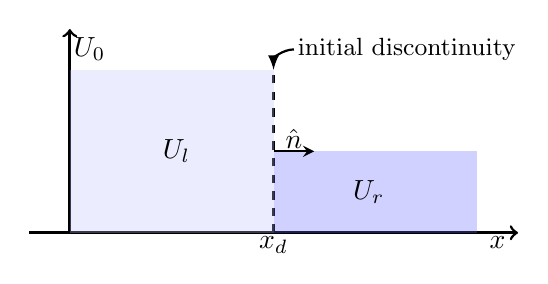
\begin{tikzpicture}[scale = {0.015\linewidth},inner sep = 1pt]

% create axis
%% \draw[->,line width=1pt] (0,0.5) |- (0.60,0) node[below]{$x$};
\draw[line width=1pt] (-0.5,0.45) node[right]{$\mbf{U}_0$}|-(0.55,0) node[below]{$x$};
\draw[->,line width=1pt] (0.55,0)--(0.6,0);
\draw[->,line width=1pt] (-0.5,0.45)--(-0.5,0.5);
\draw[line width=1pt] (-0,0)--(-0.6,0);  

% discontinuity
\draw[dashed,line width=1pt] (0,0) node[below]{$x_d$} -- (0,0.4); 
%% \draw[<-,line width=1pt] (-0.60,0) -- (0,0); 
\draw[-latex,thick](0.05,0.45)node[right]{\small initial discontinuity}
         to[out=180,in=90] (0,0.4);

% initial states
\fill[blue!25!,opacity=.3] (-0.5,0) rectangle (0,0.4);
\fill[blue!60!,opacity=.3] (0,0) rectangle (0.5,0.2);
\node[right] at (-0.28,0.2) {$\mbf{U}_l$};
\node[left] at (0.28,0.1) {$\mbf{U}_r$};


% normal
%% \draw[-stealth,thick] (0,0.25) -- (0.1,0.25); 
%% \node[] at (0.05,0.28) {$\hat{n}$};
\draw[-stealth,thick] (0,0.2) -- (0.1,0.2); 
\node[] at (0.05,0.23) {$\hat{n}$};

\end{tikzpicture}


%-----------------------------------------------------------------
% Shocktube 2D
%-----------------------------------------------------------------
%% \begin{tikzpicture}[scale = {0.015\linewidth},inner sep = 1pt]
%% % create axis
%% \draw[<->,line width=1pt] (0,0.6) node[right]{$y$} |- (1.1,0) node[below]{$x$};
%% %% \draw[<-,line width=1pt] (-0.75,0) -- (0,0); 

%% %% % normal
%% %% \draw[-stealth,thick] (0,0.25) -- (0.1,0.25); 
%% %% \node[] at (0.05,0.28) {$\hat{n}$};

%% % initial states
%% \draw[fill=blue!25!,opacity=.3] (0,0) -- (0,0.5) -- (1.0,0) -- cycle;
%% \draw[fill=blue!60!,opacity=.3] (0,0.5) -- (1.0,0.5) -- (1.0,0) -- cycle;
%% \node[right] at (0.2,0.15) {$\mbf{U}_0$};
%% \node[left] at (0.8,0.35) {$\mbf{U}_1$};

%% % discontinuity
%% \draw[line width = 1pt] (0,0.5) -- (1.0,0);
%% \draw[-latex,thick](0.2,0.55)node[right]{\small initial discontinuity}
%%          to[out=180,in=90] (0.1,0.45);

%% % normal
%% \draw[-stealth,thick] (0.5,0.25) -- (0.55,0.35); 
%% \node[] at (0.55,0.29) {$\hat{n}$};

%% \end{tikzpicture}

\end{center}
\caption{Initial conditions for a one-dimensional Riemann problem.  The initial discontinuity at, $x_d$, separates two constant states, $\mbf{U}_l$ and $\mbf{U}_r$.}
\label{fig:ivp}
\end{figure}

Conservation laws are a system of partial differential equations of the form   
\begin{gather*}
\pdbf{U}{t} + \pdbf{F}{\mbf{x}} = \mbf{0} \text{ ,}
\end{gather*} 
where \mbf{U} is a vector of the conservative state variables and \mbf{F} is a vector of fluxes \citep{Toro:1999}. 


%-----------------------------------------------------------------
% Linear advection
%-----------------------------------------------------------------
\section[Linear advection]{Linear advection}
\label{sec:lin_advec}

The one-dimensional linear advection equation is 
\begin{gather}
\label{eqn:linear_ad}
\pd{u}{t} + a\pd{u}{x} = 0,
\end{gather}
where $u$ is the conserved variable, and  $a$ is the constant wave velocity.  The solution to the Riemann problem for linear advection with $a>0$, initial conditions given by Equation~\ref{eqn:lin_ad_ivp}, and $x_d = 0$ is   
\begin{gather*}
\label{eqn:lin_ad_ivp} 
u = 
\begin{cases}
u_l & \text{if}\;\;\; x < at, \\
u_r & \text{if}\;\;\; x > at. \\
\end{cases}
\end{gather*} 

%-----------------------------------------------------------------
% Linear advection Riemann states
%-----------------------------------------------------------------
\begin{figure}[htbp]
\begin{center}
\tikzsetnextfilename{lin_ad_rstates}
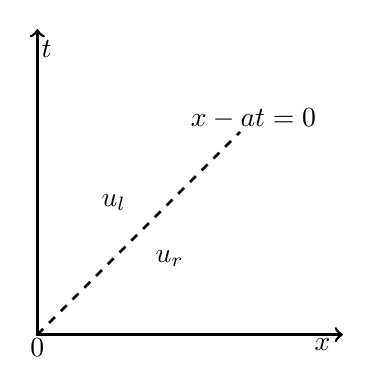
\begin{tikzpicture}[scale = {0.015\linewidth},inner sep = 1pt]
%% \begin{tikzpicture}[scale = {0.015\linewidth},inner sep = 1pt]
%% \tikzstyle{every node} = [draw,circle,fill=gray!30];
%% \draw (-1.5,0.0) circle (0.8);
%% \draw[<->,line width=1pt] (0,1) node[right]{\;$t$}|-(1,0) node[below]{$m$};

\draw[line width=1pt] (0.0,0.7) node[right]{$t$}|-(0.7,0) node[below]{$x$};
\draw[->,line width=1pt] (0.7,0)--(0.75,0);
\draw[->,line width=1pt] (0.0,0.7)--(0.0,0.75);

\node[draw=white] (char) at (0.53033,0.53033) {$x - at = 0$};
\draw[dashed,line width=1pt] (0,0) node[below]{$0$} -- (char); 

\node[draw=white] at (0.18750,0.32476) {$u_l$};
\node[draw=white] at (0.32476,0.18750) {$u_r$};

\end{tikzpicture}

\end{center}
\caption{Solution to the Riemann problem for linear advection in the $x$-$t$ plane.  The position of the discontinuity is given by the dashed line.}
\label{fig:lin_ad_rstates}
\end{figure}

In the $x$-$t$ plane, the solution changes from the initial left state, $u_l$, to the initial right state, $u_r$, across the characteristic line $x - at = 0$.  Across the discontinuity the solution is given by the Rankine-Hugonoit jump conditions, which express the transition as conservation across the discontinuity:
\begin{gather}
\label{eqn:rh_jump}
\mbf{F}_r - \mbf{F}_l = S_i (\mbf{U}_r - \mbf{U}_l),
\end{gather}      
where $S_i$ is the speed of a discontinuity connecting two states $\mbf{U}_l$ and $\mbf{U}_r$.  For the linear advection equation, the jump conditions are
\begin{gather*}
a u_r - a u_l = S (u_r - u_l),
\end{gather*}      
which gives the wave speed $S = a$.  This is the speed defined by the characteristic, $x - at = 0$.

%-----------------------------------------------------------------
% Linear systems
%-----------------------------------------------------------------
\section[Linear systems]{Linear systems}
\label{sec:lin_sys}

Consider the hyperbolic system of $n$ linear equations
\begin{gather}
\label{eqn:linear_sys}
\pdbf{U}{t} + \mbf{A}\pdbf{U}{x} = 0,
\end{gather}
where $\mbf{A}$ is an $n \times n$ constant coefficient matrix.  If $\mbf{A}$ has $n$ real eigenvalues, $\lambda_1, \hdots, \lambda_n$, and a corresponding set of $n$ linearly independent right eigenvectors, $\mbf{r}^1,\hdots,\mbf{r}^n$, the system is called hyperbolic.  It is called strictly hyperbolic system if the eigenvalues are distinct.  The hyperbolicity of the systems allows for it to be written in terms of the characteristic variables, that are the components of $\mbf{W} = \mbf{l}^i \mbf{U}$, where $\mbf{l}^i$ is the matrix of left eigenvectors, see \citep{Toro:1999}.  In characteristic form, the system is 
\begin{gather}
\pdbf{W}{t} + \mbf{\Lambda} \pdbf{W}{x} = 0,
\end{gather}  
where $\mbf{\Lambda}$ is a diagonal matrix and  $i$-th entry of the main diagonal is $\lambda_i$.
The system has been transformed to $n$ scalar equations of the form
\begin{gather}
\pd{w_i}{t} + \lambda_i \pd{w_i}{x} = 0,
\end{gather}  
where the eigenvalues are the characteristic speeds.  The system is assumed to be strictly hyperbolic so that eigenvalues are arranged such that ${\lambda_1 < \hdots < \lambda_i < \hdots < \lambda_n}$.  The solution to each scalar equation is given in terms of the characteristic variables by the solution to a linear advection problem with $a = \lambda_i$. 

%-----------------------------------------------------------------
% Linear system Riemann states
%-----------------------------------------------------------------
\begin{figure}[htbp]
\begin{center}
\tikzsetnextfilename{lin_sys_rstates}
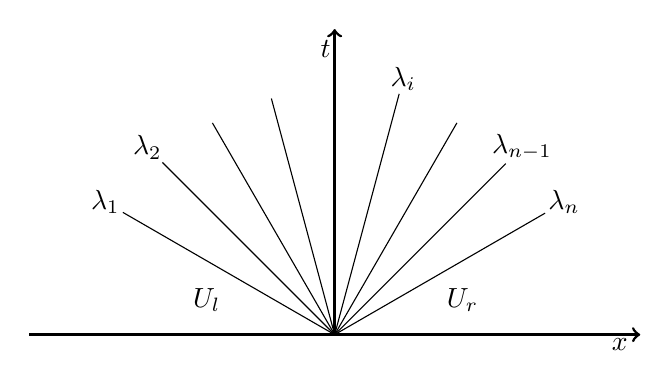
\begin{tikzpicture}[scale = {0.015\linewidth},inner sep = 1pt]
%% \begin{tikzpicture}[scale = {0.015\linewidth},inner sep = 1pt]
%% \tikzstyle{every node} = [draw,circle,fill=gray!30];
%% \draw (-1.5,0.0) circle (0.8);
%% \draw[<->,line width=1pt] (0,1) node[right]{\;$t$}|-(1,0) node[below]{$m$};
\draw[line width=1pt] (0,0.7) node[left]{$t$}|-(0.7,0) node[below]{$x$};
\draw[->,line width=1pt] (0.7,0)--(0.75,0);
\draw[->,line width=1pt] (0,0.7)--(0,0.75);  
\draw[line width=1pt] (0,0)--(-0.75,0);


\node[draw=white] (w1) at (-0.56292,0.32500) {$\lambda_1$};
\node[draw=white] (w2) at (-0.45962,0.45962) {$\lambda_2$};
\node[draw=white] (wi) at (0.16823,0.62785) {$\lambda_i$};
\node[draw=white] (w5) at (0.45962,0.45962) {$\lambda_{n-1}$};
\node[draw=white] (w6) at (0.56292,0.32500) {$\lambda_n$};

\node[draw=white] (ul) at (-0.31393,0.084116) {$\mbf{U}_l$};
\node[draw=white] (ur) at (0.31393,0.084116) {$\mbf{U}_r$};

%% \node[draw=white] (R8a) at (0.53943,0.10730) {\small $\mathrm{R}$8};
%% \node[draw=white] (R7a) at (0.45731,0.30556) {\small $\mathrm{R}$7};
%% \node[draw=white] (R6a) at (0.30556,0.45731) {\small $\mathrm{R}$6};
%% \node[draw=white] (R5a) at (0.10730,0.53943) {\small $\mathrm{R}$5};
%% \node[draw=white] (R4a) at (-0.10730,0.53943) {\small $\mathrm{R}$4};
%% \node[draw=white] (R3a) at (-0.30556,0.45731) {\small $\mathrm{R}$3};
%% \node[draw=white] (R2a) at (-0.45731,0.30556) {\small $\mathrm{R}$2};
%% \node[draw=white] (R1a) at (-0.53943,0.10730) {\small $\mathrm{R}$1};

%% \node[] at (0.15,0.95) {contact};
\draw (0,0) -- (w1);  
\draw (0,0) -- (w2);  
\draw (0,0) -- (-0.30000,0.51962);%(w3);  
\draw (0,0) -- (-0.15529,0.57956);
\draw (0,0) -- (wi);  
\draw (0,0) -- (0.30000,0.51962);%(w4);  
\draw (0,0) -- (w5);  
\draw (0,0) -- (w6);  
\end{tikzpicture}

\end{center}
\caption{Solution to the Riemann problem for a hyperbolic system of $n$ linear equations in the $x$-$t$ plane.}
\label{fig:lin_sys_rstates}
\end{figure}

The solution in the $x$-$t$ plane, for the linear system is shown in Figure~\ref{fig:lin_sys_rstates}.  It is composed of $n$ waves, each one corresponding to a characteristic speed, propagating away from the initial discontinuity.  Only the state on one side of the wave is needed to determine the change across it because the speed of a linear wave is independent of the discontinuous quantity.  The speed of the wave is calculated by the quantities in the known state.  A rotational discontinuity is an example of a linear wave in plasma physics.  It travels with a velocity equal to the Alf{\'e}n velocity, $B_n/\sqrt{4\pi\rho}$, where $B_n$ is the magnitude of the normal component of the magnetic field, and $\rho$ is the density.  Across a rotational discontinuity, $B_n$, and $\rho$ are unchanged, and determine the speed, and the jump conditions are then used to compute the connected state.  In this way, every state, connected through multiple waves can be determined.  The complete solution is then given by the superposition of the $n$ waves.  

The difference in characteristic variables across each wave is given by $\alpha_i = \mbf{l}_i \cdot (\mbf{U}_l - \mbf{U}_r)$, and the solution in terms of conservative variables is 
\begin{gather*} 
\mbf{U} = \mbf{U}_l + \sum_{i=1}^m \alpha_i \mbf{r}^i, \;\;\;\;\text{ or }\;\;\;\; \mbf{U} = \mbf{U}_r - \sum_{i=m+1}^n \alpha_i \mbf{r}^i,
\end{gather*} 
for $\lambda_m < x/t < \lambda_{m+1}$.  As described next section, the states on both sides of a nonlinear wave are needed to determine the speed.  As such, only local knowledge of the solution is available at a nonlinear discontinuity.

%-----------------------------------------------------------------
% Nonlinear systems
%-----------------------------------------------------------------
\section[Nonlinear systems]{Nonlinear systems}
\label{sec:nonlin_sys}

The results from the previous sections are now extended to nonlinear hyperbolic systems of the form   
\begin{gather}
\label{eqn:nonlinear_sys}
\pdbf{U}{t} + \pdbf{F}{x} = 0,
\end{gather}
where $\mbf{U}$ is a vector of conserved variables and $\mbf{F}(\mbf{U})$ is the flux vector.  The system is called hyperbolic if the Jacobian matrix, $\mbf{J}(\mbf{U}) = \partial{\mbf{F}}/\partial{\mbf{U}}$, has $n$ real eigenvalues and a corresponding set of $n$ linearly independent right eigenvectors.  Again the The system is also assumed to be strictly-hyperbolic so that the eigenvalues can be considered ordered based on speed.  For each of the $n$ eigenvalues there is an associated wave with speed $S_i$.  As with the linear system, the $n$ waves partition the solution into $n+1$ states.  Each wave in the linear system travels at a constant speed, $\lambda_i$, and has an associated jump discontinuity.  In the nonlinear systems, the wave speeds are functions of the conservative variables and the structure of the wave is not always a jump discontinuity.

%-----------------------------------------------------------------
% Characteristics of shocks, linear waves, and rarefactions
%-----------------------------------------------------------------
\begin{figure}[htbp]
\begin{tabular}{ccc}
\resizebox{0.33\linewidth}{!}{\tikzsetnextfilename{shock_char}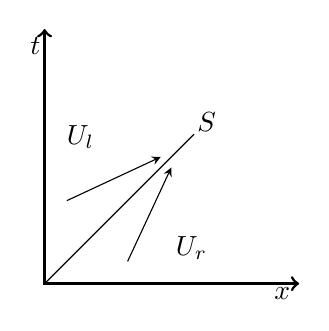
\begin{tikzpicture}[scale = {0.0125\linewidth},inner sep = 1pt]

\draw[line width=1pt] (0,0.7) node[left]{$t$}|-(0.7,0) node[below]{$x$};
\draw[->,line width=1pt] (0.7,0)--(0.75,0);
\draw[->,line width=1pt] (0,0.7)--(0,0.75);  

\node[draw=white] (sr) at (0.47730,0.47730) {$S$};

\node[draw=white] (usl) at (0.10589,0.43273) {$\mbf{U}_{l}$};
\node[draw=white] (ul) at (0.43273,0.10589) {$\mbf{U}_{r}$};

\draw (0,0) -- (sr);  

\draw[->,>=stealth] (0.24450,0.065514) -- (0.37325,0.34202);  
\draw[->,>=stealth] (0.065514,0.24450) -- (0.34202,0.37325);  

\end{tikzpicture}
} &
\resizebox{0.33\linewidth}{!}{\tikzsetnextfilename{linear_char}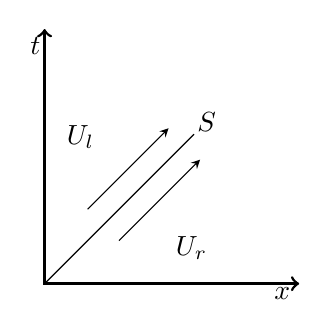
\begin{tikzpicture}[scale = {0.0125\linewidth},inner sep = 1pt]

\draw[line width=1pt] (0,0.7) node[left]{$t$}|-(0.7,0) node[below]{$x$};
\draw[->,line width=1pt] (0.7,0)--(0.75,0);
\draw[->,line width=1pt] (0,0.7)--(0,0.75);  

\node[draw=white] (sr) at (0.47730,0.47730) {$S$};

\node[draw=white] (usl) at (0.10589,0.43273) {$\mbf{U}_{l}$};
\node[draw=white] (ul) at (0.43273,0.10589) {$\mbf{U}_{r}$};

\draw (0,0) -- (sr);  

\draw[->,>=stealth] (0.21921,0.12656) -- (0.45786,0.36521);  
\draw[->,>=stealth] (0.12656,0.21921) -- (0.36521,0.45786);  

\end{tikzpicture}
} &
\resizebox{0.33\linewidth}{!}{\tikzsetnextfilename{rarefaction_char}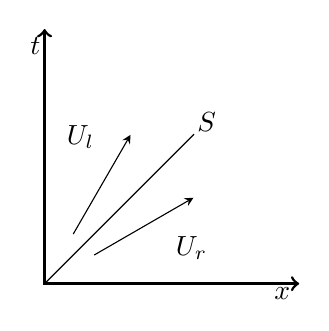
\begin{tikzpicture}[scale = {0.0125\linewidth},inner sep = 1pt]

\draw[line width=1pt] (0,0.7) node[left]{$t$}|-(0.7,0) node[below]{$x$};
\draw[->,line width=1pt] (0.7,0)--(0.75,0);
\draw[->,line width=1pt] (0,0.7)--(0,0.75);  

\node[draw=white] (sr) at (0.47730,0.47730) {$S$};

\node[draw=white] (usl) at (0.10589,0.43273) {$\mbf{U}_{l}$};
\node[draw=white] (ul) at (0.43273,0.10589) {$\mbf{U}_{r}$};

\draw (0,0) -- (sr);  

\draw[->,>=stealth] (0.14614,0.084376) -- (0.43843,0.25313);  
\draw[->,>=stealth] (0.084376,0.14614) -- (0.25313,0.43843);  

\end{tikzpicture}
} 
\end{tabular}
\caption{(left) Characteristics on both sides of a shock, (center) linear discontinuity, and (right) rarefaction (right).}
\label{fig:nonlinear_char}
\end{figure}

The formation of compression and expansion waves is an distinguishing feature of nonlinear systems.  Shock waves are compressive discontinuities that connect two states.  The characteristics of the two states connected by shock wave converge in the $x$-$t$ planeas shown in the left panel of Figure~\ref{fig:nonlinear_char}..  The Rankine-Hugonoit jump conditions for a shock wave are given by Equation~\ref{eqn:rh_jump}.

Expansion shocks are possible solutions, however, they violate the entropy condition and are disregarded as unphysical.  The entropy is defined, $p_g/\rho^{\gamma}$, where $p_g$ is the gas pressure, $\rho$ is the density, and $\gamma$ is the ratio of specific heats.  The entropy condition states that the entropy cannot decrease across a shock.    

Rarefactions are another nonlinear wave.  They connect two states through a smooth transition.  Unlike shocks, they are an expansion wave, and the characteristics of two states connected by rarefaction wave diverge in the $x$-$t$ plane, as shown in the right panel of Figure~\ref{fig:nonlinear_char}.

We adopt the following conventions when discussing to the structure of the solution to Riemann problems.  For a wave propagating with speed $S$, connecting two constant states, the upstream state, $\mbf{U}_u$, is the pre-shock state, i.e., the state of the flow that has not crossed the shock.  The downstream state, $\mbf{U}_d$, is the post-shock state, i.e., the state of the flow that has crossed the shock.  For the right-going wave shown in Figure~\ref{fig:ivp}, $\mbf{U}_l$ the upstream state, and $\mbf{U}_r$ is the downstream state.  The difference across a discontinuity is denoted with square brackets, e.g., $[ \mbf{U} ] = \mbf{U}_d - \mbf{U}_u$.

%-----------------------------------------------------------------
% Intermediate Riemann state
%-----------------------------------------------------------------
\begin{figure}[htbp]
\begin{center}
\tikzsetnextfilename{inter_rstates}
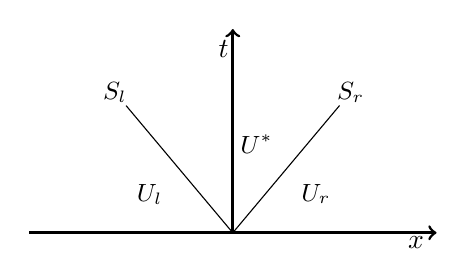
\begin{tikzpicture}[scale = {0.015\linewidth},inner sep = 1pt]
%% \begin{tikzpicture}[scale = {0.015\linewidth},inner sep = 1pt]
%% \tikzstyle{every node} = [draw,circle,fill=gray!30];
%% \draw (-1.5,0.0) circle (0.8);
%% \draw[<->,line width=1pt] (0,1) node[right]{\;$t$}|-(1,0) node[below]{$m$};
\draw[line width=1pt] (0,0.45) node[left]{$t$}|-(0.45,0) node[below]{$x$};
\draw[->,line width=1pt] (0.45,0)--(0.5,0); % extent x-axis  
\draw[->,line width=1pt] (0,0.45)--(0,0.5); % extent t-axis  
\draw[line width=1pt] (-0,0)--(-0.5,0); % draw negative x-axis  

\node[draw=white] (fr) at (-0.28925,0.34475) {\small $S_l$};
\node[draw=white] (fl) at (0.28925,0.34475) {\small $S_r$};

\node[draw=white] (Ul) at (-0.20392,0.095089) {\small $\mbf{U}_l$};
\node[draw=white] (Us) at (0.058234,0.21733) {\small $\mbf{U}^*$};
\node[draw=white] (Ur) at (0.20392,0.095089) {\small $\mbf{U}_r$};

%% \node[] at (0.15,0.95) {contact};
\draw (0,0) -- (fr);  
\draw (0,0) -- (fl);  
\end{tikzpicture}

\end{center}
\caption{Solution to a Riemann with one intermediate state in the $x$-$t$ plane.}
\label{fig:inter_rstates}
\end{figure}

When the solution to a Riemann problem is composed of more than one wave, the state between two waves is called an intermediate state, and is denoted $\mbf{U}^*$.  If the solution includes more than two waves, then the intermediate states are referenced in relation to the left-most and right-most state.  If $n+1$ states compose the solution, the states downstream of $\mbf{U}_{j}$ are denoted $\mbf{U}_{ij}^*$, where $i=1,\hdots,m/2$, $j = l,r$, and
\begin{gather*}
m = 
\begin{cases}
n & \text{if}\;\;\; n \text{ is even}, \\
n+1 & \text{if}\;\;\; n \text{ is odd}. \\
\end{cases}
\end{gather*} 
If $n$ is even, then the middle state is written without a subscript.

%-----------------------------------------------------------------
% Compressible hydrodynamics
%-----------------------------------------------------------------
\section[Compressible hydrodynamics]{Compressible hydrodynamics}
\label{sec:com_hydro}

The Euler equations of compressible hydrodynamics comprise a nonlinear hyperbolic system of conservation laws. The structure of the solution for Riemann problems of compressible hydrodynamics is presented below.  If viscosity and thermal conductivity are neglected, then the Euler equations describe the evolution of a compressible ideal gas.  The equations form a strictly-hyperbolic system that admit shocks, rarefactions, and linear discontinuities.  The conservative form of the Euler equations is
\begin{gather}
\label{eqn:euler1} \pd{\rho}{t} + \diverge{\left(\rho\mbf{v}\right)} = 0 \text{ ,} \\
\label{eqn:euler2} \pd{(\rho \mbf{v})}{t} + \diverge{\left[ \outerproduct{\rho\mbf{v}}{\mbf{v}} + p_g \right]}  = 0 \text{ ,}\\
\label{eqn:euler3} \pd{E}{t} + \diverge{\left[ \left(E + p_g \right)\mbf{v}\right]}  = 0 \text{ ,}
\end{gather}
where the energy density is defined as
\begin{gather}
  \label{eqn:energy} E = \frac{p_g}{\gamma - 1} + \frac{\rho v^2}{2}\text{ ,}
\end{gather}
$v^2 = v_n^2 + \mbf{v}_{t}^2$, and the gas constant $\gamma$ is the ratio of specific heats.  The one-dimensional quasi-linear form of the Euler equations is 
\begin{gather}
\label{eqn:euler_qlin}
\pdbf{U}{t} + \mbf{A}(\mbf{U})\pdbf{U}{x} = 0.
\end{gather}
The Jacobian of $\mbf{A}(\mbf{U})$ must have three real and distinct eigenvalues and a set of three linearly independent right eigenvectors because the system is strictly-hyperbolic.  If the eigenvalues are arranged such that $\lambda_1 < \lambda_2 < \lambda_3$, then $\lambda_1  \text{ and } \lambda_3$ correspond to nonlinear waves, and $\lambda_2$ is a linear wave.  The nonlinear waves can be either a shock (i.e., discontinuous wave) or rarefaction (i.e. smooth wave).  The linear wave is \gls{cd} that carries a carries a single jump in density and satisfies the jump conditions given by Equation~\ref{eqn:rh_jump}.  The three eigenvalues and their associated waves are:
\begin{align*}
\lambda_3 &= v_n + a : \text{rarefaction or shock,} \\
\lambda_2 &= v_n \phantom{+ a} : \text{contact discontinuity, \text{ and }} \\
\lambda_1 &= v_n - a : \text{rarefaction or shock,} 
\end{align*}
where $a = \sqrt{\gamma p_g/\rho}$ is the speed of sound.  

%-----------------------------------------------------------------
% Euler Riemann states
%-----------------------------------------------------------------
\begin{figure}[htbp]
\begin{center}
\tikzsetnextfilename{euler_rstates}
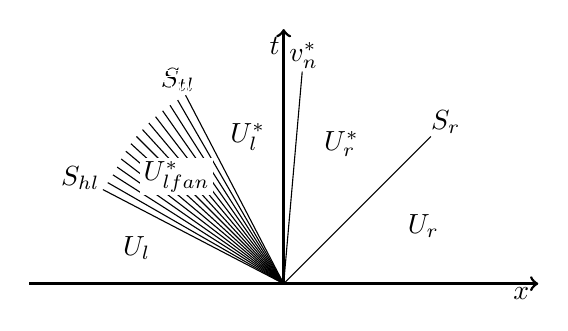
\begin{tikzpicture}[scale = {0.0125\linewidth},inner sep = 1pt]
%% \begin{tikzpicture}[scale = {0.015\linewidth},inner sep = 1pt]
%% \tikzstyle{every node} = [draw,circle,fill=gray!30];
%% \draw (-1.5,0.0) circle (0.8);
%% \draw[<->,line width=1pt] (0,1) node[right]{\;$t$}|-(1,0) node[below]{$m$};
\draw[line width=1pt] (0,0.7) node[left]{$t$}|-(0.7,0) node[below]{$x$};
\draw[->,line width=1pt] (0.7,0)--(0.75,0);
\draw[->,line width=1pt] (0,0.7)--(0,0.75);  
\draw[line width=1pt] (-0,0)--(-0.75,0);
\node[draw=white] (sr) at (0.47730,0.47730) {$S_r$};
\node[draw=white] (cd) at (0.058830,0.67243) {$v^*_n$};

\node[draw=white] (shl) at (-0.31168,0.59873) {$S_{tl}$};
\node[draw=white] (shlf) at (-0.33750,0.58457) {$\phantom{S_{tl}}$};
\node[draw=white] (shle) at (-0.36268,0.56929) {$\phantom{S_{tl}}$};
\node[draw=white] (shld) at (-0.38716,0.55293) {$\phantom{S_{tl}}$};
\node[draw=white] (shlc) at (-0.41091,0.53551) {$\phantom{S_{tl}}$};
\node[draw=white] (shlb) at (-0.43388,0.51708) {$\phantom{S_{tl}}$};
\node[draw=white] (shla) at (-0.45602,0.49766) {$\phantom{S_{tl}}$};
\node[draw=white] (sl) at (-0.47730,0.47730) {$\phantom{S_l}$};
\node[draw=white] (stla) at (-0.49766,0.45602) {$\phantom{S_{hl}}$};
\node[draw=white] (stlb) at (-0.51708,0.43388) {$\phantom{S_{hl}}$};
\node[draw=white] (stlc) at (-0.53551,0.41091) {$\phantom{S_{hl}}$};
\node[draw=white] (stld) at (-0.55293,0.38716) {$\phantom{S_{hl}}$};
\node[draw=white] (stle) at (-0.56929,0.36268) {$\phantom{S_{hl}}$};
\node[draw=white] (stlf) at (-0.58457,0.33570) {$\phantom{S_{hl}}$};
\node[draw=white] (stl) at (-0.59873,0.31168) {$S_{hl}$};

\node[draw=white] (ur) at (0.41159,0.17049) {$\mbf{U}_{r}$};
\node[draw=white] (usr) at (0.17049,0.41159) {$\mbf{U}^*_{r}$};
\node[draw=white] (usl) at (-0.10589,0.43273) {$\mbf{U}^*_{l}$};
\node[draw=white] (ul) at (-0.43273,0.10589) {$\mbf{U}_{l}$};

\draw (0,0) -- (sr);  
\draw (0,0) -- (cd);  
\draw (0,0) -- (shl);  
\draw (0,0) -- (shlf);  
\draw (0,0) -- (shle);  
\draw (0,0) -- (shld);  
\draw (0,0) -- (shlc);  
\draw (0,0) -- (shlb);  
\draw (0,0) -- (shla);  
\draw (0,0) -- (sl);  
\draw (0,0) -- (stla);  
\draw (0,0) -- (stlb);  
\draw (0,0) -- (stlc);  
\draw (0,0) -- (stld);  
\draw (0,0) -- (stle);  
\draw (0,0) -- (stlf);  
\draw (0,0) -- (stl);  

\node[draw=white,rectangle,fill=white] (usl) at (-0.31502,0.31502) {$\mbf{U}^*_{lfan}$};

\end{tikzpicture}

\end{center}
\caption{Possible structure of the solution to a Riemann problem for the Euler equations the $x$-$t$ plane.  The solution consists of a rarefaction wave to the left of contact discontinuity, and a shock wave to the right.}
\label{fig:euler_rstates}
\end{figure}

A possible structure of the self-similar solution $\mbf{U}(x,t)$ to the Euler equations is shown in Figure~\ref{fig:euler_rstates}.  Three waves: a fast shock, a contact discontinuity, and a slow rarefaction, separate the four constant states: the initial left, left intermediate, right intermediate, and initial right.  The state, $\mbf{U}^*_{lfan}$, inside the rarefaction wave is not constant.  It connects the states $\mbf{U}_l$ and $\mbf{U}^*_l$ through a smooth transition.  The characteristic speed at the head of a rarefaction wave is $v_{nu} \pm a_u$.  At the tail of a rarefaction wave, the characteristic speed is $v_{nd} \pm a_d$.  The plus (minus) sign refers to right-going (left-going) waves.  The speed of the contact discontinuity is given by the characteristic speed $\lambda_2$.  The shock speeds are derived from the Rankine-Hugonoit jump conditions, Equation~\ref{eqn:rh_jump}.  The speeds of a right-going shock, $S_r$, and left-going shock, $S_l$, are
\begin{gather*}
S_r = v_{nr} + a_r \sqrt{\left(\frac{\gamma + 1}{2\gamma}\right) \left(\frac{p_g^*}{p_{gr}}\right) + \left(\frac{\gamma - 1}{2\gamma}\right)}, \\
S_{l} = v_{nl} - a_l \sqrt{\left(\frac{\gamma + 1}{2\gamma}\right) \left(\frac{p_g^*}{p_{gl}}\right) + \left(\frac{\gamma - 1}{2\gamma}\right)},
\end{gather*}
where $p^*_{g} = p^*_{gl} = p^*_{gr}$, since the gas pressure is unchanged across a contact discontinuity.  The velocity at the head (tail) of a rarefaction wave is given by the corresponding characteristic speed in the upstream (downstream) state.  

%-----------------------------------------------------------------
% Riemann solvers
%-----------------------------------------------------------------
\subsection[Exact Riemann solvers]{Exact Riemann solver}
\label{sec:hydro_exact_rsolvers}

The solution to a Riemann problem consists of $n$ waves separating $n+1$ states, and it is found by determining the speed of each wave, and the jump associated with each wave.  Solving a Riemann problem for the one-dimensional Euler equations requires determining two unknown states, $\mbf{U}^*_l$ and $\mbf{U}^*_l$, and three wave speeds.  The exact solution is calculated by improving an initial guess for gas pressure in the intermediate states through an iterative procedure, e.g., Newton's method \citep{Toro:1999}.  The iteration is carried out until the jump condition for the normal velocity at the contact discontinuity, $[v^*_n] = 0$, is satisfied to the desired accuracy.  In practice, this is done by finding the root of the equation
\begin{gather*}
f(p^*_g,\mbf{U}_l,\mbf{U}_r) \equiv f_r(p_{gr},\mbf{U}_r) + f_l(p_{gl},\mbf{U}_l) + v_{nr} - v_{nl} = 0 \, ,
\end{gather*}
where $f_r$ ($f_l$) is a function connecting the initial right (left) state to the intermediate right (left) state.  The normal velocity in the intermediate states (Equation (4.9) of \citep{Toro:1999}) is 
\begin{gather*}
v^*_n = \half (v_{nr} + v_{nl}) + \half (f_r - f_l).
\end{gather*}
The functions $f_l$ and $f_r$ depend on the type of wave, i.e. shock or rarefaction.  If pressure increases across the wave, $p^*_d > p_{gu}$, then the wave is a shock, otherwise, the wave is a rarefaction.  The function $f_j$, for $j=l$ and $j=r$, (Equations (4.6) and (4.7) of \citep{Toro:1999}) is given by
\begin{gather*}
f_j(p_{gj},\mbf{U}_j) = 
\begin{cases}
(p^*_g - p_{gj})\left[ \frac{2}{\rho_j((\gamma +1)p^*_{g} + (\gamma -1)p_{gl})} \right]^{\half} 
  %% \phantom{\frac{2a_j}{(p^*_g - 1)}\left[\left(\frac{p^*_g}{p_{gj}} \right)^{\frac{\gamma-1}{2\gamma}} - 1\right]} 
  \;\;\;\; \text{if}\;\;\; p^*_g > p_{gj}, \\
\frac{2a_j}{(p^*_g - 1)}\left[\left(\frac{p^*_g}{p_{gj}} \right)^{\frac{\gamma-1}{2\gamma}} - 1\right] 
  %% \phantom{(p^*_g - p_{gj})\left[ \frac{2}{\rho_j((\gamma +1)p^*_{g} + (\gamma -1)p_{gl})} \right]^{\half}} 
  \;\;\;\;\;\;\;\;\;\;\;\;\;\;\;\;\;\;\;\; \text{if}\;\;\; p^*_g \le p_{gj}. \\
\end{cases}
\end{gather*}
where $j=l$ and $j=r$.  The densities $\rho_j$ for $j=l$ and $r$, in the left and right intermediate states are
\begin{gather*}
\rho^*_j = 
\begin{cases}
\rho_j\left[ \frac{\frac{p^*_g}{p_{gj}} + \frac{\gamma-1}{\gamma+1}}
  {\frac{\gamma-1}{\gamma+1} \frac{p^*_g}{p_{gj}} + 1} \right] 
  \;\;\;\; \text{if}\;\;\; p^*_g > p_{gj}, \\
\rho_j\left( \frac{p^*_g}{p_{gj}} \right)^{\frac{1}{\gamma}}
  \;\;\;\;\;\;\;\;\;\;\; \text{if}\;\;\; p^*_g \le p_{gj}. \\
\end{cases}
\end{gather*}
If the solution contains a rarefaction wave then the states in the fan are needed to complete the solution.  The state in the rarefaction wave is  
\begin{gather*}
\rho = \rho_j \left[ \frac{2}{(\gamma+1)} \pm \frac{(\gamma-1)}{(\gamma+1)a_j}
  \left(v_{nj} - \frac{x}{t}\right)\right]^{\frac{2}{\gamma - 1}}, \\
v_{n} = \frac{2}{(\gamma+1)} \left[\frac{(\gamma-1)}{2}v_{nj} \pm a_j + \frac{x}{t}\right], \\ 
p_{g} = p_{gj} \left[ \frac{2}{(\gamma+1)} \pm \frac{(\gamma-1)}{(\gamma+1)a_j}
  \left(v_{nj} - \frac{x}{t}\right)\right]^{\frac{2\gamma}{\gamma - 1}}, 
\end{gather*}
for $j=l$ and $r$, and the plus (minus) sign corresponds to a left-going (right-going) wave.

%-----------------------------------------------------------------
% Exact solution to Sod shock tube
%-----------------------------------------------------------------
\begin{figure}[htbp]
\begin{tabular}{ccc}
\resizebox{0.33\linewidth}{!}{\tikzsetnextfilename{sod_1}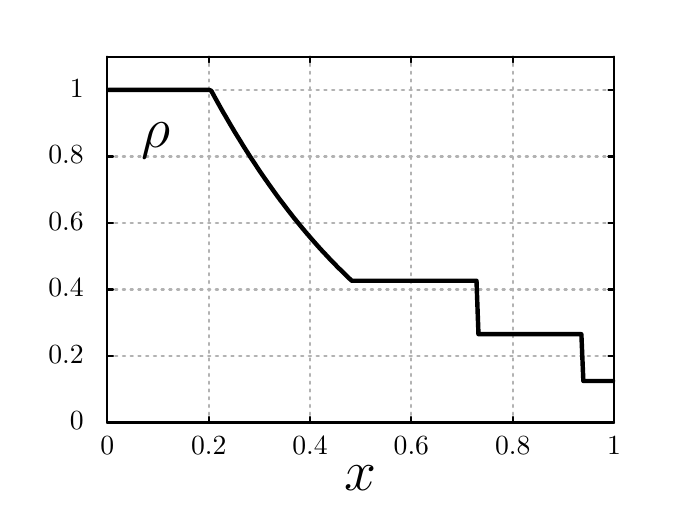
\begin{tikzpicture}[gnuplot]
%% generated with GNUPLOT 4.6p4 (Lua 5.1; terminal rev. 99, script rev. 100)
%% Sat 28 Jun 2014 11:52:07 AM EDT
\path (0.000,0.000) rectangle (8.000,6.000);
\gpfill{rgb color={1.000,1.000,1.000}} (1.012,0.985)--(7.446,0.985)--(7.446,5.630)--(1.012,5.630)--cycle;
\gpcolor{color=gp lt color border}
\gpsetlinetype{gp lt border}
\gpsetlinewidth{1.00}
\draw[gp path] (1.012,0.985)--(1.012,5.630)--(7.446,5.630)--(7.446,0.985)--cycle;
\gpcolor{color=gp lt color axes}
\gpsetlinetype{gp lt axes}
\gpsetlinewidth{2.00}
\draw[gp path] (1.012,0.985)--(7.447,0.985);
\gpcolor{color=gp lt color border}
\gpsetlinetype{gp lt border}
\draw[gp path] (1.012,0.985)--(1.084,0.985);
\draw[gp path] (7.447,0.985)--(7.375,0.985);
\gpcolor{rgb color={0.000,0.000,0.000}}
\node[gp node right,font={\fontsize{10pt}{12pt}\selectfont}] at (0.828,0.985) {0};
\gpcolor{color=gp lt color axes}
\gpsetlinetype{gp lt axes}
\draw[gp path] (1.012,1.830)--(7.447,1.830);
\gpcolor{color=gp lt color border}
\gpsetlinetype{gp lt border}
\draw[gp path] (1.012,1.830)--(1.084,1.830);
\draw[gp path] (7.447,1.830)--(7.375,1.830);
\gpcolor{rgb color={0.000,0.000,0.000}}
\node[gp node right,font={\fontsize{10pt}{12pt}\selectfont}] at (0.828,1.830) {0.2};
\gpcolor{color=gp lt color axes}
\gpsetlinetype{gp lt axes}
\draw[gp path] (1.012,2.674)--(7.447,2.674);
\gpcolor{color=gp lt color border}
\gpsetlinetype{gp lt border}
\draw[gp path] (1.012,2.674)--(1.084,2.674);
\draw[gp path] (7.447,2.674)--(7.375,2.674);
\gpcolor{rgb color={0.000,0.000,0.000}}
\node[gp node right,font={\fontsize{10pt}{12pt}\selectfont}] at (0.828,2.674) {0.4};
\gpcolor{color=gp lt color axes}
\gpsetlinetype{gp lt axes}
\draw[gp path] (1.012,3.519)--(7.447,3.519);
\gpcolor{color=gp lt color border}
\gpsetlinetype{gp lt border}
\draw[gp path] (1.012,3.519)--(1.084,3.519);
\draw[gp path] (7.447,3.519)--(7.375,3.519);
\gpcolor{rgb color={0.000,0.000,0.000}}
\node[gp node right,font={\fontsize{10pt}{12pt}\selectfont}] at (0.828,3.519) {0.6};
\gpcolor{color=gp lt color axes}
\gpsetlinetype{gp lt axes}
\draw[gp path] (1.012,4.364)--(7.447,4.364);
\gpcolor{color=gp lt color border}
\gpsetlinetype{gp lt border}
\draw[gp path] (1.012,4.364)--(1.084,4.364);
\draw[gp path] (7.447,4.364)--(7.375,4.364);
\gpcolor{rgb color={0.000,0.000,0.000}}
\node[gp node right,font={\fontsize{10pt}{12pt}\selectfont}] at (0.828,4.364) {0.8};
\gpcolor{color=gp lt color axes}
\gpsetlinetype{gp lt axes}
\draw[gp path] (1.012,5.209)--(7.447,5.209);
\gpcolor{color=gp lt color border}
\gpsetlinetype{gp lt border}
\draw[gp path] (1.012,5.209)--(1.084,5.209);
\draw[gp path] (7.447,5.209)--(7.375,5.209);
\gpcolor{rgb color={0.000,0.000,0.000}}
\node[gp node right,font={\fontsize{10pt}{12pt}\selectfont}] at (0.828,5.209) {1};
\gpcolor{color=gp lt color axes}
\gpsetlinetype{gp lt axes}
\draw[gp path] (1.012,0.985)--(1.012,5.631);
\gpcolor{color=gp lt color border}
\gpsetlinetype{gp lt border}
\draw[gp path] (1.012,0.985)--(1.012,1.057);
\draw[gp path] (1.012,5.631)--(1.012,5.559);
\gpcolor{rgb color={0.000,0.000,0.000}}
\node[gp node center,font={\fontsize{10pt}{12pt}\selectfont}] at (1.012,0.677) {0};
\gpcolor{color=gp lt color axes}
\gpsetlinetype{gp lt axes}
\draw[gp path] (2.299,0.985)--(2.299,5.631);
\gpcolor{color=gp lt color border}
\gpsetlinetype{gp lt border}
\draw[gp path] (2.299,0.985)--(2.299,1.057);
\draw[gp path] (2.299,5.631)--(2.299,5.559);
\gpcolor{rgb color={0.000,0.000,0.000}}
\node[gp node center,font={\fontsize{10pt}{12pt}\selectfont}] at (2.299,0.677) {0.2};
\gpcolor{color=gp lt color axes}
\gpsetlinetype{gp lt axes}
\draw[gp path] (3.586,0.985)--(3.586,5.631);
\gpcolor{color=gp lt color border}
\gpsetlinetype{gp lt border}
\draw[gp path] (3.586,0.985)--(3.586,1.057);
\draw[gp path] (3.586,5.631)--(3.586,5.559);
\gpcolor{rgb color={0.000,0.000,0.000}}
\node[gp node center,font={\fontsize{10pt}{12pt}\selectfont}] at (3.586,0.677) {0.4};
\gpcolor{color=gp lt color axes}
\gpsetlinetype{gp lt axes}
\draw[gp path] (4.873,0.985)--(4.873,5.631);
\gpcolor{color=gp lt color border}
\gpsetlinetype{gp lt border}
\draw[gp path] (4.873,0.985)--(4.873,1.057);
\draw[gp path] (4.873,5.631)--(4.873,5.559);
\gpcolor{rgb color={0.000,0.000,0.000}}
\node[gp node center,font={\fontsize{10pt}{12pt}\selectfont}] at (4.873,0.677) {0.6};
\gpcolor{color=gp lt color axes}
\gpsetlinetype{gp lt axes}
\draw[gp path] (6.160,0.985)--(6.160,5.631);
\gpcolor{color=gp lt color border}
\gpsetlinetype{gp lt border}
\draw[gp path] (6.160,0.985)--(6.160,1.057);
\draw[gp path] (6.160,5.631)--(6.160,5.559);
\gpcolor{rgb color={0.000,0.000,0.000}}
\node[gp node center,font={\fontsize{10pt}{12pt}\selectfont}] at (6.160,0.677) {0.8};
\gpcolor{color=gp lt color axes}
\gpsetlinetype{gp lt axes}
\draw[gp path] (7.447,0.985)--(7.447,5.631);
\gpcolor{color=gp lt color border}
\gpsetlinetype{gp lt border}
\draw[gp path] (7.447,0.985)--(7.447,1.057);
\draw[gp path] (7.447,5.631)--(7.447,5.559);
\gpcolor{rgb color={0.000,0.000,0.000}}
\node[gp node center,font={\fontsize{10pt}{12pt}\selectfont}] at (7.447,0.677) {1};
\gpcolor{color=gp lt color border}
\draw[gp path] (1.012,5.631)--(1.012,0.985)--(7.447,0.985)--(7.447,5.631)--cycle;
\gpcolor{rgb color={0.000,0.000,0.000}}
\node[gp node center,font={\fontsize{10pt}{12pt}\selectfont}] at (4.229,0.215) {\huge $x$};
\gpsetlinetype{gp lt plot 0}
\gpsetlinewidth{4.00}
\draw[gp path] (1.025,5.209)--(1.050,5.209)--(1.075,5.209)--(1.100,5.209)--(1.125,5.209)%
  --(1.150,5.209)--(1.175,5.209)--(1.201,5.209)--(1.226,5.209)--(1.251,5.209)--(1.276,5.209)%
  --(1.301,5.209)--(1.326,5.209)--(1.351,5.209)--(1.376,5.209)--(1.402,5.209)--(1.427,5.209)%
  --(1.452,5.209)--(1.477,5.209)--(1.502,5.209)--(1.527,5.209)--(1.552,5.209)--(1.578,5.209)%
  --(1.603,5.209)--(1.628,5.209)--(1.653,5.209)--(1.678,5.209)--(1.703,5.209)--(1.728,5.209)%
  --(1.754,5.209)--(1.779,5.209)--(1.804,5.209)--(1.829,5.209)--(1.854,5.209)--(1.879,5.209)%
  --(1.904,5.209)--(1.929,5.209)--(1.955,5.209)--(1.980,5.209)--(2.005,5.209)--(2.030,5.209)%
  --(2.055,5.209)--(2.080,5.209)--(2.105,5.209)--(2.131,5.209)--(2.156,5.209)--(2.181,5.209)%
  --(2.206,5.209)--(2.231,5.209)--(2.256,5.209)--(2.281,5.209)--(2.307,5.209)--(2.332,5.198)%
  --(2.357,5.152)--(2.382,5.106)--(2.407,5.061)--(2.432,5.016)--(2.457,4.971)--(2.482,4.927)%
  --(2.508,4.883)--(2.533,4.840)--(2.558,4.797)--(2.583,4.754)--(2.608,4.712)--(2.633,4.670)%
  --(2.658,4.629)--(2.684,4.588)--(2.709,4.547)--(2.734,4.506)--(2.759,4.466)--(2.784,4.427)%
  --(2.809,4.388)--(2.834,4.349)--(2.860,4.310)--(2.885,4.272)--(2.910,4.234)--(2.935,4.196)%
  --(2.960,4.159)--(2.985,4.123)--(3.010,4.086)--(3.036,4.050)--(3.061,4.014)--(3.086,3.979)%
  --(3.111,3.944)--(3.136,3.909)--(3.161,3.874)--(3.186,3.840)--(3.211,3.806)--(3.237,3.773)%
  --(3.262,3.740)--(3.287,3.707)--(3.312,3.674)--(3.337,3.642)--(3.362,3.610)--(3.387,3.578)%
  --(3.413,3.547)--(3.438,3.516)--(3.463,3.485)--(3.488,3.455)--(3.513,3.425)--(3.538,3.395)%
  --(3.563,3.366)--(3.589,3.336)--(3.614,3.307)--(3.639,3.279)--(3.664,3.250)--(3.689,3.222)%
  --(3.714,3.194)--(3.739,3.167)--(3.764,3.140)--(3.790,3.113)--(3.815,3.086)--(3.840,3.059)%
  --(3.865,3.033)--(3.890,3.007)--(3.915,2.982)--(3.940,2.956)--(3.966,2.931)--(3.991,2.906)%
  --(4.016,2.882)--(4.041,2.857)--(4.066,2.833)--(4.091,2.809)--(4.116,2.786)--(4.142,2.786)%
  --(4.167,2.786)--(4.192,2.786)--(4.217,2.786)--(4.242,2.786)--(4.267,2.786)--(4.292,2.786)%
  --(4.317,2.786)--(4.343,2.786)--(4.368,2.786)--(4.393,2.786)--(4.418,2.786)--(4.443,2.786)%
  --(4.468,2.786)--(4.493,2.786)--(4.519,2.786)--(4.544,2.786)--(4.569,2.786)--(4.594,2.786)%
  --(4.619,2.786)--(4.644,2.786)--(4.669,2.786)--(4.695,2.786)--(4.720,2.786)--(4.745,2.786)%
  --(4.770,2.786)--(4.795,2.786)--(4.820,2.786)--(4.845,2.786)--(4.870,2.786)--(4.896,2.786)%
  --(4.921,2.786)--(4.946,2.786)--(4.971,2.786)--(4.996,2.786)--(5.021,2.786)--(5.046,2.786)%
  --(5.072,2.786)--(5.097,2.786)--(5.122,2.786)--(5.147,2.786)--(5.172,2.786)--(5.197,2.786)%
  --(5.222,2.786)--(5.248,2.786)--(5.273,2.786)--(5.298,2.786)--(5.323,2.786)--(5.348,2.786)%
  --(5.373,2.786)--(5.398,2.786)--(5.423,2.786)--(5.449,2.786)--(5.474,2.786)--(5.499,2.786)%
  --(5.524,2.786)--(5.549,2.786)--(5.574,2.786)--(5.599,2.786)--(5.625,2.786)--(5.650,2.786)%
  --(5.675,2.786)--(5.700,2.786)--(5.725,2.107)--(5.750,2.107)--(5.775,2.107)--(5.801,2.107)%
  --(5.826,2.107)--(5.851,2.107)--(5.876,2.107)--(5.901,2.107)--(5.926,2.107)--(5.951,2.107)%
  --(5.977,2.107)--(6.002,2.107)--(6.027,2.107)--(6.052,2.107)--(6.077,2.107)--(6.102,2.107)%
  --(6.127,2.107)--(6.152,2.107)--(6.178,2.107)--(6.203,2.107)--(6.228,2.107)--(6.253,2.107)%
  --(6.278,2.107)--(6.303,2.107)--(6.328,2.107)--(6.354,2.107)--(6.379,2.107)--(6.404,2.107)%
  --(6.429,2.107)--(6.454,2.107)--(6.479,2.107)--(6.504,2.107)--(6.530,2.107)--(6.555,2.107)%
  --(6.580,2.107)--(6.605,2.107)--(6.630,2.107)--(6.655,2.107)--(6.680,2.107)--(6.705,2.107)%
  --(6.731,2.107)--(6.756,2.107)--(6.781,2.107)--(6.806,2.107)--(6.831,2.107)--(6.856,2.107)%
  --(6.881,2.107)--(6.907,2.107)--(6.932,2.107)--(6.957,2.107)--(6.982,2.107)--(7.007,2.107)%
  --(7.032,2.107)--(7.057,1.513)--(7.083,1.513)--(7.108,1.513)--(7.133,1.513)--(7.158,1.513)%
  --(7.183,1.513)--(7.208,1.513)--(7.233,1.513)--(7.258,1.513)--(7.284,1.513)--(7.309,1.513)%
  --(7.334,1.513)--(7.359,1.513)--(7.384,1.513)--(7.409,1.513)--(7.434,1.513);
\node[gp node left,font={\fontsize{10pt}{12pt}\selectfont}] at (1.334,4.575) {\huge $\rho$};
%% coordinates of the plot area
\gpdefrectangularnode{gp plot 1}{\pgfpoint{1.012cm}{0.985cm}}{\pgfpoint{7.447cm}{5.631cm}}
\end{tikzpicture}
%% gnuplot variables
} &
\resizebox{0.33\linewidth}{!}{\tikzsetnextfilename{sod_2}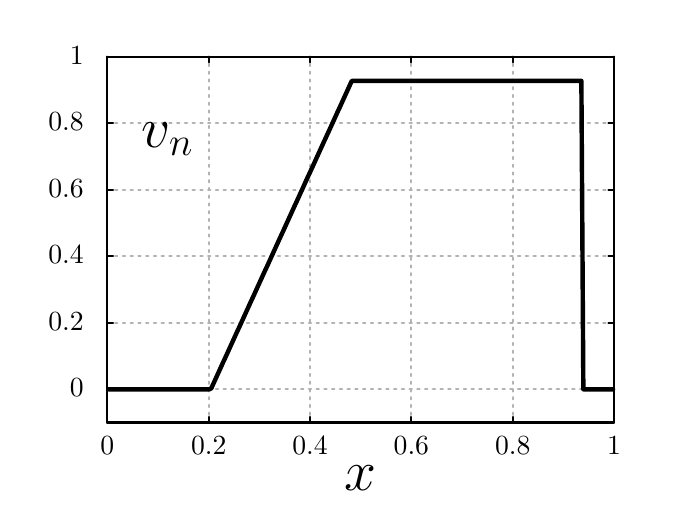
\begin{tikzpicture}[gnuplot]
%% generated with GNUPLOT 4.6p4 (Lua 5.1; terminal rev. 99, script rev. 100)
%% Sat 28 Jun 2014 11:52:07 AM EDT
\path (0.000,0.000) rectangle (8.000,6.000);
\gpfill{rgb color={1.000,1.000,1.000}} (1.012,0.985)--(7.446,0.985)--(7.446,5.630)--(1.012,5.630)--cycle;
\gpcolor{color=gp lt color border}
\gpsetlinetype{gp lt border}
\gpsetlinewidth{1.00}
\draw[gp path] (1.012,0.985)--(1.012,5.630)--(7.446,5.630)--(7.446,0.985)--cycle;
\gpcolor{color=gp lt color axes}
\gpsetlinetype{gp lt axes}
\gpsetlinewidth{2.00}
\draw[gp path] (1.012,1.407)--(7.447,1.407);
\gpcolor{color=gp lt color border}
\gpsetlinetype{gp lt border}
\draw[gp path] (1.012,1.407)--(1.084,1.407);
\draw[gp path] (7.447,1.407)--(7.375,1.407);
\gpcolor{rgb color={0.000,0.000,0.000}}
\node[gp node right,font={\fontsize{10pt}{12pt}\selectfont}] at (0.828,1.407) {0};
\gpcolor{color=gp lt color axes}
\gpsetlinetype{gp lt axes}
\draw[gp path] (1.012,2.252)--(7.447,2.252);
\gpcolor{color=gp lt color border}
\gpsetlinetype{gp lt border}
\draw[gp path] (1.012,2.252)--(1.084,2.252);
\draw[gp path] (7.447,2.252)--(7.375,2.252);
\gpcolor{rgb color={0.000,0.000,0.000}}
\node[gp node right,font={\fontsize{10pt}{12pt}\selectfont}] at (0.828,2.252) {0.2};
\gpcolor{color=gp lt color axes}
\gpsetlinetype{gp lt axes}
\draw[gp path] (1.012,3.097)--(7.447,3.097);
\gpcolor{color=gp lt color border}
\gpsetlinetype{gp lt border}
\draw[gp path] (1.012,3.097)--(1.084,3.097);
\draw[gp path] (7.447,3.097)--(7.375,3.097);
\gpcolor{rgb color={0.000,0.000,0.000}}
\node[gp node right,font={\fontsize{10pt}{12pt}\selectfont}] at (0.828,3.097) {0.4};
\gpcolor{color=gp lt color axes}
\gpsetlinetype{gp lt axes}
\draw[gp path] (1.012,3.942)--(7.447,3.942);
\gpcolor{color=gp lt color border}
\gpsetlinetype{gp lt border}
\draw[gp path] (1.012,3.942)--(1.084,3.942);
\draw[gp path] (7.447,3.942)--(7.375,3.942);
\gpcolor{rgb color={0.000,0.000,0.000}}
\node[gp node right,font={\fontsize{10pt}{12pt}\selectfont}] at (0.828,3.942) {0.6};
\gpcolor{color=gp lt color axes}
\gpsetlinetype{gp lt axes}
\draw[gp path] (1.012,4.786)--(7.447,4.786);
\gpcolor{color=gp lt color border}
\gpsetlinetype{gp lt border}
\draw[gp path] (1.012,4.786)--(1.084,4.786);
\draw[gp path] (7.447,4.786)--(7.375,4.786);
\gpcolor{rgb color={0.000,0.000,0.000}}
\node[gp node right,font={\fontsize{10pt}{12pt}\selectfont}] at (0.828,4.786) {0.8};
\gpcolor{color=gp lt color axes}
\gpsetlinetype{gp lt axes}
\draw[gp path] (1.012,5.631)--(7.447,5.631);
\gpcolor{color=gp lt color border}
\gpsetlinetype{gp lt border}
\draw[gp path] (1.012,5.631)--(1.084,5.631);
\draw[gp path] (7.447,5.631)--(7.375,5.631);
\gpcolor{rgb color={0.000,0.000,0.000}}
\node[gp node right,font={\fontsize{10pt}{12pt}\selectfont}] at (0.828,5.631) {1};
\gpcolor{color=gp lt color axes}
\gpsetlinetype{gp lt axes}
\draw[gp path] (1.012,0.985)--(1.012,5.631);
\gpcolor{color=gp lt color border}
\gpsetlinetype{gp lt border}
\draw[gp path] (1.012,0.985)--(1.012,1.057);
\draw[gp path] (1.012,5.631)--(1.012,5.559);
\gpcolor{rgb color={0.000,0.000,0.000}}
\node[gp node center,font={\fontsize{10pt}{12pt}\selectfont}] at (1.012,0.677) {0};
\gpcolor{color=gp lt color axes}
\gpsetlinetype{gp lt axes}
\draw[gp path] (2.299,0.985)--(2.299,5.631);
\gpcolor{color=gp lt color border}
\gpsetlinetype{gp lt border}
\draw[gp path] (2.299,0.985)--(2.299,1.057);
\draw[gp path] (2.299,5.631)--(2.299,5.559);
\gpcolor{rgb color={0.000,0.000,0.000}}
\node[gp node center,font={\fontsize{10pt}{12pt}\selectfont}] at (2.299,0.677) {0.2};
\gpcolor{color=gp lt color axes}
\gpsetlinetype{gp lt axes}
\draw[gp path] (3.586,0.985)--(3.586,5.631);
\gpcolor{color=gp lt color border}
\gpsetlinetype{gp lt border}
\draw[gp path] (3.586,0.985)--(3.586,1.057);
\draw[gp path] (3.586,5.631)--(3.586,5.559);
\gpcolor{rgb color={0.000,0.000,0.000}}
\node[gp node center,font={\fontsize{10pt}{12pt}\selectfont}] at (3.586,0.677) {0.4};
\gpcolor{color=gp lt color axes}
\gpsetlinetype{gp lt axes}
\draw[gp path] (4.873,0.985)--(4.873,5.631);
\gpcolor{color=gp lt color border}
\gpsetlinetype{gp lt border}
\draw[gp path] (4.873,0.985)--(4.873,1.057);
\draw[gp path] (4.873,5.631)--(4.873,5.559);
\gpcolor{rgb color={0.000,0.000,0.000}}
\node[gp node center,font={\fontsize{10pt}{12pt}\selectfont}] at (4.873,0.677) {0.6};
\gpcolor{color=gp lt color axes}
\gpsetlinetype{gp lt axes}
\draw[gp path] (6.160,0.985)--(6.160,5.631);
\gpcolor{color=gp lt color border}
\gpsetlinetype{gp lt border}
\draw[gp path] (6.160,0.985)--(6.160,1.057);
\draw[gp path] (6.160,5.631)--(6.160,5.559);
\gpcolor{rgb color={0.000,0.000,0.000}}
\node[gp node center,font={\fontsize{10pt}{12pt}\selectfont}] at (6.160,0.677) {0.8};
\gpcolor{color=gp lt color axes}
\gpsetlinetype{gp lt axes}
\draw[gp path] (7.447,0.985)--(7.447,5.631);
\gpcolor{color=gp lt color border}
\gpsetlinetype{gp lt border}
\draw[gp path] (7.447,0.985)--(7.447,1.057);
\draw[gp path] (7.447,5.631)--(7.447,5.559);
\gpcolor{rgb color={0.000,0.000,0.000}}
\node[gp node center,font={\fontsize{10pt}{12pt}\selectfont}] at (7.447,0.677) {1};
\gpcolor{color=gp lt color border}
\draw[gp path] (1.012,5.631)--(1.012,0.985)--(7.447,0.985)--(7.447,5.631)--cycle;
\gpcolor{rgb color={0.000,0.000,0.000}}
\node[gp node center,font={\fontsize{10pt}{12pt}\selectfont}] at (4.229,0.215) {\huge $x$};
\gpsetlinetype{gp lt plot 0}
\gpsetlinewidth{4.00}
\draw[gp path] (1.025,1.407)--(1.050,1.407)--(1.075,1.407)--(1.100,1.407)--(1.125,1.407)%
  --(1.150,1.407)--(1.175,1.407)--(1.201,1.407)--(1.226,1.407)--(1.251,1.407)--(1.276,1.407)%
  --(1.301,1.407)--(1.326,1.407)--(1.351,1.407)--(1.376,1.407)--(1.402,1.407)--(1.427,1.407)%
  --(1.452,1.407)--(1.477,1.407)--(1.502,1.407)--(1.527,1.407)--(1.552,1.407)--(1.578,1.407)%
  --(1.603,1.407)--(1.628,1.407)--(1.653,1.407)--(1.678,1.407)--(1.703,1.407)--(1.728,1.407)%
  --(1.754,1.407)--(1.779,1.407)--(1.804,1.407)--(1.829,1.407)--(1.854,1.407)--(1.879,1.407)%
  --(1.904,1.407)--(1.929,1.407)--(1.955,1.407)--(1.980,1.407)--(2.005,1.407)--(2.030,1.407)%
  --(2.055,1.407)--(2.080,1.407)--(2.105,1.407)--(2.131,1.407)--(2.156,1.407)--(2.181,1.407)%
  --(2.206,1.407)--(2.231,1.407)--(2.256,1.407)--(2.281,1.407)--(2.307,1.407)--(2.332,1.420)%
  --(2.357,1.475)--(2.382,1.530)--(2.407,1.585)--(2.432,1.640)--(2.457,1.695)--(2.482,1.750)%
  --(2.508,1.805)--(2.533,1.860)--(2.558,1.915)--(2.583,1.970)--(2.608,2.025)--(2.633,2.080)%
  --(2.658,2.135)--(2.684,2.190)--(2.709,2.245)--(2.734,2.300)--(2.759,2.355)--(2.784,2.410)%
  --(2.809,2.465)--(2.834,2.520)--(2.860,2.575)--(2.885,2.630)--(2.910,2.685)--(2.935,2.740)%
  --(2.960,2.795)--(2.985,2.850)--(3.010,2.905)--(3.036,2.960)--(3.061,3.015)--(3.086,3.070)%
  --(3.111,3.125)--(3.136,3.180)--(3.161,3.235)--(3.186,3.290)--(3.211,3.345)--(3.237,3.400)%
  --(3.262,3.455)--(3.287,3.510)--(3.312,3.565)--(3.337,3.620)--(3.362,3.675)--(3.387,3.730)%
  --(3.413,3.785)--(3.438,3.840)--(3.463,3.895)--(3.488,3.950)--(3.513,4.005)--(3.538,4.060)%
  --(3.563,4.115)--(3.589,4.170)--(3.614,4.225)--(3.639,4.280)--(3.664,4.335)--(3.689,4.390)%
  --(3.714,4.445)--(3.739,4.500)--(3.764,4.555)--(3.790,4.610)--(3.815,4.665)--(3.840,4.719)%
  --(3.865,4.774)--(3.890,4.829)--(3.915,4.884)--(3.940,4.939)--(3.966,4.994)--(3.991,5.049)%
  --(4.016,5.104)--(4.041,5.159)--(4.066,5.214)--(4.091,5.269)--(4.116,5.324)--(4.142,5.324)%
  --(4.167,5.324)--(4.192,5.324)--(4.217,5.324)--(4.242,5.324)--(4.267,5.324)--(4.292,5.324)%
  --(4.317,5.324)--(4.343,5.324)--(4.368,5.324)--(4.393,5.324)--(4.418,5.324)--(4.443,5.324)%
  --(4.468,5.324)--(4.493,5.324)--(4.519,5.324)--(4.544,5.324)--(4.569,5.324)--(4.594,5.324)%
  --(4.619,5.324)--(4.644,5.324)--(4.669,5.324)--(4.695,5.324)--(4.720,5.324)--(4.745,5.324)%
  --(4.770,5.324)--(4.795,5.324)--(4.820,5.324)--(4.845,5.324)--(4.870,5.324)--(4.896,5.324)%
  --(4.921,5.324)--(4.946,5.324)--(4.971,5.324)--(4.996,5.324)--(5.021,5.324)--(5.046,5.324)%
  --(5.072,5.324)--(5.097,5.324)--(5.122,5.324)--(5.147,5.324)--(5.172,5.324)--(5.197,5.324)%
  --(5.222,5.324)--(5.248,5.324)--(5.273,5.324)--(5.298,5.324)--(5.323,5.324)--(5.348,5.324)%
  --(5.373,5.324)--(5.398,5.324)--(5.423,5.324)--(5.449,5.324)--(5.474,5.324)--(5.499,5.324)%
  --(5.524,5.324)--(5.549,5.324)--(5.574,5.324)--(5.599,5.324)--(5.625,5.324)--(5.650,5.324)%
  --(5.675,5.324)--(5.700,5.324)--(5.725,5.324)--(5.750,5.324)--(5.775,5.324)--(5.801,5.324)%
  --(5.826,5.324)--(5.851,5.324)--(5.876,5.324)--(5.901,5.324)--(5.926,5.324)--(5.951,5.324)%
  --(5.977,5.324)--(6.002,5.324)--(6.027,5.324)--(6.052,5.324)--(6.077,5.324)--(6.102,5.324)%
  --(6.127,5.324)--(6.152,5.324)--(6.178,5.324)--(6.203,5.324)--(6.228,5.324)--(6.253,5.324)%
  --(6.278,5.324)--(6.303,5.324)--(6.328,5.324)--(6.354,5.324)--(6.379,5.324)--(6.404,5.324)%
  --(6.429,5.324)--(6.454,5.324)--(6.479,5.324)--(6.504,5.324)--(6.530,5.324)--(6.555,5.324)%
  --(6.580,5.324)--(6.605,5.324)--(6.630,5.324)--(6.655,5.324)--(6.680,5.324)--(6.705,5.324)%
  --(6.731,5.324)--(6.756,5.324)--(6.781,5.324)--(6.806,5.324)--(6.831,5.324)--(6.856,5.324)%
  --(6.881,5.324)--(6.907,5.324)--(6.932,5.324)--(6.957,5.324)--(6.982,5.324)--(7.007,5.324)%
  --(7.032,5.324)--(7.057,1.407)--(7.083,1.407)--(7.108,1.407)--(7.133,1.407)--(7.158,1.407)%
  --(7.183,1.407)--(7.208,1.407)--(7.233,1.407)--(7.258,1.407)--(7.284,1.407)--(7.309,1.407)%
  --(7.334,1.407)--(7.359,1.407)--(7.384,1.407)--(7.409,1.407)--(7.434,1.407);
\node[gp node left,font={\fontsize{10pt}{12pt}\selectfont}] at (1.334,4.575) {\huge $v_n$};
%% coordinates of the plot area
\gpdefrectangularnode{gp plot 1}{\pgfpoint{1.012cm}{0.985cm}}{\pgfpoint{7.447cm}{5.631cm}}
\end{tikzpicture}
%% gnuplot variables
} &
\resizebox{0.33\linewidth}{!}{\tikzsetnextfilename{sod_3}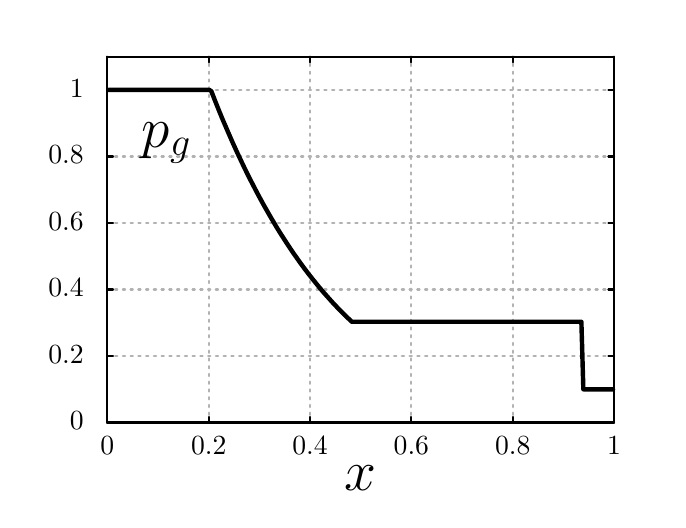
\begin{tikzpicture}[gnuplot]
%% generated with GNUPLOT 4.6p4 (Lua 5.1; terminal rev. 99, script rev. 100)
%% Sat 28 Jun 2014 11:52:07 AM EDT
\path (0.000,0.000) rectangle (8.000,6.000);
\gpfill{rgb color={1.000,1.000,1.000}} (1.012,0.985)--(7.446,0.985)--(7.446,5.630)--(1.012,5.630)--cycle;
\gpcolor{color=gp lt color border}
\gpsetlinetype{gp lt border}
\gpsetlinewidth{1.00}
\draw[gp path] (1.012,0.985)--(1.012,5.630)--(7.446,5.630)--(7.446,0.985)--cycle;
\gpcolor{color=gp lt color axes}
\gpsetlinetype{gp lt axes}
\gpsetlinewidth{2.00}
\draw[gp path] (1.012,0.985)--(7.447,0.985);
\gpcolor{color=gp lt color border}
\gpsetlinetype{gp lt border}
\draw[gp path] (1.012,0.985)--(1.084,0.985);
\draw[gp path] (7.447,0.985)--(7.375,0.985);
\gpcolor{rgb color={0.000,0.000,0.000}}
\node[gp node right,font={\fontsize{10pt}{12pt}\selectfont}] at (0.828,0.985) {0};
\gpcolor{color=gp lt color axes}
\gpsetlinetype{gp lt axes}
\draw[gp path] (1.012,1.830)--(7.447,1.830);
\gpcolor{color=gp lt color border}
\gpsetlinetype{gp lt border}
\draw[gp path] (1.012,1.830)--(1.084,1.830);
\draw[gp path] (7.447,1.830)--(7.375,1.830);
\gpcolor{rgb color={0.000,0.000,0.000}}
\node[gp node right,font={\fontsize{10pt}{12pt}\selectfont}] at (0.828,1.830) {0.2};
\gpcolor{color=gp lt color axes}
\gpsetlinetype{gp lt axes}
\draw[gp path] (1.012,2.674)--(7.447,2.674);
\gpcolor{color=gp lt color border}
\gpsetlinetype{gp lt border}
\draw[gp path] (1.012,2.674)--(1.084,2.674);
\draw[gp path] (7.447,2.674)--(7.375,2.674);
\gpcolor{rgb color={0.000,0.000,0.000}}
\node[gp node right,font={\fontsize{10pt}{12pt}\selectfont}] at (0.828,2.674) {0.4};
\gpcolor{color=gp lt color axes}
\gpsetlinetype{gp lt axes}
\draw[gp path] (1.012,3.519)--(7.447,3.519);
\gpcolor{color=gp lt color border}
\gpsetlinetype{gp lt border}
\draw[gp path] (1.012,3.519)--(1.084,3.519);
\draw[gp path] (7.447,3.519)--(7.375,3.519);
\gpcolor{rgb color={0.000,0.000,0.000}}
\node[gp node right,font={\fontsize{10pt}{12pt}\selectfont}] at (0.828,3.519) {0.6};
\gpcolor{color=gp lt color axes}
\gpsetlinetype{gp lt axes}
\draw[gp path] (1.012,4.364)--(7.447,4.364);
\gpcolor{color=gp lt color border}
\gpsetlinetype{gp lt border}
\draw[gp path] (1.012,4.364)--(1.084,4.364);
\draw[gp path] (7.447,4.364)--(7.375,4.364);
\gpcolor{rgb color={0.000,0.000,0.000}}
\node[gp node right,font={\fontsize{10pt}{12pt}\selectfont}] at (0.828,4.364) {0.8};
\gpcolor{color=gp lt color axes}
\gpsetlinetype{gp lt axes}
\draw[gp path] (1.012,5.209)--(7.447,5.209);
\gpcolor{color=gp lt color border}
\gpsetlinetype{gp lt border}
\draw[gp path] (1.012,5.209)--(1.084,5.209);
\draw[gp path] (7.447,5.209)--(7.375,5.209);
\gpcolor{rgb color={0.000,0.000,0.000}}
\node[gp node right,font={\fontsize{10pt}{12pt}\selectfont}] at (0.828,5.209) {1};
\gpcolor{color=gp lt color axes}
\gpsetlinetype{gp lt axes}
\draw[gp path] (1.012,0.985)--(1.012,5.631);
\gpcolor{color=gp lt color border}
\gpsetlinetype{gp lt border}
\draw[gp path] (1.012,0.985)--(1.012,1.057);
\draw[gp path] (1.012,5.631)--(1.012,5.559);
\gpcolor{rgb color={0.000,0.000,0.000}}
\node[gp node center,font={\fontsize{10pt}{12pt}\selectfont}] at (1.012,0.677) {0};
\gpcolor{color=gp lt color axes}
\gpsetlinetype{gp lt axes}
\draw[gp path] (2.299,0.985)--(2.299,5.631);
\gpcolor{color=gp lt color border}
\gpsetlinetype{gp lt border}
\draw[gp path] (2.299,0.985)--(2.299,1.057);
\draw[gp path] (2.299,5.631)--(2.299,5.559);
\gpcolor{rgb color={0.000,0.000,0.000}}
\node[gp node center,font={\fontsize{10pt}{12pt}\selectfont}] at (2.299,0.677) {0.2};
\gpcolor{color=gp lt color axes}
\gpsetlinetype{gp lt axes}
\draw[gp path] (3.586,0.985)--(3.586,5.631);
\gpcolor{color=gp lt color border}
\gpsetlinetype{gp lt border}
\draw[gp path] (3.586,0.985)--(3.586,1.057);
\draw[gp path] (3.586,5.631)--(3.586,5.559);
\gpcolor{rgb color={0.000,0.000,0.000}}
\node[gp node center,font={\fontsize{10pt}{12pt}\selectfont}] at (3.586,0.677) {0.4};
\gpcolor{color=gp lt color axes}
\gpsetlinetype{gp lt axes}
\draw[gp path] (4.873,0.985)--(4.873,5.631);
\gpcolor{color=gp lt color border}
\gpsetlinetype{gp lt border}
\draw[gp path] (4.873,0.985)--(4.873,1.057);
\draw[gp path] (4.873,5.631)--(4.873,5.559);
\gpcolor{rgb color={0.000,0.000,0.000}}
\node[gp node center,font={\fontsize{10pt}{12pt}\selectfont}] at (4.873,0.677) {0.6};
\gpcolor{color=gp lt color axes}
\gpsetlinetype{gp lt axes}
\draw[gp path] (6.160,0.985)--(6.160,5.631);
\gpcolor{color=gp lt color border}
\gpsetlinetype{gp lt border}
\draw[gp path] (6.160,0.985)--(6.160,1.057);
\draw[gp path] (6.160,5.631)--(6.160,5.559);
\gpcolor{rgb color={0.000,0.000,0.000}}
\node[gp node center,font={\fontsize{10pt}{12pt}\selectfont}] at (6.160,0.677) {0.8};
\gpcolor{color=gp lt color axes}
\gpsetlinetype{gp lt axes}
\draw[gp path] (7.447,0.985)--(7.447,5.631);
\gpcolor{color=gp lt color border}
\gpsetlinetype{gp lt border}
\draw[gp path] (7.447,0.985)--(7.447,1.057);
\draw[gp path] (7.447,5.631)--(7.447,5.559);
\gpcolor{rgb color={0.000,0.000,0.000}}
\node[gp node center,font={\fontsize{10pt}{12pt}\selectfont}] at (7.447,0.677) {1};
\gpcolor{color=gp lt color border}
\draw[gp path] (1.012,5.631)--(1.012,0.985)--(7.447,0.985)--(7.447,5.631)--cycle;
\gpcolor{rgb color={0.000,0.000,0.000}}
\node[gp node center,font={\fontsize{10pt}{12pt}\selectfont}] at (4.229,0.215) {\huge $x$};
\gpsetlinetype{gp lt plot 0}
\gpsetlinewidth{4.00}
\draw[gp path] (1.025,5.209)--(1.050,5.209)--(1.075,5.209)--(1.100,5.209)--(1.125,5.209)%
  --(1.150,5.209)--(1.175,5.209)--(1.201,5.209)--(1.226,5.209)--(1.251,5.209)--(1.276,5.209)%
  --(1.301,5.209)--(1.326,5.209)--(1.351,5.209)--(1.376,5.209)--(1.402,5.209)--(1.427,5.209)%
  --(1.452,5.209)--(1.477,5.209)--(1.502,5.209)--(1.527,5.209)--(1.552,5.209)--(1.578,5.209)%
  --(1.603,5.209)--(1.628,5.209)--(1.653,5.209)--(1.678,5.209)--(1.703,5.209)--(1.728,5.209)%
  --(1.754,5.209)--(1.779,5.209)--(1.804,5.209)--(1.829,5.209)--(1.854,5.209)--(1.879,5.209)%
  --(1.904,5.209)--(1.929,5.209)--(1.955,5.209)--(1.980,5.209)--(2.005,5.209)--(2.030,5.209)%
  --(2.055,5.209)--(2.080,5.209)--(2.105,5.209)--(2.131,5.209)--(2.156,5.209)--(2.181,5.209)%
  --(2.206,5.209)--(2.231,5.209)--(2.256,5.209)--(2.281,5.209)--(2.307,5.209)--(2.332,5.194)%
  --(2.357,5.130)--(2.382,5.066)--(2.407,5.003)--(2.432,4.941)--(2.457,4.880)--(2.482,4.820)%
  --(2.508,4.760)--(2.533,4.702)--(2.558,4.644)--(2.583,4.587)--(2.608,4.530)--(2.633,4.475)%
  --(2.658,4.420)--(2.684,4.365)--(2.709,4.312)--(2.734,4.259)--(2.759,4.207)--(2.784,4.156)%
  --(2.809,4.106)--(2.834,4.056)--(2.860,4.007)--(2.885,3.958)--(2.910,3.910)--(2.935,3.863)%
  --(2.960,3.817)--(2.985,3.771)--(3.010,3.726)--(3.036,3.681)--(3.061,3.637)--(3.086,3.594)%
  --(3.111,3.551)--(3.136,3.509)--(3.161,3.467)--(3.186,3.426)--(3.211,3.386)--(3.237,3.346)%
  --(3.262,3.307)--(3.287,3.268)--(3.312,3.230)--(3.337,3.192)--(3.362,3.155)--(3.387,3.119)%
  --(3.413,3.083)--(3.438,3.047)--(3.463,3.012)--(3.488,2.978)--(3.513,2.944)--(3.538,2.911)%
  --(3.563,2.878)--(3.589,2.845)--(3.614,2.813)--(3.639,2.782)--(3.664,2.751)--(3.689,2.720)%
  --(3.714,2.690)--(3.739,2.660)--(3.764,2.631)--(3.790,2.602)--(3.815,2.574)--(3.840,2.546)%
  --(3.865,2.518)--(3.890,2.491)--(3.915,2.465)--(3.940,2.438)--(3.966,2.412)--(3.991,2.387)%
  --(4.016,2.362)--(4.041,2.337)--(4.066,2.313)--(4.091,2.289)--(4.116,2.265)--(4.142,2.265)%
  --(4.167,2.265)--(4.192,2.265)--(4.217,2.265)--(4.242,2.265)--(4.267,2.265)--(4.292,2.265)%
  --(4.317,2.265)--(4.343,2.265)--(4.368,2.265)--(4.393,2.265)--(4.418,2.265)--(4.443,2.265)%
  --(4.468,2.265)--(4.493,2.265)--(4.519,2.265)--(4.544,2.265)--(4.569,2.265)--(4.594,2.265)%
  --(4.619,2.265)--(4.644,2.265)--(4.669,2.265)--(4.695,2.265)--(4.720,2.265)--(4.745,2.265)%
  --(4.770,2.265)--(4.795,2.265)--(4.820,2.265)--(4.845,2.265)--(4.870,2.265)--(4.896,2.265)%
  --(4.921,2.265)--(4.946,2.265)--(4.971,2.265)--(4.996,2.265)--(5.021,2.265)--(5.046,2.265)%
  --(5.072,2.265)--(5.097,2.265)--(5.122,2.265)--(5.147,2.265)--(5.172,2.265)--(5.197,2.265)%
  --(5.222,2.265)--(5.248,2.265)--(5.273,2.265)--(5.298,2.265)--(5.323,2.265)--(5.348,2.265)%
  --(5.373,2.265)--(5.398,2.265)--(5.423,2.265)--(5.449,2.265)--(5.474,2.265)--(5.499,2.265)%
  --(5.524,2.265)--(5.549,2.265)--(5.574,2.265)--(5.599,2.265)--(5.625,2.265)--(5.650,2.265)%
  --(5.675,2.265)--(5.700,2.265)--(5.725,2.265)--(5.750,2.265)--(5.775,2.265)--(5.801,2.265)%
  --(5.826,2.265)--(5.851,2.265)--(5.876,2.265)--(5.901,2.265)--(5.926,2.265)--(5.951,2.265)%
  --(5.977,2.265)--(6.002,2.265)--(6.027,2.265)--(6.052,2.265)--(6.077,2.265)--(6.102,2.265)%
  --(6.127,2.265)--(6.152,2.265)--(6.178,2.265)--(6.203,2.265)--(6.228,2.265)--(6.253,2.265)%
  --(6.278,2.265)--(6.303,2.265)--(6.328,2.265)--(6.354,2.265)--(6.379,2.265)--(6.404,2.265)%
  --(6.429,2.265)--(6.454,2.265)--(6.479,2.265)--(6.504,2.265)--(6.530,2.265)--(6.555,2.265)%
  --(6.580,2.265)--(6.605,2.265)--(6.630,2.265)--(6.655,2.265)--(6.680,2.265)--(6.705,2.265)%
  --(6.731,2.265)--(6.756,2.265)--(6.781,2.265)--(6.806,2.265)--(6.831,2.265)--(6.856,2.265)%
  --(6.881,2.265)--(6.907,2.265)--(6.932,2.265)--(6.957,2.265)--(6.982,2.265)--(7.007,2.265)%
  --(7.032,2.265)--(7.057,1.407)--(7.083,1.407)--(7.108,1.407)--(7.133,1.407)--(7.158,1.407)%
  --(7.183,1.407)--(7.208,1.407)--(7.233,1.407)--(7.258,1.407)--(7.284,1.407)--(7.309,1.407)%
  --(7.334,1.407)--(7.359,1.407)--(7.384,1.407)--(7.409,1.407)--(7.434,1.407);
\node[gp node left,font={\fontsize{10pt}{12pt}\selectfont}] at (1.334,4.575) {\huge $p_g$};
%% coordinates of the plot area
\gpdefrectangularnode{gp plot 1}{\pgfpoint{1.012cm}{0.985cm}}{\pgfpoint{7.447cm}{5.631cm}}
\end{tikzpicture}
%% gnuplot variables
} 
\end{tabular}
\caption{Exact solution to Sod shock tube problem.  The head of the rarefaction is located at $x \approx 0.2$, and the tail is at $x \approx 0.45$.  The contact discontinuity is located at $x \approx 0.72$, and the shock is located $x \approx 0.95$.}
\label{fig:euler_exact_sod}
\end{figure}

Shock tube problems in Gas Dynamics are an example of a Riemann problem for the Euler equations.  They are typically used for validation and benchmarking.  The problem consists two fluids are separated by a thin film at $x = 0.5$.  At time $t=0$, the film is removed and the fluids interact.  The exact solution to the Sod shock tube problem at time $t=0.25$ (\citep{Sod:1978}, test 1 in \citep{Toro:1999}), is shown in Figure~\ref{fig:euler_exact_sod}.  The initial left state is $\mbf{U}_l = (1.0,0.0,1.0)$ and the initial right state is $\mbf{U}_r = (0.125,0.0,0.1)$.  The problem was solved using our own implementation of the routine \emph{exact.f} provided in \citep{Toro:1999}.  Convergence is established when 
\begin{gather}
\frac{2|p_g^{n+1} - p_g^{n}|}{p_g^{n+1} + p_g^{n}} < 10^{-6},
\end{gather}
where $p_g$ is the gas pressure in the intermediate states and $n$ is the number of iterations.  The solution consists of a left rarefaction, contact discontinuity, and right shock.  

Convergence to the exact solution is not guaranteed since obtaining it requires Newton iteration.  In flow simulations, approximate Riemann solvers maintain a similar level of accuracy as the exact solver, while reducing the computational cost since no iterations are required.  Three different approximate Riemann solvers for the Euler equations are described in the following sections.

%-----------------------------------------------------------------
% Riemann solvers
%-----------------------------------------------------------------
\subsection[Approximate Riemann solvers]{Approximate Riemann solvers}
\label{sec:hydro_approx_rsolvers}

%-----------------------------------------------------------------
% HLLE
%-----------------------------------------------------------------
\subsubsection[HLLE solver]{HLLE solver}
\label{sec:hlle}

The Harden-Lax-van Leer-Einfeldt (HLLE) \citep{Einfeldt:1988} solver assumes a two wave solution with a single intermediate state, see Figure~\ref{fig:inter_rstates}.  The intermediate state is approximated as the integral average over the Riemann fan: $[x_l,x_r] \times [0,t]$, i.e. the region between the left and right wave in Figure~\ref{fig:inter_rstates}.   The integral form of the conservation laws are
\begin{gather}
\label{eqn:int_cons}
\int_{x_l}^{x_r} \mbf{U}(x,t_f) dx - \int_{x_l}^{x_r} \mbf{U}(x,0) dx + \int_{0}^{t} \mbf{F}(\mbf{U}(x_r,t')) dt'
- \int_{0}^{t} \mbf{F}(\mbf{U}(x_l,t')) dt' = 0.
\end{gather}
Applying \eqref{eqn:int_cons} over $[x_l,x_r] \times [0,t]$, gives the HLLE intermediate state as
\begin{gather}
\label{eqn:hlle_state}
\mbf{U}^* = \frac{S_r \mbf{U}_r - S_l \mbf{U}_l + \mbf{F}_r + \mbf{F}_l }{S_r - S_l}.
\end{gather}
The HLLE fluxes 
\begin{gather}
\label{eqn:hlle_flux}
\mbf{F}^* = \frac{S_r \mbf{F}_l - S_l \mbf{F}_r + S_r S_l (\mbf{U}_l - \mbf{U}_r) }{S_r - S_l},
\end{gather}
are found by applying \eqref{eqn:int_cons} over the left ($[x_l,0] \times [0,t]$) or right ($[0,x_r] \times [0,t]$) side of the Riemann fan, and substituting \eqref{eqn:hlle_state} into the result (see Appendix \ref{app:hll_flux}).  The HLLE states are defined by
\begin{gather}
\label{eqn:hlle_states}
\mbf{U}(x,t) = 
\begin{cases}
\mbf{U}_l   & \text{if}\;\;\; 0 < S_l, \\
\mbf{U}^*   & \text{if}\;\;\; S_l \le 0 \le S_r, \\
\mbf{U}_r   & \text{if}\;\;\; S_r < 0. \\
\end{cases}
\end{gather}
The HLLE interface fluxes are defined 
\begin{gather}
\label{eqn:hlle_fluxes}
\mbf{F}(x,t) = 
\begin{cases}
\mbf{F}_l   & \text{if}\;\;\; 0 < S_l, \\
\mbf{F}^*   & \text{if}\;\;\; S_l \le 0 \le S_r, \\
\mbf{F}_r   & \text{if}\;\;\; S_r < 0. \\
\end{cases}
\end{gather}

The method is very robust because it is positivity preserving, $\rho > 0$, and $p_g > 0$ \citep{Einfeldt:1991}.  However, as described in the next section, the HLLE approximate Riemann solver is diffuse because it neglects the difference in density across the contact discontinuity.  The alternative approach of \citet{Toro:1994} restores the contact discontinuity.  It is referred to as the HLLC method, where C stands for \emph{Contact}.  

%-----------------------------------------------------------------
% HLLC
%-----------------------------------------------------------------
\subsubsection[HLLC solver]{HLLC solver}
\label{sec:hllc}

%-----------------------------------------------------------------
% HLLC Riemann states
%-----------------------------------------------------------------
\begin{figure}[htbp]
\begin{center}
\tikzsetnextfilename{hllc_rstates}
%----------------------------------------------------------------------------------------
% hllc_rstates.tex
%----------------------------------------------------------------------------------------

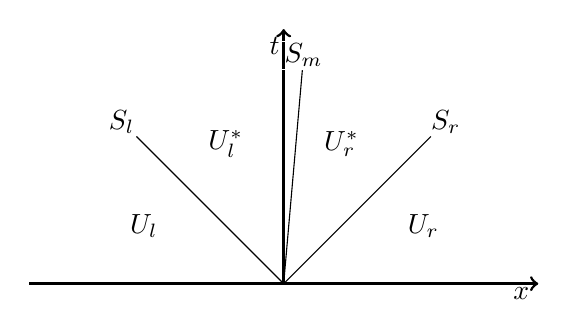
\begin{tikzpicture}[scale = {0.0125\linewidth},inner sep = 1pt]
%% \begin{tikzpicture}[scale = {0.015\linewidth},inner sep = 1pt]
%% \tikzstyle{every node} = [draw,circle,fill=gray!30];
%% \draw (-1.5,0.0) circle (0.8);
%% \draw[<->,line width=1pt] (0,1) node[right]{\;$t$}|-(1,0) node[below]{$m$};
\draw[line width=1pt] (0,0.7) node[left]{$t$}|-(0.7,0) node[below]{$x$};
\draw[->,line width=1pt] (0.7,0)--(0.75,0);
\draw[->,line width=1pt] (0,0.7)--(0,0.75);  
\draw[line width=1pt] (-0,0)--(-0.75,0);
\node[draw=white] (sr) at (0.47730,0.47730) {$S_r$};
\node[draw=white] (cd) at (0.058830,0.67243) {$S_m$};
\node[draw=white] (sl) at (-0.47730,0.47730) {$S_l$};

\node[draw=white] (ur) at (0.41159,0.17049) {$\mbf{U}_{r}$};
\node[draw=white] (usr) at (0.17049,0.41159) {$\mbf{U}^*_{r}$};
\node[draw=white] (usl) at (-0.17049,0.41159) {$\mbf{U}^*_{l}$};
\node[draw=white] (ul) at (-0.41159,0.17049) {$\mbf{U}_{l}$};

\draw (0,0) -- (sr);  
\draw (0,0) -- (cd);  
\draw (0,0) -- (sl);  

\end{tikzpicture}

\end{center}
\caption{Restoration of the contact discontinuity in the HLLC approximate Riemann solver.}
\label{fig:hllc_rstates}
\end{figure}

The approximate solution of the HLLC solver in the $x$-$t$ plane is shown in Figure \ref{fig:hllc_rstates}.  The intermediate states are calculated by approximating the integral over the appropriate Riemann fan and requiring that the Rankine-Hugoniot jump conditions, $v_{nr}^* = v_{nl}^*$, $\mbf{v}_{tr}^* = \mbf{v}_{tl}^*$, and $p_{gr}^* = p_{gl}^*$, are satisfied across the contact discontinuity.  The intermediate states are (Equation (10.33) of \citep{Toro:1999})
\[
\mbf{U}_j^* = 
\rho_j \left( \frac{S_j - v_{nj}}{S_j - v_n^*} \right)
\left[\begin{array}{@{}ccc}
1 \\
v_n \\
\mbf{v}_{t j} \\
\frac{E_j}{\rho_j}  + (S_m - v_{nj}) \left[ S_m + \frac{p_{gj}}{\rho_j(S_j - v_{nj})} \right]  \\
\end{array}\right] \text{ ,} 
\]
where $j=l$ and $j=r$.  The HLLC states are
\begin{gather}
\label{eqn:hllc_states}
\mbf{U}(x,t) = 
\begin{cases}
\mbf{U}_l   & \text{if}\;\;\; 0 < S_l, \\
\mbf{U}_l^*   & \text{if}\;\;\; S_l \le 0 \le S_m, \\
\mbf{U}_r^*   & \text{if}\;\;\; S_m \le 0 \le S_r, \\
\mbf{U}_r   & \text{if}\;\;\; S_r < 0. \\
\end{cases}
\end{gather}
The HLLC fluxes can then be derived with the procedure given in Appendix~\ref{app:hll_flux}.  They are 
\begin{gather}
\label{eqn:hllc_flux}
\mbf{F}(x,t) = 
\begin{cases}
\mbf{F}_l   \phantom{= \mbf{F}_l  + S_l (\mbf{U_l^*} - \mbf{U_l}} & \text{if}\;\;\; 0 < S_l, \\
\mbf{F}_l^* = \mbf{F}_l  + S_l (\mbf{U}_l^* - \mbf{U}_l) & \text{if}\;\;\; S_l \le 0 \le S_m, \\
\mbf{F}_r^* = \mbf{F}_r  + S_r (\mbf{U}_r^* - \mbf{U}_r)  & \text{if}\;\;\; S_m \le 0 \le S_r, \\
\mbf{F}_r  \phantom{= \mbf{F}_r  + S_r (\mbf{U_r^*} - \mbf{U_r}} & \text{if}\;\;\; S_r < 0. \\
\end{cases}
\end{gather}

Both the HLLE and HLLC methods depend on the approximations of the fastest (slowest) wave speed $S_r$ ($S_L$).  \citet{Davis:1988} used wave speeds of 
\begin{gather}
\label{eqn:wave_spd_davis}
S_l = \min \{\lambda_1(\mbf{U}_l),\lambda_1(\mbf{U}_r)\}, \text{ and }
S_r = \max \{\lambda_n(\mbf{U}_l),\lambda_n(\mbf{U}_r)\},
\end{gather} 
where $\lambda_1$ ($\lambda_n$) is the smallest (largest) eigenvalue of \eqref{eqn:nonlinear_sys}.  \citet{Einfeldt:1991} used 
\begin{gather}
\label{eqn:wave_spd_einfeldt}
S_l = \min \{\lambda_1(\mbf{U}_l),\lambda_1(\mbf{U}_{\text{Roe}})\}, \text{ and }
S_r = \max \{\lambda_n(\mbf{U}_r),\lambda_n(\mbf{U}_{\text{Roe}})\},
\end{gather} 
where $\lambda_i(\mbf{U}_{\text{Roe}})$ is an eigenvalue of the Roe matrix, see Section~\ref{sec:roe_solver}.

The middle wave speed, $S_m$, needs to be approximated in the HLLC solver.  \citet{Batten:1997} argued that the middle wave speed should be determined using only  \eqref{eqn:wave_spd_davis} or \eqref{eqn:wave_spd_einfeldt}, and the initial states.  They gave the speed as
\begin{gather}
\label{eqn:wave_spd_batten}
S_m = \frac{(S_r - \vnr)\rho_r \vnr - (S_l - \vnl)\rho_l \vnl - p_{gr} + p_{gl} }
{(S_r - \vnr)\rho_r  - (S_l - \vnl)\rho_l}.
\end{gather}     
\citet{Toro:1994} suggested an alternative method of determining the wave speeds by first estimating the pressure and velocity in the intermediate state according to  
\begin{gather}
\label{eqn:wave_spd_toro}
S_l = \vnl - a_l q_l \text{ , }\;\;\;\; S_m = v_n^* \text{ , }\;\;\;\; S_r = \vnr - a_r q_r \text{ , }
\end{gather}
where
\begin{gather}
\label{eqn:wave_spd_toro2}
q_j = 
\begin{cases}
1 & \text{ if }\;\;\; p_g^* \le p_{gj}, \\ 
\left[ 1 + \frac{\gamma + 1}{2\gamma} \left( \frac{p^*_g}{p_{gj}} - 1 \right) \right]^{\frac{1}{2}} & 
\text{ if }\;\;\; p_g^* > p_{gj},
\end{cases}
\end{gather}
for $j=l$ and $j=r$.

%-----------------------------------------------------------------
% Isolated CD HLLE, HLLC, Roe
%-----------------------------------------------------------------
\begin{figure}[htbp]
\begin{tabular}{cc}
\resizebox{0.5\linewidth}{!}{\tikzsetnextfilename{toro7_hlle_1}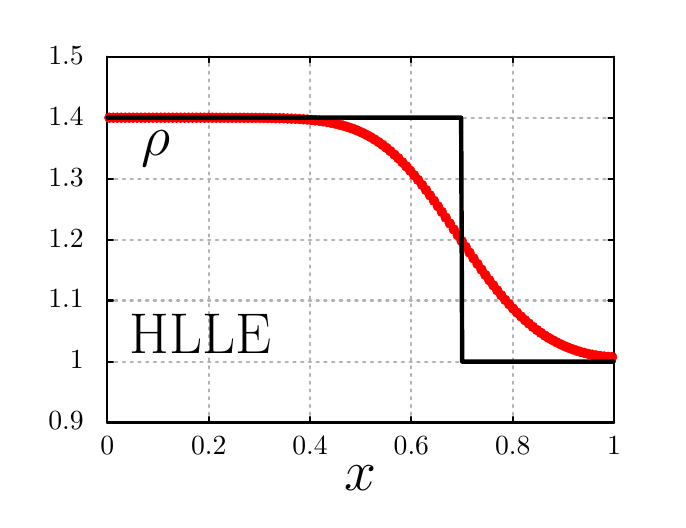
\begin{tikzpicture}[gnuplot]
%% generated with GNUPLOT 4.6p4 (Lua 5.1; terminal rev. 99, script rev. 100)
%% Tue 01 Jul 2014 10:59:57 AM EDT
\path (0.000,0.000) rectangle (8.000,6.000);
\gpfill{rgb color={1.000,1.000,1.000}} (1.012,0.985)--(7.446,0.985)--(7.446,5.630)--(1.012,5.630)--cycle;
\gpcolor{color=gp lt color border}
\gpsetlinetype{gp lt border}
\gpsetlinewidth{1.00}
\draw[gp path] (1.012,0.985)--(1.012,5.630)--(7.446,5.630)--(7.446,0.985)--cycle;
\gpcolor{color=gp lt color axes}
\gpsetlinetype{gp lt axes}
\gpsetlinewidth{2.00}
\draw[gp path] (1.012,0.985)--(7.447,0.985);
\gpcolor{color=gp lt color border}
\gpsetlinetype{gp lt border}
\draw[gp path] (1.012,0.985)--(1.084,0.985);
\draw[gp path] (7.447,0.985)--(7.375,0.985);
\gpcolor{rgb color={0.000,0.000,0.000}}
\node[gp node right,font={\fontsize{10pt}{12pt}\selectfont}] at (0.828,0.985) {0.9};
\gpcolor{color=gp lt color axes}
\gpsetlinetype{gp lt axes}
\draw[gp path] (1.012,1.759)--(7.447,1.759);
\gpcolor{color=gp lt color border}
\gpsetlinetype{gp lt border}
\draw[gp path] (1.012,1.759)--(1.084,1.759);
\draw[gp path] (7.447,1.759)--(7.375,1.759);
\gpcolor{rgb color={0.000,0.000,0.000}}
\node[gp node right,font={\fontsize{10pt}{12pt}\selectfont}] at (0.828,1.759) {1};
\gpcolor{color=gp lt color axes}
\gpsetlinetype{gp lt axes}
\draw[gp path] (1.012,2.534)--(7.447,2.534);
\gpcolor{color=gp lt color border}
\gpsetlinetype{gp lt border}
\draw[gp path] (1.012,2.534)--(1.084,2.534);
\draw[gp path] (7.447,2.534)--(7.375,2.534);
\gpcolor{rgb color={0.000,0.000,0.000}}
\node[gp node right,font={\fontsize{10pt}{12pt}\selectfont}] at (0.828,2.534) {1.1};
\gpcolor{color=gp lt color axes}
\gpsetlinetype{gp lt axes}
\draw[gp path] (1.012,3.308)--(7.447,3.308);
\gpcolor{color=gp lt color border}
\gpsetlinetype{gp lt border}
\draw[gp path] (1.012,3.308)--(1.084,3.308);
\draw[gp path] (7.447,3.308)--(7.375,3.308);
\gpcolor{rgb color={0.000,0.000,0.000}}
\node[gp node right,font={\fontsize{10pt}{12pt}\selectfont}] at (0.828,3.308) {1.2};
\gpcolor{color=gp lt color axes}
\gpsetlinetype{gp lt axes}
\draw[gp path] (1.012,4.082)--(7.447,4.082);
\gpcolor{color=gp lt color border}
\gpsetlinetype{gp lt border}
\draw[gp path] (1.012,4.082)--(1.084,4.082);
\draw[gp path] (7.447,4.082)--(7.375,4.082);
\gpcolor{rgb color={0.000,0.000,0.000}}
\node[gp node right,font={\fontsize{10pt}{12pt}\selectfont}] at (0.828,4.082) {1.3};
\gpcolor{color=gp lt color axes}
\gpsetlinetype{gp lt axes}
\draw[gp path] (1.012,4.857)--(7.447,4.857);
\gpcolor{color=gp lt color border}
\gpsetlinetype{gp lt border}
\draw[gp path] (1.012,4.857)--(1.084,4.857);
\draw[gp path] (7.447,4.857)--(7.375,4.857);
\gpcolor{rgb color={0.000,0.000,0.000}}
\node[gp node right,font={\fontsize{10pt}{12pt}\selectfont}] at (0.828,4.857) {1.4};
\gpcolor{color=gp lt color axes}
\gpsetlinetype{gp lt axes}
\draw[gp path] (1.012,5.631)--(7.447,5.631);
\gpcolor{color=gp lt color border}
\gpsetlinetype{gp lt border}
\draw[gp path] (1.012,5.631)--(1.084,5.631);
\draw[gp path] (7.447,5.631)--(7.375,5.631);
\gpcolor{rgb color={0.000,0.000,0.000}}
\node[gp node right,font={\fontsize{10pt}{12pt}\selectfont}] at (0.828,5.631) {1.5};
\gpcolor{color=gp lt color axes}
\gpsetlinetype{gp lt axes}
\draw[gp path] (1.012,0.985)--(1.012,5.631);
\gpcolor{color=gp lt color border}
\gpsetlinetype{gp lt border}
\draw[gp path] (1.012,0.985)--(1.012,1.057);
\draw[gp path] (1.012,5.631)--(1.012,5.559);
\gpcolor{rgb color={0.000,0.000,0.000}}
\node[gp node center,font={\fontsize{10pt}{12pt}\selectfont}] at (1.012,0.677) {0};
\gpcolor{color=gp lt color axes}
\gpsetlinetype{gp lt axes}
\draw[gp path] (2.299,0.985)--(2.299,5.631);
\gpcolor{color=gp lt color border}
\gpsetlinetype{gp lt border}
\draw[gp path] (2.299,0.985)--(2.299,1.057);
\draw[gp path] (2.299,5.631)--(2.299,5.559);
\gpcolor{rgb color={0.000,0.000,0.000}}
\node[gp node center,font={\fontsize{10pt}{12pt}\selectfont}] at (2.299,0.677) {0.2};
\gpcolor{color=gp lt color axes}
\gpsetlinetype{gp lt axes}
\draw[gp path] (3.586,0.985)--(3.586,5.631);
\gpcolor{color=gp lt color border}
\gpsetlinetype{gp lt border}
\draw[gp path] (3.586,0.985)--(3.586,1.057);
\draw[gp path] (3.586,5.631)--(3.586,5.559);
\gpcolor{rgb color={0.000,0.000,0.000}}
\node[gp node center,font={\fontsize{10pt}{12pt}\selectfont}] at (3.586,0.677) {0.4};
\gpcolor{color=gp lt color axes}
\gpsetlinetype{gp lt axes}
\draw[gp path] (4.873,0.985)--(4.873,5.631);
\gpcolor{color=gp lt color border}
\gpsetlinetype{gp lt border}
\draw[gp path] (4.873,0.985)--(4.873,1.057);
\draw[gp path] (4.873,5.631)--(4.873,5.559);
\gpcolor{rgb color={0.000,0.000,0.000}}
\node[gp node center,font={\fontsize{10pt}{12pt}\selectfont}] at (4.873,0.677) {0.6};
\gpcolor{color=gp lt color axes}
\gpsetlinetype{gp lt axes}
\draw[gp path] (6.160,0.985)--(6.160,5.631);
\gpcolor{color=gp lt color border}
\gpsetlinetype{gp lt border}
\draw[gp path] (6.160,0.985)--(6.160,1.057);
\draw[gp path] (6.160,5.631)--(6.160,5.559);
\gpcolor{rgb color={0.000,0.000,0.000}}
\node[gp node center,font={\fontsize{10pt}{12pt}\selectfont}] at (6.160,0.677) {0.8};
\gpcolor{color=gp lt color axes}
\gpsetlinetype{gp lt axes}
\draw[gp path] (7.447,0.985)--(7.447,5.631);
\gpcolor{color=gp lt color border}
\gpsetlinetype{gp lt border}
\draw[gp path] (7.447,0.985)--(7.447,1.057);
\draw[gp path] (7.447,5.631)--(7.447,5.559);
\gpcolor{rgb color={0.000,0.000,0.000}}
\node[gp node center,font={\fontsize{10pt}{12pt}\selectfont}] at (7.447,0.677) {1};
\gpcolor{color=gp lt color border}
\draw[gp path] (1.012,5.631)--(1.012,0.985)--(7.447,0.985)--(7.447,5.631)--cycle;
\gpcolor{rgb color={0.000,0.000,0.000}}
\node[gp node center,font={\fontsize{10pt}{12pt}\selectfont}] at (4.229,0.215) {\huge $x$};
\gpcolor{rgb color={1.000,0.000,0.000}}
\gpsetlinewidth{0.50}
\gpsetpointsize{4.44}
\gppoint{gp mark 7}{(1.037,4.857)}
\gppoint{gp mark 7}{(1.087,4.857)}
\gppoint{gp mark 7}{(1.138,4.857)}
\gppoint{gp mark 7}{(1.188,4.857)}
\gppoint{gp mark 7}{(1.238,4.857)}
\gppoint{gp mark 7}{(1.289,4.857)}
\gppoint{gp mark 7}{(1.339,4.857)}
\gppoint{gp mark 7}{(1.389,4.857)}
\gppoint{gp mark 7}{(1.439,4.857)}
\gppoint{gp mark 7}{(1.490,4.857)}
\gppoint{gp mark 7}{(1.540,4.857)}
\gppoint{gp mark 7}{(1.590,4.857)}
\gppoint{gp mark 7}{(1.640,4.857)}
\gppoint{gp mark 7}{(1.691,4.857)}
\gppoint{gp mark 7}{(1.741,4.857)}
\gppoint{gp mark 7}{(1.791,4.857)}
\gppoint{gp mark 7}{(1.842,4.857)}
\gppoint{gp mark 7}{(1.892,4.857)}
\gppoint{gp mark 7}{(1.942,4.857)}
\gppoint{gp mark 7}{(1.992,4.857)}
\gppoint{gp mark 7}{(2.043,4.857)}
\gppoint{gp mark 7}{(2.093,4.857)}
\gppoint{gp mark 7}{(2.143,4.857)}
\gppoint{gp mark 7}{(2.193,4.857)}
\gppoint{gp mark 7}{(2.244,4.857)}
\gppoint{gp mark 7}{(2.294,4.857)}
\gppoint{gp mark 7}{(2.344,4.857)}
\gppoint{gp mark 7}{(2.395,4.856)}
\gppoint{gp mark 7}{(2.445,4.856)}
\gppoint{gp mark 7}{(2.495,4.856)}
\gppoint{gp mark 7}{(2.545,4.856)}
\gppoint{gp mark 7}{(2.596,4.856)}
\gppoint{gp mark 7}{(2.646,4.856)}
\gppoint{gp mark 7}{(2.696,4.856)}
\gppoint{gp mark 7}{(2.746,4.856)}
\gppoint{gp mark 7}{(2.797,4.855)}
\gppoint{gp mark 7}{(2.847,4.855)}
\gppoint{gp mark 7}{(2.897,4.855)}
\gppoint{gp mark 7}{(2.948,4.854)}
\gppoint{gp mark 7}{(2.998,4.854)}
\gppoint{gp mark 7}{(3.048,4.853)}
\gppoint{gp mark 7}{(3.098,4.852)}
\gppoint{gp mark 7}{(3.149,4.851)}
\gppoint{gp mark 7}{(3.199,4.850)}
\gppoint{gp mark 7}{(3.249,4.849)}
\gppoint{gp mark 7}{(3.299,4.847)}
\gppoint{gp mark 7}{(3.350,4.845)}
\gppoint{gp mark 7}{(3.400,4.843)}
\gppoint{gp mark 7}{(3.450,4.840)}
\gppoint{gp mark 7}{(3.501,4.836)}
\gppoint{gp mark 7}{(3.551,4.833)}
\gppoint{gp mark 7}{(3.601,4.828)}
\gppoint{gp mark 7}{(3.651,4.823)}
\gppoint{gp mark 7}{(3.702,4.817)}
\gppoint{gp mark 7}{(3.752,4.810)}
\gppoint{gp mark 7}{(3.802,4.802)}
\gppoint{gp mark 7}{(3.852,4.793)}
\gppoint{gp mark 7}{(3.903,4.782)}
\gppoint{gp mark 7}{(3.953,4.770)}
\gppoint{gp mark 7}{(4.003,4.757)}
\gppoint{gp mark 7}{(4.054,4.742)}
\gppoint{gp mark 7}{(4.104,4.725)}
\gppoint{gp mark 7}{(4.154,4.707)}
\gppoint{gp mark 7}{(4.204,4.686)}
\gppoint{gp mark 7}{(4.255,4.663)}
\gppoint{gp mark 7}{(4.305,4.638)}
\gppoint{gp mark 7}{(4.355,4.610)}
\gppoint{gp mark 7}{(4.405,4.580)}
\gppoint{gp mark 7}{(4.456,4.547)}
\gppoint{gp mark 7}{(4.506,4.512)}
\gppoint{gp mark 7}{(4.556,4.474)}
\gppoint{gp mark 7}{(4.607,4.432)}
\gppoint{gp mark 7}{(4.657,4.388)}
\gppoint{gp mark 7}{(4.707,4.342)}
\gppoint{gp mark 7}{(4.757,4.292)}
\gppoint{gp mark 7}{(4.808,4.239)}
\gppoint{gp mark 7}{(4.858,4.184)}
\gppoint{gp mark 7}{(4.908,4.126)}
\gppoint{gp mark 7}{(4.958,4.066)}
\gppoint{gp mark 7}{(5.009,4.003)}
\gppoint{gp mark 7}{(5.059,3.938)}
\gppoint{gp mark 7}{(5.109,3.871)}
\gppoint{gp mark 7}{(5.160,3.802)}
\gppoint{gp mark 7}{(5.210,3.732)}
\gppoint{gp mark 7}{(5.260,3.660)}
\gppoint{gp mark 7}{(5.310,3.587)}
\gppoint{gp mark 7}{(5.361,3.514)}
\gppoint{gp mark 7}{(5.411,3.439)}
\gppoint{gp mark 7}{(5.461,3.365)}
\gppoint{gp mark 7}{(5.511,3.291)}
\gppoint{gp mark 7}{(5.562,3.217)}
\gppoint{gp mark 7}{(5.612,3.143)}
\gppoint{gp mark 7}{(5.662,3.070)}
\gppoint{gp mark 7}{(5.713,2.999)}
\gppoint{gp mark 7}{(5.763,2.928)}
\gppoint{gp mark 7}{(5.813,2.859)}
\gppoint{gp mark 7}{(5.863,2.792)}
\gppoint{gp mark 7}{(5.914,2.727)}
\gppoint{gp mark 7}{(5.964,2.663)}
\gppoint{gp mark 7}{(6.014,2.602)}
\gppoint{gp mark 7}{(6.064,2.543)}
\gppoint{gp mark 7}{(6.115,2.487)}
\gppoint{gp mark 7}{(6.165,2.432)}
\gppoint{gp mark 7}{(6.215,2.381)}
\gppoint{gp mark 7}{(6.266,2.332)}
\gppoint{gp mark 7}{(6.316,2.285)}
\gppoint{gp mark 7}{(6.366,2.242)}
\gppoint{gp mark 7}{(6.416,2.200)}
\gppoint{gp mark 7}{(6.467,2.161)}
\gppoint{gp mark 7}{(6.517,2.125)}
\gppoint{gp mark 7}{(6.567,2.091)}
\gppoint{gp mark 7}{(6.617,2.060)}
\gppoint{gp mark 7}{(6.668,2.031)}
\gppoint{gp mark 7}{(6.718,2.004)}
\gppoint{gp mark 7}{(6.768,1.979)}
\gppoint{gp mark 7}{(6.819,1.956)}
\gppoint{gp mark 7}{(6.869,1.935)}
\gppoint{gp mark 7}{(6.919,1.916)}
\gppoint{gp mark 7}{(6.969,1.899)}
\gppoint{gp mark 7}{(7.020,1.883)}
\gppoint{gp mark 7}{(7.070,1.870)}
\gppoint{gp mark 7}{(7.120,1.857)}
\gppoint{gp mark 7}{(7.170,1.847)}
\gppoint{gp mark 7}{(7.221,1.837)}
\gppoint{gp mark 7}{(7.271,1.830)}
\gppoint{gp mark 7}{(7.321,1.824)}
\gppoint{gp mark 7}{(7.372,1.819)}
\gppoint{gp mark 7}{(7.422,1.817)}
\gpcolor{rgb color={0.000,0.000,0.000}}
\gpsetlinetype{gp lt plot 0}
\gpsetlinewidth{4.00}
\draw[gp path] (1.018,4.857)--(1.031,4.857)--(1.043,4.857)--(1.056,4.857)--(1.069,4.857)%
  --(1.081,4.857)--(1.094,4.857)--(1.106,4.857)--(1.119,4.857)--(1.131,4.857)--(1.144,4.857)%
  --(1.157,4.857)--(1.169,4.857)--(1.182,4.857)--(1.194,4.857)--(1.207,4.857)--(1.219,4.857)%
  --(1.232,4.857)--(1.245,4.857)--(1.257,4.857)--(1.270,4.857)--(1.282,4.857)--(1.295,4.857)%
  --(1.307,4.857)--(1.320,4.857)--(1.332,4.857)--(1.345,4.857)--(1.358,4.857)--(1.370,4.857)%
  --(1.383,4.857)--(1.395,4.857)--(1.408,4.857)--(1.420,4.857)--(1.433,4.857)--(1.446,4.857)%
  --(1.458,4.857)--(1.471,4.857)--(1.483,4.857)--(1.496,4.857)--(1.508,4.857)--(1.521,4.857)%
  --(1.534,4.857)--(1.546,4.857)--(1.559,4.857)--(1.571,4.857)--(1.584,4.857)--(1.596,4.857)%
  --(1.609,4.857)--(1.622,4.857)--(1.634,4.857)--(1.647,4.857)--(1.659,4.857)--(1.672,4.857)%
  --(1.684,4.857)--(1.697,4.857)--(1.710,4.857)--(1.722,4.857)--(1.735,4.857)--(1.747,4.857)%
  --(1.760,4.857)--(1.772,4.857)--(1.785,4.857)--(1.798,4.857)--(1.810,4.857)--(1.823,4.857)%
  --(1.835,4.857)--(1.848,4.857)--(1.860,4.857)--(1.873,4.857)--(1.886,4.857)--(1.898,4.857)%
  --(1.911,4.857)--(1.923,4.857)--(1.936,4.857)--(1.948,4.857)--(1.961,4.857)--(1.973,4.857)%
  --(1.986,4.857)--(1.999,4.857)--(2.011,4.857)--(2.024,4.857)--(2.036,4.857)--(2.049,4.857)%
  --(2.061,4.857)--(2.074,4.857)--(2.087,4.857)--(2.099,4.857)--(2.112,4.857)--(2.124,4.857)%
  --(2.137,4.857)--(2.149,4.857)--(2.162,4.857)--(2.175,4.857)--(2.187,4.857)--(2.200,4.857)%
  --(2.212,4.857)--(2.225,4.857)--(2.237,4.857)--(2.250,4.857)--(2.263,4.857)--(2.275,4.857)%
  --(2.288,4.857)--(2.300,4.857)--(2.313,4.857)--(2.325,4.857)--(2.338,4.857)--(2.351,4.857)%
  --(2.363,4.857)--(2.376,4.857)--(2.388,4.857)--(2.401,4.857)--(2.413,4.857)--(2.426,4.857)%
  --(2.439,4.857)--(2.451,4.857)--(2.464,4.857)--(2.476,4.857)--(2.489,4.857)--(2.501,4.857)%
  --(2.514,4.857)--(2.526,4.857)--(2.539,4.857)--(2.552,4.857)--(2.564,4.857)--(2.577,4.857)%
  --(2.589,4.857)--(2.602,4.857)--(2.614,4.857)--(2.627,4.857)--(2.640,4.857)--(2.652,4.857)%
  --(2.665,4.857)--(2.677,4.857)--(2.690,4.857)--(2.702,4.857)--(2.715,4.857)--(2.728,4.857)%
  --(2.740,4.857)--(2.753,4.857)--(2.765,4.857)--(2.778,4.857)--(2.790,4.857)--(2.803,4.857)%
  --(2.816,4.857)--(2.828,4.857)--(2.841,4.857)--(2.853,4.857)--(2.866,4.857)--(2.878,4.857)%
  --(2.891,4.857)--(2.904,4.857)--(2.916,4.857)--(2.929,4.857)--(2.941,4.857)--(2.954,4.857)%
  --(2.966,4.857)--(2.979,4.857)--(2.992,4.857)--(3.004,4.857)--(3.017,4.857)--(3.029,4.857)%
  --(3.042,4.857)--(3.054,4.857)--(3.067,4.857)--(3.079,4.857)--(3.092,4.857)--(3.105,4.857)%
  --(3.117,4.857)--(3.130,4.857)--(3.142,4.857)--(3.155,4.857)--(3.167,4.857)--(3.180,4.857)%
  --(3.193,4.857)--(3.205,4.857)--(3.218,4.857)--(3.230,4.857)--(3.243,4.857)--(3.255,4.857)%
  --(3.268,4.857)--(3.281,4.857)--(3.293,4.857)--(3.306,4.857)--(3.318,4.857)--(3.331,4.857)%
  --(3.343,4.857)--(3.356,4.857)--(3.369,4.857)--(3.381,4.857)--(3.394,4.857)--(3.406,4.857)%
  --(3.419,4.857)--(3.431,4.857)--(3.444,4.857)--(3.457,4.857)--(3.469,4.857)--(3.482,4.857)%
  --(3.494,4.857)--(3.507,4.857)--(3.519,4.857)--(3.532,4.857)--(3.545,4.857)--(3.557,4.857)%
  --(3.570,4.857)--(3.582,4.857)--(3.595,4.857)--(3.607,4.857)--(3.620,4.857)--(3.633,4.857)%
  --(3.645,4.857)--(3.658,4.857)--(3.670,4.857)--(3.683,4.857)--(3.695,4.857)--(3.708,4.857)%
  --(3.720,4.857)--(3.733,4.857)--(3.746,4.857)--(3.758,4.857)--(3.771,4.857)--(3.783,4.857)%
  --(3.796,4.857)--(3.808,4.857)--(3.821,4.857)--(3.834,4.857)--(3.846,4.857)--(3.859,4.857)%
  --(3.871,4.857)--(3.884,4.857)--(3.896,4.857)--(3.909,4.857)--(3.922,4.857)--(3.934,4.857)%
  --(3.947,4.857)--(3.959,4.857)--(3.972,4.857)--(3.984,4.857)--(3.997,4.857)--(4.010,4.857)%
  --(4.022,4.857)--(4.035,4.857)--(4.047,4.857)--(4.060,4.857)--(4.072,4.857)--(4.085,4.857)%
  --(4.098,4.857)--(4.110,4.857)--(4.123,4.857)--(4.135,4.857)--(4.148,4.857)--(4.160,4.857)%
  --(4.173,4.857)--(4.186,4.857)--(4.198,4.857)--(4.211,4.857)--(4.223,4.857)--(4.236,4.857)%
  --(4.248,4.857)--(4.261,4.857)--(4.273,4.857)--(4.286,4.857)--(4.299,4.857)--(4.311,4.857)%
  --(4.324,4.857)--(4.336,4.857)--(4.349,4.857)--(4.361,4.857)--(4.374,4.857)--(4.387,4.857)%
  --(4.399,4.857)--(4.412,4.857)--(4.424,4.857)--(4.437,4.857)--(4.449,4.857)--(4.462,4.857)%
  --(4.475,4.857)--(4.487,4.857)--(4.500,4.857)--(4.512,4.857)--(4.525,4.857)--(4.537,4.857)%
  --(4.550,4.857)--(4.563,4.857)--(4.575,4.857)--(4.588,4.857)--(4.600,4.857)--(4.613,4.857)%
  --(4.625,4.857)--(4.638,4.857)--(4.651,4.857)--(4.663,4.857)--(4.676,4.857)--(4.688,4.857)%
  --(4.701,4.857)--(4.713,4.857)--(4.726,4.857)--(4.739,4.857)--(4.751,4.857)--(4.764,4.857)%
  --(4.776,4.857)--(4.789,4.857)--(4.801,4.857)--(4.814,4.857)--(4.826,4.857)--(4.839,4.857)%
  --(4.852,4.857)--(4.864,4.857)--(4.877,4.857)--(4.889,4.857)--(4.902,4.857)--(4.914,4.857)%
  --(4.927,4.857)--(4.940,4.857)--(4.952,4.857)--(4.965,4.857)--(4.977,4.857)--(4.990,4.857)%
  --(5.002,4.857)--(5.015,4.857)--(5.028,4.857)--(5.040,4.857)--(5.053,4.857)--(5.065,4.857)%
  --(5.078,4.857)--(5.090,4.857)--(5.103,4.857)--(5.116,4.857)--(5.128,4.857)--(5.141,4.857)%
  --(5.153,4.857)--(5.166,4.857)--(5.178,4.857)--(5.191,4.857)--(5.204,4.857)--(5.216,4.857)%
  --(5.229,4.857)--(5.241,4.857)--(5.254,4.857)--(5.266,4.857)--(5.279,4.857)--(5.292,4.857)%
  --(5.304,4.857)--(5.317,4.857)--(5.329,4.857)--(5.342,4.857)--(5.354,4.857)--(5.367,4.857)%
  --(5.380,4.857)--(5.392,4.857)--(5.405,4.857)--(5.417,4.857)--(5.430,4.857)--(5.442,4.857)%
  --(5.455,4.857)--(5.467,4.857)--(5.480,4.857)--(5.493,4.857)--(5.505,4.857)--(5.518,1.759)%
  --(5.530,1.759)--(5.543,1.759)--(5.555,1.759)--(5.568,1.759)--(5.581,1.759)--(5.593,1.759)%
  --(5.606,1.759)--(5.618,1.759)--(5.631,1.759)--(5.643,1.759)--(5.656,1.759)--(5.669,1.759)%
  --(5.681,1.759)--(5.694,1.759)--(5.706,1.759)--(5.719,1.759)--(5.731,1.759)--(5.744,1.759)%
  --(5.757,1.759)--(5.769,1.759)--(5.782,1.759)--(5.794,1.759)--(5.807,1.759)--(5.819,1.759)%
  --(5.832,1.759)--(5.845,1.759)--(5.857,1.759)--(5.870,1.759)--(5.882,1.759)--(5.895,1.759)%
  --(5.907,1.759)--(5.920,1.759)--(5.933,1.759)--(5.945,1.759)--(5.958,1.759)--(5.970,1.759)%
  --(5.983,1.759)--(5.995,1.759)--(6.008,1.759)--(6.020,1.759)--(6.033,1.759)--(6.046,1.759)%
  --(6.058,1.759)--(6.071,1.759)--(6.083,1.759)--(6.096,1.759)--(6.108,1.759)--(6.121,1.759)%
  --(6.134,1.759)--(6.146,1.759)--(6.159,1.759)--(6.171,1.759)--(6.184,1.759)--(6.196,1.759)%
  --(6.209,1.759)--(6.222,1.759)--(6.234,1.759)--(6.247,1.759)--(6.259,1.759)--(6.272,1.759)%
  --(6.284,1.759)--(6.297,1.759)--(6.310,1.759)--(6.322,1.759)--(6.335,1.759)--(6.347,1.759)%
  --(6.360,1.759)--(6.372,1.759)--(6.385,1.759)--(6.398,1.759)--(6.410,1.759)--(6.423,1.759)%
  --(6.435,1.759)--(6.448,1.759)--(6.460,1.759)--(6.473,1.759)--(6.486,1.759)--(6.498,1.759)%
  --(6.511,1.759)--(6.523,1.759)--(6.536,1.759)--(6.548,1.759)--(6.561,1.759)--(6.573,1.759)%
  --(6.586,1.759)--(6.599,1.759)--(6.611,1.759)--(6.624,1.759)--(6.636,1.759)--(6.649,1.759)%
  --(6.661,1.759)--(6.674,1.759)--(6.687,1.759)--(6.699,1.759)--(6.712,1.759)--(6.724,1.759)%
  --(6.737,1.759)--(6.749,1.759)--(6.762,1.759)--(6.775,1.759)--(6.787,1.759)--(6.800,1.759)%
  --(6.812,1.759)--(6.825,1.759)--(6.837,1.759)--(6.850,1.759)--(6.863,1.759)--(6.875,1.759)%
  --(6.888,1.759)--(6.900,1.759)--(6.913,1.759)--(6.925,1.759)--(6.938,1.759)--(6.951,1.759)%
  --(6.963,1.759)--(6.976,1.759)--(6.988,1.759)--(7.001,1.759)--(7.013,1.759)--(7.026,1.759)%
  --(7.039,1.759)--(7.051,1.759)--(7.064,1.759)--(7.076,1.759)--(7.089,1.759)--(7.101,1.759)%
  --(7.114,1.759)--(7.127,1.759)--(7.139,1.759)--(7.152,1.759)--(7.164,1.759)--(7.177,1.759)%
  --(7.189,1.759)--(7.202,1.759)--(7.214,1.759)--(7.227,1.759)--(7.240,1.759)--(7.252,1.759)%
  --(7.265,1.759)--(7.277,1.759)--(7.290,1.759)--(7.302,1.759)--(7.315,1.759)--(7.328,1.759)%
  --(7.340,1.759)--(7.353,1.759)--(7.365,1.759)--(7.378,1.759)--(7.390,1.759)--(7.403,1.759)%
  --(7.416,1.759)--(7.428,1.759)--(7.441,1.759);
\node[gp node left,font={\fontsize{10pt}{12pt}\selectfont}] at (1.334,4.470) {\huge $\rho$};
\node[gp node left,font={\fontsize{10pt}{12pt}\selectfont}] at (1.173,1.953) {\huge HLLE};
%% coordinates of the plot area
\gpdefrectangularnode{gp plot 1}{\pgfpoint{1.012cm}{0.985cm}}{\pgfpoint{7.447cm}{5.631cm}}
\end{tikzpicture}
%% gnuplot variables
} &
\resizebox{0.5\linewidth}{!}{\tikzsetnextfilename{toro7_hllc_1}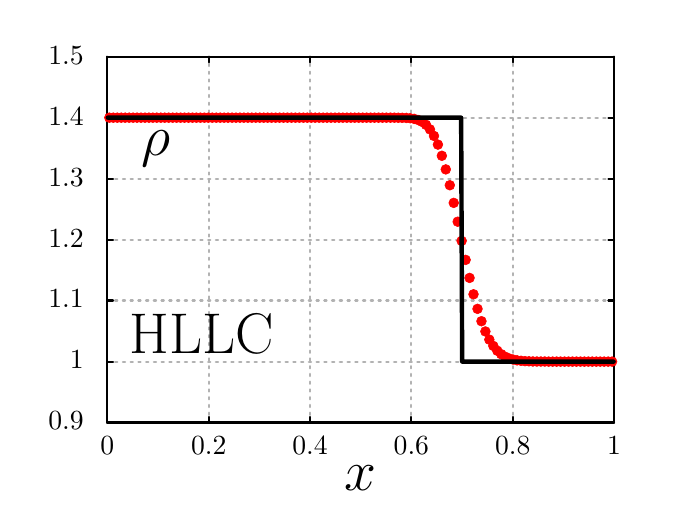
\begin{tikzpicture}[gnuplot]
%% generated with GNUPLOT 4.6p4 (Lua 5.1; terminal rev. 99, script rev. 100)
%% Tue 01 Jul 2014 11:00:07 AM EDT
\path (0.000,0.000) rectangle (8.000,6.000);
\gpfill{rgb color={1.000,1.000,1.000}} (1.012,0.985)--(7.446,0.985)--(7.446,5.630)--(1.012,5.630)--cycle;
\gpcolor{color=gp lt color border}
\gpsetlinetype{gp lt border}
\gpsetlinewidth{1.00}
\draw[gp path] (1.012,0.985)--(1.012,5.630)--(7.446,5.630)--(7.446,0.985)--cycle;
\gpcolor{color=gp lt color axes}
\gpsetlinetype{gp lt axes}
\gpsetlinewidth{2.00}
\draw[gp path] (1.012,0.985)--(7.447,0.985);
\gpcolor{color=gp lt color border}
\gpsetlinetype{gp lt border}
\draw[gp path] (1.012,0.985)--(1.084,0.985);
\draw[gp path] (7.447,0.985)--(7.375,0.985);
\gpcolor{rgb color={0.000,0.000,0.000}}
\node[gp node right,font={\fontsize{10pt}{12pt}\selectfont}] at (0.828,0.985) {0.9};
\gpcolor{color=gp lt color axes}
\gpsetlinetype{gp lt axes}
\draw[gp path] (1.012,1.759)--(7.447,1.759);
\gpcolor{color=gp lt color border}
\gpsetlinetype{gp lt border}
\draw[gp path] (1.012,1.759)--(1.084,1.759);
\draw[gp path] (7.447,1.759)--(7.375,1.759);
\gpcolor{rgb color={0.000,0.000,0.000}}
\node[gp node right,font={\fontsize{10pt}{12pt}\selectfont}] at (0.828,1.759) {1};
\gpcolor{color=gp lt color axes}
\gpsetlinetype{gp lt axes}
\draw[gp path] (1.012,2.534)--(7.447,2.534);
\gpcolor{color=gp lt color border}
\gpsetlinetype{gp lt border}
\draw[gp path] (1.012,2.534)--(1.084,2.534);
\draw[gp path] (7.447,2.534)--(7.375,2.534);
\gpcolor{rgb color={0.000,0.000,0.000}}
\node[gp node right,font={\fontsize{10pt}{12pt}\selectfont}] at (0.828,2.534) {1.1};
\gpcolor{color=gp lt color axes}
\gpsetlinetype{gp lt axes}
\draw[gp path] (1.012,3.308)--(7.447,3.308);
\gpcolor{color=gp lt color border}
\gpsetlinetype{gp lt border}
\draw[gp path] (1.012,3.308)--(1.084,3.308);
\draw[gp path] (7.447,3.308)--(7.375,3.308);
\gpcolor{rgb color={0.000,0.000,0.000}}
\node[gp node right,font={\fontsize{10pt}{12pt}\selectfont}] at (0.828,3.308) {1.2};
\gpcolor{color=gp lt color axes}
\gpsetlinetype{gp lt axes}
\draw[gp path] (1.012,4.082)--(7.447,4.082);
\gpcolor{color=gp lt color border}
\gpsetlinetype{gp lt border}
\draw[gp path] (1.012,4.082)--(1.084,4.082);
\draw[gp path] (7.447,4.082)--(7.375,4.082);
\gpcolor{rgb color={0.000,0.000,0.000}}
\node[gp node right,font={\fontsize{10pt}{12pt}\selectfont}] at (0.828,4.082) {1.3};
\gpcolor{color=gp lt color axes}
\gpsetlinetype{gp lt axes}
\draw[gp path] (1.012,4.857)--(7.447,4.857);
\gpcolor{color=gp lt color border}
\gpsetlinetype{gp lt border}
\draw[gp path] (1.012,4.857)--(1.084,4.857);
\draw[gp path] (7.447,4.857)--(7.375,4.857);
\gpcolor{rgb color={0.000,0.000,0.000}}
\node[gp node right,font={\fontsize{10pt}{12pt}\selectfont}] at (0.828,4.857) {1.4};
\gpcolor{color=gp lt color axes}
\gpsetlinetype{gp lt axes}
\draw[gp path] (1.012,5.631)--(7.447,5.631);
\gpcolor{color=gp lt color border}
\gpsetlinetype{gp lt border}
\draw[gp path] (1.012,5.631)--(1.084,5.631);
\draw[gp path] (7.447,5.631)--(7.375,5.631);
\gpcolor{rgb color={0.000,0.000,0.000}}
\node[gp node right,font={\fontsize{10pt}{12pt}\selectfont}] at (0.828,5.631) {1.5};
\gpcolor{color=gp lt color axes}
\gpsetlinetype{gp lt axes}
\draw[gp path] (1.012,0.985)--(1.012,5.631);
\gpcolor{color=gp lt color border}
\gpsetlinetype{gp lt border}
\draw[gp path] (1.012,0.985)--(1.012,1.057);
\draw[gp path] (1.012,5.631)--(1.012,5.559);
\gpcolor{rgb color={0.000,0.000,0.000}}
\node[gp node center,font={\fontsize{10pt}{12pt}\selectfont}] at (1.012,0.677) {0};
\gpcolor{color=gp lt color axes}
\gpsetlinetype{gp lt axes}
\draw[gp path] (2.299,0.985)--(2.299,5.631);
\gpcolor{color=gp lt color border}
\gpsetlinetype{gp lt border}
\draw[gp path] (2.299,0.985)--(2.299,1.057);
\draw[gp path] (2.299,5.631)--(2.299,5.559);
\gpcolor{rgb color={0.000,0.000,0.000}}
\node[gp node center,font={\fontsize{10pt}{12pt}\selectfont}] at (2.299,0.677) {0.2};
\gpcolor{color=gp lt color axes}
\gpsetlinetype{gp lt axes}
\draw[gp path] (3.586,0.985)--(3.586,5.631);
\gpcolor{color=gp lt color border}
\gpsetlinetype{gp lt border}
\draw[gp path] (3.586,0.985)--(3.586,1.057);
\draw[gp path] (3.586,5.631)--(3.586,5.559);
\gpcolor{rgb color={0.000,0.000,0.000}}
\node[gp node center,font={\fontsize{10pt}{12pt}\selectfont}] at (3.586,0.677) {0.4};
\gpcolor{color=gp lt color axes}
\gpsetlinetype{gp lt axes}
\draw[gp path] (4.873,0.985)--(4.873,5.631);
\gpcolor{color=gp lt color border}
\gpsetlinetype{gp lt border}
\draw[gp path] (4.873,0.985)--(4.873,1.057);
\draw[gp path] (4.873,5.631)--(4.873,5.559);
\gpcolor{rgb color={0.000,0.000,0.000}}
\node[gp node center,font={\fontsize{10pt}{12pt}\selectfont}] at (4.873,0.677) {0.6};
\gpcolor{color=gp lt color axes}
\gpsetlinetype{gp lt axes}
\draw[gp path] (6.160,0.985)--(6.160,5.631);
\gpcolor{color=gp lt color border}
\gpsetlinetype{gp lt border}
\draw[gp path] (6.160,0.985)--(6.160,1.057);
\draw[gp path] (6.160,5.631)--(6.160,5.559);
\gpcolor{rgb color={0.000,0.000,0.000}}
\node[gp node center,font={\fontsize{10pt}{12pt}\selectfont}] at (6.160,0.677) {0.8};
\gpcolor{color=gp lt color axes}
\gpsetlinetype{gp lt axes}
\draw[gp path] (7.447,0.985)--(7.447,5.631);
\gpcolor{color=gp lt color border}
\gpsetlinetype{gp lt border}
\draw[gp path] (7.447,0.985)--(7.447,1.057);
\draw[gp path] (7.447,5.631)--(7.447,5.559);
\gpcolor{rgb color={0.000,0.000,0.000}}
\node[gp node center,font={\fontsize{10pt}{12pt}\selectfont}] at (7.447,0.677) {1};
\gpcolor{color=gp lt color border}
\draw[gp path] (1.012,5.631)--(1.012,0.985)--(7.447,0.985)--(7.447,5.631)--cycle;
\gpcolor{rgb color={0.000,0.000,0.000}}
\node[gp node center,font={\fontsize{10pt}{12pt}\selectfont}] at (4.229,0.215) {\huge $x$};
\gpcolor{rgb color={1.000,0.000,0.000}}
\gpsetlinewidth{0.50}
\gpsetpointsize{4.44}
\gppoint{gp mark 7}{(1.037,4.857)}
\gppoint{gp mark 7}{(1.087,4.857)}
\gppoint{gp mark 7}{(1.138,4.857)}
\gppoint{gp mark 7}{(1.188,4.857)}
\gppoint{gp mark 7}{(1.238,4.857)}
\gppoint{gp mark 7}{(1.289,4.857)}
\gppoint{gp mark 7}{(1.339,4.857)}
\gppoint{gp mark 7}{(1.389,4.857)}
\gppoint{gp mark 7}{(1.439,4.857)}
\gppoint{gp mark 7}{(1.490,4.857)}
\gppoint{gp mark 7}{(1.540,4.857)}
\gppoint{gp mark 7}{(1.590,4.857)}
\gppoint{gp mark 7}{(1.640,4.857)}
\gppoint{gp mark 7}{(1.691,4.857)}
\gppoint{gp mark 7}{(1.741,4.857)}
\gppoint{gp mark 7}{(1.791,4.857)}
\gppoint{gp mark 7}{(1.842,4.857)}
\gppoint{gp mark 7}{(1.892,4.857)}
\gppoint{gp mark 7}{(1.942,4.857)}
\gppoint{gp mark 7}{(1.992,4.857)}
\gppoint{gp mark 7}{(2.043,4.857)}
\gppoint{gp mark 7}{(2.093,4.857)}
\gppoint{gp mark 7}{(2.143,4.857)}
\gppoint{gp mark 7}{(2.193,4.857)}
\gppoint{gp mark 7}{(2.244,4.857)}
\gppoint{gp mark 7}{(2.294,4.857)}
\gppoint{gp mark 7}{(2.344,4.857)}
\gppoint{gp mark 7}{(2.395,4.857)}
\gppoint{gp mark 7}{(2.445,4.857)}
\gppoint{gp mark 7}{(2.495,4.857)}
\gppoint{gp mark 7}{(2.545,4.857)}
\gppoint{gp mark 7}{(2.596,4.857)}
\gppoint{gp mark 7}{(2.646,4.857)}
\gppoint{gp mark 7}{(2.696,4.857)}
\gppoint{gp mark 7}{(2.746,4.857)}
\gppoint{gp mark 7}{(2.797,4.857)}
\gppoint{gp mark 7}{(2.847,4.857)}
\gppoint{gp mark 7}{(2.897,4.857)}
\gppoint{gp mark 7}{(2.948,4.857)}
\gppoint{gp mark 7}{(2.998,4.857)}
\gppoint{gp mark 7}{(3.048,4.857)}
\gppoint{gp mark 7}{(3.098,4.857)}
\gppoint{gp mark 7}{(3.149,4.857)}
\gppoint{gp mark 7}{(3.199,4.857)}
\gppoint{gp mark 7}{(3.249,4.857)}
\gppoint{gp mark 7}{(3.299,4.857)}
\gppoint{gp mark 7}{(3.350,4.857)}
\gppoint{gp mark 7}{(3.400,4.857)}
\gppoint{gp mark 7}{(3.450,4.857)}
\gppoint{gp mark 7}{(3.501,4.857)}
\gppoint{gp mark 7}{(3.551,4.857)}
\gppoint{gp mark 7}{(3.601,4.857)}
\gppoint{gp mark 7}{(3.651,4.857)}
\gppoint{gp mark 7}{(3.702,4.857)}
\gppoint{gp mark 7}{(3.752,4.857)}
\gppoint{gp mark 7}{(3.802,4.857)}
\gppoint{gp mark 7}{(3.852,4.857)}
\gppoint{gp mark 7}{(3.903,4.857)}
\gppoint{gp mark 7}{(3.953,4.857)}
\gppoint{gp mark 7}{(4.003,4.857)}
\gppoint{gp mark 7}{(4.054,4.857)}
\gppoint{gp mark 7}{(4.104,4.857)}
\gppoint{gp mark 7}{(4.154,4.857)}
\gppoint{gp mark 7}{(4.204,4.857)}
\gppoint{gp mark 7}{(4.255,4.857)}
\gppoint{gp mark 7}{(4.305,4.857)}
\gppoint{gp mark 7}{(4.355,4.857)}
\gppoint{gp mark 7}{(4.405,4.857)}
\gppoint{gp mark 7}{(4.456,4.857)}
\gppoint{gp mark 7}{(4.506,4.857)}
\gppoint{gp mark 7}{(4.556,4.857)}
\gppoint{gp mark 7}{(4.607,4.857)}
\gppoint{gp mark 7}{(4.657,4.857)}
\gppoint{gp mark 7}{(4.707,4.856)}
\gppoint{gp mark 7}{(4.757,4.855)}
\gppoint{gp mark 7}{(4.808,4.854)}
\gppoint{gp mark 7}{(4.858,4.850)}
\gppoint{gp mark 7}{(4.908,4.842)}
\gppoint{gp mark 7}{(4.958,4.828)}
\gppoint{gp mark 7}{(5.009,4.804)}
\gppoint{gp mark 7}{(5.059,4.766)}
\gppoint{gp mark 7}{(5.109,4.708)}
\gppoint{gp mark 7}{(5.160,4.625)}
\gppoint{gp mark 7}{(5.210,4.515)}
\gppoint{gp mark 7}{(5.260,4.373)}
\gppoint{gp mark 7}{(5.310,4.200)}
\gppoint{gp mark 7}{(5.361,3.999)}
\gppoint{gp mark 7}{(5.411,3.775)}
\gppoint{gp mark 7}{(5.461,3.536)}
\gppoint{gp mark 7}{(5.511,3.292)}
\gppoint{gp mark 7}{(5.562,3.051)}
\gppoint{gp mark 7}{(5.612,2.822)}
\gppoint{gp mark 7}{(5.662,2.614)}
\gppoint{gp mark 7}{(5.713,2.429)}
\gppoint{gp mark 7}{(5.763,2.272)}
\gppoint{gp mark 7}{(5.813,2.142)}
\gppoint{gp mark 7}{(5.863,2.038)}
\gppoint{gp mark 7}{(5.914,1.958)}
\gppoint{gp mark 7}{(5.964,1.897)}
\gppoint{gp mark 7}{(6.014,1.853)}
\gppoint{gp mark 7}{(6.064,1.821)}
\gppoint{gp mark 7}{(6.115,1.799)}
\gppoint{gp mark 7}{(6.165,1.785)}
\gppoint{gp mark 7}{(6.215,1.775)}
\gppoint{gp mark 7}{(6.266,1.769)}
\gppoint{gp mark 7}{(6.316,1.765)}
\gppoint{gp mark 7}{(6.366,1.763)}
\gppoint{gp mark 7}{(6.416,1.761)}
\gppoint{gp mark 7}{(6.467,1.760)}
\gppoint{gp mark 7}{(6.517,1.760)}
\gppoint{gp mark 7}{(6.567,1.760)}
\gppoint{gp mark 7}{(6.617,1.759)}
\gppoint{gp mark 7}{(6.668,1.759)}
\gppoint{gp mark 7}{(6.718,1.759)}
\gppoint{gp mark 7}{(6.768,1.759)}
\gppoint{gp mark 7}{(6.819,1.759)}
\gppoint{gp mark 7}{(6.869,1.759)}
\gppoint{gp mark 7}{(6.919,1.759)}
\gppoint{gp mark 7}{(6.969,1.759)}
\gppoint{gp mark 7}{(7.020,1.759)}
\gppoint{gp mark 7}{(7.070,1.759)}
\gppoint{gp mark 7}{(7.120,1.759)}
\gppoint{gp mark 7}{(7.170,1.759)}
\gppoint{gp mark 7}{(7.221,1.759)}
\gppoint{gp mark 7}{(7.271,1.759)}
\gppoint{gp mark 7}{(7.321,1.759)}
\gppoint{gp mark 7}{(7.372,1.759)}
\gppoint{gp mark 7}{(7.422,1.759)}
\gpcolor{rgb color={0.000,0.000,0.000}}
\gpsetlinetype{gp lt plot 0}
\gpsetlinewidth{4.00}
\draw[gp path] (1.018,4.857)--(1.031,4.857)--(1.043,4.857)--(1.056,4.857)--(1.069,4.857)%
  --(1.081,4.857)--(1.094,4.857)--(1.106,4.857)--(1.119,4.857)--(1.131,4.857)--(1.144,4.857)%
  --(1.157,4.857)--(1.169,4.857)--(1.182,4.857)--(1.194,4.857)--(1.207,4.857)--(1.219,4.857)%
  --(1.232,4.857)--(1.245,4.857)--(1.257,4.857)--(1.270,4.857)--(1.282,4.857)--(1.295,4.857)%
  --(1.307,4.857)--(1.320,4.857)--(1.332,4.857)--(1.345,4.857)--(1.358,4.857)--(1.370,4.857)%
  --(1.383,4.857)--(1.395,4.857)--(1.408,4.857)--(1.420,4.857)--(1.433,4.857)--(1.446,4.857)%
  --(1.458,4.857)--(1.471,4.857)--(1.483,4.857)--(1.496,4.857)--(1.508,4.857)--(1.521,4.857)%
  --(1.534,4.857)--(1.546,4.857)--(1.559,4.857)--(1.571,4.857)--(1.584,4.857)--(1.596,4.857)%
  --(1.609,4.857)--(1.622,4.857)--(1.634,4.857)--(1.647,4.857)--(1.659,4.857)--(1.672,4.857)%
  --(1.684,4.857)--(1.697,4.857)--(1.710,4.857)--(1.722,4.857)--(1.735,4.857)--(1.747,4.857)%
  --(1.760,4.857)--(1.772,4.857)--(1.785,4.857)--(1.798,4.857)--(1.810,4.857)--(1.823,4.857)%
  --(1.835,4.857)--(1.848,4.857)--(1.860,4.857)--(1.873,4.857)--(1.886,4.857)--(1.898,4.857)%
  --(1.911,4.857)--(1.923,4.857)--(1.936,4.857)--(1.948,4.857)--(1.961,4.857)--(1.973,4.857)%
  --(1.986,4.857)--(1.999,4.857)--(2.011,4.857)--(2.024,4.857)--(2.036,4.857)--(2.049,4.857)%
  --(2.061,4.857)--(2.074,4.857)--(2.087,4.857)--(2.099,4.857)--(2.112,4.857)--(2.124,4.857)%
  --(2.137,4.857)--(2.149,4.857)--(2.162,4.857)--(2.175,4.857)--(2.187,4.857)--(2.200,4.857)%
  --(2.212,4.857)--(2.225,4.857)--(2.237,4.857)--(2.250,4.857)--(2.263,4.857)--(2.275,4.857)%
  --(2.288,4.857)--(2.300,4.857)--(2.313,4.857)--(2.325,4.857)--(2.338,4.857)--(2.351,4.857)%
  --(2.363,4.857)--(2.376,4.857)--(2.388,4.857)--(2.401,4.857)--(2.413,4.857)--(2.426,4.857)%
  --(2.439,4.857)--(2.451,4.857)--(2.464,4.857)--(2.476,4.857)--(2.489,4.857)--(2.501,4.857)%
  --(2.514,4.857)--(2.526,4.857)--(2.539,4.857)--(2.552,4.857)--(2.564,4.857)--(2.577,4.857)%
  --(2.589,4.857)--(2.602,4.857)--(2.614,4.857)--(2.627,4.857)--(2.640,4.857)--(2.652,4.857)%
  --(2.665,4.857)--(2.677,4.857)--(2.690,4.857)--(2.702,4.857)--(2.715,4.857)--(2.728,4.857)%
  --(2.740,4.857)--(2.753,4.857)--(2.765,4.857)--(2.778,4.857)--(2.790,4.857)--(2.803,4.857)%
  --(2.816,4.857)--(2.828,4.857)--(2.841,4.857)--(2.853,4.857)--(2.866,4.857)--(2.878,4.857)%
  --(2.891,4.857)--(2.904,4.857)--(2.916,4.857)--(2.929,4.857)--(2.941,4.857)--(2.954,4.857)%
  --(2.966,4.857)--(2.979,4.857)--(2.992,4.857)--(3.004,4.857)--(3.017,4.857)--(3.029,4.857)%
  --(3.042,4.857)--(3.054,4.857)--(3.067,4.857)--(3.079,4.857)--(3.092,4.857)--(3.105,4.857)%
  --(3.117,4.857)--(3.130,4.857)--(3.142,4.857)--(3.155,4.857)--(3.167,4.857)--(3.180,4.857)%
  --(3.193,4.857)--(3.205,4.857)--(3.218,4.857)--(3.230,4.857)--(3.243,4.857)--(3.255,4.857)%
  --(3.268,4.857)--(3.281,4.857)--(3.293,4.857)--(3.306,4.857)--(3.318,4.857)--(3.331,4.857)%
  --(3.343,4.857)--(3.356,4.857)--(3.369,4.857)--(3.381,4.857)--(3.394,4.857)--(3.406,4.857)%
  --(3.419,4.857)--(3.431,4.857)--(3.444,4.857)--(3.457,4.857)--(3.469,4.857)--(3.482,4.857)%
  --(3.494,4.857)--(3.507,4.857)--(3.519,4.857)--(3.532,4.857)--(3.545,4.857)--(3.557,4.857)%
  --(3.570,4.857)--(3.582,4.857)--(3.595,4.857)--(3.607,4.857)--(3.620,4.857)--(3.633,4.857)%
  --(3.645,4.857)--(3.658,4.857)--(3.670,4.857)--(3.683,4.857)--(3.695,4.857)--(3.708,4.857)%
  --(3.720,4.857)--(3.733,4.857)--(3.746,4.857)--(3.758,4.857)--(3.771,4.857)--(3.783,4.857)%
  --(3.796,4.857)--(3.808,4.857)--(3.821,4.857)--(3.834,4.857)--(3.846,4.857)--(3.859,4.857)%
  --(3.871,4.857)--(3.884,4.857)--(3.896,4.857)--(3.909,4.857)--(3.922,4.857)--(3.934,4.857)%
  --(3.947,4.857)--(3.959,4.857)--(3.972,4.857)--(3.984,4.857)--(3.997,4.857)--(4.010,4.857)%
  --(4.022,4.857)--(4.035,4.857)--(4.047,4.857)--(4.060,4.857)--(4.072,4.857)--(4.085,4.857)%
  --(4.098,4.857)--(4.110,4.857)--(4.123,4.857)--(4.135,4.857)--(4.148,4.857)--(4.160,4.857)%
  --(4.173,4.857)--(4.186,4.857)--(4.198,4.857)--(4.211,4.857)--(4.223,4.857)--(4.236,4.857)%
  --(4.248,4.857)--(4.261,4.857)--(4.273,4.857)--(4.286,4.857)--(4.299,4.857)--(4.311,4.857)%
  --(4.324,4.857)--(4.336,4.857)--(4.349,4.857)--(4.361,4.857)--(4.374,4.857)--(4.387,4.857)%
  --(4.399,4.857)--(4.412,4.857)--(4.424,4.857)--(4.437,4.857)--(4.449,4.857)--(4.462,4.857)%
  --(4.475,4.857)--(4.487,4.857)--(4.500,4.857)--(4.512,4.857)--(4.525,4.857)--(4.537,4.857)%
  --(4.550,4.857)--(4.563,4.857)--(4.575,4.857)--(4.588,4.857)--(4.600,4.857)--(4.613,4.857)%
  --(4.625,4.857)--(4.638,4.857)--(4.651,4.857)--(4.663,4.857)--(4.676,4.857)--(4.688,4.857)%
  --(4.701,4.857)--(4.713,4.857)--(4.726,4.857)--(4.739,4.857)--(4.751,4.857)--(4.764,4.857)%
  --(4.776,4.857)--(4.789,4.857)--(4.801,4.857)--(4.814,4.857)--(4.826,4.857)--(4.839,4.857)%
  --(4.852,4.857)--(4.864,4.857)--(4.877,4.857)--(4.889,4.857)--(4.902,4.857)--(4.914,4.857)%
  --(4.927,4.857)--(4.940,4.857)--(4.952,4.857)--(4.965,4.857)--(4.977,4.857)--(4.990,4.857)%
  --(5.002,4.857)--(5.015,4.857)--(5.028,4.857)--(5.040,4.857)--(5.053,4.857)--(5.065,4.857)%
  --(5.078,4.857)--(5.090,4.857)--(5.103,4.857)--(5.116,4.857)--(5.128,4.857)--(5.141,4.857)%
  --(5.153,4.857)--(5.166,4.857)--(5.178,4.857)--(5.191,4.857)--(5.204,4.857)--(5.216,4.857)%
  --(5.229,4.857)--(5.241,4.857)--(5.254,4.857)--(5.266,4.857)--(5.279,4.857)--(5.292,4.857)%
  --(5.304,4.857)--(5.317,4.857)--(5.329,4.857)--(5.342,4.857)--(5.354,4.857)--(5.367,4.857)%
  --(5.380,4.857)--(5.392,4.857)--(5.405,4.857)--(5.417,4.857)--(5.430,4.857)--(5.442,4.857)%
  --(5.455,4.857)--(5.467,4.857)--(5.480,4.857)--(5.493,4.857)--(5.505,4.857)--(5.518,1.759)%
  --(5.530,1.759)--(5.543,1.759)--(5.555,1.759)--(5.568,1.759)--(5.581,1.759)--(5.593,1.759)%
  --(5.606,1.759)--(5.618,1.759)--(5.631,1.759)--(5.643,1.759)--(5.656,1.759)--(5.669,1.759)%
  --(5.681,1.759)--(5.694,1.759)--(5.706,1.759)--(5.719,1.759)--(5.731,1.759)--(5.744,1.759)%
  --(5.757,1.759)--(5.769,1.759)--(5.782,1.759)--(5.794,1.759)--(5.807,1.759)--(5.819,1.759)%
  --(5.832,1.759)--(5.845,1.759)--(5.857,1.759)--(5.870,1.759)--(5.882,1.759)--(5.895,1.759)%
  --(5.907,1.759)--(5.920,1.759)--(5.933,1.759)--(5.945,1.759)--(5.958,1.759)--(5.970,1.759)%
  --(5.983,1.759)--(5.995,1.759)--(6.008,1.759)--(6.020,1.759)--(6.033,1.759)--(6.046,1.759)%
  --(6.058,1.759)--(6.071,1.759)--(6.083,1.759)--(6.096,1.759)--(6.108,1.759)--(6.121,1.759)%
  --(6.134,1.759)--(6.146,1.759)--(6.159,1.759)--(6.171,1.759)--(6.184,1.759)--(6.196,1.759)%
  --(6.209,1.759)--(6.222,1.759)--(6.234,1.759)--(6.247,1.759)--(6.259,1.759)--(6.272,1.759)%
  --(6.284,1.759)--(6.297,1.759)--(6.310,1.759)--(6.322,1.759)--(6.335,1.759)--(6.347,1.759)%
  --(6.360,1.759)--(6.372,1.759)--(6.385,1.759)--(6.398,1.759)--(6.410,1.759)--(6.423,1.759)%
  --(6.435,1.759)--(6.448,1.759)--(6.460,1.759)--(6.473,1.759)--(6.486,1.759)--(6.498,1.759)%
  --(6.511,1.759)--(6.523,1.759)--(6.536,1.759)--(6.548,1.759)--(6.561,1.759)--(6.573,1.759)%
  --(6.586,1.759)--(6.599,1.759)--(6.611,1.759)--(6.624,1.759)--(6.636,1.759)--(6.649,1.759)%
  --(6.661,1.759)--(6.674,1.759)--(6.687,1.759)--(6.699,1.759)--(6.712,1.759)--(6.724,1.759)%
  --(6.737,1.759)--(6.749,1.759)--(6.762,1.759)--(6.775,1.759)--(6.787,1.759)--(6.800,1.759)%
  --(6.812,1.759)--(6.825,1.759)--(6.837,1.759)--(6.850,1.759)--(6.863,1.759)--(6.875,1.759)%
  --(6.888,1.759)--(6.900,1.759)--(6.913,1.759)--(6.925,1.759)--(6.938,1.759)--(6.951,1.759)%
  --(6.963,1.759)--(6.976,1.759)--(6.988,1.759)--(7.001,1.759)--(7.013,1.759)--(7.026,1.759)%
  --(7.039,1.759)--(7.051,1.759)--(7.064,1.759)--(7.076,1.759)--(7.089,1.759)--(7.101,1.759)%
  --(7.114,1.759)--(7.127,1.759)--(7.139,1.759)--(7.152,1.759)--(7.164,1.759)--(7.177,1.759)%
  --(7.189,1.759)--(7.202,1.759)--(7.214,1.759)--(7.227,1.759)--(7.240,1.759)--(7.252,1.759)%
  --(7.265,1.759)--(7.277,1.759)--(7.290,1.759)--(7.302,1.759)--(7.315,1.759)--(7.328,1.759)%
  --(7.340,1.759)--(7.353,1.759)--(7.365,1.759)--(7.378,1.759)--(7.390,1.759)--(7.403,1.759)%
  --(7.416,1.759)--(7.428,1.759)--(7.441,1.759);
\node[gp node left,font={\fontsize{10pt}{12pt}\selectfont}] at (1.334,4.470) {\huge $\rho$};
\node[gp node left,font={\fontsize{10pt}{12pt}\selectfont}] at (1.173,1.953) {\huge HLLC};
%% coordinates of the plot area
\gpdefrectangularnode{gp plot 1}{\pgfpoint{1.012cm}{0.985cm}}{\pgfpoint{7.447cm}{5.631cm}}
\end{tikzpicture}
%% gnuplot variables
} 
%% \resizebox{0.33\linewidth}{!}{\tikzsetnextfilename{toro7_roe_1}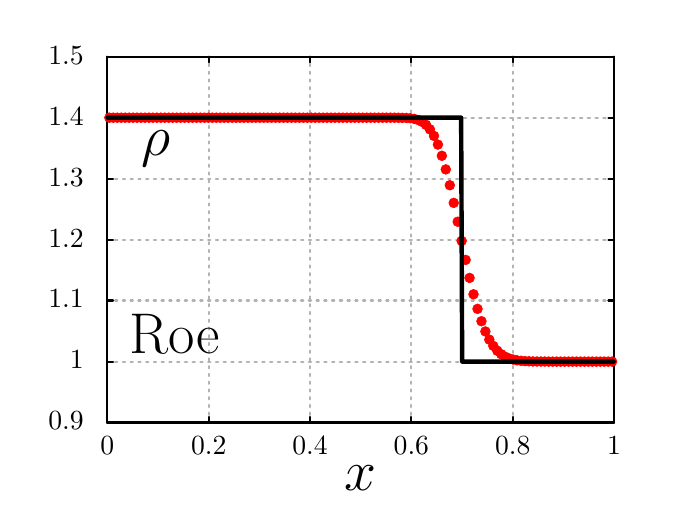
\begin{tikzpicture}[gnuplot]
%% generated with GNUPLOT 4.6p4 (Lua 5.1; terminal rev. 99, script rev. 100)
%% Tue 01 Jul 2014 10:59:44 AM EDT
\path (0.000,0.000) rectangle (8.000,6.000);
\gpfill{rgb color={1.000,1.000,1.000}} (1.012,0.985)--(7.446,0.985)--(7.446,5.630)--(1.012,5.630)--cycle;
\gpcolor{color=gp lt color border}
\gpsetlinetype{gp lt border}
\gpsetlinewidth{1.00}
\draw[gp path] (1.012,0.985)--(1.012,5.630)--(7.446,5.630)--(7.446,0.985)--cycle;
\gpcolor{color=gp lt color axes}
\gpsetlinetype{gp lt axes}
\gpsetlinewidth{2.00}
\draw[gp path] (1.012,0.985)--(7.447,0.985);
\gpcolor{color=gp lt color border}
\gpsetlinetype{gp lt border}
\draw[gp path] (1.012,0.985)--(1.084,0.985);
\draw[gp path] (7.447,0.985)--(7.375,0.985);
\gpcolor{rgb color={0.000,0.000,0.000}}
\node[gp node right,font={\fontsize{10pt}{12pt}\selectfont}] at (0.828,0.985) {0.9};
\gpcolor{color=gp lt color axes}
\gpsetlinetype{gp lt axes}
\draw[gp path] (1.012,1.759)--(7.447,1.759);
\gpcolor{color=gp lt color border}
\gpsetlinetype{gp lt border}
\draw[gp path] (1.012,1.759)--(1.084,1.759);
\draw[gp path] (7.447,1.759)--(7.375,1.759);
\gpcolor{rgb color={0.000,0.000,0.000}}
\node[gp node right,font={\fontsize{10pt}{12pt}\selectfont}] at (0.828,1.759) {1};
\gpcolor{color=gp lt color axes}
\gpsetlinetype{gp lt axes}
\draw[gp path] (1.012,2.534)--(7.447,2.534);
\gpcolor{color=gp lt color border}
\gpsetlinetype{gp lt border}
\draw[gp path] (1.012,2.534)--(1.084,2.534);
\draw[gp path] (7.447,2.534)--(7.375,2.534);
\gpcolor{rgb color={0.000,0.000,0.000}}
\node[gp node right,font={\fontsize{10pt}{12pt}\selectfont}] at (0.828,2.534) {1.1};
\gpcolor{color=gp lt color axes}
\gpsetlinetype{gp lt axes}
\draw[gp path] (1.012,3.308)--(7.447,3.308);
\gpcolor{color=gp lt color border}
\gpsetlinetype{gp lt border}
\draw[gp path] (1.012,3.308)--(1.084,3.308);
\draw[gp path] (7.447,3.308)--(7.375,3.308);
\gpcolor{rgb color={0.000,0.000,0.000}}
\node[gp node right,font={\fontsize{10pt}{12pt}\selectfont}] at (0.828,3.308) {1.2};
\gpcolor{color=gp lt color axes}
\gpsetlinetype{gp lt axes}
\draw[gp path] (1.012,4.082)--(7.447,4.082);
\gpcolor{color=gp lt color border}
\gpsetlinetype{gp lt border}
\draw[gp path] (1.012,4.082)--(1.084,4.082);
\draw[gp path] (7.447,4.082)--(7.375,4.082);
\gpcolor{rgb color={0.000,0.000,0.000}}
\node[gp node right,font={\fontsize{10pt}{12pt}\selectfont}] at (0.828,4.082) {1.3};
\gpcolor{color=gp lt color axes}
\gpsetlinetype{gp lt axes}
\draw[gp path] (1.012,4.857)--(7.447,4.857);
\gpcolor{color=gp lt color border}
\gpsetlinetype{gp lt border}
\draw[gp path] (1.012,4.857)--(1.084,4.857);
\draw[gp path] (7.447,4.857)--(7.375,4.857);
\gpcolor{rgb color={0.000,0.000,0.000}}
\node[gp node right,font={\fontsize{10pt}{12pt}\selectfont}] at (0.828,4.857) {1.4};
\gpcolor{color=gp lt color axes}
\gpsetlinetype{gp lt axes}
\draw[gp path] (1.012,5.631)--(7.447,5.631);
\gpcolor{color=gp lt color border}
\gpsetlinetype{gp lt border}
\draw[gp path] (1.012,5.631)--(1.084,5.631);
\draw[gp path] (7.447,5.631)--(7.375,5.631);
\gpcolor{rgb color={0.000,0.000,0.000}}
\node[gp node right,font={\fontsize{10pt}{12pt}\selectfont}] at (0.828,5.631) {1.5};
\gpcolor{color=gp lt color axes}
\gpsetlinetype{gp lt axes}
\draw[gp path] (1.012,0.985)--(1.012,5.631);
\gpcolor{color=gp lt color border}
\gpsetlinetype{gp lt border}
\draw[gp path] (1.012,0.985)--(1.012,1.057);
\draw[gp path] (1.012,5.631)--(1.012,5.559);
\gpcolor{rgb color={0.000,0.000,0.000}}
\node[gp node center,font={\fontsize{10pt}{12pt}\selectfont}] at (1.012,0.677) {0};
\gpcolor{color=gp lt color axes}
\gpsetlinetype{gp lt axes}
\draw[gp path] (2.299,0.985)--(2.299,5.631);
\gpcolor{color=gp lt color border}
\gpsetlinetype{gp lt border}
\draw[gp path] (2.299,0.985)--(2.299,1.057);
\draw[gp path] (2.299,5.631)--(2.299,5.559);
\gpcolor{rgb color={0.000,0.000,0.000}}
\node[gp node center,font={\fontsize{10pt}{12pt}\selectfont}] at (2.299,0.677) {0.2};
\gpcolor{color=gp lt color axes}
\gpsetlinetype{gp lt axes}
\draw[gp path] (3.586,0.985)--(3.586,5.631);
\gpcolor{color=gp lt color border}
\gpsetlinetype{gp lt border}
\draw[gp path] (3.586,0.985)--(3.586,1.057);
\draw[gp path] (3.586,5.631)--(3.586,5.559);
\gpcolor{rgb color={0.000,0.000,0.000}}
\node[gp node center,font={\fontsize{10pt}{12pt}\selectfont}] at (3.586,0.677) {0.4};
\gpcolor{color=gp lt color axes}
\gpsetlinetype{gp lt axes}
\draw[gp path] (4.873,0.985)--(4.873,5.631);
\gpcolor{color=gp lt color border}
\gpsetlinetype{gp lt border}
\draw[gp path] (4.873,0.985)--(4.873,1.057);
\draw[gp path] (4.873,5.631)--(4.873,5.559);
\gpcolor{rgb color={0.000,0.000,0.000}}
\node[gp node center,font={\fontsize{10pt}{12pt}\selectfont}] at (4.873,0.677) {0.6};
\gpcolor{color=gp lt color axes}
\gpsetlinetype{gp lt axes}
\draw[gp path] (6.160,0.985)--(6.160,5.631);
\gpcolor{color=gp lt color border}
\gpsetlinetype{gp lt border}
\draw[gp path] (6.160,0.985)--(6.160,1.057);
\draw[gp path] (6.160,5.631)--(6.160,5.559);
\gpcolor{rgb color={0.000,0.000,0.000}}
\node[gp node center,font={\fontsize{10pt}{12pt}\selectfont}] at (6.160,0.677) {0.8};
\gpcolor{color=gp lt color axes}
\gpsetlinetype{gp lt axes}
\draw[gp path] (7.447,0.985)--(7.447,5.631);
\gpcolor{color=gp lt color border}
\gpsetlinetype{gp lt border}
\draw[gp path] (7.447,0.985)--(7.447,1.057);
\draw[gp path] (7.447,5.631)--(7.447,5.559);
\gpcolor{rgb color={0.000,0.000,0.000}}
\node[gp node center,font={\fontsize{10pt}{12pt}\selectfont}] at (7.447,0.677) {1};
\gpcolor{color=gp lt color border}
\draw[gp path] (1.012,5.631)--(1.012,0.985)--(7.447,0.985)--(7.447,5.631)--cycle;
\gpcolor{rgb color={0.000,0.000,0.000}}
\node[gp node center,font={\fontsize{10pt}{12pt}\selectfont}] at (4.229,0.215) {\huge $x$};
\gpcolor{rgb color={1.000,0.000,0.000}}
\gpsetlinewidth{0.50}
\gpsetpointsize{4.44}
\gppoint{gp mark 7}{(1.037,4.857)}
\gppoint{gp mark 7}{(1.087,4.857)}
\gppoint{gp mark 7}{(1.138,4.857)}
\gppoint{gp mark 7}{(1.188,4.857)}
\gppoint{gp mark 7}{(1.238,4.857)}
\gppoint{gp mark 7}{(1.289,4.857)}
\gppoint{gp mark 7}{(1.339,4.857)}
\gppoint{gp mark 7}{(1.389,4.857)}
\gppoint{gp mark 7}{(1.439,4.857)}
\gppoint{gp mark 7}{(1.490,4.857)}
\gppoint{gp mark 7}{(1.540,4.857)}
\gppoint{gp mark 7}{(1.590,4.857)}
\gppoint{gp mark 7}{(1.640,4.857)}
\gppoint{gp mark 7}{(1.691,4.857)}
\gppoint{gp mark 7}{(1.741,4.857)}
\gppoint{gp mark 7}{(1.791,4.857)}
\gppoint{gp mark 7}{(1.842,4.857)}
\gppoint{gp mark 7}{(1.892,4.857)}
\gppoint{gp mark 7}{(1.942,4.857)}
\gppoint{gp mark 7}{(1.992,4.857)}
\gppoint{gp mark 7}{(2.043,4.857)}
\gppoint{gp mark 7}{(2.093,4.857)}
\gppoint{gp mark 7}{(2.143,4.857)}
\gppoint{gp mark 7}{(2.193,4.857)}
\gppoint{gp mark 7}{(2.244,4.857)}
\gppoint{gp mark 7}{(2.294,4.857)}
\gppoint{gp mark 7}{(2.344,4.857)}
\gppoint{gp mark 7}{(2.395,4.857)}
\gppoint{gp mark 7}{(2.445,4.857)}
\gppoint{gp mark 7}{(2.495,4.857)}
\gppoint{gp mark 7}{(2.545,4.857)}
\gppoint{gp mark 7}{(2.596,4.857)}
\gppoint{gp mark 7}{(2.646,4.857)}
\gppoint{gp mark 7}{(2.696,4.857)}
\gppoint{gp mark 7}{(2.746,4.857)}
\gppoint{gp mark 7}{(2.797,4.857)}
\gppoint{gp mark 7}{(2.847,4.857)}
\gppoint{gp mark 7}{(2.897,4.857)}
\gppoint{gp mark 7}{(2.948,4.857)}
\gppoint{gp mark 7}{(2.998,4.857)}
\gppoint{gp mark 7}{(3.048,4.857)}
\gppoint{gp mark 7}{(3.098,4.857)}
\gppoint{gp mark 7}{(3.149,4.857)}
\gppoint{gp mark 7}{(3.199,4.857)}
\gppoint{gp mark 7}{(3.249,4.857)}
\gppoint{gp mark 7}{(3.299,4.857)}
\gppoint{gp mark 7}{(3.350,4.857)}
\gppoint{gp mark 7}{(3.400,4.857)}
\gppoint{gp mark 7}{(3.450,4.857)}
\gppoint{gp mark 7}{(3.501,4.857)}
\gppoint{gp mark 7}{(3.551,4.857)}
\gppoint{gp mark 7}{(3.601,4.857)}
\gppoint{gp mark 7}{(3.651,4.857)}
\gppoint{gp mark 7}{(3.702,4.857)}
\gppoint{gp mark 7}{(3.752,4.857)}
\gppoint{gp mark 7}{(3.802,4.857)}
\gppoint{gp mark 7}{(3.852,4.857)}
\gppoint{gp mark 7}{(3.903,4.857)}
\gppoint{gp mark 7}{(3.953,4.857)}
\gppoint{gp mark 7}{(4.003,4.857)}
\gppoint{gp mark 7}{(4.054,4.857)}
\gppoint{gp mark 7}{(4.104,4.857)}
\gppoint{gp mark 7}{(4.154,4.857)}
\gppoint{gp mark 7}{(4.204,4.857)}
\gppoint{gp mark 7}{(4.255,4.857)}
\gppoint{gp mark 7}{(4.305,4.857)}
\gppoint{gp mark 7}{(4.355,4.857)}
\gppoint{gp mark 7}{(4.405,4.857)}
\gppoint{gp mark 7}{(4.456,4.857)}
\gppoint{gp mark 7}{(4.506,4.857)}
\gppoint{gp mark 7}{(4.556,4.857)}
\gppoint{gp mark 7}{(4.607,4.857)}
\gppoint{gp mark 7}{(4.657,4.857)}
\gppoint{gp mark 7}{(4.707,4.856)}
\gppoint{gp mark 7}{(4.757,4.855)}
\gppoint{gp mark 7}{(4.808,4.854)}
\gppoint{gp mark 7}{(4.858,4.850)}
\gppoint{gp mark 7}{(4.908,4.842)}
\gppoint{gp mark 7}{(4.958,4.828)}
\gppoint{gp mark 7}{(5.009,4.804)}
\gppoint{gp mark 7}{(5.059,4.766)}
\gppoint{gp mark 7}{(5.109,4.708)}
\gppoint{gp mark 7}{(5.160,4.625)}
\gppoint{gp mark 7}{(5.210,4.515)}
\gppoint{gp mark 7}{(5.260,4.373)}
\gppoint{gp mark 7}{(5.310,4.200)}
\gppoint{gp mark 7}{(5.361,3.999)}
\gppoint{gp mark 7}{(5.411,3.775)}
\gppoint{gp mark 7}{(5.461,3.536)}
\gppoint{gp mark 7}{(5.511,3.292)}
\gppoint{gp mark 7}{(5.562,3.051)}
\gppoint{gp mark 7}{(5.612,2.822)}
\gppoint{gp mark 7}{(5.662,2.614)}
\gppoint{gp mark 7}{(5.713,2.429)}
\gppoint{gp mark 7}{(5.763,2.272)}
\gppoint{gp mark 7}{(5.813,2.142)}
\gppoint{gp mark 7}{(5.863,2.038)}
\gppoint{gp mark 7}{(5.914,1.958)}
\gppoint{gp mark 7}{(5.964,1.897)}
\gppoint{gp mark 7}{(6.014,1.853)}
\gppoint{gp mark 7}{(6.064,1.821)}
\gppoint{gp mark 7}{(6.115,1.799)}
\gppoint{gp mark 7}{(6.165,1.785)}
\gppoint{gp mark 7}{(6.215,1.775)}
\gppoint{gp mark 7}{(6.266,1.769)}
\gppoint{gp mark 7}{(6.316,1.765)}
\gppoint{gp mark 7}{(6.366,1.763)}
\gppoint{gp mark 7}{(6.416,1.761)}
\gppoint{gp mark 7}{(6.467,1.760)}
\gppoint{gp mark 7}{(6.517,1.760)}
\gppoint{gp mark 7}{(6.567,1.760)}
\gppoint{gp mark 7}{(6.617,1.759)}
\gppoint{gp mark 7}{(6.668,1.759)}
\gppoint{gp mark 7}{(6.718,1.759)}
\gppoint{gp mark 7}{(6.768,1.759)}
\gppoint{gp mark 7}{(6.819,1.759)}
\gppoint{gp mark 7}{(6.869,1.759)}
\gppoint{gp mark 7}{(6.919,1.759)}
\gppoint{gp mark 7}{(6.969,1.759)}
\gppoint{gp mark 7}{(7.020,1.759)}
\gppoint{gp mark 7}{(7.070,1.759)}
\gppoint{gp mark 7}{(7.120,1.759)}
\gppoint{gp mark 7}{(7.170,1.759)}
\gppoint{gp mark 7}{(7.221,1.759)}
\gppoint{gp mark 7}{(7.271,1.759)}
\gppoint{gp mark 7}{(7.321,1.759)}
\gppoint{gp mark 7}{(7.372,1.759)}
\gppoint{gp mark 7}{(7.422,1.759)}
\gpcolor{rgb color={0.000,0.000,0.000}}
\gpsetlinetype{gp lt plot 0}
\gpsetlinewidth{4.00}
\draw[gp path] (1.018,4.857)--(1.031,4.857)--(1.043,4.857)--(1.056,4.857)--(1.069,4.857)%
  --(1.081,4.857)--(1.094,4.857)--(1.106,4.857)--(1.119,4.857)--(1.131,4.857)--(1.144,4.857)%
  --(1.157,4.857)--(1.169,4.857)--(1.182,4.857)--(1.194,4.857)--(1.207,4.857)--(1.219,4.857)%
  --(1.232,4.857)--(1.245,4.857)--(1.257,4.857)--(1.270,4.857)--(1.282,4.857)--(1.295,4.857)%
  --(1.307,4.857)--(1.320,4.857)--(1.332,4.857)--(1.345,4.857)--(1.358,4.857)--(1.370,4.857)%
  --(1.383,4.857)--(1.395,4.857)--(1.408,4.857)--(1.420,4.857)--(1.433,4.857)--(1.446,4.857)%
  --(1.458,4.857)--(1.471,4.857)--(1.483,4.857)--(1.496,4.857)--(1.508,4.857)--(1.521,4.857)%
  --(1.534,4.857)--(1.546,4.857)--(1.559,4.857)--(1.571,4.857)--(1.584,4.857)--(1.596,4.857)%
  --(1.609,4.857)--(1.622,4.857)--(1.634,4.857)--(1.647,4.857)--(1.659,4.857)--(1.672,4.857)%
  --(1.684,4.857)--(1.697,4.857)--(1.710,4.857)--(1.722,4.857)--(1.735,4.857)--(1.747,4.857)%
  --(1.760,4.857)--(1.772,4.857)--(1.785,4.857)--(1.798,4.857)--(1.810,4.857)--(1.823,4.857)%
  --(1.835,4.857)--(1.848,4.857)--(1.860,4.857)--(1.873,4.857)--(1.886,4.857)--(1.898,4.857)%
  --(1.911,4.857)--(1.923,4.857)--(1.936,4.857)--(1.948,4.857)--(1.961,4.857)--(1.973,4.857)%
  --(1.986,4.857)--(1.999,4.857)--(2.011,4.857)--(2.024,4.857)--(2.036,4.857)--(2.049,4.857)%
  --(2.061,4.857)--(2.074,4.857)--(2.087,4.857)--(2.099,4.857)--(2.112,4.857)--(2.124,4.857)%
  --(2.137,4.857)--(2.149,4.857)--(2.162,4.857)--(2.175,4.857)--(2.187,4.857)--(2.200,4.857)%
  --(2.212,4.857)--(2.225,4.857)--(2.237,4.857)--(2.250,4.857)--(2.263,4.857)--(2.275,4.857)%
  --(2.288,4.857)--(2.300,4.857)--(2.313,4.857)--(2.325,4.857)--(2.338,4.857)--(2.351,4.857)%
  --(2.363,4.857)--(2.376,4.857)--(2.388,4.857)--(2.401,4.857)--(2.413,4.857)--(2.426,4.857)%
  --(2.439,4.857)--(2.451,4.857)--(2.464,4.857)--(2.476,4.857)--(2.489,4.857)--(2.501,4.857)%
  --(2.514,4.857)--(2.526,4.857)--(2.539,4.857)--(2.552,4.857)--(2.564,4.857)--(2.577,4.857)%
  --(2.589,4.857)--(2.602,4.857)--(2.614,4.857)--(2.627,4.857)--(2.640,4.857)--(2.652,4.857)%
  --(2.665,4.857)--(2.677,4.857)--(2.690,4.857)--(2.702,4.857)--(2.715,4.857)--(2.728,4.857)%
  --(2.740,4.857)--(2.753,4.857)--(2.765,4.857)--(2.778,4.857)--(2.790,4.857)--(2.803,4.857)%
  --(2.816,4.857)--(2.828,4.857)--(2.841,4.857)--(2.853,4.857)--(2.866,4.857)--(2.878,4.857)%
  --(2.891,4.857)--(2.904,4.857)--(2.916,4.857)--(2.929,4.857)--(2.941,4.857)--(2.954,4.857)%
  --(2.966,4.857)--(2.979,4.857)--(2.992,4.857)--(3.004,4.857)--(3.017,4.857)--(3.029,4.857)%
  --(3.042,4.857)--(3.054,4.857)--(3.067,4.857)--(3.079,4.857)--(3.092,4.857)--(3.105,4.857)%
  --(3.117,4.857)--(3.130,4.857)--(3.142,4.857)--(3.155,4.857)--(3.167,4.857)--(3.180,4.857)%
  --(3.193,4.857)--(3.205,4.857)--(3.218,4.857)--(3.230,4.857)--(3.243,4.857)--(3.255,4.857)%
  --(3.268,4.857)--(3.281,4.857)--(3.293,4.857)--(3.306,4.857)--(3.318,4.857)--(3.331,4.857)%
  --(3.343,4.857)--(3.356,4.857)--(3.369,4.857)--(3.381,4.857)--(3.394,4.857)--(3.406,4.857)%
  --(3.419,4.857)--(3.431,4.857)--(3.444,4.857)--(3.457,4.857)--(3.469,4.857)--(3.482,4.857)%
  --(3.494,4.857)--(3.507,4.857)--(3.519,4.857)--(3.532,4.857)--(3.545,4.857)--(3.557,4.857)%
  --(3.570,4.857)--(3.582,4.857)--(3.595,4.857)--(3.607,4.857)--(3.620,4.857)--(3.633,4.857)%
  --(3.645,4.857)--(3.658,4.857)--(3.670,4.857)--(3.683,4.857)--(3.695,4.857)--(3.708,4.857)%
  --(3.720,4.857)--(3.733,4.857)--(3.746,4.857)--(3.758,4.857)--(3.771,4.857)--(3.783,4.857)%
  --(3.796,4.857)--(3.808,4.857)--(3.821,4.857)--(3.834,4.857)--(3.846,4.857)--(3.859,4.857)%
  --(3.871,4.857)--(3.884,4.857)--(3.896,4.857)--(3.909,4.857)--(3.922,4.857)--(3.934,4.857)%
  --(3.947,4.857)--(3.959,4.857)--(3.972,4.857)--(3.984,4.857)--(3.997,4.857)--(4.010,4.857)%
  --(4.022,4.857)--(4.035,4.857)--(4.047,4.857)--(4.060,4.857)--(4.072,4.857)--(4.085,4.857)%
  --(4.098,4.857)--(4.110,4.857)--(4.123,4.857)--(4.135,4.857)--(4.148,4.857)--(4.160,4.857)%
  --(4.173,4.857)--(4.186,4.857)--(4.198,4.857)--(4.211,4.857)--(4.223,4.857)--(4.236,4.857)%
  --(4.248,4.857)--(4.261,4.857)--(4.273,4.857)--(4.286,4.857)--(4.299,4.857)--(4.311,4.857)%
  --(4.324,4.857)--(4.336,4.857)--(4.349,4.857)--(4.361,4.857)--(4.374,4.857)--(4.387,4.857)%
  --(4.399,4.857)--(4.412,4.857)--(4.424,4.857)--(4.437,4.857)--(4.449,4.857)--(4.462,4.857)%
  --(4.475,4.857)--(4.487,4.857)--(4.500,4.857)--(4.512,4.857)--(4.525,4.857)--(4.537,4.857)%
  --(4.550,4.857)--(4.563,4.857)--(4.575,4.857)--(4.588,4.857)--(4.600,4.857)--(4.613,4.857)%
  --(4.625,4.857)--(4.638,4.857)--(4.651,4.857)--(4.663,4.857)--(4.676,4.857)--(4.688,4.857)%
  --(4.701,4.857)--(4.713,4.857)--(4.726,4.857)--(4.739,4.857)--(4.751,4.857)--(4.764,4.857)%
  --(4.776,4.857)--(4.789,4.857)--(4.801,4.857)--(4.814,4.857)--(4.826,4.857)--(4.839,4.857)%
  --(4.852,4.857)--(4.864,4.857)--(4.877,4.857)--(4.889,4.857)--(4.902,4.857)--(4.914,4.857)%
  --(4.927,4.857)--(4.940,4.857)--(4.952,4.857)--(4.965,4.857)--(4.977,4.857)--(4.990,4.857)%
  --(5.002,4.857)--(5.015,4.857)--(5.028,4.857)--(5.040,4.857)--(5.053,4.857)--(5.065,4.857)%
  --(5.078,4.857)--(5.090,4.857)--(5.103,4.857)--(5.116,4.857)--(5.128,4.857)--(5.141,4.857)%
  --(5.153,4.857)--(5.166,4.857)--(5.178,4.857)--(5.191,4.857)--(5.204,4.857)--(5.216,4.857)%
  --(5.229,4.857)--(5.241,4.857)--(5.254,4.857)--(5.266,4.857)--(5.279,4.857)--(5.292,4.857)%
  --(5.304,4.857)--(5.317,4.857)--(5.329,4.857)--(5.342,4.857)--(5.354,4.857)--(5.367,4.857)%
  --(5.380,4.857)--(5.392,4.857)--(5.405,4.857)--(5.417,4.857)--(5.430,4.857)--(5.442,4.857)%
  --(5.455,4.857)--(5.467,4.857)--(5.480,4.857)--(5.493,4.857)--(5.505,4.857)--(5.518,1.759)%
  --(5.530,1.759)--(5.543,1.759)--(5.555,1.759)--(5.568,1.759)--(5.581,1.759)--(5.593,1.759)%
  --(5.606,1.759)--(5.618,1.759)--(5.631,1.759)--(5.643,1.759)--(5.656,1.759)--(5.669,1.759)%
  --(5.681,1.759)--(5.694,1.759)--(5.706,1.759)--(5.719,1.759)--(5.731,1.759)--(5.744,1.759)%
  --(5.757,1.759)--(5.769,1.759)--(5.782,1.759)--(5.794,1.759)--(5.807,1.759)--(5.819,1.759)%
  --(5.832,1.759)--(5.845,1.759)--(5.857,1.759)--(5.870,1.759)--(5.882,1.759)--(5.895,1.759)%
  --(5.907,1.759)--(5.920,1.759)--(5.933,1.759)--(5.945,1.759)--(5.958,1.759)--(5.970,1.759)%
  --(5.983,1.759)--(5.995,1.759)--(6.008,1.759)--(6.020,1.759)--(6.033,1.759)--(6.046,1.759)%
  --(6.058,1.759)--(6.071,1.759)--(6.083,1.759)--(6.096,1.759)--(6.108,1.759)--(6.121,1.759)%
  --(6.134,1.759)--(6.146,1.759)--(6.159,1.759)--(6.171,1.759)--(6.184,1.759)--(6.196,1.759)%
  --(6.209,1.759)--(6.222,1.759)--(6.234,1.759)--(6.247,1.759)--(6.259,1.759)--(6.272,1.759)%
  --(6.284,1.759)--(6.297,1.759)--(6.310,1.759)--(6.322,1.759)--(6.335,1.759)--(6.347,1.759)%
  --(6.360,1.759)--(6.372,1.759)--(6.385,1.759)--(6.398,1.759)--(6.410,1.759)--(6.423,1.759)%
  --(6.435,1.759)--(6.448,1.759)--(6.460,1.759)--(6.473,1.759)--(6.486,1.759)--(6.498,1.759)%
  --(6.511,1.759)--(6.523,1.759)--(6.536,1.759)--(6.548,1.759)--(6.561,1.759)--(6.573,1.759)%
  --(6.586,1.759)--(6.599,1.759)--(6.611,1.759)--(6.624,1.759)--(6.636,1.759)--(6.649,1.759)%
  --(6.661,1.759)--(6.674,1.759)--(6.687,1.759)--(6.699,1.759)--(6.712,1.759)--(6.724,1.759)%
  --(6.737,1.759)--(6.749,1.759)--(6.762,1.759)--(6.775,1.759)--(6.787,1.759)--(6.800,1.759)%
  --(6.812,1.759)--(6.825,1.759)--(6.837,1.759)--(6.850,1.759)--(6.863,1.759)--(6.875,1.759)%
  --(6.888,1.759)--(6.900,1.759)--(6.913,1.759)--(6.925,1.759)--(6.938,1.759)--(6.951,1.759)%
  --(6.963,1.759)--(6.976,1.759)--(6.988,1.759)--(7.001,1.759)--(7.013,1.759)--(7.026,1.759)%
  --(7.039,1.759)--(7.051,1.759)--(7.064,1.759)--(7.076,1.759)--(7.089,1.759)--(7.101,1.759)%
  --(7.114,1.759)--(7.127,1.759)--(7.139,1.759)--(7.152,1.759)--(7.164,1.759)--(7.177,1.759)%
  --(7.189,1.759)--(7.202,1.759)--(7.214,1.759)--(7.227,1.759)--(7.240,1.759)--(7.252,1.759)%
  --(7.265,1.759)--(7.277,1.759)--(7.290,1.759)--(7.302,1.759)--(7.315,1.759)--(7.328,1.759)%
  --(7.340,1.759)--(7.353,1.759)--(7.365,1.759)--(7.378,1.759)--(7.390,1.759)--(7.403,1.759)%
  --(7.416,1.759)--(7.428,1.759)--(7.441,1.759);
\node[gp node left,font={\fontsize{10pt}{12pt}\selectfont}] at (1.334,4.470) {\huge $\rho$};
\node[gp node left,font={\fontsize{10pt}{12pt}\selectfont}] at (1.173,1.953) {\huge Roe};
%% coordinates of the plot area
\gpdefrectangularnode{gp plot 1}{\pgfpoint{1.012cm}{0.985cm}}{\pgfpoint{7.447cm}{5.631cm}}
\end{tikzpicture}
%% gnuplot variables
} 
\end{tabular}
\caption{HLLE (left), and HLLC (right) approximate solutions for a slow moving contact discontinuity.  Athena \citep{AthenaSite} was used to compute the approximate solutions.  The exact solution was computed with code written for this dissertation: \protect\gitrepo.}
\label{fig:euler_toro7}
\end{figure}

The two-state approximation of the HLLC method is able to resolve an isolated stationary CD exactly.  In the case of a slow moving CD, the HLLC method is less diffusive than the HLLE method.  This can be demonstrated by considering a Riemann problem for the Euler equations with initial conditions (test 7 of \citep{Toro:1999})
\begin{gather}
\begin{split}
\label{eqn:init_toro7}
(\rho_l,\vnl,\pgl) = (1.4,0.1,1.0), \\
(\rho_r,\vnr,\pgr) = (1.0,0.1,1.0).
\end{split}
\end{gather}
The exact solution to \eqref{eqn:init_toro7}, shown with a solid black line in Figure~\ref{fig:euler_toro7}, consists of one CD moving slowly to the right.  The solution approximated with HLLE (HLLC) fluxes is shown with dotted red lines in the left (right) panel of Figure~\ref{fig:euler_toro7}.  The results were obtained using a uniform grid of 128 cells and the van Leer (VL) integrator of \citet{Stone:2009}.  The interface states were constructed using piece-constant (i.e. first order) interpolation.  The HLLD approximate Riemann solver of \citet{Miyoshi:2005}, see Section~\ref{sec:hlld}, is an magnetohydrodynamic extension of the HLLC solver that resolves isolated discontinuities with the same level of accuracy as the HLLC solver..    

%-----------------------------------------------------------------
% Roe's solver
%-----------------------------------------------------------------
\subsubsection[Roe solver]{Roe solver}
\label{sec:roe_solver}

The Riemann solver of \citet{Roe:1981} replaces the nonlinear Jacobian in \eqref{eqn:euler_qlin}, $\mbf{A} (\mbf{U})$, with a linear approximation, $\tilde{\mbf{A}} (\mbf{U}_{\text{Roe}})$, where $\mbf{U}_{\text{Roe}}$ is a matrix of averaged state variables.  The linearized equation
\begin{gather}
\label{eqn:euler_linear}
\pdbf{U}{t} + \tilde{\mbf{A}} \pdbf{U}{x} = 0.
\end{gather}
of the approximated Riemann problem is then solved exactly.  The linearized Jacobian is constrained to be hyperbolic, consistent with the nonlinear Jacobian of the original problem, i.e., it must equal the nonlinear Jacobian when the left and right states are equal, and it must retain conservation across discontinuities.  The interface flux is built from the results of Section~\ref{sec:lin_sys}.  It is given as
\begin{gather}
\label{eqn:roe_flux} 
\mbf{F}_{\text{Roe}} = \frac{1}{2}\left( \mbf{F}_l + \mbf{F}_r - \sum_{i=1}^n \tilde{\alpha}_i | \tilde{\lambda}_i | \tilde{\mbf{r}}^i \right),
\end{gather}
where $\tilde{\alpha}_i = \tilde{\mbf{l}}_i \cdot (\mbf{U}_l - \mbf{U}_r)$ is the wave amplitude, $\tilde{\lambda}_i$ is the wave speed, $\tilde{\mbf{l}}$ and $\tilde{\mbf{r}}$ are the left and right eigenvectors respectively.  The so-called Roe-averaged state variables are
\begin{gather}
\begin{split}
\tilde{\rho} = \sqrt{\rho_l \rho_r}, \\
\tilde{v}_n  = \frac{\sqrt{\rho_l} \vnl + \sqrt{\rho_r} \vnr}{\sqrt{\rho_l} + \sqrt{\rho_r}}, \\
\tilde{\mbf{v}}_{t}  = \frac{\sqrt{\rho_l} \vtl + \sqrt{\rho_r} \vtr}{\sqrt{\rho_l} + \sqrt{\rho_r}}, \\
\tilde{H}  = \frac{\sqrt{\rho_l} H_l + \sqrt{\rho_r} H_r}{\sqrt{\rho_l} + \sqrt{\rho_r}}, \\
\tilde{a} = \left[ (\gamma- 1) \left( \tilde{H} - \frac{\tilde{v}^2}{2}  \right)\right]^{\frac{1}{2}}, 
\end{split}
\end{gather}
where $\tilde{v}^2 = \tilde{v}_n^2 + \tilde{\mbf{v}}_{t}^2$, and $H_j = (E_j + p_{gj})/\rho$ is the total enthalpy for $j=l$ and $j=r$.  The eigenvalues of the Roe matrix are
\begin{gather}
\tilde{\lambda}_1 = \tilde{v}_n - \tilde{a} \text{, }\quad 
\tilde{\lambda}_2 = \tilde{\lambda}_3 = \tilde{\lambda}_4 = \tilde{v}_n \text{, }\quad 
\tilde{\lambda}_5 = \tilde{v}_n + \tilde{a} \text{. } 
\end{gather}
The right eigenvectors are the columns of the matrix
\begin{gather}
\tilde{\mbf{R}} = 
\begin{bmatrix}
1  & 0 & 0 & 1 & 1 \\
\tilde{v}_n - \tilde{a} & 0 & 0 & \tilde{v}_n & \tilde{v}_n + \tilde{a} \\
\tilde{v}_{t1} & 1 & 0 & \tilde{v}_{t1}  & \tilde{v}_{t1} \\
\tilde{v}_{t2} & 0 & 1 & \tilde{v}_{t2} & \tilde{v}_{t2} \\
\tilde{H} - \tilde{v}_n\tilde{a} & \tilde{v}_{t1} & \tilde{v}_{t2} & \frac{1}{2}\tilde{V}^2 & \tilde{H} + \tilde{v}_n\tilde{a} 
\end{bmatrix} .
\end{gather}
The left eigenvectors are the rows of the matrix
\begin{gather}
\tilde{\mbf{L}} = 
\begin{bmatrix}
\left(\frac{\gamma_1}{2}\tilde{V}^2 + \tilde{v}_n\tilde{a}\right)/\left(2\tilde{a}^2\right)  & 
-\left(\gamma_1\tilde{v}_n + \tilde{a}\right)/\left(2\tilde{a}^2\right) & 
-\left(\gamma_1\tilde{v}_{t1}\right)/\left(2\tilde{a}^2\right) &  
-\left(\gamma_1\tilde{v}_{t2}\right)/\left(2\tilde{a}^2\right) &  \gamma_1/\left(2\tilde{a}^2\right) \\
-\tilde{v}_{t1} & 0 & 1 & 0 & 0 \\
-\tilde{v}_{t2} & 0 & 0 & 1 & 0 \\
1 - \gamma_1\tilde{V}^2/\left(2\tilde{a}^2\right)  & \gamma_1\tilde{v}_n/\tilde{a}^2 &
\gamma_1\tilde{v}_{t1}/\tilde{a}^2 & \gamma_1\tilde{v}_{t2}/\tilde{a}^2 & -\gamma_1/\tilde{a}^2 \\
\left(\frac{\gamma_1}{2}\tilde{V}^2 - \tilde{v}_n\tilde{a}\right)/\left(2\tilde{a}^2\right)  & 
-\left(\gamma_1\tilde{v}_n - \tilde{a}\right)/\left(2\tilde{a}^2\right) & 
-\left(\gamma_1\tilde{v}_{t1}\right)/\left(2\tilde{a}^2\right) &  
-\left(\gamma_1\tilde{v}_{t2}\right)/\left(2\tilde{a}^2\right) &  \gamma_1/\left(2\tilde{a}^2\right) 
\end{bmatrix} ,
\end{gather}
where $V^2 = v_n^2 + \mbf{v}_t^2$, and $\gamma_1 = \gamma - 1$.

%-----------------------------------------------------------------
% Sod shock tube
%-----------------------------------------------------------------
\subsubsection[Sod shock tube]{Sod shock tube}
\label{sec:euler_tests}

%-----------------------------------------------------------------
% Sod shock tube HLLE, HLLC, Roe
%-----------------------------------------------------------------
\begin{figure}[htbp]
\begin{tabular}{ccc}
\resizebox{0.33\linewidth}{!}{\tikzsetnextfilename{sod_hlle_1_1}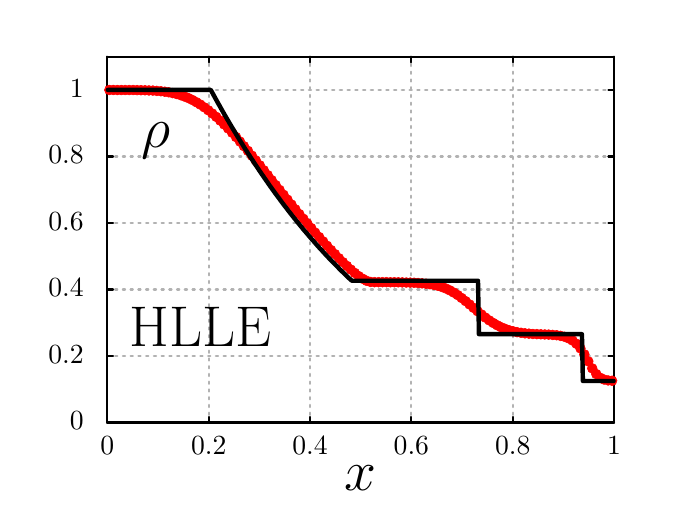
\begin{tikzpicture}[gnuplot]
%% generated with GNUPLOT 4.6p4 (Lua 5.1; terminal rev. 99, script rev. 100)
%% Thu 31 Jul 2014 01:57:35 PM EDT
\path (0.000,0.000) rectangle (8.000,6.000);
\gpfill{rgb color={1.000,1.000,1.000}} (1.012,0.985)--(7.446,0.985)--(7.446,5.630)--(1.012,5.630)--cycle;
\gpcolor{color=gp lt color border}
\gpsetlinetype{gp lt border}
\gpsetlinewidth{1.00}
\draw[gp path] (1.012,0.985)--(1.012,5.630)--(7.446,5.630)--(7.446,0.985)--cycle;
\gpcolor{color=gp lt color axes}
\gpsetlinetype{gp lt axes}
\gpsetlinewidth{2.00}
\draw[gp path] (1.012,0.985)--(7.447,0.985);
\gpcolor{color=gp lt color border}
\gpsetlinetype{gp lt border}
\draw[gp path] (1.012,0.985)--(1.084,0.985);
\draw[gp path] (7.447,0.985)--(7.375,0.985);
\gpcolor{rgb color={0.000,0.000,0.000}}
\node[gp node right,font={\fontsize{10pt}{12pt}\selectfont}] at (0.828,0.985) {0};
\gpcolor{color=gp lt color axes}
\gpsetlinetype{gp lt axes}
\draw[gp path] (1.012,1.830)--(7.447,1.830);
\gpcolor{color=gp lt color border}
\gpsetlinetype{gp lt border}
\draw[gp path] (1.012,1.830)--(1.084,1.830);
\draw[gp path] (7.447,1.830)--(7.375,1.830);
\gpcolor{rgb color={0.000,0.000,0.000}}
\node[gp node right,font={\fontsize{10pt}{12pt}\selectfont}] at (0.828,1.830) {0.2};
\gpcolor{color=gp lt color axes}
\gpsetlinetype{gp lt axes}
\draw[gp path] (1.012,2.674)--(7.447,2.674);
\gpcolor{color=gp lt color border}
\gpsetlinetype{gp lt border}
\draw[gp path] (1.012,2.674)--(1.084,2.674);
\draw[gp path] (7.447,2.674)--(7.375,2.674);
\gpcolor{rgb color={0.000,0.000,0.000}}
\node[gp node right,font={\fontsize{10pt}{12pt}\selectfont}] at (0.828,2.674) {0.4};
\gpcolor{color=gp lt color axes}
\gpsetlinetype{gp lt axes}
\draw[gp path] (1.012,3.519)--(7.447,3.519);
\gpcolor{color=gp lt color border}
\gpsetlinetype{gp lt border}
\draw[gp path] (1.012,3.519)--(1.084,3.519);
\draw[gp path] (7.447,3.519)--(7.375,3.519);
\gpcolor{rgb color={0.000,0.000,0.000}}
\node[gp node right,font={\fontsize{10pt}{12pt}\selectfont}] at (0.828,3.519) {0.6};
\gpcolor{color=gp lt color axes}
\gpsetlinetype{gp lt axes}
\draw[gp path] (1.012,4.364)--(7.447,4.364);
\gpcolor{color=gp lt color border}
\gpsetlinetype{gp lt border}
\draw[gp path] (1.012,4.364)--(1.084,4.364);
\draw[gp path] (7.447,4.364)--(7.375,4.364);
\gpcolor{rgb color={0.000,0.000,0.000}}
\node[gp node right,font={\fontsize{10pt}{12pt}\selectfont}] at (0.828,4.364) {0.8};
\gpcolor{color=gp lt color axes}
\gpsetlinetype{gp lt axes}
\draw[gp path] (1.012,5.209)--(7.447,5.209);
\gpcolor{color=gp lt color border}
\gpsetlinetype{gp lt border}
\draw[gp path] (1.012,5.209)--(1.084,5.209);
\draw[gp path] (7.447,5.209)--(7.375,5.209);
\gpcolor{rgb color={0.000,0.000,0.000}}
\node[gp node right,font={\fontsize{10pt}{12pt}\selectfont}] at (0.828,5.209) {1};
\gpcolor{color=gp lt color axes}
\gpsetlinetype{gp lt axes}
\draw[gp path] (1.012,0.985)--(1.012,5.631);
\gpcolor{color=gp lt color border}
\gpsetlinetype{gp lt border}
\draw[gp path] (1.012,0.985)--(1.012,1.057);
\draw[gp path] (1.012,5.631)--(1.012,5.559);
\gpcolor{rgb color={0.000,0.000,0.000}}
\node[gp node center,font={\fontsize{10pt}{12pt}\selectfont}] at (1.012,0.677) {0};
\gpcolor{color=gp lt color axes}
\gpsetlinetype{gp lt axes}
\draw[gp path] (2.299,0.985)--(2.299,5.631);
\gpcolor{color=gp lt color border}
\gpsetlinetype{gp lt border}
\draw[gp path] (2.299,0.985)--(2.299,1.057);
\draw[gp path] (2.299,5.631)--(2.299,5.559);
\gpcolor{rgb color={0.000,0.000,0.000}}
\node[gp node center,font={\fontsize{10pt}{12pt}\selectfont}] at (2.299,0.677) {0.2};
\gpcolor{color=gp lt color axes}
\gpsetlinetype{gp lt axes}
\draw[gp path] (3.586,0.985)--(3.586,5.631);
\gpcolor{color=gp lt color border}
\gpsetlinetype{gp lt border}
\draw[gp path] (3.586,0.985)--(3.586,1.057);
\draw[gp path] (3.586,5.631)--(3.586,5.559);
\gpcolor{rgb color={0.000,0.000,0.000}}
\node[gp node center,font={\fontsize{10pt}{12pt}\selectfont}] at (3.586,0.677) {0.4};
\gpcolor{color=gp lt color axes}
\gpsetlinetype{gp lt axes}
\draw[gp path] (4.873,0.985)--(4.873,5.631);
\gpcolor{color=gp lt color border}
\gpsetlinetype{gp lt border}
\draw[gp path] (4.873,0.985)--(4.873,1.057);
\draw[gp path] (4.873,5.631)--(4.873,5.559);
\gpcolor{rgb color={0.000,0.000,0.000}}
\node[gp node center,font={\fontsize{10pt}{12pt}\selectfont}] at (4.873,0.677) {0.6};
\gpcolor{color=gp lt color axes}
\gpsetlinetype{gp lt axes}
\draw[gp path] (6.160,0.985)--(6.160,5.631);
\gpcolor{color=gp lt color border}
\gpsetlinetype{gp lt border}
\draw[gp path] (6.160,0.985)--(6.160,1.057);
\draw[gp path] (6.160,5.631)--(6.160,5.559);
\gpcolor{rgb color={0.000,0.000,0.000}}
\node[gp node center,font={\fontsize{10pt}{12pt}\selectfont}] at (6.160,0.677) {0.8};
\gpcolor{color=gp lt color axes}
\gpsetlinetype{gp lt axes}
\draw[gp path] (7.447,0.985)--(7.447,5.631);
\gpcolor{color=gp lt color border}
\gpsetlinetype{gp lt border}
\draw[gp path] (7.447,0.985)--(7.447,1.057);
\draw[gp path] (7.447,5.631)--(7.447,5.559);
\gpcolor{rgb color={0.000,0.000,0.000}}
\node[gp node center,font={\fontsize{10pt}{12pt}\selectfont}] at (7.447,0.677) {1};
\gpcolor{color=gp lt color border}
\draw[gp path] (1.012,5.631)--(1.012,0.985)--(7.447,0.985)--(7.447,5.631)--cycle;
\gpcolor{rgb color={0.000,0.000,0.000}}
\node[gp node center,font={\fontsize{10pt}{12pt}\selectfont}] at (4.229,0.215) {\huge $x$};
\gpcolor{rgb color={1.000,0.000,0.000}}
\gpsetlinewidth{0.50}
\gpsetpointsize{4.44}
\gppoint{gp mark 7}{(1.037,5.209)}
\gppoint{gp mark 7}{(1.087,5.209)}
\gppoint{gp mark 7}{(1.138,5.208)}
\gppoint{gp mark 7}{(1.188,5.208)}
\gppoint{gp mark 7}{(1.238,5.208)}
\gppoint{gp mark 7}{(1.289,5.208)}
\gppoint{gp mark 7}{(1.339,5.208)}
\gppoint{gp mark 7}{(1.389,5.207)}
\gppoint{gp mark 7}{(1.439,5.206)}
\gppoint{gp mark 7}{(1.490,5.205)}
\gppoint{gp mark 7}{(1.540,5.203)}
\gppoint{gp mark 7}{(1.590,5.201)}
\gppoint{gp mark 7}{(1.640,5.197)}
\gppoint{gp mark 7}{(1.691,5.193)}
\gppoint{gp mark 7}{(1.741,5.187)}
\gppoint{gp mark 7}{(1.791,5.179)}
\gppoint{gp mark 7}{(1.842,5.169)}
\gppoint{gp mark 7}{(1.892,5.157)}
\gppoint{gp mark 7}{(1.942,5.143)}
\gppoint{gp mark 7}{(1.992,5.125)}
\gppoint{gp mark 7}{(2.043,5.105)}
\gppoint{gp mark 7}{(2.093,5.081)}
\gppoint{gp mark 7}{(2.143,5.053)}
\gppoint{gp mark 7}{(2.193,5.023)}
\gppoint{gp mark 7}{(2.244,4.988)}
\gppoint{gp mark 7}{(2.294,4.951)}
\gppoint{gp mark 7}{(2.344,4.910)}
\gppoint{gp mark 7}{(2.395,4.867)}
\gppoint{gp mark 7}{(2.445,4.820)}
\gppoint{gp mark 7}{(2.495,4.771)}
\gppoint{gp mark 7}{(2.545,4.720)}
\gppoint{gp mark 7}{(2.596,4.666)}
\gppoint{gp mark 7}{(2.646,4.611)}
\gppoint{gp mark 7}{(2.696,4.554)}
\gppoint{gp mark 7}{(2.746,4.495)}
\gppoint{gp mark 7}{(2.797,4.436)}
\gppoint{gp mark 7}{(2.847,4.375)}
\gppoint{gp mark 7}{(2.897,4.314)}
\gppoint{gp mark 7}{(2.948,4.252)}
\gppoint{gp mark 7}{(2.998,4.190)}
\gppoint{gp mark 7}{(3.048,4.128)}
\gppoint{gp mark 7}{(3.098,4.065)}
\gppoint{gp mark 7}{(3.149,4.002)}
\gppoint{gp mark 7}{(3.199,3.940)}
\gppoint{gp mark 7}{(3.249,3.878)}
\gppoint{gp mark 7}{(3.299,3.816)}
\gppoint{gp mark 7}{(3.350,3.754)}
\gppoint{gp mark 7}{(3.400,3.693)}
\gppoint{gp mark 7}{(3.450,3.633)}
\gppoint{gp mark 7}{(3.501,3.573)}
\gppoint{gp mark 7}{(3.551,3.514)}
\gppoint{gp mark 7}{(3.601,3.455)}
\gppoint{gp mark 7}{(3.651,3.397)}
\gppoint{gp mark 7}{(3.702,3.341)}
\gppoint{gp mark 7}{(3.752,3.285)}
\gppoint{gp mark 7}{(3.802,3.230)}
\gppoint{gp mark 7}{(3.852,3.176)}
\gppoint{gp mark 7}{(3.903,3.124)}
\gppoint{gp mark 7}{(3.953,3.072)}
\gppoint{gp mark 7}{(4.003,3.022)}
\gppoint{gp mark 7}{(4.054,2.974)}
\gppoint{gp mark 7}{(4.104,2.928)}
\gppoint{gp mark 7}{(4.154,2.885)}
\gppoint{gp mark 7}{(4.204,2.845)}
\gppoint{gp mark 7}{(4.255,2.811)}
\gppoint{gp mark 7}{(4.305,2.785)}
\gppoint{gp mark 7}{(4.355,2.771)}
\gppoint{gp mark 7}{(4.405,2.768)}
\gppoint{gp mark 7}{(4.456,2.768)}
\gppoint{gp mark 7}{(4.506,2.768)}
\gppoint{gp mark 7}{(4.556,2.768)}
\gppoint{gp mark 7}{(4.607,2.767)}
\gppoint{gp mark 7}{(4.657,2.767)}
\gppoint{gp mark 7}{(4.707,2.766)}
\gppoint{gp mark 7}{(4.757,2.765)}
\gppoint{gp mark 7}{(4.808,2.763)}
\gppoint{gp mark 7}{(4.858,2.762)}
\gppoint{gp mark 7}{(4.908,2.760)}
\gppoint{gp mark 7}{(4.958,2.757)}
\gppoint{gp mark 7}{(5.009,2.753)}
\gppoint{gp mark 7}{(5.059,2.748)}
\gppoint{gp mark 7}{(5.109,2.742)}
\gppoint{gp mark 7}{(5.160,2.733)}
\gppoint{gp mark 7}{(5.210,2.722)}
\gppoint{gp mark 7}{(5.260,2.707)}
\gppoint{gp mark 7}{(5.310,2.688)}
\gppoint{gp mark 7}{(5.361,2.664)}
\gppoint{gp mark 7}{(5.411,2.636)}
\gppoint{gp mark 7}{(5.461,2.604)}
\gppoint{gp mark 7}{(5.511,2.567)}
\gppoint{gp mark 7}{(5.562,2.527)}
\gppoint{gp mark 7}{(5.612,2.485)}
\gppoint{gp mark 7}{(5.662,2.442)}
\gppoint{gp mark 7}{(5.713,2.399)}
\gppoint{gp mark 7}{(5.763,2.358)}
\gppoint{gp mark 7}{(5.813,2.318)}
\gppoint{gp mark 7}{(5.863,2.282)}
\gppoint{gp mark 7}{(5.914,2.249)}
\gppoint{gp mark 7}{(5.964,2.220)}
\gppoint{gp mark 7}{(6.014,2.195)}
\gppoint{gp mark 7}{(6.064,2.175)}
\gppoint{gp mark 7}{(6.115,2.157)}
\gppoint{gp mark 7}{(6.165,2.144)}
\gppoint{gp mark 7}{(6.215,2.133)}
\gppoint{gp mark 7}{(6.266,2.125)}
\gppoint{gp mark 7}{(6.316,2.118)}
\gppoint{gp mark 7}{(6.366,2.114)}
\gppoint{gp mark 7}{(6.416,2.110)}
\gppoint{gp mark 7}{(6.467,2.108)}
\gppoint{gp mark 7}{(6.517,2.106)}
\gppoint{gp mark 7}{(6.567,2.104)}
\gppoint{gp mark 7}{(6.617,2.102)}
\gppoint{gp mark 7}{(6.668,2.098)}
\gppoint{gp mark 7}{(6.718,2.094)}
\gppoint{gp mark 7}{(6.768,2.086)}
\gppoint{gp mark 7}{(6.819,2.074)}
\gppoint{gp mark 7}{(6.869,2.055)}
\gppoint{gp mark 7}{(6.919,2.027)}
\gppoint{gp mark 7}{(6.969,1.986)}
\gppoint{gp mark 7}{(7.020,1.927)}
\gppoint{gp mark 7}{(7.070,1.851)}
\gppoint{gp mark 7}{(7.120,1.762)}
\gppoint{gp mark 7}{(7.170,1.673)}
\gppoint{gp mark 7}{(7.221,1.601)}
\gppoint{gp mark 7}{(7.271,1.554)}
\gppoint{gp mark 7}{(7.321,1.531)}
\gppoint{gp mark 7}{(7.372,1.520)}
\gppoint{gp mark 7}{(7.422,1.516)}
\gpcolor{rgb color={0.000,0.000,0.000}}
\gpsetlinetype{gp lt plot 0}
\gpsetlinewidth{4.00}
\draw[gp path] (1.018,5.209)--(1.031,5.209)--(1.043,5.209)--(1.056,5.209)--(1.069,5.209)%
  --(1.081,5.209)--(1.094,5.209)--(1.106,5.209)--(1.119,5.209)--(1.131,5.209)--(1.144,5.209)%
  --(1.157,5.209)--(1.169,5.209)--(1.182,5.209)--(1.194,5.209)--(1.207,5.209)--(1.219,5.209)%
  --(1.232,5.209)--(1.245,5.209)--(1.257,5.209)--(1.270,5.209)--(1.282,5.209)--(1.295,5.209)%
  --(1.307,5.209)--(1.320,5.209)--(1.332,5.209)--(1.345,5.209)--(1.358,5.209)--(1.370,5.209)%
  --(1.383,5.209)--(1.395,5.209)--(1.408,5.209)--(1.420,5.209)--(1.433,5.209)--(1.446,5.209)%
  --(1.458,5.209)--(1.471,5.209)--(1.483,5.209)--(1.496,5.209)--(1.508,5.209)--(1.521,5.209)%
  --(1.534,5.209)--(1.546,5.209)--(1.559,5.209)--(1.571,5.209)--(1.584,5.209)--(1.596,5.209)%
  --(1.609,5.209)--(1.622,5.209)--(1.634,5.209)--(1.647,5.209)--(1.659,5.209)--(1.672,5.209)%
  --(1.684,5.209)--(1.697,5.209)--(1.710,5.209)--(1.722,5.209)--(1.735,5.209)--(1.747,5.209)%
  --(1.760,5.209)--(1.772,5.209)--(1.785,5.209)--(1.798,5.209)--(1.810,5.209)--(1.823,5.209)%
  --(1.835,5.209)--(1.848,5.209)--(1.860,5.209)--(1.873,5.209)--(1.886,5.209)--(1.898,5.209)%
  --(1.911,5.209)--(1.923,5.209)--(1.936,5.209)--(1.948,5.209)--(1.961,5.209)--(1.973,5.209)%
  --(1.986,5.209)--(1.999,5.209)--(2.011,5.209)--(2.024,5.209)--(2.036,5.209)--(2.049,5.209)%
  --(2.061,5.209)--(2.074,5.209)--(2.087,5.209)--(2.099,5.209)--(2.112,5.209)--(2.124,5.209)%
  --(2.137,5.209)--(2.149,5.209)--(2.162,5.209)--(2.175,5.209)--(2.187,5.209)--(2.200,5.209)%
  --(2.212,5.209)--(2.225,5.209)--(2.237,5.209)--(2.250,5.209)--(2.263,5.209)--(2.275,5.209)%
  --(2.288,5.209)--(2.300,5.209)--(2.313,5.209)--(2.325,5.209)--(2.338,5.187)--(2.351,5.163)%
  --(2.363,5.140)--(2.376,5.118)--(2.388,5.095)--(2.401,5.072)--(2.413,5.050)--(2.426,5.027)%
  --(2.439,5.005)--(2.451,4.982)--(2.464,4.960)--(2.476,4.938)--(2.489,4.916)--(2.501,4.894)%
  --(2.514,4.872)--(2.526,4.851)--(2.539,4.829)--(2.552,4.808)--(2.564,4.786)--(2.577,4.765)%
  --(2.589,4.744)--(2.602,4.723)--(2.614,4.702)--(2.627,4.681)--(2.640,4.660)--(2.652,4.639)%
  --(2.665,4.618)--(2.677,4.598)--(2.690,4.577)--(2.702,4.557)--(2.715,4.537)--(2.728,4.517)%
  --(2.740,4.496)--(2.753,4.476)--(2.765,4.456)--(2.778,4.437)--(2.790,4.417)--(2.803,4.397)%
  --(2.816,4.378)--(2.828,4.358)--(2.841,4.339)--(2.853,4.320)--(2.866,4.300)--(2.878,4.281)%
  --(2.891,4.262)--(2.904,4.243)--(2.916,4.225)--(2.929,4.206)--(2.941,4.187)--(2.954,4.169)%
  --(2.966,4.150)--(2.979,4.132)--(2.992,4.113)--(3.004,4.095)--(3.017,4.077)--(3.029,4.059)%
  --(3.042,4.041)--(3.054,4.023)--(3.067,4.005)--(3.079,3.987)--(3.092,3.970)--(3.105,3.952)%
  --(3.117,3.935)--(3.130,3.917)--(3.142,3.900)--(3.155,3.883)--(3.167,3.866)--(3.180,3.849)%
  --(3.193,3.832)--(3.205,3.815)--(3.218,3.798)--(3.230,3.781)--(3.243,3.764)--(3.255,3.748)%
  --(3.268,3.731)--(3.281,3.715)--(3.293,3.699)--(3.306,3.682)--(3.318,3.666)--(3.331,3.650)%
  --(3.343,3.634)--(3.356,3.618)--(3.369,3.602)--(3.381,3.586)--(3.394,3.571)--(3.406,3.555)%
  --(3.419,3.539)--(3.431,3.524)--(3.444,3.508)--(3.457,3.493)--(3.469,3.478)--(3.482,3.463)%
  --(3.494,3.447)--(3.507,3.432)--(3.519,3.417)--(3.532,3.403)--(3.545,3.388)--(3.557,3.373)%
  --(3.570,3.358)--(3.582,3.344)--(3.595,3.329)--(3.607,3.315)--(3.620,3.300)--(3.633,3.286)%
  --(3.645,3.272)--(3.658,3.257)--(3.670,3.243)--(3.683,3.229)--(3.695,3.215)--(3.708,3.201)%
  --(3.720,3.188)--(3.733,3.174)--(3.746,3.160)--(3.758,3.146)--(3.771,3.133)--(3.783,3.119)%
  --(3.796,3.106)--(3.808,3.093)--(3.821,3.079)--(3.834,3.066)--(3.846,3.053)--(3.859,3.040)%
  --(3.871,3.027)--(3.884,3.014)--(3.896,3.001)--(3.909,2.988)--(3.922,2.975)--(3.934,2.963)%
  --(3.947,2.950)--(3.959,2.937)--(3.972,2.925)--(3.984,2.912)--(3.997,2.900)--(4.010,2.888)%
  --(4.022,2.876)--(4.035,2.863)--(4.047,2.851)--(4.060,2.839)--(4.072,2.827)--(4.085,2.815)%
  --(4.098,2.803)--(4.110,2.792)--(4.123,2.786)--(4.135,2.786)--(4.148,2.786)--(4.160,2.786)%
  --(4.173,2.786)--(4.186,2.786)--(4.198,2.786)--(4.211,2.786)--(4.223,2.786)--(4.236,2.786)%
  --(4.248,2.786)--(4.261,2.786)--(4.273,2.786)--(4.286,2.786)--(4.299,2.786)--(4.311,2.786)%
  --(4.324,2.786)--(4.336,2.786)--(4.349,2.786)--(4.361,2.786)--(4.374,2.786)--(4.387,2.786)%
  --(4.399,2.786)--(4.412,2.786)--(4.424,2.786)--(4.437,2.786)--(4.449,2.786)--(4.462,2.786)%
  --(4.475,2.786)--(4.487,2.786)--(4.500,2.786)--(4.512,2.786)--(4.525,2.786)--(4.537,2.786)%
  --(4.550,2.786)--(4.563,2.786)--(4.575,2.786)--(4.588,2.786)--(4.600,2.786)--(4.613,2.786)%
  --(4.625,2.786)--(4.638,2.786)--(4.651,2.786)--(4.663,2.786)--(4.676,2.786)--(4.688,2.786)%
  --(4.701,2.786)--(4.713,2.786)--(4.726,2.786)--(4.739,2.786)--(4.751,2.786)--(4.764,2.786)%
  --(4.776,2.786)--(4.789,2.786)--(4.801,2.786)--(4.814,2.786)--(4.826,2.786)--(4.839,2.786)%
  --(4.852,2.786)--(4.864,2.786)--(4.877,2.786)--(4.889,2.786)--(4.902,2.786)--(4.914,2.786)%
  --(4.927,2.786)--(4.940,2.786)--(4.952,2.786)--(4.965,2.786)--(4.977,2.786)--(4.990,2.786)%
  --(5.002,2.786)--(5.015,2.786)--(5.028,2.786)--(5.040,2.786)--(5.053,2.786)--(5.065,2.786)%
  --(5.078,2.786)--(5.090,2.786)--(5.103,2.786)--(5.116,2.786)--(5.128,2.786)--(5.141,2.786)%
  --(5.153,2.786)--(5.166,2.786)--(5.178,2.786)--(5.191,2.786)--(5.204,2.786)--(5.216,2.786)%
  --(5.229,2.786)--(5.241,2.786)--(5.254,2.786)--(5.266,2.786)--(5.279,2.786)--(5.292,2.786)%
  --(5.304,2.786)--(5.317,2.786)--(5.329,2.786)--(5.342,2.786)--(5.354,2.786)--(5.367,2.786)%
  --(5.380,2.786)--(5.392,2.786)--(5.405,2.786)--(5.417,2.786)--(5.430,2.786)--(5.442,2.786)%
  --(5.455,2.786)--(5.467,2.786)--(5.480,2.786)--(5.493,2.786)--(5.505,2.786)--(5.518,2.786)%
  --(5.530,2.786)--(5.543,2.786)--(5.555,2.786)--(5.568,2.786)--(5.581,2.786)--(5.593,2.786)%
  --(5.606,2.786)--(5.618,2.786)--(5.631,2.786)--(5.643,2.786)--(5.656,2.786)--(5.669,2.786)%
  --(5.681,2.786)--(5.694,2.786)--(5.706,2.786)--(5.719,2.786)--(5.731,2.107)--(5.744,2.107)%
  --(5.757,2.107)--(5.769,2.107)--(5.782,2.107)--(5.794,2.107)--(5.807,2.107)--(5.819,2.107)%
  --(5.832,2.107)--(5.845,2.107)--(5.857,2.107)--(5.870,2.107)--(5.882,2.107)--(5.895,2.107)%
  --(5.907,2.107)--(5.920,2.107)--(5.933,2.107)--(5.945,2.107)--(5.958,2.107)--(5.970,2.107)%
  --(5.983,2.107)--(5.995,2.107)--(6.008,2.107)--(6.020,2.107)--(6.033,2.107)--(6.046,2.107)%
  --(6.058,2.107)--(6.071,2.107)--(6.083,2.107)--(6.096,2.107)--(6.108,2.107)--(6.121,2.107)%
  --(6.134,2.107)--(6.146,2.107)--(6.159,2.107)--(6.171,2.107)--(6.184,2.107)--(6.196,2.107)%
  --(6.209,2.107)--(6.222,2.107)--(6.234,2.107)--(6.247,2.107)--(6.259,2.107)--(6.272,2.107)%
  --(6.284,2.107)--(6.297,2.107)--(6.310,2.107)--(6.322,2.107)--(6.335,2.107)--(6.347,2.107)%
  --(6.360,2.107)--(6.372,2.107)--(6.385,2.107)--(6.398,2.107)--(6.410,2.107)--(6.423,2.107)%
  --(6.435,2.107)--(6.448,2.107)--(6.460,2.107)--(6.473,2.107)--(6.486,2.107)--(6.498,2.107)%
  --(6.511,2.107)--(6.523,2.107)--(6.536,2.107)--(6.548,2.107)--(6.561,2.107)--(6.573,2.107)%
  --(6.586,2.107)--(6.599,2.107)--(6.611,2.107)--(6.624,2.107)--(6.636,2.107)--(6.649,2.107)%
  --(6.661,2.107)--(6.674,2.107)--(6.687,2.107)--(6.699,2.107)--(6.712,2.107)--(6.724,2.107)%
  --(6.737,2.107)--(6.749,2.107)--(6.762,2.107)--(6.775,2.107)--(6.787,2.107)--(6.800,2.107)%
  --(6.812,2.107)--(6.825,2.107)--(6.837,2.107)--(6.850,2.107)--(6.863,2.107)--(6.875,2.107)%
  --(6.888,2.107)--(6.900,2.107)--(6.913,2.107)--(6.925,2.107)--(6.938,2.107)--(6.951,2.107)%
  --(6.963,2.107)--(6.976,2.107)--(6.988,2.107)--(7.001,2.107)--(7.013,2.107)--(7.026,2.107)%
  --(7.039,2.107)--(7.051,1.513)--(7.064,1.513)--(7.076,1.513)--(7.089,1.513)--(7.101,1.513)%
  --(7.114,1.513)--(7.127,1.513)--(7.139,1.513)--(7.152,1.513)--(7.164,1.513)--(7.177,1.513)%
  --(7.189,1.513)--(7.202,1.513)--(7.214,1.513)--(7.227,1.513)--(7.240,1.513)--(7.252,1.513)%
  --(7.265,1.513)--(7.277,1.513)--(7.290,1.513)--(7.302,1.513)--(7.315,1.513)--(7.328,1.513)%
  --(7.340,1.513)--(7.353,1.513)--(7.365,1.513)--(7.378,1.513)--(7.390,1.513)--(7.403,1.513)%
  --(7.416,1.513)--(7.428,1.513)--(7.441,1.513);
\node[gp node left,font={\fontsize{10pt}{12pt}\selectfont}] at (1.334,4.575) {\huge $\rho$};
\node[gp node left,font={\fontsize{10pt}{12pt}\selectfont}] at (1.173,2.041) {\huge HLLE};
%% coordinates of the plot area
\gpdefrectangularnode{gp plot 1}{\pgfpoint{1.012cm}{0.985cm}}{\pgfpoint{7.447cm}{5.631cm}}
\end{tikzpicture}
%% gnuplot variables
} &
\resizebox{0.33\linewidth}{!}{\tikzsetnextfilename{sod_hlle_1_2}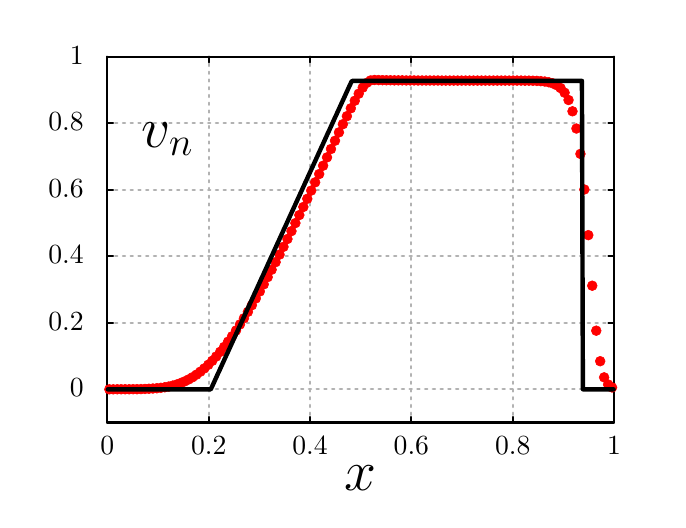
\begin{tikzpicture}[gnuplot]
%% generated with GNUPLOT 4.6p4 (Lua 5.1; terminal rev. 99, script rev. 100)
%% Thu 31 Jul 2014 01:57:35 PM EDT
\path (0.000,0.000) rectangle (8.000,6.000);
\gpfill{rgb color={1.000,1.000,1.000}} (1.012,0.985)--(7.446,0.985)--(7.446,5.630)--(1.012,5.630)--cycle;
\gpcolor{color=gp lt color border}
\gpsetlinetype{gp lt border}
\gpsetlinewidth{1.00}
\draw[gp path] (1.012,0.985)--(1.012,5.630)--(7.446,5.630)--(7.446,0.985)--cycle;
\gpcolor{color=gp lt color axes}
\gpsetlinetype{gp lt axes}
\gpsetlinewidth{2.00}
\draw[gp path] (1.012,1.407)--(7.447,1.407);
\gpcolor{color=gp lt color border}
\gpsetlinetype{gp lt border}
\draw[gp path] (1.012,1.407)--(1.084,1.407);
\draw[gp path] (7.447,1.407)--(7.375,1.407);
\gpcolor{rgb color={0.000,0.000,0.000}}
\node[gp node right,font={\fontsize{10pt}{12pt}\selectfont}] at (0.828,1.407) {0};
\gpcolor{color=gp lt color axes}
\gpsetlinetype{gp lt axes}
\draw[gp path] (1.012,2.252)--(7.447,2.252);
\gpcolor{color=gp lt color border}
\gpsetlinetype{gp lt border}
\draw[gp path] (1.012,2.252)--(1.084,2.252);
\draw[gp path] (7.447,2.252)--(7.375,2.252);
\gpcolor{rgb color={0.000,0.000,0.000}}
\node[gp node right,font={\fontsize{10pt}{12pt}\selectfont}] at (0.828,2.252) {0.2};
\gpcolor{color=gp lt color axes}
\gpsetlinetype{gp lt axes}
\draw[gp path] (1.012,3.097)--(7.447,3.097);
\gpcolor{color=gp lt color border}
\gpsetlinetype{gp lt border}
\draw[gp path] (1.012,3.097)--(1.084,3.097);
\draw[gp path] (7.447,3.097)--(7.375,3.097);
\gpcolor{rgb color={0.000,0.000,0.000}}
\node[gp node right,font={\fontsize{10pt}{12pt}\selectfont}] at (0.828,3.097) {0.4};
\gpcolor{color=gp lt color axes}
\gpsetlinetype{gp lt axes}
\draw[gp path] (1.012,3.942)--(7.447,3.942);
\gpcolor{color=gp lt color border}
\gpsetlinetype{gp lt border}
\draw[gp path] (1.012,3.942)--(1.084,3.942);
\draw[gp path] (7.447,3.942)--(7.375,3.942);
\gpcolor{rgb color={0.000,0.000,0.000}}
\node[gp node right,font={\fontsize{10pt}{12pt}\selectfont}] at (0.828,3.942) {0.6};
\gpcolor{color=gp lt color axes}
\gpsetlinetype{gp lt axes}
\draw[gp path] (1.012,4.786)--(7.447,4.786);
\gpcolor{color=gp lt color border}
\gpsetlinetype{gp lt border}
\draw[gp path] (1.012,4.786)--(1.084,4.786);
\draw[gp path] (7.447,4.786)--(7.375,4.786);
\gpcolor{rgb color={0.000,0.000,0.000}}
\node[gp node right,font={\fontsize{10pt}{12pt}\selectfont}] at (0.828,4.786) {0.8};
\gpcolor{color=gp lt color axes}
\gpsetlinetype{gp lt axes}
\draw[gp path] (1.012,5.631)--(7.447,5.631);
\gpcolor{color=gp lt color border}
\gpsetlinetype{gp lt border}
\draw[gp path] (1.012,5.631)--(1.084,5.631);
\draw[gp path] (7.447,5.631)--(7.375,5.631);
\gpcolor{rgb color={0.000,0.000,0.000}}
\node[gp node right,font={\fontsize{10pt}{12pt}\selectfont}] at (0.828,5.631) {1};
\gpcolor{color=gp lt color axes}
\gpsetlinetype{gp lt axes}
\draw[gp path] (1.012,0.985)--(1.012,5.631);
\gpcolor{color=gp lt color border}
\gpsetlinetype{gp lt border}
\draw[gp path] (1.012,0.985)--(1.012,1.057);
\draw[gp path] (1.012,5.631)--(1.012,5.559);
\gpcolor{rgb color={0.000,0.000,0.000}}
\node[gp node center,font={\fontsize{10pt}{12pt}\selectfont}] at (1.012,0.677) {0};
\gpcolor{color=gp lt color axes}
\gpsetlinetype{gp lt axes}
\draw[gp path] (2.299,0.985)--(2.299,5.631);
\gpcolor{color=gp lt color border}
\gpsetlinetype{gp lt border}
\draw[gp path] (2.299,0.985)--(2.299,1.057);
\draw[gp path] (2.299,5.631)--(2.299,5.559);
\gpcolor{rgb color={0.000,0.000,0.000}}
\node[gp node center,font={\fontsize{10pt}{12pt}\selectfont}] at (2.299,0.677) {0.2};
\gpcolor{color=gp lt color axes}
\gpsetlinetype{gp lt axes}
\draw[gp path] (3.586,0.985)--(3.586,5.631);
\gpcolor{color=gp lt color border}
\gpsetlinetype{gp lt border}
\draw[gp path] (3.586,0.985)--(3.586,1.057);
\draw[gp path] (3.586,5.631)--(3.586,5.559);
\gpcolor{rgb color={0.000,0.000,0.000}}
\node[gp node center,font={\fontsize{10pt}{12pt}\selectfont}] at (3.586,0.677) {0.4};
\gpcolor{color=gp lt color axes}
\gpsetlinetype{gp lt axes}
\draw[gp path] (4.873,0.985)--(4.873,5.631);
\gpcolor{color=gp lt color border}
\gpsetlinetype{gp lt border}
\draw[gp path] (4.873,0.985)--(4.873,1.057);
\draw[gp path] (4.873,5.631)--(4.873,5.559);
\gpcolor{rgb color={0.000,0.000,0.000}}
\node[gp node center,font={\fontsize{10pt}{12pt}\selectfont}] at (4.873,0.677) {0.6};
\gpcolor{color=gp lt color axes}
\gpsetlinetype{gp lt axes}
\draw[gp path] (6.160,0.985)--(6.160,5.631);
\gpcolor{color=gp lt color border}
\gpsetlinetype{gp lt border}
\draw[gp path] (6.160,0.985)--(6.160,1.057);
\draw[gp path] (6.160,5.631)--(6.160,5.559);
\gpcolor{rgb color={0.000,0.000,0.000}}
\node[gp node center,font={\fontsize{10pt}{12pt}\selectfont}] at (6.160,0.677) {0.8};
\gpcolor{color=gp lt color axes}
\gpsetlinetype{gp lt axes}
\draw[gp path] (7.447,0.985)--(7.447,5.631);
\gpcolor{color=gp lt color border}
\gpsetlinetype{gp lt border}
\draw[gp path] (7.447,0.985)--(7.447,1.057);
\draw[gp path] (7.447,5.631)--(7.447,5.559);
\gpcolor{rgb color={0.000,0.000,0.000}}
\node[gp node center,font={\fontsize{10pt}{12pt}\selectfont}] at (7.447,0.677) {1};
\gpcolor{color=gp lt color border}
\draw[gp path] (1.012,5.631)--(1.012,0.985)--(7.447,0.985)--(7.447,5.631)--cycle;
\gpcolor{rgb color={0.000,0.000,0.000}}
\node[gp node center,font={\fontsize{10pt}{12pt}\selectfont}] at (4.229,0.215) {\huge $x$};
\gpcolor{rgb color={1.000,0.000,0.000}}
\gpsetlinewidth{0.50}
\gpsetpointsize{4.44}
\gppoint{gp mark 7}{(1.037,1.407)}
\gppoint{gp mark 7}{(1.087,1.407)}
\gppoint{gp mark 7}{(1.138,1.408)}
\gppoint{gp mark 7}{(1.188,1.408)}
\gppoint{gp mark 7}{(1.238,1.408)}
\gppoint{gp mark 7}{(1.289,1.408)}
\gppoint{gp mark 7}{(1.339,1.409)}
\gppoint{gp mark 7}{(1.389,1.409)}
\gppoint{gp mark 7}{(1.439,1.410)}
\gppoint{gp mark 7}{(1.490,1.412)}
\gppoint{gp mark 7}{(1.540,1.414)}
\gppoint{gp mark 7}{(1.590,1.417)}
\gppoint{gp mark 7}{(1.640,1.421)}
\gppoint{gp mark 7}{(1.691,1.426)}
\gppoint{gp mark 7}{(1.741,1.433)}
\gppoint{gp mark 7}{(1.791,1.442)}
\gppoint{gp mark 7}{(1.842,1.454)}
\gppoint{gp mark 7}{(1.892,1.468)}
\gppoint{gp mark 7}{(1.942,1.486)}
\gppoint{gp mark 7}{(1.992,1.507)}
\gppoint{gp mark 7}{(2.043,1.532)}
\gppoint{gp mark 7}{(2.093,1.560)}
\gppoint{gp mark 7}{(2.143,1.593)}
\gppoint{gp mark 7}{(2.193,1.631)}
\gppoint{gp mark 7}{(2.244,1.673)}
\gppoint{gp mark 7}{(2.294,1.719)}
\gppoint{gp mark 7}{(2.344,1.769)}
\gppoint{gp mark 7}{(2.395,1.824)}
\gppoint{gp mark 7}{(2.445,1.883)}
\gppoint{gp mark 7}{(2.495,1.945)}
\gppoint{gp mark 7}{(2.545,2.012)}
\gppoint{gp mark 7}{(2.596,2.081)}
\gppoint{gp mark 7}{(2.646,2.154)}
\gppoint{gp mark 7}{(2.696,2.231)}
\gppoint{gp mark 7}{(2.746,2.309)}
\gppoint{gp mark 7}{(2.797,2.391)}
\gppoint{gp mark 7}{(2.847,2.475)}
\gppoint{gp mark 7}{(2.897,2.561)}
\gppoint{gp mark 7}{(2.948,2.650)}
\gppoint{gp mark 7}{(2.998,2.740)}
\gppoint{gp mark 7}{(3.048,2.832)}
\gppoint{gp mark 7}{(3.098,2.926)}
\gppoint{gp mark 7}{(3.149,3.022)}
\gppoint{gp mark 7}{(3.199,3.118)}
\gppoint{gp mark 7}{(3.249,3.217)}
\gppoint{gp mark 7}{(3.299,3.316)}
\gppoint{gp mark 7}{(3.350,3.416)}
\gppoint{gp mark 7}{(3.400,3.518)}
\gppoint{gp mark 7}{(3.450,3.620)}
\gppoint{gp mark 7}{(3.501,3.723)}
\gppoint{gp mark 7}{(3.551,3.827)}
\gppoint{gp mark 7}{(3.601,3.931)}
\gppoint{gp mark 7}{(3.651,4.036)}
\gppoint{gp mark 7}{(3.702,4.141)}
\gppoint{gp mark 7}{(3.752,4.247)}
\gppoint{gp mark 7}{(3.802,4.353)}
\gppoint{gp mark 7}{(3.852,4.459)}
\gppoint{gp mark 7}{(3.903,4.564)}
\gppoint{gp mark 7}{(3.953,4.670)}
\gppoint{gp mark 7}{(4.003,4.774)}
\gppoint{gp mark 7}{(4.054,4.876)}
\gppoint{gp mark 7}{(4.104,4.976)}
\gppoint{gp mark 7}{(4.154,5.072)}
\gppoint{gp mark 7}{(4.204,5.161)}
\gppoint{gp mark 7}{(4.255,5.239)}
\gppoint{gp mark 7}{(4.305,5.298)}
\gppoint{gp mark 7}{(4.355,5.330)}
\gppoint{gp mark 7}{(4.405,5.336)}
\gppoint{gp mark 7}{(4.456,5.334)}
\gppoint{gp mark 7}{(4.506,5.333)}
\gppoint{gp mark 7}{(4.556,5.332)}
\gppoint{gp mark 7}{(4.607,5.332)}
\gppoint{gp mark 7}{(4.657,5.331)}
\gppoint{gp mark 7}{(4.707,5.331)}
\gppoint{gp mark 7}{(4.757,5.331)}
\gppoint{gp mark 7}{(4.808,5.330)}
\gppoint{gp mark 7}{(4.858,5.330)}
\gppoint{gp mark 7}{(4.908,5.330)}
\gppoint{gp mark 7}{(4.958,5.329)}
\gppoint{gp mark 7}{(5.009,5.329)}
\gppoint{gp mark 7}{(5.059,5.329)}
\gppoint{gp mark 7}{(5.109,5.329)}
\gppoint{gp mark 7}{(5.160,5.329)}
\gppoint{gp mark 7}{(5.210,5.329)}
\gppoint{gp mark 7}{(5.260,5.328)}
\gppoint{gp mark 7}{(5.310,5.328)}
\gppoint{gp mark 7}{(5.361,5.328)}
\gppoint{gp mark 7}{(5.411,5.328)}
\gppoint{gp mark 7}{(5.461,5.328)}
\gppoint{gp mark 7}{(5.511,5.328)}
\gppoint{gp mark 7}{(5.562,5.328)}
\gppoint{gp mark 7}{(5.612,5.328)}
\gppoint{gp mark 7}{(5.662,5.328)}
\gppoint{gp mark 7}{(5.713,5.328)}
\gppoint{gp mark 7}{(5.763,5.328)}
\gppoint{gp mark 7}{(5.813,5.328)}
\gppoint{gp mark 7}{(5.863,5.328)}
\gppoint{gp mark 7}{(5.914,5.328)}
\gppoint{gp mark 7}{(5.964,5.328)}
\gppoint{gp mark 7}{(6.014,5.328)}
\gppoint{gp mark 7}{(6.064,5.328)}
\gppoint{gp mark 7}{(6.115,5.328)}
\gppoint{gp mark 7}{(6.165,5.328)}
\gppoint{gp mark 7}{(6.215,5.328)}
\gppoint{gp mark 7}{(6.266,5.328)}
\gppoint{gp mark 7}{(6.316,5.327)}
\gppoint{gp mark 7}{(6.366,5.327)}
\gppoint{gp mark 7}{(6.416,5.326)}
\gppoint{gp mark 7}{(6.467,5.324)}
\gppoint{gp mark 7}{(6.517,5.321)}
\gppoint{gp mark 7}{(6.567,5.316)}
\gppoint{gp mark 7}{(6.617,5.307)}
\gppoint{gp mark 7}{(6.668,5.293)}
\gppoint{gp mark 7}{(6.718,5.270)}
\gppoint{gp mark 7}{(6.768,5.233)}
\gppoint{gp mark 7}{(6.819,5.174)}
\gppoint{gp mark 7}{(6.869,5.081)}
\gppoint{gp mark 7}{(6.919,4.938)}
\gppoint{gp mark 7}{(6.969,4.719)}
\gppoint{gp mark 7}{(7.020,4.397)}
\gppoint{gp mark 7}{(7.070,3.945)}
\gppoint{gp mark 7}{(7.120,3.365)}
\gppoint{gp mark 7}{(7.170,2.723)}
\gppoint{gp mark 7}{(7.221,2.152)}
\gppoint{gp mark 7}{(7.271,1.764)}
\gppoint{gp mark 7}{(7.321,1.559)}
\gppoint{gp mark 7}{(7.372,1.468)}
\gppoint{gp mark 7}{(7.422,1.431)}
\gpcolor{rgb color={0.000,0.000,0.000}}
\gpsetlinetype{gp lt plot 0}
\gpsetlinewidth{4.00}
\draw[gp path] (1.018,1.407)--(1.031,1.407)--(1.043,1.407)--(1.056,1.407)--(1.069,1.407)%
  --(1.081,1.407)--(1.094,1.407)--(1.106,1.407)--(1.119,1.407)--(1.131,1.407)--(1.144,1.407)%
  --(1.157,1.407)--(1.169,1.407)--(1.182,1.407)--(1.194,1.407)--(1.207,1.407)--(1.219,1.407)%
  --(1.232,1.407)--(1.245,1.407)--(1.257,1.407)--(1.270,1.407)--(1.282,1.407)--(1.295,1.407)%
  --(1.307,1.407)--(1.320,1.407)--(1.332,1.407)--(1.345,1.407)--(1.358,1.407)--(1.370,1.407)%
  --(1.383,1.407)--(1.395,1.407)--(1.408,1.407)--(1.420,1.407)--(1.433,1.407)--(1.446,1.407)%
  --(1.458,1.407)--(1.471,1.407)--(1.483,1.407)--(1.496,1.407)--(1.508,1.407)--(1.521,1.407)%
  --(1.534,1.407)--(1.546,1.407)--(1.559,1.407)--(1.571,1.407)--(1.584,1.407)--(1.596,1.407)%
  --(1.609,1.407)--(1.622,1.407)--(1.634,1.407)--(1.647,1.407)--(1.659,1.407)--(1.672,1.407)%
  --(1.684,1.407)--(1.697,1.407)--(1.710,1.407)--(1.722,1.407)--(1.735,1.407)--(1.747,1.407)%
  --(1.760,1.407)--(1.772,1.407)--(1.785,1.407)--(1.798,1.407)--(1.810,1.407)--(1.823,1.407)%
  --(1.835,1.407)--(1.848,1.407)--(1.860,1.407)--(1.873,1.407)--(1.886,1.407)--(1.898,1.407)%
  --(1.911,1.407)--(1.923,1.407)--(1.936,1.407)--(1.948,1.407)--(1.961,1.407)--(1.973,1.407)%
  --(1.986,1.407)--(1.999,1.407)--(2.011,1.407)--(2.024,1.407)--(2.036,1.407)--(2.049,1.407)%
  --(2.061,1.407)--(2.074,1.407)--(2.087,1.407)--(2.099,1.407)--(2.112,1.407)--(2.124,1.407)%
  --(2.137,1.407)--(2.149,1.407)--(2.162,1.407)--(2.175,1.407)--(2.187,1.407)--(2.200,1.407)%
  --(2.212,1.407)--(2.225,1.407)--(2.237,1.407)--(2.250,1.407)--(2.263,1.407)--(2.275,1.407)%
  --(2.288,1.407)--(2.300,1.407)--(2.313,1.407)--(2.325,1.407)--(2.338,1.434)--(2.351,1.461)%
  --(2.363,1.489)--(2.376,1.516)--(2.388,1.544)--(2.401,1.571)--(2.413,1.599)--(2.426,1.626)%
  --(2.439,1.654)--(2.451,1.681)--(2.464,1.709)--(2.476,1.736)--(2.489,1.764)--(2.501,1.791)%
  --(2.514,1.818)--(2.526,1.846)--(2.539,1.873)--(2.552,1.901)--(2.564,1.928)--(2.577,1.956)%
  --(2.589,1.983)--(2.602,2.011)--(2.614,2.038)--(2.627,2.066)--(2.640,2.093)--(2.652,2.121)%
  --(2.665,2.148)--(2.677,2.176)--(2.690,2.203)--(2.702,2.231)--(2.715,2.258)--(2.728,2.286)%
  --(2.740,2.313)--(2.753,2.341)--(2.765,2.368)--(2.778,2.396)--(2.790,2.423)--(2.803,2.451)%
  --(2.816,2.478)--(2.828,2.506)--(2.841,2.533)--(2.853,2.561)--(2.866,2.588)--(2.878,2.616)%
  --(2.891,2.643)--(2.904,2.671)--(2.916,2.698)--(2.929,2.726)--(2.941,2.753)--(2.954,2.781)%
  --(2.966,2.808)--(2.979,2.836)--(2.992,2.863)--(3.004,2.891)--(3.017,2.918)--(3.029,2.946)%
  --(3.042,2.973)--(3.054,3.001)--(3.067,3.028)--(3.079,3.056)--(3.092,3.083)--(3.105,3.111)%
  --(3.117,3.138)--(3.130,3.166)--(3.142,3.193)--(3.155,3.221)--(3.167,3.248)--(3.180,3.276)%
  --(3.193,3.303)--(3.205,3.331)--(3.218,3.358)--(3.230,3.386)--(3.243,3.413)--(3.255,3.441)%
  --(3.268,3.468)--(3.281,3.496)--(3.293,3.523)--(3.306,3.551)--(3.318,3.578)--(3.331,3.606)%
  --(3.343,3.633)--(3.356,3.661)--(3.369,3.688)--(3.381,3.716)--(3.394,3.743)--(3.406,3.771)%
  --(3.419,3.798)--(3.431,3.826)--(3.444,3.853)--(3.457,3.881)--(3.469,3.908)--(3.482,3.936)%
  --(3.494,3.963)--(3.507,3.991)--(3.519,4.018)--(3.532,4.046)--(3.545,4.073)--(3.557,4.101)%
  --(3.570,4.128)--(3.582,4.156)--(3.595,4.183)--(3.607,4.211)--(3.620,4.238)--(3.633,4.266)%
  --(3.645,4.293)--(3.658,4.321)--(3.670,4.348)--(3.683,4.376)--(3.695,4.403)--(3.708,4.431)%
  --(3.720,4.458)--(3.733,4.486)--(3.746,4.513)--(3.758,4.541)--(3.771,4.568)--(3.783,4.596)%
  --(3.796,4.623)--(3.808,4.651)--(3.821,4.678)--(3.834,4.706)--(3.846,4.733)--(3.859,4.761)%
  --(3.871,4.788)--(3.884,4.816)--(3.896,4.843)--(3.909,4.871)--(3.922,4.898)--(3.934,4.926)%
  --(3.947,4.953)--(3.959,4.981)--(3.972,5.008)--(3.984,5.036)--(3.997,5.063)--(4.010,5.091)%
  --(4.022,5.118)--(4.035,5.146)--(4.047,5.173)--(4.060,5.201)--(4.072,5.228)--(4.085,5.256)%
  --(4.098,5.283)--(4.110,5.311)--(4.123,5.324)--(4.135,5.324)--(4.148,5.324)--(4.160,5.324)%
  --(4.173,5.324)--(4.186,5.324)--(4.198,5.324)--(4.211,5.324)--(4.223,5.324)--(4.236,5.324)%
  --(4.248,5.324)--(4.261,5.324)--(4.273,5.324)--(4.286,5.324)--(4.299,5.324)--(4.311,5.324)%
  --(4.324,5.324)--(4.336,5.324)--(4.349,5.324)--(4.361,5.324)--(4.374,5.324)--(4.387,5.324)%
  --(4.399,5.324)--(4.412,5.324)--(4.424,5.324)--(4.437,5.324)--(4.449,5.324)--(4.462,5.324)%
  --(4.475,5.324)--(4.487,5.324)--(4.500,5.324)--(4.512,5.324)--(4.525,5.324)--(4.537,5.324)%
  --(4.550,5.324)--(4.563,5.324)--(4.575,5.324)--(4.588,5.324)--(4.600,5.324)--(4.613,5.324)%
  --(4.625,5.324)--(4.638,5.324)--(4.651,5.324)--(4.663,5.324)--(4.676,5.324)--(4.688,5.324)%
  --(4.701,5.324)--(4.713,5.324)--(4.726,5.324)--(4.739,5.324)--(4.751,5.324)--(4.764,5.324)%
  --(4.776,5.324)--(4.789,5.324)--(4.801,5.324)--(4.814,5.324)--(4.826,5.324)--(4.839,5.324)%
  --(4.852,5.324)--(4.864,5.324)--(4.877,5.324)--(4.889,5.324)--(4.902,5.324)--(4.914,5.324)%
  --(4.927,5.324)--(4.940,5.324)--(4.952,5.324)--(4.965,5.324)--(4.977,5.324)--(4.990,5.324)%
  --(5.002,5.324)--(5.015,5.324)--(5.028,5.324)--(5.040,5.324)--(5.053,5.324)--(5.065,5.324)%
  --(5.078,5.324)--(5.090,5.324)--(5.103,5.324)--(5.116,5.324)--(5.128,5.324)--(5.141,5.324)%
  --(5.153,5.324)--(5.166,5.324)--(5.178,5.324)--(5.191,5.324)--(5.204,5.324)--(5.216,5.324)%
  --(5.229,5.324)--(5.241,5.324)--(5.254,5.324)--(5.266,5.324)--(5.279,5.324)--(5.292,5.324)%
  --(5.304,5.324)--(5.317,5.324)--(5.329,5.324)--(5.342,5.324)--(5.354,5.324)--(5.367,5.324)%
  --(5.380,5.324)--(5.392,5.324)--(5.405,5.324)--(5.417,5.324)--(5.430,5.324)--(5.442,5.324)%
  --(5.455,5.324)--(5.467,5.324)--(5.480,5.324)--(5.493,5.324)--(5.505,5.324)--(5.518,5.324)%
  --(5.530,5.324)--(5.543,5.324)--(5.555,5.324)--(5.568,5.324)--(5.581,5.324)--(5.593,5.324)%
  --(5.606,5.324)--(5.618,5.324)--(5.631,5.324)--(5.643,5.324)--(5.656,5.324)--(5.669,5.324)%
  --(5.681,5.324)--(5.694,5.324)--(5.706,5.324)--(5.719,5.324)--(5.731,5.324)--(5.744,5.324)%
  --(5.757,5.324)--(5.769,5.324)--(5.782,5.324)--(5.794,5.324)--(5.807,5.324)--(5.819,5.324)%
  --(5.832,5.324)--(5.845,5.324)--(5.857,5.324)--(5.870,5.324)--(5.882,5.324)--(5.895,5.324)%
  --(5.907,5.324)--(5.920,5.324)--(5.933,5.324)--(5.945,5.324)--(5.958,5.324)--(5.970,5.324)%
  --(5.983,5.324)--(5.995,5.324)--(6.008,5.324)--(6.020,5.324)--(6.033,5.324)--(6.046,5.324)%
  --(6.058,5.324)--(6.071,5.324)--(6.083,5.324)--(6.096,5.324)--(6.108,5.324)--(6.121,5.324)%
  --(6.134,5.324)--(6.146,5.324)--(6.159,5.324)--(6.171,5.324)--(6.184,5.324)--(6.196,5.324)%
  --(6.209,5.324)--(6.222,5.324)--(6.234,5.324)--(6.247,5.324)--(6.259,5.324)--(6.272,5.324)%
  --(6.284,5.324)--(6.297,5.324)--(6.310,5.324)--(6.322,5.324)--(6.335,5.324)--(6.347,5.324)%
  --(6.360,5.324)--(6.372,5.324)--(6.385,5.324)--(6.398,5.324)--(6.410,5.324)--(6.423,5.324)%
  --(6.435,5.324)--(6.448,5.324)--(6.460,5.324)--(6.473,5.324)--(6.486,5.324)--(6.498,5.324)%
  --(6.511,5.324)--(6.523,5.324)--(6.536,5.324)--(6.548,5.324)--(6.561,5.324)--(6.573,5.324)%
  --(6.586,5.324)--(6.599,5.324)--(6.611,5.324)--(6.624,5.324)--(6.636,5.324)--(6.649,5.324)%
  --(6.661,5.324)--(6.674,5.324)--(6.687,5.324)--(6.699,5.324)--(6.712,5.324)--(6.724,5.324)%
  --(6.737,5.324)--(6.749,5.324)--(6.762,5.324)--(6.775,5.324)--(6.787,5.324)--(6.800,5.324)%
  --(6.812,5.324)--(6.825,5.324)--(6.837,5.324)--(6.850,5.324)--(6.863,5.324)--(6.875,5.324)%
  --(6.888,5.324)--(6.900,5.324)--(6.913,5.324)--(6.925,5.324)--(6.938,5.324)--(6.951,5.324)%
  --(6.963,5.324)--(6.976,5.324)--(6.988,5.324)--(7.001,5.324)--(7.013,5.324)--(7.026,5.324)%
  --(7.039,5.324)--(7.051,1.407)--(7.064,1.407)--(7.076,1.407)--(7.089,1.407)--(7.101,1.407)%
  --(7.114,1.407)--(7.127,1.407)--(7.139,1.407)--(7.152,1.407)--(7.164,1.407)--(7.177,1.407)%
  --(7.189,1.407)--(7.202,1.407)--(7.214,1.407)--(7.227,1.407)--(7.240,1.407)--(7.252,1.407)%
  --(7.265,1.407)--(7.277,1.407)--(7.290,1.407)--(7.302,1.407)--(7.315,1.407)--(7.328,1.407)%
  --(7.340,1.407)--(7.353,1.407)--(7.365,1.407)--(7.378,1.407)--(7.390,1.407)--(7.403,1.407)%
  --(7.416,1.407)--(7.428,1.407)--(7.441,1.407);
\node[gp node left,font={\fontsize{10pt}{12pt}\selectfont}] at (1.334,4.575) {\huge $v_n$};
%% coordinates of the plot area
\gpdefrectangularnode{gp plot 1}{\pgfpoint{1.012cm}{0.985cm}}{\pgfpoint{7.447cm}{5.631cm}}
\end{tikzpicture}
%% gnuplot variables
} &
\resizebox{0.33\linewidth}{!}{\tikzsetnextfilename{sod_hlle_1_3}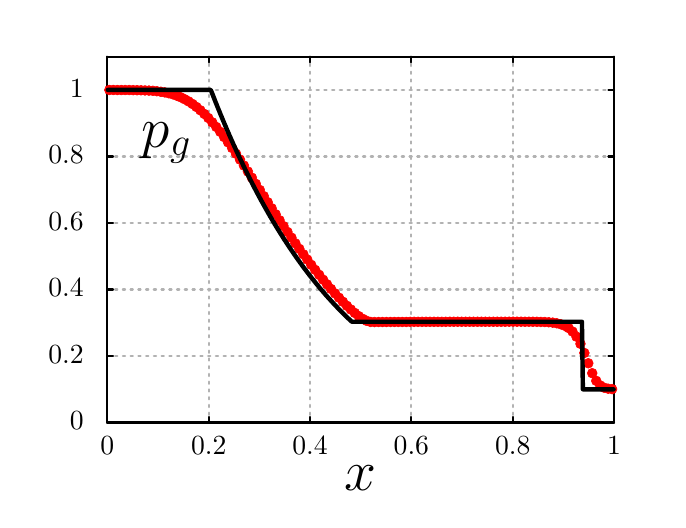
\begin{tikzpicture}[gnuplot]
%% generated with GNUPLOT 4.6p4 (Lua 5.1; terminal rev. 99, script rev. 100)
%% Thu 31 Jul 2014 01:57:35 PM EDT
\path (0.000,0.000) rectangle (8.000,6.000);
\gpfill{rgb color={1.000,1.000,1.000}} (1.012,0.985)--(7.446,0.985)--(7.446,5.630)--(1.012,5.630)--cycle;
\gpcolor{color=gp lt color border}
\gpsetlinetype{gp lt border}
\gpsetlinewidth{1.00}
\draw[gp path] (1.012,0.985)--(1.012,5.630)--(7.446,5.630)--(7.446,0.985)--cycle;
\gpcolor{color=gp lt color axes}
\gpsetlinetype{gp lt axes}
\gpsetlinewidth{2.00}
\draw[gp path] (1.012,0.985)--(7.447,0.985);
\gpcolor{color=gp lt color border}
\gpsetlinetype{gp lt border}
\draw[gp path] (1.012,0.985)--(1.084,0.985);
\draw[gp path] (7.447,0.985)--(7.375,0.985);
\gpcolor{rgb color={0.000,0.000,0.000}}
\node[gp node right,font={\fontsize{10pt}{12pt}\selectfont}] at (0.828,0.985) {0};
\gpcolor{color=gp lt color axes}
\gpsetlinetype{gp lt axes}
\draw[gp path] (1.012,1.830)--(7.447,1.830);
\gpcolor{color=gp lt color border}
\gpsetlinetype{gp lt border}
\draw[gp path] (1.012,1.830)--(1.084,1.830);
\draw[gp path] (7.447,1.830)--(7.375,1.830);
\gpcolor{rgb color={0.000,0.000,0.000}}
\node[gp node right,font={\fontsize{10pt}{12pt}\selectfont}] at (0.828,1.830) {0.2};
\gpcolor{color=gp lt color axes}
\gpsetlinetype{gp lt axes}
\draw[gp path] (1.012,2.674)--(7.447,2.674);
\gpcolor{color=gp lt color border}
\gpsetlinetype{gp lt border}
\draw[gp path] (1.012,2.674)--(1.084,2.674);
\draw[gp path] (7.447,2.674)--(7.375,2.674);
\gpcolor{rgb color={0.000,0.000,0.000}}
\node[gp node right,font={\fontsize{10pt}{12pt}\selectfont}] at (0.828,2.674) {0.4};
\gpcolor{color=gp lt color axes}
\gpsetlinetype{gp lt axes}
\draw[gp path] (1.012,3.519)--(7.447,3.519);
\gpcolor{color=gp lt color border}
\gpsetlinetype{gp lt border}
\draw[gp path] (1.012,3.519)--(1.084,3.519);
\draw[gp path] (7.447,3.519)--(7.375,3.519);
\gpcolor{rgb color={0.000,0.000,0.000}}
\node[gp node right,font={\fontsize{10pt}{12pt}\selectfont}] at (0.828,3.519) {0.6};
\gpcolor{color=gp lt color axes}
\gpsetlinetype{gp lt axes}
\draw[gp path] (1.012,4.364)--(7.447,4.364);
\gpcolor{color=gp lt color border}
\gpsetlinetype{gp lt border}
\draw[gp path] (1.012,4.364)--(1.084,4.364);
\draw[gp path] (7.447,4.364)--(7.375,4.364);
\gpcolor{rgb color={0.000,0.000,0.000}}
\node[gp node right,font={\fontsize{10pt}{12pt}\selectfont}] at (0.828,4.364) {0.8};
\gpcolor{color=gp lt color axes}
\gpsetlinetype{gp lt axes}
\draw[gp path] (1.012,5.209)--(7.447,5.209);
\gpcolor{color=gp lt color border}
\gpsetlinetype{gp lt border}
\draw[gp path] (1.012,5.209)--(1.084,5.209);
\draw[gp path] (7.447,5.209)--(7.375,5.209);
\gpcolor{rgb color={0.000,0.000,0.000}}
\node[gp node right,font={\fontsize{10pt}{12pt}\selectfont}] at (0.828,5.209) {1};
\gpcolor{color=gp lt color axes}
\gpsetlinetype{gp lt axes}
\draw[gp path] (1.012,0.985)--(1.012,5.631);
\gpcolor{color=gp lt color border}
\gpsetlinetype{gp lt border}
\draw[gp path] (1.012,0.985)--(1.012,1.057);
\draw[gp path] (1.012,5.631)--(1.012,5.559);
\gpcolor{rgb color={0.000,0.000,0.000}}
\node[gp node center,font={\fontsize{10pt}{12pt}\selectfont}] at (1.012,0.677) {0};
\gpcolor{color=gp lt color axes}
\gpsetlinetype{gp lt axes}
\draw[gp path] (2.299,0.985)--(2.299,5.631);
\gpcolor{color=gp lt color border}
\gpsetlinetype{gp lt border}
\draw[gp path] (2.299,0.985)--(2.299,1.057);
\draw[gp path] (2.299,5.631)--(2.299,5.559);
\gpcolor{rgb color={0.000,0.000,0.000}}
\node[gp node center,font={\fontsize{10pt}{12pt}\selectfont}] at (2.299,0.677) {0.2};
\gpcolor{color=gp lt color axes}
\gpsetlinetype{gp lt axes}
\draw[gp path] (3.586,0.985)--(3.586,5.631);
\gpcolor{color=gp lt color border}
\gpsetlinetype{gp lt border}
\draw[gp path] (3.586,0.985)--(3.586,1.057);
\draw[gp path] (3.586,5.631)--(3.586,5.559);
\gpcolor{rgb color={0.000,0.000,0.000}}
\node[gp node center,font={\fontsize{10pt}{12pt}\selectfont}] at (3.586,0.677) {0.4};
\gpcolor{color=gp lt color axes}
\gpsetlinetype{gp lt axes}
\draw[gp path] (4.873,0.985)--(4.873,5.631);
\gpcolor{color=gp lt color border}
\gpsetlinetype{gp lt border}
\draw[gp path] (4.873,0.985)--(4.873,1.057);
\draw[gp path] (4.873,5.631)--(4.873,5.559);
\gpcolor{rgb color={0.000,0.000,0.000}}
\node[gp node center,font={\fontsize{10pt}{12pt}\selectfont}] at (4.873,0.677) {0.6};
\gpcolor{color=gp lt color axes}
\gpsetlinetype{gp lt axes}
\draw[gp path] (6.160,0.985)--(6.160,5.631);
\gpcolor{color=gp lt color border}
\gpsetlinetype{gp lt border}
\draw[gp path] (6.160,0.985)--(6.160,1.057);
\draw[gp path] (6.160,5.631)--(6.160,5.559);
\gpcolor{rgb color={0.000,0.000,0.000}}
\node[gp node center,font={\fontsize{10pt}{12pt}\selectfont}] at (6.160,0.677) {0.8};
\gpcolor{color=gp lt color axes}
\gpsetlinetype{gp lt axes}
\draw[gp path] (7.447,0.985)--(7.447,5.631);
\gpcolor{color=gp lt color border}
\gpsetlinetype{gp lt border}
\draw[gp path] (7.447,0.985)--(7.447,1.057);
\draw[gp path] (7.447,5.631)--(7.447,5.559);
\gpcolor{rgb color={0.000,0.000,0.000}}
\node[gp node center,font={\fontsize{10pt}{12pt}\selectfont}] at (7.447,0.677) {1};
\gpcolor{color=gp lt color border}
\draw[gp path] (1.012,5.631)--(1.012,0.985)--(7.447,0.985)--(7.447,5.631)--cycle;
\gpcolor{rgb color={0.000,0.000,0.000}}
\node[gp node center,font={\fontsize{10pt}{12pt}\selectfont}] at (4.229,0.215) {\huge $x$};
\gpcolor{rgb color={1.000,0.000,0.000}}
\gpsetlinewidth{0.50}
\gpsetpointsize{4.44}
\gppoint{gp mark 7}{(1.037,5.209)}
\gppoint{gp mark 7}{(1.087,5.209)}
\gppoint{gp mark 7}{(1.138,5.208)}
\gppoint{gp mark 7}{(1.188,5.208)}
\gppoint{gp mark 7}{(1.238,5.208)}
\gppoint{gp mark 7}{(1.289,5.208)}
\gppoint{gp mark 7}{(1.339,5.207)}
\gppoint{gp mark 7}{(1.389,5.206)}
\gppoint{gp mark 7}{(1.439,5.205)}
\gppoint{gp mark 7}{(1.490,5.203)}
\gppoint{gp mark 7}{(1.540,5.201)}
\gppoint{gp mark 7}{(1.590,5.198)}
\gppoint{gp mark 7}{(1.640,5.193)}
\gppoint{gp mark 7}{(1.691,5.186)}
\gppoint{gp mark 7}{(1.741,5.178)}
\gppoint{gp mark 7}{(1.791,5.167)}
\gppoint{gp mark 7}{(1.842,5.154)}
\gppoint{gp mark 7}{(1.892,5.137)}
\gppoint{gp mark 7}{(1.942,5.117)}
\gppoint{gp mark 7}{(1.992,5.092)}
\gppoint{gp mark 7}{(2.043,5.064)}
\gppoint{gp mark 7}{(2.093,5.031)}
\gppoint{gp mark 7}{(2.143,4.993)}
\gppoint{gp mark 7}{(2.193,4.951)}
\gppoint{gp mark 7}{(2.244,4.904)}
\gppoint{gp mark 7}{(2.294,4.853)}
\gppoint{gp mark 7}{(2.344,4.798)}
\gppoint{gp mark 7}{(2.395,4.739)}
\gppoint{gp mark 7}{(2.445,4.677)}
\gppoint{gp mark 7}{(2.495,4.611)}
\gppoint{gp mark 7}{(2.545,4.543)}
\gppoint{gp mark 7}{(2.596,4.472)}
\gppoint{gp mark 7}{(2.646,4.399)}
\gppoint{gp mark 7}{(2.696,4.325)}
\gppoint{gp mark 7}{(2.746,4.249)}
\gppoint{gp mark 7}{(2.797,4.173)}
\gppoint{gp mark 7}{(2.847,4.095)}
\gppoint{gp mark 7}{(2.897,4.017)}
\gppoint{gp mark 7}{(2.948,3.939)}
\gppoint{gp mark 7}{(2.998,3.861)}
\gppoint{gp mark 7}{(3.048,3.784)}
\gppoint{gp mark 7}{(3.098,3.707)}
\gppoint{gp mark 7}{(3.149,3.630)}
\gppoint{gp mark 7}{(3.199,3.554)}
\gppoint{gp mark 7}{(3.249,3.480)}
\gppoint{gp mark 7}{(3.299,3.406)}
\gppoint{gp mark 7}{(3.350,3.333)}
\gppoint{gp mark 7}{(3.400,3.261)}
\gppoint{gp mark 7}{(3.450,3.191)}
\gppoint{gp mark 7}{(3.501,3.122)}
\gppoint{gp mark 7}{(3.551,3.055)}
\gppoint{gp mark 7}{(3.601,2.988)}
\gppoint{gp mark 7}{(3.651,2.924)}
\gppoint{gp mark 7}{(3.702,2.861)}
\gppoint{gp mark 7}{(3.752,2.799)}
\gppoint{gp mark 7}{(3.802,2.740)}
\gppoint{gp mark 7}{(3.852,2.682)}
\gppoint{gp mark 7}{(3.903,2.625)}
\gppoint{gp mark 7}{(3.953,2.571)}
\gppoint{gp mark 7}{(4.003,2.519)}
\gppoint{gp mark 7}{(4.054,2.468)}
\gppoint{gp mark 7}{(4.104,2.421)}
\gppoint{gp mark 7}{(4.154,2.377)}
\gppoint{gp mark 7}{(4.204,2.337)}
\gppoint{gp mark 7}{(4.255,2.302)}
\gppoint{gp mark 7}{(4.305,2.277)}
\gppoint{gp mark 7}{(4.355,2.263)}
\gppoint{gp mark 7}{(4.405,2.261)}
\gppoint{gp mark 7}{(4.456,2.262)}
\gppoint{gp mark 7}{(4.506,2.262)}
\gppoint{gp mark 7}{(4.556,2.262)}
\gppoint{gp mark 7}{(4.607,2.263)}
\gppoint{gp mark 7}{(4.657,2.263)}
\gppoint{gp mark 7}{(4.707,2.263)}
\gppoint{gp mark 7}{(4.757,2.263)}
\gppoint{gp mark 7}{(4.808,2.263)}
\gppoint{gp mark 7}{(4.858,2.264)}
\gppoint{gp mark 7}{(4.908,2.264)}
\gppoint{gp mark 7}{(4.958,2.264)}
\gppoint{gp mark 7}{(5.009,2.264)}
\gppoint{gp mark 7}{(5.059,2.264)}
\gppoint{gp mark 7}{(5.109,2.264)}
\gppoint{gp mark 7}{(5.160,2.264)}
\gppoint{gp mark 7}{(5.210,2.264)}
\gppoint{gp mark 7}{(5.260,2.264)}
\gppoint{gp mark 7}{(5.310,2.264)}
\gppoint{gp mark 7}{(5.361,2.265)}
\gppoint{gp mark 7}{(5.411,2.265)}
\gppoint{gp mark 7}{(5.461,2.265)}
\gppoint{gp mark 7}{(5.511,2.265)}
\gppoint{gp mark 7}{(5.562,2.265)}
\gppoint{gp mark 7}{(5.612,2.265)}
\gppoint{gp mark 7}{(5.662,2.265)}
\gppoint{gp mark 7}{(5.713,2.265)}
\gppoint{gp mark 7}{(5.763,2.265)}
\gppoint{gp mark 7}{(5.813,2.265)}
\gppoint{gp mark 7}{(5.863,2.265)}
\gppoint{gp mark 7}{(5.914,2.265)}
\gppoint{gp mark 7}{(5.964,2.265)}
\gppoint{gp mark 7}{(6.014,2.265)}
\gppoint{gp mark 7}{(6.064,2.265)}
\gppoint{gp mark 7}{(6.115,2.266)}
\gppoint{gp mark 7}{(6.165,2.266)}
\gppoint{gp mark 7}{(6.215,2.266)}
\gppoint{gp mark 7}{(6.266,2.266)}
\gppoint{gp mark 7}{(6.316,2.265)}
\gppoint{gp mark 7}{(6.366,2.265)}
\gppoint{gp mark 7}{(6.416,2.265)}
\gppoint{gp mark 7}{(6.467,2.264)}
\gppoint{gp mark 7}{(6.517,2.263)}
\gppoint{gp mark 7}{(6.567,2.262)}
\gppoint{gp mark 7}{(6.617,2.259)}
\gppoint{gp mark 7}{(6.668,2.254)}
\gppoint{gp mark 7}{(6.718,2.246)}
\gppoint{gp mark 7}{(6.768,2.234)}
\gppoint{gp mark 7}{(6.819,2.215)}
\gppoint{gp mark 7}{(6.869,2.186)}
\gppoint{gp mark 7}{(6.919,2.141)}
\gppoint{gp mark 7}{(6.969,2.076)}
\gppoint{gp mark 7}{(7.020,1.985)}
\gppoint{gp mark 7}{(7.070,1.869)}
\gppoint{gp mark 7}{(7.120,1.738)}
\gppoint{gp mark 7}{(7.170,1.612)}
\gppoint{gp mark 7}{(7.221,1.515)}
\gppoint{gp mark 7}{(7.271,1.456)}
\gppoint{gp mark 7}{(7.321,1.428)}
\gppoint{gp mark 7}{(7.372,1.415)}
\gppoint{gp mark 7}{(7.422,1.410)}
\gpcolor{rgb color={0.000,0.000,0.000}}
\gpsetlinetype{gp lt plot 0}
\gpsetlinewidth{4.00}
\draw[gp path] (1.018,5.209)--(1.031,5.209)--(1.043,5.209)--(1.056,5.209)--(1.069,5.209)%
  --(1.081,5.209)--(1.094,5.209)--(1.106,5.209)--(1.119,5.209)--(1.131,5.209)--(1.144,5.209)%
  --(1.157,5.209)--(1.169,5.209)--(1.182,5.209)--(1.194,5.209)--(1.207,5.209)--(1.219,5.209)%
  --(1.232,5.209)--(1.245,5.209)--(1.257,5.209)--(1.270,5.209)--(1.282,5.209)--(1.295,5.209)%
  --(1.307,5.209)--(1.320,5.209)--(1.332,5.209)--(1.345,5.209)--(1.358,5.209)--(1.370,5.209)%
  --(1.383,5.209)--(1.395,5.209)--(1.408,5.209)--(1.420,5.209)--(1.433,5.209)--(1.446,5.209)%
  --(1.458,5.209)--(1.471,5.209)--(1.483,5.209)--(1.496,5.209)--(1.508,5.209)--(1.521,5.209)%
  --(1.534,5.209)--(1.546,5.209)--(1.559,5.209)--(1.571,5.209)--(1.584,5.209)--(1.596,5.209)%
  --(1.609,5.209)--(1.622,5.209)--(1.634,5.209)--(1.647,5.209)--(1.659,5.209)--(1.672,5.209)%
  --(1.684,5.209)--(1.697,5.209)--(1.710,5.209)--(1.722,5.209)--(1.735,5.209)--(1.747,5.209)%
  --(1.760,5.209)--(1.772,5.209)--(1.785,5.209)--(1.798,5.209)--(1.810,5.209)--(1.823,5.209)%
  --(1.835,5.209)--(1.848,5.209)--(1.860,5.209)--(1.873,5.209)--(1.886,5.209)--(1.898,5.209)%
  --(1.911,5.209)--(1.923,5.209)--(1.936,5.209)--(1.948,5.209)--(1.961,5.209)--(1.973,5.209)%
  --(1.986,5.209)--(1.999,5.209)--(2.011,5.209)--(2.024,5.209)--(2.036,5.209)--(2.049,5.209)%
  --(2.061,5.209)--(2.074,5.209)--(2.087,5.209)--(2.099,5.209)--(2.112,5.209)--(2.124,5.209)%
  --(2.137,5.209)--(2.149,5.209)--(2.162,5.209)--(2.175,5.209)--(2.187,5.209)--(2.200,5.209)%
  --(2.212,5.209)--(2.225,5.209)--(2.237,5.209)--(2.250,5.209)--(2.263,5.209)--(2.275,5.209)%
  --(2.288,5.209)--(2.300,5.209)--(2.313,5.209)--(2.325,5.209)--(2.338,5.178)--(2.351,5.146)%
  --(2.363,5.114)--(2.376,5.082)--(2.388,5.050)--(2.401,5.019)--(2.413,4.988)--(2.426,4.957)%
  --(2.439,4.926)--(2.451,4.895)--(2.464,4.865)--(2.476,4.835)--(2.489,4.805)--(2.501,4.775)%
  --(2.514,4.746)--(2.526,4.716)--(2.539,4.687)--(2.552,4.658)--(2.564,4.629)--(2.577,4.601)%
  --(2.589,4.572)--(2.602,4.544)--(2.614,4.516)--(2.627,4.488)--(2.640,4.461)--(2.652,4.433)%
  --(2.665,4.406)--(2.677,4.379)--(2.690,4.352)--(2.702,4.325)--(2.715,4.299)--(2.728,4.273)%
  --(2.740,4.246)--(2.753,4.220)--(2.765,4.195)--(2.778,4.169)--(2.790,4.144)--(2.803,4.118)%
  --(2.816,4.093)--(2.828,4.068)--(2.841,4.043)--(2.853,4.019)--(2.866,3.994)--(2.878,3.970)%
  --(2.891,3.946)--(2.904,3.922)--(2.916,3.898)--(2.929,3.875)--(2.941,3.851)--(2.954,3.828)%
  --(2.966,3.805)--(2.979,3.782)--(2.992,3.759)--(3.004,3.737)--(3.017,3.714)--(3.029,3.692)%
  --(3.042,3.670)--(3.054,3.648)--(3.067,3.626)--(3.079,3.604)--(3.092,3.583)--(3.105,3.561)%
  --(3.117,3.540)--(3.130,3.519)--(3.142,3.498)--(3.155,3.477)--(3.167,3.457)--(3.180,3.436)%
  --(3.193,3.416)--(3.205,3.396)--(3.218,3.376)--(3.230,3.356)--(3.243,3.336)--(3.255,3.316)%
  --(3.268,3.297)--(3.281,3.278)--(3.293,3.258)--(3.306,3.239)--(3.318,3.220)--(3.331,3.202)%
  --(3.343,3.183)--(3.356,3.165)--(3.369,3.146)--(3.381,3.128)--(3.394,3.110)--(3.406,3.092)%
  --(3.419,3.074)--(3.431,3.056)--(3.444,3.039)--(3.457,3.021)--(3.469,3.004)--(3.482,2.987)%
  --(3.494,2.969)--(3.507,2.952)--(3.519,2.936)--(3.532,2.919)--(3.545,2.902)--(3.557,2.886)%
  --(3.570,2.870)--(3.582,2.853)--(3.595,2.837)--(3.607,2.821)--(3.620,2.805)--(3.633,2.790)%
  --(3.645,2.774)--(3.658,2.758)--(3.670,2.743)--(3.683,2.728)--(3.695,2.713)--(3.708,2.697)%
  --(3.720,2.682)--(3.733,2.668)--(3.746,2.653)--(3.758,2.638)--(3.771,2.624)--(3.783,2.609)%
  --(3.796,2.595)--(3.808,2.581)--(3.821,2.567)--(3.834,2.553)--(3.846,2.539)--(3.859,2.525)%
  --(3.871,2.512)--(3.884,2.498)--(3.896,2.485)--(3.909,2.471)--(3.922,2.458)--(3.934,2.445)%
  --(3.947,2.432)--(3.959,2.419)--(3.972,2.406)--(3.984,2.393)--(3.997,2.381)--(4.010,2.368)%
  --(4.022,2.356)--(4.035,2.343)--(4.047,2.331)--(4.060,2.319)--(4.072,2.307)--(4.085,2.295)%
  --(4.098,2.283)--(4.110,2.271)--(4.123,2.265)--(4.135,2.265)--(4.148,2.265)--(4.160,2.265)%
  --(4.173,2.265)--(4.186,2.265)--(4.198,2.265)--(4.211,2.265)--(4.223,2.265)--(4.236,2.265)%
  --(4.248,2.265)--(4.261,2.265)--(4.273,2.265)--(4.286,2.265)--(4.299,2.265)--(4.311,2.265)%
  --(4.324,2.265)--(4.336,2.265)--(4.349,2.265)--(4.361,2.265)--(4.374,2.265)--(4.387,2.265)%
  --(4.399,2.265)--(4.412,2.265)--(4.424,2.265)--(4.437,2.265)--(4.449,2.265)--(4.462,2.265)%
  --(4.475,2.265)--(4.487,2.265)--(4.500,2.265)--(4.512,2.265)--(4.525,2.265)--(4.537,2.265)%
  --(4.550,2.265)--(4.563,2.265)--(4.575,2.265)--(4.588,2.265)--(4.600,2.265)--(4.613,2.265)%
  --(4.625,2.265)--(4.638,2.265)--(4.651,2.265)--(4.663,2.265)--(4.676,2.265)--(4.688,2.265)%
  --(4.701,2.265)--(4.713,2.265)--(4.726,2.265)--(4.739,2.265)--(4.751,2.265)--(4.764,2.265)%
  --(4.776,2.265)--(4.789,2.265)--(4.801,2.265)--(4.814,2.265)--(4.826,2.265)--(4.839,2.265)%
  --(4.852,2.265)--(4.864,2.265)--(4.877,2.265)--(4.889,2.265)--(4.902,2.265)--(4.914,2.265)%
  --(4.927,2.265)--(4.940,2.265)--(4.952,2.265)--(4.965,2.265)--(4.977,2.265)--(4.990,2.265)%
  --(5.002,2.265)--(5.015,2.265)--(5.028,2.265)--(5.040,2.265)--(5.053,2.265)--(5.065,2.265)%
  --(5.078,2.265)--(5.090,2.265)--(5.103,2.265)--(5.116,2.265)--(5.128,2.265)--(5.141,2.265)%
  --(5.153,2.265)--(5.166,2.265)--(5.178,2.265)--(5.191,2.265)--(5.204,2.265)--(5.216,2.265)%
  --(5.229,2.265)--(5.241,2.265)--(5.254,2.265)--(5.266,2.265)--(5.279,2.265)--(5.292,2.265)%
  --(5.304,2.265)--(5.317,2.265)--(5.329,2.265)--(5.342,2.265)--(5.354,2.265)--(5.367,2.265)%
  --(5.380,2.265)--(5.392,2.265)--(5.405,2.265)--(5.417,2.265)--(5.430,2.265)--(5.442,2.265)%
  --(5.455,2.265)--(5.467,2.265)--(5.480,2.265)--(5.493,2.265)--(5.505,2.265)--(5.518,2.265)%
  --(5.530,2.265)--(5.543,2.265)--(5.555,2.265)--(5.568,2.265)--(5.581,2.265)--(5.593,2.265)%
  --(5.606,2.265)--(5.618,2.265)--(5.631,2.265)--(5.643,2.265)--(5.656,2.265)--(5.669,2.265)%
  --(5.681,2.265)--(5.694,2.265)--(5.706,2.265)--(5.719,2.265)--(5.731,2.265)--(5.744,2.265)%
  --(5.757,2.265)--(5.769,2.265)--(5.782,2.265)--(5.794,2.265)--(5.807,2.265)--(5.819,2.265)%
  --(5.832,2.265)--(5.845,2.265)--(5.857,2.265)--(5.870,2.265)--(5.882,2.265)--(5.895,2.265)%
  --(5.907,2.265)--(5.920,2.265)--(5.933,2.265)--(5.945,2.265)--(5.958,2.265)--(5.970,2.265)%
  --(5.983,2.265)--(5.995,2.265)--(6.008,2.265)--(6.020,2.265)--(6.033,2.265)--(6.046,2.265)%
  --(6.058,2.265)--(6.071,2.265)--(6.083,2.265)--(6.096,2.265)--(6.108,2.265)--(6.121,2.265)%
  --(6.134,2.265)--(6.146,2.265)--(6.159,2.265)--(6.171,2.265)--(6.184,2.265)--(6.196,2.265)%
  --(6.209,2.265)--(6.222,2.265)--(6.234,2.265)--(6.247,2.265)--(6.259,2.265)--(6.272,2.265)%
  --(6.284,2.265)--(6.297,2.265)--(6.310,2.265)--(6.322,2.265)--(6.335,2.265)--(6.347,2.265)%
  --(6.360,2.265)--(6.372,2.265)--(6.385,2.265)--(6.398,2.265)--(6.410,2.265)--(6.423,2.265)%
  --(6.435,2.265)--(6.448,2.265)--(6.460,2.265)--(6.473,2.265)--(6.486,2.265)--(6.498,2.265)%
  --(6.511,2.265)--(6.523,2.265)--(6.536,2.265)--(6.548,2.265)--(6.561,2.265)--(6.573,2.265)%
  --(6.586,2.265)--(6.599,2.265)--(6.611,2.265)--(6.624,2.265)--(6.636,2.265)--(6.649,2.265)%
  --(6.661,2.265)--(6.674,2.265)--(6.687,2.265)--(6.699,2.265)--(6.712,2.265)--(6.724,2.265)%
  --(6.737,2.265)--(6.749,2.265)--(6.762,2.265)--(6.775,2.265)--(6.787,2.265)--(6.800,2.265)%
  --(6.812,2.265)--(6.825,2.265)--(6.837,2.265)--(6.850,2.265)--(6.863,2.265)--(6.875,2.265)%
  --(6.888,2.265)--(6.900,2.265)--(6.913,2.265)--(6.925,2.265)--(6.938,2.265)--(6.951,2.265)%
  --(6.963,2.265)--(6.976,2.265)--(6.988,2.265)--(7.001,2.265)--(7.013,2.265)--(7.026,2.265)%
  --(7.039,2.265)--(7.051,1.407)--(7.064,1.407)--(7.076,1.407)--(7.089,1.407)--(7.101,1.407)%
  --(7.114,1.407)--(7.127,1.407)--(7.139,1.407)--(7.152,1.407)--(7.164,1.407)--(7.177,1.407)%
  --(7.189,1.407)--(7.202,1.407)--(7.214,1.407)--(7.227,1.407)--(7.240,1.407)--(7.252,1.407)%
  --(7.265,1.407)--(7.277,1.407)--(7.290,1.407)--(7.302,1.407)--(7.315,1.407)--(7.328,1.407)%
  --(7.340,1.407)--(7.353,1.407)--(7.365,1.407)--(7.378,1.407)--(7.390,1.407)--(7.403,1.407)%
  --(7.416,1.407)--(7.428,1.407)--(7.441,1.407);
\node[gp node left,font={\fontsize{10pt}{12pt}\selectfont}] at (1.334,4.575) {\huge $p_g$};
%% coordinates of the plot area
\gpdefrectangularnode{gp plot 1}{\pgfpoint{1.012cm}{0.985cm}}{\pgfpoint{7.447cm}{5.631cm}}
\end{tikzpicture}
%% gnuplot variables
} \\
\resizebox{0.33\linewidth}{!}{\tikzsetnextfilename{sod_hllc_1_1}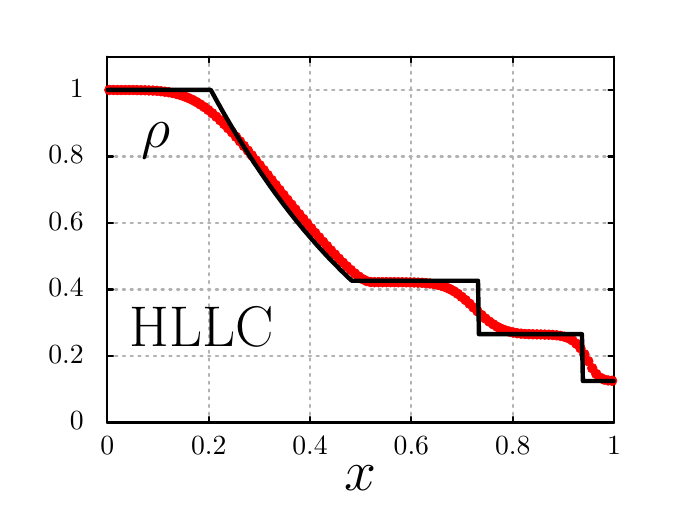
\begin{tikzpicture}[gnuplot]
%% generated with GNUPLOT 4.6p4 (Lua 5.1; terminal rev. 99, script rev. 100)
%% Thu 31 Jul 2014 01:57:05 PM EDT
\path (0.000,0.000) rectangle (8.000,6.000);
\gpfill{rgb color={1.000,1.000,1.000}} (1.012,0.985)--(7.446,0.985)--(7.446,5.630)--(1.012,5.630)--cycle;
\gpcolor{color=gp lt color border}
\gpsetlinetype{gp lt border}
\gpsetlinewidth{1.00}
\draw[gp path] (1.012,0.985)--(1.012,5.630)--(7.446,5.630)--(7.446,0.985)--cycle;
\gpcolor{color=gp lt color axes}
\gpsetlinetype{gp lt axes}
\gpsetlinewidth{2.00}
\draw[gp path] (1.012,0.985)--(7.447,0.985);
\gpcolor{color=gp lt color border}
\gpsetlinetype{gp lt border}
\draw[gp path] (1.012,0.985)--(1.084,0.985);
\draw[gp path] (7.447,0.985)--(7.375,0.985);
\gpcolor{rgb color={0.000,0.000,0.000}}
\node[gp node right,font={\fontsize{10pt}{12pt}\selectfont}] at (0.828,0.985) {0};
\gpcolor{color=gp lt color axes}
\gpsetlinetype{gp lt axes}
\draw[gp path] (1.012,1.830)--(7.447,1.830);
\gpcolor{color=gp lt color border}
\gpsetlinetype{gp lt border}
\draw[gp path] (1.012,1.830)--(1.084,1.830);
\draw[gp path] (7.447,1.830)--(7.375,1.830);
\gpcolor{rgb color={0.000,0.000,0.000}}
\node[gp node right,font={\fontsize{10pt}{12pt}\selectfont}] at (0.828,1.830) {0.2};
\gpcolor{color=gp lt color axes}
\gpsetlinetype{gp lt axes}
\draw[gp path] (1.012,2.674)--(7.447,2.674);
\gpcolor{color=gp lt color border}
\gpsetlinetype{gp lt border}
\draw[gp path] (1.012,2.674)--(1.084,2.674);
\draw[gp path] (7.447,2.674)--(7.375,2.674);
\gpcolor{rgb color={0.000,0.000,0.000}}
\node[gp node right,font={\fontsize{10pt}{12pt}\selectfont}] at (0.828,2.674) {0.4};
\gpcolor{color=gp lt color axes}
\gpsetlinetype{gp lt axes}
\draw[gp path] (1.012,3.519)--(7.447,3.519);
\gpcolor{color=gp lt color border}
\gpsetlinetype{gp lt border}
\draw[gp path] (1.012,3.519)--(1.084,3.519);
\draw[gp path] (7.447,3.519)--(7.375,3.519);
\gpcolor{rgb color={0.000,0.000,0.000}}
\node[gp node right,font={\fontsize{10pt}{12pt}\selectfont}] at (0.828,3.519) {0.6};
\gpcolor{color=gp lt color axes}
\gpsetlinetype{gp lt axes}
\draw[gp path] (1.012,4.364)--(7.447,4.364);
\gpcolor{color=gp lt color border}
\gpsetlinetype{gp lt border}
\draw[gp path] (1.012,4.364)--(1.084,4.364);
\draw[gp path] (7.447,4.364)--(7.375,4.364);
\gpcolor{rgb color={0.000,0.000,0.000}}
\node[gp node right,font={\fontsize{10pt}{12pt}\selectfont}] at (0.828,4.364) {0.8};
\gpcolor{color=gp lt color axes}
\gpsetlinetype{gp lt axes}
\draw[gp path] (1.012,5.209)--(7.447,5.209);
\gpcolor{color=gp lt color border}
\gpsetlinetype{gp lt border}
\draw[gp path] (1.012,5.209)--(1.084,5.209);
\draw[gp path] (7.447,5.209)--(7.375,5.209);
\gpcolor{rgb color={0.000,0.000,0.000}}
\node[gp node right,font={\fontsize{10pt}{12pt}\selectfont}] at (0.828,5.209) {1};
\gpcolor{color=gp lt color axes}
\gpsetlinetype{gp lt axes}
\draw[gp path] (1.012,0.985)--(1.012,5.631);
\gpcolor{color=gp lt color border}
\gpsetlinetype{gp lt border}
\draw[gp path] (1.012,0.985)--(1.012,1.057);
\draw[gp path] (1.012,5.631)--(1.012,5.559);
\gpcolor{rgb color={0.000,0.000,0.000}}
\node[gp node center,font={\fontsize{10pt}{12pt}\selectfont}] at (1.012,0.677) {0};
\gpcolor{color=gp lt color axes}
\gpsetlinetype{gp lt axes}
\draw[gp path] (2.299,0.985)--(2.299,5.631);
\gpcolor{color=gp lt color border}
\gpsetlinetype{gp lt border}
\draw[gp path] (2.299,0.985)--(2.299,1.057);
\draw[gp path] (2.299,5.631)--(2.299,5.559);
\gpcolor{rgb color={0.000,0.000,0.000}}
\node[gp node center,font={\fontsize{10pt}{12pt}\selectfont}] at (2.299,0.677) {0.2};
\gpcolor{color=gp lt color axes}
\gpsetlinetype{gp lt axes}
\draw[gp path] (3.586,0.985)--(3.586,5.631);
\gpcolor{color=gp lt color border}
\gpsetlinetype{gp lt border}
\draw[gp path] (3.586,0.985)--(3.586,1.057);
\draw[gp path] (3.586,5.631)--(3.586,5.559);
\gpcolor{rgb color={0.000,0.000,0.000}}
\node[gp node center,font={\fontsize{10pt}{12pt}\selectfont}] at (3.586,0.677) {0.4};
\gpcolor{color=gp lt color axes}
\gpsetlinetype{gp lt axes}
\draw[gp path] (4.873,0.985)--(4.873,5.631);
\gpcolor{color=gp lt color border}
\gpsetlinetype{gp lt border}
\draw[gp path] (4.873,0.985)--(4.873,1.057);
\draw[gp path] (4.873,5.631)--(4.873,5.559);
\gpcolor{rgb color={0.000,0.000,0.000}}
\node[gp node center,font={\fontsize{10pt}{12pt}\selectfont}] at (4.873,0.677) {0.6};
\gpcolor{color=gp lt color axes}
\gpsetlinetype{gp lt axes}
\draw[gp path] (6.160,0.985)--(6.160,5.631);
\gpcolor{color=gp lt color border}
\gpsetlinetype{gp lt border}
\draw[gp path] (6.160,0.985)--(6.160,1.057);
\draw[gp path] (6.160,5.631)--(6.160,5.559);
\gpcolor{rgb color={0.000,0.000,0.000}}
\node[gp node center,font={\fontsize{10pt}{12pt}\selectfont}] at (6.160,0.677) {0.8};
\gpcolor{color=gp lt color axes}
\gpsetlinetype{gp lt axes}
\draw[gp path] (7.447,0.985)--(7.447,5.631);
\gpcolor{color=gp lt color border}
\gpsetlinetype{gp lt border}
\draw[gp path] (7.447,0.985)--(7.447,1.057);
\draw[gp path] (7.447,5.631)--(7.447,5.559);
\gpcolor{rgb color={0.000,0.000,0.000}}
\node[gp node center,font={\fontsize{10pt}{12pt}\selectfont}] at (7.447,0.677) {1};
\gpcolor{color=gp lt color border}
\draw[gp path] (1.012,5.631)--(1.012,0.985)--(7.447,0.985)--(7.447,5.631)--cycle;
\gpcolor{rgb color={0.000,0.000,0.000}}
\node[gp node center,font={\fontsize{10pt}{12pt}\selectfont}] at (4.229,0.215) {\huge $x$};
\gpcolor{rgb color={1.000,0.000,0.000}}
\gpsetlinewidth{0.50}
\gpsetpointsize{4.44}
\gppoint{gp mark 7}{(1.037,5.209)}
\gppoint{gp mark 7}{(1.087,5.209)}
\gppoint{gp mark 7}{(1.138,5.208)}
\gppoint{gp mark 7}{(1.188,5.208)}
\gppoint{gp mark 7}{(1.238,5.208)}
\gppoint{gp mark 7}{(1.289,5.208)}
\gppoint{gp mark 7}{(1.339,5.208)}
\gppoint{gp mark 7}{(1.389,5.207)}
\gppoint{gp mark 7}{(1.439,5.206)}
\gppoint{gp mark 7}{(1.490,5.205)}
\gppoint{gp mark 7}{(1.540,5.203)}
\gppoint{gp mark 7}{(1.590,5.201)}
\gppoint{gp mark 7}{(1.640,5.198)}
\gppoint{gp mark 7}{(1.691,5.193)}
\gppoint{gp mark 7}{(1.741,5.187)}
\gppoint{gp mark 7}{(1.791,5.180)}
\gppoint{gp mark 7}{(1.842,5.170)}
\gppoint{gp mark 7}{(1.892,5.158)}
\gppoint{gp mark 7}{(1.942,5.144)}
\gppoint{gp mark 7}{(1.992,5.127)}
\gppoint{gp mark 7}{(2.043,5.106)}
\gppoint{gp mark 7}{(2.093,5.083)}
\gppoint{gp mark 7}{(2.143,5.056)}
\gppoint{gp mark 7}{(2.193,5.025)}
\gppoint{gp mark 7}{(2.244,4.991)}
\gppoint{gp mark 7}{(2.294,4.954)}
\gppoint{gp mark 7}{(2.344,4.914)}
\gppoint{gp mark 7}{(2.395,4.870)}
\gppoint{gp mark 7}{(2.445,4.824)}
\gppoint{gp mark 7}{(2.495,4.775)}
\gppoint{gp mark 7}{(2.545,4.723)}
\gppoint{gp mark 7}{(2.596,4.670)}
\gppoint{gp mark 7}{(2.646,4.614)}
\gppoint{gp mark 7}{(2.696,4.557)}
\gppoint{gp mark 7}{(2.746,4.498)}
\gppoint{gp mark 7}{(2.797,4.439)}
\gppoint{gp mark 7}{(2.847,4.378)}
\gppoint{gp mark 7}{(2.897,4.316)}
\gppoint{gp mark 7}{(2.948,4.254)}
\gppoint{gp mark 7}{(2.998,4.192)}
\gppoint{gp mark 7}{(3.048,4.129)}
\gppoint{gp mark 7}{(3.098,4.066)}
\gppoint{gp mark 7}{(3.149,4.003)}
\gppoint{gp mark 7}{(3.199,3.940)}
\gppoint{gp mark 7}{(3.249,3.877)}
\gppoint{gp mark 7}{(3.299,3.815)}
\gppoint{gp mark 7}{(3.350,3.753)}
\gppoint{gp mark 7}{(3.400,3.692)}
\gppoint{gp mark 7}{(3.450,3.631)}
\gppoint{gp mark 7}{(3.501,3.571)}
\gppoint{gp mark 7}{(3.551,3.511)}
\gppoint{gp mark 7}{(3.601,3.452)}
\gppoint{gp mark 7}{(3.651,3.394)}
\gppoint{gp mark 7}{(3.702,3.337)}
\gppoint{gp mark 7}{(3.752,3.281)}
\gppoint{gp mark 7}{(3.802,3.226)}
\gppoint{gp mark 7}{(3.852,3.172)}
\gppoint{gp mark 7}{(3.903,3.119)}
\gppoint{gp mark 7}{(3.953,3.067)}
\gppoint{gp mark 7}{(4.003,3.017)}
\gppoint{gp mark 7}{(4.054,2.969)}
\gppoint{gp mark 7}{(4.104,2.923)}
\gppoint{gp mark 7}{(4.154,2.879)}
\gppoint{gp mark 7}{(4.204,2.840)}
\gppoint{gp mark 7}{(4.255,2.806)}
\gppoint{gp mark 7}{(4.305,2.782)}
\gppoint{gp mark 7}{(4.355,2.770)}
\gppoint{gp mark 7}{(4.405,2.768)}
\gppoint{gp mark 7}{(4.456,2.768)}
\gppoint{gp mark 7}{(4.506,2.768)}
\gppoint{gp mark 7}{(4.556,2.768)}
\gppoint{gp mark 7}{(4.607,2.768)}
\gppoint{gp mark 7}{(4.657,2.768)}
\gppoint{gp mark 7}{(4.707,2.767)}
\gppoint{gp mark 7}{(4.757,2.767)}
\gppoint{gp mark 7}{(4.808,2.766)}
\gppoint{gp mark 7}{(4.858,2.765)}
\gppoint{gp mark 7}{(4.908,2.764)}
\gppoint{gp mark 7}{(4.958,2.762)}
\gppoint{gp mark 7}{(5.009,2.760)}
\gppoint{gp mark 7}{(5.059,2.756)}
\gppoint{gp mark 7}{(5.109,2.751)}
\gppoint{gp mark 7}{(5.160,2.744)}
\gppoint{gp mark 7}{(5.210,2.734)}
\gppoint{gp mark 7}{(5.260,2.721)}
\gppoint{gp mark 7}{(5.310,2.704)}
\gppoint{gp mark 7}{(5.361,2.681)}
\gppoint{gp mark 7}{(5.411,2.654)}
\gppoint{gp mark 7}{(5.461,2.621)}
\gppoint{gp mark 7}{(5.511,2.582)}
\gppoint{gp mark 7}{(5.562,2.540)}
\gppoint{gp mark 7}{(5.612,2.494)}
\gppoint{gp mark 7}{(5.662,2.446)}
\gppoint{gp mark 7}{(5.713,2.398)}
\gppoint{gp mark 7}{(5.763,2.351)}
\gppoint{gp mark 7}{(5.813,2.307)}
\gppoint{gp mark 7}{(5.863,2.267)}
\gppoint{gp mark 7}{(5.914,2.232)}
\gppoint{gp mark 7}{(5.964,2.201)}
\gppoint{gp mark 7}{(6.014,2.176)}
\gppoint{gp mark 7}{(6.064,2.156)}
\gppoint{gp mark 7}{(6.115,2.141)}
\gppoint{gp mark 7}{(6.165,2.129)}
\gppoint{gp mark 7}{(6.215,2.120)}
\gppoint{gp mark 7}{(6.266,2.114)}
\gppoint{gp mark 7}{(6.316,2.110)}
\gppoint{gp mark 7}{(6.366,2.108)}
\gppoint{gp mark 7}{(6.416,2.106)}
\gppoint{gp mark 7}{(6.467,2.105)}
\gppoint{gp mark 7}{(6.517,2.104)}
\gppoint{gp mark 7}{(6.567,2.102)}
\gppoint{gp mark 7}{(6.617,2.101)}
\gppoint{gp mark 7}{(6.668,2.098)}
\gppoint{gp mark 7}{(6.718,2.093)}
\gppoint{gp mark 7}{(6.768,2.086)}
\gppoint{gp mark 7}{(6.819,2.074)}
\gppoint{gp mark 7}{(6.869,2.056)}
\gppoint{gp mark 7}{(6.919,2.028)}
\gppoint{gp mark 7}{(6.969,1.986)}
\gppoint{gp mark 7}{(7.020,1.929)}
\gppoint{gp mark 7}{(7.070,1.853)}
\gppoint{gp mark 7}{(7.120,1.764)}
\gppoint{gp mark 7}{(7.170,1.675)}
\gppoint{gp mark 7}{(7.221,1.602)}
\gppoint{gp mark 7}{(7.271,1.555)}
\gppoint{gp mark 7}{(7.321,1.531)}
\gppoint{gp mark 7}{(7.372,1.520)}
\gppoint{gp mark 7}{(7.422,1.516)}
\gpcolor{rgb color={0.000,0.000,0.000}}
\gpsetlinetype{gp lt plot 0}
\gpsetlinewidth{4.00}
\draw[gp path] (1.018,5.209)--(1.031,5.209)--(1.043,5.209)--(1.056,5.209)--(1.069,5.209)%
  --(1.081,5.209)--(1.094,5.209)--(1.106,5.209)--(1.119,5.209)--(1.131,5.209)--(1.144,5.209)%
  --(1.157,5.209)--(1.169,5.209)--(1.182,5.209)--(1.194,5.209)--(1.207,5.209)--(1.219,5.209)%
  --(1.232,5.209)--(1.245,5.209)--(1.257,5.209)--(1.270,5.209)--(1.282,5.209)--(1.295,5.209)%
  --(1.307,5.209)--(1.320,5.209)--(1.332,5.209)--(1.345,5.209)--(1.358,5.209)--(1.370,5.209)%
  --(1.383,5.209)--(1.395,5.209)--(1.408,5.209)--(1.420,5.209)--(1.433,5.209)--(1.446,5.209)%
  --(1.458,5.209)--(1.471,5.209)--(1.483,5.209)--(1.496,5.209)--(1.508,5.209)--(1.521,5.209)%
  --(1.534,5.209)--(1.546,5.209)--(1.559,5.209)--(1.571,5.209)--(1.584,5.209)--(1.596,5.209)%
  --(1.609,5.209)--(1.622,5.209)--(1.634,5.209)--(1.647,5.209)--(1.659,5.209)--(1.672,5.209)%
  --(1.684,5.209)--(1.697,5.209)--(1.710,5.209)--(1.722,5.209)--(1.735,5.209)--(1.747,5.209)%
  --(1.760,5.209)--(1.772,5.209)--(1.785,5.209)--(1.798,5.209)--(1.810,5.209)--(1.823,5.209)%
  --(1.835,5.209)--(1.848,5.209)--(1.860,5.209)--(1.873,5.209)--(1.886,5.209)--(1.898,5.209)%
  --(1.911,5.209)--(1.923,5.209)--(1.936,5.209)--(1.948,5.209)--(1.961,5.209)--(1.973,5.209)%
  --(1.986,5.209)--(1.999,5.209)--(2.011,5.209)--(2.024,5.209)--(2.036,5.209)--(2.049,5.209)%
  --(2.061,5.209)--(2.074,5.209)--(2.087,5.209)--(2.099,5.209)--(2.112,5.209)--(2.124,5.209)%
  --(2.137,5.209)--(2.149,5.209)--(2.162,5.209)--(2.175,5.209)--(2.187,5.209)--(2.200,5.209)%
  --(2.212,5.209)--(2.225,5.209)--(2.237,5.209)--(2.250,5.209)--(2.263,5.209)--(2.275,5.209)%
  --(2.288,5.209)--(2.300,5.209)--(2.313,5.209)--(2.325,5.209)--(2.338,5.187)--(2.351,5.163)%
  --(2.363,5.140)--(2.376,5.118)--(2.388,5.095)--(2.401,5.072)--(2.413,5.050)--(2.426,5.027)%
  --(2.439,5.005)--(2.451,4.982)--(2.464,4.960)--(2.476,4.938)--(2.489,4.916)--(2.501,4.894)%
  --(2.514,4.872)--(2.526,4.851)--(2.539,4.829)--(2.552,4.808)--(2.564,4.786)--(2.577,4.765)%
  --(2.589,4.744)--(2.602,4.723)--(2.614,4.702)--(2.627,4.681)--(2.640,4.660)--(2.652,4.639)%
  --(2.665,4.618)--(2.677,4.598)--(2.690,4.577)--(2.702,4.557)--(2.715,4.537)--(2.728,4.517)%
  --(2.740,4.496)--(2.753,4.476)--(2.765,4.456)--(2.778,4.437)--(2.790,4.417)--(2.803,4.397)%
  --(2.816,4.378)--(2.828,4.358)--(2.841,4.339)--(2.853,4.320)--(2.866,4.300)--(2.878,4.281)%
  --(2.891,4.262)--(2.904,4.243)--(2.916,4.225)--(2.929,4.206)--(2.941,4.187)--(2.954,4.169)%
  --(2.966,4.150)--(2.979,4.132)--(2.992,4.113)--(3.004,4.095)--(3.017,4.077)--(3.029,4.059)%
  --(3.042,4.041)--(3.054,4.023)--(3.067,4.005)--(3.079,3.987)--(3.092,3.970)--(3.105,3.952)%
  --(3.117,3.935)--(3.130,3.917)--(3.142,3.900)--(3.155,3.883)--(3.167,3.866)--(3.180,3.849)%
  --(3.193,3.832)--(3.205,3.815)--(3.218,3.798)--(3.230,3.781)--(3.243,3.764)--(3.255,3.748)%
  --(3.268,3.731)--(3.281,3.715)--(3.293,3.699)--(3.306,3.682)--(3.318,3.666)--(3.331,3.650)%
  --(3.343,3.634)--(3.356,3.618)--(3.369,3.602)--(3.381,3.586)--(3.394,3.571)--(3.406,3.555)%
  --(3.419,3.539)--(3.431,3.524)--(3.444,3.508)--(3.457,3.493)--(3.469,3.478)--(3.482,3.463)%
  --(3.494,3.447)--(3.507,3.432)--(3.519,3.417)--(3.532,3.403)--(3.545,3.388)--(3.557,3.373)%
  --(3.570,3.358)--(3.582,3.344)--(3.595,3.329)--(3.607,3.315)--(3.620,3.300)--(3.633,3.286)%
  --(3.645,3.272)--(3.658,3.257)--(3.670,3.243)--(3.683,3.229)--(3.695,3.215)--(3.708,3.201)%
  --(3.720,3.188)--(3.733,3.174)--(3.746,3.160)--(3.758,3.146)--(3.771,3.133)--(3.783,3.119)%
  --(3.796,3.106)--(3.808,3.093)--(3.821,3.079)--(3.834,3.066)--(3.846,3.053)--(3.859,3.040)%
  --(3.871,3.027)--(3.884,3.014)--(3.896,3.001)--(3.909,2.988)--(3.922,2.975)--(3.934,2.963)%
  --(3.947,2.950)--(3.959,2.937)--(3.972,2.925)--(3.984,2.912)--(3.997,2.900)--(4.010,2.888)%
  --(4.022,2.876)--(4.035,2.863)--(4.047,2.851)--(4.060,2.839)--(4.072,2.827)--(4.085,2.815)%
  --(4.098,2.803)--(4.110,2.792)--(4.123,2.786)--(4.135,2.786)--(4.148,2.786)--(4.160,2.786)%
  --(4.173,2.786)--(4.186,2.786)--(4.198,2.786)--(4.211,2.786)--(4.223,2.786)--(4.236,2.786)%
  --(4.248,2.786)--(4.261,2.786)--(4.273,2.786)--(4.286,2.786)--(4.299,2.786)--(4.311,2.786)%
  --(4.324,2.786)--(4.336,2.786)--(4.349,2.786)--(4.361,2.786)--(4.374,2.786)--(4.387,2.786)%
  --(4.399,2.786)--(4.412,2.786)--(4.424,2.786)--(4.437,2.786)--(4.449,2.786)--(4.462,2.786)%
  --(4.475,2.786)--(4.487,2.786)--(4.500,2.786)--(4.512,2.786)--(4.525,2.786)--(4.537,2.786)%
  --(4.550,2.786)--(4.563,2.786)--(4.575,2.786)--(4.588,2.786)--(4.600,2.786)--(4.613,2.786)%
  --(4.625,2.786)--(4.638,2.786)--(4.651,2.786)--(4.663,2.786)--(4.676,2.786)--(4.688,2.786)%
  --(4.701,2.786)--(4.713,2.786)--(4.726,2.786)--(4.739,2.786)--(4.751,2.786)--(4.764,2.786)%
  --(4.776,2.786)--(4.789,2.786)--(4.801,2.786)--(4.814,2.786)--(4.826,2.786)--(4.839,2.786)%
  --(4.852,2.786)--(4.864,2.786)--(4.877,2.786)--(4.889,2.786)--(4.902,2.786)--(4.914,2.786)%
  --(4.927,2.786)--(4.940,2.786)--(4.952,2.786)--(4.965,2.786)--(4.977,2.786)--(4.990,2.786)%
  --(5.002,2.786)--(5.015,2.786)--(5.028,2.786)--(5.040,2.786)--(5.053,2.786)--(5.065,2.786)%
  --(5.078,2.786)--(5.090,2.786)--(5.103,2.786)--(5.116,2.786)--(5.128,2.786)--(5.141,2.786)%
  --(5.153,2.786)--(5.166,2.786)--(5.178,2.786)--(5.191,2.786)--(5.204,2.786)--(5.216,2.786)%
  --(5.229,2.786)--(5.241,2.786)--(5.254,2.786)--(5.266,2.786)--(5.279,2.786)--(5.292,2.786)%
  --(5.304,2.786)--(5.317,2.786)--(5.329,2.786)--(5.342,2.786)--(5.354,2.786)--(5.367,2.786)%
  --(5.380,2.786)--(5.392,2.786)--(5.405,2.786)--(5.417,2.786)--(5.430,2.786)--(5.442,2.786)%
  --(5.455,2.786)--(5.467,2.786)--(5.480,2.786)--(5.493,2.786)--(5.505,2.786)--(5.518,2.786)%
  --(5.530,2.786)--(5.543,2.786)--(5.555,2.786)--(5.568,2.786)--(5.581,2.786)--(5.593,2.786)%
  --(5.606,2.786)--(5.618,2.786)--(5.631,2.786)--(5.643,2.786)--(5.656,2.786)--(5.669,2.786)%
  --(5.681,2.786)--(5.694,2.786)--(5.706,2.786)--(5.719,2.786)--(5.731,2.107)--(5.744,2.107)%
  --(5.757,2.107)--(5.769,2.107)--(5.782,2.107)--(5.794,2.107)--(5.807,2.107)--(5.819,2.107)%
  --(5.832,2.107)--(5.845,2.107)--(5.857,2.107)--(5.870,2.107)--(5.882,2.107)--(5.895,2.107)%
  --(5.907,2.107)--(5.920,2.107)--(5.933,2.107)--(5.945,2.107)--(5.958,2.107)--(5.970,2.107)%
  --(5.983,2.107)--(5.995,2.107)--(6.008,2.107)--(6.020,2.107)--(6.033,2.107)--(6.046,2.107)%
  --(6.058,2.107)--(6.071,2.107)--(6.083,2.107)--(6.096,2.107)--(6.108,2.107)--(6.121,2.107)%
  --(6.134,2.107)--(6.146,2.107)--(6.159,2.107)--(6.171,2.107)--(6.184,2.107)--(6.196,2.107)%
  --(6.209,2.107)--(6.222,2.107)--(6.234,2.107)--(6.247,2.107)--(6.259,2.107)--(6.272,2.107)%
  --(6.284,2.107)--(6.297,2.107)--(6.310,2.107)--(6.322,2.107)--(6.335,2.107)--(6.347,2.107)%
  --(6.360,2.107)--(6.372,2.107)--(6.385,2.107)--(6.398,2.107)--(6.410,2.107)--(6.423,2.107)%
  --(6.435,2.107)--(6.448,2.107)--(6.460,2.107)--(6.473,2.107)--(6.486,2.107)--(6.498,2.107)%
  --(6.511,2.107)--(6.523,2.107)--(6.536,2.107)--(6.548,2.107)--(6.561,2.107)--(6.573,2.107)%
  --(6.586,2.107)--(6.599,2.107)--(6.611,2.107)--(6.624,2.107)--(6.636,2.107)--(6.649,2.107)%
  --(6.661,2.107)--(6.674,2.107)--(6.687,2.107)--(6.699,2.107)--(6.712,2.107)--(6.724,2.107)%
  --(6.737,2.107)--(6.749,2.107)--(6.762,2.107)--(6.775,2.107)--(6.787,2.107)--(6.800,2.107)%
  --(6.812,2.107)--(6.825,2.107)--(6.837,2.107)--(6.850,2.107)--(6.863,2.107)--(6.875,2.107)%
  --(6.888,2.107)--(6.900,2.107)--(6.913,2.107)--(6.925,2.107)--(6.938,2.107)--(6.951,2.107)%
  --(6.963,2.107)--(6.976,2.107)--(6.988,2.107)--(7.001,2.107)--(7.013,2.107)--(7.026,2.107)%
  --(7.039,2.107)--(7.051,1.513)--(7.064,1.513)--(7.076,1.513)--(7.089,1.513)--(7.101,1.513)%
  --(7.114,1.513)--(7.127,1.513)--(7.139,1.513)--(7.152,1.513)--(7.164,1.513)--(7.177,1.513)%
  --(7.189,1.513)--(7.202,1.513)--(7.214,1.513)--(7.227,1.513)--(7.240,1.513)--(7.252,1.513)%
  --(7.265,1.513)--(7.277,1.513)--(7.290,1.513)--(7.302,1.513)--(7.315,1.513)--(7.328,1.513)%
  --(7.340,1.513)--(7.353,1.513)--(7.365,1.513)--(7.378,1.513)--(7.390,1.513)--(7.403,1.513)%
  --(7.416,1.513)--(7.428,1.513)--(7.441,1.513);
\node[gp node left,font={\fontsize{10pt}{12pt}\selectfont}] at (1.334,4.575) {\huge $\rho$};
\node[gp node left,font={\fontsize{10pt}{12pt}\selectfont}] at (1.173,2.041) {\huge HLLC};
%% coordinates of the plot area
\gpdefrectangularnode{gp plot 1}{\pgfpoint{1.012cm}{0.985cm}}{\pgfpoint{7.447cm}{5.631cm}}
\end{tikzpicture}
%% gnuplot variables
} &
\resizebox{0.33\linewidth}{!}{\tikzsetnextfilename{sod_hllc_1_2}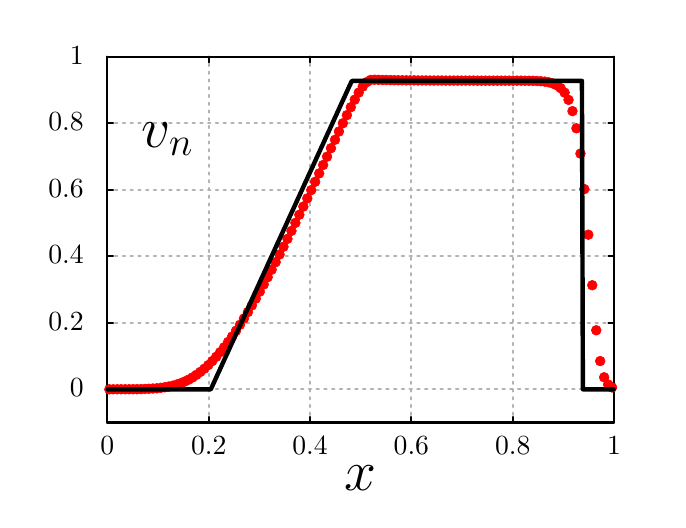
\begin{tikzpicture}[gnuplot]
%% generated with GNUPLOT 4.6p4 (Lua 5.1; terminal rev. 99, script rev. 100)
%% Thu 31 Jul 2014 01:57:06 PM EDT
\path (0.000,0.000) rectangle (8.000,6.000);
\gpfill{rgb color={1.000,1.000,1.000}} (1.012,0.985)--(7.446,0.985)--(7.446,5.630)--(1.012,5.630)--cycle;
\gpcolor{color=gp lt color border}
\gpsetlinetype{gp lt border}
\gpsetlinewidth{1.00}
\draw[gp path] (1.012,0.985)--(1.012,5.630)--(7.446,5.630)--(7.446,0.985)--cycle;
\gpcolor{color=gp lt color axes}
\gpsetlinetype{gp lt axes}
\gpsetlinewidth{2.00}
\draw[gp path] (1.012,1.407)--(7.447,1.407);
\gpcolor{color=gp lt color border}
\gpsetlinetype{gp lt border}
\draw[gp path] (1.012,1.407)--(1.084,1.407);
\draw[gp path] (7.447,1.407)--(7.375,1.407);
\gpcolor{rgb color={0.000,0.000,0.000}}
\node[gp node right,font={\fontsize{10pt}{12pt}\selectfont}] at (0.828,1.407) {0};
\gpcolor{color=gp lt color axes}
\gpsetlinetype{gp lt axes}
\draw[gp path] (1.012,2.252)--(7.447,2.252);
\gpcolor{color=gp lt color border}
\gpsetlinetype{gp lt border}
\draw[gp path] (1.012,2.252)--(1.084,2.252);
\draw[gp path] (7.447,2.252)--(7.375,2.252);
\gpcolor{rgb color={0.000,0.000,0.000}}
\node[gp node right,font={\fontsize{10pt}{12pt}\selectfont}] at (0.828,2.252) {0.2};
\gpcolor{color=gp lt color axes}
\gpsetlinetype{gp lt axes}
\draw[gp path] (1.012,3.097)--(7.447,3.097);
\gpcolor{color=gp lt color border}
\gpsetlinetype{gp lt border}
\draw[gp path] (1.012,3.097)--(1.084,3.097);
\draw[gp path] (7.447,3.097)--(7.375,3.097);
\gpcolor{rgb color={0.000,0.000,0.000}}
\node[gp node right,font={\fontsize{10pt}{12pt}\selectfont}] at (0.828,3.097) {0.4};
\gpcolor{color=gp lt color axes}
\gpsetlinetype{gp lt axes}
\draw[gp path] (1.012,3.942)--(7.447,3.942);
\gpcolor{color=gp lt color border}
\gpsetlinetype{gp lt border}
\draw[gp path] (1.012,3.942)--(1.084,3.942);
\draw[gp path] (7.447,3.942)--(7.375,3.942);
\gpcolor{rgb color={0.000,0.000,0.000}}
\node[gp node right,font={\fontsize{10pt}{12pt}\selectfont}] at (0.828,3.942) {0.6};
\gpcolor{color=gp lt color axes}
\gpsetlinetype{gp lt axes}
\draw[gp path] (1.012,4.786)--(7.447,4.786);
\gpcolor{color=gp lt color border}
\gpsetlinetype{gp lt border}
\draw[gp path] (1.012,4.786)--(1.084,4.786);
\draw[gp path] (7.447,4.786)--(7.375,4.786);
\gpcolor{rgb color={0.000,0.000,0.000}}
\node[gp node right,font={\fontsize{10pt}{12pt}\selectfont}] at (0.828,4.786) {0.8};
\gpcolor{color=gp lt color axes}
\gpsetlinetype{gp lt axes}
\draw[gp path] (1.012,5.631)--(7.447,5.631);
\gpcolor{color=gp lt color border}
\gpsetlinetype{gp lt border}
\draw[gp path] (1.012,5.631)--(1.084,5.631);
\draw[gp path] (7.447,5.631)--(7.375,5.631);
\gpcolor{rgb color={0.000,0.000,0.000}}
\node[gp node right,font={\fontsize{10pt}{12pt}\selectfont}] at (0.828,5.631) {1};
\gpcolor{color=gp lt color axes}
\gpsetlinetype{gp lt axes}
\draw[gp path] (1.012,0.985)--(1.012,5.631);
\gpcolor{color=gp lt color border}
\gpsetlinetype{gp lt border}
\draw[gp path] (1.012,0.985)--(1.012,1.057);
\draw[gp path] (1.012,5.631)--(1.012,5.559);
\gpcolor{rgb color={0.000,0.000,0.000}}
\node[gp node center,font={\fontsize{10pt}{12pt}\selectfont}] at (1.012,0.677) {0};
\gpcolor{color=gp lt color axes}
\gpsetlinetype{gp lt axes}
\draw[gp path] (2.299,0.985)--(2.299,5.631);
\gpcolor{color=gp lt color border}
\gpsetlinetype{gp lt border}
\draw[gp path] (2.299,0.985)--(2.299,1.057);
\draw[gp path] (2.299,5.631)--(2.299,5.559);
\gpcolor{rgb color={0.000,0.000,0.000}}
\node[gp node center,font={\fontsize{10pt}{12pt}\selectfont}] at (2.299,0.677) {0.2};
\gpcolor{color=gp lt color axes}
\gpsetlinetype{gp lt axes}
\draw[gp path] (3.586,0.985)--(3.586,5.631);
\gpcolor{color=gp lt color border}
\gpsetlinetype{gp lt border}
\draw[gp path] (3.586,0.985)--(3.586,1.057);
\draw[gp path] (3.586,5.631)--(3.586,5.559);
\gpcolor{rgb color={0.000,0.000,0.000}}
\node[gp node center,font={\fontsize{10pt}{12pt}\selectfont}] at (3.586,0.677) {0.4};
\gpcolor{color=gp lt color axes}
\gpsetlinetype{gp lt axes}
\draw[gp path] (4.873,0.985)--(4.873,5.631);
\gpcolor{color=gp lt color border}
\gpsetlinetype{gp lt border}
\draw[gp path] (4.873,0.985)--(4.873,1.057);
\draw[gp path] (4.873,5.631)--(4.873,5.559);
\gpcolor{rgb color={0.000,0.000,0.000}}
\node[gp node center,font={\fontsize{10pt}{12pt}\selectfont}] at (4.873,0.677) {0.6};
\gpcolor{color=gp lt color axes}
\gpsetlinetype{gp lt axes}
\draw[gp path] (6.160,0.985)--(6.160,5.631);
\gpcolor{color=gp lt color border}
\gpsetlinetype{gp lt border}
\draw[gp path] (6.160,0.985)--(6.160,1.057);
\draw[gp path] (6.160,5.631)--(6.160,5.559);
\gpcolor{rgb color={0.000,0.000,0.000}}
\node[gp node center,font={\fontsize{10pt}{12pt}\selectfont}] at (6.160,0.677) {0.8};
\gpcolor{color=gp lt color axes}
\gpsetlinetype{gp lt axes}
\draw[gp path] (7.447,0.985)--(7.447,5.631);
\gpcolor{color=gp lt color border}
\gpsetlinetype{gp lt border}
\draw[gp path] (7.447,0.985)--(7.447,1.057);
\draw[gp path] (7.447,5.631)--(7.447,5.559);
\gpcolor{rgb color={0.000,0.000,0.000}}
\node[gp node center,font={\fontsize{10pt}{12pt}\selectfont}] at (7.447,0.677) {1};
\gpcolor{color=gp lt color border}
\draw[gp path] (1.012,5.631)--(1.012,0.985)--(7.447,0.985)--(7.447,5.631)--cycle;
\gpcolor{rgb color={0.000,0.000,0.000}}
\node[gp node center,font={\fontsize{10pt}{12pt}\selectfont}] at (4.229,0.215) {\huge $x$};
\gpcolor{rgb color={1.000,0.000,0.000}}
\gpsetlinewidth{0.50}
\gpsetpointsize{4.44}
\gppoint{gp mark 7}{(1.037,1.407)}
\gppoint{gp mark 7}{(1.087,1.407)}
\gppoint{gp mark 7}{(1.138,1.408)}
\gppoint{gp mark 7}{(1.188,1.408)}
\gppoint{gp mark 7}{(1.238,1.408)}
\gppoint{gp mark 7}{(1.289,1.408)}
\gppoint{gp mark 7}{(1.339,1.409)}
\gppoint{gp mark 7}{(1.389,1.409)}
\gppoint{gp mark 7}{(1.439,1.410)}
\gppoint{gp mark 7}{(1.490,1.412)}
\gppoint{gp mark 7}{(1.540,1.414)}
\gppoint{gp mark 7}{(1.590,1.417)}
\gppoint{gp mark 7}{(1.640,1.420)}
\gppoint{gp mark 7}{(1.691,1.426)}
\gppoint{gp mark 7}{(1.741,1.433)}
\gppoint{gp mark 7}{(1.791,1.442)}
\gppoint{gp mark 7}{(1.842,1.453)}
\gppoint{gp mark 7}{(1.892,1.467)}
\gppoint{gp mark 7}{(1.942,1.484)}
\gppoint{gp mark 7}{(1.992,1.505)}
\gppoint{gp mark 7}{(2.043,1.529)}
\gppoint{gp mark 7}{(2.093,1.558)}
\gppoint{gp mark 7}{(2.143,1.591)}
\gppoint{gp mark 7}{(2.193,1.628)}
\gppoint{gp mark 7}{(2.244,1.669)}
\gppoint{gp mark 7}{(2.294,1.715)}
\gppoint{gp mark 7}{(2.344,1.766)}
\gppoint{gp mark 7}{(2.395,1.820)}
\gppoint{gp mark 7}{(2.445,1.879)}
\gppoint{gp mark 7}{(2.495,1.941)}
\gppoint{gp mark 7}{(2.545,2.008)}
\gppoint{gp mark 7}{(2.596,2.077)}
\gppoint{gp mark 7}{(2.646,2.151)}
\gppoint{gp mark 7}{(2.696,2.227)}
\gppoint{gp mark 7}{(2.746,2.306)}
\gppoint{gp mark 7}{(2.797,2.388)}
\gppoint{gp mark 7}{(2.847,2.472)}
\gppoint{gp mark 7}{(2.897,2.559)}
\gppoint{gp mark 7}{(2.948,2.648)}
\gppoint{gp mark 7}{(2.998,2.739)}
\gppoint{gp mark 7}{(3.048,2.831)}
\gppoint{gp mark 7}{(3.098,2.926)}
\gppoint{gp mark 7}{(3.149,3.022)}
\gppoint{gp mark 7}{(3.199,3.119)}
\gppoint{gp mark 7}{(3.249,3.218)}
\gppoint{gp mark 7}{(3.299,3.318)}
\gppoint{gp mark 7}{(3.350,3.419)}
\gppoint{gp mark 7}{(3.400,3.521)}
\gppoint{gp mark 7}{(3.450,3.624)}
\gppoint{gp mark 7}{(3.501,3.728)}
\gppoint{gp mark 7}{(3.551,3.832)}
\gppoint{gp mark 7}{(3.601,3.937)}
\gppoint{gp mark 7}{(3.651,4.043)}
\gppoint{gp mark 7}{(3.702,4.149)}
\gppoint{gp mark 7}{(3.752,4.256)}
\gppoint{gp mark 7}{(3.802,4.362)}
\gppoint{gp mark 7}{(3.852,4.469)}
\gppoint{gp mark 7}{(3.903,4.576)}
\gppoint{gp mark 7}{(3.953,4.681)}
\gppoint{gp mark 7}{(4.003,4.786)}
\gppoint{gp mark 7}{(4.054,4.889)}
\gppoint{gp mark 7}{(4.104,4.990)}
\gppoint{gp mark 7}{(4.154,5.086)}
\gppoint{gp mark 7}{(4.204,5.175)}
\gppoint{gp mark 7}{(4.255,5.252)}
\gppoint{gp mark 7}{(4.305,5.308)}
\gppoint{gp mark 7}{(4.355,5.336)}
\gppoint{gp mark 7}{(4.405,5.339)}
\gppoint{gp mark 7}{(4.456,5.337)}
\gppoint{gp mark 7}{(4.506,5.336)}
\gppoint{gp mark 7}{(4.556,5.335)}
\gppoint{gp mark 7}{(4.607,5.334)}
\gppoint{gp mark 7}{(4.657,5.333)}
\gppoint{gp mark 7}{(4.707,5.332)}
\gppoint{gp mark 7}{(4.757,5.332)}
\gppoint{gp mark 7}{(4.808,5.331)}
\gppoint{gp mark 7}{(4.858,5.331)}
\gppoint{gp mark 7}{(4.908,5.331)}
\gppoint{gp mark 7}{(4.958,5.330)}
\gppoint{gp mark 7}{(5.009,5.330)}
\gppoint{gp mark 7}{(5.059,5.330)}
\gppoint{gp mark 7}{(5.109,5.329)}
\gppoint{gp mark 7}{(5.160,5.329)}
\gppoint{gp mark 7}{(5.210,5.329)}
\gppoint{gp mark 7}{(5.260,5.329)}
\gppoint{gp mark 7}{(5.310,5.328)}
\gppoint{gp mark 7}{(5.361,5.328)}
\gppoint{gp mark 7}{(5.411,5.328)}
\gppoint{gp mark 7}{(5.461,5.328)}
\gppoint{gp mark 7}{(5.511,5.328)}
\gppoint{gp mark 7}{(5.562,5.328)}
\gppoint{gp mark 7}{(5.612,5.328)}
\gppoint{gp mark 7}{(5.662,5.328)}
\gppoint{gp mark 7}{(5.713,5.327)}
\gppoint{gp mark 7}{(5.763,5.327)}
\gppoint{gp mark 7}{(5.813,5.327)}
\gppoint{gp mark 7}{(5.863,5.327)}
\gppoint{gp mark 7}{(5.914,5.327)}
\gppoint{gp mark 7}{(5.964,5.327)}
\gppoint{gp mark 7}{(6.014,5.327)}
\gppoint{gp mark 7}{(6.064,5.327)}
\gppoint{gp mark 7}{(6.115,5.327)}
\gppoint{gp mark 7}{(6.165,5.327)}
\gppoint{gp mark 7}{(6.215,5.327)}
\gppoint{gp mark 7}{(6.266,5.327)}
\gppoint{gp mark 7}{(6.316,5.326)}
\gppoint{gp mark 7}{(6.366,5.326)}
\gppoint{gp mark 7}{(6.416,5.325)}
\gppoint{gp mark 7}{(6.467,5.323)}
\gppoint{gp mark 7}{(6.517,5.320)}
\gppoint{gp mark 7}{(6.567,5.315)}
\gppoint{gp mark 7}{(6.617,5.306)}
\gppoint{gp mark 7}{(6.668,5.292)}
\gppoint{gp mark 7}{(6.718,5.270)}
\gppoint{gp mark 7}{(6.768,5.233)}
\gppoint{gp mark 7}{(6.819,5.175)}
\gppoint{gp mark 7}{(6.869,5.083)}
\gppoint{gp mark 7}{(6.919,4.940)}
\gppoint{gp mark 7}{(6.969,4.722)}
\gppoint{gp mark 7}{(7.020,4.401)}
\gppoint{gp mark 7}{(7.070,3.950)}
\gppoint{gp mark 7}{(7.120,3.371)}
\gppoint{gp mark 7}{(7.170,2.729)}
\gppoint{gp mark 7}{(7.221,2.157)}
\gppoint{gp mark 7}{(7.271,1.766)}
\gppoint{gp mark 7}{(7.321,1.560)}
\gppoint{gp mark 7}{(7.372,1.468)}
\gppoint{gp mark 7}{(7.422,1.431)}
\gpcolor{rgb color={0.000,0.000,0.000}}
\gpsetlinetype{gp lt plot 0}
\gpsetlinewidth{4.00}
\draw[gp path] (1.018,1.407)--(1.031,1.407)--(1.043,1.407)--(1.056,1.407)--(1.069,1.407)%
  --(1.081,1.407)--(1.094,1.407)--(1.106,1.407)--(1.119,1.407)--(1.131,1.407)--(1.144,1.407)%
  --(1.157,1.407)--(1.169,1.407)--(1.182,1.407)--(1.194,1.407)--(1.207,1.407)--(1.219,1.407)%
  --(1.232,1.407)--(1.245,1.407)--(1.257,1.407)--(1.270,1.407)--(1.282,1.407)--(1.295,1.407)%
  --(1.307,1.407)--(1.320,1.407)--(1.332,1.407)--(1.345,1.407)--(1.358,1.407)--(1.370,1.407)%
  --(1.383,1.407)--(1.395,1.407)--(1.408,1.407)--(1.420,1.407)--(1.433,1.407)--(1.446,1.407)%
  --(1.458,1.407)--(1.471,1.407)--(1.483,1.407)--(1.496,1.407)--(1.508,1.407)--(1.521,1.407)%
  --(1.534,1.407)--(1.546,1.407)--(1.559,1.407)--(1.571,1.407)--(1.584,1.407)--(1.596,1.407)%
  --(1.609,1.407)--(1.622,1.407)--(1.634,1.407)--(1.647,1.407)--(1.659,1.407)--(1.672,1.407)%
  --(1.684,1.407)--(1.697,1.407)--(1.710,1.407)--(1.722,1.407)--(1.735,1.407)--(1.747,1.407)%
  --(1.760,1.407)--(1.772,1.407)--(1.785,1.407)--(1.798,1.407)--(1.810,1.407)--(1.823,1.407)%
  --(1.835,1.407)--(1.848,1.407)--(1.860,1.407)--(1.873,1.407)--(1.886,1.407)--(1.898,1.407)%
  --(1.911,1.407)--(1.923,1.407)--(1.936,1.407)--(1.948,1.407)--(1.961,1.407)--(1.973,1.407)%
  --(1.986,1.407)--(1.999,1.407)--(2.011,1.407)--(2.024,1.407)--(2.036,1.407)--(2.049,1.407)%
  --(2.061,1.407)--(2.074,1.407)--(2.087,1.407)--(2.099,1.407)--(2.112,1.407)--(2.124,1.407)%
  --(2.137,1.407)--(2.149,1.407)--(2.162,1.407)--(2.175,1.407)--(2.187,1.407)--(2.200,1.407)%
  --(2.212,1.407)--(2.225,1.407)--(2.237,1.407)--(2.250,1.407)--(2.263,1.407)--(2.275,1.407)%
  --(2.288,1.407)--(2.300,1.407)--(2.313,1.407)--(2.325,1.407)--(2.338,1.434)--(2.351,1.461)%
  --(2.363,1.489)--(2.376,1.516)--(2.388,1.544)--(2.401,1.571)--(2.413,1.599)--(2.426,1.626)%
  --(2.439,1.654)--(2.451,1.681)--(2.464,1.709)--(2.476,1.736)--(2.489,1.764)--(2.501,1.791)%
  --(2.514,1.818)--(2.526,1.846)--(2.539,1.873)--(2.552,1.901)--(2.564,1.928)--(2.577,1.956)%
  --(2.589,1.983)--(2.602,2.011)--(2.614,2.038)--(2.627,2.066)--(2.640,2.093)--(2.652,2.121)%
  --(2.665,2.148)--(2.677,2.176)--(2.690,2.203)--(2.702,2.231)--(2.715,2.258)--(2.728,2.286)%
  --(2.740,2.313)--(2.753,2.341)--(2.765,2.368)--(2.778,2.396)--(2.790,2.423)--(2.803,2.451)%
  --(2.816,2.478)--(2.828,2.506)--(2.841,2.533)--(2.853,2.561)--(2.866,2.588)--(2.878,2.616)%
  --(2.891,2.643)--(2.904,2.671)--(2.916,2.698)--(2.929,2.726)--(2.941,2.753)--(2.954,2.781)%
  --(2.966,2.808)--(2.979,2.836)--(2.992,2.863)--(3.004,2.891)--(3.017,2.918)--(3.029,2.946)%
  --(3.042,2.973)--(3.054,3.001)--(3.067,3.028)--(3.079,3.056)--(3.092,3.083)--(3.105,3.111)%
  --(3.117,3.138)--(3.130,3.166)--(3.142,3.193)--(3.155,3.221)--(3.167,3.248)--(3.180,3.276)%
  --(3.193,3.303)--(3.205,3.331)--(3.218,3.358)--(3.230,3.386)--(3.243,3.413)--(3.255,3.441)%
  --(3.268,3.468)--(3.281,3.496)--(3.293,3.523)--(3.306,3.551)--(3.318,3.578)--(3.331,3.606)%
  --(3.343,3.633)--(3.356,3.661)--(3.369,3.688)--(3.381,3.716)--(3.394,3.743)--(3.406,3.771)%
  --(3.419,3.798)--(3.431,3.826)--(3.444,3.853)--(3.457,3.881)--(3.469,3.908)--(3.482,3.936)%
  --(3.494,3.963)--(3.507,3.991)--(3.519,4.018)--(3.532,4.046)--(3.545,4.073)--(3.557,4.101)%
  --(3.570,4.128)--(3.582,4.156)--(3.595,4.183)--(3.607,4.211)--(3.620,4.238)--(3.633,4.266)%
  --(3.645,4.293)--(3.658,4.321)--(3.670,4.348)--(3.683,4.376)--(3.695,4.403)--(3.708,4.431)%
  --(3.720,4.458)--(3.733,4.486)--(3.746,4.513)--(3.758,4.541)--(3.771,4.568)--(3.783,4.596)%
  --(3.796,4.623)--(3.808,4.651)--(3.821,4.678)--(3.834,4.706)--(3.846,4.733)--(3.859,4.761)%
  --(3.871,4.788)--(3.884,4.816)--(3.896,4.843)--(3.909,4.871)--(3.922,4.898)--(3.934,4.926)%
  --(3.947,4.953)--(3.959,4.981)--(3.972,5.008)--(3.984,5.036)--(3.997,5.063)--(4.010,5.091)%
  --(4.022,5.118)--(4.035,5.146)--(4.047,5.173)--(4.060,5.201)--(4.072,5.228)--(4.085,5.256)%
  --(4.098,5.283)--(4.110,5.311)--(4.123,5.324)--(4.135,5.324)--(4.148,5.324)--(4.160,5.324)%
  --(4.173,5.324)--(4.186,5.324)--(4.198,5.324)--(4.211,5.324)--(4.223,5.324)--(4.236,5.324)%
  --(4.248,5.324)--(4.261,5.324)--(4.273,5.324)--(4.286,5.324)--(4.299,5.324)--(4.311,5.324)%
  --(4.324,5.324)--(4.336,5.324)--(4.349,5.324)--(4.361,5.324)--(4.374,5.324)--(4.387,5.324)%
  --(4.399,5.324)--(4.412,5.324)--(4.424,5.324)--(4.437,5.324)--(4.449,5.324)--(4.462,5.324)%
  --(4.475,5.324)--(4.487,5.324)--(4.500,5.324)--(4.512,5.324)--(4.525,5.324)--(4.537,5.324)%
  --(4.550,5.324)--(4.563,5.324)--(4.575,5.324)--(4.588,5.324)--(4.600,5.324)--(4.613,5.324)%
  --(4.625,5.324)--(4.638,5.324)--(4.651,5.324)--(4.663,5.324)--(4.676,5.324)--(4.688,5.324)%
  --(4.701,5.324)--(4.713,5.324)--(4.726,5.324)--(4.739,5.324)--(4.751,5.324)--(4.764,5.324)%
  --(4.776,5.324)--(4.789,5.324)--(4.801,5.324)--(4.814,5.324)--(4.826,5.324)--(4.839,5.324)%
  --(4.852,5.324)--(4.864,5.324)--(4.877,5.324)--(4.889,5.324)--(4.902,5.324)--(4.914,5.324)%
  --(4.927,5.324)--(4.940,5.324)--(4.952,5.324)--(4.965,5.324)--(4.977,5.324)--(4.990,5.324)%
  --(5.002,5.324)--(5.015,5.324)--(5.028,5.324)--(5.040,5.324)--(5.053,5.324)--(5.065,5.324)%
  --(5.078,5.324)--(5.090,5.324)--(5.103,5.324)--(5.116,5.324)--(5.128,5.324)--(5.141,5.324)%
  --(5.153,5.324)--(5.166,5.324)--(5.178,5.324)--(5.191,5.324)--(5.204,5.324)--(5.216,5.324)%
  --(5.229,5.324)--(5.241,5.324)--(5.254,5.324)--(5.266,5.324)--(5.279,5.324)--(5.292,5.324)%
  --(5.304,5.324)--(5.317,5.324)--(5.329,5.324)--(5.342,5.324)--(5.354,5.324)--(5.367,5.324)%
  --(5.380,5.324)--(5.392,5.324)--(5.405,5.324)--(5.417,5.324)--(5.430,5.324)--(5.442,5.324)%
  --(5.455,5.324)--(5.467,5.324)--(5.480,5.324)--(5.493,5.324)--(5.505,5.324)--(5.518,5.324)%
  --(5.530,5.324)--(5.543,5.324)--(5.555,5.324)--(5.568,5.324)--(5.581,5.324)--(5.593,5.324)%
  --(5.606,5.324)--(5.618,5.324)--(5.631,5.324)--(5.643,5.324)--(5.656,5.324)--(5.669,5.324)%
  --(5.681,5.324)--(5.694,5.324)--(5.706,5.324)--(5.719,5.324)--(5.731,5.324)--(5.744,5.324)%
  --(5.757,5.324)--(5.769,5.324)--(5.782,5.324)--(5.794,5.324)--(5.807,5.324)--(5.819,5.324)%
  --(5.832,5.324)--(5.845,5.324)--(5.857,5.324)--(5.870,5.324)--(5.882,5.324)--(5.895,5.324)%
  --(5.907,5.324)--(5.920,5.324)--(5.933,5.324)--(5.945,5.324)--(5.958,5.324)--(5.970,5.324)%
  --(5.983,5.324)--(5.995,5.324)--(6.008,5.324)--(6.020,5.324)--(6.033,5.324)--(6.046,5.324)%
  --(6.058,5.324)--(6.071,5.324)--(6.083,5.324)--(6.096,5.324)--(6.108,5.324)--(6.121,5.324)%
  --(6.134,5.324)--(6.146,5.324)--(6.159,5.324)--(6.171,5.324)--(6.184,5.324)--(6.196,5.324)%
  --(6.209,5.324)--(6.222,5.324)--(6.234,5.324)--(6.247,5.324)--(6.259,5.324)--(6.272,5.324)%
  --(6.284,5.324)--(6.297,5.324)--(6.310,5.324)--(6.322,5.324)--(6.335,5.324)--(6.347,5.324)%
  --(6.360,5.324)--(6.372,5.324)--(6.385,5.324)--(6.398,5.324)--(6.410,5.324)--(6.423,5.324)%
  --(6.435,5.324)--(6.448,5.324)--(6.460,5.324)--(6.473,5.324)--(6.486,5.324)--(6.498,5.324)%
  --(6.511,5.324)--(6.523,5.324)--(6.536,5.324)--(6.548,5.324)--(6.561,5.324)--(6.573,5.324)%
  --(6.586,5.324)--(6.599,5.324)--(6.611,5.324)--(6.624,5.324)--(6.636,5.324)--(6.649,5.324)%
  --(6.661,5.324)--(6.674,5.324)--(6.687,5.324)--(6.699,5.324)--(6.712,5.324)--(6.724,5.324)%
  --(6.737,5.324)--(6.749,5.324)--(6.762,5.324)--(6.775,5.324)--(6.787,5.324)--(6.800,5.324)%
  --(6.812,5.324)--(6.825,5.324)--(6.837,5.324)--(6.850,5.324)--(6.863,5.324)--(6.875,5.324)%
  --(6.888,5.324)--(6.900,5.324)--(6.913,5.324)--(6.925,5.324)--(6.938,5.324)--(6.951,5.324)%
  --(6.963,5.324)--(6.976,5.324)--(6.988,5.324)--(7.001,5.324)--(7.013,5.324)--(7.026,5.324)%
  --(7.039,5.324)--(7.051,1.407)--(7.064,1.407)--(7.076,1.407)--(7.089,1.407)--(7.101,1.407)%
  --(7.114,1.407)--(7.127,1.407)--(7.139,1.407)--(7.152,1.407)--(7.164,1.407)--(7.177,1.407)%
  --(7.189,1.407)--(7.202,1.407)--(7.214,1.407)--(7.227,1.407)--(7.240,1.407)--(7.252,1.407)%
  --(7.265,1.407)--(7.277,1.407)--(7.290,1.407)--(7.302,1.407)--(7.315,1.407)--(7.328,1.407)%
  --(7.340,1.407)--(7.353,1.407)--(7.365,1.407)--(7.378,1.407)--(7.390,1.407)--(7.403,1.407)%
  --(7.416,1.407)--(7.428,1.407)--(7.441,1.407);
\node[gp node left,font={\fontsize{10pt}{12pt}\selectfont}] at (1.334,4.575) {\huge $v_n$};
%% coordinates of the plot area
\gpdefrectangularnode{gp plot 1}{\pgfpoint{1.012cm}{0.985cm}}{\pgfpoint{7.447cm}{5.631cm}}
\end{tikzpicture}
%% gnuplot variables
} &
\resizebox{0.33\linewidth}{!}{\tikzsetnextfilename{sod_hllc_1_3}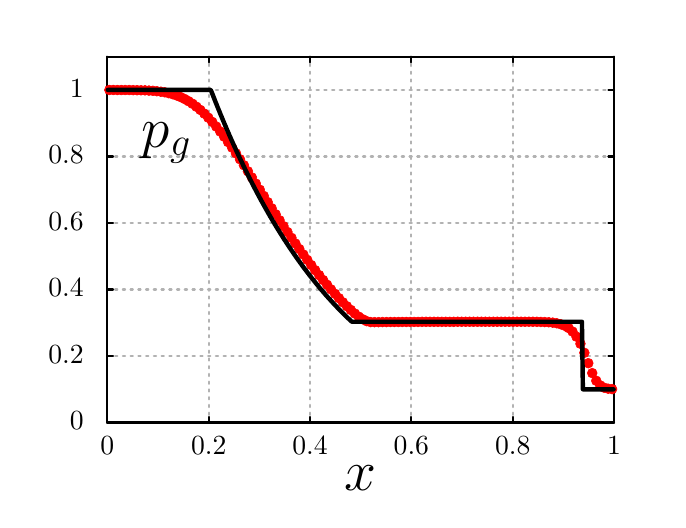
\begin{tikzpicture}[gnuplot]
%% generated with GNUPLOT 4.6p4 (Lua 5.1; terminal rev. 99, script rev. 100)
%% Thu 31 Jul 2014 01:57:06 PM EDT
\path (0.000,0.000) rectangle (8.000,6.000);
\gpfill{rgb color={1.000,1.000,1.000}} (1.012,0.985)--(7.446,0.985)--(7.446,5.630)--(1.012,5.630)--cycle;
\gpcolor{color=gp lt color border}
\gpsetlinetype{gp lt border}
\gpsetlinewidth{1.00}
\draw[gp path] (1.012,0.985)--(1.012,5.630)--(7.446,5.630)--(7.446,0.985)--cycle;
\gpcolor{color=gp lt color axes}
\gpsetlinetype{gp lt axes}
\gpsetlinewidth{2.00}
\draw[gp path] (1.012,0.985)--(7.447,0.985);
\gpcolor{color=gp lt color border}
\gpsetlinetype{gp lt border}
\draw[gp path] (1.012,0.985)--(1.084,0.985);
\draw[gp path] (7.447,0.985)--(7.375,0.985);
\gpcolor{rgb color={0.000,0.000,0.000}}
\node[gp node right,font={\fontsize{10pt}{12pt}\selectfont}] at (0.828,0.985) {0};
\gpcolor{color=gp lt color axes}
\gpsetlinetype{gp lt axes}
\draw[gp path] (1.012,1.830)--(7.447,1.830);
\gpcolor{color=gp lt color border}
\gpsetlinetype{gp lt border}
\draw[gp path] (1.012,1.830)--(1.084,1.830);
\draw[gp path] (7.447,1.830)--(7.375,1.830);
\gpcolor{rgb color={0.000,0.000,0.000}}
\node[gp node right,font={\fontsize{10pt}{12pt}\selectfont}] at (0.828,1.830) {0.2};
\gpcolor{color=gp lt color axes}
\gpsetlinetype{gp lt axes}
\draw[gp path] (1.012,2.674)--(7.447,2.674);
\gpcolor{color=gp lt color border}
\gpsetlinetype{gp lt border}
\draw[gp path] (1.012,2.674)--(1.084,2.674);
\draw[gp path] (7.447,2.674)--(7.375,2.674);
\gpcolor{rgb color={0.000,0.000,0.000}}
\node[gp node right,font={\fontsize{10pt}{12pt}\selectfont}] at (0.828,2.674) {0.4};
\gpcolor{color=gp lt color axes}
\gpsetlinetype{gp lt axes}
\draw[gp path] (1.012,3.519)--(7.447,3.519);
\gpcolor{color=gp lt color border}
\gpsetlinetype{gp lt border}
\draw[gp path] (1.012,3.519)--(1.084,3.519);
\draw[gp path] (7.447,3.519)--(7.375,3.519);
\gpcolor{rgb color={0.000,0.000,0.000}}
\node[gp node right,font={\fontsize{10pt}{12pt}\selectfont}] at (0.828,3.519) {0.6};
\gpcolor{color=gp lt color axes}
\gpsetlinetype{gp lt axes}
\draw[gp path] (1.012,4.364)--(7.447,4.364);
\gpcolor{color=gp lt color border}
\gpsetlinetype{gp lt border}
\draw[gp path] (1.012,4.364)--(1.084,4.364);
\draw[gp path] (7.447,4.364)--(7.375,4.364);
\gpcolor{rgb color={0.000,0.000,0.000}}
\node[gp node right,font={\fontsize{10pt}{12pt}\selectfont}] at (0.828,4.364) {0.8};
\gpcolor{color=gp lt color axes}
\gpsetlinetype{gp lt axes}
\draw[gp path] (1.012,5.209)--(7.447,5.209);
\gpcolor{color=gp lt color border}
\gpsetlinetype{gp lt border}
\draw[gp path] (1.012,5.209)--(1.084,5.209);
\draw[gp path] (7.447,5.209)--(7.375,5.209);
\gpcolor{rgb color={0.000,0.000,0.000}}
\node[gp node right,font={\fontsize{10pt}{12pt}\selectfont}] at (0.828,5.209) {1};
\gpcolor{color=gp lt color axes}
\gpsetlinetype{gp lt axes}
\draw[gp path] (1.012,0.985)--(1.012,5.631);
\gpcolor{color=gp lt color border}
\gpsetlinetype{gp lt border}
\draw[gp path] (1.012,0.985)--(1.012,1.057);
\draw[gp path] (1.012,5.631)--(1.012,5.559);
\gpcolor{rgb color={0.000,0.000,0.000}}
\node[gp node center,font={\fontsize{10pt}{12pt}\selectfont}] at (1.012,0.677) {0};
\gpcolor{color=gp lt color axes}
\gpsetlinetype{gp lt axes}
\draw[gp path] (2.299,0.985)--(2.299,5.631);
\gpcolor{color=gp lt color border}
\gpsetlinetype{gp lt border}
\draw[gp path] (2.299,0.985)--(2.299,1.057);
\draw[gp path] (2.299,5.631)--(2.299,5.559);
\gpcolor{rgb color={0.000,0.000,0.000}}
\node[gp node center,font={\fontsize{10pt}{12pt}\selectfont}] at (2.299,0.677) {0.2};
\gpcolor{color=gp lt color axes}
\gpsetlinetype{gp lt axes}
\draw[gp path] (3.586,0.985)--(3.586,5.631);
\gpcolor{color=gp lt color border}
\gpsetlinetype{gp lt border}
\draw[gp path] (3.586,0.985)--(3.586,1.057);
\draw[gp path] (3.586,5.631)--(3.586,5.559);
\gpcolor{rgb color={0.000,0.000,0.000}}
\node[gp node center,font={\fontsize{10pt}{12pt}\selectfont}] at (3.586,0.677) {0.4};
\gpcolor{color=gp lt color axes}
\gpsetlinetype{gp lt axes}
\draw[gp path] (4.873,0.985)--(4.873,5.631);
\gpcolor{color=gp lt color border}
\gpsetlinetype{gp lt border}
\draw[gp path] (4.873,0.985)--(4.873,1.057);
\draw[gp path] (4.873,5.631)--(4.873,5.559);
\gpcolor{rgb color={0.000,0.000,0.000}}
\node[gp node center,font={\fontsize{10pt}{12pt}\selectfont}] at (4.873,0.677) {0.6};
\gpcolor{color=gp lt color axes}
\gpsetlinetype{gp lt axes}
\draw[gp path] (6.160,0.985)--(6.160,5.631);
\gpcolor{color=gp lt color border}
\gpsetlinetype{gp lt border}
\draw[gp path] (6.160,0.985)--(6.160,1.057);
\draw[gp path] (6.160,5.631)--(6.160,5.559);
\gpcolor{rgb color={0.000,0.000,0.000}}
\node[gp node center,font={\fontsize{10pt}{12pt}\selectfont}] at (6.160,0.677) {0.8};
\gpcolor{color=gp lt color axes}
\gpsetlinetype{gp lt axes}
\draw[gp path] (7.447,0.985)--(7.447,5.631);
\gpcolor{color=gp lt color border}
\gpsetlinetype{gp lt border}
\draw[gp path] (7.447,0.985)--(7.447,1.057);
\draw[gp path] (7.447,5.631)--(7.447,5.559);
\gpcolor{rgb color={0.000,0.000,0.000}}
\node[gp node center,font={\fontsize{10pt}{12pt}\selectfont}] at (7.447,0.677) {1};
\gpcolor{color=gp lt color border}
\draw[gp path] (1.012,5.631)--(1.012,0.985)--(7.447,0.985)--(7.447,5.631)--cycle;
\gpcolor{rgb color={0.000,0.000,0.000}}
\node[gp node center,font={\fontsize{10pt}{12pt}\selectfont}] at (4.229,0.215) {\huge $x$};
\gpcolor{rgb color={1.000,0.000,0.000}}
\gpsetlinewidth{0.50}
\gpsetpointsize{4.44}
\gppoint{gp mark 7}{(1.037,5.209)}
\gppoint{gp mark 7}{(1.087,5.209)}
\gppoint{gp mark 7}{(1.138,5.208)}
\gppoint{gp mark 7}{(1.188,5.208)}
\gppoint{gp mark 7}{(1.238,5.208)}
\gppoint{gp mark 7}{(1.289,5.208)}
\gppoint{gp mark 7}{(1.339,5.207)}
\gppoint{gp mark 7}{(1.389,5.206)}
\gppoint{gp mark 7}{(1.439,5.205)}
\gppoint{gp mark 7}{(1.490,5.204)}
\gppoint{gp mark 7}{(1.540,5.201)}
\gppoint{gp mark 7}{(1.590,5.198)}
\gppoint{gp mark 7}{(1.640,5.193)}
\gppoint{gp mark 7}{(1.691,5.187)}
\gppoint{gp mark 7}{(1.741,5.179)}
\gppoint{gp mark 7}{(1.791,5.168)}
\gppoint{gp mark 7}{(1.842,5.155)}
\gppoint{gp mark 7}{(1.892,5.139)}
\gppoint{gp mark 7}{(1.942,5.119)}
\gppoint{gp mark 7}{(1.992,5.095)}
\gppoint{gp mark 7}{(2.043,5.066)}
\gppoint{gp mark 7}{(2.093,5.034)}
\gppoint{gp mark 7}{(2.143,4.996)}
\gppoint{gp mark 7}{(2.193,4.955)}
\gppoint{gp mark 7}{(2.244,4.908)}
\gppoint{gp mark 7}{(2.294,4.857)}
\gppoint{gp mark 7}{(2.344,4.803)}
\gppoint{gp mark 7}{(2.395,4.744)}
\gppoint{gp mark 7}{(2.445,4.681)}
\gppoint{gp mark 7}{(2.495,4.616)}
\gppoint{gp mark 7}{(2.545,4.547)}
\gppoint{gp mark 7}{(2.596,4.477)}
\gppoint{gp mark 7}{(2.646,4.404)}
\gppoint{gp mark 7}{(2.696,4.329)}
\gppoint{gp mark 7}{(2.746,4.253)}
\gppoint{gp mark 7}{(2.797,4.176)}
\gppoint{gp mark 7}{(2.847,4.098)}
\gppoint{gp mark 7}{(2.897,4.020)}
\gppoint{gp mark 7}{(2.948,3.942)}
\gppoint{gp mark 7}{(2.998,3.863)}
\gppoint{gp mark 7}{(3.048,3.785)}
\gppoint{gp mark 7}{(3.098,3.707)}
\gppoint{gp mark 7}{(3.149,3.630)}
\gppoint{gp mark 7}{(3.199,3.554)}
\gppoint{gp mark 7}{(3.249,3.479)}
\gppoint{gp mark 7}{(3.299,3.405)}
\gppoint{gp mark 7}{(3.350,3.331)}
\gppoint{gp mark 7}{(3.400,3.259)}
\gppoint{gp mark 7}{(3.450,3.189)}
\gppoint{gp mark 7}{(3.501,3.119)}
\gppoint{gp mark 7}{(3.551,3.051)}
\gppoint{gp mark 7}{(3.601,2.985)}
\gppoint{gp mark 7}{(3.651,2.920)}
\gppoint{gp mark 7}{(3.702,2.857)}
\gppoint{gp mark 7}{(3.752,2.795)}
\gppoint{gp mark 7}{(3.802,2.735)}
\gppoint{gp mark 7}{(3.852,2.676)}
\gppoint{gp mark 7}{(3.903,2.620)}
\gppoint{gp mark 7}{(3.953,2.565)}
\gppoint{gp mark 7}{(4.003,2.512)}
\gppoint{gp mark 7}{(4.054,2.462)}
\gppoint{gp mark 7}{(4.104,2.415)}
\gppoint{gp mark 7}{(4.154,2.370)}
\gppoint{gp mark 7}{(4.204,2.330)}
\gppoint{gp mark 7}{(4.255,2.297)}
\gppoint{gp mark 7}{(4.305,2.273)}
\gppoint{gp mark 7}{(4.355,2.261)}
\gppoint{gp mark 7}{(4.405,2.260)}
\gppoint{gp mark 7}{(4.456,2.260)}
\gppoint{gp mark 7}{(4.506,2.261)}
\gppoint{gp mark 7}{(4.556,2.261)}
\gppoint{gp mark 7}{(4.607,2.262)}
\gppoint{gp mark 7}{(4.657,2.262)}
\gppoint{gp mark 7}{(4.707,2.262)}
\gppoint{gp mark 7}{(4.757,2.263)}
\gppoint{gp mark 7}{(4.808,2.263)}
\gppoint{gp mark 7}{(4.858,2.263)}
\gppoint{gp mark 7}{(4.908,2.263)}
\gppoint{gp mark 7}{(4.958,2.263)}
\gppoint{gp mark 7}{(5.009,2.264)}
\gppoint{gp mark 7}{(5.059,2.264)}
\gppoint{gp mark 7}{(5.109,2.264)}
\gppoint{gp mark 7}{(5.160,2.264)}
\gppoint{gp mark 7}{(5.210,2.264)}
\gppoint{gp mark 7}{(5.260,2.264)}
\gppoint{gp mark 7}{(5.310,2.264)}
\gppoint{gp mark 7}{(5.361,2.264)}
\gppoint{gp mark 7}{(5.411,2.264)}
\gppoint{gp mark 7}{(5.461,2.265)}
\gppoint{gp mark 7}{(5.511,2.265)}
\gppoint{gp mark 7}{(5.562,2.265)}
\gppoint{gp mark 7}{(5.612,2.265)}
\gppoint{gp mark 7}{(5.662,2.265)}
\gppoint{gp mark 7}{(5.713,2.265)}
\gppoint{gp mark 7}{(5.763,2.265)}
\gppoint{gp mark 7}{(5.813,2.265)}
\gppoint{gp mark 7}{(5.863,2.265)}
\gppoint{gp mark 7}{(5.914,2.265)}
\gppoint{gp mark 7}{(5.964,2.265)}
\gppoint{gp mark 7}{(6.014,2.265)}
\gppoint{gp mark 7}{(6.064,2.265)}
\gppoint{gp mark 7}{(6.115,2.265)}
\gppoint{gp mark 7}{(6.165,2.265)}
\gppoint{gp mark 7}{(6.215,2.265)}
\gppoint{gp mark 7}{(6.266,2.265)}
\gppoint{gp mark 7}{(6.316,2.265)}
\gppoint{gp mark 7}{(6.366,2.265)}
\gppoint{gp mark 7}{(6.416,2.265)}
\gppoint{gp mark 7}{(6.467,2.264)}
\gppoint{gp mark 7}{(6.517,2.263)}
\gppoint{gp mark 7}{(6.567,2.261)}
\gppoint{gp mark 7}{(6.617,2.259)}
\gppoint{gp mark 7}{(6.668,2.254)}
\gppoint{gp mark 7}{(6.718,2.246)}
\gppoint{gp mark 7}{(6.768,2.234)}
\gppoint{gp mark 7}{(6.819,2.215)}
\gppoint{gp mark 7}{(6.869,2.186)}
\gppoint{gp mark 7}{(6.919,2.141)}
\gppoint{gp mark 7}{(6.969,2.076)}
\gppoint{gp mark 7}{(7.020,1.986)}
\gppoint{gp mark 7}{(7.070,1.871)}
\gppoint{gp mark 7}{(7.120,1.739)}
\gppoint{gp mark 7}{(7.170,1.613)}
\gppoint{gp mark 7}{(7.221,1.516)}
\gppoint{gp mark 7}{(7.271,1.457)}
\gppoint{gp mark 7}{(7.321,1.428)}
\gppoint{gp mark 7}{(7.372,1.415)}
\gppoint{gp mark 7}{(7.422,1.410)}
\gpcolor{rgb color={0.000,0.000,0.000}}
\gpsetlinetype{gp lt plot 0}
\gpsetlinewidth{4.00}
\draw[gp path] (1.018,5.209)--(1.031,5.209)--(1.043,5.209)--(1.056,5.209)--(1.069,5.209)%
  --(1.081,5.209)--(1.094,5.209)--(1.106,5.209)--(1.119,5.209)--(1.131,5.209)--(1.144,5.209)%
  --(1.157,5.209)--(1.169,5.209)--(1.182,5.209)--(1.194,5.209)--(1.207,5.209)--(1.219,5.209)%
  --(1.232,5.209)--(1.245,5.209)--(1.257,5.209)--(1.270,5.209)--(1.282,5.209)--(1.295,5.209)%
  --(1.307,5.209)--(1.320,5.209)--(1.332,5.209)--(1.345,5.209)--(1.358,5.209)--(1.370,5.209)%
  --(1.383,5.209)--(1.395,5.209)--(1.408,5.209)--(1.420,5.209)--(1.433,5.209)--(1.446,5.209)%
  --(1.458,5.209)--(1.471,5.209)--(1.483,5.209)--(1.496,5.209)--(1.508,5.209)--(1.521,5.209)%
  --(1.534,5.209)--(1.546,5.209)--(1.559,5.209)--(1.571,5.209)--(1.584,5.209)--(1.596,5.209)%
  --(1.609,5.209)--(1.622,5.209)--(1.634,5.209)--(1.647,5.209)--(1.659,5.209)--(1.672,5.209)%
  --(1.684,5.209)--(1.697,5.209)--(1.710,5.209)--(1.722,5.209)--(1.735,5.209)--(1.747,5.209)%
  --(1.760,5.209)--(1.772,5.209)--(1.785,5.209)--(1.798,5.209)--(1.810,5.209)--(1.823,5.209)%
  --(1.835,5.209)--(1.848,5.209)--(1.860,5.209)--(1.873,5.209)--(1.886,5.209)--(1.898,5.209)%
  --(1.911,5.209)--(1.923,5.209)--(1.936,5.209)--(1.948,5.209)--(1.961,5.209)--(1.973,5.209)%
  --(1.986,5.209)--(1.999,5.209)--(2.011,5.209)--(2.024,5.209)--(2.036,5.209)--(2.049,5.209)%
  --(2.061,5.209)--(2.074,5.209)--(2.087,5.209)--(2.099,5.209)--(2.112,5.209)--(2.124,5.209)%
  --(2.137,5.209)--(2.149,5.209)--(2.162,5.209)--(2.175,5.209)--(2.187,5.209)--(2.200,5.209)%
  --(2.212,5.209)--(2.225,5.209)--(2.237,5.209)--(2.250,5.209)--(2.263,5.209)--(2.275,5.209)%
  --(2.288,5.209)--(2.300,5.209)--(2.313,5.209)--(2.325,5.209)--(2.338,5.178)--(2.351,5.146)%
  --(2.363,5.114)--(2.376,5.082)--(2.388,5.050)--(2.401,5.019)--(2.413,4.988)--(2.426,4.957)%
  --(2.439,4.926)--(2.451,4.895)--(2.464,4.865)--(2.476,4.835)--(2.489,4.805)--(2.501,4.775)%
  --(2.514,4.746)--(2.526,4.716)--(2.539,4.687)--(2.552,4.658)--(2.564,4.629)--(2.577,4.601)%
  --(2.589,4.572)--(2.602,4.544)--(2.614,4.516)--(2.627,4.488)--(2.640,4.461)--(2.652,4.433)%
  --(2.665,4.406)--(2.677,4.379)--(2.690,4.352)--(2.702,4.325)--(2.715,4.299)--(2.728,4.273)%
  --(2.740,4.246)--(2.753,4.220)--(2.765,4.195)--(2.778,4.169)--(2.790,4.144)--(2.803,4.118)%
  --(2.816,4.093)--(2.828,4.068)--(2.841,4.043)--(2.853,4.019)--(2.866,3.994)--(2.878,3.970)%
  --(2.891,3.946)--(2.904,3.922)--(2.916,3.898)--(2.929,3.875)--(2.941,3.851)--(2.954,3.828)%
  --(2.966,3.805)--(2.979,3.782)--(2.992,3.759)--(3.004,3.737)--(3.017,3.714)--(3.029,3.692)%
  --(3.042,3.670)--(3.054,3.648)--(3.067,3.626)--(3.079,3.604)--(3.092,3.583)--(3.105,3.561)%
  --(3.117,3.540)--(3.130,3.519)--(3.142,3.498)--(3.155,3.477)--(3.167,3.457)--(3.180,3.436)%
  --(3.193,3.416)--(3.205,3.396)--(3.218,3.376)--(3.230,3.356)--(3.243,3.336)--(3.255,3.316)%
  --(3.268,3.297)--(3.281,3.278)--(3.293,3.258)--(3.306,3.239)--(3.318,3.220)--(3.331,3.202)%
  --(3.343,3.183)--(3.356,3.165)--(3.369,3.146)--(3.381,3.128)--(3.394,3.110)--(3.406,3.092)%
  --(3.419,3.074)--(3.431,3.056)--(3.444,3.039)--(3.457,3.021)--(3.469,3.004)--(3.482,2.987)%
  --(3.494,2.969)--(3.507,2.952)--(3.519,2.936)--(3.532,2.919)--(3.545,2.902)--(3.557,2.886)%
  --(3.570,2.870)--(3.582,2.853)--(3.595,2.837)--(3.607,2.821)--(3.620,2.805)--(3.633,2.790)%
  --(3.645,2.774)--(3.658,2.758)--(3.670,2.743)--(3.683,2.728)--(3.695,2.713)--(3.708,2.697)%
  --(3.720,2.682)--(3.733,2.668)--(3.746,2.653)--(3.758,2.638)--(3.771,2.624)--(3.783,2.609)%
  --(3.796,2.595)--(3.808,2.581)--(3.821,2.567)--(3.834,2.553)--(3.846,2.539)--(3.859,2.525)%
  --(3.871,2.512)--(3.884,2.498)--(3.896,2.485)--(3.909,2.471)--(3.922,2.458)--(3.934,2.445)%
  --(3.947,2.432)--(3.959,2.419)--(3.972,2.406)--(3.984,2.393)--(3.997,2.381)--(4.010,2.368)%
  --(4.022,2.356)--(4.035,2.343)--(4.047,2.331)--(4.060,2.319)--(4.072,2.307)--(4.085,2.295)%
  --(4.098,2.283)--(4.110,2.271)--(4.123,2.265)--(4.135,2.265)--(4.148,2.265)--(4.160,2.265)%
  --(4.173,2.265)--(4.186,2.265)--(4.198,2.265)--(4.211,2.265)--(4.223,2.265)--(4.236,2.265)%
  --(4.248,2.265)--(4.261,2.265)--(4.273,2.265)--(4.286,2.265)--(4.299,2.265)--(4.311,2.265)%
  --(4.324,2.265)--(4.336,2.265)--(4.349,2.265)--(4.361,2.265)--(4.374,2.265)--(4.387,2.265)%
  --(4.399,2.265)--(4.412,2.265)--(4.424,2.265)--(4.437,2.265)--(4.449,2.265)--(4.462,2.265)%
  --(4.475,2.265)--(4.487,2.265)--(4.500,2.265)--(4.512,2.265)--(4.525,2.265)--(4.537,2.265)%
  --(4.550,2.265)--(4.563,2.265)--(4.575,2.265)--(4.588,2.265)--(4.600,2.265)--(4.613,2.265)%
  --(4.625,2.265)--(4.638,2.265)--(4.651,2.265)--(4.663,2.265)--(4.676,2.265)--(4.688,2.265)%
  --(4.701,2.265)--(4.713,2.265)--(4.726,2.265)--(4.739,2.265)--(4.751,2.265)--(4.764,2.265)%
  --(4.776,2.265)--(4.789,2.265)--(4.801,2.265)--(4.814,2.265)--(4.826,2.265)--(4.839,2.265)%
  --(4.852,2.265)--(4.864,2.265)--(4.877,2.265)--(4.889,2.265)--(4.902,2.265)--(4.914,2.265)%
  --(4.927,2.265)--(4.940,2.265)--(4.952,2.265)--(4.965,2.265)--(4.977,2.265)--(4.990,2.265)%
  --(5.002,2.265)--(5.015,2.265)--(5.028,2.265)--(5.040,2.265)--(5.053,2.265)--(5.065,2.265)%
  --(5.078,2.265)--(5.090,2.265)--(5.103,2.265)--(5.116,2.265)--(5.128,2.265)--(5.141,2.265)%
  --(5.153,2.265)--(5.166,2.265)--(5.178,2.265)--(5.191,2.265)--(5.204,2.265)--(5.216,2.265)%
  --(5.229,2.265)--(5.241,2.265)--(5.254,2.265)--(5.266,2.265)--(5.279,2.265)--(5.292,2.265)%
  --(5.304,2.265)--(5.317,2.265)--(5.329,2.265)--(5.342,2.265)--(5.354,2.265)--(5.367,2.265)%
  --(5.380,2.265)--(5.392,2.265)--(5.405,2.265)--(5.417,2.265)--(5.430,2.265)--(5.442,2.265)%
  --(5.455,2.265)--(5.467,2.265)--(5.480,2.265)--(5.493,2.265)--(5.505,2.265)--(5.518,2.265)%
  --(5.530,2.265)--(5.543,2.265)--(5.555,2.265)--(5.568,2.265)--(5.581,2.265)--(5.593,2.265)%
  --(5.606,2.265)--(5.618,2.265)--(5.631,2.265)--(5.643,2.265)--(5.656,2.265)--(5.669,2.265)%
  --(5.681,2.265)--(5.694,2.265)--(5.706,2.265)--(5.719,2.265)--(5.731,2.265)--(5.744,2.265)%
  --(5.757,2.265)--(5.769,2.265)--(5.782,2.265)--(5.794,2.265)--(5.807,2.265)--(5.819,2.265)%
  --(5.832,2.265)--(5.845,2.265)--(5.857,2.265)--(5.870,2.265)--(5.882,2.265)--(5.895,2.265)%
  --(5.907,2.265)--(5.920,2.265)--(5.933,2.265)--(5.945,2.265)--(5.958,2.265)--(5.970,2.265)%
  --(5.983,2.265)--(5.995,2.265)--(6.008,2.265)--(6.020,2.265)--(6.033,2.265)--(6.046,2.265)%
  --(6.058,2.265)--(6.071,2.265)--(6.083,2.265)--(6.096,2.265)--(6.108,2.265)--(6.121,2.265)%
  --(6.134,2.265)--(6.146,2.265)--(6.159,2.265)--(6.171,2.265)--(6.184,2.265)--(6.196,2.265)%
  --(6.209,2.265)--(6.222,2.265)--(6.234,2.265)--(6.247,2.265)--(6.259,2.265)--(6.272,2.265)%
  --(6.284,2.265)--(6.297,2.265)--(6.310,2.265)--(6.322,2.265)--(6.335,2.265)--(6.347,2.265)%
  --(6.360,2.265)--(6.372,2.265)--(6.385,2.265)--(6.398,2.265)--(6.410,2.265)--(6.423,2.265)%
  --(6.435,2.265)--(6.448,2.265)--(6.460,2.265)--(6.473,2.265)--(6.486,2.265)--(6.498,2.265)%
  --(6.511,2.265)--(6.523,2.265)--(6.536,2.265)--(6.548,2.265)--(6.561,2.265)--(6.573,2.265)%
  --(6.586,2.265)--(6.599,2.265)--(6.611,2.265)--(6.624,2.265)--(6.636,2.265)--(6.649,2.265)%
  --(6.661,2.265)--(6.674,2.265)--(6.687,2.265)--(6.699,2.265)--(6.712,2.265)--(6.724,2.265)%
  --(6.737,2.265)--(6.749,2.265)--(6.762,2.265)--(6.775,2.265)--(6.787,2.265)--(6.800,2.265)%
  --(6.812,2.265)--(6.825,2.265)--(6.837,2.265)--(6.850,2.265)--(6.863,2.265)--(6.875,2.265)%
  --(6.888,2.265)--(6.900,2.265)--(6.913,2.265)--(6.925,2.265)--(6.938,2.265)--(6.951,2.265)%
  --(6.963,2.265)--(6.976,2.265)--(6.988,2.265)--(7.001,2.265)--(7.013,2.265)--(7.026,2.265)%
  --(7.039,2.265)--(7.051,1.407)--(7.064,1.407)--(7.076,1.407)--(7.089,1.407)--(7.101,1.407)%
  --(7.114,1.407)--(7.127,1.407)--(7.139,1.407)--(7.152,1.407)--(7.164,1.407)--(7.177,1.407)%
  --(7.189,1.407)--(7.202,1.407)--(7.214,1.407)--(7.227,1.407)--(7.240,1.407)--(7.252,1.407)%
  --(7.265,1.407)--(7.277,1.407)--(7.290,1.407)--(7.302,1.407)--(7.315,1.407)--(7.328,1.407)%
  --(7.340,1.407)--(7.353,1.407)--(7.365,1.407)--(7.378,1.407)--(7.390,1.407)--(7.403,1.407)%
  --(7.416,1.407)--(7.428,1.407)--(7.441,1.407);
\node[gp node left,font={\fontsize{10pt}{12pt}\selectfont}] at (1.334,4.575) {\huge $p_g$};
%% coordinates of the plot area
\gpdefrectangularnode{gp plot 1}{\pgfpoint{1.012cm}{0.985cm}}{\pgfpoint{7.447cm}{5.631cm}}
\end{tikzpicture}
%% gnuplot variables
} \\
\resizebox{0.33\linewidth}{!}{\tikzsetnextfilename{sod_roe_1_1}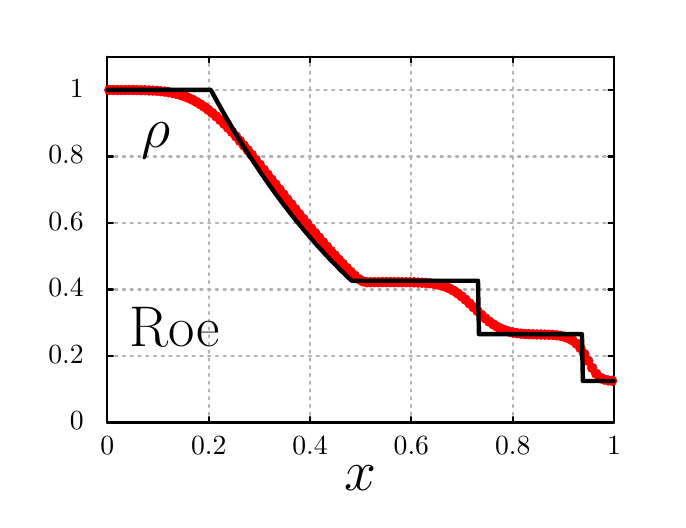
\begin{tikzpicture}[gnuplot]
%% generated with GNUPLOT 4.6p4 (Lua 5.1; terminal rev. 99, script rev. 100)
%% Thu 31 Jul 2014 01:56:31 PM EDT
\path (0.000,0.000) rectangle (8.000,6.000);
\gpfill{rgb color={1.000,1.000,1.000}} (1.012,0.985)--(7.446,0.985)--(7.446,5.630)--(1.012,5.630)--cycle;
\gpcolor{color=gp lt color border}
\gpsetlinetype{gp lt border}
\gpsetlinewidth{1.00}
\draw[gp path] (1.012,0.985)--(1.012,5.630)--(7.446,5.630)--(7.446,0.985)--cycle;
\gpcolor{color=gp lt color axes}
\gpsetlinetype{gp lt axes}
\gpsetlinewidth{2.00}
\draw[gp path] (1.012,0.985)--(7.447,0.985);
\gpcolor{color=gp lt color border}
\gpsetlinetype{gp lt border}
\draw[gp path] (1.012,0.985)--(1.084,0.985);
\draw[gp path] (7.447,0.985)--(7.375,0.985);
\gpcolor{rgb color={0.000,0.000,0.000}}
\node[gp node right,font={\fontsize{10pt}{12pt}\selectfont}] at (0.828,0.985) {0};
\gpcolor{color=gp lt color axes}
\gpsetlinetype{gp lt axes}
\draw[gp path] (1.012,1.830)--(7.447,1.830);
\gpcolor{color=gp lt color border}
\gpsetlinetype{gp lt border}
\draw[gp path] (1.012,1.830)--(1.084,1.830);
\draw[gp path] (7.447,1.830)--(7.375,1.830);
\gpcolor{rgb color={0.000,0.000,0.000}}
\node[gp node right,font={\fontsize{10pt}{12pt}\selectfont}] at (0.828,1.830) {0.2};
\gpcolor{color=gp lt color axes}
\gpsetlinetype{gp lt axes}
\draw[gp path] (1.012,2.674)--(7.447,2.674);
\gpcolor{color=gp lt color border}
\gpsetlinetype{gp lt border}
\draw[gp path] (1.012,2.674)--(1.084,2.674);
\draw[gp path] (7.447,2.674)--(7.375,2.674);
\gpcolor{rgb color={0.000,0.000,0.000}}
\node[gp node right,font={\fontsize{10pt}{12pt}\selectfont}] at (0.828,2.674) {0.4};
\gpcolor{color=gp lt color axes}
\gpsetlinetype{gp lt axes}
\draw[gp path] (1.012,3.519)--(7.447,3.519);
\gpcolor{color=gp lt color border}
\gpsetlinetype{gp lt border}
\draw[gp path] (1.012,3.519)--(1.084,3.519);
\draw[gp path] (7.447,3.519)--(7.375,3.519);
\gpcolor{rgb color={0.000,0.000,0.000}}
\node[gp node right,font={\fontsize{10pt}{12pt}\selectfont}] at (0.828,3.519) {0.6};
\gpcolor{color=gp lt color axes}
\gpsetlinetype{gp lt axes}
\draw[gp path] (1.012,4.364)--(7.447,4.364);
\gpcolor{color=gp lt color border}
\gpsetlinetype{gp lt border}
\draw[gp path] (1.012,4.364)--(1.084,4.364);
\draw[gp path] (7.447,4.364)--(7.375,4.364);
\gpcolor{rgb color={0.000,0.000,0.000}}
\node[gp node right,font={\fontsize{10pt}{12pt}\selectfont}] at (0.828,4.364) {0.8};
\gpcolor{color=gp lt color axes}
\gpsetlinetype{gp lt axes}
\draw[gp path] (1.012,5.209)--(7.447,5.209);
\gpcolor{color=gp lt color border}
\gpsetlinetype{gp lt border}
\draw[gp path] (1.012,5.209)--(1.084,5.209);
\draw[gp path] (7.447,5.209)--(7.375,5.209);
\gpcolor{rgb color={0.000,0.000,0.000}}
\node[gp node right,font={\fontsize{10pt}{12pt}\selectfont}] at (0.828,5.209) {1};
\gpcolor{color=gp lt color axes}
\gpsetlinetype{gp lt axes}
\draw[gp path] (1.012,0.985)--(1.012,5.631);
\gpcolor{color=gp lt color border}
\gpsetlinetype{gp lt border}
\draw[gp path] (1.012,0.985)--(1.012,1.057);
\draw[gp path] (1.012,5.631)--(1.012,5.559);
\gpcolor{rgb color={0.000,0.000,0.000}}
\node[gp node center,font={\fontsize{10pt}{12pt}\selectfont}] at (1.012,0.677) {0};
\gpcolor{color=gp lt color axes}
\gpsetlinetype{gp lt axes}
\draw[gp path] (2.299,0.985)--(2.299,5.631);
\gpcolor{color=gp lt color border}
\gpsetlinetype{gp lt border}
\draw[gp path] (2.299,0.985)--(2.299,1.057);
\draw[gp path] (2.299,5.631)--(2.299,5.559);
\gpcolor{rgb color={0.000,0.000,0.000}}
\node[gp node center,font={\fontsize{10pt}{12pt}\selectfont}] at (2.299,0.677) {0.2};
\gpcolor{color=gp lt color axes}
\gpsetlinetype{gp lt axes}
\draw[gp path] (3.586,0.985)--(3.586,5.631);
\gpcolor{color=gp lt color border}
\gpsetlinetype{gp lt border}
\draw[gp path] (3.586,0.985)--(3.586,1.057);
\draw[gp path] (3.586,5.631)--(3.586,5.559);
\gpcolor{rgb color={0.000,0.000,0.000}}
\node[gp node center,font={\fontsize{10pt}{12pt}\selectfont}] at (3.586,0.677) {0.4};
\gpcolor{color=gp lt color axes}
\gpsetlinetype{gp lt axes}
\draw[gp path] (4.873,0.985)--(4.873,5.631);
\gpcolor{color=gp lt color border}
\gpsetlinetype{gp lt border}
\draw[gp path] (4.873,0.985)--(4.873,1.057);
\draw[gp path] (4.873,5.631)--(4.873,5.559);
\gpcolor{rgb color={0.000,0.000,0.000}}
\node[gp node center,font={\fontsize{10pt}{12pt}\selectfont}] at (4.873,0.677) {0.6};
\gpcolor{color=gp lt color axes}
\gpsetlinetype{gp lt axes}
\draw[gp path] (6.160,0.985)--(6.160,5.631);
\gpcolor{color=gp lt color border}
\gpsetlinetype{gp lt border}
\draw[gp path] (6.160,0.985)--(6.160,1.057);
\draw[gp path] (6.160,5.631)--(6.160,5.559);
\gpcolor{rgb color={0.000,0.000,0.000}}
\node[gp node center,font={\fontsize{10pt}{12pt}\selectfont}] at (6.160,0.677) {0.8};
\gpcolor{color=gp lt color axes}
\gpsetlinetype{gp lt axes}
\draw[gp path] (7.447,0.985)--(7.447,5.631);
\gpcolor{color=gp lt color border}
\gpsetlinetype{gp lt border}
\draw[gp path] (7.447,0.985)--(7.447,1.057);
\draw[gp path] (7.447,5.631)--(7.447,5.559);
\gpcolor{rgb color={0.000,0.000,0.000}}
\node[gp node center,font={\fontsize{10pt}{12pt}\selectfont}] at (7.447,0.677) {1};
\gpcolor{color=gp lt color border}
\draw[gp path] (1.012,5.631)--(1.012,0.985)--(7.447,0.985)--(7.447,5.631)--cycle;
\gpcolor{rgb color={0.000,0.000,0.000}}
\node[gp node center,font={\fontsize{10pt}{12pt}\selectfont}] at (4.229,0.215) {\huge $x$};
\gpcolor{rgb color={1.000,0.000,0.000}}
\gpsetlinewidth{0.50}
\gpsetpointsize{4.44}
\gppoint{gp mark 7}{(1.037,5.209)}
\gppoint{gp mark 7}{(1.087,5.209)}
\gppoint{gp mark 7}{(1.138,5.208)}
\gppoint{gp mark 7}{(1.188,5.208)}
\gppoint{gp mark 7}{(1.238,5.208)}
\gppoint{gp mark 7}{(1.289,5.208)}
\gppoint{gp mark 7}{(1.339,5.208)}
\gppoint{gp mark 7}{(1.389,5.207)}
\gppoint{gp mark 7}{(1.439,5.206)}
\gppoint{gp mark 7}{(1.490,5.205)}
\gppoint{gp mark 7}{(1.540,5.203)}
\gppoint{gp mark 7}{(1.590,5.201)}
\gppoint{gp mark 7}{(1.640,5.198)}
\gppoint{gp mark 7}{(1.691,5.193)}
\gppoint{gp mark 7}{(1.741,5.188)}
\gppoint{gp mark 7}{(1.791,5.180)}
\gppoint{gp mark 7}{(1.842,5.171)}
\gppoint{gp mark 7}{(1.892,5.159)}
\gppoint{gp mark 7}{(1.942,5.145)}
\gppoint{gp mark 7}{(1.992,5.128)}
\gppoint{gp mark 7}{(2.043,5.108)}
\gppoint{gp mark 7}{(2.093,5.085)}
\gppoint{gp mark 7}{(2.143,5.058)}
\gppoint{gp mark 7}{(2.193,5.028)}
\gppoint{gp mark 7}{(2.244,4.994)}
\gppoint{gp mark 7}{(2.294,4.957)}
\gppoint{gp mark 7}{(2.344,4.917)}
\gppoint{gp mark 7}{(2.395,4.874)}
\gppoint{gp mark 7}{(2.445,4.828)}
\gppoint{gp mark 7}{(2.495,4.779)}
\gppoint{gp mark 7}{(2.545,4.728)}
\gppoint{gp mark 7}{(2.596,4.675)}
\gppoint{gp mark 7}{(2.646,4.619)}
\gppoint{gp mark 7}{(2.696,4.562)}
\gppoint{gp mark 7}{(2.746,4.504)}
\gppoint{gp mark 7}{(2.797,4.444)}
\gppoint{gp mark 7}{(2.847,4.384)}
\gppoint{gp mark 7}{(2.897,4.322)}
\gppoint{gp mark 7}{(2.948,4.260)}
\gppoint{gp mark 7}{(2.998,4.197)}
\gppoint{gp mark 7}{(3.048,4.134)}
\gppoint{gp mark 7}{(3.098,4.071)}
\gppoint{gp mark 7}{(3.149,4.008)}
\gppoint{gp mark 7}{(3.199,3.945)}
\gppoint{gp mark 7}{(3.249,3.882)}
\gppoint{gp mark 7}{(3.299,3.819)}
\gppoint{gp mark 7}{(3.350,3.757)}
\gppoint{gp mark 7}{(3.400,3.695)}
\gppoint{gp mark 7}{(3.450,3.633)}
\gppoint{gp mark 7}{(3.501,3.572)}
\gppoint{gp mark 7}{(3.551,3.511)}
\gppoint{gp mark 7}{(3.601,3.451)}
\gppoint{gp mark 7}{(3.651,3.392)}
\gppoint{gp mark 7}{(3.702,3.334)}
\gppoint{gp mark 7}{(3.752,3.276)}
\gppoint{gp mark 7}{(3.802,3.219)}
\gppoint{gp mark 7}{(3.852,3.163)}
\gppoint{gp mark 7}{(3.903,3.108)}
\gppoint{gp mark 7}{(3.953,3.053)}
\gppoint{gp mark 7}{(4.003,3.000)}
\gppoint{gp mark 7}{(4.054,2.948)}
\gppoint{gp mark 7}{(4.104,2.898)}
\gppoint{gp mark 7}{(4.154,2.851)}
\gppoint{gp mark 7}{(4.204,2.809)}
\gppoint{gp mark 7}{(4.255,2.779)}
\gppoint{gp mark 7}{(4.305,2.767)}
\gppoint{gp mark 7}{(4.355,2.767)}
\gppoint{gp mark 7}{(4.405,2.768)}
\gppoint{gp mark 7}{(4.456,2.768)}
\gppoint{gp mark 7}{(4.506,2.769)}
\gppoint{gp mark 7}{(4.556,2.769)}
\gppoint{gp mark 7}{(4.607,2.769)}
\gppoint{gp mark 7}{(4.657,2.768)}
\gppoint{gp mark 7}{(4.707,2.768)}
\gppoint{gp mark 7}{(4.757,2.767)}
\gppoint{gp mark 7}{(4.808,2.767)}
\gppoint{gp mark 7}{(4.858,2.766)}
\gppoint{gp mark 7}{(4.908,2.765)}
\gppoint{gp mark 7}{(4.958,2.763)}
\gppoint{gp mark 7}{(5.009,2.761)}
\gppoint{gp mark 7}{(5.059,2.758)}
\gppoint{gp mark 7}{(5.109,2.754)}
\gppoint{gp mark 7}{(5.160,2.747)}
\gppoint{gp mark 7}{(5.210,2.738)}
\gppoint{gp mark 7}{(5.260,2.726)}
\gppoint{gp mark 7}{(5.310,2.709)}
\gppoint{gp mark 7}{(5.361,2.687)}
\gppoint{gp mark 7}{(5.411,2.659)}
\gppoint{gp mark 7}{(5.461,2.626)}
\gppoint{gp mark 7}{(5.511,2.588)}
\gppoint{gp mark 7}{(5.562,2.545)}
\gppoint{gp mark 7}{(5.612,2.498)}
\gppoint{gp mark 7}{(5.662,2.450)}
\gppoint{gp mark 7}{(5.713,2.401)}
\gppoint{gp mark 7}{(5.763,2.353)}
\gppoint{gp mark 7}{(5.813,2.308)}
\gppoint{gp mark 7}{(5.863,2.267)}
\gppoint{gp mark 7}{(5.914,2.232)}
\gppoint{gp mark 7}{(5.964,2.201)}
\gppoint{gp mark 7}{(6.014,2.176)}
\gppoint{gp mark 7}{(6.064,2.156)}
\gppoint{gp mark 7}{(6.115,2.140)}
\gppoint{gp mark 7}{(6.165,2.128)}
\gppoint{gp mark 7}{(6.215,2.120)}
\gppoint{gp mark 7}{(6.266,2.114)}
\gppoint{gp mark 7}{(6.316,2.110)}
\gppoint{gp mark 7}{(6.366,2.107)}
\gppoint{gp mark 7}{(6.416,2.106)}
\gppoint{gp mark 7}{(6.467,2.104)}
\gppoint{gp mark 7}{(6.517,2.103)}
\gppoint{gp mark 7}{(6.567,2.102)}
\gppoint{gp mark 7}{(6.617,2.100)}
\gppoint{gp mark 7}{(6.668,2.098)}
\gppoint{gp mark 7}{(6.718,2.093)}
\gppoint{gp mark 7}{(6.768,2.086)}
\gppoint{gp mark 7}{(6.819,2.074)}
\gppoint{gp mark 7}{(6.869,2.056)}
\gppoint{gp mark 7}{(6.919,2.029)}
\gppoint{gp mark 7}{(6.969,1.988)}
\gppoint{gp mark 7}{(7.020,1.931)}
\gppoint{gp mark 7}{(7.070,1.856)}
\gppoint{gp mark 7}{(7.120,1.768)}
\gppoint{gp mark 7}{(7.170,1.679)}
\gppoint{gp mark 7}{(7.221,1.605)}
\gppoint{gp mark 7}{(7.271,1.557)}
\gppoint{gp mark 7}{(7.321,1.532)}
\gppoint{gp mark 7}{(7.372,1.520)}
\gppoint{gp mark 7}{(7.422,1.516)}
\gpcolor{rgb color={0.000,0.000,0.000}}
\gpsetlinetype{gp lt plot 0}
\gpsetlinewidth{4.00}
\draw[gp path] (1.018,5.209)--(1.031,5.209)--(1.043,5.209)--(1.056,5.209)--(1.069,5.209)%
  --(1.081,5.209)--(1.094,5.209)--(1.106,5.209)--(1.119,5.209)--(1.131,5.209)--(1.144,5.209)%
  --(1.157,5.209)--(1.169,5.209)--(1.182,5.209)--(1.194,5.209)--(1.207,5.209)--(1.219,5.209)%
  --(1.232,5.209)--(1.245,5.209)--(1.257,5.209)--(1.270,5.209)--(1.282,5.209)--(1.295,5.209)%
  --(1.307,5.209)--(1.320,5.209)--(1.332,5.209)--(1.345,5.209)--(1.358,5.209)--(1.370,5.209)%
  --(1.383,5.209)--(1.395,5.209)--(1.408,5.209)--(1.420,5.209)--(1.433,5.209)--(1.446,5.209)%
  --(1.458,5.209)--(1.471,5.209)--(1.483,5.209)--(1.496,5.209)--(1.508,5.209)--(1.521,5.209)%
  --(1.534,5.209)--(1.546,5.209)--(1.559,5.209)--(1.571,5.209)--(1.584,5.209)--(1.596,5.209)%
  --(1.609,5.209)--(1.622,5.209)--(1.634,5.209)--(1.647,5.209)--(1.659,5.209)--(1.672,5.209)%
  --(1.684,5.209)--(1.697,5.209)--(1.710,5.209)--(1.722,5.209)--(1.735,5.209)--(1.747,5.209)%
  --(1.760,5.209)--(1.772,5.209)--(1.785,5.209)--(1.798,5.209)--(1.810,5.209)--(1.823,5.209)%
  --(1.835,5.209)--(1.848,5.209)--(1.860,5.209)--(1.873,5.209)--(1.886,5.209)--(1.898,5.209)%
  --(1.911,5.209)--(1.923,5.209)--(1.936,5.209)--(1.948,5.209)--(1.961,5.209)--(1.973,5.209)%
  --(1.986,5.209)--(1.999,5.209)--(2.011,5.209)--(2.024,5.209)--(2.036,5.209)--(2.049,5.209)%
  --(2.061,5.209)--(2.074,5.209)--(2.087,5.209)--(2.099,5.209)--(2.112,5.209)--(2.124,5.209)%
  --(2.137,5.209)--(2.149,5.209)--(2.162,5.209)--(2.175,5.209)--(2.187,5.209)--(2.200,5.209)%
  --(2.212,5.209)--(2.225,5.209)--(2.237,5.209)--(2.250,5.209)--(2.263,5.209)--(2.275,5.209)%
  --(2.288,5.209)--(2.300,5.209)--(2.313,5.209)--(2.325,5.209)--(2.338,5.187)--(2.351,5.163)%
  --(2.363,5.140)--(2.376,5.118)--(2.388,5.095)--(2.401,5.072)--(2.413,5.050)--(2.426,5.027)%
  --(2.439,5.005)--(2.451,4.982)--(2.464,4.960)--(2.476,4.938)--(2.489,4.916)--(2.501,4.894)%
  --(2.514,4.872)--(2.526,4.851)--(2.539,4.829)--(2.552,4.808)--(2.564,4.786)--(2.577,4.765)%
  --(2.589,4.744)--(2.602,4.723)--(2.614,4.702)--(2.627,4.681)--(2.640,4.660)--(2.652,4.639)%
  --(2.665,4.618)--(2.677,4.598)--(2.690,4.577)--(2.702,4.557)--(2.715,4.537)--(2.728,4.517)%
  --(2.740,4.496)--(2.753,4.476)--(2.765,4.456)--(2.778,4.437)--(2.790,4.417)--(2.803,4.397)%
  --(2.816,4.378)--(2.828,4.358)--(2.841,4.339)--(2.853,4.320)--(2.866,4.300)--(2.878,4.281)%
  --(2.891,4.262)--(2.904,4.243)--(2.916,4.225)--(2.929,4.206)--(2.941,4.187)--(2.954,4.169)%
  --(2.966,4.150)--(2.979,4.132)--(2.992,4.113)--(3.004,4.095)--(3.017,4.077)--(3.029,4.059)%
  --(3.042,4.041)--(3.054,4.023)--(3.067,4.005)--(3.079,3.987)--(3.092,3.970)--(3.105,3.952)%
  --(3.117,3.935)--(3.130,3.917)--(3.142,3.900)--(3.155,3.883)--(3.167,3.866)--(3.180,3.849)%
  --(3.193,3.832)--(3.205,3.815)--(3.218,3.798)--(3.230,3.781)--(3.243,3.764)--(3.255,3.748)%
  --(3.268,3.731)--(3.281,3.715)--(3.293,3.699)--(3.306,3.682)--(3.318,3.666)--(3.331,3.650)%
  --(3.343,3.634)--(3.356,3.618)--(3.369,3.602)--(3.381,3.586)--(3.394,3.571)--(3.406,3.555)%
  --(3.419,3.539)--(3.431,3.524)--(3.444,3.508)--(3.457,3.493)--(3.469,3.478)--(3.482,3.463)%
  --(3.494,3.447)--(3.507,3.432)--(3.519,3.417)--(3.532,3.403)--(3.545,3.388)--(3.557,3.373)%
  --(3.570,3.358)--(3.582,3.344)--(3.595,3.329)--(3.607,3.315)--(3.620,3.300)--(3.633,3.286)%
  --(3.645,3.272)--(3.658,3.257)--(3.670,3.243)--(3.683,3.229)--(3.695,3.215)--(3.708,3.201)%
  --(3.720,3.188)--(3.733,3.174)--(3.746,3.160)--(3.758,3.146)--(3.771,3.133)--(3.783,3.119)%
  --(3.796,3.106)--(3.808,3.093)--(3.821,3.079)--(3.834,3.066)--(3.846,3.053)--(3.859,3.040)%
  --(3.871,3.027)--(3.884,3.014)--(3.896,3.001)--(3.909,2.988)--(3.922,2.975)--(3.934,2.963)%
  --(3.947,2.950)--(3.959,2.937)--(3.972,2.925)--(3.984,2.912)--(3.997,2.900)--(4.010,2.888)%
  --(4.022,2.876)--(4.035,2.863)--(4.047,2.851)--(4.060,2.839)--(4.072,2.827)--(4.085,2.815)%
  --(4.098,2.803)--(4.110,2.792)--(4.123,2.786)--(4.135,2.786)--(4.148,2.786)--(4.160,2.786)%
  --(4.173,2.786)--(4.186,2.786)--(4.198,2.786)--(4.211,2.786)--(4.223,2.786)--(4.236,2.786)%
  --(4.248,2.786)--(4.261,2.786)--(4.273,2.786)--(4.286,2.786)--(4.299,2.786)--(4.311,2.786)%
  --(4.324,2.786)--(4.336,2.786)--(4.349,2.786)--(4.361,2.786)--(4.374,2.786)--(4.387,2.786)%
  --(4.399,2.786)--(4.412,2.786)--(4.424,2.786)--(4.437,2.786)--(4.449,2.786)--(4.462,2.786)%
  --(4.475,2.786)--(4.487,2.786)--(4.500,2.786)--(4.512,2.786)--(4.525,2.786)--(4.537,2.786)%
  --(4.550,2.786)--(4.563,2.786)--(4.575,2.786)--(4.588,2.786)--(4.600,2.786)--(4.613,2.786)%
  --(4.625,2.786)--(4.638,2.786)--(4.651,2.786)--(4.663,2.786)--(4.676,2.786)--(4.688,2.786)%
  --(4.701,2.786)--(4.713,2.786)--(4.726,2.786)--(4.739,2.786)--(4.751,2.786)--(4.764,2.786)%
  --(4.776,2.786)--(4.789,2.786)--(4.801,2.786)--(4.814,2.786)--(4.826,2.786)--(4.839,2.786)%
  --(4.852,2.786)--(4.864,2.786)--(4.877,2.786)--(4.889,2.786)--(4.902,2.786)--(4.914,2.786)%
  --(4.927,2.786)--(4.940,2.786)--(4.952,2.786)--(4.965,2.786)--(4.977,2.786)--(4.990,2.786)%
  --(5.002,2.786)--(5.015,2.786)--(5.028,2.786)--(5.040,2.786)--(5.053,2.786)--(5.065,2.786)%
  --(5.078,2.786)--(5.090,2.786)--(5.103,2.786)--(5.116,2.786)--(5.128,2.786)--(5.141,2.786)%
  --(5.153,2.786)--(5.166,2.786)--(5.178,2.786)--(5.191,2.786)--(5.204,2.786)--(5.216,2.786)%
  --(5.229,2.786)--(5.241,2.786)--(5.254,2.786)--(5.266,2.786)--(5.279,2.786)--(5.292,2.786)%
  --(5.304,2.786)--(5.317,2.786)--(5.329,2.786)--(5.342,2.786)--(5.354,2.786)--(5.367,2.786)%
  --(5.380,2.786)--(5.392,2.786)--(5.405,2.786)--(5.417,2.786)--(5.430,2.786)--(5.442,2.786)%
  --(5.455,2.786)--(5.467,2.786)--(5.480,2.786)--(5.493,2.786)--(5.505,2.786)--(5.518,2.786)%
  --(5.530,2.786)--(5.543,2.786)--(5.555,2.786)--(5.568,2.786)--(5.581,2.786)--(5.593,2.786)%
  --(5.606,2.786)--(5.618,2.786)--(5.631,2.786)--(5.643,2.786)--(5.656,2.786)--(5.669,2.786)%
  --(5.681,2.786)--(5.694,2.786)--(5.706,2.786)--(5.719,2.786)--(5.731,2.107)--(5.744,2.107)%
  --(5.757,2.107)--(5.769,2.107)--(5.782,2.107)--(5.794,2.107)--(5.807,2.107)--(5.819,2.107)%
  --(5.832,2.107)--(5.845,2.107)--(5.857,2.107)--(5.870,2.107)--(5.882,2.107)--(5.895,2.107)%
  --(5.907,2.107)--(5.920,2.107)--(5.933,2.107)--(5.945,2.107)--(5.958,2.107)--(5.970,2.107)%
  --(5.983,2.107)--(5.995,2.107)--(6.008,2.107)--(6.020,2.107)--(6.033,2.107)--(6.046,2.107)%
  --(6.058,2.107)--(6.071,2.107)--(6.083,2.107)--(6.096,2.107)--(6.108,2.107)--(6.121,2.107)%
  --(6.134,2.107)--(6.146,2.107)--(6.159,2.107)--(6.171,2.107)--(6.184,2.107)--(6.196,2.107)%
  --(6.209,2.107)--(6.222,2.107)--(6.234,2.107)--(6.247,2.107)--(6.259,2.107)--(6.272,2.107)%
  --(6.284,2.107)--(6.297,2.107)--(6.310,2.107)--(6.322,2.107)--(6.335,2.107)--(6.347,2.107)%
  --(6.360,2.107)--(6.372,2.107)--(6.385,2.107)--(6.398,2.107)--(6.410,2.107)--(6.423,2.107)%
  --(6.435,2.107)--(6.448,2.107)--(6.460,2.107)--(6.473,2.107)--(6.486,2.107)--(6.498,2.107)%
  --(6.511,2.107)--(6.523,2.107)--(6.536,2.107)--(6.548,2.107)--(6.561,2.107)--(6.573,2.107)%
  --(6.586,2.107)--(6.599,2.107)--(6.611,2.107)--(6.624,2.107)--(6.636,2.107)--(6.649,2.107)%
  --(6.661,2.107)--(6.674,2.107)--(6.687,2.107)--(6.699,2.107)--(6.712,2.107)--(6.724,2.107)%
  --(6.737,2.107)--(6.749,2.107)--(6.762,2.107)--(6.775,2.107)--(6.787,2.107)--(6.800,2.107)%
  --(6.812,2.107)--(6.825,2.107)--(6.837,2.107)--(6.850,2.107)--(6.863,2.107)--(6.875,2.107)%
  --(6.888,2.107)--(6.900,2.107)--(6.913,2.107)--(6.925,2.107)--(6.938,2.107)--(6.951,2.107)%
  --(6.963,2.107)--(6.976,2.107)--(6.988,2.107)--(7.001,2.107)--(7.013,2.107)--(7.026,2.107)%
  --(7.039,2.107)--(7.051,1.513)--(7.064,1.513)--(7.076,1.513)--(7.089,1.513)--(7.101,1.513)%
  --(7.114,1.513)--(7.127,1.513)--(7.139,1.513)--(7.152,1.513)--(7.164,1.513)--(7.177,1.513)%
  --(7.189,1.513)--(7.202,1.513)--(7.214,1.513)--(7.227,1.513)--(7.240,1.513)--(7.252,1.513)%
  --(7.265,1.513)--(7.277,1.513)--(7.290,1.513)--(7.302,1.513)--(7.315,1.513)--(7.328,1.513)%
  --(7.340,1.513)--(7.353,1.513)--(7.365,1.513)--(7.378,1.513)--(7.390,1.513)--(7.403,1.513)%
  --(7.416,1.513)--(7.428,1.513)--(7.441,1.513);
\node[gp node left,font={\fontsize{10pt}{12pt}\selectfont}] at (1.334,4.575) {\huge $\rho$};
\node[gp node left,font={\fontsize{10pt}{12pt}\selectfont}] at (1.173,2.041) {\huge Roe};
%% coordinates of the plot area
\gpdefrectangularnode{gp plot 1}{\pgfpoint{1.012cm}{0.985cm}}{\pgfpoint{7.447cm}{5.631cm}}
\end{tikzpicture}
%% gnuplot variables
} &
\resizebox{0.33\linewidth}{!}{\tikzsetnextfilename{sod_roe_1_2}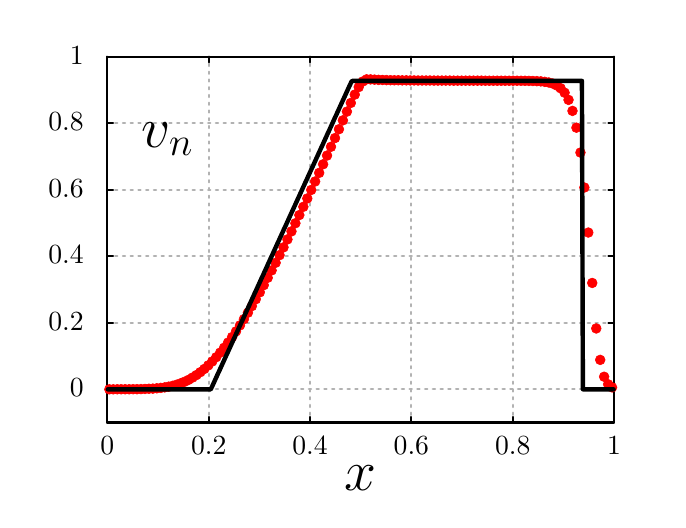
\begin{tikzpicture}[gnuplot]
%% generated with GNUPLOT 4.6p4 (Lua 5.1; terminal rev. 99, script rev. 100)
%% Thu 31 Jul 2014 01:56:31 PM EDT
\path (0.000,0.000) rectangle (8.000,6.000);
\gpfill{rgb color={1.000,1.000,1.000}} (1.012,0.985)--(7.446,0.985)--(7.446,5.630)--(1.012,5.630)--cycle;
\gpcolor{color=gp lt color border}
\gpsetlinetype{gp lt border}
\gpsetlinewidth{1.00}
\draw[gp path] (1.012,0.985)--(1.012,5.630)--(7.446,5.630)--(7.446,0.985)--cycle;
\gpcolor{color=gp lt color axes}
\gpsetlinetype{gp lt axes}
\gpsetlinewidth{2.00}
\draw[gp path] (1.012,1.407)--(7.447,1.407);
\gpcolor{color=gp lt color border}
\gpsetlinetype{gp lt border}
\draw[gp path] (1.012,1.407)--(1.084,1.407);
\draw[gp path] (7.447,1.407)--(7.375,1.407);
\gpcolor{rgb color={0.000,0.000,0.000}}
\node[gp node right,font={\fontsize{10pt}{12pt}\selectfont}] at (0.828,1.407) {0};
\gpcolor{color=gp lt color axes}
\gpsetlinetype{gp lt axes}
\draw[gp path] (1.012,2.252)--(7.447,2.252);
\gpcolor{color=gp lt color border}
\gpsetlinetype{gp lt border}
\draw[gp path] (1.012,2.252)--(1.084,2.252);
\draw[gp path] (7.447,2.252)--(7.375,2.252);
\gpcolor{rgb color={0.000,0.000,0.000}}
\node[gp node right,font={\fontsize{10pt}{12pt}\selectfont}] at (0.828,2.252) {0.2};
\gpcolor{color=gp lt color axes}
\gpsetlinetype{gp lt axes}
\draw[gp path] (1.012,3.097)--(7.447,3.097);
\gpcolor{color=gp lt color border}
\gpsetlinetype{gp lt border}
\draw[gp path] (1.012,3.097)--(1.084,3.097);
\draw[gp path] (7.447,3.097)--(7.375,3.097);
\gpcolor{rgb color={0.000,0.000,0.000}}
\node[gp node right,font={\fontsize{10pt}{12pt}\selectfont}] at (0.828,3.097) {0.4};
\gpcolor{color=gp lt color axes}
\gpsetlinetype{gp lt axes}
\draw[gp path] (1.012,3.942)--(7.447,3.942);
\gpcolor{color=gp lt color border}
\gpsetlinetype{gp lt border}
\draw[gp path] (1.012,3.942)--(1.084,3.942);
\draw[gp path] (7.447,3.942)--(7.375,3.942);
\gpcolor{rgb color={0.000,0.000,0.000}}
\node[gp node right,font={\fontsize{10pt}{12pt}\selectfont}] at (0.828,3.942) {0.6};
\gpcolor{color=gp lt color axes}
\gpsetlinetype{gp lt axes}
\draw[gp path] (1.012,4.786)--(7.447,4.786);
\gpcolor{color=gp lt color border}
\gpsetlinetype{gp lt border}
\draw[gp path] (1.012,4.786)--(1.084,4.786);
\draw[gp path] (7.447,4.786)--(7.375,4.786);
\gpcolor{rgb color={0.000,0.000,0.000}}
\node[gp node right,font={\fontsize{10pt}{12pt}\selectfont}] at (0.828,4.786) {0.8};
\gpcolor{color=gp lt color axes}
\gpsetlinetype{gp lt axes}
\draw[gp path] (1.012,5.631)--(7.447,5.631);
\gpcolor{color=gp lt color border}
\gpsetlinetype{gp lt border}
\draw[gp path] (1.012,5.631)--(1.084,5.631);
\draw[gp path] (7.447,5.631)--(7.375,5.631);
\gpcolor{rgb color={0.000,0.000,0.000}}
\node[gp node right,font={\fontsize{10pt}{12pt}\selectfont}] at (0.828,5.631) {1};
\gpcolor{color=gp lt color axes}
\gpsetlinetype{gp lt axes}
\draw[gp path] (1.012,0.985)--(1.012,5.631);
\gpcolor{color=gp lt color border}
\gpsetlinetype{gp lt border}
\draw[gp path] (1.012,0.985)--(1.012,1.057);
\draw[gp path] (1.012,5.631)--(1.012,5.559);
\gpcolor{rgb color={0.000,0.000,0.000}}
\node[gp node center,font={\fontsize{10pt}{12pt}\selectfont}] at (1.012,0.677) {0};
\gpcolor{color=gp lt color axes}
\gpsetlinetype{gp lt axes}
\draw[gp path] (2.299,0.985)--(2.299,5.631);
\gpcolor{color=gp lt color border}
\gpsetlinetype{gp lt border}
\draw[gp path] (2.299,0.985)--(2.299,1.057);
\draw[gp path] (2.299,5.631)--(2.299,5.559);
\gpcolor{rgb color={0.000,0.000,0.000}}
\node[gp node center,font={\fontsize{10pt}{12pt}\selectfont}] at (2.299,0.677) {0.2};
\gpcolor{color=gp lt color axes}
\gpsetlinetype{gp lt axes}
\draw[gp path] (3.586,0.985)--(3.586,5.631);
\gpcolor{color=gp lt color border}
\gpsetlinetype{gp lt border}
\draw[gp path] (3.586,0.985)--(3.586,1.057);
\draw[gp path] (3.586,5.631)--(3.586,5.559);
\gpcolor{rgb color={0.000,0.000,0.000}}
\node[gp node center,font={\fontsize{10pt}{12pt}\selectfont}] at (3.586,0.677) {0.4};
\gpcolor{color=gp lt color axes}
\gpsetlinetype{gp lt axes}
\draw[gp path] (4.873,0.985)--(4.873,5.631);
\gpcolor{color=gp lt color border}
\gpsetlinetype{gp lt border}
\draw[gp path] (4.873,0.985)--(4.873,1.057);
\draw[gp path] (4.873,5.631)--(4.873,5.559);
\gpcolor{rgb color={0.000,0.000,0.000}}
\node[gp node center,font={\fontsize{10pt}{12pt}\selectfont}] at (4.873,0.677) {0.6};
\gpcolor{color=gp lt color axes}
\gpsetlinetype{gp lt axes}
\draw[gp path] (6.160,0.985)--(6.160,5.631);
\gpcolor{color=gp lt color border}
\gpsetlinetype{gp lt border}
\draw[gp path] (6.160,0.985)--(6.160,1.057);
\draw[gp path] (6.160,5.631)--(6.160,5.559);
\gpcolor{rgb color={0.000,0.000,0.000}}
\node[gp node center,font={\fontsize{10pt}{12pt}\selectfont}] at (6.160,0.677) {0.8};
\gpcolor{color=gp lt color axes}
\gpsetlinetype{gp lt axes}
\draw[gp path] (7.447,0.985)--(7.447,5.631);
\gpcolor{color=gp lt color border}
\gpsetlinetype{gp lt border}
\draw[gp path] (7.447,0.985)--(7.447,1.057);
\draw[gp path] (7.447,5.631)--(7.447,5.559);
\gpcolor{rgb color={0.000,0.000,0.000}}
\node[gp node center,font={\fontsize{10pt}{12pt}\selectfont}] at (7.447,0.677) {1};
\gpcolor{color=gp lt color border}
\draw[gp path] (1.012,5.631)--(1.012,0.985)--(7.447,0.985)--(7.447,5.631)--cycle;
\gpcolor{rgb color={0.000,0.000,0.000}}
\node[gp node center,font={\fontsize{10pt}{12pt}\selectfont}] at (4.229,0.215) {\huge $x$};
\gpcolor{rgb color={1.000,0.000,0.000}}
\gpsetlinewidth{0.50}
\gpsetpointsize{4.44}
\gppoint{gp mark 7}{(1.037,1.407)}
\gppoint{gp mark 7}{(1.087,1.407)}
\gppoint{gp mark 7}{(1.138,1.408)}
\gppoint{gp mark 7}{(1.188,1.408)}
\gppoint{gp mark 7}{(1.238,1.408)}
\gppoint{gp mark 7}{(1.289,1.408)}
\gppoint{gp mark 7}{(1.339,1.409)}
\gppoint{gp mark 7}{(1.389,1.409)}
\gppoint{gp mark 7}{(1.439,1.410)}
\gppoint{gp mark 7}{(1.490,1.412)}
\gppoint{gp mark 7}{(1.540,1.414)}
\gppoint{gp mark 7}{(1.590,1.416)}
\gppoint{gp mark 7}{(1.640,1.420)}
\gppoint{gp mark 7}{(1.691,1.425)}
\gppoint{gp mark 7}{(1.741,1.432)}
\gppoint{gp mark 7}{(1.791,1.441)}
\gppoint{gp mark 7}{(1.842,1.452)}
\gppoint{gp mark 7}{(1.892,1.466)}
\gppoint{gp mark 7}{(1.942,1.483)}
\gppoint{gp mark 7}{(1.992,1.503)}
\gppoint{gp mark 7}{(2.043,1.527)}
\gppoint{gp mark 7}{(2.093,1.556)}
\gppoint{gp mark 7}{(2.143,1.588)}
\gppoint{gp mark 7}{(2.193,1.625)}
\gppoint{gp mark 7}{(2.244,1.666)}
\gppoint{gp mark 7}{(2.294,1.711)}
\gppoint{gp mark 7}{(2.344,1.761)}
\gppoint{gp mark 7}{(2.395,1.815)}
\gppoint{gp mark 7}{(2.445,1.873)}
\gppoint{gp mark 7}{(2.495,1.935)}
\gppoint{gp mark 7}{(2.545,2.001)}
\gppoint{gp mark 7}{(2.596,2.071)}
\gppoint{gp mark 7}{(2.646,2.143)}
\gppoint{gp mark 7}{(2.696,2.219)}
\gppoint{gp mark 7}{(2.746,2.298)}
\gppoint{gp mark 7}{(2.797,2.380)}
\gppoint{gp mark 7}{(2.847,2.464)}
\gppoint{gp mark 7}{(2.897,2.551)}
\gppoint{gp mark 7}{(2.948,2.639)}
\gppoint{gp mark 7}{(2.998,2.730)}
\gppoint{gp mark 7}{(3.048,2.823)}
\gppoint{gp mark 7}{(3.098,2.917)}
\gppoint{gp mark 7}{(3.149,3.014)}
\gppoint{gp mark 7}{(3.199,3.111)}
\gppoint{gp mark 7}{(3.249,3.210)}
\gppoint{gp mark 7}{(3.299,3.311)}
\gppoint{gp mark 7}{(3.350,3.413)}
\gppoint{gp mark 7}{(3.400,3.516)}
\gppoint{gp mark 7}{(3.450,3.620)}
\gppoint{gp mark 7}{(3.501,3.725)}
\gppoint{gp mark 7}{(3.551,3.831)}
\gppoint{gp mark 7}{(3.601,3.939)}
\gppoint{gp mark 7}{(3.651,4.047)}
\gppoint{gp mark 7}{(3.702,4.156)}
\gppoint{gp mark 7}{(3.752,4.265)}
\gppoint{gp mark 7}{(3.802,4.376)}
\gppoint{gp mark 7}{(3.852,4.487)}
\gppoint{gp mark 7}{(3.903,4.598)}
\gppoint{gp mark 7}{(3.953,4.710)}
\gppoint{gp mark 7}{(4.003,4.823)}
\gppoint{gp mark 7}{(4.054,4.934)}
\gppoint{gp mark 7}{(4.104,5.044)}
\gppoint{gp mark 7}{(4.154,5.150)}
\gppoint{gp mark 7}{(4.204,5.245)}
\gppoint{gp mark 7}{(4.255,5.316)}
\gppoint{gp mark 7}{(4.305,5.344)}
\gppoint{gp mark 7}{(4.355,5.343)}
\gppoint{gp mark 7}{(4.405,5.340)}
\gppoint{gp mark 7}{(4.456,5.337)}
\gppoint{gp mark 7}{(4.506,5.336)}
\gppoint{gp mark 7}{(4.556,5.334)}
\gppoint{gp mark 7}{(4.607,5.333)}
\gppoint{gp mark 7}{(4.657,5.332)}
\gppoint{gp mark 7}{(4.707,5.332)}
\gppoint{gp mark 7}{(4.757,5.331)}
\gppoint{gp mark 7}{(4.808,5.331)}
\gppoint{gp mark 7}{(4.858,5.330)}
\gppoint{gp mark 7}{(4.908,5.330)}
\gppoint{gp mark 7}{(4.958,5.329)}
\gppoint{gp mark 7}{(5.009,5.329)}
\gppoint{gp mark 7}{(5.059,5.329)}
\gppoint{gp mark 7}{(5.109,5.329)}
\gppoint{gp mark 7}{(5.160,5.328)}
\gppoint{gp mark 7}{(5.210,5.328)}
\gppoint{gp mark 7}{(5.260,5.328)}
\gppoint{gp mark 7}{(5.310,5.328)}
\gppoint{gp mark 7}{(5.361,5.328)}
\gppoint{gp mark 7}{(5.411,5.327)}
\gppoint{gp mark 7}{(5.461,5.327)}
\gppoint{gp mark 7}{(5.511,5.327)}
\gppoint{gp mark 7}{(5.562,5.327)}
\gppoint{gp mark 7}{(5.612,5.327)}
\gppoint{gp mark 7}{(5.662,5.327)}
\gppoint{gp mark 7}{(5.713,5.327)}
\gppoint{gp mark 7}{(5.763,5.327)}
\gppoint{gp mark 7}{(5.813,5.326)}
\gppoint{gp mark 7}{(5.863,5.326)}
\gppoint{gp mark 7}{(5.914,5.326)}
\gppoint{gp mark 7}{(5.964,5.326)}
\gppoint{gp mark 7}{(6.014,5.326)}
\gppoint{gp mark 7}{(6.064,5.326)}
\gppoint{gp mark 7}{(6.115,5.326)}
\gppoint{gp mark 7}{(6.165,5.326)}
\gppoint{gp mark 7}{(6.215,5.326)}
\gppoint{gp mark 7}{(6.266,5.325)}
\gppoint{gp mark 7}{(6.316,5.325)}
\gppoint{gp mark 7}{(6.366,5.324)}
\gppoint{gp mark 7}{(6.416,5.323)}
\gppoint{gp mark 7}{(6.467,5.321)}
\gppoint{gp mark 7}{(6.517,5.318)}
\gppoint{gp mark 7}{(6.567,5.312)}
\gppoint{gp mark 7}{(6.617,5.304)}
\gppoint{gp mark 7}{(6.668,5.290)}
\gppoint{gp mark 7}{(6.718,5.267)}
\gppoint{gp mark 7}{(6.768,5.231)}
\gppoint{gp mark 7}{(6.819,5.174)}
\gppoint{gp mark 7}{(6.869,5.083)}
\gppoint{gp mark 7}{(6.919,4.943)}
\gppoint{gp mark 7}{(6.969,4.730)}
\gppoint{gp mark 7}{(7.020,4.414)}
\gppoint{gp mark 7}{(7.070,3.970)}
\gppoint{gp mark 7}{(7.120,3.398)}
\gppoint{gp mark 7}{(7.170,2.758)}
\gppoint{gp mark 7}{(7.221,2.180)}
\gppoint{gp mark 7}{(7.271,1.781)}
\gppoint{gp mark 7}{(7.321,1.567)}
\gppoint{gp mark 7}{(7.372,1.471)}
\gppoint{gp mark 7}{(7.422,1.432)}
\gpcolor{rgb color={0.000,0.000,0.000}}
\gpsetlinetype{gp lt plot 0}
\gpsetlinewidth{4.00}
\draw[gp path] (1.018,1.407)--(1.031,1.407)--(1.043,1.407)--(1.056,1.407)--(1.069,1.407)%
  --(1.081,1.407)--(1.094,1.407)--(1.106,1.407)--(1.119,1.407)--(1.131,1.407)--(1.144,1.407)%
  --(1.157,1.407)--(1.169,1.407)--(1.182,1.407)--(1.194,1.407)--(1.207,1.407)--(1.219,1.407)%
  --(1.232,1.407)--(1.245,1.407)--(1.257,1.407)--(1.270,1.407)--(1.282,1.407)--(1.295,1.407)%
  --(1.307,1.407)--(1.320,1.407)--(1.332,1.407)--(1.345,1.407)--(1.358,1.407)--(1.370,1.407)%
  --(1.383,1.407)--(1.395,1.407)--(1.408,1.407)--(1.420,1.407)--(1.433,1.407)--(1.446,1.407)%
  --(1.458,1.407)--(1.471,1.407)--(1.483,1.407)--(1.496,1.407)--(1.508,1.407)--(1.521,1.407)%
  --(1.534,1.407)--(1.546,1.407)--(1.559,1.407)--(1.571,1.407)--(1.584,1.407)--(1.596,1.407)%
  --(1.609,1.407)--(1.622,1.407)--(1.634,1.407)--(1.647,1.407)--(1.659,1.407)--(1.672,1.407)%
  --(1.684,1.407)--(1.697,1.407)--(1.710,1.407)--(1.722,1.407)--(1.735,1.407)--(1.747,1.407)%
  --(1.760,1.407)--(1.772,1.407)--(1.785,1.407)--(1.798,1.407)--(1.810,1.407)--(1.823,1.407)%
  --(1.835,1.407)--(1.848,1.407)--(1.860,1.407)--(1.873,1.407)--(1.886,1.407)--(1.898,1.407)%
  --(1.911,1.407)--(1.923,1.407)--(1.936,1.407)--(1.948,1.407)--(1.961,1.407)--(1.973,1.407)%
  --(1.986,1.407)--(1.999,1.407)--(2.011,1.407)--(2.024,1.407)--(2.036,1.407)--(2.049,1.407)%
  --(2.061,1.407)--(2.074,1.407)--(2.087,1.407)--(2.099,1.407)--(2.112,1.407)--(2.124,1.407)%
  --(2.137,1.407)--(2.149,1.407)--(2.162,1.407)--(2.175,1.407)--(2.187,1.407)--(2.200,1.407)%
  --(2.212,1.407)--(2.225,1.407)--(2.237,1.407)--(2.250,1.407)--(2.263,1.407)--(2.275,1.407)%
  --(2.288,1.407)--(2.300,1.407)--(2.313,1.407)--(2.325,1.407)--(2.338,1.434)--(2.351,1.461)%
  --(2.363,1.489)--(2.376,1.516)--(2.388,1.544)--(2.401,1.571)--(2.413,1.599)--(2.426,1.626)%
  --(2.439,1.654)--(2.451,1.681)--(2.464,1.709)--(2.476,1.736)--(2.489,1.764)--(2.501,1.791)%
  --(2.514,1.818)--(2.526,1.846)--(2.539,1.873)--(2.552,1.901)--(2.564,1.928)--(2.577,1.956)%
  --(2.589,1.983)--(2.602,2.011)--(2.614,2.038)--(2.627,2.066)--(2.640,2.093)--(2.652,2.121)%
  --(2.665,2.148)--(2.677,2.176)--(2.690,2.203)--(2.702,2.231)--(2.715,2.258)--(2.728,2.286)%
  --(2.740,2.313)--(2.753,2.341)--(2.765,2.368)--(2.778,2.396)--(2.790,2.423)--(2.803,2.451)%
  --(2.816,2.478)--(2.828,2.506)--(2.841,2.533)--(2.853,2.561)--(2.866,2.588)--(2.878,2.616)%
  --(2.891,2.643)--(2.904,2.671)--(2.916,2.698)--(2.929,2.726)--(2.941,2.753)--(2.954,2.781)%
  --(2.966,2.808)--(2.979,2.836)--(2.992,2.863)--(3.004,2.891)--(3.017,2.918)--(3.029,2.946)%
  --(3.042,2.973)--(3.054,3.001)--(3.067,3.028)--(3.079,3.056)--(3.092,3.083)--(3.105,3.111)%
  --(3.117,3.138)--(3.130,3.166)--(3.142,3.193)--(3.155,3.221)--(3.167,3.248)--(3.180,3.276)%
  --(3.193,3.303)--(3.205,3.331)--(3.218,3.358)--(3.230,3.386)--(3.243,3.413)--(3.255,3.441)%
  --(3.268,3.468)--(3.281,3.496)--(3.293,3.523)--(3.306,3.551)--(3.318,3.578)--(3.331,3.606)%
  --(3.343,3.633)--(3.356,3.661)--(3.369,3.688)--(3.381,3.716)--(3.394,3.743)--(3.406,3.771)%
  --(3.419,3.798)--(3.431,3.826)--(3.444,3.853)--(3.457,3.881)--(3.469,3.908)--(3.482,3.936)%
  --(3.494,3.963)--(3.507,3.991)--(3.519,4.018)--(3.532,4.046)--(3.545,4.073)--(3.557,4.101)%
  --(3.570,4.128)--(3.582,4.156)--(3.595,4.183)--(3.607,4.211)--(3.620,4.238)--(3.633,4.266)%
  --(3.645,4.293)--(3.658,4.321)--(3.670,4.348)--(3.683,4.376)--(3.695,4.403)--(3.708,4.431)%
  --(3.720,4.458)--(3.733,4.486)--(3.746,4.513)--(3.758,4.541)--(3.771,4.568)--(3.783,4.596)%
  --(3.796,4.623)--(3.808,4.651)--(3.821,4.678)--(3.834,4.706)--(3.846,4.733)--(3.859,4.761)%
  --(3.871,4.788)--(3.884,4.816)--(3.896,4.843)--(3.909,4.871)--(3.922,4.898)--(3.934,4.926)%
  --(3.947,4.953)--(3.959,4.981)--(3.972,5.008)--(3.984,5.036)--(3.997,5.063)--(4.010,5.091)%
  --(4.022,5.118)--(4.035,5.146)--(4.047,5.173)--(4.060,5.201)--(4.072,5.228)--(4.085,5.256)%
  --(4.098,5.283)--(4.110,5.311)--(4.123,5.324)--(4.135,5.324)--(4.148,5.324)--(4.160,5.324)%
  --(4.173,5.324)--(4.186,5.324)--(4.198,5.324)--(4.211,5.324)--(4.223,5.324)--(4.236,5.324)%
  --(4.248,5.324)--(4.261,5.324)--(4.273,5.324)--(4.286,5.324)--(4.299,5.324)--(4.311,5.324)%
  --(4.324,5.324)--(4.336,5.324)--(4.349,5.324)--(4.361,5.324)--(4.374,5.324)--(4.387,5.324)%
  --(4.399,5.324)--(4.412,5.324)--(4.424,5.324)--(4.437,5.324)--(4.449,5.324)--(4.462,5.324)%
  --(4.475,5.324)--(4.487,5.324)--(4.500,5.324)--(4.512,5.324)--(4.525,5.324)--(4.537,5.324)%
  --(4.550,5.324)--(4.563,5.324)--(4.575,5.324)--(4.588,5.324)--(4.600,5.324)--(4.613,5.324)%
  --(4.625,5.324)--(4.638,5.324)--(4.651,5.324)--(4.663,5.324)--(4.676,5.324)--(4.688,5.324)%
  --(4.701,5.324)--(4.713,5.324)--(4.726,5.324)--(4.739,5.324)--(4.751,5.324)--(4.764,5.324)%
  --(4.776,5.324)--(4.789,5.324)--(4.801,5.324)--(4.814,5.324)--(4.826,5.324)--(4.839,5.324)%
  --(4.852,5.324)--(4.864,5.324)--(4.877,5.324)--(4.889,5.324)--(4.902,5.324)--(4.914,5.324)%
  --(4.927,5.324)--(4.940,5.324)--(4.952,5.324)--(4.965,5.324)--(4.977,5.324)--(4.990,5.324)%
  --(5.002,5.324)--(5.015,5.324)--(5.028,5.324)--(5.040,5.324)--(5.053,5.324)--(5.065,5.324)%
  --(5.078,5.324)--(5.090,5.324)--(5.103,5.324)--(5.116,5.324)--(5.128,5.324)--(5.141,5.324)%
  --(5.153,5.324)--(5.166,5.324)--(5.178,5.324)--(5.191,5.324)--(5.204,5.324)--(5.216,5.324)%
  --(5.229,5.324)--(5.241,5.324)--(5.254,5.324)--(5.266,5.324)--(5.279,5.324)--(5.292,5.324)%
  --(5.304,5.324)--(5.317,5.324)--(5.329,5.324)--(5.342,5.324)--(5.354,5.324)--(5.367,5.324)%
  --(5.380,5.324)--(5.392,5.324)--(5.405,5.324)--(5.417,5.324)--(5.430,5.324)--(5.442,5.324)%
  --(5.455,5.324)--(5.467,5.324)--(5.480,5.324)--(5.493,5.324)--(5.505,5.324)--(5.518,5.324)%
  --(5.530,5.324)--(5.543,5.324)--(5.555,5.324)--(5.568,5.324)--(5.581,5.324)--(5.593,5.324)%
  --(5.606,5.324)--(5.618,5.324)--(5.631,5.324)--(5.643,5.324)--(5.656,5.324)--(5.669,5.324)%
  --(5.681,5.324)--(5.694,5.324)--(5.706,5.324)--(5.719,5.324)--(5.731,5.324)--(5.744,5.324)%
  --(5.757,5.324)--(5.769,5.324)--(5.782,5.324)--(5.794,5.324)--(5.807,5.324)--(5.819,5.324)%
  --(5.832,5.324)--(5.845,5.324)--(5.857,5.324)--(5.870,5.324)--(5.882,5.324)--(5.895,5.324)%
  --(5.907,5.324)--(5.920,5.324)--(5.933,5.324)--(5.945,5.324)--(5.958,5.324)--(5.970,5.324)%
  --(5.983,5.324)--(5.995,5.324)--(6.008,5.324)--(6.020,5.324)--(6.033,5.324)--(6.046,5.324)%
  --(6.058,5.324)--(6.071,5.324)--(6.083,5.324)--(6.096,5.324)--(6.108,5.324)--(6.121,5.324)%
  --(6.134,5.324)--(6.146,5.324)--(6.159,5.324)--(6.171,5.324)--(6.184,5.324)--(6.196,5.324)%
  --(6.209,5.324)--(6.222,5.324)--(6.234,5.324)--(6.247,5.324)--(6.259,5.324)--(6.272,5.324)%
  --(6.284,5.324)--(6.297,5.324)--(6.310,5.324)--(6.322,5.324)--(6.335,5.324)--(6.347,5.324)%
  --(6.360,5.324)--(6.372,5.324)--(6.385,5.324)--(6.398,5.324)--(6.410,5.324)--(6.423,5.324)%
  --(6.435,5.324)--(6.448,5.324)--(6.460,5.324)--(6.473,5.324)--(6.486,5.324)--(6.498,5.324)%
  --(6.511,5.324)--(6.523,5.324)--(6.536,5.324)--(6.548,5.324)--(6.561,5.324)--(6.573,5.324)%
  --(6.586,5.324)--(6.599,5.324)--(6.611,5.324)--(6.624,5.324)--(6.636,5.324)--(6.649,5.324)%
  --(6.661,5.324)--(6.674,5.324)--(6.687,5.324)--(6.699,5.324)--(6.712,5.324)--(6.724,5.324)%
  --(6.737,5.324)--(6.749,5.324)--(6.762,5.324)--(6.775,5.324)--(6.787,5.324)--(6.800,5.324)%
  --(6.812,5.324)--(6.825,5.324)--(6.837,5.324)--(6.850,5.324)--(6.863,5.324)--(6.875,5.324)%
  --(6.888,5.324)--(6.900,5.324)--(6.913,5.324)--(6.925,5.324)--(6.938,5.324)--(6.951,5.324)%
  --(6.963,5.324)--(6.976,5.324)--(6.988,5.324)--(7.001,5.324)--(7.013,5.324)--(7.026,5.324)%
  --(7.039,5.324)--(7.051,1.407)--(7.064,1.407)--(7.076,1.407)--(7.089,1.407)--(7.101,1.407)%
  --(7.114,1.407)--(7.127,1.407)--(7.139,1.407)--(7.152,1.407)--(7.164,1.407)--(7.177,1.407)%
  --(7.189,1.407)--(7.202,1.407)--(7.214,1.407)--(7.227,1.407)--(7.240,1.407)--(7.252,1.407)%
  --(7.265,1.407)--(7.277,1.407)--(7.290,1.407)--(7.302,1.407)--(7.315,1.407)--(7.328,1.407)%
  --(7.340,1.407)--(7.353,1.407)--(7.365,1.407)--(7.378,1.407)--(7.390,1.407)--(7.403,1.407)%
  --(7.416,1.407)--(7.428,1.407)--(7.441,1.407);
\node[gp node left,font={\fontsize{10pt}{12pt}\selectfont}] at (1.334,4.575) {\huge $v_n$};
%% coordinates of the plot area
\gpdefrectangularnode{gp plot 1}{\pgfpoint{1.012cm}{0.985cm}}{\pgfpoint{7.447cm}{5.631cm}}
\end{tikzpicture}
%% gnuplot variables
} &
\resizebox{0.33\linewidth}{!}{\tikzsetnextfilename{sod_roe_1_3}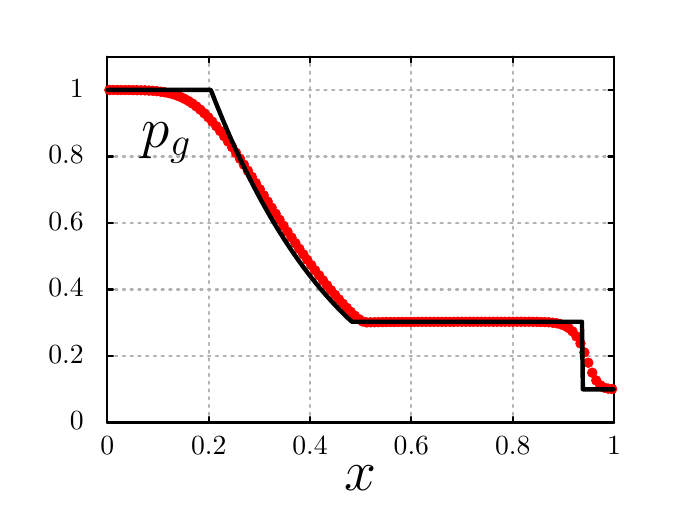
\begin{tikzpicture}[gnuplot]
%% generated with GNUPLOT 4.6p4 (Lua 5.1; terminal rev. 99, script rev. 100)
%% Thu 31 Jul 2014 01:56:31 PM EDT
\path (0.000,0.000) rectangle (8.000,6.000);
\gpfill{rgb color={1.000,1.000,1.000}} (1.012,0.985)--(7.446,0.985)--(7.446,5.630)--(1.012,5.630)--cycle;
\gpcolor{color=gp lt color border}
\gpsetlinetype{gp lt border}
\gpsetlinewidth{1.00}
\draw[gp path] (1.012,0.985)--(1.012,5.630)--(7.446,5.630)--(7.446,0.985)--cycle;
\gpcolor{color=gp lt color axes}
\gpsetlinetype{gp lt axes}
\gpsetlinewidth{2.00}
\draw[gp path] (1.012,0.985)--(7.447,0.985);
\gpcolor{color=gp lt color border}
\gpsetlinetype{gp lt border}
\draw[gp path] (1.012,0.985)--(1.084,0.985);
\draw[gp path] (7.447,0.985)--(7.375,0.985);
\gpcolor{rgb color={0.000,0.000,0.000}}
\node[gp node right,font={\fontsize{10pt}{12pt}\selectfont}] at (0.828,0.985) {0};
\gpcolor{color=gp lt color axes}
\gpsetlinetype{gp lt axes}
\draw[gp path] (1.012,1.830)--(7.447,1.830);
\gpcolor{color=gp lt color border}
\gpsetlinetype{gp lt border}
\draw[gp path] (1.012,1.830)--(1.084,1.830);
\draw[gp path] (7.447,1.830)--(7.375,1.830);
\gpcolor{rgb color={0.000,0.000,0.000}}
\node[gp node right,font={\fontsize{10pt}{12pt}\selectfont}] at (0.828,1.830) {0.2};
\gpcolor{color=gp lt color axes}
\gpsetlinetype{gp lt axes}
\draw[gp path] (1.012,2.674)--(7.447,2.674);
\gpcolor{color=gp lt color border}
\gpsetlinetype{gp lt border}
\draw[gp path] (1.012,2.674)--(1.084,2.674);
\draw[gp path] (7.447,2.674)--(7.375,2.674);
\gpcolor{rgb color={0.000,0.000,0.000}}
\node[gp node right,font={\fontsize{10pt}{12pt}\selectfont}] at (0.828,2.674) {0.4};
\gpcolor{color=gp lt color axes}
\gpsetlinetype{gp lt axes}
\draw[gp path] (1.012,3.519)--(7.447,3.519);
\gpcolor{color=gp lt color border}
\gpsetlinetype{gp lt border}
\draw[gp path] (1.012,3.519)--(1.084,3.519);
\draw[gp path] (7.447,3.519)--(7.375,3.519);
\gpcolor{rgb color={0.000,0.000,0.000}}
\node[gp node right,font={\fontsize{10pt}{12pt}\selectfont}] at (0.828,3.519) {0.6};
\gpcolor{color=gp lt color axes}
\gpsetlinetype{gp lt axes}
\draw[gp path] (1.012,4.364)--(7.447,4.364);
\gpcolor{color=gp lt color border}
\gpsetlinetype{gp lt border}
\draw[gp path] (1.012,4.364)--(1.084,4.364);
\draw[gp path] (7.447,4.364)--(7.375,4.364);
\gpcolor{rgb color={0.000,0.000,0.000}}
\node[gp node right,font={\fontsize{10pt}{12pt}\selectfont}] at (0.828,4.364) {0.8};
\gpcolor{color=gp lt color axes}
\gpsetlinetype{gp lt axes}
\draw[gp path] (1.012,5.209)--(7.447,5.209);
\gpcolor{color=gp lt color border}
\gpsetlinetype{gp lt border}
\draw[gp path] (1.012,5.209)--(1.084,5.209);
\draw[gp path] (7.447,5.209)--(7.375,5.209);
\gpcolor{rgb color={0.000,0.000,0.000}}
\node[gp node right,font={\fontsize{10pt}{12pt}\selectfont}] at (0.828,5.209) {1};
\gpcolor{color=gp lt color axes}
\gpsetlinetype{gp lt axes}
\draw[gp path] (1.012,0.985)--(1.012,5.631);
\gpcolor{color=gp lt color border}
\gpsetlinetype{gp lt border}
\draw[gp path] (1.012,0.985)--(1.012,1.057);
\draw[gp path] (1.012,5.631)--(1.012,5.559);
\gpcolor{rgb color={0.000,0.000,0.000}}
\node[gp node center,font={\fontsize{10pt}{12pt}\selectfont}] at (1.012,0.677) {0};
\gpcolor{color=gp lt color axes}
\gpsetlinetype{gp lt axes}
\draw[gp path] (2.299,0.985)--(2.299,5.631);
\gpcolor{color=gp lt color border}
\gpsetlinetype{gp lt border}
\draw[gp path] (2.299,0.985)--(2.299,1.057);
\draw[gp path] (2.299,5.631)--(2.299,5.559);
\gpcolor{rgb color={0.000,0.000,0.000}}
\node[gp node center,font={\fontsize{10pt}{12pt}\selectfont}] at (2.299,0.677) {0.2};
\gpcolor{color=gp lt color axes}
\gpsetlinetype{gp lt axes}
\draw[gp path] (3.586,0.985)--(3.586,5.631);
\gpcolor{color=gp lt color border}
\gpsetlinetype{gp lt border}
\draw[gp path] (3.586,0.985)--(3.586,1.057);
\draw[gp path] (3.586,5.631)--(3.586,5.559);
\gpcolor{rgb color={0.000,0.000,0.000}}
\node[gp node center,font={\fontsize{10pt}{12pt}\selectfont}] at (3.586,0.677) {0.4};
\gpcolor{color=gp lt color axes}
\gpsetlinetype{gp lt axes}
\draw[gp path] (4.873,0.985)--(4.873,5.631);
\gpcolor{color=gp lt color border}
\gpsetlinetype{gp lt border}
\draw[gp path] (4.873,0.985)--(4.873,1.057);
\draw[gp path] (4.873,5.631)--(4.873,5.559);
\gpcolor{rgb color={0.000,0.000,0.000}}
\node[gp node center,font={\fontsize{10pt}{12pt}\selectfont}] at (4.873,0.677) {0.6};
\gpcolor{color=gp lt color axes}
\gpsetlinetype{gp lt axes}
\draw[gp path] (6.160,0.985)--(6.160,5.631);
\gpcolor{color=gp lt color border}
\gpsetlinetype{gp lt border}
\draw[gp path] (6.160,0.985)--(6.160,1.057);
\draw[gp path] (6.160,5.631)--(6.160,5.559);
\gpcolor{rgb color={0.000,0.000,0.000}}
\node[gp node center,font={\fontsize{10pt}{12pt}\selectfont}] at (6.160,0.677) {0.8};
\gpcolor{color=gp lt color axes}
\gpsetlinetype{gp lt axes}
\draw[gp path] (7.447,0.985)--(7.447,5.631);
\gpcolor{color=gp lt color border}
\gpsetlinetype{gp lt border}
\draw[gp path] (7.447,0.985)--(7.447,1.057);
\draw[gp path] (7.447,5.631)--(7.447,5.559);
\gpcolor{rgb color={0.000,0.000,0.000}}
\node[gp node center,font={\fontsize{10pt}{12pt}\selectfont}] at (7.447,0.677) {1};
\gpcolor{color=gp lt color border}
\draw[gp path] (1.012,5.631)--(1.012,0.985)--(7.447,0.985)--(7.447,5.631)--cycle;
\gpcolor{rgb color={0.000,0.000,0.000}}
\node[gp node center,font={\fontsize{10pt}{12pt}\selectfont}] at (4.229,0.215) {\huge $x$};
\gpcolor{rgb color={1.000,0.000,0.000}}
\gpsetlinewidth{0.50}
\gpsetpointsize{4.44}
\gppoint{gp mark 7}{(1.037,5.209)}
\gppoint{gp mark 7}{(1.087,5.209)}
\gppoint{gp mark 7}{(1.138,5.208)}
\gppoint{gp mark 7}{(1.188,5.208)}
\gppoint{gp mark 7}{(1.238,5.208)}
\gppoint{gp mark 7}{(1.289,5.208)}
\gppoint{gp mark 7}{(1.339,5.207)}
\gppoint{gp mark 7}{(1.389,5.206)}
\gppoint{gp mark 7}{(1.439,5.205)}
\gppoint{gp mark 7}{(1.490,5.204)}
\gppoint{gp mark 7}{(1.540,5.201)}
\gppoint{gp mark 7}{(1.590,5.198)}
\gppoint{gp mark 7}{(1.640,5.194)}
\gppoint{gp mark 7}{(1.691,5.187)}
\gppoint{gp mark 7}{(1.741,5.179)}
\gppoint{gp mark 7}{(1.791,5.169)}
\gppoint{gp mark 7}{(1.842,5.156)}
\gppoint{gp mark 7}{(1.892,5.140)}
\gppoint{gp mark 7}{(1.942,5.120)}
\gppoint{gp mark 7}{(1.992,5.096)}
\gppoint{gp mark 7}{(2.043,5.068)}
\gppoint{gp mark 7}{(2.093,5.036)}
\gppoint{gp mark 7}{(2.143,4.999)}
\gppoint{gp mark 7}{(2.193,4.958)}
\gppoint{gp mark 7}{(2.244,4.912)}
\gppoint{gp mark 7}{(2.294,4.862)}
\gppoint{gp mark 7}{(2.344,4.807)}
\gppoint{gp mark 7}{(2.395,4.749)}
\gppoint{gp mark 7}{(2.445,4.687)}
\gppoint{gp mark 7}{(2.495,4.622)}
\gppoint{gp mark 7}{(2.545,4.554)}
\gppoint{gp mark 7}{(2.596,4.483)}
\gppoint{gp mark 7}{(2.646,4.410)}
\gppoint{gp mark 7}{(2.696,4.336)}
\gppoint{gp mark 7}{(2.746,4.260)}
\gppoint{gp mark 7}{(2.797,4.183)}
\gppoint{gp mark 7}{(2.847,4.105)}
\gppoint{gp mark 7}{(2.897,4.027)}
\gppoint{gp mark 7}{(2.948,3.949)}
\gppoint{gp mark 7}{(2.998,3.870)}
\gppoint{gp mark 7}{(3.048,3.792)}
\gppoint{gp mark 7}{(3.098,3.714)}
\gppoint{gp mark 7}{(3.149,3.637)}
\gppoint{gp mark 7}{(3.199,3.560)}
\gppoint{gp mark 7}{(3.249,3.484)}
\gppoint{gp mark 7}{(3.299,3.409)}
\gppoint{gp mark 7}{(3.350,3.335)}
\gppoint{gp mark 7}{(3.400,3.263)}
\gppoint{gp mark 7}{(3.450,3.191)}
\gppoint{gp mark 7}{(3.501,3.121)}
\gppoint{gp mark 7}{(3.551,3.052)}
\gppoint{gp mark 7}{(3.601,2.984)}
\gppoint{gp mark 7}{(3.651,2.917)}
\gppoint{gp mark 7}{(3.702,2.853)}
\gppoint{gp mark 7}{(3.752,2.789)}
\gppoint{gp mark 7}{(3.802,2.727)}
\gppoint{gp mark 7}{(3.852,2.666)}
\gppoint{gp mark 7}{(3.903,2.607)}
\gppoint{gp mark 7}{(3.953,2.550)}
\gppoint{gp mark 7}{(4.003,2.494)}
\gppoint{gp mark 7}{(4.054,2.441)}
\gppoint{gp mark 7}{(4.104,2.390)}
\gppoint{gp mark 7}{(4.154,2.342)}
\gppoint{gp mark 7}{(4.204,2.300)}
\gppoint{gp mark 7}{(4.255,2.269)}
\gppoint{gp mark 7}{(4.305,2.257)}
\gppoint{gp mark 7}{(4.355,2.258)}
\gppoint{gp mark 7}{(4.405,2.259)}
\gppoint{gp mark 7}{(4.456,2.260)}
\gppoint{gp mark 7}{(4.506,2.261)}
\gppoint{gp mark 7}{(4.556,2.262)}
\gppoint{gp mark 7}{(4.607,2.262)}
\gppoint{gp mark 7}{(4.657,2.262)}
\gppoint{gp mark 7}{(4.707,2.263)}
\gppoint{gp mark 7}{(4.757,2.263)}
\gppoint{gp mark 7}{(4.808,2.263)}
\gppoint{gp mark 7}{(4.858,2.263)}
\gppoint{gp mark 7}{(4.908,2.263)}
\gppoint{gp mark 7}{(4.958,2.264)}
\gppoint{gp mark 7}{(5.009,2.264)}
\gppoint{gp mark 7}{(5.059,2.264)}
\gppoint{gp mark 7}{(5.109,2.264)}
\gppoint{gp mark 7}{(5.160,2.264)}
\gppoint{gp mark 7}{(5.210,2.264)}
\gppoint{gp mark 7}{(5.260,2.264)}
\gppoint{gp mark 7}{(5.310,2.264)}
\gppoint{gp mark 7}{(5.361,2.264)}
\gppoint{gp mark 7}{(5.411,2.264)}
\gppoint{gp mark 7}{(5.461,2.265)}
\gppoint{gp mark 7}{(5.511,2.265)}
\gppoint{gp mark 7}{(5.562,2.265)}
\gppoint{gp mark 7}{(5.612,2.265)}
\gppoint{gp mark 7}{(5.662,2.265)}
\gppoint{gp mark 7}{(5.713,2.265)}
\gppoint{gp mark 7}{(5.763,2.265)}
\gppoint{gp mark 7}{(5.813,2.265)}
\gppoint{gp mark 7}{(5.863,2.265)}
\gppoint{gp mark 7}{(5.914,2.265)}
\gppoint{gp mark 7}{(5.964,2.265)}
\gppoint{gp mark 7}{(6.014,2.265)}
\gppoint{gp mark 7}{(6.064,2.265)}
\gppoint{gp mark 7}{(6.115,2.265)}
\gppoint{gp mark 7}{(6.165,2.265)}
\gppoint{gp mark 7}{(6.215,2.265)}
\gppoint{gp mark 7}{(6.266,2.265)}
\gppoint{gp mark 7}{(6.316,2.265)}
\gppoint{gp mark 7}{(6.366,2.265)}
\gppoint{gp mark 7}{(6.416,2.264)}
\gppoint{gp mark 7}{(6.467,2.264)}
\gppoint{gp mark 7}{(6.517,2.262)}
\gppoint{gp mark 7}{(6.567,2.261)}
\gppoint{gp mark 7}{(6.617,2.258)}
\gppoint{gp mark 7}{(6.668,2.253)}
\gppoint{gp mark 7}{(6.718,2.246)}
\gppoint{gp mark 7}{(6.768,2.234)}
\gppoint{gp mark 7}{(6.819,2.215)}
\gppoint{gp mark 7}{(6.869,2.186)}
\gppoint{gp mark 7}{(6.919,2.143)}
\gppoint{gp mark 7}{(6.969,2.079)}
\gppoint{gp mark 7}{(7.020,1.990)}
\gppoint{gp mark 7}{(7.070,1.876)}
\gppoint{gp mark 7}{(7.120,1.745)}
\gppoint{gp mark 7}{(7.170,1.618)}
\gppoint{gp mark 7}{(7.221,1.519)}
\gppoint{gp mark 7}{(7.271,1.459)}
\gppoint{gp mark 7}{(7.321,1.429)}
\gppoint{gp mark 7}{(7.372,1.416)}
\gppoint{gp mark 7}{(7.422,1.411)}
\gpcolor{rgb color={0.000,0.000,0.000}}
\gpsetlinetype{gp lt plot 0}
\gpsetlinewidth{4.00}
\draw[gp path] (1.018,5.209)--(1.031,5.209)--(1.043,5.209)--(1.056,5.209)--(1.069,5.209)%
  --(1.081,5.209)--(1.094,5.209)--(1.106,5.209)--(1.119,5.209)--(1.131,5.209)--(1.144,5.209)%
  --(1.157,5.209)--(1.169,5.209)--(1.182,5.209)--(1.194,5.209)--(1.207,5.209)--(1.219,5.209)%
  --(1.232,5.209)--(1.245,5.209)--(1.257,5.209)--(1.270,5.209)--(1.282,5.209)--(1.295,5.209)%
  --(1.307,5.209)--(1.320,5.209)--(1.332,5.209)--(1.345,5.209)--(1.358,5.209)--(1.370,5.209)%
  --(1.383,5.209)--(1.395,5.209)--(1.408,5.209)--(1.420,5.209)--(1.433,5.209)--(1.446,5.209)%
  --(1.458,5.209)--(1.471,5.209)--(1.483,5.209)--(1.496,5.209)--(1.508,5.209)--(1.521,5.209)%
  --(1.534,5.209)--(1.546,5.209)--(1.559,5.209)--(1.571,5.209)--(1.584,5.209)--(1.596,5.209)%
  --(1.609,5.209)--(1.622,5.209)--(1.634,5.209)--(1.647,5.209)--(1.659,5.209)--(1.672,5.209)%
  --(1.684,5.209)--(1.697,5.209)--(1.710,5.209)--(1.722,5.209)--(1.735,5.209)--(1.747,5.209)%
  --(1.760,5.209)--(1.772,5.209)--(1.785,5.209)--(1.798,5.209)--(1.810,5.209)--(1.823,5.209)%
  --(1.835,5.209)--(1.848,5.209)--(1.860,5.209)--(1.873,5.209)--(1.886,5.209)--(1.898,5.209)%
  --(1.911,5.209)--(1.923,5.209)--(1.936,5.209)--(1.948,5.209)--(1.961,5.209)--(1.973,5.209)%
  --(1.986,5.209)--(1.999,5.209)--(2.011,5.209)--(2.024,5.209)--(2.036,5.209)--(2.049,5.209)%
  --(2.061,5.209)--(2.074,5.209)--(2.087,5.209)--(2.099,5.209)--(2.112,5.209)--(2.124,5.209)%
  --(2.137,5.209)--(2.149,5.209)--(2.162,5.209)--(2.175,5.209)--(2.187,5.209)--(2.200,5.209)%
  --(2.212,5.209)--(2.225,5.209)--(2.237,5.209)--(2.250,5.209)--(2.263,5.209)--(2.275,5.209)%
  --(2.288,5.209)--(2.300,5.209)--(2.313,5.209)--(2.325,5.209)--(2.338,5.178)--(2.351,5.146)%
  --(2.363,5.114)--(2.376,5.082)--(2.388,5.050)--(2.401,5.019)--(2.413,4.988)--(2.426,4.957)%
  --(2.439,4.926)--(2.451,4.895)--(2.464,4.865)--(2.476,4.835)--(2.489,4.805)--(2.501,4.775)%
  --(2.514,4.746)--(2.526,4.716)--(2.539,4.687)--(2.552,4.658)--(2.564,4.629)--(2.577,4.601)%
  --(2.589,4.572)--(2.602,4.544)--(2.614,4.516)--(2.627,4.488)--(2.640,4.461)--(2.652,4.433)%
  --(2.665,4.406)--(2.677,4.379)--(2.690,4.352)--(2.702,4.325)--(2.715,4.299)--(2.728,4.273)%
  --(2.740,4.246)--(2.753,4.220)--(2.765,4.195)--(2.778,4.169)--(2.790,4.144)--(2.803,4.118)%
  --(2.816,4.093)--(2.828,4.068)--(2.841,4.043)--(2.853,4.019)--(2.866,3.994)--(2.878,3.970)%
  --(2.891,3.946)--(2.904,3.922)--(2.916,3.898)--(2.929,3.875)--(2.941,3.851)--(2.954,3.828)%
  --(2.966,3.805)--(2.979,3.782)--(2.992,3.759)--(3.004,3.737)--(3.017,3.714)--(3.029,3.692)%
  --(3.042,3.670)--(3.054,3.648)--(3.067,3.626)--(3.079,3.604)--(3.092,3.583)--(3.105,3.561)%
  --(3.117,3.540)--(3.130,3.519)--(3.142,3.498)--(3.155,3.477)--(3.167,3.457)--(3.180,3.436)%
  --(3.193,3.416)--(3.205,3.396)--(3.218,3.376)--(3.230,3.356)--(3.243,3.336)--(3.255,3.316)%
  --(3.268,3.297)--(3.281,3.278)--(3.293,3.258)--(3.306,3.239)--(3.318,3.220)--(3.331,3.202)%
  --(3.343,3.183)--(3.356,3.165)--(3.369,3.146)--(3.381,3.128)--(3.394,3.110)--(3.406,3.092)%
  --(3.419,3.074)--(3.431,3.056)--(3.444,3.039)--(3.457,3.021)--(3.469,3.004)--(3.482,2.987)%
  --(3.494,2.969)--(3.507,2.952)--(3.519,2.936)--(3.532,2.919)--(3.545,2.902)--(3.557,2.886)%
  --(3.570,2.870)--(3.582,2.853)--(3.595,2.837)--(3.607,2.821)--(3.620,2.805)--(3.633,2.790)%
  --(3.645,2.774)--(3.658,2.758)--(3.670,2.743)--(3.683,2.728)--(3.695,2.713)--(3.708,2.697)%
  --(3.720,2.682)--(3.733,2.668)--(3.746,2.653)--(3.758,2.638)--(3.771,2.624)--(3.783,2.609)%
  --(3.796,2.595)--(3.808,2.581)--(3.821,2.567)--(3.834,2.553)--(3.846,2.539)--(3.859,2.525)%
  --(3.871,2.512)--(3.884,2.498)--(3.896,2.485)--(3.909,2.471)--(3.922,2.458)--(3.934,2.445)%
  --(3.947,2.432)--(3.959,2.419)--(3.972,2.406)--(3.984,2.393)--(3.997,2.381)--(4.010,2.368)%
  --(4.022,2.356)--(4.035,2.343)--(4.047,2.331)--(4.060,2.319)--(4.072,2.307)--(4.085,2.295)%
  --(4.098,2.283)--(4.110,2.271)--(4.123,2.265)--(4.135,2.265)--(4.148,2.265)--(4.160,2.265)%
  --(4.173,2.265)--(4.186,2.265)--(4.198,2.265)--(4.211,2.265)--(4.223,2.265)--(4.236,2.265)%
  --(4.248,2.265)--(4.261,2.265)--(4.273,2.265)--(4.286,2.265)--(4.299,2.265)--(4.311,2.265)%
  --(4.324,2.265)--(4.336,2.265)--(4.349,2.265)--(4.361,2.265)--(4.374,2.265)--(4.387,2.265)%
  --(4.399,2.265)--(4.412,2.265)--(4.424,2.265)--(4.437,2.265)--(4.449,2.265)--(4.462,2.265)%
  --(4.475,2.265)--(4.487,2.265)--(4.500,2.265)--(4.512,2.265)--(4.525,2.265)--(4.537,2.265)%
  --(4.550,2.265)--(4.563,2.265)--(4.575,2.265)--(4.588,2.265)--(4.600,2.265)--(4.613,2.265)%
  --(4.625,2.265)--(4.638,2.265)--(4.651,2.265)--(4.663,2.265)--(4.676,2.265)--(4.688,2.265)%
  --(4.701,2.265)--(4.713,2.265)--(4.726,2.265)--(4.739,2.265)--(4.751,2.265)--(4.764,2.265)%
  --(4.776,2.265)--(4.789,2.265)--(4.801,2.265)--(4.814,2.265)--(4.826,2.265)--(4.839,2.265)%
  --(4.852,2.265)--(4.864,2.265)--(4.877,2.265)--(4.889,2.265)--(4.902,2.265)--(4.914,2.265)%
  --(4.927,2.265)--(4.940,2.265)--(4.952,2.265)--(4.965,2.265)--(4.977,2.265)--(4.990,2.265)%
  --(5.002,2.265)--(5.015,2.265)--(5.028,2.265)--(5.040,2.265)--(5.053,2.265)--(5.065,2.265)%
  --(5.078,2.265)--(5.090,2.265)--(5.103,2.265)--(5.116,2.265)--(5.128,2.265)--(5.141,2.265)%
  --(5.153,2.265)--(5.166,2.265)--(5.178,2.265)--(5.191,2.265)--(5.204,2.265)--(5.216,2.265)%
  --(5.229,2.265)--(5.241,2.265)--(5.254,2.265)--(5.266,2.265)--(5.279,2.265)--(5.292,2.265)%
  --(5.304,2.265)--(5.317,2.265)--(5.329,2.265)--(5.342,2.265)--(5.354,2.265)--(5.367,2.265)%
  --(5.380,2.265)--(5.392,2.265)--(5.405,2.265)--(5.417,2.265)--(5.430,2.265)--(5.442,2.265)%
  --(5.455,2.265)--(5.467,2.265)--(5.480,2.265)--(5.493,2.265)--(5.505,2.265)--(5.518,2.265)%
  --(5.530,2.265)--(5.543,2.265)--(5.555,2.265)--(5.568,2.265)--(5.581,2.265)--(5.593,2.265)%
  --(5.606,2.265)--(5.618,2.265)--(5.631,2.265)--(5.643,2.265)--(5.656,2.265)--(5.669,2.265)%
  --(5.681,2.265)--(5.694,2.265)--(5.706,2.265)--(5.719,2.265)--(5.731,2.265)--(5.744,2.265)%
  --(5.757,2.265)--(5.769,2.265)--(5.782,2.265)--(5.794,2.265)--(5.807,2.265)--(5.819,2.265)%
  --(5.832,2.265)--(5.845,2.265)--(5.857,2.265)--(5.870,2.265)--(5.882,2.265)--(5.895,2.265)%
  --(5.907,2.265)--(5.920,2.265)--(5.933,2.265)--(5.945,2.265)--(5.958,2.265)--(5.970,2.265)%
  --(5.983,2.265)--(5.995,2.265)--(6.008,2.265)--(6.020,2.265)--(6.033,2.265)--(6.046,2.265)%
  --(6.058,2.265)--(6.071,2.265)--(6.083,2.265)--(6.096,2.265)--(6.108,2.265)--(6.121,2.265)%
  --(6.134,2.265)--(6.146,2.265)--(6.159,2.265)--(6.171,2.265)--(6.184,2.265)--(6.196,2.265)%
  --(6.209,2.265)--(6.222,2.265)--(6.234,2.265)--(6.247,2.265)--(6.259,2.265)--(6.272,2.265)%
  --(6.284,2.265)--(6.297,2.265)--(6.310,2.265)--(6.322,2.265)--(6.335,2.265)--(6.347,2.265)%
  --(6.360,2.265)--(6.372,2.265)--(6.385,2.265)--(6.398,2.265)--(6.410,2.265)--(6.423,2.265)%
  --(6.435,2.265)--(6.448,2.265)--(6.460,2.265)--(6.473,2.265)--(6.486,2.265)--(6.498,2.265)%
  --(6.511,2.265)--(6.523,2.265)--(6.536,2.265)--(6.548,2.265)--(6.561,2.265)--(6.573,2.265)%
  --(6.586,2.265)--(6.599,2.265)--(6.611,2.265)--(6.624,2.265)--(6.636,2.265)--(6.649,2.265)%
  --(6.661,2.265)--(6.674,2.265)--(6.687,2.265)--(6.699,2.265)--(6.712,2.265)--(6.724,2.265)%
  --(6.737,2.265)--(6.749,2.265)--(6.762,2.265)--(6.775,2.265)--(6.787,2.265)--(6.800,2.265)%
  --(6.812,2.265)--(6.825,2.265)--(6.837,2.265)--(6.850,2.265)--(6.863,2.265)--(6.875,2.265)%
  --(6.888,2.265)--(6.900,2.265)--(6.913,2.265)--(6.925,2.265)--(6.938,2.265)--(6.951,2.265)%
  --(6.963,2.265)--(6.976,2.265)--(6.988,2.265)--(7.001,2.265)--(7.013,2.265)--(7.026,2.265)%
  --(7.039,2.265)--(7.051,1.407)--(7.064,1.407)--(7.076,1.407)--(7.089,1.407)--(7.101,1.407)%
  --(7.114,1.407)--(7.127,1.407)--(7.139,1.407)--(7.152,1.407)--(7.164,1.407)--(7.177,1.407)%
  --(7.189,1.407)--(7.202,1.407)--(7.214,1.407)--(7.227,1.407)--(7.240,1.407)--(7.252,1.407)%
  --(7.265,1.407)--(7.277,1.407)--(7.290,1.407)--(7.302,1.407)--(7.315,1.407)--(7.328,1.407)%
  --(7.340,1.407)--(7.353,1.407)--(7.365,1.407)--(7.378,1.407)--(7.390,1.407)--(7.403,1.407)%
  --(7.416,1.407)--(7.428,1.407)--(7.441,1.407);
\node[gp node left,font={\fontsize{10pt}{12pt}\selectfont}] at (1.334,4.575) {\huge $p_g$};
%% coordinates of the plot area
\gpdefrectangularnode{gp plot 1}{\pgfpoint{1.012cm}{0.985cm}}{\pgfpoint{7.447cm}{5.631cm}}
\end{tikzpicture}
%% gnuplot variables
} 
\end{tabular}
\caption{HLLE (Top row), HLLC (middle row), and Roe (bottom row) approximate solution to Sod shock tube problem computed using first-order piece-wise constant interpolation.  Athena \citep{AthenaSite} was used to compute the approximate solutions.  The exact solution was computed with code written for this dissertation available at: \protect\gitrepo.}
\label{fig:euler_sod_1}
\end{figure}

A common test case for the Euler equations is the shock tube problem of \citet{Sod:1978}.  The exact solution at time $t=0.25$ is shown in Figure~\ref{fig:euler_exact_sod} for initial conditions
\begin{gather}
\begin{split}
\label{eqn:init_sod}
(\rho_l,\vnl,\pgl) = (1.0,0,1.0), \\
(\rho_r,\vnr,\pgr) = (0.125,0,0.1).
\end{split}
\end{gather}
The solution was approximated with the \gls{vl} integrator of \citet{Stone:2009} on a 128 cell grid.  The interface states were constructed using piece-wise constant interpolation.  The three flux schemes were used: HLLE, HLLC, and Roe.  The results, shown in Figure~\ref{fig:euler_sod_1}, indicate that all three schemes produce similar results, with the HLLE solver being more diffuse than the HLLC or Roe solver.  The Roe solver requires eigenvalue decomposition, which increases computation costs.  This makes the HLLC solver a better choice for most simulations.  These properties carry over to the MHD extensions of each of the schemes, and as such, influenced our choose of incorporating the new compound wave correction, see Chapter~\ref{chp:cwm}, into the HLLD solver instead of a Roe solver. 

%----------------------------------------------------------------------------------------
% Ideal MHD
%----------------------------------------------------------------------------------------
\section[Ideal magnetohydrodynamics]{Ideal magnetohydrodynamics}
\label{sec:ideal_mhd}

The ideal MHD equations are an approximate description of the interaction between plasma flowing in a region with a magnetic field.  They consist of the Euler equations of hydrodynamics and the magnetic induction equation, $\pdbf{B}{t} = \curl{\left( \crossproductbf{v}{B}\right)} + \eta\laplacebf{B}$, for which the divergence-free condition $\divergebf{B} = 0$ is satisfied.  The effects of resistivity, thermal conductivity, and viscosity are neglected.  The equations are
\begin{gather}
\label{eqn:mhd1} \pd{\rho}{t} + \diverge{\left(\rho\mbf{v}\right)} = 0 \text{ ,} \\
\label{eqn:mhd2} \pd{(\rho \mbf{v})}{t} + \diverge{\left[ \outerproduct{\rho\mbf{v}}{\mbf{v}} + \left( p_g + \frac{B^2}{2}\right)\underline{\mbf{I}} - \outerproductbf{B}{B}\right]}  = 0 \text{ ,}\\
\label{eqn:mhd3} \pd{E}{t} + \diverge{\left[ \left(E + p_g + \frac{B^2}{2}\right)\mbf{v} - \innerproduct{\mbf{v}}{\outerproductbf{B}{B}}\right]}  = 0 \text{ , and} \\
\label{eqn:mhd4} \pdbf{B}{t} + \diverge{\left[ \outerproductbf{v}{B} - \outerproductbf{B}{v}\right]}  = 0 \text{ ,}
\end{gather}
where the energy density is defined as
\begin{gather}
  \label{eqn:energy} E = \frac{p_g}{\gamma - 1} + \frac{\rho v^2}{2} + \frac{B^2}{2}\text{ ,}
\end{gather}
the gas constant $\gamma$ is the ratio of specific heats, and $B$ is the magnitude of the magnetic field.  The units are chosen so that the speed of light $c$ and constant $4\pi$ do not appear in the equations.    

In one dimension, with flow variation in the $x$-direction, the ideal MHD equations can be written in the form of a conservation law
\begin{gather*}
\pdbf{U}{t} + \pdbf{F}{x} = \mbf{0} \text{ ,}
\end{gather*} 
where the conservative state variables \mbf{U} and their respective fluxes \mbf{F} are
\[
\mbf{U} = 
\left[\begin{array}{@{}ccc}
\rho \\
\rho v_n \\
\rho \mbf{v}_{t} \\
E \\
\mbf{B}_{t} \\
\end{array}\right] \text{ ,} 
\quad
\mbf{F} = 
\left[\begin{array}{@{}ccc}
\rho v_n \\
\rho v_n^2 + p_g + B^2/2 - B_n^2 \\
\rho v_n\mbf{v}_{t} - B_n\mbf{B}_{t} \\
(E + p_g + B^2/2)v_n - (\mathbf{v}\cdot\mathbf{B})B_n \\
v_n\mbf{B}_{t} - B_n\mbf{v}_{t} \\
\end{array}\right] \text{ ,}
\]
and a normal ($x$) component is denoted with the subscript $n$ and tangential components are denoted with the subscript $t$.  The normal component of the magnetic field is treated as a parameter because it must be constant in order to satisfy the divergence-free condition of $\mbf{B}$, which is $\partial{B_n}/\partial{x} = 0$ in one dimension.

%-----------------------------------------------------------------
% Waves in ideal MHD
%-----------------------------------------------------------------
\subsection[Waves in ideal magnetohydrodynamics]{Waves in ideal magnetohydrodynamics}
\label{sec:mhd_waves}

The Jacobian matrix, $\mbf{J}(\mbf{U}) = \partial{\mbf{F}}/\partial{\mbf{U}}$, has real but not necessarily distinct eigenvalues in ideal MHD.  The ideal MHD system is called non strictly hyperbolic because it can have degenerate eigenvalues.  Each eigenvalue is associated with a wave that travels at the characteristic speed
\begin{align*}
v_n &: \text{contact or tangential discontinuity (entropy),} \\
v_n \pm c_s &: \text{slow rarefaction or shock,} \\
v_n \pm c_a &: \text{rotational discontinuity (Alfv{\'e}n), and} \\
v_n \pm c_f &: \text{fast rarefaction or shock,} 
\end{align*} 
where $c_s$, $c_a$, $c_f$ are the slow, Alfv{\'e}n, and fast wave propagation speeds, respectively.  The sign in each equation indicates the direction of propagation.  The propagation speeds are
\begin{gather*}
 c^2_{f,s} = \frac{1}{2}\left[ a^2 + c_a^2 + c_{t}^2 \pm \sqrt{\left(a^2 + c_a^2 + c_{t}^2 \right)^2 - 4a^2c_a^2}\right] \text{ and }
c^2_a = \frac{B_n^2}{\rho}\text{ ,}
\end{gather*} 
where $c^2_{t} = B_{t}^2/\rho$, $a^2 = \gamma p_g/\rho$, $c_{a}$ ($c_{t}$) is the Alfv{\'e}n speed normal (tangential) to the wave front, and $a$ is the speed of sound.  The plus (minus) sign corresponds to the fast (slow) propagation speed.  

%-----------------------------------------------------------------
% Shock classification
%-----------------------------------------------------------------
\subsection[Shock classification]{Shock classification}
\label{sec:shock_class}

In ideal MHD, a contact discontinuity (CD) has a discontinuous jump in density that occurs where the normal component of the magnetic field is nonzero and the velocity, gas pressure, and tangential components of the magnetic field are continuous. The heliopause and magnetopause are two astrophysical boundaries where plasma flows are separated by a density discontinuity.  If the normal component of the magnetic field is zero, the contact discontinuity is referred to as a tangential discontinuity.  For a tangential discontinuity, only the normal velocity and total pressure (gas plus magnetic pressure) are continuous \citep{Jeffrey:1966}. 

Shocks are typed by comparing the pre-shock and post-shock velocities with the characteristic velocities in the respective states.  Numbers are assigned to the state according to the inequalities $4 < c_s < 3 < c_a < 2 < c_f < 1$.  If $|{v_n}| > c_f$, a state is referred to as superfast and denoted 1; if $|{v_n}| = c_f$, it is referred to as fast and denoted $1,2$; if $|{v_n}| < c_f$ it is referred to as subfast and denoted 2.  When $|{v_n}| = c_a$, it is referred to as an Alfv{\'e}n shock and denoted $2,3$.  The shock is referred to as superslow (3) if $|{v_n}| > c_s$, slow ($3,4$) if $|{v_n}| = c_s$, and subslow (4) if $|{v_n}| < c_s$.  Finally, the shock is classified as static if $|{v_n}| = 0$.  Shocks are then classified as an $i \rightarrow j$ type where $i$ is the upstream type and $j$ is the downstream type.  
\begin{itemize}
\item $1 \rightarrow 2$  \gls{fs} have compression and a increase in strength of the tangential magnetic field as the shock front is transversed: $B_{t1} < B_{t2}$.
\item $3 \rightarrow 4$ \gls{ss} have compression and a decrease in strength of the tangential magnetic field as the shock front is transversed: $B_{t1} > B_{t2}$.
\item $1 \rightarrow 2,3$ (switch-on) shocks have a tangential magnetic field that is zero upstream and nonzero downstream: $B_{t1} = 0$ and $B_{t2} \ne 0$.
\item $2,3 \rightarrow 4$ (switch-off) shocks have a tangential magnetic field that is nonzero upstream and zero downstream: $B_{t1} \ne 0$ and $B_{t2} = 0$.
\item $1 \rightarrow 3$, $1 \rightarrow 4$, $2 \rightarrow 3$ and $2 \rightarrow 4$ \gls{is} have a change in sign of the tangential magnetic field as the shock front is transversed: $B_{t1} < 0 < B_{t2}$ or $B_{t1} > 0 > B_{t2}$.
\end{itemize}

So-called regular waves only influence the orientation of the perpendicular magnetic field or its magnitude.  Fast and slow shocks alter the magnitude of the perpendicular magnetic field while rotational discontinuities alter their orientation.  A \gls{rd} propagates with a speed of $c_a$ and rotates the perpendicular magnetic field while the magnitude of the perpendicular magnetic field is equal on both sides of the discontinuity.  Expansion waves can also occur in ideal MHD.  The magnitude of the tangential magnetic field will decrease across \gls{fr}; across \gls{sr} it will increase.

Intermediate shocks are over-compressive shocks that alter both the magnitude and orientation of the tangential magnetic field.  These shocks are classified as $1\rightarrow 3$, $1\rightarrow 4$, $2\rightarrow 4$, and $2\rightarrow 3$.  The $2\rightarrow 3$ class is called an Alfv{\'e}n shock and across it the tangential magnetic field rotates by 180\degree.  A switch-on shock ($1 \rightarrow 2,3$) corresponds to a pre-shock tangential magnetic field of zero and a non-zero post shock tangential magnetic field.  A switch-off shock ($2,3 \rightarrow 4$) occurs when the tangential magnetic field is zero post-shock.  

%-----------------------------------------------------------------
% Nonlinear Riemann solver
%-----------------------------------------------------------------
\subsection[Nonlinear Riemann solver]{Nonlinear Riemann solver}
\label{sec:mhd_exact}

Analytic solutions to problems of ideal MHD are generally not known.  However, highly accurate, to machine precision, solutions can be generated using a nonlinear solver \citep{Dai:1994a,Ryu:1995a,Torrilhon:2002}.  The exact solutions presented in this work were found using a nonlinear solver that is based on the method originally developed by \citet{Dai:1994a} and improved by \citet{Ryu:1995a} to correctly compute rarefaction waves.  

%-----------------------------------------------------------------
% Riemann states
%-----------------------------------------------------------------
\begin{figure}[htbp]
\begin{center}
\tikzsetnextfilename{mhd_rstates}
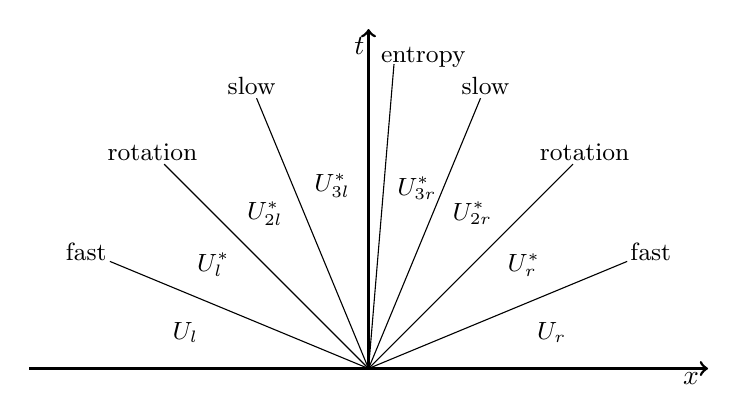
\begin{tikzpicture}[scale = {0.0125\linewidth},inner sep = 1pt]
%% \begin{tikzpicture}[scale = {0.015\linewidth},inner sep = 1pt]
%% \tikzstyle{every node} = [draw,circle,fill=gray!30];
%% \draw (-1.5,0.0) circle (0.8);
%% \draw[<->,line width=1pt] (0,1) node[right]{\;$t$}|-(1,0) node[below]{$m$};
\draw[line width=1pt] (0,0.95) node[left]{$t$}|-(0.95,0) node[below]{$x$};
\draw[->,line width=1pt] (0.95,0)--(1,0);
\draw[->,line width=1pt] (0,0.95)--(0,1);  
\draw[line width=1pt] (-0,0)--(-1,0);
\node[draw=white] (fr) at (0.83149,0.34442) {\small fast};
\node[draw=white] (rr) at (0.63640,0.63640) {\small rotation};
\node[draw=white] (sr) at (0.34442,0.83149) {\small slow};
%% \node[draw=white] (cd) at (0.17221,0.88337) {\small contact disc.};
\node[draw=white] (cd) at (0.16149,0.91587) {\small entropy};
\node[draw=white] (sl) at (-0.34442,0.83149) {\small slow};
\node[draw=white] (rl) at (-0.63640,0.63640) {\small rotation};
\node[draw=white] (fl) at (-0.83149,0.34442) {\small fast};

\node[draw=white] (R8a) at (0.53943,0.10730) {\small $\mbf{U}_{r}$};
\node[draw=white] (R7a) at (0.45731,0.30556) {\small $\mbf{U}^*_{r}$};
\node[draw=white] (R6a) at (0.30556,0.45731) {\small $\mbf{U}^*_{2r}$};
\node[draw=white] (R5a) at (0.14235,0.53126) {\small $\mbf{U}^*_{3r}$};
\node[draw=white] (R4a) at (-0.10730,0.53943) {\small $\mbf{U}^*_{3l}$};
\node[draw=white] (R3a) at (-0.30556,0.45731) {\small $\mbf{U}^*_{2l}$};
\node[draw=white] (R2a) at (-0.45731,0.30556) {\small $\mbf{U}^*_{l}$};
\node[draw=white] (R1a) at (-0.53943,0.10730) {\small $\mbf{U}_{l}$};

%% \node[] at (0.15,0.95) {contact};
\draw (0,0) -- (fr);  
\draw (0,0) -- (rr);  
\draw (0,0) -- (sr);  
\draw (0,0) -- (0.075,0.89678);  
\draw (0,0) -- (sl);  
\draw (0,0) -- (rl);  
\draw (0,0) -- (fl);  
\end{tikzpicture}

\end{center}
\caption{Seven possible waves and/or discontinuities separating the eight possible regions, or states of the ideal MHD Riemann problem.  The initial contact discontinuity, i.e., the entropy wave, separates regions $\mbf{U}^*_{3l}$ and $\mbf{U}^*_{3r}$.}
\label{fig:mhd_states}
\end{figure}

The exact solutions are composed of eight possible MHD states separated by seven wave fronts, as depicted in Figure \ref{fig:mhd_states}.  The transitions from one region to another through a discontinuity is controlled by the jump conditions associated with the discontinuity.  The Rankine-Hugoniot jump conditions for ideal MHD in Lagrangian mass coordinates, $dm = \rho dx$, are 
\begin{align} 
\label{eqn:jump1} W[V] &= -[v_n], \\ 
\label{eqn:jump2} W[v_n] &= -[P - B_n^2], \\
\label{eqn:jump3} W[\mbf{v}_{t}] &= -B_n[\mbf{B}_{t}], \\
%% \label{eqn:jump4} W[v_z] &= -B_x[B_z], \\
\label{eqn:jump5} W[V\mbf{B}_{t}] &= -B_n[\mbf{v}_{t}], \text{ and}\\
%% \label{eqn:jump6} W[VB_z] &= -B_x[v_z],   \\
\label{eqn:jump7} W[VE] &= [v_nP] - B_n[B_nv_n + \mbf{B}_{t}\cdot\mbf{v}_{t}],
\end{align}
where $P = p_g + \frac{1}{2}(B_n^2 + B_{t}^2)$ is the total pressure and $W = -(\rho v_n)_u = -(\rho v_n)_d$ is the Lagrangian velocity of the discontinuity and $V = 1/\rho$ \citep{Dai:1994a,Ryu:1995a}.  When moving in the $-x$ direction, the velocity $W$ is negative. Brackets are used to denote the difference between the upstream and downstream states for a quantity $Q$, i.e $[Q] = Q_u - Q_d$.  

\citet{Dai:1994a} give the fast and slow shock speeds in mass coordinates as
\begin{equation}
\label{eqn:speed_fs} W_{f,s}^2 = \frac{1}{2(1 + S_0)}\left[(C_s^2 + C_f^2 + S_1^2) \pm \sqrt{(C_s^2 + C_f^2 + S_1^2)^2 - 4(1 + S_0)(C_s^2C_f^2 - S_2)}\right],
\end{equation}
where $C_f = \rho c_f$ and $C_s = \rho c_s$.  The quantities $S_0, S_1, S_2$ are given by \citet{Ryu:1995a} in terms of $B_{t}$ as
\begin{align}
\label{eqn:speed_coef1} S_0 &= -\half (\gamma - 1)\frac{[B_{t}]}{B_{t}}, \\
\begin{split}
\label{eqn:speed_coef2} S_1 &= \half \left\{ -(\gamma - 2) V C_{t}^2 \frac{[B_{t}]}{B_{t}} + 2C_0^2 - (\gamma - 4) V C_{t}^2 \right. \\
& \;\;\;\; - \left. 2\gamma C_a^2 \vphantom{\frac{[B_{t}]}{B_{t}}} \right\} \frac{[B_{t}]}{B_{t}}\text{, and} 
\end{split} \\
\begin{split}
\label{eqn:speed_coef3} S_2 &= \half \left\{ \frac{C_a^2 [B_{t}]^2}{V} + (\gamma + 2)C_{t}C_a^2[B_{t}] + VC_{t}^2C_a^2(\gamma + 1) \right.\\
& \;\;\;\; + \left.(\gamma + 1)C_a^4  - 2C_0^2C_a^2 \vphantom{\frac{C_a^2 [B_{t}]^2}{V}}\right\} \frac{[B_{t}]}{B_{t}}, 
\end{split}
\end{align}
where $C_0 = \rho a$ is the Lagrangian speed of sound, $C_a = \rho c_a$ is the Lagrangian Alfv{\'e}n speed, and $C_{t} = \sqrt{\rho B_{t}^2}$.  The quantities in equations \eqref{eqn:speed_coef1}-\eqref{eqn:speed_coef3} are for the state downstream of the shock.

The relationships for fast rarefactions given by \citet{Ryu:1995a} are 
\begin{gather}
\label{eqn:rarefaction1} \dd{C_0}{B_{t}} = -\frac{\gamma + 1}{2} \sqrt{\rho} \frac{C_{t}C_s^2}{C_0(C_s^2 - C_a^2)} = \frac{\gamma + 1}{2} \sqrt{\rho} \frac{C_s^2(C_f^2 - C_a^2)}{C_a^2C_{t}C_0} = \frac{\gamma + 1}{2} \frac{\rho}{C_0} \dd{p_g}{B_{t}}, \\
\label{eqn:rarefaction2} \dd{v_n}{B_{t}} = \mp \frac{1}{\sqrt{\rho}} \frac{C_{\perp}C_a^2}{C_f(C_s^2 - C_a^2)} = \pm \frac{C_f^2 - C_a^2}{\sqrt{\rho} C_{t}C_f} = \pm\frac{2}{\gamma + 1} \frac{C_0C_a^2}{C_s^2C_f}\frac{1}{\rho} \dd{C_0}{B_{t}}\text{, and} \\
\label{eqn:rarefaction3} \frac{1}{\cos{\psi}} \dd{v_{t1}}{B_{t}} = \frac{1}{\sin{\psi}} \dd{v_{t2}}{B_{t}} = \mp \frac{1}{\sqrt{\rho}} \frac{C_a}{C_f},
\end{gather}
where the upper and lower signs refer to right- and left-going waves, respectively.  The rotation angle is defined by $\tan{\psi} = B_z/B_y$.

For slow rarefactions, replace the fast speed ($C_f$) with the slow speed ($C_s$) and the slow speed ($C_s$) with the fast speed ($C_f$) in Equations~\eqref{eqn:rarefaction1}-\eqref{eqn:rarefaction3}.  

An initial guess for the solution in the six interior regions shown in Figure~\ref{fig:mhd_states} is improved iteratively until the jump conditions of the initial contact or tangential discontinuity are satisfied to within a desired accuracy.  We have found a very high rate of convergence using the intermediate states approximated using the HLLD method for the initial guess. In practice, we use a relaxation factor and apply damping to speed up convergence. 

%-----------------------------------------------------------------
% HLLD approximate Riemann solver
%-----------------------------------------------------------------
\subsection[HLLD approximate Riemann solver]{HLLD approximate Riemann solver}
\label{sec:hlld}

%-----------------------------------------------------------------
% HLLD Riemann states
%-----------------------------------------------------------------
\begin{figure}[htbp]
\begin{center}
\tikzsetnextfilename{hlld_rstates}
%----------------------------------------------------------------------------------------
% hlld_rstates.tex
%----------------------------------------------------------------------------------------

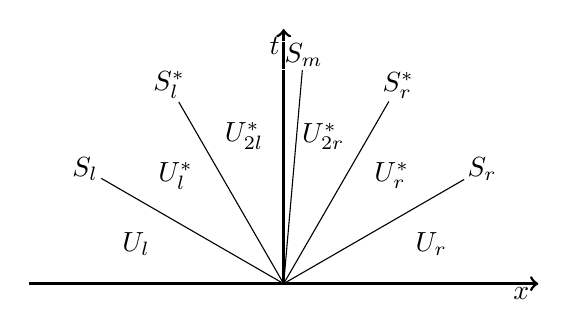
\begin{tikzpicture}[scale = {0.0125\linewidth},inner sep = 1pt]
%% \begin{tikzpicture}[scale = {0.015\linewidth},inner sep = 1pt]
%% \tikzstyle{every node} = [draw,circle,fill=gray!30];
%% \draw (-1.5,0.0) circle (0.8);
%% \draw[<->,line width=1pt] (0,1) node[right]{\;$t$}|-(1,0) node[below]{$m$};
\draw[line width=1pt] (0,0.7) node[left]{$t$}|-(0.7,0) node[below]{$x$};
\draw[->,line width=1pt] (0.7,0)--(0.75,0);
\draw[->,line width=1pt] (0,0.7)--(0,0.75);  
\draw[line width=1pt] (-0,0)--(-0.75,0);
\node[draw=white] (sr) at (0.58457,0.33750) {$S_r$};
\node[draw=white] (ssr) at (0.33750,0.58457) {$S^*_r$};
\node[draw=white] (cd) at (0.058830,0.67243) {$S_m$};
\node[draw=white] (ssl) at (-0.33750,0.58457) {$S^*_l$};
\node[draw=white] (sl) at (-0.58457,0.33750) {$S_l$};

\node[draw=white] (ur) at (0.43467,0.11647) {$\mbf{U}_{r}$};
\node[draw=white] (usl) at (0.31820,0.31820) {$\mbf{U}^*_{r}$};
\node[draw=white] (usr) at (0.11647,0.43467) {$\mbf{U}^*_{2r}$};
\node[draw=white] (usr) at (-0.11647,0.43467) {$\mbf{U}^*_{2l}$};
\node[draw=white] (usl) at (-0.31820,0.31820) {$\mbf{U}^*_{l}$};
\node[draw=white] (ul) at (-0.43467,0.11647) {$\mbf{U}_{l}$};

\draw (0,0) -- (sr);  
\draw (0,0) -- (ssr);  
\draw (0,0) -- (cd);  
\draw (0,0) -- (ssl);  
\draw (0,0) -- (sl);  

\end{tikzpicture}

\end{center}
\caption{Intermediate states and waves used in the HLLD approximate Riemann solver.}
\label{fig:hlld_rstates}
\end{figure}

An MHD extension of the HLLC scheme for the Euler equations (see Section~\ref{sec:hllc}) capable of resolving all isolated linear discontinuities of ideal MHD, i.e. RDs and CDs was developed by \citet{Miyoshi:2005}.  They referred to the scheme as HLLD, where the D stands for \emph{discontinuities}.  The HLLD scheme assumes a six-state solution separated by five waves as depicted in Figure~\ref{fig:hlld_rstates}.  Two nonlinear waves, i.e., shocks and rarefactions, separate the left and right initial states from the intermediate states in the Riemann fan, i.e., $\mbf{U}_{l}^*$, $\mbf{U}_{2l}^*$, $\mbf{U}_{2r}^*$, and $\mbf{U}_{r}^*$.  The four intermediate states are separated by two RDs with velocities, $S^*_l$, $S^*_r$, and one CD with velocity, $S_m$.  The one-dimensional wave speeds and intermediate states of \citep{Miyoshi:2005} have been modified for general coordinates, with $v_n = \mbf{v}\cdot\mbf{n}$, and $B_n = \mbf{B}\cdot\mbf{n}$, where  \mbf{n} is a normal vector with unit length.  

The velocity of the CD, $S_m$, is estimated with the HLL average given by \eqref{eqn:wave_spd_batten}, except gas pressure, $p_g$, is replaced with total pressure, $p_t$, and it becomes  
\begin{gather}
\label{eqn:hlld_sm}
S_m = \frac{(S_r - \vnr)\rho_r \vnr - (S_l - \vnl)\rho_l \vnl - p_{tr} + p_{tl} }
{(S_r - \vnr)\rho_r  - (S_l - \vnl)\rho_l}.
\end{gather}     
The intermediate states are approximated by solving the jump conditions across each wave.  Since the total pressure is conserved across the linear discontinuities in ideal MHD, the total pressure is constant throughout the Riemann fan.  It is given as 
\begin{gather}
\label{eqn:ptlr}
p_{t}^* = p_{tj}^* = p_{tj} + \rho_j (S_j - v_{nj})(S_m - v_{nj})
\end{gather}
for $j=l$ or $j=r$.  Substituting \eqref{eqn:hlld_sm} into \eqref{eqn:ptlr} and taking the averaging over the left and right states yields the explicit expression for total pressure throughout the Riemann fan:
\begin{gather}
\label{eqn:hlld_pt1}
p^*_{t} = \frac{(S_r - \vnr)\rho_r p_{tl} - (S_l - \vnl)\rho_l p_{tr} 
          + \rho_r\rho_l(S_r - \vnr)(S_l - \vnl)(\vnr - \vnl)}{(S_r - \vnr)\rho_r - (S_l - \vnl)\rho_l}.
\end{gather} 
 The states downstream of the fast waves, $\mbf{U}^*_j$ for $j=l$ and $j=r$ of Figure~\ref{fig:hlld_rstates}, are given in one-dimension by Eqs (41)-(47) of \citep{Miyoshi:2005}, written for general coordinates: they are
\begin{gather}
\label{eqn:hlld_d1}
\rho^*_j = \rho_j \frac{S_j - v_{nj}}{S_j - S_m} , \\
\label{eqn:hlld_v1}
\mbf{v}^*_{j} = \mbf{v}_{j} + \frac{\left(S_j - S_m\right)\left(p_{t}^* - p_{tj}\right)\mbf{n} 
  - B_n\mbf{B}_{j} \left(S_m - v_{nj}\right) }
               {\rho_j(S_j - v_{nj})(S_j - S_m) - B_n^2} , \\
\label{eqn:hlld_b1}
\mbf{B}^*_{j} = \frac{\mbf{B}_{j} \left(\rho_j(S_j - v_{nj})^2 - B_n^2\right) 
  - B_n\left(p_{t}^* - p_{tj}\right)\mbf{n}}
                {\rho_j(S_j - v_{nj})(S_j - S_m) - B_n^2} , \\
\label{eqn:hlld_en1}
E^*_j = \frac{(S_j - v_{nj})E_j - p_{tj}v_{nj} + p^*_{t}S_m + B_n(\mbf{v}_{j}\cdot\mbf{B}_{j} 
        - \mbf{v}^*_{j}\cdot\mbf{B}^*_{j})}{S_j - S_m} .
\end{gather}
If $\mbf{n} = (1,0,0)$, $v_x = S_m$, $B_x = B_n$, \eqref{eqn:hlld_v1} and \eqref{eqn:hlld_b1} reduce to (44)-(47) of \citep{Miyoshi:2005}, given as  
\begin{gather*}
v^*_{yj} = v_{yj} -B_x B_{yj} \frac{S_m - v_{nj} }
               {\rho_j(S_j - v_{nj})(S_j - S_m) - B_x^2} , \\
v^*_{zj} = v_{zj} - B_x B_{zj} \frac{S_m - v_{nj} }
               {\rho_j(S_j - v_{nj})(S_j - S_m) - B_x^2} , \\
B^*_{yj} = B_{yj} \frac{\rho_j(S_j - v_{nj})^2 - B_x^2} 
                {\rho_j(S_j - v_{nj})(S_j - S_m) - B_x^2} , \text{ and }\\
B^*_{zj} = B_{zj} \frac{ \rho_j(S_j - v_{nj})^2 - B_x^2} 
                {\rho_j(S_j - v_{nj})(S_j - S_m) - B_x^2}. 
\end{gather*}

The states downstream of the rotational discontinuity, $\mbf{U}^*_{2j}$, of Figure~\ref{fig:hlld_rstates}, can be found in terms of the initial left state and $\mbf{U}^*_j$.  The density, normal velocity, and total pressure are 
\begin{gather}
\label{eqn:hlld_d2}
\rho^*_{2j} = \rho^*_j , \\
\label{eqn:hlld_vn2}
v^*_{n2j} = v^*_{nj} , \\
\label{eqn:hlld_pt2}
p^*_{t2j} = p^*_{tj} ,
\end{gather}
because they are constant across the rotational discontinuity.  The Alfv{\'e}n speeds of the left and right rotational discontinuities are    
\begin{gather}
\label{eqn:hlld_rd_spd}
S^*_l = S_l - \frac{|B_n|}{\sqrt{\rho^*_l}} \text{ and}\;\;\;\; S^*_r = S_r + \frac{|B_n|}{\sqrt{\rho^*_r}}. 
\end{gather}
The description of the HLLD intermediate states is completed by solving for $\mbf{v}^*_{m} = \mbf{v}^*_{2l} = \mbf{v}^*_{2r}$ and $\mbf{B}^*_{m} = \mbf{B}^*_{2l} = \mbf{B}^*_{2r}$.  This is done using the integral conversation law over the Riemann fan $(S_l \delta t, S_r \delta t) \times (0, \delta t)$ (Eq. (58) of \citep{Miyoshi:2005}).  They are given as  
\begin{gather}
\label{eqn:hlld_vt2}
\mbf{v}^*_{m} = \frac{\sqrt{\rho^*_l}\vnl^* + \sqrt{\rho^*_r}\vnr^* + (\mbf{B}_r^* - \mbf{B}_l^*)\text{sign}(B_n)}
                {\sqrt{\rho^*_l} + \sqrt{\rho^*_r}} , \\               
\label{eqn:hlld_bt2}
\mbf{B}^*_{m} = = \frac{\sqrt{\rho^*_l}\mbf{B}_r^* + \sqrt{\rho^*_r}\mbf{B}_l^* 
                + \sqrt{\rho^*_l\rho^*_r}(\mbf{v}_r^* - \mbf{v}_l^*)\text{sign}(B_n)}
                {\sqrt{\rho^*_l} + \sqrt{\rho^*_r}} \text{, and}\\               
\label{eqn:hlld_en2}
E^*_{2j} = E^*_j \mp  \sqrt{\rho^*_j}(\mbf{v}^*_{j}\cdot\mbf{B}^*_{j} 
        - \mbf{v}^*_{2j}\cdot\mbf{B}^*_{2j})\text{sign}(B_n) ,
\end{gather}
where the minus (plus) sign corresponds to $j=l$ ($j=r$).  The HLLD fluxes are found by applying the integral conservation laws over the left half or right half of the Riemann fan, $(S_l\delta t, 0)\times (0,\delta t)$ or $(0,S_r\delta t)\times (0,\delta t)$, see Appendix~\ref{app:hll_flux}.  The fluxes are given as
\begin{gather}
\label{eqn:hlld_flux}
\mbf{F}(x,t) = 
\begin{cases}
\mbf{F}_l   \phantom{= \mbf{F}_l  + S_l (\mbf{U_l^*} - \mbf{U_l}} & \text{if}\;\;\; 0 < S_l, \\
\mbf{F}_l^* = \mbf{F}_l  + S_l (\mbf{U}_l^* - \mbf{U}_l) & \text{if}\;\;\; S_l \le 0 \le S^*_l, \\
\mbf{F}_{2l}^* = \mbf{F}^*_l  + S^*_l (\mbf{U}_{2l}^* - \mbf{U}^*_l) & \text{if}\;\;\; S^*_l \le 0 \le S_m, \\
\mbf{F}_{2r}^* = \mbf{F}^*_r  + S^*_r (\mbf{U}_{2r}^* - \mbf{U}^*_r)  & \text{if}\;\;\; S_m \le 0 \le S^*_r, \\
\mbf{F}_r^* = \mbf{F}_r  + S_r (\mbf{U}_r^* - \mbf{U}_r)  & \text{if}\;\;\; S^*_r \le 0 \le S_r, \\
\mbf{F}_r  \phantom{= \mbf{F}_r  + S_r (\mbf{U_r^*} - \mbf{U_r}} & \text{if}\;\;\; S_r < 0. \\
\end{cases}
\end{gather}

The HLLD method is robust because it is positivity preserving and it is less computationally expensive than schemes such as Roe's that require eigenvalue decomposition.  Results from MHD shock tube problems solved using the HLLD fluxes are given in Sections~\ref{sec:riemann_mhd}-\ref{sec:nonuniform_converge}.  However, scheme produces compound waves for coplanar and near coplanar cases as demonstrated in Sections~\ref{sec:riemann_mhd}-\ref{sec:nonuniform_converge}, an issue all approximate Riemann solvers suffer from.  In Chapter \ref{chp:cwm}, a modification to the HLLD fluxes that removes compound waves from the solution to coplanar and near coplanar Riemann problems of ideal is described.  

%
% $Id: chapterThree.tex
%

% A first, optional argument in [ ] is the title as displayed in the table of contents
% The second argument is the title as displayed here.  Use \\ as appropriate in
%   this title to get desired line breaks

%----------------------------------------------------------------------------------------
% Numerical solutions for ideal magnetohydrodynamics
%----------------------------------------------------------------------------------------
\chapter[Numerical solutions for ideal magnetohydrodynamics]{Numerical solutions for Ideal magnetohydrodynamics}
\label{chp:num_mhd}

Riemann problems and the different waves that compose the solution were described in Chapter~\ref{chp:riemann}.  The linear and nonlinear waves emitted by the equations of ideal MHD were described.  The linear waves are: the entropy wave that carries a CD and the Alfv{\'e}n wave that carries an RD.  The nonlinear waves are: shocks and rarefactions.  

This chapter applies the ideas developed in Chapter~\ref{chp:riemann} and numerically solves Riemann problems of ideal MHD. The finite volume discretization and Godunov's method for computing interface fluxes and  the structure of the solution to the non-planar case are then described.  The jumps in $\rho$ and $\mbf{B}_t$ associated with each wave of the non-planar case is discussed.  Then the nonlinear solver developed for this dissertation is described.  The exact and approximate solution of non-planar and coplanar test cases are given to demonstrate the accuracy of the solvers.  The nonlinear solver is then used to provide new benchmarks that can be used for the development of ideal MHD codes.  

We show a limitation of FV schemes for ideal MHD, which is the appearance of non-regular waves.  The physicality of these waves has been debated.  We confirm the appearance of non-regular waves in terms of Riemann problems with non-unique solutions.  Non-uniqueness is shown to occur when the initial transverse magnetic fields are coplanar, i.e. anti-parallel.  For initial conditions near those that produce a non-unique solution, convergence is shown to be nonuniform consistent with \citep{Torrilhon:2003b}.  Initially, convergence is to the solution containing a non-regular wave; after heavy grid refinement, convergence is to the solution containing only regular waves.  In Chapter~\ref{chp:cwm}, we propose a new modification to the HLLD flux that converges to the solution containing regular waves at all grid resolutions.   

%----------------------------------------------------------------------------------------
% Finite volume discretization and Godunov's method
%----------------------------------------------------------------------------------------
\section[Finite volume discretization and Godunov's method]{Finite volume discretization and Godunov's method}
\label{sec:fvm_mhd}

For the cell-centered \gls{fv} discretization, the state is defined by the integral average of the cell, given as
\begin{gather}
\label{eqn:fv_state}
\mbf{U}_{\text{cell}} = \frac{1}{V_{\text{cell}}} \int_{\Omega} \mbf{U} d\Omega,
\end{gather}
where $V_{cell}$ is the volume of the cell.  The volume integral of the fluxes can be rewritten using the divergence theorem as
\begin{gather}
\label{eqn:fv_flux}
\int_{\Omega} \divergebf{F} d \Omega = \int_{\Gamma} \mbf{F} \cdot \mbf{n} d\Gamma,
\end{gather}
where $\mbf{n}$ is the unit normal vector.  Integration in time, from $t=n$ to $t = n+1$, gives the FV discretization as
\begin{gather}
\label{eqn:fvm}
\mbf{U}^{n+1}_{\text{cell}} = \mbf{U}^n_{\text{cell}} - \frac{\delta t}{V_{\text{cell}}}\sum_{\text{faces}} \mbf{F}\cdot \mbf{s},
\end{gather}
where $\mbf{F} = \frac{1}{\delta t} \int_{\delta t} \mbf{F} dt$ is the time averaged fluxes, $\mbf{s} = A\mbf{n}$ is the scaled face normal, and $A$ is the face area.  The one-dimensional FV discretization for a cell center at $i$ is
\begin{gather}
\label{eqn:fvm1d}
\mbf{U}^{n+1}_{i} = \mbf{U}^n_{i} - \frac{\delta t}{\delta x}\left(\mbf{F}^n_{i+1/2} - \mbf{F}_{i-1/2}^n \right),
\end{gather}
where $\delta x = x_{i+1} - x_{i}$.  The timestep $\delta t$ must satisfy \gls{clf} stability condition that a wave cannot transverse more than one cell per timestep.  An estimation for the timestep is given by
\begin{gather}
\label{time_clf}
\delta t = C_r \delta x/\lambda_{\max},
\end{gather}
where $C_r \le 1$ is the Courant number.  In explicit schemes, $C_r \le 1$ is typically required.

The flux can be evaluated in a variety of ways.  The Rusanov flux, given as
\begin{gather}
\label{eqn:rusanov}
\mbf{F}_{i+1/2} = \half\left(\phantom{\frac{}{}}\mbf{F}\left(\mbf{U}_{i+1}\right) + \mbf{F}\left(\mbf{U}_{i}\right)
            - |\lambda_{\max}|\left(\mbf{U}_{i+1} - \mbf{U}_{i} \right) \right)
\end{gather}
where $\lambda_{max}$ is the maximum wave speed, is a stable and efficient method for flux evaluation.  It simplifies Roe's method by substituting $|\lambda_{max}| = \max\{|\lambda_k|\}$, where $k$ corresponds to the characteristics of the solution, because the wave speed can then be factored out the last term on the right hand side of \eqref{eqn:roe_flux}.  The summation reduces to $\mbf{U}_{i+1} - \mbf{U}_{i}$, since $\mbf{l}_k\cdot\mbf{r}^l = \delta_{k,l}$ where $\delta_{k,l}$ is the Kronecker delta.  The Rusanov flux produces a more diffuse solution than Roe's flux, especially at linear discontinuities where the maximum wave speed is greater than the characteristic speed of the wave.  As discussed in Section~\ref{sec:higher_order}, the properties of the Rusanov flux are desirable for a low-order scheme when used in conjunction with FCT.  

%-----------------------------------------------------------------
% Interface states
%-----------------------------------------------------------------
\begin{figure}[htbp]
\begin{center}
\tikzsetnextfilename{interface_states}
%-----------------------------------------------------------------
% interface_states.tex
%-----------------------------------------------------------------
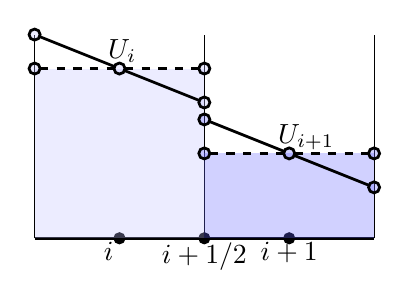
\begin{tikzpicture}[scale = {0.0125\linewidth},
                    inner sep = 1pt,
                    base node/.style={circle,draw,minimum size=4pt}]


% discontinuity
%% \draw[dashed,line width=1pt] (0,0) node[below]{$x_d$} -- (0,0.4); 
%% \draw[-latex,thick](0.05,0.45)node[right]{\small initial discontinuity}
%%          to[out=180,in=90] (0,0.4);

\draw[line width=1pt] (-0.5,0)  -- (-0.25,0) node[below]{$i\phantom{+}$} 
      -- (0,0) node[below]{$i+1/2$}
      -- (0.25,0) node[below]{$i+1$} -- (0.5,0); 

\node[base node,fill=black] at (-0.25,0) {};
\node[base node,fill=black] at (0,0) {};
\node[base node,fill=black] at (0.25,0) {};

\node[shape=circle,fill=black] at (-0.25,0) {};

\draw[] (-0.5,0) -- (-0.5,0.6); 
\draw[] (0,0) -- (0,0.6); 
\draw[] (0.5,0) -- (0.5,0.6); 

% initial states
\fill[blue!25!,opacity=.3] (-0.5,0) rectangle (0,0.5);
\fill[blue!60!,opacity=.3] (0,0) rectangle (0.5,0.25);

\node[base node,fill = blue!25!,opacity=.3] at (-0.5,0.5) {};
\node[base node,line width=1pt] at (-0.5,0.5) {};

\node[base node,fill = blue!25!,opacity=.3] at (-0.25,0.5) {};
\node[base node,line width=1pt] at (-0.25,0.5) {};

\node[base node,fill = blue!25!,opacity=.3] at (0,0.5) {};
\node[base node,line width=1pt] at (0,0.5) {};

\node[base node,fill = blue!60!,opacity=.3] at (0,0.25) {};
\node[base node,line width=1pt] at (0,0.25) {};

\node[base node,fill = blue!60!,opacity=.3] at (0.25,0.25) {};
\node[base node,line width=1pt] at (0.25,0.25) {};

\node[base node,fill = blue!60!,opacity=.3] at (0.5,0.25) {};
\node[base node,line width=1pt] at (0.5,0.25) {};

\draw[dashed,line width=1pt,shorten >= 2 pt, shorten <= 2pt] (-0.5,0.5) -- (-0.25,0.5); 
\draw[dashed,line width=1pt,shorten >= 2 pt, shorten <= 2pt] (-0.25,0.5)  -- (0,0.5); 
\node[above] at (-0.2,0.5) {$\mbf{U}_{i\phantom{-1}}$};

\draw[dashed,line width=1pt,shorten >= 2 pt, shorten <= 2pt] (0,0.25) -- (0.25,0.25); 
\draw[dashed,line width=1pt,shorten >= 2 pt, shorten <= 2pt] (0.25,0.25)  -- (0.5,0.25); 
\node[above] at (0.3,0.25) {$\mbf{U}_{i+1}$};

\draw[line width=1pt,shorten >= 2 pt, shorten <= 2pt] (-0.5,0.6)  -- (-0.25,0.5); 
\draw[line width=1pt,shorten >= 2 pt, shorten <= 2pt] (-0.25,0.5)  -- (0,0.4); 
\node[base node,fill = blue!25!,opacity=.3] at (-0.5,0.6) {};
\node[base node,line width=1pt] at (-0.5,0.6) {};

\node[base node,fill = blue!25!,opacity=.3] at (0,0.4) {};
\node[base node,line width=1pt] at (0,0.4) {};

\draw[line width=1pt,shorten >= 2 pt, shorten <= 2pt] (0,0.35)  -- (0.25,0.25); 
\draw[line width=1pt,shorten >= 2 pt, shorten <= 2pt] (0.25,0.25)  -- (0.5,0.15); 
\node[base node,fill = blue!60!,opacity=.3] at (0,0.35) {};
\node[base node,line width=1pt] at (0,0.35) {};

\node[base node,fill = blue!60!,opacity=.3] at (0.5,0.15) {};
\node[base node,line width=1pt] at (0.5,0.15) {};

% normal
%% \draw[-stealth,thick] (0,0.2) -- (0.1,0.2); 
%% \node[] at (0.05,0.23) {$\hat{n}$};

\end{tikzpicture}

\end{center}
\caption{Piecewise constant (dotted line) and piecewise linear (solid line) reconstruction of interface states that define the local Riemann problem for Godunov's method.}
\label{fig:interface}
\end{figure}

Godunov's method uses the solution to a local Riemann problem at cell interfaces to calculate the time-averaged fluxes.  The local Riemann problem is defined by reconstructing the states of neighboring cells at the interface between the cells.  The reconstruction process using piecewise constant and piecewise linear interpolation is shown in Figure~\ref{fig:interface}.  Slope limiters, see Section~\ref{sec:higher_order}, are used during reconstruction to ensure new extrema are not created.  If the flow is not smooth, such as across a shock or discontinuity, the reconstructed states will not be equal, and a local Riemann problem at the interface is defined.  The approximate solution of to the local Riemann problem is used to calculate the time-averaged fluxes.  For the Euler equations, one of the schemes described in Section~\ref{sec:hydro_approx_rsolvers} can be used to approximate the fluxes.  For ideal MHD, the fluxes can be approximated with the HLLD scheme described in Section~\ref{sec:hlld}.  

%----------------------------------------------------------------------------------------
% Higher-order extensions
%----------------------------------------------------------------------------------------
\section[Higher-order extensions]{Higher-order extensions}
\label{sec:higher_order}

In this section, two high-order extensions to first-order monotonicity preserving schemes are described. In Section~\ref{sec:riemann_mhd} one-dimensional Riemann problems are solved using both higher order extension.  The first higher order extension is implemented in Athena.  It is a \gls{tvd} scheme, and uses the third order accurate \gls{ppm} \citep{Colella:1984} for reconstruction of the interface states.  The second is an \gls{fct} scheme, that was implemented for this dissertation available at: \protect\gitrepo.

%-----------------------------------------------------------------
% Sod shock tube HLLE, HLLC, Roe
%-----------------------------------------------------------------
\begin{figure}[htbp]
\begin{tabular}{ccc}
\resizebox{0.33\linewidth}{!}{\tikzsetnextfilename{sod_hlle_3_1}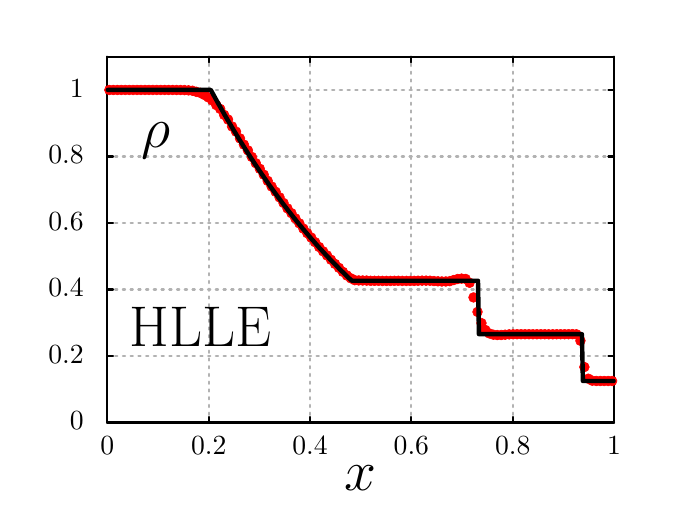
\begin{tikzpicture}[gnuplot]
%% generated with GNUPLOT 4.6p4 (Lua 5.1; terminal rev. 99, script rev. 100)
%% Thu 31 Jul 2014 02:05:23 PM EDT
\path (0.000,0.000) rectangle (8.000,6.000);
\gpfill{rgb color={1.000,1.000,1.000}} (1.012,0.985)--(7.446,0.985)--(7.446,5.630)--(1.012,5.630)--cycle;
\gpcolor{color=gp lt color border}
\gpsetlinetype{gp lt border}
\gpsetlinewidth{1.00}
\draw[gp path] (1.012,0.985)--(1.012,5.630)--(7.446,5.630)--(7.446,0.985)--cycle;
\gpcolor{color=gp lt color axes}
\gpsetlinetype{gp lt axes}
\gpsetlinewidth{2.00}
\draw[gp path] (1.012,0.985)--(7.447,0.985);
\gpcolor{color=gp lt color border}
\gpsetlinetype{gp lt border}
\draw[gp path] (1.012,0.985)--(1.084,0.985);
\draw[gp path] (7.447,0.985)--(7.375,0.985);
\gpcolor{rgb color={0.000,0.000,0.000}}
\node[gp node right,font={\fontsize{10pt}{12pt}\selectfont}] at (0.828,0.985) {0};
\gpcolor{color=gp lt color axes}
\gpsetlinetype{gp lt axes}
\draw[gp path] (1.012,1.830)--(7.447,1.830);
\gpcolor{color=gp lt color border}
\gpsetlinetype{gp lt border}
\draw[gp path] (1.012,1.830)--(1.084,1.830);
\draw[gp path] (7.447,1.830)--(7.375,1.830);
\gpcolor{rgb color={0.000,0.000,0.000}}
\node[gp node right,font={\fontsize{10pt}{12pt}\selectfont}] at (0.828,1.830) {0.2};
\gpcolor{color=gp lt color axes}
\gpsetlinetype{gp lt axes}
\draw[gp path] (1.012,2.674)--(7.447,2.674);
\gpcolor{color=gp lt color border}
\gpsetlinetype{gp lt border}
\draw[gp path] (1.012,2.674)--(1.084,2.674);
\draw[gp path] (7.447,2.674)--(7.375,2.674);
\gpcolor{rgb color={0.000,0.000,0.000}}
\node[gp node right,font={\fontsize{10pt}{12pt}\selectfont}] at (0.828,2.674) {0.4};
\gpcolor{color=gp lt color axes}
\gpsetlinetype{gp lt axes}
\draw[gp path] (1.012,3.519)--(7.447,3.519);
\gpcolor{color=gp lt color border}
\gpsetlinetype{gp lt border}
\draw[gp path] (1.012,3.519)--(1.084,3.519);
\draw[gp path] (7.447,3.519)--(7.375,3.519);
\gpcolor{rgb color={0.000,0.000,0.000}}
\node[gp node right,font={\fontsize{10pt}{12pt}\selectfont}] at (0.828,3.519) {0.6};
\gpcolor{color=gp lt color axes}
\gpsetlinetype{gp lt axes}
\draw[gp path] (1.012,4.364)--(7.447,4.364);
\gpcolor{color=gp lt color border}
\gpsetlinetype{gp lt border}
\draw[gp path] (1.012,4.364)--(1.084,4.364);
\draw[gp path] (7.447,4.364)--(7.375,4.364);
\gpcolor{rgb color={0.000,0.000,0.000}}
\node[gp node right,font={\fontsize{10pt}{12pt}\selectfont}] at (0.828,4.364) {0.8};
\gpcolor{color=gp lt color axes}
\gpsetlinetype{gp lt axes}
\draw[gp path] (1.012,5.209)--(7.447,5.209);
\gpcolor{color=gp lt color border}
\gpsetlinetype{gp lt border}
\draw[gp path] (1.012,5.209)--(1.084,5.209);
\draw[gp path] (7.447,5.209)--(7.375,5.209);
\gpcolor{rgb color={0.000,0.000,0.000}}
\node[gp node right,font={\fontsize{10pt}{12pt}\selectfont}] at (0.828,5.209) {1};
\gpcolor{color=gp lt color axes}
\gpsetlinetype{gp lt axes}
\draw[gp path] (1.012,0.985)--(1.012,5.631);
\gpcolor{color=gp lt color border}
\gpsetlinetype{gp lt border}
\draw[gp path] (1.012,0.985)--(1.012,1.057);
\draw[gp path] (1.012,5.631)--(1.012,5.559);
\gpcolor{rgb color={0.000,0.000,0.000}}
\node[gp node center,font={\fontsize{10pt}{12pt}\selectfont}] at (1.012,0.677) {0};
\gpcolor{color=gp lt color axes}
\gpsetlinetype{gp lt axes}
\draw[gp path] (2.299,0.985)--(2.299,5.631);
\gpcolor{color=gp lt color border}
\gpsetlinetype{gp lt border}
\draw[gp path] (2.299,0.985)--(2.299,1.057);
\draw[gp path] (2.299,5.631)--(2.299,5.559);
\gpcolor{rgb color={0.000,0.000,0.000}}
\node[gp node center,font={\fontsize{10pt}{12pt}\selectfont}] at (2.299,0.677) {0.2};
\gpcolor{color=gp lt color axes}
\gpsetlinetype{gp lt axes}
\draw[gp path] (3.586,0.985)--(3.586,5.631);
\gpcolor{color=gp lt color border}
\gpsetlinetype{gp lt border}
\draw[gp path] (3.586,0.985)--(3.586,1.057);
\draw[gp path] (3.586,5.631)--(3.586,5.559);
\gpcolor{rgb color={0.000,0.000,0.000}}
\node[gp node center,font={\fontsize{10pt}{12pt}\selectfont}] at (3.586,0.677) {0.4};
\gpcolor{color=gp lt color axes}
\gpsetlinetype{gp lt axes}
\draw[gp path] (4.873,0.985)--(4.873,5.631);
\gpcolor{color=gp lt color border}
\gpsetlinetype{gp lt border}
\draw[gp path] (4.873,0.985)--(4.873,1.057);
\draw[gp path] (4.873,5.631)--(4.873,5.559);
\gpcolor{rgb color={0.000,0.000,0.000}}
\node[gp node center,font={\fontsize{10pt}{12pt}\selectfont}] at (4.873,0.677) {0.6};
\gpcolor{color=gp lt color axes}
\gpsetlinetype{gp lt axes}
\draw[gp path] (6.160,0.985)--(6.160,5.631);
\gpcolor{color=gp lt color border}
\gpsetlinetype{gp lt border}
\draw[gp path] (6.160,0.985)--(6.160,1.057);
\draw[gp path] (6.160,5.631)--(6.160,5.559);
\gpcolor{rgb color={0.000,0.000,0.000}}
\node[gp node center,font={\fontsize{10pt}{12pt}\selectfont}] at (6.160,0.677) {0.8};
\gpcolor{color=gp lt color axes}
\gpsetlinetype{gp lt axes}
\draw[gp path] (7.447,0.985)--(7.447,5.631);
\gpcolor{color=gp lt color border}
\gpsetlinetype{gp lt border}
\draw[gp path] (7.447,0.985)--(7.447,1.057);
\draw[gp path] (7.447,5.631)--(7.447,5.559);
\gpcolor{rgb color={0.000,0.000,0.000}}
\node[gp node center,font={\fontsize{10pt}{12pt}\selectfont}] at (7.447,0.677) {1};
\gpcolor{color=gp lt color border}
\draw[gp path] (1.012,5.631)--(1.012,0.985)--(7.447,0.985)--(7.447,5.631)--cycle;
\gpcolor{rgb color={0.000,0.000,0.000}}
\node[gp node center,font={\fontsize{10pt}{12pt}\selectfont}] at (4.229,0.215) {\huge $x$};
\gpcolor{rgb color={1.000,0.000,0.000}}
\gpsetlinewidth{0.50}
\gpsetpointsize{4.44}
\gppoint{gp mark 7}{(1.037,5.209)}
\gppoint{gp mark 7}{(1.087,5.209)}
\gppoint{gp mark 7}{(1.138,5.209)}
\gppoint{gp mark 7}{(1.188,5.209)}
\gppoint{gp mark 7}{(1.238,5.209)}
\gppoint{gp mark 7}{(1.289,5.209)}
\gppoint{gp mark 7}{(1.339,5.209)}
\gppoint{gp mark 7}{(1.389,5.209)}
\gppoint{gp mark 7}{(1.439,5.209)}
\gppoint{gp mark 7}{(1.490,5.209)}
\gppoint{gp mark 7}{(1.540,5.209)}
\gppoint{gp mark 7}{(1.590,5.209)}
\gppoint{gp mark 7}{(1.640,5.209)}
\gppoint{gp mark 7}{(1.691,5.209)}
\gppoint{gp mark 7}{(1.741,5.209)}
\gppoint{gp mark 7}{(1.791,5.209)}
\gppoint{gp mark 7}{(1.842,5.209)}
\gppoint{gp mark 7}{(1.892,5.208)}
\gppoint{gp mark 7}{(1.942,5.208)}
\gppoint{gp mark 7}{(1.992,5.207)}
\gppoint{gp mark 7}{(2.043,5.204)}
\gppoint{gp mark 7}{(2.093,5.199)}
\gppoint{gp mark 7}{(2.143,5.185)}
\gppoint{gp mark 7}{(2.193,5.172)}
\gppoint{gp mark 7}{(2.244,5.146)}
\gppoint{gp mark 7}{(2.294,5.115)}
\gppoint{gp mark 7}{(2.344,5.076)}
\gppoint{gp mark 7}{(2.395,5.017)}
\gppoint{gp mark 7}{(2.445,4.968)}
\gppoint{gp mark 7}{(2.495,4.892)}
\gppoint{gp mark 7}{(2.545,4.833)}
\gppoint{gp mark 7}{(2.596,4.745)}
\gppoint{gp mark 7}{(2.646,4.680)}
\gppoint{gp mark 7}{(2.696,4.594)}
\gppoint{gp mark 7}{(2.746,4.515)}
\gppoint{gp mark 7}{(2.797,4.442)}
\gppoint{gp mark 7}{(2.847,4.358)}
\gppoint{gp mark 7}{(2.897,4.279)}
\gppoint{gp mark 7}{(2.948,4.208)}
\gppoint{gp mark 7}{(2.998,4.133)}
\gppoint{gp mark 7}{(3.048,4.055)}
\gppoint{gp mark 7}{(3.098,3.983)}
\gppoint{gp mark 7}{(3.149,3.916)}
\gppoint{gp mark 7}{(3.199,3.845)}
\gppoint{gp mark 7}{(3.249,3.774)}
\gppoint{gp mark 7}{(3.299,3.705)}
\gppoint{gp mark 7}{(3.350,3.644)}
\gppoint{gp mark 7}{(3.400,3.578)}
\gppoint{gp mark 7}{(3.450,3.515)}
\gppoint{gp mark 7}{(3.501,3.448)}
\gppoint{gp mark 7}{(3.551,3.390)}
\gppoint{gp mark 7}{(3.601,3.334)}
\gppoint{gp mark 7}{(3.651,3.275)}
\gppoint{gp mark 7}{(3.702,3.214)}
\gppoint{gp mark 7}{(3.752,3.159)}
\gppoint{gp mark 7}{(3.802,3.107)}
\gppoint{gp mark 7}{(3.852,3.053)}
\gppoint{gp mark 7}{(3.903,3.000)}
\gppoint{gp mark 7}{(3.953,2.950)}
\gppoint{gp mark 7}{(4.003,2.899)}
\gppoint{gp mark 7}{(4.054,2.853)}
\gppoint{gp mark 7}{(4.104,2.817)}
\gppoint{gp mark 7}{(4.154,2.793)}
\gppoint{gp mark 7}{(4.204,2.790)}
\gppoint{gp mark 7}{(4.255,2.789)}
\gppoint{gp mark 7}{(4.305,2.788)}
\gppoint{gp mark 7}{(4.355,2.785)}
\gppoint{gp mark 7}{(4.405,2.785)}
\gppoint{gp mark 7}{(4.456,2.785)}
\gppoint{gp mark 7}{(4.506,2.784)}
\gppoint{gp mark 7}{(4.556,2.784)}
\gppoint{gp mark 7}{(4.607,2.784)}
\gppoint{gp mark 7}{(4.657,2.785)}
\gppoint{gp mark 7}{(4.707,2.785)}
\gppoint{gp mark 7}{(4.757,2.784)}
\gppoint{gp mark 7}{(4.808,2.784)}
\gppoint{gp mark 7}{(4.858,2.784)}
\gppoint{gp mark 7}{(4.908,2.784)}
\gppoint{gp mark 7}{(4.958,2.786)}
\gppoint{gp mark 7}{(5.009,2.787)}
\gppoint{gp mark 7}{(5.059,2.787)}
\gppoint{gp mark 7}{(5.109,2.786)}
\gppoint{gp mark 7}{(5.160,2.782)}
\gppoint{gp mark 7}{(5.210,2.779)}
\gppoint{gp mark 7}{(5.260,2.777)}
\gppoint{gp mark 7}{(5.310,2.777)}
\gppoint{gp mark 7}{(5.361,2.781)}
\gppoint{gp mark 7}{(5.411,2.795)}
\gppoint{gp mark 7}{(5.461,2.808)}
\gppoint{gp mark 7}{(5.511,2.813)}
\gppoint{gp mark 7}{(5.562,2.809)}
\gppoint{gp mark 7}{(5.612,2.760)}
\gppoint{gp mark 7}{(5.662,2.574)}
\gppoint{gp mark 7}{(5.713,2.390)}
\gppoint{gp mark 7}{(5.763,2.248)}
\gppoint{gp mark 7}{(5.813,2.160)}
\gppoint{gp mark 7}{(5.863,2.117)}
\gppoint{gp mark 7}{(5.914,2.101)}
\gppoint{gp mark 7}{(5.964,2.096)}
\gppoint{gp mark 7}{(6.014,2.097)}
\gppoint{gp mark 7}{(6.064,2.101)}
\gppoint{gp mark 7}{(6.115,2.105)}
\gppoint{gp mark 7}{(6.165,2.106)}
\gppoint{gp mark 7}{(6.215,2.107)}
\gppoint{gp mark 7}{(6.266,2.107)}
\gppoint{gp mark 7}{(6.316,2.107)}
\gppoint{gp mark 7}{(6.366,2.107)}
\gppoint{gp mark 7}{(6.416,2.107)}
\gppoint{gp mark 7}{(6.467,2.107)}
\gppoint{gp mark 7}{(6.517,2.107)}
\gppoint{gp mark 7}{(6.567,2.107)}
\gppoint{gp mark 7}{(6.617,2.106)}
\gppoint{gp mark 7}{(6.668,2.106)}
\gppoint{gp mark 7}{(6.718,2.107)}
\gppoint{gp mark 7}{(6.768,2.107)}
\gppoint{gp mark 7}{(6.819,2.107)}
\gppoint{gp mark 7}{(6.869,2.107)}
\gppoint{gp mark 7}{(6.919,2.108)}
\gppoint{gp mark 7}{(6.969,2.106)}
\gppoint{gp mark 7}{(7.020,2.024)}
\gppoint{gp mark 7}{(7.070,1.690)}
\gppoint{gp mark 7}{(7.120,1.542)}
\gppoint{gp mark 7}{(7.170,1.517)}
\gppoint{gp mark 7}{(7.221,1.513)}
\gppoint{gp mark 7}{(7.271,1.513)}
\gppoint{gp mark 7}{(7.321,1.513)}
\gppoint{gp mark 7}{(7.372,1.513)}
\gppoint{gp mark 7}{(7.422,1.513)}
\gpcolor{rgb color={0.000,0.000,0.000}}
\gpsetlinetype{gp lt plot 0}
\gpsetlinewidth{4.00}
\draw[gp path] (1.018,5.209)--(1.031,5.209)--(1.043,5.209)--(1.056,5.209)--(1.069,5.209)%
  --(1.081,5.209)--(1.094,5.209)--(1.106,5.209)--(1.119,5.209)--(1.131,5.209)--(1.144,5.209)%
  --(1.157,5.209)--(1.169,5.209)--(1.182,5.209)--(1.194,5.209)--(1.207,5.209)--(1.219,5.209)%
  --(1.232,5.209)--(1.245,5.209)--(1.257,5.209)--(1.270,5.209)--(1.282,5.209)--(1.295,5.209)%
  --(1.307,5.209)--(1.320,5.209)--(1.332,5.209)--(1.345,5.209)--(1.358,5.209)--(1.370,5.209)%
  --(1.383,5.209)--(1.395,5.209)--(1.408,5.209)--(1.420,5.209)--(1.433,5.209)--(1.446,5.209)%
  --(1.458,5.209)--(1.471,5.209)--(1.483,5.209)--(1.496,5.209)--(1.508,5.209)--(1.521,5.209)%
  --(1.534,5.209)--(1.546,5.209)--(1.559,5.209)--(1.571,5.209)--(1.584,5.209)--(1.596,5.209)%
  --(1.609,5.209)--(1.622,5.209)--(1.634,5.209)--(1.647,5.209)--(1.659,5.209)--(1.672,5.209)%
  --(1.684,5.209)--(1.697,5.209)--(1.710,5.209)--(1.722,5.209)--(1.735,5.209)--(1.747,5.209)%
  --(1.760,5.209)--(1.772,5.209)--(1.785,5.209)--(1.798,5.209)--(1.810,5.209)--(1.823,5.209)%
  --(1.835,5.209)--(1.848,5.209)--(1.860,5.209)--(1.873,5.209)--(1.886,5.209)--(1.898,5.209)%
  --(1.911,5.209)--(1.923,5.209)--(1.936,5.209)--(1.948,5.209)--(1.961,5.209)--(1.973,5.209)%
  --(1.986,5.209)--(1.999,5.209)--(2.011,5.209)--(2.024,5.209)--(2.036,5.209)--(2.049,5.209)%
  --(2.061,5.209)--(2.074,5.209)--(2.087,5.209)--(2.099,5.209)--(2.112,5.209)--(2.124,5.209)%
  --(2.137,5.209)--(2.149,5.209)--(2.162,5.209)--(2.175,5.209)--(2.187,5.209)--(2.200,5.209)%
  --(2.212,5.209)--(2.225,5.209)--(2.237,5.209)--(2.250,5.209)--(2.263,5.209)--(2.275,5.209)%
  --(2.288,5.209)--(2.300,5.209)--(2.313,5.209)--(2.325,5.209)--(2.338,5.187)--(2.351,5.163)%
  --(2.363,5.140)--(2.376,5.118)--(2.388,5.095)--(2.401,5.072)--(2.413,5.050)--(2.426,5.027)%
  --(2.439,5.005)--(2.451,4.982)--(2.464,4.960)--(2.476,4.938)--(2.489,4.916)--(2.501,4.894)%
  --(2.514,4.872)--(2.526,4.851)--(2.539,4.829)--(2.552,4.808)--(2.564,4.786)--(2.577,4.765)%
  --(2.589,4.744)--(2.602,4.723)--(2.614,4.702)--(2.627,4.681)--(2.640,4.660)--(2.652,4.639)%
  --(2.665,4.618)--(2.677,4.598)--(2.690,4.577)--(2.702,4.557)--(2.715,4.537)--(2.728,4.517)%
  --(2.740,4.496)--(2.753,4.476)--(2.765,4.456)--(2.778,4.437)--(2.790,4.417)--(2.803,4.397)%
  --(2.816,4.378)--(2.828,4.358)--(2.841,4.339)--(2.853,4.320)--(2.866,4.300)--(2.878,4.281)%
  --(2.891,4.262)--(2.904,4.243)--(2.916,4.225)--(2.929,4.206)--(2.941,4.187)--(2.954,4.169)%
  --(2.966,4.150)--(2.979,4.132)--(2.992,4.113)--(3.004,4.095)--(3.017,4.077)--(3.029,4.059)%
  --(3.042,4.041)--(3.054,4.023)--(3.067,4.005)--(3.079,3.987)--(3.092,3.970)--(3.105,3.952)%
  --(3.117,3.935)--(3.130,3.917)--(3.142,3.900)--(3.155,3.883)--(3.167,3.866)--(3.180,3.849)%
  --(3.193,3.832)--(3.205,3.815)--(3.218,3.798)--(3.230,3.781)--(3.243,3.764)--(3.255,3.748)%
  --(3.268,3.731)--(3.281,3.715)--(3.293,3.699)--(3.306,3.682)--(3.318,3.666)--(3.331,3.650)%
  --(3.343,3.634)--(3.356,3.618)--(3.369,3.602)--(3.381,3.586)--(3.394,3.571)--(3.406,3.555)%
  --(3.419,3.539)--(3.431,3.524)--(3.444,3.508)--(3.457,3.493)--(3.469,3.478)--(3.482,3.463)%
  --(3.494,3.447)--(3.507,3.432)--(3.519,3.417)--(3.532,3.403)--(3.545,3.388)--(3.557,3.373)%
  --(3.570,3.358)--(3.582,3.344)--(3.595,3.329)--(3.607,3.315)--(3.620,3.300)--(3.633,3.286)%
  --(3.645,3.272)--(3.658,3.257)--(3.670,3.243)--(3.683,3.229)--(3.695,3.215)--(3.708,3.201)%
  --(3.720,3.188)--(3.733,3.174)--(3.746,3.160)--(3.758,3.146)--(3.771,3.133)--(3.783,3.119)%
  --(3.796,3.106)--(3.808,3.093)--(3.821,3.079)--(3.834,3.066)--(3.846,3.053)--(3.859,3.040)%
  --(3.871,3.027)--(3.884,3.014)--(3.896,3.001)--(3.909,2.988)--(3.922,2.975)--(3.934,2.963)%
  --(3.947,2.950)--(3.959,2.937)--(3.972,2.925)--(3.984,2.912)--(3.997,2.900)--(4.010,2.888)%
  --(4.022,2.876)--(4.035,2.863)--(4.047,2.851)--(4.060,2.839)--(4.072,2.827)--(4.085,2.815)%
  --(4.098,2.803)--(4.110,2.792)--(4.123,2.786)--(4.135,2.786)--(4.148,2.786)--(4.160,2.786)%
  --(4.173,2.786)--(4.186,2.786)--(4.198,2.786)--(4.211,2.786)--(4.223,2.786)--(4.236,2.786)%
  --(4.248,2.786)--(4.261,2.786)--(4.273,2.786)--(4.286,2.786)--(4.299,2.786)--(4.311,2.786)%
  --(4.324,2.786)--(4.336,2.786)--(4.349,2.786)--(4.361,2.786)--(4.374,2.786)--(4.387,2.786)%
  --(4.399,2.786)--(4.412,2.786)--(4.424,2.786)--(4.437,2.786)--(4.449,2.786)--(4.462,2.786)%
  --(4.475,2.786)--(4.487,2.786)--(4.500,2.786)--(4.512,2.786)--(4.525,2.786)--(4.537,2.786)%
  --(4.550,2.786)--(4.563,2.786)--(4.575,2.786)--(4.588,2.786)--(4.600,2.786)--(4.613,2.786)%
  --(4.625,2.786)--(4.638,2.786)--(4.651,2.786)--(4.663,2.786)--(4.676,2.786)--(4.688,2.786)%
  --(4.701,2.786)--(4.713,2.786)--(4.726,2.786)--(4.739,2.786)--(4.751,2.786)--(4.764,2.786)%
  --(4.776,2.786)--(4.789,2.786)--(4.801,2.786)--(4.814,2.786)--(4.826,2.786)--(4.839,2.786)%
  --(4.852,2.786)--(4.864,2.786)--(4.877,2.786)--(4.889,2.786)--(4.902,2.786)--(4.914,2.786)%
  --(4.927,2.786)--(4.940,2.786)--(4.952,2.786)--(4.965,2.786)--(4.977,2.786)--(4.990,2.786)%
  --(5.002,2.786)--(5.015,2.786)--(5.028,2.786)--(5.040,2.786)--(5.053,2.786)--(5.065,2.786)%
  --(5.078,2.786)--(5.090,2.786)--(5.103,2.786)--(5.116,2.786)--(5.128,2.786)--(5.141,2.786)%
  --(5.153,2.786)--(5.166,2.786)--(5.178,2.786)--(5.191,2.786)--(5.204,2.786)--(5.216,2.786)%
  --(5.229,2.786)--(5.241,2.786)--(5.254,2.786)--(5.266,2.786)--(5.279,2.786)--(5.292,2.786)%
  --(5.304,2.786)--(5.317,2.786)--(5.329,2.786)--(5.342,2.786)--(5.354,2.786)--(5.367,2.786)%
  --(5.380,2.786)--(5.392,2.786)--(5.405,2.786)--(5.417,2.786)--(5.430,2.786)--(5.442,2.786)%
  --(5.455,2.786)--(5.467,2.786)--(5.480,2.786)--(5.493,2.786)--(5.505,2.786)--(5.518,2.786)%
  --(5.530,2.786)--(5.543,2.786)--(5.555,2.786)--(5.568,2.786)--(5.581,2.786)--(5.593,2.786)%
  --(5.606,2.786)--(5.618,2.786)--(5.631,2.786)--(5.643,2.786)--(5.656,2.786)--(5.669,2.786)%
  --(5.681,2.786)--(5.694,2.786)--(5.706,2.786)--(5.719,2.786)--(5.731,2.107)--(5.744,2.107)%
  --(5.757,2.107)--(5.769,2.107)--(5.782,2.107)--(5.794,2.107)--(5.807,2.107)--(5.819,2.107)%
  --(5.832,2.107)--(5.845,2.107)--(5.857,2.107)--(5.870,2.107)--(5.882,2.107)--(5.895,2.107)%
  --(5.907,2.107)--(5.920,2.107)--(5.933,2.107)--(5.945,2.107)--(5.958,2.107)--(5.970,2.107)%
  --(5.983,2.107)--(5.995,2.107)--(6.008,2.107)--(6.020,2.107)--(6.033,2.107)--(6.046,2.107)%
  --(6.058,2.107)--(6.071,2.107)--(6.083,2.107)--(6.096,2.107)--(6.108,2.107)--(6.121,2.107)%
  --(6.134,2.107)--(6.146,2.107)--(6.159,2.107)--(6.171,2.107)--(6.184,2.107)--(6.196,2.107)%
  --(6.209,2.107)--(6.222,2.107)--(6.234,2.107)--(6.247,2.107)--(6.259,2.107)--(6.272,2.107)%
  --(6.284,2.107)--(6.297,2.107)--(6.310,2.107)--(6.322,2.107)--(6.335,2.107)--(6.347,2.107)%
  --(6.360,2.107)--(6.372,2.107)--(6.385,2.107)--(6.398,2.107)--(6.410,2.107)--(6.423,2.107)%
  --(6.435,2.107)--(6.448,2.107)--(6.460,2.107)--(6.473,2.107)--(6.486,2.107)--(6.498,2.107)%
  --(6.511,2.107)--(6.523,2.107)--(6.536,2.107)--(6.548,2.107)--(6.561,2.107)--(6.573,2.107)%
  --(6.586,2.107)--(6.599,2.107)--(6.611,2.107)--(6.624,2.107)--(6.636,2.107)--(6.649,2.107)%
  --(6.661,2.107)--(6.674,2.107)--(6.687,2.107)--(6.699,2.107)--(6.712,2.107)--(6.724,2.107)%
  --(6.737,2.107)--(6.749,2.107)--(6.762,2.107)--(6.775,2.107)--(6.787,2.107)--(6.800,2.107)%
  --(6.812,2.107)--(6.825,2.107)--(6.837,2.107)--(6.850,2.107)--(6.863,2.107)--(6.875,2.107)%
  --(6.888,2.107)--(6.900,2.107)--(6.913,2.107)--(6.925,2.107)--(6.938,2.107)--(6.951,2.107)%
  --(6.963,2.107)--(6.976,2.107)--(6.988,2.107)--(7.001,2.107)--(7.013,2.107)--(7.026,2.107)%
  --(7.039,2.107)--(7.051,1.513)--(7.064,1.513)--(7.076,1.513)--(7.089,1.513)--(7.101,1.513)%
  --(7.114,1.513)--(7.127,1.513)--(7.139,1.513)--(7.152,1.513)--(7.164,1.513)--(7.177,1.513)%
  --(7.189,1.513)--(7.202,1.513)--(7.214,1.513)--(7.227,1.513)--(7.240,1.513)--(7.252,1.513)%
  --(7.265,1.513)--(7.277,1.513)--(7.290,1.513)--(7.302,1.513)--(7.315,1.513)--(7.328,1.513)%
  --(7.340,1.513)--(7.353,1.513)--(7.365,1.513)--(7.378,1.513)--(7.390,1.513)--(7.403,1.513)%
  --(7.416,1.513)--(7.428,1.513)--(7.441,1.513);
\node[gp node left,font={\fontsize{10pt}{12pt}\selectfont}] at (1.334,4.575) {\huge $\rho$};
\node[gp node left,font={\fontsize{10pt}{12pt}\selectfont}] at (1.173,2.041) {\huge HLLE};
%% coordinates of the plot area
\gpdefrectangularnode{gp plot 1}{\pgfpoint{1.012cm}{0.985cm}}{\pgfpoint{7.447cm}{5.631cm}}
\end{tikzpicture}
%% gnuplot variables
} &
\resizebox{0.33\linewidth}{!}{\tikzsetnextfilename{sod_hlle_3_2}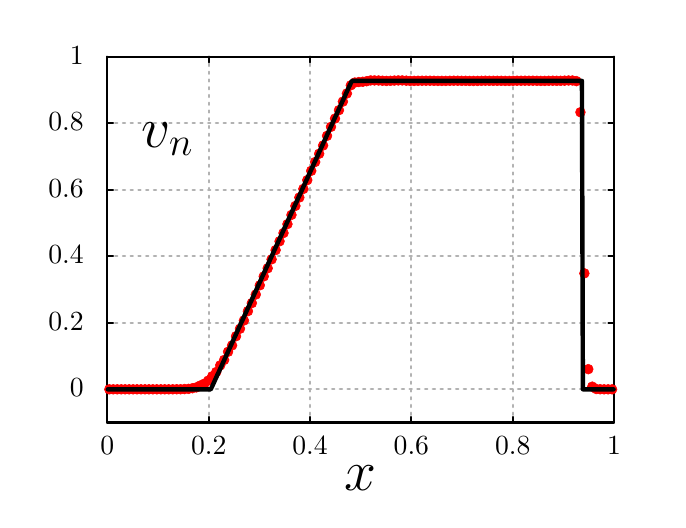
\begin{tikzpicture}[gnuplot]
%% generated with GNUPLOT 4.6p4 (Lua 5.1; terminal rev. 99, script rev. 100)
%% Thu 31 Jul 2014 02:05:23 PM EDT
\path (0.000,0.000) rectangle (8.000,6.000);
\gpfill{rgb color={1.000,1.000,1.000}} (1.012,0.985)--(7.446,0.985)--(7.446,5.630)--(1.012,5.630)--cycle;
\gpcolor{color=gp lt color border}
\gpsetlinetype{gp lt border}
\gpsetlinewidth{1.00}
\draw[gp path] (1.012,0.985)--(1.012,5.630)--(7.446,5.630)--(7.446,0.985)--cycle;
\gpcolor{color=gp lt color axes}
\gpsetlinetype{gp lt axes}
\gpsetlinewidth{2.00}
\draw[gp path] (1.012,1.407)--(7.447,1.407);
\gpcolor{color=gp lt color border}
\gpsetlinetype{gp lt border}
\draw[gp path] (1.012,1.407)--(1.084,1.407);
\draw[gp path] (7.447,1.407)--(7.375,1.407);
\gpcolor{rgb color={0.000,0.000,0.000}}
\node[gp node right,font={\fontsize{10pt}{12pt}\selectfont}] at (0.828,1.407) {0};
\gpcolor{color=gp lt color axes}
\gpsetlinetype{gp lt axes}
\draw[gp path] (1.012,2.252)--(7.447,2.252);
\gpcolor{color=gp lt color border}
\gpsetlinetype{gp lt border}
\draw[gp path] (1.012,2.252)--(1.084,2.252);
\draw[gp path] (7.447,2.252)--(7.375,2.252);
\gpcolor{rgb color={0.000,0.000,0.000}}
\node[gp node right,font={\fontsize{10pt}{12pt}\selectfont}] at (0.828,2.252) {0.2};
\gpcolor{color=gp lt color axes}
\gpsetlinetype{gp lt axes}
\draw[gp path] (1.012,3.097)--(7.447,3.097);
\gpcolor{color=gp lt color border}
\gpsetlinetype{gp lt border}
\draw[gp path] (1.012,3.097)--(1.084,3.097);
\draw[gp path] (7.447,3.097)--(7.375,3.097);
\gpcolor{rgb color={0.000,0.000,0.000}}
\node[gp node right,font={\fontsize{10pt}{12pt}\selectfont}] at (0.828,3.097) {0.4};
\gpcolor{color=gp lt color axes}
\gpsetlinetype{gp lt axes}
\draw[gp path] (1.012,3.942)--(7.447,3.942);
\gpcolor{color=gp lt color border}
\gpsetlinetype{gp lt border}
\draw[gp path] (1.012,3.942)--(1.084,3.942);
\draw[gp path] (7.447,3.942)--(7.375,3.942);
\gpcolor{rgb color={0.000,0.000,0.000}}
\node[gp node right,font={\fontsize{10pt}{12pt}\selectfont}] at (0.828,3.942) {0.6};
\gpcolor{color=gp lt color axes}
\gpsetlinetype{gp lt axes}
\draw[gp path] (1.012,4.786)--(7.447,4.786);
\gpcolor{color=gp lt color border}
\gpsetlinetype{gp lt border}
\draw[gp path] (1.012,4.786)--(1.084,4.786);
\draw[gp path] (7.447,4.786)--(7.375,4.786);
\gpcolor{rgb color={0.000,0.000,0.000}}
\node[gp node right,font={\fontsize{10pt}{12pt}\selectfont}] at (0.828,4.786) {0.8};
\gpcolor{color=gp lt color axes}
\gpsetlinetype{gp lt axes}
\draw[gp path] (1.012,5.631)--(7.447,5.631);
\gpcolor{color=gp lt color border}
\gpsetlinetype{gp lt border}
\draw[gp path] (1.012,5.631)--(1.084,5.631);
\draw[gp path] (7.447,5.631)--(7.375,5.631);
\gpcolor{rgb color={0.000,0.000,0.000}}
\node[gp node right,font={\fontsize{10pt}{12pt}\selectfont}] at (0.828,5.631) {1};
\gpcolor{color=gp lt color axes}
\gpsetlinetype{gp lt axes}
\draw[gp path] (1.012,0.985)--(1.012,5.631);
\gpcolor{color=gp lt color border}
\gpsetlinetype{gp lt border}
\draw[gp path] (1.012,0.985)--(1.012,1.057);
\draw[gp path] (1.012,5.631)--(1.012,5.559);
\gpcolor{rgb color={0.000,0.000,0.000}}
\node[gp node center,font={\fontsize{10pt}{12pt}\selectfont}] at (1.012,0.677) {0};
\gpcolor{color=gp lt color axes}
\gpsetlinetype{gp lt axes}
\draw[gp path] (2.299,0.985)--(2.299,5.631);
\gpcolor{color=gp lt color border}
\gpsetlinetype{gp lt border}
\draw[gp path] (2.299,0.985)--(2.299,1.057);
\draw[gp path] (2.299,5.631)--(2.299,5.559);
\gpcolor{rgb color={0.000,0.000,0.000}}
\node[gp node center,font={\fontsize{10pt}{12pt}\selectfont}] at (2.299,0.677) {0.2};
\gpcolor{color=gp lt color axes}
\gpsetlinetype{gp lt axes}
\draw[gp path] (3.586,0.985)--(3.586,5.631);
\gpcolor{color=gp lt color border}
\gpsetlinetype{gp lt border}
\draw[gp path] (3.586,0.985)--(3.586,1.057);
\draw[gp path] (3.586,5.631)--(3.586,5.559);
\gpcolor{rgb color={0.000,0.000,0.000}}
\node[gp node center,font={\fontsize{10pt}{12pt}\selectfont}] at (3.586,0.677) {0.4};
\gpcolor{color=gp lt color axes}
\gpsetlinetype{gp lt axes}
\draw[gp path] (4.873,0.985)--(4.873,5.631);
\gpcolor{color=gp lt color border}
\gpsetlinetype{gp lt border}
\draw[gp path] (4.873,0.985)--(4.873,1.057);
\draw[gp path] (4.873,5.631)--(4.873,5.559);
\gpcolor{rgb color={0.000,0.000,0.000}}
\node[gp node center,font={\fontsize{10pt}{12pt}\selectfont}] at (4.873,0.677) {0.6};
\gpcolor{color=gp lt color axes}
\gpsetlinetype{gp lt axes}
\draw[gp path] (6.160,0.985)--(6.160,5.631);
\gpcolor{color=gp lt color border}
\gpsetlinetype{gp lt border}
\draw[gp path] (6.160,0.985)--(6.160,1.057);
\draw[gp path] (6.160,5.631)--(6.160,5.559);
\gpcolor{rgb color={0.000,0.000,0.000}}
\node[gp node center,font={\fontsize{10pt}{12pt}\selectfont}] at (6.160,0.677) {0.8};
\gpcolor{color=gp lt color axes}
\gpsetlinetype{gp lt axes}
\draw[gp path] (7.447,0.985)--(7.447,5.631);
\gpcolor{color=gp lt color border}
\gpsetlinetype{gp lt border}
\draw[gp path] (7.447,0.985)--(7.447,1.057);
\draw[gp path] (7.447,5.631)--(7.447,5.559);
\gpcolor{rgb color={0.000,0.000,0.000}}
\node[gp node center,font={\fontsize{10pt}{12pt}\selectfont}] at (7.447,0.677) {1};
\gpcolor{color=gp lt color border}
\draw[gp path] (1.012,5.631)--(1.012,0.985)--(7.447,0.985)--(7.447,5.631)--cycle;
\gpcolor{rgb color={0.000,0.000,0.000}}
\node[gp node center,font={\fontsize{10pt}{12pt}\selectfont}] at (4.229,0.215) {\huge $x$};
\gpcolor{rgb color={1.000,0.000,0.000}}
\gpsetlinewidth{0.50}
\gpsetpointsize{4.44}
\gppoint{gp mark 7}{(1.037,1.407)}
\gppoint{gp mark 7}{(1.087,1.407)}
\gppoint{gp mark 7}{(1.138,1.407)}
\gppoint{gp mark 7}{(1.188,1.407)}
\gppoint{gp mark 7}{(1.238,1.407)}
\gppoint{gp mark 7}{(1.289,1.407)}
\gppoint{gp mark 7}{(1.339,1.407)}
\gppoint{gp mark 7}{(1.389,1.407)}
\gppoint{gp mark 7}{(1.439,1.407)}
\gppoint{gp mark 7}{(1.490,1.407)}
\gppoint{gp mark 7}{(1.540,1.407)}
\gppoint{gp mark 7}{(1.590,1.407)}
\gppoint{gp mark 7}{(1.640,1.407)}
\gppoint{gp mark 7}{(1.691,1.407)}
\gppoint{gp mark 7}{(1.741,1.407)}
\gppoint{gp mark 7}{(1.791,1.407)}
\gppoint{gp mark 7}{(1.842,1.407)}
\gppoint{gp mark 7}{(1.892,1.408)}
\gppoint{gp mark 7}{(1.942,1.408)}
\gppoint{gp mark 7}{(1.992,1.410)}
\gppoint{gp mark 7}{(2.043,1.413)}
\gppoint{gp mark 7}{(2.093,1.421)}
\gppoint{gp mark 7}{(2.143,1.432)}
\gppoint{gp mark 7}{(2.193,1.456)}
\gppoint{gp mark 7}{(2.244,1.479)}
\gppoint{gp mark 7}{(2.294,1.518)}
\gppoint{gp mark 7}{(2.344,1.573)}
\gppoint{gp mark 7}{(2.395,1.627)}
\gppoint{gp mark 7}{(2.445,1.711)}
\gppoint{gp mark 7}{(2.495,1.780)}
\gppoint{gp mark 7}{(2.545,1.884)}
\gppoint{gp mark 7}{(2.596,1.965)}
\gppoint{gp mark 7}{(2.646,2.081)}
\gppoint{gp mark 7}{(2.696,2.176)}
\gppoint{gp mark 7}{(2.746,2.281)}
\gppoint{gp mark 7}{(2.797,2.400)}
\gppoint{gp mark 7}{(2.847,2.502)}
\gppoint{gp mark 7}{(2.897,2.611)}
\gppoint{gp mark 7}{(2.948,2.728)}
\gppoint{gp mark 7}{(2.998,2.841)}
\gppoint{gp mark 7}{(3.048,2.944)}
\gppoint{gp mark 7}{(3.098,3.058)}
\gppoint{gp mark 7}{(3.149,3.175)}
\gppoint{gp mark 7}{(3.199,3.287)}
\gppoint{gp mark 7}{(3.249,3.392)}
\gppoint{gp mark 7}{(3.299,3.505)}
\gppoint{gp mark 7}{(3.350,3.622)}
\gppoint{gp mark 7}{(3.400,3.736)}
\gppoint{gp mark 7}{(3.450,3.843)}
\gppoint{gp mark 7}{(3.501,3.952)}
\gppoint{gp mark 7}{(3.551,4.064)}
\gppoint{gp mark 7}{(3.601,4.182)}
\gppoint{gp mark 7}{(3.651,4.294)}
\gppoint{gp mark 7}{(3.702,4.399)}
\gppoint{gp mark 7}{(3.752,4.504)}
\gppoint{gp mark 7}{(3.802,4.626)}
\gppoint{gp mark 7}{(3.852,4.740)}
\gppoint{gp mark 7}{(3.903,4.846)}
\gppoint{gp mark 7}{(3.953,4.952)}
\gppoint{gp mark 7}{(4.003,5.061)}
\gppoint{gp mark 7}{(4.054,5.164)}
\gppoint{gp mark 7}{(4.104,5.268)}
\gppoint{gp mark 7}{(4.154,5.303)}
\gppoint{gp mark 7}{(4.204,5.309)}
\gppoint{gp mark 7}{(4.255,5.313)}
\gppoint{gp mark 7}{(4.305,5.320)}
\gppoint{gp mark 7}{(4.355,5.330)}
\gppoint{gp mark 7}{(4.405,5.330)}
\gppoint{gp mark 7}{(4.456,5.329)}
\gppoint{gp mark 7}{(4.506,5.326)}
\gppoint{gp mark 7}{(4.556,5.324)}
\gppoint{gp mark 7}{(4.607,5.325)}
\gppoint{gp mark 7}{(4.657,5.328)}
\gppoint{gp mark 7}{(4.707,5.330)}
\gppoint{gp mark 7}{(4.757,5.330)}
\gppoint{gp mark 7}{(4.808,5.327)}
\gppoint{gp mark 7}{(4.858,5.324)}
\gppoint{gp mark 7}{(4.908,5.324)}
\gppoint{gp mark 7}{(4.958,5.325)}
\gppoint{gp mark 7}{(5.009,5.326)}
\gppoint{gp mark 7}{(5.059,5.326)}
\gppoint{gp mark 7}{(5.109,5.326)}
\gppoint{gp mark 7}{(5.160,5.325)}
\gppoint{gp mark 7}{(5.210,5.324)}
\gppoint{gp mark 7}{(5.260,5.324)}
\gppoint{gp mark 7}{(5.310,5.324)}
\gppoint{gp mark 7}{(5.361,5.325)}
\gppoint{gp mark 7}{(5.411,5.326)}
\gppoint{gp mark 7}{(5.461,5.326)}
\gppoint{gp mark 7}{(5.511,5.325)}
\gppoint{gp mark 7}{(5.562,5.325)}
\gppoint{gp mark 7}{(5.612,5.324)}
\gppoint{gp mark 7}{(5.662,5.324)}
\gppoint{gp mark 7}{(5.713,5.324)}
\gppoint{gp mark 7}{(5.763,5.325)}
\gppoint{gp mark 7}{(5.813,5.326)}
\gppoint{gp mark 7}{(5.863,5.325)}
\gppoint{gp mark 7}{(5.914,5.325)}
\gppoint{gp mark 7}{(5.964,5.325)}
\gppoint{gp mark 7}{(6.014,5.325)}
\gppoint{gp mark 7}{(6.064,5.324)}
\gppoint{gp mark 7}{(6.115,5.324)}
\gppoint{gp mark 7}{(6.165,5.325)}
\gppoint{gp mark 7}{(6.215,5.326)}
\gppoint{gp mark 7}{(6.266,5.326)}
\gppoint{gp mark 7}{(6.316,5.326)}
\gppoint{gp mark 7}{(6.366,5.326)}
\gppoint{gp mark 7}{(6.416,5.326)}
\gppoint{gp mark 7}{(6.467,5.325)}
\gppoint{gp mark 7}{(6.517,5.324)}
\gppoint{gp mark 7}{(6.567,5.324)}
\gppoint{gp mark 7}{(6.617,5.325)}
\gppoint{gp mark 7}{(6.668,5.326)}
\gppoint{gp mark 7}{(6.718,5.325)}
\gppoint{gp mark 7}{(6.768,5.325)}
\gppoint{gp mark 7}{(6.819,5.327)}
\gppoint{gp mark 7}{(6.869,5.329)}
\gppoint{gp mark 7}{(6.919,5.329)}
\gppoint{gp mark 7}{(6.969,5.321)}
\gppoint{gp mark 7}{(7.020,4.926)}
\gppoint{gp mark 7}{(7.070,2.880)}
\gppoint{gp mark 7}{(7.120,1.663)}
\gppoint{gp mark 7}{(7.170,1.441)}
\gppoint{gp mark 7}{(7.221,1.411)}
\gppoint{gp mark 7}{(7.271,1.408)}
\gppoint{gp mark 7}{(7.321,1.407)}
\gppoint{gp mark 7}{(7.372,1.407)}
\gppoint{gp mark 7}{(7.422,1.407)}
\gpcolor{rgb color={0.000,0.000,0.000}}
\gpsetlinetype{gp lt plot 0}
\gpsetlinewidth{4.00}
\draw[gp path] (1.018,1.407)--(1.031,1.407)--(1.043,1.407)--(1.056,1.407)--(1.069,1.407)%
  --(1.081,1.407)--(1.094,1.407)--(1.106,1.407)--(1.119,1.407)--(1.131,1.407)--(1.144,1.407)%
  --(1.157,1.407)--(1.169,1.407)--(1.182,1.407)--(1.194,1.407)--(1.207,1.407)--(1.219,1.407)%
  --(1.232,1.407)--(1.245,1.407)--(1.257,1.407)--(1.270,1.407)--(1.282,1.407)--(1.295,1.407)%
  --(1.307,1.407)--(1.320,1.407)--(1.332,1.407)--(1.345,1.407)--(1.358,1.407)--(1.370,1.407)%
  --(1.383,1.407)--(1.395,1.407)--(1.408,1.407)--(1.420,1.407)--(1.433,1.407)--(1.446,1.407)%
  --(1.458,1.407)--(1.471,1.407)--(1.483,1.407)--(1.496,1.407)--(1.508,1.407)--(1.521,1.407)%
  --(1.534,1.407)--(1.546,1.407)--(1.559,1.407)--(1.571,1.407)--(1.584,1.407)--(1.596,1.407)%
  --(1.609,1.407)--(1.622,1.407)--(1.634,1.407)--(1.647,1.407)--(1.659,1.407)--(1.672,1.407)%
  --(1.684,1.407)--(1.697,1.407)--(1.710,1.407)--(1.722,1.407)--(1.735,1.407)--(1.747,1.407)%
  --(1.760,1.407)--(1.772,1.407)--(1.785,1.407)--(1.798,1.407)--(1.810,1.407)--(1.823,1.407)%
  --(1.835,1.407)--(1.848,1.407)--(1.860,1.407)--(1.873,1.407)--(1.886,1.407)--(1.898,1.407)%
  --(1.911,1.407)--(1.923,1.407)--(1.936,1.407)--(1.948,1.407)--(1.961,1.407)--(1.973,1.407)%
  --(1.986,1.407)--(1.999,1.407)--(2.011,1.407)--(2.024,1.407)--(2.036,1.407)--(2.049,1.407)%
  --(2.061,1.407)--(2.074,1.407)--(2.087,1.407)--(2.099,1.407)--(2.112,1.407)--(2.124,1.407)%
  --(2.137,1.407)--(2.149,1.407)--(2.162,1.407)--(2.175,1.407)--(2.187,1.407)--(2.200,1.407)%
  --(2.212,1.407)--(2.225,1.407)--(2.237,1.407)--(2.250,1.407)--(2.263,1.407)--(2.275,1.407)%
  --(2.288,1.407)--(2.300,1.407)--(2.313,1.407)--(2.325,1.407)--(2.338,1.434)--(2.351,1.461)%
  --(2.363,1.489)--(2.376,1.516)--(2.388,1.544)--(2.401,1.571)--(2.413,1.599)--(2.426,1.626)%
  --(2.439,1.654)--(2.451,1.681)--(2.464,1.709)--(2.476,1.736)--(2.489,1.764)--(2.501,1.791)%
  --(2.514,1.818)--(2.526,1.846)--(2.539,1.873)--(2.552,1.901)--(2.564,1.928)--(2.577,1.956)%
  --(2.589,1.983)--(2.602,2.011)--(2.614,2.038)--(2.627,2.066)--(2.640,2.093)--(2.652,2.121)%
  --(2.665,2.148)--(2.677,2.176)--(2.690,2.203)--(2.702,2.231)--(2.715,2.258)--(2.728,2.286)%
  --(2.740,2.313)--(2.753,2.341)--(2.765,2.368)--(2.778,2.396)--(2.790,2.423)--(2.803,2.451)%
  --(2.816,2.478)--(2.828,2.506)--(2.841,2.533)--(2.853,2.561)--(2.866,2.588)--(2.878,2.616)%
  --(2.891,2.643)--(2.904,2.671)--(2.916,2.698)--(2.929,2.726)--(2.941,2.753)--(2.954,2.781)%
  --(2.966,2.808)--(2.979,2.836)--(2.992,2.863)--(3.004,2.891)--(3.017,2.918)--(3.029,2.946)%
  --(3.042,2.973)--(3.054,3.001)--(3.067,3.028)--(3.079,3.056)--(3.092,3.083)--(3.105,3.111)%
  --(3.117,3.138)--(3.130,3.166)--(3.142,3.193)--(3.155,3.221)--(3.167,3.248)--(3.180,3.276)%
  --(3.193,3.303)--(3.205,3.331)--(3.218,3.358)--(3.230,3.386)--(3.243,3.413)--(3.255,3.441)%
  --(3.268,3.468)--(3.281,3.496)--(3.293,3.523)--(3.306,3.551)--(3.318,3.578)--(3.331,3.606)%
  --(3.343,3.633)--(3.356,3.661)--(3.369,3.688)--(3.381,3.716)--(3.394,3.743)--(3.406,3.771)%
  --(3.419,3.798)--(3.431,3.826)--(3.444,3.853)--(3.457,3.881)--(3.469,3.908)--(3.482,3.936)%
  --(3.494,3.963)--(3.507,3.991)--(3.519,4.018)--(3.532,4.046)--(3.545,4.073)--(3.557,4.101)%
  --(3.570,4.128)--(3.582,4.156)--(3.595,4.183)--(3.607,4.211)--(3.620,4.238)--(3.633,4.266)%
  --(3.645,4.293)--(3.658,4.321)--(3.670,4.348)--(3.683,4.376)--(3.695,4.403)--(3.708,4.431)%
  --(3.720,4.458)--(3.733,4.486)--(3.746,4.513)--(3.758,4.541)--(3.771,4.568)--(3.783,4.596)%
  --(3.796,4.623)--(3.808,4.651)--(3.821,4.678)--(3.834,4.706)--(3.846,4.733)--(3.859,4.761)%
  --(3.871,4.788)--(3.884,4.816)--(3.896,4.843)--(3.909,4.871)--(3.922,4.898)--(3.934,4.926)%
  --(3.947,4.953)--(3.959,4.981)--(3.972,5.008)--(3.984,5.036)--(3.997,5.063)--(4.010,5.091)%
  --(4.022,5.118)--(4.035,5.146)--(4.047,5.173)--(4.060,5.201)--(4.072,5.228)--(4.085,5.256)%
  --(4.098,5.283)--(4.110,5.311)--(4.123,5.324)--(4.135,5.324)--(4.148,5.324)--(4.160,5.324)%
  --(4.173,5.324)--(4.186,5.324)--(4.198,5.324)--(4.211,5.324)--(4.223,5.324)--(4.236,5.324)%
  --(4.248,5.324)--(4.261,5.324)--(4.273,5.324)--(4.286,5.324)--(4.299,5.324)--(4.311,5.324)%
  --(4.324,5.324)--(4.336,5.324)--(4.349,5.324)--(4.361,5.324)--(4.374,5.324)--(4.387,5.324)%
  --(4.399,5.324)--(4.412,5.324)--(4.424,5.324)--(4.437,5.324)--(4.449,5.324)--(4.462,5.324)%
  --(4.475,5.324)--(4.487,5.324)--(4.500,5.324)--(4.512,5.324)--(4.525,5.324)--(4.537,5.324)%
  --(4.550,5.324)--(4.563,5.324)--(4.575,5.324)--(4.588,5.324)--(4.600,5.324)--(4.613,5.324)%
  --(4.625,5.324)--(4.638,5.324)--(4.651,5.324)--(4.663,5.324)--(4.676,5.324)--(4.688,5.324)%
  --(4.701,5.324)--(4.713,5.324)--(4.726,5.324)--(4.739,5.324)--(4.751,5.324)--(4.764,5.324)%
  --(4.776,5.324)--(4.789,5.324)--(4.801,5.324)--(4.814,5.324)--(4.826,5.324)--(4.839,5.324)%
  --(4.852,5.324)--(4.864,5.324)--(4.877,5.324)--(4.889,5.324)--(4.902,5.324)--(4.914,5.324)%
  --(4.927,5.324)--(4.940,5.324)--(4.952,5.324)--(4.965,5.324)--(4.977,5.324)--(4.990,5.324)%
  --(5.002,5.324)--(5.015,5.324)--(5.028,5.324)--(5.040,5.324)--(5.053,5.324)--(5.065,5.324)%
  --(5.078,5.324)--(5.090,5.324)--(5.103,5.324)--(5.116,5.324)--(5.128,5.324)--(5.141,5.324)%
  --(5.153,5.324)--(5.166,5.324)--(5.178,5.324)--(5.191,5.324)--(5.204,5.324)--(5.216,5.324)%
  --(5.229,5.324)--(5.241,5.324)--(5.254,5.324)--(5.266,5.324)--(5.279,5.324)--(5.292,5.324)%
  --(5.304,5.324)--(5.317,5.324)--(5.329,5.324)--(5.342,5.324)--(5.354,5.324)--(5.367,5.324)%
  --(5.380,5.324)--(5.392,5.324)--(5.405,5.324)--(5.417,5.324)--(5.430,5.324)--(5.442,5.324)%
  --(5.455,5.324)--(5.467,5.324)--(5.480,5.324)--(5.493,5.324)--(5.505,5.324)--(5.518,5.324)%
  --(5.530,5.324)--(5.543,5.324)--(5.555,5.324)--(5.568,5.324)--(5.581,5.324)--(5.593,5.324)%
  --(5.606,5.324)--(5.618,5.324)--(5.631,5.324)--(5.643,5.324)--(5.656,5.324)--(5.669,5.324)%
  --(5.681,5.324)--(5.694,5.324)--(5.706,5.324)--(5.719,5.324)--(5.731,5.324)--(5.744,5.324)%
  --(5.757,5.324)--(5.769,5.324)--(5.782,5.324)--(5.794,5.324)--(5.807,5.324)--(5.819,5.324)%
  --(5.832,5.324)--(5.845,5.324)--(5.857,5.324)--(5.870,5.324)--(5.882,5.324)--(5.895,5.324)%
  --(5.907,5.324)--(5.920,5.324)--(5.933,5.324)--(5.945,5.324)--(5.958,5.324)--(5.970,5.324)%
  --(5.983,5.324)--(5.995,5.324)--(6.008,5.324)--(6.020,5.324)--(6.033,5.324)--(6.046,5.324)%
  --(6.058,5.324)--(6.071,5.324)--(6.083,5.324)--(6.096,5.324)--(6.108,5.324)--(6.121,5.324)%
  --(6.134,5.324)--(6.146,5.324)--(6.159,5.324)--(6.171,5.324)--(6.184,5.324)--(6.196,5.324)%
  --(6.209,5.324)--(6.222,5.324)--(6.234,5.324)--(6.247,5.324)--(6.259,5.324)--(6.272,5.324)%
  --(6.284,5.324)--(6.297,5.324)--(6.310,5.324)--(6.322,5.324)--(6.335,5.324)--(6.347,5.324)%
  --(6.360,5.324)--(6.372,5.324)--(6.385,5.324)--(6.398,5.324)--(6.410,5.324)--(6.423,5.324)%
  --(6.435,5.324)--(6.448,5.324)--(6.460,5.324)--(6.473,5.324)--(6.486,5.324)--(6.498,5.324)%
  --(6.511,5.324)--(6.523,5.324)--(6.536,5.324)--(6.548,5.324)--(6.561,5.324)--(6.573,5.324)%
  --(6.586,5.324)--(6.599,5.324)--(6.611,5.324)--(6.624,5.324)--(6.636,5.324)--(6.649,5.324)%
  --(6.661,5.324)--(6.674,5.324)--(6.687,5.324)--(6.699,5.324)--(6.712,5.324)--(6.724,5.324)%
  --(6.737,5.324)--(6.749,5.324)--(6.762,5.324)--(6.775,5.324)--(6.787,5.324)--(6.800,5.324)%
  --(6.812,5.324)--(6.825,5.324)--(6.837,5.324)--(6.850,5.324)--(6.863,5.324)--(6.875,5.324)%
  --(6.888,5.324)--(6.900,5.324)--(6.913,5.324)--(6.925,5.324)--(6.938,5.324)--(6.951,5.324)%
  --(6.963,5.324)--(6.976,5.324)--(6.988,5.324)--(7.001,5.324)--(7.013,5.324)--(7.026,5.324)%
  --(7.039,5.324)--(7.051,1.407)--(7.064,1.407)--(7.076,1.407)--(7.089,1.407)--(7.101,1.407)%
  --(7.114,1.407)--(7.127,1.407)--(7.139,1.407)--(7.152,1.407)--(7.164,1.407)--(7.177,1.407)%
  --(7.189,1.407)--(7.202,1.407)--(7.214,1.407)--(7.227,1.407)--(7.240,1.407)--(7.252,1.407)%
  --(7.265,1.407)--(7.277,1.407)--(7.290,1.407)--(7.302,1.407)--(7.315,1.407)--(7.328,1.407)%
  --(7.340,1.407)--(7.353,1.407)--(7.365,1.407)--(7.378,1.407)--(7.390,1.407)--(7.403,1.407)%
  --(7.416,1.407)--(7.428,1.407)--(7.441,1.407);
\node[gp node left,font={\fontsize{10pt}{12pt}\selectfont}] at (1.334,4.575) {\huge $v_n$};
%% coordinates of the plot area
\gpdefrectangularnode{gp plot 1}{\pgfpoint{1.012cm}{0.985cm}}{\pgfpoint{7.447cm}{5.631cm}}
\end{tikzpicture}
%% gnuplot variables
} &
\resizebox{0.33\linewidth}{!}{\tikzsetnextfilename{sod_hlle_3_3}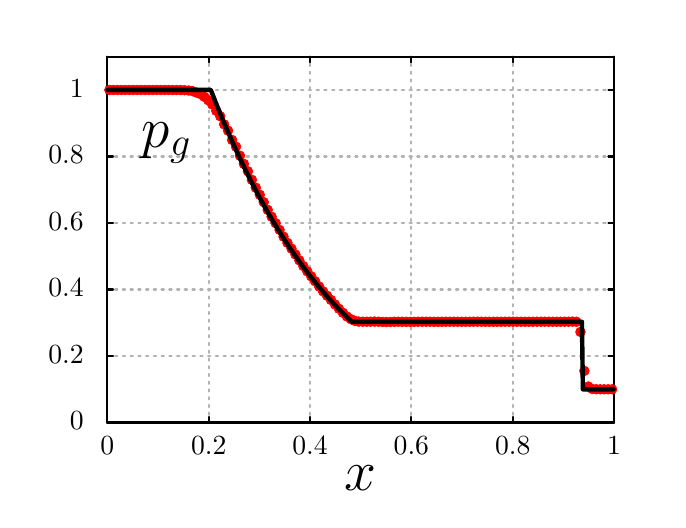
\begin{tikzpicture}[gnuplot]
%% generated with GNUPLOT 4.6p4 (Lua 5.1; terminal rev. 99, script rev. 100)
%% Thu 31 Jul 2014 02:05:23 PM EDT
\path (0.000,0.000) rectangle (8.000,6.000);
\gpfill{rgb color={1.000,1.000,1.000}} (1.012,0.985)--(7.446,0.985)--(7.446,5.630)--(1.012,5.630)--cycle;
\gpcolor{color=gp lt color border}
\gpsetlinetype{gp lt border}
\gpsetlinewidth{1.00}
\draw[gp path] (1.012,0.985)--(1.012,5.630)--(7.446,5.630)--(7.446,0.985)--cycle;
\gpcolor{color=gp lt color axes}
\gpsetlinetype{gp lt axes}
\gpsetlinewidth{2.00}
\draw[gp path] (1.012,0.985)--(7.447,0.985);
\gpcolor{color=gp lt color border}
\gpsetlinetype{gp lt border}
\draw[gp path] (1.012,0.985)--(1.084,0.985);
\draw[gp path] (7.447,0.985)--(7.375,0.985);
\gpcolor{rgb color={0.000,0.000,0.000}}
\node[gp node right,font={\fontsize{10pt}{12pt}\selectfont}] at (0.828,0.985) {0};
\gpcolor{color=gp lt color axes}
\gpsetlinetype{gp lt axes}
\draw[gp path] (1.012,1.830)--(7.447,1.830);
\gpcolor{color=gp lt color border}
\gpsetlinetype{gp lt border}
\draw[gp path] (1.012,1.830)--(1.084,1.830);
\draw[gp path] (7.447,1.830)--(7.375,1.830);
\gpcolor{rgb color={0.000,0.000,0.000}}
\node[gp node right,font={\fontsize{10pt}{12pt}\selectfont}] at (0.828,1.830) {0.2};
\gpcolor{color=gp lt color axes}
\gpsetlinetype{gp lt axes}
\draw[gp path] (1.012,2.674)--(7.447,2.674);
\gpcolor{color=gp lt color border}
\gpsetlinetype{gp lt border}
\draw[gp path] (1.012,2.674)--(1.084,2.674);
\draw[gp path] (7.447,2.674)--(7.375,2.674);
\gpcolor{rgb color={0.000,0.000,0.000}}
\node[gp node right,font={\fontsize{10pt}{12pt}\selectfont}] at (0.828,2.674) {0.4};
\gpcolor{color=gp lt color axes}
\gpsetlinetype{gp lt axes}
\draw[gp path] (1.012,3.519)--(7.447,3.519);
\gpcolor{color=gp lt color border}
\gpsetlinetype{gp lt border}
\draw[gp path] (1.012,3.519)--(1.084,3.519);
\draw[gp path] (7.447,3.519)--(7.375,3.519);
\gpcolor{rgb color={0.000,0.000,0.000}}
\node[gp node right,font={\fontsize{10pt}{12pt}\selectfont}] at (0.828,3.519) {0.6};
\gpcolor{color=gp lt color axes}
\gpsetlinetype{gp lt axes}
\draw[gp path] (1.012,4.364)--(7.447,4.364);
\gpcolor{color=gp lt color border}
\gpsetlinetype{gp lt border}
\draw[gp path] (1.012,4.364)--(1.084,4.364);
\draw[gp path] (7.447,4.364)--(7.375,4.364);
\gpcolor{rgb color={0.000,0.000,0.000}}
\node[gp node right,font={\fontsize{10pt}{12pt}\selectfont}] at (0.828,4.364) {0.8};
\gpcolor{color=gp lt color axes}
\gpsetlinetype{gp lt axes}
\draw[gp path] (1.012,5.209)--(7.447,5.209);
\gpcolor{color=gp lt color border}
\gpsetlinetype{gp lt border}
\draw[gp path] (1.012,5.209)--(1.084,5.209);
\draw[gp path] (7.447,5.209)--(7.375,5.209);
\gpcolor{rgb color={0.000,0.000,0.000}}
\node[gp node right,font={\fontsize{10pt}{12pt}\selectfont}] at (0.828,5.209) {1};
\gpcolor{color=gp lt color axes}
\gpsetlinetype{gp lt axes}
\draw[gp path] (1.012,0.985)--(1.012,5.631);
\gpcolor{color=gp lt color border}
\gpsetlinetype{gp lt border}
\draw[gp path] (1.012,0.985)--(1.012,1.057);
\draw[gp path] (1.012,5.631)--(1.012,5.559);
\gpcolor{rgb color={0.000,0.000,0.000}}
\node[gp node center,font={\fontsize{10pt}{12pt}\selectfont}] at (1.012,0.677) {0};
\gpcolor{color=gp lt color axes}
\gpsetlinetype{gp lt axes}
\draw[gp path] (2.299,0.985)--(2.299,5.631);
\gpcolor{color=gp lt color border}
\gpsetlinetype{gp lt border}
\draw[gp path] (2.299,0.985)--(2.299,1.057);
\draw[gp path] (2.299,5.631)--(2.299,5.559);
\gpcolor{rgb color={0.000,0.000,0.000}}
\node[gp node center,font={\fontsize{10pt}{12pt}\selectfont}] at (2.299,0.677) {0.2};
\gpcolor{color=gp lt color axes}
\gpsetlinetype{gp lt axes}
\draw[gp path] (3.586,0.985)--(3.586,5.631);
\gpcolor{color=gp lt color border}
\gpsetlinetype{gp lt border}
\draw[gp path] (3.586,0.985)--(3.586,1.057);
\draw[gp path] (3.586,5.631)--(3.586,5.559);
\gpcolor{rgb color={0.000,0.000,0.000}}
\node[gp node center,font={\fontsize{10pt}{12pt}\selectfont}] at (3.586,0.677) {0.4};
\gpcolor{color=gp lt color axes}
\gpsetlinetype{gp lt axes}
\draw[gp path] (4.873,0.985)--(4.873,5.631);
\gpcolor{color=gp lt color border}
\gpsetlinetype{gp lt border}
\draw[gp path] (4.873,0.985)--(4.873,1.057);
\draw[gp path] (4.873,5.631)--(4.873,5.559);
\gpcolor{rgb color={0.000,0.000,0.000}}
\node[gp node center,font={\fontsize{10pt}{12pt}\selectfont}] at (4.873,0.677) {0.6};
\gpcolor{color=gp lt color axes}
\gpsetlinetype{gp lt axes}
\draw[gp path] (6.160,0.985)--(6.160,5.631);
\gpcolor{color=gp lt color border}
\gpsetlinetype{gp lt border}
\draw[gp path] (6.160,0.985)--(6.160,1.057);
\draw[gp path] (6.160,5.631)--(6.160,5.559);
\gpcolor{rgb color={0.000,0.000,0.000}}
\node[gp node center,font={\fontsize{10pt}{12pt}\selectfont}] at (6.160,0.677) {0.8};
\gpcolor{color=gp lt color axes}
\gpsetlinetype{gp lt axes}
\draw[gp path] (7.447,0.985)--(7.447,5.631);
\gpcolor{color=gp lt color border}
\gpsetlinetype{gp lt border}
\draw[gp path] (7.447,0.985)--(7.447,1.057);
\draw[gp path] (7.447,5.631)--(7.447,5.559);
\gpcolor{rgb color={0.000,0.000,0.000}}
\node[gp node center,font={\fontsize{10pt}{12pt}\selectfont}] at (7.447,0.677) {1};
\gpcolor{color=gp lt color border}
\draw[gp path] (1.012,5.631)--(1.012,0.985)--(7.447,0.985)--(7.447,5.631)--cycle;
\gpcolor{rgb color={0.000,0.000,0.000}}
\node[gp node center,font={\fontsize{10pt}{12pt}\selectfont}] at (4.229,0.215) {\huge $x$};
\gpcolor{rgb color={1.000,0.000,0.000}}
\gpsetlinewidth{0.50}
\gpsetpointsize{4.44}
\gppoint{gp mark 7}{(1.037,5.209)}
\gppoint{gp mark 7}{(1.087,5.209)}
\gppoint{gp mark 7}{(1.138,5.209)}
\gppoint{gp mark 7}{(1.188,5.209)}
\gppoint{gp mark 7}{(1.238,5.209)}
\gppoint{gp mark 7}{(1.289,5.209)}
\gppoint{gp mark 7}{(1.339,5.209)}
\gppoint{gp mark 7}{(1.389,5.209)}
\gppoint{gp mark 7}{(1.439,5.209)}
\gppoint{gp mark 7}{(1.490,5.209)}
\gppoint{gp mark 7}{(1.540,5.209)}
\gppoint{gp mark 7}{(1.590,5.209)}
\gppoint{gp mark 7}{(1.640,5.209)}
\gppoint{gp mark 7}{(1.691,5.209)}
\gppoint{gp mark 7}{(1.741,5.209)}
\gppoint{gp mark 7}{(1.791,5.209)}
\gppoint{gp mark 7}{(1.842,5.208)}
\gppoint{gp mark 7}{(1.892,5.208)}
\gppoint{gp mark 7}{(1.942,5.208)}
\gppoint{gp mark 7}{(1.992,5.206)}
\gppoint{gp mark 7}{(2.043,5.202)}
\gppoint{gp mark 7}{(2.093,5.194)}
\gppoint{gp mark 7}{(2.143,5.176)}
\gppoint{gp mark 7}{(2.193,5.157)}
\gppoint{gp mark 7}{(2.244,5.121)}
\gppoint{gp mark 7}{(2.294,5.078)}
\gppoint{gp mark 7}{(2.344,5.024)}
\gppoint{gp mark 7}{(2.395,4.943)}
\gppoint{gp mark 7}{(2.445,4.875)}
\gppoint{gp mark 7}{(2.495,4.772)}
\gppoint{gp mark 7}{(2.545,4.692)}
\gppoint{gp mark 7}{(2.596,4.574)}
\gppoint{gp mark 7}{(2.646,4.488)}
\gppoint{gp mark 7}{(2.696,4.374)}
\gppoint{gp mark 7}{(2.746,4.270)}
\gppoint{gp mark 7}{(2.797,4.176)}
\gppoint{gp mark 7}{(2.847,4.068)}
\gppoint{gp mark 7}{(2.897,3.968)}
\gppoint{gp mark 7}{(2.948,3.878)}
\gppoint{gp mark 7}{(2.998,3.784)}
\gppoint{gp mark 7}{(3.048,3.687)}
\gppoint{gp mark 7}{(3.098,3.599)}
\gppoint{gp mark 7}{(3.149,3.517)}
\gppoint{gp mark 7}{(3.199,3.432)}
\gppoint{gp mark 7}{(3.249,3.346)}
\gppoint{gp mark 7}{(3.299,3.267)}
\gppoint{gp mark 7}{(3.350,3.194)}
\gppoint{gp mark 7}{(3.400,3.120)}
\gppoint{gp mark 7}{(3.450,3.045)}
\gppoint{gp mark 7}{(3.501,2.972)}
\gppoint{gp mark 7}{(3.551,2.905)}
\gppoint{gp mark 7}{(3.601,2.842)}
\gppoint{gp mark 7}{(3.651,2.779)}
\gppoint{gp mark 7}{(3.702,2.712)}
\gppoint{gp mark 7}{(3.752,2.650)}
\gppoint{gp mark 7}{(3.802,2.596)}
\gppoint{gp mark 7}{(3.852,2.542)}
\gppoint{gp mark 7}{(3.903,2.484)}
\gppoint{gp mark 7}{(3.953,2.430)}
\gppoint{gp mark 7}{(4.003,2.379)}
\gppoint{gp mark 7}{(4.054,2.332)}
\gppoint{gp mark 7}{(4.104,2.298)}
\gppoint{gp mark 7}{(4.154,2.277)}
\gppoint{gp mark 7}{(4.204,2.267)}
\gppoint{gp mark 7}{(4.255,2.266)}
\gppoint{gp mark 7}{(4.305,2.266)}
\gppoint{gp mark 7}{(4.355,2.266)}
\gppoint{gp mark 7}{(4.405,2.267)}
\gppoint{gp mark 7}{(4.456,2.266)}
\gppoint{gp mark 7}{(4.506,2.263)}
\gppoint{gp mark 7}{(4.556,2.262)}
\gppoint{gp mark 7}{(4.607,2.263)}
\gppoint{gp mark 7}{(4.657,2.265)}
\gppoint{gp mark 7}{(4.707,2.265)}
\gppoint{gp mark 7}{(4.757,2.265)}
\gppoint{gp mark 7}{(4.808,2.264)}
\gppoint{gp mark 7}{(4.858,2.264)}
\gppoint{gp mark 7}{(4.908,2.264)}
\gppoint{gp mark 7}{(4.958,2.265)}
\gppoint{gp mark 7}{(5.009,2.266)}
\gppoint{gp mark 7}{(5.059,2.266)}
\gppoint{gp mark 7}{(5.109,2.266)}
\gppoint{gp mark 7}{(5.160,2.264)}
\gppoint{gp mark 7}{(5.210,2.264)}
\gppoint{gp mark 7}{(5.260,2.265)}
\gppoint{gp mark 7}{(5.310,2.266)}
\gppoint{gp mark 7}{(5.361,2.266)}
\gppoint{gp mark 7}{(5.411,2.266)}
\gppoint{gp mark 7}{(5.461,2.265)}
\gppoint{gp mark 7}{(5.511,2.265)}
\gppoint{gp mark 7}{(5.562,2.265)}
\gppoint{gp mark 7}{(5.612,2.265)}
\gppoint{gp mark 7}{(5.662,2.266)}
\gppoint{gp mark 7}{(5.713,2.266)}
\gppoint{gp mark 7}{(5.763,2.266)}
\gppoint{gp mark 7}{(5.813,2.265)}
\gppoint{gp mark 7}{(5.863,2.265)}
\gppoint{gp mark 7}{(5.914,2.265)}
\gppoint{gp mark 7}{(5.964,2.265)}
\gppoint{gp mark 7}{(6.014,2.265)}
\gppoint{gp mark 7}{(6.064,2.266)}
\gppoint{gp mark 7}{(6.115,2.266)}
\gppoint{gp mark 7}{(6.165,2.266)}
\gppoint{gp mark 7}{(6.215,2.265)}
\gppoint{gp mark 7}{(6.266,2.265)}
\gppoint{gp mark 7}{(6.316,2.265)}
\gppoint{gp mark 7}{(6.366,2.265)}
\gppoint{gp mark 7}{(6.416,2.265)}
\gppoint{gp mark 7}{(6.467,2.266)}
\gppoint{gp mark 7}{(6.517,2.266)}
\gppoint{gp mark 7}{(6.567,2.266)}
\gppoint{gp mark 7}{(6.617,2.265)}
\gppoint{gp mark 7}{(6.668,2.265)}
\gppoint{gp mark 7}{(6.718,2.265)}
\gppoint{gp mark 7}{(6.768,2.265)}
\gppoint{gp mark 7}{(6.819,2.266)}
\gppoint{gp mark 7}{(6.869,2.266)}
\gppoint{gp mark 7}{(6.919,2.267)}
\gppoint{gp mark 7}{(6.969,2.265)}
\gppoint{gp mark 7}{(7.020,2.136)}
\gppoint{gp mark 7}{(7.070,1.641)}
\gppoint{gp mark 7}{(7.120,1.443)}
\gppoint{gp mark 7}{(7.170,1.412)}
\gppoint{gp mark 7}{(7.221,1.408)}
\gppoint{gp mark 7}{(7.271,1.407)}
\gppoint{gp mark 7}{(7.321,1.407)}
\gppoint{gp mark 7}{(7.372,1.407)}
\gppoint{gp mark 7}{(7.422,1.407)}
\gpcolor{rgb color={0.000,0.000,0.000}}
\gpsetlinetype{gp lt plot 0}
\gpsetlinewidth{4.00}
\draw[gp path] (1.018,5.209)--(1.031,5.209)--(1.043,5.209)--(1.056,5.209)--(1.069,5.209)%
  --(1.081,5.209)--(1.094,5.209)--(1.106,5.209)--(1.119,5.209)--(1.131,5.209)--(1.144,5.209)%
  --(1.157,5.209)--(1.169,5.209)--(1.182,5.209)--(1.194,5.209)--(1.207,5.209)--(1.219,5.209)%
  --(1.232,5.209)--(1.245,5.209)--(1.257,5.209)--(1.270,5.209)--(1.282,5.209)--(1.295,5.209)%
  --(1.307,5.209)--(1.320,5.209)--(1.332,5.209)--(1.345,5.209)--(1.358,5.209)--(1.370,5.209)%
  --(1.383,5.209)--(1.395,5.209)--(1.408,5.209)--(1.420,5.209)--(1.433,5.209)--(1.446,5.209)%
  --(1.458,5.209)--(1.471,5.209)--(1.483,5.209)--(1.496,5.209)--(1.508,5.209)--(1.521,5.209)%
  --(1.534,5.209)--(1.546,5.209)--(1.559,5.209)--(1.571,5.209)--(1.584,5.209)--(1.596,5.209)%
  --(1.609,5.209)--(1.622,5.209)--(1.634,5.209)--(1.647,5.209)--(1.659,5.209)--(1.672,5.209)%
  --(1.684,5.209)--(1.697,5.209)--(1.710,5.209)--(1.722,5.209)--(1.735,5.209)--(1.747,5.209)%
  --(1.760,5.209)--(1.772,5.209)--(1.785,5.209)--(1.798,5.209)--(1.810,5.209)--(1.823,5.209)%
  --(1.835,5.209)--(1.848,5.209)--(1.860,5.209)--(1.873,5.209)--(1.886,5.209)--(1.898,5.209)%
  --(1.911,5.209)--(1.923,5.209)--(1.936,5.209)--(1.948,5.209)--(1.961,5.209)--(1.973,5.209)%
  --(1.986,5.209)--(1.999,5.209)--(2.011,5.209)--(2.024,5.209)--(2.036,5.209)--(2.049,5.209)%
  --(2.061,5.209)--(2.074,5.209)--(2.087,5.209)--(2.099,5.209)--(2.112,5.209)--(2.124,5.209)%
  --(2.137,5.209)--(2.149,5.209)--(2.162,5.209)--(2.175,5.209)--(2.187,5.209)--(2.200,5.209)%
  --(2.212,5.209)--(2.225,5.209)--(2.237,5.209)--(2.250,5.209)--(2.263,5.209)--(2.275,5.209)%
  --(2.288,5.209)--(2.300,5.209)--(2.313,5.209)--(2.325,5.209)--(2.338,5.178)--(2.351,5.146)%
  --(2.363,5.114)--(2.376,5.082)--(2.388,5.050)--(2.401,5.019)--(2.413,4.988)--(2.426,4.957)%
  --(2.439,4.926)--(2.451,4.895)--(2.464,4.865)--(2.476,4.835)--(2.489,4.805)--(2.501,4.775)%
  --(2.514,4.746)--(2.526,4.716)--(2.539,4.687)--(2.552,4.658)--(2.564,4.629)--(2.577,4.601)%
  --(2.589,4.572)--(2.602,4.544)--(2.614,4.516)--(2.627,4.488)--(2.640,4.461)--(2.652,4.433)%
  --(2.665,4.406)--(2.677,4.379)--(2.690,4.352)--(2.702,4.325)--(2.715,4.299)--(2.728,4.273)%
  --(2.740,4.246)--(2.753,4.220)--(2.765,4.195)--(2.778,4.169)--(2.790,4.144)--(2.803,4.118)%
  --(2.816,4.093)--(2.828,4.068)--(2.841,4.043)--(2.853,4.019)--(2.866,3.994)--(2.878,3.970)%
  --(2.891,3.946)--(2.904,3.922)--(2.916,3.898)--(2.929,3.875)--(2.941,3.851)--(2.954,3.828)%
  --(2.966,3.805)--(2.979,3.782)--(2.992,3.759)--(3.004,3.737)--(3.017,3.714)--(3.029,3.692)%
  --(3.042,3.670)--(3.054,3.648)--(3.067,3.626)--(3.079,3.604)--(3.092,3.583)--(3.105,3.561)%
  --(3.117,3.540)--(3.130,3.519)--(3.142,3.498)--(3.155,3.477)--(3.167,3.457)--(3.180,3.436)%
  --(3.193,3.416)--(3.205,3.396)--(3.218,3.376)--(3.230,3.356)--(3.243,3.336)--(3.255,3.316)%
  --(3.268,3.297)--(3.281,3.278)--(3.293,3.258)--(3.306,3.239)--(3.318,3.220)--(3.331,3.202)%
  --(3.343,3.183)--(3.356,3.165)--(3.369,3.146)--(3.381,3.128)--(3.394,3.110)--(3.406,3.092)%
  --(3.419,3.074)--(3.431,3.056)--(3.444,3.039)--(3.457,3.021)--(3.469,3.004)--(3.482,2.987)%
  --(3.494,2.969)--(3.507,2.952)--(3.519,2.936)--(3.532,2.919)--(3.545,2.902)--(3.557,2.886)%
  --(3.570,2.870)--(3.582,2.853)--(3.595,2.837)--(3.607,2.821)--(3.620,2.805)--(3.633,2.790)%
  --(3.645,2.774)--(3.658,2.758)--(3.670,2.743)--(3.683,2.728)--(3.695,2.713)--(3.708,2.697)%
  --(3.720,2.682)--(3.733,2.668)--(3.746,2.653)--(3.758,2.638)--(3.771,2.624)--(3.783,2.609)%
  --(3.796,2.595)--(3.808,2.581)--(3.821,2.567)--(3.834,2.553)--(3.846,2.539)--(3.859,2.525)%
  --(3.871,2.512)--(3.884,2.498)--(3.896,2.485)--(3.909,2.471)--(3.922,2.458)--(3.934,2.445)%
  --(3.947,2.432)--(3.959,2.419)--(3.972,2.406)--(3.984,2.393)--(3.997,2.381)--(4.010,2.368)%
  --(4.022,2.356)--(4.035,2.343)--(4.047,2.331)--(4.060,2.319)--(4.072,2.307)--(4.085,2.295)%
  --(4.098,2.283)--(4.110,2.271)--(4.123,2.265)--(4.135,2.265)--(4.148,2.265)--(4.160,2.265)%
  --(4.173,2.265)--(4.186,2.265)--(4.198,2.265)--(4.211,2.265)--(4.223,2.265)--(4.236,2.265)%
  --(4.248,2.265)--(4.261,2.265)--(4.273,2.265)--(4.286,2.265)--(4.299,2.265)--(4.311,2.265)%
  --(4.324,2.265)--(4.336,2.265)--(4.349,2.265)--(4.361,2.265)--(4.374,2.265)--(4.387,2.265)%
  --(4.399,2.265)--(4.412,2.265)--(4.424,2.265)--(4.437,2.265)--(4.449,2.265)--(4.462,2.265)%
  --(4.475,2.265)--(4.487,2.265)--(4.500,2.265)--(4.512,2.265)--(4.525,2.265)--(4.537,2.265)%
  --(4.550,2.265)--(4.563,2.265)--(4.575,2.265)--(4.588,2.265)--(4.600,2.265)--(4.613,2.265)%
  --(4.625,2.265)--(4.638,2.265)--(4.651,2.265)--(4.663,2.265)--(4.676,2.265)--(4.688,2.265)%
  --(4.701,2.265)--(4.713,2.265)--(4.726,2.265)--(4.739,2.265)--(4.751,2.265)--(4.764,2.265)%
  --(4.776,2.265)--(4.789,2.265)--(4.801,2.265)--(4.814,2.265)--(4.826,2.265)--(4.839,2.265)%
  --(4.852,2.265)--(4.864,2.265)--(4.877,2.265)--(4.889,2.265)--(4.902,2.265)--(4.914,2.265)%
  --(4.927,2.265)--(4.940,2.265)--(4.952,2.265)--(4.965,2.265)--(4.977,2.265)--(4.990,2.265)%
  --(5.002,2.265)--(5.015,2.265)--(5.028,2.265)--(5.040,2.265)--(5.053,2.265)--(5.065,2.265)%
  --(5.078,2.265)--(5.090,2.265)--(5.103,2.265)--(5.116,2.265)--(5.128,2.265)--(5.141,2.265)%
  --(5.153,2.265)--(5.166,2.265)--(5.178,2.265)--(5.191,2.265)--(5.204,2.265)--(5.216,2.265)%
  --(5.229,2.265)--(5.241,2.265)--(5.254,2.265)--(5.266,2.265)--(5.279,2.265)--(5.292,2.265)%
  --(5.304,2.265)--(5.317,2.265)--(5.329,2.265)--(5.342,2.265)--(5.354,2.265)--(5.367,2.265)%
  --(5.380,2.265)--(5.392,2.265)--(5.405,2.265)--(5.417,2.265)--(5.430,2.265)--(5.442,2.265)%
  --(5.455,2.265)--(5.467,2.265)--(5.480,2.265)--(5.493,2.265)--(5.505,2.265)--(5.518,2.265)%
  --(5.530,2.265)--(5.543,2.265)--(5.555,2.265)--(5.568,2.265)--(5.581,2.265)--(5.593,2.265)%
  --(5.606,2.265)--(5.618,2.265)--(5.631,2.265)--(5.643,2.265)--(5.656,2.265)--(5.669,2.265)%
  --(5.681,2.265)--(5.694,2.265)--(5.706,2.265)--(5.719,2.265)--(5.731,2.265)--(5.744,2.265)%
  --(5.757,2.265)--(5.769,2.265)--(5.782,2.265)--(5.794,2.265)--(5.807,2.265)--(5.819,2.265)%
  --(5.832,2.265)--(5.845,2.265)--(5.857,2.265)--(5.870,2.265)--(5.882,2.265)--(5.895,2.265)%
  --(5.907,2.265)--(5.920,2.265)--(5.933,2.265)--(5.945,2.265)--(5.958,2.265)--(5.970,2.265)%
  --(5.983,2.265)--(5.995,2.265)--(6.008,2.265)--(6.020,2.265)--(6.033,2.265)--(6.046,2.265)%
  --(6.058,2.265)--(6.071,2.265)--(6.083,2.265)--(6.096,2.265)--(6.108,2.265)--(6.121,2.265)%
  --(6.134,2.265)--(6.146,2.265)--(6.159,2.265)--(6.171,2.265)--(6.184,2.265)--(6.196,2.265)%
  --(6.209,2.265)--(6.222,2.265)--(6.234,2.265)--(6.247,2.265)--(6.259,2.265)--(6.272,2.265)%
  --(6.284,2.265)--(6.297,2.265)--(6.310,2.265)--(6.322,2.265)--(6.335,2.265)--(6.347,2.265)%
  --(6.360,2.265)--(6.372,2.265)--(6.385,2.265)--(6.398,2.265)--(6.410,2.265)--(6.423,2.265)%
  --(6.435,2.265)--(6.448,2.265)--(6.460,2.265)--(6.473,2.265)--(6.486,2.265)--(6.498,2.265)%
  --(6.511,2.265)--(6.523,2.265)--(6.536,2.265)--(6.548,2.265)--(6.561,2.265)--(6.573,2.265)%
  --(6.586,2.265)--(6.599,2.265)--(6.611,2.265)--(6.624,2.265)--(6.636,2.265)--(6.649,2.265)%
  --(6.661,2.265)--(6.674,2.265)--(6.687,2.265)--(6.699,2.265)--(6.712,2.265)--(6.724,2.265)%
  --(6.737,2.265)--(6.749,2.265)--(6.762,2.265)--(6.775,2.265)--(6.787,2.265)--(6.800,2.265)%
  --(6.812,2.265)--(6.825,2.265)--(6.837,2.265)--(6.850,2.265)--(6.863,2.265)--(6.875,2.265)%
  --(6.888,2.265)--(6.900,2.265)--(6.913,2.265)--(6.925,2.265)--(6.938,2.265)--(6.951,2.265)%
  --(6.963,2.265)--(6.976,2.265)--(6.988,2.265)--(7.001,2.265)--(7.013,2.265)--(7.026,2.265)%
  --(7.039,2.265)--(7.051,1.407)--(7.064,1.407)--(7.076,1.407)--(7.089,1.407)--(7.101,1.407)%
  --(7.114,1.407)--(7.127,1.407)--(7.139,1.407)--(7.152,1.407)--(7.164,1.407)--(7.177,1.407)%
  --(7.189,1.407)--(7.202,1.407)--(7.214,1.407)--(7.227,1.407)--(7.240,1.407)--(7.252,1.407)%
  --(7.265,1.407)--(7.277,1.407)--(7.290,1.407)--(7.302,1.407)--(7.315,1.407)--(7.328,1.407)%
  --(7.340,1.407)--(7.353,1.407)--(7.365,1.407)--(7.378,1.407)--(7.390,1.407)--(7.403,1.407)%
  --(7.416,1.407)--(7.428,1.407)--(7.441,1.407);
\node[gp node left,font={\fontsize{10pt}{12pt}\selectfont}] at (1.334,4.575) {\huge $p_g$};
%% coordinates of the plot area
\gpdefrectangularnode{gp plot 1}{\pgfpoint{1.012cm}{0.985cm}}{\pgfpoint{7.447cm}{5.631cm}}
\end{tikzpicture}
%% gnuplot variables
} \\
\resizebox{0.33\linewidth}{!}{\tikzsetnextfilename{sod_hllc_3_1}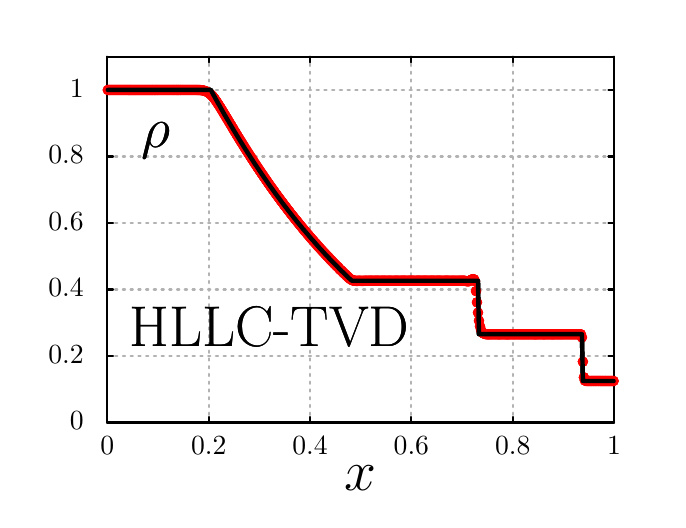
\begin{tikzpicture}[gnuplot]
%% generated with GNUPLOT 4.6p4 (Lua 5.1; terminal rev. 99, script rev. 100)
%% Wed 27 Aug 2014 02:20:25 PM EDT
\path (0.000,0.000) rectangle (8.000,6.000);
\gpfill{rgb color={1.000,1.000,1.000}} (1.012,0.985)--(7.446,0.985)--(7.446,5.630)--(1.012,5.630)--cycle;
\gpcolor{color=gp lt color border}
\gpsetlinetype{gp lt border}
\gpsetlinewidth{1.00}
\draw[gp path] (1.012,0.985)--(1.012,5.630)--(7.446,5.630)--(7.446,0.985)--cycle;
\gpcolor{color=gp lt color axes}
\gpsetlinetype{gp lt axes}
\gpsetlinewidth{2.00}
\draw[gp path] (1.012,0.985)--(7.447,0.985);
\gpcolor{color=gp lt color border}
\gpsetlinetype{gp lt border}
\draw[gp path] (1.012,0.985)--(1.084,0.985);
\draw[gp path] (7.447,0.985)--(7.375,0.985);
\gpcolor{rgb color={0.000,0.000,0.000}}
\node[gp node right,font={\fontsize{10pt}{12pt}\selectfont}] at (0.828,0.985) {0};
\gpcolor{color=gp lt color axes}
\gpsetlinetype{gp lt axes}
\draw[gp path] (1.012,1.830)--(7.447,1.830);
\gpcolor{color=gp lt color border}
\gpsetlinetype{gp lt border}
\draw[gp path] (1.012,1.830)--(1.084,1.830);
\draw[gp path] (7.447,1.830)--(7.375,1.830);
\gpcolor{rgb color={0.000,0.000,0.000}}
\node[gp node right,font={\fontsize{10pt}{12pt}\selectfont}] at (0.828,1.830) {0.2};
\gpcolor{color=gp lt color axes}
\gpsetlinetype{gp lt axes}
\draw[gp path] (1.012,2.674)--(7.447,2.674);
\gpcolor{color=gp lt color border}
\gpsetlinetype{gp lt border}
\draw[gp path] (1.012,2.674)--(1.084,2.674);
\draw[gp path] (7.447,2.674)--(7.375,2.674);
\gpcolor{rgb color={0.000,0.000,0.000}}
\node[gp node right,font={\fontsize{10pt}{12pt}\selectfont}] at (0.828,2.674) {0.4};
\gpcolor{color=gp lt color axes}
\gpsetlinetype{gp lt axes}
\draw[gp path] (1.012,3.519)--(7.447,3.519);
\gpcolor{color=gp lt color border}
\gpsetlinetype{gp lt border}
\draw[gp path] (1.012,3.519)--(1.084,3.519);
\draw[gp path] (7.447,3.519)--(7.375,3.519);
\gpcolor{rgb color={0.000,0.000,0.000}}
\node[gp node right,font={\fontsize{10pt}{12pt}\selectfont}] at (0.828,3.519) {0.6};
\gpcolor{color=gp lt color axes}
\gpsetlinetype{gp lt axes}
\draw[gp path] (1.012,4.364)--(7.447,4.364);
\gpcolor{color=gp lt color border}
\gpsetlinetype{gp lt border}
\draw[gp path] (1.012,4.364)--(1.084,4.364);
\draw[gp path] (7.447,4.364)--(7.375,4.364);
\gpcolor{rgb color={0.000,0.000,0.000}}
\node[gp node right,font={\fontsize{10pt}{12pt}\selectfont}] at (0.828,4.364) {0.8};
\gpcolor{color=gp lt color axes}
\gpsetlinetype{gp lt axes}
\draw[gp path] (1.012,5.209)--(7.447,5.209);
\gpcolor{color=gp lt color border}
\gpsetlinetype{gp lt border}
\draw[gp path] (1.012,5.209)--(1.084,5.209);
\draw[gp path] (7.447,5.209)--(7.375,5.209);
\gpcolor{rgb color={0.000,0.000,0.000}}
\node[gp node right,font={\fontsize{10pt}{12pt}\selectfont}] at (0.828,5.209) {1};
\gpcolor{color=gp lt color axes}
\gpsetlinetype{gp lt axes}
\draw[gp path] (1.012,0.985)--(1.012,5.631);
\gpcolor{color=gp lt color border}
\gpsetlinetype{gp lt border}
\draw[gp path] (1.012,0.985)--(1.012,1.057);
\draw[gp path] (1.012,5.631)--(1.012,5.559);
\gpcolor{rgb color={0.000,0.000,0.000}}
\node[gp node center,font={\fontsize{10pt}{12pt}\selectfont}] at (1.012,0.677) {0};
\gpcolor{color=gp lt color axes}
\gpsetlinetype{gp lt axes}
\draw[gp path] (2.299,0.985)--(2.299,5.631);
\gpcolor{color=gp lt color border}
\gpsetlinetype{gp lt border}
\draw[gp path] (2.299,0.985)--(2.299,1.057);
\draw[gp path] (2.299,5.631)--(2.299,5.559);
\gpcolor{rgb color={0.000,0.000,0.000}}
\node[gp node center,font={\fontsize{10pt}{12pt}\selectfont}] at (2.299,0.677) {0.2};
\gpcolor{color=gp lt color axes}
\gpsetlinetype{gp lt axes}
\draw[gp path] (3.586,0.985)--(3.586,5.631);
\gpcolor{color=gp lt color border}
\gpsetlinetype{gp lt border}
\draw[gp path] (3.586,0.985)--(3.586,1.057);
\draw[gp path] (3.586,5.631)--(3.586,5.559);
\gpcolor{rgb color={0.000,0.000,0.000}}
\node[gp node center,font={\fontsize{10pt}{12pt}\selectfont}] at (3.586,0.677) {0.4};
\gpcolor{color=gp lt color axes}
\gpsetlinetype{gp lt axes}
\draw[gp path] (4.873,0.985)--(4.873,5.631);
\gpcolor{color=gp lt color border}
\gpsetlinetype{gp lt border}
\draw[gp path] (4.873,0.985)--(4.873,1.057);
\draw[gp path] (4.873,5.631)--(4.873,5.559);
\gpcolor{rgb color={0.000,0.000,0.000}}
\node[gp node center,font={\fontsize{10pt}{12pt}\selectfont}] at (4.873,0.677) {0.6};
\gpcolor{color=gp lt color axes}
\gpsetlinetype{gp lt axes}
\draw[gp path] (6.160,0.985)--(6.160,5.631);
\gpcolor{color=gp lt color border}
\gpsetlinetype{gp lt border}
\draw[gp path] (6.160,0.985)--(6.160,1.057);
\draw[gp path] (6.160,5.631)--(6.160,5.559);
\gpcolor{rgb color={0.000,0.000,0.000}}
\node[gp node center,font={\fontsize{10pt}{12pt}\selectfont}] at (6.160,0.677) {0.8};
\gpcolor{color=gp lt color axes}
\gpsetlinetype{gp lt axes}
\draw[gp path] (7.447,0.985)--(7.447,5.631);
\gpcolor{color=gp lt color border}
\gpsetlinetype{gp lt border}
\draw[gp path] (7.447,0.985)--(7.447,1.057);
\draw[gp path] (7.447,5.631)--(7.447,5.559);
\gpcolor{rgb color={0.000,0.000,0.000}}
\node[gp node center,font={\fontsize{10pt}{12pt}\selectfont}] at (7.447,0.677) {1};
\gpcolor{color=gp lt color border}
\draw[gp path] (1.012,5.631)--(1.012,0.985)--(7.447,0.985)--(7.447,5.631)--cycle;
\gpcolor{rgb color={0.000,0.000,0.000}}
\node[gp node center,font={\fontsize{10pt}{12pt}\selectfont}] at (4.229,0.215) {\huge $x$};
\gpcolor{rgb color={1.000,0.000,0.000}}
\gpsetlinewidth{0.50}
\gpsetpointsize{4.44}
\gppoint{gp mark 7}{(1.018,5.209)}
\gppoint{gp mark 7}{(1.031,5.209)}
\gppoint{gp mark 7}{(1.043,5.209)}
\gppoint{gp mark 7}{(1.056,5.209)}
\gppoint{gp mark 7}{(1.069,5.209)}
\gppoint{gp mark 7}{(1.081,5.209)}
\gppoint{gp mark 7}{(1.094,5.209)}
\gppoint{gp mark 7}{(1.106,5.209)}
\gppoint{gp mark 7}{(1.119,5.209)}
\gppoint{gp mark 7}{(1.131,5.209)}
\gppoint{gp mark 7}{(1.144,5.209)}
\gppoint{gp mark 7}{(1.157,5.209)}
\gppoint{gp mark 7}{(1.169,5.209)}
\gppoint{gp mark 7}{(1.182,5.209)}
\gppoint{gp mark 7}{(1.194,5.209)}
\gppoint{gp mark 7}{(1.207,5.209)}
\gppoint{gp mark 7}{(1.219,5.209)}
\gppoint{gp mark 7}{(1.232,5.209)}
\gppoint{gp mark 7}{(1.245,5.209)}
\gppoint{gp mark 7}{(1.257,5.209)}
\gppoint{gp mark 7}{(1.270,5.209)}
\gppoint{gp mark 7}{(1.282,5.209)}
\gppoint{gp mark 7}{(1.295,5.209)}
\gppoint{gp mark 7}{(1.307,5.209)}
\gppoint{gp mark 7}{(1.320,5.209)}
\gppoint{gp mark 7}{(1.332,5.209)}
\gppoint{gp mark 7}{(1.345,5.209)}
\gppoint{gp mark 7}{(1.358,5.209)}
\gppoint{gp mark 7}{(1.370,5.209)}
\gppoint{gp mark 7}{(1.383,5.209)}
\gppoint{gp mark 7}{(1.395,5.209)}
\gppoint{gp mark 7}{(1.408,5.209)}
\gppoint{gp mark 7}{(1.420,5.209)}
\gppoint{gp mark 7}{(1.433,5.209)}
\gppoint{gp mark 7}{(1.446,5.209)}
\gppoint{gp mark 7}{(1.458,5.209)}
\gppoint{gp mark 7}{(1.471,5.209)}
\gppoint{gp mark 7}{(1.483,5.209)}
\gppoint{gp mark 7}{(1.496,5.209)}
\gppoint{gp mark 7}{(1.508,5.209)}
\gppoint{gp mark 7}{(1.521,5.209)}
\gppoint{gp mark 7}{(1.534,5.209)}
\gppoint{gp mark 7}{(1.546,5.209)}
\gppoint{gp mark 7}{(1.559,5.209)}
\gppoint{gp mark 7}{(1.571,5.209)}
\gppoint{gp mark 7}{(1.584,5.209)}
\gppoint{gp mark 7}{(1.596,5.209)}
\gppoint{gp mark 7}{(1.609,5.209)}
\gppoint{gp mark 7}{(1.622,5.209)}
\gppoint{gp mark 7}{(1.634,5.209)}
\gppoint{gp mark 7}{(1.647,5.209)}
\gppoint{gp mark 7}{(1.659,5.209)}
\gppoint{gp mark 7}{(1.672,5.209)}
\gppoint{gp mark 7}{(1.684,5.209)}
\gppoint{gp mark 7}{(1.697,5.209)}
\gppoint{gp mark 7}{(1.710,5.209)}
\gppoint{gp mark 7}{(1.722,5.209)}
\gppoint{gp mark 7}{(1.735,5.209)}
\gppoint{gp mark 7}{(1.747,5.209)}
\gppoint{gp mark 7}{(1.760,5.209)}
\gppoint{gp mark 7}{(1.772,5.209)}
\gppoint{gp mark 7}{(1.785,5.209)}
\gppoint{gp mark 7}{(1.798,5.209)}
\gppoint{gp mark 7}{(1.810,5.209)}
\gppoint{gp mark 7}{(1.823,5.209)}
\gppoint{gp mark 7}{(1.835,5.209)}
\gppoint{gp mark 7}{(1.848,5.209)}
\gppoint{gp mark 7}{(1.860,5.209)}
\gppoint{gp mark 7}{(1.873,5.209)}
\gppoint{gp mark 7}{(1.886,5.209)}
\gppoint{gp mark 7}{(1.898,5.209)}
\gppoint{gp mark 7}{(1.911,5.209)}
\gppoint{gp mark 7}{(1.923,5.209)}
\gppoint{gp mark 7}{(1.936,5.209)}
\gppoint{gp mark 7}{(1.948,5.209)}
\gppoint{gp mark 7}{(1.961,5.209)}
\gppoint{gp mark 7}{(1.973,5.209)}
\gppoint{gp mark 7}{(1.986,5.209)}
\gppoint{gp mark 7}{(1.999,5.209)}
\gppoint{gp mark 7}{(2.011,5.209)}
\gppoint{gp mark 7}{(2.024,5.209)}
\gppoint{gp mark 7}{(2.036,5.209)}
\gppoint{gp mark 7}{(2.049,5.209)}
\gppoint{gp mark 7}{(2.061,5.209)}
\gppoint{gp mark 7}{(2.074,5.209)}
\gppoint{gp mark 7}{(2.087,5.209)}
\gppoint{gp mark 7}{(2.099,5.209)}
\gppoint{gp mark 7}{(2.112,5.209)}
\gppoint{gp mark 7}{(2.124,5.209)}
\gppoint{gp mark 7}{(2.137,5.209)}
\gppoint{gp mark 7}{(2.149,5.209)}
\gppoint{gp mark 7}{(2.162,5.208)}
\gppoint{gp mark 7}{(2.175,5.208)}
\gppoint{gp mark 7}{(2.187,5.208)}
\gppoint{gp mark 7}{(2.200,5.207)}
\gppoint{gp mark 7}{(2.212,5.206)}
\gppoint{gp mark 7}{(2.225,5.204)}
\gppoint{gp mark 7}{(2.237,5.200)}
\gppoint{gp mark 7}{(2.250,5.197)}
\gppoint{gp mark 7}{(2.263,5.192)}
\gppoint{gp mark 7}{(2.275,5.187)}
\gppoint{gp mark 7}{(2.288,5.179)}
\gppoint{gp mark 7}{(2.300,5.172)}
\gppoint{gp mark 7}{(2.313,5.161)}
\gppoint{gp mark 7}{(2.325,5.151)}
\gppoint{gp mark 7}{(2.338,5.138)}
\gppoint{gp mark 7}{(2.351,5.125)}
\gppoint{gp mark 7}{(2.363,5.109)}
\gppoint{gp mark 7}{(2.376,5.094)}
\gppoint{gp mark 7}{(2.388,5.075)}
\gppoint{gp mark 7}{(2.401,5.058)}
\gppoint{gp mark 7}{(2.413,5.038)}
\gppoint{gp mark 7}{(2.426,5.020)}
\gppoint{gp mark 7}{(2.439,4.998)}
\gppoint{gp mark 7}{(2.451,4.980)}
\gppoint{gp mark 7}{(2.464,4.958)}
\gppoint{gp mark 7}{(2.476,4.939)}
\gppoint{gp mark 7}{(2.489,4.916)}
\gppoint{gp mark 7}{(2.501,4.897)}
\gppoint{gp mark 7}{(2.514,4.876)}
\gppoint{gp mark 7}{(2.526,4.855)}
\gppoint{gp mark 7}{(2.539,4.835)}
\gppoint{gp mark 7}{(2.552,4.812)}
\gppoint{gp mark 7}{(2.564,4.793)}
\gppoint{gp mark 7}{(2.577,4.770)}
\gppoint{gp mark 7}{(2.589,4.752)}
\gppoint{gp mark 7}{(2.602,4.728)}
\gppoint{gp mark 7}{(2.614,4.710)}
\gppoint{gp mark 7}{(2.627,4.686)}
\gppoint{gp mark 7}{(2.640,4.668)}
\gppoint{gp mark 7}{(2.652,4.645)}
\gppoint{gp mark 7}{(2.665,4.626)}
\gppoint{gp mark 7}{(2.677,4.605)}
\gppoint{gp mark 7}{(2.690,4.585)}
\gppoint{gp mark 7}{(2.702,4.564)}
\gppoint{gp mark 7}{(2.715,4.545)}
\gppoint{gp mark 7}{(2.728,4.524)}
\gppoint{gp mark 7}{(2.740,4.504)}
\gppoint{gp mark 7}{(2.753,4.484)}
\gppoint{gp mark 7}{(2.765,4.464)}
\gppoint{gp mark 7}{(2.778,4.444)}
\gppoint{gp mark 7}{(2.790,4.425)}
\gppoint{gp mark 7}{(2.803,4.405)}
\gppoint{gp mark 7}{(2.816,4.385)}
\gppoint{gp mark 7}{(2.828,4.365)}
\gppoint{gp mark 7}{(2.841,4.347)}
\gppoint{gp mark 7}{(2.853,4.327)}
\gppoint{gp mark 7}{(2.866,4.308)}
\gppoint{gp mark 7}{(2.878,4.288)}
\gppoint{gp mark 7}{(2.891,4.270)}
\gppoint{gp mark 7}{(2.904,4.250)}
\gppoint{gp mark 7}{(2.916,4.231)}
\gppoint{gp mark 7}{(2.929,4.213)}
\gppoint{gp mark 7}{(2.941,4.194)}
\gppoint{gp mark 7}{(2.954,4.175)}
\gppoint{gp mark 7}{(2.966,4.157)}
\gppoint{gp mark 7}{(2.979,4.138)}
\gppoint{gp mark 7}{(2.992,4.120)}
\gppoint{gp mark 7}{(3.004,4.101)}
\gppoint{gp mark 7}{(3.017,4.083)}
\gppoint{gp mark 7}{(3.029,4.065)}
\gppoint{gp mark 7}{(3.042,4.047)}
\gppoint{gp mark 7}{(3.054,4.029)}
\gppoint{gp mark 7}{(3.067,4.011)}
\gppoint{gp mark 7}{(3.079,3.993)}
\gppoint{gp mark 7}{(3.092,3.975)}
\gppoint{gp mark 7}{(3.105,3.957)}
\gppoint{gp mark 7}{(3.117,3.940)}
\gppoint{gp mark 7}{(3.130,3.923)}
\gppoint{gp mark 7}{(3.142,3.905)}
\gppoint{gp mark 7}{(3.155,3.888)}
\gppoint{gp mark 7}{(3.167,3.871)}
\gppoint{gp mark 7}{(3.180,3.853)}
\gppoint{gp mark 7}{(3.193,3.837)}
\gppoint{gp mark 7}{(3.205,3.819)}
\gppoint{gp mark 7}{(3.218,3.802)}
\gppoint{gp mark 7}{(3.230,3.786)}
\gppoint{gp mark 7}{(3.243,3.769)}
\gppoint{gp mark 7}{(3.255,3.752)}
\gppoint{gp mark 7}{(3.268,3.735)}
\gppoint{gp mark 7}{(3.281,3.719)}
\gppoint{gp mark 7}{(3.293,3.703)}
\gppoint{gp mark 7}{(3.306,3.686)}
\gppoint{gp mark 7}{(3.318,3.670)}
\gppoint{gp mark 7}{(3.331,3.654)}
\gppoint{gp mark 7}{(3.343,3.637)}
\gppoint{gp mark 7}{(3.356,3.622)}
\gppoint{gp mark 7}{(3.369,3.605)}
\gppoint{gp mark 7}{(3.381,3.590)}
\gppoint{gp mark 7}{(3.394,3.573)}
\gppoint{gp mark 7}{(3.406,3.559)}
\gppoint{gp mark 7}{(3.419,3.543)}
\gppoint{gp mark 7}{(3.431,3.527)}
\gppoint{gp mark 7}{(3.444,3.512)}
\gppoint{gp mark 7}{(3.457,3.496)}
\gppoint{gp mark 7}{(3.469,3.480)}
\gppoint{gp mark 7}{(3.482,3.466)}
\gppoint{gp mark 7}{(3.494,3.450)}
\gppoint{gp mark 7}{(3.507,3.435)}
\gppoint{gp mark 7}{(3.519,3.420)}
\gppoint{gp mark 7}{(3.532,3.406)}
\gppoint{gp mark 7}{(3.545,3.390)}
\gppoint{gp mark 7}{(3.557,3.375)}
\gppoint{gp mark 7}{(3.570,3.361)}
\gppoint{gp mark 7}{(3.582,3.346)}
\gppoint{gp mark 7}{(3.595,3.331)}
\gppoint{gp mark 7}{(3.607,3.317)}
\gppoint{gp mark 7}{(3.620,3.303)}
\gppoint{gp mark 7}{(3.633,3.288)}
\gppoint{gp mark 7}{(3.645,3.273)}
\gppoint{gp mark 7}{(3.658,3.260)}
\gppoint{gp mark 7}{(3.670,3.246)}
\gppoint{gp mark 7}{(3.683,3.231)}
\gppoint{gp mark 7}{(3.695,3.217)}
\gppoint{gp mark 7}{(3.708,3.204)}
\gppoint{gp mark 7}{(3.720,3.190)}
\gppoint{gp mark 7}{(3.733,3.176)}
\gppoint{gp mark 7}{(3.746,3.161)}
\gppoint{gp mark 7}{(3.758,3.149)}
\gppoint{gp mark 7}{(3.771,3.135)}
\gppoint{gp mark 7}{(3.783,3.121)}
\gppoint{gp mark 7}{(3.796,3.107)}
\gppoint{gp mark 7}{(3.808,3.095)}
\gppoint{gp mark 7}{(3.821,3.082)}
\gppoint{gp mark 7}{(3.834,3.067)}
\gppoint{gp mark 7}{(3.846,3.054)}
\gppoint{gp mark 7}{(3.859,3.042)}
\gppoint{gp mark 7}{(3.871,3.029)}
\gppoint{gp mark 7}{(3.884,3.015)}
\gppoint{gp mark 7}{(3.896,3.002)}
\gppoint{gp mark 7}{(3.909,2.990)}
\gppoint{gp mark 7}{(3.922,2.975)}
\gppoint{gp mark 7}{(3.934,2.965)}
\gppoint{gp mark 7}{(3.947,2.954)}
\gppoint{gp mark 7}{(3.959,2.937)}
\gppoint{gp mark 7}{(3.972,2.923)}
\gppoint{gp mark 7}{(3.984,2.916)}
\gppoint{gp mark 7}{(3.997,2.903)}
\gppoint{gp mark 7}{(4.010,2.888)}
\gppoint{gp mark 7}{(4.022,2.876)}
\gppoint{gp mark 7}{(4.035,2.866)}
\gppoint{gp mark 7}{(4.047,2.853)}
\gppoint{gp mark 7}{(4.060,2.842)}
\gppoint{gp mark 7}{(4.072,2.830)}
\gppoint{gp mark 7}{(4.085,2.818)}
\gppoint{gp mark 7}{(4.098,2.808)}
\gppoint{gp mark 7}{(4.110,2.800)}
\gppoint{gp mark 7}{(4.123,2.791)}
\gppoint{gp mark 7}{(4.135,2.790)}
\gppoint{gp mark 7}{(4.148,2.788)}
\gppoint{gp mark 7}{(4.160,2.786)}
\gppoint{gp mark 7}{(4.173,2.784)}
\gppoint{gp mark 7}{(4.186,2.784)}
\gppoint{gp mark 7}{(4.198,2.785)}
\gppoint{gp mark 7}{(4.211,2.785)}
\gppoint{gp mark 7}{(4.223,2.785)}
\gppoint{gp mark 7}{(4.236,2.784)}
\gppoint{gp mark 7}{(4.248,2.784)}
\gppoint{gp mark 7}{(4.261,2.784)}
\gppoint{gp mark 7}{(4.273,2.785)}
\gppoint{gp mark 7}{(4.286,2.785)}
\gppoint{gp mark 7}{(4.299,2.786)}
\gppoint{gp mark 7}{(4.311,2.785)}
\gppoint{gp mark 7}{(4.324,2.785)}
\gppoint{gp mark 7}{(4.336,2.785)}
\gppoint{gp mark 7}{(4.349,2.786)}
\gppoint{gp mark 7}{(4.361,2.786)}
\gppoint{gp mark 7}{(4.374,2.786)}
\gppoint{gp mark 7}{(4.387,2.785)}
\gppoint{gp mark 7}{(4.399,2.785)}
\gppoint{gp mark 7}{(4.412,2.785)}
\gppoint{gp mark 7}{(4.424,2.786)}
\gppoint{gp mark 7}{(4.437,2.786)}
\gppoint{gp mark 7}{(4.449,2.786)}
\gppoint{gp mark 7}{(4.462,2.785)}
\gppoint{gp mark 7}{(4.475,2.785)}
\gppoint{gp mark 7}{(4.487,2.785)}
\gppoint{gp mark 7}{(4.500,2.786)}
\gppoint{gp mark 7}{(4.512,2.786)}
\gppoint{gp mark 7}{(4.525,2.786)}
\gppoint{gp mark 7}{(4.537,2.786)}
\gppoint{gp mark 7}{(4.550,2.785)}
\gppoint{gp mark 7}{(4.563,2.785)}
\gppoint{gp mark 7}{(4.575,2.785)}
\gppoint{gp mark 7}{(4.588,2.786)}
\gppoint{gp mark 7}{(4.600,2.786)}
\gppoint{gp mark 7}{(4.613,2.786)}
\gppoint{gp mark 7}{(4.625,2.785)}
\gppoint{gp mark 7}{(4.638,2.785)}
\gppoint{gp mark 7}{(4.651,2.785)}
\gppoint{gp mark 7}{(4.663,2.786)}
\gppoint{gp mark 7}{(4.676,2.786)}
\gppoint{gp mark 7}{(4.688,2.786)}
\gppoint{gp mark 7}{(4.701,2.786)}
\gppoint{gp mark 7}{(4.713,2.785)}
\gppoint{gp mark 7}{(4.726,2.785)}
\gppoint{gp mark 7}{(4.739,2.785)}
\gppoint{gp mark 7}{(4.751,2.786)}
\gppoint{gp mark 7}{(4.764,2.786)}
\gppoint{gp mark 7}{(4.776,2.786)}
\gppoint{gp mark 7}{(4.789,2.786)}
\gppoint{gp mark 7}{(4.801,2.785)}
\gppoint{gp mark 7}{(4.814,2.785)}
\gppoint{gp mark 7}{(4.826,2.785)}
\gppoint{gp mark 7}{(4.839,2.786)}
\gppoint{gp mark 7}{(4.852,2.786)}
\gppoint{gp mark 7}{(4.864,2.786)}
\gppoint{gp mark 7}{(4.877,2.786)}
\gppoint{gp mark 7}{(4.889,2.786)}
\gppoint{gp mark 7}{(4.902,2.785)}
\gppoint{gp mark 7}{(4.914,2.785)}
\gppoint{gp mark 7}{(4.927,2.785)}
\gppoint{gp mark 7}{(4.940,2.786)}
\gppoint{gp mark 7}{(4.952,2.786)}
\gppoint{gp mark 7}{(4.965,2.786)}
\gppoint{gp mark 7}{(4.977,2.786)}
\gppoint{gp mark 7}{(4.990,2.785)}
\gppoint{gp mark 7}{(5.002,2.785)}
\gppoint{gp mark 7}{(5.015,2.785)}
\gppoint{gp mark 7}{(5.028,2.786)}
\gppoint{gp mark 7}{(5.040,2.786)}
\gppoint{gp mark 7}{(5.053,2.786)}
\gppoint{gp mark 7}{(5.065,2.786)}
\gppoint{gp mark 7}{(5.078,2.785)}
\gppoint{gp mark 7}{(5.090,2.785)}
\gppoint{gp mark 7}{(5.103,2.785)}
\gppoint{gp mark 7}{(5.116,2.786)}
\gppoint{gp mark 7}{(5.128,2.786)}
\gppoint{gp mark 7}{(5.141,2.786)}
\gppoint{gp mark 7}{(5.153,2.786)}
\gppoint{gp mark 7}{(5.166,2.785)}
\gppoint{gp mark 7}{(5.178,2.785)}
\gppoint{gp mark 7}{(5.191,2.785)}
\gppoint{gp mark 7}{(5.204,2.786)}
\gppoint{gp mark 7}{(5.216,2.786)}
\gppoint{gp mark 7}{(5.229,2.786)}
\gppoint{gp mark 7}{(5.241,2.786)}
\gppoint{gp mark 7}{(5.254,2.785)}
\gppoint{gp mark 7}{(5.266,2.785)}
\gppoint{gp mark 7}{(5.279,2.785)}
\gppoint{gp mark 7}{(5.292,2.785)}
\gppoint{gp mark 7}{(5.304,2.786)}
\gppoint{gp mark 7}{(5.317,2.786)}
\gppoint{gp mark 7}{(5.329,2.786)}
\gppoint{gp mark 7}{(5.342,2.786)}
\gppoint{gp mark 7}{(5.354,2.785)}
\gppoint{gp mark 7}{(5.367,2.785)}
\gppoint{gp mark 7}{(5.380,2.785)}
\gppoint{gp mark 7}{(5.392,2.785)}
\gppoint{gp mark 7}{(5.405,2.786)}
\gppoint{gp mark 7}{(5.417,2.785)}
\gppoint{gp mark 7}{(5.430,2.785)}
\gppoint{gp mark 7}{(5.442,2.785)}
\gppoint{gp mark 7}{(5.455,2.785)}
\gppoint{gp mark 7}{(5.467,2.785)}
\gppoint{gp mark 7}{(5.480,2.785)}
\gppoint{gp mark 7}{(5.493,2.786)}
\gppoint{gp mark 7}{(5.505,2.786)}
\gppoint{gp mark 7}{(5.518,2.786)}
\gppoint{gp mark 7}{(5.530,2.786)}
\gppoint{gp mark 7}{(5.543,2.786)}
\gppoint{gp mark 7}{(5.555,2.784)}
\gppoint{gp mark 7}{(5.568,2.782)}
\gppoint{gp mark 7}{(5.581,2.780)}
\gppoint{gp mark 7}{(5.593,2.780)}
\gppoint{gp mark 7}{(5.606,2.781)}
\gppoint{gp mark 7}{(5.618,2.789)}
\gppoint{gp mark 7}{(5.631,2.797)}
\gppoint{gp mark 7}{(5.643,2.804)}
\gppoint{gp mark 7}{(5.656,2.806)}
\gppoint{gp mark 7}{(5.669,2.804)}
\gppoint{gp mark 7}{(5.681,2.779)}
\gppoint{gp mark 7}{(5.694,2.654)}
\gppoint{gp mark 7}{(5.706,2.512)}
\gppoint{gp mark 7}{(5.719,2.381)}
\gppoint{gp mark 7}{(5.731,2.279)}
\gppoint{gp mark 7}{(5.744,2.207)}
\gppoint{gp mark 7}{(5.757,2.162)}
\gppoint{gp mark 7}{(5.769,2.136)}
\gppoint{gp mark 7}{(5.782,2.121)}
\gppoint{gp mark 7}{(5.794,2.114)}
\gppoint{gp mark 7}{(5.807,2.110)}
\gppoint{gp mark 7}{(5.819,2.108)}
\gppoint{gp mark 7}{(5.832,2.107)}
\gppoint{gp mark 7}{(5.845,2.106)}
\gppoint{gp mark 7}{(5.857,2.106)}
\gppoint{gp mark 7}{(5.870,2.106)}
\gppoint{gp mark 7}{(5.882,2.107)}
\gppoint{gp mark 7}{(5.895,2.107)}
\gppoint{gp mark 7}{(5.907,2.107)}
\gppoint{gp mark 7}{(5.920,2.107)}
\gppoint{gp mark 7}{(5.933,2.107)}
\gppoint{gp mark 7}{(5.945,2.107)}
\gppoint{gp mark 7}{(5.958,2.107)}
\gppoint{gp mark 7}{(5.970,2.106)}
\gppoint{gp mark 7}{(5.983,2.106)}
\gppoint{gp mark 7}{(5.995,2.106)}
\gppoint{gp mark 7}{(6.008,2.107)}
\gppoint{gp mark 7}{(6.020,2.107)}
\gppoint{gp mark 7}{(6.033,2.107)}
\gppoint{gp mark 7}{(6.046,2.107)}
\gppoint{gp mark 7}{(6.058,2.107)}
\gppoint{gp mark 7}{(6.071,2.106)}
\gppoint{gp mark 7}{(6.083,2.106)}
\gppoint{gp mark 7}{(6.096,2.106)}
\gppoint{gp mark 7}{(6.108,2.106)}
\gppoint{gp mark 7}{(6.121,2.107)}
\gppoint{gp mark 7}{(6.134,2.107)}
\gppoint{gp mark 7}{(6.146,2.107)}
\gppoint{gp mark 7}{(6.159,2.107)}
\gppoint{gp mark 7}{(6.171,2.107)}
\gppoint{gp mark 7}{(6.184,2.107)}
\gppoint{gp mark 7}{(6.196,2.107)}
\gppoint{gp mark 7}{(6.209,2.107)}
\gppoint{gp mark 7}{(6.222,2.107)}
\gppoint{gp mark 7}{(6.234,2.107)}
\gppoint{gp mark 7}{(6.247,2.107)}
\gppoint{gp mark 7}{(6.259,2.107)}
\gppoint{gp mark 7}{(6.272,2.107)}
\gppoint{gp mark 7}{(6.284,2.107)}
\gppoint{gp mark 7}{(6.297,2.107)}
\gppoint{gp mark 7}{(6.310,2.107)}
\gppoint{gp mark 7}{(6.322,2.107)}
\gppoint{gp mark 7}{(6.335,2.107)}
\gppoint{gp mark 7}{(6.347,2.107)}
\gppoint{gp mark 7}{(6.360,2.107)}
\gppoint{gp mark 7}{(6.372,2.107)}
\gppoint{gp mark 7}{(6.385,2.107)}
\gppoint{gp mark 7}{(6.398,2.107)}
\gppoint{gp mark 7}{(6.410,2.107)}
\gppoint{gp mark 7}{(6.423,2.107)}
\gppoint{gp mark 7}{(6.435,2.106)}
\gppoint{gp mark 7}{(6.448,2.106)}
\gppoint{gp mark 7}{(6.460,2.106)}
\gppoint{gp mark 7}{(6.473,2.107)}
\gppoint{gp mark 7}{(6.486,2.107)}
\gppoint{gp mark 7}{(6.498,2.107)}
\gppoint{gp mark 7}{(6.511,2.107)}
\gppoint{gp mark 7}{(6.523,2.107)}
\gppoint{gp mark 7}{(6.536,2.107)}
\gppoint{gp mark 7}{(6.548,2.106)}
\gppoint{gp mark 7}{(6.561,2.106)}
\gppoint{gp mark 7}{(6.573,2.107)}
\gppoint{gp mark 7}{(6.586,2.107)}
\gppoint{gp mark 7}{(6.599,2.107)}
\gppoint{gp mark 7}{(6.611,2.107)}
\gppoint{gp mark 7}{(6.624,2.107)}
\gppoint{gp mark 7}{(6.636,2.107)}
\gppoint{gp mark 7}{(6.649,2.107)}
\gppoint{gp mark 7}{(6.661,2.106)}
\gppoint{gp mark 7}{(6.674,2.106)}
\gppoint{gp mark 7}{(6.687,2.107)}
\gppoint{gp mark 7}{(6.699,2.107)}
\gppoint{gp mark 7}{(6.712,2.107)}
\gppoint{gp mark 7}{(6.724,2.107)}
\gppoint{gp mark 7}{(6.737,2.107)}
\gppoint{gp mark 7}{(6.749,2.107)}
\gppoint{gp mark 7}{(6.762,2.107)}
\gppoint{gp mark 7}{(6.775,2.107)}
\gppoint{gp mark 7}{(6.787,2.107)}
\gppoint{gp mark 7}{(6.800,2.107)}
\gppoint{gp mark 7}{(6.812,2.107)}
\gppoint{gp mark 7}{(6.825,2.107)}
\gppoint{gp mark 7}{(6.837,2.107)}
\gppoint{gp mark 7}{(6.850,2.107)}
\gppoint{gp mark 7}{(6.863,2.107)}
\gppoint{gp mark 7}{(6.875,2.107)}
\gppoint{gp mark 7}{(6.888,2.107)}
\gppoint{gp mark 7}{(6.900,2.107)}
\gppoint{gp mark 7}{(6.913,2.107)}
\gppoint{gp mark 7}{(6.925,2.107)}
\gppoint{gp mark 7}{(6.938,2.107)}
\gppoint{gp mark 7}{(6.951,2.107)}
\gppoint{gp mark 7}{(6.963,2.107)}
\gppoint{gp mark 7}{(6.976,2.107)}
\gppoint{gp mark 7}{(6.988,2.107)}
\gppoint{gp mark 7}{(7.001,2.107)}
\gppoint{gp mark 7}{(7.013,2.107)}
\gppoint{gp mark 7}{(7.026,2.106)}
\gppoint{gp mark 7}{(7.039,2.067)}
\gppoint{gp mark 7}{(7.051,1.758)}
\gppoint{gp mark 7}{(7.064,1.560)}
\gppoint{gp mark 7}{(7.076,1.519)}
\gppoint{gp mark 7}{(7.089,1.514)}
\gppoint{gp mark 7}{(7.101,1.513)}
\gppoint{gp mark 7}{(7.114,1.513)}
\gppoint{gp mark 7}{(7.127,1.513)}
\gppoint{gp mark 7}{(7.139,1.513)}
\gppoint{gp mark 7}{(7.152,1.513)}
\gppoint{gp mark 7}{(7.164,1.513)}
\gppoint{gp mark 7}{(7.177,1.513)}
\gppoint{gp mark 7}{(7.189,1.513)}
\gppoint{gp mark 7}{(7.202,1.513)}
\gppoint{gp mark 7}{(7.214,1.513)}
\gppoint{gp mark 7}{(7.227,1.513)}
\gppoint{gp mark 7}{(7.240,1.513)}
\gppoint{gp mark 7}{(7.252,1.513)}
\gppoint{gp mark 7}{(7.265,1.513)}
\gppoint{gp mark 7}{(7.277,1.513)}
\gppoint{gp mark 7}{(7.290,1.513)}
\gppoint{gp mark 7}{(7.302,1.513)}
\gppoint{gp mark 7}{(7.315,1.513)}
\gppoint{gp mark 7}{(7.328,1.513)}
\gppoint{gp mark 7}{(7.340,1.513)}
\gppoint{gp mark 7}{(7.353,1.513)}
\gppoint{gp mark 7}{(7.365,1.513)}
\gppoint{gp mark 7}{(7.378,1.513)}
\gppoint{gp mark 7}{(7.390,1.513)}
\gppoint{gp mark 7}{(7.403,1.513)}
\gppoint{gp mark 7}{(7.416,1.513)}
\gppoint{gp mark 7}{(7.428,1.513)}
\gppoint{gp mark 7}{(7.441,1.513)}
\gpcolor{rgb color={0.000,0.000,0.000}}
\gpsetlinetype{gp lt plot 0}
\gpsetlinewidth{4.00}
\draw[gp path] (1.018,5.209)--(1.031,5.209)--(1.043,5.209)--(1.056,5.209)--(1.069,5.209)%
  --(1.081,5.209)--(1.094,5.209)--(1.106,5.209)--(1.119,5.209)--(1.131,5.209)--(1.144,5.209)%
  --(1.157,5.209)--(1.169,5.209)--(1.182,5.209)--(1.194,5.209)--(1.207,5.209)--(1.219,5.209)%
  --(1.232,5.209)--(1.245,5.209)--(1.257,5.209)--(1.270,5.209)--(1.282,5.209)--(1.295,5.209)%
  --(1.307,5.209)--(1.320,5.209)--(1.332,5.209)--(1.345,5.209)--(1.358,5.209)--(1.370,5.209)%
  --(1.383,5.209)--(1.395,5.209)--(1.408,5.209)--(1.420,5.209)--(1.433,5.209)--(1.446,5.209)%
  --(1.458,5.209)--(1.471,5.209)--(1.483,5.209)--(1.496,5.209)--(1.508,5.209)--(1.521,5.209)%
  --(1.534,5.209)--(1.546,5.209)--(1.559,5.209)--(1.571,5.209)--(1.584,5.209)--(1.596,5.209)%
  --(1.609,5.209)--(1.622,5.209)--(1.634,5.209)--(1.647,5.209)--(1.659,5.209)--(1.672,5.209)%
  --(1.684,5.209)--(1.697,5.209)--(1.710,5.209)--(1.722,5.209)--(1.735,5.209)--(1.747,5.209)%
  --(1.760,5.209)--(1.772,5.209)--(1.785,5.209)--(1.798,5.209)--(1.810,5.209)--(1.823,5.209)%
  --(1.835,5.209)--(1.848,5.209)--(1.860,5.209)--(1.873,5.209)--(1.886,5.209)--(1.898,5.209)%
  --(1.911,5.209)--(1.923,5.209)--(1.936,5.209)--(1.948,5.209)--(1.961,5.209)--(1.973,5.209)%
  --(1.986,5.209)--(1.999,5.209)--(2.011,5.209)--(2.024,5.209)--(2.036,5.209)--(2.049,5.209)%
  --(2.061,5.209)--(2.074,5.209)--(2.087,5.209)--(2.099,5.209)--(2.112,5.209)--(2.124,5.209)%
  --(2.137,5.209)--(2.149,5.209)--(2.162,5.209)--(2.175,5.209)--(2.187,5.209)--(2.200,5.209)%
  --(2.212,5.209)--(2.225,5.209)--(2.237,5.209)--(2.250,5.209)--(2.263,5.209)--(2.275,5.209)%
  --(2.288,5.209)--(2.300,5.209)--(2.313,5.209)--(2.325,5.209)--(2.338,5.187)--(2.351,5.163)%
  --(2.363,5.140)--(2.376,5.118)--(2.388,5.095)--(2.401,5.072)--(2.413,5.050)--(2.426,5.027)%
  --(2.439,5.005)--(2.451,4.982)--(2.464,4.960)--(2.476,4.938)--(2.489,4.916)--(2.501,4.894)%
  --(2.514,4.872)--(2.526,4.851)--(2.539,4.829)--(2.552,4.808)--(2.564,4.786)--(2.577,4.765)%
  --(2.589,4.744)--(2.602,4.723)--(2.614,4.702)--(2.627,4.681)--(2.640,4.660)--(2.652,4.639)%
  --(2.665,4.618)--(2.677,4.598)--(2.690,4.577)--(2.702,4.557)--(2.715,4.537)--(2.728,4.517)%
  --(2.740,4.496)--(2.753,4.476)--(2.765,4.456)--(2.778,4.437)--(2.790,4.417)--(2.803,4.397)%
  --(2.816,4.378)--(2.828,4.358)--(2.841,4.339)--(2.853,4.320)--(2.866,4.300)--(2.878,4.281)%
  --(2.891,4.262)--(2.904,4.243)--(2.916,4.225)--(2.929,4.206)--(2.941,4.187)--(2.954,4.169)%
  --(2.966,4.150)--(2.979,4.132)--(2.992,4.113)--(3.004,4.095)--(3.017,4.077)--(3.029,4.059)%
  --(3.042,4.041)--(3.054,4.023)--(3.067,4.005)--(3.079,3.987)--(3.092,3.970)--(3.105,3.952)%
  --(3.117,3.935)--(3.130,3.917)--(3.142,3.900)--(3.155,3.883)--(3.167,3.866)--(3.180,3.849)%
  --(3.193,3.832)--(3.205,3.815)--(3.218,3.798)--(3.230,3.781)--(3.243,3.764)--(3.255,3.748)%
  --(3.268,3.731)--(3.281,3.715)--(3.293,3.699)--(3.306,3.682)--(3.318,3.666)--(3.331,3.650)%
  --(3.343,3.634)--(3.356,3.618)--(3.369,3.602)--(3.381,3.586)--(3.394,3.571)--(3.406,3.555)%
  --(3.419,3.539)--(3.431,3.524)--(3.444,3.508)--(3.457,3.493)--(3.469,3.478)--(3.482,3.463)%
  --(3.494,3.447)--(3.507,3.432)--(3.519,3.417)--(3.532,3.403)--(3.545,3.388)--(3.557,3.373)%
  --(3.570,3.358)--(3.582,3.344)--(3.595,3.329)--(3.607,3.315)--(3.620,3.300)--(3.633,3.286)%
  --(3.645,3.272)--(3.658,3.257)--(3.670,3.243)--(3.683,3.229)--(3.695,3.215)--(3.708,3.201)%
  --(3.720,3.188)--(3.733,3.174)--(3.746,3.160)--(3.758,3.146)--(3.771,3.133)--(3.783,3.119)%
  --(3.796,3.106)--(3.808,3.093)--(3.821,3.079)--(3.834,3.066)--(3.846,3.053)--(3.859,3.040)%
  --(3.871,3.027)--(3.884,3.014)--(3.896,3.001)--(3.909,2.988)--(3.922,2.975)--(3.934,2.963)%
  --(3.947,2.950)--(3.959,2.937)--(3.972,2.925)--(3.984,2.912)--(3.997,2.900)--(4.010,2.888)%
  --(4.022,2.876)--(4.035,2.863)--(4.047,2.851)--(4.060,2.839)--(4.072,2.827)--(4.085,2.815)%
  --(4.098,2.803)--(4.110,2.792)--(4.123,2.786)--(4.135,2.786)--(4.148,2.786)--(4.160,2.786)%
  --(4.173,2.786)--(4.186,2.786)--(4.198,2.786)--(4.211,2.786)--(4.223,2.786)--(4.236,2.786)%
  --(4.248,2.786)--(4.261,2.786)--(4.273,2.786)--(4.286,2.786)--(4.299,2.786)--(4.311,2.786)%
  --(4.324,2.786)--(4.336,2.786)--(4.349,2.786)--(4.361,2.786)--(4.374,2.786)--(4.387,2.786)%
  --(4.399,2.786)--(4.412,2.786)--(4.424,2.786)--(4.437,2.786)--(4.449,2.786)--(4.462,2.786)%
  --(4.475,2.786)--(4.487,2.786)--(4.500,2.786)--(4.512,2.786)--(4.525,2.786)--(4.537,2.786)%
  --(4.550,2.786)--(4.563,2.786)--(4.575,2.786)--(4.588,2.786)--(4.600,2.786)--(4.613,2.786)%
  --(4.625,2.786)--(4.638,2.786)--(4.651,2.786)--(4.663,2.786)--(4.676,2.786)--(4.688,2.786)%
  --(4.701,2.786)--(4.713,2.786)--(4.726,2.786)--(4.739,2.786)--(4.751,2.786)--(4.764,2.786)%
  --(4.776,2.786)--(4.789,2.786)--(4.801,2.786)--(4.814,2.786)--(4.826,2.786)--(4.839,2.786)%
  --(4.852,2.786)--(4.864,2.786)--(4.877,2.786)--(4.889,2.786)--(4.902,2.786)--(4.914,2.786)%
  --(4.927,2.786)--(4.940,2.786)--(4.952,2.786)--(4.965,2.786)--(4.977,2.786)--(4.990,2.786)%
  --(5.002,2.786)--(5.015,2.786)--(5.028,2.786)--(5.040,2.786)--(5.053,2.786)--(5.065,2.786)%
  --(5.078,2.786)--(5.090,2.786)--(5.103,2.786)--(5.116,2.786)--(5.128,2.786)--(5.141,2.786)%
  --(5.153,2.786)--(5.166,2.786)--(5.178,2.786)--(5.191,2.786)--(5.204,2.786)--(5.216,2.786)%
  --(5.229,2.786)--(5.241,2.786)--(5.254,2.786)--(5.266,2.786)--(5.279,2.786)--(5.292,2.786)%
  --(5.304,2.786)--(5.317,2.786)--(5.329,2.786)--(5.342,2.786)--(5.354,2.786)--(5.367,2.786)%
  --(5.380,2.786)--(5.392,2.786)--(5.405,2.786)--(5.417,2.786)--(5.430,2.786)--(5.442,2.786)%
  --(5.455,2.786)--(5.467,2.786)--(5.480,2.786)--(5.493,2.786)--(5.505,2.786)--(5.518,2.786)%
  --(5.530,2.786)--(5.543,2.786)--(5.555,2.786)--(5.568,2.786)--(5.581,2.786)--(5.593,2.786)%
  --(5.606,2.786)--(5.618,2.786)--(5.631,2.786)--(5.643,2.786)--(5.656,2.786)--(5.669,2.786)%
  --(5.681,2.786)--(5.694,2.786)--(5.706,2.786)--(5.719,2.786)--(5.731,2.107)--(5.744,2.107)%
  --(5.757,2.107)--(5.769,2.107)--(5.782,2.107)--(5.794,2.107)--(5.807,2.107)--(5.819,2.107)%
  --(5.832,2.107)--(5.845,2.107)--(5.857,2.107)--(5.870,2.107)--(5.882,2.107)--(5.895,2.107)%
  --(5.907,2.107)--(5.920,2.107)--(5.933,2.107)--(5.945,2.107)--(5.958,2.107)--(5.970,2.107)%
  --(5.983,2.107)--(5.995,2.107)--(6.008,2.107)--(6.020,2.107)--(6.033,2.107)--(6.046,2.107)%
  --(6.058,2.107)--(6.071,2.107)--(6.083,2.107)--(6.096,2.107)--(6.108,2.107)--(6.121,2.107)%
  --(6.134,2.107)--(6.146,2.107)--(6.159,2.107)--(6.171,2.107)--(6.184,2.107)--(6.196,2.107)%
  --(6.209,2.107)--(6.222,2.107)--(6.234,2.107)--(6.247,2.107)--(6.259,2.107)--(6.272,2.107)%
  --(6.284,2.107)--(6.297,2.107)--(6.310,2.107)--(6.322,2.107)--(6.335,2.107)--(6.347,2.107)%
  --(6.360,2.107)--(6.372,2.107)--(6.385,2.107)--(6.398,2.107)--(6.410,2.107)--(6.423,2.107)%
  --(6.435,2.107)--(6.448,2.107)--(6.460,2.107)--(6.473,2.107)--(6.486,2.107)--(6.498,2.107)%
  --(6.511,2.107)--(6.523,2.107)--(6.536,2.107)--(6.548,2.107)--(6.561,2.107)--(6.573,2.107)%
  --(6.586,2.107)--(6.599,2.107)--(6.611,2.107)--(6.624,2.107)--(6.636,2.107)--(6.649,2.107)%
  --(6.661,2.107)--(6.674,2.107)--(6.687,2.107)--(6.699,2.107)--(6.712,2.107)--(6.724,2.107)%
  --(6.737,2.107)--(6.749,2.107)--(6.762,2.107)--(6.775,2.107)--(6.787,2.107)--(6.800,2.107)%
  --(6.812,2.107)--(6.825,2.107)--(6.837,2.107)--(6.850,2.107)--(6.863,2.107)--(6.875,2.107)%
  --(6.888,2.107)--(6.900,2.107)--(6.913,2.107)--(6.925,2.107)--(6.938,2.107)--(6.951,2.107)%
  --(6.963,2.107)--(6.976,2.107)--(6.988,2.107)--(7.001,2.107)--(7.013,2.107)--(7.026,2.107)%
  --(7.039,2.107)--(7.051,1.513)--(7.064,1.513)--(7.076,1.513)--(7.089,1.513)--(7.101,1.513)%
  --(7.114,1.513)--(7.127,1.513)--(7.139,1.513)--(7.152,1.513)--(7.164,1.513)--(7.177,1.513)%
  --(7.189,1.513)--(7.202,1.513)--(7.214,1.513)--(7.227,1.513)--(7.240,1.513)--(7.252,1.513)%
  --(7.265,1.513)--(7.277,1.513)--(7.290,1.513)--(7.302,1.513)--(7.315,1.513)--(7.328,1.513)%
  --(7.340,1.513)--(7.353,1.513)--(7.365,1.513)--(7.378,1.513)--(7.390,1.513)--(7.403,1.513)%
  --(7.416,1.513)--(7.428,1.513)--(7.441,1.513);
\gpcolor{rgb color={1.000,0.000,0.000}}
\gpsetlinewidth{0.50}
\gppoint{gp mark 7}{(1.018,5.209)}
\gppoint{gp mark 7}{(1.031,5.209)}
\gppoint{gp mark 7}{(1.043,5.209)}
\gppoint{gp mark 7}{(1.056,5.209)}
\gppoint{gp mark 7}{(1.069,5.209)}
\gppoint{gp mark 7}{(1.081,5.209)}
\gppoint{gp mark 7}{(1.094,5.209)}
\gppoint{gp mark 7}{(1.106,5.209)}
\gppoint{gp mark 7}{(1.119,5.209)}
\gppoint{gp mark 7}{(1.131,5.209)}
\gppoint{gp mark 7}{(1.144,5.209)}
\gppoint{gp mark 7}{(1.157,5.209)}
\gppoint{gp mark 7}{(1.169,5.209)}
\gppoint{gp mark 7}{(1.182,5.209)}
\gppoint{gp mark 7}{(1.194,5.209)}
\gppoint{gp mark 7}{(1.207,5.209)}
\gppoint{gp mark 7}{(1.219,5.209)}
\gppoint{gp mark 7}{(1.232,5.209)}
\gppoint{gp mark 7}{(1.245,5.209)}
\gppoint{gp mark 7}{(1.257,5.209)}
\gppoint{gp mark 7}{(1.270,5.209)}
\gppoint{gp mark 7}{(1.282,5.209)}
\gppoint{gp mark 7}{(1.295,5.209)}
\gppoint{gp mark 7}{(1.307,5.209)}
\gppoint{gp mark 7}{(1.320,5.209)}
\gppoint{gp mark 7}{(1.332,5.209)}
\gppoint{gp mark 7}{(1.345,5.209)}
\gppoint{gp mark 7}{(1.358,5.209)}
\gppoint{gp mark 7}{(1.370,5.209)}
\gppoint{gp mark 7}{(1.383,5.209)}
\gppoint{gp mark 7}{(1.395,5.209)}
\gppoint{gp mark 7}{(1.408,5.209)}
\gppoint{gp mark 7}{(1.420,5.209)}
\gppoint{gp mark 7}{(1.433,5.209)}
\gppoint{gp mark 7}{(1.446,5.209)}
\gppoint{gp mark 7}{(1.458,5.209)}
\gppoint{gp mark 7}{(1.471,5.209)}
\gppoint{gp mark 7}{(1.483,5.209)}
\gppoint{gp mark 7}{(1.496,5.209)}
\gppoint{gp mark 7}{(1.508,5.209)}
\gppoint{gp mark 7}{(1.521,5.209)}
\gppoint{gp mark 7}{(1.534,5.209)}
\gppoint{gp mark 7}{(1.546,5.209)}
\gppoint{gp mark 7}{(1.559,5.209)}
\gppoint{gp mark 7}{(1.571,5.209)}
\gppoint{gp mark 7}{(1.584,5.209)}
\gppoint{gp mark 7}{(1.596,5.209)}
\gppoint{gp mark 7}{(1.609,5.209)}
\gppoint{gp mark 7}{(1.622,5.209)}
\gppoint{gp mark 7}{(1.634,5.209)}
\gppoint{gp mark 7}{(1.647,5.209)}
\gppoint{gp mark 7}{(1.659,5.209)}
\gppoint{gp mark 7}{(1.672,5.209)}
\gppoint{gp mark 7}{(1.684,5.209)}
\gppoint{gp mark 7}{(1.697,5.209)}
\gppoint{gp mark 7}{(1.710,5.209)}
\gppoint{gp mark 7}{(1.722,5.209)}
\gppoint{gp mark 7}{(1.735,5.209)}
\gppoint{gp mark 7}{(1.747,5.209)}
\gppoint{gp mark 7}{(1.760,5.209)}
\gppoint{gp mark 7}{(1.772,5.209)}
\gppoint{gp mark 7}{(1.785,5.209)}
\gppoint{gp mark 7}{(1.798,5.209)}
\gppoint{gp mark 7}{(1.810,5.209)}
\gppoint{gp mark 7}{(1.823,5.209)}
\gppoint{gp mark 7}{(1.835,5.209)}
\gppoint{gp mark 7}{(1.848,5.209)}
\gppoint{gp mark 7}{(1.860,5.209)}
\gppoint{gp mark 7}{(1.873,5.209)}
\gppoint{gp mark 7}{(1.886,5.209)}
\gppoint{gp mark 7}{(1.898,5.209)}
\gppoint{gp mark 7}{(1.911,5.209)}
\gppoint{gp mark 7}{(1.923,5.209)}
\gppoint{gp mark 7}{(1.936,5.209)}
\gppoint{gp mark 7}{(1.948,5.209)}
\gppoint{gp mark 7}{(1.961,5.209)}
\gppoint{gp mark 7}{(1.973,5.209)}
\gppoint{gp mark 7}{(1.986,5.209)}
\gppoint{gp mark 7}{(1.999,5.209)}
\gppoint{gp mark 7}{(2.011,5.209)}
\gppoint{gp mark 7}{(2.024,5.209)}
\gppoint{gp mark 7}{(2.036,5.209)}
\gppoint{gp mark 7}{(2.049,5.209)}
\gppoint{gp mark 7}{(2.061,5.209)}
\gppoint{gp mark 7}{(2.074,5.209)}
\gppoint{gp mark 7}{(2.087,5.209)}
\gppoint{gp mark 7}{(2.099,5.209)}
\gppoint{gp mark 7}{(2.112,5.209)}
\gppoint{gp mark 7}{(2.124,5.209)}
\gppoint{gp mark 7}{(2.137,5.209)}
\gppoint{gp mark 7}{(2.149,5.209)}
\gppoint{gp mark 7}{(2.162,5.208)}
\gppoint{gp mark 7}{(2.175,5.208)}
\gppoint{gp mark 7}{(2.187,5.208)}
\gppoint{gp mark 7}{(2.200,5.207)}
\gppoint{gp mark 7}{(2.212,5.206)}
\gppoint{gp mark 7}{(2.225,5.204)}
\gppoint{gp mark 7}{(2.237,5.200)}
\gppoint{gp mark 7}{(2.250,5.197)}
\gppoint{gp mark 7}{(2.263,5.192)}
\gppoint{gp mark 7}{(2.275,5.187)}
\gppoint{gp mark 7}{(2.288,5.179)}
\gppoint{gp mark 7}{(2.300,5.172)}
\gppoint{gp mark 7}{(2.313,5.161)}
\gppoint{gp mark 7}{(2.325,5.151)}
\gppoint{gp mark 7}{(2.338,5.138)}
\gppoint{gp mark 7}{(2.351,5.125)}
\gppoint{gp mark 7}{(2.363,5.109)}
\gppoint{gp mark 7}{(2.376,5.094)}
\gppoint{gp mark 7}{(2.388,5.075)}
\gppoint{gp mark 7}{(2.401,5.058)}
\gppoint{gp mark 7}{(2.413,5.038)}
\gppoint{gp mark 7}{(2.426,5.020)}
\gppoint{gp mark 7}{(2.439,4.998)}
\gppoint{gp mark 7}{(2.451,4.980)}
\gppoint{gp mark 7}{(2.464,4.958)}
\gppoint{gp mark 7}{(2.476,4.939)}
\gppoint{gp mark 7}{(2.489,4.916)}
\gppoint{gp mark 7}{(2.501,4.897)}
\gppoint{gp mark 7}{(2.514,4.876)}
\gppoint{gp mark 7}{(2.526,4.855)}
\gppoint{gp mark 7}{(2.539,4.835)}
\gppoint{gp mark 7}{(2.552,4.812)}
\gppoint{gp mark 7}{(2.564,4.793)}
\gppoint{gp mark 7}{(2.577,4.770)}
\gppoint{gp mark 7}{(2.589,4.752)}
\gppoint{gp mark 7}{(2.602,4.728)}
\gppoint{gp mark 7}{(2.614,4.710)}
\gppoint{gp mark 7}{(2.627,4.686)}
\gppoint{gp mark 7}{(2.640,4.668)}
\gppoint{gp mark 7}{(2.652,4.645)}
\gppoint{gp mark 7}{(2.665,4.626)}
\gppoint{gp mark 7}{(2.677,4.605)}
\gppoint{gp mark 7}{(2.690,4.585)}
\gppoint{gp mark 7}{(2.702,4.564)}
\gppoint{gp mark 7}{(2.715,4.545)}
\gppoint{gp mark 7}{(2.728,4.524)}
\gppoint{gp mark 7}{(2.740,4.504)}
\gppoint{gp mark 7}{(2.753,4.484)}
\gppoint{gp mark 7}{(2.765,4.464)}
\gppoint{gp mark 7}{(2.778,4.444)}
\gppoint{gp mark 7}{(2.790,4.425)}
\gppoint{gp mark 7}{(2.803,4.405)}
\gppoint{gp mark 7}{(2.816,4.385)}
\gppoint{gp mark 7}{(2.828,4.365)}
\gppoint{gp mark 7}{(2.841,4.347)}
\gppoint{gp mark 7}{(2.853,4.327)}
\gppoint{gp mark 7}{(2.866,4.308)}
\gppoint{gp mark 7}{(2.878,4.288)}
\gppoint{gp mark 7}{(2.891,4.270)}
\gppoint{gp mark 7}{(2.904,4.250)}
\gppoint{gp mark 7}{(2.916,4.231)}
\gppoint{gp mark 7}{(2.929,4.213)}
\gppoint{gp mark 7}{(2.941,4.194)}
\gppoint{gp mark 7}{(2.954,4.175)}
\gppoint{gp mark 7}{(2.966,4.157)}
\gppoint{gp mark 7}{(2.979,4.138)}
\gppoint{gp mark 7}{(2.992,4.120)}
\gppoint{gp mark 7}{(3.004,4.101)}
\gppoint{gp mark 7}{(3.017,4.083)}
\gppoint{gp mark 7}{(3.029,4.065)}
\gppoint{gp mark 7}{(3.042,4.047)}
\gppoint{gp mark 7}{(3.054,4.029)}
\gppoint{gp mark 7}{(3.067,4.011)}
\gppoint{gp mark 7}{(3.079,3.993)}
\gppoint{gp mark 7}{(3.092,3.975)}
\gppoint{gp mark 7}{(3.105,3.957)}
\gppoint{gp mark 7}{(3.117,3.940)}
\gppoint{gp mark 7}{(3.130,3.923)}
\gppoint{gp mark 7}{(3.142,3.905)}
\gppoint{gp mark 7}{(3.155,3.888)}
\gppoint{gp mark 7}{(3.167,3.871)}
\gppoint{gp mark 7}{(3.180,3.853)}
\gppoint{gp mark 7}{(3.193,3.837)}
\gppoint{gp mark 7}{(3.205,3.819)}
\gppoint{gp mark 7}{(3.218,3.802)}
\gppoint{gp mark 7}{(3.230,3.786)}
\gppoint{gp mark 7}{(3.243,3.769)}
\gppoint{gp mark 7}{(3.255,3.752)}
\gppoint{gp mark 7}{(3.268,3.735)}
\gppoint{gp mark 7}{(3.281,3.719)}
\gppoint{gp mark 7}{(3.293,3.703)}
\gppoint{gp mark 7}{(3.306,3.686)}
\gppoint{gp mark 7}{(3.318,3.670)}
\gppoint{gp mark 7}{(3.331,3.654)}
\gppoint{gp mark 7}{(3.343,3.637)}
\gppoint{gp mark 7}{(3.356,3.622)}
\gppoint{gp mark 7}{(3.369,3.605)}
\gppoint{gp mark 7}{(3.381,3.590)}
\gppoint{gp mark 7}{(3.394,3.573)}
\gppoint{gp mark 7}{(3.406,3.559)}
\gppoint{gp mark 7}{(3.419,3.543)}
\gppoint{gp mark 7}{(3.431,3.527)}
\gppoint{gp mark 7}{(3.444,3.512)}
\gppoint{gp mark 7}{(3.457,3.496)}
\gppoint{gp mark 7}{(3.469,3.480)}
\gppoint{gp mark 7}{(3.482,3.466)}
\gppoint{gp mark 7}{(3.494,3.450)}
\gppoint{gp mark 7}{(3.507,3.435)}
\gppoint{gp mark 7}{(3.519,3.420)}
\gppoint{gp mark 7}{(3.532,3.406)}
\gppoint{gp mark 7}{(3.545,3.390)}
\gppoint{gp mark 7}{(3.557,3.375)}
\gppoint{gp mark 7}{(3.570,3.361)}
\gppoint{gp mark 7}{(3.582,3.346)}
\gppoint{gp mark 7}{(3.595,3.331)}
\gppoint{gp mark 7}{(3.607,3.317)}
\gppoint{gp mark 7}{(3.620,3.303)}
\gppoint{gp mark 7}{(3.633,3.288)}
\gppoint{gp mark 7}{(3.645,3.273)}
\gppoint{gp mark 7}{(3.658,3.260)}
\gppoint{gp mark 7}{(3.670,3.246)}
\gppoint{gp mark 7}{(3.683,3.231)}
\gppoint{gp mark 7}{(3.695,3.217)}
\gppoint{gp mark 7}{(3.708,3.204)}
\gppoint{gp mark 7}{(3.720,3.190)}
\gppoint{gp mark 7}{(3.733,3.176)}
\gppoint{gp mark 7}{(3.746,3.161)}
\gppoint{gp mark 7}{(3.758,3.149)}
\gppoint{gp mark 7}{(3.771,3.135)}
\gppoint{gp mark 7}{(3.783,3.121)}
\gppoint{gp mark 7}{(3.796,3.107)}
\gppoint{gp mark 7}{(3.808,3.095)}
\gppoint{gp mark 7}{(3.821,3.082)}
\gppoint{gp mark 7}{(3.834,3.067)}
\gppoint{gp mark 7}{(3.846,3.054)}
\gppoint{gp mark 7}{(3.859,3.042)}
\gppoint{gp mark 7}{(3.871,3.029)}
\gppoint{gp mark 7}{(3.884,3.015)}
\gppoint{gp mark 7}{(3.896,3.002)}
\gppoint{gp mark 7}{(3.909,2.990)}
\gppoint{gp mark 7}{(3.922,2.975)}
\gppoint{gp mark 7}{(3.934,2.965)}
\gppoint{gp mark 7}{(3.947,2.954)}
\gppoint{gp mark 7}{(3.959,2.937)}
\gppoint{gp mark 7}{(3.972,2.923)}
\gppoint{gp mark 7}{(3.984,2.916)}
\gppoint{gp mark 7}{(3.997,2.903)}
\gppoint{gp mark 7}{(4.010,2.888)}
\gppoint{gp mark 7}{(4.022,2.876)}
\gppoint{gp mark 7}{(4.035,2.866)}
\gppoint{gp mark 7}{(4.047,2.853)}
\gppoint{gp mark 7}{(4.060,2.842)}
\gppoint{gp mark 7}{(4.072,2.830)}
\gppoint{gp mark 7}{(4.085,2.818)}
\gppoint{gp mark 7}{(4.098,2.808)}
\gppoint{gp mark 7}{(4.110,2.800)}
\gppoint{gp mark 7}{(4.123,2.791)}
\gppoint{gp mark 7}{(4.135,2.790)}
\gppoint{gp mark 7}{(4.148,2.788)}
\gppoint{gp mark 7}{(4.160,2.786)}
\gppoint{gp mark 7}{(4.173,2.784)}
\gppoint{gp mark 7}{(4.186,2.784)}
\gppoint{gp mark 7}{(4.198,2.785)}
\gppoint{gp mark 7}{(4.211,2.785)}
\gppoint{gp mark 7}{(4.223,2.785)}
\gppoint{gp mark 7}{(4.236,2.784)}
\gppoint{gp mark 7}{(4.248,2.784)}
\gppoint{gp mark 7}{(4.261,2.784)}
\gppoint{gp mark 7}{(4.273,2.785)}
\gppoint{gp mark 7}{(4.286,2.785)}
\gppoint{gp mark 7}{(4.299,2.786)}
\gppoint{gp mark 7}{(4.311,2.785)}
\gppoint{gp mark 7}{(4.324,2.785)}
\gppoint{gp mark 7}{(4.336,2.785)}
\gppoint{gp mark 7}{(4.349,2.786)}
\gppoint{gp mark 7}{(4.361,2.786)}
\gppoint{gp mark 7}{(4.374,2.786)}
\gppoint{gp mark 7}{(4.387,2.785)}
\gppoint{gp mark 7}{(4.399,2.785)}
\gppoint{gp mark 7}{(4.412,2.785)}
\gppoint{gp mark 7}{(4.424,2.786)}
\gppoint{gp mark 7}{(4.437,2.786)}
\gppoint{gp mark 7}{(4.449,2.786)}
\gppoint{gp mark 7}{(4.462,2.785)}
\gppoint{gp mark 7}{(4.475,2.785)}
\gppoint{gp mark 7}{(4.487,2.785)}
\gppoint{gp mark 7}{(4.500,2.786)}
\gppoint{gp mark 7}{(4.512,2.786)}
\gppoint{gp mark 7}{(4.525,2.786)}
\gppoint{gp mark 7}{(4.537,2.786)}
\gppoint{gp mark 7}{(4.550,2.785)}
\gppoint{gp mark 7}{(4.563,2.785)}
\gppoint{gp mark 7}{(4.575,2.785)}
\gppoint{gp mark 7}{(4.588,2.786)}
\gppoint{gp mark 7}{(4.600,2.786)}
\gppoint{gp mark 7}{(4.613,2.786)}
\gppoint{gp mark 7}{(4.625,2.785)}
\gppoint{gp mark 7}{(4.638,2.785)}
\gppoint{gp mark 7}{(4.651,2.785)}
\gppoint{gp mark 7}{(4.663,2.786)}
\gppoint{gp mark 7}{(4.676,2.786)}
\gppoint{gp mark 7}{(4.688,2.786)}
\gppoint{gp mark 7}{(4.701,2.786)}
\gppoint{gp mark 7}{(4.713,2.785)}
\gppoint{gp mark 7}{(4.726,2.785)}
\gppoint{gp mark 7}{(4.739,2.785)}
\gppoint{gp mark 7}{(4.751,2.786)}
\gppoint{gp mark 7}{(4.764,2.786)}
\gppoint{gp mark 7}{(4.776,2.786)}
\gppoint{gp mark 7}{(4.789,2.786)}
\gppoint{gp mark 7}{(4.801,2.785)}
\gppoint{gp mark 7}{(4.814,2.785)}
\gppoint{gp mark 7}{(4.826,2.785)}
\gppoint{gp mark 7}{(4.839,2.786)}
\gppoint{gp mark 7}{(4.852,2.786)}
\gppoint{gp mark 7}{(4.864,2.786)}
\gppoint{gp mark 7}{(4.877,2.786)}
\gppoint{gp mark 7}{(4.889,2.786)}
\gppoint{gp mark 7}{(4.902,2.785)}
\gppoint{gp mark 7}{(4.914,2.785)}
\gppoint{gp mark 7}{(4.927,2.785)}
\gppoint{gp mark 7}{(4.940,2.786)}
\gppoint{gp mark 7}{(4.952,2.786)}
\gppoint{gp mark 7}{(4.965,2.786)}
\gppoint{gp mark 7}{(4.977,2.786)}
\gppoint{gp mark 7}{(4.990,2.785)}
\gppoint{gp mark 7}{(5.002,2.785)}
\gppoint{gp mark 7}{(5.015,2.785)}
\gppoint{gp mark 7}{(5.028,2.786)}
\gppoint{gp mark 7}{(5.040,2.786)}
\gppoint{gp mark 7}{(5.053,2.786)}
\gppoint{gp mark 7}{(5.065,2.786)}
\gppoint{gp mark 7}{(5.078,2.785)}
\gppoint{gp mark 7}{(5.090,2.785)}
\gppoint{gp mark 7}{(5.103,2.785)}
\gppoint{gp mark 7}{(5.116,2.786)}
\gppoint{gp mark 7}{(5.128,2.786)}
\gppoint{gp mark 7}{(5.141,2.786)}
\gppoint{gp mark 7}{(5.153,2.786)}
\gppoint{gp mark 7}{(5.166,2.785)}
\gppoint{gp mark 7}{(5.178,2.785)}
\gppoint{gp mark 7}{(5.191,2.785)}
\gppoint{gp mark 7}{(5.204,2.786)}
\gppoint{gp mark 7}{(5.216,2.786)}
\gppoint{gp mark 7}{(5.229,2.786)}
\gppoint{gp mark 7}{(5.241,2.786)}
\gppoint{gp mark 7}{(5.254,2.785)}
\gppoint{gp mark 7}{(5.266,2.785)}
\gppoint{gp mark 7}{(5.279,2.785)}
\gppoint{gp mark 7}{(5.292,2.785)}
\gppoint{gp mark 7}{(5.304,2.786)}
\gppoint{gp mark 7}{(5.317,2.786)}
\gppoint{gp mark 7}{(5.329,2.786)}
\gppoint{gp mark 7}{(5.342,2.786)}
\gppoint{gp mark 7}{(5.354,2.785)}
\gppoint{gp mark 7}{(5.367,2.785)}
\gppoint{gp mark 7}{(5.380,2.785)}
\gppoint{gp mark 7}{(5.392,2.785)}
\gppoint{gp mark 7}{(5.405,2.786)}
\gppoint{gp mark 7}{(5.417,2.785)}
\gppoint{gp mark 7}{(5.430,2.785)}
\gppoint{gp mark 7}{(5.442,2.785)}
\gppoint{gp mark 7}{(5.455,2.785)}
\gppoint{gp mark 7}{(5.467,2.785)}
\gppoint{gp mark 7}{(5.480,2.785)}
\gppoint{gp mark 7}{(5.493,2.786)}
\gppoint{gp mark 7}{(5.505,2.786)}
\gppoint{gp mark 7}{(5.518,2.786)}
\gppoint{gp mark 7}{(5.530,2.786)}
\gppoint{gp mark 7}{(5.543,2.786)}
\gppoint{gp mark 7}{(5.555,2.784)}
\gppoint{gp mark 7}{(5.568,2.782)}
\gppoint{gp mark 7}{(5.581,2.780)}
\gppoint{gp mark 7}{(5.593,2.780)}
\gppoint{gp mark 7}{(5.606,2.781)}
\gppoint{gp mark 7}{(5.618,2.789)}
\gppoint{gp mark 7}{(5.631,2.797)}
\gppoint{gp mark 7}{(5.643,2.804)}
\gppoint{gp mark 7}{(5.656,2.806)}
\gppoint{gp mark 7}{(5.669,2.804)}
\gppoint{gp mark 7}{(5.681,2.779)}
\gppoint{gp mark 7}{(5.694,2.654)}
\gppoint{gp mark 7}{(5.706,2.512)}
\gppoint{gp mark 7}{(5.719,2.381)}
\gppoint{gp mark 7}{(5.731,2.279)}
\gppoint{gp mark 7}{(5.744,2.207)}
\gppoint{gp mark 7}{(5.757,2.162)}
\gppoint{gp mark 7}{(5.769,2.136)}
\gppoint{gp mark 7}{(5.782,2.121)}
\gppoint{gp mark 7}{(5.794,2.114)}
\gppoint{gp mark 7}{(5.807,2.110)}
\gppoint{gp mark 7}{(5.819,2.108)}
\gppoint{gp mark 7}{(5.832,2.107)}
\gppoint{gp mark 7}{(5.845,2.106)}
\gppoint{gp mark 7}{(5.857,2.106)}
\gppoint{gp mark 7}{(5.870,2.106)}
\gppoint{gp mark 7}{(5.882,2.107)}
\gppoint{gp mark 7}{(5.895,2.107)}
\gppoint{gp mark 7}{(5.907,2.107)}
\gppoint{gp mark 7}{(5.920,2.107)}
\gppoint{gp mark 7}{(5.933,2.107)}
\gppoint{gp mark 7}{(5.945,2.107)}
\gppoint{gp mark 7}{(5.958,2.107)}
\gppoint{gp mark 7}{(5.970,2.106)}
\gppoint{gp mark 7}{(5.983,2.106)}
\gppoint{gp mark 7}{(5.995,2.106)}
\gppoint{gp mark 7}{(6.008,2.107)}
\gppoint{gp mark 7}{(6.020,2.107)}
\gppoint{gp mark 7}{(6.033,2.107)}
\gppoint{gp mark 7}{(6.046,2.107)}
\gppoint{gp mark 7}{(6.058,2.107)}
\gppoint{gp mark 7}{(6.071,2.106)}
\gppoint{gp mark 7}{(6.083,2.106)}
\gppoint{gp mark 7}{(6.096,2.106)}
\gppoint{gp mark 7}{(6.108,2.106)}
\gppoint{gp mark 7}{(6.121,2.107)}
\gppoint{gp mark 7}{(6.134,2.107)}
\gppoint{gp mark 7}{(6.146,2.107)}
\gppoint{gp mark 7}{(6.159,2.107)}
\gppoint{gp mark 7}{(6.171,2.107)}
\gppoint{gp mark 7}{(6.184,2.107)}
\gppoint{gp mark 7}{(6.196,2.107)}
\gppoint{gp mark 7}{(6.209,2.107)}
\gppoint{gp mark 7}{(6.222,2.107)}
\gppoint{gp mark 7}{(6.234,2.107)}
\gppoint{gp mark 7}{(6.247,2.107)}
\gppoint{gp mark 7}{(6.259,2.107)}
\gppoint{gp mark 7}{(6.272,2.107)}
\gppoint{gp mark 7}{(6.284,2.107)}
\gppoint{gp mark 7}{(6.297,2.107)}
\gppoint{gp mark 7}{(6.310,2.107)}
\gppoint{gp mark 7}{(6.322,2.107)}
\gppoint{gp mark 7}{(6.335,2.107)}
\gppoint{gp mark 7}{(6.347,2.107)}
\gppoint{gp mark 7}{(6.360,2.107)}
\gppoint{gp mark 7}{(6.372,2.107)}
\gppoint{gp mark 7}{(6.385,2.107)}
\gppoint{gp mark 7}{(6.398,2.107)}
\gppoint{gp mark 7}{(6.410,2.107)}
\gppoint{gp mark 7}{(6.423,2.107)}
\gppoint{gp mark 7}{(6.435,2.106)}
\gppoint{gp mark 7}{(6.448,2.106)}
\gppoint{gp mark 7}{(6.460,2.106)}
\gppoint{gp mark 7}{(6.473,2.107)}
\gppoint{gp mark 7}{(6.486,2.107)}
\gppoint{gp mark 7}{(6.498,2.107)}
\gppoint{gp mark 7}{(6.511,2.107)}
\gppoint{gp mark 7}{(6.523,2.107)}
\gppoint{gp mark 7}{(6.536,2.107)}
\gppoint{gp mark 7}{(6.548,2.106)}
\gppoint{gp mark 7}{(6.561,2.106)}
\gppoint{gp mark 7}{(6.573,2.107)}
\gppoint{gp mark 7}{(6.586,2.107)}
\gppoint{gp mark 7}{(6.599,2.107)}
\gppoint{gp mark 7}{(6.611,2.107)}
\gppoint{gp mark 7}{(6.624,2.107)}
\gppoint{gp mark 7}{(6.636,2.107)}
\gppoint{gp mark 7}{(6.649,2.107)}
\gppoint{gp mark 7}{(6.661,2.106)}
\gppoint{gp mark 7}{(6.674,2.106)}
\gppoint{gp mark 7}{(6.687,2.107)}
\gppoint{gp mark 7}{(6.699,2.107)}
\gppoint{gp mark 7}{(6.712,2.107)}
\gppoint{gp mark 7}{(6.724,2.107)}
\gppoint{gp mark 7}{(6.737,2.107)}
\gppoint{gp mark 7}{(6.749,2.107)}
\gppoint{gp mark 7}{(6.762,2.107)}
\gppoint{gp mark 7}{(6.775,2.107)}
\gppoint{gp mark 7}{(6.787,2.107)}
\gppoint{gp mark 7}{(6.800,2.107)}
\gppoint{gp mark 7}{(6.812,2.107)}
\gppoint{gp mark 7}{(6.825,2.107)}
\gppoint{gp mark 7}{(6.837,2.107)}
\gppoint{gp mark 7}{(6.850,2.107)}
\gppoint{gp mark 7}{(6.863,2.107)}
\gppoint{gp mark 7}{(6.875,2.107)}
\gppoint{gp mark 7}{(6.888,2.107)}
\gppoint{gp mark 7}{(6.900,2.107)}
\gppoint{gp mark 7}{(6.913,2.107)}
\gppoint{gp mark 7}{(6.925,2.107)}
\gppoint{gp mark 7}{(6.938,2.107)}
\gppoint{gp mark 7}{(6.951,2.107)}
\gppoint{gp mark 7}{(6.963,2.107)}
\gppoint{gp mark 7}{(6.976,2.107)}
\gppoint{gp mark 7}{(6.988,2.107)}
\gppoint{gp mark 7}{(7.001,2.107)}
\gppoint{gp mark 7}{(7.013,2.107)}
\gppoint{gp mark 7}{(7.026,2.106)}
\gppoint{gp mark 7}{(7.039,2.067)}
\gppoint{gp mark 7}{(7.051,1.758)}
\gppoint{gp mark 7}{(7.064,1.560)}
\gppoint{gp mark 7}{(7.076,1.519)}
\gppoint{gp mark 7}{(7.089,1.514)}
\gppoint{gp mark 7}{(7.101,1.513)}
\gppoint{gp mark 7}{(7.114,1.513)}
\gppoint{gp mark 7}{(7.127,1.513)}
\gppoint{gp mark 7}{(7.139,1.513)}
\gppoint{gp mark 7}{(7.152,1.513)}
\gppoint{gp mark 7}{(7.164,1.513)}
\gppoint{gp mark 7}{(7.177,1.513)}
\gppoint{gp mark 7}{(7.189,1.513)}
\gppoint{gp mark 7}{(7.202,1.513)}
\gppoint{gp mark 7}{(7.214,1.513)}
\gppoint{gp mark 7}{(7.227,1.513)}
\gppoint{gp mark 7}{(7.240,1.513)}
\gppoint{gp mark 7}{(7.252,1.513)}
\gppoint{gp mark 7}{(7.265,1.513)}
\gppoint{gp mark 7}{(7.277,1.513)}
\gppoint{gp mark 7}{(7.290,1.513)}
\gppoint{gp mark 7}{(7.302,1.513)}
\gppoint{gp mark 7}{(7.315,1.513)}
\gppoint{gp mark 7}{(7.328,1.513)}
\gppoint{gp mark 7}{(7.340,1.513)}
\gppoint{gp mark 7}{(7.353,1.513)}
\gppoint{gp mark 7}{(7.365,1.513)}
\gppoint{gp mark 7}{(7.378,1.513)}
\gppoint{gp mark 7}{(7.390,1.513)}
\gppoint{gp mark 7}{(7.403,1.513)}
\gppoint{gp mark 7}{(7.416,1.513)}
\gppoint{gp mark 7}{(7.428,1.513)}
\gppoint{gp mark 7}{(7.441,1.513)}
\gpcolor{rgb color={0.000,0.000,0.000}}
\gpsetlinewidth{4.00}
\draw[gp path] (1.018,5.209)--(1.031,5.209)--(1.043,5.209)--(1.056,5.209)--(1.069,5.209)%
  --(1.081,5.209)--(1.094,5.209)--(1.106,5.209)--(1.119,5.209)--(1.131,5.209)--(1.144,5.209)%
  --(1.157,5.209)--(1.169,5.209)--(1.182,5.209)--(1.194,5.209)--(1.207,5.209)--(1.219,5.209)%
  --(1.232,5.209)--(1.245,5.209)--(1.257,5.209)--(1.270,5.209)--(1.282,5.209)--(1.295,5.209)%
  --(1.307,5.209)--(1.320,5.209)--(1.332,5.209)--(1.345,5.209)--(1.358,5.209)--(1.370,5.209)%
  --(1.383,5.209)--(1.395,5.209)--(1.408,5.209)--(1.420,5.209)--(1.433,5.209)--(1.446,5.209)%
  --(1.458,5.209)--(1.471,5.209)--(1.483,5.209)--(1.496,5.209)--(1.508,5.209)--(1.521,5.209)%
  --(1.534,5.209)--(1.546,5.209)--(1.559,5.209)--(1.571,5.209)--(1.584,5.209)--(1.596,5.209)%
  --(1.609,5.209)--(1.622,5.209)--(1.634,5.209)--(1.647,5.209)--(1.659,5.209)--(1.672,5.209)%
  --(1.684,5.209)--(1.697,5.209)--(1.710,5.209)--(1.722,5.209)--(1.735,5.209)--(1.747,5.209)%
  --(1.760,5.209)--(1.772,5.209)--(1.785,5.209)--(1.798,5.209)--(1.810,5.209)--(1.823,5.209)%
  --(1.835,5.209)--(1.848,5.209)--(1.860,5.209)--(1.873,5.209)--(1.886,5.209)--(1.898,5.209)%
  --(1.911,5.209)--(1.923,5.209)--(1.936,5.209)--(1.948,5.209)--(1.961,5.209)--(1.973,5.209)%
  --(1.986,5.209)--(1.999,5.209)--(2.011,5.209)--(2.024,5.209)--(2.036,5.209)--(2.049,5.209)%
  --(2.061,5.209)--(2.074,5.209)--(2.087,5.209)--(2.099,5.209)--(2.112,5.209)--(2.124,5.209)%
  --(2.137,5.209)--(2.149,5.209)--(2.162,5.209)--(2.175,5.209)--(2.187,5.209)--(2.200,5.209)%
  --(2.212,5.209)--(2.225,5.209)--(2.237,5.209)--(2.250,5.209)--(2.263,5.209)--(2.275,5.209)%
  --(2.288,5.209)--(2.300,5.209)--(2.313,5.209)--(2.325,5.209)--(2.338,5.187)--(2.351,5.163)%
  --(2.363,5.140)--(2.376,5.118)--(2.388,5.095)--(2.401,5.072)--(2.413,5.050)--(2.426,5.027)%
  --(2.439,5.005)--(2.451,4.982)--(2.464,4.960)--(2.476,4.938)--(2.489,4.916)--(2.501,4.894)%
  --(2.514,4.872)--(2.526,4.851)--(2.539,4.829)--(2.552,4.808)--(2.564,4.786)--(2.577,4.765)%
  --(2.589,4.744)--(2.602,4.723)--(2.614,4.702)--(2.627,4.681)--(2.640,4.660)--(2.652,4.639)%
  --(2.665,4.618)--(2.677,4.598)--(2.690,4.577)--(2.702,4.557)--(2.715,4.537)--(2.728,4.517)%
  --(2.740,4.496)--(2.753,4.476)--(2.765,4.456)--(2.778,4.437)--(2.790,4.417)--(2.803,4.397)%
  --(2.816,4.378)--(2.828,4.358)--(2.841,4.339)--(2.853,4.320)--(2.866,4.300)--(2.878,4.281)%
  --(2.891,4.262)--(2.904,4.243)--(2.916,4.225)--(2.929,4.206)--(2.941,4.187)--(2.954,4.169)%
  --(2.966,4.150)--(2.979,4.132)--(2.992,4.113)--(3.004,4.095)--(3.017,4.077)--(3.029,4.059)%
  --(3.042,4.041)--(3.054,4.023)--(3.067,4.005)--(3.079,3.987)--(3.092,3.970)--(3.105,3.952)%
  --(3.117,3.935)--(3.130,3.917)--(3.142,3.900)--(3.155,3.883)--(3.167,3.866)--(3.180,3.849)%
  --(3.193,3.832)--(3.205,3.815)--(3.218,3.798)--(3.230,3.781)--(3.243,3.764)--(3.255,3.748)%
  --(3.268,3.731)--(3.281,3.715)--(3.293,3.699)--(3.306,3.682)--(3.318,3.666)--(3.331,3.650)%
  --(3.343,3.634)--(3.356,3.618)--(3.369,3.602)--(3.381,3.586)--(3.394,3.571)--(3.406,3.555)%
  --(3.419,3.539)--(3.431,3.524)--(3.444,3.508)--(3.457,3.493)--(3.469,3.478)--(3.482,3.463)%
  --(3.494,3.447)--(3.507,3.432)--(3.519,3.417)--(3.532,3.403)--(3.545,3.388)--(3.557,3.373)%
  --(3.570,3.358)--(3.582,3.344)--(3.595,3.329)--(3.607,3.315)--(3.620,3.300)--(3.633,3.286)%
  --(3.645,3.272)--(3.658,3.257)--(3.670,3.243)--(3.683,3.229)--(3.695,3.215)--(3.708,3.201)%
  --(3.720,3.188)--(3.733,3.174)--(3.746,3.160)--(3.758,3.146)--(3.771,3.133)--(3.783,3.119)%
  --(3.796,3.106)--(3.808,3.093)--(3.821,3.079)--(3.834,3.066)--(3.846,3.053)--(3.859,3.040)%
  --(3.871,3.027)--(3.884,3.014)--(3.896,3.001)--(3.909,2.988)--(3.922,2.975)--(3.934,2.963)%
  --(3.947,2.950)--(3.959,2.937)--(3.972,2.925)--(3.984,2.912)--(3.997,2.900)--(4.010,2.888)%
  --(4.022,2.876)--(4.035,2.863)--(4.047,2.851)--(4.060,2.839)--(4.072,2.827)--(4.085,2.815)%
  --(4.098,2.803)--(4.110,2.792)--(4.123,2.786)--(4.135,2.786)--(4.148,2.786)--(4.160,2.786)%
  --(4.173,2.786)--(4.186,2.786)--(4.198,2.786)--(4.211,2.786)--(4.223,2.786)--(4.236,2.786)%
  --(4.248,2.786)--(4.261,2.786)--(4.273,2.786)--(4.286,2.786)--(4.299,2.786)--(4.311,2.786)%
  --(4.324,2.786)--(4.336,2.786)--(4.349,2.786)--(4.361,2.786)--(4.374,2.786)--(4.387,2.786)%
  --(4.399,2.786)--(4.412,2.786)--(4.424,2.786)--(4.437,2.786)--(4.449,2.786)--(4.462,2.786)%
  --(4.475,2.786)--(4.487,2.786)--(4.500,2.786)--(4.512,2.786)--(4.525,2.786)--(4.537,2.786)%
  --(4.550,2.786)--(4.563,2.786)--(4.575,2.786)--(4.588,2.786)--(4.600,2.786)--(4.613,2.786)%
  --(4.625,2.786)--(4.638,2.786)--(4.651,2.786)--(4.663,2.786)--(4.676,2.786)--(4.688,2.786)%
  --(4.701,2.786)--(4.713,2.786)--(4.726,2.786)--(4.739,2.786)--(4.751,2.786)--(4.764,2.786)%
  --(4.776,2.786)--(4.789,2.786)--(4.801,2.786)--(4.814,2.786)--(4.826,2.786)--(4.839,2.786)%
  --(4.852,2.786)--(4.864,2.786)--(4.877,2.786)--(4.889,2.786)--(4.902,2.786)--(4.914,2.786)%
  --(4.927,2.786)--(4.940,2.786)--(4.952,2.786)--(4.965,2.786)--(4.977,2.786)--(4.990,2.786)%
  --(5.002,2.786)--(5.015,2.786)--(5.028,2.786)--(5.040,2.786)--(5.053,2.786)--(5.065,2.786)%
  --(5.078,2.786)--(5.090,2.786)--(5.103,2.786)--(5.116,2.786)--(5.128,2.786)--(5.141,2.786)%
  --(5.153,2.786)--(5.166,2.786)--(5.178,2.786)--(5.191,2.786)--(5.204,2.786)--(5.216,2.786)%
  --(5.229,2.786)--(5.241,2.786)--(5.254,2.786)--(5.266,2.786)--(5.279,2.786)--(5.292,2.786)%
  --(5.304,2.786)--(5.317,2.786)--(5.329,2.786)--(5.342,2.786)--(5.354,2.786)--(5.367,2.786)%
  --(5.380,2.786)--(5.392,2.786)--(5.405,2.786)--(5.417,2.786)--(5.430,2.786)--(5.442,2.786)%
  --(5.455,2.786)--(5.467,2.786)--(5.480,2.786)--(5.493,2.786)--(5.505,2.786)--(5.518,2.786)%
  --(5.530,2.786)--(5.543,2.786)--(5.555,2.786)--(5.568,2.786)--(5.581,2.786)--(5.593,2.786)%
  --(5.606,2.786)--(5.618,2.786)--(5.631,2.786)--(5.643,2.786)--(5.656,2.786)--(5.669,2.786)%
  --(5.681,2.786)--(5.694,2.786)--(5.706,2.786)--(5.719,2.786)--(5.731,2.107)--(5.744,2.107)%
  --(5.757,2.107)--(5.769,2.107)--(5.782,2.107)--(5.794,2.107)--(5.807,2.107)--(5.819,2.107)%
  --(5.832,2.107)--(5.845,2.107)--(5.857,2.107)--(5.870,2.107)--(5.882,2.107)--(5.895,2.107)%
  --(5.907,2.107)--(5.920,2.107)--(5.933,2.107)--(5.945,2.107)--(5.958,2.107)--(5.970,2.107)%
  --(5.983,2.107)--(5.995,2.107)--(6.008,2.107)--(6.020,2.107)--(6.033,2.107)--(6.046,2.107)%
  --(6.058,2.107)--(6.071,2.107)--(6.083,2.107)--(6.096,2.107)--(6.108,2.107)--(6.121,2.107)%
  --(6.134,2.107)--(6.146,2.107)--(6.159,2.107)--(6.171,2.107)--(6.184,2.107)--(6.196,2.107)%
  --(6.209,2.107)--(6.222,2.107)--(6.234,2.107)--(6.247,2.107)--(6.259,2.107)--(6.272,2.107)%
  --(6.284,2.107)--(6.297,2.107)--(6.310,2.107)--(6.322,2.107)--(6.335,2.107)--(6.347,2.107)%
  --(6.360,2.107)--(6.372,2.107)--(6.385,2.107)--(6.398,2.107)--(6.410,2.107)--(6.423,2.107)%
  --(6.435,2.107)--(6.448,2.107)--(6.460,2.107)--(6.473,2.107)--(6.486,2.107)--(6.498,2.107)%
  --(6.511,2.107)--(6.523,2.107)--(6.536,2.107)--(6.548,2.107)--(6.561,2.107)--(6.573,2.107)%
  --(6.586,2.107)--(6.599,2.107)--(6.611,2.107)--(6.624,2.107)--(6.636,2.107)--(6.649,2.107)%
  --(6.661,2.107)--(6.674,2.107)--(6.687,2.107)--(6.699,2.107)--(6.712,2.107)--(6.724,2.107)%
  --(6.737,2.107)--(6.749,2.107)--(6.762,2.107)--(6.775,2.107)--(6.787,2.107)--(6.800,2.107)%
  --(6.812,2.107)--(6.825,2.107)--(6.837,2.107)--(6.850,2.107)--(6.863,2.107)--(6.875,2.107)%
  --(6.888,2.107)--(6.900,2.107)--(6.913,2.107)--(6.925,2.107)--(6.938,2.107)--(6.951,2.107)%
  --(6.963,2.107)--(6.976,2.107)--(6.988,2.107)--(7.001,2.107)--(7.013,2.107)--(7.026,2.107)%
  --(7.039,2.107)--(7.051,1.513)--(7.064,1.513)--(7.076,1.513)--(7.089,1.513)--(7.101,1.513)%
  --(7.114,1.513)--(7.127,1.513)--(7.139,1.513)--(7.152,1.513)--(7.164,1.513)--(7.177,1.513)%
  --(7.189,1.513)--(7.202,1.513)--(7.214,1.513)--(7.227,1.513)--(7.240,1.513)--(7.252,1.513)%
  --(7.265,1.513)--(7.277,1.513)--(7.290,1.513)--(7.302,1.513)--(7.315,1.513)--(7.328,1.513)%
  --(7.340,1.513)--(7.353,1.513)--(7.365,1.513)--(7.378,1.513)--(7.390,1.513)--(7.403,1.513)%
  --(7.416,1.513)--(7.428,1.513)--(7.441,1.513);
\node[gp node left,font={\fontsize{10pt}{12pt}\selectfont}] at (1.334,4.575) {\huge $\rho$};
\node[gp node left,font={\fontsize{10pt}{12pt}\selectfont}] at (1.173,2.041) {\huge HLLC-TVD};
\node[gp node left,font={\fontsize{10pt}{12pt}\selectfont}] at (1.334,4.575) {\huge $\rho$};
\node[gp node left,font={\fontsize{10pt}{12pt}\selectfont}] at (1.173,2.041) {\huge HLLC-TVD};
%% coordinates of the plot area
\gpdefrectangularnode{gp plot 1}{\pgfpoint{1.012cm}{0.985cm}}{\pgfpoint{7.447cm}{5.631cm}}
\end{tikzpicture}
%% gnuplot variables
} &
\resizebox{0.33\linewidth}{!}{\tikzsetnextfilename{sod_hllc_3_2}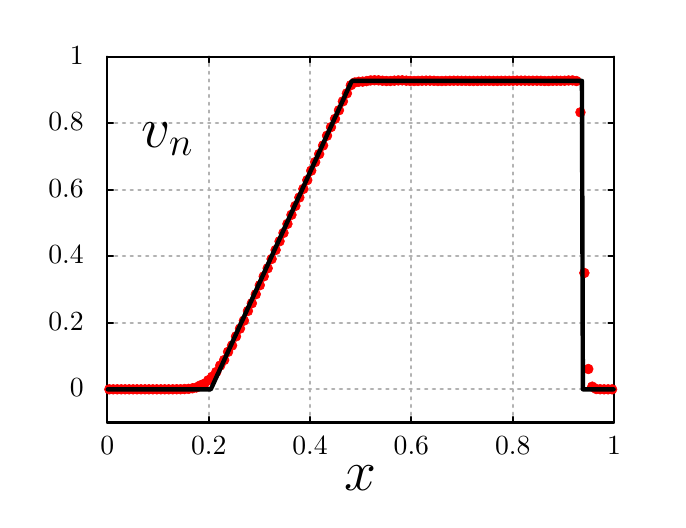
\begin{tikzpicture}[gnuplot]
%% generated with GNUPLOT 4.6p4 (Lua 5.1; terminal rev. 99, script rev. 100)
%% Thu 31 Jul 2014 02:04:53 PM EDT
\path (0.000,0.000) rectangle (8.000,6.000);
\gpfill{rgb color={1.000,1.000,1.000}} (1.012,0.985)--(7.446,0.985)--(7.446,5.630)--(1.012,5.630)--cycle;
\gpcolor{color=gp lt color border}
\gpsetlinetype{gp lt border}
\gpsetlinewidth{1.00}
\draw[gp path] (1.012,0.985)--(1.012,5.630)--(7.446,5.630)--(7.446,0.985)--cycle;
\gpcolor{color=gp lt color axes}
\gpsetlinetype{gp lt axes}
\gpsetlinewidth{2.00}
\draw[gp path] (1.012,1.407)--(7.447,1.407);
\gpcolor{color=gp lt color border}
\gpsetlinetype{gp lt border}
\draw[gp path] (1.012,1.407)--(1.084,1.407);
\draw[gp path] (7.447,1.407)--(7.375,1.407);
\gpcolor{rgb color={0.000,0.000,0.000}}
\node[gp node right,font={\fontsize{10pt}{12pt}\selectfont}] at (0.828,1.407) {0};
\gpcolor{color=gp lt color axes}
\gpsetlinetype{gp lt axes}
\draw[gp path] (1.012,2.252)--(7.447,2.252);
\gpcolor{color=gp lt color border}
\gpsetlinetype{gp lt border}
\draw[gp path] (1.012,2.252)--(1.084,2.252);
\draw[gp path] (7.447,2.252)--(7.375,2.252);
\gpcolor{rgb color={0.000,0.000,0.000}}
\node[gp node right,font={\fontsize{10pt}{12pt}\selectfont}] at (0.828,2.252) {0.2};
\gpcolor{color=gp lt color axes}
\gpsetlinetype{gp lt axes}
\draw[gp path] (1.012,3.097)--(7.447,3.097);
\gpcolor{color=gp lt color border}
\gpsetlinetype{gp lt border}
\draw[gp path] (1.012,3.097)--(1.084,3.097);
\draw[gp path] (7.447,3.097)--(7.375,3.097);
\gpcolor{rgb color={0.000,0.000,0.000}}
\node[gp node right,font={\fontsize{10pt}{12pt}\selectfont}] at (0.828,3.097) {0.4};
\gpcolor{color=gp lt color axes}
\gpsetlinetype{gp lt axes}
\draw[gp path] (1.012,3.942)--(7.447,3.942);
\gpcolor{color=gp lt color border}
\gpsetlinetype{gp lt border}
\draw[gp path] (1.012,3.942)--(1.084,3.942);
\draw[gp path] (7.447,3.942)--(7.375,3.942);
\gpcolor{rgb color={0.000,0.000,0.000}}
\node[gp node right,font={\fontsize{10pt}{12pt}\selectfont}] at (0.828,3.942) {0.6};
\gpcolor{color=gp lt color axes}
\gpsetlinetype{gp lt axes}
\draw[gp path] (1.012,4.786)--(7.447,4.786);
\gpcolor{color=gp lt color border}
\gpsetlinetype{gp lt border}
\draw[gp path] (1.012,4.786)--(1.084,4.786);
\draw[gp path] (7.447,4.786)--(7.375,4.786);
\gpcolor{rgb color={0.000,0.000,0.000}}
\node[gp node right,font={\fontsize{10pt}{12pt}\selectfont}] at (0.828,4.786) {0.8};
\gpcolor{color=gp lt color axes}
\gpsetlinetype{gp lt axes}
\draw[gp path] (1.012,5.631)--(7.447,5.631);
\gpcolor{color=gp lt color border}
\gpsetlinetype{gp lt border}
\draw[gp path] (1.012,5.631)--(1.084,5.631);
\draw[gp path] (7.447,5.631)--(7.375,5.631);
\gpcolor{rgb color={0.000,0.000,0.000}}
\node[gp node right,font={\fontsize{10pt}{12pt}\selectfont}] at (0.828,5.631) {1};
\gpcolor{color=gp lt color axes}
\gpsetlinetype{gp lt axes}
\draw[gp path] (1.012,0.985)--(1.012,5.631);
\gpcolor{color=gp lt color border}
\gpsetlinetype{gp lt border}
\draw[gp path] (1.012,0.985)--(1.012,1.057);
\draw[gp path] (1.012,5.631)--(1.012,5.559);
\gpcolor{rgb color={0.000,0.000,0.000}}
\node[gp node center,font={\fontsize{10pt}{12pt}\selectfont}] at (1.012,0.677) {0};
\gpcolor{color=gp lt color axes}
\gpsetlinetype{gp lt axes}
\draw[gp path] (2.299,0.985)--(2.299,5.631);
\gpcolor{color=gp lt color border}
\gpsetlinetype{gp lt border}
\draw[gp path] (2.299,0.985)--(2.299,1.057);
\draw[gp path] (2.299,5.631)--(2.299,5.559);
\gpcolor{rgb color={0.000,0.000,0.000}}
\node[gp node center,font={\fontsize{10pt}{12pt}\selectfont}] at (2.299,0.677) {0.2};
\gpcolor{color=gp lt color axes}
\gpsetlinetype{gp lt axes}
\draw[gp path] (3.586,0.985)--(3.586,5.631);
\gpcolor{color=gp lt color border}
\gpsetlinetype{gp lt border}
\draw[gp path] (3.586,0.985)--(3.586,1.057);
\draw[gp path] (3.586,5.631)--(3.586,5.559);
\gpcolor{rgb color={0.000,0.000,0.000}}
\node[gp node center,font={\fontsize{10pt}{12pt}\selectfont}] at (3.586,0.677) {0.4};
\gpcolor{color=gp lt color axes}
\gpsetlinetype{gp lt axes}
\draw[gp path] (4.873,0.985)--(4.873,5.631);
\gpcolor{color=gp lt color border}
\gpsetlinetype{gp lt border}
\draw[gp path] (4.873,0.985)--(4.873,1.057);
\draw[gp path] (4.873,5.631)--(4.873,5.559);
\gpcolor{rgb color={0.000,0.000,0.000}}
\node[gp node center,font={\fontsize{10pt}{12pt}\selectfont}] at (4.873,0.677) {0.6};
\gpcolor{color=gp lt color axes}
\gpsetlinetype{gp lt axes}
\draw[gp path] (6.160,0.985)--(6.160,5.631);
\gpcolor{color=gp lt color border}
\gpsetlinetype{gp lt border}
\draw[gp path] (6.160,0.985)--(6.160,1.057);
\draw[gp path] (6.160,5.631)--(6.160,5.559);
\gpcolor{rgb color={0.000,0.000,0.000}}
\node[gp node center,font={\fontsize{10pt}{12pt}\selectfont}] at (6.160,0.677) {0.8};
\gpcolor{color=gp lt color axes}
\gpsetlinetype{gp lt axes}
\draw[gp path] (7.447,0.985)--(7.447,5.631);
\gpcolor{color=gp lt color border}
\gpsetlinetype{gp lt border}
\draw[gp path] (7.447,0.985)--(7.447,1.057);
\draw[gp path] (7.447,5.631)--(7.447,5.559);
\gpcolor{rgb color={0.000,0.000,0.000}}
\node[gp node center,font={\fontsize{10pt}{12pt}\selectfont}] at (7.447,0.677) {1};
\gpcolor{color=gp lt color border}
\draw[gp path] (1.012,5.631)--(1.012,0.985)--(7.447,0.985)--(7.447,5.631)--cycle;
\gpcolor{rgb color={0.000,0.000,0.000}}
\node[gp node center,font={\fontsize{10pt}{12pt}\selectfont}] at (4.229,0.215) {\huge $x$};
\gpcolor{rgb color={1.000,0.000,0.000}}
\gpsetlinewidth{0.50}
\gpsetpointsize{4.44}
\gppoint{gp mark 7}{(1.037,1.407)}
\gppoint{gp mark 7}{(1.087,1.407)}
\gppoint{gp mark 7}{(1.138,1.407)}
\gppoint{gp mark 7}{(1.188,1.407)}
\gppoint{gp mark 7}{(1.238,1.407)}
\gppoint{gp mark 7}{(1.289,1.407)}
\gppoint{gp mark 7}{(1.339,1.407)}
\gppoint{gp mark 7}{(1.389,1.407)}
\gppoint{gp mark 7}{(1.439,1.407)}
\gppoint{gp mark 7}{(1.490,1.407)}
\gppoint{gp mark 7}{(1.540,1.407)}
\gppoint{gp mark 7}{(1.590,1.407)}
\gppoint{gp mark 7}{(1.640,1.407)}
\gppoint{gp mark 7}{(1.691,1.407)}
\gppoint{gp mark 7}{(1.741,1.407)}
\gppoint{gp mark 7}{(1.791,1.407)}
\gppoint{gp mark 7}{(1.842,1.407)}
\gppoint{gp mark 7}{(1.892,1.408)}
\gppoint{gp mark 7}{(1.942,1.408)}
\gppoint{gp mark 7}{(1.992,1.410)}
\gppoint{gp mark 7}{(2.043,1.413)}
\gppoint{gp mark 7}{(2.093,1.420)}
\gppoint{gp mark 7}{(2.143,1.431)}
\gppoint{gp mark 7}{(2.193,1.457)}
\gppoint{gp mark 7}{(2.244,1.478)}
\gppoint{gp mark 7}{(2.294,1.522)}
\gppoint{gp mark 7}{(2.344,1.567)}
\gppoint{gp mark 7}{(2.395,1.627)}
\gppoint{gp mark 7}{(2.445,1.709)}
\gppoint{gp mark 7}{(2.495,1.779)}
\gppoint{gp mark 7}{(2.545,1.883)}
\gppoint{gp mark 7}{(2.596,1.964)}
\gppoint{gp mark 7}{(2.646,2.079)}
\gppoint{gp mark 7}{(2.696,2.178)}
\gppoint{gp mark 7}{(2.746,2.279)}
\gppoint{gp mark 7}{(2.797,2.402)}
\gppoint{gp mark 7}{(2.847,2.500)}
\gppoint{gp mark 7}{(2.897,2.614)}
\gppoint{gp mark 7}{(2.948,2.729)}
\gppoint{gp mark 7}{(2.998,2.841)}
\gppoint{gp mark 7}{(3.048,2.944)}
\gppoint{gp mark 7}{(3.098,3.062)}
\gppoint{gp mark 7}{(3.149,3.176)}
\gppoint{gp mark 7}{(3.199,3.287)}
\gppoint{gp mark 7}{(3.249,3.393)}
\gppoint{gp mark 7}{(3.299,3.508)}
\gppoint{gp mark 7}{(3.350,3.623)}
\gppoint{gp mark 7}{(3.400,3.736)}
\gppoint{gp mark 7}{(3.450,3.843)}
\gppoint{gp mark 7}{(3.501,3.952)}
\gppoint{gp mark 7}{(3.551,4.064)}
\gppoint{gp mark 7}{(3.601,4.184)}
\gppoint{gp mark 7}{(3.651,4.293)}
\gppoint{gp mark 7}{(3.702,4.395)}
\gppoint{gp mark 7}{(3.752,4.504)}
\gppoint{gp mark 7}{(3.802,4.628)}
\gppoint{gp mark 7}{(3.852,4.737)}
\gppoint{gp mark 7}{(3.903,4.842)}
\gppoint{gp mark 7}{(3.953,4.951)}
\gppoint{gp mark 7}{(4.003,5.064)}
\gppoint{gp mark 7}{(4.054,5.166)}
\gppoint{gp mark 7}{(4.104,5.269)}
\gppoint{gp mark 7}{(4.154,5.304)}
\gppoint{gp mark 7}{(4.204,5.313)}
\gppoint{gp mark 7}{(4.255,5.315)}
\gppoint{gp mark 7}{(4.305,5.321)}
\gppoint{gp mark 7}{(4.355,5.330)}
\gppoint{gp mark 7}{(4.405,5.332)}
\gppoint{gp mark 7}{(4.456,5.331)}
\gppoint{gp mark 7}{(4.506,5.326)}
\gppoint{gp mark 7}{(4.556,5.323)}
\gppoint{gp mark 7}{(4.607,5.323)}
\gppoint{gp mark 7}{(4.657,5.327)}
\gppoint{gp mark 7}{(4.707,5.330)}
\gppoint{gp mark 7}{(4.757,5.331)}
\gppoint{gp mark 7}{(4.808,5.327)}
\gppoint{gp mark 7}{(4.858,5.324)}
\gppoint{gp mark 7}{(4.908,5.323)}
\gppoint{gp mark 7}{(4.958,5.324)}
\gppoint{gp mark 7}{(5.009,5.326)}
\gppoint{gp mark 7}{(5.059,5.327)}
\gppoint{gp mark 7}{(5.109,5.327)}
\gppoint{gp mark 7}{(5.160,5.325)}
\gppoint{gp mark 7}{(5.210,5.323)}
\gppoint{gp mark 7}{(5.260,5.323)}
\gppoint{gp mark 7}{(5.310,5.324)}
\gppoint{gp mark 7}{(5.361,5.325)}
\gppoint{gp mark 7}{(5.411,5.326)}
\gppoint{gp mark 7}{(5.461,5.326)}
\gppoint{gp mark 7}{(5.511,5.325)}
\gppoint{gp mark 7}{(5.562,5.325)}
\gppoint{gp mark 7}{(5.612,5.324)}
\gppoint{gp mark 7}{(5.662,5.324)}
\gppoint{gp mark 7}{(5.713,5.324)}
\gppoint{gp mark 7}{(5.763,5.325)}
\gppoint{gp mark 7}{(5.813,5.325)}
\gppoint{gp mark 7}{(5.863,5.325)}
\gppoint{gp mark 7}{(5.914,5.324)}
\gppoint{gp mark 7}{(5.964,5.324)}
\gppoint{gp mark 7}{(6.014,5.325)}
\gppoint{gp mark 7}{(6.064,5.325)}
\gppoint{gp mark 7}{(6.115,5.325)}
\gppoint{gp mark 7}{(6.165,5.326)}
\gppoint{gp mark 7}{(6.215,5.327)}
\gppoint{gp mark 7}{(6.266,5.327)}
\gppoint{gp mark 7}{(6.316,5.327)}
\gppoint{gp mark 7}{(6.366,5.326)}
\gppoint{gp mark 7}{(6.416,5.326)}
\gppoint{gp mark 7}{(6.467,5.326)}
\gppoint{gp mark 7}{(6.517,5.325)}
\gppoint{gp mark 7}{(6.567,5.323)}
\gppoint{gp mark 7}{(6.617,5.323)}
\gppoint{gp mark 7}{(6.668,5.325)}
\gppoint{gp mark 7}{(6.718,5.326)}
\gppoint{gp mark 7}{(6.768,5.325)}
\gppoint{gp mark 7}{(6.819,5.326)}
\gppoint{gp mark 7}{(6.869,5.329)}
\gppoint{gp mark 7}{(6.919,5.330)}
\gppoint{gp mark 7}{(6.969,5.322)}
\gppoint{gp mark 7}{(7.020,4.925)}
\gppoint{gp mark 7}{(7.070,2.885)}
\gppoint{gp mark 7}{(7.120,1.665)}
\gppoint{gp mark 7}{(7.170,1.441)}
\gppoint{gp mark 7}{(7.221,1.411)}
\gppoint{gp mark 7}{(7.271,1.408)}
\gppoint{gp mark 7}{(7.321,1.407)}
\gppoint{gp mark 7}{(7.372,1.407)}
\gppoint{gp mark 7}{(7.422,1.407)}
\gpcolor{rgb color={0.000,0.000,0.000}}
\gpsetlinetype{gp lt plot 0}
\gpsetlinewidth{4.00}
\draw[gp path] (1.018,1.407)--(1.031,1.407)--(1.043,1.407)--(1.056,1.407)--(1.069,1.407)%
  --(1.081,1.407)--(1.094,1.407)--(1.106,1.407)--(1.119,1.407)--(1.131,1.407)--(1.144,1.407)%
  --(1.157,1.407)--(1.169,1.407)--(1.182,1.407)--(1.194,1.407)--(1.207,1.407)--(1.219,1.407)%
  --(1.232,1.407)--(1.245,1.407)--(1.257,1.407)--(1.270,1.407)--(1.282,1.407)--(1.295,1.407)%
  --(1.307,1.407)--(1.320,1.407)--(1.332,1.407)--(1.345,1.407)--(1.358,1.407)--(1.370,1.407)%
  --(1.383,1.407)--(1.395,1.407)--(1.408,1.407)--(1.420,1.407)--(1.433,1.407)--(1.446,1.407)%
  --(1.458,1.407)--(1.471,1.407)--(1.483,1.407)--(1.496,1.407)--(1.508,1.407)--(1.521,1.407)%
  --(1.534,1.407)--(1.546,1.407)--(1.559,1.407)--(1.571,1.407)--(1.584,1.407)--(1.596,1.407)%
  --(1.609,1.407)--(1.622,1.407)--(1.634,1.407)--(1.647,1.407)--(1.659,1.407)--(1.672,1.407)%
  --(1.684,1.407)--(1.697,1.407)--(1.710,1.407)--(1.722,1.407)--(1.735,1.407)--(1.747,1.407)%
  --(1.760,1.407)--(1.772,1.407)--(1.785,1.407)--(1.798,1.407)--(1.810,1.407)--(1.823,1.407)%
  --(1.835,1.407)--(1.848,1.407)--(1.860,1.407)--(1.873,1.407)--(1.886,1.407)--(1.898,1.407)%
  --(1.911,1.407)--(1.923,1.407)--(1.936,1.407)--(1.948,1.407)--(1.961,1.407)--(1.973,1.407)%
  --(1.986,1.407)--(1.999,1.407)--(2.011,1.407)--(2.024,1.407)--(2.036,1.407)--(2.049,1.407)%
  --(2.061,1.407)--(2.074,1.407)--(2.087,1.407)--(2.099,1.407)--(2.112,1.407)--(2.124,1.407)%
  --(2.137,1.407)--(2.149,1.407)--(2.162,1.407)--(2.175,1.407)--(2.187,1.407)--(2.200,1.407)%
  --(2.212,1.407)--(2.225,1.407)--(2.237,1.407)--(2.250,1.407)--(2.263,1.407)--(2.275,1.407)%
  --(2.288,1.407)--(2.300,1.407)--(2.313,1.407)--(2.325,1.407)--(2.338,1.434)--(2.351,1.461)%
  --(2.363,1.489)--(2.376,1.516)--(2.388,1.544)--(2.401,1.571)--(2.413,1.599)--(2.426,1.626)%
  --(2.439,1.654)--(2.451,1.681)--(2.464,1.709)--(2.476,1.736)--(2.489,1.764)--(2.501,1.791)%
  --(2.514,1.818)--(2.526,1.846)--(2.539,1.873)--(2.552,1.901)--(2.564,1.928)--(2.577,1.956)%
  --(2.589,1.983)--(2.602,2.011)--(2.614,2.038)--(2.627,2.066)--(2.640,2.093)--(2.652,2.121)%
  --(2.665,2.148)--(2.677,2.176)--(2.690,2.203)--(2.702,2.231)--(2.715,2.258)--(2.728,2.286)%
  --(2.740,2.313)--(2.753,2.341)--(2.765,2.368)--(2.778,2.396)--(2.790,2.423)--(2.803,2.451)%
  --(2.816,2.478)--(2.828,2.506)--(2.841,2.533)--(2.853,2.561)--(2.866,2.588)--(2.878,2.616)%
  --(2.891,2.643)--(2.904,2.671)--(2.916,2.698)--(2.929,2.726)--(2.941,2.753)--(2.954,2.781)%
  --(2.966,2.808)--(2.979,2.836)--(2.992,2.863)--(3.004,2.891)--(3.017,2.918)--(3.029,2.946)%
  --(3.042,2.973)--(3.054,3.001)--(3.067,3.028)--(3.079,3.056)--(3.092,3.083)--(3.105,3.111)%
  --(3.117,3.138)--(3.130,3.166)--(3.142,3.193)--(3.155,3.221)--(3.167,3.248)--(3.180,3.276)%
  --(3.193,3.303)--(3.205,3.331)--(3.218,3.358)--(3.230,3.386)--(3.243,3.413)--(3.255,3.441)%
  --(3.268,3.468)--(3.281,3.496)--(3.293,3.523)--(3.306,3.551)--(3.318,3.578)--(3.331,3.606)%
  --(3.343,3.633)--(3.356,3.661)--(3.369,3.688)--(3.381,3.716)--(3.394,3.743)--(3.406,3.771)%
  --(3.419,3.798)--(3.431,3.826)--(3.444,3.853)--(3.457,3.881)--(3.469,3.908)--(3.482,3.936)%
  --(3.494,3.963)--(3.507,3.991)--(3.519,4.018)--(3.532,4.046)--(3.545,4.073)--(3.557,4.101)%
  --(3.570,4.128)--(3.582,4.156)--(3.595,4.183)--(3.607,4.211)--(3.620,4.238)--(3.633,4.266)%
  --(3.645,4.293)--(3.658,4.321)--(3.670,4.348)--(3.683,4.376)--(3.695,4.403)--(3.708,4.431)%
  --(3.720,4.458)--(3.733,4.486)--(3.746,4.513)--(3.758,4.541)--(3.771,4.568)--(3.783,4.596)%
  --(3.796,4.623)--(3.808,4.651)--(3.821,4.678)--(3.834,4.706)--(3.846,4.733)--(3.859,4.761)%
  --(3.871,4.788)--(3.884,4.816)--(3.896,4.843)--(3.909,4.871)--(3.922,4.898)--(3.934,4.926)%
  --(3.947,4.953)--(3.959,4.981)--(3.972,5.008)--(3.984,5.036)--(3.997,5.063)--(4.010,5.091)%
  --(4.022,5.118)--(4.035,5.146)--(4.047,5.173)--(4.060,5.201)--(4.072,5.228)--(4.085,5.256)%
  --(4.098,5.283)--(4.110,5.311)--(4.123,5.324)--(4.135,5.324)--(4.148,5.324)--(4.160,5.324)%
  --(4.173,5.324)--(4.186,5.324)--(4.198,5.324)--(4.211,5.324)--(4.223,5.324)--(4.236,5.324)%
  --(4.248,5.324)--(4.261,5.324)--(4.273,5.324)--(4.286,5.324)--(4.299,5.324)--(4.311,5.324)%
  --(4.324,5.324)--(4.336,5.324)--(4.349,5.324)--(4.361,5.324)--(4.374,5.324)--(4.387,5.324)%
  --(4.399,5.324)--(4.412,5.324)--(4.424,5.324)--(4.437,5.324)--(4.449,5.324)--(4.462,5.324)%
  --(4.475,5.324)--(4.487,5.324)--(4.500,5.324)--(4.512,5.324)--(4.525,5.324)--(4.537,5.324)%
  --(4.550,5.324)--(4.563,5.324)--(4.575,5.324)--(4.588,5.324)--(4.600,5.324)--(4.613,5.324)%
  --(4.625,5.324)--(4.638,5.324)--(4.651,5.324)--(4.663,5.324)--(4.676,5.324)--(4.688,5.324)%
  --(4.701,5.324)--(4.713,5.324)--(4.726,5.324)--(4.739,5.324)--(4.751,5.324)--(4.764,5.324)%
  --(4.776,5.324)--(4.789,5.324)--(4.801,5.324)--(4.814,5.324)--(4.826,5.324)--(4.839,5.324)%
  --(4.852,5.324)--(4.864,5.324)--(4.877,5.324)--(4.889,5.324)--(4.902,5.324)--(4.914,5.324)%
  --(4.927,5.324)--(4.940,5.324)--(4.952,5.324)--(4.965,5.324)--(4.977,5.324)--(4.990,5.324)%
  --(5.002,5.324)--(5.015,5.324)--(5.028,5.324)--(5.040,5.324)--(5.053,5.324)--(5.065,5.324)%
  --(5.078,5.324)--(5.090,5.324)--(5.103,5.324)--(5.116,5.324)--(5.128,5.324)--(5.141,5.324)%
  --(5.153,5.324)--(5.166,5.324)--(5.178,5.324)--(5.191,5.324)--(5.204,5.324)--(5.216,5.324)%
  --(5.229,5.324)--(5.241,5.324)--(5.254,5.324)--(5.266,5.324)--(5.279,5.324)--(5.292,5.324)%
  --(5.304,5.324)--(5.317,5.324)--(5.329,5.324)--(5.342,5.324)--(5.354,5.324)--(5.367,5.324)%
  --(5.380,5.324)--(5.392,5.324)--(5.405,5.324)--(5.417,5.324)--(5.430,5.324)--(5.442,5.324)%
  --(5.455,5.324)--(5.467,5.324)--(5.480,5.324)--(5.493,5.324)--(5.505,5.324)--(5.518,5.324)%
  --(5.530,5.324)--(5.543,5.324)--(5.555,5.324)--(5.568,5.324)--(5.581,5.324)--(5.593,5.324)%
  --(5.606,5.324)--(5.618,5.324)--(5.631,5.324)--(5.643,5.324)--(5.656,5.324)--(5.669,5.324)%
  --(5.681,5.324)--(5.694,5.324)--(5.706,5.324)--(5.719,5.324)--(5.731,5.324)--(5.744,5.324)%
  --(5.757,5.324)--(5.769,5.324)--(5.782,5.324)--(5.794,5.324)--(5.807,5.324)--(5.819,5.324)%
  --(5.832,5.324)--(5.845,5.324)--(5.857,5.324)--(5.870,5.324)--(5.882,5.324)--(5.895,5.324)%
  --(5.907,5.324)--(5.920,5.324)--(5.933,5.324)--(5.945,5.324)--(5.958,5.324)--(5.970,5.324)%
  --(5.983,5.324)--(5.995,5.324)--(6.008,5.324)--(6.020,5.324)--(6.033,5.324)--(6.046,5.324)%
  --(6.058,5.324)--(6.071,5.324)--(6.083,5.324)--(6.096,5.324)--(6.108,5.324)--(6.121,5.324)%
  --(6.134,5.324)--(6.146,5.324)--(6.159,5.324)--(6.171,5.324)--(6.184,5.324)--(6.196,5.324)%
  --(6.209,5.324)--(6.222,5.324)--(6.234,5.324)--(6.247,5.324)--(6.259,5.324)--(6.272,5.324)%
  --(6.284,5.324)--(6.297,5.324)--(6.310,5.324)--(6.322,5.324)--(6.335,5.324)--(6.347,5.324)%
  --(6.360,5.324)--(6.372,5.324)--(6.385,5.324)--(6.398,5.324)--(6.410,5.324)--(6.423,5.324)%
  --(6.435,5.324)--(6.448,5.324)--(6.460,5.324)--(6.473,5.324)--(6.486,5.324)--(6.498,5.324)%
  --(6.511,5.324)--(6.523,5.324)--(6.536,5.324)--(6.548,5.324)--(6.561,5.324)--(6.573,5.324)%
  --(6.586,5.324)--(6.599,5.324)--(6.611,5.324)--(6.624,5.324)--(6.636,5.324)--(6.649,5.324)%
  --(6.661,5.324)--(6.674,5.324)--(6.687,5.324)--(6.699,5.324)--(6.712,5.324)--(6.724,5.324)%
  --(6.737,5.324)--(6.749,5.324)--(6.762,5.324)--(6.775,5.324)--(6.787,5.324)--(6.800,5.324)%
  --(6.812,5.324)--(6.825,5.324)--(6.837,5.324)--(6.850,5.324)--(6.863,5.324)--(6.875,5.324)%
  --(6.888,5.324)--(6.900,5.324)--(6.913,5.324)--(6.925,5.324)--(6.938,5.324)--(6.951,5.324)%
  --(6.963,5.324)--(6.976,5.324)--(6.988,5.324)--(7.001,5.324)--(7.013,5.324)--(7.026,5.324)%
  --(7.039,5.324)--(7.051,1.407)--(7.064,1.407)--(7.076,1.407)--(7.089,1.407)--(7.101,1.407)%
  --(7.114,1.407)--(7.127,1.407)--(7.139,1.407)--(7.152,1.407)--(7.164,1.407)--(7.177,1.407)%
  --(7.189,1.407)--(7.202,1.407)--(7.214,1.407)--(7.227,1.407)--(7.240,1.407)--(7.252,1.407)%
  --(7.265,1.407)--(7.277,1.407)--(7.290,1.407)--(7.302,1.407)--(7.315,1.407)--(7.328,1.407)%
  --(7.340,1.407)--(7.353,1.407)--(7.365,1.407)--(7.378,1.407)--(7.390,1.407)--(7.403,1.407)%
  --(7.416,1.407)--(7.428,1.407)--(7.441,1.407);
\node[gp node left,font={\fontsize{10pt}{12pt}\selectfont}] at (1.334,4.575) {\huge $v_n$};
%% coordinates of the plot area
\gpdefrectangularnode{gp plot 1}{\pgfpoint{1.012cm}{0.985cm}}{\pgfpoint{7.447cm}{5.631cm}}
\end{tikzpicture}
%% gnuplot variables
} &
\resizebox{0.33\linewidth}{!}{\tikzsetnextfilename{sod_hllc_3_3}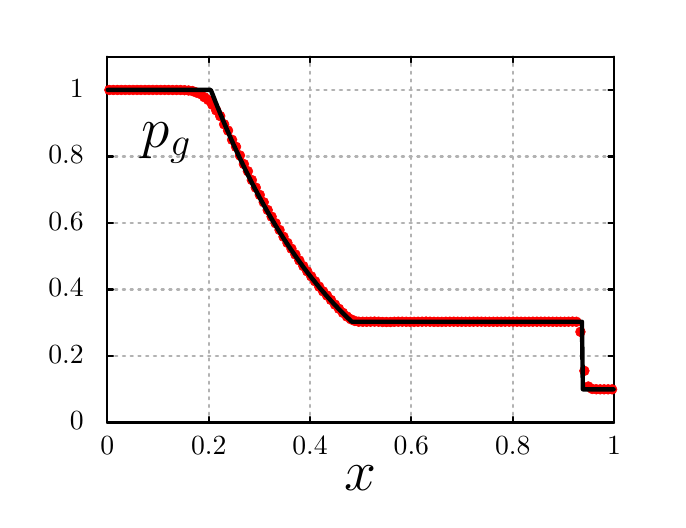
\begin{tikzpicture}[gnuplot]
%% generated with GNUPLOT 4.6p4 (Lua 5.1; terminal rev. 99, script rev. 100)
%% Thu 31 Jul 2014 02:04:53 PM EDT
\path (0.000,0.000) rectangle (8.000,6.000);
\gpfill{rgb color={1.000,1.000,1.000}} (1.012,0.985)--(7.446,0.985)--(7.446,5.630)--(1.012,5.630)--cycle;
\gpcolor{color=gp lt color border}
\gpsetlinetype{gp lt border}
\gpsetlinewidth{1.00}
\draw[gp path] (1.012,0.985)--(1.012,5.630)--(7.446,5.630)--(7.446,0.985)--cycle;
\gpcolor{color=gp lt color axes}
\gpsetlinetype{gp lt axes}
\gpsetlinewidth{2.00}
\draw[gp path] (1.012,0.985)--(7.447,0.985);
\gpcolor{color=gp lt color border}
\gpsetlinetype{gp lt border}
\draw[gp path] (1.012,0.985)--(1.084,0.985);
\draw[gp path] (7.447,0.985)--(7.375,0.985);
\gpcolor{rgb color={0.000,0.000,0.000}}
\node[gp node right,font={\fontsize{10pt}{12pt}\selectfont}] at (0.828,0.985) {0};
\gpcolor{color=gp lt color axes}
\gpsetlinetype{gp lt axes}
\draw[gp path] (1.012,1.830)--(7.447,1.830);
\gpcolor{color=gp lt color border}
\gpsetlinetype{gp lt border}
\draw[gp path] (1.012,1.830)--(1.084,1.830);
\draw[gp path] (7.447,1.830)--(7.375,1.830);
\gpcolor{rgb color={0.000,0.000,0.000}}
\node[gp node right,font={\fontsize{10pt}{12pt}\selectfont}] at (0.828,1.830) {0.2};
\gpcolor{color=gp lt color axes}
\gpsetlinetype{gp lt axes}
\draw[gp path] (1.012,2.674)--(7.447,2.674);
\gpcolor{color=gp lt color border}
\gpsetlinetype{gp lt border}
\draw[gp path] (1.012,2.674)--(1.084,2.674);
\draw[gp path] (7.447,2.674)--(7.375,2.674);
\gpcolor{rgb color={0.000,0.000,0.000}}
\node[gp node right,font={\fontsize{10pt}{12pt}\selectfont}] at (0.828,2.674) {0.4};
\gpcolor{color=gp lt color axes}
\gpsetlinetype{gp lt axes}
\draw[gp path] (1.012,3.519)--(7.447,3.519);
\gpcolor{color=gp lt color border}
\gpsetlinetype{gp lt border}
\draw[gp path] (1.012,3.519)--(1.084,3.519);
\draw[gp path] (7.447,3.519)--(7.375,3.519);
\gpcolor{rgb color={0.000,0.000,0.000}}
\node[gp node right,font={\fontsize{10pt}{12pt}\selectfont}] at (0.828,3.519) {0.6};
\gpcolor{color=gp lt color axes}
\gpsetlinetype{gp lt axes}
\draw[gp path] (1.012,4.364)--(7.447,4.364);
\gpcolor{color=gp lt color border}
\gpsetlinetype{gp lt border}
\draw[gp path] (1.012,4.364)--(1.084,4.364);
\draw[gp path] (7.447,4.364)--(7.375,4.364);
\gpcolor{rgb color={0.000,0.000,0.000}}
\node[gp node right,font={\fontsize{10pt}{12pt}\selectfont}] at (0.828,4.364) {0.8};
\gpcolor{color=gp lt color axes}
\gpsetlinetype{gp lt axes}
\draw[gp path] (1.012,5.209)--(7.447,5.209);
\gpcolor{color=gp lt color border}
\gpsetlinetype{gp lt border}
\draw[gp path] (1.012,5.209)--(1.084,5.209);
\draw[gp path] (7.447,5.209)--(7.375,5.209);
\gpcolor{rgb color={0.000,0.000,0.000}}
\node[gp node right,font={\fontsize{10pt}{12pt}\selectfont}] at (0.828,5.209) {1};
\gpcolor{color=gp lt color axes}
\gpsetlinetype{gp lt axes}
\draw[gp path] (1.012,0.985)--(1.012,5.631);
\gpcolor{color=gp lt color border}
\gpsetlinetype{gp lt border}
\draw[gp path] (1.012,0.985)--(1.012,1.057);
\draw[gp path] (1.012,5.631)--(1.012,5.559);
\gpcolor{rgb color={0.000,0.000,0.000}}
\node[gp node center,font={\fontsize{10pt}{12pt}\selectfont}] at (1.012,0.677) {0};
\gpcolor{color=gp lt color axes}
\gpsetlinetype{gp lt axes}
\draw[gp path] (2.299,0.985)--(2.299,5.631);
\gpcolor{color=gp lt color border}
\gpsetlinetype{gp lt border}
\draw[gp path] (2.299,0.985)--(2.299,1.057);
\draw[gp path] (2.299,5.631)--(2.299,5.559);
\gpcolor{rgb color={0.000,0.000,0.000}}
\node[gp node center,font={\fontsize{10pt}{12pt}\selectfont}] at (2.299,0.677) {0.2};
\gpcolor{color=gp lt color axes}
\gpsetlinetype{gp lt axes}
\draw[gp path] (3.586,0.985)--(3.586,5.631);
\gpcolor{color=gp lt color border}
\gpsetlinetype{gp lt border}
\draw[gp path] (3.586,0.985)--(3.586,1.057);
\draw[gp path] (3.586,5.631)--(3.586,5.559);
\gpcolor{rgb color={0.000,0.000,0.000}}
\node[gp node center,font={\fontsize{10pt}{12pt}\selectfont}] at (3.586,0.677) {0.4};
\gpcolor{color=gp lt color axes}
\gpsetlinetype{gp lt axes}
\draw[gp path] (4.873,0.985)--(4.873,5.631);
\gpcolor{color=gp lt color border}
\gpsetlinetype{gp lt border}
\draw[gp path] (4.873,0.985)--(4.873,1.057);
\draw[gp path] (4.873,5.631)--(4.873,5.559);
\gpcolor{rgb color={0.000,0.000,0.000}}
\node[gp node center,font={\fontsize{10pt}{12pt}\selectfont}] at (4.873,0.677) {0.6};
\gpcolor{color=gp lt color axes}
\gpsetlinetype{gp lt axes}
\draw[gp path] (6.160,0.985)--(6.160,5.631);
\gpcolor{color=gp lt color border}
\gpsetlinetype{gp lt border}
\draw[gp path] (6.160,0.985)--(6.160,1.057);
\draw[gp path] (6.160,5.631)--(6.160,5.559);
\gpcolor{rgb color={0.000,0.000,0.000}}
\node[gp node center,font={\fontsize{10pt}{12pt}\selectfont}] at (6.160,0.677) {0.8};
\gpcolor{color=gp lt color axes}
\gpsetlinetype{gp lt axes}
\draw[gp path] (7.447,0.985)--(7.447,5.631);
\gpcolor{color=gp lt color border}
\gpsetlinetype{gp lt border}
\draw[gp path] (7.447,0.985)--(7.447,1.057);
\draw[gp path] (7.447,5.631)--(7.447,5.559);
\gpcolor{rgb color={0.000,0.000,0.000}}
\node[gp node center,font={\fontsize{10pt}{12pt}\selectfont}] at (7.447,0.677) {1};
\gpcolor{color=gp lt color border}
\draw[gp path] (1.012,5.631)--(1.012,0.985)--(7.447,0.985)--(7.447,5.631)--cycle;
\gpcolor{rgb color={0.000,0.000,0.000}}
\node[gp node center,font={\fontsize{10pt}{12pt}\selectfont}] at (4.229,0.215) {\huge $x$};
\gpcolor{rgb color={1.000,0.000,0.000}}
\gpsetlinewidth{0.50}
\gpsetpointsize{4.44}
\gppoint{gp mark 7}{(1.037,5.209)}
\gppoint{gp mark 7}{(1.087,5.209)}
\gppoint{gp mark 7}{(1.138,5.209)}
\gppoint{gp mark 7}{(1.188,5.209)}
\gppoint{gp mark 7}{(1.238,5.209)}
\gppoint{gp mark 7}{(1.289,5.209)}
\gppoint{gp mark 7}{(1.339,5.209)}
\gppoint{gp mark 7}{(1.389,5.209)}
\gppoint{gp mark 7}{(1.439,5.209)}
\gppoint{gp mark 7}{(1.490,5.209)}
\gppoint{gp mark 7}{(1.540,5.209)}
\gppoint{gp mark 7}{(1.590,5.209)}
\gppoint{gp mark 7}{(1.640,5.209)}
\gppoint{gp mark 7}{(1.691,5.209)}
\gppoint{gp mark 7}{(1.741,5.209)}
\gppoint{gp mark 7}{(1.791,5.209)}
\gppoint{gp mark 7}{(1.842,5.208)}
\gppoint{gp mark 7}{(1.892,5.208)}
\gppoint{gp mark 7}{(1.942,5.208)}
\gppoint{gp mark 7}{(1.992,5.206)}
\gppoint{gp mark 7}{(2.043,5.202)}
\gppoint{gp mark 7}{(2.093,5.195)}
\gppoint{gp mark 7}{(2.143,5.176)}
\gppoint{gp mark 7}{(2.193,5.158)}
\gppoint{gp mark 7}{(2.244,5.117)}
\gppoint{gp mark 7}{(2.294,5.081)}
\gppoint{gp mark 7}{(2.344,5.022)}
\gppoint{gp mark 7}{(2.395,4.949)}
\gppoint{gp mark 7}{(2.445,4.877)}
\gppoint{gp mark 7}{(2.495,4.773)}
\gppoint{gp mark 7}{(2.545,4.693)}
\gppoint{gp mark 7}{(2.596,4.576)}
\gppoint{gp mark 7}{(2.646,4.487)}
\gppoint{gp mark 7}{(2.696,4.377)}
\gppoint{gp mark 7}{(2.746,4.268)}
\gppoint{gp mark 7}{(2.797,4.177)}
\gppoint{gp mark 7}{(2.847,4.065)}
\gppoint{gp mark 7}{(2.897,3.969)}
\gppoint{gp mark 7}{(2.948,3.876)}
\gppoint{gp mark 7}{(2.998,3.783)}
\gppoint{gp mark 7}{(3.048,3.685)}
\gppoint{gp mark 7}{(3.098,3.600)}
\gppoint{gp mark 7}{(3.149,3.516)}
\gppoint{gp mark 7}{(3.199,3.431)}
\gppoint{gp mark 7}{(3.249,3.345)}
\gppoint{gp mark 7}{(3.299,3.267)}
\gppoint{gp mark 7}{(3.350,3.193)}
\gppoint{gp mark 7}{(3.400,3.119)}
\gppoint{gp mark 7}{(3.450,3.044)}
\gppoint{gp mark 7}{(3.501,2.972)}
\gppoint{gp mark 7}{(3.551,2.905)}
\gppoint{gp mark 7}{(3.601,2.842)}
\gppoint{gp mark 7}{(3.651,2.779)}
\gppoint{gp mark 7}{(3.702,2.711)}
\gppoint{gp mark 7}{(3.752,2.651)}
\gppoint{gp mark 7}{(3.802,2.598)}
\gppoint{gp mark 7}{(3.852,2.542)}
\gppoint{gp mark 7}{(3.903,2.483)}
\gppoint{gp mark 7}{(3.953,2.430)}
\gppoint{gp mark 7}{(4.003,2.379)}
\gppoint{gp mark 7}{(4.054,2.332)}
\gppoint{gp mark 7}{(4.104,2.297)}
\gppoint{gp mark 7}{(4.154,2.276)}
\gppoint{gp mark 7}{(4.204,2.266)}
\gppoint{gp mark 7}{(4.255,2.265)}
\gppoint{gp mark 7}{(4.305,2.265)}
\gppoint{gp mark 7}{(4.355,2.266)}
\gppoint{gp mark 7}{(4.405,2.267)}
\gppoint{gp mark 7}{(4.456,2.266)}
\gppoint{gp mark 7}{(4.506,2.263)}
\gppoint{gp mark 7}{(4.556,2.262)}
\gppoint{gp mark 7}{(4.607,2.262)}
\gppoint{gp mark 7}{(4.657,2.265)}
\gppoint{gp mark 7}{(4.707,2.266)}
\gppoint{gp mark 7}{(4.757,2.266)}
\gppoint{gp mark 7}{(4.808,2.265)}
\gppoint{gp mark 7}{(4.858,2.264)}
\gppoint{gp mark 7}{(4.908,2.264)}
\gppoint{gp mark 7}{(4.958,2.265)}
\gppoint{gp mark 7}{(5.009,2.266)}
\gppoint{gp mark 7}{(5.059,2.267)}
\gppoint{gp mark 7}{(5.109,2.266)}
\gppoint{gp mark 7}{(5.160,2.264)}
\gppoint{gp mark 7}{(5.210,2.264)}
\gppoint{gp mark 7}{(5.260,2.264)}
\gppoint{gp mark 7}{(5.310,2.265)}
\gppoint{gp mark 7}{(5.361,2.266)}
\gppoint{gp mark 7}{(5.411,2.266)}
\gppoint{gp mark 7}{(5.461,2.265)}
\gppoint{gp mark 7}{(5.511,2.265)}
\gppoint{gp mark 7}{(5.562,2.265)}
\gppoint{gp mark 7}{(5.612,2.265)}
\gppoint{gp mark 7}{(5.662,2.266)}
\gppoint{gp mark 7}{(5.713,2.266)}
\gppoint{gp mark 7}{(5.763,2.266)}
\gppoint{gp mark 7}{(5.813,2.265)}
\gppoint{gp mark 7}{(5.863,2.265)}
\gppoint{gp mark 7}{(5.914,2.265)}
\gppoint{gp mark 7}{(5.964,2.265)}
\gppoint{gp mark 7}{(6.014,2.265)}
\gppoint{gp mark 7}{(6.064,2.266)}
\gppoint{gp mark 7}{(6.115,2.266)}
\gppoint{gp mark 7}{(6.165,2.266)}
\gppoint{gp mark 7}{(6.215,2.266)}
\gppoint{gp mark 7}{(6.266,2.265)}
\gppoint{gp mark 7}{(6.316,2.265)}
\gppoint{gp mark 7}{(6.366,2.265)}
\gppoint{gp mark 7}{(6.416,2.266)}
\gppoint{gp mark 7}{(6.467,2.266)}
\gppoint{gp mark 7}{(6.517,2.266)}
\gppoint{gp mark 7}{(6.567,2.266)}
\gppoint{gp mark 7}{(6.617,2.266)}
\gppoint{gp mark 7}{(6.668,2.265)}
\gppoint{gp mark 7}{(6.718,2.265)}
\gppoint{gp mark 7}{(6.768,2.265)}
\gppoint{gp mark 7}{(6.819,2.265)}
\gppoint{gp mark 7}{(6.869,2.266)}
\gppoint{gp mark 7}{(6.919,2.267)}
\gppoint{gp mark 7}{(6.969,2.265)}
\gppoint{gp mark 7}{(7.020,2.137)}
\gppoint{gp mark 7}{(7.070,1.642)}
\gppoint{gp mark 7}{(7.120,1.443)}
\gppoint{gp mark 7}{(7.170,1.412)}
\gppoint{gp mark 7}{(7.221,1.408)}
\gppoint{gp mark 7}{(7.271,1.407)}
\gppoint{gp mark 7}{(7.321,1.407)}
\gppoint{gp mark 7}{(7.372,1.407)}
\gppoint{gp mark 7}{(7.422,1.407)}
\gpcolor{rgb color={0.000,0.000,0.000}}
\gpsetlinetype{gp lt plot 0}
\gpsetlinewidth{4.00}
\draw[gp path] (1.018,5.209)--(1.031,5.209)--(1.043,5.209)--(1.056,5.209)--(1.069,5.209)%
  --(1.081,5.209)--(1.094,5.209)--(1.106,5.209)--(1.119,5.209)--(1.131,5.209)--(1.144,5.209)%
  --(1.157,5.209)--(1.169,5.209)--(1.182,5.209)--(1.194,5.209)--(1.207,5.209)--(1.219,5.209)%
  --(1.232,5.209)--(1.245,5.209)--(1.257,5.209)--(1.270,5.209)--(1.282,5.209)--(1.295,5.209)%
  --(1.307,5.209)--(1.320,5.209)--(1.332,5.209)--(1.345,5.209)--(1.358,5.209)--(1.370,5.209)%
  --(1.383,5.209)--(1.395,5.209)--(1.408,5.209)--(1.420,5.209)--(1.433,5.209)--(1.446,5.209)%
  --(1.458,5.209)--(1.471,5.209)--(1.483,5.209)--(1.496,5.209)--(1.508,5.209)--(1.521,5.209)%
  --(1.534,5.209)--(1.546,5.209)--(1.559,5.209)--(1.571,5.209)--(1.584,5.209)--(1.596,5.209)%
  --(1.609,5.209)--(1.622,5.209)--(1.634,5.209)--(1.647,5.209)--(1.659,5.209)--(1.672,5.209)%
  --(1.684,5.209)--(1.697,5.209)--(1.710,5.209)--(1.722,5.209)--(1.735,5.209)--(1.747,5.209)%
  --(1.760,5.209)--(1.772,5.209)--(1.785,5.209)--(1.798,5.209)--(1.810,5.209)--(1.823,5.209)%
  --(1.835,5.209)--(1.848,5.209)--(1.860,5.209)--(1.873,5.209)--(1.886,5.209)--(1.898,5.209)%
  --(1.911,5.209)--(1.923,5.209)--(1.936,5.209)--(1.948,5.209)--(1.961,5.209)--(1.973,5.209)%
  --(1.986,5.209)--(1.999,5.209)--(2.011,5.209)--(2.024,5.209)--(2.036,5.209)--(2.049,5.209)%
  --(2.061,5.209)--(2.074,5.209)--(2.087,5.209)--(2.099,5.209)--(2.112,5.209)--(2.124,5.209)%
  --(2.137,5.209)--(2.149,5.209)--(2.162,5.209)--(2.175,5.209)--(2.187,5.209)--(2.200,5.209)%
  --(2.212,5.209)--(2.225,5.209)--(2.237,5.209)--(2.250,5.209)--(2.263,5.209)--(2.275,5.209)%
  --(2.288,5.209)--(2.300,5.209)--(2.313,5.209)--(2.325,5.209)--(2.338,5.178)--(2.351,5.146)%
  --(2.363,5.114)--(2.376,5.082)--(2.388,5.050)--(2.401,5.019)--(2.413,4.988)--(2.426,4.957)%
  --(2.439,4.926)--(2.451,4.895)--(2.464,4.865)--(2.476,4.835)--(2.489,4.805)--(2.501,4.775)%
  --(2.514,4.746)--(2.526,4.716)--(2.539,4.687)--(2.552,4.658)--(2.564,4.629)--(2.577,4.601)%
  --(2.589,4.572)--(2.602,4.544)--(2.614,4.516)--(2.627,4.488)--(2.640,4.461)--(2.652,4.433)%
  --(2.665,4.406)--(2.677,4.379)--(2.690,4.352)--(2.702,4.325)--(2.715,4.299)--(2.728,4.273)%
  --(2.740,4.246)--(2.753,4.220)--(2.765,4.195)--(2.778,4.169)--(2.790,4.144)--(2.803,4.118)%
  --(2.816,4.093)--(2.828,4.068)--(2.841,4.043)--(2.853,4.019)--(2.866,3.994)--(2.878,3.970)%
  --(2.891,3.946)--(2.904,3.922)--(2.916,3.898)--(2.929,3.875)--(2.941,3.851)--(2.954,3.828)%
  --(2.966,3.805)--(2.979,3.782)--(2.992,3.759)--(3.004,3.737)--(3.017,3.714)--(3.029,3.692)%
  --(3.042,3.670)--(3.054,3.648)--(3.067,3.626)--(3.079,3.604)--(3.092,3.583)--(3.105,3.561)%
  --(3.117,3.540)--(3.130,3.519)--(3.142,3.498)--(3.155,3.477)--(3.167,3.457)--(3.180,3.436)%
  --(3.193,3.416)--(3.205,3.396)--(3.218,3.376)--(3.230,3.356)--(3.243,3.336)--(3.255,3.316)%
  --(3.268,3.297)--(3.281,3.278)--(3.293,3.258)--(3.306,3.239)--(3.318,3.220)--(3.331,3.202)%
  --(3.343,3.183)--(3.356,3.165)--(3.369,3.146)--(3.381,3.128)--(3.394,3.110)--(3.406,3.092)%
  --(3.419,3.074)--(3.431,3.056)--(3.444,3.039)--(3.457,3.021)--(3.469,3.004)--(3.482,2.987)%
  --(3.494,2.969)--(3.507,2.952)--(3.519,2.936)--(3.532,2.919)--(3.545,2.902)--(3.557,2.886)%
  --(3.570,2.870)--(3.582,2.853)--(3.595,2.837)--(3.607,2.821)--(3.620,2.805)--(3.633,2.790)%
  --(3.645,2.774)--(3.658,2.758)--(3.670,2.743)--(3.683,2.728)--(3.695,2.713)--(3.708,2.697)%
  --(3.720,2.682)--(3.733,2.668)--(3.746,2.653)--(3.758,2.638)--(3.771,2.624)--(3.783,2.609)%
  --(3.796,2.595)--(3.808,2.581)--(3.821,2.567)--(3.834,2.553)--(3.846,2.539)--(3.859,2.525)%
  --(3.871,2.512)--(3.884,2.498)--(3.896,2.485)--(3.909,2.471)--(3.922,2.458)--(3.934,2.445)%
  --(3.947,2.432)--(3.959,2.419)--(3.972,2.406)--(3.984,2.393)--(3.997,2.381)--(4.010,2.368)%
  --(4.022,2.356)--(4.035,2.343)--(4.047,2.331)--(4.060,2.319)--(4.072,2.307)--(4.085,2.295)%
  --(4.098,2.283)--(4.110,2.271)--(4.123,2.265)--(4.135,2.265)--(4.148,2.265)--(4.160,2.265)%
  --(4.173,2.265)--(4.186,2.265)--(4.198,2.265)--(4.211,2.265)--(4.223,2.265)--(4.236,2.265)%
  --(4.248,2.265)--(4.261,2.265)--(4.273,2.265)--(4.286,2.265)--(4.299,2.265)--(4.311,2.265)%
  --(4.324,2.265)--(4.336,2.265)--(4.349,2.265)--(4.361,2.265)--(4.374,2.265)--(4.387,2.265)%
  --(4.399,2.265)--(4.412,2.265)--(4.424,2.265)--(4.437,2.265)--(4.449,2.265)--(4.462,2.265)%
  --(4.475,2.265)--(4.487,2.265)--(4.500,2.265)--(4.512,2.265)--(4.525,2.265)--(4.537,2.265)%
  --(4.550,2.265)--(4.563,2.265)--(4.575,2.265)--(4.588,2.265)--(4.600,2.265)--(4.613,2.265)%
  --(4.625,2.265)--(4.638,2.265)--(4.651,2.265)--(4.663,2.265)--(4.676,2.265)--(4.688,2.265)%
  --(4.701,2.265)--(4.713,2.265)--(4.726,2.265)--(4.739,2.265)--(4.751,2.265)--(4.764,2.265)%
  --(4.776,2.265)--(4.789,2.265)--(4.801,2.265)--(4.814,2.265)--(4.826,2.265)--(4.839,2.265)%
  --(4.852,2.265)--(4.864,2.265)--(4.877,2.265)--(4.889,2.265)--(4.902,2.265)--(4.914,2.265)%
  --(4.927,2.265)--(4.940,2.265)--(4.952,2.265)--(4.965,2.265)--(4.977,2.265)--(4.990,2.265)%
  --(5.002,2.265)--(5.015,2.265)--(5.028,2.265)--(5.040,2.265)--(5.053,2.265)--(5.065,2.265)%
  --(5.078,2.265)--(5.090,2.265)--(5.103,2.265)--(5.116,2.265)--(5.128,2.265)--(5.141,2.265)%
  --(5.153,2.265)--(5.166,2.265)--(5.178,2.265)--(5.191,2.265)--(5.204,2.265)--(5.216,2.265)%
  --(5.229,2.265)--(5.241,2.265)--(5.254,2.265)--(5.266,2.265)--(5.279,2.265)--(5.292,2.265)%
  --(5.304,2.265)--(5.317,2.265)--(5.329,2.265)--(5.342,2.265)--(5.354,2.265)--(5.367,2.265)%
  --(5.380,2.265)--(5.392,2.265)--(5.405,2.265)--(5.417,2.265)--(5.430,2.265)--(5.442,2.265)%
  --(5.455,2.265)--(5.467,2.265)--(5.480,2.265)--(5.493,2.265)--(5.505,2.265)--(5.518,2.265)%
  --(5.530,2.265)--(5.543,2.265)--(5.555,2.265)--(5.568,2.265)--(5.581,2.265)--(5.593,2.265)%
  --(5.606,2.265)--(5.618,2.265)--(5.631,2.265)--(5.643,2.265)--(5.656,2.265)--(5.669,2.265)%
  --(5.681,2.265)--(5.694,2.265)--(5.706,2.265)--(5.719,2.265)--(5.731,2.265)--(5.744,2.265)%
  --(5.757,2.265)--(5.769,2.265)--(5.782,2.265)--(5.794,2.265)--(5.807,2.265)--(5.819,2.265)%
  --(5.832,2.265)--(5.845,2.265)--(5.857,2.265)--(5.870,2.265)--(5.882,2.265)--(5.895,2.265)%
  --(5.907,2.265)--(5.920,2.265)--(5.933,2.265)--(5.945,2.265)--(5.958,2.265)--(5.970,2.265)%
  --(5.983,2.265)--(5.995,2.265)--(6.008,2.265)--(6.020,2.265)--(6.033,2.265)--(6.046,2.265)%
  --(6.058,2.265)--(6.071,2.265)--(6.083,2.265)--(6.096,2.265)--(6.108,2.265)--(6.121,2.265)%
  --(6.134,2.265)--(6.146,2.265)--(6.159,2.265)--(6.171,2.265)--(6.184,2.265)--(6.196,2.265)%
  --(6.209,2.265)--(6.222,2.265)--(6.234,2.265)--(6.247,2.265)--(6.259,2.265)--(6.272,2.265)%
  --(6.284,2.265)--(6.297,2.265)--(6.310,2.265)--(6.322,2.265)--(6.335,2.265)--(6.347,2.265)%
  --(6.360,2.265)--(6.372,2.265)--(6.385,2.265)--(6.398,2.265)--(6.410,2.265)--(6.423,2.265)%
  --(6.435,2.265)--(6.448,2.265)--(6.460,2.265)--(6.473,2.265)--(6.486,2.265)--(6.498,2.265)%
  --(6.511,2.265)--(6.523,2.265)--(6.536,2.265)--(6.548,2.265)--(6.561,2.265)--(6.573,2.265)%
  --(6.586,2.265)--(6.599,2.265)--(6.611,2.265)--(6.624,2.265)--(6.636,2.265)--(6.649,2.265)%
  --(6.661,2.265)--(6.674,2.265)--(6.687,2.265)--(6.699,2.265)--(6.712,2.265)--(6.724,2.265)%
  --(6.737,2.265)--(6.749,2.265)--(6.762,2.265)--(6.775,2.265)--(6.787,2.265)--(6.800,2.265)%
  --(6.812,2.265)--(6.825,2.265)--(6.837,2.265)--(6.850,2.265)--(6.863,2.265)--(6.875,2.265)%
  --(6.888,2.265)--(6.900,2.265)--(6.913,2.265)--(6.925,2.265)--(6.938,2.265)--(6.951,2.265)%
  --(6.963,2.265)--(6.976,2.265)--(6.988,2.265)--(7.001,2.265)--(7.013,2.265)--(7.026,2.265)%
  --(7.039,2.265)--(7.051,1.407)--(7.064,1.407)--(7.076,1.407)--(7.089,1.407)--(7.101,1.407)%
  --(7.114,1.407)--(7.127,1.407)--(7.139,1.407)--(7.152,1.407)--(7.164,1.407)--(7.177,1.407)%
  --(7.189,1.407)--(7.202,1.407)--(7.214,1.407)--(7.227,1.407)--(7.240,1.407)--(7.252,1.407)%
  --(7.265,1.407)--(7.277,1.407)--(7.290,1.407)--(7.302,1.407)--(7.315,1.407)--(7.328,1.407)%
  --(7.340,1.407)--(7.353,1.407)--(7.365,1.407)--(7.378,1.407)--(7.390,1.407)--(7.403,1.407)%
  --(7.416,1.407)--(7.428,1.407)--(7.441,1.407);
\node[gp node left,font={\fontsize{10pt}{12pt}\selectfont}] at (1.334,4.575) {\huge $p_g$};
%% coordinates of the plot area
\gpdefrectangularnode{gp plot 1}{\pgfpoint{1.012cm}{0.985cm}}{\pgfpoint{7.447cm}{5.631cm}}
\end{tikzpicture}
%% gnuplot variables
} \\
\resizebox{0.33\linewidth}{!}{\tikzsetnextfilename{sod_roe_3_1}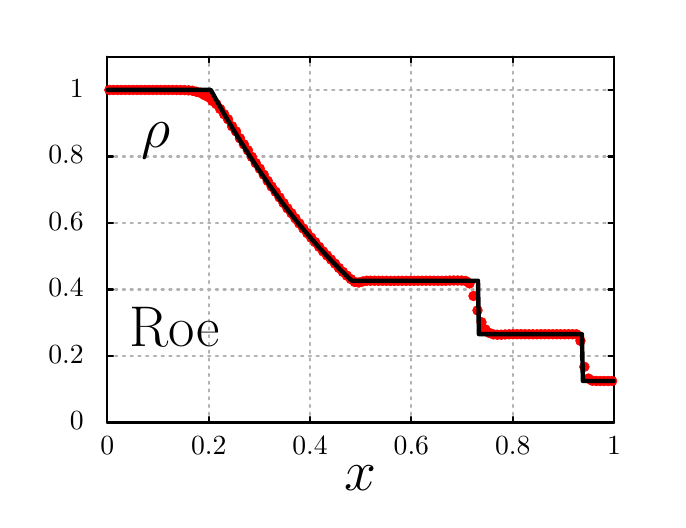
\begin{tikzpicture}[gnuplot]
%% generated with GNUPLOT 4.6p4 (Lua 5.1; terminal rev. 99, script rev. 100)
%% Thu 31 Jul 2014 02:05:55 PM EDT
\path (0.000,0.000) rectangle (8.000,6.000);
\gpfill{rgb color={1.000,1.000,1.000}} (1.012,0.985)--(7.446,0.985)--(7.446,5.630)--(1.012,5.630)--cycle;
\gpcolor{color=gp lt color border}
\gpsetlinetype{gp lt border}
\gpsetlinewidth{1.00}
\draw[gp path] (1.012,0.985)--(1.012,5.630)--(7.446,5.630)--(7.446,0.985)--cycle;
\gpcolor{color=gp lt color axes}
\gpsetlinetype{gp lt axes}
\gpsetlinewidth{2.00}
\draw[gp path] (1.012,0.985)--(7.447,0.985);
\gpcolor{color=gp lt color border}
\gpsetlinetype{gp lt border}
\draw[gp path] (1.012,0.985)--(1.084,0.985);
\draw[gp path] (7.447,0.985)--(7.375,0.985);
\gpcolor{rgb color={0.000,0.000,0.000}}
\node[gp node right,font={\fontsize{10pt}{12pt}\selectfont}] at (0.828,0.985) {0};
\gpcolor{color=gp lt color axes}
\gpsetlinetype{gp lt axes}
\draw[gp path] (1.012,1.830)--(7.447,1.830);
\gpcolor{color=gp lt color border}
\gpsetlinetype{gp lt border}
\draw[gp path] (1.012,1.830)--(1.084,1.830);
\draw[gp path] (7.447,1.830)--(7.375,1.830);
\gpcolor{rgb color={0.000,0.000,0.000}}
\node[gp node right,font={\fontsize{10pt}{12pt}\selectfont}] at (0.828,1.830) {0.2};
\gpcolor{color=gp lt color axes}
\gpsetlinetype{gp lt axes}
\draw[gp path] (1.012,2.674)--(7.447,2.674);
\gpcolor{color=gp lt color border}
\gpsetlinetype{gp lt border}
\draw[gp path] (1.012,2.674)--(1.084,2.674);
\draw[gp path] (7.447,2.674)--(7.375,2.674);
\gpcolor{rgb color={0.000,0.000,0.000}}
\node[gp node right,font={\fontsize{10pt}{12pt}\selectfont}] at (0.828,2.674) {0.4};
\gpcolor{color=gp lt color axes}
\gpsetlinetype{gp lt axes}
\draw[gp path] (1.012,3.519)--(7.447,3.519);
\gpcolor{color=gp lt color border}
\gpsetlinetype{gp lt border}
\draw[gp path] (1.012,3.519)--(1.084,3.519);
\draw[gp path] (7.447,3.519)--(7.375,3.519);
\gpcolor{rgb color={0.000,0.000,0.000}}
\node[gp node right,font={\fontsize{10pt}{12pt}\selectfont}] at (0.828,3.519) {0.6};
\gpcolor{color=gp lt color axes}
\gpsetlinetype{gp lt axes}
\draw[gp path] (1.012,4.364)--(7.447,4.364);
\gpcolor{color=gp lt color border}
\gpsetlinetype{gp lt border}
\draw[gp path] (1.012,4.364)--(1.084,4.364);
\draw[gp path] (7.447,4.364)--(7.375,4.364);
\gpcolor{rgb color={0.000,0.000,0.000}}
\node[gp node right,font={\fontsize{10pt}{12pt}\selectfont}] at (0.828,4.364) {0.8};
\gpcolor{color=gp lt color axes}
\gpsetlinetype{gp lt axes}
\draw[gp path] (1.012,5.209)--(7.447,5.209);
\gpcolor{color=gp lt color border}
\gpsetlinetype{gp lt border}
\draw[gp path] (1.012,5.209)--(1.084,5.209);
\draw[gp path] (7.447,5.209)--(7.375,5.209);
\gpcolor{rgb color={0.000,0.000,0.000}}
\node[gp node right,font={\fontsize{10pt}{12pt}\selectfont}] at (0.828,5.209) {1};
\gpcolor{color=gp lt color axes}
\gpsetlinetype{gp lt axes}
\draw[gp path] (1.012,0.985)--(1.012,5.631);
\gpcolor{color=gp lt color border}
\gpsetlinetype{gp lt border}
\draw[gp path] (1.012,0.985)--(1.012,1.057);
\draw[gp path] (1.012,5.631)--(1.012,5.559);
\gpcolor{rgb color={0.000,0.000,0.000}}
\node[gp node center,font={\fontsize{10pt}{12pt}\selectfont}] at (1.012,0.677) {0};
\gpcolor{color=gp lt color axes}
\gpsetlinetype{gp lt axes}
\draw[gp path] (2.299,0.985)--(2.299,5.631);
\gpcolor{color=gp lt color border}
\gpsetlinetype{gp lt border}
\draw[gp path] (2.299,0.985)--(2.299,1.057);
\draw[gp path] (2.299,5.631)--(2.299,5.559);
\gpcolor{rgb color={0.000,0.000,0.000}}
\node[gp node center,font={\fontsize{10pt}{12pt}\selectfont}] at (2.299,0.677) {0.2};
\gpcolor{color=gp lt color axes}
\gpsetlinetype{gp lt axes}
\draw[gp path] (3.586,0.985)--(3.586,5.631);
\gpcolor{color=gp lt color border}
\gpsetlinetype{gp lt border}
\draw[gp path] (3.586,0.985)--(3.586,1.057);
\draw[gp path] (3.586,5.631)--(3.586,5.559);
\gpcolor{rgb color={0.000,0.000,0.000}}
\node[gp node center,font={\fontsize{10pt}{12pt}\selectfont}] at (3.586,0.677) {0.4};
\gpcolor{color=gp lt color axes}
\gpsetlinetype{gp lt axes}
\draw[gp path] (4.873,0.985)--(4.873,5.631);
\gpcolor{color=gp lt color border}
\gpsetlinetype{gp lt border}
\draw[gp path] (4.873,0.985)--(4.873,1.057);
\draw[gp path] (4.873,5.631)--(4.873,5.559);
\gpcolor{rgb color={0.000,0.000,0.000}}
\node[gp node center,font={\fontsize{10pt}{12pt}\selectfont}] at (4.873,0.677) {0.6};
\gpcolor{color=gp lt color axes}
\gpsetlinetype{gp lt axes}
\draw[gp path] (6.160,0.985)--(6.160,5.631);
\gpcolor{color=gp lt color border}
\gpsetlinetype{gp lt border}
\draw[gp path] (6.160,0.985)--(6.160,1.057);
\draw[gp path] (6.160,5.631)--(6.160,5.559);
\gpcolor{rgb color={0.000,0.000,0.000}}
\node[gp node center,font={\fontsize{10pt}{12pt}\selectfont}] at (6.160,0.677) {0.8};
\gpcolor{color=gp lt color axes}
\gpsetlinetype{gp lt axes}
\draw[gp path] (7.447,0.985)--(7.447,5.631);
\gpcolor{color=gp lt color border}
\gpsetlinetype{gp lt border}
\draw[gp path] (7.447,0.985)--(7.447,1.057);
\draw[gp path] (7.447,5.631)--(7.447,5.559);
\gpcolor{rgb color={0.000,0.000,0.000}}
\node[gp node center,font={\fontsize{10pt}{12pt}\selectfont}] at (7.447,0.677) {1};
\gpcolor{color=gp lt color border}
\draw[gp path] (1.012,5.631)--(1.012,0.985)--(7.447,0.985)--(7.447,5.631)--cycle;
\gpcolor{rgb color={0.000,0.000,0.000}}
\node[gp node center,font={\fontsize{10pt}{12pt}\selectfont}] at (4.229,0.215) {\huge $x$};
\gpcolor{rgb color={1.000,0.000,0.000}}
\gpsetlinewidth{0.50}
\gpsetpointsize{4.44}
\gppoint{gp mark 7}{(1.037,5.209)}
\gppoint{gp mark 7}{(1.087,5.209)}
\gppoint{gp mark 7}{(1.138,5.209)}
\gppoint{gp mark 7}{(1.188,5.209)}
\gppoint{gp mark 7}{(1.238,5.209)}
\gppoint{gp mark 7}{(1.289,5.209)}
\gppoint{gp mark 7}{(1.339,5.209)}
\gppoint{gp mark 7}{(1.389,5.209)}
\gppoint{gp mark 7}{(1.439,5.209)}
\gppoint{gp mark 7}{(1.490,5.209)}
\gppoint{gp mark 7}{(1.540,5.209)}
\gppoint{gp mark 7}{(1.590,5.209)}
\gppoint{gp mark 7}{(1.640,5.209)}
\gppoint{gp mark 7}{(1.691,5.209)}
\gppoint{gp mark 7}{(1.741,5.209)}
\gppoint{gp mark 7}{(1.791,5.209)}
\gppoint{gp mark 7}{(1.842,5.209)}
\gppoint{gp mark 7}{(1.892,5.208)}
\gppoint{gp mark 7}{(1.942,5.208)}
\gppoint{gp mark 7}{(1.992,5.207)}
\gppoint{gp mark 7}{(2.043,5.204)}
\gppoint{gp mark 7}{(2.093,5.199)}
\gppoint{gp mark 7}{(2.143,5.186)}
\gppoint{gp mark 7}{(2.193,5.173)}
\gppoint{gp mark 7}{(2.244,5.144)}
\gppoint{gp mark 7}{(2.294,5.119)}
\gppoint{gp mark 7}{(2.344,5.070)}
\gppoint{gp mark 7}{(2.395,5.030)}
\gppoint{gp mark 7}{(2.445,4.967)}
\gppoint{gp mark 7}{(2.495,4.901)}
\gppoint{gp mark 7}{(2.545,4.836)}
\gppoint{gp mark 7}{(2.596,4.748)}
\gppoint{gp mark 7}{(2.646,4.683)}
\gppoint{gp mark 7}{(2.696,4.595)}
\gppoint{gp mark 7}{(2.746,4.518)}
\gppoint{gp mark 7}{(2.797,4.443)}
\gppoint{gp mark 7}{(2.847,4.359)}
\gppoint{gp mark 7}{(2.897,4.280)}
\gppoint{gp mark 7}{(2.948,4.209)}
\gppoint{gp mark 7}{(2.998,4.133)}
\gppoint{gp mark 7}{(3.048,4.055)}
\gppoint{gp mark 7}{(3.098,3.982)}
\gppoint{gp mark 7}{(3.149,3.916)}
\gppoint{gp mark 7}{(3.199,3.844)}
\gppoint{gp mark 7}{(3.249,3.773)}
\gppoint{gp mark 7}{(3.299,3.705)}
\gppoint{gp mark 7}{(3.350,3.643)}
\gppoint{gp mark 7}{(3.400,3.579)}
\gppoint{gp mark 7}{(3.450,3.513)}
\gppoint{gp mark 7}{(3.501,3.449)}
\gppoint{gp mark 7}{(3.551,3.390)}
\gppoint{gp mark 7}{(3.601,3.333)}
\gppoint{gp mark 7}{(3.651,3.276)}
\gppoint{gp mark 7}{(3.702,3.216)}
\gppoint{gp mark 7}{(3.752,3.158)}
\gppoint{gp mark 7}{(3.802,3.107)}
\gppoint{gp mark 7}{(3.852,3.056)}
\gppoint{gp mark 7}{(3.903,3.003)}
\gppoint{gp mark 7}{(3.953,2.948)}
\gppoint{gp mark 7}{(4.003,2.898)}
\gppoint{gp mark 7}{(4.054,2.851)}
\gppoint{gp mark 7}{(4.104,2.807)}
\gppoint{gp mark 7}{(4.154,2.771)}
\gppoint{gp mark 7}{(4.204,2.763)}
\gppoint{gp mark 7}{(4.255,2.777)}
\gppoint{gp mark 7}{(4.305,2.786)}
\gppoint{gp mark 7}{(4.355,2.786)}
\gppoint{gp mark 7}{(4.405,2.786)}
\gppoint{gp mark 7}{(4.456,2.785)}
\gppoint{gp mark 7}{(4.506,2.785)}
\gppoint{gp mark 7}{(4.556,2.785)}
\gppoint{gp mark 7}{(4.607,2.784)}
\gppoint{gp mark 7}{(4.657,2.784)}
\gppoint{gp mark 7}{(4.707,2.785)}
\gppoint{gp mark 7}{(4.757,2.785)}
\gppoint{gp mark 7}{(4.808,2.785)}
\gppoint{gp mark 7}{(4.858,2.785)}
\gppoint{gp mark 7}{(4.908,2.785)}
\gppoint{gp mark 7}{(4.958,2.785)}
\gppoint{gp mark 7}{(5.009,2.786)}
\gppoint{gp mark 7}{(5.059,2.786)}
\gppoint{gp mark 7}{(5.109,2.786)}
\gppoint{gp mark 7}{(5.160,2.786)}
\gppoint{gp mark 7}{(5.210,2.785)}
\gppoint{gp mark 7}{(5.260,2.785)}
\gppoint{gp mark 7}{(5.310,2.786)}
\gppoint{gp mark 7}{(5.361,2.788)}
\gppoint{gp mark 7}{(5.411,2.789)}
\gppoint{gp mark 7}{(5.461,2.789)}
\gppoint{gp mark 7}{(5.511,2.788)}
\gppoint{gp mark 7}{(5.562,2.783)}
\gppoint{gp mark 7}{(5.612,2.752)}
\gppoint{gp mark 7}{(5.662,2.593)}
\gppoint{gp mark 7}{(5.713,2.409)}
\gppoint{gp mark 7}{(5.763,2.259)}
\gppoint{gp mark 7}{(5.813,2.167)}
\gppoint{gp mark 7}{(5.863,2.123)}
\gppoint{gp mark 7}{(5.914,2.105)}
\gppoint{gp mark 7}{(5.964,2.101)}
\gppoint{gp mark 7}{(6.014,2.101)}
\gppoint{gp mark 7}{(6.064,2.104)}
\gppoint{gp mark 7}{(6.115,2.106)}
\gppoint{gp mark 7}{(6.165,2.107)}
\gppoint{gp mark 7}{(6.215,2.107)}
\gppoint{gp mark 7}{(6.266,2.107)}
\gppoint{gp mark 7}{(6.316,2.107)}
\gppoint{gp mark 7}{(6.366,2.106)}
\gppoint{gp mark 7}{(6.416,2.106)}
\gppoint{gp mark 7}{(6.467,2.106)}
\gppoint{gp mark 7}{(6.517,2.107)}
\gppoint{gp mark 7}{(6.567,2.107)}
\gppoint{gp mark 7}{(6.617,2.107)}
\gppoint{gp mark 7}{(6.668,2.107)}
\gppoint{gp mark 7}{(6.718,2.107)}
\gppoint{gp mark 7}{(6.768,2.107)}
\gppoint{gp mark 7}{(6.819,2.106)}
\gppoint{gp mark 7}{(6.869,2.107)}
\gppoint{gp mark 7}{(6.919,2.107)}
\gppoint{gp mark 7}{(6.969,2.106)}
\gppoint{gp mark 7}{(7.020,2.023)}
\gppoint{gp mark 7}{(7.070,1.693)}
\gppoint{gp mark 7}{(7.120,1.544)}
\gppoint{gp mark 7}{(7.170,1.517)}
\gppoint{gp mark 7}{(7.221,1.513)}
\gppoint{gp mark 7}{(7.271,1.513)}
\gppoint{gp mark 7}{(7.321,1.513)}
\gppoint{gp mark 7}{(7.372,1.513)}
\gppoint{gp mark 7}{(7.422,1.513)}
\gpcolor{rgb color={0.000,0.000,0.000}}
\gpsetlinetype{gp lt plot 0}
\gpsetlinewidth{4.00}
\draw[gp path] (1.018,5.209)--(1.031,5.209)--(1.043,5.209)--(1.056,5.209)--(1.069,5.209)%
  --(1.081,5.209)--(1.094,5.209)--(1.106,5.209)--(1.119,5.209)--(1.131,5.209)--(1.144,5.209)%
  --(1.157,5.209)--(1.169,5.209)--(1.182,5.209)--(1.194,5.209)--(1.207,5.209)--(1.219,5.209)%
  --(1.232,5.209)--(1.245,5.209)--(1.257,5.209)--(1.270,5.209)--(1.282,5.209)--(1.295,5.209)%
  --(1.307,5.209)--(1.320,5.209)--(1.332,5.209)--(1.345,5.209)--(1.358,5.209)--(1.370,5.209)%
  --(1.383,5.209)--(1.395,5.209)--(1.408,5.209)--(1.420,5.209)--(1.433,5.209)--(1.446,5.209)%
  --(1.458,5.209)--(1.471,5.209)--(1.483,5.209)--(1.496,5.209)--(1.508,5.209)--(1.521,5.209)%
  --(1.534,5.209)--(1.546,5.209)--(1.559,5.209)--(1.571,5.209)--(1.584,5.209)--(1.596,5.209)%
  --(1.609,5.209)--(1.622,5.209)--(1.634,5.209)--(1.647,5.209)--(1.659,5.209)--(1.672,5.209)%
  --(1.684,5.209)--(1.697,5.209)--(1.710,5.209)--(1.722,5.209)--(1.735,5.209)--(1.747,5.209)%
  --(1.760,5.209)--(1.772,5.209)--(1.785,5.209)--(1.798,5.209)--(1.810,5.209)--(1.823,5.209)%
  --(1.835,5.209)--(1.848,5.209)--(1.860,5.209)--(1.873,5.209)--(1.886,5.209)--(1.898,5.209)%
  --(1.911,5.209)--(1.923,5.209)--(1.936,5.209)--(1.948,5.209)--(1.961,5.209)--(1.973,5.209)%
  --(1.986,5.209)--(1.999,5.209)--(2.011,5.209)--(2.024,5.209)--(2.036,5.209)--(2.049,5.209)%
  --(2.061,5.209)--(2.074,5.209)--(2.087,5.209)--(2.099,5.209)--(2.112,5.209)--(2.124,5.209)%
  --(2.137,5.209)--(2.149,5.209)--(2.162,5.209)--(2.175,5.209)--(2.187,5.209)--(2.200,5.209)%
  --(2.212,5.209)--(2.225,5.209)--(2.237,5.209)--(2.250,5.209)--(2.263,5.209)--(2.275,5.209)%
  --(2.288,5.209)--(2.300,5.209)--(2.313,5.209)--(2.325,5.209)--(2.338,5.187)--(2.351,5.163)%
  --(2.363,5.140)--(2.376,5.118)--(2.388,5.095)--(2.401,5.072)--(2.413,5.050)--(2.426,5.027)%
  --(2.439,5.005)--(2.451,4.982)--(2.464,4.960)--(2.476,4.938)--(2.489,4.916)--(2.501,4.894)%
  --(2.514,4.872)--(2.526,4.851)--(2.539,4.829)--(2.552,4.808)--(2.564,4.786)--(2.577,4.765)%
  --(2.589,4.744)--(2.602,4.723)--(2.614,4.702)--(2.627,4.681)--(2.640,4.660)--(2.652,4.639)%
  --(2.665,4.618)--(2.677,4.598)--(2.690,4.577)--(2.702,4.557)--(2.715,4.537)--(2.728,4.517)%
  --(2.740,4.496)--(2.753,4.476)--(2.765,4.456)--(2.778,4.437)--(2.790,4.417)--(2.803,4.397)%
  --(2.816,4.378)--(2.828,4.358)--(2.841,4.339)--(2.853,4.320)--(2.866,4.300)--(2.878,4.281)%
  --(2.891,4.262)--(2.904,4.243)--(2.916,4.225)--(2.929,4.206)--(2.941,4.187)--(2.954,4.169)%
  --(2.966,4.150)--(2.979,4.132)--(2.992,4.113)--(3.004,4.095)--(3.017,4.077)--(3.029,4.059)%
  --(3.042,4.041)--(3.054,4.023)--(3.067,4.005)--(3.079,3.987)--(3.092,3.970)--(3.105,3.952)%
  --(3.117,3.935)--(3.130,3.917)--(3.142,3.900)--(3.155,3.883)--(3.167,3.866)--(3.180,3.849)%
  --(3.193,3.832)--(3.205,3.815)--(3.218,3.798)--(3.230,3.781)--(3.243,3.764)--(3.255,3.748)%
  --(3.268,3.731)--(3.281,3.715)--(3.293,3.699)--(3.306,3.682)--(3.318,3.666)--(3.331,3.650)%
  --(3.343,3.634)--(3.356,3.618)--(3.369,3.602)--(3.381,3.586)--(3.394,3.571)--(3.406,3.555)%
  --(3.419,3.539)--(3.431,3.524)--(3.444,3.508)--(3.457,3.493)--(3.469,3.478)--(3.482,3.463)%
  --(3.494,3.447)--(3.507,3.432)--(3.519,3.417)--(3.532,3.403)--(3.545,3.388)--(3.557,3.373)%
  --(3.570,3.358)--(3.582,3.344)--(3.595,3.329)--(3.607,3.315)--(3.620,3.300)--(3.633,3.286)%
  --(3.645,3.272)--(3.658,3.257)--(3.670,3.243)--(3.683,3.229)--(3.695,3.215)--(3.708,3.201)%
  --(3.720,3.188)--(3.733,3.174)--(3.746,3.160)--(3.758,3.146)--(3.771,3.133)--(3.783,3.119)%
  --(3.796,3.106)--(3.808,3.093)--(3.821,3.079)--(3.834,3.066)--(3.846,3.053)--(3.859,3.040)%
  --(3.871,3.027)--(3.884,3.014)--(3.896,3.001)--(3.909,2.988)--(3.922,2.975)--(3.934,2.963)%
  --(3.947,2.950)--(3.959,2.937)--(3.972,2.925)--(3.984,2.912)--(3.997,2.900)--(4.010,2.888)%
  --(4.022,2.876)--(4.035,2.863)--(4.047,2.851)--(4.060,2.839)--(4.072,2.827)--(4.085,2.815)%
  --(4.098,2.803)--(4.110,2.792)--(4.123,2.786)--(4.135,2.786)--(4.148,2.786)--(4.160,2.786)%
  --(4.173,2.786)--(4.186,2.786)--(4.198,2.786)--(4.211,2.786)--(4.223,2.786)--(4.236,2.786)%
  --(4.248,2.786)--(4.261,2.786)--(4.273,2.786)--(4.286,2.786)--(4.299,2.786)--(4.311,2.786)%
  --(4.324,2.786)--(4.336,2.786)--(4.349,2.786)--(4.361,2.786)--(4.374,2.786)--(4.387,2.786)%
  --(4.399,2.786)--(4.412,2.786)--(4.424,2.786)--(4.437,2.786)--(4.449,2.786)--(4.462,2.786)%
  --(4.475,2.786)--(4.487,2.786)--(4.500,2.786)--(4.512,2.786)--(4.525,2.786)--(4.537,2.786)%
  --(4.550,2.786)--(4.563,2.786)--(4.575,2.786)--(4.588,2.786)--(4.600,2.786)--(4.613,2.786)%
  --(4.625,2.786)--(4.638,2.786)--(4.651,2.786)--(4.663,2.786)--(4.676,2.786)--(4.688,2.786)%
  --(4.701,2.786)--(4.713,2.786)--(4.726,2.786)--(4.739,2.786)--(4.751,2.786)--(4.764,2.786)%
  --(4.776,2.786)--(4.789,2.786)--(4.801,2.786)--(4.814,2.786)--(4.826,2.786)--(4.839,2.786)%
  --(4.852,2.786)--(4.864,2.786)--(4.877,2.786)--(4.889,2.786)--(4.902,2.786)--(4.914,2.786)%
  --(4.927,2.786)--(4.940,2.786)--(4.952,2.786)--(4.965,2.786)--(4.977,2.786)--(4.990,2.786)%
  --(5.002,2.786)--(5.015,2.786)--(5.028,2.786)--(5.040,2.786)--(5.053,2.786)--(5.065,2.786)%
  --(5.078,2.786)--(5.090,2.786)--(5.103,2.786)--(5.116,2.786)--(5.128,2.786)--(5.141,2.786)%
  --(5.153,2.786)--(5.166,2.786)--(5.178,2.786)--(5.191,2.786)--(5.204,2.786)--(5.216,2.786)%
  --(5.229,2.786)--(5.241,2.786)--(5.254,2.786)--(5.266,2.786)--(5.279,2.786)--(5.292,2.786)%
  --(5.304,2.786)--(5.317,2.786)--(5.329,2.786)--(5.342,2.786)--(5.354,2.786)--(5.367,2.786)%
  --(5.380,2.786)--(5.392,2.786)--(5.405,2.786)--(5.417,2.786)--(5.430,2.786)--(5.442,2.786)%
  --(5.455,2.786)--(5.467,2.786)--(5.480,2.786)--(5.493,2.786)--(5.505,2.786)--(5.518,2.786)%
  --(5.530,2.786)--(5.543,2.786)--(5.555,2.786)--(5.568,2.786)--(5.581,2.786)--(5.593,2.786)%
  --(5.606,2.786)--(5.618,2.786)--(5.631,2.786)--(5.643,2.786)--(5.656,2.786)--(5.669,2.786)%
  --(5.681,2.786)--(5.694,2.786)--(5.706,2.786)--(5.719,2.786)--(5.731,2.107)--(5.744,2.107)%
  --(5.757,2.107)--(5.769,2.107)--(5.782,2.107)--(5.794,2.107)--(5.807,2.107)--(5.819,2.107)%
  --(5.832,2.107)--(5.845,2.107)--(5.857,2.107)--(5.870,2.107)--(5.882,2.107)--(5.895,2.107)%
  --(5.907,2.107)--(5.920,2.107)--(5.933,2.107)--(5.945,2.107)--(5.958,2.107)--(5.970,2.107)%
  --(5.983,2.107)--(5.995,2.107)--(6.008,2.107)--(6.020,2.107)--(6.033,2.107)--(6.046,2.107)%
  --(6.058,2.107)--(6.071,2.107)--(6.083,2.107)--(6.096,2.107)--(6.108,2.107)--(6.121,2.107)%
  --(6.134,2.107)--(6.146,2.107)--(6.159,2.107)--(6.171,2.107)--(6.184,2.107)--(6.196,2.107)%
  --(6.209,2.107)--(6.222,2.107)--(6.234,2.107)--(6.247,2.107)--(6.259,2.107)--(6.272,2.107)%
  --(6.284,2.107)--(6.297,2.107)--(6.310,2.107)--(6.322,2.107)--(6.335,2.107)--(6.347,2.107)%
  --(6.360,2.107)--(6.372,2.107)--(6.385,2.107)--(6.398,2.107)--(6.410,2.107)--(6.423,2.107)%
  --(6.435,2.107)--(6.448,2.107)--(6.460,2.107)--(6.473,2.107)--(6.486,2.107)--(6.498,2.107)%
  --(6.511,2.107)--(6.523,2.107)--(6.536,2.107)--(6.548,2.107)--(6.561,2.107)--(6.573,2.107)%
  --(6.586,2.107)--(6.599,2.107)--(6.611,2.107)--(6.624,2.107)--(6.636,2.107)--(6.649,2.107)%
  --(6.661,2.107)--(6.674,2.107)--(6.687,2.107)--(6.699,2.107)--(6.712,2.107)--(6.724,2.107)%
  --(6.737,2.107)--(6.749,2.107)--(6.762,2.107)--(6.775,2.107)--(6.787,2.107)--(6.800,2.107)%
  --(6.812,2.107)--(6.825,2.107)--(6.837,2.107)--(6.850,2.107)--(6.863,2.107)--(6.875,2.107)%
  --(6.888,2.107)--(6.900,2.107)--(6.913,2.107)--(6.925,2.107)--(6.938,2.107)--(6.951,2.107)%
  --(6.963,2.107)--(6.976,2.107)--(6.988,2.107)--(7.001,2.107)--(7.013,2.107)--(7.026,2.107)%
  --(7.039,2.107)--(7.051,1.513)--(7.064,1.513)--(7.076,1.513)--(7.089,1.513)--(7.101,1.513)%
  --(7.114,1.513)--(7.127,1.513)--(7.139,1.513)--(7.152,1.513)--(7.164,1.513)--(7.177,1.513)%
  --(7.189,1.513)--(7.202,1.513)--(7.214,1.513)--(7.227,1.513)--(7.240,1.513)--(7.252,1.513)%
  --(7.265,1.513)--(7.277,1.513)--(7.290,1.513)--(7.302,1.513)--(7.315,1.513)--(7.328,1.513)%
  --(7.340,1.513)--(7.353,1.513)--(7.365,1.513)--(7.378,1.513)--(7.390,1.513)--(7.403,1.513)%
  --(7.416,1.513)--(7.428,1.513)--(7.441,1.513);
\node[gp node left,font={\fontsize{10pt}{12pt}\selectfont}] at (1.334,4.575) {\huge $\rho$};
\node[gp node left,font={\fontsize{10pt}{12pt}\selectfont}] at (1.173,2.041) {\huge Roe};
%% coordinates of the plot area
\gpdefrectangularnode{gp plot 1}{\pgfpoint{1.012cm}{0.985cm}}{\pgfpoint{7.447cm}{5.631cm}}
\end{tikzpicture}
%% gnuplot variables
} &
\resizebox{0.33\linewidth}{!}{\tikzsetnextfilename{sod_roe_3_2}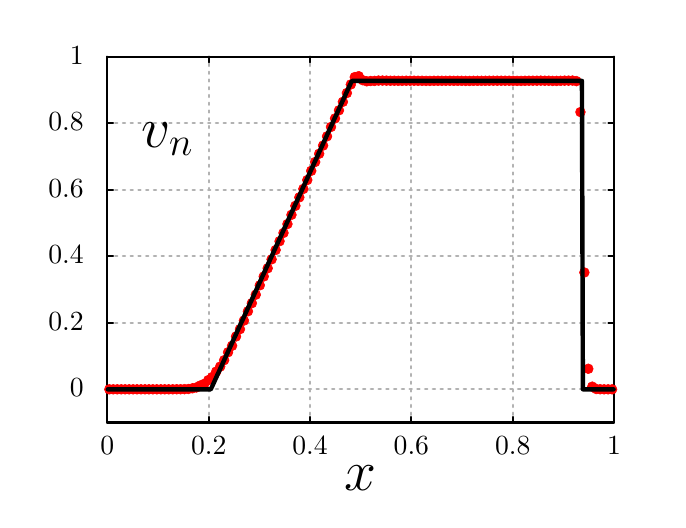
\begin{tikzpicture}[gnuplot]
%% generated with GNUPLOT 4.6p4 (Lua 5.1; terminal rev. 99, script rev. 100)
%% Thu 31 Jul 2014 02:05:55 PM EDT
\path (0.000,0.000) rectangle (8.000,6.000);
\gpfill{rgb color={1.000,1.000,1.000}} (1.012,0.985)--(7.446,0.985)--(7.446,5.630)--(1.012,5.630)--cycle;
\gpcolor{color=gp lt color border}
\gpsetlinetype{gp lt border}
\gpsetlinewidth{1.00}
\draw[gp path] (1.012,0.985)--(1.012,5.630)--(7.446,5.630)--(7.446,0.985)--cycle;
\gpcolor{color=gp lt color axes}
\gpsetlinetype{gp lt axes}
\gpsetlinewidth{2.00}
\draw[gp path] (1.012,1.407)--(7.447,1.407);
\gpcolor{color=gp lt color border}
\gpsetlinetype{gp lt border}
\draw[gp path] (1.012,1.407)--(1.084,1.407);
\draw[gp path] (7.447,1.407)--(7.375,1.407);
\gpcolor{rgb color={0.000,0.000,0.000}}
\node[gp node right,font={\fontsize{10pt}{12pt}\selectfont}] at (0.828,1.407) {0};
\gpcolor{color=gp lt color axes}
\gpsetlinetype{gp lt axes}
\draw[gp path] (1.012,2.252)--(7.447,2.252);
\gpcolor{color=gp lt color border}
\gpsetlinetype{gp lt border}
\draw[gp path] (1.012,2.252)--(1.084,2.252);
\draw[gp path] (7.447,2.252)--(7.375,2.252);
\gpcolor{rgb color={0.000,0.000,0.000}}
\node[gp node right,font={\fontsize{10pt}{12pt}\selectfont}] at (0.828,2.252) {0.2};
\gpcolor{color=gp lt color axes}
\gpsetlinetype{gp lt axes}
\draw[gp path] (1.012,3.097)--(7.447,3.097);
\gpcolor{color=gp lt color border}
\gpsetlinetype{gp lt border}
\draw[gp path] (1.012,3.097)--(1.084,3.097);
\draw[gp path] (7.447,3.097)--(7.375,3.097);
\gpcolor{rgb color={0.000,0.000,0.000}}
\node[gp node right,font={\fontsize{10pt}{12pt}\selectfont}] at (0.828,3.097) {0.4};
\gpcolor{color=gp lt color axes}
\gpsetlinetype{gp lt axes}
\draw[gp path] (1.012,3.942)--(7.447,3.942);
\gpcolor{color=gp lt color border}
\gpsetlinetype{gp lt border}
\draw[gp path] (1.012,3.942)--(1.084,3.942);
\draw[gp path] (7.447,3.942)--(7.375,3.942);
\gpcolor{rgb color={0.000,0.000,0.000}}
\node[gp node right,font={\fontsize{10pt}{12pt}\selectfont}] at (0.828,3.942) {0.6};
\gpcolor{color=gp lt color axes}
\gpsetlinetype{gp lt axes}
\draw[gp path] (1.012,4.786)--(7.447,4.786);
\gpcolor{color=gp lt color border}
\gpsetlinetype{gp lt border}
\draw[gp path] (1.012,4.786)--(1.084,4.786);
\draw[gp path] (7.447,4.786)--(7.375,4.786);
\gpcolor{rgb color={0.000,0.000,0.000}}
\node[gp node right,font={\fontsize{10pt}{12pt}\selectfont}] at (0.828,4.786) {0.8};
\gpcolor{color=gp lt color axes}
\gpsetlinetype{gp lt axes}
\draw[gp path] (1.012,5.631)--(7.447,5.631);
\gpcolor{color=gp lt color border}
\gpsetlinetype{gp lt border}
\draw[gp path] (1.012,5.631)--(1.084,5.631);
\draw[gp path] (7.447,5.631)--(7.375,5.631);
\gpcolor{rgb color={0.000,0.000,0.000}}
\node[gp node right,font={\fontsize{10pt}{12pt}\selectfont}] at (0.828,5.631) {1};
\gpcolor{color=gp lt color axes}
\gpsetlinetype{gp lt axes}
\draw[gp path] (1.012,0.985)--(1.012,5.631);
\gpcolor{color=gp lt color border}
\gpsetlinetype{gp lt border}
\draw[gp path] (1.012,0.985)--(1.012,1.057);
\draw[gp path] (1.012,5.631)--(1.012,5.559);
\gpcolor{rgb color={0.000,0.000,0.000}}
\node[gp node center,font={\fontsize{10pt}{12pt}\selectfont}] at (1.012,0.677) {0};
\gpcolor{color=gp lt color axes}
\gpsetlinetype{gp lt axes}
\draw[gp path] (2.299,0.985)--(2.299,5.631);
\gpcolor{color=gp lt color border}
\gpsetlinetype{gp lt border}
\draw[gp path] (2.299,0.985)--(2.299,1.057);
\draw[gp path] (2.299,5.631)--(2.299,5.559);
\gpcolor{rgb color={0.000,0.000,0.000}}
\node[gp node center,font={\fontsize{10pt}{12pt}\selectfont}] at (2.299,0.677) {0.2};
\gpcolor{color=gp lt color axes}
\gpsetlinetype{gp lt axes}
\draw[gp path] (3.586,0.985)--(3.586,5.631);
\gpcolor{color=gp lt color border}
\gpsetlinetype{gp lt border}
\draw[gp path] (3.586,0.985)--(3.586,1.057);
\draw[gp path] (3.586,5.631)--(3.586,5.559);
\gpcolor{rgb color={0.000,0.000,0.000}}
\node[gp node center,font={\fontsize{10pt}{12pt}\selectfont}] at (3.586,0.677) {0.4};
\gpcolor{color=gp lt color axes}
\gpsetlinetype{gp lt axes}
\draw[gp path] (4.873,0.985)--(4.873,5.631);
\gpcolor{color=gp lt color border}
\gpsetlinetype{gp lt border}
\draw[gp path] (4.873,0.985)--(4.873,1.057);
\draw[gp path] (4.873,5.631)--(4.873,5.559);
\gpcolor{rgb color={0.000,0.000,0.000}}
\node[gp node center,font={\fontsize{10pt}{12pt}\selectfont}] at (4.873,0.677) {0.6};
\gpcolor{color=gp lt color axes}
\gpsetlinetype{gp lt axes}
\draw[gp path] (6.160,0.985)--(6.160,5.631);
\gpcolor{color=gp lt color border}
\gpsetlinetype{gp lt border}
\draw[gp path] (6.160,0.985)--(6.160,1.057);
\draw[gp path] (6.160,5.631)--(6.160,5.559);
\gpcolor{rgb color={0.000,0.000,0.000}}
\node[gp node center,font={\fontsize{10pt}{12pt}\selectfont}] at (6.160,0.677) {0.8};
\gpcolor{color=gp lt color axes}
\gpsetlinetype{gp lt axes}
\draw[gp path] (7.447,0.985)--(7.447,5.631);
\gpcolor{color=gp lt color border}
\gpsetlinetype{gp lt border}
\draw[gp path] (7.447,0.985)--(7.447,1.057);
\draw[gp path] (7.447,5.631)--(7.447,5.559);
\gpcolor{rgb color={0.000,0.000,0.000}}
\node[gp node center,font={\fontsize{10pt}{12pt}\selectfont}] at (7.447,0.677) {1};
\gpcolor{color=gp lt color border}
\draw[gp path] (1.012,5.631)--(1.012,0.985)--(7.447,0.985)--(7.447,5.631)--cycle;
\gpcolor{rgb color={0.000,0.000,0.000}}
\node[gp node center,font={\fontsize{10pt}{12pt}\selectfont}] at (4.229,0.215) {\huge $x$};
\gpcolor{rgb color={1.000,0.000,0.000}}
\gpsetlinewidth{0.50}
\gpsetpointsize{4.44}
\gppoint{gp mark 7}{(1.037,1.407)}
\gppoint{gp mark 7}{(1.087,1.407)}
\gppoint{gp mark 7}{(1.138,1.407)}
\gppoint{gp mark 7}{(1.188,1.407)}
\gppoint{gp mark 7}{(1.238,1.407)}
\gppoint{gp mark 7}{(1.289,1.407)}
\gppoint{gp mark 7}{(1.339,1.407)}
\gppoint{gp mark 7}{(1.389,1.407)}
\gppoint{gp mark 7}{(1.439,1.407)}
\gppoint{gp mark 7}{(1.490,1.407)}
\gppoint{gp mark 7}{(1.540,1.407)}
\gppoint{gp mark 7}{(1.590,1.407)}
\gppoint{gp mark 7}{(1.640,1.407)}
\gppoint{gp mark 7}{(1.691,1.407)}
\gppoint{gp mark 7}{(1.741,1.407)}
\gppoint{gp mark 7}{(1.791,1.407)}
\gppoint{gp mark 7}{(1.842,1.407)}
\gppoint{gp mark 7}{(1.892,1.408)}
\gppoint{gp mark 7}{(1.942,1.408)}
\gppoint{gp mark 7}{(1.992,1.409)}
\gppoint{gp mark 7}{(2.043,1.412)}
\gppoint{gp mark 7}{(2.093,1.420)}
\gppoint{gp mark 7}{(2.143,1.431)}
\gppoint{gp mark 7}{(2.193,1.456)}
\gppoint{gp mark 7}{(2.244,1.477)}
\gppoint{gp mark 7}{(2.294,1.524)}
\gppoint{gp mark 7}{(2.344,1.563)}
\gppoint{gp mark 7}{(2.395,1.633)}
\gppoint{gp mark 7}{(2.445,1.696)}
\gppoint{gp mark 7}{(2.495,1.777)}
\gppoint{gp mark 7}{(2.545,1.878)}
\gppoint{gp mark 7}{(2.596,1.960)}
\gppoint{gp mark 7}{(2.646,2.078)}
\gppoint{gp mark 7}{(2.696,2.171)}
\gppoint{gp mark 7}{(2.746,2.280)}
\gppoint{gp mark 7}{(2.797,2.398)}
\gppoint{gp mark 7}{(2.847,2.501)}
\gppoint{gp mark 7}{(2.897,2.609)}
\gppoint{gp mark 7}{(2.948,2.728)}
\gppoint{gp mark 7}{(2.998,2.840)}
\gppoint{gp mark 7}{(3.048,2.944)}
\gppoint{gp mark 7}{(3.098,3.058)}
\gppoint{gp mark 7}{(3.149,3.176)}
\gppoint{gp mark 7}{(3.199,3.288)}
\gppoint{gp mark 7}{(3.249,3.393)}
\gppoint{gp mark 7}{(3.299,3.506)}
\gppoint{gp mark 7}{(3.350,3.623)}
\gppoint{gp mark 7}{(3.400,3.737)}
\gppoint{gp mark 7}{(3.450,3.845)}
\gppoint{gp mark 7}{(3.501,3.952)}
\gppoint{gp mark 7}{(3.551,4.065)}
\gppoint{gp mark 7}{(3.601,4.182)}
\gppoint{gp mark 7}{(3.651,4.294)}
\gppoint{gp mark 7}{(3.702,4.399)}
\gppoint{gp mark 7}{(3.752,4.503)}
\gppoint{gp mark 7}{(3.802,4.620)}
\gppoint{gp mark 7}{(3.852,4.739)}
\gppoint{gp mark 7}{(3.903,4.847)}
\gppoint{gp mark 7}{(3.953,4.950)}
\gppoint{gp mark 7}{(4.003,5.058)}
\gppoint{gp mark 7}{(4.054,5.170)}
\gppoint{gp mark 7}{(4.104,5.279)}
\gppoint{gp mark 7}{(4.154,5.372)}
\gppoint{gp mark 7}{(4.204,5.384)}
\gppoint{gp mark 7}{(4.255,5.333)}
\gppoint{gp mark 7}{(4.305,5.319)}
\gppoint{gp mark 7}{(4.355,5.323)}
\gppoint{gp mark 7}{(4.405,5.324)}
\gppoint{gp mark 7}{(4.456,5.328)}
\gppoint{gp mark 7}{(4.506,5.328)}
\gppoint{gp mark 7}{(4.556,5.327)}
\gppoint{gp mark 7}{(4.607,5.326)}
\gppoint{gp mark 7}{(4.657,5.326)}
\gppoint{gp mark 7}{(4.707,5.325)}
\gppoint{gp mark 7}{(4.757,5.325)}
\gppoint{gp mark 7}{(4.808,5.326)}
\gppoint{gp mark 7}{(4.858,5.326)}
\gppoint{gp mark 7}{(4.908,5.326)}
\gppoint{gp mark 7}{(4.958,5.325)}
\gppoint{gp mark 7}{(5.009,5.325)}
\gppoint{gp mark 7}{(5.059,5.324)}
\gppoint{gp mark 7}{(5.109,5.324)}
\gppoint{gp mark 7}{(5.160,5.325)}
\gppoint{gp mark 7}{(5.210,5.325)}
\gppoint{gp mark 7}{(5.260,5.325)}
\gppoint{gp mark 7}{(5.310,5.325)}
\gppoint{gp mark 7}{(5.361,5.326)}
\gppoint{gp mark 7}{(5.411,5.325)}
\gppoint{gp mark 7}{(5.461,5.325)}
\gppoint{gp mark 7}{(5.511,5.325)}
\gppoint{gp mark 7}{(5.562,5.324)}
\gppoint{gp mark 7}{(5.612,5.324)}
\gppoint{gp mark 7}{(5.662,5.325)}
\gppoint{gp mark 7}{(5.713,5.325)}
\gppoint{gp mark 7}{(5.763,5.325)}
\gppoint{gp mark 7}{(5.813,5.325)}
\gppoint{gp mark 7}{(5.863,5.326)}
\gppoint{gp mark 7}{(5.914,5.326)}
\gppoint{gp mark 7}{(5.964,5.326)}
\gppoint{gp mark 7}{(6.014,5.326)}
\gppoint{gp mark 7}{(6.064,5.326)}
\gppoint{gp mark 7}{(6.115,5.326)}
\gppoint{gp mark 7}{(6.165,5.325)}
\gppoint{gp mark 7}{(6.215,5.324)}
\gppoint{gp mark 7}{(6.266,5.324)}
\gppoint{gp mark 7}{(6.316,5.325)}
\gppoint{gp mark 7}{(6.366,5.326)}
\gppoint{gp mark 7}{(6.416,5.326)}
\gppoint{gp mark 7}{(6.467,5.326)}
\gppoint{gp mark 7}{(6.517,5.327)}
\gppoint{gp mark 7}{(6.567,5.326)}
\gppoint{gp mark 7}{(6.617,5.326)}
\gppoint{gp mark 7}{(6.668,5.324)}
\gppoint{gp mark 7}{(6.718,5.324)}
\gppoint{gp mark 7}{(6.768,5.325)}
\gppoint{gp mark 7}{(6.819,5.327)}
\gppoint{gp mark 7}{(6.869,5.327)}
\gppoint{gp mark 7}{(6.919,5.328)}
\gppoint{gp mark 7}{(6.969,5.321)}
\gppoint{gp mark 7}{(7.020,4.928)}
\gppoint{gp mark 7}{(7.070,2.891)}
\gppoint{gp mark 7}{(7.120,1.668)}
\gppoint{gp mark 7}{(7.170,1.441)}
\gppoint{gp mark 7}{(7.221,1.411)}
\gppoint{gp mark 7}{(7.271,1.408)}
\gppoint{gp mark 7}{(7.321,1.407)}
\gppoint{gp mark 7}{(7.372,1.407)}
\gppoint{gp mark 7}{(7.422,1.407)}
\gpcolor{rgb color={0.000,0.000,0.000}}
\gpsetlinetype{gp lt plot 0}
\gpsetlinewidth{4.00}
\draw[gp path] (1.018,1.407)--(1.031,1.407)--(1.043,1.407)--(1.056,1.407)--(1.069,1.407)%
  --(1.081,1.407)--(1.094,1.407)--(1.106,1.407)--(1.119,1.407)--(1.131,1.407)--(1.144,1.407)%
  --(1.157,1.407)--(1.169,1.407)--(1.182,1.407)--(1.194,1.407)--(1.207,1.407)--(1.219,1.407)%
  --(1.232,1.407)--(1.245,1.407)--(1.257,1.407)--(1.270,1.407)--(1.282,1.407)--(1.295,1.407)%
  --(1.307,1.407)--(1.320,1.407)--(1.332,1.407)--(1.345,1.407)--(1.358,1.407)--(1.370,1.407)%
  --(1.383,1.407)--(1.395,1.407)--(1.408,1.407)--(1.420,1.407)--(1.433,1.407)--(1.446,1.407)%
  --(1.458,1.407)--(1.471,1.407)--(1.483,1.407)--(1.496,1.407)--(1.508,1.407)--(1.521,1.407)%
  --(1.534,1.407)--(1.546,1.407)--(1.559,1.407)--(1.571,1.407)--(1.584,1.407)--(1.596,1.407)%
  --(1.609,1.407)--(1.622,1.407)--(1.634,1.407)--(1.647,1.407)--(1.659,1.407)--(1.672,1.407)%
  --(1.684,1.407)--(1.697,1.407)--(1.710,1.407)--(1.722,1.407)--(1.735,1.407)--(1.747,1.407)%
  --(1.760,1.407)--(1.772,1.407)--(1.785,1.407)--(1.798,1.407)--(1.810,1.407)--(1.823,1.407)%
  --(1.835,1.407)--(1.848,1.407)--(1.860,1.407)--(1.873,1.407)--(1.886,1.407)--(1.898,1.407)%
  --(1.911,1.407)--(1.923,1.407)--(1.936,1.407)--(1.948,1.407)--(1.961,1.407)--(1.973,1.407)%
  --(1.986,1.407)--(1.999,1.407)--(2.011,1.407)--(2.024,1.407)--(2.036,1.407)--(2.049,1.407)%
  --(2.061,1.407)--(2.074,1.407)--(2.087,1.407)--(2.099,1.407)--(2.112,1.407)--(2.124,1.407)%
  --(2.137,1.407)--(2.149,1.407)--(2.162,1.407)--(2.175,1.407)--(2.187,1.407)--(2.200,1.407)%
  --(2.212,1.407)--(2.225,1.407)--(2.237,1.407)--(2.250,1.407)--(2.263,1.407)--(2.275,1.407)%
  --(2.288,1.407)--(2.300,1.407)--(2.313,1.407)--(2.325,1.407)--(2.338,1.434)--(2.351,1.461)%
  --(2.363,1.489)--(2.376,1.516)--(2.388,1.544)--(2.401,1.571)--(2.413,1.599)--(2.426,1.626)%
  --(2.439,1.654)--(2.451,1.681)--(2.464,1.709)--(2.476,1.736)--(2.489,1.764)--(2.501,1.791)%
  --(2.514,1.818)--(2.526,1.846)--(2.539,1.873)--(2.552,1.901)--(2.564,1.928)--(2.577,1.956)%
  --(2.589,1.983)--(2.602,2.011)--(2.614,2.038)--(2.627,2.066)--(2.640,2.093)--(2.652,2.121)%
  --(2.665,2.148)--(2.677,2.176)--(2.690,2.203)--(2.702,2.231)--(2.715,2.258)--(2.728,2.286)%
  --(2.740,2.313)--(2.753,2.341)--(2.765,2.368)--(2.778,2.396)--(2.790,2.423)--(2.803,2.451)%
  --(2.816,2.478)--(2.828,2.506)--(2.841,2.533)--(2.853,2.561)--(2.866,2.588)--(2.878,2.616)%
  --(2.891,2.643)--(2.904,2.671)--(2.916,2.698)--(2.929,2.726)--(2.941,2.753)--(2.954,2.781)%
  --(2.966,2.808)--(2.979,2.836)--(2.992,2.863)--(3.004,2.891)--(3.017,2.918)--(3.029,2.946)%
  --(3.042,2.973)--(3.054,3.001)--(3.067,3.028)--(3.079,3.056)--(3.092,3.083)--(3.105,3.111)%
  --(3.117,3.138)--(3.130,3.166)--(3.142,3.193)--(3.155,3.221)--(3.167,3.248)--(3.180,3.276)%
  --(3.193,3.303)--(3.205,3.331)--(3.218,3.358)--(3.230,3.386)--(3.243,3.413)--(3.255,3.441)%
  --(3.268,3.468)--(3.281,3.496)--(3.293,3.523)--(3.306,3.551)--(3.318,3.578)--(3.331,3.606)%
  --(3.343,3.633)--(3.356,3.661)--(3.369,3.688)--(3.381,3.716)--(3.394,3.743)--(3.406,3.771)%
  --(3.419,3.798)--(3.431,3.826)--(3.444,3.853)--(3.457,3.881)--(3.469,3.908)--(3.482,3.936)%
  --(3.494,3.963)--(3.507,3.991)--(3.519,4.018)--(3.532,4.046)--(3.545,4.073)--(3.557,4.101)%
  --(3.570,4.128)--(3.582,4.156)--(3.595,4.183)--(3.607,4.211)--(3.620,4.238)--(3.633,4.266)%
  --(3.645,4.293)--(3.658,4.321)--(3.670,4.348)--(3.683,4.376)--(3.695,4.403)--(3.708,4.431)%
  --(3.720,4.458)--(3.733,4.486)--(3.746,4.513)--(3.758,4.541)--(3.771,4.568)--(3.783,4.596)%
  --(3.796,4.623)--(3.808,4.651)--(3.821,4.678)--(3.834,4.706)--(3.846,4.733)--(3.859,4.761)%
  --(3.871,4.788)--(3.884,4.816)--(3.896,4.843)--(3.909,4.871)--(3.922,4.898)--(3.934,4.926)%
  --(3.947,4.953)--(3.959,4.981)--(3.972,5.008)--(3.984,5.036)--(3.997,5.063)--(4.010,5.091)%
  --(4.022,5.118)--(4.035,5.146)--(4.047,5.173)--(4.060,5.201)--(4.072,5.228)--(4.085,5.256)%
  --(4.098,5.283)--(4.110,5.311)--(4.123,5.324)--(4.135,5.324)--(4.148,5.324)--(4.160,5.324)%
  --(4.173,5.324)--(4.186,5.324)--(4.198,5.324)--(4.211,5.324)--(4.223,5.324)--(4.236,5.324)%
  --(4.248,5.324)--(4.261,5.324)--(4.273,5.324)--(4.286,5.324)--(4.299,5.324)--(4.311,5.324)%
  --(4.324,5.324)--(4.336,5.324)--(4.349,5.324)--(4.361,5.324)--(4.374,5.324)--(4.387,5.324)%
  --(4.399,5.324)--(4.412,5.324)--(4.424,5.324)--(4.437,5.324)--(4.449,5.324)--(4.462,5.324)%
  --(4.475,5.324)--(4.487,5.324)--(4.500,5.324)--(4.512,5.324)--(4.525,5.324)--(4.537,5.324)%
  --(4.550,5.324)--(4.563,5.324)--(4.575,5.324)--(4.588,5.324)--(4.600,5.324)--(4.613,5.324)%
  --(4.625,5.324)--(4.638,5.324)--(4.651,5.324)--(4.663,5.324)--(4.676,5.324)--(4.688,5.324)%
  --(4.701,5.324)--(4.713,5.324)--(4.726,5.324)--(4.739,5.324)--(4.751,5.324)--(4.764,5.324)%
  --(4.776,5.324)--(4.789,5.324)--(4.801,5.324)--(4.814,5.324)--(4.826,5.324)--(4.839,5.324)%
  --(4.852,5.324)--(4.864,5.324)--(4.877,5.324)--(4.889,5.324)--(4.902,5.324)--(4.914,5.324)%
  --(4.927,5.324)--(4.940,5.324)--(4.952,5.324)--(4.965,5.324)--(4.977,5.324)--(4.990,5.324)%
  --(5.002,5.324)--(5.015,5.324)--(5.028,5.324)--(5.040,5.324)--(5.053,5.324)--(5.065,5.324)%
  --(5.078,5.324)--(5.090,5.324)--(5.103,5.324)--(5.116,5.324)--(5.128,5.324)--(5.141,5.324)%
  --(5.153,5.324)--(5.166,5.324)--(5.178,5.324)--(5.191,5.324)--(5.204,5.324)--(5.216,5.324)%
  --(5.229,5.324)--(5.241,5.324)--(5.254,5.324)--(5.266,5.324)--(5.279,5.324)--(5.292,5.324)%
  --(5.304,5.324)--(5.317,5.324)--(5.329,5.324)--(5.342,5.324)--(5.354,5.324)--(5.367,5.324)%
  --(5.380,5.324)--(5.392,5.324)--(5.405,5.324)--(5.417,5.324)--(5.430,5.324)--(5.442,5.324)%
  --(5.455,5.324)--(5.467,5.324)--(5.480,5.324)--(5.493,5.324)--(5.505,5.324)--(5.518,5.324)%
  --(5.530,5.324)--(5.543,5.324)--(5.555,5.324)--(5.568,5.324)--(5.581,5.324)--(5.593,5.324)%
  --(5.606,5.324)--(5.618,5.324)--(5.631,5.324)--(5.643,5.324)--(5.656,5.324)--(5.669,5.324)%
  --(5.681,5.324)--(5.694,5.324)--(5.706,5.324)--(5.719,5.324)--(5.731,5.324)--(5.744,5.324)%
  --(5.757,5.324)--(5.769,5.324)--(5.782,5.324)--(5.794,5.324)--(5.807,5.324)--(5.819,5.324)%
  --(5.832,5.324)--(5.845,5.324)--(5.857,5.324)--(5.870,5.324)--(5.882,5.324)--(5.895,5.324)%
  --(5.907,5.324)--(5.920,5.324)--(5.933,5.324)--(5.945,5.324)--(5.958,5.324)--(5.970,5.324)%
  --(5.983,5.324)--(5.995,5.324)--(6.008,5.324)--(6.020,5.324)--(6.033,5.324)--(6.046,5.324)%
  --(6.058,5.324)--(6.071,5.324)--(6.083,5.324)--(6.096,5.324)--(6.108,5.324)--(6.121,5.324)%
  --(6.134,5.324)--(6.146,5.324)--(6.159,5.324)--(6.171,5.324)--(6.184,5.324)--(6.196,5.324)%
  --(6.209,5.324)--(6.222,5.324)--(6.234,5.324)--(6.247,5.324)--(6.259,5.324)--(6.272,5.324)%
  --(6.284,5.324)--(6.297,5.324)--(6.310,5.324)--(6.322,5.324)--(6.335,5.324)--(6.347,5.324)%
  --(6.360,5.324)--(6.372,5.324)--(6.385,5.324)--(6.398,5.324)--(6.410,5.324)--(6.423,5.324)%
  --(6.435,5.324)--(6.448,5.324)--(6.460,5.324)--(6.473,5.324)--(6.486,5.324)--(6.498,5.324)%
  --(6.511,5.324)--(6.523,5.324)--(6.536,5.324)--(6.548,5.324)--(6.561,5.324)--(6.573,5.324)%
  --(6.586,5.324)--(6.599,5.324)--(6.611,5.324)--(6.624,5.324)--(6.636,5.324)--(6.649,5.324)%
  --(6.661,5.324)--(6.674,5.324)--(6.687,5.324)--(6.699,5.324)--(6.712,5.324)--(6.724,5.324)%
  --(6.737,5.324)--(6.749,5.324)--(6.762,5.324)--(6.775,5.324)--(6.787,5.324)--(6.800,5.324)%
  --(6.812,5.324)--(6.825,5.324)--(6.837,5.324)--(6.850,5.324)--(6.863,5.324)--(6.875,5.324)%
  --(6.888,5.324)--(6.900,5.324)--(6.913,5.324)--(6.925,5.324)--(6.938,5.324)--(6.951,5.324)%
  --(6.963,5.324)--(6.976,5.324)--(6.988,5.324)--(7.001,5.324)--(7.013,5.324)--(7.026,5.324)%
  --(7.039,5.324)--(7.051,1.407)--(7.064,1.407)--(7.076,1.407)--(7.089,1.407)--(7.101,1.407)%
  --(7.114,1.407)--(7.127,1.407)--(7.139,1.407)--(7.152,1.407)--(7.164,1.407)--(7.177,1.407)%
  --(7.189,1.407)--(7.202,1.407)--(7.214,1.407)--(7.227,1.407)--(7.240,1.407)--(7.252,1.407)%
  --(7.265,1.407)--(7.277,1.407)--(7.290,1.407)--(7.302,1.407)--(7.315,1.407)--(7.328,1.407)%
  --(7.340,1.407)--(7.353,1.407)--(7.365,1.407)--(7.378,1.407)--(7.390,1.407)--(7.403,1.407)%
  --(7.416,1.407)--(7.428,1.407)--(7.441,1.407);
\node[gp node left,font={\fontsize{10pt}{12pt}\selectfont}] at (1.334,4.575) {\huge $v_n$};
%% coordinates of the plot area
\gpdefrectangularnode{gp plot 1}{\pgfpoint{1.012cm}{0.985cm}}{\pgfpoint{7.447cm}{5.631cm}}
\end{tikzpicture}
%% gnuplot variables
} &
\resizebox{0.33\linewidth}{!}{\tikzsetnextfilename{sod_roe_3_3}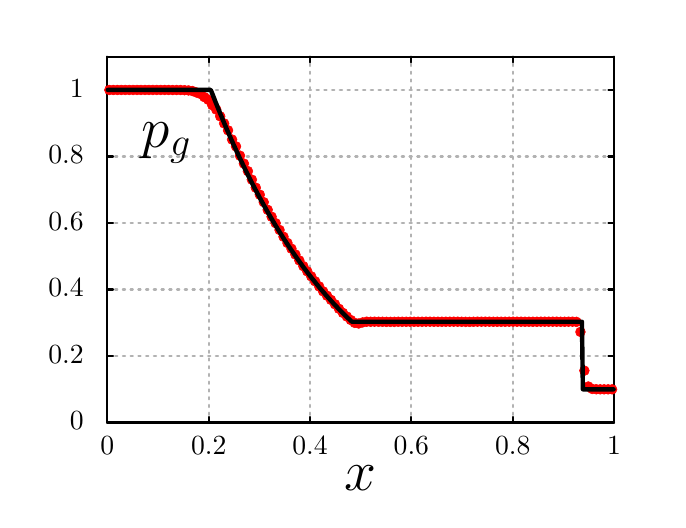
\begin{tikzpicture}[gnuplot]
%% generated with GNUPLOT 4.6p4 (Lua 5.1; terminal rev. 99, script rev. 100)
%% Thu 31 Jul 2014 02:05:55 PM EDT
\path (0.000,0.000) rectangle (8.000,6.000);
\gpfill{rgb color={1.000,1.000,1.000}} (1.012,0.985)--(7.446,0.985)--(7.446,5.630)--(1.012,5.630)--cycle;
\gpcolor{color=gp lt color border}
\gpsetlinetype{gp lt border}
\gpsetlinewidth{1.00}
\draw[gp path] (1.012,0.985)--(1.012,5.630)--(7.446,5.630)--(7.446,0.985)--cycle;
\gpcolor{color=gp lt color axes}
\gpsetlinetype{gp lt axes}
\gpsetlinewidth{2.00}
\draw[gp path] (1.012,0.985)--(7.447,0.985);
\gpcolor{color=gp lt color border}
\gpsetlinetype{gp lt border}
\draw[gp path] (1.012,0.985)--(1.084,0.985);
\draw[gp path] (7.447,0.985)--(7.375,0.985);
\gpcolor{rgb color={0.000,0.000,0.000}}
\node[gp node right,font={\fontsize{10pt}{12pt}\selectfont}] at (0.828,0.985) {0};
\gpcolor{color=gp lt color axes}
\gpsetlinetype{gp lt axes}
\draw[gp path] (1.012,1.830)--(7.447,1.830);
\gpcolor{color=gp lt color border}
\gpsetlinetype{gp lt border}
\draw[gp path] (1.012,1.830)--(1.084,1.830);
\draw[gp path] (7.447,1.830)--(7.375,1.830);
\gpcolor{rgb color={0.000,0.000,0.000}}
\node[gp node right,font={\fontsize{10pt}{12pt}\selectfont}] at (0.828,1.830) {0.2};
\gpcolor{color=gp lt color axes}
\gpsetlinetype{gp lt axes}
\draw[gp path] (1.012,2.674)--(7.447,2.674);
\gpcolor{color=gp lt color border}
\gpsetlinetype{gp lt border}
\draw[gp path] (1.012,2.674)--(1.084,2.674);
\draw[gp path] (7.447,2.674)--(7.375,2.674);
\gpcolor{rgb color={0.000,0.000,0.000}}
\node[gp node right,font={\fontsize{10pt}{12pt}\selectfont}] at (0.828,2.674) {0.4};
\gpcolor{color=gp lt color axes}
\gpsetlinetype{gp lt axes}
\draw[gp path] (1.012,3.519)--(7.447,3.519);
\gpcolor{color=gp lt color border}
\gpsetlinetype{gp lt border}
\draw[gp path] (1.012,3.519)--(1.084,3.519);
\draw[gp path] (7.447,3.519)--(7.375,3.519);
\gpcolor{rgb color={0.000,0.000,0.000}}
\node[gp node right,font={\fontsize{10pt}{12pt}\selectfont}] at (0.828,3.519) {0.6};
\gpcolor{color=gp lt color axes}
\gpsetlinetype{gp lt axes}
\draw[gp path] (1.012,4.364)--(7.447,4.364);
\gpcolor{color=gp lt color border}
\gpsetlinetype{gp lt border}
\draw[gp path] (1.012,4.364)--(1.084,4.364);
\draw[gp path] (7.447,4.364)--(7.375,4.364);
\gpcolor{rgb color={0.000,0.000,0.000}}
\node[gp node right,font={\fontsize{10pt}{12pt}\selectfont}] at (0.828,4.364) {0.8};
\gpcolor{color=gp lt color axes}
\gpsetlinetype{gp lt axes}
\draw[gp path] (1.012,5.209)--(7.447,5.209);
\gpcolor{color=gp lt color border}
\gpsetlinetype{gp lt border}
\draw[gp path] (1.012,5.209)--(1.084,5.209);
\draw[gp path] (7.447,5.209)--(7.375,5.209);
\gpcolor{rgb color={0.000,0.000,0.000}}
\node[gp node right,font={\fontsize{10pt}{12pt}\selectfont}] at (0.828,5.209) {1};
\gpcolor{color=gp lt color axes}
\gpsetlinetype{gp lt axes}
\draw[gp path] (1.012,0.985)--(1.012,5.631);
\gpcolor{color=gp lt color border}
\gpsetlinetype{gp lt border}
\draw[gp path] (1.012,0.985)--(1.012,1.057);
\draw[gp path] (1.012,5.631)--(1.012,5.559);
\gpcolor{rgb color={0.000,0.000,0.000}}
\node[gp node center,font={\fontsize{10pt}{12pt}\selectfont}] at (1.012,0.677) {0};
\gpcolor{color=gp lt color axes}
\gpsetlinetype{gp lt axes}
\draw[gp path] (2.299,0.985)--(2.299,5.631);
\gpcolor{color=gp lt color border}
\gpsetlinetype{gp lt border}
\draw[gp path] (2.299,0.985)--(2.299,1.057);
\draw[gp path] (2.299,5.631)--(2.299,5.559);
\gpcolor{rgb color={0.000,0.000,0.000}}
\node[gp node center,font={\fontsize{10pt}{12pt}\selectfont}] at (2.299,0.677) {0.2};
\gpcolor{color=gp lt color axes}
\gpsetlinetype{gp lt axes}
\draw[gp path] (3.586,0.985)--(3.586,5.631);
\gpcolor{color=gp lt color border}
\gpsetlinetype{gp lt border}
\draw[gp path] (3.586,0.985)--(3.586,1.057);
\draw[gp path] (3.586,5.631)--(3.586,5.559);
\gpcolor{rgb color={0.000,0.000,0.000}}
\node[gp node center,font={\fontsize{10pt}{12pt}\selectfont}] at (3.586,0.677) {0.4};
\gpcolor{color=gp lt color axes}
\gpsetlinetype{gp lt axes}
\draw[gp path] (4.873,0.985)--(4.873,5.631);
\gpcolor{color=gp lt color border}
\gpsetlinetype{gp lt border}
\draw[gp path] (4.873,0.985)--(4.873,1.057);
\draw[gp path] (4.873,5.631)--(4.873,5.559);
\gpcolor{rgb color={0.000,0.000,0.000}}
\node[gp node center,font={\fontsize{10pt}{12pt}\selectfont}] at (4.873,0.677) {0.6};
\gpcolor{color=gp lt color axes}
\gpsetlinetype{gp lt axes}
\draw[gp path] (6.160,0.985)--(6.160,5.631);
\gpcolor{color=gp lt color border}
\gpsetlinetype{gp lt border}
\draw[gp path] (6.160,0.985)--(6.160,1.057);
\draw[gp path] (6.160,5.631)--(6.160,5.559);
\gpcolor{rgb color={0.000,0.000,0.000}}
\node[gp node center,font={\fontsize{10pt}{12pt}\selectfont}] at (6.160,0.677) {0.8};
\gpcolor{color=gp lt color axes}
\gpsetlinetype{gp lt axes}
\draw[gp path] (7.447,0.985)--(7.447,5.631);
\gpcolor{color=gp lt color border}
\gpsetlinetype{gp lt border}
\draw[gp path] (7.447,0.985)--(7.447,1.057);
\draw[gp path] (7.447,5.631)--(7.447,5.559);
\gpcolor{rgb color={0.000,0.000,0.000}}
\node[gp node center,font={\fontsize{10pt}{12pt}\selectfont}] at (7.447,0.677) {1};
\gpcolor{color=gp lt color border}
\draw[gp path] (1.012,5.631)--(1.012,0.985)--(7.447,0.985)--(7.447,5.631)--cycle;
\gpcolor{rgb color={0.000,0.000,0.000}}
\node[gp node center,font={\fontsize{10pt}{12pt}\selectfont}] at (4.229,0.215) {\huge $x$};
\gpcolor{rgb color={1.000,0.000,0.000}}
\gpsetlinewidth{0.50}
\gpsetpointsize{4.44}
\gppoint{gp mark 7}{(1.037,5.209)}
\gppoint{gp mark 7}{(1.087,5.209)}
\gppoint{gp mark 7}{(1.138,5.209)}
\gppoint{gp mark 7}{(1.188,5.209)}
\gppoint{gp mark 7}{(1.238,5.209)}
\gppoint{gp mark 7}{(1.289,5.209)}
\gppoint{gp mark 7}{(1.339,5.209)}
\gppoint{gp mark 7}{(1.389,5.209)}
\gppoint{gp mark 7}{(1.439,5.209)}
\gppoint{gp mark 7}{(1.490,5.209)}
\gppoint{gp mark 7}{(1.540,5.209)}
\gppoint{gp mark 7}{(1.590,5.209)}
\gppoint{gp mark 7}{(1.640,5.209)}
\gppoint{gp mark 7}{(1.691,5.209)}
\gppoint{gp mark 7}{(1.741,5.209)}
\gppoint{gp mark 7}{(1.791,5.209)}
\gppoint{gp mark 7}{(1.842,5.208)}
\gppoint{gp mark 7}{(1.892,5.208)}
\gppoint{gp mark 7}{(1.942,5.208)}
\gppoint{gp mark 7}{(1.992,5.206)}
\gppoint{gp mark 7}{(2.043,5.203)}
\gppoint{gp mark 7}{(2.093,5.195)}
\gppoint{gp mark 7}{(2.143,5.177)}
\gppoint{gp mark 7}{(2.193,5.159)}
\gppoint{gp mark 7}{(2.244,5.118)}
\gppoint{gp mark 7}{(2.294,5.084)}
\gppoint{gp mark 7}{(2.344,5.016)}
\gppoint{gp mark 7}{(2.395,4.960)}
\gppoint{gp mark 7}{(2.445,4.874)}
\gppoint{gp mark 7}{(2.495,4.784)}
\gppoint{gp mark 7}{(2.545,4.696)}
\gppoint{gp mark 7}{(2.596,4.579)}
\gppoint{gp mark 7}{(2.646,4.492)}
\gppoint{gp mark 7}{(2.696,4.375)}
\gppoint{gp mark 7}{(2.746,4.274)}
\gppoint{gp mark 7}{(2.797,4.178)}
\gppoint{gp mark 7}{(2.847,4.070)}
\gppoint{gp mark 7}{(2.897,3.968)}
\gppoint{gp mark 7}{(2.948,3.879)}
\gppoint{gp mark 7}{(2.998,3.784)}
\gppoint{gp mark 7}{(3.048,3.687)}
\gppoint{gp mark 7}{(3.098,3.599)}
\gppoint{gp mark 7}{(3.149,3.517)}
\gppoint{gp mark 7}{(3.199,3.431)}
\gppoint{gp mark 7}{(3.249,3.345)}
\gppoint{gp mark 7}{(3.299,3.266)}
\gppoint{gp mark 7}{(3.350,3.193)}
\gppoint{gp mark 7}{(3.400,3.119)}
\gppoint{gp mark 7}{(3.450,3.044)}
\gppoint{gp mark 7}{(3.501,2.971)}
\gppoint{gp mark 7}{(3.551,2.905)}
\gppoint{gp mark 7}{(3.601,2.842)}
\gppoint{gp mark 7}{(3.651,2.779)}
\gppoint{gp mark 7}{(3.702,2.714)}
\gppoint{gp mark 7}{(3.752,2.651)}
\gppoint{gp mark 7}{(3.802,2.596)}
\gppoint{gp mark 7}{(3.852,2.543)}
\gppoint{gp mark 7}{(3.903,2.487)}
\gppoint{gp mark 7}{(3.953,2.430)}
\gppoint{gp mark 7}{(4.003,2.378)}
\gppoint{gp mark 7}{(4.054,2.331)}
\gppoint{gp mark 7}{(4.104,2.287)}
\gppoint{gp mark 7}{(4.154,2.251)}
\gppoint{gp mark 7}{(4.204,2.243)}
\gppoint{gp mark 7}{(4.255,2.257)}
\gppoint{gp mark 7}{(4.305,2.266)}
\gppoint{gp mark 7}{(4.355,2.265)}
\gppoint{gp mark 7}{(4.405,2.266)}
\gppoint{gp mark 7}{(4.456,2.265)}
\gppoint{gp mark 7}{(4.506,2.265)}
\gppoint{gp mark 7}{(4.556,2.264)}
\gppoint{gp mark 7}{(4.607,2.264)}
\gppoint{gp mark 7}{(4.657,2.264)}
\gppoint{gp mark 7}{(4.707,2.265)}
\gppoint{gp mark 7}{(4.757,2.265)}
\gppoint{gp mark 7}{(4.808,2.265)}
\gppoint{gp mark 7}{(4.858,2.265)}
\gppoint{gp mark 7}{(4.908,2.265)}
\gppoint{gp mark 7}{(4.958,2.265)}
\gppoint{gp mark 7}{(5.009,2.265)}
\gppoint{gp mark 7}{(5.059,2.266)}
\gppoint{gp mark 7}{(5.109,2.266)}
\gppoint{gp mark 7}{(5.160,2.265)}
\gppoint{gp mark 7}{(5.210,2.265)}
\gppoint{gp mark 7}{(5.260,2.265)}
\gppoint{gp mark 7}{(5.310,2.265)}
\gppoint{gp mark 7}{(5.361,2.266)}
\gppoint{gp mark 7}{(5.411,2.266)}
\gppoint{gp mark 7}{(5.461,2.266)}
\gppoint{gp mark 7}{(5.511,2.265)}
\gppoint{gp mark 7}{(5.562,2.264)}
\gppoint{gp mark 7}{(5.612,2.264)}
\gppoint{gp mark 7}{(5.662,2.265)}
\gppoint{gp mark 7}{(5.713,2.266)}
\gppoint{gp mark 7}{(5.763,2.266)}
\gppoint{gp mark 7}{(5.813,2.266)}
\gppoint{gp mark 7}{(5.863,2.266)}
\gppoint{gp mark 7}{(5.914,2.265)}
\gppoint{gp mark 7}{(5.964,2.265)}
\gppoint{gp mark 7}{(6.014,2.265)}
\gppoint{gp mark 7}{(6.064,2.265)}
\gppoint{gp mark 7}{(6.115,2.266)}
\gppoint{gp mark 7}{(6.165,2.266)}
\gppoint{gp mark 7}{(6.215,2.266)}
\gppoint{gp mark 7}{(6.266,2.266)}
\gppoint{gp mark 7}{(6.316,2.265)}
\gppoint{gp mark 7}{(6.366,2.265)}
\gppoint{gp mark 7}{(6.416,2.265)}
\gppoint{gp mark 7}{(6.467,2.265)}
\gppoint{gp mark 7}{(6.517,2.266)}
\gppoint{gp mark 7}{(6.567,2.266)}
\gppoint{gp mark 7}{(6.617,2.266)}
\gppoint{gp mark 7}{(6.668,2.266)}
\gppoint{gp mark 7}{(6.718,2.266)}
\gppoint{gp mark 7}{(6.768,2.265)}
\gppoint{gp mark 7}{(6.819,2.265)}
\gppoint{gp mark 7}{(6.869,2.266)}
\gppoint{gp mark 7}{(6.919,2.266)}
\gppoint{gp mark 7}{(6.969,2.264)}
\gppoint{gp mark 7}{(7.020,2.136)}
\gppoint{gp mark 7}{(7.070,1.644)}
\gppoint{gp mark 7}{(7.120,1.443)}
\gppoint{gp mark 7}{(7.170,1.412)}
\gppoint{gp mark 7}{(7.221,1.408)}
\gppoint{gp mark 7}{(7.271,1.407)}
\gppoint{gp mark 7}{(7.321,1.407)}
\gppoint{gp mark 7}{(7.372,1.407)}
\gppoint{gp mark 7}{(7.422,1.407)}
\gpcolor{rgb color={0.000,0.000,0.000}}
\gpsetlinetype{gp lt plot 0}
\gpsetlinewidth{4.00}
\draw[gp path] (1.018,5.209)--(1.031,5.209)--(1.043,5.209)--(1.056,5.209)--(1.069,5.209)%
  --(1.081,5.209)--(1.094,5.209)--(1.106,5.209)--(1.119,5.209)--(1.131,5.209)--(1.144,5.209)%
  --(1.157,5.209)--(1.169,5.209)--(1.182,5.209)--(1.194,5.209)--(1.207,5.209)--(1.219,5.209)%
  --(1.232,5.209)--(1.245,5.209)--(1.257,5.209)--(1.270,5.209)--(1.282,5.209)--(1.295,5.209)%
  --(1.307,5.209)--(1.320,5.209)--(1.332,5.209)--(1.345,5.209)--(1.358,5.209)--(1.370,5.209)%
  --(1.383,5.209)--(1.395,5.209)--(1.408,5.209)--(1.420,5.209)--(1.433,5.209)--(1.446,5.209)%
  --(1.458,5.209)--(1.471,5.209)--(1.483,5.209)--(1.496,5.209)--(1.508,5.209)--(1.521,5.209)%
  --(1.534,5.209)--(1.546,5.209)--(1.559,5.209)--(1.571,5.209)--(1.584,5.209)--(1.596,5.209)%
  --(1.609,5.209)--(1.622,5.209)--(1.634,5.209)--(1.647,5.209)--(1.659,5.209)--(1.672,5.209)%
  --(1.684,5.209)--(1.697,5.209)--(1.710,5.209)--(1.722,5.209)--(1.735,5.209)--(1.747,5.209)%
  --(1.760,5.209)--(1.772,5.209)--(1.785,5.209)--(1.798,5.209)--(1.810,5.209)--(1.823,5.209)%
  --(1.835,5.209)--(1.848,5.209)--(1.860,5.209)--(1.873,5.209)--(1.886,5.209)--(1.898,5.209)%
  --(1.911,5.209)--(1.923,5.209)--(1.936,5.209)--(1.948,5.209)--(1.961,5.209)--(1.973,5.209)%
  --(1.986,5.209)--(1.999,5.209)--(2.011,5.209)--(2.024,5.209)--(2.036,5.209)--(2.049,5.209)%
  --(2.061,5.209)--(2.074,5.209)--(2.087,5.209)--(2.099,5.209)--(2.112,5.209)--(2.124,5.209)%
  --(2.137,5.209)--(2.149,5.209)--(2.162,5.209)--(2.175,5.209)--(2.187,5.209)--(2.200,5.209)%
  --(2.212,5.209)--(2.225,5.209)--(2.237,5.209)--(2.250,5.209)--(2.263,5.209)--(2.275,5.209)%
  --(2.288,5.209)--(2.300,5.209)--(2.313,5.209)--(2.325,5.209)--(2.338,5.178)--(2.351,5.146)%
  --(2.363,5.114)--(2.376,5.082)--(2.388,5.050)--(2.401,5.019)--(2.413,4.988)--(2.426,4.957)%
  --(2.439,4.926)--(2.451,4.895)--(2.464,4.865)--(2.476,4.835)--(2.489,4.805)--(2.501,4.775)%
  --(2.514,4.746)--(2.526,4.716)--(2.539,4.687)--(2.552,4.658)--(2.564,4.629)--(2.577,4.601)%
  --(2.589,4.572)--(2.602,4.544)--(2.614,4.516)--(2.627,4.488)--(2.640,4.461)--(2.652,4.433)%
  --(2.665,4.406)--(2.677,4.379)--(2.690,4.352)--(2.702,4.325)--(2.715,4.299)--(2.728,4.273)%
  --(2.740,4.246)--(2.753,4.220)--(2.765,4.195)--(2.778,4.169)--(2.790,4.144)--(2.803,4.118)%
  --(2.816,4.093)--(2.828,4.068)--(2.841,4.043)--(2.853,4.019)--(2.866,3.994)--(2.878,3.970)%
  --(2.891,3.946)--(2.904,3.922)--(2.916,3.898)--(2.929,3.875)--(2.941,3.851)--(2.954,3.828)%
  --(2.966,3.805)--(2.979,3.782)--(2.992,3.759)--(3.004,3.737)--(3.017,3.714)--(3.029,3.692)%
  --(3.042,3.670)--(3.054,3.648)--(3.067,3.626)--(3.079,3.604)--(3.092,3.583)--(3.105,3.561)%
  --(3.117,3.540)--(3.130,3.519)--(3.142,3.498)--(3.155,3.477)--(3.167,3.457)--(3.180,3.436)%
  --(3.193,3.416)--(3.205,3.396)--(3.218,3.376)--(3.230,3.356)--(3.243,3.336)--(3.255,3.316)%
  --(3.268,3.297)--(3.281,3.278)--(3.293,3.258)--(3.306,3.239)--(3.318,3.220)--(3.331,3.202)%
  --(3.343,3.183)--(3.356,3.165)--(3.369,3.146)--(3.381,3.128)--(3.394,3.110)--(3.406,3.092)%
  --(3.419,3.074)--(3.431,3.056)--(3.444,3.039)--(3.457,3.021)--(3.469,3.004)--(3.482,2.987)%
  --(3.494,2.969)--(3.507,2.952)--(3.519,2.936)--(3.532,2.919)--(3.545,2.902)--(3.557,2.886)%
  --(3.570,2.870)--(3.582,2.853)--(3.595,2.837)--(3.607,2.821)--(3.620,2.805)--(3.633,2.790)%
  --(3.645,2.774)--(3.658,2.758)--(3.670,2.743)--(3.683,2.728)--(3.695,2.713)--(3.708,2.697)%
  --(3.720,2.682)--(3.733,2.668)--(3.746,2.653)--(3.758,2.638)--(3.771,2.624)--(3.783,2.609)%
  --(3.796,2.595)--(3.808,2.581)--(3.821,2.567)--(3.834,2.553)--(3.846,2.539)--(3.859,2.525)%
  --(3.871,2.512)--(3.884,2.498)--(3.896,2.485)--(3.909,2.471)--(3.922,2.458)--(3.934,2.445)%
  --(3.947,2.432)--(3.959,2.419)--(3.972,2.406)--(3.984,2.393)--(3.997,2.381)--(4.010,2.368)%
  --(4.022,2.356)--(4.035,2.343)--(4.047,2.331)--(4.060,2.319)--(4.072,2.307)--(4.085,2.295)%
  --(4.098,2.283)--(4.110,2.271)--(4.123,2.265)--(4.135,2.265)--(4.148,2.265)--(4.160,2.265)%
  --(4.173,2.265)--(4.186,2.265)--(4.198,2.265)--(4.211,2.265)--(4.223,2.265)--(4.236,2.265)%
  --(4.248,2.265)--(4.261,2.265)--(4.273,2.265)--(4.286,2.265)--(4.299,2.265)--(4.311,2.265)%
  --(4.324,2.265)--(4.336,2.265)--(4.349,2.265)--(4.361,2.265)--(4.374,2.265)--(4.387,2.265)%
  --(4.399,2.265)--(4.412,2.265)--(4.424,2.265)--(4.437,2.265)--(4.449,2.265)--(4.462,2.265)%
  --(4.475,2.265)--(4.487,2.265)--(4.500,2.265)--(4.512,2.265)--(4.525,2.265)--(4.537,2.265)%
  --(4.550,2.265)--(4.563,2.265)--(4.575,2.265)--(4.588,2.265)--(4.600,2.265)--(4.613,2.265)%
  --(4.625,2.265)--(4.638,2.265)--(4.651,2.265)--(4.663,2.265)--(4.676,2.265)--(4.688,2.265)%
  --(4.701,2.265)--(4.713,2.265)--(4.726,2.265)--(4.739,2.265)--(4.751,2.265)--(4.764,2.265)%
  --(4.776,2.265)--(4.789,2.265)--(4.801,2.265)--(4.814,2.265)--(4.826,2.265)--(4.839,2.265)%
  --(4.852,2.265)--(4.864,2.265)--(4.877,2.265)--(4.889,2.265)--(4.902,2.265)--(4.914,2.265)%
  --(4.927,2.265)--(4.940,2.265)--(4.952,2.265)--(4.965,2.265)--(4.977,2.265)--(4.990,2.265)%
  --(5.002,2.265)--(5.015,2.265)--(5.028,2.265)--(5.040,2.265)--(5.053,2.265)--(5.065,2.265)%
  --(5.078,2.265)--(5.090,2.265)--(5.103,2.265)--(5.116,2.265)--(5.128,2.265)--(5.141,2.265)%
  --(5.153,2.265)--(5.166,2.265)--(5.178,2.265)--(5.191,2.265)--(5.204,2.265)--(5.216,2.265)%
  --(5.229,2.265)--(5.241,2.265)--(5.254,2.265)--(5.266,2.265)--(5.279,2.265)--(5.292,2.265)%
  --(5.304,2.265)--(5.317,2.265)--(5.329,2.265)--(5.342,2.265)--(5.354,2.265)--(5.367,2.265)%
  --(5.380,2.265)--(5.392,2.265)--(5.405,2.265)--(5.417,2.265)--(5.430,2.265)--(5.442,2.265)%
  --(5.455,2.265)--(5.467,2.265)--(5.480,2.265)--(5.493,2.265)--(5.505,2.265)--(5.518,2.265)%
  --(5.530,2.265)--(5.543,2.265)--(5.555,2.265)--(5.568,2.265)--(5.581,2.265)--(5.593,2.265)%
  --(5.606,2.265)--(5.618,2.265)--(5.631,2.265)--(5.643,2.265)--(5.656,2.265)--(5.669,2.265)%
  --(5.681,2.265)--(5.694,2.265)--(5.706,2.265)--(5.719,2.265)--(5.731,2.265)--(5.744,2.265)%
  --(5.757,2.265)--(5.769,2.265)--(5.782,2.265)--(5.794,2.265)--(5.807,2.265)--(5.819,2.265)%
  --(5.832,2.265)--(5.845,2.265)--(5.857,2.265)--(5.870,2.265)--(5.882,2.265)--(5.895,2.265)%
  --(5.907,2.265)--(5.920,2.265)--(5.933,2.265)--(5.945,2.265)--(5.958,2.265)--(5.970,2.265)%
  --(5.983,2.265)--(5.995,2.265)--(6.008,2.265)--(6.020,2.265)--(6.033,2.265)--(6.046,2.265)%
  --(6.058,2.265)--(6.071,2.265)--(6.083,2.265)--(6.096,2.265)--(6.108,2.265)--(6.121,2.265)%
  --(6.134,2.265)--(6.146,2.265)--(6.159,2.265)--(6.171,2.265)--(6.184,2.265)--(6.196,2.265)%
  --(6.209,2.265)--(6.222,2.265)--(6.234,2.265)--(6.247,2.265)--(6.259,2.265)--(6.272,2.265)%
  --(6.284,2.265)--(6.297,2.265)--(6.310,2.265)--(6.322,2.265)--(6.335,2.265)--(6.347,2.265)%
  --(6.360,2.265)--(6.372,2.265)--(6.385,2.265)--(6.398,2.265)--(6.410,2.265)--(6.423,2.265)%
  --(6.435,2.265)--(6.448,2.265)--(6.460,2.265)--(6.473,2.265)--(6.486,2.265)--(6.498,2.265)%
  --(6.511,2.265)--(6.523,2.265)--(6.536,2.265)--(6.548,2.265)--(6.561,2.265)--(6.573,2.265)%
  --(6.586,2.265)--(6.599,2.265)--(6.611,2.265)--(6.624,2.265)--(6.636,2.265)--(6.649,2.265)%
  --(6.661,2.265)--(6.674,2.265)--(6.687,2.265)--(6.699,2.265)--(6.712,2.265)--(6.724,2.265)%
  --(6.737,2.265)--(6.749,2.265)--(6.762,2.265)--(6.775,2.265)--(6.787,2.265)--(6.800,2.265)%
  --(6.812,2.265)--(6.825,2.265)--(6.837,2.265)--(6.850,2.265)--(6.863,2.265)--(6.875,2.265)%
  --(6.888,2.265)--(6.900,2.265)--(6.913,2.265)--(6.925,2.265)--(6.938,2.265)--(6.951,2.265)%
  --(6.963,2.265)--(6.976,2.265)--(6.988,2.265)--(7.001,2.265)--(7.013,2.265)--(7.026,2.265)%
  --(7.039,2.265)--(7.051,1.407)--(7.064,1.407)--(7.076,1.407)--(7.089,1.407)--(7.101,1.407)%
  --(7.114,1.407)--(7.127,1.407)--(7.139,1.407)--(7.152,1.407)--(7.164,1.407)--(7.177,1.407)%
  --(7.189,1.407)--(7.202,1.407)--(7.214,1.407)--(7.227,1.407)--(7.240,1.407)--(7.252,1.407)%
  --(7.265,1.407)--(7.277,1.407)--(7.290,1.407)--(7.302,1.407)--(7.315,1.407)--(7.328,1.407)%
  --(7.340,1.407)--(7.353,1.407)--(7.365,1.407)--(7.378,1.407)--(7.390,1.407)--(7.403,1.407)%
  --(7.416,1.407)--(7.428,1.407)--(7.441,1.407);
\node[gp node left,font={\fontsize{10pt}{12pt}\selectfont}] at (1.334,4.575) {\huge $p_g$};
%% coordinates of the plot area
\gpdefrectangularnode{gp plot 1}{\pgfpoint{1.012cm}{0.985cm}}{\pgfpoint{7.447cm}{5.631cm}}
\end{tikzpicture}
%% gnuplot variables
} 
\end{tabular}
\caption{(Top row) HLLE, (middle row) HLLC, and (bottom row) Roe approximate solution to Sod shock tube problem computed using third-order parabolic interpolation.  Athena \citep{AthenaSite} was used to compute the approximate solutions.  The exact solution was computed with code written for this dissertation available at: \protect\gitrepo.}
\label{fig:euler_sod_3}
\end{figure}

TVD schemes preserve monotonicity by limiting the flux of a high-order scheme or with slope limiters during interface reconstruction.  To demonstrate this property, we outline the algorithm for second-order linear reconstruction of the primitive variable $\mbf{W_i} = (\rho,v_x,v_y,v_z,p_g,B_x,B_y,B_z)$ as implemented in \emph{Athena} \citep{Stone:2008}.  The reconstruction is done in terms of characteristic variables, $\mbf{a}$, and projected onto the primitive variables.  The differences in primitive variables are first projected to the characteristic variables 
\begin{gather}
\begin{split}
\delta \mathbf{a}_{l} = \sum \mbf{l}_j \cdot (\mbf{W}_i - \mbf{W}_{i-1}) , \\
\delta \mathbf{a}_{c} = \sum \mbf{l}_j \cdot (\mbf{W}_{i+1} - \mbf{W}_{i-1}) , \\
\delta \mathbf{a}_{r} = \sum \mbf{l}_j \cdot (\mbf{W}_{i+1} - \mbf{W}_{i}) 
\end{split}
\end{gather}
where $\mbf{l}_j$ are left eigenvectors computed with the primitive variable at cell $i$.  The monotonicity constraints are then applied, ensuring the reconstructed states are TVD:
\begin{gather}
\delta \mbf{a} = \text{sign}(\delta \mbf{a}_c) \min(2|\delta \mbf{a}_l|,2|\delta \mbf{a}_r|,|\delta \mbf{a}_c|). 
\end{gather}
The characteristic variables are then projected back to the primitive variables
\begin{gather}
\delta \mathbf{W} = \sum \delta \mbf{a} \cdot \mbf{r}_j ,
\end{gather}
where where $\mbf{r}_j$ are right eigenvectors computed with the primitive variables at cell $i$.  Interpolation to the left and right face is performed to reconstruct the interface states,
\begin{gather}
\mbf{w}_{i-1/2} = \mbf{W}_i - \left(\frac{1}{2} 
            - \min(\lambda_{\min},0)\frac{\delta t}{2 \delta x} \right)\delta \mbf{W}_i , \\
\mbf{w}_{i+1/2} = \mbf{W}_i + \left(\frac{1}{2} 
            - \max(\lambda_{\max},0)\frac{\delta t}{2 \delta x} \right)\delta \mbf{W}_i , 
\end{gather}
where $\lambda_{\min}$, and $\lambda_{\max}$ are the minimum and maximum eigenvalue computed at cell $i$.  Finally, the influence of a wave that has not reached the face at the half timestep is removed from the reconstructed value
\begin{gather}
\label{eqn:lin_recon_l}
\mbf{w}_{i-1/2} = \mbf{w}_{i-1/2} + \frac{\delta t}{2\delta x} \sum_{\lambda_j < 0} 
                 \left(\left(\lambda_{\min} - \lambda_j\right) \mbf{l}_j 
                 \cdot \mbf\delta \mbf{W}_i\right) \mbf{r}^j, \\
\label{eqn:lin_recon_r}
\mbf{w}_{i+1/2} = \mbf{w}_{i+1/2} + \frac{\delta t}{2\delta x} \sum_{\lambda_j > 0} 
                 \left(\left(\lambda_{\max} - \lambda_j\right) \mbf{l}_j 
                 \cdot \mbf\delta \mbf{W}_i\right) \mbf{r}^j, 
\end{gather}
where the sums include waves that propagate towards the face.  The HLL solvers use weighted averages of the flux in the left and right interfaces, and as such, a correction must be added to \eqref{eqn:lin_recon_l} and \eqref{eqn:lin_recon_r} for waves that propagate away from the interface.  The correction is \citep{Colella:1984}
\begin{gather}
\Delta \mbf{w}_{i-1/2} = -\frac{\delta t}{2\delta x} \sum_{\lambda_j > 0} 
                 \left(\left(\lambda_j - \lambda_{\min}\right) \mbf{l}_j 
                 \cdot \mbf\delta \mbf{W}_i\right) \mbf{r}^j, \\
\Delta \mbf{w}_{i+1/2} = -\frac{\delta t}{2\delta x} \sum_{\lambda_j < 0} 
                 \left(\left(\lambda_j - \lambda_{\max}\right) \mbf{l}_j 
                 \cdot \mbf\delta \mbf{W}_i\right) \mbf{r}^j. 
\end{gather}

The Sod shock tube test of Section~\ref{sec:hydro_approx_rsolvers} using higher order reconstruction is shown in Figure~\ref{fig:euler_sod_3}.  The higher order extension is less diffuse than the low order counterparts shown in Figure~\ref{fig:euler_sod_1}.  The contact discontinuity and shock are much better resolved.

%-----------------------------------------------------------------
% Interface states FCT
%-----------------------------------------------------------------
\begin{figure}[htbp]
\begin{center}
\tikzsetnextfilename{interface_states_fct}
%-----------------------------------------------------------------
% interface_states.tex
%-----------------------------------------------------------------
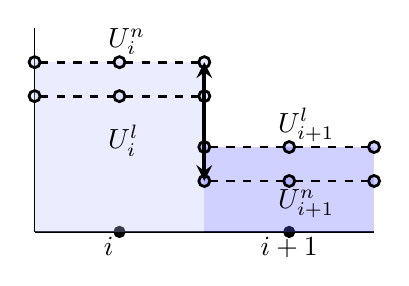
\begin{tikzpicture}[scale = {0.0125\linewidth},
    >=stealth, %
    inner sep=0pt, outer sep=2pt,%
    %% inner sep = 1pt,
    base node/.style={circle,draw,minimum size=4pt}]


% discontinuity
%% \draw[dashed,line width=1pt] (0,0) node[below]{$x_d$} -- (0,0.4); 
%% \draw[-latex,thick](0.05,0.45)node[right]{\small initial discontinuity}
%%          to[out=180,in=90] (0,0.4);

\draw[line width=1pt] (-0.5,0)  -- (-0.25,0) node[below]{$i\phantom{+}$} 
      %% -- (0,0) node[below]{$i+1/2$}
      -- (0.25,0) node[below]{$i+1$} -- (0.5,0); 

\node[base node,fill=black] at (-0.25,0) {};
%% \node[base node,fill=black] at (0,0) {};
\node[base node,fill=black] at (0.25,0) {};


\draw[] (-0.5,0) -- (-0.5,0.6); 

% initial states
\fill[blue!25!,opacity=.3] (-0.5,0) rectangle (0,0.5);
\fill[blue!60!,opacity=.3] (0,0) rectangle (0.5,0.25);

\node[base node,fill = blue!25!,opacity=.3] at (-0.5,0.5) {};
\node[base node,line width=1pt] at (-0.5,0.5) {};

\node[base node,fill = blue!25!,opacity=.3] at (-0.25,0.5) {};
\node[base node,line width=1pt] at (-0.25,0.5) {};

\node[base node,fill = blue!25!,opacity=.3] at (0,0.5) {};
\node[base node,line width=1pt] at (0,0.5) {};

\node[base node,fill = blue!25!,opacity=.3] at (-0.5,0.4) {};
\node[base node,line width=1pt] at (-0.5,0.4) {};

\node[base node,fill = blue!25!,opacity=.3] at (-0.25,0.4) {};
\node[base node,line width=1pt] at (-0.25,0.4) {};

\node[base node,fill = blue!25!,opacity=.3] at (0,0.4) {};
\node[base node,line width=1pt] at (0,0.4) {};

\node[base node,fill = blue!60!,opacity=.3] at (0,0.25) {};
\node[base node,line width=1pt] at (0,0.25) {};

\node[base node,fill = blue!60!,opacity=.3] at (0.25,0.25) {};
\node[base node,line width=1pt] at (0.25,0.25) {};

\node[base node,fill = blue!60!,opacity=.3] at (0.5,0.25) {};
\node[base node,line width=1pt] at (0.5,0.25) {};

\node[base node,fill = blue!60!,opacity=.3] at (0,0.15) {};
\node[base node,line width=1pt] at (0,0.15) {};

\node[base node,fill = blue!60!,opacity=.3] at (0.25,0.15) {};
\node[base node,line width=1pt] at (0.25,0.15) {};

\node[base node,fill = blue!60!,opacity=.3] at (0.5,0.15) {};
\node[base node,line width=1pt] at (0.5,0.15) {};

\draw[dashed,line width=1pt,shorten >= 2 pt, shorten <= 2pt] (-0.5,0.5) -- (-0.25,0.5); 
\draw[dashed,line width=1pt,shorten >= 2 pt, shorten <= 2pt] (-0.25,0.5)  -- (0,0.5); 
\node[above] at (-0.2,0.5) {$\mbf{U}^n_{i\phantom{-1}}$};

\draw[dashed,line width=1pt,shorten >= 2 pt, shorten <= 2pt] (-0.5,0.4) -- (-0.25,0.4); 
\draw[dashed,line width=1pt,shorten >= 2 pt, shorten <= 2pt] (-0.25,0.4)  -- (0,0.4); 
\node[above] at (-0.2,0.2) {$\mbf{U}^l_{i\phantom{-1}}$};

\draw[dashed,line width=1pt,shorten >= 2 pt, shorten <= 2pt] (0,0.25) -- (0.25,0.25); 
\draw[dashed,line width=1pt,shorten >= 2 pt, shorten <= 2pt] (0.25,0.25)  -- (0.5,0.25); 
\node[above] at (0.3,0.25) {$\mbf{U}^l_{i+1}$};

\draw[dashed,line width=1pt,shorten >= 2 pt, shorten <= 2pt] (0,0.15) -- (0.25,0.15); 
\draw[dashed,line width=1pt,shorten >= 2 pt, shorten <= 2pt] (0.25,0.15)  -- (0.5,0.15); 
\node[above] at (0.3,0.025) {$\mbf{U}^n_{i+1}$};

\draw[<->,line width = 1.5 pt] (0,0.15) -- (0,0.5); 

\end{tikzpicture}

\end{center}
\caption{The allowable range for the high order solution is defined such that monotonicity is preserved.}
\label{fig:interface_fct}
\end{figure}

The TVD scheme presented above preserves monotonicity by limiting the slope used for interface reconstruction.  With FCT, the high order fluxes are limited in order to preserve monotonicity.  Advancing the state variables in time with a low order scheme that preserves monotonicity is the first step in applying FCT.  The time-advanced low order solution is denoted as $\mbf{U}^{td}$, where $td$ stands for transported and diffused.  The antidiffusive flux is defined as the difference between the high and low order fluxes, $\mbf{A}_{i+1/2} = \mbf{F}^{h}_{i+1/2} - \mbf{F^{l}}_{i+1/2}$.  For the Rusanov flux, the antidiffusive flux is the second term on the right hand side of \eqref{eqn:rusanov}, $\mbf{A}_{i+1/2} = \half|\lambda_{\max}|\left(\mbf{U}_{i+1} - \mbf{U}_{i} \right)$.  Upper and lower limiting bounds are chosen at each interface such that $\mbf{U}^{td}$ lies between them.  The allowable range of the high-order solution is shown in Figure~\ref{fig:interface_fct}.  In this work, at the interface between $i$ and $i+1$, the limiter is chosen as
\begin{gather}
\label{eqn:fct_limit_max}
\mbf{U}^{\max}_{i+1/2} = \max(\mbf{U}_{i+1},\mbf{U}_{i},\mbf{U}^{td}_{i+1},\mbf{U}^{td}_{i}) , \\
\label{eqn:fct_limit_min}
\mbf{U}^{\min}_{i+1/2} = \min(\mbf{U}_{i+1},\mbf{U}_{i},\mbf{U}^{td}_{i+1},\mbf{U}^{td}_{i}) , 
\end{gather}   
that is, the minimum and maximum values on the solution at the previous step and the low order solution.  The maximum and minimum at each cell are 
\begin{gather}
\mbf{U}^{\max}_{i} = \max(\mbf{U}^{\max}_{i+1/2},\mbf{U}^{\max}_{i-1/2}) , \\
\mbf{U}^{\min}_{i} = \min(\mbf{U}^{\min}_{i+1/2},\mbf{U}^{\min}_{i-1/2}) .
\end{gather}   
The positive and negative contributions of the antidiffusive fluxes are separated and limited.  For the upper bounds
\begin{align}
\mbf{P}^+_i &= \max(\mbf{A}_{i-1/2},0) - \min(\mbf{A}_{i+1/2},0) , \\
\mbf{Q}^+_i &= \mbf{U}^{\max}_i - \mbf{U}^{td}_i , \\
\mbf{R}^+_i &= \min(1,\mbf{Q}^+/\mbf{P}^+) \text{, for} \; \mbf{P}^+_i > 0 \text{, and } \quad 0 \text{, otherwise.}.
\end{align}
For the lower bounds
\begin{align}
\mbf{P}^-_i &= \max(\mbf{A}_{i+1/2},0) - \min(\mbf{A}_{i-1/2},0) , \\
\mbf{Q}^-_i &= \mbf{U}^{td}_i - \mbf{U}^{\min}_i , \\
\mbf{R}^-_i &= \min(1,\mbf{Q}^-/\mbf{P}^-) \text{, for} \; \mbf{P}^-_i > 0 \text{, and } \quad 0 \text{ otherwise.}
\end{align}
The coefficient for limiting the antidiffusive fluxes is
\begin{gather}
\mbf{C}_{i+1/2} = \min(\mbf{R}^-_{i+1},\mbf{R}^-_{i},\mbf{R}^+_{i+1},\mbf{R}^+_{i}).
\end{gather}
The fluxes are synchronized by taking the minimum between the coefficients of energy and density, i.e., $C_{i+1/2} = \min(\mbf{C}_{i+1/2}(\rho),\mbf{C}_{i+1/2}(E))$.  The high order solution is then given by
\begin{gather}
\label{eqn:fvm1d}
\mbf{U}^{n+1}_{i} = \mbf{U}^{td}_{i} - \frac{\delta t}{\delta x}\left(C_{i+1/2}\mbf{A}^n_{i+1/2} - C_{i-1/2}\mbf{A}_{i-1/2}^n\right).
\end{gather}

%-----------------------------------------------------------------
% Sod shock tube Rusanpv and FCT
%-----------------------------------------------------------------
\begin{figure}[htbp]
\begin{tabular}{ccc}
\resizebox{0.33\linewidth}{!}{\tikzsetnextfilename{sod_rusanov_3_1}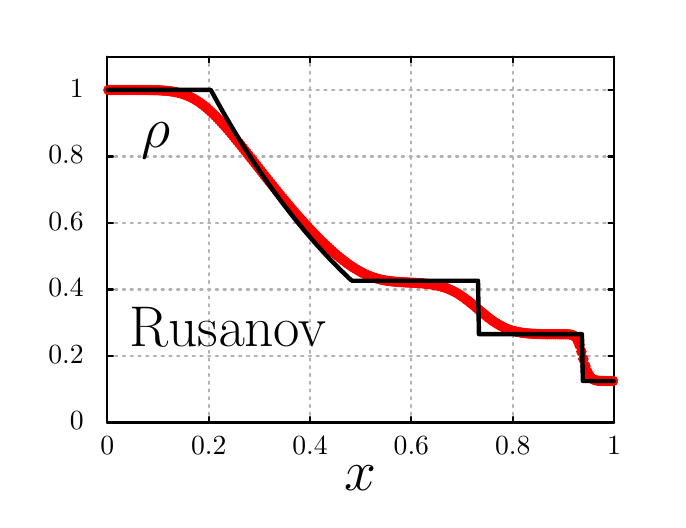
\begin{tikzpicture}[gnuplot]
%% generated with GNUPLOT 4.6p4 (Lua 5.1; terminal rev. 99, script rev. 100)
%% Sun 03 Aug 2014 03:55:27 PM EDT
\path (0.000,0.000) rectangle (8.000,6.000);
\gpfill{rgb color={1.000,1.000,1.000}} (1.012,0.985)--(7.446,0.985)--(7.446,5.630)--(1.012,5.630)--cycle;
\gpcolor{color=gp lt color border}
\gpsetlinetype{gp lt border}
\gpsetlinewidth{1.00}
\draw[gp path] (1.012,0.985)--(1.012,5.630)--(7.446,5.630)--(7.446,0.985)--cycle;
\gpcolor{color=gp lt color axes}
\gpsetlinetype{gp lt axes}
\gpsetlinewidth{2.00}
\draw[gp path] (1.012,0.985)--(7.447,0.985);
\gpcolor{color=gp lt color border}
\gpsetlinetype{gp lt border}
\draw[gp path] (1.012,0.985)--(1.084,0.985);
\draw[gp path] (7.447,0.985)--(7.375,0.985);
\gpcolor{rgb color={0.000,0.000,0.000}}
\node[gp node right,font={\fontsize{10pt}{12pt}\selectfont}] at (0.828,0.985) {0};
\gpcolor{color=gp lt color axes}
\gpsetlinetype{gp lt axes}
\draw[gp path] (1.012,1.830)--(7.447,1.830);
\gpcolor{color=gp lt color border}
\gpsetlinetype{gp lt border}
\draw[gp path] (1.012,1.830)--(1.084,1.830);
\draw[gp path] (7.447,1.830)--(7.375,1.830);
\gpcolor{rgb color={0.000,0.000,0.000}}
\node[gp node right,font={\fontsize{10pt}{12pt}\selectfont}] at (0.828,1.830) {0.2};
\gpcolor{color=gp lt color axes}
\gpsetlinetype{gp lt axes}
\draw[gp path] (1.012,2.674)--(7.447,2.674);
\gpcolor{color=gp lt color border}
\gpsetlinetype{gp lt border}
\draw[gp path] (1.012,2.674)--(1.084,2.674);
\draw[gp path] (7.447,2.674)--(7.375,2.674);
\gpcolor{rgb color={0.000,0.000,0.000}}
\node[gp node right,font={\fontsize{10pt}{12pt}\selectfont}] at (0.828,2.674) {0.4};
\gpcolor{color=gp lt color axes}
\gpsetlinetype{gp lt axes}
\draw[gp path] (1.012,3.519)--(7.447,3.519);
\gpcolor{color=gp lt color border}
\gpsetlinetype{gp lt border}
\draw[gp path] (1.012,3.519)--(1.084,3.519);
\draw[gp path] (7.447,3.519)--(7.375,3.519);
\gpcolor{rgb color={0.000,0.000,0.000}}
\node[gp node right,font={\fontsize{10pt}{12pt}\selectfont}] at (0.828,3.519) {0.6};
\gpcolor{color=gp lt color axes}
\gpsetlinetype{gp lt axes}
\draw[gp path] (1.012,4.364)--(7.447,4.364);
\gpcolor{color=gp lt color border}
\gpsetlinetype{gp lt border}
\draw[gp path] (1.012,4.364)--(1.084,4.364);
\draw[gp path] (7.447,4.364)--(7.375,4.364);
\gpcolor{rgb color={0.000,0.000,0.000}}
\node[gp node right,font={\fontsize{10pt}{12pt}\selectfont}] at (0.828,4.364) {0.8};
\gpcolor{color=gp lt color axes}
\gpsetlinetype{gp lt axes}
\draw[gp path] (1.012,5.209)--(7.447,5.209);
\gpcolor{color=gp lt color border}
\gpsetlinetype{gp lt border}
\draw[gp path] (1.012,5.209)--(1.084,5.209);
\draw[gp path] (7.447,5.209)--(7.375,5.209);
\gpcolor{rgb color={0.000,0.000,0.000}}
\node[gp node right,font={\fontsize{10pt}{12pt}\selectfont}] at (0.828,5.209) {1};
\gpcolor{color=gp lt color axes}
\gpsetlinetype{gp lt axes}
\draw[gp path] (1.012,0.985)--(1.012,5.631);
\gpcolor{color=gp lt color border}
\gpsetlinetype{gp lt border}
\draw[gp path] (1.012,0.985)--(1.012,1.057);
\draw[gp path] (1.012,5.631)--(1.012,5.559);
\gpcolor{rgb color={0.000,0.000,0.000}}
\node[gp node center,font={\fontsize{10pt}{12pt}\selectfont}] at (1.012,0.677) {0};
\gpcolor{color=gp lt color axes}
\gpsetlinetype{gp lt axes}
\draw[gp path] (2.299,0.985)--(2.299,5.631);
\gpcolor{color=gp lt color border}
\gpsetlinetype{gp lt border}
\draw[gp path] (2.299,0.985)--(2.299,1.057);
\draw[gp path] (2.299,5.631)--(2.299,5.559);
\gpcolor{rgb color={0.000,0.000,0.000}}
\node[gp node center,font={\fontsize{10pt}{12pt}\selectfont}] at (2.299,0.677) {0.2};
\gpcolor{color=gp lt color axes}
\gpsetlinetype{gp lt axes}
\draw[gp path] (3.586,0.985)--(3.586,5.631);
\gpcolor{color=gp lt color border}
\gpsetlinetype{gp lt border}
\draw[gp path] (3.586,0.985)--(3.586,1.057);
\draw[gp path] (3.586,5.631)--(3.586,5.559);
\gpcolor{rgb color={0.000,0.000,0.000}}
\node[gp node center,font={\fontsize{10pt}{12pt}\selectfont}] at (3.586,0.677) {0.4};
\gpcolor{color=gp lt color axes}
\gpsetlinetype{gp lt axes}
\draw[gp path] (4.873,0.985)--(4.873,5.631);
\gpcolor{color=gp lt color border}
\gpsetlinetype{gp lt border}
\draw[gp path] (4.873,0.985)--(4.873,1.057);
\draw[gp path] (4.873,5.631)--(4.873,5.559);
\gpcolor{rgb color={0.000,0.000,0.000}}
\node[gp node center,font={\fontsize{10pt}{12pt}\selectfont}] at (4.873,0.677) {0.6};
\gpcolor{color=gp lt color axes}
\gpsetlinetype{gp lt axes}
\draw[gp path] (6.160,0.985)--(6.160,5.631);
\gpcolor{color=gp lt color border}
\gpsetlinetype{gp lt border}
\draw[gp path] (6.160,0.985)--(6.160,1.057);
\draw[gp path] (6.160,5.631)--(6.160,5.559);
\gpcolor{rgb color={0.000,0.000,0.000}}
\node[gp node center,font={\fontsize{10pt}{12pt}\selectfont}] at (6.160,0.677) {0.8};
\gpcolor{color=gp lt color axes}
\gpsetlinetype{gp lt axes}
\draw[gp path] (7.447,0.985)--(7.447,5.631);
\gpcolor{color=gp lt color border}
\gpsetlinetype{gp lt border}
\draw[gp path] (7.447,0.985)--(7.447,1.057);
\draw[gp path] (7.447,5.631)--(7.447,5.559);
\gpcolor{rgb color={0.000,0.000,0.000}}
\node[gp node center,font={\fontsize{10pt}{12pt}\selectfont}] at (7.447,0.677) {1};
\gpcolor{color=gp lt color border}
\draw[gp path] (1.012,5.631)--(1.012,0.985)--(7.447,0.985)--(7.447,5.631)--cycle;
\gpcolor{rgb color={0.000,0.000,0.000}}
\node[gp node center,font={\fontsize{10pt}{12pt}\selectfont}] at (4.229,0.215) {\huge $x$};
\gpcolor{rgb color={1.000,0.000,0.000}}
\gpsetlinewidth{0.50}
\gpsetpointsize{4.44}
\gppoint{gp mark 7}{(1.025,5.209)}
\gppoint{gp mark 7}{(1.050,5.209)}
\gppoint{gp mark 7}{(1.075,5.209)}
\gppoint{gp mark 7}{(1.100,5.209)}
\gppoint{gp mark 7}{(1.125,5.209)}
\gppoint{gp mark 7}{(1.150,5.209)}
\gppoint{gp mark 7}{(1.175,5.209)}
\gppoint{gp mark 7}{(1.201,5.209)}
\gppoint{gp mark 7}{(1.226,5.209)}
\gppoint{gp mark 7}{(1.251,5.209)}
\gppoint{gp mark 7}{(1.276,5.209)}
\gppoint{gp mark 7}{(1.301,5.209)}
\gppoint{gp mark 7}{(1.326,5.209)}
\gppoint{gp mark 7}{(1.351,5.209)}
\gppoint{gp mark 7}{(1.376,5.208)}
\gppoint{gp mark 7}{(1.402,5.208)}
\gppoint{gp mark 7}{(1.427,5.208)}
\gppoint{gp mark 7}{(1.452,5.208)}
\gppoint{gp mark 7}{(1.477,5.208)}
\gppoint{gp mark 7}{(1.502,5.208)}
\gppoint{gp mark 7}{(1.527,5.208)}
\gppoint{gp mark 7}{(1.552,5.207)}
\gppoint{gp mark 7}{(1.578,5.207)}
\gppoint{gp mark 7}{(1.603,5.206)}
\gppoint{gp mark 7}{(1.628,5.206)}
\gppoint{gp mark 7}{(1.653,5.205)}
\gppoint{gp mark 7}{(1.678,5.204)}
\gppoint{gp mark 7}{(1.703,5.202)}
\gppoint{gp mark 7}{(1.728,5.201)}
\gppoint{gp mark 7}{(1.754,5.199)}
\gppoint{gp mark 7}{(1.779,5.196)}
\gppoint{gp mark 7}{(1.804,5.193)}
\gppoint{gp mark 7}{(1.829,5.190)}
\gppoint{gp mark 7}{(1.854,5.186)}
\gppoint{gp mark 7}{(1.879,5.181)}
\gppoint{gp mark 7}{(1.904,5.176)}
\gppoint{gp mark 7}{(1.929,5.170)}
\gppoint{gp mark 7}{(1.955,5.162)}
\gppoint{gp mark 7}{(1.980,5.154)}
\gppoint{gp mark 7}{(2.005,5.145)}
\gppoint{gp mark 7}{(2.030,5.135)}
\gppoint{gp mark 7}{(2.055,5.124)}
\gppoint{gp mark 7}{(2.080,5.112)}
\gppoint{gp mark 7}{(2.105,5.099)}
\gppoint{gp mark 7}{(2.131,5.084)}
\gppoint{gp mark 7}{(2.156,5.068)}
\gppoint{gp mark 7}{(2.181,5.052)}
\gppoint{gp mark 7}{(2.206,5.034)}
\gppoint{gp mark 7}{(2.231,5.015)}
\gppoint{gp mark 7}{(2.256,4.995)}
\gppoint{gp mark 7}{(2.281,4.974)}
\gppoint{gp mark 7}{(2.307,4.951)}
\gppoint{gp mark 7}{(2.332,4.928)}
\gppoint{gp mark 7}{(2.357,4.904)}
\gppoint{gp mark 7}{(2.382,4.880)}
\gppoint{gp mark 7}{(2.407,4.854)}
\gppoint{gp mark 7}{(2.432,4.828)}
\gppoint{gp mark 7}{(2.457,4.801)}
\gppoint{gp mark 7}{(2.482,4.773)}
\gppoint{gp mark 7}{(2.508,4.745)}
\gppoint{gp mark 7}{(2.533,4.716)}
\gppoint{gp mark 7}{(2.558,4.686)}
\gppoint{gp mark 7}{(2.583,4.657)}
\gppoint{gp mark 7}{(2.608,4.627)}
\gppoint{gp mark 7}{(2.633,4.596)}
\gppoint{gp mark 7}{(2.658,4.565)}
\gppoint{gp mark 7}{(2.684,4.534)}
\gppoint{gp mark 7}{(2.709,4.503)}
\gppoint{gp mark 7}{(2.734,4.471)}
\gppoint{gp mark 7}{(2.759,4.440)}
\gppoint{gp mark 7}{(2.784,4.408)}
\gppoint{gp mark 7}{(2.809,4.376)}
\gppoint{gp mark 7}{(2.834,4.344)}
\gppoint{gp mark 7}{(2.860,4.312)}
\gppoint{gp mark 7}{(2.885,4.280)}
\gppoint{gp mark 7}{(2.910,4.248)}
\gppoint{gp mark 7}{(2.935,4.216)}
\gppoint{gp mark 7}{(2.960,4.184)}
\gppoint{gp mark 7}{(2.985,4.152)}
\gppoint{gp mark 7}{(3.010,4.120)}
\gppoint{gp mark 7}{(3.036,4.088)}
\gppoint{gp mark 7}{(3.061,4.057)}
\gppoint{gp mark 7}{(3.086,4.025)}
\gppoint{gp mark 7}{(3.111,3.994)}
\gppoint{gp mark 7}{(3.136,3.963)}
\gppoint{gp mark 7}{(3.161,3.931)}
\gppoint{gp mark 7}{(3.186,3.901)}
\gppoint{gp mark 7}{(3.211,3.870)}
\gppoint{gp mark 7}{(3.237,3.839)}
\gppoint{gp mark 7}{(3.262,3.809)}
\gppoint{gp mark 7}{(3.287,3.779)}
\gppoint{gp mark 7}{(3.312,3.749)}
\gppoint{gp mark 7}{(3.337,3.719)}
\gppoint{gp mark 7}{(3.362,3.690)}
\gppoint{gp mark 7}{(3.387,3.661)}
\gppoint{gp mark 7}{(3.413,3.632)}
\gppoint{gp mark 7}{(3.438,3.603)}
\gppoint{gp mark 7}{(3.463,3.575)}
\gppoint{gp mark 7}{(3.488,3.547)}
\gppoint{gp mark 7}{(3.513,3.519)}
\gppoint{gp mark 7}{(3.538,3.491)}
\gppoint{gp mark 7}{(3.563,3.464)}
\gppoint{gp mark 7}{(3.589,3.437)}
\gppoint{gp mark 7}{(3.614,3.411)}
\gppoint{gp mark 7}{(3.639,3.384)}
\gppoint{gp mark 7}{(3.664,3.358)}
\gppoint{gp mark 7}{(3.689,3.333)}
\gppoint{gp mark 7}{(3.714,3.308)}
\gppoint{gp mark 7}{(3.739,3.283)}
\gppoint{gp mark 7}{(3.764,3.259)}
\gppoint{gp mark 7}{(3.790,3.235)}
\gppoint{gp mark 7}{(3.815,3.211)}
\gppoint{gp mark 7}{(3.840,3.188)}
\gppoint{gp mark 7}{(3.865,3.165)}
\gppoint{gp mark 7}{(3.890,3.143)}
\gppoint{gp mark 7}{(3.915,3.121)}
\gppoint{gp mark 7}{(3.940,3.100)}
\gppoint{gp mark 7}{(3.966,3.079)}
\gppoint{gp mark 7}{(3.991,3.059)}
\gppoint{gp mark 7}{(4.016,3.040)}
\gppoint{gp mark 7}{(4.041,3.020)}
\gppoint{gp mark 7}{(4.066,3.002)}
\gppoint{gp mark 7}{(4.091,2.984)}
\gppoint{gp mark 7}{(4.116,2.967)}
\gppoint{gp mark 7}{(4.142,2.951)}
\gppoint{gp mark 7}{(4.167,2.935)}
\gppoint{gp mark 7}{(4.192,2.920)}
\gppoint{gp mark 7}{(4.217,2.906)}
\gppoint{gp mark 7}{(4.242,2.892)}
\gppoint{gp mark 7}{(4.267,2.879)}
\gppoint{gp mark 7}{(4.292,2.867)}
\gppoint{gp mark 7}{(4.317,2.856)}
\gppoint{gp mark 7}{(4.343,2.846)}
\gppoint{gp mark 7}{(4.368,2.836)}
\gppoint{gp mark 7}{(4.393,2.827)}
\gppoint{gp mark 7}{(4.418,2.819)}
\gppoint{gp mark 7}{(4.443,2.812)}
\gppoint{gp mark 7}{(4.468,2.805)}
\gppoint{gp mark 7}{(4.493,2.799)}
\gppoint{gp mark 7}{(4.519,2.794)}
\gppoint{gp mark 7}{(4.544,2.789)}
\gppoint{gp mark 7}{(4.569,2.785)}
\gppoint{gp mark 7}{(4.594,2.782)}
\gppoint{gp mark 7}{(4.619,2.779)}
\gppoint{gp mark 7}{(4.644,2.776)}
\gppoint{gp mark 7}{(4.669,2.774)}
\gppoint{gp mark 7}{(4.695,2.771)}
\gppoint{gp mark 7}{(4.720,2.770)}
\gppoint{gp mark 7}{(4.745,2.768)}
\gppoint{gp mark 7}{(4.770,2.767)}
\gppoint{gp mark 7}{(4.795,2.765)}
\gppoint{gp mark 7}{(4.820,2.764)}
\gppoint{gp mark 7}{(4.845,2.763)}
\gppoint{gp mark 7}{(4.870,2.761)}
\gppoint{gp mark 7}{(4.896,2.760)}
\gppoint{gp mark 7}{(4.921,2.759)}
\gppoint{gp mark 7}{(4.946,2.757)}
\gppoint{gp mark 7}{(4.971,2.756)}
\gppoint{gp mark 7}{(4.996,2.754)}
\gppoint{gp mark 7}{(5.021,2.752)}
\gppoint{gp mark 7}{(5.046,2.749)}
\gppoint{gp mark 7}{(5.072,2.747)}
\gppoint{gp mark 7}{(5.097,2.744)}
\gppoint{gp mark 7}{(5.122,2.740)}
\gppoint{gp mark 7}{(5.147,2.736)}
\gppoint{gp mark 7}{(5.172,2.732)}
\gppoint{gp mark 7}{(5.197,2.727)}
\gppoint{gp mark 7}{(5.222,2.721)}
\gppoint{gp mark 7}{(5.248,2.714)}
\gppoint{gp mark 7}{(5.273,2.707)}
\gppoint{gp mark 7}{(5.298,2.699)}
\gppoint{gp mark 7}{(5.323,2.690)}
\gppoint{gp mark 7}{(5.348,2.680)}
\gppoint{gp mark 7}{(5.373,2.669)}
\gppoint{gp mark 7}{(5.398,2.657)}
\gppoint{gp mark 7}{(5.423,2.644)}
\gppoint{gp mark 7}{(5.449,2.630)}
\gppoint{gp mark 7}{(5.474,2.615)}
\gppoint{gp mark 7}{(5.499,2.599)}
\gppoint{gp mark 7}{(5.524,2.582)}
\gppoint{gp mark 7}{(5.549,2.564)}
\gppoint{gp mark 7}{(5.574,2.545)}
\gppoint{gp mark 7}{(5.599,2.525)}
\gppoint{gp mark 7}{(5.625,2.505)}
\gppoint{gp mark 7}{(5.650,2.485)}
\gppoint{gp mark 7}{(5.675,2.464)}
\gppoint{gp mark 7}{(5.700,2.442)}
\gppoint{gp mark 7}{(5.725,2.421)}
\gppoint{gp mark 7}{(5.750,2.400)}
\gppoint{gp mark 7}{(5.775,2.379)}
\gppoint{gp mark 7}{(5.801,2.358)}
\gppoint{gp mark 7}{(5.826,2.337)}
\gppoint{gp mark 7}{(5.851,2.318)}
\gppoint{gp mark 7}{(5.876,2.299)}
\gppoint{gp mark 7}{(5.901,2.280)}
\gppoint{gp mark 7}{(5.926,2.263)}
\gppoint{gp mark 7}{(5.951,2.247)}
\gppoint{gp mark 7}{(5.977,2.231)}
\gppoint{gp mark 7}{(6.002,2.217)}
\gppoint{gp mark 7}{(6.027,2.204)}
\gppoint{gp mark 7}{(6.052,2.191)}
\gppoint{gp mark 7}{(6.077,2.180)}
\gppoint{gp mark 7}{(6.102,2.170)}
\gppoint{gp mark 7}{(6.127,2.161)}
\gppoint{gp mark 7}{(6.152,2.153)}
\gppoint{gp mark 7}{(6.178,2.146)}
\gppoint{gp mark 7}{(6.203,2.140)}
\gppoint{gp mark 7}{(6.228,2.135)}
\gppoint{gp mark 7}{(6.253,2.130)}
\gppoint{gp mark 7}{(6.278,2.126)}
\gppoint{gp mark 7}{(6.303,2.122)}
\gppoint{gp mark 7}{(6.328,2.119)}
\gppoint{gp mark 7}{(6.354,2.117)}
\gppoint{gp mark 7}{(6.379,2.115)}
\gppoint{gp mark 7}{(6.404,2.113)}
\gppoint{gp mark 7}{(6.429,2.112)}
\gppoint{gp mark 7}{(6.454,2.111)}
\gppoint{gp mark 7}{(6.479,2.110)}
\gppoint{gp mark 7}{(6.504,2.109)}
\gppoint{gp mark 7}{(6.530,2.108)}
\gppoint{gp mark 7}{(6.555,2.108)}
\gppoint{gp mark 7}{(6.580,2.107)}
\gppoint{gp mark 7}{(6.605,2.107)}
\gppoint{gp mark 7}{(6.630,2.107)}
\gppoint{gp mark 7}{(6.655,2.107)}
\gppoint{gp mark 7}{(6.680,2.107)}
\gppoint{gp mark 7}{(6.705,2.107)}
\gppoint{gp mark 7}{(6.731,2.107)}
\gppoint{gp mark 7}{(6.756,2.106)}
\gppoint{gp mark 7}{(6.781,2.106)}
\gppoint{gp mark 7}{(6.806,2.106)}
\gppoint{gp mark 7}{(6.831,2.106)}
\gppoint{gp mark 7}{(6.856,2.106)}
\gppoint{gp mark 7}{(6.881,2.104)}
\gppoint{gp mark 7}{(6.907,2.100)}
\gppoint{gp mark 7}{(6.932,2.090)}
\gppoint{gp mark 7}{(6.957,2.070)}
\gppoint{gp mark 7}{(6.982,2.031)}
\gppoint{gp mark 7}{(7.007,1.969)}
\gppoint{gp mark 7}{(7.032,1.886)}
\gppoint{gp mark 7}{(7.057,1.792)}
\gppoint{gp mark 7}{(7.083,1.704)}
\gppoint{gp mark 7}{(7.108,1.633)}
\gppoint{gp mark 7}{(7.133,1.583)}
\gppoint{gp mark 7}{(7.158,1.552)}
\gppoint{gp mark 7}{(7.183,1.533)}
\gppoint{gp mark 7}{(7.208,1.523)}
\gppoint{gp mark 7}{(7.233,1.518)}
\gppoint{gp mark 7}{(7.258,1.516)}
\gppoint{gp mark 7}{(7.284,1.514)}
\gppoint{gp mark 7}{(7.309,1.514)}
\gppoint{gp mark 7}{(7.334,1.513)}
\gppoint{gp mark 7}{(7.359,1.513)}
\gppoint{gp mark 7}{(7.384,1.513)}
\gppoint{gp mark 7}{(7.409,1.513)}
\gppoint{gp mark 7}{(7.434,1.513)}
\gpcolor{rgb color={0.000,0.000,0.000}}
\gpsetlinetype{gp lt plot 0}
\gpsetlinewidth{4.00}
\draw[gp path] (1.018,5.209)--(1.031,5.209)--(1.043,5.209)--(1.056,5.209)--(1.069,5.209)%
  --(1.081,5.209)--(1.094,5.209)--(1.106,5.209)--(1.119,5.209)--(1.131,5.209)--(1.144,5.209)%
  --(1.157,5.209)--(1.169,5.209)--(1.182,5.209)--(1.194,5.209)--(1.207,5.209)--(1.219,5.209)%
  --(1.232,5.209)--(1.245,5.209)--(1.257,5.209)--(1.270,5.209)--(1.282,5.209)--(1.295,5.209)%
  --(1.307,5.209)--(1.320,5.209)--(1.332,5.209)--(1.345,5.209)--(1.358,5.209)--(1.370,5.209)%
  --(1.383,5.209)--(1.395,5.209)--(1.408,5.209)--(1.420,5.209)--(1.433,5.209)--(1.446,5.209)%
  --(1.458,5.209)--(1.471,5.209)--(1.483,5.209)--(1.496,5.209)--(1.508,5.209)--(1.521,5.209)%
  --(1.534,5.209)--(1.546,5.209)--(1.559,5.209)--(1.571,5.209)--(1.584,5.209)--(1.596,5.209)%
  --(1.609,5.209)--(1.622,5.209)--(1.634,5.209)--(1.647,5.209)--(1.659,5.209)--(1.672,5.209)%
  --(1.684,5.209)--(1.697,5.209)--(1.710,5.209)--(1.722,5.209)--(1.735,5.209)--(1.747,5.209)%
  --(1.760,5.209)--(1.772,5.209)--(1.785,5.209)--(1.798,5.209)--(1.810,5.209)--(1.823,5.209)%
  --(1.835,5.209)--(1.848,5.209)--(1.860,5.209)--(1.873,5.209)--(1.886,5.209)--(1.898,5.209)%
  --(1.911,5.209)--(1.923,5.209)--(1.936,5.209)--(1.948,5.209)--(1.961,5.209)--(1.973,5.209)%
  --(1.986,5.209)--(1.999,5.209)--(2.011,5.209)--(2.024,5.209)--(2.036,5.209)--(2.049,5.209)%
  --(2.061,5.209)--(2.074,5.209)--(2.087,5.209)--(2.099,5.209)--(2.112,5.209)--(2.124,5.209)%
  --(2.137,5.209)--(2.149,5.209)--(2.162,5.209)--(2.175,5.209)--(2.187,5.209)--(2.200,5.209)%
  --(2.212,5.209)--(2.225,5.209)--(2.237,5.209)--(2.250,5.209)--(2.263,5.209)--(2.275,5.209)%
  --(2.288,5.209)--(2.300,5.209)--(2.313,5.209)--(2.325,5.209)--(2.338,5.187)--(2.351,5.163)%
  --(2.363,5.140)--(2.376,5.118)--(2.388,5.095)--(2.401,5.072)--(2.413,5.050)--(2.426,5.027)%
  --(2.439,5.005)--(2.451,4.982)--(2.464,4.960)--(2.476,4.938)--(2.489,4.916)--(2.501,4.894)%
  --(2.514,4.872)--(2.526,4.851)--(2.539,4.829)--(2.552,4.808)--(2.564,4.786)--(2.577,4.765)%
  --(2.589,4.744)--(2.602,4.723)--(2.614,4.702)--(2.627,4.681)--(2.640,4.660)--(2.652,4.639)%
  --(2.665,4.618)--(2.677,4.598)--(2.690,4.577)--(2.702,4.557)--(2.715,4.537)--(2.728,4.517)%
  --(2.740,4.496)--(2.753,4.476)--(2.765,4.456)--(2.778,4.437)--(2.790,4.417)--(2.803,4.397)%
  --(2.816,4.378)--(2.828,4.358)--(2.841,4.339)--(2.853,4.320)--(2.866,4.300)--(2.878,4.281)%
  --(2.891,4.262)--(2.904,4.243)--(2.916,4.225)--(2.929,4.206)--(2.941,4.187)--(2.954,4.169)%
  --(2.966,4.150)--(2.979,4.132)--(2.992,4.113)--(3.004,4.095)--(3.017,4.077)--(3.029,4.059)%
  --(3.042,4.041)--(3.054,4.023)--(3.067,4.005)--(3.079,3.987)--(3.092,3.970)--(3.105,3.952)%
  --(3.117,3.935)--(3.130,3.917)--(3.142,3.900)--(3.155,3.883)--(3.167,3.866)--(3.180,3.849)%
  --(3.193,3.832)--(3.205,3.815)--(3.218,3.798)--(3.230,3.781)--(3.243,3.764)--(3.255,3.748)%
  --(3.268,3.731)--(3.281,3.715)--(3.293,3.699)--(3.306,3.682)--(3.318,3.666)--(3.331,3.650)%
  --(3.343,3.634)--(3.356,3.618)--(3.369,3.602)--(3.381,3.586)--(3.394,3.571)--(3.406,3.555)%
  --(3.419,3.539)--(3.431,3.524)--(3.444,3.508)--(3.457,3.493)--(3.469,3.478)--(3.482,3.463)%
  --(3.494,3.447)--(3.507,3.432)--(3.519,3.417)--(3.532,3.403)--(3.545,3.388)--(3.557,3.373)%
  --(3.570,3.358)--(3.582,3.344)--(3.595,3.329)--(3.607,3.315)--(3.620,3.300)--(3.633,3.286)%
  --(3.645,3.272)--(3.658,3.257)--(3.670,3.243)--(3.683,3.229)--(3.695,3.215)--(3.708,3.201)%
  --(3.720,3.188)--(3.733,3.174)--(3.746,3.160)--(3.758,3.146)--(3.771,3.133)--(3.783,3.119)%
  --(3.796,3.106)--(3.808,3.093)--(3.821,3.079)--(3.834,3.066)--(3.846,3.053)--(3.859,3.040)%
  --(3.871,3.027)--(3.884,3.014)--(3.896,3.001)--(3.909,2.988)--(3.922,2.975)--(3.934,2.963)%
  --(3.947,2.950)--(3.959,2.937)--(3.972,2.925)--(3.984,2.912)--(3.997,2.900)--(4.010,2.888)%
  --(4.022,2.876)--(4.035,2.863)--(4.047,2.851)--(4.060,2.839)--(4.072,2.827)--(4.085,2.815)%
  --(4.098,2.803)--(4.110,2.792)--(4.123,2.786)--(4.135,2.786)--(4.148,2.786)--(4.160,2.786)%
  --(4.173,2.786)--(4.186,2.786)--(4.198,2.786)--(4.211,2.786)--(4.223,2.786)--(4.236,2.786)%
  --(4.248,2.786)--(4.261,2.786)--(4.273,2.786)--(4.286,2.786)--(4.299,2.786)--(4.311,2.786)%
  --(4.324,2.786)--(4.336,2.786)--(4.349,2.786)--(4.361,2.786)--(4.374,2.786)--(4.387,2.786)%
  --(4.399,2.786)--(4.412,2.786)--(4.424,2.786)--(4.437,2.786)--(4.449,2.786)--(4.462,2.786)%
  --(4.475,2.786)--(4.487,2.786)--(4.500,2.786)--(4.512,2.786)--(4.525,2.786)--(4.537,2.786)%
  --(4.550,2.786)--(4.563,2.786)--(4.575,2.786)--(4.588,2.786)--(4.600,2.786)--(4.613,2.786)%
  --(4.625,2.786)--(4.638,2.786)--(4.651,2.786)--(4.663,2.786)--(4.676,2.786)--(4.688,2.786)%
  --(4.701,2.786)--(4.713,2.786)--(4.726,2.786)--(4.739,2.786)--(4.751,2.786)--(4.764,2.786)%
  --(4.776,2.786)--(4.789,2.786)--(4.801,2.786)--(4.814,2.786)--(4.826,2.786)--(4.839,2.786)%
  --(4.852,2.786)--(4.864,2.786)--(4.877,2.786)--(4.889,2.786)--(4.902,2.786)--(4.914,2.786)%
  --(4.927,2.786)--(4.940,2.786)--(4.952,2.786)--(4.965,2.786)--(4.977,2.786)--(4.990,2.786)%
  --(5.002,2.786)--(5.015,2.786)--(5.028,2.786)--(5.040,2.786)--(5.053,2.786)--(5.065,2.786)%
  --(5.078,2.786)--(5.090,2.786)--(5.103,2.786)--(5.116,2.786)--(5.128,2.786)--(5.141,2.786)%
  --(5.153,2.786)--(5.166,2.786)--(5.178,2.786)--(5.191,2.786)--(5.204,2.786)--(5.216,2.786)%
  --(5.229,2.786)--(5.241,2.786)--(5.254,2.786)--(5.266,2.786)--(5.279,2.786)--(5.292,2.786)%
  --(5.304,2.786)--(5.317,2.786)--(5.329,2.786)--(5.342,2.786)--(5.354,2.786)--(5.367,2.786)%
  --(5.380,2.786)--(5.392,2.786)--(5.405,2.786)--(5.417,2.786)--(5.430,2.786)--(5.442,2.786)%
  --(5.455,2.786)--(5.467,2.786)--(5.480,2.786)--(5.493,2.786)--(5.505,2.786)--(5.518,2.786)%
  --(5.530,2.786)--(5.543,2.786)--(5.555,2.786)--(5.568,2.786)--(5.581,2.786)--(5.593,2.786)%
  --(5.606,2.786)--(5.618,2.786)--(5.631,2.786)--(5.643,2.786)--(5.656,2.786)--(5.669,2.786)%
  --(5.681,2.786)--(5.694,2.786)--(5.706,2.786)--(5.719,2.786)--(5.731,2.107)--(5.744,2.107)%
  --(5.757,2.107)--(5.769,2.107)--(5.782,2.107)--(5.794,2.107)--(5.807,2.107)--(5.819,2.107)%
  --(5.832,2.107)--(5.845,2.107)--(5.857,2.107)--(5.870,2.107)--(5.882,2.107)--(5.895,2.107)%
  --(5.907,2.107)--(5.920,2.107)--(5.933,2.107)--(5.945,2.107)--(5.958,2.107)--(5.970,2.107)%
  --(5.983,2.107)--(5.995,2.107)--(6.008,2.107)--(6.020,2.107)--(6.033,2.107)--(6.046,2.107)%
  --(6.058,2.107)--(6.071,2.107)--(6.083,2.107)--(6.096,2.107)--(6.108,2.107)--(6.121,2.107)%
  --(6.134,2.107)--(6.146,2.107)--(6.159,2.107)--(6.171,2.107)--(6.184,2.107)--(6.196,2.107)%
  --(6.209,2.107)--(6.222,2.107)--(6.234,2.107)--(6.247,2.107)--(6.259,2.107)--(6.272,2.107)%
  --(6.284,2.107)--(6.297,2.107)--(6.310,2.107)--(6.322,2.107)--(6.335,2.107)--(6.347,2.107)%
  --(6.360,2.107)--(6.372,2.107)--(6.385,2.107)--(6.398,2.107)--(6.410,2.107)--(6.423,2.107)%
  --(6.435,2.107)--(6.448,2.107)--(6.460,2.107)--(6.473,2.107)--(6.486,2.107)--(6.498,2.107)%
  --(6.511,2.107)--(6.523,2.107)--(6.536,2.107)--(6.548,2.107)--(6.561,2.107)--(6.573,2.107)%
  --(6.586,2.107)--(6.599,2.107)--(6.611,2.107)--(6.624,2.107)--(6.636,2.107)--(6.649,2.107)%
  --(6.661,2.107)--(6.674,2.107)--(6.687,2.107)--(6.699,2.107)--(6.712,2.107)--(6.724,2.107)%
  --(6.737,2.107)--(6.749,2.107)--(6.762,2.107)--(6.775,2.107)--(6.787,2.107)--(6.800,2.107)%
  --(6.812,2.107)--(6.825,2.107)--(6.837,2.107)--(6.850,2.107)--(6.863,2.107)--(6.875,2.107)%
  --(6.888,2.107)--(6.900,2.107)--(6.913,2.107)--(6.925,2.107)--(6.938,2.107)--(6.951,2.107)%
  --(6.963,2.107)--(6.976,2.107)--(6.988,2.107)--(7.001,2.107)--(7.013,2.107)--(7.026,2.107)%
  --(7.039,2.107)--(7.051,1.513)--(7.064,1.513)--(7.076,1.513)--(7.089,1.513)--(7.101,1.513)%
  --(7.114,1.513)--(7.127,1.513)--(7.139,1.513)--(7.152,1.513)--(7.164,1.513)--(7.177,1.513)%
  --(7.189,1.513)--(7.202,1.513)--(7.214,1.513)--(7.227,1.513)--(7.240,1.513)--(7.252,1.513)%
  --(7.265,1.513)--(7.277,1.513)--(7.290,1.513)--(7.302,1.513)--(7.315,1.513)--(7.328,1.513)%
  --(7.340,1.513)--(7.353,1.513)--(7.365,1.513)--(7.378,1.513)--(7.390,1.513)--(7.403,1.513)%
  --(7.416,1.513)--(7.428,1.513)--(7.441,1.513);
\node[gp node left,font={\fontsize{10pt}{12pt}\selectfont}] at (1.334,4.575) {\huge $\rho$};
\node[gp node left,font={\fontsize{10pt}{12pt}\selectfont}] at (1.173,2.041) {\huge Rusanov};
%% coordinates of the plot area
\gpdefrectangularnode{gp plot 1}{\pgfpoint{1.012cm}{0.985cm}}{\pgfpoint{7.447cm}{5.631cm}}
\end{tikzpicture}
%% gnuplot variables
} &
\resizebox{0.33\linewidth}{!}{\tikzsetnextfilename{sod_rusanov_3_2}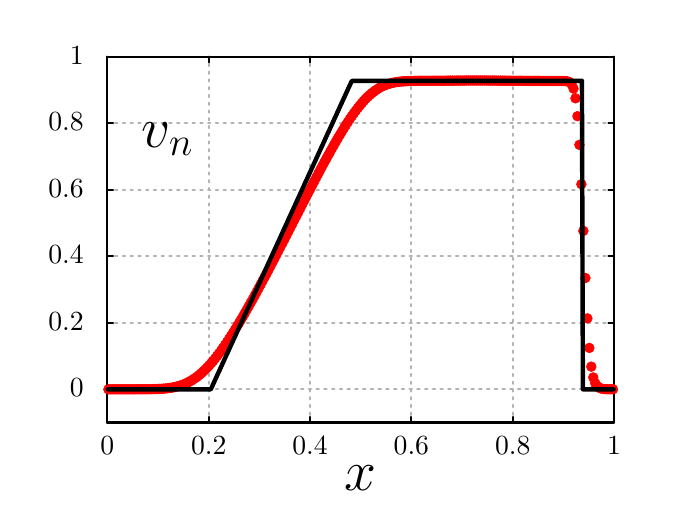
\begin{tikzpicture}[gnuplot]
%% generated with GNUPLOT 4.6p4 (Lua 5.1; terminal rev. 99, script rev. 100)
%% Sun 03 Aug 2014 03:55:27 PM EDT
\path (0.000,0.000) rectangle (8.000,6.000);
\gpfill{rgb color={1.000,1.000,1.000}} (1.012,0.985)--(7.446,0.985)--(7.446,5.630)--(1.012,5.630)--cycle;
\gpcolor{color=gp lt color border}
\gpsetlinetype{gp lt border}
\gpsetlinewidth{1.00}
\draw[gp path] (1.012,0.985)--(1.012,5.630)--(7.446,5.630)--(7.446,0.985)--cycle;
\gpcolor{color=gp lt color axes}
\gpsetlinetype{gp lt axes}
\gpsetlinewidth{2.00}
\draw[gp path] (1.012,1.407)--(7.447,1.407);
\gpcolor{color=gp lt color border}
\gpsetlinetype{gp lt border}
\draw[gp path] (1.012,1.407)--(1.084,1.407);
\draw[gp path] (7.447,1.407)--(7.375,1.407);
\gpcolor{rgb color={0.000,0.000,0.000}}
\node[gp node right,font={\fontsize{10pt}{12pt}\selectfont}] at (0.828,1.407) {0};
\gpcolor{color=gp lt color axes}
\gpsetlinetype{gp lt axes}
\draw[gp path] (1.012,2.252)--(7.447,2.252);
\gpcolor{color=gp lt color border}
\gpsetlinetype{gp lt border}
\draw[gp path] (1.012,2.252)--(1.084,2.252);
\draw[gp path] (7.447,2.252)--(7.375,2.252);
\gpcolor{rgb color={0.000,0.000,0.000}}
\node[gp node right,font={\fontsize{10pt}{12pt}\selectfont}] at (0.828,2.252) {0.2};
\gpcolor{color=gp lt color axes}
\gpsetlinetype{gp lt axes}
\draw[gp path] (1.012,3.097)--(7.447,3.097);
\gpcolor{color=gp lt color border}
\gpsetlinetype{gp lt border}
\draw[gp path] (1.012,3.097)--(1.084,3.097);
\draw[gp path] (7.447,3.097)--(7.375,3.097);
\gpcolor{rgb color={0.000,0.000,0.000}}
\node[gp node right,font={\fontsize{10pt}{12pt}\selectfont}] at (0.828,3.097) {0.4};
\gpcolor{color=gp lt color axes}
\gpsetlinetype{gp lt axes}
\draw[gp path] (1.012,3.942)--(7.447,3.942);
\gpcolor{color=gp lt color border}
\gpsetlinetype{gp lt border}
\draw[gp path] (1.012,3.942)--(1.084,3.942);
\draw[gp path] (7.447,3.942)--(7.375,3.942);
\gpcolor{rgb color={0.000,0.000,0.000}}
\node[gp node right,font={\fontsize{10pt}{12pt}\selectfont}] at (0.828,3.942) {0.6};
\gpcolor{color=gp lt color axes}
\gpsetlinetype{gp lt axes}
\draw[gp path] (1.012,4.786)--(7.447,4.786);
\gpcolor{color=gp lt color border}
\gpsetlinetype{gp lt border}
\draw[gp path] (1.012,4.786)--(1.084,4.786);
\draw[gp path] (7.447,4.786)--(7.375,4.786);
\gpcolor{rgb color={0.000,0.000,0.000}}
\node[gp node right,font={\fontsize{10pt}{12pt}\selectfont}] at (0.828,4.786) {0.8};
\gpcolor{color=gp lt color axes}
\gpsetlinetype{gp lt axes}
\draw[gp path] (1.012,5.631)--(7.447,5.631);
\gpcolor{color=gp lt color border}
\gpsetlinetype{gp lt border}
\draw[gp path] (1.012,5.631)--(1.084,5.631);
\draw[gp path] (7.447,5.631)--(7.375,5.631);
\gpcolor{rgb color={0.000,0.000,0.000}}
\node[gp node right,font={\fontsize{10pt}{12pt}\selectfont}] at (0.828,5.631) {1};
\gpcolor{color=gp lt color axes}
\gpsetlinetype{gp lt axes}
\draw[gp path] (1.012,0.985)--(1.012,5.631);
\gpcolor{color=gp lt color border}
\gpsetlinetype{gp lt border}
\draw[gp path] (1.012,0.985)--(1.012,1.057);
\draw[gp path] (1.012,5.631)--(1.012,5.559);
\gpcolor{rgb color={0.000,0.000,0.000}}
\node[gp node center,font={\fontsize{10pt}{12pt}\selectfont}] at (1.012,0.677) {0};
\gpcolor{color=gp lt color axes}
\gpsetlinetype{gp lt axes}
\draw[gp path] (2.299,0.985)--(2.299,5.631);
\gpcolor{color=gp lt color border}
\gpsetlinetype{gp lt border}
\draw[gp path] (2.299,0.985)--(2.299,1.057);
\draw[gp path] (2.299,5.631)--(2.299,5.559);
\gpcolor{rgb color={0.000,0.000,0.000}}
\node[gp node center,font={\fontsize{10pt}{12pt}\selectfont}] at (2.299,0.677) {0.2};
\gpcolor{color=gp lt color axes}
\gpsetlinetype{gp lt axes}
\draw[gp path] (3.586,0.985)--(3.586,5.631);
\gpcolor{color=gp lt color border}
\gpsetlinetype{gp lt border}
\draw[gp path] (3.586,0.985)--(3.586,1.057);
\draw[gp path] (3.586,5.631)--(3.586,5.559);
\gpcolor{rgb color={0.000,0.000,0.000}}
\node[gp node center,font={\fontsize{10pt}{12pt}\selectfont}] at (3.586,0.677) {0.4};
\gpcolor{color=gp lt color axes}
\gpsetlinetype{gp lt axes}
\draw[gp path] (4.873,0.985)--(4.873,5.631);
\gpcolor{color=gp lt color border}
\gpsetlinetype{gp lt border}
\draw[gp path] (4.873,0.985)--(4.873,1.057);
\draw[gp path] (4.873,5.631)--(4.873,5.559);
\gpcolor{rgb color={0.000,0.000,0.000}}
\node[gp node center,font={\fontsize{10pt}{12pt}\selectfont}] at (4.873,0.677) {0.6};
\gpcolor{color=gp lt color axes}
\gpsetlinetype{gp lt axes}
\draw[gp path] (6.160,0.985)--(6.160,5.631);
\gpcolor{color=gp lt color border}
\gpsetlinetype{gp lt border}
\draw[gp path] (6.160,0.985)--(6.160,1.057);
\draw[gp path] (6.160,5.631)--(6.160,5.559);
\gpcolor{rgb color={0.000,0.000,0.000}}
\node[gp node center,font={\fontsize{10pt}{12pt}\selectfont}] at (6.160,0.677) {0.8};
\gpcolor{color=gp lt color axes}
\gpsetlinetype{gp lt axes}
\draw[gp path] (7.447,0.985)--(7.447,5.631);
\gpcolor{color=gp lt color border}
\gpsetlinetype{gp lt border}
\draw[gp path] (7.447,0.985)--(7.447,1.057);
\draw[gp path] (7.447,5.631)--(7.447,5.559);
\gpcolor{rgb color={0.000,0.000,0.000}}
\node[gp node center,font={\fontsize{10pt}{12pt}\selectfont}] at (7.447,0.677) {1};
\gpcolor{color=gp lt color border}
\draw[gp path] (1.012,5.631)--(1.012,0.985)--(7.447,0.985)--(7.447,5.631)--cycle;
\gpcolor{rgb color={0.000,0.000,0.000}}
\node[gp node center,font={\fontsize{10pt}{12pt}\selectfont}] at (4.229,0.215) {\huge $x$};
\gpcolor{rgb color={1.000,0.000,0.000}}
\gpsetlinewidth{0.50}
\gpsetpointsize{4.44}
\gppoint{gp mark 7}{(1.025,1.407)}
\gppoint{gp mark 7}{(1.050,1.407)}
\gppoint{gp mark 7}{(1.075,1.407)}
\gppoint{gp mark 7}{(1.100,1.407)}
\gppoint{gp mark 7}{(1.125,1.407)}
\gppoint{gp mark 7}{(1.150,1.407)}
\gppoint{gp mark 7}{(1.175,1.407)}
\gppoint{gp mark 7}{(1.201,1.407)}
\gppoint{gp mark 7}{(1.226,1.407)}
\gppoint{gp mark 7}{(1.251,1.407)}
\gppoint{gp mark 7}{(1.276,1.407)}
\gppoint{gp mark 7}{(1.301,1.407)}
\gppoint{gp mark 7}{(1.326,1.407)}
\gppoint{gp mark 7}{(1.351,1.407)}
\gppoint{gp mark 7}{(1.376,1.408)}
\gppoint{gp mark 7}{(1.402,1.408)}
\gppoint{gp mark 7}{(1.427,1.408)}
\gppoint{gp mark 7}{(1.452,1.408)}
\gppoint{gp mark 7}{(1.477,1.408)}
\gppoint{gp mark 7}{(1.502,1.408)}
\gppoint{gp mark 7}{(1.527,1.408)}
\gppoint{gp mark 7}{(1.552,1.409)}
\gppoint{gp mark 7}{(1.578,1.409)}
\gppoint{gp mark 7}{(1.603,1.410)}
\gppoint{gp mark 7}{(1.628,1.411)}
\gppoint{gp mark 7}{(1.653,1.412)}
\gppoint{gp mark 7}{(1.678,1.413)}
\gppoint{gp mark 7}{(1.703,1.414)}
\gppoint{gp mark 7}{(1.728,1.416)}
\gppoint{gp mark 7}{(1.754,1.418)}
\gppoint{gp mark 7}{(1.779,1.421)}
\gppoint{gp mark 7}{(1.804,1.425)}
\gppoint{gp mark 7}{(1.829,1.428)}
\gppoint{gp mark 7}{(1.854,1.433)}
\gppoint{gp mark 7}{(1.879,1.438)}
\gppoint{gp mark 7}{(1.904,1.445)}
\gppoint{gp mark 7}{(1.929,1.452)}
\gppoint{gp mark 7}{(1.955,1.460)}
\gppoint{gp mark 7}{(1.980,1.469)}
\gppoint{gp mark 7}{(2.005,1.480)}
\gppoint{gp mark 7}{(2.030,1.492)}
\gppoint{gp mark 7}{(2.055,1.505)}
\gppoint{gp mark 7}{(2.080,1.519)}
\gppoint{gp mark 7}{(2.105,1.535)}
\gppoint{gp mark 7}{(2.131,1.552)}
\gppoint{gp mark 7}{(2.156,1.571)}
\gppoint{gp mark 7}{(2.181,1.591)}
\gppoint{gp mark 7}{(2.206,1.612)}
\gppoint{gp mark 7}{(2.231,1.635)}
\gppoint{gp mark 7}{(2.256,1.659)}
\gppoint{gp mark 7}{(2.281,1.685)}
\gppoint{gp mark 7}{(2.307,1.712)}
\gppoint{gp mark 7}{(2.332,1.740)}
\gppoint{gp mark 7}{(2.357,1.770)}
\gppoint{gp mark 7}{(2.382,1.801)}
\gppoint{gp mark 7}{(2.407,1.833)}
\gppoint{gp mark 7}{(2.432,1.866)}
\gppoint{gp mark 7}{(2.457,1.900)}
\gppoint{gp mark 7}{(2.482,1.935)}
\gppoint{gp mark 7}{(2.508,1.972)}
\gppoint{gp mark 7}{(2.533,2.009)}
\gppoint{gp mark 7}{(2.558,2.047)}
\gppoint{gp mark 7}{(2.583,2.086)}
\gppoint{gp mark 7}{(2.608,2.125)}
\gppoint{gp mark 7}{(2.633,2.166)}
\gppoint{gp mark 7}{(2.658,2.207)}
\gppoint{gp mark 7}{(2.684,2.248)}
\gppoint{gp mark 7}{(2.709,2.291)}
\gppoint{gp mark 7}{(2.734,2.333)}
\gppoint{gp mark 7}{(2.759,2.377)}
\gppoint{gp mark 7}{(2.784,2.421)}
\gppoint{gp mark 7}{(2.809,2.465)}
\gppoint{gp mark 7}{(2.834,2.510)}
\gppoint{gp mark 7}{(2.860,2.555)}
\gppoint{gp mark 7}{(2.885,2.601)}
\gppoint{gp mark 7}{(2.910,2.647)}
\gppoint{gp mark 7}{(2.935,2.693)}
\gppoint{gp mark 7}{(2.960,2.740)}
\gppoint{gp mark 7}{(2.985,2.787)}
\gppoint{gp mark 7}{(3.010,2.834)}
\gppoint{gp mark 7}{(3.036,2.881)}
\gppoint{gp mark 7}{(3.061,2.929)}
\gppoint{gp mark 7}{(3.086,2.977)}
\gppoint{gp mark 7}{(3.111,3.025)}
\gppoint{gp mark 7}{(3.136,3.073)}
\gppoint{gp mark 7}{(3.161,3.122)}
\gppoint{gp mark 7}{(3.186,3.170)}
\gppoint{gp mark 7}{(3.211,3.219)}
\gppoint{gp mark 7}{(3.237,3.267)}
\gppoint{gp mark 7}{(3.262,3.316)}
\gppoint{gp mark 7}{(3.287,3.365)}
\gppoint{gp mark 7}{(3.312,3.414)}
\gppoint{gp mark 7}{(3.337,3.463)}
\gppoint{gp mark 7}{(3.362,3.512)}
\gppoint{gp mark 7}{(3.387,3.561)}
\gppoint{gp mark 7}{(3.413,3.610)}
\gppoint{gp mark 7}{(3.438,3.659)}
\gppoint{gp mark 7}{(3.463,3.708)}
\gppoint{gp mark 7}{(3.488,3.757)}
\gppoint{gp mark 7}{(3.513,3.806)}
\gppoint{gp mark 7}{(3.538,3.854)}
\gppoint{gp mark 7}{(3.563,3.903)}
\gppoint{gp mark 7}{(3.589,3.951)}
\gppoint{gp mark 7}{(3.614,4.000)}
\gppoint{gp mark 7}{(3.639,4.048)}
\gppoint{gp mark 7}{(3.664,4.096)}
\gppoint{gp mark 7}{(3.689,4.143)}
\gppoint{gp mark 7}{(3.714,4.191)}
\gppoint{gp mark 7}{(3.739,4.238)}
\gppoint{gp mark 7}{(3.764,4.284)}
\gppoint{gp mark 7}{(3.790,4.331)}
\gppoint{gp mark 7}{(3.815,4.377)}
\gppoint{gp mark 7}{(3.840,4.422)}
\gppoint{gp mark 7}{(3.865,4.467)}
\gppoint{gp mark 7}{(3.890,4.511)}
\gppoint{gp mark 7}{(3.915,4.555)}
\gppoint{gp mark 7}{(3.940,4.598)}
\gppoint{gp mark 7}{(3.966,4.641)}
\gppoint{gp mark 7}{(3.991,4.682)}
\gppoint{gp mark 7}{(4.016,4.723)}
\gppoint{gp mark 7}{(4.041,4.763)}
\gppoint{gp mark 7}{(4.066,4.802)}
\gppoint{gp mark 7}{(4.091,4.840)}
\gppoint{gp mark 7}{(4.116,4.876)}
\gppoint{gp mark 7}{(4.142,4.912)}
\gppoint{gp mark 7}{(4.167,4.946)}
\gppoint{gp mark 7}{(4.192,4.979)}
\gppoint{gp mark 7}{(4.217,5.010)}
\gppoint{gp mark 7}{(4.242,5.040)}
\gppoint{gp mark 7}{(4.267,5.069)}
\gppoint{gp mark 7}{(4.292,5.096)}
\gppoint{gp mark 7}{(4.317,5.121)}
\gppoint{gp mark 7}{(4.343,5.144)}
\gppoint{gp mark 7}{(4.368,5.166)}
\gppoint{gp mark 7}{(4.393,5.186)}
\gppoint{gp mark 7}{(4.418,5.204)}
\gppoint{gp mark 7}{(4.443,5.221)}
\gppoint{gp mark 7}{(4.468,5.236)}
\gppoint{gp mark 7}{(4.493,5.250)}
\gppoint{gp mark 7}{(4.519,5.262)}
\gppoint{gp mark 7}{(4.544,5.272)}
\gppoint{gp mark 7}{(4.569,5.281)}
\gppoint{gp mark 7}{(4.594,5.289)}
\gppoint{gp mark 7}{(4.619,5.296)}
\gppoint{gp mark 7}{(4.644,5.301)}
\gppoint{gp mark 7}{(4.669,5.306)}
\gppoint{gp mark 7}{(4.695,5.310)}
\gppoint{gp mark 7}{(4.720,5.313)}
\gppoint{gp mark 7}{(4.745,5.316)}
\gppoint{gp mark 7}{(4.770,5.318)}
\gppoint{gp mark 7}{(4.795,5.320)}
\gppoint{gp mark 7}{(4.820,5.321)}
\gppoint{gp mark 7}{(4.845,5.322)}
\gppoint{gp mark 7}{(4.870,5.323)}
\gppoint{gp mark 7}{(4.896,5.323)}
\gppoint{gp mark 7}{(4.921,5.324)}
\gppoint{gp mark 7}{(4.946,5.324)}
\gppoint{gp mark 7}{(4.971,5.325)}
\gppoint{gp mark 7}{(4.996,5.325)}
\gppoint{gp mark 7}{(5.021,5.325)}
\gppoint{gp mark 7}{(5.046,5.325)}
\gppoint{gp mark 7}{(5.072,5.325)}
\gppoint{gp mark 7}{(5.097,5.325)}
\gppoint{gp mark 7}{(5.122,5.325)}
\gppoint{gp mark 7}{(5.147,5.326)}
\gppoint{gp mark 7}{(5.172,5.326)}
\gppoint{gp mark 7}{(5.197,5.326)}
\gppoint{gp mark 7}{(5.222,5.326)}
\gppoint{gp mark 7}{(5.248,5.326)}
\gppoint{gp mark 7}{(5.273,5.326)}
\gppoint{gp mark 7}{(5.298,5.326)}
\gppoint{gp mark 7}{(5.323,5.327)}
\gppoint{gp mark 7}{(5.348,5.327)}
\gppoint{gp mark 7}{(5.373,5.327)}
\gppoint{gp mark 7}{(5.398,5.327)}
\gppoint{gp mark 7}{(5.423,5.327)}
\gppoint{gp mark 7}{(5.449,5.328)}
\gppoint{gp mark 7}{(5.474,5.328)}
\gppoint{gp mark 7}{(5.499,5.328)}
\gppoint{gp mark 7}{(5.524,5.328)}
\gppoint{gp mark 7}{(5.549,5.328)}
\gppoint{gp mark 7}{(5.574,5.329)}
\gppoint{gp mark 7}{(5.599,5.329)}
\gppoint{gp mark 7}{(5.625,5.329)}
\gppoint{gp mark 7}{(5.650,5.329)}
\gppoint{gp mark 7}{(5.675,5.329)}
\gppoint{gp mark 7}{(5.700,5.329)}
\gppoint{gp mark 7}{(5.725,5.329)}
\gppoint{gp mark 7}{(5.750,5.329)}
\gppoint{gp mark 7}{(5.775,5.329)}
\gppoint{gp mark 7}{(5.801,5.329)}
\gppoint{gp mark 7}{(5.826,5.329)}
\gppoint{gp mark 7}{(5.851,5.328)}
\gppoint{gp mark 7}{(5.876,5.328)}
\gppoint{gp mark 7}{(5.901,5.328)}
\gppoint{gp mark 7}{(5.926,5.328)}
\gppoint{gp mark 7}{(5.951,5.328)}
\gppoint{gp mark 7}{(5.977,5.327)}
\gppoint{gp mark 7}{(6.002,5.327)}
\gppoint{gp mark 7}{(6.027,5.327)}
\gppoint{gp mark 7}{(6.052,5.327)}
\gppoint{gp mark 7}{(6.077,5.326)}
\gppoint{gp mark 7}{(6.102,5.326)}
\gppoint{gp mark 7}{(6.127,5.326)}
\gppoint{gp mark 7}{(6.152,5.325)}
\gppoint{gp mark 7}{(6.178,5.325)}
\gppoint{gp mark 7}{(6.203,5.325)}
\gppoint{gp mark 7}{(6.228,5.325)}
\gppoint{gp mark 7}{(6.253,5.325)}
\gppoint{gp mark 7}{(6.278,5.325)}
\gppoint{gp mark 7}{(6.303,5.324)}
\gppoint{gp mark 7}{(6.328,5.324)}
\gppoint{gp mark 7}{(6.354,5.324)}
\gppoint{gp mark 7}{(6.379,5.324)}
\gppoint{gp mark 7}{(6.404,5.324)}
\gppoint{gp mark 7}{(6.429,5.324)}
\gppoint{gp mark 7}{(6.454,5.324)}
\gppoint{gp mark 7}{(6.479,5.324)}
\gppoint{gp mark 7}{(6.504,5.324)}
\gppoint{gp mark 7}{(6.530,5.323)}
\gppoint{gp mark 7}{(6.555,5.323)}
\gppoint{gp mark 7}{(6.580,5.323)}
\gppoint{gp mark 7}{(6.605,5.323)}
\gppoint{gp mark 7}{(6.630,5.323)}
\gppoint{gp mark 7}{(6.655,5.323)}
\gppoint{gp mark 7}{(6.680,5.323)}
\gppoint{gp mark 7}{(6.705,5.323)}
\gppoint{gp mark 7}{(6.731,5.323)}
\gppoint{gp mark 7}{(6.756,5.323)}
\gppoint{gp mark 7}{(6.781,5.323)}
\gppoint{gp mark 7}{(6.806,5.322)}
\gppoint{gp mark 7}{(6.831,5.321)}
\gppoint{gp mark 7}{(6.856,5.318)}
\gppoint{gp mark 7}{(6.881,5.309)}
\gppoint{gp mark 7}{(6.907,5.284)}
\gppoint{gp mark 7}{(6.932,5.226)}
\gppoint{gp mark 7}{(6.957,5.103)}
\gppoint{gp mark 7}{(6.982,4.876)}
\gppoint{gp mark 7}{(7.007,4.512)}
\gppoint{gp mark 7}{(7.032,4.012)}
\gppoint{gp mark 7}{(7.057,3.419)}
\gppoint{gp mark 7}{(7.083,2.821)}
\gppoint{gp mark 7}{(7.108,2.308)}
\gppoint{gp mark 7}{(7.133,1.933)}
\gppoint{gp mark 7}{(7.158,1.695)}
\gppoint{gp mark 7}{(7.183,1.558)}
\gppoint{gp mark 7}{(7.208,1.484)}
\gppoint{gp mark 7}{(7.233,1.446)}
\gppoint{gp mark 7}{(7.258,1.427)}
\gppoint{gp mark 7}{(7.284,1.417)}
\gppoint{gp mark 7}{(7.309,1.412)}
\gppoint{gp mark 7}{(7.334,1.410)}
\gppoint{gp mark 7}{(7.359,1.409)}
\gppoint{gp mark 7}{(7.384,1.408)}
\gppoint{gp mark 7}{(7.409,1.408)}
\gppoint{gp mark 7}{(7.434,1.408)}
\gpcolor{rgb color={0.000,0.000,0.000}}
\gpsetlinetype{gp lt plot 0}
\gpsetlinewidth{4.00}
\draw[gp path] (1.018,1.407)--(1.031,1.407)--(1.043,1.407)--(1.056,1.407)--(1.069,1.407)%
  --(1.081,1.407)--(1.094,1.407)--(1.106,1.407)--(1.119,1.407)--(1.131,1.407)--(1.144,1.407)%
  --(1.157,1.407)--(1.169,1.407)--(1.182,1.407)--(1.194,1.407)--(1.207,1.407)--(1.219,1.407)%
  --(1.232,1.407)--(1.245,1.407)--(1.257,1.407)--(1.270,1.407)--(1.282,1.407)--(1.295,1.407)%
  --(1.307,1.407)--(1.320,1.407)--(1.332,1.407)--(1.345,1.407)--(1.358,1.407)--(1.370,1.407)%
  --(1.383,1.407)--(1.395,1.407)--(1.408,1.407)--(1.420,1.407)--(1.433,1.407)--(1.446,1.407)%
  --(1.458,1.407)--(1.471,1.407)--(1.483,1.407)--(1.496,1.407)--(1.508,1.407)--(1.521,1.407)%
  --(1.534,1.407)--(1.546,1.407)--(1.559,1.407)--(1.571,1.407)--(1.584,1.407)--(1.596,1.407)%
  --(1.609,1.407)--(1.622,1.407)--(1.634,1.407)--(1.647,1.407)--(1.659,1.407)--(1.672,1.407)%
  --(1.684,1.407)--(1.697,1.407)--(1.710,1.407)--(1.722,1.407)--(1.735,1.407)--(1.747,1.407)%
  --(1.760,1.407)--(1.772,1.407)--(1.785,1.407)--(1.798,1.407)--(1.810,1.407)--(1.823,1.407)%
  --(1.835,1.407)--(1.848,1.407)--(1.860,1.407)--(1.873,1.407)--(1.886,1.407)--(1.898,1.407)%
  --(1.911,1.407)--(1.923,1.407)--(1.936,1.407)--(1.948,1.407)--(1.961,1.407)--(1.973,1.407)%
  --(1.986,1.407)--(1.999,1.407)--(2.011,1.407)--(2.024,1.407)--(2.036,1.407)--(2.049,1.407)%
  --(2.061,1.407)--(2.074,1.407)--(2.087,1.407)--(2.099,1.407)--(2.112,1.407)--(2.124,1.407)%
  --(2.137,1.407)--(2.149,1.407)--(2.162,1.407)--(2.175,1.407)--(2.187,1.407)--(2.200,1.407)%
  --(2.212,1.407)--(2.225,1.407)--(2.237,1.407)--(2.250,1.407)--(2.263,1.407)--(2.275,1.407)%
  --(2.288,1.407)--(2.300,1.407)--(2.313,1.407)--(2.325,1.407)--(2.338,1.434)--(2.351,1.461)%
  --(2.363,1.489)--(2.376,1.516)--(2.388,1.544)--(2.401,1.571)--(2.413,1.599)--(2.426,1.626)%
  --(2.439,1.654)--(2.451,1.681)--(2.464,1.709)--(2.476,1.736)--(2.489,1.764)--(2.501,1.791)%
  --(2.514,1.818)--(2.526,1.846)--(2.539,1.873)--(2.552,1.901)--(2.564,1.928)--(2.577,1.956)%
  --(2.589,1.983)--(2.602,2.011)--(2.614,2.038)--(2.627,2.066)--(2.640,2.093)--(2.652,2.121)%
  --(2.665,2.148)--(2.677,2.176)--(2.690,2.203)--(2.702,2.231)--(2.715,2.258)--(2.728,2.286)%
  --(2.740,2.313)--(2.753,2.341)--(2.765,2.368)--(2.778,2.396)--(2.790,2.423)--(2.803,2.451)%
  --(2.816,2.478)--(2.828,2.506)--(2.841,2.533)--(2.853,2.561)--(2.866,2.588)--(2.878,2.616)%
  --(2.891,2.643)--(2.904,2.671)--(2.916,2.698)--(2.929,2.726)--(2.941,2.753)--(2.954,2.781)%
  --(2.966,2.808)--(2.979,2.836)--(2.992,2.863)--(3.004,2.891)--(3.017,2.918)--(3.029,2.946)%
  --(3.042,2.973)--(3.054,3.001)--(3.067,3.028)--(3.079,3.056)--(3.092,3.083)--(3.105,3.111)%
  --(3.117,3.138)--(3.130,3.166)--(3.142,3.193)--(3.155,3.221)--(3.167,3.248)--(3.180,3.276)%
  --(3.193,3.303)--(3.205,3.331)--(3.218,3.358)--(3.230,3.386)--(3.243,3.413)--(3.255,3.441)%
  --(3.268,3.468)--(3.281,3.496)--(3.293,3.523)--(3.306,3.551)--(3.318,3.578)--(3.331,3.606)%
  --(3.343,3.633)--(3.356,3.661)--(3.369,3.688)--(3.381,3.716)--(3.394,3.743)--(3.406,3.771)%
  --(3.419,3.798)--(3.431,3.826)--(3.444,3.853)--(3.457,3.881)--(3.469,3.908)--(3.482,3.936)%
  --(3.494,3.963)--(3.507,3.991)--(3.519,4.018)--(3.532,4.046)--(3.545,4.073)--(3.557,4.101)%
  --(3.570,4.128)--(3.582,4.156)--(3.595,4.183)--(3.607,4.211)--(3.620,4.238)--(3.633,4.266)%
  --(3.645,4.293)--(3.658,4.321)--(3.670,4.348)--(3.683,4.376)--(3.695,4.403)--(3.708,4.431)%
  --(3.720,4.458)--(3.733,4.486)--(3.746,4.513)--(3.758,4.541)--(3.771,4.568)--(3.783,4.596)%
  --(3.796,4.623)--(3.808,4.651)--(3.821,4.678)--(3.834,4.706)--(3.846,4.733)--(3.859,4.761)%
  --(3.871,4.788)--(3.884,4.816)--(3.896,4.843)--(3.909,4.871)--(3.922,4.898)--(3.934,4.926)%
  --(3.947,4.953)--(3.959,4.981)--(3.972,5.008)--(3.984,5.036)--(3.997,5.063)--(4.010,5.091)%
  --(4.022,5.118)--(4.035,5.146)--(4.047,5.173)--(4.060,5.201)--(4.072,5.228)--(4.085,5.256)%
  --(4.098,5.283)--(4.110,5.311)--(4.123,5.325)--(4.135,5.325)--(4.148,5.325)--(4.160,5.325)%
  --(4.173,5.325)--(4.186,5.325)--(4.198,5.325)--(4.211,5.325)--(4.223,5.325)--(4.236,5.325)%
  --(4.248,5.325)--(4.261,5.325)--(4.273,5.325)--(4.286,5.325)--(4.299,5.325)--(4.311,5.325)%
  --(4.324,5.325)--(4.336,5.325)--(4.349,5.325)--(4.361,5.325)--(4.374,5.325)--(4.387,5.325)%
  --(4.399,5.325)--(4.412,5.325)--(4.424,5.325)--(4.437,5.325)--(4.449,5.325)--(4.462,5.325)%
  --(4.475,5.325)--(4.487,5.325)--(4.500,5.325)--(4.512,5.325)--(4.525,5.325)--(4.537,5.325)%
  --(4.550,5.325)--(4.563,5.325)--(4.575,5.325)--(4.588,5.325)--(4.600,5.325)--(4.613,5.325)%
  --(4.625,5.325)--(4.638,5.325)--(4.651,5.325)--(4.663,5.325)--(4.676,5.325)--(4.688,5.325)%
  --(4.701,5.325)--(4.713,5.325)--(4.726,5.325)--(4.739,5.325)--(4.751,5.325)--(4.764,5.325)%
  --(4.776,5.325)--(4.789,5.325)--(4.801,5.325)--(4.814,5.325)--(4.826,5.325)--(4.839,5.325)%
  --(4.852,5.325)--(4.864,5.325)--(4.877,5.325)--(4.889,5.325)--(4.902,5.325)--(4.914,5.325)%
  --(4.927,5.325)--(4.940,5.325)--(4.952,5.325)--(4.965,5.325)--(4.977,5.325)--(4.990,5.325)%
  --(5.002,5.325)--(5.015,5.325)--(5.028,5.325)--(5.040,5.325)--(5.053,5.325)--(5.065,5.325)%
  --(5.078,5.325)--(5.090,5.325)--(5.103,5.325)--(5.116,5.325)--(5.128,5.325)--(5.141,5.325)%
  --(5.153,5.325)--(5.166,5.325)--(5.178,5.325)--(5.191,5.325)--(5.204,5.325)--(5.216,5.325)%
  --(5.229,5.325)--(5.241,5.325)--(5.254,5.325)--(5.266,5.325)--(5.279,5.325)--(5.292,5.325)%
  --(5.304,5.325)--(5.317,5.325)--(5.329,5.325)--(5.342,5.325)--(5.354,5.325)--(5.367,5.325)%
  --(5.380,5.325)--(5.392,5.325)--(5.405,5.325)--(5.417,5.325)--(5.430,5.325)--(5.442,5.325)%
  --(5.455,5.325)--(5.467,5.325)--(5.480,5.325)--(5.493,5.325)--(5.505,5.325)--(5.518,5.325)%
  --(5.530,5.325)--(5.543,5.325)--(5.555,5.325)--(5.568,5.325)--(5.581,5.325)--(5.593,5.325)%
  --(5.606,5.325)--(5.618,5.325)--(5.631,5.325)--(5.643,5.325)--(5.656,5.325)--(5.669,5.325)%
  --(5.681,5.325)--(5.694,5.325)--(5.706,5.325)--(5.719,5.325)--(5.731,5.325)--(5.744,5.325)%
  --(5.757,5.325)--(5.769,5.325)--(5.782,5.325)--(5.794,5.325)--(5.807,5.325)--(5.819,5.325)%
  --(5.832,5.325)--(5.845,5.325)--(5.857,5.325)--(5.870,5.325)--(5.882,5.325)--(5.895,5.325)%
  --(5.907,5.325)--(5.920,5.325)--(5.933,5.325)--(5.945,5.325)--(5.958,5.325)--(5.970,5.325)%
  --(5.983,5.325)--(5.995,5.325)--(6.008,5.325)--(6.020,5.325)--(6.033,5.325)--(6.046,5.325)%
  --(6.058,5.325)--(6.071,5.325)--(6.083,5.325)--(6.096,5.325)--(6.108,5.325)--(6.121,5.325)%
  --(6.134,5.325)--(6.146,5.325)--(6.159,5.325)--(6.171,5.325)--(6.184,5.325)--(6.196,5.325)%
  --(6.209,5.325)--(6.222,5.325)--(6.234,5.325)--(6.247,5.325)--(6.259,5.325)--(6.272,5.325)%
  --(6.284,5.325)--(6.297,5.325)--(6.310,5.325)--(6.322,5.325)--(6.335,5.325)--(6.347,5.325)%
  --(6.360,5.325)--(6.372,5.325)--(6.385,5.325)--(6.398,5.325)--(6.410,5.325)--(6.423,5.325)%
  --(6.435,5.325)--(6.448,5.325)--(6.460,5.325)--(6.473,5.325)--(6.486,5.325)--(6.498,5.325)%
  --(6.511,5.325)--(6.523,5.325)--(6.536,5.325)--(6.548,5.325)--(6.561,5.325)--(6.573,5.325)%
  --(6.586,5.325)--(6.599,5.325)--(6.611,5.325)--(6.624,5.325)--(6.636,5.325)--(6.649,5.325)%
  --(6.661,5.325)--(6.674,5.325)--(6.687,5.325)--(6.699,5.325)--(6.712,5.325)--(6.724,5.325)%
  --(6.737,5.325)--(6.749,5.325)--(6.762,5.325)--(6.775,5.325)--(6.787,5.325)--(6.800,5.325)%
  --(6.812,5.325)--(6.825,5.325)--(6.837,5.325)--(6.850,5.325)--(6.863,5.325)--(6.875,5.325)%
  --(6.888,5.325)--(6.900,5.325)--(6.913,5.325)--(6.925,5.325)--(6.938,5.325)--(6.951,5.325)%
  --(6.963,5.325)--(6.976,5.325)--(6.988,5.325)--(7.001,5.325)--(7.013,5.325)--(7.026,5.325)%
  --(7.039,5.325)--(7.051,1.407)--(7.064,1.407)--(7.076,1.407)--(7.089,1.407)--(7.101,1.407)%
  --(7.114,1.407)--(7.127,1.407)--(7.139,1.407)--(7.152,1.407)--(7.164,1.407)--(7.177,1.407)%
  --(7.189,1.407)--(7.202,1.407)--(7.214,1.407)--(7.227,1.407)--(7.240,1.407)--(7.252,1.407)%
  --(7.265,1.407)--(7.277,1.407)--(7.290,1.407)--(7.302,1.407)--(7.315,1.407)--(7.328,1.407)%
  --(7.340,1.407)--(7.353,1.407)--(7.365,1.407)--(7.378,1.407)--(7.390,1.407)--(7.403,1.407)%
  --(7.416,1.407)--(7.428,1.407)--(7.441,1.407);
\node[gp node left,font={\fontsize{10pt}{12pt}\selectfont}] at (1.334,4.575) {\huge $v_n$};
%% coordinates of the plot area
\gpdefrectangularnode{gp plot 1}{\pgfpoint{1.012cm}{0.985cm}}{\pgfpoint{7.447cm}{5.631cm}}
\end{tikzpicture}
%% gnuplot variables
} &
\resizebox{0.33\linewidth}{!}{\tikzsetnextfilename{sod_rusanov_3_3}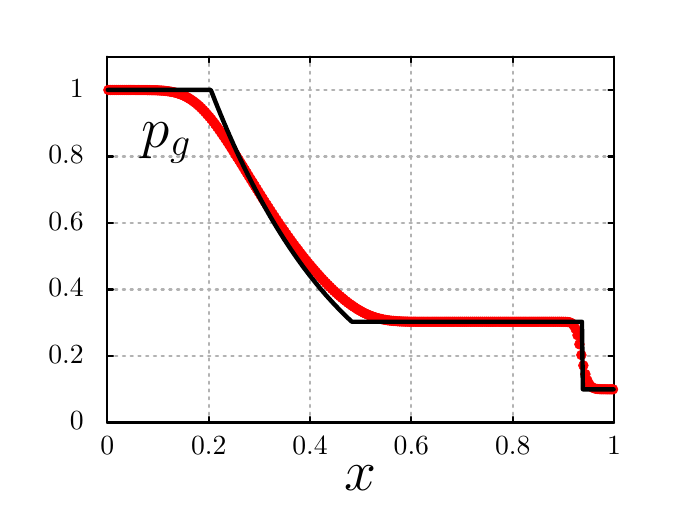
\begin{tikzpicture}[gnuplot]
%% generated with GNUPLOT 4.6p4 (Lua 5.1; terminal rev. 99, script rev. 100)
%% Sun 03 Aug 2014 03:55:27 PM EDT
\path (0.000,0.000) rectangle (8.000,6.000);
\gpfill{rgb color={1.000,1.000,1.000}} (1.012,0.985)--(7.446,0.985)--(7.446,5.630)--(1.012,5.630)--cycle;
\gpcolor{color=gp lt color border}
\gpsetlinetype{gp lt border}
\gpsetlinewidth{1.00}
\draw[gp path] (1.012,0.985)--(1.012,5.630)--(7.446,5.630)--(7.446,0.985)--cycle;
\gpcolor{color=gp lt color axes}
\gpsetlinetype{gp lt axes}
\gpsetlinewidth{2.00}
\draw[gp path] (1.012,0.985)--(7.447,0.985);
\gpcolor{color=gp lt color border}
\gpsetlinetype{gp lt border}
\draw[gp path] (1.012,0.985)--(1.084,0.985);
\draw[gp path] (7.447,0.985)--(7.375,0.985);
\gpcolor{rgb color={0.000,0.000,0.000}}
\node[gp node right,font={\fontsize{10pt}{12pt}\selectfont}] at (0.828,0.985) {0};
\gpcolor{color=gp lt color axes}
\gpsetlinetype{gp lt axes}
\draw[gp path] (1.012,1.830)--(7.447,1.830);
\gpcolor{color=gp lt color border}
\gpsetlinetype{gp lt border}
\draw[gp path] (1.012,1.830)--(1.084,1.830);
\draw[gp path] (7.447,1.830)--(7.375,1.830);
\gpcolor{rgb color={0.000,0.000,0.000}}
\node[gp node right,font={\fontsize{10pt}{12pt}\selectfont}] at (0.828,1.830) {0.2};
\gpcolor{color=gp lt color axes}
\gpsetlinetype{gp lt axes}
\draw[gp path] (1.012,2.674)--(7.447,2.674);
\gpcolor{color=gp lt color border}
\gpsetlinetype{gp lt border}
\draw[gp path] (1.012,2.674)--(1.084,2.674);
\draw[gp path] (7.447,2.674)--(7.375,2.674);
\gpcolor{rgb color={0.000,0.000,0.000}}
\node[gp node right,font={\fontsize{10pt}{12pt}\selectfont}] at (0.828,2.674) {0.4};
\gpcolor{color=gp lt color axes}
\gpsetlinetype{gp lt axes}
\draw[gp path] (1.012,3.519)--(7.447,3.519);
\gpcolor{color=gp lt color border}
\gpsetlinetype{gp lt border}
\draw[gp path] (1.012,3.519)--(1.084,3.519);
\draw[gp path] (7.447,3.519)--(7.375,3.519);
\gpcolor{rgb color={0.000,0.000,0.000}}
\node[gp node right,font={\fontsize{10pt}{12pt}\selectfont}] at (0.828,3.519) {0.6};
\gpcolor{color=gp lt color axes}
\gpsetlinetype{gp lt axes}
\draw[gp path] (1.012,4.364)--(7.447,4.364);
\gpcolor{color=gp lt color border}
\gpsetlinetype{gp lt border}
\draw[gp path] (1.012,4.364)--(1.084,4.364);
\draw[gp path] (7.447,4.364)--(7.375,4.364);
\gpcolor{rgb color={0.000,0.000,0.000}}
\node[gp node right,font={\fontsize{10pt}{12pt}\selectfont}] at (0.828,4.364) {0.8};
\gpcolor{color=gp lt color axes}
\gpsetlinetype{gp lt axes}
\draw[gp path] (1.012,5.209)--(7.447,5.209);
\gpcolor{color=gp lt color border}
\gpsetlinetype{gp lt border}
\draw[gp path] (1.012,5.209)--(1.084,5.209);
\draw[gp path] (7.447,5.209)--(7.375,5.209);
\gpcolor{rgb color={0.000,0.000,0.000}}
\node[gp node right,font={\fontsize{10pt}{12pt}\selectfont}] at (0.828,5.209) {1};
\gpcolor{color=gp lt color axes}
\gpsetlinetype{gp lt axes}
\draw[gp path] (1.012,0.985)--(1.012,5.631);
\gpcolor{color=gp lt color border}
\gpsetlinetype{gp lt border}
\draw[gp path] (1.012,0.985)--(1.012,1.057);
\draw[gp path] (1.012,5.631)--(1.012,5.559);
\gpcolor{rgb color={0.000,0.000,0.000}}
\node[gp node center,font={\fontsize{10pt}{12pt}\selectfont}] at (1.012,0.677) {0};
\gpcolor{color=gp lt color axes}
\gpsetlinetype{gp lt axes}
\draw[gp path] (2.299,0.985)--(2.299,5.631);
\gpcolor{color=gp lt color border}
\gpsetlinetype{gp lt border}
\draw[gp path] (2.299,0.985)--(2.299,1.057);
\draw[gp path] (2.299,5.631)--(2.299,5.559);
\gpcolor{rgb color={0.000,0.000,0.000}}
\node[gp node center,font={\fontsize{10pt}{12pt}\selectfont}] at (2.299,0.677) {0.2};
\gpcolor{color=gp lt color axes}
\gpsetlinetype{gp lt axes}
\draw[gp path] (3.586,0.985)--(3.586,5.631);
\gpcolor{color=gp lt color border}
\gpsetlinetype{gp lt border}
\draw[gp path] (3.586,0.985)--(3.586,1.057);
\draw[gp path] (3.586,5.631)--(3.586,5.559);
\gpcolor{rgb color={0.000,0.000,0.000}}
\node[gp node center,font={\fontsize{10pt}{12pt}\selectfont}] at (3.586,0.677) {0.4};
\gpcolor{color=gp lt color axes}
\gpsetlinetype{gp lt axes}
\draw[gp path] (4.873,0.985)--(4.873,5.631);
\gpcolor{color=gp lt color border}
\gpsetlinetype{gp lt border}
\draw[gp path] (4.873,0.985)--(4.873,1.057);
\draw[gp path] (4.873,5.631)--(4.873,5.559);
\gpcolor{rgb color={0.000,0.000,0.000}}
\node[gp node center,font={\fontsize{10pt}{12pt}\selectfont}] at (4.873,0.677) {0.6};
\gpcolor{color=gp lt color axes}
\gpsetlinetype{gp lt axes}
\draw[gp path] (6.160,0.985)--(6.160,5.631);
\gpcolor{color=gp lt color border}
\gpsetlinetype{gp lt border}
\draw[gp path] (6.160,0.985)--(6.160,1.057);
\draw[gp path] (6.160,5.631)--(6.160,5.559);
\gpcolor{rgb color={0.000,0.000,0.000}}
\node[gp node center,font={\fontsize{10pt}{12pt}\selectfont}] at (6.160,0.677) {0.8};
\gpcolor{color=gp lt color axes}
\gpsetlinetype{gp lt axes}
\draw[gp path] (7.447,0.985)--(7.447,5.631);
\gpcolor{color=gp lt color border}
\gpsetlinetype{gp lt border}
\draw[gp path] (7.447,0.985)--(7.447,1.057);
\draw[gp path] (7.447,5.631)--(7.447,5.559);
\gpcolor{rgb color={0.000,0.000,0.000}}
\node[gp node center,font={\fontsize{10pt}{12pt}\selectfont}] at (7.447,0.677) {1};
\gpcolor{color=gp lt color border}
\draw[gp path] (1.012,5.631)--(1.012,0.985)--(7.447,0.985)--(7.447,5.631)--cycle;
\gpcolor{rgb color={0.000,0.000,0.000}}
\node[gp node center,font={\fontsize{10pt}{12pt}\selectfont}] at (4.229,0.215) {\huge $x$};
\gpcolor{rgb color={1.000,0.000,0.000}}
\gpsetlinewidth{0.50}
\gpsetpointsize{4.44}
\gppoint{gp mark 7}{(1.025,5.209)}
\gppoint{gp mark 7}{(1.050,5.209)}
\gppoint{gp mark 7}{(1.075,5.209)}
\gppoint{gp mark 7}{(1.100,5.209)}
\gppoint{gp mark 7}{(1.125,5.209)}
\gppoint{gp mark 7}{(1.150,5.209)}
\gppoint{gp mark 7}{(1.175,5.209)}
\gppoint{gp mark 7}{(1.201,5.209)}
\gppoint{gp mark 7}{(1.226,5.209)}
\gppoint{gp mark 7}{(1.251,5.209)}
\gppoint{gp mark 7}{(1.276,5.209)}
\gppoint{gp mark 7}{(1.301,5.209)}
\gppoint{gp mark 7}{(1.326,5.209)}
\gppoint{gp mark 7}{(1.351,5.209)}
\gppoint{gp mark 7}{(1.376,5.208)}
\gppoint{gp mark 7}{(1.402,5.208)}
\gppoint{gp mark 7}{(1.427,5.208)}
\gppoint{gp mark 7}{(1.452,5.208)}
\gppoint{gp mark 7}{(1.477,5.208)}
\gppoint{gp mark 7}{(1.502,5.208)}
\gppoint{gp mark 7}{(1.527,5.207)}
\gppoint{gp mark 7}{(1.552,5.207)}
\gppoint{gp mark 7}{(1.578,5.206)}
\gppoint{gp mark 7}{(1.603,5.206)}
\gppoint{gp mark 7}{(1.628,5.205)}
\gppoint{gp mark 7}{(1.653,5.204)}
\gppoint{gp mark 7}{(1.678,5.202)}
\gppoint{gp mark 7}{(1.703,5.201)}
\gppoint{gp mark 7}{(1.728,5.199)}
\gppoint{gp mark 7}{(1.754,5.196)}
\gppoint{gp mark 7}{(1.779,5.193)}
\gppoint{gp mark 7}{(1.804,5.189)}
\gppoint{gp mark 7}{(1.829,5.185)}
\gppoint{gp mark 7}{(1.854,5.180)}
\gppoint{gp mark 7}{(1.879,5.174)}
\gppoint{gp mark 7}{(1.904,5.166)}
\gppoint{gp mark 7}{(1.929,5.158)}
\gppoint{gp mark 7}{(1.955,5.149)}
\gppoint{gp mark 7}{(1.980,5.138)}
\gppoint{gp mark 7}{(2.005,5.126)}
\gppoint{gp mark 7}{(2.030,5.113)}
\gppoint{gp mark 7}{(2.055,5.098)}
\gppoint{gp mark 7}{(2.080,5.082)}
\gppoint{gp mark 7}{(2.105,5.064)}
\gppoint{gp mark 7}{(2.131,5.045)}
\gppoint{gp mark 7}{(2.156,5.024)}
\gppoint{gp mark 7}{(2.181,5.002)}
\gppoint{gp mark 7}{(2.206,4.978)}
\gppoint{gp mark 7}{(2.231,4.952)}
\gppoint{gp mark 7}{(2.256,4.926)}
\gppoint{gp mark 7}{(2.281,4.897)}
\gppoint{gp mark 7}{(2.307,4.868)}
\gppoint{gp mark 7}{(2.332,4.837)}
\gppoint{gp mark 7}{(2.357,4.805)}
\gppoint{gp mark 7}{(2.382,4.772)}
\gppoint{gp mark 7}{(2.407,4.738)}
\gppoint{gp mark 7}{(2.432,4.703)}
\gppoint{gp mark 7}{(2.457,4.667)}
\gppoint{gp mark 7}{(2.482,4.630)}
\gppoint{gp mark 7}{(2.508,4.593)}
\gppoint{gp mark 7}{(2.533,4.555)}
\gppoint{gp mark 7}{(2.558,4.516)}
\gppoint{gp mark 7}{(2.583,4.477)}
\gppoint{gp mark 7}{(2.608,4.437)}
\gppoint{gp mark 7}{(2.633,4.398)}
\gppoint{gp mark 7}{(2.658,4.357)}
\gppoint{gp mark 7}{(2.684,4.317)}
\gppoint{gp mark 7}{(2.709,4.276)}
\gppoint{gp mark 7}{(2.734,4.236)}
\gppoint{gp mark 7}{(2.759,4.195)}
\gppoint{gp mark 7}{(2.784,4.154)}
\gppoint{gp mark 7}{(2.809,4.113)}
\gppoint{gp mark 7}{(2.834,4.073)}
\gppoint{gp mark 7}{(2.860,4.032)}
\gppoint{gp mark 7}{(2.885,3.991)}
\gppoint{gp mark 7}{(2.910,3.951)}
\gppoint{gp mark 7}{(2.935,3.911)}
\gppoint{gp mark 7}{(2.960,3.871)}
\gppoint{gp mark 7}{(2.985,3.831)}
\gppoint{gp mark 7}{(3.010,3.791)}
\gppoint{gp mark 7}{(3.036,3.752)}
\gppoint{gp mark 7}{(3.061,3.713)}
\gppoint{gp mark 7}{(3.086,3.674)}
\gppoint{gp mark 7}{(3.111,3.636)}
\gppoint{gp mark 7}{(3.136,3.598)}
\gppoint{gp mark 7}{(3.161,3.560)}
\gppoint{gp mark 7}{(3.186,3.523)}
\gppoint{gp mark 7}{(3.211,3.486)}
\gppoint{gp mark 7}{(3.237,3.449)}
\gppoint{gp mark 7}{(3.262,3.413)}
\gppoint{gp mark 7}{(3.287,3.377)}
\gppoint{gp mark 7}{(3.312,3.342)}
\gppoint{gp mark 7}{(3.337,3.307)}
\gppoint{gp mark 7}{(3.362,3.272)}
\gppoint{gp mark 7}{(3.387,3.238)}
\gppoint{gp mark 7}{(3.413,3.205)}
\gppoint{gp mark 7}{(3.438,3.172)}
\gppoint{gp mark 7}{(3.463,3.139)}
\gppoint{gp mark 7}{(3.488,3.106)}
\gppoint{gp mark 7}{(3.513,3.075)}
\gppoint{gp mark 7}{(3.538,3.043)}
\gppoint{gp mark 7}{(3.563,3.012)}
\gppoint{gp mark 7}{(3.589,2.982)}
\gppoint{gp mark 7}{(3.614,2.952)}
\gppoint{gp mark 7}{(3.639,2.923)}
\gppoint{gp mark 7}{(3.664,2.894)}
\gppoint{gp mark 7}{(3.689,2.866)}
\gppoint{gp mark 7}{(3.714,2.838)}
\gppoint{gp mark 7}{(3.739,2.810)}
\gppoint{gp mark 7}{(3.764,2.784)}
\gppoint{gp mark 7}{(3.790,2.757)}
\gppoint{gp mark 7}{(3.815,2.732)}
\gppoint{gp mark 7}{(3.840,2.707)}
\gppoint{gp mark 7}{(3.865,2.682)}
\gppoint{gp mark 7}{(3.890,2.658)}
\gppoint{gp mark 7}{(3.915,2.635)}
\gppoint{gp mark 7}{(3.940,2.612)}
\gppoint{gp mark 7}{(3.966,2.590)}
\gppoint{gp mark 7}{(3.991,2.569)}
\gppoint{gp mark 7}{(4.016,2.548)}
\gppoint{gp mark 7}{(4.041,2.528)}
\gppoint{gp mark 7}{(4.066,2.508)}
\gppoint{gp mark 7}{(4.091,2.490)}
\gppoint{gp mark 7}{(4.116,2.472)}
\gppoint{gp mark 7}{(4.142,2.455)}
\gppoint{gp mark 7}{(4.167,2.438)}
\gppoint{gp mark 7}{(4.192,2.422)}
\gppoint{gp mark 7}{(4.217,2.408)}
\gppoint{gp mark 7}{(4.242,2.394)}
\gppoint{gp mark 7}{(4.267,2.380)}
\gppoint{gp mark 7}{(4.292,2.368)}
\gppoint{gp mark 7}{(4.317,2.357)}
\gppoint{gp mark 7}{(4.343,2.346)}
\gppoint{gp mark 7}{(4.368,2.336)}
\gppoint{gp mark 7}{(4.393,2.327)}
\gppoint{gp mark 7}{(4.418,2.319)}
\gppoint{gp mark 7}{(4.443,2.311)}
\gppoint{gp mark 7}{(4.468,2.305)}
\gppoint{gp mark 7}{(4.493,2.299)}
\gppoint{gp mark 7}{(4.519,2.293)}
\gppoint{gp mark 7}{(4.544,2.289)}
\gppoint{gp mark 7}{(4.569,2.285)}
\gppoint{gp mark 7}{(4.594,2.281)}
\gppoint{gp mark 7}{(4.619,2.278)}
\gppoint{gp mark 7}{(4.644,2.276)}
\gppoint{gp mark 7}{(4.669,2.274)}
\gppoint{gp mark 7}{(4.695,2.272)}
\gppoint{gp mark 7}{(4.720,2.270)}
\gppoint{gp mark 7}{(4.745,2.269)}
\gppoint{gp mark 7}{(4.770,2.268)}
\gppoint{gp mark 7}{(4.795,2.267)}
\gppoint{gp mark 7}{(4.820,2.267)}
\gppoint{gp mark 7}{(4.845,2.266)}
\gppoint{gp mark 7}{(4.870,2.266)}
\gppoint{gp mark 7}{(4.896,2.266)}
\gppoint{gp mark 7}{(4.921,2.266)}
\gppoint{gp mark 7}{(4.946,2.265)}
\gppoint{gp mark 7}{(4.971,2.265)}
\gppoint{gp mark 7}{(4.996,2.265)}
\gppoint{gp mark 7}{(5.021,2.265)}
\gppoint{gp mark 7}{(5.046,2.265)}
\gppoint{gp mark 7}{(5.072,2.265)}
\gppoint{gp mark 7}{(5.097,2.265)}
\gppoint{gp mark 7}{(5.122,2.265)}
\gppoint{gp mark 7}{(5.147,2.265)}
\gppoint{gp mark 7}{(5.172,2.265)}
\gppoint{gp mark 7}{(5.197,2.265)}
\gppoint{gp mark 7}{(5.222,2.265)}
\gppoint{gp mark 7}{(5.248,2.265)}
\gppoint{gp mark 7}{(5.273,2.265)}
\gppoint{gp mark 7}{(5.298,2.265)}
\gppoint{gp mark 7}{(5.323,2.265)}
\gppoint{gp mark 7}{(5.348,2.265)}
\gppoint{gp mark 7}{(5.373,2.265)}
\gppoint{gp mark 7}{(5.398,2.265)}
\gppoint{gp mark 7}{(5.423,2.265)}
\gppoint{gp mark 7}{(5.449,2.265)}
\gppoint{gp mark 7}{(5.474,2.265)}
\gppoint{gp mark 7}{(5.499,2.265)}
\gppoint{gp mark 7}{(5.524,2.265)}
\gppoint{gp mark 7}{(5.549,2.265)}
\gppoint{gp mark 7}{(5.574,2.265)}
\gppoint{gp mark 7}{(5.599,2.265)}
\gppoint{gp mark 7}{(5.625,2.265)}
\gppoint{gp mark 7}{(5.650,2.265)}
\gppoint{gp mark 7}{(5.675,2.265)}
\gppoint{gp mark 7}{(5.700,2.265)}
\gppoint{gp mark 7}{(5.725,2.265)}
\gppoint{gp mark 7}{(5.750,2.265)}
\gppoint{gp mark 7}{(5.775,2.265)}
\gppoint{gp mark 7}{(5.801,2.265)}
\gppoint{gp mark 7}{(5.826,2.265)}
\gppoint{gp mark 7}{(5.851,2.265)}
\gppoint{gp mark 7}{(5.876,2.265)}
\gppoint{gp mark 7}{(5.901,2.265)}
\gppoint{gp mark 7}{(5.926,2.265)}
\gppoint{gp mark 7}{(5.951,2.265)}
\gppoint{gp mark 7}{(5.977,2.265)}
\gppoint{gp mark 7}{(6.002,2.265)}
\gppoint{gp mark 7}{(6.027,2.265)}
\gppoint{gp mark 7}{(6.052,2.265)}
\gppoint{gp mark 7}{(6.077,2.265)}
\gppoint{gp mark 7}{(6.102,2.265)}
\gppoint{gp mark 7}{(6.127,2.265)}
\gppoint{gp mark 7}{(6.152,2.265)}
\gppoint{gp mark 7}{(6.178,2.265)}
\gppoint{gp mark 7}{(6.203,2.265)}
\gppoint{gp mark 7}{(6.228,2.265)}
\gppoint{gp mark 7}{(6.253,2.265)}
\gppoint{gp mark 7}{(6.278,2.265)}
\gppoint{gp mark 7}{(6.303,2.265)}
\gppoint{gp mark 7}{(6.328,2.265)}
\gppoint{gp mark 7}{(6.354,2.265)}
\gppoint{gp mark 7}{(6.379,2.265)}
\gppoint{gp mark 7}{(6.404,2.265)}
\gppoint{gp mark 7}{(6.429,2.265)}
\gppoint{gp mark 7}{(6.454,2.265)}
\gppoint{gp mark 7}{(6.479,2.265)}
\gppoint{gp mark 7}{(6.504,2.265)}
\gppoint{gp mark 7}{(6.530,2.265)}
\gppoint{gp mark 7}{(6.555,2.265)}
\gppoint{gp mark 7}{(6.580,2.265)}
\gppoint{gp mark 7}{(6.605,2.265)}
\gppoint{gp mark 7}{(6.630,2.265)}
\gppoint{gp mark 7}{(6.655,2.265)}
\gppoint{gp mark 7}{(6.680,2.265)}
\gppoint{gp mark 7}{(6.705,2.265)}
\gppoint{gp mark 7}{(6.731,2.265)}
\gppoint{gp mark 7}{(6.756,2.265)}
\gppoint{gp mark 7}{(6.781,2.265)}
\gppoint{gp mark 7}{(6.806,2.264)}
\gppoint{gp mark 7}{(6.831,2.264)}
\gppoint{gp mark 7}{(6.856,2.263)}
\gppoint{gp mark 7}{(6.881,2.259)}
\gppoint{gp mark 7}{(6.907,2.248)}
\gppoint{gp mark 7}{(6.932,2.224)}
\gppoint{gp mark 7}{(6.957,2.176)}
\gppoint{gp mark 7}{(6.982,2.095)}
\gppoint{gp mark 7}{(7.007,1.979)}
\gppoint{gp mark 7}{(7.032,1.843)}
\gppoint{gp mark 7}{(7.057,1.710)}
\gppoint{gp mark 7}{(7.083,1.600)}
\gppoint{gp mark 7}{(7.108,1.521)}
\gppoint{gp mark 7}{(7.133,1.470)}
\gppoint{gp mark 7}{(7.158,1.440)}
\gppoint{gp mark 7}{(7.183,1.424)}
\gppoint{gp mark 7}{(7.208,1.416)}
\gppoint{gp mark 7}{(7.233,1.412)}
\gppoint{gp mark 7}{(7.258,1.410)}
\gppoint{gp mark 7}{(7.284,1.408)}
\gppoint{gp mark 7}{(7.309,1.408)}
\gppoint{gp mark 7}{(7.334,1.408)}
\gppoint{gp mark 7}{(7.359,1.407)}
\gppoint{gp mark 7}{(7.384,1.407)}
\gppoint{gp mark 7}{(7.409,1.407)}
\gppoint{gp mark 7}{(7.434,1.407)}
\gpcolor{rgb color={0.000,0.000,0.000}}
\gpsetlinetype{gp lt plot 0}
\gpsetlinewidth{4.00}
\draw[gp path] (1.018,5.209)--(1.031,5.209)--(1.043,5.209)--(1.056,5.209)--(1.069,5.209)%
  --(1.081,5.209)--(1.094,5.209)--(1.106,5.209)--(1.119,5.209)--(1.131,5.209)--(1.144,5.209)%
  --(1.157,5.209)--(1.169,5.209)--(1.182,5.209)--(1.194,5.209)--(1.207,5.209)--(1.219,5.209)%
  --(1.232,5.209)--(1.245,5.209)--(1.257,5.209)--(1.270,5.209)--(1.282,5.209)--(1.295,5.209)%
  --(1.307,5.209)--(1.320,5.209)--(1.332,5.209)--(1.345,5.209)--(1.358,5.209)--(1.370,5.209)%
  --(1.383,5.209)--(1.395,5.209)--(1.408,5.209)--(1.420,5.209)--(1.433,5.209)--(1.446,5.209)%
  --(1.458,5.209)--(1.471,5.209)--(1.483,5.209)--(1.496,5.209)--(1.508,5.209)--(1.521,5.209)%
  --(1.534,5.209)--(1.546,5.209)--(1.559,5.209)--(1.571,5.209)--(1.584,5.209)--(1.596,5.209)%
  --(1.609,5.209)--(1.622,5.209)--(1.634,5.209)--(1.647,5.209)--(1.659,5.209)--(1.672,5.209)%
  --(1.684,5.209)--(1.697,5.209)--(1.710,5.209)--(1.722,5.209)--(1.735,5.209)--(1.747,5.209)%
  --(1.760,5.209)--(1.772,5.209)--(1.785,5.209)--(1.798,5.209)--(1.810,5.209)--(1.823,5.209)%
  --(1.835,5.209)--(1.848,5.209)--(1.860,5.209)--(1.873,5.209)--(1.886,5.209)--(1.898,5.209)%
  --(1.911,5.209)--(1.923,5.209)--(1.936,5.209)--(1.948,5.209)--(1.961,5.209)--(1.973,5.209)%
  --(1.986,5.209)--(1.999,5.209)--(2.011,5.209)--(2.024,5.209)--(2.036,5.209)--(2.049,5.209)%
  --(2.061,5.209)--(2.074,5.209)--(2.087,5.209)--(2.099,5.209)--(2.112,5.209)--(2.124,5.209)%
  --(2.137,5.209)--(2.149,5.209)--(2.162,5.209)--(2.175,5.209)--(2.187,5.209)--(2.200,5.209)%
  --(2.212,5.209)--(2.225,5.209)--(2.237,5.209)--(2.250,5.209)--(2.263,5.209)--(2.275,5.209)%
  --(2.288,5.209)--(2.300,5.209)--(2.313,5.209)--(2.325,5.209)--(2.338,5.178)--(2.351,5.146)%
  --(2.363,5.114)--(2.376,5.082)--(2.388,5.050)--(2.401,5.019)--(2.413,4.988)--(2.426,4.957)%
  --(2.439,4.926)--(2.451,4.895)--(2.464,4.865)--(2.476,4.835)--(2.489,4.805)--(2.501,4.775)%
  --(2.514,4.746)--(2.526,4.716)--(2.539,4.687)--(2.552,4.658)--(2.564,4.629)--(2.577,4.601)%
  --(2.589,4.572)--(2.602,4.544)--(2.614,4.516)--(2.627,4.488)--(2.640,4.461)--(2.652,4.433)%
  --(2.665,4.406)--(2.677,4.379)--(2.690,4.352)--(2.702,4.325)--(2.715,4.299)--(2.728,4.273)%
  --(2.740,4.246)--(2.753,4.220)--(2.765,4.195)--(2.778,4.169)--(2.790,4.144)--(2.803,4.118)%
  --(2.816,4.093)--(2.828,4.068)--(2.841,4.043)--(2.853,4.019)--(2.866,3.994)--(2.878,3.970)%
  --(2.891,3.946)--(2.904,3.922)--(2.916,3.898)--(2.929,3.875)--(2.941,3.851)--(2.954,3.828)%
  --(2.966,3.805)--(2.979,3.782)--(2.992,3.759)--(3.004,3.737)--(3.017,3.714)--(3.029,3.692)%
  --(3.042,3.670)--(3.054,3.648)--(3.067,3.626)--(3.079,3.604)--(3.092,3.583)--(3.105,3.561)%
  --(3.117,3.540)--(3.130,3.519)--(3.142,3.498)--(3.155,3.477)--(3.167,3.457)--(3.180,3.436)%
  --(3.193,3.416)--(3.205,3.396)--(3.218,3.376)--(3.230,3.356)--(3.243,3.336)--(3.255,3.316)%
  --(3.268,3.297)--(3.281,3.278)--(3.293,3.258)--(3.306,3.239)--(3.318,3.220)--(3.331,3.202)%
  --(3.343,3.183)--(3.356,3.165)--(3.369,3.146)--(3.381,3.128)--(3.394,3.110)--(3.406,3.092)%
  --(3.419,3.074)--(3.431,3.056)--(3.444,3.039)--(3.457,3.021)--(3.469,3.004)--(3.482,2.987)%
  --(3.494,2.969)--(3.507,2.952)--(3.519,2.936)--(3.532,2.919)--(3.545,2.902)--(3.557,2.886)%
  --(3.570,2.870)--(3.582,2.853)--(3.595,2.837)--(3.607,2.821)--(3.620,2.805)--(3.633,2.790)%
  --(3.645,2.774)--(3.658,2.758)--(3.670,2.743)--(3.683,2.728)--(3.695,2.713)--(3.708,2.697)%
  --(3.720,2.682)--(3.733,2.668)--(3.746,2.653)--(3.758,2.638)--(3.771,2.624)--(3.783,2.609)%
  --(3.796,2.595)--(3.808,2.581)--(3.821,2.567)--(3.834,2.553)--(3.846,2.539)--(3.859,2.525)%
  --(3.871,2.512)--(3.884,2.498)--(3.896,2.485)--(3.909,2.471)--(3.922,2.458)--(3.934,2.445)%
  --(3.947,2.432)--(3.959,2.419)--(3.972,2.406)--(3.984,2.393)--(3.997,2.381)--(4.010,2.368)%
  --(4.022,2.356)--(4.035,2.343)--(4.047,2.331)--(4.060,2.319)--(4.072,2.307)--(4.085,2.295)%
  --(4.098,2.283)--(4.110,2.271)--(4.123,2.265)--(4.135,2.265)--(4.148,2.265)--(4.160,2.265)%
  --(4.173,2.265)--(4.186,2.265)--(4.198,2.265)--(4.211,2.265)--(4.223,2.265)--(4.236,2.265)%
  --(4.248,2.265)--(4.261,2.265)--(4.273,2.265)--(4.286,2.265)--(4.299,2.265)--(4.311,2.265)%
  --(4.324,2.265)--(4.336,2.265)--(4.349,2.265)--(4.361,2.265)--(4.374,2.265)--(4.387,2.265)%
  --(4.399,2.265)--(4.412,2.265)--(4.424,2.265)--(4.437,2.265)--(4.449,2.265)--(4.462,2.265)%
  --(4.475,2.265)--(4.487,2.265)--(4.500,2.265)--(4.512,2.265)--(4.525,2.265)--(4.537,2.265)%
  --(4.550,2.265)--(4.563,2.265)--(4.575,2.265)--(4.588,2.265)--(4.600,2.265)--(4.613,2.265)%
  --(4.625,2.265)--(4.638,2.265)--(4.651,2.265)--(4.663,2.265)--(4.676,2.265)--(4.688,2.265)%
  --(4.701,2.265)--(4.713,2.265)--(4.726,2.265)--(4.739,2.265)--(4.751,2.265)--(4.764,2.265)%
  --(4.776,2.265)--(4.789,2.265)--(4.801,2.265)--(4.814,2.265)--(4.826,2.265)--(4.839,2.265)%
  --(4.852,2.265)--(4.864,2.265)--(4.877,2.265)--(4.889,2.265)--(4.902,2.265)--(4.914,2.265)%
  --(4.927,2.265)--(4.940,2.265)--(4.952,2.265)--(4.965,2.265)--(4.977,2.265)--(4.990,2.265)%
  --(5.002,2.265)--(5.015,2.265)--(5.028,2.265)--(5.040,2.265)--(5.053,2.265)--(5.065,2.265)%
  --(5.078,2.265)--(5.090,2.265)--(5.103,2.265)--(5.116,2.265)--(5.128,2.265)--(5.141,2.265)%
  --(5.153,2.265)--(5.166,2.265)--(5.178,2.265)--(5.191,2.265)--(5.204,2.265)--(5.216,2.265)%
  --(5.229,2.265)--(5.241,2.265)--(5.254,2.265)--(5.266,2.265)--(5.279,2.265)--(5.292,2.265)%
  --(5.304,2.265)--(5.317,2.265)--(5.329,2.265)--(5.342,2.265)--(5.354,2.265)--(5.367,2.265)%
  --(5.380,2.265)--(5.392,2.265)--(5.405,2.265)--(5.417,2.265)--(5.430,2.265)--(5.442,2.265)%
  --(5.455,2.265)--(5.467,2.265)--(5.480,2.265)--(5.493,2.265)--(5.505,2.265)--(5.518,2.265)%
  --(5.530,2.265)--(5.543,2.265)--(5.555,2.265)--(5.568,2.265)--(5.581,2.265)--(5.593,2.265)%
  --(5.606,2.265)--(5.618,2.265)--(5.631,2.265)--(5.643,2.265)--(5.656,2.265)--(5.669,2.265)%
  --(5.681,2.265)--(5.694,2.265)--(5.706,2.265)--(5.719,2.265)--(5.731,2.265)--(5.744,2.265)%
  --(5.757,2.265)--(5.769,2.265)--(5.782,2.265)--(5.794,2.265)--(5.807,2.265)--(5.819,2.265)%
  --(5.832,2.265)--(5.845,2.265)--(5.857,2.265)--(5.870,2.265)--(5.882,2.265)--(5.895,2.265)%
  --(5.907,2.265)--(5.920,2.265)--(5.933,2.265)--(5.945,2.265)--(5.958,2.265)--(5.970,2.265)%
  --(5.983,2.265)--(5.995,2.265)--(6.008,2.265)--(6.020,2.265)--(6.033,2.265)--(6.046,2.265)%
  --(6.058,2.265)--(6.071,2.265)--(6.083,2.265)--(6.096,2.265)--(6.108,2.265)--(6.121,2.265)%
  --(6.134,2.265)--(6.146,2.265)--(6.159,2.265)--(6.171,2.265)--(6.184,2.265)--(6.196,2.265)%
  --(6.209,2.265)--(6.222,2.265)--(6.234,2.265)--(6.247,2.265)--(6.259,2.265)--(6.272,2.265)%
  --(6.284,2.265)--(6.297,2.265)--(6.310,2.265)--(6.322,2.265)--(6.335,2.265)--(6.347,2.265)%
  --(6.360,2.265)--(6.372,2.265)--(6.385,2.265)--(6.398,2.265)--(6.410,2.265)--(6.423,2.265)%
  --(6.435,2.265)--(6.448,2.265)--(6.460,2.265)--(6.473,2.265)--(6.486,2.265)--(6.498,2.265)%
  --(6.511,2.265)--(6.523,2.265)--(6.536,2.265)--(6.548,2.265)--(6.561,2.265)--(6.573,2.265)%
  --(6.586,2.265)--(6.599,2.265)--(6.611,2.265)--(6.624,2.265)--(6.636,2.265)--(6.649,2.265)%
  --(6.661,2.265)--(6.674,2.265)--(6.687,2.265)--(6.699,2.265)--(6.712,2.265)--(6.724,2.265)%
  --(6.737,2.265)--(6.749,2.265)--(6.762,2.265)--(6.775,2.265)--(6.787,2.265)--(6.800,2.265)%
  --(6.812,2.265)--(6.825,2.265)--(6.837,2.265)--(6.850,2.265)--(6.863,2.265)--(6.875,2.265)%
  --(6.888,2.265)--(6.900,2.265)--(6.913,2.265)--(6.925,2.265)--(6.938,2.265)--(6.951,2.265)%
  --(6.963,2.265)--(6.976,2.265)--(6.988,2.265)--(7.001,2.265)--(7.013,2.265)--(7.026,2.265)%
  --(7.039,2.265)--(7.051,1.407)--(7.064,1.407)--(7.076,1.407)--(7.089,1.407)--(7.101,1.407)%
  --(7.114,1.407)--(7.127,1.407)--(7.139,1.407)--(7.152,1.407)--(7.164,1.407)--(7.177,1.407)%
  --(7.189,1.407)--(7.202,1.407)--(7.214,1.407)--(7.227,1.407)--(7.240,1.407)--(7.252,1.407)%
  --(7.265,1.407)--(7.277,1.407)--(7.290,1.407)--(7.302,1.407)--(7.315,1.407)--(7.328,1.407)%
  --(7.340,1.407)--(7.353,1.407)--(7.365,1.407)--(7.378,1.407)--(7.390,1.407)--(7.403,1.407)%
  --(7.416,1.407)--(7.428,1.407)--(7.441,1.407);
\node[gp node left,font={\fontsize{10pt}{12pt}\selectfont}] at (1.334,4.575) {\huge $p_g$};
%% coordinates of the plot area
\gpdefrectangularnode{gp plot 1}{\pgfpoint{1.012cm}{0.985cm}}{\pgfpoint{7.447cm}{5.631cm}}
\end{tikzpicture}
%% gnuplot variables
} \\ 
\resizebox{0.33\linewidth}{!}{\tikzsetnextfilename{sod_rusanov_fct_3_1}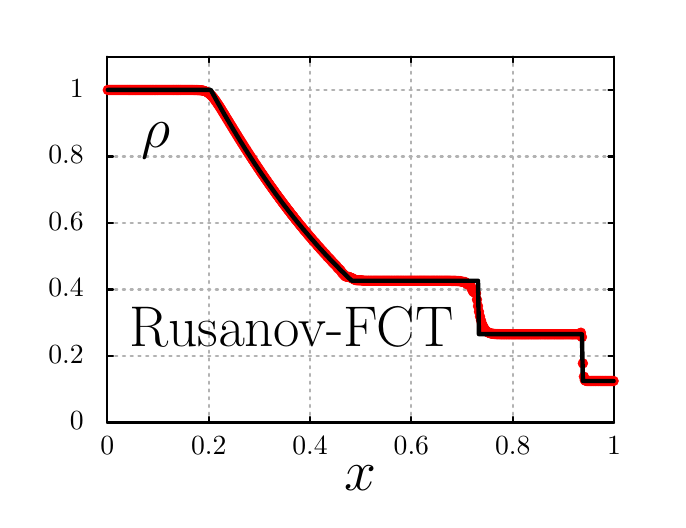
\begin{tikzpicture}[gnuplot]
%% generated with GNUPLOT 4.6p4 (Lua 5.1; terminal rev. 99, script rev. 100)
%% Mon 04 Aug 2014 12:05:06 PM EDT
\path (0.000,0.000) rectangle (8.000,6.000);
\gpfill{rgb color={1.000,1.000,1.000}} (1.012,0.985)--(7.446,0.985)--(7.446,5.630)--(1.012,5.630)--cycle;
\gpcolor{color=gp lt color border}
\gpsetlinetype{gp lt border}
\gpsetlinewidth{1.00}
\draw[gp path] (1.012,0.985)--(1.012,5.630)--(7.446,5.630)--(7.446,0.985)--cycle;
\gpcolor{color=gp lt color axes}
\gpsetlinetype{gp lt axes}
\gpsetlinewidth{2.00}
\draw[gp path] (1.012,0.985)--(7.447,0.985);
\gpcolor{color=gp lt color border}
\gpsetlinetype{gp lt border}
\draw[gp path] (1.012,0.985)--(1.084,0.985);
\draw[gp path] (7.447,0.985)--(7.375,0.985);
\gpcolor{rgb color={0.000,0.000,0.000}}
\node[gp node right,font={\fontsize{10pt}{12pt}\selectfont}] at (0.828,0.985) {0};
\gpcolor{color=gp lt color axes}
\gpsetlinetype{gp lt axes}
\draw[gp path] (1.012,1.830)--(7.447,1.830);
\gpcolor{color=gp lt color border}
\gpsetlinetype{gp lt border}
\draw[gp path] (1.012,1.830)--(1.084,1.830);
\draw[gp path] (7.447,1.830)--(7.375,1.830);
\gpcolor{rgb color={0.000,0.000,0.000}}
\node[gp node right,font={\fontsize{10pt}{12pt}\selectfont}] at (0.828,1.830) {0.2};
\gpcolor{color=gp lt color axes}
\gpsetlinetype{gp lt axes}
\draw[gp path] (1.012,2.674)--(7.447,2.674);
\gpcolor{color=gp lt color border}
\gpsetlinetype{gp lt border}
\draw[gp path] (1.012,2.674)--(1.084,2.674);
\draw[gp path] (7.447,2.674)--(7.375,2.674);
\gpcolor{rgb color={0.000,0.000,0.000}}
\node[gp node right,font={\fontsize{10pt}{12pt}\selectfont}] at (0.828,2.674) {0.4};
\gpcolor{color=gp lt color axes}
\gpsetlinetype{gp lt axes}
\draw[gp path] (1.012,3.519)--(7.447,3.519);
\gpcolor{color=gp lt color border}
\gpsetlinetype{gp lt border}
\draw[gp path] (1.012,3.519)--(1.084,3.519);
\draw[gp path] (7.447,3.519)--(7.375,3.519);
\gpcolor{rgb color={0.000,0.000,0.000}}
\node[gp node right,font={\fontsize{10pt}{12pt}\selectfont}] at (0.828,3.519) {0.6};
\gpcolor{color=gp lt color axes}
\gpsetlinetype{gp lt axes}
\draw[gp path] (1.012,4.364)--(7.447,4.364);
\gpcolor{color=gp lt color border}
\gpsetlinetype{gp lt border}
\draw[gp path] (1.012,4.364)--(1.084,4.364);
\draw[gp path] (7.447,4.364)--(7.375,4.364);
\gpcolor{rgb color={0.000,0.000,0.000}}
\node[gp node right,font={\fontsize{10pt}{12pt}\selectfont}] at (0.828,4.364) {0.8};
\gpcolor{color=gp lt color axes}
\gpsetlinetype{gp lt axes}
\draw[gp path] (1.012,5.209)--(7.447,5.209);
\gpcolor{color=gp lt color border}
\gpsetlinetype{gp lt border}
\draw[gp path] (1.012,5.209)--(1.084,5.209);
\draw[gp path] (7.447,5.209)--(7.375,5.209);
\gpcolor{rgb color={0.000,0.000,0.000}}
\node[gp node right,font={\fontsize{10pt}{12pt}\selectfont}] at (0.828,5.209) {1};
\gpcolor{color=gp lt color axes}
\gpsetlinetype{gp lt axes}
\draw[gp path] (1.012,0.985)--(1.012,5.631);
\gpcolor{color=gp lt color border}
\gpsetlinetype{gp lt border}
\draw[gp path] (1.012,0.985)--(1.012,1.057);
\draw[gp path] (1.012,5.631)--(1.012,5.559);
\gpcolor{rgb color={0.000,0.000,0.000}}
\node[gp node center,font={\fontsize{10pt}{12pt}\selectfont}] at (1.012,0.677) {0};
\gpcolor{color=gp lt color axes}
\gpsetlinetype{gp lt axes}
\draw[gp path] (2.299,0.985)--(2.299,5.631);
\gpcolor{color=gp lt color border}
\gpsetlinetype{gp lt border}
\draw[gp path] (2.299,0.985)--(2.299,1.057);
\draw[gp path] (2.299,5.631)--(2.299,5.559);
\gpcolor{rgb color={0.000,0.000,0.000}}
\node[gp node center,font={\fontsize{10pt}{12pt}\selectfont}] at (2.299,0.677) {0.2};
\gpcolor{color=gp lt color axes}
\gpsetlinetype{gp lt axes}
\draw[gp path] (3.586,0.985)--(3.586,5.631);
\gpcolor{color=gp lt color border}
\gpsetlinetype{gp lt border}
\draw[gp path] (3.586,0.985)--(3.586,1.057);
\draw[gp path] (3.586,5.631)--(3.586,5.559);
\gpcolor{rgb color={0.000,0.000,0.000}}
\node[gp node center,font={\fontsize{10pt}{12pt}\selectfont}] at (3.586,0.677) {0.4};
\gpcolor{color=gp lt color axes}
\gpsetlinetype{gp lt axes}
\draw[gp path] (4.873,0.985)--(4.873,5.631);
\gpcolor{color=gp lt color border}
\gpsetlinetype{gp lt border}
\draw[gp path] (4.873,0.985)--(4.873,1.057);
\draw[gp path] (4.873,5.631)--(4.873,5.559);
\gpcolor{rgb color={0.000,0.000,0.000}}
\node[gp node center,font={\fontsize{10pt}{12pt}\selectfont}] at (4.873,0.677) {0.6};
\gpcolor{color=gp lt color axes}
\gpsetlinetype{gp lt axes}
\draw[gp path] (6.160,0.985)--(6.160,5.631);
\gpcolor{color=gp lt color border}
\gpsetlinetype{gp lt border}
\draw[gp path] (6.160,0.985)--(6.160,1.057);
\draw[gp path] (6.160,5.631)--(6.160,5.559);
\gpcolor{rgb color={0.000,0.000,0.000}}
\node[gp node center,font={\fontsize{10pt}{12pt}\selectfont}] at (6.160,0.677) {0.8};
\gpcolor{color=gp lt color axes}
\gpsetlinetype{gp lt axes}
\draw[gp path] (7.447,0.985)--(7.447,5.631);
\gpcolor{color=gp lt color border}
\gpsetlinetype{gp lt border}
\draw[gp path] (7.447,0.985)--(7.447,1.057);
\draw[gp path] (7.447,5.631)--(7.447,5.559);
\gpcolor{rgb color={0.000,0.000,0.000}}
\node[gp node center,font={\fontsize{10pt}{12pt}\selectfont}] at (7.447,0.677) {1};
\gpcolor{color=gp lt color border}
\draw[gp path] (1.012,5.631)--(1.012,0.985)--(7.447,0.985)--(7.447,5.631)--cycle;
\gpcolor{rgb color={0.000,0.000,0.000}}
\node[gp node center,font={\fontsize{10pt}{12pt}\selectfont}] at (4.229,0.215) {\huge $x$};
\gpcolor{rgb color={1.000,0.000,0.000}}
\gpsetlinewidth{0.50}
\gpsetpointsize{4.44}
\gppoint{gp mark 7}{(1.018,5.209)}
\gppoint{gp mark 7}{(1.031,5.209)}
\gppoint{gp mark 7}{(1.043,5.209)}
\gppoint{gp mark 7}{(1.056,5.209)}
\gppoint{gp mark 7}{(1.069,5.209)}
\gppoint{gp mark 7}{(1.081,5.209)}
\gppoint{gp mark 7}{(1.094,5.209)}
\gppoint{gp mark 7}{(1.106,5.209)}
\gppoint{gp mark 7}{(1.119,5.209)}
\gppoint{gp mark 7}{(1.131,5.209)}
\gppoint{gp mark 7}{(1.144,5.209)}
\gppoint{gp mark 7}{(1.157,5.209)}
\gppoint{gp mark 7}{(1.169,5.209)}
\gppoint{gp mark 7}{(1.182,5.209)}
\gppoint{gp mark 7}{(1.194,5.209)}
\gppoint{gp mark 7}{(1.207,5.209)}
\gppoint{gp mark 7}{(1.219,5.209)}
\gppoint{gp mark 7}{(1.232,5.209)}
\gppoint{gp mark 7}{(1.245,5.209)}
\gppoint{gp mark 7}{(1.257,5.209)}
\gppoint{gp mark 7}{(1.270,5.209)}
\gppoint{gp mark 7}{(1.282,5.209)}
\gppoint{gp mark 7}{(1.295,5.209)}
\gppoint{gp mark 7}{(1.307,5.209)}
\gppoint{gp mark 7}{(1.320,5.209)}
\gppoint{gp mark 7}{(1.332,5.209)}
\gppoint{gp mark 7}{(1.345,5.209)}
\gppoint{gp mark 7}{(1.358,5.209)}
\gppoint{gp mark 7}{(1.370,5.209)}
\gppoint{gp mark 7}{(1.383,5.209)}
\gppoint{gp mark 7}{(1.395,5.209)}
\gppoint{gp mark 7}{(1.408,5.209)}
\gppoint{gp mark 7}{(1.420,5.209)}
\gppoint{gp mark 7}{(1.433,5.209)}
\gppoint{gp mark 7}{(1.446,5.209)}
\gppoint{gp mark 7}{(1.458,5.209)}
\gppoint{gp mark 7}{(1.471,5.209)}
\gppoint{gp mark 7}{(1.483,5.209)}
\gppoint{gp mark 7}{(1.496,5.209)}
\gppoint{gp mark 7}{(1.508,5.209)}
\gppoint{gp mark 7}{(1.521,5.209)}
\gppoint{gp mark 7}{(1.534,5.209)}
\gppoint{gp mark 7}{(1.546,5.209)}
\gppoint{gp mark 7}{(1.559,5.209)}
\gppoint{gp mark 7}{(1.571,5.209)}
\gppoint{gp mark 7}{(1.584,5.209)}
\gppoint{gp mark 7}{(1.596,5.209)}
\gppoint{gp mark 7}{(1.609,5.209)}
\gppoint{gp mark 7}{(1.622,5.209)}
\gppoint{gp mark 7}{(1.634,5.209)}
\gppoint{gp mark 7}{(1.647,5.209)}
\gppoint{gp mark 7}{(1.659,5.209)}
\gppoint{gp mark 7}{(1.672,5.209)}
\gppoint{gp mark 7}{(1.684,5.209)}
\gppoint{gp mark 7}{(1.697,5.209)}
\gppoint{gp mark 7}{(1.710,5.209)}
\gppoint{gp mark 7}{(1.722,5.209)}
\gppoint{gp mark 7}{(1.735,5.209)}
\gppoint{gp mark 7}{(1.747,5.209)}
\gppoint{gp mark 7}{(1.760,5.209)}
\gppoint{gp mark 7}{(1.772,5.209)}
\gppoint{gp mark 7}{(1.785,5.209)}
\gppoint{gp mark 7}{(1.798,5.209)}
\gppoint{gp mark 7}{(1.810,5.209)}
\gppoint{gp mark 7}{(1.823,5.209)}
\gppoint{gp mark 7}{(1.835,5.209)}
\gppoint{gp mark 7}{(1.848,5.209)}
\gppoint{gp mark 7}{(1.860,5.209)}
\gppoint{gp mark 7}{(1.873,5.209)}
\gppoint{gp mark 7}{(1.886,5.209)}
\gppoint{gp mark 7}{(1.898,5.209)}
\gppoint{gp mark 7}{(1.911,5.209)}
\gppoint{gp mark 7}{(1.923,5.209)}
\gppoint{gp mark 7}{(1.936,5.209)}
\gppoint{gp mark 7}{(1.948,5.209)}
\gppoint{gp mark 7}{(1.961,5.209)}
\gppoint{gp mark 7}{(1.973,5.209)}
\gppoint{gp mark 7}{(1.986,5.209)}
\gppoint{gp mark 7}{(1.999,5.209)}
\gppoint{gp mark 7}{(2.011,5.209)}
\gppoint{gp mark 7}{(2.024,5.209)}
\gppoint{gp mark 7}{(2.036,5.209)}
\gppoint{gp mark 7}{(2.049,5.209)}
\gppoint{gp mark 7}{(2.061,5.209)}
\gppoint{gp mark 7}{(2.074,5.209)}
\gppoint{gp mark 7}{(2.087,5.209)}
\gppoint{gp mark 7}{(2.099,5.209)}
\gppoint{gp mark 7}{(2.112,5.208)}
\gppoint{gp mark 7}{(2.124,5.208)}
\gppoint{gp mark 7}{(2.137,5.208)}
\gppoint{gp mark 7}{(2.149,5.208)}
\gppoint{gp mark 7}{(2.162,5.207)}
\gppoint{gp mark 7}{(2.175,5.207)}
\gppoint{gp mark 7}{(2.187,5.206)}
\gppoint{gp mark 7}{(2.200,5.205)}
\gppoint{gp mark 7}{(2.212,5.203)}
\gppoint{gp mark 7}{(2.225,5.201)}
\gppoint{gp mark 7}{(2.237,5.198)}
\gppoint{gp mark 7}{(2.250,5.194)}
\gppoint{gp mark 7}{(2.263,5.189)}
\gppoint{gp mark 7}{(2.275,5.183)}
\gppoint{gp mark 7}{(2.288,5.176)}
\gppoint{gp mark 7}{(2.300,5.167)}
\gppoint{gp mark 7}{(2.313,5.157)}
\gppoint{gp mark 7}{(2.325,5.145)}
\gppoint{gp mark 7}{(2.338,5.133)}
\gppoint{gp mark 7}{(2.351,5.118)}
\gppoint{gp mark 7}{(2.363,5.103)}
\gppoint{gp mark 7}{(2.376,5.086)}
\gppoint{gp mark 7}{(2.388,5.069)}
\gppoint{gp mark 7}{(2.401,5.051)}
\gppoint{gp mark 7}{(2.413,5.032)}
\gppoint{gp mark 7}{(2.426,5.014)}
\gppoint{gp mark 7}{(2.439,4.993)}
\gppoint{gp mark 7}{(2.451,4.974)}
\gppoint{gp mark 7}{(2.464,4.954)}
\gppoint{gp mark 7}{(2.476,4.933)}
\gppoint{gp mark 7}{(2.489,4.913)}
\gppoint{gp mark 7}{(2.501,4.892)}
\gppoint{gp mark 7}{(2.514,4.872)}
\gppoint{gp mark 7}{(2.526,4.851)}
\gppoint{gp mark 7}{(2.539,4.830)}
\gppoint{gp mark 7}{(2.552,4.810)}
\gppoint{gp mark 7}{(2.564,4.789)}
\gppoint{gp mark 7}{(2.577,4.768)}
\gppoint{gp mark 7}{(2.589,4.748)}
\gppoint{gp mark 7}{(2.602,4.728)}
\gppoint{gp mark 7}{(2.614,4.707)}
\gppoint{gp mark 7}{(2.627,4.687)}
\gppoint{gp mark 7}{(2.640,4.666)}
\gppoint{gp mark 7}{(2.652,4.646)}
\gppoint{gp mark 7}{(2.665,4.626)}
\gppoint{gp mark 7}{(2.677,4.605)}
\gppoint{gp mark 7}{(2.690,4.585)}
\gppoint{gp mark 7}{(2.702,4.566)}
\gppoint{gp mark 7}{(2.715,4.545)}
\gppoint{gp mark 7}{(2.728,4.525)}
\gppoint{gp mark 7}{(2.740,4.506)}
\gppoint{gp mark 7}{(2.753,4.485)}
\gppoint{gp mark 7}{(2.765,4.466)}
\gppoint{gp mark 7}{(2.778,4.447)}
\gppoint{gp mark 7}{(2.790,4.427)}
\gppoint{gp mark 7}{(2.803,4.407)}
\gppoint{gp mark 7}{(2.816,4.388)}
\gppoint{gp mark 7}{(2.828,4.368)}
\gppoint{gp mark 7}{(2.841,4.349)}
\gppoint{gp mark 7}{(2.853,4.330)}
\gppoint{gp mark 7}{(2.866,4.311)}
\gppoint{gp mark 7}{(2.878,4.291)}
\gppoint{gp mark 7}{(2.891,4.273)}
\gppoint{gp mark 7}{(2.904,4.254)}
\gppoint{gp mark 7}{(2.916,4.234)}
\gppoint{gp mark 7}{(2.929,4.216)}
\gppoint{gp mark 7}{(2.941,4.198)}
\gppoint{gp mark 7}{(2.954,4.179)}
\gppoint{gp mark 7}{(2.966,4.159)}
\gppoint{gp mark 7}{(2.979,4.142)}
\gppoint{gp mark 7}{(2.992,4.124)}
\gppoint{gp mark 7}{(3.004,4.105)}
\gppoint{gp mark 7}{(3.017,4.086)}
\gppoint{gp mark 7}{(3.029,4.069)}
\gppoint{gp mark 7}{(3.042,4.051)}
\gppoint{gp mark 7}{(3.054,4.032)}
\gppoint{gp mark 7}{(3.067,4.015)}
\gppoint{gp mark 7}{(3.079,3.997)}
\gppoint{gp mark 7}{(3.092,3.979)}
\gppoint{gp mark 7}{(3.105,3.961)}
\gppoint{gp mark 7}{(3.117,3.944)}
\gppoint{gp mark 7}{(3.130,3.927)}
\gppoint{gp mark 7}{(3.142,3.908)}
\gppoint{gp mark 7}{(3.155,3.891)}
\gppoint{gp mark 7}{(3.167,3.875)}
\gppoint{gp mark 7}{(3.180,3.857)}
\gppoint{gp mark 7}{(3.193,3.839)}
\gppoint{gp mark 7}{(3.205,3.822)}
\gppoint{gp mark 7}{(3.218,3.806)}
\gppoint{gp mark 7}{(3.230,3.789)}
\gppoint{gp mark 7}{(3.243,3.771)}
\gppoint{gp mark 7}{(3.255,3.755)}
\gppoint{gp mark 7}{(3.268,3.739)}
\gppoint{gp mark 7}{(3.281,3.722)}
\gppoint{gp mark 7}{(3.293,3.705)}
\gppoint{gp mark 7}{(3.306,3.688)}
\gppoint{gp mark 7}{(3.318,3.674)}
\gppoint{gp mark 7}{(3.331,3.657)}
\gppoint{gp mark 7}{(3.343,3.639)}
\gppoint{gp mark 7}{(3.356,3.623)}
\gppoint{gp mark 7}{(3.369,3.609)}
\gppoint{gp mark 7}{(3.381,3.593)}
\gppoint{gp mark 7}{(3.394,3.575)}
\gppoint{gp mark 7}{(3.406,3.560)}
\gppoint{gp mark 7}{(3.419,3.545)}
\gppoint{gp mark 7}{(3.431,3.530)}
\gppoint{gp mark 7}{(3.444,3.513)}
\gppoint{gp mark 7}{(3.457,3.497)}
\gppoint{gp mark 7}{(3.469,3.482)}
\gppoint{gp mark 7}{(3.482,3.468)}
\gppoint{gp mark 7}{(3.494,3.452)}
\gppoint{gp mark 7}{(3.507,3.436)}
\gppoint{gp mark 7}{(3.519,3.421)}
\gppoint{gp mark 7}{(3.532,3.408)}
\gppoint{gp mark 7}{(3.545,3.393)}
\gppoint{gp mark 7}{(3.557,3.376)}
\gppoint{gp mark 7}{(3.570,3.361)}
\gppoint{gp mark 7}{(3.582,3.347)}
\gppoint{gp mark 7}{(3.595,3.333)}
\gppoint{gp mark 7}{(3.607,3.319)}
\gppoint{gp mark 7}{(3.620,3.303)}
\gppoint{gp mark 7}{(3.633,3.287)}
\gppoint{gp mark 7}{(3.645,3.275)}
\gppoint{gp mark 7}{(3.658,3.262)}
\gppoint{gp mark 7}{(3.670,3.246)}
\gppoint{gp mark 7}{(3.683,3.229)}
\gppoint{gp mark 7}{(3.695,3.218)}
\gppoint{gp mark 7}{(3.708,3.205)}
\gppoint{gp mark 7}{(3.720,3.189)}
\gppoint{gp mark 7}{(3.733,3.175)}
\gppoint{gp mark 7}{(3.746,3.162)}
\gppoint{gp mark 7}{(3.758,3.147)}
\gppoint{gp mark 7}{(3.771,3.133)}
\gppoint{gp mark 7}{(3.783,3.122)}
\gppoint{gp mark 7}{(3.796,3.106)}
\gppoint{gp mark 7}{(3.808,3.090)}
\gppoint{gp mark 7}{(3.821,3.078)}
\gppoint{gp mark 7}{(3.834,3.066)}
\gppoint{gp mark 7}{(3.846,3.053)}
\gppoint{gp mark 7}{(3.859,3.038)}
\gppoint{gp mark 7}{(3.871,3.023)}
\gppoint{gp mark 7}{(3.884,3.010)}
\gppoint{gp mark 7}{(3.896,2.998)}
\gppoint{gp mark 7}{(3.909,2.986)}
\gppoint{gp mark 7}{(3.922,2.971)}
\gppoint{gp mark 7}{(3.934,2.954)}
\gppoint{gp mark 7}{(3.947,2.941)}
\gppoint{gp mark 7}{(3.959,2.931)}
\gppoint{gp mark 7}{(3.972,2.918)}
\gppoint{gp mark 7}{(3.984,2.900)}
\gppoint{gp mark 7}{(3.997,2.883)}
\gppoint{gp mark 7}{(4.010,2.869)}
\gppoint{gp mark 7}{(4.022,2.856)}
\gppoint{gp mark 7}{(4.035,2.842)}
\gppoint{gp mark 7}{(4.047,2.838)}
\gppoint{gp mark 7}{(4.060,2.836)}
\gppoint{gp mark 7}{(4.072,2.835)}
\gppoint{gp mark 7}{(4.085,2.833)}
\gppoint{gp mark 7}{(4.098,2.828)}
\gppoint{gp mark 7}{(4.110,2.823)}
\gppoint{gp mark 7}{(4.123,2.817)}
\gppoint{gp mark 7}{(4.135,2.809)}
\gppoint{gp mark 7}{(4.148,2.802)}
\gppoint{gp mark 7}{(4.160,2.795)}
\gppoint{gp mark 7}{(4.173,2.794)}
\gppoint{gp mark 7}{(4.186,2.793)}
\gppoint{gp mark 7}{(4.198,2.793)}
\gppoint{gp mark 7}{(4.211,2.792)}
\gppoint{gp mark 7}{(4.223,2.792)}
\gppoint{gp mark 7}{(4.236,2.791)}
\gppoint{gp mark 7}{(4.248,2.790)}
\gppoint{gp mark 7}{(4.261,2.787)}
\gppoint{gp mark 7}{(4.273,2.786)}
\gppoint{gp mark 7}{(4.286,2.785)}
\gppoint{gp mark 7}{(4.299,2.785)}
\gppoint{gp mark 7}{(4.311,2.785)}
\gppoint{gp mark 7}{(4.324,2.785)}
\gppoint{gp mark 7}{(4.336,2.785)}
\gppoint{gp mark 7}{(4.349,2.785)}
\gppoint{gp mark 7}{(4.361,2.785)}
\gppoint{gp mark 7}{(4.374,2.785)}
\gppoint{gp mark 7}{(4.387,2.785)}
\gppoint{gp mark 7}{(4.399,2.785)}
\gppoint{gp mark 7}{(4.412,2.785)}
\gppoint{gp mark 7}{(4.424,2.785)}
\gppoint{gp mark 7}{(4.437,2.785)}
\gppoint{gp mark 7}{(4.449,2.785)}
\gppoint{gp mark 7}{(4.462,2.785)}
\gppoint{gp mark 7}{(4.475,2.785)}
\gppoint{gp mark 7}{(4.487,2.785)}
\gppoint{gp mark 7}{(4.500,2.785)}
\gppoint{gp mark 7}{(4.512,2.785)}
\gppoint{gp mark 7}{(4.525,2.785)}
\gppoint{gp mark 7}{(4.537,2.785)}
\gppoint{gp mark 7}{(4.550,2.785)}
\gppoint{gp mark 7}{(4.563,2.785)}
\gppoint{gp mark 7}{(4.575,2.785)}
\gppoint{gp mark 7}{(4.588,2.785)}
\gppoint{gp mark 7}{(4.600,2.785)}
\gppoint{gp mark 7}{(4.613,2.785)}
\gppoint{gp mark 7}{(4.625,2.785)}
\gppoint{gp mark 7}{(4.638,2.785)}
\gppoint{gp mark 7}{(4.651,2.785)}
\gppoint{gp mark 7}{(4.663,2.785)}
\gppoint{gp mark 7}{(4.676,2.785)}
\gppoint{gp mark 7}{(4.688,2.785)}
\gppoint{gp mark 7}{(4.701,2.785)}
\gppoint{gp mark 7}{(4.713,2.785)}
\gppoint{gp mark 7}{(4.726,2.785)}
\gppoint{gp mark 7}{(4.739,2.785)}
\gppoint{gp mark 7}{(4.751,2.785)}
\gppoint{gp mark 7}{(4.764,2.785)}
\gppoint{gp mark 7}{(4.776,2.785)}
\gppoint{gp mark 7}{(4.789,2.785)}
\gppoint{gp mark 7}{(4.801,2.785)}
\gppoint{gp mark 7}{(4.814,2.785)}
\gppoint{gp mark 7}{(4.826,2.785)}
\gppoint{gp mark 7}{(4.839,2.785)}
\gppoint{gp mark 7}{(4.852,2.785)}
\gppoint{gp mark 7}{(4.864,2.785)}
\gppoint{gp mark 7}{(4.877,2.785)}
\gppoint{gp mark 7}{(4.889,2.785)}
\gppoint{gp mark 7}{(4.902,2.785)}
\gppoint{gp mark 7}{(4.914,2.785)}
\gppoint{gp mark 7}{(4.927,2.785)}
\gppoint{gp mark 7}{(4.940,2.785)}
\gppoint{gp mark 7}{(4.952,2.785)}
\gppoint{gp mark 7}{(4.965,2.785)}
\gppoint{gp mark 7}{(4.977,2.785)}
\gppoint{gp mark 7}{(4.990,2.785)}
\gppoint{gp mark 7}{(5.002,2.785)}
\gppoint{gp mark 7}{(5.015,2.785)}
\gppoint{gp mark 7}{(5.028,2.785)}
\gppoint{gp mark 7}{(5.040,2.785)}
\gppoint{gp mark 7}{(5.053,2.785)}
\gppoint{gp mark 7}{(5.065,2.785)}
\gppoint{gp mark 7}{(5.078,2.785)}
\gppoint{gp mark 7}{(5.090,2.785)}
\gppoint{gp mark 7}{(5.103,2.785)}
\gppoint{gp mark 7}{(5.116,2.785)}
\gppoint{gp mark 7}{(5.128,2.785)}
\gppoint{gp mark 7}{(5.141,2.785)}
\gppoint{gp mark 7}{(5.153,2.785)}
\gppoint{gp mark 7}{(5.166,2.785)}
\gppoint{gp mark 7}{(5.178,2.785)}
\gppoint{gp mark 7}{(5.191,2.785)}
\gppoint{gp mark 7}{(5.204,2.785)}
\gppoint{gp mark 7}{(5.216,2.785)}
\gppoint{gp mark 7}{(5.229,2.785)}
\gppoint{gp mark 7}{(5.241,2.785)}
\gppoint{gp mark 7}{(5.254,2.785)}
\gppoint{gp mark 7}{(5.266,2.785)}
\gppoint{gp mark 7}{(5.279,2.785)}
\gppoint{gp mark 7}{(5.292,2.785)}
\gppoint{gp mark 7}{(5.304,2.785)}
\gppoint{gp mark 7}{(5.317,2.785)}
\gppoint{gp mark 7}{(5.329,2.785)}
\gppoint{gp mark 7}{(5.342,2.785)}
\gppoint{gp mark 7}{(5.354,2.785)}
\gppoint{gp mark 7}{(5.367,2.785)}
\gppoint{gp mark 7}{(5.380,2.784)}
\gppoint{gp mark 7}{(5.392,2.784)}
\gppoint{gp mark 7}{(5.405,2.784)}
\gppoint{gp mark 7}{(5.417,2.784)}
\gppoint{gp mark 7}{(5.430,2.784)}
\gppoint{gp mark 7}{(5.442,2.783)}
\gppoint{gp mark 7}{(5.455,2.782)}
\gppoint{gp mark 7}{(5.467,2.782)}
\gppoint{gp mark 7}{(5.480,2.781)}
\gppoint{gp mark 7}{(5.493,2.781)}
\gppoint{gp mark 7}{(5.505,2.776)}
\gppoint{gp mark 7}{(5.518,2.773)}
\gppoint{gp mark 7}{(5.530,2.772)}
\gppoint{gp mark 7}{(5.543,2.770)}
\gppoint{gp mark 7}{(5.555,2.770)}
\gppoint{gp mark 7}{(5.568,2.756)}
\gppoint{gp mark 7}{(5.581,2.744)}
\gppoint{gp mark 7}{(5.593,2.739)}
\gppoint{gp mark 7}{(5.606,2.736)}
\gppoint{gp mark 7}{(5.618,2.735)}
\gppoint{gp mark 7}{(5.631,2.711)}
\gppoint{gp mark 7}{(5.643,2.674)}
\gppoint{gp mark 7}{(5.656,2.650)}
\gppoint{gp mark 7}{(5.669,2.642)}
\gppoint{gp mark 7}{(5.681,2.633)}
\gppoint{gp mark 7}{(5.694,2.627)}
\gppoint{gp mark 7}{(5.706,2.546)}
\gppoint{gp mark 7}{(5.719,2.464)}
\gppoint{gp mark 7}{(5.731,2.393)}
\gppoint{gp mark 7}{(5.744,2.332)}
\gppoint{gp mark 7}{(5.757,2.282)}
\gppoint{gp mark 7}{(5.769,2.242)}
\gppoint{gp mark 7}{(5.782,2.210)}
\gppoint{gp mark 7}{(5.794,2.186)}
\gppoint{gp mark 7}{(5.807,2.166)}
\gppoint{gp mark 7}{(5.819,2.151)}
\gppoint{gp mark 7}{(5.832,2.140)}
\gppoint{gp mark 7}{(5.845,2.131)}
\gppoint{gp mark 7}{(5.857,2.125)}
\gppoint{gp mark 7}{(5.870,2.120)}
\gppoint{gp mark 7}{(5.882,2.117)}
\gppoint{gp mark 7}{(5.895,2.114)}
\gppoint{gp mark 7}{(5.907,2.112)}
\gppoint{gp mark 7}{(5.920,2.111)}
\gppoint{gp mark 7}{(5.933,2.109)}
\gppoint{gp mark 7}{(5.945,2.109)}
\gppoint{gp mark 7}{(5.958,2.108)}
\gppoint{gp mark 7}{(5.970,2.108)}
\gppoint{gp mark 7}{(5.983,2.108)}
\gppoint{gp mark 7}{(5.995,2.108)}
\gppoint{gp mark 7}{(6.008,2.107)}
\gppoint{gp mark 7}{(6.020,2.107)}
\gppoint{gp mark 7}{(6.033,2.107)}
\gppoint{gp mark 7}{(6.046,2.107)}
\gppoint{gp mark 7}{(6.058,2.107)}
\gppoint{gp mark 7}{(6.071,2.107)}
\gppoint{gp mark 7}{(6.083,2.107)}
\gppoint{gp mark 7}{(6.096,2.107)}
\gppoint{gp mark 7}{(6.108,2.107)}
\gppoint{gp mark 7}{(6.121,2.107)}
\gppoint{gp mark 7}{(6.134,2.107)}
\gppoint{gp mark 7}{(6.146,2.107)}
\gppoint{gp mark 7}{(6.159,2.107)}
\gppoint{gp mark 7}{(6.171,2.107)}
\gppoint{gp mark 7}{(6.184,2.107)}
\gppoint{gp mark 7}{(6.196,2.107)}
\gppoint{gp mark 7}{(6.209,2.107)}
\gppoint{gp mark 7}{(6.222,2.107)}
\gppoint{gp mark 7}{(6.234,2.107)}
\gppoint{gp mark 7}{(6.247,2.107)}
\gppoint{gp mark 7}{(6.259,2.107)}
\gppoint{gp mark 7}{(6.272,2.107)}
\gppoint{gp mark 7}{(6.284,2.107)}
\gppoint{gp mark 7}{(6.297,2.107)}
\gppoint{gp mark 7}{(6.310,2.107)}
\gppoint{gp mark 7}{(6.322,2.107)}
\gppoint{gp mark 7}{(6.335,2.107)}
\gppoint{gp mark 7}{(6.347,2.107)}
\gppoint{gp mark 7}{(6.360,2.107)}
\gppoint{gp mark 7}{(6.372,2.107)}
\gppoint{gp mark 7}{(6.385,2.107)}
\gppoint{gp mark 7}{(6.398,2.107)}
\gppoint{gp mark 7}{(6.410,2.107)}
\gppoint{gp mark 7}{(6.423,2.107)}
\gppoint{gp mark 7}{(6.435,2.107)}
\gppoint{gp mark 7}{(6.448,2.107)}
\gppoint{gp mark 7}{(6.460,2.107)}
\gppoint{gp mark 7}{(6.473,2.107)}
\gppoint{gp mark 7}{(6.486,2.107)}
\gppoint{gp mark 7}{(6.498,2.107)}
\gppoint{gp mark 7}{(6.511,2.107)}
\gppoint{gp mark 7}{(6.523,2.107)}
\gppoint{gp mark 7}{(6.536,2.107)}
\gppoint{gp mark 7}{(6.548,2.107)}
\gppoint{gp mark 7}{(6.561,2.107)}
\gppoint{gp mark 7}{(6.573,2.107)}
\gppoint{gp mark 7}{(6.586,2.107)}
\gppoint{gp mark 7}{(6.599,2.107)}
\gppoint{gp mark 7}{(6.611,2.107)}
\gppoint{gp mark 7}{(6.624,2.107)}
\gppoint{gp mark 7}{(6.636,2.107)}
\gppoint{gp mark 7}{(6.649,2.107)}
\gppoint{gp mark 7}{(6.661,2.107)}
\gppoint{gp mark 7}{(6.674,2.107)}
\gppoint{gp mark 7}{(6.687,2.107)}
\gppoint{gp mark 7}{(6.699,2.107)}
\gppoint{gp mark 7}{(6.712,2.107)}
\gppoint{gp mark 7}{(6.724,2.107)}
\gppoint{gp mark 7}{(6.737,2.107)}
\gppoint{gp mark 7}{(6.749,2.107)}
\gppoint{gp mark 7}{(6.762,2.107)}
\gppoint{gp mark 7}{(6.775,2.107)}
\gppoint{gp mark 7}{(6.787,2.107)}
\gppoint{gp mark 7}{(6.800,2.107)}
\gppoint{gp mark 7}{(6.812,2.107)}
\gppoint{gp mark 7}{(6.825,2.107)}
\gppoint{gp mark 7}{(6.837,2.107)}
\gppoint{gp mark 7}{(6.850,2.107)}
\gppoint{gp mark 7}{(6.863,2.107)}
\gppoint{gp mark 7}{(6.875,2.107)}
\gppoint{gp mark 7}{(6.888,2.107)}
\gppoint{gp mark 7}{(6.900,2.107)}
\gppoint{gp mark 7}{(6.913,2.106)}
\gppoint{gp mark 7}{(6.925,2.106)}
\gppoint{gp mark 7}{(6.938,2.107)}
\gppoint{gp mark 7}{(6.951,2.107)}
\gppoint{gp mark 7}{(6.963,2.107)}
\gppoint{gp mark 7}{(6.976,2.107)}
\gppoint{gp mark 7}{(6.988,2.105)}
\gppoint{gp mark 7}{(7.001,2.106)}
\gppoint{gp mark 7}{(7.013,2.119)}
\gppoint{gp mark 7}{(7.026,2.126)}
\gppoint{gp mark 7}{(7.039,2.071)}
\gppoint{gp mark 7}{(7.051,1.737)}
\gppoint{gp mark 7}{(7.064,1.568)}
\gppoint{gp mark 7}{(7.076,1.523)}
\gppoint{gp mark 7}{(7.089,1.515)}
\gppoint{gp mark 7}{(7.101,1.513)}
\gppoint{gp mark 7}{(7.114,1.513)}
\gppoint{gp mark 7}{(7.127,1.513)}
\gppoint{gp mark 7}{(7.139,1.513)}
\gppoint{gp mark 7}{(7.152,1.513)}
\gppoint{gp mark 7}{(7.164,1.513)}
\gppoint{gp mark 7}{(7.177,1.513)}
\gppoint{gp mark 7}{(7.189,1.513)}
\gppoint{gp mark 7}{(7.202,1.513)}
\gppoint{gp mark 7}{(7.214,1.513)}
\gppoint{gp mark 7}{(7.227,1.513)}
\gppoint{gp mark 7}{(7.240,1.513)}
\gppoint{gp mark 7}{(7.252,1.513)}
\gppoint{gp mark 7}{(7.265,1.513)}
\gppoint{gp mark 7}{(7.277,1.513)}
\gppoint{gp mark 7}{(7.290,1.513)}
\gppoint{gp mark 7}{(7.302,1.513)}
\gppoint{gp mark 7}{(7.315,1.513)}
\gppoint{gp mark 7}{(7.328,1.513)}
\gppoint{gp mark 7}{(7.340,1.513)}
\gppoint{gp mark 7}{(7.353,1.513)}
\gppoint{gp mark 7}{(7.365,1.513)}
\gppoint{gp mark 7}{(7.378,1.513)}
\gppoint{gp mark 7}{(7.390,1.513)}
\gppoint{gp mark 7}{(7.403,1.513)}
\gppoint{gp mark 7}{(7.416,1.513)}
\gppoint{gp mark 7}{(7.428,1.513)}
\gppoint{gp mark 7}{(7.441,1.513)}
\gpcolor{rgb color={0.000,0.000,0.000}}
\gpsetlinetype{gp lt plot 0}
\gpsetlinewidth{4.00}
\draw[gp path] (1.018,5.209)--(1.031,5.209)--(1.043,5.209)--(1.056,5.209)--(1.069,5.209)%
  --(1.081,5.209)--(1.094,5.209)--(1.106,5.209)--(1.119,5.209)--(1.131,5.209)--(1.144,5.209)%
  --(1.157,5.209)--(1.169,5.209)--(1.182,5.209)--(1.194,5.209)--(1.207,5.209)--(1.219,5.209)%
  --(1.232,5.209)--(1.245,5.209)--(1.257,5.209)--(1.270,5.209)--(1.282,5.209)--(1.295,5.209)%
  --(1.307,5.209)--(1.320,5.209)--(1.332,5.209)--(1.345,5.209)--(1.358,5.209)--(1.370,5.209)%
  --(1.383,5.209)--(1.395,5.209)--(1.408,5.209)--(1.420,5.209)--(1.433,5.209)--(1.446,5.209)%
  --(1.458,5.209)--(1.471,5.209)--(1.483,5.209)--(1.496,5.209)--(1.508,5.209)--(1.521,5.209)%
  --(1.534,5.209)--(1.546,5.209)--(1.559,5.209)--(1.571,5.209)--(1.584,5.209)--(1.596,5.209)%
  --(1.609,5.209)--(1.622,5.209)--(1.634,5.209)--(1.647,5.209)--(1.659,5.209)--(1.672,5.209)%
  --(1.684,5.209)--(1.697,5.209)--(1.710,5.209)--(1.722,5.209)--(1.735,5.209)--(1.747,5.209)%
  --(1.760,5.209)--(1.772,5.209)--(1.785,5.209)--(1.798,5.209)--(1.810,5.209)--(1.823,5.209)%
  --(1.835,5.209)--(1.848,5.209)--(1.860,5.209)--(1.873,5.209)--(1.886,5.209)--(1.898,5.209)%
  --(1.911,5.209)--(1.923,5.209)--(1.936,5.209)--(1.948,5.209)--(1.961,5.209)--(1.973,5.209)%
  --(1.986,5.209)--(1.999,5.209)--(2.011,5.209)--(2.024,5.209)--(2.036,5.209)--(2.049,5.209)%
  --(2.061,5.209)--(2.074,5.209)--(2.087,5.209)--(2.099,5.209)--(2.112,5.209)--(2.124,5.209)%
  --(2.137,5.209)--(2.149,5.209)--(2.162,5.209)--(2.175,5.209)--(2.187,5.209)--(2.200,5.209)%
  --(2.212,5.209)--(2.225,5.209)--(2.237,5.209)--(2.250,5.209)--(2.263,5.209)--(2.275,5.209)%
  --(2.288,5.209)--(2.300,5.209)--(2.313,5.209)--(2.325,5.209)--(2.338,5.187)--(2.351,5.163)%
  --(2.363,5.140)--(2.376,5.118)--(2.388,5.095)--(2.401,5.072)--(2.413,5.050)--(2.426,5.027)%
  --(2.439,5.005)--(2.451,4.982)--(2.464,4.960)--(2.476,4.938)--(2.489,4.916)--(2.501,4.894)%
  --(2.514,4.872)--(2.526,4.851)--(2.539,4.829)--(2.552,4.808)--(2.564,4.786)--(2.577,4.765)%
  --(2.589,4.744)--(2.602,4.723)--(2.614,4.702)--(2.627,4.681)--(2.640,4.660)--(2.652,4.639)%
  --(2.665,4.618)--(2.677,4.598)--(2.690,4.577)--(2.702,4.557)--(2.715,4.537)--(2.728,4.517)%
  --(2.740,4.496)--(2.753,4.476)--(2.765,4.456)--(2.778,4.437)--(2.790,4.417)--(2.803,4.397)%
  --(2.816,4.378)--(2.828,4.358)--(2.841,4.339)--(2.853,4.320)--(2.866,4.300)--(2.878,4.281)%
  --(2.891,4.262)--(2.904,4.243)--(2.916,4.225)--(2.929,4.206)--(2.941,4.187)--(2.954,4.169)%
  --(2.966,4.150)--(2.979,4.132)--(2.992,4.113)--(3.004,4.095)--(3.017,4.077)--(3.029,4.059)%
  --(3.042,4.041)--(3.054,4.023)--(3.067,4.005)--(3.079,3.987)--(3.092,3.970)--(3.105,3.952)%
  --(3.117,3.935)--(3.130,3.917)--(3.142,3.900)--(3.155,3.883)--(3.167,3.866)--(3.180,3.849)%
  --(3.193,3.832)--(3.205,3.815)--(3.218,3.798)--(3.230,3.781)--(3.243,3.764)--(3.255,3.748)%
  --(3.268,3.731)--(3.281,3.715)--(3.293,3.699)--(3.306,3.682)--(3.318,3.666)--(3.331,3.650)%
  --(3.343,3.634)--(3.356,3.618)--(3.369,3.602)--(3.381,3.586)--(3.394,3.571)--(3.406,3.555)%
  --(3.419,3.539)--(3.431,3.524)--(3.444,3.508)--(3.457,3.493)--(3.469,3.478)--(3.482,3.463)%
  --(3.494,3.447)--(3.507,3.432)--(3.519,3.417)--(3.532,3.403)--(3.545,3.388)--(3.557,3.373)%
  --(3.570,3.358)--(3.582,3.344)--(3.595,3.329)--(3.607,3.315)--(3.620,3.300)--(3.633,3.286)%
  --(3.645,3.272)--(3.658,3.257)--(3.670,3.243)--(3.683,3.229)--(3.695,3.215)--(3.708,3.201)%
  --(3.720,3.188)--(3.733,3.174)--(3.746,3.160)--(3.758,3.146)--(3.771,3.133)--(3.783,3.119)%
  --(3.796,3.106)--(3.808,3.093)--(3.821,3.079)--(3.834,3.066)--(3.846,3.053)--(3.859,3.040)%
  --(3.871,3.027)--(3.884,3.014)--(3.896,3.001)--(3.909,2.988)--(3.922,2.975)--(3.934,2.963)%
  --(3.947,2.950)--(3.959,2.937)--(3.972,2.925)--(3.984,2.912)--(3.997,2.900)--(4.010,2.888)%
  --(4.022,2.876)--(4.035,2.863)--(4.047,2.851)--(4.060,2.839)--(4.072,2.827)--(4.085,2.815)%
  --(4.098,2.803)--(4.110,2.792)--(4.123,2.786)--(4.135,2.786)--(4.148,2.786)--(4.160,2.786)%
  --(4.173,2.786)--(4.186,2.786)--(4.198,2.786)--(4.211,2.786)--(4.223,2.786)--(4.236,2.786)%
  --(4.248,2.786)--(4.261,2.786)--(4.273,2.786)--(4.286,2.786)--(4.299,2.786)--(4.311,2.786)%
  --(4.324,2.786)--(4.336,2.786)--(4.349,2.786)--(4.361,2.786)--(4.374,2.786)--(4.387,2.786)%
  --(4.399,2.786)--(4.412,2.786)--(4.424,2.786)--(4.437,2.786)--(4.449,2.786)--(4.462,2.786)%
  --(4.475,2.786)--(4.487,2.786)--(4.500,2.786)--(4.512,2.786)--(4.525,2.786)--(4.537,2.786)%
  --(4.550,2.786)--(4.563,2.786)--(4.575,2.786)--(4.588,2.786)--(4.600,2.786)--(4.613,2.786)%
  --(4.625,2.786)--(4.638,2.786)--(4.651,2.786)--(4.663,2.786)--(4.676,2.786)--(4.688,2.786)%
  --(4.701,2.786)--(4.713,2.786)--(4.726,2.786)--(4.739,2.786)--(4.751,2.786)--(4.764,2.786)%
  --(4.776,2.786)--(4.789,2.786)--(4.801,2.786)--(4.814,2.786)--(4.826,2.786)--(4.839,2.786)%
  --(4.852,2.786)--(4.864,2.786)--(4.877,2.786)--(4.889,2.786)--(4.902,2.786)--(4.914,2.786)%
  --(4.927,2.786)--(4.940,2.786)--(4.952,2.786)--(4.965,2.786)--(4.977,2.786)--(4.990,2.786)%
  --(5.002,2.786)--(5.015,2.786)--(5.028,2.786)--(5.040,2.786)--(5.053,2.786)--(5.065,2.786)%
  --(5.078,2.786)--(5.090,2.786)--(5.103,2.786)--(5.116,2.786)--(5.128,2.786)--(5.141,2.786)%
  --(5.153,2.786)--(5.166,2.786)--(5.178,2.786)--(5.191,2.786)--(5.204,2.786)--(5.216,2.786)%
  --(5.229,2.786)--(5.241,2.786)--(5.254,2.786)--(5.266,2.786)--(5.279,2.786)--(5.292,2.786)%
  --(5.304,2.786)--(5.317,2.786)--(5.329,2.786)--(5.342,2.786)--(5.354,2.786)--(5.367,2.786)%
  --(5.380,2.786)--(5.392,2.786)--(5.405,2.786)--(5.417,2.786)--(5.430,2.786)--(5.442,2.786)%
  --(5.455,2.786)--(5.467,2.786)--(5.480,2.786)--(5.493,2.786)--(5.505,2.786)--(5.518,2.786)%
  --(5.530,2.786)--(5.543,2.786)--(5.555,2.786)--(5.568,2.786)--(5.581,2.786)--(5.593,2.786)%
  --(5.606,2.786)--(5.618,2.786)--(5.631,2.786)--(5.643,2.786)--(5.656,2.786)--(5.669,2.786)%
  --(5.681,2.786)--(5.694,2.786)--(5.706,2.786)--(5.719,2.786)--(5.731,2.107)--(5.744,2.107)%
  --(5.757,2.107)--(5.769,2.107)--(5.782,2.107)--(5.794,2.107)--(5.807,2.107)--(5.819,2.107)%
  --(5.832,2.107)--(5.845,2.107)--(5.857,2.107)--(5.870,2.107)--(5.882,2.107)--(5.895,2.107)%
  --(5.907,2.107)--(5.920,2.107)--(5.933,2.107)--(5.945,2.107)--(5.958,2.107)--(5.970,2.107)%
  --(5.983,2.107)--(5.995,2.107)--(6.008,2.107)--(6.020,2.107)--(6.033,2.107)--(6.046,2.107)%
  --(6.058,2.107)--(6.071,2.107)--(6.083,2.107)--(6.096,2.107)--(6.108,2.107)--(6.121,2.107)%
  --(6.134,2.107)--(6.146,2.107)--(6.159,2.107)--(6.171,2.107)--(6.184,2.107)--(6.196,2.107)%
  --(6.209,2.107)--(6.222,2.107)--(6.234,2.107)--(6.247,2.107)--(6.259,2.107)--(6.272,2.107)%
  --(6.284,2.107)--(6.297,2.107)--(6.310,2.107)--(6.322,2.107)--(6.335,2.107)--(6.347,2.107)%
  --(6.360,2.107)--(6.372,2.107)--(6.385,2.107)--(6.398,2.107)--(6.410,2.107)--(6.423,2.107)%
  --(6.435,2.107)--(6.448,2.107)--(6.460,2.107)--(6.473,2.107)--(6.486,2.107)--(6.498,2.107)%
  --(6.511,2.107)--(6.523,2.107)--(6.536,2.107)--(6.548,2.107)--(6.561,2.107)--(6.573,2.107)%
  --(6.586,2.107)--(6.599,2.107)--(6.611,2.107)--(6.624,2.107)--(6.636,2.107)--(6.649,2.107)%
  --(6.661,2.107)--(6.674,2.107)--(6.687,2.107)--(6.699,2.107)--(6.712,2.107)--(6.724,2.107)%
  --(6.737,2.107)--(6.749,2.107)--(6.762,2.107)--(6.775,2.107)--(6.787,2.107)--(6.800,2.107)%
  --(6.812,2.107)--(6.825,2.107)--(6.837,2.107)--(6.850,2.107)--(6.863,2.107)--(6.875,2.107)%
  --(6.888,2.107)--(6.900,2.107)--(6.913,2.107)--(6.925,2.107)--(6.938,2.107)--(6.951,2.107)%
  --(6.963,2.107)--(6.976,2.107)--(6.988,2.107)--(7.001,2.107)--(7.013,2.107)--(7.026,2.107)%
  --(7.039,2.107)--(7.051,1.513)--(7.064,1.513)--(7.076,1.513)--(7.089,1.513)--(7.101,1.513)%
  --(7.114,1.513)--(7.127,1.513)--(7.139,1.513)--(7.152,1.513)--(7.164,1.513)--(7.177,1.513)%
  --(7.189,1.513)--(7.202,1.513)--(7.214,1.513)--(7.227,1.513)--(7.240,1.513)--(7.252,1.513)%
  --(7.265,1.513)--(7.277,1.513)--(7.290,1.513)--(7.302,1.513)--(7.315,1.513)--(7.328,1.513)%
  --(7.340,1.513)--(7.353,1.513)--(7.365,1.513)--(7.378,1.513)--(7.390,1.513)--(7.403,1.513)%
  --(7.416,1.513)--(7.428,1.513)--(7.441,1.513);
\node[gp node left,font={\fontsize{10pt}{12pt}\selectfont}] at (1.334,4.575) {\huge $\rho$};
\node[gp node left,font={\fontsize{10pt}{12pt}\selectfont}] at (1.173,2.041) {\huge Rusanov-FCT};
%% coordinates of the plot area
\gpdefrectangularnode{gp plot 1}{\pgfpoint{1.012cm}{0.985cm}}{\pgfpoint{7.447cm}{5.631cm}}
\end{tikzpicture}
%% gnuplot variables
} &
\resizebox{0.33\linewidth}{!}{\tikzsetnextfilename{sod_rusanov_fct_3_2}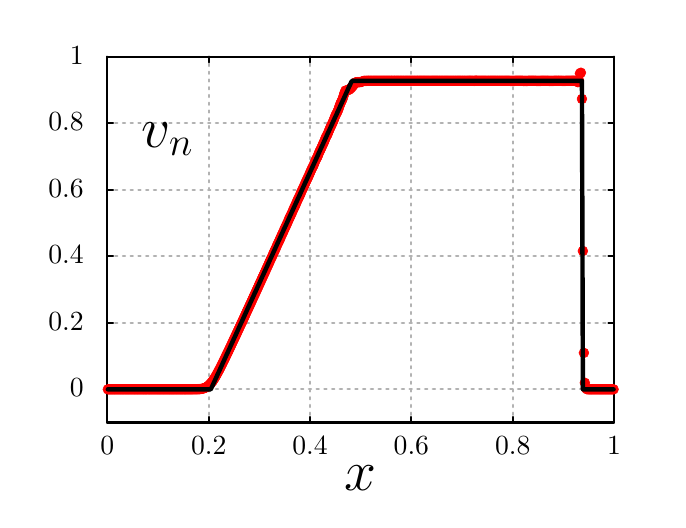
\begin{tikzpicture}[gnuplot]
%% generated with GNUPLOT 4.6p4 (Lua 5.1; terminal rev. 99, script rev. 100)
%% Mon 04 Aug 2014 12:05:06 PM EDT
\path (0.000,0.000) rectangle (8.000,6.000);
\gpfill{rgb color={1.000,1.000,1.000}} (1.012,0.985)--(7.446,0.985)--(7.446,5.630)--(1.012,5.630)--cycle;
\gpcolor{color=gp lt color border}
\gpsetlinetype{gp lt border}
\gpsetlinewidth{1.00}
\draw[gp path] (1.012,0.985)--(1.012,5.630)--(7.446,5.630)--(7.446,0.985)--cycle;
\gpcolor{color=gp lt color axes}
\gpsetlinetype{gp lt axes}
\gpsetlinewidth{2.00}
\draw[gp path] (1.012,1.407)--(7.447,1.407);
\gpcolor{color=gp lt color border}
\gpsetlinetype{gp lt border}
\draw[gp path] (1.012,1.407)--(1.084,1.407);
\draw[gp path] (7.447,1.407)--(7.375,1.407);
\gpcolor{rgb color={0.000,0.000,0.000}}
\node[gp node right,font={\fontsize{10pt}{12pt}\selectfont}] at (0.828,1.407) {0};
\gpcolor{color=gp lt color axes}
\gpsetlinetype{gp lt axes}
\draw[gp path] (1.012,2.252)--(7.447,2.252);
\gpcolor{color=gp lt color border}
\gpsetlinetype{gp lt border}
\draw[gp path] (1.012,2.252)--(1.084,2.252);
\draw[gp path] (7.447,2.252)--(7.375,2.252);
\gpcolor{rgb color={0.000,0.000,0.000}}
\node[gp node right,font={\fontsize{10pt}{12pt}\selectfont}] at (0.828,2.252) {0.2};
\gpcolor{color=gp lt color axes}
\gpsetlinetype{gp lt axes}
\draw[gp path] (1.012,3.097)--(7.447,3.097);
\gpcolor{color=gp lt color border}
\gpsetlinetype{gp lt border}
\draw[gp path] (1.012,3.097)--(1.084,3.097);
\draw[gp path] (7.447,3.097)--(7.375,3.097);
\gpcolor{rgb color={0.000,0.000,0.000}}
\node[gp node right,font={\fontsize{10pt}{12pt}\selectfont}] at (0.828,3.097) {0.4};
\gpcolor{color=gp lt color axes}
\gpsetlinetype{gp lt axes}
\draw[gp path] (1.012,3.942)--(7.447,3.942);
\gpcolor{color=gp lt color border}
\gpsetlinetype{gp lt border}
\draw[gp path] (1.012,3.942)--(1.084,3.942);
\draw[gp path] (7.447,3.942)--(7.375,3.942);
\gpcolor{rgb color={0.000,0.000,0.000}}
\node[gp node right,font={\fontsize{10pt}{12pt}\selectfont}] at (0.828,3.942) {0.6};
\gpcolor{color=gp lt color axes}
\gpsetlinetype{gp lt axes}
\draw[gp path] (1.012,4.786)--(7.447,4.786);
\gpcolor{color=gp lt color border}
\gpsetlinetype{gp lt border}
\draw[gp path] (1.012,4.786)--(1.084,4.786);
\draw[gp path] (7.447,4.786)--(7.375,4.786);
\gpcolor{rgb color={0.000,0.000,0.000}}
\node[gp node right,font={\fontsize{10pt}{12pt}\selectfont}] at (0.828,4.786) {0.8};
\gpcolor{color=gp lt color axes}
\gpsetlinetype{gp lt axes}
\draw[gp path] (1.012,5.631)--(7.447,5.631);
\gpcolor{color=gp lt color border}
\gpsetlinetype{gp lt border}
\draw[gp path] (1.012,5.631)--(1.084,5.631);
\draw[gp path] (7.447,5.631)--(7.375,5.631);
\gpcolor{rgb color={0.000,0.000,0.000}}
\node[gp node right,font={\fontsize{10pt}{12pt}\selectfont}] at (0.828,5.631) {1};
\gpcolor{color=gp lt color axes}
\gpsetlinetype{gp lt axes}
\draw[gp path] (1.012,0.985)--(1.012,5.631);
\gpcolor{color=gp lt color border}
\gpsetlinetype{gp lt border}
\draw[gp path] (1.012,0.985)--(1.012,1.057);
\draw[gp path] (1.012,5.631)--(1.012,5.559);
\gpcolor{rgb color={0.000,0.000,0.000}}
\node[gp node center,font={\fontsize{10pt}{12pt}\selectfont}] at (1.012,0.677) {0};
\gpcolor{color=gp lt color axes}
\gpsetlinetype{gp lt axes}
\draw[gp path] (2.299,0.985)--(2.299,5.631);
\gpcolor{color=gp lt color border}
\gpsetlinetype{gp lt border}
\draw[gp path] (2.299,0.985)--(2.299,1.057);
\draw[gp path] (2.299,5.631)--(2.299,5.559);
\gpcolor{rgb color={0.000,0.000,0.000}}
\node[gp node center,font={\fontsize{10pt}{12pt}\selectfont}] at (2.299,0.677) {0.2};
\gpcolor{color=gp lt color axes}
\gpsetlinetype{gp lt axes}
\draw[gp path] (3.586,0.985)--(3.586,5.631);
\gpcolor{color=gp lt color border}
\gpsetlinetype{gp lt border}
\draw[gp path] (3.586,0.985)--(3.586,1.057);
\draw[gp path] (3.586,5.631)--(3.586,5.559);
\gpcolor{rgb color={0.000,0.000,0.000}}
\node[gp node center,font={\fontsize{10pt}{12pt}\selectfont}] at (3.586,0.677) {0.4};
\gpcolor{color=gp lt color axes}
\gpsetlinetype{gp lt axes}
\draw[gp path] (4.873,0.985)--(4.873,5.631);
\gpcolor{color=gp lt color border}
\gpsetlinetype{gp lt border}
\draw[gp path] (4.873,0.985)--(4.873,1.057);
\draw[gp path] (4.873,5.631)--(4.873,5.559);
\gpcolor{rgb color={0.000,0.000,0.000}}
\node[gp node center,font={\fontsize{10pt}{12pt}\selectfont}] at (4.873,0.677) {0.6};
\gpcolor{color=gp lt color axes}
\gpsetlinetype{gp lt axes}
\draw[gp path] (6.160,0.985)--(6.160,5.631);
\gpcolor{color=gp lt color border}
\gpsetlinetype{gp lt border}
\draw[gp path] (6.160,0.985)--(6.160,1.057);
\draw[gp path] (6.160,5.631)--(6.160,5.559);
\gpcolor{rgb color={0.000,0.000,0.000}}
\node[gp node center,font={\fontsize{10pt}{12pt}\selectfont}] at (6.160,0.677) {0.8};
\gpcolor{color=gp lt color axes}
\gpsetlinetype{gp lt axes}
\draw[gp path] (7.447,0.985)--(7.447,5.631);
\gpcolor{color=gp lt color border}
\gpsetlinetype{gp lt border}
\draw[gp path] (7.447,0.985)--(7.447,1.057);
\draw[gp path] (7.447,5.631)--(7.447,5.559);
\gpcolor{rgb color={0.000,0.000,0.000}}
\node[gp node center,font={\fontsize{10pt}{12pt}\selectfont}] at (7.447,0.677) {1};
\gpcolor{color=gp lt color border}
\draw[gp path] (1.012,5.631)--(1.012,0.985)--(7.447,0.985)--(7.447,5.631)--cycle;
\gpcolor{rgb color={0.000,0.000,0.000}}
\node[gp node center,font={\fontsize{10pt}{12pt}\selectfont}] at (4.229,0.215) {\huge $x$};
\gpcolor{rgb color={1.000,0.000,0.000}}
\gpsetlinewidth{0.50}
\gpsetpointsize{4.44}
\gppoint{gp mark 7}{(1.018,1.407)}
\gppoint{gp mark 7}{(1.031,1.407)}
\gppoint{gp mark 7}{(1.043,1.407)}
\gppoint{gp mark 7}{(1.056,1.407)}
\gppoint{gp mark 7}{(1.069,1.407)}
\gppoint{gp mark 7}{(1.081,1.407)}
\gppoint{gp mark 7}{(1.094,1.407)}
\gppoint{gp mark 7}{(1.106,1.407)}
\gppoint{gp mark 7}{(1.119,1.407)}
\gppoint{gp mark 7}{(1.131,1.407)}
\gppoint{gp mark 7}{(1.144,1.407)}
\gppoint{gp mark 7}{(1.157,1.407)}
\gppoint{gp mark 7}{(1.169,1.407)}
\gppoint{gp mark 7}{(1.182,1.407)}
\gppoint{gp mark 7}{(1.194,1.407)}
\gppoint{gp mark 7}{(1.207,1.407)}
\gppoint{gp mark 7}{(1.219,1.407)}
\gppoint{gp mark 7}{(1.232,1.407)}
\gppoint{gp mark 7}{(1.245,1.407)}
\gppoint{gp mark 7}{(1.257,1.407)}
\gppoint{gp mark 7}{(1.270,1.407)}
\gppoint{gp mark 7}{(1.282,1.407)}
\gppoint{gp mark 7}{(1.295,1.407)}
\gppoint{gp mark 7}{(1.307,1.407)}
\gppoint{gp mark 7}{(1.320,1.407)}
\gppoint{gp mark 7}{(1.332,1.407)}
\gppoint{gp mark 7}{(1.345,1.407)}
\gppoint{gp mark 7}{(1.358,1.407)}
\gppoint{gp mark 7}{(1.370,1.407)}
\gppoint{gp mark 7}{(1.383,1.407)}
\gppoint{gp mark 7}{(1.395,1.407)}
\gppoint{gp mark 7}{(1.408,1.407)}
\gppoint{gp mark 7}{(1.420,1.407)}
\gppoint{gp mark 7}{(1.433,1.407)}
\gppoint{gp mark 7}{(1.446,1.407)}
\gppoint{gp mark 7}{(1.458,1.407)}
\gppoint{gp mark 7}{(1.471,1.407)}
\gppoint{gp mark 7}{(1.483,1.407)}
\gppoint{gp mark 7}{(1.496,1.407)}
\gppoint{gp mark 7}{(1.508,1.407)}
\gppoint{gp mark 7}{(1.521,1.407)}
\gppoint{gp mark 7}{(1.534,1.407)}
\gppoint{gp mark 7}{(1.546,1.407)}
\gppoint{gp mark 7}{(1.559,1.407)}
\gppoint{gp mark 7}{(1.571,1.407)}
\gppoint{gp mark 7}{(1.584,1.407)}
\gppoint{gp mark 7}{(1.596,1.407)}
\gppoint{gp mark 7}{(1.609,1.407)}
\gppoint{gp mark 7}{(1.622,1.407)}
\gppoint{gp mark 7}{(1.634,1.407)}
\gppoint{gp mark 7}{(1.647,1.407)}
\gppoint{gp mark 7}{(1.659,1.407)}
\gppoint{gp mark 7}{(1.672,1.407)}
\gppoint{gp mark 7}{(1.684,1.407)}
\gppoint{gp mark 7}{(1.697,1.407)}
\gppoint{gp mark 7}{(1.710,1.407)}
\gppoint{gp mark 7}{(1.722,1.407)}
\gppoint{gp mark 7}{(1.735,1.407)}
\gppoint{gp mark 7}{(1.747,1.407)}
\gppoint{gp mark 7}{(1.760,1.407)}
\gppoint{gp mark 7}{(1.772,1.407)}
\gppoint{gp mark 7}{(1.785,1.407)}
\gppoint{gp mark 7}{(1.798,1.407)}
\gppoint{gp mark 7}{(1.810,1.407)}
\gppoint{gp mark 7}{(1.823,1.407)}
\gppoint{gp mark 7}{(1.835,1.407)}
\gppoint{gp mark 7}{(1.848,1.407)}
\gppoint{gp mark 7}{(1.860,1.407)}
\gppoint{gp mark 7}{(1.873,1.407)}
\gppoint{gp mark 7}{(1.886,1.407)}
\gppoint{gp mark 7}{(1.898,1.407)}
\gppoint{gp mark 7}{(1.911,1.407)}
\gppoint{gp mark 7}{(1.923,1.407)}
\gppoint{gp mark 7}{(1.936,1.407)}
\gppoint{gp mark 7}{(1.948,1.407)}
\gppoint{gp mark 7}{(1.961,1.407)}
\gppoint{gp mark 7}{(1.973,1.407)}
\gppoint{gp mark 7}{(1.986,1.407)}
\gppoint{gp mark 7}{(1.999,1.407)}
\gppoint{gp mark 7}{(2.011,1.407)}
\gppoint{gp mark 7}{(2.024,1.407)}
\gppoint{gp mark 7}{(2.036,1.407)}
\gppoint{gp mark 7}{(2.049,1.407)}
\gppoint{gp mark 7}{(2.061,1.407)}
\gppoint{gp mark 7}{(2.074,1.407)}
\gppoint{gp mark 7}{(2.087,1.407)}
\gppoint{gp mark 7}{(2.099,1.408)}
\gppoint{gp mark 7}{(2.112,1.408)}
\gppoint{gp mark 7}{(2.124,1.408)}
\gppoint{gp mark 7}{(2.137,1.408)}
\gppoint{gp mark 7}{(2.149,1.408)}
\gppoint{gp mark 7}{(2.162,1.409)}
\gppoint{gp mark 7}{(2.175,1.409)}
\gppoint{gp mark 7}{(2.187,1.410)}
\gppoint{gp mark 7}{(2.200,1.412)}
\gppoint{gp mark 7}{(2.212,1.414)}
\gppoint{gp mark 7}{(2.225,1.416)}
\gppoint{gp mark 7}{(2.237,1.420)}
\gppoint{gp mark 7}{(2.250,1.424)}
\gppoint{gp mark 7}{(2.263,1.431)}
\gppoint{gp mark 7}{(2.275,1.437)}
\gppoint{gp mark 7}{(2.288,1.447)}
\gppoint{gp mark 7}{(2.300,1.456)}
\gppoint{gp mark 7}{(2.313,1.469)}
\gppoint{gp mark 7}{(2.325,1.482)}
\gppoint{gp mark 7}{(2.338,1.499)}
\gppoint{gp mark 7}{(2.351,1.514)}
\gppoint{gp mark 7}{(2.363,1.534)}
\gppoint{gp mark 7}{(2.376,1.553)}
\gppoint{gp mark 7}{(2.388,1.574)}
\gppoint{gp mark 7}{(2.401,1.596)}
\gppoint{gp mark 7}{(2.413,1.619)}
\gppoint{gp mark 7}{(2.426,1.643)}
\gppoint{gp mark 7}{(2.439,1.666)}
\gppoint{gp mark 7}{(2.451,1.691)}
\gppoint{gp mark 7}{(2.464,1.717)}
\gppoint{gp mark 7}{(2.476,1.741)}
\gppoint{gp mark 7}{(2.489,1.768)}
\gppoint{gp mark 7}{(2.501,1.792)}
\gppoint{gp mark 7}{(2.514,1.819)}
\gppoint{gp mark 7}{(2.526,1.845)}
\gppoint{gp mark 7}{(2.539,1.871)}
\gppoint{gp mark 7}{(2.552,1.898)}
\gppoint{gp mark 7}{(2.564,1.924)}
\gppoint{gp mark 7}{(2.577,1.950)}
\gppoint{gp mark 7}{(2.589,1.978)}
\gppoint{gp mark 7}{(2.602,2.004)}
\gppoint{gp mark 7}{(2.614,2.031)}
\gppoint{gp mark 7}{(2.627,2.058)}
\gppoint{gp mark 7}{(2.640,2.085)}
\gppoint{gp mark 7}{(2.652,2.111)}
\gppoint{gp mark 7}{(2.665,2.139)}
\gppoint{gp mark 7}{(2.677,2.165)}
\gppoint{gp mark 7}{(2.690,2.192)}
\gppoint{gp mark 7}{(2.702,2.220)}
\gppoint{gp mark 7}{(2.715,2.246)}
\gppoint{gp mark 7}{(2.728,2.273)}
\gppoint{gp mark 7}{(2.740,2.301)}
\gppoint{gp mark 7}{(2.753,2.327)}
\gppoint{gp mark 7}{(2.765,2.355)}
\gppoint{gp mark 7}{(2.778,2.383)}
\gppoint{gp mark 7}{(2.790,2.410)}
\gppoint{gp mark 7}{(2.803,2.436)}
\gppoint{gp mark 7}{(2.816,2.465)}
\gppoint{gp mark 7}{(2.828,2.491)}
\gppoint{gp mark 7}{(2.841,2.518)}
\gppoint{gp mark 7}{(2.853,2.546)}
\gppoint{gp mark 7}{(2.866,2.574)}
\gppoint{gp mark 7}{(2.878,2.600)}
\gppoint{gp mark 7}{(2.891,2.628)}
\gppoint{gp mark 7}{(2.904,2.656)}
\gppoint{gp mark 7}{(2.916,2.683)}
\gppoint{gp mark 7}{(2.929,2.710)}
\gppoint{gp mark 7}{(2.941,2.739)}
\gppoint{gp mark 7}{(2.954,2.765)}
\gppoint{gp mark 7}{(2.966,2.792)}
\gppoint{gp mark 7}{(2.979,2.821)}
\gppoint{gp mark 7}{(2.992,2.849)}
\gppoint{gp mark 7}{(3.004,2.875)}
\gppoint{gp mark 7}{(3.017,2.903)}
\gppoint{gp mark 7}{(3.029,2.931)}
\gppoint{gp mark 7}{(3.042,2.959)}
\gppoint{gp mark 7}{(3.054,2.984)}
\gppoint{gp mark 7}{(3.067,3.014)}
\gppoint{gp mark 7}{(3.079,3.042)}
\gppoint{gp mark 7}{(3.092,3.069)}
\gppoint{gp mark 7}{(3.105,3.095)}
\gppoint{gp mark 7}{(3.117,3.125)}
\gppoint{gp mark 7}{(3.130,3.152)}
\gppoint{gp mark 7}{(3.142,3.179)}
\gppoint{gp mark 7}{(3.155,3.206)}
\gppoint{gp mark 7}{(3.167,3.236)}
\gppoint{gp mark 7}{(3.180,3.263)}
\gppoint{gp mark 7}{(3.193,3.289)}
\gppoint{gp mark 7}{(3.205,3.317)}
\gppoint{gp mark 7}{(3.218,3.346)}
\gppoint{gp mark 7}{(3.230,3.374)}
\gppoint{gp mark 7}{(3.243,3.399)}
\gppoint{gp mark 7}{(3.255,3.428)}
\gppoint{gp mark 7}{(3.268,3.458)}
\gppoint{gp mark 7}{(3.281,3.484)}
\gppoint{gp mark 7}{(3.293,3.510)}
\gppoint{gp mark 7}{(3.306,3.538)}
\gppoint{gp mark 7}{(3.318,3.569)}
\gppoint{gp mark 7}{(3.331,3.595)}
\gppoint{gp mark 7}{(3.343,3.621)}
\gppoint{gp mark 7}{(3.356,3.648)}
\gppoint{gp mark 7}{(3.369,3.679)}
\gppoint{gp mark 7}{(3.381,3.706)}
\gppoint{gp mark 7}{(3.394,3.732)}
\gppoint{gp mark 7}{(3.406,3.759)}
\gppoint{gp mark 7}{(3.419,3.790)}
\gppoint{gp mark 7}{(3.431,3.818)}
\gppoint{gp mark 7}{(3.444,3.843)}
\gppoint{gp mark 7}{(3.457,3.870)}
\gppoint{gp mark 7}{(3.469,3.899)}
\gppoint{gp mark 7}{(3.482,3.929)}
\gppoint{gp mark 7}{(3.494,3.955)}
\gppoint{gp mark 7}{(3.507,3.980)}
\gppoint{gp mark 7}{(3.519,4.009)}
\gppoint{gp mark 7}{(3.532,4.039)}
\gppoint{gp mark 7}{(3.545,4.067)}
\gppoint{gp mark 7}{(3.557,4.092)}
\gppoint{gp mark 7}{(3.570,4.119)}
\gppoint{gp mark 7}{(3.582,4.148)}
\gppoint{gp mark 7}{(3.595,4.178)}
\gppoint{gp mark 7}{(3.607,4.205)}
\gppoint{gp mark 7}{(3.620,4.231)}
\gppoint{gp mark 7}{(3.633,4.256)}
\gppoint{gp mark 7}{(3.645,4.288)}
\gppoint{gp mark 7}{(3.658,4.319)}
\gppoint{gp mark 7}{(3.670,4.342)}
\gppoint{gp mark 7}{(3.683,4.366)}
\gppoint{gp mark 7}{(3.695,4.399)}
\gppoint{gp mark 7}{(3.708,4.430)}
\gppoint{gp mark 7}{(3.720,4.453)}
\gppoint{gp mark 7}{(3.733,4.481)}
\gppoint{gp mark 7}{(3.746,4.511)}
\gppoint{gp mark 7}{(3.758,4.536)}
\gppoint{gp mark 7}{(3.771,4.566)}
\gppoint{gp mark 7}{(3.783,4.599)}
\gppoint{gp mark 7}{(3.796,4.624)}
\gppoint{gp mark 7}{(3.808,4.646)}
\gppoint{gp mark 7}{(3.821,4.678)}
\gppoint{gp mark 7}{(3.834,4.710)}
\gppoint{gp mark 7}{(3.846,4.738)}
\gppoint{gp mark 7}{(3.859,4.764)}
\gppoint{gp mark 7}{(3.871,4.790)}
\gppoint{gp mark 7}{(3.884,4.819)}
\gppoint{gp mark 7}{(3.896,4.852)}
\gppoint{gp mark 7}{(3.909,4.885)}
\gppoint{gp mark 7}{(3.922,4.909)}
\gppoint{gp mark 7}{(3.934,4.933)}
\gppoint{gp mark 7}{(3.947,4.964)}
\gppoint{gp mark 7}{(3.959,5.002)}
\gppoint{gp mark 7}{(3.972,5.036)}
\gppoint{gp mark 7}{(3.984,5.062)}
\gppoint{gp mark 7}{(3.997,5.089)}
\gppoint{gp mark 7}{(4.010,5.129)}
\gppoint{gp mark 7}{(4.022,5.169)}
\gppoint{gp mark 7}{(4.035,5.200)}
\gppoint{gp mark 7}{(4.047,5.203)}
\gppoint{gp mark 7}{(4.060,5.204)}
\gppoint{gp mark 7}{(4.072,5.208)}
\gppoint{gp mark 7}{(4.085,5.214)}
\gppoint{gp mark 7}{(4.098,5.226)}
\gppoint{gp mark 7}{(4.110,5.238)}
\gppoint{gp mark 7}{(4.123,5.252)}
\gppoint{gp mark 7}{(4.135,5.267)}
\gppoint{gp mark 7}{(4.148,5.285)}
\gppoint{gp mark 7}{(4.160,5.303)}
\gppoint{gp mark 7}{(4.173,5.307)}
\gppoint{gp mark 7}{(4.186,5.308)}
\gppoint{gp mark 7}{(4.198,5.308)}
\gppoint{gp mark 7}{(4.211,5.308)}
\gppoint{gp mark 7}{(4.223,5.309)}
\gppoint{gp mark 7}{(4.236,5.311)}
\gppoint{gp mark 7}{(4.248,5.316)}
\gppoint{gp mark 7}{(4.261,5.322)}
\gppoint{gp mark 7}{(4.273,5.324)}
\gppoint{gp mark 7}{(4.286,5.324)}
\gppoint{gp mark 7}{(4.299,5.324)}
\gppoint{gp mark 7}{(4.311,5.325)}
\gppoint{gp mark 7}{(4.324,5.325)}
\gppoint{gp mark 7}{(4.336,5.325)}
\gppoint{gp mark 7}{(4.349,5.325)}
\gppoint{gp mark 7}{(4.361,5.325)}
\gppoint{gp mark 7}{(4.374,5.325)}
\gppoint{gp mark 7}{(4.387,5.325)}
\gppoint{gp mark 7}{(4.399,5.325)}
\gppoint{gp mark 7}{(4.412,5.325)}
\gppoint{gp mark 7}{(4.424,5.325)}
\gppoint{gp mark 7}{(4.437,5.325)}
\gppoint{gp mark 7}{(4.449,5.325)}
\gppoint{gp mark 7}{(4.462,5.325)}
\gppoint{gp mark 7}{(4.475,5.325)}
\gppoint{gp mark 7}{(4.487,5.325)}
\gppoint{gp mark 7}{(4.500,5.325)}
\gppoint{gp mark 7}{(4.512,5.325)}
\gppoint{gp mark 7}{(4.525,5.325)}
\gppoint{gp mark 7}{(4.537,5.325)}
\gppoint{gp mark 7}{(4.550,5.325)}
\gppoint{gp mark 7}{(4.563,5.325)}
\gppoint{gp mark 7}{(4.575,5.325)}
\gppoint{gp mark 7}{(4.588,5.325)}
\gppoint{gp mark 7}{(4.600,5.325)}
\gppoint{gp mark 7}{(4.613,5.325)}
\gppoint{gp mark 7}{(4.625,5.325)}
\gppoint{gp mark 7}{(4.638,5.325)}
\gppoint{gp mark 7}{(4.651,5.325)}
\gppoint{gp mark 7}{(4.663,5.325)}
\gppoint{gp mark 7}{(4.676,5.325)}
\gppoint{gp mark 7}{(4.688,5.325)}
\gppoint{gp mark 7}{(4.701,5.325)}
\gppoint{gp mark 7}{(4.713,5.325)}
\gppoint{gp mark 7}{(4.726,5.325)}
\gppoint{gp mark 7}{(4.739,5.325)}
\gppoint{gp mark 7}{(4.751,5.325)}
\gppoint{gp mark 7}{(4.764,5.325)}
\gppoint{gp mark 7}{(4.776,5.325)}
\gppoint{gp mark 7}{(4.789,5.325)}
\gppoint{gp mark 7}{(4.801,5.325)}
\gppoint{gp mark 7}{(4.814,5.325)}
\gppoint{gp mark 7}{(4.826,5.325)}
\gppoint{gp mark 7}{(4.839,5.325)}
\gppoint{gp mark 7}{(4.852,5.325)}
\gppoint{gp mark 7}{(4.864,5.325)}
\gppoint{gp mark 7}{(4.877,5.325)}
\gppoint{gp mark 7}{(4.889,5.325)}
\gppoint{gp mark 7}{(4.902,5.325)}
\gppoint{gp mark 7}{(4.914,5.325)}
\gppoint{gp mark 7}{(4.927,5.325)}
\gppoint{gp mark 7}{(4.940,5.325)}
\gppoint{gp mark 7}{(4.952,5.325)}
\gppoint{gp mark 7}{(4.965,5.325)}
\gppoint{gp mark 7}{(4.977,5.325)}
\gppoint{gp mark 7}{(4.990,5.325)}
\gppoint{gp mark 7}{(5.002,5.325)}
\gppoint{gp mark 7}{(5.015,5.325)}
\gppoint{gp mark 7}{(5.028,5.325)}
\gppoint{gp mark 7}{(5.040,5.325)}
\gppoint{gp mark 7}{(5.053,5.325)}
\gppoint{gp mark 7}{(5.065,5.325)}
\gppoint{gp mark 7}{(5.078,5.325)}
\gppoint{gp mark 7}{(5.090,5.325)}
\gppoint{gp mark 7}{(5.103,5.325)}
\gppoint{gp mark 7}{(5.116,5.325)}
\gppoint{gp mark 7}{(5.128,5.325)}
\gppoint{gp mark 7}{(5.141,5.325)}
\gppoint{gp mark 7}{(5.153,5.325)}
\gppoint{gp mark 7}{(5.166,5.325)}
\gppoint{gp mark 7}{(5.178,5.325)}
\gppoint{gp mark 7}{(5.191,5.325)}
\gppoint{gp mark 7}{(5.204,5.325)}
\gppoint{gp mark 7}{(5.216,5.325)}
\gppoint{gp mark 7}{(5.229,5.325)}
\gppoint{gp mark 7}{(5.241,5.325)}
\gppoint{gp mark 7}{(5.254,5.325)}
\gppoint{gp mark 7}{(5.266,5.325)}
\gppoint{gp mark 7}{(5.279,5.325)}
\gppoint{gp mark 7}{(5.292,5.325)}
\gppoint{gp mark 7}{(5.304,5.325)}
\gppoint{gp mark 7}{(5.317,5.325)}
\gppoint{gp mark 7}{(5.329,5.325)}
\gppoint{gp mark 7}{(5.342,5.325)}
\gppoint{gp mark 7}{(5.354,5.325)}
\gppoint{gp mark 7}{(5.367,5.325)}
\gppoint{gp mark 7}{(5.380,5.325)}
\gppoint{gp mark 7}{(5.392,5.325)}
\gppoint{gp mark 7}{(5.405,5.325)}
\gppoint{gp mark 7}{(5.417,5.325)}
\gppoint{gp mark 7}{(5.430,5.325)}
\gppoint{gp mark 7}{(5.442,5.325)}
\gppoint{gp mark 7}{(5.455,5.325)}
\gppoint{gp mark 7}{(5.467,5.325)}
\gppoint{gp mark 7}{(5.480,5.325)}
\gppoint{gp mark 7}{(5.493,5.325)}
\gppoint{gp mark 7}{(5.505,5.325)}
\gppoint{gp mark 7}{(5.518,5.325)}
\gppoint{gp mark 7}{(5.530,5.325)}
\gppoint{gp mark 7}{(5.543,5.325)}
\gppoint{gp mark 7}{(5.555,5.325)}
\gppoint{gp mark 7}{(5.568,5.325)}
\gppoint{gp mark 7}{(5.581,5.325)}
\gppoint{gp mark 7}{(5.593,5.325)}
\gppoint{gp mark 7}{(5.606,5.325)}
\gppoint{gp mark 7}{(5.618,5.326)}
\gppoint{gp mark 7}{(5.631,5.325)}
\gppoint{gp mark 7}{(5.643,5.325)}
\gppoint{gp mark 7}{(5.656,5.325)}
\gppoint{gp mark 7}{(5.669,5.324)}
\gppoint{gp mark 7}{(5.681,5.326)}
\gppoint{gp mark 7}{(5.694,5.327)}
\gppoint{gp mark 7}{(5.706,5.325)}
\gppoint{gp mark 7}{(5.719,5.325)}
\gppoint{gp mark 7}{(5.731,5.325)}
\gppoint{gp mark 7}{(5.744,5.325)}
\gppoint{gp mark 7}{(5.757,5.325)}
\gppoint{gp mark 7}{(5.769,5.325)}
\gppoint{gp mark 7}{(5.782,5.325)}
\gppoint{gp mark 7}{(5.794,5.325)}
\gppoint{gp mark 7}{(5.807,5.325)}
\gppoint{gp mark 7}{(5.819,5.325)}
\gppoint{gp mark 7}{(5.832,5.325)}
\gppoint{gp mark 7}{(5.845,5.325)}
\gppoint{gp mark 7}{(5.857,5.325)}
\gppoint{gp mark 7}{(5.870,5.325)}
\gppoint{gp mark 7}{(5.882,5.325)}
\gppoint{gp mark 7}{(5.895,5.325)}
\gppoint{gp mark 7}{(5.907,5.325)}
\gppoint{gp mark 7}{(5.920,5.325)}
\gppoint{gp mark 7}{(5.933,5.325)}
\gppoint{gp mark 7}{(5.945,5.325)}
\gppoint{gp mark 7}{(5.958,5.325)}
\gppoint{gp mark 7}{(5.970,5.325)}
\gppoint{gp mark 7}{(5.983,5.325)}
\gppoint{gp mark 7}{(5.995,5.325)}
\gppoint{gp mark 7}{(6.008,5.325)}
\gppoint{gp mark 7}{(6.020,5.325)}
\gppoint{gp mark 7}{(6.033,5.325)}
\gppoint{gp mark 7}{(6.046,5.325)}
\gppoint{gp mark 7}{(6.058,5.325)}
\gppoint{gp mark 7}{(6.071,5.325)}
\gppoint{gp mark 7}{(6.083,5.325)}
\gppoint{gp mark 7}{(6.096,5.325)}
\gppoint{gp mark 7}{(6.108,5.325)}
\gppoint{gp mark 7}{(6.121,5.325)}
\gppoint{gp mark 7}{(6.134,5.324)}
\gppoint{gp mark 7}{(6.146,5.324)}
\gppoint{gp mark 7}{(6.159,5.324)}
\gppoint{gp mark 7}{(6.171,5.324)}
\gppoint{gp mark 7}{(6.184,5.324)}
\gppoint{gp mark 7}{(6.196,5.325)}
\gppoint{gp mark 7}{(6.209,5.325)}
\gppoint{gp mark 7}{(6.222,5.325)}
\gppoint{gp mark 7}{(6.234,5.325)}
\gppoint{gp mark 7}{(6.247,5.325)}
\gppoint{gp mark 7}{(6.259,5.325)}
\gppoint{gp mark 7}{(6.272,5.325)}
\gppoint{gp mark 7}{(6.284,5.325)}
\gppoint{gp mark 7}{(6.297,5.324)}
\gppoint{gp mark 7}{(6.310,5.324)}
\gppoint{gp mark 7}{(6.322,5.324)}
\gppoint{gp mark 7}{(6.335,5.324)}
\gppoint{gp mark 7}{(6.347,5.324)}
\gppoint{gp mark 7}{(6.360,5.325)}
\gppoint{gp mark 7}{(6.372,5.325)}
\gppoint{gp mark 7}{(6.385,5.325)}
\gppoint{gp mark 7}{(6.398,5.325)}
\gppoint{gp mark 7}{(6.410,5.325)}
\gppoint{gp mark 7}{(6.423,5.325)}
\gppoint{gp mark 7}{(6.435,5.325)}
\gppoint{gp mark 7}{(6.448,5.325)}
\gppoint{gp mark 7}{(6.460,5.324)}
\gppoint{gp mark 7}{(6.473,5.324)}
\gppoint{gp mark 7}{(6.486,5.324)}
\gppoint{gp mark 7}{(6.498,5.324)}
\gppoint{gp mark 7}{(6.511,5.324)}
\gppoint{gp mark 7}{(6.523,5.325)}
\gppoint{gp mark 7}{(6.536,5.325)}
\gppoint{gp mark 7}{(6.548,5.325)}
\gppoint{gp mark 7}{(6.561,5.325)}
\gppoint{gp mark 7}{(6.573,5.325)}
\gppoint{gp mark 7}{(6.586,5.325)}
\gppoint{gp mark 7}{(6.599,5.325)}
\gppoint{gp mark 7}{(6.611,5.325)}
\gppoint{gp mark 7}{(6.624,5.324)}
\gppoint{gp mark 7}{(6.636,5.324)}
\gppoint{gp mark 7}{(6.649,5.324)}
\gppoint{gp mark 7}{(6.661,5.324)}
\gppoint{gp mark 7}{(6.674,5.324)}
\gppoint{gp mark 7}{(6.687,5.325)}
\gppoint{gp mark 7}{(6.699,5.325)}
\gppoint{gp mark 7}{(6.712,5.325)}
\gppoint{gp mark 7}{(6.724,5.325)}
\gppoint{gp mark 7}{(6.737,5.325)}
\gppoint{gp mark 7}{(6.749,5.325)}
\gppoint{gp mark 7}{(6.762,5.325)}
\gppoint{gp mark 7}{(6.775,5.325)}
\gppoint{gp mark 7}{(6.787,5.324)}
\gppoint{gp mark 7}{(6.800,5.324)}
\gppoint{gp mark 7}{(6.812,5.324)}
\gppoint{gp mark 7}{(6.825,5.324)}
\gppoint{gp mark 7}{(6.837,5.325)}
\gppoint{gp mark 7}{(6.850,5.325)}
\gppoint{gp mark 7}{(6.863,5.325)}
\gppoint{gp mark 7}{(6.875,5.325)}
\gppoint{gp mark 7}{(6.888,5.325)}
\gppoint{gp mark 7}{(6.900,5.325)}
\gppoint{gp mark 7}{(6.913,5.326)}
\gppoint{gp mark 7}{(6.925,5.326)}
\gppoint{gp mark 7}{(6.938,5.326)}
\gppoint{gp mark 7}{(6.951,5.325)}
\gppoint{gp mark 7}{(6.963,5.322)}
\gppoint{gp mark 7}{(6.976,5.315)}
\gppoint{gp mark 7}{(6.988,5.308)}
\gppoint{gp mark 7}{(7.001,5.334)}
\gppoint{gp mark 7}{(7.013,5.418)}
\gppoint{gp mark 7}{(7.026,5.428)}
\gppoint{gp mark 7}{(7.039,5.095)}
\gppoint{gp mark 7}{(7.051,3.164)}
\gppoint{gp mark 7}{(7.064,1.870)}
\gppoint{gp mark 7}{(7.076,1.490)}
\gppoint{gp mark 7}{(7.089,1.421)}
\gppoint{gp mark 7}{(7.101,1.409)}
\gppoint{gp mark 7}{(7.114,1.408)}
\gppoint{gp mark 7}{(7.127,1.407)}
\gppoint{gp mark 7}{(7.139,1.407)}
\gppoint{gp mark 7}{(7.152,1.407)}
\gppoint{gp mark 7}{(7.164,1.407)}
\gppoint{gp mark 7}{(7.177,1.407)}
\gppoint{gp mark 7}{(7.189,1.407)}
\gppoint{gp mark 7}{(7.202,1.407)}
\gppoint{gp mark 7}{(7.214,1.407)}
\gppoint{gp mark 7}{(7.227,1.407)}
\gppoint{gp mark 7}{(7.240,1.407)}
\gppoint{gp mark 7}{(7.252,1.407)}
\gppoint{gp mark 7}{(7.265,1.407)}
\gppoint{gp mark 7}{(7.277,1.407)}
\gppoint{gp mark 7}{(7.290,1.407)}
\gppoint{gp mark 7}{(7.302,1.407)}
\gppoint{gp mark 7}{(7.315,1.407)}
\gppoint{gp mark 7}{(7.328,1.407)}
\gppoint{gp mark 7}{(7.340,1.407)}
\gppoint{gp mark 7}{(7.353,1.407)}
\gppoint{gp mark 7}{(7.365,1.407)}
\gppoint{gp mark 7}{(7.378,1.407)}
\gppoint{gp mark 7}{(7.390,1.407)}
\gppoint{gp mark 7}{(7.403,1.407)}
\gppoint{gp mark 7}{(7.416,1.407)}
\gppoint{gp mark 7}{(7.428,1.407)}
\gppoint{gp mark 7}{(7.441,1.407)}
\gpcolor{rgb color={0.000,0.000,0.000}}
\gpsetlinetype{gp lt plot 0}
\gpsetlinewidth{4.00}
\draw[gp path] (1.018,1.407)--(1.031,1.407)--(1.043,1.407)--(1.056,1.407)--(1.069,1.407)%
  --(1.081,1.407)--(1.094,1.407)--(1.106,1.407)--(1.119,1.407)--(1.131,1.407)--(1.144,1.407)%
  --(1.157,1.407)--(1.169,1.407)--(1.182,1.407)--(1.194,1.407)--(1.207,1.407)--(1.219,1.407)%
  --(1.232,1.407)--(1.245,1.407)--(1.257,1.407)--(1.270,1.407)--(1.282,1.407)--(1.295,1.407)%
  --(1.307,1.407)--(1.320,1.407)--(1.332,1.407)--(1.345,1.407)--(1.358,1.407)--(1.370,1.407)%
  --(1.383,1.407)--(1.395,1.407)--(1.408,1.407)--(1.420,1.407)--(1.433,1.407)--(1.446,1.407)%
  --(1.458,1.407)--(1.471,1.407)--(1.483,1.407)--(1.496,1.407)--(1.508,1.407)--(1.521,1.407)%
  --(1.534,1.407)--(1.546,1.407)--(1.559,1.407)--(1.571,1.407)--(1.584,1.407)--(1.596,1.407)%
  --(1.609,1.407)--(1.622,1.407)--(1.634,1.407)--(1.647,1.407)--(1.659,1.407)--(1.672,1.407)%
  --(1.684,1.407)--(1.697,1.407)--(1.710,1.407)--(1.722,1.407)--(1.735,1.407)--(1.747,1.407)%
  --(1.760,1.407)--(1.772,1.407)--(1.785,1.407)--(1.798,1.407)--(1.810,1.407)--(1.823,1.407)%
  --(1.835,1.407)--(1.848,1.407)--(1.860,1.407)--(1.873,1.407)--(1.886,1.407)--(1.898,1.407)%
  --(1.911,1.407)--(1.923,1.407)--(1.936,1.407)--(1.948,1.407)--(1.961,1.407)--(1.973,1.407)%
  --(1.986,1.407)--(1.999,1.407)--(2.011,1.407)--(2.024,1.407)--(2.036,1.407)--(2.049,1.407)%
  --(2.061,1.407)--(2.074,1.407)--(2.087,1.407)--(2.099,1.407)--(2.112,1.407)--(2.124,1.407)%
  --(2.137,1.407)--(2.149,1.407)--(2.162,1.407)--(2.175,1.407)--(2.187,1.407)--(2.200,1.407)%
  --(2.212,1.407)--(2.225,1.407)--(2.237,1.407)--(2.250,1.407)--(2.263,1.407)--(2.275,1.407)%
  --(2.288,1.407)--(2.300,1.407)--(2.313,1.407)--(2.325,1.407)--(2.338,1.434)--(2.351,1.461)%
  --(2.363,1.489)--(2.376,1.516)--(2.388,1.544)--(2.401,1.571)--(2.413,1.599)--(2.426,1.626)%
  --(2.439,1.654)--(2.451,1.681)--(2.464,1.709)--(2.476,1.736)--(2.489,1.764)--(2.501,1.791)%
  --(2.514,1.818)--(2.526,1.846)--(2.539,1.873)--(2.552,1.901)--(2.564,1.928)--(2.577,1.956)%
  --(2.589,1.983)--(2.602,2.011)--(2.614,2.038)--(2.627,2.066)--(2.640,2.093)--(2.652,2.121)%
  --(2.665,2.148)--(2.677,2.176)--(2.690,2.203)--(2.702,2.231)--(2.715,2.258)--(2.728,2.286)%
  --(2.740,2.313)--(2.753,2.341)--(2.765,2.368)--(2.778,2.396)--(2.790,2.423)--(2.803,2.451)%
  --(2.816,2.478)--(2.828,2.506)--(2.841,2.533)--(2.853,2.561)--(2.866,2.588)--(2.878,2.616)%
  --(2.891,2.643)--(2.904,2.671)--(2.916,2.698)--(2.929,2.726)--(2.941,2.753)--(2.954,2.781)%
  --(2.966,2.808)--(2.979,2.836)--(2.992,2.863)--(3.004,2.891)--(3.017,2.918)--(3.029,2.946)%
  --(3.042,2.973)--(3.054,3.001)--(3.067,3.028)--(3.079,3.056)--(3.092,3.083)--(3.105,3.111)%
  --(3.117,3.138)--(3.130,3.166)--(3.142,3.193)--(3.155,3.221)--(3.167,3.248)--(3.180,3.276)%
  --(3.193,3.303)--(3.205,3.331)--(3.218,3.358)--(3.230,3.386)--(3.243,3.413)--(3.255,3.441)%
  --(3.268,3.468)--(3.281,3.496)--(3.293,3.523)--(3.306,3.551)--(3.318,3.578)--(3.331,3.606)%
  --(3.343,3.633)--(3.356,3.661)--(3.369,3.688)--(3.381,3.716)--(3.394,3.743)--(3.406,3.771)%
  --(3.419,3.798)--(3.431,3.826)--(3.444,3.853)--(3.457,3.881)--(3.469,3.908)--(3.482,3.936)%
  --(3.494,3.963)--(3.507,3.991)--(3.519,4.018)--(3.532,4.046)--(3.545,4.073)--(3.557,4.101)%
  --(3.570,4.128)--(3.582,4.156)--(3.595,4.183)--(3.607,4.211)--(3.620,4.238)--(3.633,4.266)%
  --(3.645,4.293)--(3.658,4.321)--(3.670,4.348)--(3.683,4.376)--(3.695,4.403)--(3.708,4.431)%
  --(3.720,4.458)--(3.733,4.486)--(3.746,4.513)--(3.758,4.541)--(3.771,4.568)--(3.783,4.596)%
  --(3.796,4.623)--(3.808,4.651)--(3.821,4.678)--(3.834,4.706)--(3.846,4.733)--(3.859,4.761)%
  --(3.871,4.788)--(3.884,4.816)--(3.896,4.843)--(3.909,4.871)--(3.922,4.898)--(3.934,4.926)%
  --(3.947,4.953)--(3.959,4.981)--(3.972,5.008)--(3.984,5.036)--(3.997,5.063)--(4.010,5.091)%
  --(4.022,5.118)--(4.035,5.146)--(4.047,5.173)--(4.060,5.201)--(4.072,5.228)--(4.085,5.256)%
  --(4.098,5.283)--(4.110,5.311)--(4.123,5.325)--(4.135,5.325)--(4.148,5.325)--(4.160,5.325)%
  --(4.173,5.325)--(4.186,5.325)--(4.198,5.325)--(4.211,5.325)--(4.223,5.325)--(4.236,5.325)%
  --(4.248,5.325)--(4.261,5.325)--(4.273,5.325)--(4.286,5.325)--(4.299,5.325)--(4.311,5.325)%
  --(4.324,5.325)--(4.336,5.325)--(4.349,5.325)--(4.361,5.325)--(4.374,5.325)--(4.387,5.325)%
  --(4.399,5.325)--(4.412,5.325)--(4.424,5.325)--(4.437,5.325)--(4.449,5.325)--(4.462,5.325)%
  --(4.475,5.325)--(4.487,5.325)--(4.500,5.325)--(4.512,5.325)--(4.525,5.325)--(4.537,5.325)%
  --(4.550,5.325)--(4.563,5.325)--(4.575,5.325)--(4.588,5.325)--(4.600,5.325)--(4.613,5.325)%
  --(4.625,5.325)--(4.638,5.325)--(4.651,5.325)--(4.663,5.325)--(4.676,5.325)--(4.688,5.325)%
  --(4.701,5.325)--(4.713,5.325)--(4.726,5.325)--(4.739,5.325)--(4.751,5.325)--(4.764,5.325)%
  --(4.776,5.325)--(4.789,5.325)--(4.801,5.325)--(4.814,5.325)--(4.826,5.325)--(4.839,5.325)%
  --(4.852,5.325)--(4.864,5.325)--(4.877,5.325)--(4.889,5.325)--(4.902,5.325)--(4.914,5.325)%
  --(4.927,5.325)--(4.940,5.325)--(4.952,5.325)--(4.965,5.325)--(4.977,5.325)--(4.990,5.325)%
  --(5.002,5.325)--(5.015,5.325)--(5.028,5.325)--(5.040,5.325)--(5.053,5.325)--(5.065,5.325)%
  --(5.078,5.325)--(5.090,5.325)--(5.103,5.325)--(5.116,5.325)--(5.128,5.325)--(5.141,5.325)%
  --(5.153,5.325)--(5.166,5.325)--(5.178,5.325)--(5.191,5.325)--(5.204,5.325)--(5.216,5.325)%
  --(5.229,5.325)--(5.241,5.325)--(5.254,5.325)--(5.266,5.325)--(5.279,5.325)--(5.292,5.325)%
  --(5.304,5.325)--(5.317,5.325)--(5.329,5.325)--(5.342,5.325)--(5.354,5.325)--(5.367,5.325)%
  --(5.380,5.325)--(5.392,5.325)--(5.405,5.325)--(5.417,5.325)--(5.430,5.325)--(5.442,5.325)%
  --(5.455,5.325)--(5.467,5.325)--(5.480,5.325)--(5.493,5.325)--(5.505,5.325)--(5.518,5.325)%
  --(5.530,5.325)--(5.543,5.325)--(5.555,5.325)--(5.568,5.325)--(5.581,5.325)--(5.593,5.325)%
  --(5.606,5.325)--(5.618,5.325)--(5.631,5.325)--(5.643,5.325)--(5.656,5.325)--(5.669,5.325)%
  --(5.681,5.325)--(5.694,5.325)--(5.706,5.325)--(5.719,5.325)--(5.731,5.325)--(5.744,5.325)%
  --(5.757,5.325)--(5.769,5.325)--(5.782,5.325)--(5.794,5.325)--(5.807,5.325)--(5.819,5.325)%
  --(5.832,5.325)--(5.845,5.325)--(5.857,5.325)--(5.870,5.325)--(5.882,5.325)--(5.895,5.325)%
  --(5.907,5.325)--(5.920,5.325)--(5.933,5.325)--(5.945,5.325)--(5.958,5.325)--(5.970,5.325)%
  --(5.983,5.325)--(5.995,5.325)--(6.008,5.325)--(6.020,5.325)--(6.033,5.325)--(6.046,5.325)%
  --(6.058,5.325)--(6.071,5.325)--(6.083,5.325)--(6.096,5.325)--(6.108,5.325)--(6.121,5.325)%
  --(6.134,5.325)--(6.146,5.325)--(6.159,5.325)--(6.171,5.325)--(6.184,5.325)--(6.196,5.325)%
  --(6.209,5.325)--(6.222,5.325)--(6.234,5.325)--(6.247,5.325)--(6.259,5.325)--(6.272,5.325)%
  --(6.284,5.325)--(6.297,5.325)--(6.310,5.325)--(6.322,5.325)--(6.335,5.325)--(6.347,5.325)%
  --(6.360,5.325)--(6.372,5.325)--(6.385,5.325)--(6.398,5.325)--(6.410,5.325)--(6.423,5.325)%
  --(6.435,5.325)--(6.448,5.325)--(6.460,5.325)--(6.473,5.325)--(6.486,5.325)--(6.498,5.325)%
  --(6.511,5.325)--(6.523,5.325)--(6.536,5.325)--(6.548,5.325)--(6.561,5.325)--(6.573,5.325)%
  --(6.586,5.325)--(6.599,5.325)--(6.611,5.325)--(6.624,5.325)--(6.636,5.325)--(6.649,5.325)%
  --(6.661,5.325)--(6.674,5.325)--(6.687,5.325)--(6.699,5.325)--(6.712,5.325)--(6.724,5.325)%
  --(6.737,5.325)--(6.749,5.325)--(6.762,5.325)--(6.775,5.325)--(6.787,5.325)--(6.800,5.325)%
  --(6.812,5.325)--(6.825,5.325)--(6.837,5.325)--(6.850,5.325)--(6.863,5.325)--(6.875,5.325)%
  --(6.888,5.325)--(6.900,5.325)--(6.913,5.325)--(6.925,5.325)--(6.938,5.325)--(6.951,5.325)%
  --(6.963,5.325)--(6.976,5.325)--(6.988,5.325)--(7.001,5.325)--(7.013,5.325)--(7.026,5.325)%
  --(7.039,5.325)--(7.051,1.407)--(7.064,1.407)--(7.076,1.407)--(7.089,1.407)--(7.101,1.407)%
  --(7.114,1.407)--(7.127,1.407)--(7.139,1.407)--(7.152,1.407)--(7.164,1.407)--(7.177,1.407)%
  --(7.189,1.407)--(7.202,1.407)--(7.214,1.407)--(7.227,1.407)--(7.240,1.407)--(7.252,1.407)%
  --(7.265,1.407)--(7.277,1.407)--(7.290,1.407)--(7.302,1.407)--(7.315,1.407)--(7.328,1.407)%
  --(7.340,1.407)--(7.353,1.407)--(7.365,1.407)--(7.378,1.407)--(7.390,1.407)--(7.403,1.407)%
  --(7.416,1.407)--(7.428,1.407)--(7.441,1.407);
\node[gp node left,font={\fontsize{10pt}{12pt}\selectfont}] at (1.334,4.575) {\huge $v_n$};
%% coordinates of the plot area
\gpdefrectangularnode{gp plot 1}{\pgfpoint{1.012cm}{0.985cm}}{\pgfpoint{7.447cm}{5.631cm}}
\end{tikzpicture}
%% gnuplot variables
} &
\resizebox{0.33\linewidth}{!}{\tikzsetnextfilename{sod_rusanov_fct_3_3}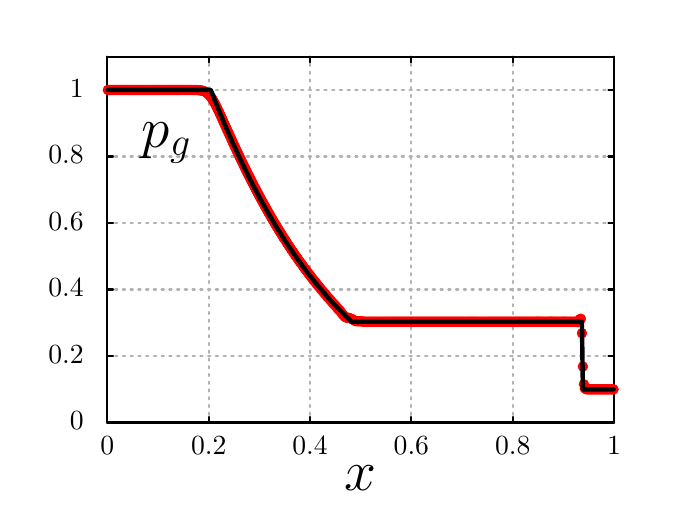
\begin{tikzpicture}[gnuplot]
%% generated with GNUPLOT 4.6p4 (Lua 5.1; terminal rev. 99, script rev. 100)
%% Mon 04 Aug 2014 12:05:06 PM EDT
\path (0.000,0.000) rectangle (8.000,6.000);
\gpfill{rgb color={1.000,1.000,1.000}} (1.012,0.985)--(7.446,0.985)--(7.446,5.630)--(1.012,5.630)--cycle;
\gpcolor{color=gp lt color border}
\gpsetlinetype{gp lt border}
\gpsetlinewidth{1.00}
\draw[gp path] (1.012,0.985)--(1.012,5.630)--(7.446,5.630)--(7.446,0.985)--cycle;
\gpcolor{color=gp lt color axes}
\gpsetlinetype{gp lt axes}
\gpsetlinewidth{2.00}
\draw[gp path] (1.012,0.985)--(7.447,0.985);
\gpcolor{color=gp lt color border}
\gpsetlinetype{gp lt border}
\draw[gp path] (1.012,0.985)--(1.084,0.985);
\draw[gp path] (7.447,0.985)--(7.375,0.985);
\gpcolor{rgb color={0.000,0.000,0.000}}
\node[gp node right,font={\fontsize{10pt}{12pt}\selectfont}] at (0.828,0.985) {0};
\gpcolor{color=gp lt color axes}
\gpsetlinetype{gp lt axes}
\draw[gp path] (1.012,1.830)--(7.447,1.830);
\gpcolor{color=gp lt color border}
\gpsetlinetype{gp lt border}
\draw[gp path] (1.012,1.830)--(1.084,1.830);
\draw[gp path] (7.447,1.830)--(7.375,1.830);
\gpcolor{rgb color={0.000,0.000,0.000}}
\node[gp node right,font={\fontsize{10pt}{12pt}\selectfont}] at (0.828,1.830) {0.2};
\gpcolor{color=gp lt color axes}
\gpsetlinetype{gp lt axes}
\draw[gp path] (1.012,2.674)--(7.447,2.674);
\gpcolor{color=gp lt color border}
\gpsetlinetype{gp lt border}
\draw[gp path] (1.012,2.674)--(1.084,2.674);
\draw[gp path] (7.447,2.674)--(7.375,2.674);
\gpcolor{rgb color={0.000,0.000,0.000}}
\node[gp node right,font={\fontsize{10pt}{12pt}\selectfont}] at (0.828,2.674) {0.4};
\gpcolor{color=gp lt color axes}
\gpsetlinetype{gp lt axes}
\draw[gp path] (1.012,3.519)--(7.447,3.519);
\gpcolor{color=gp lt color border}
\gpsetlinetype{gp lt border}
\draw[gp path] (1.012,3.519)--(1.084,3.519);
\draw[gp path] (7.447,3.519)--(7.375,3.519);
\gpcolor{rgb color={0.000,0.000,0.000}}
\node[gp node right,font={\fontsize{10pt}{12pt}\selectfont}] at (0.828,3.519) {0.6};
\gpcolor{color=gp lt color axes}
\gpsetlinetype{gp lt axes}
\draw[gp path] (1.012,4.364)--(7.447,4.364);
\gpcolor{color=gp lt color border}
\gpsetlinetype{gp lt border}
\draw[gp path] (1.012,4.364)--(1.084,4.364);
\draw[gp path] (7.447,4.364)--(7.375,4.364);
\gpcolor{rgb color={0.000,0.000,0.000}}
\node[gp node right,font={\fontsize{10pt}{12pt}\selectfont}] at (0.828,4.364) {0.8};
\gpcolor{color=gp lt color axes}
\gpsetlinetype{gp lt axes}
\draw[gp path] (1.012,5.209)--(7.447,5.209);
\gpcolor{color=gp lt color border}
\gpsetlinetype{gp lt border}
\draw[gp path] (1.012,5.209)--(1.084,5.209);
\draw[gp path] (7.447,5.209)--(7.375,5.209);
\gpcolor{rgb color={0.000,0.000,0.000}}
\node[gp node right,font={\fontsize{10pt}{12pt}\selectfont}] at (0.828,5.209) {1};
\gpcolor{color=gp lt color axes}
\gpsetlinetype{gp lt axes}
\draw[gp path] (1.012,0.985)--(1.012,5.631);
\gpcolor{color=gp lt color border}
\gpsetlinetype{gp lt border}
\draw[gp path] (1.012,0.985)--(1.012,1.057);
\draw[gp path] (1.012,5.631)--(1.012,5.559);
\gpcolor{rgb color={0.000,0.000,0.000}}
\node[gp node center,font={\fontsize{10pt}{12pt}\selectfont}] at (1.012,0.677) {0};
\gpcolor{color=gp lt color axes}
\gpsetlinetype{gp lt axes}
\draw[gp path] (2.299,0.985)--(2.299,5.631);
\gpcolor{color=gp lt color border}
\gpsetlinetype{gp lt border}
\draw[gp path] (2.299,0.985)--(2.299,1.057);
\draw[gp path] (2.299,5.631)--(2.299,5.559);
\gpcolor{rgb color={0.000,0.000,0.000}}
\node[gp node center,font={\fontsize{10pt}{12pt}\selectfont}] at (2.299,0.677) {0.2};
\gpcolor{color=gp lt color axes}
\gpsetlinetype{gp lt axes}
\draw[gp path] (3.586,0.985)--(3.586,5.631);
\gpcolor{color=gp lt color border}
\gpsetlinetype{gp lt border}
\draw[gp path] (3.586,0.985)--(3.586,1.057);
\draw[gp path] (3.586,5.631)--(3.586,5.559);
\gpcolor{rgb color={0.000,0.000,0.000}}
\node[gp node center,font={\fontsize{10pt}{12pt}\selectfont}] at (3.586,0.677) {0.4};
\gpcolor{color=gp lt color axes}
\gpsetlinetype{gp lt axes}
\draw[gp path] (4.873,0.985)--(4.873,5.631);
\gpcolor{color=gp lt color border}
\gpsetlinetype{gp lt border}
\draw[gp path] (4.873,0.985)--(4.873,1.057);
\draw[gp path] (4.873,5.631)--(4.873,5.559);
\gpcolor{rgb color={0.000,0.000,0.000}}
\node[gp node center,font={\fontsize{10pt}{12pt}\selectfont}] at (4.873,0.677) {0.6};
\gpcolor{color=gp lt color axes}
\gpsetlinetype{gp lt axes}
\draw[gp path] (6.160,0.985)--(6.160,5.631);
\gpcolor{color=gp lt color border}
\gpsetlinetype{gp lt border}
\draw[gp path] (6.160,0.985)--(6.160,1.057);
\draw[gp path] (6.160,5.631)--(6.160,5.559);
\gpcolor{rgb color={0.000,0.000,0.000}}
\node[gp node center,font={\fontsize{10pt}{12pt}\selectfont}] at (6.160,0.677) {0.8};
\gpcolor{color=gp lt color axes}
\gpsetlinetype{gp lt axes}
\draw[gp path] (7.447,0.985)--(7.447,5.631);
\gpcolor{color=gp lt color border}
\gpsetlinetype{gp lt border}
\draw[gp path] (7.447,0.985)--(7.447,1.057);
\draw[gp path] (7.447,5.631)--(7.447,5.559);
\gpcolor{rgb color={0.000,0.000,0.000}}
\node[gp node center,font={\fontsize{10pt}{12pt}\selectfont}] at (7.447,0.677) {1};
\gpcolor{color=gp lt color border}
\draw[gp path] (1.012,5.631)--(1.012,0.985)--(7.447,0.985)--(7.447,5.631)--cycle;
\gpcolor{rgb color={0.000,0.000,0.000}}
\node[gp node center,font={\fontsize{10pt}{12pt}\selectfont}] at (4.229,0.215) {\huge $x$};
\gpcolor{rgb color={1.000,0.000,0.000}}
\gpsetlinewidth{0.50}
\gpsetpointsize{4.44}
\gppoint{gp mark 7}{(1.018,5.209)}
\gppoint{gp mark 7}{(1.031,5.209)}
\gppoint{gp mark 7}{(1.043,5.209)}
\gppoint{gp mark 7}{(1.056,5.209)}
\gppoint{gp mark 7}{(1.069,5.209)}
\gppoint{gp mark 7}{(1.081,5.209)}
\gppoint{gp mark 7}{(1.094,5.209)}
\gppoint{gp mark 7}{(1.106,5.209)}
\gppoint{gp mark 7}{(1.119,5.209)}
\gppoint{gp mark 7}{(1.131,5.209)}
\gppoint{gp mark 7}{(1.144,5.209)}
\gppoint{gp mark 7}{(1.157,5.209)}
\gppoint{gp mark 7}{(1.169,5.209)}
\gppoint{gp mark 7}{(1.182,5.209)}
\gppoint{gp mark 7}{(1.194,5.209)}
\gppoint{gp mark 7}{(1.207,5.209)}
\gppoint{gp mark 7}{(1.219,5.209)}
\gppoint{gp mark 7}{(1.232,5.209)}
\gppoint{gp mark 7}{(1.245,5.209)}
\gppoint{gp mark 7}{(1.257,5.209)}
\gppoint{gp mark 7}{(1.270,5.209)}
\gppoint{gp mark 7}{(1.282,5.209)}
\gppoint{gp mark 7}{(1.295,5.209)}
\gppoint{gp mark 7}{(1.307,5.209)}
\gppoint{gp mark 7}{(1.320,5.209)}
\gppoint{gp mark 7}{(1.332,5.209)}
\gppoint{gp mark 7}{(1.345,5.209)}
\gppoint{gp mark 7}{(1.358,5.209)}
\gppoint{gp mark 7}{(1.370,5.209)}
\gppoint{gp mark 7}{(1.383,5.209)}
\gppoint{gp mark 7}{(1.395,5.209)}
\gppoint{gp mark 7}{(1.408,5.209)}
\gppoint{gp mark 7}{(1.420,5.209)}
\gppoint{gp mark 7}{(1.433,5.209)}
\gppoint{gp mark 7}{(1.446,5.209)}
\gppoint{gp mark 7}{(1.458,5.209)}
\gppoint{gp mark 7}{(1.471,5.209)}
\gppoint{gp mark 7}{(1.483,5.209)}
\gppoint{gp mark 7}{(1.496,5.209)}
\gppoint{gp mark 7}{(1.508,5.209)}
\gppoint{gp mark 7}{(1.521,5.209)}
\gppoint{gp mark 7}{(1.534,5.209)}
\gppoint{gp mark 7}{(1.546,5.209)}
\gppoint{gp mark 7}{(1.559,5.209)}
\gppoint{gp mark 7}{(1.571,5.209)}
\gppoint{gp mark 7}{(1.584,5.209)}
\gppoint{gp mark 7}{(1.596,5.209)}
\gppoint{gp mark 7}{(1.609,5.209)}
\gppoint{gp mark 7}{(1.622,5.209)}
\gppoint{gp mark 7}{(1.634,5.209)}
\gppoint{gp mark 7}{(1.647,5.209)}
\gppoint{gp mark 7}{(1.659,5.209)}
\gppoint{gp mark 7}{(1.672,5.209)}
\gppoint{gp mark 7}{(1.684,5.209)}
\gppoint{gp mark 7}{(1.697,5.209)}
\gppoint{gp mark 7}{(1.710,5.209)}
\gppoint{gp mark 7}{(1.722,5.209)}
\gppoint{gp mark 7}{(1.735,5.209)}
\gppoint{gp mark 7}{(1.747,5.209)}
\gppoint{gp mark 7}{(1.760,5.209)}
\gppoint{gp mark 7}{(1.772,5.209)}
\gppoint{gp mark 7}{(1.785,5.209)}
\gppoint{gp mark 7}{(1.798,5.209)}
\gppoint{gp mark 7}{(1.810,5.209)}
\gppoint{gp mark 7}{(1.823,5.209)}
\gppoint{gp mark 7}{(1.835,5.209)}
\gppoint{gp mark 7}{(1.848,5.209)}
\gppoint{gp mark 7}{(1.860,5.209)}
\gppoint{gp mark 7}{(1.873,5.209)}
\gppoint{gp mark 7}{(1.886,5.209)}
\gppoint{gp mark 7}{(1.898,5.209)}
\gppoint{gp mark 7}{(1.911,5.209)}
\gppoint{gp mark 7}{(1.923,5.209)}
\gppoint{gp mark 7}{(1.936,5.209)}
\gppoint{gp mark 7}{(1.948,5.209)}
\gppoint{gp mark 7}{(1.961,5.209)}
\gppoint{gp mark 7}{(1.973,5.209)}
\gppoint{gp mark 7}{(1.986,5.209)}
\gppoint{gp mark 7}{(1.999,5.209)}
\gppoint{gp mark 7}{(2.011,5.209)}
\gppoint{gp mark 7}{(2.024,5.209)}
\gppoint{gp mark 7}{(2.036,5.209)}
\gppoint{gp mark 7}{(2.049,5.209)}
\gppoint{gp mark 7}{(2.061,5.209)}
\gppoint{gp mark 7}{(2.074,5.209)}
\gppoint{gp mark 7}{(2.087,5.209)}
\gppoint{gp mark 7}{(2.099,5.208)}
\gppoint{gp mark 7}{(2.112,5.208)}
\gppoint{gp mark 7}{(2.124,5.208)}
\gppoint{gp mark 7}{(2.137,5.208)}
\gppoint{gp mark 7}{(2.149,5.208)}
\gppoint{gp mark 7}{(2.162,5.207)}
\gppoint{gp mark 7}{(2.175,5.206)}
\gppoint{gp mark 7}{(2.187,5.205)}
\gppoint{gp mark 7}{(2.200,5.203)}
\gppoint{gp mark 7}{(2.212,5.201)}
\gppoint{gp mark 7}{(2.225,5.198)}
\gppoint{gp mark 7}{(2.237,5.194)}
\gppoint{gp mark 7}{(2.250,5.188)}
\gppoint{gp mark 7}{(2.263,5.182)}
\gppoint{gp mark 7}{(2.275,5.173)}
\gppoint{gp mark 7}{(2.288,5.163)}
\gppoint{gp mark 7}{(2.300,5.150)}
\gppoint{gp mark 7}{(2.313,5.137)}
\gppoint{gp mark 7}{(2.325,5.120)}
\gppoint{gp mark 7}{(2.338,5.103)}
\gppoint{gp mark 7}{(2.351,5.082)}
\gppoint{gp mark 7}{(2.363,5.062)}
\gppoint{gp mark 7}{(2.376,5.039)}
\gppoint{gp mark 7}{(2.388,5.015)}
\gppoint{gp mark 7}{(2.401,4.990)}
\gppoint{gp mark 7}{(2.413,4.964)}
\gppoint{gp mark 7}{(2.426,4.938)}
\gppoint{gp mark 7}{(2.439,4.911)}
\gppoint{gp mark 7}{(2.451,4.884)}
\gppoint{gp mark 7}{(2.464,4.856)}
\gppoint{gp mark 7}{(2.476,4.828)}
\gppoint{gp mark 7}{(2.489,4.801)}
\gppoint{gp mark 7}{(2.501,4.772)}
\gppoint{gp mark 7}{(2.514,4.745)}
\gppoint{gp mark 7}{(2.526,4.717)}
\gppoint{gp mark 7}{(2.539,4.689)}
\gppoint{gp mark 7}{(2.552,4.662)}
\gppoint{gp mark 7}{(2.564,4.634)}
\gppoint{gp mark 7}{(2.577,4.606)}
\gppoint{gp mark 7}{(2.589,4.579)}
\gppoint{gp mark 7}{(2.602,4.551)}
\gppoint{gp mark 7}{(2.614,4.524)}
\gppoint{gp mark 7}{(2.627,4.497)}
\gppoint{gp mark 7}{(2.640,4.470)}
\gppoint{gp mark 7}{(2.652,4.442)}
\gppoint{gp mark 7}{(2.665,4.417)}
\gppoint{gp mark 7}{(2.677,4.389)}
\gppoint{gp mark 7}{(2.690,4.363)}
\gppoint{gp mark 7}{(2.702,4.337)}
\gppoint{gp mark 7}{(2.715,4.310)}
\gppoint{gp mark 7}{(2.728,4.284)}
\gppoint{gp mark 7}{(2.740,4.259)}
\gppoint{gp mark 7}{(2.753,4.232)}
\gppoint{gp mark 7}{(2.765,4.207)}
\gppoint{gp mark 7}{(2.778,4.182)}
\gppoint{gp mark 7}{(2.790,4.156)}
\gppoint{gp mark 7}{(2.803,4.131)}
\gppoint{gp mark 7}{(2.816,4.107)}
\gppoint{gp mark 7}{(2.828,4.081)}
\gppoint{gp mark 7}{(2.841,4.056)}
\gppoint{gp mark 7}{(2.853,4.032)}
\gppoint{gp mark 7}{(2.866,4.008)}
\gppoint{gp mark 7}{(2.878,3.983)}
\gppoint{gp mark 7}{(2.891,3.959)}
\gppoint{gp mark 7}{(2.904,3.936)}
\gppoint{gp mark 7}{(2.916,3.911)}
\gppoint{gp mark 7}{(2.929,3.888)}
\gppoint{gp mark 7}{(2.941,3.865)}
\gppoint{gp mark 7}{(2.954,3.841)}
\gppoint{gp mark 7}{(2.966,3.817)}
\gppoint{gp mark 7}{(2.979,3.795)}
\gppoint{gp mark 7}{(2.992,3.773)}
\gppoint{gp mark 7}{(3.004,3.749)}
\gppoint{gp mark 7}{(3.017,3.726)}
\gppoint{gp mark 7}{(3.029,3.705)}
\gppoint{gp mark 7}{(3.042,3.682)}
\gppoint{gp mark 7}{(3.054,3.659)}
\gppoint{gp mark 7}{(3.067,3.638)}
\gppoint{gp mark 7}{(3.079,3.617)}
\gppoint{gp mark 7}{(3.092,3.594)}
\gppoint{gp mark 7}{(3.105,3.572)}
\gppoint{gp mark 7}{(3.117,3.552)}
\gppoint{gp mark 7}{(3.130,3.531)}
\gppoint{gp mark 7}{(3.142,3.508)}
\gppoint{gp mark 7}{(3.155,3.487)}
\gppoint{gp mark 7}{(3.167,3.468)}
\gppoint{gp mark 7}{(3.180,3.447)}
\gppoint{gp mark 7}{(3.193,3.425)}
\gppoint{gp mark 7}{(3.205,3.405)}
\gppoint{gp mark 7}{(3.218,3.386)}
\gppoint{gp mark 7}{(3.230,3.366)}
\gppoint{gp mark 7}{(3.243,3.344)}
\gppoint{gp mark 7}{(3.255,3.325)}
\gppoint{gp mark 7}{(3.268,3.307)}
\gppoint{gp mark 7}{(3.281,3.287)}
\gppoint{gp mark 7}{(3.293,3.266)}
\gppoint{gp mark 7}{(3.306,3.247)}
\gppoint{gp mark 7}{(3.318,3.229)}
\gppoint{gp mark 7}{(3.331,3.210)}
\gppoint{gp mark 7}{(3.343,3.190)}
\gppoint{gp mark 7}{(3.356,3.171)}
\gppoint{gp mark 7}{(3.369,3.154)}
\gppoint{gp mark 7}{(3.381,3.136)}
\gppoint{gp mark 7}{(3.394,3.116)}
\gppoint{gp mark 7}{(3.406,3.097)}
\gppoint{gp mark 7}{(3.419,3.081)}
\gppoint{gp mark 7}{(3.431,3.064)}
\gppoint{gp mark 7}{(3.444,3.044)}
\gppoint{gp mark 7}{(3.457,3.026)}
\gppoint{gp mark 7}{(3.469,3.009)}
\gppoint{gp mark 7}{(3.482,2.994)}
\gppoint{gp mark 7}{(3.494,2.975)}
\gppoint{gp mark 7}{(3.507,2.957)}
\gppoint{gp mark 7}{(3.519,2.940)}
\gppoint{gp mark 7}{(3.532,2.925)}
\gppoint{gp mark 7}{(3.545,2.908)}
\gppoint{gp mark 7}{(3.557,2.890)}
\gppoint{gp mark 7}{(3.570,2.873)}
\gppoint{gp mark 7}{(3.582,2.858)}
\gppoint{gp mark 7}{(3.595,2.842)}
\gppoint{gp mark 7}{(3.607,2.826)}
\gppoint{gp mark 7}{(3.620,2.809)}
\gppoint{gp mark 7}{(3.633,2.791)}
\gppoint{gp mark 7}{(3.645,2.778)}
\gppoint{gp mark 7}{(3.658,2.764)}
\gppoint{gp mark 7}{(3.670,2.746)}
\gppoint{gp mark 7}{(3.683,2.728)}
\gppoint{gp mark 7}{(3.695,2.715)}
\gppoint{gp mark 7}{(3.708,2.702)}
\gppoint{gp mark 7}{(3.720,2.684)}
\gppoint{gp mark 7}{(3.733,2.669)}
\gppoint{gp mark 7}{(3.746,2.655)}
\gppoint{gp mark 7}{(3.758,2.639)}
\gppoint{gp mark 7}{(3.771,2.624)}
\gppoint{gp mark 7}{(3.783,2.612)}
\gppoint{gp mark 7}{(3.796,2.596)}
\gppoint{gp mark 7}{(3.808,2.579)}
\gppoint{gp mark 7}{(3.821,2.566)}
\gppoint{gp mark 7}{(3.834,2.553)}
\gppoint{gp mark 7}{(3.846,2.539)}
\gppoint{gp mark 7}{(3.859,2.524)}
\gppoint{gp mark 7}{(3.871,2.508)}
\gppoint{gp mark 7}{(3.884,2.494)}
\gppoint{gp mark 7}{(3.896,2.482)}
\gppoint{gp mark 7}{(3.909,2.470)}
\gppoint{gp mark 7}{(3.922,2.453)}
\gppoint{gp mark 7}{(3.934,2.437)}
\gppoint{gp mark 7}{(3.947,2.423)}
\gppoint{gp mark 7}{(3.959,2.412)}
\gppoint{gp mark 7}{(3.972,2.399)}
\gppoint{gp mark 7}{(3.984,2.381)}
\gppoint{gp mark 7}{(3.997,2.363)}
\gppoint{gp mark 7}{(4.010,2.349)}
\gppoint{gp mark 7}{(4.022,2.336)}
\gppoint{gp mark 7}{(4.035,2.322)}
\gppoint{gp mark 7}{(4.047,2.318)}
\gppoint{gp mark 7}{(4.060,2.316)}
\gppoint{gp mark 7}{(4.072,2.315)}
\gppoint{gp mark 7}{(4.085,2.313)}
\gppoint{gp mark 7}{(4.098,2.308)}
\gppoint{gp mark 7}{(4.110,2.303)}
\gppoint{gp mark 7}{(4.123,2.297)}
\gppoint{gp mark 7}{(4.135,2.289)}
\gppoint{gp mark 7}{(4.148,2.282)}
\gppoint{gp mark 7}{(4.160,2.274)}
\gppoint{gp mark 7}{(4.173,2.273)}
\gppoint{gp mark 7}{(4.186,2.273)}
\gppoint{gp mark 7}{(4.198,2.272)}
\gppoint{gp mark 7}{(4.211,2.272)}
\gppoint{gp mark 7}{(4.223,2.272)}
\gppoint{gp mark 7}{(4.236,2.271)}
\gppoint{gp mark 7}{(4.248,2.269)}
\gppoint{gp mark 7}{(4.261,2.267)}
\gppoint{gp mark 7}{(4.273,2.265)}
\gppoint{gp mark 7}{(4.286,2.265)}
\gppoint{gp mark 7}{(4.299,2.265)}
\gppoint{gp mark 7}{(4.311,2.265)}
\gppoint{gp mark 7}{(4.324,2.265)}
\gppoint{gp mark 7}{(4.336,2.265)}
\gppoint{gp mark 7}{(4.349,2.265)}
\gppoint{gp mark 7}{(4.361,2.265)}
\gppoint{gp mark 7}{(4.374,2.265)}
\gppoint{gp mark 7}{(4.387,2.265)}
\gppoint{gp mark 7}{(4.399,2.265)}
\gppoint{gp mark 7}{(4.412,2.265)}
\gppoint{gp mark 7}{(4.424,2.265)}
\gppoint{gp mark 7}{(4.437,2.265)}
\gppoint{gp mark 7}{(4.449,2.265)}
\gppoint{gp mark 7}{(4.462,2.265)}
\gppoint{gp mark 7}{(4.475,2.265)}
\gppoint{gp mark 7}{(4.487,2.265)}
\gppoint{gp mark 7}{(4.500,2.265)}
\gppoint{gp mark 7}{(4.512,2.265)}
\gppoint{gp mark 7}{(4.525,2.265)}
\gppoint{gp mark 7}{(4.537,2.265)}
\gppoint{gp mark 7}{(4.550,2.265)}
\gppoint{gp mark 7}{(4.563,2.265)}
\gppoint{gp mark 7}{(4.575,2.265)}
\gppoint{gp mark 7}{(4.588,2.265)}
\gppoint{gp mark 7}{(4.600,2.265)}
\gppoint{gp mark 7}{(4.613,2.265)}
\gppoint{gp mark 7}{(4.625,2.265)}
\gppoint{gp mark 7}{(4.638,2.265)}
\gppoint{gp mark 7}{(4.651,2.265)}
\gppoint{gp mark 7}{(4.663,2.265)}
\gppoint{gp mark 7}{(4.676,2.265)}
\gppoint{gp mark 7}{(4.688,2.265)}
\gppoint{gp mark 7}{(4.701,2.265)}
\gppoint{gp mark 7}{(4.713,2.265)}
\gppoint{gp mark 7}{(4.726,2.265)}
\gppoint{gp mark 7}{(4.739,2.265)}
\gppoint{gp mark 7}{(4.751,2.265)}
\gppoint{gp mark 7}{(4.764,2.265)}
\gppoint{gp mark 7}{(4.776,2.265)}
\gppoint{gp mark 7}{(4.789,2.265)}
\gppoint{gp mark 7}{(4.801,2.265)}
\gppoint{gp mark 7}{(4.814,2.265)}
\gppoint{gp mark 7}{(4.826,2.265)}
\gppoint{gp mark 7}{(4.839,2.265)}
\gppoint{gp mark 7}{(4.852,2.265)}
\gppoint{gp mark 7}{(4.864,2.265)}
\gppoint{gp mark 7}{(4.877,2.265)}
\gppoint{gp mark 7}{(4.889,2.265)}
\gppoint{gp mark 7}{(4.902,2.265)}
\gppoint{gp mark 7}{(4.914,2.265)}
\gppoint{gp mark 7}{(4.927,2.265)}
\gppoint{gp mark 7}{(4.940,2.265)}
\gppoint{gp mark 7}{(4.952,2.265)}
\gppoint{gp mark 7}{(4.965,2.265)}
\gppoint{gp mark 7}{(4.977,2.265)}
\gppoint{gp mark 7}{(4.990,2.265)}
\gppoint{gp mark 7}{(5.002,2.265)}
\gppoint{gp mark 7}{(5.015,2.265)}
\gppoint{gp mark 7}{(5.028,2.265)}
\gppoint{gp mark 7}{(5.040,2.265)}
\gppoint{gp mark 7}{(5.053,2.265)}
\gppoint{gp mark 7}{(5.065,2.265)}
\gppoint{gp mark 7}{(5.078,2.265)}
\gppoint{gp mark 7}{(5.090,2.265)}
\gppoint{gp mark 7}{(5.103,2.265)}
\gppoint{gp mark 7}{(5.116,2.265)}
\gppoint{gp mark 7}{(5.128,2.265)}
\gppoint{gp mark 7}{(5.141,2.265)}
\gppoint{gp mark 7}{(5.153,2.265)}
\gppoint{gp mark 7}{(5.166,2.265)}
\gppoint{gp mark 7}{(5.178,2.265)}
\gppoint{gp mark 7}{(5.191,2.265)}
\gppoint{gp mark 7}{(5.204,2.265)}
\gppoint{gp mark 7}{(5.216,2.265)}
\gppoint{gp mark 7}{(5.229,2.265)}
\gppoint{gp mark 7}{(5.241,2.265)}
\gppoint{gp mark 7}{(5.254,2.265)}
\gppoint{gp mark 7}{(5.266,2.265)}
\gppoint{gp mark 7}{(5.279,2.265)}
\gppoint{gp mark 7}{(5.292,2.265)}
\gppoint{gp mark 7}{(5.304,2.265)}
\gppoint{gp mark 7}{(5.317,2.265)}
\gppoint{gp mark 7}{(5.329,2.265)}
\gppoint{gp mark 7}{(5.342,2.265)}
\gppoint{gp mark 7}{(5.354,2.265)}
\gppoint{gp mark 7}{(5.367,2.265)}
\gppoint{gp mark 7}{(5.380,2.265)}
\gppoint{gp mark 7}{(5.392,2.265)}
\gppoint{gp mark 7}{(5.405,2.265)}
\gppoint{gp mark 7}{(5.417,2.265)}
\gppoint{gp mark 7}{(5.430,2.265)}
\gppoint{gp mark 7}{(5.442,2.265)}
\gppoint{gp mark 7}{(5.455,2.265)}
\gppoint{gp mark 7}{(5.467,2.265)}
\gppoint{gp mark 7}{(5.480,2.265)}
\gppoint{gp mark 7}{(5.493,2.265)}
\gppoint{gp mark 7}{(5.505,2.265)}
\gppoint{gp mark 7}{(5.518,2.265)}
\gppoint{gp mark 7}{(5.530,2.265)}
\gppoint{gp mark 7}{(5.543,2.265)}
\gppoint{gp mark 7}{(5.555,2.265)}
\gppoint{gp mark 7}{(5.568,2.265)}
\gppoint{gp mark 7}{(5.581,2.265)}
\gppoint{gp mark 7}{(5.593,2.265)}
\gppoint{gp mark 7}{(5.606,2.265)}
\gppoint{gp mark 7}{(5.618,2.265)}
\gppoint{gp mark 7}{(5.631,2.265)}
\gppoint{gp mark 7}{(5.643,2.266)}
\gppoint{gp mark 7}{(5.656,2.265)}
\gppoint{gp mark 7}{(5.669,2.265)}
\gppoint{gp mark 7}{(5.681,2.266)}
\gppoint{gp mark 7}{(5.694,2.265)}
\gppoint{gp mark 7}{(5.706,2.265)}
\gppoint{gp mark 7}{(5.719,2.265)}
\gppoint{gp mark 7}{(5.731,2.265)}
\gppoint{gp mark 7}{(5.744,2.265)}
\gppoint{gp mark 7}{(5.757,2.265)}
\gppoint{gp mark 7}{(5.769,2.265)}
\gppoint{gp mark 7}{(5.782,2.265)}
\gppoint{gp mark 7}{(5.794,2.265)}
\gppoint{gp mark 7}{(5.807,2.265)}
\gppoint{gp mark 7}{(5.819,2.265)}
\gppoint{gp mark 7}{(5.832,2.265)}
\gppoint{gp mark 7}{(5.845,2.265)}
\gppoint{gp mark 7}{(5.857,2.265)}
\gppoint{gp mark 7}{(5.870,2.265)}
\gppoint{gp mark 7}{(5.882,2.265)}
\gppoint{gp mark 7}{(5.895,2.265)}
\gppoint{gp mark 7}{(5.907,2.265)}
\gppoint{gp mark 7}{(5.920,2.265)}
\gppoint{gp mark 7}{(5.933,2.265)}
\gppoint{gp mark 7}{(5.945,2.265)}
\gppoint{gp mark 7}{(5.958,2.265)}
\gppoint{gp mark 7}{(5.970,2.265)}
\gppoint{gp mark 7}{(5.983,2.265)}
\gppoint{gp mark 7}{(5.995,2.265)}
\gppoint{gp mark 7}{(6.008,2.265)}
\gppoint{gp mark 7}{(6.020,2.265)}
\gppoint{gp mark 7}{(6.033,2.265)}
\gppoint{gp mark 7}{(6.046,2.265)}
\gppoint{gp mark 7}{(6.058,2.265)}
\gppoint{gp mark 7}{(6.071,2.265)}
\gppoint{gp mark 7}{(6.083,2.265)}
\gppoint{gp mark 7}{(6.096,2.265)}
\gppoint{gp mark 7}{(6.108,2.265)}
\gppoint{gp mark 7}{(6.121,2.265)}
\gppoint{gp mark 7}{(6.134,2.265)}
\gppoint{gp mark 7}{(6.146,2.265)}
\gppoint{gp mark 7}{(6.159,2.265)}
\gppoint{gp mark 7}{(6.171,2.265)}
\gppoint{gp mark 7}{(6.184,2.265)}
\gppoint{gp mark 7}{(6.196,2.265)}
\gppoint{gp mark 7}{(6.209,2.265)}
\gppoint{gp mark 7}{(6.222,2.265)}
\gppoint{gp mark 7}{(6.234,2.265)}
\gppoint{gp mark 7}{(6.247,2.265)}
\gppoint{gp mark 7}{(6.259,2.265)}
\gppoint{gp mark 7}{(6.272,2.265)}
\gppoint{gp mark 7}{(6.284,2.265)}
\gppoint{gp mark 7}{(6.297,2.265)}
\gppoint{gp mark 7}{(6.310,2.265)}
\gppoint{gp mark 7}{(6.322,2.265)}
\gppoint{gp mark 7}{(6.335,2.265)}
\gppoint{gp mark 7}{(6.347,2.265)}
\gppoint{gp mark 7}{(6.360,2.265)}
\gppoint{gp mark 7}{(6.372,2.265)}
\gppoint{gp mark 7}{(6.385,2.265)}
\gppoint{gp mark 7}{(6.398,2.265)}
\gppoint{gp mark 7}{(6.410,2.265)}
\gppoint{gp mark 7}{(6.423,2.265)}
\gppoint{gp mark 7}{(6.435,2.265)}
\gppoint{gp mark 7}{(6.448,2.265)}
\gppoint{gp mark 7}{(6.460,2.266)}
\gppoint{gp mark 7}{(6.473,2.266)}
\gppoint{gp mark 7}{(6.486,2.266)}
\gppoint{gp mark 7}{(6.498,2.266)}
\gppoint{gp mark 7}{(6.511,2.265)}
\gppoint{gp mark 7}{(6.523,2.265)}
\gppoint{gp mark 7}{(6.536,2.265)}
\gppoint{gp mark 7}{(6.548,2.265)}
\gppoint{gp mark 7}{(6.561,2.265)}
\gppoint{gp mark 7}{(6.573,2.265)}
\gppoint{gp mark 7}{(6.586,2.265)}
\gppoint{gp mark 7}{(6.599,2.265)}
\gppoint{gp mark 7}{(6.611,2.265)}
\gppoint{gp mark 7}{(6.624,2.266)}
\gppoint{gp mark 7}{(6.636,2.266)}
\gppoint{gp mark 7}{(6.649,2.266)}
\gppoint{gp mark 7}{(6.661,2.266)}
\gppoint{gp mark 7}{(6.674,2.265)}
\gppoint{gp mark 7}{(6.687,2.265)}
\gppoint{gp mark 7}{(6.699,2.265)}
\gppoint{gp mark 7}{(6.712,2.265)}
\gppoint{gp mark 7}{(6.724,2.265)}
\gppoint{gp mark 7}{(6.737,2.265)}
\gppoint{gp mark 7}{(6.749,2.265)}
\gppoint{gp mark 7}{(6.762,2.265)}
\gppoint{gp mark 7}{(6.775,2.265)}
\gppoint{gp mark 7}{(6.787,2.266)}
\gppoint{gp mark 7}{(6.800,2.266)}
\gppoint{gp mark 7}{(6.812,2.266)}
\gppoint{gp mark 7}{(6.825,2.266)}
\gppoint{gp mark 7}{(6.837,2.265)}
\gppoint{gp mark 7}{(6.850,2.265)}
\gppoint{gp mark 7}{(6.863,2.265)}
\gppoint{gp mark 7}{(6.875,2.265)}
\gppoint{gp mark 7}{(6.888,2.265)}
\gppoint{gp mark 7}{(6.900,2.265)}
\gppoint{gp mark 7}{(6.913,2.265)}
\gppoint{gp mark 7}{(6.925,2.265)}
\gppoint{gp mark 7}{(6.938,2.265)}
\gppoint{gp mark 7}{(6.951,2.266)}
\gppoint{gp mark 7}{(6.963,2.265)}
\gppoint{gp mark 7}{(6.976,2.263)}
\gppoint{gp mark 7}{(6.988,2.261)}
\gppoint{gp mark 7}{(7.001,2.276)}
\gppoint{gp mark 7}{(7.013,2.299)}
\gppoint{gp mark 7}{(7.026,2.303)}
\gppoint{gp mark 7}{(7.039,2.120)}
\gppoint{gp mark 7}{(7.051,1.697)}
\gppoint{gp mark 7}{(7.064,1.472)}
\gppoint{gp mark 7}{(7.076,1.418)}
\gppoint{gp mark 7}{(7.089,1.409)}
\gppoint{gp mark 7}{(7.101,1.408)}
\gppoint{gp mark 7}{(7.114,1.407)}
\gppoint{gp mark 7}{(7.127,1.407)}
\gppoint{gp mark 7}{(7.139,1.407)}
\gppoint{gp mark 7}{(7.152,1.407)}
\gppoint{gp mark 7}{(7.164,1.407)}
\gppoint{gp mark 7}{(7.177,1.407)}
\gppoint{gp mark 7}{(7.189,1.407)}
\gppoint{gp mark 7}{(7.202,1.407)}
\gppoint{gp mark 7}{(7.214,1.407)}
\gppoint{gp mark 7}{(7.227,1.407)}
\gppoint{gp mark 7}{(7.240,1.407)}
\gppoint{gp mark 7}{(7.252,1.407)}
\gppoint{gp mark 7}{(7.265,1.407)}
\gppoint{gp mark 7}{(7.277,1.407)}
\gppoint{gp mark 7}{(7.290,1.407)}
\gppoint{gp mark 7}{(7.302,1.407)}
\gppoint{gp mark 7}{(7.315,1.407)}
\gppoint{gp mark 7}{(7.328,1.407)}
\gppoint{gp mark 7}{(7.340,1.407)}
\gppoint{gp mark 7}{(7.353,1.407)}
\gppoint{gp mark 7}{(7.365,1.407)}
\gppoint{gp mark 7}{(7.378,1.407)}
\gppoint{gp mark 7}{(7.390,1.407)}
\gppoint{gp mark 7}{(7.403,1.407)}
\gppoint{gp mark 7}{(7.416,1.407)}
\gppoint{gp mark 7}{(7.428,1.407)}
\gppoint{gp mark 7}{(7.441,1.407)}
\gpcolor{rgb color={0.000,0.000,0.000}}
\gpsetlinetype{gp lt plot 0}
\gpsetlinewidth{4.00}
\draw[gp path] (1.018,5.209)--(1.031,5.209)--(1.043,5.209)--(1.056,5.209)--(1.069,5.209)%
  --(1.081,5.209)--(1.094,5.209)--(1.106,5.209)--(1.119,5.209)--(1.131,5.209)--(1.144,5.209)%
  --(1.157,5.209)--(1.169,5.209)--(1.182,5.209)--(1.194,5.209)--(1.207,5.209)--(1.219,5.209)%
  --(1.232,5.209)--(1.245,5.209)--(1.257,5.209)--(1.270,5.209)--(1.282,5.209)--(1.295,5.209)%
  --(1.307,5.209)--(1.320,5.209)--(1.332,5.209)--(1.345,5.209)--(1.358,5.209)--(1.370,5.209)%
  --(1.383,5.209)--(1.395,5.209)--(1.408,5.209)--(1.420,5.209)--(1.433,5.209)--(1.446,5.209)%
  --(1.458,5.209)--(1.471,5.209)--(1.483,5.209)--(1.496,5.209)--(1.508,5.209)--(1.521,5.209)%
  --(1.534,5.209)--(1.546,5.209)--(1.559,5.209)--(1.571,5.209)--(1.584,5.209)--(1.596,5.209)%
  --(1.609,5.209)--(1.622,5.209)--(1.634,5.209)--(1.647,5.209)--(1.659,5.209)--(1.672,5.209)%
  --(1.684,5.209)--(1.697,5.209)--(1.710,5.209)--(1.722,5.209)--(1.735,5.209)--(1.747,5.209)%
  --(1.760,5.209)--(1.772,5.209)--(1.785,5.209)--(1.798,5.209)--(1.810,5.209)--(1.823,5.209)%
  --(1.835,5.209)--(1.848,5.209)--(1.860,5.209)--(1.873,5.209)--(1.886,5.209)--(1.898,5.209)%
  --(1.911,5.209)--(1.923,5.209)--(1.936,5.209)--(1.948,5.209)--(1.961,5.209)--(1.973,5.209)%
  --(1.986,5.209)--(1.999,5.209)--(2.011,5.209)--(2.024,5.209)--(2.036,5.209)--(2.049,5.209)%
  --(2.061,5.209)--(2.074,5.209)--(2.087,5.209)--(2.099,5.209)--(2.112,5.209)--(2.124,5.209)%
  --(2.137,5.209)--(2.149,5.209)--(2.162,5.209)--(2.175,5.209)--(2.187,5.209)--(2.200,5.209)%
  --(2.212,5.209)--(2.225,5.209)--(2.237,5.209)--(2.250,5.209)--(2.263,5.209)--(2.275,5.209)%
  --(2.288,5.209)--(2.300,5.209)--(2.313,5.209)--(2.325,5.209)--(2.338,5.178)--(2.351,5.146)%
  --(2.363,5.114)--(2.376,5.082)--(2.388,5.050)--(2.401,5.019)--(2.413,4.988)--(2.426,4.957)%
  --(2.439,4.926)--(2.451,4.895)--(2.464,4.865)--(2.476,4.835)--(2.489,4.805)--(2.501,4.775)%
  --(2.514,4.746)--(2.526,4.716)--(2.539,4.687)--(2.552,4.658)--(2.564,4.629)--(2.577,4.601)%
  --(2.589,4.572)--(2.602,4.544)--(2.614,4.516)--(2.627,4.488)--(2.640,4.461)--(2.652,4.433)%
  --(2.665,4.406)--(2.677,4.379)--(2.690,4.352)--(2.702,4.325)--(2.715,4.299)--(2.728,4.273)%
  --(2.740,4.246)--(2.753,4.220)--(2.765,4.195)--(2.778,4.169)--(2.790,4.144)--(2.803,4.118)%
  --(2.816,4.093)--(2.828,4.068)--(2.841,4.043)--(2.853,4.019)--(2.866,3.994)--(2.878,3.970)%
  --(2.891,3.946)--(2.904,3.922)--(2.916,3.898)--(2.929,3.875)--(2.941,3.851)--(2.954,3.828)%
  --(2.966,3.805)--(2.979,3.782)--(2.992,3.759)--(3.004,3.737)--(3.017,3.714)--(3.029,3.692)%
  --(3.042,3.670)--(3.054,3.648)--(3.067,3.626)--(3.079,3.604)--(3.092,3.583)--(3.105,3.561)%
  --(3.117,3.540)--(3.130,3.519)--(3.142,3.498)--(3.155,3.477)--(3.167,3.457)--(3.180,3.436)%
  --(3.193,3.416)--(3.205,3.396)--(3.218,3.376)--(3.230,3.356)--(3.243,3.336)--(3.255,3.316)%
  --(3.268,3.297)--(3.281,3.278)--(3.293,3.258)--(3.306,3.239)--(3.318,3.220)--(3.331,3.202)%
  --(3.343,3.183)--(3.356,3.165)--(3.369,3.146)--(3.381,3.128)--(3.394,3.110)--(3.406,3.092)%
  --(3.419,3.074)--(3.431,3.056)--(3.444,3.039)--(3.457,3.021)--(3.469,3.004)--(3.482,2.987)%
  --(3.494,2.969)--(3.507,2.952)--(3.519,2.936)--(3.532,2.919)--(3.545,2.902)--(3.557,2.886)%
  --(3.570,2.870)--(3.582,2.853)--(3.595,2.837)--(3.607,2.821)--(3.620,2.805)--(3.633,2.790)%
  --(3.645,2.774)--(3.658,2.758)--(3.670,2.743)--(3.683,2.728)--(3.695,2.713)--(3.708,2.697)%
  --(3.720,2.682)--(3.733,2.668)--(3.746,2.653)--(3.758,2.638)--(3.771,2.624)--(3.783,2.609)%
  --(3.796,2.595)--(3.808,2.581)--(3.821,2.567)--(3.834,2.553)--(3.846,2.539)--(3.859,2.525)%
  --(3.871,2.512)--(3.884,2.498)--(3.896,2.485)--(3.909,2.471)--(3.922,2.458)--(3.934,2.445)%
  --(3.947,2.432)--(3.959,2.419)--(3.972,2.406)--(3.984,2.393)--(3.997,2.381)--(4.010,2.368)%
  --(4.022,2.356)--(4.035,2.343)--(4.047,2.331)--(4.060,2.319)--(4.072,2.307)--(4.085,2.295)%
  --(4.098,2.283)--(4.110,2.271)--(4.123,2.265)--(4.135,2.265)--(4.148,2.265)--(4.160,2.265)%
  --(4.173,2.265)--(4.186,2.265)--(4.198,2.265)--(4.211,2.265)--(4.223,2.265)--(4.236,2.265)%
  --(4.248,2.265)--(4.261,2.265)--(4.273,2.265)--(4.286,2.265)--(4.299,2.265)--(4.311,2.265)%
  --(4.324,2.265)--(4.336,2.265)--(4.349,2.265)--(4.361,2.265)--(4.374,2.265)--(4.387,2.265)%
  --(4.399,2.265)--(4.412,2.265)--(4.424,2.265)--(4.437,2.265)--(4.449,2.265)--(4.462,2.265)%
  --(4.475,2.265)--(4.487,2.265)--(4.500,2.265)--(4.512,2.265)--(4.525,2.265)--(4.537,2.265)%
  --(4.550,2.265)--(4.563,2.265)--(4.575,2.265)--(4.588,2.265)--(4.600,2.265)--(4.613,2.265)%
  --(4.625,2.265)--(4.638,2.265)--(4.651,2.265)--(4.663,2.265)--(4.676,2.265)--(4.688,2.265)%
  --(4.701,2.265)--(4.713,2.265)--(4.726,2.265)--(4.739,2.265)--(4.751,2.265)--(4.764,2.265)%
  --(4.776,2.265)--(4.789,2.265)--(4.801,2.265)--(4.814,2.265)--(4.826,2.265)--(4.839,2.265)%
  --(4.852,2.265)--(4.864,2.265)--(4.877,2.265)--(4.889,2.265)--(4.902,2.265)--(4.914,2.265)%
  --(4.927,2.265)--(4.940,2.265)--(4.952,2.265)--(4.965,2.265)--(4.977,2.265)--(4.990,2.265)%
  --(5.002,2.265)--(5.015,2.265)--(5.028,2.265)--(5.040,2.265)--(5.053,2.265)--(5.065,2.265)%
  --(5.078,2.265)--(5.090,2.265)--(5.103,2.265)--(5.116,2.265)--(5.128,2.265)--(5.141,2.265)%
  --(5.153,2.265)--(5.166,2.265)--(5.178,2.265)--(5.191,2.265)--(5.204,2.265)--(5.216,2.265)%
  --(5.229,2.265)--(5.241,2.265)--(5.254,2.265)--(5.266,2.265)--(5.279,2.265)--(5.292,2.265)%
  --(5.304,2.265)--(5.317,2.265)--(5.329,2.265)--(5.342,2.265)--(5.354,2.265)--(5.367,2.265)%
  --(5.380,2.265)--(5.392,2.265)--(5.405,2.265)--(5.417,2.265)--(5.430,2.265)--(5.442,2.265)%
  --(5.455,2.265)--(5.467,2.265)--(5.480,2.265)--(5.493,2.265)--(5.505,2.265)--(5.518,2.265)%
  --(5.530,2.265)--(5.543,2.265)--(5.555,2.265)--(5.568,2.265)--(5.581,2.265)--(5.593,2.265)%
  --(5.606,2.265)--(5.618,2.265)--(5.631,2.265)--(5.643,2.265)--(5.656,2.265)--(5.669,2.265)%
  --(5.681,2.265)--(5.694,2.265)--(5.706,2.265)--(5.719,2.265)--(5.731,2.265)--(5.744,2.265)%
  --(5.757,2.265)--(5.769,2.265)--(5.782,2.265)--(5.794,2.265)--(5.807,2.265)--(5.819,2.265)%
  --(5.832,2.265)--(5.845,2.265)--(5.857,2.265)--(5.870,2.265)--(5.882,2.265)--(5.895,2.265)%
  --(5.907,2.265)--(5.920,2.265)--(5.933,2.265)--(5.945,2.265)--(5.958,2.265)--(5.970,2.265)%
  --(5.983,2.265)--(5.995,2.265)--(6.008,2.265)--(6.020,2.265)--(6.033,2.265)--(6.046,2.265)%
  --(6.058,2.265)--(6.071,2.265)--(6.083,2.265)--(6.096,2.265)--(6.108,2.265)--(6.121,2.265)%
  --(6.134,2.265)--(6.146,2.265)--(6.159,2.265)--(6.171,2.265)--(6.184,2.265)--(6.196,2.265)%
  --(6.209,2.265)--(6.222,2.265)--(6.234,2.265)--(6.247,2.265)--(6.259,2.265)--(6.272,2.265)%
  --(6.284,2.265)--(6.297,2.265)--(6.310,2.265)--(6.322,2.265)--(6.335,2.265)--(6.347,2.265)%
  --(6.360,2.265)--(6.372,2.265)--(6.385,2.265)--(6.398,2.265)--(6.410,2.265)--(6.423,2.265)%
  --(6.435,2.265)--(6.448,2.265)--(6.460,2.265)--(6.473,2.265)--(6.486,2.265)--(6.498,2.265)%
  --(6.511,2.265)--(6.523,2.265)--(6.536,2.265)--(6.548,2.265)--(6.561,2.265)--(6.573,2.265)%
  --(6.586,2.265)--(6.599,2.265)--(6.611,2.265)--(6.624,2.265)--(6.636,2.265)--(6.649,2.265)%
  --(6.661,2.265)--(6.674,2.265)--(6.687,2.265)--(6.699,2.265)--(6.712,2.265)--(6.724,2.265)%
  --(6.737,2.265)--(6.749,2.265)--(6.762,2.265)--(6.775,2.265)--(6.787,2.265)--(6.800,2.265)%
  --(6.812,2.265)--(6.825,2.265)--(6.837,2.265)--(6.850,2.265)--(6.863,2.265)--(6.875,2.265)%
  --(6.888,2.265)--(6.900,2.265)--(6.913,2.265)--(6.925,2.265)--(6.938,2.265)--(6.951,2.265)%
  --(6.963,2.265)--(6.976,2.265)--(6.988,2.265)--(7.001,2.265)--(7.013,2.265)--(7.026,2.265)%
  --(7.039,2.265)--(7.051,1.407)--(7.064,1.407)--(7.076,1.407)--(7.089,1.407)--(7.101,1.407)%
  --(7.114,1.407)--(7.127,1.407)--(7.139,1.407)--(7.152,1.407)--(7.164,1.407)--(7.177,1.407)%
  --(7.189,1.407)--(7.202,1.407)--(7.214,1.407)--(7.227,1.407)--(7.240,1.407)--(7.252,1.407)%
  --(7.265,1.407)--(7.277,1.407)--(7.290,1.407)--(7.302,1.407)--(7.315,1.407)--(7.328,1.407)%
  --(7.340,1.407)--(7.353,1.407)--(7.365,1.407)--(7.378,1.407)--(7.390,1.407)--(7.403,1.407)%
  --(7.416,1.407)--(7.428,1.407)--(7.441,1.407);
\node[gp node left,font={\fontsize{10pt}{12pt}\selectfont}] at (1.334,4.575) {\huge $p_g$};
%% coordinates of the plot area
\gpdefrectangularnode{gp plot 1}{\pgfpoint{1.012cm}{0.985cm}}{\pgfpoint{7.447cm}{5.631cm}}
\end{tikzpicture}
%% gnuplot variables
} 
\end{tabular}
\caption{(Top row) Rusanov without FCT , and (bottom row) with FCT, approximate solutions to Sod shock tube problem on a grid of 512 points.  Solutions computed with code written for this dissertation available at: \protect\gitrepo.}
\label{fig:euler_sod_fct}
\end{figure}

The low order solution and high order extension using FCT for the Sod shock tube problem is shown in Figure~\ref{fig:euler_sod_fct}.  The low order solution is excessively diffuse, especially at the CD.  FCT produces a much less diffuse solution, resolving shocks in two or three cells.  

In Section~\ref{sec:riemann_mhd} the high order extensions are used to approximate the solutions to Riemann problems of ideal MHD.  For ideal MHD, the Rusanov flux is replaced by the HLLD flux as the low order scheme in the FCT algorithm.  

%----------------------------------------------------------------------------------------
% Riemann problems of ideal magnetohydrodynamics
%----------------------------------------------------------------------------------------
\section[Riemann problems of ideal magnetohydrodynamics]{Riemann problems of ideal magnetohydrodynamics}
\label{sec:riemann_mhd}

The initial state of one-dimensional Riemann problems of ideal MHD are of the form
\begin{gather}
\begin{split}
\label{eqn:init_mhd}
\mbf{U}_l = (\rho_l,\vnl,\mbf{v}_{tl},\pgl,\mbf{B}_{tl}), \\
\mbf{U}_r = (\rho_r,\vnr,\mbf{v}_{tr},\pgr,\mbf{B}_{tr}),
\end{split}
\end{gather}
where $B_n$ is a parameter, $\mbf{B}_{t} = (B_{t}\cos\psi,B_{t}\sin\psi)$, $\psi$ is the rotation angle, defined by $\tan\psi = B_z/B_y$.  The problem is called planar if the tangential components are parallel, i.e. $\psi_l$ = $\psi_r$, and it is called coplanar if the tangential magnetic fields are anti-parallel, i.e. $\psi_r = \psi_l + n\pi$ for $\{n\in \mathbb{Z}^+ \text{and } n \text { odd} \}$.  If the magnetic fields do not lie in the same plane then the problem is called non-planar.  The initial configuration of the magnetic field of a non-planar problem is shown in Figure~\ref{fig:bfield_init}.  The twist angle $\alpha = \psi_r - \psi_l$ gives the total change in orientation of the transverse magnetic field produced by the two rotational discontinuities.  

%-----------------------------------------------------------------
% Init B field
%-----------------------------------------------------------------
\begin{figure}[htbp] 
\begin{center}
\tikzsetnextfilename{bfield_init}
%----------------------------------------------------------------------------------------
% bfield_init.tex
% 3D Plot of initial magnetic field
%----------------------------------------------------------------------------------------
\tdplotsetmaincoords{120}{60}
%% \tdplotsetmaincoords{120}{60}
\begin{tikzpicture}[tdplot_main_coords,scale = 3.0,
    %Option for nice arrows
    >=stealth, %
    inner sep=0pt, outer sep=2pt,%
    axis/.style={thick,->},
    wave/.style={thick,color=#1,smooth},
    polaroid/.style={fill=black!60!white, opacity=0.3},
    %% three sided/.style={
    %% draw=none,
    %% append after command={
    %% [shorten <= -0.5\pgflinewidth]
    %% ([shift={(-1.5\pgflinewidth,-0.5\pgflinewidth)}]\tikzlastnode.north east)
    %% edge([shift={( 0.5\pgflinewidth,-0.5\pgflinewidth)}]\tikzlastnode.north west)
    %% ([shift={( 0.5\pgflinewidth,-0.5\pgflinewidth)}]\tikzlastnode.north west)
    %% edge([shift={( 0.5\pgflinewidth,+0.5\pgflinewidth)}]\tikzlastnode.south west)
    %% ([shift={( 0.5\pgflinewidth,+0.5\pgflinewidth)}]\tikzlastnode.south west)
    %% edge([shift={(-1.0\pgflinewidth,+0.5\pgflinewidth)}]\tikzlastnode.south east)
    %% }
    %% }
]

  % Colors
  \colorlet{darkblue}{blue!50!black}
  \colorlet{lightblue}{blue!80!black}
  \colorlet{darkgreen}{green!50!black}
  \colorlet{lightgreen}{green!80!black}
  \colorlet{darkred}{red!50!black}
  \colorlet{lightred}{red!80!black}

  % Frame
  \coordinate (O) at (0, 0, 0);
  \draw[axis] (O) -- +(1.3 , 0, 0) node [right] {$B_n$};
  \draw[thick] (O) -- +(-1.3 , 0, 0);
  \draw[axis] (O) -- +(0, 1.3, 0) node [right] {$B_y$};
  \draw[axis] (O) -- +(0, -1.3, 0);
  \draw[axis] (O) -- +(0, 0, 1.3) node [above] {$B_z$};
  %% \draw[axis] (2.6 , 0, 0) -- (2.6, 1.3, 0);
  %% \draw[axis] (2.6 , 0, 0) -- (2.6, -1.3, 0) node [left] {$B_y$};
  %% \draw[axis] (2.6 , 0, 0) -- (2.6, 0, 1.3) node [above] {$B_z$};
  
  \coordinate (bl) at (-1.0, -0.70711, 0.70711);
  \coordinate (bnl) at (-1.0, 0, 0);
  \coordinate (btl) at (0, 0.81, 0.57);
  \coordinate (btr) at (0, -0.70711, 0.70711);
  \coordinate (bnr) at (1.0, 0, 0);
  \coordinate (br) at (1.0, 0.70711, 0.70711);

  \pgfmathsetmacro{\psil}{55};
  \pgfmathsetmacro{\psir}{-45};

  \draw[->,darkred, line width=2pt] (O) -- (btl) node[black,right] {$\mbf{B}_{tl}$};
  \draw[->,darkblue, line width=2pt] (O) -- (btr) node[black,left] {$\mbf{B}_{tr}$};

  %define the rotated coordinate frame to lie in the "theta plane"
  \tdplotsetthetaplanecoords{90};

  % angles
  \tdplotdrawarc[->,line width=1pt,tdplot_rotated_coords,left]{(0.0,0.0,0.0)}{0.55}{90}{\psil}
                {anchor=east}{\small$\psi_l$};

  \tdplotdrawarc[line width=1pt,tdplot_rotated_coords,left]{(0.0,0.0,0.0)}{0.35}{90}{\psil}
                {anchor=east}{\small$\psi_r$};

  \tdplotdrawarc[->,line width=1pt,tdplot_rotated_coords,left]{(0.0,0.0,0.0)}{0.35}{\psil}{\psir}
                {anchor=north west}{};

  \tdplotdrawarc[->,line width=1pt,tdplot_rotated_coords,left]{(0.0,0.0,0.0)}{0.65}{\psil}{\psir}
                {anchor=north }{};
  \node[draw=white,below] at (0,0.20521,0.56382) {\small $\alpha$};

  \draw[->,darkred, line width=2pt] (bnl) -- (O); 
  \draw[->,darkblue, line width=2pt] (O) -- (bnr);

  \node[draw = white,above] at (0.95,-0.1,0) {$\mbf{B}_{nr}$};
  \node[draw = white,below] at (-0.25,0.1,0) {$\mbf{B}_{nl}$};

\end{tikzpicture}

\end{center}
\caption{Initial configuration of magnetic field on both sides of the discontinuity.  The initial twist angle $\alpha = \psi_r - \psi_l$ is the difference in rotation angles of the left and right tangential field.}
\label{fig:bfield_init}
\end{figure}

As time evolves, the waves associated with each characteristic separate and distinct regions with constant states can be identified.  This is shown in Figure~\ref{fig:riemann_3d}, for the $\rho$ and $\mbf{B}_t$ solutions of the non-planar Riemann problem \eqref{eqn:init_mhd}.  The evolution of $\mbf{B}_t$ across the regular waves of the solution is shown in Figure~\ref{fig:bperp_regular}.  The left-going fast wave is a rarefaction, across which, $\rho$ and $\mbf{B}_t$ decrease.  The right-going fast wave is a shock, across which both $\rho$ and $B_t$ increase.  The rotation angle, $\psi$, is modified across each rotational discontinuities to produce downstream tangential magnetic fields with the same orientation.  Both $\rho$, and $B_t$ remain unchanged across the rotational discontinuities.  The left-going slow wave is a rarefaction, across which, $\rho$ and $B_t$ decrease.  The right-going slow wave is a shock, across which, both $\rho$ and $B_t$ increase.  Between the states downstream of the left- and right-going slow waves, only a discontinuity in $\rho$ is present at the location of the CD.  The CD separates intermediate states $\mbf{U}^*_{3l}$ and ${\mbf{U}^*_{3r}}$ of Figure~\ref{fig:mhd_states}.  The CD is also known as the entropy wave, because it carries a jump in entropy.  

\afterpage{
%-----------------------------------------------------------------
% Rieman problem in 3D
%-----------------------------------------------------------------
\begin{figure}[t!] 
\begin{center}
\tikzsetnextfilename{riemann_3d}
%----------------------------------------------------------------------------------------
% riemann_3d.tex
% 3D Plot exact solution of density and perpendicular magnetic field.
%----------------------------------------------------------------------------------------
\tdplotsetmaincoords{110}{120}
%% \tdplotsetmaincoords{80}{140}
\begin{tikzpicture}[tdplot_main_coords,scale = 3.0,
    %Option for nice arrows
    >=stealth, %
    inner sep=0pt, outer sep=2pt,%
    axis/.style={thick,->},
    wave/.style={thick,color=#1,smooth},
    polaroid/.style={fill=black!60!white, opacity=0.3},
    %% three sided/.style={
    %% draw=none,
    %% append after command={
    %% [shorten <= -0.5\pgflinewidth]
    %% ([shift={(-1.5\pgflinewidth,-0.5\pgflinewidth)}]\tikzlastnode.north east)
    %% edge([shift={( 0.5\pgflinewidth,-0.5\pgflinewidth)}]\tikzlastnode.north west)
    %% ([shift={( 0.5\pgflinewidth,-0.5\pgflinewidth)}]\tikzlastnode.north west)
    %% edge([shift={( 0.5\pgflinewidth,+0.5\pgflinewidth)}]\tikzlastnode.south west)
    %% ([shift={( 0.5\pgflinewidth,+0.5\pgflinewidth)}]\tikzlastnode.south west)
    %% edge([shift={(-1.0\pgflinewidth,+0.5\pgflinewidth)}]\tikzlastnode.south east)
    %% }
    %% }
]

  % Colors
  \colorlet{darkblue}{blue!50!black}
  \colorlet{lightblue}{blue!80!black}
  \colorlet{darkgreen}{green!50!black}
  \colorlet{lightgreen}{green!80!black}
  \colorlet{darkred}{red!50!black}
  \colorlet{lightred}{red!80!black}

  % Frame
  \coordinate (O) at (0, 0, 0);
  \draw[axis] (O) -- +(2.6 , 0, 0) node [left] {$x$};
  \draw[axis] (O) -- +(0, 1.3, 0) node [right] {$B_y$};
  \draw[axis] (O) -- +(0, -1.3, 0);
  \draw[axis] (O) -- +(0, 0, 1.3) node [above] {$B_z$};
  %% \draw[axis] (2.6 , 0, 0) -- (2.6, 1.3, 0);
  %% \draw[axis] (2.6 , 0, 0) -- (2.6, -1.3, 0) node [left] {$B_y$};
  %% \draw[axis] (2.6 , 0, 0) -- (2.6, 0, 1.3) node [above] {$B_z$};
  
  % location of waves
  \coordinate (xflh) at (0.18879, 0.0, 0.0);
  \coordinate (xfl) at (0.30790, 0.0, 0.0);
  \coordinate (xflt) at (0.43965, 0.0, 0.0);
  \coordinate (xal) at (0.64542, 0.0, 0.0);
  \coordinate (xslh) at (0.70596, 0.0, 0.0);
  \coordinate (xsl) at (0.73380, 0.0, 0.0);
  \coordinate (xslt) at (0.76457, 0.0, 0.0);
  \coordinate (xcd) at (1.22161, 0.0, 0.0);
  \coordinate (xsrt) at (1.70153, 0.0, 0.0);
  \coordinate (xsr) at (1.70153, 0.0, 0.0);
  \coordinate (xsrh) at (1.70153, 0.0, 0.0);
  \coordinate (xar) at (1.87325, 0.0, 0.0);
  \coordinate (xfrt) at (2.15227, 0.0, 0.0);
  \coordinate (xfr) at (2.15227, 0.0, 0.0);
  \coordinate (xfrh) at (2.15227, 0.0, 0.0);

  % label axis
  %% \node[draw=white,below] (x1) at (xfl) {\small $x_1$};
  %% \node[draw=white,below] (x2) at (xal) {\small $x_2$};
  %% \node[draw=white,below] (x3) at (xsl) {\small $x_3$};
  %% \node[draw=white,below] (x4) at (xcd) {\small $x_4$};
  %% \node[draw=white,below] (x5) at (xsr) {\small $x_5$};
  %% \node[draw=white,below] (x6) at (xar) {\small $x_6$};
  %% \node[draw=white,below] (x7) at (xfr) {\small $x_7$};

  % perpendicular magnetic field
  \coordinate (btla) at (0, 0.73169, 0.68164);
  \coordinate (btlb) at (0.18879, 0.73169, 0.68164);
  \coordinate (btl1a) at (0.43965, 0.48554, 0.45233);
  \coordinate (btl1b) at (0.64542, 0.48554, 0.45233);
  \coordinate (btl2a) at (0.64542, -0.00268, 0.66359);
  \coordinate (btl2b) at (0.70596, -0.00268, 0.66359);
  \coordinate (btl3a) at (0.76457, -0.00340, 0.84199);
  \coordinate (btl3b) at (1.22161, -0.00340, 0.84199);
  \coordinate (btr3b) at (1.22161, -0.00340, 0.84199);
  \coordinate (btr3a) at (1.70153, -0.00340, 0.84199);
  \coordinate (btr2b) at (1.70153, -0.00467, 1.15620);
  \coordinate (btr2a) at (1.87325, -0.00467, 1.15620);
  \coordinate (btr1b) at (1.87325, -0.48115, 1.05134);
  \coordinate (btr1a) at (2.15227, -0.48115, 1.05134);
  \coordinate (btrb) at (2.15227, -0.41615, 0.90930);
  \coordinate (btra) at (2.5, -0.41615, 0.90930);

  % fast rarefaction
  \coordinate (xfla) at (0.22463, 0.0, 0.0);
  \coordinate (xflb) at (0.26047, 0.0, 0.0);
  \coordinate (xflc) at (0.29631, 0.0, 0.0);
  \coordinate (xfld) at (0.33214, 0.0, 0.0);
  \coordinate (xfle) at (0.36798, 0.0, 0.0);
  \coordinate (xflf) at (0.40382, 0.0, 0.0);

  \coordinate (rfla) at (0.22463, 0.69653, 0.64888);
  \coordinate (rflb) at (0.26047, 0.66136, 0.61612);
  \coordinate (rflc) at (0.29631, 0.62620, 0.58336);
  \coordinate (rfld) at (0.33214, 0.59103, 0.55060);
  \coordinate (rfle) at (0.36798, 0.55587, 0.51785);
  \coordinate (rflf) at (0.40382, 0.52071, 0.48509);

  % slow rarefaction
  \coordinate (xsla) at (0.7143284, 0.0, 0.0);
  \coordinate (xslb) at (0.7227013, 0.0, 0.0);
  \coordinate (xslc) at (0.7310742, 0.0, 0.0);
  \coordinate (xsld) at (0.7394471, 0.0, 0.0);
  \coordinate (xsle) at (0.7478200, 0.0, 0.0);
  \coordinate (xslf) at (0.7561929, 0.0, 0.0);

  \coordinate (rsla) at (0.7143284, -0.0027849, 0.6890721);
  \coordinate (rslb) at (0.7227013, -0.0028880, 0.7145590);
  \coordinate (rslc) at (0.7310742, -0.0029910, 0.7400458);
  \coordinate (rsld) at (0.7394471, -0.0030940, 0.7655327);
  \coordinate (rsle) at (0.7478200, -0.0031970, 0.7910195);
  \coordinate (rslf) at (0.7561929, -0.0033000, 0.8165064);

  % mag. of perp. field across rotation and (rotated) rotation angles
  \pgfmathsetmacro{\bperpl}{0.66359};
  \pgfmathsetmacro{\psila}{47.028};
  \pgfmathsetmacro{\psilb}{-0.232};

  \pgfmathsetmacro{\bperpr}{1.15621};
  \pgfmathsetmacro{\psirb}{-0.232};
  \pgfmathsetmacro{\psira}{-24.592};

  % left state ------------------------------------------------------------------
  \draw[darkred, line width=2pt] (btla) -- (btlb) -- (rfla) -- (rflb) -- (rflc)
        -- (rfld) -- (rfle) -- (rflf) -- (btl1a) -- (btl1b);

  % left rotational discontinuity -----------------------------

  \draw[darkred, line width=2pt] (btl2a) -- (btl2b) -- (rsla) -- (rslb) -- (rslc)
        -- (rsld) -- (rsle) -- (rslf) -- (btl3a) -- (btl3b);

  % contact discontinuity ------------------------------------------------------------------

  \draw[darkblue, line width=2pt] (btr2a) -- (btr2b) -- (btr3a) -- (btr3b);

  % right rotational discontinuity -----------------------------

  \draw[darkblue, line width=2pt] (btra) -- (btrb) -- (btr1a) -- (btr1b);
  % right state ------------------------------------------------------------------


  %translate the rotated coordinate system
  %syntax: \tdplotsetrotatedcoordsorigin{point}
  %define the rotated coordinate frame to lie in the "theta plane"
  \tdplotsetthetaplanecoords{90};

  % rotated axis
  %% \draw[darkred, ->, line width=2pt,tdplot_rotated_coords] (0.0,0.0,0.0) -- (1.0,0.0,0.0) node [above] {$x'$};
  %% \draw[darkred, ->, line width=2pt,tdplot_rotated_coords] (0.0,0.0,0.0) -- (0.0,1.0,0.0) node [above] {$y'$};
  %% \draw[darkred, ->, line width=2pt,tdplot_rotated_coords] (0.0,0.0,0.0) -- (0.0,0.0,1.0) node [above] {$z'$};

  % syntax: \tdplotdrawarc[coordinate frame, draw options]{center point}{r}{angle0}{angle1}{label}
  \tdplotdrawarc[darkred,line width=2pt,tdplot_rotated_coords]{(xal)}{\bperpl}{\psila}{\psilb}{anchor=north}{};
  \tdplotdrawarc[darkblue,line width=2pt,tdplot_rotated_coords]{(xar)}{\bperpr}{\psira}{\psirb}{anchor=north}{};

  % --------------------------------------------------------------------------------------------
  % density
  % --------------------------------------------------------------------------------------------

  \fill[black!100!,opacity=.8] (O) -- (btla) -- (btlb) --(xflh);
  \shade[left color = black!97!,right color = black!82!,opacity=.8] (xflh) -- (btlb) -- (btl1a) -- (xflt);
  \fill[black!79!,opacity=.8] (xflt) -- (btl1a) -- (btl1b) -- (xal);
  \fill[black!79!,opacity=.8] (xal) -- (btl2a) -- (btl2b) -- (0.72,0.0,0.0);%(xslh);

  %% \coordinate (xslh) at (0.70596, 0.0, 0.0);

  %% \draw[black!71!,opacity=.8, very thin] (xslh) -- (btl2b);
  %% \shade[left color = black!79!, right color = black!73!, opacity=.8]
  %% (xslh) -- (btl2b) -- (btl3a) -- (0.78,0,0);%(xslt);
  \path[fill,color = black!76!, opacity=.8]
  (xslh) -- (btl2b) -- (btl3a) -- (0.78,0,0);%(xslt);


  %% \coordinate (xslt) at (0.76457, 0.0, 0.0);

  %% \draw[black!73!,opacity=.8] (btl3a) -- (xslt);
  \fill[black!73!,opacity=.8] (xslt) -- (btl3a) -- (btl3b) -- (xcd);

  \fill[black!47!,opacity=.8] (xcd)-- (btr3b) -- (btr3a) -- (xsrt);
  %% \fill[black!36!,opacity=.8] (xsrt)-- (btr3a) -- (btr2b) -- (xsrh);
  \fill[black!36!,opacity=.8] (xsrh)-- (btr2b) -- (btr2a) -- (xar);
  \fill[black!36!,opacity=.8] (xar)-- (btr1b) -- (btr1a) -- (xfrt);
  \fill[black!33!,opacity=.8] (xfrh)-- (btrb) -- (btra) -- (2.5,0.0,0.0);

  %% \draw[darkblack, line width=2pt] (btr2a) -- (btr2b) -- (btr3a) -- (btr3b);

  % --------------------------------------------------------------------------------------------
  % colormap
  % --------------------------------------------------------------------------------------------
  %% \tdplotsetphiplanecoords{120};

  \shade[top color = black!100!,bottom color = black!33!,tdplot_screen_coords]
   (0.8,0.5,0.0) -- (0.8,1.25,0.0) -- (0.95,1.25,0.0) -- (0.95,0.5,0.0);
   
  \node[draw=white,right,,tdplot_screen_coords] (dmax) at (0.95,1.2,0.0) {\small $\rho_l$};
  \node[draw=white,right,,tdplot_screen_coords] (dmax) at (0.95,0.55,0.0) {\small $\rho_r$};

  % --------------------------------------------------------------------------------------------
  % annotations
  % --------------------------------------------------------------------------------------------

  % angles
  \tdplotdrawarc[->,line width=1pt,tdplot_rotated_coords,left]{(0.0,0.0,0.0)}{0.4}{90}{\psila}
                {anchor=north east}{\small$\psi_l$};
  \tdplotdrawarc[->,line width=1pt,tdplot_rotated_coords]{(xal)}{0.4}{\psila}{\psilb}
                {anchor=north}{\small$\alpha_l$};
  \tdplotdrawarc[->,line width=1pt,tdplot_rotated_coords]{(xar)}{0.6}{\psira}{\psirb}
                {anchor=north}{};%{\small$\alpha_r$};
  \node[draw=white,below] at (1.87325,-0.12425,0.56459) {\small $\alpha_r$};
  
  % initial left and right states
  \draw[-latex,thick](0.3,0.73169,0.8)node[left]{\small $\mbf{U}_l$}
         to[out=0,in=90] (0.05,0.73169,0.72);\
  \draw[-latex,thick](2.375,-0.2,1.05)node[right]{\small $\mbf{U}_r$}
         to[out=180,in=90] (2.375,-0.41615,0.92);

  % perpendicular field
  %% \draw[-latex,thick](1.0,0.1,0.95)node[right]{\small $\mbf{B}_{\perp}$}
  \draw[-latex,thick](0.8,0.2,0.8)node[below]{\small $\mbf{B}_t$}
         to[out=90,in=90] (1.0,-0.0034,0.84199);

  % Left fast rarefaction
  \draw[-latex,thick](0.30790,-0.2,-0.05)node[left]{\small FR}
         to[out=0,in=90] (0.30790,-0.025,0.0);

  % right slow shock
  \draw[-latex,thick](0.73380,-0.2,-0.05)node[left]{\small SR}
         to[out=0,in=90] (0.73380,-0.025,0.0);

  % contact discontinuity
  \draw[-latex,thick](1.22161,-0.2,-0.05)node[left]{\small CD}
         to[out=0,in=90] (1.22161,-0.025,0.0);

  % right slow shock
  \draw[-latex,thick](1.70153,-0.2,-0.05)node[left]{\small SS}
         to[out=0,in=90] (1.70153,-0.025,0.0);

  % right fast shock
  \draw[-latex,thick](2.15227,-0.2,-0.05)node[left]{\small FS}
         to[out=0,in=90] (2.15227,-0.025,0.0);

\end{tikzpicture}

\end{center}
\caption{The density and tangential magnetic field of the solution to a Riemann problem of ideal MHD.  All rotations are about the x-axis.  In the reference frame of the CD, the direction of each wave w.r.t. the x-axis is positive for those under the solid blue line, and negative for those under the solid red line.}
\label{fig:riemann_3d}
\end{figure}

%-----------------------------------------------------------------
% Evolution of perpendicular magnetic field (regular)
%-----------------------------------------------------------------
\begin{figure}[h!]
\begin{center}
\tikzsetnextfilename{mhd_bperp}
%----------------------------------------------------------------------------------------
% mhd_bperp.tex
% evolution of tangential magnetic field 
%----------------------------------------------------------------------------------------
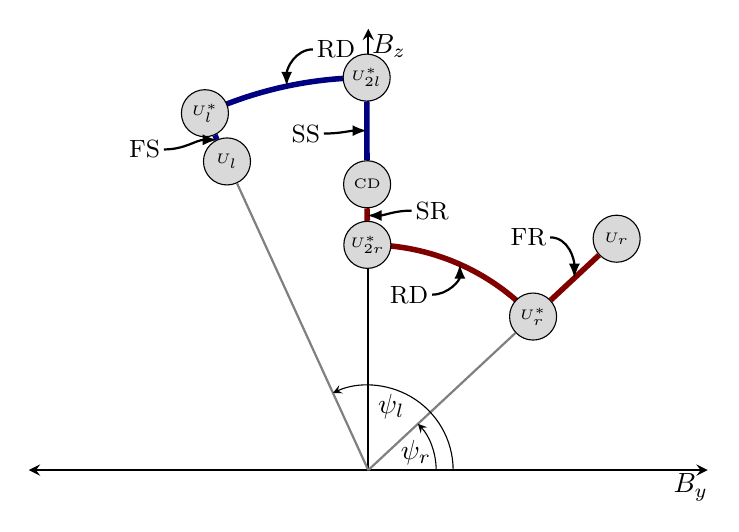
\begin{tikzpicture}[scale = {0.0125\linewidth},
    >=stealth, %
    inner sep=1pt, %outer sep=2pt,%
    axis/.style={thick,->},
    base node/.style={circle,draw,minimum size=17pt}]

  % axis
  \draw[thick] (0.95,0) node[below]{$B_y$}-|(0,1.25) node[right]{$B_z$};
  \draw[axis] (0.95,0)--(1.0,0);
  \draw[axis] (0,1.25)--(0,1.3);  
  \draw[axis] (0,0)--(-1,0);

  % Colors
  \colorlet{darkblue}{blue!50!black}
  \colorlet{darkred}{red!50!black}

  %---------------------------------------------
  % connect rotations
  %---------------------------------------------
  \draw[-,darkred, line width = 2pt] ++(42.972:0.66359) arc(42.972:90.232:0.66359);
  \draw[-,darkblue, line width = 2pt]++(114.59:1.15621)arc(114.592:90.232:1.15621);

  %---------------------------------------------
  % place node corresponding to shapes
  %---------------------------------------------
  \node[base node,draw,shape=circle,fill=gray!30] (R8) at (114.592:1.0) {\tiny $\mbf{U}_{l}$};
  \node[base node,draw,shape=circle,fill=gray!30] (R7) at (114.592:1.15621) {\tiny $\mbf{U}^*_{l}$};
  \node[base node,draw,shape=circle,fill=gray!30] (R6) at (90.232:1.15621) {\tiny $\mbf{U}^*_{2l}$};
  \node[base node,draw,shape=circle,fill=gray!30] (CD) at (90.232:0.84200) {\tiny CD};
  \node[base node,draw,shape=circle,fill=gray!30] (R3) at (90.232:0.66359) {\tiny $\mbf{U}^*_{2r}$};
  \node[base node,draw,shape=circle,fill=gray!30] (R2) at (42.972:0.66359) {\tiny $\mbf{U}^*_{r}$};
  \node[base node,draw,shape=circle,fill=gray!30] (R1) at (42.972:1.0) {\tiny $\mbf{U}_{r}$};

  %---------------------------------------------
  % connect nodes
  %---------------------------------------------
  \draw[gray,thick](0:0) -- (R2);
  \draw[darkred, line width = 2pt](R1) -- (R2);
  \draw[darkred, line width = 2pt](R3) -- (CD);
  \draw[darkblue, line width = 2pt](CD) -- (R6);
  \draw[darkblue, line width = 2pt](R7) -- (R8);
  \draw[gray,thick](0:0) -- (R8);
  
  %---------------------------------------------
  % place node corresponding to shapes
  %---------------------------------------------
  \path (0,0)++(70:0.2)node{$\psi_l$};
  \draw[->](0:0.25)arc(0:114.592:0.25);

  \draw[->](0:0.2)arc(0:42.972:0.2);
  \path (0,0)++(20:0.15)node{$\psi_r$};
  
  \draw[-latex,thick](122.5:1.12)node[left]{\small FS}
  to[out=0,in=180] (114.592:1.07);
  
  \draw[-latex,thick](97.5:1.25)node[right]{\small RD}
  to[out=180,in=90] (102:1.15621);
  
  \draw[-latex,thick](97.5:1.0)node[left]{\small SS}
  to[out=0,in=180] (90.232:1.0);
  
  %% \draw[-latex,thick](0.61,0.40)node[right]{\small CD}
  %% to[out=180,in=0] (0.51,0.45);
  
  \draw[-latex,thick](80.5:0.775)node[right]{\small SR}
  to[out=180,in=0] (90.232:0.75);
  
  \draw[-latex,thick](70:0.55)node[left]{\small RD}
  to[out=0,in=270] (66.0:0.66359);
  
  \draw[-latex,thick](52:0.87)node[left]{\small FR}
  to[out=0,in=90] (42.972:0.83);

\end{tikzpicture}

\end{center}
\caption{A view in the positive x-direction of Figure \ref{fig:riemann_3d}.  The influence of regular waves on the tangential magnetic field for a non-planar Riemann problem of ideal MHD. The orientation of the tangential magnetic field is given by the angle $\psi = \tan{B_z/B_y}$. Regular waves only influence the magnitude or orientation of the tangential magnetic field.  The intermediate states are defined in Figure~\ref{fig:mhd_states}, with $\mbf{B}^*_{t3l} = \mbf{B}^*_{t3r}$ denoted by the CD.}
\label{fig:bperp_regular}
\end{figure}

\clearpage
}

%-----------------------------------------------------------------
% Numerical tests
%-----------------------------------------------------------------
\section[Numerical tests]{Numerical tests}
\label{sec:num_test}
In this section we solve test cases that do and do not exhibit the uniqueness problem, in which more than one solution exists.  Solutions to the first four test cases are comprised of only regular waves.  The last two test cases involve compound waves.  A \gls{scw} is present in test 5, a \gls{fcw} is present in test 6, and two fast compound waves are present in Test~7.  Unless otherwise stated, the domain is $x\in [0,1]$ and the initial discontinuity is located at $x=0.5$.  In Chapter~\ref{chp:cwm}, tests 5, 6, and 7 are solved using a new modified flux method, and we show that only regular waves are present.
  
The results of several ideal MHD shock tube problems are given below.  The exact solution was calculated with the nonlinear solver developed for this thesis and described in Section~\ref{sec:mhd_exact}.  Three different approximation methods were used: a low order base scheme, a higher order TVD scheme, and a higher order FCT scheme.  All three schemes use a cell centered finite volume discretization and HLLD to approximate the interface flux.  The base scheme, which was implemented for this dissertation,  uses piece-constant interpolation for interface reconstruction and a two-stage Runge-Kutta time integration.  The TVD extension to the base scheme is implemented in \emph{Athena}.  Interfaces are reconstructed with PPM, and the \gls{ctu} plus \gls{ct} integrator is used to advance the solution in time.  The FCT extension to the base scheme was also implemented for this dissertation.  The algorithms of the base scheme and the FCT extention are implemented for general geometries, but structured grids were used for comparison with Athena.  Unless otherwise stated, the following values are used throughout the calculations, the gas constant $\gamma = 5/3$, the Courant number $C_r = 0.8$, and relaxation factor $r_k = 0.5$.

The initial conditions of the first shock tube test are 
\begin{gather}
\begin{split}
\label{eqn:rj2a_init}
(\rho_l,\vnl,\mbf{v}_{tl},\pgl,\mbf{B}_{tl})= \left(1.08,1.2,(0.01,0.5),0.95,(3.6,2.0)/\sqrt{4\pi}\right), \\
(\rho_r,\vnr,\mbf{v}_{tr},\pgr,\mbf{B}_{tr}) = \left(1.0,0.0,(0.0,0.0),1.0,(4.0,2.0)/\sqrt{4\pi}\right).
\end{split}
\end{gather}
The solution with $B_n=2/\sqrt{4\pi}$ and $\gamma=5/3$ is given in Table~\ref{tab:rj2a}, and is shown in Figure~\ref{fig:rj2a_plot} at time $t_f=0.2$.  From left to right, the waves of the solution are: FS, RD SS, CD, SS, RD, and FS.  The solution can be compared with Table 2a of \citep{Ryu:1995a}, and Table 1a of \citep{Dai:1994a}.  The nonlinear solver displays quadratic convergence, as shown in Table~\ref{tab:rj2a_err}, where the residual, as well as the fast and slow waves speeds are listed for a sequence of iterations.  The wave speeds are consistent with the result given in Table 1b of \citep{Dai:1994a}.  

The second shock tube test for ideal MHD has initial conditions
\begin{gather}
\begin{split}
\label{eqn:AK2_init}
(\rho_l,\vnl,\mbf{v}_{tl},\pgl,\mbf{B}_{tl})= \left(3.0,0.0,(0.0,0.0),3.0,(\cos\alpha_l,\sin\alpha_l)\right), \\
(\rho_r,\vnr,\mbf{v}_{tr},\pgr,\mbf{B}_{tr}) = \left(1.0,0.0,(0.0,0.0),1.0,(\cos\alpha_r,\sin\alpha_r)\right),
\end{split}
\end{gather}
where $\alpha_l = 2.0$, $\alpha_r = 1.0$, $B_n = 3/2$, and $\gamma=5/3$.  The solution is given in Table~\ref{tab:AK2}, and is shown in Figure~\ref{fig:AK2_plot} at time $t_f=0.2$.  From left to right the waves of the solution are: FR, RD SR, CD, SS, RD, and FS.  The residual, as well as the fast and slow waves speeds, are listed for a sequence of iterations in Table \ref{tab:AK2_err}.  

The third test problem involves states of high density and low pressure.  The initial conditions are
\begin{gather}
\begin{split}
\label{eqn:AK3_init}
(\rho_l,\vnl,\mbf{v}_{tl},\pgl,\mbf{B}_{tl})= \left(10.0.0,0.0,(1.0,0.0),0.2,(2.0,2.0)\right), \\
(\rho_r,\vnr,\mbf{v}_{tr},\pgr,\mbf{B}_{tr}) = \left(5.0,0.0,(-1.0,-0.5),0.2,2.0(\cos(\pi/4),\sin(\pi/4))\right),
\end{split}
\end{gather}
where $B_n = 2.0$, and $\gamma=5/3$.  The solution is given in Table~\ref{tab:AK3}, and is shown in Figure~\ref{fig:AK3_plot} at time $t_f=0.3$.  From left to right, the waves of the solution are: FR, RD SS, CD, SS, and FR.  The residual, as well as the fast and slow waves speeds are listed for a sequence of iterations in Table \ref{tab:AK3_err}.  The contact discontinuity speed is stationary.  No scheme was able to accurately capture the transition across the CD.  HLLD-TVD is the most accurate to the left of the CD, but like the other schemes, produces significant error to the right of the CD.  The velocities of the left- and right-going slow shocks are $-0.1013$ and $0.1433$ respectively.  The error is caused by the fact that the waves have not had enough time to separate.

The forth test retains the initial conditions of test 3, except the densities are reduced by an order of magnitude, the magnetic field components are reduced by one half, and $v_{yr} = -1.0$.  The initial conditions are
\begin{gather}
\begin{split}
\label{eqn:AK4_init}
(\rho_l,\vnl,\mbf{v}_{tl},\pgl,\mbf{B}_{tl})= \left(1.0.0,0.0,(1.0,0.0),0.5,(1.0, 0.0)\right), \\
(\rho_r,\vnr,\mbf{v}_{tr},\pgr,\mbf{B}_{tr}) = \left(0.5,0.0,(-1.0,-0.5),0.5,(\cos(\pi/4),\sin(\pi/4))\right),
\end{split}
\end{gather}
where $B_n = 1$, and $\gamma=5/3$.  The solution is given in Table~\ref{tab:AK4}, and is shown in Figure~\ref{fig:AK4_plot} at time $t_f=0.2$.  The same waves that comprise the solution to test 3 are also comprise the solution of this test. From left to right, the waves of the solution are: FR, RD SS, CD, SS, and FR.  Unlike test 3, there is no noticeable difference between the exact and approximate solutions in the states directly upstream and downstream of the contact discontinuity.  The residual, as well as the fast and slow waves speeds are listed for a sequence of iterations in Table \ref{tab:AK4_err}.  As in test 3, the contact discontinuity is stationary, but the waves have separated enough to avoid the error observed in test 3.

The final three tests demonstrate non-uniqueness of solutions to certain Riemann problems of ideal MHD.  For test 5 and 6, we consider two cases: one coplanar and one near coplanar.  For the coplanar case, the initial perpendicular magnetic field is anti-parallel, i.e., $\alpha = \pi$.  For the near coplanar case, the twist angle is reduced so that the initial tangential magnetic fields do not lie in the same plane.  In the near coplanar case, we set $\alpha = 3.0.$.  Test~7 is a non-planar problem.  The solution the includes a left-going RD that rotates the tangential magnetic field by $2.95$ radians.  Riemann problems of ideal MHD with non-unique solutions are discussed in greater detail next section where the problem of non-uniform convergence is described.  In Section~\ref{sec:nonunique}, the problems related to non-uniqueness are overcome with a new modification to the flux calculation.  

Test~5 involves a SCW comprised of a intermediate shock and fast rarefaction.  It was originally considered by \citet{Torrilhon:2003b}.  The conversion between the parameters used below and those used in \citep{Torrilhon:2003b} is given by \eqref{eqn:scaling}.  The initial conditions are 
\begin{gather}
\begin{split}
\label{eqn:AK5_init}
(\rho_l,\vnl,\mbf{v}_{tl},\pgl,\mbf{B}_{tl})= \left(1.0.0,0.0,(0.0,0.0),0.5,(0.7746, 0.0)\right), \\
(\rho_r,\vnr,\mbf{v}_{tr},\pgr,\mbf{B}_{tr}) = \left(0.2,0.0,(0.0,0.0),0.12,0.7746(\cos \alpha,\sin \alpha)\right),
\end{split}
\end{gather}
where $B_n = 0.7746$, and $\gamma=5/3$, and $\alpha = 3.0, \pi$.  In this test, the initial discontinuity is located at $x=0.4$ for comparison with the results in \citep{Torrilhon:2003b}.  Only the exact values of $\rho$ and $B_y$ are given in \citep{Torrilhon:2003b}.  We give the complete solution so that it can be used as a benchmark.  The exact solution for $\alpha = \pi$ ($3.0$) is listed in Table~\ref{tab:AK5}~(\ref{tab:AK5b}), and is shown in Figure~\ref{fig:AK5_plot}~(\ref{fig:AK5b_plot}) at time $t_f=0.20656$.  For both the coplanar and near coplanar cases, the structure of the approximate solution from left to right is: FR, SCW, CD, SS, FR.  An RD and SS are found in the exact solution instead of a slow compound wave.  For the near coplanar case, two rotational discontinuities are present.  The residual, as well as the fast and slow waves speeds are listed for a sequence of iterations is listed in Table~\ref{tab:AK5_err}~(\ref{tab:AK5b_err}), for $\alpha = \pi$ ($3.0$).  

Test~6 involves a FCW comprised of a fast rarefaction and intermediate shock.  The initial conditions are
\begin{gather}
\begin{split}
\label{eqn:AK6_init}
(\rho_l,\vnl,\mbf{v}_{tl},\pgl,\mbf{B}_{tl})= \left(1.0.0,0.0,(0.0,0.0),0.5,(1.0, 0.0)\right), \\
(\rho_r,\vnr,\mbf{v}_{tr},\pgr,\mbf{B}_{tr}) = \left(0.2,0.0,(0.0,0.0),0.12,(\cos \alpha,\sin \alpha)\right),
\end{split}
\end{gather}
where $B_n = 1.25$, $\gamma=5/3$, and $\alpha = 3.0, \pi$.  The exact solution for $\alpha = \pi$ ($3.0$) is listed in Table~\ref{tab:AK6}~(\ref{tab:AK6b}), and is shown in Figure~\ref{fig:AK6_plot}~(\ref{fig:AK6b_plot}) at time $t_f=0.15$.  For both the coplanar and near coplanar cases, the structure of the approximate solution from left to right is: FCW SS, CD, SS, FR.  A FR and RD is found in the exact solution instead of a fast compound wave.  For the near coplanar case, two rotational discontinuities are present.  The residual, as well as the fast and slow waves speeds are listed for a sequence of iterations is listed in Table~\ref{tab:AK6_err}~(\ref{tab:AK6b_err}), for $\alpha = \pi$ ($3.0$).  

Test~7 is the final test given in this section.  It involves a left-going and right-going FCW.  The initial conditions are
\begin{gather}
\begin{split}
\label{eqn:AK7_init}
(\rho_l,\vnl,\mbf{v}_{tl},\pgl,\mbf{B}_{tl})= \left(1.0.0,0.0,(5.0,0.0),0.6,(3.25, 0.0)\right), \\
(\rho_r,\vnr,\mbf{v}_{tr},\pgr,\mbf{B}_{tr}) = \left(0.5,0.0,(-5.0,-2.5),0.3,3.25(\cos \alpha,\sin \alpha)\right),
\end{split}
\end{gather}
where $B_n = 3.25$, $\gamma=5/3$, and $\alpha = \pi/4$.  The exact solution is listed in Table~\ref{tab:AK7}, and is shown in Figure~\ref{fig:AK7_plot} at time $t_f=0.05$.  From left to right is: FCW SS, CD, SS, FCW.  An RD and SS are found in the exact solution instead of a fast compound wave.  The left-going RD rotates the transverse magnetic field by 2.9442 radians, and the right-going RD rotates the transverse magnetic field by 2.1588 rad.  The residual, as well as the fast and slow waves speeds are listed for a sequence of iterations is listed in Table~\ref{tab:AK7_err}.  The CD is not accurately captured due to the lack of separation between the waves.

%% \clearpage
\afterpage{
\begin{landscape}
%-----------------------------------------------------------------
% Solution to RJ2a
%-----------------------------------------------------------------
\begin{figure}[t!]
\begin{tabular}{ccc}
\resizebox{0.33\linewidth}{!}{\tikzsetnextfilename{RJ2a_csol_1}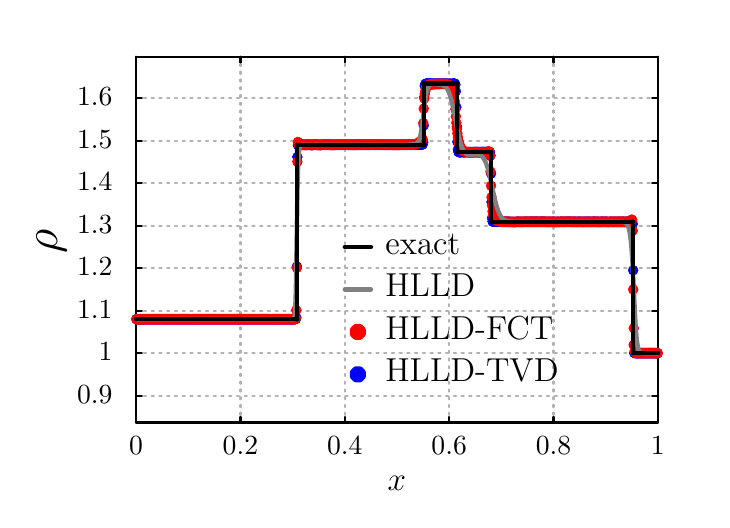
\begin{tikzpicture}[gnuplot]
%% generated with GNUPLOT 4.6p4 (Lua 5.1; terminal rev. 99, script rev. 100)
%% Fri 08 Aug 2014 12:23:45 PM EDT
\path (0.000,0.000) rectangle (8.500,6.000);
\gpfill{rgb color={1.000,1.000,1.000}} (1.320,0.985)--(7.946,0.985)--(7.946,5.630)--(1.320,5.630)--cycle;
\gpcolor{color=gp lt color border}
\gpsetlinetype{gp lt border}
\gpsetlinewidth{1.00}
\draw[gp path] (1.320,0.985)--(1.320,5.630)--(7.946,5.630)--(7.946,0.985)--cycle;
\gpcolor{color=gp lt color axes}
\gpsetlinetype{gp lt axes}
\gpsetlinewidth{2.00}
\draw[gp path] (1.320,1.327)--(7.947,1.327);
\gpcolor{color=gp lt color border}
\gpsetlinetype{gp lt border}
\draw[gp path] (1.320,1.327)--(1.392,1.327);
\draw[gp path] (7.947,1.327)--(7.875,1.327);
\gpcolor{rgb color={0.000,0.000,0.000}}
\node[gp node right,font={\fontsize{10pt}{12pt}\selectfont}] at (1.136,1.327) {0.9};
\gpcolor{color=gp lt color axes}
\gpsetlinetype{gp lt axes}
\draw[gp path] (1.320,1.867)--(7.947,1.867);
\gpcolor{color=gp lt color border}
\gpsetlinetype{gp lt border}
\draw[gp path] (1.320,1.867)--(1.392,1.867);
\draw[gp path] (7.947,1.867)--(7.875,1.867);
\gpcolor{rgb color={0.000,0.000,0.000}}
\node[gp node right,font={\fontsize{10pt}{12pt}\selectfont}] at (1.136,1.867) {1};
\gpcolor{color=gp lt color axes}
\gpsetlinetype{gp lt axes}
\draw[gp path] (1.320,2.406)--(7.947,2.406);
\gpcolor{color=gp lt color border}
\gpsetlinetype{gp lt border}
\draw[gp path] (1.320,2.406)--(1.392,2.406);
\draw[gp path] (7.947,2.406)--(7.875,2.406);
\gpcolor{rgb color={0.000,0.000,0.000}}
\node[gp node right,font={\fontsize{10pt}{12pt}\selectfont}] at (1.136,2.406) {1.1};
\gpcolor{color=gp lt color axes}
\gpsetlinetype{gp lt axes}
\draw[gp path] (1.320,2.946)--(7.947,2.946);
\gpcolor{color=gp lt color border}
\gpsetlinetype{gp lt border}
\draw[gp path] (1.320,2.946)--(1.392,2.946);
\draw[gp path] (7.947,2.946)--(7.875,2.946);
\gpcolor{rgb color={0.000,0.000,0.000}}
\node[gp node right,font={\fontsize{10pt}{12pt}\selectfont}] at (1.136,2.946) {1.2};
\gpcolor{color=gp lt color axes}
\gpsetlinetype{gp lt axes}
\draw[gp path] (1.320,3.485)--(7.947,3.485);
\gpcolor{color=gp lt color border}
\gpsetlinetype{gp lt border}
\draw[gp path] (1.320,3.485)--(1.392,3.485);
\draw[gp path] (7.947,3.485)--(7.875,3.485);
\gpcolor{rgb color={0.000,0.000,0.000}}
\node[gp node right,font={\fontsize{10pt}{12pt}\selectfont}] at (1.136,3.485) {1.3};
\gpcolor{color=gp lt color axes}
\gpsetlinetype{gp lt axes}
\draw[gp path] (1.320,4.025)--(7.947,4.025);
\gpcolor{color=gp lt color border}
\gpsetlinetype{gp lt border}
\draw[gp path] (1.320,4.025)--(1.392,4.025);
\draw[gp path] (7.947,4.025)--(7.875,4.025);
\gpcolor{rgb color={0.000,0.000,0.000}}
\node[gp node right,font={\fontsize{10pt}{12pt}\selectfont}] at (1.136,4.025) {1.4};
\gpcolor{color=gp lt color axes}
\gpsetlinetype{gp lt axes}
\draw[gp path] (1.320,4.564)--(7.947,4.564);
\gpcolor{color=gp lt color border}
\gpsetlinetype{gp lt border}
\draw[gp path] (1.320,4.564)--(1.392,4.564);
\draw[gp path] (7.947,4.564)--(7.875,4.564);
\gpcolor{rgb color={0.000,0.000,0.000}}
\node[gp node right,font={\fontsize{10pt}{12pt}\selectfont}] at (1.136,4.564) {1.5};
\gpcolor{color=gp lt color axes}
\gpsetlinetype{gp lt axes}
\draw[gp path] (1.320,5.104)--(7.947,5.104);
\gpcolor{color=gp lt color border}
\gpsetlinetype{gp lt border}
\draw[gp path] (1.320,5.104)--(1.392,5.104);
\draw[gp path] (7.947,5.104)--(7.875,5.104);
\gpcolor{rgb color={0.000,0.000,0.000}}
\node[gp node right,font={\fontsize{10pt}{12pt}\selectfont}] at (1.136,5.104) {1.6};
\gpcolor{color=gp lt color axes}
\gpsetlinetype{gp lt axes}
\draw[gp path] (1.320,0.985)--(1.320,5.631);
\gpcolor{color=gp lt color border}
\gpsetlinetype{gp lt border}
\draw[gp path] (1.320,0.985)--(1.320,1.057);
\draw[gp path] (1.320,5.631)--(1.320,5.559);
\gpcolor{rgb color={0.000,0.000,0.000}}
\node[gp node center,font={\fontsize{10pt}{12pt}\selectfont}] at (1.320,0.677) {0};
\gpcolor{color=gp lt color axes}
\gpsetlinetype{gp lt axes}
\draw[gp path] (2.645,0.985)--(2.645,5.631);
\gpcolor{color=gp lt color border}
\gpsetlinetype{gp lt border}
\draw[gp path] (2.645,0.985)--(2.645,1.057);
\draw[gp path] (2.645,5.631)--(2.645,5.559);
\gpcolor{rgb color={0.000,0.000,0.000}}
\node[gp node center,font={\fontsize{10pt}{12pt}\selectfont}] at (2.645,0.677) {0.2};
\gpcolor{color=gp lt color axes}
\gpsetlinetype{gp lt axes}
\draw[gp path] (3.971,0.985)--(3.971,5.631);
\gpcolor{color=gp lt color border}
\gpsetlinetype{gp lt border}
\draw[gp path] (3.971,0.985)--(3.971,1.057);
\draw[gp path] (3.971,5.631)--(3.971,5.559);
\gpcolor{rgb color={0.000,0.000,0.000}}
\node[gp node center,font={\fontsize{10pt}{12pt}\selectfont}] at (3.971,0.677) {0.4};
\gpcolor{color=gp lt color axes}
\gpsetlinetype{gp lt axes}
\draw[gp path] (5.296,0.985)--(5.296,5.631);
\gpcolor{color=gp lt color border}
\gpsetlinetype{gp lt border}
\draw[gp path] (5.296,0.985)--(5.296,1.057);
\draw[gp path] (5.296,5.631)--(5.296,5.559);
\gpcolor{rgb color={0.000,0.000,0.000}}
\node[gp node center,font={\fontsize{10pt}{12pt}\selectfont}] at (5.296,0.677) {0.6};
\gpcolor{color=gp lt color axes}
\gpsetlinetype{gp lt axes}
\draw[gp path] (6.622,0.985)--(6.622,5.631);
\gpcolor{color=gp lt color border}
\gpsetlinetype{gp lt border}
\draw[gp path] (6.622,0.985)--(6.622,1.057);
\draw[gp path] (6.622,5.631)--(6.622,5.559);
\gpcolor{rgb color={0.000,0.000,0.000}}
\node[gp node center,font={\fontsize{10pt}{12pt}\selectfont}] at (6.622,0.677) {0.8};
\gpcolor{color=gp lt color axes}
\gpsetlinetype{gp lt axes}
\draw[gp path] (7.947,0.985)--(7.947,5.631);
\gpcolor{color=gp lt color border}
\gpsetlinetype{gp lt border}
\draw[gp path] (7.947,0.985)--(7.947,1.057);
\draw[gp path] (7.947,5.631)--(7.947,5.559);
\gpcolor{rgb color={0.000,0.000,0.000}}
\node[gp node center,font={\fontsize{10pt}{12pt}\selectfont}] at (7.947,0.677) {1};
\gpcolor{color=gp lt color border}
\draw[gp path] (1.320,5.631)--(1.320,0.985)--(7.947,0.985)--(7.947,5.631)--cycle;
\gpcolor{rgb color={0.000,0.000,0.000}}
\node[gp node center,rotate=90,font={\fontsize{10pt}{12pt}\selectfont}] at (0.246,3.308) {\LARGE $\rho$};
\node[gp node center,font={\fontsize{10pt}{12pt}\selectfont}] at (4.633,0.215) {\large $x$};
\gpcolor{rgb color={0.000,0.000,1.000}}
\gpsetlinewidth{0.50}
\gpsetpointsize{4.44}
\gppoint{gp mark 7}{(1.323,2.298)}
\gppoint{gp mark 7}{(1.330,2.298)}
\gppoint{gp mark 7}{(1.336,2.298)}
\gppoint{gp mark 7}{(1.343,2.298)}
\gppoint{gp mark 7}{(1.349,2.298)}
\gppoint{gp mark 7}{(1.356,2.298)}
\gppoint{gp mark 7}{(1.362,2.298)}
\gppoint{gp mark 7}{(1.369,2.298)}
\gppoint{gp mark 7}{(1.375,2.298)}
\gppoint{gp mark 7}{(1.381,2.298)}
\gppoint{gp mark 7}{(1.388,2.298)}
\gppoint{gp mark 7}{(1.394,2.298)}
\gppoint{gp mark 7}{(1.401,2.298)}
\gppoint{gp mark 7}{(1.407,2.298)}
\gppoint{gp mark 7}{(1.414,2.298)}
\gppoint{gp mark 7}{(1.420,2.298)}
\gppoint{gp mark 7}{(1.427,2.298)}
\gppoint{gp mark 7}{(1.433,2.298)}
\gppoint{gp mark 7}{(1.440,2.298)}
\gppoint{gp mark 7}{(1.446,2.298)}
\gppoint{gp mark 7}{(1.453,2.298)}
\gppoint{gp mark 7}{(1.459,2.298)}
\gppoint{gp mark 7}{(1.466,2.298)}
\gppoint{gp mark 7}{(1.472,2.298)}
\gppoint{gp mark 7}{(1.479,2.298)}
\gppoint{gp mark 7}{(1.485,2.298)}
\gppoint{gp mark 7}{(1.491,2.298)}
\gppoint{gp mark 7}{(1.498,2.298)}
\gppoint{gp mark 7}{(1.504,2.298)}
\gppoint{gp mark 7}{(1.511,2.298)}
\gppoint{gp mark 7}{(1.517,2.298)}
\gppoint{gp mark 7}{(1.524,2.298)}
\gppoint{gp mark 7}{(1.530,2.298)}
\gppoint{gp mark 7}{(1.537,2.298)}
\gppoint{gp mark 7}{(1.543,2.298)}
\gppoint{gp mark 7}{(1.550,2.298)}
\gppoint{gp mark 7}{(1.556,2.298)}
\gppoint{gp mark 7}{(1.563,2.298)}
\gppoint{gp mark 7}{(1.569,2.298)}
\gppoint{gp mark 7}{(1.576,2.298)}
\gppoint{gp mark 7}{(1.582,2.298)}
\gppoint{gp mark 7}{(1.589,2.298)}
\gppoint{gp mark 7}{(1.595,2.298)}
\gppoint{gp mark 7}{(1.602,2.298)}
\gppoint{gp mark 7}{(1.608,2.298)}
\gppoint{gp mark 7}{(1.614,2.298)}
\gppoint{gp mark 7}{(1.621,2.298)}
\gppoint{gp mark 7}{(1.627,2.298)}
\gppoint{gp mark 7}{(1.634,2.298)}
\gppoint{gp mark 7}{(1.640,2.298)}
\gppoint{gp mark 7}{(1.647,2.298)}
\gppoint{gp mark 7}{(1.653,2.298)}
\gppoint{gp mark 7}{(1.660,2.298)}
\gppoint{gp mark 7}{(1.666,2.298)}
\gppoint{gp mark 7}{(1.673,2.298)}
\gppoint{gp mark 7}{(1.679,2.298)}
\gppoint{gp mark 7}{(1.686,2.298)}
\gppoint{gp mark 7}{(1.692,2.298)}
\gppoint{gp mark 7}{(1.699,2.298)}
\gppoint{gp mark 7}{(1.705,2.298)}
\gppoint{gp mark 7}{(1.712,2.298)}
\gppoint{gp mark 7}{(1.718,2.298)}
\gppoint{gp mark 7}{(1.724,2.298)}
\gppoint{gp mark 7}{(1.731,2.298)}
\gppoint{gp mark 7}{(1.737,2.298)}
\gppoint{gp mark 7}{(1.744,2.298)}
\gppoint{gp mark 7}{(1.750,2.298)}
\gppoint{gp mark 7}{(1.757,2.298)}
\gppoint{gp mark 7}{(1.763,2.298)}
\gppoint{gp mark 7}{(1.770,2.298)}
\gppoint{gp mark 7}{(1.776,2.298)}
\gppoint{gp mark 7}{(1.783,2.298)}
\gppoint{gp mark 7}{(1.789,2.298)}
\gppoint{gp mark 7}{(1.796,2.298)}
\gppoint{gp mark 7}{(1.802,2.298)}
\gppoint{gp mark 7}{(1.809,2.298)}
\gppoint{gp mark 7}{(1.815,2.298)}
\gppoint{gp mark 7}{(1.822,2.298)}
\gppoint{gp mark 7}{(1.828,2.298)}
\gppoint{gp mark 7}{(1.834,2.298)}
\gppoint{gp mark 7}{(1.841,2.298)}
\gppoint{gp mark 7}{(1.847,2.298)}
\gppoint{gp mark 7}{(1.854,2.298)}
\gppoint{gp mark 7}{(1.860,2.298)}
\gppoint{gp mark 7}{(1.867,2.298)}
\gppoint{gp mark 7}{(1.873,2.298)}
\gppoint{gp mark 7}{(1.880,2.298)}
\gppoint{gp mark 7}{(1.886,2.298)}
\gppoint{gp mark 7}{(1.893,2.298)}
\gppoint{gp mark 7}{(1.899,2.298)}
\gppoint{gp mark 7}{(1.906,2.298)}
\gppoint{gp mark 7}{(1.912,2.298)}
\gppoint{gp mark 7}{(1.919,2.298)}
\gppoint{gp mark 7}{(1.925,2.298)}
\gppoint{gp mark 7}{(1.932,2.298)}
\gppoint{gp mark 7}{(1.938,2.298)}
\gppoint{gp mark 7}{(1.945,2.298)}
\gppoint{gp mark 7}{(1.951,2.298)}
\gppoint{gp mark 7}{(1.957,2.298)}
\gppoint{gp mark 7}{(1.964,2.298)}
\gppoint{gp mark 7}{(1.970,2.298)}
\gppoint{gp mark 7}{(1.977,2.298)}
\gppoint{gp mark 7}{(1.983,2.298)}
\gppoint{gp mark 7}{(1.990,2.298)}
\gppoint{gp mark 7}{(1.996,2.298)}
\gppoint{gp mark 7}{(2.003,2.298)}
\gppoint{gp mark 7}{(2.009,2.298)}
\gppoint{gp mark 7}{(2.016,2.298)}
\gppoint{gp mark 7}{(2.022,2.298)}
\gppoint{gp mark 7}{(2.029,2.298)}
\gppoint{gp mark 7}{(2.035,2.298)}
\gppoint{gp mark 7}{(2.042,2.298)}
\gppoint{gp mark 7}{(2.048,2.298)}
\gppoint{gp mark 7}{(2.055,2.298)}
\gppoint{gp mark 7}{(2.061,2.298)}
\gppoint{gp mark 7}{(2.067,2.298)}
\gppoint{gp mark 7}{(2.074,2.298)}
\gppoint{gp mark 7}{(2.080,2.298)}
\gppoint{gp mark 7}{(2.087,2.298)}
\gppoint{gp mark 7}{(2.093,2.298)}
\gppoint{gp mark 7}{(2.100,2.298)}
\gppoint{gp mark 7}{(2.106,2.298)}
\gppoint{gp mark 7}{(2.113,2.298)}
\gppoint{gp mark 7}{(2.119,2.298)}
\gppoint{gp mark 7}{(2.126,2.298)}
\gppoint{gp mark 7}{(2.132,2.298)}
\gppoint{gp mark 7}{(2.139,2.298)}
\gppoint{gp mark 7}{(2.145,2.298)}
\gppoint{gp mark 7}{(2.152,2.298)}
\gppoint{gp mark 7}{(2.158,2.298)}
\gppoint{gp mark 7}{(2.165,2.298)}
\gppoint{gp mark 7}{(2.171,2.298)}
\gppoint{gp mark 7}{(2.177,2.298)}
\gppoint{gp mark 7}{(2.184,2.298)}
\gppoint{gp mark 7}{(2.190,2.298)}
\gppoint{gp mark 7}{(2.197,2.298)}
\gppoint{gp mark 7}{(2.203,2.298)}
\gppoint{gp mark 7}{(2.210,2.298)}
\gppoint{gp mark 7}{(2.216,2.298)}
\gppoint{gp mark 7}{(2.223,2.298)}
\gppoint{gp mark 7}{(2.229,2.298)}
\gppoint{gp mark 7}{(2.236,2.298)}
\gppoint{gp mark 7}{(2.242,2.298)}
\gppoint{gp mark 7}{(2.249,2.298)}
\gppoint{gp mark 7}{(2.255,2.298)}
\gppoint{gp mark 7}{(2.262,2.298)}
\gppoint{gp mark 7}{(2.268,2.298)}
\gppoint{gp mark 7}{(2.275,2.298)}
\gppoint{gp mark 7}{(2.281,2.298)}
\gppoint{gp mark 7}{(2.288,2.298)}
\gppoint{gp mark 7}{(2.294,2.298)}
\gppoint{gp mark 7}{(2.300,2.298)}
\gppoint{gp mark 7}{(2.307,2.298)}
\gppoint{gp mark 7}{(2.313,2.298)}
\gppoint{gp mark 7}{(2.320,2.298)}
\gppoint{gp mark 7}{(2.326,2.298)}
\gppoint{gp mark 7}{(2.333,2.298)}
\gppoint{gp mark 7}{(2.339,2.298)}
\gppoint{gp mark 7}{(2.346,2.298)}
\gppoint{gp mark 7}{(2.352,2.298)}
\gppoint{gp mark 7}{(2.359,2.298)}
\gppoint{gp mark 7}{(2.365,2.298)}
\gppoint{gp mark 7}{(2.372,2.298)}
\gppoint{gp mark 7}{(2.378,2.298)}
\gppoint{gp mark 7}{(2.385,2.298)}
\gppoint{gp mark 7}{(2.391,2.298)}
\gppoint{gp mark 7}{(2.398,2.298)}
\gppoint{gp mark 7}{(2.404,2.298)}
\gppoint{gp mark 7}{(2.410,2.298)}
\gppoint{gp mark 7}{(2.417,2.298)}
\gppoint{gp mark 7}{(2.423,2.298)}
\gppoint{gp mark 7}{(2.430,2.298)}
\gppoint{gp mark 7}{(2.436,2.298)}
\gppoint{gp mark 7}{(2.443,2.298)}
\gppoint{gp mark 7}{(2.449,2.298)}
\gppoint{gp mark 7}{(2.456,2.298)}
\gppoint{gp mark 7}{(2.462,2.298)}
\gppoint{gp mark 7}{(2.469,2.298)}
\gppoint{gp mark 7}{(2.475,2.298)}
\gppoint{gp mark 7}{(2.482,2.298)}
\gppoint{gp mark 7}{(2.488,2.298)}
\gppoint{gp mark 7}{(2.495,2.298)}
\gppoint{gp mark 7}{(2.501,2.298)}
\gppoint{gp mark 7}{(2.508,2.298)}
\gppoint{gp mark 7}{(2.514,2.298)}
\gppoint{gp mark 7}{(2.520,2.298)}
\gppoint{gp mark 7}{(2.527,2.298)}
\gppoint{gp mark 7}{(2.533,2.298)}
\gppoint{gp mark 7}{(2.540,2.298)}
\gppoint{gp mark 7}{(2.546,2.298)}
\gppoint{gp mark 7}{(2.553,2.298)}
\gppoint{gp mark 7}{(2.559,2.298)}
\gppoint{gp mark 7}{(2.566,2.298)}
\gppoint{gp mark 7}{(2.572,2.298)}
\gppoint{gp mark 7}{(2.579,2.298)}
\gppoint{gp mark 7}{(2.585,2.298)}
\gppoint{gp mark 7}{(2.592,2.298)}
\gppoint{gp mark 7}{(2.598,2.298)}
\gppoint{gp mark 7}{(2.605,2.298)}
\gppoint{gp mark 7}{(2.611,2.298)}
\gppoint{gp mark 7}{(2.618,2.298)}
\gppoint{gp mark 7}{(2.624,2.298)}
\gppoint{gp mark 7}{(2.631,2.298)}
\gppoint{gp mark 7}{(2.637,2.298)}
\gppoint{gp mark 7}{(2.643,2.298)}
\gppoint{gp mark 7}{(2.650,2.298)}
\gppoint{gp mark 7}{(2.656,2.298)}
\gppoint{gp mark 7}{(2.663,2.298)}
\gppoint{gp mark 7}{(2.669,2.298)}
\gppoint{gp mark 7}{(2.676,2.298)}
\gppoint{gp mark 7}{(2.682,2.298)}
\gppoint{gp mark 7}{(2.689,2.298)}
\gppoint{gp mark 7}{(2.695,2.298)}
\gppoint{gp mark 7}{(2.702,2.298)}
\gppoint{gp mark 7}{(2.708,2.298)}
\gppoint{gp mark 7}{(2.715,2.298)}
\gppoint{gp mark 7}{(2.721,2.298)}
\gppoint{gp mark 7}{(2.728,2.298)}
\gppoint{gp mark 7}{(2.734,2.298)}
\gppoint{gp mark 7}{(2.741,2.298)}
\gppoint{gp mark 7}{(2.747,2.298)}
\gppoint{gp mark 7}{(2.753,2.298)}
\gppoint{gp mark 7}{(2.760,2.298)}
\gppoint{gp mark 7}{(2.766,2.298)}
\gppoint{gp mark 7}{(2.773,2.298)}
\gppoint{gp mark 7}{(2.779,2.298)}
\gppoint{gp mark 7}{(2.786,2.298)}
\gppoint{gp mark 7}{(2.792,2.298)}
\gppoint{gp mark 7}{(2.799,2.298)}
\gppoint{gp mark 7}{(2.805,2.298)}
\gppoint{gp mark 7}{(2.812,2.298)}
\gppoint{gp mark 7}{(2.818,2.298)}
\gppoint{gp mark 7}{(2.825,2.298)}
\gppoint{gp mark 7}{(2.831,2.298)}
\gppoint{gp mark 7}{(2.838,2.298)}
\gppoint{gp mark 7}{(2.844,2.298)}
\gppoint{gp mark 7}{(2.851,2.298)}
\gppoint{gp mark 7}{(2.857,2.298)}
\gppoint{gp mark 7}{(2.863,2.298)}
\gppoint{gp mark 7}{(2.870,2.298)}
\gppoint{gp mark 7}{(2.876,2.298)}
\gppoint{gp mark 7}{(2.883,2.298)}
\gppoint{gp mark 7}{(2.889,2.298)}
\gppoint{gp mark 7}{(2.896,2.298)}
\gppoint{gp mark 7}{(2.902,2.298)}
\gppoint{gp mark 7}{(2.909,2.298)}
\gppoint{gp mark 7}{(2.915,2.298)}
\gppoint{gp mark 7}{(2.922,2.298)}
\gppoint{gp mark 7}{(2.928,2.298)}
\gppoint{gp mark 7}{(2.935,2.298)}
\gppoint{gp mark 7}{(2.941,2.298)}
\gppoint{gp mark 7}{(2.948,2.298)}
\gppoint{gp mark 7}{(2.954,2.298)}
\gppoint{gp mark 7}{(2.961,2.298)}
\gppoint{gp mark 7}{(2.967,2.298)}
\gppoint{gp mark 7}{(2.974,2.298)}
\gppoint{gp mark 7}{(2.980,2.298)}
\gppoint{gp mark 7}{(2.986,2.298)}
\gppoint{gp mark 7}{(2.993,2.298)}
\gppoint{gp mark 7}{(2.999,2.298)}
\gppoint{gp mark 7}{(3.006,2.298)}
\gppoint{gp mark 7}{(3.012,2.298)}
\gppoint{gp mark 7}{(3.019,2.298)}
\gppoint{gp mark 7}{(3.025,2.298)}
\gppoint{gp mark 7}{(3.032,2.298)}
\gppoint{gp mark 7}{(3.038,2.298)}
\gppoint{gp mark 7}{(3.045,2.298)}
\gppoint{gp mark 7}{(3.051,2.298)}
\gppoint{gp mark 7}{(3.058,2.298)}
\gppoint{gp mark 7}{(3.064,2.298)}
\gppoint{gp mark 7}{(3.071,2.298)}
\gppoint{gp mark 7}{(3.077,2.298)}
\gppoint{gp mark 7}{(3.084,2.298)}
\gppoint{gp mark 7}{(3.090,2.298)}
\gppoint{gp mark 7}{(3.096,2.298)}
\gppoint{gp mark 7}{(3.103,2.298)}
\gppoint{gp mark 7}{(3.109,2.298)}
\gppoint{gp mark 7}{(3.116,2.298)}
\gppoint{gp mark 7}{(3.122,2.298)}
\gppoint{gp mark 7}{(3.129,2.298)}
\gppoint{gp mark 7}{(3.135,2.298)}
\gppoint{gp mark 7}{(3.142,2.298)}
\gppoint{gp mark 7}{(3.148,2.298)}
\gppoint{gp mark 7}{(3.155,2.298)}
\gppoint{gp mark 7}{(3.161,2.298)}
\gppoint{gp mark 7}{(3.168,2.298)}
\gppoint{gp mark 7}{(3.174,2.298)}
\gppoint{gp mark 7}{(3.181,2.298)}
\gppoint{gp mark 7}{(3.187,2.298)}
\gppoint{gp mark 7}{(3.194,2.298)}
\gppoint{gp mark 7}{(3.200,2.298)}
\gppoint{gp mark 7}{(3.206,2.298)}
\gppoint{gp mark 7}{(3.213,2.298)}
\gppoint{gp mark 7}{(3.219,2.298)}
\gppoint{gp mark 7}{(3.226,2.298)}
\gppoint{gp mark 7}{(3.232,2.298)}
\gppoint{gp mark 7}{(3.239,2.298)}
\gppoint{gp mark 7}{(3.245,2.298)}
\gppoint{gp mark 7}{(3.252,2.298)}
\gppoint{gp mark 7}{(3.258,2.298)}
\gppoint{gp mark 7}{(3.265,2.298)}
\gppoint{gp mark 7}{(3.271,2.298)}
\gppoint{gp mark 7}{(3.278,2.298)}
\gppoint{gp mark 7}{(3.284,2.298)}
\gppoint{gp mark 7}{(3.291,2.298)}
\gppoint{gp mark 7}{(3.297,2.298)}
\gppoint{gp mark 7}{(3.304,2.298)}
\gppoint{gp mark 7}{(3.310,2.298)}
\gppoint{gp mark 7}{(3.317,2.298)}
\gppoint{gp mark 7}{(3.323,2.298)}
\gppoint{gp mark 7}{(3.329,2.298)}
\gppoint{gp mark 7}{(3.336,2.298)}
\gppoint{gp mark 7}{(3.342,2.298)}
\gppoint{gp mark 7}{(3.349,2.299)}
\gppoint{gp mark 7}{(3.355,2.319)}
\gppoint{gp mark 7}{(3.362,2.966)}
\gppoint{gp mark 7}{(3.368,4.358)}
\gppoint{gp mark 7}{(3.375,4.509)}
\gppoint{gp mark 7}{(3.381,4.509)}
\gppoint{gp mark 7}{(3.388,4.514)}
\gppoint{gp mark 7}{(3.394,4.517)}
\gppoint{gp mark 7}{(3.401,4.510)}
\gppoint{gp mark 7}{(3.407,4.508)}
\gppoint{gp mark 7}{(3.414,4.513)}
\gppoint{gp mark 7}{(3.420,4.514)}
\gppoint{gp mark 7}{(3.427,4.511)}
\gppoint{gp mark 7}{(3.433,4.511)}
\gppoint{gp mark 7}{(3.439,4.514)}
\gppoint{gp mark 7}{(3.446,4.513)}
\gppoint{gp mark 7}{(3.452,4.511)}
\gppoint{gp mark 7}{(3.459,4.511)}
\gppoint{gp mark 7}{(3.465,4.512)}
\gppoint{gp mark 7}{(3.472,4.512)}
\gppoint{gp mark 7}{(3.478,4.512)}
\gppoint{gp mark 7}{(3.485,4.513)}
\gppoint{gp mark 7}{(3.491,4.513)}
\gppoint{gp mark 7}{(3.498,4.512)}
\gppoint{gp mark 7}{(3.504,4.511)}
\gppoint{gp mark 7}{(3.511,4.512)}
\gppoint{gp mark 7}{(3.517,4.512)}
\gppoint{gp mark 7}{(3.524,4.512)}
\gppoint{gp mark 7}{(3.530,4.512)}
\gppoint{gp mark 7}{(3.537,4.513)}
\gppoint{gp mark 7}{(3.543,4.512)}
\gppoint{gp mark 7}{(3.549,4.512)}
\gppoint{gp mark 7}{(3.556,4.512)}
\gppoint{gp mark 7}{(3.562,4.512)}
\gppoint{gp mark 7}{(3.569,4.512)}
\gppoint{gp mark 7}{(3.575,4.512)}
\gppoint{gp mark 7}{(3.582,4.512)}
\gppoint{gp mark 7}{(3.588,4.512)}
\gppoint{gp mark 7}{(3.595,4.512)}
\gppoint{gp mark 7}{(3.601,4.512)}
\gppoint{gp mark 7}{(3.608,4.512)}
\gppoint{gp mark 7}{(3.614,4.512)}
\gppoint{gp mark 7}{(3.621,4.512)}
\gppoint{gp mark 7}{(3.627,4.512)}
\gppoint{gp mark 7}{(3.634,4.512)}
\gppoint{gp mark 7}{(3.640,4.512)}
\gppoint{gp mark 7}{(3.647,4.512)}
\gppoint{gp mark 7}{(3.653,4.512)}
\gppoint{gp mark 7}{(3.660,4.512)}
\gppoint{gp mark 7}{(3.666,4.512)}
\gppoint{gp mark 7}{(3.672,4.512)}
\gppoint{gp mark 7}{(3.679,4.512)}
\gppoint{gp mark 7}{(3.685,4.512)}
\gppoint{gp mark 7}{(3.692,4.512)}
\gppoint{gp mark 7}{(3.698,4.512)}
\gppoint{gp mark 7}{(3.705,4.512)}
\gppoint{gp mark 7}{(3.711,4.512)}
\gppoint{gp mark 7}{(3.718,4.512)}
\gppoint{gp mark 7}{(3.724,4.512)}
\gppoint{gp mark 7}{(3.731,4.512)}
\gppoint{gp mark 7}{(3.737,4.512)}
\gppoint{gp mark 7}{(3.744,4.512)}
\gppoint{gp mark 7}{(3.750,4.512)}
\gppoint{gp mark 7}{(3.757,4.512)}
\gppoint{gp mark 7}{(3.763,4.512)}
\gppoint{gp mark 7}{(3.770,4.512)}
\gppoint{gp mark 7}{(3.776,4.512)}
\gppoint{gp mark 7}{(3.782,4.512)}
\gppoint{gp mark 7}{(3.789,4.512)}
\gppoint{gp mark 7}{(3.795,4.512)}
\gppoint{gp mark 7}{(3.802,4.512)}
\gppoint{gp mark 7}{(3.808,4.512)}
\gppoint{gp mark 7}{(3.815,4.512)}
\gppoint{gp mark 7}{(3.821,4.512)}
\gppoint{gp mark 7}{(3.828,4.512)}
\gppoint{gp mark 7}{(3.834,4.512)}
\gppoint{gp mark 7}{(3.841,4.512)}
\gppoint{gp mark 7}{(3.847,4.512)}
\gppoint{gp mark 7}{(3.854,4.512)}
\gppoint{gp mark 7}{(3.860,4.512)}
\gppoint{gp mark 7}{(3.867,4.512)}
\gppoint{gp mark 7}{(3.873,4.512)}
\gppoint{gp mark 7}{(3.880,4.512)}
\gppoint{gp mark 7}{(3.886,4.512)}
\gppoint{gp mark 7}{(3.892,4.512)}
\gppoint{gp mark 7}{(3.899,4.512)}
\gppoint{gp mark 7}{(3.905,4.512)}
\gppoint{gp mark 7}{(3.912,4.512)}
\gppoint{gp mark 7}{(3.918,4.512)}
\gppoint{gp mark 7}{(3.925,4.512)}
\gppoint{gp mark 7}{(3.931,4.512)}
\gppoint{gp mark 7}{(3.938,4.512)}
\gppoint{gp mark 7}{(3.944,4.512)}
\gppoint{gp mark 7}{(3.951,4.512)}
\gppoint{gp mark 7}{(3.957,4.512)}
\gppoint{gp mark 7}{(3.964,4.512)}
\gppoint{gp mark 7}{(3.970,4.512)}
\gppoint{gp mark 7}{(3.977,4.512)}
\gppoint{gp mark 7}{(3.983,4.512)}
\gppoint{gp mark 7}{(3.990,4.512)}
\gppoint{gp mark 7}{(3.996,4.512)}
\gppoint{gp mark 7}{(4.003,4.512)}
\gppoint{gp mark 7}{(4.009,4.512)}
\gppoint{gp mark 7}{(4.015,4.512)}
\gppoint{gp mark 7}{(4.022,4.512)}
\gppoint{gp mark 7}{(4.028,4.512)}
\gppoint{gp mark 7}{(4.035,4.512)}
\gppoint{gp mark 7}{(4.041,4.512)}
\gppoint{gp mark 7}{(4.048,4.512)}
\gppoint{gp mark 7}{(4.054,4.512)}
\gppoint{gp mark 7}{(4.061,4.512)}
\gppoint{gp mark 7}{(4.067,4.512)}
\gppoint{gp mark 7}{(4.074,4.512)}
\gppoint{gp mark 7}{(4.080,4.512)}
\gppoint{gp mark 7}{(4.087,4.512)}
\gppoint{gp mark 7}{(4.093,4.512)}
\gppoint{gp mark 7}{(4.100,4.512)}
\gppoint{gp mark 7}{(4.106,4.512)}
\gppoint{gp mark 7}{(4.113,4.512)}
\gppoint{gp mark 7}{(4.119,4.512)}
\gppoint{gp mark 7}{(4.125,4.512)}
\gppoint{gp mark 7}{(4.132,4.512)}
\gppoint{gp mark 7}{(4.138,4.512)}
\gppoint{gp mark 7}{(4.145,4.512)}
\gppoint{gp mark 7}{(4.151,4.512)}
\gppoint{gp mark 7}{(4.158,4.512)}
\gppoint{gp mark 7}{(4.164,4.512)}
\gppoint{gp mark 7}{(4.171,4.512)}
\gppoint{gp mark 7}{(4.177,4.512)}
\gppoint{gp mark 7}{(4.184,4.512)}
\gppoint{gp mark 7}{(4.190,4.512)}
\gppoint{gp mark 7}{(4.197,4.512)}
\gppoint{gp mark 7}{(4.203,4.512)}
\gppoint{gp mark 7}{(4.210,4.512)}
\gppoint{gp mark 7}{(4.216,4.512)}
\gppoint{gp mark 7}{(4.223,4.512)}
\gppoint{gp mark 7}{(4.229,4.512)}
\gppoint{gp mark 7}{(4.235,4.512)}
\gppoint{gp mark 7}{(4.242,4.512)}
\gppoint{gp mark 7}{(4.248,4.512)}
\gppoint{gp mark 7}{(4.255,4.512)}
\gppoint{gp mark 7}{(4.261,4.512)}
\gppoint{gp mark 7}{(4.268,4.512)}
\gppoint{gp mark 7}{(4.274,4.512)}
\gppoint{gp mark 7}{(4.281,4.512)}
\gppoint{gp mark 7}{(4.287,4.512)}
\gppoint{gp mark 7}{(4.294,4.512)}
\gppoint{gp mark 7}{(4.300,4.512)}
\gppoint{gp mark 7}{(4.307,4.512)}
\gppoint{gp mark 7}{(4.313,4.512)}
\gppoint{gp mark 7}{(4.320,4.512)}
\gppoint{gp mark 7}{(4.326,4.512)}
\gppoint{gp mark 7}{(4.333,4.512)}
\gppoint{gp mark 7}{(4.339,4.512)}
\gppoint{gp mark 7}{(4.346,4.512)}
\gppoint{gp mark 7}{(4.352,4.512)}
\gppoint{gp mark 7}{(4.358,4.512)}
\gppoint{gp mark 7}{(4.365,4.512)}
\gppoint{gp mark 7}{(4.371,4.512)}
\gppoint{gp mark 7}{(4.378,4.512)}
\gppoint{gp mark 7}{(4.384,4.512)}
\gppoint{gp mark 7}{(4.391,4.512)}
\gppoint{gp mark 7}{(4.397,4.512)}
\gppoint{gp mark 7}{(4.404,4.512)}
\gppoint{gp mark 7}{(4.410,4.512)}
\gppoint{gp mark 7}{(4.417,4.512)}
\gppoint{gp mark 7}{(4.423,4.512)}
\gppoint{gp mark 7}{(4.430,4.512)}
\gppoint{gp mark 7}{(4.436,4.512)}
\gppoint{gp mark 7}{(4.443,4.512)}
\gppoint{gp mark 7}{(4.449,4.512)}
\gppoint{gp mark 7}{(4.456,4.512)}
\gppoint{gp mark 7}{(4.462,4.512)}
\gppoint{gp mark 7}{(4.468,4.512)}
\gppoint{gp mark 7}{(4.475,4.512)}
\gppoint{gp mark 7}{(4.481,4.512)}
\gppoint{gp mark 7}{(4.488,4.512)}
\gppoint{gp mark 7}{(4.494,4.512)}
\gppoint{gp mark 7}{(4.501,4.512)}
\gppoint{gp mark 7}{(4.507,4.512)}
\gppoint{gp mark 7}{(4.514,4.512)}
\gppoint{gp mark 7}{(4.520,4.512)}
\gppoint{gp mark 7}{(4.527,4.512)}
\gppoint{gp mark 7}{(4.533,4.512)}
\gppoint{gp mark 7}{(4.540,4.512)}
\gppoint{gp mark 7}{(4.546,4.512)}
\gppoint{gp mark 7}{(4.553,4.512)}
\gppoint{gp mark 7}{(4.559,4.512)}
\gppoint{gp mark 7}{(4.566,4.512)}
\gppoint{gp mark 7}{(4.572,4.512)}
\gppoint{gp mark 7}{(4.578,4.512)}
\gppoint{gp mark 7}{(4.585,4.512)}
\gppoint{gp mark 7}{(4.591,4.512)}
\gppoint{gp mark 7}{(4.598,4.512)}
\gppoint{gp mark 7}{(4.604,4.512)}
\gppoint{gp mark 7}{(4.611,4.512)}
\gppoint{gp mark 7}{(4.617,4.512)}
\gppoint{gp mark 7}{(4.624,4.512)}
\gppoint{gp mark 7}{(4.630,4.512)}
\gppoint{gp mark 7}{(4.637,4.512)}
\gppoint{gp mark 7}{(4.643,4.512)}
\gppoint{gp mark 7}{(4.650,4.512)}
\gppoint{gp mark 7}{(4.656,4.512)}
\gppoint{gp mark 7}{(4.663,4.512)}
\gppoint{gp mark 7}{(4.669,4.512)}
\gppoint{gp mark 7}{(4.676,4.512)}
\gppoint{gp mark 7}{(4.682,4.512)}
\gppoint{gp mark 7}{(4.689,4.512)}
\gppoint{gp mark 7}{(4.695,4.512)}
\gppoint{gp mark 7}{(4.701,4.512)}
\gppoint{gp mark 7}{(4.708,4.512)}
\gppoint{gp mark 7}{(4.714,4.512)}
\gppoint{gp mark 7}{(4.721,4.512)}
\gppoint{gp mark 7}{(4.727,4.512)}
\gppoint{gp mark 7}{(4.734,4.512)}
\gppoint{gp mark 7}{(4.740,4.512)}
\gppoint{gp mark 7}{(4.747,4.512)}
\gppoint{gp mark 7}{(4.753,4.512)}
\gppoint{gp mark 7}{(4.760,4.512)}
\gppoint{gp mark 7}{(4.766,4.512)}
\gppoint{gp mark 7}{(4.773,4.512)}
\gppoint{gp mark 7}{(4.779,4.512)}
\gppoint{gp mark 7}{(4.786,4.512)}
\gppoint{gp mark 7}{(4.792,4.513)}
\gppoint{gp mark 7}{(4.799,4.513)}
\gppoint{gp mark 7}{(4.805,4.513)}
\gppoint{gp mark 7}{(4.811,4.511)}
\gppoint{gp mark 7}{(4.818,4.509)}
\gppoint{gp mark 7}{(4.824,4.511)}
\gppoint{gp mark 7}{(4.831,4.513)}
\gppoint{gp mark 7}{(4.837,4.514)}
\gppoint{gp mark 7}{(4.844,4.514)}
\gppoint{gp mark 7}{(4.850,4.513)}
\gppoint{gp mark 7}{(4.857,4.512)}
\gppoint{gp mark 7}{(4.863,4.511)}
\gppoint{gp mark 7}{(4.870,4.512)}
\gppoint{gp mark 7}{(4.876,4.513)}
\gppoint{gp mark 7}{(4.883,4.514)}
\gppoint{gp mark 7}{(4.889,4.513)}
\gppoint{gp mark 7}{(4.896,4.512)}
\gppoint{gp mark 7}{(4.902,4.512)}
\gppoint{gp mark 7}{(4.909,4.513)}
\gppoint{gp mark 7}{(4.915,4.514)}
\gppoint{gp mark 7}{(4.921,4.514)}
\gppoint{gp mark 7}{(4.928,4.514)}
\gppoint{gp mark 7}{(4.934,4.513)}
\gppoint{gp mark 7}{(4.941,4.513)}
\gppoint{gp mark 7}{(4.947,4.513)}
\gppoint{gp mark 7}{(4.954,4.515)}
\gppoint{gp mark 7}{(4.960,4.519)}
\gppoint{gp mark 7}{(4.967,4.543)}
\gppoint{gp mark 7}{(4.973,4.758)}
\gppoint{gp mark 7}{(4.980,5.119)}
\gppoint{gp mark 7}{(4.986,5.261)}
\gppoint{gp mark 7}{(4.993,5.285)}
\gppoint{gp mark 7}{(4.999,5.288)}
\gppoint{gp mark 7}{(5.006,5.289)}
\gppoint{gp mark 7}{(5.012,5.289)}
\gppoint{gp mark 7}{(5.019,5.289)}
\gppoint{gp mark 7}{(5.025,5.289)}
\gppoint{gp mark 7}{(5.032,5.289)}
\gppoint{gp mark 7}{(5.038,5.289)}
\gppoint{gp mark 7}{(5.044,5.289)}
\gppoint{gp mark 7}{(5.051,5.289)}
\gppoint{gp mark 7}{(5.057,5.289)}
\gppoint{gp mark 7}{(5.064,5.289)}
\gppoint{gp mark 7}{(5.070,5.288)}
\gppoint{gp mark 7}{(5.077,5.288)}
\gppoint{gp mark 7}{(5.083,5.288)}
\gppoint{gp mark 7}{(5.090,5.288)}
\gppoint{gp mark 7}{(5.096,5.288)}
\gppoint{gp mark 7}{(5.103,5.288)}
\gppoint{gp mark 7}{(5.109,5.288)}
\gppoint{gp mark 7}{(5.116,5.288)}
\gppoint{gp mark 7}{(5.122,5.288)}
\gppoint{gp mark 7}{(5.129,5.288)}
\gppoint{gp mark 7}{(5.135,5.288)}
\gppoint{gp mark 7}{(5.142,5.288)}
\gppoint{gp mark 7}{(5.148,5.288)}
\gppoint{gp mark 7}{(5.154,5.288)}
\gppoint{gp mark 7}{(5.161,5.288)}
\gppoint{gp mark 7}{(5.167,5.288)}
\gppoint{gp mark 7}{(5.174,5.288)}
\gppoint{gp mark 7}{(5.180,5.288)}
\gppoint{gp mark 7}{(5.187,5.288)}
\gppoint{gp mark 7}{(5.193,5.288)}
\gppoint{gp mark 7}{(5.200,5.288)}
\gppoint{gp mark 7}{(5.206,5.288)}
\gppoint{gp mark 7}{(5.213,5.288)}
\gppoint{gp mark 7}{(5.219,5.288)}
\gppoint{gp mark 7}{(5.226,5.288)}
\gppoint{gp mark 7}{(5.232,5.288)}
\gppoint{gp mark 7}{(5.239,5.288)}
\gppoint{gp mark 7}{(5.245,5.288)}
\gppoint{gp mark 7}{(5.252,5.288)}
\gppoint{gp mark 7}{(5.258,5.288)}
\gppoint{gp mark 7}{(5.264,5.288)}
\gppoint{gp mark 7}{(5.271,5.287)}
\gppoint{gp mark 7}{(5.277,5.287)}
\gppoint{gp mark 7}{(5.284,5.287)}
\gppoint{gp mark 7}{(5.290,5.287)}
\gppoint{gp mark 7}{(5.297,5.287)}
\gppoint{gp mark 7}{(5.303,5.287)}
\gppoint{gp mark 7}{(5.310,5.287)}
\gppoint{gp mark 7}{(5.316,5.287)}
\gppoint{gp mark 7}{(5.323,5.286)}
\gppoint{gp mark 7}{(5.329,5.286)}
\gppoint{gp mark 7}{(5.336,5.287)}
\gppoint{gp mark 7}{(5.342,5.288)}
\gppoint{gp mark 7}{(5.349,5.290)}
\gppoint{gp mark 7}{(5.355,5.291)}
\gppoint{gp mark 7}{(5.362,5.291)}
\gppoint{gp mark 7}{(5.368,5.289)}
\gppoint{gp mark 7}{(5.375,5.276)}
\gppoint{gp mark 7}{(5.381,5.193)}
\gppoint{gp mark 7}{(5.387,4.992)}
\gppoint{gp mark 7}{(5.394,4.743)}
\gppoint{gp mark 7}{(5.400,4.551)}
\gppoint{gp mark 7}{(5.407,4.454)}
\gppoint{gp mark 7}{(5.413,4.423)}
\gppoint{gp mark 7}{(5.420,4.418)}
\gppoint{gp mark 7}{(5.426,4.418)}
\gppoint{gp mark 7}{(5.433,4.418)}
\gppoint{gp mark 7}{(5.439,4.418)}
\gppoint{gp mark 7}{(5.446,4.419)}
\gppoint{gp mark 7}{(5.452,4.420)}
\gppoint{gp mark 7}{(5.459,4.420)}
\gppoint{gp mark 7}{(5.465,4.419)}
\gppoint{gp mark 7}{(5.472,4.418)}
\gppoint{gp mark 7}{(5.478,4.418)}
\gppoint{gp mark 7}{(5.485,4.417)}
\gppoint{gp mark 7}{(5.491,4.418)}
\gppoint{gp mark 7}{(5.497,4.418)}
\gppoint{gp mark 7}{(5.504,4.419)}
\gppoint{gp mark 7}{(5.510,4.420)}
\gppoint{gp mark 7}{(5.517,4.421)}
\gppoint{gp mark 7}{(5.523,4.421)}
\gppoint{gp mark 7}{(5.530,4.421)}
\gppoint{gp mark 7}{(5.536,4.421)}
\gppoint{gp mark 7}{(5.543,4.421)}
\gppoint{gp mark 7}{(5.549,4.421)}
\gppoint{gp mark 7}{(5.556,4.421)}
\gppoint{gp mark 7}{(5.562,4.421)}
\gppoint{gp mark 7}{(5.569,4.421)}
\gppoint{gp mark 7}{(5.575,4.420)}
\gppoint{gp mark 7}{(5.582,4.420)}
\gppoint{gp mark 7}{(5.588,4.420)}
\gppoint{gp mark 7}{(5.595,4.420)}
\gppoint{gp mark 7}{(5.601,4.421)}
\gppoint{gp mark 7}{(5.607,4.421)}
\gppoint{gp mark 7}{(5.614,4.421)}
\gppoint{gp mark 7}{(5.620,4.421)}
\gppoint{gp mark 7}{(5.627,4.421)}
\gppoint{gp mark 7}{(5.633,4.421)}
\gppoint{gp mark 7}{(5.640,4.421)}
\gppoint{gp mark 7}{(5.646,4.421)}
\gppoint{gp mark 7}{(5.653,4.421)}
\gppoint{gp mark 7}{(5.659,4.420)}
\gppoint{gp mark 7}{(5.666,4.420)}
\gppoint{gp mark 7}{(5.672,4.420)}
\gppoint{gp mark 7}{(5.679,4.420)}
\gppoint{gp mark 7}{(5.685,4.420)}
\gppoint{gp mark 7}{(5.692,4.421)}
\gppoint{gp mark 7}{(5.698,4.421)}
\gppoint{gp mark 7}{(5.705,4.421)}
\gppoint{gp mark 7}{(5.711,4.421)}
\gppoint{gp mark 7}{(5.718,4.422)}
\gppoint{gp mark 7}{(5.724,4.422)}
\gppoint{gp mark 7}{(5.730,4.422)}
\gppoint{gp mark 7}{(5.737,4.422)}
\gppoint{gp mark 7}{(5.743,4.421)}
\gppoint{gp mark 7}{(5.750,4.421)}
\gppoint{gp mark 7}{(5.756,4.421)}
\gppoint{gp mark 7}{(5.763,4.421)}
\gppoint{gp mark 7}{(5.769,4.421)}
\gppoint{gp mark 7}{(5.776,4.421)}
\gppoint{gp mark 7}{(5.782,4.421)}
\gppoint{gp mark 7}{(5.789,4.421)}
\gppoint{gp mark 7}{(5.795,4.421)}
\gppoint{gp mark 7}{(5.802,4.421)}
\gppoint{gp mark 7}{(5.808,4.421)}
\gppoint{gp mark 7}{(5.815,4.417)}
\gppoint{gp mark 7}{(5.821,4.377)}
\gppoint{gp mark 7}{(5.828,4.146)}
\gppoint{gp mark 7}{(5.834,3.785)}
\gppoint{gp mark 7}{(5.840,3.582)}
\gppoint{gp mark 7}{(5.847,3.539)}
\gppoint{gp mark 7}{(5.853,3.535)}
\gppoint{gp mark 7}{(5.860,3.535)}
\gppoint{gp mark 7}{(5.866,3.535)}
\gppoint{gp mark 7}{(5.873,3.535)}
\gppoint{gp mark 7}{(5.879,3.536)}
\gppoint{gp mark 7}{(5.886,3.536)}
\gppoint{gp mark 7}{(5.892,3.536)}
\gppoint{gp mark 7}{(5.899,3.535)}
\gppoint{gp mark 7}{(5.905,3.535)}
\gppoint{gp mark 7}{(5.912,3.534)}
\gppoint{gp mark 7}{(5.918,3.534)}
\gppoint{gp mark 7}{(5.925,3.534)}
\gppoint{gp mark 7}{(5.931,3.534)}
\gppoint{gp mark 7}{(5.938,3.534)}
\gppoint{gp mark 7}{(5.944,3.534)}
\gppoint{gp mark 7}{(5.950,3.534)}
\gppoint{gp mark 7}{(5.957,3.534)}
\gppoint{gp mark 7}{(5.963,3.534)}
\gppoint{gp mark 7}{(5.970,3.534)}
\gppoint{gp mark 7}{(5.976,3.534)}
\gppoint{gp mark 7}{(5.983,3.534)}
\gppoint{gp mark 7}{(5.989,3.534)}
\gppoint{gp mark 7}{(5.996,3.533)}
\gppoint{gp mark 7}{(6.002,3.534)}
\gppoint{gp mark 7}{(6.009,3.534)}
\gppoint{gp mark 7}{(6.015,3.533)}
\gppoint{gp mark 7}{(6.022,3.534)}
\gppoint{gp mark 7}{(6.028,3.534)}
\gppoint{gp mark 7}{(6.035,3.534)}
\gppoint{gp mark 7}{(6.041,3.534)}
\gppoint{gp mark 7}{(6.048,3.534)}
\gppoint{gp mark 7}{(6.054,3.534)}
\gppoint{gp mark 7}{(6.061,3.534)}
\gppoint{gp mark 7}{(6.067,3.533)}
\gppoint{gp mark 7}{(6.073,3.533)}
\gppoint{gp mark 7}{(6.080,3.533)}
\gppoint{gp mark 7}{(6.086,3.533)}
\gppoint{gp mark 7}{(6.093,3.533)}
\gppoint{gp mark 7}{(6.099,3.533)}
\gppoint{gp mark 7}{(6.106,3.533)}
\gppoint{gp mark 7}{(6.112,3.533)}
\gppoint{gp mark 7}{(6.119,3.533)}
\gppoint{gp mark 7}{(6.125,3.533)}
\gppoint{gp mark 7}{(6.132,3.533)}
\gppoint{gp mark 7}{(6.138,3.533)}
\gppoint{gp mark 7}{(6.145,3.533)}
\gppoint{gp mark 7}{(6.151,3.534)}
\gppoint{gp mark 7}{(6.158,3.534)}
\gppoint{gp mark 7}{(6.164,3.534)}
\gppoint{gp mark 7}{(6.171,3.534)}
\gppoint{gp mark 7}{(6.177,3.534)}
\gppoint{gp mark 7}{(6.183,3.533)}
\gppoint{gp mark 7}{(6.190,3.533)}
\gppoint{gp mark 7}{(6.196,3.533)}
\gppoint{gp mark 7}{(6.203,3.533)}
\gppoint{gp mark 7}{(6.209,3.533)}
\gppoint{gp mark 7}{(6.216,3.533)}
\gppoint{gp mark 7}{(6.222,3.533)}
\gppoint{gp mark 7}{(6.229,3.533)}
\gppoint{gp mark 7}{(6.235,3.533)}
\gppoint{gp mark 7}{(6.242,3.533)}
\gppoint{gp mark 7}{(6.248,3.533)}
\gppoint{gp mark 7}{(6.255,3.534)}
\gppoint{gp mark 7}{(6.261,3.534)}
\gppoint{gp mark 7}{(6.268,3.534)}
\gppoint{gp mark 7}{(6.274,3.534)}
\gppoint{gp mark 7}{(6.281,3.534)}
\gppoint{gp mark 7}{(6.287,3.534)}
\gppoint{gp mark 7}{(6.293,3.533)}
\gppoint{gp mark 7}{(6.300,3.533)}
\gppoint{gp mark 7}{(6.306,3.533)}
\gppoint{gp mark 7}{(6.313,3.534)}
\gppoint{gp mark 7}{(6.319,3.534)}
\gppoint{gp mark 7}{(6.326,3.534)}
\gppoint{gp mark 7}{(6.332,3.534)}
\gppoint{gp mark 7}{(6.339,3.534)}
\gppoint{gp mark 7}{(6.345,3.534)}
\gppoint{gp mark 7}{(6.352,3.534)}
\gppoint{gp mark 7}{(6.358,3.534)}
\gppoint{gp mark 7}{(6.365,3.534)}
\gppoint{gp mark 7}{(6.371,3.534)}
\gppoint{gp mark 7}{(6.378,3.534)}
\gppoint{gp mark 7}{(6.384,3.534)}
\gppoint{gp mark 7}{(6.391,3.534)}
\gppoint{gp mark 7}{(6.397,3.534)}
\gppoint{gp mark 7}{(6.404,3.534)}
\gppoint{gp mark 7}{(6.410,3.534)}
\gppoint{gp mark 7}{(6.416,3.534)}
\gppoint{gp mark 7}{(6.423,3.534)}
\gppoint{gp mark 7}{(6.429,3.533)}
\gppoint{gp mark 7}{(6.436,3.533)}
\gppoint{gp mark 7}{(6.442,3.534)}
\gppoint{gp mark 7}{(6.449,3.534)}
\gppoint{gp mark 7}{(6.455,3.534)}
\gppoint{gp mark 7}{(6.462,3.534)}
\gppoint{gp mark 7}{(6.468,3.534)}
\gppoint{gp mark 7}{(6.475,3.534)}
\gppoint{gp mark 7}{(6.481,3.534)}
\gppoint{gp mark 7}{(6.488,3.534)}
\gppoint{gp mark 7}{(6.494,3.534)}
\gppoint{gp mark 7}{(6.501,3.534)}
\gppoint{gp mark 7}{(6.507,3.534)}
\gppoint{gp mark 7}{(6.514,3.534)}
\gppoint{gp mark 7}{(6.520,3.534)}
\gppoint{gp mark 7}{(6.526,3.533)}
\gppoint{gp mark 7}{(6.533,3.533)}
\gppoint{gp mark 7}{(6.539,3.533)}
\gppoint{gp mark 7}{(6.546,3.533)}
\gppoint{gp mark 7}{(6.552,3.533)}
\gppoint{gp mark 7}{(6.559,3.533)}
\gppoint{gp mark 7}{(6.565,3.533)}
\gppoint{gp mark 7}{(6.572,3.533)}
\gppoint{gp mark 7}{(6.578,3.533)}
\gppoint{gp mark 7}{(6.585,3.533)}
\gppoint{gp mark 7}{(6.591,3.533)}
\gppoint{gp mark 7}{(6.598,3.533)}
\gppoint{gp mark 7}{(6.604,3.533)}
\gppoint{gp mark 7}{(6.611,3.534)}
\gppoint{gp mark 7}{(6.617,3.534)}
\gppoint{gp mark 7}{(6.624,3.534)}
\gppoint{gp mark 7}{(6.630,3.533)}
\gppoint{gp mark 7}{(6.636,3.533)}
\gppoint{gp mark 7}{(6.643,3.533)}
\gppoint{gp mark 7}{(6.649,3.533)}
\gppoint{gp mark 7}{(6.656,3.533)}
\gppoint{gp mark 7}{(6.662,3.533)}
\gppoint{gp mark 7}{(6.669,3.534)}
\gppoint{gp mark 7}{(6.675,3.534)}
\gppoint{gp mark 7}{(6.682,3.534)}
\gppoint{gp mark 7}{(6.688,3.533)}
\gppoint{gp mark 7}{(6.695,3.533)}
\gppoint{gp mark 7}{(6.701,3.533)}
\gppoint{gp mark 7}{(6.708,3.534)}
\gppoint{gp mark 7}{(6.714,3.534)}
\gppoint{gp mark 7}{(6.721,3.534)}
\gppoint{gp mark 7}{(6.727,3.534)}
\gppoint{gp mark 7}{(6.734,3.534)}
\gppoint{gp mark 7}{(6.740,3.534)}
\gppoint{gp mark 7}{(6.747,3.533)}
\gppoint{gp mark 7}{(6.753,3.533)}
\gppoint{gp mark 7}{(6.759,3.533)}
\gppoint{gp mark 7}{(6.766,3.533)}
\gppoint{gp mark 7}{(6.772,3.534)}
\gppoint{gp mark 7}{(6.779,3.534)}
\gppoint{gp mark 7}{(6.785,3.534)}
\gppoint{gp mark 7}{(6.792,3.534)}
\gppoint{gp mark 7}{(6.798,3.534)}
\gppoint{gp mark 7}{(6.805,3.534)}
\gppoint{gp mark 7}{(6.811,3.534)}
\gppoint{gp mark 7}{(6.818,3.534)}
\gppoint{gp mark 7}{(6.824,3.534)}
\gppoint{gp mark 7}{(6.831,3.534)}
\gppoint{gp mark 7}{(6.837,3.534)}
\gppoint{gp mark 7}{(6.844,3.534)}
\gppoint{gp mark 7}{(6.850,3.533)}
\gppoint{gp mark 7}{(6.857,3.533)}
\gppoint{gp mark 7}{(6.863,3.533)}
\gppoint{gp mark 7}{(6.869,3.533)}
\gppoint{gp mark 7}{(6.876,3.534)}
\gppoint{gp mark 7}{(6.882,3.534)}
\gppoint{gp mark 7}{(6.889,3.534)}
\gppoint{gp mark 7}{(6.895,3.534)}
\gppoint{gp mark 7}{(6.902,3.534)}
\gppoint{gp mark 7}{(6.908,3.533)}
\gppoint{gp mark 7}{(6.915,3.533)}
\gppoint{gp mark 7}{(6.921,3.534)}
\gppoint{gp mark 7}{(6.928,3.534)}
\gppoint{gp mark 7}{(6.934,3.534)}
\gppoint{gp mark 7}{(6.941,3.534)}
\gppoint{gp mark 7}{(6.947,3.534)}
\gppoint{gp mark 7}{(6.954,3.534)}
\gppoint{gp mark 7}{(6.960,3.534)}
\gppoint{gp mark 7}{(6.967,3.533)}
\gppoint{gp mark 7}{(6.973,3.533)}
\gppoint{gp mark 7}{(6.979,3.533)}
\gppoint{gp mark 7}{(6.986,3.533)}
\gppoint{gp mark 7}{(6.992,3.533)}
\gppoint{gp mark 7}{(6.999,3.533)}
\gppoint{gp mark 7}{(7.005,3.533)}
\gppoint{gp mark 7}{(7.012,3.534)}
\gppoint{gp mark 7}{(7.018,3.534)}
\gppoint{gp mark 7}{(7.025,3.534)}
\gppoint{gp mark 7}{(7.031,3.534)}
\gppoint{gp mark 7}{(7.038,3.534)}
\gppoint{gp mark 7}{(7.044,3.534)}
\gppoint{gp mark 7}{(7.051,3.534)}
\gppoint{gp mark 7}{(7.057,3.534)}
\gppoint{gp mark 7}{(7.064,3.534)}
\gppoint{gp mark 7}{(7.070,3.534)}
\gppoint{gp mark 7}{(7.077,3.534)}
\gppoint{gp mark 7}{(7.083,3.533)}
\gppoint{gp mark 7}{(7.090,3.533)}
\gppoint{gp mark 7}{(7.096,3.533)}
\gppoint{gp mark 7}{(7.102,3.533)}
\gppoint{gp mark 7}{(7.109,3.533)}
\gppoint{gp mark 7}{(7.115,3.533)}
\gppoint{gp mark 7}{(7.122,3.534)}
\gppoint{gp mark 7}{(7.128,3.534)}
\gppoint{gp mark 7}{(7.135,3.534)}
\gppoint{gp mark 7}{(7.141,3.534)}
\gppoint{gp mark 7}{(7.148,3.534)}
\gppoint{gp mark 7}{(7.154,3.534)}
\gppoint{gp mark 7}{(7.161,3.533)}
\gppoint{gp mark 7}{(7.167,3.534)}
\gppoint{gp mark 7}{(7.174,3.534)}
\gppoint{gp mark 7}{(7.180,3.534)}
\gppoint{gp mark 7}{(7.187,3.534)}
\gppoint{gp mark 7}{(7.193,3.534)}
\gppoint{gp mark 7}{(7.200,3.533)}
\gppoint{gp mark 7}{(7.206,3.533)}
\gppoint{gp mark 7}{(7.212,3.533)}
\gppoint{gp mark 7}{(7.219,3.533)}
\gppoint{gp mark 7}{(7.225,3.534)}
\gppoint{gp mark 7}{(7.232,3.534)}
\gppoint{gp mark 7}{(7.238,3.534)}
\gppoint{gp mark 7}{(7.245,3.534)}
\gppoint{gp mark 7}{(7.251,3.533)}
\gppoint{gp mark 7}{(7.258,3.533)}
\gppoint{gp mark 7}{(7.264,3.533)}
\gppoint{gp mark 7}{(7.271,3.534)}
\gppoint{gp mark 7}{(7.277,3.534)}
\gppoint{gp mark 7}{(7.284,3.534)}
\gppoint{gp mark 7}{(7.290,3.534)}
\gppoint{gp mark 7}{(7.297,3.534)}
\gppoint{gp mark 7}{(7.303,3.534)}
\gppoint{gp mark 7}{(7.310,3.533)}
\gppoint{gp mark 7}{(7.316,3.533)}
\gppoint{gp mark 7}{(7.322,3.533)}
\gppoint{gp mark 7}{(7.329,3.533)}
\gppoint{gp mark 7}{(7.335,3.533)}
\gppoint{gp mark 7}{(7.342,3.534)}
\gppoint{gp mark 7}{(7.348,3.534)}
\gppoint{gp mark 7}{(7.355,3.534)}
\gppoint{gp mark 7}{(7.361,3.534)}
\gppoint{gp mark 7}{(7.368,3.533)}
\gppoint{gp mark 7}{(7.374,3.533)}
\gppoint{gp mark 7}{(7.381,3.533)}
\gppoint{gp mark 7}{(7.387,3.533)}
\gppoint{gp mark 7}{(7.394,3.534)}
\gppoint{gp mark 7}{(7.400,3.534)}
\gppoint{gp mark 7}{(7.407,3.533)}
\gppoint{gp mark 7}{(7.413,3.533)}
\gppoint{gp mark 7}{(7.420,3.533)}
\gppoint{gp mark 7}{(7.426,3.533)}
\gppoint{gp mark 7}{(7.433,3.533)}
\gppoint{gp mark 7}{(7.439,3.533)}
\gppoint{gp mark 7}{(7.445,3.534)}
\gppoint{gp mark 7}{(7.452,3.534)}
\gppoint{gp mark 7}{(7.458,3.534)}
\gppoint{gp mark 7}{(7.465,3.533)}
\gppoint{gp mark 7}{(7.471,3.533)}
\gppoint{gp mark 7}{(7.478,3.533)}
\gppoint{gp mark 7}{(7.484,3.534)}
\gppoint{gp mark 7}{(7.491,3.534)}
\gppoint{gp mark 7}{(7.497,3.533)}
\gppoint{gp mark 7}{(7.504,3.534)}
\gppoint{gp mark 7}{(7.510,3.534)}
\gppoint{gp mark 7}{(7.517,3.534)}
\gppoint{gp mark 7}{(7.523,3.533)}
\gppoint{gp mark 7}{(7.530,3.533)}
\gppoint{gp mark 7}{(7.536,3.534)}
\gppoint{gp mark 7}{(7.543,3.534)}
\gppoint{gp mark 7}{(7.549,3.533)}
\gppoint{gp mark 7}{(7.555,3.533)}
\gppoint{gp mark 7}{(7.562,3.534)}
\gppoint{gp mark 7}{(7.568,3.534)}
\gppoint{gp mark 7}{(7.575,3.533)}
\gppoint{gp mark 7}{(7.581,3.533)}
\gppoint{gp mark 7}{(7.588,3.534)}
\gppoint{gp mark 7}{(7.594,3.535)}
\gppoint{gp mark 7}{(7.601,3.533)}
\gppoint{gp mark 7}{(7.607,3.532)}
\gppoint{gp mark 7}{(7.614,3.535)}
\gppoint{gp mark 7}{(7.620,3.534)}
\gppoint{gp mark 7}{(7.627,3.507)}
\gppoint{gp mark 7}{(7.633,2.919)}
\gppoint{gp mark 7}{(7.640,1.971)}
\gppoint{gp mark 7}{(7.646,1.869)}
\gppoint{gp mark 7}{(7.653,1.867)}
\gppoint{gp mark 7}{(7.659,1.867)}
\gppoint{gp mark 7}{(7.665,1.867)}
\gppoint{gp mark 7}{(7.672,1.867)}
\gppoint{gp mark 7}{(7.678,1.867)}
\gppoint{gp mark 7}{(7.685,1.867)}
\gppoint{gp mark 7}{(7.691,1.867)}
\gppoint{gp mark 7}{(7.698,1.867)}
\gppoint{gp mark 7}{(7.704,1.867)}
\gppoint{gp mark 7}{(7.711,1.867)}
\gppoint{gp mark 7}{(7.717,1.867)}
\gppoint{gp mark 7}{(7.724,1.867)}
\gppoint{gp mark 7}{(7.730,1.867)}
\gppoint{gp mark 7}{(7.737,1.867)}
\gppoint{gp mark 7}{(7.743,1.867)}
\gppoint{gp mark 7}{(7.750,1.867)}
\gppoint{gp mark 7}{(7.756,1.867)}
\gppoint{gp mark 7}{(7.763,1.867)}
\gppoint{gp mark 7}{(7.769,1.867)}
\gppoint{gp mark 7}{(7.776,1.867)}
\gppoint{gp mark 7}{(7.782,1.867)}
\gppoint{gp mark 7}{(7.788,1.867)}
\gppoint{gp mark 7}{(7.795,1.867)}
\gppoint{gp mark 7}{(7.801,1.867)}
\gppoint{gp mark 7}{(7.808,1.867)}
\gppoint{gp mark 7}{(7.814,1.867)}
\gppoint{gp mark 7}{(7.821,1.867)}
\gppoint{gp mark 7}{(7.827,1.867)}
\gppoint{gp mark 7}{(7.834,1.867)}
\gppoint{gp mark 7}{(7.840,1.867)}
\gppoint{gp mark 7}{(7.847,1.867)}
\gppoint{gp mark 7}{(7.853,1.867)}
\gppoint{gp mark 7}{(7.860,1.867)}
\gppoint{gp mark 7}{(7.866,1.867)}
\gppoint{gp mark 7}{(7.873,1.867)}
\gppoint{gp mark 7}{(7.879,1.867)}
\gppoint{gp mark 7}{(7.886,1.867)}
\gppoint{gp mark 7}{(7.892,1.867)}
\gppoint{gp mark 7}{(7.898,1.867)}
\gppoint{gp mark 7}{(7.905,1.867)}
\gppoint{gp mark 7}{(7.911,1.867)}
\gppoint{gp mark 7}{(7.918,1.867)}
\gppoint{gp mark 7}{(7.924,1.867)}
\gppoint{gp mark 7}{(7.931,1.867)}
\gppoint{gp mark 7}{(7.937,1.867)}
\gppoint{gp mark 7}{(7.944,1.867)}
\gpcolor{rgb color={0.000,0.000,0.000}}
\gpsetlinetype{gp lt plot 0}
\gpsetlinewidth{4.00}
\draw[gp path] (1.320,2.298)--(3.364,2.298);
\draw[gp path] (3.364,4.512)--(4.824,4.512);
\draw[gp path] (4.824,4.512)--(4.978,4.512);
\draw[gp path] (4.978,5.289)--(5.396,5.289);
\draw[gp path] (5.396,4.421)--(5.829,4.421);
\draw[gp path] (5.829,3.534)--(5.995,3.534);
\draw[gp path] (5.995,3.534)--(7.634,3.534);
\draw[gp path] (7.634,1.867)--(7.947,1.867);
\draw[gp path] (3.364,2.298)--(3.364,4.512);
\draw[gp path] (4.978,4.512)--(4.978,5.289);
\draw[gp path] (5.396,5.289)--(5.396,4.421);
\draw[gp path] (5.829,4.421)--(5.829,3.534);
\draw[gp path] (7.634,3.534)--(7.634,1.867);
\gpcolor{rgb color={1.000,0.000,0.000}}
\gpsetlinewidth{0.50}
\gppoint{gp mark 7}{(1.323,2.298)}
\gppoint{gp mark 7}{(1.330,2.298)}
\gppoint{gp mark 7}{(1.336,2.298)}
\gppoint{gp mark 7}{(1.343,2.298)}
\gppoint{gp mark 7}{(1.349,2.298)}
\gppoint{gp mark 7}{(1.356,2.298)}
\gppoint{gp mark 7}{(1.362,2.298)}
\gppoint{gp mark 7}{(1.369,2.298)}
\gppoint{gp mark 7}{(1.375,2.298)}
\gppoint{gp mark 7}{(1.381,2.298)}
\gppoint{gp mark 7}{(1.388,2.298)}
\gppoint{gp mark 7}{(1.394,2.298)}
\gppoint{gp mark 7}{(1.401,2.298)}
\gppoint{gp mark 7}{(1.407,2.298)}
\gppoint{gp mark 7}{(1.414,2.298)}
\gppoint{gp mark 7}{(1.420,2.298)}
\gppoint{gp mark 7}{(1.427,2.298)}
\gppoint{gp mark 7}{(1.433,2.298)}
\gppoint{gp mark 7}{(1.440,2.298)}
\gppoint{gp mark 7}{(1.446,2.298)}
\gppoint{gp mark 7}{(1.453,2.298)}
\gppoint{gp mark 7}{(1.459,2.298)}
\gppoint{gp mark 7}{(1.466,2.298)}
\gppoint{gp mark 7}{(1.472,2.298)}
\gppoint{gp mark 7}{(1.479,2.298)}
\gppoint{gp mark 7}{(1.485,2.298)}
\gppoint{gp mark 7}{(1.491,2.298)}
\gppoint{gp mark 7}{(1.498,2.298)}
\gppoint{gp mark 7}{(1.504,2.298)}
\gppoint{gp mark 7}{(1.511,2.298)}
\gppoint{gp mark 7}{(1.517,2.298)}
\gppoint{gp mark 7}{(1.524,2.298)}
\gppoint{gp mark 7}{(1.530,2.298)}
\gppoint{gp mark 7}{(1.537,2.298)}
\gppoint{gp mark 7}{(1.543,2.298)}
\gppoint{gp mark 7}{(1.550,2.298)}
\gppoint{gp mark 7}{(1.556,2.298)}
\gppoint{gp mark 7}{(1.563,2.298)}
\gppoint{gp mark 7}{(1.569,2.298)}
\gppoint{gp mark 7}{(1.576,2.298)}
\gppoint{gp mark 7}{(1.582,2.298)}
\gppoint{gp mark 7}{(1.589,2.298)}
\gppoint{gp mark 7}{(1.595,2.298)}
\gppoint{gp mark 7}{(1.602,2.298)}
\gppoint{gp mark 7}{(1.608,2.298)}
\gppoint{gp mark 7}{(1.614,2.298)}
\gppoint{gp mark 7}{(1.621,2.298)}
\gppoint{gp mark 7}{(1.627,2.298)}
\gppoint{gp mark 7}{(1.634,2.298)}
\gppoint{gp mark 7}{(1.640,2.298)}
\gppoint{gp mark 7}{(1.647,2.298)}
\gppoint{gp mark 7}{(1.653,2.298)}
\gppoint{gp mark 7}{(1.660,2.298)}
\gppoint{gp mark 7}{(1.666,2.298)}
\gppoint{gp mark 7}{(1.673,2.298)}
\gppoint{gp mark 7}{(1.679,2.298)}
\gppoint{gp mark 7}{(1.686,2.298)}
\gppoint{gp mark 7}{(1.692,2.298)}
\gppoint{gp mark 7}{(1.699,2.298)}
\gppoint{gp mark 7}{(1.705,2.298)}
\gppoint{gp mark 7}{(1.712,2.298)}
\gppoint{gp mark 7}{(1.718,2.298)}
\gppoint{gp mark 7}{(1.724,2.298)}
\gppoint{gp mark 7}{(1.731,2.298)}
\gppoint{gp mark 7}{(1.737,2.298)}
\gppoint{gp mark 7}{(1.744,2.298)}
\gppoint{gp mark 7}{(1.750,2.298)}
\gppoint{gp mark 7}{(1.757,2.298)}
\gppoint{gp mark 7}{(1.763,2.298)}
\gppoint{gp mark 7}{(1.770,2.298)}
\gppoint{gp mark 7}{(1.776,2.298)}
\gppoint{gp mark 7}{(1.783,2.298)}
\gppoint{gp mark 7}{(1.789,2.298)}
\gppoint{gp mark 7}{(1.796,2.298)}
\gppoint{gp mark 7}{(1.802,2.298)}
\gppoint{gp mark 7}{(1.809,2.298)}
\gppoint{gp mark 7}{(1.815,2.298)}
\gppoint{gp mark 7}{(1.822,2.298)}
\gppoint{gp mark 7}{(1.828,2.298)}
\gppoint{gp mark 7}{(1.834,2.298)}
\gppoint{gp mark 7}{(1.841,2.298)}
\gppoint{gp mark 7}{(1.847,2.298)}
\gppoint{gp mark 7}{(1.854,2.298)}
\gppoint{gp mark 7}{(1.860,2.298)}
\gppoint{gp mark 7}{(1.867,2.298)}
\gppoint{gp mark 7}{(1.873,2.298)}
\gppoint{gp mark 7}{(1.880,2.298)}
\gppoint{gp mark 7}{(1.886,2.298)}
\gppoint{gp mark 7}{(1.893,2.298)}
\gppoint{gp mark 7}{(1.899,2.298)}
\gppoint{gp mark 7}{(1.906,2.298)}
\gppoint{gp mark 7}{(1.912,2.298)}
\gppoint{gp mark 7}{(1.919,2.298)}
\gppoint{gp mark 7}{(1.925,2.298)}
\gppoint{gp mark 7}{(1.932,2.298)}
\gppoint{gp mark 7}{(1.938,2.298)}
\gppoint{gp mark 7}{(1.945,2.298)}
\gppoint{gp mark 7}{(1.951,2.298)}
\gppoint{gp mark 7}{(1.957,2.298)}
\gppoint{gp mark 7}{(1.964,2.298)}
\gppoint{gp mark 7}{(1.970,2.298)}
\gppoint{gp mark 7}{(1.977,2.298)}
\gppoint{gp mark 7}{(1.983,2.298)}
\gppoint{gp mark 7}{(1.990,2.298)}
\gppoint{gp mark 7}{(1.996,2.298)}
\gppoint{gp mark 7}{(2.003,2.298)}
\gppoint{gp mark 7}{(2.009,2.298)}
\gppoint{gp mark 7}{(2.016,2.298)}
\gppoint{gp mark 7}{(2.022,2.298)}
\gppoint{gp mark 7}{(2.029,2.298)}
\gppoint{gp mark 7}{(2.035,2.298)}
\gppoint{gp mark 7}{(2.042,2.298)}
\gppoint{gp mark 7}{(2.048,2.298)}
\gppoint{gp mark 7}{(2.055,2.298)}
\gppoint{gp mark 7}{(2.061,2.298)}
\gppoint{gp mark 7}{(2.067,2.298)}
\gppoint{gp mark 7}{(2.074,2.298)}
\gppoint{gp mark 7}{(2.080,2.298)}
\gppoint{gp mark 7}{(2.087,2.298)}
\gppoint{gp mark 7}{(2.093,2.298)}
\gppoint{gp mark 7}{(2.100,2.298)}
\gppoint{gp mark 7}{(2.106,2.298)}
\gppoint{gp mark 7}{(2.113,2.298)}
\gppoint{gp mark 7}{(2.119,2.298)}
\gppoint{gp mark 7}{(2.126,2.298)}
\gppoint{gp mark 7}{(2.132,2.298)}
\gppoint{gp mark 7}{(2.139,2.298)}
\gppoint{gp mark 7}{(2.145,2.298)}
\gppoint{gp mark 7}{(2.152,2.298)}
\gppoint{gp mark 7}{(2.158,2.298)}
\gppoint{gp mark 7}{(2.165,2.298)}
\gppoint{gp mark 7}{(2.171,2.298)}
\gppoint{gp mark 7}{(2.177,2.298)}
\gppoint{gp mark 7}{(2.184,2.298)}
\gppoint{gp mark 7}{(2.190,2.298)}
\gppoint{gp mark 7}{(2.197,2.298)}
\gppoint{gp mark 7}{(2.203,2.298)}
\gppoint{gp mark 7}{(2.210,2.298)}
\gppoint{gp mark 7}{(2.216,2.298)}
\gppoint{gp mark 7}{(2.223,2.298)}
\gppoint{gp mark 7}{(2.229,2.298)}
\gppoint{gp mark 7}{(2.236,2.298)}
\gppoint{gp mark 7}{(2.242,2.298)}
\gppoint{gp mark 7}{(2.249,2.298)}
\gppoint{gp mark 7}{(2.255,2.298)}
\gppoint{gp mark 7}{(2.262,2.298)}
\gppoint{gp mark 7}{(2.268,2.298)}
\gppoint{gp mark 7}{(2.275,2.298)}
\gppoint{gp mark 7}{(2.281,2.298)}
\gppoint{gp mark 7}{(2.288,2.298)}
\gppoint{gp mark 7}{(2.294,2.298)}
\gppoint{gp mark 7}{(2.300,2.298)}
\gppoint{gp mark 7}{(2.307,2.298)}
\gppoint{gp mark 7}{(2.313,2.298)}
\gppoint{gp mark 7}{(2.320,2.298)}
\gppoint{gp mark 7}{(2.326,2.298)}
\gppoint{gp mark 7}{(2.333,2.298)}
\gppoint{gp mark 7}{(2.339,2.298)}
\gppoint{gp mark 7}{(2.346,2.298)}
\gppoint{gp mark 7}{(2.352,2.298)}
\gppoint{gp mark 7}{(2.359,2.298)}
\gppoint{gp mark 7}{(2.365,2.298)}
\gppoint{gp mark 7}{(2.372,2.298)}
\gppoint{gp mark 7}{(2.378,2.298)}
\gppoint{gp mark 7}{(2.385,2.298)}
\gppoint{gp mark 7}{(2.391,2.298)}
\gppoint{gp mark 7}{(2.398,2.298)}
\gppoint{gp mark 7}{(2.404,2.298)}
\gppoint{gp mark 7}{(2.410,2.298)}
\gppoint{gp mark 7}{(2.417,2.298)}
\gppoint{gp mark 7}{(2.423,2.298)}
\gppoint{gp mark 7}{(2.430,2.298)}
\gppoint{gp mark 7}{(2.436,2.298)}
\gppoint{gp mark 7}{(2.443,2.298)}
\gppoint{gp mark 7}{(2.449,2.298)}
\gppoint{gp mark 7}{(2.456,2.298)}
\gppoint{gp mark 7}{(2.462,2.298)}
\gppoint{gp mark 7}{(2.469,2.298)}
\gppoint{gp mark 7}{(2.475,2.298)}
\gppoint{gp mark 7}{(2.482,2.298)}
\gppoint{gp mark 7}{(2.488,2.298)}
\gppoint{gp mark 7}{(2.495,2.298)}
\gppoint{gp mark 7}{(2.501,2.298)}
\gppoint{gp mark 7}{(2.508,2.298)}
\gppoint{gp mark 7}{(2.514,2.298)}
\gppoint{gp mark 7}{(2.520,2.298)}
\gppoint{gp mark 7}{(2.527,2.298)}
\gppoint{gp mark 7}{(2.533,2.298)}
\gppoint{gp mark 7}{(2.540,2.298)}
\gppoint{gp mark 7}{(2.546,2.298)}
\gppoint{gp mark 7}{(2.553,2.298)}
\gppoint{gp mark 7}{(2.559,2.298)}
\gppoint{gp mark 7}{(2.566,2.298)}
\gppoint{gp mark 7}{(2.572,2.298)}
\gppoint{gp mark 7}{(2.579,2.298)}
\gppoint{gp mark 7}{(2.585,2.298)}
\gppoint{gp mark 7}{(2.592,2.298)}
\gppoint{gp mark 7}{(2.598,2.298)}
\gppoint{gp mark 7}{(2.605,2.298)}
\gppoint{gp mark 7}{(2.611,2.298)}
\gppoint{gp mark 7}{(2.618,2.298)}
\gppoint{gp mark 7}{(2.624,2.298)}
\gppoint{gp mark 7}{(2.631,2.298)}
\gppoint{gp mark 7}{(2.637,2.298)}
\gppoint{gp mark 7}{(2.643,2.298)}
\gppoint{gp mark 7}{(2.650,2.298)}
\gppoint{gp mark 7}{(2.656,2.298)}
\gppoint{gp mark 7}{(2.663,2.298)}
\gppoint{gp mark 7}{(2.669,2.298)}
\gppoint{gp mark 7}{(2.676,2.298)}
\gppoint{gp mark 7}{(2.682,2.298)}
\gppoint{gp mark 7}{(2.689,2.298)}
\gppoint{gp mark 7}{(2.695,2.298)}
\gppoint{gp mark 7}{(2.702,2.298)}
\gppoint{gp mark 7}{(2.708,2.298)}
\gppoint{gp mark 7}{(2.715,2.298)}
\gppoint{gp mark 7}{(2.721,2.298)}
\gppoint{gp mark 7}{(2.728,2.298)}
\gppoint{gp mark 7}{(2.734,2.298)}
\gppoint{gp mark 7}{(2.741,2.298)}
\gppoint{gp mark 7}{(2.747,2.298)}
\gppoint{gp mark 7}{(2.753,2.298)}
\gppoint{gp mark 7}{(2.760,2.298)}
\gppoint{gp mark 7}{(2.766,2.298)}
\gppoint{gp mark 7}{(2.773,2.298)}
\gppoint{gp mark 7}{(2.779,2.298)}
\gppoint{gp mark 7}{(2.786,2.298)}
\gppoint{gp mark 7}{(2.792,2.298)}
\gppoint{gp mark 7}{(2.799,2.298)}
\gppoint{gp mark 7}{(2.805,2.298)}
\gppoint{gp mark 7}{(2.812,2.298)}
\gppoint{gp mark 7}{(2.818,2.298)}
\gppoint{gp mark 7}{(2.825,2.298)}
\gppoint{gp mark 7}{(2.831,2.298)}
\gppoint{gp mark 7}{(2.838,2.298)}
\gppoint{gp mark 7}{(2.844,2.298)}
\gppoint{gp mark 7}{(2.851,2.298)}
\gppoint{gp mark 7}{(2.857,2.298)}
\gppoint{gp mark 7}{(2.863,2.298)}
\gppoint{gp mark 7}{(2.870,2.298)}
\gppoint{gp mark 7}{(2.876,2.298)}
\gppoint{gp mark 7}{(2.883,2.298)}
\gppoint{gp mark 7}{(2.889,2.298)}
\gppoint{gp mark 7}{(2.896,2.298)}
\gppoint{gp mark 7}{(2.902,2.298)}
\gppoint{gp mark 7}{(2.909,2.298)}
\gppoint{gp mark 7}{(2.915,2.298)}
\gppoint{gp mark 7}{(2.922,2.298)}
\gppoint{gp mark 7}{(2.928,2.298)}
\gppoint{gp mark 7}{(2.935,2.298)}
\gppoint{gp mark 7}{(2.941,2.298)}
\gppoint{gp mark 7}{(2.948,2.298)}
\gppoint{gp mark 7}{(2.954,2.298)}
\gppoint{gp mark 7}{(2.961,2.298)}
\gppoint{gp mark 7}{(2.967,2.298)}
\gppoint{gp mark 7}{(2.974,2.298)}
\gppoint{gp mark 7}{(2.980,2.298)}
\gppoint{gp mark 7}{(2.986,2.298)}
\gppoint{gp mark 7}{(2.993,2.298)}
\gppoint{gp mark 7}{(2.999,2.298)}
\gppoint{gp mark 7}{(3.006,2.298)}
\gppoint{gp mark 7}{(3.012,2.298)}
\gppoint{gp mark 7}{(3.019,2.298)}
\gppoint{gp mark 7}{(3.025,2.298)}
\gppoint{gp mark 7}{(3.032,2.298)}
\gppoint{gp mark 7}{(3.038,2.298)}
\gppoint{gp mark 7}{(3.045,2.298)}
\gppoint{gp mark 7}{(3.051,2.298)}
\gppoint{gp mark 7}{(3.058,2.298)}
\gppoint{gp mark 7}{(3.064,2.298)}
\gppoint{gp mark 7}{(3.071,2.298)}
\gppoint{gp mark 7}{(3.077,2.298)}
\gppoint{gp mark 7}{(3.084,2.298)}
\gppoint{gp mark 7}{(3.090,2.298)}
\gppoint{gp mark 7}{(3.096,2.298)}
\gppoint{gp mark 7}{(3.103,2.298)}
\gppoint{gp mark 7}{(3.109,2.298)}
\gppoint{gp mark 7}{(3.116,2.298)}
\gppoint{gp mark 7}{(3.122,2.298)}
\gppoint{gp mark 7}{(3.129,2.298)}
\gppoint{gp mark 7}{(3.135,2.298)}
\gppoint{gp mark 7}{(3.142,2.298)}
\gppoint{gp mark 7}{(3.148,2.298)}
\gppoint{gp mark 7}{(3.155,2.298)}
\gppoint{gp mark 7}{(3.161,2.298)}
\gppoint{gp mark 7}{(3.168,2.298)}
\gppoint{gp mark 7}{(3.174,2.298)}
\gppoint{gp mark 7}{(3.181,2.298)}
\gppoint{gp mark 7}{(3.187,2.298)}
\gppoint{gp mark 7}{(3.194,2.298)}
\gppoint{gp mark 7}{(3.200,2.298)}
\gppoint{gp mark 7}{(3.206,2.298)}
\gppoint{gp mark 7}{(3.213,2.298)}
\gppoint{gp mark 7}{(3.219,2.298)}
\gppoint{gp mark 7}{(3.226,2.298)}
\gppoint{gp mark 7}{(3.232,2.298)}
\gppoint{gp mark 7}{(3.239,2.298)}
\gppoint{gp mark 7}{(3.245,2.298)}
\gppoint{gp mark 7}{(3.252,2.298)}
\gppoint{gp mark 7}{(3.258,2.298)}
\gppoint{gp mark 7}{(3.265,2.298)}
\gppoint{gp mark 7}{(3.271,2.298)}
\gppoint{gp mark 7}{(3.278,2.298)}
\gppoint{gp mark 7}{(3.284,2.298)}
\gppoint{gp mark 7}{(3.291,2.298)}
\gppoint{gp mark 7}{(3.297,2.298)}
\gppoint{gp mark 7}{(3.304,2.298)}
\gppoint{gp mark 7}{(3.310,2.298)}
\gppoint{gp mark 7}{(3.317,2.298)}
\gppoint{gp mark 7}{(3.323,2.298)}
\gppoint{gp mark 7}{(3.329,2.299)}
\gppoint{gp mark 7}{(3.336,2.299)}
\gppoint{gp mark 7}{(3.342,2.303)}
\gppoint{gp mark 7}{(3.349,2.310)}
\gppoint{gp mark 7}{(3.355,2.413)}
\gppoint{gp mark 7}{(3.362,2.950)}
\gppoint{gp mark 7}{(3.368,4.298)}
\gppoint{gp mark 7}{(3.375,4.549)}
\gppoint{gp mark 7}{(3.381,4.529)}
\gppoint{gp mark 7}{(3.388,4.515)}
\gppoint{gp mark 7}{(3.394,4.511)}
\gppoint{gp mark 7}{(3.401,4.512)}
\gppoint{gp mark 7}{(3.407,4.513)}
\gppoint{gp mark 7}{(3.414,4.513)}
\gppoint{gp mark 7}{(3.420,4.512)}
\gppoint{gp mark 7}{(3.427,4.512)}
\gppoint{gp mark 7}{(3.433,4.512)}
\gppoint{gp mark 7}{(3.439,4.513)}
\gppoint{gp mark 7}{(3.446,4.513)}
\gppoint{gp mark 7}{(3.452,4.513)}
\gppoint{gp mark 7}{(3.459,4.512)}
\gppoint{gp mark 7}{(3.465,4.510)}
\gppoint{gp mark 7}{(3.472,4.509)}
\gppoint{gp mark 7}{(3.478,4.509)}
\gppoint{gp mark 7}{(3.485,4.509)}
\gppoint{gp mark 7}{(3.491,4.510)}
\gppoint{gp mark 7}{(3.498,4.512)}
\gppoint{gp mark 7}{(3.504,4.515)}
\gppoint{gp mark 7}{(3.511,4.515)}
\gppoint{gp mark 7}{(3.517,4.515)}
\gppoint{gp mark 7}{(3.524,4.515)}
\gppoint{gp mark 7}{(3.530,4.512)}
\gppoint{gp mark 7}{(3.537,4.509)}
\gppoint{gp mark 7}{(3.543,4.508)}
\gppoint{gp mark 7}{(3.549,4.508)}
\gppoint{gp mark 7}{(3.556,4.508)}
\gppoint{gp mark 7}{(3.562,4.508)}
\gppoint{gp mark 7}{(3.569,4.513)}
\gppoint{gp mark 7}{(3.575,4.516)}
\gppoint{gp mark 7}{(3.582,4.517)}
\gppoint{gp mark 7}{(3.588,4.517)}
\gppoint{gp mark 7}{(3.595,4.517)}
\gppoint{gp mark 7}{(3.601,4.517)}
\gppoint{gp mark 7}{(3.608,4.515)}
\gppoint{gp mark 7}{(3.614,4.512)}
\gppoint{gp mark 7}{(3.621,4.511)}
\gppoint{gp mark 7}{(3.627,4.510)}
\gppoint{gp mark 7}{(3.634,4.509)}
\gppoint{gp mark 7}{(3.640,4.509)}
\gppoint{gp mark 7}{(3.647,4.509)}
\gppoint{gp mark 7}{(3.653,4.508)}
\gppoint{gp mark 7}{(3.660,4.508)}
\gppoint{gp mark 7}{(3.666,4.509)}
\gppoint{gp mark 7}{(3.672,4.509)}
\gppoint{gp mark 7}{(3.679,4.511)}
\gppoint{gp mark 7}{(3.685,4.512)}
\gppoint{gp mark 7}{(3.692,4.513)}
\gppoint{gp mark 7}{(3.698,4.513)}
\gppoint{gp mark 7}{(3.705,4.514)}
\gppoint{gp mark 7}{(3.711,4.514)}
\gppoint{gp mark 7}{(3.718,4.515)}
\gppoint{gp mark 7}{(3.724,4.515)}
\gppoint{gp mark 7}{(3.731,4.515)}
\gppoint{gp mark 7}{(3.737,4.515)}
\gppoint{gp mark 7}{(3.744,4.515)}
\gppoint{gp mark 7}{(3.750,4.515)}
\gppoint{gp mark 7}{(3.757,4.515)}
\gppoint{gp mark 7}{(3.763,4.514)}
\gppoint{gp mark 7}{(3.770,4.514)}
\gppoint{gp mark 7}{(3.776,4.513)}
\gppoint{gp mark 7}{(3.782,4.511)}
\gppoint{gp mark 7}{(3.789,4.511)}
\gppoint{gp mark 7}{(3.795,4.510)}
\gppoint{gp mark 7}{(3.802,4.510)}
\gppoint{gp mark 7}{(3.808,4.510)}
\gppoint{gp mark 7}{(3.815,4.510)}
\gppoint{gp mark 7}{(3.821,4.510)}
\gppoint{gp mark 7}{(3.828,4.509)}
\gppoint{gp mark 7}{(3.834,4.510)}
\gppoint{gp mark 7}{(3.841,4.510)}
\gppoint{gp mark 7}{(3.847,4.511)}
\gppoint{gp mark 7}{(3.854,4.511)}
\gppoint{gp mark 7}{(3.860,4.512)}
\gppoint{gp mark 7}{(3.867,4.512)}
\gppoint{gp mark 7}{(3.873,4.513)}
\gppoint{gp mark 7}{(3.880,4.513)}
\gppoint{gp mark 7}{(3.886,4.513)}
\gppoint{gp mark 7}{(3.892,4.513)}
\gppoint{gp mark 7}{(3.899,4.513)}
\gppoint{gp mark 7}{(3.905,4.513)}
\gppoint{gp mark 7}{(3.912,4.512)}
\gppoint{gp mark 7}{(3.918,4.512)}
\gppoint{gp mark 7}{(3.925,4.512)}
\gppoint{gp mark 7}{(3.931,4.512)}
\gppoint{gp mark 7}{(3.938,4.513)}
\gppoint{gp mark 7}{(3.944,4.513)}
\gppoint{gp mark 7}{(3.951,4.513)}
\gppoint{gp mark 7}{(3.957,4.513)}
\gppoint{gp mark 7}{(3.964,4.514)}
\gppoint{gp mark 7}{(3.970,4.514)}
\gppoint{gp mark 7}{(3.977,4.514)}
\gppoint{gp mark 7}{(3.983,4.514)}
\gppoint{gp mark 7}{(3.990,4.514)}
\gppoint{gp mark 7}{(3.996,4.514)}
\gppoint{gp mark 7}{(4.003,4.513)}
\gppoint{gp mark 7}{(4.009,4.512)}
\gppoint{gp mark 7}{(4.015,4.512)}
\gppoint{gp mark 7}{(4.022,4.511)}
\gppoint{gp mark 7}{(4.028,4.511)}
\gppoint{gp mark 7}{(4.035,4.511)}
\gppoint{gp mark 7}{(4.041,4.511)}
\gppoint{gp mark 7}{(4.048,4.511)}
\gppoint{gp mark 7}{(4.054,4.511)}
\gppoint{gp mark 7}{(4.061,4.511)}
\gppoint{gp mark 7}{(4.067,4.511)}
\gppoint{gp mark 7}{(4.074,4.511)}
\gppoint{gp mark 7}{(4.080,4.511)}
\gppoint{gp mark 7}{(4.087,4.511)}
\gppoint{gp mark 7}{(4.093,4.511)}
\gppoint{gp mark 7}{(4.100,4.511)}
\gppoint{gp mark 7}{(4.106,4.511)}
\gppoint{gp mark 7}{(4.113,4.511)}
\gppoint{gp mark 7}{(4.119,4.512)}
\gppoint{gp mark 7}{(4.125,4.512)}
\gppoint{gp mark 7}{(4.132,4.512)}
\gppoint{gp mark 7}{(4.138,4.512)}
\gppoint{gp mark 7}{(4.145,4.512)}
\gppoint{gp mark 7}{(4.151,4.512)}
\gppoint{gp mark 7}{(4.158,4.513)}
\gppoint{gp mark 7}{(4.164,4.513)}
\gppoint{gp mark 7}{(4.171,4.512)}
\gppoint{gp mark 7}{(4.177,4.512)}
\gppoint{gp mark 7}{(4.184,4.512)}
\gppoint{gp mark 7}{(4.190,4.512)}
\gppoint{gp mark 7}{(4.197,4.512)}
\gppoint{gp mark 7}{(4.203,4.512)}
\gppoint{gp mark 7}{(4.210,4.512)}
\gppoint{gp mark 7}{(4.216,4.512)}
\gppoint{gp mark 7}{(4.223,4.512)}
\gppoint{gp mark 7}{(4.229,4.512)}
\gppoint{gp mark 7}{(4.235,4.512)}
\gppoint{gp mark 7}{(4.242,4.512)}
\gppoint{gp mark 7}{(4.248,4.512)}
\gppoint{gp mark 7}{(4.255,4.512)}
\gppoint{gp mark 7}{(4.261,4.512)}
\gppoint{gp mark 7}{(4.268,4.512)}
\gppoint{gp mark 7}{(4.274,4.512)}
\gppoint{gp mark 7}{(4.281,4.512)}
\gppoint{gp mark 7}{(4.287,4.512)}
\gppoint{gp mark 7}{(4.294,4.513)}
\gppoint{gp mark 7}{(4.300,4.513)}
\gppoint{gp mark 7}{(4.307,4.513)}
\gppoint{gp mark 7}{(4.313,4.513)}
\gppoint{gp mark 7}{(4.320,4.513)}
\gppoint{gp mark 7}{(4.326,4.513)}
\gppoint{gp mark 7}{(4.333,4.513)}
\gppoint{gp mark 7}{(4.339,4.513)}
\gppoint{gp mark 7}{(4.346,4.513)}
\gppoint{gp mark 7}{(4.352,4.513)}
\gppoint{gp mark 7}{(4.358,4.512)}
\gppoint{gp mark 7}{(4.365,4.512)}
\gppoint{gp mark 7}{(4.371,4.512)}
\gppoint{gp mark 7}{(4.378,4.513)}
\gppoint{gp mark 7}{(4.384,4.513)}
\gppoint{gp mark 7}{(4.391,4.513)}
\gppoint{gp mark 7}{(4.397,4.513)}
\gppoint{gp mark 7}{(4.404,4.513)}
\gppoint{gp mark 7}{(4.410,4.513)}
\gppoint{gp mark 7}{(4.417,4.513)}
\gppoint{gp mark 7}{(4.423,4.513)}
\gppoint{gp mark 7}{(4.430,4.513)}
\gppoint{gp mark 7}{(4.436,4.513)}
\gppoint{gp mark 7}{(4.443,4.513)}
\gppoint{gp mark 7}{(4.449,4.512)}
\gppoint{gp mark 7}{(4.456,4.512)}
\gppoint{gp mark 7}{(4.462,4.512)}
\gppoint{gp mark 7}{(4.468,4.512)}
\gppoint{gp mark 7}{(4.475,4.512)}
\gppoint{gp mark 7}{(4.481,4.512)}
\gppoint{gp mark 7}{(4.488,4.512)}
\gppoint{gp mark 7}{(4.494,4.512)}
\gppoint{gp mark 7}{(4.501,4.512)}
\gppoint{gp mark 7}{(4.507,4.512)}
\gppoint{gp mark 7}{(4.514,4.512)}
\gppoint{gp mark 7}{(4.520,4.512)}
\gppoint{gp mark 7}{(4.527,4.512)}
\gppoint{gp mark 7}{(4.533,4.512)}
\gppoint{gp mark 7}{(4.540,4.512)}
\gppoint{gp mark 7}{(4.546,4.512)}
\gppoint{gp mark 7}{(4.553,4.512)}
\gppoint{gp mark 7}{(4.559,4.512)}
\gppoint{gp mark 7}{(4.566,4.512)}
\gppoint{gp mark 7}{(4.572,4.512)}
\gppoint{gp mark 7}{(4.578,4.512)}
\gppoint{gp mark 7}{(4.585,4.511)}
\gppoint{gp mark 7}{(4.591,4.511)}
\gppoint{gp mark 7}{(4.598,4.511)}
\gppoint{gp mark 7}{(4.604,4.511)}
\gppoint{gp mark 7}{(4.611,4.511)}
\gppoint{gp mark 7}{(4.617,4.511)}
\gppoint{gp mark 7}{(4.624,4.511)}
\gppoint{gp mark 7}{(4.630,4.511)}
\gppoint{gp mark 7}{(4.637,4.511)}
\gppoint{gp mark 7}{(4.643,4.511)}
\gppoint{gp mark 7}{(4.650,4.511)}
\gppoint{gp mark 7}{(4.656,4.511)}
\gppoint{gp mark 7}{(4.663,4.511)}
\gppoint{gp mark 7}{(4.669,4.511)}
\gppoint{gp mark 7}{(4.676,4.512)}
\gppoint{gp mark 7}{(4.682,4.512)}
\gppoint{gp mark 7}{(4.689,4.512)}
\gppoint{gp mark 7}{(4.695,4.512)}
\gppoint{gp mark 7}{(4.701,4.512)}
\gppoint{gp mark 7}{(4.708,4.512)}
\gppoint{gp mark 7}{(4.714,4.512)}
\gppoint{gp mark 7}{(4.721,4.512)}
\gppoint{gp mark 7}{(4.727,4.512)}
\gppoint{gp mark 7}{(4.734,4.512)}
\gppoint{gp mark 7}{(4.740,4.512)}
\gppoint{gp mark 7}{(4.747,4.512)}
\gppoint{gp mark 7}{(4.753,4.512)}
\gppoint{gp mark 7}{(4.760,4.513)}
\gppoint{gp mark 7}{(4.766,4.513)}
\gppoint{gp mark 7}{(4.773,4.513)}
\gppoint{gp mark 7}{(4.779,4.514)}
\gppoint{gp mark 7}{(4.786,4.513)}
\gppoint{gp mark 7}{(4.792,4.514)}
\gppoint{gp mark 7}{(4.799,4.515)}
\gppoint{gp mark 7}{(4.805,4.516)}
\gppoint{gp mark 7}{(4.811,4.516)}
\gppoint{gp mark 7}{(4.818,4.516)}
\gppoint{gp mark 7}{(4.824,4.516)}
\gppoint{gp mark 7}{(4.831,4.516)}
\gppoint{gp mark 7}{(4.837,4.516)}
\gppoint{gp mark 7}{(4.844,4.516)}
\gppoint{gp mark 7}{(4.850,4.517)}
\gppoint{gp mark 7}{(4.857,4.519)}
\gppoint{gp mark 7}{(4.863,4.520)}
\gppoint{gp mark 7}{(4.870,4.522)}
\gppoint{gp mark 7}{(4.876,4.523)}
\gppoint{gp mark 7}{(4.883,4.526)}
\gppoint{gp mark 7}{(4.889,4.529)}
\gppoint{gp mark 7}{(4.896,4.530)}
\gppoint{gp mark 7}{(4.902,4.533)}
\gppoint{gp mark 7}{(4.909,4.537)}
\gppoint{gp mark 7}{(4.915,4.543)}
\gppoint{gp mark 7}{(4.921,4.549)}
\gppoint{gp mark 7}{(4.928,4.556)}
\gppoint{gp mark 7}{(4.934,4.560)}
\gppoint{gp mark 7}{(4.941,4.565)}
\gppoint{gp mark 7}{(4.947,4.570)}
\gppoint{gp mark 7}{(4.954,4.576)}
\gppoint{gp mark 7}{(4.960,4.582)}
\gppoint{gp mark 7}{(4.967,4.787)}
\gppoint{gp mark 7}{(4.973,4.972)}
\gppoint{gp mark 7}{(4.980,5.100)}
\gppoint{gp mark 7}{(4.986,5.158)}
\gppoint{gp mark 7}{(4.993,5.193)}
\gppoint{gp mark 7}{(4.999,5.227)}
\gppoint{gp mark 7}{(5.006,5.244)}
\gppoint{gp mark 7}{(5.012,5.257)}
\gppoint{gp mark 7}{(5.019,5.266)}
\gppoint{gp mark 7}{(5.025,5.269)}
\gppoint{gp mark 7}{(5.032,5.271)}
\gppoint{gp mark 7}{(5.038,5.274)}
\gppoint{gp mark 7}{(5.044,5.276)}
\gppoint{gp mark 7}{(5.051,5.279)}
\gppoint{gp mark 7}{(5.057,5.280)}
\gppoint{gp mark 7}{(5.064,5.281)}
\gppoint{gp mark 7}{(5.070,5.281)}
\gppoint{gp mark 7}{(5.077,5.281)}
\gppoint{gp mark 7}{(5.083,5.282)}
\gppoint{gp mark 7}{(5.090,5.282)}
\gppoint{gp mark 7}{(5.096,5.282)}
\gppoint{gp mark 7}{(5.103,5.283)}
\gppoint{gp mark 7}{(5.109,5.283)}
\gppoint{gp mark 7}{(5.116,5.283)}
\gppoint{gp mark 7}{(5.122,5.283)}
\gppoint{gp mark 7}{(5.129,5.284)}
\gppoint{gp mark 7}{(5.135,5.284)}
\gppoint{gp mark 7}{(5.142,5.284)}
\gppoint{gp mark 7}{(5.148,5.284)}
\gppoint{gp mark 7}{(5.154,5.284)}
\gppoint{gp mark 7}{(5.161,5.284)}
\gppoint{gp mark 7}{(5.167,5.284)}
\gppoint{gp mark 7}{(5.174,5.285)}
\gppoint{gp mark 7}{(5.180,5.285)}
\gppoint{gp mark 7}{(5.187,5.286)}
\gppoint{gp mark 7}{(5.193,5.286)}
\gppoint{gp mark 7}{(5.200,5.286)}
\gppoint{gp mark 7}{(5.206,5.286)}
\gppoint{gp mark 7}{(5.213,5.286)}
\gppoint{gp mark 7}{(5.219,5.286)}
\gppoint{gp mark 7}{(5.226,5.286)}
\gppoint{gp mark 7}{(5.232,5.285)}
\gppoint{gp mark 7}{(5.239,5.284)}
\gppoint{gp mark 7}{(5.245,5.284)}
\gppoint{gp mark 7}{(5.252,5.284)}
\gppoint{gp mark 7}{(5.258,5.283)}
\gppoint{gp mark 7}{(5.264,5.279)}
\gppoint{gp mark 7}{(5.271,5.276)}
\gppoint{gp mark 7}{(5.277,5.274)}
\gppoint{gp mark 7}{(5.284,5.273)}
\gppoint{gp mark 7}{(5.290,5.272)}
\gppoint{gp mark 7}{(5.297,5.272)}
\gppoint{gp mark 7}{(5.303,5.271)}
\gppoint{gp mark 7}{(5.310,5.263)}
\gppoint{gp mark 7}{(5.316,5.237)}
\gppoint{gp mark 7}{(5.323,5.215)}
\gppoint{gp mark 7}{(5.329,5.202)}
\gppoint{gp mark 7}{(5.336,5.196)}
\gppoint{gp mark 7}{(5.342,5.194)}
\gppoint{gp mark 7}{(5.349,5.194)}
\gppoint{gp mark 7}{(5.355,5.193)}
\gppoint{gp mark 7}{(5.362,5.163)}
\gppoint{gp mark 7}{(5.368,5.063)}
\gppoint{gp mark 7}{(5.375,4.966)}
\gppoint{gp mark 7}{(5.381,4.875)}
\gppoint{gp mark 7}{(5.387,4.792)}
\gppoint{gp mark 7}{(5.394,4.719)}
\gppoint{gp mark 7}{(5.400,4.658)}
\gppoint{gp mark 7}{(5.407,4.610)}
\gppoint{gp mark 7}{(5.413,4.570)}
\gppoint{gp mark 7}{(5.420,4.540)}
\gppoint{gp mark 7}{(5.426,4.515)}
\gppoint{gp mark 7}{(5.433,4.497)}
\gppoint{gp mark 7}{(5.439,4.483)}
\gppoint{gp mark 7}{(5.446,4.470)}
\gppoint{gp mark 7}{(5.452,4.460)}
\gppoint{gp mark 7}{(5.459,4.452)}
\gppoint{gp mark 7}{(5.465,4.444)}
\gppoint{gp mark 7}{(5.472,4.438)}
\gppoint{gp mark 7}{(5.478,4.432)}
\gppoint{gp mark 7}{(5.485,4.428)}
\gppoint{gp mark 7}{(5.491,4.424)}
\gppoint{gp mark 7}{(5.497,4.422)}
\gppoint{gp mark 7}{(5.504,4.421)}
\gppoint{gp mark 7}{(5.510,4.420)}
\gppoint{gp mark 7}{(5.517,4.420)}
\gppoint{gp mark 7}{(5.523,4.419)}
\gppoint{gp mark 7}{(5.530,4.418)}
\gppoint{gp mark 7}{(5.536,4.417)}
\gppoint{gp mark 7}{(5.543,4.417)}
\gppoint{gp mark 7}{(5.549,4.417)}
\gppoint{gp mark 7}{(5.556,4.417)}
\gppoint{gp mark 7}{(5.562,4.417)}
\gppoint{gp mark 7}{(5.569,4.417)}
\gppoint{gp mark 7}{(5.575,4.417)}
\gppoint{gp mark 7}{(5.582,4.417)}
\gppoint{gp mark 7}{(5.588,4.418)}
\gppoint{gp mark 7}{(5.595,4.418)}
\gppoint{gp mark 7}{(5.601,4.418)}
\gppoint{gp mark 7}{(5.607,4.418)}
\gppoint{gp mark 7}{(5.614,4.419)}
\gppoint{gp mark 7}{(5.620,4.419)}
\gppoint{gp mark 7}{(5.627,4.419)}
\gppoint{gp mark 7}{(5.633,4.419)}
\gppoint{gp mark 7}{(5.640,4.419)}
\gppoint{gp mark 7}{(5.646,4.419)}
\gppoint{gp mark 7}{(5.653,4.419)}
\gppoint{gp mark 7}{(5.659,4.418)}
\gppoint{gp mark 7}{(5.666,4.418)}
\gppoint{gp mark 7}{(5.672,4.418)}
\gppoint{gp mark 7}{(5.679,4.417)}
\gppoint{gp mark 7}{(5.685,4.417)}
\gppoint{gp mark 7}{(5.692,4.417)}
\gppoint{gp mark 7}{(5.698,4.417)}
\gppoint{gp mark 7}{(5.705,4.417)}
\gppoint{gp mark 7}{(5.711,4.417)}
\gppoint{gp mark 7}{(5.718,4.418)}
\gppoint{gp mark 7}{(5.724,4.418)}
\gppoint{gp mark 7}{(5.730,4.418)}
\gppoint{gp mark 7}{(5.737,4.418)}
\gppoint{gp mark 7}{(5.743,4.418)}
\gppoint{gp mark 7}{(5.750,4.418)}
\gppoint{gp mark 7}{(5.756,4.418)}
\gppoint{gp mark 7}{(5.763,4.418)}
\gppoint{gp mark 7}{(5.769,4.418)}
\gppoint{gp mark 7}{(5.776,4.421)}
\gppoint{gp mark 7}{(5.782,4.424)}
\gppoint{gp mark 7}{(5.789,4.425)}
\gppoint{gp mark 7}{(5.795,4.425)}
\gppoint{gp mark 7}{(5.802,4.426)}
\gppoint{gp mark 7}{(5.808,4.426)}
\gppoint{gp mark 7}{(5.815,4.371)}
\gppoint{gp mark 7}{(5.821,4.172)}
\gppoint{gp mark 7}{(5.828,3.991)}
\gppoint{gp mark 7}{(5.834,3.848)}
\gppoint{gp mark 7}{(5.840,3.743)}
\gppoint{gp mark 7}{(5.847,3.666)}
\gppoint{gp mark 7}{(5.853,3.625)}
\gppoint{gp mark 7}{(5.860,3.600)}
\gppoint{gp mark 7}{(5.866,3.583)}
\gppoint{gp mark 7}{(5.873,3.575)}
\gppoint{gp mark 7}{(5.879,3.569)}
\gppoint{gp mark 7}{(5.886,3.563)}
\gppoint{gp mark 7}{(5.892,3.558)}
\gppoint{gp mark 7}{(5.899,3.554)}
\gppoint{gp mark 7}{(5.905,3.549)}
\gppoint{gp mark 7}{(5.912,3.544)}
\gppoint{gp mark 7}{(5.918,3.543)}
\gppoint{gp mark 7}{(5.925,3.542)}
\gppoint{gp mark 7}{(5.931,3.540)}
\gppoint{gp mark 7}{(5.938,3.540)}
\gppoint{gp mark 7}{(5.944,3.540)}
\gppoint{gp mark 7}{(5.950,3.540)}
\gppoint{gp mark 7}{(5.957,3.540)}
\gppoint{gp mark 7}{(5.963,3.539)}
\gppoint{gp mark 7}{(5.970,3.538)}
\gppoint{gp mark 7}{(5.976,3.538)}
\gppoint{gp mark 7}{(5.983,3.538)}
\gppoint{gp mark 7}{(5.989,3.537)}
\gppoint{gp mark 7}{(5.996,3.536)}
\gppoint{gp mark 7}{(6.002,3.535)}
\gppoint{gp mark 7}{(6.009,3.535)}
\gppoint{gp mark 7}{(6.015,3.534)}
\gppoint{gp mark 7}{(6.022,3.534)}
\gppoint{gp mark 7}{(6.028,3.534)}
\gppoint{gp mark 7}{(6.035,3.533)}
\gppoint{gp mark 7}{(6.041,3.533)}
\gppoint{gp mark 7}{(6.048,3.533)}
\gppoint{gp mark 7}{(6.054,3.533)}
\gppoint{gp mark 7}{(6.061,3.533)}
\gppoint{gp mark 7}{(6.067,3.533)}
\gppoint{gp mark 7}{(6.073,3.533)}
\gppoint{gp mark 7}{(6.080,3.533)}
\gppoint{gp mark 7}{(6.086,3.533)}
\gppoint{gp mark 7}{(6.093,3.533)}
\gppoint{gp mark 7}{(6.099,3.533)}
\gppoint{gp mark 7}{(6.106,3.533)}
\gppoint{gp mark 7}{(6.112,3.533)}
\gppoint{gp mark 7}{(6.119,3.533)}
\gppoint{gp mark 7}{(6.125,3.533)}
\gppoint{gp mark 7}{(6.132,3.533)}
\gppoint{gp mark 7}{(6.138,3.533)}
\gppoint{gp mark 7}{(6.145,3.533)}
\gppoint{gp mark 7}{(6.151,3.533)}
\gppoint{gp mark 7}{(6.158,3.534)}
\gppoint{gp mark 7}{(6.164,3.534)}
\gppoint{gp mark 7}{(6.171,3.534)}
\gppoint{gp mark 7}{(6.177,3.534)}
\gppoint{gp mark 7}{(6.183,3.534)}
\gppoint{gp mark 7}{(6.190,3.534)}
\gppoint{gp mark 7}{(6.196,3.534)}
\gppoint{gp mark 7}{(6.203,3.534)}
\gppoint{gp mark 7}{(6.209,3.534)}
\gppoint{gp mark 7}{(6.216,3.534)}
\gppoint{gp mark 7}{(6.222,3.534)}
\gppoint{gp mark 7}{(6.229,3.534)}
\gppoint{gp mark 7}{(6.235,3.534)}
\gppoint{gp mark 7}{(6.242,3.534)}
\gppoint{gp mark 7}{(6.248,3.534)}
\gppoint{gp mark 7}{(6.255,3.534)}
\gppoint{gp mark 7}{(6.261,3.534)}
\gppoint{gp mark 7}{(6.268,3.534)}
\gppoint{gp mark 7}{(6.274,3.534)}
\gppoint{gp mark 7}{(6.281,3.534)}
\gppoint{gp mark 7}{(6.287,3.534)}
\gppoint{gp mark 7}{(6.293,3.534)}
\gppoint{gp mark 7}{(6.300,3.534)}
\gppoint{gp mark 7}{(6.306,3.534)}
\gppoint{gp mark 7}{(6.313,3.534)}
\gppoint{gp mark 7}{(6.319,3.534)}
\gppoint{gp mark 7}{(6.326,3.534)}
\gppoint{gp mark 7}{(6.332,3.534)}
\gppoint{gp mark 7}{(6.339,3.534)}
\gppoint{gp mark 7}{(6.345,3.534)}
\gppoint{gp mark 7}{(6.352,3.534)}
\gppoint{gp mark 7}{(6.358,3.534)}
\gppoint{gp mark 7}{(6.365,3.534)}
\gppoint{gp mark 7}{(6.371,3.534)}
\gppoint{gp mark 7}{(6.378,3.534)}
\gppoint{gp mark 7}{(6.384,3.534)}
\gppoint{gp mark 7}{(6.391,3.534)}
\gppoint{gp mark 7}{(6.397,3.534)}
\gppoint{gp mark 7}{(6.404,3.534)}
\gppoint{gp mark 7}{(6.410,3.534)}
\gppoint{gp mark 7}{(6.416,3.534)}
\gppoint{gp mark 7}{(6.423,3.534)}
\gppoint{gp mark 7}{(6.429,3.534)}
\gppoint{gp mark 7}{(6.436,3.534)}
\gppoint{gp mark 7}{(6.442,3.534)}
\gppoint{gp mark 7}{(6.449,3.534)}
\gppoint{gp mark 7}{(6.455,3.534)}
\gppoint{gp mark 7}{(6.462,3.534)}
\gppoint{gp mark 7}{(6.468,3.534)}
\gppoint{gp mark 7}{(6.475,3.534)}
\gppoint{gp mark 7}{(6.481,3.534)}
\gppoint{gp mark 7}{(6.488,3.534)}
\gppoint{gp mark 7}{(6.494,3.534)}
\gppoint{gp mark 7}{(6.501,3.534)}
\gppoint{gp mark 7}{(6.507,3.534)}
\gppoint{gp mark 7}{(6.514,3.534)}
\gppoint{gp mark 7}{(6.520,3.534)}
\gppoint{gp mark 7}{(6.526,3.534)}
\gppoint{gp mark 7}{(6.533,3.534)}
\gppoint{gp mark 7}{(6.539,3.534)}
\gppoint{gp mark 7}{(6.546,3.534)}
\gppoint{gp mark 7}{(6.552,3.534)}
\gppoint{gp mark 7}{(6.559,3.534)}
\gppoint{gp mark 7}{(6.565,3.534)}
\gppoint{gp mark 7}{(6.572,3.534)}
\gppoint{gp mark 7}{(6.578,3.534)}
\gppoint{gp mark 7}{(6.585,3.534)}
\gppoint{gp mark 7}{(6.591,3.534)}
\gppoint{gp mark 7}{(6.598,3.534)}
\gppoint{gp mark 7}{(6.604,3.534)}
\gppoint{gp mark 7}{(6.611,3.534)}
\gppoint{gp mark 7}{(6.617,3.534)}
\gppoint{gp mark 7}{(6.624,3.534)}
\gppoint{gp mark 7}{(6.630,3.534)}
\gppoint{gp mark 7}{(6.636,3.534)}
\gppoint{gp mark 7}{(6.643,3.534)}
\gppoint{gp mark 7}{(6.649,3.533)}
\gppoint{gp mark 7}{(6.656,3.533)}
\gppoint{gp mark 7}{(6.662,3.533)}
\gppoint{gp mark 7}{(6.669,3.533)}
\gppoint{gp mark 7}{(6.675,3.533)}
\gppoint{gp mark 7}{(6.682,3.533)}
\gppoint{gp mark 7}{(6.688,3.533)}
\gppoint{gp mark 7}{(6.695,3.533)}
\gppoint{gp mark 7}{(6.701,3.534)}
\gppoint{gp mark 7}{(6.708,3.534)}
\gppoint{gp mark 7}{(6.714,3.534)}
\gppoint{gp mark 7}{(6.721,3.534)}
\gppoint{gp mark 7}{(6.727,3.534)}
\gppoint{gp mark 7}{(6.734,3.534)}
\gppoint{gp mark 7}{(6.740,3.534)}
\gppoint{gp mark 7}{(6.747,3.534)}
\gppoint{gp mark 7}{(6.753,3.534)}
\gppoint{gp mark 7}{(6.759,3.534)}
\gppoint{gp mark 7}{(6.766,3.534)}
\gppoint{gp mark 7}{(6.772,3.534)}
\gppoint{gp mark 7}{(6.779,3.534)}
\gppoint{gp mark 7}{(6.785,3.534)}
\gppoint{gp mark 7}{(6.792,3.534)}
\gppoint{gp mark 7}{(6.798,3.534)}
\gppoint{gp mark 7}{(6.805,3.534)}
\gppoint{gp mark 7}{(6.811,3.534)}
\gppoint{gp mark 7}{(6.818,3.534)}
\gppoint{gp mark 7}{(6.824,3.534)}
\gppoint{gp mark 7}{(6.831,3.534)}
\gppoint{gp mark 7}{(6.837,3.534)}
\gppoint{gp mark 7}{(6.844,3.534)}
\gppoint{gp mark 7}{(6.850,3.534)}
\gppoint{gp mark 7}{(6.857,3.534)}
\gppoint{gp mark 7}{(6.863,3.534)}
\gppoint{gp mark 7}{(6.869,3.534)}
\gppoint{gp mark 7}{(6.876,3.534)}
\gppoint{gp mark 7}{(6.882,3.534)}
\gppoint{gp mark 7}{(6.889,3.533)}
\gppoint{gp mark 7}{(6.895,3.533)}
\gppoint{gp mark 7}{(6.902,3.533)}
\gppoint{gp mark 7}{(6.908,3.533)}
\gppoint{gp mark 7}{(6.915,3.533)}
\gppoint{gp mark 7}{(6.921,3.533)}
\gppoint{gp mark 7}{(6.928,3.533)}
\gppoint{gp mark 7}{(6.934,3.533)}
\gppoint{gp mark 7}{(6.941,3.534)}
\gppoint{gp mark 7}{(6.947,3.534)}
\gppoint{gp mark 7}{(6.954,3.534)}
\gppoint{gp mark 7}{(6.960,3.534)}
\gppoint{gp mark 7}{(6.967,3.534)}
\gppoint{gp mark 7}{(6.973,3.534)}
\gppoint{gp mark 7}{(6.979,3.534)}
\gppoint{gp mark 7}{(6.986,3.534)}
\gppoint{gp mark 7}{(6.992,3.534)}
\gppoint{gp mark 7}{(6.999,3.534)}
\gppoint{gp mark 7}{(7.005,3.534)}
\gppoint{gp mark 7}{(7.012,3.534)}
\gppoint{gp mark 7}{(7.018,3.533)}
\gppoint{gp mark 7}{(7.025,3.533)}
\gppoint{gp mark 7}{(7.031,3.533)}
\gppoint{gp mark 7}{(7.038,3.533)}
\gppoint{gp mark 7}{(7.044,3.533)}
\gppoint{gp mark 7}{(7.051,3.533)}
\gppoint{gp mark 7}{(7.057,3.533)}
\gppoint{gp mark 7}{(7.064,3.533)}
\gppoint{gp mark 7}{(7.070,3.534)}
\gppoint{gp mark 7}{(7.077,3.534)}
\gppoint{gp mark 7}{(7.083,3.534)}
\gppoint{gp mark 7}{(7.090,3.534)}
\gppoint{gp mark 7}{(7.096,3.534)}
\gppoint{gp mark 7}{(7.102,3.534)}
\gppoint{gp mark 7}{(7.109,3.534)}
\gppoint{gp mark 7}{(7.115,3.534)}
\gppoint{gp mark 7}{(7.122,3.534)}
\gppoint{gp mark 7}{(7.128,3.534)}
\gppoint{gp mark 7}{(7.135,3.534)}
\gppoint{gp mark 7}{(7.141,3.534)}
\gppoint{gp mark 7}{(7.148,3.534)}
\gppoint{gp mark 7}{(7.154,3.534)}
\gppoint{gp mark 7}{(7.161,3.534)}
\gppoint{gp mark 7}{(7.167,3.533)}
\gppoint{gp mark 7}{(7.174,3.533)}
\gppoint{gp mark 7}{(7.180,3.533)}
\gppoint{gp mark 7}{(7.187,3.533)}
\gppoint{gp mark 7}{(7.193,3.533)}
\gppoint{gp mark 7}{(7.200,3.533)}
\gppoint{gp mark 7}{(7.206,3.533)}
\gppoint{gp mark 7}{(7.212,3.534)}
\gppoint{gp mark 7}{(7.219,3.534)}
\gppoint{gp mark 7}{(7.225,3.534)}
\gppoint{gp mark 7}{(7.232,3.534)}
\gppoint{gp mark 7}{(7.238,3.534)}
\gppoint{gp mark 7}{(7.245,3.534)}
\gppoint{gp mark 7}{(7.251,3.534)}
\gppoint{gp mark 7}{(7.258,3.534)}
\gppoint{gp mark 7}{(7.264,3.534)}
\gppoint{gp mark 7}{(7.271,3.534)}
\gppoint{gp mark 7}{(7.277,3.534)}
\gppoint{gp mark 7}{(7.284,3.534)}
\gppoint{gp mark 7}{(7.290,3.534)}
\gppoint{gp mark 7}{(7.297,3.533)}
\gppoint{gp mark 7}{(7.303,3.533)}
\gppoint{gp mark 7}{(7.310,3.533)}
\gppoint{gp mark 7}{(7.316,3.533)}
\gppoint{gp mark 7}{(7.322,3.533)}
\gppoint{gp mark 7}{(7.329,3.533)}
\gppoint{gp mark 7}{(7.335,3.534)}
\gppoint{gp mark 7}{(7.342,3.534)}
\gppoint{gp mark 7}{(7.348,3.534)}
\gppoint{gp mark 7}{(7.355,3.534)}
\gppoint{gp mark 7}{(7.361,3.534)}
\gppoint{gp mark 7}{(7.368,3.534)}
\gppoint{gp mark 7}{(7.374,3.534)}
\gppoint{gp mark 7}{(7.381,3.534)}
\gppoint{gp mark 7}{(7.387,3.534)}
\gppoint{gp mark 7}{(7.394,3.534)}
\gppoint{gp mark 7}{(7.400,3.534)}
\gppoint{gp mark 7}{(7.407,3.534)}
\gppoint{gp mark 7}{(7.413,3.534)}
\gppoint{gp mark 7}{(7.420,3.534)}
\gppoint{gp mark 7}{(7.426,3.534)}
\gppoint{gp mark 7}{(7.433,3.534)}
\gppoint{gp mark 7}{(7.439,3.534)}
\gppoint{gp mark 7}{(7.445,3.534)}
\gppoint{gp mark 7}{(7.452,3.534)}
\gppoint{gp mark 7}{(7.458,3.534)}
\gppoint{gp mark 7}{(7.465,3.534)}
\gppoint{gp mark 7}{(7.471,3.534)}
\gppoint{gp mark 7}{(7.478,3.534)}
\gppoint{gp mark 7}{(7.484,3.534)}
\gppoint{gp mark 7}{(7.491,3.534)}
\gppoint{gp mark 7}{(7.497,3.534)}
\gppoint{gp mark 7}{(7.504,3.534)}
\gppoint{gp mark 7}{(7.510,3.534)}
\gppoint{gp mark 7}{(7.517,3.534)}
\gppoint{gp mark 7}{(7.523,3.533)}
\gppoint{gp mark 7}{(7.530,3.532)}
\gppoint{gp mark 7}{(7.536,3.533)}
\gppoint{gp mark 7}{(7.543,3.535)}
\gppoint{gp mark 7}{(7.549,3.535)}
\gppoint{gp mark 7}{(7.555,3.534)}
\gppoint{gp mark 7}{(7.562,3.533)}
\gppoint{gp mark 7}{(7.568,3.532)}
\gppoint{gp mark 7}{(7.575,3.532)}
\gppoint{gp mark 7}{(7.581,3.534)}
\gppoint{gp mark 7}{(7.588,3.534)}
\gppoint{gp mark 7}{(7.594,3.534)}
\gppoint{gp mark 7}{(7.601,3.535)}
\gppoint{gp mark 7}{(7.607,3.555)}
\gppoint{gp mark 7}{(7.614,3.562)}
\gppoint{gp mark 7}{(7.620,3.560)}
\gppoint{gp mark 7}{(7.627,3.421)}
\gppoint{gp mark 7}{(7.633,2.675)}
\gppoint{gp mark 7}{(7.640,2.183)}
\gppoint{gp mark 7}{(7.646,1.973)}
\gppoint{gp mark 7}{(7.653,1.901)}
\gppoint{gp mark 7}{(7.659,1.877)}
\gppoint{gp mark 7}{(7.665,1.870)}
\gppoint{gp mark 7}{(7.672,1.868)}
\gppoint{gp mark 7}{(7.678,1.867)}
\gppoint{gp mark 7}{(7.685,1.867)}
\gppoint{gp mark 7}{(7.691,1.867)}
\gppoint{gp mark 7}{(7.698,1.867)}
\gppoint{gp mark 7}{(7.704,1.867)}
\gppoint{gp mark 7}{(7.711,1.867)}
\gppoint{gp mark 7}{(7.717,1.867)}
\gppoint{gp mark 7}{(7.724,1.867)}
\gppoint{gp mark 7}{(7.730,1.867)}
\gppoint{gp mark 7}{(7.737,1.867)}
\gppoint{gp mark 7}{(7.743,1.867)}
\gppoint{gp mark 7}{(7.750,1.867)}
\gppoint{gp mark 7}{(7.756,1.867)}
\gppoint{gp mark 7}{(7.763,1.867)}
\gppoint{gp mark 7}{(7.769,1.867)}
\gppoint{gp mark 7}{(7.776,1.867)}
\gppoint{gp mark 7}{(7.782,1.867)}
\gppoint{gp mark 7}{(7.788,1.867)}
\gppoint{gp mark 7}{(7.795,1.867)}
\gppoint{gp mark 7}{(7.801,1.867)}
\gppoint{gp mark 7}{(7.808,1.867)}
\gppoint{gp mark 7}{(7.814,1.867)}
\gppoint{gp mark 7}{(7.821,1.867)}
\gppoint{gp mark 7}{(7.827,1.867)}
\gppoint{gp mark 7}{(7.834,1.867)}
\gppoint{gp mark 7}{(7.840,1.867)}
\gppoint{gp mark 7}{(7.847,1.867)}
\gppoint{gp mark 7}{(7.853,1.867)}
\gppoint{gp mark 7}{(7.860,1.867)}
\gppoint{gp mark 7}{(7.866,1.867)}
\gppoint{gp mark 7}{(7.873,1.867)}
\gppoint{gp mark 7}{(7.879,1.867)}
\gppoint{gp mark 7}{(7.886,1.867)}
\gppoint{gp mark 7}{(7.892,1.867)}
\gppoint{gp mark 7}{(7.898,1.867)}
\gppoint{gp mark 7}{(7.905,1.867)}
\gppoint{gp mark 7}{(7.911,1.867)}
\gppoint{gp mark 7}{(7.918,1.867)}
\gppoint{gp mark 7}{(7.924,1.867)}
\gppoint{gp mark 7}{(7.931,1.867)}
\gppoint{gp mark 7}{(7.937,1.867)}
\gppoint{gp mark 7}{(7.944,1.867)}
\gpcolor{rgb color={0.000,0.000,0.000}}
\gpsetlinewidth{4.00}
\draw[gp path] (1.320,2.298)--(3.364,2.298);
\draw[gp path] (3.364,4.512)--(4.824,4.512);
\draw[gp path] (4.824,4.512)--(4.978,4.512);
\draw[gp path] (4.978,5.289)--(5.396,5.289);
\draw[gp path] (5.396,4.421)--(5.829,4.421);
\draw[gp path] (5.829,3.534)--(5.995,3.534);
\draw[gp path] (5.995,3.534)--(7.634,3.534);
\draw[gp path] (7.634,1.867)--(7.947,1.867);
\draw[gp path] (3.364,2.298)--(3.364,4.512);
\draw[gp path] (4.978,4.512)--(4.978,5.289);
\draw[gp path] (5.396,5.289)--(5.396,4.421);
\draw[gp path] (5.829,4.421)--(5.829,3.534);
\draw[gp path] (7.634,3.534)--(7.634,1.867);
\gpcolor{rgb color={0.502,0.502,0.502}}
\draw[gp path] (1.323,2.298)--(1.330,2.298)--(1.336,2.298)--(1.343,2.298)--(1.349,2.298)%
  --(1.356,2.298)--(1.362,2.298)--(1.369,2.298)--(1.375,2.298)--(1.381,2.298)--(1.388,2.298)%
  --(1.394,2.298)--(1.401,2.298)--(1.407,2.298)--(1.414,2.298)--(1.420,2.298)--(1.427,2.298)%
  --(1.433,2.298)--(1.440,2.298)--(1.446,2.298)--(1.453,2.298)--(1.459,2.298)--(1.466,2.298)%
  --(1.472,2.298)--(1.479,2.298)--(1.485,2.298)--(1.491,2.298)--(1.498,2.298)--(1.504,2.298)%
  --(1.511,2.298)--(1.517,2.298)--(1.524,2.298)--(1.530,2.298)--(1.537,2.298)--(1.543,2.298)%
  --(1.550,2.298)--(1.556,2.298)--(1.563,2.298)--(1.569,2.298)--(1.576,2.298)--(1.582,2.298)%
  --(1.589,2.298)--(1.595,2.298)--(1.602,2.298)--(1.608,2.298)--(1.614,2.298)--(1.621,2.298)%
  --(1.627,2.298)--(1.634,2.298)--(1.640,2.298)--(1.647,2.298)--(1.653,2.298)--(1.660,2.298)%
  --(1.666,2.298)--(1.673,2.298)--(1.679,2.298)--(1.686,2.298)--(1.692,2.298)--(1.699,2.298)%
  --(1.705,2.298)--(1.712,2.298)--(1.718,2.298)--(1.724,2.298)--(1.731,2.298)--(1.737,2.298)%
  --(1.744,2.298)--(1.750,2.298)--(1.757,2.298)--(1.763,2.298)--(1.770,2.298)--(1.776,2.298)%
  --(1.783,2.298)--(1.789,2.298)--(1.796,2.298)--(1.802,2.298)--(1.809,2.298)--(1.815,2.298)%
  --(1.822,2.298)--(1.828,2.298)--(1.834,2.298)--(1.841,2.298)--(1.847,2.298)--(1.854,2.298)%
  --(1.860,2.298)--(1.867,2.298)--(1.873,2.298)--(1.880,2.298)--(1.886,2.298)--(1.893,2.298)%
  --(1.899,2.298)--(1.906,2.298)--(1.912,2.298)--(1.919,2.298)--(1.925,2.298)--(1.932,2.298)%
  --(1.938,2.298)--(1.945,2.298)--(1.951,2.298)--(1.957,2.298)--(1.964,2.298)--(1.970,2.298)%
  --(1.977,2.298)--(1.983,2.298)--(1.990,2.298)--(1.996,2.298)--(2.003,2.298)--(2.009,2.298)%
  --(2.016,2.298)--(2.022,2.298)--(2.029,2.298)--(2.035,2.298)--(2.042,2.298)--(2.048,2.298)%
  --(2.055,2.298)--(2.061,2.298)--(2.067,2.298)--(2.074,2.298)--(2.080,2.298)--(2.087,2.298)%
  --(2.093,2.298)--(2.100,2.298)--(2.106,2.298)--(2.113,2.298)--(2.119,2.298)--(2.126,2.298)%
  --(2.132,2.298)--(2.139,2.298)--(2.145,2.298)--(2.152,2.298)--(2.158,2.298)--(2.165,2.298)%
  --(2.171,2.298)--(2.177,2.298)--(2.184,2.298)--(2.190,2.298)--(2.197,2.298)--(2.203,2.298)%
  --(2.210,2.298)--(2.216,2.298)--(2.223,2.298)--(2.229,2.298)--(2.236,2.298)--(2.242,2.298)%
  --(2.249,2.298)--(2.255,2.298)--(2.262,2.298)--(2.268,2.298)--(2.275,2.298)--(2.281,2.298)%
  --(2.288,2.298)--(2.294,2.298)--(2.300,2.298)--(2.307,2.298)--(2.313,2.298)--(2.320,2.298)%
  --(2.326,2.298)--(2.333,2.298)--(2.339,2.298)--(2.346,2.298)--(2.352,2.298)--(2.359,2.298)%
  --(2.365,2.298)--(2.372,2.298)--(2.378,2.298)--(2.385,2.298)--(2.391,2.298)--(2.398,2.298)%
  --(2.404,2.298)--(2.410,2.298)--(2.417,2.298)--(2.423,2.298)--(2.430,2.298)--(2.436,2.298)%
  --(2.443,2.298)--(2.449,2.298)--(2.456,2.298)--(2.462,2.298)--(2.469,2.298)--(2.475,2.298)%
  --(2.482,2.298)--(2.488,2.298)--(2.495,2.298)--(2.501,2.298)--(2.508,2.298)--(2.514,2.298)%
  --(2.520,2.298)--(2.527,2.298)--(2.533,2.298)--(2.540,2.298)--(2.546,2.298)--(2.553,2.298)%
  --(2.559,2.298)--(2.566,2.298)--(2.572,2.298)--(2.579,2.298)--(2.585,2.298)--(2.592,2.298)%
  --(2.598,2.298)--(2.605,2.298)--(2.611,2.298)--(2.618,2.298)--(2.624,2.298)--(2.631,2.298)%
  --(2.637,2.298)--(2.643,2.298)--(2.650,2.298)--(2.656,2.298)--(2.663,2.298)--(2.669,2.298)%
  --(2.676,2.298)--(2.682,2.298)--(2.689,2.298)--(2.695,2.298)--(2.702,2.298)--(2.708,2.298)%
  --(2.715,2.298)--(2.721,2.298)--(2.728,2.298)--(2.734,2.298)--(2.741,2.298)--(2.747,2.298)%
  --(2.753,2.298)--(2.760,2.298)--(2.766,2.298)--(2.773,2.298)--(2.779,2.298)--(2.786,2.298)%
  --(2.792,2.298)--(2.799,2.298)--(2.805,2.298)--(2.812,2.298)--(2.818,2.298)--(2.825,2.298)%
  --(2.831,2.298)--(2.838,2.298)--(2.844,2.298)--(2.851,2.298)--(2.857,2.298)--(2.863,2.298)%
  --(2.870,2.298)--(2.876,2.298)--(2.883,2.298)--(2.889,2.298)--(2.896,2.298)--(2.902,2.298)%
  --(2.909,2.298)--(2.915,2.298)--(2.922,2.298)--(2.928,2.298)--(2.935,2.298)--(2.941,2.298)%
  --(2.948,2.298)--(2.954,2.298)--(2.961,2.298)--(2.967,2.298)--(2.974,2.298)--(2.980,2.298)%
  --(2.986,2.298)--(2.993,2.298)--(2.999,2.298)--(3.006,2.298)--(3.012,2.298)--(3.019,2.298)%
  --(3.025,2.298)--(3.032,2.298)--(3.038,2.298)--(3.045,2.298)--(3.051,2.298)--(3.058,2.298)%
  --(3.064,2.298)--(3.071,2.298)--(3.077,2.298)--(3.084,2.298)--(3.090,2.298)--(3.096,2.298)%
  --(3.103,2.298)--(3.109,2.298)--(3.116,2.298)--(3.122,2.298)--(3.129,2.298)--(3.135,2.298)%
  --(3.142,2.298)--(3.148,2.298)--(3.155,2.298)--(3.161,2.298)--(3.168,2.298)--(3.174,2.298)%
  --(3.181,2.298)--(3.187,2.298)--(3.194,2.298)--(3.200,2.298)--(3.206,2.298)--(3.213,2.298)%
  --(3.219,2.298)--(3.226,2.298)--(3.232,2.298)--(3.239,2.298)--(3.245,2.298)--(3.252,2.298)%
  --(3.258,2.298)--(3.265,2.298)--(3.271,2.298)--(3.278,2.298)--(3.284,2.298)--(3.291,2.298)%
  --(3.297,2.298)--(3.304,2.298)--(3.310,2.299)--(3.317,2.300)--(3.323,2.303)--(3.329,2.313)%
  --(3.336,2.347)--(3.342,2.443)--(3.349,2.668)--(3.355,3.043)--(3.362,3.487)--(3.368,3.879)%
  --(3.375,4.155)--(3.381,4.323)--(3.388,4.415)--(3.394,4.464)--(3.401,4.488)--(3.407,4.500)%
  --(3.414,4.507)--(3.420,4.510)--(3.427,4.511)--(3.433,4.512)--(3.439,4.512)--(3.446,4.512)%
  --(3.452,4.512)--(3.459,4.512)--(3.465,4.512)--(3.472,4.512)--(3.478,4.512)--(3.485,4.512)%
  --(3.491,4.512)--(3.498,4.512)--(3.504,4.512)--(3.511,4.513)--(3.517,4.513)--(3.524,4.513)%
  --(3.530,4.513)--(3.537,4.513)--(3.543,4.513)--(3.549,4.513)--(3.556,4.513)--(3.562,4.513)%
  --(3.569,4.513)--(3.575,4.513)--(3.582,4.513)--(3.588,4.513)--(3.595,4.513)--(3.601,4.513)%
  --(3.608,4.513)--(3.614,4.513)--(3.621,4.513)--(3.627,4.513)--(3.634,4.513)--(3.640,4.513)%
  --(3.647,4.513)--(3.653,4.513)--(3.660,4.513)--(3.666,4.513)--(3.672,4.513)--(3.679,4.513)%
  --(3.685,4.513)--(3.692,4.513)--(3.698,4.513)--(3.705,4.513)--(3.711,4.513)--(3.718,4.513)%
  --(3.724,4.513)--(3.731,4.513)--(3.737,4.513)--(3.744,4.513)--(3.750,4.513)--(3.757,4.513)%
  --(3.763,4.513)--(3.770,4.513)--(3.776,4.513)--(3.782,4.513)--(3.789,4.513)--(3.795,4.513)%
  --(3.802,4.513)--(3.808,4.513)--(3.815,4.513)--(3.821,4.513)--(3.828,4.513)--(3.834,4.513)%
  --(3.841,4.513)--(3.847,4.513)--(3.854,4.513)--(3.860,4.513)--(3.867,4.513)--(3.873,4.513)%
  --(3.880,4.513)--(3.886,4.513)--(3.892,4.513)--(3.899,4.513)--(3.905,4.513)--(3.912,4.513)%
  --(3.918,4.513)--(3.925,4.513)--(3.931,4.513)--(3.938,4.513)--(3.944,4.513)--(3.951,4.513)%
  --(3.957,4.513)--(3.964,4.513)--(3.970,4.513)--(3.977,4.513)--(3.983,4.513)--(3.990,4.513)%
  --(3.996,4.513)--(4.003,4.513)--(4.009,4.513)--(4.015,4.513)--(4.022,4.513)--(4.028,4.513)%
  --(4.035,4.513)--(4.041,4.513)--(4.048,4.513)--(4.054,4.513)--(4.061,4.513)--(4.067,4.513)%
  --(4.074,4.513)--(4.080,4.513)--(4.087,4.513)--(4.093,4.513)--(4.100,4.513)--(4.106,4.513)%
  --(4.113,4.513)--(4.119,4.513)--(4.125,4.513)--(4.132,4.513)--(4.138,4.513)--(4.145,4.513)%
  --(4.151,4.513)--(4.158,4.513)--(4.164,4.513)--(4.171,4.513)--(4.177,4.513)--(4.184,4.513)%
  --(4.190,4.513)--(4.197,4.513)--(4.203,4.513)--(4.210,4.513)--(4.216,4.513)--(4.223,4.513)%
  --(4.229,4.513)--(4.235,4.513)--(4.242,4.513)--(4.248,4.513)--(4.255,4.513)--(4.261,4.513)%
  --(4.268,4.513)--(4.274,4.513)--(4.281,4.513)--(4.287,4.513)--(4.294,4.513)--(4.300,4.513)%
  --(4.307,4.513)--(4.313,4.513)--(4.320,4.513)--(4.326,4.513)--(4.333,4.513)--(4.339,4.513)%
  --(4.346,4.513)--(4.352,4.513)--(4.358,4.513)--(4.365,4.513)--(4.371,4.513)--(4.378,4.513)%
  --(4.384,4.513)--(4.391,4.513)--(4.397,4.513)--(4.404,4.513)--(4.410,4.513)--(4.417,4.513)%
  --(4.423,4.513)--(4.430,4.513)--(4.436,4.512)--(4.443,4.512)--(4.449,4.512)--(4.456,4.512)%
  --(4.462,4.512)--(4.468,4.512)--(4.475,4.512)--(4.481,4.512)--(4.488,4.512)--(4.494,4.512)%
  --(4.501,4.512)--(4.507,4.513)--(4.514,4.513)--(4.520,4.513)--(4.527,4.513)--(4.533,4.513)%
  --(4.540,4.513)--(4.546,4.513)--(4.553,4.513)--(4.559,4.513)--(4.566,4.513)--(4.572,4.513)%
  --(4.578,4.513)--(4.585,4.513)--(4.591,4.513)--(4.598,4.513)--(4.604,4.513)--(4.611,4.513)%
  --(4.617,4.513)--(4.624,4.513)--(4.630,4.513)--(4.637,4.513)--(4.643,4.513)--(4.650,4.513)%
  --(4.656,4.513)--(4.663,4.513)--(4.669,4.513)--(4.676,4.513)--(4.682,4.513)--(4.689,4.513)%
  --(4.695,4.513)--(4.701,4.513)--(4.708,4.513)--(4.714,4.513)--(4.721,4.513)--(4.727,4.513)%
  --(4.734,4.513)--(4.740,4.513)--(4.747,4.513)--(4.753,4.513)--(4.760,4.513)--(4.766,4.513)%
  --(4.773,4.513)--(4.779,4.513)--(4.786,4.513)--(4.792,4.514)--(4.799,4.514)--(4.805,4.515)%
  --(4.811,4.516)--(4.818,4.516)--(4.824,4.517)--(4.831,4.518)--(4.837,4.519)--(4.844,4.520)%
  --(4.850,4.521)--(4.857,4.522)--(4.863,4.523)--(4.870,4.525)--(4.876,4.527)--(4.883,4.530)%
  --(4.889,4.534)--(4.896,4.541)--(4.902,4.549)--(4.909,4.560)--(4.915,4.575)--(4.921,4.595)%
  --(4.928,4.619)--(4.934,4.650)--(4.941,4.686)--(4.947,4.729)--(4.954,4.777)--(4.960,4.829)%
  --(4.967,4.884)--(4.973,4.939)--(4.980,4.993)--(4.986,5.044)--(4.993,5.090)--(4.999,5.130)%
  --(5.006,5.165)--(5.012,5.193)--(5.019,5.216)--(5.025,5.235)--(5.032,5.249)--(5.038,5.259)%
  --(5.044,5.267)--(5.051,5.273)--(5.057,5.277)--(5.064,5.280)--(5.070,5.282)--(5.077,5.283)%
  --(5.083,5.284)--(5.090,5.284)--(5.096,5.284)--(5.103,5.284)--(5.109,5.284)--(5.116,5.283)%
  --(5.122,5.283)--(5.129,5.283)--(5.135,5.282)--(5.142,5.282)--(5.148,5.281)--(5.154,5.280)%
  --(5.161,5.280)--(5.167,5.279)--(5.174,5.278)--(5.180,5.277)--(5.187,5.276)--(5.193,5.275)%
  --(5.200,5.274)--(5.206,5.272)--(5.213,5.270)--(5.219,5.267)--(5.226,5.265)--(5.232,5.261)%
  --(5.239,5.257)--(5.245,5.252)--(5.252,5.246)--(5.258,5.239)--(5.264,5.231)--(5.271,5.222)%
  --(5.277,5.211)--(5.284,5.198)--(5.290,5.184)--(5.297,5.168)--(5.303,5.150)--(5.310,5.131)%
  --(5.316,5.109)--(5.323,5.086)--(5.329,5.060)--(5.336,5.033)--(5.342,5.004)--(5.349,4.974)%
  --(5.355,4.943)--(5.362,4.910)--(5.368,4.877)--(5.375,4.843)--(5.381,4.809)--(5.387,4.775)%
  --(5.394,4.742)--(5.400,4.709)--(5.407,4.677)--(5.413,4.647)--(5.420,4.618)--(5.426,4.590)%
  --(5.433,4.565)--(5.439,4.541)--(5.446,4.519)--(5.452,4.499)--(5.459,4.481)--(5.465,4.465)%
  --(5.472,4.451)--(5.478,4.439)--(5.485,4.428)--(5.491,4.419)--(5.497,4.411)--(5.504,4.405)%
  --(5.510,4.400)--(5.517,4.396)--(5.523,4.393)--(5.530,4.390)--(5.536,4.388)--(5.543,4.387)%
  --(5.549,4.386)--(5.556,4.386)--(5.562,4.386)--(5.569,4.386)--(5.575,4.387)--(5.582,4.387)%
  --(5.588,4.388)--(5.595,4.388)--(5.601,4.389)--(5.607,4.389)--(5.614,4.390)--(5.620,4.390)%
  --(5.627,4.391)--(5.633,4.391)--(5.640,4.391)--(5.646,4.391)--(5.653,4.390)--(5.659,4.389)%
  --(5.666,4.388)--(5.672,4.387)--(5.679,4.385)--(5.685,4.382)--(5.692,4.379)--(5.698,4.376)%
  --(5.705,4.371)--(5.711,4.366)--(5.718,4.360)--(5.724,4.352)--(5.730,4.344)--(5.737,4.334)%
  --(5.743,4.323)--(5.750,4.311)--(5.756,4.297)--(5.763,4.282)--(5.769,4.265)--(5.776,4.246)%
  --(5.782,4.226)--(5.789,4.204)--(5.795,4.181)--(5.802,4.156)--(5.808,4.130)--(5.815,4.102)%
  --(5.821,4.074)--(5.828,4.044)--(5.834,4.014)--(5.840,3.984)--(5.847,3.953)--(5.853,3.923)%
  --(5.860,3.893)--(5.866,3.864)--(5.873,3.835)--(5.879,3.808)--(5.886,3.782)--(5.892,3.757)%
  --(5.899,3.734)--(5.905,3.712)--(5.912,3.693)--(5.918,3.674)--(5.925,3.658)--(5.931,3.643)%
  --(5.938,3.629)--(5.944,3.617)--(5.950,3.606)--(5.957,3.597)--(5.963,3.588)--(5.970,3.581)%
  --(5.976,3.574)--(5.983,3.569)--(5.989,3.564)--(5.996,3.560)--(6.002,3.556)--(6.009,3.553)%
  --(6.015,3.550)--(6.022,3.548)--(6.028,3.546)--(6.035,3.544)--(6.041,3.543)--(6.048,3.541)%
  --(6.054,3.540)--(6.061,3.539)--(6.067,3.539)--(6.073,3.538)--(6.080,3.537)--(6.086,3.537)%
  --(6.093,3.537)--(6.099,3.536)--(6.106,3.536)--(6.112,3.536)--(6.119,3.535)--(6.125,3.535)%
  --(6.132,3.535)--(6.138,3.535)--(6.145,3.535)--(6.151,3.535)--(6.158,3.535)--(6.164,3.535)%
  --(6.171,3.534)--(6.177,3.534)--(6.183,3.534)--(6.190,3.534)--(6.196,3.534)--(6.203,3.534)%
  --(6.209,3.534)--(6.216,3.534)--(6.222,3.534)--(6.229,3.534)--(6.235,3.534)--(6.242,3.534)%
  --(6.248,3.534)--(6.255,3.534)--(6.261,3.534)--(6.268,3.534)--(6.274,3.534)--(6.281,3.534)%
  --(6.287,3.534)--(6.293,3.534)--(6.300,3.534)--(6.306,3.534)--(6.313,3.534)--(6.319,3.534)%
  --(6.326,3.534)--(6.332,3.534)--(6.339,3.534)--(6.345,3.534)--(6.352,3.534)--(6.358,3.534)%
  --(6.365,3.534)--(6.371,3.534)--(6.378,3.534)--(6.384,3.534)--(6.391,3.534)--(6.397,3.534)%
  --(6.404,3.534)--(6.410,3.534)--(6.416,3.534)--(6.423,3.534)--(6.429,3.534)--(6.436,3.534)%
  --(6.442,3.534)--(6.449,3.534)--(6.455,3.534)--(6.462,3.534)--(6.468,3.534)--(6.475,3.534)%
  --(6.481,3.534)--(6.488,3.534)--(6.494,3.534)--(6.501,3.534)--(6.507,3.534)--(6.514,3.534)%
  --(6.520,3.534)--(6.526,3.534)--(6.533,3.534)--(6.539,3.534)--(6.546,3.534)--(6.552,3.534)%
  --(6.559,3.534)--(6.565,3.534)--(6.572,3.534)--(6.578,3.534)--(6.585,3.534)--(6.591,3.534)%
  --(6.598,3.534)--(6.604,3.534)--(6.611,3.534)--(6.617,3.534)--(6.624,3.534)--(6.630,3.534)%
  --(6.636,3.534)--(6.643,3.534)--(6.649,3.534)--(6.656,3.534)--(6.662,3.534)--(6.669,3.534)%
  --(6.675,3.534)--(6.682,3.534)--(6.688,3.534)--(6.695,3.534)--(6.701,3.534)--(6.708,3.534)%
  --(6.714,3.534)--(6.721,3.534)--(6.727,3.534)--(6.734,3.534)--(6.740,3.534)--(6.747,3.534)%
  --(6.753,3.534)--(6.759,3.534)--(6.766,3.534)--(6.772,3.534)--(6.779,3.534)--(6.785,3.534)%
  --(6.792,3.534)--(6.798,3.534)--(6.805,3.534)--(6.811,3.534)--(6.818,3.534)--(6.824,3.534)%
  --(6.831,3.534)--(6.837,3.534)--(6.844,3.534)--(6.850,3.534)--(6.857,3.534)--(6.863,3.534)%
  --(6.869,3.534)--(6.876,3.534)--(6.882,3.534)--(6.889,3.534)--(6.895,3.534)--(6.902,3.534)%
  --(6.908,3.534)--(6.915,3.534)--(6.921,3.534)--(6.928,3.534)--(6.934,3.534)--(6.941,3.534)%
  --(6.947,3.534)--(6.954,3.534)--(6.960,3.534)--(6.967,3.534)--(6.973,3.534)--(6.979,3.534)%
  --(6.986,3.534)--(6.992,3.534)--(6.999,3.534)--(7.005,3.534)--(7.012,3.534)--(7.018,3.534)%
  --(7.025,3.534)--(7.031,3.534)--(7.038,3.534)--(7.044,3.534)--(7.051,3.534)--(7.057,3.534)%
  --(7.064,3.534)--(7.070,3.534)--(7.077,3.534)--(7.083,3.534)--(7.090,3.534)--(7.096,3.534)%
  --(7.102,3.534)--(7.109,3.534)--(7.115,3.534)--(7.122,3.534)--(7.128,3.534)--(7.135,3.534)%
  --(7.141,3.534)--(7.148,3.534)--(7.154,3.534)--(7.161,3.534)--(7.167,3.534)--(7.174,3.534)%
  --(7.180,3.534)--(7.187,3.534)--(7.193,3.534)--(7.200,3.534)--(7.206,3.534)--(7.212,3.534)%
  --(7.219,3.534)--(7.225,3.534)--(7.232,3.534)--(7.238,3.534)--(7.245,3.534)--(7.251,3.534)%
  --(7.258,3.534)--(7.264,3.534)--(7.271,3.534)--(7.277,3.534)--(7.284,3.534)--(7.290,3.534)%
  --(7.297,3.534)--(7.303,3.534)--(7.310,3.534)--(7.316,3.534)--(7.322,3.534)--(7.329,3.534)%
  --(7.335,3.534)--(7.342,3.534)--(7.348,3.534)--(7.355,3.534)--(7.361,3.534)--(7.368,3.534)%
  --(7.374,3.534)--(7.381,3.534)--(7.387,3.534)--(7.394,3.534)--(7.400,3.534)--(7.407,3.534)%
  --(7.413,3.534)--(7.420,3.534)--(7.426,3.534)--(7.433,3.534)--(7.439,3.534)--(7.445,3.534)%
  --(7.452,3.534)--(7.458,3.533)--(7.465,3.533)--(7.471,3.533)--(7.478,3.533)--(7.484,3.533)%
  --(7.491,3.532)--(7.497,3.532)--(7.504,3.531)--(7.510,3.530)--(7.517,3.528)--(7.523,3.526)%
  --(7.530,3.524)--(7.536,3.521)--(7.543,3.516)--(7.549,3.510)--(7.555,3.502)--(7.562,3.492)%
  --(7.568,3.478)--(7.575,3.459)--(7.581,3.435)--(7.588,3.404)--(7.594,3.364)--(7.601,3.313)%
  --(7.607,3.248)--(7.614,3.168)--(7.620,3.073)--(7.627,2.961)--(7.633,2.835)--(7.640,2.699)%
  --(7.646,2.560)--(7.653,2.426)--(7.659,2.303)--(7.665,2.196)--(7.672,2.109)--(7.678,2.041)%
  --(7.685,1.990)--(7.691,1.952)--(7.698,1.926)--(7.704,1.907)--(7.711,1.894)--(7.717,1.885)%
  --(7.724,1.879)--(7.730,1.875)--(7.737,1.872)--(7.743,1.871)--(7.750,1.869)--(7.756,1.868)%
  --(7.763,1.868)--(7.769,1.868)--(7.776,1.867)--(7.782,1.867)--(7.788,1.867)--(7.795,1.867)%
  --(7.801,1.867)--(7.808,1.867)--(7.814,1.867)--(7.821,1.867)--(7.827,1.867)--(7.834,1.867)%
  --(7.840,1.867)--(7.847,1.867)--(7.853,1.867)--(7.860,1.867)--(7.866,1.867)--(7.873,1.867)%
  --(7.879,1.867)--(7.886,1.867)--(7.892,1.867)--(7.898,1.867)--(7.905,1.867)--(7.911,1.867)%
  --(7.918,1.867)--(7.924,1.867)--(7.931,1.867)--(7.937,1.867)--(7.944,1.867);
\gpcolor{rgb color={0.000,0.000,0.000}}
\draw[gp path] (1.320,2.298)--(3.364,2.298);
\draw[gp path] (3.364,4.512)--(4.824,4.512);
\draw[gp path] (4.824,4.512)--(4.978,4.512);
\draw[gp path] (4.978,5.289)--(5.396,5.289);
\draw[gp path] (5.396,4.421)--(5.829,4.421);
\draw[gp path] (5.829,3.534)--(5.995,3.534);
\draw[gp path] (5.995,3.534)--(7.634,3.534);
\draw[gp path] (7.634,1.867)--(7.947,1.867);
\draw[gp path] (3.364,2.298)--(3.364,4.512);
\draw[gp path] (4.978,4.512)--(4.978,5.289);
\draw[gp path] (5.396,5.289)--(5.396,4.421);
\draw[gp path] (5.829,4.421)--(5.829,3.534);
\draw[gp path] (7.634,3.534)--(7.634,1.867);
\draw[gp path] (3.971,3.215)--(4.302,3.215);
\gpcolor{rgb color={0.502,0.502,0.502}}
\draw[gp path] (3.971,2.676)--(4.302,2.676);
\gpcolor{rgb color={1.000,0.000,0.000}}
\gpsetlinewidth{10.00}
\gpsetpointsize{2.67}
\gppoint{gp mark 7}{(4.136,2.136)}
\gpcolor{rgb color={0.000,0.000,1.000}}
\gppoint{gp mark 7}{(4.136,1.597)}
\gpcolor{rgb color={0.000,0.000,0.000}}
\node[gp node left,font={\fontsize{10pt}{12pt}\selectfont}] at (4.368,3.215) {\large exact};
\node[gp node left,font={\fontsize{10pt}{12pt}\selectfont}] at (4.368,2.676) {\large HLLD};
\node[gp node left,font={\fontsize{10pt}{12pt}\selectfont}] at (4.368,2.136) {\large HLLD-FCT};
\node[gp node left,font={\fontsize{10pt}{12pt}\selectfont}] at (4.368,1.597) {\large HLLD-TVD};
%% coordinates of the plot area
\gpdefrectangularnode{gp plot 1}{\pgfpoint{1.320cm}{0.985cm}}{\pgfpoint{7.947cm}{5.631cm}}
\end{tikzpicture}
%% gnuplot variables
} &
\resizebox{0.33\linewidth}{!}{\tikzsetnextfilename{RJ2a_csol_5}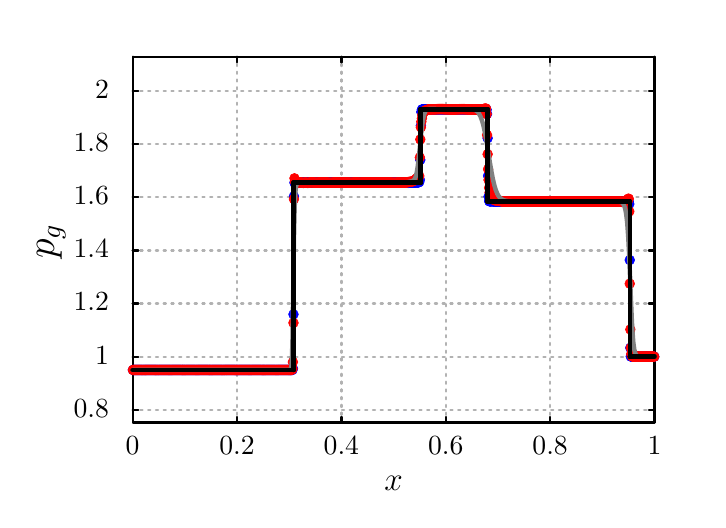
\begin{tikzpicture}[gnuplot]
%% generated with GNUPLOT 4.6p4 (Lua 5.1; terminal rev. 99, script rev. 100)
%% Fri 08 Aug 2014 12:23:47 PM EDT
\path (0.000,0.000) rectangle (8.500,6.000);
\gpfill{rgb color={1.000,1.000,1.000}} (1.320,0.985)--(7.946,0.985)--(7.946,5.630)--(1.320,5.630)--cycle;
\gpcolor{color=gp lt color border}
\gpsetlinetype{gp lt border}
\gpsetlinewidth{1.00}
\draw[gp path] (1.320,0.985)--(1.320,5.630)--(7.946,5.630)--(7.946,0.985)--cycle;
\gpcolor{color=gp lt color axes}
\gpsetlinetype{gp lt axes}
\gpsetlinewidth{2.00}
\draw[gp path] (1.320,1.147)--(7.947,1.147);
\gpcolor{color=gp lt color border}
\gpsetlinetype{gp lt border}
\draw[gp path] (1.320,1.147)--(1.392,1.147);
\draw[gp path] (7.947,1.147)--(7.875,1.147);
\gpcolor{rgb color={0.000,0.000,0.000}}
\node[gp node right,font={\fontsize{10pt}{12pt}\selectfont}] at (1.136,1.147) {0.8};
\gpcolor{color=gp lt color axes}
\gpsetlinetype{gp lt axes}
\draw[gp path] (1.320,1.822)--(7.947,1.822);
\gpcolor{color=gp lt color border}
\gpsetlinetype{gp lt border}
\draw[gp path] (1.320,1.822)--(1.392,1.822);
\draw[gp path] (7.947,1.822)--(7.875,1.822);
\gpcolor{rgb color={0.000,0.000,0.000}}
\node[gp node right,font={\fontsize{10pt}{12pt}\selectfont}] at (1.136,1.822) {1};
\gpcolor{color=gp lt color axes}
\gpsetlinetype{gp lt axes}
\draw[gp path] (1.320,2.496)--(7.947,2.496);
\gpcolor{color=gp lt color border}
\gpsetlinetype{gp lt border}
\draw[gp path] (1.320,2.496)--(1.392,2.496);
\draw[gp path] (7.947,2.496)--(7.875,2.496);
\gpcolor{rgb color={0.000,0.000,0.000}}
\node[gp node right,font={\fontsize{10pt}{12pt}\selectfont}] at (1.136,2.496) {1.2};
\gpcolor{color=gp lt color axes}
\gpsetlinetype{gp lt axes}
\draw[gp path] (1.320,3.170)--(7.947,3.170);
\gpcolor{color=gp lt color border}
\gpsetlinetype{gp lt border}
\draw[gp path] (1.320,3.170)--(1.392,3.170);
\draw[gp path] (7.947,3.170)--(7.875,3.170);
\gpcolor{rgb color={0.000,0.000,0.000}}
\node[gp node right,font={\fontsize{10pt}{12pt}\selectfont}] at (1.136,3.170) {1.4};
\gpcolor{color=gp lt color axes}
\gpsetlinetype{gp lt axes}
\draw[gp path] (1.320,3.845)--(7.947,3.845);
\gpcolor{color=gp lt color border}
\gpsetlinetype{gp lt border}
\draw[gp path] (1.320,3.845)--(1.392,3.845);
\draw[gp path] (7.947,3.845)--(7.875,3.845);
\gpcolor{rgb color={0.000,0.000,0.000}}
\node[gp node right,font={\fontsize{10pt}{12pt}\selectfont}] at (1.136,3.845) {1.6};
\gpcolor{color=gp lt color axes}
\gpsetlinetype{gp lt axes}
\draw[gp path] (1.320,4.519)--(7.947,4.519);
\gpcolor{color=gp lt color border}
\gpsetlinetype{gp lt border}
\draw[gp path] (1.320,4.519)--(1.392,4.519);
\draw[gp path] (7.947,4.519)--(7.875,4.519);
\gpcolor{rgb color={0.000,0.000,0.000}}
\node[gp node right,font={\fontsize{10pt}{12pt}\selectfont}] at (1.136,4.519) {1.8};
\gpcolor{color=gp lt color axes}
\gpsetlinetype{gp lt axes}
\draw[gp path] (1.320,5.193)--(7.947,5.193);
\gpcolor{color=gp lt color border}
\gpsetlinetype{gp lt border}
\draw[gp path] (1.320,5.193)--(1.392,5.193);
\draw[gp path] (7.947,5.193)--(7.875,5.193);
\gpcolor{rgb color={0.000,0.000,0.000}}
\node[gp node right,font={\fontsize{10pt}{12pt}\selectfont}] at (1.136,5.193) {2};
\gpcolor{color=gp lt color axes}
\gpsetlinetype{gp lt axes}
\draw[gp path] (1.320,0.985)--(1.320,5.631);
\gpcolor{color=gp lt color border}
\gpsetlinetype{gp lt border}
\draw[gp path] (1.320,0.985)--(1.320,1.057);
\draw[gp path] (1.320,5.631)--(1.320,5.559);
\gpcolor{rgb color={0.000,0.000,0.000}}
\node[gp node center,font={\fontsize{10pt}{12pt}\selectfont}] at (1.320,0.677) {0};
\gpcolor{color=gp lt color axes}
\gpsetlinetype{gp lt axes}
\draw[gp path] (2.645,0.985)--(2.645,5.631);
\gpcolor{color=gp lt color border}
\gpsetlinetype{gp lt border}
\draw[gp path] (2.645,0.985)--(2.645,1.057);
\draw[gp path] (2.645,5.631)--(2.645,5.559);
\gpcolor{rgb color={0.000,0.000,0.000}}
\node[gp node center,font={\fontsize{10pt}{12pt}\selectfont}] at (2.645,0.677) {0.2};
\gpcolor{color=gp lt color axes}
\gpsetlinetype{gp lt axes}
\draw[gp path] (3.971,0.985)--(3.971,5.631);
\gpcolor{color=gp lt color border}
\gpsetlinetype{gp lt border}
\draw[gp path] (3.971,0.985)--(3.971,1.057);
\draw[gp path] (3.971,5.631)--(3.971,5.559);
\gpcolor{rgb color={0.000,0.000,0.000}}
\node[gp node center,font={\fontsize{10pt}{12pt}\selectfont}] at (3.971,0.677) {0.4};
\gpcolor{color=gp lt color axes}
\gpsetlinetype{gp lt axes}
\draw[gp path] (5.296,0.985)--(5.296,5.631);
\gpcolor{color=gp lt color border}
\gpsetlinetype{gp lt border}
\draw[gp path] (5.296,0.985)--(5.296,1.057);
\draw[gp path] (5.296,5.631)--(5.296,5.559);
\gpcolor{rgb color={0.000,0.000,0.000}}
\node[gp node center,font={\fontsize{10pt}{12pt}\selectfont}] at (5.296,0.677) {0.6};
\gpcolor{color=gp lt color axes}
\gpsetlinetype{gp lt axes}
\draw[gp path] (6.622,0.985)--(6.622,5.631);
\gpcolor{color=gp lt color border}
\gpsetlinetype{gp lt border}
\draw[gp path] (6.622,0.985)--(6.622,1.057);
\draw[gp path] (6.622,5.631)--(6.622,5.559);
\gpcolor{rgb color={0.000,0.000,0.000}}
\node[gp node center,font={\fontsize{10pt}{12pt}\selectfont}] at (6.622,0.677) {0.8};
\gpcolor{color=gp lt color axes}
\gpsetlinetype{gp lt axes}
\draw[gp path] (7.947,0.985)--(7.947,5.631);
\gpcolor{color=gp lt color border}
\gpsetlinetype{gp lt border}
\draw[gp path] (7.947,0.985)--(7.947,1.057);
\draw[gp path] (7.947,5.631)--(7.947,5.559);
\gpcolor{rgb color={0.000,0.000,0.000}}
\node[gp node center,font={\fontsize{10pt}{12pt}\selectfont}] at (7.947,0.677) {1};
\gpcolor{color=gp lt color border}
\draw[gp path] (1.320,5.631)--(1.320,0.985)--(7.947,0.985)--(7.947,5.631)--cycle;
\gpcolor{rgb color={0.000,0.000,0.000}}
\node[gp node center,rotate=90,font={\fontsize{10pt}{12pt}\selectfont}] at (0.246,3.308) {\Large $p_g$};
\node[gp node center,font={\fontsize{10pt}{12pt}\selectfont}] at (4.633,0.215) {\large $x$};
\gpcolor{rgb color={0.000,0.000,1.000}}
\gpsetlinewidth{0.50}
\gpsetpointsize{4.44}
\gppoint{gp mark 7}{(1.323,1.653)}
\gppoint{gp mark 7}{(1.330,1.653)}
\gppoint{gp mark 7}{(1.336,1.653)}
\gppoint{gp mark 7}{(1.343,1.653)}
\gppoint{gp mark 7}{(1.349,1.653)}
\gppoint{gp mark 7}{(1.356,1.653)}
\gppoint{gp mark 7}{(1.362,1.653)}
\gppoint{gp mark 7}{(1.369,1.653)}
\gppoint{gp mark 7}{(1.375,1.653)}
\gppoint{gp mark 7}{(1.381,1.653)}
\gppoint{gp mark 7}{(1.388,1.653)}
\gppoint{gp mark 7}{(1.394,1.653)}
\gppoint{gp mark 7}{(1.401,1.653)}
\gppoint{gp mark 7}{(1.407,1.653)}
\gppoint{gp mark 7}{(1.414,1.653)}
\gppoint{gp mark 7}{(1.420,1.653)}
\gppoint{gp mark 7}{(1.427,1.653)}
\gppoint{gp mark 7}{(1.433,1.653)}
\gppoint{gp mark 7}{(1.440,1.653)}
\gppoint{gp mark 7}{(1.446,1.653)}
\gppoint{gp mark 7}{(1.453,1.653)}
\gppoint{gp mark 7}{(1.459,1.653)}
\gppoint{gp mark 7}{(1.466,1.653)}
\gppoint{gp mark 7}{(1.472,1.653)}
\gppoint{gp mark 7}{(1.479,1.653)}
\gppoint{gp mark 7}{(1.485,1.653)}
\gppoint{gp mark 7}{(1.491,1.653)}
\gppoint{gp mark 7}{(1.498,1.653)}
\gppoint{gp mark 7}{(1.504,1.653)}
\gppoint{gp mark 7}{(1.511,1.653)}
\gppoint{gp mark 7}{(1.517,1.653)}
\gppoint{gp mark 7}{(1.524,1.653)}
\gppoint{gp mark 7}{(1.530,1.653)}
\gppoint{gp mark 7}{(1.537,1.653)}
\gppoint{gp mark 7}{(1.543,1.653)}
\gppoint{gp mark 7}{(1.550,1.653)}
\gppoint{gp mark 7}{(1.556,1.653)}
\gppoint{gp mark 7}{(1.563,1.653)}
\gppoint{gp mark 7}{(1.569,1.653)}
\gppoint{gp mark 7}{(1.576,1.653)}
\gppoint{gp mark 7}{(1.582,1.653)}
\gppoint{gp mark 7}{(1.589,1.653)}
\gppoint{gp mark 7}{(1.595,1.653)}
\gppoint{gp mark 7}{(1.602,1.653)}
\gppoint{gp mark 7}{(1.608,1.653)}
\gppoint{gp mark 7}{(1.614,1.653)}
\gppoint{gp mark 7}{(1.621,1.653)}
\gppoint{gp mark 7}{(1.627,1.653)}
\gppoint{gp mark 7}{(1.634,1.653)}
\gppoint{gp mark 7}{(1.640,1.653)}
\gppoint{gp mark 7}{(1.647,1.653)}
\gppoint{gp mark 7}{(1.653,1.653)}
\gppoint{gp mark 7}{(1.660,1.653)}
\gppoint{gp mark 7}{(1.666,1.653)}
\gppoint{gp mark 7}{(1.673,1.653)}
\gppoint{gp mark 7}{(1.679,1.653)}
\gppoint{gp mark 7}{(1.686,1.653)}
\gppoint{gp mark 7}{(1.692,1.653)}
\gppoint{gp mark 7}{(1.699,1.653)}
\gppoint{gp mark 7}{(1.705,1.653)}
\gppoint{gp mark 7}{(1.712,1.653)}
\gppoint{gp mark 7}{(1.718,1.653)}
\gppoint{gp mark 7}{(1.724,1.653)}
\gppoint{gp mark 7}{(1.731,1.653)}
\gppoint{gp mark 7}{(1.737,1.653)}
\gppoint{gp mark 7}{(1.744,1.653)}
\gppoint{gp mark 7}{(1.750,1.653)}
\gppoint{gp mark 7}{(1.757,1.653)}
\gppoint{gp mark 7}{(1.763,1.653)}
\gppoint{gp mark 7}{(1.770,1.653)}
\gppoint{gp mark 7}{(1.776,1.653)}
\gppoint{gp mark 7}{(1.783,1.653)}
\gppoint{gp mark 7}{(1.789,1.653)}
\gppoint{gp mark 7}{(1.796,1.653)}
\gppoint{gp mark 7}{(1.802,1.653)}
\gppoint{gp mark 7}{(1.809,1.653)}
\gppoint{gp mark 7}{(1.815,1.653)}
\gppoint{gp mark 7}{(1.822,1.653)}
\gppoint{gp mark 7}{(1.828,1.653)}
\gppoint{gp mark 7}{(1.834,1.653)}
\gppoint{gp mark 7}{(1.841,1.653)}
\gppoint{gp mark 7}{(1.847,1.653)}
\gppoint{gp mark 7}{(1.854,1.653)}
\gppoint{gp mark 7}{(1.860,1.653)}
\gppoint{gp mark 7}{(1.867,1.653)}
\gppoint{gp mark 7}{(1.873,1.653)}
\gppoint{gp mark 7}{(1.880,1.653)}
\gppoint{gp mark 7}{(1.886,1.653)}
\gppoint{gp mark 7}{(1.893,1.653)}
\gppoint{gp mark 7}{(1.899,1.653)}
\gppoint{gp mark 7}{(1.906,1.653)}
\gppoint{gp mark 7}{(1.912,1.653)}
\gppoint{gp mark 7}{(1.919,1.653)}
\gppoint{gp mark 7}{(1.925,1.653)}
\gppoint{gp mark 7}{(1.932,1.653)}
\gppoint{gp mark 7}{(1.938,1.653)}
\gppoint{gp mark 7}{(1.945,1.653)}
\gppoint{gp mark 7}{(1.951,1.653)}
\gppoint{gp mark 7}{(1.957,1.653)}
\gppoint{gp mark 7}{(1.964,1.653)}
\gppoint{gp mark 7}{(1.970,1.653)}
\gppoint{gp mark 7}{(1.977,1.653)}
\gppoint{gp mark 7}{(1.983,1.653)}
\gppoint{gp mark 7}{(1.990,1.653)}
\gppoint{gp mark 7}{(1.996,1.653)}
\gppoint{gp mark 7}{(2.003,1.653)}
\gppoint{gp mark 7}{(2.009,1.653)}
\gppoint{gp mark 7}{(2.016,1.653)}
\gppoint{gp mark 7}{(2.022,1.653)}
\gppoint{gp mark 7}{(2.029,1.653)}
\gppoint{gp mark 7}{(2.035,1.653)}
\gppoint{gp mark 7}{(2.042,1.653)}
\gppoint{gp mark 7}{(2.048,1.653)}
\gppoint{gp mark 7}{(2.055,1.653)}
\gppoint{gp mark 7}{(2.061,1.653)}
\gppoint{gp mark 7}{(2.067,1.653)}
\gppoint{gp mark 7}{(2.074,1.653)}
\gppoint{gp mark 7}{(2.080,1.653)}
\gppoint{gp mark 7}{(2.087,1.653)}
\gppoint{gp mark 7}{(2.093,1.653)}
\gppoint{gp mark 7}{(2.100,1.653)}
\gppoint{gp mark 7}{(2.106,1.653)}
\gppoint{gp mark 7}{(2.113,1.653)}
\gppoint{gp mark 7}{(2.119,1.653)}
\gppoint{gp mark 7}{(2.126,1.653)}
\gppoint{gp mark 7}{(2.132,1.653)}
\gppoint{gp mark 7}{(2.139,1.653)}
\gppoint{gp mark 7}{(2.145,1.653)}
\gppoint{gp mark 7}{(2.152,1.653)}
\gppoint{gp mark 7}{(2.158,1.653)}
\gppoint{gp mark 7}{(2.165,1.653)}
\gppoint{gp mark 7}{(2.171,1.653)}
\gppoint{gp mark 7}{(2.177,1.653)}
\gppoint{gp mark 7}{(2.184,1.653)}
\gppoint{gp mark 7}{(2.190,1.653)}
\gppoint{gp mark 7}{(2.197,1.653)}
\gppoint{gp mark 7}{(2.203,1.653)}
\gppoint{gp mark 7}{(2.210,1.653)}
\gppoint{gp mark 7}{(2.216,1.653)}
\gppoint{gp mark 7}{(2.223,1.653)}
\gppoint{gp mark 7}{(2.229,1.653)}
\gppoint{gp mark 7}{(2.236,1.653)}
\gppoint{gp mark 7}{(2.242,1.653)}
\gppoint{gp mark 7}{(2.249,1.653)}
\gppoint{gp mark 7}{(2.255,1.653)}
\gppoint{gp mark 7}{(2.262,1.653)}
\gppoint{gp mark 7}{(2.268,1.653)}
\gppoint{gp mark 7}{(2.275,1.653)}
\gppoint{gp mark 7}{(2.281,1.653)}
\gppoint{gp mark 7}{(2.288,1.653)}
\gppoint{gp mark 7}{(2.294,1.653)}
\gppoint{gp mark 7}{(2.300,1.653)}
\gppoint{gp mark 7}{(2.307,1.653)}
\gppoint{gp mark 7}{(2.313,1.653)}
\gppoint{gp mark 7}{(2.320,1.653)}
\gppoint{gp mark 7}{(2.326,1.653)}
\gppoint{gp mark 7}{(2.333,1.653)}
\gppoint{gp mark 7}{(2.339,1.653)}
\gppoint{gp mark 7}{(2.346,1.653)}
\gppoint{gp mark 7}{(2.352,1.653)}
\gppoint{gp mark 7}{(2.359,1.653)}
\gppoint{gp mark 7}{(2.365,1.653)}
\gppoint{gp mark 7}{(2.372,1.653)}
\gppoint{gp mark 7}{(2.378,1.653)}
\gppoint{gp mark 7}{(2.385,1.653)}
\gppoint{gp mark 7}{(2.391,1.653)}
\gppoint{gp mark 7}{(2.398,1.653)}
\gppoint{gp mark 7}{(2.404,1.653)}
\gppoint{gp mark 7}{(2.410,1.653)}
\gppoint{gp mark 7}{(2.417,1.653)}
\gppoint{gp mark 7}{(2.423,1.653)}
\gppoint{gp mark 7}{(2.430,1.653)}
\gppoint{gp mark 7}{(2.436,1.653)}
\gppoint{gp mark 7}{(2.443,1.653)}
\gppoint{gp mark 7}{(2.449,1.653)}
\gppoint{gp mark 7}{(2.456,1.653)}
\gppoint{gp mark 7}{(2.462,1.653)}
\gppoint{gp mark 7}{(2.469,1.653)}
\gppoint{gp mark 7}{(2.475,1.653)}
\gppoint{gp mark 7}{(2.482,1.653)}
\gppoint{gp mark 7}{(2.488,1.653)}
\gppoint{gp mark 7}{(2.495,1.653)}
\gppoint{gp mark 7}{(2.501,1.653)}
\gppoint{gp mark 7}{(2.508,1.653)}
\gppoint{gp mark 7}{(2.514,1.653)}
\gppoint{gp mark 7}{(2.520,1.653)}
\gppoint{gp mark 7}{(2.527,1.653)}
\gppoint{gp mark 7}{(2.533,1.653)}
\gppoint{gp mark 7}{(2.540,1.653)}
\gppoint{gp mark 7}{(2.546,1.653)}
\gppoint{gp mark 7}{(2.553,1.653)}
\gppoint{gp mark 7}{(2.559,1.653)}
\gppoint{gp mark 7}{(2.566,1.653)}
\gppoint{gp mark 7}{(2.572,1.653)}
\gppoint{gp mark 7}{(2.579,1.653)}
\gppoint{gp mark 7}{(2.585,1.653)}
\gppoint{gp mark 7}{(2.592,1.653)}
\gppoint{gp mark 7}{(2.598,1.653)}
\gppoint{gp mark 7}{(2.605,1.653)}
\gppoint{gp mark 7}{(2.611,1.653)}
\gppoint{gp mark 7}{(2.618,1.653)}
\gppoint{gp mark 7}{(2.624,1.653)}
\gppoint{gp mark 7}{(2.631,1.653)}
\gppoint{gp mark 7}{(2.637,1.653)}
\gppoint{gp mark 7}{(2.643,1.653)}
\gppoint{gp mark 7}{(2.650,1.653)}
\gppoint{gp mark 7}{(2.656,1.653)}
\gppoint{gp mark 7}{(2.663,1.653)}
\gppoint{gp mark 7}{(2.669,1.653)}
\gppoint{gp mark 7}{(2.676,1.653)}
\gppoint{gp mark 7}{(2.682,1.653)}
\gppoint{gp mark 7}{(2.689,1.653)}
\gppoint{gp mark 7}{(2.695,1.653)}
\gppoint{gp mark 7}{(2.702,1.653)}
\gppoint{gp mark 7}{(2.708,1.653)}
\gppoint{gp mark 7}{(2.715,1.653)}
\gppoint{gp mark 7}{(2.721,1.653)}
\gppoint{gp mark 7}{(2.728,1.653)}
\gppoint{gp mark 7}{(2.734,1.653)}
\gppoint{gp mark 7}{(2.741,1.653)}
\gppoint{gp mark 7}{(2.747,1.653)}
\gppoint{gp mark 7}{(2.753,1.653)}
\gppoint{gp mark 7}{(2.760,1.653)}
\gppoint{gp mark 7}{(2.766,1.653)}
\gppoint{gp mark 7}{(2.773,1.653)}
\gppoint{gp mark 7}{(2.779,1.653)}
\gppoint{gp mark 7}{(2.786,1.653)}
\gppoint{gp mark 7}{(2.792,1.653)}
\gppoint{gp mark 7}{(2.799,1.653)}
\gppoint{gp mark 7}{(2.805,1.653)}
\gppoint{gp mark 7}{(2.812,1.653)}
\gppoint{gp mark 7}{(2.818,1.653)}
\gppoint{gp mark 7}{(2.825,1.653)}
\gppoint{gp mark 7}{(2.831,1.653)}
\gppoint{gp mark 7}{(2.838,1.653)}
\gppoint{gp mark 7}{(2.844,1.653)}
\gppoint{gp mark 7}{(2.851,1.653)}
\gppoint{gp mark 7}{(2.857,1.653)}
\gppoint{gp mark 7}{(2.863,1.653)}
\gppoint{gp mark 7}{(2.870,1.653)}
\gppoint{gp mark 7}{(2.876,1.653)}
\gppoint{gp mark 7}{(2.883,1.653)}
\gppoint{gp mark 7}{(2.889,1.653)}
\gppoint{gp mark 7}{(2.896,1.653)}
\gppoint{gp mark 7}{(2.902,1.653)}
\gppoint{gp mark 7}{(2.909,1.653)}
\gppoint{gp mark 7}{(2.915,1.653)}
\gppoint{gp mark 7}{(2.922,1.653)}
\gppoint{gp mark 7}{(2.928,1.653)}
\gppoint{gp mark 7}{(2.935,1.653)}
\gppoint{gp mark 7}{(2.941,1.653)}
\gppoint{gp mark 7}{(2.948,1.653)}
\gppoint{gp mark 7}{(2.954,1.653)}
\gppoint{gp mark 7}{(2.961,1.653)}
\gppoint{gp mark 7}{(2.967,1.653)}
\gppoint{gp mark 7}{(2.974,1.653)}
\gppoint{gp mark 7}{(2.980,1.653)}
\gppoint{gp mark 7}{(2.986,1.653)}
\gppoint{gp mark 7}{(2.993,1.653)}
\gppoint{gp mark 7}{(2.999,1.653)}
\gppoint{gp mark 7}{(3.006,1.653)}
\gppoint{gp mark 7}{(3.012,1.653)}
\gppoint{gp mark 7}{(3.019,1.653)}
\gppoint{gp mark 7}{(3.025,1.653)}
\gppoint{gp mark 7}{(3.032,1.653)}
\gppoint{gp mark 7}{(3.038,1.653)}
\gppoint{gp mark 7}{(3.045,1.653)}
\gppoint{gp mark 7}{(3.051,1.653)}
\gppoint{gp mark 7}{(3.058,1.653)}
\gppoint{gp mark 7}{(3.064,1.653)}
\gppoint{gp mark 7}{(3.071,1.653)}
\gppoint{gp mark 7}{(3.077,1.653)}
\gppoint{gp mark 7}{(3.084,1.653)}
\gppoint{gp mark 7}{(3.090,1.653)}
\gppoint{gp mark 7}{(3.096,1.653)}
\gppoint{gp mark 7}{(3.103,1.653)}
\gppoint{gp mark 7}{(3.109,1.653)}
\gppoint{gp mark 7}{(3.116,1.653)}
\gppoint{gp mark 7}{(3.122,1.653)}
\gppoint{gp mark 7}{(3.129,1.653)}
\gppoint{gp mark 7}{(3.135,1.653)}
\gppoint{gp mark 7}{(3.142,1.653)}
\gppoint{gp mark 7}{(3.148,1.653)}
\gppoint{gp mark 7}{(3.155,1.653)}
\gppoint{gp mark 7}{(3.161,1.653)}
\gppoint{gp mark 7}{(3.168,1.653)}
\gppoint{gp mark 7}{(3.174,1.653)}
\gppoint{gp mark 7}{(3.181,1.653)}
\gppoint{gp mark 7}{(3.187,1.653)}
\gppoint{gp mark 7}{(3.194,1.653)}
\gppoint{gp mark 7}{(3.200,1.653)}
\gppoint{gp mark 7}{(3.206,1.653)}
\gppoint{gp mark 7}{(3.213,1.653)}
\gppoint{gp mark 7}{(3.219,1.653)}
\gppoint{gp mark 7}{(3.226,1.653)}
\gppoint{gp mark 7}{(3.232,1.653)}
\gppoint{gp mark 7}{(3.239,1.653)}
\gppoint{gp mark 7}{(3.245,1.653)}
\gppoint{gp mark 7}{(3.252,1.653)}
\gppoint{gp mark 7}{(3.258,1.653)}
\gppoint{gp mark 7}{(3.265,1.653)}
\gppoint{gp mark 7}{(3.271,1.653)}
\gppoint{gp mark 7}{(3.278,1.653)}
\gppoint{gp mark 7}{(3.284,1.653)}
\gppoint{gp mark 7}{(3.291,1.653)}
\gppoint{gp mark 7}{(3.297,1.653)}
\gppoint{gp mark 7}{(3.304,1.653)}
\gppoint{gp mark 7}{(3.310,1.653)}
\gppoint{gp mark 7}{(3.317,1.653)}
\gppoint{gp mark 7}{(3.323,1.653)}
\gppoint{gp mark 7}{(3.329,1.653)}
\gppoint{gp mark 7}{(3.336,1.653)}
\gppoint{gp mark 7}{(3.342,1.653)}
\gppoint{gp mark 7}{(3.349,1.653)}
\gppoint{gp mark 7}{(3.355,1.673)}
\gppoint{gp mark 7}{(3.362,2.359)}
\gppoint{gp mark 7}{(3.368,3.858)}
\gppoint{gp mark 7}{(3.375,4.032)}
\gppoint{gp mark 7}{(3.381,4.027)}
\gppoint{gp mark 7}{(3.388,4.035)}
\gppoint{gp mark 7}{(3.394,4.039)}
\gppoint{gp mark 7}{(3.401,4.030)}
\gppoint{gp mark 7}{(3.407,4.028)}
\gppoint{gp mark 7}{(3.414,4.035)}
\gppoint{gp mark 7}{(3.420,4.035)}
\gppoint{gp mark 7}{(3.427,4.031)}
\gppoint{gp mark 7}{(3.433,4.031)}
\gppoint{gp mark 7}{(3.439,4.034)}
\gppoint{gp mark 7}{(3.446,4.034)}
\gppoint{gp mark 7}{(3.452,4.031)}
\gppoint{gp mark 7}{(3.459,4.032)}
\gppoint{gp mark 7}{(3.465,4.034)}
\gppoint{gp mark 7}{(3.472,4.033)}
\gppoint{gp mark 7}{(3.478,4.032)}
\gppoint{gp mark 7}{(3.485,4.033)}
\gppoint{gp mark 7}{(3.491,4.033)}
\gppoint{gp mark 7}{(3.498,4.032)}
\gppoint{gp mark 7}{(3.504,4.032)}
\gppoint{gp mark 7}{(3.511,4.033)}
\gppoint{gp mark 7}{(3.517,4.033)}
\gppoint{gp mark 7}{(3.524,4.032)}
\gppoint{gp mark 7}{(3.530,4.032)}
\gppoint{gp mark 7}{(3.537,4.033)}
\gppoint{gp mark 7}{(3.543,4.033)}
\gppoint{gp mark 7}{(3.549,4.033)}
\gppoint{gp mark 7}{(3.556,4.033)}
\gppoint{gp mark 7}{(3.562,4.033)}
\gppoint{gp mark 7}{(3.569,4.033)}
\gppoint{gp mark 7}{(3.575,4.033)}
\gppoint{gp mark 7}{(3.582,4.033)}
\gppoint{gp mark 7}{(3.588,4.033)}
\gppoint{gp mark 7}{(3.595,4.033)}
\gppoint{gp mark 7}{(3.601,4.033)}
\gppoint{gp mark 7}{(3.608,4.033)}
\gppoint{gp mark 7}{(3.614,4.033)}
\gppoint{gp mark 7}{(3.621,4.032)}
\gppoint{gp mark 7}{(3.627,4.032)}
\gppoint{gp mark 7}{(3.634,4.033)}
\gppoint{gp mark 7}{(3.640,4.033)}
\gppoint{gp mark 7}{(3.647,4.033)}
\gppoint{gp mark 7}{(3.653,4.033)}
\gppoint{gp mark 7}{(3.660,4.033)}
\gppoint{gp mark 7}{(3.666,4.033)}
\gppoint{gp mark 7}{(3.672,4.033)}
\gppoint{gp mark 7}{(3.679,4.033)}
\gppoint{gp mark 7}{(3.685,4.033)}
\gppoint{gp mark 7}{(3.692,4.033)}
\gppoint{gp mark 7}{(3.698,4.033)}
\gppoint{gp mark 7}{(3.705,4.033)}
\gppoint{gp mark 7}{(3.711,4.033)}
\gppoint{gp mark 7}{(3.718,4.033)}
\gppoint{gp mark 7}{(3.724,4.032)}
\gppoint{gp mark 7}{(3.731,4.033)}
\gppoint{gp mark 7}{(3.737,4.033)}
\gppoint{gp mark 7}{(3.744,4.033)}
\gppoint{gp mark 7}{(3.750,4.033)}
\gppoint{gp mark 7}{(3.757,4.033)}
\gppoint{gp mark 7}{(3.763,4.033)}
\gppoint{gp mark 7}{(3.770,4.033)}
\gppoint{gp mark 7}{(3.776,4.033)}
\gppoint{gp mark 7}{(3.782,4.033)}
\gppoint{gp mark 7}{(3.789,4.033)}
\gppoint{gp mark 7}{(3.795,4.033)}
\gppoint{gp mark 7}{(3.802,4.033)}
\gppoint{gp mark 7}{(3.808,4.033)}
\gppoint{gp mark 7}{(3.815,4.033)}
\gppoint{gp mark 7}{(3.821,4.033)}
\gppoint{gp mark 7}{(3.828,4.033)}
\gppoint{gp mark 7}{(3.834,4.032)}
\gppoint{gp mark 7}{(3.841,4.032)}
\gppoint{gp mark 7}{(3.847,4.033)}
\gppoint{gp mark 7}{(3.854,4.033)}
\gppoint{gp mark 7}{(3.860,4.033)}
\gppoint{gp mark 7}{(3.867,4.033)}
\gppoint{gp mark 7}{(3.873,4.033)}
\gppoint{gp mark 7}{(3.880,4.033)}
\gppoint{gp mark 7}{(3.886,4.033)}
\gppoint{gp mark 7}{(3.892,4.033)}
\gppoint{gp mark 7}{(3.899,4.033)}
\gppoint{gp mark 7}{(3.905,4.033)}
\gppoint{gp mark 7}{(3.912,4.033)}
\gppoint{gp mark 7}{(3.918,4.033)}
\gppoint{gp mark 7}{(3.925,4.033)}
\gppoint{gp mark 7}{(3.931,4.033)}
\gppoint{gp mark 7}{(3.938,4.033)}
\gppoint{gp mark 7}{(3.944,4.033)}
\gppoint{gp mark 7}{(3.951,4.033)}
\gppoint{gp mark 7}{(3.957,4.033)}
\gppoint{gp mark 7}{(3.964,4.033)}
\gppoint{gp mark 7}{(3.970,4.033)}
\gppoint{gp mark 7}{(3.977,4.033)}
\gppoint{gp mark 7}{(3.983,4.033)}
\gppoint{gp mark 7}{(3.990,4.033)}
\gppoint{gp mark 7}{(3.996,4.033)}
\gppoint{gp mark 7}{(4.003,4.033)}
\gppoint{gp mark 7}{(4.009,4.033)}
\gppoint{gp mark 7}{(4.015,4.033)}
\gppoint{gp mark 7}{(4.022,4.033)}
\gppoint{gp mark 7}{(4.028,4.033)}
\gppoint{gp mark 7}{(4.035,4.033)}
\gppoint{gp mark 7}{(4.041,4.033)}
\gppoint{gp mark 7}{(4.048,4.033)}
\gppoint{gp mark 7}{(4.054,4.033)}
\gppoint{gp mark 7}{(4.061,4.033)}
\gppoint{gp mark 7}{(4.067,4.033)}
\gppoint{gp mark 7}{(4.074,4.033)}
\gppoint{gp mark 7}{(4.080,4.033)}
\gppoint{gp mark 7}{(4.087,4.033)}
\gppoint{gp mark 7}{(4.093,4.033)}
\gppoint{gp mark 7}{(4.100,4.033)}
\gppoint{gp mark 7}{(4.106,4.033)}
\gppoint{gp mark 7}{(4.113,4.033)}
\gppoint{gp mark 7}{(4.119,4.033)}
\gppoint{gp mark 7}{(4.125,4.033)}
\gppoint{gp mark 7}{(4.132,4.033)}
\gppoint{gp mark 7}{(4.138,4.032)}
\gppoint{gp mark 7}{(4.145,4.032)}
\gppoint{gp mark 7}{(4.151,4.033)}
\gppoint{gp mark 7}{(4.158,4.033)}
\gppoint{gp mark 7}{(4.164,4.033)}
\gppoint{gp mark 7}{(4.171,4.033)}
\gppoint{gp mark 7}{(4.177,4.033)}
\gppoint{gp mark 7}{(4.184,4.033)}
\gppoint{gp mark 7}{(4.190,4.033)}
\gppoint{gp mark 7}{(4.197,4.033)}
\gppoint{gp mark 7}{(4.203,4.033)}
\gppoint{gp mark 7}{(4.210,4.033)}
\gppoint{gp mark 7}{(4.216,4.033)}
\gppoint{gp mark 7}{(4.223,4.033)}
\gppoint{gp mark 7}{(4.229,4.033)}
\gppoint{gp mark 7}{(4.235,4.033)}
\gppoint{gp mark 7}{(4.242,4.033)}
\gppoint{gp mark 7}{(4.248,4.033)}
\gppoint{gp mark 7}{(4.255,4.033)}
\gppoint{gp mark 7}{(4.261,4.033)}
\gppoint{gp mark 7}{(4.268,4.033)}
\gppoint{gp mark 7}{(4.274,4.033)}
\gppoint{gp mark 7}{(4.281,4.033)}
\gppoint{gp mark 7}{(4.287,4.033)}
\gppoint{gp mark 7}{(4.294,4.033)}
\gppoint{gp mark 7}{(4.300,4.033)}
\gppoint{gp mark 7}{(4.307,4.033)}
\gppoint{gp mark 7}{(4.313,4.033)}
\gppoint{gp mark 7}{(4.320,4.033)}
\gppoint{gp mark 7}{(4.326,4.033)}
\gppoint{gp mark 7}{(4.333,4.033)}
\gppoint{gp mark 7}{(4.339,4.033)}
\gppoint{gp mark 7}{(4.346,4.032)}
\gppoint{gp mark 7}{(4.352,4.032)}
\gppoint{gp mark 7}{(4.358,4.033)}
\gppoint{gp mark 7}{(4.365,4.033)}
\gppoint{gp mark 7}{(4.371,4.033)}
\gppoint{gp mark 7}{(4.378,4.033)}
\gppoint{gp mark 7}{(4.384,4.033)}
\gppoint{gp mark 7}{(4.391,4.033)}
\gppoint{gp mark 7}{(4.397,4.033)}
\gppoint{gp mark 7}{(4.404,4.033)}
\gppoint{gp mark 7}{(4.410,4.033)}
\gppoint{gp mark 7}{(4.417,4.033)}
\gppoint{gp mark 7}{(4.423,4.033)}
\gppoint{gp mark 7}{(4.430,4.033)}
\gppoint{gp mark 7}{(4.436,4.033)}
\gppoint{gp mark 7}{(4.443,4.033)}
\gppoint{gp mark 7}{(4.449,4.033)}
\gppoint{gp mark 7}{(4.456,4.032)}
\gppoint{gp mark 7}{(4.462,4.032)}
\gppoint{gp mark 7}{(4.468,4.033)}
\gppoint{gp mark 7}{(4.475,4.033)}
\gppoint{gp mark 7}{(4.481,4.033)}
\gppoint{gp mark 7}{(4.488,4.033)}
\gppoint{gp mark 7}{(4.494,4.033)}
\gppoint{gp mark 7}{(4.501,4.033)}
\gppoint{gp mark 7}{(4.507,4.033)}
\gppoint{gp mark 7}{(4.514,4.033)}
\gppoint{gp mark 7}{(4.520,4.033)}
\gppoint{gp mark 7}{(4.527,4.033)}
\gppoint{gp mark 7}{(4.533,4.033)}
\gppoint{gp mark 7}{(4.540,4.033)}
\gppoint{gp mark 7}{(4.546,4.032)}
\gppoint{gp mark 7}{(4.553,4.033)}
\gppoint{gp mark 7}{(4.559,4.033)}
\gppoint{gp mark 7}{(4.566,4.033)}
\gppoint{gp mark 7}{(4.572,4.032)}
\gppoint{gp mark 7}{(4.578,4.032)}
\gppoint{gp mark 7}{(4.585,4.033)}
\gppoint{gp mark 7}{(4.591,4.033)}
\gppoint{gp mark 7}{(4.598,4.033)}
\gppoint{gp mark 7}{(4.604,4.033)}
\gppoint{gp mark 7}{(4.611,4.033)}
\gppoint{gp mark 7}{(4.617,4.033)}
\gppoint{gp mark 7}{(4.624,4.033)}
\gppoint{gp mark 7}{(4.630,4.033)}
\gppoint{gp mark 7}{(4.637,4.033)}
\gppoint{gp mark 7}{(4.643,4.033)}
\gppoint{gp mark 7}{(4.650,4.033)}
\gppoint{gp mark 7}{(4.656,4.032)}
\gppoint{gp mark 7}{(4.663,4.032)}
\gppoint{gp mark 7}{(4.669,4.032)}
\gppoint{gp mark 7}{(4.676,4.033)}
\gppoint{gp mark 7}{(4.682,4.033)}
\gppoint{gp mark 7}{(4.689,4.033)}
\gppoint{gp mark 7}{(4.695,4.032)}
\gppoint{gp mark 7}{(4.701,4.032)}
\gppoint{gp mark 7}{(4.708,4.033)}
\gppoint{gp mark 7}{(4.714,4.033)}
\gppoint{gp mark 7}{(4.721,4.033)}
\gppoint{gp mark 7}{(4.727,4.033)}
\gppoint{gp mark 7}{(4.734,4.032)}
\gppoint{gp mark 7}{(4.740,4.032)}
\gppoint{gp mark 7}{(4.747,4.032)}
\gppoint{gp mark 7}{(4.753,4.033)}
\gppoint{gp mark 7}{(4.760,4.033)}
\gppoint{gp mark 7}{(4.766,4.033)}
\gppoint{gp mark 7}{(4.773,4.033)}
\gppoint{gp mark 7}{(4.779,4.032)}
\gppoint{gp mark 7}{(4.786,4.032)}
\gppoint{gp mark 7}{(4.792,4.033)}
\gppoint{gp mark 7}{(4.799,4.033)}
\gppoint{gp mark 7}{(4.805,4.033)}
\gppoint{gp mark 7}{(4.811,4.032)}
\gppoint{gp mark 7}{(4.818,4.029)}
\gppoint{gp mark 7}{(4.824,4.031)}
\gppoint{gp mark 7}{(4.831,4.033)}
\gppoint{gp mark 7}{(4.837,4.035)}
\gppoint{gp mark 7}{(4.844,4.035)}
\gppoint{gp mark 7}{(4.850,4.033)}
\gppoint{gp mark 7}{(4.857,4.033)}
\gppoint{gp mark 7}{(4.863,4.032)}
\gppoint{gp mark 7}{(4.870,4.033)}
\gppoint{gp mark 7}{(4.876,4.035)}
\gppoint{gp mark 7}{(4.883,4.035)}
\gppoint{gp mark 7}{(4.889,4.034)}
\gppoint{gp mark 7}{(4.896,4.033)}
\gppoint{gp mark 7}{(4.902,4.033)}
\gppoint{gp mark 7}{(4.909,4.034)}
\gppoint{gp mark 7}{(4.915,4.035)}
\gppoint{gp mark 7}{(4.921,4.036)}
\gppoint{gp mark 7}{(4.928,4.035)}
\gppoint{gp mark 7}{(4.934,4.034)}
\gppoint{gp mark 7}{(4.941,4.034)}
\gppoint{gp mark 7}{(4.947,4.035)}
\gppoint{gp mark 7}{(4.954,4.037)}
\gppoint{gp mark 7}{(4.960,4.041)}
\gppoint{gp mark 7}{(4.967,4.069)}
\gppoint{gp mark 7}{(4.973,4.321)}
\gppoint{gp mark 7}{(4.980,4.756)}
\gppoint{gp mark 7}{(4.986,4.929)}
\gppoint{gp mark 7}{(4.993,4.959)}
\gppoint{gp mark 7}{(4.999,4.963)}
\gppoint{gp mark 7}{(5.006,4.964)}
\gppoint{gp mark 7}{(5.012,4.964)}
\gppoint{gp mark 7}{(5.019,4.964)}
\gppoint{gp mark 7}{(5.025,4.964)}
\gppoint{gp mark 7}{(5.032,4.964)}
\gppoint{gp mark 7}{(5.038,4.964)}
\gppoint{gp mark 7}{(5.044,4.964)}
\gppoint{gp mark 7}{(5.051,4.964)}
\gppoint{gp mark 7}{(5.057,4.963)}
\gppoint{gp mark 7}{(5.064,4.963)}
\gppoint{gp mark 7}{(5.070,4.963)}
\gppoint{gp mark 7}{(5.077,4.963)}
\gppoint{gp mark 7}{(5.083,4.963)}
\gppoint{gp mark 7}{(5.090,4.963)}
\gppoint{gp mark 7}{(5.096,4.963)}
\gppoint{gp mark 7}{(5.103,4.963)}
\gppoint{gp mark 7}{(5.109,4.963)}
\gppoint{gp mark 7}{(5.116,4.963)}
\gppoint{gp mark 7}{(5.122,4.963)}
\gppoint{gp mark 7}{(5.129,4.963)}
\gppoint{gp mark 7}{(5.135,4.963)}
\gppoint{gp mark 7}{(5.142,4.963)}
\gppoint{gp mark 7}{(5.148,4.963)}
\gppoint{gp mark 7}{(5.154,4.963)}
\gppoint{gp mark 7}{(5.161,4.963)}
\gppoint{gp mark 7}{(5.167,4.963)}
\gppoint{gp mark 7}{(5.174,4.962)}
\gppoint{gp mark 7}{(5.180,4.963)}
\gppoint{gp mark 7}{(5.187,4.963)}
\gppoint{gp mark 7}{(5.193,4.963)}
\gppoint{gp mark 7}{(5.200,4.963)}
\gppoint{gp mark 7}{(5.206,4.963)}
\gppoint{gp mark 7}{(5.213,4.963)}
\gppoint{gp mark 7}{(5.219,4.963)}
\gppoint{gp mark 7}{(5.226,4.963)}
\gppoint{gp mark 7}{(5.232,4.963)}
\gppoint{gp mark 7}{(5.239,4.963)}
\gppoint{gp mark 7}{(5.245,4.963)}
\gppoint{gp mark 7}{(5.252,4.963)}
\gppoint{gp mark 7}{(5.258,4.963)}
\gppoint{gp mark 7}{(5.264,4.963)}
\gppoint{gp mark 7}{(5.271,4.963)}
\gppoint{gp mark 7}{(5.277,4.963)}
\gppoint{gp mark 7}{(5.284,4.963)}
\gppoint{gp mark 7}{(5.290,4.963)}
\gppoint{gp mark 7}{(5.297,4.963)}
\gppoint{gp mark 7}{(5.303,4.963)}
\gppoint{gp mark 7}{(5.310,4.963)}
\gppoint{gp mark 7}{(5.316,4.963)}
\gppoint{gp mark 7}{(5.323,4.963)}
\gppoint{gp mark 7}{(5.329,4.963)}
\gppoint{gp mark 7}{(5.336,4.963)}
\gppoint{gp mark 7}{(5.342,4.963)}
\gppoint{gp mark 7}{(5.349,4.963)}
\gppoint{gp mark 7}{(5.355,4.963)}
\gppoint{gp mark 7}{(5.362,4.963)}
\gppoint{gp mark 7}{(5.368,4.963)}
\gppoint{gp mark 7}{(5.375,4.963)}
\gppoint{gp mark 7}{(5.381,4.963)}
\gppoint{gp mark 7}{(5.387,4.963)}
\gppoint{gp mark 7}{(5.394,4.963)}
\gppoint{gp mark 7}{(5.400,4.963)}
\gppoint{gp mark 7}{(5.407,4.963)}
\gppoint{gp mark 7}{(5.413,4.963)}
\gppoint{gp mark 7}{(5.420,4.963)}
\gppoint{gp mark 7}{(5.426,4.963)}
\gppoint{gp mark 7}{(5.433,4.963)}
\gppoint{gp mark 7}{(5.439,4.963)}
\gppoint{gp mark 7}{(5.446,4.963)}
\gppoint{gp mark 7}{(5.452,4.963)}
\gppoint{gp mark 7}{(5.459,4.963)}
\gppoint{gp mark 7}{(5.465,4.963)}
\gppoint{gp mark 7}{(5.472,4.963)}
\gppoint{gp mark 7}{(5.478,4.963)}
\gppoint{gp mark 7}{(5.485,4.963)}
\gppoint{gp mark 7}{(5.491,4.963)}
\gppoint{gp mark 7}{(5.497,4.963)}
\gppoint{gp mark 7}{(5.504,4.963)}
\gppoint{gp mark 7}{(5.510,4.963)}
\gppoint{gp mark 7}{(5.517,4.963)}
\gppoint{gp mark 7}{(5.523,4.963)}
\gppoint{gp mark 7}{(5.530,4.963)}
\gppoint{gp mark 7}{(5.536,4.963)}
\gppoint{gp mark 7}{(5.543,4.963)}
\gppoint{gp mark 7}{(5.549,4.963)}
\gppoint{gp mark 7}{(5.556,4.963)}
\gppoint{gp mark 7}{(5.562,4.963)}
\gppoint{gp mark 7}{(5.569,4.963)}
\gppoint{gp mark 7}{(5.575,4.963)}
\gppoint{gp mark 7}{(5.582,4.963)}
\gppoint{gp mark 7}{(5.588,4.963)}
\gppoint{gp mark 7}{(5.595,4.963)}
\gppoint{gp mark 7}{(5.601,4.963)}
\gppoint{gp mark 7}{(5.607,4.963)}
\gppoint{gp mark 7}{(5.614,4.963)}
\gppoint{gp mark 7}{(5.620,4.963)}
\gppoint{gp mark 7}{(5.627,4.963)}
\gppoint{gp mark 7}{(5.633,4.963)}
\gppoint{gp mark 7}{(5.640,4.963)}
\gppoint{gp mark 7}{(5.646,4.963)}
\gppoint{gp mark 7}{(5.653,4.963)}
\gppoint{gp mark 7}{(5.659,4.963)}
\gppoint{gp mark 7}{(5.666,4.963)}
\gppoint{gp mark 7}{(5.672,4.963)}
\gppoint{gp mark 7}{(5.679,4.963)}
\gppoint{gp mark 7}{(5.685,4.963)}
\gppoint{gp mark 7}{(5.692,4.963)}
\gppoint{gp mark 7}{(5.698,4.963)}
\gppoint{gp mark 7}{(5.705,4.964)}
\gppoint{gp mark 7}{(5.711,4.964)}
\gppoint{gp mark 7}{(5.718,4.964)}
\gppoint{gp mark 7}{(5.724,4.964)}
\gppoint{gp mark 7}{(5.730,4.964)}
\gppoint{gp mark 7}{(5.737,4.964)}
\gppoint{gp mark 7}{(5.743,4.964)}
\gppoint{gp mark 7}{(5.750,4.964)}
\gppoint{gp mark 7}{(5.756,4.964)}
\gppoint{gp mark 7}{(5.763,4.964)}
\gppoint{gp mark 7}{(5.769,4.964)}
\gppoint{gp mark 7}{(5.776,4.964)}
\gppoint{gp mark 7}{(5.782,4.964)}
\gppoint{gp mark 7}{(5.789,4.963)}
\gppoint{gp mark 7}{(5.795,4.963)}
\gppoint{gp mark 7}{(5.802,4.963)}
\gppoint{gp mark 7}{(5.808,4.963)}
\gppoint{gp mark 7}{(5.815,4.957)}
\gppoint{gp mark 7}{(5.821,4.904)}
\gppoint{gp mark 7}{(5.828,4.597)}
\gppoint{gp mark 7}{(5.834,4.119)}
\gppoint{gp mark 7}{(5.840,3.854)}
\gppoint{gp mark 7}{(5.847,3.799)}
\gppoint{gp mark 7}{(5.853,3.794)}
\gppoint{gp mark 7}{(5.860,3.794)}
\gppoint{gp mark 7}{(5.866,3.794)}
\gppoint{gp mark 7}{(5.873,3.795)}
\gppoint{gp mark 7}{(5.879,3.795)}
\gppoint{gp mark 7}{(5.886,3.795)}
\gppoint{gp mark 7}{(5.892,3.795)}
\gppoint{gp mark 7}{(5.899,3.794)}
\gppoint{gp mark 7}{(5.905,3.794)}
\gppoint{gp mark 7}{(5.912,3.793)}
\gppoint{gp mark 7}{(5.918,3.793)}
\gppoint{gp mark 7}{(5.925,3.792)}
\gppoint{gp mark 7}{(5.931,3.792)}
\gppoint{gp mark 7}{(5.938,3.793)}
\gppoint{gp mark 7}{(5.944,3.793)}
\gppoint{gp mark 7}{(5.950,3.793)}
\gppoint{gp mark 7}{(5.957,3.793)}
\gppoint{gp mark 7}{(5.963,3.793)}
\gppoint{gp mark 7}{(5.970,3.793)}
\gppoint{gp mark 7}{(5.976,3.793)}
\gppoint{gp mark 7}{(5.983,3.793)}
\gppoint{gp mark 7}{(5.989,3.794)}
\gppoint{gp mark 7}{(5.996,3.794)}
\gppoint{gp mark 7}{(6.002,3.793)}
\gppoint{gp mark 7}{(6.009,3.792)}
\gppoint{gp mark 7}{(6.015,3.792)}
\gppoint{gp mark 7}{(6.022,3.792)}
\gppoint{gp mark 7}{(6.028,3.792)}
\gppoint{gp mark 7}{(6.035,3.792)}
\gppoint{gp mark 7}{(6.041,3.792)}
\gppoint{gp mark 7}{(6.048,3.792)}
\gppoint{gp mark 7}{(6.054,3.792)}
\gppoint{gp mark 7}{(6.061,3.792)}
\gppoint{gp mark 7}{(6.067,3.792)}
\gppoint{gp mark 7}{(6.073,3.792)}
\gppoint{gp mark 7}{(6.080,3.792)}
\gppoint{gp mark 7}{(6.086,3.792)}
\gppoint{gp mark 7}{(6.093,3.792)}
\gppoint{gp mark 7}{(6.099,3.792)}
\gppoint{gp mark 7}{(6.106,3.792)}
\gppoint{gp mark 7}{(6.112,3.792)}
\gppoint{gp mark 7}{(6.119,3.792)}
\gppoint{gp mark 7}{(6.125,3.792)}
\gppoint{gp mark 7}{(6.132,3.792)}
\gppoint{gp mark 7}{(6.138,3.792)}
\gppoint{gp mark 7}{(6.145,3.792)}
\gppoint{gp mark 7}{(6.151,3.792)}
\gppoint{gp mark 7}{(6.158,3.792)}
\gppoint{gp mark 7}{(6.164,3.792)}
\gppoint{gp mark 7}{(6.171,3.792)}
\gppoint{gp mark 7}{(6.177,3.792)}
\gppoint{gp mark 7}{(6.183,3.792)}
\gppoint{gp mark 7}{(6.190,3.792)}
\gppoint{gp mark 7}{(6.196,3.792)}
\gppoint{gp mark 7}{(6.203,3.792)}
\gppoint{gp mark 7}{(6.209,3.792)}
\gppoint{gp mark 7}{(6.216,3.792)}
\gppoint{gp mark 7}{(6.222,3.792)}
\gppoint{gp mark 7}{(6.229,3.792)}
\gppoint{gp mark 7}{(6.235,3.792)}
\gppoint{gp mark 7}{(6.242,3.792)}
\gppoint{gp mark 7}{(6.248,3.792)}
\gppoint{gp mark 7}{(6.255,3.792)}
\gppoint{gp mark 7}{(6.261,3.792)}
\gppoint{gp mark 7}{(6.268,3.792)}
\gppoint{gp mark 7}{(6.274,3.792)}
\gppoint{gp mark 7}{(6.281,3.792)}
\gppoint{gp mark 7}{(6.287,3.792)}
\gppoint{gp mark 7}{(6.293,3.792)}
\gppoint{gp mark 7}{(6.300,3.792)}
\gppoint{gp mark 7}{(6.306,3.792)}
\gppoint{gp mark 7}{(6.313,3.792)}
\gppoint{gp mark 7}{(6.319,3.792)}
\gppoint{gp mark 7}{(6.326,3.792)}
\gppoint{gp mark 7}{(6.332,3.792)}
\gppoint{gp mark 7}{(6.339,3.792)}
\gppoint{gp mark 7}{(6.345,3.792)}
\gppoint{gp mark 7}{(6.352,3.792)}
\gppoint{gp mark 7}{(6.358,3.792)}
\gppoint{gp mark 7}{(6.365,3.792)}
\gppoint{gp mark 7}{(6.371,3.792)}
\gppoint{gp mark 7}{(6.378,3.792)}
\gppoint{gp mark 7}{(6.384,3.792)}
\gppoint{gp mark 7}{(6.391,3.792)}
\gppoint{gp mark 7}{(6.397,3.792)}
\gppoint{gp mark 7}{(6.404,3.792)}
\gppoint{gp mark 7}{(6.410,3.792)}
\gppoint{gp mark 7}{(6.416,3.792)}
\gppoint{gp mark 7}{(6.423,3.792)}
\gppoint{gp mark 7}{(6.429,3.792)}
\gppoint{gp mark 7}{(6.436,3.792)}
\gppoint{gp mark 7}{(6.442,3.792)}
\gppoint{gp mark 7}{(6.449,3.792)}
\gppoint{gp mark 7}{(6.455,3.792)}
\gppoint{gp mark 7}{(6.462,3.792)}
\gppoint{gp mark 7}{(6.468,3.792)}
\gppoint{gp mark 7}{(6.475,3.792)}
\gppoint{gp mark 7}{(6.481,3.792)}
\gppoint{gp mark 7}{(6.488,3.792)}
\gppoint{gp mark 7}{(6.494,3.792)}
\gppoint{gp mark 7}{(6.501,3.792)}
\gppoint{gp mark 7}{(6.507,3.792)}
\gppoint{gp mark 7}{(6.514,3.792)}
\gppoint{gp mark 7}{(6.520,3.792)}
\gppoint{gp mark 7}{(6.526,3.792)}
\gppoint{gp mark 7}{(6.533,3.792)}
\gppoint{gp mark 7}{(6.539,3.792)}
\gppoint{gp mark 7}{(6.546,3.792)}
\gppoint{gp mark 7}{(6.552,3.792)}
\gppoint{gp mark 7}{(6.559,3.792)}
\gppoint{gp mark 7}{(6.565,3.792)}
\gppoint{gp mark 7}{(6.572,3.792)}
\gppoint{gp mark 7}{(6.578,3.792)}
\gppoint{gp mark 7}{(6.585,3.792)}
\gppoint{gp mark 7}{(6.591,3.792)}
\gppoint{gp mark 7}{(6.598,3.792)}
\gppoint{gp mark 7}{(6.604,3.792)}
\gppoint{gp mark 7}{(6.611,3.792)}
\gppoint{gp mark 7}{(6.617,3.792)}
\gppoint{gp mark 7}{(6.624,3.792)}
\gppoint{gp mark 7}{(6.630,3.792)}
\gppoint{gp mark 7}{(6.636,3.792)}
\gppoint{gp mark 7}{(6.643,3.792)}
\gppoint{gp mark 7}{(6.649,3.792)}
\gppoint{gp mark 7}{(6.656,3.792)}
\gppoint{gp mark 7}{(6.662,3.792)}
\gppoint{gp mark 7}{(6.669,3.792)}
\gppoint{gp mark 7}{(6.675,3.792)}
\gppoint{gp mark 7}{(6.682,3.792)}
\gppoint{gp mark 7}{(6.688,3.792)}
\gppoint{gp mark 7}{(6.695,3.792)}
\gppoint{gp mark 7}{(6.701,3.792)}
\gppoint{gp mark 7}{(6.708,3.792)}
\gppoint{gp mark 7}{(6.714,3.792)}
\gppoint{gp mark 7}{(6.721,3.792)}
\gppoint{gp mark 7}{(6.727,3.792)}
\gppoint{gp mark 7}{(6.734,3.792)}
\gppoint{gp mark 7}{(6.740,3.792)}
\gppoint{gp mark 7}{(6.747,3.792)}
\gppoint{gp mark 7}{(6.753,3.792)}
\gppoint{gp mark 7}{(6.759,3.792)}
\gppoint{gp mark 7}{(6.766,3.792)}
\gppoint{gp mark 7}{(6.772,3.792)}
\gppoint{gp mark 7}{(6.779,3.792)}
\gppoint{gp mark 7}{(6.785,3.792)}
\gppoint{gp mark 7}{(6.792,3.792)}
\gppoint{gp mark 7}{(6.798,3.792)}
\gppoint{gp mark 7}{(6.805,3.792)}
\gppoint{gp mark 7}{(6.811,3.792)}
\gppoint{gp mark 7}{(6.818,3.792)}
\gppoint{gp mark 7}{(6.824,3.792)}
\gppoint{gp mark 7}{(6.831,3.792)}
\gppoint{gp mark 7}{(6.837,3.792)}
\gppoint{gp mark 7}{(6.844,3.792)}
\gppoint{gp mark 7}{(6.850,3.792)}
\gppoint{gp mark 7}{(6.857,3.792)}
\gppoint{gp mark 7}{(6.863,3.792)}
\gppoint{gp mark 7}{(6.869,3.792)}
\gppoint{gp mark 7}{(6.876,3.792)}
\gppoint{gp mark 7}{(6.882,3.792)}
\gppoint{gp mark 7}{(6.889,3.792)}
\gppoint{gp mark 7}{(6.895,3.792)}
\gppoint{gp mark 7}{(6.902,3.792)}
\gppoint{gp mark 7}{(6.908,3.792)}
\gppoint{gp mark 7}{(6.915,3.792)}
\gppoint{gp mark 7}{(6.921,3.792)}
\gppoint{gp mark 7}{(6.928,3.792)}
\gppoint{gp mark 7}{(6.934,3.792)}
\gppoint{gp mark 7}{(6.941,3.792)}
\gppoint{gp mark 7}{(6.947,3.792)}
\gppoint{gp mark 7}{(6.954,3.792)}
\gppoint{gp mark 7}{(6.960,3.792)}
\gppoint{gp mark 7}{(6.967,3.792)}
\gppoint{gp mark 7}{(6.973,3.792)}
\gppoint{gp mark 7}{(6.979,3.792)}
\gppoint{gp mark 7}{(6.986,3.792)}
\gppoint{gp mark 7}{(6.992,3.792)}
\gppoint{gp mark 7}{(6.999,3.792)}
\gppoint{gp mark 7}{(7.005,3.792)}
\gppoint{gp mark 7}{(7.012,3.792)}
\gppoint{gp mark 7}{(7.018,3.792)}
\gppoint{gp mark 7}{(7.025,3.792)}
\gppoint{gp mark 7}{(7.031,3.792)}
\gppoint{gp mark 7}{(7.038,3.792)}
\gppoint{gp mark 7}{(7.044,3.792)}
\gppoint{gp mark 7}{(7.051,3.792)}
\gppoint{gp mark 7}{(7.057,3.792)}
\gppoint{gp mark 7}{(7.064,3.792)}
\gppoint{gp mark 7}{(7.070,3.792)}
\gppoint{gp mark 7}{(7.077,3.792)}
\gppoint{gp mark 7}{(7.083,3.792)}
\gppoint{gp mark 7}{(7.090,3.792)}
\gppoint{gp mark 7}{(7.096,3.792)}
\gppoint{gp mark 7}{(7.102,3.792)}
\gppoint{gp mark 7}{(7.109,3.792)}
\gppoint{gp mark 7}{(7.115,3.792)}
\gppoint{gp mark 7}{(7.122,3.792)}
\gppoint{gp mark 7}{(7.128,3.792)}
\gppoint{gp mark 7}{(7.135,3.792)}
\gppoint{gp mark 7}{(7.141,3.792)}
\gppoint{gp mark 7}{(7.148,3.792)}
\gppoint{gp mark 7}{(7.154,3.792)}
\gppoint{gp mark 7}{(7.161,3.792)}
\gppoint{gp mark 7}{(7.167,3.792)}
\gppoint{gp mark 7}{(7.174,3.792)}
\gppoint{gp mark 7}{(7.180,3.792)}
\gppoint{gp mark 7}{(7.187,3.792)}
\gppoint{gp mark 7}{(7.193,3.792)}
\gppoint{gp mark 7}{(7.200,3.792)}
\gppoint{gp mark 7}{(7.206,3.792)}
\gppoint{gp mark 7}{(7.212,3.792)}
\gppoint{gp mark 7}{(7.219,3.792)}
\gppoint{gp mark 7}{(7.225,3.792)}
\gppoint{gp mark 7}{(7.232,3.792)}
\gppoint{gp mark 7}{(7.238,3.792)}
\gppoint{gp mark 7}{(7.245,3.792)}
\gppoint{gp mark 7}{(7.251,3.792)}
\gppoint{gp mark 7}{(7.258,3.792)}
\gppoint{gp mark 7}{(7.264,3.792)}
\gppoint{gp mark 7}{(7.271,3.792)}
\gppoint{gp mark 7}{(7.277,3.792)}
\gppoint{gp mark 7}{(7.284,3.792)}
\gppoint{gp mark 7}{(7.290,3.792)}
\gppoint{gp mark 7}{(7.297,3.792)}
\gppoint{gp mark 7}{(7.303,3.792)}
\gppoint{gp mark 7}{(7.310,3.792)}
\gppoint{gp mark 7}{(7.316,3.791)}
\gppoint{gp mark 7}{(7.322,3.791)}
\gppoint{gp mark 7}{(7.329,3.792)}
\gppoint{gp mark 7}{(7.335,3.792)}
\gppoint{gp mark 7}{(7.342,3.792)}
\gppoint{gp mark 7}{(7.348,3.792)}
\gppoint{gp mark 7}{(7.355,3.792)}
\gppoint{gp mark 7}{(7.361,3.792)}
\gppoint{gp mark 7}{(7.368,3.792)}
\gppoint{gp mark 7}{(7.374,3.792)}
\gppoint{gp mark 7}{(7.381,3.792)}
\gppoint{gp mark 7}{(7.387,3.792)}
\gppoint{gp mark 7}{(7.394,3.792)}
\gppoint{gp mark 7}{(7.400,3.792)}
\gppoint{gp mark 7}{(7.407,3.792)}
\gppoint{gp mark 7}{(7.413,3.792)}
\gppoint{gp mark 7}{(7.420,3.792)}
\gppoint{gp mark 7}{(7.426,3.792)}
\gppoint{gp mark 7}{(7.433,3.792)}
\gppoint{gp mark 7}{(7.439,3.792)}
\gppoint{gp mark 7}{(7.445,3.792)}
\gppoint{gp mark 7}{(7.452,3.792)}
\gppoint{gp mark 7}{(7.458,3.792)}
\gppoint{gp mark 7}{(7.465,3.792)}
\gppoint{gp mark 7}{(7.471,3.792)}
\gppoint{gp mark 7}{(7.478,3.792)}
\gppoint{gp mark 7}{(7.484,3.792)}
\gppoint{gp mark 7}{(7.491,3.792)}
\gppoint{gp mark 7}{(7.497,3.792)}
\gppoint{gp mark 7}{(7.504,3.792)}
\gppoint{gp mark 7}{(7.510,3.792)}
\gppoint{gp mark 7}{(7.517,3.792)}
\gppoint{gp mark 7}{(7.523,3.791)}
\gppoint{gp mark 7}{(7.530,3.792)}
\gppoint{gp mark 7}{(7.536,3.792)}
\gppoint{gp mark 7}{(7.543,3.792)}
\gppoint{gp mark 7}{(7.549,3.791)}
\gppoint{gp mark 7}{(7.555,3.791)}
\gppoint{gp mark 7}{(7.562,3.793)}
\gppoint{gp mark 7}{(7.568,3.793)}
\gppoint{gp mark 7}{(7.575,3.791)}
\gppoint{gp mark 7}{(7.581,3.791)}
\gppoint{gp mark 7}{(7.588,3.793)}
\gppoint{gp mark 7}{(7.594,3.793)}
\gppoint{gp mark 7}{(7.601,3.791)}
\gppoint{gp mark 7}{(7.607,3.790)}
\gppoint{gp mark 7}{(7.614,3.794)}
\gppoint{gp mark 7}{(7.620,3.792)}
\gppoint{gp mark 7}{(7.627,3.760)}
\gppoint{gp mark 7}{(7.633,3.049)}
\gppoint{gp mark 7}{(7.640,1.934)}
\gppoint{gp mark 7}{(7.646,1.824)}
\gppoint{gp mark 7}{(7.653,1.822)}
\gppoint{gp mark 7}{(7.659,1.822)}
\gppoint{gp mark 7}{(7.665,1.822)}
\gppoint{gp mark 7}{(7.672,1.822)}
\gppoint{gp mark 7}{(7.678,1.822)}
\gppoint{gp mark 7}{(7.685,1.822)}
\gppoint{gp mark 7}{(7.691,1.822)}
\gppoint{gp mark 7}{(7.698,1.822)}
\gppoint{gp mark 7}{(7.704,1.822)}
\gppoint{gp mark 7}{(7.711,1.822)}
\gppoint{gp mark 7}{(7.717,1.822)}
\gppoint{gp mark 7}{(7.724,1.822)}
\gppoint{gp mark 7}{(7.730,1.822)}
\gppoint{gp mark 7}{(7.737,1.822)}
\gppoint{gp mark 7}{(7.743,1.822)}
\gppoint{gp mark 7}{(7.750,1.822)}
\gppoint{gp mark 7}{(7.756,1.822)}
\gppoint{gp mark 7}{(7.763,1.822)}
\gppoint{gp mark 7}{(7.769,1.822)}
\gppoint{gp mark 7}{(7.776,1.822)}
\gppoint{gp mark 7}{(7.782,1.822)}
\gppoint{gp mark 7}{(7.788,1.822)}
\gppoint{gp mark 7}{(7.795,1.822)}
\gppoint{gp mark 7}{(7.801,1.822)}
\gppoint{gp mark 7}{(7.808,1.822)}
\gppoint{gp mark 7}{(7.814,1.822)}
\gppoint{gp mark 7}{(7.821,1.822)}
\gppoint{gp mark 7}{(7.827,1.822)}
\gppoint{gp mark 7}{(7.834,1.822)}
\gppoint{gp mark 7}{(7.840,1.822)}
\gppoint{gp mark 7}{(7.847,1.822)}
\gppoint{gp mark 7}{(7.853,1.822)}
\gppoint{gp mark 7}{(7.860,1.822)}
\gppoint{gp mark 7}{(7.866,1.822)}
\gppoint{gp mark 7}{(7.873,1.822)}
\gppoint{gp mark 7}{(7.879,1.822)}
\gppoint{gp mark 7}{(7.886,1.822)}
\gppoint{gp mark 7}{(7.892,1.822)}
\gppoint{gp mark 7}{(7.898,1.822)}
\gppoint{gp mark 7}{(7.905,1.822)}
\gppoint{gp mark 7}{(7.911,1.822)}
\gppoint{gp mark 7}{(7.918,1.822)}
\gppoint{gp mark 7}{(7.924,1.822)}
\gppoint{gp mark 7}{(7.931,1.822)}
\gppoint{gp mark 7}{(7.937,1.822)}
\gppoint{gp mark 7}{(7.944,1.822)}
\gpcolor{rgb color={0.000,0.000,0.000}}
\gpsetlinetype{gp lt plot 0}
\gpsetlinewidth{4.00}
\draw[gp path] (1.320,1.653)--(3.364,1.653);
\draw[gp path] (3.364,4.033)--(4.824,4.033);
\draw[gp path] (4.824,4.033)--(4.978,4.033);
\draw[gp path] (4.978,4.963)--(5.396,4.963);
\draw[gp path] (5.396,4.963)--(5.829,4.963);
\draw[gp path] (5.829,3.792)--(5.995,3.792);
\draw[gp path] (5.995,3.792)--(7.634,3.792);
\draw[gp path] (7.634,1.822)--(7.947,1.822);
\draw[gp path] (3.364,1.653)--(3.364,4.033);
\draw[gp path] (4.978,4.033)--(4.978,4.963);
\draw[gp path] (5.829,4.963)--(5.829,3.792);
\draw[gp path] (7.634,3.792)--(7.634,1.822);
\gpcolor{rgb color={1.000,0.000,0.000}}
\gpsetlinewidth{0.50}
\gppoint{gp mark 7}{(1.323,1.653)}
\gppoint{gp mark 7}{(1.330,1.653)}
\gppoint{gp mark 7}{(1.336,1.653)}
\gppoint{gp mark 7}{(1.343,1.653)}
\gppoint{gp mark 7}{(1.349,1.653)}
\gppoint{gp mark 7}{(1.356,1.653)}
\gppoint{gp mark 7}{(1.362,1.653)}
\gppoint{gp mark 7}{(1.369,1.653)}
\gppoint{gp mark 7}{(1.375,1.653)}
\gppoint{gp mark 7}{(1.381,1.653)}
\gppoint{gp mark 7}{(1.388,1.653)}
\gppoint{gp mark 7}{(1.394,1.653)}
\gppoint{gp mark 7}{(1.401,1.653)}
\gppoint{gp mark 7}{(1.407,1.653)}
\gppoint{gp mark 7}{(1.414,1.653)}
\gppoint{gp mark 7}{(1.420,1.653)}
\gppoint{gp mark 7}{(1.427,1.653)}
\gppoint{gp mark 7}{(1.433,1.653)}
\gppoint{gp mark 7}{(1.440,1.653)}
\gppoint{gp mark 7}{(1.446,1.653)}
\gppoint{gp mark 7}{(1.453,1.653)}
\gppoint{gp mark 7}{(1.459,1.653)}
\gppoint{gp mark 7}{(1.466,1.653)}
\gppoint{gp mark 7}{(1.472,1.653)}
\gppoint{gp mark 7}{(1.479,1.653)}
\gppoint{gp mark 7}{(1.485,1.653)}
\gppoint{gp mark 7}{(1.491,1.653)}
\gppoint{gp mark 7}{(1.498,1.653)}
\gppoint{gp mark 7}{(1.504,1.653)}
\gppoint{gp mark 7}{(1.511,1.653)}
\gppoint{gp mark 7}{(1.517,1.653)}
\gppoint{gp mark 7}{(1.524,1.653)}
\gppoint{gp mark 7}{(1.530,1.653)}
\gppoint{gp mark 7}{(1.537,1.653)}
\gppoint{gp mark 7}{(1.543,1.653)}
\gppoint{gp mark 7}{(1.550,1.653)}
\gppoint{gp mark 7}{(1.556,1.653)}
\gppoint{gp mark 7}{(1.563,1.653)}
\gppoint{gp mark 7}{(1.569,1.653)}
\gppoint{gp mark 7}{(1.576,1.653)}
\gppoint{gp mark 7}{(1.582,1.653)}
\gppoint{gp mark 7}{(1.589,1.653)}
\gppoint{gp mark 7}{(1.595,1.653)}
\gppoint{gp mark 7}{(1.602,1.653)}
\gppoint{gp mark 7}{(1.608,1.653)}
\gppoint{gp mark 7}{(1.614,1.653)}
\gppoint{gp mark 7}{(1.621,1.653)}
\gppoint{gp mark 7}{(1.627,1.653)}
\gppoint{gp mark 7}{(1.634,1.653)}
\gppoint{gp mark 7}{(1.640,1.653)}
\gppoint{gp mark 7}{(1.647,1.653)}
\gppoint{gp mark 7}{(1.653,1.653)}
\gppoint{gp mark 7}{(1.660,1.653)}
\gppoint{gp mark 7}{(1.666,1.653)}
\gppoint{gp mark 7}{(1.673,1.653)}
\gppoint{gp mark 7}{(1.679,1.653)}
\gppoint{gp mark 7}{(1.686,1.653)}
\gppoint{gp mark 7}{(1.692,1.653)}
\gppoint{gp mark 7}{(1.699,1.653)}
\gppoint{gp mark 7}{(1.705,1.653)}
\gppoint{gp mark 7}{(1.712,1.653)}
\gppoint{gp mark 7}{(1.718,1.653)}
\gppoint{gp mark 7}{(1.724,1.653)}
\gppoint{gp mark 7}{(1.731,1.653)}
\gppoint{gp mark 7}{(1.737,1.653)}
\gppoint{gp mark 7}{(1.744,1.653)}
\gppoint{gp mark 7}{(1.750,1.653)}
\gppoint{gp mark 7}{(1.757,1.653)}
\gppoint{gp mark 7}{(1.763,1.653)}
\gppoint{gp mark 7}{(1.770,1.653)}
\gppoint{gp mark 7}{(1.776,1.653)}
\gppoint{gp mark 7}{(1.783,1.653)}
\gppoint{gp mark 7}{(1.789,1.653)}
\gppoint{gp mark 7}{(1.796,1.653)}
\gppoint{gp mark 7}{(1.802,1.653)}
\gppoint{gp mark 7}{(1.809,1.653)}
\gppoint{gp mark 7}{(1.815,1.653)}
\gppoint{gp mark 7}{(1.822,1.653)}
\gppoint{gp mark 7}{(1.828,1.653)}
\gppoint{gp mark 7}{(1.834,1.653)}
\gppoint{gp mark 7}{(1.841,1.653)}
\gppoint{gp mark 7}{(1.847,1.653)}
\gppoint{gp mark 7}{(1.854,1.653)}
\gppoint{gp mark 7}{(1.860,1.653)}
\gppoint{gp mark 7}{(1.867,1.653)}
\gppoint{gp mark 7}{(1.873,1.653)}
\gppoint{gp mark 7}{(1.880,1.653)}
\gppoint{gp mark 7}{(1.886,1.653)}
\gppoint{gp mark 7}{(1.893,1.653)}
\gppoint{gp mark 7}{(1.899,1.653)}
\gppoint{gp mark 7}{(1.906,1.653)}
\gppoint{gp mark 7}{(1.912,1.653)}
\gppoint{gp mark 7}{(1.919,1.653)}
\gppoint{gp mark 7}{(1.925,1.653)}
\gppoint{gp mark 7}{(1.932,1.653)}
\gppoint{gp mark 7}{(1.938,1.653)}
\gppoint{gp mark 7}{(1.945,1.653)}
\gppoint{gp mark 7}{(1.951,1.653)}
\gppoint{gp mark 7}{(1.957,1.653)}
\gppoint{gp mark 7}{(1.964,1.653)}
\gppoint{gp mark 7}{(1.970,1.653)}
\gppoint{gp mark 7}{(1.977,1.653)}
\gppoint{gp mark 7}{(1.983,1.653)}
\gppoint{gp mark 7}{(1.990,1.653)}
\gppoint{gp mark 7}{(1.996,1.653)}
\gppoint{gp mark 7}{(2.003,1.653)}
\gppoint{gp mark 7}{(2.009,1.653)}
\gppoint{gp mark 7}{(2.016,1.653)}
\gppoint{gp mark 7}{(2.022,1.653)}
\gppoint{gp mark 7}{(2.029,1.653)}
\gppoint{gp mark 7}{(2.035,1.653)}
\gppoint{gp mark 7}{(2.042,1.653)}
\gppoint{gp mark 7}{(2.048,1.653)}
\gppoint{gp mark 7}{(2.055,1.653)}
\gppoint{gp mark 7}{(2.061,1.653)}
\gppoint{gp mark 7}{(2.067,1.653)}
\gppoint{gp mark 7}{(2.074,1.653)}
\gppoint{gp mark 7}{(2.080,1.653)}
\gppoint{gp mark 7}{(2.087,1.653)}
\gppoint{gp mark 7}{(2.093,1.653)}
\gppoint{gp mark 7}{(2.100,1.653)}
\gppoint{gp mark 7}{(2.106,1.653)}
\gppoint{gp mark 7}{(2.113,1.653)}
\gppoint{gp mark 7}{(2.119,1.653)}
\gppoint{gp mark 7}{(2.126,1.653)}
\gppoint{gp mark 7}{(2.132,1.653)}
\gppoint{gp mark 7}{(2.139,1.653)}
\gppoint{gp mark 7}{(2.145,1.653)}
\gppoint{gp mark 7}{(2.152,1.653)}
\gppoint{gp mark 7}{(2.158,1.653)}
\gppoint{gp mark 7}{(2.165,1.653)}
\gppoint{gp mark 7}{(2.171,1.653)}
\gppoint{gp mark 7}{(2.177,1.653)}
\gppoint{gp mark 7}{(2.184,1.653)}
\gppoint{gp mark 7}{(2.190,1.653)}
\gppoint{gp mark 7}{(2.197,1.653)}
\gppoint{gp mark 7}{(2.203,1.653)}
\gppoint{gp mark 7}{(2.210,1.653)}
\gppoint{gp mark 7}{(2.216,1.653)}
\gppoint{gp mark 7}{(2.223,1.653)}
\gppoint{gp mark 7}{(2.229,1.653)}
\gppoint{gp mark 7}{(2.236,1.653)}
\gppoint{gp mark 7}{(2.242,1.653)}
\gppoint{gp mark 7}{(2.249,1.653)}
\gppoint{gp mark 7}{(2.255,1.653)}
\gppoint{gp mark 7}{(2.262,1.653)}
\gppoint{gp mark 7}{(2.268,1.653)}
\gppoint{gp mark 7}{(2.275,1.653)}
\gppoint{gp mark 7}{(2.281,1.653)}
\gppoint{gp mark 7}{(2.288,1.653)}
\gppoint{gp mark 7}{(2.294,1.653)}
\gppoint{gp mark 7}{(2.300,1.653)}
\gppoint{gp mark 7}{(2.307,1.653)}
\gppoint{gp mark 7}{(2.313,1.653)}
\gppoint{gp mark 7}{(2.320,1.653)}
\gppoint{gp mark 7}{(2.326,1.653)}
\gppoint{gp mark 7}{(2.333,1.653)}
\gppoint{gp mark 7}{(2.339,1.653)}
\gppoint{gp mark 7}{(2.346,1.653)}
\gppoint{gp mark 7}{(2.352,1.653)}
\gppoint{gp mark 7}{(2.359,1.653)}
\gppoint{gp mark 7}{(2.365,1.653)}
\gppoint{gp mark 7}{(2.372,1.653)}
\gppoint{gp mark 7}{(2.378,1.653)}
\gppoint{gp mark 7}{(2.385,1.653)}
\gppoint{gp mark 7}{(2.391,1.653)}
\gppoint{gp mark 7}{(2.398,1.653)}
\gppoint{gp mark 7}{(2.404,1.653)}
\gppoint{gp mark 7}{(2.410,1.653)}
\gppoint{gp mark 7}{(2.417,1.653)}
\gppoint{gp mark 7}{(2.423,1.653)}
\gppoint{gp mark 7}{(2.430,1.653)}
\gppoint{gp mark 7}{(2.436,1.653)}
\gppoint{gp mark 7}{(2.443,1.653)}
\gppoint{gp mark 7}{(2.449,1.653)}
\gppoint{gp mark 7}{(2.456,1.653)}
\gppoint{gp mark 7}{(2.462,1.653)}
\gppoint{gp mark 7}{(2.469,1.653)}
\gppoint{gp mark 7}{(2.475,1.653)}
\gppoint{gp mark 7}{(2.482,1.653)}
\gppoint{gp mark 7}{(2.488,1.653)}
\gppoint{gp mark 7}{(2.495,1.653)}
\gppoint{gp mark 7}{(2.501,1.653)}
\gppoint{gp mark 7}{(2.508,1.653)}
\gppoint{gp mark 7}{(2.514,1.653)}
\gppoint{gp mark 7}{(2.520,1.653)}
\gppoint{gp mark 7}{(2.527,1.653)}
\gppoint{gp mark 7}{(2.533,1.653)}
\gppoint{gp mark 7}{(2.540,1.653)}
\gppoint{gp mark 7}{(2.546,1.653)}
\gppoint{gp mark 7}{(2.553,1.653)}
\gppoint{gp mark 7}{(2.559,1.653)}
\gppoint{gp mark 7}{(2.566,1.653)}
\gppoint{gp mark 7}{(2.572,1.653)}
\gppoint{gp mark 7}{(2.579,1.653)}
\gppoint{gp mark 7}{(2.585,1.653)}
\gppoint{gp mark 7}{(2.592,1.653)}
\gppoint{gp mark 7}{(2.598,1.653)}
\gppoint{gp mark 7}{(2.605,1.653)}
\gppoint{gp mark 7}{(2.611,1.653)}
\gppoint{gp mark 7}{(2.618,1.653)}
\gppoint{gp mark 7}{(2.624,1.653)}
\gppoint{gp mark 7}{(2.631,1.653)}
\gppoint{gp mark 7}{(2.637,1.653)}
\gppoint{gp mark 7}{(2.643,1.653)}
\gppoint{gp mark 7}{(2.650,1.653)}
\gppoint{gp mark 7}{(2.656,1.653)}
\gppoint{gp mark 7}{(2.663,1.653)}
\gppoint{gp mark 7}{(2.669,1.653)}
\gppoint{gp mark 7}{(2.676,1.653)}
\gppoint{gp mark 7}{(2.682,1.653)}
\gppoint{gp mark 7}{(2.689,1.653)}
\gppoint{gp mark 7}{(2.695,1.653)}
\gppoint{gp mark 7}{(2.702,1.653)}
\gppoint{gp mark 7}{(2.708,1.653)}
\gppoint{gp mark 7}{(2.715,1.653)}
\gppoint{gp mark 7}{(2.721,1.653)}
\gppoint{gp mark 7}{(2.728,1.653)}
\gppoint{gp mark 7}{(2.734,1.653)}
\gppoint{gp mark 7}{(2.741,1.653)}
\gppoint{gp mark 7}{(2.747,1.653)}
\gppoint{gp mark 7}{(2.753,1.653)}
\gppoint{gp mark 7}{(2.760,1.653)}
\gppoint{gp mark 7}{(2.766,1.653)}
\gppoint{gp mark 7}{(2.773,1.653)}
\gppoint{gp mark 7}{(2.779,1.653)}
\gppoint{gp mark 7}{(2.786,1.653)}
\gppoint{gp mark 7}{(2.792,1.653)}
\gppoint{gp mark 7}{(2.799,1.653)}
\gppoint{gp mark 7}{(2.805,1.653)}
\gppoint{gp mark 7}{(2.812,1.653)}
\gppoint{gp mark 7}{(2.818,1.653)}
\gppoint{gp mark 7}{(2.825,1.653)}
\gppoint{gp mark 7}{(2.831,1.653)}
\gppoint{gp mark 7}{(2.838,1.653)}
\gppoint{gp mark 7}{(2.844,1.653)}
\gppoint{gp mark 7}{(2.851,1.653)}
\gppoint{gp mark 7}{(2.857,1.653)}
\gppoint{gp mark 7}{(2.863,1.653)}
\gppoint{gp mark 7}{(2.870,1.653)}
\gppoint{gp mark 7}{(2.876,1.653)}
\gppoint{gp mark 7}{(2.883,1.653)}
\gppoint{gp mark 7}{(2.889,1.653)}
\gppoint{gp mark 7}{(2.896,1.653)}
\gppoint{gp mark 7}{(2.902,1.653)}
\gppoint{gp mark 7}{(2.909,1.653)}
\gppoint{gp mark 7}{(2.915,1.653)}
\gppoint{gp mark 7}{(2.922,1.653)}
\gppoint{gp mark 7}{(2.928,1.653)}
\gppoint{gp mark 7}{(2.935,1.653)}
\gppoint{gp mark 7}{(2.941,1.653)}
\gppoint{gp mark 7}{(2.948,1.653)}
\gppoint{gp mark 7}{(2.954,1.653)}
\gppoint{gp mark 7}{(2.961,1.653)}
\gppoint{gp mark 7}{(2.967,1.653)}
\gppoint{gp mark 7}{(2.974,1.653)}
\gppoint{gp mark 7}{(2.980,1.653)}
\gppoint{gp mark 7}{(2.986,1.653)}
\gppoint{gp mark 7}{(2.993,1.653)}
\gppoint{gp mark 7}{(2.999,1.653)}
\gppoint{gp mark 7}{(3.006,1.653)}
\gppoint{gp mark 7}{(3.012,1.653)}
\gppoint{gp mark 7}{(3.019,1.653)}
\gppoint{gp mark 7}{(3.025,1.653)}
\gppoint{gp mark 7}{(3.032,1.653)}
\gppoint{gp mark 7}{(3.038,1.653)}
\gppoint{gp mark 7}{(3.045,1.653)}
\gppoint{gp mark 7}{(3.051,1.653)}
\gppoint{gp mark 7}{(3.058,1.653)}
\gppoint{gp mark 7}{(3.064,1.653)}
\gppoint{gp mark 7}{(3.071,1.653)}
\gppoint{gp mark 7}{(3.077,1.653)}
\gppoint{gp mark 7}{(3.084,1.653)}
\gppoint{gp mark 7}{(3.090,1.653)}
\gppoint{gp mark 7}{(3.096,1.653)}
\gppoint{gp mark 7}{(3.103,1.653)}
\gppoint{gp mark 7}{(3.109,1.653)}
\gppoint{gp mark 7}{(3.116,1.653)}
\gppoint{gp mark 7}{(3.122,1.653)}
\gppoint{gp mark 7}{(3.129,1.653)}
\gppoint{gp mark 7}{(3.135,1.653)}
\gppoint{gp mark 7}{(3.142,1.653)}
\gppoint{gp mark 7}{(3.148,1.653)}
\gppoint{gp mark 7}{(3.155,1.653)}
\gppoint{gp mark 7}{(3.161,1.653)}
\gppoint{gp mark 7}{(3.168,1.653)}
\gppoint{gp mark 7}{(3.174,1.653)}
\gppoint{gp mark 7}{(3.181,1.653)}
\gppoint{gp mark 7}{(3.187,1.653)}
\gppoint{gp mark 7}{(3.194,1.653)}
\gppoint{gp mark 7}{(3.200,1.653)}
\gppoint{gp mark 7}{(3.206,1.653)}
\gppoint{gp mark 7}{(3.213,1.653)}
\gppoint{gp mark 7}{(3.219,1.653)}
\gppoint{gp mark 7}{(3.226,1.653)}
\gppoint{gp mark 7}{(3.232,1.653)}
\gppoint{gp mark 7}{(3.239,1.653)}
\gppoint{gp mark 7}{(3.245,1.653)}
\gppoint{gp mark 7}{(3.252,1.653)}
\gppoint{gp mark 7}{(3.258,1.653)}
\gppoint{gp mark 7}{(3.265,1.653)}
\gppoint{gp mark 7}{(3.271,1.653)}
\gppoint{gp mark 7}{(3.278,1.653)}
\gppoint{gp mark 7}{(3.284,1.653)}
\gppoint{gp mark 7}{(3.291,1.653)}
\gppoint{gp mark 7}{(3.297,1.653)}
\gppoint{gp mark 7}{(3.304,1.653)}
\gppoint{gp mark 7}{(3.310,1.653)}
\gppoint{gp mark 7}{(3.317,1.653)}
\gppoint{gp mark 7}{(3.323,1.653)}
\gppoint{gp mark 7}{(3.329,1.653)}
\gppoint{gp mark 7}{(3.336,1.654)}
\gppoint{gp mark 7}{(3.342,1.656)}
\gppoint{gp mark 7}{(3.349,1.668)}
\gppoint{gp mark 7}{(3.355,1.754)}
\gppoint{gp mark 7}{(3.362,2.251)}
\gppoint{gp mark 7}{(3.368,3.823)}
\gppoint{gp mark 7}{(3.375,4.087)}
\gppoint{gp mark 7}{(3.381,4.048)}
\gppoint{gp mark 7}{(3.388,4.033)}
\gppoint{gp mark 7}{(3.394,4.023)}
\gppoint{gp mark 7}{(3.401,4.023)}
\gppoint{gp mark 7}{(3.407,4.031)}
\gppoint{gp mark 7}{(3.414,4.035)}
\gppoint{gp mark 7}{(3.420,4.037)}
\gppoint{gp mark 7}{(3.427,4.038)}
\gppoint{gp mark 7}{(3.433,4.037)}
\gppoint{gp mark 7}{(3.439,4.037)}
\gppoint{gp mark 7}{(3.446,4.037)}
\gppoint{gp mark 7}{(3.452,4.036)}
\gppoint{gp mark 7}{(3.459,4.035)}
\gppoint{gp mark 7}{(3.465,4.033)}
\gppoint{gp mark 7}{(3.472,4.031)}
\gppoint{gp mark 7}{(3.478,4.030)}
\gppoint{gp mark 7}{(3.485,4.029)}
\gppoint{gp mark 7}{(3.491,4.029)}
\gppoint{gp mark 7}{(3.498,4.030)}
\gppoint{gp mark 7}{(3.504,4.032)}
\gppoint{gp mark 7}{(3.511,4.033)}
\gppoint{gp mark 7}{(3.517,4.033)}
\gppoint{gp mark 7}{(3.524,4.032)}
\gppoint{gp mark 7}{(3.530,4.030)}
\gppoint{gp mark 7}{(3.537,4.029)}
\gppoint{gp mark 7}{(3.543,4.029)}
\gppoint{gp mark 7}{(3.549,4.029)}
\gppoint{gp mark 7}{(3.556,4.030)}
\gppoint{gp mark 7}{(3.562,4.032)}
\gppoint{gp mark 7}{(3.569,4.034)}
\gppoint{gp mark 7}{(3.575,4.035)}
\gppoint{gp mark 7}{(3.582,4.036)}
\gppoint{gp mark 7}{(3.588,4.036)}
\gppoint{gp mark 7}{(3.595,4.036)}
\gppoint{gp mark 7}{(3.601,4.036)}
\gppoint{gp mark 7}{(3.608,4.035)}
\gppoint{gp mark 7}{(3.614,4.034)}
\gppoint{gp mark 7}{(3.621,4.033)}
\gppoint{gp mark 7}{(3.627,4.032)}
\gppoint{gp mark 7}{(3.634,4.032)}
\gppoint{gp mark 7}{(3.640,4.032)}
\gppoint{gp mark 7}{(3.647,4.031)}
\gppoint{gp mark 7}{(3.653,4.031)}
\gppoint{gp mark 7}{(3.660,4.031)}
\gppoint{gp mark 7}{(3.666,4.031)}
\gppoint{gp mark 7}{(3.672,4.031)}
\gppoint{gp mark 7}{(3.679,4.032)}
\gppoint{gp mark 7}{(3.685,4.034)}
\gppoint{gp mark 7}{(3.692,4.035)}
\gppoint{gp mark 7}{(3.698,4.035)}
\gppoint{gp mark 7}{(3.705,4.035)}
\gppoint{gp mark 7}{(3.711,4.035)}
\gppoint{gp mark 7}{(3.718,4.035)}
\gppoint{gp mark 7}{(3.724,4.034)}
\gppoint{gp mark 7}{(3.731,4.034)}
\gppoint{gp mark 7}{(3.737,4.034)}
\gppoint{gp mark 7}{(3.744,4.034)}
\gppoint{gp mark 7}{(3.750,4.033)}
\gppoint{gp mark 7}{(3.757,4.033)}
\gppoint{gp mark 7}{(3.763,4.033)}
\gppoint{gp mark 7}{(3.770,4.034)}
\gppoint{gp mark 7}{(3.776,4.034)}
\gppoint{gp mark 7}{(3.782,4.033)}
\gppoint{gp mark 7}{(3.789,4.033)}
\gppoint{gp mark 7}{(3.795,4.032)}
\gppoint{gp mark 7}{(3.802,4.032)}
\gppoint{gp mark 7}{(3.808,4.031)}
\gppoint{gp mark 7}{(3.815,4.031)}
\gppoint{gp mark 7}{(3.821,4.031)}
\gppoint{gp mark 7}{(3.828,4.030)}
\gppoint{gp mark 7}{(3.834,4.030)}
\gppoint{gp mark 7}{(3.841,4.030)}
\gppoint{gp mark 7}{(3.847,4.031)}
\gppoint{gp mark 7}{(3.854,4.031)}
\gppoint{gp mark 7}{(3.860,4.032)}
\gppoint{gp mark 7}{(3.867,4.033)}
\gppoint{gp mark 7}{(3.873,4.034)}
\gppoint{gp mark 7}{(3.880,4.034)}
\gppoint{gp mark 7}{(3.886,4.034)}
\gppoint{gp mark 7}{(3.892,4.034)}
\gppoint{gp mark 7}{(3.899,4.034)}
\gppoint{gp mark 7}{(3.905,4.034)}
\gppoint{gp mark 7}{(3.912,4.034)}
\gppoint{gp mark 7}{(3.918,4.033)}
\gppoint{gp mark 7}{(3.925,4.033)}
\gppoint{gp mark 7}{(3.931,4.033)}
\gppoint{gp mark 7}{(3.938,4.033)}
\gppoint{gp mark 7}{(3.944,4.033)}
\gppoint{gp mark 7}{(3.951,4.033)}
\gppoint{gp mark 7}{(3.957,4.033)}
\gppoint{gp mark 7}{(3.964,4.033)}
\gppoint{gp mark 7}{(3.970,4.033)}
\gppoint{gp mark 7}{(3.977,4.033)}
\gppoint{gp mark 7}{(3.983,4.033)}
\gppoint{gp mark 7}{(3.990,4.033)}
\gppoint{gp mark 7}{(3.996,4.033)}
\gppoint{gp mark 7}{(4.003,4.033)}
\gppoint{gp mark 7}{(4.009,4.033)}
\gppoint{gp mark 7}{(4.015,4.033)}
\gppoint{gp mark 7}{(4.022,4.033)}
\gppoint{gp mark 7}{(4.028,4.033)}
\gppoint{gp mark 7}{(4.035,4.033)}
\gppoint{gp mark 7}{(4.041,4.033)}
\gppoint{gp mark 7}{(4.048,4.033)}
\gppoint{gp mark 7}{(4.054,4.032)}
\gppoint{gp mark 7}{(4.061,4.032)}
\gppoint{gp mark 7}{(4.067,4.032)}
\gppoint{gp mark 7}{(4.074,4.032)}
\gppoint{gp mark 7}{(4.080,4.031)}
\gppoint{gp mark 7}{(4.087,4.031)}
\gppoint{gp mark 7}{(4.093,4.031)}
\gppoint{gp mark 7}{(4.100,4.031)}
\gppoint{gp mark 7}{(4.106,4.031)}
\gppoint{gp mark 7}{(4.113,4.032)}
\gppoint{gp mark 7}{(4.119,4.032)}
\gppoint{gp mark 7}{(4.125,4.033)}
\gppoint{gp mark 7}{(4.132,4.033)}
\gppoint{gp mark 7}{(4.138,4.033)}
\gppoint{gp mark 7}{(4.145,4.033)}
\gppoint{gp mark 7}{(4.151,4.033)}
\gppoint{gp mark 7}{(4.158,4.034)}
\gppoint{gp mark 7}{(4.164,4.033)}
\gppoint{gp mark 7}{(4.171,4.033)}
\gppoint{gp mark 7}{(4.177,4.033)}
\gppoint{gp mark 7}{(4.184,4.032)}
\gppoint{gp mark 7}{(4.190,4.032)}
\gppoint{gp mark 7}{(4.197,4.032)}
\gppoint{gp mark 7}{(4.203,4.031)}
\gppoint{gp mark 7}{(4.210,4.031)}
\gppoint{gp mark 7}{(4.216,4.032)}
\gppoint{gp mark 7}{(4.223,4.032)}
\gppoint{gp mark 7}{(4.229,4.032)}
\gppoint{gp mark 7}{(4.235,4.033)}
\gppoint{gp mark 7}{(4.242,4.033)}
\gppoint{gp mark 7}{(4.248,4.033)}
\gppoint{gp mark 7}{(4.255,4.033)}
\gppoint{gp mark 7}{(4.261,4.033)}
\gppoint{gp mark 7}{(4.268,4.033)}
\gppoint{gp mark 7}{(4.274,4.033)}
\gppoint{gp mark 7}{(4.281,4.033)}
\gppoint{gp mark 7}{(4.287,4.033)}
\gppoint{gp mark 7}{(4.294,4.033)}
\gppoint{gp mark 7}{(4.300,4.033)}
\gppoint{gp mark 7}{(4.307,4.033)}
\gppoint{gp mark 7}{(4.313,4.033)}
\gppoint{gp mark 7}{(4.320,4.034)}
\gppoint{gp mark 7}{(4.326,4.034)}
\gppoint{gp mark 7}{(4.333,4.033)}
\gppoint{gp mark 7}{(4.339,4.033)}
\gppoint{gp mark 7}{(4.346,4.033)}
\gppoint{gp mark 7}{(4.352,4.033)}
\gppoint{gp mark 7}{(4.358,4.033)}
\gppoint{gp mark 7}{(4.365,4.033)}
\gppoint{gp mark 7}{(4.371,4.033)}
\gppoint{gp mark 7}{(4.378,4.033)}
\gppoint{gp mark 7}{(4.384,4.033)}
\gppoint{gp mark 7}{(4.391,4.032)}
\gppoint{gp mark 7}{(4.397,4.032)}
\gppoint{gp mark 7}{(4.404,4.032)}
\gppoint{gp mark 7}{(4.410,4.033)}
\gppoint{gp mark 7}{(4.417,4.033)}
\gppoint{gp mark 7}{(4.423,4.033)}
\gppoint{gp mark 7}{(4.430,4.033)}
\gppoint{gp mark 7}{(4.436,4.033)}
\gppoint{gp mark 7}{(4.443,4.033)}
\gppoint{gp mark 7}{(4.449,4.033)}
\gppoint{gp mark 7}{(4.456,4.033)}
\gppoint{gp mark 7}{(4.462,4.033)}
\gppoint{gp mark 7}{(4.468,4.033)}
\gppoint{gp mark 7}{(4.475,4.033)}
\gppoint{gp mark 7}{(4.481,4.033)}
\gppoint{gp mark 7}{(4.488,4.033)}
\gppoint{gp mark 7}{(4.494,4.033)}
\gppoint{gp mark 7}{(4.501,4.033)}
\gppoint{gp mark 7}{(4.507,4.033)}
\gppoint{gp mark 7}{(4.514,4.033)}
\gppoint{gp mark 7}{(4.520,4.033)}
\gppoint{gp mark 7}{(4.527,4.033)}
\gppoint{gp mark 7}{(4.533,4.033)}
\gppoint{gp mark 7}{(4.540,4.033)}
\gppoint{gp mark 7}{(4.546,4.033)}
\gppoint{gp mark 7}{(4.553,4.033)}
\gppoint{gp mark 7}{(4.559,4.033)}
\gppoint{gp mark 7}{(4.566,4.033)}
\gppoint{gp mark 7}{(4.572,4.033)}
\gppoint{gp mark 7}{(4.578,4.033)}
\gppoint{gp mark 7}{(4.585,4.033)}
\gppoint{gp mark 7}{(4.591,4.032)}
\gppoint{gp mark 7}{(4.598,4.032)}
\gppoint{gp mark 7}{(4.604,4.032)}
\gppoint{gp mark 7}{(4.611,4.032)}
\gppoint{gp mark 7}{(4.617,4.031)}
\gppoint{gp mark 7}{(4.624,4.031)}
\gppoint{gp mark 7}{(4.630,4.031)}
\gppoint{gp mark 7}{(4.637,4.031)}
\gppoint{gp mark 7}{(4.643,4.031)}
\gppoint{gp mark 7}{(4.650,4.031)}
\gppoint{gp mark 7}{(4.656,4.031)}
\gppoint{gp mark 7}{(4.663,4.031)}
\gppoint{gp mark 7}{(4.669,4.032)}
\gppoint{gp mark 7}{(4.676,4.032)}
\gppoint{gp mark 7}{(4.682,4.032)}
\gppoint{gp mark 7}{(4.689,4.032)}
\gppoint{gp mark 7}{(4.695,4.032)}
\gppoint{gp mark 7}{(4.701,4.032)}
\gppoint{gp mark 7}{(4.708,4.033)}
\gppoint{gp mark 7}{(4.714,4.033)}
\gppoint{gp mark 7}{(4.721,4.033)}
\gppoint{gp mark 7}{(4.727,4.032)}
\gppoint{gp mark 7}{(4.734,4.032)}
\gppoint{gp mark 7}{(4.740,4.032)}
\gppoint{gp mark 7}{(4.747,4.032)}
\gppoint{gp mark 7}{(4.753,4.033)}
\gppoint{gp mark 7}{(4.760,4.033)}
\gppoint{gp mark 7}{(4.766,4.034)}
\gppoint{gp mark 7}{(4.773,4.033)}
\gppoint{gp mark 7}{(4.779,4.035)}
\gppoint{gp mark 7}{(4.786,4.034)}
\gppoint{gp mark 7}{(4.792,4.034)}
\gppoint{gp mark 7}{(4.799,4.035)}
\gppoint{gp mark 7}{(4.805,4.037)}
\gppoint{gp mark 7}{(4.811,4.038)}
\gppoint{gp mark 7}{(4.818,4.038)}
\gppoint{gp mark 7}{(4.824,4.039)}
\gppoint{gp mark 7}{(4.831,4.041)}
\gppoint{gp mark 7}{(4.837,4.042)}
\gppoint{gp mark 7}{(4.844,4.041)}
\gppoint{gp mark 7}{(4.850,4.041)}
\gppoint{gp mark 7}{(4.857,4.044)}
\gppoint{gp mark 7}{(4.863,4.046)}
\gppoint{gp mark 7}{(4.870,4.048)}
\gppoint{gp mark 7}{(4.876,4.049)}
\gppoint{gp mark 7}{(4.883,4.052)}
\gppoint{gp mark 7}{(4.889,4.055)}
\gppoint{gp mark 7}{(4.896,4.057)}
\gppoint{gp mark 7}{(4.902,4.059)}
\gppoint{gp mark 7}{(4.909,4.066)}
\gppoint{gp mark 7}{(4.915,4.071)}
\gppoint{gp mark 7}{(4.921,4.078)}
\gppoint{gp mark 7}{(4.928,4.085)}
\gppoint{gp mark 7}{(4.934,4.089)}
\gppoint{gp mark 7}{(4.941,4.097)}
\gppoint{gp mark 7}{(4.947,4.102)}
\gppoint{gp mark 7}{(4.954,4.105)}
\gppoint{gp mark 7}{(4.960,4.117)}
\gppoint{gp mark 7}{(4.967,4.352)}
\gppoint{gp mark 7}{(4.973,4.580)}
\gppoint{gp mark 7}{(4.980,4.735)}
\gppoint{gp mark 7}{(4.986,4.805)}
\gppoint{gp mark 7}{(4.993,4.848)}
\gppoint{gp mark 7}{(4.999,4.891)}
\gppoint{gp mark 7}{(5.006,4.913)}
\gppoint{gp mark 7}{(5.012,4.927)}
\gppoint{gp mark 7}{(5.019,4.936)}
\gppoint{gp mark 7}{(5.025,4.940)}
\gppoint{gp mark 7}{(5.032,4.943)}
\gppoint{gp mark 7}{(5.038,4.947)}
\gppoint{gp mark 7}{(5.044,4.950)}
\gppoint{gp mark 7}{(5.051,4.954)}
\gppoint{gp mark 7}{(5.057,4.957)}
\gppoint{gp mark 7}{(5.064,4.958)}
\gppoint{gp mark 7}{(5.070,4.959)}
\gppoint{gp mark 7}{(5.077,4.960)}
\gppoint{gp mark 7}{(5.083,4.960)}
\gppoint{gp mark 7}{(5.090,4.961)}
\gppoint{gp mark 7}{(5.096,4.961)}
\gppoint{gp mark 7}{(5.103,4.962)}
\gppoint{gp mark 7}{(5.109,4.962)}
\gppoint{gp mark 7}{(5.116,4.963)}
\gppoint{gp mark 7}{(5.122,4.963)}
\gppoint{gp mark 7}{(5.129,4.963)}
\gppoint{gp mark 7}{(5.135,4.963)}
\gppoint{gp mark 7}{(5.142,4.963)}
\gppoint{gp mark 7}{(5.148,4.963)}
\gppoint{gp mark 7}{(5.154,4.963)}
\gppoint{gp mark 7}{(5.161,4.964)}
\gppoint{gp mark 7}{(5.167,4.964)}
\gppoint{gp mark 7}{(5.174,4.964)}
\gppoint{gp mark 7}{(5.180,4.965)}
\gppoint{gp mark 7}{(5.187,4.965)}
\gppoint{gp mark 7}{(5.193,4.965)}
\gppoint{gp mark 7}{(5.200,4.966)}
\gppoint{gp mark 7}{(5.206,4.966)}
\gppoint{gp mark 7}{(5.213,4.966)}
\gppoint{gp mark 7}{(5.219,4.966)}
\gppoint{gp mark 7}{(5.226,4.966)}
\gppoint{gp mark 7}{(5.232,4.966)}
\gppoint{gp mark 7}{(5.239,4.966)}
\gppoint{gp mark 7}{(5.245,4.966)}
\gppoint{gp mark 7}{(5.252,4.966)}
\gppoint{gp mark 7}{(5.258,4.966)}
\gppoint{gp mark 7}{(5.264,4.966)}
\gppoint{gp mark 7}{(5.271,4.965)}
\gppoint{gp mark 7}{(5.277,4.965)}
\gppoint{gp mark 7}{(5.284,4.965)}
\gppoint{gp mark 7}{(5.290,4.964)}
\gppoint{gp mark 7}{(5.297,4.964)}
\gppoint{gp mark 7}{(5.303,4.964)}
\gppoint{gp mark 7}{(5.310,4.964)}
\gppoint{gp mark 7}{(5.316,4.964)}
\gppoint{gp mark 7}{(5.323,4.963)}
\gppoint{gp mark 7}{(5.329,4.963)}
\gppoint{gp mark 7}{(5.336,4.963)}
\gppoint{gp mark 7}{(5.342,4.962)}
\gppoint{gp mark 7}{(5.349,4.962)}
\gppoint{gp mark 7}{(5.355,4.962)}
\gppoint{gp mark 7}{(5.362,4.962)}
\gppoint{gp mark 7}{(5.368,4.962)}
\gppoint{gp mark 7}{(5.375,4.962)}
\gppoint{gp mark 7}{(5.381,4.962)}
\gppoint{gp mark 7}{(5.387,4.962)}
\gppoint{gp mark 7}{(5.394,4.962)}
\gppoint{gp mark 7}{(5.400,4.962)}
\gppoint{gp mark 7}{(5.407,4.962)}
\gppoint{gp mark 7}{(5.413,4.962)}
\gppoint{gp mark 7}{(5.420,4.962)}
\gppoint{gp mark 7}{(5.426,4.962)}
\gppoint{gp mark 7}{(5.433,4.963)}
\gppoint{gp mark 7}{(5.439,4.963)}
\gppoint{gp mark 7}{(5.446,4.963)}
\gppoint{gp mark 7}{(5.452,4.964)}
\gppoint{gp mark 7}{(5.459,4.964)}
\gppoint{gp mark 7}{(5.465,4.964)}
\gppoint{gp mark 7}{(5.472,4.965)}
\gppoint{gp mark 7}{(5.478,4.965)}
\gppoint{gp mark 7}{(5.485,4.965)}
\gppoint{gp mark 7}{(5.491,4.965)}
\gppoint{gp mark 7}{(5.497,4.965)}
\gppoint{gp mark 7}{(5.504,4.965)}
\gppoint{gp mark 7}{(5.510,4.965)}
\gppoint{gp mark 7}{(5.517,4.966)}
\gppoint{gp mark 7}{(5.523,4.965)}
\gppoint{gp mark 7}{(5.530,4.965)}
\gppoint{gp mark 7}{(5.536,4.965)}
\gppoint{gp mark 7}{(5.543,4.964)}
\gppoint{gp mark 7}{(5.549,4.964)}
\gppoint{gp mark 7}{(5.556,4.963)}
\gppoint{gp mark 7}{(5.562,4.963)}
\gppoint{gp mark 7}{(5.569,4.963)}
\gppoint{gp mark 7}{(5.575,4.963)}
\gppoint{gp mark 7}{(5.582,4.962)}
\gppoint{gp mark 7}{(5.588,4.962)}
\gppoint{gp mark 7}{(5.595,4.962)}
\gppoint{gp mark 7}{(5.601,4.961)}
\gppoint{gp mark 7}{(5.607,4.961)}
\gppoint{gp mark 7}{(5.614,4.961)}
\gppoint{gp mark 7}{(5.620,4.961)}
\gppoint{gp mark 7}{(5.627,4.961)}
\gppoint{gp mark 7}{(5.633,4.961)}
\gppoint{gp mark 7}{(5.640,4.961)}
\gppoint{gp mark 7}{(5.646,4.962)}
\gppoint{gp mark 7}{(5.653,4.962)}
\gppoint{gp mark 7}{(5.659,4.962)}
\gppoint{gp mark 7}{(5.666,4.962)}
\gppoint{gp mark 7}{(5.672,4.962)}
\gppoint{gp mark 7}{(5.679,4.961)}
\gppoint{gp mark 7}{(5.685,4.961)}
\gppoint{gp mark 7}{(5.692,4.961)}
\gppoint{gp mark 7}{(5.698,4.960)}
\gppoint{gp mark 7}{(5.705,4.960)}
\gppoint{gp mark 7}{(5.711,4.961)}
\gppoint{gp mark 7}{(5.718,4.960)}
\gppoint{gp mark 7}{(5.724,4.960)}
\gppoint{gp mark 7}{(5.730,4.960)}
\gppoint{gp mark 7}{(5.737,4.960)}
\gppoint{gp mark 7}{(5.743,4.960)}
\gppoint{gp mark 7}{(5.750,4.960)}
\gppoint{gp mark 7}{(5.756,4.961)}
\gppoint{gp mark 7}{(5.763,4.962)}
\gppoint{gp mark 7}{(5.769,4.963)}
\gppoint{gp mark 7}{(5.776,4.966)}
\gppoint{gp mark 7}{(5.782,4.969)}
\gppoint{gp mark 7}{(5.789,4.970)}
\gppoint{gp mark 7}{(5.795,4.970)}
\gppoint{gp mark 7}{(5.802,4.971)}
\gppoint{gp mark 7}{(5.808,4.973)}
\gppoint{gp mark 7}{(5.815,4.902)}
\gppoint{gp mark 7}{(5.821,4.636)}
\gppoint{gp mark 7}{(5.828,4.393)}
\gppoint{gp mark 7}{(5.834,4.203)}
\gppoint{gp mark 7}{(5.840,4.066)}
\gppoint{gp mark 7}{(5.847,3.966)}
\gppoint{gp mark 7}{(5.853,3.908)}
\gppoint{gp mark 7}{(5.860,3.877)}
\gppoint{gp mark 7}{(5.866,3.856)}
\gppoint{gp mark 7}{(5.873,3.842)}
\gppoint{gp mark 7}{(5.879,3.833)}
\gppoint{gp mark 7}{(5.886,3.827)}
\gppoint{gp mark 7}{(5.892,3.824)}
\gppoint{gp mark 7}{(5.899,3.819)}
\gppoint{gp mark 7}{(5.905,3.814)}
\gppoint{gp mark 7}{(5.912,3.811)}
\gppoint{gp mark 7}{(5.918,3.809)}
\gppoint{gp mark 7}{(5.925,3.808)}
\gppoint{gp mark 7}{(5.931,3.805)}
\gppoint{gp mark 7}{(5.938,3.805)}
\gppoint{gp mark 7}{(5.944,3.804)}
\gppoint{gp mark 7}{(5.950,3.804)}
\gppoint{gp mark 7}{(5.957,3.803)}
\gppoint{gp mark 7}{(5.963,3.798)}
\gppoint{gp mark 7}{(5.970,3.801)}
\gppoint{gp mark 7}{(5.976,3.800)}
\gppoint{gp mark 7}{(5.983,3.800)}
\gppoint{gp mark 7}{(5.989,3.799)}
\gppoint{gp mark 7}{(5.996,3.797)}
\gppoint{gp mark 7}{(6.002,3.795)}
\gppoint{gp mark 7}{(6.009,3.794)}
\gppoint{gp mark 7}{(6.015,3.793)}
\gppoint{gp mark 7}{(6.022,3.792)}
\gppoint{gp mark 7}{(6.028,3.792)}
\gppoint{gp mark 7}{(6.035,3.792)}
\gppoint{gp mark 7}{(6.041,3.792)}
\gppoint{gp mark 7}{(6.048,3.792)}
\gppoint{gp mark 7}{(6.054,3.792)}
\gppoint{gp mark 7}{(6.061,3.792)}
\gppoint{gp mark 7}{(6.067,3.792)}
\gppoint{gp mark 7}{(6.073,3.792)}
\gppoint{gp mark 7}{(6.080,3.792)}
\gppoint{gp mark 7}{(6.086,3.792)}
\gppoint{gp mark 7}{(6.093,3.792)}
\gppoint{gp mark 7}{(6.099,3.792)}
\gppoint{gp mark 7}{(6.106,3.792)}
\gppoint{gp mark 7}{(6.112,3.792)}
\gppoint{gp mark 7}{(6.119,3.792)}
\gppoint{gp mark 7}{(6.125,3.792)}
\gppoint{gp mark 7}{(6.132,3.792)}
\gppoint{gp mark 7}{(6.138,3.792)}
\gppoint{gp mark 7}{(6.145,3.792)}
\gppoint{gp mark 7}{(6.151,3.792)}
\gppoint{gp mark 7}{(6.158,3.792)}
\gppoint{gp mark 7}{(6.164,3.792)}
\gppoint{gp mark 7}{(6.171,3.792)}
\gppoint{gp mark 7}{(6.177,3.792)}
\gppoint{gp mark 7}{(6.183,3.792)}
\gppoint{gp mark 7}{(6.190,3.792)}
\gppoint{gp mark 7}{(6.196,3.792)}
\gppoint{gp mark 7}{(6.203,3.792)}
\gppoint{gp mark 7}{(6.209,3.792)}
\gppoint{gp mark 7}{(6.216,3.792)}
\gppoint{gp mark 7}{(6.222,3.792)}
\gppoint{gp mark 7}{(6.229,3.792)}
\gppoint{gp mark 7}{(6.235,3.792)}
\gppoint{gp mark 7}{(6.242,3.792)}
\gppoint{gp mark 7}{(6.248,3.792)}
\gppoint{gp mark 7}{(6.255,3.792)}
\gppoint{gp mark 7}{(6.261,3.792)}
\gppoint{gp mark 7}{(6.268,3.792)}
\gppoint{gp mark 7}{(6.274,3.792)}
\gppoint{gp mark 7}{(6.281,3.792)}
\gppoint{gp mark 7}{(6.287,3.792)}
\gppoint{gp mark 7}{(6.293,3.792)}
\gppoint{gp mark 7}{(6.300,3.792)}
\gppoint{gp mark 7}{(6.306,3.792)}
\gppoint{gp mark 7}{(6.313,3.792)}
\gppoint{gp mark 7}{(6.319,3.792)}
\gppoint{gp mark 7}{(6.326,3.792)}
\gppoint{gp mark 7}{(6.332,3.792)}
\gppoint{gp mark 7}{(6.339,3.792)}
\gppoint{gp mark 7}{(6.345,3.792)}
\gppoint{gp mark 7}{(6.352,3.792)}
\gppoint{gp mark 7}{(6.358,3.792)}
\gppoint{gp mark 7}{(6.365,3.792)}
\gppoint{gp mark 7}{(6.371,3.792)}
\gppoint{gp mark 7}{(6.378,3.792)}
\gppoint{gp mark 7}{(6.384,3.792)}
\gppoint{gp mark 7}{(6.391,3.792)}
\gppoint{gp mark 7}{(6.397,3.792)}
\gppoint{gp mark 7}{(6.404,3.792)}
\gppoint{gp mark 7}{(6.410,3.792)}
\gppoint{gp mark 7}{(6.416,3.792)}
\gppoint{gp mark 7}{(6.423,3.792)}
\gppoint{gp mark 7}{(6.429,3.792)}
\gppoint{gp mark 7}{(6.436,3.792)}
\gppoint{gp mark 7}{(6.442,3.792)}
\gppoint{gp mark 7}{(6.449,3.792)}
\gppoint{gp mark 7}{(6.455,3.792)}
\gppoint{gp mark 7}{(6.462,3.792)}
\gppoint{gp mark 7}{(6.468,3.792)}
\gppoint{gp mark 7}{(6.475,3.792)}
\gppoint{gp mark 7}{(6.481,3.792)}
\gppoint{gp mark 7}{(6.488,3.792)}
\gppoint{gp mark 7}{(6.494,3.792)}
\gppoint{gp mark 7}{(6.501,3.792)}
\gppoint{gp mark 7}{(6.507,3.792)}
\gppoint{gp mark 7}{(6.514,3.792)}
\gppoint{gp mark 7}{(6.520,3.792)}
\gppoint{gp mark 7}{(6.526,3.792)}
\gppoint{gp mark 7}{(6.533,3.792)}
\gppoint{gp mark 7}{(6.539,3.792)}
\gppoint{gp mark 7}{(6.546,3.792)}
\gppoint{gp mark 7}{(6.552,3.792)}
\gppoint{gp mark 7}{(6.559,3.792)}
\gppoint{gp mark 7}{(6.565,3.792)}
\gppoint{gp mark 7}{(6.572,3.792)}
\gppoint{gp mark 7}{(6.578,3.792)}
\gppoint{gp mark 7}{(6.585,3.792)}
\gppoint{gp mark 7}{(6.591,3.792)}
\gppoint{gp mark 7}{(6.598,3.792)}
\gppoint{gp mark 7}{(6.604,3.792)}
\gppoint{gp mark 7}{(6.611,3.792)}
\gppoint{gp mark 7}{(6.617,3.792)}
\gppoint{gp mark 7}{(6.624,3.792)}
\gppoint{gp mark 7}{(6.630,3.792)}
\gppoint{gp mark 7}{(6.636,3.792)}
\gppoint{gp mark 7}{(6.643,3.792)}
\gppoint{gp mark 7}{(6.649,3.792)}
\gppoint{gp mark 7}{(6.656,3.792)}
\gppoint{gp mark 7}{(6.662,3.792)}
\gppoint{gp mark 7}{(6.669,3.792)}
\gppoint{gp mark 7}{(6.675,3.792)}
\gppoint{gp mark 7}{(6.682,3.792)}
\gppoint{gp mark 7}{(6.688,3.792)}
\gppoint{gp mark 7}{(6.695,3.792)}
\gppoint{gp mark 7}{(6.701,3.792)}
\gppoint{gp mark 7}{(6.708,3.792)}
\gppoint{gp mark 7}{(6.714,3.792)}
\gppoint{gp mark 7}{(6.721,3.792)}
\gppoint{gp mark 7}{(6.727,3.792)}
\gppoint{gp mark 7}{(6.734,3.792)}
\gppoint{gp mark 7}{(6.740,3.792)}
\gppoint{gp mark 7}{(6.747,3.792)}
\gppoint{gp mark 7}{(6.753,3.792)}
\gppoint{gp mark 7}{(6.759,3.792)}
\gppoint{gp mark 7}{(6.766,3.792)}
\gppoint{gp mark 7}{(6.772,3.792)}
\gppoint{gp mark 7}{(6.779,3.792)}
\gppoint{gp mark 7}{(6.785,3.792)}
\gppoint{gp mark 7}{(6.792,3.792)}
\gppoint{gp mark 7}{(6.798,3.792)}
\gppoint{gp mark 7}{(6.805,3.792)}
\gppoint{gp mark 7}{(6.811,3.792)}
\gppoint{gp mark 7}{(6.818,3.792)}
\gppoint{gp mark 7}{(6.824,3.792)}
\gppoint{gp mark 7}{(6.831,3.792)}
\gppoint{gp mark 7}{(6.837,3.792)}
\gppoint{gp mark 7}{(6.844,3.792)}
\gppoint{gp mark 7}{(6.850,3.792)}
\gppoint{gp mark 7}{(6.857,3.792)}
\gppoint{gp mark 7}{(6.863,3.792)}
\gppoint{gp mark 7}{(6.869,3.792)}
\gppoint{gp mark 7}{(6.876,3.792)}
\gppoint{gp mark 7}{(6.882,3.792)}
\gppoint{gp mark 7}{(6.889,3.792)}
\gppoint{gp mark 7}{(6.895,3.792)}
\gppoint{gp mark 7}{(6.902,3.792)}
\gppoint{gp mark 7}{(6.908,3.792)}
\gppoint{gp mark 7}{(6.915,3.792)}
\gppoint{gp mark 7}{(6.921,3.792)}
\gppoint{gp mark 7}{(6.928,3.792)}
\gppoint{gp mark 7}{(6.934,3.792)}
\gppoint{gp mark 7}{(6.941,3.792)}
\gppoint{gp mark 7}{(6.947,3.792)}
\gppoint{gp mark 7}{(6.954,3.792)}
\gppoint{gp mark 7}{(6.960,3.792)}
\gppoint{gp mark 7}{(6.967,3.792)}
\gppoint{gp mark 7}{(6.973,3.792)}
\gppoint{gp mark 7}{(6.979,3.792)}
\gppoint{gp mark 7}{(6.986,3.792)}
\gppoint{gp mark 7}{(6.992,3.792)}
\gppoint{gp mark 7}{(6.999,3.792)}
\gppoint{gp mark 7}{(7.005,3.792)}
\gppoint{gp mark 7}{(7.012,3.792)}
\gppoint{gp mark 7}{(7.018,3.792)}
\gppoint{gp mark 7}{(7.025,3.792)}
\gppoint{gp mark 7}{(7.031,3.792)}
\gppoint{gp mark 7}{(7.038,3.792)}
\gppoint{gp mark 7}{(7.044,3.792)}
\gppoint{gp mark 7}{(7.051,3.792)}
\gppoint{gp mark 7}{(7.057,3.792)}
\gppoint{gp mark 7}{(7.064,3.792)}
\gppoint{gp mark 7}{(7.070,3.792)}
\gppoint{gp mark 7}{(7.077,3.792)}
\gppoint{gp mark 7}{(7.083,3.792)}
\gppoint{gp mark 7}{(7.090,3.792)}
\gppoint{gp mark 7}{(7.096,3.792)}
\gppoint{gp mark 7}{(7.102,3.792)}
\gppoint{gp mark 7}{(7.109,3.792)}
\gppoint{gp mark 7}{(7.115,3.792)}
\gppoint{gp mark 7}{(7.122,3.792)}
\gppoint{gp mark 7}{(7.128,3.792)}
\gppoint{gp mark 7}{(7.135,3.792)}
\gppoint{gp mark 7}{(7.141,3.792)}
\gppoint{gp mark 7}{(7.148,3.792)}
\gppoint{gp mark 7}{(7.154,3.792)}
\gppoint{gp mark 7}{(7.161,3.792)}
\gppoint{gp mark 7}{(7.167,3.792)}
\gppoint{gp mark 7}{(7.174,3.792)}
\gppoint{gp mark 7}{(7.180,3.792)}
\gppoint{gp mark 7}{(7.187,3.792)}
\gppoint{gp mark 7}{(7.193,3.792)}
\gppoint{gp mark 7}{(7.200,3.792)}
\gppoint{gp mark 7}{(7.206,3.792)}
\gppoint{gp mark 7}{(7.212,3.792)}
\gppoint{gp mark 7}{(7.219,3.792)}
\gppoint{gp mark 7}{(7.225,3.792)}
\gppoint{gp mark 7}{(7.232,3.792)}
\gppoint{gp mark 7}{(7.238,3.792)}
\gppoint{gp mark 7}{(7.245,3.792)}
\gppoint{gp mark 7}{(7.251,3.792)}
\gppoint{gp mark 7}{(7.258,3.792)}
\gppoint{gp mark 7}{(7.264,3.792)}
\gppoint{gp mark 7}{(7.271,3.792)}
\gppoint{gp mark 7}{(7.277,3.792)}
\gppoint{gp mark 7}{(7.284,3.792)}
\gppoint{gp mark 7}{(7.290,3.792)}
\gppoint{gp mark 7}{(7.297,3.792)}
\gppoint{gp mark 7}{(7.303,3.792)}
\gppoint{gp mark 7}{(7.310,3.792)}
\gppoint{gp mark 7}{(7.316,3.792)}
\gppoint{gp mark 7}{(7.322,3.792)}
\gppoint{gp mark 7}{(7.329,3.792)}
\gppoint{gp mark 7}{(7.335,3.792)}
\gppoint{gp mark 7}{(7.342,3.792)}
\gppoint{gp mark 7}{(7.348,3.792)}
\gppoint{gp mark 7}{(7.355,3.792)}
\gppoint{gp mark 7}{(7.361,3.792)}
\gppoint{gp mark 7}{(7.368,3.792)}
\gppoint{gp mark 7}{(7.374,3.792)}
\gppoint{gp mark 7}{(7.381,3.792)}
\gppoint{gp mark 7}{(7.387,3.792)}
\gppoint{gp mark 7}{(7.394,3.792)}
\gppoint{gp mark 7}{(7.400,3.792)}
\gppoint{gp mark 7}{(7.407,3.792)}
\gppoint{gp mark 7}{(7.413,3.792)}
\gppoint{gp mark 7}{(7.420,3.792)}
\gppoint{gp mark 7}{(7.426,3.792)}
\gppoint{gp mark 7}{(7.433,3.793)}
\gppoint{gp mark 7}{(7.439,3.793)}
\gppoint{gp mark 7}{(7.445,3.793)}
\gppoint{gp mark 7}{(7.452,3.793)}
\gppoint{gp mark 7}{(7.458,3.793)}
\gppoint{gp mark 7}{(7.465,3.793)}
\gppoint{gp mark 7}{(7.471,3.793)}
\gppoint{gp mark 7}{(7.478,3.792)}
\gppoint{gp mark 7}{(7.484,3.792)}
\gppoint{gp mark 7}{(7.491,3.792)}
\gppoint{gp mark 7}{(7.497,3.792)}
\gppoint{gp mark 7}{(7.504,3.792)}
\gppoint{gp mark 7}{(7.510,3.792)}
\gppoint{gp mark 7}{(7.517,3.792)}
\gppoint{gp mark 7}{(7.523,3.791)}
\gppoint{gp mark 7}{(7.530,3.788)}
\gppoint{gp mark 7}{(7.536,3.787)}
\gppoint{gp mark 7}{(7.543,3.788)}
\gppoint{gp mark 7}{(7.549,3.790)}
\gppoint{gp mark 7}{(7.555,3.792)}
\gppoint{gp mark 7}{(7.562,3.794)}
\gppoint{gp mark 7}{(7.568,3.796)}
\gppoint{gp mark 7}{(7.575,3.797)}
\gppoint{gp mark 7}{(7.581,3.796)}
\gppoint{gp mark 7}{(7.588,3.796)}
\gppoint{gp mark 7}{(7.594,3.795)}
\gppoint{gp mark 7}{(7.601,3.792)}
\gppoint{gp mark 7}{(7.607,3.816)}
\gppoint{gp mark 7}{(7.614,3.828)}
\gppoint{gp mark 7}{(7.620,3.827)}
\gppoint{gp mark 7}{(7.627,3.666)}
\gppoint{gp mark 7}{(7.633,2.749)}
\gppoint{gp mark 7}{(7.640,2.167)}
\gppoint{gp mark 7}{(7.646,1.935)}
\gppoint{gp mark 7}{(7.653,1.857)}
\gppoint{gp mark 7}{(7.659,1.833)}
\gppoint{gp mark 7}{(7.665,1.825)}
\gppoint{gp mark 7}{(7.672,1.823)}
\gppoint{gp mark 7}{(7.678,1.822)}
\gppoint{gp mark 7}{(7.685,1.822)}
\gppoint{gp mark 7}{(7.691,1.822)}
\gppoint{gp mark 7}{(7.698,1.822)}
\gppoint{gp mark 7}{(7.704,1.822)}
\gppoint{gp mark 7}{(7.711,1.822)}
\gppoint{gp mark 7}{(7.717,1.822)}
\gppoint{gp mark 7}{(7.724,1.822)}
\gppoint{gp mark 7}{(7.730,1.822)}
\gppoint{gp mark 7}{(7.737,1.822)}
\gppoint{gp mark 7}{(7.743,1.822)}
\gppoint{gp mark 7}{(7.750,1.822)}
\gppoint{gp mark 7}{(7.756,1.822)}
\gppoint{gp mark 7}{(7.763,1.822)}
\gppoint{gp mark 7}{(7.769,1.822)}
\gppoint{gp mark 7}{(7.776,1.822)}
\gppoint{gp mark 7}{(7.782,1.822)}
\gppoint{gp mark 7}{(7.788,1.822)}
\gppoint{gp mark 7}{(7.795,1.822)}
\gppoint{gp mark 7}{(7.801,1.822)}
\gppoint{gp mark 7}{(7.808,1.822)}
\gppoint{gp mark 7}{(7.814,1.822)}
\gppoint{gp mark 7}{(7.821,1.822)}
\gppoint{gp mark 7}{(7.827,1.822)}
\gppoint{gp mark 7}{(7.834,1.822)}
\gppoint{gp mark 7}{(7.840,1.822)}
\gppoint{gp mark 7}{(7.847,1.822)}
\gppoint{gp mark 7}{(7.853,1.822)}
\gppoint{gp mark 7}{(7.860,1.822)}
\gppoint{gp mark 7}{(7.866,1.822)}
\gppoint{gp mark 7}{(7.873,1.822)}
\gppoint{gp mark 7}{(7.879,1.822)}
\gppoint{gp mark 7}{(7.886,1.822)}
\gppoint{gp mark 7}{(7.892,1.822)}
\gppoint{gp mark 7}{(7.898,1.822)}
\gppoint{gp mark 7}{(7.905,1.822)}
\gppoint{gp mark 7}{(7.911,1.822)}
\gppoint{gp mark 7}{(7.918,1.822)}
\gppoint{gp mark 7}{(7.924,1.822)}
\gppoint{gp mark 7}{(7.931,1.822)}
\gppoint{gp mark 7}{(7.937,1.822)}
\gppoint{gp mark 7}{(7.944,1.822)}
\gpcolor{rgb color={0.000,0.000,0.000}}
\gpsetlinewidth{4.00}
\draw[gp path] (1.320,1.653)--(3.364,1.653);
\draw[gp path] (3.364,4.033)--(4.824,4.033);
\draw[gp path] (4.824,4.033)--(4.978,4.033);
\draw[gp path] (4.978,4.963)--(5.396,4.963);
\draw[gp path] (5.396,4.963)--(5.829,4.963);
\draw[gp path] (5.829,3.792)--(5.995,3.792);
\draw[gp path] (5.995,3.792)--(7.634,3.792);
\draw[gp path] (7.634,1.822)--(7.947,1.822);
\draw[gp path] (3.364,1.653)--(3.364,4.033);
\draw[gp path] (4.978,4.033)--(4.978,4.963);
\draw[gp path] (5.829,4.963)--(5.829,3.792);
\draw[gp path] (7.634,3.792)--(7.634,1.822);
\gpcolor{rgb color={0.502,0.502,0.502}}
\draw[gp path] (1.323,1.653)--(1.330,1.653)--(1.336,1.653)--(1.343,1.653)--(1.349,1.653)%
  --(1.356,1.653)--(1.362,1.653)--(1.369,1.653)--(1.375,1.653)--(1.381,1.653)--(1.388,1.653)%
  --(1.394,1.653)--(1.401,1.653)--(1.407,1.653)--(1.414,1.653)--(1.420,1.653)--(1.427,1.653)%
  --(1.433,1.653)--(1.440,1.653)--(1.446,1.653)--(1.453,1.653)--(1.459,1.653)--(1.466,1.653)%
  --(1.472,1.653)--(1.479,1.653)--(1.485,1.653)--(1.491,1.653)--(1.498,1.653)--(1.504,1.653)%
  --(1.511,1.653)--(1.517,1.653)--(1.524,1.653)--(1.530,1.653)--(1.537,1.653)--(1.543,1.653)%
  --(1.550,1.653)--(1.556,1.653)--(1.563,1.653)--(1.569,1.653)--(1.576,1.653)--(1.582,1.653)%
  --(1.589,1.653)--(1.595,1.653)--(1.602,1.653)--(1.608,1.653)--(1.614,1.653)--(1.621,1.653)%
  --(1.627,1.653)--(1.634,1.653)--(1.640,1.653)--(1.647,1.653)--(1.653,1.653)--(1.660,1.653)%
  --(1.666,1.653)--(1.673,1.653)--(1.679,1.653)--(1.686,1.653)--(1.692,1.653)--(1.699,1.653)%
  --(1.705,1.653)--(1.712,1.653)--(1.718,1.653)--(1.724,1.653)--(1.731,1.653)--(1.737,1.653)%
  --(1.744,1.653)--(1.750,1.653)--(1.757,1.653)--(1.763,1.653)--(1.770,1.653)--(1.776,1.653)%
  --(1.783,1.653)--(1.789,1.653)--(1.796,1.653)--(1.802,1.653)--(1.809,1.653)--(1.815,1.653)%
  --(1.822,1.653)--(1.828,1.653)--(1.834,1.653)--(1.841,1.653)--(1.847,1.653)--(1.854,1.653)%
  --(1.860,1.653)--(1.867,1.653)--(1.873,1.653)--(1.880,1.653)--(1.886,1.653)--(1.893,1.653)%
  --(1.899,1.653)--(1.906,1.653)--(1.912,1.653)--(1.919,1.653)--(1.925,1.653)--(1.932,1.653)%
  --(1.938,1.653)--(1.945,1.653)--(1.951,1.653)--(1.957,1.653)--(1.964,1.653)--(1.970,1.653)%
  --(1.977,1.653)--(1.983,1.653)--(1.990,1.653)--(1.996,1.653)--(2.003,1.653)--(2.009,1.653)%
  --(2.016,1.653)--(2.022,1.653)--(2.029,1.653)--(2.035,1.653)--(2.042,1.653)--(2.048,1.653)%
  --(2.055,1.653)--(2.061,1.653)--(2.067,1.653)--(2.074,1.653)--(2.080,1.653)--(2.087,1.653)%
  --(2.093,1.653)--(2.100,1.653)--(2.106,1.653)--(2.113,1.653)--(2.119,1.653)--(2.126,1.653)%
  --(2.132,1.653)--(2.139,1.653)--(2.145,1.653)--(2.152,1.653)--(2.158,1.653)--(2.165,1.653)%
  --(2.171,1.653)--(2.177,1.653)--(2.184,1.653)--(2.190,1.653)--(2.197,1.653)--(2.203,1.653)%
  --(2.210,1.653)--(2.216,1.653)--(2.223,1.653)--(2.229,1.653)--(2.236,1.653)--(2.242,1.653)%
  --(2.249,1.653)--(2.255,1.653)--(2.262,1.653)--(2.268,1.653)--(2.275,1.653)--(2.281,1.653)%
  --(2.288,1.653)--(2.294,1.653)--(2.300,1.653)--(2.307,1.653)--(2.313,1.653)--(2.320,1.653)%
  --(2.326,1.653)--(2.333,1.653)--(2.339,1.653)--(2.346,1.653)--(2.352,1.653)--(2.359,1.653)%
  --(2.365,1.653)--(2.372,1.653)--(2.378,1.653)--(2.385,1.653)--(2.391,1.653)--(2.398,1.653)%
  --(2.404,1.653)--(2.410,1.653)--(2.417,1.653)--(2.423,1.653)--(2.430,1.653)--(2.436,1.653)%
  --(2.443,1.653)--(2.449,1.653)--(2.456,1.653)--(2.462,1.653)--(2.469,1.653)--(2.475,1.653)%
  --(2.482,1.653)--(2.488,1.653)--(2.495,1.653)--(2.501,1.653)--(2.508,1.653)--(2.514,1.653)%
  --(2.520,1.653)--(2.527,1.653)--(2.533,1.653)--(2.540,1.653)--(2.546,1.653)--(2.553,1.653)%
  --(2.559,1.653)--(2.566,1.653)--(2.572,1.653)--(2.579,1.653)--(2.585,1.653)--(2.592,1.653)%
  --(2.598,1.653)--(2.605,1.653)--(2.611,1.653)--(2.618,1.653)--(2.624,1.653)--(2.631,1.653)%
  --(2.637,1.653)--(2.643,1.653)--(2.650,1.653)--(2.656,1.653)--(2.663,1.653)--(2.669,1.653)%
  --(2.676,1.653)--(2.682,1.653)--(2.689,1.653)--(2.695,1.653)--(2.702,1.653)--(2.708,1.653)%
  --(2.715,1.653)--(2.721,1.653)--(2.728,1.653)--(2.734,1.653)--(2.741,1.653)--(2.747,1.653)%
  --(2.753,1.653)--(2.760,1.653)--(2.766,1.653)--(2.773,1.653)--(2.779,1.653)--(2.786,1.653)%
  --(2.792,1.653)--(2.799,1.653)--(2.805,1.653)--(2.812,1.653)--(2.818,1.653)--(2.825,1.653)%
  --(2.831,1.653)--(2.838,1.653)--(2.844,1.653)--(2.851,1.653)--(2.857,1.653)--(2.863,1.653)%
  --(2.870,1.653)--(2.876,1.653)--(2.883,1.653)--(2.889,1.653)--(2.896,1.653)--(2.902,1.653)%
  --(2.909,1.653)--(2.915,1.653)--(2.922,1.653)--(2.928,1.653)--(2.935,1.653)--(2.941,1.653)%
  --(2.948,1.653)--(2.954,1.653)--(2.961,1.653)--(2.967,1.653)--(2.974,1.653)--(2.980,1.653)%
  --(2.986,1.653)--(2.993,1.653)--(2.999,1.653)--(3.006,1.653)--(3.012,1.653)--(3.019,1.653)%
  --(3.025,1.653)--(3.032,1.653)--(3.038,1.653)--(3.045,1.653)--(3.051,1.653)--(3.058,1.653)%
  --(3.064,1.653)--(3.071,1.653)--(3.077,1.653)--(3.084,1.653)--(3.090,1.653)--(3.096,1.653)%
  --(3.103,1.653)--(3.109,1.653)--(3.116,1.653)--(3.122,1.653)--(3.129,1.653)--(3.135,1.653)%
  --(3.142,1.653)--(3.148,1.653)--(3.155,1.653)--(3.161,1.653)--(3.168,1.653)--(3.174,1.653)%
  --(3.181,1.653)--(3.187,1.653)--(3.194,1.653)--(3.200,1.653)--(3.206,1.653)--(3.213,1.653)%
  --(3.219,1.653)--(3.226,1.653)--(3.232,1.653)--(3.239,1.653)--(3.245,1.653)--(3.252,1.653)%
  --(3.258,1.653)--(3.265,1.653)--(3.271,1.653)--(3.278,1.653)--(3.284,1.653)--(3.291,1.653)%
  --(3.297,1.653)--(3.304,1.653)--(3.310,1.653)--(3.317,1.654)--(3.323,1.657)--(3.329,1.667)%
  --(3.336,1.698)--(3.342,1.790)--(3.349,2.011)--(3.355,2.399)--(3.362,2.877)--(3.368,3.311)%
  --(3.375,3.623)--(3.381,3.815)--(3.388,3.921)--(3.394,3.977)--(3.401,4.005)--(3.407,4.019)%
  --(3.414,4.026)--(3.420,4.030)--(3.427,4.031)--(3.433,4.032)--(3.439,4.033)--(3.446,4.033)%
  --(3.452,4.033)--(3.459,4.033)--(3.465,4.033)--(3.472,4.033)--(3.478,4.033)--(3.485,4.033)%
  --(3.491,4.033)--(3.498,4.033)--(3.504,4.033)--(3.511,4.033)--(3.517,4.033)--(3.524,4.033)%
  --(3.530,4.033)--(3.537,4.033)--(3.543,4.033)--(3.549,4.033)--(3.556,4.033)--(3.562,4.033)%
  --(3.569,4.033)--(3.575,4.033)--(3.582,4.033)--(3.588,4.033)--(3.595,4.033)--(3.601,4.033)%
  --(3.608,4.033)--(3.614,4.033)--(3.621,4.033)--(3.627,4.033)--(3.634,4.033)--(3.640,4.033)%
  --(3.647,4.033)--(3.653,4.033)--(3.660,4.033)--(3.666,4.033)--(3.672,4.033)--(3.679,4.033)%
  --(3.685,4.033)--(3.692,4.033)--(3.698,4.033)--(3.705,4.033)--(3.711,4.033)--(3.718,4.033)%
  --(3.724,4.033)--(3.731,4.033)--(3.737,4.033)--(3.744,4.033)--(3.750,4.033)--(3.757,4.033)%
  --(3.763,4.033)--(3.770,4.033)--(3.776,4.033)--(3.782,4.033)--(3.789,4.033)--(3.795,4.033)%
  --(3.802,4.033)--(3.808,4.033)--(3.815,4.033)--(3.821,4.033)--(3.828,4.033)--(3.834,4.033)%
  --(3.841,4.033)--(3.847,4.033)--(3.854,4.033)--(3.860,4.033)--(3.867,4.033)--(3.873,4.033)%
  --(3.880,4.033)--(3.886,4.033)--(3.892,4.033)--(3.899,4.033)--(3.905,4.033)--(3.912,4.033)%
  --(3.918,4.033)--(3.925,4.033)--(3.931,4.033)--(3.938,4.033)--(3.944,4.033)--(3.951,4.033)%
  --(3.957,4.033)--(3.964,4.033)--(3.970,4.033)--(3.977,4.033)--(3.983,4.033)--(3.990,4.033)%
  --(3.996,4.033)--(4.003,4.033)--(4.009,4.033)--(4.015,4.033)--(4.022,4.033)--(4.028,4.033)%
  --(4.035,4.033)--(4.041,4.033)--(4.048,4.033)--(4.054,4.033)--(4.061,4.033)--(4.067,4.033)%
  --(4.074,4.033)--(4.080,4.033)--(4.087,4.033)--(4.093,4.033)--(4.100,4.033)--(4.106,4.033)%
  --(4.113,4.033)--(4.119,4.033)--(4.125,4.033)--(4.132,4.033)--(4.138,4.033)--(4.145,4.033)%
  --(4.151,4.033)--(4.158,4.033)--(4.164,4.033)--(4.171,4.033)--(4.177,4.033)--(4.184,4.033)%
  --(4.190,4.033)--(4.197,4.033)--(4.203,4.033)--(4.210,4.033)--(4.216,4.033)--(4.223,4.033)%
  --(4.229,4.033)--(4.235,4.033)--(4.242,4.033)--(4.248,4.033)--(4.255,4.033)--(4.261,4.033)%
  --(4.268,4.033)--(4.274,4.033)--(4.281,4.033)--(4.287,4.033)--(4.294,4.033)--(4.300,4.033)%
  --(4.307,4.033)--(4.313,4.033)--(4.320,4.033)--(4.326,4.033)--(4.333,4.033)--(4.339,4.033)%
  --(4.346,4.033)--(4.352,4.033)--(4.358,4.033)--(4.365,4.033)--(4.371,4.033)--(4.378,4.033)%
  --(4.384,4.033)--(4.391,4.033)--(4.397,4.033)--(4.404,4.033)--(4.410,4.033)--(4.417,4.033)%
  --(4.423,4.033)--(4.430,4.033)--(4.436,4.033)--(4.443,4.033)--(4.449,4.033)--(4.456,4.033)%
  --(4.462,4.033)--(4.468,4.033)--(4.475,4.033)--(4.481,4.033)--(4.488,4.033)--(4.494,4.033)%
  --(4.501,4.033)--(4.507,4.033)--(4.514,4.033)--(4.520,4.033)--(4.527,4.033)--(4.533,4.033)%
  --(4.540,4.033)--(4.546,4.033)--(4.553,4.033)--(4.559,4.033)--(4.566,4.033)--(4.572,4.033)%
  --(4.578,4.033)--(4.585,4.033)--(4.591,4.033)--(4.598,4.034)--(4.604,4.034)--(4.611,4.034)%
  --(4.617,4.034)--(4.624,4.034)--(4.630,4.034)--(4.637,4.034)--(4.643,4.034)--(4.650,4.034)%
  --(4.656,4.034)--(4.663,4.034)--(4.669,4.034)--(4.676,4.034)--(4.682,4.034)--(4.689,4.034)%
  --(4.695,4.034)--(4.701,4.034)--(4.708,4.034)--(4.714,4.034)--(4.721,4.034)--(4.727,4.034)%
  --(4.734,4.034)--(4.740,4.034)--(4.747,4.034)--(4.753,4.034)--(4.760,4.034)--(4.766,4.034)%
  --(4.773,4.034)--(4.779,4.034)--(4.786,4.035)--(4.792,4.036)--(4.799,4.036)--(4.805,4.037)%
  --(4.811,4.039)--(4.818,4.040)--(4.824,4.041)--(4.831,4.043)--(4.837,4.044)--(4.844,4.046)%
  --(4.850,4.047)--(4.857,4.048)--(4.863,4.050)--(4.870,4.052)--(4.876,4.055)--(4.883,4.059)%
  --(4.889,4.064)--(4.896,4.071)--(4.902,4.080)--(4.909,4.094)--(4.915,4.111)--(4.921,4.134)%
  --(4.928,4.163)--(4.934,4.199)--(4.941,4.242)--(4.947,4.293)--(4.954,4.350)--(4.960,4.412)%
  --(4.967,4.478)--(4.973,4.545)--(4.980,4.610)--(4.986,4.672)--(4.993,4.728)--(4.999,4.777)%
  --(5.006,4.819)--(5.012,4.855)--(5.019,4.883)--(5.025,4.906)--(5.032,4.923)--(5.038,4.937)%
  --(5.044,4.947)--(5.051,4.954)--(5.057,4.959)--(5.064,4.963)--(5.070,4.965)--(5.077,4.967)%
  --(5.083,4.968)--(5.090,4.968)--(5.096,4.969)--(5.103,4.969)--(5.109,4.969)--(5.116,4.969)%
  --(5.122,4.969)--(5.129,4.968)--(5.135,4.968)--(5.142,4.968)--(5.148,4.968)--(5.154,4.968)%
  --(5.161,4.968)--(5.167,4.968)--(5.174,4.967)--(5.180,4.967)--(5.187,4.967)--(5.193,4.967)%
  --(5.200,4.967)--(5.206,4.967)--(5.213,4.967)--(5.219,4.967)--(5.226,4.967)--(5.232,4.967)%
  --(5.239,4.967)--(5.245,4.966)--(5.252,4.966)--(5.258,4.966)--(5.264,4.966)--(5.271,4.966)%
  --(5.277,4.966)--(5.284,4.966)--(5.290,4.966)--(5.297,4.966)--(5.303,4.966)--(5.310,4.966)%
  --(5.316,4.966)--(5.323,4.966)--(5.329,4.966)--(5.336,4.966)--(5.342,4.966)--(5.349,4.966)%
  --(5.355,4.966)--(5.362,4.966)--(5.368,4.966)--(5.375,4.966)--(5.381,4.966)--(5.387,4.966)%
  --(5.394,4.966)--(5.400,4.966)--(5.407,4.966)--(5.413,4.965)--(5.420,4.965)--(5.426,4.965)%
  --(5.433,4.965)--(5.439,4.965)--(5.446,4.965)--(5.452,4.965)--(5.459,4.965)--(5.465,4.965)%
  --(5.472,4.965)--(5.478,4.965)--(5.485,4.965)--(5.491,4.965)--(5.497,4.965)--(5.504,4.965)%
  --(5.510,4.965)--(5.517,4.965)--(5.523,4.965)--(5.530,4.965)--(5.536,4.965)--(5.543,4.965)%
  --(5.549,4.965)--(5.556,4.965)--(5.562,4.965)--(5.569,4.965)--(5.575,4.965)--(5.582,4.965)%
  --(5.588,4.965)--(5.595,4.965)--(5.601,4.965)--(5.607,4.964)--(5.614,4.964)--(5.620,4.963)%
  --(5.627,4.963)--(5.633,4.962)--(5.640,4.961)--(5.646,4.960)--(5.653,4.958)--(5.659,4.956)%
  --(5.666,4.954)--(5.672,4.951)--(5.679,4.948)--(5.685,4.943)--(5.692,4.939)--(5.698,4.933)%
  --(5.705,4.926)--(5.711,4.918)--(5.718,4.909)--(5.724,4.898)--(5.730,4.886)--(5.737,4.873)%
  --(5.743,4.857)--(5.750,4.840)--(5.756,4.821)--(5.763,4.799)--(5.769,4.776)--(5.776,4.750)%
  --(5.782,4.722)--(5.789,4.692)--(5.795,4.660)--(5.802,4.626)--(5.808,4.590)--(5.815,4.552)%
  --(5.821,4.513)--(5.828,4.474)--(5.834,4.433)--(5.840,4.392)--(5.847,4.351)--(5.853,4.310)%
  --(5.860,4.270)--(5.866,4.231)--(5.873,4.193)--(5.879,4.157)--(5.886,4.123)--(5.892,4.090)%
  --(5.899,4.060)--(5.905,4.032)--(5.912,4.006)--(5.918,3.982)--(5.925,3.960)--(5.931,3.940)%
  --(5.938,3.922)--(5.944,3.907)--(5.950,3.893)--(5.957,3.880)--(5.963,3.869)--(5.970,3.859)%
  --(5.976,3.851)--(5.983,3.843)--(5.989,3.837)--(5.996,3.831)--(6.002,3.826)--(6.009,3.822)%
  --(6.015,3.818)--(6.022,3.815)--(6.028,3.812)--(6.035,3.809)--(6.041,3.807)--(6.048,3.805)%
  --(6.054,3.804)--(6.061,3.802)--(6.067,3.801)--(6.073,3.800)--(6.080,3.799)--(6.086,3.799)%
  --(6.093,3.798)--(6.099,3.797)--(6.106,3.797)--(6.112,3.796)--(6.119,3.796)--(6.125,3.796)%
  --(6.132,3.796)--(6.138,3.795)--(6.145,3.795)--(6.151,3.795)--(6.158,3.795)--(6.164,3.795)%
  --(6.171,3.795)--(6.177,3.794)--(6.183,3.794)--(6.190,3.794)--(6.196,3.794)--(6.203,3.794)%
  --(6.209,3.794)--(6.216,3.794)--(6.222,3.794)--(6.229,3.794)--(6.235,3.794)--(6.242,3.794)%
  --(6.248,3.794)--(6.255,3.794)--(6.261,3.794)--(6.268,3.794)--(6.274,3.794)--(6.281,3.793)%
  --(6.287,3.793)--(6.293,3.793)--(6.300,3.793)--(6.306,3.793)--(6.313,3.793)--(6.319,3.793)%
  --(6.326,3.793)--(6.332,3.793)--(6.339,3.793)--(6.345,3.793)--(6.352,3.793)--(6.358,3.793)%
  --(6.365,3.793)--(6.371,3.793)--(6.378,3.793)--(6.384,3.793)--(6.391,3.793)--(6.397,3.793)%
  --(6.404,3.793)--(6.410,3.793)--(6.416,3.793)--(6.423,3.793)--(6.429,3.793)--(6.436,3.793)%
  --(6.442,3.793)--(6.449,3.793)--(6.455,3.793)--(6.462,3.793)--(6.468,3.793)--(6.475,3.793)%
  --(6.481,3.793)--(6.488,3.793)--(6.494,3.793)--(6.501,3.793)--(6.507,3.793)--(6.514,3.793)%
  --(6.520,3.793)--(6.526,3.793)--(6.533,3.793)--(6.539,3.793)--(6.546,3.793)--(6.552,3.793)%
  --(6.559,3.793)--(6.565,3.793)--(6.572,3.793)--(6.578,3.793)--(6.585,3.793)--(6.591,3.793)%
  --(6.598,3.793)--(6.604,3.793)--(6.611,3.793)--(6.617,3.793)--(6.624,3.793)--(6.630,3.793)%
  --(6.636,3.793)--(6.643,3.793)--(6.649,3.793)--(6.656,3.793)--(6.662,3.793)--(6.669,3.793)%
  --(6.675,3.793)--(6.682,3.793)--(6.688,3.793)--(6.695,3.793)--(6.701,3.793)--(6.708,3.793)%
  --(6.714,3.793)--(6.721,3.793)--(6.727,3.793)--(6.734,3.793)--(6.740,3.793)--(6.747,3.793)%
  --(6.753,3.793)--(6.759,3.793)--(6.766,3.793)--(6.772,3.793)--(6.779,3.793)--(6.785,3.793)%
  --(6.792,3.793)--(6.798,3.793)--(6.805,3.793)--(6.811,3.793)--(6.818,3.793)--(6.824,3.793)%
  --(6.831,3.793)--(6.837,3.793)--(6.844,3.793)--(6.850,3.793)--(6.857,3.793)--(6.863,3.793)%
  --(6.869,3.793)--(6.876,3.793)--(6.882,3.793)--(6.889,3.793)--(6.895,3.793)--(6.902,3.793)%
  --(6.908,3.793)--(6.915,3.793)--(6.921,3.793)--(6.928,3.793)--(6.934,3.793)--(6.941,3.793)%
  --(6.947,3.793)--(6.954,3.793)--(6.960,3.792)--(6.967,3.792)--(6.973,3.792)--(6.979,3.792)%
  --(6.986,3.792)--(6.992,3.792)--(6.999,3.792)--(7.005,3.792)--(7.012,3.792)--(7.018,3.792)%
  --(7.025,3.792)--(7.031,3.792)--(7.038,3.792)--(7.044,3.792)--(7.051,3.792)--(7.057,3.792)%
  --(7.064,3.792)--(7.070,3.792)--(7.077,3.792)--(7.083,3.792)--(7.090,3.792)--(7.096,3.792)%
  --(7.102,3.792)--(7.109,3.792)--(7.115,3.792)--(7.122,3.792)--(7.128,3.792)--(7.135,3.792)%
  --(7.141,3.792)--(7.148,3.792)--(7.154,3.792)--(7.161,3.792)--(7.167,3.792)--(7.174,3.792)%
  --(7.180,3.792)--(7.187,3.792)--(7.193,3.792)--(7.200,3.792)--(7.206,3.792)--(7.212,3.792)%
  --(7.219,3.792)--(7.225,3.792)--(7.232,3.792)--(7.238,3.792)--(7.245,3.792)--(7.251,3.792)%
  --(7.258,3.792)--(7.264,3.792)--(7.271,3.792)--(7.277,3.792)--(7.284,3.792)--(7.290,3.792)%
  --(7.297,3.792)--(7.303,3.792)--(7.310,3.792)--(7.316,3.792)--(7.322,3.792)--(7.329,3.792)%
  --(7.335,3.792)--(7.342,3.792)--(7.348,3.792)--(7.355,3.792)--(7.361,3.792)--(7.368,3.792)%
  --(7.374,3.792)--(7.381,3.792)--(7.387,3.792)--(7.394,3.792)--(7.400,3.792)--(7.407,3.792)%
  --(7.413,3.792)--(7.420,3.792)--(7.426,3.792)--(7.433,3.792)--(7.439,3.792)--(7.445,3.792)%
  --(7.452,3.792)--(7.458,3.792)--(7.465,3.792)--(7.471,3.792)--(7.478,3.791)--(7.484,3.791)%
  --(7.491,3.790)--(7.497,3.789)--(7.504,3.788)--(7.510,3.787)--(7.517,3.785)--(7.523,3.783)%
  --(7.530,3.780)--(7.536,3.776)--(7.543,3.770)--(7.549,3.762)--(7.555,3.752)--(7.562,3.739)%
  --(7.568,3.722)--(7.575,3.699)--(7.581,3.669)--(7.588,3.629)--(7.594,3.579)--(7.601,3.515)%
  --(7.607,3.434)--(7.614,3.335)--(7.620,3.216)--(7.627,3.079)--(7.633,2.925)--(7.640,2.762)%
  --(7.646,2.597)--(7.653,2.439)--(7.659,2.298)--(7.665,2.178)--(7.672,2.082)--(7.678,2.007)%
  --(7.685,1.952)--(7.691,1.912)--(7.698,1.884)--(7.704,1.864)--(7.711,1.850)--(7.717,1.841)%
  --(7.724,1.835)--(7.730,1.831)--(7.737,1.828)--(7.743,1.826)--(7.750,1.824)--(7.756,1.824)%
  --(7.763,1.823)--(7.769,1.823)--(7.776,1.822)--(7.782,1.822)--(7.788,1.822)--(7.795,1.822)%
  --(7.801,1.822)--(7.808,1.822)--(7.814,1.822)--(7.821,1.822)--(7.827,1.822)--(7.834,1.822)%
  --(7.840,1.822)--(7.847,1.822)--(7.853,1.822)--(7.860,1.822)--(7.866,1.822)--(7.873,1.822)%
  --(7.879,1.822)--(7.886,1.822)--(7.892,1.822)--(7.898,1.822)--(7.905,1.822)--(7.911,1.822)%
  --(7.918,1.822)--(7.924,1.822)--(7.931,1.822)--(7.937,1.822)--(7.944,1.822);
\gpcolor{rgb color={0.000,0.000,0.000}}
\draw[gp path] (1.320,1.653)--(3.364,1.653);
\draw[gp path] (3.364,4.033)--(4.824,4.033);
\draw[gp path] (4.824,4.033)--(4.978,4.033);
\draw[gp path] (4.978,4.963)--(5.396,4.963);
\draw[gp path] (5.396,4.963)--(5.829,4.963);
\draw[gp path] (5.829,3.792)--(5.995,3.792);
\draw[gp path] (5.995,3.792)--(7.634,3.792);
\draw[gp path] (7.634,1.822)--(7.947,1.822);
\draw[gp path] (3.364,1.653)--(3.364,4.033);
\draw[gp path] (4.978,4.033)--(4.978,4.963);
\draw[gp path] (5.829,4.963)--(5.829,3.792);
\draw[gp path] (7.634,3.792)--(7.634,1.822);
%% coordinates of the plot area
\gpdefrectangularnode{gp plot 1}{\pgfpoint{1.320cm}{0.985cm}}{\pgfpoint{7.947cm}{5.631cm}}
\end{tikzpicture}
%% gnuplot variables
} &
\resizebox{0.33\linewidth}{!}{\tikzsetnextfilename{RJ2a_csol_8}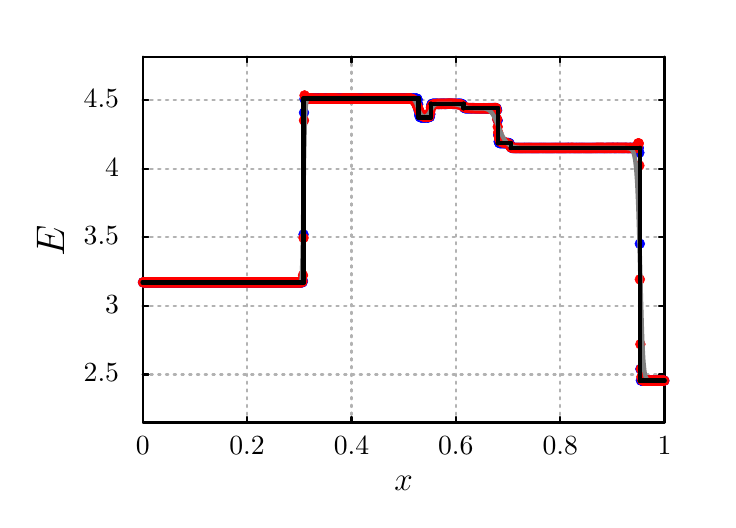
\begin{tikzpicture}[gnuplot]
%% generated with GNUPLOT 4.6p4 (Lua 5.1; terminal rev. 99, script rev. 100)
%% Fri 08 Aug 2014 12:23:48 PM EDT
\path (0.000,0.000) rectangle (8.500,6.000);
\gpfill{rgb color={1.000,1.000,1.000}} (1.320,0.985)--(7.946,0.985)--(7.946,5.630)--(1.320,5.630)--cycle;
\gpcolor{color=gp lt color border}
\gpsetlinetype{gp lt border}
\gpsetlinewidth{1.00}
\draw[gp path] (1.320,0.985)--(1.320,5.630)--(7.946,5.630)--(7.946,0.985)--cycle;
\gpcolor{color=gp lt color axes}
\gpsetlinetype{gp lt axes}
\gpsetlinewidth{2.00}
\draw[gp path] (1.320,1.596)--(7.947,1.596);
\gpcolor{color=gp lt color border}
\gpsetlinetype{gp lt border}
\draw[gp path] (1.320,1.596)--(1.392,1.596);
\draw[gp path] (7.947,1.596)--(7.875,1.596);
\gpcolor{rgb color={0.000,0.000,0.000}}
\node[gp node right,font={\fontsize{10pt}{12pt}\selectfont}] at (1.136,1.596) {2.5};
\gpcolor{color=gp lt color axes}
\gpsetlinetype{gp lt axes}
\draw[gp path] (1.320,2.467)--(7.947,2.467);
\gpcolor{color=gp lt color border}
\gpsetlinetype{gp lt border}
\draw[gp path] (1.320,2.467)--(1.392,2.467);
\draw[gp path] (7.947,2.467)--(7.875,2.467);
\gpcolor{rgb color={0.000,0.000,0.000}}
\node[gp node right,font={\fontsize{10pt}{12pt}\selectfont}] at (1.136,2.467) {3};
\gpcolor{color=gp lt color axes}
\gpsetlinetype{gp lt axes}
\draw[gp path] (1.320,3.338)--(7.947,3.338);
\gpcolor{color=gp lt color border}
\gpsetlinetype{gp lt border}
\draw[gp path] (1.320,3.338)--(1.392,3.338);
\draw[gp path] (7.947,3.338)--(7.875,3.338);
\gpcolor{rgb color={0.000,0.000,0.000}}
\node[gp node right,font={\fontsize{10pt}{12pt}\selectfont}] at (1.136,3.338) {3.5};
\gpcolor{color=gp lt color axes}
\gpsetlinetype{gp lt axes}
\draw[gp path] (1.320,4.209)--(7.947,4.209);
\gpcolor{color=gp lt color border}
\gpsetlinetype{gp lt border}
\draw[gp path] (1.320,4.209)--(1.392,4.209);
\draw[gp path] (7.947,4.209)--(7.875,4.209);
\gpcolor{rgb color={0.000,0.000,0.000}}
\node[gp node right,font={\fontsize{10pt}{12pt}\selectfont}] at (1.136,4.209) {4};
\gpcolor{color=gp lt color axes}
\gpsetlinetype{gp lt axes}
\draw[gp path] (1.320,5.080)--(7.947,5.080);
\gpcolor{color=gp lt color border}
\gpsetlinetype{gp lt border}
\draw[gp path] (1.320,5.080)--(1.392,5.080);
\draw[gp path] (7.947,5.080)--(7.875,5.080);
\gpcolor{rgb color={0.000,0.000,0.000}}
\node[gp node right,font={\fontsize{10pt}{12pt}\selectfont}] at (1.136,5.080) {4.5};
\gpcolor{color=gp lt color axes}
\gpsetlinetype{gp lt axes}
\draw[gp path] (1.320,0.985)--(1.320,5.631);
\gpcolor{color=gp lt color border}
\gpsetlinetype{gp lt border}
\draw[gp path] (1.320,0.985)--(1.320,1.057);
\draw[gp path] (1.320,5.631)--(1.320,5.559);
\gpcolor{rgb color={0.000,0.000,0.000}}
\node[gp node center,font={\fontsize{10pt}{12pt}\selectfont}] at (1.320,0.677) {0};
\gpcolor{color=gp lt color axes}
\gpsetlinetype{gp lt axes}
\draw[gp path] (2.645,0.985)--(2.645,5.631);
\gpcolor{color=gp lt color border}
\gpsetlinetype{gp lt border}
\draw[gp path] (2.645,0.985)--(2.645,1.057);
\draw[gp path] (2.645,5.631)--(2.645,5.559);
\gpcolor{rgb color={0.000,0.000,0.000}}
\node[gp node center,font={\fontsize{10pt}{12pt}\selectfont}] at (2.645,0.677) {0.2};
\gpcolor{color=gp lt color axes}
\gpsetlinetype{gp lt axes}
\draw[gp path] (3.971,0.985)--(3.971,5.631);
\gpcolor{color=gp lt color border}
\gpsetlinetype{gp lt border}
\draw[gp path] (3.971,0.985)--(3.971,1.057);
\draw[gp path] (3.971,5.631)--(3.971,5.559);
\gpcolor{rgb color={0.000,0.000,0.000}}
\node[gp node center,font={\fontsize{10pt}{12pt}\selectfont}] at (3.971,0.677) {0.4};
\gpcolor{color=gp lt color axes}
\gpsetlinetype{gp lt axes}
\draw[gp path] (5.296,0.985)--(5.296,5.631);
\gpcolor{color=gp lt color border}
\gpsetlinetype{gp lt border}
\draw[gp path] (5.296,0.985)--(5.296,1.057);
\draw[gp path] (5.296,5.631)--(5.296,5.559);
\gpcolor{rgb color={0.000,0.000,0.000}}
\node[gp node center,font={\fontsize{10pt}{12pt}\selectfont}] at (5.296,0.677) {0.6};
\gpcolor{color=gp lt color axes}
\gpsetlinetype{gp lt axes}
\draw[gp path] (6.622,0.985)--(6.622,5.631);
\gpcolor{color=gp lt color border}
\gpsetlinetype{gp lt border}
\draw[gp path] (6.622,0.985)--(6.622,1.057);
\draw[gp path] (6.622,5.631)--(6.622,5.559);
\gpcolor{rgb color={0.000,0.000,0.000}}
\node[gp node center,font={\fontsize{10pt}{12pt}\selectfont}] at (6.622,0.677) {0.8};
\gpcolor{color=gp lt color axes}
\gpsetlinetype{gp lt axes}
\draw[gp path] (7.947,0.985)--(7.947,5.631);
\gpcolor{color=gp lt color border}
\gpsetlinetype{gp lt border}
\draw[gp path] (7.947,0.985)--(7.947,1.057);
\draw[gp path] (7.947,5.631)--(7.947,5.559);
\gpcolor{rgb color={0.000,0.000,0.000}}
\node[gp node center,font={\fontsize{10pt}{12pt}\selectfont}] at (7.947,0.677) {1};
\gpcolor{color=gp lt color border}
\draw[gp path] (1.320,5.631)--(1.320,0.985)--(7.947,0.985)--(7.947,5.631)--cycle;
\gpcolor{rgb color={0.000,0.000,0.000}}
\node[gp node center,rotate=90,font={\fontsize{10pt}{12pt}\selectfont}] at (0.246,3.308) {\Large $E$};
\node[gp node center,font={\fontsize{10pt}{12pt}\selectfont}] at (4.633,0.215) {\large $x$};
\gpcolor{rgb color={0.000,0.000,1.000}}
\gpsetlinewidth{0.50}
\gpsetpointsize{4.44}
\gppoint{gp mark 7}{(1.323,2.766)}
\gppoint{gp mark 7}{(1.330,2.766)}
\gppoint{gp mark 7}{(1.336,2.766)}
\gppoint{gp mark 7}{(1.343,2.766)}
\gppoint{gp mark 7}{(1.349,2.766)}
\gppoint{gp mark 7}{(1.356,2.766)}
\gppoint{gp mark 7}{(1.362,2.766)}
\gppoint{gp mark 7}{(1.369,2.766)}
\gppoint{gp mark 7}{(1.375,2.766)}
\gppoint{gp mark 7}{(1.381,2.766)}
\gppoint{gp mark 7}{(1.388,2.766)}
\gppoint{gp mark 7}{(1.394,2.766)}
\gppoint{gp mark 7}{(1.401,2.766)}
\gppoint{gp mark 7}{(1.407,2.766)}
\gppoint{gp mark 7}{(1.414,2.766)}
\gppoint{gp mark 7}{(1.420,2.766)}
\gppoint{gp mark 7}{(1.427,2.766)}
\gppoint{gp mark 7}{(1.433,2.766)}
\gppoint{gp mark 7}{(1.440,2.766)}
\gppoint{gp mark 7}{(1.446,2.766)}
\gppoint{gp mark 7}{(1.453,2.766)}
\gppoint{gp mark 7}{(1.459,2.766)}
\gppoint{gp mark 7}{(1.466,2.766)}
\gppoint{gp mark 7}{(1.472,2.766)}
\gppoint{gp mark 7}{(1.479,2.766)}
\gppoint{gp mark 7}{(1.485,2.766)}
\gppoint{gp mark 7}{(1.491,2.766)}
\gppoint{gp mark 7}{(1.498,2.766)}
\gppoint{gp mark 7}{(1.504,2.766)}
\gppoint{gp mark 7}{(1.511,2.766)}
\gppoint{gp mark 7}{(1.517,2.766)}
\gppoint{gp mark 7}{(1.524,2.766)}
\gppoint{gp mark 7}{(1.530,2.766)}
\gppoint{gp mark 7}{(1.537,2.766)}
\gppoint{gp mark 7}{(1.543,2.766)}
\gppoint{gp mark 7}{(1.550,2.766)}
\gppoint{gp mark 7}{(1.556,2.766)}
\gppoint{gp mark 7}{(1.563,2.766)}
\gppoint{gp mark 7}{(1.569,2.766)}
\gppoint{gp mark 7}{(1.576,2.766)}
\gppoint{gp mark 7}{(1.582,2.766)}
\gppoint{gp mark 7}{(1.589,2.766)}
\gppoint{gp mark 7}{(1.595,2.766)}
\gppoint{gp mark 7}{(1.602,2.766)}
\gppoint{gp mark 7}{(1.608,2.766)}
\gppoint{gp mark 7}{(1.614,2.766)}
\gppoint{gp mark 7}{(1.621,2.766)}
\gppoint{gp mark 7}{(1.627,2.766)}
\gppoint{gp mark 7}{(1.634,2.766)}
\gppoint{gp mark 7}{(1.640,2.766)}
\gppoint{gp mark 7}{(1.647,2.766)}
\gppoint{gp mark 7}{(1.653,2.766)}
\gppoint{gp mark 7}{(1.660,2.766)}
\gppoint{gp mark 7}{(1.666,2.766)}
\gppoint{gp mark 7}{(1.673,2.766)}
\gppoint{gp mark 7}{(1.679,2.766)}
\gppoint{gp mark 7}{(1.686,2.766)}
\gppoint{gp mark 7}{(1.692,2.766)}
\gppoint{gp mark 7}{(1.699,2.766)}
\gppoint{gp mark 7}{(1.705,2.766)}
\gppoint{gp mark 7}{(1.712,2.766)}
\gppoint{gp mark 7}{(1.718,2.766)}
\gppoint{gp mark 7}{(1.724,2.766)}
\gppoint{gp mark 7}{(1.731,2.766)}
\gppoint{gp mark 7}{(1.737,2.766)}
\gppoint{gp mark 7}{(1.744,2.766)}
\gppoint{gp mark 7}{(1.750,2.766)}
\gppoint{gp mark 7}{(1.757,2.766)}
\gppoint{gp mark 7}{(1.763,2.766)}
\gppoint{gp mark 7}{(1.770,2.766)}
\gppoint{gp mark 7}{(1.776,2.766)}
\gppoint{gp mark 7}{(1.783,2.766)}
\gppoint{gp mark 7}{(1.789,2.766)}
\gppoint{gp mark 7}{(1.796,2.766)}
\gppoint{gp mark 7}{(1.802,2.766)}
\gppoint{gp mark 7}{(1.809,2.766)}
\gppoint{gp mark 7}{(1.815,2.766)}
\gppoint{gp mark 7}{(1.822,2.766)}
\gppoint{gp mark 7}{(1.828,2.766)}
\gppoint{gp mark 7}{(1.834,2.766)}
\gppoint{gp mark 7}{(1.841,2.766)}
\gppoint{gp mark 7}{(1.847,2.766)}
\gppoint{gp mark 7}{(1.854,2.766)}
\gppoint{gp mark 7}{(1.860,2.766)}
\gppoint{gp mark 7}{(1.867,2.766)}
\gppoint{gp mark 7}{(1.873,2.766)}
\gppoint{gp mark 7}{(1.880,2.766)}
\gppoint{gp mark 7}{(1.886,2.766)}
\gppoint{gp mark 7}{(1.893,2.766)}
\gppoint{gp mark 7}{(1.899,2.766)}
\gppoint{gp mark 7}{(1.906,2.766)}
\gppoint{gp mark 7}{(1.912,2.766)}
\gppoint{gp mark 7}{(1.919,2.766)}
\gppoint{gp mark 7}{(1.925,2.766)}
\gppoint{gp mark 7}{(1.932,2.766)}
\gppoint{gp mark 7}{(1.938,2.766)}
\gppoint{gp mark 7}{(1.945,2.766)}
\gppoint{gp mark 7}{(1.951,2.766)}
\gppoint{gp mark 7}{(1.957,2.766)}
\gppoint{gp mark 7}{(1.964,2.766)}
\gppoint{gp mark 7}{(1.970,2.766)}
\gppoint{gp mark 7}{(1.977,2.766)}
\gppoint{gp mark 7}{(1.983,2.766)}
\gppoint{gp mark 7}{(1.990,2.766)}
\gppoint{gp mark 7}{(1.996,2.766)}
\gppoint{gp mark 7}{(2.003,2.766)}
\gppoint{gp mark 7}{(2.009,2.766)}
\gppoint{gp mark 7}{(2.016,2.766)}
\gppoint{gp mark 7}{(2.022,2.766)}
\gppoint{gp mark 7}{(2.029,2.766)}
\gppoint{gp mark 7}{(2.035,2.766)}
\gppoint{gp mark 7}{(2.042,2.766)}
\gppoint{gp mark 7}{(2.048,2.766)}
\gppoint{gp mark 7}{(2.055,2.766)}
\gppoint{gp mark 7}{(2.061,2.766)}
\gppoint{gp mark 7}{(2.067,2.766)}
\gppoint{gp mark 7}{(2.074,2.766)}
\gppoint{gp mark 7}{(2.080,2.766)}
\gppoint{gp mark 7}{(2.087,2.766)}
\gppoint{gp mark 7}{(2.093,2.766)}
\gppoint{gp mark 7}{(2.100,2.766)}
\gppoint{gp mark 7}{(2.106,2.766)}
\gppoint{gp mark 7}{(2.113,2.766)}
\gppoint{gp mark 7}{(2.119,2.766)}
\gppoint{gp mark 7}{(2.126,2.766)}
\gppoint{gp mark 7}{(2.132,2.766)}
\gppoint{gp mark 7}{(2.139,2.766)}
\gppoint{gp mark 7}{(2.145,2.766)}
\gppoint{gp mark 7}{(2.152,2.766)}
\gppoint{gp mark 7}{(2.158,2.766)}
\gppoint{gp mark 7}{(2.165,2.766)}
\gppoint{gp mark 7}{(2.171,2.766)}
\gppoint{gp mark 7}{(2.177,2.766)}
\gppoint{gp mark 7}{(2.184,2.766)}
\gppoint{gp mark 7}{(2.190,2.766)}
\gppoint{gp mark 7}{(2.197,2.766)}
\gppoint{gp mark 7}{(2.203,2.766)}
\gppoint{gp mark 7}{(2.210,2.766)}
\gppoint{gp mark 7}{(2.216,2.766)}
\gppoint{gp mark 7}{(2.223,2.766)}
\gppoint{gp mark 7}{(2.229,2.766)}
\gppoint{gp mark 7}{(2.236,2.766)}
\gppoint{gp mark 7}{(2.242,2.766)}
\gppoint{gp mark 7}{(2.249,2.766)}
\gppoint{gp mark 7}{(2.255,2.766)}
\gppoint{gp mark 7}{(2.262,2.766)}
\gppoint{gp mark 7}{(2.268,2.766)}
\gppoint{gp mark 7}{(2.275,2.766)}
\gppoint{gp mark 7}{(2.281,2.766)}
\gppoint{gp mark 7}{(2.288,2.766)}
\gppoint{gp mark 7}{(2.294,2.766)}
\gppoint{gp mark 7}{(2.300,2.766)}
\gppoint{gp mark 7}{(2.307,2.766)}
\gppoint{gp mark 7}{(2.313,2.766)}
\gppoint{gp mark 7}{(2.320,2.766)}
\gppoint{gp mark 7}{(2.326,2.766)}
\gppoint{gp mark 7}{(2.333,2.766)}
\gppoint{gp mark 7}{(2.339,2.766)}
\gppoint{gp mark 7}{(2.346,2.766)}
\gppoint{gp mark 7}{(2.352,2.766)}
\gppoint{gp mark 7}{(2.359,2.766)}
\gppoint{gp mark 7}{(2.365,2.766)}
\gppoint{gp mark 7}{(2.372,2.766)}
\gppoint{gp mark 7}{(2.378,2.766)}
\gppoint{gp mark 7}{(2.385,2.766)}
\gppoint{gp mark 7}{(2.391,2.766)}
\gppoint{gp mark 7}{(2.398,2.766)}
\gppoint{gp mark 7}{(2.404,2.766)}
\gppoint{gp mark 7}{(2.410,2.766)}
\gppoint{gp mark 7}{(2.417,2.766)}
\gppoint{gp mark 7}{(2.423,2.766)}
\gppoint{gp mark 7}{(2.430,2.766)}
\gppoint{gp mark 7}{(2.436,2.766)}
\gppoint{gp mark 7}{(2.443,2.766)}
\gppoint{gp mark 7}{(2.449,2.766)}
\gppoint{gp mark 7}{(2.456,2.766)}
\gppoint{gp mark 7}{(2.462,2.766)}
\gppoint{gp mark 7}{(2.469,2.766)}
\gppoint{gp mark 7}{(2.475,2.766)}
\gppoint{gp mark 7}{(2.482,2.766)}
\gppoint{gp mark 7}{(2.488,2.766)}
\gppoint{gp mark 7}{(2.495,2.766)}
\gppoint{gp mark 7}{(2.501,2.766)}
\gppoint{gp mark 7}{(2.508,2.766)}
\gppoint{gp mark 7}{(2.514,2.766)}
\gppoint{gp mark 7}{(2.520,2.766)}
\gppoint{gp mark 7}{(2.527,2.766)}
\gppoint{gp mark 7}{(2.533,2.766)}
\gppoint{gp mark 7}{(2.540,2.766)}
\gppoint{gp mark 7}{(2.546,2.766)}
\gppoint{gp mark 7}{(2.553,2.766)}
\gppoint{gp mark 7}{(2.559,2.766)}
\gppoint{gp mark 7}{(2.566,2.766)}
\gppoint{gp mark 7}{(2.572,2.766)}
\gppoint{gp mark 7}{(2.579,2.766)}
\gppoint{gp mark 7}{(2.585,2.766)}
\gppoint{gp mark 7}{(2.592,2.766)}
\gppoint{gp mark 7}{(2.598,2.766)}
\gppoint{gp mark 7}{(2.605,2.766)}
\gppoint{gp mark 7}{(2.611,2.766)}
\gppoint{gp mark 7}{(2.618,2.766)}
\gppoint{gp mark 7}{(2.624,2.766)}
\gppoint{gp mark 7}{(2.631,2.766)}
\gppoint{gp mark 7}{(2.637,2.766)}
\gppoint{gp mark 7}{(2.643,2.766)}
\gppoint{gp mark 7}{(2.650,2.766)}
\gppoint{gp mark 7}{(2.656,2.766)}
\gppoint{gp mark 7}{(2.663,2.766)}
\gppoint{gp mark 7}{(2.669,2.766)}
\gppoint{gp mark 7}{(2.676,2.766)}
\gppoint{gp mark 7}{(2.682,2.766)}
\gppoint{gp mark 7}{(2.689,2.766)}
\gppoint{gp mark 7}{(2.695,2.766)}
\gppoint{gp mark 7}{(2.702,2.766)}
\gppoint{gp mark 7}{(2.708,2.766)}
\gppoint{gp mark 7}{(2.715,2.766)}
\gppoint{gp mark 7}{(2.721,2.766)}
\gppoint{gp mark 7}{(2.728,2.766)}
\gppoint{gp mark 7}{(2.734,2.766)}
\gppoint{gp mark 7}{(2.741,2.766)}
\gppoint{gp mark 7}{(2.747,2.766)}
\gppoint{gp mark 7}{(2.753,2.766)}
\gppoint{gp mark 7}{(2.760,2.766)}
\gppoint{gp mark 7}{(2.766,2.766)}
\gppoint{gp mark 7}{(2.773,2.766)}
\gppoint{gp mark 7}{(2.779,2.766)}
\gppoint{gp mark 7}{(2.786,2.766)}
\gppoint{gp mark 7}{(2.792,2.766)}
\gppoint{gp mark 7}{(2.799,2.766)}
\gppoint{gp mark 7}{(2.805,2.766)}
\gppoint{gp mark 7}{(2.812,2.766)}
\gppoint{gp mark 7}{(2.818,2.766)}
\gppoint{gp mark 7}{(2.825,2.766)}
\gppoint{gp mark 7}{(2.831,2.766)}
\gppoint{gp mark 7}{(2.838,2.766)}
\gppoint{gp mark 7}{(2.844,2.766)}
\gppoint{gp mark 7}{(2.851,2.766)}
\gppoint{gp mark 7}{(2.857,2.766)}
\gppoint{gp mark 7}{(2.863,2.766)}
\gppoint{gp mark 7}{(2.870,2.766)}
\gppoint{gp mark 7}{(2.876,2.766)}
\gppoint{gp mark 7}{(2.883,2.766)}
\gppoint{gp mark 7}{(2.889,2.766)}
\gppoint{gp mark 7}{(2.896,2.766)}
\gppoint{gp mark 7}{(2.902,2.766)}
\gppoint{gp mark 7}{(2.909,2.766)}
\gppoint{gp mark 7}{(2.915,2.766)}
\gppoint{gp mark 7}{(2.922,2.766)}
\gppoint{gp mark 7}{(2.928,2.766)}
\gppoint{gp mark 7}{(2.935,2.766)}
\gppoint{gp mark 7}{(2.941,2.766)}
\gppoint{gp mark 7}{(2.948,2.766)}
\gppoint{gp mark 7}{(2.954,2.766)}
\gppoint{gp mark 7}{(2.961,2.766)}
\gppoint{gp mark 7}{(2.967,2.766)}
\gppoint{gp mark 7}{(2.974,2.766)}
\gppoint{gp mark 7}{(2.980,2.766)}
\gppoint{gp mark 7}{(2.986,2.766)}
\gppoint{gp mark 7}{(2.993,2.766)}
\gppoint{gp mark 7}{(2.999,2.766)}
\gppoint{gp mark 7}{(3.006,2.766)}
\gppoint{gp mark 7}{(3.012,2.766)}
\gppoint{gp mark 7}{(3.019,2.766)}
\gppoint{gp mark 7}{(3.025,2.766)}
\gppoint{gp mark 7}{(3.032,2.766)}
\gppoint{gp mark 7}{(3.038,2.766)}
\gppoint{gp mark 7}{(3.045,2.766)}
\gppoint{gp mark 7}{(3.051,2.766)}
\gppoint{gp mark 7}{(3.058,2.766)}
\gppoint{gp mark 7}{(3.064,2.766)}
\gppoint{gp mark 7}{(3.071,2.766)}
\gppoint{gp mark 7}{(3.077,2.766)}
\gppoint{gp mark 7}{(3.084,2.766)}
\gppoint{gp mark 7}{(3.090,2.766)}
\gppoint{gp mark 7}{(3.096,2.766)}
\gppoint{gp mark 7}{(3.103,2.766)}
\gppoint{gp mark 7}{(3.109,2.766)}
\gppoint{gp mark 7}{(3.116,2.766)}
\gppoint{gp mark 7}{(3.122,2.766)}
\gppoint{gp mark 7}{(3.129,2.766)}
\gppoint{gp mark 7}{(3.135,2.766)}
\gppoint{gp mark 7}{(3.142,2.766)}
\gppoint{gp mark 7}{(3.148,2.766)}
\gppoint{gp mark 7}{(3.155,2.766)}
\gppoint{gp mark 7}{(3.161,2.766)}
\gppoint{gp mark 7}{(3.168,2.766)}
\gppoint{gp mark 7}{(3.174,2.766)}
\gppoint{gp mark 7}{(3.181,2.766)}
\gppoint{gp mark 7}{(3.187,2.766)}
\gppoint{gp mark 7}{(3.194,2.766)}
\gppoint{gp mark 7}{(3.200,2.766)}
\gppoint{gp mark 7}{(3.206,2.766)}
\gppoint{gp mark 7}{(3.213,2.766)}
\gppoint{gp mark 7}{(3.219,2.766)}
\gppoint{gp mark 7}{(3.226,2.766)}
\gppoint{gp mark 7}{(3.232,2.766)}
\gppoint{gp mark 7}{(3.239,2.766)}
\gppoint{gp mark 7}{(3.245,2.766)}
\gppoint{gp mark 7}{(3.252,2.766)}
\gppoint{gp mark 7}{(3.258,2.766)}
\gppoint{gp mark 7}{(3.265,2.766)}
\gppoint{gp mark 7}{(3.271,2.766)}
\gppoint{gp mark 7}{(3.278,2.766)}
\gppoint{gp mark 7}{(3.284,2.766)}
\gppoint{gp mark 7}{(3.291,2.766)}
\gppoint{gp mark 7}{(3.297,2.766)}
\gppoint{gp mark 7}{(3.304,2.766)}
\gppoint{gp mark 7}{(3.310,2.766)}
\gppoint{gp mark 7}{(3.317,2.766)}
\gppoint{gp mark 7}{(3.323,2.766)}
\gppoint{gp mark 7}{(3.329,2.766)}
\gppoint{gp mark 7}{(3.336,2.766)}
\gppoint{gp mark 7}{(3.342,2.766)}
\gppoint{gp mark 7}{(3.349,2.766)}
\gppoint{gp mark 7}{(3.355,2.783)}
\gppoint{gp mark 7}{(3.362,3.374)}
\gppoint{gp mark 7}{(3.368,4.920)}
\gppoint{gp mark 7}{(3.375,5.096)}
\gppoint{gp mark 7}{(3.381,5.088)}
\gppoint{gp mark 7}{(3.388,5.102)}
\gppoint{gp mark 7}{(3.394,5.110)}
\gppoint{gp mark 7}{(3.401,5.094)}
\gppoint{gp mark 7}{(3.407,5.091)}
\gppoint{gp mark 7}{(3.414,5.102)}
\gppoint{gp mark 7}{(3.420,5.103)}
\gppoint{gp mark 7}{(3.427,5.096)}
\gppoint{gp mark 7}{(3.433,5.096)}
\gppoint{gp mark 7}{(3.439,5.101)}
\gppoint{gp mark 7}{(3.446,5.100)}
\gppoint{gp mark 7}{(3.452,5.097)}
\gppoint{gp mark 7}{(3.459,5.098)}
\gppoint{gp mark 7}{(3.465,5.100)}
\gppoint{gp mark 7}{(3.472,5.099)}
\gppoint{gp mark 7}{(3.478,5.098)}
\gppoint{gp mark 7}{(3.485,5.099)}
\gppoint{gp mark 7}{(3.491,5.100)}
\gppoint{gp mark 7}{(3.498,5.098)}
\gppoint{gp mark 7}{(3.504,5.098)}
\gppoint{gp mark 7}{(3.511,5.099)}
\gppoint{gp mark 7}{(3.517,5.099)}
\gppoint{gp mark 7}{(3.524,5.098)}
\gppoint{gp mark 7}{(3.530,5.098)}
\gppoint{gp mark 7}{(3.537,5.099)}
\gppoint{gp mark 7}{(3.543,5.099)}
\gppoint{gp mark 7}{(3.549,5.099)}
\gppoint{gp mark 7}{(3.556,5.099)}
\gppoint{gp mark 7}{(3.562,5.099)}
\gppoint{gp mark 7}{(3.569,5.099)}
\gppoint{gp mark 7}{(3.575,5.099)}
\gppoint{gp mark 7}{(3.582,5.099)}
\gppoint{gp mark 7}{(3.588,5.099)}
\gppoint{gp mark 7}{(3.595,5.099)}
\gppoint{gp mark 7}{(3.601,5.099)}
\gppoint{gp mark 7}{(3.608,5.099)}
\gppoint{gp mark 7}{(3.614,5.098)}
\gppoint{gp mark 7}{(3.621,5.098)}
\gppoint{gp mark 7}{(3.627,5.098)}
\gppoint{gp mark 7}{(3.634,5.099)}
\gppoint{gp mark 7}{(3.640,5.099)}
\gppoint{gp mark 7}{(3.647,5.099)}
\gppoint{gp mark 7}{(3.653,5.099)}
\gppoint{gp mark 7}{(3.660,5.099)}
\gppoint{gp mark 7}{(3.666,5.099)}
\gppoint{gp mark 7}{(3.672,5.099)}
\gppoint{gp mark 7}{(3.679,5.099)}
\gppoint{gp mark 7}{(3.685,5.099)}
\gppoint{gp mark 7}{(3.692,5.099)}
\gppoint{gp mark 7}{(3.698,5.099)}
\gppoint{gp mark 7}{(3.705,5.099)}
\gppoint{gp mark 7}{(3.711,5.099)}
\gppoint{gp mark 7}{(3.718,5.098)}
\gppoint{gp mark 7}{(3.724,5.098)}
\gppoint{gp mark 7}{(3.731,5.099)}
\gppoint{gp mark 7}{(3.737,5.099)}
\gppoint{gp mark 7}{(3.744,5.099)}
\gppoint{gp mark 7}{(3.750,5.099)}
\gppoint{gp mark 7}{(3.757,5.099)}
\gppoint{gp mark 7}{(3.763,5.099)}
\gppoint{gp mark 7}{(3.770,5.099)}
\gppoint{gp mark 7}{(3.776,5.099)}
\gppoint{gp mark 7}{(3.782,5.099)}
\gppoint{gp mark 7}{(3.789,5.099)}
\gppoint{gp mark 7}{(3.795,5.099)}
\gppoint{gp mark 7}{(3.802,5.099)}
\gppoint{gp mark 7}{(3.808,5.099)}
\gppoint{gp mark 7}{(3.815,5.099)}
\gppoint{gp mark 7}{(3.821,5.099)}
\gppoint{gp mark 7}{(3.828,5.098)}
\gppoint{gp mark 7}{(3.834,5.098)}
\gppoint{gp mark 7}{(3.841,5.098)}
\gppoint{gp mark 7}{(3.847,5.098)}
\gppoint{gp mark 7}{(3.854,5.099)}
\gppoint{gp mark 7}{(3.860,5.099)}
\gppoint{gp mark 7}{(3.867,5.099)}
\gppoint{gp mark 7}{(3.873,5.099)}
\gppoint{gp mark 7}{(3.880,5.099)}
\gppoint{gp mark 7}{(3.886,5.099)}
\gppoint{gp mark 7}{(3.892,5.099)}
\gppoint{gp mark 7}{(3.899,5.099)}
\gppoint{gp mark 7}{(3.905,5.099)}
\gppoint{gp mark 7}{(3.912,5.099)}
\gppoint{gp mark 7}{(3.918,5.099)}
\gppoint{gp mark 7}{(3.925,5.098)}
\gppoint{gp mark 7}{(3.931,5.098)}
\gppoint{gp mark 7}{(3.938,5.098)}
\gppoint{gp mark 7}{(3.944,5.098)}
\gppoint{gp mark 7}{(3.951,5.099)}
\gppoint{gp mark 7}{(3.957,5.099)}
\gppoint{gp mark 7}{(3.964,5.099)}
\gppoint{gp mark 7}{(3.970,5.099)}
\gppoint{gp mark 7}{(3.977,5.099)}
\gppoint{gp mark 7}{(3.983,5.099)}
\gppoint{gp mark 7}{(3.990,5.099)}
\gppoint{gp mark 7}{(3.996,5.099)}
\gppoint{gp mark 7}{(4.003,5.099)}
\gppoint{gp mark 7}{(4.009,5.099)}
\gppoint{gp mark 7}{(4.015,5.099)}
\gppoint{gp mark 7}{(4.022,5.099)}
\gppoint{gp mark 7}{(4.028,5.099)}
\gppoint{gp mark 7}{(4.035,5.099)}
\gppoint{gp mark 7}{(4.041,5.099)}
\gppoint{gp mark 7}{(4.048,5.099)}
\gppoint{gp mark 7}{(4.054,5.099)}
\gppoint{gp mark 7}{(4.061,5.099)}
\gppoint{gp mark 7}{(4.067,5.099)}
\gppoint{gp mark 7}{(4.074,5.099)}
\gppoint{gp mark 7}{(4.080,5.099)}
\gppoint{gp mark 7}{(4.087,5.099)}
\gppoint{gp mark 7}{(4.093,5.099)}
\gppoint{gp mark 7}{(4.100,5.099)}
\gppoint{gp mark 7}{(4.106,5.099)}
\gppoint{gp mark 7}{(4.113,5.099)}
\gppoint{gp mark 7}{(4.119,5.099)}
\gppoint{gp mark 7}{(4.125,5.099)}
\gppoint{gp mark 7}{(4.132,5.098)}
\gppoint{gp mark 7}{(4.138,5.098)}
\gppoint{gp mark 7}{(4.145,5.098)}
\gppoint{gp mark 7}{(4.151,5.098)}
\gppoint{gp mark 7}{(4.158,5.099)}
\gppoint{gp mark 7}{(4.164,5.099)}
\gppoint{gp mark 7}{(4.171,5.099)}
\gppoint{gp mark 7}{(4.177,5.099)}
\gppoint{gp mark 7}{(4.184,5.099)}
\gppoint{gp mark 7}{(4.190,5.099)}
\gppoint{gp mark 7}{(4.197,5.099)}
\gppoint{gp mark 7}{(4.203,5.099)}
\gppoint{gp mark 7}{(4.210,5.099)}
\gppoint{gp mark 7}{(4.216,5.099)}
\gppoint{gp mark 7}{(4.223,5.099)}
\gppoint{gp mark 7}{(4.229,5.099)}
\gppoint{gp mark 7}{(4.235,5.099)}
\gppoint{gp mark 7}{(4.242,5.098)}
\gppoint{gp mark 7}{(4.248,5.099)}
\gppoint{gp mark 7}{(4.255,5.099)}
\gppoint{gp mark 7}{(4.261,5.099)}
\gppoint{gp mark 7}{(4.268,5.099)}
\gppoint{gp mark 7}{(4.274,5.099)}
\gppoint{gp mark 7}{(4.281,5.099)}
\gppoint{gp mark 7}{(4.287,5.099)}
\gppoint{gp mark 7}{(4.294,5.099)}
\gppoint{gp mark 7}{(4.300,5.099)}
\gppoint{gp mark 7}{(4.307,5.099)}
\gppoint{gp mark 7}{(4.313,5.099)}
\gppoint{gp mark 7}{(4.320,5.099)}
\gppoint{gp mark 7}{(4.326,5.099)}
\gppoint{gp mark 7}{(4.333,5.099)}
\gppoint{gp mark 7}{(4.339,5.099)}
\gppoint{gp mark 7}{(4.346,5.098)}
\gppoint{gp mark 7}{(4.352,5.098)}
\gppoint{gp mark 7}{(4.358,5.098)}
\gppoint{gp mark 7}{(4.365,5.098)}
\gppoint{gp mark 7}{(4.371,5.099)}
\gppoint{gp mark 7}{(4.378,5.099)}
\gppoint{gp mark 7}{(4.384,5.099)}
\gppoint{gp mark 7}{(4.391,5.099)}
\gppoint{gp mark 7}{(4.397,5.099)}
\gppoint{gp mark 7}{(4.404,5.099)}
\gppoint{gp mark 7}{(4.410,5.099)}
\gppoint{gp mark 7}{(4.417,5.099)}
\gppoint{gp mark 7}{(4.423,5.099)}
\gppoint{gp mark 7}{(4.430,5.099)}
\gppoint{gp mark 7}{(4.436,5.099)}
\gppoint{gp mark 7}{(4.443,5.099)}
\gppoint{gp mark 7}{(4.449,5.098)}
\gppoint{gp mark 7}{(4.456,5.098)}
\gppoint{gp mark 7}{(4.462,5.098)}
\gppoint{gp mark 7}{(4.468,5.098)}
\gppoint{gp mark 7}{(4.475,5.099)}
\gppoint{gp mark 7}{(4.481,5.099)}
\gppoint{gp mark 7}{(4.488,5.099)}
\gppoint{gp mark 7}{(4.494,5.099)}
\gppoint{gp mark 7}{(4.501,5.099)}
\gppoint{gp mark 7}{(4.507,5.099)}
\gppoint{gp mark 7}{(4.514,5.099)}
\gppoint{gp mark 7}{(4.520,5.099)}
\gppoint{gp mark 7}{(4.527,5.099)}
\gppoint{gp mark 7}{(4.533,5.099)}
\gppoint{gp mark 7}{(4.540,5.098)}
\gppoint{gp mark 7}{(4.546,5.098)}
\gppoint{gp mark 7}{(4.553,5.099)}
\gppoint{gp mark 7}{(4.559,5.099)}
\gppoint{gp mark 7}{(4.566,5.099)}
\gppoint{gp mark 7}{(4.572,5.098)}
\gppoint{gp mark 7}{(4.578,5.098)}
\gppoint{gp mark 7}{(4.585,5.099)}
\gppoint{gp mark 7}{(4.591,5.099)}
\gppoint{gp mark 7}{(4.598,5.099)}
\gppoint{gp mark 7}{(4.604,5.099)}
\gppoint{gp mark 7}{(4.611,5.099)}
\gppoint{gp mark 7}{(4.617,5.099)}
\gppoint{gp mark 7}{(4.624,5.099)}
\gppoint{gp mark 7}{(4.630,5.099)}
\gppoint{gp mark 7}{(4.637,5.099)}
\gppoint{gp mark 7}{(4.643,5.099)}
\gppoint{gp mark 7}{(4.650,5.099)}
\gppoint{gp mark 7}{(4.656,5.098)}
\gppoint{gp mark 7}{(4.663,5.098)}
\gppoint{gp mark 7}{(4.669,5.098)}
\gppoint{gp mark 7}{(4.676,5.099)}
\gppoint{gp mark 7}{(4.682,5.099)}
\gppoint{gp mark 7}{(4.689,5.099)}
\gppoint{gp mark 7}{(4.695,5.098)}
\gppoint{gp mark 7}{(4.701,5.098)}
\gppoint{gp mark 7}{(4.708,5.099)}
\gppoint{gp mark 7}{(4.714,5.099)}
\gppoint{gp mark 7}{(4.721,5.099)}
\gppoint{gp mark 7}{(4.727,5.099)}
\gppoint{gp mark 7}{(4.734,5.098)}
\gppoint{gp mark 7}{(4.740,5.098)}
\gppoint{gp mark 7}{(4.747,5.098)}
\gppoint{gp mark 7}{(4.753,5.099)}
\gppoint{gp mark 7}{(4.760,5.099)}
\gppoint{gp mark 7}{(4.766,5.099)}
\gppoint{gp mark 7}{(4.773,5.098)}
\gppoint{gp mark 7}{(4.779,5.098)}
\gppoint{gp mark 7}{(4.786,5.098)}
\gppoint{gp mark 7}{(4.792,5.099)}
\gppoint{gp mark 7}{(4.799,5.099)}
\gppoint{gp mark 7}{(4.805,5.098)}
\gppoint{gp mark 7}{(4.811,5.086)}
\gppoint{gp mark 7}{(4.818,5.028)}
\gppoint{gp mark 7}{(4.824,4.945)}
\gppoint{gp mark 7}{(4.831,4.892)}
\gppoint{gp mark 7}{(4.837,4.871)}
\gppoint{gp mark 7}{(4.844,4.864)}
\gppoint{gp mark 7}{(4.850,4.861)}
\gppoint{gp mark 7}{(4.857,4.860)}
\gppoint{gp mark 7}{(4.863,4.860)}
\gppoint{gp mark 7}{(4.870,4.861)}
\gppoint{gp mark 7}{(4.876,4.862)}
\gppoint{gp mark 7}{(4.883,4.862)}
\gppoint{gp mark 7}{(4.889,4.861)}
\gppoint{gp mark 7}{(4.896,4.860)}
\gppoint{gp mark 7}{(4.902,4.860)}
\gppoint{gp mark 7}{(4.909,4.861)}
\gppoint{gp mark 7}{(4.915,4.863)}
\gppoint{gp mark 7}{(4.921,4.863)}
\gppoint{gp mark 7}{(4.928,4.862)}
\gppoint{gp mark 7}{(4.934,4.860)}
\gppoint{gp mark 7}{(4.941,4.860)}
\gppoint{gp mark 7}{(4.947,4.861)}
\gppoint{gp mark 7}{(4.954,4.864)}
\gppoint{gp mark 7}{(4.960,4.865)}
\gppoint{gp mark 7}{(4.967,4.867)}
\gppoint{gp mark 7}{(4.973,4.902)}
\gppoint{gp mark 7}{(4.980,4.986)}
\gppoint{gp mark 7}{(4.986,5.024)}
\gppoint{gp mark 7}{(4.993,5.031)}
\gppoint{gp mark 7}{(4.999,5.032)}
\gppoint{gp mark 7}{(5.006,5.033)}
\gppoint{gp mark 7}{(5.012,5.033)}
\gppoint{gp mark 7}{(5.019,5.033)}
\gppoint{gp mark 7}{(5.025,5.033)}
\gppoint{gp mark 7}{(5.032,5.033)}
\gppoint{gp mark 7}{(5.038,5.033)}
\gppoint{gp mark 7}{(5.044,5.033)}
\gppoint{gp mark 7}{(5.051,5.033)}
\gppoint{gp mark 7}{(5.057,5.033)}
\gppoint{gp mark 7}{(5.064,5.032)}
\gppoint{gp mark 7}{(5.070,5.032)}
\gppoint{gp mark 7}{(5.077,5.032)}
\gppoint{gp mark 7}{(5.083,5.032)}
\gppoint{gp mark 7}{(5.090,5.032)}
\gppoint{gp mark 7}{(5.096,5.032)}
\gppoint{gp mark 7}{(5.103,5.033)}
\gppoint{gp mark 7}{(5.109,5.032)}
\gppoint{gp mark 7}{(5.116,5.032)}
\gppoint{gp mark 7}{(5.122,5.033)}
\gppoint{gp mark 7}{(5.129,5.033)}
\gppoint{gp mark 7}{(5.135,5.033)}
\gppoint{gp mark 7}{(5.142,5.033)}
\gppoint{gp mark 7}{(5.148,5.033)}
\gppoint{gp mark 7}{(5.154,5.032)}
\gppoint{gp mark 7}{(5.161,5.032)}
\gppoint{gp mark 7}{(5.167,5.032)}
\gppoint{gp mark 7}{(5.174,5.032)}
\gppoint{gp mark 7}{(5.180,5.032)}
\gppoint{gp mark 7}{(5.187,5.032)}
\gppoint{gp mark 7}{(5.193,5.033)}
\gppoint{gp mark 7}{(5.200,5.033)}
\gppoint{gp mark 7}{(5.206,5.033)}
\gppoint{gp mark 7}{(5.213,5.033)}
\gppoint{gp mark 7}{(5.219,5.033)}
\gppoint{gp mark 7}{(5.226,5.033)}
\gppoint{gp mark 7}{(5.232,5.033)}
\gppoint{gp mark 7}{(5.239,5.033)}
\gppoint{gp mark 7}{(5.245,5.033)}
\gppoint{gp mark 7}{(5.252,5.032)}
\gppoint{gp mark 7}{(5.258,5.032)}
\gppoint{gp mark 7}{(5.264,5.032)}
\gppoint{gp mark 7}{(5.271,5.032)}
\gppoint{gp mark 7}{(5.277,5.032)}
\gppoint{gp mark 7}{(5.284,5.033)}
\gppoint{gp mark 7}{(5.290,5.033)}
\gppoint{gp mark 7}{(5.297,5.032)}
\gppoint{gp mark 7}{(5.303,5.032)}
\gppoint{gp mark 7}{(5.310,5.032)}
\gppoint{gp mark 7}{(5.316,5.032)}
\gppoint{gp mark 7}{(5.323,5.033)}
\gppoint{gp mark 7}{(5.329,5.033)}
\gppoint{gp mark 7}{(5.336,5.033)}
\gppoint{gp mark 7}{(5.342,5.033)}
\gppoint{gp mark 7}{(5.349,5.033)}
\gppoint{gp mark 7}{(5.355,5.032)}
\gppoint{gp mark 7}{(5.362,5.032)}
\gppoint{gp mark 7}{(5.368,5.032)}
\gppoint{gp mark 7}{(5.375,5.031)}
\gppoint{gp mark 7}{(5.381,5.026)}
\gppoint{gp mark 7}{(5.387,5.014)}
\gppoint{gp mark 7}{(5.394,4.998)}
\gppoint{gp mark 7}{(5.400,4.986)}
\gppoint{gp mark 7}{(5.407,4.979)}
\gppoint{gp mark 7}{(5.413,4.977)}
\gppoint{gp mark 7}{(5.420,4.977)}
\gppoint{gp mark 7}{(5.426,4.977)}
\gppoint{gp mark 7}{(5.433,4.977)}
\gppoint{gp mark 7}{(5.439,4.977)}
\gppoint{gp mark 7}{(5.446,4.977)}
\gppoint{gp mark 7}{(5.452,4.977)}
\gppoint{gp mark 7}{(5.459,4.977)}
\gppoint{gp mark 7}{(5.465,4.977)}
\gppoint{gp mark 7}{(5.472,4.977)}
\gppoint{gp mark 7}{(5.478,4.977)}
\gppoint{gp mark 7}{(5.485,4.977)}
\gppoint{gp mark 7}{(5.491,4.977)}
\gppoint{gp mark 7}{(5.497,4.977)}
\gppoint{gp mark 7}{(5.504,4.977)}
\gppoint{gp mark 7}{(5.510,4.978)}
\gppoint{gp mark 7}{(5.517,4.978)}
\gppoint{gp mark 7}{(5.523,4.978)}
\gppoint{gp mark 7}{(5.530,4.977)}
\gppoint{gp mark 7}{(5.536,4.977)}
\gppoint{gp mark 7}{(5.543,4.977)}
\gppoint{gp mark 7}{(5.549,4.977)}
\gppoint{gp mark 7}{(5.556,4.977)}
\gppoint{gp mark 7}{(5.562,4.977)}
\gppoint{gp mark 7}{(5.569,4.977)}
\gppoint{gp mark 7}{(5.575,4.977)}
\gppoint{gp mark 7}{(5.582,4.977)}
\gppoint{gp mark 7}{(5.588,4.977)}
\gppoint{gp mark 7}{(5.595,4.977)}
\gppoint{gp mark 7}{(5.601,4.977)}
\gppoint{gp mark 7}{(5.607,4.977)}
\gppoint{gp mark 7}{(5.614,4.977)}
\gppoint{gp mark 7}{(5.620,4.977)}
\gppoint{gp mark 7}{(5.627,4.977)}
\gppoint{gp mark 7}{(5.633,4.977)}
\gppoint{gp mark 7}{(5.640,4.977)}
\gppoint{gp mark 7}{(5.646,4.977)}
\gppoint{gp mark 7}{(5.653,4.978)}
\gppoint{gp mark 7}{(5.659,4.977)}
\gppoint{gp mark 7}{(5.666,4.977)}
\gppoint{gp mark 7}{(5.672,4.977)}
\gppoint{gp mark 7}{(5.679,4.977)}
\gppoint{gp mark 7}{(5.685,4.977)}
\gppoint{gp mark 7}{(5.692,4.977)}
\gppoint{gp mark 7}{(5.698,4.977)}
\gppoint{gp mark 7}{(5.705,4.978)}
\gppoint{gp mark 7}{(5.711,4.978)}
\gppoint{gp mark 7}{(5.718,4.978)}
\gppoint{gp mark 7}{(5.724,4.978)}
\gppoint{gp mark 7}{(5.730,4.978)}
\gppoint{gp mark 7}{(5.737,4.978)}
\gppoint{gp mark 7}{(5.743,4.978)}
\gppoint{gp mark 7}{(5.750,4.978)}
\gppoint{gp mark 7}{(5.756,4.978)}
\gppoint{gp mark 7}{(5.763,4.978)}
\gppoint{gp mark 7}{(5.769,4.978)}
\gppoint{gp mark 7}{(5.776,4.978)}
\gppoint{gp mark 7}{(5.782,4.978)}
\gppoint{gp mark 7}{(5.789,4.977)}
\gppoint{gp mark 7}{(5.795,4.977)}
\gppoint{gp mark 7}{(5.802,4.977)}
\gppoint{gp mark 7}{(5.808,4.977)}
\gppoint{gp mark 7}{(5.815,4.975)}
\gppoint{gp mark 7}{(5.821,4.952)}
\gppoint{gp mark 7}{(5.828,4.821)}
\gppoint{gp mark 7}{(5.834,4.640)}
\gppoint{gp mark 7}{(5.840,4.552)}
\gppoint{gp mark 7}{(5.847,4.536)}
\gppoint{gp mark 7}{(5.853,4.534)}
\gppoint{gp mark 7}{(5.860,4.534)}
\gppoint{gp mark 7}{(5.866,4.534)}
\gppoint{gp mark 7}{(5.873,4.534)}
\gppoint{gp mark 7}{(5.879,4.534)}
\gppoint{gp mark 7}{(5.886,4.534)}
\gppoint{gp mark 7}{(5.892,4.534)}
\gppoint{gp mark 7}{(5.899,4.534)}
\gppoint{gp mark 7}{(5.905,4.533)}
\gppoint{gp mark 7}{(5.912,4.533)}
\gppoint{gp mark 7}{(5.918,4.533)}
\gppoint{gp mark 7}{(5.925,4.533)}
\gppoint{gp mark 7}{(5.931,4.533)}
\gppoint{gp mark 7}{(5.938,4.534)}
\gppoint{gp mark 7}{(5.944,4.535)}
\gppoint{gp mark 7}{(5.950,4.535)}
\gppoint{gp mark 7}{(5.957,4.535)}
\gppoint{gp mark 7}{(5.963,4.535)}
\gppoint{gp mark 7}{(5.970,4.535)}
\gppoint{gp mark 7}{(5.976,4.533)}
\gppoint{gp mark 7}{(5.983,4.521)}
\gppoint{gp mark 7}{(5.989,4.502)}
\gppoint{gp mark 7}{(5.996,4.484)}
\gppoint{gp mark 7}{(6.002,4.475)}
\gppoint{gp mark 7}{(6.009,4.472)}
\gppoint{gp mark 7}{(6.015,4.472)}
\gppoint{gp mark 7}{(6.022,4.472)}
\gppoint{gp mark 7}{(6.028,4.472)}
\gppoint{gp mark 7}{(6.035,4.472)}
\gppoint{gp mark 7}{(6.041,4.472)}
\gppoint{gp mark 7}{(6.048,4.472)}
\gppoint{gp mark 7}{(6.054,4.472)}
\gppoint{gp mark 7}{(6.061,4.472)}
\gppoint{gp mark 7}{(6.067,4.472)}
\gppoint{gp mark 7}{(6.073,4.472)}
\gppoint{gp mark 7}{(6.080,4.472)}
\gppoint{gp mark 7}{(6.086,4.472)}
\gppoint{gp mark 7}{(6.093,4.472)}
\gppoint{gp mark 7}{(6.099,4.472)}
\gppoint{gp mark 7}{(6.106,4.472)}
\gppoint{gp mark 7}{(6.112,4.472)}
\gppoint{gp mark 7}{(6.119,4.472)}
\gppoint{gp mark 7}{(6.125,4.472)}
\gppoint{gp mark 7}{(6.132,4.472)}
\gppoint{gp mark 7}{(6.138,4.472)}
\gppoint{gp mark 7}{(6.145,4.472)}
\gppoint{gp mark 7}{(6.151,4.472)}
\gppoint{gp mark 7}{(6.158,4.472)}
\gppoint{gp mark 7}{(6.164,4.473)}
\gppoint{gp mark 7}{(6.171,4.472)}
\gppoint{gp mark 7}{(6.177,4.472)}
\gppoint{gp mark 7}{(6.183,4.472)}
\gppoint{gp mark 7}{(6.190,4.472)}
\gppoint{gp mark 7}{(6.196,4.472)}
\gppoint{gp mark 7}{(6.203,4.472)}
\gppoint{gp mark 7}{(6.209,4.472)}
\gppoint{gp mark 7}{(6.216,4.472)}
\gppoint{gp mark 7}{(6.222,4.472)}
\gppoint{gp mark 7}{(6.229,4.472)}
\gppoint{gp mark 7}{(6.235,4.472)}
\gppoint{gp mark 7}{(6.242,4.472)}
\gppoint{gp mark 7}{(6.248,4.472)}
\gppoint{gp mark 7}{(6.255,4.472)}
\gppoint{gp mark 7}{(6.261,4.472)}
\gppoint{gp mark 7}{(6.268,4.472)}
\gppoint{gp mark 7}{(6.274,4.472)}
\gppoint{gp mark 7}{(6.281,4.472)}
\gppoint{gp mark 7}{(6.287,4.472)}
\gppoint{gp mark 7}{(6.293,4.472)}
\gppoint{gp mark 7}{(6.300,4.472)}
\gppoint{gp mark 7}{(6.306,4.472)}
\gppoint{gp mark 7}{(6.313,4.472)}
\gppoint{gp mark 7}{(6.319,4.472)}
\gppoint{gp mark 7}{(6.326,4.472)}
\gppoint{gp mark 7}{(6.332,4.472)}
\gppoint{gp mark 7}{(6.339,4.472)}
\gppoint{gp mark 7}{(6.345,4.472)}
\gppoint{gp mark 7}{(6.352,4.472)}
\gppoint{gp mark 7}{(6.358,4.472)}
\gppoint{gp mark 7}{(6.365,4.472)}
\gppoint{gp mark 7}{(6.371,4.472)}
\gppoint{gp mark 7}{(6.378,4.472)}
\gppoint{gp mark 7}{(6.384,4.472)}
\gppoint{gp mark 7}{(6.391,4.472)}
\gppoint{gp mark 7}{(6.397,4.472)}
\gppoint{gp mark 7}{(6.404,4.472)}
\gppoint{gp mark 7}{(6.410,4.472)}
\gppoint{gp mark 7}{(6.416,4.472)}
\gppoint{gp mark 7}{(6.423,4.472)}
\gppoint{gp mark 7}{(6.429,4.472)}
\gppoint{gp mark 7}{(6.436,4.472)}
\gppoint{gp mark 7}{(6.442,4.472)}
\gppoint{gp mark 7}{(6.449,4.472)}
\gppoint{gp mark 7}{(6.455,4.472)}
\gppoint{gp mark 7}{(6.462,4.472)}
\gppoint{gp mark 7}{(6.468,4.472)}
\gppoint{gp mark 7}{(6.475,4.472)}
\gppoint{gp mark 7}{(6.481,4.472)}
\gppoint{gp mark 7}{(6.488,4.472)}
\gppoint{gp mark 7}{(6.494,4.472)}
\gppoint{gp mark 7}{(6.501,4.472)}
\gppoint{gp mark 7}{(6.507,4.472)}
\gppoint{gp mark 7}{(6.514,4.472)}
\gppoint{gp mark 7}{(6.520,4.472)}
\gppoint{gp mark 7}{(6.526,4.472)}
\gppoint{gp mark 7}{(6.533,4.472)}
\gppoint{gp mark 7}{(6.539,4.472)}
\gppoint{gp mark 7}{(6.546,4.472)}
\gppoint{gp mark 7}{(6.552,4.472)}
\gppoint{gp mark 7}{(6.559,4.472)}
\gppoint{gp mark 7}{(6.565,4.472)}
\gppoint{gp mark 7}{(6.572,4.472)}
\gppoint{gp mark 7}{(6.578,4.472)}
\gppoint{gp mark 7}{(6.585,4.472)}
\gppoint{gp mark 7}{(6.591,4.472)}
\gppoint{gp mark 7}{(6.598,4.472)}
\gppoint{gp mark 7}{(6.604,4.472)}
\gppoint{gp mark 7}{(6.611,4.472)}
\gppoint{gp mark 7}{(6.617,4.472)}
\gppoint{gp mark 7}{(6.624,4.472)}
\gppoint{gp mark 7}{(6.630,4.472)}
\gppoint{gp mark 7}{(6.636,4.472)}
\gppoint{gp mark 7}{(6.643,4.472)}
\gppoint{gp mark 7}{(6.649,4.472)}
\gppoint{gp mark 7}{(6.656,4.472)}
\gppoint{gp mark 7}{(6.662,4.472)}
\gppoint{gp mark 7}{(6.669,4.472)}
\gppoint{gp mark 7}{(6.675,4.472)}
\gppoint{gp mark 7}{(6.682,4.472)}
\gppoint{gp mark 7}{(6.688,4.472)}
\gppoint{gp mark 7}{(6.695,4.472)}
\gppoint{gp mark 7}{(6.701,4.472)}
\gppoint{gp mark 7}{(6.708,4.472)}
\gppoint{gp mark 7}{(6.714,4.472)}
\gppoint{gp mark 7}{(6.721,4.473)}
\gppoint{gp mark 7}{(6.727,4.473)}
\gppoint{gp mark 7}{(6.734,4.472)}
\gppoint{gp mark 7}{(6.740,4.472)}
\gppoint{gp mark 7}{(6.747,4.472)}
\gppoint{gp mark 7}{(6.753,4.472)}
\gppoint{gp mark 7}{(6.759,4.472)}
\gppoint{gp mark 7}{(6.766,4.472)}
\gppoint{gp mark 7}{(6.772,4.472)}
\gppoint{gp mark 7}{(6.779,4.472)}
\gppoint{gp mark 7}{(6.785,4.472)}
\gppoint{gp mark 7}{(6.792,4.472)}
\gppoint{gp mark 7}{(6.798,4.472)}
\gppoint{gp mark 7}{(6.805,4.472)}
\gppoint{gp mark 7}{(6.811,4.472)}
\gppoint{gp mark 7}{(6.818,4.472)}
\gppoint{gp mark 7}{(6.824,4.472)}
\gppoint{gp mark 7}{(6.831,4.473)}
\gppoint{gp mark 7}{(6.837,4.472)}
\gppoint{gp mark 7}{(6.844,4.472)}
\gppoint{gp mark 7}{(6.850,4.472)}
\gppoint{gp mark 7}{(6.857,4.472)}
\gppoint{gp mark 7}{(6.863,4.472)}
\gppoint{gp mark 7}{(6.869,4.472)}
\gppoint{gp mark 7}{(6.876,4.472)}
\gppoint{gp mark 7}{(6.882,4.472)}
\gppoint{gp mark 7}{(6.889,4.472)}
\gppoint{gp mark 7}{(6.895,4.472)}
\gppoint{gp mark 7}{(6.902,4.472)}
\gppoint{gp mark 7}{(6.908,4.472)}
\gppoint{gp mark 7}{(6.915,4.472)}
\gppoint{gp mark 7}{(6.921,4.472)}
\gppoint{gp mark 7}{(6.928,4.472)}
\gppoint{gp mark 7}{(6.934,4.472)}
\gppoint{gp mark 7}{(6.941,4.472)}
\gppoint{gp mark 7}{(6.947,4.472)}
\gppoint{gp mark 7}{(6.954,4.472)}
\gppoint{gp mark 7}{(6.960,4.472)}
\gppoint{gp mark 7}{(6.967,4.472)}
\gppoint{gp mark 7}{(6.973,4.472)}
\gppoint{gp mark 7}{(6.979,4.472)}
\gppoint{gp mark 7}{(6.986,4.472)}
\gppoint{gp mark 7}{(6.992,4.472)}
\gppoint{gp mark 7}{(6.999,4.472)}
\gppoint{gp mark 7}{(7.005,4.472)}
\gppoint{gp mark 7}{(7.012,4.472)}
\gppoint{gp mark 7}{(7.018,4.472)}
\gppoint{gp mark 7}{(7.025,4.472)}
\gppoint{gp mark 7}{(7.031,4.472)}
\gppoint{gp mark 7}{(7.038,4.472)}
\gppoint{gp mark 7}{(7.044,4.472)}
\gppoint{gp mark 7}{(7.051,4.472)}
\gppoint{gp mark 7}{(7.057,4.472)}
\gppoint{gp mark 7}{(7.064,4.472)}
\gppoint{gp mark 7}{(7.070,4.472)}
\gppoint{gp mark 7}{(7.077,4.472)}
\gppoint{gp mark 7}{(7.083,4.472)}
\gppoint{gp mark 7}{(7.090,4.472)}
\gppoint{gp mark 7}{(7.096,4.472)}
\gppoint{gp mark 7}{(7.102,4.472)}
\gppoint{gp mark 7}{(7.109,4.472)}
\gppoint{gp mark 7}{(7.115,4.472)}
\gppoint{gp mark 7}{(7.122,4.472)}
\gppoint{gp mark 7}{(7.128,4.472)}
\gppoint{gp mark 7}{(7.135,4.472)}
\gppoint{gp mark 7}{(7.141,4.472)}
\gppoint{gp mark 7}{(7.148,4.472)}
\gppoint{gp mark 7}{(7.154,4.472)}
\gppoint{gp mark 7}{(7.161,4.472)}
\gppoint{gp mark 7}{(7.167,4.472)}
\gppoint{gp mark 7}{(7.174,4.472)}
\gppoint{gp mark 7}{(7.180,4.472)}
\gppoint{gp mark 7}{(7.187,4.472)}
\gppoint{gp mark 7}{(7.193,4.472)}
\gppoint{gp mark 7}{(7.200,4.472)}
\gppoint{gp mark 7}{(7.206,4.472)}
\gppoint{gp mark 7}{(7.212,4.472)}
\gppoint{gp mark 7}{(7.219,4.472)}
\gppoint{gp mark 7}{(7.225,4.472)}
\gppoint{gp mark 7}{(7.232,4.472)}
\gppoint{gp mark 7}{(7.238,4.472)}
\gppoint{gp mark 7}{(7.245,4.472)}
\gppoint{gp mark 7}{(7.251,4.472)}
\gppoint{gp mark 7}{(7.258,4.472)}
\gppoint{gp mark 7}{(7.264,4.472)}
\gppoint{gp mark 7}{(7.271,4.472)}
\gppoint{gp mark 7}{(7.277,4.472)}
\gppoint{gp mark 7}{(7.284,4.473)}
\gppoint{gp mark 7}{(7.290,4.473)}
\gppoint{gp mark 7}{(7.297,4.473)}
\gppoint{gp mark 7}{(7.303,4.472)}
\gppoint{gp mark 7}{(7.310,4.472)}
\gppoint{gp mark 7}{(7.316,4.471)}
\gppoint{gp mark 7}{(7.322,4.471)}
\gppoint{gp mark 7}{(7.329,4.472)}
\gppoint{gp mark 7}{(7.335,4.472)}
\gppoint{gp mark 7}{(7.342,4.472)}
\gppoint{gp mark 7}{(7.348,4.473)}
\gppoint{gp mark 7}{(7.355,4.473)}
\gppoint{gp mark 7}{(7.361,4.472)}
\gppoint{gp mark 7}{(7.368,4.472)}
\gppoint{gp mark 7}{(7.374,4.472)}
\gppoint{gp mark 7}{(7.381,4.472)}
\gppoint{gp mark 7}{(7.387,4.472)}
\gppoint{gp mark 7}{(7.394,4.472)}
\gppoint{gp mark 7}{(7.400,4.472)}
\gppoint{gp mark 7}{(7.407,4.472)}
\gppoint{gp mark 7}{(7.413,4.472)}
\gppoint{gp mark 7}{(7.420,4.472)}
\gppoint{gp mark 7}{(7.426,4.472)}
\gppoint{gp mark 7}{(7.433,4.472)}
\gppoint{gp mark 7}{(7.439,4.472)}
\gppoint{gp mark 7}{(7.445,4.472)}
\gppoint{gp mark 7}{(7.452,4.473)}
\gppoint{gp mark 7}{(7.458,4.473)}
\gppoint{gp mark 7}{(7.465,4.472)}
\gppoint{gp mark 7}{(7.471,4.472)}
\gppoint{gp mark 7}{(7.478,4.472)}
\gppoint{gp mark 7}{(7.484,4.472)}
\gppoint{gp mark 7}{(7.491,4.472)}
\gppoint{gp mark 7}{(7.497,4.472)}
\gppoint{gp mark 7}{(7.504,4.472)}
\gppoint{gp mark 7}{(7.510,4.473)}
\gppoint{gp mark 7}{(7.517,4.472)}
\gppoint{gp mark 7}{(7.523,4.472)}
\gppoint{gp mark 7}{(7.530,4.472)}
\gppoint{gp mark 7}{(7.536,4.473)}
\gppoint{gp mark 7}{(7.543,4.472)}
\gppoint{gp mark 7}{(7.549,4.471)}
\gppoint{gp mark 7}{(7.555,4.472)}
\gppoint{gp mark 7}{(7.562,4.473)}
\gppoint{gp mark 7}{(7.568,4.473)}
\gppoint{gp mark 7}{(7.575,4.471)}
\gppoint{gp mark 7}{(7.581,4.471)}
\gppoint{gp mark 7}{(7.588,4.474)}
\gppoint{gp mark 7}{(7.594,4.474)}
\gppoint{gp mark 7}{(7.601,4.471)}
\gppoint{gp mark 7}{(7.607,4.470)}
\gppoint{gp mark 7}{(7.614,4.474)}
\gppoint{gp mark 7}{(7.620,4.472)}
\gppoint{gp mark 7}{(7.627,4.412)}
\gppoint{gp mark 7}{(7.633,3.256)}
\gppoint{gp mark 7}{(7.640,1.665)}
\gppoint{gp mark 7}{(7.646,1.521)}
\gppoint{gp mark 7}{(7.653,1.517)}
\gppoint{gp mark 7}{(7.659,1.517)}
\gppoint{gp mark 7}{(7.665,1.517)}
\gppoint{gp mark 7}{(7.672,1.517)}
\gppoint{gp mark 7}{(7.678,1.517)}
\gppoint{gp mark 7}{(7.685,1.517)}
\gppoint{gp mark 7}{(7.691,1.517)}
\gppoint{gp mark 7}{(7.698,1.517)}
\gppoint{gp mark 7}{(7.704,1.517)}
\gppoint{gp mark 7}{(7.711,1.517)}
\gppoint{gp mark 7}{(7.717,1.517)}
\gppoint{gp mark 7}{(7.724,1.517)}
\gppoint{gp mark 7}{(7.730,1.517)}
\gppoint{gp mark 7}{(7.737,1.517)}
\gppoint{gp mark 7}{(7.743,1.517)}
\gppoint{gp mark 7}{(7.750,1.517)}
\gppoint{gp mark 7}{(7.756,1.517)}
\gppoint{gp mark 7}{(7.763,1.517)}
\gppoint{gp mark 7}{(7.769,1.517)}
\gppoint{gp mark 7}{(7.776,1.517)}
\gppoint{gp mark 7}{(7.782,1.517)}
\gppoint{gp mark 7}{(7.788,1.517)}
\gppoint{gp mark 7}{(7.795,1.517)}
\gppoint{gp mark 7}{(7.801,1.517)}
\gppoint{gp mark 7}{(7.808,1.517)}
\gppoint{gp mark 7}{(7.814,1.517)}
\gppoint{gp mark 7}{(7.821,1.517)}
\gppoint{gp mark 7}{(7.827,1.517)}
\gppoint{gp mark 7}{(7.834,1.517)}
\gppoint{gp mark 7}{(7.840,1.517)}
\gppoint{gp mark 7}{(7.847,1.517)}
\gppoint{gp mark 7}{(7.853,1.517)}
\gppoint{gp mark 7}{(7.860,1.517)}
\gppoint{gp mark 7}{(7.866,1.517)}
\gppoint{gp mark 7}{(7.873,1.517)}
\gppoint{gp mark 7}{(7.879,1.517)}
\gppoint{gp mark 7}{(7.886,1.517)}
\gppoint{gp mark 7}{(7.892,1.517)}
\gppoint{gp mark 7}{(7.898,1.517)}
\gppoint{gp mark 7}{(7.905,1.517)}
\gppoint{gp mark 7}{(7.911,1.517)}
\gppoint{gp mark 7}{(7.918,1.517)}
\gppoint{gp mark 7}{(7.924,1.517)}
\gppoint{gp mark 7}{(7.931,1.517)}
\gppoint{gp mark 7}{(7.937,1.517)}
\gppoint{gp mark 7}{(7.944,1.517)}
\gpcolor{rgb color={0.000,0.000,0.000}}
\gpsetlinetype{gp lt plot 0}
\gpsetlinewidth{4.00}
\draw[gp path] (1.320,2.766)--(3.364,2.766);
\draw[gp path] (3.364,5.099)--(4.824,5.099);
\draw[gp path] (4.824,4.861)--(4.978,4.861);
\draw[gp path] (4.978,5.033)--(5.396,5.033);
\draw[gp path] (5.396,4.977)--(5.829,4.977);
\draw[gp path] (5.829,4.533)--(5.995,4.533);
\draw[gp path] (5.995,4.472)--(7.634,4.472);
\draw[gp path] (7.634,1.517)--(7.947,1.517);
\draw[gp path] (3.364,2.766)--(3.364,5.099);
\draw[gp path] (4.824,5.099)--(4.824,4.861);
\draw[gp path] (4.978,4.861)--(4.978,5.033);
\draw[gp path] (5.396,5.033)--(5.396,4.977);
\draw[gp path] (5.829,4.977)--(5.829,4.533);
\draw[gp path] (5.995,4.533)--(5.995,4.472);
\draw[gp path] (7.634,4.472)--(7.634,1.517);
\gpcolor{rgb color={1.000,0.000,0.000}}
\gpsetlinewidth{0.50}
\gppoint{gp mark 7}{(1.323,2.766)}
\gppoint{gp mark 7}{(1.330,2.766)}
\gppoint{gp mark 7}{(1.336,2.766)}
\gppoint{gp mark 7}{(1.343,2.766)}
\gppoint{gp mark 7}{(1.349,2.766)}
\gppoint{gp mark 7}{(1.356,2.766)}
\gppoint{gp mark 7}{(1.362,2.766)}
\gppoint{gp mark 7}{(1.369,2.766)}
\gppoint{gp mark 7}{(1.375,2.766)}
\gppoint{gp mark 7}{(1.381,2.766)}
\gppoint{gp mark 7}{(1.388,2.766)}
\gppoint{gp mark 7}{(1.394,2.766)}
\gppoint{gp mark 7}{(1.401,2.766)}
\gppoint{gp mark 7}{(1.407,2.766)}
\gppoint{gp mark 7}{(1.414,2.766)}
\gppoint{gp mark 7}{(1.420,2.766)}
\gppoint{gp mark 7}{(1.427,2.766)}
\gppoint{gp mark 7}{(1.433,2.766)}
\gppoint{gp mark 7}{(1.440,2.766)}
\gppoint{gp mark 7}{(1.446,2.766)}
\gppoint{gp mark 7}{(1.453,2.766)}
\gppoint{gp mark 7}{(1.459,2.766)}
\gppoint{gp mark 7}{(1.466,2.766)}
\gppoint{gp mark 7}{(1.472,2.766)}
\gppoint{gp mark 7}{(1.479,2.766)}
\gppoint{gp mark 7}{(1.485,2.766)}
\gppoint{gp mark 7}{(1.491,2.766)}
\gppoint{gp mark 7}{(1.498,2.766)}
\gppoint{gp mark 7}{(1.504,2.766)}
\gppoint{gp mark 7}{(1.511,2.766)}
\gppoint{gp mark 7}{(1.517,2.766)}
\gppoint{gp mark 7}{(1.524,2.766)}
\gppoint{gp mark 7}{(1.530,2.766)}
\gppoint{gp mark 7}{(1.537,2.766)}
\gppoint{gp mark 7}{(1.543,2.766)}
\gppoint{gp mark 7}{(1.550,2.766)}
\gppoint{gp mark 7}{(1.556,2.766)}
\gppoint{gp mark 7}{(1.563,2.766)}
\gppoint{gp mark 7}{(1.569,2.766)}
\gppoint{gp mark 7}{(1.576,2.766)}
\gppoint{gp mark 7}{(1.582,2.766)}
\gppoint{gp mark 7}{(1.589,2.766)}
\gppoint{gp mark 7}{(1.595,2.766)}
\gppoint{gp mark 7}{(1.602,2.766)}
\gppoint{gp mark 7}{(1.608,2.766)}
\gppoint{gp mark 7}{(1.614,2.766)}
\gppoint{gp mark 7}{(1.621,2.766)}
\gppoint{gp mark 7}{(1.627,2.766)}
\gppoint{gp mark 7}{(1.634,2.766)}
\gppoint{gp mark 7}{(1.640,2.766)}
\gppoint{gp mark 7}{(1.647,2.766)}
\gppoint{gp mark 7}{(1.653,2.766)}
\gppoint{gp mark 7}{(1.660,2.766)}
\gppoint{gp mark 7}{(1.666,2.766)}
\gppoint{gp mark 7}{(1.673,2.766)}
\gppoint{gp mark 7}{(1.679,2.766)}
\gppoint{gp mark 7}{(1.686,2.766)}
\gppoint{gp mark 7}{(1.692,2.766)}
\gppoint{gp mark 7}{(1.699,2.766)}
\gppoint{gp mark 7}{(1.705,2.766)}
\gppoint{gp mark 7}{(1.712,2.766)}
\gppoint{gp mark 7}{(1.718,2.766)}
\gppoint{gp mark 7}{(1.724,2.766)}
\gppoint{gp mark 7}{(1.731,2.766)}
\gppoint{gp mark 7}{(1.737,2.766)}
\gppoint{gp mark 7}{(1.744,2.766)}
\gppoint{gp mark 7}{(1.750,2.766)}
\gppoint{gp mark 7}{(1.757,2.766)}
\gppoint{gp mark 7}{(1.763,2.766)}
\gppoint{gp mark 7}{(1.770,2.766)}
\gppoint{gp mark 7}{(1.776,2.766)}
\gppoint{gp mark 7}{(1.783,2.766)}
\gppoint{gp mark 7}{(1.789,2.766)}
\gppoint{gp mark 7}{(1.796,2.766)}
\gppoint{gp mark 7}{(1.802,2.766)}
\gppoint{gp mark 7}{(1.809,2.766)}
\gppoint{gp mark 7}{(1.815,2.766)}
\gppoint{gp mark 7}{(1.822,2.766)}
\gppoint{gp mark 7}{(1.828,2.766)}
\gppoint{gp mark 7}{(1.834,2.766)}
\gppoint{gp mark 7}{(1.841,2.766)}
\gppoint{gp mark 7}{(1.847,2.766)}
\gppoint{gp mark 7}{(1.854,2.766)}
\gppoint{gp mark 7}{(1.860,2.766)}
\gppoint{gp mark 7}{(1.867,2.766)}
\gppoint{gp mark 7}{(1.873,2.766)}
\gppoint{gp mark 7}{(1.880,2.766)}
\gppoint{gp mark 7}{(1.886,2.766)}
\gppoint{gp mark 7}{(1.893,2.766)}
\gppoint{gp mark 7}{(1.899,2.766)}
\gppoint{gp mark 7}{(1.906,2.766)}
\gppoint{gp mark 7}{(1.912,2.766)}
\gppoint{gp mark 7}{(1.919,2.766)}
\gppoint{gp mark 7}{(1.925,2.766)}
\gppoint{gp mark 7}{(1.932,2.766)}
\gppoint{gp mark 7}{(1.938,2.766)}
\gppoint{gp mark 7}{(1.945,2.766)}
\gppoint{gp mark 7}{(1.951,2.766)}
\gppoint{gp mark 7}{(1.957,2.766)}
\gppoint{gp mark 7}{(1.964,2.766)}
\gppoint{gp mark 7}{(1.970,2.766)}
\gppoint{gp mark 7}{(1.977,2.766)}
\gppoint{gp mark 7}{(1.983,2.766)}
\gppoint{gp mark 7}{(1.990,2.766)}
\gppoint{gp mark 7}{(1.996,2.766)}
\gppoint{gp mark 7}{(2.003,2.766)}
\gppoint{gp mark 7}{(2.009,2.766)}
\gppoint{gp mark 7}{(2.016,2.766)}
\gppoint{gp mark 7}{(2.022,2.766)}
\gppoint{gp mark 7}{(2.029,2.766)}
\gppoint{gp mark 7}{(2.035,2.766)}
\gppoint{gp mark 7}{(2.042,2.766)}
\gppoint{gp mark 7}{(2.048,2.766)}
\gppoint{gp mark 7}{(2.055,2.766)}
\gppoint{gp mark 7}{(2.061,2.766)}
\gppoint{gp mark 7}{(2.067,2.766)}
\gppoint{gp mark 7}{(2.074,2.766)}
\gppoint{gp mark 7}{(2.080,2.766)}
\gppoint{gp mark 7}{(2.087,2.766)}
\gppoint{gp mark 7}{(2.093,2.766)}
\gppoint{gp mark 7}{(2.100,2.766)}
\gppoint{gp mark 7}{(2.106,2.766)}
\gppoint{gp mark 7}{(2.113,2.766)}
\gppoint{gp mark 7}{(2.119,2.766)}
\gppoint{gp mark 7}{(2.126,2.766)}
\gppoint{gp mark 7}{(2.132,2.766)}
\gppoint{gp mark 7}{(2.139,2.766)}
\gppoint{gp mark 7}{(2.145,2.766)}
\gppoint{gp mark 7}{(2.152,2.766)}
\gppoint{gp mark 7}{(2.158,2.766)}
\gppoint{gp mark 7}{(2.165,2.766)}
\gppoint{gp mark 7}{(2.171,2.766)}
\gppoint{gp mark 7}{(2.177,2.766)}
\gppoint{gp mark 7}{(2.184,2.766)}
\gppoint{gp mark 7}{(2.190,2.766)}
\gppoint{gp mark 7}{(2.197,2.766)}
\gppoint{gp mark 7}{(2.203,2.766)}
\gppoint{gp mark 7}{(2.210,2.766)}
\gppoint{gp mark 7}{(2.216,2.766)}
\gppoint{gp mark 7}{(2.223,2.766)}
\gppoint{gp mark 7}{(2.229,2.766)}
\gppoint{gp mark 7}{(2.236,2.766)}
\gppoint{gp mark 7}{(2.242,2.766)}
\gppoint{gp mark 7}{(2.249,2.766)}
\gppoint{gp mark 7}{(2.255,2.766)}
\gppoint{gp mark 7}{(2.262,2.766)}
\gppoint{gp mark 7}{(2.268,2.766)}
\gppoint{gp mark 7}{(2.275,2.766)}
\gppoint{gp mark 7}{(2.281,2.766)}
\gppoint{gp mark 7}{(2.288,2.766)}
\gppoint{gp mark 7}{(2.294,2.766)}
\gppoint{gp mark 7}{(2.300,2.766)}
\gppoint{gp mark 7}{(2.307,2.766)}
\gppoint{gp mark 7}{(2.313,2.766)}
\gppoint{gp mark 7}{(2.320,2.766)}
\gppoint{gp mark 7}{(2.326,2.766)}
\gppoint{gp mark 7}{(2.333,2.766)}
\gppoint{gp mark 7}{(2.339,2.766)}
\gppoint{gp mark 7}{(2.346,2.766)}
\gppoint{gp mark 7}{(2.352,2.766)}
\gppoint{gp mark 7}{(2.359,2.766)}
\gppoint{gp mark 7}{(2.365,2.766)}
\gppoint{gp mark 7}{(2.372,2.766)}
\gppoint{gp mark 7}{(2.378,2.766)}
\gppoint{gp mark 7}{(2.385,2.766)}
\gppoint{gp mark 7}{(2.391,2.766)}
\gppoint{gp mark 7}{(2.398,2.766)}
\gppoint{gp mark 7}{(2.404,2.766)}
\gppoint{gp mark 7}{(2.410,2.766)}
\gppoint{gp mark 7}{(2.417,2.766)}
\gppoint{gp mark 7}{(2.423,2.766)}
\gppoint{gp mark 7}{(2.430,2.766)}
\gppoint{gp mark 7}{(2.436,2.766)}
\gppoint{gp mark 7}{(2.443,2.766)}
\gppoint{gp mark 7}{(2.449,2.766)}
\gppoint{gp mark 7}{(2.456,2.766)}
\gppoint{gp mark 7}{(2.462,2.766)}
\gppoint{gp mark 7}{(2.469,2.766)}
\gppoint{gp mark 7}{(2.475,2.766)}
\gppoint{gp mark 7}{(2.482,2.766)}
\gppoint{gp mark 7}{(2.488,2.766)}
\gppoint{gp mark 7}{(2.495,2.766)}
\gppoint{gp mark 7}{(2.501,2.766)}
\gppoint{gp mark 7}{(2.508,2.766)}
\gppoint{gp mark 7}{(2.514,2.766)}
\gppoint{gp mark 7}{(2.520,2.766)}
\gppoint{gp mark 7}{(2.527,2.766)}
\gppoint{gp mark 7}{(2.533,2.766)}
\gppoint{gp mark 7}{(2.540,2.766)}
\gppoint{gp mark 7}{(2.546,2.766)}
\gppoint{gp mark 7}{(2.553,2.766)}
\gppoint{gp mark 7}{(2.559,2.766)}
\gppoint{gp mark 7}{(2.566,2.766)}
\gppoint{gp mark 7}{(2.572,2.766)}
\gppoint{gp mark 7}{(2.579,2.766)}
\gppoint{gp mark 7}{(2.585,2.766)}
\gppoint{gp mark 7}{(2.592,2.766)}
\gppoint{gp mark 7}{(2.598,2.766)}
\gppoint{gp mark 7}{(2.605,2.766)}
\gppoint{gp mark 7}{(2.611,2.766)}
\gppoint{gp mark 7}{(2.618,2.766)}
\gppoint{gp mark 7}{(2.624,2.766)}
\gppoint{gp mark 7}{(2.631,2.766)}
\gppoint{gp mark 7}{(2.637,2.766)}
\gppoint{gp mark 7}{(2.643,2.766)}
\gppoint{gp mark 7}{(2.650,2.766)}
\gppoint{gp mark 7}{(2.656,2.766)}
\gppoint{gp mark 7}{(2.663,2.766)}
\gppoint{gp mark 7}{(2.669,2.766)}
\gppoint{gp mark 7}{(2.676,2.766)}
\gppoint{gp mark 7}{(2.682,2.766)}
\gppoint{gp mark 7}{(2.689,2.766)}
\gppoint{gp mark 7}{(2.695,2.766)}
\gppoint{gp mark 7}{(2.702,2.766)}
\gppoint{gp mark 7}{(2.708,2.766)}
\gppoint{gp mark 7}{(2.715,2.766)}
\gppoint{gp mark 7}{(2.721,2.766)}
\gppoint{gp mark 7}{(2.728,2.766)}
\gppoint{gp mark 7}{(2.734,2.766)}
\gppoint{gp mark 7}{(2.741,2.766)}
\gppoint{gp mark 7}{(2.747,2.766)}
\gppoint{gp mark 7}{(2.753,2.766)}
\gppoint{gp mark 7}{(2.760,2.766)}
\gppoint{gp mark 7}{(2.766,2.766)}
\gppoint{gp mark 7}{(2.773,2.766)}
\gppoint{gp mark 7}{(2.779,2.766)}
\gppoint{gp mark 7}{(2.786,2.766)}
\gppoint{gp mark 7}{(2.792,2.766)}
\gppoint{gp mark 7}{(2.799,2.766)}
\gppoint{gp mark 7}{(2.805,2.766)}
\gppoint{gp mark 7}{(2.812,2.766)}
\gppoint{gp mark 7}{(2.818,2.766)}
\gppoint{gp mark 7}{(2.825,2.766)}
\gppoint{gp mark 7}{(2.831,2.766)}
\gppoint{gp mark 7}{(2.838,2.766)}
\gppoint{gp mark 7}{(2.844,2.766)}
\gppoint{gp mark 7}{(2.851,2.766)}
\gppoint{gp mark 7}{(2.857,2.766)}
\gppoint{gp mark 7}{(2.863,2.766)}
\gppoint{gp mark 7}{(2.870,2.766)}
\gppoint{gp mark 7}{(2.876,2.766)}
\gppoint{gp mark 7}{(2.883,2.766)}
\gppoint{gp mark 7}{(2.889,2.766)}
\gppoint{gp mark 7}{(2.896,2.766)}
\gppoint{gp mark 7}{(2.902,2.766)}
\gppoint{gp mark 7}{(2.909,2.766)}
\gppoint{gp mark 7}{(2.915,2.766)}
\gppoint{gp mark 7}{(2.922,2.766)}
\gppoint{gp mark 7}{(2.928,2.766)}
\gppoint{gp mark 7}{(2.935,2.766)}
\gppoint{gp mark 7}{(2.941,2.766)}
\gppoint{gp mark 7}{(2.948,2.766)}
\gppoint{gp mark 7}{(2.954,2.766)}
\gppoint{gp mark 7}{(2.961,2.766)}
\gppoint{gp mark 7}{(2.967,2.766)}
\gppoint{gp mark 7}{(2.974,2.766)}
\gppoint{gp mark 7}{(2.980,2.766)}
\gppoint{gp mark 7}{(2.986,2.766)}
\gppoint{gp mark 7}{(2.993,2.766)}
\gppoint{gp mark 7}{(2.999,2.766)}
\gppoint{gp mark 7}{(3.006,2.766)}
\gppoint{gp mark 7}{(3.012,2.766)}
\gppoint{gp mark 7}{(3.019,2.766)}
\gppoint{gp mark 7}{(3.025,2.766)}
\gppoint{gp mark 7}{(3.032,2.766)}
\gppoint{gp mark 7}{(3.038,2.766)}
\gppoint{gp mark 7}{(3.045,2.766)}
\gppoint{gp mark 7}{(3.051,2.766)}
\gppoint{gp mark 7}{(3.058,2.766)}
\gppoint{gp mark 7}{(3.064,2.766)}
\gppoint{gp mark 7}{(3.071,2.766)}
\gppoint{gp mark 7}{(3.077,2.766)}
\gppoint{gp mark 7}{(3.084,2.766)}
\gppoint{gp mark 7}{(3.090,2.766)}
\gppoint{gp mark 7}{(3.096,2.766)}
\gppoint{gp mark 7}{(3.103,2.766)}
\gppoint{gp mark 7}{(3.109,2.766)}
\gppoint{gp mark 7}{(3.116,2.766)}
\gppoint{gp mark 7}{(3.122,2.766)}
\gppoint{gp mark 7}{(3.129,2.766)}
\gppoint{gp mark 7}{(3.135,2.766)}
\gppoint{gp mark 7}{(3.142,2.766)}
\gppoint{gp mark 7}{(3.148,2.766)}
\gppoint{gp mark 7}{(3.155,2.766)}
\gppoint{gp mark 7}{(3.161,2.766)}
\gppoint{gp mark 7}{(3.168,2.766)}
\gppoint{gp mark 7}{(3.174,2.766)}
\gppoint{gp mark 7}{(3.181,2.766)}
\gppoint{gp mark 7}{(3.187,2.766)}
\gppoint{gp mark 7}{(3.194,2.766)}
\gppoint{gp mark 7}{(3.200,2.766)}
\gppoint{gp mark 7}{(3.206,2.766)}
\gppoint{gp mark 7}{(3.213,2.766)}
\gppoint{gp mark 7}{(3.219,2.766)}
\gppoint{gp mark 7}{(3.226,2.766)}
\gppoint{gp mark 7}{(3.232,2.766)}
\gppoint{gp mark 7}{(3.239,2.766)}
\gppoint{gp mark 7}{(3.245,2.766)}
\gppoint{gp mark 7}{(3.252,2.766)}
\gppoint{gp mark 7}{(3.258,2.766)}
\gppoint{gp mark 7}{(3.265,2.766)}
\gppoint{gp mark 7}{(3.271,2.766)}
\gppoint{gp mark 7}{(3.278,2.766)}
\gppoint{gp mark 7}{(3.284,2.766)}
\gppoint{gp mark 7}{(3.291,2.766)}
\gppoint{gp mark 7}{(3.297,2.766)}
\gppoint{gp mark 7}{(3.304,2.766)}
\gppoint{gp mark 7}{(3.310,2.766)}
\gppoint{gp mark 7}{(3.317,2.766)}
\gppoint{gp mark 7}{(3.323,2.766)}
\gppoint{gp mark 7}{(3.329,2.766)}
\gppoint{gp mark 7}{(3.336,2.767)}
\gppoint{gp mark 7}{(3.342,2.769)}
\gppoint{gp mark 7}{(3.349,2.778)}
\gppoint{gp mark 7}{(3.355,2.856)}
\gppoint{gp mark 7}{(3.362,3.330)}
\gppoint{gp mark 7}{(3.368,4.822)}
\gppoint{gp mark 7}{(3.375,5.140)}
\gppoint{gp mark 7}{(3.381,5.120)}
\gppoint{gp mark 7}{(3.388,5.109)}
\gppoint{gp mark 7}{(3.394,5.098)}
\gppoint{gp mark 7}{(3.401,5.095)}
\gppoint{gp mark 7}{(3.407,5.095)}
\gppoint{gp mark 7}{(3.414,5.098)}
\gppoint{gp mark 7}{(3.420,5.099)}
\gppoint{gp mark 7}{(3.427,5.100)}
\gppoint{gp mark 7}{(3.433,5.100)}
\gppoint{gp mark 7}{(3.439,5.100)}
\gppoint{gp mark 7}{(3.446,5.100)}
\gppoint{gp mark 7}{(3.452,5.100)}
\gppoint{gp mark 7}{(3.459,5.099)}
\gppoint{gp mark 7}{(3.465,5.099)}
\gppoint{gp mark 7}{(3.472,5.099)}
\gppoint{gp mark 7}{(3.478,5.099)}
\gppoint{gp mark 7}{(3.485,5.098)}
\gppoint{gp mark 7}{(3.491,5.098)}
\gppoint{gp mark 7}{(3.498,5.098)}
\gppoint{gp mark 7}{(3.504,5.098)}
\gppoint{gp mark 7}{(3.511,5.098)}
\gppoint{gp mark 7}{(3.517,5.098)}
\gppoint{gp mark 7}{(3.524,5.098)}
\gppoint{gp mark 7}{(3.530,5.097)}
\gppoint{gp mark 7}{(3.537,5.097)}
\gppoint{gp mark 7}{(3.543,5.097)}
\gppoint{gp mark 7}{(3.549,5.097)}
\gppoint{gp mark 7}{(3.556,5.097)}
\gppoint{gp mark 7}{(3.562,5.097)}
\gppoint{gp mark 7}{(3.569,5.099)}
\gppoint{gp mark 7}{(3.575,5.099)}
\gppoint{gp mark 7}{(3.582,5.100)}
\gppoint{gp mark 7}{(3.588,5.100)}
\gppoint{gp mark 7}{(3.595,5.100)}
\gppoint{gp mark 7}{(3.601,5.100)}
\gppoint{gp mark 7}{(3.608,5.099)}
\gppoint{gp mark 7}{(3.614,5.099)}
\gppoint{gp mark 7}{(3.621,5.098)}
\gppoint{gp mark 7}{(3.627,5.098)}
\gppoint{gp mark 7}{(3.634,5.098)}
\gppoint{gp mark 7}{(3.640,5.098)}
\gppoint{gp mark 7}{(3.647,5.098)}
\gppoint{gp mark 7}{(3.653,5.098)}
\gppoint{gp mark 7}{(3.660,5.098)}
\gppoint{gp mark 7}{(3.666,5.099)}
\gppoint{gp mark 7}{(3.672,5.099)}
\gppoint{gp mark 7}{(3.679,5.099)}
\gppoint{gp mark 7}{(3.685,5.100)}
\gppoint{gp mark 7}{(3.692,5.100)}
\gppoint{gp mark 7}{(3.698,5.100)}
\gppoint{gp mark 7}{(3.705,5.100)}
\gppoint{gp mark 7}{(3.711,5.100)}
\gppoint{gp mark 7}{(3.718,5.100)}
\gppoint{gp mark 7}{(3.724,5.100)}
\gppoint{gp mark 7}{(3.731,5.100)}
\gppoint{gp mark 7}{(3.737,5.099)}
\gppoint{gp mark 7}{(3.744,5.099)}
\gppoint{gp mark 7}{(3.750,5.099)}
\gppoint{gp mark 7}{(3.757,5.099)}
\gppoint{gp mark 7}{(3.763,5.099)}
\gppoint{gp mark 7}{(3.770,5.099)}
\gppoint{gp mark 7}{(3.776,5.099)}
\gppoint{gp mark 7}{(3.782,5.098)}
\gppoint{gp mark 7}{(3.789,5.098)}
\gppoint{gp mark 7}{(3.795,5.098)}
\gppoint{gp mark 7}{(3.802,5.098)}
\gppoint{gp mark 7}{(3.808,5.097)}
\gppoint{gp mark 7}{(3.815,5.097)}
\gppoint{gp mark 7}{(3.821,5.097)}
\gppoint{gp mark 7}{(3.828,5.097)}
\gppoint{gp mark 7}{(3.834,5.098)}
\gppoint{gp mark 7}{(3.841,5.098)}
\gppoint{gp mark 7}{(3.847,5.098)}
\gppoint{gp mark 7}{(3.854,5.099)}
\gppoint{gp mark 7}{(3.860,5.099)}
\gppoint{gp mark 7}{(3.867,5.099)}
\gppoint{gp mark 7}{(3.873,5.099)}
\gppoint{gp mark 7}{(3.880,5.099)}
\gppoint{gp mark 7}{(3.886,5.099)}
\gppoint{gp mark 7}{(3.892,5.099)}
\gppoint{gp mark 7}{(3.899,5.099)}
\gppoint{gp mark 7}{(3.905,5.099)}
\gppoint{gp mark 7}{(3.912,5.099)}
\gppoint{gp mark 7}{(3.918,5.099)}
\gppoint{gp mark 7}{(3.925,5.099)}
\gppoint{gp mark 7}{(3.931,5.099)}
\gppoint{gp mark 7}{(3.938,5.099)}
\gppoint{gp mark 7}{(3.944,5.099)}
\gppoint{gp mark 7}{(3.951,5.099)}
\gppoint{gp mark 7}{(3.957,5.099)}
\gppoint{gp mark 7}{(3.964,5.099)}
\gppoint{gp mark 7}{(3.970,5.099)}
\gppoint{gp mark 7}{(3.977,5.099)}
\gppoint{gp mark 7}{(3.983,5.099)}
\gppoint{gp mark 7}{(3.990,5.099)}
\gppoint{gp mark 7}{(3.996,5.099)}
\gppoint{gp mark 7}{(4.003,5.099)}
\gppoint{gp mark 7}{(4.009,5.099)}
\gppoint{gp mark 7}{(4.015,5.099)}
\gppoint{gp mark 7}{(4.022,5.099)}
\gppoint{gp mark 7}{(4.028,5.099)}
\gppoint{gp mark 7}{(4.035,5.099)}
\gppoint{gp mark 7}{(4.041,5.099)}
\gppoint{gp mark 7}{(4.048,5.099)}
\gppoint{gp mark 7}{(4.054,5.098)}
\gppoint{gp mark 7}{(4.061,5.098)}
\gppoint{gp mark 7}{(4.067,5.098)}
\gppoint{gp mark 7}{(4.074,5.098)}
\gppoint{gp mark 7}{(4.080,5.098)}
\gppoint{gp mark 7}{(4.087,5.098)}
\gppoint{gp mark 7}{(4.093,5.098)}
\gppoint{gp mark 7}{(4.100,5.098)}
\gppoint{gp mark 7}{(4.106,5.098)}
\gppoint{gp mark 7}{(4.113,5.098)}
\gppoint{gp mark 7}{(4.119,5.098)}
\gppoint{gp mark 7}{(4.125,5.099)}
\gppoint{gp mark 7}{(4.132,5.099)}
\gppoint{gp mark 7}{(4.138,5.099)}
\gppoint{gp mark 7}{(4.145,5.099)}
\gppoint{gp mark 7}{(4.151,5.099)}
\gppoint{gp mark 7}{(4.158,5.099)}
\gppoint{gp mark 7}{(4.164,5.099)}
\gppoint{gp mark 7}{(4.171,5.099)}
\gppoint{gp mark 7}{(4.177,5.099)}
\gppoint{gp mark 7}{(4.184,5.099)}
\gppoint{gp mark 7}{(4.190,5.099)}
\gppoint{gp mark 7}{(4.197,5.099)}
\gppoint{gp mark 7}{(4.203,5.099)}
\gppoint{gp mark 7}{(4.210,5.099)}
\gppoint{gp mark 7}{(4.216,5.099)}
\gppoint{gp mark 7}{(4.223,5.099)}
\gppoint{gp mark 7}{(4.229,5.099)}
\gppoint{gp mark 7}{(4.235,5.099)}
\gppoint{gp mark 7}{(4.242,5.099)}
\gppoint{gp mark 7}{(4.248,5.099)}
\gppoint{gp mark 7}{(4.255,5.099)}
\gppoint{gp mark 7}{(4.261,5.099)}
\gppoint{gp mark 7}{(4.268,5.099)}
\gppoint{gp mark 7}{(4.274,5.099)}
\gppoint{gp mark 7}{(4.281,5.099)}
\gppoint{gp mark 7}{(4.287,5.099)}
\gppoint{gp mark 7}{(4.294,5.099)}
\gppoint{gp mark 7}{(4.300,5.099)}
\gppoint{gp mark 7}{(4.307,5.099)}
\gppoint{gp mark 7}{(4.313,5.099)}
\gppoint{gp mark 7}{(4.320,5.099)}
\gppoint{gp mark 7}{(4.326,5.099)}
\gppoint{gp mark 7}{(4.333,5.099)}
\gppoint{gp mark 7}{(4.339,5.099)}
\gppoint{gp mark 7}{(4.346,5.099)}
\gppoint{gp mark 7}{(4.352,5.099)}
\gppoint{gp mark 7}{(4.358,5.099)}
\gppoint{gp mark 7}{(4.365,5.099)}
\gppoint{gp mark 7}{(4.371,5.099)}
\gppoint{gp mark 7}{(4.378,5.099)}
\gppoint{gp mark 7}{(4.384,5.099)}
\gppoint{gp mark 7}{(4.391,5.099)}
\gppoint{gp mark 7}{(4.397,5.099)}
\gppoint{gp mark 7}{(4.404,5.099)}
\gppoint{gp mark 7}{(4.410,5.099)}
\gppoint{gp mark 7}{(4.417,5.099)}
\gppoint{gp mark 7}{(4.423,5.099)}
\gppoint{gp mark 7}{(4.430,5.099)}
\gppoint{gp mark 7}{(4.436,5.099)}
\gppoint{gp mark 7}{(4.443,5.099)}
\gppoint{gp mark 7}{(4.449,5.099)}
\gppoint{gp mark 7}{(4.456,5.099)}
\gppoint{gp mark 7}{(4.462,5.099)}
\gppoint{gp mark 7}{(4.468,5.099)}
\gppoint{gp mark 7}{(4.475,5.099)}
\gppoint{gp mark 7}{(4.481,5.099)}
\gppoint{gp mark 7}{(4.488,5.099)}
\gppoint{gp mark 7}{(4.494,5.099)}
\gppoint{gp mark 7}{(4.501,5.099)}
\gppoint{gp mark 7}{(4.507,5.099)}
\gppoint{gp mark 7}{(4.514,5.099)}
\gppoint{gp mark 7}{(4.520,5.099)}
\gppoint{gp mark 7}{(4.527,5.099)}
\gppoint{gp mark 7}{(4.533,5.099)}
\gppoint{gp mark 7}{(4.540,5.099)}
\gppoint{gp mark 7}{(4.546,5.099)}
\gppoint{gp mark 7}{(4.553,5.099)}
\gppoint{gp mark 7}{(4.559,5.099)}
\gppoint{gp mark 7}{(4.566,5.099)}
\gppoint{gp mark 7}{(4.572,5.099)}
\gppoint{gp mark 7}{(4.578,5.099)}
\gppoint{gp mark 7}{(4.585,5.099)}
\gppoint{gp mark 7}{(4.591,5.098)}
\gppoint{gp mark 7}{(4.598,5.098)}
\gppoint{gp mark 7}{(4.604,5.098)}
\gppoint{gp mark 7}{(4.611,5.098)}
\gppoint{gp mark 7}{(4.617,5.098)}
\gppoint{gp mark 7}{(4.624,5.098)}
\gppoint{gp mark 7}{(4.630,5.098)}
\gppoint{gp mark 7}{(4.637,5.098)}
\gppoint{gp mark 7}{(4.643,5.098)}
\gppoint{gp mark 7}{(4.650,5.098)}
\gppoint{gp mark 7}{(4.656,5.098)}
\gppoint{gp mark 7}{(4.663,5.098)}
\gppoint{gp mark 7}{(4.669,5.098)}
\gppoint{gp mark 7}{(4.676,5.099)}
\gppoint{gp mark 7}{(4.682,5.099)}
\gppoint{gp mark 7}{(4.689,5.099)}
\gppoint{gp mark 7}{(4.695,5.099)}
\gppoint{gp mark 7}{(4.701,5.099)}
\gppoint{gp mark 7}{(4.708,5.099)}
\gppoint{gp mark 7}{(4.714,5.099)}
\gppoint{gp mark 7}{(4.721,5.098)}
\gppoint{gp mark 7}{(4.727,5.098)}
\gppoint{gp mark 7}{(4.734,5.097)}
\gppoint{gp mark 7}{(4.740,5.095)}
\gppoint{gp mark 7}{(4.747,5.092)}
\gppoint{gp mark 7}{(4.753,5.088)}
\gppoint{gp mark 7}{(4.760,5.083)}
\gppoint{gp mark 7}{(4.766,5.075)}
\gppoint{gp mark 7}{(4.773,5.066)}
\gppoint{gp mark 7}{(4.779,5.060)}
\gppoint{gp mark 7}{(4.786,5.052)}
\gppoint{gp mark 7}{(4.792,5.041)}
\gppoint{gp mark 7}{(4.799,5.017)}
\gppoint{gp mark 7}{(4.805,5.003)}
\gppoint{gp mark 7}{(4.811,4.996)}
\gppoint{gp mark 7}{(4.818,4.984)}
\gppoint{gp mark 7}{(4.824,4.962)}
\gppoint{gp mark 7}{(4.831,4.942)}
\gppoint{gp mark 7}{(4.837,4.933)}
\gppoint{gp mark 7}{(4.844,4.921)}
\gppoint{gp mark 7}{(4.850,4.906)}
\gppoint{gp mark 7}{(4.857,4.890)}
\gppoint{gp mark 7}{(4.863,4.884)}
\gppoint{gp mark 7}{(4.870,4.881)}
\gppoint{gp mark 7}{(4.876,4.878)}
\gppoint{gp mark 7}{(4.883,4.873)}
\gppoint{gp mark 7}{(4.889,4.870)}
\gppoint{gp mark 7}{(4.896,4.868)}
\gppoint{gp mark 7}{(4.902,4.867)}
\gppoint{gp mark 7}{(4.909,4.866)}
\gppoint{gp mark 7}{(4.915,4.869)}
\gppoint{gp mark 7}{(4.921,4.872)}
\gppoint{gp mark 7}{(4.928,4.872)}
\gppoint{gp mark 7}{(4.934,4.871)}
\gppoint{gp mark 7}{(4.941,4.871)}
\gppoint{gp mark 7}{(4.947,4.870)}
\gppoint{gp mark 7}{(4.954,4.869)}
\gppoint{gp mark 7}{(4.960,4.877)}
\gppoint{gp mark 7}{(4.967,4.914)}
\gppoint{gp mark 7}{(4.973,4.944)}
\gppoint{gp mark 7}{(4.980,4.988)}
\gppoint{gp mark 7}{(4.986,4.999)}
\gppoint{gp mark 7}{(4.993,5.004)}
\gppoint{gp mark 7}{(4.999,5.019)}
\gppoint{gp mark 7}{(5.006,5.021)}
\gppoint{gp mark 7}{(5.012,5.024)}
\gppoint{gp mark 7}{(5.019,5.026)}
\gppoint{gp mark 7}{(5.025,5.027)}
\gppoint{gp mark 7}{(5.032,5.028)}
\gppoint{gp mark 7}{(5.038,5.029)}
\gppoint{gp mark 7}{(5.044,5.030)}
\gppoint{gp mark 7}{(5.051,5.031)}
\gppoint{gp mark 7}{(5.057,5.032)}
\gppoint{gp mark 7}{(5.064,5.032)}
\gppoint{gp mark 7}{(5.070,5.032)}
\gppoint{gp mark 7}{(5.077,5.031)}
\gppoint{gp mark 7}{(5.083,5.031)}
\gppoint{gp mark 7}{(5.090,5.032)}
\gppoint{gp mark 7}{(5.096,5.032)}
\gppoint{gp mark 7}{(5.103,5.032)}
\gppoint{gp mark 7}{(5.109,5.032)}
\gppoint{gp mark 7}{(5.116,5.032)}
\gppoint{gp mark 7}{(5.122,5.032)}
\gppoint{gp mark 7}{(5.129,5.032)}
\gppoint{gp mark 7}{(5.135,5.032)}
\gppoint{gp mark 7}{(5.142,5.032)}
\gppoint{gp mark 7}{(5.148,5.032)}
\gppoint{gp mark 7}{(5.154,5.032)}
\gppoint{gp mark 7}{(5.161,5.032)}
\gppoint{gp mark 7}{(5.167,5.032)}
\gppoint{gp mark 7}{(5.174,5.033)}
\gppoint{gp mark 7}{(5.180,5.033)}
\gppoint{gp mark 7}{(5.187,5.033)}
\gppoint{gp mark 7}{(5.193,5.033)}
\gppoint{gp mark 7}{(5.200,5.033)}
\gppoint{gp mark 7}{(5.206,5.034)}
\gppoint{gp mark 7}{(5.213,5.034)}
\gppoint{gp mark 7}{(5.219,5.034)}
\gppoint{gp mark 7}{(5.226,5.034)}
\gppoint{gp mark 7}{(5.232,5.033)}
\gppoint{gp mark 7}{(5.239,5.033)}
\gppoint{gp mark 7}{(5.245,5.033)}
\gppoint{gp mark 7}{(5.252,5.033)}
\gppoint{gp mark 7}{(5.258,5.033)}
\gppoint{gp mark 7}{(5.264,5.033)}
\gppoint{gp mark 7}{(5.271,5.032)}
\gppoint{gp mark 7}{(5.277,5.032)}
\gppoint{gp mark 7}{(5.284,5.032)}
\gppoint{gp mark 7}{(5.290,5.032)}
\gppoint{gp mark 7}{(5.297,5.032)}
\gppoint{gp mark 7}{(5.303,5.032)}
\gppoint{gp mark 7}{(5.310,5.031)}
\gppoint{gp mark 7}{(5.316,5.029)}
\gppoint{gp mark 7}{(5.323,5.028)}
\gppoint{gp mark 7}{(5.329,5.027)}
\gppoint{gp mark 7}{(5.336,5.027)}
\gppoint{gp mark 7}{(5.342,5.026)}
\gppoint{gp mark 7}{(5.349,5.026)}
\gppoint{gp mark 7}{(5.355,5.026)}
\gppoint{gp mark 7}{(5.362,5.024)}
\gppoint{gp mark 7}{(5.368,5.018)}
\gppoint{gp mark 7}{(5.375,5.012)}
\gppoint{gp mark 7}{(5.381,5.006)}
\gppoint{gp mark 7}{(5.387,5.001)}
\gppoint{gp mark 7}{(5.394,4.997)}
\gppoint{gp mark 7}{(5.400,4.993)}
\gppoint{gp mark 7}{(5.407,4.990)}
\gppoint{gp mark 7}{(5.413,4.987)}
\gppoint{gp mark 7}{(5.420,4.985)}
\gppoint{gp mark 7}{(5.426,4.984)}
\gppoint{gp mark 7}{(5.433,4.983)}
\gppoint{gp mark 7}{(5.439,4.982)}
\gppoint{gp mark 7}{(5.446,4.981)}
\gppoint{gp mark 7}{(5.452,4.980)}
\gppoint{gp mark 7}{(5.459,4.980)}
\gppoint{gp mark 7}{(5.465,4.979)}
\gppoint{gp mark 7}{(5.472,4.979)}
\gppoint{gp mark 7}{(5.478,4.979)}
\gppoint{gp mark 7}{(5.485,4.978)}
\gppoint{gp mark 7}{(5.491,4.978)}
\gppoint{gp mark 7}{(5.497,4.978)}
\gppoint{gp mark 7}{(5.504,4.978)}
\gppoint{gp mark 7}{(5.510,4.978)}
\gppoint{gp mark 7}{(5.517,4.978)}
\gppoint{gp mark 7}{(5.523,4.978)}
\gppoint{gp mark 7}{(5.530,4.978)}
\gppoint{gp mark 7}{(5.536,4.978)}
\gppoint{gp mark 7}{(5.543,4.977)}
\gppoint{gp mark 7}{(5.549,4.977)}
\gppoint{gp mark 7}{(5.556,4.977)}
\gppoint{gp mark 7}{(5.562,4.977)}
\gppoint{gp mark 7}{(5.569,4.977)}
\gppoint{gp mark 7}{(5.575,4.977)}
\gppoint{gp mark 7}{(5.582,4.977)}
\gppoint{gp mark 7}{(5.588,4.977)}
\gppoint{gp mark 7}{(5.595,4.977)}
\gppoint{gp mark 7}{(5.601,4.976)}
\gppoint{gp mark 7}{(5.607,4.976)}
\gppoint{gp mark 7}{(5.614,4.977)}
\gppoint{gp mark 7}{(5.620,4.977)}
\gppoint{gp mark 7}{(5.627,4.977)}
\gppoint{gp mark 7}{(5.633,4.977)}
\gppoint{gp mark 7}{(5.640,4.977)}
\gppoint{gp mark 7}{(5.646,4.977)}
\gppoint{gp mark 7}{(5.653,4.977)}
\gppoint{gp mark 7}{(5.659,4.977)}
\gppoint{gp mark 7}{(5.666,4.977)}
\gppoint{gp mark 7}{(5.672,4.976)}
\gppoint{gp mark 7}{(5.679,4.976)}
\gppoint{gp mark 7}{(5.685,4.976)}
\gppoint{gp mark 7}{(5.692,4.976)}
\gppoint{gp mark 7}{(5.698,4.976)}
\gppoint{gp mark 7}{(5.705,4.976)}
\gppoint{gp mark 7}{(5.711,4.976)}
\gppoint{gp mark 7}{(5.718,4.976)}
\gppoint{gp mark 7}{(5.724,4.977)}
\gppoint{gp mark 7}{(5.730,4.977)}
\gppoint{gp mark 7}{(5.737,4.976)}
\gppoint{gp mark 7}{(5.743,4.976)}
\gppoint{gp mark 7}{(5.750,4.976)}
\gppoint{gp mark 7}{(5.756,4.976)}
\gppoint{gp mark 7}{(5.763,4.976)}
\gppoint{gp mark 7}{(5.769,4.976)}
\gppoint{gp mark 7}{(5.776,4.977)}
\gppoint{gp mark 7}{(5.782,4.979)}
\gppoint{gp mark 7}{(5.789,4.980)}
\gppoint{gp mark 7}{(5.795,4.980)}
\gppoint{gp mark 7}{(5.802,4.980)}
\gppoint{gp mark 7}{(5.808,4.980)}
\gppoint{gp mark 7}{(5.815,4.947)}
\gppoint{gp mark 7}{(5.821,4.838)}
\gppoint{gp mark 7}{(5.828,4.741)}
\gppoint{gp mark 7}{(5.834,4.669)}
\gppoint{gp mark 7}{(5.840,4.622)}
\gppoint{gp mark 7}{(5.847,4.589)}
\gppoint{gp mark 7}{(5.853,4.571)}
\gppoint{gp mark 7}{(5.860,4.560)}
\gppoint{gp mark 7}{(5.866,4.552)}
\gppoint{gp mark 7}{(5.873,4.548)}
\gppoint{gp mark 7}{(5.879,4.546)}
\gppoint{gp mark 7}{(5.886,4.545)}
\gppoint{gp mark 7}{(5.892,4.545)}
\gppoint{gp mark 7}{(5.899,4.544)}
\gppoint{gp mark 7}{(5.905,4.543)}
\gppoint{gp mark 7}{(5.912,4.543)}
\gppoint{gp mark 7}{(5.918,4.543)}
\gppoint{gp mark 7}{(5.925,4.542)}
\gppoint{gp mark 7}{(5.931,4.539)}
\gppoint{gp mark 7}{(5.938,4.537)}
\gppoint{gp mark 7}{(5.944,4.533)}
\gppoint{gp mark 7}{(5.950,4.530)}
\gppoint{gp mark 7}{(5.957,4.528)}
\gppoint{gp mark 7}{(5.963,4.526)}
\gppoint{gp mark 7}{(5.970,4.519)}
\gppoint{gp mark 7}{(5.976,4.514)}
\gppoint{gp mark 7}{(5.983,4.501)}
\gppoint{gp mark 7}{(5.989,4.491)}
\gppoint{gp mark 7}{(5.996,4.483)}
\gppoint{gp mark 7}{(6.002,4.479)}
\gppoint{gp mark 7}{(6.009,4.476)}
\gppoint{gp mark 7}{(6.015,4.475)}
\gppoint{gp mark 7}{(6.022,4.474)}
\gppoint{gp mark 7}{(6.028,4.473)}
\gppoint{gp mark 7}{(6.035,4.473)}
\gppoint{gp mark 7}{(6.041,4.473)}
\gppoint{gp mark 7}{(6.048,4.472)}
\gppoint{gp mark 7}{(6.054,4.472)}
\gppoint{gp mark 7}{(6.061,4.472)}
\gppoint{gp mark 7}{(6.067,4.472)}
\gppoint{gp mark 7}{(6.073,4.472)}
\gppoint{gp mark 7}{(6.080,4.472)}
\gppoint{gp mark 7}{(6.086,4.472)}
\gppoint{gp mark 7}{(6.093,4.472)}
\gppoint{gp mark 7}{(6.099,4.472)}
\gppoint{gp mark 7}{(6.106,4.472)}
\gppoint{gp mark 7}{(6.112,4.472)}
\gppoint{gp mark 7}{(6.119,4.472)}
\gppoint{gp mark 7}{(6.125,4.472)}
\gppoint{gp mark 7}{(6.132,4.472)}
\gppoint{gp mark 7}{(6.138,4.472)}
\gppoint{gp mark 7}{(6.145,4.472)}
\gppoint{gp mark 7}{(6.151,4.472)}
\gppoint{gp mark 7}{(6.158,4.472)}
\gppoint{gp mark 7}{(6.164,4.472)}
\gppoint{gp mark 7}{(6.171,4.472)}
\gppoint{gp mark 7}{(6.177,4.472)}
\gppoint{gp mark 7}{(6.183,4.472)}
\gppoint{gp mark 7}{(6.190,4.472)}
\gppoint{gp mark 7}{(6.196,4.472)}
\gppoint{gp mark 7}{(6.203,4.472)}
\gppoint{gp mark 7}{(6.209,4.472)}
\gppoint{gp mark 7}{(6.216,4.472)}
\gppoint{gp mark 7}{(6.222,4.472)}
\gppoint{gp mark 7}{(6.229,4.472)}
\gppoint{gp mark 7}{(6.235,4.472)}
\gppoint{gp mark 7}{(6.242,4.472)}
\gppoint{gp mark 7}{(6.248,4.472)}
\gppoint{gp mark 7}{(6.255,4.472)}
\gppoint{gp mark 7}{(6.261,4.472)}
\gppoint{gp mark 7}{(6.268,4.472)}
\gppoint{gp mark 7}{(6.274,4.472)}
\gppoint{gp mark 7}{(6.281,4.472)}
\gppoint{gp mark 7}{(6.287,4.472)}
\gppoint{gp mark 7}{(6.293,4.472)}
\gppoint{gp mark 7}{(6.300,4.472)}
\gppoint{gp mark 7}{(6.306,4.472)}
\gppoint{gp mark 7}{(6.313,4.472)}
\gppoint{gp mark 7}{(6.319,4.472)}
\gppoint{gp mark 7}{(6.326,4.472)}
\gppoint{gp mark 7}{(6.332,4.472)}
\gppoint{gp mark 7}{(6.339,4.472)}
\gppoint{gp mark 7}{(6.345,4.472)}
\gppoint{gp mark 7}{(6.352,4.472)}
\gppoint{gp mark 7}{(6.358,4.472)}
\gppoint{gp mark 7}{(6.365,4.472)}
\gppoint{gp mark 7}{(6.371,4.472)}
\gppoint{gp mark 7}{(6.378,4.472)}
\gppoint{gp mark 7}{(6.384,4.472)}
\gppoint{gp mark 7}{(6.391,4.472)}
\gppoint{gp mark 7}{(6.397,4.472)}
\gppoint{gp mark 7}{(6.404,4.472)}
\gppoint{gp mark 7}{(6.410,4.472)}
\gppoint{gp mark 7}{(6.416,4.472)}
\gppoint{gp mark 7}{(6.423,4.472)}
\gppoint{gp mark 7}{(6.429,4.472)}
\gppoint{gp mark 7}{(6.436,4.472)}
\gppoint{gp mark 7}{(6.442,4.472)}
\gppoint{gp mark 7}{(6.449,4.472)}
\gppoint{gp mark 7}{(6.455,4.472)}
\gppoint{gp mark 7}{(6.462,4.472)}
\gppoint{gp mark 7}{(6.468,4.472)}
\gppoint{gp mark 7}{(6.475,4.472)}
\gppoint{gp mark 7}{(6.481,4.472)}
\gppoint{gp mark 7}{(6.488,4.472)}
\gppoint{gp mark 7}{(6.494,4.472)}
\gppoint{gp mark 7}{(6.501,4.472)}
\gppoint{gp mark 7}{(6.507,4.472)}
\gppoint{gp mark 7}{(6.514,4.472)}
\gppoint{gp mark 7}{(6.520,4.472)}
\gppoint{gp mark 7}{(6.526,4.472)}
\gppoint{gp mark 7}{(6.533,4.472)}
\gppoint{gp mark 7}{(6.539,4.472)}
\gppoint{gp mark 7}{(6.546,4.472)}
\gppoint{gp mark 7}{(6.552,4.472)}
\gppoint{gp mark 7}{(6.559,4.472)}
\gppoint{gp mark 7}{(6.565,4.472)}
\gppoint{gp mark 7}{(6.572,4.472)}
\gppoint{gp mark 7}{(6.578,4.472)}
\gppoint{gp mark 7}{(6.585,4.472)}
\gppoint{gp mark 7}{(6.591,4.472)}
\gppoint{gp mark 7}{(6.598,4.472)}
\gppoint{gp mark 7}{(6.604,4.472)}
\gppoint{gp mark 7}{(6.611,4.472)}
\gppoint{gp mark 7}{(6.617,4.472)}
\gppoint{gp mark 7}{(6.624,4.472)}
\gppoint{gp mark 7}{(6.630,4.472)}
\gppoint{gp mark 7}{(6.636,4.472)}
\gppoint{gp mark 7}{(6.643,4.472)}
\gppoint{gp mark 7}{(6.649,4.472)}
\gppoint{gp mark 7}{(6.656,4.472)}
\gppoint{gp mark 7}{(6.662,4.472)}
\gppoint{gp mark 7}{(6.669,4.472)}
\gppoint{gp mark 7}{(6.675,4.472)}
\gppoint{gp mark 7}{(6.682,4.472)}
\gppoint{gp mark 7}{(6.688,4.472)}
\gppoint{gp mark 7}{(6.695,4.472)}
\gppoint{gp mark 7}{(6.701,4.472)}
\gppoint{gp mark 7}{(6.708,4.472)}
\gppoint{gp mark 7}{(6.714,4.472)}
\gppoint{gp mark 7}{(6.721,4.472)}
\gppoint{gp mark 7}{(6.727,4.472)}
\gppoint{gp mark 7}{(6.734,4.472)}
\gppoint{gp mark 7}{(6.740,4.472)}
\gppoint{gp mark 7}{(6.747,4.472)}
\gppoint{gp mark 7}{(6.753,4.472)}
\gppoint{gp mark 7}{(6.759,4.473)}
\gppoint{gp mark 7}{(6.766,4.473)}
\gppoint{gp mark 7}{(6.772,4.473)}
\gppoint{gp mark 7}{(6.779,4.473)}
\gppoint{gp mark 7}{(6.785,4.473)}
\gppoint{gp mark 7}{(6.792,4.472)}
\gppoint{gp mark 7}{(6.798,4.472)}
\gppoint{gp mark 7}{(6.805,4.472)}
\gppoint{gp mark 7}{(6.811,4.472)}
\gppoint{gp mark 7}{(6.818,4.472)}
\gppoint{gp mark 7}{(6.824,4.472)}
\gppoint{gp mark 7}{(6.831,4.472)}
\gppoint{gp mark 7}{(6.837,4.472)}
\gppoint{gp mark 7}{(6.844,4.472)}
\gppoint{gp mark 7}{(6.850,4.472)}
\gppoint{gp mark 7}{(6.857,4.472)}
\gppoint{gp mark 7}{(6.863,4.472)}
\gppoint{gp mark 7}{(6.869,4.472)}
\gppoint{gp mark 7}{(6.876,4.472)}
\gppoint{gp mark 7}{(6.882,4.472)}
\gppoint{gp mark 7}{(6.889,4.472)}
\gppoint{gp mark 7}{(6.895,4.472)}
\gppoint{gp mark 7}{(6.902,4.472)}
\gppoint{gp mark 7}{(6.908,4.472)}
\gppoint{gp mark 7}{(6.915,4.472)}
\gppoint{gp mark 7}{(6.921,4.472)}
\gppoint{gp mark 7}{(6.928,4.472)}
\gppoint{gp mark 7}{(6.934,4.472)}
\gppoint{gp mark 7}{(6.941,4.472)}
\gppoint{gp mark 7}{(6.947,4.472)}
\gppoint{gp mark 7}{(6.954,4.472)}
\gppoint{gp mark 7}{(6.960,4.472)}
\gppoint{gp mark 7}{(6.967,4.472)}
\gppoint{gp mark 7}{(6.973,4.472)}
\gppoint{gp mark 7}{(6.979,4.472)}
\gppoint{gp mark 7}{(6.986,4.472)}
\gppoint{gp mark 7}{(6.992,4.472)}
\gppoint{gp mark 7}{(6.999,4.472)}
\gppoint{gp mark 7}{(7.005,4.472)}
\gppoint{gp mark 7}{(7.012,4.472)}
\gppoint{gp mark 7}{(7.018,4.472)}
\gppoint{gp mark 7}{(7.025,4.472)}
\gppoint{gp mark 7}{(7.031,4.472)}
\gppoint{gp mark 7}{(7.038,4.472)}
\gppoint{gp mark 7}{(7.044,4.472)}
\gppoint{gp mark 7}{(7.051,4.472)}
\gppoint{gp mark 7}{(7.057,4.472)}
\gppoint{gp mark 7}{(7.064,4.472)}
\gppoint{gp mark 7}{(7.070,4.472)}
\gppoint{gp mark 7}{(7.077,4.473)}
\gppoint{gp mark 7}{(7.083,4.473)}
\gppoint{gp mark 7}{(7.090,4.473)}
\gppoint{gp mark 7}{(7.096,4.473)}
\gppoint{gp mark 7}{(7.102,4.473)}
\gppoint{gp mark 7}{(7.109,4.473)}
\gppoint{gp mark 7}{(7.115,4.473)}
\gppoint{gp mark 7}{(7.122,4.473)}
\gppoint{gp mark 7}{(7.128,4.473)}
\gppoint{gp mark 7}{(7.135,4.473)}
\gppoint{gp mark 7}{(7.141,4.473)}
\gppoint{gp mark 7}{(7.148,4.473)}
\gppoint{gp mark 7}{(7.154,4.473)}
\gppoint{gp mark 7}{(7.161,4.473)}
\gppoint{gp mark 7}{(7.167,4.473)}
\gppoint{gp mark 7}{(7.174,4.473)}
\gppoint{gp mark 7}{(7.180,4.472)}
\gppoint{gp mark 7}{(7.187,4.472)}
\gppoint{gp mark 7}{(7.193,4.472)}
\gppoint{gp mark 7}{(7.200,4.472)}
\gppoint{gp mark 7}{(7.206,4.472)}
\gppoint{gp mark 7}{(7.212,4.473)}
\gppoint{gp mark 7}{(7.219,4.473)}
\gppoint{gp mark 7}{(7.225,4.473)}
\gppoint{gp mark 7}{(7.232,4.473)}
\gppoint{gp mark 7}{(7.238,4.473)}
\gppoint{gp mark 7}{(7.245,4.473)}
\gppoint{gp mark 7}{(7.251,4.473)}
\gppoint{gp mark 7}{(7.258,4.473)}
\gppoint{gp mark 7}{(7.264,4.473)}
\gppoint{gp mark 7}{(7.271,4.473)}
\gppoint{gp mark 7}{(7.277,4.473)}
\gppoint{gp mark 7}{(7.284,4.473)}
\gppoint{gp mark 7}{(7.290,4.473)}
\gppoint{gp mark 7}{(7.297,4.473)}
\gppoint{gp mark 7}{(7.303,4.473)}
\gppoint{gp mark 7}{(7.310,4.473)}
\gppoint{gp mark 7}{(7.316,4.473)}
\gppoint{gp mark 7}{(7.322,4.473)}
\gppoint{gp mark 7}{(7.329,4.473)}
\gppoint{gp mark 7}{(7.335,4.473)}
\gppoint{gp mark 7}{(7.342,4.473)}
\gppoint{gp mark 7}{(7.348,4.473)}
\gppoint{gp mark 7}{(7.355,4.473)}
\gppoint{gp mark 7}{(7.361,4.473)}
\gppoint{gp mark 7}{(7.368,4.473)}
\gppoint{gp mark 7}{(7.374,4.473)}
\gppoint{gp mark 7}{(7.381,4.473)}
\gppoint{gp mark 7}{(7.387,4.473)}
\gppoint{gp mark 7}{(7.394,4.473)}
\gppoint{gp mark 7}{(7.400,4.473)}
\gppoint{gp mark 7}{(7.407,4.473)}
\gppoint{gp mark 7}{(7.413,4.473)}
\gppoint{gp mark 7}{(7.420,4.473)}
\gppoint{gp mark 7}{(7.426,4.473)}
\gppoint{gp mark 7}{(7.433,4.473)}
\gppoint{gp mark 7}{(7.439,4.473)}
\gppoint{gp mark 7}{(7.445,4.473)}
\gppoint{gp mark 7}{(7.452,4.473)}
\gppoint{gp mark 7}{(7.458,4.473)}
\gppoint{gp mark 7}{(7.465,4.473)}
\gppoint{gp mark 7}{(7.471,4.473)}
\gppoint{gp mark 7}{(7.478,4.472)}
\gppoint{gp mark 7}{(7.484,4.472)}
\gppoint{gp mark 7}{(7.491,4.472)}
\gppoint{gp mark 7}{(7.497,4.472)}
\gppoint{gp mark 7}{(7.504,4.473)}
\gppoint{gp mark 7}{(7.510,4.473)}
\gppoint{gp mark 7}{(7.517,4.473)}
\gppoint{gp mark 7}{(7.523,4.472)}
\gppoint{gp mark 7}{(7.530,4.471)}
\gppoint{gp mark 7}{(7.536,4.471)}
\gppoint{gp mark 7}{(7.543,4.471)}
\gppoint{gp mark 7}{(7.549,4.472)}
\gppoint{gp mark 7}{(7.555,4.473)}
\gppoint{gp mark 7}{(7.562,4.473)}
\gppoint{gp mark 7}{(7.568,4.474)}
\gppoint{gp mark 7}{(7.575,4.474)}
\gppoint{gp mark 7}{(7.581,4.473)}
\gppoint{gp mark 7}{(7.588,4.473)}
\gppoint{gp mark 7}{(7.594,4.473)}
\gppoint{gp mark 7}{(7.601,4.474)}
\gppoint{gp mark 7}{(7.607,4.515)}
\gppoint{gp mark 7}{(7.614,4.533)}
\gppoint{gp mark 7}{(7.620,4.530)}
\gppoint{gp mark 7}{(7.627,4.249)}
\gppoint{gp mark 7}{(7.633,2.803)}
\gppoint{gp mark 7}{(7.640,1.980)}
\gppoint{gp mark 7}{(7.646,1.667)}
\gppoint{gp mark 7}{(7.653,1.564)}
\gppoint{gp mark 7}{(7.659,1.532)}
\gppoint{gp mark 7}{(7.665,1.522)}
\gppoint{gp mark 7}{(7.672,1.519)}
\gppoint{gp mark 7}{(7.678,1.518)}
\gppoint{gp mark 7}{(7.685,1.517)}
\gppoint{gp mark 7}{(7.691,1.517)}
\gppoint{gp mark 7}{(7.698,1.517)}
\gppoint{gp mark 7}{(7.704,1.517)}
\gppoint{gp mark 7}{(7.711,1.517)}
\gppoint{gp mark 7}{(7.717,1.517)}
\gppoint{gp mark 7}{(7.724,1.517)}
\gppoint{gp mark 7}{(7.730,1.517)}
\gppoint{gp mark 7}{(7.737,1.517)}
\gppoint{gp mark 7}{(7.743,1.517)}
\gppoint{gp mark 7}{(7.750,1.517)}
\gppoint{gp mark 7}{(7.756,1.517)}
\gppoint{gp mark 7}{(7.763,1.517)}
\gppoint{gp mark 7}{(7.769,1.517)}
\gppoint{gp mark 7}{(7.776,1.517)}
\gppoint{gp mark 7}{(7.782,1.517)}
\gppoint{gp mark 7}{(7.788,1.517)}
\gppoint{gp mark 7}{(7.795,1.517)}
\gppoint{gp mark 7}{(7.801,1.517)}
\gppoint{gp mark 7}{(7.808,1.517)}
\gppoint{gp mark 7}{(7.814,1.517)}
\gppoint{gp mark 7}{(7.821,1.517)}
\gppoint{gp mark 7}{(7.827,1.517)}
\gppoint{gp mark 7}{(7.834,1.517)}
\gppoint{gp mark 7}{(7.840,1.517)}
\gppoint{gp mark 7}{(7.847,1.517)}
\gppoint{gp mark 7}{(7.853,1.517)}
\gppoint{gp mark 7}{(7.860,1.517)}
\gppoint{gp mark 7}{(7.866,1.517)}
\gppoint{gp mark 7}{(7.873,1.517)}
\gppoint{gp mark 7}{(7.879,1.517)}
\gppoint{gp mark 7}{(7.886,1.517)}
\gppoint{gp mark 7}{(7.892,1.517)}
\gppoint{gp mark 7}{(7.898,1.517)}
\gppoint{gp mark 7}{(7.905,1.517)}
\gppoint{gp mark 7}{(7.911,1.517)}
\gppoint{gp mark 7}{(7.918,1.517)}
\gppoint{gp mark 7}{(7.924,1.517)}
\gppoint{gp mark 7}{(7.931,1.517)}
\gppoint{gp mark 7}{(7.937,1.517)}
\gppoint{gp mark 7}{(7.944,1.517)}
\gpcolor{rgb color={0.000,0.000,0.000}}
\gpsetlinewidth{4.00}
\draw[gp path] (1.320,2.766)--(3.364,2.766);
\draw[gp path] (3.364,5.099)--(4.824,5.099);
\draw[gp path] (4.824,4.861)--(4.978,4.861);
\draw[gp path] (4.978,5.033)--(5.396,5.033);
\draw[gp path] (5.396,4.977)--(5.829,4.977);
\draw[gp path] (5.829,4.533)--(5.995,4.533);
\draw[gp path] (5.995,4.472)--(7.634,4.472);
\draw[gp path] (7.634,1.517)--(7.947,1.517);
\draw[gp path] (3.364,2.766)--(3.364,5.099);
\draw[gp path] (4.824,5.099)--(4.824,4.861);
\draw[gp path] (4.978,4.861)--(4.978,5.033);
\draw[gp path] (5.396,5.033)--(5.396,4.977);
\draw[gp path] (5.829,4.977)--(5.829,4.533);
\draw[gp path] (5.995,4.533)--(5.995,4.472);
\draw[gp path] (7.634,4.472)--(7.634,1.517);
\gpcolor{rgb color={0.502,0.502,0.502}}
\draw[gp path] (1.323,2.766)--(1.330,2.766)--(1.336,2.766)--(1.343,2.766)--(1.349,2.766)%
  --(1.356,2.766)--(1.362,2.766)--(1.369,2.766)--(1.375,2.766)--(1.381,2.766)--(1.388,2.766)%
  --(1.394,2.766)--(1.401,2.766)--(1.407,2.766)--(1.414,2.766)--(1.420,2.766)--(1.427,2.766)%
  --(1.433,2.766)--(1.440,2.766)--(1.446,2.766)--(1.453,2.766)--(1.459,2.766)--(1.466,2.766)%
  --(1.472,2.766)--(1.479,2.766)--(1.485,2.766)--(1.491,2.766)--(1.498,2.766)--(1.504,2.766)%
  --(1.511,2.766)--(1.517,2.766)--(1.524,2.766)--(1.530,2.766)--(1.537,2.766)--(1.543,2.766)%
  --(1.550,2.766)--(1.556,2.766)--(1.563,2.766)--(1.569,2.766)--(1.576,2.766)--(1.582,2.766)%
  --(1.589,2.766)--(1.595,2.766)--(1.602,2.766)--(1.608,2.766)--(1.614,2.766)--(1.621,2.766)%
  --(1.627,2.766)--(1.634,2.766)--(1.640,2.766)--(1.647,2.766)--(1.653,2.766)--(1.660,2.766)%
  --(1.666,2.766)--(1.673,2.766)--(1.679,2.766)--(1.686,2.766)--(1.692,2.766)--(1.699,2.766)%
  --(1.705,2.766)--(1.712,2.766)--(1.718,2.766)--(1.724,2.766)--(1.731,2.766)--(1.737,2.766)%
  --(1.744,2.766)--(1.750,2.766)--(1.757,2.766)--(1.763,2.766)--(1.770,2.766)--(1.776,2.766)%
  --(1.783,2.766)--(1.789,2.766)--(1.796,2.766)--(1.802,2.766)--(1.809,2.766)--(1.815,2.766)%
  --(1.822,2.766)--(1.828,2.766)--(1.834,2.766)--(1.841,2.766)--(1.847,2.766)--(1.854,2.766)%
  --(1.860,2.766)--(1.867,2.766)--(1.873,2.766)--(1.880,2.766)--(1.886,2.766)--(1.893,2.766)%
  --(1.899,2.766)--(1.906,2.766)--(1.912,2.766)--(1.919,2.766)--(1.925,2.766)--(1.932,2.766)%
  --(1.938,2.766)--(1.945,2.766)--(1.951,2.766)--(1.957,2.766)--(1.964,2.766)--(1.970,2.766)%
  --(1.977,2.766)--(1.983,2.766)--(1.990,2.766)--(1.996,2.766)--(2.003,2.766)--(2.009,2.766)%
  --(2.016,2.766)--(2.022,2.766)--(2.029,2.766)--(2.035,2.766)--(2.042,2.766)--(2.048,2.766)%
  --(2.055,2.766)--(2.061,2.766)--(2.067,2.766)--(2.074,2.766)--(2.080,2.766)--(2.087,2.766)%
  --(2.093,2.766)--(2.100,2.766)--(2.106,2.766)--(2.113,2.766)--(2.119,2.766)--(2.126,2.766)%
  --(2.132,2.766)--(2.139,2.766)--(2.145,2.766)--(2.152,2.766)--(2.158,2.766)--(2.165,2.766)%
  --(2.171,2.766)--(2.177,2.766)--(2.184,2.766)--(2.190,2.766)--(2.197,2.766)--(2.203,2.766)%
  --(2.210,2.766)--(2.216,2.766)--(2.223,2.766)--(2.229,2.766)--(2.236,2.766)--(2.242,2.766)%
  --(2.249,2.766)--(2.255,2.766)--(2.262,2.766)--(2.268,2.766)--(2.275,2.766)--(2.281,2.766)%
  --(2.288,2.766)--(2.294,2.766)--(2.300,2.766)--(2.307,2.766)--(2.313,2.766)--(2.320,2.766)%
  --(2.326,2.766)--(2.333,2.766)--(2.339,2.766)--(2.346,2.766)--(2.352,2.766)--(2.359,2.766)%
  --(2.365,2.766)--(2.372,2.766)--(2.378,2.766)--(2.385,2.766)--(2.391,2.766)--(2.398,2.766)%
  --(2.404,2.766)--(2.410,2.766)--(2.417,2.766)--(2.423,2.766)--(2.430,2.766)--(2.436,2.766)%
  --(2.443,2.766)--(2.449,2.766)--(2.456,2.766)--(2.462,2.766)--(2.469,2.766)--(2.475,2.766)%
  --(2.482,2.766)--(2.488,2.766)--(2.495,2.766)--(2.501,2.766)--(2.508,2.766)--(2.514,2.766)%
  --(2.520,2.766)--(2.527,2.766)--(2.533,2.766)--(2.540,2.766)--(2.546,2.766)--(2.553,2.766)%
  --(2.559,2.766)--(2.566,2.766)--(2.572,2.766)--(2.579,2.766)--(2.585,2.766)--(2.592,2.766)%
  --(2.598,2.766)--(2.605,2.766)--(2.611,2.766)--(2.618,2.766)--(2.624,2.766)--(2.631,2.766)%
  --(2.637,2.766)--(2.643,2.766)--(2.650,2.766)--(2.656,2.766)--(2.663,2.766)--(2.669,2.766)%
  --(2.676,2.766)--(2.682,2.766)--(2.689,2.766)--(2.695,2.766)--(2.702,2.766)--(2.708,2.766)%
  --(2.715,2.766)--(2.721,2.766)--(2.728,2.766)--(2.734,2.766)--(2.741,2.766)--(2.747,2.766)%
  --(2.753,2.766)--(2.760,2.766)--(2.766,2.766)--(2.773,2.766)--(2.779,2.766)--(2.786,2.766)%
  --(2.792,2.766)--(2.799,2.766)--(2.805,2.766)--(2.812,2.766)--(2.818,2.766)--(2.825,2.766)%
  --(2.831,2.766)--(2.838,2.766)--(2.844,2.766)--(2.851,2.766)--(2.857,2.766)--(2.863,2.766)%
  --(2.870,2.766)--(2.876,2.766)--(2.883,2.766)--(2.889,2.766)--(2.896,2.766)--(2.902,2.766)%
  --(2.909,2.766)--(2.915,2.766)--(2.922,2.766)--(2.928,2.766)--(2.935,2.766)--(2.941,2.766)%
  --(2.948,2.766)--(2.954,2.766)--(2.961,2.766)--(2.967,2.766)--(2.974,2.766)--(2.980,2.766)%
  --(2.986,2.766)--(2.993,2.766)--(2.999,2.766)--(3.006,2.766)--(3.012,2.766)--(3.019,2.766)%
  --(3.025,2.766)--(3.032,2.766)--(3.038,2.766)--(3.045,2.766)--(3.051,2.766)--(3.058,2.766)%
  --(3.064,2.766)--(3.071,2.766)--(3.077,2.766)--(3.084,2.766)--(3.090,2.766)--(3.096,2.766)%
  --(3.103,2.766)--(3.109,2.766)--(3.116,2.766)--(3.122,2.766)--(3.129,2.766)--(3.135,2.766)%
  --(3.142,2.766)--(3.148,2.766)--(3.155,2.766)--(3.161,2.766)--(3.168,2.766)--(3.174,2.766)%
  --(3.181,2.766)--(3.187,2.766)--(3.194,2.766)--(3.200,2.766)--(3.206,2.766)--(3.213,2.766)%
  --(3.219,2.766)--(3.226,2.766)--(3.232,2.766)--(3.239,2.766)--(3.245,2.766)--(3.252,2.766)%
  --(3.258,2.766)--(3.265,2.766)--(3.271,2.766)--(3.278,2.766)--(3.284,2.766)--(3.291,2.766)%
  --(3.297,2.766)--(3.304,2.766)--(3.310,2.766)--(3.317,2.767)--(3.323,2.770)--(3.329,2.778)%
  --(3.336,2.805)--(3.342,2.886)--(3.349,3.080)--(3.355,3.430)--(3.362,3.886)--(3.368,4.323)%
  --(3.375,4.651)--(3.381,4.858)--(3.388,4.975)--(3.394,5.036)--(3.401,5.068)--(3.407,5.084)%
  --(3.414,5.091)--(3.420,5.095)--(3.427,5.097)--(3.433,5.098)--(3.439,5.099)--(3.446,5.099)%
  --(3.452,5.099)--(3.459,5.099)--(3.465,5.099)--(3.472,5.099)--(3.478,5.099)--(3.485,5.099)%
  --(3.491,5.099)--(3.498,5.099)--(3.504,5.099)--(3.511,5.099)--(3.517,5.099)--(3.524,5.099)%
  --(3.530,5.099)--(3.537,5.099)--(3.543,5.099)--(3.549,5.099)--(3.556,5.099)--(3.562,5.099)%
  --(3.569,5.099)--(3.575,5.099)--(3.582,5.099)--(3.588,5.099)--(3.595,5.099)--(3.601,5.099)%
  --(3.608,5.099)--(3.614,5.099)--(3.621,5.099)--(3.627,5.099)--(3.634,5.099)--(3.640,5.099)%
  --(3.647,5.099)--(3.653,5.099)--(3.660,5.099)--(3.666,5.099)--(3.672,5.099)--(3.679,5.099)%
  --(3.685,5.099)--(3.692,5.099)--(3.698,5.099)--(3.705,5.099)--(3.711,5.099)--(3.718,5.099)%
  --(3.724,5.099)--(3.731,5.099)--(3.737,5.099)--(3.744,5.099)--(3.750,5.099)--(3.757,5.099)%
  --(3.763,5.099)--(3.770,5.099)--(3.776,5.099)--(3.782,5.099)--(3.789,5.099)--(3.795,5.099)%
  --(3.802,5.099)--(3.808,5.099)--(3.815,5.099)--(3.821,5.099)--(3.828,5.099)--(3.834,5.099)%
  --(3.841,5.099)--(3.847,5.099)--(3.854,5.099)--(3.860,5.099)--(3.867,5.099)--(3.873,5.099)%
  --(3.880,5.099)--(3.886,5.099)--(3.892,5.099)--(3.899,5.099)--(3.905,5.099)--(3.912,5.099)%
  --(3.918,5.099)--(3.925,5.099)--(3.931,5.099)--(3.938,5.099)--(3.944,5.099)--(3.951,5.099)%
  --(3.957,5.099)--(3.964,5.099)--(3.970,5.099)--(3.977,5.099)--(3.983,5.099)--(3.990,5.099)%
  --(3.996,5.099)--(4.003,5.099)--(4.009,5.099)--(4.015,5.099)--(4.022,5.099)--(4.028,5.099)%
  --(4.035,5.099)--(4.041,5.099)--(4.048,5.099)--(4.054,5.099)--(4.061,5.099)--(4.067,5.099)%
  --(4.074,5.099)--(4.080,5.099)--(4.087,5.099)--(4.093,5.099)--(4.100,5.099)--(4.106,5.099)%
  --(4.113,5.099)--(4.119,5.099)--(4.125,5.099)--(4.132,5.099)--(4.138,5.099)--(4.145,5.099)%
  --(4.151,5.099)--(4.158,5.099)--(4.164,5.099)--(4.171,5.099)--(4.177,5.099)--(4.184,5.099)%
  --(4.190,5.099)--(4.197,5.099)--(4.203,5.099)--(4.210,5.099)--(4.216,5.099)--(4.223,5.099)%
  --(4.229,5.099)--(4.235,5.099)--(4.242,5.099)--(4.248,5.099)--(4.255,5.099)--(4.261,5.099)%
  --(4.268,5.099)--(4.274,5.099)--(4.281,5.099)--(4.287,5.099)--(4.294,5.099)--(4.300,5.099)%
  --(4.307,5.099)--(4.313,5.099)--(4.320,5.099)--(4.326,5.099)--(4.333,5.099)--(4.339,5.099)%
  --(4.346,5.099)--(4.352,5.099)--(4.358,5.099)--(4.365,5.099)--(4.371,5.099)--(4.378,5.099)%
  --(4.384,5.099)--(4.391,5.099)--(4.397,5.099)--(4.404,5.099)--(4.410,5.099)--(4.417,5.099)%
  --(4.423,5.099)--(4.430,5.099)--(4.436,5.099)--(4.443,5.099)--(4.449,5.099)--(4.456,5.099)%
  --(4.462,5.099)--(4.468,5.099)--(4.475,5.099)--(4.481,5.099)--(4.488,5.099)--(4.494,5.099)%
  --(4.501,5.099)--(4.507,5.099)--(4.514,5.099)--(4.520,5.099)--(4.527,5.099)--(4.533,5.099)%
  --(4.540,5.099)--(4.546,5.099)--(4.553,5.099)--(4.559,5.099)--(4.566,5.099)--(4.572,5.099)%
  --(4.578,5.099)--(4.585,5.099)--(4.591,5.099)--(4.598,5.099)--(4.604,5.099)--(4.611,5.099)%
  --(4.617,5.099)--(4.624,5.099)--(4.630,5.099)--(4.637,5.099)--(4.643,5.099)--(4.650,5.099)%
  --(4.656,5.099)--(4.663,5.099)--(4.669,5.099)--(4.676,5.099)--(4.682,5.099)--(4.689,5.099)%
  --(4.695,5.099)--(4.701,5.099)--(4.708,5.099)--(4.714,5.099)--(4.721,5.099)--(4.727,5.099)%
  --(4.734,5.098)--(4.740,5.098)--(4.747,5.096)--(4.753,5.094)--(4.760,5.091)--(4.766,5.086)%
  --(4.773,5.079)--(4.779,5.069)--(4.786,5.058)--(4.792,5.044)--(4.799,5.028)--(4.805,5.011)%
  --(4.811,4.993)--(4.818,4.974)--(4.824,4.957)--(4.831,4.940)--(4.837,4.925)--(4.844,4.913)%
  --(4.850,4.902)--(4.857,4.893)--(4.863,4.886)--(4.870,4.880)--(4.876,4.876)--(4.883,4.873)%
  --(4.889,4.871)--(4.896,4.870)--(4.902,4.870)--(4.909,4.871)--(4.915,4.873)--(4.921,4.876)%
  --(4.928,4.880)--(4.934,4.885)--(4.941,4.891)--(4.947,4.899)--(4.954,4.908)--(4.960,4.919)%
  --(4.967,4.930)--(4.973,4.942)--(4.980,4.955)--(4.986,4.967)--(4.993,4.979)--(4.999,4.989)%
  --(5.006,4.999)--(5.012,5.007)--(5.019,5.013)--(5.025,5.019)--(5.032,5.023)--(5.038,5.026)%
  --(5.044,5.028)--(5.051,5.030)--(5.057,5.031)--(5.064,5.032)--(5.070,5.033)--(5.077,5.033)%
  --(5.083,5.033)--(5.090,5.034)--(5.096,5.034)--(5.103,5.034)--(5.109,5.034)--(5.116,5.034)%
  --(5.122,5.034)--(5.129,5.034)--(5.135,5.034)--(5.142,5.034)--(5.148,5.033)--(5.154,5.033)%
  --(5.161,5.033)--(5.167,5.033)--(5.174,5.033)--(5.180,5.033)--(5.187,5.033)--(5.193,5.033)%
  --(5.200,5.033)--(5.206,5.033)--(5.213,5.033)--(5.219,5.032)--(5.226,5.032)--(5.232,5.032)%
  --(5.239,5.032)--(5.245,5.031)--(5.252,5.031)--(5.258,5.030)--(5.264,5.030)--(5.271,5.029)%
  --(5.277,5.029)--(5.284,5.028)--(5.290,5.027)--(5.297,5.026)--(5.303,5.025)--(5.310,5.024)%
  --(5.316,5.022)--(5.323,5.021)--(5.329,5.019)--(5.336,5.017)--(5.342,5.015)--(5.349,5.014)%
  --(5.355,5.011)--(5.362,5.009)--(5.368,5.007)--(5.375,5.005)--(5.381,5.003)--(5.387,5.001)%
  --(5.394,4.999)--(5.400,4.997)--(5.407,4.995)--(5.413,4.993)--(5.420,4.991)--(5.426,4.989)%
  --(5.433,4.987)--(5.439,4.986)--(5.446,4.984)--(5.452,4.983)--(5.459,4.982)--(5.465,4.981)%
  --(5.472,4.980)--(5.478,4.979)--(5.485,4.979)--(5.491,4.978)--(5.497,4.978)--(5.504,4.977)%
  --(5.510,4.977)--(5.517,4.977)--(5.523,4.976)--(5.530,4.976)--(5.536,4.976)--(5.543,4.976)%
  --(5.549,4.976)--(5.556,4.976)--(5.562,4.976)--(5.569,4.976)--(5.575,4.976)--(5.582,4.976)%
  --(5.588,4.976)--(5.595,4.976)--(5.601,4.976)--(5.607,4.976)--(5.614,4.976)--(5.620,4.976)%
  --(5.627,4.975)--(5.633,4.975)--(5.640,4.975)--(5.646,4.974)--(5.653,4.973)--(5.659,4.973)%
  --(5.666,4.972)--(5.672,4.970)--(5.679,4.969)--(5.685,4.967)--(5.692,4.965)--(5.698,4.962)%
  --(5.705,4.959)--(5.711,4.956)--(5.718,4.952)--(5.724,4.947)--(5.730,4.942)--(5.737,4.936)%
  --(5.743,4.929)--(5.750,4.922)--(5.756,4.913)--(5.763,4.904)--(5.769,4.894)--(5.776,4.883)%
  --(5.782,4.871)--(5.789,4.858)--(5.795,4.845)--(5.802,4.830)--(5.808,4.816)--(5.815,4.800)%
  --(5.821,4.784)--(5.828,4.768)--(5.834,4.752)--(5.840,4.736)--(5.847,4.719)--(5.853,4.703)%
  --(5.860,4.687)--(5.866,4.672)--(5.873,4.657)--(5.879,4.643)--(5.886,4.630)--(5.892,4.617)%
  --(5.899,4.605)--(5.905,4.593)--(5.912,4.582)--(5.918,4.573)--(5.925,4.563)--(5.931,4.555)%
  --(5.938,4.547)--(5.944,4.540)--(5.950,4.533)--(5.957,4.527)--(5.963,4.521)--(5.970,4.516)%
  --(5.976,4.511)--(5.983,4.507)--(5.989,4.503)--(5.996,4.500)--(6.002,4.496)--(6.009,4.494)%
  --(6.015,4.491)--(6.022,4.489)--(6.028,4.487)--(6.035,4.485)--(6.041,4.483)--(6.048,4.482)%
  --(6.054,4.480)--(6.061,4.479)--(6.067,4.478)--(6.073,4.478)--(6.080,4.477)--(6.086,4.476)%
  --(6.093,4.476)--(6.099,4.475)--(6.106,4.475)--(6.112,4.475)--(6.119,4.474)--(6.125,4.474)%
  --(6.132,4.474)--(6.138,4.474)--(6.145,4.474)--(6.151,4.474)--(6.158,4.474)--(6.164,4.473)%
  --(6.171,4.473)--(6.177,4.473)--(6.183,4.473)--(6.190,4.473)--(6.196,4.473)--(6.203,4.473)%
  --(6.209,4.473)--(6.216,4.473)--(6.222,4.473)--(6.229,4.473)--(6.235,4.473)--(6.242,4.473)%
  --(6.248,4.473)--(6.255,4.473)--(6.261,4.473)--(6.268,4.473)--(6.274,4.473)--(6.281,4.473)%
  --(6.287,4.473)--(6.293,4.473)--(6.300,4.473)--(6.306,4.473)--(6.313,4.473)--(6.319,4.473)%
  --(6.326,4.473)--(6.332,4.473)--(6.339,4.473)--(6.345,4.473)--(6.352,4.473)--(6.358,4.473)%
  --(6.365,4.473)--(6.371,4.473)--(6.378,4.473)--(6.384,4.473)--(6.391,4.473)--(6.397,4.473)%
  --(6.404,4.473)--(6.410,4.473)--(6.416,4.473)--(6.423,4.473)--(6.429,4.473)--(6.436,4.473)%
  --(6.442,4.473)--(6.449,4.473)--(6.455,4.473)--(6.462,4.473)--(6.468,4.473)--(6.475,4.473)%
  --(6.481,4.473)--(6.488,4.473)--(6.494,4.473)--(6.501,4.473)--(6.507,4.473)--(6.514,4.473)%
  --(6.520,4.473)--(6.526,4.473)--(6.533,4.473)--(6.539,4.473)--(6.546,4.473)--(6.552,4.473)%
  --(6.559,4.473)--(6.565,4.473)--(6.572,4.473)--(6.578,4.473)--(6.585,4.473)--(6.591,4.473)%
  --(6.598,4.473)--(6.604,4.473)--(6.611,4.473)--(6.617,4.473)--(6.624,4.473)--(6.630,4.473)%
  --(6.636,4.473)--(6.643,4.473)--(6.649,4.473)--(6.656,4.473)--(6.662,4.473)--(6.669,4.473)%
  --(6.675,4.473)--(6.682,4.473)--(6.688,4.473)--(6.695,4.473)--(6.701,4.473)--(6.708,4.473)%
  --(6.714,4.473)--(6.721,4.473)--(6.727,4.473)--(6.734,4.473)--(6.740,4.473)--(6.747,4.473)%
  --(6.753,4.473)--(6.759,4.473)--(6.766,4.473)--(6.772,4.473)--(6.779,4.473)--(6.785,4.473)%
  --(6.792,4.473)--(6.798,4.473)--(6.805,4.473)--(6.811,4.473)--(6.818,4.473)--(6.824,4.473)%
  --(6.831,4.473)--(6.837,4.473)--(6.844,4.473)--(6.850,4.473)--(6.857,4.473)--(6.863,4.473)%
  --(6.869,4.473)--(6.876,4.473)--(6.882,4.473)--(6.889,4.473)--(6.895,4.473)--(6.902,4.473)%
  --(6.908,4.473)--(6.915,4.473)--(6.921,4.473)--(6.928,4.473)--(6.934,4.473)--(6.941,4.473)%
  --(6.947,4.473)--(6.954,4.473)--(6.960,4.473)--(6.967,4.473)--(6.973,4.473)--(6.979,4.473)%
  --(6.986,4.473)--(6.992,4.473)--(6.999,4.473)--(7.005,4.473)--(7.012,4.473)--(7.018,4.473)%
  --(7.025,4.473)--(7.031,4.473)--(7.038,4.473)--(7.044,4.473)--(7.051,4.473)--(7.057,4.473)%
  --(7.064,4.473)--(7.070,4.473)--(7.077,4.473)--(7.083,4.473)--(7.090,4.473)--(7.096,4.473)%
  --(7.102,4.473)--(7.109,4.473)--(7.115,4.473)--(7.122,4.473)--(7.128,4.473)--(7.135,4.473)%
  --(7.141,4.473)--(7.148,4.473)--(7.154,4.473)--(7.161,4.473)--(7.167,4.473)--(7.174,4.473)%
  --(7.180,4.473)--(7.187,4.473)--(7.193,4.473)--(7.200,4.473)--(7.206,4.473)--(7.212,4.473)%
  --(7.219,4.473)--(7.225,4.473)--(7.232,4.473)--(7.238,4.473)--(7.245,4.473)--(7.251,4.473)%
  --(7.258,4.473)--(7.264,4.473)--(7.271,4.473)--(7.277,4.473)--(7.284,4.473)--(7.290,4.473)%
  --(7.297,4.473)--(7.303,4.473)--(7.310,4.473)--(7.316,4.473)--(7.322,4.473)--(7.329,4.473)%
  --(7.335,4.473)--(7.342,4.473)--(7.348,4.473)--(7.355,4.473)--(7.361,4.473)--(7.368,4.473)%
  --(7.374,4.473)--(7.381,4.473)--(7.387,4.473)--(7.394,4.473)--(7.400,4.473)--(7.407,4.473)%
  --(7.413,4.473)--(7.420,4.473)--(7.426,4.473)--(7.433,4.473)--(7.439,4.473)--(7.445,4.472)%
  --(7.452,4.472)--(7.458,4.472)--(7.465,4.472)--(7.471,4.471)--(7.478,4.471)--(7.484,4.470)%
  --(7.491,4.469)--(7.497,4.468)--(7.504,4.466)--(7.510,4.464)--(7.517,4.461)--(7.523,4.457)%
  --(7.530,4.452)--(7.536,4.444)--(7.543,4.435)--(7.549,4.422)--(7.555,4.405)--(7.562,4.383)%
  --(7.568,4.354)--(7.575,4.315)--(7.581,4.264)--(7.588,4.199)--(7.594,4.115)--(7.601,4.010)%
  --(7.607,3.878)--(7.614,3.719)--(7.620,3.530)--(7.627,3.315)--(7.633,3.080)--(7.640,2.834)%
  --(7.646,2.591)--(7.653,2.365)--(7.659,2.165)--(7.665,1.998)--(7.672,1.866)--(7.678,1.765)%
  --(7.685,1.690)--(7.691,1.637)--(7.698,1.599)--(7.704,1.573)--(7.711,1.555)--(7.717,1.543)%
  --(7.724,1.535)--(7.730,1.529)--(7.737,1.525)--(7.743,1.523)--(7.750,1.521)--(7.756,1.520)%
  --(7.763,1.519)--(7.769,1.518)--(7.776,1.518)--(7.782,1.518)--(7.788,1.518)--(7.795,1.518)%
  --(7.801,1.518)--(7.808,1.517)--(7.814,1.517)--(7.821,1.517)--(7.827,1.517)--(7.834,1.517)%
  --(7.840,1.517)--(7.847,1.517)--(7.853,1.517)--(7.860,1.517)--(7.866,1.517)--(7.873,1.517)%
  --(7.879,1.517)--(7.886,1.517)--(7.892,1.517)--(7.898,1.517)--(7.905,1.517)--(7.911,1.517)%
  --(7.918,1.517)--(7.924,1.517)--(7.931,1.517)--(7.937,1.517)--(7.944,1.517);
\gpcolor{rgb color={0.000,0.000,0.000}}
\draw[gp path] (1.320,2.766)--(3.364,2.766);
\draw[gp path] (3.364,5.099)--(4.824,5.099);
\draw[gp path] (4.824,4.861)--(4.978,4.861);
\draw[gp path] (4.978,5.033)--(5.396,5.033);
\draw[gp path] (5.396,4.977)--(5.829,4.977);
\draw[gp path] (5.829,4.533)--(5.995,4.533);
\draw[gp path] (5.995,4.472)--(7.634,4.472);
\draw[gp path] (7.634,1.517)--(7.947,1.517);
\draw[gp path] (3.364,2.766)--(3.364,5.099);
\draw[gp path] (4.824,5.099)--(4.824,4.861);
\draw[gp path] (4.978,4.861)--(4.978,5.033);
\draw[gp path] (5.396,5.033)--(5.396,4.977);
\draw[gp path] (5.829,4.977)--(5.829,4.533);
\draw[gp path] (5.995,4.533)--(5.995,4.472);
\draw[gp path] (7.634,4.472)--(7.634,1.517);
%% coordinates of the plot area
\gpdefrectangularnode{gp plot 1}{\pgfpoint{1.320cm}{0.985cm}}{\pgfpoint{7.947cm}{5.631cm}}
\end{tikzpicture}
%% gnuplot variables
} \\
\resizebox{0.33\linewidth}{!}{\tikzsetnextfilename{RJ2a_csol_2}\begin{tikzpicture}[gnuplot]
%% generated with GNUPLOT 4.6p4 (Lua 5.1; terminal rev. 99, script rev. 100)
%% Fri 08 Aug 2014 12:23:46 PM EDT
\path (0.000,0.000) rectangle (8.500,6.000);
\gpfill{rgb color={1.000,1.000,1.000}} (1.504,0.985)--(7.946,0.985)--(7.946,5.630)--(1.504,5.630)--cycle;
\gpcolor{color=gp lt color border}
\gpsetlinetype{gp lt border}
\gpsetlinewidth{1.00}
\draw[gp path] (1.504,0.985)--(1.504,5.630)--(7.946,5.630)--(7.946,0.985)--cycle;
\gpcolor{color=gp lt color axes}
\gpsetlinetype{gp lt axes}
\gpsetlinewidth{2.00}
\draw[gp path] (1.504,1.042)--(7.947,1.042);
\gpcolor{color=gp lt color border}
\gpsetlinetype{gp lt border}
\draw[gp path] (1.504,1.042)--(1.576,1.042);
\draw[gp path] (7.947,1.042)--(7.875,1.042);
\gpcolor{rgb color={0.000,0.000,0.000}}
\node[gp node right,font={\fontsize{10pt}{12pt}\selectfont}] at (1.320,1.042) {-0.2};
\gpcolor{color=gp lt color axes}
\gpsetlinetype{gp lt axes}
\draw[gp path] (1.504,1.608)--(7.947,1.608);
\gpcolor{color=gp lt color border}
\gpsetlinetype{gp lt border}
\draw[gp path] (1.504,1.608)--(1.576,1.608);
\draw[gp path] (7.947,1.608)--(7.875,1.608);
\gpcolor{rgb color={0.000,0.000,0.000}}
\node[gp node right,font={\fontsize{10pt}{12pt}\selectfont}] at (1.320,1.608) {0};
\gpcolor{color=gp lt color axes}
\gpsetlinetype{gp lt axes}
\draw[gp path] (1.504,2.175)--(7.947,2.175);
\gpcolor{color=gp lt color border}
\gpsetlinetype{gp lt border}
\draw[gp path] (1.504,2.175)--(1.576,2.175);
\draw[gp path] (7.947,2.175)--(7.875,2.175);
\gpcolor{rgb color={0.000,0.000,0.000}}
\node[gp node right,font={\fontsize{10pt}{12pt}\selectfont}] at (1.320,2.175) {0.2};
\gpcolor{color=gp lt color axes}
\gpsetlinetype{gp lt axes}
\draw[gp path] (1.504,2.741)--(7.947,2.741);
\gpcolor{color=gp lt color border}
\gpsetlinetype{gp lt border}
\draw[gp path] (1.504,2.741)--(1.576,2.741);
\draw[gp path] (7.947,2.741)--(7.875,2.741);
\gpcolor{rgb color={0.000,0.000,0.000}}
\node[gp node right,font={\fontsize{10pt}{12pt}\selectfont}] at (1.320,2.741) {0.4};
\gpcolor{color=gp lt color axes}
\gpsetlinetype{gp lt axes}
\draw[gp path] (1.504,3.308)--(7.947,3.308);
\gpcolor{color=gp lt color border}
\gpsetlinetype{gp lt border}
\draw[gp path] (1.504,3.308)--(1.576,3.308);
\draw[gp path] (7.947,3.308)--(7.875,3.308);
\gpcolor{rgb color={0.000,0.000,0.000}}
\node[gp node right,font={\fontsize{10pt}{12pt}\selectfont}] at (1.320,3.308) {0.6};
\gpcolor{color=gp lt color axes}
\gpsetlinetype{gp lt axes}
\draw[gp path] (1.504,3.875)--(7.947,3.875);
\gpcolor{color=gp lt color border}
\gpsetlinetype{gp lt border}
\draw[gp path] (1.504,3.875)--(1.576,3.875);
\draw[gp path] (7.947,3.875)--(7.875,3.875);
\gpcolor{rgb color={0.000,0.000,0.000}}
\node[gp node right,font={\fontsize{10pt}{12pt}\selectfont}] at (1.320,3.875) {0.8};
\gpcolor{color=gp lt color axes}
\gpsetlinetype{gp lt axes}
\draw[gp path] (1.504,4.441)--(7.947,4.441);
\gpcolor{color=gp lt color border}
\gpsetlinetype{gp lt border}
\draw[gp path] (1.504,4.441)--(1.576,4.441);
\draw[gp path] (7.947,4.441)--(7.875,4.441);
\gpcolor{rgb color={0.000,0.000,0.000}}
\node[gp node right,font={\fontsize{10pt}{12pt}\selectfont}] at (1.320,4.441) {1};
\gpcolor{color=gp lt color axes}
\gpsetlinetype{gp lt axes}
\draw[gp path] (1.504,5.008)--(7.947,5.008);
\gpcolor{color=gp lt color border}
\gpsetlinetype{gp lt border}
\draw[gp path] (1.504,5.008)--(1.576,5.008);
\draw[gp path] (7.947,5.008)--(7.875,5.008);
\gpcolor{rgb color={0.000,0.000,0.000}}
\node[gp node right,font={\fontsize{10pt}{12pt}\selectfont}] at (1.320,5.008) {1.2};
\gpcolor{color=gp lt color axes}
\gpsetlinetype{gp lt axes}
\draw[gp path] (1.504,5.574)--(7.947,5.574);
\gpcolor{color=gp lt color border}
\gpsetlinetype{gp lt border}
\draw[gp path] (1.504,5.574)--(1.576,5.574);
\draw[gp path] (7.947,5.574)--(7.875,5.574);
\gpcolor{rgb color={0.000,0.000,0.000}}
\node[gp node right,font={\fontsize{10pt}{12pt}\selectfont}] at (1.320,5.574) {1.4};
\gpcolor{color=gp lt color axes}
\gpsetlinetype{gp lt axes}
\draw[gp path] (1.504,0.985)--(1.504,5.631);
\gpcolor{color=gp lt color border}
\gpsetlinetype{gp lt border}
\draw[gp path] (1.504,0.985)--(1.504,1.057);
\draw[gp path] (1.504,5.631)--(1.504,5.559);
\gpcolor{rgb color={0.000,0.000,0.000}}
\node[gp node center,font={\fontsize{10pt}{12pt}\selectfont}] at (1.504,0.677) {0};
\gpcolor{color=gp lt color axes}
\gpsetlinetype{gp lt axes}
\draw[gp path] (2.793,0.985)--(2.793,5.631);
\gpcolor{color=gp lt color border}
\gpsetlinetype{gp lt border}
\draw[gp path] (2.793,0.985)--(2.793,1.057);
\draw[gp path] (2.793,5.631)--(2.793,5.559);
\gpcolor{rgb color={0.000,0.000,0.000}}
\node[gp node center,font={\fontsize{10pt}{12pt}\selectfont}] at (2.793,0.677) {0.2};
\gpcolor{color=gp lt color axes}
\gpsetlinetype{gp lt axes}
\draw[gp path] (4.081,0.985)--(4.081,5.631);
\gpcolor{color=gp lt color border}
\gpsetlinetype{gp lt border}
\draw[gp path] (4.081,0.985)--(4.081,1.057);
\draw[gp path] (4.081,5.631)--(4.081,5.559);
\gpcolor{rgb color={0.000,0.000,0.000}}
\node[gp node center,font={\fontsize{10pt}{12pt}\selectfont}] at (4.081,0.677) {0.4};
\gpcolor{color=gp lt color axes}
\gpsetlinetype{gp lt axes}
\draw[gp path] (5.370,0.985)--(5.370,5.631);
\gpcolor{color=gp lt color border}
\gpsetlinetype{gp lt border}
\draw[gp path] (5.370,0.985)--(5.370,1.057);
\draw[gp path] (5.370,5.631)--(5.370,5.559);
\gpcolor{rgb color={0.000,0.000,0.000}}
\node[gp node center,font={\fontsize{10pt}{12pt}\selectfont}] at (5.370,0.677) {0.6};
\gpcolor{color=gp lt color axes}
\gpsetlinetype{gp lt axes}
\draw[gp path] (6.658,0.985)--(6.658,5.631);
\gpcolor{color=gp lt color border}
\gpsetlinetype{gp lt border}
\draw[gp path] (6.658,0.985)--(6.658,1.057);
\draw[gp path] (6.658,5.631)--(6.658,5.559);
\gpcolor{rgb color={0.000,0.000,0.000}}
\node[gp node center,font={\fontsize{10pt}{12pt}\selectfont}] at (6.658,0.677) {0.8};
\gpcolor{color=gp lt color axes}
\gpsetlinetype{gp lt axes}
\draw[gp path] (7.947,0.985)--(7.947,5.631);
\gpcolor{color=gp lt color border}
\gpsetlinetype{gp lt border}
\draw[gp path] (7.947,0.985)--(7.947,1.057);
\draw[gp path] (7.947,5.631)--(7.947,5.559);
\gpcolor{rgb color={0.000,0.000,0.000}}
\node[gp node center,font={\fontsize{10pt}{12pt}\selectfont}] at (7.947,0.677) {1};
\gpcolor{color=gp lt color border}
\draw[gp path] (1.504,5.631)--(1.504,0.985)--(7.947,0.985)--(7.947,5.631)--cycle;
\gpcolor{rgb color={0.000,0.000,0.000}}
\node[gp node center,rotate=90,font={\fontsize{10pt}{12pt}\selectfont}] at (0.246,3.308) {\Large $v_x$};
\node[gp node center,font={\fontsize{10pt}{12pt}\selectfont}] at (4.725,0.215) {\large $x$};
\gpcolor{rgb color={0.000,0.000,1.000}}
\gpsetlinewidth{0.50}
\gpsetpointsize{4.44}
\gppoint{gp mark 7}{(1.507,5.008)}
\gppoint{gp mark 7}{(1.513,5.008)}
\gppoint{gp mark 7}{(1.520,5.008)}
\gppoint{gp mark 7}{(1.526,5.008)}
\gppoint{gp mark 7}{(1.532,5.008)}
\gppoint{gp mark 7}{(1.539,5.008)}
\gppoint{gp mark 7}{(1.545,5.008)}
\gppoint{gp mark 7}{(1.551,5.008)}
\gppoint{gp mark 7}{(1.557,5.008)}
\gppoint{gp mark 7}{(1.564,5.008)}
\gppoint{gp mark 7}{(1.570,5.008)}
\gppoint{gp mark 7}{(1.576,5.008)}
\gppoint{gp mark 7}{(1.583,5.008)}
\gppoint{gp mark 7}{(1.589,5.008)}
\gppoint{gp mark 7}{(1.595,5.008)}
\gppoint{gp mark 7}{(1.602,5.008)}
\gppoint{gp mark 7}{(1.608,5.008)}
\gppoint{gp mark 7}{(1.614,5.008)}
\gppoint{gp mark 7}{(1.620,5.008)}
\gppoint{gp mark 7}{(1.627,5.008)}
\gppoint{gp mark 7}{(1.633,5.008)}
\gppoint{gp mark 7}{(1.639,5.008)}
\gppoint{gp mark 7}{(1.646,5.008)}
\gppoint{gp mark 7}{(1.652,5.008)}
\gppoint{gp mark 7}{(1.658,5.008)}
\gppoint{gp mark 7}{(1.664,5.008)}
\gppoint{gp mark 7}{(1.671,5.008)}
\gppoint{gp mark 7}{(1.677,5.008)}
\gppoint{gp mark 7}{(1.683,5.008)}
\gppoint{gp mark 7}{(1.690,5.008)}
\gppoint{gp mark 7}{(1.696,5.008)}
\gppoint{gp mark 7}{(1.702,5.008)}
\gppoint{gp mark 7}{(1.708,5.008)}
\gppoint{gp mark 7}{(1.715,5.008)}
\gppoint{gp mark 7}{(1.721,5.008)}
\gppoint{gp mark 7}{(1.727,5.008)}
\gppoint{gp mark 7}{(1.734,5.008)}
\gppoint{gp mark 7}{(1.740,5.008)}
\gppoint{gp mark 7}{(1.746,5.008)}
\gppoint{gp mark 7}{(1.753,5.008)}
\gppoint{gp mark 7}{(1.759,5.008)}
\gppoint{gp mark 7}{(1.765,5.008)}
\gppoint{gp mark 7}{(1.771,5.008)}
\gppoint{gp mark 7}{(1.778,5.008)}
\gppoint{gp mark 7}{(1.784,5.008)}
\gppoint{gp mark 7}{(1.790,5.008)}
\gppoint{gp mark 7}{(1.797,5.008)}
\gppoint{gp mark 7}{(1.803,5.008)}
\gppoint{gp mark 7}{(1.809,5.008)}
\gppoint{gp mark 7}{(1.815,5.008)}
\gppoint{gp mark 7}{(1.822,5.008)}
\gppoint{gp mark 7}{(1.828,5.008)}
\gppoint{gp mark 7}{(1.834,5.008)}
\gppoint{gp mark 7}{(1.841,5.008)}
\gppoint{gp mark 7}{(1.847,5.008)}
\gppoint{gp mark 7}{(1.853,5.008)}
\gppoint{gp mark 7}{(1.859,5.008)}
\gppoint{gp mark 7}{(1.866,5.008)}
\gppoint{gp mark 7}{(1.872,5.008)}
\gppoint{gp mark 7}{(1.878,5.008)}
\gppoint{gp mark 7}{(1.885,5.008)}
\gppoint{gp mark 7}{(1.891,5.008)}
\gppoint{gp mark 7}{(1.897,5.008)}
\gppoint{gp mark 7}{(1.904,5.008)}
\gppoint{gp mark 7}{(1.910,5.008)}
\gppoint{gp mark 7}{(1.916,5.008)}
\gppoint{gp mark 7}{(1.922,5.008)}
\gppoint{gp mark 7}{(1.929,5.008)}
\gppoint{gp mark 7}{(1.935,5.008)}
\gppoint{gp mark 7}{(1.941,5.008)}
\gppoint{gp mark 7}{(1.948,5.008)}
\gppoint{gp mark 7}{(1.954,5.008)}
\gppoint{gp mark 7}{(1.960,5.008)}
\gppoint{gp mark 7}{(1.966,5.008)}
\gppoint{gp mark 7}{(1.973,5.008)}
\gppoint{gp mark 7}{(1.979,5.008)}
\gppoint{gp mark 7}{(1.985,5.008)}
\gppoint{gp mark 7}{(1.992,5.008)}
\gppoint{gp mark 7}{(1.998,5.008)}
\gppoint{gp mark 7}{(2.004,5.008)}
\gppoint{gp mark 7}{(2.011,5.008)}
\gppoint{gp mark 7}{(2.017,5.008)}
\gppoint{gp mark 7}{(2.023,5.008)}
\gppoint{gp mark 7}{(2.029,5.008)}
\gppoint{gp mark 7}{(2.036,5.008)}
\gppoint{gp mark 7}{(2.042,5.008)}
\gppoint{gp mark 7}{(2.048,5.008)}
\gppoint{gp mark 7}{(2.055,5.008)}
\gppoint{gp mark 7}{(2.061,5.008)}
\gppoint{gp mark 7}{(2.067,5.008)}
\gppoint{gp mark 7}{(2.073,5.008)}
\gppoint{gp mark 7}{(2.080,5.008)}
\gppoint{gp mark 7}{(2.086,5.008)}
\gppoint{gp mark 7}{(2.092,5.008)}
\gppoint{gp mark 7}{(2.099,5.008)}
\gppoint{gp mark 7}{(2.105,5.008)}
\gppoint{gp mark 7}{(2.111,5.008)}
\gppoint{gp mark 7}{(2.117,5.008)}
\gppoint{gp mark 7}{(2.124,5.008)}
\gppoint{gp mark 7}{(2.130,5.008)}
\gppoint{gp mark 7}{(2.136,5.008)}
\gppoint{gp mark 7}{(2.143,5.008)}
\gppoint{gp mark 7}{(2.149,5.008)}
\gppoint{gp mark 7}{(2.155,5.008)}
\gppoint{gp mark 7}{(2.162,5.008)}
\gppoint{gp mark 7}{(2.168,5.008)}
\gppoint{gp mark 7}{(2.174,5.008)}
\gppoint{gp mark 7}{(2.180,5.008)}
\gppoint{gp mark 7}{(2.187,5.008)}
\gppoint{gp mark 7}{(2.193,5.008)}
\gppoint{gp mark 7}{(2.199,5.008)}
\gppoint{gp mark 7}{(2.206,5.008)}
\gppoint{gp mark 7}{(2.212,5.008)}
\gppoint{gp mark 7}{(2.218,5.008)}
\gppoint{gp mark 7}{(2.224,5.008)}
\gppoint{gp mark 7}{(2.231,5.008)}
\gppoint{gp mark 7}{(2.237,5.008)}
\gppoint{gp mark 7}{(2.243,5.008)}
\gppoint{gp mark 7}{(2.250,5.008)}
\gppoint{gp mark 7}{(2.256,5.008)}
\gppoint{gp mark 7}{(2.262,5.008)}
\gppoint{gp mark 7}{(2.268,5.008)}
\gppoint{gp mark 7}{(2.275,5.008)}
\gppoint{gp mark 7}{(2.281,5.008)}
\gppoint{gp mark 7}{(2.287,5.008)}
\gppoint{gp mark 7}{(2.294,5.008)}
\gppoint{gp mark 7}{(2.300,5.008)}
\gppoint{gp mark 7}{(2.306,5.008)}
\gppoint{gp mark 7}{(2.313,5.008)}
\gppoint{gp mark 7}{(2.319,5.008)}
\gppoint{gp mark 7}{(2.325,5.008)}
\gppoint{gp mark 7}{(2.331,5.008)}
\gppoint{gp mark 7}{(2.338,5.008)}
\gppoint{gp mark 7}{(2.344,5.008)}
\gppoint{gp mark 7}{(2.350,5.008)}
\gppoint{gp mark 7}{(2.357,5.008)}
\gppoint{gp mark 7}{(2.363,5.008)}
\gppoint{gp mark 7}{(2.369,5.008)}
\gppoint{gp mark 7}{(2.375,5.008)}
\gppoint{gp mark 7}{(2.382,5.008)}
\gppoint{gp mark 7}{(2.388,5.008)}
\gppoint{gp mark 7}{(2.394,5.008)}
\gppoint{gp mark 7}{(2.401,5.008)}
\gppoint{gp mark 7}{(2.407,5.008)}
\gppoint{gp mark 7}{(2.413,5.008)}
\gppoint{gp mark 7}{(2.419,5.008)}
\gppoint{gp mark 7}{(2.426,5.008)}
\gppoint{gp mark 7}{(2.432,5.008)}
\gppoint{gp mark 7}{(2.438,5.008)}
\gppoint{gp mark 7}{(2.445,5.008)}
\gppoint{gp mark 7}{(2.451,5.008)}
\gppoint{gp mark 7}{(2.457,5.008)}
\gppoint{gp mark 7}{(2.464,5.008)}
\gppoint{gp mark 7}{(2.470,5.008)}
\gppoint{gp mark 7}{(2.476,5.008)}
\gppoint{gp mark 7}{(2.482,5.008)}
\gppoint{gp mark 7}{(2.489,5.008)}
\gppoint{gp mark 7}{(2.495,5.008)}
\gppoint{gp mark 7}{(2.501,5.008)}
\gppoint{gp mark 7}{(2.508,5.008)}
\gppoint{gp mark 7}{(2.514,5.008)}
\gppoint{gp mark 7}{(2.520,5.008)}
\gppoint{gp mark 7}{(2.526,5.008)}
\gppoint{gp mark 7}{(2.533,5.008)}
\gppoint{gp mark 7}{(2.539,5.008)}
\gppoint{gp mark 7}{(2.545,5.008)}
\gppoint{gp mark 7}{(2.552,5.008)}
\gppoint{gp mark 7}{(2.558,5.008)}
\gppoint{gp mark 7}{(2.564,5.008)}
\gppoint{gp mark 7}{(2.570,5.008)}
\gppoint{gp mark 7}{(2.577,5.008)}
\gppoint{gp mark 7}{(2.583,5.008)}
\gppoint{gp mark 7}{(2.589,5.008)}
\gppoint{gp mark 7}{(2.596,5.008)}
\gppoint{gp mark 7}{(2.602,5.008)}
\gppoint{gp mark 7}{(2.608,5.008)}
\gppoint{gp mark 7}{(2.615,5.008)}
\gppoint{gp mark 7}{(2.621,5.008)}
\gppoint{gp mark 7}{(2.627,5.008)}
\gppoint{gp mark 7}{(2.633,5.008)}
\gppoint{gp mark 7}{(2.640,5.008)}
\gppoint{gp mark 7}{(2.646,5.008)}
\gppoint{gp mark 7}{(2.652,5.008)}
\gppoint{gp mark 7}{(2.659,5.008)}
\gppoint{gp mark 7}{(2.665,5.008)}
\gppoint{gp mark 7}{(2.671,5.008)}
\gppoint{gp mark 7}{(2.677,5.008)}
\gppoint{gp mark 7}{(2.684,5.008)}
\gppoint{gp mark 7}{(2.690,5.008)}
\gppoint{gp mark 7}{(2.696,5.008)}
\gppoint{gp mark 7}{(2.703,5.008)}
\gppoint{gp mark 7}{(2.709,5.008)}
\gppoint{gp mark 7}{(2.715,5.008)}
\gppoint{gp mark 7}{(2.722,5.008)}
\gppoint{gp mark 7}{(2.728,5.008)}
\gppoint{gp mark 7}{(2.734,5.008)}
\gppoint{gp mark 7}{(2.740,5.008)}
\gppoint{gp mark 7}{(2.747,5.008)}
\gppoint{gp mark 7}{(2.753,5.008)}
\gppoint{gp mark 7}{(2.759,5.008)}
\gppoint{gp mark 7}{(2.766,5.008)}
\gppoint{gp mark 7}{(2.772,5.008)}
\gppoint{gp mark 7}{(2.778,5.008)}
\gppoint{gp mark 7}{(2.784,5.008)}
\gppoint{gp mark 7}{(2.791,5.008)}
\gppoint{gp mark 7}{(2.797,5.008)}
\gppoint{gp mark 7}{(2.803,5.008)}
\gppoint{gp mark 7}{(2.810,5.008)}
\gppoint{gp mark 7}{(2.816,5.008)}
\gppoint{gp mark 7}{(2.822,5.008)}
\gppoint{gp mark 7}{(2.828,5.008)}
\gppoint{gp mark 7}{(2.835,5.008)}
\gppoint{gp mark 7}{(2.841,5.008)}
\gppoint{gp mark 7}{(2.847,5.008)}
\gppoint{gp mark 7}{(2.854,5.008)}
\gppoint{gp mark 7}{(2.860,5.008)}
\gppoint{gp mark 7}{(2.866,5.008)}
\gppoint{gp mark 7}{(2.873,5.008)}
\gppoint{gp mark 7}{(2.879,5.008)}
\gppoint{gp mark 7}{(2.885,5.008)}
\gppoint{gp mark 7}{(2.891,5.008)}
\gppoint{gp mark 7}{(2.898,5.008)}
\gppoint{gp mark 7}{(2.904,5.008)}
\gppoint{gp mark 7}{(2.910,5.008)}
\gppoint{gp mark 7}{(2.917,5.008)}
\gppoint{gp mark 7}{(2.923,5.008)}
\gppoint{gp mark 7}{(2.929,5.008)}
\gppoint{gp mark 7}{(2.935,5.008)}
\gppoint{gp mark 7}{(2.942,5.008)}
\gppoint{gp mark 7}{(2.948,5.008)}
\gppoint{gp mark 7}{(2.954,5.008)}
\gppoint{gp mark 7}{(2.961,5.008)}
\gppoint{gp mark 7}{(2.967,5.008)}
\gppoint{gp mark 7}{(2.973,5.008)}
\gppoint{gp mark 7}{(2.979,5.008)}
\gppoint{gp mark 7}{(2.986,5.008)}
\gppoint{gp mark 7}{(2.992,5.008)}
\gppoint{gp mark 7}{(2.998,5.008)}
\gppoint{gp mark 7}{(3.005,5.008)}
\gppoint{gp mark 7}{(3.011,5.008)}
\gppoint{gp mark 7}{(3.017,5.008)}
\gppoint{gp mark 7}{(3.024,5.008)}
\gppoint{gp mark 7}{(3.030,5.008)}
\gppoint{gp mark 7}{(3.036,5.008)}
\gppoint{gp mark 7}{(3.042,5.008)}
\gppoint{gp mark 7}{(3.049,5.008)}
\gppoint{gp mark 7}{(3.055,5.008)}
\gppoint{gp mark 7}{(3.061,5.008)}
\gppoint{gp mark 7}{(3.068,5.008)}
\gppoint{gp mark 7}{(3.074,5.008)}
\gppoint{gp mark 7}{(3.080,5.008)}
\gppoint{gp mark 7}{(3.086,5.008)}
\gppoint{gp mark 7}{(3.093,5.008)}
\gppoint{gp mark 7}{(3.099,5.008)}
\gppoint{gp mark 7}{(3.105,5.008)}
\gppoint{gp mark 7}{(3.112,5.008)}
\gppoint{gp mark 7}{(3.118,5.008)}
\gppoint{gp mark 7}{(3.124,5.008)}
\gppoint{gp mark 7}{(3.130,5.008)}
\gppoint{gp mark 7}{(3.137,5.008)}
\gppoint{gp mark 7}{(3.143,5.008)}
\gppoint{gp mark 7}{(3.149,5.008)}
\gppoint{gp mark 7}{(3.156,5.008)}
\gppoint{gp mark 7}{(3.162,5.008)}
\gppoint{gp mark 7}{(3.168,5.008)}
\gppoint{gp mark 7}{(3.175,5.008)}
\gppoint{gp mark 7}{(3.181,5.008)}
\gppoint{gp mark 7}{(3.187,5.008)}
\gppoint{gp mark 7}{(3.193,5.008)}
\gppoint{gp mark 7}{(3.200,5.008)}
\gppoint{gp mark 7}{(3.206,5.008)}
\gppoint{gp mark 7}{(3.212,5.008)}
\gppoint{gp mark 7}{(3.219,5.008)}
\gppoint{gp mark 7}{(3.225,5.008)}
\gppoint{gp mark 7}{(3.231,5.008)}
\gppoint{gp mark 7}{(3.237,5.008)}
\gppoint{gp mark 7}{(3.244,5.008)}
\gppoint{gp mark 7}{(3.250,5.008)}
\gppoint{gp mark 7}{(3.256,5.008)}
\gppoint{gp mark 7}{(3.263,5.008)}
\gppoint{gp mark 7}{(3.269,5.008)}
\gppoint{gp mark 7}{(3.275,5.008)}
\gppoint{gp mark 7}{(3.281,5.008)}
\gppoint{gp mark 7}{(3.288,5.008)}
\gppoint{gp mark 7}{(3.294,5.008)}
\gppoint{gp mark 7}{(3.300,5.008)}
\gppoint{gp mark 7}{(3.307,5.008)}
\gppoint{gp mark 7}{(3.313,5.008)}
\gppoint{gp mark 7}{(3.319,5.008)}
\gppoint{gp mark 7}{(3.326,5.008)}
\gppoint{gp mark 7}{(3.332,5.008)}
\gppoint{gp mark 7}{(3.338,5.008)}
\gppoint{gp mark 7}{(3.344,5.008)}
\gppoint{gp mark 7}{(3.351,5.008)}
\gppoint{gp mark 7}{(3.357,5.008)}
\gppoint{gp mark 7}{(3.363,5.008)}
\gppoint{gp mark 7}{(3.370,5.008)}
\gppoint{gp mark 7}{(3.376,5.008)}
\gppoint{gp mark 7}{(3.382,5.008)}
\gppoint{gp mark 7}{(3.388,5.008)}
\gppoint{gp mark 7}{(3.395,5.008)}
\gppoint{gp mark 7}{(3.401,5.008)}
\gppoint{gp mark 7}{(3.407,5.008)}
\gppoint{gp mark 7}{(3.414,5.008)}
\gppoint{gp mark 7}{(3.420,5.008)}
\gppoint{gp mark 7}{(3.426,5.008)}
\gppoint{gp mark 7}{(3.432,5.008)}
\gppoint{gp mark 7}{(3.439,5.008)}
\gppoint{gp mark 7}{(3.445,5.008)}
\gppoint{gp mark 7}{(3.451,5.008)}
\gppoint{gp mark 7}{(3.458,5.008)}
\gppoint{gp mark 7}{(3.464,5.008)}
\gppoint{gp mark 7}{(3.470,5.008)}
\gppoint{gp mark 7}{(3.477,5.008)}
\gppoint{gp mark 7}{(3.483,4.990)}
\gppoint{gp mark 7}{(3.489,4.447)}
\gppoint{gp mark 7}{(3.495,3.461)}
\gppoint{gp mark 7}{(3.502,3.324)}
\gppoint{gp mark 7}{(3.508,3.319)}
\gppoint{gp mark 7}{(3.514,3.326)}
\gppoint{gp mark 7}{(3.521,3.329)}
\gppoint{gp mark 7}{(3.527,3.323)}
\gppoint{gp mark 7}{(3.533,3.322)}
\gppoint{gp mark 7}{(3.539,3.326)}
\gppoint{gp mark 7}{(3.546,3.326)}
\gppoint{gp mark 7}{(3.552,3.324)}
\gppoint{gp mark 7}{(3.558,3.324)}
\gppoint{gp mark 7}{(3.565,3.326)}
\gppoint{gp mark 7}{(3.571,3.325)}
\gppoint{gp mark 7}{(3.577,3.324)}
\gppoint{gp mark 7}{(3.584,3.324)}
\gppoint{gp mark 7}{(3.590,3.325)}
\gppoint{gp mark 7}{(3.596,3.325)}
\gppoint{gp mark 7}{(3.602,3.324)}
\gppoint{gp mark 7}{(3.609,3.325)}
\gppoint{gp mark 7}{(3.615,3.325)}
\gppoint{gp mark 7}{(3.621,3.325)}
\gppoint{gp mark 7}{(3.628,3.324)}
\gppoint{gp mark 7}{(3.634,3.325)}
\gppoint{gp mark 7}{(3.640,3.325)}
\gppoint{gp mark 7}{(3.646,3.324)}
\gppoint{gp mark 7}{(3.653,3.324)}
\gppoint{gp mark 7}{(3.659,3.325)}
\gppoint{gp mark 7}{(3.665,3.325)}
\gppoint{gp mark 7}{(3.672,3.325)}
\gppoint{gp mark 7}{(3.678,3.325)}
\gppoint{gp mark 7}{(3.684,3.325)}
\gppoint{gp mark 7}{(3.690,3.325)}
\gppoint{gp mark 7}{(3.697,3.325)}
\gppoint{gp mark 7}{(3.703,3.325)}
\gppoint{gp mark 7}{(3.709,3.325)}
\gppoint{gp mark 7}{(3.716,3.325)}
\gppoint{gp mark 7}{(3.722,3.325)}
\gppoint{gp mark 7}{(3.728,3.325)}
\gppoint{gp mark 7}{(3.735,3.325)}
\gppoint{gp mark 7}{(3.741,3.324)}
\gppoint{gp mark 7}{(3.747,3.324)}
\gppoint{gp mark 7}{(3.753,3.325)}
\gppoint{gp mark 7}{(3.760,3.325)}
\gppoint{gp mark 7}{(3.766,3.325)}
\gppoint{gp mark 7}{(3.772,3.325)}
\gppoint{gp mark 7}{(3.779,3.325)}
\gppoint{gp mark 7}{(3.785,3.325)}
\gppoint{gp mark 7}{(3.791,3.325)}
\gppoint{gp mark 7}{(3.797,3.325)}
\gppoint{gp mark 7}{(3.804,3.325)}
\gppoint{gp mark 7}{(3.810,3.325)}
\gppoint{gp mark 7}{(3.816,3.325)}
\gppoint{gp mark 7}{(3.823,3.325)}
\gppoint{gp mark 7}{(3.829,3.325)}
\gppoint{gp mark 7}{(3.835,3.325)}
\gppoint{gp mark 7}{(3.841,3.325)}
\gppoint{gp mark 7}{(3.848,3.325)}
\gppoint{gp mark 7}{(3.854,3.325)}
\gppoint{gp mark 7}{(3.860,3.325)}
\gppoint{gp mark 7}{(3.867,3.325)}
\gppoint{gp mark 7}{(3.873,3.325)}
\gppoint{gp mark 7}{(3.879,3.325)}
\gppoint{gp mark 7}{(3.886,3.325)}
\gppoint{gp mark 7}{(3.892,3.325)}
\gppoint{gp mark 7}{(3.898,3.325)}
\gppoint{gp mark 7}{(3.904,3.325)}
\gppoint{gp mark 7}{(3.911,3.325)}
\gppoint{gp mark 7}{(3.917,3.325)}
\gppoint{gp mark 7}{(3.923,3.325)}
\gppoint{gp mark 7}{(3.930,3.325)}
\gppoint{gp mark 7}{(3.936,3.325)}
\gppoint{gp mark 7}{(3.942,3.325)}
\gppoint{gp mark 7}{(3.948,3.325)}
\gppoint{gp mark 7}{(3.955,3.325)}
\gppoint{gp mark 7}{(3.961,3.325)}
\gppoint{gp mark 7}{(3.967,3.325)}
\gppoint{gp mark 7}{(3.974,3.325)}
\gppoint{gp mark 7}{(3.980,3.325)}
\gppoint{gp mark 7}{(3.986,3.325)}
\gppoint{gp mark 7}{(3.992,3.325)}
\gppoint{gp mark 7}{(3.999,3.325)}
\gppoint{gp mark 7}{(4.005,3.325)}
\gppoint{gp mark 7}{(4.011,3.325)}
\gppoint{gp mark 7}{(4.018,3.325)}
\gppoint{gp mark 7}{(4.024,3.325)}
\gppoint{gp mark 7}{(4.030,3.325)}
\gppoint{gp mark 7}{(4.037,3.325)}
\gppoint{gp mark 7}{(4.043,3.325)}
\gppoint{gp mark 7}{(4.049,3.325)}
\gppoint{gp mark 7}{(4.055,3.325)}
\gppoint{gp mark 7}{(4.062,3.325)}
\gppoint{gp mark 7}{(4.068,3.325)}
\gppoint{gp mark 7}{(4.074,3.325)}
\gppoint{gp mark 7}{(4.081,3.325)}
\gppoint{gp mark 7}{(4.087,3.325)}
\gppoint{gp mark 7}{(4.093,3.325)}
\gppoint{gp mark 7}{(4.099,3.325)}
\gppoint{gp mark 7}{(4.106,3.325)}
\gppoint{gp mark 7}{(4.112,3.325)}
\gppoint{gp mark 7}{(4.118,3.325)}
\gppoint{gp mark 7}{(4.125,3.325)}
\gppoint{gp mark 7}{(4.131,3.325)}
\gppoint{gp mark 7}{(4.137,3.325)}
\gppoint{gp mark 7}{(4.143,3.325)}
\gppoint{gp mark 7}{(4.150,3.325)}
\gppoint{gp mark 7}{(4.156,3.325)}
\gppoint{gp mark 7}{(4.162,3.325)}
\gppoint{gp mark 7}{(4.169,3.325)}
\gppoint{gp mark 7}{(4.175,3.325)}
\gppoint{gp mark 7}{(4.181,3.325)}
\gppoint{gp mark 7}{(4.188,3.325)}
\gppoint{gp mark 7}{(4.194,3.325)}
\gppoint{gp mark 7}{(4.200,3.325)}
\gppoint{gp mark 7}{(4.206,3.325)}
\gppoint{gp mark 7}{(4.213,3.325)}
\gppoint{gp mark 7}{(4.219,3.325)}
\gppoint{gp mark 7}{(4.225,3.325)}
\gppoint{gp mark 7}{(4.232,3.325)}
\gppoint{gp mark 7}{(4.238,3.325)}
\gppoint{gp mark 7}{(4.244,3.325)}
\gppoint{gp mark 7}{(4.250,3.325)}
\gppoint{gp mark 7}{(4.257,3.325)}
\gppoint{gp mark 7}{(4.263,3.325)}
\gppoint{gp mark 7}{(4.269,3.325)}
\gppoint{gp mark 7}{(4.276,3.325)}
\gppoint{gp mark 7}{(4.282,3.325)}
\gppoint{gp mark 7}{(4.288,3.325)}
\gppoint{gp mark 7}{(4.294,3.325)}
\gppoint{gp mark 7}{(4.301,3.325)}
\gppoint{gp mark 7}{(4.307,3.325)}
\gppoint{gp mark 7}{(4.313,3.325)}
\gppoint{gp mark 7}{(4.320,3.325)}
\gppoint{gp mark 7}{(4.326,3.325)}
\gppoint{gp mark 7}{(4.332,3.325)}
\gppoint{gp mark 7}{(4.339,3.325)}
\gppoint{gp mark 7}{(4.345,3.325)}
\gppoint{gp mark 7}{(4.351,3.325)}
\gppoint{gp mark 7}{(4.357,3.325)}
\gppoint{gp mark 7}{(4.364,3.325)}
\gppoint{gp mark 7}{(4.370,3.325)}
\gppoint{gp mark 7}{(4.376,3.325)}
\gppoint{gp mark 7}{(4.383,3.325)}
\gppoint{gp mark 7}{(4.389,3.325)}
\gppoint{gp mark 7}{(4.395,3.325)}
\gppoint{gp mark 7}{(4.401,3.325)}
\gppoint{gp mark 7}{(4.408,3.325)}
\gppoint{gp mark 7}{(4.414,3.325)}
\gppoint{gp mark 7}{(4.420,3.325)}
\gppoint{gp mark 7}{(4.427,3.325)}
\gppoint{gp mark 7}{(4.433,3.325)}
\gppoint{gp mark 7}{(4.439,3.325)}
\gppoint{gp mark 7}{(4.446,3.325)}
\gppoint{gp mark 7}{(4.452,3.325)}
\gppoint{gp mark 7}{(4.458,3.325)}
\gppoint{gp mark 7}{(4.464,3.325)}
\gppoint{gp mark 7}{(4.471,3.325)}
\gppoint{gp mark 7}{(4.477,3.325)}
\gppoint{gp mark 7}{(4.483,3.325)}
\gppoint{gp mark 7}{(4.490,3.325)}
\gppoint{gp mark 7}{(4.496,3.325)}
\gppoint{gp mark 7}{(4.502,3.325)}
\gppoint{gp mark 7}{(4.508,3.325)}
\gppoint{gp mark 7}{(4.515,3.325)}
\gppoint{gp mark 7}{(4.521,3.325)}
\gppoint{gp mark 7}{(4.527,3.325)}
\gppoint{gp mark 7}{(4.534,3.325)}
\gppoint{gp mark 7}{(4.540,3.325)}
\gppoint{gp mark 7}{(4.546,3.325)}
\gppoint{gp mark 7}{(4.552,3.325)}
\gppoint{gp mark 7}{(4.559,3.325)}
\gppoint{gp mark 7}{(4.565,3.325)}
\gppoint{gp mark 7}{(4.571,3.325)}
\gppoint{gp mark 7}{(4.578,3.325)}
\gppoint{gp mark 7}{(4.584,3.325)}
\gppoint{gp mark 7}{(4.590,3.325)}
\gppoint{gp mark 7}{(4.597,3.325)}
\gppoint{gp mark 7}{(4.603,3.325)}
\gppoint{gp mark 7}{(4.609,3.325)}
\gppoint{gp mark 7}{(4.615,3.325)}
\gppoint{gp mark 7}{(4.622,3.325)}
\gppoint{gp mark 7}{(4.628,3.325)}
\gppoint{gp mark 7}{(4.634,3.325)}
\gppoint{gp mark 7}{(4.641,3.325)}
\gppoint{gp mark 7}{(4.647,3.325)}
\gppoint{gp mark 7}{(4.653,3.325)}
\gppoint{gp mark 7}{(4.659,3.325)}
\gppoint{gp mark 7}{(4.666,3.325)}
\gppoint{gp mark 7}{(4.672,3.325)}
\gppoint{gp mark 7}{(4.678,3.325)}
\gppoint{gp mark 7}{(4.685,3.325)}
\gppoint{gp mark 7}{(4.691,3.325)}
\gppoint{gp mark 7}{(4.697,3.325)}
\gppoint{gp mark 7}{(4.703,3.325)}
\gppoint{gp mark 7}{(4.710,3.325)}
\gppoint{gp mark 7}{(4.716,3.325)}
\gppoint{gp mark 7}{(4.722,3.325)}
\gppoint{gp mark 7}{(4.729,3.325)}
\gppoint{gp mark 7}{(4.735,3.325)}
\gppoint{gp mark 7}{(4.741,3.325)}
\gppoint{gp mark 7}{(4.748,3.325)}
\gppoint{gp mark 7}{(4.754,3.325)}
\gppoint{gp mark 7}{(4.760,3.325)}
\gppoint{gp mark 7}{(4.766,3.324)}
\gppoint{gp mark 7}{(4.773,3.324)}
\gppoint{gp mark 7}{(4.779,3.325)}
\gppoint{gp mark 7}{(4.785,3.325)}
\gppoint{gp mark 7}{(4.792,3.325)}
\gppoint{gp mark 7}{(4.798,3.325)}
\gppoint{gp mark 7}{(4.804,3.325)}
\gppoint{gp mark 7}{(4.810,3.324)}
\gppoint{gp mark 7}{(4.817,3.325)}
\gppoint{gp mark 7}{(4.823,3.325)}
\gppoint{gp mark 7}{(4.829,3.325)}
\gppoint{gp mark 7}{(4.836,3.325)}
\gppoint{gp mark 7}{(4.842,3.324)}
\gppoint{gp mark 7}{(4.848,3.324)}
\gppoint{gp mark 7}{(4.854,3.324)}
\gppoint{gp mark 7}{(4.861,3.325)}
\gppoint{gp mark 7}{(4.867,3.325)}
\gppoint{gp mark 7}{(4.873,3.325)}
\gppoint{gp mark 7}{(4.880,3.324)}
\gppoint{gp mark 7}{(4.886,3.324)}
\gppoint{gp mark 7}{(4.892,3.324)}
\gppoint{gp mark 7}{(4.899,3.325)}
\gppoint{gp mark 7}{(4.905,3.325)}
\gppoint{gp mark 7}{(4.911,3.325)}
\gppoint{gp mark 7}{(4.917,3.324)}
\gppoint{gp mark 7}{(4.924,3.324)}
\gppoint{gp mark 7}{(4.930,3.324)}
\gppoint{gp mark 7}{(4.936,3.325)}
\gppoint{gp mark 7}{(4.943,3.325)}
\gppoint{gp mark 7}{(4.949,3.325)}
\gppoint{gp mark 7}{(4.955,3.324)}
\gppoint{gp mark 7}{(4.961,3.324)}
\gppoint{gp mark 7}{(4.968,3.324)}
\gppoint{gp mark 7}{(4.974,3.324)}
\gppoint{gp mark 7}{(4.980,3.325)}
\gppoint{gp mark 7}{(4.987,3.325)}
\gppoint{gp mark 7}{(4.993,3.325)}
\gppoint{gp mark 7}{(4.999,3.324)}
\gppoint{gp mark 7}{(5.005,3.324)}
\gppoint{gp mark 7}{(5.012,3.324)}
\gppoint{gp mark 7}{(5.018,3.325)}
\gppoint{gp mark 7}{(5.024,3.326)}
\gppoint{gp mark 7}{(5.031,3.325)}
\gppoint{gp mark 7}{(5.037,3.323)}
\gppoint{gp mark 7}{(5.043,3.322)}
\gppoint{gp mark 7}{(5.050,3.321)}
\gppoint{gp mark 7}{(5.056,3.299)}
\gppoint{gp mark 7}{(5.062,3.258)}
\gppoint{gp mark 7}{(5.068,3.242)}
\gppoint{gp mark 7}{(5.075,3.239)}
\gppoint{gp mark 7}{(5.081,3.238)}
\gppoint{gp mark 7}{(5.087,3.238)}
\gppoint{gp mark 7}{(5.094,3.238)}
\gppoint{gp mark 7}{(5.100,3.238)}
\gppoint{gp mark 7}{(5.106,3.238)}
\gppoint{gp mark 7}{(5.112,3.238)}
\gppoint{gp mark 7}{(5.119,3.238)}
\gppoint{gp mark 7}{(5.125,3.238)}
\gppoint{gp mark 7}{(5.131,3.238)}
\gppoint{gp mark 7}{(5.138,3.238)}
\gppoint{gp mark 7}{(5.144,3.238)}
\gppoint{gp mark 7}{(5.150,3.238)}
\gppoint{gp mark 7}{(5.157,3.238)}
\gppoint{gp mark 7}{(5.163,3.238)}
\gppoint{gp mark 7}{(5.169,3.238)}
\gppoint{gp mark 7}{(5.175,3.238)}
\gppoint{gp mark 7}{(5.182,3.238)}
\gppoint{gp mark 7}{(5.188,3.238)}
\gppoint{gp mark 7}{(5.194,3.238)}
\gppoint{gp mark 7}{(5.201,3.238)}
\gppoint{gp mark 7}{(5.207,3.238)}
\gppoint{gp mark 7}{(5.213,3.238)}
\gppoint{gp mark 7}{(5.219,3.238)}
\gppoint{gp mark 7}{(5.226,3.238)}
\gppoint{gp mark 7}{(5.232,3.238)}
\gppoint{gp mark 7}{(5.238,3.238)}
\gppoint{gp mark 7}{(5.245,3.238)}
\gppoint{gp mark 7}{(5.251,3.238)}
\gppoint{gp mark 7}{(5.257,3.238)}
\gppoint{gp mark 7}{(5.263,3.238)}
\gppoint{gp mark 7}{(5.270,3.238)}
\gppoint{gp mark 7}{(5.276,3.238)}
\gppoint{gp mark 7}{(5.282,3.238)}
\gppoint{gp mark 7}{(5.289,3.238)}
\gppoint{gp mark 7}{(5.295,3.238)}
\gppoint{gp mark 7}{(5.301,3.238)}
\gppoint{gp mark 7}{(5.308,3.238)}
\gppoint{gp mark 7}{(5.314,3.238)}
\gppoint{gp mark 7}{(5.320,3.238)}
\gppoint{gp mark 7}{(5.326,3.238)}
\gppoint{gp mark 7}{(5.333,3.238)}
\gppoint{gp mark 7}{(5.339,3.238)}
\gppoint{gp mark 7}{(5.345,3.238)}
\gppoint{gp mark 7}{(5.352,3.238)}
\gppoint{gp mark 7}{(5.358,3.238)}
\gppoint{gp mark 7}{(5.364,3.238)}
\gppoint{gp mark 7}{(5.370,3.238)}
\gppoint{gp mark 7}{(5.377,3.238)}
\gppoint{gp mark 7}{(5.383,3.238)}
\gppoint{gp mark 7}{(5.389,3.238)}
\gppoint{gp mark 7}{(5.396,3.238)}
\gppoint{gp mark 7}{(5.402,3.238)}
\gppoint{gp mark 7}{(5.408,3.238)}
\gppoint{gp mark 7}{(5.414,3.238)}
\gppoint{gp mark 7}{(5.421,3.238)}
\gppoint{gp mark 7}{(5.427,3.238)}
\gppoint{gp mark 7}{(5.433,3.238)}
\gppoint{gp mark 7}{(5.440,3.238)}
\gppoint{gp mark 7}{(5.446,3.238)}
\gppoint{gp mark 7}{(5.452,3.238)}
\gppoint{gp mark 7}{(5.459,3.238)}
\gppoint{gp mark 7}{(5.465,3.238)}
\gppoint{gp mark 7}{(5.471,3.238)}
\gppoint{gp mark 7}{(5.477,3.238)}
\gppoint{gp mark 7}{(5.484,3.238)}
\gppoint{gp mark 7}{(5.490,3.238)}
\gppoint{gp mark 7}{(5.496,3.238)}
\gppoint{gp mark 7}{(5.503,3.238)}
\gppoint{gp mark 7}{(5.509,3.238)}
\gppoint{gp mark 7}{(5.515,3.238)}
\gppoint{gp mark 7}{(5.521,3.238)}
\gppoint{gp mark 7}{(5.528,3.238)}
\gppoint{gp mark 7}{(5.534,3.238)}
\gppoint{gp mark 7}{(5.540,3.238)}
\gppoint{gp mark 7}{(5.547,3.238)}
\gppoint{gp mark 7}{(5.553,3.238)}
\gppoint{gp mark 7}{(5.559,3.238)}
\gppoint{gp mark 7}{(5.565,3.238)}
\gppoint{gp mark 7}{(5.572,3.238)}
\gppoint{gp mark 7}{(5.578,3.238)}
\gppoint{gp mark 7}{(5.584,3.238)}
\gppoint{gp mark 7}{(5.591,3.238)}
\gppoint{gp mark 7}{(5.597,3.238)}
\gppoint{gp mark 7}{(5.603,3.238)}
\gppoint{gp mark 7}{(5.610,3.238)}
\gppoint{gp mark 7}{(5.616,3.238)}
\gppoint{gp mark 7}{(5.622,3.238)}
\gppoint{gp mark 7}{(5.628,3.238)}
\gppoint{gp mark 7}{(5.635,3.238)}
\gppoint{gp mark 7}{(5.641,3.238)}
\gppoint{gp mark 7}{(5.647,3.238)}
\gppoint{gp mark 7}{(5.654,3.238)}
\gppoint{gp mark 7}{(5.660,3.238)}
\gppoint{gp mark 7}{(5.666,3.238)}
\gppoint{gp mark 7}{(5.672,3.238)}
\gppoint{gp mark 7}{(5.679,3.238)}
\gppoint{gp mark 7}{(5.685,3.238)}
\gppoint{gp mark 7}{(5.691,3.238)}
\gppoint{gp mark 7}{(5.698,3.238)}
\gppoint{gp mark 7}{(5.704,3.238)}
\gppoint{gp mark 7}{(5.710,3.238)}
\gppoint{gp mark 7}{(5.716,3.238)}
\gppoint{gp mark 7}{(5.723,3.238)}
\gppoint{gp mark 7}{(5.729,3.238)}
\gppoint{gp mark 7}{(5.735,3.238)}
\gppoint{gp mark 7}{(5.742,3.238)}
\gppoint{gp mark 7}{(5.748,3.238)}
\gppoint{gp mark 7}{(5.754,3.238)}
\gppoint{gp mark 7}{(5.761,3.238)}
\gppoint{gp mark 7}{(5.767,3.238)}
\gppoint{gp mark 7}{(5.773,3.238)}
\gppoint{gp mark 7}{(5.779,3.238)}
\gppoint{gp mark 7}{(5.786,3.238)}
\gppoint{gp mark 7}{(5.792,3.238)}
\gppoint{gp mark 7}{(5.798,3.238)}
\gppoint{gp mark 7}{(5.805,3.238)}
\gppoint{gp mark 7}{(5.811,3.238)}
\gppoint{gp mark 7}{(5.817,3.238)}
\gppoint{gp mark 7}{(5.823,3.238)}
\gppoint{gp mark 7}{(5.830,3.238)}
\gppoint{gp mark 7}{(5.836,3.238)}
\gppoint{gp mark 7}{(5.842,3.238)}
\gppoint{gp mark 7}{(5.849,3.238)}
\gppoint{gp mark 7}{(5.855,3.238)}
\gppoint{gp mark 7}{(5.861,3.238)}
\gppoint{gp mark 7}{(5.867,3.238)}
\gppoint{gp mark 7}{(5.874,3.238)}
\gppoint{gp mark 7}{(5.880,3.232)}
\gppoint{gp mark 7}{(5.886,3.204)}
\gppoint{gp mark 7}{(5.893,3.158)}
\gppoint{gp mark 7}{(5.899,3.129)}
\gppoint{gp mark 7}{(5.905,3.123)}
\gppoint{gp mark 7}{(5.912,3.122)}
\gppoint{gp mark 7}{(5.918,3.122)}
\gppoint{gp mark 7}{(5.924,3.122)}
\gppoint{gp mark 7}{(5.930,3.122)}
\gppoint{gp mark 7}{(5.937,3.122)}
\gppoint{gp mark 7}{(5.943,3.122)}
\gppoint{gp mark 7}{(5.949,3.122)}
\gppoint{gp mark 7}{(5.956,3.122)}
\gppoint{gp mark 7}{(5.962,3.122)}
\gppoint{gp mark 7}{(5.968,3.122)}
\gppoint{gp mark 7}{(5.974,3.122)}
\gppoint{gp mark 7}{(5.981,3.122)}
\gppoint{gp mark 7}{(5.987,3.122)}
\gppoint{gp mark 7}{(5.993,3.122)}
\gppoint{gp mark 7}{(6.000,3.122)}
\gppoint{gp mark 7}{(6.006,3.122)}
\gppoint{gp mark 7}{(6.012,3.122)}
\gppoint{gp mark 7}{(6.019,3.122)}
\gppoint{gp mark 7}{(6.025,3.122)}
\gppoint{gp mark 7}{(6.031,3.122)}
\gppoint{gp mark 7}{(6.037,3.122)}
\gppoint{gp mark 7}{(6.044,3.122)}
\gppoint{gp mark 7}{(6.050,3.122)}
\gppoint{gp mark 7}{(6.056,3.122)}
\gppoint{gp mark 7}{(6.063,3.122)}
\gppoint{gp mark 7}{(6.069,3.122)}
\gppoint{gp mark 7}{(6.075,3.122)}
\gppoint{gp mark 7}{(6.081,3.122)}
\gppoint{gp mark 7}{(6.088,3.122)}
\gppoint{gp mark 7}{(6.094,3.122)}
\gppoint{gp mark 7}{(6.100,3.122)}
\gppoint{gp mark 7}{(6.107,3.122)}
\gppoint{gp mark 7}{(6.113,3.122)}
\gppoint{gp mark 7}{(6.119,3.122)}
\gppoint{gp mark 7}{(6.125,3.122)}
\gppoint{gp mark 7}{(6.132,3.122)}
\gppoint{gp mark 7}{(6.138,3.122)}
\gppoint{gp mark 7}{(6.144,3.122)}
\gppoint{gp mark 7}{(6.151,3.122)}
\gppoint{gp mark 7}{(6.157,3.122)}
\gppoint{gp mark 7}{(6.163,3.122)}
\gppoint{gp mark 7}{(6.170,3.122)}
\gppoint{gp mark 7}{(6.176,3.122)}
\gppoint{gp mark 7}{(6.182,3.122)}
\gppoint{gp mark 7}{(6.188,3.122)}
\gppoint{gp mark 7}{(6.195,3.122)}
\gppoint{gp mark 7}{(6.201,3.122)}
\gppoint{gp mark 7}{(6.207,3.122)}
\gppoint{gp mark 7}{(6.214,3.122)}
\gppoint{gp mark 7}{(6.220,3.122)}
\gppoint{gp mark 7}{(6.226,3.122)}
\gppoint{gp mark 7}{(6.232,3.122)}
\gppoint{gp mark 7}{(6.239,3.122)}
\gppoint{gp mark 7}{(6.245,3.122)}
\gppoint{gp mark 7}{(6.251,3.122)}
\gppoint{gp mark 7}{(6.258,3.122)}
\gppoint{gp mark 7}{(6.264,3.122)}
\gppoint{gp mark 7}{(6.270,3.122)}
\gppoint{gp mark 7}{(6.276,3.122)}
\gppoint{gp mark 7}{(6.283,3.122)}
\gppoint{gp mark 7}{(6.289,3.122)}
\gppoint{gp mark 7}{(6.295,3.122)}
\gppoint{gp mark 7}{(6.302,3.122)}
\gppoint{gp mark 7}{(6.308,3.122)}
\gppoint{gp mark 7}{(6.314,3.122)}
\gppoint{gp mark 7}{(6.321,3.122)}
\gppoint{gp mark 7}{(6.327,3.122)}
\gppoint{gp mark 7}{(6.333,3.122)}
\gppoint{gp mark 7}{(6.339,3.122)}
\gppoint{gp mark 7}{(6.346,3.122)}
\gppoint{gp mark 7}{(6.352,3.122)}
\gppoint{gp mark 7}{(6.358,3.122)}
\gppoint{gp mark 7}{(6.365,3.122)}
\gppoint{gp mark 7}{(6.371,3.122)}
\gppoint{gp mark 7}{(6.377,3.122)}
\gppoint{gp mark 7}{(6.383,3.122)}
\gppoint{gp mark 7}{(6.390,3.122)}
\gppoint{gp mark 7}{(6.396,3.122)}
\gppoint{gp mark 7}{(6.402,3.122)}
\gppoint{gp mark 7}{(6.409,3.122)}
\gppoint{gp mark 7}{(6.415,3.122)}
\gppoint{gp mark 7}{(6.421,3.122)}
\gppoint{gp mark 7}{(6.427,3.122)}
\gppoint{gp mark 7}{(6.434,3.122)}
\gppoint{gp mark 7}{(6.440,3.122)}
\gppoint{gp mark 7}{(6.446,3.122)}
\gppoint{gp mark 7}{(6.453,3.122)}
\gppoint{gp mark 7}{(6.459,3.122)}
\gppoint{gp mark 7}{(6.465,3.122)}
\gppoint{gp mark 7}{(6.472,3.122)}
\gppoint{gp mark 7}{(6.478,3.122)}
\gppoint{gp mark 7}{(6.484,3.122)}
\gppoint{gp mark 7}{(6.490,3.122)}
\gppoint{gp mark 7}{(6.497,3.122)}
\gppoint{gp mark 7}{(6.503,3.122)}
\gppoint{gp mark 7}{(6.509,3.122)}
\gppoint{gp mark 7}{(6.516,3.122)}
\gppoint{gp mark 7}{(6.522,3.122)}
\gppoint{gp mark 7}{(6.528,3.122)}
\gppoint{gp mark 7}{(6.534,3.122)}
\gppoint{gp mark 7}{(6.541,3.122)}
\gppoint{gp mark 7}{(6.547,3.122)}
\gppoint{gp mark 7}{(6.553,3.122)}
\gppoint{gp mark 7}{(6.560,3.122)}
\gppoint{gp mark 7}{(6.566,3.122)}
\gppoint{gp mark 7}{(6.572,3.122)}
\gppoint{gp mark 7}{(6.578,3.122)}
\gppoint{gp mark 7}{(6.585,3.122)}
\gppoint{gp mark 7}{(6.591,3.122)}
\gppoint{gp mark 7}{(6.597,3.122)}
\gppoint{gp mark 7}{(6.604,3.122)}
\gppoint{gp mark 7}{(6.610,3.122)}
\gppoint{gp mark 7}{(6.616,3.122)}
\gppoint{gp mark 7}{(6.623,3.122)}
\gppoint{gp mark 7}{(6.629,3.122)}
\gppoint{gp mark 7}{(6.635,3.122)}
\gppoint{gp mark 7}{(6.641,3.122)}
\gppoint{gp mark 7}{(6.648,3.122)}
\gppoint{gp mark 7}{(6.654,3.122)}
\gppoint{gp mark 7}{(6.660,3.122)}
\gppoint{gp mark 7}{(6.667,3.122)}
\gppoint{gp mark 7}{(6.673,3.122)}
\gppoint{gp mark 7}{(6.679,3.122)}
\gppoint{gp mark 7}{(6.685,3.122)}
\gppoint{gp mark 7}{(6.692,3.122)}
\gppoint{gp mark 7}{(6.698,3.122)}
\gppoint{gp mark 7}{(6.704,3.122)}
\gppoint{gp mark 7}{(6.711,3.122)}
\gppoint{gp mark 7}{(6.717,3.122)}
\gppoint{gp mark 7}{(6.723,3.122)}
\gppoint{gp mark 7}{(6.729,3.122)}
\gppoint{gp mark 7}{(6.736,3.122)}
\gppoint{gp mark 7}{(6.742,3.122)}
\gppoint{gp mark 7}{(6.748,3.122)}
\gppoint{gp mark 7}{(6.755,3.122)}
\gppoint{gp mark 7}{(6.761,3.122)}
\gppoint{gp mark 7}{(6.767,3.122)}
\gppoint{gp mark 7}{(6.774,3.122)}
\gppoint{gp mark 7}{(6.780,3.122)}
\gppoint{gp mark 7}{(6.786,3.122)}
\gppoint{gp mark 7}{(6.792,3.122)}
\gppoint{gp mark 7}{(6.799,3.122)}
\gppoint{gp mark 7}{(6.805,3.122)}
\gppoint{gp mark 7}{(6.811,3.122)}
\gppoint{gp mark 7}{(6.818,3.122)}
\gppoint{gp mark 7}{(6.824,3.122)}
\gppoint{gp mark 7}{(6.830,3.122)}
\gppoint{gp mark 7}{(6.836,3.122)}
\gppoint{gp mark 7}{(6.843,3.122)}
\gppoint{gp mark 7}{(6.849,3.122)}
\gppoint{gp mark 7}{(6.855,3.122)}
\gppoint{gp mark 7}{(6.862,3.122)}
\gppoint{gp mark 7}{(6.868,3.122)}
\gppoint{gp mark 7}{(6.874,3.122)}
\gppoint{gp mark 7}{(6.881,3.122)}
\gppoint{gp mark 7}{(6.887,3.122)}
\gppoint{gp mark 7}{(6.893,3.122)}
\gppoint{gp mark 7}{(6.899,3.122)}
\gppoint{gp mark 7}{(6.906,3.122)}
\gppoint{gp mark 7}{(6.912,3.122)}
\gppoint{gp mark 7}{(6.918,3.122)}
\gppoint{gp mark 7}{(6.925,3.122)}
\gppoint{gp mark 7}{(6.931,3.122)}
\gppoint{gp mark 7}{(6.937,3.122)}
\gppoint{gp mark 7}{(6.943,3.122)}
\gppoint{gp mark 7}{(6.950,3.122)}
\gppoint{gp mark 7}{(6.956,3.122)}
\gppoint{gp mark 7}{(6.962,3.122)}
\gppoint{gp mark 7}{(6.969,3.122)}
\gppoint{gp mark 7}{(6.975,3.122)}
\gppoint{gp mark 7}{(6.981,3.122)}
\gppoint{gp mark 7}{(6.987,3.122)}
\gppoint{gp mark 7}{(6.994,3.122)}
\gppoint{gp mark 7}{(7.000,3.122)}
\gppoint{gp mark 7}{(7.006,3.122)}
\gppoint{gp mark 7}{(7.013,3.122)}
\gppoint{gp mark 7}{(7.019,3.122)}
\gppoint{gp mark 7}{(7.025,3.122)}
\gppoint{gp mark 7}{(7.032,3.122)}
\gppoint{gp mark 7}{(7.038,3.122)}
\gppoint{gp mark 7}{(7.044,3.122)}
\gppoint{gp mark 7}{(7.050,3.122)}
\gppoint{gp mark 7}{(7.057,3.122)}
\gppoint{gp mark 7}{(7.063,3.122)}
\gppoint{gp mark 7}{(7.069,3.122)}
\gppoint{gp mark 7}{(7.076,3.122)}
\gppoint{gp mark 7}{(7.082,3.122)}
\gppoint{gp mark 7}{(7.088,3.122)}
\gppoint{gp mark 7}{(7.094,3.122)}
\gppoint{gp mark 7}{(7.101,3.122)}
\gppoint{gp mark 7}{(7.107,3.122)}
\gppoint{gp mark 7}{(7.113,3.122)}
\gppoint{gp mark 7}{(7.120,3.122)}
\gppoint{gp mark 7}{(7.126,3.122)}
\gppoint{gp mark 7}{(7.132,3.122)}
\gppoint{gp mark 7}{(7.138,3.122)}
\gppoint{gp mark 7}{(7.145,3.122)}
\gppoint{gp mark 7}{(7.151,3.122)}
\gppoint{gp mark 7}{(7.157,3.122)}
\gppoint{gp mark 7}{(7.164,3.122)}
\gppoint{gp mark 7}{(7.170,3.122)}
\gppoint{gp mark 7}{(7.176,3.122)}
\gppoint{gp mark 7}{(7.183,3.122)}
\gppoint{gp mark 7}{(7.189,3.122)}
\gppoint{gp mark 7}{(7.195,3.122)}
\gppoint{gp mark 7}{(7.201,3.122)}
\gppoint{gp mark 7}{(7.208,3.122)}
\gppoint{gp mark 7}{(7.214,3.122)}
\gppoint{gp mark 7}{(7.220,3.122)}
\gppoint{gp mark 7}{(7.227,3.122)}
\gppoint{gp mark 7}{(7.233,3.122)}
\gppoint{gp mark 7}{(7.239,3.122)}
\gppoint{gp mark 7}{(7.245,3.122)}
\gppoint{gp mark 7}{(7.252,3.122)}
\gppoint{gp mark 7}{(7.258,3.122)}
\gppoint{gp mark 7}{(7.264,3.122)}
\gppoint{gp mark 7}{(7.271,3.122)}
\gppoint{gp mark 7}{(7.277,3.122)}
\gppoint{gp mark 7}{(7.283,3.122)}
\gppoint{gp mark 7}{(7.289,3.122)}
\gppoint{gp mark 7}{(7.296,3.122)}
\gppoint{gp mark 7}{(7.302,3.122)}
\gppoint{gp mark 7}{(7.308,3.122)}
\gppoint{gp mark 7}{(7.315,3.122)}
\gppoint{gp mark 7}{(7.321,3.122)}
\gppoint{gp mark 7}{(7.327,3.122)}
\gppoint{gp mark 7}{(7.334,3.122)}
\gppoint{gp mark 7}{(7.340,3.122)}
\gppoint{gp mark 7}{(7.346,3.122)}
\gppoint{gp mark 7}{(7.352,3.122)}
\gppoint{gp mark 7}{(7.359,3.122)}
\gppoint{gp mark 7}{(7.365,3.122)}
\gppoint{gp mark 7}{(7.371,3.122)}
\gppoint{gp mark 7}{(7.378,3.122)}
\gppoint{gp mark 7}{(7.384,3.122)}
\gppoint{gp mark 7}{(7.390,3.122)}
\gppoint{gp mark 7}{(7.396,3.122)}
\gppoint{gp mark 7}{(7.403,3.122)}
\gppoint{gp mark 7}{(7.409,3.122)}
\gppoint{gp mark 7}{(7.415,3.122)}
\gppoint{gp mark 7}{(7.422,3.122)}
\gppoint{gp mark 7}{(7.428,3.122)}
\gppoint{gp mark 7}{(7.434,3.122)}
\gppoint{gp mark 7}{(7.440,3.122)}
\gppoint{gp mark 7}{(7.447,3.122)}
\gppoint{gp mark 7}{(7.453,3.122)}
\gppoint{gp mark 7}{(7.459,3.122)}
\gppoint{gp mark 7}{(7.466,3.122)}
\gppoint{gp mark 7}{(7.472,3.122)}
\gppoint{gp mark 7}{(7.478,3.122)}
\gppoint{gp mark 7}{(7.485,3.122)}
\gppoint{gp mark 7}{(7.491,3.122)}
\gppoint{gp mark 7}{(7.497,3.122)}
\gppoint{gp mark 7}{(7.503,3.122)}
\gppoint{gp mark 7}{(7.510,3.122)}
\gppoint{gp mark 7}{(7.516,3.122)}
\gppoint{gp mark 7}{(7.522,3.122)}
\gppoint{gp mark 7}{(7.529,3.122)}
\gppoint{gp mark 7}{(7.535,3.122)}
\gppoint{gp mark 7}{(7.541,3.122)}
\gppoint{gp mark 7}{(7.547,3.122)}
\gppoint{gp mark 7}{(7.554,3.122)}
\gppoint{gp mark 7}{(7.560,3.122)}
\gppoint{gp mark 7}{(7.566,3.122)}
\gppoint{gp mark 7}{(7.573,3.121)}
\gppoint{gp mark 7}{(7.579,3.121)}
\gppoint{gp mark 7}{(7.585,3.123)}
\gppoint{gp mark 7}{(7.592,3.122)}
\gppoint{gp mark 7}{(7.598,3.121)}
\gppoint{gp mark 7}{(7.604,3.121)}
\gppoint{gp mark 7}{(7.610,3.123)}
\gppoint{gp mark 7}{(7.617,3.123)}
\gppoint{gp mark 7}{(7.623,3.121)}
\gppoint{gp mark 7}{(7.629,3.120)}
\gppoint{gp mark 7}{(7.636,3.090)}
\gppoint{gp mark 7}{(7.642,2.601)}
\gppoint{gp mark 7}{(7.648,1.711)}
\gppoint{gp mark 7}{(7.654,1.611)}
\gppoint{gp mark 7}{(7.661,1.608)}
\gppoint{gp mark 7}{(7.667,1.608)}
\gppoint{gp mark 7}{(7.673,1.608)}
\gppoint{gp mark 7}{(7.680,1.608)}
\gppoint{gp mark 7}{(7.686,1.608)}
\gppoint{gp mark 7}{(7.692,1.608)}
\gppoint{gp mark 7}{(7.698,1.608)}
\gppoint{gp mark 7}{(7.705,1.608)}
\gppoint{gp mark 7}{(7.711,1.608)}
\gppoint{gp mark 7}{(7.717,1.608)}
\gppoint{gp mark 7}{(7.724,1.608)}
\gppoint{gp mark 7}{(7.730,1.608)}
\gppoint{gp mark 7}{(7.736,1.608)}
\gppoint{gp mark 7}{(7.743,1.608)}
\gppoint{gp mark 7}{(7.749,1.608)}
\gppoint{gp mark 7}{(7.755,1.608)}
\gppoint{gp mark 7}{(7.761,1.608)}
\gppoint{gp mark 7}{(7.768,1.608)}
\gppoint{gp mark 7}{(7.774,1.608)}
\gppoint{gp mark 7}{(7.780,1.608)}
\gppoint{gp mark 7}{(7.787,1.608)}
\gppoint{gp mark 7}{(7.793,1.608)}
\gppoint{gp mark 7}{(7.799,1.608)}
\gppoint{gp mark 7}{(7.805,1.608)}
\gppoint{gp mark 7}{(7.812,1.608)}
\gppoint{gp mark 7}{(7.818,1.608)}
\gppoint{gp mark 7}{(7.824,1.608)}
\gppoint{gp mark 7}{(7.831,1.608)}
\gppoint{gp mark 7}{(7.837,1.608)}
\gppoint{gp mark 7}{(7.843,1.608)}
\gppoint{gp mark 7}{(7.849,1.608)}
\gppoint{gp mark 7}{(7.856,1.608)}
\gppoint{gp mark 7}{(7.862,1.608)}
\gppoint{gp mark 7}{(7.868,1.608)}
\gppoint{gp mark 7}{(7.875,1.608)}
\gppoint{gp mark 7}{(7.881,1.608)}
\gppoint{gp mark 7}{(7.887,1.608)}
\gppoint{gp mark 7}{(7.894,1.608)}
\gppoint{gp mark 7}{(7.900,1.608)}
\gppoint{gp mark 7}{(7.906,1.608)}
\gppoint{gp mark 7}{(7.912,1.608)}
\gppoint{gp mark 7}{(7.919,1.608)}
\gppoint{gp mark 7}{(7.925,1.608)}
\gppoint{gp mark 7}{(7.931,1.608)}
\gppoint{gp mark 7}{(7.938,1.608)}
\gppoint{gp mark 7}{(7.944,1.608)}
\gpcolor{rgb color={0.000,0.000,0.000}}
\gpsetlinetype{gp lt plot 0}
\gpsetlinewidth{4.00}
\draw[gp path] (1.504,5.008)--(3.491,5.008);
\draw[gp path] (3.491,3.325)--(4.911,3.325);
\draw[gp path] (4.911,3.325)--(5.060,3.325);
\draw[gp path] (5.060,3.238)--(5.467,3.238);
\draw[gp path] (5.467,3.238)--(5.888,3.238);
\draw[gp path] (5.888,3.122)--(6.049,3.122);
\draw[gp path] (6.049,3.122)--(7.643,3.122);
\draw[gp path] (7.643,1.608)--(7.947,1.608);
\draw[gp path] (3.491,5.008)--(3.491,3.325);
\draw[gp path] (5.060,3.325)--(5.060,3.238);
\draw[gp path] (5.888,3.238)--(5.888,3.122);
\draw[gp path] (7.643,3.122)--(7.643,1.608);
\gpcolor{rgb color={1.000,0.000,0.000}}
\gpsetlinewidth{0.50}
\gppoint{gp mark 7}{(1.507,5.008)}
\gppoint{gp mark 7}{(1.513,5.008)}
\gppoint{gp mark 7}{(1.520,5.008)}
\gppoint{gp mark 7}{(1.526,5.008)}
\gppoint{gp mark 7}{(1.532,5.008)}
\gppoint{gp mark 7}{(1.539,5.008)}
\gppoint{gp mark 7}{(1.545,5.008)}
\gppoint{gp mark 7}{(1.551,5.008)}
\gppoint{gp mark 7}{(1.557,5.008)}
\gppoint{gp mark 7}{(1.564,5.008)}
\gppoint{gp mark 7}{(1.570,5.008)}
\gppoint{gp mark 7}{(1.576,5.008)}
\gppoint{gp mark 7}{(1.583,5.008)}
\gppoint{gp mark 7}{(1.589,5.008)}
\gppoint{gp mark 7}{(1.595,5.008)}
\gppoint{gp mark 7}{(1.602,5.008)}
\gppoint{gp mark 7}{(1.608,5.008)}
\gppoint{gp mark 7}{(1.614,5.008)}
\gppoint{gp mark 7}{(1.620,5.008)}
\gppoint{gp mark 7}{(1.627,5.008)}
\gppoint{gp mark 7}{(1.633,5.008)}
\gppoint{gp mark 7}{(1.639,5.008)}
\gppoint{gp mark 7}{(1.646,5.008)}
\gppoint{gp mark 7}{(1.652,5.008)}
\gppoint{gp mark 7}{(1.658,5.008)}
\gppoint{gp mark 7}{(1.664,5.008)}
\gppoint{gp mark 7}{(1.671,5.008)}
\gppoint{gp mark 7}{(1.677,5.008)}
\gppoint{gp mark 7}{(1.683,5.008)}
\gppoint{gp mark 7}{(1.690,5.008)}
\gppoint{gp mark 7}{(1.696,5.008)}
\gppoint{gp mark 7}{(1.702,5.008)}
\gppoint{gp mark 7}{(1.708,5.008)}
\gppoint{gp mark 7}{(1.715,5.008)}
\gppoint{gp mark 7}{(1.721,5.008)}
\gppoint{gp mark 7}{(1.727,5.008)}
\gppoint{gp mark 7}{(1.734,5.008)}
\gppoint{gp mark 7}{(1.740,5.008)}
\gppoint{gp mark 7}{(1.746,5.008)}
\gppoint{gp mark 7}{(1.753,5.008)}
\gppoint{gp mark 7}{(1.759,5.008)}
\gppoint{gp mark 7}{(1.765,5.008)}
\gppoint{gp mark 7}{(1.771,5.008)}
\gppoint{gp mark 7}{(1.778,5.008)}
\gppoint{gp mark 7}{(1.784,5.008)}
\gppoint{gp mark 7}{(1.790,5.008)}
\gppoint{gp mark 7}{(1.797,5.008)}
\gppoint{gp mark 7}{(1.803,5.008)}
\gppoint{gp mark 7}{(1.809,5.008)}
\gppoint{gp mark 7}{(1.815,5.008)}
\gppoint{gp mark 7}{(1.822,5.008)}
\gppoint{gp mark 7}{(1.828,5.008)}
\gppoint{gp mark 7}{(1.834,5.008)}
\gppoint{gp mark 7}{(1.841,5.008)}
\gppoint{gp mark 7}{(1.847,5.008)}
\gppoint{gp mark 7}{(1.853,5.008)}
\gppoint{gp mark 7}{(1.859,5.008)}
\gppoint{gp mark 7}{(1.866,5.008)}
\gppoint{gp mark 7}{(1.872,5.008)}
\gppoint{gp mark 7}{(1.878,5.008)}
\gppoint{gp mark 7}{(1.885,5.008)}
\gppoint{gp mark 7}{(1.891,5.008)}
\gppoint{gp mark 7}{(1.897,5.008)}
\gppoint{gp mark 7}{(1.904,5.008)}
\gppoint{gp mark 7}{(1.910,5.008)}
\gppoint{gp mark 7}{(1.916,5.008)}
\gppoint{gp mark 7}{(1.922,5.008)}
\gppoint{gp mark 7}{(1.929,5.008)}
\gppoint{gp mark 7}{(1.935,5.008)}
\gppoint{gp mark 7}{(1.941,5.008)}
\gppoint{gp mark 7}{(1.948,5.008)}
\gppoint{gp mark 7}{(1.954,5.008)}
\gppoint{gp mark 7}{(1.960,5.008)}
\gppoint{gp mark 7}{(1.966,5.008)}
\gppoint{gp mark 7}{(1.973,5.008)}
\gppoint{gp mark 7}{(1.979,5.008)}
\gppoint{gp mark 7}{(1.985,5.008)}
\gppoint{gp mark 7}{(1.992,5.008)}
\gppoint{gp mark 7}{(1.998,5.008)}
\gppoint{gp mark 7}{(2.004,5.008)}
\gppoint{gp mark 7}{(2.011,5.008)}
\gppoint{gp mark 7}{(2.017,5.008)}
\gppoint{gp mark 7}{(2.023,5.008)}
\gppoint{gp mark 7}{(2.029,5.008)}
\gppoint{gp mark 7}{(2.036,5.008)}
\gppoint{gp mark 7}{(2.042,5.008)}
\gppoint{gp mark 7}{(2.048,5.008)}
\gppoint{gp mark 7}{(2.055,5.008)}
\gppoint{gp mark 7}{(2.061,5.008)}
\gppoint{gp mark 7}{(2.067,5.008)}
\gppoint{gp mark 7}{(2.073,5.008)}
\gppoint{gp mark 7}{(2.080,5.008)}
\gppoint{gp mark 7}{(2.086,5.008)}
\gppoint{gp mark 7}{(2.092,5.008)}
\gppoint{gp mark 7}{(2.099,5.008)}
\gppoint{gp mark 7}{(2.105,5.008)}
\gppoint{gp mark 7}{(2.111,5.008)}
\gppoint{gp mark 7}{(2.117,5.008)}
\gppoint{gp mark 7}{(2.124,5.008)}
\gppoint{gp mark 7}{(2.130,5.008)}
\gppoint{gp mark 7}{(2.136,5.008)}
\gppoint{gp mark 7}{(2.143,5.008)}
\gppoint{gp mark 7}{(2.149,5.008)}
\gppoint{gp mark 7}{(2.155,5.008)}
\gppoint{gp mark 7}{(2.162,5.008)}
\gppoint{gp mark 7}{(2.168,5.008)}
\gppoint{gp mark 7}{(2.174,5.008)}
\gppoint{gp mark 7}{(2.180,5.008)}
\gppoint{gp mark 7}{(2.187,5.008)}
\gppoint{gp mark 7}{(2.193,5.008)}
\gppoint{gp mark 7}{(2.199,5.008)}
\gppoint{gp mark 7}{(2.206,5.008)}
\gppoint{gp mark 7}{(2.212,5.008)}
\gppoint{gp mark 7}{(2.218,5.008)}
\gppoint{gp mark 7}{(2.224,5.008)}
\gppoint{gp mark 7}{(2.231,5.008)}
\gppoint{gp mark 7}{(2.237,5.008)}
\gppoint{gp mark 7}{(2.243,5.008)}
\gppoint{gp mark 7}{(2.250,5.008)}
\gppoint{gp mark 7}{(2.256,5.008)}
\gppoint{gp mark 7}{(2.262,5.008)}
\gppoint{gp mark 7}{(2.268,5.008)}
\gppoint{gp mark 7}{(2.275,5.008)}
\gppoint{gp mark 7}{(2.281,5.008)}
\gppoint{gp mark 7}{(2.287,5.008)}
\gppoint{gp mark 7}{(2.294,5.008)}
\gppoint{gp mark 7}{(2.300,5.008)}
\gppoint{gp mark 7}{(2.306,5.008)}
\gppoint{gp mark 7}{(2.313,5.008)}
\gppoint{gp mark 7}{(2.319,5.008)}
\gppoint{gp mark 7}{(2.325,5.008)}
\gppoint{gp mark 7}{(2.331,5.008)}
\gppoint{gp mark 7}{(2.338,5.008)}
\gppoint{gp mark 7}{(2.344,5.008)}
\gppoint{gp mark 7}{(2.350,5.008)}
\gppoint{gp mark 7}{(2.357,5.008)}
\gppoint{gp mark 7}{(2.363,5.008)}
\gppoint{gp mark 7}{(2.369,5.008)}
\gppoint{gp mark 7}{(2.375,5.008)}
\gppoint{gp mark 7}{(2.382,5.008)}
\gppoint{gp mark 7}{(2.388,5.008)}
\gppoint{gp mark 7}{(2.394,5.008)}
\gppoint{gp mark 7}{(2.401,5.008)}
\gppoint{gp mark 7}{(2.407,5.008)}
\gppoint{gp mark 7}{(2.413,5.008)}
\gppoint{gp mark 7}{(2.419,5.008)}
\gppoint{gp mark 7}{(2.426,5.008)}
\gppoint{gp mark 7}{(2.432,5.008)}
\gppoint{gp mark 7}{(2.438,5.008)}
\gppoint{gp mark 7}{(2.445,5.008)}
\gppoint{gp mark 7}{(2.451,5.008)}
\gppoint{gp mark 7}{(2.457,5.008)}
\gppoint{gp mark 7}{(2.464,5.008)}
\gppoint{gp mark 7}{(2.470,5.008)}
\gppoint{gp mark 7}{(2.476,5.008)}
\gppoint{gp mark 7}{(2.482,5.008)}
\gppoint{gp mark 7}{(2.489,5.008)}
\gppoint{gp mark 7}{(2.495,5.008)}
\gppoint{gp mark 7}{(2.501,5.008)}
\gppoint{gp mark 7}{(2.508,5.008)}
\gppoint{gp mark 7}{(2.514,5.008)}
\gppoint{gp mark 7}{(2.520,5.008)}
\gppoint{gp mark 7}{(2.526,5.008)}
\gppoint{gp mark 7}{(2.533,5.008)}
\gppoint{gp mark 7}{(2.539,5.008)}
\gppoint{gp mark 7}{(2.545,5.008)}
\gppoint{gp mark 7}{(2.552,5.008)}
\gppoint{gp mark 7}{(2.558,5.008)}
\gppoint{gp mark 7}{(2.564,5.008)}
\gppoint{gp mark 7}{(2.570,5.008)}
\gppoint{gp mark 7}{(2.577,5.008)}
\gppoint{gp mark 7}{(2.583,5.008)}
\gppoint{gp mark 7}{(2.589,5.008)}
\gppoint{gp mark 7}{(2.596,5.008)}
\gppoint{gp mark 7}{(2.602,5.008)}
\gppoint{gp mark 7}{(2.608,5.008)}
\gppoint{gp mark 7}{(2.615,5.008)}
\gppoint{gp mark 7}{(2.621,5.008)}
\gppoint{gp mark 7}{(2.627,5.008)}
\gppoint{gp mark 7}{(2.633,5.008)}
\gppoint{gp mark 7}{(2.640,5.008)}
\gppoint{gp mark 7}{(2.646,5.008)}
\gppoint{gp mark 7}{(2.652,5.008)}
\gppoint{gp mark 7}{(2.659,5.008)}
\gppoint{gp mark 7}{(2.665,5.008)}
\gppoint{gp mark 7}{(2.671,5.008)}
\gppoint{gp mark 7}{(2.677,5.008)}
\gppoint{gp mark 7}{(2.684,5.008)}
\gppoint{gp mark 7}{(2.690,5.008)}
\gppoint{gp mark 7}{(2.696,5.008)}
\gppoint{gp mark 7}{(2.703,5.008)}
\gppoint{gp mark 7}{(2.709,5.008)}
\gppoint{gp mark 7}{(2.715,5.008)}
\gppoint{gp mark 7}{(2.722,5.008)}
\gppoint{gp mark 7}{(2.728,5.008)}
\gppoint{gp mark 7}{(2.734,5.008)}
\gppoint{gp mark 7}{(2.740,5.008)}
\gppoint{gp mark 7}{(2.747,5.008)}
\gppoint{gp mark 7}{(2.753,5.008)}
\gppoint{gp mark 7}{(2.759,5.008)}
\gppoint{gp mark 7}{(2.766,5.008)}
\gppoint{gp mark 7}{(2.772,5.008)}
\gppoint{gp mark 7}{(2.778,5.008)}
\gppoint{gp mark 7}{(2.784,5.008)}
\gppoint{gp mark 7}{(2.791,5.008)}
\gppoint{gp mark 7}{(2.797,5.008)}
\gppoint{gp mark 7}{(2.803,5.008)}
\gppoint{gp mark 7}{(2.810,5.008)}
\gppoint{gp mark 7}{(2.816,5.008)}
\gppoint{gp mark 7}{(2.822,5.008)}
\gppoint{gp mark 7}{(2.828,5.008)}
\gppoint{gp mark 7}{(2.835,5.008)}
\gppoint{gp mark 7}{(2.841,5.008)}
\gppoint{gp mark 7}{(2.847,5.008)}
\gppoint{gp mark 7}{(2.854,5.008)}
\gppoint{gp mark 7}{(2.860,5.008)}
\gppoint{gp mark 7}{(2.866,5.008)}
\gppoint{gp mark 7}{(2.873,5.008)}
\gppoint{gp mark 7}{(2.879,5.008)}
\gppoint{gp mark 7}{(2.885,5.008)}
\gppoint{gp mark 7}{(2.891,5.008)}
\gppoint{gp mark 7}{(2.898,5.008)}
\gppoint{gp mark 7}{(2.904,5.008)}
\gppoint{gp mark 7}{(2.910,5.008)}
\gppoint{gp mark 7}{(2.917,5.008)}
\gppoint{gp mark 7}{(2.923,5.008)}
\gppoint{gp mark 7}{(2.929,5.008)}
\gppoint{gp mark 7}{(2.935,5.008)}
\gppoint{gp mark 7}{(2.942,5.008)}
\gppoint{gp mark 7}{(2.948,5.008)}
\gppoint{gp mark 7}{(2.954,5.008)}
\gppoint{gp mark 7}{(2.961,5.008)}
\gppoint{gp mark 7}{(2.967,5.008)}
\gppoint{gp mark 7}{(2.973,5.008)}
\gppoint{gp mark 7}{(2.979,5.008)}
\gppoint{gp mark 7}{(2.986,5.008)}
\gppoint{gp mark 7}{(2.992,5.008)}
\gppoint{gp mark 7}{(2.998,5.008)}
\gppoint{gp mark 7}{(3.005,5.008)}
\gppoint{gp mark 7}{(3.011,5.008)}
\gppoint{gp mark 7}{(3.017,5.008)}
\gppoint{gp mark 7}{(3.024,5.008)}
\gppoint{gp mark 7}{(3.030,5.008)}
\gppoint{gp mark 7}{(3.036,5.008)}
\gppoint{gp mark 7}{(3.042,5.008)}
\gppoint{gp mark 7}{(3.049,5.008)}
\gppoint{gp mark 7}{(3.055,5.008)}
\gppoint{gp mark 7}{(3.061,5.008)}
\gppoint{gp mark 7}{(3.068,5.008)}
\gppoint{gp mark 7}{(3.074,5.008)}
\gppoint{gp mark 7}{(3.080,5.008)}
\gppoint{gp mark 7}{(3.086,5.008)}
\gppoint{gp mark 7}{(3.093,5.008)}
\gppoint{gp mark 7}{(3.099,5.008)}
\gppoint{gp mark 7}{(3.105,5.008)}
\gppoint{gp mark 7}{(3.112,5.008)}
\gppoint{gp mark 7}{(3.118,5.008)}
\gppoint{gp mark 7}{(3.124,5.008)}
\gppoint{gp mark 7}{(3.130,5.008)}
\gppoint{gp mark 7}{(3.137,5.008)}
\gppoint{gp mark 7}{(3.143,5.008)}
\gppoint{gp mark 7}{(3.149,5.008)}
\gppoint{gp mark 7}{(3.156,5.008)}
\gppoint{gp mark 7}{(3.162,5.008)}
\gppoint{gp mark 7}{(3.168,5.008)}
\gppoint{gp mark 7}{(3.175,5.008)}
\gppoint{gp mark 7}{(3.181,5.008)}
\gppoint{gp mark 7}{(3.187,5.008)}
\gppoint{gp mark 7}{(3.193,5.008)}
\gppoint{gp mark 7}{(3.200,5.008)}
\gppoint{gp mark 7}{(3.206,5.008)}
\gppoint{gp mark 7}{(3.212,5.008)}
\gppoint{gp mark 7}{(3.219,5.008)}
\gppoint{gp mark 7}{(3.225,5.008)}
\gppoint{gp mark 7}{(3.231,5.008)}
\gppoint{gp mark 7}{(3.237,5.008)}
\gppoint{gp mark 7}{(3.244,5.008)}
\gppoint{gp mark 7}{(3.250,5.008)}
\gppoint{gp mark 7}{(3.256,5.008)}
\gppoint{gp mark 7}{(3.263,5.008)}
\gppoint{gp mark 7}{(3.269,5.008)}
\gppoint{gp mark 7}{(3.275,5.008)}
\gppoint{gp mark 7}{(3.281,5.008)}
\gppoint{gp mark 7}{(3.288,5.008)}
\gppoint{gp mark 7}{(3.294,5.008)}
\gppoint{gp mark 7}{(3.300,5.008)}
\gppoint{gp mark 7}{(3.307,5.008)}
\gppoint{gp mark 7}{(3.313,5.008)}
\gppoint{gp mark 7}{(3.319,5.008)}
\gppoint{gp mark 7}{(3.326,5.008)}
\gppoint{gp mark 7}{(3.332,5.008)}
\gppoint{gp mark 7}{(3.338,5.008)}
\gppoint{gp mark 7}{(3.344,5.008)}
\gppoint{gp mark 7}{(3.351,5.008)}
\gppoint{gp mark 7}{(3.357,5.008)}
\gppoint{gp mark 7}{(3.363,5.008)}
\gppoint{gp mark 7}{(3.370,5.008)}
\gppoint{gp mark 7}{(3.376,5.008)}
\gppoint{gp mark 7}{(3.382,5.008)}
\gppoint{gp mark 7}{(3.388,5.008)}
\gppoint{gp mark 7}{(3.395,5.008)}
\gppoint{gp mark 7}{(3.401,5.008)}
\gppoint{gp mark 7}{(3.407,5.008)}
\gppoint{gp mark 7}{(3.414,5.008)}
\gppoint{gp mark 7}{(3.420,5.008)}
\gppoint{gp mark 7}{(3.426,5.008)}
\gppoint{gp mark 7}{(3.432,5.008)}
\gppoint{gp mark 7}{(3.439,5.008)}
\gppoint{gp mark 7}{(3.445,5.008)}
\gppoint{gp mark 7}{(3.451,5.008)}
\gppoint{gp mark 7}{(3.458,5.008)}
\gppoint{gp mark 7}{(3.464,5.007)}
\gppoint{gp mark 7}{(3.470,5.005)}
\gppoint{gp mark 7}{(3.477,4.994)}
\gppoint{gp mark 7}{(3.483,4.923)}
\gppoint{gp mark 7}{(3.489,4.493)}
\gppoint{gp mark 7}{(3.495,3.461)}
\gppoint{gp mark 7}{(3.502,3.299)}
\gppoint{gp mark 7}{(3.508,3.317)}
\gppoint{gp mark 7}{(3.514,3.323)}
\gppoint{gp mark 7}{(3.521,3.325)}
\gppoint{gp mark 7}{(3.527,3.324)}
\gppoint{gp mark 7}{(3.533,3.324)}
\gppoint{gp mark 7}{(3.539,3.324)}
\gppoint{gp mark 7}{(3.546,3.324)}
\gppoint{gp mark 7}{(3.552,3.325)}
\gppoint{gp mark 7}{(3.558,3.325)}
\gppoint{gp mark 7}{(3.565,3.325)}
\gppoint{gp mark 7}{(3.571,3.325)}
\gppoint{gp mark 7}{(3.577,3.325)}
\gppoint{gp mark 7}{(3.584,3.325)}
\gppoint{gp mark 7}{(3.590,3.325)}
\gppoint{gp mark 7}{(3.596,3.325)}
\gppoint{gp mark 7}{(3.602,3.325)}
\gppoint{gp mark 7}{(3.609,3.325)}
\gppoint{gp mark 7}{(3.615,3.325)}
\gppoint{gp mark 7}{(3.621,3.325)}
\gppoint{gp mark 7}{(3.628,3.325)}
\gppoint{gp mark 7}{(3.634,3.324)}
\gppoint{gp mark 7}{(3.640,3.324)}
\gppoint{gp mark 7}{(3.646,3.324)}
\gppoint{gp mark 7}{(3.653,3.324)}
\gppoint{gp mark 7}{(3.659,3.324)}
\gppoint{gp mark 7}{(3.665,3.325)}
\gppoint{gp mark 7}{(3.672,3.325)}
\gppoint{gp mark 7}{(3.678,3.325)}
\gppoint{gp mark 7}{(3.684,3.324)}
\gppoint{gp mark 7}{(3.690,3.324)}
\gppoint{gp mark 7}{(3.697,3.324)}
\gppoint{gp mark 7}{(3.703,3.324)}
\gppoint{gp mark 7}{(3.709,3.324)}
\gppoint{gp mark 7}{(3.716,3.325)}
\gppoint{gp mark 7}{(3.722,3.325)}
\gppoint{gp mark 7}{(3.728,3.324)}
\gppoint{gp mark 7}{(3.735,3.324)}
\gppoint{gp mark 7}{(3.741,3.324)}
\gppoint{gp mark 7}{(3.747,3.324)}
\gppoint{gp mark 7}{(3.753,3.324)}
\gppoint{gp mark 7}{(3.760,3.324)}
\gppoint{gp mark 7}{(3.766,3.325)}
\gppoint{gp mark 7}{(3.772,3.325)}
\gppoint{gp mark 7}{(3.779,3.325)}
\gppoint{gp mark 7}{(3.785,3.325)}
\gppoint{gp mark 7}{(3.791,3.325)}
\gppoint{gp mark 7}{(3.797,3.325)}
\gppoint{gp mark 7}{(3.804,3.325)}
\gppoint{gp mark 7}{(3.810,3.325)}
\gppoint{gp mark 7}{(3.816,3.325)}
\gppoint{gp mark 7}{(3.823,3.325)}
\gppoint{gp mark 7}{(3.829,3.325)}
\gppoint{gp mark 7}{(3.835,3.325)}
\gppoint{gp mark 7}{(3.841,3.325)}
\gppoint{gp mark 7}{(3.848,3.325)}
\gppoint{gp mark 7}{(3.854,3.325)}
\gppoint{gp mark 7}{(3.860,3.325)}
\gppoint{gp mark 7}{(3.867,3.325)}
\gppoint{gp mark 7}{(3.873,3.325)}
\gppoint{gp mark 7}{(3.879,3.325)}
\gppoint{gp mark 7}{(3.886,3.325)}
\gppoint{gp mark 7}{(3.892,3.325)}
\gppoint{gp mark 7}{(3.898,3.325)}
\gppoint{gp mark 7}{(3.904,3.324)}
\gppoint{gp mark 7}{(3.911,3.324)}
\gppoint{gp mark 7}{(3.917,3.324)}
\gppoint{gp mark 7}{(3.923,3.324)}
\gppoint{gp mark 7}{(3.930,3.324)}
\gppoint{gp mark 7}{(3.936,3.324)}
\gppoint{gp mark 7}{(3.942,3.325)}
\gppoint{gp mark 7}{(3.948,3.325)}
\gppoint{gp mark 7}{(3.955,3.325)}
\gppoint{gp mark 7}{(3.961,3.325)}
\gppoint{gp mark 7}{(3.967,3.325)}
\gppoint{gp mark 7}{(3.974,3.325)}
\gppoint{gp mark 7}{(3.980,3.325)}
\gppoint{gp mark 7}{(3.986,3.325)}
\gppoint{gp mark 7}{(3.992,3.325)}
\gppoint{gp mark 7}{(3.999,3.325)}
\gppoint{gp mark 7}{(4.005,3.325)}
\gppoint{gp mark 7}{(4.011,3.325)}
\gppoint{gp mark 7}{(4.018,3.325)}
\gppoint{gp mark 7}{(4.024,3.325)}
\gppoint{gp mark 7}{(4.030,3.325)}
\gppoint{gp mark 7}{(4.037,3.325)}
\gppoint{gp mark 7}{(4.043,3.325)}
\gppoint{gp mark 7}{(4.049,3.325)}
\gppoint{gp mark 7}{(4.055,3.325)}
\gppoint{gp mark 7}{(4.062,3.325)}
\gppoint{gp mark 7}{(4.068,3.325)}
\gppoint{gp mark 7}{(4.074,3.325)}
\gppoint{gp mark 7}{(4.081,3.325)}
\gppoint{gp mark 7}{(4.087,3.325)}
\gppoint{gp mark 7}{(4.093,3.325)}
\gppoint{gp mark 7}{(4.099,3.325)}
\gppoint{gp mark 7}{(4.106,3.325)}
\gppoint{gp mark 7}{(4.112,3.325)}
\gppoint{gp mark 7}{(4.118,3.325)}
\gppoint{gp mark 7}{(4.125,3.325)}
\gppoint{gp mark 7}{(4.131,3.325)}
\gppoint{gp mark 7}{(4.137,3.325)}
\gppoint{gp mark 7}{(4.143,3.325)}
\gppoint{gp mark 7}{(4.150,3.325)}
\gppoint{gp mark 7}{(4.156,3.325)}
\gppoint{gp mark 7}{(4.162,3.325)}
\gppoint{gp mark 7}{(4.169,3.325)}
\gppoint{gp mark 7}{(4.175,3.325)}
\gppoint{gp mark 7}{(4.181,3.325)}
\gppoint{gp mark 7}{(4.188,3.324)}
\gppoint{gp mark 7}{(4.194,3.324)}
\gppoint{gp mark 7}{(4.200,3.324)}
\gppoint{gp mark 7}{(4.206,3.324)}
\gppoint{gp mark 7}{(4.213,3.324)}
\gppoint{gp mark 7}{(4.219,3.324)}
\gppoint{gp mark 7}{(4.225,3.325)}
\gppoint{gp mark 7}{(4.232,3.325)}
\gppoint{gp mark 7}{(4.238,3.325)}
\gppoint{gp mark 7}{(4.244,3.325)}
\gppoint{gp mark 7}{(4.250,3.325)}
\gppoint{gp mark 7}{(4.257,3.325)}
\gppoint{gp mark 7}{(4.263,3.325)}
\gppoint{gp mark 7}{(4.269,3.325)}
\gppoint{gp mark 7}{(4.276,3.325)}
\gppoint{gp mark 7}{(4.282,3.325)}
\gppoint{gp mark 7}{(4.288,3.325)}
\gppoint{gp mark 7}{(4.294,3.325)}
\gppoint{gp mark 7}{(4.301,3.325)}
\gppoint{gp mark 7}{(4.307,3.325)}
\gppoint{gp mark 7}{(4.313,3.325)}
\gppoint{gp mark 7}{(4.320,3.325)}
\gppoint{gp mark 7}{(4.326,3.325)}
\gppoint{gp mark 7}{(4.332,3.325)}
\gppoint{gp mark 7}{(4.339,3.325)}
\gppoint{gp mark 7}{(4.345,3.325)}
\gppoint{gp mark 7}{(4.351,3.325)}
\gppoint{gp mark 7}{(4.357,3.325)}
\gppoint{gp mark 7}{(4.364,3.325)}
\gppoint{gp mark 7}{(4.370,3.325)}
\gppoint{gp mark 7}{(4.376,3.325)}
\gppoint{gp mark 7}{(4.383,3.325)}
\gppoint{gp mark 7}{(4.389,3.325)}
\gppoint{gp mark 7}{(4.395,3.325)}
\gppoint{gp mark 7}{(4.401,3.325)}
\gppoint{gp mark 7}{(4.408,3.325)}
\gppoint{gp mark 7}{(4.414,3.325)}
\gppoint{gp mark 7}{(4.420,3.325)}
\gppoint{gp mark 7}{(4.427,3.325)}
\gppoint{gp mark 7}{(4.433,3.325)}
\gppoint{gp mark 7}{(4.439,3.325)}
\gppoint{gp mark 7}{(4.446,3.324)}
\gppoint{gp mark 7}{(4.452,3.324)}
\gppoint{gp mark 7}{(4.458,3.324)}
\gppoint{gp mark 7}{(4.464,3.325)}
\gppoint{gp mark 7}{(4.471,3.325)}
\gppoint{gp mark 7}{(4.477,3.325)}
\gppoint{gp mark 7}{(4.483,3.325)}
\gppoint{gp mark 7}{(4.490,3.325)}
\gppoint{gp mark 7}{(4.496,3.325)}
\gppoint{gp mark 7}{(4.502,3.325)}
\gppoint{gp mark 7}{(4.508,3.325)}
\gppoint{gp mark 7}{(4.515,3.325)}
\gppoint{gp mark 7}{(4.521,3.325)}
\gppoint{gp mark 7}{(4.527,3.325)}
\gppoint{gp mark 7}{(4.534,3.325)}
\gppoint{gp mark 7}{(4.540,3.325)}
\gppoint{gp mark 7}{(4.546,3.325)}
\gppoint{gp mark 7}{(4.552,3.325)}
\gppoint{gp mark 7}{(4.559,3.325)}
\gppoint{gp mark 7}{(4.565,3.325)}
\gppoint{gp mark 7}{(4.571,3.325)}
\gppoint{gp mark 7}{(4.578,3.325)}
\gppoint{gp mark 7}{(4.584,3.325)}
\gppoint{gp mark 7}{(4.590,3.325)}
\gppoint{gp mark 7}{(4.597,3.325)}
\gppoint{gp mark 7}{(4.603,3.325)}
\gppoint{gp mark 7}{(4.609,3.325)}
\gppoint{gp mark 7}{(4.615,3.325)}
\gppoint{gp mark 7}{(4.622,3.325)}
\gppoint{gp mark 7}{(4.628,3.325)}
\gppoint{gp mark 7}{(4.634,3.325)}
\gppoint{gp mark 7}{(4.641,3.325)}
\gppoint{gp mark 7}{(4.647,3.325)}
\gppoint{gp mark 7}{(4.653,3.325)}
\gppoint{gp mark 7}{(4.659,3.325)}
\gppoint{gp mark 7}{(4.666,3.325)}
\gppoint{gp mark 7}{(4.672,3.325)}
\gppoint{gp mark 7}{(4.678,3.325)}
\gppoint{gp mark 7}{(4.685,3.325)}
\gppoint{gp mark 7}{(4.691,3.325)}
\gppoint{gp mark 7}{(4.697,3.325)}
\gppoint{gp mark 7}{(4.703,3.325)}
\gppoint{gp mark 7}{(4.710,3.325)}
\gppoint{gp mark 7}{(4.716,3.325)}
\gppoint{gp mark 7}{(4.722,3.325)}
\gppoint{gp mark 7}{(4.729,3.325)}
\gppoint{gp mark 7}{(4.735,3.325)}
\gppoint{gp mark 7}{(4.741,3.325)}
\gppoint{gp mark 7}{(4.748,3.325)}
\gppoint{gp mark 7}{(4.754,3.325)}
\gppoint{gp mark 7}{(4.760,3.325)}
\gppoint{gp mark 7}{(4.766,3.325)}
\gppoint{gp mark 7}{(4.773,3.325)}
\gppoint{gp mark 7}{(4.779,3.325)}
\gppoint{gp mark 7}{(4.785,3.325)}
\gppoint{gp mark 7}{(4.792,3.325)}
\gppoint{gp mark 7}{(4.798,3.325)}
\gppoint{gp mark 7}{(4.804,3.325)}
\gppoint{gp mark 7}{(4.810,3.325)}
\gppoint{gp mark 7}{(4.817,3.325)}
\gppoint{gp mark 7}{(4.823,3.325)}
\gppoint{gp mark 7}{(4.829,3.325)}
\gppoint{gp mark 7}{(4.836,3.325)}
\gppoint{gp mark 7}{(4.842,3.325)}
\gppoint{gp mark 7}{(4.848,3.325)}
\gppoint{gp mark 7}{(4.854,3.325)}
\gppoint{gp mark 7}{(4.861,3.325)}
\gppoint{gp mark 7}{(4.867,3.324)}
\gppoint{gp mark 7}{(4.873,3.324)}
\gppoint{gp mark 7}{(4.880,3.324)}
\gppoint{gp mark 7}{(4.886,3.324)}
\gppoint{gp mark 7}{(4.892,3.324)}
\gppoint{gp mark 7}{(4.899,3.324)}
\gppoint{gp mark 7}{(4.905,3.324)}
\gppoint{gp mark 7}{(4.911,3.324)}
\gppoint{gp mark 7}{(4.917,3.324)}
\gppoint{gp mark 7}{(4.924,3.324)}
\gppoint{gp mark 7}{(4.930,3.324)}
\gppoint{gp mark 7}{(4.936,3.324)}
\gppoint{gp mark 7}{(4.943,3.324)}
\gppoint{gp mark 7}{(4.949,3.324)}
\gppoint{gp mark 7}{(4.955,3.323)}
\gppoint{gp mark 7}{(4.961,3.323)}
\gppoint{gp mark 7}{(4.968,3.323)}
\gppoint{gp mark 7}{(4.974,3.322)}
\gppoint{gp mark 7}{(4.980,3.322)}
\gppoint{gp mark 7}{(4.987,3.322)}
\gppoint{gp mark 7}{(4.993,3.322)}
\gppoint{gp mark 7}{(4.999,3.321)}
\gppoint{gp mark 7}{(5.005,3.320)}
\gppoint{gp mark 7}{(5.012,3.319)}
\gppoint{gp mark 7}{(5.018,3.319)}
\gppoint{gp mark 7}{(5.024,3.319)}
\gppoint{gp mark 7}{(5.031,3.319)}
\gppoint{gp mark 7}{(5.037,3.318)}
\gppoint{gp mark 7}{(5.043,3.315)}
\gppoint{gp mark 7}{(5.050,3.292)}
\gppoint{gp mark 7}{(5.056,3.278)}
\gppoint{gp mark 7}{(5.062,3.256)}
\gppoint{gp mark 7}{(5.068,3.252)}
\gppoint{gp mark 7}{(5.075,3.250)}
\gppoint{gp mark 7}{(5.081,3.243)}
\gppoint{gp mark 7}{(5.087,3.243)}
\gppoint{gp mark 7}{(5.094,3.242)}
\gppoint{gp mark 7}{(5.100,3.241)}
\gppoint{gp mark 7}{(5.106,3.240)}
\gppoint{gp mark 7}{(5.112,3.240)}
\gppoint{gp mark 7}{(5.119,3.239)}
\gppoint{gp mark 7}{(5.125,3.239)}
\gppoint{gp mark 7}{(5.131,3.239)}
\gppoint{gp mark 7}{(5.138,3.239)}
\gppoint{gp mark 7}{(5.144,3.239)}
\gppoint{gp mark 7}{(5.150,3.239)}
\gppoint{gp mark 7}{(5.157,3.239)}
\gppoint{gp mark 7}{(5.163,3.239)}
\gppoint{gp mark 7}{(5.169,3.239)}
\gppoint{gp mark 7}{(5.175,3.238)}
\gppoint{gp mark 7}{(5.182,3.238)}
\gppoint{gp mark 7}{(5.188,3.238)}
\gppoint{gp mark 7}{(5.194,3.238)}
\gppoint{gp mark 7}{(5.201,3.238)}
\gppoint{gp mark 7}{(5.207,3.238)}
\gppoint{gp mark 7}{(5.213,3.238)}
\gppoint{gp mark 7}{(5.219,3.238)}
\gppoint{gp mark 7}{(5.226,3.238)}
\gppoint{gp mark 7}{(5.232,3.238)}
\gppoint{gp mark 7}{(5.238,3.238)}
\gppoint{gp mark 7}{(5.245,3.238)}
\gppoint{gp mark 7}{(5.251,3.238)}
\gppoint{gp mark 7}{(5.257,3.238)}
\gppoint{gp mark 7}{(5.263,3.238)}
\gppoint{gp mark 7}{(5.270,3.238)}
\gppoint{gp mark 7}{(5.276,3.238)}
\gppoint{gp mark 7}{(5.282,3.238)}
\gppoint{gp mark 7}{(5.289,3.238)}
\gppoint{gp mark 7}{(5.295,3.238)}
\gppoint{gp mark 7}{(5.301,3.238)}
\gppoint{gp mark 7}{(5.308,3.238)}
\gppoint{gp mark 7}{(5.314,3.238)}
\gppoint{gp mark 7}{(5.320,3.238)}
\gppoint{gp mark 7}{(5.326,3.238)}
\gppoint{gp mark 7}{(5.333,3.238)}
\gppoint{gp mark 7}{(5.339,3.238)}
\gppoint{gp mark 7}{(5.345,3.238)}
\gppoint{gp mark 7}{(5.352,3.238)}
\gppoint{gp mark 7}{(5.358,3.238)}
\gppoint{gp mark 7}{(5.364,3.238)}
\gppoint{gp mark 7}{(5.370,3.238)}
\gppoint{gp mark 7}{(5.377,3.238)}
\gppoint{gp mark 7}{(5.383,3.238)}
\gppoint{gp mark 7}{(5.389,3.238)}
\gppoint{gp mark 7}{(5.396,3.238)}
\gppoint{gp mark 7}{(5.402,3.238)}
\gppoint{gp mark 7}{(5.408,3.238)}
\gppoint{gp mark 7}{(5.414,3.238)}
\gppoint{gp mark 7}{(5.421,3.238)}
\gppoint{gp mark 7}{(5.427,3.238)}
\gppoint{gp mark 7}{(5.433,3.238)}
\gppoint{gp mark 7}{(5.440,3.238)}
\gppoint{gp mark 7}{(5.446,3.238)}
\gppoint{gp mark 7}{(5.452,3.238)}
\gppoint{gp mark 7}{(5.459,3.238)}
\gppoint{gp mark 7}{(5.465,3.238)}
\gppoint{gp mark 7}{(5.471,3.238)}
\gppoint{gp mark 7}{(5.477,3.238)}
\gppoint{gp mark 7}{(5.484,3.238)}
\gppoint{gp mark 7}{(5.490,3.238)}
\gppoint{gp mark 7}{(5.496,3.238)}
\gppoint{gp mark 7}{(5.503,3.238)}
\gppoint{gp mark 7}{(5.509,3.238)}
\gppoint{gp mark 7}{(5.515,3.238)}
\gppoint{gp mark 7}{(5.521,3.238)}
\gppoint{gp mark 7}{(5.528,3.238)}
\gppoint{gp mark 7}{(5.534,3.238)}
\gppoint{gp mark 7}{(5.540,3.238)}
\gppoint{gp mark 7}{(5.547,3.238)}
\gppoint{gp mark 7}{(5.553,3.238)}
\gppoint{gp mark 7}{(5.559,3.238)}
\gppoint{gp mark 7}{(5.565,3.238)}
\gppoint{gp mark 7}{(5.572,3.238)}
\gppoint{gp mark 7}{(5.578,3.238)}
\gppoint{gp mark 7}{(5.584,3.238)}
\gppoint{gp mark 7}{(5.591,3.238)}
\gppoint{gp mark 7}{(5.597,3.238)}
\gppoint{gp mark 7}{(5.603,3.238)}
\gppoint{gp mark 7}{(5.610,3.238)}
\gppoint{gp mark 7}{(5.616,3.238)}
\gppoint{gp mark 7}{(5.622,3.238)}
\gppoint{gp mark 7}{(5.628,3.238)}
\gppoint{gp mark 7}{(5.635,3.238)}
\gppoint{gp mark 7}{(5.641,3.238)}
\gppoint{gp mark 7}{(5.647,3.238)}
\gppoint{gp mark 7}{(5.654,3.238)}
\gppoint{gp mark 7}{(5.660,3.238)}
\gppoint{gp mark 7}{(5.666,3.238)}
\gppoint{gp mark 7}{(5.672,3.238)}
\gppoint{gp mark 7}{(5.679,3.238)}
\gppoint{gp mark 7}{(5.685,3.238)}
\gppoint{gp mark 7}{(5.691,3.238)}
\gppoint{gp mark 7}{(5.698,3.238)}
\gppoint{gp mark 7}{(5.704,3.238)}
\gppoint{gp mark 7}{(5.710,3.238)}
\gppoint{gp mark 7}{(5.716,3.238)}
\gppoint{gp mark 7}{(5.723,3.238)}
\gppoint{gp mark 7}{(5.729,3.238)}
\gppoint{gp mark 7}{(5.735,3.238)}
\gppoint{gp mark 7}{(5.742,3.238)}
\gppoint{gp mark 7}{(5.748,3.238)}
\gppoint{gp mark 7}{(5.754,3.238)}
\gppoint{gp mark 7}{(5.761,3.238)}
\gppoint{gp mark 7}{(5.767,3.238)}
\gppoint{gp mark 7}{(5.773,3.238)}
\gppoint{gp mark 7}{(5.779,3.238)}
\gppoint{gp mark 7}{(5.786,3.238)}
\gppoint{gp mark 7}{(5.792,3.238)}
\gppoint{gp mark 7}{(5.798,3.238)}
\gppoint{gp mark 7}{(5.805,3.238)}
\gppoint{gp mark 7}{(5.811,3.238)}
\gppoint{gp mark 7}{(5.817,3.238)}
\gppoint{gp mark 7}{(5.823,3.238)}
\gppoint{gp mark 7}{(5.830,3.238)}
\gppoint{gp mark 7}{(5.836,3.238)}
\gppoint{gp mark 7}{(5.842,3.239)}
\gppoint{gp mark 7}{(5.849,3.239)}
\gppoint{gp mark 7}{(5.855,3.239)}
\gppoint{gp mark 7}{(5.861,3.239)}
\gppoint{gp mark 7}{(5.867,3.238)}
\gppoint{gp mark 7}{(5.874,3.234)}
\gppoint{gp mark 7}{(5.880,3.208)}
\gppoint{gp mark 7}{(5.886,3.184)}
\gppoint{gp mark 7}{(5.893,3.164)}
\gppoint{gp mark 7}{(5.899,3.150)}
\gppoint{gp mark 7}{(5.905,3.141)}
\gppoint{gp mark 7}{(5.912,3.135)}
\gppoint{gp mark 7}{(5.918,3.131)}
\gppoint{gp mark 7}{(5.924,3.128)}
\gppoint{gp mark 7}{(5.930,3.128)}
\gppoint{gp mark 7}{(5.937,3.127)}
\gppoint{gp mark 7}{(5.943,3.126)}
\gppoint{gp mark 7}{(5.949,3.126)}
\gppoint{gp mark 7}{(5.956,3.125)}
\gppoint{gp mark 7}{(5.962,3.124)}
\gppoint{gp mark 7}{(5.968,3.124)}
\gppoint{gp mark 7}{(5.974,3.124)}
\gppoint{gp mark 7}{(5.981,3.123)}
\gppoint{gp mark 7}{(5.987,3.123)}
\gppoint{gp mark 7}{(5.993,3.123)}
\gppoint{gp mark 7}{(6.000,3.123)}
\gppoint{gp mark 7}{(6.006,3.123)}
\gppoint{gp mark 7}{(6.012,3.123)}
\gppoint{gp mark 7}{(6.019,3.123)}
\gppoint{gp mark 7}{(6.025,3.123)}
\gppoint{gp mark 7}{(6.031,3.123)}
\gppoint{gp mark 7}{(6.037,3.123)}
\gppoint{gp mark 7}{(6.044,3.123)}
\gppoint{gp mark 7}{(6.050,3.123)}
\gppoint{gp mark 7}{(6.056,3.122)}
\gppoint{gp mark 7}{(6.063,3.122)}
\gppoint{gp mark 7}{(6.069,3.122)}
\gppoint{gp mark 7}{(6.075,3.122)}
\gppoint{gp mark 7}{(6.081,3.122)}
\gppoint{gp mark 7}{(6.088,3.122)}
\gppoint{gp mark 7}{(6.094,3.122)}
\gppoint{gp mark 7}{(6.100,3.122)}
\gppoint{gp mark 7}{(6.107,3.122)}
\gppoint{gp mark 7}{(6.113,3.122)}
\gppoint{gp mark 7}{(6.119,3.122)}
\gppoint{gp mark 7}{(6.125,3.122)}
\gppoint{gp mark 7}{(6.132,3.122)}
\gppoint{gp mark 7}{(6.138,3.122)}
\gppoint{gp mark 7}{(6.144,3.122)}
\gppoint{gp mark 7}{(6.151,3.122)}
\gppoint{gp mark 7}{(6.157,3.122)}
\gppoint{gp mark 7}{(6.163,3.122)}
\gppoint{gp mark 7}{(6.170,3.122)}
\gppoint{gp mark 7}{(6.176,3.122)}
\gppoint{gp mark 7}{(6.182,3.122)}
\gppoint{gp mark 7}{(6.188,3.122)}
\gppoint{gp mark 7}{(6.195,3.122)}
\gppoint{gp mark 7}{(6.201,3.122)}
\gppoint{gp mark 7}{(6.207,3.122)}
\gppoint{gp mark 7}{(6.214,3.122)}
\gppoint{gp mark 7}{(6.220,3.122)}
\gppoint{gp mark 7}{(6.226,3.122)}
\gppoint{gp mark 7}{(6.232,3.122)}
\gppoint{gp mark 7}{(6.239,3.122)}
\gppoint{gp mark 7}{(6.245,3.122)}
\gppoint{gp mark 7}{(6.251,3.122)}
\gppoint{gp mark 7}{(6.258,3.122)}
\gppoint{gp mark 7}{(6.264,3.122)}
\gppoint{gp mark 7}{(6.270,3.122)}
\gppoint{gp mark 7}{(6.276,3.122)}
\gppoint{gp mark 7}{(6.283,3.122)}
\gppoint{gp mark 7}{(6.289,3.122)}
\gppoint{gp mark 7}{(6.295,3.122)}
\gppoint{gp mark 7}{(6.302,3.122)}
\gppoint{gp mark 7}{(6.308,3.122)}
\gppoint{gp mark 7}{(6.314,3.122)}
\gppoint{gp mark 7}{(6.321,3.122)}
\gppoint{gp mark 7}{(6.327,3.122)}
\gppoint{gp mark 7}{(6.333,3.122)}
\gppoint{gp mark 7}{(6.339,3.122)}
\gppoint{gp mark 7}{(6.346,3.122)}
\gppoint{gp mark 7}{(6.352,3.122)}
\gppoint{gp mark 7}{(6.358,3.122)}
\gppoint{gp mark 7}{(6.365,3.122)}
\gppoint{gp mark 7}{(6.371,3.122)}
\gppoint{gp mark 7}{(6.377,3.122)}
\gppoint{gp mark 7}{(6.383,3.122)}
\gppoint{gp mark 7}{(6.390,3.122)}
\gppoint{gp mark 7}{(6.396,3.122)}
\gppoint{gp mark 7}{(6.402,3.122)}
\gppoint{gp mark 7}{(6.409,3.122)}
\gppoint{gp mark 7}{(6.415,3.122)}
\gppoint{gp mark 7}{(6.421,3.122)}
\gppoint{gp mark 7}{(6.427,3.122)}
\gppoint{gp mark 7}{(6.434,3.122)}
\gppoint{gp mark 7}{(6.440,3.122)}
\gppoint{gp mark 7}{(6.446,3.122)}
\gppoint{gp mark 7}{(6.453,3.122)}
\gppoint{gp mark 7}{(6.459,3.122)}
\gppoint{gp mark 7}{(6.465,3.122)}
\gppoint{gp mark 7}{(6.472,3.122)}
\gppoint{gp mark 7}{(6.478,3.122)}
\gppoint{gp mark 7}{(6.484,3.122)}
\gppoint{gp mark 7}{(6.490,3.122)}
\gppoint{gp mark 7}{(6.497,3.122)}
\gppoint{gp mark 7}{(6.503,3.122)}
\gppoint{gp mark 7}{(6.509,3.122)}
\gppoint{gp mark 7}{(6.516,3.122)}
\gppoint{gp mark 7}{(6.522,3.122)}
\gppoint{gp mark 7}{(6.528,3.122)}
\gppoint{gp mark 7}{(6.534,3.122)}
\gppoint{gp mark 7}{(6.541,3.122)}
\gppoint{gp mark 7}{(6.547,3.122)}
\gppoint{gp mark 7}{(6.553,3.122)}
\gppoint{gp mark 7}{(6.560,3.122)}
\gppoint{gp mark 7}{(6.566,3.122)}
\gppoint{gp mark 7}{(6.572,3.122)}
\gppoint{gp mark 7}{(6.578,3.122)}
\gppoint{gp mark 7}{(6.585,3.122)}
\gppoint{gp mark 7}{(6.591,3.122)}
\gppoint{gp mark 7}{(6.597,3.122)}
\gppoint{gp mark 7}{(6.604,3.122)}
\gppoint{gp mark 7}{(6.610,3.122)}
\gppoint{gp mark 7}{(6.616,3.122)}
\gppoint{gp mark 7}{(6.623,3.122)}
\gppoint{gp mark 7}{(6.629,3.122)}
\gppoint{gp mark 7}{(6.635,3.122)}
\gppoint{gp mark 7}{(6.641,3.122)}
\gppoint{gp mark 7}{(6.648,3.122)}
\gppoint{gp mark 7}{(6.654,3.122)}
\gppoint{gp mark 7}{(6.660,3.122)}
\gppoint{gp mark 7}{(6.667,3.122)}
\gppoint{gp mark 7}{(6.673,3.122)}
\gppoint{gp mark 7}{(6.679,3.122)}
\gppoint{gp mark 7}{(6.685,3.122)}
\gppoint{gp mark 7}{(6.692,3.122)}
\gppoint{gp mark 7}{(6.698,3.122)}
\gppoint{gp mark 7}{(6.704,3.122)}
\gppoint{gp mark 7}{(6.711,3.122)}
\gppoint{gp mark 7}{(6.717,3.122)}
\gppoint{gp mark 7}{(6.723,3.122)}
\gppoint{gp mark 7}{(6.729,3.122)}
\gppoint{gp mark 7}{(6.736,3.122)}
\gppoint{gp mark 7}{(6.742,3.122)}
\gppoint{gp mark 7}{(6.748,3.122)}
\gppoint{gp mark 7}{(6.755,3.122)}
\gppoint{gp mark 7}{(6.761,3.122)}
\gppoint{gp mark 7}{(6.767,3.122)}
\gppoint{gp mark 7}{(6.774,3.122)}
\gppoint{gp mark 7}{(6.780,3.122)}
\gppoint{gp mark 7}{(6.786,3.122)}
\gppoint{gp mark 7}{(6.792,3.122)}
\gppoint{gp mark 7}{(6.799,3.122)}
\gppoint{gp mark 7}{(6.805,3.122)}
\gppoint{gp mark 7}{(6.811,3.122)}
\gppoint{gp mark 7}{(6.818,3.122)}
\gppoint{gp mark 7}{(6.824,3.122)}
\gppoint{gp mark 7}{(6.830,3.122)}
\gppoint{gp mark 7}{(6.836,3.122)}
\gppoint{gp mark 7}{(6.843,3.122)}
\gppoint{gp mark 7}{(6.849,3.122)}
\gppoint{gp mark 7}{(6.855,3.122)}
\gppoint{gp mark 7}{(6.862,3.122)}
\gppoint{gp mark 7}{(6.868,3.122)}
\gppoint{gp mark 7}{(6.874,3.122)}
\gppoint{gp mark 7}{(6.881,3.122)}
\gppoint{gp mark 7}{(6.887,3.122)}
\gppoint{gp mark 7}{(6.893,3.122)}
\gppoint{gp mark 7}{(6.899,3.122)}
\gppoint{gp mark 7}{(6.906,3.122)}
\gppoint{gp mark 7}{(6.912,3.122)}
\gppoint{gp mark 7}{(6.918,3.122)}
\gppoint{gp mark 7}{(6.925,3.122)}
\gppoint{gp mark 7}{(6.931,3.122)}
\gppoint{gp mark 7}{(6.937,3.122)}
\gppoint{gp mark 7}{(6.943,3.122)}
\gppoint{gp mark 7}{(6.950,3.122)}
\gppoint{gp mark 7}{(6.956,3.122)}
\gppoint{gp mark 7}{(6.962,3.122)}
\gppoint{gp mark 7}{(6.969,3.122)}
\gppoint{gp mark 7}{(6.975,3.122)}
\gppoint{gp mark 7}{(6.981,3.122)}
\gppoint{gp mark 7}{(6.987,3.122)}
\gppoint{gp mark 7}{(6.994,3.122)}
\gppoint{gp mark 7}{(7.000,3.122)}
\gppoint{gp mark 7}{(7.006,3.122)}
\gppoint{gp mark 7}{(7.013,3.122)}
\gppoint{gp mark 7}{(7.019,3.122)}
\gppoint{gp mark 7}{(7.025,3.122)}
\gppoint{gp mark 7}{(7.032,3.122)}
\gppoint{gp mark 7}{(7.038,3.122)}
\gppoint{gp mark 7}{(7.044,3.122)}
\gppoint{gp mark 7}{(7.050,3.122)}
\gppoint{gp mark 7}{(7.057,3.122)}
\gppoint{gp mark 7}{(7.063,3.122)}
\gppoint{gp mark 7}{(7.069,3.122)}
\gppoint{gp mark 7}{(7.076,3.122)}
\gppoint{gp mark 7}{(7.082,3.122)}
\gppoint{gp mark 7}{(7.088,3.122)}
\gppoint{gp mark 7}{(7.094,3.122)}
\gppoint{gp mark 7}{(7.101,3.122)}
\gppoint{gp mark 7}{(7.107,3.122)}
\gppoint{gp mark 7}{(7.113,3.122)}
\gppoint{gp mark 7}{(7.120,3.122)}
\gppoint{gp mark 7}{(7.126,3.122)}
\gppoint{gp mark 7}{(7.132,3.122)}
\gppoint{gp mark 7}{(7.138,3.122)}
\gppoint{gp mark 7}{(7.145,3.122)}
\gppoint{gp mark 7}{(7.151,3.122)}
\gppoint{gp mark 7}{(7.157,3.122)}
\gppoint{gp mark 7}{(7.164,3.122)}
\gppoint{gp mark 7}{(7.170,3.122)}
\gppoint{gp mark 7}{(7.176,3.122)}
\gppoint{gp mark 7}{(7.183,3.122)}
\gppoint{gp mark 7}{(7.189,3.122)}
\gppoint{gp mark 7}{(7.195,3.122)}
\gppoint{gp mark 7}{(7.201,3.122)}
\gppoint{gp mark 7}{(7.208,3.122)}
\gppoint{gp mark 7}{(7.214,3.122)}
\gppoint{gp mark 7}{(7.220,3.122)}
\gppoint{gp mark 7}{(7.227,3.122)}
\gppoint{gp mark 7}{(7.233,3.122)}
\gppoint{gp mark 7}{(7.239,3.122)}
\gppoint{gp mark 7}{(7.245,3.122)}
\gppoint{gp mark 7}{(7.252,3.122)}
\gppoint{gp mark 7}{(7.258,3.122)}
\gppoint{gp mark 7}{(7.264,3.122)}
\gppoint{gp mark 7}{(7.271,3.122)}
\gppoint{gp mark 7}{(7.277,3.122)}
\gppoint{gp mark 7}{(7.283,3.122)}
\gppoint{gp mark 7}{(7.289,3.122)}
\gppoint{gp mark 7}{(7.296,3.122)}
\gppoint{gp mark 7}{(7.302,3.122)}
\gppoint{gp mark 7}{(7.308,3.122)}
\gppoint{gp mark 7}{(7.315,3.122)}
\gppoint{gp mark 7}{(7.321,3.122)}
\gppoint{gp mark 7}{(7.327,3.122)}
\gppoint{gp mark 7}{(7.334,3.122)}
\gppoint{gp mark 7}{(7.340,3.122)}
\gppoint{gp mark 7}{(7.346,3.122)}
\gppoint{gp mark 7}{(7.352,3.122)}
\gppoint{gp mark 7}{(7.359,3.122)}
\gppoint{gp mark 7}{(7.365,3.122)}
\gppoint{gp mark 7}{(7.371,3.122)}
\gppoint{gp mark 7}{(7.378,3.122)}
\gppoint{gp mark 7}{(7.384,3.122)}
\gppoint{gp mark 7}{(7.390,3.122)}
\gppoint{gp mark 7}{(7.396,3.122)}
\gppoint{gp mark 7}{(7.403,3.122)}
\gppoint{gp mark 7}{(7.409,3.122)}
\gppoint{gp mark 7}{(7.415,3.122)}
\gppoint{gp mark 7}{(7.422,3.122)}
\gppoint{gp mark 7}{(7.428,3.122)}
\gppoint{gp mark 7}{(7.434,3.122)}
\gppoint{gp mark 7}{(7.440,3.122)}
\gppoint{gp mark 7}{(7.447,3.122)}
\gppoint{gp mark 7}{(7.453,3.122)}
\gppoint{gp mark 7}{(7.459,3.122)}
\gppoint{gp mark 7}{(7.466,3.122)}
\gppoint{gp mark 7}{(7.472,3.122)}
\gppoint{gp mark 7}{(7.478,3.122)}
\gppoint{gp mark 7}{(7.485,3.122)}
\gppoint{gp mark 7}{(7.491,3.122)}
\gppoint{gp mark 7}{(7.497,3.123)}
\gppoint{gp mark 7}{(7.503,3.123)}
\gppoint{gp mark 7}{(7.510,3.122)}
\gppoint{gp mark 7}{(7.516,3.122)}
\gppoint{gp mark 7}{(7.522,3.122)}
\gppoint{gp mark 7}{(7.529,3.122)}
\gppoint{gp mark 7}{(7.535,3.122)}
\gppoint{gp mark 7}{(7.541,3.122)}
\gppoint{gp mark 7}{(7.547,3.123)}
\gppoint{gp mark 7}{(7.554,3.122)}
\gppoint{gp mark 7}{(7.560,3.122)}
\gppoint{gp mark 7}{(7.566,3.122)}
\gppoint{gp mark 7}{(7.573,3.122)}
\gppoint{gp mark 7}{(7.579,3.122)}
\gppoint{gp mark 7}{(7.585,3.122)}
\gppoint{gp mark 7}{(7.592,3.122)}
\gppoint{gp mark 7}{(7.598,3.122)}
\gppoint{gp mark 7}{(7.604,3.122)}
\gppoint{gp mark 7}{(7.610,3.123)}
\gppoint{gp mark 7}{(7.617,3.139)}
\gppoint{gp mark 7}{(7.623,3.145)}
\gppoint{gp mark 7}{(7.629,3.144)}
\gppoint{gp mark 7}{(7.636,3.037)}
\gppoint{gp mark 7}{(7.642,2.376)}
\gppoint{gp mark 7}{(7.648,1.914)}
\gppoint{gp mark 7}{(7.654,1.712)}
\gppoint{gp mark 7}{(7.661,1.641)}
\gppoint{gp mark 7}{(7.667,1.619)}
\gppoint{gp mark 7}{(7.673,1.611)}
\gppoint{gp mark 7}{(7.680,1.609)}
\gppoint{gp mark 7}{(7.686,1.609)}
\gppoint{gp mark 7}{(7.692,1.608)}
\gppoint{gp mark 7}{(7.698,1.608)}
\gppoint{gp mark 7}{(7.705,1.608)}
\gppoint{gp mark 7}{(7.711,1.608)}
\gppoint{gp mark 7}{(7.717,1.608)}
\gppoint{gp mark 7}{(7.724,1.608)}
\gppoint{gp mark 7}{(7.730,1.608)}
\gppoint{gp mark 7}{(7.736,1.608)}
\gppoint{gp mark 7}{(7.743,1.608)}
\gppoint{gp mark 7}{(7.749,1.608)}
\gppoint{gp mark 7}{(7.755,1.608)}
\gppoint{gp mark 7}{(7.761,1.608)}
\gppoint{gp mark 7}{(7.768,1.608)}
\gppoint{gp mark 7}{(7.774,1.608)}
\gppoint{gp mark 7}{(7.780,1.608)}
\gppoint{gp mark 7}{(7.787,1.608)}
\gppoint{gp mark 7}{(7.793,1.608)}
\gppoint{gp mark 7}{(7.799,1.608)}
\gppoint{gp mark 7}{(7.805,1.608)}
\gppoint{gp mark 7}{(7.812,1.608)}
\gppoint{gp mark 7}{(7.818,1.608)}
\gppoint{gp mark 7}{(7.824,1.608)}
\gppoint{gp mark 7}{(7.831,1.608)}
\gppoint{gp mark 7}{(7.837,1.608)}
\gppoint{gp mark 7}{(7.843,1.608)}
\gppoint{gp mark 7}{(7.849,1.608)}
\gppoint{gp mark 7}{(7.856,1.608)}
\gppoint{gp mark 7}{(7.862,1.608)}
\gppoint{gp mark 7}{(7.868,1.608)}
\gppoint{gp mark 7}{(7.875,1.608)}
\gppoint{gp mark 7}{(7.881,1.608)}
\gppoint{gp mark 7}{(7.887,1.608)}
\gppoint{gp mark 7}{(7.894,1.608)}
\gppoint{gp mark 7}{(7.900,1.608)}
\gppoint{gp mark 7}{(7.906,1.608)}
\gppoint{gp mark 7}{(7.912,1.608)}
\gppoint{gp mark 7}{(7.919,1.608)}
\gppoint{gp mark 7}{(7.925,1.608)}
\gppoint{gp mark 7}{(7.931,1.608)}
\gppoint{gp mark 7}{(7.938,1.608)}
\gppoint{gp mark 7}{(7.944,1.608)}
\gpcolor{rgb color={0.000,0.000,0.000}}
\gpsetlinewidth{4.00}
\draw[gp path] (1.504,5.008)--(3.491,5.008);
\draw[gp path] (3.491,3.325)--(4.911,3.325);
\draw[gp path] (4.911,3.325)--(5.060,3.325);
\draw[gp path] (5.060,3.238)--(5.467,3.238);
\draw[gp path] (5.467,3.238)--(5.888,3.238);
\draw[gp path] (5.888,3.122)--(6.049,3.122);
\draw[gp path] (6.049,3.122)--(7.643,3.122);
\draw[gp path] (7.643,1.608)--(7.947,1.608);
\draw[gp path] (3.491,5.008)--(3.491,3.325);
\draw[gp path] (5.060,3.325)--(5.060,3.238);
\draw[gp path] (5.888,3.238)--(5.888,3.122);
\draw[gp path] (7.643,3.122)--(7.643,1.608);
\gpcolor{rgb color={0.502,0.502,0.502}}
\draw[gp path] (1.507,5.008)--(1.513,5.008)--(1.520,5.008)--(1.526,5.008)--(1.532,5.008)%
  --(1.539,5.008)--(1.545,5.008)--(1.551,5.008)--(1.557,5.008)--(1.564,5.008)--(1.570,5.008)%
  --(1.576,5.008)--(1.583,5.008)--(1.589,5.008)--(1.595,5.008)--(1.602,5.008)--(1.608,5.008)%
  --(1.614,5.008)--(1.620,5.008)--(1.627,5.008)--(1.633,5.008)--(1.639,5.008)--(1.646,5.008)%
  --(1.652,5.008)--(1.658,5.008)--(1.664,5.008)--(1.671,5.008)--(1.677,5.008)--(1.683,5.008)%
  --(1.690,5.008)--(1.696,5.008)--(1.702,5.008)--(1.708,5.008)--(1.715,5.008)--(1.721,5.008)%
  --(1.727,5.008)--(1.734,5.008)--(1.740,5.008)--(1.746,5.008)--(1.753,5.008)--(1.759,5.008)%
  --(1.765,5.008)--(1.771,5.008)--(1.778,5.008)--(1.784,5.008)--(1.790,5.008)--(1.797,5.008)%
  --(1.803,5.008)--(1.809,5.008)--(1.815,5.008)--(1.822,5.008)--(1.828,5.008)--(1.834,5.008)%
  --(1.841,5.008)--(1.847,5.008)--(1.853,5.008)--(1.859,5.008)--(1.866,5.008)--(1.872,5.008)%
  --(1.878,5.008)--(1.885,5.008)--(1.891,5.008)--(1.897,5.008)--(1.904,5.008)--(1.910,5.008)%
  --(1.916,5.008)--(1.922,5.008)--(1.929,5.008)--(1.935,5.008)--(1.941,5.008)--(1.948,5.008)%
  --(1.954,5.008)--(1.960,5.008)--(1.966,5.008)--(1.973,5.008)--(1.979,5.008)--(1.985,5.008)%
  --(1.992,5.008)--(1.998,5.008)--(2.004,5.008)--(2.011,5.008)--(2.017,5.008)--(2.023,5.008)%
  --(2.029,5.008)--(2.036,5.008)--(2.042,5.008)--(2.048,5.008)--(2.055,5.008)--(2.061,5.008)%
  --(2.067,5.008)--(2.073,5.008)--(2.080,5.008)--(2.086,5.008)--(2.092,5.008)--(2.099,5.008)%
  --(2.105,5.008)--(2.111,5.008)--(2.117,5.008)--(2.124,5.008)--(2.130,5.008)--(2.136,5.008)%
  --(2.143,5.008)--(2.149,5.008)--(2.155,5.008)--(2.162,5.008)--(2.168,5.008)--(2.174,5.008)%
  --(2.180,5.008)--(2.187,5.008)--(2.193,5.008)--(2.199,5.008)--(2.206,5.008)--(2.212,5.008)%
  --(2.218,5.008)--(2.224,5.008)--(2.231,5.008)--(2.237,5.008)--(2.243,5.008)--(2.250,5.008)%
  --(2.256,5.008)--(2.262,5.008)--(2.268,5.008)--(2.275,5.008)--(2.281,5.008)--(2.287,5.008)%
  --(2.294,5.008)--(2.300,5.008)--(2.306,5.008)--(2.313,5.008)--(2.319,5.008)--(2.325,5.008)%
  --(2.331,5.008)--(2.338,5.008)--(2.344,5.008)--(2.350,5.008)--(2.357,5.008)--(2.363,5.008)%
  --(2.369,5.008)--(2.375,5.008)--(2.382,5.008)--(2.388,5.008)--(2.394,5.008)--(2.401,5.008)%
  --(2.407,5.008)--(2.413,5.008)--(2.419,5.008)--(2.426,5.008)--(2.432,5.008)--(2.438,5.008)%
  --(2.445,5.008)--(2.451,5.008)--(2.457,5.008)--(2.464,5.008)--(2.470,5.008)--(2.476,5.008)%
  --(2.482,5.008)--(2.489,5.008)--(2.495,5.008)--(2.501,5.008)--(2.508,5.008)--(2.514,5.008)%
  --(2.520,5.008)--(2.526,5.008)--(2.533,5.008)--(2.539,5.008)--(2.545,5.008)--(2.552,5.008)%
  --(2.558,5.008)--(2.564,5.008)--(2.570,5.008)--(2.577,5.008)--(2.583,5.008)--(2.589,5.008)%
  --(2.596,5.008)--(2.602,5.008)--(2.608,5.008)--(2.615,5.008)--(2.621,5.008)--(2.627,5.008)%
  --(2.633,5.008)--(2.640,5.008)--(2.646,5.008)--(2.652,5.008)--(2.659,5.008)--(2.665,5.008)%
  --(2.671,5.008)--(2.677,5.008)--(2.684,5.008)--(2.690,5.008)--(2.696,5.008)--(2.703,5.008)%
  --(2.709,5.008)--(2.715,5.008)--(2.722,5.008)--(2.728,5.008)--(2.734,5.008)--(2.740,5.008)%
  --(2.747,5.008)--(2.753,5.008)--(2.759,5.008)--(2.766,5.008)--(2.772,5.008)--(2.778,5.008)%
  --(2.784,5.008)--(2.791,5.008)--(2.797,5.008)--(2.803,5.008)--(2.810,5.008)--(2.816,5.008)%
  --(2.822,5.008)--(2.828,5.008)--(2.835,5.008)--(2.841,5.008)--(2.847,5.008)--(2.854,5.008)%
  --(2.860,5.008)--(2.866,5.008)--(2.873,5.008)--(2.879,5.008)--(2.885,5.008)--(2.891,5.008)%
  --(2.898,5.008)--(2.904,5.008)--(2.910,5.008)--(2.917,5.008)--(2.923,5.008)--(2.929,5.008)%
  --(2.935,5.008)--(2.942,5.008)--(2.948,5.008)--(2.954,5.008)--(2.961,5.008)--(2.967,5.008)%
  --(2.973,5.008)--(2.979,5.008)--(2.986,5.008)--(2.992,5.008)--(2.998,5.008)--(3.005,5.008)%
  --(3.011,5.008)--(3.017,5.008)--(3.024,5.008)--(3.030,5.008)--(3.036,5.008)--(3.042,5.008)%
  --(3.049,5.008)--(3.055,5.008)--(3.061,5.008)--(3.068,5.008)--(3.074,5.008)--(3.080,5.008)%
  --(3.086,5.008)--(3.093,5.008)--(3.099,5.008)--(3.105,5.008)--(3.112,5.008)--(3.118,5.008)%
  --(3.124,5.008)--(3.130,5.008)--(3.137,5.008)--(3.143,5.008)--(3.149,5.008)--(3.156,5.008)%
  --(3.162,5.008)--(3.168,5.008)--(3.175,5.008)--(3.181,5.008)--(3.187,5.008)--(3.193,5.008)%
  --(3.200,5.008)--(3.206,5.008)--(3.212,5.008)--(3.219,5.008)--(3.225,5.008)--(3.231,5.008)%
  --(3.237,5.008)--(3.244,5.008)--(3.250,5.008)--(3.256,5.008)--(3.263,5.008)--(3.269,5.008)%
  --(3.275,5.008)--(3.281,5.008)--(3.288,5.008)--(3.294,5.008)--(3.300,5.008)--(3.307,5.008)%
  --(3.313,5.008)--(3.319,5.008)--(3.326,5.008)--(3.332,5.008)--(3.338,5.008)--(3.344,5.008)%
  --(3.351,5.008)--(3.357,5.008)--(3.363,5.008)--(3.370,5.008)--(3.376,5.008)--(3.382,5.008)%
  --(3.388,5.008)--(3.395,5.008)--(3.401,5.008)--(3.407,5.008)--(3.414,5.008)--(3.420,5.008)%
  --(3.426,5.008)--(3.432,5.008)--(3.439,5.007)--(3.445,5.007)--(3.451,5.004)--(3.458,4.996)%
  --(3.464,4.968)--(3.470,4.888)--(3.477,4.702)--(3.483,4.400)--(3.489,4.058)--(3.495,3.769)%
  --(3.502,3.572)--(3.508,3.455)--(3.514,3.391)--(3.521,3.358)--(3.527,3.341)--(3.533,3.333)%
  --(3.539,3.328)--(3.546,3.326)--(3.552,3.325)--(3.558,3.325)--(3.565,3.325)--(3.571,3.325)%
  --(3.577,3.324)--(3.584,3.324)--(3.590,3.324)--(3.596,3.324)--(3.602,3.324)--(3.609,3.324)%
  --(3.615,3.324)--(3.621,3.324)--(3.628,3.324)--(3.634,3.324)--(3.640,3.324)--(3.646,3.324)%
  --(3.653,3.324)--(3.659,3.324)--(3.665,3.324)--(3.672,3.324)--(3.678,3.324)--(3.684,3.324)%
  --(3.690,3.324)--(3.697,3.324)--(3.703,3.324)--(3.709,3.324)--(3.716,3.324)--(3.722,3.324)%
  --(3.728,3.324)--(3.735,3.324)--(3.741,3.324)--(3.747,3.324)--(3.753,3.324)--(3.760,3.324)%
  --(3.766,3.324)--(3.772,3.324)--(3.779,3.324)--(3.785,3.324)--(3.791,3.324)--(3.797,3.324)%
  --(3.804,3.324)--(3.810,3.324)--(3.816,3.324)--(3.823,3.324)--(3.829,3.324)--(3.835,3.324)%
  --(3.841,3.324)--(3.848,3.324)--(3.854,3.324)--(3.860,3.324)--(3.867,3.324)--(3.873,3.324)%
  --(3.879,3.324)--(3.886,3.324)--(3.892,3.324)--(3.898,3.324)--(3.904,3.324)--(3.911,3.324)%
  --(3.917,3.324)--(3.923,3.324)--(3.930,3.324)--(3.936,3.324)--(3.942,3.324)--(3.948,3.324)%
  --(3.955,3.324)--(3.961,3.324)--(3.967,3.324)--(3.974,3.324)--(3.980,3.324)--(3.986,3.324)%
  --(3.992,3.324)--(3.999,3.324)--(4.005,3.324)--(4.011,3.324)--(4.018,3.324)--(4.024,3.324)%
  --(4.030,3.324)--(4.037,3.324)--(4.043,3.324)--(4.049,3.324)--(4.055,3.324)--(4.062,3.324)%
  --(4.068,3.324)--(4.074,3.324)--(4.081,3.324)--(4.087,3.324)--(4.093,3.324)--(4.099,3.324)%
  --(4.106,3.324)--(4.112,3.324)--(4.118,3.324)--(4.125,3.324)--(4.131,3.324)--(4.137,3.324)%
  --(4.143,3.324)--(4.150,3.324)--(4.156,3.324)--(4.162,3.324)--(4.169,3.324)--(4.175,3.324)%
  --(4.181,3.324)--(4.188,3.324)--(4.194,3.324)--(4.200,3.324)--(4.206,3.324)--(4.213,3.324)%
  --(4.219,3.324)--(4.225,3.324)--(4.232,3.324)--(4.238,3.324)--(4.244,3.324)--(4.250,3.324)%
  --(4.257,3.324)--(4.263,3.324)--(4.269,3.324)--(4.276,3.324)--(4.282,3.324)--(4.288,3.324)%
  --(4.294,3.324)--(4.301,3.324)--(4.307,3.324)--(4.313,3.324)--(4.320,3.324)--(4.326,3.324)%
  --(4.332,3.324)--(4.339,3.324)--(4.345,3.324)--(4.351,3.324)--(4.357,3.324)--(4.364,3.324)%
  --(4.370,3.324)--(4.376,3.324)--(4.383,3.324)--(4.389,3.324)--(4.395,3.324)--(4.401,3.324)%
  --(4.408,3.324)--(4.414,3.324)--(4.420,3.324)--(4.427,3.324)--(4.433,3.324)--(4.439,3.324)%
  --(4.446,3.324)--(4.452,3.324)--(4.458,3.324)--(4.464,3.324)--(4.471,3.324)--(4.477,3.324)%
  --(4.483,3.324)--(4.490,3.324)--(4.496,3.324)--(4.502,3.324)--(4.508,3.324)--(4.515,3.324)%
  --(4.521,3.324)--(4.527,3.324)--(4.534,3.324)--(4.540,3.324)--(4.546,3.324)--(4.552,3.324)%
  --(4.559,3.324)--(4.565,3.324)--(4.571,3.324)--(4.578,3.324)--(4.584,3.324)--(4.590,3.324)%
  --(4.597,3.324)--(4.603,3.324)--(4.609,3.324)--(4.615,3.324)--(4.622,3.324)--(4.628,3.324)%
  --(4.634,3.324)--(4.641,3.324)--(4.647,3.324)--(4.653,3.324)--(4.659,3.324)--(4.666,3.324)%
  --(4.672,3.324)--(4.678,3.324)--(4.685,3.324)--(4.691,3.324)--(4.697,3.324)--(4.703,3.324)%
  --(4.710,3.324)--(4.716,3.324)--(4.722,3.324)--(4.729,3.324)--(4.735,3.324)--(4.741,3.324)%
  --(4.748,3.324)--(4.754,3.324)--(4.760,3.324)--(4.766,3.324)--(4.773,3.324)--(4.779,3.324)%
  --(4.785,3.324)--(4.792,3.324)--(4.798,3.324)--(4.804,3.324)--(4.810,3.324)--(4.817,3.324)%
  --(4.823,3.324)--(4.829,3.324)--(4.836,3.324)--(4.842,3.324)--(4.848,3.324)--(4.854,3.324)%
  --(4.861,3.324)--(4.867,3.324)--(4.873,3.324)--(4.880,3.324)--(4.886,3.324)--(4.892,3.324)%
  --(4.899,3.324)--(4.905,3.324)--(4.911,3.324)--(4.917,3.324)--(4.924,3.324)--(4.930,3.323)%
  --(4.936,3.323)--(4.943,3.323)--(4.949,3.323)--(4.955,3.323)--(4.961,3.323)--(4.968,3.322)%
  --(4.974,3.322)--(4.980,3.321)--(4.987,3.320)--(4.993,3.319)--(4.999,3.318)--(5.005,3.316)%
  --(5.012,3.313)--(5.018,3.310)--(5.024,3.306)--(5.031,3.302)--(5.037,3.296)--(5.043,3.291)%
  --(5.050,3.285)--(5.056,3.278)--(5.062,3.272)--(5.068,3.267)--(5.075,3.261)--(5.081,3.257)%
  --(5.087,3.252)--(5.094,3.249)--(5.100,3.246)--(5.106,3.244)--(5.112,3.242)--(5.119,3.241)%
  --(5.125,3.240)--(5.131,3.239)--(5.138,3.239)--(5.144,3.238)--(5.150,3.238)--(5.157,3.238)%
  --(5.163,3.238)--(5.169,3.238)--(5.175,3.238)--(5.182,3.238)--(5.188,3.238)--(5.194,3.238)%
  --(5.201,3.238)--(5.207,3.238)--(5.213,3.238)--(5.219,3.238)--(5.226,3.238)--(5.232,3.238)%
  --(5.238,3.238)--(5.245,3.238)--(5.251,3.238)--(5.257,3.238)--(5.263,3.238)--(5.270,3.238)%
  --(5.276,3.238)--(5.282,3.238)--(5.289,3.238)--(5.295,3.238)--(5.301,3.238)--(5.308,3.238)%
  --(5.314,3.238)--(5.320,3.238)--(5.326,3.238)--(5.333,3.238)--(5.339,3.238)--(5.345,3.238)%
  --(5.352,3.238)--(5.358,3.238)--(5.364,3.238)--(5.370,3.238)--(5.377,3.238)--(5.383,3.238)%
  --(5.389,3.238)--(5.396,3.238)--(5.402,3.238)--(5.408,3.238)--(5.414,3.238)--(5.421,3.238)%
  --(5.427,3.238)--(5.433,3.238)--(5.440,3.238)--(5.446,3.238)--(5.452,3.238)--(5.459,3.238)%
  --(5.465,3.238)--(5.471,3.238)--(5.477,3.238)--(5.484,3.238)--(5.490,3.238)--(5.496,3.238)%
  --(5.503,3.238)--(5.509,3.238)--(5.515,3.238)--(5.521,3.238)--(5.528,3.238)--(5.534,3.238)%
  --(5.540,3.238)--(5.547,3.238)--(5.553,3.238)--(5.559,3.238)--(5.565,3.238)--(5.572,3.238)%
  --(5.578,3.238)--(5.584,3.238)--(5.591,3.238)--(5.597,3.238)--(5.603,3.238)--(5.610,3.238)%
  --(5.616,3.238)--(5.622,3.238)--(5.628,3.238)--(5.635,3.238)--(5.641,3.238)--(5.647,3.238)%
  --(5.654,3.238)--(5.660,3.238)--(5.666,3.238)--(5.672,3.238)--(5.679,3.238)--(5.685,3.238)%
  --(5.691,3.238)--(5.698,3.238)--(5.704,3.238)--(5.710,3.238)--(5.716,3.238)--(5.723,3.237)%
  --(5.729,3.237)--(5.735,3.237)--(5.742,3.237)--(5.748,3.236)--(5.754,3.236)--(5.761,3.235)%
  --(5.767,3.235)--(5.773,3.234)--(5.779,3.233)--(5.786,3.232)--(5.792,3.231)--(5.798,3.230)%
  --(5.805,3.229)--(5.811,3.227)--(5.817,3.225)--(5.823,3.223)--(5.830,3.221)--(5.836,3.219)%
  --(5.842,3.216)--(5.849,3.213)--(5.855,3.210)--(5.861,3.207)--(5.867,3.204)--(5.874,3.200)%
  --(5.880,3.197)--(5.886,3.193)--(5.893,3.189)--(5.899,3.185)--(5.905,3.181)--(5.912,3.177)%
  --(5.918,3.173)--(5.924,3.169)--(5.930,3.165)--(5.937,3.161)--(5.943,3.157)--(5.949,3.154)%
  --(5.956,3.151)--(5.962,3.148)--(5.968,3.145)--(5.974,3.143)--(5.981,3.140)--(5.987,3.138)%
  --(5.993,3.136)--(6.000,3.134)--(6.006,3.133)--(6.012,3.132)--(6.019,3.130)--(6.025,3.129)%
  --(6.031,3.128)--(6.037,3.128)--(6.044,3.127)--(6.050,3.126)--(6.056,3.126)--(6.063,3.125)%
  --(6.069,3.125)--(6.075,3.124)--(6.081,3.124)--(6.088,3.124)--(6.094,3.124)--(6.100,3.123)%
  --(6.107,3.123)--(6.113,3.123)--(6.119,3.123)--(6.125,3.123)--(6.132,3.123)--(6.138,3.123)%
  --(6.144,3.123)--(6.151,3.123)--(6.157,3.123)--(6.163,3.123)--(6.170,3.122)--(6.176,3.122)%
  --(6.182,3.122)--(6.188,3.122)--(6.195,3.122)--(6.201,3.122)--(6.207,3.122)--(6.214,3.122)%
  --(6.220,3.122)--(6.226,3.122)--(6.232,3.122)--(6.239,3.122)--(6.245,3.122)--(6.251,3.122)%
  --(6.258,3.122)--(6.264,3.122)--(6.270,3.122)--(6.276,3.122)--(6.283,3.122)--(6.289,3.122)%
  --(6.295,3.122)--(6.302,3.122)--(6.308,3.122)--(6.314,3.122)--(6.321,3.122)--(6.327,3.122)%
  --(6.333,3.122)--(6.339,3.122)--(6.346,3.122)--(6.352,3.122)--(6.358,3.122)--(6.365,3.122)%
  --(6.371,3.122)--(6.377,3.122)--(6.383,3.122)--(6.390,3.122)--(6.396,3.122)--(6.402,3.122)%
  --(6.409,3.122)--(6.415,3.122)--(6.421,3.122)--(6.427,3.122)--(6.434,3.122)--(6.440,3.122)%
  --(6.446,3.122)--(6.453,3.122)--(6.459,3.122)--(6.465,3.122)--(6.472,3.122)--(6.478,3.122)%
  --(6.484,3.122)--(6.490,3.122)--(6.497,3.122)--(6.503,3.122)--(6.509,3.122)--(6.516,3.122)%
  --(6.522,3.122)--(6.528,3.122)--(6.534,3.122)--(6.541,3.122)--(6.547,3.122)--(6.553,3.122)%
  --(6.560,3.122)--(6.566,3.122)--(6.572,3.122)--(6.578,3.122)--(6.585,3.122)--(6.591,3.122)%
  --(6.597,3.122)--(6.604,3.122)--(6.610,3.122)--(6.616,3.122)--(6.623,3.122)--(6.629,3.122)%
  --(6.635,3.122)--(6.641,3.122)--(6.648,3.122)--(6.654,3.122)--(6.660,3.122)--(6.667,3.122)%
  --(6.673,3.122)--(6.679,3.122)--(6.685,3.122)--(6.692,3.122)--(6.698,3.122)--(6.704,3.122)%
  --(6.711,3.122)--(6.717,3.122)--(6.723,3.122)--(6.729,3.122)--(6.736,3.122)--(6.742,3.122)%
  --(6.748,3.122)--(6.755,3.122)--(6.761,3.122)--(6.767,3.122)--(6.774,3.122)--(6.780,3.122)%
  --(6.786,3.122)--(6.792,3.122)--(6.799,3.122)--(6.805,3.122)--(6.811,3.122)--(6.818,3.122)%
  --(6.824,3.122)--(6.830,3.122)--(6.836,3.122)--(6.843,3.122)--(6.849,3.122)--(6.855,3.122)%
  --(6.862,3.122)--(6.868,3.122)--(6.874,3.122)--(6.881,3.122)--(6.887,3.122)--(6.893,3.122)%
  --(6.899,3.122)--(6.906,3.122)--(6.912,3.122)--(6.918,3.122)--(6.925,3.122)--(6.931,3.122)%
  --(6.937,3.122)--(6.943,3.122)--(6.950,3.122)--(6.956,3.122)--(6.962,3.122)--(6.969,3.122)%
  --(6.975,3.122)--(6.981,3.122)--(6.987,3.122)--(6.994,3.122)--(7.000,3.122)--(7.006,3.122)%
  --(7.013,3.122)--(7.019,3.122)--(7.025,3.122)--(7.032,3.122)--(7.038,3.122)--(7.044,3.122)%
  --(7.050,3.122)--(7.057,3.122)--(7.063,3.122)--(7.069,3.122)--(7.076,3.122)--(7.082,3.122)%
  --(7.088,3.122)--(7.094,3.122)--(7.101,3.122)--(7.107,3.122)--(7.113,3.122)--(7.120,3.122)%
  --(7.126,3.122)--(7.132,3.122)--(7.138,3.122)--(7.145,3.122)--(7.151,3.122)--(7.157,3.122)%
  --(7.164,3.122)--(7.170,3.122)--(7.176,3.122)--(7.183,3.122)--(7.189,3.122)--(7.195,3.122)%
  --(7.201,3.122)--(7.208,3.122)--(7.214,3.122)--(7.220,3.122)--(7.227,3.122)--(7.233,3.122)%
  --(7.239,3.122)--(7.245,3.122)--(7.252,3.122)--(7.258,3.122)--(7.264,3.122)--(7.271,3.122)%
  --(7.277,3.122)--(7.283,3.122)--(7.289,3.122)--(7.296,3.122)--(7.302,3.122)--(7.308,3.122)%
  --(7.315,3.122)--(7.321,3.122)--(7.327,3.122)--(7.334,3.122)--(7.340,3.122)--(7.346,3.122)%
  --(7.352,3.122)--(7.359,3.122)--(7.365,3.122)--(7.371,3.122)--(7.378,3.122)--(7.384,3.122)%
  --(7.390,3.122)--(7.396,3.122)--(7.403,3.122)--(7.409,3.122)--(7.415,3.122)--(7.422,3.122)%
  --(7.428,3.122)--(7.434,3.122)--(7.440,3.122)--(7.447,3.122)--(7.453,3.122)--(7.459,3.122)%
  --(7.466,3.122)--(7.472,3.122)--(7.478,3.122)--(7.485,3.122)--(7.491,3.121)--(7.497,3.121)%
  --(7.503,3.121)--(7.510,3.120)--(7.516,3.120)--(7.522,3.119)--(7.529,3.118)--(7.535,3.116)%
  --(7.541,3.114)--(7.547,3.111)--(7.554,3.107)--(7.560,3.102)--(7.566,3.096)--(7.573,3.087)%
  --(7.579,3.075)--(7.585,3.060)--(7.592,3.040)--(7.598,3.014)--(7.604,2.979)--(7.610,2.936)%
  --(7.617,2.880)--(7.623,2.812)--(7.629,2.728)--(7.636,2.630)--(7.642,2.517)--(7.648,2.395)%
  --(7.654,2.268)--(7.661,2.143)--(7.667,2.027)--(7.673,1.926)--(7.680,1.843)--(7.686,1.777)%
  --(7.692,1.728)--(7.698,1.691)--(7.705,1.666)--(7.711,1.647)--(7.717,1.635)--(7.724,1.626)%
  --(7.730,1.621)--(7.736,1.617)--(7.743,1.614)--(7.749,1.612)--(7.755,1.611)--(7.761,1.610)%
  --(7.768,1.609)--(7.774,1.609)--(7.780,1.609)--(7.787,1.609)--(7.793,1.608)--(7.799,1.608)%
  --(7.805,1.608)--(7.812,1.608)--(7.818,1.608)--(7.824,1.608)--(7.831,1.608)--(7.837,1.608)%
  --(7.843,1.608)--(7.849,1.608)--(7.856,1.608)--(7.862,1.608)--(7.868,1.608)--(7.875,1.608)%
  --(7.881,1.608)--(7.887,1.608)--(7.894,1.608)--(7.900,1.608)--(7.906,1.608)--(7.912,1.608)%
  --(7.919,1.608)--(7.925,1.608)--(7.931,1.608)--(7.938,1.608)--(7.944,1.608);
\gpcolor{rgb color={0.000,0.000,0.000}}
\draw[gp path] (1.504,5.008)--(3.491,5.008);
\draw[gp path] (3.491,3.325)--(4.911,3.325);
\draw[gp path] (4.911,3.325)--(5.060,3.325);
\draw[gp path] (5.060,3.238)--(5.467,3.238);
\draw[gp path] (5.467,3.238)--(5.888,3.238);
\draw[gp path] (5.888,3.122)--(6.049,3.122);
\draw[gp path] (6.049,3.122)--(7.643,3.122);
\draw[gp path] (7.643,1.608)--(7.947,1.608);
\draw[gp path] (3.491,5.008)--(3.491,3.325);
\draw[gp path] (5.060,3.325)--(5.060,3.238);
\draw[gp path] (5.888,3.238)--(5.888,3.122);
\draw[gp path] (7.643,3.122)--(7.643,1.608);
%% coordinates of the plot area
\gpdefrectangularnode{gp plot 1}{\pgfpoint{1.504cm}{0.985cm}}{\pgfpoint{7.947cm}{5.631cm}}
\end{tikzpicture}
%% gnuplot variables
} &
\resizebox{0.33\linewidth}{!}{\tikzsetnextfilename{RJ2a_csol_3}\begin{tikzpicture}[gnuplot]
%% generated with GNUPLOT 4.6p4 (Lua 5.1; terminal rev. 99, script rev. 100)
%% Fri 08 Aug 2014 12:23:46 PM EDT
\path (0.000,0.000) rectangle (8.500,6.000);
\gpfill{rgb color={1.000,1.000,1.000}} (1.504,0.985)--(7.946,0.985)--(7.946,5.630)--(1.504,5.630)--cycle;
\gpcolor{color=gp lt color border}
\gpsetlinetype{gp lt border}
\gpsetlinewidth{1.00}
\draw[gp path] (1.504,0.985)--(1.504,5.630)--(7.946,5.630)--(7.946,0.985)--cycle;
\gpcolor{color=gp lt color axes}
\gpsetlinetype{gp lt axes}
\gpsetlinewidth{2.00}
\draw[gp path] (1.504,1.152)--(7.947,1.152);
\gpcolor{color=gp lt color border}
\gpsetlinetype{gp lt border}
\draw[gp path] (1.504,1.152)--(1.576,1.152);
\draw[gp path] (7.947,1.152)--(7.875,1.152);
\gpcolor{rgb color={0.000,0.000,0.000}}
\node[gp node right,font={\fontsize{10pt}{12pt}\selectfont}] at (1.320,1.152) {-0.3};
\gpcolor{color=gp lt color axes}
\gpsetlinetype{gp lt axes}
\draw[gp path] (1.504,1.828)--(7.947,1.828);
\gpcolor{color=gp lt color border}
\gpsetlinetype{gp lt border}
\draw[gp path] (1.504,1.828)--(1.576,1.828);
\draw[gp path] (7.947,1.828)--(7.875,1.828);
\gpcolor{rgb color={0.000,0.000,0.000}}
\node[gp node right,font={\fontsize{10pt}{12pt}\selectfont}] at (1.320,1.828) {-0.2};
\gpcolor{color=gp lt color axes}
\gpsetlinetype{gp lt axes}
\draw[gp path] (1.504,2.505)--(7.947,2.505);
\gpcolor{color=gp lt color border}
\gpsetlinetype{gp lt border}
\draw[gp path] (1.504,2.505)--(1.576,2.505);
\draw[gp path] (7.947,2.505)--(7.875,2.505);
\gpcolor{rgb color={0.000,0.000,0.000}}
\node[gp node right,font={\fontsize{10pt}{12pt}\selectfont}] at (1.320,2.505) {-0.1};
\gpcolor{color=gp lt color axes}
\gpsetlinetype{gp lt axes}
\draw[gp path] (1.504,3.181)--(7.947,3.181);
\gpcolor{color=gp lt color border}
\gpsetlinetype{gp lt border}
\draw[gp path] (1.504,3.181)--(1.576,3.181);
\draw[gp path] (7.947,3.181)--(7.875,3.181);
\gpcolor{rgb color={0.000,0.000,0.000}}
\node[gp node right,font={\fontsize{10pt}{12pt}\selectfont}] at (1.320,3.181) {0};
\gpcolor{color=gp lt color axes}
\gpsetlinetype{gp lt axes}
\draw[gp path] (1.504,3.858)--(7.947,3.858);
\gpcolor{color=gp lt color border}
\gpsetlinetype{gp lt border}
\draw[gp path] (1.504,3.858)--(1.576,3.858);
\draw[gp path] (7.947,3.858)--(7.875,3.858);
\gpcolor{rgb color={0.000,0.000,0.000}}
\node[gp node right,font={\fontsize{10pt}{12pt}\selectfont}] at (1.320,3.858) {0.1};
\gpcolor{color=gp lt color axes}
\gpsetlinetype{gp lt axes}
\draw[gp path] (1.504,4.534)--(7.947,4.534);
\gpcolor{color=gp lt color border}
\gpsetlinetype{gp lt border}
\draw[gp path] (1.504,4.534)--(1.576,4.534);
\draw[gp path] (7.947,4.534)--(7.875,4.534);
\gpcolor{rgb color={0.000,0.000,0.000}}
\node[gp node right,font={\fontsize{10pt}{12pt}\selectfont}] at (1.320,4.534) {0.2};
\gpcolor{color=gp lt color axes}
\gpsetlinetype{gp lt axes}
\draw[gp path] (1.504,5.211)--(7.947,5.211);
\gpcolor{color=gp lt color border}
\gpsetlinetype{gp lt border}
\draw[gp path] (1.504,5.211)--(1.576,5.211);
\draw[gp path] (7.947,5.211)--(7.875,5.211);
\gpcolor{rgb color={0.000,0.000,0.000}}
\node[gp node right,font={\fontsize{10pt}{12pt}\selectfont}] at (1.320,5.211) {0.3};
\gpcolor{color=gp lt color axes}
\gpsetlinetype{gp lt axes}
\draw[gp path] (1.504,0.985)--(1.504,5.631);
\gpcolor{color=gp lt color border}
\gpsetlinetype{gp lt border}
\draw[gp path] (1.504,0.985)--(1.504,1.057);
\draw[gp path] (1.504,5.631)--(1.504,5.559);
\gpcolor{rgb color={0.000,0.000,0.000}}
\node[gp node center,font={\fontsize{10pt}{12pt}\selectfont}] at (1.504,0.677) {0};
\gpcolor{color=gp lt color axes}
\gpsetlinetype{gp lt axes}
\draw[gp path] (2.793,0.985)--(2.793,5.631);
\gpcolor{color=gp lt color border}
\gpsetlinetype{gp lt border}
\draw[gp path] (2.793,0.985)--(2.793,1.057);
\draw[gp path] (2.793,5.631)--(2.793,5.559);
\gpcolor{rgb color={0.000,0.000,0.000}}
\node[gp node center,font={\fontsize{10pt}{12pt}\selectfont}] at (2.793,0.677) {0.2};
\gpcolor{color=gp lt color axes}
\gpsetlinetype{gp lt axes}
\draw[gp path] (4.081,0.985)--(4.081,5.631);
\gpcolor{color=gp lt color border}
\gpsetlinetype{gp lt border}
\draw[gp path] (4.081,0.985)--(4.081,1.057);
\draw[gp path] (4.081,5.631)--(4.081,5.559);
\gpcolor{rgb color={0.000,0.000,0.000}}
\node[gp node center,font={\fontsize{10pt}{12pt}\selectfont}] at (4.081,0.677) {0.4};
\gpcolor{color=gp lt color axes}
\gpsetlinetype{gp lt axes}
\draw[gp path] (5.370,0.985)--(5.370,5.631);
\gpcolor{color=gp lt color border}
\gpsetlinetype{gp lt border}
\draw[gp path] (5.370,0.985)--(5.370,1.057);
\draw[gp path] (5.370,5.631)--(5.370,5.559);
\gpcolor{rgb color={0.000,0.000,0.000}}
\node[gp node center,font={\fontsize{10pt}{12pt}\selectfont}] at (5.370,0.677) {0.6};
\gpcolor{color=gp lt color axes}
\gpsetlinetype{gp lt axes}
\draw[gp path] (6.658,0.985)--(6.658,5.631);
\gpcolor{color=gp lt color border}
\gpsetlinetype{gp lt border}
\draw[gp path] (6.658,0.985)--(6.658,1.057);
\draw[gp path] (6.658,5.631)--(6.658,5.559);
\gpcolor{rgb color={0.000,0.000,0.000}}
\node[gp node center,font={\fontsize{10pt}{12pt}\selectfont}] at (6.658,0.677) {0.8};
\gpcolor{color=gp lt color axes}
\gpsetlinetype{gp lt axes}
\draw[gp path] (7.947,0.985)--(7.947,5.631);
\gpcolor{color=gp lt color border}
\gpsetlinetype{gp lt border}
\draw[gp path] (7.947,0.985)--(7.947,1.057);
\draw[gp path] (7.947,5.631)--(7.947,5.559);
\gpcolor{rgb color={0.000,0.000,0.000}}
\node[gp node center,font={\fontsize{10pt}{12pt}\selectfont}] at (7.947,0.677) {1};
\gpcolor{color=gp lt color border}
\draw[gp path] (1.504,5.631)--(1.504,0.985)--(7.947,0.985)--(7.947,5.631)--cycle;
\gpcolor{rgb color={0.000,0.000,0.000}}
\node[gp node center,rotate=90,font={\fontsize{10pt}{12pt}\selectfont}] at (0.246,3.308) {\Large $v_y$};
\node[gp node center,font={\fontsize{10pt}{12pt}\selectfont}] at (4.725,0.215) {\large $x$};
\gpcolor{rgb color={0.000,0.000,1.000}}
\gpsetlinewidth{0.50}
\gpsetpointsize{4.44}
\gppoint{gp mark 7}{(1.507,3.249)}
\gppoint{gp mark 7}{(1.513,3.249)}
\gppoint{gp mark 7}{(1.520,3.249)}
\gppoint{gp mark 7}{(1.526,3.249)}
\gppoint{gp mark 7}{(1.532,3.249)}
\gppoint{gp mark 7}{(1.539,3.249)}
\gppoint{gp mark 7}{(1.545,3.249)}
\gppoint{gp mark 7}{(1.551,3.249)}
\gppoint{gp mark 7}{(1.557,3.249)}
\gppoint{gp mark 7}{(1.564,3.249)}
\gppoint{gp mark 7}{(1.570,3.249)}
\gppoint{gp mark 7}{(1.576,3.249)}
\gppoint{gp mark 7}{(1.583,3.249)}
\gppoint{gp mark 7}{(1.589,3.249)}
\gppoint{gp mark 7}{(1.595,3.249)}
\gppoint{gp mark 7}{(1.602,3.249)}
\gppoint{gp mark 7}{(1.608,3.249)}
\gppoint{gp mark 7}{(1.614,3.249)}
\gppoint{gp mark 7}{(1.620,3.249)}
\gppoint{gp mark 7}{(1.627,3.249)}
\gppoint{gp mark 7}{(1.633,3.249)}
\gppoint{gp mark 7}{(1.639,3.249)}
\gppoint{gp mark 7}{(1.646,3.249)}
\gppoint{gp mark 7}{(1.652,3.249)}
\gppoint{gp mark 7}{(1.658,3.249)}
\gppoint{gp mark 7}{(1.664,3.249)}
\gppoint{gp mark 7}{(1.671,3.249)}
\gppoint{gp mark 7}{(1.677,3.249)}
\gppoint{gp mark 7}{(1.683,3.249)}
\gppoint{gp mark 7}{(1.690,3.249)}
\gppoint{gp mark 7}{(1.696,3.249)}
\gppoint{gp mark 7}{(1.702,3.249)}
\gppoint{gp mark 7}{(1.708,3.249)}
\gppoint{gp mark 7}{(1.715,3.249)}
\gppoint{gp mark 7}{(1.721,3.249)}
\gppoint{gp mark 7}{(1.727,3.249)}
\gppoint{gp mark 7}{(1.734,3.249)}
\gppoint{gp mark 7}{(1.740,3.249)}
\gppoint{gp mark 7}{(1.746,3.249)}
\gppoint{gp mark 7}{(1.753,3.249)}
\gppoint{gp mark 7}{(1.759,3.249)}
\gppoint{gp mark 7}{(1.765,3.249)}
\gppoint{gp mark 7}{(1.771,3.249)}
\gppoint{gp mark 7}{(1.778,3.249)}
\gppoint{gp mark 7}{(1.784,3.249)}
\gppoint{gp mark 7}{(1.790,3.249)}
\gppoint{gp mark 7}{(1.797,3.249)}
\gppoint{gp mark 7}{(1.803,3.249)}
\gppoint{gp mark 7}{(1.809,3.249)}
\gppoint{gp mark 7}{(1.815,3.249)}
\gppoint{gp mark 7}{(1.822,3.249)}
\gppoint{gp mark 7}{(1.828,3.249)}
\gppoint{gp mark 7}{(1.834,3.249)}
\gppoint{gp mark 7}{(1.841,3.249)}
\gppoint{gp mark 7}{(1.847,3.249)}
\gppoint{gp mark 7}{(1.853,3.249)}
\gppoint{gp mark 7}{(1.859,3.249)}
\gppoint{gp mark 7}{(1.866,3.249)}
\gppoint{gp mark 7}{(1.872,3.249)}
\gppoint{gp mark 7}{(1.878,3.249)}
\gppoint{gp mark 7}{(1.885,3.249)}
\gppoint{gp mark 7}{(1.891,3.249)}
\gppoint{gp mark 7}{(1.897,3.249)}
\gppoint{gp mark 7}{(1.904,3.249)}
\gppoint{gp mark 7}{(1.910,3.249)}
\gppoint{gp mark 7}{(1.916,3.249)}
\gppoint{gp mark 7}{(1.922,3.249)}
\gppoint{gp mark 7}{(1.929,3.249)}
\gppoint{gp mark 7}{(1.935,3.249)}
\gppoint{gp mark 7}{(1.941,3.249)}
\gppoint{gp mark 7}{(1.948,3.249)}
\gppoint{gp mark 7}{(1.954,3.249)}
\gppoint{gp mark 7}{(1.960,3.249)}
\gppoint{gp mark 7}{(1.966,3.249)}
\gppoint{gp mark 7}{(1.973,3.249)}
\gppoint{gp mark 7}{(1.979,3.249)}
\gppoint{gp mark 7}{(1.985,3.249)}
\gppoint{gp mark 7}{(1.992,3.249)}
\gppoint{gp mark 7}{(1.998,3.249)}
\gppoint{gp mark 7}{(2.004,3.249)}
\gppoint{gp mark 7}{(2.011,3.249)}
\gppoint{gp mark 7}{(2.017,3.249)}
\gppoint{gp mark 7}{(2.023,3.249)}
\gppoint{gp mark 7}{(2.029,3.249)}
\gppoint{gp mark 7}{(2.036,3.249)}
\gppoint{gp mark 7}{(2.042,3.249)}
\gppoint{gp mark 7}{(2.048,3.249)}
\gppoint{gp mark 7}{(2.055,3.249)}
\gppoint{gp mark 7}{(2.061,3.249)}
\gppoint{gp mark 7}{(2.067,3.249)}
\gppoint{gp mark 7}{(2.073,3.249)}
\gppoint{gp mark 7}{(2.080,3.249)}
\gppoint{gp mark 7}{(2.086,3.249)}
\gppoint{gp mark 7}{(2.092,3.249)}
\gppoint{gp mark 7}{(2.099,3.249)}
\gppoint{gp mark 7}{(2.105,3.249)}
\gppoint{gp mark 7}{(2.111,3.249)}
\gppoint{gp mark 7}{(2.117,3.249)}
\gppoint{gp mark 7}{(2.124,3.249)}
\gppoint{gp mark 7}{(2.130,3.249)}
\gppoint{gp mark 7}{(2.136,3.249)}
\gppoint{gp mark 7}{(2.143,3.249)}
\gppoint{gp mark 7}{(2.149,3.249)}
\gppoint{gp mark 7}{(2.155,3.249)}
\gppoint{gp mark 7}{(2.162,3.249)}
\gppoint{gp mark 7}{(2.168,3.249)}
\gppoint{gp mark 7}{(2.174,3.249)}
\gppoint{gp mark 7}{(2.180,3.249)}
\gppoint{gp mark 7}{(2.187,3.249)}
\gppoint{gp mark 7}{(2.193,3.249)}
\gppoint{gp mark 7}{(2.199,3.249)}
\gppoint{gp mark 7}{(2.206,3.249)}
\gppoint{gp mark 7}{(2.212,3.249)}
\gppoint{gp mark 7}{(2.218,3.249)}
\gppoint{gp mark 7}{(2.224,3.249)}
\gppoint{gp mark 7}{(2.231,3.249)}
\gppoint{gp mark 7}{(2.237,3.249)}
\gppoint{gp mark 7}{(2.243,3.249)}
\gppoint{gp mark 7}{(2.250,3.249)}
\gppoint{gp mark 7}{(2.256,3.249)}
\gppoint{gp mark 7}{(2.262,3.249)}
\gppoint{gp mark 7}{(2.268,3.249)}
\gppoint{gp mark 7}{(2.275,3.249)}
\gppoint{gp mark 7}{(2.281,3.249)}
\gppoint{gp mark 7}{(2.287,3.249)}
\gppoint{gp mark 7}{(2.294,3.249)}
\gppoint{gp mark 7}{(2.300,3.249)}
\gppoint{gp mark 7}{(2.306,3.249)}
\gppoint{gp mark 7}{(2.313,3.249)}
\gppoint{gp mark 7}{(2.319,3.249)}
\gppoint{gp mark 7}{(2.325,3.249)}
\gppoint{gp mark 7}{(2.331,3.249)}
\gppoint{gp mark 7}{(2.338,3.249)}
\gppoint{gp mark 7}{(2.344,3.249)}
\gppoint{gp mark 7}{(2.350,3.249)}
\gppoint{gp mark 7}{(2.357,3.249)}
\gppoint{gp mark 7}{(2.363,3.249)}
\gppoint{gp mark 7}{(2.369,3.249)}
\gppoint{gp mark 7}{(2.375,3.249)}
\gppoint{gp mark 7}{(2.382,3.249)}
\gppoint{gp mark 7}{(2.388,3.249)}
\gppoint{gp mark 7}{(2.394,3.249)}
\gppoint{gp mark 7}{(2.401,3.249)}
\gppoint{gp mark 7}{(2.407,3.249)}
\gppoint{gp mark 7}{(2.413,3.249)}
\gppoint{gp mark 7}{(2.419,3.249)}
\gppoint{gp mark 7}{(2.426,3.249)}
\gppoint{gp mark 7}{(2.432,3.249)}
\gppoint{gp mark 7}{(2.438,3.249)}
\gppoint{gp mark 7}{(2.445,3.249)}
\gppoint{gp mark 7}{(2.451,3.249)}
\gppoint{gp mark 7}{(2.457,3.249)}
\gppoint{gp mark 7}{(2.464,3.249)}
\gppoint{gp mark 7}{(2.470,3.249)}
\gppoint{gp mark 7}{(2.476,3.249)}
\gppoint{gp mark 7}{(2.482,3.249)}
\gppoint{gp mark 7}{(2.489,3.249)}
\gppoint{gp mark 7}{(2.495,3.249)}
\gppoint{gp mark 7}{(2.501,3.249)}
\gppoint{gp mark 7}{(2.508,3.249)}
\gppoint{gp mark 7}{(2.514,3.249)}
\gppoint{gp mark 7}{(2.520,3.249)}
\gppoint{gp mark 7}{(2.526,3.249)}
\gppoint{gp mark 7}{(2.533,3.249)}
\gppoint{gp mark 7}{(2.539,3.249)}
\gppoint{gp mark 7}{(2.545,3.249)}
\gppoint{gp mark 7}{(2.552,3.249)}
\gppoint{gp mark 7}{(2.558,3.249)}
\gppoint{gp mark 7}{(2.564,3.249)}
\gppoint{gp mark 7}{(2.570,3.249)}
\gppoint{gp mark 7}{(2.577,3.249)}
\gppoint{gp mark 7}{(2.583,3.249)}
\gppoint{gp mark 7}{(2.589,3.249)}
\gppoint{gp mark 7}{(2.596,3.249)}
\gppoint{gp mark 7}{(2.602,3.249)}
\gppoint{gp mark 7}{(2.608,3.249)}
\gppoint{gp mark 7}{(2.615,3.249)}
\gppoint{gp mark 7}{(2.621,3.249)}
\gppoint{gp mark 7}{(2.627,3.249)}
\gppoint{gp mark 7}{(2.633,3.249)}
\gppoint{gp mark 7}{(2.640,3.249)}
\gppoint{gp mark 7}{(2.646,3.249)}
\gppoint{gp mark 7}{(2.652,3.249)}
\gppoint{gp mark 7}{(2.659,3.249)}
\gppoint{gp mark 7}{(2.665,3.249)}
\gppoint{gp mark 7}{(2.671,3.249)}
\gppoint{gp mark 7}{(2.677,3.249)}
\gppoint{gp mark 7}{(2.684,3.249)}
\gppoint{gp mark 7}{(2.690,3.249)}
\gppoint{gp mark 7}{(2.696,3.249)}
\gppoint{gp mark 7}{(2.703,3.249)}
\gppoint{gp mark 7}{(2.709,3.249)}
\gppoint{gp mark 7}{(2.715,3.249)}
\gppoint{gp mark 7}{(2.722,3.249)}
\gppoint{gp mark 7}{(2.728,3.249)}
\gppoint{gp mark 7}{(2.734,3.249)}
\gppoint{gp mark 7}{(2.740,3.249)}
\gppoint{gp mark 7}{(2.747,3.249)}
\gppoint{gp mark 7}{(2.753,3.249)}
\gppoint{gp mark 7}{(2.759,3.249)}
\gppoint{gp mark 7}{(2.766,3.249)}
\gppoint{gp mark 7}{(2.772,3.249)}
\gppoint{gp mark 7}{(2.778,3.249)}
\gppoint{gp mark 7}{(2.784,3.249)}
\gppoint{gp mark 7}{(2.791,3.249)}
\gppoint{gp mark 7}{(2.797,3.249)}
\gppoint{gp mark 7}{(2.803,3.249)}
\gppoint{gp mark 7}{(2.810,3.249)}
\gppoint{gp mark 7}{(2.816,3.249)}
\gppoint{gp mark 7}{(2.822,3.249)}
\gppoint{gp mark 7}{(2.828,3.249)}
\gppoint{gp mark 7}{(2.835,3.249)}
\gppoint{gp mark 7}{(2.841,3.249)}
\gppoint{gp mark 7}{(2.847,3.249)}
\gppoint{gp mark 7}{(2.854,3.249)}
\gppoint{gp mark 7}{(2.860,3.249)}
\gppoint{gp mark 7}{(2.866,3.249)}
\gppoint{gp mark 7}{(2.873,3.249)}
\gppoint{gp mark 7}{(2.879,3.249)}
\gppoint{gp mark 7}{(2.885,3.249)}
\gppoint{gp mark 7}{(2.891,3.249)}
\gppoint{gp mark 7}{(2.898,3.249)}
\gppoint{gp mark 7}{(2.904,3.249)}
\gppoint{gp mark 7}{(2.910,3.249)}
\gppoint{gp mark 7}{(2.917,3.249)}
\gppoint{gp mark 7}{(2.923,3.249)}
\gppoint{gp mark 7}{(2.929,3.249)}
\gppoint{gp mark 7}{(2.935,3.249)}
\gppoint{gp mark 7}{(2.942,3.249)}
\gppoint{gp mark 7}{(2.948,3.249)}
\gppoint{gp mark 7}{(2.954,3.249)}
\gppoint{gp mark 7}{(2.961,3.249)}
\gppoint{gp mark 7}{(2.967,3.249)}
\gppoint{gp mark 7}{(2.973,3.249)}
\gppoint{gp mark 7}{(2.979,3.249)}
\gppoint{gp mark 7}{(2.986,3.249)}
\gppoint{gp mark 7}{(2.992,3.249)}
\gppoint{gp mark 7}{(2.998,3.249)}
\gppoint{gp mark 7}{(3.005,3.249)}
\gppoint{gp mark 7}{(3.011,3.249)}
\gppoint{gp mark 7}{(3.017,3.249)}
\gppoint{gp mark 7}{(3.024,3.249)}
\gppoint{gp mark 7}{(3.030,3.249)}
\gppoint{gp mark 7}{(3.036,3.249)}
\gppoint{gp mark 7}{(3.042,3.249)}
\gppoint{gp mark 7}{(3.049,3.249)}
\gppoint{gp mark 7}{(3.055,3.249)}
\gppoint{gp mark 7}{(3.061,3.249)}
\gppoint{gp mark 7}{(3.068,3.249)}
\gppoint{gp mark 7}{(3.074,3.249)}
\gppoint{gp mark 7}{(3.080,3.249)}
\gppoint{gp mark 7}{(3.086,3.249)}
\gppoint{gp mark 7}{(3.093,3.249)}
\gppoint{gp mark 7}{(3.099,3.249)}
\gppoint{gp mark 7}{(3.105,3.249)}
\gppoint{gp mark 7}{(3.112,3.249)}
\gppoint{gp mark 7}{(3.118,3.249)}
\gppoint{gp mark 7}{(3.124,3.249)}
\gppoint{gp mark 7}{(3.130,3.249)}
\gppoint{gp mark 7}{(3.137,3.249)}
\gppoint{gp mark 7}{(3.143,3.249)}
\gppoint{gp mark 7}{(3.149,3.249)}
\gppoint{gp mark 7}{(3.156,3.249)}
\gppoint{gp mark 7}{(3.162,3.249)}
\gppoint{gp mark 7}{(3.168,3.249)}
\gppoint{gp mark 7}{(3.175,3.249)}
\gppoint{gp mark 7}{(3.181,3.249)}
\gppoint{gp mark 7}{(3.187,3.249)}
\gppoint{gp mark 7}{(3.193,3.249)}
\gppoint{gp mark 7}{(3.200,3.249)}
\gppoint{gp mark 7}{(3.206,3.249)}
\gppoint{gp mark 7}{(3.212,3.249)}
\gppoint{gp mark 7}{(3.219,3.249)}
\gppoint{gp mark 7}{(3.225,3.249)}
\gppoint{gp mark 7}{(3.231,3.249)}
\gppoint{gp mark 7}{(3.237,3.249)}
\gppoint{gp mark 7}{(3.244,3.249)}
\gppoint{gp mark 7}{(3.250,3.249)}
\gppoint{gp mark 7}{(3.256,3.249)}
\gppoint{gp mark 7}{(3.263,3.249)}
\gppoint{gp mark 7}{(3.269,3.249)}
\gppoint{gp mark 7}{(3.275,3.249)}
\gppoint{gp mark 7}{(3.281,3.249)}
\gppoint{gp mark 7}{(3.288,3.249)}
\gppoint{gp mark 7}{(3.294,3.249)}
\gppoint{gp mark 7}{(3.300,3.249)}
\gppoint{gp mark 7}{(3.307,3.249)}
\gppoint{gp mark 7}{(3.313,3.249)}
\gppoint{gp mark 7}{(3.319,3.249)}
\gppoint{gp mark 7}{(3.326,3.249)}
\gppoint{gp mark 7}{(3.332,3.249)}
\gppoint{gp mark 7}{(3.338,3.249)}
\gppoint{gp mark 7}{(3.344,3.249)}
\gppoint{gp mark 7}{(3.351,3.249)}
\gppoint{gp mark 7}{(3.357,3.249)}
\gppoint{gp mark 7}{(3.363,3.249)}
\gppoint{gp mark 7}{(3.370,3.249)}
\gppoint{gp mark 7}{(3.376,3.249)}
\gppoint{gp mark 7}{(3.382,3.249)}
\gppoint{gp mark 7}{(3.388,3.249)}
\gppoint{gp mark 7}{(3.395,3.249)}
\gppoint{gp mark 7}{(3.401,3.249)}
\gppoint{gp mark 7}{(3.407,3.249)}
\gppoint{gp mark 7}{(3.414,3.249)}
\gppoint{gp mark 7}{(3.420,3.249)}
\gppoint{gp mark 7}{(3.426,3.249)}
\gppoint{gp mark 7}{(3.432,3.249)}
\gppoint{gp mark 7}{(3.439,3.249)}
\gppoint{gp mark 7}{(3.445,3.249)}
\gppoint{gp mark 7}{(3.451,3.249)}
\gppoint{gp mark 7}{(3.458,3.249)}
\gppoint{gp mark 7}{(3.464,3.249)}
\gppoint{gp mark 7}{(3.470,3.249)}
\gppoint{gp mark 7}{(3.477,3.249)}
\gppoint{gp mark 7}{(3.483,3.257)}
\gppoint{gp mark 7}{(3.489,3.485)}
\gppoint{gp mark 7}{(3.495,3.889)}
\gppoint{gp mark 7}{(3.502,3.942)}
\gppoint{gp mark 7}{(3.508,3.944)}
\gppoint{gp mark 7}{(3.514,3.941)}
\gppoint{gp mark 7}{(3.521,3.940)}
\gppoint{gp mark 7}{(3.527,3.942)}
\gppoint{gp mark 7}{(3.533,3.942)}
\gppoint{gp mark 7}{(3.539,3.941)}
\gppoint{gp mark 7}{(3.546,3.941)}
\gppoint{gp mark 7}{(3.552,3.942)}
\gppoint{gp mark 7}{(3.558,3.942)}
\gppoint{gp mark 7}{(3.565,3.941)}
\gppoint{gp mark 7}{(3.571,3.941)}
\gppoint{gp mark 7}{(3.577,3.941)}
\gppoint{gp mark 7}{(3.584,3.941)}
\gppoint{gp mark 7}{(3.590,3.941)}
\gppoint{gp mark 7}{(3.596,3.941)}
\gppoint{gp mark 7}{(3.602,3.941)}
\gppoint{gp mark 7}{(3.609,3.941)}
\gppoint{gp mark 7}{(3.615,3.941)}
\gppoint{gp mark 7}{(3.621,3.941)}
\gppoint{gp mark 7}{(3.628,3.941)}
\gppoint{gp mark 7}{(3.634,3.941)}
\gppoint{gp mark 7}{(3.640,3.941)}
\gppoint{gp mark 7}{(3.646,3.941)}
\gppoint{gp mark 7}{(3.653,3.942)}
\gppoint{gp mark 7}{(3.659,3.941)}
\gppoint{gp mark 7}{(3.665,3.941)}
\gppoint{gp mark 7}{(3.672,3.941)}
\gppoint{gp mark 7}{(3.678,3.941)}
\gppoint{gp mark 7}{(3.684,3.941)}
\gppoint{gp mark 7}{(3.690,3.941)}
\gppoint{gp mark 7}{(3.697,3.941)}
\gppoint{gp mark 7}{(3.703,3.941)}
\gppoint{gp mark 7}{(3.709,3.941)}
\gppoint{gp mark 7}{(3.716,3.941)}
\gppoint{gp mark 7}{(3.722,3.941)}
\gppoint{gp mark 7}{(3.728,3.941)}
\gppoint{gp mark 7}{(3.735,3.941)}
\gppoint{gp mark 7}{(3.741,3.941)}
\gppoint{gp mark 7}{(3.747,3.941)}
\gppoint{gp mark 7}{(3.753,3.941)}
\gppoint{gp mark 7}{(3.760,3.941)}
\gppoint{gp mark 7}{(3.766,3.941)}
\gppoint{gp mark 7}{(3.772,3.941)}
\gppoint{gp mark 7}{(3.779,3.941)}
\gppoint{gp mark 7}{(3.785,3.941)}
\gppoint{gp mark 7}{(3.791,3.941)}
\gppoint{gp mark 7}{(3.797,3.941)}
\gppoint{gp mark 7}{(3.804,3.941)}
\gppoint{gp mark 7}{(3.810,3.941)}
\gppoint{gp mark 7}{(3.816,3.941)}
\gppoint{gp mark 7}{(3.823,3.941)}
\gppoint{gp mark 7}{(3.829,3.941)}
\gppoint{gp mark 7}{(3.835,3.941)}
\gppoint{gp mark 7}{(3.841,3.941)}
\gppoint{gp mark 7}{(3.848,3.941)}
\gppoint{gp mark 7}{(3.854,3.941)}
\gppoint{gp mark 7}{(3.860,3.941)}
\gppoint{gp mark 7}{(3.867,3.941)}
\gppoint{gp mark 7}{(3.873,3.941)}
\gppoint{gp mark 7}{(3.879,3.941)}
\gppoint{gp mark 7}{(3.886,3.941)}
\gppoint{gp mark 7}{(3.892,3.941)}
\gppoint{gp mark 7}{(3.898,3.941)}
\gppoint{gp mark 7}{(3.904,3.941)}
\gppoint{gp mark 7}{(3.911,3.941)}
\gppoint{gp mark 7}{(3.917,3.941)}
\gppoint{gp mark 7}{(3.923,3.941)}
\gppoint{gp mark 7}{(3.930,3.941)}
\gppoint{gp mark 7}{(3.936,3.941)}
\gppoint{gp mark 7}{(3.942,3.941)}
\gppoint{gp mark 7}{(3.948,3.941)}
\gppoint{gp mark 7}{(3.955,3.941)}
\gppoint{gp mark 7}{(3.961,3.941)}
\gppoint{gp mark 7}{(3.967,3.941)}
\gppoint{gp mark 7}{(3.974,3.941)}
\gppoint{gp mark 7}{(3.980,3.941)}
\gppoint{gp mark 7}{(3.986,3.941)}
\gppoint{gp mark 7}{(3.992,3.941)}
\gppoint{gp mark 7}{(3.999,3.941)}
\gppoint{gp mark 7}{(4.005,3.941)}
\gppoint{gp mark 7}{(4.011,3.941)}
\gppoint{gp mark 7}{(4.018,3.941)}
\gppoint{gp mark 7}{(4.024,3.941)}
\gppoint{gp mark 7}{(4.030,3.941)}
\gppoint{gp mark 7}{(4.037,3.941)}
\gppoint{gp mark 7}{(4.043,3.941)}
\gppoint{gp mark 7}{(4.049,3.941)}
\gppoint{gp mark 7}{(4.055,3.941)}
\gppoint{gp mark 7}{(4.062,3.941)}
\gppoint{gp mark 7}{(4.068,3.941)}
\gppoint{gp mark 7}{(4.074,3.941)}
\gppoint{gp mark 7}{(4.081,3.941)}
\gppoint{gp mark 7}{(4.087,3.941)}
\gppoint{gp mark 7}{(4.093,3.941)}
\gppoint{gp mark 7}{(4.099,3.941)}
\gppoint{gp mark 7}{(4.106,3.941)}
\gppoint{gp mark 7}{(4.112,3.941)}
\gppoint{gp mark 7}{(4.118,3.941)}
\gppoint{gp mark 7}{(4.125,3.941)}
\gppoint{gp mark 7}{(4.131,3.941)}
\gppoint{gp mark 7}{(4.137,3.941)}
\gppoint{gp mark 7}{(4.143,3.941)}
\gppoint{gp mark 7}{(4.150,3.941)}
\gppoint{gp mark 7}{(4.156,3.941)}
\gppoint{gp mark 7}{(4.162,3.941)}
\gppoint{gp mark 7}{(4.169,3.941)}
\gppoint{gp mark 7}{(4.175,3.941)}
\gppoint{gp mark 7}{(4.181,3.941)}
\gppoint{gp mark 7}{(4.188,3.941)}
\gppoint{gp mark 7}{(4.194,3.941)}
\gppoint{gp mark 7}{(4.200,3.941)}
\gppoint{gp mark 7}{(4.206,3.941)}
\gppoint{gp mark 7}{(4.213,3.941)}
\gppoint{gp mark 7}{(4.219,3.941)}
\gppoint{gp mark 7}{(4.225,3.941)}
\gppoint{gp mark 7}{(4.232,3.941)}
\gppoint{gp mark 7}{(4.238,3.941)}
\gppoint{gp mark 7}{(4.244,3.941)}
\gppoint{gp mark 7}{(4.250,3.941)}
\gppoint{gp mark 7}{(4.257,3.941)}
\gppoint{gp mark 7}{(4.263,3.941)}
\gppoint{gp mark 7}{(4.269,3.941)}
\gppoint{gp mark 7}{(4.276,3.941)}
\gppoint{gp mark 7}{(4.282,3.941)}
\gppoint{gp mark 7}{(4.288,3.941)}
\gppoint{gp mark 7}{(4.294,3.941)}
\gppoint{gp mark 7}{(4.301,3.941)}
\gppoint{gp mark 7}{(4.307,3.941)}
\gppoint{gp mark 7}{(4.313,3.941)}
\gppoint{gp mark 7}{(4.320,3.941)}
\gppoint{gp mark 7}{(4.326,3.941)}
\gppoint{gp mark 7}{(4.332,3.941)}
\gppoint{gp mark 7}{(4.339,3.941)}
\gppoint{gp mark 7}{(4.345,3.941)}
\gppoint{gp mark 7}{(4.351,3.941)}
\gppoint{gp mark 7}{(4.357,3.941)}
\gppoint{gp mark 7}{(4.364,3.941)}
\gppoint{gp mark 7}{(4.370,3.941)}
\gppoint{gp mark 7}{(4.376,3.941)}
\gppoint{gp mark 7}{(4.383,3.941)}
\gppoint{gp mark 7}{(4.389,3.941)}
\gppoint{gp mark 7}{(4.395,3.941)}
\gppoint{gp mark 7}{(4.401,3.941)}
\gppoint{gp mark 7}{(4.408,3.941)}
\gppoint{gp mark 7}{(4.414,3.941)}
\gppoint{gp mark 7}{(4.420,3.941)}
\gppoint{gp mark 7}{(4.427,3.941)}
\gppoint{gp mark 7}{(4.433,3.941)}
\gppoint{gp mark 7}{(4.439,3.941)}
\gppoint{gp mark 7}{(4.446,3.941)}
\gppoint{gp mark 7}{(4.452,3.941)}
\gppoint{gp mark 7}{(4.458,3.941)}
\gppoint{gp mark 7}{(4.464,3.941)}
\gppoint{gp mark 7}{(4.471,3.941)}
\gppoint{gp mark 7}{(4.477,3.941)}
\gppoint{gp mark 7}{(4.483,3.941)}
\gppoint{gp mark 7}{(4.490,3.941)}
\gppoint{gp mark 7}{(4.496,3.941)}
\gppoint{gp mark 7}{(4.502,3.941)}
\gppoint{gp mark 7}{(4.508,3.941)}
\gppoint{gp mark 7}{(4.515,3.941)}
\gppoint{gp mark 7}{(4.521,3.941)}
\gppoint{gp mark 7}{(4.527,3.941)}
\gppoint{gp mark 7}{(4.534,3.941)}
\gppoint{gp mark 7}{(4.540,3.941)}
\gppoint{gp mark 7}{(4.546,3.941)}
\gppoint{gp mark 7}{(4.552,3.941)}
\gppoint{gp mark 7}{(4.559,3.941)}
\gppoint{gp mark 7}{(4.565,3.941)}
\gppoint{gp mark 7}{(4.571,3.941)}
\gppoint{gp mark 7}{(4.578,3.941)}
\gppoint{gp mark 7}{(4.584,3.941)}
\gppoint{gp mark 7}{(4.590,3.941)}
\gppoint{gp mark 7}{(4.597,3.941)}
\gppoint{gp mark 7}{(4.603,3.941)}
\gppoint{gp mark 7}{(4.609,3.941)}
\gppoint{gp mark 7}{(4.615,3.941)}
\gppoint{gp mark 7}{(4.622,3.941)}
\gppoint{gp mark 7}{(4.628,3.941)}
\gppoint{gp mark 7}{(4.634,3.941)}
\gppoint{gp mark 7}{(4.641,3.941)}
\gppoint{gp mark 7}{(4.647,3.941)}
\gppoint{gp mark 7}{(4.653,3.941)}
\gppoint{gp mark 7}{(4.659,3.941)}
\gppoint{gp mark 7}{(4.666,3.941)}
\gppoint{gp mark 7}{(4.672,3.941)}
\gppoint{gp mark 7}{(4.678,3.941)}
\gppoint{gp mark 7}{(4.685,3.941)}
\gppoint{gp mark 7}{(4.691,3.941)}
\gppoint{gp mark 7}{(4.697,3.941)}
\gppoint{gp mark 7}{(4.703,3.941)}
\gppoint{gp mark 7}{(4.710,3.941)}
\gppoint{gp mark 7}{(4.716,3.941)}
\gppoint{gp mark 7}{(4.722,3.941)}
\gppoint{gp mark 7}{(4.729,3.941)}
\gppoint{gp mark 7}{(4.735,3.941)}
\gppoint{gp mark 7}{(4.741,3.941)}
\gppoint{gp mark 7}{(4.748,3.941)}
\gppoint{gp mark 7}{(4.754,3.941)}
\gppoint{gp mark 7}{(4.760,3.941)}
\gppoint{gp mark 7}{(4.766,3.941)}
\gppoint{gp mark 7}{(4.773,3.941)}
\gppoint{gp mark 7}{(4.779,3.941)}
\gppoint{gp mark 7}{(4.785,3.941)}
\gppoint{gp mark 7}{(4.792,3.941)}
\gppoint{gp mark 7}{(4.798,3.941)}
\gppoint{gp mark 7}{(4.804,3.941)}
\gppoint{gp mark 7}{(4.810,3.941)}
\gppoint{gp mark 7}{(4.817,3.941)}
\gppoint{gp mark 7}{(4.823,3.941)}
\gppoint{gp mark 7}{(4.829,3.941)}
\gppoint{gp mark 7}{(4.836,3.941)}
\gppoint{gp mark 7}{(4.842,3.941)}
\gppoint{gp mark 7}{(4.848,3.941)}
\gppoint{gp mark 7}{(4.854,3.941)}
\gppoint{gp mark 7}{(4.861,3.941)}
\gppoint{gp mark 7}{(4.867,3.941)}
\gppoint{gp mark 7}{(4.873,3.941)}
\gppoint{gp mark 7}{(4.880,3.941)}
\gppoint{gp mark 7}{(4.886,3.942)}
\gppoint{gp mark 7}{(4.892,3.946)}
\gppoint{gp mark 7}{(4.899,3.978)}
\gppoint{gp mark 7}{(4.905,4.141)}
\gppoint{gp mark 7}{(4.911,4.392)}
\gppoint{gp mark 7}{(4.917,4.572)}
\gppoint{gp mark 7}{(4.924,4.650)}
\gppoint{gp mark 7}{(4.930,4.674)}
\gppoint{gp mark 7}{(4.936,4.679)}
\gppoint{gp mark 7}{(4.943,4.680)}
\gppoint{gp mark 7}{(4.949,4.680)}
\gppoint{gp mark 7}{(4.955,4.680)}
\gppoint{gp mark 7}{(4.961,4.680)}
\gppoint{gp mark 7}{(4.968,4.679)}
\gppoint{gp mark 7}{(4.974,4.679)}
\gppoint{gp mark 7}{(4.980,4.678)}
\gppoint{gp mark 7}{(4.987,4.678)}
\gppoint{gp mark 7}{(4.993,4.678)}
\gppoint{gp mark 7}{(4.999,4.679)}
\gppoint{gp mark 7}{(5.005,4.679)}
\gppoint{gp mark 7}{(5.012,4.677)}
\gppoint{gp mark 7}{(5.018,4.676)}
\gppoint{gp mark 7}{(5.024,4.676)}
\gppoint{gp mark 7}{(5.031,4.676)}
\gppoint{gp mark 7}{(5.037,4.677)}
\gppoint{gp mark 7}{(5.043,4.674)}
\gppoint{gp mark 7}{(5.050,4.634)}
\gppoint{gp mark 7}{(5.056,4.306)}
\gppoint{gp mark 7}{(5.062,3.760)}
\gppoint{gp mark 7}{(5.068,3.544)}
\gppoint{gp mark 7}{(5.075,3.508)}
\gppoint{gp mark 7}{(5.081,3.503)}
\gppoint{gp mark 7}{(5.087,3.503)}
\gppoint{gp mark 7}{(5.094,3.503)}
\gppoint{gp mark 7}{(5.100,3.502)}
\gppoint{gp mark 7}{(5.106,3.502)}
\gppoint{gp mark 7}{(5.112,3.502)}
\gppoint{gp mark 7}{(5.119,3.503)}
\gppoint{gp mark 7}{(5.125,3.503)}
\gppoint{gp mark 7}{(5.131,3.503)}
\gppoint{gp mark 7}{(5.138,3.503)}
\gppoint{gp mark 7}{(5.144,3.503)}
\gppoint{gp mark 7}{(5.150,3.503)}
\gppoint{gp mark 7}{(5.157,3.503)}
\gppoint{gp mark 7}{(5.163,3.503)}
\gppoint{gp mark 7}{(5.169,3.503)}
\gppoint{gp mark 7}{(5.175,3.503)}
\gppoint{gp mark 7}{(5.182,3.503)}
\gppoint{gp mark 7}{(5.188,3.503)}
\gppoint{gp mark 7}{(5.194,3.503)}
\gppoint{gp mark 7}{(5.201,3.503)}
\gppoint{gp mark 7}{(5.207,3.503)}
\gppoint{gp mark 7}{(5.213,3.503)}
\gppoint{gp mark 7}{(5.219,3.503)}
\gppoint{gp mark 7}{(5.226,3.503)}
\gppoint{gp mark 7}{(5.232,3.504)}
\gppoint{gp mark 7}{(5.238,3.504)}
\gppoint{gp mark 7}{(5.245,3.503)}
\gppoint{gp mark 7}{(5.251,3.503)}
\gppoint{gp mark 7}{(5.257,3.503)}
\gppoint{gp mark 7}{(5.263,3.503)}
\gppoint{gp mark 7}{(5.270,3.503)}
\gppoint{gp mark 7}{(5.276,3.503)}
\gppoint{gp mark 7}{(5.282,3.503)}
\gppoint{gp mark 7}{(5.289,3.503)}
\gppoint{gp mark 7}{(5.295,3.503)}
\gppoint{gp mark 7}{(5.301,3.503)}
\gppoint{gp mark 7}{(5.308,3.503)}
\gppoint{gp mark 7}{(5.314,3.503)}
\gppoint{gp mark 7}{(5.320,3.503)}
\gppoint{gp mark 7}{(5.326,3.503)}
\gppoint{gp mark 7}{(5.333,3.503)}
\gppoint{gp mark 7}{(5.339,3.503)}
\gppoint{gp mark 7}{(5.345,3.503)}
\gppoint{gp mark 7}{(5.352,3.503)}
\gppoint{gp mark 7}{(5.358,3.503)}
\gppoint{gp mark 7}{(5.364,3.503)}
\gppoint{gp mark 7}{(5.370,3.503)}
\gppoint{gp mark 7}{(5.377,3.503)}
\gppoint{gp mark 7}{(5.383,3.503)}
\gppoint{gp mark 7}{(5.389,3.503)}
\gppoint{gp mark 7}{(5.396,3.503)}
\gppoint{gp mark 7}{(5.402,3.503)}
\gppoint{gp mark 7}{(5.408,3.503)}
\gppoint{gp mark 7}{(5.414,3.503)}
\gppoint{gp mark 7}{(5.421,3.503)}
\gppoint{gp mark 7}{(5.427,3.503)}
\gppoint{gp mark 7}{(5.433,3.503)}
\gppoint{gp mark 7}{(5.440,3.503)}
\gppoint{gp mark 7}{(5.446,3.503)}
\gppoint{gp mark 7}{(5.452,3.503)}
\gppoint{gp mark 7}{(5.459,3.503)}
\gppoint{gp mark 7}{(5.465,3.503)}
\gppoint{gp mark 7}{(5.471,3.503)}
\gppoint{gp mark 7}{(5.477,3.503)}
\gppoint{gp mark 7}{(5.484,3.503)}
\gppoint{gp mark 7}{(5.490,3.503)}
\gppoint{gp mark 7}{(5.496,3.503)}
\gppoint{gp mark 7}{(5.503,3.503)}
\gppoint{gp mark 7}{(5.509,3.503)}
\gppoint{gp mark 7}{(5.515,3.503)}
\gppoint{gp mark 7}{(5.521,3.503)}
\gppoint{gp mark 7}{(5.528,3.503)}
\gppoint{gp mark 7}{(5.534,3.503)}
\gppoint{gp mark 7}{(5.540,3.503)}
\gppoint{gp mark 7}{(5.547,3.503)}
\gppoint{gp mark 7}{(5.553,3.504)}
\gppoint{gp mark 7}{(5.559,3.504)}
\gppoint{gp mark 7}{(5.565,3.504)}
\gppoint{gp mark 7}{(5.572,3.504)}
\gppoint{gp mark 7}{(5.578,3.503)}
\gppoint{gp mark 7}{(5.584,3.503)}
\gppoint{gp mark 7}{(5.591,3.503)}
\gppoint{gp mark 7}{(5.597,3.503)}
\gppoint{gp mark 7}{(5.603,3.503)}
\gppoint{gp mark 7}{(5.610,3.503)}
\gppoint{gp mark 7}{(5.616,3.504)}
\gppoint{gp mark 7}{(5.622,3.504)}
\gppoint{gp mark 7}{(5.628,3.503)}
\gppoint{gp mark 7}{(5.635,3.503)}
\gppoint{gp mark 7}{(5.641,3.503)}
\gppoint{gp mark 7}{(5.647,3.503)}
\gppoint{gp mark 7}{(5.654,3.503)}
\gppoint{gp mark 7}{(5.660,3.503)}
\gppoint{gp mark 7}{(5.666,3.504)}
\gppoint{gp mark 7}{(5.672,3.504)}
\gppoint{gp mark 7}{(5.679,3.504)}
\gppoint{gp mark 7}{(5.685,3.504)}
\gppoint{gp mark 7}{(5.691,3.503)}
\gppoint{gp mark 7}{(5.698,3.503)}
\gppoint{gp mark 7}{(5.704,3.503)}
\gppoint{gp mark 7}{(5.710,3.503)}
\gppoint{gp mark 7}{(5.716,3.504)}
\gppoint{gp mark 7}{(5.723,3.504)}
\gppoint{gp mark 7}{(5.729,3.504)}
\gppoint{gp mark 7}{(5.735,3.504)}
\gppoint{gp mark 7}{(5.742,3.504)}
\gppoint{gp mark 7}{(5.748,3.504)}
\gppoint{gp mark 7}{(5.754,3.504)}
\gppoint{gp mark 7}{(5.761,3.504)}
\gppoint{gp mark 7}{(5.767,3.504)}
\gppoint{gp mark 7}{(5.773,3.505)}
\gppoint{gp mark 7}{(5.779,3.505)}
\gppoint{gp mark 7}{(5.786,3.505)}
\gppoint{gp mark 7}{(5.792,3.505)}
\gppoint{gp mark 7}{(5.798,3.505)}
\gppoint{gp mark 7}{(5.805,3.505)}
\gppoint{gp mark 7}{(5.811,3.505)}
\gppoint{gp mark 7}{(5.817,3.505)}
\gppoint{gp mark 7}{(5.823,3.505)}
\gppoint{gp mark 7}{(5.830,3.505)}
\gppoint{gp mark 7}{(5.836,3.505)}
\gppoint{gp mark 7}{(5.842,3.505)}
\gppoint{gp mark 7}{(5.849,3.504)}
\gppoint{gp mark 7}{(5.855,3.504)}
\gppoint{gp mark 7}{(5.861,3.503)}
\gppoint{gp mark 7}{(5.867,3.503)}
\gppoint{gp mark 7}{(5.874,3.495)}
\gppoint{gp mark 7}{(5.880,3.424)}
\gppoint{gp mark 7}{(5.886,3.021)}
\gppoint{gp mark 7}{(5.893,2.385)}
\gppoint{gp mark 7}{(5.899,2.022)}
\gppoint{gp mark 7}{(5.905,1.946)}
\gppoint{gp mark 7}{(5.912,1.938)}
\gppoint{gp mark 7}{(5.918,1.938)}
\gppoint{gp mark 7}{(5.924,1.938)}
\gppoint{gp mark 7}{(5.930,1.939)}
\gppoint{gp mark 7}{(5.937,1.939)}
\gppoint{gp mark 7}{(5.943,1.940)}
\gppoint{gp mark 7}{(5.949,1.940)}
\gppoint{gp mark 7}{(5.956,1.940)}
\gppoint{gp mark 7}{(5.962,1.940)}
\gppoint{gp mark 7}{(5.968,1.939)}
\gppoint{gp mark 7}{(5.974,1.939)}
\gppoint{gp mark 7}{(5.981,1.938)}
\gppoint{gp mark 7}{(5.987,1.937)}
\gppoint{gp mark 7}{(5.993,1.935)}
\gppoint{gp mark 7}{(6.000,1.932)}
\gppoint{gp mark 7}{(6.006,1.930)}
\gppoint{gp mark 7}{(6.012,1.930)}
\gppoint{gp mark 7}{(6.019,1.930)}
\gppoint{gp mark 7}{(6.025,1.931)}
\gppoint{gp mark 7}{(6.031,1.941)}
\gppoint{gp mark 7}{(6.037,1.988)}
\gppoint{gp mark 7}{(6.044,2.091)}
\gppoint{gp mark 7}{(6.050,2.237)}
\gppoint{gp mark 7}{(6.056,2.382)}
\gppoint{gp mark 7}{(6.063,2.482)}
\gppoint{gp mark 7}{(6.069,2.528)}
\gppoint{gp mark 7}{(6.075,2.540)}
\gppoint{gp mark 7}{(6.081,2.542)}
\gppoint{gp mark 7}{(6.088,2.542)}
\gppoint{gp mark 7}{(6.094,2.542)}
\gppoint{gp mark 7}{(6.100,2.542)}
\gppoint{gp mark 7}{(6.107,2.542)}
\gppoint{gp mark 7}{(6.113,2.542)}
\gppoint{gp mark 7}{(6.119,2.542)}
\gppoint{gp mark 7}{(6.125,2.542)}
\gppoint{gp mark 7}{(6.132,2.542)}
\gppoint{gp mark 7}{(6.138,2.542)}
\gppoint{gp mark 7}{(6.144,2.542)}
\gppoint{gp mark 7}{(6.151,2.542)}
\gppoint{gp mark 7}{(6.157,2.542)}
\gppoint{gp mark 7}{(6.163,2.542)}
\gppoint{gp mark 7}{(6.170,2.542)}
\gppoint{gp mark 7}{(6.176,2.542)}
\gppoint{gp mark 7}{(6.182,2.542)}
\gppoint{gp mark 7}{(6.188,2.542)}
\gppoint{gp mark 7}{(6.195,2.542)}
\gppoint{gp mark 7}{(6.201,2.542)}
\gppoint{gp mark 7}{(6.207,2.542)}
\gppoint{gp mark 7}{(6.214,2.542)}
\gppoint{gp mark 7}{(6.220,2.542)}
\gppoint{gp mark 7}{(6.226,2.542)}
\gppoint{gp mark 7}{(6.232,2.542)}
\gppoint{gp mark 7}{(6.239,2.542)}
\gppoint{gp mark 7}{(6.245,2.542)}
\gppoint{gp mark 7}{(6.251,2.542)}
\gppoint{gp mark 7}{(6.258,2.542)}
\gppoint{gp mark 7}{(6.264,2.542)}
\gppoint{gp mark 7}{(6.270,2.542)}
\gppoint{gp mark 7}{(6.276,2.542)}
\gppoint{gp mark 7}{(6.283,2.542)}
\gppoint{gp mark 7}{(6.289,2.542)}
\gppoint{gp mark 7}{(6.295,2.542)}
\gppoint{gp mark 7}{(6.302,2.542)}
\gppoint{gp mark 7}{(6.308,2.542)}
\gppoint{gp mark 7}{(6.314,2.542)}
\gppoint{gp mark 7}{(6.321,2.541)}
\gppoint{gp mark 7}{(6.327,2.541)}
\gppoint{gp mark 7}{(6.333,2.541)}
\gppoint{gp mark 7}{(6.339,2.541)}
\gppoint{gp mark 7}{(6.346,2.541)}
\gppoint{gp mark 7}{(6.352,2.541)}
\gppoint{gp mark 7}{(6.358,2.542)}
\gppoint{gp mark 7}{(6.365,2.542)}
\gppoint{gp mark 7}{(6.371,2.542)}
\gppoint{gp mark 7}{(6.377,2.542)}
\gppoint{gp mark 7}{(6.383,2.542)}
\gppoint{gp mark 7}{(6.390,2.542)}
\gppoint{gp mark 7}{(6.396,2.542)}
\gppoint{gp mark 7}{(6.402,2.542)}
\gppoint{gp mark 7}{(6.409,2.542)}
\gppoint{gp mark 7}{(6.415,2.542)}
\gppoint{gp mark 7}{(6.421,2.542)}
\gppoint{gp mark 7}{(6.427,2.542)}
\gppoint{gp mark 7}{(6.434,2.542)}
\gppoint{gp mark 7}{(6.440,2.542)}
\gppoint{gp mark 7}{(6.446,2.542)}
\gppoint{gp mark 7}{(6.453,2.542)}
\gppoint{gp mark 7}{(6.459,2.542)}
\gppoint{gp mark 7}{(6.465,2.542)}
\gppoint{gp mark 7}{(6.472,2.542)}
\gppoint{gp mark 7}{(6.478,2.542)}
\gppoint{gp mark 7}{(6.484,2.542)}
\gppoint{gp mark 7}{(6.490,2.542)}
\gppoint{gp mark 7}{(6.497,2.542)}
\gppoint{gp mark 7}{(6.503,2.542)}
\gppoint{gp mark 7}{(6.509,2.542)}
\gppoint{gp mark 7}{(6.516,2.542)}
\gppoint{gp mark 7}{(6.522,2.542)}
\gppoint{gp mark 7}{(6.528,2.542)}
\gppoint{gp mark 7}{(6.534,2.542)}
\gppoint{gp mark 7}{(6.541,2.542)}
\gppoint{gp mark 7}{(6.547,2.542)}
\gppoint{gp mark 7}{(6.553,2.542)}
\gppoint{gp mark 7}{(6.560,2.542)}
\gppoint{gp mark 7}{(6.566,2.542)}
\gppoint{gp mark 7}{(6.572,2.542)}
\gppoint{gp mark 7}{(6.578,2.542)}
\gppoint{gp mark 7}{(6.585,2.542)}
\gppoint{gp mark 7}{(6.591,2.542)}
\gppoint{gp mark 7}{(6.597,2.542)}
\gppoint{gp mark 7}{(6.604,2.542)}
\gppoint{gp mark 7}{(6.610,2.542)}
\gppoint{gp mark 7}{(6.616,2.542)}
\gppoint{gp mark 7}{(6.623,2.541)}
\gppoint{gp mark 7}{(6.629,2.541)}
\gppoint{gp mark 7}{(6.635,2.542)}
\gppoint{gp mark 7}{(6.641,2.542)}
\gppoint{gp mark 7}{(6.648,2.542)}
\gppoint{gp mark 7}{(6.654,2.542)}
\gppoint{gp mark 7}{(6.660,2.542)}
\gppoint{gp mark 7}{(6.667,2.542)}
\gppoint{gp mark 7}{(6.673,2.542)}
\gppoint{gp mark 7}{(6.679,2.541)}
\gppoint{gp mark 7}{(6.685,2.541)}
\gppoint{gp mark 7}{(6.692,2.542)}
\gppoint{gp mark 7}{(6.698,2.542)}
\gppoint{gp mark 7}{(6.704,2.542)}
\gppoint{gp mark 7}{(6.711,2.542)}
\gppoint{gp mark 7}{(6.717,2.542)}
\gppoint{gp mark 7}{(6.723,2.542)}
\gppoint{gp mark 7}{(6.729,2.542)}
\gppoint{gp mark 7}{(6.736,2.542)}
\gppoint{gp mark 7}{(6.742,2.541)}
\gppoint{gp mark 7}{(6.748,2.542)}
\gppoint{gp mark 7}{(6.755,2.542)}
\gppoint{gp mark 7}{(6.761,2.542)}
\gppoint{gp mark 7}{(6.767,2.542)}
\gppoint{gp mark 7}{(6.774,2.542)}
\gppoint{gp mark 7}{(6.780,2.542)}
\gppoint{gp mark 7}{(6.786,2.542)}
\gppoint{gp mark 7}{(6.792,2.542)}
\gppoint{gp mark 7}{(6.799,2.542)}
\gppoint{gp mark 7}{(6.805,2.542)}
\gppoint{gp mark 7}{(6.811,2.542)}
\gppoint{gp mark 7}{(6.818,2.542)}
\gppoint{gp mark 7}{(6.824,2.542)}
\gppoint{gp mark 7}{(6.830,2.542)}
\gppoint{gp mark 7}{(6.836,2.542)}
\gppoint{gp mark 7}{(6.843,2.542)}
\gppoint{gp mark 7}{(6.849,2.542)}
\gppoint{gp mark 7}{(6.855,2.542)}
\gppoint{gp mark 7}{(6.862,2.542)}
\gppoint{gp mark 7}{(6.868,2.542)}
\gppoint{gp mark 7}{(6.874,2.542)}
\gppoint{gp mark 7}{(6.881,2.542)}
\gppoint{gp mark 7}{(6.887,2.542)}
\gppoint{gp mark 7}{(6.893,2.542)}
\gppoint{gp mark 7}{(6.899,2.542)}
\gppoint{gp mark 7}{(6.906,2.542)}
\gppoint{gp mark 7}{(6.912,2.542)}
\gppoint{gp mark 7}{(6.918,2.542)}
\gppoint{gp mark 7}{(6.925,2.542)}
\gppoint{gp mark 7}{(6.931,2.542)}
\gppoint{gp mark 7}{(6.937,2.542)}
\gppoint{gp mark 7}{(6.943,2.542)}
\gppoint{gp mark 7}{(6.950,2.541)}
\gppoint{gp mark 7}{(6.956,2.541)}
\gppoint{gp mark 7}{(6.962,2.541)}
\gppoint{gp mark 7}{(6.969,2.542)}
\gppoint{gp mark 7}{(6.975,2.541)}
\gppoint{gp mark 7}{(6.981,2.541)}
\gppoint{gp mark 7}{(6.987,2.541)}
\gppoint{gp mark 7}{(6.994,2.542)}
\gppoint{gp mark 7}{(7.000,2.542)}
\gppoint{gp mark 7}{(7.006,2.542)}
\gppoint{gp mark 7}{(7.013,2.542)}
\gppoint{gp mark 7}{(7.019,2.542)}
\gppoint{gp mark 7}{(7.025,2.542)}
\gppoint{gp mark 7}{(7.032,2.542)}
\gppoint{gp mark 7}{(7.038,2.542)}
\gppoint{gp mark 7}{(7.044,2.542)}
\gppoint{gp mark 7}{(7.050,2.542)}
\gppoint{gp mark 7}{(7.057,2.542)}
\gppoint{gp mark 7}{(7.063,2.542)}
\gppoint{gp mark 7}{(7.069,2.541)}
\gppoint{gp mark 7}{(7.076,2.541)}
\gppoint{gp mark 7}{(7.082,2.541)}
\gppoint{gp mark 7}{(7.088,2.542)}
\gppoint{gp mark 7}{(7.094,2.542)}
\gppoint{gp mark 7}{(7.101,2.542)}
\gppoint{gp mark 7}{(7.107,2.542)}
\gppoint{gp mark 7}{(7.113,2.542)}
\gppoint{gp mark 7}{(7.120,2.542)}
\gppoint{gp mark 7}{(7.126,2.542)}
\gppoint{gp mark 7}{(7.132,2.542)}
\gppoint{gp mark 7}{(7.138,2.542)}
\gppoint{gp mark 7}{(7.145,2.542)}
\gppoint{gp mark 7}{(7.151,2.542)}
\gppoint{gp mark 7}{(7.157,2.542)}
\gppoint{gp mark 7}{(7.164,2.541)}
\gppoint{gp mark 7}{(7.170,2.541)}
\gppoint{gp mark 7}{(7.176,2.542)}
\gppoint{gp mark 7}{(7.183,2.542)}
\gppoint{gp mark 7}{(7.189,2.541)}
\gppoint{gp mark 7}{(7.195,2.541)}
\gppoint{gp mark 7}{(7.201,2.542)}
\gppoint{gp mark 7}{(7.208,2.542)}
\gppoint{gp mark 7}{(7.214,2.542)}
\gppoint{gp mark 7}{(7.220,2.542)}
\gppoint{gp mark 7}{(7.227,2.542)}
\gppoint{gp mark 7}{(7.233,2.542)}
\gppoint{gp mark 7}{(7.239,2.542)}
\gppoint{gp mark 7}{(7.245,2.542)}
\gppoint{gp mark 7}{(7.252,2.542)}
\gppoint{gp mark 7}{(7.258,2.542)}
\gppoint{gp mark 7}{(7.264,2.542)}
\gppoint{gp mark 7}{(7.271,2.542)}
\gppoint{gp mark 7}{(7.277,2.542)}
\gppoint{gp mark 7}{(7.283,2.541)}
\gppoint{gp mark 7}{(7.289,2.541)}
\gppoint{gp mark 7}{(7.296,2.542)}
\gppoint{gp mark 7}{(7.302,2.542)}
\gppoint{gp mark 7}{(7.308,2.542)}
\gppoint{gp mark 7}{(7.315,2.541)}
\gppoint{gp mark 7}{(7.321,2.542)}
\gppoint{gp mark 7}{(7.327,2.542)}
\gppoint{gp mark 7}{(7.334,2.542)}
\gppoint{gp mark 7}{(7.340,2.542)}
\gppoint{gp mark 7}{(7.346,2.542)}
\gppoint{gp mark 7}{(7.352,2.542)}
\gppoint{gp mark 7}{(7.359,2.542)}
\gppoint{gp mark 7}{(7.365,2.542)}
\gppoint{gp mark 7}{(7.371,2.541)}
\gppoint{gp mark 7}{(7.378,2.541)}
\gppoint{gp mark 7}{(7.384,2.541)}
\gppoint{gp mark 7}{(7.390,2.542)}
\gppoint{gp mark 7}{(7.396,2.542)}
\gppoint{gp mark 7}{(7.403,2.541)}
\gppoint{gp mark 7}{(7.409,2.542)}
\gppoint{gp mark 7}{(7.415,2.542)}
\gppoint{gp mark 7}{(7.422,2.542)}
\gppoint{gp mark 7}{(7.428,2.542)}
\gppoint{gp mark 7}{(7.434,2.541)}
\gppoint{gp mark 7}{(7.440,2.541)}
\gppoint{gp mark 7}{(7.447,2.542)}
\gppoint{gp mark 7}{(7.453,2.542)}
\gppoint{gp mark 7}{(7.459,2.542)}
\gppoint{gp mark 7}{(7.466,2.542)}
\gppoint{gp mark 7}{(7.472,2.542)}
\gppoint{gp mark 7}{(7.478,2.542)}
\gppoint{gp mark 7}{(7.485,2.542)}
\gppoint{gp mark 7}{(7.491,2.541)}
\gppoint{gp mark 7}{(7.497,2.541)}
\gppoint{gp mark 7}{(7.503,2.542)}
\gppoint{gp mark 7}{(7.510,2.542)}
\gppoint{gp mark 7}{(7.516,2.542)}
\gppoint{gp mark 7}{(7.522,2.542)}
\gppoint{gp mark 7}{(7.529,2.541)}
\gppoint{gp mark 7}{(7.535,2.542)}
\gppoint{gp mark 7}{(7.541,2.542)}
\gppoint{gp mark 7}{(7.547,2.542)}
\gppoint{gp mark 7}{(7.554,2.542)}
\gppoint{gp mark 7}{(7.560,2.541)}
\gppoint{gp mark 7}{(7.566,2.542)}
\gppoint{gp mark 7}{(7.573,2.542)}
\gppoint{gp mark 7}{(7.579,2.542)}
\gppoint{gp mark 7}{(7.585,2.541)}
\gppoint{gp mark 7}{(7.592,2.541)}
\gppoint{gp mark 7}{(7.598,2.542)}
\gppoint{gp mark 7}{(7.604,2.542)}
\gppoint{gp mark 7}{(7.610,2.541)}
\gppoint{gp mark 7}{(7.617,2.541)}
\gppoint{gp mark 7}{(7.623,2.542)}
\gppoint{gp mark 7}{(7.629,2.543)}
\gppoint{gp mark 7}{(7.636,2.553)}
\gppoint{gp mark 7}{(7.642,2.752)}
\gppoint{gp mark 7}{(7.648,3.133)}
\gppoint{gp mark 7}{(7.654,3.180)}
\gppoint{gp mark 7}{(7.661,3.181)}
\gppoint{gp mark 7}{(7.667,3.181)}
\gppoint{gp mark 7}{(7.673,3.181)}
\gppoint{gp mark 7}{(7.680,3.181)}
\gppoint{gp mark 7}{(7.686,3.181)}
\gppoint{gp mark 7}{(7.692,3.181)}
\gppoint{gp mark 7}{(7.698,3.181)}
\gppoint{gp mark 7}{(7.705,3.181)}
\gppoint{gp mark 7}{(7.711,3.181)}
\gppoint{gp mark 7}{(7.717,3.181)}
\gppoint{gp mark 7}{(7.724,3.181)}
\gppoint{gp mark 7}{(7.730,3.181)}
\gppoint{gp mark 7}{(7.736,3.181)}
\gppoint{gp mark 7}{(7.743,3.181)}
\gppoint{gp mark 7}{(7.749,3.181)}
\gppoint{gp mark 7}{(7.755,3.181)}
\gppoint{gp mark 7}{(7.761,3.181)}
\gppoint{gp mark 7}{(7.768,3.181)}
\gppoint{gp mark 7}{(7.774,3.181)}
\gppoint{gp mark 7}{(7.780,3.181)}
\gppoint{gp mark 7}{(7.787,3.181)}
\gppoint{gp mark 7}{(7.793,3.181)}
\gppoint{gp mark 7}{(7.799,3.181)}
\gppoint{gp mark 7}{(7.805,3.181)}
\gppoint{gp mark 7}{(7.812,3.181)}
\gppoint{gp mark 7}{(7.818,3.181)}
\gppoint{gp mark 7}{(7.824,3.181)}
\gppoint{gp mark 7}{(7.831,3.181)}
\gppoint{gp mark 7}{(7.837,3.181)}
\gppoint{gp mark 7}{(7.843,3.181)}
\gppoint{gp mark 7}{(7.849,3.181)}
\gppoint{gp mark 7}{(7.856,3.181)}
\gppoint{gp mark 7}{(7.862,3.181)}
\gppoint{gp mark 7}{(7.868,3.181)}
\gppoint{gp mark 7}{(7.875,3.181)}
\gppoint{gp mark 7}{(7.881,3.181)}
\gppoint{gp mark 7}{(7.887,3.181)}
\gppoint{gp mark 7}{(7.894,3.181)}
\gppoint{gp mark 7}{(7.900,3.181)}
\gppoint{gp mark 7}{(7.906,3.181)}
\gppoint{gp mark 7}{(7.912,3.181)}
\gppoint{gp mark 7}{(7.919,3.181)}
\gppoint{gp mark 7}{(7.925,3.181)}
\gppoint{gp mark 7}{(7.931,3.181)}
\gppoint{gp mark 7}{(7.938,3.181)}
\gppoint{gp mark 7}{(7.944,3.181)}
\gpcolor{rgb color={0.000,0.000,0.000}}
\gpsetlinetype{gp lt plot 0}
\gpsetlinewidth{4.00}
\draw[gp path] (1.504,3.249)--(3.491,3.249);
\draw[gp path] (3.491,3.941)--(4.911,3.941);
\draw[gp path] (4.911,4.680)--(5.060,4.680);
\draw[gp path] (5.060,3.503)--(5.467,3.503);
\draw[gp path] (5.467,3.503)--(5.888,3.503);
\draw[gp path] (5.888,1.936)--(6.049,1.936);
\draw[gp path] (6.049,2.542)--(7.643,2.542);
\draw[gp path] (7.643,3.181)--(7.947,3.181);
\draw[gp path] (3.491,3.249)--(3.491,3.941);
\draw[gp path] (4.911,3.941)--(4.911,4.680);
\draw[gp path] (5.060,4.680)--(5.060,3.503);
\draw[gp path] (5.888,3.503)--(5.888,1.936);
\draw[gp path] (6.049,1.936)--(6.049,2.542);
\draw[gp path] (7.643,2.542)--(7.643,3.181);
\gpcolor{rgb color={1.000,0.000,0.000}}
\gpsetlinewidth{0.50}
\gppoint{gp mark 7}{(1.507,3.249)}
\gppoint{gp mark 7}{(1.513,3.249)}
\gppoint{gp mark 7}{(1.520,3.249)}
\gppoint{gp mark 7}{(1.526,3.249)}
\gppoint{gp mark 7}{(1.532,3.249)}
\gppoint{gp mark 7}{(1.539,3.249)}
\gppoint{gp mark 7}{(1.545,3.249)}
\gppoint{gp mark 7}{(1.551,3.249)}
\gppoint{gp mark 7}{(1.557,3.249)}
\gppoint{gp mark 7}{(1.564,3.249)}
\gppoint{gp mark 7}{(1.570,3.249)}
\gppoint{gp mark 7}{(1.576,3.249)}
\gppoint{gp mark 7}{(1.583,3.249)}
\gppoint{gp mark 7}{(1.589,3.249)}
\gppoint{gp mark 7}{(1.595,3.249)}
\gppoint{gp mark 7}{(1.602,3.249)}
\gppoint{gp mark 7}{(1.608,3.249)}
\gppoint{gp mark 7}{(1.614,3.249)}
\gppoint{gp mark 7}{(1.620,3.249)}
\gppoint{gp mark 7}{(1.627,3.249)}
\gppoint{gp mark 7}{(1.633,3.249)}
\gppoint{gp mark 7}{(1.639,3.249)}
\gppoint{gp mark 7}{(1.646,3.249)}
\gppoint{gp mark 7}{(1.652,3.249)}
\gppoint{gp mark 7}{(1.658,3.249)}
\gppoint{gp mark 7}{(1.664,3.249)}
\gppoint{gp mark 7}{(1.671,3.249)}
\gppoint{gp mark 7}{(1.677,3.249)}
\gppoint{gp mark 7}{(1.683,3.249)}
\gppoint{gp mark 7}{(1.690,3.249)}
\gppoint{gp mark 7}{(1.696,3.249)}
\gppoint{gp mark 7}{(1.702,3.249)}
\gppoint{gp mark 7}{(1.708,3.249)}
\gppoint{gp mark 7}{(1.715,3.249)}
\gppoint{gp mark 7}{(1.721,3.249)}
\gppoint{gp mark 7}{(1.727,3.249)}
\gppoint{gp mark 7}{(1.734,3.249)}
\gppoint{gp mark 7}{(1.740,3.249)}
\gppoint{gp mark 7}{(1.746,3.249)}
\gppoint{gp mark 7}{(1.753,3.249)}
\gppoint{gp mark 7}{(1.759,3.249)}
\gppoint{gp mark 7}{(1.765,3.249)}
\gppoint{gp mark 7}{(1.771,3.249)}
\gppoint{gp mark 7}{(1.778,3.249)}
\gppoint{gp mark 7}{(1.784,3.249)}
\gppoint{gp mark 7}{(1.790,3.249)}
\gppoint{gp mark 7}{(1.797,3.249)}
\gppoint{gp mark 7}{(1.803,3.249)}
\gppoint{gp mark 7}{(1.809,3.249)}
\gppoint{gp mark 7}{(1.815,3.249)}
\gppoint{gp mark 7}{(1.822,3.249)}
\gppoint{gp mark 7}{(1.828,3.249)}
\gppoint{gp mark 7}{(1.834,3.249)}
\gppoint{gp mark 7}{(1.841,3.249)}
\gppoint{gp mark 7}{(1.847,3.249)}
\gppoint{gp mark 7}{(1.853,3.249)}
\gppoint{gp mark 7}{(1.859,3.249)}
\gppoint{gp mark 7}{(1.866,3.249)}
\gppoint{gp mark 7}{(1.872,3.249)}
\gppoint{gp mark 7}{(1.878,3.249)}
\gppoint{gp mark 7}{(1.885,3.249)}
\gppoint{gp mark 7}{(1.891,3.249)}
\gppoint{gp mark 7}{(1.897,3.249)}
\gppoint{gp mark 7}{(1.904,3.249)}
\gppoint{gp mark 7}{(1.910,3.249)}
\gppoint{gp mark 7}{(1.916,3.249)}
\gppoint{gp mark 7}{(1.922,3.249)}
\gppoint{gp mark 7}{(1.929,3.249)}
\gppoint{gp mark 7}{(1.935,3.249)}
\gppoint{gp mark 7}{(1.941,3.249)}
\gppoint{gp mark 7}{(1.948,3.249)}
\gppoint{gp mark 7}{(1.954,3.249)}
\gppoint{gp mark 7}{(1.960,3.249)}
\gppoint{gp mark 7}{(1.966,3.249)}
\gppoint{gp mark 7}{(1.973,3.249)}
\gppoint{gp mark 7}{(1.979,3.249)}
\gppoint{gp mark 7}{(1.985,3.249)}
\gppoint{gp mark 7}{(1.992,3.249)}
\gppoint{gp mark 7}{(1.998,3.249)}
\gppoint{gp mark 7}{(2.004,3.249)}
\gppoint{gp mark 7}{(2.011,3.249)}
\gppoint{gp mark 7}{(2.017,3.249)}
\gppoint{gp mark 7}{(2.023,3.249)}
\gppoint{gp mark 7}{(2.029,3.249)}
\gppoint{gp mark 7}{(2.036,3.249)}
\gppoint{gp mark 7}{(2.042,3.249)}
\gppoint{gp mark 7}{(2.048,3.249)}
\gppoint{gp mark 7}{(2.055,3.249)}
\gppoint{gp mark 7}{(2.061,3.249)}
\gppoint{gp mark 7}{(2.067,3.249)}
\gppoint{gp mark 7}{(2.073,3.249)}
\gppoint{gp mark 7}{(2.080,3.249)}
\gppoint{gp mark 7}{(2.086,3.249)}
\gppoint{gp mark 7}{(2.092,3.249)}
\gppoint{gp mark 7}{(2.099,3.249)}
\gppoint{gp mark 7}{(2.105,3.249)}
\gppoint{gp mark 7}{(2.111,3.249)}
\gppoint{gp mark 7}{(2.117,3.249)}
\gppoint{gp mark 7}{(2.124,3.249)}
\gppoint{gp mark 7}{(2.130,3.249)}
\gppoint{gp mark 7}{(2.136,3.249)}
\gppoint{gp mark 7}{(2.143,3.249)}
\gppoint{gp mark 7}{(2.149,3.249)}
\gppoint{gp mark 7}{(2.155,3.249)}
\gppoint{gp mark 7}{(2.162,3.249)}
\gppoint{gp mark 7}{(2.168,3.249)}
\gppoint{gp mark 7}{(2.174,3.249)}
\gppoint{gp mark 7}{(2.180,3.249)}
\gppoint{gp mark 7}{(2.187,3.249)}
\gppoint{gp mark 7}{(2.193,3.249)}
\gppoint{gp mark 7}{(2.199,3.249)}
\gppoint{gp mark 7}{(2.206,3.249)}
\gppoint{gp mark 7}{(2.212,3.249)}
\gppoint{gp mark 7}{(2.218,3.249)}
\gppoint{gp mark 7}{(2.224,3.249)}
\gppoint{gp mark 7}{(2.231,3.249)}
\gppoint{gp mark 7}{(2.237,3.249)}
\gppoint{gp mark 7}{(2.243,3.249)}
\gppoint{gp mark 7}{(2.250,3.249)}
\gppoint{gp mark 7}{(2.256,3.249)}
\gppoint{gp mark 7}{(2.262,3.249)}
\gppoint{gp mark 7}{(2.268,3.249)}
\gppoint{gp mark 7}{(2.275,3.249)}
\gppoint{gp mark 7}{(2.281,3.249)}
\gppoint{gp mark 7}{(2.287,3.249)}
\gppoint{gp mark 7}{(2.294,3.249)}
\gppoint{gp mark 7}{(2.300,3.249)}
\gppoint{gp mark 7}{(2.306,3.249)}
\gppoint{gp mark 7}{(2.313,3.249)}
\gppoint{gp mark 7}{(2.319,3.249)}
\gppoint{gp mark 7}{(2.325,3.249)}
\gppoint{gp mark 7}{(2.331,3.249)}
\gppoint{gp mark 7}{(2.338,3.249)}
\gppoint{gp mark 7}{(2.344,3.249)}
\gppoint{gp mark 7}{(2.350,3.249)}
\gppoint{gp mark 7}{(2.357,3.249)}
\gppoint{gp mark 7}{(2.363,3.249)}
\gppoint{gp mark 7}{(2.369,3.249)}
\gppoint{gp mark 7}{(2.375,3.249)}
\gppoint{gp mark 7}{(2.382,3.249)}
\gppoint{gp mark 7}{(2.388,3.249)}
\gppoint{gp mark 7}{(2.394,3.249)}
\gppoint{gp mark 7}{(2.401,3.249)}
\gppoint{gp mark 7}{(2.407,3.249)}
\gppoint{gp mark 7}{(2.413,3.249)}
\gppoint{gp mark 7}{(2.419,3.249)}
\gppoint{gp mark 7}{(2.426,3.249)}
\gppoint{gp mark 7}{(2.432,3.249)}
\gppoint{gp mark 7}{(2.438,3.249)}
\gppoint{gp mark 7}{(2.445,3.249)}
\gppoint{gp mark 7}{(2.451,3.249)}
\gppoint{gp mark 7}{(2.457,3.249)}
\gppoint{gp mark 7}{(2.464,3.249)}
\gppoint{gp mark 7}{(2.470,3.249)}
\gppoint{gp mark 7}{(2.476,3.249)}
\gppoint{gp mark 7}{(2.482,3.249)}
\gppoint{gp mark 7}{(2.489,3.249)}
\gppoint{gp mark 7}{(2.495,3.249)}
\gppoint{gp mark 7}{(2.501,3.249)}
\gppoint{gp mark 7}{(2.508,3.249)}
\gppoint{gp mark 7}{(2.514,3.249)}
\gppoint{gp mark 7}{(2.520,3.249)}
\gppoint{gp mark 7}{(2.526,3.249)}
\gppoint{gp mark 7}{(2.533,3.249)}
\gppoint{gp mark 7}{(2.539,3.249)}
\gppoint{gp mark 7}{(2.545,3.249)}
\gppoint{gp mark 7}{(2.552,3.249)}
\gppoint{gp mark 7}{(2.558,3.249)}
\gppoint{gp mark 7}{(2.564,3.249)}
\gppoint{gp mark 7}{(2.570,3.249)}
\gppoint{gp mark 7}{(2.577,3.249)}
\gppoint{gp mark 7}{(2.583,3.249)}
\gppoint{gp mark 7}{(2.589,3.249)}
\gppoint{gp mark 7}{(2.596,3.249)}
\gppoint{gp mark 7}{(2.602,3.249)}
\gppoint{gp mark 7}{(2.608,3.249)}
\gppoint{gp mark 7}{(2.615,3.249)}
\gppoint{gp mark 7}{(2.621,3.249)}
\gppoint{gp mark 7}{(2.627,3.249)}
\gppoint{gp mark 7}{(2.633,3.249)}
\gppoint{gp mark 7}{(2.640,3.249)}
\gppoint{gp mark 7}{(2.646,3.249)}
\gppoint{gp mark 7}{(2.652,3.249)}
\gppoint{gp mark 7}{(2.659,3.249)}
\gppoint{gp mark 7}{(2.665,3.249)}
\gppoint{gp mark 7}{(2.671,3.249)}
\gppoint{gp mark 7}{(2.677,3.249)}
\gppoint{gp mark 7}{(2.684,3.249)}
\gppoint{gp mark 7}{(2.690,3.249)}
\gppoint{gp mark 7}{(2.696,3.249)}
\gppoint{gp mark 7}{(2.703,3.249)}
\gppoint{gp mark 7}{(2.709,3.249)}
\gppoint{gp mark 7}{(2.715,3.249)}
\gppoint{gp mark 7}{(2.722,3.249)}
\gppoint{gp mark 7}{(2.728,3.249)}
\gppoint{gp mark 7}{(2.734,3.249)}
\gppoint{gp mark 7}{(2.740,3.249)}
\gppoint{gp mark 7}{(2.747,3.249)}
\gppoint{gp mark 7}{(2.753,3.249)}
\gppoint{gp mark 7}{(2.759,3.249)}
\gppoint{gp mark 7}{(2.766,3.249)}
\gppoint{gp mark 7}{(2.772,3.249)}
\gppoint{gp mark 7}{(2.778,3.249)}
\gppoint{gp mark 7}{(2.784,3.249)}
\gppoint{gp mark 7}{(2.791,3.249)}
\gppoint{gp mark 7}{(2.797,3.249)}
\gppoint{gp mark 7}{(2.803,3.249)}
\gppoint{gp mark 7}{(2.810,3.249)}
\gppoint{gp mark 7}{(2.816,3.249)}
\gppoint{gp mark 7}{(2.822,3.249)}
\gppoint{gp mark 7}{(2.828,3.249)}
\gppoint{gp mark 7}{(2.835,3.249)}
\gppoint{gp mark 7}{(2.841,3.249)}
\gppoint{gp mark 7}{(2.847,3.249)}
\gppoint{gp mark 7}{(2.854,3.249)}
\gppoint{gp mark 7}{(2.860,3.249)}
\gppoint{gp mark 7}{(2.866,3.249)}
\gppoint{gp mark 7}{(2.873,3.249)}
\gppoint{gp mark 7}{(2.879,3.249)}
\gppoint{gp mark 7}{(2.885,3.249)}
\gppoint{gp mark 7}{(2.891,3.249)}
\gppoint{gp mark 7}{(2.898,3.249)}
\gppoint{gp mark 7}{(2.904,3.249)}
\gppoint{gp mark 7}{(2.910,3.249)}
\gppoint{gp mark 7}{(2.917,3.249)}
\gppoint{gp mark 7}{(2.923,3.249)}
\gppoint{gp mark 7}{(2.929,3.249)}
\gppoint{gp mark 7}{(2.935,3.249)}
\gppoint{gp mark 7}{(2.942,3.249)}
\gppoint{gp mark 7}{(2.948,3.249)}
\gppoint{gp mark 7}{(2.954,3.249)}
\gppoint{gp mark 7}{(2.961,3.249)}
\gppoint{gp mark 7}{(2.967,3.249)}
\gppoint{gp mark 7}{(2.973,3.249)}
\gppoint{gp mark 7}{(2.979,3.249)}
\gppoint{gp mark 7}{(2.986,3.249)}
\gppoint{gp mark 7}{(2.992,3.249)}
\gppoint{gp mark 7}{(2.998,3.249)}
\gppoint{gp mark 7}{(3.005,3.249)}
\gppoint{gp mark 7}{(3.011,3.249)}
\gppoint{gp mark 7}{(3.017,3.249)}
\gppoint{gp mark 7}{(3.024,3.249)}
\gppoint{gp mark 7}{(3.030,3.249)}
\gppoint{gp mark 7}{(3.036,3.249)}
\gppoint{gp mark 7}{(3.042,3.249)}
\gppoint{gp mark 7}{(3.049,3.249)}
\gppoint{gp mark 7}{(3.055,3.249)}
\gppoint{gp mark 7}{(3.061,3.249)}
\gppoint{gp mark 7}{(3.068,3.249)}
\gppoint{gp mark 7}{(3.074,3.249)}
\gppoint{gp mark 7}{(3.080,3.249)}
\gppoint{gp mark 7}{(3.086,3.249)}
\gppoint{gp mark 7}{(3.093,3.249)}
\gppoint{gp mark 7}{(3.099,3.249)}
\gppoint{gp mark 7}{(3.105,3.249)}
\gppoint{gp mark 7}{(3.112,3.249)}
\gppoint{gp mark 7}{(3.118,3.249)}
\gppoint{gp mark 7}{(3.124,3.249)}
\gppoint{gp mark 7}{(3.130,3.249)}
\gppoint{gp mark 7}{(3.137,3.249)}
\gppoint{gp mark 7}{(3.143,3.249)}
\gppoint{gp mark 7}{(3.149,3.249)}
\gppoint{gp mark 7}{(3.156,3.249)}
\gppoint{gp mark 7}{(3.162,3.249)}
\gppoint{gp mark 7}{(3.168,3.249)}
\gppoint{gp mark 7}{(3.175,3.249)}
\gppoint{gp mark 7}{(3.181,3.249)}
\gppoint{gp mark 7}{(3.187,3.249)}
\gppoint{gp mark 7}{(3.193,3.249)}
\gppoint{gp mark 7}{(3.200,3.249)}
\gppoint{gp mark 7}{(3.206,3.249)}
\gppoint{gp mark 7}{(3.212,3.249)}
\gppoint{gp mark 7}{(3.219,3.249)}
\gppoint{gp mark 7}{(3.225,3.249)}
\gppoint{gp mark 7}{(3.231,3.249)}
\gppoint{gp mark 7}{(3.237,3.249)}
\gppoint{gp mark 7}{(3.244,3.249)}
\gppoint{gp mark 7}{(3.250,3.249)}
\gppoint{gp mark 7}{(3.256,3.249)}
\gppoint{gp mark 7}{(3.263,3.249)}
\gppoint{gp mark 7}{(3.269,3.249)}
\gppoint{gp mark 7}{(3.275,3.249)}
\gppoint{gp mark 7}{(3.281,3.249)}
\gppoint{gp mark 7}{(3.288,3.249)}
\gppoint{gp mark 7}{(3.294,3.249)}
\gppoint{gp mark 7}{(3.300,3.249)}
\gppoint{gp mark 7}{(3.307,3.249)}
\gppoint{gp mark 7}{(3.313,3.249)}
\gppoint{gp mark 7}{(3.319,3.249)}
\gppoint{gp mark 7}{(3.326,3.249)}
\gppoint{gp mark 7}{(3.332,3.249)}
\gppoint{gp mark 7}{(3.338,3.249)}
\gppoint{gp mark 7}{(3.344,3.249)}
\gppoint{gp mark 7}{(3.351,3.249)}
\gppoint{gp mark 7}{(3.357,3.249)}
\gppoint{gp mark 7}{(3.363,3.249)}
\gppoint{gp mark 7}{(3.370,3.249)}
\gppoint{gp mark 7}{(3.376,3.249)}
\gppoint{gp mark 7}{(3.382,3.249)}
\gppoint{gp mark 7}{(3.388,3.249)}
\gppoint{gp mark 7}{(3.395,3.249)}
\gppoint{gp mark 7}{(3.401,3.249)}
\gppoint{gp mark 7}{(3.407,3.249)}
\gppoint{gp mark 7}{(3.414,3.249)}
\gppoint{gp mark 7}{(3.420,3.249)}
\gppoint{gp mark 7}{(3.426,3.249)}
\gppoint{gp mark 7}{(3.432,3.249)}
\gppoint{gp mark 7}{(3.439,3.249)}
\gppoint{gp mark 7}{(3.445,3.249)}
\gppoint{gp mark 7}{(3.451,3.249)}
\gppoint{gp mark 7}{(3.458,3.249)}
\gppoint{gp mark 7}{(3.464,3.249)}
\gppoint{gp mark 7}{(3.470,3.253)}
\gppoint{gp mark 7}{(3.477,3.243)}
\gppoint{gp mark 7}{(3.483,3.327)}
\gppoint{gp mark 7}{(3.489,3.429)}
\gppoint{gp mark 7}{(3.495,3.889)}
\gppoint{gp mark 7}{(3.502,3.958)}
\gppoint{gp mark 7}{(3.508,3.941)}
\gppoint{gp mark 7}{(3.514,3.950)}
\gppoint{gp mark 7}{(3.521,3.947)}
\gppoint{gp mark 7}{(3.527,3.939)}
\gppoint{gp mark 7}{(3.533,3.932)}
\gppoint{gp mark 7}{(3.539,3.933)}
\gppoint{gp mark 7}{(3.546,3.937)}
\gppoint{gp mark 7}{(3.552,3.940)}
\gppoint{gp mark 7}{(3.558,3.941)}
\gppoint{gp mark 7}{(3.565,3.942)}
\gppoint{gp mark 7}{(3.571,3.942)}
\gppoint{gp mark 7}{(3.577,3.941)}
\gppoint{gp mark 7}{(3.584,3.941)}
\gppoint{gp mark 7}{(3.590,3.944)}
\gppoint{gp mark 7}{(3.596,3.947)}
\gppoint{gp mark 7}{(3.602,3.947)}
\gppoint{gp mark 7}{(3.609,3.948)}
\gppoint{gp mark 7}{(3.615,3.947)}
\gppoint{gp mark 7}{(3.621,3.946)}
\gppoint{gp mark 7}{(3.628,3.941)}
\gppoint{gp mark 7}{(3.634,3.940)}
\gppoint{gp mark 7}{(3.640,3.939)}
\gppoint{gp mark 7}{(3.646,3.939)}
\gppoint{gp mark 7}{(3.653,3.940)}
\gppoint{gp mark 7}{(3.659,3.940)}
\gppoint{gp mark 7}{(3.665,3.940)}
\gppoint{gp mark 7}{(3.672,3.940)}
\gppoint{gp mark 7}{(3.678,3.940)}
\gppoint{gp mark 7}{(3.684,3.939)}
\gppoint{gp mark 7}{(3.690,3.939)}
\gppoint{gp mark 7}{(3.697,3.939)}
\gppoint{gp mark 7}{(3.703,3.940)}
\gppoint{gp mark 7}{(3.709,3.940)}
\gppoint{gp mark 7}{(3.716,3.940)}
\gppoint{gp mark 7}{(3.722,3.940)}
\gppoint{gp mark 7}{(3.728,3.940)}
\gppoint{gp mark 7}{(3.735,3.939)}
\gppoint{gp mark 7}{(3.741,3.939)}
\gppoint{gp mark 7}{(3.747,3.939)}
\gppoint{gp mark 7}{(3.753,3.940)}
\gppoint{gp mark 7}{(3.760,3.940)}
\gppoint{gp mark 7}{(3.766,3.941)}
\gppoint{gp mark 7}{(3.772,3.942)}
\gppoint{gp mark 7}{(3.779,3.943)}
\gppoint{gp mark 7}{(3.785,3.944)}
\gppoint{gp mark 7}{(3.791,3.945)}
\gppoint{gp mark 7}{(3.797,3.945)}
\gppoint{gp mark 7}{(3.804,3.943)}
\gppoint{gp mark 7}{(3.810,3.942)}
\gppoint{gp mark 7}{(3.816,3.942)}
\gppoint{gp mark 7}{(3.823,3.942)}
\gppoint{gp mark 7}{(3.829,3.941)}
\gppoint{gp mark 7}{(3.835,3.941)}
\gppoint{gp mark 7}{(3.841,3.941)}
\gppoint{gp mark 7}{(3.848,3.941)}
\gppoint{gp mark 7}{(3.854,3.941)}
\gppoint{gp mark 7}{(3.860,3.942)}
\gppoint{gp mark 7}{(3.867,3.942)}
\gppoint{gp mark 7}{(3.873,3.942)}
\gppoint{gp mark 7}{(3.879,3.942)}
\gppoint{gp mark 7}{(3.886,3.942)}
\gppoint{gp mark 7}{(3.892,3.941)}
\gppoint{gp mark 7}{(3.898,3.940)}
\gppoint{gp mark 7}{(3.904,3.940)}
\gppoint{gp mark 7}{(3.911,3.939)}
\gppoint{gp mark 7}{(3.917,3.939)}
\gppoint{gp mark 7}{(3.923,3.939)}
\gppoint{gp mark 7}{(3.930,3.939)}
\gppoint{gp mark 7}{(3.936,3.940)}
\gppoint{gp mark 7}{(3.942,3.940)}
\gppoint{gp mark 7}{(3.948,3.941)}
\gppoint{gp mark 7}{(3.955,3.942)}
\gppoint{gp mark 7}{(3.961,3.943)}
\gppoint{gp mark 7}{(3.967,3.944)}
\gppoint{gp mark 7}{(3.974,3.943)}
\gppoint{gp mark 7}{(3.980,3.942)}
\gppoint{gp mark 7}{(3.986,3.942)}
\gppoint{gp mark 7}{(3.992,3.942)}
\gppoint{gp mark 7}{(3.999,3.942)}
\gppoint{gp mark 7}{(4.005,3.941)}
\gppoint{gp mark 7}{(4.011,3.941)}
\gppoint{gp mark 7}{(4.018,3.941)}
\gppoint{gp mark 7}{(4.024,3.941)}
\gppoint{gp mark 7}{(4.030,3.941)}
\gppoint{gp mark 7}{(4.037,3.941)}
\gppoint{gp mark 7}{(4.043,3.941)}
\gppoint{gp mark 7}{(4.049,3.941)}
\gppoint{gp mark 7}{(4.055,3.941)}
\gppoint{gp mark 7}{(4.062,3.941)}
\gppoint{gp mark 7}{(4.068,3.941)}
\gppoint{gp mark 7}{(4.074,3.941)}
\gppoint{gp mark 7}{(4.081,3.941)}
\gppoint{gp mark 7}{(4.087,3.941)}
\gppoint{gp mark 7}{(4.093,3.941)}
\gppoint{gp mark 7}{(4.099,3.941)}
\gppoint{gp mark 7}{(4.106,3.941)}
\gppoint{gp mark 7}{(4.112,3.942)}
\gppoint{gp mark 7}{(4.118,3.942)}
\gppoint{gp mark 7}{(4.125,3.942)}
\gppoint{gp mark 7}{(4.131,3.942)}
\gppoint{gp mark 7}{(4.137,3.943)}
\gppoint{gp mark 7}{(4.143,3.943)}
\gppoint{gp mark 7}{(4.150,3.942)}
\gppoint{gp mark 7}{(4.156,3.942)}
\gppoint{gp mark 7}{(4.162,3.941)}
\gppoint{gp mark 7}{(4.169,3.941)}
\gppoint{gp mark 7}{(4.175,3.941)}
\gppoint{gp mark 7}{(4.181,3.940)}
\gppoint{gp mark 7}{(4.188,3.940)}
\gppoint{gp mark 7}{(4.194,3.940)}
\gppoint{gp mark 7}{(4.200,3.939)}
\gppoint{gp mark 7}{(4.206,3.939)}
\gppoint{gp mark 7}{(4.213,3.939)}
\gppoint{gp mark 7}{(4.219,3.940)}
\gppoint{gp mark 7}{(4.225,3.941)}
\gppoint{gp mark 7}{(4.232,3.941)}
\gppoint{gp mark 7}{(4.238,3.942)}
\gppoint{gp mark 7}{(4.244,3.942)}
\gppoint{gp mark 7}{(4.250,3.942)}
\gppoint{gp mark 7}{(4.257,3.942)}
\gppoint{gp mark 7}{(4.263,3.943)}
\gppoint{gp mark 7}{(4.269,3.943)}
\gppoint{gp mark 7}{(4.276,3.943)}
\gppoint{gp mark 7}{(4.282,3.944)}
\gppoint{gp mark 7}{(4.288,3.944)}
\gppoint{gp mark 7}{(4.294,3.944)}
\gppoint{gp mark 7}{(4.301,3.943)}
\gppoint{gp mark 7}{(4.307,3.943)}
\gppoint{gp mark 7}{(4.313,3.943)}
\gppoint{gp mark 7}{(4.320,3.943)}
\gppoint{gp mark 7}{(4.326,3.942)}
\gppoint{gp mark 7}{(4.332,3.941)}
\gppoint{gp mark 7}{(4.339,3.941)}
\gppoint{gp mark 7}{(4.345,3.941)}
\gppoint{gp mark 7}{(4.351,3.941)}
\gppoint{gp mark 7}{(4.357,3.941)}
\gppoint{gp mark 7}{(4.364,3.941)}
\gppoint{gp mark 7}{(4.370,3.941)}
\gppoint{gp mark 7}{(4.376,3.941)}
\gppoint{gp mark 7}{(4.383,3.941)}
\gppoint{gp mark 7}{(4.389,3.941)}
\gppoint{gp mark 7}{(4.395,3.941)}
\gppoint{gp mark 7}{(4.401,3.941)}
\gppoint{gp mark 7}{(4.408,3.941)}
\gppoint{gp mark 7}{(4.414,3.941)}
\gppoint{gp mark 7}{(4.420,3.941)}
\gppoint{gp mark 7}{(4.427,3.941)}
\gppoint{gp mark 7}{(4.433,3.941)}
\gppoint{gp mark 7}{(4.439,3.941)}
\gppoint{gp mark 7}{(4.446,3.941)}
\gppoint{gp mark 7}{(4.452,3.941)}
\gppoint{gp mark 7}{(4.458,3.941)}
\gppoint{gp mark 7}{(4.464,3.941)}
\gppoint{gp mark 7}{(4.471,3.941)}
\gppoint{gp mark 7}{(4.477,3.941)}
\gppoint{gp mark 7}{(4.483,3.941)}
\gppoint{gp mark 7}{(4.490,3.941)}
\gppoint{gp mark 7}{(4.496,3.941)}
\gppoint{gp mark 7}{(4.502,3.941)}
\gppoint{gp mark 7}{(4.508,3.941)}
\gppoint{gp mark 7}{(4.515,3.941)}
\gppoint{gp mark 7}{(4.521,3.941)}
\gppoint{gp mark 7}{(4.527,3.942)}
\gppoint{gp mark 7}{(4.534,3.942)}
\gppoint{gp mark 7}{(4.540,3.942)}
\gppoint{gp mark 7}{(4.546,3.942)}
\gppoint{gp mark 7}{(4.552,3.942)}
\gppoint{gp mark 7}{(4.559,3.942)}
\gppoint{gp mark 7}{(4.565,3.942)}
\gppoint{gp mark 7}{(4.571,3.942)}
\gppoint{gp mark 7}{(4.578,3.941)}
\gppoint{gp mark 7}{(4.584,3.941)}
\gppoint{gp mark 7}{(4.590,3.941)}
\gppoint{gp mark 7}{(4.597,3.941)}
\gppoint{gp mark 7}{(4.603,3.941)}
\gppoint{gp mark 7}{(4.609,3.941)}
\gppoint{gp mark 7}{(4.615,3.941)}
\gppoint{gp mark 7}{(4.622,3.941)}
\gppoint{gp mark 7}{(4.628,3.941)}
\gppoint{gp mark 7}{(4.634,3.941)}
\gppoint{gp mark 7}{(4.641,3.942)}
\gppoint{gp mark 7}{(4.647,3.942)}
\gppoint{gp mark 7}{(4.653,3.942)}
\gppoint{gp mark 7}{(4.659,3.941)}
\gppoint{gp mark 7}{(4.666,3.941)}
\gppoint{gp mark 7}{(4.672,3.941)}
\gppoint{gp mark 7}{(4.678,3.941)}
\gppoint{gp mark 7}{(4.685,3.941)}
\gppoint{gp mark 7}{(4.691,3.941)}
\gppoint{gp mark 7}{(4.697,3.940)}
\gppoint{gp mark 7}{(4.703,3.940)}
\gppoint{gp mark 7}{(4.710,3.940)}
\gppoint{gp mark 7}{(4.716,3.940)}
\gppoint{gp mark 7}{(4.722,3.940)}
\gppoint{gp mark 7}{(4.729,3.940)}
\gppoint{gp mark 7}{(4.735,3.940)}
\gppoint{gp mark 7}{(4.741,3.940)}
\gppoint{gp mark 7}{(4.748,3.941)}
\gppoint{gp mark 7}{(4.754,3.941)}
\gppoint{gp mark 7}{(4.760,3.942)}
\gppoint{gp mark 7}{(4.766,3.943)}
\gppoint{gp mark 7}{(4.773,3.943)}
\gppoint{gp mark 7}{(4.779,3.944)}
\gppoint{gp mark 7}{(4.785,3.944)}
\gppoint{gp mark 7}{(4.792,3.945)}
\gppoint{gp mark 7}{(4.798,3.945)}
\gppoint{gp mark 7}{(4.804,3.945)}
\gppoint{gp mark 7}{(4.810,3.946)}
\gppoint{gp mark 7}{(4.817,3.946)}
\gppoint{gp mark 7}{(4.823,3.949)}
\gppoint{gp mark 7}{(4.829,3.954)}
\gppoint{gp mark 7}{(4.836,3.962)}
\gppoint{gp mark 7}{(4.842,3.972)}
\gppoint{gp mark 7}{(4.848,3.987)}
\gppoint{gp mark 7}{(4.854,4.011)}
\gppoint{gp mark 7}{(4.861,4.037)}
\gppoint{gp mark 7}{(4.867,4.053)}
\gppoint{gp mark 7}{(4.873,4.077)}
\gppoint{gp mark 7}{(4.880,4.111)}
\gppoint{gp mark 7}{(4.886,4.181)}
\gppoint{gp mark 7}{(4.892,4.223)}
\gppoint{gp mark 7}{(4.899,4.245)}
\gppoint{gp mark 7}{(4.905,4.279)}
\gppoint{gp mark 7}{(4.911,4.346)}
\gppoint{gp mark 7}{(4.917,4.411)}
\gppoint{gp mark 7}{(4.924,4.441)}
\gppoint{gp mark 7}{(4.930,4.478)}
\gppoint{gp mark 7}{(4.936,4.528)}
\gppoint{gp mark 7}{(4.943,4.580)}
\gppoint{gp mark 7}{(4.949,4.597)}
\gppoint{gp mark 7}{(4.955,4.606)}
\gppoint{gp mark 7}{(4.961,4.612)}
\gppoint{gp mark 7}{(4.968,4.626)}
\gppoint{gp mark 7}{(4.974,4.632)}
\gppoint{gp mark 7}{(4.980,4.636)}
\gppoint{gp mark 7}{(4.987,4.635)}
\gppoint{gp mark 7}{(4.993,4.631)}
\gppoint{gp mark 7}{(4.999,4.622)}
\gppoint{gp mark 7}{(5.005,4.614)}
\gppoint{gp mark 7}{(5.012,4.605)}
\gppoint{gp mark 7}{(5.018,4.600)}
\gppoint{gp mark 7}{(5.024,4.593)}
\gppoint{gp mark 7}{(5.031,4.587)}
\gppoint{gp mark 7}{(5.037,4.580)}
\gppoint{gp mark 7}{(5.043,4.587)}
\gppoint{gp mark 7}{(5.050,4.283)}
\gppoint{gp mark 7}{(5.056,3.979)}
\gppoint{gp mark 7}{(5.062,3.801)}
\gppoint{gp mark 7}{(5.068,3.694)}
\gppoint{gp mark 7}{(5.075,3.630)}
\gppoint{gp mark 7}{(5.081,3.593)}
\gppoint{gp mark 7}{(5.087,3.572)}
\gppoint{gp mark 7}{(5.094,3.557)}
\gppoint{gp mark 7}{(5.100,3.543)}
\gppoint{gp mark 7}{(5.106,3.532)}
\gppoint{gp mark 7}{(5.112,3.525)}
\gppoint{gp mark 7}{(5.119,3.520)}
\gppoint{gp mark 7}{(5.125,3.516)}
\gppoint{gp mark 7}{(5.131,3.514)}
\gppoint{gp mark 7}{(5.138,3.513)}
\gppoint{gp mark 7}{(5.144,3.512)}
\gppoint{gp mark 7}{(5.150,3.511)}
\gppoint{gp mark 7}{(5.157,3.509)}
\gppoint{gp mark 7}{(5.163,3.508)}
\gppoint{gp mark 7}{(5.169,3.507)}
\gppoint{gp mark 7}{(5.175,3.506)}
\gppoint{gp mark 7}{(5.182,3.506)}
\gppoint{gp mark 7}{(5.188,3.506)}
\gppoint{gp mark 7}{(5.194,3.506)}
\gppoint{gp mark 7}{(5.201,3.506)}
\gppoint{gp mark 7}{(5.207,3.506)}
\gppoint{gp mark 7}{(5.213,3.505)}
\gppoint{gp mark 7}{(5.219,3.505)}
\gppoint{gp mark 7}{(5.226,3.504)}
\gppoint{gp mark 7}{(5.232,3.503)}
\gppoint{gp mark 7}{(5.238,3.502)}
\gppoint{gp mark 7}{(5.245,3.502)}
\gppoint{gp mark 7}{(5.251,3.501)}
\gppoint{gp mark 7}{(5.257,3.500)}
\gppoint{gp mark 7}{(5.263,3.500)}
\gppoint{gp mark 7}{(5.270,3.500)}
\gppoint{gp mark 7}{(5.276,3.500)}
\gppoint{gp mark 7}{(5.282,3.500)}
\gppoint{gp mark 7}{(5.289,3.500)}
\gppoint{gp mark 7}{(5.295,3.500)}
\gppoint{gp mark 7}{(5.301,3.500)}
\gppoint{gp mark 7}{(5.308,3.501)}
\gppoint{gp mark 7}{(5.314,3.502)}
\gppoint{gp mark 7}{(5.320,3.502)}
\gppoint{gp mark 7}{(5.326,3.503)}
\gppoint{gp mark 7}{(5.333,3.503)}
\gppoint{gp mark 7}{(5.339,3.503)}
\gppoint{gp mark 7}{(5.345,3.504)}
\gppoint{gp mark 7}{(5.352,3.504)}
\gppoint{gp mark 7}{(5.358,3.504)}
\gppoint{gp mark 7}{(5.364,3.504)}
\gppoint{gp mark 7}{(5.370,3.504)}
\gppoint{gp mark 7}{(5.377,3.504)}
\gppoint{gp mark 7}{(5.383,3.504)}
\gppoint{gp mark 7}{(5.389,3.504)}
\gppoint{gp mark 7}{(5.396,3.504)}
\gppoint{gp mark 7}{(5.402,3.503)}
\gppoint{gp mark 7}{(5.408,3.503)}
\gppoint{gp mark 7}{(5.414,3.503)}
\gppoint{gp mark 7}{(5.421,3.503)}
\gppoint{gp mark 7}{(5.427,3.503)}
\gppoint{gp mark 7}{(5.433,3.503)}
\gppoint{gp mark 7}{(5.440,3.502)}
\gppoint{gp mark 7}{(5.446,3.502)}
\gppoint{gp mark 7}{(5.452,3.502)}
\gppoint{gp mark 7}{(5.459,3.502)}
\gppoint{gp mark 7}{(5.465,3.502)}
\gppoint{gp mark 7}{(5.471,3.502)}
\gppoint{gp mark 7}{(5.477,3.502)}
\gppoint{gp mark 7}{(5.484,3.502)}
\gppoint{gp mark 7}{(5.490,3.502)}
\gppoint{gp mark 7}{(5.496,3.502)}
\gppoint{gp mark 7}{(5.503,3.502)}
\gppoint{gp mark 7}{(5.509,3.502)}
\gppoint{gp mark 7}{(5.515,3.502)}
\gppoint{gp mark 7}{(5.521,3.502)}
\gppoint{gp mark 7}{(5.528,3.503)}
\gppoint{gp mark 7}{(5.534,3.503)}
\gppoint{gp mark 7}{(5.540,3.503)}
\gppoint{gp mark 7}{(5.547,3.504)}
\gppoint{gp mark 7}{(5.553,3.504)}
\gppoint{gp mark 7}{(5.559,3.504)}
\gppoint{gp mark 7}{(5.565,3.504)}
\gppoint{gp mark 7}{(5.572,3.504)}
\gppoint{gp mark 7}{(5.578,3.504)}
\gppoint{gp mark 7}{(5.584,3.505)}
\gppoint{gp mark 7}{(5.591,3.505)}
\gppoint{gp mark 7}{(5.597,3.505)}
\gppoint{gp mark 7}{(5.603,3.505)}
\gppoint{gp mark 7}{(5.610,3.505)}
\gppoint{gp mark 7}{(5.616,3.505)}
\gppoint{gp mark 7}{(5.622,3.504)}
\gppoint{gp mark 7}{(5.628,3.504)}
\gppoint{gp mark 7}{(5.635,3.504)}
\gppoint{gp mark 7}{(5.641,3.504)}
\gppoint{gp mark 7}{(5.647,3.504)}
\gppoint{gp mark 7}{(5.654,3.504)}
\gppoint{gp mark 7}{(5.660,3.503)}
\gppoint{gp mark 7}{(5.666,3.503)}
\gppoint{gp mark 7}{(5.672,3.503)}
\gppoint{gp mark 7}{(5.679,3.503)}
\gppoint{gp mark 7}{(5.685,3.502)}
\gppoint{gp mark 7}{(5.691,3.502)}
\gppoint{gp mark 7}{(5.698,3.501)}
\gppoint{gp mark 7}{(5.704,3.501)}
\gppoint{gp mark 7}{(5.710,3.501)}
\gppoint{gp mark 7}{(5.716,3.501)}
\gppoint{gp mark 7}{(5.723,3.501)}
\gppoint{gp mark 7}{(5.729,3.501)}
\gppoint{gp mark 7}{(5.735,3.502)}
\gppoint{gp mark 7}{(5.742,3.502)}
\gppoint{gp mark 7}{(5.748,3.503)}
\gppoint{gp mark 7}{(5.754,3.504)}
\gppoint{gp mark 7}{(5.761,3.504)}
\gppoint{gp mark 7}{(5.767,3.503)}
\gppoint{gp mark 7}{(5.773,3.502)}
\gppoint{gp mark 7}{(5.779,3.500)}
\gppoint{gp mark 7}{(5.786,3.499)}
\gppoint{gp mark 7}{(5.792,3.499)}
\gppoint{gp mark 7}{(5.798,3.499)}
\gppoint{gp mark 7}{(5.805,3.500)}
\gppoint{gp mark 7}{(5.811,3.501)}
\gppoint{gp mark 7}{(5.817,3.501)}
\gppoint{gp mark 7}{(5.823,3.502)}
\gppoint{gp mark 7}{(5.830,3.502)}
\gppoint{gp mark 7}{(5.836,3.507)}
\gppoint{gp mark 7}{(5.842,3.511)}
\gppoint{gp mark 7}{(5.849,3.514)}
\gppoint{gp mark 7}{(5.855,3.516)}
\gppoint{gp mark 7}{(5.861,3.519)}
\gppoint{gp mark 7}{(5.867,3.514)}
\gppoint{gp mark 7}{(5.874,3.426)}
\gppoint{gp mark 7}{(5.880,3.073)}
\gppoint{gp mark 7}{(5.886,2.748)}
\gppoint{gp mark 7}{(5.893,2.501)}
\gppoint{gp mark 7}{(5.899,2.313)}
\gppoint{gp mark 7}{(5.905,2.177)}
\gppoint{gp mark 7}{(5.912,2.100)}
\gppoint{gp mark 7}{(5.918,2.054)}
\gppoint{gp mark 7}{(5.924,2.026)}
\gppoint{gp mark 7}{(5.930,2.014)}
\gppoint{gp mark 7}{(5.937,2.002)}
\gppoint{gp mark 7}{(5.943,1.987)}
\gppoint{gp mark 7}{(5.949,1.976)}
\gppoint{gp mark 7}{(5.956,1.966)}
\gppoint{gp mark 7}{(5.962,1.954)}
\gppoint{gp mark 7}{(5.968,1.943)}
\gppoint{gp mark 7}{(5.974,1.941)}
\gppoint{gp mark 7}{(5.981,1.943)}
\gppoint{gp mark 7}{(5.987,1.949)}
\gppoint{gp mark 7}{(5.993,1.955)}
\gppoint{gp mark 7}{(6.000,1.969)}
\gppoint{gp mark 7}{(6.006,1.981)}
\gppoint{gp mark 7}{(6.012,1.990)}
\gppoint{gp mark 7}{(6.019,1.988)}
\gppoint{gp mark 7}{(6.025,2.020)}
\gppoint{gp mark 7}{(6.031,2.045)}
\gppoint{gp mark 7}{(6.037,2.124)}
\gppoint{gp mark 7}{(6.044,2.208)}
\gppoint{gp mark 7}{(6.050,2.280)}
\gppoint{gp mark 7}{(6.056,2.342)}
\gppoint{gp mark 7}{(6.063,2.386)}
\gppoint{gp mark 7}{(6.069,2.419)}
\gppoint{gp mark 7}{(6.075,2.441)}
\gppoint{gp mark 7}{(6.081,2.458)}
\gppoint{gp mark 7}{(6.088,2.470)}
\gppoint{gp mark 7}{(6.094,2.479)}
\gppoint{gp mark 7}{(6.100,2.485)}
\gppoint{gp mark 7}{(6.107,2.493)}
\gppoint{gp mark 7}{(6.113,2.499)}
\gppoint{gp mark 7}{(6.119,2.505)}
\gppoint{gp mark 7}{(6.125,2.510)}
\gppoint{gp mark 7}{(6.132,2.514)}
\gppoint{gp mark 7}{(6.138,2.517)}
\gppoint{gp mark 7}{(6.144,2.521)}
\gppoint{gp mark 7}{(6.151,2.525)}
\gppoint{gp mark 7}{(6.157,2.528)}
\gppoint{gp mark 7}{(6.163,2.531)}
\gppoint{gp mark 7}{(6.170,2.533)}
\gppoint{gp mark 7}{(6.176,2.535)}
\gppoint{gp mark 7}{(6.182,2.537)}
\gppoint{gp mark 7}{(6.188,2.538)}
\gppoint{gp mark 7}{(6.195,2.538)}
\gppoint{gp mark 7}{(6.201,2.539)}
\gppoint{gp mark 7}{(6.207,2.540)}
\gppoint{gp mark 7}{(6.214,2.540)}
\gppoint{gp mark 7}{(6.220,2.540)}
\gppoint{gp mark 7}{(6.226,2.541)}
\gppoint{gp mark 7}{(6.232,2.541)}
\gppoint{gp mark 7}{(6.239,2.541)}
\gppoint{gp mark 7}{(6.245,2.541)}
\gppoint{gp mark 7}{(6.251,2.541)}
\gppoint{gp mark 7}{(6.258,2.541)}
\gppoint{gp mark 7}{(6.264,2.541)}
\gppoint{gp mark 7}{(6.270,2.542)}
\gppoint{gp mark 7}{(6.276,2.542)}
\gppoint{gp mark 7}{(6.283,2.542)}
\gppoint{gp mark 7}{(6.289,2.542)}
\gppoint{gp mark 7}{(6.295,2.542)}
\gppoint{gp mark 7}{(6.302,2.542)}
\gppoint{gp mark 7}{(6.308,2.542)}
\gppoint{gp mark 7}{(6.314,2.542)}
\gppoint{gp mark 7}{(6.321,2.542)}
\gppoint{gp mark 7}{(6.327,2.542)}
\gppoint{gp mark 7}{(6.333,2.542)}
\gppoint{gp mark 7}{(6.339,2.542)}
\gppoint{gp mark 7}{(6.346,2.542)}
\gppoint{gp mark 7}{(6.352,2.541)}
\gppoint{gp mark 7}{(6.358,2.541)}
\gppoint{gp mark 7}{(6.365,2.541)}
\gppoint{gp mark 7}{(6.371,2.541)}
\gppoint{gp mark 7}{(6.377,2.541)}
\gppoint{gp mark 7}{(6.383,2.541)}
\gppoint{gp mark 7}{(6.390,2.541)}
\gppoint{gp mark 7}{(6.396,2.541)}
\gppoint{gp mark 7}{(6.402,2.542)}
\gppoint{gp mark 7}{(6.409,2.542)}
\gppoint{gp mark 7}{(6.415,2.542)}
\gppoint{gp mark 7}{(6.421,2.542)}
\gppoint{gp mark 7}{(6.427,2.542)}
\gppoint{gp mark 7}{(6.434,2.542)}
\gppoint{gp mark 7}{(6.440,2.542)}
\gppoint{gp mark 7}{(6.446,2.542)}
\gppoint{gp mark 7}{(6.453,2.542)}
\gppoint{gp mark 7}{(6.459,2.542)}
\gppoint{gp mark 7}{(6.465,2.542)}
\gppoint{gp mark 7}{(6.472,2.542)}
\gppoint{gp mark 7}{(6.478,2.542)}
\gppoint{gp mark 7}{(6.484,2.541)}
\gppoint{gp mark 7}{(6.490,2.541)}
\gppoint{gp mark 7}{(6.497,2.541)}
\gppoint{gp mark 7}{(6.503,2.541)}
\gppoint{gp mark 7}{(6.509,2.541)}
\gppoint{gp mark 7}{(6.516,2.541)}
\gppoint{gp mark 7}{(6.522,2.541)}
\gppoint{gp mark 7}{(6.528,2.541)}
\gppoint{gp mark 7}{(6.534,2.542)}
\gppoint{gp mark 7}{(6.541,2.542)}
\gppoint{gp mark 7}{(6.547,2.542)}
\gppoint{gp mark 7}{(6.553,2.542)}
\gppoint{gp mark 7}{(6.560,2.542)}
\gppoint{gp mark 7}{(6.566,2.542)}
\gppoint{gp mark 7}{(6.572,2.542)}
\gppoint{gp mark 7}{(6.578,2.542)}
\gppoint{gp mark 7}{(6.585,2.542)}
\gppoint{gp mark 7}{(6.591,2.542)}
\gppoint{gp mark 7}{(6.597,2.542)}
\gppoint{gp mark 7}{(6.604,2.542)}
\gppoint{gp mark 7}{(6.610,2.542)}
\gppoint{gp mark 7}{(6.616,2.542)}
\gppoint{gp mark 7}{(6.623,2.542)}
\gppoint{gp mark 7}{(6.629,2.542)}
\gppoint{gp mark 7}{(6.635,2.542)}
\gppoint{gp mark 7}{(6.641,2.542)}
\gppoint{gp mark 7}{(6.648,2.542)}
\gppoint{gp mark 7}{(6.654,2.542)}
\gppoint{gp mark 7}{(6.660,2.542)}
\gppoint{gp mark 7}{(6.667,2.541)}
\gppoint{gp mark 7}{(6.673,2.541)}
\gppoint{gp mark 7}{(6.679,2.541)}
\gppoint{gp mark 7}{(6.685,2.541)}
\gppoint{gp mark 7}{(6.692,2.541)}
\gppoint{gp mark 7}{(6.698,2.541)}
\gppoint{gp mark 7}{(6.704,2.541)}
\gppoint{gp mark 7}{(6.711,2.541)}
\gppoint{gp mark 7}{(6.717,2.541)}
\gppoint{gp mark 7}{(6.723,2.541)}
\gppoint{gp mark 7}{(6.729,2.541)}
\gppoint{gp mark 7}{(6.736,2.542)}
\gppoint{gp mark 7}{(6.742,2.542)}
\gppoint{gp mark 7}{(6.748,2.542)}
\gppoint{gp mark 7}{(6.755,2.542)}
\gppoint{gp mark 7}{(6.761,2.542)}
\gppoint{gp mark 7}{(6.767,2.542)}
\gppoint{gp mark 7}{(6.774,2.542)}
\gppoint{gp mark 7}{(6.780,2.542)}
\gppoint{gp mark 7}{(6.786,2.541)}
\gppoint{gp mark 7}{(6.792,2.541)}
\gppoint{gp mark 7}{(6.799,2.541)}
\gppoint{gp mark 7}{(6.805,2.541)}
\gppoint{gp mark 7}{(6.811,2.541)}
\gppoint{gp mark 7}{(6.818,2.541)}
\gppoint{gp mark 7}{(6.824,2.541)}
\gppoint{gp mark 7}{(6.830,2.541)}
\gppoint{gp mark 7}{(6.836,2.541)}
\gppoint{gp mark 7}{(6.843,2.541)}
\gppoint{gp mark 7}{(6.849,2.541)}
\gppoint{gp mark 7}{(6.855,2.542)}
\gppoint{gp mark 7}{(6.862,2.542)}
\gppoint{gp mark 7}{(6.868,2.542)}
\gppoint{gp mark 7}{(6.874,2.542)}
\gppoint{gp mark 7}{(6.881,2.542)}
\gppoint{gp mark 7}{(6.887,2.542)}
\gppoint{gp mark 7}{(6.893,2.542)}
\gppoint{gp mark 7}{(6.899,2.542)}
\gppoint{gp mark 7}{(6.906,2.542)}
\gppoint{gp mark 7}{(6.912,2.542)}
\gppoint{gp mark 7}{(6.918,2.542)}
\gppoint{gp mark 7}{(6.925,2.542)}
\gppoint{gp mark 7}{(6.931,2.541)}
\gppoint{gp mark 7}{(6.937,2.541)}
\gppoint{gp mark 7}{(6.943,2.541)}
\gppoint{gp mark 7}{(6.950,2.541)}
\gppoint{gp mark 7}{(6.956,2.541)}
\gppoint{gp mark 7}{(6.962,2.541)}
\gppoint{gp mark 7}{(6.969,2.541)}
\gppoint{gp mark 7}{(6.975,2.541)}
\gppoint{gp mark 7}{(6.981,2.542)}
\gppoint{gp mark 7}{(6.987,2.542)}
\gppoint{gp mark 7}{(6.994,2.542)}
\gppoint{gp mark 7}{(7.000,2.542)}
\gppoint{gp mark 7}{(7.006,2.542)}
\gppoint{gp mark 7}{(7.013,2.542)}
\gppoint{gp mark 7}{(7.019,2.542)}
\gppoint{gp mark 7}{(7.025,2.542)}
\gppoint{gp mark 7}{(7.032,2.542)}
\gppoint{gp mark 7}{(7.038,2.542)}
\gppoint{gp mark 7}{(7.044,2.542)}
\gppoint{gp mark 7}{(7.050,2.542)}
\gppoint{gp mark 7}{(7.057,2.542)}
\gppoint{gp mark 7}{(7.063,2.542)}
\gppoint{gp mark 7}{(7.069,2.542)}
\gppoint{gp mark 7}{(7.076,2.542)}
\gppoint{gp mark 7}{(7.082,2.542)}
\gppoint{gp mark 7}{(7.088,2.541)}
\gppoint{gp mark 7}{(7.094,2.541)}
\gppoint{gp mark 7}{(7.101,2.541)}
\gppoint{gp mark 7}{(7.107,2.541)}
\gppoint{gp mark 7}{(7.113,2.541)}
\gppoint{gp mark 7}{(7.120,2.541)}
\gppoint{gp mark 7}{(7.126,2.541)}
\gppoint{gp mark 7}{(7.132,2.541)}
\gppoint{gp mark 7}{(7.138,2.541)}
\gppoint{gp mark 7}{(7.145,2.541)}
\gppoint{gp mark 7}{(7.151,2.542)}
\gppoint{gp mark 7}{(7.157,2.542)}
\gppoint{gp mark 7}{(7.164,2.542)}
\gppoint{gp mark 7}{(7.170,2.542)}
\gppoint{gp mark 7}{(7.176,2.542)}
\gppoint{gp mark 7}{(7.183,2.542)}
\gppoint{gp mark 7}{(7.189,2.542)}
\gppoint{gp mark 7}{(7.195,2.542)}
\gppoint{gp mark 7}{(7.201,2.542)}
\gppoint{gp mark 7}{(7.208,2.542)}
\gppoint{gp mark 7}{(7.214,2.542)}
\gppoint{gp mark 7}{(7.220,2.542)}
\gppoint{gp mark 7}{(7.227,2.541)}
\gppoint{gp mark 7}{(7.233,2.541)}
\gppoint{gp mark 7}{(7.239,2.541)}
\gppoint{gp mark 7}{(7.245,2.541)}
\gppoint{gp mark 7}{(7.252,2.541)}
\gppoint{gp mark 7}{(7.258,2.541)}
\gppoint{gp mark 7}{(7.264,2.541)}
\gppoint{gp mark 7}{(7.271,2.541)}
\gppoint{gp mark 7}{(7.277,2.541)}
\gppoint{gp mark 7}{(7.283,2.541)}
\gppoint{gp mark 7}{(7.289,2.541)}
\gppoint{gp mark 7}{(7.296,2.542)}
\gppoint{gp mark 7}{(7.302,2.542)}
\gppoint{gp mark 7}{(7.308,2.542)}
\gppoint{gp mark 7}{(7.315,2.541)}
\gppoint{gp mark 7}{(7.321,2.541)}
\gppoint{gp mark 7}{(7.327,2.541)}
\gppoint{gp mark 7}{(7.334,2.541)}
\gppoint{gp mark 7}{(7.340,2.542)}
\gppoint{gp mark 7}{(7.346,2.542)}
\gppoint{gp mark 7}{(7.352,2.542)}
\gppoint{gp mark 7}{(7.359,2.542)}
\gppoint{gp mark 7}{(7.365,2.542)}
\gppoint{gp mark 7}{(7.371,2.542)}
\gppoint{gp mark 7}{(7.378,2.542)}
\gppoint{gp mark 7}{(7.384,2.541)}
\gppoint{gp mark 7}{(7.390,2.541)}
\gppoint{gp mark 7}{(7.396,2.541)}
\gppoint{gp mark 7}{(7.403,2.541)}
\gppoint{gp mark 7}{(7.409,2.541)}
\gppoint{gp mark 7}{(7.415,2.541)}
\gppoint{gp mark 7}{(7.422,2.541)}
\gppoint{gp mark 7}{(7.428,2.541)}
\gppoint{gp mark 7}{(7.434,2.541)}
\gppoint{gp mark 7}{(7.440,2.541)}
\gppoint{gp mark 7}{(7.447,2.541)}
\gppoint{gp mark 7}{(7.453,2.541)}
\gppoint{gp mark 7}{(7.459,2.542)}
\gppoint{gp mark 7}{(7.466,2.542)}
\gppoint{gp mark 7}{(7.472,2.542)}
\gppoint{gp mark 7}{(7.478,2.542)}
\gppoint{gp mark 7}{(7.485,2.542)}
\gppoint{gp mark 7}{(7.491,2.542)}
\gppoint{gp mark 7}{(7.497,2.542)}
\gppoint{gp mark 7}{(7.503,2.542)}
\gppoint{gp mark 7}{(7.510,2.542)}
\gppoint{gp mark 7}{(7.516,2.541)}
\gppoint{gp mark 7}{(7.522,2.542)}
\gppoint{gp mark 7}{(7.529,2.542)}
\gppoint{gp mark 7}{(7.535,2.544)}
\gppoint{gp mark 7}{(7.541,2.546)}
\gppoint{gp mark 7}{(7.547,2.545)}
\gppoint{gp mark 7}{(7.554,2.540)}
\gppoint{gp mark 7}{(7.560,2.536)}
\gppoint{gp mark 7}{(7.566,2.534)}
\gppoint{gp mark 7}{(7.573,2.535)}
\gppoint{gp mark 7}{(7.579,2.539)}
\gppoint{gp mark 7}{(7.585,2.542)}
\gppoint{gp mark 7}{(7.592,2.545)}
\gppoint{gp mark 7}{(7.598,2.545)}
\gppoint{gp mark 7}{(7.604,2.544)}
\gppoint{gp mark 7}{(7.610,2.543)}
\gppoint{gp mark 7}{(7.617,2.536)}
\gppoint{gp mark 7}{(7.623,2.533)}
\gppoint{gp mark 7}{(7.629,2.533)}
\gppoint{gp mark 7}{(7.636,2.577)}
\gppoint{gp mark 7}{(7.642,2.846)}
\gppoint{gp mark 7}{(7.648,3.041)}
\gppoint{gp mark 7}{(7.654,3.132)}
\gppoint{gp mark 7}{(7.661,3.165)}
\gppoint{gp mark 7}{(7.667,3.176)}
\gppoint{gp mark 7}{(7.673,3.180)}
\gppoint{gp mark 7}{(7.680,3.181)}
\gppoint{gp mark 7}{(7.686,3.181)}
\gppoint{gp mark 7}{(7.692,3.181)}
\gppoint{gp mark 7}{(7.698,3.181)}
\gppoint{gp mark 7}{(7.705,3.181)}
\gppoint{gp mark 7}{(7.711,3.181)}
\gppoint{gp mark 7}{(7.717,3.181)}
\gppoint{gp mark 7}{(7.724,3.181)}
\gppoint{gp mark 7}{(7.730,3.181)}
\gppoint{gp mark 7}{(7.736,3.181)}
\gppoint{gp mark 7}{(7.743,3.181)}
\gppoint{gp mark 7}{(7.749,3.181)}
\gppoint{gp mark 7}{(7.755,3.181)}
\gppoint{gp mark 7}{(7.761,3.181)}
\gppoint{gp mark 7}{(7.768,3.181)}
\gppoint{gp mark 7}{(7.774,3.181)}
\gppoint{gp mark 7}{(7.780,3.181)}
\gppoint{gp mark 7}{(7.787,3.181)}
\gppoint{gp mark 7}{(7.793,3.181)}
\gppoint{gp mark 7}{(7.799,3.181)}
\gppoint{gp mark 7}{(7.805,3.181)}
\gppoint{gp mark 7}{(7.812,3.181)}
\gppoint{gp mark 7}{(7.818,3.181)}
\gppoint{gp mark 7}{(7.824,3.181)}
\gppoint{gp mark 7}{(7.831,3.181)}
\gppoint{gp mark 7}{(7.837,3.181)}
\gppoint{gp mark 7}{(7.843,3.181)}
\gppoint{gp mark 7}{(7.849,3.181)}
\gppoint{gp mark 7}{(7.856,3.181)}
\gppoint{gp mark 7}{(7.862,3.181)}
\gppoint{gp mark 7}{(7.868,3.181)}
\gppoint{gp mark 7}{(7.875,3.181)}
\gppoint{gp mark 7}{(7.881,3.181)}
\gppoint{gp mark 7}{(7.887,3.181)}
\gppoint{gp mark 7}{(7.894,3.181)}
\gppoint{gp mark 7}{(7.900,3.181)}
\gppoint{gp mark 7}{(7.906,3.181)}
\gppoint{gp mark 7}{(7.912,3.181)}
\gppoint{gp mark 7}{(7.919,3.181)}
\gppoint{gp mark 7}{(7.925,3.181)}
\gppoint{gp mark 7}{(7.931,3.181)}
\gppoint{gp mark 7}{(7.938,3.181)}
\gppoint{gp mark 7}{(7.944,3.181)}
\gpcolor{rgb color={0.000,0.000,0.000}}
\gpsetlinewidth{4.00}
\draw[gp path] (1.504,3.249)--(3.491,3.249);
\draw[gp path] (3.491,3.941)--(4.911,3.941);
\draw[gp path] (4.911,4.680)--(5.060,4.680);
\draw[gp path] (5.060,3.503)--(5.467,3.503);
\draw[gp path] (5.467,3.503)--(5.888,3.503);
\draw[gp path] (5.888,1.936)--(6.049,1.936);
\draw[gp path] (6.049,2.542)--(7.643,2.542);
\draw[gp path] (7.643,3.181)--(7.947,3.181);
\draw[gp path] (3.491,3.249)--(3.491,3.941);
\draw[gp path] (4.911,3.941)--(4.911,4.680);
\draw[gp path] (5.060,4.680)--(5.060,3.503);
\draw[gp path] (5.888,3.503)--(5.888,1.936);
\draw[gp path] (6.049,1.936)--(6.049,2.542);
\draw[gp path] (7.643,2.542)--(7.643,3.181);
\gpcolor{rgb color={0.502,0.502,0.502}}
\draw[gp path] (1.507,3.249)--(1.513,3.249)--(1.520,3.249)--(1.526,3.249)--(1.532,3.249)%
  --(1.539,3.249)--(1.545,3.249)--(1.551,3.249)--(1.557,3.249)--(1.564,3.249)--(1.570,3.249)%
  --(1.576,3.249)--(1.583,3.249)--(1.589,3.249)--(1.595,3.249)--(1.602,3.249)--(1.608,3.249)%
  --(1.614,3.249)--(1.620,3.249)--(1.627,3.249)--(1.633,3.249)--(1.639,3.249)--(1.646,3.249)%
  --(1.652,3.249)--(1.658,3.249)--(1.664,3.249)--(1.671,3.249)--(1.677,3.249)--(1.683,3.249)%
  --(1.690,3.249)--(1.696,3.249)--(1.702,3.249)--(1.708,3.249)--(1.715,3.249)--(1.721,3.249)%
  --(1.727,3.249)--(1.734,3.249)--(1.740,3.249)--(1.746,3.249)--(1.753,3.249)--(1.759,3.249)%
  --(1.765,3.249)--(1.771,3.249)--(1.778,3.249)--(1.784,3.249)--(1.790,3.249)--(1.797,3.249)%
  --(1.803,3.249)--(1.809,3.249)--(1.815,3.249)--(1.822,3.249)--(1.828,3.249)--(1.834,3.249)%
  --(1.841,3.249)--(1.847,3.249)--(1.853,3.249)--(1.859,3.249)--(1.866,3.249)--(1.872,3.249)%
  --(1.878,3.249)--(1.885,3.249)--(1.891,3.249)--(1.897,3.249)--(1.904,3.249)--(1.910,3.249)%
  --(1.916,3.249)--(1.922,3.249)--(1.929,3.249)--(1.935,3.249)--(1.941,3.249)--(1.948,3.249)%
  --(1.954,3.249)--(1.960,3.249)--(1.966,3.249)--(1.973,3.249)--(1.979,3.249)--(1.985,3.249)%
  --(1.992,3.249)--(1.998,3.249)--(2.004,3.249)--(2.011,3.249)--(2.017,3.249)--(2.023,3.249)%
  --(2.029,3.249)--(2.036,3.249)--(2.042,3.249)--(2.048,3.249)--(2.055,3.249)--(2.061,3.249)%
  --(2.067,3.249)--(2.073,3.249)--(2.080,3.249)--(2.086,3.249)--(2.092,3.249)--(2.099,3.249)%
  --(2.105,3.249)--(2.111,3.249)--(2.117,3.249)--(2.124,3.249)--(2.130,3.249)--(2.136,3.249)%
  --(2.143,3.249)--(2.149,3.249)--(2.155,3.249)--(2.162,3.249)--(2.168,3.249)--(2.174,3.249)%
  --(2.180,3.249)--(2.187,3.249)--(2.193,3.249)--(2.199,3.249)--(2.206,3.249)--(2.212,3.249)%
  --(2.218,3.249)--(2.224,3.249)--(2.231,3.249)--(2.237,3.249)--(2.243,3.249)--(2.250,3.249)%
  --(2.256,3.249)--(2.262,3.249)--(2.268,3.249)--(2.275,3.249)--(2.281,3.249)--(2.287,3.249)%
  --(2.294,3.249)--(2.300,3.249)--(2.306,3.249)--(2.313,3.249)--(2.319,3.249)--(2.325,3.249)%
  --(2.331,3.249)--(2.338,3.249)--(2.344,3.249)--(2.350,3.249)--(2.357,3.249)--(2.363,3.249)%
  --(2.369,3.249)--(2.375,3.249)--(2.382,3.249)--(2.388,3.249)--(2.394,3.249)--(2.401,3.249)%
  --(2.407,3.249)--(2.413,3.249)--(2.419,3.249)--(2.426,3.249)--(2.432,3.249)--(2.438,3.249)%
  --(2.445,3.249)--(2.451,3.249)--(2.457,3.249)--(2.464,3.249)--(2.470,3.249)--(2.476,3.249)%
  --(2.482,3.249)--(2.489,3.249)--(2.495,3.249)--(2.501,3.249)--(2.508,3.249)--(2.514,3.249)%
  --(2.520,3.249)--(2.526,3.249)--(2.533,3.249)--(2.539,3.249)--(2.545,3.249)--(2.552,3.249)%
  --(2.558,3.249)--(2.564,3.249)--(2.570,3.249)--(2.577,3.249)--(2.583,3.249)--(2.589,3.249)%
  --(2.596,3.249)--(2.602,3.249)--(2.608,3.249)--(2.615,3.249)--(2.621,3.249)--(2.627,3.249)%
  --(2.633,3.249)--(2.640,3.249)--(2.646,3.249)--(2.652,3.249)--(2.659,3.249)--(2.665,3.249)%
  --(2.671,3.249)--(2.677,3.249)--(2.684,3.249)--(2.690,3.249)--(2.696,3.249)--(2.703,3.249)%
  --(2.709,3.249)--(2.715,3.249)--(2.722,3.249)--(2.728,3.249)--(2.734,3.249)--(2.740,3.249)%
  --(2.747,3.249)--(2.753,3.249)--(2.759,3.249)--(2.766,3.249)--(2.772,3.249)--(2.778,3.249)%
  --(2.784,3.249)--(2.791,3.249)--(2.797,3.249)--(2.803,3.249)--(2.810,3.249)--(2.816,3.249)%
  --(2.822,3.249)--(2.828,3.249)--(2.835,3.249)--(2.841,3.249)--(2.847,3.249)--(2.854,3.249)%
  --(2.860,3.249)--(2.866,3.249)--(2.873,3.249)--(2.879,3.249)--(2.885,3.249)--(2.891,3.249)%
  --(2.898,3.249)--(2.904,3.249)--(2.910,3.249)--(2.917,3.249)--(2.923,3.249)--(2.929,3.249)%
  --(2.935,3.249)--(2.942,3.249)--(2.948,3.249)--(2.954,3.249)--(2.961,3.249)--(2.967,3.249)%
  --(2.973,3.249)--(2.979,3.249)--(2.986,3.249)--(2.992,3.249)--(2.998,3.249)--(3.005,3.249)%
  --(3.011,3.249)--(3.017,3.249)--(3.024,3.249)--(3.030,3.249)--(3.036,3.249)--(3.042,3.249)%
  --(3.049,3.249)--(3.055,3.249)--(3.061,3.249)--(3.068,3.249)--(3.074,3.249)--(3.080,3.249)%
  --(3.086,3.249)--(3.093,3.249)--(3.099,3.249)--(3.105,3.249)--(3.112,3.249)--(3.118,3.249)%
  --(3.124,3.249)--(3.130,3.249)--(3.137,3.249)--(3.143,3.249)--(3.149,3.249)--(3.156,3.249)%
  --(3.162,3.249)--(3.168,3.249)--(3.175,3.249)--(3.181,3.249)--(3.187,3.249)--(3.193,3.249)%
  --(3.200,3.249)--(3.206,3.249)--(3.212,3.249)--(3.219,3.249)--(3.225,3.249)--(3.231,3.249)%
  --(3.237,3.249)--(3.244,3.249)--(3.250,3.249)--(3.256,3.249)--(3.263,3.249)--(3.269,3.249)%
  --(3.275,3.249)--(3.281,3.249)--(3.288,3.249)--(3.294,3.249)--(3.300,3.249)--(3.307,3.249)%
  --(3.313,3.249)--(3.319,3.249)--(3.326,3.249)--(3.332,3.249)--(3.338,3.249)--(3.344,3.249)%
  --(3.351,3.249)--(3.357,3.249)--(3.363,3.249)--(3.370,3.249)--(3.376,3.249)--(3.382,3.249)%
  --(3.388,3.249)--(3.395,3.249)--(3.401,3.249)--(3.407,3.249)--(3.414,3.249)--(3.420,3.249)%
  --(3.426,3.249)--(3.432,3.249)--(3.439,3.249)--(3.445,3.249)--(3.451,3.251)--(3.458,3.255)%
  --(3.464,3.268)--(3.470,3.306)--(3.477,3.388)--(3.483,3.516)--(3.489,3.656)--(3.495,3.771)%
  --(3.502,3.848)--(3.508,3.893)--(3.514,3.917)--(3.521,3.929)--(3.527,3.935)--(3.533,3.938)%
  --(3.539,3.940)--(3.546,3.941)--(3.552,3.941)--(3.558,3.941)--(3.565,3.941)--(3.571,3.941)%
  --(3.577,3.941)--(3.584,3.941)--(3.590,3.941)--(3.596,3.941)--(3.602,3.941)--(3.609,3.941)%
  --(3.615,3.941)--(3.621,3.941)--(3.628,3.941)--(3.634,3.941)--(3.640,3.941)--(3.646,3.941)%
  --(3.653,3.941)--(3.659,3.941)--(3.665,3.941)--(3.672,3.941)--(3.678,3.941)--(3.684,3.941)%
  --(3.690,3.941)--(3.697,3.941)--(3.703,3.941)--(3.709,3.941)--(3.716,3.941)--(3.722,3.941)%
  --(3.728,3.941)--(3.735,3.941)--(3.741,3.941)--(3.747,3.941)--(3.753,3.941)--(3.760,3.941)%
  --(3.766,3.941)--(3.772,3.941)--(3.779,3.941)--(3.785,3.941)--(3.791,3.941)--(3.797,3.941)%
  --(3.804,3.941)--(3.810,3.941)--(3.816,3.941)--(3.823,3.941)--(3.829,3.941)--(3.835,3.941)%
  --(3.841,3.941)--(3.848,3.941)--(3.854,3.941)--(3.860,3.941)--(3.867,3.941)--(3.873,3.941)%
  --(3.879,3.941)--(3.886,3.941)--(3.892,3.941)--(3.898,3.941)--(3.904,3.941)--(3.911,3.941)%
  --(3.917,3.941)--(3.923,3.941)--(3.930,3.941)--(3.936,3.941)--(3.942,3.941)--(3.948,3.941)%
  --(3.955,3.941)--(3.961,3.941)--(3.967,3.941)--(3.974,3.941)--(3.980,3.941)--(3.986,3.941)%
  --(3.992,3.941)--(3.999,3.941)--(4.005,3.941)--(4.011,3.941)--(4.018,3.941)--(4.024,3.941)%
  --(4.030,3.941)--(4.037,3.941)--(4.043,3.941)--(4.049,3.941)--(4.055,3.941)--(4.062,3.941)%
  --(4.068,3.941)--(4.074,3.941)--(4.081,3.941)--(4.087,3.941)--(4.093,3.941)--(4.099,3.941)%
  --(4.106,3.941)--(4.112,3.941)--(4.118,3.941)--(4.125,3.941)--(4.131,3.941)--(4.137,3.941)%
  --(4.143,3.941)--(4.150,3.941)--(4.156,3.941)--(4.162,3.941)--(4.169,3.941)--(4.175,3.941)%
  --(4.181,3.941)--(4.188,3.941)--(4.194,3.941)--(4.200,3.941)--(4.206,3.941)--(4.213,3.941)%
  --(4.219,3.941)--(4.225,3.941)--(4.232,3.941)--(4.238,3.941)--(4.244,3.941)--(4.250,3.941)%
  --(4.257,3.941)--(4.263,3.941)--(4.269,3.941)--(4.276,3.941)--(4.282,3.941)--(4.288,3.941)%
  --(4.294,3.941)--(4.301,3.941)--(4.307,3.941)--(4.313,3.941)--(4.320,3.941)--(4.326,3.941)%
  --(4.332,3.941)--(4.339,3.941)--(4.345,3.941)--(4.351,3.941)--(4.357,3.941)--(4.364,3.941)%
  --(4.370,3.941)--(4.376,3.941)--(4.383,3.941)--(4.389,3.941)--(4.395,3.941)--(4.401,3.941)%
  --(4.408,3.941)--(4.414,3.941)--(4.420,3.941)--(4.427,3.941)--(4.433,3.941)--(4.439,3.941)%
  --(4.446,3.941)--(4.452,3.941)--(4.458,3.941)--(4.464,3.941)--(4.471,3.941)--(4.477,3.941)%
  --(4.483,3.941)--(4.490,3.941)--(4.496,3.941)--(4.502,3.941)--(4.508,3.941)--(4.515,3.941)%
  --(4.521,3.941)--(4.527,3.941)--(4.534,3.941)--(4.540,3.941)--(4.546,3.941)--(4.552,3.941)%
  --(4.559,3.941)--(4.565,3.941)--(4.571,3.941)--(4.578,3.941)--(4.584,3.941)--(4.590,3.941)%
  --(4.597,3.941)--(4.603,3.941)--(4.609,3.941)--(4.615,3.941)--(4.622,3.941)--(4.628,3.941)%
  --(4.634,3.941)--(4.641,3.941)--(4.647,3.941)--(4.653,3.941)--(4.659,3.941)--(4.666,3.941)%
  --(4.672,3.941)--(4.678,3.941)--(4.685,3.941)--(4.691,3.941)--(4.697,3.941)--(4.703,3.941)%
  --(4.710,3.941)--(4.716,3.941)--(4.722,3.941)--(4.729,3.941)--(4.735,3.941)--(4.741,3.941)%
  --(4.748,3.941)--(4.754,3.941)--(4.760,3.941)--(4.766,3.941)--(4.773,3.941)--(4.779,3.941)%
  --(4.785,3.941)--(4.792,3.941)--(4.798,3.941)--(4.804,3.941)--(4.810,3.941)--(4.817,3.942)%
  --(4.823,3.943)--(4.829,3.945)--(4.836,3.949)--(4.842,3.956)--(4.848,3.966)--(4.854,3.981)%
  --(4.861,4.001)--(4.867,4.028)--(4.873,4.062)--(4.880,4.102)--(4.886,4.149)--(4.892,4.201)%
  --(4.899,4.255)--(4.905,4.310)--(4.911,4.364)--(4.917,4.414)--(4.924,4.460)--(4.930,4.501)%
  --(4.936,4.535)--(4.943,4.564)--(4.949,4.586)--(4.955,4.603)--(4.961,4.615)--(4.968,4.621)%
  --(4.974,4.623)--(4.980,4.620)--(4.987,4.611)--(4.993,4.597)--(4.999,4.576)--(5.005,4.547)%
  --(5.012,4.510)--(5.018,4.464)--(5.024,4.408)--(5.031,4.343)--(5.037,4.270)--(5.043,4.190)%
  --(5.050,4.106)--(5.056,4.022)--(5.062,3.940)--(5.068,3.863)--(5.075,3.793)--(5.081,3.732)%
  --(5.087,3.680)--(5.094,3.636)--(5.100,3.601)--(5.106,3.574)--(5.112,3.552)--(5.119,3.536)%
  --(5.125,3.524)--(5.131,3.515)--(5.138,3.509)--(5.144,3.505)--(5.150,3.502)--(5.157,3.500)%
  --(5.163,3.499)--(5.169,3.498)--(5.175,3.498)--(5.182,3.498)--(5.188,3.498)--(5.194,3.498)%
  --(5.201,3.498)--(5.207,3.498)--(5.213,3.498)--(5.219,3.499)--(5.226,3.499)--(5.232,3.499)%
  --(5.238,3.499)--(5.245,3.499)--(5.251,3.499)--(5.257,3.500)--(5.263,3.500)--(5.270,3.500)%
  --(5.276,3.500)--(5.282,3.500)--(5.289,3.500)--(5.295,3.500)--(5.301,3.500)--(5.308,3.501)%
  --(5.314,3.501)--(5.320,3.501)--(5.326,3.501)--(5.333,3.501)--(5.339,3.501)--(5.345,3.501)%
  --(5.352,3.501)--(5.358,3.501)--(5.364,3.501)--(5.370,3.501)--(5.377,3.501)--(5.383,3.502)%
  --(5.389,3.502)--(5.396,3.502)--(5.402,3.502)--(5.408,3.502)--(5.414,3.502)--(5.421,3.502)%
  --(5.427,3.502)--(5.433,3.502)--(5.440,3.502)--(5.446,3.502)--(5.452,3.502)--(5.459,3.502)%
  --(5.465,3.502)--(5.471,3.502)--(5.477,3.502)--(5.484,3.502)--(5.490,3.502)--(5.496,3.502)%
  --(5.503,3.503)--(5.509,3.503)--(5.515,3.503)--(5.521,3.503)--(5.528,3.503)--(5.534,3.503)%
  --(5.540,3.503)--(5.547,3.503)--(5.553,3.503)--(5.559,3.503)--(5.565,3.503)--(5.572,3.503)%
  --(5.578,3.503)--(5.584,3.503)--(5.591,3.503)--(5.597,3.503)--(5.603,3.503)--(5.610,3.503)%
  --(5.616,3.503)--(5.622,3.503)--(5.628,3.503)--(5.635,3.503)--(5.641,3.503)--(5.647,3.503)%
  --(5.654,3.503)--(5.660,3.503)--(5.666,3.503)--(5.672,3.502)--(5.679,3.502)--(5.685,3.501)%
  --(5.691,3.500)--(5.698,3.499)--(5.704,3.498)--(5.710,3.496)--(5.716,3.494)--(5.723,3.492)%
  --(5.729,3.489)--(5.735,3.485)--(5.742,3.481)--(5.748,3.475)--(5.754,3.469)--(5.761,3.461)%
  --(5.767,3.452)--(5.773,3.442)--(5.779,3.430)--(5.786,3.417)--(5.792,3.401)--(5.798,3.383)%
  --(5.805,3.363)--(5.811,3.340)--(5.817,3.315)--(5.823,3.287)--(5.830,3.257)--(5.836,3.223)%
  --(5.842,3.187)--(5.849,3.148)--(5.855,3.106)--(5.861,3.062)--(5.867,3.016)--(5.874,2.968)%
  --(5.880,2.919)--(5.886,2.868)--(5.893,2.816)--(5.899,2.765)--(5.905,2.713)--(5.912,2.663)%
  --(5.918,2.614)--(5.924,2.566)--(5.930,2.521)--(5.937,2.478)--(5.943,2.439)--(5.949,2.402)%
  --(5.956,2.370)--(5.962,2.340)--(5.968,2.314)--(5.974,2.292)--(5.981,2.274)--(5.987,2.259)%
  --(5.993,2.248)--(6.000,2.239)--(6.006,2.234)--(6.012,2.231)--(6.019,2.231)--(6.025,2.234)%
  --(6.031,2.238)--(6.037,2.244)--(6.044,2.252)--(6.050,2.261)--(6.056,2.272)--(6.063,2.283)%
  --(6.069,2.295)--(6.075,2.307)--(6.081,2.320)--(6.088,2.333)--(6.094,2.347)--(6.100,2.360)%
  --(6.107,2.373)--(6.113,2.386)--(6.119,2.398)--(6.125,2.410)--(6.132,2.421)--(6.138,2.432)%
  --(6.144,2.443)--(6.151,2.453)--(6.157,2.462)--(6.163,2.470)--(6.170,2.478)--(6.176,2.485)%
  --(6.182,2.492)--(6.188,2.498)--(6.195,2.504)--(6.201,2.509)--(6.207,2.513)--(6.214,2.517)%
  --(6.220,2.521)--(6.226,2.524)--(6.232,2.526)--(6.239,2.529)--(6.245,2.531)--(6.251,2.533)%
  --(6.258,2.534)--(6.264,2.536)--(6.270,2.537)--(6.276,2.538)--(6.283,2.539)--(6.289,2.539)%
  --(6.295,2.540)--(6.302,2.541)--(6.308,2.541)--(6.314,2.541)--(6.321,2.541)--(6.327,2.542)%
  --(6.333,2.542)--(6.339,2.542)--(6.346,2.542)--(6.352,2.542)--(6.358,2.542)--(6.365,2.542)%
  --(6.371,2.542)--(6.377,2.542)--(6.383,2.542)--(6.390,2.542)--(6.396,2.542)--(6.402,2.542)%
  --(6.409,2.542)--(6.415,2.542)--(6.421,2.542)--(6.427,2.542)--(6.434,2.542)--(6.440,2.542)%
  --(6.446,2.542)--(6.453,2.542)--(6.459,2.542)--(6.465,2.542)--(6.472,2.542)--(6.478,2.542)%
  --(6.484,2.542)--(6.490,2.542)--(6.497,2.542)--(6.503,2.542)--(6.509,2.542)--(6.516,2.542)%
  --(6.522,2.542)--(6.528,2.542)--(6.534,2.542)--(6.541,2.542)--(6.547,2.542)--(6.553,2.542)%
  --(6.560,2.542)--(6.566,2.542)--(6.572,2.542)--(6.578,2.542)--(6.585,2.542)--(6.591,2.542)%
  --(6.597,2.542)--(6.604,2.542)--(6.610,2.542)--(6.616,2.542)--(6.623,2.542)--(6.629,2.542)%
  --(6.635,2.542)--(6.641,2.542)--(6.648,2.542)--(6.654,2.542)--(6.660,2.542)--(6.667,2.542)%
  --(6.673,2.542)--(6.679,2.542)--(6.685,2.542)--(6.692,2.542)--(6.698,2.542)--(6.704,2.542)%
  --(6.711,2.542)--(6.717,2.542)--(6.723,2.542)--(6.729,2.542)--(6.736,2.542)--(6.742,2.542)%
  --(6.748,2.542)--(6.755,2.542)--(6.761,2.542)--(6.767,2.542)--(6.774,2.542)--(6.780,2.542)%
  --(6.786,2.542)--(6.792,2.542)--(6.799,2.542)--(6.805,2.542)--(6.811,2.542)--(6.818,2.542)%
  --(6.824,2.542)--(6.830,2.542)--(6.836,2.542)--(6.843,2.542)--(6.849,2.542)--(6.855,2.542)%
  --(6.862,2.542)--(6.868,2.542)--(6.874,2.542)--(6.881,2.542)--(6.887,2.542)--(6.893,2.542)%
  --(6.899,2.542)--(6.906,2.542)--(6.912,2.542)--(6.918,2.542)--(6.925,2.542)--(6.931,2.542)%
  --(6.937,2.542)--(6.943,2.542)--(6.950,2.542)--(6.956,2.542)--(6.962,2.542)--(6.969,2.542)%
  --(6.975,2.542)--(6.981,2.542)--(6.987,2.542)--(6.994,2.542)--(7.000,2.542)--(7.006,2.542)%
  --(7.013,2.542)--(7.019,2.542)--(7.025,2.542)--(7.032,2.542)--(7.038,2.542)--(7.044,2.542)%
  --(7.050,2.542)--(7.057,2.542)--(7.063,2.542)--(7.069,2.542)--(7.076,2.542)--(7.082,2.542)%
  --(7.088,2.542)--(7.094,2.542)--(7.101,2.542)--(7.107,2.542)--(7.113,2.542)--(7.120,2.542)%
  --(7.126,2.542)--(7.132,2.542)--(7.138,2.542)--(7.145,2.542)--(7.151,2.542)--(7.157,2.542)%
  --(7.164,2.542)--(7.170,2.541)--(7.176,2.541)--(7.183,2.541)--(7.189,2.541)--(7.195,2.541)%
  --(7.201,2.541)--(7.208,2.541)--(7.214,2.541)--(7.220,2.541)--(7.227,2.541)--(7.233,2.541)%
  --(7.239,2.541)--(7.245,2.541)--(7.252,2.541)--(7.258,2.541)--(7.264,2.541)--(7.271,2.541)%
  --(7.277,2.541)--(7.283,2.541)--(7.289,2.541)--(7.296,2.541)--(7.302,2.541)--(7.308,2.541)%
  --(7.315,2.541)--(7.321,2.541)--(7.327,2.541)--(7.334,2.541)--(7.340,2.541)--(7.346,2.541)%
  --(7.352,2.541)--(7.359,2.541)--(7.365,2.541)--(7.371,2.541)--(7.378,2.541)--(7.384,2.541)%
  --(7.390,2.541)--(7.396,2.541)--(7.403,2.541)--(7.409,2.541)--(7.415,2.541)--(7.422,2.541)%
  --(7.428,2.541)--(7.434,2.541)--(7.440,2.541)--(7.447,2.541)--(7.453,2.542)--(7.459,2.542)%
  --(7.466,2.542)--(7.472,2.542)--(7.478,2.542)--(7.485,2.542)--(7.491,2.542)--(7.497,2.542)%
  --(7.503,2.542)--(7.510,2.542)--(7.516,2.542)--(7.522,2.543)--(7.529,2.543)--(7.535,2.544)%
  --(7.541,2.545)--(7.547,2.546)--(7.554,2.547)--(7.560,2.549)--(7.566,2.552)--(7.573,2.555)%
  --(7.579,2.559)--(7.585,2.565)--(7.592,2.573)--(7.598,2.583)--(7.604,2.596)--(7.610,2.613)%
  --(7.617,2.635)--(7.623,2.662)--(7.629,2.695)--(7.636,2.734)--(7.642,2.780)--(7.648,2.830)%
  --(7.654,2.883)--(7.661,2.937)--(7.667,2.987)--(7.673,3.032)--(7.680,3.070)--(7.686,3.101)%
  --(7.692,3.124)--(7.698,3.141)--(7.705,3.153)--(7.711,3.162)--(7.717,3.168)--(7.724,3.172)%
  --(7.730,3.175)--(7.736,3.177)--(7.743,3.179)--(7.749,3.179)--(7.755,3.180)--(7.761,3.180)%
  --(7.768,3.181)--(7.774,3.181)--(7.780,3.181)--(7.787,3.181)--(7.793,3.181)--(7.799,3.181)%
  --(7.805,3.181)--(7.812,3.181)--(7.818,3.181)--(7.824,3.181)--(7.831,3.181)--(7.837,3.181)%
  --(7.843,3.181)--(7.849,3.181)--(7.856,3.181)--(7.862,3.181)--(7.868,3.181)--(7.875,3.181)%
  --(7.881,3.181)--(7.887,3.181)--(7.894,3.181)--(7.900,3.181)--(7.906,3.181)--(7.912,3.181)%
  --(7.919,3.181)--(7.925,3.181)--(7.931,3.181)--(7.938,3.181)--(7.944,3.181);
\gpcolor{rgb color={0.000,0.000,0.000}}
\draw[gp path] (1.504,3.249)--(3.491,3.249);
\draw[gp path] (3.491,3.941)--(4.911,3.941);
\draw[gp path] (4.911,4.680)--(5.060,4.680);
\draw[gp path] (5.060,3.503)--(5.467,3.503);
\draw[gp path] (5.467,3.503)--(5.888,3.503);
\draw[gp path] (5.888,1.936)--(6.049,1.936);
\draw[gp path] (6.049,2.542)--(7.643,2.542);
\draw[gp path] (7.643,3.181)--(7.947,3.181);
\draw[gp path] (3.491,3.249)--(3.491,3.941);
\draw[gp path] (4.911,3.941)--(4.911,4.680);
\draw[gp path] (5.060,4.680)--(5.060,3.503);
\draw[gp path] (5.888,3.503)--(5.888,1.936);
\draw[gp path] (6.049,1.936)--(6.049,2.542);
\draw[gp path] (7.643,2.542)--(7.643,3.181);
%% coordinates of the plot area
\gpdefrectangularnode{gp plot 1}{\pgfpoint{1.504cm}{0.985cm}}{\pgfpoint{7.947cm}{5.631cm}}
\end{tikzpicture}
%% gnuplot variables
} &
\resizebox{0.33\linewidth}{!}{\tikzsetnextfilename{RJ2a_csol_4}\begin{tikzpicture}[gnuplot]
%% generated with GNUPLOT 4.6p4 (Lua 5.1; terminal rev. 99, script rev. 100)
%% Fri 08 Aug 2014 12:23:46 PM EDT
\path (0.000,0.000) rectangle (8.500,6.000);
\gpfill{rgb color={1.000,1.000,1.000}} (1.504,0.985)--(7.946,0.985)--(7.946,5.630)--(1.504,5.630)--cycle;
\gpcolor{color=gp lt color border}
\gpsetlinetype{gp lt border}
\gpsetlinewidth{1.00}
\draw[gp path] (1.504,0.985)--(1.504,5.630)--(7.946,5.630)--(7.946,0.985)--cycle;
\gpcolor{color=gp lt color axes}
\gpsetlinetype{gp lt axes}
\gpsetlinewidth{2.00}
\draw[gp path] (1.504,1.024)--(7.947,1.024);
\gpcolor{color=gp lt color border}
\gpsetlinetype{gp lt border}
\draw[gp path] (1.504,1.024)--(1.576,1.024);
\draw[gp path] (7.947,1.024)--(7.875,1.024);
\gpcolor{rgb color={0.000,0.000,0.000}}
\node[gp node right,font={\fontsize{10pt}{12pt}\selectfont}] at (1.320,1.024) {-0.2};
\gpcolor{color=gp lt color axes}
\gpsetlinetype{gp lt axes}
\draw[gp path] (1.504,1.526)--(7.947,1.526);
\gpcolor{color=gp lt color border}
\gpsetlinetype{gp lt border}
\draw[gp path] (1.504,1.526)--(1.576,1.526);
\draw[gp path] (7.947,1.526)--(7.875,1.526);
\gpcolor{rgb color={0.000,0.000,0.000}}
\node[gp node right,font={\fontsize{10pt}{12pt}\selectfont}] at (1.320,1.526) {-0.1};
\gpcolor{color=gp lt color axes}
\gpsetlinetype{gp lt axes}
\draw[gp path] (1.504,2.028)--(7.947,2.028);
\gpcolor{color=gp lt color border}
\gpsetlinetype{gp lt border}
\draw[gp path] (1.504,2.028)--(1.576,2.028);
\draw[gp path] (7.947,2.028)--(7.875,2.028);
\gpcolor{rgb color={0.000,0.000,0.000}}
\node[gp node right,font={\fontsize{10pt}{12pt}\selectfont}] at (1.320,2.028) {0};
\gpcolor{color=gp lt color axes}
\gpsetlinetype{gp lt axes}
\draw[gp path] (1.504,2.531)--(7.947,2.531);
\gpcolor{color=gp lt color border}
\gpsetlinetype{gp lt border}
\draw[gp path] (1.504,2.531)--(1.576,2.531);
\draw[gp path] (7.947,2.531)--(7.875,2.531);
\gpcolor{rgb color={0.000,0.000,0.000}}
\node[gp node right,font={\fontsize{10pt}{12pt}\selectfont}] at (1.320,2.531) {0.1};
\gpcolor{color=gp lt color axes}
\gpsetlinetype{gp lt axes}
\draw[gp path] (1.504,3.033)--(7.947,3.033);
\gpcolor{color=gp lt color border}
\gpsetlinetype{gp lt border}
\draw[gp path] (1.504,3.033)--(1.576,3.033);
\draw[gp path] (7.947,3.033)--(7.875,3.033);
\gpcolor{rgb color={0.000,0.000,0.000}}
\node[gp node right,font={\fontsize{10pt}{12pt}\selectfont}] at (1.320,3.033) {0.2};
\gpcolor{color=gp lt color axes}
\gpsetlinetype{gp lt axes}
\draw[gp path] (1.504,3.535)--(7.947,3.535);
\gpcolor{color=gp lt color border}
\gpsetlinetype{gp lt border}
\draw[gp path] (1.504,3.535)--(1.576,3.535);
\draw[gp path] (7.947,3.535)--(7.875,3.535);
\gpcolor{rgb color={0.000,0.000,0.000}}
\node[gp node right,font={\fontsize{10pt}{12pt}\selectfont}] at (1.320,3.535) {0.3};
\gpcolor{color=gp lt color axes}
\gpsetlinetype{gp lt axes}
\draw[gp path] (1.504,4.037)--(7.947,4.037);
\gpcolor{color=gp lt color border}
\gpsetlinetype{gp lt border}
\draw[gp path] (1.504,4.037)--(1.576,4.037);
\draw[gp path] (7.947,4.037)--(7.875,4.037);
\gpcolor{rgb color={0.000,0.000,0.000}}
\node[gp node right,font={\fontsize{10pt}{12pt}\selectfont}] at (1.320,4.037) {0.4};
\gpcolor{color=gp lt color axes}
\gpsetlinetype{gp lt axes}
\draw[gp path] (1.504,4.540)--(7.947,4.540);
\gpcolor{color=gp lt color border}
\gpsetlinetype{gp lt border}
\draw[gp path] (1.504,4.540)--(1.576,4.540);
\draw[gp path] (7.947,4.540)--(7.875,4.540);
\gpcolor{rgb color={0.000,0.000,0.000}}
\node[gp node right,font={\fontsize{10pt}{12pt}\selectfont}] at (1.320,4.540) {0.5};
\gpcolor{color=gp lt color axes}
\gpsetlinetype{gp lt axes}
\draw[gp path] (1.504,5.042)--(7.947,5.042);
\gpcolor{color=gp lt color border}
\gpsetlinetype{gp lt border}
\draw[gp path] (1.504,5.042)--(1.576,5.042);
\draw[gp path] (7.947,5.042)--(7.875,5.042);
\gpcolor{rgb color={0.000,0.000,0.000}}
\node[gp node right,font={\fontsize{10pt}{12pt}\selectfont}] at (1.320,5.042) {0.6};
\gpcolor{color=gp lt color axes}
\gpsetlinetype{gp lt axes}
\draw[gp path] (1.504,5.544)--(7.947,5.544);
\gpcolor{color=gp lt color border}
\gpsetlinetype{gp lt border}
\draw[gp path] (1.504,5.544)--(1.576,5.544);
\draw[gp path] (7.947,5.544)--(7.875,5.544);
\gpcolor{rgb color={0.000,0.000,0.000}}
\node[gp node right,font={\fontsize{10pt}{12pt}\selectfont}] at (1.320,5.544) {0.7};
\gpcolor{color=gp lt color axes}
\gpsetlinetype{gp lt axes}
\draw[gp path] (1.504,0.985)--(1.504,5.631);
\gpcolor{color=gp lt color border}
\gpsetlinetype{gp lt border}
\draw[gp path] (1.504,0.985)--(1.504,1.057);
\draw[gp path] (1.504,5.631)--(1.504,5.559);
\gpcolor{rgb color={0.000,0.000,0.000}}
\node[gp node center,font={\fontsize{10pt}{12pt}\selectfont}] at (1.504,0.677) {0};
\gpcolor{color=gp lt color axes}
\gpsetlinetype{gp lt axes}
\draw[gp path] (2.793,0.985)--(2.793,5.631);
\gpcolor{color=gp lt color border}
\gpsetlinetype{gp lt border}
\draw[gp path] (2.793,0.985)--(2.793,1.057);
\draw[gp path] (2.793,5.631)--(2.793,5.559);
\gpcolor{rgb color={0.000,0.000,0.000}}
\node[gp node center,font={\fontsize{10pt}{12pt}\selectfont}] at (2.793,0.677) {0.2};
\gpcolor{color=gp lt color axes}
\gpsetlinetype{gp lt axes}
\draw[gp path] (4.081,0.985)--(4.081,5.631);
\gpcolor{color=gp lt color border}
\gpsetlinetype{gp lt border}
\draw[gp path] (4.081,0.985)--(4.081,1.057);
\draw[gp path] (4.081,5.631)--(4.081,5.559);
\gpcolor{rgb color={0.000,0.000,0.000}}
\node[gp node center,font={\fontsize{10pt}{12pt}\selectfont}] at (4.081,0.677) {0.4};
\gpcolor{color=gp lt color axes}
\gpsetlinetype{gp lt axes}
\draw[gp path] (5.370,0.985)--(5.370,5.631);
\gpcolor{color=gp lt color border}
\gpsetlinetype{gp lt border}
\draw[gp path] (5.370,0.985)--(5.370,1.057);
\draw[gp path] (5.370,5.631)--(5.370,5.559);
\gpcolor{rgb color={0.000,0.000,0.000}}
\node[gp node center,font={\fontsize{10pt}{12pt}\selectfont}] at (5.370,0.677) {0.6};
\gpcolor{color=gp lt color axes}
\gpsetlinetype{gp lt axes}
\draw[gp path] (6.658,0.985)--(6.658,5.631);
\gpcolor{color=gp lt color border}
\gpsetlinetype{gp lt border}
\draw[gp path] (6.658,0.985)--(6.658,1.057);
\draw[gp path] (6.658,5.631)--(6.658,5.559);
\gpcolor{rgb color={0.000,0.000,0.000}}
\node[gp node center,font={\fontsize{10pt}{12pt}\selectfont}] at (6.658,0.677) {0.8};
\gpcolor{color=gp lt color axes}
\gpsetlinetype{gp lt axes}
\draw[gp path] (7.947,0.985)--(7.947,5.631);
\gpcolor{color=gp lt color border}
\gpsetlinetype{gp lt border}
\draw[gp path] (7.947,0.985)--(7.947,1.057);
\draw[gp path] (7.947,5.631)--(7.947,5.559);
\gpcolor{rgb color={0.000,0.000,0.000}}
\node[gp node center,font={\fontsize{10pt}{12pt}\selectfont}] at (7.947,0.677) {1};
\gpcolor{color=gp lt color border}
\draw[gp path] (1.504,5.631)--(1.504,0.985)--(7.947,0.985)--(7.947,5.631)--cycle;
\gpcolor{rgb color={0.000,0.000,0.000}}
\node[gp node center,rotate=90,font={\fontsize{10pt}{12pt}\selectfont}] at (0.246,3.308) {\Large $v_z$};
\node[gp node center,font={\fontsize{10pt}{12pt}\selectfont}] at (4.725,0.215) {\large $x$};
\gpcolor{rgb color={0.000,0.000,1.000}}
\gpsetlinewidth{0.50}
\gpsetpointsize{4.44}
\gppoint{gp mark 7}{(1.507,4.540)}
\gppoint{gp mark 7}{(1.513,4.540)}
\gppoint{gp mark 7}{(1.520,4.540)}
\gppoint{gp mark 7}{(1.526,4.540)}
\gppoint{gp mark 7}{(1.532,4.540)}
\gppoint{gp mark 7}{(1.539,4.540)}
\gppoint{gp mark 7}{(1.545,4.540)}
\gppoint{gp mark 7}{(1.551,4.540)}
\gppoint{gp mark 7}{(1.557,4.540)}
\gppoint{gp mark 7}{(1.564,4.540)}
\gppoint{gp mark 7}{(1.570,4.540)}
\gppoint{gp mark 7}{(1.576,4.540)}
\gppoint{gp mark 7}{(1.583,4.540)}
\gppoint{gp mark 7}{(1.589,4.540)}
\gppoint{gp mark 7}{(1.595,4.540)}
\gppoint{gp mark 7}{(1.602,4.540)}
\gppoint{gp mark 7}{(1.608,4.540)}
\gppoint{gp mark 7}{(1.614,4.540)}
\gppoint{gp mark 7}{(1.620,4.540)}
\gppoint{gp mark 7}{(1.627,4.540)}
\gppoint{gp mark 7}{(1.633,4.540)}
\gppoint{gp mark 7}{(1.639,4.540)}
\gppoint{gp mark 7}{(1.646,4.540)}
\gppoint{gp mark 7}{(1.652,4.540)}
\gppoint{gp mark 7}{(1.658,4.540)}
\gppoint{gp mark 7}{(1.664,4.540)}
\gppoint{gp mark 7}{(1.671,4.540)}
\gppoint{gp mark 7}{(1.677,4.540)}
\gppoint{gp mark 7}{(1.683,4.540)}
\gppoint{gp mark 7}{(1.690,4.540)}
\gppoint{gp mark 7}{(1.696,4.540)}
\gppoint{gp mark 7}{(1.702,4.540)}
\gppoint{gp mark 7}{(1.708,4.540)}
\gppoint{gp mark 7}{(1.715,4.540)}
\gppoint{gp mark 7}{(1.721,4.540)}
\gppoint{gp mark 7}{(1.727,4.540)}
\gppoint{gp mark 7}{(1.734,4.540)}
\gppoint{gp mark 7}{(1.740,4.540)}
\gppoint{gp mark 7}{(1.746,4.540)}
\gppoint{gp mark 7}{(1.753,4.540)}
\gppoint{gp mark 7}{(1.759,4.540)}
\gppoint{gp mark 7}{(1.765,4.540)}
\gppoint{gp mark 7}{(1.771,4.540)}
\gppoint{gp mark 7}{(1.778,4.540)}
\gppoint{gp mark 7}{(1.784,4.540)}
\gppoint{gp mark 7}{(1.790,4.540)}
\gppoint{gp mark 7}{(1.797,4.540)}
\gppoint{gp mark 7}{(1.803,4.540)}
\gppoint{gp mark 7}{(1.809,4.540)}
\gppoint{gp mark 7}{(1.815,4.540)}
\gppoint{gp mark 7}{(1.822,4.540)}
\gppoint{gp mark 7}{(1.828,4.540)}
\gppoint{gp mark 7}{(1.834,4.540)}
\gppoint{gp mark 7}{(1.841,4.540)}
\gppoint{gp mark 7}{(1.847,4.540)}
\gppoint{gp mark 7}{(1.853,4.540)}
\gppoint{gp mark 7}{(1.859,4.540)}
\gppoint{gp mark 7}{(1.866,4.540)}
\gppoint{gp mark 7}{(1.872,4.540)}
\gppoint{gp mark 7}{(1.878,4.540)}
\gppoint{gp mark 7}{(1.885,4.540)}
\gppoint{gp mark 7}{(1.891,4.540)}
\gppoint{gp mark 7}{(1.897,4.540)}
\gppoint{gp mark 7}{(1.904,4.540)}
\gppoint{gp mark 7}{(1.910,4.540)}
\gppoint{gp mark 7}{(1.916,4.540)}
\gppoint{gp mark 7}{(1.922,4.540)}
\gppoint{gp mark 7}{(1.929,4.540)}
\gppoint{gp mark 7}{(1.935,4.540)}
\gppoint{gp mark 7}{(1.941,4.540)}
\gppoint{gp mark 7}{(1.948,4.540)}
\gppoint{gp mark 7}{(1.954,4.540)}
\gppoint{gp mark 7}{(1.960,4.540)}
\gppoint{gp mark 7}{(1.966,4.540)}
\gppoint{gp mark 7}{(1.973,4.540)}
\gppoint{gp mark 7}{(1.979,4.540)}
\gppoint{gp mark 7}{(1.985,4.540)}
\gppoint{gp mark 7}{(1.992,4.540)}
\gppoint{gp mark 7}{(1.998,4.540)}
\gppoint{gp mark 7}{(2.004,4.540)}
\gppoint{gp mark 7}{(2.011,4.540)}
\gppoint{gp mark 7}{(2.017,4.540)}
\gppoint{gp mark 7}{(2.023,4.540)}
\gppoint{gp mark 7}{(2.029,4.540)}
\gppoint{gp mark 7}{(2.036,4.540)}
\gppoint{gp mark 7}{(2.042,4.540)}
\gppoint{gp mark 7}{(2.048,4.540)}
\gppoint{gp mark 7}{(2.055,4.540)}
\gppoint{gp mark 7}{(2.061,4.540)}
\gppoint{gp mark 7}{(2.067,4.540)}
\gppoint{gp mark 7}{(2.073,4.540)}
\gppoint{gp mark 7}{(2.080,4.540)}
\gppoint{gp mark 7}{(2.086,4.540)}
\gppoint{gp mark 7}{(2.092,4.540)}
\gppoint{gp mark 7}{(2.099,4.540)}
\gppoint{gp mark 7}{(2.105,4.540)}
\gppoint{gp mark 7}{(2.111,4.540)}
\gppoint{gp mark 7}{(2.117,4.540)}
\gppoint{gp mark 7}{(2.124,4.540)}
\gppoint{gp mark 7}{(2.130,4.540)}
\gppoint{gp mark 7}{(2.136,4.540)}
\gppoint{gp mark 7}{(2.143,4.540)}
\gppoint{gp mark 7}{(2.149,4.540)}
\gppoint{gp mark 7}{(2.155,4.540)}
\gppoint{gp mark 7}{(2.162,4.540)}
\gppoint{gp mark 7}{(2.168,4.540)}
\gppoint{gp mark 7}{(2.174,4.540)}
\gppoint{gp mark 7}{(2.180,4.540)}
\gppoint{gp mark 7}{(2.187,4.540)}
\gppoint{gp mark 7}{(2.193,4.540)}
\gppoint{gp mark 7}{(2.199,4.540)}
\gppoint{gp mark 7}{(2.206,4.540)}
\gppoint{gp mark 7}{(2.212,4.540)}
\gppoint{gp mark 7}{(2.218,4.540)}
\gppoint{gp mark 7}{(2.224,4.540)}
\gppoint{gp mark 7}{(2.231,4.540)}
\gppoint{gp mark 7}{(2.237,4.540)}
\gppoint{gp mark 7}{(2.243,4.540)}
\gppoint{gp mark 7}{(2.250,4.540)}
\gppoint{gp mark 7}{(2.256,4.540)}
\gppoint{gp mark 7}{(2.262,4.540)}
\gppoint{gp mark 7}{(2.268,4.540)}
\gppoint{gp mark 7}{(2.275,4.540)}
\gppoint{gp mark 7}{(2.281,4.540)}
\gppoint{gp mark 7}{(2.287,4.540)}
\gppoint{gp mark 7}{(2.294,4.540)}
\gppoint{gp mark 7}{(2.300,4.540)}
\gppoint{gp mark 7}{(2.306,4.540)}
\gppoint{gp mark 7}{(2.313,4.540)}
\gppoint{gp mark 7}{(2.319,4.540)}
\gppoint{gp mark 7}{(2.325,4.540)}
\gppoint{gp mark 7}{(2.331,4.540)}
\gppoint{gp mark 7}{(2.338,4.540)}
\gppoint{gp mark 7}{(2.344,4.540)}
\gppoint{gp mark 7}{(2.350,4.540)}
\gppoint{gp mark 7}{(2.357,4.540)}
\gppoint{gp mark 7}{(2.363,4.540)}
\gppoint{gp mark 7}{(2.369,4.540)}
\gppoint{gp mark 7}{(2.375,4.540)}
\gppoint{gp mark 7}{(2.382,4.540)}
\gppoint{gp mark 7}{(2.388,4.540)}
\gppoint{gp mark 7}{(2.394,4.540)}
\gppoint{gp mark 7}{(2.401,4.540)}
\gppoint{gp mark 7}{(2.407,4.540)}
\gppoint{gp mark 7}{(2.413,4.540)}
\gppoint{gp mark 7}{(2.419,4.540)}
\gppoint{gp mark 7}{(2.426,4.540)}
\gppoint{gp mark 7}{(2.432,4.540)}
\gppoint{gp mark 7}{(2.438,4.540)}
\gppoint{gp mark 7}{(2.445,4.540)}
\gppoint{gp mark 7}{(2.451,4.540)}
\gppoint{gp mark 7}{(2.457,4.540)}
\gppoint{gp mark 7}{(2.464,4.540)}
\gppoint{gp mark 7}{(2.470,4.540)}
\gppoint{gp mark 7}{(2.476,4.540)}
\gppoint{gp mark 7}{(2.482,4.540)}
\gppoint{gp mark 7}{(2.489,4.540)}
\gppoint{gp mark 7}{(2.495,4.540)}
\gppoint{gp mark 7}{(2.501,4.540)}
\gppoint{gp mark 7}{(2.508,4.540)}
\gppoint{gp mark 7}{(2.514,4.540)}
\gppoint{gp mark 7}{(2.520,4.540)}
\gppoint{gp mark 7}{(2.526,4.540)}
\gppoint{gp mark 7}{(2.533,4.540)}
\gppoint{gp mark 7}{(2.539,4.540)}
\gppoint{gp mark 7}{(2.545,4.540)}
\gppoint{gp mark 7}{(2.552,4.540)}
\gppoint{gp mark 7}{(2.558,4.540)}
\gppoint{gp mark 7}{(2.564,4.540)}
\gppoint{gp mark 7}{(2.570,4.540)}
\gppoint{gp mark 7}{(2.577,4.540)}
\gppoint{gp mark 7}{(2.583,4.540)}
\gppoint{gp mark 7}{(2.589,4.540)}
\gppoint{gp mark 7}{(2.596,4.540)}
\gppoint{gp mark 7}{(2.602,4.540)}
\gppoint{gp mark 7}{(2.608,4.540)}
\gppoint{gp mark 7}{(2.615,4.540)}
\gppoint{gp mark 7}{(2.621,4.540)}
\gppoint{gp mark 7}{(2.627,4.540)}
\gppoint{gp mark 7}{(2.633,4.540)}
\gppoint{gp mark 7}{(2.640,4.540)}
\gppoint{gp mark 7}{(2.646,4.540)}
\gppoint{gp mark 7}{(2.652,4.540)}
\gppoint{gp mark 7}{(2.659,4.540)}
\gppoint{gp mark 7}{(2.665,4.540)}
\gppoint{gp mark 7}{(2.671,4.540)}
\gppoint{gp mark 7}{(2.677,4.540)}
\gppoint{gp mark 7}{(2.684,4.540)}
\gppoint{gp mark 7}{(2.690,4.540)}
\gppoint{gp mark 7}{(2.696,4.540)}
\gppoint{gp mark 7}{(2.703,4.540)}
\gppoint{gp mark 7}{(2.709,4.540)}
\gppoint{gp mark 7}{(2.715,4.540)}
\gppoint{gp mark 7}{(2.722,4.540)}
\gppoint{gp mark 7}{(2.728,4.540)}
\gppoint{gp mark 7}{(2.734,4.540)}
\gppoint{gp mark 7}{(2.740,4.540)}
\gppoint{gp mark 7}{(2.747,4.540)}
\gppoint{gp mark 7}{(2.753,4.540)}
\gppoint{gp mark 7}{(2.759,4.540)}
\gppoint{gp mark 7}{(2.766,4.540)}
\gppoint{gp mark 7}{(2.772,4.540)}
\gppoint{gp mark 7}{(2.778,4.540)}
\gppoint{gp mark 7}{(2.784,4.540)}
\gppoint{gp mark 7}{(2.791,4.540)}
\gppoint{gp mark 7}{(2.797,4.540)}
\gppoint{gp mark 7}{(2.803,4.540)}
\gppoint{gp mark 7}{(2.810,4.540)}
\gppoint{gp mark 7}{(2.816,4.540)}
\gppoint{gp mark 7}{(2.822,4.540)}
\gppoint{gp mark 7}{(2.828,4.540)}
\gppoint{gp mark 7}{(2.835,4.540)}
\gppoint{gp mark 7}{(2.841,4.540)}
\gppoint{gp mark 7}{(2.847,4.540)}
\gppoint{gp mark 7}{(2.854,4.540)}
\gppoint{gp mark 7}{(2.860,4.540)}
\gppoint{gp mark 7}{(2.866,4.540)}
\gppoint{gp mark 7}{(2.873,4.540)}
\gppoint{gp mark 7}{(2.879,4.540)}
\gppoint{gp mark 7}{(2.885,4.540)}
\gppoint{gp mark 7}{(2.891,4.540)}
\gppoint{gp mark 7}{(2.898,4.540)}
\gppoint{gp mark 7}{(2.904,4.540)}
\gppoint{gp mark 7}{(2.910,4.540)}
\gppoint{gp mark 7}{(2.917,4.540)}
\gppoint{gp mark 7}{(2.923,4.540)}
\gppoint{gp mark 7}{(2.929,4.540)}
\gppoint{gp mark 7}{(2.935,4.540)}
\gppoint{gp mark 7}{(2.942,4.540)}
\gppoint{gp mark 7}{(2.948,4.540)}
\gppoint{gp mark 7}{(2.954,4.540)}
\gppoint{gp mark 7}{(2.961,4.540)}
\gppoint{gp mark 7}{(2.967,4.540)}
\gppoint{gp mark 7}{(2.973,4.540)}
\gppoint{gp mark 7}{(2.979,4.540)}
\gppoint{gp mark 7}{(2.986,4.540)}
\gppoint{gp mark 7}{(2.992,4.540)}
\gppoint{gp mark 7}{(2.998,4.540)}
\gppoint{gp mark 7}{(3.005,4.540)}
\gppoint{gp mark 7}{(3.011,4.540)}
\gppoint{gp mark 7}{(3.017,4.540)}
\gppoint{gp mark 7}{(3.024,4.540)}
\gppoint{gp mark 7}{(3.030,4.540)}
\gppoint{gp mark 7}{(3.036,4.540)}
\gppoint{gp mark 7}{(3.042,4.540)}
\gppoint{gp mark 7}{(3.049,4.540)}
\gppoint{gp mark 7}{(3.055,4.540)}
\gppoint{gp mark 7}{(3.061,4.540)}
\gppoint{gp mark 7}{(3.068,4.540)}
\gppoint{gp mark 7}{(3.074,4.540)}
\gppoint{gp mark 7}{(3.080,4.540)}
\gppoint{gp mark 7}{(3.086,4.540)}
\gppoint{gp mark 7}{(3.093,4.540)}
\gppoint{gp mark 7}{(3.099,4.540)}
\gppoint{gp mark 7}{(3.105,4.540)}
\gppoint{gp mark 7}{(3.112,4.540)}
\gppoint{gp mark 7}{(3.118,4.540)}
\gppoint{gp mark 7}{(3.124,4.540)}
\gppoint{gp mark 7}{(3.130,4.540)}
\gppoint{gp mark 7}{(3.137,4.540)}
\gppoint{gp mark 7}{(3.143,4.540)}
\gppoint{gp mark 7}{(3.149,4.540)}
\gppoint{gp mark 7}{(3.156,4.540)}
\gppoint{gp mark 7}{(3.162,4.540)}
\gppoint{gp mark 7}{(3.168,4.540)}
\gppoint{gp mark 7}{(3.175,4.540)}
\gppoint{gp mark 7}{(3.181,4.540)}
\gppoint{gp mark 7}{(3.187,4.540)}
\gppoint{gp mark 7}{(3.193,4.540)}
\gppoint{gp mark 7}{(3.200,4.540)}
\gppoint{gp mark 7}{(3.206,4.540)}
\gppoint{gp mark 7}{(3.212,4.540)}
\gppoint{gp mark 7}{(3.219,4.540)}
\gppoint{gp mark 7}{(3.225,4.540)}
\gppoint{gp mark 7}{(3.231,4.540)}
\gppoint{gp mark 7}{(3.237,4.540)}
\gppoint{gp mark 7}{(3.244,4.540)}
\gppoint{gp mark 7}{(3.250,4.540)}
\gppoint{gp mark 7}{(3.256,4.540)}
\gppoint{gp mark 7}{(3.263,4.540)}
\gppoint{gp mark 7}{(3.269,4.540)}
\gppoint{gp mark 7}{(3.275,4.540)}
\gppoint{gp mark 7}{(3.281,4.540)}
\gppoint{gp mark 7}{(3.288,4.540)}
\gppoint{gp mark 7}{(3.294,4.540)}
\gppoint{gp mark 7}{(3.300,4.540)}
\gppoint{gp mark 7}{(3.307,4.540)}
\gppoint{gp mark 7}{(3.313,4.540)}
\gppoint{gp mark 7}{(3.319,4.540)}
\gppoint{gp mark 7}{(3.326,4.540)}
\gppoint{gp mark 7}{(3.332,4.540)}
\gppoint{gp mark 7}{(3.338,4.540)}
\gppoint{gp mark 7}{(3.344,4.540)}
\gppoint{gp mark 7}{(3.351,4.540)}
\gppoint{gp mark 7}{(3.357,4.540)}
\gppoint{gp mark 7}{(3.363,4.540)}
\gppoint{gp mark 7}{(3.370,4.540)}
\gppoint{gp mark 7}{(3.376,4.540)}
\gppoint{gp mark 7}{(3.382,4.540)}
\gppoint{gp mark 7}{(3.388,4.540)}
\gppoint{gp mark 7}{(3.395,4.540)}
\gppoint{gp mark 7}{(3.401,4.540)}
\gppoint{gp mark 7}{(3.407,4.540)}
\gppoint{gp mark 7}{(3.414,4.540)}
\gppoint{gp mark 7}{(3.420,4.540)}
\gppoint{gp mark 7}{(3.426,4.540)}
\gppoint{gp mark 7}{(3.432,4.540)}
\gppoint{gp mark 7}{(3.439,4.540)}
\gppoint{gp mark 7}{(3.445,4.540)}
\gppoint{gp mark 7}{(3.451,4.540)}
\gppoint{gp mark 7}{(3.458,4.540)}
\gppoint{gp mark 7}{(3.464,4.540)}
\gppoint{gp mark 7}{(3.470,4.540)}
\gppoint{gp mark 7}{(3.477,4.540)}
\gppoint{gp mark 7}{(3.483,4.543)}
\gppoint{gp mark 7}{(3.489,4.637)}
\gppoint{gp mark 7}{(3.495,4.804)}
\gppoint{gp mark 7}{(3.502,4.826)}
\gppoint{gp mark 7}{(3.508,4.826)}
\gppoint{gp mark 7}{(3.514,4.825)}
\gppoint{gp mark 7}{(3.521,4.825)}
\gppoint{gp mark 7}{(3.527,4.825)}
\gppoint{gp mark 7}{(3.533,4.826)}
\gppoint{gp mark 7}{(3.539,4.825)}
\gppoint{gp mark 7}{(3.546,4.825)}
\gppoint{gp mark 7}{(3.552,4.826)}
\gppoint{gp mark 7}{(3.558,4.825)}
\gppoint{gp mark 7}{(3.565,4.825)}
\gppoint{gp mark 7}{(3.571,4.825)}
\gppoint{gp mark 7}{(3.577,4.825)}
\gppoint{gp mark 7}{(3.584,4.825)}
\gppoint{gp mark 7}{(3.590,4.825)}
\gppoint{gp mark 7}{(3.596,4.825)}
\gppoint{gp mark 7}{(3.602,4.825)}
\gppoint{gp mark 7}{(3.609,4.825)}
\gppoint{gp mark 7}{(3.615,4.825)}
\gppoint{gp mark 7}{(3.621,4.825)}
\gppoint{gp mark 7}{(3.628,4.825)}
\gppoint{gp mark 7}{(3.634,4.825)}
\gppoint{gp mark 7}{(3.640,4.825)}
\gppoint{gp mark 7}{(3.646,4.825)}
\gppoint{gp mark 7}{(3.653,4.825)}
\gppoint{gp mark 7}{(3.659,4.825)}
\gppoint{gp mark 7}{(3.665,4.825)}
\gppoint{gp mark 7}{(3.672,4.825)}
\gppoint{gp mark 7}{(3.678,4.825)}
\gppoint{gp mark 7}{(3.684,4.825)}
\gppoint{gp mark 7}{(3.690,4.825)}
\gppoint{gp mark 7}{(3.697,4.825)}
\gppoint{gp mark 7}{(3.703,4.825)}
\gppoint{gp mark 7}{(3.709,4.825)}
\gppoint{gp mark 7}{(3.716,4.825)}
\gppoint{gp mark 7}{(3.722,4.825)}
\gppoint{gp mark 7}{(3.728,4.825)}
\gppoint{gp mark 7}{(3.735,4.825)}
\gppoint{gp mark 7}{(3.741,4.825)}
\gppoint{gp mark 7}{(3.747,4.825)}
\gppoint{gp mark 7}{(3.753,4.825)}
\gppoint{gp mark 7}{(3.760,4.825)}
\gppoint{gp mark 7}{(3.766,4.825)}
\gppoint{gp mark 7}{(3.772,4.825)}
\gppoint{gp mark 7}{(3.779,4.825)}
\gppoint{gp mark 7}{(3.785,4.825)}
\gppoint{gp mark 7}{(3.791,4.825)}
\gppoint{gp mark 7}{(3.797,4.825)}
\gppoint{gp mark 7}{(3.804,4.825)}
\gppoint{gp mark 7}{(3.810,4.825)}
\gppoint{gp mark 7}{(3.816,4.825)}
\gppoint{gp mark 7}{(3.823,4.825)}
\gppoint{gp mark 7}{(3.829,4.825)}
\gppoint{gp mark 7}{(3.835,4.825)}
\gppoint{gp mark 7}{(3.841,4.825)}
\gppoint{gp mark 7}{(3.848,4.825)}
\gppoint{gp mark 7}{(3.854,4.825)}
\gppoint{gp mark 7}{(3.860,4.825)}
\gppoint{gp mark 7}{(3.867,4.825)}
\gppoint{gp mark 7}{(3.873,4.825)}
\gppoint{gp mark 7}{(3.879,4.825)}
\gppoint{gp mark 7}{(3.886,4.825)}
\gppoint{gp mark 7}{(3.892,4.825)}
\gppoint{gp mark 7}{(3.898,4.825)}
\gppoint{gp mark 7}{(3.904,4.825)}
\gppoint{gp mark 7}{(3.911,4.825)}
\gppoint{gp mark 7}{(3.917,4.825)}
\gppoint{gp mark 7}{(3.923,4.825)}
\gppoint{gp mark 7}{(3.930,4.825)}
\gppoint{gp mark 7}{(3.936,4.825)}
\gppoint{gp mark 7}{(3.942,4.825)}
\gppoint{gp mark 7}{(3.948,4.825)}
\gppoint{gp mark 7}{(3.955,4.825)}
\gppoint{gp mark 7}{(3.961,4.825)}
\gppoint{gp mark 7}{(3.967,4.825)}
\gppoint{gp mark 7}{(3.974,4.825)}
\gppoint{gp mark 7}{(3.980,4.825)}
\gppoint{gp mark 7}{(3.986,4.825)}
\gppoint{gp mark 7}{(3.992,4.825)}
\gppoint{gp mark 7}{(3.999,4.825)}
\gppoint{gp mark 7}{(4.005,4.825)}
\gppoint{gp mark 7}{(4.011,4.825)}
\gppoint{gp mark 7}{(4.018,4.825)}
\gppoint{gp mark 7}{(4.024,4.825)}
\gppoint{gp mark 7}{(4.030,4.825)}
\gppoint{gp mark 7}{(4.037,4.825)}
\gppoint{gp mark 7}{(4.043,4.825)}
\gppoint{gp mark 7}{(4.049,4.825)}
\gppoint{gp mark 7}{(4.055,4.825)}
\gppoint{gp mark 7}{(4.062,4.825)}
\gppoint{gp mark 7}{(4.068,4.825)}
\gppoint{gp mark 7}{(4.074,4.825)}
\gppoint{gp mark 7}{(4.081,4.825)}
\gppoint{gp mark 7}{(4.087,4.825)}
\gppoint{gp mark 7}{(4.093,4.825)}
\gppoint{gp mark 7}{(4.099,4.825)}
\gppoint{gp mark 7}{(4.106,4.825)}
\gppoint{gp mark 7}{(4.112,4.825)}
\gppoint{gp mark 7}{(4.118,4.825)}
\gppoint{gp mark 7}{(4.125,4.825)}
\gppoint{gp mark 7}{(4.131,4.825)}
\gppoint{gp mark 7}{(4.137,4.825)}
\gppoint{gp mark 7}{(4.143,4.825)}
\gppoint{gp mark 7}{(4.150,4.825)}
\gppoint{gp mark 7}{(4.156,4.825)}
\gppoint{gp mark 7}{(4.162,4.825)}
\gppoint{gp mark 7}{(4.169,4.825)}
\gppoint{gp mark 7}{(4.175,4.825)}
\gppoint{gp mark 7}{(4.181,4.825)}
\gppoint{gp mark 7}{(4.188,4.825)}
\gppoint{gp mark 7}{(4.194,4.825)}
\gppoint{gp mark 7}{(4.200,4.825)}
\gppoint{gp mark 7}{(4.206,4.825)}
\gppoint{gp mark 7}{(4.213,4.825)}
\gppoint{gp mark 7}{(4.219,4.825)}
\gppoint{gp mark 7}{(4.225,4.825)}
\gppoint{gp mark 7}{(4.232,4.825)}
\gppoint{gp mark 7}{(4.238,4.825)}
\gppoint{gp mark 7}{(4.244,4.825)}
\gppoint{gp mark 7}{(4.250,4.825)}
\gppoint{gp mark 7}{(4.257,4.825)}
\gppoint{gp mark 7}{(4.263,4.825)}
\gppoint{gp mark 7}{(4.269,4.825)}
\gppoint{gp mark 7}{(4.276,4.825)}
\gppoint{gp mark 7}{(4.282,4.825)}
\gppoint{gp mark 7}{(4.288,4.825)}
\gppoint{gp mark 7}{(4.294,4.825)}
\gppoint{gp mark 7}{(4.301,4.825)}
\gppoint{gp mark 7}{(4.307,4.825)}
\gppoint{gp mark 7}{(4.313,4.825)}
\gppoint{gp mark 7}{(4.320,4.825)}
\gppoint{gp mark 7}{(4.326,4.825)}
\gppoint{gp mark 7}{(4.332,4.825)}
\gppoint{gp mark 7}{(4.339,4.825)}
\gppoint{gp mark 7}{(4.345,4.825)}
\gppoint{gp mark 7}{(4.351,4.825)}
\gppoint{gp mark 7}{(4.357,4.825)}
\gppoint{gp mark 7}{(4.364,4.825)}
\gppoint{gp mark 7}{(4.370,4.825)}
\gppoint{gp mark 7}{(4.376,4.825)}
\gppoint{gp mark 7}{(4.383,4.825)}
\gppoint{gp mark 7}{(4.389,4.825)}
\gppoint{gp mark 7}{(4.395,4.825)}
\gppoint{gp mark 7}{(4.401,4.825)}
\gppoint{gp mark 7}{(4.408,4.825)}
\gppoint{gp mark 7}{(4.414,4.825)}
\gppoint{gp mark 7}{(4.420,4.825)}
\gppoint{gp mark 7}{(4.427,4.825)}
\gppoint{gp mark 7}{(4.433,4.825)}
\gppoint{gp mark 7}{(4.439,4.825)}
\gppoint{gp mark 7}{(4.446,4.825)}
\gppoint{gp mark 7}{(4.452,4.825)}
\gppoint{gp mark 7}{(4.458,4.825)}
\gppoint{gp mark 7}{(4.464,4.825)}
\gppoint{gp mark 7}{(4.471,4.825)}
\gppoint{gp mark 7}{(4.477,4.825)}
\gppoint{gp mark 7}{(4.483,4.825)}
\gppoint{gp mark 7}{(4.490,4.825)}
\gppoint{gp mark 7}{(4.496,4.825)}
\gppoint{gp mark 7}{(4.502,4.825)}
\gppoint{gp mark 7}{(4.508,4.825)}
\gppoint{gp mark 7}{(4.515,4.825)}
\gppoint{gp mark 7}{(4.521,4.825)}
\gppoint{gp mark 7}{(4.527,4.825)}
\gppoint{gp mark 7}{(4.534,4.825)}
\gppoint{gp mark 7}{(4.540,4.825)}
\gppoint{gp mark 7}{(4.546,4.825)}
\gppoint{gp mark 7}{(4.552,4.825)}
\gppoint{gp mark 7}{(4.559,4.825)}
\gppoint{gp mark 7}{(4.565,4.825)}
\gppoint{gp mark 7}{(4.571,4.825)}
\gppoint{gp mark 7}{(4.578,4.825)}
\gppoint{gp mark 7}{(4.584,4.825)}
\gppoint{gp mark 7}{(4.590,4.825)}
\gppoint{gp mark 7}{(4.597,4.825)}
\gppoint{gp mark 7}{(4.603,4.825)}
\gppoint{gp mark 7}{(4.609,4.825)}
\gppoint{gp mark 7}{(4.615,4.825)}
\gppoint{gp mark 7}{(4.622,4.825)}
\gppoint{gp mark 7}{(4.628,4.825)}
\gppoint{gp mark 7}{(4.634,4.825)}
\gppoint{gp mark 7}{(4.641,4.825)}
\gppoint{gp mark 7}{(4.647,4.825)}
\gppoint{gp mark 7}{(4.653,4.825)}
\gppoint{gp mark 7}{(4.659,4.825)}
\gppoint{gp mark 7}{(4.666,4.825)}
\gppoint{gp mark 7}{(4.672,4.825)}
\gppoint{gp mark 7}{(4.678,4.825)}
\gppoint{gp mark 7}{(4.685,4.825)}
\gppoint{gp mark 7}{(4.691,4.825)}
\gppoint{gp mark 7}{(4.697,4.825)}
\gppoint{gp mark 7}{(4.703,4.825)}
\gppoint{gp mark 7}{(4.710,4.825)}
\gppoint{gp mark 7}{(4.716,4.825)}
\gppoint{gp mark 7}{(4.722,4.825)}
\gppoint{gp mark 7}{(4.729,4.825)}
\gppoint{gp mark 7}{(4.735,4.825)}
\gppoint{gp mark 7}{(4.741,4.825)}
\gppoint{gp mark 7}{(4.748,4.825)}
\gppoint{gp mark 7}{(4.754,4.825)}
\gppoint{gp mark 7}{(4.760,4.825)}
\gppoint{gp mark 7}{(4.766,4.825)}
\gppoint{gp mark 7}{(4.773,4.825)}
\gppoint{gp mark 7}{(4.779,4.825)}
\gppoint{gp mark 7}{(4.785,4.825)}
\gppoint{gp mark 7}{(4.792,4.825)}
\gppoint{gp mark 7}{(4.798,4.825)}
\gppoint{gp mark 7}{(4.804,4.825)}
\gppoint{gp mark 7}{(4.810,4.825)}
\gppoint{gp mark 7}{(4.817,4.825)}
\gppoint{gp mark 7}{(4.823,4.825)}
\gppoint{gp mark 7}{(4.829,4.825)}
\gppoint{gp mark 7}{(4.836,4.825)}
\gppoint{gp mark 7}{(4.842,4.825)}
\gppoint{gp mark 7}{(4.848,4.825)}
\gppoint{gp mark 7}{(4.854,4.825)}
\gppoint{gp mark 7}{(4.861,4.825)}
\gppoint{gp mark 7}{(4.867,4.825)}
\gppoint{gp mark 7}{(4.873,4.825)}
\gppoint{gp mark 7}{(4.880,4.825)}
\gppoint{gp mark 7}{(4.886,4.825)}
\gppoint{gp mark 7}{(4.892,4.819)}
\gppoint{gp mark 7}{(4.899,4.776)}
\gppoint{gp mark 7}{(4.905,4.544)}
\gppoint{gp mark 7}{(4.911,4.128)}
\gppoint{gp mark 7}{(4.917,3.780)}
\gppoint{gp mark 7}{(4.924,3.609)}
\gppoint{gp mark 7}{(4.930,3.554)}
\gppoint{gp mark 7}{(4.936,3.541)}
\gppoint{gp mark 7}{(4.943,3.539)}
\gppoint{gp mark 7}{(4.949,3.539)}
\gppoint{gp mark 7}{(4.955,3.539)}
\gppoint{gp mark 7}{(4.961,3.540)}
\gppoint{gp mark 7}{(4.968,3.540)}
\gppoint{gp mark 7}{(4.974,3.541)}
\gppoint{gp mark 7}{(4.980,3.541)}
\gppoint{gp mark 7}{(4.987,3.541)}
\gppoint{gp mark 7}{(4.993,3.541)}
\gppoint{gp mark 7}{(4.999,3.541)}
\gppoint{gp mark 7}{(5.005,3.541)}
\gppoint{gp mark 7}{(5.012,3.541)}
\gppoint{gp mark 7}{(5.018,3.540)}
\gppoint{gp mark 7}{(5.024,3.540)}
\gppoint{gp mark 7}{(5.031,3.541)}
\gppoint{gp mark 7}{(5.037,3.541)}
\gppoint{gp mark 7}{(5.043,3.540)}
\gppoint{gp mark 7}{(5.050,3.531)}
\gppoint{gp mark 7}{(5.056,3.456)}
\gppoint{gp mark 7}{(5.062,3.330)}
\gppoint{gp mark 7}{(5.068,3.280)}
\gppoint{gp mark 7}{(5.075,3.272)}
\gppoint{gp mark 7}{(5.081,3.271)}
\gppoint{gp mark 7}{(5.087,3.271)}
\gppoint{gp mark 7}{(5.094,3.271)}
\gppoint{gp mark 7}{(5.100,3.271)}
\gppoint{gp mark 7}{(5.106,3.271)}
\gppoint{gp mark 7}{(5.112,3.271)}
\gppoint{gp mark 7}{(5.119,3.271)}
\gppoint{gp mark 7}{(5.125,3.271)}
\gppoint{gp mark 7}{(5.131,3.271)}
\gppoint{gp mark 7}{(5.138,3.271)}
\gppoint{gp mark 7}{(5.144,3.271)}
\gppoint{gp mark 7}{(5.150,3.271)}
\gppoint{gp mark 7}{(5.157,3.271)}
\gppoint{gp mark 7}{(5.163,3.271)}
\gppoint{gp mark 7}{(5.169,3.271)}
\gppoint{gp mark 7}{(5.175,3.271)}
\gppoint{gp mark 7}{(5.182,3.271)}
\gppoint{gp mark 7}{(5.188,3.271)}
\gppoint{gp mark 7}{(5.194,3.271)}
\gppoint{gp mark 7}{(5.201,3.271)}
\gppoint{gp mark 7}{(5.207,3.271)}
\gppoint{gp mark 7}{(5.213,3.271)}
\gppoint{gp mark 7}{(5.219,3.271)}
\gppoint{gp mark 7}{(5.226,3.271)}
\gppoint{gp mark 7}{(5.232,3.271)}
\gppoint{gp mark 7}{(5.238,3.271)}
\gppoint{gp mark 7}{(5.245,3.271)}
\gppoint{gp mark 7}{(5.251,3.271)}
\gppoint{gp mark 7}{(5.257,3.271)}
\gppoint{gp mark 7}{(5.263,3.271)}
\gppoint{gp mark 7}{(5.270,3.271)}
\gppoint{gp mark 7}{(5.276,3.271)}
\gppoint{gp mark 7}{(5.282,3.271)}
\gppoint{gp mark 7}{(5.289,3.271)}
\gppoint{gp mark 7}{(5.295,3.271)}
\gppoint{gp mark 7}{(5.301,3.271)}
\gppoint{gp mark 7}{(5.308,3.271)}
\gppoint{gp mark 7}{(5.314,3.271)}
\gppoint{gp mark 7}{(5.320,3.271)}
\gppoint{gp mark 7}{(5.326,3.271)}
\gppoint{gp mark 7}{(5.333,3.271)}
\gppoint{gp mark 7}{(5.339,3.271)}
\gppoint{gp mark 7}{(5.345,3.271)}
\gppoint{gp mark 7}{(5.352,3.271)}
\gppoint{gp mark 7}{(5.358,3.271)}
\gppoint{gp mark 7}{(5.364,3.271)}
\gppoint{gp mark 7}{(5.370,3.271)}
\gppoint{gp mark 7}{(5.377,3.271)}
\gppoint{gp mark 7}{(5.383,3.271)}
\gppoint{gp mark 7}{(5.389,3.271)}
\gppoint{gp mark 7}{(5.396,3.271)}
\gppoint{gp mark 7}{(5.402,3.271)}
\gppoint{gp mark 7}{(5.408,3.271)}
\gppoint{gp mark 7}{(5.414,3.271)}
\gppoint{gp mark 7}{(5.421,3.271)}
\gppoint{gp mark 7}{(5.427,3.271)}
\gppoint{gp mark 7}{(5.433,3.271)}
\gppoint{gp mark 7}{(5.440,3.271)}
\gppoint{gp mark 7}{(5.446,3.271)}
\gppoint{gp mark 7}{(5.452,3.271)}
\gppoint{gp mark 7}{(5.459,3.271)}
\gppoint{gp mark 7}{(5.465,3.271)}
\gppoint{gp mark 7}{(5.471,3.271)}
\gppoint{gp mark 7}{(5.477,3.271)}
\gppoint{gp mark 7}{(5.484,3.271)}
\gppoint{gp mark 7}{(5.490,3.271)}
\gppoint{gp mark 7}{(5.496,3.271)}
\gppoint{gp mark 7}{(5.503,3.271)}
\gppoint{gp mark 7}{(5.509,3.271)}
\gppoint{gp mark 7}{(5.515,3.271)}
\gppoint{gp mark 7}{(5.521,3.271)}
\gppoint{gp mark 7}{(5.528,3.271)}
\gppoint{gp mark 7}{(5.534,3.271)}
\gppoint{gp mark 7}{(5.540,3.271)}
\gppoint{gp mark 7}{(5.547,3.271)}
\gppoint{gp mark 7}{(5.553,3.271)}
\gppoint{gp mark 7}{(5.559,3.271)}
\gppoint{gp mark 7}{(5.565,3.271)}
\gppoint{gp mark 7}{(5.572,3.271)}
\gppoint{gp mark 7}{(5.578,3.271)}
\gppoint{gp mark 7}{(5.584,3.271)}
\gppoint{gp mark 7}{(5.591,3.271)}
\gppoint{gp mark 7}{(5.597,3.271)}
\gppoint{gp mark 7}{(5.603,3.271)}
\gppoint{gp mark 7}{(5.610,3.271)}
\gppoint{gp mark 7}{(5.616,3.271)}
\gppoint{gp mark 7}{(5.622,3.271)}
\gppoint{gp mark 7}{(5.628,3.271)}
\gppoint{gp mark 7}{(5.635,3.271)}
\gppoint{gp mark 7}{(5.641,3.271)}
\gppoint{gp mark 7}{(5.647,3.271)}
\gppoint{gp mark 7}{(5.654,3.271)}
\gppoint{gp mark 7}{(5.660,3.271)}
\gppoint{gp mark 7}{(5.666,3.271)}
\gppoint{gp mark 7}{(5.672,3.271)}
\gppoint{gp mark 7}{(5.679,3.271)}
\gppoint{gp mark 7}{(5.685,3.271)}
\gppoint{gp mark 7}{(5.691,3.271)}
\gppoint{gp mark 7}{(5.698,3.271)}
\gppoint{gp mark 7}{(5.704,3.271)}
\gppoint{gp mark 7}{(5.710,3.271)}
\gppoint{gp mark 7}{(5.716,3.271)}
\gppoint{gp mark 7}{(5.723,3.271)}
\gppoint{gp mark 7}{(5.729,3.271)}
\gppoint{gp mark 7}{(5.735,3.271)}
\gppoint{gp mark 7}{(5.742,3.271)}
\gppoint{gp mark 7}{(5.748,3.271)}
\gppoint{gp mark 7}{(5.754,3.271)}
\gppoint{gp mark 7}{(5.761,3.271)}
\gppoint{gp mark 7}{(5.767,3.271)}
\gppoint{gp mark 7}{(5.773,3.271)}
\gppoint{gp mark 7}{(5.779,3.271)}
\gppoint{gp mark 7}{(5.786,3.271)}
\gppoint{gp mark 7}{(5.792,3.271)}
\gppoint{gp mark 7}{(5.798,3.271)}
\gppoint{gp mark 7}{(5.805,3.271)}
\gppoint{gp mark 7}{(5.811,3.271)}
\gppoint{gp mark 7}{(5.817,3.271)}
\gppoint{gp mark 7}{(5.823,3.271)}
\gppoint{gp mark 7}{(5.830,3.271)}
\gppoint{gp mark 7}{(5.836,3.271)}
\gppoint{gp mark 7}{(5.842,3.271)}
\gppoint{gp mark 7}{(5.849,3.271)}
\gppoint{gp mark 7}{(5.855,3.270)}
\gppoint{gp mark 7}{(5.861,3.270)}
\gppoint{gp mark 7}{(5.867,3.270)}
\gppoint{gp mark 7}{(5.874,3.269)}
\gppoint{gp mark 7}{(5.880,3.252)}
\gppoint{gp mark 7}{(5.886,3.160)}
\gppoint{gp mark 7}{(5.893,3.011)}
\gppoint{gp mark 7}{(5.899,2.927)}
\gppoint{gp mark 7}{(5.905,2.912)}
\gppoint{gp mark 7}{(5.912,2.912)}
\gppoint{gp mark 7}{(5.918,2.912)}
\gppoint{gp mark 7}{(5.924,2.913)}
\gppoint{gp mark 7}{(5.930,2.913)}
\gppoint{gp mark 7}{(5.937,2.913)}
\gppoint{gp mark 7}{(5.943,2.912)}
\gppoint{gp mark 7}{(5.949,2.910)}
\gppoint{gp mark 7}{(5.956,2.908)}
\gppoint{gp mark 7}{(5.962,2.907)}
\gppoint{gp mark 7}{(5.968,2.906)}
\gppoint{gp mark 7}{(5.974,2.906)}
\gppoint{gp mark 7}{(5.981,2.906)}
\gppoint{gp mark 7}{(5.987,2.908)}
\gppoint{gp mark 7}{(5.993,2.914)}
\gppoint{gp mark 7}{(6.000,2.922)}
\gppoint{gp mark 7}{(6.006,2.926)}
\gppoint{gp mark 7}{(6.012,2.926)}
\gppoint{gp mark 7}{(6.019,2.926)}
\gppoint{gp mark 7}{(6.025,2.924)}
\gppoint{gp mark 7}{(6.031,2.902)}
\gppoint{gp mark 7}{(6.037,2.795)}
\gppoint{gp mark 7}{(6.044,2.576)}
\gppoint{gp mark 7}{(6.050,2.295)}
\gppoint{gp mark 7}{(6.056,2.044)}
\gppoint{gp mark 7}{(6.063,1.882)}
\gppoint{gp mark 7}{(6.069,1.811)}
\gppoint{gp mark 7}{(6.075,1.793)}
\gppoint{gp mark 7}{(6.081,1.791)}
\gppoint{gp mark 7}{(6.088,1.790)}
\gppoint{gp mark 7}{(6.094,1.790)}
\gppoint{gp mark 7}{(6.100,1.790)}
\gppoint{gp mark 7}{(6.107,1.790)}
\gppoint{gp mark 7}{(6.113,1.791)}
\gppoint{gp mark 7}{(6.119,1.791)}
\gppoint{gp mark 7}{(6.125,1.791)}
\gppoint{gp mark 7}{(6.132,1.791)}
\gppoint{gp mark 7}{(6.138,1.791)}
\gppoint{gp mark 7}{(6.144,1.791)}
\gppoint{gp mark 7}{(6.151,1.791)}
\gppoint{gp mark 7}{(6.157,1.791)}
\gppoint{gp mark 7}{(6.163,1.791)}
\gppoint{gp mark 7}{(6.170,1.791)}
\gppoint{gp mark 7}{(6.176,1.791)}
\gppoint{gp mark 7}{(6.182,1.791)}
\gppoint{gp mark 7}{(6.188,1.791)}
\gppoint{gp mark 7}{(6.195,1.791)}
\gppoint{gp mark 7}{(6.201,1.791)}
\gppoint{gp mark 7}{(6.207,1.791)}
\gppoint{gp mark 7}{(6.214,1.791)}
\gppoint{gp mark 7}{(6.220,1.791)}
\gppoint{gp mark 7}{(6.226,1.791)}
\gppoint{gp mark 7}{(6.232,1.791)}
\gppoint{gp mark 7}{(6.239,1.791)}
\gppoint{gp mark 7}{(6.245,1.791)}
\gppoint{gp mark 7}{(6.251,1.791)}
\gppoint{gp mark 7}{(6.258,1.791)}
\gppoint{gp mark 7}{(6.264,1.791)}
\gppoint{gp mark 7}{(6.270,1.791)}
\gppoint{gp mark 7}{(6.276,1.791)}
\gppoint{gp mark 7}{(6.283,1.791)}
\gppoint{gp mark 7}{(6.289,1.791)}
\gppoint{gp mark 7}{(6.295,1.791)}
\gppoint{gp mark 7}{(6.302,1.791)}
\gppoint{gp mark 7}{(6.308,1.791)}
\gppoint{gp mark 7}{(6.314,1.791)}
\gppoint{gp mark 7}{(6.321,1.791)}
\gppoint{gp mark 7}{(6.327,1.791)}
\gppoint{gp mark 7}{(6.333,1.791)}
\gppoint{gp mark 7}{(6.339,1.791)}
\gppoint{gp mark 7}{(6.346,1.791)}
\gppoint{gp mark 7}{(6.352,1.791)}
\gppoint{gp mark 7}{(6.358,1.791)}
\gppoint{gp mark 7}{(6.365,1.791)}
\gppoint{gp mark 7}{(6.371,1.791)}
\gppoint{gp mark 7}{(6.377,1.791)}
\gppoint{gp mark 7}{(6.383,1.791)}
\gppoint{gp mark 7}{(6.390,1.791)}
\gppoint{gp mark 7}{(6.396,1.791)}
\gppoint{gp mark 7}{(6.402,1.791)}
\gppoint{gp mark 7}{(6.409,1.791)}
\gppoint{gp mark 7}{(6.415,1.791)}
\gppoint{gp mark 7}{(6.421,1.791)}
\gppoint{gp mark 7}{(6.427,1.791)}
\gppoint{gp mark 7}{(6.434,1.791)}
\gppoint{gp mark 7}{(6.440,1.791)}
\gppoint{gp mark 7}{(6.446,1.791)}
\gppoint{gp mark 7}{(6.453,1.791)}
\gppoint{gp mark 7}{(6.459,1.791)}
\gppoint{gp mark 7}{(6.465,1.791)}
\gppoint{gp mark 7}{(6.472,1.791)}
\gppoint{gp mark 7}{(6.478,1.791)}
\gppoint{gp mark 7}{(6.484,1.791)}
\gppoint{gp mark 7}{(6.490,1.791)}
\gppoint{gp mark 7}{(6.497,1.791)}
\gppoint{gp mark 7}{(6.503,1.791)}
\gppoint{gp mark 7}{(6.509,1.791)}
\gppoint{gp mark 7}{(6.516,1.791)}
\gppoint{gp mark 7}{(6.522,1.791)}
\gppoint{gp mark 7}{(6.528,1.791)}
\gppoint{gp mark 7}{(6.534,1.791)}
\gppoint{gp mark 7}{(6.541,1.791)}
\gppoint{gp mark 7}{(6.547,1.791)}
\gppoint{gp mark 7}{(6.553,1.791)}
\gppoint{gp mark 7}{(6.560,1.791)}
\gppoint{gp mark 7}{(6.566,1.791)}
\gppoint{gp mark 7}{(6.572,1.791)}
\gppoint{gp mark 7}{(6.578,1.791)}
\gppoint{gp mark 7}{(6.585,1.791)}
\gppoint{gp mark 7}{(6.591,1.791)}
\gppoint{gp mark 7}{(6.597,1.791)}
\gppoint{gp mark 7}{(6.604,1.791)}
\gppoint{gp mark 7}{(6.610,1.791)}
\gppoint{gp mark 7}{(6.616,1.791)}
\gppoint{gp mark 7}{(6.623,1.791)}
\gppoint{gp mark 7}{(6.629,1.791)}
\gppoint{gp mark 7}{(6.635,1.791)}
\gppoint{gp mark 7}{(6.641,1.791)}
\gppoint{gp mark 7}{(6.648,1.791)}
\gppoint{gp mark 7}{(6.654,1.791)}
\gppoint{gp mark 7}{(6.660,1.791)}
\gppoint{gp mark 7}{(6.667,1.791)}
\gppoint{gp mark 7}{(6.673,1.791)}
\gppoint{gp mark 7}{(6.679,1.791)}
\gppoint{gp mark 7}{(6.685,1.791)}
\gppoint{gp mark 7}{(6.692,1.791)}
\gppoint{gp mark 7}{(6.698,1.791)}
\gppoint{gp mark 7}{(6.704,1.791)}
\gppoint{gp mark 7}{(6.711,1.791)}
\gppoint{gp mark 7}{(6.717,1.791)}
\gppoint{gp mark 7}{(6.723,1.791)}
\gppoint{gp mark 7}{(6.729,1.791)}
\gppoint{gp mark 7}{(6.736,1.791)}
\gppoint{gp mark 7}{(6.742,1.791)}
\gppoint{gp mark 7}{(6.748,1.791)}
\gppoint{gp mark 7}{(6.755,1.791)}
\gppoint{gp mark 7}{(6.761,1.791)}
\gppoint{gp mark 7}{(6.767,1.791)}
\gppoint{gp mark 7}{(6.774,1.791)}
\gppoint{gp mark 7}{(6.780,1.791)}
\gppoint{gp mark 7}{(6.786,1.791)}
\gppoint{gp mark 7}{(6.792,1.791)}
\gppoint{gp mark 7}{(6.799,1.791)}
\gppoint{gp mark 7}{(6.805,1.791)}
\gppoint{gp mark 7}{(6.811,1.791)}
\gppoint{gp mark 7}{(6.818,1.791)}
\gppoint{gp mark 7}{(6.824,1.791)}
\gppoint{gp mark 7}{(6.830,1.791)}
\gppoint{gp mark 7}{(6.836,1.791)}
\gppoint{gp mark 7}{(6.843,1.791)}
\gppoint{gp mark 7}{(6.849,1.791)}
\gppoint{gp mark 7}{(6.855,1.791)}
\gppoint{gp mark 7}{(6.862,1.791)}
\gppoint{gp mark 7}{(6.868,1.791)}
\gppoint{gp mark 7}{(6.874,1.791)}
\gppoint{gp mark 7}{(6.881,1.791)}
\gppoint{gp mark 7}{(6.887,1.791)}
\gppoint{gp mark 7}{(6.893,1.791)}
\gppoint{gp mark 7}{(6.899,1.791)}
\gppoint{gp mark 7}{(6.906,1.791)}
\gppoint{gp mark 7}{(6.912,1.791)}
\gppoint{gp mark 7}{(6.918,1.791)}
\gppoint{gp mark 7}{(6.925,1.791)}
\gppoint{gp mark 7}{(6.931,1.791)}
\gppoint{gp mark 7}{(6.937,1.791)}
\gppoint{gp mark 7}{(6.943,1.791)}
\gppoint{gp mark 7}{(6.950,1.791)}
\gppoint{gp mark 7}{(6.956,1.791)}
\gppoint{gp mark 7}{(6.962,1.791)}
\gppoint{gp mark 7}{(6.969,1.791)}
\gppoint{gp mark 7}{(6.975,1.791)}
\gppoint{gp mark 7}{(6.981,1.791)}
\gppoint{gp mark 7}{(6.987,1.791)}
\gppoint{gp mark 7}{(6.994,1.791)}
\gppoint{gp mark 7}{(7.000,1.791)}
\gppoint{gp mark 7}{(7.006,1.791)}
\gppoint{gp mark 7}{(7.013,1.791)}
\gppoint{gp mark 7}{(7.019,1.791)}
\gppoint{gp mark 7}{(7.025,1.791)}
\gppoint{gp mark 7}{(7.032,1.791)}
\gppoint{gp mark 7}{(7.038,1.791)}
\gppoint{gp mark 7}{(7.044,1.791)}
\gppoint{gp mark 7}{(7.050,1.791)}
\gppoint{gp mark 7}{(7.057,1.791)}
\gppoint{gp mark 7}{(7.063,1.791)}
\gppoint{gp mark 7}{(7.069,1.791)}
\gppoint{gp mark 7}{(7.076,1.791)}
\gppoint{gp mark 7}{(7.082,1.791)}
\gppoint{gp mark 7}{(7.088,1.791)}
\gppoint{gp mark 7}{(7.094,1.791)}
\gppoint{gp mark 7}{(7.101,1.791)}
\gppoint{gp mark 7}{(7.107,1.791)}
\gppoint{gp mark 7}{(7.113,1.791)}
\gppoint{gp mark 7}{(7.120,1.791)}
\gppoint{gp mark 7}{(7.126,1.791)}
\gppoint{gp mark 7}{(7.132,1.791)}
\gppoint{gp mark 7}{(7.138,1.791)}
\gppoint{gp mark 7}{(7.145,1.791)}
\gppoint{gp mark 7}{(7.151,1.791)}
\gppoint{gp mark 7}{(7.157,1.791)}
\gppoint{gp mark 7}{(7.164,1.791)}
\gppoint{gp mark 7}{(7.170,1.791)}
\gppoint{gp mark 7}{(7.176,1.791)}
\gppoint{gp mark 7}{(7.183,1.791)}
\gppoint{gp mark 7}{(7.189,1.791)}
\gppoint{gp mark 7}{(7.195,1.791)}
\gppoint{gp mark 7}{(7.201,1.791)}
\gppoint{gp mark 7}{(7.208,1.791)}
\gppoint{gp mark 7}{(7.214,1.791)}
\gppoint{gp mark 7}{(7.220,1.791)}
\gppoint{gp mark 7}{(7.227,1.791)}
\gppoint{gp mark 7}{(7.233,1.791)}
\gppoint{gp mark 7}{(7.239,1.791)}
\gppoint{gp mark 7}{(7.245,1.791)}
\gppoint{gp mark 7}{(7.252,1.791)}
\gppoint{gp mark 7}{(7.258,1.791)}
\gppoint{gp mark 7}{(7.264,1.791)}
\gppoint{gp mark 7}{(7.271,1.791)}
\gppoint{gp mark 7}{(7.277,1.791)}
\gppoint{gp mark 7}{(7.283,1.791)}
\gppoint{gp mark 7}{(7.289,1.791)}
\gppoint{gp mark 7}{(7.296,1.791)}
\gppoint{gp mark 7}{(7.302,1.791)}
\gppoint{gp mark 7}{(7.308,1.791)}
\gppoint{gp mark 7}{(7.315,1.791)}
\gppoint{gp mark 7}{(7.321,1.791)}
\gppoint{gp mark 7}{(7.327,1.791)}
\gppoint{gp mark 7}{(7.334,1.791)}
\gppoint{gp mark 7}{(7.340,1.791)}
\gppoint{gp mark 7}{(7.346,1.791)}
\gppoint{gp mark 7}{(7.352,1.791)}
\gppoint{gp mark 7}{(7.359,1.791)}
\gppoint{gp mark 7}{(7.365,1.791)}
\gppoint{gp mark 7}{(7.371,1.791)}
\gppoint{gp mark 7}{(7.378,1.791)}
\gppoint{gp mark 7}{(7.384,1.791)}
\gppoint{gp mark 7}{(7.390,1.791)}
\gppoint{gp mark 7}{(7.396,1.791)}
\gppoint{gp mark 7}{(7.403,1.791)}
\gppoint{gp mark 7}{(7.409,1.791)}
\gppoint{gp mark 7}{(7.415,1.791)}
\gppoint{gp mark 7}{(7.422,1.791)}
\gppoint{gp mark 7}{(7.428,1.791)}
\gppoint{gp mark 7}{(7.434,1.791)}
\gppoint{gp mark 7}{(7.440,1.791)}
\gppoint{gp mark 7}{(7.447,1.791)}
\gppoint{gp mark 7}{(7.453,1.791)}
\gppoint{gp mark 7}{(7.459,1.791)}
\gppoint{gp mark 7}{(7.466,1.791)}
\gppoint{gp mark 7}{(7.472,1.791)}
\gppoint{gp mark 7}{(7.478,1.791)}
\gppoint{gp mark 7}{(7.485,1.791)}
\gppoint{gp mark 7}{(7.491,1.791)}
\gppoint{gp mark 7}{(7.497,1.791)}
\gppoint{gp mark 7}{(7.503,1.791)}
\gppoint{gp mark 7}{(7.510,1.791)}
\gppoint{gp mark 7}{(7.516,1.791)}
\gppoint{gp mark 7}{(7.522,1.791)}
\gppoint{gp mark 7}{(7.529,1.791)}
\gppoint{gp mark 7}{(7.535,1.791)}
\gppoint{gp mark 7}{(7.541,1.791)}
\gppoint{gp mark 7}{(7.547,1.791)}
\gppoint{gp mark 7}{(7.554,1.791)}
\gppoint{gp mark 7}{(7.560,1.791)}
\gppoint{gp mark 7}{(7.566,1.791)}
\gppoint{gp mark 7}{(7.573,1.791)}
\gppoint{gp mark 7}{(7.579,1.791)}
\gppoint{gp mark 7}{(7.585,1.791)}
\gppoint{gp mark 7}{(7.592,1.791)}
\gppoint{gp mark 7}{(7.598,1.791)}
\gppoint{gp mark 7}{(7.604,1.791)}
\gppoint{gp mark 7}{(7.610,1.790)}
\gppoint{gp mark 7}{(7.617,1.791)}
\gppoint{gp mark 7}{(7.623,1.791)}
\gppoint{gp mark 7}{(7.629,1.791)}
\gppoint{gp mark 7}{(7.636,1.795)}
\gppoint{gp mark 7}{(7.642,1.869)}
\gppoint{gp mark 7}{(7.648,2.010)}
\gppoint{gp mark 7}{(7.654,2.028)}
\gppoint{gp mark 7}{(7.661,2.028)}
\gppoint{gp mark 7}{(7.667,2.028)}
\gppoint{gp mark 7}{(7.673,2.028)}
\gppoint{gp mark 7}{(7.680,2.028)}
\gppoint{gp mark 7}{(7.686,2.028)}
\gppoint{gp mark 7}{(7.692,2.028)}
\gppoint{gp mark 7}{(7.698,2.028)}
\gppoint{gp mark 7}{(7.705,2.028)}
\gppoint{gp mark 7}{(7.711,2.028)}
\gppoint{gp mark 7}{(7.717,2.028)}
\gppoint{gp mark 7}{(7.724,2.028)}
\gppoint{gp mark 7}{(7.730,2.028)}
\gppoint{gp mark 7}{(7.736,2.028)}
\gppoint{gp mark 7}{(7.743,2.028)}
\gppoint{gp mark 7}{(7.749,2.028)}
\gppoint{gp mark 7}{(7.755,2.028)}
\gppoint{gp mark 7}{(7.761,2.028)}
\gppoint{gp mark 7}{(7.768,2.028)}
\gppoint{gp mark 7}{(7.774,2.028)}
\gppoint{gp mark 7}{(7.780,2.028)}
\gppoint{gp mark 7}{(7.787,2.028)}
\gppoint{gp mark 7}{(7.793,2.028)}
\gppoint{gp mark 7}{(7.799,2.028)}
\gppoint{gp mark 7}{(7.805,2.028)}
\gppoint{gp mark 7}{(7.812,2.028)}
\gppoint{gp mark 7}{(7.818,2.028)}
\gppoint{gp mark 7}{(7.824,2.028)}
\gppoint{gp mark 7}{(7.831,2.028)}
\gppoint{gp mark 7}{(7.837,2.028)}
\gppoint{gp mark 7}{(7.843,2.028)}
\gppoint{gp mark 7}{(7.849,2.028)}
\gppoint{gp mark 7}{(7.856,2.028)}
\gppoint{gp mark 7}{(7.862,2.028)}
\gppoint{gp mark 7}{(7.868,2.028)}
\gppoint{gp mark 7}{(7.875,2.028)}
\gppoint{gp mark 7}{(7.881,2.028)}
\gppoint{gp mark 7}{(7.887,2.028)}
\gppoint{gp mark 7}{(7.894,2.028)}
\gppoint{gp mark 7}{(7.900,2.028)}
\gppoint{gp mark 7}{(7.906,2.028)}
\gppoint{gp mark 7}{(7.912,2.028)}
\gppoint{gp mark 7}{(7.919,2.028)}
\gppoint{gp mark 7}{(7.925,2.028)}
\gppoint{gp mark 7}{(7.931,2.028)}
\gppoint{gp mark 7}{(7.938,2.028)}
\gppoint{gp mark 7}{(7.944,2.028)}
\gpcolor{rgb color={0.000,0.000,0.000}}
\gpsetlinetype{gp lt plot 0}
\gpsetlinewidth{4.00}
\draw[gp path] (1.504,4.540)--(3.491,4.540);
\draw[gp path] (3.491,4.825)--(4.911,4.825);
\draw[gp path] (4.911,3.541)--(5.060,3.541);
\draw[gp path] (5.060,3.271)--(5.467,3.271);
\draw[gp path] (5.467,3.271)--(5.888,3.271);
\draw[gp path] (5.888,2.910)--(6.049,2.910);
\draw[gp path] (6.049,1.791)--(7.643,1.791);
\draw[gp path] (7.643,2.028)--(7.947,2.028);
\draw[gp path] (3.491,4.540)--(3.491,4.825);
\draw[gp path] (4.911,4.825)--(4.911,3.541);
\draw[gp path] (5.060,3.541)--(5.060,3.271);
\draw[gp path] (5.888,3.271)--(5.888,2.910);
\draw[gp path] (6.049,2.910)--(6.049,1.791);
\draw[gp path] (7.643,1.791)--(7.643,2.028);
\gpcolor{rgb color={1.000,0.000,0.000}}
\gpsetlinewidth{0.50}
\gppoint{gp mark 7}{(1.507,4.540)}
\gppoint{gp mark 7}{(1.513,4.540)}
\gppoint{gp mark 7}{(1.520,4.540)}
\gppoint{gp mark 7}{(1.526,4.540)}
\gppoint{gp mark 7}{(1.532,4.540)}
\gppoint{gp mark 7}{(1.539,4.540)}
\gppoint{gp mark 7}{(1.545,4.540)}
\gppoint{gp mark 7}{(1.551,4.540)}
\gppoint{gp mark 7}{(1.557,4.540)}
\gppoint{gp mark 7}{(1.564,4.540)}
\gppoint{gp mark 7}{(1.570,4.540)}
\gppoint{gp mark 7}{(1.576,4.540)}
\gppoint{gp mark 7}{(1.583,4.540)}
\gppoint{gp mark 7}{(1.589,4.540)}
\gppoint{gp mark 7}{(1.595,4.540)}
\gppoint{gp mark 7}{(1.602,4.540)}
\gppoint{gp mark 7}{(1.608,4.540)}
\gppoint{gp mark 7}{(1.614,4.540)}
\gppoint{gp mark 7}{(1.620,4.540)}
\gppoint{gp mark 7}{(1.627,4.540)}
\gppoint{gp mark 7}{(1.633,4.540)}
\gppoint{gp mark 7}{(1.639,4.540)}
\gppoint{gp mark 7}{(1.646,4.540)}
\gppoint{gp mark 7}{(1.652,4.540)}
\gppoint{gp mark 7}{(1.658,4.540)}
\gppoint{gp mark 7}{(1.664,4.540)}
\gppoint{gp mark 7}{(1.671,4.540)}
\gppoint{gp mark 7}{(1.677,4.540)}
\gppoint{gp mark 7}{(1.683,4.540)}
\gppoint{gp mark 7}{(1.690,4.540)}
\gppoint{gp mark 7}{(1.696,4.540)}
\gppoint{gp mark 7}{(1.702,4.540)}
\gppoint{gp mark 7}{(1.708,4.540)}
\gppoint{gp mark 7}{(1.715,4.540)}
\gppoint{gp mark 7}{(1.721,4.540)}
\gppoint{gp mark 7}{(1.727,4.540)}
\gppoint{gp mark 7}{(1.734,4.540)}
\gppoint{gp mark 7}{(1.740,4.540)}
\gppoint{gp mark 7}{(1.746,4.540)}
\gppoint{gp mark 7}{(1.753,4.540)}
\gppoint{gp mark 7}{(1.759,4.540)}
\gppoint{gp mark 7}{(1.765,4.540)}
\gppoint{gp mark 7}{(1.771,4.540)}
\gppoint{gp mark 7}{(1.778,4.540)}
\gppoint{gp mark 7}{(1.784,4.540)}
\gppoint{gp mark 7}{(1.790,4.540)}
\gppoint{gp mark 7}{(1.797,4.540)}
\gppoint{gp mark 7}{(1.803,4.540)}
\gppoint{gp mark 7}{(1.809,4.540)}
\gppoint{gp mark 7}{(1.815,4.540)}
\gppoint{gp mark 7}{(1.822,4.540)}
\gppoint{gp mark 7}{(1.828,4.540)}
\gppoint{gp mark 7}{(1.834,4.540)}
\gppoint{gp mark 7}{(1.841,4.540)}
\gppoint{gp mark 7}{(1.847,4.540)}
\gppoint{gp mark 7}{(1.853,4.540)}
\gppoint{gp mark 7}{(1.859,4.540)}
\gppoint{gp mark 7}{(1.866,4.540)}
\gppoint{gp mark 7}{(1.872,4.540)}
\gppoint{gp mark 7}{(1.878,4.540)}
\gppoint{gp mark 7}{(1.885,4.540)}
\gppoint{gp mark 7}{(1.891,4.540)}
\gppoint{gp mark 7}{(1.897,4.540)}
\gppoint{gp mark 7}{(1.904,4.540)}
\gppoint{gp mark 7}{(1.910,4.540)}
\gppoint{gp mark 7}{(1.916,4.540)}
\gppoint{gp mark 7}{(1.922,4.540)}
\gppoint{gp mark 7}{(1.929,4.540)}
\gppoint{gp mark 7}{(1.935,4.540)}
\gppoint{gp mark 7}{(1.941,4.540)}
\gppoint{gp mark 7}{(1.948,4.540)}
\gppoint{gp mark 7}{(1.954,4.540)}
\gppoint{gp mark 7}{(1.960,4.540)}
\gppoint{gp mark 7}{(1.966,4.540)}
\gppoint{gp mark 7}{(1.973,4.540)}
\gppoint{gp mark 7}{(1.979,4.540)}
\gppoint{gp mark 7}{(1.985,4.540)}
\gppoint{gp mark 7}{(1.992,4.540)}
\gppoint{gp mark 7}{(1.998,4.540)}
\gppoint{gp mark 7}{(2.004,4.540)}
\gppoint{gp mark 7}{(2.011,4.540)}
\gppoint{gp mark 7}{(2.017,4.540)}
\gppoint{gp mark 7}{(2.023,4.540)}
\gppoint{gp mark 7}{(2.029,4.540)}
\gppoint{gp mark 7}{(2.036,4.540)}
\gppoint{gp mark 7}{(2.042,4.540)}
\gppoint{gp mark 7}{(2.048,4.540)}
\gppoint{gp mark 7}{(2.055,4.540)}
\gppoint{gp mark 7}{(2.061,4.540)}
\gppoint{gp mark 7}{(2.067,4.540)}
\gppoint{gp mark 7}{(2.073,4.540)}
\gppoint{gp mark 7}{(2.080,4.540)}
\gppoint{gp mark 7}{(2.086,4.540)}
\gppoint{gp mark 7}{(2.092,4.540)}
\gppoint{gp mark 7}{(2.099,4.540)}
\gppoint{gp mark 7}{(2.105,4.540)}
\gppoint{gp mark 7}{(2.111,4.540)}
\gppoint{gp mark 7}{(2.117,4.540)}
\gppoint{gp mark 7}{(2.124,4.540)}
\gppoint{gp mark 7}{(2.130,4.540)}
\gppoint{gp mark 7}{(2.136,4.540)}
\gppoint{gp mark 7}{(2.143,4.540)}
\gppoint{gp mark 7}{(2.149,4.540)}
\gppoint{gp mark 7}{(2.155,4.540)}
\gppoint{gp mark 7}{(2.162,4.540)}
\gppoint{gp mark 7}{(2.168,4.540)}
\gppoint{gp mark 7}{(2.174,4.540)}
\gppoint{gp mark 7}{(2.180,4.540)}
\gppoint{gp mark 7}{(2.187,4.540)}
\gppoint{gp mark 7}{(2.193,4.540)}
\gppoint{gp mark 7}{(2.199,4.540)}
\gppoint{gp mark 7}{(2.206,4.540)}
\gppoint{gp mark 7}{(2.212,4.540)}
\gppoint{gp mark 7}{(2.218,4.540)}
\gppoint{gp mark 7}{(2.224,4.540)}
\gppoint{gp mark 7}{(2.231,4.540)}
\gppoint{gp mark 7}{(2.237,4.540)}
\gppoint{gp mark 7}{(2.243,4.540)}
\gppoint{gp mark 7}{(2.250,4.540)}
\gppoint{gp mark 7}{(2.256,4.540)}
\gppoint{gp mark 7}{(2.262,4.540)}
\gppoint{gp mark 7}{(2.268,4.540)}
\gppoint{gp mark 7}{(2.275,4.540)}
\gppoint{gp mark 7}{(2.281,4.540)}
\gppoint{gp mark 7}{(2.287,4.540)}
\gppoint{gp mark 7}{(2.294,4.540)}
\gppoint{gp mark 7}{(2.300,4.540)}
\gppoint{gp mark 7}{(2.306,4.540)}
\gppoint{gp mark 7}{(2.313,4.540)}
\gppoint{gp mark 7}{(2.319,4.540)}
\gppoint{gp mark 7}{(2.325,4.540)}
\gppoint{gp mark 7}{(2.331,4.540)}
\gppoint{gp mark 7}{(2.338,4.540)}
\gppoint{gp mark 7}{(2.344,4.540)}
\gppoint{gp mark 7}{(2.350,4.540)}
\gppoint{gp mark 7}{(2.357,4.540)}
\gppoint{gp mark 7}{(2.363,4.540)}
\gppoint{gp mark 7}{(2.369,4.540)}
\gppoint{gp mark 7}{(2.375,4.540)}
\gppoint{gp mark 7}{(2.382,4.540)}
\gppoint{gp mark 7}{(2.388,4.540)}
\gppoint{gp mark 7}{(2.394,4.540)}
\gppoint{gp mark 7}{(2.401,4.540)}
\gppoint{gp mark 7}{(2.407,4.540)}
\gppoint{gp mark 7}{(2.413,4.540)}
\gppoint{gp mark 7}{(2.419,4.540)}
\gppoint{gp mark 7}{(2.426,4.540)}
\gppoint{gp mark 7}{(2.432,4.540)}
\gppoint{gp mark 7}{(2.438,4.540)}
\gppoint{gp mark 7}{(2.445,4.540)}
\gppoint{gp mark 7}{(2.451,4.540)}
\gppoint{gp mark 7}{(2.457,4.540)}
\gppoint{gp mark 7}{(2.464,4.540)}
\gppoint{gp mark 7}{(2.470,4.540)}
\gppoint{gp mark 7}{(2.476,4.540)}
\gppoint{gp mark 7}{(2.482,4.540)}
\gppoint{gp mark 7}{(2.489,4.540)}
\gppoint{gp mark 7}{(2.495,4.540)}
\gppoint{gp mark 7}{(2.501,4.540)}
\gppoint{gp mark 7}{(2.508,4.540)}
\gppoint{gp mark 7}{(2.514,4.540)}
\gppoint{gp mark 7}{(2.520,4.540)}
\gppoint{gp mark 7}{(2.526,4.540)}
\gppoint{gp mark 7}{(2.533,4.540)}
\gppoint{gp mark 7}{(2.539,4.540)}
\gppoint{gp mark 7}{(2.545,4.540)}
\gppoint{gp mark 7}{(2.552,4.540)}
\gppoint{gp mark 7}{(2.558,4.540)}
\gppoint{gp mark 7}{(2.564,4.540)}
\gppoint{gp mark 7}{(2.570,4.540)}
\gppoint{gp mark 7}{(2.577,4.540)}
\gppoint{gp mark 7}{(2.583,4.540)}
\gppoint{gp mark 7}{(2.589,4.540)}
\gppoint{gp mark 7}{(2.596,4.540)}
\gppoint{gp mark 7}{(2.602,4.540)}
\gppoint{gp mark 7}{(2.608,4.540)}
\gppoint{gp mark 7}{(2.615,4.540)}
\gppoint{gp mark 7}{(2.621,4.540)}
\gppoint{gp mark 7}{(2.627,4.540)}
\gppoint{gp mark 7}{(2.633,4.540)}
\gppoint{gp mark 7}{(2.640,4.540)}
\gppoint{gp mark 7}{(2.646,4.540)}
\gppoint{gp mark 7}{(2.652,4.540)}
\gppoint{gp mark 7}{(2.659,4.540)}
\gppoint{gp mark 7}{(2.665,4.540)}
\gppoint{gp mark 7}{(2.671,4.540)}
\gppoint{gp mark 7}{(2.677,4.540)}
\gppoint{gp mark 7}{(2.684,4.540)}
\gppoint{gp mark 7}{(2.690,4.540)}
\gppoint{gp mark 7}{(2.696,4.540)}
\gppoint{gp mark 7}{(2.703,4.540)}
\gppoint{gp mark 7}{(2.709,4.540)}
\gppoint{gp mark 7}{(2.715,4.540)}
\gppoint{gp mark 7}{(2.722,4.540)}
\gppoint{gp mark 7}{(2.728,4.540)}
\gppoint{gp mark 7}{(2.734,4.540)}
\gppoint{gp mark 7}{(2.740,4.540)}
\gppoint{gp mark 7}{(2.747,4.540)}
\gppoint{gp mark 7}{(2.753,4.540)}
\gppoint{gp mark 7}{(2.759,4.540)}
\gppoint{gp mark 7}{(2.766,4.540)}
\gppoint{gp mark 7}{(2.772,4.540)}
\gppoint{gp mark 7}{(2.778,4.540)}
\gppoint{gp mark 7}{(2.784,4.540)}
\gppoint{gp mark 7}{(2.791,4.540)}
\gppoint{gp mark 7}{(2.797,4.540)}
\gppoint{gp mark 7}{(2.803,4.540)}
\gppoint{gp mark 7}{(2.810,4.540)}
\gppoint{gp mark 7}{(2.816,4.540)}
\gppoint{gp mark 7}{(2.822,4.540)}
\gppoint{gp mark 7}{(2.828,4.540)}
\gppoint{gp mark 7}{(2.835,4.540)}
\gppoint{gp mark 7}{(2.841,4.540)}
\gppoint{gp mark 7}{(2.847,4.540)}
\gppoint{gp mark 7}{(2.854,4.540)}
\gppoint{gp mark 7}{(2.860,4.540)}
\gppoint{gp mark 7}{(2.866,4.540)}
\gppoint{gp mark 7}{(2.873,4.540)}
\gppoint{gp mark 7}{(2.879,4.540)}
\gppoint{gp mark 7}{(2.885,4.540)}
\gppoint{gp mark 7}{(2.891,4.540)}
\gppoint{gp mark 7}{(2.898,4.540)}
\gppoint{gp mark 7}{(2.904,4.540)}
\gppoint{gp mark 7}{(2.910,4.540)}
\gppoint{gp mark 7}{(2.917,4.540)}
\gppoint{gp mark 7}{(2.923,4.540)}
\gppoint{gp mark 7}{(2.929,4.540)}
\gppoint{gp mark 7}{(2.935,4.540)}
\gppoint{gp mark 7}{(2.942,4.540)}
\gppoint{gp mark 7}{(2.948,4.540)}
\gppoint{gp mark 7}{(2.954,4.540)}
\gppoint{gp mark 7}{(2.961,4.540)}
\gppoint{gp mark 7}{(2.967,4.540)}
\gppoint{gp mark 7}{(2.973,4.540)}
\gppoint{gp mark 7}{(2.979,4.540)}
\gppoint{gp mark 7}{(2.986,4.540)}
\gppoint{gp mark 7}{(2.992,4.540)}
\gppoint{gp mark 7}{(2.998,4.540)}
\gppoint{gp mark 7}{(3.005,4.540)}
\gppoint{gp mark 7}{(3.011,4.540)}
\gppoint{gp mark 7}{(3.017,4.540)}
\gppoint{gp mark 7}{(3.024,4.540)}
\gppoint{gp mark 7}{(3.030,4.540)}
\gppoint{gp mark 7}{(3.036,4.540)}
\gppoint{gp mark 7}{(3.042,4.540)}
\gppoint{gp mark 7}{(3.049,4.540)}
\gppoint{gp mark 7}{(3.055,4.540)}
\gppoint{gp mark 7}{(3.061,4.540)}
\gppoint{gp mark 7}{(3.068,4.540)}
\gppoint{gp mark 7}{(3.074,4.540)}
\gppoint{gp mark 7}{(3.080,4.540)}
\gppoint{gp mark 7}{(3.086,4.540)}
\gppoint{gp mark 7}{(3.093,4.540)}
\gppoint{gp mark 7}{(3.099,4.540)}
\gppoint{gp mark 7}{(3.105,4.540)}
\gppoint{gp mark 7}{(3.112,4.540)}
\gppoint{gp mark 7}{(3.118,4.540)}
\gppoint{gp mark 7}{(3.124,4.540)}
\gppoint{gp mark 7}{(3.130,4.540)}
\gppoint{gp mark 7}{(3.137,4.540)}
\gppoint{gp mark 7}{(3.143,4.540)}
\gppoint{gp mark 7}{(3.149,4.540)}
\gppoint{gp mark 7}{(3.156,4.540)}
\gppoint{gp mark 7}{(3.162,4.540)}
\gppoint{gp mark 7}{(3.168,4.540)}
\gppoint{gp mark 7}{(3.175,4.540)}
\gppoint{gp mark 7}{(3.181,4.540)}
\gppoint{gp mark 7}{(3.187,4.540)}
\gppoint{gp mark 7}{(3.193,4.540)}
\gppoint{gp mark 7}{(3.200,4.540)}
\gppoint{gp mark 7}{(3.206,4.540)}
\gppoint{gp mark 7}{(3.212,4.540)}
\gppoint{gp mark 7}{(3.219,4.540)}
\gppoint{gp mark 7}{(3.225,4.540)}
\gppoint{gp mark 7}{(3.231,4.540)}
\gppoint{gp mark 7}{(3.237,4.540)}
\gppoint{gp mark 7}{(3.244,4.540)}
\gppoint{gp mark 7}{(3.250,4.540)}
\gppoint{gp mark 7}{(3.256,4.540)}
\gppoint{gp mark 7}{(3.263,4.540)}
\gppoint{gp mark 7}{(3.269,4.540)}
\gppoint{gp mark 7}{(3.275,4.540)}
\gppoint{gp mark 7}{(3.281,4.540)}
\gppoint{gp mark 7}{(3.288,4.540)}
\gppoint{gp mark 7}{(3.294,4.540)}
\gppoint{gp mark 7}{(3.300,4.540)}
\gppoint{gp mark 7}{(3.307,4.540)}
\gppoint{gp mark 7}{(3.313,4.540)}
\gppoint{gp mark 7}{(3.319,4.540)}
\gppoint{gp mark 7}{(3.326,4.540)}
\gppoint{gp mark 7}{(3.332,4.540)}
\gppoint{gp mark 7}{(3.338,4.540)}
\gppoint{gp mark 7}{(3.344,4.540)}
\gppoint{gp mark 7}{(3.351,4.540)}
\gppoint{gp mark 7}{(3.357,4.540)}
\gppoint{gp mark 7}{(3.363,4.540)}
\gppoint{gp mark 7}{(3.370,4.540)}
\gppoint{gp mark 7}{(3.376,4.540)}
\gppoint{gp mark 7}{(3.382,4.540)}
\gppoint{gp mark 7}{(3.388,4.540)}
\gppoint{gp mark 7}{(3.395,4.540)}
\gppoint{gp mark 7}{(3.401,4.540)}
\gppoint{gp mark 7}{(3.407,4.540)}
\gppoint{gp mark 7}{(3.414,4.540)}
\gppoint{gp mark 7}{(3.420,4.540)}
\gppoint{gp mark 7}{(3.426,4.540)}
\gppoint{gp mark 7}{(3.432,4.540)}
\gppoint{gp mark 7}{(3.439,4.540)}
\gppoint{gp mark 7}{(3.445,4.540)}
\gppoint{gp mark 7}{(3.451,4.540)}
\gppoint{gp mark 7}{(3.458,4.540)}
\gppoint{gp mark 7}{(3.464,4.540)}
\gppoint{gp mark 7}{(3.470,4.541)}
\gppoint{gp mark 7}{(3.477,4.537)}
\gppoint{gp mark 7}{(3.483,4.572)}
\gppoint{gp mark 7}{(3.489,4.613)}
\gppoint{gp mark 7}{(3.495,4.804)}
\gppoint{gp mark 7}{(3.502,4.832)}
\gppoint{gp mark 7}{(3.508,4.826)}
\gppoint{gp mark 7}{(3.514,4.828)}
\gppoint{gp mark 7}{(3.521,4.827)}
\gppoint{gp mark 7}{(3.527,4.825)}
\gppoint{gp mark 7}{(3.533,4.821)}
\gppoint{gp mark 7}{(3.539,4.822)}
\gppoint{gp mark 7}{(3.546,4.823)}
\gppoint{gp mark 7}{(3.552,4.825)}
\gppoint{gp mark 7}{(3.558,4.825)}
\gppoint{gp mark 7}{(3.565,4.825)}
\gppoint{gp mark 7}{(3.571,4.825)}
\gppoint{gp mark 7}{(3.577,4.825)}
\gppoint{gp mark 7}{(3.584,4.825)}
\gppoint{gp mark 7}{(3.590,4.826)}
\gppoint{gp mark 7}{(3.596,4.827)}
\gppoint{gp mark 7}{(3.602,4.828)}
\gppoint{gp mark 7}{(3.609,4.828)}
\gppoint{gp mark 7}{(3.615,4.828)}
\gppoint{gp mark 7}{(3.621,4.827)}
\gppoint{gp mark 7}{(3.628,4.825)}
\gppoint{gp mark 7}{(3.634,4.825)}
\gppoint{gp mark 7}{(3.640,4.824)}
\gppoint{gp mark 7}{(3.646,4.824)}
\gppoint{gp mark 7}{(3.653,4.825)}
\gppoint{gp mark 7}{(3.659,4.825)}
\gppoint{gp mark 7}{(3.665,4.825)}
\gppoint{gp mark 7}{(3.672,4.825)}
\gppoint{gp mark 7}{(3.678,4.825)}
\gppoint{gp mark 7}{(3.684,4.824)}
\gppoint{gp mark 7}{(3.690,4.824)}
\gppoint{gp mark 7}{(3.697,4.825)}
\gppoint{gp mark 7}{(3.703,4.825)}
\gppoint{gp mark 7}{(3.709,4.825)}
\gppoint{gp mark 7}{(3.716,4.825)}
\gppoint{gp mark 7}{(3.722,4.825)}
\gppoint{gp mark 7}{(3.728,4.825)}
\gppoint{gp mark 7}{(3.735,4.824)}
\gppoint{gp mark 7}{(3.741,4.824)}
\gppoint{gp mark 7}{(3.747,4.824)}
\gppoint{gp mark 7}{(3.753,4.825)}
\gppoint{gp mark 7}{(3.760,4.825)}
\gppoint{gp mark 7}{(3.766,4.825)}
\gppoint{gp mark 7}{(3.772,4.826)}
\gppoint{gp mark 7}{(3.779,4.826)}
\gppoint{gp mark 7}{(3.785,4.827)}
\gppoint{gp mark 7}{(3.791,4.827)}
\gppoint{gp mark 7}{(3.797,4.827)}
\gppoint{gp mark 7}{(3.804,4.826)}
\gppoint{gp mark 7}{(3.810,4.826)}
\gppoint{gp mark 7}{(3.816,4.826)}
\gppoint{gp mark 7}{(3.823,4.825)}
\gppoint{gp mark 7}{(3.829,4.825)}
\gppoint{gp mark 7}{(3.835,4.825)}
\gppoint{gp mark 7}{(3.841,4.825)}
\gppoint{gp mark 7}{(3.848,4.825)}
\gppoint{gp mark 7}{(3.854,4.825)}
\gppoint{gp mark 7}{(3.860,4.825)}
\gppoint{gp mark 7}{(3.867,4.825)}
\gppoint{gp mark 7}{(3.873,4.825)}
\gppoint{gp mark 7}{(3.879,4.826)}
\gppoint{gp mark 7}{(3.886,4.825)}
\gppoint{gp mark 7}{(3.892,4.825)}
\gppoint{gp mark 7}{(3.898,4.825)}
\gppoint{gp mark 7}{(3.904,4.825)}
\gppoint{gp mark 7}{(3.911,4.824)}
\gppoint{gp mark 7}{(3.917,4.824)}
\gppoint{gp mark 7}{(3.923,4.824)}
\gppoint{gp mark 7}{(3.930,4.825)}
\gppoint{gp mark 7}{(3.936,4.825)}
\gppoint{gp mark 7}{(3.942,4.825)}
\gppoint{gp mark 7}{(3.948,4.825)}
\gppoint{gp mark 7}{(3.955,4.826)}
\gppoint{gp mark 7}{(3.961,4.826)}
\gppoint{gp mark 7}{(3.967,4.826)}
\gppoint{gp mark 7}{(3.974,4.826)}
\gppoint{gp mark 7}{(3.980,4.826)}
\gppoint{gp mark 7}{(3.986,4.826)}
\gppoint{gp mark 7}{(3.992,4.826)}
\gppoint{gp mark 7}{(3.999,4.825)}
\gppoint{gp mark 7}{(4.005,4.825)}
\gppoint{gp mark 7}{(4.011,4.825)}
\gppoint{gp mark 7}{(4.018,4.825)}
\gppoint{gp mark 7}{(4.024,4.825)}
\gppoint{gp mark 7}{(4.030,4.825)}
\gppoint{gp mark 7}{(4.037,4.825)}
\gppoint{gp mark 7}{(4.043,4.825)}
\gppoint{gp mark 7}{(4.049,4.825)}
\gppoint{gp mark 7}{(4.055,4.825)}
\gppoint{gp mark 7}{(4.062,4.825)}
\gppoint{gp mark 7}{(4.068,4.825)}
\gppoint{gp mark 7}{(4.074,4.825)}
\gppoint{gp mark 7}{(4.081,4.825)}
\gppoint{gp mark 7}{(4.087,4.825)}
\gppoint{gp mark 7}{(4.093,4.825)}
\gppoint{gp mark 7}{(4.099,4.825)}
\gppoint{gp mark 7}{(4.106,4.825)}
\gppoint{gp mark 7}{(4.112,4.825)}
\gppoint{gp mark 7}{(4.118,4.825)}
\gppoint{gp mark 7}{(4.125,4.826)}
\gppoint{gp mark 7}{(4.131,4.826)}
\gppoint{gp mark 7}{(4.137,4.826)}
\gppoint{gp mark 7}{(4.143,4.826)}
\gppoint{gp mark 7}{(4.150,4.826)}
\gppoint{gp mark 7}{(4.156,4.826)}
\gppoint{gp mark 7}{(4.162,4.825)}
\gppoint{gp mark 7}{(4.169,4.825)}
\gppoint{gp mark 7}{(4.175,4.825)}
\gppoint{gp mark 7}{(4.181,4.825)}
\gppoint{gp mark 7}{(4.188,4.825)}
\gppoint{gp mark 7}{(4.194,4.825)}
\gppoint{gp mark 7}{(4.200,4.824)}
\gppoint{gp mark 7}{(4.206,4.824)}
\gppoint{gp mark 7}{(4.213,4.824)}
\gppoint{gp mark 7}{(4.219,4.825)}
\gppoint{gp mark 7}{(4.225,4.825)}
\gppoint{gp mark 7}{(4.232,4.825)}
\gppoint{gp mark 7}{(4.238,4.825)}
\gppoint{gp mark 7}{(4.244,4.826)}
\gppoint{gp mark 7}{(4.250,4.826)}
\gppoint{gp mark 7}{(4.257,4.826)}
\gppoint{gp mark 7}{(4.263,4.826)}
\gppoint{gp mark 7}{(4.269,4.826)}
\gppoint{gp mark 7}{(4.276,4.826)}
\gppoint{gp mark 7}{(4.282,4.826)}
\gppoint{gp mark 7}{(4.288,4.826)}
\gppoint{gp mark 7}{(4.294,4.826)}
\gppoint{gp mark 7}{(4.301,4.826)}
\gppoint{gp mark 7}{(4.307,4.826)}
\gppoint{gp mark 7}{(4.313,4.826)}
\gppoint{gp mark 7}{(4.320,4.826)}
\gppoint{gp mark 7}{(4.326,4.826)}
\gppoint{gp mark 7}{(4.332,4.825)}
\gppoint{gp mark 7}{(4.339,4.825)}
\gppoint{gp mark 7}{(4.345,4.825)}
\gppoint{gp mark 7}{(4.351,4.825)}
\gppoint{gp mark 7}{(4.357,4.825)}
\gppoint{gp mark 7}{(4.364,4.825)}
\gppoint{gp mark 7}{(4.370,4.825)}
\gppoint{gp mark 7}{(4.376,4.825)}
\gppoint{gp mark 7}{(4.383,4.825)}
\gppoint{gp mark 7}{(4.389,4.825)}
\gppoint{gp mark 7}{(4.395,4.825)}
\gppoint{gp mark 7}{(4.401,4.825)}
\gppoint{gp mark 7}{(4.408,4.825)}
\gppoint{gp mark 7}{(4.414,4.825)}
\gppoint{gp mark 7}{(4.420,4.825)}
\gppoint{gp mark 7}{(4.427,4.825)}
\gppoint{gp mark 7}{(4.433,4.825)}
\gppoint{gp mark 7}{(4.439,4.825)}
\gppoint{gp mark 7}{(4.446,4.825)}
\gppoint{gp mark 7}{(4.452,4.825)}
\gppoint{gp mark 7}{(4.458,4.825)}
\gppoint{gp mark 7}{(4.464,4.825)}
\gppoint{gp mark 7}{(4.471,4.825)}
\gppoint{gp mark 7}{(4.477,4.825)}
\gppoint{gp mark 7}{(4.483,4.825)}
\gppoint{gp mark 7}{(4.490,4.825)}
\gppoint{gp mark 7}{(4.496,4.825)}
\gppoint{gp mark 7}{(4.502,4.825)}
\gppoint{gp mark 7}{(4.508,4.825)}
\gppoint{gp mark 7}{(4.515,4.825)}
\gppoint{gp mark 7}{(4.521,4.825)}
\gppoint{gp mark 7}{(4.527,4.825)}
\gppoint{gp mark 7}{(4.534,4.825)}
\gppoint{gp mark 7}{(4.540,4.825)}
\gppoint{gp mark 7}{(4.546,4.825)}
\gppoint{gp mark 7}{(4.552,4.825)}
\gppoint{gp mark 7}{(4.559,4.825)}
\gppoint{gp mark 7}{(4.565,4.825)}
\gppoint{gp mark 7}{(4.571,4.825)}
\gppoint{gp mark 7}{(4.578,4.825)}
\gppoint{gp mark 7}{(4.584,4.825)}
\gppoint{gp mark 7}{(4.590,4.825)}
\gppoint{gp mark 7}{(4.597,4.825)}
\gppoint{gp mark 7}{(4.603,4.825)}
\gppoint{gp mark 7}{(4.609,4.825)}
\gppoint{gp mark 7}{(4.615,4.825)}
\gppoint{gp mark 7}{(4.622,4.825)}
\gppoint{gp mark 7}{(4.628,4.825)}
\gppoint{gp mark 7}{(4.634,4.825)}
\gppoint{gp mark 7}{(4.641,4.825)}
\gppoint{gp mark 7}{(4.647,4.825)}
\gppoint{gp mark 7}{(4.653,4.825)}
\gppoint{gp mark 7}{(4.659,4.825)}
\gppoint{gp mark 7}{(4.666,4.825)}
\gppoint{gp mark 7}{(4.672,4.825)}
\gppoint{gp mark 7}{(4.678,4.825)}
\gppoint{gp mark 7}{(4.685,4.825)}
\gppoint{gp mark 7}{(4.691,4.825)}
\gppoint{gp mark 7}{(4.697,4.825)}
\gppoint{gp mark 7}{(4.703,4.825)}
\gppoint{gp mark 7}{(4.710,4.825)}
\gppoint{gp mark 7}{(4.716,4.825)}
\gppoint{gp mark 7}{(4.722,4.825)}
\gppoint{gp mark 7}{(4.729,4.825)}
\gppoint{gp mark 7}{(4.735,4.825)}
\gppoint{gp mark 7}{(4.741,4.825)}
\gppoint{gp mark 7}{(4.748,4.825)}
\gppoint{gp mark 7}{(4.754,4.825)}
\gppoint{gp mark 7}{(4.760,4.826)}
\gppoint{gp mark 7}{(4.766,4.826)}
\gppoint{gp mark 7}{(4.773,4.826)}
\gppoint{gp mark 7}{(4.779,4.826)}
\gppoint{gp mark 7}{(4.785,4.825)}
\gppoint{gp mark 7}{(4.792,4.825)}
\gppoint{gp mark 7}{(4.798,4.824)}
\gppoint{gp mark 7}{(4.804,4.824)}
\gppoint{gp mark 7}{(4.810,4.823)}
\gppoint{gp mark 7}{(4.817,4.822)}
\gppoint{gp mark 7}{(4.823,4.816)}
\gppoint{gp mark 7}{(4.829,4.809)}
\gppoint{gp mark 7}{(4.836,4.799)}
\gppoint{gp mark 7}{(4.842,4.783)}
\gppoint{gp mark 7}{(4.848,4.762)}
\gppoint{gp mark 7}{(4.854,4.729)}
\gppoint{gp mark 7}{(4.861,4.691)}
\gppoint{gp mark 7}{(4.867,4.667)}
\gppoint{gp mark 7}{(4.873,4.633)}
\gppoint{gp mark 7}{(4.880,4.584)}
\gppoint{gp mark 7}{(4.886,4.476)}
\gppoint{gp mark 7}{(4.892,4.407)}
\gppoint{gp mark 7}{(4.899,4.371)}
\gppoint{gp mark 7}{(4.905,4.314)}
\gppoint{gp mark 7}{(4.911,4.198)}
\gppoint{gp mark 7}{(4.917,4.081)}
\gppoint{gp mark 7}{(4.924,4.026)}
\gppoint{gp mark 7}{(4.930,3.957)}
\gppoint{gp mark 7}{(4.936,3.859)}
\gppoint{gp mark 7}{(4.943,3.741)}
\gppoint{gp mark 7}{(4.949,3.697)}
\gppoint{gp mark 7}{(4.955,3.671)}
\gppoint{gp mark 7}{(4.961,3.654)}
\gppoint{gp mark 7}{(4.968,3.608)}
\gppoint{gp mark 7}{(4.974,3.583)}
\gppoint{gp mark 7}{(4.980,3.564)}
\gppoint{gp mark 7}{(4.987,3.554)}
\gppoint{gp mark 7}{(4.993,3.547)}
\gppoint{gp mark 7}{(4.999,3.550)}
\gppoint{gp mark 7}{(5.005,3.551)}
\gppoint{gp mark 7}{(5.012,3.543)}
\gppoint{gp mark 7}{(5.018,3.537)}
\gppoint{gp mark 7}{(5.024,3.528)}
\gppoint{gp mark 7}{(5.031,3.521)}
\gppoint{gp mark 7}{(5.037,3.514)}
\gppoint{gp mark 7}{(5.043,3.513)}
\gppoint{gp mark 7}{(5.050,3.434)}
\gppoint{gp mark 7}{(5.056,3.367)}
\gppoint{gp mark 7}{(5.062,3.339)}
\gppoint{gp mark 7}{(5.068,3.322)}
\gppoint{gp mark 7}{(5.075,3.308)}
\gppoint{gp mark 7}{(5.081,3.296)}
\gppoint{gp mark 7}{(5.087,3.286)}
\gppoint{gp mark 7}{(5.094,3.278)}
\gppoint{gp mark 7}{(5.100,3.274)}
\gppoint{gp mark 7}{(5.106,3.274)}
\gppoint{gp mark 7}{(5.112,3.276)}
\gppoint{gp mark 7}{(5.119,3.277)}
\gppoint{gp mark 7}{(5.125,3.277)}
\gppoint{gp mark 7}{(5.131,3.276)}
\gppoint{gp mark 7}{(5.138,3.274)}
\gppoint{gp mark 7}{(5.144,3.273)}
\gppoint{gp mark 7}{(5.150,3.271)}
\gppoint{gp mark 7}{(5.157,3.269)}
\gppoint{gp mark 7}{(5.163,3.269)}
\gppoint{gp mark 7}{(5.169,3.270)}
\gppoint{gp mark 7}{(5.175,3.271)}
\gppoint{gp mark 7}{(5.182,3.271)}
\gppoint{gp mark 7}{(5.188,3.271)}
\gppoint{gp mark 7}{(5.194,3.271)}
\gppoint{gp mark 7}{(5.201,3.270)}
\gppoint{gp mark 7}{(5.207,3.270)}
\gppoint{gp mark 7}{(5.213,3.269)}
\gppoint{gp mark 7}{(5.219,3.269)}
\gppoint{gp mark 7}{(5.226,3.269)}
\gppoint{gp mark 7}{(5.232,3.269)}
\gppoint{gp mark 7}{(5.238,3.269)}
\gppoint{gp mark 7}{(5.245,3.269)}
\gppoint{gp mark 7}{(5.251,3.270)}
\gppoint{gp mark 7}{(5.257,3.271)}
\gppoint{gp mark 7}{(5.263,3.272)}
\gppoint{gp mark 7}{(5.270,3.272)}
\gppoint{gp mark 7}{(5.276,3.272)}
\gppoint{gp mark 7}{(5.282,3.272)}
\gppoint{gp mark 7}{(5.289,3.272)}
\gppoint{gp mark 7}{(5.295,3.272)}
\gppoint{gp mark 7}{(5.301,3.272)}
\gppoint{gp mark 7}{(5.308,3.272)}
\gppoint{gp mark 7}{(5.314,3.271)}
\gppoint{gp mark 7}{(5.320,3.270)}
\gppoint{gp mark 7}{(5.326,3.270)}
\gppoint{gp mark 7}{(5.333,3.270)}
\gppoint{gp mark 7}{(5.339,3.269)}
\gppoint{gp mark 7}{(5.345,3.269)}
\gppoint{gp mark 7}{(5.352,3.268)}
\gppoint{gp mark 7}{(5.358,3.268)}
\gppoint{gp mark 7}{(5.364,3.269)}
\gppoint{gp mark 7}{(5.370,3.269)}
\gppoint{gp mark 7}{(5.377,3.269)}
\gppoint{gp mark 7}{(5.383,3.269)}
\gppoint{gp mark 7}{(5.389,3.270)}
\gppoint{gp mark 7}{(5.396,3.270)}
\gppoint{gp mark 7}{(5.402,3.270)}
\gppoint{gp mark 7}{(5.408,3.270)}
\gppoint{gp mark 7}{(5.414,3.271)}
\gppoint{gp mark 7}{(5.421,3.271)}
\gppoint{gp mark 7}{(5.427,3.271)}
\gppoint{gp mark 7}{(5.433,3.272)}
\gppoint{gp mark 7}{(5.440,3.272)}
\gppoint{gp mark 7}{(5.446,3.273)}
\gppoint{gp mark 7}{(5.452,3.273)}
\gppoint{gp mark 7}{(5.459,3.273)}
\gppoint{gp mark 7}{(5.465,3.273)}
\gppoint{gp mark 7}{(5.471,3.273)}
\gppoint{gp mark 7}{(5.477,3.274)}
\gppoint{gp mark 7}{(5.484,3.274)}
\gppoint{gp mark 7}{(5.490,3.274)}
\gppoint{gp mark 7}{(5.496,3.274)}
\gppoint{gp mark 7}{(5.503,3.274)}
\gppoint{gp mark 7}{(5.509,3.274)}
\gppoint{gp mark 7}{(5.515,3.273)}
\gppoint{gp mark 7}{(5.521,3.273)}
\gppoint{gp mark 7}{(5.528,3.272)}
\gppoint{gp mark 7}{(5.534,3.271)}
\gppoint{gp mark 7}{(5.540,3.271)}
\gppoint{gp mark 7}{(5.547,3.270)}
\gppoint{gp mark 7}{(5.553,3.270)}
\gppoint{gp mark 7}{(5.559,3.270)}
\gppoint{gp mark 7}{(5.565,3.270)}
\gppoint{gp mark 7}{(5.572,3.270)}
\gppoint{gp mark 7}{(5.578,3.270)}
\gppoint{gp mark 7}{(5.584,3.270)}
\gppoint{gp mark 7}{(5.591,3.269)}
\gppoint{gp mark 7}{(5.597,3.269)}
\gppoint{gp mark 7}{(5.603,3.269)}
\gppoint{gp mark 7}{(5.610,3.268)}
\gppoint{gp mark 7}{(5.616,3.268)}
\gppoint{gp mark 7}{(5.622,3.268)}
\gppoint{gp mark 7}{(5.628,3.268)}
\gppoint{gp mark 7}{(5.635,3.269)}
\gppoint{gp mark 7}{(5.641,3.268)}
\gppoint{gp mark 7}{(5.647,3.268)}
\gppoint{gp mark 7}{(5.654,3.268)}
\gppoint{gp mark 7}{(5.660,3.268)}
\gppoint{gp mark 7}{(5.666,3.268)}
\gppoint{gp mark 7}{(5.672,3.268)}
\gppoint{gp mark 7}{(5.679,3.268)}
\gppoint{gp mark 7}{(5.685,3.269)}
\gppoint{gp mark 7}{(5.691,3.269)}
\gppoint{gp mark 7}{(5.698,3.269)}
\gppoint{gp mark 7}{(5.704,3.269)}
\gppoint{gp mark 7}{(5.710,3.269)}
\gppoint{gp mark 7}{(5.716,3.269)}
\gppoint{gp mark 7}{(5.723,3.268)}
\gppoint{gp mark 7}{(5.729,3.268)}
\gppoint{gp mark 7}{(5.735,3.268)}
\gppoint{gp mark 7}{(5.742,3.268)}
\gppoint{gp mark 7}{(5.748,3.266)}
\gppoint{gp mark 7}{(5.754,3.265)}
\gppoint{gp mark 7}{(5.761,3.265)}
\gppoint{gp mark 7}{(5.767,3.265)}
\gppoint{gp mark 7}{(5.773,3.266)}
\gppoint{gp mark 7}{(5.779,3.271)}
\gppoint{gp mark 7}{(5.786,3.273)}
\gppoint{gp mark 7}{(5.792,3.273)}
\gppoint{gp mark 7}{(5.798,3.271)}
\gppoint{gp mark 7}{(5.805,3.269)}
\gppoint{gp mark 7}{(5.811,3.266)}
\gppoint{gp mark 7}{(5.817,3.264)}
\gppoint{gp mark 7}{(5.823,3.262)}
\gppoint{gp mark 7}{(5.830,3.262)}
\gppoint{gp mark 7}{(5.836,3.262)}
\gppoint{gp mark 7}{(5.842,3.264)}
\gppoint{gp mark 7}{(5.849,3.265)}
\gppoint{gp mark 7}{(5.855,3.266)}
\gppoint{gp mark 7}{(5.861,3.267)}
\gppoint{gp mark 7}{(5.867,3.263)}
\gppoint{gp mark 7}{(5.874,3.243)}
\gppoint{gp mark 7}{(5.880,3.167)}
\gppoint{gp mark 7}{(5.886,3.090)}
\gppoint{gp mark 7}{(5.893,3.027)}
\gppoint{gp mark 7}{(5.899,2.983)}
\gppoint{gp mark 7}{(5.905,2.954)}
\gppoint{gp mark 7}{(5.912,2.939)}
\gppoint{gp mark 7}{(5.918,2.929)}
\gppoint{gp mark 7}{(5.924,2.923)}
\gppoint{gp mark 7}{(5.930,2.922)}
\gppoint{gp mark 7}{(5.937,2.921)}
\gppoint{gp mark 7}{(5.943,2.925)}
\gppoint{gp mark 7}{(5.949,2.931)}
\gppoint{gp mark 7}{(5.956,2.938)}
\gppoint{gp mark 7}{(5.962,2.945)}
\gppoint{gp mark 7}{(5.968,2.953)}
\gppoint{gp mark 7}{(5.974,2.954)}
\gppoint{gp mark 7}{(5.981,2.945)}
\gppoint{gp mark 7}{(5.987,2.924)}
\gppoint{gp mark 7}{(5.993,2.906)}
\gppoint{gp mark 7}{(6.000,2.873)}
\gppoint{gp mark 7}{(6.006,2.844)}
\gppoint{gp mark 7}{(6.012,2.826)}
\gppoint{gp mark 7}{(6.019,2.819)}
\gppoint{gp mark 7}{(6.025,2.743)}
\gppoint{gp mark 7}{(6.031,2.686)}
\gppoint{gp mark 7}{(6.037,2.523)}
\gppoint{gp mark 7}{(6.044,2.359)}
\gppoint{gp mark 7}{(6.050,2.224)}
\gppoint{gp mark 7}{(6.056,2.114)}
\gppoint{gp mark 7}{(6.063,2.037)}
\gppoint{gp mark 7}{(6.069,1.982)}
\gppoint{gp mark 7}{(6.075,1.945)}
\gppoint{gp mark 7}{(6.081,1.918)}
\gppoint{gp mark 7}{(6.088,1.900)}
\gppoint{gp mark 7}{(6.094,1.886)}
\gppoint{gp mark 7}{(6.100,1.875)}
\gppoint{gp mark 7}{(6.107,1.864)}
\gppoint{gp mark 7}{(6.113,1.855)}
\gppoint{gp mark 7}{(6.119,1.845)}
\gppoint{gp mark 7}{(6.125,1.837)}
\gppoint{gp mark 7}{(6.132,1.832)}
\gppoint{gp mark 7}{(6.138,1.828)}
\gppoint{gp mark 7}{(6.144,1.821)}
\gppoint{gp mark 7}{(6.151,1.816)}
\gppoint{gp mark 7}{(6.157,1.811)}
\gppoint{gp mark 7}{(6.163,1.806)}
\gppoint{gp mark 7}{(6.170,1.803)}
\gppoint{gp mark 7}{(6.176,1.800)}
\gppoint{gp mark 7}{(6.182,1.798)}
\gppoint{gp mark 7}{(6.188,1.796)}
\gppoint{gp mark 7}{(6.195,1.795)}
\gppoint{gp mark 7}{(6.201,1.794)}
\gppoint{gp mark 7}{(6.207,1.793)}
\gppoint{gp mark 7}{(6.214,1.793)}
\gppoint{gp mark 7}{(6.220,1.792)}
\gppoint{gp mark 7}{(6.226,1.792)}
\gppoint{gp mark 7}{(6.232,1.792)}
\gppoint{gp mark 7}{(6.239,1.791)}
\gppoint{gp mark 7}{(6.245,1.791)}
\gppoint{gp mark 7}{(6.251,1.791)}
\gppoint{gp mark 7}{(6.258,1.791)}
\gppoint{gp mark 7}{(6.264,1.791)}
\gppoint{gp mark 7}{(6.270,1.791)}
\gppoint{gp mark 7}{(6.276,1.791)}
\gppoint{gp mark 7}{(6.283,1.791)}
\gppoint{gp mark 7}{(6.289,1.791)}
\gppoint{gp mark 7}{(6.295,1.791)}
\gppoint{gp mark 7}{(6.302,1.791)}
\gppoint{gp mark 7}{(6.308,1.791)}
\gppoint{gp mark 7}{(6.314,1.791)}
\gppoint{gp mark 7}{(6.321,1.791)}
\gppoint{gp mark 7}{(6.327,1.791)}
\gppoint{gp mark 7}{(6.333,1.791)}
\gppoint{gp mark 7}{(6.339,1.791)}
\gppoint{gp mark 7}{(6.346,1.791)}
\gppoint{gp mark 7}{(6.352,1.791)}
\gppoint{gp mark 7}{(6.358,1.791)}
\gppoint{gp mark 7}{(6.365,1.791)}
\gppoint{gp mark 7}{(6.371,1.791)}
\gppoint{gp mark 7}{(6.377,1.791)}
\gppoint{gp mark 7}{(6.383,1.791)}
\gppoint{gp mark 7}{(6.390,1.791)}
\gppoint{gp mark 7}{(6.396,1.791)}
\gppoint{gp mark 7}{(6.402,1.791)}
\gppoint{gp mark 7}{(6.409,1.791)}
\gppoint{gp mark 7}{(6.415,1.791)}
\gppoint{gp mark 7}{(6.421,1.791)}
\gppoint{gp mark 7}{(6.427,1.791)}
\gppoint{gp mark 7}{(6.434,1.791)}
\gppoint{gp mark 7}{(6.440,1.791)}
\gppoint{gp mark 7}{(6.446,1.791)}
\gppoint{gp mark 7}{(6.453,1.791)}
\gppoint{gp mark 7}{(6.459,1.791)}
\gppoint{gp mark 7}{(6.465,1.791)}
\gppoint{gp mark 7}{(6.472,1.791)}
\gppoint{gp mark 7}{(6.478,1.791)}
\gppoint{gp mark 7}{(6.484,1.791)}
\gppoint{gp mark 7}{(6.490,1.791)}
\gppoint{gp mark 7}{(6.497,1.791)}
\gppoint{gp mark 7}{(6.503,1.791)}
\gppoint{gp mark 7}{(6.509,1.791)}
\gppoint{gp mark 7}{(6.516,1.791)}
\gppoint{gp mark 7}{(6.522,1.791)}
\gppoint{gp mark 7}{(6.528,1.791)}
\gppoint{gp mark 7}{(6.534,1.791)}
\gppoint{gp mark 7}{(6.541,1.791)}
\gppoint{gp mark 7}{(6.547,1.791)}
\gppoint{gp mark 7}{(6.553,1.791)}
\gppoint{gp mark 7}{(6.560,1.791)}
\gppoint{gp mark 7}{(6.566,1.791)}
\gppoint{gp mark 7}{(6.572,1.791)}
\gppoint{gp mark 7}{(6.578,1.791)}
\gppoint{gp mark 7}{(6.585,1.791)}
\gppoint{gp mark 7}{(6.591,1.791)}
\gppoint{gp mark 7}{(6.597,1.791)}
\gppoint{gp mark 7}{(6.604,1.791)}
\gppoint{gp mark 7}{(6.610,1.791)}
\gppoint{gp mark 7}{(6.616,1.791)}
\gppoint{gp mark 7}{(6.623,1.791)}
\gppoint{gp mark 7}{(6.629,1.791)}
\gppoint{gp mark 7}{(6.635,1.791)}
\gppoint{gp mark 7}{(6.641,1.791)}
\gppoint{gp mark 7}{(6.648,1.791)}
\gppoint{gp mark 7}{(6.654,1.791)}
\gppoint{gp mark 7}{(6.660,1.791)}
\gppoint{gp mark 7}{(6.667,1.791)}
\gppoint{gp mark 7}{(6.673,1.791)}
\gppoint{gp mark 7}{(6.679,1.791)}
\gppoint{gp mark 7}{(6.685,1.791)}
\gppoint{gp mark 7}{(6.692,1.791)}
\gppoint{gp mark 7}{(6.698,1.791)}
\gppoint{gp mark 7}{(6.704,1.791)}
\gppoint{gp mark 7}{(6.711,1.791)}
\gppoint{gp mark 7}{(6.717,1.791)}
\gppoint{gp mark 7}{(6.723,1.791)}
\gppoint{gp mark 7}{(6.729,1.791)}
\gppoint{gp mark 7}{(6.736,1.791)}
\gppoint{gp mark 7}{(6.742,1.791)}
\gppoint{gp mark 7}{(6.748,1.791)}
\gppoint{gp mark 7}{(6.755,1.791)}
\gppoint{gp mark 7}{(6.761,1.791)}
\gppoint{gp mark 7}{(6.767,1.791)}
\gppoint{gp mark 7}{(6.774,1.791)}
\gppoint{gp mark 7}{(6.780,1.791)}
\gppoint{gp mark 7}{(6.786,1.791)}
\gppoint{gp mark 7}{(6.792,1.791)}
\gppoint{gp mark 7}{(6.799,1.791)}
\gppoint{gp mark 7}{(6.805,1.791)}
\gppoint{gp mark 7}{(6.811,1.791)}
\gppoint{gp mark 7}{(6.818,1.791)}
\gppoint{gp mark 7}{(6.824,1.791)}
\gppoint{gp mark 7}{(6.830,1.791)}
\gppoint{gp mark 7}{(6.836,1.791)}
\gppoint{gp mark 7}{(6.843,1.791)}
\gppoint{gp mark 7}{(6.849,1.791)}
\gppoint{gp mark 7}{(6.855,1.791)}
\gppoint{gp mark 7}{(6.862,1.791)}
\gppoint{gp mark 7}{(6.868,1.791)}
\gppoint{gp mark 7}{(6.874,1.791)}
\gppoint{gp mark 7}{(6.881,1.791)}
\gppoint{gp mark 7}{(6.887,1.791)}
\gppoint{gp mark 7}{(6.893,1.791)}
\gppoint{gp mark 7}{(6.899,1.791)}
\gppoint{gp mark 7}{(6.906,1.791)}
\gppoint{gp mark 7}{(6.912,1.791)}
\gppoint{gp mark 7}{(6.918,1.791)}
\gppoint{gp mark 7}{(6.925,1.791)}
\gppoint{gp mark 7}{(6.931,1.791)}
\gppoint{gp mark 7}{(6.937,1.791)}
\gppoint{gp mark 7}{(6.943,1.791)}
\gppoint{gp mark 7}{(6.950,1.791)}
\gppoint{gp mark 7}{(6.956,1.791)}
\gppoint{gp mark 7}{(6.962,1.791)}
\gppoint{gp mark 7}{(6.969,1.791)}
\gppoint{gp mark 7}{(6.975,1.791)}
\gppoint{gp mark 7}{(6.981,1.791)}
\gppoint{gp mark 7}{(6.987,1.791)}
\gppoint{gp mark 7}{(6.994,1.791)}
\gppoint{gp mark 7}{(7.000,1.791)}
\gppoint{gp mark 7}{(7.006,1.791)}
\gppoint{gp mark 7}{(7.013,1.791)}
\gppoint{gp mark 7}{(7.019,1.791)}
\gppoint{gp mark 7}{(7.025,1.791)}
\gppoint{gp mark 7}{(7.032,1.791)}
\gppoint{gp mark 7}{(7.038,1.791)}
\gppoint{gp mark 7}{(7.044,1.791)}
\gppoint{gp mark 7}{(7.050,1.791)}
\gppoint{gp mark 7}{(7.057,1.791)}
\gppoint{gp mark 7}{(7.063,1.791)}
\gppoint{gp mark 7}{(7.069,1.791)}
\gppoint{gp mark 7}{(7.076,1.791)}
\gppoint{gp mark 7}{(7.082,1.791)}
\gppoint{gp mark 7}{(7.088,1.791)}
\gppoint{gp mark 7}{(7.094,1.791)}
\gppoint{gp mark 7}{(7.101,1.791)}
\gppoint{gp mark 7}{(7.107,1.791)}
\gppoint{gp mark 7}{(7.113,1.791)}
\gppoint{gp mark 7}{(7.120,1.791)}
\gppoint{gp mark 7}{(7.126,1.791)}
\gppoint{gp mark 7}{(7.132,1.791)}
\gppoint{gp mark 7}{(7.138,1.791)}
\gppoint{gp mark 7}{(7.145,1.791)}
\gppoint{gp mark 7}{(7.151,1.791)}
\gppoint{gp mark 7}{(7.157,1.791)}
\gppoint{gp mark 7}{(7.164,1.791)}
\gppoint{gp mark 7}{(7.170,1.791)}
\gppoint{gp mark 7}{(7.176,1.791)}
\gppoint{gp mark 7}{(7.183,1.791)}
\gppoint{gp mark 7}{(7.189,1.791)}
\gppoint{gp mark 7}{(7.195,1.791)}
\gppoint{gp mark 7}{(7.201,1.791)}
\gppoint{gp mark 7}{(7.208,1.791)}
\gppoint{gp mark 7}{(7.214,1.791)}
\gppoint{gp mark 7}{(7.220,1.791)}
\gppoint{gp mark 7}{(7.227,1.791)}
\gppoint{gp mark 7}{(7.233,1.791)}
\gppoint{gp mark 7}{(7.239,1.791)}
\gppoint{gp mark 7}{(7.245,1.791)}
\gppoint{gp mark 7}{(7.252,1.791)}
\gppoint{gp mark 7}{(7.258,1.791)}
\gppoint{gp mark 7}{(7.264,1.791)}
\gppoint{gp mark 7}{(7.271,1.791)}
\gppoint{gp mark 7}{(7.277,1.791)}
\gppoint{gp mark 7}{(7.283,1.791)}
\gppoint{gp mark 7}{(7.289,1.791)}
\gppoint{gp mark 7}{(7.296,1.791)}
\gppoint{gp mark 7}{(7.302,1.791)}
\gppoint{gp mark 7}{(7.308,1.791)}
\gppoint{gp mark 7}{(7.315,1.791)}
\gppoint{gp mark 7}{(7.321,1.791)}
\gppoint{gp mark 7}{(7.327,1.791)}
\gppoint{gp mark 7}{(7.334,1.791)}
\gppoint{gp mark 7}{(7.340,1.791)}
\gppoint{gp mark 7}{(7.346,1.791)}
\gppoint{gp mark 7}{(7.352,1.791)}
\gppoint{gp mark 7}{(7.359,1.791)}
\gppoint{gp mark 7}{(7.365,1.791)}
\gppoint{gp mark 7}{(7.371,1.791)}
\gppoint{gp mark 7}{(7.378,1.791)}
\gppoint{gp mark 7}{(7.384,1.791)}
\gppoint{gp mark 7}{(7.390,1.791)}
\gppoint{gp mark 7}{(7.396,1.791)}
\gppoint{gp mark 7}{(7.403,1.791)}
\gppoint{gp mark 7}{(7.409,1.791)}
\gppoint{gp mark 7}{(7.415,1.791)}
\gppoint{gp mark 7}{(7.422,1.791)}
\gppoint{gp mark 7}{(7.428,1.791)}
\gppoint{gp mark 7}{(7.434,1.791)}
\gppoint{gp mark 7}{(7.440,1.791)}
\gppoint{gp mark 7}{(7.447,1.791)}
\gppoint{gp mark 7}{(7.453,1.791)}
\gppoint{gp mark 7}{(7.459,1.791)}
\gppoint{gp mark 7}{(7.466,1.791)}
\gppoint{gp mark 7}{(7.472,1.791)}
\gppoint{gp mark 7}{(7.478,1.791)}
\gppoint{gp mark 7}{(7.485,1.791)}
\gppoint{gp mark 7}{(7.491,1.791)}
\gppoint{gp mark 7}{(7.497,1.791)}
\gppoint{gp mark 7}{(7.503,1.791)}
\gppoint{gp mark 7}{(7.510,1.791)}
\gppoint{gp mark 7}{(7.516,1.791)}
\gppoint{gp mark 7}{(7.522,1.791)}
\gppoint{gp mark 7}{(7.529,1.791)}
\gppoint{gp mark 7}{(7.535,1.792)}
\gppoint{gp mark 7}{(7.541,1.793)}
\gppoint{gp mark 7}{(7.547,1.792)}
\gppoint{gp mark 7}{(7.554,1.790)}
\gppoint{gp mark 7}{(7.560,1.788)}
\gppoint{gp mark 7}{(7.566,1.788)}
\gppoint{gp mark 7}{(7.573,1.788)}
\gppoint{gp mark 7}{(7.579,1.790)}
\gppoint{gp mark 7}{(7.585,1.791)}
\gppoint{gp mark 7}{(7.592,1.792)}
\gppoint{gp mark 7}{(7.598,1.792)}
\gppoint{gp mark 7}{(7.604,1.792)}
\gppoint{gp mark 7}{(7.610,1.791)}
\gppoint{gp mark 7}{(7.617,1.788)}
\gppoint{gp mark 7}{(7.623,1.787)}
\gppoint{gp mark 7}{(7.629,1.788)}
\gppoint{gp mark 7}{(7.636,1.804)}
\gppoint{gp mark 7}{(7.642,1.904)}
\gppoint{gp mark 7}{(7.648,1.976)}
\gppoint{gp mark 7}{(7.654,2.010)}
\gppoint{gp mark 7}{(7.661,2.022)}
\gppoint{gp mark 7}{(7.667,2.026)}
\gppoint{gp mark 7}{(7.673,2.028)}
\gppoint{gp mark 7}{(7.680,2.028)}
\gppoint{gp mark 7}{(7.686,2.028)}
\gppoint{gp mark 7}{(7.692,2.028)}
\gppoint{gp mark 7}{(7.698,2.028)}
\gppoint{gp mark 7}{(7.705,2.028)}
\gppoint{gp mark 7}{(7.711,2.028)}
\gppoint{gp mark 7}{(7.717,2.028)}
\gppoint{gp mark 7}{(7.724,2.028)}
\gppoint{gp mark 7}{(7.730,2.028)}
\gppoint{gp mark 7}{(7.736,2.028)}
\gppoint{gp mark 7}{(7.743,2.028)}
\gppoint{gp mark 7}{(7.749,2.028)}
\gppoint{gp mark 7}{(7.755,2.028)}
\gppoint{gp mark 7}{(7.761,2.028)}
\gppoint{gp mark 7}{(7.768,2.028)}
\gppoint{gp mark 7}{(7.774,2.028)}
\gppoint{gp mark 7}{(7.780,2.028)}
\gppoint{gp mark 7}{(7.787,2.028)}
\gppoint{gp mark 7}{(7.793,2.028)}
\gppoint{gp mark 7}{(7.799,2.028)}
\gppoint{gp mark 7}{(7.805,2.028)}
\gppoint{gp mark 7}{(7.812,2.028)}
\gppoint{gp mark 7}{(7.818,2.028)}
\gppoint{gp mark 7}{(7.824,2.028)}
\gppoint{gp mark 7}{(7.831,2.028)}
\gppoint{gp mark 7}{(7.837,2.028)}
\gppoint{gp mark 7}{(7.843,2.028)}
\gppoint{gp mark 7}{(7.849,2.028)}
\gppoint{gp mark 7}{(7.856,2.028)}
\gppoint{gp mark 7}{(7.862,2.028)}
\gppoint{gp mark 7}{(7.868,2.028)}
\gppoint{gp mark 7}{(7.875,2.028)}
\gppoint{gp mark 7}{(7.881,2.028)}
\gppoint{gp mark 7}{(7.887,2.028)}
\gppoint{gp mark 7}{(7.894,2.028)}
\gppoint{gp mark 7}{(7.900,2.028)}
\gppoint{gp mark 7}{(7.906,2.028)}
\gppoint{gp mark 7}{(7.912,2.028)}
\gppoint{gp mark 7}{(7.919,2.028)}
\gppoint{gp mark 7}{(7.925,2.028)}
\gppoint{gp mark 7}{(7.931,2.028)}
\gppoint{gp mark 7}{(7.938,2.028)}
\gppoint{gp mark 7}{(7.944,2.028)}
\gpcolor{rgb color={0.000,0.000,0.000}}
\gpsetlinewidth{4.00}
\draw[gp path] (1.504,4.540)--(3.491,4.540);
\draw[gp path] (3.491,4.825)--(4.911,4.825);
\draw[gp path] (4.911,3.541)--(5.060,3.541);
\draw[gp path] (5.060,3.271)--(5.467,3.271);
\draw[gp path] (5.467,3.271)--(5.888,3.271);
\draw[gp path] (5.888,2.910)--(6.049,2.910);
\draw[gp path] (6.049,1.791)--(7.643,1.791);
\draw[gp path] (7.643,2.028)--(7.947,2.028);
\draw[gp path] (3.491,4.540)--(3.491,4.825);
\draw[gp path] (4.911,4.825)--(4.911,3.541);
\draw[gp path] (5.060,3.541)--(5.060,3.271);
\draw[gp path] (5.888,3.271)--(5.888,2.910);
\draw[gp path] (6.049,2.910)--(6.049,1.791);
\draw[gp path] (7.643,1.791)--(7.643,2.028);
\gpcolor{rgb color={0.502,0.502,0.502}}
\draw[gp path] (1.507,4.540)--(1.513,4.540)--(1.520,4.540)--(1.526,4.540)--(1.532,4.540)%
  --(1.539,4.540)--(1.545,4.540)--(1.551,4.540)--(1.557,4.540)--(1.564,4.540)--(1.570,4.540)%
  --(1.576,4.540)--(1.583,4.540)--(1.589,4.540)--(1.595,4.540)--(1.602,4.540)--(1.608,4.540)%
  --(1.614,4.540)--(1.620,4.540)--(1.627,4.540)--(1.633,4.540)--(1.639,4.540)--(1.646,4.540)%
  --(1.652,4.540)--(1.658,4.540)--(1.664,4.540)--(1.671,4.540)--(1.677,4.540)--(1.683,4.540)%
  --(1.690,4.540)--(1.696,4.540)--(1.702,4.540)--(1.708,4.540)--(1.715,4.540)--(1.721,4.540)%
  --(1.727,4.540)--(1.734,4.540)--(1.740,4.540)--(1.746,4.540)--(1.753,4.540)--(1.759,4.540)%
  --(1.765,4.540)--(1.771,4.540)--(1.778,4.540)--(1.784,4.540)--(1.790,4.540)--(1.797,4.540)%
  --(1.803,4.540)--(1.809,4.540)--(1.815,4.540)--(1.822,4.540)--(1.828,4.540)--(1.834,4.540)%
  --(1.841,4.540)--(1.847,4.540)--(1.853,4.540)--(1.859,4.540)--(1.866,4.540)--(1.872,4.540)%
  --(1.878,4.540)--(1.885,4.540)--(1.891,4.540)--(1.897,4.540)--(1.904,4.540)--(1.910,4.540)%
  --(1.916,4.540)--(1.922,4.540)--(1.929,4.540)--(1.935,4.540)--(1.941,4.540)--(1.948,4.540)%
  --(1.954,4.540)--(1.960,4.540)--(1.966,4.540)--(1.973,4.540)--(1.979,4.540)--(1.985,4.540)%
  --(1.992,4.540)--(1.998,4.540)--(2.004,4.540)--(2.011,4.540)--(2.017,4.540)--(2.023,4.540)%
  --(2.029,4.540)--(2.036,4.540)--(2.042,4.540)--(2.048,4.540)--(2.055,4.540)--(2.061,4.540)%
  --(2.067,4.540)--(2.073,4.540)--(2.080,4.540)--(2.086,4.540)--(2.092,4.540)--(2.099,4.540)%
  --(2.105,4.540)--(2.111,4.540)--(2.117,4.540)--(2.124,4.540)--(2.130,4.540)--(2.136,4.540)%
  --(2.143,4.540)--(2.149,4.540)--(2.155,4.540)--(2.162,4.540)--(2.168,4.540)--(2.174,4.540)%
  --(2.180,4.540)--(2.187,4.540)--(2.193,4.540)--(2.199,4.540)--(2.206,4.540)--(2.212,4.540)%
  --(2.218,4.540)--(2.224,4.540)--(2.231,4.540)--(2.237,4.540)--(2.243,4.540)--(2.250,4.540)%
  --(2.256,4.540)--(2.262,4.540)--(2.268,4.540)--(2.275,4.540)--(2.281,4.540)--(2.287,4.540)%
  --(2.294,4.540)--(2.300,4.540)--(2.306,4.540)--(2.313,4.540)--(2.319,4.540)--(2.325,4.540)%
  --(2.331,4.540)--(2.338,4.540)--(2.344,4.540)--(2.350,4.540)--(2.357,4.540)--(2.363,4.540)%
  --(2.369,4.540)--(2.375,4.540)--(2.382,4.540)--(2.388,4.540)--(2.394,4.540)--(2.401,4.540)%
  --(2.407,4.540)--(2.413,4.540)--(2.419,4.540)--(2.426,4.540)--(2.432,4.540)--(2.438,4.540)%
  --(2.445,4.540)--(2.451,4.540)--(2.457,4.540)--(2.464,4.540)--(2.470,4.540)--(2.476,4.540)%
  --(2.482,4.540)--(2.489,4.540)--(2.495,4.540)--(2.501,4.540)--(2.508,4.540)--(2.514,4.540)%
  --(2.520,4.540)--(2.526,4.540)--(2.533,4.540)--(2.539,4.540)--(2.545,4.540)--(2.552,4.540)%
  --(2.558,4.540)--(2.564,4.540)--(2.570,4.540)--(2.577,4.540)--(2.583,4.540)--(2.589,4.540)%
  --(2.596,4.540)--(2.602,4.540)--(2.608,4.540)--(2.615,4.540)--(2.621,4.540)--(2.627,4.540)%
  --(2.633,4.540)--(2.640,4.540)--(2.646,4.540)--(2.652,4.540)--(2.659,4.540)--(2.665,4.540)%
  --(2.671,4.540)--(2.677,4.540)--(2.684,4.540)--(2.690,4.540)--(2.696,4.540)--(2.703,4.540)%
  --(2.709,4.540)--(2.715,4.540)--(2.722,4.540)--(2.728,4.540)--(2.734,4.540)--(2.740,4.540)%
  --(2.747,4.540)--(2.753,4.540)--(2.759,4.540)--(2.766,4.540)--(2.772,4.540)--(2.778,4.540)%
  --(2.784,4.540)--(2.791,4.540)--(2.797,4.540)--(2.803,4.540)--(2.810,4.540)--(2.816,4.540)%
  --(2.822,4.540)--(2.828,4.540)--(2.835,4.540)--(2.841,4.540)--(2.847,4.540)--(2.854,4.540)%
  --(2.860,4.540)--(2.866,4.540)--(2.873,4.540)--(2.879,4.540)--(2.885,4.540)--(2.891,4.540)%
  --(2.898,4.540)--(2.904,4.540)--(2.910,4.540)--(2.917,4.540)--(2.923,4.540)--(2.929,4.540)%
  --(2.935,4.540)--(2.942,4.540)--(2.948,4.540)--(2.954,4.540)--(2.961,4.540)--(2.967,4.540)%
  --(2.973,4.540)--(2.979,4.540)--(2.986,4.540)--(2.992,4.540)--(2.998,4.540)--(3.005,4.540)%
  --(3.011,4.540)--(3.017,4.540)--(3.024,4.540)--(3.030,4.540)--(3.036,4.540)--(3.042,4.540)%
  --(3.049,4.540)--(3.055,4.540)--(3.061,4.540)--(3.068,4.540)--(3.074,4.540)--(3.080,4.540)%
  --(3.086,4.540)--(3.093,4.540)--(3.099,4.540)--(3.105,4.540)--(3.112,4.540)--(3.118,4.540)%
  --(3.124,4.540)--(3.130,4.540)--(3.137,4.540)--(3.143,4.540)--(3.149,4.540)--(3.156,4.540)%
  --(3.162,4.540)--(3.168,4.540)--(3.175,4.540)--(3.181,4.540)--(3.187,4.540)--(3.193,4.540)%
  --(3.200,4.540)--(3.206,4.540)--(3.212,4.540)--(3.219,4.540)--(3.225,4.540)--(3.231,4.540)%
  --(3.237,4.540)--(3.244,4.540)--(3.250,4.540)--(3.256,4.540)--(3.263,4.540)--(3.269,4.540)%
  --(3.275,4.540)--(3.281,4.540)--(3.288,4.540)--(3.294,4.540)--(3.300,4.540)--(3.307,4.540)%
  --(3.313,4.540)--(3.319,4.540)--(3.326,4.540)--(3.332,4.540)--(3.338,4.540)--(3.344,4.540)%
  --(3.351,4.540)--(3.357,4.540)--(3.363,4.540)--(3.370,4.540)--(3.376,4.540)--(3.382,4.540)%
  --(3.388,4.540)--(3.395,4.540)--(3.401,4.540)--(3.407,4.540)--(3.414,4.540)--(3.420,4.540)%
  --(3.426,4.540)--(3.432,4.540)--(3.439,4.540)--(3.445,4.540)--(3.451,4.540)--(3.458,4.542)%
  --(3.464,4.548)--(3.470,4.563)--(3.477,4.597)--(3.483,4.650)--(3.489,4.708)--(3.495,4.755)%
  --(3.502,4.787)--(3.508,4.805)--(3.514,4.815)--(3.521,4.820)--(3.527,4.823)--(3.533,4.824)%
  --(3.539,4.825)--(3.546,4.825)--(3.552,4.825)--(3.558,4.825)--(3.565,4.825)--(3.571,4.825)%
  --(3.577,4.825)--(3.584,4.825)--(3.590,4.825)--(3.596,4.825)--(3.602,4.825)--(3.609,4.825)%
  --(3.615,4.825)--(3.621,4.825)--(3.628,4.825)--(3.634,4.825)--(3.640,4.825)--(3.646,4.825)%
  --(3.653,4.825)--(3.659,4.825)--(3.665,4.825)--(3.672,4.825)--(3.678,4.825)--(3.684,4.825)%
  --(3.690,4.825)--(3.697,4.825)--(3.703,4.825)--(3.709,4.825)--(3.716,4.825)--(3.722,4.825)%
  --(3.728,4.825)--(3.735,4.825)--(3.741,4.825)--(3.747,4.825)--(3.753,4.825)--(3.760,4.825)%
  --(3.766,4.825)--(3.772,4.825)--(3.779,4.825)--(3.785,4.825)--(3.791,4.825)--(3.797,4.825)%
  --(3.804,4.825)--(3.810,4.825)--(3.816,4.825)--(3.823,4.825)--(3.829,4.825)--(3.835,4.825)%
  --(3.841,4.825)--(3.848,4.825)--(3.854,4.825)--(3.860,4.825)--(3.867,4.825)--(3.873,4.825)%
  --(3.879,4.825)--(3.886,4.825)--(3.892,4.825)--(3.898,4.825)--(3.904,4.825)--(3.911,4.825)%
  --(3.917,4.825)--(3.923,4.825)--(3.930,4.825)--(3.936,4.825)--(3.942,4.825)--(3.948,4.825)%
  --(3.955,4.825)--(3.961,4.825)--(3.967,4.825)--(3.974,4.825)--(3.980,4.825)--(3.986,4.825)%
  --(3.992,4.825)--(3.999,4.825)--(4.005,4.825)--(4.011,4.825)--(4.018,4.825)--(4.024,4.825)%
  --(4.030,4.825)--(4.037,4.825)--(4.043,4.825)--(4.049,4.825)--(4.055,4.825)--(4.062,4.825)%
  --(4.068,4.825)--(4.074,4.825)--(4.081,4.825)--(4.087,4.825)--(4.093,4.825)--(4.099,4.825)%
  --(4.106,4.825)--(4.112,4.825)--(4.118,4.825)--(4.125,4.825)--(4.131,4.825)--(4.137,4.825)%
  --(4.143,4.825)--(4.150,4.825)--(4.156,4.825)--(4.162,4.825)--(4.169,4.825)--(4.175,4.825)%
  --(4.181,4.825)--(4.188,4.825)--(4.194,4.825)--(4.200,4.825)--(4.206,4.825)--(4.213,4.825)%
  --(4.219,4.825)--(4.225,4.825)--(4.232,4.825)--(4.238,4.825)--(4.244,4.825)--(4.250,4.825)%
  --(4.257,4.825)--(4.263,4.825)--(4.269,4.825)--(4.276,4.825)--(4.282,4.825)--(4.288,4.825)%
  --(4.294,4.825)--(4.301,4.825)--(4.307,4.825)--(4.313,4.825)--(4.320,4.825)--(4.326,4.825)%
  --(4.332,4.825)--(4.339,4.825)--(4.345,4.825)--(4.351,4.825)--(4.357,4.825)--(4.364,4.825)%
  --(4.370,4.825)--(4.376,4.825)--(4.383,4.825)--(4.389,4.825)--(4.395,4.825)--(4.401,4.825)%
  --(4.408,4.825)--(4.414,4.825)--(4.420,4.825)--(4.427,4.825)--(4.433,4.825)--(4.439,4.825)%
  --(4.446,4.825)--(4.452,4.825)--(4.458,4.825)--(4.464,4.825)--(4.471,4.825)--(4.477,4.825)%
  --(4.483,4.825)--(4.490,4.825)--(4.496,4.825)--(4.502,4.825)--(4.508,4.825)--(4.515,4.825)%
  --(4.521,4.825)--(4.527,4.825)--(4.534,4.825)--(4.540,4.825)--(4.546,4.825)--(4.552,4.825)%
  --(4.559,4.825)--(4.565,4.825)--(4.571,4.825)--(4.578,4.825)--(4.584,4.825)--(4.590,4.825)%
  --(4.597,4.825)--(4.603,4.825)--(4.609,4.825)--(4.615,4.825)--(4.622,4.825)--(4.628,4.825)%
  --(4.634,4.825)--(4.641,4.825)--(4.647,4.825)--(4.653,4.825)--(4.659,4.825)--(4.666,4.825)%
  --(4.672,4.825)--(4.678,4.825)--(4.685,4.825)--(4.691,4.825)--(4.697,4.825)--(4.703,4.825)%
  --(4.710,4.825)--(4.716,4.825)--(4.722,4.825)--(4.729,4.825)--(4.735,4.825)--(4.741,4.825)%
  --(4.748,4.825)--(4.754,4.825)--(4.760,4.825)--(4.766,4.825)--(4.773,4.825)--(4.779,4.825)%
  --(4.785,4.825)--(4.792,4.825)--(4.798,4.825)--(4.804,4.825)--(4.810,4.824)--(4.817,4.823)%
  --(4.823,4.822)--(4.829,4.819)--(4.836,4.813)--(4.842,4.805)--(4.848,4.791)--(4.854,4.771)%
  --(4.861,4.742)--(4.867,4.704)--(4.873,4.655)--(4.880,4.595)--(4.886,4.524)--(4.892,4.442)%
  --(4.899,4.353)--(4.905,4.259)--(4.911,4.163)--(4.917,4.069)--(4.924,3.979)--(4.930,3.896)%
  --(4.936,3.822)--(4.943,3.758)--(4.949,3.704)--(4.955,3.660)--(4.961,3.625)--(4.968,3.598)%
  --(4.974,3.577)--(4.980,3.561)--(4.987,3.547)--(4.993,3.537)--(4.999,3.527)--(5.005,3.517)%
  --(5.012,3.506)--(5.018,3.494)--(5.024,3.480)--(5.031,3.465)--(5.037,3.448)--(5.043,3.429)%
  --(5.050,3.410)--(5.056,3.390)--(5.062,3.371)--(5.068,3.354)--(5.075,3.338)--(5.081,3.323)%
  --(5.087,3.311)--(5.094,3.301)--(5.100,3.293)--(5.106,3.287)--(5.112,3.282)--(5.119,3.278)%
  --(5.125,3.276)--(5.131,3.273)--(5.138,3.272)--(5.144,3.271)--(5.150,3.270)--(5.157,3.270)%
  --(5.163,3.270)--(5.169,3.269)--(5.175,3.269)--(5.182,3.269)--(5.188,3.269)--(5.194,3.269)%
  --(5.201,3.269)--(5.207,3.269)--(5.213,3.269)--(5.219,3.269)--(5.226,3.269)--(5.232,3.270)%
  --(5.238,3.270)--(5.245,3.270)--(5.251,3.270)--(5.257,3.270)--(5.263,3.270)--(5.270,3.270)%
  --(5.276,3.270)--(5.282,3.270)--(5.289,3.270)--(5.295,3.270)--(5.301,3.270)--(5.308,3.270)%
  --(5.314,3.270)--(5.320,3.270)--(5.326,3.270)--(5.333,3.270)--(5.339,3.270)--(5.345,3.270)%
  --(5.352,3.270)--(5.358,3.270)--(5.364,3.270)--(5.370,3.270)--(5.377,3.270)--(5.383,3.270)%
  --(5.389,3.270)--(5.396,3.270)--(5.402,3.270)--(5.408,3.270)--(5.414,3.270)--(5.421,3.270)%
  --(5.427,3.270)--(5.433,3.270)--(5.440,3.270)--(5.446,3.270)--(5.452,3.270)--(5.459,3.270)%
  --(5.465,3.270)--(5.471,3.270)--(5.477,3.270)--(5.484,3.270)--(5.490,3.270)--(5.496,3.270)%
  --(5.503,3.270)--(5.509,3.270)--(5.515,3.270)--(5.521,3.270)--(5.528,3.270)--(5.534,3.270)%
  --(5.540,3.270)--(5.547,3.270)--(5.553,3.270)--(5.559,3.270)--(5.565,3.270)--(5.572,3.270)%
  --(5.578,3.270)--(5.584,3.270)--(5.591,3.270)--(5.597,3.270)--(5.603,3.270)--(5.610,3.270)%
  --(5.616,3.270)--(5.622,3.270)--(5.628,3.270)--(5.635,3.270)--(5.641,3.270)--(5.647,3.270)%
  --(5.654,3.270)--(5.660,3.270)--(5.666,3.270)--(5.672,3.270)--(5.679,3.270)--(5.685,3.270)%
  --(5.691,3.270)--(5.698,3.270)--(5.704,3.269)--(5.710,3.269)--(5.716,3.268)--(5.723,3.268)%
  --(5.729,3.267)--(5.735,3.266)--(5.742,3.265)--(5.748,3.264)--(5.754,3.262)--(5.761,3.260)%
  --(5.767,3.258)--(5.773,3.256)--(5.779,3.253)--(5.786,3.249)--(5.792,3.245)--(5.798,3.241)%
  --(5.805,3.236)--(5.811,3.230)--(5.817,3.223)--(5.823,3.216)--(5.830,3.208)--(5.836,3.199)%
  --(5.842,3.189)--(5.849,3.178)--(5.855,3.165)--(5.861,3.152)--(5.867,3.138)--(5.874,3.123)%
  --(5.880,3.106)--(5.886,3.089)--(5.893,3.070)--(5.899,3.051)--(5.905,3.030)--(5.912,3.008)%
  --(5.918,2.986)--(5.924,2.962)--(5.930,2.938)--(5.937,2.912)--(5.943,2.886)--(5.949,2.859)%
  --(5.956,2.831)--(5.962,2.803)--(5.968,2.773)--(5.974,2.743)--(5.981,2.713)--(5.987,2.681)%
  --(5.993,2.650)--(6.000,2.617)--(6.006,2.584)--(6.012,2.551)--(6.019,2.518)--(6.025,2.484)%
  --(6.031,2.450)--(6.037,2.417)--(6.044,2.383)--(6.050,2.350)--(6.056,2.317)--(6.063,2.285)%
  --(6.069,2.253)--(6.075,2.222)--(6.081,2.192)--(6.088,2.163)--(6.094,2.135)--(6.100,2.108)%
  --(6.107,2.083)--(6.113,2.058)--(6.119,2.035)--(6.125,2.013)--(6.132,1.992)--(6.138,1.973)%
  --(6.144,1.955)--(6.151,1.938)--(6.157,1.922)--(6.163,1.908)--(6.170,1.895)--(6.176,1.883)%
  --(6.182,1.872)--(6.188,1.862)--(6.195,1.854)--(6.201,1.846)--(6.207,1.839)--(6.214,1.832)%
  --(6.220,1.827)--(6.226,1.822)--(6.232,1.817)--(6.239,1.814)--(6.245,1.810)--(6.251,1.807)%
  --(6.258,1.805)--(6.264,1.803)--(6.270,1.801)--(6.276,1.799)--(6.283,1.798)--(6.289,1.797)%
  --(6.295,1.796)--(6.302,1.795)--(6.308,1.794)--(6.314,1.794)--(6.321,1.793)--(6.327,1.793)%
  --(6.333,1.793)--(6.339,1.792)--(6.346,1.792)--(6.352,1.792)--(6.358,1.792)--(6.365,1.792)%
  --(6.371,1.791)--(6.377,1.791)--(6.383,1.791)--(6.390,1.791)--(6.396,1.791)--(6.402,1.791)%
  --(6.409,1.791)--(6.415,1.791)--(6.421,1.791)--(6.427,1.791)--(6.434,1.791)--(6.440,1.791)%
  --(6.446,1.791)--(6.453,1.791)--(6.459,1.791)--(6.465,1.791)--(6.472,1.791)--(6.478,1.791)%
  --(6.484,1.791)--(6.490,1.791)--(6.497,1.791)--(6.503,1.791)--(6.509,1.791)--(6.516,1.791)%
  --(6.522,1.791)--(6.528,1.791)--(6.534,1.791)--(6.541,1.791)--(6.547,1.791)--(6.553,1.791)%
  --(6.560,1.791)--(6.566,1.791)--(6.572,1.791)--(6.578,1.791)--(6.585,1.791)--(6.591,1.791)%
  --(6.597,1.791)--(6.604,1.791)--(6.610,1.791)--(6.616,1.791)--(6.623,1.791)--(6.629,1.791)%
  --(6.635,1.791)--(6.641,1.791)--(6.648,1.791)--(6.654,1.791)--(6.660,1.791)--(6.667,1.791)%
  --(6.673,1.791)--(6.679,1.791)--(6.685,1.791)--(6.692,1.791)--(6.698,1.791)--(6.704,1.791)%
  --(6.711,1.791)--(6.717,1.791)--(6.723,1.791)--(6.729,1.791)--(6.736,1.791)--(6.742,1.791)%
  --(6.748,1.791)--(6.755,1.791)--(6.761,1.791)--(6.767,1.791)--(6.774,1.791)--(6.780,1.791)%
  --(6.786,1.791)--(6.792,1.791)--(6.799,1.791)--(6.805,1.791)--(6.811,1.791)--(6.818,1.791)%
  --(6.824,1.791)--(6.830,1.791)--(6.836,1.791)--(6.843,1.791)--(6.849,1.791)--(6.855,1.791)%
  --(6.862,1.791)--(6.868,1.791)--(6.874,1.791)--(6.881,1.791)--(6.887,1.791)--(6.893,1.791)%
  --(6.899,1.791)--(6.906,1.791)--(6.912,1.791)--(6.918,1.791)--(6.925,1.791)--(6.931,1.791)%
  --(6.937,1.791)--(6.943,1.791)--(6.950,1.791)--(6.956,1.791)--(6.962,1.791)--(6.969,1.791)%
  --(6.975,1.791)--(6.981,1.791)--(6.987,1.791)--(6.994,1.791)--(7.000,1.791)--(7.006,1.791)%
  --(7.013,1.791)--(7.019,1.791)--(7.025,1.791)--(7.032,1.791)--(7.038,1.791)--(7.044,1.791)%
  --(7.050,1.791)--(7.057,1.791)--(7.063,1.791)--(7.069,1.791)--(7.076,1.791)--(7.082,1.791)%
  --(7.088,1.791)--(7.094,1.791)--(7.101,1.791)--(7.107,1.791)--(7.113,1.791)--(7.120,1.791)%
  --(7.126,1.791)--(7.132,1.791)--(7.138,1.791)--(7.145,1.791)--(7.151,1.791)--(7.157,1.791)%
  --(7.164,1.791)--(7.170,1.791)--(7.176,1.791)--(7.183,1.791)--(7.189,1.791)--(7.195,1.791)%
  --(7.201,1.791)--(7.208,1.791)--(7.214,1.791)--(7.220,1.791)--(7.227,1.791)--(7.233,1.791)%
  --(7.239,1.791)--(7.245,1.791)--(7.252,1.791)--(7.258,1.791)--(7.264,1.791)--(7.271,1.791)%
  --(7.277,1.791)--(7.283,1.791)--(7.289,1.791)--(7.296,1.791)--(7.302,1.791)--(7.308,1.791)%
  --(7.315,1.791)--(7.321,1.791)--(7.327,1.791)--(7.334,1.791)--(7.340,1.791)--(7.346,1.791)%
  --(7.352,1.791)--(7.359,1.791)--(7.365,1.791)--(7.371,1.791)--(7.378,1.791)--(7.384,1.791)%
  --(7.390,1.791)--(7.396,1.791)--(7.403,1.791)--(7.409,1.791)--(7.415,1.791)--(7.422,1.791)%
  --(7.428,1.791)--(7.434,1.791)--(7.440,1.791)--(7.447,1.791)--(7.453,1.791)--(7.459,1.791)%
  --(7.466,1.791)--(7.472,1.791)--(7.478,1.791)--(7.485,1.791)--(7.491,1.791)--(7.497,1.791)%
  --(7.503,1.791)--(7.510,1.791)--(7.516,1.791)--(7.522,1.791)--(7.529,1.791)--(7.535,1.792)%
  --(7.541,1.792)--(7.547,1.792)--(7.554,1.793)--(7.560,1.794)--(7.566,1.794)--(7.573,1.796)%
  --(7.579,1.797)--(7.585,1.800)--(7.592,1.802)--(7.598,1.806)--(7.604,1.811)--(7.610,1.817)%
  --(7.617,1.825)--(7.623,1.835)--(7.629,1.848)--(7.636,1.862)--(7.642,1.879)--(7.648,1.898)%
  --(7.654,1.918)--(7.661,1.937)--(7.667,1.956)--(7.673,1.973)--(7.680,1.987)--(7.686,1.998)%
  --(7.692,2.007)--(7.698,2.013)--(7.705,2.018)--(7.711,2.021)--(7.717,2.023)--(7.724,2.025)%
  --(7.730,2.026)--(7.736,2.027)--(7.743,2.027)--(7.749,2.028)--(7.755,2.028)--(7.761,2.028)%
  --(7.768,2.028)--(7.774,2.028)--(7.780,2.028)--(7.787,2.028)--(7.793,2.028)--(7.799,2.028)%
  --(7.805,2.028)--(7.812,2.028)--(7.818,2.028)--(7.824,2.028)--(7.831,2.028)--(7.837,2.028)%
  --(7.843,2.028)--(7.849,2.028)--(7.856,2.028)--(7.862,2.028)--(7.868,2.028)--(7.875,2.028)%
  --(7.881,2.028)--(7.887,2.028)--(7.894,2.028)--(7.900,2.028)--(7.906,2.028)--(7.912,2.028)%
  --(7.919,2.028)--(7.925,2.028)--(7.931,2.028)--(7.938,2.028)--(7.944,2.028);
\gpcolor{rgb color={0.000,0.000,0.000}}
\draw[gp path] (1.504,4.540)--(3.491,4.540);
\draw[gp path] (3.491,4.825)--(4.911,4.825);
\draw[gp path] (4.911,3.541)--(5.060,3.541);
\draw[gp path] (5.060,3.271)--(5.467,3.271);
\draw[gp path] (5.467,3.271)--(5.888,3.271);
\draw[gp path] (5.888,2.910)--(6.049,2.910);
\draw[gp path] (6.049,1.791)--(7.643,1.791);
\draw[gp path] (7.643,2.028)--(7.947,2.028);
\draw[gp path] (3.491,4.540)--(3.491,4.825);
\draw[gp path] (4.911,4.825)--(4.911,3.541);
\draw[gp path] (5.060,3.541)--(5.060,3.271);
\draw[gp path] (5.888,3.271)--(5.888,2.910);
\draw[gp path] (6.049,2.910)--(6.049,1.791);
\draw[gp path] (7.643,1.791)--(7.643,2.028);
%% coordinates of the plot area
\gpdefrectangularnode{gp plot 1}{\pgfpoint{1.504cm}{0.985cm}}{\pgfpoint{7.947cm}{5.631cm}}
\end{tikzpicture}
%% gnuplot variables
} \\
\resizebox{0.33\linewidth}{!}{\tikzsetnextfilename{RJ2a_csol_6}\begin{tikzpicture}[gnuplot]
%% generated with GNUPLOT 4.6p4 (Lua 5.1; terminal rev. 99, script rev. 100)
%% Fri 08 Aug 2014 12:23:47 PM EDT
\path (0.000,0.000) rectangle (8.500,6.000);
\gpfill{rgb color={1.000,1.000,1.000}} (1.320,0.985)--(7.946,0.985)--(7.946,5.630)--(1.320,5.630)--cycle;
\gpcolor{color=gp lt color border}
\gpsetlinetype{gp lt border}
\gpsetlinewidth{1.00}
\draw[gp path] (1.320,0.985)--(1.320,5.630)--(7.946,5.630)--(7.946,0.985)--cycle;
\gpcolor{color=gp lt color axes}
\gpsetlinetype{gp lt axes}
\gpsetlinewidth{2.00}
\draw[gp path] (1.320,1.208)--(7.947,1.208);
\gpcolor{color=gp lt color border}
\gpsetlinetype{gp lt border}
\draw[gp path] (1.320,1.208)--(1.392,1.208);
\draw[gp path] (7.947,1.208)--(7.875,1.208);
\gpcolor{rgb color={0.000,0.000,0.000}}
\node[gp node right,font={\fontsize{10pt}{12pt}\selectfont}] at (1.136,1.208) {0.9};
\gpcolor{color=gp lt color axes}
\gpsetlinetype{gp lt axes}
\draw[gp path] (1.320,1.717)--(7.947,1.717);
\gpcolor{color=gp lt color border}
\gpsetlinetype{gp lt border}
\draw[gp path] (1.320,1.717)--(1.392,1.717);
\draw[gp path] (7.947,1.717)--(7.875,1.717);
\gpcolor{rgb color={0.000,0.000,0.000}}
\node[gp node right,font={\fontsize{10pt}{12pt}\selectfont}] at (1.136,1.717) {1};
\gpcolor{color=gp lt color axes}
\gpsetlinetype{gp lt axes}
\draw[gp path] (1.320,2.225)--(7.947,2.225);
\gpcolor{color=gp lt color border}
\gpsetlinetype{gp lt border}
\draw[gp path] (1.320,2.225)--(1.392,2.225);
\draw[gp path] (7.947,2.225)--(7.875,2.225);
\gpcolor{rgb color={0.000,0.000,0.000}}
\node[gp node right,font={\fontsize{10pt}{12pt}\selectfont}] at (1.136,2.225) {1.1};
\gpcolor{color=gp lt color axes}
\gpsetlinetype{gp lt axes}
\draw[gp path] (1.320,2.734)--(7.947,2.734);
\gpcolor{color=gp lt color border}
\gpsetlinetype{gp lt border}
\draw[gp path] (1.320,2.734)--(1.392,2.734);
\draw[gp path] (7.947,2.734)--(7.875,2.734);
\gpcolor{rgb color={0.000,0.000,0.000}}
\node[gp node right,font={\fontsize{10pt}{12pt}\selectfont}] at (1.136,2.734) {1.2};
\gpcolor{color=gp lt color axes}
\gpsetlinetype{gp lt axes}
\draw[gp path] (1.320,3.242)--(7.947,3.242);
\gpcolor{color=gp lt color border}
\gpsetlinetype{gp lt border}
\draw[gp path] (1.320,3.242)--(1.392,3.242);
\draw[gp path] (7.947,3.242)--(7.875,3.242);
\gpcolor{rgb color={0.000,0.000,0.000}}
\node[gp node right,font={\fontsize{10pt}{12pt}\selectfont}] at (1.136,3.242) {1.3};
\gpcolor{color=gp lt color axes}
\gpsetlinetype{gp lt axes}
\draw[gp path] (1.320,3.751)--(7.947,3.751);
\gpcolor{color=gp lt color border}
\gpsetlinetype{gp lt border}
\draw[gp path] (1.320,3.751)--(1.392,3.751);
\draw[gp path] (7.947,3.751)--(7.875,3.751);
\gpcolor{rgb color={0.000,0.000,0.000}}
\node[gp node right,font={\fontsize{10pt}{12pt}\selectfont}] at (1.136,3.751) {1.4};
\gpcolor{color=gp lt color axes}
\gpsetlinetype{gp lt axes}
\draw[gp path] (1.320,4.259)--(7.947,4.259);
\gpcolor{color=gp lt color border}
\gpsetlinetype{gp lt border}
\draw[gp path] (1.320,4.259)--(1.392,4.259);
\draw[gp path] (7.947,4.259)--(7.875,4.259);
\gpcolor{rgb color={0.000,0.000,0.000}}
\node[gp node right,font={\fontsize{10pt}{12pt}\selectfont}] at (1.136,4.259) {1.5};
\gpcolor{color=gp lt color axes}
\gpsetlinetype{gp lt axes}
\draw[gp path] (1.320,4.768)--(7.947,4.768);
\gpcolor{color=gp lt color border}
\gpsetlinetype{gp lt border}
\draw[gp path] (1.320,4.768)--(1.392,4.768);
\draw[gp path] (7.947,4.768)--(7.875,4.768);
\gpcolor{rgb color={0.000,0.000,0.000}}
\node[gp node right,font={\fontsize{10pt}{12pt}\selectfont}] at (1.136,4.768) {1.6};
\gpcolor{color=gp lt color axes}
\gpsetlinetype{gp lt axes}
\draw[gp path] (1.320,5.276)--(7.947,5.276);
\gpcolor{color=gp lt color border}
\gpsetlinetype{gp lt border}
\draw[gp path] (1.320,5.276)--(1.392,5.276);
\draw[gp path] (7.947,5.276)--(7.875,5.276);
\gpcolor{rgb color={0.000,0.000,0.000}}
\node[gp node right,font={\fontsize{10pt}{12pt}\selectfont}] at (1.136,5.276) {1.7};
\gpcolor{color=gp lt color axes}
\gpsetlinetype{gp lt axes}
\draw[gp path] (1.320,0.985)--(1.320,5.631);
\gpcolor{color=gp lt color border}
\gpsetlinetype{gp lt border}
\draw[gp path] (1.320,0.985)--(1.320,1.057);
\draw[gp path] (1.320,5.631)--(1.320,5.559);
\gpcolor{rgb color={0.000,0.000,0.000}}
\node[gp node center,font={\fontsize{10pt}{12pt}\selectfont}] at (1.320,0.677) {0};
\gpcolor{color=gp lt color axes}
\gpsetlinetype{gp lt axes}
\draw[gp path] (2.645,0.985)--(2.645,5.631);
\gpcolor{color=gp lt color border}
\gpsetlinetype{gp lt border}
\draw[gp path] (2.645,0.985)--(2.645,1.057);
\draw[gp path] (2.645,5.631)--(2.645,5.559);
\gpcolor{rgb color={0.000,0.000,0.000}}
\node[gp node center,font={\fontsize{10pt}{12pt}\selectfont}] at (2.645,0.677) {0.2};
\gpcolor{color=gp lt color axes}
\gpsetlinetype{gp lt axes}
\draw[gp path] (3.971,0.985)--(3.971,5.631);
\gpcolor{color=gp lt color border}
\gpsetlinetype{gp lt border}
\draw[gp path] (3.971,0.985)--(3.971,1.057);
\draw[gp path] (3.971,5.631)--(3.971,5.559);
\gpcolor{rgb color={0.000,0.000,0.000}}
\node[gp node center,font={\fontsize{10pt}{12pt}\selectfont}] at (3.971,0.677) {0.4};
\gpcolor{color=gp lt color axes}
\gpsetlinetype{gp lt axes}
\draw[gp path] (5.296,0.985)--(5.296,5.631);
\gpcolor{color=gp lt color border}
\gpsetlinetype{gp lt border}
\draw[gp path] (5.296,0.985)--(5.296,1.057);
\draw[gp path] (5.296,5.631)--(5.296,5.559);
\gpcolor{rgb color={0.000,0.000,0.000}}
\node[gp node center,font={\fontsize{10pt}{12pt}\selectfont}] at (5.296,0.677) {0.6};
\gpcolor{color=gp lt color axes}
\gpsetlinetype{gp lt axes}
\draw[gp path] (6.622,0.985)--(6.622,5.631);
\gpcolor{color=gp lt color border}
\gpsetlinetype{gp lt border}
\draw[gp path] (6.622,0.985)--(6.622,1.057);
\draw[gp path] (6.622,5.631)--(6.622,5.559);
\gpcolor{rgb color={0.000,0.000,0.000}}
\node[gp node center,font={\fontsize{10pt}{12pt}\selectfont}] at (6.622,0.677) {0.8};
\gpcolor{color=gp lt color axes}
\gpsetlinetype{gp lt axes}
\draw[gp path] (7.947,0.985)--(7.947,5.631);
\gpcolor{color=gp lt color border}
\gpsetlinetype{gp lt border}
\draw[gp path] (7.947,0.985)--(7.947,1.057);
\draw[gp path] (7.947,5.631)--(7.947,5.559);
\gpcolor{rgb color={0.000,0.000,0.000}}
\node[gp node center,font={\fontsize{10pt}{12pt}\selectfont}] at (7.947,0.677) {1};
\gpcolor{color=gp lt color border}
\draw[gp path] (1.320,5.631)--(1.320,0.985)--(7.947,0.985)--(7.947,5.631)--cycle;
\gpcolor{rgb color={0.000,0.000,0.000}}
\node[gp node center,rotate=90,font={\fontsize{10pt}{12pt}\selectfont}] at (0.246,3.308) {\LARGE $B_y$};
\node[gp node center,font={\fontsize{10pt}{12pt}\selectfont}] at (4.633,0.215) {\large $x$};
\gpcolor{rgb color={0.000,0.000,1.000}}
\gpsetlinewidth{0.50}
\gpsetpointsize{4.44}
\gppoint{gp mark 7}{(1.323,1.796)}
\gppoint{gp mark 7}{(1.330,1.796)}
\gppoint{gp mark 7}{(1.336,1.796)}
\gppoint{gp mark 7}{(1.343,1.796)}
\gppoint{gp mark 7}{(1.349,1.796)}
\gppoint{gp mark 7}{(1.356,1.796)}
\gppoint{gp mark 7}{(1.362,1.796)}
\gppoint{gp mark 7}{(1.369,1.796)}
\gppoint{gp mark 7}{(1.375,1.796)}
\gppoint{gp mark 7}{(1.381,1.796)}
\gppoint{gp mark 7}{(1.388,1.796)}
\gppoint{gp mark 7}{(1.394,1.796)}
\gppoint{gp mark 7}{(1.401,1.796)}
\gppoint{gp mark 7}{(1.407,1.796)}
\gppoint{gp mark 7}{(1.414,1.796)}
\gppoint{gp mark 7}{(1.420,1.796)}
\gppoint{gp mark 7}{(1.427,1.796)}
\gppoint{gp mark 7}{(1.433,1.796)}
\gppoint{gp mark 7}{(1.440,1.796)}
\gppoint{gp mark 7}{(1.446,1.796)}
\gppoint{gp mark 7}{(1.453,1.796)}
\gppoint{gp mark 7}{(1.459,1.796)}
\gppoint{gp mark 7}{(1.466,1.796)}
\gppoint{gp mark 7}{(1.472,1.796)}
\gppoint{gp mark 7}{(1.479,1.796)}
\gppoint{gp mark 7}{(1.485,1.796)}
\gppoint{gp mark 7}{(1.491,1.796)}
\gppoint{gp mark 7}{(1.498,1.796)}
\gppoint{gp mark 7}{(1.504,1.796)}
\gppoint{gp mark 7}{(1.511,1.796)}
\gppoint{gp mark 7}{(1.517,1.796)}
\gppoint{gp mark 7}{(1.524,1.796)}
\gppoint{gp mark 7}{(1.530,1.796)}
\gppoint{gp mark 7}{(1.537,1.796)}
\gppoint{gp mark 7}{(1.543,1.796)}
\gppoint{gp mark 7}{(1.550,1.796)}
\gppoint{gp mark 7}{(1.556,1.796)}
\gppoint{gp mark 7}{(1.563,1.796)}
\gppoint{gp mark 7}{(1.569,1.796)}
\gppoint{gp mark 7}{(1.576,1.796)}
\gppoint{gp mark 7}{(1.582,1.796)}
\gppoint{gp mark 7}{(1.589,1.796)}
\gppoint{gp mark 7}{(1.595,1.796)}
\gppoint{gp mark 7}{(1.602,1.796)}
\gppoint{gp mark 7}{(1.608,1.796)}
\gppoint{gp mark 7}{(1.614,1.796)}
\gppoint{gp mark 7}{(1.621,1.796)}
\gppoint{gp mark 7}{(1.627,1.796)}
\gppoint{gp mark 7}{(1.634,1.796)}
\gppoint{gp mark 7}{(1.640,1.796)}
\gppoint{gp mark 7}{(1.647,1.796)}
\gppoint{gp mark 7}{(1.653,1.796)}
\gppoint{gp mark 7}{(1.660,1.796)}
\gppoint{gp mark 7}{(1.666,1.796)}
\gppoint{gp mark 7}{(1.673,1.796)}
\gppoint{gp mark 7}{(1.679,1.796)}
\gppoint{gp mark 7}{(1.686,1.796)}
\gppoint{gp mark 7}{(1.692,1.796)}
\gppoint{gp mark 7}{(1.699,1.796)}
\gppoint{gp mark 7}{(1.705,1.796)}
\gppoint{gp mark 7}{(1.712,1.796)}
\gppoint{gp mark 7}{(1.718,1.796)}
\gppoint{gp mark 7}{(1.724,1.796)}
\gppoint{gp mark 7}{(1.731,1.796)}
\gppoint{gp mark 7}{(1.737,1.796)}
\gppoint{gp mark 7}{(1.744,1.796)}
\gppoint{gp mark 7}{(1.750,1.796)}
\gppoint{gp mark 7}{(1.757,1.796)}
\gppoint{gp mark 7}{(1.763,1.796)}
\gppoint{gp mark 7}{(1.770,1.796)}
\gppoint{gp mark 7}{(1.776,1.796)}
\gppoint{gp mark 7}{(1.783,1.796)}
\gppoint{gp mark 7}{(1.789,1.796)}
\gppoint{gp mark 7}{(1.796,1.796)}
\gppoint{gp mark 7}{(1.802,1.796)}
\gppoint{gp mark 7}{(1.809,1.796)}
\gppoint{gp mark 7}{(1.815,1.796)}
\gppoint{gp mark 7}{(1.822,1.796)}
\gppoint{gp mark 7}{(1.828,1.796)}
\gppoint{gp mark 7}{(1.834,1.796)}
\gppoint{gp mark 7}{(1.841,1.796)}
\gppoint{gp mark 7}{(1.847,1.796)}
\gppoint{gp mark 7}{(1.854,1.796)}
\gppoint{gp mark 7}{(1.860,1.796)}
\gppoint{gp mark 7}{(1.867,1.796)}
\gppoint{gp mark 7}{(1.873,1.796)}
\gppoint{gp mark 7}{(1.880,1.796)}
\gppoint{gp mark 7}{(1.886,1.796)}
\gppoint{gp mark 7}{(1.893,1.796)}
\gppoint{gp mark 7}{(1.899,1.796)}
\gppoint{gp mark 7}{(1.906,1.796)}
\gppoint{gp mark 7}{(1.912,1.796)}
\gppoint{gp mark 7}{(1.919,1.796)}
\gppoint{gp mark 7}{(1.925,1.796)}
\gppoint{gp mark 7}{(1.932,1.796)}
\gppoint{gp mark 7}{(1.938,1.796)}
\gppoint{gp mark 7}{(1.945,1.796)}
\gppoint{gp mark 7}{(1.951,1.796)}
\gppoint{gp mark 7}{(1.957,1.796)}
\gppoint{gp mark 7}{(1.964,1.796)}
\gppoint{gp mark 7}{(1.970,1.796)}
\gppoint{gp mark 7}{(1.977,1.796)}
\gppoint{gp mark 7}{(1.983,1.796)}
\gppoint{gp mark 7}{(1.990,1.796)}
\gppoint{gp mark 7}{(1.996,1.796)}
\gppoint{gp mark 7}{(2.003,1.796)}
\gppoint{gp mark 7}{(2.009,1.796)}
\gppoint{gp mark 7}{(2.016,1.796)}
\gppoint{gp mark 7}{(2.022,1.796)}
\gppoint{gp mark 7}{(2.029,1.796)}
\gppoint{gp mark 7}{(2.035,1.796)}
\gppoint{gp mark 7}{(2.042,1.796)}
\gppoint{gp mark 7}{(2.048,1.796)}
\gppoint{gp mark 7}{(2.055,1.796)}
\gppoint{gp mark 7}{(2.061,1.796)}
\gppoint{gp mark 7}{(2.067,1.796)}
\gppoint{gp mark 7}{(2.074,1.796)}
\gppoint{gp mark 7}{(2.080,1.796)}
\gppoint{gp mark 7}{(2.087,1.796)}
\gppoint{gp mark 7}{(2.093,1.796)}
\gppoint{gp mark 7}{(2.100,1.796)}
\gppoint{gp mark 7}{(2.106,1.796)}
\gppoint{gp mark 7}{(2.113,1.796)}
\gppoint{gp mark 7}{(2.119,1.796)}
\gppoint{gp mark 7}{(2.126,1.796)}
\gppoint{gp mark 7}{(2.132,1.796)}
\gppoint{gp mark 7}{(2.139,1.796)}
\gppoint{gp mark 7}{(2.145,1.796)}
\gppoint{gp mark 7}{(2.152,1.796)}
\gppoint{gp mark 7}{(2.158,1.796)}
\gppoint{gp mark 7}{(2.165,1.796)}
\gppoint{gp mark 7}{(2.171,1.796)}
\gppoint{gp mark 7}{(2.177,1.796)}
\gppoint{gp mark 7}{(2.184,1.796)}
\gppoint{gp mark 7}{(2.190,1.796)}
\gppoint{gp mark 7}{(2.197,1.796)}
\gppoint{gp mark 7}{(2.203,1.796)}
\gppoint{gp mark 7}{(2.210,1.796)}
\gppoint{gp mark 7}{(2.216,1.796)}
\gppoint{gp mark 7}{(2.223,1.796)}
\gppoint{gp mark 7}{(2.229,1.796)}
\gppoint{gp mark 7}{(2.236,1.796)}
\gppoint{gp mark 7}{(2.242,1.796)}
\gppoint{gp mark 7}{(2.249,1.796)}
\gppoint{gp mark 7}{(2.255,1.796)}
\gppoint{gp mark 7}{(2.262,1.796)}
\gppoint{gp mark 7}{(2.268,1.796)}
\gppoint{gp mark 7}{(2.275,1.796)}
\gppoint{gp mark 7}{(2.281,1.796)}
\gppoint{gp mark 7}{(2.288,1.796)}
\gppoint{gp mark 7}{(2.294,1.796)}
\gppoint{gp mark 7}{(2.300,1.796)}
\gppoint{gp mark 7}{(2.307,1.796)}
\gppoint{gp mark 7}{(2.313,1.796)}
\gppoint{gp mark 7}{(2.320,1.796)}
\gppoint{gp mark 7}{(2.326,1.796)}
\gppoint{gp mark 7}{(2.333,1.796)}
\gppoint{gp mark 7}{(2.339,1.796)}
\gppoint{gp mark 7}{(2.346,1.796)}
\gppoint{gp mark 7}{(2.352,1.796)}
\gppoint{gp mark 7}{(2.359,1.796)}
\gppoint{gp mark 7}{(2.365,1.796)}
\gppoint{gp mark 7}{(2.372,1.796)}
\gppoint{gp mark 7}{(2.378,1.796)}
\gppoint{gp mark 7}{(2.385,1.796)}
\gppoint{gp mark 7}{(2.391,1.796)}
\gppoint{gp mark 7}{(2.398,1.796)}
\gppoint{gp mark 7}{(2.404,1.796)}
\gppoint{gp mark 7}{(2.410,1.796)}
\gppoint{gp mark 7}{(2.417,1.796)}
\gppoint{gp mark 7}{(2.423,1.796)}
\gppoint{gp mark 7}{(2.430,1.796)}
\gppoint{gp mark 7}{(2.436,1.796)}
\gppoint{gp mark 7}{(2.443,1.796)}
\gppoint{gp mark 7}{(2.449,1.796)}
\gppoint{gp mark 7}{(2.456,1.796)}
\gppoint{gp mark 7}{(2.462,1.796)}
\gppoint{gp mark 7}{(2.469,1.796)}
\gppoint{gp mark 7}{(2.475,1.796)}
\gppoint{gp mark 7}{(2.482,1.796)}
\gppoint{gp mark 7}{(2.488,1.796)}
\gppoint{gp mark 7}{(2.495,1.796)}
\gppoint{gp mark 7}{(2.501,1.796)}
\gppoint{gp mark 7}{(2.508,1.796)}
\gppoint{gp mark 7}{(2.514,1.796)}
\gppoint{gp mark 7}{(2.520,1.796)}
\gppoint{gp mark 7}{(2.527,1.796)}
\gppoint{gp mark 7}{(2.533,1.796)}
\gppoint{gp mark 7}{(2.540,1.796)}
\gppoint{gp mark 7}{(2.546,1.796)}
\gppoint{gp mark 7}{(2.553,1.796)}
\gppoint{gp mark 7}{(2.559,1.796)}
\gppoint{gp mark 7}{(2.566,1.796)}
\gppoint{gp mark 7}{(2.572,1.796)}
\gppoint{gp mark 7}{(2.579,1.796)}
\gppoint{gp mark 7}{(2.585,1.796)}
\gppoint{gp mark 7}{(2.592,1.796)}
\gppoint{gp mark 7}{(2.598,1.796)}
\gppoint{gp mark 7}{(2.605,1.796)}
\gppoint{gp mark 7}{(2.611,1.796)}
\gppoint{gp mark 7}{(2.618,1.796)}
\gppoint{gp mark 7}{(2.624,1.796)}
\gppoint{gp mark 7}{(2.631,1.796)}
\gppoint{gp mark 7}{(2.637,1.796)}
\gppoint{gp mark 7}{(2.643,1.796)}
\gppoint{gp mark 7}{(2.650,1.796)}
\gppoint{gp mark 7}{(2.656,1.796)}
\gppoint{gp mark 7}{(2.663,1.796)}
\gppoint{gp mark 7}{(2.669,1.796)}
\gppoint{gp mark 7}{(2.676,1.796)}
\gppoint{gp mark 7}{(2.682,1.796)}
\gppoint{gp mark 7}{(2.689,1.796)}
\gppoint{gp mark 7}{(2.695,1.796)}
\gppoint{gp mark 7}{(2.702,1.796)}
\gppoint{gp mark 7}{(2.708,1.796)}
\gppoint{gp mark 7}{(2.715,1.796)}
\gppoint{gp mark 7}{(2.721,1.796)}
\gppoint{gp mark 7}{(2.728,1.796)}
\gppoint{gp mark 7}{(2.734,1.796)}
\gppoint{gp mark 7}{(2.741,1.796)}
\gppoint{gp mark 7}{(2.747,1.796)}
\gppoint{gp mark 7}{(2.753,1.796)}
\gppoint{gp mark 7}{(2.760,1.796)}
\gppoint{gp mark 7}{(2.766,1.796)}
\gppoint{gp mark 7}{(2.773,1.796)}
\gppoint{gp mark 7}{(2.779,1.796)}
\gppoint{gp mark 7}{(2.786,1.796)}
\gppoint{gp mark 7}{(2.792,1.796)}
\gppoint{gp mark 7}{(2.799,1.796)}
\gppoint{gp mark 7}{(2.805,1.796)}
\gppoint{gp mark 7}{(2.812,1.796)}
\gppoint{gp mark 7}{(2.818,1.796)}
\gppoint{gp mark 7}{(2.825,1.796)}
\gppoint{gp mark 7}{(2.831,1.796)}
\gppoint{gp mark 7}{(2.838,1.796)}
\gppoint{gp mark 7}{(2.844,1.796)}
\gppoint{gp mark 7}{(2.851,1.796)}
\gppoint{gp mark 7}{(2.857,1.796)}
\gppoint{gp mark 7}{(2.863,1.796)}
\gppoint{gp mark 7}{(2.870,1.796)}
\gppoint{gp mark 7}{(2.876,1.796)}
\gppoint{gp mark 7}{(2.883,1.796)}
\gppoint{gp mark 7}{(2.889,1.796)}
\gppoint{gp mark 7}{(2.896,1.796)}
\gppoint{gp mark 7}{(2.902,1.796)}
\gppoint{gp mark 7}{(2.909,1.796)}
\gppoint{gp mark 7}{(2.915,1.796)}
\gppoint{gp mark 7}{(2.922,1.796)}
\gppoint{gp mark 7}{(2.928,1.796)}
\gppoint{gp mark 7}{(2.935,1.796)}
\gppoint{gp mark 7}{(2.941,1.796)}
\gppoint{gp mark 7}{(2.948,1.796)}
\gppoint{gp mark 7}{(2.954,1.796)}
\gppoint{gp mark 7}{(2.961,1.796)}
\gppoint{gp mark 7}{(2.967,1.796)}
\gppoint{gp mark 7}{(2.974,1.796)}
\gppoint{gp mark 7}{(2.980,1.796)}
\gppoint{gp mark 7}{(2.986,1.796)}
\gppoint{gp mark 7}{(2.993,1.796)}
\gppoint{gp mark 7}{(2.999,1.796)}
\gppoint{gp mark 7}{(3.006,1.796)}
\gppoint{gp mark 7}{(3.012,1.796)}
\gppoint{gp mark 7}{(3.019,1.796)}
\gppoint{gp mark 7}{(3.025,1.796)}
\gppoint{gp mark 7}{(3.032,1.796)}
\gppoint{gp mark 7}{(3.038,1.796)}
\gppoint{gp mark 7}{(3.045,1.796)}
\gppoint{gp mark 7}{(3.051,1.796)}
\gppoint{gp mark 7}{(3.058,1.796)}
\gppoint{gp mark 7}{(3.064,1.796)}
\gppoint{gp mark 7}{(3.071,1.796)}
\gppoint{gp mark 7}{(3.077,1.796)}
\gppoint{gp mark 7}{(3.084,1.796)}
\gppoint{gp mark 7}{(3.090,1.796)}
\gppoint{gp mark 7}{(3.096,1.796)}
\gppoint{gp mark 7}{(3.103,1.796)}
\gppoint{gp mark 7}{(3.109,1.796)}
\gppoint{gp mark 7}{(3.116,1.796)}
\gppoint{gp mark 7}{(3.122,1.796)}
\gppoint{gp mark 7}{(3.129,1.796)}
\gppoint{gp mark 7}{(3.135,1.796)}
\gppoint{gp mark 7}{(3.142,1.796)}
\gppoint{gp mark 7}{(3.148,1.796)}
\gppoint{gp mark 7}{(3.155,1.796)}
\gppoint{gp mark 7}{(3.161,1.796)}
\gppoint{gp mark 7}{(3.168,1.796)}
\gppoint{gp mark 7}{(3.174,1.796)}
\gppoint{gp mark 7}{(3.181,1.796)}
\gppoint{gp mark 7}{(3.187,1.796)}
\gppoint{gp mark 7}{(3.194,1.796)}
\gppoint{gp mark 7}{(3.200,1.796)}
\gppoint{gp mark 7}{(3.206,1.796)}
\gppoint{gp mark 7}{(3.213,1.796)}
\gppoint{gp mark 7}{(3.219,1.796)}
\gppoint{gp mark 7}{(3.226,1.796)}
\gppoint{gp mark 7}{(3.232,1.796)}
\gppoint{gp mark 7}{(3.239,1.796)}
\gppoint{gp mark 7}{(3.245,1.796)}
\gppoint{gp mark 7}{(3.252,1.796)}
\gppoint{gp mark 7}{(3.258,1.796)}
\gppoint{gp mark 7}{(3.265,1.796)}
\gppoint{gp mark 7}{(3.271,1.796)}
\gppoint{gp mark 7}{(3.278,1.796)}
\gppoint{gp mark 7}{(3.284,1.796)}
\gppoint{gp mark 7}{(3.291,1.796)}
\gppoint{gp mark 7}{(3.297,1.796)}
\gppoint{gp mark 7}{(3.304,1.796)}
\gppoint{gp mark 7}{(3.310,1.796)}
\gppoint{gp mark 7}{(3.317,1.796)}
\gppoint{gp mark 7}{(3.323,1.796)}
\gppoint{gp mark 7}{(3.329,1.796)}
\gppoint{gp mark 7}{(3.336,1.796)}
\gppoint{gp mark 7}{(3.342,1.796)}
\gppoint{gp mark 7}{(3.349,1.796)}
\gppoint{gp mark 7}{(3.355,1.817)}
\gppoint{gp mark 7}{(3.362,2.444)}
\gppoint{gp mark 7}{(3.368,3.796)}
\gppoint{gp mark 7}{(3.375,3.944)}
\gppoint{gp mark 7}{(3.381,3.942)}
\gppoint{gp mark 7}{(3.388,3.948)}
\gppoint{gp mark 7}{(3.394,3.951)}
\gppoint{gp mark 7}{(3.401,3.943)}
\gppoint{gp mark 7}{(3.407,3.942)}
\gppoint{gp mark 7}{(3.414,3.947)}
\gppoint{gp mark 7}{(3.420,3.948)}
\gppoint{gp mark 7}{(3.427,3.944)}
\gppoint{gp mark 7}{(3.433,3.944)}
\gppoint{gp mark 7}{(3.439,3.947)}
\gppoint{gp mark 7}{(3.446,3.947)}
\gppoint{gp mark 7}{(3.452,3.945)}
\gppoint{gp mark 7}{(3.459,3.945)}
\gppoint{gp mark 7}{(3.465,3.947)}
\gppoint{gp mark 7}{(3.472,3.946)}
\gppoint{gp mark 7}{(3.478,3.945)}
\gppoint{gp mark 7}{(3.485,3.946)}
\gppoint{gp mark 7}{(3.491,3.946)}
\gppoint{gp mark 7}{(3.498,3.946)}
\gppoint{gp mark 7}{(3.504,3.945)}
\gppoint{gp mark 7}{(3.511,3.946)}
\gppoint{gp mark 7}{(3.517,3.946)}
\gppoint{gp mark 7}{(3.524,3.945)}
\gppoint{gp mark 7}{(3.530,3.945)}
\gppoint{gp mark 7}{(3.537,3.946)}
\gppoint{gp mark 7}{(3.543,3.946)}
\gppoint{gp mark 7}{(3.549,3.946)}
\gppoint{gp mark 7}{(3.556,3.946)}
\gppoint{gp mark 7}{(3.562,3.946)}
\gppoint{gp mark 7}{(3.569,3.946)}
\gppoint{gp mark 7}{(3.575,3.946)}
\gppoint{gp mark 7}{(3.582,3.946)}
\gppoint{gp mark 7}{(3.588,3.946)}
\gppoint{gp mark 7}{(3.595,3.946)}
\gppoint{gp mark 7}{(3.601,3.946)}
\gppoint{gp mark 7}{(3.608,3.946)}
\gppoint{gp mark 7}{(3.614,3.946)}
\gppoint{gp mark 7}{(3.621,3.946)}
\gppoint{gp mark 7}{(3.627,3.946)}
\gppoint{gp mark 7}{(3.634,3.946)}
\gppoint{gp mark 7}{(3.640,3.946)}
\gppoint{gp mark 7}{(3.647,3.946)}
\gppoint{gp mark 7}{(3.653,3.946)}
\gppoint{gp mark 7}{(3.660,3.946)}
\gppoint{gp mark 7}{(3.666,3.946)}
\gppoint{gp mark 7}{(3.672,3.946)}
\gppoint{gp mark 7}{(3.679,3.946)}
\gppoint{gp mark 7}{(3.685,3.946)}
\gppoint{gp mark 7}{(3.692,3.946)}
\gppoint{gp mark 7}{(3.698,3.946)}
\gppoint{gp mark 7}{(3.705,3.946)}
\gppoint{gp mark 7}{(3.711,3.946)}
\gppoint{gp mark 7}{(3.718,3.946)}
\gppoint{gp mark 7}{(3.724,3.946)}
\gppoint{gp mark 7}{(3.731,3.946)}
\gppoint{gp mark 7}{(3.737,3.946)}
\gppoint{gp mark 7}{(3.744,3.946)}
\gppoint{gp mark 7}{(3.750,3.946)}
\gppoint{gp mark 7}{(3.757,3.946)}
\gppoint{gp mark 7}{(3.763,3.946)}
\gppoint{gp mark 7}{(3.770,3.946)}
\gppoint{gp mark 7}{(3.776,3.946)}
\gppoint{gp mark 7}{(3.782,3.946)}
\gppoint{gp mark 7}{(3.789,3.946)}
\gppoint{gp mark 7}{(3.795,3.946)}
\gppoint{gp mark 7}{(3.802,3.946)}
\gppoint{gp mark 7}{(3.808,3.946)}
\gppoint{gp mark 7}{(3.815,3.946)}
\gppoint{gp mark 7}{(3.821,3.946)}
\gppoint{gp mark 7}{(3.828,3.946)}
\gppoint{gp mark 7}{(3.834,3.946)}
\gppoint{gp mark 7}{(3.841,3.946)}
\gppoint{gp mark 7}{(3.847,3.946)}
\gppoint{gp mark 7}{(3.854,3.946)}
\gppoint{gp mark 7}{(3.860,3.946)}
\gppoint{gp mark 7}{(3.867,3.946)}
\gppoint{gp mark 7}{(3.873,3.946)}
\gppoint{gp mark 7}{(3.880,3.946)}
\gppoint{gp mark 7}{(3.886,3.946)}
\gppoint{gp mark 7}{(3.892,3.946)}
\gppoint{gp mark 7}{(3.899,3.946)}
\gppoint{gp mark 7}{(3.905,3.946)}
\gppoint{gp mark 7}{(3.912,3.946)}
\gppoint{gp mark 7}{(3.918,3.946)}
\gppoint{gp mark 7}{(3.925,3.946)}
\gppoint{gp mark 7}{(3.931,3.946)}
\gppoint{gp mark 7}{(3.938,3.946)}
\gppoint{gp mark 7}{(3.944,3.946)}
\gppoint{gp mark 7}{(3.951,3.946)}
\gppoint{gp mark 7}{(3.957,3.946)}
\gppoint{gp mark 7}{(3.964,3.946)}
\gppoint{gp mark 7}{(3.970,3.946)}
\gppoint{gp mark 7}{(3.977,3.946)}
\gppoint{gp mark 7}{(3.983,3.946)}
\gppoint{gp mark 7}{(3.990,3.946)}
\gppoint{gp mark 7}{(3.996,3.946)}
\gppoint{gp mark 7}{(4.003,3.946)}
\gppoint{gp mark 7}{(4.009,3.946)}
\gppoint{gp mark 7}{(4.015,3.946)}
\gppoint{gp mark 7}{(4.022,3.946)}
\gppoint{gp mark 7}{(4.028,3.946)}
\gppoint{gp mark 7}{(4.035,3.946)}
\gppoint{gp mark 7}{(4.041,3.946)}
\gppoint{gp mark 7}{(4.048,3.946)}
\gppoint{gp mark 7}{(4.054,3.946)}
\gppoint{gp mark 7}{(4.061,3.946)}
\gppoint{gp mark 7}{(4.067,3.946)}
\gppoint{gp mark 7}{(4.074,3.946)}
\gppoint{gp mark 7}{(4.080,3.946)}
\gppoint{gp mark 7}{(4.087,3.946)}
\gppoint{gp mark 7}{(4.093,3.946)}
\gppoint{gp mark 7}{(4.100,3.946)}
\gppoint{gp mark 7}{(4.106,3.946)}
\gppoint{gp mark 7}{(4.113,3.946)}
\gppoint{gp mark 7}{(4.119,3.946)}
\gppoint{gp mark 7}{(4.125,3.946)}
\gppoint{gp mark 7}{(4.132,3.946)}
\gppoint{gp mark 7}{(4.138,3.946)}
\gppoint{gp mark 7}{(4.145,3.946)}
\gppoint{gp mark 7}{(4.151,3.946)}
\gppoint{gp mark 7}{(4.158,3.946)}
\gppoint{gp mark 7}{(4.164,3.946)}
\gppoint{gp mark 7}{(4.171,3.946)}
\gppoint{gp mark 7}{(4.177,3.946)}
\gppoint{gp mark 7}{(4.184,3.946)}
\gppoint{gp mark 7}{(4.190,3.946)}
\gppoint{gp mark 7}{(4.197,3.946)}
\gppoint{gp mark 7}{(4.203,3.946)}
\gppoint{gp mark 7}{(4.210,3.946)}
\gppoint{gp mark 7}{(4.216,3.946)}
\gppoint{gp mark 7}{(4.223,3.946)}
\gppoint{gp mark 7}{(4.229,3.946)}
\gppoint{gp mark 7}{(4.235,3.946)}
\gppoint{gp mark 7}{(4.242,3.946)}
\gppoint{gp mark 7}{(4.248,3.946)}
\gppoint{gp mark 7}{(4.255,3.946)}
\gppoint{gp mark 7}{(4.261,3.946)}
\gppoint{gp mark 7}{(4.268,3.946)}
\gppoint{gp mark 7}{(4.274,3.946)}
\gppoint{gp mark 7}{(4.281,3.946)}
\gppoint{gp mark 7}{(4.287,3.946)}
\gppoint{gp mark 7}{(4.294,3.946)}
\gppoint{gp mark 7}{(4.300,3.946)}
\gppoint{gp mark 7}{(4.307,3.946)}
\gppoint{gp mark 7}{(4.313,3.946)}
\gppoint{gp mark 7}{(4.320,3.946)}
\gppoint{gp mark 7}{(4.326,3.946)}
\gppoint{gp mark 7}{(4.333,3.946)}
\gppoint{gp mark 7}{(4.339,3.946)}
\gppoint{gp mark 7}{(4.346,3.946)}
\gppoint{gp mark 7}{(4.352,3.946)}
\gppoint{gp mark 7}{(4.358,3.946)}
\gppoint{gp mark 7}{(4.365,3.946)}
\gppoint{gp mark 7}{(4.371,3.946)}
\gppoint{gp mark 7}{(4.378,3.946)}
\gppoint{gp mark 7}{(4.384,3.946)}
\gppoint{gp mark 7}{(4.391,3.946)}
\gppoint{gp mark 7}{(4.397,3.946)}
\gppoint{gp mark 7}{(4.404,3.946)}
\gppoint{gp mark 7}{(4.410,3.946)}
\gppoint{gp mark 7}{(4.417,3.946)}
\gppoint{gp mark 7}{(4.423,3.946)}
\gppoint{gp mark 7}{(4.430,3.946)}
\gppoint{gp mark 7}{(4.436,3.946)}
\gppoint{gp mark 7}{(4.443,3.946)}
\gppoint{gp mark 7}{(4.449,3.946)}
\gppoint{gp mark 7}{(4.456,3.946)}
\gppoint{gp mark 7}{(4.462,3.946)}
\gppoint{gp mark 7}{(4.468,3.946)}
\gppoint{gp mark 7}{(4.475,3.946)}
\gppoint{gp mark 7}{(4.481,3.946)}
\gppoint{gp mark 7}{(4.488,3.946)}
\gppoint{gp mark 7}{(4.494,3.946)}
\gppoint{gp mark 7}{(4.501,3.946)}
\gppoint{gp mark 7}{(4.507,3.946)}
\gppoint{gp mark 7}{(4.514,3.946)}
\gppoint{gp mark 7}{(4.520,3.946)}
\gppoint{gp mark 7}{(4.527,3.946)}
\gppoint{gp mark 7}{(4.533,3.946)}
\gppoint{gp mark 7}{(4.540,3.946)}
\gppoint{gp mark 7}{(4.546,3.946)}
\gppoint{gp mark 7}{(4.553,3.946)}
\gppoint{gp mark 7}{(4.559,3.946)}
\gppoint{gp mark 7}{(4.566,3.946)}
\gppoint{gp mark 7}{(4.572,3.946)}
\gppoint{gp mark 7}{(4.578,3.946)}
\gppoint{gp mark 7}{(4.585,3.946)}
\gppoint{gp mark 7}{(4.591,3.946)}
\gppoint{gp mark 7}{(4.598,3.946)}
\gppoint{gp mark 7}{(4.604,3.946)}
\gppoint{gp mark 7}{(4.611,3.946)}
\gppoint{gp mark 7}{(4.617,3.946)}
\gppoint{gp mark 7}{(4.624,3.946)}
\gppoint{gp mark 7}{(4.630,3.946)}
\gppoint{gp mark 7}{(4.637,3.946)}
\gppoint{gp mark 7}{(4.643,3.946)}
\gppoint{gp mark 7}{(4.650,3.946)}
\gppoint{gp mark 7}{(4.656,3.945)}
\gppoint{gp mark 7}{(4.663,3.945)}
\gppoint{gp mark 7}{(4.669,3.946)}
\gppoint{gp mark 7}{(4.676,3.946)}
\gppoint{gp mark 7}{(4.682,3.946)}
\gppoint{gp mark 7}{(4.689,3.946)}
\gppoint{gp mark 7}{(4.695,3.946)}
\gppoint{gp mark 7}{(4.701,3.946)}
\gppoint{gp mark 7}{(4.708,3.946)}
\gppoint{gp mark 7}{(4.714,3.946)}
\gppoint{gp mark 7}{(4.721,3.946)}
\gppoint{gp mark 7}{(4.727,3.946)}
\gppoint{gp mark 7}{(4.734,3.946)}
\gppoint{gp mark 7}{(4.740,3.945)}
\gppoint{gp mark 7}{(4.747,3.945)}
\gppoint{gp mark 7}{(4.753,3.946)}
\gppoint{gp mark 7}{(4.760,3.946)}
\gppoint{gp mark 7}{(4.766,3.946)}
\gppoint{gp mark 7}{(4.773,3.945)}
\gppoint{gp mark 7}{(4.779,3.945)}
\gppoint{gp mark 7}{(4.786,3.945)}
\gppoint{gp mark 7}{(4.792,3.946)}
\gppoint{gp mark 7}{(4.799,3.947)}
\gppoint{gp mark 7}{(4.805,3.950)}
\gppoint{gp mark 7}{(4.811,3.979)}
\gppoint{gp mark 7}{(4.818,4.127)}
\gppoint{gp mark 7}{(4.824,4.359)}
\gppoint{gp mark 7}{(4.831,4.525)}
\gppoint{gp mark 7}{(4.837,4.597)}
\gppoint{gp mark 7}{(4.844,4.619)}
\gppoint{gp mark 7}{(4.850,4.623)}
\gppoint{gp mark 7}{(4.857,4.623)}
\gppoint{gp mark 7}{(4.863,4.623)}
\gppoint{gp mark 7}{(4.870,4.624)}
\gppoint{gp mark 7}{(4.876,4.624)}
\gppoint{gp mark 7}{(4.883,4.624)}
\gppoint{gp mark 7}{(4.889,4.623)}
\gppoint{gp mark 7}{(4.896,4.621)}
\gppoint{gp mark 7}{(4.902,4.621)}
\gppoint{gp mark 7}{(4.909,4.622)}
\gppoint{gp mark 7}{(4.915,4.624)}
\gppoint{gp mark 7}{(4.921,4.624)}
\gppoint{gp mark 7}{(4.928,4.622)}
\gppoint{gp mark 7}{(4.934,4.620)}
\gppoint{gp mark 7}{(4.941,4.619)}
\gppoint{gp mark 7}{(4.947,4.620)}
\gppoint{gp mark 7}{(4.954,4.623)}
\gppoint{gp mark 7}{(4.960,4.622)}
\gppoint{gp mark 7}{(4.967,4.594)}
\gppoint{gp mark 7}{(4.973,4.373)}
\gppoint{gp mark 7}{(4.980,3.997)}
\gppoint{gp mark 7}{(4.986,3.844)}
\gppoint{gp mark 7}{(4.993,3.818)}
\gppoint{gp mark 7}{(4.999,3.814)}
\gppoint{gp mark 7}{(5.006,3.814)}
\gppoint{gp mark 7}{(5.012,3.814)}
\gppoint{gp mark 7}{(5.019,3.814)}
\gppoint{gp mark 7}{(5.025,3.814)}
\gppoint{gp mark 7}{(5.032,3.814)}
\gppoint{gp mark 7}{(5.038,3.814)}
\gppoint{gp mark 7}{(5.044,3.814)}
\gppoint{gp mark 7}{(5.051,3.814)}
\gppoint{gp mark 7}{(5.057,3.814)}
\gppoint{gp mark 7}{(5.064,3.814)}
\gppoint{gp mark 7}{(5.070,3.814)}
\gppoint{gp mark 7}{(5.077,3.814)}
\gppoint{gp mark 7}{(5.083,3.815)}
\gppoint{gp mark 7}{(5.090,3.815)}
\gppoint{gp mark 7}{(5.096,3.815)}
\gppoint{gp mark 7}{(5.103,3.815)}
\gppoint{gp mark 7}{(5.109,3.815)}
\gppoint{gp mark 7}{(5.116,3.815)}
\gppoint{gp mark 7}{(5.122,3.815)}
\gppoint{gp mark 7}{(5.129,3.815)}
\gppoint{gp mark 7}{(5.135,3.815)}
\gppoint{gp mark 7}{(5.142,3.815)}
\gppoint{gp mark 7}{(5.148,3.815)}
\gppoint{gp mark 7}{(5.154,3.815)}
\gppoint{gp mark 7}{(5.161,3.815)}
\gppoint{gp mark 7}{(5.167,3.815)}
\gppoint{gp mark 7}{(5.174,3.815)}
\gppoint{gp mark 7}{(5.180,3.815)}
\gppoint{gp mark 7}{(5.187,3.815)}
\gppoint{gp mark 7}{(5.193,3.815)}
\gppoint{gp mark 7}{(5.200,3.815)}
\gppoint{gp mark 7}{(5.206,3.815)}
\gppoint{gp mark 7}{(5.213,3.815)}
\gppoint{gp mark 7}{(5.219,3.815)}
\gppoint{gp mark 7}{(5.226,3.815)}
\gppoint{gp mark 7}{(5.232,3.815)}
\gppoint{gp mark 7}{(5.239,3.815)}
\gppoint{gp mark 7}{(5.245,3.815)}
\gppoint{gp mark 7}{(5.252,3.815)}
\gppoint{gp mark 7}{(5.258,3.814)}
\gppoint{gp mark 7}{(5.264,3.814)}
\gppoint{gp mark 7}{(5.271,3.814)}
\gppoint{gp mark 7}{(5.277,3.814)}
\gppoint{gp mark 7}{(5.284,3.815)}
\gppoint{gp mark 7}{(5.290,3.815)}
\gppoint{gp mark 7}{(5.297,3.815)}
\gppoint{gp mark 7}{(5.303,3.815)}
\gppoint{gp mark 7}{(5.310,3.815)}
\gppoint{gp mark 7}{(5.316,3.815)}
\gppoint{gp mark 7}{(5.323,3.815)}
\gppoint{gp mark 7}{(5.329,3.815)}
\gppoint{gp mark 7}{(5.336,3.815)}
\gppoint{gp mark 7}{(5.342,3.815)}
\gppoint{gp mark 7}{(5.349,3.815)}
\gppoint{gp mark 7}{(5.355,3.815)}
\gppoint{gp mark 7}{(5.362,3.815)}
\gppoint{gp mark 7}{(5.368,3.815)}
\gppoint{gp mark 7}{(5.375,3.814)}
\gppoint{gp mark 7}{(5.381,3.814)}
\gppoint{gp mark 7}{(5.387,3.815)}
\gppoint{gp mark 7}{(5.394,3.815)}
\gppoint{gp mark 7}{(5.400,3.815)}
\gppoint{gp mark 7}{(5.407,3.815)}
\gppoint{gp mark 7}{(5.413,3.815)}
\gppoint{gp mark 7}{(5.420,3.815)}
\gppoint{gp mark 7}{(5.426,3.815)}
\gppoint{gp mark 7}{(5.433,3.815)}
\gppoint{gp mark 7}{(5.439,3.815)}
\gppoint{gp mark 7}{(5.446,3.815)}
\gppoint{gp mark 7}{(5.452,3.815)}
\gppoint{gp mark 7}{(5.459,3.815)}
\gppoint{gp mark 7}{(5.465,3.815)}
\gppoint{gp mark 7}{(5.472,3.814)}
\gppoint{gp mark 7}{(5.478,3.814)}
\gppoint{gp mark 7}{(5.485,3.814)}
\gppoint{gp mark 7}{(5.491,3.814)}
\gppoint{gp mark 7}{(5.497,3.814)}
\gppoint{gp mark 7}{(5.504,3.815)}
\gppoint{gp mark 7}{(5.510,3.815)}
\gppoint{gp mark 7}{(5.517,3.815)}
\gppoint{gp mark 7}{(5.523,3.815)}
\gppoint{gp mark 7}{(5.530,3.815)}
\gppoint{gp mark 7}{(5.536,3.815)}
\gppoint{gp mark 7}{(5.543,3.814)}
\gppoint{gp mark 7}{(5.549,3.815)}
\gppoint{gp mark 7}{(5.556,3.815)}
\gppoint{gp mark 7}{(5.562,3.815)}
\gppoint{gp mark 7}{(5.569,3.815)}
\gppoint{gp mark 7}{(5.575,3.815)}
\gppoint{gp mark 7}{(5.582,3.815)}
\gppoint{gp mark 7}{(5.588,3.815)}
\gppoint{gp mark 7}{(5.595,3.815)}
\gppoint{gp mark 7}{(5.601,3.815)}
\gppoint{gp mark 7}{(5.607,3.815)}
\gppoint{gp mark 7}{(5.614,3.815)}
\gppoint{gp mark 7}{(5.620,3.815)}
\gppoint{gp mark 7}{(5.627,3.815)}
\gppoint{gp mark 7}{(5.633,3.815)}
\gppoint{gp mark 7}{(5.640,3.815)}
\gppoint{gp mark 7}{(5.646,3.815)}
\gppoint{gp mark 7}{(5.653,3.815)}
\gppoint{gp mark 7}{(5.659,3.815)}
\gppoint{gp mark 7}{(5.666,3.814)}
\gppoint{gp mark 7}{(5.672,3.814)}
\gppoint{gp mark 7}{(5.679,3.814)}
\gppoint{gp mark 7}{(5.685,3.814)}
\gppoint{gp mark 7}{(5.692,3.814)}
\gppoint{gp mark 7}{(5.698,3.814)}
\gppoint{gp mark 7}{(5.705,3.814)}
\gppoint{gp mark 7}{(5.711,3.814)}
\gppoint{gp mark 7}{(5.718,3.814)}
\gppoint{gp mark 7}{(5.724,3.813)}
\gppoint{gp mark 7}{(5.730,3.813)}
\gppoint{gp mark 7}{(5.737,3.813)}
\gppoint{gp mark 7}{(5.743,3.813)}
\gppoint{gp mark 7}{(5.750,3.813)}
\gppoint{gp mark 7}{(5.756,3.813)}
\gppoint{gp mark 7}{(5.763,3.813)}
\gppoint{gp mark 7}{(5.769,3.813)}
\gppoint{gp mark 7}{(5.776,3.813)}
\gppoint{gp mark 7}{(5.782,3.814)}
\gppoint{gp mark 7}{(5.789,3.814)}
\gppoint{gp mark 7}{(5.795,3.814)}
\gppoint{gp mark 7}{(5.802,3.814)}
\gppoint{gp mark 7}{(5.808,3.815)}
\gppoint{gp mark 7}{(5.815,3.820)}
\gppoint{gp mark 7}{(5.821,3.871)}
\gppoint{gp mark 7}{(5.828,4.141)}
\gppoint{gp mark 7}{(5.834,4.546)}
\gppoint{gp mark 7}{(5.840,4.767)}
\gppoint{gp mark 7}{(5.847,4.814)}
\gppoint{gp mark 7}{(5.853,4.819)}
\gppoint{gp mark 7}{(5.860,4.819)}
\gppoint{gp mark 7}{(5.866,4.819)}
\gppoint{gp mark 7}{(5.873,4.819)}
\gppoint{gp mark 7}{(5.879,4.818)}
\gppoint{gp mark 7}{(5.886,4.818)}
\gppoint{gp mark 7}{(5.892,4.817)}
\gppoint{gp mark 7}{(5.899,4.817)}
\gppoint{gp mark 7}{(5.905,4.817)}
\gppoint{gp mark 7}{(5.912,4.818)}
\gppoint{gp mark 7}{(5.918,4.818)}
\gppoint{gp mark 7}{(5.925,4.818)}
\gppoint{gp mark 7}{(5.931,4.819)}
\gppoint{gp mark 7}{(5.938,4.821)}
\gppoint{gp mark 7}{(5.944,4.824)}
\gppoint{gp mark 7}{(5.950,4.825)}
\gppoint{gp mark 7}{(5.957,4.825)}
\gppoint{gp mark 7}{(5.963,4.825)}
\gppoint{gp mark 7}{(5.970,4.824)}
\gppoint{gp mark 7}{(5.976,4.816)}
\gppoint{gp mark 7}{(5.983,4.775)}
\gppoint{gp mark 7}{(5.989,4.686)}
\gppoint{gp mark 7}{(5.996,4.561)}
\gppoint{gp mark 7}{(6.002,4.437)}
\gppoint{gp mark 7}{(6.009,4.350)}
\gppoint{gp mark 7}{(6.015,4.311)}
\gppoint{gp mark 7}{(6.022,4.300)}
\gppoint{gp mark 7}{(6.028,4.299)}
\gppoint{gp mark 7}{(6.035,4.299)}
\gppoint{gp mark 7}{(6.041,4.299)}
\gppoint{gp mark 7}{(6.048,4.299)}
\gppoint{gp mark 7}{(6.054,4.299)}
\gppoint{gp mark 7}{(6.061,4.299)}
\gppoint{gp mark 7}{(6.067,4.299)}
\gppoint{gp mark 7}{(6.073,4.299)}
\gppoint{gp mark 7}{(6.080,4.299)}
\gppoint{gp mark 7}{(6.086,4.299)}
\gppoint{gp mark 7}{(6.093,4.299)}
\gppoint{gp mark 7}{(6.099,4.299)}
\gppoint{gp mark 7}{(6.106,4.299)}
\gppoint{gp mark 7}{(6.112,4.299)}
\gppoint{gp mark 7}{(6.119,4.299)}
\gppoint{gp mark 7}{(6.125,4.299)}
\gppoint{gp mark 7}{(6.132,4.299)}
\gppoint{gp mark 7}{(6.138,4.299)}
\gppoint{gp mark 7}{(6.145,4.299)}
\gppoint{gp mark 7}{(6.151,4.299)}
\gppoint{gp mark 7}{(6.158,4.299)}
\gppoint{gp mark 7}{(6.164,4.299)}
\gppoint{gp mark 7}{(6.171,4.299)}
\gppoint{gp mark 7}{(6.177,4.299)}
\gppoint{gp mark 7}{(6.183,4.299)}
\gppoint{gp mark 7}{(6.190,4.299)}
\gppoint{gp mark 7}{(6.196,4.299)}
\gppoint{gp mark 7}{(6.203,4.299)}
\gppoint{gp mark 7}{(6.209,4.299)}
\gppoint{gp mark 7}{(6.216,4.299)}
\gppoint{gp mark 7}{(6.222,4.299)}
\gppoint{gp mark 7}{(6.229,4.299)}
\gppoint{gp mark 7}{(6.235,4.299)}
\gppoint{gp mark 7}{(6.242,4.299)}
\gppoint{gp mark 7}{(6.248,4.299)}
\gppoint{gp mark 7}{(6.255,4.299)}
\gppoint{gp mark 7}{(6.261,4.299)}
\gppoint{gp mark 7}{(6.268,4.299)}
\gppoint{gp mark 7}{(6.274,4.299)}
\gppoint{gp mark 7}{(6.281,4.299)}
\gppoint{gp mark 7}{(6.287,4.299)}
\gppoint{gp mark 7}{(6.293,4.299)}
\gppoint{gp mark 7}{(6.300,4.299)}
\gppoint{gp mark 7}{(6.306,4.299)}
\gppoint{gp mark 7}{(6.313,4.299)}
\gppoint{gp mark 7}{(6.319,4.299)}
\gppoint{gp mark 7}{(6.326,4.299)}
\gppoint{gp mark 7}{(6.332,4.299)}
\gppoint{gp mark 7}{(6.339,4.299)}
\gppoint{gp mark 7}{(6.345,4.299)}
\gppoint{gp mark 7}{(6.352,4.299)}
\gppoint{gp mark 7}{(6.358,4.299)}
\gppoint{gp mark 7}{(6.365,4.299)}
\gppoint{gp mark 7}{(6.371,4.299)}
\gppoint{gp mark 7}{(6.378,4.299)}
\gppoint{gp mark 7}{(6.384,4.299)}
\gppoint{gp mark 7}{(6.391,4.299)}
\gppoint{gp mark 7}{(6.397,4.299)}
\gppoint{gp mark 7}{(6.404,4.299)}
\gppoint{gp mark 7}{(6.410,4.299)}
\gppoint{gp mark 7}{(6.416,4.299)}
\gppoint{gp mark 7}{(6.423,4.299)}
\gppoint{gp mark 7}{(6.429,4.299)}
\gppoint{gp mark 7}{(6.436,4.299)}
\gppoint{gp mark 7}{(6.442,4.299)}
\gppoint{gp mark 7}{(6.449,4.299)}
\gppoint{gp mark 7}{(6.455,4.299)}
\gppoint{gp mark 7}{(6.462,4.299)}
\gppoint{gp mark 7}{(6.468,4.299)}
\gppoint{gp mark 7}{(6.475,4.299)}
\gppoint{gp mark 7}{(6.481,4.299)}
\gppoint{gp mark 7}{(6.488,4.299)}
\gppoint{gp mark 7}{(6.494,4.299)}
\gppoint{gp mark 7}{(6.501,4.299)}
\gppoint{gp mark 7}{(6.507,4.299)}
\gppoint{gp mark 7}{(6.514,4.299)}
\gppoint{gp mark 7}{(6.520,4.299)}
\gppoint{gp mark 7}{(6.526,4.299)}
\gppoint{gp mark 7}{(6.533,4.299)}
\gppoint{gp mark 7}{(6.539,4.299)}
\gppoint{gp mark 7}{(6.546,4.299)}
\gppoint{gp mark 7}{(6.552,4.299)}
\gppoint{gp mark 7}{(6.559,4.299)}
\gppoint{gp mark 7}{(6.565,4.299)}
\gppoint{gp mark 7}{(6.572,4.299)}
\gppoint{gp mark 7}{(6.578,4.299)}
\gppoint{gp mark 7}{(6.585,4.299)}
\gppoint{gp mark 7}{(6.591,4.299)}
\gppoint{gp mark 7}{(6.598,4.299)}
\gppoint{gp mark 7}{(6.604,4.299)}
\gppoint{gp mark 7}{(6.611,4.299)}
\gppoint{gp mark 7}{(6.617,4.299)}
\gppoint{gp mark 7}{(6.624,4.299)}
\gppoint{gp mark 7}{(6.630,4.299)}
\gppoint{gp mark 7}{(6.636,4.299)}
\gppoint{gp mark 7}{(6.643,4.299)}
\gppoint{gp mark 7}{(6.649,4.299)}
\gppoint{gp mark 7}{(6.656,4.299)}
\gppoint{gp mark 7}{(6.662,4.299)}
\gppoint{gp mark 7}{(6.669,4.299)}
\gppoint{gp mark 7}{(6.675,4.299)}
\gppoint{gp mark 7}{(6.682,4.299)}
\gppoint{gp mark 7}{(6.688,4.299)}
\gppoint{gp mark 7}{(6.695,4.299)}
\gppoint{gp mark 7}{(6.701,4.299)}
\gppoint{gp mark 7}{(6.708,4.299)}
\gppoint{gp mark 7}{(6.714,4.299)}
\gppoint{gp mark 7}{(6.721,4.299)}
\gppoint{gp mark 7}{(6.727,4.299)}
\gppoint{gp mark 7}{(6.734,4.299)}
\gppoint{gp mark 7}{(6.740,4.299)}
\gppoint{gp mark 7}{(6.747,4.299)}
\gppoint{gp mark 7}{(6.753,4.299)}
\gppoint{gp mark 7}{(6.759,4.299)}
\gppoint{gp mark 7}{(6.766,4.299)}
\gppoint{gp mark 7}{(6.772,4.299)}
\gppoint{gp mark 7}{(6.779,4.299)}
\gppoint{gp mark 7}{(6.785,4.299)}
\gppoint{gp mark 7}{(6.792,4.299)}
\gppoint{gp mark 7}{(6.798,4.299)}
\gppoint{gp mark 7}{(6.805,4.299)}
\gppoint{gp mark 7}{(6.811,4.299)}
\gppoint{gp mark 7}{(6.818,4.299)}
\gppoint{gp mark 7}{(6.824,4.299)}
\gppoint{gp mark 7}{(6.831,4.299)}
\gppoint{gp mark 7}{(6.837,4.299)}
\gppoint{gp mark 7}{(6.844,4.299)}
\gppoint{gp mark 7}{(6.850,4.299)}
\gppoint{gp mark 7}{(6.857,4.299)}
\gppoint{gp mark 7}{(6.863,4.299)}
\gppoint{gp mark 7}{(6.869,4.299)}
\gppoint{gp mark 7}{(6.876,4.299)}
\gppoint{gp mark 7}{(6.882,4.299)}
\gppoint{gp mark 7}{(6.889,4.299)}
\gppoint{gp mark 7}{(6.895,4.299)}
\gppoint{gp mark 7}{(6.902,4.299)}
\gppoint{gp mark 7}{(6.908,4.299)}
\gppoint{gp mark 7}{(6.915,4.299)}
\gppoint{gp mark 7}{(6.921,4.299)}
\gppoint{gp mark 7}{(6.928,4.299)}
\gppoint{gp mark 7}{(6.934,4.299)}
\gppoint{gp mark 7}{(6.941,4.299)}
\gppoint{gp mark 7}{(6.947,4.299)}
\gppoint{gp mark 7}{(6.954,4.299)}
\gppoint{gp mark 7}{(6.960,4.299)}
\gppoint{gp mark 7}{(6.967,4.299)}
\gppoint{gp mark 7}{(6.973,4.299)}
\gppoint{gp mark 7}{(6.979,4.299)}
\gppoint{gp mark 7}{(6.986,4.299)}
\gppoint{gp mark 7}{(6.992,4.299)}
\gppoint{gp mark 7}{(6.999,4.299)}
\gppoint{gp mark 7}{(7.005,4.299)}
\gppoint{gp mark 7}{(7.012,4.299)}
\gppoint{gp mark 7}{(7.018,4.299)}
\gppoint{gp mark 7}{(7.025,4.299)}
\gppoint{gp mark 7}{(7.031,4.299)}
\gppoint{gp mark 7}{(7.038,4.299)}
\gppoint{gp mark 7}{(7.044,4.299)}
\gppoint{gp mark 7}{(7.051,4.299)}
\gppoint{gp mark 7}{(7.057,4.299)}
\gppoint{gp mark 7}{(7.064,4.299)}
\gppoint{gp mark 7}{(7.070,4.299)}
\gppoint{gp mark 7}{(7.077,4.299)}
\gppoint{gp mark 7}{(7.083,4.299)}
\gppoint{gp mark 7}{(7.090,4.299)}
\gppoint{gp mark 7}{(7.096,4.299)}
\gppoint{gp mark 7}{(7.102,4.299)}
\gppoint{gp mark 7}{(7.109,4.299)}
\gppoint{gp mark 7}{(7.115,4.299)}
\gppoint{gp mark 7}{(7.122,4.299)}
\gppoint{gp mark 7}{(7.128,4.299)}
\gppoint{gp mark 7}{(7.135,4.299)}
\gppoint{gp mark 7}{(7.141,4.299)}
\gppoint{gp mark 7}{(7.148,4.299)}
\gppoint{gp mark 7}{(7.154,4.299)}
\gppoint{gp mark 7}{(7.161,4.299)}
\gppoint{gp mark 7}{(7.167,4.299)}
\gppoint{gp mark 7}{(7.174,4.299)}
\gppoint{gp mark 7}{(7.180,4.299)}
\gppoint{gp mark 7}{(7.187,4.299)}
\gppoint{gp mark 7}{(7.193,4.299)}
\gppoint{gp mark 7}{(7.200,4.299)}
\gppoint{gp mark 7}{(7.206,4.299)}
\gppoint{gp mark 7}{(7.212,4.299)}
\gppoint{gp mark 7}{(7.219,4.299)}
\gppoint{gp mark 7}{(7.225,4.299)}
\gppoint{gp mark 7}{(7.232,4.299)}
\gppoint{gp mark 7}{(7.238,4.299)}
\gppoint{gp mark 7}{(7.245,4.299)}
\gppoint{gp mark 7}{(7.251,4.299)}
\gppoint{gp mark 7}{(7.258,4.299)}
\gppoint{gp mark 7}{(7.264,4.299)}
\gppoint{gp mark 7}{(7.271,4.299)}
\gppoint{gp mark 7}{(7.277,4.299)}
\gppoint{gp mark 7}{(7.284,4.300)}
\gppoint{gp mark 7}{(7.290,4.300)}
\gppoint{gp mark 7}{(7.297,4.300)}
\gppoint{gp mark 7}{(7.303,4.299)}
\gppoint{gp mark 7}{(7.310,4.299)}
\gppoint{gp mark 7}{(7.316,4.299)}
\gppoint{gp mark 7}{(7.322,4.299)}
\gppoint{gp mark 7}{(7.329,4.299)}
\gppoint{gp mark 7}{(7.335,4.299)}
\gppoint{gp mark 7}{(7.342,4.299)}
\gppoint{gp mark 7}{(7.348,4.300)}
\gppoint{gp mark 7}{(7.355,4.299)}
\gppoint{gp mark 7}{(7.361,4.299)}
\gppoint{gp mark 7}{(7.368,4.299)}
\gppoint{gp mark 7}{(7.374,4.299)}
\gppoint{gp mark 7}{(7.381,4.299)}
\gppoint{gp mark 7}{(7.387,4.299)}
\gppoint{gp mark 7}{(7.394,4.299)}
\gppoint{gp mark 7}{(7.400,4.299)}
\gppoint{gp mark 7}{(7.407,4.299)}
\gppoint{gp mark 7}{(7.413,4.299)}
\gppoint{gp mark 7}{(7.420,4.299)}
\gppoint{gp mark 7}{(7.426,4.299)}
\gppoint{gp mark 7}{(7.433,4.299)}
\gppoint{gp mark 7}{(7.439,4.299)}
\gppoint{gp mark 7}{(7.445,4.299)}
\gppoint{gp mark 7}{(7.452,4.299)}
\gppoint{gp mark 7}{(7.458,4.300)}
\gppoint{gp mark 7}{(7.465,4.299)}
\gppoint{gp mark 7}{(7.471,4.299)}
\gppoint{gp mark 7}{(7.478,4.299)}
\gppoint{gp mark 7}{(7.484,4.299)}
\gppoint{gp mark 7}{(7.491,4.299)}
\gppoint{gp mark 7}{(7.497,4.299)}
\gppoint{gp mark 7}{(7.504,4.299)}
\gppoint{gp mark 7}{(7.510,4.300)}
\gppoint{gp mark 7}{(7.517,4.299)}
\gppoint{gp mark 7}{(7.523,4.299)}
\gppoint{gp mark 7}{(7.530,4.299)}
\gppoint{gp mark 7}{(7.536,4.299)}
\gppoint{gp mark 7}{(7.543,4.299)}
\gppoint{gp mark 7}{(7.549,4.298)}
\gppoint{gp mark 7}{(7.555,4.299)}
\gppoint{gp mark 7}{(7.562,4.300)}
\gppoint{gp mark 7}{(7.568,4.300)}
\gppoint{gp mark 7}{(7.575,4.298)}
\gppoint{gp mark 7}{(7.581,4.298)}
\gppoint{gp mark 7}{(7.588,4.301)}
\gppoint{gp mark 7}{(7.594,4.300)}
\gppoint{gp mark 7}{(7.601,4.298)}
\gppoint{gp mark 7}{(7.607,4.298)}
\gppoint{gp mark 7}{(7.614,4.301)}
\gppoint{gp mark 7}{(7.620,4.300)}
\gppoint{gp mark 7}{(7.627,4.269)}
\gppoint{gp mark 7}{(7.633,3.592)}
\gppoint{gp mark 7}{(7.640,2.491)}
\gppoint{gp mark 7}{(7.646,2.372)}
\gppoint{gp mark 7}{(7.653,2.370)}
\gppoint{gp mark 7}{(7.659,2.370)}
\gppoint{gp mark 7}{(7.665,2.370)}
\gppoint{gp mark 7}{(7.672,2.370)}
\gppoint{gp mark 7}{(7.678,2.370)}
\gppoint{gp mark 7}{(7.685,2.370)}
\gppoint{gp mark 7}{(7.691,2.370)}
\gppoint{gp mark 7}{(7.698,2.370)}
\gppoint{gp mark 7}{(7.704,2.370)}
\gppoint{gp mark 7}{(7.711,2.370)}
\gppoint{gp mark 7}{(7.717,2.370)}
\gppoint{gp mark 7}{(7.724,2.370)}
\gppoint{gp mark 7}{(7.730,2.370)}
\gppoint{gp mark 7}{(7.737,2.370)}
\gppoint{gp mark 7}{(7.743,2.370)}
\gppoint{gp mark 7}{(7.750,2.370)}
\gppoint{gp mark 7}{(7.756,2.370)}
\gppoint{gp mark 7}{(7.763,2.370)}
\gppoint{gp mark 7}{(7.769,2.370)}
\gppoint{gp mark 7}{(7.776,2.370)}
\gppoint{gp mark 7}{(7.782,2.370)}
\gppoint{gp mark 7}{(7.788,2.370)}
\gppoint{gp mark 7}{(7.795,2.370)}
\gppoint{gp mark 7}{(7.801,2.370)}
\gppoint{gp mark 7}{(7.808,2.370)}
\gppoint{gp mark 7}{(7.814,2.370)}
\gppoint{gp mark 7}{(7.821,2.370)}
\gppoint{gp mark 7}{(7.827,2.370)}
\gppoint{gp mark 7}{(7.834,2.370)}
\gppoint{gp mark 7}{(7.840,2.370)}
\gppoint{gp mark 7}{(7.847,2.370)}
\gppoint{gp mark 7}{(7.853,2.370)}
\gppoint{gp mark 7}{(7.860,2.370)}
\gppoint{gp mark 7}{(7.866,2.370)}
\gppoint{gp mark 7}{(7.873,2.370)}
\gppoint{gp mark 7}{(7.879,2.370)}
\gppoint{gp mark 7}{(7.886,2.370)}
\gppoint{gp mark 7}{(7.892,2.370)}
\gppoint{gp mark 7}{(7.898,2.370)}
\gppoint{gp mark 7}{(7.905,2.370)}
\gppoint{gp mark 7}{(7.911,2.370)}
\gppoint{gp mark 7}{(7.918,2.370)}
\gppoint{gp mark 7}{(7.924,2.370)}
\gppoint{gp mark 7}{(7.931,2.370)}
\gppoint{gp mark 7}{(7.937,2.370)}
\gppoint{gp mark 7}{(7.944,2.370)}
\gpcolor{rgb color={0.000,0.000,0.000}}
\gpsetlinetype{gp lt plot 0}
\gpsetlinewidth{4.00}
\draw[gp path] (1.320,1.796)--(3.364,1.796);
\draw[gp path] (3.364,3.946)--(4.824,3.946);
\draw[gp path] (4.824,4.624)--(4.978,4.624);
\draw[gp path] (4.978,3.815)--(5.396,3.815);
\draw[gp path] (5.396,3.815)--(5.829,3.815);
\draw[gp path] (5.829,4.820)--(5.995,4.820);
\draw[gp path] (5.995,4.299)--(7.634,4.299);
\draw[gp path] (7.634,2.370)--(7.947,2.370);
\draw[gp path] (3.364,1.796)--(3.364,3.946);
\draw[gp path] (4.824,3.946)--(4.824,4.624);
\draw[gp path] (4.978,4.624)--(4.978,3.815);
\draw[gp path] (5.829,3.815)--(5.829,4.820);
\draw[gp path] (5.995,4.820)--(5.995,4.299);
\draw[gp path] (7.634,4.299)--(7.634,2.370);
\gpcolor{rgb color={1.000,0.000,0.000}}
\gpsetlinewidth{0.50}
\gppoint{gp mark 7}{(1.323,1.796)}
\gppoint{gp mark 7}{(1.330,1.796)}
\gppoint{gp mark 7}{(1.336,1.796)}
\gppoint{gp mark 7}{(1.343,1.796)}
\gppoint{gp mark 7}{(1.349,1.796)}
\gppoint{gp mark 7}{(1.356,1.796)}
\gppoint{gp mark 7}{(1.362,1.796)}
\gppoint{gp mark 7}{(1.369,1.796)}
\gppoint{gp mark 7}{(1.375,1.796)}
\gppoint{gp mark 7}{(1.381,1.796)}
\gppoint{gp mark 7}{(1.388,1.796)}
\gppoint{gp mark 7}{(1.394,1.796)}
\gppoint{gp mark 7}{(1.401,1.796)}
\gppoint{gp mark 7}{(1.407,1.796)}
\gppoint{gp mark 7}{(1.414,1.796)}
\gppoint{gp mark 7}{(1.420,1.796)}
\gppoint{gp mark 7}{(1.427,1.796)}
\gppoint{gp mark 7}{(1.433,1.796)}
\gppoint{gp mark 7}{(1.440,1.796)}
\gppoint{gp mark 7}{(1.446,1.796)}
\gppoint{gp mark 7}{(1.453,1.796)}
\gppoint{gp mark 7}{(1.459,1.796)}
\gppoint{gp mark 7}{(1.466,1.796)}
\gppoint{gp mark 7}{(1.472,1.796)}
\gppoint{gp mark 7}{(1.479,1.796)}
\gppoint{gp mark 7}{(1.485,1.796)}
\gppoint{gp mark 7}{(1.491,1.796)}
\gppoint{gp mark 7}{(1.498,1.796)}
\gppoint{gp mark 7}{(1.504,1.796)}
\gppoint{gp mark 7}{(1.511,1.796)}
\gppoint{gp mark 7}{(1.517,1.796)}
\gppoint{gp mark 7}{(1.524,1.796)}
\gppoint{gp mark 7}{(1.530,1.796)}
\gppoint{gp mark 7}{(1.537,1.796)}
\gppoint{gp mark 7}{(1.543,1.796)}
\gppoint{gp mark 7}{(1.550,1.796)}
\gppoint{gp mark 7}{(1.556,1.796)}
\gppoint{gp mark 7}{(1.563,1.796)}
\gppoint{gp mark 7}{(1.569,1.796)}
\gppoint{gp mark 7}{(1.576,1.796)}
\gppoint{gp mark 7}{(1.582,1.796)}
\gppoint{gp mark 7}{(1.589,1.796)}
\gppoint{gp mark 7}{(1.595,1.796)}
\gppoint{gp mark 7}{(1.602,1.796)}
\gppoint{gp mark 7}{(1.608,1.796)}
\gppoint{gp mark 7}{(1.614,1.796)}
\gppoint{gp mark 7}{(1.621,1.796)}
\gppoint{gp mark 7}{(1.627,1.796)}
\gppoint{gp mark 7}{(1.634,1.796)}
\gppoint{gp mark 7}{(1.640,1.796)}
\gppoint{gp mark 7}{(1.647,1.796)}
\gppoint{gp mark 7}{(1.653,1.796)}
\gppoint{gp mark 7}{(1.660,1.796)}
\gppoint{gp mark 7}{(1.666,1.796)}
\gppoint{gp mark 7}{(1.673,1.796)}
\gppoint{gp mark 7}{(1.679,1.796)}
\gppoint{gp mark 7}{(1.686,1.796)}
\gppoint{gp mark 7}{(1.692,1.796)}
\gppoint{gp mark 7}{(1.699,1.796)}
\gppoint{gp mark 7}{(1.705,1.796)}
\gppoint{gp mark 7}{(1.712,1.796)}
\gppoint{gp mark 7}{(1.718,1.796)}
\gppoint{gp mark 7}{(1.724,1.796)}
\gppoint{gp mark 7}{(1.731,1.796)}
\gppoint{gp mark 7}{(1.737,1.796)}
\gppoint{gp mark 7}{(1.744,1.796)}
\gppoint{gp mark 7}{(1.750,1.796)}
\gppoint{gp mark 7}{(1.757,1.796)}
\gppoint{gp mark 7}{(1.763,1.796)}
\gppoint{gp mark 7}{(1.770,1.796)}
\gppoint{gp mark 7}{(1.776,1.796)}
\gppoint{gp mark 7}{(1.783,1.796)}
\gppoint{gp mark 7}{(1.789,1.796)}
\gppoint{gp mark 7}{(1.796,1.796)}
\gppoint{gp mark 7}{(1.802,1.796)}
\gppoint{gp mark 7}{(1.809,1.796)}
\gppoint{gp mark 7}{(1.815,1.796)}
\gppoint{gp mark 7}{(1.822,1.796)}
\gppoint{gp mark 7}{(1.828,1.796)}
\gppoint{gp mark 7}{(1.834,1.796)}
\gppoint{gp mark 7}{(1.841,1.796)}
\gppoint{gp mark 7}{(1.847,1.796)}
\gppoint{gp mark 7}{(1.854,1.796)}
\gppoint{gp mark 7}{(1.860,1.796)}
\gppoint{gp mark 7}{(1.867,1.796)}
\gppoint{gp mark 7}{(1.873,1.796)}
\gppoint{gp mark 7}{(1.880,1.796)}
\gppoint{gp mark 7}{(1.886,1.796)}
\gppoint{gp mark 7}{(1.893,1.796)}
\gppoint{gp mark 7}{(1.899,1.796)}
\gppoint{gp mark 7}{(1.906,1.796)}
\gppoint{gp mark 7}{(1.912,1.796)}
\gppoint{gp mark 7}{(1.919,1.796)}
\gppoint{gp mark 7}{(1.925,1.796)}
\gppoint{gp mark 7}{(1.932,1.796)}
\gppoint{gp mark 7}{(1.938,1.796)}
\gppoint{gp mark 7}{(1.945,1.796)}
\gppoint{gp mark 7}{(1.951,1.796)}
\gppoint{gp mark 7}{(1.957,1.796)}
\gppoint{gp mark 7}{(1.964,1.796)}
\gppoint{gp mark 7}{(1.970,1.796)}
\gppoint{gp mark 7}{(1.977,1.796)}
\gppoint{gp mark 7}{(1.983,1.796)}
\gppoint{gp mark 7}{(1.990,1.796)}
\gppoint{gp mark 7}{(1.996,1.796)}
\gppoint{gp mark 7}{(2.003,1.796)}
\gppoint{gp mark 7}{(2.009,1.796)}
\gppoint{gp mark 7}{(2.016,1.796)}
\gppoint{gp mark 7}{(2.022,1.796)}
\gppoint{gp mark 7}{(2.029,1.796)}
\gppoint{gp mark 7}{(2.035,1.796)}
\gppoint{gp mark 7}{(2.042,1.796)}
\gppoint{gp mark 7}{(2.048,1.796)}
\gppoint{gp mark 7}{(2.055,1.796)}
\gppoint{gp mark 7}{(2.061,1.796)}
\gppoint{gp mark 7}{(2.067,1.796)}
\gppoint{gp mark 7}{(2.074,1.796)}
\gppoint{gp mark 7}{(2.080,1.796)}
\gppoint{gp mark 7}{(2.087,1.796)}
\gppoint{gp mark 7}{(2.093,1.796)}
\gppoint{gp mark 7}{(2.100,1.796)}
\gppoint{gp mark 7}{(2.106,1.796)}
\gppoint{gp mark 7}{(2.113,1.796)}
\gppoint{gp mark 7}{(2.119,1.796)}
\gppoint{gp mark 7}{(2.126,1.796)}
\gppoint{gp mark 7}{(2.132,1.796)}
\gppoint{gp mark 7}{(2.139,1.796)}
\gppoint{gp mark 7}{(2.145,1.796)}
\gppoint{gp mark 7}{(2.152,1.796)}
\gppoint{gp mark 7}{(2.158,1.796)}
\gppoint{gp mark 7}{(2.165,1.796)}
\gppoint{gp mark 7}{(2.171,1.796)}
\gppoint{gp mark 7}{(2.177,1.796)}
\gppoint{gp mark 7}{(2.184,1.796)}
\gppoint{gp mark 7}{(2.190,1.796)}
\gppoint{gp mark 7}{(2.197,1.796)}
\gppoint{gp mark 7}{(2.203,1.796)}
\gppoint{gp mark 7}{(2.210,1.796)}
\gppoint{gp mark 7}{(2.216,1.796)}
\gppoint{gp mark 7}{(2.223,1.796)}
\gppoint{gp mark 7}{(2.229,1.796)}
\gppoint{gp mark 7}{(2.236,1.796)}
\gppoint{gp mark 7}{(2.242,1.796)}
\gppoint{gp mark 7}{(2.249,1.796)}
\gppoint{gp mark 7}{(2.255,1.796)}
\gppoint{gp mark 7}{(2.262,1.796)}
\gppoint{gp mark 7}{(2.268,1.796)}
\gppoint{gp mark 7}{(2.275,1.796)}
\gppoint{gp mark 7}{(2.281,1.796)}
\gppoint{gp mark 7}{(2.288,1.796)}
\gppoint{gp mark 7}{(2.294,1.796)}
\gppoint{gp mark 7}{(2.300,1.796)}
\gppoint{gp mark 7}{(2.307,1.796)}
\gppoint{gp mark 7}{(2.313,1.796)}
\gppoint{gp mark 7}{(2.320,1.796)}
\gppoint{gp mark 7}{(2.326,1.796)}
\gppoint{gp mark 7}{(2.333,1.796)}
\gppoint{gp mark 7}{(2.339,1.796)}
\gppoint{gp mark 7}{(2.346,1.796)}
\gppoint{gp mark 7}{(2.352,1.796)}
\gppoint{gp mark 7}{(2.359,1.796)}
\gppoint{gp mark 7}{(2.365,1.796)}
\gppoint{gp mark 7}{(2.372,1.796)}
\gppoint{gp mark 7}{(2.378,1.796)}
\gppoint{gp mark 7}{(2.385,1.796)}
\gppoint{gp mark 7}{(2.391,1.796)}
\gppoint{gp mark 7}{(2.398,1.796)}
\gppoint{gp mark 7}{(2.404,1.796)}
\gppoint{gp mark 7}{(2.410,1.796)}
\gppoint{gp mark 7}{(2.417,1.796)}
\gppoint{gp mark 7}{(2.423,1.796)}
\gppoint{gp mark 7}{(2.430,1.796)}
\gppoint{gp mark 7}{(2.436,1.796)}
\gppoint{gp mark 7}{(2.443,1.796)}
\gppoint{gp mark 7}{(2.449,1.796)}
\gppoint{gp mark 7}{(2.456,1.796)}
\gppoint{gp mark 7}{(2.462,1.796)}
\gppoint{gp mark 7}{(2.469,1.796)}
\gppoint{gp mark 7}{(2.475,1.796)}
\gppoint{gp mark 7}{(2.482,1.796)}
\gppoint{gp mark 7}{(2.488,1.796)}
\gppoint{gp mark 7}{(2.495,1.796)}
\gppoint{gp mark 7}{(2.501,1.796)}
\gppoint{gp mark 7}{(2.508,1.796)}
\gppoint{gp mark 7}{(2.514,1.796)}
\gppoint{gp mark 7}{(2.520,1.796)}
\gppoint{gp mark 7}{(2.527,1.796)}
\gppoint{gp mark 7}{(2.533,1.796)}
\gppoint{gp mark 7}{(2.540,1.796)}
\gppoint{gp mark 7}{(2.546,1.796)}
\gppoint{gp mark 7}{(2.553,1.796)}
\gppoint{gp mark 7}{(2.559,1.796)}
\gppoint{gp mark 7}{(2.566,1.796)}
\gppoint{gp mark 7}{(2.572,1.796)}
\gppoint{gp mark 7}{(2.579,1.796)}
\gppoint{gp mark 7}{(2.585,1.796)}
\gppoint{gp mark 7}{(2.592,1.796)}
\gppoint{gp mark 7}{(2.598,1.796)}
\gppoint{gp mark 7}{(2.605,1.796)}
\gppoint{gp mark 7}{(2.611,1.796)}
\gppoint{gp mark 7}{(2.618,1.796)}
\gppoint{gp mark 7}{(2.624,1.796)}
\gppoint{gp mark 7}{(2.631,1.796)}
\gppoint{gp mark 7}{(2.637,1.796)}
\gppoint{gp mark 7}{(2.643,1.796)}
\gppoint{gp mark 7}{(2.650,1.796)}
\gppoint{gp mark 7}{(2.656,1.796)}
\gppoint{gp mark 7}{(2.663,1.796)}
\gppoint{gp mark 7}{(2.669,1.796)}
\gppoint{gp mark 7}{(2.676,1.796)}
\gppoint{gp mark 7}{(2.682,1.796)}
\gppoint{gp mark 7}{(2.689,1.796)}
\gppoint{gp mark 7}{(2.695,1.796)}
\gppoint{gp mark 7}{(2.702,1.796)}
\gppoint{gp mark 7}{(2.708,1.796)}
\gppoint{gp mark 7}{(2.715,1.796)}
\gppoint{gp mark 7}{(2.721,1.796)}
\gppoint{gp mark 7}{(2.728,1.796)}
\gppoint{gp mark 7}{(2.734,1.796)}
\gppoint{gp mark 7}{(2.741,1.796)}
\gppoint{gp mark 7}{(2.747,1.796)}
\gppoint{gp mark 7}{(2.753,1.796)}
\gppoint{gp mark 7}{(2.760,1.796)}
\gppoint{gp mark 7}{(2.766,1.796)}
\gppoint{gp mark 7}{(2.773,1.796)}
\gppoint{gp mark 7}{(2.779,1.796)}
\gppoint{gp mark 7}{(2.786,1.796)}
\gppoint{gp mark 7}{(2.792,1.796)}
\gppoint{gp mark 7}{(2.799,1.796)}
\gppoint{gp mark 7}{(2.805,1.796)}
\gppoint{gp mark 7}{(2.812,1.796)}
\gppoint{gp mark 7}{(2.818,1.796)}
\gppoint{gp mark 7}{(2.825,1.796)}
\gppoint{gp mark 7}{(2.831,1.796)}
\gppoint{gp mark 7}{(2.838,1.796)}
\gppoint{gp mark 7}{(2.844,1.796)}
\gppoint{gp mark 7}{(2.851,1.796)}
\gppoint{gp mark 7}{(2.857,1.796)}
\gppoint{gp mark 7}{(2.863,1.796)}
\gppoint{gp mark 7}{(2.870,1.796)}
\gppoint{gp mark 7}{(2.876,1.796)}
\gppoint{gp mark 7}{(2.883,1.796)}
\gppoint{gp mark 7}{(2.889,1.796)}
\gppoint{gp mark 7}{(2.896,1.796)}
\gppoint{gp mark 7}{(2.902,1.796)}
\gppoint{gp mark 7}{(2.909,1.796)}
\gppoint{gp mark 7}{(2.915,1.796)}
\gppoint{gp mark 7}{(2.922,1.796)}
\gppoint{gp mark 7}{(2.928,1.796)}
\gppoint{gp mark 7}{(2.935,1.796)}
\gppoint{gp mark 7}{(2.941,1.796)}
\gppoint{gp mark 7}{(2.948,1.796)}
\gppoint{gp mark 7}{(2.954,1.796)}
\gppoint{gp mark 7}{(2.961,1.796)}
\gppoint{gp mark 7}{(2.967,1.796)}
\gppoint{gp mark 7}{(2.974,1.796)}
\gppoint{gp mark 7}{(2.980,1.796)}
\gppoint{gp mark 7}{(2.986,1.796)}
\gppoint{gp mark 7}{(2.993,1.796)}
\gppoint{gp mark 7}{(2.999,1.796)}
\gppoint{gp mark 7}{(3.006,1.796)}
\gppoint{gp mark 7}{(3.012,1.796)}
\gppoint{gp mark 7}{(3.019,1.796)}
\gppoint{gp mark 7}{(3.025,1.796)}
\gppoint{gp mark 7}{(3.032,1.796)}
\gppoint{gp mark 7}{(3.038,1.796)}
\gppoint{gp mark 7}{(3.045,1.796)}
\gppoint{gp mark 7}{(3.051,1.796)}
\gppoint{gp mark 7}{(3.058,1.796)}
\gppoint{gp mark 7}{(3.064,1.796)}
\gppoint{gp mark 7}{(3.071,1.796)}
\gppoint{gp mark 7}{(3.077,1.796)}
\gppoint{gp mark 7}{(3.084,1.796)}
\gppoint{gp mark 7}{(3.090,1.796)}
\gppoint{gp mark 7}{(3.096,1.796)}
\gppoint{gp mark 7}{(3.103,1.796)}
\gppoint{gp mark 7}{(3.109,1.796)}
\gppoint{gp mark 7}{(3.116,1.796)}
\gppoint{gp mark 7}{(3.122,1.796)}
\gppoint{gp mark 7}{(3.129,1.796)}
\gppoint{gp mark 7}{(3.135,1.796)}
\gppoint{gp mark 7}{(3.142,1.796)}
\gppoint{gp mark 7}{(3.148,1.796)}
\gppoint{gp mark 7}{(3.155,1.796)}
\gppoint{gp mark 7}{(3.161,1.796)}
\gppoint{gp mark 7}{(3.168,1.796)}
\gppoint{gp mark 7}{(3.174,1.796)}
\gppoint{gp mark 7}{(3.181,1.796)}
\gppoint{gp mark 7}{(3.187,1.796)}
\gppoint{gp mark 7}{(3.194,1.796)}
\gppoint{gp mark 7}{(3.200,1.796)}
\gppoint{gp mark 7}{(3.206,1.796)}
\gppoint{gp mark 7}{(3.213,1.796)}
\gppoint{gp mark 7}{(3.219,1.796)}
\gppoint{gp mark 7}{(3.226,1.796)}
\gppoint{gp mark 7}{(3.232,1.796)}
\gppoint{gp mark 7}{(3.239,1.796)}
\gppoint{gp mark 7}{(3.245,1.796)}
\gppoint{gp mark 7}{(3.252,1.796)}
\gppoint{gp mark 7}{(3.258,1.796)}
\gppoint{gp mark 7}{(3.265,1.796)}
\gppoint{gp mark 7}{(3.271,1.796)}
\gppoint{gp mark 7}{(3.278,1.796)}
\gppoint{gp mark 7}{(3.284,1.796)}
\gppoint{gp mark 7}{(3.291,1.796)}
\gppoint{gp mark 7}{(3.297,1.796)}
\gppoint{gp mark 7}{(3.304,1.796)}
\gppoint{gp mark 7}{(3.310,1.796)}
\gppoint{gp mark 7}{(3.317,1.796)}
\gppoint{gp mark 7}{(3.323,1.796)}
\gppoint{gp mark 7}{(3.329,1.796)}
\gppoint{gp mark 7}{(3.336,1.797)}
\gppoint{gp mark 7}{(3.342,1.799)}
\gppoint{gp mark 7}{(3.349,1.815)}
\gppoint{gp mark 7}{(3.355,1.886)}
\gppoint{gp mark 7}{(3.362,2.472)}
\gppoint{gp mark 7}{(3.368,3.694)}
\gppoint{gp mark 7}{(3.375,3.956)}
\gppoint{gp mark 7}{(3.381,3.964)}
\gppoint{gp mark 7}{(3.388,3.961)}
\gppoint{gp mark 7}{(3.394,3.954)}
\gppoint{gp mark 7}{(3.401,3.952)}
\gppoint{gp mark 7}{(3.407,3.946)}
\gppoint{gp mark 7}{(3.414,3.943)}
\gppoint{gp mark 7}{(3.420,3.942)}
\gppoint{gp mark 7}{(3.427,3.942)}
\gppoint{gp mark 7}{(3.433,3.943)}
\gppoint{gp mark 7}{(3.439,3.943)}
\gppoint{gp mark 7}{(3.446,3.943)}
\gppoint{gp mark 7}{(3.452,3.943)}
\gppoint{gp mark 7}{(3.459,3.944)}
\gppoint{gp mark 7}{(3.465,3.945)}
\gppoint{gp mark 7}{(3.472,3.947)}
\gppoint{gp mark 7}{(3.478,3.948)}
\gppoint{gp mark 7}{(3.485,3.948)}
\gppoint{gp mark 7}{(3.491,3.948)}
\gppoint{gp mark 7}{(3.498,3.947)}
\gppoint{gp mark 7}{(3.504,3.945)}
\gppoint{gp mark 7}{(3.511,3.945)}
\gppoint{gp mark 7}{(3.517,3.945)}
\gppoint{gp mark 7}{(3.524,3.946)}
\gppoint{gp mark 7}{(3.530,3.948)}
\gppoint{gp mark 7}{(3.537,3.948)}
\gppoint{gp mark 7}{(3.543,3.948)}
\gppoint{gp mark 7}{(3.549,3.948)}
\gppoint{gp mark 7}{(3.556,3.948)}
\gppoint{gp mark 7}{(3.562,3.946)}
\gppoint{gp mark 7}{(3.569,3.944)}
\gppoint{gp mark 7}{(3.575,3.943)}
\gppoint{gp mark 7}{(3.582,3.943)}
\gppoint{gp mark 7}{(3.588,3.943)}
\gppoint{gp mark 7}{(3.595,3.943)}
\gppoint{gp mark 7}{(3.601,3.943)}
\gppoint{gp mark 7}{(3.608,3.944)}
\gppoint{gp mark 7}{(3.614,3.945)}
\gppoint{gp mark 7}{(3.621,3.946)}
\gppoint{gp mark 7}{(3.627,3.946)}
\gppoint{gp mark 7}{(3.634,3.947)}
\gppoint{gp mark 7}{(3.640,3.947)}
\gppoint{gp mark 7}{(3.647,3.947)}
\gppoint{gp mark 7}{(3.653,3.947)}
\gppoint{gp mark 7}{(3.660,3.947)}
\gppoint{gp mark 7}{(3.666,3.947)}
\gppoint{gp mark 7}{(3.672,3.947)}
\gppoint{gp mark 7}{(3.679,3.946)}
\gppoint{gp mark 7}{(3.685,3.945)}
\gppoint{gp mark 7}{(3.692,3.945)}
\gppoint{gp mark 7}{(3.698,3.944)}
\gppoint{gp mark 7}{(3.705,3.944)}
\gppoint{gp mark 7}{(3.711,3.944)}
\gppoint{gp mark 7}{(3.718,3.944)}
\gppoint{gp mark 7}{(3.724,3.944)}
\gppoint{gp mark 7}{(3.731,3.945)}
\gppoint{gp mark 7}{(3.737,3.945)}
\gppoint{gp mark 7}{(3.744,3.945)}
\gppoint{gp mark 7}{(3.750,3.945)}
\gppoint{gp mark 7}{(3.757,3.945)}
\gppoint{gp mark 7}{(3.763,3.945)}
\gppoint{gp mark 7}{(3.770,3.945)}
\gppoint{gp mark 7}{(3.776,3.945)}
\gppoint{gp mark 7}{(3.782,3.945)}
\gppoint{gp mark 7}{(3.789,3.946)}
\gppoint{gp mark 7}{(3.795,3.946)}
\gppoint{gp mark 7}{(3.802,3.946)}
\gppoint{gp mark 7}{(3.808,3.947)}
\gppoint{gp mark 7}{(3.815,3.947)}
\gppoint{gp mark 7}{(3.821,3.947)}
\gppoint{gp mark 7}{(3.828,3.948)}
\gppoint{gp mark 7}{(3.834,3.948)}
\gppoint{gp mark 7}{(3.841,3.947)}
\gppoint{gp mark 7}{(3.847,3.947)}
\gppoint{gp mark 7}{(3.854,3.947)}
\gppoint{gp mark 7}{(3.860,3.946)}
\gppoint{gp mark 7}{(3.867,3.946)}
\gppoint{gp mark 7}{(3.873,3.945)}
\gppoint{gp mark 7}{(3.880,3.945)}
\gppoint{gp mark 7}{(3.886,3.945)}
\gppoint{gp mark 7}{(3.892,3.944)}
\gppoint{gp mark 7}{(3.899,3.944)}
\gppoint{gp mark 7}{(3.905,3.944)}
\gppoint{gp mark 7}{(3.912,3.945)}
\gppoint{gp mark 7}{(3.918,3.945)}
\gppoint{gp mark 7}{(3.925,3.945)}
\gppoint{gp mark 7}{(3.931,3.945)}
\gppoint{gp mark 7}{(3.938,3.946)}
\gppoint{gp mark 7}{(3.944,3.946)}
\gppoint{gp mark 7}{(3.951,3.946)}
\gppoint{gp mark 7}{(3.957,3.946)}
\gppoint{gp mark 7}{(3.964,3.946)}
\gppoint{gp mark 7}{(3.970,3.945)}
\gppoint{gp mark 7}{(3.977,3.945)}
\gppoint{gp mark 7}{(3.983,3.945)}
\gppoint{gp mark 7}{(3.990,3.945)}
\gppoint{gp mark 7}{(3.996,3.945)}
\gppoint{gp mark 7}{(4.003,3.945)}
\gppoint{gp mark 7}{(4.009,3.945)}
\gppoint{gp mark 7}{(4.015,3.945)}
\gppoint{gp mark 7}{(4.022,3.945)}
\gppoint{gp mark 7}{(4.028,3.945)}
\gppoint{gp mark 7}{(4.035,3.945)}
\gppoint{gp mark 7}{(4.041,3.945)}
\gppoint{gp mark 7}{(4.048,3.946)}
\gppoint{gp mark 7}{(4.054,3.946)}
\gppoint{gp mark 7}{(4.061,3.946)}
\gppoint{gp mark 7}{(4.067,3.946)}
\gppoint{gp mark 7}{(4.074,3.946)}
\gppoint{gp mark 7}{(4.080,3.947)}
\gppoint{gp mark 7}{(4.087,3.947)}
\gppoint{gp mark 7}{(4.093,3.947)}
\gppoint{gp mark 7}{(4.100,3.947)}
\gppoint{gp mark 7}{(4.106,3.947)}
\gppoint{gp mark 7}{(4.113,3.947)}
\gppoint{gp mark 7}{(4.119,3.946)}
\gppoint{gp mark 7}{(4.125,3.946)}
\gppoint{gp mark 7}{(4.132,3.945)}
\gppoint{gp mark 7}{(4.138,3.945)}
\gppoint{gp mark 7}{(4.145,3.945)}
\gppoint{gp mark 7}{(4.151,3.945)}
\gppoint{gp mark 7}{(4.158,3.945)}
\gppoint{gp mark 7}{(4.164,3.945)}
\gppoint{gp mark 7}{(4.171,3.945)}
\gppoint{gp mark 7}{(4.177,3.946)}
\gppoint{gp mark 7}{(4.184,3.946)}
\gppoint{gp mark 7}{(4.190,3.947)}
\gppoint{gp mark 7}{(4.197,3.947)}
\gppoint{gp mark 7}{(4.203,3.947)}
\gppoint{gp mark 7}{(4.210,3.947)}
\gppoint{gp mark 7}{(4.216,3.947)}
\gppoint{gp mark 7}{(4.223,3.946)}
\gppoint{gp mark 7}{(4.229,3.946)}
\gppoint{gp mark 7}{(4.235,3.946)}
\gppoint{gp mark 7}{(4.242,3.946)}
\gppoint{gp mark 7}{(4.248,3.945)}
\gppoint{gp mark 7}{(4.255,3.945)}
\gppoint{gp mark 7}{(4.261,3.945)}
\gppoint{gp mark 7}{(4.268,3.945)}
\gppoint{gp mark 7}{(4.274,3.945)}
\gppoint{gp mark 7}{(4.281,3.945)}
\gppoint{gp mark 7}{(4.287,3.945)}
\gppoint{gp mark 7}{(4.294,3.945)}
\gppoint{gp mark 7}{(4.300,3.945)}
\gppoint{gp mark 7}{(4.307,3.945)}
\gppoint{gp mark 7}{(4.313,3.945)}
\gppoint{gp mark 7}{(4.320,3.945)}
\gppoint{gp mark 7}{(4.326,3.945)}
\gppoint{gp mark 7}{(4.333,3.945)}
\gppoint{gp mark 7}{(4.339,3.945)}
\gppoint{gp mark 7}{(4.346,3.945)}
\gppoint{gp mark 7}{(4.352,3.945)}
\gppoint{gp mark 7}{(4.358,3.945)}
\gppoint{gp mark 7}{(4.365,3.946)}
\gppoint{gp mark 7}{(4.371,3.946)}
\gppoint{gp mark 7}{(4.378,3.946)}
\gppoint{gp mark 7}{(4.384,3.946)}
\gppoint{gp mark 7}{(4.391,3.946)}
\gppoint{gp mark 7}{(4.397,3.946)}
\gppoint{gp mark 7}{(4.404,3.946)}
\gppoint{gp mark 7}{(4.410,3.946)}
\gppoint{gp mark 7}{(4.417,3.946)}
\gppoint{gp mark 7}{(4.423,3.946)}
\gppoint{gp mark 7}{(4.430,3.946)}
\gppoint{gp mark 7}{(4.436,3.946)}
\gppoint{gp mark 7}{(4.443,3.946)}
\gppoint{gp mark 7}{(4.449,3.946)}
\gppoint{gp mark 7}{(4.456,3.946)}
\gppoint{gp mark 7}{(4.462,3.946)}
\gppoint{gp mark 7}{(4.468,3.946)}
\gppoint{gp mark 7}{(4.475,3.946)}
\gppoint{gp mark 7}{(4.481,3.946)}
\gppoint{gp mark 7}{(4.488,3.946)}
\gppoint{gp mark 7}{(4.494,3.946)}
\gppoint{gp mark 7}{(4.501,3.946)}
\gppoint{gp mark 7}{(4.507,3.946)}
\gppoint{gp mark 7}{(4.514,3.946)}
\gppoint{gp mark 7}{(4.520,3.946)}
\gppoint{gp mark 7}{(4.527,3.946)}
\gppoint{gp mark 7}{(4.533,3.946)}
\gppoint{gp mark 7}{(4.540,3.946)}
\gppoint{gp mark 7}{(4.546,3.946)}
\gppoint{gp mark 7}{(4.553,3.946)}
\gppoint{gp mark 7}{(4.559,3.946)}
\gppoint{gp mark 7}{(4.566,3.946)}
\gppoint{gp mark 7}{(4.572,3.946)}
\gppoint{gp mark 7}{(4.578,3.946)}
\gppoint{gp mark 7}{(4.585,3.946)}
\gppoint{gp mark 7}{(4.591,3.946)}
\gppoint{gp mark 7}{(4.598,3.946)}
\gppoint{gp mark 7}{(4.604,3.946)}
\gppoint{gp mark 7}{(4.611,3.946)}
\gppoint{gp mark 7}{(4.617,3.946)}
\gppoint{gp mark 7}{(4.624,3.947)}
\gppoint{gp mark 7}{(4.630,3.947)}
\gppoint{gp mark 7}{(4.637,3.947)}
\gppoint{gp mark 7}{(4.643,3.947)}
\gppoint{gp mark 7}{(4.650,3.947)}
\gppoint{gp mark 7}{(4.656,3.947)}
\gppoint{gp mark 7}{(4.663,3.947)}
\gppoint{gp mark 7}{(4.669,3.947)}
\gppoint{gp mark 7}{(4.676,3.947)}
\gppoint{gp mark 7}{(4.682,3.947)}
\gppoint{gp mark 7}{(4.689,3.947)}
\gppoint{gp mark 7}{(4.695,3.947)}
\gppoint{gp mark 7}{(4.701,3.947)}
\gppoint{gp mark 7}{(4.708,3.947)}
\gppoint{gp mark 7}{(4.714,3.948)}
\gppoint{gp mark 7}{(4.721,3.948)}
\gppoint{gp mark 7}{(4.727,3.950)}
\gppoint{gp mark 7}{(4.734,3.952)}
\gppoint{gp mark 7}{(4.740,3.954)}
\gppoint{gp mark 7}{(4.747,3.963)}
\gppoint{gp mark 7}{(4.753,3.975)}
\gppoint{gp mark 7}{(4.760,3.989)}
\gppoint{gp mark 7}{(4.766,4.013)}
\gppoint{gp mark 7}{(4.773,4.029)}
\gppoint{gp mark 7}{(4.779,4.050)}
\gppoint{gp mark 7}{(4.786,4.063)}
\gppoint{gp mark 7}{(4.792,4.102)}
\gppoint{gp mark 7}{(4.799,4.166)}
\gppoint{gp mark 7}{(4.805,4.205)}
\gppoint{gp mark 7}{(4.811,4.225)}
\gppoint{gp mark 7}{(4.818,4.247)}
\gppoint{gp mark 7}{(4.824,4.314)}
\gppoint{gp mark 7}{(4.831,4.372)}
\gppoint{gp mark 7}{(4.837,4.396)}
\gppoint{gp mark 7}{(4.844,4.418)}
\gppoint{gp mark 7}{(4.850,4.465)}
\gppoint{gp mark 7}{(4.857,4.513)}
\gppoint{gp mark 7}{(4.863,4.546)}
\gppoint{gp mark 7}{(4.870,4.570)}
\gppoint{gp mark 7}{(4.876,4.578)}
\gppoint{gp mark 7}{(4.883,4.584)}
\gppoint{gp mark 7}{(4.889,4.583)}
\gppoint{gp mark 7}{(4.896,4.582)}
\gppoint{gp mark 7}{(4.902,4.581)}
\gppoint{gp mark 7}{(4.909,4.581)}
\gppoint{gp mark 7}{(4.915,4.585)}
\gppoint{gp mark 7}{(4.921,4.585)}
\gppoint{gp mark 7}{(4.928,4.582)}
\gppoint{gp mark 7}{(4.934,4.578)}
\gppoint{gp mark 7}{(4.941,4.568)}
\gppoint{gp mark 7}{(4.947,4.561)}
\gppoint{gp mark 7}{(4.954,4.559)}
\gppoint{gp mark 7}{(4.960,4.559)}
\gppoint{gp mark 7}{(4.967,4.358)}
\gppoint{gp mark 7}{(4.973,4.138)}
\gppoint{gp mark 7}{(4.980,4.029)}
\gppoint{gp mark 7}{(4.986,3.961)}
\gppoint{gp mark 7}{(4.993,3.913)}
\gppoint{gp mark 7}{(4.999,3.887)}
\gppoint{gp mark 7}{(5.006,3.860)}
\gppoint{gp mark 7}{(5.012,3.846)}
\gppoint{gp mark 7}{(5.019,3.839)}
\gppoint{gp mark 7}{(5.025,3.834)}
\gppoint{gp mark 7}{(5.032,3.833)}
\gppoint{gp mark 7}{(5.038,3.831)}
\gppoint{gp mark 7}{(5.044,3.829)}
\gppoint{gp mark 7}{(5.051,3.825)}
\gppoint{gp mark 7}{(5.057,3.822)}
\gppoint{gp mark 7}{(5.064,3.819)}
\gppoint{gp mark 7}{(5.070,3.818)}
\gppoint{gp mark 7}{(5.077,3.818)}
\gppoint{gp mark 7}{(5.083,3.817)}
\gppoint{gp mark 7}{(5.090,3.817)}
\gppoint{gp mark 7}{(5.096,3.817)}
\gppoint{gp mark 7}{(5.103,3.817)}
\gppoint{gp mark 7}{(5.109,3.816)}
\gppoint{gp mark 7}{(5.116,3.816)}
\gppoint{gp mark 7}{(5.122,3.815)}
\gppoint{gp mark 7}{(5.129,3.815)}
\gppoint{gp mark 7}{(5.135,3.815)}
\gppoint{gp mark 7}{(5.142,3.815)}
\gppoint{gp mark 7}{(5.148,3.814)}
\gppoint{gp mark 7}{(5.154,3.815)}
\gppoint{gp mark 7}{(5.161,3.815)}
\gppoint{gp mark 7}{(5.167,3.815)}
\gppoint{gp mark 7}{(5.174,3.814)}
\gppoint{gp mark 7}{(5.180,3.814)}
\gppoint{gp mark 7}{(5.187,3.814)}
\gppoint{gp mark 7}{(5.193,3.814)}
\gppoint{gp mark 7}{(5.200,3.814)}
\gppoint{gp mark 7}{(5.206,3.813)}
\gppoint{gp mark 7}{(5.213,3.813)}
\gppoint{gp mark 7}{(5.219,3.813)}
\gppoint{gp mark 7}{(5.226,3.813)}
\gppoint{gp mark 7}{(5.232,3.813)}
\gppoint{gp mark 7}{(5.239,3.812)}
\gppoint{gp mark 7}{(5.245,3.812)}
\gppoint{gp mark 7}{(5.252,3.812)}
\gppoint{gp mark 7}{(5.258,3.812)}
\gppoint{gp mark 7}{(5.264,3.812)}
\gppoint{gp mark 7}{(5.271,3.812)}
\gppoint{gp mark 7}{(5.277,3.812)}
\gppoint{gp mark 7}{(5.284,3.812)}
\gppoint{gp mark 7}{(5.290,3.812)}
\gppoint{gp mark 7}{(5.297,3.812)}
\gppoint{gp mark 7}{(5.303,3.812)}
\gppoint{gp mark 7}{(5.310,3.813)}
\gppoint{gp mark 7}{(5.316,3.813)}
\gppoint{gp mark 7}{(5.323,3.813)}
\gppoint{gp mark 7}{(5.329,3.813)}
\gppoint{gp mark 7}{(5.336,3.814)}
\gppoint{gp mark 7}{(5.342,3.815)}
\gppoint{gp mark 7}{(5.349,3.815)}
\gppoint{gp mark 7}{(5.355,3.815)}
\gppoint{gp mark 7}{(5.362,3.815)}
\gppoint{gp mark 7}{(5.368,3.815)}
\gppoint{gp mark 7}{(5.375,3.816)}
\gppoint{gp mark 7}{(5.381,3.816)}
\gppoint{gp mark 7}{(5.387,3.816)}
\gppoint{gp mark 7}{(5.394,3.816)}
\gppoint{gp mark 7}{(5.400,3.816)}
\gppoint{gp mark 7}{(5.407,3.816)}
\gppoint{gp mark 7}{(5.413,3.816)}
\gppoint{gp mark 7}{(5.420,3.816)}
\gppoint{gp mark 7}{(5.426,3.816)}
\gppoint{gp mark 7}{(5.433,3.815)}
\gppoint{gp mark 7}{(5.439,3.814)}
\gppoint{gp mark 7}{(5.446,3.814)}
\gppoint{gp mark 7}{(5.452,3.813)}
\gppoint{gp mark 7}{(5.459,3.813)}
\gppoint{gp mark 7}{(5.465,3.813)}
\gppoint{gp mark 7}{(5.472,3.812)}
\gppoint{gp mark 7}{(5.478,3.812)}
\gppoint{gp mark 7}{(5.485,3.812)}
\gppoint{gp mark 7}{(5.491,3.812)}
\gppoint{gp mark 7}{(5.497,3.812)}
\gppoint{gp mark 7}{(5.504,3.812)}
\gppoint{gp mark 7}{(5.510,3.813)}
\gppoint{gp mark 7}{(5.517,3.813)}
\gppoint{gp mark 7}{(5.523,3.813)}
\gppoint{gp mark 7}{(5.530,3.814)}
\gppoint{gp mark 7}{(5.536,3.814)}
\gppoint{gp mark 7}{(5.543,3.814)}
\gppoint{gp mark 7}{(5.549,3.815)}
\gppoint{gp mark 7}{(5.556,3.815)}
\gppoint{gp mark 7}{(5.562,3.815)}
\gppoint{gp mark 7}{(5.569,3.815)}
\gppoint{gp mark 7}{(5.575,3.816)}
\gppoint{gp mark 7}{(5.582,3.816)}
\gppoint{gp mark 7}{(5.588,3.816)}
\gppoint{gp mark 7}{(5.595,3.817)}
\gppoint{gp mark 7}{(5.601,3.817)}
\gppoint{gp mark 7}{(5.607,3.817)}
\gppoint{gp mark 7}{(5.614,3.817)}
\gppoint{gp mark 7}{(5.620,3.817)}
\gppoint{gp mark 7}{(5.627,3.817)}
\gppoint{gp mark 7}{(5.633,3.817)}
\gppoint{gp mark 7}{(5.640,3.817)}
\gppoint{gp mark 7}{(5.646,3.817)}
\gppoint{gp mark 7}{(5.653,3.817)}
\gppoint{gp mark 7}{(5.659,3.817)}
\gppoint{gp mark 7}{(5.666,3.817)}
\gppoint{gp mark 7}{(5.672,3.817)}
\gppoint{gp mark 7}{(5.679,3.818)}
\gppoint{gp mark 7}{(5.685,3.818)}
\gppoint{gp mark 7}{(5.692,3.819)}
\gppoint{gp mark 7}{(5.698,3.820)}
\gppoint{gp mark 7}{(5.705,3.819)}
\gppoint{gp mark 7}{(5.711,3.819)}
\gppoint{gp mark 7}{(5.718,3.818)}
\gppoint{gp mark 7}{(5.724,3.817)}
\gppoint{gp mark 7}{(5.730,3.817)}
\gppoint{gp mark 7}{(5.737,3.817)}
\gppoint{gp mark 7}{(5.743,3.818)}
\gppoint{gp mark 7}{(5.750,3.818)}
\gppoint{gp mark 7}{(5.756,3.818)}
\gppoint{gp mark 7}{(5.763,3.819)}
\gppoint{gp mark 7}{(5.769,3.818)}
\gppoint{gp mark 7}{(5.776,3.815)}
\gppoint{gp mark 7}{(5.782,3.812)}
\gppoint{gp mark 7}{(5.789,3.811)}
\gppoint{gp mark 7}{(5.795,3.811)}
\gppoint{gp mark 7}{(5.802,3.811)}
\gppoint{gp mark 7}{(5.808,3.809)}
\gppoint{gp mark 7}{(5.815,3.873)}
\gppoint{gp mark 7}{(5.821,4.120)}
\gppoint{gp mark 7}{(5.828,4.329)}
\gppoint{gp mark 7}{(5.834,4.485)}
\gppoint{gp mark 7}{(5.840,4.595)}
\gppoint{gp mark 7}{(5.847,4.674)}
\gppoint{gp mark 7}{(5.853,4.722)}
\gppoint{gp mark 7}{(5.860,4.745)}
\gppoint{gp mark 7}{(5.866,4.763)}
\gppoint{gp mark 7}{(5.873,4.776)}
\gppoint{gp mark 7}{(5.879,4.785)}
\gppoint{gp mark 7}{(5.886,4.790)}
\gppoint{gp mark 7}{(5.892,4.792)}
\gppoint{gp mark 7}{(5.899,4.796)}
\gppoint{gp mark 7}{(5.905,4.801)}
\gppoint{gp mark 7}{(5.912,4.806)}
\gppoint{gp mark 7}{(5.918,4.809)}
\gppoint{gp mark 7}{(5.925,4.811)}
\gppoint{gp mark 7}{(5.931,4.808)}
\gppoint{gp mark 7}{(5.938,4.798)}
\gppoint{gp mark 7}{(5.944,4.789)}
\gppoint{gp mark 7}{(5.950,4.788)}
\gppoint{gp mark 7}{(5.957,4.791)}
\gppoint{gp mark 7}{(5.963,4.778)}
\gppoint{gp mark 7}{(5.970,4.743)}
\gppoint{gp mark 7}{(5.976,4.703)}
\gppoint{gp mark 7}{(5.983,4.655)}
\gppoint{gp mark 7}{(5.989,4.588)}
\gppoint{gp mark 7}{(5.996,4.523)}
\gppoint{gp mark 7}{(6.002,4.472)}
\gppoint{gp mark 7}{(6.009,4.430)}
\gppoint{gp mark 7}{(6.015,4.402)}
\gppoint{gp mark 7}{(6.022,4.383)}
\gppoint{gp mark 7}{(6.028,4.370)}
\gppoint{gp mark 7}{(6.035,4.359)}
\gppoint{gp mark 7}{(6.041,4.351)}
\gppoint{gp mark 7}{(6.048,4.346)}
\gppoint{gp mark 7}{(6.054,4.341)}
\gppoint{gp mark 7}{(6.061,4.335)}
\gppoint{gp mark 7}{(6.067,4.330)}
\gppoint{gp mark 7}{(6.073,4.325)}
\gppoint{gp mark 7}{(6.080,4.322)}
\gppoint{gp mark 7}{(6.086,4.318)}
\gppoint{gp mark 7}{(6.093,4.315)}
\gppoint{gp mark 7}{(6.099,4.312)}
\gppoint{gp mark 7}{(6.106,4.310)}
\gppoint{gp mark 7}{(6.112,4.308)}
\gppoint{gp mark 7}{(6.119,4.306)}
\gppoint{gp mark 7}{(6.125,4.304)}
\gppoint{gp mark 7}{(6.132,4.303)}
\gppoint{gp mark 7}{(6.138,4.302)}
\gppoint{gp mark 7}{(6.145,4.302)}
\gppoint{gp mark 7}{(6.151,4.301)}
\gppoint{gp mark 7}{(6.158,4.301)}
\gppoint{gp mark 7}{(6.164,4.300)}
\gppoint{gp mark 7}{(6.171,4.300)}
\gppoint{gp mark 7}{(6.177,4.300)}
\gppoint{gp mark 7}{(6.183,4.300)}
\gppoint{gp mark 7}{(6.190,4.300)}
\gppoint{gp mark 7}{(6.196,4.300)}
\gppoint{gp mark 7}{(6.203,4.300)}
\gppoint{gp mark 7}{(6.209,4.300)}
\gppoint{gp mark 7}{(6.216,4.300)}
\gppoint{gp mark 7}{(6.222,4.300)}
\gppoint{gp mark 7}{(6.229,4.300)}
\gppoint{gp mark 7}{(6.235,4.300)}
\gppoint{gp mark 7}{(6.242,4.300)}
\gppoint{gp mark 7}{(6.248,4.300)}
\gppoint{gp mark 7}{(6.255,4.299)}
\gppoint{gp mark 7}{(6.261,4.299)}
\gppoint{gp mark 7}{(6.268,4.299)}
\gppoint{gp mark 7}{(6.274,4.299)}
\gppoint{gp mark 7}{(6.281,4.299)}
\gppoint{gp mark 7}{(6.287,4.299)}
\gppoint{gp mark 7}{(6.293,4.299)}
\gppoint{gp mark 7}{(6.300,4.299)}
\gppoint{gp mark 7}{(6.306,4.299)}
\gppoint{gp mark 7}{(6.313,4.299)}
\gppoint{gp mark 7}{(6.319,4.299)}
\gppoint{gp mark 7}{(6.326,4.299)}
\gppoint{gp mark 7}{(6.332,4.299)}
\gppoint{gp mark 7}{(6.339,4.299)}
\gppoint{gp mark 7}{(6.345,4.299)}
\gppoint{gp mark 7}{(6.352,4.299)}
\gppoint{gp mark 7}{(6.358,4.299)}
\gppoint{gp mark 7}{(6.365,4.299)}
\gppoint{gp mark 7}{(6.371,4.299)}
\gppoint{gp mark 7}{(6.378,4.299)}
\gppoint{gp mark 7}{(6.384,4.299)}
\gppoint{gp mark 7}{(6.391,4.299)}
\gppoint{gp mark 7}{(6.397,4.299)}
\gppoint{gp mark 7}{(6.404,4.299)}
\gppoint{gp mark 7}{(6.410,4.299)}
\gppoint{gp mark 7}{(6.416,4.299)}
\gppoint{gp mark 7}{(6.423,4.299)}
\gppoint{gp mark 7}{(6.429,4.299)}
\gppoint{gp mark 7}{(6.436,4.299)}
\gppoint{gp mark 7}{(6.442,4.299)}
\gppoint{gp mark 7}{(6.449,4.299)}
\gppoint{gp mark 7}{(6.455,4.299)}
\gppoint{gp mark 7}{(6.462,4.299)}
\gppoint{gp mark 7}{(6.468,4.299)}
\gppoint{gp mark 7}{(6.475,4.299)}
\gppoint{gp mark 7}{(6.481,4.299)}
\gppoint{gp mark 7}{(6.488,4.299)}
\gppoint{gp mark 7}{(6.494,4.299)}
\gppoint{gp mark 7}{(6.501,4.299)}
\gppoint{gp mark 7}{(6.507,4.299)}
\gppoint{gp mark 7}{(6.514,4.299)}
\gppoint{gp mark 7}{(6.520,4.299)}
\gppoint{gp mark 7}{(6.526,4.299)}
\gppoint{gp mark 7}{(6.533,4.299)}
\gppoint{gp mark 7}{(6.539,4.299)}
\gppoint{gp mark 7}{(6.546,4.299)}
\gppoint{gp mark 7}{(6.552,4.299)}
\gppoint{gp mark 7}{(6.559,4.299)}
\gppoint{gp mark 7}{(6.565,4.299)}
\gppoint{gp mark 7}{(6.572,4.299)}
\gppoint{gp mark 7}{(6.578,4.299)}
\gppoint{gp mark 7}{(6.585,4.299)}
\gppoint{gp mark 7}{(6.591,4.299)}
\gppoint{gp mark 7}{(6.598,4.299)}
\gppoint{gp mark 7}{(6.604,4.299)}
\gppoint{gp mark 7}{(6.611,4.299)}
\gppoint{gp mark 7}{(6.617,4.299)}
\gppoint{gp mark 7}{(6.624,4.299)}
\gppoint{gp mark 7}{(6.630,4.299)}
\gppoint{gp mark 7}{(6.636,4.299)}
\gppoint{gp mark 7}{(6.643,4.299)}
\gppoint{gp mark 7}{(6.649,4.299)}
\gppoint{gp mark 7}{(6.656,4.299)}
\gppoint{gp mark 7}{(6.662,4.299)}
\gppoint{gp mark 7}{(6.669,4.299)}
\gppoint{gp mark 7}{(6.675,4.299)}
\gppoint{gp mark 7}{(6.682,4.299)}
\gppoint{gp mark 7}{(6.688,4.299)}
\gppoint{gp mark 7}{(6.695,4.299)}
\gppoint{gp mark 7}{(6.701,4.299)}
\gppoint{gp mark 7}{(6.708,4.299)}
\gppoint{gp mark 7}{(6.714,4.299)}
\gppoint{gp mark 7}{(6.721,4.299)}
\gppoint{gp mark 7}{(6.727,4.299)}
\gppoint{gp mark 7}{(6.734,4.299)}
\gppoint{gp mark 7}{(6.740,4.299)}
\gppoint{gp mark 7}{(6.747,4.299)}
\gppoint{gp mark 7}{(6.753,4.299)}
\gppoint{gp mark 7}{(6.759,4.299)}
\gppoint{gp mark 7}{(6.766,4.299)}
\gppoint{gp mark 7}{(6.772,4.299)}
\gppoint{gp mark 7}{(6.779,4.299)}
\gppoint{gp mark 7}{(6.785,4.299)}
\gppoint{gp mark 7}{(6.792,4.299)}
\gppoint{gp mark 7}{(6.798,4.299)}
\gppoint{gp mark 7}{(6.805,4.299)}
\gppoint{gp mark 7}{(6.811,4.299)}
\gppoint{gp mark 7}{(6.818,4.299)}
\gppoint{gp mark 7}{(6.824,4.299)}
\gppoint{gp mark 7}{(6.831,4.299)}
\gppoint{gp mark 7}{(6.837,4.299)}
\gppoint{gp mark 7}{(6.844,4.299)}
\gppoint{gp mark 7}{(6.850,4.299)}
\gppoint{gp mark 7}{(6.857,4.299)}
\gppoint{gp mark 7}{(6.863,4.299)}
\gppoint{gp mark 7}{(6.869,4.299)}
\gppoint{gp mark 7}{(6.876,4.299)}
\gppoint{gp mark 7}{(6.882,4.299)}
\gppoint{gp mark 7}{(6.889,4.299)}
\gppoint{gp mark 7}{(6.895,4.299)}
\gppoint{gp mark 7}{(6.902,4.299)}
\gppoint{gp mark 7}{(6.908,4.299)}
\gppoint{gp mark 7}{(6.915,4.299)}
\gppoint{gp mark 7}{(6.921,4.299)}
\gppoint{gp mark 7}{(6.928,4.299)}
\gppoint{gp mark 7}{(6.934,4.299)}
\gppoint{gp mark 7}{(6.941,4.299)}
\gppoint{gp mark 7}{(6.947,4.299)}
\gppoint{gp mark 7}{(6.954,4.299)}
\gppoint{gp mark 7}{(6.960,4.299)}
\gppoint{gp mark 7}{(6.967,4.299)}
\gppoint{gp mark 7}{(6.973,4.299)}
\gppoint{gp mark 7}{(6.979,4.299)}
\gppoint{gp mark 7}{(6.986,4.299)}
\gppoint{gp mark 7}{(6.992,4.299)}
\gppoint{gp mark 7}{(6.999,4.299)}
\gppoint{gp mark 7}{(7.005,4.299)}
\gppoint{gp mark 7}{(7.012,4.299)}
\gppoint{gp mark 7}{(7.018,4.299)}
\gppoint{gp mark 7}{(7.025,4.299)}
\gppoint{gp mark 7}{(7.031,4.299)}
\gppoint{gp mark 7}{(7.038,4.299)}
\gppoint{gp mark 7}{(7.044,4.299)}
\gppoint{gp mark 7}{(7.051,4.299)}
\gppoint{gp mark 7}{(7.057,4.299)}
\gppoint{gp mark 7}{(7.064,4.299)}
\gppoint{gp mark 7}{(7.070,4.299)}
\gppoint{gp mark 7}{(7.077,4.299)}
\gppoint{gp mark 7}{(7.083,4.299)}
\gppoint{gp mark 7}{(7.090,4.299)}
\gppoint{gp mark 7}{(7.096,4.299)}
\gppoint{gp mark 7}{(7.102,4.299)}
\gppoint{gp mark 7}{(7.109,4.299)}
\gppoint{gp mark 7}{(7.115,4.299)}
\gppoint{gp mark 7}{(7.122,4.299)}
\gppoint{gp mark 7}{(7.128,4.299)}
\gppoint{gp mark 7}{(7.135,4.299)}
\gppoint{gp mark 7}{(7.141,4.299)}
\gppoint{gp mark 7}{(7.148,4.299)}
\gppoint{gp mark 7}{(7.154,4.299)}
\gppoint{gp mark 7}{(7.161,4.299)}
\gppoint{gp mark 7}{(7.167,4.299)}
\gppoint{gp mark 7}{(7.174,4.299)}
\gppoint{gp mark 7}{(7.180,4.299)}
\gppoint{gp mark 7}{(7.187,4.299)}
\gppoint{gp mark 7}{(7.193,4.299)}
\gppoint{gp mark 7}{(7.200,4.299)}
\gppoint{gp mark 7}{(7.206,4.299)}
\gppoint{gp mark 7}{(7.212,4.299)}
\gppoint{gp mark 7}{(7.219,4.299)}
\gppoint{gp mark 7}{(7.225,4.299)}
\gppoint{gp mark 7}{(7.232,4.299)}
\gppoint{gp mark 7}{(7.238,4.299)}
\gppoint{gp mark 7}{(7.245,4.299)}
\gppoint{gp mark 7}{(7.251,4.299)}
\gppoint{gp mark 7}{(7.258,4.299)}
\gppoint{gp mark 7}{(7.264,4.299)}
\gppoint{gp mark 7}{(7.271,4.299)}
\gppoint{gp mark 7}{(7.277,4.299)}
\gppoint{gp mark 7}{(7.284,4.299)}
\gppoint{gp mark 7}{(7.290,4.299)}
\gppoint{gp mark 7}{(7.297,4.299)}
\gppoint{gp mark 7}{(7.303,4.299)}
\gppoint{gp mark 7}{(7.310,4.300)}
\gppoint{gp mark 7}{(7.316,4.300)}
\gppoint{gp mark 7}{(7.322,4.300)}
\gppoint{gp mark 7}{(7.329,4.300)}
\gppoint{gp mark 7}{(7.335,4.300)}
\gppoint{gp mark 7}{(7.342,4.300)}
\gppoint{gp mark 7}{(7.348,4.299)}
\gppoint{gp mark 7}{(7.355,4.299)}
\gppoint{gp mark 7}{(7.361,4.299)}
\gppoint{gp mark 7}{(7.368,4.299)}
\gppoint{gp mark 7}{(7.374,4.299)}
\gppoint{gp mark 7}{(7.381,4.299)}
\gppoint{gp mark 7}{(7.387,4.299)}
\gppoint{gp mark 7}{(7.394,4.299)}
\gppoint{gp mark 7}{(7.400,4.299)}
\gppoint{gp mark 7}{(7.407,4.300)}
\gppoint{gp mark 7}{(7.413,4.300)}
\gppoint{gp mark 7}{(7.420,4.300)}
\gppoint{gp mark 7}{(7.426,4.300)}
\gppoint{gp mark 7}{(7.433,4.300)}
\gppoint{gp mark 7}{(7.439,4.300)}
\gppoint{gp mark 7}{(7.445,4.300)}
\gppoint{gp mark 7}{(7.452,4.300)}
\gppoint{gp mark 7}{(7.458,4.300)}
\gppoint{gp mark 7}{(7.465,4.300)}
\gppoint{gp mark 7}{(7.471,4.300)}
\gppoint{gp mark 7}{(7.478,4.299)}
\gppoint{gp mark 7}{(7.484,4.299)}
\gppoint{gp mark 7}{(7.491,4.299)}
\gppoint{gp mark 7}{(7.497,4.299)}
\gppoint{gp mark 7}{(7.504,4.299)}
\gppoint{gp mark 7}{(7.510,4.299)}
\gppoint{gp mark 7}{(7.517,4.300)}
\gppoint{gp mark 7}{(7.523,4.301)}
\gppoint{gp mark 7}{(7.530,4.303)}
\gppoint{gp mark 7}{(7.536,4.303)}
\gppoint{gp mark 7}{(7.543,4.302)}
\gppoint{gp mark 7}{(7.549,4.300)}
\gppoint{gp mark 7}{(7.555,4.299)}
\gppoint{gp mark 7}{(7.562,4.298)}
\gppoint{gp mark 7}{(7.568,4.296)}
\gppoint{gp mark 7}{(7.575,4.296)}
\gppoint{gp mark 7}{(7.581,4.296)}
\gppoint{gp mark 7}{(7.588,4.296)}
\gppoint{gp mark 7}{(7.594,4.297)}
\gppoint{gp mark 7}{(7.601,4.302)}
\gppoint{gp mark 7}{(7.607,4.323)}
\gppoint{gp mark 7}{(7.614,4.332)}
\gppoint{gp mark 7}{(7.620,4.329)}
\gppoint{gp mark 7}{(7.627,4.169)}
\gppoint{gp mark 7}{(7.633,3.307)}
\gppoint{gp mark 7}{(7.640,2.738)}
\gppoint{gp mark 7}{(7.646,2.494)}
\gppoint{gp mark 7}{(7.653,2.409)}
\gppoint{gp mark 7}{(7.659,2.382)}
\gppoint{gp mark 7}{(7.665,2.374)}
\gppoint{gp mark 7}{(7.672,2.371)}
\gppoint{gp mark 7}{(7.678,2.370)}
\gppoint{gp mark 7}{(7.685,2.370)}
\gppoint{gp mark 7}{(7.691,2.370)}
\gppoint{gp mark 7}{(7.698,2.370)}
\gppoint{gp mark 7}{(7.704,2.370)}
\gppoint{gp mark 7}{(7.711,2.370)}
\gppoint{gp mark 7}{(7.717,2.370)}
\gppoint{gp mark 7}{(7.724,2.370)}
\gppoint{gp mark 7}{(7.730,2.370)}
\gppoint{gp mark 7}{(7.737,2.370)}
\gppoint{gp mark 7}{(7.743,2.370)}
\gppoint{gp mark 7}{(7.750,2.370)}
\gppoint{gp mark 7}{(7.756,2.370)}
\gppoint{gp mark 7}{(7.763,2.370)}
\gppoint{gp mark 7}{(7.769,2.370)}
\gppoint{gp mark 7}{(7.776,2.370)}
\gppoint{gp mark 7}{(7.782,2.370)}
\gppoint{gp mark 7}{(7.788,2.370)}
\gppoint{gp mark 7}{(7.795,2.370)}
\gppoint{gp mark 7}{(7.801,2.370)}
\gppoint{gp mark 7}{(7.808,2.370)}
\gppoint{gp mark 7}{(7.814,2.370)}
\gppoint{gp mark 7}{(7.821,2.370)}
\gppoint{gp mark 7}{(7.827,2.370)}
\gppoint{gp mark 7}{(7.834,2.370)}
\gppoint{gp mark 7}{(7.840,2.370)}
\gppoint{gp mark 7}{(7.847,2.370)}
\gppoint{gp mark 7}{(7.853,2.370)}
\gppoint{gp mark 7}{(7.860,2.370)}
\gppoint{gp mark 7}{(7.866,2.370)}
\gppoint{gp mark 7}{(7.873,2.370)}
\gppoint{gp mark 7}{(7.879,2.370)}
\gppoint{gp mark 7}{(7.886,2.370)}
\gppoint{gp mark 7}{(7.892,2.370)}
\gppoint{gp mark 7}{(7.898,2.370)}
\gppoint{gp mark 7}{(7.905,2.370)}
\gppoint{gp mark 7}{(7.911,2.370)}
\gppoint{gp mark 7}{(7.918,2.370)}
\gppoint{gp mark 7}{(7.924,2.370)}
\gppoint{gp mark 7}{(7.931,2.370)}
\gppoint{gp mark 7}{(7.937,2.370)}
\gppoint{gp mark 7}{(7.944,2.370)}
\gpcolor{rgb color={0.000,0.000,0.000}}
\gpsetlinewidth{4.00}
\draw[gp path] (1.320,1.796)--(3.364,1.796);
\draw[gp path] (3.364,3.946)--(4.824,3.946);
\draw[gp path] (4.824,4.624)--(4.978,4.624);
\draw[gp path] (4.978,3.815)--(5.396,3.815);
\draw[gp path] (5.396,3.815)--(5.829,3.815);
\draw[gp path] (5.829,4.820)--(5.995,4.820);
\draw[gp path] (5.995,4.299)--(7.634,4.299);
\draw[gp path] (7.634,2.370)--(7.947,2.370);
\draw[gp path] (3.364,1.796)--(3.364,3.946);
\draw[gp path] (4.824,3.946)--(4.824,4.624);
\draw[gp path] (4.978,4.624)--(4.978,3.815);
\draw[gp path] (5.829,3.815)--(5.829,4.820);
\draw[gp path] (5.995,4.820)--(5.995,4.299);
\draw[gp path] (7.634,4.299)--(7.634,2.370);
\gpcolor{rgb color={0.502,0.502,0.502}}
\draw[gp path] (1.323,1.796)--(1.330,1.796)--(1.336,1.796)--(1.343,1.796)--(1.349,1.796)%
  --(1.356,1.796)--(1.362,1.796)--(1.369,1.796)--(1.375,1.796)--(1.381,1.796)--(1.388,1.796)%
  --(1.394,1.796)--(1.401,1.796)--(1.407,1.796)--(1.414,1.796)--(1.420,1.796)--(1.427,1.796)%
  --(1.433,1.796)--(1.440,1.796)--(1.446,1.796)--(1.453,1.796)--(1.459,1.796)--(1.466,1.796)%
  --(1.472,1.796)--(1.479,1.796)--(1.485,1.796)--(1.491,1.796)--(1.498,1.796)--(1.504,1.796)%
  --(1.511,1.796)--(1.517,1.796)--(1.524,1.796)--(1.530,1.796)--(1.537,1.796)--(1.543,1.796)%
  --(1.550,1.796)--(1.556,1.796)--(1.563,1.796)--(1.569,1.796)--(1.576,1.796)--(1.582,1.796)%
  --(1.589,1.796)--(1.595,1.796)--(1.602,1.796)--(1.608,1.796)--(1.614,1.796)--(1.621,1.796)%
  --(1.627,1.796)--(1.634,1.796)--(1.640,1.796)--(1.647,1.796)--(1.653,1.796)--(1.660,1.796)%
  --(1.666,1.796)--(1.673,1.796)--(1.679,1.796)--(1.686,1.796)--(1.692,1.796)--(1.699,1.796)%
  --(1.705,1.796)--(1.712,1.796)--(1.718,1.796)--(1.724,1.796)--(1.731,1.796)--(1.737,1.796)%
  --(1.744,1.796)--(1.750,1.796)--(1.757,1.796)--(1.763,1.796)--(1.770,1.796)--(1.776,1.796)%
  --(1.783,1.796)--(1.789,1.796)--(1.796,1.796)--(1.802,1.796)--(1.809,1.796)--(1.815,1.796)%
  --(1.822,1.796)--(1.828,1.796)--(1.834,1.796)--(1.841,1.796)--(1.847,1.796)--(1.854,1.796)%
  --(1.860,1.796)--(1.867,1.796)--(1.873,1.796)--(1.880,1.796)--(1.886,1.796)--(1.893,1.796)%
  --(1.899,1.796)--(1.906,1.796)--(1.912,1.796)--(1.919,1.796)--(1.925,1.796)--(1.932,1.796)%
  --(1.938,1.796)--(1.945,1.796)--(1.951,1.796)--(1.957,1.796)--(1.964,1.796)--(1.970,1.796)%
  --(1.977,1.796)--(1.983,1.796)--(1.990,1.796)--(1.996,1.796)--(2.003,1.796)--(2.009,1.796)%
  --(2.016,1.796)--(2.022,1.796)--(2.029,1.796)--(2.035,1.796)--(2.042,1.796)--(2.048,1.796)%
  --(2.055,1.796)--(2.061,1.796)--(2.067,1.796)--(2.074,1.796)--(2.080,1.796)--(2.087,1.796)%
  --(2.093,1.796)--(2.100,1.796)--(2.106,1.796)--(2.113,1.796)--(2.119,1.796)--(2.126,1.796)%
  --(2.132,1.796)--(2.139,1.796)--(2.145,1.796)--(2.152,1.796)--(2.158,1.796)--(2.165,1.796)%
  --(2.171,1.796)--(2.177,1.796)--(2.184,1.796)--(2.190,1.796)--(2.197,1.796)--(2.203,1.796)%
  --(2.210,1.796)--(2.216,1.796)--(2.223,1.796)--(2.229,1.796)--(2.236,1.796)--(2.242,1.796)%
  --(2.249,1.796)--(2.255,1.796)--(2.262,1.796)--(2.268,1.796)--(2.275,1.796)--(2.281,1.796)%
  --(2.288,1.796)--(2.294,1.796)--(2.300,1.796)--(2.307,1.796)--(2.313,1.796)--(2.320,1.796)%
  --(2.326,1.796)--(2.333,1.796)--(2.339,1.796)--(2.346,1.796)--(2.352,1.796)--(2.359,1.796)%
  --(2.365,1.796)--(2.372,1.796)--(2.378,1.796)--(2.385,1.796)--(2.391,1.796)--(2.398,1.796)%
  --(2.404,1.796)--(2.410,1.796)--(2.417,1.796)--(2.423,1.796)--(2.430,1.796)--(2.436,1.796)%
  --(2.443,1.796)--(2.449,1.796)--(2.456,1.796)--(2.462,1.796)--(2.469,1.796)--(2.475,1.796)%
  --(2.482,1.796)--(2.488,1.796)--(2.495,1.796)--(2.501,1.796)--(2.508,1.796)--(2.514,1.796)%
  --(2.520,1.796)--(2.527,1.796)--(2.533,1.796)--(2.540,1.796)--(2.546,1.796)--(2.553,1.796)%
  --(2.559,1.796)--(2.566,1.796)--(2.572,1.796)--(2.579,1.796)--(2.585,1.796)--(2.592,1.796)%
  --(2.598,1.796)--(2.605,1.796)--(2.611,1.796)--(2.618,1.796)--(2.624,1.796)--(2.631,1.796)%
  --(2.637,1.796)--(2.643,1.796)--(2.650,1.796)--(2.656,1.796)--(2.663,1.796)--(2.669,1.796)%
  --(2.676,1.796)--(2.682,1.796)--(2.689,1.796)--(2.695,1.796)--(2.702,1.796)--(2.708,1.796)%
  --(2.715,1.796)--(2.721,1.796)--(2.728,1.796)--(2.734,1.796)--(2.741,1.796)--(2.747,1.796)%
  --(2.753,1.796)--(2.760,1.796)--(2.766,1.796)--(2.773,1.796)--(2.779,1.796)--(2.786,1.796)%
  --(2.792,1.796)--(2.799,1.796)--(2.805,1.796)--(2.812,1.796)--(2.818,1.796)--(2.825,1.796)%
  --(2.831,1.796)--(2.838,1.796)--(2.844,1.796)--(2.851,1.796)--(2.857,1.796)--(2.863,1.796)%
  --(2.870,1.796)--(2.876,1.796)--(2.883,1.796)--(2.889,1.796)--(2.896,1.796)--(2.902,1.796)%
  --(2.909,1.796)--(2.915,1.796)--(2.922,1.796)--(2.928,1.796)--(2.935,1.796)--(2.941,1.796)%
  --(2.948,1.796)--(2.954,1.796)--(2.961,1.796)--(2.967,1.796)--(2.974,1.796)--(2.980,1.796)%
  --(2.986,1.796)--(2.993,1.796)--(2.999,1.796)--(3.006,1.796)--(3.012,1.796)--(3.019,1.796)%
  --(3.025,1.796)--(3.032,1.796)--(3.038,1.796)--(3.045,1.796)--(3.051,1.796)--(3.058,1.796)%
  --(3.064,1.796)--(3.071,1.796)--(3.077,1.796)--(3.084,1.796)--(3.090,1.796)--(3.096,1.796)%
  --(3.103,1.796)--(3.109,1.796)--(3.116,1.796)--(3.122,1.796)--(3.129,1.796)--(3.135,1.796)%
  --(3.142,1.796)--(3.148,1.796)--(3.155,1.796)--(3.161,1.796)--(3.168,1.796)--(3.174,1.796)%
  --(3.181,1.796)--(3.187,1.796)--(3.194,1.796)--(3.200,1.796)--(3.206,1.796)--(3.213,1.796)%
  --(3.219,1.796)--(3.226,1.796)--(3.232,1.796)--(3.239,1.796)--(3.245,1.796)--(3.252,1.796)%
  --(3.258,1.796)--(3.265,1.796)--(3.271,1.796)--(3.278,1.796)--(3.284,1.796)--(3.291,1.796)%
  --(3.297,1.796)--(3.304,1.796)--(3.310,1.796)--(3.317,1.797)--(3.323,1.800)--(3.329,1.811)%
  --(3.336,1.843)--(3.342,1.938)--(3.349,2.157)--(3.355,2.522)--(3.362,2.953)--(3.368,3.333)%
  --(3.375,3.601)--(3.381,3.763)--(3.388,3.852)--(3.394,3.899)--(3.401,3.923)--(3.407,3.934)%
  --(3.414,3.940)--(3.420,3.943)--(3.427,3.945)--(3.433,3.945)--(3.439,3.946)--(3.446,3.946)%
  --(3.452,3.946)--(3.459,3.946)--(3.465,3.946)--(3.472,3.946)--(3.478,3.946)--(3.485,3.946)%
  --(3.491,3.946)--(3.498,3.946)--(3.504,3.946)--(3.511,3.946)--(3.517,3.946)--(3.524,3.946)%
  --(3.530,3.946)--(3.537,3.946)--(3.543,3.946)--(3.549,3.946)--(3.556,3.946)--(3.562,3.946)%
  --(3.569,3.946)--(3.575,3.946)--(3.582,3.946)--(3.588,3.946)--(3.595,3.946)--(3.601,3.946)%
  --(3.608,3.946)--(3.614,3.946)--(3.621,3.946)--(3.627,3.946)--(3.634,3.946)--(3.640,3.946)%
  --(3.647,3.946)--(3.653,3.946)--(3.660,3.946)--(3.666,3.946)--(3.672,3.946)--(3.679,3.946)%
  --(3.685,3.946)--(3.692,3.946)--(3.698,3.946)--(3.705,3.946)--(3.711,3.946)--(3.718,3.946)%
  --(3.724,3.946)--(3.731,3.946)--(3.737,3.946)--(3.744,3.946)--(3.750,3.946)--(3.757,3.946)%
  --(3.763,3.946)--(3.770,3.946)--(3.776,3.946)--(3.782,3.946)--(3.789,3.946)--(3.795,3.946)%
  --(3.802,3.946)--(3.808,3.946)--(3.815,3.946)--(3.821,3.946)--(3.828,3.946)--(3.834,3.946)%
  --(3.841,3.946)--(3.847,3.946)--(3.854,3.946)--(3.860,3.946)--(3.867,3.946)--(3.873,3.946)%
  --(3.880,3.946)--(3.886,3.946)--(3.892,3.946)--(3.899,3.946)--(3.905,3.946)--(3.912,3.946)%
  --(3.918,3.946)--(3.925,3.946)--(3.931,3.946)--(3.938,3.946)--(3.944,3.946)--(3.951,3.946)%
  --(3.957,3.946)--(3.964,3.946)--(3.970,3.946)--(3.977,3.946)--(3.983,3.946)--(3.990,3.946)%
  --(3.996,3.946)--(4.003,3.946)--(4.009,3.946)--(4.015,3.946)--(4.022,3.946)--(4.028,3.946)%
  --(4.035,3.946)--(4.041,3.946)--(4.048,3.946)--(4.054,3.946)--(4.061,3.946)--(4.067,3.946)%
  --(4.074,3.946)--(4.080,3.946)--(4.087,3.946)--(4.093,3.946)--(4.100,3.946)--(4.106,3.946)%
  --(4.113,3.946)--(4.119,3.946)--(4.125,3.946)--(4.132,3.946)--(4.138,3.946)--(4.145,3.946)%
  --(4.151,3.946)--(4.158,3.946)--(4.164,3.946)--(4.171,3.946)--(4.177,3.946)--(4.184,3.946)%
  --(4.190,3.946)--(4.197,3.946)--(4.203,3.946)--(4.210,3.946)--(4.216,3.946)--(4.223,3.946)%
  --(4.229,3.946)--(4.235,3.946)--(4.242,3.946)--(4.248,3.946)--(4.255,3.946)--(4.261,3.946)%
  --(4.268,3.946)--(4.274,3.946)--(4.281,3.946)--(4.287,3.946)--(4.294,3.946)--(4.300,3.946)%
  --(4.307,3.946)--(4.313,3.946)--(4.320,3.946)--(4.326,3.946)--(4.333,3.946)--(4.339,3.946)%
  --(4.346,3.946)--(4.352,3.946)--(4.358,3.946)--(4.365,3.946)--(4.371,3.946)--(4.378,3.946)%
  --(4.384,3.946)--(4.391,3.946)--(4.397,3.946)--(4.404,3.946)--(4.410,3.946)--(4.417,3.946)%
  --(4.423,3.946)--(4.430,3.946)--(4.436,3.946)--(4.443,3.946)--(4.449,3.946)--(4.456,3.946)%
  --(4.462,3.946)--(4.468,3.946)--(4.475,3.946)--(4.481,3.946)--(4.488,3.946)--(4.494,3.946)%
  --(4.501,3.946)--(4.507,3.946)--(4.514,3.946)--(4.520,3.946)--(4.527,3.946)--(4.533,3.946)%
  --(4.540,3.946)--(4.546,3.946)--(4.553,3.946)--(4.559,3.946)--(4.566,3.946)--(4.572,3.946)%
  --(4.578,3.946)--(4.585,3.946)--(4.591,3.946)--(4.598,3.946)--(4.604,3.946)--(4.611,3.946)%
  --(4.617,3.946)--(4.624,3.946)--(4.630,3.946)--(4.637,3.946)--(4.643,3.946)--(4.650,3.946)%
  --(4.656,3.946)--(4.663,3.945)--(4.669,3.945)--(4.676,3.945)--(4.682,3.945)--(4.689,3.945)%
  --(4.695,3.945)--(4.701,3.945)--(4.708,3.946)--(4.714,3.946)--(4.721,3.946)--(4.727,3.947)%
  --(4.734,3.948)--(4.740,3.950)--(4.747,3.953)--(4.753,3.959)--(4.760,3.969)--(4.766,3.982)%
  --(4.773,4.001)--(4.779,4.025)--(4.786,4.057)--(4.792,4.094)--(4.799,4.137)--(4.805,4.185)%
  --(4.811,4.235)--(4.818,4.286)--(4.824,4.336)--(4.831,4.382)--(4.837,4.425)--(4.844,4.463)%
  --(4.850,4.495)--(4.857,4.521)--(4.863,4.543)--(4.870,4.559)--(4.876,4.570)--(4.883,4.577)%
  --(4.889,4.581)--(4.896,4.580)--(4.902,4.576)--(4.909,4.567)--(4.915,4.553)--(4.921,4.535)%
  --(4.928,4.511)--(4.934,4.480)--(4.941,4.443)--(4.947,4.399)--(4.954,4.349)--(4.960,4.295)%
  --(4.967,4.238)--(4.973,4.180)--(4.980,4.123)--(4.986,4.069)--(4.993,4.020)--(4.999,3.977)%
  --(5.006,3.940)--(5.012,3.909)--(5.019,3.884)--(5.025,3.864)--(5.032,3.849)--(5.038,3.838)%
  --(5.044,3.829)--(5.051,3.823)--(5.057,3.818)--(5.064,3.815)--(5.070,3.813)--(5.077,3.812)%
  --(5.083,3.811)--(5.090,3.810)--(5.096,3.810)--(5.103,3.810)--(5.109,3.810)--(5.116,3.810)%
  --(5.122,3.810)--(5.129,3.810)--(5.135,3.811)--(5.142,3.811)--(5.148,3.811)--(5.154,3.811)%
  --(5.161,3.811)--(5.167,3.811)--(5.174,3.811)--(5.180,3.811)--(5.187,3.812)--(5.193,3.812)%
  --(5.200,3.812)--(5.206,3.812)--(5.213,3.812)--(5.219,3.812)--(5.226,3.812)--(5.232,3.812)%
  --(5.239,3.812)--(5.245,3.812)--(5.252,3.812)--(5.258,3.812)--(5.264,3.812)--(5.271,3.813)%
  --(5.277,3.813)--(5.284,3.813)--(5.290,3.813)--(5.297,3.813)--(5.303,3.813)--(5.310,3.813)%
  --(5.316,3.813)--(5.323,3.813)--(5.329,3.813)--(5.336,3.813)--(5.342,3.813)--(5.349,3.813)%
  --(5.355,3.813)--(5.362,3.813)--(5.368,3.813)--(5.375,3.813)--(5.381,3.813)--(5.387,3.813)%
  --(5.394,3.813)--(5.400,3.813)--(5.407,3.813)--(5.413,3.813)--(5.420,3.813)--(5.426,3.813)%
  --(5.433,3.813)--(5.439,3.813)--(5.446,3.813)--(5.452,3.813)--(5.459,3.813)--(5.465,3.813)%
  --(5.472,3.813)--(5.478,3.813)--(5.485,3.813)--(5.491,3.813)--(5.497,3.813)--(5.504,3.813)%
  --(5.510,3.813)--(5.517,3.813)--(5.523,3.813)--(5.530,3.813)--(5.536,3.813)--(5.543,3.813)%
  --(5.549,3.813)--(5.556,3.813)--(5.562,3.813)--(5.569,3.813)--(5.575,3.813)--(5.582,3.814)%
  --(5.588,3.814)--(5.595,3.814)--(5.601,3.814)--(5.607,3.814)--(5.614,3.815)--(5.620,3.815)%
  --(5.627,3.816)--(5.633,3.816)--(5.640,3.817)--(5.646,3.818)--(5.653,3.820)--(5.659,3.822)%
  --(5.666,3.824)--(5.672,3.826)--(5.679,3.829)--(5.685,3.833)--(5.692,3.837)--(5.698,3.843)%
  --(5.705,3.849)--(5.711,3.856)--(5.718,3.864)--(5.724,3.873)--(5.730,3.884)--(5.737,3.896)%
  --(5.743,3.910)--(5.750,3.925)--(5.756,3.942)--(5.763,3.961)--(5.769,3.982)--(5.776,4.004)%
  --(5.782,4.028)--(5.789,4.054)--(5.795,4.082)--(5.802,4.111)--(5.808,4.141)--(5.815,4.172)%
  --(5.821,4.204)--(5.828,4.237)--(5.834,4.269)--(5.840,4.302)--(5.847,4.334)--(5.853,4.365)%
  --(5.860,4.395)--(5.866,4.424)--(5.873,4.451)--(5.879,4.476)--(5.886,4.499)--(5.892,4.520)%
  --(5.899,4.538)--(5.905,4.554)--(5.912,4.567)--(5.918,4.578)--(5.925,4.587)--(5.931,4.593)%
  --(5.938,4.596)--(5.944,4.598)--(5.950,4.598)--(5.957,4.596)--(5.963,4.592)--(5.970,4.586)%
  --(5.976,4.580)--(5.983,4.572)--(5.989,4.563)--(5.996,4.553)--(6.002,4.542)--(6.009,4.531)%
  --(6.015,4.520)--(6.022,4.508)--(6.028,4.496)--(6.035,4.484)--(6.041,4.471)--(6.048,4.460)%
  --(6.054,4.448)--(6.061,4.436)--(6.067,4.425)--(6.073,4.415)--(6.080,4.405)--(6.086,4.395)%
  --(6.093,4.386)--(6.099,4.377)--(6.106,4.369)--(6.112,4.362)--(6.119,4.355)--(6.125,4.349)%
  --(6.132,4.343)--(6.138,4.337)--(6.145,4.333)--(6.151,4.328)--(6.158,4.324)--(6.164,4.321)%
  --(6.171,4.318)--(6.177,4.315)--(6.183,4.313)--(6.190,4.311)--(6.196,4.309)--(6.203,4.307)%
  --(6.209,4.306)--(6.216,4.305)--(6.222,4.304)--(6.229,4.303)--(6.235,4.302)--(6.242,4.301)%
  --(6.248,4.301)--(6.255,4.301)--(6.261,4.300)--(6.268,4.300)--(6.274,4.300)--(6.281,4.299)%
  --(6.287,4.299)--(6.293,4.299)--(6.300,4.299)--(6.306,4.299)--(6.313,4.299)--(6.319,4.299)%
  --(6.326,4.299)--(6.332,4.299)--(6.339,4.299)--(6.345,4.299)--(6.352,4.299)--(6.358,4.299)%
  --(6.365,4.299)--(6.371,4.299)--(6.378,4.299)--(6.384,4.299)--(6.391,4.299)--(6.397,4.299)%
  --(6.404,4.299)--(6.410,4.299)--(6.416,4.299)--(6.423,4.299)--(6.429,4.299)--(6.436,4.299)%
  --(6.442,4.299)--(6.449,4.299)--(6.455,4.299)--(6.462,4.299)--(6.468,4.299)--(6.475,4.299)%
  --(6.481,4.299)--(6.488,4.299)--(6.494,4.299)--(6.501,4.299)--(6.507,4.299)--(6.514,4.299)%
  --(6.520,4.299)--(6.526,4.299)--(6.533,4.299)--(6.539,4.299)--(6.546,4.299)--(6.552,4.299)%
  --(6.559,4.299)--(6.565,4.299)--(6.572,4.299)--(6.578,4.299)--(6.585,4.299)--(6.591,4.299)%
  --(6.598,4.299)--(6.604,4.299)--(6.611,4.299)--(6.617,4.299)--(6.624,4.299)--(6.630,4.299)%
  --(6.636,4.299)--(6.643,4.299)--(6.649,4.299)--(6.656,4.299)--(6.662,4.299)--(6.669,4.299)%
  --(6.675,4.299)--(6.682,4.299)--(6.688,4.299)--(6.695,4.299)--(6.701,4.299)--(6.708,4.299)%
  --(6.714,4.299)--(6.721,4.299)--(6.727,4.299)--(6.734,4.299)--(6.740,4.299)--(6.747,4.299)%
  --(6.753,4.299)--(6.759,4.299)--(6.766,4.299)--(6.772,4.299)--(6.779,4.299)--(6.785,4.299)%
  --(6.792,4.299)--(6.798,4.299)--(6.805,4.299)--(6.811,4.299)--(6.818,4.299)--(6.824,4.299)%
  --(6.831,4.299)--(6.837,4.299)--(6.844,4.299)--(6.850,4.299)--(6.857,4.299)--(6.863,4.299)%
  --(6.869,4.299)--(6.876,4.299)--(6.882,4.299)--(6.889,4.299)--(6.895,4.299)--(6.902,4.299)%
  --(6.908,4.299)--(6.915,4.299)--(6.921,4.299)--(6.928,4.299)--(6.934,4.299)--(6.941,4.299)%
  --(6.947,4.299)--(6.954,4.299)--(6.960,4.299)--(6.967,4.299)--(6.973,4.299)--(6.979,4.299)%
  --(6.986,4.299)--(6.992,4.299)--(6.999,4.299)--(7.005,4.299)--(7.012,4.299)--(7.018,4.299)%
  --(7.025,4.299)--(7.031,4.299)--(7.038,4.299)--(7.044,4.299)--(7.051,4.299)--(7.057,4.299)%
  --(7.064,4.299)--(7.070,4.299)--(7.077,4.299)--(7.083,4.299)--(7.090,4.299)--(7.096,4.299)%
  --(7.102,4.299)--(7.109,4.299)--(7.115,4.299)--(7.122,4.300)--(7.128,4.300)--(7.135,4.300)%
  --(7.141,4.300)--(7.148,4.300)--(7.154,4.300)--(7.161,4.300)--(7.167,4.300)--(7.174,4.300)%
  --(7.180,4.300)--(7.187,4.300)--(7.193,4.300)--(7.200,4.300)--(7.206,4.300)--(7.212,4.300)%
  --(7.219,4.300)--(7.225,4.300)--(7.232,4.300)--(7.238,4.300)--(7.245,4.300)--(7.251,4.300)%
  --(7.258,4.300)--(7.264,4.300)--(7.271,4.300)--(7.277,4.300)--(7.284,4.300)--(7.290,4.300)%
  --(7.297,4.300)--(7.303,4.300)--(7.310,4.300)--(7.316,4.300)--(7.322,4.300)--(7.329,4.300)%
  --(7.335,4.300)--(7.342,4.300)--(7.348,4.300)--(7.355,4.300)--(7.361,4.300)--(7.368,4.300)%
  --(7.374,4.300)--(7.381,4.300)--(7.387,4.300)--(7.394,4.300)--(7.400,4.300)--(7.407,4.300)%
  --(7.413,4.300)--(7.420,4.300)--(7.426,4.299)--(7.433,4.299)--(7.439,4.299)--(7.445,4.299)%
  --(7.452,4.299)--(7.458,4.299)--(7.465,4.299)--(7.471,4.299)--(7.478,4.298)--(7.484,4.298)%
  --(7.491,4.298)--(7.497,4.297)--(7.504,4.296)--(7.510,4.295)--(7.517,4.293)--(7.523,4.291)%
  --(7.530,4.288)--(7.536,4.284)--(7.543,4.279)--(7.549,4.272)--(7.555,4.263)--(7.562,4.251)%
  --(7.568,4.235)--(7.575,4.214)--(7.581,4.186)--(7.588,4.151)--(7.594,4.104)--(7.601,4.045)%
  --(7.607,3.971)--(7.614,3.879)--(7.620,3.768)--(7.627,3.639)--(7.633,3.494)--(7.640,3.337)%
  --(7.646,3.177)--(7.653,3.021)--(7.659,2.878)--(7.665,2.755)--(7.672,2.653)--(7.678,2.574)%
  --(7.685,2.514)--(7.691,2.470)--(7.698,2.439)--(7.704,2.417)--(7.711,2.402)--(7.717,2.392)%
  --(7.724,2.384)--(7.730,2.380)--(7.737,2.376)--(7.743,2.374)--(7.750,2.373)--(7.756,2.372)%
  --(7.763,2.371)--(7.769,2.371)--(7.776,2.370)--(7.782,2.370)--(7.788,2.370)--(7.795,2.370)%
  --(7.801,2.370)--(7.808,2.370)--(7.814,2.370)--(7.821,2.370)--(7.827,2.370)--(7.834,2.370)%
  --(7.840,2.370)--(7.847,2.370)--(7.853,2.370)--(7.860,2.370)--(7.866,2.370)--(7.873,2.370)%
  --(7.879,2.370)--(7.886,2.370)--(7.892,2.370)--(7.898,2.370)--(7.905,2.370)--(7.911,2.370)%
  --(7.918,2.370)--(7.924,2.370)--(7.931,2.370)--(7.937,2.370)--(7.944,2.370);
\gpcolor{rgb color={0.000,0.000,0.000}}
\draw[gp path] (1.320,1.796)--(3.364,1.796);
\draw[gp path] (3.364,3.946)--(4.824,3.946);
\draw[gp path] (4.824,4.624)--(4.978,4.624);
\draw[gp path] (4.978,3.815)--(5.396,3.815);
\draw[gp path] (5.396,3.815)--(5.829,3.815);
\draw[gp path] (5.829,4.820)--(5.995,4.820);
\draw[gp path] (5.995,4.299)--(7.634,4.299);
\draw[gp path] (7.634,2.370)--(7.947,2.370);
\draw[gp path] (3.364,1.796)--(3.364,3.946);
\draw[gp path] (4.824,3.946)--(4.824,4.624);
\draw[gp path] (4.978,4.624)--(4.978,3.815);
\draw[gp path] (5.829,3.815)--(5.829,4.820);
\draw[gp path] (5.995,4.820)--(5.995,4.299);
\draw[gp path] (7.634,4.299)--(7.634,2.370);
%% coordinates of the plot area
\gpdefrectangularnode{gp plot 1}{\pgfpoint{1.320cm}{0.985cm}}{\pgfpoint{7.947cm}{5.631cm}}
\end{tikzpicture}
%% gnuplot variables
} &
\resizebox{0.33\linewidth}{!}{\tikzsetnextfilename{RJ2a_csol_7}\begin{tikzpicture}[gnuplot]
%% generated with GNUPLOT 4.6p4 (Lua 5.1; terminal rev. 99, script rev. 100)
%% Fri 08 Aug 2014 12:23:47 PM EDT
\path (0.000,0.000) rectangle (8.500,6.000);
\gpfill{rgb color={1.000,1.000,1.000}} (1.320,0.985)--(7.946,0.985)--(7.946,5.630)--(1.320,5.630)--cycle;
\gpcolor{color=gp lt color border}
\gpsetlinetype{gp lt border}
\gpsetlinewidth{1.00}
\draw[gp path] (1.320,0.985)--(1.320,5.630)--(7.946,5.630)--(7.946,0.985)--cycle;
\gpcolor{color=gp lt color axes}
\gpsetlinetype{gp lt axes}
\gpsetlinewidth{2.00}
\draw[gp path] (1.320,1.707)--(7.947,1.707);
\gpcolor{color=gp lt color border}
\gpsetlinetype{gp lt border}
\draw[gp path] (1.320,1.707)--(1.392,1.707);
\draw[gp path] (7.947,1.707)--(7.875,1.707);
\gpcolor{rgb color={0.000,0.000,0.000}}
\node[gp node right,font={\fontsize{10pt}{12pt}\selectfont}] at (1.136,1.707) {0.4};
\gpcolor{color=gp lt color axes}
\gpsetlinetype{gp lt axes}
\draw[gp path] (1.320,2.440)--(7.947,2.440);
\gpcolor{color=gp lt color border}
\gpsetlinetype{gp lt border}
\draw[gp path] (1.320,2.440)--(1.392,2.440);
\draw[gp path] (7.947,2.440)--(7.875,2.440);
\gpcolor{rgb color={0.000,0.000,0.000}}
\node[gp node right,font={\fontsize{10pt}{12pt}\selectfont}] at (1.136,2.440) {0.5};
\gpcolor{color=gp lt color axes}
\gpsetlinetype{gp lt axes}
\draw[gp path] (1.320,3.173)--(7.947,3.173);
\gpcolor{color=gp lt color border}
\gpsetlinetype{gp lt border}
\draw[gp path] (1.320,3.173)--(1.392,3.173);
\draw[gp path] (7.947,3.173)--(7.875,3.173);
\gpcolor{rgb color={0.000,0.000,0.000}}
\node[gp node right,font={\fontsize{10pt}{12pt}\selectfont}] at (1.136,3.173) {0.6};
\gpcolor{color=gp lt color axes}
\gpsetlinetype{gp lt axes}
\draw[gp path] (1.320,3.906)--(7.947,3.906);
\gpcolor{color=gp lt color border}
\gpsetlinetype{gp lt border}
\draw[gp path] (1.320,3.906)--(1.392,3.906);
\draw[gp path] (7.947,3.906)--(7.875,3.906);
\gpcolor{rgb color={0.000,0.000,0.000}}
\node[gp node right,font={\fontsize{10pt}{12pt}\selectfont}] at (1.136,3.906) {0.7};
\gpcolor{color=gp lt color axes}
\gpsetlinetype{gp lt axes}
\draw[gp path] (1.320,4.640)--(7.947,4.640);
\gpcolor{color=gp lt color border}
\gpsetlinetype{gp lt border}
\draw[gp path] (1.320,4.640)--(1.392,4.640);
\draw[gp path] (7.947,4.640)--(7.875,4.640);
\gpcolor{rgb color={0.000,0.000,0.000}}
\node[gp node right,font={\fontsize{10pt}{12pt}\selectfont}] at (1.136,4.640) {0.8};
\gpcolor{color=gp lt color axes}
\gpsetlinetype{gp lt axes}
\draw[gp path] (1.320,5.373)--(7.947,5.373);
\gpcolor{color=gp lt color border}
\gpsetlinetype{gp lt border}
\draw[gp path] (1.320,5.373)--(1.392,5.373);
\draw[gp path] (7.947,5.373)--(7.875,5.373);
\gpcolor{rgb color={0.000,0.000,0.000}}
\node[gp node right,font={\fontsize{10pt}{12pt}\selectfont}] at (1.136,5.373) {0.9};
\gpcolor{color=gp lt color axes}
\gpsetlinetype{gp lt axes}
\draw[gp path] (1.320,0.985)--(1.320,5.631);
\gpcolor{color=gp lt color border}
\gpsetlinetype{gp lt border}
\draw[gp path] (1.320,0.985)--(1.320,1.057);
\draw[gp path] (1.320,5.631)--(1.320,5.559);
\gpcolor{rgb color={0.000,0.000,0.000}}
\node[gp node center,font={\fontsize{10pt}{12pt}\selectfont}] at (1.320,0.677) {0};
\gpcolor{color=gp lt color axes}
\gpsetlinetype{gp lt axes}
\draw[gp path] (2.645,0.985)--(2.645,5.631);
\gpcolor{color=gp lt color border}
\gpsetlinetype{gp lt border}
\draw[gp path] (2.645,0.985)--(2.645,1.057);
\draw[gp path] (2.645,5.631)--(2.645,5.559);
\gpcolor{rgb color={0.000,0.000,0.000}}
\node[gp node center,font={\fontsize{10pt}{12pt}\selectfont}] at (2.645,0.677) {0.2};
\gpcolor{color=gp lt color axes}
\gpsetlinetype{gp lt axes}
\draw[gp path] (3.971,0.985)--(3.971,5.631);
\gpcolor{color=gp lt color border}
\gpsetlinetype{gp lt border}
\draw[gp path] (3.971,0.985)--(3.971,1.057);
\draw[gp path] (3.971,5.631)--(3.971,5.559);
\gpcolor{rgb color={0.000,0.000,0.000}}
\node[gp node center,font={\fontsize{10pt}{12pt}\selectfont}] at (3.971,0.677) {0.4};
\gpcolor{color=gp lt color axes}
\gpsetlinetype{gp lt axes}
\draw[gp path] (5.296,0.985)--(5.296,5.631);
\gpcolor{color=gp lt color border}
\gpsetlinetype{gp lt border}
\draw[gp path] (5.296,0.985)--(5.296,1.057);
\draw[gp path] (5.296,5.631)--(5.296,5.559);
\gpcolor{rgb color={0.000,0.000,0.000}}
\node[gp node center,font={\fontsize{10pt}{12pt}\selectfont}] at (5.296,0.677) {0.6};
\gpcolor{color=gp lt color axes}
\gpsetlinetype{gp lt axes}
\draw[gp path] (6.622,0.985)--(6.622,5.631);
\gpcolor{color=gp lt color border}
\gpsetlinetype{gp lt border}
\draw[gp path] (6.622,0.985)--(6.622,1.057);
\draw[gp path] (6.622,5.631)--(6.622,5.559);
\gpcolor{rgb color={0.000,0.000,0.000}}
\node[gp node center,font={\fontsize{10pt}{12pt}\selectfont}] at (6.622,0.677) {0.8};
\gpcolor{color=gp lt color axes}
\gpsetlinetype{gp lt axes}
\draw[gp path] (7.947,0.985)--(7.947,5.631);
\gpcolor{color=gp lt color border}
\gpsetlinetype{gp lt border}
\draw[gp path] (7.947,0.985)--(7.947,1.057);
\draw[gp path] (7.947,5.631)--(7.947,5.559);
\gpcolor{rgb color={0.000,0.000,0.000}}
\node[gp node center,font={\fontsize{10pt}{12pt}\selectfont}] at (7.947,0.677) {1};
\gpcolor{color=gp lt color border}
\draw[gp path] (1.320,5.631)--(1.320,0.985)--(7.947,0.985)--(7.947,5.631)--cycle;
\gpcolor{rgb color={0.000,0.000,0.000}}
\node[gp node center,rotate=90,font={\fontsize{10pt}{12pt}\selectfont}] at (0.246,3.308) {\Large $B_z$};
\node[gp node center,font={\fontsize{10pt}{12pt}\selectfont}] at (4.633,0.215) {\large $x$};
\gpcolor{rgb color={0.000,0.000,1.000}}
\gpsetlinewidth{0.50}
\gpsetpointsize{4.44}
\gppoint{gp mark 7}{(1.323,2.911)}
\gppoint{gp mark 7}{(1.330,2.911)}
\gppoint{gp mark 7}{(1.336,2.911)}
\gppoint{gp mark 7}{(1.343,2.911)}
\gppoint{gp mark 7}{(1.349,2.911)}
\gppoint{gp mark 7}{(1.356,2.911)}
\gppoint{gp mark 7}{(1.362,2.911)}
\gppoint{gp mark 7}{(1.369,2.911)}
\gppoint{gp mark 7}{(1.375,2.911)}
\gppoint{gp mark 7}{(1.381,2.911)}
\gppoint{gp mark 7}{(1.388,2.911)}
\gppoint{gp mark 7}{(1.394,2.911)}
\gppoint{gp mark 7}{(1.401,2.911)}
\gppoint{gp mark 7}{(1.407,2.911)}
\gppoint{gp mark 7}{(1.414,2.911)}
\gppoint{gp mark 7}{(1.420,2.911)}
\gppoint{gp mark 7}{(1.427,2.911)}
\gppoint{gp mark 7}{(1.433,2.911)}
\gppoint{gp mark 7}{(1.440,2.911)}
\gppoint{gp mark 7}{(1.446,2.911)}
\gppoint{gp mark 7}{(1.453,2.911)}
\gppoint{gp mark 7}{(1.459,2.911)}
\gppoint{gp mark 7}{(1.466,2.911)}
\gppoint{gp mark 7}{(1.472,2.911)}
\gppoint{gp mark 7}{(1.479,2.911)}
\gppoint{gp mark 7}{(1.485,2.911)}
\gppoint{gp mark 7}{(1.491,2.911)}
\gppoint{gp mark 7}{(1.498,2.911)}
\gppoint{gp mark 7}{(1.504,2.911)}
\gppoint{gp mark 7}{(1.511,2.911)}
\gppoint{gp mark 7}{(1.517,2.911)}
\gppoint{gp mark 7}{(1.524,2.911)}
\gppoint{gp mark 7}{(1.530,2.911)}
\gppoint{gp mark 7}{(1.537,2.911)}
\gppoint{gp mark 7}{(1.543,2.911)}
\gppoint{gp mark 7}{(1.550,2.911)}
\gppoint{gp mark 7}{(1.556,2.911)}
\gppoint{gp mark 7}{(1.563,2.911)}
\gppoint{gp mark 7}{(1.569,2.911)}
\gppoint{gp mark 7}{(1.576,2.911)}
\gppoint{gp mark 7}{(1.582,2.911)}
\gppoint{gp mark 7}{(1.589,2.911)}
\gppoint{gp mark 7}{(1.595,2.911)}
\gppoint{gp mark 7}{(1.602,2.911)}
\gppoint{gp mark 7}{(1.608,2.911)}
\gppoint{gp mark 7}{(1.614,2.911)}
\gppoint{gp mark 7}{(1.621,2.911)}
\gppoint{gp mark 7}{(1.627,2.911)}
\gppoint{gp mark 7}{(1.634,2.911)}
\gppoint{gp mark 7}{(1.640,2.911)}
\gppoint{gp mark 7}{(1.647,2.911)}
\gppoint{gp mark 7}{(1.653,2.911)}
\gppoint{gp mark 7}{(1.660,2.911)}
\gppoint{gp mark 7}{(1.666,2.911)}
\gppoint{gp mark 7}{(1.673,2.911)}
\gppoint{gp mark 7}{(1.679,2.911)}
\gppoint{gp mark 7}{(1.686,2.911)}
\gppoint{gp mark 7}{(1.692,2.911)}
\gppoint{gp mark 7}{(1.699,2.911)}
\gppoint{gp mark 7}{(1.705,2.911)}
\gppoint{gp mark 7}{(1.712,2.911)}
\gppoint{gp mark 7}{(1.718,2.911)}
\gppoint{gp mark 7}{(1.724,2.911)}
\gppoint{gp mark 7}{(1.731,2.911)}
\gppoint{gp mark 7}{(1.737,2.911)}
\gppoint{gp mark 7}{(1.744,2.911)}
\gppoint{gp mark 7}{(1.750,2.911)}
\gppoint{gp mark 7}{(1.757,2.911)}
\gppoint{gp mark 7}{(1.763,2.911)}
\gppoint{gp mark 7}{(1.770,2.911)}
\gppoint{gp mark 7}{(1.776,2.911)}
\gppoint{gp mark 7}{(1.783,2.911)}
\gppoint{gp mark 7}{(1.789,2.911)}
\gppoint{gp mark 7}{(1.796,2.911)}
\gppoint{gp mark 7}{(1.802,2.911)}
\gppoint{gp mark 7}{(1.809,2.911)}
\gppoint{gp mark 7}{(1.815,2.911)}
\gppoint{gp mark 7}{(1.822,2.911)}
\gppoint{gp mark 7}{(1.828,2.911)}
\gppoint{gp mark 7}{(1.834,2.911)}
\gppoint{gp mark 7}{(1.841,2.911)}
\gppoint{gp mark 7}{(1.847,2.911)}
\gppoint{gp mark 7}{(1.854,2.911)}
\gppoint{gp mark 7}{(1.860,2.911)}
\gppoint{gp mark 7}{(1.867,2.911)}
\gppoint{gp mark 7}{(1.873,2.911)}
\gppoint{gp mark 7}{(1.880,2.911)}
\gppoint{gp mark 7}{(1.886,2.911)}
\gppoint{gp mark 7}{(1.893,2.911)}
\gppoint{gp mark 7}{(1.899,2.911)}
\gppoint{gp mark 7}{(1.906,2.911)}
\gppoint{gp mark 7}{(1.912,2.911)}
\gppoint{gp mark 7}{(1.919,2.911)}
\gppoint{gp mark 7}{(1.925,2.911)}
\gppoint{gp mark 7}{(1.932,2.911)}
\gppoint{gp mark 7}{(1.938,2.911)}
\gppoint{gp mark 7}{(1.945,2.911)}
\gppoint{gp mark 7}{(1.951,2.911)}
\gppoint{gp mark 7}{(1.957,2.911)}
\gppoint{gp mark 7}{(1.964,2.911)}
\gppoint{gp mark 7}{(1.970,2.911)}
\gppoint{gp mark 7}{(1.977,2.911)}
\gppoint{gp mark 7}{(1.983,2.911)}
\gppoint{gp mark 7}{(1.990,2.911)}
\gppoint{gp mark 7}{(1.996,2.911)}
\gppoint{gp mark 7}{(2.003,2.911)}
\gppoint{gp mark 7}{(2.009,2.911)}
\gppoint{gp mark 7}{(2.016,2.911)}
\gppoint{gp mark 7}{(2.022,2.911)}
\gppoint{gp mark 7}{(2.029,2.911)}
\gppoint{gp mark 7}{(2.035,2.911)}
\gppoint{gp mark 7}{(2.042,2.911)}
\gppoint{gp mark 7}{(2.048,2.911)}
\gppoint{gp mark 7}{(2.055,2.911)}
\gppoint{gp mark 7}{(2.061,2.911)}
\gppoint{gp mark 7}{(2.067,2.911)}
\gppoint{gp mark 7}{(2.074,2.911)}
\gppoint{gp mark 7}{(2.080,2.911)}
\gppoint{gp mark 7}{(2.087,2.911)}
\gppoint{gp mark 7}{(2.093,2.911)}
\gppoint{gp mark 7}{(2.100,2.911)}
\gppoint{gp mark 7}{(2.106,2.911)}
\gppoint{gp mark 7}{(2.113,2.911)}
\gppoint{gp mark 7}{(2.119,2.911)}
\gppoint{gp mark 7}{(2.126,2.911)}
\gppoint{gp mark 7}{(2.132,2.911)}
\gppoint{gp mark 7}{(2.139,2.911)}
\gppoint{gp mark 7}{(2.145,2.911)}
\gppoint{gp mark 7}{(2.152,2.911)}
\gppoint{gp mark 7}{(2.158,2.911)}
\gppoint{gp mark 7}{(2.165,2.911)}
\gppoint{gp mark 7}{(2.171,2.911)}
\gppoint{gp mark 7}{(2.177,2.911)}
\gppoint{gp mark 7}{(2.184,2.911)}
\gppoint{gp mark 7}{(2.190,2.911)}
\gppoint{gp mark 7}{(2.197,2.911)}
\gppoint{gp mark 7}{(2.203,2.911)}
\gppoint{gp mark 7}{(2.210,2.911)}
\gppoint{gp mark 7}{(2.216,2.911)}
\gppoint{gp mark 7}{(2.223,2.911)}
\gppoint{gp mark 7}{(2.229,2.911)}
\gppoint{gp mark 7}{(2.236,2.911)}
\gppoint{gp mark 7}{(2.242,2.911)}
\gppoint{gp mark 7}{(2.249,2.911)}
\gppoint{gp mark 7}{(2.255,2.911)}
\gppoint{gp mark 7}{(2.262,2.911)}
\gppoint{gp mark 7}{(2.268,2.911)}
\gppoint{gp mark 7}{(2.275,2.911)}
\gppoint{gp mark 7}{(2.281,2.911)}
\gppoint{gp mark 7}{(2.288,2.911)}
\gppoint{gp mark 7}{(2.294,2.911)}
\gppoint{gp mark 7}{(2.300,2.911)}
\gppoint{gp mark 7}{(2.307,2.911)}
\gppoint{gp mark 7}{(2.313,2.911)}
\gppoint{gp mark 7}{(2.320,2.911)}
\gppoint{gp mark 7}{(2.326,2.911)}
\gppoint{gp mark 7}{(2.333,2.911)}
\gppoint{gp mark 7}{(2.339,2.911)}
\gppoint{gp mark 7}{(2.346,2.911)}
\gppoint{gp mark 7}{(2.352,2.911)}
\gppoint{gp mark 7}{(2.359,2.911)}
\gppoint{gp mark 7}{(2.365,2.911)}
\gppoint{gp mark 7}{(2.372,2.911)}
\gppoint{gp mark 7}{(2.378,2.911)}
\gppoint{gp mark 7}{(2.385,2.911)}
\gppoint{gp mark 7}{(2.391,2.911)}
\gppoint{gp mark 7}{(2.398,2.911)}
\gppoint{gp mark 7}{(2.404,2.911)}
\gppoint{gp mark 7}{(2.410,2.911)}
\gppoint{gp mark 7}{(2.417,2.911)}
\gppoint{gp mark 7}{(2.423,2.911)}
\gppoint{gp mark 7}{(2.430,2.911)}
\gppoint{gp mark 7}{(2.436,2.911)}
\gppoint{gp mark 7}{(2.443,2.911)}
\gppoint{gp mark 7}{(2.449,2.911)}
\gppoint{gp mark 7}{(2.456,2.911)}
\gppoint{gp mark 7}{(2.462,2.911)}
\gppoint{gp mark 7}{(2.469,2.911)}
\gppoint{gp mark 7}{(2.475,2.911)}
\gppoint{gp mark 7}{(2.482,2.911)}
\gppoint{gp mark 7}{(2.488,2.911)}
\gppoint{gp mark 7}{(2.495,2.911)}
\gppoint{gp mark 7}{(2.501,2.911)}
\gppoint{gp mark 7}{(2.508,2.911)}
\gppoint{gp mark 7}{(2.514,2.911)}
\gppoint{gp mark 7}{(2.520,2.911)}
\gppoint{gp mark 7}{(2.527,2.911)}
\gppoint{gp mark 7}{(2.533,2.911)}
\gppoint{gp mark 7}{(2.540,2.911)}
\gppoint{gp mark 7}{(2.546,2.911)}
\gppoint{gp mark 7}{(2.553,2.911)}
\gppoint{gp mark 7}{(2.559,2.911)}
\gppoint{gp mark 7}{(2.566,2.911)}
\gppoint{gp mark 7}{(2.572,2.911)}
\gppoint{gp mark 7}{(2.579,2.911)}
\gppoint{gp mark 7}{(2.585,2.911)}
\gppoint{gp mark 7}{(2.592,2.911)}
\gppoint{gp mark 7}{(2.598,2.911)}
\gppoint{gp mark 7}{(2.605,2.911)}
\gppoint{gp mark 7}{(2.611,2.911)}
\gppoint{gp mark 7}{(2.618,2.911)}
\gppoint{gp mark 7}{(2.624,2.911)}
\gppoint{gp mark 7}{(2.631,2.911)}
\gppoint{gp mark 7}{(2.637,2.911)}
\gppoint{gp mark 7}{(2.643,2.911)}
\gppoint{gp mark 7}{(2.650,2.911)}
\gppoint{gp mark 7}{(2.656,2.911)}
\gppoint{gp mark 7}{(2.663,2.911)}
\gppoint{gp mark 7}{(2.669,2.911)}
\gppoint{gp mark 7}{(2.676,2.911)}
\gppoint{gp mark 7}{(2.682,2.911)}
\gppoint{gp mark 7}{(2.689,2.911)}
\gppoint{gp mark 7}{(2.695,2.911)}
\gppoint{gp mark 7}{(2.702,2.911)}
\gppoint{gp mark 7}{(2.708,2.911)}
\gppoint{gp mark 7}{(2.715,2.911)}
\gppoint{gp mark 7}{(2.721,2.911)}
\gppoint{gp mark 7}{(2.728,2.911)}
\gppoint{gp mark 7}{(2.734,2.911)}
\gppoint{gp mark 7}{(2.741,2.911)}
\gppoint{gp mark 7}{(2.747,2.911)}
\gppoint{gp mark 7}{(2.753,2.911)}
\gppoint{gp mark 7}{(2.760,2.911)}
\gppoint{gp mark 7}{(2.766,2.911)}
\gppoint{gp mark 7}{(2.773,2.911)}
\gppoint{gp mark 7}{(2.779,2.911)}
\gppoint{gp mark 7}{(2.786,2.911)}
\gppoint{gp mark 7}{(2.792,2.911)}
\gppoint{gp mark 7}{(2.799,2.911)}
\gppoint{gp mark 7}{(2.805,2.911)}
\gppoint{gp mark 7}{(2.812,2.911)}
\gppoint{gp mark 7}{(2.818,2.911)}
\gppoint{gp mark 7}{(2.825,2.911)}
\gppoint{gp mark 7}{(2.831,2.911)}
\gppoint{gp mark 7}{(2.838,2.911)}
\gppoint{gp mark 7}{(2.844,2.911)}
\gppoint{gp mark 7}{(2.851,2.911)}
\gppoint{gp mark 7}{(2.857,2.911)}
\gppoint{gp mark 7}{(2.863,2.911)}
\gppoint{gp mark 7}{(2.870,2.911)}
\gppoint{gp mark 7}{(2.876,2.911)}
\gppoint{gp mark 7}{(2.883,2.911)}
\gppoint{gp mark 7}{(2.889,2.911)}
\gppoint{gp mark 7}{(2.896,2.911)}
\gppoint{gp mark 7}{(2.902,2.911)}
\gppoint{gp mark 7}{(2.909,2.911)}
\gppoint{gp mark 7}{(2.915,2.911)}
\gppoint{gp mark 7}{(2.922,2.911)}
\gppoint{gp mark 7}{(2.928,2.911)}
\gppoint{gp mark 7}{(2.935,2.911)}
\gppoint{gp mark 7}{(2.941,2.911)}
\gppoint{gp mark 7}{(2.948,2.911)}
\gppoint{gp mark 7}{(2.954,2.911)}
\gppoint{gp mark 7}{(2.961,2.911)}
\gppoint{gp mark 7}{(2.967,2.911)}
\gppoint{gp mark 7}{(2.974,2.911)}
\gppoint{gp mark 7}{(2.980,2.911)}
\gppoint{gp mark 7}{(2.986,2.911)}
\gppoint{gp mark 7}{(2.993,2.911)}
\gppoint{gp mark 7}{(2.999,2.911)}
\gppoint{gp mark 7}{(3.006,2.911)}
\gppoint{gp mark 7}{(3.012,2.911)}
\gppoint{gp mark 7}{(3.019,2.911)}
\gppoint{gp mark 7}{(3.025,2.911)}
\gppoint{gp mark 7}{(3.032,2.911)}
\gppoint{gp mark 7}{(3.038,2.911)}
\gppoint{gp mark 7}{(3.045,2.911)}
\gppoint{gp mark 7}{(3.051,2.911)}
\gppoint{gp mark 7}{(3.058,2.911)}
\gppoint{gp mark 7}{(3.064,2.911)}
\gppoint{gp mark 7}{(3.071,2.911)}
\gppoint{gp mark 7}{(3.077,2.911)}
\gppoint{gp mark 7}{(3.084,2.911)}
\gppoint{gp mark 7}{(3.090,2.911)}
\gppoint{gp mark 7}{(3.096,2.911)}
\gppoint{gp mark 7}{(3.103,2.911)}
\gppoint{gp mark 7}{(3.109,2.911)}
\gppoint{gp mark 7}{(3.116,2.911)}
\gppoint{gp mark 7}{(3.122,2.911)}
\gppoint{gp mark 7}{(3.129,2.911)}
\gppoint{gp mark 7}{(3.135,2.911)}
\gppoint{gp mark 7}{(3.142,2.911)}
\gppoint{gp mark 7}{(3.148,2.911)}
\gppoint{gp mark 7}{(3.155,2.911)}
\gppoint{gp mark 7}{(3.161,2.911)}
\gppoint{gp mark 7}{(3.168,2.911)}
\gppoint{gp mark 7}{(3.174,2.911)}
\gppoint{gp mark 7}{(3.181,2.911)}
\gppoint{gp mark 7}{(3.187,2.911)}
\gppoint{gp mark 7}{(3.194,2.911)}
\gppoint{gp mark 7}{(3.200,2.911)}
\gppoint{gp mark 7}{(3.206,2.911)}
\gppoint{gp mark 7}{(3.213,2.911)}
\gppoint{gp mark 7}{(3.219,2.911)}
\gppoint{gp mark 7}{(3.226,2.911)}
\gppoint{gp mark 7}{(3.232,2.911)}
\gppoint{gp mark 7}{(3.239,2.911)}
\gppoint{gp mark 7}{(3.245,2.911)}
\gppoint{gp mark 7}{(3.252,2.911)}
\gppoint{gp mark 7}{(3.258,2.911)}
\gppoint{gp mark 7}{(3.265,2.911)}
\gppoint{gp mark 7}{(3.271,2.911)}
\gppoint{gp mark 7}{(3.278,2.911)}
\gppoint{gp mark 7}{(3.284,2.911)}
\gppoint{gp mark 7}{(3.291,2.911)}
\gppoint{gp mark 7}{(3.297,2.911)}
\gppoint{gp mark 7}{(3.304,2.911)}
\gppoint{gp mark 7}{(3.310,2.911)}
\gppoint{gp mark 7}{(3.317,2.911)}
\gppoint{gp mark 7}{(3.323,2.911)}
\gppoint{gp mark 7}{(3.329,2.911)}
\gppoint{gp mark 7}{(3.336,2.911)}
\gppoint{gp mark 7}{(3.342,2.911)}
\gppoint{gp mark 7}{(3.349,2.911)}
\gppoint{gp mark 7}{(3.355,2.927)}
\gppoint{gp mark 7}{(3.362,3.430)}
\gppoint{gp mark 7}{(3.368,4.513)}
\gppoint{gp mark 7}{(3.375,4.631)}
\gppoint{gp mark 7}{(3.381,4.630)}
\gppoint{gp mark 7}{(3.388,4.635)}
\gppoint{gp mark 7}{(3.394,4.637)}
\gppoint{gp mark 7}{(3.401,4.631)}
\gppoint{gp mark 7}{(3.407,4.630)}
\gppoint{gp mark 7}{(3.414,4.634)}
\gppoint{gp mark 7}{(3.420,4.635)}
\gppoint{gp mark 7}{(3.427,4.632)}
\gppoint{gp mark 7}{(3.433,4.632)}
\gppoint{gp mark 7}{(3.439,4.634)}
\gppoint{gp mark 7}{(3.446,4.634)}
\gppoint{gp mark 7}{(3.452,4.632)}
\gppoint{gp mark 7}{(3.459,4.633)}
\gppoint{gp mark 7}{(3.465,4.634)}
\gppoint{gp mark 7}{(3.472,4.633)}
\gppoint{gp mark 7}{(3.478,4.632)}
\gppoint{gp mark 7}{(3.485,4.633)}
\gppoint{gp mark 7}{(3.491,4.633)}
\gppoint{gp mark 7}{(3.498,4.633)}
\gppoint{gp mark 7}{(3.504,4.632)}
\gppoint{gp mark 7}{(3.511,4.633)}
\gppoint{gp mark 7}{(3.517,4.633)}
\gppoint{gp mark 7}{(3.524,4.633)}
\gppoint{gp mark 7}{(3.530,4.632)}
\gppoint{gp mark 7}{(3.537,4.633)}
\gppoint{gp mark 7}{(3.543,4.633)}
\gppoint{gp mark 7}{(3.549,4.633)}
\gppoint{gp mark 7}{(3.556,4.633)}
\gppoint{gp mark 7}{(3.562,4.633)}
\gppoint{gp mark 7}{(3.569,4.633)}
\gppoint{gp mark 7}{(3.575,4.633)}
\gppoint{gp mark 7}{(3.582,4.633)}
\gppoint{gp mark 7}{(3.588,4.633)}
\gppoint{gp mark 7}{(3.595,4.633)}
\gppoint{gp mark 7}{(3.601,4.633)}
\gppoint{gp mark 7}{(3.608,4.633)}
\gppoint{gp mark 7}{(3.614,4.633)}
\gppoint{gp mark 7}{(3.621,4.633)}
\gppoint{gp mark 7}{(3.627,4.633)}
\gppoint{gp mark 7}{(3.634,4.633)}
\gppoint{gp mark 7}{(3.640,4.633)}
\gppoint{gp mark 7}{(3.647,4.633)}
\gppoint{gp mark 7}{(3.653,4.633)}
\gppoint{gp mark 7}{(3.660,4.633)}
\gppoint{gp mark 7}{(3.666,4.633)}
\gppoint{gp mark 7}{(3.672,4.633)}
\gppoint{gp mark 7}{(3.679,4.633)}
\gppoint{gp mark 7}{(3.685,4.633)}
\gppoint{gp mark 7}{(3.692,4.633)}
\gppoint{gp mark 7}{(3.698,4.633)}
\gppoint{gp mark 7}{(3.705,4.633)}
\gppoint{gp mark 7}{(3.711,4.633)}
\gppoint{gp mark 7}{(3.718,4.633)}
\gppoint{gp mark 7}{(3.724,4.633)}
\gppoint{gp mark 7}{(3.731,4.633)}
\gppoint{gp mark 7}{(3.737,4.633)}
\gppoint{gp mark 7}{(3.744,4.633)}
\gppoint{gp mark 7}{(3.750,4.633)}
\gppoint{gp mark 7}{(3.757,4.633)}
\gppoint{gp mark 7}{(3.763,4.633)}
\gppoint{gp mark 7}{(3.770,4.633)}
\gppoint{gp mark 7}{(3.776,4.633)}
\gppoint{gp mark 7}{(3.782,4.633)}
\gppoint{gp mark 7}{(3.789,4.633)}
\gppoint{gp mark 7}{(3.795,4.633)}
\gppoint{gp mark 7}{(3.802,4.633)}
\gppoint{gp mark 7}{(3.808,4.633)}
\gppoint{gp mark 7}{(3.815,4.633)}
\gppoint{gp mark 7}{(3.821,4.633)}
\gppoint{gp mark 7}{(3.828,4.633)}
\gppoint{gp mark 7}{(3.834,4.633)}
\gppoint{gp mark 7}{(3.841,4.633)}
\gppoint{gp mark 7}{(3.847,4.633)}
\gppoint{gp mark 7}{(3.854,4.633)}
\gppoint{gp mark 7}{(3.860,4.633)}
\gppoint{gp mark 7}{(3.867,4.633)}
\gppoint{gp mark 7}{(3.873,4.633)}
\gppoint{gp mark 7}{(3.880,4.633)}
\gppoint{gp mark 7}{(3.886,4.633)}
\gppoint{gp mark 7}{(3.892,4.633)}
\gppoint{gp mark 7}{(3.899,4.633)}
\gppoint{gp mark 7}{(3.905,4.633)}
\gppoint{gp mark 7}{(3.912,4.633)}
\gppoint{gp mark 7}{(3.918,4.633)}
\gppoint{gp mark 7}{(3.925,4.633)}
\gppoint{gp mark 7}{(3.931,4.633)}
\gppoint{gp mark 7}{(3.938,4.633)}
\gppoint{gp mark 7}{(3.944,4.633)}
\gppoint{gp mark 7}{(3.951,4.633)}
\gppoint{gp mark 7}{(3.957,4.633)}
\gppoint{gp mark 7}{(3.964,4.633)}
\gppoint{gp mark 7}{(3.970,4.633)}
\gppoint{gp mark 7}{(3.977,4.633)}
\gppoint{gp mark 7}{(3.983,4.633)}
\gppoint{gp mark 7}{(3.990,4.633)}
\gppoint{gp mark 7}{(3.996,4.633)}
\gppoint{gp mark 7}{(4.003,4.633)}
\gppoint{gp mark 7}{(4.009,4.633)}
\gppoint{gp mark 7}{(4.015,4.633)}
\gppoint{gp mark 7}{(4.022,4.633)}
\gppoint{gp mark 7}{(4.028,4.633)}
\gppoint{gp mark 7}{(4.035,4.633)}
\gppoint{gp mark 7}{(4.041,4.633)}
\gppoint{gp mark 7}{(4.048,4.633)}
\gppoint{gp mark 7}{(4.054,4.633)}
\gppoint{gp mark 7}{(4.061,4.633)}
\gppoint{gp mark 7}{(4.067,4.633)}
\gppoint{gp mark 7}{(4.074,4.633)}
\gppoint{gp mark 7}{(4.080,4.633)}
\gppoint{gp mark 7}{(4.087,4.633)}
\gppoint{gp mark 7}{(4.093,4.633)}
\gppoint{gp mark 7}{(4.100,4.633)}
\gppoint{gp mark 7}{(4.106,4.633)}
\gppoint{gp mark 7}{(4.113,4.633)}
\gppoint{gp mark 7}{(4.119,4.633)}
\gppoint{gp mark 7}{(4.125,4.633)}
\gppoint{gp mark 7}{(4.132,4.633)}
\gppoint{gp mark 7}{(4.138,4.633)}
\gppoint{gp mark 7}{(4.145,4.633)}
\gppoint{gp mark 7}{(4.151,4.633)}
\gppoint{gp mark 7}{(4.158,4.633)}
\gppoint{gp mark 7}{(4.164,4.633)}
\gppoint{gp mark 7}{(4.171,4.633)}
\gppoint{gp mark 7}{(4.177,4.633)}
\gppoint{gp mark 7}{(4.184,4.633)}
\gppoint{gp mark 7}{(4.190,4.633)}
\gppoint{gp mark 7}{(4.197,4.633)}
\gppoint{gp mark 7}{(4.203,4.633)}
\gppoint{gp mark 7}{(4.210,4.633)}
\gppoint{gp mark 7}{(4.216,4.633)}
\gppoint{gp mark 7}{(4.223,4.633)}
\gppoint{gp mark 7}{(4.229,4.633)}
\gppoint{gp mark 7}{(4.235,4.633)}
\gppoint{gp mark 7}{(4.242,4.633)}
\gppoint{gp mark 7}{(4.248,4.633)}
\gppoint{gp mark 7}{(4.255,4.633)}
\gppoint{gp mark 7}{(4.261,4.633)}
\gppoint{gp mark 7}{(4.268,4.633)}
\gppoint{gp mark 7}{(4.274,4.633)}
\gppoint{gp mark 7}{(4.281,4.633)}
\gppoint{gp mark 7}{(4.287,4.633)}
\gppoint{gp mark 7}{(4.294,4.633)}
\gppoint{gp mark 7}{(4.300,4.633)}
\gppoint{gp mark 7}{(4.307,4.633)}
\gppoint{gp mark 7}{(4.313,4.633)}
\gppoint{gp mark 7}{(4.320,4.633)}
\gppoint{gp mark 7}{(4.326,4.633)}
\gppoint{gp mark 7}{(4.333,4.633)}
\gppoint{gp mark 7}{(4.339,4.633)}
\gppoint{gp mark 7}{(4.346,4.633)}
\gppoint{gp mark 7}{(4.352,4.633)}
\gppoint{gp mark 7}{(4.358,4.633)}
\gppoint{gp mark 7}{(4.365,4.633)}
\gppoint{gp mark 7}{(4.371,4.633)}
\gppoint{gp mark 7}{(4.378,4.633)}
\gppoint{gp mark 7}{(4.384,4.633)}
\gppoint{gp mark 7}{(4.391,4.633)}
\gppoint{gp mark 7}{(4.397,4.633)}
\gppoint{gp mark 7}{(4.404,4.633)}
\gppoint{gp mark 7}{(4.410,4.633)}
\gppoint{gp mark 7}{(4.417,4.633)}
\gppoint{gp mark 7}{(4.423,4.633)}
\gppoint{gp mark 7}{(4.430,4.633)}
\gppoint{gp mark 7}{(4.436,4.633)}
\gppoint{gp mark 7}{(4.443,4.633)}
\gppoint{gp mark 7}{(4.449,4.633)}
\gppoint{gp mark 7}{(4.456,4.633)}
\gppoint{gp mark 7}{(4.462,4.633)}
\gppoint{gp mark 7}{(4.468,4.633)}
\gppoint{gp mark 7}{(4.475,4.633)}
\gppoint{gp mark 7}{(4.481,4.633)}
\gppoint{gp mark 7}{(4.488,4.633)}
\gppoint{gp mark 7}{(4.494,4.633)}
\gppoint{gp mark 7}{(4.501,4.633)}
\gppoint{gp mark 7}{(4.507,4.633)}
\gppoint{gp mark 7}{(4.514,4.633)}
\gppoint{gp mark 7}{(4.520,4.633)}
\gppoint{gp mark 7}{(4.527,4.633)}
\gppoint{gp mark 7}{(4.533,4.633)}
\gppoint{gp mark 7}{(4.540,4.633)}
\gppoint{gp mark 7}{(4.546,4.633)}
\gppoint{gp mark 7}{(4.553,4.633)}
\gppoint{gp mark 7}{(4.559,4.633)}
\gppoint{gp mark 7}{(4.566,4.633)}
\gppoint{gp mark 7}{(4.572,4.633)}
\gppoint{gp mark 7}{(4.578,4.633)}
\gppoint{gp mark 7}{(4.585,4.633)}
\gppoint{gp mark 7}{(4.591,4.633)}
\gppoint{gp mark 7}{(4.598,4.633)}
\gppoint{gp mark 7}{(4.604,4.633)}
\gppoint{gp mark 7}{(4.611,4.633)}
\gppoint{gp mark 7}{(4.617,4.633)}
\gppoint{gp mark 7}{(4.624,4.633)}
\gppoint{gp mark 7}{(4.630,4.633)}
\gppoint{gp mark 7}{(4.637,4.633)}
\gppoint{gp mark 7}{(4.643,4.633)}
\gppoint{gp mark 7}{(4.650,4.633)}
\gppoint{gp mark 7}{(4.656,4.633)}
\gppoint{gp mark 7}{(4.663,4.633)}
\gppoint{gp mark 7}{(4.669,4.633)}
\gppoint{gp mark 7}{(4.676,4.633)}
\gppoint{gp mark 7}{(4.682,4.633)}
\gppoint{gp mark 7}{(4.689,4.633)}
\gppoint{gp mark 7}{(4.695,4.633)}
\gppoint{gp mark 7}{(4.701,4.633)}
\gppoint{gp mark 7}{(4.708,4.633)}
\gppoint{gp mark 7}{(4.714,4.633)}
\gppoint{gp mark 7}{(4.721,4.633)}
\gppoint{gp mark 7}{(4.727,4.633)}
\gppoint{gp mark 7}{(4.734,4.633)}
\gppoint{gp mark 7}{(4.740,4.633)}
\gppoint{gp mark 7}{(4.747,4.633)}
\gppoint{gp mark 7}{(4.753,4.633)}
\gppoint{gp mark 7}{(4.760,4.633)}
\gppoint{gp mark 7}{(4.766,4.633)}
\gppoint{gp mark 7}{(4.773,4.632)}
\gppoint{gp mark 7}{(4.779,4.632)}
\gppoint{gp mark 7}{(4.786,4.632)}
\gppoint{gp mark 7}{(4.792,4.633)}
\gppoint{gp mark 7}{(4.799,4.632)}
\gppoint{gp mark 7}{(4.805,4.622)}
\gppoint{gp mark 7}{(4.811,4.544)}
\gppoint{gp mark 7}{(4.818,4.130)}
\gppoint{gp mark 7}{(4.824,3.389)}
\gppoint{gp mark 7}{(4.831,2.770)}
\gppoint{gp mark 7}{(4.837,2.466)}
\gppoint{gp mark 7}{(4.844,2.367)}
\gppoint{gp mark 7}{(4.850,2.344)}
\gppoint{gp mark 7}{(4.857,2.340)}
\gppoint{gp mark 7}{(4.863,2.340)}
\gppoint{gp mark 7}{(4.870,2.340)}
\gppoint{gp mark 7}{(4.876,2.342)}
\gppoint{gp mark 7}{(4.883,2.343)}
\gppoint{gp mark 7}{(4.889,2.343)}
\gppoint{gp mark 7}{(4.896,2.343)}
\gppoint{gp mark 7}{(4.902,2.343)}
\gppoint{gp mark 7}{(4.909,2.344)}
\gppoint{gp mark 7}{(4.915,2.345)}
\gppoint{gp mark 7}{(4.921,2.345)}
\gppoint{gp mark 7}{(4.928,2.344)}
\gppoint{gp mark 7}{(4.934,2.343)}
\gppoint{gp mark 7}{(4.941,2.343)}
\gppoint{gp mark 7}{(4.947,2.343)}
\gppoint{gp mark 7}{(4.954,2.345)}
\gppoint{gp mark 7}{(4.960,2.344)}
\gppoint{gp mark 7}{(4.967,2.332)}
\gppoint{gp mark 7}{(4.973,2.233)}
\gppoint{gp mark 7}{(4.980,2.065)}
\gppoint{gp mark 7}{(4.986,1.996)}
\gppoint{gp mark 7}{(4.993,1.985)}
\gppoint{gp mark 7}{(4.999,1.984)}
\gppoint{gp mark 7}{(5.006,1.983)}
\gppoint{gp mark 7}{(5.012,1.983)}
\gppoint{gp mark 7}{(5.019,1.983)}
\gppoint{gp mark 7}{(5.025,1.983)}
\gppoint{gp mark 7}{(5.032,1.983)}
\gppoint{gp mark 7}{(5.038,1.983)}
\gppoint{gp mark 7}{(5.044,1.983)}
\gppoint{gp mark 7}{(5.051,1.983)}
\gppoint{gp mark 7}{(5.057,1.983)}
\gppoint{gp mark 7}{(5.064,1.983)}
\gppoint{gp mark 7}{(5.070,1.983)}
\gppoint{gp mark 7}{(5.077,1.983)}
\gppoint{gp mark 7}{(5.083,1.983)}
\gppoint{gp mark 7}{(5.090,1.983)}
\gppoint{gp mark 7}{(5.096,1.983)}
\gppoint{gp mark 7}{(5.103,1.983)}
\gppoint{gp mark 7}{(5.109,1.983)}
\gppoint{gp mark 7}{(5.116,1.983)}
\gppoint{gp mark 7}{(5.122,1.983)}
\gppoint{gp mark 7}{(5.129,1.983)}
\gppoint{gp mark 7}{(5.135,1.983)}
\gppoint{gp mark 7}{(5.142,1.983)}
\gppoint{gp mark 7}{(5.148,1.983)}
\gppoint{gp mark 7}{(5.154,1.983)}
\gppoint{gp mark 7}{(5.161,1.983)}
\gppoint{gp mark 7}{(5.167,1.983)}
\gppoint{gp mark 7}{(5.174,1.983)}
\gppoint{gp mark 7}{(5.180,1.983)}
\gppoint{gp mark 7}{(5.187,1.983)}
\gppoint{gp mark 7}{(5.193,1.983)}
\gppoint{gp mark 7}{(5.200,1.983)}
\gppoint{gp mark 7}{(5.206,1.983)}
\gppoint{gp mark 7}{(5.213,1.983)}
\gppoint{gp mark 7}{(5.219,1.983)}
\gppoint{gp mark 7}{(5.226,1.983)}
\gppoint{gp mark 7}{(5.232,1.983)}
\gppoint{gp mark 7}{(5.239,1.983)}
\gppoint{gp mark 7}{(5.245,1.983)}
\gppoint{gp mark 7}{(5.252,1.983)}
\gppoint{gp mark 7}{(5.258,1.983)}
\gppoint{gp mark 7}{(5.264,1.983)}
\gppoint{gp mark 7}{(5.271,1.983)}
\gppoint{gp mark 7}{(5.277,1.983)}
\gppoint{gp mark 7}{(5.284,1.983)}
\gppoint{gp mark 7}{(5.290,1.983)}
\gppoint{gp mark 7}{(5.297,1.983)}
\gppoint{gp mark 7}{(5.303,1.983)}
\gppoint{gp mark 7}{(5.310,1.983)}
\gppoint{gp mark 7}{(5.316,1.983)}
\gppoint{gp mark 7}{(5.323,1.983)}
\gppoint{gp mark 7}{(5.329,1.983)}
\gppoint{gp mark 7}{(5.336,1.983)}
\gppoint{gp mark 7}{(5.342,1.983)}
\gppoint{gp mark 7}{(5.349,1.983)}
\gppoint{gp mark 7}{(5.355,1.983)}
\gppoint{gp mark 7}{(5.362,1.983)}
\gppoint{gp mark 7}{(5.368,1.983)}
\gppoint{gp mark 7}{(5.375,1.983)}
\gppoint{gp mark 7}{(5.381,1.983)}
\gppoint{gp mark 7}{(5.387,1.983)}
\gppoint{gp mark 7}{(5.394,1.983)}
\gppoint{gp mark 7}{(5.400,1.983)}
\gppoint{gp mark 7}{(5.407,1.983)}
\gppoint{gp mark 7}{(5.413,1.983)}
\gppoint{gp mark 7}{(5.420,1.983)}
\gppoint{gp mark 7}{(5.426,1.983)}
\gppoint{gp mark 7}{(5.433,1.983)}
\gppoint{gp mark 7}{(5.439,1.983)}
\gppoint{gp mark 7}{(5.446,1.983)}
\gppoint{gp mark 7}{(5.452,1.983)}
\gppoint{gp mark 7}{(5.459,1.983)}
\gppoint{gp mark 7}{(5.465,1.983)}
\gppoint{gp mark 7}{(5.472,1.983)}
\gppoint{gp mark 7}{(5.478,1.983)}
\gppoint{gp mark 7}{(5.485,1.983)}
\gppoint{gp mark 7}{(5.491,1.983)}
\gppoint{gp mark 7}{(5.497,1.983)}
\gppoint{gp mark 7}{(5.504,1.983)}
\gppoint{gp mark 7}{(5.510,1.983)}
\gppoint{gp mark 7}{(5.517,1.983)}
\gppoint{gp mark 7}{(5.523,1.983)}
\gppoint{gp mark 7}{(5.530,1.983)}
\gppoint{gp mark 7}{(5.536,1.983)}
\gppoint{gp mark 7}{(5.543,1.983)}
\gppoint{gp mark 7}{(5.549,1.983)}
\gppoint{gp mark 7}{(5.556,1.983)}
\gppoint{gp mark 7}{(5.562,1.983)}
\gppoint{gp mark 7}{(5.569,1.983)}
\gppoint{gp mark 7}{(5.575,1.983)}
\gppoint{gp mark 7}{(5.582,1.983)}
\gppoint{gp mark 7}{(5.588,1.983)}
\gppoint{gp mark 7}{(5.595,1.983)}
\gppoint{gp mark 7}{(5.601,1.983)}
\gppoint{gp mark 7}{(5.607,1.983)}
\gppoint{gp mark 7}{(5.614,1.983)}
\gppoint{gp mark 7}{(5.620,1.983)}
\gppoint{gp mark 7}{(5.627,1.983)}
\gppoint{gp mark 7}{(5.633,1.983)}
\gppoint{gp mark 7}{(5.640,1.983)}
\gppoint{gp mark 7}{(5.646,1.983)}
\gppoint{gp mark 7}{(5.653,1.983)}
\gppoint{gp mark 7}{(5.659,1.983)}
\gppoint{gp mark 7}{(5.666,1.983)}
\gppoint{gp mark 7}{(5.672,1.983)}
\gppoint{gp mark 7}{(5.679,1.983)}
\gppoint{gp mark 7}{(5.685,1.983)}
\gppoint{gp mark 7}{(5.692,1.983)}
\gppoint{gp mark 7}{(5.698,1.983)}
\gppoint{gp mark 7}{(5.705,1.983)}
\gppoint{gp mark 7}{(5.711,1.983)}
\gppoint{gp mark 7}{(5.718,1.983)}
\gppoint{gp mark 7}{(5.724,1.983)}
\gppoint{gp mark 7}{(5.730,1.983)}
\gppoint{gp mark 7}{(5.737,1.983)}
\gppoint{gp mark 7}{(5.743,1.983)}
\gppoint{gp mark 7}{(5.750,1.983)}
\gppoint{gp mark 7}{(5.756,1.983)}
\gppoint{gp mark 7}{(5.763,1.983)}
\gppoint{gp mark 7}{(5.769,1.983)}
\gppoint{gp mark 7}{(5.776,1.983)}
\gppoint{gp mark 7}{(5.782,1.983)}
\gppoint{gp mark 7}{(5.789,1.983)}
\gppoint{gp mark 7}{(5.795,1.983)}
\gppoint{gp mark 7}{(5.802,1.983)}
\gppoint{gp mark 7}{(5.808,1.984)}
\gppoint{gp mark 7}{(5.815,1.986)}
\gppoint{gp mark 7}{(5.821,2.008)}
\gppoint{gp mark 7}{(5.828,2.129)}
\gppoint{gp mark 7}{(5.834,2.314)}
\gppoint{gp mark 7}{(5.840,2.414)}
\gppoint{gp mark 7}{(5.847,2.430)}
\gppoint{gp mark 7}{(5.853,2.430)}
\gppoint{gp mark 7}{(5.860,2.429)}
\gppoint{gp mark 7}{(5.866,2.428)}
\gppoint{gp mark 7}{(5.873,2.428)}
\gppoint{gp mark 7}{(5.879,2.428)}
\gppoint{gp mark 7}{(5.886,2.429)}
\gppoint{gp mark 7}{(5.892,2.432)}
\gppoint{gp mark 7}{(5.899,2.436)}
\gppoint{gp mark 7}{(5.905,2.438)}
\gppoint{gp mark 7}{(5.912,2.439)}
\gppoint{gp mark 7}{(5.918,2.439)}
\gppoint{gp mark 7}{(5.925,2.439)}
\gppoint{gp mark 7}{(5.931,2.436)}
\gppoint{gp mark 7}{(5.938,2.426)}
\gppoint{gp mark 7}{(5.944,2.413)}
\gppoint{gp mark 7}{(5.950,2.406)}
\gppoint{gp mark 7}{(5.957,2.406)}
\gppoint{gp mark 7}{(5.963,2.406)}
\gppoint{gp mark 7}{(5.970,2.410)}
\gppoint{gp mark 7}{(5.976,2.447)}
\gppoint{gp mark 7}{(5.983,2.624)}
\gppoint{gp mark 7}{(5.989,2.991)}
\gppoint{gp mark 7}{(5.996,3.459)}
\gppoint{gp mark 7}{(6.002,3.879)}
\gppoint{gp mark 7}{(6.009,4.149)}
\gppoint{gp mark 7}{(6.015,4.268)}
\gppoint{gp mark 7}{(6.022,4.298)}
\gppoint{gp mark 7}{(6.028,4.302)}
\gppoint{gp mark 7}{(6.035,4.302)}
\gppoint{gp mark 7}{(6.041,4.303)}
\gppoint{gp mark 7}{(6.048,4.303)}
\gppoint{gp mark 7}{(6.054,4.302)}
\gppoint{gp mark 7}{(6.061,4.302)}
\gppoint{gp mark 7}{(6.067,4.302)}
\gppoint{gp mark 7}{(6.073,4.302)}
\gppoint{gp mark 7}{(6.080,4.302)}
\gppoint{gp mark 7}{(6.086,4.302)}
\gppoint{gp mark 7}{(6.093,4.302)}
\gppoint{gp mark 7}{(6.099,4.302)}
\gppoint{gp mark 7}{(6.106,4.302)}
\gppoint{gp mark 7}{(6.112,4.302)}
\gppoint{gp mark 7}{(6.119,4.302)}
\gppoint{gp mark 7}{(6.125,4.302)}
\gppoint{gp mark 7}{(6.132,4.302)}
\gppoint{gp mark 7}{(6.138,4.302)}
\gppoint{gp mark 7}{(6.145,4.302)}
\gppoint{gp mark 7}{(6.151,4.302)}
\gppoint{gp mark 7}{(6.158,4.302)}
\gppoint{gp mark 7}{(6.164,4.302)}
\gppoint{gp mark 7}{(6.171,4.302)}
\gppoint{gp mark 7}{(6.177,4.302)}
\gppoint{gp mark 7}{(6.183,4.302)}
\gppoint{gp mark 7}{(6.190,4.302)}
\gppoint{gp mark 7}{(6.196,4.302)}
\gppoint{gp mark 7}{(6.203,4.302)}
\gppoint{gp mark 7}{(6.209,4.302)}
\gppoint{gp mark 7}{(6.216,4.302)}
\gppoint{gp mark 7}{(6.222,4.302)}
\gppoint{gp mark 7}{(6.229,4.302)}
\gppoint{gp mark 7}{(6.235,4.302)}
\gppoint{gp mark 7}{(6.242,4.302)}
\gppoint{gp mark 7}{(6.248,4.302)}
\gppoint{gp mark 7}{(6.255,4.302)}
\gppoint{gp mark 7}{(6.261,4.302)}
\gppoint{gp mark 7}{(6.268,4.302)}
\gppoint{gp mark 7}{(6.274,4.302)}
\gppoint{gp mark 7}{(6.281,4.302)}
\gppoint{gp mark 7}{(6.287,4.302)}
\gppoint{gp mark 7}{(6.293,4.302)}
\gppoint{gp mark 7}{(6.300,4.302)}
\gppoint{gp mark 7}{(6.306,4.302)}
\gppoint{gp mark 7}{(6.313,4.302)}
\gppoint{gp mark 7}{(6.319,4.302)}
\gppoint{gp mark 7}{(6.326,4.302)}
\gppoint{gp mark 7}{(6.332,4.302)}
\gppoint{gp mark 7}{(6.339,4.302)}
\gppoint{gp mark 7}{(6.345,4.302)}
\gppoint{gp mark 7}{(6.352,4.302)}
\gppoint{gp mark 7}{(6.358,4.302)}
\gppoint{gp mark 7}{(6.365,4.302)}
\gppoint{gp mark 7}{(6.371,4.302)}
\gppoint{gp mark 7}{(6.378,4.302)}
\gppoint{gp mark 7}{(6.384,4.302)}
\gppoint{gp mark 7}{(6.391,4.302)}
\gppoint{gp mark 7}{(6.397,4.302)}
\gppoint{gp mark 7}{(6.404,4.302)}
\gppoint{gp mark 7}{(6.410,4.302)}
\gppoint{gp mark 7}{(6.416,4.302)}
\gppoint{gp mark 7}{(6.423,4.302)}
\gppoint{gp mark 7}{(6.429,4.302)}
\gppoint{gp mark 7}{(6.436,4.302)}
\gppoint{gp mark 7}{(6.442,4.302)}
\gppoint{gp mark 7}{(6.449,4.302)}
\gppoint{gp mark 7}{(6.455,4.302)}
\gppoint{gp mark 7}{(6.462,4.302)}
\gppoint{gp mark 7}{(6.468,4.302)}
\gppoint{gp mark 7}{(6.475,4.302)}
\gppoint{gp mark 7}{(6.481,4.302)}
\gppoint{gp mark 7}{(6.488,4.302)}
\gppoint{gp mark 7}{(6.494,4.302)}
\gppoint{gp mark 7}{(6.501,4.302)}
\gppoint{gp mark 7}{(6.507,4.302)}
\gppoint{gp mark 7}{(6.514,4.302)}
\gppoint{gp mark 7}{(6.520,4.302)}
\gppoint{gp mark 7}{(6.526,4.302)}
\gppoint{gp mark 7}{(6.533,4.302)}
\gppoint{gp mark 7}{(6.539,4.302)}
\gppoint{gp mark 7}{(6.546,4.302)}
\gppoint{gp mark 7}{(6.552,4.302)}
\gppoint{gp mark 7}{(6.559,4.302)}
\gppoint{gp mark 7}{(6.565,4.302)}
\gppoint{gp mark 7}{(6.572,4.302)}
\gppoint{gp mark 7}{(6.578,4.302)}
\gppoint{gp mark 7}{(6.585,4.302)}
\gppoint{gp mark 7}{(6.591,4.302)}
\gppoint{gp mark 7}{(6.598,4.302)}
\gppoint{gp mark 7}{(6.604,4.302)}
\gppoint{gp mark 7}{(6.611,4.302)}
\gppoint{gp mark 7}{(6.617,4.302)}
\gppoint{gp mark 7}{(6.624,4.302)}
\gppoint{gp mark 7}{(6.630,4.302)}
\gppoint{gp mark 7}{(6.636,4.302)}
\gppoint{gp mark 7}{(6.643,4.302)}
\gppoint{gp mark 7}{(6.649,4.302)}
\gppoint{gp mark 7}{(6.656,4.302)}
\gppoint{gp mark 7}{(6.662,4.302)}
\gppoint{gp mark 7}{(6.669,4.302)}
\gppoint{gp mark 7}{(6.675,4.302)}
\gppoint{gp mark 7}{(6.682,4.302)}
\gppoint{gp mark 7}{(6.688,4.302)}
\gppoint{gp mark 7}{(6.695,4.302)}
\gppoint{gp mark 7}{(6.701,4.302)}
\gppoint{gp mark 7}{(6.708,4.302)}
\gppoint{gp mark 7}{(6.714,4.302)}
\gppoint{gp mark 7}{(6.721,4.302)}
\gppoint{gp mark 7}{(6.727,4.302)}
\gppoint{gp mark 7}{(6.734,4.302)}
\gppoint{gp mark 7}{(6.740,4.302)}
\gppoint{gp mark 7}{(6.747,4.302)}
\gppoint{gp mark 7}{(6.753,4.302)}
\gppoint{gp mark 7}{(6.759,4.302)}
\gppoint{gp mark 7}{(6.766,4.302)}
\gppoint{gp mark 7}{(6.772,4.302)}
\gppoint{gp mark 7}{(6.779,4.302)}
\gppoint{gp mark 7}{(6.785,4.302)}
\gppoint{gp mark 7}{(6.792,4.302)}
\gppoint{gp mark 7}{(6.798,4.302)}
\gppoint{gp mark 7}{(6.805,4.302)}
\gppoint{gp mark 7}{(6.811,4.302)}
\gppoint{gp mark 7}{(6.818,4.302)}
\gppoint{gp mark 7}{(6.824,4.302)}
\gppoint{gp mark 7}{(6.831,4.302)}
\gppoint{gp mark 7}{(6.837,4.302)}
\gppoint{gp mark 7}{(6.844,4.302)}
\gppoint{gp mark 7}{(6.850,4.302)}
\gppoint{gp mark 7}{(6.857,4.302)}
\gppoint{gp mark 7}{(6.863,4.302)}
\gppoint{gp mark 7}{(6.869,4.302)}
\gppoint{gp mark 7}{(6.876,4.302)}
\gppoint{gp mark 7}{(6.882,4.302)}
\gppoint{gp mark 7}{(6.889,4.302)}
\gppoint{gp mark 7}{(6.895,4.302)}
\gppoint{gp mark 7}{(6.902,4.302)}
\gppoint{gp mark 7}{(6.908,4.302)}
\gppoint{gp mark 7}{(6.915,4.302)}
\gppoint{gp mark 7}{(6.921,4.302)}
\gppoint{gp mark 7}{(6.928,4.302)}
\gppoint{gp mark 7}{(6.934,4.302)}
\gppoint{gp mark 7}{(6.941,4.302)}
\gppoint{gp mark 7}{(6.947,4.302)}
\gppoint{gp mark 7}{(6.954,4.302)}
\gppoint{gp mark 7}{(6.960,4.302)}
\gppoint{gp mark 7}{(6.967,4.302)}
\gppoint{gp mark 7}{(6.973,4.302)}
\gppoint{gp mark 7}{(6.979,4.302)}
\gppoint{gp mark 7}{(6.986,4.302)}
\gppoint{gp mark 7}{(6.992,4.302)}
\gppoint{gp mark 7}{(6.999,4.302)}
\gppoint{gp mark 7}{(7.005,4.302)}
\gppoint{gp mark 7}{(7.012,4.302)}
\gppoint{gp mark 7}{(7.018,4.302)}
\gppoint{gp mark 7}{(7.025,4.302)}
\gppoint{gp mark 7}{(7.031,4.302)}
\gppoint{gp mark 7}{(7.038,4.302)}
\gppoint{gp mark 7}{(7.044,4.302)}
\gppoint{gp mark 7}{(7.051,4.302)}
\gppoint{gp mark 7}{(7.057,4.302)}
\gppoint{gp mark 7}{(7.064,4.302)}
\gppoint{gp mark 7}{(7.070,4.302)}
\gppoint{gp mark 7}{(7.077,4.302)}
\gppoint{gp mark 7}{(7.083,4.302)}
\gppoint{gp mark 7}{(7.090,4.302)}
\gppoint{gp mark 7}{(7.096,4.302)}
\gppoint{gp mark 7}{(7.102,4.302)}
\gppoint{gp mark 7}{(7.109,4.302)}
\gppoint{gp mark 7}{(7.115,4.302)}
\gppoint{gp mark 7}{(7.122,4.302)}
\gppoint{gp mark 7}{(7.128,4.302)}
\gppoint{gp mark 7}{(7.135,4.302)}
\gppoint{gp mark 7}{(7.141,4.302)}
\gppoint{gp mark 7}{(7.148,4.302)}
\gppoint{gp mark 7}{(7.154,4.302)}
\gppoint{gp mark 7}{(7.161,4.302)}
\gppoint{gp mark 7}{(7.167,4.302)}
\gppoint{gp mark 7}{(7.174,4.302)}
\gppoint{gp mark 7}{(7.180,4.302)}
\gppoint{gp mark 7}{(7.187,4.302)}
\gppoint{gp mark 7}{(7.193,4.302)}
\gppoint{gp mark 7}{(7.200,4.302)}
\gppoint{gp mark 7}{(7.206,4.302)}
\gppoint{gp mark 7}{(7.212,4.302)}
\gppoint{gp mark 7}{(7.219,4.302)}
\gppoint{gp mark 7}{(7.225,4.302)}
\gppoint{gp mark 7}{(7.232,4.302)}
\gppoint{gp mark 7}{(7.238,4.302)}
\gppoint{gp mark 7}{(7.245,4.302)}
\gppoint{gp mark 7}{(7.251,4.302)}
\gppoint{gp mark 7}{(7.258,4.302)}
\gppoint{gp mark 7}{(7.264,4.302)}
\gppoint{gp mark 7}{(7.271,4.302)}
\gppoint{gp mark 7}{(7.277,4.302)}
\gppoint{gp mark 7}{(7.284,4.302)}
\gppoint{gp mark 7}{(7.290,4.302)}
\gppoint{gp mark 7}{(7.297,4.302)}
\gppoint{gp mark 7}{(7.303,4.302)}
\gppoint{gp mark 7}{(7.310,4.302)}
\gppoint{gp mark 7}{(7.316,4.301)}
\gppoint{gp mark 7}{(7.322,4.301)}
\gppoint{gp mark 7}{(7.329,4.301)}
\gppoint{gp mark 7}{(7.335,4.302)}
\gppoint{gp mark 7}{(7.342,4.302)}
\gppoint{gp mark 7}{(7.348,4.302)}
\gppoint{gp mark 7}{(7.355,4.302)}
\gppoint{gp mark 7}{(7.361,4.302)}
\gppoint{gp mark 7}{(7.368,4.302)}
\gppoint{gp mark 7}{(7.374,4.302)}
\gppoint{gp mark 7}{(7.381,4.302)}
\gppoint{gp mark 7}{(7.387,4.302)}
\gppoint{gp mark 7}{(7.394,4.302)}
\gppoint{gp mark 7}{(7.400,4.302)}
\gppoint{gp mark 7}{(7.407,4.302)}
\gppoint{gp mark 7}{(7.413,4.302)}
\gppoint{gp mark 7}{(7.420,4.302)}
\gppoint{gp mark 7}{(7.426,4.302)}
\gppoint{gp mark 7}{(7.433,4.302)}
\gppoint{gp mark 7}{(7.439,4.302)}
\gppoint{gp mark 7}{(7.445,4.302)}
\gppoint{gp mark 7}{(7.452,4.302)}
\gppoint{gp mark 7}{(7.458,4.302)}
\gppoint{gp mark 7}{(7.465,4.302)}
\gppoint{gp mark 7}{(7.471,4.302)}
\gppoint{gp mark 7}{(7.478,4.302)}
\gppoint{gp mark 7}{(7.484,4.302)}
\gppoint{gp mark 7}{(7.491,4.302)}
\gppoint{gp mark 7}{(7.497,4.302)}
\gppoint{gp mark 7}{(7.504,4.302)}
\gppoint{gp mark 7}{(7.510,4.302)}
\gppoint{gp mark 7}{(7.517,4.302)}
\gppoint{gp mark 7}{(7.523,4.302)}
\gppoint{gp mark 7}{(7.530,4.302)}
\gppoint{gp mark 7}{(7.536,4.302)}
\gppoint{gp mark 7}{(7.543,4.302)}
\gppoint{gp mark 7}{(7.549,4.301)}
\gppoint{gp mark 7}{(7.555,4.302)}
\gppoint{gp mark 7}{(7.562,4.302)}
\gppoint{gp mark 7}{(7.568,4.302)}
\gppoint{gp mark 7}{(7.575,4.301)}
\gppoint{gp mark 7}{(7.581,4.301)}
\gppoint{gp mark 7}{(7.588,4.303)}
\gppoint{gp mark 7}{(7.594,4.303)}
\gppoint{gp mark 7}{(7.601,4.301)}
\gppoint{gp mark 7}{(7.607,4.301)}
\gppoint{gp mark 7}{(7.614,4.303)}
\gppoint{gp mark 7}{(7.620,4.303)}
\gppoint{gp mark 7}{(7.627,4.280)}
\gppoint{gp mark 7}{(7.633,3.792)}
\gppoint{gp mark 7}{(7.640,2.998)}
\gppoint{gp mark 7}{(7.646,2.913)}
\gppoint{gp mark 7}{(7.653,2.911)}
\gppoint{gp mark 7}{(7.659,2.911)}
\gppoint{gp mark 7}{(7.665,2.911)}
\gppoint{gp mark 7}{(7.672,2.911)}
\gppoint{gp mark 7}{(7.678,2.911)}
\gppoint{gp mark 7}{(7.685,2.911)}
\gppoint{gp mark 7}{(7.691,2.911)}
\gppoint{gp mark 7}{(7.698,2.911)}
\gppoint{gp mark 7}{(7.704,2.911)}
\gppoint{gp mark 7}{(7.711,2.911)}
\gppoint{gp mark 7}{(7.717,2.911)}
\gppoint{gp mark 7}{(7.724,2.911)}
\gppoint{gp mark 7}{(7.730,2.911)}
\gppoint{gp mark 7}{(7.737,2.911)}
\gppoint{gp mark 7}{(7.743,2.911)}
\gppoint{gp mark 7}{(7.750,2.911)}
\gppoint{gp mark 7}{(7.756,2.911)}
\gppoint{gp mark 7}{(7.763,2.911)}
\gppoint{gp mark 7}{(7.769,2.911)}
\gppoint{gp mark 7}{(7.776,2.911)}
\gppoint{gp mark 7}{(7.782,2.911)}
\gppoint{gp mark 7}{(7.788,2.911)}
\gppoint{gp mark 7}{(7.795,2.911)}
\gppoint{gp mark 7}{(7.801,2.911)}
\gppoint{gp mark 7}{(7.808,2.911)}
\gppoint{gp mark 7}{(7.814,2.911)}
\gppoint{gp mark 7}{(7.821,2.911)}
\gppoint{gp mark 7}{(7.827,2.911)}
\gppoint{gp mark 7}{(7.834,2.911)}
\gppoint{gp mark 7}{(7.840,2.911)}
\gppoint{gp mark 7}{(7.847,2.911)}
\gppoint{gp mark 7}{(7.853,2.911)}
\gppoint{gp mark 7}{(7.860,2.911)}
\gppoint{gp mark 7}{(7.866,2.911)}
\gppoint{gp mark 7}{(7.873,2.911)}
\gppoint{gp mark 7}{(7.879,2.911)}
\gppoint{gp mark 7}{(7.886,2.911)}
\gppoint{gp mark 7}{(7.892,2.911)}
\gppoint{gp mark 7}{(7.898,2.911)}
\gppoint{gp mark 7}{(7.905,2.911)}
\gppoint{gp mark 7}{(7.911,2.911)}
\gppoint{gp mark 7}{(7.918,2.911)}
\gppoint{gp mark 7}{(7.924,2.911)}
\gppoint{gp mark 7}{(7.931,2.911)}
\gppoint{gp mark 7}{(7.937,2.911)}
\gppoint{gp mark 7}{(7.944,2.911)}
\gpcolor{rgb color={0.000,0.000,0.000}}
\gpsetlinetype{gp lt plot 0}
\gpsetlinewidth{4.00}
\draw[gp path] (1.320,2.911)--(3.364,2.911);
\draw[gp path] (3.364,4.633)--(4.824,4.633);
\draw[gp path] (4.824,2.345)--(4.978,2.345);
\draw[gp path] (4.978,1.983)--(5.396,1.983);
\draw[gp path] (5.396,1.983)--(5.829,1.983);
\draw[gp path] (5.829,2.432)--(5.995,2.432);
\draw[gp path] (5.995,4.302)--(7.634,4.302);
\draw[gp path] (7.634,2.911)--(7.947,2.911);
\draw[gp path] (3.364,2.911)--(3.364,4.633);
\draw[gp path] (4.824,4.633)--(4.824,2.345);
\draw[gp path] (4.978,2.345)--(4.978,1.983);
\draw[gp path] (5.829,1.983)--(5.829,2.432);
\draw[gp path] (5.995,2.432)--(5.995,4.302);
\draw[gp path] (7.634,4.302)--(7.634,2.911);
\gpcolor{rgb color={1.000,0.000,0.000}}
\gpsetlinewidth{0.50}
\gppoint{gp mark 7}{(1.323,2.911)}
\gppoint{gp mark 7}{(1.330,2.911)}
\gppoint{gp mark 7}{(1.336,2.911)}
\gppoint{gp mark 7}{(1.343,2.911)}
\gppoint{gp mark 7}{(1.349,2.911)}
\gppoint{gp mark 7}{(1.356,2.911)}
\gppoint{gp mark 7}{(1.362,2.911)}
\gppoint{gp mark 7}{(1.369,2.911)}
\gppoint{gp mark 7}{(1.375,2.911)}
\gppoint{gp mark 7}{(1.381,2.911)}
\gppoint{gp mark 7}{(1.388,2.911)}
\gppoint{gp mark 7}{(1.394,2.911)}
\gppoint{gp mark 7}{(1.401,2.911)}
\gppoint{gp mark 7}{(1.407,2.911)}
\gppoint{gp mark 7}{(1.414,2.911)}
\gppoint{gp mark 7}{(1.420,2.911)}
\gppoint{gp mark 7}{(1.427,2.911)}
\gppoint{gp mark 7}{(1.433,2.911)}
\gppoint{gp mark 7}{(1.440,2.911)}
\gppoint{gp mark 7}{(1.446,2.911)}
\gppoint{gp mark 7}{(1.453,2.911)}
\gppoint{gp mark 7}{(1.459,2.911)}
\gppoint{gp mark 7}{(1.466,2.911)}
\gppoint{gp mark 7}{(1.472,2.911)}
\gppoint{gp mark 7}{(1.479,2.911)}
\gppoint{gp mark 7}{(1.485,2.911)}
\gppoint{gp mark 7}{(1.491,2.911)}
\gppoint{gp mark 7}{(1.498,2.911)}
\gppoint{gp mark 7}{(1.504,2.911)}
\gppoint{gp mark 7}{(1.511,2.911)}
\gppoint{gp mark 7}{(1.517,2.911)}
\gppoint{gp mark 7}{(1.524,2.911)}
\gppoint{gp mark 7}{(1.530,2.911)}
\gppoint{gp mark 7}{(1.537,2.911)}
\gppoint{gp mark 7}{(1.543,2.911)}
\gppoint{gp mark 7}{(1.550,2.911)}
\gppoint{gp mark 7}{(1.556,2.911)}
\gppoint{gp mark 7}{(1.563,2.911)}
\gppoint{gp mark 7}{(1.569,2.911)}
\gppoint{gp mark 7}{(1.576,2.911)}
\gppoint{gp mark 7}{(1.582,2.911)}
\gppoint{gp mark 7}{(1.589,2.911)}
\gppoint{gp mark 7}{(1.595,2.911)}
\gppoint{gp mark 7}{(1.602,2.911)}
\gppoint{gp mark 7}{(1.608,2.911)}
\gppoint{gp mark 7}{(1.614,2.911)}
\gppoint{gp mark 7}{(1.621,2.911)}
\gppoint{gp mark 7}{(1.627,2.911)}
\gppoint{gp mark 7}{(1.634,2.911)}
\gppoint{gp mark 7}{(1.640,2.911)}
\gppoint{gp mark 7}{(1.647,2.911)}
\gppoint{gp mark 7}{(1.653,2.911)}
\gppoint{gp mark 7}{(1.660,2.911)}
\gppoint{gp mark 7}{(1.666,2.911)}
\gppoint{gp mark 7}{(1.673,2.911)}
\gppoint{gp mark 7}{(1.679,2.911)}
\gppoint{gp mark 7}{(1.686,2.911)}
\gppoint{gp mark 7}{(1.692,2.911)}
\gppoint{gp mark 7}{(1.699,2.911)}
\gppoint{gp mark 7}{(1.705,2.911)}
\gppoint{gp mark 7}{(1.712,2.911)}
\gppoint{gp mark 7}{(1.718,2.911)}
\gppoint{gp mark 7}{(1.724,2.911)}
\gppoint{gp mark 7}{(1.731,2.911)}
\gppoint{gp mark 7}{(1.737,2.911)}
\gppoint{gp mark 7}{(1.744,2.911)}
\gppoint{gp mark 7}{(1.750,2.911)}
\gppoint{gp mark 7}{(1.757,2.911)}
\gppoint{gp mark 7}{(1.763,2.911)}
\gppoint{gp mark 7}{(1.770,2.911)}
\gppoint{gp mark 7}{(1.776,2.911)}
\gppoint{gp mark 7}{(1.783,2.911)}
\gppoint{gp mark 7}{(1.789,2.911)}
\gppoint{gp mark 7}{(1.796,2.911)}
\gppoint{gp mark 7}{(1.802,2.911)}
\gppoint{gp mark 7}{(1.809,2.911)}
\gppoint{gp mark 7}{(1.815,2.911)}
\gppoint{gp mark 7}{(1.822,2.911)}
\gppoint{gp mark 7}{(1.828,2.911)}
\gppoint{gp mark 7}{(1.834,2.911)}
\gppoint{gp mark 7}{(1.841,2.911)}
\gppoint{gp mark 7}{(1.847,2.911)}
\gppoint{gp mark 7}{(1.854,2.911)}
\gppoint{gp mark 7}{(1.860,2.911)}
\gppoint{gp mark 7}{(1.867,2.911)}
\gppoint{gp mark 7}{(1.873,2.911)}
\gppoint{gp mark 7}{(1.880,2.911)}
\gppoint{gp mark 7}{(1.886,2.911)}
\gppoint{gp mark 7}{(1.893,2.911)}
\gppoint{gp mark 7}{(1.899,2.911)}
\gppoint{gp mark 7}{(1.906,2.911)}
\gppoint{gp mark 7}{(1.912,2.911)}
\gppoint{gp mark 7}{(1.919,2.911)}
\gppoint{gp mark 7}{(1.925,2.911)}
\gppoint{gp mark 7}{(1.932,2.911)}
\gppoint{gp mark 7}{(1.938,2.911)}
\gppoint{gp mark 7}{(1.945,2.911)}
\gppoint{gp mark 7}{(1.951,2.911)}
\gppoint{gp mark 7}{(1.957,2.911)}
\gppoint{gp mark 7}{(1.964,2.911)}
\gppoint{gp mark 7}{(1.970,2.911)}
\gppoint{gp mark 7}{(1.977,2.911)}
\gppoint{gp mark 7}{(1.983,2.911)}
\gppoint{gp mark 7}{(1.990,2.911)}
\gppoint{gp mark 7}{(1.996,2.911)}
\gppoint{gp mark 7}{(2.003,2.911)}
\gppoint{gp mark 7}{(2.009,2.911)}
\gppoint{gp mark 7}{(2.016,2.911)}
\gppoint{gp mark 7}{(2.022,2.911)}
\gppoint{gp mark 7}{(2.029,2.911)}
\gppoint{gp mark 7}{(2.035,2.911)}
\gppoint{gp mark 7}{(2.042,2.911)}
\gppoint{gp mark 7}{(2.048,2.911)}
\gppoint{gp mark 7}{(2.055,2.911)}
\gppoint{gp mark 7}{(2.061,2.911)}
\gppoint{gp mark 7}{(2.067,2.911)}
\gppoint{gp mark 7}{(2.074,2.911)}
\gppoint{gp mark 7}{(2.080,2.911)}
\gppoint{gp mark 7}{(2.087,2.911)}
\gppoint{gp mark 7}{(2.093,2.911)}
\gppoint{gp mark 7}{(2.100,2.911)}
\gppoint{gp mark 7}{(2.106,2.911)}
\gppoint{gp mark 7}{(2.113,2.911)}
\gppoint{gp mark 7}{(2.119,2.911)}
\gppoint{gp mark 7}{(2.126,2.911)}
\gppoint{gp mark 7}{(2.132,2.911)}
\gppoint{gp mark 7}{(2.139,2.911)}
\gppoint{gp mark 7}{(2.145,2.911)}
\gppoint{gp mark 7}{(2.152,2.911)}
\gppoint{gp mark 7}{(2.158,2.911)}
\gppoint{gp mark 7}{(2.165,2.911)}
\gppoint{gp mark 7}{(2.171,2.911)}
\gppoint{gp mark 7}{(2.177,2.911)}
\gppoint{gp mark 7}{(2.184,2.911)}
\gppoint{gp mark 7}{(2.190,2.911)}
\gppoint{gp mark 7}{(2.197,2.911)}
\gppoint{gp mark 7}{(2.203,2.911)}
\gppoint{gp mark 7}{(2.210,2.911)}
\gppoint{gp mark 7}{(2.216,2.911)}
\gppoint{gp mark 7}{(2.223,2.911)}
\gppoint{gp mark 7}{(2.229,2.911)}
\gppoint{gp mark 7}{(2.236,2.911)}
\gppoint{gp mark 7}{(2.242,2.911)}
\gppoint{gp mark 7}{(2.249,2.911)}
\gppoint{gp mark 7}{(2.255,2.911)}
\gppoint{gp mark 7}{(2.262,2.911)}
\gppoint{gp mark 7}{(2.268,2.911)}
\gppoint{gp mark 7}{(2.275,2.911)}
\gppoint{gp mark 7}{(2.281,2.911)}
\gppoint{gp mark 7}{(2.288,2.911)}
\gppoint{gp mark 7}{(2.294,2.911)}
\gppoint{gp mark 7}{(2.300,2.911)}
\gppoint{gp mark 7}{(2.307,2.911)}
\gppoint{gp mark 7}{(2.313,2.911)}
\gppoint{gp mark 7}{(2.320,2.911)}
\gppoint{gp mark 7}{(2.326,2.911)}
\gppoint{gp mark 7}{(2.333,2.911)}
\gppoint{gp mark 7}{(2.339,2.911)}
\gppoint{gp mark 7}{(2.346,2.911)}
\gppoint{gp mark 7}{(2.352,2.911)}
\gppoint{gp mark 7}{(2.359,2.911)}
\gppoint{gp mark 7}{(2.365,2.911)}
\gppoint{gp mark 7}{(2.372,2.911)}
\gppoint{gp mark 7}{(2.378,2.911)}
\gppoint{gp mark 7}{(2.385,2.911)}
\gppoint{gp mark 7}{(2.391,2.911)}
\gppoint{gp mark 7}{(2.398,2.911)}
\gppoint{gp mark 7}{(2.404,2.911)}
\gppoint{gp mark 7}{(2.410,2.911)}
\gppoint{gp mark 7}{(2.417,2.911)}
\gppoint{gp mark 7}{(2.423,2.911)}
\gppoint{gp mark 7}{(2.430,2.911)}
\gppoint{gp mark 7}{(2.436,2.911)}
\gppoint{gp mark 7}{(2.443,2.911)}
\gppoint{gp mark 7}{(2.449,2.911)}
\gppoint{gp mark 7}{(2.456,2.911)}
\gppoint{gp mark 7}{(2.462,2.911)}
\gppoint{gp mark 7}{(2.469,2.911)}
\gppoint{gp mark 7}{(2.475,2.911)}
\gppoint{gp mark 7}{(2.482,2.911)}
\gppoint{gp mark 7}{(2.488,2.911)}
\gppoint{gp mark 7}{(2.495,2.911)}
\gppoint{gp mark 7}{(2.501,2.911)}
\gppoint{gp mark 7}{(2.508,2.911)}
\gppoint{gp mark 7}{(2.514,2.911)}
\gppoint{gp mark 7}{(2.520,2.911)}
\gppoint{gp mark 7}{(2.527,2.911)}
\gppoint{gp mark 7}{(2.533,2.911)}
\gppoint{gp mark 7}{(2.540,2.911)}
\gppoint{gp mark 7}{(2.546,2.911)}
\gppoint{gp mark 7}{(2.553,2.911)}
\gppoint{gp mark 7}{(2.559,2.911)}
\gppoint{gp mark 7}{(2.566,2.911)}
\gppoint{gp mark 7}{(2.572,2.911)}
\gppoint{gp mark 7}{(2.579,2.911)}
\gppoint{gp mark 7}{(2.585,2.911)}
\gppoint{gp mark 7}{(2.592,2.911)}
\gppoint{gp mark 7}{(2.598,2.911)}
\gppoint{gp mark 7}{(2.605,2.911)}
\gppoint{gp mark 7}{(2.611,2.911)}
\gppoint{gp mark 7}{(2.618,2.911)}
\gppoint{gp mark 7}{(2.624,2.911)}
\gppoint{gp mark 7}{(2.631,2.911)}
\gppoint{gp mark 7}{(2.637,2.911)}
\gppoint{gp mark 7}{(2.643,2.911)}
\gppoint{gp mark 7}{(2.650,2.911)}
\gppoint{gp mark 7}{(2.656,2.911)}
\gppoint{gp mark 7}{(2.663,2.911)}
\gppoint{gp mark 7}{(2.669,2.911)}
\gppoint{gp mark 7}{(2.676,2.911)}
\gppoint{gp mark 7}{(2.682,2.911)}
\gppoint{gp mark 7}{(2.689,2.911)}
\gppoint{gp mark 7}{(2.695,2.911)}
\gppoint{gp mark 7}{(2.702,2.911)}
\gppoint{gp mark 7}{(2.708,2.911)}
\gppoint{gp mark 7}{(2.715,2.911)}
\gppoint{gp mark 7}{(2.721,2.911)}
\gppoint{gp mark 7}{(2.728,2.911)}
\gppoint{gp mark 7}{(2.734,2.911)}
\gppoint{gp mark 7}{(2.741,2.911)}
\gppoint{gp mark 7}{(2.747,2.911)}
\gppoint{gp mark 7}{(2.753,2.911)}
\gppoint{gp mark 7}{(2.760,2.911)}
\gppoint{gp mark 7}{(2.766,2.911)}
\gppoint{gp mark 7}{(2.773,2.911)}
\gppoint{gp mark 7}{(2.779,2.911)}
\gppoint{gp mark 7}{(2.786,2.911)}
\gppoint{gp mark 7}{(2.792,2.911)}
\gppoint{gp mark 7}{(2.799,2.911)}
\gppoint{gp mark 7}{(2.805,2.911)}
\gppoint{gp mark 7}{(2.812,2.911)}
\gppoint{gp mark 7}{(2.818,2.911)}
\gppoint{gp mark 7}{(2.825,2.911)}
\gppoint{gp mark 7}{(2.831,2.911)}
\gppoint{gp mark 7}{(2.838,2.911)}
\gppoint{gp mark 7}{(2.844,2.911)}
\gppoint{gp mark 7}{(2.851,2.911)}
\gppoint{gp mark 7}{(2.857,2.911)}
\gppoint{gp mark 7}{(2.863,2.911)}
\gppoint{gp mark 7}{(2.870,2.911)}
\gppoint{gp mark 7}{(2.876,2.911)}
\gppoint{gp mark 7}{(2.883,2.911)}
\gppoint{gp mark 7}{(2.889,2.911)}
\gppoint{gp mark 7}{(2.896,2.911)}
\gppoint{gp mark 7}{(2.902,2.911)}
\gppoint{gp mark 7}{(2.909,2.911)}
\gppoint{gp mark 7}{(2.915,2.911)}
\gppoint{gp mark 7}{(2.922,2.911)}
\gppoint{gp mark 7}{(2.928,2.911)}
\gppoint{gp mark 7}{(2.935,2.911)}
\gppoint{gp mark 7}{(2.941,2.911)}
\gppoint{gp mark 7}{(2.948,2.911)}
\gppoint{gp mark 7}{(2.954,2.911)}
\gppoint{gp mark 7}{(2.961,2.911)}
\gppoint{gp mark 7}{(2.967,2.911)}
\gppoint{gp mark 7}{(2.974,2.911)}
\gppoint{gp mark 7}{(2.980,2.911)}
\gppoint{gp mark 7}{(2.986,2.911)}
\gppoint{gp mark 7}{(2.993,2.911)}
\gppoint{gp mark 7}{(2.999,2.911)}
\gppoint{gp mark 7}{(3.006,2.911)}
\gppoint{gp mark 7}{(3.012,2.911)}
\gppoint{gp mark 7}{(3.019,2.911)}
\gppoint{gp mark 7}{(3.025,2.911)}
\gppoint{gp mark 7}{(3.032,2.911)}
\gppoint{gp mark 7}{(3.038,2.911)}
\gppoint{gp mark 7}{(3.045,2.911)}
\gppoint{gp mark 7}{(3.051,2.911)}
\gppoint{gp mark 7}{(3.058,2.911)}
\gppoint{gp mark 7}{(3.064,2.911)}
\gppoint{gp mark 7}{(3.071,2.911)}
\gppoint{gp mark 7}{(3.077,2.911)}
\gppoint{gp mark 7}{(3.084,2.911)}
\gppoint{gp mark 7}{(3.090,2.911)}
\gppoint{gp mark 7}{(3.096,2.911)}
\gppoint{gp mark 7}{(3.103,2.911)}
\gppoint{gp mark 7}{(3.109,2.911)}
\gppoint{gp mark 7}{(3.116,2.911)}
\gppoint{gp mark 7}{(3.122,2.911)}
\gppoint{gp mark 7}{(3.129,2.911)}
\gppoint{gp mark 7}{(3.135,2.911)}
\gppoint{gp mark 7}{(3.142,2.911)}
\gppoint{gp mark 7}{(3.148,2.911)}
\gppoint{gp mark 7}{(3.155,2.911)}
\gppoint{gp mark 7}{(3.161,2.911)}
\gppoint{gp mark 7}{(3.168,2.911)}
\gppoint{gp mark 7}{(3.174,2.911)}
\gppoint{gp mark 7}{(3.181,2.911)}
\gppoint{gp mark 7}{(3.187,2.911)}
\gppoint{gp mark 7}{(3.194,2.911)}
\gppoint{gp mark 7}{(3.200,2.911)}
\gppoint{gp mark 7}{(3.206,2.911)}
\gppoint{gp mark 7}{(3.213,2.911)}
\gppoint{gp mark 7}{(3.219,2.911)}
\gppoint{gp mark 7}{(3.226,2.911)}
\gppoint{gp mark 7}{(3.232,2.911)}
\gppoint{gp mark 7}{(3.239,2.911)}
\gppoint{gp mark 7}{(3.245,2.911)}
\gppoint{gp mark 7}{(3.252,2.911)}
\gppoint{gp mark 7}{(3.258,2.911)}
\gppoint{gp mark 7}{(3.265,2.911)}
\gppoint{gp mark 7}{(3.271,2.911)}
\gppoint{gp mark 7}{(3.278,2.911)}
\gppoint{gp mark 7}{(3.284,2.911)}
\gppoint{gp mark 7}{(3.291,2.911)}
\gppoint{gp mark 7}{(3.297,2.911)}
\gppoint{gp mark 7}{(3.304,2.911)}
\gppoint{gp mark 7}{(3.310,2.911)}
\gppoint{gp mark 7}{(3.317,2.911)}
\gppoint{gp mark 7}{(3.323,2.911)}
\gppoint{gp mark 7}{(3.329,2.911)}
\gppoint{gp mark 7}{(3.336,2.911)}
\gppoint{gp mark 7}{(3.342,2.913)}
\gppoint{gp mark 7}{(3.349,2.926)}
\gppoint{gp mark 7}{(3.355,2.983)}
\gppoint{gp mark 7}{(3.362,3.451)}
\gppoint{gp mark 7}{(3.368,4.433)}
\gppoint{gp mark 7}{(3.375,4.639)}
\gppoint{gp mark 7}{(3.381,4.647)}
\gppoint{gp mark 7}{(3.388,4.646)}
\gppoint{gp mark 7}{(3.394,4.640)}
\gppoint{gp mark 7}{(3.401,4.638)}
\gppoint{gp mark 7}{(3.407,4.632)}
\gppoint{gp mark 7}{(3.414,4.631)}
\gppoint{gp mark 7}{(3.420,4.630)}
\gppoint{gp mark 7}{(3.427,4.630)}
\gppoint{gp mark 7}{(3.433,4.630)}
\gppoint{gp mark 7}{(3.439,4.630)}
\gppoint{gp mark 7}{(3.446,4.631)}
\gppoint{gp mark 7}{(3.452,4.631)}
\gppoint{gp mark 7}{(3.459,4.631)}
\gppoint{gp mark 7}{(3.465,4.633)}
\gppoint{gp mark 7}{(3.472,4.634)}
\gppoint{gp mark 7}{(3.478,4.634)}
\gppoint{gp mark 7}{(3.485,4.635)}
\gppoint{gp mark 7}{(3.491,4.635)}
\gppoint{gp mark 7}{(3.498,4.634)}
\gppoint{gp mark 7}{(3.504,4.633)}
\gppoint{gp mark 7}{(3.511,4.632)}
\gppoint{gp mark 7}{(3.517,4.633)}
\gppoint{gp mark 7}{(3.524,4.633)}
\gppoint{gp mark 7}{(3.530,4.634)}
\gppoint{gp mark 7}{(3.537,4.635)}
\gppoint{gp mark 7}{(3.543,4.635)}
\gppoint{gp mark 7}{(3.549,4.635)}
\gppoint{gp mark 7}{(3.556,4.634)}
\gppoint{gp mark 7}{(3.562,4.633)}
\gppoint{gp mark 7}{(3.569,4.632)}
\gppoint{gp mark 7}{(3.575,4.631)}
\gppoint{gp mark 7}{(3.582,4.631)}
\gppoint{gp mark 7}{(3.588,4.631)}
\gppoint{gp mark 7}{(3.595,4.631)}
\gppoint{gp mark 7}{(3.601,4.631)}
\gppoint{gp mark 7}{(3.608,4.632)}
\gppoint{gp mark 7}{(3.614,4.632)}
\gppoint{gp mark 7}{(3.621,4.633)}
\gppoint{gp mark 7}{(3.627,4.633)}
\gppoint{gp mark 7}{(3.634,4.633)}
\gppoint{gp mark 7}{(3.640,4.634)}
\gppoint{gp mark 7}{(3.647,4.634)}
\gppoint{gp mark 7}{(3.653,4.634)}
\gppoint{gp mark 7}{(3.660,4.634)}
\gppoint{gp mark 7}{(3.666,4.634)}
\gppoint{gp mark 7}{(3.672,4.634)}
\gppoint{gp mark 7}{(3.679,4.633)}
\gppoint{gp mark 7}{(3.685,4.632)}
\gppoint{gp mark 7}{(3.692,4.632)}
\gppoint{gp mark 7}{(3.698,4.632)}
\gppoint{gp mark 7}{(3.705,4.632)}
\gppoint{gp mark 7}{(3.711,4.631)}
\gppoint{gp mark 7}{(3.718,4.632)}
\gppoint{gp mark 7}{(3.724,4.632)}
\gppoint{gp mark 7}{(3.731,4.632)}
\gppoint{gp mark 7}{(3.737,4.632)}
\gppoint{gp mark 7}{(3.744,4.632)}
\gppoint{gp mark 7}{(3.750,4.632)}
\gppoint{gp mark 7}{(3.757,4.632)}
\gppoint{gp mark 7}{(3.763,4.632)}
\gppoint{gp mark 7}{(3.770,4.632)}
\gppoint{gp mark 7}{(3.776,4.632)}
\gppoint{gp mark 7}{(3.782,4.632)}
\gppoint{gp mark 7}{(3.789,4.633)}
\gppoint{gp mark 7}{(3.795,4.633)}
\gppoint{gp mark 7}{(3.802,4.633)}
\gppoint{gp mark 7}{(3.808,4.633)}
\gppoint{gp mark 7}{(3.815,4.634)}
\gppoint{gp mark 7}{(3.821,4.634)}
\gppoint{gp mark 7}{(3.828,4.634)}
\gppoint{gp mark 7}{(3.834,4.634)}
\gppoint{gp mark 7}{(3.841,4.634)}
\gppoint{gp mark 7}{(3.847,4.634)}
\gppoint{gp mark 7}{(3.854,4.634)}
\gppoint{gp mark 7}{(3.860,4.633)}
\gppoint{gp mark 7}{(3.867,4.633)}
\gppoint{gp mark 7}{(3.873,4.632)}
\gppoint{gp mark 7}{(3.880,4.632)}
\gppoint{gp mark 7}{(3.886,4.632)}
\gppoint{gp mark 7}{(3.892,4.632)}
\gppoint{gp mark 7}{(3.899,4.632)}
\gppoint{gp mark 7}{(3.905,4.632)}
\gppoint{gp mark 7}{(3.912,4.632)}
\gppoint{gp mark 7}{(3.918,4.632)}
\gppoint{gp mark 7}{(3.925,4.632)}
\gppoint{gp mark 7}{(3.931,4.632)}
\gppoint{gp mark 7}{(3.938,4.633)}
\gppoint{gp mark 7}{(3.944,4.633)}
\gppoint{gp mark 7}{(3.951,4.633)}
\gppoint{gp mark 7}{(3.957,4.633)}
\gppoint{gp mark 7}{(3.964,4.633)}
\gppoint{gp mark 7}{(3.970,4.633)}
\gppoint{gp mark 7}{(3.977,4.632)}
\gppoint{gp mark 7}{(3.983,4.632)}
\gppoint{gp mark 7}{(3.990,4.632)}
\gppoint{gp mark 7}{(3.996,4.632)}
\gppoint{gp mark 7}{(4.003,4.632)}
\gppoint{gp mark 7}{(4.009,4.632)}
\gppoint{gp mark 7}{(4.015,4.632)}
\gppoint{gp mark 7}{(4.022,4.632)}
\gppoint{gp mark 7}{(4.028,4.632)}
\gppoint{gp mark 7}{(4.035,4.632)}
\gppoint{gp mark 7}{(4.041,4.632)}
\gppoint{gp mark 7}{(4.048,4.633)}
\gppoint{gp mark 7}{(4.054,4.633)}
\gppoint{gp mark 7}{(4.061,4.633)}
\gppoint{gp mark 7}{(4.067,4.633)}
\gppoint{gp mark 7}{(4.074,4.633)}
\gppoint{gp mark 7}{(4.080,4.634)}
\gppoint{gp mark 7}{(4.087,4.634)}
\gppoint{gp mark 7}{(4.093,4.634)}
\gppoint{gp mark 7}{(4.100,4.634)}
\gppoint{gp mark 7}{(4.106,4.634)}
\gppoint{gp mark 7}{(4.113,4.633)}
\gppoint{gp mark 7}{(4.119,4.633)}
\gppoint{gp mark 7}{(4.125,4.633)}
\gppoint{gp mark 7}{(4.132,4.633)}
\gppoint{gp mark 7}{(4.138,4.633)}
\gppoint{gp mark 7}{(4.145,4.632)}
\gppoint{gp mark 7}{(4.151,4.632)}
\gppoint{gp mark 7}{(4.158,4.632)}
\gppoint{gp mark 7}{(4.164,4.633)}
\gppoint{gp mark 7}{(4.171,4.633)}
\gppoint{gp mark 7}{(4.177,4.633)}
\gppoint{gp mark 7}{(4.184,4.633)}
\gppoint{gp mark 7}{(4.190,4.634)}
\gppoint{gp mark 7}{(4.197,4.634)}
\gppoint{gp mark 7}{(4.203,4.634)}
\gppoint{gp mark 7}{(4.210,4.634)}
\gppoint{gp mark 7}{(4.216,4.634)}
\gppoint{gp mark 7}{(4.223,4.633)}
\gppoint{gp mark 7}{(4.229,4.633)}
\gppoint{gp mark 7}{(4.235,4.633)}
\gppoint{gp mark 7}{(4.242,4.633)}
\gppoint{gp mark 7}{(4.248,4.633)}
\gppoint{gp mark 7}{(4.255,4.633)}
\gppoint{gp mark 7}{(4.261,4.633)}
\gppoint{gp mark 7}{(4.268,4.633)}
\gppoint{gp mark 7}{(4.274,4.632)}
\gppoint{gp mark 7}{(4.281,4.632)}
\gppoint{gp mark 7}{(4.287,4.632)}
\gppoint{gp mark 7}{(4.294,4.632)}
\gppoint{gp mark 7}{(4.300,4.632)}
\gppoint{gp mark 7}{(4.307,4.632)}
\gppoint{gp mark 7}{(4.313,4.632)}
\gppoint{gp mark 7}{(4.320,4.632)}
\gppoint{gp mark 7}{(4.326,4.632)}
\gppoint{gp mark 7}{(4.333,4.632)}
\gppoint{gp mark 7}{(4.339,4.632)}
\gppoint{gp mark 7}{(4.346,4.632)}
\gppoint{gp mark 7}{(4.352,4.632)}
\gppoint{gp mark 7}{(4.358,4.633)}
\gppoint{gp mark 7}{(4.365,4.633)}
\gppoint{gp mark 7}{(4.371,4.633)}
\gppoint{gp mark 7}{(4.378,4.633)}
\gppoint{gp mark 7}{(4.384,4.633)}
\gppoint{gp mark 7}{(4.391,4.633)}
\gppoint{gp mark 7}{(4.397,4.633)}
\gppoint{gp mark 7}{(4.404,4.633)}
\gppoint{gp mark 7}{(4.410,4.633)}
\gppoint{gp mark 7}{(4.417,4.633)}
\gppoint{gp mark 7}{(4.423,4.633)}
\gppoint{gp mark 7}{(4.430,4.633)}
\gppoint{gp mark 7}{(4.436,4.633)}
\gppoint{gp mark 7}{(4.443,4.633)}
\gppoint{gp mark 7}{(4.449,4.633)}
\gppoint{gp mark 7}{(4.456,4.633)}
\gppoint{gp mark 7}{(4.462,4.633)}
\gppoint{gp mark 7}{(4.468,4.633)}
\gppoint{gp mark 7}{(4.475,4.633)}
\gppoint{gp mark 7}{(4.481,4.633)}
\gppoint{gp mark 7}{(4.488,4.633)}
\gppoint{gp mark 7}{(4.494,4.633)}
\gppoint{gp mark 7}{(4.501,4.633)}
\gppoint{gp mark 7}{(4.507,4.633)}
\gppoint{gp mark 7}{(4.514,4.633)}
\gppoint{gp mark 7}{(4.520,4.633)}
\gppoint{gp mark 7}{(4.527,4.632)}
\gppoint{gp mark 7}{(4.533,4.632)}
\gppoint{gp mark 7}{(4.540,4.632)}
\gppoint{gp mark 7}{(4.546,4.632)}
\gppoint{gp mark 7}{(4.553,4.633)}
\gppoint{gp mark 7}{(4.559,4.633)}
\gppoint{gp mark 7}{(4.566,4.633)}
\gppoint{gp mark 7}{(4.572,4.633)}
\gppoint{gp mark 7}{(4.578,4.633)}
\gppoint{gp mark 7}{(4.585,4.633)}
\gppoint{gp mark 7}{(4.591,4.633)}
\gppoint{gp mark 7}{(4.598,4.634)}
\gppoint{gp mark 7}{(4.604,4.634)}
\gppoint{gp mark 7}{(4.611,4.634)}
\gppoint{gp mark 7}{(4.617,4.634)}
\gppoint{gp mark 7}{(4.624,4.634)}
\gppoint{gp mark 7}{(4.630,4.634)}
\gppoint{gp mark 7}{(4.637,4.634)}
\gppoint{gp mark 7}{(4.643,4.634)}
\gppoint{gp mark 7}{(4.650,4.634)}
\gppoint{gp mark 7}{(4.656,4.634)}
\gppoint{gp mark 7}{(4.663,4.634)}
\gppoint{gp mark 7}{(4.669,4.633)}
\gppoint{gp mark 7}{(4.676,4.633)}
\gppoint{gp mark 7}{(4.682,4.633)}
\gppoint{gp mark 7}{(4.689,4.632)}
\gppoint{gp mark 7}{(4.695,4.632)}
\gppoint{gp mark 7}{(4.701,4.631)}
\gppoint{gp mark 7}{(4.708,4.630)}
\gppoint{gp mark 7}{(4.714,4.628)}
\gppoint{gp mark 7}{(4.721,4.628)}
\gppoint{gp mark 7}{(4.727,4.624)}
\gppoint{gp mark 7}{(4.734,4.618)}
\gppoint{gp mark 7}{(4.740,4.613)}
\gppoint{gp mark 7}{(4.747,4.589)}
\gppoint{gp mark 7}{(4.753,4.555)}
\gppoint{gp mark 7}{(4.760,4.520)}
\gppoint{gp mark 7}{(4.766,4.452)}
\gppoint{gp mark 7}{(4.773,4.411)}
\gppoint{gp mark 7}{(4.779,4.347)}
\gppoint{gp mark 7}{(4.786,4.315)}
\gppoint{gp mark 7}{(4.792,4.203)}
\gppoint{gp mark 7}{(4.799,4.014)}
\gppoint{gp mark 7}{(4.805,3.891)}
\gppoint{gp mark 7}{(4.811,3.824)}
\gppoint{gp mark 7}{(4.818,3.755)}
\gppoint{gp mark 7}{(4.824,3.535)}
\gppoint{gp mark 7}{(4.831,3.327)}
\gppoint{gp mark 7}{(4.837,3.235)}
\gppoint{gp mark 7}{(4.844,3.159)}
\gppoint{gp mark 7}{(4.850,2.980)}
\gppoint{gp mark 7}{(4.857,2.786)}
\gppoint{gp mark 7}{(4.863,2.637)}
\gppoint{gp mark 7}{(4.870,2.525)}
\gppoint{gp mark 7}{(4.876,2.480)}
\gppoint{gp mark 7}{(4.883,2.447)}
\gppoint{gp mark 7}{(4.889,2.444)}
\gppoint{gp mark 7}{(4.896,2.436)}
\gppoint{gp mark 7}{(4.902,2.422)}
\gppoint{gp mark 7}{(4.909,2.387)}
\gppoint{gp mark 7}{(4.915,2.360)}
\gppoint{gp mark 7}{(4.921,2.343)}
\gppoint{gp mark 7}{(4.928,2.330)}
\gppoint{gp mark 7}{(4.934,2.325)}
\gppoint{gp mark 7}{(4.941,2.321)}
\gppoint{gp mark 7}{(4.947,2.324)}
\gppoint{gp mark 7}{(4.954,2.323)}
\gppoint{gp mark 7}{(4.960,2.322)}
\gppoint{gp mark 7}{(4.967,2.244)}
\gppoint{gp mark 7}{(4.973,2.139)}
\gppoint{gp mark 7}{(4.980,2.083)}
\gppoint{gp mark 7}{(4.986,2.032)}
\gppoint{gp mark 7}{(4.993,2.017)}
\gppoint{gp mark 7}{(4.999,2.006)}
\gppoint{gp mark 7}{(5.006,2.002)}
\gppoint{gp mark 7}{(5.012,2.005)}
\gppoint{gp mark 7}{(5.019,2.004)}
\gppoint{gp mark 7}{(5.025,2.004)}
\gppoint{gp mark 7}{(5.032,1.991)}
\gppoint{gp mark 7}{(5.038,1.982)}
\gppoint{gp mark 7}{(5.044,1.979)}
\gppoint{gp mark 7}{(5.051,1.978)}
\gppoint{gp mark 7}{(5.057,1.982)}
\gppoint{gp mark 7}{(5.064,1.985)}
\gppoint{gp mark 7}{(5.070,1.986)}
\gppoint{gp mark 7}{(5.077,1.986)}
\gppoint{gp mark 7}{(5.083,1.986)}
\gppoint{gp mark 7}{(5.090,1.982)}
\gppoint{gp mark 7}{(5.096,1.979)}
\gppoint{gp mark 7}{(5.103,1.979)}
\gppoint{gp mark 7}{(5.109,1.979)}
\gppoint{gp mark 7}{(5.116,1.979)}
\gppoint{gp mark 7}{(5.122,1.981)}
\gppoint{gp mark 7}{(5.129,1.981)}
\gppoint{gp mark 7}{(5.135,1.982)}
\gppoint{gp mark 7}{(5.142,1.982)}
\gppoint{gp mark 7}{(5.148,1.982)}
\gppoint{gp mark 7}{(5.154,1.982)}
\gppoint{gp mark 7}{(5.161,1.981)}
\gppoint{gp mark 7}{(5.167,1.980)}
\gppoint{gp mark 7}{(5.174,1.978)}
\gppoint{gp mark 7}{(5.180,1.977)}
\gppoint{gp mark 7}{(5.187,1.977)}
\gppoint{gp mark 7}{(5.193,1.977)}
\gppoint{gp mark 7}{(5.200,1.977)}
\gppoint{gp mark 7}{(5.206,1.978)}
\gppoint{gp mark 7}{(5.213,1.978)}
\gppoint{gp mark 7}{(5.219,1.979)}
\gppoint{gp mark 7}{(5.226,1.980)}
\gppoint{gp mark 7}{(5.232,1.980)}
\gppoint{gp mark 7}{(5.239,1.981)}
\gppoint{gp mark 7}{(5.245,1.982)}
\gppoint{gp mark 7}{(5.252,1.983)}
\gppoint{gp mark 7}{(5.258,1.985)}
\gppoint{gp mark 7}{(5.264,1.987)}
\gppoint{gp mark 7}{(5.271,1.989)}
\gppoint{gp mark 7}{(5.277,1.990)}
\gppoint{gp mark 7}{(5.284,1.991)}
\gppoint{gp mark 7}{(5.290,1.991)}
\gppoint{gp mark 7}{(5.297,1.992)}
\gppoint{gp mark 7}{(5.303,1.992)}
\gppoint{gp mark 7}{(5.310,1.991)}
\gppoint{gp mark 7}{(5.316,1.991)}
\gppoint{gp mark 7}{(5.323,1.991)}
\gppoint{gp mark 7}{(5.329,1.990)}
\gppoint{gp mark 7}{(5.336,1.988)}
\gppoint{gp mark 7}{(5.342,1.987)}
\gppoint{gp mark 7}{(5.349,1.986)}
\gppoint{gp mark 7}{(5.355,1.985)}
\gppoint{gp mark 7}{(5.362,1.985)}
\gppoint{gp mark 7}{(5.368,1.984)}
\gppoint{gp mark 7}{(5.375,1.984)}
\gppoint{gp mark 7}{(5.381,1.983)}
\gppoint{gp mark 7}{(5.387,1.981)}
\gppoint{gp mark 7}{(5.394,1.981)}
\gppoint{gp mark 7}{(5.400,1.981)}
\gppoint{gp mark 7}{(5.407,1.981)}
\gppoint{gp mark 7}{(5.413,1.981)}
\gppoint{gp mark 7}{(5.420,1.982)}
\gppoint{gp mark 7}{(5.426,1.984)}
\gppoint{gp mark 7}{(5.433,1.985)}
\gppoint{gp mark 7}{(5.439,1.986)}
\gppoint{gp mark 7}{(5.446,1.987)}
\gppoint{gp mark 7}{(5.452,1.988)}
\gppoint{gp mark 7}{(5.459,1.987)}
\gppoint{gp mark 7}{(5.465,1.987)}
\gppoint{gp mark 7}{(5.472,1.986)}
\gppoint{gp mark 7}{(5.478,1.985)}
\gppoint{gp mark 7}{(5.485,1.985)}
\gppoint{gp mark 7}{(5.491,1.985)}
\gppoint{gp mark 7}{(5.497,1.984)}
\gppoint{gp mark 7}{(5.504,1.984)}
\gppoint{gp mark 7}{(5.510,1.983)}
\gppoint{gp mark 7}{(5.517,1.983)}
\gppoint{gp mark 7}{(5.523,1.981)}
\gppoint{gp mark 7}{(5.530,1.980)}
\gppoint{gp mark 7}{(5.536,1.980)}
\gppoint{gp mark 7}{(5.543,1.980)}
\gppoint{gp mark 7}{(5.549,1.980)}
\gppoint{gp mark 7}{(5.556,1.981)}
\gppoint{gp mark 7}{(5.562,1.982)}
\gppoint{gp mark 7}{(5.569,1.983)}
\gppoint{gp mark 7}{(5.575,1.983)}
\gppoint{gp mark 7}{(5.582,1.983)}
\gppoint{gp mark 7}{(5.588,1.983)}
\gppoint{gp mark 7}{(5.595,1.982)}
\gppoint{gp mark 7}{(5.601,1.982)}
\gppoint{gp mark 7}{(5.607,1.983)}
\gppoint{gp mark 7}{(5.614,1.983)}
\gppoint{gp mark 7}{(5.620,1.984)}
\gppoint{gp mark 7}{(5.627,1.983)}
\gppoint{gp mark 7}{(5.633,1.983)}
\gppoint{gp mark 7}{(5.640,1.983)}
\gppoint{gp mark 7}{(5.646,1.982)}
\gppoint{gp mark 7}{(5.653,1.981)}
\gppoint{gp mark 7}{(5.659,1.981)}
\gppoint{gp mark 7}{(5.666,1.981)}
\gppoint{gp mark 7}{(5.672,1.980)}
\gppoint{gp mark 7}{(5.679,1.978)}
\gppoint{gp mark 7}{(5.685,1.977)}
\gppoint{gp mark 7}{(5.692,1.975)}
\gppoint{gp mark 7}{(5.698,1.974)}
\gppoint{gp mark 7}{(5.705,1.974)}
\gppoint{gp mark 7}{(5.711,1.977)}
\gppoint{gp mark 7}{(5.718,1.983)}
\gppoint{gp mark 7}{(5.724,1.988)}
\gppoint{gp mark 7}{(5.730,1.989)}
\gppoint{gp mark 7}{(5.737,1.988)}
\gppoint{gp mark 7}{(5.743,1.986)}
\gppoint{gp mark 7}{(5.750,1.981)}
\gppoint{gp mark 7}{(5.756,1.976)}
\gppoint{gp mark 7}{(5.763,1.972)}
\gppoint{gp mark 7}{(5.769,1.970)}
\gppoint{gp mark 7}{(5.776,1.968)}
\gppoint{gp mark 7}{(5.782,1.967)}
\gppoint{gp mark 7}{(5.789,1.967)}
\gppoint{gp mark 7}{(5.795,1.968)}
\gppoint{gp mark 7}{(5.802,1.967)}
\gppoint{gp mark 7}{(5.808,1.964)}
\gppoint{gp mark 7}{(5.815,1.968)}
\gppoint{gp mark 7}{(5.821,2.067)}
\gppoint{gp mark 7}{(5.828,2.162)}
\gppoint{gp mark 7}{(5.834,2.255)}
\gppoint{gp mark 7}{(5.840,2.335)}
\gppoint{gp mark 7}{(5.847,2.389)}
\gppoint{gp mark 7}{(5.853,2.418)}
\gppoint{gp mark 7}{(5.860,2.427)}
\gppoint{gp mark 7}{(5.866,2.427)}
\gppoint{gp mark 7}{(5.873,2.426)}
\gppoint{gp mark 7}{(5.879,2.424)}
\gppoint{gp mark 7}{(5.886,2.426)}
\gppoint{gp mark 7}{(5.892,2.430)}
\gppoint{gp mark 7}{(5.899,2.436)}
\gppoint{gp mark 7}{(5.905,2.431)}
\gppoint{gp mark 7}{(5.912,2.422)}
\gppoint{gp mark 7}{(5.918,2.418)}
\gppoint{gp mark 7}{(5.925,2.409)}
\gppoint{gp mark 7}{(5.931,2.436)}
\gppoint{gp mark 7}{(5.938,2.485)}
\gppoint{gp mark 7}{(5.944,2.525)}
\gppoint{gp mark 7}{(5.950,2.531)}
\gppoint{gp mark 7}{(5.957,2.523)}
\gppoint{gp mark 7}{(5.963,2.598)}
\gppoint{gp mark 7}{(5.970,2.743)}
\gppoint{gp mark 7}{(5.976,2.908)}
\gppoint{gp mark 7}{(5.983,3.097)}
\gppoint{gp mark 7}{(5.989,3.354)}
\gppoint{gp mark 7}{(5.996,3.586)}
\gppoint{gp mark 7}{(6.002,3.764)}
\gppoint{gp mark 7}{(6.009,3.901)}
\gppoint{gp mark 7}{(6.015,3.993)}
\gppoint{gp mark 7}{(6.022,4.051)}
\gppoint{gp mark 7}{(6.028,4.092)}
\gppoint{gp mark 7}{(6.035,4.126)}
\gppoint{gp mark 7}{(6.041,4.148)}
\gppoint{gp mark 7}{(6.048,4.164)}
\gppoint{gp mark 7}{(6.054,4.180)}
\gppoint{gp mark 7}{(6.061,4.197)}
\gppoint{gp mark 7}{(6.067,4.212)}
\gppoint{gp mark 7}{(6.073,4.226)}
\gppoint{gp mark 7}{(6.080,4.237)}
\gppoint{gp mark 7}{(6.086,4.247)}
\gppoint{gp mark 7}{(6.093,4.256)}
\gppoint{gp mark 7}{(6.099,4.263)}
\gppoint{gp mark 7}{(6.106,4.271)}
\gppoint{gp mark 7}{(6.112,4.277)}
\gppoint{gp mark 7}{(6.119,4.283)}
\gppoint{gp mark 7}{(6.125,4.287)}
\gppoint{gp mark 7}{(6.132,4.290)}
\gppoint{gp mark 7}{(6.138,4.293)}
\gppoint{gp mark 7}{(6.145,4.295)}
\gppoint{gp mark 7}{(6.151,4.296)}
\gppoint{gp mark 7}{(6.158,4.297)}
\gppoint{gp mark 7}{(6.164,4.298)}
\gppoint{gp mark 7}{(6.171,4.299)}
\gppoint{gp mark 7}{(6.177,4.300)}
\gppoint{gp mark 7}{(6.183,4.300)}
\gppoint{gp mark 7}{(6.190,4.301)}
\gppoint{gp mark 7}{(6.196,4.301)}
\gppoint{gp mark 7}{(6.203,4.301)}
\gppoint{gp mark 7}{(6.209,4.301)}
\gppoint{gp mark 7}{(6.216,4.302)}
\gppoint{gp mark 7}{(6.222,4.302)}
\gppoint{gp mark 7}{(6.229,4.302)}
\gppoint{gp mark 7}{(6.235,4.302)}
\gppoint{gp mark 7}{(6.242,4.302)}
\gppoint{gp mark 7}{(6.248,4.302)}
\gppoint{gp mark 7}{(6.255,4.302)}
\gppoint{gp mark 7}{(6.261,4.302)}
\gppoint{gp mark 7}{(6.268,4.302)}
\gppoint{gp mark 7}{(6.274,4.302)}
\gppoint{gp mark 7}{(6.281,4.302)}
\gppoint{gp mark 7}{(6.287,4.302)}
\gppoint{gp mark 7}{(6.293,4.302)}
\gppoint{gp mark 7}{(6.300,4.302)}
\gppoint{gp mark 7}{(6.306,4.302)}
\gppoint{gp mark 7}{(6.313,4.302)}
\gppoint{gp mark 7}{(6.319,4.302)}
\gppoint{gp mark 7}{(6.326,4.302)}
\gppoint{gp mark 7}{(6.332,4.302)}
\gppoint{gp mark 7}{(6.339,4.302)}
\gppoint{gp mark 7}{(6.345,4.302)}
\gppoint{gp mark 7}{(6.352,4.302)}
\gppoint{gp mark 7}{(6.358,4.302)}
\gppoint{gp mark 7}{(6.365,4.302)}
\gppoint{gp mark 7}{(6.371,4.302)}
\gppoint{gp mark 7}{(6.378,4.302)}
\gppoint{gp mark 7}{(6.384,4.302)}
\gppoint{gp mark 7}{(6.391,4.302)}
\gppoint{gp mark 7}{(6.397,4.302)}
\gppoint{gp mark 7}{(6.404,4.302)}
\gppoint{gp mark 7}{(6.410,4.302)}
\gppoint{gp mark 7}{(6.416,4.302)}
\gppoint{gp mark 7}{(6.423,4.302)}
\gppoint{gp mark 7}{(6.429,4.302)}
\gppoint{gp mark 7}{(6.436,4.302)}
\gppoint{gp mark 7}{(6.442,4.302)}
\gppoint{gp mark 7}{(6.449,4.302)}
\gppoint{gp mark 7}{(6.455,4.302)}
\gppoint{gp mark 7}{(6.462,4.302)}
\gppoint{gp mark 7}{(6.468,4.302)}
\gppoint{gp mark 7}{(6.475,4.302)}
\gppoint{gp mark 7}{(6.481,4.302)}
\gppoint{gp mark 7}{(6.488,4.302)}
\gppoint{gp mark 7}{(6.494,4.302)}
\gppoint{gp mark 7}{(6.501,4.302)}
\gppoint{gp mark 7}{(6.507,4.302)}
\gppoint{gp mark 7}{(6.514,4.302)}
\gppoint{gp mark 7}{(6.520,4.302)}
\gppoint{gp mark 7}{(6.526,4.302)}
\gppoint{gp mark 7}{(6.533,4.302)}
\gppoint{gp mark 7}{(6.539,4.302)}
\gppoint{gp mark 7}{(6.546,4.302)}
\gppoint{gp mark 7}{(6.552,4.302)}
\gppoint{gp mark 7}{(6.559,4.302)}
\gppoint{gp mark 7}{(6.565,4.302)}
\gppoint{gp mark 7}{(6.572,4.302)}
\gppoint{gp mark 7}{(6.578,4.302)}
\gppoint{gp mark 7}{(6.585,4.302)}
\gppoint{gp mark 7}{(6.591,4.302)}
\gppoint{gp mark 7}{(6.598,4.302)}
\gppoint{gp mark 7}{(6.604,4.302)}
\gppoint{gp mark 7}{(6.611,4.302)}
\gppoint{gp mark 7}{(6.617,4.302)}
\gppoint{gp mark 7}{(6.624,4.302)}
\gppoint{gp mark 7}{(6.630,4.302)}
\gppoint{gp mark 7}{(6.636,4.302)}
\gppoint{gp mark 7}{(6.643,4.302)}
\gppoint{gp mark 7}{(6.649,4.302)}
\gppoint{gp mark 7}{(6.656,4.302)}
\gppoint{gp mark 7}{(6.662,4.302)}
\gppoint{gp mark 7}{(6.669,4.302)}
\gppoint{gp mark 7}{(6.675,4.302)}
\gppoint{gp mark 7}{(6.682,4.302)}
\gppoint{gp mark 7}{(6.688,4.302)}
\gppoint{gp mark 7}{(6.695,4.302)}
\gppoint{gp mark 7}{(6.701,4.302)}
\gppoint{gp mark 7}{(6.708,4.302)}
\gppoint{gp mark 7}{(6.714,4.302)}
\gppoint{gp mark 7}{(6.721,4.302)}
\gppoint{gp mark 7}{(6.727,4.302)}
\gppoint{gp mark 7}{(6.734,4.302)}
\gppoint{gp mark 7}{(6.740,4.302)}
\gppoint{gp mark 7}{(6.747,4.302)}
\gppoint{gp mark 7}{(6.753,4.302)}
\gppoint{gp mark 7}{(6.759,4.302)}
\gppoint{gp mark 7}{(6.766,4.302)}
\gppoint{gp mark 7}{(6.772,4.302)}
\gppoint{gp mark 7}{(6.779,4.302)}
\gppoint{gp mark 7}{(6.785,4.302)}
\gppoint{gp mark 7}{(6.792,4.302)}
\gppoint{gp mark 7}{(6.798,4.302)}
\gppoint{gp mark 7}{(6.805,4.302)}
\gppoint{gp mark 7}{(6.811,4.302)}
\gppoint{gp mark 7}{(6.818,4.302)}
\gppoint{gp mark 7}{(6.824,4.302)}
\gppoint{gp mark 7}{(6.831,4.302)}
\gppoint{gp mark 7}{(6.837,4.302)}
\gppoint{gp mark 7}{(6.844,4.302)}
\gppoint{gp mark 7}{(6.850,4.302)}
\gppoint{gp mark 7}{(6.857,4.302)}
\gppoint{gp mark 7}{(6.863,4.302)}
\gppoint{gp mark 7}{(6.869,4.302)}
\gppoint{gp mark 7}{(6.876,4.302)}
\gppoint{gp mark 7}{(6.882,4.302)}
\gppoint{gp mark 7}{(6.889,4.302)}
\gppoint{gp mark 7}{(6.895,4.302)}
\gppoint{gp mark 7}{(6.902,4.302)}
\gppoint{gp mark 7}{(6.908,4.302)}
\gppoint{gp mark 7}{(6.915,4.302)}
\gppoint{gp mark 7}{(6.921,4.302)}
\gppoint{gp mark 7}{(6.928,4.302)}
\gppoint{gp mark 7}{(6.934,4.302)}
\gppoint{gp mark 7}{(6.941,4.302)}
\gppoint{gp mark 7}{(6.947,4.302)}
\gppoint{gp mark 7}{(6.954,4.302)}
\gppoint{gp mark 7}{(6.960,4.302)}
\gppoint{gp mark 7}{(6.967,4.302)}
\gppoint{gp mark 7}{(6.973,4.302)}
\gppoint{gp mark 7}{(6.979,4.302)}
\gppoint{gp mark 7}{(6.986,4.302)}
\gppoint{gp mark 7}{(6.992,4.302)}
\gppoint{gp mark 7}{(6.999,4.302)}
\gppoint{gp mark 7}{(7.005,4.302)}
\gppoint{gp mark 7}{(7.012,4.302)}
\gppoint{gp mark 7}{(7.018,4.302)}
\gppoint{gp mark 7}{(7.025,4.302)}
\gppoint{gp mark 7}{(7.031,4.302)}
\gppoint{gp mark 7}{(7.038,4.302)}
\gppoint{gp mark 7}{(7.044,4.302)}
\gppoint{gp mark 7}{(7.051,4.302)}
\gppoint{gp mark 7}{(7.057,4.302)}
\gppoint{gp mark 7}{(7.064,4.302)}
\gppoint{gp mark 7}{(7.070,4.302)}
\gppoint{gp mark 7}{(7.077,4.302)}
\gppoint{gp mark 7}{(7.083,4.302)}
\gppoint{gp mark 7}{(7.090,4.302)}
\gppoint{gp mark 7}{(7.096,4.302)}
\gppoint{gp mark 7}{(7.102,4.302)}
\gppoint{gp mark 7}{(7.109,4.302)}
\gppoint{gp mark 7}{(7.115,4.302)}
\gppoint{gp mark 7}{(7.122,4.302)}
\gppoint{gp mark 7}{(7.128,4.302)}
\gppoint{gp mark 7}{(7.135,4.302)}
\gppoint{gp mark 7}{(7.141,4.302)}
\gppoint{gp mark 7}{(7.148,4.302)}
\gppoint{gp mark 7}{(7.154,4.302)}
\gppoint{gp mark 7}{(7.161,4.302)}
\gppoint{gp mark 7}{(7.167,4.302)}
\gppoint{gp mark 7}{(7.174,4.302)}
\gppoint{gp mark 7}{(7.180,4.302)}
\gppoint{gp mark 7}{(7.187,4.302)}
\gppoint{gp mark 7}{(7.193,4.302)}
\gppoint{gp mark 7}{(7.200,4.302)}
\gppoint{gp mark 7}{(7.206,4.302)}
\gppoint{gp mark 7}{(7.212,4.302)}
\gppoint{gp mark 7}{(7.219,4.302)}
\gppoint{gp mark 7}{(7.225,4.302)}
\gppoint{gp mark 7}{(7.232,4.302)}
\gppoint{gp mark 7}{(7.238,4.302)}
\gppoint{gp mark 7}{(7.245,4.302)}
\gppoint{gp mark 7}{(7.251,4.302)}
\gppoint{gp mark 7}{(7.258,4.302)}
\gppoint{gp mark 7}{(7.264,4.302)}
\gppoint{gp mark 7}{(7.271,4.302)}
\gppoint{gp mark 7}{(7.277,4.302)}
\gppoint{gp mark 7}{(7.284,4.302)}
\gppoint{gp mark 7}{(7.290,4.302)}
\gppoint{gp mark 7}{(7.297,4.302)}
\gppoint{gp mark 7}{(7.303,4.302)}
\gppoint{gp mark 7}{(7.310,4.302)}
\gppoint{gp mark 7}{(7.316,4.302)}
\gppoint{gp mark 7}{(7.322,4.302)}
\gppoint{gp mark 7}{(7.329,4.302)}
\gppoint{gp mark 7}{(7.335,4.302)}
\gppoint{gp mark 7}{(7.342,4.302)}
\gppoint{gp mark 7}{(7.348,4.302)}
\gppoint{gp mark 7}{(7.355,4.302)}
\gppoint{gp mark 7}{(7.361,4.302)}
\gppoint{gp mark 7}{(7.368,4.302)}
\gppoint{gp mark 7}{(7.374,4.302)}
\gppoint{gp mark 7}{(7.381,4.302)}
\gppoint{gp mark 7}{(7.387,4.302)}
\gppoint{gp mark 7}{(7.394,4.302)}
\gppoint{gp mark 7}{(7.400,4.302)}
\gppoint{gp mark 7}{(7.407,4.302)}
\gppoint{gp mark 7}{(7.413,4.302)}
\gppoint{gp mark 7}{(7.420,4.302)}
\gppoint{gp mark 7}{(7.426,4.302)}
\gppoint{gp mark 7}{(7.433,4.302)}
\gppoint{gp mark 7}{(7.439,4.302)}
\gppoint{gp mark 7}{(7.445,4.302)}
\gppoint{gp mark 7}{(7.452,4.302)}
\gppoint{gp mark 7}{(7.458,4.302)}
\gppoint{gp mark 7}{(7.465,4.302)}
\gppoint{gp mark 7}{(7.471,4.302)}
\gppoint{gp mark 7}{(7.478,4.302)}
\gppoint{gp mark 7}{(7.484,4.302)}
\gppoint{gp mark 7}{(7.491,4.302)}
\gppoint{gp mark 7}{(7.497,4.302)}
\gppoint{gp mark 7}{(7.504,4.302)}
\gppoint{gp mark 7}{(7.510,4.302)}
\gppoint{gp mark 7}{(7.517,4.302)}
\gppoint{gp mark 7}{(7.523,4.303)}
\gppoint{gp mark 7}{(7.530,4.305)}
\gppoint{gp mark 7}{(7.536,4.305)}
\gppoint{gp mark 7}{(7.543,4.304)}
\gppoint{gp mark 7}{(7.549,4.303)}
\gppoint{gp mark 7}{(7.555,4.302)}
\gppoint{gp mark 7}{(7.562,4.301)}
\gppoint{gp mark 7}{(7.568,4.300)}
\gppoint{gp mark 7}{(7.575,4.299)}
\gppoint{gp mark 7}{(7.581,4.300)}
\gppoint{gp mark 7}{(7.588,4.300)}
\gppoint{gp mark 7}{(7.594,4.300)}
\gppoint{gp mark 7}{(7.601,4.304)}
\gppoint{gp mark 7}{(7.607,4.319)}
\gppoint{gp mark 7}{(7.614,4.326)}
\gppoint{gp mark 7}{(7.620,4.324)}
\gppoint{gp mark 7}{(7.627,4.208)}
\gppoint{gp mark 7}{(7.633,3.586)}
\gppoint{gp mark 7}{(7.640,3.176)}
\gppoint{gp mark 7}{(7.646,3.001)}
\gppoint{gp mark 7}{(7.653,2.939)}
\gppoint{gp mark 7}{(7.659,2.920)}
\gppoint{gp mark 7}{(7.665,2.913)}
\gppoint{gp mark 7}{(7.672,2.911)}
\gppoint{gp mark 7}{(7.678,2.911)}
\gppoint{gp mark 7}{(7.685,2.911)}
\gppoint{gp mark 7}{(7.691,2.911)}
\gppoint{gp mark 7}{(7.698,2.911)}
\gppoint{gp mark 7}{(7.704,2.911)}
\gppoint{gp mark 7}{(7.711,2.911)}
\gppoint{gp mark 7}{(7.717,2.911)}
\gppoint{gp mark 7}{(7.724,2.911)}
\gppoint{gp mark 7}{(7.730,2.911)}
\gppoint{gp mark 7}{(7.737,2.911)}
\gppoint{gp mark 7}{(7.743,2.911)}
\gppoint{gp mark 7}{(7.750,2.911)}
\gppoint{gp mark 7}{(7.756,2.911)}
\gppoint{gp mark 7}{(7.763,2.911)}
\gppoint{gp mark 7}{(7.769,2.911)}
\gppoint{gp mark 7}{(7.776,2.911)}
\gppoint{gp mark 7}{(7.782,2.911)}
\gppoint{gp mark 7}{(7.788,2.911)}
\gppoint{gp mark 7}{(7.795,2.911)}
\gppoint{gp mark 7}{(7.801,2.911)}
\gppoint{gp mark 7}{(7.808,2.911)}
\gppoint{gp mark 7}{(7.814,2.911)}
\gppoint{gp mark 7}{(7.821,2.911)}
\gppoint{gp mark 7}{(7.827,2.911)}
\gppoint{gp mark 7}{(7.834,2.911)}
\gppoint{gp mark 7}{(7.840,2.911)}
\gppoint{gp mark 7}{(7.847,2.911)}
\gppoint{gp mark 7}{(7.853,2.911)}
\gppoint{gp mark 7}{(7.860,2.911)}
\gppoint{gp mark 7}{(7.866,2.911)}
\gppoint{gp mark 7}{(7.873,2.911)}
\gppoint{gp mark 7}{(7.879,2.911)}
\gppoint{gp mark 7}{(7.886,2.911)}
\gppoint{gp mark 7}{(7.892,2.911)}
\gppoint{gp mark 7}{(7.898,2.911)}
\gppoint{gp mark 7}{(7.905,2.911)}
\gppoint{gp mark 7}{(7.911,2.911)}
\gppoint{gp mark 7}{(7.918,2.911)}
\gppoint{gp mark 7}{(7.924,2.911)}
\gppoint{gp mark 7}{(7.931,2.911)}
\gppoint{gp mark 7}{(7.937,2.911)}
\gppoint{gp mark 7}{(7.944,2.911)}
\gpcolor{rgb color={0.000,0.000,0.000}}
\gpsetlinewidth{4.00}
\draw[gp path] (1.320,2.911)--(3.364,2.911);
\draw[gp path] (3.364,4.633)--(4.824,4.633);
\draw[gp path] (4.824,2.345)--(4.978,2.345);
\draw[gp path] (4.978,1.983)--(5.396,1.983);
\draw[gp path] (5.396,1.983)--(5.829,1.983);
\draw[gp path] (5.829,2.432)--(5.995,2.432);
\draw[gp path] (5.995,4.302)--(7.634,4.302);
\draw[gp path] (7.634,2.911)--(7.947,2.911);
\draw[gp path] (3.364,2.911)--(3.364,4.633);
\draw[gp path] (4.824,4.633)--(4.824,2.345);
\draw[gp path] (4.978,2.345)--(4.978,1.983);
\draw[gp path] (5.829,1.983)--(5.829,2.432);
\draw[gp path] (5.995,2.432)--(5.995,4.302);
\draw[gp path] (7.634,4.302)--(7.634,2.911);
\gpcolor{rgb color={0.502,0.502,0.502}}
\draw[gp path] (1.323,2.911)--(1.330,2.911)--(1.336,2.911)--(1.343,2.911)--(1.349,2.911)%
  --(1.356,2.911)--(1.362,2.911)--(1.369,2.911)--(1.375,2.911)--(1.381,2.911)--(1.388,2.911)%
  --(1.394,2.911)--(1.401,2.911)--(1.407,2.911)--(1.414,2.911)--(1.420,2.911)--(1.427,2.911)%
  --(1.433,2.911)--(1.440,2.911)--(1.446,2.911)--(1.453,2.911)--(1.459,2.911)--(1.466,2.911)%
  --(1.472,2.911)--(1.479,2.911)--(1.485,2.911)--(1.491,2.911)--(1.498,2.911)--(1.504,2.911)%
  --(1.511,2.911)--(1.517,2.911)--(1.524,2.911)--(1.530,2.911)--(1.537,2.911)--(1.543,2.911)%
  --(1.550,2.911)--(1.556,2.911)--(1.563,2.911)--(1.569,2.911)--(1.576,2.911)--(1.582,2.911)%
  --(1.589,2.911)--(1.595,2.911)--(1.602,2.911)--(1.608,2.911)--(1.614,2.911)--(1.621,2.911)%
  --(1.627,2.911)--(1.634,2.911)--(1.640,2.911)--(1.647,2.911)--(1.653,2.911)--(1.660,2.911)%
  --(1.666,2.911)--(1.673,2.911)--(1.679,2.911)--(1.686,2.911)--(1.692,2.911)--(1.699,2.911)%
  --(1.705,2.911)--(1.712,2.911)--(1.718,2.911)--(1.724,2.911)--(1.731,2.911)--(1.737,2.911)%
  --(1.744,2.911)--(1.750,2.911)--(1.757,2.911)--(1.763,2.911)--(1.770,2.911)--(1.776,2.911)%
  --(1.783,2.911)--(1.789,2.911)--(1.796,2.911)--(1.802,2.911)--(1.809,2.911)--(1.815,2.911)%
  --(1.822,2.911)--(1.828,2.911)--(1.834,2.911)--(1.841,2.911)--(1.847,2.911)--(1.854,2.911)%
  --(1.860,2.911)--(1.867,2.911)--(1.873,2.911)--(1.880,2.911)--(1.886,2.911)--(1.893,2.911)%
  --(1.899,2.911)--(1.906,2.911)--(1.912,2.911)--(1.919,2.911)--(1.925,2.911)--(1.932,2.911)%
  --(1.938,2.911)--(1.945,2.911)--(1.951,2.911)--(1.957,2.911)--(1.964,2.911)--(1.970,2.911)%
  --(1.977,2.911)--(1.983,2.911)--(1.990,2.911)--(1.996,2.911)--(2.003,2.911)--(2.009,2.911)%
  --(2.016,2.911)--(2.022,2.911)--(2.029,2.911)--(2.035,2.911)--(2.042,2.911)--(2.048,2.911)%
  --(2.055,2.911)--(2.061,2.911)--(2.067,2.911)--(2.074,2.911)--(2.080,2.911)--(2.087,2.911)%
  --(2.093,2.911)--(2.100,2.911)--(2.106,2.911)--(2.113,2.911)--(2.119,2.911)--(2.126,2.911)%
  --(2.132,2.911)--(2.139,2.911)--(2.145,2.911)--(2.152,2.911)--(2.158,2.911)--(2.165,2.911)%
  --(2.171,2.911)--(2.177,2.911)--(2.184,2.911)--(2.190,2.911)--(2.197,2.911)--(2.203,2.911)%
  --(2.210,2.911)--(2.216,2.911)--(2.223,2.911)--(2.229,2.911)--(2.236,2.911)--(2.242,2.911)%
  --(2.249,2.911)--(2.255,2.911)--(2.262,2.911)--(2.268,2.911)--(2.275,2.911)--(2.281,2.911)%
  --(2.288,2.911)--(2.294,2.911)--(2.300,2.911)--(2.307,2.911)--(2.313,2.911)--(2.320,2.911)%
  --(2.326,2.911)--(2.333,2.911)--(2.339,2.911)--(2.346,2.911)--(2.352,2.911)--(2.359,2.911)%
  --(2.365,2.911)--(2.372,2.911)--(2.378,2.911)--(2.385,2.911)--(2.391,2.911)--(2.398,2.911)%
  --(2.404,2.911)--(2.410,2.911)--(2.417,2.911)--(2.423,2.911)--(2.430,2.911)--(2.436,2.911)%
  --(2.443,2.911)--(2.449,2.911)--(2.456,2.911)--(2.462,2.911)--(2.469,2.911)--(2.475,2.911)%
  --(2.482,2.911)--(2.488,2.911)--(2.495,2.911)--(2.501,2.911)--(2.508,2.911)--(2.514,2.911)%
  --(2.520,2.911)--(2.527,2.911)--(2.533,2.911)--(2.540,2.911)--(2.546,2.911)--(2.553,2.911)%
  --(2.559,2.911)--(2.566,2.911)--(2.572,2.911)--(2.579,2.911)--(2.585,2.911)--(2.592,2.911)%
  --(2.598,2.911)--(2.605,2.911)--(2.611,2.911)--(2.618,2.911)--(2.624,2.911)--(2.631,2.911)%
  --(2.637,2.911)--(2.643,2.911)--(2.650,2.911)--(2.656,2.911)--(2.663,2.911)--(2.669,2.911)%
  --(2.676,2.911)--(2.682,2.911)--(2.689,2.911)--(2.695,2.911)--(2.702,2.911)--(2.708,2.911)%
  --(2.715,2.911)--(2.721,2.911)--(2.728,2.911)--(2.734,2.911)--(2.741,2.911)--(2.747,2.911)%
  --(2.753,2.911)--(2.760,2.911)--(2.766,2.911)--(2.773,2.911)--(2.779,2.911)--(2.786,2.911)%
  --(2.792,2.911)--(2.799,2.911)--(2.805,2.911)--(2.812,2.911)--(2.818,2.911)--(2.825,2.911)%
  --(2.831,2.911)--(2.838,2.911)--(2.844,2.911)--(2.851,2.911)--(2.857,2.911)--(2.863,2.911)%
  --(2.870,2.911)--(2.876,2.911)--(2.883,2.911)--(2.889,2.911)--(2.896,2.911)--(2.902,2.911)%
  --(2.909,2.911)--(2.915,2.911)--(2.922,2.911)--(2.928,2.911)--(2.935,2.911)--(2.941,2.911)%
  --(2.948,2.911)--(2.954,2.911)--(2.961,2.911)--(2.967,2.911)--(2.974,2.911)--(2.980,2.911)%
  --(2.986,2.911)--(2.993,2.911)--(2.999,2.911)--(3.006,2.911)--(3.012,2.911)--(3.019,2.911)%
  --(3.025,2.911)--(3.032,2.911)--(3.038,2.911)--(3.045,2.911)--(3.051,2.911)--(3.058,2.911)%
  --(3.064,2.911)--(3.071,2.911)--(3.077,2.911)--(3.084,2.911)--(3.090,2.911)--(3.096,2.911)%
  --(3.103,2.911)--(3.109,2.911)--(3.116,2.911)--(3.122,2.911)--(3.129,2.911)--(3.135,2.911)%
  --(3.142,2.911)--(3.148,2.911)--(3.155,2.911)--(3.161,2.911)--(3.168,2.911)--(3.174,2.911)%
  --(3.181,2.911)--(3.187,2.911)--(3.194,2.911)--(3.200,2.911)--(3.206,2.911)--(3.213,2.911)%
  --(3.219,2.911)--(3.226,2.911)--(3.232,2.911)--(3.239,2.911)--(3.245,2.911)--(3.252,2.911)%
  --(3.258,2.911)--(3.265,2.911)--(3.271,2.911)--(3.278,2.911)--(3.284,2.911)--(3.291,2.911)%
  --(3.297,2.911)--(3.304,2.911)--(3.310,2.911)--(3.317,2.912)--(3.323,2.914)--(3.329,2.922)%
  --(3.336,2.949)--(3.342,3.025)--(3.349,3.200)--(3.355,3.492)--(3.362,3.838)--(3.368,4.142)%
  --(3.375,4.357)--(3.381,4.486)--(3.388,4.558)--(3.394,4.595)--(3.401,4.614)--(3.407,4.624)%
  --(3.414,4.628)--(3.420,4.631)--(3.427,4.632)--(3.433,4.633)--(3.439,4.633)--(3.446,4.633)%
  --(3.452,4.633)--(3.459,4.633)--(3.465,4.633)--(3.472,4.633)--(3.478,4.633)--(3.485,4.633)%
  --(3.491,4.633)--(3.498,4.633)--(3.504,4.633)--(3.511,4.633)--(3.517,4.633)--(3.524,4.633)%
  --(3.530,4.633)--(3.537,4.633)--(3.543,4.633)--(3.549,4.633)--(3.556,4.633)--(3.562,4.633)%
  --(3.569,4.633)--(3.575,4.633)--(3.582,4.633)--(3.588,4.633)--(3.595,4.633)--(3.601,4.633)%
  --(3.608,4.633)--(3.614,4.633)--(3.621,4.633)--(3.627,4.633)--(3.634,4.633)--(3.640,4.633)%
  --(3.647,4.633)--(3.653,4.633)--(3.660,4.633)--(3.666,4.633)--(3.672,4.633)--(3.679,4.633)%
  --(3.685,4.633)--(3.692,4.633)--(3.698,4.633)--(3.705,4.633)--(3.711,4.633)--(3.718,4.633)%
  --(3.724,4.633)--(3.731,4.633)--(3.737,4.633)--(3.744,4.633)--(3.750,4.633)--(3.757,4.633)%
  --(3.763,4.633)--(3.770,4.633)--(3.776,4.633)--(3.782,4.633)--(3.789,4.633)--(3.795,4.633)%
  --(3.802,4.633)--(3.808,4.633)--(3.815,4.633)--(3.821,4.633)--(3.828,4.633)--(3.834,4.633)%
  --(3.841,4.633)--(3.847,4.633)--(3.854,4.633)--(3.860,4.633)--(3.867,4.633)--(3.873,4.633)%
  --(3.880,4.633)--(3.886,4.633)--(3.892,4.633)--(3.899,4.633)--(3.905,4.633)--(3.912,4.633)%
  --(3.918,4.633)--(3.925,4.633)--(3.931,4.633)--(3.938,4.633)--(3.944,4.633)--(3.951,4.633)%
  --(3.957,4.633)--(3.964,4.633)--(3.970,4.633)--(3.977,4.633)--(3.983,4.633)--(3.990,4.633)%
  --(3.996,4.633)--(4.003,4.633)--(4.009,4.633)--(4.015,4.633)--(4.022,4.633)--(4.028,4.633)%
  --(4.035,4.633)--(4.041,4.633)--(4.048,4.633)--(4.054,4.633)--(4.061,4.633)--(4.067,4.633)%
  --(4.074,4.633)--(4.080,4.633)--(4.087,4.633)--(4.093,4.633)--(4.100,4.633)--(4.106,4.633)%
  --(4.113,4.633)--(4.119,4.633)--(4.125,4.633)--(4.132,4.633)--(4.138,4.633)--(4.145,4.633)%
  --(4.151,4.633)--(4.158,4.633)--(4.164,4.633)--(4.171,4.633)--(4.177,4.633)--(4.184,4.633)%
  --(4.190,4.633)--(4.197,4.633)--(4.203,4.633)--(4.210,4.633)--(4.216,4.633)--(4.223,4.633)%
  --(4.229,4.633)--(4.235,4.633)--(4.242,4.633)--(4.248,4.633)--(4.255,4.633)--(4.261,4.633)%
  --(4.268,4.633)--(4.274,4.633)--(4.281,4.633)--(4.287,4.633)--(4.294,4.633)--(4.300,4.633)%
  --(4.307,4.633)--(4.313,4.633)--(4.320,4.633)--(4.326,4.633)--(4.333,4.633)--(4.339,4.633)%
  --(4.346,4.633)--(4.352,4.633)--(4.358,4.633)--(4.365,4.633)--(4.371,4.633)--(4.378,4.633)%
  --(4.384,4.633)--(4.391,4.633)--(4.397,4.633)--(4.404,4.633)--(4.410,4.633)--(4.417,4.633)%
  --(4.423,4.633)--(4.430,4.633)--(4.436,4.633)--(4.443,4.633)--(4.449,4.633)--(4.456,4.633)%
  --(4.462,4.633)--(4.468,4.633)--(4.475,4.633)--(4.481,4.633)--(4.488,4.633)--(4.494,4.633)%
  --(4.501,4.633)--(4.507,4.633)--(4.514,4.633)--(4.520,4.633)--(4.527,4.633)--(4.533,4.633)%
  --(4.540,4.633)--(4.546,4.633)--(4.553,4.633)--(4.559,4.633)--(4.566,4.633)--(4.572,4.633)%
  --(4.578,4.633)--(4.585,4.633)--(4.591,4.633)--(4.598,4.633)--(4.604,4.633)--(4.611,4.633)%
  --(4.617,4.633)--(4.624,4.633)--(4.630,4.633)--(4.637,4.633)--(4.643,4.633)--(4.650,4.633)%
  --(4.656,4.633)--(4.663,4.633)--(4.669,4.633)--(4.676,4.633)--(4.682,4.633)--(4.689,4.633)%
  --(4.695,4.633)--(4.701,4.633)--(4.708,4.632)--(4.714,4.632)--(4.721,4.631)--(4.727,4.630)%
  --(4.734,4.627)--(4.740,4.621)--(4.747,4.612)--(4.753,4.596)--(4.760,4.572)--(4.766,4.536)%
  --(4.773,4.485)--(4.779,4.418)--(4.786,4.331)--(4.792,4.223)--(4.799,4.096)--(4.805,3.951)%
  --(4.811,3.793)--(4.818,3.625)--(4.824,3.454)--(4.831,3.286)--(4.837,3.126)--(4.844,2.978)%
  --(4.850,2.847)--(4.857,2.733)--(4.863,2.638)--(4.870,2.560)--(4.876,2.498)--(4.883,2.449)%
  --(4.889,2.412)--(4.896,2.384)--(4.902,2.363)--(4.909,2.345)--(4.915,2.330)--(4.921,2.316)%
  --(4.928,2.301)--(4.934,2.285)--(4.941,2.267)--(4.947,2.246)--(4.954,2.224)--(4.960,2.199)%
  --(4.967,2.173)--(4.973,2.147)--(4.980,2.122)--(4.986,2.098)--(4.993,2.076)--(4.999,2.056)%
  --(5.006,2.040)--(5.012,2.026)--(5.019,2.015)--(5.025,2.006)--(5.032,1.999)--(5.038,1.994)%
  --(5.044,1.990)--(5.051,1.987)--(5.057,1.985)--(5.064,1.984)--(5.070,1.983)--(5.077,1.982)%
  --(5.083,1.982)--(5.090,1.981)--(5.096,1.981)--(5.103,1.981)--(5.109,1.981)--(5.116,1.981)%
  --(5.122,1.981)--(5.129,1.981)--(5.135,1.981)--(5.142,1.981)--(5.148,1.981)--(5.154,1.981)%
  --(5.161,1.981)--(5.167,1.981)--(5.174,1.982)--(5.180,1.982)--(5.187,1.982)--(5.193,1.982)%
  --(5.200,1.982)--(5.206,1.982)--(5.213,1.982)--(5.219,1.982)--(5.226,1.982)--(5.232,1.982)%
  --(5.239,1.982)--(5.245,1.982)--(5.252,1.982)--(5.258,1.982)--(5.264,1.982)--(5.271,1.982)%
  --(5.277,1.982)--(5.284,1.982)--(5.290,1.982)--(5.297,1.982)--(5.303,1.982)--(5.310,1.982)%
  --(5.316,1.982)--(5.323,1.982)--(5.329,1.982)--(5.336,1.982)--(5.342,1.982)--(5.349,1.982)%
  --(5.355,1.982)--(5.362,1.982)--(5.368,1.982)--(5.375,1.982)--(5.381,1.982)--(5.387,1.982)%
  --(5.394,1.982)--(5.400,1.982)--(5.407,1.982)--(5.413,1.982)--(5.420,1.982)--(5.426,1.982)%
  --(5.433,1.982)--(5.439,1.982)--(5.446,1.982)--(5.452,1.982)--(5.459,1.982)--(5.465,1.982)%
  --(5.472,1.982)--(5.478,1.982)--(5.485,1.982)--(5.491,1.982)--(5.497,1.982)--(5.504,1.982)%
  --(5.510,1.982)--(5.517,1.982)--(5.523,1.982)--(5.530,1.982)--(5.536,1.982)--(5.543,1.982)%
  --(5.549,1.982)--(5.556,1.982)--(5.562,1.982)--(5.569,1.982)--(5.575,1.982)--(5.582,1.982)%
  --(5.588,1.982)--(5.595,1.982)--(5.601,1.982)--(5.607,1.983)--(5.614,1.983)--(5.620,1.983)%
  --(5.627,1.983)--(5.633,1.983)--(5.640,1.984)--(5.646,1.984)--(5.653,1.985)--(5.659,1.986)%
  --(5.666,1.987)--(5.672,1.988)--(5.679,1.990)--(5.685,1.991)--(5.692,1.993)--(5.698,1.996)%
  --(5.705,1.999)--(5.711,2.002)--(5.718,2.006)--(5.724,2.011)--(5.730,2.016)--(5.737,2.022)%
  --(5.743,2.029)--(5.750,2.037)--(5.756,2.046)--(5.763,2.056)--(5.769,2.068)--(5.776,2.080)%
  --(5.782,2.094)--(5.789,2.109)--(5.795,2.126)--(5.802,2.144)--(5.808,2.164)--(5.815,2.185)%
  --(5.821,2.208)--(5.828,2.233)--(5.834,2.259)--(5.840,2.286)--(5.847,2.316)--(5.853,2.347)%
  --(5.860,2.379)--(5.866,2.413)--(5.873,2.449)--(5.879,2.486)--(5.886,2.525)--(5.892,2.566)%
  --(5.899,2.608)--(5.905,2.651)--(5.912,2.696)--(5.918,2.743)--(5.925,2.791)--(5.931,2.840)%
  --(5.938,2.890)--(5.944,2.942)--(5.950,2.994)--(5.957,3.048)--(5.963,3.102)--(5.970,3.156)%
  --(5.976,3.211)--(5.983,3.266)--(5.989,3.321)--(5.996,3.375)--(6.002,3.429)--(6.009,3.482)%
  --(6.015,3.534)--(6.022,3.585)--(6.028,3.635)--(6.035,3.683)--(6.041,3.729)--(6.048,3.774)%
  --(6.054,3.817)--(6.061,3.857)--(6.067,3.896)--(6.073,3.933)--(6.080,3.967)--(6.086,3.999)%
  --(6.093,4.029)--(6.099,4.057)--(6.106,4.083)--(6.112,4.107)--(6.119,4.128)--(6.125,4.148)%
  --(6.132,4.166)--(6.138,4.183)--(6.145,4.197)--(6.151,4.210)--(6.158,4.222)--(6.164,4.233)%
  --(6.171,4.242)--(6.177,4.250)--(6.183,4.258)--(6.190,4.264)--(6.196,4.270)--(6.203,4.274)%
  --(6.209,4.279)--(6.216,4.282)--(6.222,4.285)--(6.229,4.288)--(6.235,4.290)--(6.242,4.292)%
  --(6.248,4.294)--(6.255,4.295)--(6.261,4.296)--(6.268,4.297)--(6.274,4.298)--(6.281,4.299)%
  --(6.287,4.299)--(6.293,4.300)--(6.300,4.300)--(6.306,4.300)--(6.313,4.300)--(6.319,4.301)%
  --(6.326,4.301)--(6.332,4.301)--(6.339,4.301)--(6.345,4.301)--(6.352,4.301)--(6.358,4.301)%
  --(6.365,4.301)--(6.371,4.301)--(6.378,4.301)--(6.384,4.301)--(6.391,4.301)--(6.397,4.301)%
  --(6.404,4.301)--(6.410,4.301)--(6.416,4.301)--(6.423,4.302)--(6.429,4.302)--(6.436,4.302)%
  --(6.442,4.302)--(6.449,4.302)--(6.455,4.302)--(6.462,4.302)--(6.468,4.302)--(6.475,4.302)%
  --(6.481,4.302)--(6.488,4.302)--(6.494,4.302)--(6.501,4.302)--(6.507,4.302)--(6.514,4.302)%
  --(6.520,4.302)--(6.526,4.302)--(6.533,4.302)--(6.539,4.302)--(6.546,4.302)--(6.552,4.302)%
  --(6.559,4.302)--(6.565,4.302)--(6.572,4.302)--(6.578,4.302)--(6.585,4.302)--(6.591,4.302)%
  --(6.598,4.302)--(6.604,4.302)--(6.611,4.302)--(6.617,4.302)--(6.624,4.302)--(6.630,4.302)%
  --(6.636,4.302)--(6.643,4.302)--(6.649,4.302)--(6.656,4.302)--(6.662,4.302)--(6.669,4.302)%
  --(6.675,4.302)--(6.682,4.302)--(6.688,4.302)--(6.695,4.302)--(6.701,4.302)--(6.708,4.302)%
  --(6.714,4.302)--(6.721,4.302)--(6.727,4.302)--(6.734,4.302)--(6.740,4.302)--(6.747,4.302)%
  --(6.753,4.302)--(6.759,4.302)--(6.766,4.302)--(6.772,4.302)--(6.779,4.302)--(6.785,4.302)%
  --(6.792,4.302)--(6.798,4.302)--(6.805,4.302)--(6.811,4.302)--(6.818,4.302)--(6.824,4.302)%
  --(6.831,4.302)--(6.837,4.302)--(6.844,4.302)--(6.850,4.302)--(6.857,4.302)--(6.863,4.302)%
  --(6.869,4.302)--(6.876,4.302)--(6.882,4.302)--(6.889,4.302)--(6.895,4.302)--(6.902,4.302)%
  --(6.908,4.302)--(6.915,4.302)--(6.921,4.302)--(6.928,4.302)--(6.934,4.302)--(6.941,4.302)%
  --(6.947,4.302)--(6.954,4.302)--(6.960,4.302)--(6.967,4.302)--(6.973,4.302)--(6.979,4.302)%
  --(6.986,4.302)--(6.992,4.302)--(6.999,4.302)--(7.005,4.302)--(7.012,4.302)--(7.018,4.302)%
  --(7.025,4.302)--(7.031,4.302)--(7.038,4.302)--(7.044,4.302)--(7.051,4.302)--(7.057,4.302)%
  --(7.064,4.302)--(7.070,4.302)--(7.077,4.302)--(7.083,4.302)--(7.090,4.302)--(7.096,4.302)%
  --(7.102,4.302)--(7.109,4.302)--(7.115,4.302)--(7.122,4.302)--(7.128,4.302)--(7.135,4.302)%
  --(7.141,4.302)--(7.148,4.302)--(7.154,4.302)--(7.161,4.302)--(7.167,4.302)--(7.174,4.302)%
  --(7.180,4.302)--(7.187,4.302)--(7.193,4.302)--(7.200,4.302)--(7.206,4.302)--(7.212,4.302)%
  --(7.219,4.302)--(7.225,4.302)--(7.232,4.302)--(7.238,4.302)--(7.245,4.302)--(7.251,4.302)%
  --(7.258,4.302)--(7.264,4.302)--(7.271,4.302)--(7.277,4.302)--(7.284,4.302)--(7.290,4.302)%
  --(7.297,4.302)--(7.303,4.302)--(7.310,4.302)--(7.316,4.302)--(7.322,4.302)--(7.329,4.302)%
  --(7.335,4.302)--(7.342,4.302)--(7.348,4.302)--(7.355,4.302)--(7.361,4.302)--(7.368,4.302)%
  --(7.374,4.302)--(7.381,4.302)--(7.387,4.302)--(7.394,4.302)--(7.400,4.302)--(7.407,4.302)%
  --(7.413,4.302)--(7.420,4.302)--(7.426,4.302)--(7.433,4.302)--(7.439,4.302)--(7.445,4.302)%
  --(7.452,4.302)--(7.458,4.302)--(7.465,4.302)--(7.471,4.301)--(7.478,4.301)--(7.484,4.301)%
  --(7.491,4.301)--(7.497,4.300)--(7.504,4.299)--(7.510,4.299)--(7.517,4.297)--(7.523,4.296)%
  --(7.530,4.294)--(7.536,4.291)--(7.543,4.287)--(7.549,4.282)--(7.555,4.276)--(7.562,4.267)%
  --(7.568,4.256)--(7.575,4.240)--(7.581,4.220)--(7.588,4.195)--(7.594,4.161)--(7.601,4.118)%
  --(7.607,4.065)--(7.614,3.999)--(7.620,3.919)--(7.627,3.826)--(7.633,3.721)--(7.640,3.608)%
  --(7.646,3.492)--(7.653,3.380)--(7.659,3.277)--(7.665,3.188)--(7.672,3.115)--(7.678,3.058)%
  --(7.685,3.014)--(7.691,2.983)--(7.698,2.960)--(7.704,2.945)--(7.711,2.934)--(7.717,2.926)%
  --(7.724,2.921)--(7.730,2.918)--(7.737,2.915)--(7.743,2.914)--(7.750,2.913)--(7.756,2.912)%
  --(7.763,2.912)--(7.769,2.911)--(7.776,2.911)--(7.782,2.911)--(7.788,2.911)--(7.795,2.911)%
  --(7.801,2.911)--(7.808,2.911)--(7.814,2.911)--(7.821,2.911)--(7.827,2.911)--(7.834,2.911)%
  --(7.840,2.911)--(7.847,2.911)--(7.853,2.911)--(7.860,2.911)--(7.866,2.911)--(7.873,2.911)%
  --(7.879,2.911)--(7.886,2.911)--(7.892,2.911)--(7.898,2.911)--(7.905,2.911)--(7.911,2.911)%
  --(7.918,2.911)--(7.924,2.911)--(7.931,2.911)--(7.937,2.911)--(7.944,2.911);
\gpcolor{rgb color={0.000,0.000,0.000}}
\draw[gp path] (1.320,2.911)--(3.364,2.911);
\draw[gp path] (3.364,4.633)--(4.824,4.633);
\draw[gp path] (4.824,2.345)--(4.978,2.345);
\draw[gp path] (4.978,1.983)--(5.396,1.983);
\draw[gp path] (5.396,1.983)--(5.829,1.983);
\draw[gp path] (5.829,2.432)--(5.995,2.432);
\draw[gp path] (5.995,4.302)--(7.634,4.302);
\draw[gp path] (7.634,2.911)--(7.947,2.911);
\draw[gp path] (3.364,2.911)--(3.364,4.633);
\draw[gp path] (4.824,4.633)--(4.824,2.345);
\draw[gp path] (4.978,2.345)--(4.978,1.983);
\draw[gp path] (5.829,1.983)--(5.829,2.432);
\draw[gp path] (5.995,2.432)--(5.995,4.302);
\draw[gp path] (7.634,4.302)--(7.634,2.911);
%% coordinates of the plot area
\gpdefrectangularnode{gp plot 1}{\pgfpoint{1.320cm}{0.985cm}}{\pgfpoint{7.947cm}{5.631cm}}
\end{tikzpicture}
%% gnuplot variables
} &
\resizebox{0.33\linewidth}{!}{\tikzsetnextfilename{RJ2a_csol_9}\begin{tikzpicture}[gnuplot]
%% generated with GNUPLOT 4.6p4 (Lua 5.1; terminal rev. 99, script rev. 100)
%% Fri 08 Aug 2014 12:23:48 PM EDT
\path (0.000,0.000) rectangle (8.500,6.000);
\gpfill{rgb color={1.000,1.000,1.000}} (1.504,0.985)--(7.946,0.985)--(7.946,5.630)--(1.504,5.630)--cycle;
\gpcolor{color=gp lt color border}
\gpsetlinetype{gp lt border}
\gpsetlinewidth{1.00}
\draw[gp path] (1.504,0.985)--(1.504,5.630)--(7.946,5.630)--(7.946,0.985)--cycle;
\gpcolor{color=gp lt color axes}
\gpsetlinetype{gp lt axes}
\gpsetlinewidth{2.00}
\draw[gp path] (1.504,1.194)--(7.947,1.194);
\gpcolor{color=gp lt color border}
\gpsetlinetype{gp lt border}
\draw[gp path] (1.504,1.194)--(1.576,1.194);
\draw[gp path] (7.947,1.194)--(7.875,1.194);
\gpcolor{rgb color={0.000,0.000,0.000}}
\node[gp node right,font={\fontsize{10pt}{12pt}\selectfont}] at (1.320,1.194) {0.2};
\gpcolor{color=gp lt color axes}
\gpsetlinetype{gp lt axes}
\draw[gp path] (1.504,1.713)--(7.947,1.713);
\gpcolor{color=gp lt color border}
\gpsetlinetype{gp lt border}
\draw[gp path] (1.504,1.713)--(1.576,1.713);
\draw[gp path] (7.947,1.713)--(7.875,1.713);
\gpcolor{rgb color={0.000,0.000,0.000}}
\node[gp node right,font={\fontsize{10pt}{12pt}\selectfont}] at (1.320,1.713) {0.25};
\gpcolor{color=gp lt color axes}
\gpsetlinetype{gp lt axes}
\draw[gp path] (1.504,2.231)--(7.947,2.231);
\gpcolor{color=gp lt color border}
\gpsetlinetype{gp lt border}
\draw[gp path] (1.504,2.231)--(1.576,2.231);
\draw[gp path] (7.947,2.231)--(7.875,2.231);
\gpcolor{rgb color={0.000,0.000,0.000}}
\node[gp node right,font={\fontsize{10pt}{12pt}\selectfont}] at (1.320,2.231) {0.3};
\gpcolor{color=gp lt color axes}
\gpsetlinetype{gp lt axes}
\draw[gp path] (1.504,2.750)--(7.947,2.750);
\gpcolor{color=gp lt color border}
\gpsetlinetype{gp lt border}
\draw[gp path] (1.504,2.750)--(1.576,2.750);
\draw[gp path] (7.947,2.750)--(7.875,2.750);
\gpcolor{rgb color={0.000,0.000,0.000}}
\node[gp node right,font={\fontsize{10pt}{12pt}\selectfont}] at (1.320,2.750) {0.35};
\gpcolor{color=gp lt color axes}
\gpsetlinetype{gp lt axes}
\draw[gp path] (1.504,3.269)--(7.947,3.269);
\gpcolor{color=gp lt color border}
\gpsetlinetype{gp lt border}
\draw[gp path] (1.504,3.269)--(1.576,3.269);
\draw[gp path] (7.947,3.269)--(7.875,3.269);
\gpcolor{rgb color={0.000,0.000,0.000}}
\node[gp node right,font={\fontsize{10pt}{12pt}\selectfont}] at (1.320,3.269) {0.4};
\gpcolor{color=gp lt color axes}
\gpsetlinetype{gp lt axes}
\draw[gp path] (1.504,3.787)--(7.947,3.787);
\gpcolor{color=gp lt color border}
\gpsetlinetype{gp lt border}
\draw[gp path] (1.504,3.787)--(1.576,3.787);
\draw[gp path] (7.947,3.787)--(7.875,3.787);
\gpcolor{rgb color={0.000,0.000,0.000}}
\node[gp node right,font={\fontsize{10pt}{12pt}\selectfont}] at (1.320,3.787) {0.45};
\gpcolor{color=gp lt color axes}
\gpsetlinetype{gp lt axes}
\draw[gp path] (1.504,4.306)--(7.947,4.306);
\gpcolor{color=gp lt color border}
\gpsetlinetype{gp lt border}
\draw[gp path] (1.504,4.306)--(1.576,4.306);
\draw[gp path] (7.947,4.306)--(7.875,4.306);
\gpcolor{rgb color={0.000,0.000,0.000}}
\node[gp node right,font={\fontsize{10pt}{12pt}\selectfont}] at (1.320,4.306) {0.5};
\gpcolor{color=gp lt color axes}
\gpsetlinetype{gp lt axes}
\draw[gp path] (1.504,4.824)--(7.947,4.824);
\gpcolor{color=gp lt color border}
\gpsetlinetype{gp lt border}
\draw[gp path] (1.504,4.824)--(1.576,4.824);
\draw[gp path] (7.947,4.824)--(7.875,4.824);
\gpcolor{rgb color={0.000,0.000,0.000}}
\node[gp node right,font={\fontsize{10pt}{12pt}\selectfont}] at (1.320,4.824) {0.55};
\gpcolor{color=gp lt color axes}
\gpsetlinetype{gp lt axes}
\draw[gp path] (1.504,5.343)--(7.947,5.343);
\gpcolor{color=gp lt color border}
\gpsetlinetype{gp lt border}
\draw[gp path] (1.504,5.343)--(1.576,5.343);
\draw[gp path] (7.947,5.343)--(7.875,5.343);
\gpcolor{rgb color={0.000,0.000,0.000}}
\node[gp node right,font={\fontsize{10pt}{12pt}\selectfont}] at (1.320,5.343) {0.6};
\gpcolor{color=gp lt color axes}
\gpsetlinetype{gp lt axes}
\draw[gp path] (1.504,0.985)--(1.504,5.631);
\gpcolor{color=gp lt color border}
\gpsetlinetype{gp lt border}
\draw[gp path] (1.504,0.985)--(1.504,1.057);
\draw[gp path] (1.504,5.631)--(1.504,5.559);
\gpcolor{rgb color={0.000,0.000,0.000}}
\node[gp node center,font={\fontsize{10pt}{12pt}\selectfont}] at (1.504,0.677) {0};
\gpcolor{color=gp lt color axes}
\gpsetlinetype{gp lt axes}
\draw[gp path] (2.793,0.985)--(2.793,5.631);
\gpcolor{color=gp lt color border}
\gpsetlinetype{gp lt border}
\draw[gp path] (2.793,0.985)--(2.793,1.057);
\draw[gp path] (2.793,5.631)--(2.793,5.559);
\gpcolor{rgb color={0.000,0.000,0.000}}
\node[gp node center,font={\fontsize{10pt}{12pt}\selectfont}] at (2.793,0.677) {0.2};
\gpcolor{color=gp lt color axes}
\gpsetlinetype{gp lt axes}
\draw[gp path] (4.081,0.985)--(4.081,5.631);
\gpcolor{color=gp lt color border}
\gpsetlinetype{gp lt border}
\draw[gp path] (4.081,0.985)--(4.081,1.057);
\draw[gp path] (4.081,5.631)--(4.081,5.559);
\gpcolor{rgb color={0.000,0.000,0.000}}
\node[gp node center,font={\fontsize{10pt}{12pt}\selectfont}] at (4.081,0.677) {0.4};
\gpcolor{color=gp lt color axes}
\gpsetlinetype{gp lt axes}
\draw[gp path] (5.370,0.985)--(5.370,5.631);
\gpcolor{color=gp lt color border}
\gpsetlinetype{gp lt border}
\draw[gp path] (5.370,0.985)--(5.370,1.057);
\draw[gp path] (5.370,5.631)--(5.370,5.559);
\gpcolor{rgb color={0.000,0.000,0.000}}
\node[gp node center,font={\fontsize{10pt}{12pt}\selectfont}] at (5.370,0.677) {0.6};
\gpcolor{color=gp lt color axes}
\gpsetlinetype{gp lt axes}
\draw[gp path] (6.658,0.985)--(6.658,5.631);
\gpcolor{color=gp lt color border}
\gpsetlinetype{gp lt border}
\draw[gp path] (6.658,0.985)--(6.658,1.057);
\draw[gp path] (6.658,5.631)--(6.658,5.559);
\gpcolor{rgb color={0.000,0.000,0.000}}
\node[gp node center,font={\fontsize{10pt}{12pt}\selectfont}] at (6.658,0.677) {0.8};
\gpcolor{color=gp lt color axes}
\gpsetlinetype{gp lt axes}
\draw[gp path] (7.947,0.985)--(7.947,5.631);
\gpcolor{color=gp lt color border}
\gpsetlinetype{gp lt border}
\draw[gp path] (7.947,0.985)--(7.947,1.057);
\draw[gp path] (7.947,5.631)--(7.947,5.559);
\gpcolor{rgb color={0.000,0.000,0.000}}
\node[gp node center,font={\fontsize{10pt}{12pt}\selectfont}] at (7.947,0.677) {1};
\gpcolor{color=gp lt color border}
\draw[gp path] (1.504,5.631)--(1.504,0.985)--(7.947,0.985)--(7.947,5.631)--cycle;
\gpcolor{rgb color={0.000,0.000,0.000}}
\node[gp node center,rotate=90,font={\fontsize{10pt}{12pt}\selectfont}] at (0.246,3.308) {$\Huge \psi$};
\node[gp node center,font={\fontsize{10pt}{12pt}\selectfont}] at (4.725,0.215) {\large $x$};
\gpcolor{rgb color={0.000,0.000,1.000}}
\gpsetlinewidth{0.50}
\gpsetpointsize{4.44}
\gppoint{gp mark 7}{(1.507,4.379)}
\gppoint{gp mark 7}{(1.513,4.379)}
\gppoint{gp mark 7}{(1.520,4.379)}
\gppoint{gp mark 7}{(1.526,4.379)}
\gppoint{gp mark 7}{(1.532,4.379)}
\gppoint{gp mark 7}{(1.539,4.379)}
\gppoint{gp mark 7}{(1.545,4.379)}
\gppoint{gp mark 7}{(1.551,4.379)}
\gppoint{gp mark 7}{(1.557,4.379)}
\gppoint{gp mark 7}{(1.564,4.379)}
\gppoint{gp mark 7}{(1.570,4.379)}
\gppoint{gp mark 7}{(1.576,4.379)}
\gppoint{gp mark 7}{(1.583,4.379)}
\gppoint{gp mark 7}{(1.589,4.379)}
\gppoint{gp mark 7}{(1.595,4.379)}
\gppoint{gp mark 7}{(1.602,4.379)}
\gppoint{gp mark 7}{(1.608,4.379)}
\gppoint{gp mark 7}{(1.614,4.379)}
\gppoint{gp mark 7}{(1.620,4.379)}
\gppoint{gp mark 7}{(1.627,4.379)}
\gppoint{gp mark 7}{(1.633,4.379)}
\gppoint{gp mark 7}{(1.639,4.379)}
\gppoint{gp mark 7}{(1.646,4.379)}
\gppoint{gp mark 7}{(1.652,4.379)}
\gppoint{gp mark 7}{(1.658,4.379)}
\gppoint{gp mark 7}{(1.664,4.379)}
\gppoint{gp mark 7}{(1.671,4.379)}
\gppoint{gp mark 7}{(1.677,4.379)}
\gppoint{gp mark 7}{(1.683,4.379)}
\gppoint{gp mark 7}{(1.690,4.379)}
\gppoint{gp mark 7}{(1.696,4.379)}
\gppoint{gp mark 7}{(1.702,4.379)}
\gppoint{gp mark 7}{(1.708,4.379)}
\gppoint{gp mark 7}{(1.715,4.379)}
\gppoint{gp mark 7}{(1.721,4.379)}
\gppoint{gp mark 7}{(1.727,4.379)}
\gppoint{gp mark 7}{(1.734,4.379)}
\gppoint{gp mark 7}{(1.740,4.379)}
\gppoint{gp mark 7}{(1.746,4.379)}
\gppoint{gp mark 7}{(1.753,4.379)}
\gppoint{gp mark 7}{(1.759,4.379)}
\gppoint{gp mark 7}{(1.765,4.379)}
\gppoint{gp mark 7}{(1.771,4.379)}
\gppoint{gp mark 7}{(1.778,4.379)}
\gppoint{gp mark 7}{(1.784,4.379)}
\gppoint{gp mark 7}{(1.790,4.379)}
\gppoint{gp mark 7}{(1.797,4.379)}
\gppoint{gp mark 7}{(1.803,4.379)}
\gppoint{gp mark 7}{(1.809,4.379)}
\gppoint{gp mark 7}{(1.815,4.379)}
\gppoint{gp mark 7}{(1.822,4.379)}
\gppoint{gp mark 7}{(1.828,4.379)}
\gppoint{gp mark 7}{(1.834,4.379)}
\gppoint{gp mark 7}{(1.841,4.379)}
\gppoint{gp mark 7}{(1.847,4.379)}
\gppoint{gp mark 7}{(1.853,4.379)}
\gppoint{gp mark 7}{(1.859,4.379)}
\gppoint{gp mark 7}{(1.866,4.379)}
\gppoint{gp mark 7}{(1.872,4.379)}
\gppoint{gp mark 7}{(1.878,4.379)}
\gppoint{gp mark 7}{(1.885,4.379)}
\gppoint{gp mark 7}{(1.891,4.379)}
\gppoint{gp mark 7}{(1.897,4.379)}
\gppoint{gp mark 7}{(1.904,4.379)}
\gppoint{gp mark 7}{(1.910,4.379)}
\gppoint{gp mark 7}{(1.916,4.379)}
\gppoint{gp mark 7}{(1.922,4.379)}
\gppoint{gp mark 7}{(1.929,4.379)}
\gppoint{gp mark 7}{(1.935,4.379)}
\gppoint{gp mark 7}{(1.941,4.379)}
\gppoint{gp mark 7}{(1.948,4.379)}
\gppoint{gp mark 7}{(1.954,4.379)}
\gppoint{gp mark 7}{(1.960,4.379)}
\gppoint{gp mark 7}{(1.966,4.379)}
\gppoint{gp mark 7}{(1.973,4.379)}
\gppoint{gp mark 7}{(1.979,4.379)}
\gppoint{gp mark 7}{(1.985,4.379)}
\gppoint{gp mark 7}{(1.992,4.379)}
\gppoint{gp mark 7}{(1.998,4.379)}
\gppoint{gp mark 7}{(2.004,4.379)}
\gppoint{gp mark 7}{(2.011,4.379)}
\gppoint{gp mark 7}{(2.017,4.379)}
\gppoint{gp mark 7}{(2.023,4.379)}
\gppoint{gp mark 7}{(2.029,4.379)}
\gppoint{gp mark 7}{(2.036,4.379)}
\gppoint{gp mark 7}{(2.042,4.379)}
\gppoint{gp mark 7}{(2.048,4.379)}
\gppoint{gp mark 7}{(2.055,4.379)}
\gppoint{gp mark 7}{(2.061,4.379)}
\gppoint{gp mark 7}{(2.067,4.379)}
\gppoint{gp mark 7}{(2.073,4.379)}
\gppoint{gp mark 7}{(2.080,4.379)}
\gppoint{gp mark 7}{(2.086,4.379)}
\gppoint{gp mark 7}{(2.092,4.379)}
\gppoint{gp mark 7}{(2.099,4.379)}
\gppoint{gp mark 7}{(2.105,4.379)}
\gppoint{gp mark 7}{(2.111,4.379)}
\gppoint{gp mark 7}{(2.117,4.379)}
\gppoint{gp mark 7}{(2.124,4.379)}
\gppoint{gp mark 7}{(2.130,4.379)}
\gppoint{gp mark 7}{(2.136,4.379)}
\gppoint{gp mark 7}{(2.143,4.379)}
\gppoint{gp mark 7}{(2.149,4.379)}
\gppoint{gp mark 7}{(2.155,4.379)}
\gppoint{gp mark 7}{(2.162,4.379)}
\gppoint{gp mark 7}{(2.168,4.379)}
\gppoint{gp mark 7}{(2.174,4.379)}
\gppoint{gp mark 7}{(2.180,4.379)}
\gppoint{gp mark 7}{(2.187,4.379)}
\gppoint{gp mark 7}{(2.193,4.379)}
\gppoint{gp mark 7}{(2.199,4.379)}
\gppoint{gp mark 7}{(2.206,4.379)}
\gppoint{gp mark 7}{(2.212,4.379)}
\gppoint{gp mark 7}{(2.218,4.379)}
\gppoint{gp mark 7}{(2.224,4.379)}
\gppoint{gp mark 7}{(2.231,4.379)}
\gppoint{gp mark 7}{(2.237,4.379)}
\gppoint{gp mark 7}{(2.243,4.379)}
\gppoint{gp mark 7}{(2.250,4.379)}
\gppoint{gp mark 7}{(2.256,4.379)}
\gppoint{gp mark 7}{(2.262,4.379)}
\gppoint{gp mark 7}{(2.268,4.379)}
\gppoint{gp mark 7}{(2.275,4.379)}
\gppoint{gp mark 7}{(2.281,4.379)}
\gppoint{gp mark 7}{(2.287,4.379)}
\gppoint{gp mark 7}{(2.294,4.379)}
\gppoint{gp mark 7}{(2.300,4.379)}
\gppoint{gp mark 7}{(2.306,4.379)}
\gppoint{gp mark 7}{(2.313,4.379)}
\gppoint{gp mark 7}{(2.319,4.379)}
\gppoint{gp mark 7}{(2.325,4.379)}
\gppoint{gp mark 7}{(2.331,4.379)}
\gppoint{gp mark 7}{(2.338,4.379)}
\gppoint{gp mark 7}{(2.344,4.379)}
\gppoint{gp mark 7}{(2.350,4.379)}
\gppoint{gp mark 7}{(2.357,4.379)}
\gppoint{gp mark 7}{(2.363,4.379)}
\gppoint{gp mark 7}{(2.369,4.379)}
\gppoint{gp mark 7}{(2.375,4.379)}
\gppoint{gp mark 7}{(2.382,4.379)}
\gppoint{gp mark 7}{(2.388,4.379)}
\gppoint{gp mark 7}{(2.394,4.379)}
\gppoint{gp mark 7}{(2.401,4.379)}
\gppoint{gp mark 7}{(2.407,4.379)}
\gppoint{gp mark 7}{(2.413,4.379)}
\gppoint{gp mark 7}{(2.419,4.379)}
\gppoint{gp mark 7}{(2.426,4.379)}
\gppoint{gp mark 7}{(2.432,4.379)}
\gppoint{gp mark 7}{(2.438,4.379)}
\gppoint{gp mark 7}{(2.445,4.379)}
\gppoint{gp mark 7}{(2.451,4.379)}
\gppoint{gp mark 7}{(2.457,4.379)}
\gppoint{gp mark 7}{(2.464,4.379)}
\gppoint{gp mark 7}{(2.470,4.379)}
\gppoint{gp mark 7}{(2.476,4.379)}
\gppoint{gp mark 7}{(2.482,4.379)}
\gppoint{gp mark 7}{(2.489,4.379)}
\gppoint{gp mark 7}{(2.495,4.379)}
\gppoint{gp mark 7}{(2.501,4.379)}
\gppoint{gp mark 7}{(2.508,4.379)}
\gppoint{gp mark 7}{(2.514,4.379)}
\gppoint{gp mark 7}{(2.520,4.379)}
\gppoint{gp mark 7}{(2.526,4.379)}
\gppoint{gp mark 7}{(2.533,4.379)}
\gppoint{gp mark 7}{(2.539,4.379)}
\gppoint{gp mark 7}{(2.545,4.379)}
\gppoint{gp mark 7}{(2.552,4.379)}
\gppoint{gp mark 7}{(2.558,4.379)}
\gppoint{gp mark 7}{(2.564,4.379)}
\gppoint{gp mark 7}{(2.570,4.379)}
\gppoint{gp mark 7}{(2.577,4.379)}
\gppoint{gp mark 7}{(2.583,4.379)}
\gppoint{gp mark 7}{(2.589,4.379)}
\gppoint{gp mark 7}{(2.596,4.379)}
\gppoint{gp mark 7}{(2.602,4.379)}
\gppoint{gp mark 7}{(2.608,4.379)}
\gppoint{gp mark 7}{(2.615,4.379)}
\gppoint{gp mark 7}{(2.621,4.379)}
\gppoint{gp mark 7}{(2.627,4.379)}
\gppoint{gp mark 7}{(2.633,4.379)}
\gppoint{gp mark 7}{(2.640,4.379)}
\gppoint{gp mark 7}{(2.646,4.379)}
\gppoint{gp mark 7}{(2.652,4.379)}
\gppoint{gp mark 7}{(2.659,4.379)}
\gppoint{gp mark 7}{(2.665,4.379)}
\gppoint{gp mark 7}{(2.671,4.379)}
\gppoint{gp mark 7}{(2.677,4.379)}
\gppoint{gp mark 7}{(2.684,4.379)}
\gppoint{gp mark 7}{(2.690,4.379)}
\gppoint{gp mark 7}{(2.696,4.379)}
\gppoint{gp mark 7}{(2.703,4.379)}
\gppoint{gp mark 7}{(2.709,4.379)}
\gppoint{gp mark 7}{(2.715,4.379)}
\gppoint{gp mark 7}{(2.722,4.379)}
\gppoint{gp mark 7}{(2.728,4.379)}
\gppoint{gp mark 7}{(2.734,4.379)}
\gppoint{gp mark 7}{(2.740,4.379)}
\gppoint{gp mark 7}{(2.747,4.379)}
\gppoint{gp mark 7}{(2.753,4.379)}
\gppoint{gp mark 7}{(2.759,4.379)}
\gppoint{gp mark 7}{(2.766,4.379)}
\gppoint{gp mark 7}{(2.772,4.379)}
\gppoint{gp mark 7}{(2.778,4.379)}
\gppoint{gp mark 7}{(2.784,4.379)}
\gppoint{gp mark 7}{(2.791,4.379)}
\gppoint{gp mark 7}{(2.797,4.379)}
\gppoint{gp mark 7}{(2.803,4.379)}
\gppoint{gp mark 7}{(2.810,4.379)}
\gppoint{gp mark 7}{(2.816,4.379)}
\gppoint{gp mark 7}{(2.822,4.379)}
\gppoint{gp mark 7}{(2.828,4.379)}
\gppoint{gp mark 7}{(2.835,4.379)}
\gppoint{gp mark 7}{(2.841,4.379)}
\gppoint{gp mark 7}{(2.847,4.379)}
\gppoint{gp mark 7}{(2.854,4.379)}
\gppoint{gp mark 7}{(2.860,4.379)}
\gppoint{gp mark 7}{(2.866,4.379)}
\gppoint{gp mark 7}{(2.873,4.379)}
\gppoint{gp mark 7}{(2.879,4.379)}
\gppoint{gp mark 7}{(2.885,4.379)}
\gppoint{gp mark 7}{(2.891,4.379)}
\gppoint{gp mark 7}{(2.898,4.379)}
\gppoint{gp mark 7}{(2.904,4.379)}
\gppoint{gp mark 7}{(2.910,4.379)}
\gppoint{gp mark 7}{(2.917,4.379)}
\gppoint{gp mark 7}{(2.923,4.379)}
\gppoint{gp mark 7}{(2.929,4.379)}
\gppoint{gp mark 7}{(2.935,4.379)}
\gppoint{gp mark 7}{(2.942,4.379)}
\gppoint{gp mark 7}{(2.948,4.379)}
\gppoint{gp mark 7}{(2.954,4.379)}
\gppoint{gp mark 7}{(2.961,4.379)}
\gppoint{gp mark 7}{(2.967,4.379)}
\gppoint{gp mark 7}{(2.973,4.379)}
\gppoint{gp mark 7}{(2.979,4.379)}
\gppoint{gp mark 7}{(2.986,4.379)}
\gppoint{gp mark 7}{(2.992,4.379)}
\gppoint{gp mark 7}{(2.998,4.379)}
\gppoint{gp mark 7}{(3.005,4.379)}
\gppoint{gp mark 7}{(3.011,4.379)}
\gppoint{gp mark 7}{(3.017,4.379)}
\gppoint{gp mark 7}{(3.024,4.379)}
\gppoint{gp mark 7}{(3.030,4.379)}
\gppoint{gp mark 7}{(3.036,4.379)}
\gppoint{gp mark 7}{(3.042,4.379)}
\gppoint{gp mark 7}{(3.049,4.379)}
\gppoint{gp mark 7}{(3.055,4.379)}
\gppoint{gp mark 7}{(3.061,4.379)}
\gppoint{gp mark 7}{(3.068,4.379)}
\gppoint{gp mark 7}{(3.074,4.379)}
\gppoint{gp mark 7}{(3.080,4.379)}
\gppoint{gp mark 7}{(3.086,4.379)}
\gppoint{gp mark 7}{(3.093,4.379)}
\gppoint{gp mark 7}{(3.099,4.379)}
\gppoint{gp mark 7}{(3.105,4.379)}
\gppoint{gp mark 7}{(3.112,4.379)}
\gppoint{gp mark 7}{(3.118,4.379)}
\gppoint{gp mark 7}{(3.124,4.379)}
\gppoint{gp mark 7}{(3.130,4.379)}
\gppoint{gp mark 7}{(3.137,4.379)}
\gppoint{gp mark 7}{(3.143,4.379)}
\gppoint{gp mark 7}{(3.149,4.379)}
\gppoint{gp mark 7}{(3.156,4.379)}
\gppoint{gp mark 7}{(3.162,4.379)}
\gppoint{gp mark 7}{(3.168,4.379)}
\gppoint{gp mark 7}{(3.175,4.379)}
\gppoint{gp mark 7}{(3.181,4.379)}
\gppoint{gp mark 7}{(3.187,4.379)}
\gppoint{gp mark 7}{(3.193,4.379)}
\gppoint{gp mark 7}{(3.200,4.379)}
\gppoint{gp mark 7}{(3.206,4.379)}
\gppoint{gp mark 7}{(3.212,4.379)}
\gppoint{gp mark 7}{(3.219,4.379)}
\gppoint{gp mark 7}{(3.225,4.379)}
\gppoint{gp mark 7}{(3.231,4.379)}
\gppoint{gp mark 7}{(3.237,4.379)}
\gppoint{gp mark 7}{(3.244,4.379)}
\gppoint{gp mark 7}{(3.250,4.379)}
\gppoint{gp mark 7}{(3.256,4.379)}
\gppoint{gp mark 7}{(3.263,4.379)}
\gppoint{gp mark 7}{(3.269,4.379)}
\gppoint{gp mark 7}{(3.275,4.379)}
\gppoint{gp mark 7}{(3.281,4.379)}
\gppoint{gp mark 7}{(3.288,4.379)}
\gppoint{gp mark 7}{(3.294,4.379)}
\gppoint{gp mark 7}{(3.300,4.379)}
\gppoint{gp mark 7}{(3.307,4.379)}
\gppoint{gp mark 7}{(3.313,4.379)}
\gppoint{gp mark 7}{(3.319,4.379)}
\gppoint{gp mark 7}{(3.326,4.379)}
\gppoint{gp mark 7}{(3.332,4.379)}
\gppoint{gp mark 7}{(3.338,4.379)}
\gppoint{gp mark 7}{(3.344,4.379)}
\gppoint{gp mark 7}{(3.351,4.379)}
\gppoint{gp mark 7}{(3.357,4.379)}
\gppoint{gp mark 7}{(3.363,4.379)}
\gppoint{gp mark 7}{(3.370,4.379)}
\gppoint{gp mark 7}{(3.376,4.379)}
\gppoint{gp mark 7}{(3.382,4.379)}
\gppoint{gp mark 7}{(3.388,4.379)}
\gppoint{gp mark 7}{(3.395,4.379)}
\gppoint{gp mark 7}{(3.401,4.379)}
\gppoint{gp mark 7}{(3.407,4.379)}
\gppoint{gp mark 7}{(3.414,4.379)}
\gppoint{gp mark 7}{(3.420,4.379)}
\gppoint{gp mark 7}{(3.426,4.379)}
\gppoint{gp mark 7}{(3.432,4.379)}
\gppoint{gp mark 7}{(3.439,4.379)}
\gppoint{gp mark 7}{(3.445,4.379)}
\gppoint{gp mark 7}{(3.451,4.379)}
\gppoint{gp mark 7}{(3.458,4.379)}
\gppoint{gp mark 7}{(3.464,4.379)}
\gppoint{gp mark 7}{(3.470,4.379)}
\gppoint{gp mark 7}{(3.477,4.379)}
\gppoint{gp mark 7}{(3.483,4.379)}
\gppoint{gp mark 7}{(3.489,4.379)}
\gppoint{gp mark 7}{(3.495,4.379)}
\gppoint{gp mark 7}{(3.502,4.379)}
\gppoint{gp mark 7}{(3.508,4.379)}
\gppoint{gp mark 7}{(3.514,4.379)}
\gppoint{gp mark 7}{(3.521,4.379)}
\gppoint{gp mark 7}{(3.527,4.379)}
\gppoint{gp mark 7}{(3.533,4.379)}
\gppoint{gp mark 7}{(3.539,4.379)}
\gppoint{gp mark 7}{(3.546,4.379)}
\gppoint{gp mark 7}{(3.552,4.379)}
\gppoint{gp mark 7}{(3.558,4.379)}
\gppoint{gp mark 7}{(3.565,4.379)}
\gppoint{gp mark 7}{(3.571,4.379)}
\gppoint{gp mark 7}{(3.577,4.379)}
\gppoint{gp mark 7}{(3.584,4.379)}
\gppoint{gp mark 7}{(3.590,4.379)}
\gppoint{gp mark 7}{(3.596,4.379)}
\gppoint{gp mark 7}{(3.602,4.379)}
\gppoint{gp mark 7}{(3.609,4.379)}
\gppoint{gp mark 7}{(3.615,4.379)}
\gppoint{gp mark 7}{(3.621,4.379)}
\gppoint{gp mark 7}{(3.628,4.379)}
\gppoint{gp mark 7}{(3.634,4.379)}
\gppoint{gp mark 7}{(3.640,4.379)}
\gppoint{gp mark 7}{(3.646,4.379)}
\gppoint{gp mark 7}{(3.653,4.379)}
\gppoint{gp mark 7}{(3.659,4.379)}
\gppoint{gp mark 7}{(3.665,4.379)}
\gppoint{gp mark 7}{(3.672,4.379)}
\gppoint{gp mark 7}{(3.678,4.379)}
\gppoint{gp mark 7}{(3.684,4.379)}
\gppoint{gp mark 7}{(3.690,4.379)}
\gppoint{gp mark 7}{(3.697,4.379)}
\gppoint{gp mark 7}{(3.703,4.379)}
\gppoint{gp mark 7}{(3.709,4.379)}
\gppoint{gp mark 7}{(3.716,4.379)}
\gppoint{gp mark 7}{(3.722,4.379)}
\gppoint{gp mark 7}{(3.728,4.379)}
\gppoint{gp mark 7}{(3.735,4.379)}
\gppoint{gp mark 7}{(3.741,4.379)}
\gppoint{gp mark 7}{(3.747,4.379)}
\gppoint{gp mark 7}{(3.753,4.379)}
\gppoint{gp mark 7}{(3.760,4.379)}
\gppoint{gp mark 7}{(3.766,4.379)}
\gppoint{gp mark 7}{(3.772,4.379)}
\gppoint{gp mark 7}{(3.779,4.379)}
\gppoint{gp mark 7}{(3.785,4.379)}
\gppoint{gp mark 7}{(3.791,4.379)}
\gppoint{gp mark 7}{(3.797,4.379)}
\gppoint{gp mark 7}{(3.804,4.379)}
\gppoint{gp mark 7}{(3.810,4.379)}
\gppoint{gp mark 7}{(3.816,4.379)}
\gppoint{gp mark 7}{(3.823,4.379)}
\gppoint{gp mark 7}{(3.829,4.379)}
\gppoint{gp mark 7}{(3.835,4.379)}
\gppoint{gp mark 7}{(3.841,4.379)}
\gppoint{gp mark 7}{(3.848,4.379)}
\gppoint{gp mark 7}{(3.854,4.379)}
\gppoint{gp mark 7}{(3.860,4.379)}
\gppoint{gp mark 7}{(3.867,4.379)}
\gppoint{gp mark 7}{(3.873,4.379)}
\gppoint{gp mark 7}{(3.879,4.379)}
\gppoint{gp mark 7}{(3.886,4.379)}
\gppoint{gp mark 7}{(3.892,4.379)}
\gppoint{gp mark 7}{(3.898,4.379)}
\gppoint{gp mark 7}{(3.904,4.379)}
\gppoint{gp mark 7}{(3.911,4.379)}
\gppoint{gp mark 7}{(3.917,4.379)}
\gppoint{gp mark 7}{(3.923,4.379)}
\gppoint{gp mark 7}{(3.930,4.379)}
\gppoint{gp mark 7}{(3.936,4.379)}
\gppoint{gp mark 7}{(3.942,4.379)}
\gppoint{gp mark 7}{(3.948,4.379)}
\gppoint{gp mark 7}{(3.955,4.379)}
\gppoint{gp mark 7}{(3.961,4.379)}
\gppoint{gp mark 7}{(3.967,4.379)}
\gppoint{gp mark 7}{(3.974,4.379)}
\gppoint{gp mark 7}{(3.980,4.379)}
\gppoint{gp mark 7}{(3.986,4.379)}
\gppoint{gp mark 7}{(3.992,4.379)}
\gppoint{gp mark 7}{(3.999,4.379)}
\gppoint{gp mark 7}{(4.005,4.379)}
\gppoint{gp mark 7}{(4.011,4.379)}
\gppoint{gp mark 7}{(4.018,4.379)}
\gppoint{gp mark 7}{(4.024,4.379)}
\gppoint{gp mark 7}{(4.030,4.379)}
\gppoint{gp mark 7}{(4.037,4.379)}
\gppoint{gp mark 7}{(4.043,4.379)}
\gppoint{gp mark 7}{(4.049,4.379)}
\gppoint{gp mark 7}{(4.055,4.379)}
\gppoint{gp mark 7}{(4.062,4.379)}
\gppoint{gp mark 7}{(4.068,4.379)}
\gppoint{gp mark 7}{(4.074,4.379)}
\gppoint{gp mark 7}{(4.081,4.379)}
\gppoint{gp mark 7}{(4.087,4.379)}
\gppoint{gp mark 7}{(4.093,4.379)}
\gppoint{gp mark 7}{(4.099,4.379)}
\gppoint{gp mark 7}{(4.106,4.379)}
\gppoint{gp mark 7}{(4.112,4.379)}
\gppoint{gp mark 7}{(4.118,4.379)}
\gppoint{gp mark 7}{(4.125,4.379)}
\gppoint{gp mark 7}{(4.131,4.379)}
\gppoint{gp mark 7}{(4.137,4.379)}
\gppoint{gp mark 7}{(4.143,4.379)}
\gppoint{gp mark 7}{(4.150,4.379)}
\gppoint{gp mark 7}{(4.156,4.379)}
\gppoint{gp mark 7}{(4.162,4.379)}
\gppoint{gp mark 7}{(4.169,4.379)}
\gppoint{gp mark 7}{(4.175,4.379)}
\gppoint{gp mark 7}{(4.181,4.379)}
\gppoint{gp mark 7}{(4.188,4.379)}
\gppoint{gp mark 7}{(4.194,4.379)}
\gppoint{gp mark 7}{(4.200,4.379)}
\gppoint{gp mark 7}{(4.206,4.379)}
\gppoint{gp mark 7}{(4.213,4.379)}
\gppoint{gp mark 7}{(4.219,4.379)}
\gppoint{gp mark 7}{(4.225,4.379)}
\gppoint{gp mark 7}{(4.232,4.379)}
\gppoint{gp mark 7}{(4.238,4.379)}
\gppoint{gp mark 7}{(4.244,4.379)}
\gppoint{gp mark 7}{(4.250,4.379)}
\gppoint{gp mark 7}{(4.257,4.379)}
\gppoint{gp mark 7}{(4.263,4.379)}
\gppoint{gp mark 7}{(4.269,4.379)}
\gppoint{gp mark 7}{(4.276,4.379)}
\gppoint{gp mark 7}{(4.282,4.379)}
\gppoint{gp mark 7}{(4.288,4.379)}
\gppoint{gp mark 7}{(4.294,4.379)}
\gppoint{gp mark 7}{(4.301,4.379)}
\gppoint{gp mark 7}{(4.307,4.379)}
\gppoint{gp mark 7}{(4.313,4.379)}
\gppoint{gp mark 7}{(4.320,4.379)}
\gppoint{gp mark 7}{(4.326,4.379)}
\gppoint{gp mark 7}{(4.332,4.379)}
\gppoint{gp mark 7}{(4.339,4.379)}
\gppoint{gp mark 7}{(4.345,4.379)}
\gppoint{gp mark 7}{(4.351,4.379)}
\gppoint{gp mark 7}{(4.357,4.379)}
\gppoint{gp mark 7}{(4.364,4.379)}
\gppoint{gp mark 7}{(4.370,4.379)}
\gppoint{gp mark 7}{(4.376,4.379)}
\gppoint{gp mark 7}{(4.383,4.379)}
\gppoint{gp mark 7}{(4.389,4.379)}
\gppoint{gp mark 7}{(4.395,4.379)}
\gppoint{gp mark 7}{(4.401,4.379)}
\gppoint{gp mark 7}{(4.408,4.379)}
\gppoint{gp mark 7}{(4.414,4.379)}
\gppoint{gp mark 7}{(4.420,4.379)}
\gppoint{gp mark 7}{(4.427,4.379)}
\gppoint{gp mark 7}{(4.433,4.379)}
\gppoint{gp mark 7}{(4.439,4.379)}
\gppoint{gp mark 7}{(4.446,4.379)}
\gppoint{gp mark 7}{(4.452,4.379)}
\gppoint{gp mark 7}{(4.458,4.379)}
\gppoint{gp mark 7}{(4.464,4.379)}
\gppoint{gp mark 7}{(4.471,4.379)}
\gppoint{gp mark 7}{(4.477,4.379)}
\gppoint{gp mark 7}{(4.483,4.379)}
\gppoint{gp mark 7}{(4.490,4.379)}
\gppoint{gp mark 7}{(4.496,4.379)}
\gppoint{gp mark 7}{(4.502,4.379)}
\gppoint{gp mark 7}{(4.508,4.379)}
\gppoint{gp mark 7}{(4.515,4.379)}
\gppoint{gp mark 7}{(4.521,4.379)}
\gppoint{gp mark 7}{(4.527,4.379)}
\gppoint{gp mark 7}{(4.534,4.379)}
\gppoint{gp mark 7}{(4.540,4.379)}
\gppoint{gp mark 7}{(4.546,4.379)}
\gppoint{gp mark 7}{(4.552,4.379)}
\gppoint{gp mark 7}{(4.559,4.379)}
\gppoint{gp mark 7}{(4.565,4.379)}
\gppoint{gp mark 7}{(4.571,4.379)}
\gppoint{gp mark 7}{(4.578,4.379)}
\gppoint{gp mark 7}{(4.584,4.379)}
\gppoint{gp mark 7}{(4.590,4.379)}
\gppoint{gp mark 7}{(4.597,4.379)}
\gppoint{gp mark 7}{(4.603,4.379)}
\gppoint{gp mark 7}{(4.609,4.379)}
\gppoint{gp mark 7}{(4.615,4.379)}
\gppoint{gp mark 7}{(4.622,4.379)}
\gppoint{gp mark 7}{(4.628,4.379)}
\gppoint{gp mark 7}{(4.634,4.379)}
\gppoint{gp mark 7}{(4.641,4.379)}
\gppoint{gp mark 7}{(4.647,4.379)}
\gppoint{gp mark 7}{(4.653,4.379)}
\gppoint{gp mark 7}{(4.659,4.379)}
\gppoint{gp mark 7}{(4.666,4.379)}
\gppoint{gp mark 7}{(4.672,4.379)}
\gppoint{gp mark 7}{(4.678,4.379)}
\gppoint{gp mark 7}{(4.685,4.379)}
\gppoint{gp mark 7}{(4.691,4.379)}
\gppoint{gp mark 7}{(4.697,4.379)}
\gppoint{gp mark 7}{(4.703,4.379)}
\gppoint{gp mark 7}{(4.710,4.379)}
\gppoint{gp mark 7}{(4.716,4.379)}
\gppoint{gp mark 7}{(4.722,4.379)}
\gppoint{gp mark 7}{(4.729,4.379)}
\gppoint{gp mark 7}{(4.735,4.379)}
\gppoint{gp mark 7}{(4.741,4.379)}
\gppoint{gp mark 7}{(4.748,4.379)}
\gppoint{gp mark 7}{(4.754,4.379)}
\gppoint{gp mark 7}{(4.760,4.379)}
\gppoint{gp mark 7}{(4.766,4.379)}
\gppoint{gp mark 7}{(4.773,4.379)}
\gppoint{gp mark 7}{(4.779,4.379)}
\gppoint{gp mark 7}{(4.785,4.379)}
\gppoint{gp mark 7}{(4.792,4.379)}
\gppoint{gp mark 7}{(4.798,4.379)}
\gppoint{gp mark 7}{(4.804,4.379)}
\gppoint{gp mark 7}{(4.810,4.379)}
\gppoint{gp mark 7}{(4.817,4.379)}
\gppoint{gp mark 7}{(4.823,4.379)}
\gppoint{gp mark 7}{(4.829,4.379)}
\gppoint{gp mark 7}{(4.836,4.379)}
\gppoint{gp mark 7}{(4.842,4.379)}
\gppoint{gp mark 7}{(4.848,4.379)}
\gppoint{gp mark 7}{(4.854,4.379)}
\gppoint{gp mark 7}{(4.861,4.379)}
\gppoint{gp mark 7}{(4.867,4.380)}
\gppoint{gp mark 7}{(4.873,4.380)}
\gppoint{gp mark 7}{(4.880,4.379)}
\gppoint{gp mark 7}{(4.886,4.378)}
\gppoint{gp mark 7}{(4.892,4.369)}
\gppoint{gp mark 7}{(4.899,4.293)}
\gppoint{gp mark 7}{(4.905,3.892)}
\gppoint{gp mark 7}{(4.911,3.193)}
\gppoint{gp mark 7}{(4.917,2.622)}
\gppoint{gp mark 7}{(4.924,2.346)}
\gppoint{gp mark 7}{(4.930,2.257)}
\gppoint{gp mark 7}{(4.936,2.236)}
\gppoint{gp mark 7}{(4.943,2.233)}
\gppoint{gp mark 7}{(4.949,2.233)}
\gppoint{gp mark 7}{(4.955,2.233)}
\gppoint{gp mark 7}{(4.961,2.234)}
\gppoint{gp mark 7}{(4.968,2.235)}
\gppoint{gp mark 7}{(4.974,2.236)}
\gppoint{gp mark 7}{(4.980,2.236)}
\gppoint{gp mark 7}{(4.987,2.236)}
\gppoint{gp mark 7}{(4.993,2.236)}
\gppoint{gp mark 7}{(4.999,2.236)}
\gppoint{gp mark 7}{(5.005,2.236)}
\gppoint{gp mark 7}{(5.012,2.236)}
\gppoint{gp mark 7}{(5.018,2.236)}
\gppoint{gp mark 7}{(5.024,2.237)}
\gppoint{gp mark 7}{(5.031,2.237)}
\gppoint{gp mark 7}{(5.037,2.237)}
\gppoint{gp mark 7}{(5.043,2.237)}
\gppoint{gp mark 7}{(5.050,2.237)}
\gppoint{gp mark 7}{(5.056,2.237)}
\gppoint{gp mark 7}{(5.062,2.237)}
\gppoint{gp mark 7}{(5.068,2.237)}
\gppoint{gp mark 7}{(5.075,2.237)}
\gppoint{gp mark 7}{(5.081,2.237)}
\gppoint{gp mark 7}{(5.087,2.237)}
\gppoint{gp mark 7}{(5.094,2.237)}
\gppoint{gp mark 7}{(5.100,2.237)}
\gppoint{gp mark 7}{(5.106,2.237)}
\gppoint{gp mark 7}{(5.112,2.237)}
\gppoint{gp mark 7}{(5.119,2.237)}
\gppoint{gp mark 7}{(5.125,2.237)}
\gppoint{gp mark 7}{(5.131,2.237)}
\gppoint{gp mark 7}{(5.138,2.237)}
\gppoint{gp mark 7}{(5.144,2.237)}
\gppoint{gp mark 7}{(5.150,2.237)}
\gppoint{gp mark 7}{(5.157,2.237)}
\gppoint{gp mark 7}{(5.163,2.237)}
\gppoint{gp mark 7}{(5.169,2.237)}
\gppoint{gp mark 7}{(5.175,2.237)}
\gppoint{gp mark 7}{(5.182,2.237)}
\gppoint{gp mark 7}{(5.188,2.237)}
\gppoint{gp mark 7}{(5.194,2.237)}
\gppoint{gp mark 7}{(5.201,2.237)}
\gppoint{gp mark 7}{(5.207,2.237)}
\gppoint{gp mark 7}{(5.213,2.237)}
\gppoint{gp mark 7}{(5.219,2.237)}
\gppoint{gp mark 7}{(5.226,2.236)}
\gppoint{gp mark 7}{(5.232,2.236)}
\gppoint{gp mark 7}{(5.238,2.236)}
\gppoint{gp mark 7}{(5.245,2.236)}
\gppoint{gp mark 7}{(5.251,2.237)}
\gppoint{gp mark 7}{(5.257,2.237)}
\gppoint{gp mark 7}{(5.263,2.237)}
\gppoint{gp mark 7}{(5.270,2.237)}
\gppoint{gp mark 7}{(5.276,2.236)}
\gppoint{gp mark 7}{(5.282,2.236)}
\gppoint{gp mark 7}{(5.289,2.236)}
\gppoint{gp mark 7}{(5.295,2.236)}
\gppoint{gp mark 7}{(5.301,2.236)}
\gppoint{gp mark 7}{(5.308,2.237)}
\gppoint{gp mark 7}{(5.314,2.237)}
\gppoint{gp mark 7}{(5.320,2.237)}
\gppoint{gp mark 7}{(5.326,2.237)}
\gppoint{gp mark 7}{(5.333,2.237)}
\gppoint{gp mark 7}{(5.339,2.236)}
\gppoint{gp mark 7}{(5.345,2.236)}
\gppoint{gp mark 7}{(5.352,2.236)}
\gppoint{gp mark 7}{(5.358,2.236)}
\gppoint{gp mark 7}{(5.364,2.236)}
\gppoint{gp mark 7}{(5.370,2.237)}
\gppoint{gp mark 7}{(5.377,2.237)}
\gppoint{gp mark 7}{(5.383,2.237)}
\gppoint{gp mark 7}{(5.389,2.237)}
\gppoint{gp mark 7}{(5.396,2.236)}
\gppoint{gp mark 7}{(5.402,2.236)}
\gppoint{gp mark 7}{(5.408,2.236)}
\gppoint{gp mark 7}{(5.414,2.236)}
\gppoint{gp mark 7}{(5.421,2.237)}
\gppoint{gp mark 7}{(5.427,2.237)}
\gppoint{gp mark 7}{(5.433,2.237)}
\gppoint{gp mark 7}{(5.440,2.237)}
\gppoint{gp mark 7}{(5.446,2.237)}
\gppoint{gp mark 7}{(5.452,2.237)}
\gppoint{gp mark 7}{(5.459,2.236)}
\gppoint{gp mark 7}{(5.465,2.236)}
\gppoint{gp mark 7}{(5.471,2.236)}
\gppoint{gp mark 7}{(5.477,2.237)}
\gppoint{gp mark 7}{(5.484,2.237)}
\gppoint{gp mark 7}{(5.490,2.237)}
\gppoint{gp mark 7}{(5.496,2.237)}
\gppoint{gp mark 7}{(5.503,2.237)}
\gppoint{gp mark 7}{(5.509,2.237)}
\gppoint{gp mark 7}{(5.515,2.237)}
\gppoint{gp mark 7}{(5.521,2.237)}
\gppoint{gp mark 7}{(5.528,2.237)}
\gppoint{gp mark 7}{(5.534,2.237)}
\gppoint{gp mark 7}{(5.540,2.237)}
\gppoint{gp mark 7}{(5.547,2.237)}
\gppoint{gp mark 7}{(5.553,2.237)}
\gppoint{gp mark 7}{(5.559,2.237)}
\gppoint{gp mark 7}{(5.565,2.237)}
\gppoint{gp mark 7}{(5.572,2.237)}
\gppoint{gp mark 7}{(5.578,2.237)}
\gppoint{gp mark 7}{(5.584,2.237)}
\gppoint{gp mark 7}{(5.591,2.237)}
\gppoint{gp mark 7}{(5.597,2.237)}
\gppoint{gp mark 7}{(5.603,2.237)}
\gppoint{gp mark 7}{(5.610,2.237)}
\gppoint{gp mark 7}{(5.616,2.237)}
\gppoint{gp mark 7}{(5.622,2.237)}
\gppoint{gp mark 7}{(5.628,2.237)}
\gppoint{gp mark 7}{(5.635,2.237)}
\gppoint{gp mark 7}{(5.641,2.237)}
\gppoint{gp mark 7}{(5.647,2.236)}
\gppoint{gp mark 7}{(5.654,2.236)}
\gppoint{gp mark 7}{(5.660,2.236)}
\gppoint{gp mark 7}{(5.666,2.236)}
\gppoint{gp mark 7}{(5.672,2.236)}
\gppoint{gp mark 7}{(5.679,2.236)}
\gppoint{gp mark 7}{(5.685,2.237)}
\gppoint{gp mark 7}{(5.691,2.237)}
\gppoint{gp mark 7}{(5.698,2.236)}
\gppoint{gp mark 7}{(5.704,2.236)}
\gppoint{gp mark 7}{(5.710,2.236)}
\gppoint{gp mark 7}{(5.716,2.236)}
\gppoint{gp mark 7}{(5.723,2.236)}
\gppoint{gp mark 7}{(5.729,2.236)}
\gppoint{gp mark 7}{(5.735,2.236)}
\gppoint{gp mark 7}{(5.742,2.237)}
\gppoint{gp mark 7}{(5.748,2.237)}
\gppoint{gp mark 7}{(5.754,2.237)}
\gppoint{gp mark 7}{(5.761,2.237)}
\gppoint{gp mark 7}{(5.767,2.237)}
\gppoint{gp mark 7}{(5.773,2.237)}
\gppoint{gp mark 7}{(5.779,2.237)}
\gppoint{gp mark 7}{(5.786,2.237)}
\gppoint{gp mark 7}{(5.792,2.237)}
\gppoint{gp mark 7}{(5.798,2.237)}
\gppoint{gp mark 7}{(5.805,2.237)}
\gppoint{gp mark 7}{(5.811,2.237)}
\gppoint{gp mark 7}{(5.817,2.237)}
\gppoint{gp mark 7}{(5.823,2.237)}
\gppoint{gp mark 7}{(5.830,2.237)}
\gppoint{gp mark 7}{(5.836,2.237)}
\gppoint{gp mark 7}{(5.842,2.237)}
\gppoint{gp mark 7}{(5.849,2.237)}
\gppoint{gp mark 7}{(5.855,2.237)}
\gppoint{gp mark 7}{(5.861,2.237)}
\gppoint{gp mark 7}{(5.867,2.237)}
\gppoint{gp mark 7}{(5.874,2.237)}
\gppoint{gp mark 7}{(5.880,2.236)}
\gppoint{gp mark 7}{(5.886,2.236)}
\gppoint{gp mark 7}{(5.893,2.239)}
\gppoint{gp mark 7}{(5.899,2.241)}
\gppoint{gp mark 7}{(5.905,2.237)}
\gppoint{gp mark 7}{(5.912,2.235)}
\gppoint{gp mark 7}{(5.918,2.234)}
\gppoint{gp mark 7}{(5.924,2.233)}
\gppoint{gp mark 7}{(5.930,2.233)}
\gppoint{gp mark 7}{(5.937,2.234)}
\gppoint{gp mark 7}{(5.943,2.235)}
\gppoint{gp mark 7}{(5.949,2.237)}
\gppoint{gp mark 7}{(5.956,2.240)}
\gppoint{gp mark 7}{(5.962,2.242)}
\gppoint{gp mark 7}{(5.968,2.243)}
\gppoint{gp mark 7}{(5.974,2.243)}
\gppoint{gp mark 7}{(5.981,2.242)}
\gppoint{gp mark 7}{(5.987,2.240)}
\gppoint{gp mark 7}{(5.993,2.231)}
\gppoint{gp mark 7}{(6.000,2.220)}
\gppoint{gp mark 7}{(6.006,2.214)}
\gppoint{gp mark 7}{(6.012,2.213)}
\gppoint{gp mark 7}{(6.019,2.213)}
\gppoint{gp mark 7}{(6.025,2.217)}
\gppoint{gp mark 7}{(6.031,2.249)}
\gppoint{gp mark 7}{(6.037,2.406)}
\gppoint{gp mark 7}{(6.044,2.732)}
\gppoint{gp mark 7}{(6.050,3.154)}
\gppoint{gp mark 7}{(6.056,3.537)}
\gppoint{gp mark 7}{(6.063,3.787)}
\gppoint{gp mark 7}{(6.069,3.897)}
\gppoint{gp mark 7}{(6.075,3.925)}
\gppoint{gp mark 7}{(6.081,3.929)}
\gppoint{gp mark 7}{(6.088,3.929)}
\gppoint{gp mark 7}{(6.094,3.929)}
\gppoint{gp mark 7}{(6.100,3.929)}
\gppoint{gp mark 7}{(6.107,3.929)}
\gppoint{gp mark 7}{(6.113,3.929)}
\gppoint{gp mark 7}{(6.119,3.929)}
\gppoint{gp mark 7}{(6.125,3.929)}
\gppoint{gp mark 7}{(6.132,3.929)}
\gppoint{gp mark 7}{(6.138,3.929)}
\gppoint{gp mark 7}{(6.144,3.929)}
\gppoint{gp mark 7}{(6.151,3.929)}
\gppoint{gp mark 7}{(6.157,3.929)}
\gppoint{gp mark 7}{(6.163,3.929)}
\gppoint{gp mark 7}{(6.170,3.929)}
\gppoint{gp mark 7}{(6.176,3.929)}
\gppoint{gp mark 7}{(6.182,3.929)}
\gppoint{gp mark 7}{(6.188,3.929)}
\gppoint{gp mark 7}{(6.195,3.929)}
\gppoint{gp mark 7}{(6.201,3.929)}
\gppoint{gp mark 7}{(6.207,3.929)}
\gppoint{gp mark 7}{(6.214,3.929)}
\gppoint{gp mark 7}{(6.220,3.929)}
\gppoint{gp mark 7}{(6.226,3.929)}
\gppoint{gp mark 7}{(6.232,3.929)}
\gppoint{gp mark 7}{(6.239,3.929)}
\gppoint{gp mark 7}{(6.245,3.929)}
\gppoint{gp mark 7}{(6.251,3.929)}
\gppoint{gp mark 7}{(6.258,3.929)}
\gppoint{gp mark 7}{(6.264,3.929)}
\gppoint{gp mark 7}{(6.270,3.929)}
\gppoint{gp mark 7}{(6.276,3.929)}
\gppoint{gp mark 7}{(6.283,3.929)}
\gppoint{gp mark 7}{(6.289,3.929)}
\gppoint{gp mark 7}{(6.295,3.929)}
\gppoint{gp mark 7}{(6.302,3.929)}
\gppoint{gp mark 7}{(6.308,3.929)}
\gppoint{gp mark 7}{(6.314,3.929)}
\gppoint{gp mark 7}{(6.321,3.929)}
\gppoint{gp mark 7}{(6.327,3.929)}
\gppoint{gp mark 7}{(6.333,3.929)}
\gppoint{gp mark 7}{(6.339,3.929)}
\gppoint{gp mark 7}{(6.346,3.929)}
\gppoint{gp mark 7}{(6.352,3.929)}
\gppoint{gp mark 7}{(6.358,3.929)}
\gppoint{gp mark 7}{(6.365,3.929)}
\gppoint{gp mark 7}{(6.371,3.929)}
\gppoint{gp mark 7}{(6.377,3.929)}
\gppoint{gp mark 7}{(6.383,3.929)}
\gppoint{gp mark 7}{(6.390,3.929)}
\gppoint{gp mark 7}{(6.396,3.929)}
\gppoint{gp mark 7}{(6.402,3.929)}
\gppoint{gp mark 7}{(6.409,3.929)}
\gppoint{gp mark 7}{(6.415,3.929)}
\gppoint{gp mark 7}{(6.421,3.929)}
\gppoint{gp mark 7}{(6.427,3.929)}
\gppoint{gp mark 7}{(6.434,3.929)}
\gppoint{gp mark 7}{(6.440,3.929)}
\gppoint{gp mark 7}{(6.446,3.929)}
\gppoint{gp mark 7}{(6.453,3.929)}
\gppoint{gp mark 7}{(6.459,3.929)}
\gppoint{gp mark 7}{(6.465,3.929)}
\gppoint{gp mark 7}{(6.472,3.929)}
\gppoint{gp mark 7}{(6.478,3.929)}
\gppoint{gp mark 7}{(6.484,3.929)}
\gppoint{gp mark 7}{(6.490,3.929)}
\gppoint{gp mark 7}{(6.497,3.929)}
\gppoint{gp mark 7}{(6.503,3.929)}
\gppoint{gp mark 7}{(6.509,3.929)}
\gppoint{gp mark 7}{(6.516,3.929)}
\gppoint{gp mark 7}{(6.522,3.929)}
\gppoint{gp mark 7}{(6.528,3.929)}
\gppoint{gp mark 7}{(6.534,3.929)}
\gppoint{gp mark 7}{(6.541,3.929)}
\gppoint{gp mark 7}{(6.547,3.929)}
\gppoint{gp mark 7}{(6.553,3.929)}
\gppoint{gp mark 7}{(6.560,3.929)}
\gppoint{gp mark 7}{(6.566,3.929)}
\gppoint{gp mark 7}{(6.572,3.929)}
\gppoint{gp mark 7}{(6.578,3.929)}
\gppoint{gp mark 7}{(6.585,3.929)}
\gppoint{gp mark 7}{(6.591,3.929)}
\gppoint{gp mark 7}{(6.597,3.929)}
\gppoint{gp mark 7}{(6.604,3.929)}
\gppoint{gp mark 7}{(6.610,3.929)}
\gppoint{gp mark 7}{(6.616,3.929)}
\gppoint{gp mark 7}{(6.623,3.929)}
\gppoint{gp mark 7}{(6.629,3.929)}
\gppoint{gp mark 7}{(6.635,3.929)}
\gppoint{gp mark 7}{(6.641,3.929)}
\gppoint{gp mark 7}{(6.648,3.929)}
\gppoint{gp mark 7}{(6.654,3.929)}
\gppoint{gp mark 7}{(6.660,3.929)}
\gppoint{gp mark 7}{(6.667,3.929)}
\gppoint{gp mark 7}{(6.673,3.929)}
\gppoint{gp mark 7}{(6.679,3.929)}
\gppoint{gp mark 7}{(6.685,3.929)}
\gppoint{gp mark 7}{(6.692,3.929)}
\gppoint{gp mark 7}{(6.698,3.929)}
\gppoint{gp mark 7}{(6.704,3.929)}
\gppoint{gp mark 7}{(6.711,3.929)}
\gppoint{gp mark 7}{(6.717,3.929)}
\gppoint{gp mark 7}{(6.723,3.929)}
\gppoint{gp mark 7}{(6.729,3.929)}
\gppoint{gp mark 7}{(6.736,3.929)}
\gppoint{gp mark 7}{(6.742,3.929)}
\gppoint{gp mark 7}{(6.748,3.929)}
\gppoint{gp mark 7}{(6.755,3.929)}
\gppoint{gp mark 7}{(6.761,3.929)}
\gppoint{gp mark 7}{(6.767,3.929)}
\gppoint{gp mark 7}{(6.774,3.929)}
\gppoint{gp mark 7}{(6.780,3.929)}
\gppoint{gp mark 7}{(6.786,3.929)}
\gppoint{gp mark 7}{(6.792,3.929)}
\gppoint{gp mark 7}{(6.799,3.929)}
\gppoint{gp mark 7}{(6.805,3.929)}
\gppoint{gp mark 7}{(6.811,3.929)}
\gppoint{gp mark 7}{(6.818,3.929)}
\gppoint{gp mark 7}{(6.824,3.929)}
\gppoint{gp mark 7}{(6.830,3.929)}
\gppoint{gp mark 7}{(6.836,3.929)}
\gppoint{gp mark 7}{(6.843,3.929)}
\gppoint{gp mark 7}{(6.849,3.929)}
\gppoint{gp mark 7}{(6.855,3.929)}
\gppoint{gp mark 7}{(6.862,3.929)}
\gppoint{gp mark 7}{(6.868,3.929)}
\gppoint{gp mark 7}{(6.874,3.929)}
\gppoint{gp mark 7}{(6.881,3.929)}
\gppoint{gp mark 7}{(6.887,3.929)}
\gppoint{gp mark 7}{(6.893,3.929)}
\gppoint{gp mark 7}{(6.899,3.929)}
\gppoint{gp mark 7}{(6.906,3.929)}
\gppoint{gp mark 7}{(6.912,3.929)}
\gppoint{gp mark 7}{(6.918,3.929)}
\gppoint{gp mark 7}{(6.925,3.929)}
\gppoint{gp mark 7}{(6.931,3.929)}
\gppoint{gp mark 7}{(6.937,3.929)}
\gppoint{gp mark 7}{(6.943,3.929)}
\gppoint{gp mark 7}{(6.950,3.929)}
\gppoint{gp mark 7}{(6.956,3.929)}
\gppoint{gp mark 7}{(6.962,3.929)}
\gppoint{gp mark 7}{(6.969,3.929)}
\gppoint{gp mark 7}{(6.975,3.929)}
\gppoint{gp mark 7}{(6.981,3.929)}
\gppoint{gp mark 7}{(6.987,3.929)}
\gppoint{gp mark 7}{(6.994,3.929)}
\gppoint{gp mark 7}{(7.000,3.929)}
\gppoint{gp mark 7}{(7.006,3.929)}
\gppoint{gp mark 7}{(7.013,3.929)}
\gppoint{gp mark 7}{(7.019,3.929)}
\gppoint{gp mark 7}{(7.025,3.929)}
\gppoint{gp mark 7}{(7.032,3.929)}
\gppoint{gp mark 7}{(7.038,3.929)}
\gppoint{gp mark 7}{(7.044,3.929)}
\gppoint{gp mark 7}{(7.050,3.929)}
\gppoint{gp mark 7}{(7.057,3.929)}
\gppoint{gp mark 7}{(7.063,3.929)}
\gppoint{gp mark 7}{(7.069,3.929)}
\gppoint{gp mark 7}{(7.076,3.929)}
\gppoint{gp mark 7}{(7.082,3.929)}
\gppoint{gp mark 7}{(7.088,3.929)}
\gppoint{gp mark 7}{(7.094,3.929)}
\gppoint{gp mark 7}{(7.101,3.929)}
\gppoint{gp mark 7}{(7.107,3.929)}
\gppoint{gp mark 7}{(7.113,3.929)}
\gppoint{gp mark 7}{(7.120,3.929)}
\gppoint{gp mark 7}{(7.126,3.929)}
\gppoint{gp mark 7}{(7.132,3.929)}
\gppoint{gp mark 7}{(7.138,3.929)}
\gppoint{gp mark 7}{(7.145,3.929)}
\gppoint{gp mark 7}{(7.151,3.929)}
\gppoint{gp mark 7}{(7.157,3.929)}
\gppoint{gp mark 7}{(7.164,3.929)}
\gppoint{gp mark 7}{(7.170,3.929)}
\gppoint{gp mark 7}{(7.176,3.929)}
\gppoint{gp mark 7}{(7.183,3.929)}
\gppoint{gp mark 7}{(7.189,3.929)}
\gppoint{gp mark 7}{(7.195,3.929)}
\gppoint{gp mark 7}{(7.201,3.929)}
\gppoint{gp mark 7}{(7.208,3.929)}
\gppoint{gp mark 7}{(7.214,3.929)}
\gppoint{gp mark 7}{(7.220,3.929)}
\gppoint{gp mark 7}{(7.227,3.929)}
\gppoint{gp mark 7}{(7.233,3.929)}
\gppoint{gp mark 7}{(7.239,3.929)}
\gppoint{gp mark 7}{(7.245,3.929)}
\gppoint{gp mark 7}{(7.252,3.929)}
\gppoint{gp mark 7}{(7.258,3.929)}
\gppoint{gp mark 7}{(7.264,3.929)}
\gppoint{gp mark 7}{(7.271,3.929)}
\gppoint{gp mark 7}{(7.277,3.929)}
\gppoint{gp mark 7}{(7.283,3.929)}
\gppoint{gp mark 7}{(7.289,3.929)}
\gppoint{gp mark 7}{(7.296,3.929)}
\gppoint{gp mark 7}{(7.302,3.929)}
\gppoint{gp mark 7}{(7.308,3.929)}
\gppoint{gp mark 7}{(7.315,3.929)}
\gppoint{gp mark 7}{(7.321,3.929)}
\gppoint{gp mark 7}{(7.327,3.929)}
\gppoint{gp mark 7}{(7.334,3.929)}
\gppoint{gp mark 7}{(7.340,3.929)}
\gppoint{gp mark 7}{(7.346,3.929)}
\gppoint{gp mark 7}{(7.352,3.929)}
\gppoint{gp mark 7}{(7.359,3.929)}
\gppoint{gp mark 7}{(7.365,3.929)}
\gppoint{gp mark 7}{(7.371,3.929)}
\gppoint{gp mark 7}{(7.378,3.929)}
\gppoint{gp mark 7}{(7.384,3.929)}
\gppoint{gp mark 7}{(7.390,3.929)}
\gppoint{gp mark 7}{(7.396,3.929)}
\gppoint{gp mark 7}{(7.403,3.929)}
\gppoint{gp mark 7}{(7.409,3.929)}
\gppoint{gp mark 7}{(7.415,3.929)}
\gppoint{gp mark 7}{(7.422,3.929)}
\gppoint{gp mark 7}{(7.428,3.929)}
\gppoint{gp mark 7}{(7.434,3.929)}
\gppoint{gp mark 7}{(7.440,3.929)}
\gppoint{gp mark 7}{(7.447,3.929)}
\gppoint{gp mark 7}{(7.453,3.929)}
\gppoint{gp mark 7}{(7.459,3.929)}
\gppoint{gp mark 7}{(7.466,3.929)}
\gppoint{gp mark 7}{(7.472,3.929)}
\gppoint{gp mark 7}{(7.478,3.929)}
\gppoint{gp mark 7}{(7.485,3.929)}
\gppoint{gp mark 7}{(7.491,3.929)}
\gppoint{gp mark 7}{(7.497,3.929)}
\gppoint{gp mark 7}{(7.503,3.929)}
\gppoint{gp mark 7}{(7.510,3.929)}
\gppoint{gp mark 7}{(7.516,3.929)}
\gppoint{gp mark 7}{(7.522,3.929)}
\gppoint{gp mark 7}{(7.529,3.929)}
\gppoint{gp mark 7}{(7.535,3.929)}
\gppoint{gp mark 7}{(7.541,3.929)}
\gppoint{gp mark 7}{(7.547,3.929)}
\gppoint{gp mark 7}{(7.554,3.929)}
\gppoint{gp mark 7}{(7.560,3.929)}
\gppoint{gp mark 7}{(7.566,3.929)}
\gppoint{gp mark 7}{(7.573,3.929)}
\gppoint{gp mark 7}{(7.579,3.929)}
\gppoint{gp mark 7}{(7.585,3.929)}
\gppoint{gp mark 7}{(7.592,3.929)}
\gppoint{gp mark 7}{(7.598,3.929)}
\gppoint{gp mark 7}{(7.604,3.929)}
\gppoint{gp mark 7}{(7.610,3.929)}
\gppoint{gp mark 7}{(7.617,3.929)}
\gppoint{gp mark 7}{(7.623,3.929)}
\gppoint{gp mark 7}{(7.629,3.929)}
\gppoint{gp mark 7}{(7.636,3.929)}
\gppoint{gp mark 7}{(7.642,3.929)}
\gppoint{gp mark 7}{(7.648,3.929)}
\gppoint{gp mark 7}{(7.654,3.929)}
\gppoint{gp mark 7}{(7.661,3.929)}
\gppoint{gp mark 7}{(7.667,3.929)}
\gppoint{gp mark 7}{(7.673,3.929)}
\gppoint{gp mark 7}{(7.680,3.929)}
\gppoint{gp mark 7}{(7.686,3.929)}
\gppoint{gp mark 7}{(7.692,3.929)}
\gppoint{gp mark 7}{(7.698,3.929)}
\gppoint{gp mark 7}{(7.705,3.929)}
\gppoint{gp mark 7}{(7.711,3.929)}
\gppoint{gp mark 7}{(7.717,3.929)}
\gppoint{gp mark 7}{(7.724,3.929)}
\gppoint{gp mark 7}{(7.730,3.929)}
\gppoint{gp mark 7}{(7.736,3.929)}
\gppoint{gp mark 7}{(7.743,3.929)}
\gppoint{gp mark 7}{(7.749,3.929)}
\gppoint{gp mark 7}{(7.755,3.929)}
\gppoint{gp mark 7}{(7.761,3.929)}
\gppoint{gp mark 7}{(7.768,3.929)}
\gppoint{gp mark 7}{(7.774,3.929)}
\gppoint{gp mark 7}{(7.780,3.929)}
\gppoint{gp mark 7}{(7.787,3.929)}
\gppoint{gp mark 7}{(7.793,3.929)}
\gppoint{gp mark 7}{(7.799,3.929)}
\gppoint{gp mark 7}{(7.805,3.929)}
\gppoint{gp mark 7}{(7.812,3.929)}
\gppoint{gp mark 7}{(7.818,3.929)}
\gppoint{gp mark 7}{(7.824,3.929)}
\gppoint{gp mark 7}{(7.831,3.929)}
\gppoint{gp mark 7}{(7.837,3.929)}
\gppoint{gp mark 7}{(7.843,3.929)}
\gppoint{gp mark 7}{(7.849,3.929)}
\gppoint{gp mark 7}{(7.856,3.929)}
\gppoint{gp mark 7}{(7.862,3.929)}
\gppoint{gp mark 7}{(7.868,3.929)}
\gppoint{gp mark 7}{(7.875,3.929)}
\gppoint{gp mark 7}{(7.881,3.929)}
\gppoint{gp mark 7}{(7.887,3.929)}
\gppoint{gp mark 7}{(7.894,3.929)}
\gppoint{gp mark 7}{(7.900,3.929)}
\gppoint{gp mark 7}{(7.906,3.929)}
\gppoint{gp mark 7}{(7.912,3.929)}
\gppoint{gp mark 7}{(7.919,3.929)}
\gppoint{gp mark 7}{(7.925,3.929)}
\gppoint{gp mark 7}{(7.931,3.929)}
\gppoint{gp mark 7}{(7.938,3.929)}
\gppoint{gp mark 7}{(7.944,3.929)}
\gpcolor{rgb color={0.000,0.000,0.000}}
\gpsetlinetype{gp lt plot 0}
\gpsetlinewidth{4.00}
\draw[gp path] (1.504,4.379)--(3.491,4.379);
\draw[gp path] (3.491,4.379)--(4.911,4.379);
\draw[gp path] (4.911,2.237)--(5.060,2.237);
\draw[gp path] (5.060,2.237)--(5.467,2.237);
\draw[gp path] (5.467,2.237)--(5.888,2.237);
\draw[gp path] (5.888,2.237)--(6.049,2.237);
\draw[gp path] (6.049,3.929)--(7.643,3.929);
\draw[gp path] (7.643,3.929)--(7.947,3.929);
\draw[gp path] (4.911,4.379)--(4.911,2.237);
\draw[gp path] (6.049,2.237)--(6.049,3.929);
\gpcolor{rgb color={1.000,0.000,0.000}}
\gpsetlinewidth{0.50}
\gppoint{gp mark 7}{(1.507,4.379)}
\gppoint{gp mark 7}{(1.513,4.379)}
\gppoint{gp mark 7}{(1.520,4.379)}
\gppoint{gp mark 7}{(1.526,4.379)}
\gppoint{gp mark 7}{(1.532,4.379)}
\gppoint{gp mark 7}{(1.539,4.379)}
\gppoint{gp mark 7}{(1.545,4.379)}
\gppoint{gp mark 7}{(1.551,4.379)}
\gppoint{gp mark 7}{(1.557,4.379)}
\gppoint{gp mark 7}{(1.564,4.379)}
\gppoint{gp mark 7}{(1.570,4.379)}
\gppoint{gp mark 7}{(1.576,4.379)}
\gppoint{gp mark 7}{(1.583,4.379)}
\gppoint{gp mark 7}{(1.589,4.379)}
\gppoint{gp mark 7}{(1.595,4.379)}
\gppoint{gp mark 7}{(1.602,4.379)}
\gppoint{gp mark 7}{(1.608,4.379)}
\gppoint{gp mark 7}{(1.614,4.379)}
\gppoint{gp mark 7}{(1.620,4.379)}
\gppoint{gp mark 7}{(1.627,4.379)}
\gppoint{gp mark 7}{(1.633,4.379)}
\gppoint{gp mark 7}{(1.639,4.379)}
\gppoint{gp mark 7}{(1.646,4.379)}
\gppoint{gp mark 7}{(1.652,4.379)}
\gppoint{gp mark 7}{(1.658,4.379)}
\gppoint{gp mark 7}{(1.664,4.379)}
\gppoint{gp mark 7}{(1.671,4.379)}
\gppoint{gp mark 7}{(1.677,4.379)}
\gppoint{gp mark 7}{(1.683,4.379)}
\gppoint{gp mark 7}{(1.690,4.379)}
\gppoint{gp mark 7}{(1.696,4.379)}
\gppoint{gp mark 7}{(1.702,4.379)}
\gppoint{gp mark 7}{(1.708,4.379)}
\gppoint{gp mark 7}{(1.715,4.379)}
\gppoint{gp mark 7}{(1.721,4.379)}
\gppoint{gp mark 7}{(1.727,4.379)}
\gppoint{gp mark 7}{(1.734,4.379)}
\gppoint{gp mark 7}{(1.740,4.379)}
\gppoint{gp mark 7}{(1.746,4.379)}
\gppoint{gp mark 7}{(1.753,4.379)}
\gppoint{gp mark 7}{(1.759,4.379)}
\gppoint{gp mark 7}{(1.765,4.379)}
\gppoint{gp mark 7}{(1.771,4.379)}
\gppoint{gp mark 7}{(1.778,4.379)}
\gppoint{gp mark 7}{(1.784,4.379)}
\gppoint{gp mark 7}{(1.790,4.379)}
\gppoint{gp mark 7}{(1.797,4.379)}
\gppoint{gp mark 7}{(1.803,4.379)}
\gppoint{gp mark 7}{(1.809,4.379)}
\gppoint{gp mark 7}{(1.815,4.379)}
\gppoint{gp mark 7}{(1.822,4.379)}
\gppoint{gp mark 7}{(1.828,4.379)}
\gppoint{gp mark 7}{(1.834,4.379)}
\gppoint{gp mark 7}{(1.841,4.379)}
\gppoint{gp mark 7}{(1.847,4.379)}
\gppoint{gp mark 7}{(1.853,4.379)}
\gppoint{gp mark 7}{(1.859,4.379)}
\gppoint{gp mark 7}{(1.866,4.379)}
\gppoint{gp mark 7}{(1.872,4.379)}
\gppoint{gp mark 7}{(1.878,4.379)}
\gppoint{gp mark 7}{(1.885,4.379)}
\gppoint{gp mark 7}{(1.891,4.379)}
\gppoint{gp mark 7}{(1.897,4.379)}
\gppoint{gp mark 7}{(1.904,4.379)}
\gppoint{gp mark 7}{(1.910,4.379)}
\gppoint{gp mark 7}{(1.916,4.379)}
\gppoint{gp mark 7}{(1.922,4.379)}
\gppoint{gp mark 7}{(1.929,4.379)}
\gppoint{gp mark 7}{(1.935,4.379)}
\gppoint{gp mark 7}{(1.941,4.379)}
\gppoint{gp mark 7}{(1.948,4.379)}
\gppoint{gp mark 7}{(1.954,4.379)}
\gppoint{gp mark 7}{(1.960,4.379)}
\gppoint{gp mark 7}{(1.966,4.379)}
\gppoint{gp mark 7}{(1.973,4.379)}
\gppoint{gp mark 7}{(1.979,4.379)}
\gppoint{gp mark 7}{(1.985,4.379)}
\gppoint{gp mark 7}{(1.992,4.379)}
\gppoint{gp mark 7}{(1.998,4.379)}
\gppoint{gp mark 7}{(2.004,4.379)}
\gppoint{gp mark 7}{(2.011,4.379)}
\gppoint{gp mark 7}{(2.017,4.379)}
\gppoint{gp mark 7}{(2.023,4.379)}
\gppoint{gp mark 7}{(2.029,4.379)}
\gppoint{gp mark 7}{(2.036,4.379)}
\gppoint{gp mark 7}{(2.042,4.379)}
\gppoint{gp mark 7}{(2.048,4.379)}
\gppoint{gp mark 7}{(2.055,4.379)}
\gppoint{gp mark 7}{(2.061,4.379)}
\gppoint{gp mark 7}{(2.067,4.379)}
\gppoint{gp mark 7}{(2.073,4.379)}
\gppoint{gp mark 7}{(2.080,4.379)}
\gppoint{gp mark 7}{(2.086,4.379)}
\gppoint{gp mark 7}{(2.092,4.379)}
\gppoint{gp mark 7}{(2.099,4.379)}
\gppoint{gp mark 7}{(2.105,4.379)}
\gppoint{gp mark 7}{(2.111,4.379)}
\gppoint{gp mark 7}{(2.117,4.379)}
\gppoint{gp mark 7}{(2.124,4.379)}
\gppoint{gp mark 7}{(2.130,4.379)}
\gppoint{gp mark 7}{(2.136,4.379)}
\gppoint{gp mark 7}{(2.143,4.379)}
\gppoint{gp mark 7}{(2.149,4.379)}
\gppoint{gp mark 7}{(2.155,4.379)}
\gppoint{gp mark 7}{(2.162,4.379)}
\gppoint{gp mark 7}{(2.168,4.379)}
\gppoint{gp mark 7}{(2.174,4.379)}
\gppoint{gp mark 7}{(2.180,4.379)}
\gppoint{gp mark 7}{(2.187,4.379)}
\gppoint{gp mark 7}{(2.193,4.379)}
\gppoint{gp mark 7}{(2.199,4.379)}
\gppoint{gp mark 7}{(2.206,4.379)}
\gppoint{gp mark 7}{(2.212,4.379)}
\gppoint{gp mark 7}{(2.218,4.379)}
\gppoint{gp mark 7}{(2.224,4.379)}
\gppoint{gp mark 7}{(2.231,4.379)}
\gppoint{gp mark 7}{(2.237,4.379)}
\gppoint{gp mark 7}{(2.243,4.379)}
\gppoint{gp mark 7}{(2.250,4.379)}
\gppoint{gp mark 7}{(2.256,4.379)}
\gppoint{gp mark 7}{(2.262,4.379)}
\gppoint{gp mark 7}{(2.268,4.379)}
\gppoint{gp mark 7}{(2.275,4.379)}
\gppoint{gp mark 7}{(2.281,4.379)}
\gppoint{gp mark 7}{(2.287,4.379)}
\gppoint{gp mark 7}{(2.294,4.379)}
\gppoint{gp mark 7}{(2.300,4.379)}
\gppoint{gp mark 7}{(2.306,4.379)}
\gppoint{gp mark 7}{(2.313,4.379)}
\gppoint{gp mark 7}{(2.319,4.379)}
\gppoint{gp mark 7}{(2.325,4.379)}
\gppoint{gp mark 7}{(2.331,4.379)}
\gppoint{gp mark 7}{(2.338,4.379)}
\gppoint{gp mark 7}{(2.344,4.379)}
\gppoint{gp mark 7}{(2.350,4.379)}
\gppoint{gp mark 7}{(2.357,4.379)}
\gppoint{gp mark 7}{(2.363,4.379)}
\gppoint{gp mark 7}{(2.369,4.379)}
\gppoint{gp mark 7}{(2.375,4.379)}
\gppoint{gp mark 7}{(2.382,4.379)}
\gppoint{gp mark 7}{(2.388,4.379)}
\gppoint{gp mark 7}{(2.394,4.379)}
\gppoint{gp mark 7}{(2.401,4.379)}
\gppoint{gp mark 7}{(2.407,4.379)}
\gppoint{gp mark 7}{(2.413,4.379)}
\gppoint{gp mark 7}{(2.419,4.379)}
\gppoint{gp mark 7}{(2.426,4.379)}
\gppoint{gp mark 7}{(2.432,4.379)}
\gppoint{gp mark 7}{(2.438,4.379)}
\gppoint{gp mark 7}{(2.445,4.379)}
\gppoint{gp mark 7}{(2.451,4.379)}
\gppoint{gp mark 7}{(2.457,4.379)}
\gppoint{gp mark 7}{(2.464,4.379)}
\gppoint{gp mark 7}{(2.470,4.379)}
\gppoint{gp mark 7}{(2.476,4.379)}
\gppoint{gp mark 7}{(2.482,4.379)}
\gppoint{gp mark 7}{(2.489,4.379)}
\gppoint{gp mark 7}{(2.495,4.379)}
\gppoint{gp mark 7}{(2.501,4.379)}
\gppoint{gp mark 7}{(2.508,4.379)}
\gppoint{gp mark 7}{(2.514,4.379)}
\gppoint{gp mark 7}{(2.520,4.379)}
\gppoint{gp mark 7}{(2.526,4.379)}
\gppoint{gp mark 7}{(2.533,4.379)}
\gppoint{gp mark 7}{(2.539,4.379)}
\gppoint{gp mark 7}{(2.545,4.379)}
\gppoint{gp mark 7}{(2.552,4.379)}
\gppoint{gp mark 7}{(2.558,4.379)}
\gppoint{gp mark 7}{(2.564,4.379)}
\gppoint{gp mark 7}{(2.570,4.379)}
\gppoint{gp mark 7}{(2.577,4.379)}
\gppoint{gp mark 7}{(2.583,4.379)}
\gppoint{gp mark 7}{(2.589,4.379)}
\gppoint{gp mark 7}{(2.596,4.379)}
\gppoint{gp mark 7}{(2.602,4.379)}
\gppoint{gp mark 7}{(2.608,4.379)}
\gppoint{gp mark 7}{(2.615,4.379)}
\gppoint{gp mark 7}{(2.621,4.379)}
\gppoint{gp mark 7}{(2.627,4.379)}
\gppoint{gp mark 7}{(2.633,4.379)}
\gppoint{gp mark 7}{(2.640,4.379)}
\gppoint{gp mark 7}{(2.646,4.379)}
\gppoint{gp mark 7}{(2.652,4.379)}
\gppoint{gp mark 7}{(2.659,4.379)}
\gppoint{gp mark 7}{(2.665,4.379)}
\gppoint{gp mark 7}{(2.671,4.379)}
\gppoint{gp mark 7}{(2.677,4.379)}
\gppoint{gp mark 7}{(2.684,4.379)}
\gppoint{gp mark 7}{(2.690,4.379)}
\gppoint{gp mark 7}{(2.696,4.379)}
\gppoint{gp mark 7}{(2.703,4.379)}
\gppoint{gp mark 7}{(2.709,4.379)}
\gppoint{gp mark 7}{(2.715,4.379)}
\gppoint{gp mark 7}{(2.722,4.379)}
\gppoint{gp mark 7}{(2.728,4.379)}
\gppoint{gp mark 7}{(2.734,4.379)}
\gppoint{gp mark 7}{(2.740,4.379)}
\gppoint{gp mark 7}{(2.747,4.379)}
\gppoint{gp mark 7}{(2.753,4.379)}
\gppoint{gp mark 7}{(2.759,4.379)}
\gppoint{gp mark 7}{(2.766,4.379)}
\gppoint{gp mark 7}{(2.772,4.379)}
\gppoint{gp mark 7}{(2.778,4.379)}
\gppoint{gp mark 7}{(2.784,4.379)}
\gppoint{gp mark 7}{(2.791,4.379)}
\gppoint{gp mark 7}{(2.797,4.379)}
\gppoint{gp mark 7}{(2.803,4.379)}
\gppoint{gp mark 7}{(2.810,4.379)}
\gppoint{gp mark 7}{(2.816,4.379)}
\gppoint{gp mark 7}{(2.822,4.379)}
\gppoint{gp mark 7}{(2.828,4.379)}
\gppoint{gp mark 7}{(2.835,4.379)}
\gppoint{gp mark 7}{(2.841,4.379)}
\gppoint{gp mark 7}{(2.847,4.379)}
\gppoint{gp mark 7}{(2.854,4.379)}
\gppoint{gp mark 7}{(2.860,4.379)}
\gppoint{gp mark 7}{(2.866,4.379)}
\gppoint{gp mark 7}{(2.873,4.379)}
\gppoint{gp mark 7}{(2.879,4.379)}
\gppoint{gp mark 7}{(2.885,4.379)}
\gppoint{gp mark 7}{(2.891,4.379)}
\gppoint{gp mark 7}{(2.898,4.379)}
\gppoint{gp mark 7}{(2.904,4.379)}
\gppoint{gp mark 7}{(2.910,4.379)}
\gppoint{gp mark 7}{(2.917,4.379)}
\gppoint{gp mark 7}{(2.923,4.379)}
\gppoint{gp mark 7}{(2.929,4.379)}
\gppoint{gp mark 7}{(2.935,4.379)}
\gppoint{gp mark 7}{(2.942,4.379)}
\gppoint{gp mark 7}{(2.948,4.379)}
\gppoint{gp mark 7}{(2.954,4.379)}
\gppoint{gp mark 7}{(2.961,4.379)}
\gppoint{gp mark 7}{(2.967,4.379)}
\gppoint{gp mark 7}{(2.973,4.379)}
\gppoint{gp mark 7}{(2.979,4.379)}
\gppoint{gp mark 7}{(2.986,4.379)}
\gppoint{gp mark 7}{(2.992,4.379)}
\gppoint{gp mark 7}{(2.998,4.379)}
\gppoint{gp mark 7}{(3.005,4.379)}
\gppoint{gp mark 7}{(3.011,4.379)}
\gppoint{gp mark 7}{(3.017,4.379)}
\gppoint{gp mark 7}{(3.024,4.379)}
\gppoint{gp mark 7}{(3.030,4.379)}
\gppoint{gp mark 7}{(3.036,4.379)}
\gppoint{gp mark 7}{(3.042,4.379)}
\gppoint{gp mark 7}{(3.049,4.379)}
\gppoint{gp mark 7}{(3.055,4.379)}
\gppoint{gp mark 7}{(3.061,4.379)}
\gppoint{gp mark 7}{(3.068,4.379)}
\gppoint{gp mark 7}{(3.074,4.379)}
\gppoint{gp mark 7}{(3.080,4.379)}
\gppoint{gp mark 7}{(3.086,4.379)}
\gppoint{gp mark 7}{(3.093,4.379)}
\gppoint{gp mark 7}{(3.099,4.379)}
\gppoint{gp mark 7}{(3.105,4.379)}
\gppoint{gp mark 7}{(3.112,4.379)}
\gppoint{gp mark 7}{(3.118,4.379)}
\gppoint{gp mark 7}{(3.124,4.379)}
\gppoint{gp mark 7}{(3.130,4.379)}
\gppoint{gp mark 7}{(3.137,4.379)}
\gppoint{gp mark 7}{(3.143,4.379)}
\gppoint{gp mark 7}{(3.149,4.379)}
\gppoint{gp mark 7}{(3.156,4.379)}
\gppoint{gp mark 7}{(3.162,4.379)}
\gppoint{gp mark 7}{(3.168,4.379)}
\gppoint{gp mark 7}{(3.175,4.379)}
\gppoint{gp mark 7}{(3.181,4.379)}
\gppoint{gp mark 7}{(3.187,4.379)}
\gppoint{gp mark 7}{(3.193,4.379)}
\gppoint{gp mark 7}{(3.200,4.379)}
\gppoint{gp mark 7}{(3.206,4.379)}
\gppoint{gp mark 7}{(3.212,4.379)}
\gppoint{gp mark 7}{(3.219,4.379)}
\gppoint{gp mark 7}{(3.225,4.379)}
\gppoint{gp mark 7}{(3.231,4.379)}
\gppoint{gp mark 7}{(3.237,4.379)}
\gppoint{gp mark 7}{(3.244,4.379)}
\gppoint{gp mark 7}{(3.250,4.379)}
\gppoint{gp mark 7}{(3.256,4.379)}
\gppoint{gp mark 7}{(3.263,4.379)}
\gppoint{gp mark 7}{(3.269,4.379)}
\gppoint{gp mark 7}{(3.275,4.379)}
\gppoint{gp mark 7}{(3.281,4.379)}
\gppoint{gp mark 7}{(3.288,4.379)}
\gppoint{gp mark 7}{(3.294,4.379)}
\gppoint{gp mark 7}{(3.300,4.379)}
\gppoint{gp mark 7}{(3.307,4.379)}
\gppoint{gp mark 7}{(3.313,4.379)}
\gppoint{gp mark 7}{(3.319,4.379)}
\gppoint{gp mark 7}{(3.326,4.379)}
\gppoint{gp mark 7}{(3.332,4.379)}
\gppoint{gp mark 7}{(3.338,4.379)}
\gppoint{gp mark 7}{(3.344,4.379)}
\gppoint{gp mark 7}{(3.351,4.379)}
\gppoint{gp mark 7}{(3.357,4.379)}
\gppoint{gp mark 7}{(3.363,4.379)}
\gppoint{gp mark 7}{(3.370,4.379)}
\gppoint{gp mark 7}{(3.376,4.379)}
\gppoint{gp mark 7}{(3.382,4.379)}
\gppoint{gp mark 7}{(3.388,4.379)}
\gppoint{gp mark 7}{(3.395,4.379)}
\gppoint{gp mark 7}{(3.401,4.379)}
\gppoint{gp mark 7}{(3.407,4.379)}
\gppoint{gp mark 7}{(3.414,4.379)}
\gppoint{gp mark 7}{(3.420,4.379)}
\gppoint{gp mark 7}{(3.426,4.379)}
\gppoint{gp mark 7}{(3.432,4.379)}
\gppoint{gp mark 7}{(3.439,4.379)}
\gppoint{gp mark 7}{(3.445,4.379)}
\gppoint{gp mark 7}{(3.451,4.379)}
\gppoint{gp mark 7}{(3.458,4.379)}
\gppoint{gp mark 7}{(3.464,4.379)}
\gppoint{gp mark 7}{(3.470,4.380)}
\gppoint{gp mark 7}{(3.477,4.379)}
\gppoint{gp mark 7}{(3.483,4.380)}
\gppoint{gp mark 7}{(3.489,4.378)}
\gppoint{gp mark 7}{(3.495,4.381)}
\gppoint{gp mark 7}{(3.502,4.378)}
\gppoint{gp mark 7}{(3.508,4.379)}
\gppoint{gp mark 7}{(3.514,4.380)}
\gppoint{gp mark 7}{(3.521,4.380)}
\gppoint{gp mark 7}{(3.527,4.380)}
\gppoint{gp mark 7}{(3.533,4.379)}
\gppoint{gp mark 7}{(3.539,4.379)}
\gppoint{gp mark 7}{(3.546,4.379)}
\gppoint{gp mark 7}{(3.552,4.379)}
\gppoint{gp mark 7}{(3.558,4.379)}
\gppoint{gp mark 7}{(3.565,4.379)}
\gppoint{gp mark 7}{(3.571,4.380)}
\gppoint{gp mark 7}{(3.577,4.380)}
\gppoint{gp mark 7}{(3.584,4.380)}
\gppoint{gp mark 7}{(3.590,4.380)}
\gppoint{gp mark 7}{(3.596,4.380)}
\gppoint{gp mark 7}{(3.602,4.379)}
\gppoint{gp mark 7}{(3.609,4.379)}
\gppoint{gp mark 7}{(3.615,4.379)}
\gppoint{gp mark 7}{(3.621,4.379)}
\gppoint{gp mark 7}{(3.628,4.379)}
\gppoint{gp mark 7}{(3.634,4.379)}
\gppoint{gp mark 7}{(3.640,4.379)}
\gppoint{gp mark 7}{(3.646,4.379)}
\gppoint{gp mark 7}{(3.653,4.379)}
\gppoint{gp mark 7}{(3.659,4.379)}
\gppoint{gp mark 7}{(3.665,4.379)}
\gppoint{gp mark 7}{(3.672,4.379)}
\gppoint{gp mark 7}{(3.678,4.379)}
\gppoint{gp mark 7}{(3.684,4.379)}
\gppoint{gp mark 7}{(3.690,4.379)}
\gppoint{gp mark 7}{(3.697,4.380)}
\gppoint{gp mark 7}{(3.703,4.380)}
\gppoint{gp mark 7}{(3.709,4.380)}
\gppoint{gp mark 7}{(3.716,4.380)}
\gppoint{gp mark 7}{(3.722,4.379)}
\gppoint{gp mark 7}{(3.728,4.379)}
\gppoint{gp mark 7}{(3.735,4.379)}
\gppoint{gp mark 7}{(3.741,4.379)}
\gppoint{gp mark 7}{(3.747,4.379)}
\gppoint{gp mark 7}{(3.753,4.379)}
\gppoint{gp mark 7}{(3.760,4.379)}
\gppoint{gp mark 7}{(3.766,4.379)}
\gppoint{gp mark 7}{(3.772,4.379)}
\gppoint{gp mark 7}{(3.779,4.379)}
\gppoint{gp mark 7}{(3.785,4.379)}
\gppoint{gp mark 7}{(3.791,4.379)}
\gppoint{gp mark 7}{(3.797,4.379)}
\gppoint{gp mark 7}{(3.804,4.379)}
\gppoint{gp mark 7}{(3.810,4.379)}
\gppoint{gp mark 7}{(3.816,4.379)}
\gppoint{gp mark 7}{(3.823,4.379)}
\gppoint{gp mark 7}{(3.829,4.379)}
\gppoint{gp mark 7}{(3.835,4.379)}
\gppoint{gp mark 7}{(3.841,4.379)}
\gppoint{gp mark 7}{(3.848,4.379)}
\gppoint{gp mark 7}{(3.854,4.380)}
\gppoint{gp mark 7}{(3.860,4.380)}
\gppoint{gp mark 7}{(3.867,4.380)}
\gppoint{gp mark 7}{(3.873,4.379)}
\gppoint{gp mark 7}{(3.879,4.379)}
\gppoint{gp mark 7}{(3.886,4.379)}
\gppoint{gp mark 7}{(3.892,4.379)}
\gppoint{gp mark 7}{(3.898,4.379)}
\gppoint{gp mark 7}{(3.904,4.379)}
\gppoint{gp mark 7}{(3.911,4.379)}
\gppoint{gp mark 7}{(3.917,4.379)}
\gppoint{gp mark 7}{(3.923,4.379)}
\gppoint{gp mark 7}{(3.930,4.379)}
\gppoint{gp mark 7}{(3.936,4.379)}
\gppoint{gp mark 7}{(3.942,4.379)}
\gppoint{gp mark 7}{(3.948,4.379)}
\gppoint{gp mark 7}{(3.955,4.379)}
\gppoint{gp mark 7}{(3.961,4.380)}
\gppoint{gp mark 7}{(3.967,4.380)}
\gppoint{gp mark 7}{(3.974,4.380)}
\gppoint{gp mark 7}{(3.980,4.380)}
\gppoint{gp mark 7}{(3.986,4.380)}
\gppoint{gp mark 7}{(3.992,4.380)}
\gppoint{gp mark 7}{(3.999,4.380)}
\gppoint{gp mark 7}{(4.005,4.380)}
\gppoint{gp mark 7}{(4.011,4.379)}
\gppoint{gp mark 7}{(4.018,4.379)}
\gppoint{gp mark 7}{(4.024,4.379)}
\gppoint{gp mark 7}{(4.030,4.379)}
\gppoint{gp mark 7}{(4.037,4.379)}
\gppoint{gp mark 7}{(4.043,4.379)}
\gppoint{gp mark 7}{(4.049,4.379)}
\gppoint{gp mark 7}{(4.055,4.379)}
\gppoint{gp mark 7}{(4.062,4.379)}
\gppoint{gp mark 7}{(4.068,4.379)}
\gppoint{gp mark 7}{(4.074,4.379)}
\gppoint{gp mark 7}{(4.081,4.379)}
\gppoint{gp mark 7}{(4.087,4.379)}
\gppoint{gp mark 7}{(4.093,4.379)}
\gppoint{gp mark 7}{(4.099,4.379)}
\gppoint{gp mark 7}{(4.106,4.379)}
\gppoint{gp mark 7}{(4.112,4.379)}
\gppoint{gp mark 7}{(4.118,4.379)}
\gppoint{gp mark 7}{(4.125,4.379)}
\gppoint{gp mark 7}{(4.131,4.379)}
\gppoint{gp mark 7}{(4.137,4.379)}
\gppoint{gp mark 7}{(4.143,4.380)}
\gppoint{gp mark 7}{(4.150,4.380)}
\gppoint{gp mark 7}{(4.156,4.380)}
\gppoint{gp mark 7}{(4.162,4.380)}
\gppoint{gp mark 7}{(4.169,4.380)}
\gppoint{gp mark 7}{(4.175,4.380)}
\gppoint{gp mark 7}{(4.181,4.380)}
\gppoint{gp mark 7}{(4.188,4.380)}
\gppoint{gp mark 7}{(4.194,4.379)}
\gppoint{gp mark 7}{(4.200,4.379)}
\gppoint{gp mark 7}{(4.206,4.379)}
\gppoint{gp mark 7}{(4.213,4.379)}
\gppoint{gp mark 7}{(4.219,4.379)}
\gppoint{gp mark 7}{(4.225,4.379)}
\gppoint{gp mark 7}{(4.232,4.379)}
\gppoint{gp mark 7}{(4.238,4.379)}
\gppoint{gp mark 7}{(4.244,4.380)}
\gppoint{gp mark 7}{(4.250,4.380)}
\gppoint{gp mark 7}{(4.257,4.380)}
\gppoint{gp mark 7}{(4.263,4.380)}
\gppoint{gp mark 7}{(4.269,4.380)}
\gppoint{gp mark 7}{(4.276,4.380)}
\gppoint{gp mark 7}{(4.282,4.380)}
\gppoint{gp mark 7}{(4.288,4.380)}
\gppoint{gp mark 7}{(4.294,4.380)}
\gppoint{gp mark 7}{(4.301,4.379)}
\gppoint{gp mark 7}{(4.307,4.380)}
\gppoint{gp mark 7}{(4.313,4.379)}
\gppoint{gp mark 7}{(4.320,4.380)}
\gppoint{gp mark 7}{(4.326,4.380)}
\gppoint{gp mark 7}{(4.332,4.379)}
\gppoint{gp mark 7}{(4.339,4.379)}
\gppoint{gp mark 7}{(4.345,4.380)}
\gppoint{gp mark 7}{(4.351,4.379)}
\gppoint{gp mark 7}{(4.357,4.380)}
\gppoint{gp mark 7}{(4.364,4.380)}
\gppoint{gp mark 7}{(4.370,4.379)}
\gppoint{gp mark 7}{(4.376,4.379)}
\gppoint{gp mark 7}{(4.383,4.379)}
\gppoint{gp mark 7}{(4.389,4.379)}
\gppoint{gp mark 7}{(4.395,4.379)}
\gppoint{gp mark 7}{(4.401,4.379)}
\gppoint{gp mark 7}{(4.408,4.379)}
\gppoint{gp mark 7}{(4.414,4.379)}
\gppoint{gp mark 7}{(4.420,4.379)}
\gppoint{gp mark 7}{(4.427,4.379)}
\gppoint{gp mark 7}{(4.433,4.379)}
\gppoint{gp mark 7}{(4.439,4.379)}
\gppoint{gp mark 7}{(4.446,4.379)}
\gppoint{gp mark 7}{(4.452,4.379)}
\gppoint{gp mark 7}{(4.458,4.379)}
\gppoint{gp mark 7}{(4.464,4.379)}
\gppoint{gp mark 7}{(4.471,4.379)}
\gppoint{gp mark 7}{(4.477,4.379)}
\gppoint{gp mark 7}{(4.483,4.379)}
\gppoint{gp mark 7}{(4.490,4.379)}
\gppoint{gp mark 7}{(4.496,4.379)}
\gppoint{gp mark 7}{(4.502,4.379)}
\gppoint{gp mark 7}{(4.508,4.379)}
\gppoint{gp mark 7}{(4.515,4.379)}
\gppoint{gp mark 7}{(4.521,4.379)}
\gppoint{gp mark 7}{(4.527,4.379)}
\gppoint{gp mark 7}{(4.534,4.379)}
\gppoint{gp mark 7}{(4.540,4.379)}
\gppoint{gp mark 7}{(4.546,4.379)}
\gppoint{gp mark 7}{(4.552,4.379)}
\gppoint{gp mark 7}{(4.559,4.379)}
\gppoint{gp mark 7}{(4.565,4.379)}
\gppoint{gp mark 7}{(4.571,4.379)}
\gppoint{gp mark 7}{(4.578,4.379)}
\gppoint{gp mark 7}{(4.584,4.379)}
\gppoint{gp mark 7}{(4.590,4.379)}
\gppoint{gp mark 7}{(4.597,4.379)}
\gppoint{gp mark 7}{(4.603,4.379)}
\gppoint{gp mark 7}{(4.609,4.379)}
\gppoint{gp mark 7}{(4.615,4.379)}
\gppoint{gp mark 7}{(4.622,4.379)}
\gppoint{gp mark 7}{(4.628,4.379)}
\gppoint{gp mark 7}{(4.634,4.379)}
\gppoint{gp mark 7}{(4.641,4.379)}
\gppoint{gp mark 7}{(4.647,4.379)}
\gppoint{gp mark 7}{(4.653,4.379)}
\gppoint{gp mark 7}{(4.659,4.379)}
\gppoint{gp mark 7}{(4.666,4.379)}
\gppoint{gp mark 7}{(4.672,4.380)}
\gppoint{gp mark 7}{(4.678,4.380)}
\gppoint{gp mark 7}{(4.685,4.380)}
\gppoint{gp mark 7}{(4.691,4.380)}
\gppoint{gp mark 7}{(4.697,4.380)}
\gppoint{gp mark 7}{(4.703,4.380)}
\gppoint{gp mark 7}{(4.710,4.380)}
\gppoint{gp mark 7}{(4.716,4.380)}
\gppoint{gp mark 7}{(4.722,4.380)}
\gppoint{gp mark 7}{(4.729,4.380)}
\gppoint{gp mark 7}{(4.735,4.380)}
\gppoint{gp mark 7}{(4.741,4.380)}
\gppoint{gp mark 7}{(4.748,4.380)}
\gppoint{gp mark 7}{(4.754,4.379)}
\gppoint{gp mark 7}{(4.760,4.379)}
\gppoint{gp mark 7}{(4.766,4.379)}
\gppoint{gp mark 7}{(4.773,4.379)}
\gppoint{gp mark 7}{(4.779,4.379)}
\gppoint{gp mark 7}{(4.785,4.378)}
\gppoint{gp mark 7}{(4.792,4.377)}
\gppoint{gp mark 7}{(4.798,4.376)}
\gppoint{gp mark 7}{(4.804,4.375)}
\gppoint{gp mark 7}{(4.810,4.375)}
\gppoint{gp mark 7}{(4.817,4.370)}
\gppoint{gp mark 7}{(4.823,4.365)}
\gppoint{gp mark 7}{(4.829,4.360)}
\gppoint{gp mark 7}{(4.836,4.336)}
\gppoint{gp mark 7}{(4.842,4.303)}
\gppoint{gp mark 7}{(4.848,4.269)}
\gppoint{gp mark 7}{(4.854,4.203)}
\gppoint{gp mark 7}{(4.861,4.163)}
\gppoint{gp mark 7}{(4.867,4.101)}
\gppoint{gp mark 7}{(4.873,4.070)}
\gppoint{gp mark 7}{(4.880,3.962)}
\gppoint{gp mark 7}{(4.886,3.782)}
\gppoint{gp mark 7}{(4.892,3.665)}
\gppoint{gp mark 7}{(4.899,3.602)}
\gppoint{gp mark 7}{(4.905,3.537)}
\gppoint{gp mark 7}{(4.911,3.330)}
\gppoint{gp mark 7}{(4.917,3.137)}
\gppoint{gp mark 7}{(4.924,3.053)}
\gppoint{gp mark 7}{(4.930,2.982)}
\gppoint{gp mark 7}{(4.936,2.817)}
\gppoint{gp mark 7}{(4.943,2.640)}
\gppoint{gp mark 7}{(4.949,2.505)}
\gppoint{gp mark 7}{(4.955,2.405)}
\gppoint{gp mark 7}{(4.961,2.365)}
\gppoint{gp mark 7}{(4.968,2.335)}
\gppoint{gp mark 7}{(4.974,2.333)}
\gppoint{gp mark 7}{(4.980,2.327)}
\gppoint{gp mark 7}{(4.987,2.316)}
\gppoint{gp mark 7}{(4.993,2.287)}
\gppoint{gp mark 7}{(4.999,2.263)}
\gppoint{gp mark 7}{(5.005,2.249)}
\gppoint{gp mark 7}{(5.012,2.240)}
\gppoint{gp mark 7}{(5.018,2.237)}
\gppoint{gp mark 7}{(5.024,2.238)}
\gppoint{gp mark 7}{(5.031,2.242)}
\gppoint{gp mark 7}{(5.037,2.242)}
\gppoint{gp mark 7}{(5.043,2.242)}
\gppoint{gp mark 7}{(5.050,2.252)}
\gppoint{gp mark 7}{(5.056,2.246)}
\gppoint{gp mark 7}{(5.062,2.240)}
\gppoint{gp mark 7}{(5.068,2.222)}
\gppoint{gp mark 7}{(5.075,2.227)}
\gppoint{gp mark 7}{(5.081,2.228)}
\gppoint{gp mark 7}{(5.087,2.236)}
\gppoint{gp mark 7}{(5.094,2.244)}
\gppoint{gp mark 7}{(5.100,2.246)}
\gppoint{gp mark 7}{(5.106,2.247)}
\gppoint{gp mark 7}{(5.112,2.236)}
\gppoint{gp mark 7}{(5.119,2.229)}
\gppoint{gp mark 7}{(5.125,2.227)}
\gppoint{gp mark 7}{(5.131,2.228)}
\gppoint{gp mark 7}{(5.138,2.232)}
\gppoint{gp mark 7}{(5.144,2.236)}
\gppoint{gp mark 7}{(5.150,2.238)}
\gppoint{gp mark 7}{(5.157,2.238)}
\gppoint{gp mark 7}{(5.163,2.238)}
\gppoint{gp mark 7}{(5.169,2.234)}
\gppoint{gp mark 7}{(5.175,2.232)}
\gppoint{gp mark 7}{(5.182,2.231)}
\gppoint{gp mark 7}{(5.188,2.232)}
\gppoint{gp mark 7}{(5.194,2.232)}
\gppoint{gp mark 7}{(5.201,2.234)}
\gppoint{gp mark 7}{(5.207,2.235)}
\gppoint{gp mark 7}{(5.213,2.235)}
\gppoint{gp mark 7}{(5.219,2.235)}
\gppoint{gp mark 7}{(5.226,2.236)}
\gppoint{gp mark 7}{(5.232,2.235)}
\gppoint{gp mark 7}{(5.238,2.235)}
\gppoint{gp mark 7}{(5.245,2.233)}
\gppoint{gp mark 7}{(5.251,2.232)}
\gppoint{gp mark 7}{(5.257,2.231)}
\gppoint{gp mark 7}{(5.263,2.231)}
\gppoint{gp mark 7}{(5.270,2.231)}
\gppoint{gp mark 7}{(5.276,2.231)}
\gppoint{gp mark 7}{(5.282,2.232)}
\gppoint{gp mark 7}{(5.289,2.233)}
\gppoint{gp mark 7}{(5.295,2.234)}
\gppoint{gp mark 7}{(5.301,2.234)}
\gppoint{gp mark 7}{(5.308,2.235)}
\gppoint{gp mark 7}{(5.314,2.236)}
\gppoint{gp mark 7}{(5.320,2.236)}
\gppoint{gp mark 7}{(5.326,2.238)}
\gppoint{gp mark 7}{(5.333,2.239)}
\gppoint{gp mark 7}{(5.339,2.241)}
\gppoint{gp mark 7}{(5.345,2.243)}
\gppoint{gp mark 7}{(5.352,2.244)}
\gppoint{gp mark 7}{(5.358,2.245)}
\gppoint{gp mark 7}{(5.364,2.245)}
\gppoint{gp mark 7}{(5.370,2.245)}
\gppoint{gp mark 7}{(5.377,2.245)}
\gppoint{gp mark 7}{(5.383,2.245)}
\gppoint{gp mark 7}{(5.389,2.244)}
\gppoint{gp mark 7}{(5.396,2.244)}
\gppoint{gp mark 7}{(5.402,2.243)}
\gppoint{gp mark 7}{(5.408,2.242)}
\gppoint{gp mark 7}{(5.414,2.240)}
\gppoint{gp mark 7}{(5.421,2.239)}
\gppoint{gp mark 7}{(5.427,2.238)}
\gppoint{gp mark 7}{(5.433,2.238)}
\gppoint{gp mark 7}{(5.440,2.237)}
\gppoint{gp mark 7}{(5.446,2.236)}
\gppoint{gp mark 7}{(5.452,2.235)}
\gppoint{gp mark 7}{(5.459,2.234)}
\gppoint{gp mark 7}{(5.465,2.234)}
\gppoint{gp mark 7}{(5.471,2.234)}
\gppoint{gp mark 7}{(5.477,2.234)}
\gppoint{gp mark 7}{(5.484,2.234)}
\gppoint{gp mark 7}{(5.490,2.235)}
\gppoint{gp mark 7}{(5.496,2.236)}
\gppoint{gp mark 7}{(5.503,2.238)}
\gppoint{gp mark 7}{(5.509,2.239)}
\gppoint{gp mark 7}{(5.515,2.240)}
\gppoint{gp mark 7}{(5.521,2.241)}
\gppoint{gp mark 7}{(5.528,2.241)}
\gppoint{gp mark 7}{(5.534,2.241)}
\gppoint{gp mark 7}{(5.540,2.240)}
\gppoint{gp mark 7}{(5.547,2.240)}
\gppoint{gp mark 7}{(5.553,2.239)}
\gppoint{gp mark 7}{(5.559,2.239)}
\gppoint{gp mark 7}{(5.565,2.239)}
\gppoint{gp mark 7}{(5.572,2.238)}
\gppoint{gp mark 7}{(5.578,2.237)}
\gppoint{gp mark 7}{(5.584,2.237)}
\gppoint{gp mark 7}{(5.591,2.235)}
\gppoint{gp mark 7}{(5.597,2.234)}
\gppoint{gp mark 7}{(5.603,2.234)}
\gppoint{gp mark 7}{(5.610,2.234)}
\gppoint{gp mark 7}{(5.616,2.234)}
\gppoint{gp mark 7}{(5.622,2.234)}
\gppoint{gp mark 7}{(5.628,2.235)}
\gppoint{gp mark 7}{(5.635,2.236)}
\gppoint{gp mark 7}{(5.641,2.236)}
\gppoint{gp mark 7}{(5.647,2.236)}
\gppoint{gp mark 7}{(5.654,2.235)}
\gppoint{gp mark 7}{(5.660,2.235)}
\gppoint{gp mark 7}{(5.666,2.235)}
\gppoint{gp mark 7}{(5.672,2.235)}
\gppoint{gp mark 7}{(5.679,2.235)}
\gppoint{gp mark 7}{(5.685,2.236)}
\gppoint{gp mark 7}{(5.691,2.236)}
\gppoint{gp mark 7}{(5.698,2.236)}
\gppoint{gp mark 7}{(5.704,2.236)}
\gppoint{gp mark 7}{(5.710,2.235)}
\gppoint{gp mark 7}{(5.716,2.234)}
\gppoint{gp mark 7}{(5.723,2.234)}
\gppoint{gp mark 7}{(5.729,2.233)}
\gppoint{gp mark 7}{(5.735,2.233)}
\gppoint{gp mark 7}{(5.742,2.231)}
\gppoint{gp mark 7}{(5.748,2.230)}
\gppoint{gp mark 7}{(5.754,2.227)}
\gppoint{gp mark 7}{(5.761,2.226)}
\gppoint{gp mark 7}{(5.767,2.227)}
\gppoint{gp mark 7}{(5.773,2.229)}
\gppoint{gp mark 7}{(5.779,2.235)}
\gppoint{gp mark 7}{(5.786,2.240)}
\gppoint{gp mark 7}{(5.792,2.241)}
\gppoint{gp mark 7}{(5.798,2.240)}
\gppoint{gp mark 7}{(5.805,2.238)}
\gppoint{gp mark 7}{(5.811,2.233)}
\gppoint{gp mark 7}{(5.817,2.228)}
\gppoint{gp mark 7}{(5.823,2.225)}
\gppoint{gp mark 7}{(5.830,2.223)}
\gppoint{gp mark 7}{(5.836,2.223)}
\gppoint{gp mark 7}{(5.842,2.223)}
\gppoint{gp mark 7}{(5.849,2.224)}
\gppoint{gp mark 7}{(5.855,2.224)}
\gppoint{gp mark 7}{(5.861,2.223)}
\gppoint{gp mark 7}{(5.867,2.221)}
\gppoint{gp mark 7}{(5.874,2.200)}
\gppoint{gp mark 7}{(5.880,2.190)}
\gppoint{gp mark 7}{(5.886,2.193)}
\gppoint{gp mark 7}{(5.893,2.214)}
\gppoint{gp mark 7}{(5.899,2.239)}
\gppoint{gp mark 7}{(5.905,2.254)}
\gppoint{gp mark 7}{(5.912,2.261)}
\gppoint{gp mark 7}{(5.918,2.259)}
\gppoint{gp mark 7}{(5.924,2.252)}
\gppoint{gp mark 7}{(5.930,2.247)}
\gppoint{gp mark 7}{(5.937,2.242)}
\gppoint{gp mark 7}{(5.943,2.242)}
\gppoint{gp mark 7}{(5.949,2.245)}
\gppoint{gp mark 7}{(5.956,2.248)}
\gppoint{gp mark 7}{(5.962,2.242)}
\gppoint{gp mark 7}{(5.968,2.233)}
\gppoint{gp mark 7}{(5.974,2.229)}
\gppoint{gp mark 7}{(5.981,2.221)}
\gppoint{gp mark 7}{(5.987,2.244)}
\gppoint{gp mark 7}{(5.993,2.287)}
\gppoint{gp mark 7}{(6.000,2.321)}
\gppoint{gp mark 7}{(6.006,2.327)}
\gppoint{gp mark 7}{(6.012,2.320)}
\gppoint{gp mark 7}{(6.019,2.385)}
\gppoint{gp mark 7}{(6.025,2.513)}
\gppoint{gp mark 7}{(6.031,2.660)}
\gppoint{gp mark 7}{(6.037,2.829)}
\gppoint{gp mark 7}{(6.044,3.060)}
\gppoint{gp mark 7}{(6.050,3.269)}
\gppoint{gp mark 7}{(6.056,3.432)}
\gppoint{gp mark 7}{(6.063,3.557)}
\gppoint{gp mark 7}{(6.069,3.641)}
\gppoint{gp mark 7}{(6.075,3.695)}
\gppoint{gp mark 7}{(6.081,3.733)}
\gppoint{gp mark 7}{(6.088,3.764)}
\gppoint{gp mark 7}{(6.094,3.785)}
\gppoint{gp mark 7}{(6.100,3.800)}
\gppoint{gp mark 7}{(6.107,3.815)}
\gppoint{gp mark 7}{(6.113,3.830)}
\gppoint{gp mark 7}{(6.119,3.845)}
\gppoint{gp mark 7}{(6.125,3.858)}
\gppoint{gp mark 7}{(6.132,3.868)}
\gppoint{gp mark 7}{(6.138,3.878)}
\gppoint{gp mark 7}{(6.144,3.886)}
\gppoint{gp mark 7}{(6.151,3.893)}
\gppoint{gp mark 7}{(6.157,3.900)}
\gppoint{gp mark 7}{(6.163,3.906)}
\gppoint{gp mark 7}{(6.170,3.911)}
\gppoint{gp mark 7}{(6.176,3.915)}
\gppoint{gp mark 7}{(6.182,3.918)}
\gppoint{gp mark 7}{(6.188,3.920)}
\gppoint{gp mark 7}{(6.195,3.922)}
\gppoint{gp mark 7}{(6.201,3.924)}
\gppoint{gp mark 7}{(6.207,3.925)}
\gppoint{gp mark 7}{(6.214,3.925)}
\gppoint{gp mark 7}{(6.220,3.926)}
\gppoint{gp mark 7}{(6.226,3.927)}
\gppoint{gp mark 7}{(6.232,3.927)}
\gppoint{gp mark 7}{(6.239,3.928)}
\gppoint{gp mark 7}{(6.245,3.928)}
\gppoint{gp mark 7}{(6.251,3.928)}
\gppoint{gp mark 7}{(6.258,3.928)}
\gppoint{gp mark 7}{(6.264,3.928)}
\gppoint{gp mark 7}{(6.270,3.929)}
\gppoint{gp mark 7}{(6.276,3.929)}
\gppoint{gp mark 7}{(6.283,3.929)}
\gppoint{gp mark 7}{(6.289,3.929)}
\gppoint{gp mark 7}{(6.295,3.929)}
\gppoint{gp mark 7}{(6.302,3.929)}
\gppoint{gp mark 7}{(6.308,3.929)}
\gppoint{gp mark 7}{(6.314,3.929)}
\gppoint{gp mark 7}{(6.321,3.929)}
\gppoint{gp mark 7}{(6.327,3.929)}
\gppoint{gp mark 7}{(6.333,3.929)}
\gppoint{gp mark 7}{(6.339,3.929)}
\gppoint{gp mark 7}{(6.346,3.929)}
\gppoint{gp mark 7}{(6.352,3.929)}
\gppoint{gp mark 7}{(6.358,3.929)}
\gppoint{gp mark 7}{(6.365,3.929)}
\gppoint{gp mark 7}{(6.371,3.929)}
\gppoint{gp mark 7}{(6.377,3.929)}
\gppoint{gp mark 7}{(6.383,3.929)}
\gppoint{gp mark 7}{(6.390,3.929)}
\gppoint{gp mark 7}{(6.396,3.929)}
\gppoint{gp mark 7}{(6.402,3.929)}
\gppoint{gp mark 7}{(6.409,3.929)}
\gppoint{gp mark 7}{(6.415,3.929)}
\gppoint{gp mark 7}{(6.421,3.929)}
\gppoint{gp mark 7}{(6.427,3.929)}
\gppoint{gp mark 7}{(6.434,3.929)}
\gppoint{gp mark 7}{(6.440,3.929)}
\gppoint{gp mark 7}{(6.446,3.929)}
\gppoint{gp mark 7}{(6.453,3.929)}
\gppoint{gp mark 7}{(6.459,3.929)}
\gppoint{gp mark 7}{(6.465,3.929)}
\gppoint{gp mark 7}{(6.472,3.929)}
\gppoint{gp mark 7}{(6.478,3.929)}
\gppoint{gp mark 7}{(6.484,3.929)}
\gppoint{gp mark 7}{(6.490,3.929)}
\gppoint{gp mark 7}{(6.497,3.929)}
\gppoint{gp mark 7}{(6.503,3.929)}
\gppoint{gp mark 7}{(6.509,3.929)}
\gppoint{gp mark 7}{(6.516,3.929)}
\gppoint{gp mark 7}{(6.522,3.929)}
\gppoint{gp mark 7}{(6.528,3.929)}
\gppoint{gp mark 7}{(6.534,3.929)}
\gppoint{gp mark 7}{(6.541,3.929)}
\gppoint{gp mark 7}{(6.547,3.929)}
\gppoint{gp mark 7}{(6.553,3.929)}
\gppoint{gp mark 7}{(6.560,3.929)}
\gppoint{gp mark 7}{(6.566,3.929)}
\gppoint{gp mark 7}{(6.572,3.929)}
\gppoint{gp mark 7}{(6.578,3.929)}
\gppoint{gp mark 7}{(6.585,3.929)}
\gppoint{gp mark 7}{(6.591,3.929)}
\gppoint{gp mark 7}{(6.597,3.929)}
\gppoint{gp mark 7}{(6.604,3.929)}
\gppoint{gp mark 7}{(6.610,3.929)}
\gppoint{gp mark 7}{(6.616,3.929)}
\gppoint{gp mark 7}{(6.623,3.929)}
\gppoint{gp mark 7}{(6.629,3.929)}
\gppoint{gp mark 7}{(6.635,3.929)}
\gppoint{gp mark 7}{(6.641,3.929)}
\gppoint{gp mark 7}{(6.648,3.929)}
\gppoint{gp mark 7}{(6.654,3.929)}
\gppoint{gp mark 7}{(6.660,3.929)}
\gppoint{gp mark 7}{(6.667,3.929)}
\gppoint{gp mark 7}{(6.673,3.929)}
\gppoint{gp mark 7}{(6.679,3.929)}
\gppoint{gp mark 7}{(6.685,3.929)}
\gppoint{gp mark 7}{(6.692,3.929)}
\gppoint{gp mark 7}{(6.698,3.929)}
\gppoint{gp mark 7}{(6.704,3.929)}
\gppoint{gp mark 7}{(6.711,3.929)}
\gppoint{gp mark 7}{(6.717,3.929)}
\gppoint{gp mark 7}{(6.723,3.929)}
\gppoint{gp mark 7}{(6.729,3.929)}
\gppoint{gp mark 7}{(6.736,3.929)}
\gppoint{gp mark 7}{(6.742,3.929)}
\gppoint{gp mark 7}{(6.748,3.929)}
\gppoint{gp mark 7}{(6.755,3.929)}
\gppoint{gp mark 7}{(6.761,3.929)}
\gppoint{gp mark 7}{(6.767,3.929)}
\gppoint{gp mark 7}{(6.774,3.929)}
\gppoint{gp mark 7}{(6.780,3.929)}
\gppoint{gp mark 7}{(6.786,3.929)}
\gppoint{gp mark 7}{(6.792,3.929)}
\gppoint{gp mark 7}{(6.799,3.929)}
\gppoint{gp mark 7}{(6.805,3.929)}
\gppoint{gp mark 7}{(6.811,3.929)}
\gppoint{gp mark 7}{(6.818,3.929)}
\gppoint{gp mark 7}{(6.824,3.929)}
\gppoint{gp mark 7}{(6.830,3.929)}
\gppoint{gp mark 7}{(6.836,3.929)}
\gppoint{gp mark 7}{(6.843,3.929)}
\gppoint{gp mark 7}{(6.849,3.929)}
\gppoint{gp mark 7}{(6.855,3.929)}
\gppoint{gp mark 7}{(6.862,3.929)}
\gppoint{gp mark 7}{(6.868,3.929)}
\gppoint{gp mark 7}{(6.874,3.929)}
\gppoint{gp mark 7}{(6.881,3.929)}
\gppoint{gp mark 7}{(6.887,3.929)}
\gppoint{gp mark 7}{(6.893,3.929)}
\gppoint{gp mark 7}{(6.899,3.929)}
\gppoint{gp mark 7}{(6.906,3.929)}
\gppoint{gp mark 7}{(6.912,3.929)}
\gppoint{gp mark 7}{(6.918,3.929)}
\gppoint{gp mark 7}{(6.925,3.929)}
\gppoint{gp mark 7}{(6.931,3.929)}
\gppoint{gp mark 7}{(6.937,3.929)}
\gppoint{gp mark 7}{(6.943,3.929)}
\gppoint{gp mark 7}{(6.950,3.929)}
\gppoint{gp mark 7}{(6.956,3.929)}
\gppoint{gp mark 7}{(6.962,3.929)}
\gppoint{gp mark 7}{(6.969,3.929)}
\gppoint{gp mark 7}{(6.975,3.929)}
\gppoint{gp mark 7}{(6.981,3.929)}
\gppoint{gp mark 7}{(6.987,3.929)}
\gppoint{gp mark 7}{(6.994,3.929)}
\gppoint{gp mark 7}{(7.000,3.929)}
\gppoint{gp mark 7}{(7.006,3.929)}
\gppoint{gp mark 7}{(7.013,3.929)}
\gppoint{gp mark 7}{(7.019,3.929)}
\gppoint{gp mark 7}{(7.025,3.929)}
\gppoint{gp mark 7}{(7.032,3.929)}
\gppoint{gp mark 7}{(7.038,3.929)}
\gppoint{gp mark 7}{(7.044,3.929)}
\gppoint{gp mark 7}{(7.050,3.929)}
\gppoint{gp mark 7}{(7.057,3.929)}
\gppoint{gp mark 7}{(7.063,3.929)}
\gppoint{gp mark 7}{(7.069,3.929)}
\gppoint{gp mark 7}{(7.076,3.929)}
\gppoint{gp mark 7}{(7.082,3.929)}
\gppoint{gp mark 7}{(7.088,3.929)}
\gppoint{gp mark 7}{(7.094,3.929)}
\gppoint{gp mark 7}{(7.101,3.929)}
\gppoint{gp mark 7}{(7.107,3.929)}
\gppoint{gp mark 7}{(7.113,3.929)}
\gppoint{gp mark 7}{(7.120,3.929)}
\gppoint{gp mark 7}{(7.126,3.929)}
\gppoint{gp mark 7}{(7.132,3.929)}
\gppoint{gp mark 7}{(7.138,3.929)}
\gppoint{gp mark 7}{(7.145,3.929)}
\gppoint{gp mark 7}{(7.151,3.929)}
\gppoint{gp mark 7}{(7.157,3.929)}
\gppoint{gp mark 7}{(7.164,3.929)}
\gppoint{gp mark 7}{(7.170,3.929)}
\gppoint{gp mark 7}{(7.176,3.929)}
\gppoint{gp mark 7}{(7.183,3.929)}
\gppoint{gp mark 7}{(7.189,3.929)}
\gppoint{gp mark 7}{(7.195,3.929)}
\gppoint{gp mark 7}{(7.201,3.929)}
\gppoint{gp mark 7}{(7.208,3.929)}
\gppoint{gp mark 7}{(7.214,3.929)}
\gppoint{gp mark 7}{(7.220,3.929)}
\gppoint{gp mark 7}{(7.227,3.929)}
\gppoint{gp mark 7}{(7.233,3.929)}
\gppoint{gp mark 7}{(7.239,3.929)}
\gppoint{gp mark 7}{(7.245,3.929)}
\gppoint{gp mark 7}{(7.252,3.929)}
\gppoint{gp mark 7}{(7.258,3.929)}
\gppoint{gp mark 7}{(7.264,3.929)}
\gppoint{gp mark 7}{(7.271,3.929)}
\gppoint{gp mark 7}{(7.277,3.929)}
\gppoint{gp mark 7}{(7.283,3.929)}
\gppoint{gp mark 7}{(7.289,3.929)}
\gppoint{gp mark 7}{(7.296,3.929)}
\gppoint{gp mark 7}{(7.302,3.929)}
\gppoint{gp mark 7}{(7.308,3.929)}
\gppoint{gp mark 7}{(7.315,3.929)}
\gppoint{gp mark 7}{(7.321,3.929)}
\gppoint{gp mark 7}{(7.327,3.929)}
\gppoint{gp mark 7}{(7.334,3.929)}
\gppoint{gp mark 7}{(7.340,3.929)}
\gppoint{gp mark 7}{(7.346,3.929)}
\gppoint{gp mark 7}{(7.352,3.929)}
\gppoint{gp mark 7}{(7.359,3.929)}
\gppoint{gp mark 7}{(7.365,3.929)}
\gppoint{gp mark 7}{(7.371,3.929)}
\gppoint{gp mark 7}{(7.378,3.929)}
\gppoint{gp mark 7}{(7.384,3.929)}
\gppoint{gp mark 7}{(7.390,3.929)}
\gppoint{gp mark 7}{(7.396,3.929)}
\gppoint{gp mark 7}{(7.403,3.929)}
\gppoint{gp mark 7}{(7.409,3.929)}
\gppoint{gp mark 7}{(7.415,3.929)}
\gppoint{gp mark 7}{(7.422,3.929)}
\gppoint{gp mark 7}{(7.428,3.929)}
\gppoint{gp mark 7}{(7.434,3.929)}
\gppoint{gp mark 7}{(7.440,3.929)}
\gppoint{gp mark 7}{(7.447,3.929)}
\gppoint{gp mark 7}{(7.453,3.929)}
\gppoint{gp mark 7}{(7.459,3.929)}
\gppoint{gp mark 7}{(7.466,3.929)}
\gppoint{gp mark 7}{(7.472,3.929)}
\gppoint{gp mark 7}{(7.478,3.929)}
\gppoint{gp mark 7}{(7.485,3.929)}
\gppoint{gp mark 7}{(7.491,3.929)}
\gppoint{gp mark 7}{(7.497,3.929)}
\gppoint{gp mark 7}{(7.503,3.929)}
\gppoint{gp mark 7}{(7.510,3.929)}
\gppoint{gp mark 7}{(7.516,3.929)}
\gppoint{gp mark 7}{(7.522,3.929)}
\gppoint{gp mark 7}{(7.529,3.929)}
\gppoint{gp mark 7}{(7.535,3.929)}
\gppoint{gp mark 7}{(7.541,3.929)}
\gppoint{gp mark 7}{(7.547,3.929)}
\gppoint{gp mark 7}{(7.554,3.929)}
\gppoint{gp mark 7}{(7.560,3.929)}
\gppoint{gp mark 7}{(7.566,3.929)}
\gppoint{gp mark 7}{(7.573,3.929)}
\gppoint{gp mark 7}{(7.579,3.929)}
\gppoint{gp mark 7}{(7.585,3.929)}
\gppoint{gp mark 7}{(7.592,3.929)}
\gppoint{gp mark 7}{(7.598,3.929)}
\gppoint{gp mark 7}{(7.604,3.929)}
\gppoint{gp mark 7}{(7.610,3.929)}
\gppoint{gp mark 7}{(7.617,3.929)}
\gppoint{gp mark 7}{(7.623,3.929)}
\gppoint{gp mark 7}{(7.629,3.929)}
\gppoint{gp mark 7}{(7.636,3.929)}
\gppoint{gp mark 7}{(7.642,3.929)}
\gppoint{gp mark 7}{(7.648,3.929)}
\gppoint{gp mark 7}{(7.654,3.929)}
\gppoint{gp mark 7}{(7.661,3.929)}
\gppoint{gp mark 7}{(7.667,3.929)}
\gppoint{gp mark 7}{(7.673,3.929)}
\gppoint{gp mark 7}{(7.680,3.929)}
\gppoint{gp mark 7}{(7.686,3.929)}
\gppoint{gp mark 7}{(7.692,3.929)}
\gppoint{gp mark 7}{(7.698,3.929)}
\gppoint{gp mark 7}{(7.705,3.929)}
\gppoint{gp mark 7}{(7.711,3.929)}
\gppoint{gp mark 7}{(7.717,3.929)}
\gppoint{gp mark 7}{(7.724,3.929)}
\gppoint{gp mark 7}{(7.730,3.929)}
\gppoint{gp mark 7}{(7.736,3.929)}
\gppoint{gp mark 7}{(7.743,3.929)}
\gppoint{gp mark 7}{(7.749,3.929)}
\gppoint{gp mark 7}{(7.755,3.929)}
\gppoint{gp mark 7}{(7.761,3.929)}
\gppoint{gp mark 7}{(7.768,3.929)}
\gppoint{gp mark 7}{(7.774,3.929)}
\gppoint{gp mark 7}{(7.780,3.929)}
\gppoint{gp mark 7}{(7.787,3.929)}
\gppoint{gp mark 7}{(7.793,3.929)}
\gppoint{gp mark 7}{(7.799,3.929)}
\gppoint{gp mark 7}{(7.805,3.929)}
\gppoint{gp mark 7}{(7.812,3.929)}
\gppoint{gp mark 7}{(7.818,3.929)}
\gppoint{gp mark 7}{(7.824,3.929)}
\gppoint{gp mark 7}{(7.831,3.929)}
\gppoint{gp mark 7}{(7.837,3.929)}
\gppoint{gp mark 7}{(7.843,3.929)}
\gppoint{gp mark 7}{(7.849,3.929)}
\gppoint{gp mark 7}{(7.856,3.929)}
\gppoint{gp mark 7}{(7.862,3.929)}
\gppoint{gp mark 7}{(7.868,3.929)}
\gppoint{gp mark 7}{(7.875,3.929)}
\gppoint{gp mark 7}{(7.881,3.929)}
\gppoint{gp mark 7}{(7.887,3.929)}
\gppoint{gp mark 7}{(7.894,3.929)}
\gppoint{gp mark 7}{(7.900,3.929)}
\gppoint{gp mark 7}{(7.906,3.929)}
\gppoint{gp mark 7}{(7.912,3.929)}
\gppoint{gp mark 7}{(7.919,3.929)}
\gppoint{gp mark 7}{(7.925,3.929)}
\gppoint{gp mark 7}{(7.931,3.929)}
\gppoint{gp mark 7}{(7.938,3.929)}
\gppoint{gp mark 7}{(7.944,3.929)}
\gpcolor{rgb color={0.000,0.000,0.000}}
\gpsetlinewidth{4.00}
\draw[gp path] (1.504,4.379)--(3.491,4.379);
\draw[gp path] (3.491,4.379)--(4.911,4.379);
\draw[gp path] (4.911,2.237)--(5.060,2.237);
\draw[gp path] (5.060,2.237)--(5.467,2.237);
\draw[gp path] (5.467,2.237)--(5.888,2.237);
\draw[gp path] (5.888,2.237)--(6.049,2.237);
\draw[gp path] (6.049,3.929)--(7.643,3.929);
\draw[gp path] (7.643,3.929)--(7.947,3.929);
\draw[gp path] (4.911,4.379)--(4.911,2.237);
\draw[gp path] (6.049,2.237)--(6.049,3.929);
\gpcolor{rgb color={0.502,0.502,0.502}}
\draw[gp path] (1.507,4.379)--(1.513,4.379)--(1.520,4.379)--(1.526,4.379)--(1.532,4.379)%
  --(1.539,4.379)--(1.545,4.379)--(1.551,4.379)--(1.557,4.379)--(1.564,4.379)--(1.570,4.379)%
  --(1.576,4.379)--(1.583,4.379)--(1.589,4.379)--(1.595,4.379)--(1.602,4.379)--(1.608,4.379)%
  --(1.614,4.379)--(1.620,4.379)--(1.627,4.379)--(1.633,4.379)--(1.639,4.379)--(1.646,4.379)%
  --(1.652,4.379)--(1.658,4.379)--(1.664,4.379)--(1.671,4.379)--(1.677,4.379)--(1.683,4.379)%
  --(1.690,4.379)--(1.696,4.379)--(1.702,4.379)--(1.708,4.379)--(1.715,4.379)--(1.721,4.379)%
  --(1.727,4.379)--(1.734,4.379)--(1.740,4.379)--(1.746,4.379)--(1.753,4.379)--(1.759,4.379)%
  --(1.765,4.379)--(1.771,4.379)--(1.778,4.379)--(1.784,4.379)--(1.790,4.379)--(1.797,4.379)%
  --(1.803,4.379)--(1.809,4.379)--(1.815,4.379)--(1.822,4.379)--(1.828,4.379)--(1.834,4.379)%
  --(1.841,4.379)--(1.847,4.379)--(1.853,4.379)--(1.859,4.379)--(1.866,4.379)--(1.872,4.379)%
  --(1.878,4.379)--(1.885,4.379)--(1.891,4.379)--(1.897,4.379)--(1.904,4.379)--(1.910,4.379)%
  --(1.916,4.379)--(1.922,4.379)--(1.929,4.379)--(1.935,4.379)--(1.941,4.379)--(1.948,4.379)%
  --(1.954,4.379)--(1.960,4.379)--(1.966,4.379)--(1.973,4.379)--(1.979,4.379)--(1.985,4.379)%
  --(1.992,4.379)--(1.998,4.379)--(2.004,4.379)--(2.011,4.379)--(2.017,4.379)--(2.023,4.379)%
  --(2.029,4.379)--(2.036,4.379)--(2.042,4.379)--(2.048,4.379)--(2.055,4.379)--(2.061,4.379)%
  --(2.067,4.379)--(2.073,4.379)--(2.080,4.379)--(2.086,4.379)--(2.092,4.379)--(2.099,4.379)%
  --(2.105,4.379)--(2.111,4.379)--(2.117,4.379)--(2.124,4.379)--(2.130,4.379)--(2.136,4.379)%
  --(2.143,4.379)--(2.149,4.379)--(2.155,4.379)--(2.162,4.379)--(2.168,4.379)--(2.174,4.379)%
  --(2.180,4.379)--(2.187,4.379)--(2.193,4.379)--(2.199,4.379)--(2.206,4.379)--(2.212,4.379)%
  --(2.218,4.379)--(2.224,4.379)--(2.231,4.379)--(2.237,4.379)--(2.243,4.379)--(2.250,4.379)%
  --(2.256,4.379)--(2.262,4.379)--(2.268,4.379)--(2.275,4.379)--(2.281,4.379)--(2.287,4.379)%
  --(2.294,4.379)--(2.300,4.379)--(2.306,4.379)--(2.313,4.379)--(2.319,4.379)--(2.325,4.379)%
  --(2.331,4.379)--(2.338,4.379)--(2.344,4.379)--(2.350,4.379)--(2.357,4.379)--(2.363,4.379)%
  --(2.369,4.379)--(2.375,4.379)--(2.382,4.379)--(2.388,4.379)--(2.394,4.379)--(2.401,4.379)%
  --(2.407,4.379)--(2.413,4.379)--(2.419,4.379)--(2.426,4.379)--(2.432,4.379)--(2.438,4.379)%
  --(2.445,4.379)--(2.451,4.379)--(2.457,4.379)--(2.464,4.379)--(2.470,4.379)--(2.476,4.379)%
  --(2.482,4.379)--(2.489,4.379)--(2.495,4.379)--(2.501,4.379)--(2.508,4.379)--(2.514,4.379)%
  --(2.520,4.379)--(2.526,4.379)--(2.533,4.379)--(2.539,4.379)--(2.545,4.379)--(2.552,4.379)%
  --(2.558,4.379)--(2.564,4.379)--(2.570,4.379)--(2.577,4.379)--(2.583,4.379)--(2.589,4.379)%
  --(2.596,4.379)--(2.602,4.379)--(2.608,4.379)--(2.615,4.379)--(2.621,4.379)--(2.627,4.379)%
  --(2.633,4.379)--(2.640,4.379)--(2.646,4.379)--(2.652,4.379)--(2.659,4.379)--(2.665,4.379)%
  --(2.671,4.379)--(2.677,4.379)--(2.684,4.379)--(2.690,4.379)--(2.696,4.379)--(2.703,4.379)%
  --(2.709,4.379)--(2.715,4.379)--(2.722,4.379)--(2.728,4.379)--(2.734,4.379)--(2.740,4.379)%
  --(2.747,4.379)--(2.753,4.379)--(2.759,4.379)--(2.766,4.379)--(2.772,4.379)--(2.778,4.379)%
  --(2.784,4.379)--(2.791,4.379)--(2.797,4.379)--(2.803,4.379)--(2.810,4.379)--(2.816,4.379)%
  --(2.822,4.379)--(2.828,4.379)--(2.835,4.379)--(2.841,4.379)--(2.847,4.379)--(2.854,4.379)%
  --(2.860,4.379)--(2.866,4.379)--(2.873,4.379)--(2.879,4.379)--(2.885,4.379)--(2.891,4.379)%
  --(2.898,4.379)--(2.904,4.379)--(2.910,4.379)--(2.917,4.379)--(2.923,4.379)--(2.929,4.379)%
  --(2.935,4.379)--(2.942,4.379)--(2.948,4.379)--(2.954,4.379)--(2.961,4.379)--(2.967,4.379)%
  --(2.973,4.379)--(2.979,4.379)--(2.986,4.379)--(2.992,4.379)--(2.998,4.379)--(3.005,4.379)%
  --(3.011,4.379)--(3.017,4.379)--(3.024,4.379)--(3.030,4.379)--(3.036,4.379)--(3.042,4.379)%
  --(3.049,4.379)--(3.055,4.379)--(3.061,4.379)--(3.068,4.379)--(3.074,4.379)--(3.080,4.379)%
  --(3.086,4.379)--(3.093,4.379)--(3.099,4.379)--(3.105,4.379)--(3.112,4.379)--(3.118,4.379)%
  --(3.124,4.379)--(3.130,4.379)--(3.137,4.379)--(3.143,4.379)--(3.149,4.379)--(3.156,4.379)%
  --(3.162,4.379)--(3.168,4.379)--(3.175,4.379)--(3.181,4.379)--(3.187,4.379)--(3.193,4.379)%
  --(3.200,4.379)--(3.206,4.379)--(3.212,4.379)--(3.219,4.379)--(3.225,4.379)--(3.231,4.379)%
  --(3.237,4.379)--(3.244,4.379)--(3.250,4.379)--(3.256,4.379)--(3.263,4.379)--(3.269,4.379)%
  --(3.275,4.379)--(3.281,4.379)--(3.288,4.379)--(3.294,4.379)--(3.300,4.379)--(3.307,4.379)%
  --(3.313,4.379)--(3.319,4.379)--(3.326,4.379)--(3.332,4.379)--(3.338,4.379)--(3.344,4.379)%
  --(3.351,4.379)--(3.357,4.379)--(3.363,4.379)--(3.370,4.379)--(3.376,4.379)--(3.382,4.379)%
  --(3.388,4.379)--(3.395,4.379)--(3.401,4.379)--(3.407,4.379)--(3.414,4.379)--(3.420,4.379)%
  --(3.426,4.379)--(3.432,4.379)--(3.439,4.379)--(3.445,4.379)--(3.451,4.379)--(3.458,4.379)%
  --(3.464,4.379)--(3.470,4.379)--(3.477,4.379)--(3.483,4.379)--(3.489,4.379)--(3.495,4.379)%
  --(3.502,4.379)--(3.508,4.379)--(3.514,4.379)--(3.521,4.379)--(3.527,4.379)--(3.533,4.379)%
  --(3.539,4.379)--(3.546,4.379)--(3.552,4.379)--(3.558,4.379)--(3.565,4.379)--(3.571,4.379)%
  --(3.577,4.379)--(3.584,4.379)--(3.590,4.379)--(3.596,4.379)--(3.602,4.379)--(3.609,4.379)%
  --(3.615,4.379)--(3.621,4.379)--(3.628,4.379)--(3.634,4.379)--(3.640,4.379)--(3.646,4.379)%
  --(3.653,4.379)--(3.659,4.379)--(3.665,4.379)--(3.672,4.379)--(3.678,4.379)--(3.684,4.379)%
  --(3.690,4.379)--(3.697,4.379)--(3.703,4.379)--(3.709,4.379)--(3.716,4.379)--(3.722,4.379)%
  --(3.728,4.379)--(3.735,4.379)--(3.741,4.379)--(3.747,4.379)--(3.753,4.379)--(3.760,4.379)%
  --(3.766,4.379)--(3.772,4.379)--(3.779,4.379)--(3.785,4.379)--(3.791,4.379)--(3.797,4.379)%
  --(3.804,4.379)--(3.810,4.379)--(3.816,4.379)--(3.823,4.379)--(3.829,4.379)--(3.835,4.379)%
  --(3.841,4.379)--(3.848,4.379)--(3.854,4.379)--(3.860,4.379)--(3.867,4.379)--(3.873,4.379)%
  --(3.879,4.379)--(3.886,4.379)--(3.892,4.379)--(3.898,4.379)--(3.904,4.379)--(3.911,4.379)%
  --(3.917,4.379)--(3.923,4.379)--(3.930,4.379)--(3.936,4.379)--(3.942,4.379)--(3.948,4.379)%
  --(3.955,4.379)--(3.961,4.379)--(3.967,4.379)--(3.974,4.379)--(3.980,4.379)--(3.986,4.379)%
  --(3.992,4.379)--(3.999,4.379)--(4.005,4.379)--(4.011,4.379)--(4.018,4.379)--(4.024,4.380)%
  --(4.030,4.380)--(4.037,4.380)--(4.043,4.379)--(4.049,4.379)--(4.055,4.379)--(4.062,4.379)%
  --(4.068,4.380)--(4.074,4.379)--(4.081,4.379)--(4.087,4.379)--(4.093,4.379)--(4.099,4.379)%
  --(4.106,4.379)--(4.112,4.379)--(4.118,4.379)--(4.125,4.379)--(4.131,4.379)--(4.137,4.379)%
  --(4.143,4.379)--(4.150,4.379)--(4.156,4.379)--(4.162,4.379)--(4.169,4.379)--(4.175,4.379)%
  --(4.181,4.379)--(4.188,4.379)--(4.194,4.379)--(4.200,4.379)--(4.206,4.379)--(4.213,4.379)%
  --(4.219,4.379)--(4.225,4.379)--(4.232,4.379)--(4.238,4.379)--(4.244,4.379)--(4.250,4.379)%
  --(4.257,4.379)--(4.263,4.379)--(4.269,4.379)--(4.276,4.379)--(4.282,4.379)--(4.288,4.379)%
  --(4.294,4.379)--(4.301,4.379)--(4.307,4.379)--(4.313,4.379)--(4.320,4.379)--(4.326,4.379)%
  --(4.332,4.379)--(4.339,4.379)--(4.345,4.379)--(4.351,4.379)--(4.357,4.379)--(4.364,4.379)%
  --(4.370,4.379)--(4.376,4.379)--(4.383,4.379)--(4.389,4.379)--(4.395,4.379)--(4.401,4.379)%
  --(4.408,4.379)--(4.414,4.379)--(4.420,4.379)--(4.427,4.379)--(4.433,4.379)--(4.439,4.379)%
  --(4.446,4.379)--(4.452,4.379)--(4.458,4.379)--(4.464,4.379)--(4.471,4.379)--(4.477,4.379)%
  --(4.483,4.379)--(4.490,4.379)--(4.496,4.379)--(4.502,4.380)--(4.508,4.380)--(4.515,4.380)%
  --(4.521,4.379)--(4.527,4.379)--(4.534,4.380)--(4.540,4.380)--(4.546,4.380)--(4.552,4.379)%
  --(4.559,4.379)--(4.565,4.380)--(4.571,4.380)--(4.578,4.380)--(4.584,4.380)--(4.590,4.379)%
  --(4.597,4.379)--(4.603,4.380)--(4.609,4.379)--(4.615,4.379)--(4.622,4.379)--(4.628,4.380)%
  --(4.634,4.379)--(4.641,4.379)--(4.647,4.379)--(4.653,4.379)--(4.659,4.379)--(4.666,4.379)%
  --(4.672,4.379)--(4.678,4.379)--(4.685,4.379)--(4.691,4.379)--(4.697,4.379)--(4.703,4.379)%
  --(4.710,4.380)--(4.716,4.379)--(4.722,4.379)--(4.729,4.379)--(4.735,4.380)--(4.741,4.380)%
  --(4.748,4.379)--(4.754,4.380)--(4.760,4.380)--(4.766,4.380)--(4.773,4.379)--(4.779,4.380)%
  --(4.785,4.379)--(4.792,4.379)--(4.798,4.379)--(4.804,4.379)--(4.810,4.378)--(4.817,4.377)%
  --(4.823,4.374)--(4.829,4.368)--(4.836,4.359)--(4.842,4.344)--(4.848,4.320)--(4.854,4.285)%
  --(4.861,4.236)--(4.867,4.170)--(4.873,4.085)--(4.880,3.982)--(4.886,3.860)--(4.892,3.723)%
  --(4.899,3.573)--(4.905,3.415)--(4.911,3.256)--(4.917,3.100)--(4.924,2.952)--(4.930,2.817)%
  --(4.936,2.697)--(4.943,2.594)--(4.949,2.507)--(4.955,2.437)--(4.961,2.382)--(4.968,2.340)%
  --(4.974,2.308)--(4.980,2.285)--(4.987,2.269)--(4.993,2.258)--(4.999,2.250)--(5.005,2.245)%
  --(5.012,2.242)--(5.018,2.240)--(5.024,2.239)--(5.031,2.238)--(5.037,2.238)--(5.043,2.238)%
  --(5.050,2.237)--(5.056,2.237)--(5.062,2.237)--(5.068,2.237)--(5.075,2.237)--(5.081,2.237)%
  --(5.087,2.237)--(5.094,2.237)--(5.100,2.237)--(5.106,2.237)--(5.112,2.237)--(5.119,2.237)%
  --(5.125,2.237)--(5.131,2.237)--(5.138,2.237)--(5.144,2.237)--(5.150,2.237)--(5.157,2.237)%
  --(5.163,2.237)--(5.169,2.237)--(5.175,2.237)--(5.182,2.236)--(5.188,2.236)--(5.194,2.236)%
  --(5.201,2.236)--(5.207,2.236)--(5.213,2.236)--(5.219,2.236)--(5.226,2.236)--(5.232,2.236)%
  --(5.238,2.236)--(5.245,2.236)--(5.251,2.236)--(5.257,2.236)--(5.263,2.236)--(5.270,2.236)%
  --(5.276,2.236)--(5.282,2.236)--(5.289,2.236)--(5.295,2.236)--(5.301,2.236)--(5.308,2.236)%
  --(5.314,2.236)--(5.320,2.236)--(5.326,2.236)--(5.333,2.236)--(5.339,2.236)--(5.345,2.236)%
  --(5.352,2.236)--(5.358,2.236)--(5.364,2.236)--(5.370,2.236)--(5.377,2.236)--(5.383,2.236)%
  --(5.389,2.236)--(5.396,2.236)--(5.402,2.236)--(5.408,2.236)--(5.414,2.236)--(5.421,2.236)%
  --(5.427,2.236)--(5.433,2.236)--(5.440,2.236)--(5.446,2.236)--(5.452,2.236)--(5.459,2.236)%
  --(5.465,2.236)--(5.471,2.236)--(5.477,2.236)--(5.484,2.236)--(5.490,2.236)--(5.496,2.236)%
  --(5.503,2.236)--(5.509,2.236)--(5.515,2.236)--(5.521,2.236)--(5.528,2.236)--(5.534,2.236)%
  --(5.540,2.236)--(5.547,2.236)--(5.553,2.236)--(5.559,2.236)--(5.565,2.236)--(5.572,2.236)%
  --(5.578,2.236)--(5.584,2.236)--(5.591,2.236)--(5.597,2.236)--(5.603,2.236)--(5.610,2.236)%
  --(5.616,2.236)--(5.622,2.236)--(5.628,2.236)--(5.635,2.236)--(5.641,2.236)--(5.647,2.236)%
  --(5.654,2.236)--(5.660,2.236)--(5.666,2.236)--(5.672,2.236)--(5.679,2.236)--(5.685,2.236)%
  --(5.691,2.236)--(5.698,2.236)--(5.704,2.236)--(5.710,2.236)--(5.716,2.236)--(5.723,2.236)%
  --(5.729,2.236)--(5.735,2.236)--(5.742,2.236)--(5.748,2.236)--(5.754,2.237)--(5.761,2.237)%
  --(5.767,2.237)--(5.773,2.237)--(5.779,2.237)--(5.786,2.238)--(5.792,2.238)--(5.798,2.239)%
  --(5.805,2.240)--(5.811,2.241)--(5.817,2.242)--(5.823,2.243)--(5.830,2.245)--(5.836,2.248)%
  --(5.842,2.250)--(5.849,2.253)--(5.855,2.257)--(5.861,2.262)--(5.867,2.267)--(5.874,2.273)%
  --(5.880,2.281)--(5.886,2.289)--(5.893,2.299)--(5.899,2.310)--(5.905,2.322)--(5.912,2.336)%
  --(5.918,2.352)--(5.924,2.369)--(5.930,2.388)--(5.937,2.409)--(5.943,2.432)--(5.949,2.458)%
  --(5.956,2.485)--(5.962,2.514)--(5.968,2.545)--(5.974,2.579)--(5.981,2.614)--(5.987,2.651)%
  --(5.993,2.690)--(6.000,2.730)--(6.006,2.772)--(6.012,2.815)--(6.019,2.860)--(6.025,2.905)%
  --(6.031,2.951)--(6.037,2.998)--(6.044,3.045)--(6.050,3.092)--(6.056,3.139)--(6.063,3.185)%
  --(6.069,3.231)--(6.075,3.276)--(6.081,3.320)--(6.088,3.363)--(6.094,3.405)--(6.100,3.445)%
  --(6.107,3.484)--(6.113,3.521)--(6.119,3.556)--(6.125,3.589)--(6.132,3.620)--(6.138,3.650)%
  --(6.144,3.677)--(6.151,3.703)--(6.157,3.726)--(6.163,3.748)--(6.170,3.768)--(6.176,3.787)%
  --(6.182,3.803)--(6.188,3.819)--(6.195,3.832)--(6.201,3.844)--(6.207,3.855)--(6.214,3.865)%
  --(6.220,3.874)--(6.226,3.882)--(6.232,3.888)--(6.239,3.894)--(6.245,3.899)--(6.251,3.904)%
  --(6.258,3.908)--(6.264,3.911)--(6.270,3.914)--(6.276,3.916)--(6.283,3.918)--(6.289,3.920)%
  --(6.295,3.922)--(6.302,3.923)--(6.308,3.924)--(6.314,3.925)--(6.321,3.926)--(6.327,3.926)%
  --(6.333,3.927)--(6.339,3.927)--(6.346,3.927)--(6.352,3.928)--(6.358,3.928)--(6.365,3.928)%
  --(6.371,3.928)--(6.377,3.928)--(6.383,3.928)--(6.390,3.929)--(6.396,3.929)--(6.402,3.929)%
  --(6.409,3.929)--(6.415,3.929)--(6.421,3.929)--(6.427,3.929)--(6.434,3.929)--(6.440,3.929)%
  --(6.446,3.929)--(6.453,3.929)--(6.459,3.929)--(6.465,3.929)--(6.472,3.929)--(6.478,3.929)%
  --(6.484,3.929)--(6.490,3.929)--(6.497,3.929)--(6.503,3.929)--(6.509,3.929)--(6.516,3.929)%
  --(6.522,3.929)--(6.528,3.929)--(6.534,3.929)--(6.541,3.929)--(6.547,3.929)--(6.553,3.929)%
  --(6.560,3.929)--(6.566,3.929)--(6.572,3.929)--(6.578,3.929)--(6.585,3.929)--(6.591,3.929)%
  --(6.597,3.929)--(6.604,3.929)--(6.610,3.929)--(6.616,3.929)--(6.623,3.929)--(6.629,3.929)%
  --(6.635,3.929)--(6.641,3.929)--(6.648,3.929)--(6.654,3.929)--(6.660,3.929)--(6.667,3.929)%
  --(6.673,3.929)--(6.679,3.929)--(6.685,3.929)--(6.692,3.929)--(6.698,3.929)--(6.704,3.929)%
  --(6.711,3.929)--(6.717,3.929)--(6.723,3.929)--(6.729,3.929)--(6.736,3.929)--(6.742,3.929)%
  --(6.748,3.929)--(6.755,3.929)--(6.761,3.929)--(6.767,3.929)--(6.774,3.929)--(6.780,3.929)%
  --(6.786,3.929)--(6.792,3.929)--(6.799,3.929)--(6.805,3.929)--(6.811,3.929)--(6.818,3.929)%
  --(6.824,3.929)--(6.830,3.929)--(6.836,3.929)--(6.843,3.929)--(6.849,3.929)--(6.855,3.929)%
  --(6.862,3.929)--(6.868,3.929)--(6.874,3.929)--(6.881,3.929)--(6.887,3.929)--(6.893,3.929)%
  --(6.899,3.929)--(6.906,3.929)--(6.912,3.929)--(6.918,3.929)--(6.925,3.929)--(6.931,3.929)%
  --(6.937,3.929)--(6.943,3.929)--(6.950,3.929)--(6.956,3.929)--(6.962,3.929)--(6.969,3.929)%
  --(6.975,3.929)--(6.981,3.929)--(6.987,3.929)--(6.994,3.929)--(7.000,3.929)--(7.006,3.929)%
  --(7.013,3.929)--(7.019,3.929)--(7.025,3.929)--(7.032,3.929)--(7.038,3.929)--(7.044,3.929)%
  --(7.050,3.929)--(7.057,3.929)--(7.063,3.929)--(7.069,3.929)--(7.076,3.929)--(7.082,3.929)%
  --(7.088,3.929)--(7.094,3.929)--(7.101,3.929)--(7.107,3.929)--(7.113,3.929)--(7.120,3.929)%
  --(7.126,3.929)--(7.132,3.929)--(7.138,3.929)--(7.145,3.929)--(7.151,3.929)--(7.157,3.929)%
  --(7.164,3.929)--(7.170,3.929)--(7.176,3.929)--(7.183,3.929)--(7.189,3.929)--(7.195,3.929)%
  --(7.201,3.929)--(7.208,3.929)--(7.214,3.929)--(7.220,3.929)--(7.227,3.929)--(7.233,3.929)%
  --(7.239,3.929)--(7.245,3.929)--(7.252,3.929)--(7.258,3.929)--(7.264,3.929)--(7.271,3.929)%
  --(7.277,3.929)--(7.283,3.929)--(7.289,3.929)--(7.296,3.929)--(7.302,3.929)--(7.308,3.929)%
  --(7.315,3.929)--(7.321,3.929)--(7.327,3.929)--(7.334,3.929)--(7.340,3.929)--(7.346,3.929)%
  --(7.352,3.929)--(7.359,3.929)--(7.365,3.929)--(7.371,3.929)--(7.378,3.929)--(7.384,3.929)%
  --(7.390,3.929)--(7.396,3.929)--(7.403,3.929)--(7.409,3.929)--(7.415,3.929)--(7.422,3.929)%
  --(7.428,3.929)--(7.434,3.929)--(7.440,3.929)--(7.447,3.929)--(7.453,3.929)--(7.459,3.929)%
  --(7.466,3.929)--(7.472,3.929)--(7.478,3.929)--(7.485,3.929)--(7.491,3.929)--(7.497,3.929)%
  --(7.503,3.929)--(7.510,3.929)--(7.516,3.929)--(7.522,3.929)--(7.529,3.929)--(7.535,3.929)%
  --(7.541,3.929)--(7.547,3.929)--(7.554,3.929)--(7.560,3.929)--(7.566,3.929)--(7.573,3.929)%
  --(7.579,3.929)--(7.585,3.929)--(7.592,3.929)--(7.598,3.929)--(7.604,3.929)--(7.610,3.929)%
  --(7.617,3.929)--(7.623,3.929)--(7.629,3.929)--(7.636,3.929)--(7.642,3.929)--(7.648,3.929)%
  --(7.654,3.929)--(7.661,3.929)--(7.667,3.929)--(7.673,3.929)--(7.680,3.929)--(7.686,3.929)%
  --(7.692,3.929)--(7.698,3.929)--(7.705,3.929)--(7.711,3.929)--(7.717,3.929)--(7.724,3.929)%
  --(7.730,3.929)--(7.736,3.929)--(7.743,3.929)--(7.749,3.929)--(7.755,3.929)--(7.761,3.929)%
  --(7.768,3.929)--(7.774,3.929)--(7.780,3.929)--(7.787,3.929)--(7.793,3.929)--(7.799,3.929)%
  --(7.805,3.929)--(7.812,3.929)--(7.818,3.929)--(7.824,3.929)--(7.831,3.929)--(7.837,3.929)%
  --(7.843,3.929)--(7.849,3.929)--(7.856,3.929)--(7.862,3.929)--(7.868,3.929)--(7.875,3.929)%
  --(7.881,3.929)--(7.887,3.929)--(7.894,3.929)--(7.900,3.929)--(7.906,3.929)--(7.912,3.929)%
  --(7.919,3.929)--(7.925,3.929)--(7.931,3.929)--(7.938,3.929)--(7.944,3.929);
\gpcolor{rgb color={0.000,0.000,0.000}}
\draw[gp path] (1.504,4.379)--(3.491,4.379);
\draw[gp path] (3.491,4.379)--(4.911,4.379);
\draw[gp path] (4.911,2.237)--(5.060,2.237);
\draw[gp path] (5.060,2.237)--(5.467,2.237);
\draw[gp path] (5.467,2.237)--(5.888,2.237);
\draw[gp path] (5.888,2.237)--(6.049,2.237);
\draw[gp path] (6.049,3.929)--(7.643,3.929);
\draw[gp path] (7.643,3.929)--(7.947,3.929);
\draw[gp path] (4.911,4.379)--(4.911,2.237);
\draw[gp path] (6.049,2.237)--(6.049,3.929);
%% coordinates of the plot area
\gpdefrectangularnode{gp plot 1}{\pgfpoint{1.504cm}{0.985cm}}{\pgfpoint{7.947cm}{5.631cm}}
\end{tikzpicture}
%% gnuplot variables
} 
\end{tabular}
\caption{Solution of MHD shock tube test 1 at time 0.2.  The initial conditions are given by \eqref{eqn:rj2a_init}.  HLLC-TVD solution generated with Athena \citep{AthenaSite}.  All other solutions generated with code written for this dissertation: \protect\gitrepo.}
\label{fig:rj2a_plot}
\end{figure}

\end{landscape}
%% \vspace*{0.5mm}
\clearpage
} % end afterpage

\afterpage{
\begin{landscape}
%-----------------------------------------------------------------
% Solution to AK2
%-----------------------------------------------------------------
\begin{figure}[t!]
\begin{tabular}{ccc}
\resizebox{0.33\linewidth}{!}{\tikzsetnextfilename{AK2_csol_1}\begin{tikzpicture}[gnuplot]
%% generated with GNUPLOT 4.6p4 (Lua 5.1; terminal rev. 99, script rev. 100)
%% Fri 01 Aug 2014 11:33:50 AM EDT
\path (0.000,0.000) rectangle (8.500,6.000);
\gpfill{rgb color={1.000,1.000,1.000}} (1.320,0.985)--(7.946,0.985)--(7.946,5.630)--(1.320,5.630)--cycle;
\gpcolor{color=gp lt color border}
\gpsetlinetype{gp lt border}
\gpsetlinewidth{1.00}
\draw[gp path] (1.320,0.985)--(1.320,5.630)--(7.946,5.630)--(7.946,0.985)--cycle;
\gpcolor{color=gp lt color axes}
\gpsetlinetype{gp lt axes}
\gpsetlinewidth{2.00}
\draw[gp path] (1.320,1.543)--(7.947,1.543);
\gpcolor{color=gp lt color border}
\gpsetlinetype{gp lt border}
\draw[gp path] (1.320,1.543)--(1.392,1.543);
\draw[gp path] (7.947,1.543)--(7.875,1.543);
\gpcolor{rgb color={0.000,0.000,0.000}}
\node[gp node right,font={\fontsize{10pt}{12pt}\selectfont}] at (1.136,1.543) {1};
\gpcolor{color=gp lt color axes}
\gpsetlinetype{gp lt axes}
\draw[gp path] (1.320,2.472)--(7.947,2.472);
\gpcolor{color=gp lt color border}
\gpsetlinetype{gp lt border}
\draw[gp path] (1.320,2.472)--(1.392,2.472);
\draw[gp path] (7.947,2.472)--(7.875,2.472);
\gpcolor{rgb color={0.000,0.000,0.000}}
\node[gp node right,font={\fontsize{10pt}{12pt}\selectfont}] at (1.136,2.472) {1.5};
\gpcolor{color=gp lt color axes}
\gpsetlinetype{gp lt axes}
\draw[gp path] (1.320,3.401)--(7.947,3.401);
\gpcolor{color=gp lt color border}
\gpsetlinetype{gp lt border}
\draw[gp path] (1.320,3.401)--(1.392,3.401);
\draw[gp path] (7.947,3.401)--(7.875,3.401);
\gpcolor{rgb color={0.000,0.000,0.000}}
\node[gp node right,font={\fontsize{10pt}{12pt}\selectfont}] at (1.136,3.401) {2};
\gpcolor{color=gp lt color axes}
\gpsetlinetype{gp lt axes}
\draw[gp path] (1.320,4.330)--(7.947,4.330);
\gpcolor{color=gp lt color border}
\gpsetlinetype{gp lt border}
\draw[gp path] (1.320,4.330)--(1.392,4.330);
\draw[gp path] (7.947,4.330)--(7.875,4.330);
\gpcolor{rgb color={0.000,0.000,0.000}}
\node[gp node right,font={\fontsize{10pt}{12pt}\selectfont}] at (1.136,4.330) {2.5};
\gpcolor{color=gp lt color axes}
\gpsetlinetype{gp lt axes}
\draw[gp path] (1.320,5.259)--(7.947,5.259);
\gpcolor{color=gp lt color border}
\gpsetlinetype{gp lt border}
\draw[gp path] (1.320,5.259)--(1.392,5.259);
\draw[gp path] (7.947,5.259)--(7.875,5.259);
\gpcolor{rgb color={0.000,0.000,0.000}}
\node[gp node right,font={\fontsize{10pt}{12pt}\selectfont}] at (1.136,5.259) {3};
\gpcolor{color=gp lt color axes}
\gpsetlinetype{gp lt axes}
\draw[gp path] (1.320,0.985)--(1.320,5.631);
\gpcolor{color=gp lt color border}
\gpsetlinetype{gp lt border}
\draw[gp path] (1.320,0.985)--(1.320,1.057);
\draw[gp path] (1.320,5.631)--(1.320,5.559);
\gpcolor{rgb color={0.000,0.000,0.000}}
\node[gp node center,font={\fontsize{10pt}{12pt}\selectfont}] at (1.320,0.677) {0};
\gpcolor{color=gp lt color axes}
\gpsetlinetype{gp lt axes}
\draw[gp path] (2.645,0.985)--(2.645,5.631);
\gpcolor{color=gp lt color border}
\gpsetlinetype{gp lt border}
\draw[gp path] (2.645,0.985)--(2.645,1.057);
\draw[gp path] (2.645,5.631)--(2.645,5.559);
\gpcolor{rgb color={0.000,0.000,0.000}}
\node[gp node center,font={\fontsize{10pt}{12pt}\selectfont}] at (2.645,0.677) {0.2};
\gpcolor{color=gp lt color axes}
\gpsetlinetype{gp lt axes}
\draw[gp path] (3.971,0.985)--(3.971,5.631);
\gpcolor{color=gp lt color border}
\gpsetlinetype{gp lt border}
\draw[gp path] (3.971,0.985)--(3.971,1.057);
\draw[gp path] (3.971,5.631)--(3.971,5.559);
\gpcolor{rgb color={0.000,0.000,0.000}}
\node[gp node center,font={\fontsize{10pt}{12pt}\selectfont}] at (3.971,0.677) {0.4};
\gpcolor{color=gp lt color axes}
\gpsetlinetype{gp lt axes}
\draw[gp path] (5.296,0.985)--(5.296,5.631);
\gpcolor{color=gp lt color border}
\gpsetlinetype{gp lt border}
\draw[gp path] (5.296,0.985)--(5.296,1.057);
\draw[gp path] (5.296,5.631)--(5.296,5.559);
\gpcolor{rgb color={0.000,0.000,0.000}}
\node[gp node center,font={\fontsize{10pt}{12pt}\selectfont}] at (5.296,0.677) {0.6};
\gpcolor{color=gp lt color axes}
\gpsetlinetype{gp lt axes}
\draw[gp path] (6.622,0.985)--(6.622,5.631);
\gpcolor{color=gp lt color border}
\gpsetlinetype{gp lt border}
\draw[gp path] (6.622,0.985)--(6.622,1.057);
\draw[gp path] (6.622,5.631)--(6.622,5.559);
\gpcolor{rgb color={0.000,0.000,0.000}}
\node[gp node center,font={\fontsize{10pt}{12pt}\selectfont}] at (6.622,0.677) {0.8};
\gpcolor{color=gp lt color axes}
\gpsetlinetype{gp lt axes}
\draw[gp path] (7.947,0.985)--(7.947,5.631);
\gpcolor{color=gp lt color border}
\gpsetlinetype{gp lt border}
\draw[gp path] (7.947,0.985)--(7.947,1.057);
\draw[gp path] (7.947,5.631)--(7.947,5.559);
\gpcolor{rgb color={0.000,0.000,0.000}}
\node[gp node center,font={\fontsize{10pt}{12pt}\selectfont}] at (7.947,0.677) {1};
\gpcolor{color=gp lt color border}
\draw[gp path] (1.320,5.631)--(1.320,0.985)--(7.947,0.985)--(7.947,5.631)--cycle;
\gpcolor{rgb color={0.000,0.000,0.000}}
\node[gp node center,rotate=90,font={\fontsize{10pt}{12pt}\selectfont}] at (0.246,3.308) {\LARGE $\rho$};
\node[gp node center,font={\fontsize{10pt}{12pt}\selectfont}] at (4.633,0.215) {\large $x$};
\gpcolor{rgb color={0.000,0.000,1.000}}
\gpsetlinewidth{0.50}
\gpsetpointsize{4.44}
\gppoint{gp mark 7}{(1.323,5.259)}
\gppoint{gp mark 7}{(1.330,5.259)}
\gppoint{gp mark 7}{(1.336,5.259)}
\gppoint{gp mark 7}{(1.343,5.259)}
\gppoint{gp mark 7}{(1.349,5.259)}
\gppoint{gp mark 7}{(1.356,5.259)}
\gppoint{gp mark 7}{(1.362,5.259)}
\gppoint{gp mark 7}{(1.369,5.259)}
\gppoint{gp mark 7}{(1.375,5.259)}
\gppoint{gp mark 7}{(1.381,5.259)}
\gppoint{gp mark 7}{(1.388,5.259)}
\gppoint{gp mark 7}{(1.394,5.259)}
\gppoint{gp mark 7}{(1.401,5.259)}
\gppoint{gp mark 7}{(1.407,5.259)}
\gppoint{gp mark 7}{(1.414,5.259)}
\gppoint{gp mark 7}{(1.420,5.259)}
\gppoint{gp mark 7}{(1.427,5.259)}
\gppoint{gp mark 7}{(1.433,5.259)}
\gppoint{gp mark 7}{(1.440,5.259)}
\gppoint{gp mark 7}{(1.446,5.259)}
\gppoint{gp mark 7}{(1.453,5.259)}
\gppoint{gp mark 7}{(1.459,5.259)}
\gppoint{gp mark 7}{(1.466,5.259)}
\gppoint{gp mark 7}{(1.472,5.259)}
\gppoint{gp mark 7}{(1.479,5.259)}
\gppoint{gp mark 7}{(1.485,5.259)}
\gppoint{gp mark 7}{(1.491,5.259)}
\gppoint{gp mark 7}{(1.498,5.259)}
\gppoint{gp mark 7}{(1.504,5.259)}
\gppoint{gp mark 7}{(1.511,5.259)}
\gppoint{gp mark 7}{(1.517,5.259)}
\gppoint{gp mark 7}{(1.524,5.259)}
\gppoint{gp mark 7}{(1.530,5.259)}
\gppoint{gp mark 7}{(1.537,5.259)}
\gppoint{gp mark 7}{(1.543,5.259)}
\gppoint{gp mark 7}{(1.550,5.259)}
\gppoint{gp mark 7}{(1.556,5.259)}
\gppoint{gp mark 7}{(1.563,5.259)}
\gppoint{gp mark 7}{(1.569,5.259)}
\gppoint{gp mark 7}{(1.576,5.259)}
\gppoint{gp mark 7}{(1.582,5.259)}
\gppoint{gp mark 7}{(1.589,5.259)}
\gppoint{gp mark 7}{(1.595,5.259)}
\gppoint{gp mark 7}{(1.602,5.259)}
\gppoint{gp mark 7}{(1.608,5.259)}
\gppoint{gp mark 7}{(1.614,5.259)}
\gppoint{gp mark 7}{(1.621,5.259)}
\gppoint{gp mark 7}{(1.627,5.259)}
\gppoint{gp mark 7}{(1.634,5.259)}
\gppoint{gp mark 7}{(1.640,5.259)}
\gppoint{gp mark 7}{(1.647,5.259)}
\gppoint{gp mark 7}{(1.653,5.259)}
\gppoint{gp mark 7}{(1.660,5.259)}
\gppoint{gp mark 7}{(1.666,5.259)}
\gppoint{gp mark 7}{(1.673,5.259)}
\gppoint{gp mark 7}{(1.679,5.259)}
\gppoint{gp mark 7}{(1.686,5.259)}
\gppoint{gp mark 7}{(1.692,5.259)}
\gppoint{gp mark 7}{(1.699,5.259)}
\gppoint{gp mark 7}{(1.705,5.259)}
\gppoint{gp mark 7}{(1.712,5.259)}
\gppoint{gp mark 7}{(1.718,5.259)}
\gppoint{gp mark 7}{(1.724,5.259)}
\gppoint{gp mark 7}{(1.731,5.259)}
\gppoint{gp mark 7}{(1.737,5.259)}
\gppoint{gp mark 7}{(1.744,5.259)}
\gppoint{gp mark 7}{(1.750,5.259)}
\gppoint{gp mark 7}{(1.757,5.259)}
\gppoint{gp mark 7}{(1.763,5.259)}
\gppoint{gp mark 7}{(1.770,5.259)}
\gppoint{gp mark 7}{(1.776,5.259)}
\gppoint{gp mark 7}{(1.783,5.259)}
\gppoint{gp mark 7}{(1.789,5.259)}
\gppoint{gp mark 7}{(1.796,5.259)}
\gppoint{gp mark 7}{(1.802,5.259)}
\gppoint{gp mark 7}{(1.809,5.259)}
\gppoint{gp mark 7}{(1.815,5.259)}
\gppoint{gp mark 7}{(1.822,5.259)}
\gppoint{gp mark 7}{(1.828,5.259)}
\gppoint{gp mark 7}{(1.834,5.259)}
\gppoint{gp mark 7}{(1.841,5.259)}
\gppoint{gp mark 7}{(1.847,5.259)}
\gppoint{gp mark 7}{(1.854,5.259)}
\gppoint{gp mark 7}{(1.860,5.259)}
\gppoint{gp mark 7}{(1.867,5.259)}
\gppoint{gp mark 7}{(1.873,5.259)}
\gppoint{gp mark 7}{(1.880,5.259)}
\gppoint{gp mark 7}{(1.886,5.259)}
\gppoint{gp mark 7}{(1.893,5.259)}
\gppoint{gp mark 7}{(1.899,5.259)}
\gppoint{gp mark 7}{(1.906,5.259)}
\gppoint{gp mark 7}{(1.912,5.259)}
\gppoint{gp mark 7}{(1.919,5.259)}
\gppoint{gp mark 7}{(1.925,5.259)}
\gppoint{gp mark 7}{(1.932,5.259)}
\gppoint{gp mark 7}{(1.938,5.259)}
\gppoint{gp mark 7}{(1.945,5.259)}
\gppoint{gp mark 7}{(1.951,5.259)}
\gppoint{gp mark 7}{(1.957,5.259)}
\gppoint{gp mark 7}{(1.964,5.259)}
\gppoint{gp mark 7}{(1.970,5.259)}
\gppoint{gp mark 7}{(1.977,5.259)}
\gppoint{gp mark 7}{(1.983,5.259)}
\gppoint{gp mark 7}{(1.990,5.259)}
\gppoint{gp mark 7}{(1.996,5.259)}
\gppoint{gp mark 7}{(2.003,5.259)}
\gppoint{gp mark 7}{(2.009,5.259)}
\gppoint{gp mark 7}{(2.016,5.259)}
\gppoint{gp mark 7}{(2.022,5.259)}
\gppoint{gp mark 7}{(2.029,5.259)}
\gppoint{gp mark 7}{(2.035,5.259)}
\gppoint{gp mark 7}{(2.042,5.259)}
\gppoint{gp mark 7}{(2.048,5.259)}
\gppoint{gp mark 7}{(2.055,5.259)}
\gppoint{gp mark 7}{(2.061,5.259)}
\gppoint{gp mark 7}{(2.067,5.259)}
\gppoint{gp mark 7}{(2.074,5.259)}
\gppoint{gp mark 7}{(2.080,5.259)}
\gppoint{gp mark 7}{(2.087,5.259)}
\gppoint{gp mark 7}{(2.093,5.259)}
\gppoint{gp mark 7}{(2.100,5.259)}
\gppoint{gp mark 7}{(2.106,5.259)}
\gppoint{gp mark 7}{(2.113,5.259)}
\gppoint{gp mark 7}{(2.119,5.259)}
\gppoint{gp mark 7}{(2.126,5.259)}
\gppoint{gp mark 7}{(2.132,5.259)}
\gppoint{gp mark 7}{(2.139,5.259)}
\gppoint{gp mark 7}{(2.145,5.259)}
\gppoint{gp mark 7}{(2.152,5.259)}
\gppoint{gp mark 7}{(2.158,5.259)}
\gppoint{gp mark 7}{(2.165,5.259)}
\gppoint{gp mark 7}{(2.171,5.259)}
\gppoint{gp mark 7}{(2.177,5.259)}
\gppoint{gp mark 7}{(2.184,5.259)}
\gppoint{gp mark 7}{(2.190,5.259)}
\gppoint{gp mark 7}{(2.197,5.259)}
\gppoint{gp mark 7}{(2.203,5.259)}
\gppoint{gp mark 7}{(2.210,5.259)}
\gppoint{gp mark 7}{(2.216,5.259)}
\gppoint{gp mark 7}{(2.223,5.259)}
\gppoint{gp mark 7}{(2.229,5.259)}
\gppoint{gp mark 7}{(2.236,5.259)}
\gppoint{gp mark 7}{(2.242,5.259)}
\gppoint{gp mark 7}{(2.249,5.259)}
\gppoint{gp mark 7}{(2.255,5.259)}
\gppoint{gp mark 7}{(2.262,5.259)}
\gppoint{gp mark 7}{(2.268,5.259)}
\gppoint{gp mark 7}{(2.275,5.259)}
\gppoint{gp mark 7}{(2.281,5.259)}
\gppoint{gp mark 7}{(2.288,5.259)}
\gppoint{gp mark 7}{(2.294,5.259)}
\gppoint{gp mark 7}{(2.300,5.259)}
\gppoint{gp mark 7}{(2.307,5.259)}
\gppoint{gp mark 7}{(2.313,5.259)}
\gppoint{gp mark 7}{(2.320,5.259)}
\gppoint{gp mark 7}{(2.326,5.259)}
\gppoint{gp mark 7}{(2.333,5.259)}
\gppoint{gp mark 7}{(2.339,5.259)}
\gppoint{gp mark 7}{(2.346,5.259)}
\gppoint{gp mark 7}{(2.352,5.259)}
\gppoint{gp mark 7}{(2.359,5.259)}
\gppoint{gp mark 7}{(2.365,5.259)}
\gppoint{gp mark 7}{(2.372,5.259)}
\gppoint{gp mark 7}{(2.378,5.259)}
\gppoint{gp mark 7}{(2.385,5.259)}
\gppoint{gp mark 7}{(2.391,5.259)}
\gppoint{gp mark 7}{(2.398,5.259)}
\gppoint{gp mark 7}{(2.404,5.259)}
\gppoint{gp mark 7}{(2.410,5.259)}
\gppoint{gp mark 7}{(2.417,5.259)}
\gppoint{gp mark 7}{(2.423,5.259)}
\gppoint{gp mark 7}{(2.430,5.259)}
\gppoint{gp mark 7}{(2.436,5.259)}
\gppoint{gp mark 7}{(2.443,5.259)}
\gppoint{gp mark 7}{(2.449,5.259)}
\gppoint{gp mark 7}{(2.456,5.259)}
\gppoint{gp mark 7}{(2.462,5.259)}
\gppoint{gp mark 7}{(2.469,5.259)}
\gppoint{gp mark 7}{(2.475,5.259)}
\gppoint{gp mark 7}{(2.482,5.259)}
\gppoint{gp mark 7}{(2.488,5.259)}
\gppoint{gp mark 7}{(2.495,5.259)}
\gppoint{gp mark 7}{(2.501,5.259)}
\gppoint{gp mark 7}{(2.508,5.259)}
\gppoint{gp mark 7}{(2.514,5.259)}
\gppoint{gp mark 7}{(2.520,5.259)}
\gppoint{gp mark 7}{(2.527,5.259)}
\gppoint{gp mark 7}{(2.533,5.259)}
\gppoint{gp mark 7}{(2.540,5.259)}
\gppoint{gp mark 7}{(2.546,5.259)}
\gppoint{gp mark 7}{(2.553,5.259)}
\gppoint{gp mark 7}{(2.559,5.259)}
\gppoint{gp mark 7}{(2.566,5.259)}
\gppoint{gp mark 7}{(2.572,5.259)}
\gppoint{gp mark 7}{(2.579,5.259)}
\gppoint{gp mark 7}{(2.585,5.259)}
\gppoint{gp mark 7}{(2.592,5.259)}
\gppoint{gp mark 7}{(2.598,5.259)}
\gppoint{gp mark 7}{(2.605,5.259)}
\gppoint{gp mark 7}{(2.611,5.259)}
\gppoint{gp mark 7}{(2.618,5.259)}
\gppoint{gp mark 7}{(2.624,5.259)}
\gppoint{gp mark 7}{(2.631,5.259)}
\gppoint{gp mark 7}{(2.637,5.259)}
\gppoint{gp mark 7}{(2.643,5.259)}
\gppoint{gp mark 7}{(2.650,5.259)}
\gppoint{gp mark 7}{(2.656,5.259)}
\gppoint{gp mark 7}{(2.663,5.256)}
\gppoint{gp mark 7}{(2.669,5.252)}
\gppoint{gp mark 7}{(2.676,5.245)}
\gppoint{gp mark 7}{(2.682,5.236)}
\gppoint{gp mark 7}{(2.689,5.225)}
\gppoint{gp mark 7}{(2.695,5.214)}
\gppoint{gp mark 7}{(2.702,5.202)}
\gppoint{gp mark 7}{(2.708,5.190)}
\gppoint{gp mark 7}{(2.715,5.178)}
\gppoint{gp mark 7}{(2.721,5.165)}
\gppoint{gp mark 7}{(2.728,5.153)}
\gppoint{gp mark 7}{(2.734,5.140)}
\gppoint{gp mark 7}{(2.741,5.128)}
\gppoint{gp mark 7}{(2.747,5.115)}
\gppoint{gp mark 7}{(2.753,5.102)}
\gppoint{gp mark 7}{(2.760,5.090)}
\gppoint{gp mark 7}{(2.766,5.077)}
\gppoint{gp mark 7}{(2.773,5.064)}
\gppoint{gp mark 7}{(2.779,5.052)}
\gppoint{gp mark 7}{(2.786,5.039)}
\gppoint{gp mark 7}{(2.792,5.026)}
\gppoint{gp mark 7}{(2.799,5.013)}
\gppoint{gp mark 7}{(2.805,5.001)}
\gppoint{gp mark 7}{(2.812,4.988)}
\gppoint{gp mark 7}{(2.818,4.975)}
\gppoint{gp mark 7}{(2.825,4.963)}
\gppoint{gp mark 7}{(2.831,4.950)}
\gppoint{gp mark 7}{(2.838,4.937)}
\gppoint{gp mark 7}{(2.844,4.925)}
\gppoint{gp mark 7}{(2.851,4.912)}
\gppoint{gp mark 7}{(2.857,4.900)}
\gppoint{gp mark 7}{(2.863,4.887)}
\gppoint{gp mark 7}{(2.870,4.874)}
\gppoint{gp mark 7}{(2.876,4.862)}
\gppoint{gp mark 7}{(2.883,4.849)}
\gppoint{gp mark 7}{(2.889,4.837)}
\gppoint{gp mark 7}{(2.896,4.824)}
\gppoint{gp mark 7}{(2.902,4.812)}
\gppoint{gp mark 7}{(2.909,4.799)}
\gppoint{gp mark 7}{(2.915,4.787)}
\gppoint{gp mark 7}{(2.922,4.774)}
\gppoint{gp mark 7}{(2.928,4.762)}
\gppoint{gp mark 7}{(2.935,4.749)}
\gppoint{gp mark 7}{(2.941,4.737)}
\gppoint{gp mark 7}{(2.948,4.724)}
\gppoint{gp mark 7}{(2.954,4.712)}
\gppoint{gp mark 7}{(2.961,4.700)}
\gppoint{gp mark 7}{(2.967,4.687)}
\gppoint{gp mark 7}{(2.974,4.675)}
\gppoint{gp mark 7}{(2.980,4.663)}
\gppoint{gp mark 7}{(2.986,4.650)}
\gppoint{gp mark 7}{(2.993,4.638)}
\gppoint{gp mark 7}{(2.999,4.626)}
\gppoint{gp mark 7}{(3.006,4.614)}
\gppoint{gp mark 7}{(3.012,4.601)}
\gppoint{gp mark 7}{(3.019,4.589)}
\gppoint{gp mark 7}{(3.025,4.577)}
\gppoint{gp mark 7}{(3.032,4.565)}
\gppoint{gp mark 7}{(3.038,4.553)}
\gppoint{gp mark 7}{(3.045,4.541)}
\gppoint{gp mark 7}{(3.051,4.529)}
\gppoint{gp mark 7}{(3.058,4.516)}
\gppoint{gp mark 7}{(3.064,4.504)}
\gppoint{gp mark 7}{(3.071,4.492)}
\gppoint{gp mark 7}{(3.077,4.480)}
\gppoint{gp mark 7}{(3.084,4.468)}
\gppoint{gp mark 7}{(3.090,4.456)}
\gppoint{gp mark 7}{(3.096,4.444)}
\gppoint{gp mark 7}{(3.103,4.432)}
\gppoint{gp mark 7}{(3.109,4.420)}
\gppoint{gp mark 7}{(3.116,4.408)}
\gppoint{gp mark 7}{(3.122,4.397)}
\gppoint{gp mark 7}{(3.129,4.385)}
\gppoint{gp mark 7}{(3.135,4.373)}
\gppoint{gp mark 7}{(3.142,4.361)}
\gppoint{gp mark 7}{(3.148,4.349)}
\gppoint{gp mark 7}{(3.155,4.337)}
\gppoint{gp mark 7}{(3.161,4.325)}
\gppoint{gp mark 7}{(3.168,4.314)}
\gppoint{gp mark 7}{(3.174,4.302)}
\gppoint{gp mark 7}{(3.181,4.290)}
\gppoint{gp mark 7}{(3.187,4.279)}
\gppoint{gp mark 7}{(3.194,4.267)}
\gppoint{gp mark 7}{(3.200,4.255)}
\gppoint{gp mark 7}{(3.206,4.243)}
\gppoint{gp mark 7}{(3.213,4.232)}
\gppoint{gp mark 7}{(3.219,4.220)}
\gppoint{gp mark 7}{(3.226,4.209)}
\gppoint{gp mark 7}{(3.232,4.197)}
\gppoint{gp mark 7}{(3.239,4.185)}
\gppoint{gp mark 7}{(3.245,4.174)}
\gppoint{gp mark 7}{(3.252,4.162)}
\gppoint{gp mark 7}{(3.258,4.150)}
\gppoint{gp mark 7}{(3.265,4.138)}
\gppoint{gp mark 7}{(3.271,4.127)}
\gppoint{gp mark 7}{(3.278,4.115)}
\gppoint{gp mark 7}{(3.284,4.105)}
\gppoint{gp mark 7}{(3.291,4.098)}
\gppoint{gp mark 7}{(3.297,4.095)}
\gppoint{gp mark 7}{(3.304,4.094)}
\gppoint{gp mark 7}{(3.310,4.094)}
\gppoint{gp mark 7}{(3.317,4.094)}
\gppoint{gp mark 7}{(3.323,4.095)}
\gppoint{gp mark 7}{(3.329,4.098)}
\gppoint{gp mark 7}{(3.336,4.100)}
\gppoint{gp mark 7}{(3.342,4.100)}
\gppoint{gp mark 7}{(3.349,4.100)}
\gppoint{gp mark 7}{(3.355,4.100)}
\gppoint{gp mark 7}{(3.362,4.100)}
\gppoint{gp mark 7}{(3.368,4.100)}
\gppoint{gp mark 7}{(3.375,4.100)}
\gppoint{gp mark 7}{(3.381,4.100)}
\gppoint{gp mark 7}{(3.388,4.100)}
\gppoint{gp mark 7}{(3.394,4.100)}
\gppoint{gp mark 7}{(3.401,4.100)}
\gppoint{gp mark 7}{(3.407,4.100)}
\gppoint{gp mark 7}{(3.414,4.100)}
\gppoint{gp mark 7}{(3.420,4.100)}
\gppoint{gp mark 7}{(3.427,4.100)}
\gppoint{gp mark 7}{(3.433,4.100)}
\gppoint{gp mark 7}{(3.439,4.100)}
\gppoint{gp mark 7}{(3.446,4.101)}
\gppoint{gp mark 7}{(3.452,4.101)}
\gppoint{gp mark 7}{(3.459,4.101)}
\gppoint{gp mark 7}{(3.465,4.101)}
\gppoint{gp mark 7}{(3.472,4.101)}
\gppoint{gp mark 7}{(3.478,4.101)}
\gppoint{gp mark 7}{(3.485,4.101)}
\gppoint{gp mark 7}{(3.491,4.101)}
\gppoint{gp mark 7}{(3.498,4.101)}
\gppoint{gp mark 7}{(3.504,4.101)}
\gppoint{gp mark 7}{(3.511,4.101)}
\gppoint{gp mark 7}{(3.517,4.101)}
\gppoint{gp mark 7}{(3.524,4.101)}
\gppoint{gp mark 7}{(3.530,4.101)}
\gppoint{gp mark 7}{(3.537,4.101)}
\gppoint{gp mark 7}{(3.543,4.101)}
\gppoint{gp mark 7}{(3.549,4.101)}
\gppoint{gp mark 7}{(3.556,4.101)}
\gppoint{gp mark 7}{(3.562,4.101)}
\gppoint{gp mark 7}{(3.569,4.101)}
\gppoint{gp mark 7}{(3.575,4.101)}
\gppoint{gp mark 7}{(3.582,4.101)}
\gppoint{gp mark 7}{(3.588,4.101)}
\gppoint{gp mark 7}{(3.595,4.101)}
\gppoint{gp mark 7}{(3.601,4.101)}
\gppoint{gp mark 7}{(3.608,4.101)}
\gppoint{gp mark 7}{(3.614,4.101)}
\gppoint{gp mark 7}{(3.621,4.101)}
\gppoint{gp mark 7}{(3.627,4.101)}
\gppoint{gp mark 7}{(3.634,4.101)}
\gppoint{gp mark 7}{(3.640,4.101)}
\gppoint{gp mark 7}{(3.647,4.101)}
\gppoint{gp mark 7}{(3.653,4.101)}
\gppoint{gp mark 7}{(3.660,4.101)}
\gppoint{gp mark 7}{(3.666,4.101)}
\gppoint{gp mark 7}{(3.672,4.101)}
\gppoint{gp mark 7}{(3.679,4.101)}
\gppoint{gp mark 7}{(3.685,4.101)}
\gppoint{gp mark 7}{(3.692,4.101)}
\gppoint{gp mark 7}{(3.698,4.101)}
\gppoint{gp mark 7}{(3.705,4.101)}
\gppoint{gp mark 7}{(3.711,4.101)}
\gppoint{gp mark 7}{(3.718,4.101)}
\gppoint{gp mark 7}{(3.724,4.101)}
\gppoint{gp mark 7}{(3.731,4.101)}
\gppoint{gp mark 7}{(3.737,4.101)}
\gppoint{gp mark 7}{(3.744,4.101)}
\gppoint{gp mark 7}{(3.750,4.101)}
\gppoint{gp mark 7}{(3.757,4.101)}
\gppoint{gp mark 7}{(3.763,4.101)}
\gppoint{gp mark 7}{(3.770,4.101)}
\gppoint{gp mark 7}{(3.776,4.102)}
\gppoint{gp mark 7}{(3.782,4.103)}
\gppoint{gp mark 7}{(3.789,4.103)}
\gppoint{gp mark 7}{(3.795,4.103)}
\gppoint{gp mark 7}{(3.802,4.104)}
\gppoint{gp mark 7}{(3.808,4.104)}
\gppoint{gp mark 7}{(3.815,4.105)}
\gppoint{gp mark 7}{(3.821,4.105)}
\gppoint{gp mark 7}{(3.828,4.105)}
\gppoint{gp mark 7}{(3.834,4.105)}
\gppoint{gp mark 7}{(3.841,4.105)}
\gppoint{gp mark 7}{(3.847,4.106)}
\gppoint{gp mark 7}{(3.854,4.106)}
\gppoint{gp mark 7}{(3.860,4.107)}
\gppoint{gp mark 7}{(3.867,4.109)}
\gppoint{gp mark 7}{(3.873,4.112)}
\gppoint{gp mark 7}{(3.880,4.115)}
\gppoint{gp mark 7}{(3.886,4.116)}
\gppoint{gp mark 7}{(3.892,4.117)}
\gppoint{gp mark 7}{(3.899,4.116)}
\gppoint{gp mark 7}{(3.905,4.116)}
\gppoint{gp mark 7}{(3.912,4.113)}
\gppoint{gp mark 7}{(3.918,4.106)}
\gppoint{gp mark 7}{(3.925,4.094)}
\gppoint{gp mark 7}{(3.931,4.081)}
\gppoint{gp mark 7}{(3.938,4.066)}
\gppoint{gp mark 7}{(3.944,4.050)}
\gppoint{gp mark 7}{(3.951,4.034)}
\gppoint{gp mark 7}{(3.957,4.018)}
\gppoint{gp mark 7}{(3.964,4.002)}
\gppoint{gp mark 7}{(3.970,3.986)}
\gppoint{gp mark 7}{(3.977,3.969)}
\gppoint{gp mark 7}{(3.983,3.953)}
\gppoint{gp mark 7}{(3.990,3.936)}
\gppoint{gp mark 7}{(3.996,3.920)}
\gppoint{gp mark 7}{(4.003,3.903)}
\gppoint{gp mark 7}{(4.009,3.887)}
\gppoint{gp mark 7}{(4.015,3.870)}
\gppoint{gp mark 7}{(4.022,3.854)}
\gppoint{gp mark 7}{(4.028,3.837)}
\gppoint{gp mark 7}{(4.035,3.821)}
\gppoint{gp mark 7}{(4.041,3.805)}
\gppoint{gp mark 7}{(4.048,3.789)}
\gppoint{gp mark 7}{(4.054,3.773)}
\gppoint{gp mark 7}{(4.061,3.759)}
\gppoint{gp mark 7}{(4.067,3.745)}
\gppoint{gp mark 7}{(4.074,3.733)}
\gppoint{gp mark 7}{(4.080,3.726)}
\gppoint{gp mark 7}{(4.087,3.725)}
\gppoint{gp mark 7}{(4.093,3.725)}
\gppoint{gp mark 7}{(4.100,3.725)}
\gppoint{gp mark 7}{(4.106,3.726)}
\gppoint{gp mark 7}{(4.113,3.727)}
\gppoint{gp mark 7}{(4.119,3.729)}
\gppoint{gp mark 7}{(4.125,3.729)}
\gppoint{gp mark 7}{(4.132,3.729)}
\gppoint{gp mark 7}{(4.138,3.729)}
\gppoint{gp mark 7}{(4.145,3.729)}
\gppoint{gp mark 7}{(4.151,3.729)}
\gppoint{gp mark 7}{(4.158,3.729)}
\gppoint{gp mark 7}{(4.164,3.729)}
\gppoint{gp mark 7}{(4.171,3.729)}
\gppoint{gp mark 7}{(4.177,3.729)}
\gppoint{gp mark 7}{(4.184,3.729)}
\gppoint{gp mark 7}{(4.190,3.729)}
\gppoint{gp mark 7}{(4.197,3.729)}
\gppoint{gp mark 7}{(4.203,3.729)}
\gppoint{gp mark 7}{(4.210,3.729)}
\gppoint{gp mark 7}{(4.216,3.729)}
\gppoint{gp mark 7}{(4.223,3.729)}
\gppoint{gp mark 7}{(4.229,3.729)}
\gppoint{gp mark 7}{(4.235,3.729)}
\gppoint{gp mark 7}{(4.242,3.729)}
\gppoint{gp mark 7}{(4.248,3.729)}
\gppoint{gp mark 7}{(4.255,3.729)}
\gppoint{gp mark 7}{(4.261,3.729)}
\gppoint{gp mark 7}{(4.268,3.729)}
\gppoint{gp mark 7}{(4.274,3.729)}
\gppoint{gp mark 7}{(4.281,3.729)}
\gppoint{gp mark 7}{(4.287,3.729)}
\gppoint{gp mark 7}{(4.294,3.729)}
\gppoint{gp mark 7}{(4.300,3.729)}
\gppoint{gp mark 7}{(4.307,3.729)}
\gppoint{gp mark 7}{(4.313,3.728)}
\gppoint{gp mark 7}{(4.320,3.729)}
\gppoint{gp mark 7}{(4.326,3.729)}
\gppoint{gp mark 7}{(4.333,3.729)}
\gppoint{gp mark 7}{(4.339,3.729)}
\gppoint{gp mark 7}{(4.346,3.729)}
\gppoint{gp mark 7}{(4.352,3.729)}
\gppoint{gp mark 7}{(4.358,3.729)}
\gppoint{gp mark 7}{(4.365,3.729)}
\gppoint{gp mark 7}{(4.371,3.729)}
\gppoint{gp mark 7}{(4.378,3.729)}
\gppoint{gp mark 7}{(4.384,3.729)}
\gppoint{gp mark 7}{(4.391,3.728)}
\gppoint{gp mark 7}{(4.397,3.728)}
\gppoint{gp mark 7}{(4.404,3.728)}
\gppoint{gp mark 7}{(4.410,3.728)}
\gppoint{gp mark 7}{(4.417,3.729)}
\gppoint{gp mark 7}{(4.423,3.729)}
\gppoint{gp mark 7}{(4.430,3.729)}
\gppoint{gp mark 7}{(4.436,3.729)}
\gppoint{gp mark 7}{(4.443,3.729)}
\gppoint{gp mark 7}{(4.449,3.728)}
\gppoint{gp mark 7}{(4.456,3.728)}
\gppoint{gp mark 7}{(4.462,3.728)}
\gppoint{gp mark 7}{(4.468,3.728)}
\gppoint{gp mark 7}{(4.475,3.728)}
\gppoint{gp mark 7}{(4.481,3.728)}
\gppoint{gp mark 7}{(4.488,3.729)}
\gppoint{gp mark 7}{(4.494,3.729)}
\gppoint{gp mark 7}{(4.501,3.729)}
\gppoint{gp mark 7}{(4.507,3.728)}
\gppoint{gp mark 7}{(4.514,3.728)}
\gppoint{gp mark 7}{(4.520,3.728)}
\gppoint{gp mark 7}{(4.527,3.728)}
\gppoint{gp mark 7}{(4.533,3.728)}
\gppoint{gp mark 7}{(4.540,3.728)}
\gppoint{gp mark 7}{(4.546,3.728)}
\gppoint{gp mark 7}{(4.553,3.728)}
\gppoint{gp mark 7}{(4.559,3.728)}
\gppoint{gp mark 7}{(4.566,3.728)}
\gppoint{gp mark 7}{(4.572,3.728)}
\gppoint{gp mark 7}{(4.578,3.729)}
\gppoint{gp mark 7}{(4.585,3.729)}
\gppoint{gp mark 7}{(4.591,3.728)}
\gppoint{gp mark 7}{(4.598,3.728)}
\gppoint{gp mark 7}{(4.604,3.728)}
\gppoint{gp mark 7}{(4.611,3.728)}
\gppoint{gp mark 7}{(4.617,3.728)}
\gppoint{gp mark 7}{(4.624,3.728)}
\gppoint{gp mark 7}{(4.630,3.728)}
\gppoint{gp mark 7}{(4.637,3.728)}
\gppoint{gp mark 7}{(4.643,3.728)}
\gppoint{gp mark 7}{(4.650,3.728)}
\gppoint{gp mark 7}{(4.656,3.728)}
\gppoint{gp mark 7}{(4.663,3.728)}
\gppoint{gp mark 7}{(4.669,3.728)}
\gppoint{gp mark 7}{(4.676,3.728)}
\gppoint{gp mark 7}{(4.682,3.728)}
\gppoint{gp mark 7}{(4.689,3.728)}
\gppoint{gp mark 7}{(4.695,3.728)}
\gppoint{gp mark 7}{(4.701,3.728)}
\gppoint{gp mark 7}{(4.708,3.728)}
\gppoint{gp mark 7}{(4.714,3.728)}
\gppoint{gp mark 7}{(4.721,3.728)}
\gppoint{gp mark 7}{(4.727,3.728)}
\gppoint{gp mark 7}{(4.734,3.728)}
\gppoint{gp mark 7}{(4.740,3.728)}
\gppoint{gp mark 7}{(4.747,3.728)}
\gppoint{gp mark 7}{(4.753,3.728)}
\gppoint{gp mark 7}{(4.760,3.728)}
\gppoint{gp mark 7}{(4.766,3.728)}
\gppoint{gp mark 7}{(4.773,3.728)}
\gppoint{gp mark 7}{(4.779,3.728)}
\gppoint{gp mark 7}{(4.786,3.728)}
\gppoint{gp mark 7}{(4.792,3.728)}
\gppoint{gp mark 7}{(4.799,3.728)}
\gppoint{gp mark 7}{(4.805,3.728)}
\gppoint{gp mark 7}{(4.811,3.728)}
\gppoint{gp mark 7}{(4.818,3.728)}
\gppoint{gp mark 7}{(4.824,3.728)}
\gppoint{gp mark 7}{(4.831,3.728)}
\gppoint{gp mark 7}{(4.837,3.728)}
\gppoint{gp mark 7}{(4.844,3.728)}
\gppoint{gp mark 7}{(4.850,3.728)}
\gppoint{gp mark 7}{(4.857,3.728)}
\gppoint{gp mark 7}{(4.863,3.728)}
\gppoint{gp mark 7}{(4.870,3.728)}
\gppoint{gp mark 7}{(4.876,3.728)}
\gppoint{gp mark 7}{(4.883,3.728)}
\gppoint{gp mark 7}{(4.889,3.728)}
\gppoint{gp mark 7}{(4.896,3.728)}
\gppoint{gp mark 7}{(4.902,3.728)}
\gppoint{gp mark 7}{(4.909,3.728)}
\gppoint{gp mark 7}{(4.915,3.728)}
\gppoint{gp mark 7}{(4.921,3.728)}
\gppoint{gp mark 7}{(4.928,3.728)}
\gppoint{gp mark 7}{(4.934,3.728)}
\gppoint{gp mark 7}{(4.941,3.728)}
\gppoint{gp mark 7}{(4.947,3.728)}
\gppoint{gp mark 7}{(4.954,3.728)}
\gppoint{gp mark 7}{(4.960,3.728)}
\gppoint{gp mark 7}{(4.967,3.728)}
\gppoint{gp mark 7}{(4.973,3.728)}
\gppoint{gp mark 7}{(4.980,3.728)}
\gppoint{gp mark 7}{(4.986,3.728)}
\gppoint{gp mark 7}{(4.993,3.728)}
\gppoint{gp mark 7}{(4.999,3.728)}
\gppoint{gp mark 7}{(5.006,3.728)}
\gppoint{gp mark 7}{(5.012,3.728)}
\gppoint{gp mark 7}{(5.019,3.727)}
\gppoint{gp mark 7}{(5.025,3.727)}
\gppoint{gp mark 7}{(5.032,3.727)}
\gppoint{gp mark 7}{(5.038,3.728)}
\gppoint{gp mark 7}{(5.044,3.727)}
\gppoint{gp mark 7}{(5.051,3.727)}
\gppoint{gp mark 7}{(5.057,3.727)}
\gppoint{gp mark 7}{(5.064,3.727)}
\gppoint{gp mark 7}{(5.070,3.727)}
\gppoint{gp mark 7}{(5.077,3.727)}
\gppoint{gp mark 7}{(5.083,3.727)}
\gppoint{gp mark 7}{(5.090,3.727)}
\gppoint{gp mark 7}{(5.096,3.727)}
\gppoint{gp mark 7}{(5.103,3.726)}
\gppoint{gp mark 7}{(5.109,3.726)}
\gppoint{gp mark 7}{(5.116,3.725)}
\gppoint{gp mark 7}{(5.122,3.725)}
\gppoint{gp mark 7}{(5.129,3.725)}
\gppoint{gp mark 7}{(5.135,3.725)}
\gppoint{gp mark 7}{(5.142,3.724)}
\gppoint{gp mark 7}{(5.148,3.710)}
\gppoint{gp mark 7}{(5.154,3.615)}
\gppoint{gp mark 7}{(5.161,3.327)}
\gppoint{gp mark 7}{(5.167,2.918)}
\gppoint{gp mark 7}{(5.174,2.566)}
\gppoint{gp mark 7}{(5.180,2.368)}
\gppoint{gp mark 7}{(5.187,2.294)}
\gppoint{gp mark 7}{(5.193,2.277)}
\gppoint{gp mark 7}{(5.200,2.274)}
\gppoint{gp mark 7}{(5.206,2.274)}
\gppoint{gp mark 7}{(5.213,2.274)}
\gppoint{gp mark 7}{(5.219,2.275)}
\gppoint{gp mark 7}{(5.226,2.275)}
\gppoint{gp mark 7}{(5.232,2.276)}
\gppoint{gp mark 7}{(5.239,2.276)}
\gppoint{gp mark 7}{(5.245,2.276)}
\gppoint{gp mark 7}{(5.252,2.276)}
\gppoint{gp mark 7}{(5.258,2.276)}
\gppoint{gp mark 7}{(5.264,2.276)}
\gppoint{gp mark 7}{(5.271,2.276)}
\gppoint{gp mark 7}{(5.277,2.276)}
\gppoint{gp mark 7}{(5.284,2.276)}
\gppoint{gp mark 7}{(5.290,2.276)}
\gppoint{gp mark 7}{(5.297,2.277)}
\gppoint{gp mark 7}{(5.303,2.277)}
\gppoint{gp mark 7}{(5.310,2.277)}
\gppoint{gp mark 7}{(5.316,2.277)}
\gppoint{gp mark 7}{(5.323,2.277)}
\gppoint{gp mark 7}{(5.329,2.277)}
\gppoint{gp mark 7}{(5.336,2.277)}
\gppoint{gp mark 7}{(5.342,2.277)}
\gppoint{gp mark 7}{(5.349,2.277)}
\gppoint{gp mark 7}{(5.355,2.277)}
\gppoint{gp mark 7}{(5.362,2.277)}
\gppoint{gp mark 7}{(5.368,2.277)}
\gppoint{gp mark 7}{(5.375,2.277)}
\gppoint{gp mark 7}{(5.381,2.277)}
\gppoint{gp mark 7}{(5.387,2.277)}
\gppoint{gp mark 7}{(5.394,2.277)}
\gppoint{gp mark 7}{(5.400,2.277)}
\gppoint{gp mark 7}{(5.407,2.277)}
\gppoint{gp mark 7}{(5.413,2.277)}
\gppoint{gp mark 7}{(5.420,2.277)}
\gppoint{gp mark 7}{(5.426,2.277)}
\gppoint{gp mark 7}{(5.433,2.277)}
\gppoint{gp mark 7}{(5.439,2.277)}
\gppoint{gp mark 7}{(5.446,2.277)}
\gppoint{gp mark 7}{(5.452,2.277)}
\gppoint{gp mark 7}{(5.459,2.277)}
\gppoint{gp mark 7}{(5.465,2.277)}
\gppoint{gp mark 7}{(5.472,2.277)}
\gppoint{gp mark 7}{(5.478,2.277)}
\gppoint{gp mark 7}{(5.485,2.277)}
\gppoint{gp mark 7}{(5.491,2.277)}
\gppoint{gp mark 7}{(5.497,2.277)}
\gppoint{gp mark 7}{(5.504,2.277)}
\gppoint{gp mark 7}{(5.510,2.277)}
\gppoint{gp mark 7}{(5.517,2.277)}
\gppoint{gp mark 7}{(5.523,2.277)}
\gppoint{gp mark 7}{(5.530,2.277)}
\gppoint{gp mark 7}{(5.536,2.277)}
\gppoint{gp mark 7}{(5.543,2.277)}
\gppoint{gp mark 7}{(5.549,2.277)}
\gppoint{gp mark 7}{(5.556,2.277)}
\gppoint{gp mark 7}{(5.562,2.277)}
\gppoint{gp mark 7}{(5.569,2.277)}
\gppoint{gp mark 7}{(5.575,2.278)}
\gppoint{gp mark 7}{(5.582,2.278)}
\gppoint{gp mark 7}{(5.588,2.278)}
\gppoint{gp mark 7}{(5.595,2.278)}
\gppoint{gp mark 7}{(5.601,2.278)}
\gppoint{gp mark 7}{(5.607,2.277)}
\gppoint{gp mark 7}{(5.614,2.277)}
\gppoint{gp mark 7}{(5.620,2.277)}
\gppoint{gp mark 7}{(5.627,2.277)}
\gppoint{gp mark 7}{(5.633,2.277)}
\gppoint{gp mark 7}{(5.640,2.278)}
\gppoint{gp mark 7}{(5.646,2.278)}
\gppoint{gp mark 7}{(5.653,2.278)}
\gppoint{gp mark 7}{(5.659,2.278)}
\gppoint{gp mark 7}{(5.666,2.278)}
\gppoint{gp mark 7}{(5.672,2.278)}
\gppoint{gp mark 7}{(5.679,2.277)}
\gppoint{gp mark 7}{(5.685,2.277)}
\gppoint{gp mark 7}{(5.692,2.277)}
\gppoint{gp mark 7}{(5.698,2.277)}
\gppoint{gp mark 7}{(5.705,2.277)}
\gppoint{gp mark 7}{(5.711,2.278)}
\gppoint{gp mark 7}{(5.718,2.278)}
\gppoint{gp mark 7}{(5.724,2.278)}
\gppoint{gp mark 7}{(5.730,2.278)}
\gppoint{gp mark 7}{(5.737,2.277)}
\gppoint{gp mark 7}{(5.743,2.277)}
\gppoint{gp mark 7}{(5.750,2.277)}
\gppoint{gp mark 7}{(5.756,2.278)}
\gppoint{gp mark 7}{(5.763,2.278)}
\gppoint{gp mark 7}{(5.769,2.278)}
\gppoint{gp mark 7}{(5.776,2.278)}
\gppoint{gp mark 7}{(5.782,2.278)}
\gppoint{gp mark 7}{(5.789,2.278)}
\gppoint{gp mark 7}{(5.795,2.277)}
\gppoint{gp mark 7}{(5.802,2.277)}
\gppoint{gp mark 7}{(5.808,2.277)}
\gppoint{gp mark 7}{(5.815,2.277)}
\gppoint{gp mark 7}{(5.821,2.277)}
\gppoint{gp mark 7}{(5.828,2.277)}
\gppoint{gp mark 7}{(5.834,2.278)}
\gppoint{gp mark 7}{(5.840,2.278)}
\gppoint{gp mark 7}{(5.847,2.278)}
\gppoint{gp mark 7}{(5.853,2.278)}
\gppoint{gp mark 7}{(5.860,2.278)}
\gppoint{gp mark 7}{(5.866,2.277)}
\gppoint{gp mark 7}{(5.873,2.277)}
\gppoint{gp mark 7}{(5.879,2.277)}
\gppoint{gp mark 7}{(5.886,2.277)}
\gppoint{gp mark 7}{(5.892,2.278)}
\gppoint{gp mark 7}{(5.899,2.278)}
\gppoint{gp mark 7}{(5.905,2.278)}
\gppoint{gp mark 7}{(5.912,2.278)}
\gppoint{gp mark 7}{(5.918,2.278)}
\gppoint{gp mark 7}{(5.925,2.278)}
\gppoint{gp mark 7}{(5.931,2.278)}
\gppoint{gp mark 7}{(5.938,2.277)}
\gppoint{gp mark 7}{(5.944,2.277)}
\gppoint{gp mark 7}{(5.950,2.278)}
\gppoint{gp mark 7}{(5.957,2.278)}
\gppoint{gp mark 7}{(5.963,2.278)}
\gppoint{gp mark 7}{(5.970,2.278)}
\gppoint{gp mark 7}{(5.976,2.278)}
\gppoint{gp mark 7}{(5.983,2.278)}
\gppoint{gp mark 7}{(5.989,2.278)}
\gppoint{gp mark 7}{(5.996,2.277)}
\gppoint{gp mark 7}{(6.002,2.277)}
\gppoint{gp mark 7}{(6.009,2.277)}
\gppoint{gp mark 7}{(6.015,2.278)}
\gppoint{gp mark 7}{(6.022,2.278)}
\gppoint{gp mark 7}{(6.028,2.278)}
\gppoint{gp mark 7}{(6.035,2.278)}
\gppoint{gp mark 7}{(6.041,2.278)}
\gppoint{gp mark 7}{(6.048,2.278)}
\gppoint{gp mark 7}{(6.054,2.278)}
\gppoint{gp mark 7}{(6.061,2.277)}
\gppoint{gp mark 7}{(6.067,2.277)}
\gppoint{gp mark 7}{(6.073,2.277)}
\gppoint{gp mark 7}{(6.080,2.278)}
\gppoint{gp mark 7}{(6.086,2.278)}
\gppoint{gp mark 7}{(6.093,2.278)}
\gppoint{gp mark 7}{(6.099,2.278)}
\gppoint{gp mark 7}{(6.106,2.278)}
\gppoint{gp mark 7}{(6.112,2.278)}
\gppoint{gp mark 7}{(6.119,2.278)}
\gppoint{gp mark 7}{(6.125,2.278)}
\gppoint{gp mark 7}{(6.132,2.277)}
\gppoint{gp mark 7}{(6.138,2.277)}
\gppoint{gp mark 7}{(6.145,2.277)}
\gppoint{gp mark 7}{(6.151,2.278)}
\gppoint{gp mark 7}{(6.158,2.278)}
\gppoint{gp mark 7}{(6.164,2.278)}
\gppoint{gp mark 7}{(6.171,2.278)}
\gppoint{gp mark 7}{(6.177,2.278)}
\gppoint{gp mark 7}{(6.183,2.278)}
\gppoint{gp mark 7}{(6.190,2.277)}
\gppoint{gp mark 7}{(6.196,2.278)}
\gppoint{gp mark 7}{(6.203,2.278)}
\gppoint{gp mark 7}{(6.209,2.278)}
\gppoint{gp mark 7}{(6.216,2.278)}
\gppoint{gp mark 7}{(6.222,2.278)}
\gppoint{gp mark 7}{(6.229,2.278)}
\gppoint{gp mark 7}{(6.235,2.278)}
\gppoint{gp mark 7}{(6.242,2.278)}
\gppoint{gp mark 7}{(6.248,2.278)}
\gppoint{gp mark 7}{(6.255,2.277)}
\gppoint{gp mark 7}{(6.261,2.277)}
\gppoint{gp mark 7}{(6.268,2.278)}
\gppoint{gp mark 7}{(6.274,2.278)}
\gppoint{gp mark 7}{(6.281,2.278)}
\gppoint{gp mark 7}{(6.287,2.278)}
\gppoint{gp mark 7}{(6.293,2.278)}
\gppoint{gp mark 7}{(6.300,2.278)}
\gppoint{gp mark 7}{(6.306,2.278)}
\gppoint{gp mark 7}{(6.313,2.277)}
\gppoint{gp mark 7}{(6.319,2.254)}
\gppoint{gp mark 7}{(6.326,1.972)}
\gppoint{gp mark 7}{(6.332,1.709)}
\gppoint{gp mark 7}{(6.339,1.675)}
\gppoint{gp mark 7}{(6.345,1.674)}
\gppoint{gp mark 7}{(6.352,1.674)}
\gppoint{gp mark 7}{(6.358,1.674)}
\gppoint{gp mark 7}{(6.365,1.674)}
\gppoint{gp mark 7}{(6.371,1.674)}
\gppoint{gp mark 7}{(6.378,1.674)}
\gppoint{gp mark 7}{(6.384,1.674)}
\gppoint{gp mark 7}{(6.391,1.674)}
\gppoint{gp mark 7}{(6.397,1.674)}
\gppoint{gp mark 7}{(6.404,1.674)}
\gppoint{gp mark 7}{(6.410,1.674)}
\gppoint{gp mark 7}{(6.416,1.674)}
\gppoint{gp mark 7}{(6.423,1.674)}
\gppoint{gp mark 7}{(6.429,1.674)}
\gppoint{gp mark 7}{(6.436,1.674)}
\gppoint{gp mark 7}{(6.442,1.674)}
\gppoint{gp mark 7}{(6.449,1.674)}
\gppoint{gp mark 7}{(6.455,1.674)}
\gppoint{gp mark 7}{(6.462,1.674)}
\gppoint{gp mark 7}{(6.468,1.674)}
\gppoint{gp mark 7}{(6.475,1.674)}
\gppoint{gp mark 7}{(6.481,1.674)}
\gppoint{gp mark 7}{(6.488,1.674)}
\gppoint{gp mark 7}{(6.494,1.674)}
\gppoint{gp mark 7}{(6.501,1.674)}
\gppoint{gp mark 7}{(6.507,1.674)}
\gppoint{gp mark 7}{(6.514,1.674)}
\gppoint{gp mark 7}{(6.520,1.674)}
\gppoint{gp mark 7}{(6.526,1.674)}
\gppoint{gp mark 7}{(6.533,1.674)}
\gppoint{gp mark 7}{(6.539,1.674)}
\gppoint{gp mark 7}{(6.546,1.674)}
\gppoint{gp mark 7}{(6.552,1.674)}
\gppoint{gp mark 7}{(6.559,1.674)}
\gppoint{gp mark 7}{(6.565,1.674)}
\gppoint{gp mark 7}{(6.572,1.674)}
\gppoint{gp mark 7}{(6.578,1.674)}
\gppoint{gp mark 7}{(6.585,1.674)}
\gppoint{gp mark 7}{(6.591,1.674)}
\gppoint{gp mark 7}{(6.598,1.674)}
\gppoint{gp mark 7}{(6.604,1.674)}
\gppoint{gp mark 7}{(6.611,1.674)}
\gppoint{gp mark 7}{(6.617,1.674)}
\gppoint{gp mark 7}{(6.624,1.674)}
\gppoint{gp mark 7}{(6.630,1.674)}
\gppoint{gp mark 7}{(6.636,1.674)}
\gppoint{gp mark 7}{(6.643,1.674)}
\gppoint{gp mark 7}{(6.649,1.674)}
\gppoint{gp mark 7}{(6.656,1.674)}
\gppoint{gp mark 7}{(6.662,1.674)}
\gppoint{gp mark 7}{(6.669,1.674)}
\gppoint{gp mark 7}{(6.675,1.674)}
\gppoint{gp mark 7}{(6.682,1.674)}
\gppoint{gp mark 7}{(6.688,1.674)}
\gppoint{gp mark 7}{(6.695,1.674)}
\gppoint{gp mark 7}{(6.701,1.674)}
\gppoint{gp mark 7}{(6.708,1.674)}
\gppoint{gp mark 7}{(6.714,1.674)}
\gppoint{gp mark 7}{(6.721,1.674)}
\gppoint{gp mark 7}{(6.727,1.674)}
\gppoint{gp mark 7}{(6.734,1.673)}
\gppoint{gp mark 7}{(6.740,1.673)}
\gppoint{gp mark 7}{(6.747,1.673)}
\gppoint{gp mark 7}{(6.753,1.673)}
\gppoint{gp mark 7}{(6.759,1.673)}
\gppoint{gp mark 7}{(6.766,1.673)}
\gppoint{gp mark 7}{(6.772,1.673)}
\gppoint{gp mark 7}{(6.779,1.673)}
\gppoint{gp mark 7}{(6.785,1.673)}
\gppoint{gp mark 7}{(6.792,1.673)}
\gppoint{gp mark 7}{(6.798,1.673)}
\gppoint{gp mark 7}{(6.805,1.673)}
\gppoint{gp mark 7}{(6.811,1.674)}
\gppoint{gp mark 7}{(6.818,1.674)}
\gppoint{gp mark 7}{(6.824,1.674)}
\gppoint{gp mark 7}{(6.831,1.673)}
\gppoint{gp mark 7}{(6.837,1.673)}
\gppoint{gp mark 7}{(6.844,1.673)}
\gppoint{gp mark 7}{(6.850,1.673)}
\gppoint{gp mark 7}{(6.857,1.673)}
\gppoint{gp mark 7}{(6.863,1.673)}
\gppoint{gp mark 7}{(6.869,1.673)}
\gppoint{gp mark 7}{(6.876,1.673)}
\gppoint{gp mark 7}{(6.882,1.673)}
\gppoint{gp mark 7}{(6.889,1.674)}
\gppoint{gp mark 7}{(6.895,1.674)}
\gppoint{gp mark 7}{(6.902,1.674)}
\gppoint{gp mark 7}{(6.908,1.673)}
\gppoint{gp mark 7}{(6.915,1.673)}
\gppoint{gp mark 7}{(6.921,1.673)}
\gppoint{gp mark 7}{(6.928,1.673)}
\gppoint{gp mark 7}{(6.934,1.673)}
\gppoint{gp mark 7}{(6.941,1.673)}
\gppoint{gp mark 7}{(6.947,1.673)}
\gppoint{gp mark 7}{(6.954,1.673)}
\gppoint{gp mark 7}{(6.960,1.673)}
\gppoint{gp mark 7}{(6.967,1.673)}
\gppoint{gp mark 7}{(6.973,1.674)}
\gppoint{gp mark 7}{(6.979,1.674)}
\gppoint{gp mark 7}{(6.986,1.674)}
\gppoint{gp mark 7}{(6.992,1.673)}
\gppoint{gp mark 7}{(6.999,1.673)}
\gppoint{gp mark 7}{(7.005,1.673)}
\gppoint{gp mark 7}{(7.012,1.673)}
\gppoint{gp mark 7}{(7.018,1.673)}
\gppoint{gp mark 7}{(7.025,1.673)}
\gppoint{gp mark 7}{(7.031,1.673)}
\gppoint{gp mark 7}{(7.038,1.673)}
\gppoint{gp mark 7}{(7.044,1.673)}
\gppoint{gp mark 7}{(7.051,1.673)}
\gppoint{gp mark 7}{(7.057,1.673)}
\gppoint{gp mark 7}{(7.064,1.673)}
\gppoint{gp mark 7}{(7.070,1.674)}
\gppoint{gp mark 7}{(7.077,1.674)}
\gppoint{gp mark 7}{(7.083,1.673)}
\gppoint{gp mark 7}{(7.090,1.674)}
\gppoint{gp mark 7}{(7.096,1.673)}
\gppoint{gp mark 7}{(7.102,1.673)}
\gppoint{gp mark 7}{(7.109,1.673)}
\gppoint{gp mark 7}{(7.115,1.673)}
\gppoint{gp mark 7}{(7.122,1.673)}
\gppoint{gp mark 7}{(7.128,1.673)}
\gppoint{gp mark 7}{(7.135,1.673)}
\gppoint{gp mark 7}{(7.141,1.673)}
\gppoint{gp mark 7}{(7.148,1.673)}
\gppoint{gp mark 7}{(7.154,1.673)}
\gppoint{gp mark 7}{(7.161,1.673)}
\gppoint{gp mark 7}{(7.167,1.674)}
\gppoint{gp mark 7}{(7.174,1.674)}
\gppoint{gp mark 7}{(7.180,1.674)}
\gppoint{gp mark 7}{(7.187,1.673)}
\gppoint{gp mark 7}{(7.193,1.673)}
\gppoint{gp mark 7}{(7.200,1.673)}
\gppoint{gp mark 7}{(7.206,1.674)}
\gppoint{gp mark 7}{(7.212,1.674)}
\gppoint{gp mark 7}{(7.219,1.673)}
\gppoint{gp mark 7}{(7.225,1.673)}
\gppoint{gp mark 7}{(7.232,1.673)}
\gppoint{gp mark 7}{(7.238,1.673)}
\gppoint{gp mark 7}{(7.245,1.673)}
\gppoint{gp mark 7}{(7.251,1.674)}
\gppoint{gp mark 7}{(7.258,1.674)}
\gppoint{gp mark 7}{(7.264,1.674)}
\gppoint{gp mark 7}{(7.271,1.674)}
\gppoint{gp mark 7}{(7.277,1.673)}
\gppoint{gp mark 7}{(7.284,1.673)}
\gppoint{gp mark 7}{(7.290,1.674)}
\gppoint{gp mark 7}{(7.297,1.674)}
\gppoint{gp mark 7}{(7.303,1.674)}
\gppoint{gp mark 7}{(7.310,1.674)}
\gppoint{gp mark 7}{(7.316,1.673)}
\gppoint{gp mark 7}{(7.322,1.673)}
\gppoint{gp mark 7}{(7.329,1.674)}
\gppoint{gp mark 7}{(7.335,1.674)}
\gppoint{gp mark 7}{(7.342,1.673)}
\gppoint{gp mark 7}{(7.348,1.673)}
\gppoint{gp mark 7}{(7.355,1.673)}
\gppoint{gp mark 7}{(7.361,1.673)}
\gppoint{gp mark 7}{(7.368,1.674)}
\gppoint{gp mark 7}{(7.374,1.673)}
\gppoint{gp mark 7}{(7.381,1.673)}
\gppoint{gp mark 7}{(7.387,1.674)}
\gppoint{gp mark 7}{(7.394,1.673)}
\gppoint{gp mark 7}{(7.400,1.672)}
\gppoint{gp mark 7}{(7.407,1.648)}
\gppoint{gp mark 7}{(7.413,1.574)}
\gppoint{gp mark 7}{(7.420,1.545)}
\gppoint{gp mark 7}{(7.426,1.543)}
\gppoint{gp mark 7}{(7.433,1.543)}
\gppoint{gp mark 7}{(7.439,1.543)}
\gppoint{gp mark 7}{(7.445,1.543)}
\gppoint{gp mark 7}{(7.452,1.543)}
\gppoint{gp mark 7}{(7.458,1.543)}
\gppoint{gp mark 7}{(7.465,1.543)}
\gppoint{gp mark 7}{(7.471,1.543)}
\gppoint{gp mark 7}{(7.478,1.543)}
\gppoint{gp mark 7}{(7.484,1.543)}
\gppoint{gp mark 7}{(7.491,1.543)}
\gppoint{gp mark 7}{(7.497,1.543)}
\gppoint{gp mark 7}{(7.504,1.543)}
\gppoint{gp mark 7}{(7.510,1.543)}
\gppoint{gp mark 7}{(7.517,1.543)}
\gppoint{gp mark 7}{(7.523,1.543)}
\gppoint{gp mark 7}{(7.530,1.543)}
\gppoint{gp mark 7}{(7.536,1.543)}
\gppoint{gp mark 7}{(7.543,1.543)}
\gppoint{gp mark 7}{(7.549,1.543)}
\gppoint{gp mark 7}{(7.555,1.543)}
\gppoint{gp mark 7}{(7.562,1.543)}
\gppoint{gp mark 7}{(7.568,1.543)}
\gppoint{gp mark 7}{(7.575,1.543)}
\gppoint{gp mark 7}{(7.581,1.543)}
\gppoint{gp mark 7}{(7.588,1.543)}
\gppoint{gp mark 7}{(7.594,1.543)}
\gppoint{gp mark 7}{(7.601,1.543)}
\gppoint{gp mark 7}{(7.607,1.543)}
\gppoint{gp mark 7}{(7.614,1.543)}
\gppoint{gp mark 7}{(7.620,1.543)}
\gppoint{gp mark 7}{(7.627,1.543)}
\gppoint{gp mark 7}{(7.633,1.543)}
\gppoint{gp mark 7}{(7.640,1.543)}
\gppoint{gp mark 7}{(7.646,1.543)}
\gppoint{gp mark 7}{(7.653,1.543)}
\gppoint{gp mark 7}{(7.659,1.543)}
\gppoint{gp mark 7}{(7.665,1.543)}
\gppoint{gp mark 7}{(7.672,1.543)}
\gppoint{gp mark 7}{(7.678,1.543)}
\gppoint{gp mark 7}{(7.685,1.543)}
\gppoint{gp mark 7}{(7.691,1.543)}
\gppoint{gp mark 7}{(7.698,1.543)}
\gppoint{gp mark 7}{(7.704,1.543)}
\gppoint{gp mark 7}{(7.711,1.543)}
\gppoint{gp mark 7}{(7.717,1.543)}
\gppoint{gp mark 7}{(7.724,1.543)}
\gppoint{gp mark 7}{(7.730,1.543)}
\gppoint{gp mark 7}{(7.737,1.543)}
\gppoint{gp mark 7}{(7.743,1.543)}
\gppoint{gp mark 7}{(7.750,1.543)}
\gppoint{gp mark 7}{(7.756,1.543)}
\gppoint{gp mark 7}{(7.763,1.543)}
\gppoint{gp mark 7}{(7.769,1.543)}
\gppoint{gp mark 7}{(7.776,1.543)}
\gppoint{gp mark 7}{(7.782,1.543)}
\gppoint{gp mark 7}{(7.788,1.543)}
\gppoint{gp mark 7}{(7.795,1.543)}
\gppoint{gp mark 7}{(7.801,1.543)}
\gppoint{gp mark 7}{(7.808,1.543)}
\gppoint{gp mark 7}{(7.814,1.543)}
\gppoint{gp mark 7}{(7.821,1.543)}
\gppoint{gp mark 7}{(7.827,1.543)}
\gppoint{gp mark 7}{(7.834,1.543)}
\gppoint{gp mark 7}{(7.840,1.543)}
\gppoint{gp mark 7}{(7.847,1.543)}
\gppoint{gp mark 7}{(7.853,1.543)}
\gppoint{gp mark 7}{(7.860,1.543)}
\gppoint{gp mark 7}{(7.866,1.543)}
\gppoint{gp mark 7}{(7.873,1.543)}
\gppoint{gp mark 7}{(7.879,1.543)}
\gppoint{gp mark 7}{(7.886,1.543)}
\gppoint{gp mark 7}{(7.892,1.543)}
\gppoint{gp mark 7}{(7.898,1.543)}
\gppoint{gp mark 7}{(7.905,1.543)}
\gppoint{gp mark 7}{(7.911,1.543)}
\gppoint{gp mark 7}{(7.918,1.543)}
\gppoint{gp mark 7}{(7.924,1.543)}
\gppoint{gp mark 7}{(7.931,1.543)}
\gppoint{gp mark 7}{(7.937,1.543)}
\gppoint{gp mark 7}{(7.944,1.543)}
\gpcolor{rgb color={0.000,0.000,0.000}}
\gpsetlinetype{gp lt plot 0}
\gpsetlinewidth{4.00}
\draw[gp path] (1.320,5.259)--(2.679,5.259);
\draw[gp path] (3.283,4.101)--(3.779,4.101);
\draw[gp path] (3.779,4.101)--(3.925,4.101);
\draw[gp path] (4.066,3.728)--(5.168,3.728);
\draw[gp path] (5.168,2.278)--(6.324,2.278);
\draw[gp path] (6.324,1.674)--(6.738,1.674);
\draw[gp path] (6.738,1.674)--(7.410,1.674);
\draw[gp path] (7.410,1.543)--(7.947,1.543);
\draw[gp path] (2.679,5.259)--(2.681,5.255)--(2.683,5.250)--(2.686,5.245)--(2.688,5.240)%
  --(2.690,5.235)--(2.693,5.230)--(2.695,5.226)--(2.698,5.221)--(2.700,5.216)--(2.702,5.211)%
  --(2.705,5.206)--(2.707,5.202)--(2.709,5.197)--(2.712,5.192)--(2.714,5.187)--(2.717,5.182)%
  --(2.719,5.178)--(2.721,5.173)--(2.724,5.168)--(2.726,5.163)--(2.728,5.158)--(2.731,5.154)%
  --(2.733,5.149)--(2.736,5.144)--(2.738,5.139)--(2.740,5.135)--(2.743,5.130)--(2.745,5.125)%
  --(2.747,5.120)--(2.750,5.116)--(2.752,5.111)--(2.755,5.106)--(2.757,5.101)--(2.759,5.096)%
  --(2.762,5.092)--(2.764,5.087)--(2.766,5.082)--(2.769,5.077)--(2.771,5.073)--(2.773,5.068)%
  --(2.776,5.063)--(2.778,5.058)--(2.781,5.054)--(2.783,5.049)--(2.785,5.044)--(2.788,5.039)%
  --(2.790,5.035)--(2.792,5.030)--(2.795,5.025)--(2.797,5.021)--(2.800,5.016)--(2.802,5.011)%
  --(2.804,5.006)--(2.807,5.002)--(2.809,4.997)--(2.811,4.992)--(2.814,4.988)--(2.816,4.983)%
  --(2.819,4.978)--(2.821,4.973)--(2.823,4.969)--(2.826,4.964)--(2.828,4.959)--(2.830,4.955)%
  --(2.833,4.950)--(2.835,4.945)--(2.837,4.940)--(2.840,4.936)--(2.842,4.931)--(2.845,4.926)%
  --(2.847,4.922)--(2.849,4.917)--(2.852,4.912)--(2.854,4.908)--(2.856,4.903)--(2.859,4.898)%
  --(2.861,4.894)--(2.864,4.889)--(2.866,4.884)--(2.868,4.880)--(2.871,4.875)--(2.873,4.870)%
  --(2.875,4.866)--(2.878,4.861)--(2.880,4.856)--(2.883,4.852)--(2.885,4.847)--(2.887,4.842)%
  --(2.890,4.838)--(2.892,4.833)--(2.894,4.828)--(2.897,4.824)--(2.899,4.819)--(2.901,4.814)%
  --(2.904,4.810)--(2.906,4.805)--(2.909,4.801)--(2.911,4.796)--(2.913,4.791)--(2.916,4.787)%
  --(2.918,4.782)--(2.920,4.777)--(2.923,4.773)--(2.925,4.768)--(2.928,4.764)--(2.930,4.759)%
  --(2.932,4.754)--(2.935,4.750)--(2.937,4.745)--(2.939,4.740)--(2.942,4.736)--(2.944,4.731)%
  --(2.947,4.727)--(2.949,4.722)--(2.951,4.717)--(2.954,4.713)--(2.956,4.708)--(2.958,4.704)%
  --(2.961,4.699)--(2.963,4.695)--(2.965,4.690)--(2.968,4.685)--(2.970,4.681)--(2.973,4.676)%
  --(2.975,4.672)--(2.977,4.667)--(2.980,4.663)--(2.982,4.658)--(2.984,4.653)--(2.987,4.649)%
  --(2.989,4.644)--(2.992,4.640)--(2.994,4.635)--(2.996,4.631)--(2.999,4.626)--(3.001,4.622)%
  --(3.003,4.617)--(3.006,4.612)--(3.008,4.608)--(3.011,4.603)--(3.013,4.599)--(3.015,4.594)%
  --(3.018,4.590)--(3.020,4.585)--(3.022,4.581)--(3.025,4.576)--(3.027,4.572)--(3.030,4.567)%
  --(3.032,4.563)--(3.034,4.558)--(3.037,4.554)--(3.039,4.549)--(3.041,4.545)--(3.044,4.540)%
  --(3.046,4.536)--(3.048,4.531)--(3.051,4.527)--(3.053,4.522)--(3.056,4.518)--(3.058,4.513)%
  --(3.060,4.509)--(3.063,4.504)--(3.065,4.500)--(3.067,4.495)--(3.070,4.491)--(3.072,4.486)%
  --(3.075,4.482)--(3.077,4.477)--(3.079,4.473)--(3.082,4.469)--(3.084,4.464)--(3.086,4.460)%
  --(3.089,4.455)--(3.091,4.451)--(3.094,4.446)--(3.096,4.442)--(3.098,4.437)--(3.101,4.433)%
  --(3.103,4.429)--(3.105,4.424)--(3.108,4.420)--(3.110,4.415)--(3.112,4.411)--(3.115,4.406)%
  --(3.117,4.402)--(3.120,4.398)--(3.122,4.393)--(3.124,4.389)--(3.127,4.384)--(3.129,4.380)%
  --(3.131,4.376)--(3.134,4.371)--(3.136,4.367)--(3.139,4.362)--(3.141,4.358)--(3.143,4.354)%
  --(3.146,4.349)--(3.148,4.345)--(3.150,4.341)--(3.153,4.336)--(3.155,4.332)--(3.158,4.327)%
  --(3.160,4.323)--(3.162,4.319)--(3.165,4.314)--(3.167,4.310)--(3.169,4.306)--(3.172,4.301)%
  --(3.174,4.297)--(3.176,4.293)--(3.179,4.288)--(3.181,4.284)--(3.184,4.280)--(3.186,4.275)%
  --(3.188,4.271)--(3.191,4.267)--(3.193,4.262)--(3.195,4.258)--(3.198,4.254)--(3.200,4.249)%
  --(3.203,4.245)--(3.205,4.241)--(3.207,4.236)--(3.210,4.232)--(3.212,4.228)--(3.214,4.223)%
  --(3.217,4.219)--(3.219,4.215)--(3.222,4.211)--(3.224,4.206)--(3.226,4.202)--(3.229,4.198)%
  --(3.231,4.194)--(3.233,4.189)--(3.236,4.185)--(3.238,4.181)--(3.240,4.176)--(3.243,4.172)%
  --(3.245,4.168)--(3.248,4.164)--(3.250,4.159)--(3.252,4.155)--(3.255,4.151)--(3.257,4.147)%
  --(3.259,4.142)--(3.262,4.138)--(3.264,4.134)--(3.267,4.130)--(3.269,4.126)--(3.271,4.121)%
  --(3.274,4.117)--(3.276,4.113)--(3.278,4.109)--(3.281,4.105)--(3.283,4.101);
\draw[gp path] (3.925,4.101)--(3.925,4.100)--(3.926,4.099)--(3.927,4.097)--(3.927,4.096)%
  --(3.928,4.095)--(3.928,4.094)--(3.929,4.092)--(3.929,4.091)--(3.930,4.090)--(3.930,4.089)%
  --(3.931,4.087)--(3.932,4.086)--(3.932,4.085)--(3.933,4.083)--(3.933,4.082)--(3.934,4.081)%
  --(3.934,4.080)--(3.935,4.078)--(3.935,4.077)--(3.936,4.076)--(3.937,4.074)--(3.937,4.073)%
  --(3.938,4.072)--(3.938,4.071)--(3.939,4.069)--(3.939,4.068)--(3.940,4.067)--(3.940,4.065)%
  --(3.941,4.064)--(3.942,4.063)--(3.942,4.061)--(3.943,4.060)--(3.943,4.059)--(3.944,4.057)%
  --(3.944,4.056)--(3.945,4.055)--(3.945,4.054)--(3.946,4.052)--(3.947,4.051)--(3.947,4.050)%
  --(3.948,4.048)--(3.948,4.047)--(3.949,4.046)--(3.949,4.044)--(3.950,4.043)--(3.950,4.042)%
  --(3.951,4.040)--(3.951,4.039)--(3.952,4.038)--(3.953,4.036)--(3.953,4.035)--(3.954,4.034)%
  --(3.954,4.032)--(3.955,4.031)--(3.955,4.030)--(3.956,4.028)--(3.956,4.027)--(3.957,4.025)%
  --(3.958,4.024)--(3.958,4.023)--(3.959,4.021)--(3.959,4.020)--(3.960,4.019)--(3.960,4.017)%
  --(3.961,4.016)--(3.961,4.015)--(3.962,4.013)--(3.963,4.012)--(3.963,4.011)--(3.964,4.009)%
  --(3.964,4.008)--(3.965,4.006)--(3.965,4.005)--(3.966,4.004)--(3.966,4.002)--(3.967,4.001)%
  --(3.968,4.000)--(3.968,3.998)--(3.969,3.997)--(3.969,3.995)--(3.970,3.994)--(3.970,3.993)%
  --(3.971,3.991)--(3.971,3.990)--(3.972,3.988)--(3.973,3.987)--(3.973,3.986)--(3.974,3.984)%
  --(3.974,3.983)--(3.975,3.981)--(3.975,3.980)--(3.976,3.979)--(3.976,3.977)--(3.977,3.976)%
  --(3.978,3.974)--(3.978,3.973)--(3.979,3.972)--(3.979,3.970)--(3.980,3.969)--(3.980,3.967)%
  --(3.981,3.966)--(3.981,3.965)--(3.982,3.963)--(3.983,3.962)--(3.983,3.960)--(3.984,3.959)%
  --(3.984,3.957)--(3.985,3.956)--(3.985,3.955)--(3.986,3.953)--(3.986,3.952)--(3.987,3.950)%
  --(3.987,3.949)--(3.988,3.947)--(3.989,3.946)--(3.989,3.944)--(3.990,3.943)--(3.990,3.942)%
  --(3.991,3.940)--(3.991,3.939)--(3.992,3.937)--(3.992,3.936)--(3.993,3.934)--(3.994,3.933)%
  --(3.994,3.931)--(3.995,3.930)--(3.995,3.929)--(3.996,3.927)--(3.996,3.926)--(3.997,3.924)%
  --(3.997,3.923)--(3.998,3.921)--(3.999,3.920)--(3.999,3.918)--(4.000,3.917)--(4.000,3.915)%
  --(4.001,3.914)--(4.001,3.912)--(4.002,3.911)--(4.002,3.909)--(4.003,3.908)--(4.004,3.906)%
  --(4.004,3.905)--(4.005,3.903)--(4.005,3.902)--(4.006,3.901)--(4.006,3.899)--(4.007,3.898)%
  --(4.007,3.896)--(4.008,3.895)--(4.009,3.893)--(4.009,3.892)--(4.010,3.890)--(4.010,3.889)%
  --(4.011,3.887)--(4.011,3.886)--(4.012,3.884)--(4.012,3.883)--(4.013,3.881)--(4.014,3.880)%
  --(4.014,3.878)--(4.015,3.876)--(4.015,3.875)--(4.016,3.873)--(4.016,3.872)--(4.017,3.870)%
  --(4.017,3.869)--(4.018,3.867)--(4.019,3.866)--(4.019,3.864)--(4.020,3.863)--(4.020,3.861)%
  --(4.021,3.860)--(4.021,3.858)--(4.022,3.857)--(4.022,3.855)--(4.023,3.854)--(4.023,3.852)%
  --(4.024,3.850)--(4.025,3.849)--(4.025,3.847)--(4.026,3.846)--(4.026,3.844)--(4.027,3.843)%
  --(4.027,3.841)--(4.028,3.840)--(4.028,3.838)--(4.029,3.837)--(4.030,3.835)--(4.030,3.833)%
  --(4.031,3.832)--(4.031,3.830)--(4.032,3.829)--(4.032,3.827)--(4.033,3.826)--(4.033,3.824)%
  --(4.034,3.822)--(4.035,3.821)--(4.035,3.819)--(4.036,3.818)--(4.036,3.816)--(4.037,3.815)%
  --(4.037,3.813)--(4.038,3.811)--(4.038,3.810)--(4.039,3.808)--(4.040,3.807)--(4.040,3.805)%
  --(4.041,3.803)--(4.041,3.802)--(4.042,3.800)--(4.042,3.799)--(4.043,3.797)--(4.043,3.795)%
  --(4.044,3.794)--(4.045,3.792)--(4.045,3.791)--(4.046,3.789)--(4.046,3.787)--(4.047,3.786)%
  --(4.047,3.784)--(4.048,3.783)--(4.048,3.781)--(4.049,3.779)--(4.050,3.778)--(4.050,3.776)%
  --(4.051,3.775)--(4.051,3.773)--(4.052,3.771)--(4.052,3.770)--(4.053,3.768)--(4.053,3.766)%
  --(4.054,3.765)--(4.055,3.763)--(4.055,3.761)--(4.056,3.760)--(4.056,3.758)--(4.057,3.757)%
  --(4.057,3.755)--(4.058,3.753)--(4.058,3.752)--(4.059,3.750)--(4.059,3.748)--(4.060,3.747)%
  --(4.061,3.745)--(4.061,3.743)--(4.062,3.742)--(4.062,3.740)--(4.063,3.738)--(4.063,3.737)%
  --(4.064,3.735)--(4.064,3.733)--(4.065,3.732)--(4.066,3.730)--(4.066,3.728);
\draw[gp path] (5.168,3.728)--(5.168,2.278);
\draw[gp path] (6.324,2.278)--(6.324,1.674);
\draw[gp path] (7.410,1.674)--(7.410,1.543);
\gpcolor{rgb color={1.000,0.000,0.000}}
\gpsetlinewidth{0.50}
\gppoint{gp mark 7}{(1.323,5.259)}
\gppoint{gp mark 7}{(1.330,5.259)}
\gppoint{gp mark 7}{(1.336,5.259)}
\gppoint{gp mark 7}{(1.343,5.259)}
\gppoint{gp mark 7}{(1.349,5.259)}
\gppoint{gp mark 7}{(1.356,5.259)}
\gppoint{gp mark 7}{(1.362,5.259)}
\gppoint{gp mark 7}{(1.369,5.259)}
\gppoint{gp mark 7}{(1.375,5.259)}
\gppoint{gp mark 7}{(1.381,5.259)}
\gppoint{gp mark 7}{(1.388,5.259)}
\gppoint{gp mark 7}{(1.394,5.259)}
\gppoint{gp mark 7}{(1.401,5.259)}
\gppoint{gp mark 7}{(1.407,5.259)}
\gppoint{gp mark 7}{(1.414,5.259)}
\gppoint{gp mark 7}{(1.420,5.259)}
\gppoint{gp mark 7}{(1.427,5.259)}
\gppoint{gp mark 7}{(1.433,5.259)}
\gppoint{gp mark 7}{(1.440,5.259)}
\gppoint{gp mark 7}{(1.446,5.259)}
\gppoint{gp mark 7}{(1.453,5.259)}
\gppoint{gp mark 7}{(1.459,5.259)}
\gppoint{gp mark 7}{(1.466,5.259)}
\gppoint{gp mark 7}{(1.472,5.259)}
\gppoint{gp mark 7}{(1.479,5.259)}
\gppoint{gp mark 7}{(1.485,5.259)}
\gppoint{gp mark 7}{(1.491,5.259)}
\gppoint{gp mark 7}{(1.498,5.259)}
\gppoint{gp mark 7}{(1.504,5.259)}
\gppoint{gp mark 7}{(1.511,5.259)}
\gppoint{gp mark 7}{(1.517,5.259)}
\gppoint{gp mark 7}{(1.524,5.259)}
\gppoint{gp mark 7}{(1.530,5.259)}
\gppoint{gp mark 7}{(1.537,5.259)}
\gppoint{gp mark 7}{(1.543,5.259)}
\gppoint{gp mark 7}{(1.550,5.259)}
\gppoint{gp mark 7}{(1.556,5.259)}
\gppoint{gp mark 7}{(1.563,5.259)}
\gppoint{gp mark 7}{(1.569,5.259)}
\gppoint{gp mark 7}{(1.576,5.259)}
\gppoint{gp mark 7}{(1.582,5.259)}
\gppoint{gp mark 7}{(1.589,5.259)}
\gppoint{gp mark 7}{(1.595,5.259)}
\gppoint{gp mark 7}{(1.602,5.259)}
\gppoint{gp mark 7}{(1.608,5.259)}
\gppoint{gp mark 7}{(1.614,5.259)}
\gppoint{gp mark 7}{(1.621,5.259)}
\gppoint{gp mark 7}{(1.627,5.259)}
\gppoint{gp mark 7}{(1.634,5.259)}
\gppoint{gp mark 7}{(1.640,5.259)}
\gppoint{gp mark 7}{(1.647,5.259)}
\gppoint{gp mark 7}{(1.653,5.259)}
\gppoint{gp mark 7}{(1.660,5.259)}
\gppoint{gp mark 7}{(1.666,5.259)}
\gppoint{gp mark 7}{(1.673,5.259)}
\gppoint{gp mark 7}{(1.679,5.259)}
\gppoint{gp mark 7}{(1.686,5.259)}
\gppoint{gp mark 7}{(1.692,5.259)}
\gppoint{gp mark 7}{(1.699,5.259)}
\gppoint{gp mark 7}{(1.705,5.259)}
\gppoint{gp mark 7}{(1.712,5.259)}
\gppoint{gp mark 7}{(1.718,5.259)}
\gppoint{gp mark 7}{(1.724,5.259)}
\gppoint{gp mark 7}{(1.731,5.259)}
\gppoint{gp mark 7}{(1.737,5.259)}
\gppoint{gp mark 7}{(1.744,5.259)}
\gppoint{gp mark 7}{(1.750,5.259)}
\gppoint{gp mark 7}{(1.757,5.259)}
\gppoint{gp mark 7}{(1.763,5.259)}
\gppoint{gp mark 7}{(1.770,5.259)}
\gppoint{gp mark 7}{(1.776,5.259)}
\gppoint{gp mark 7}{(1.783,5.259)}
\gppoint{gp mark 7}{(1.789,5.259)}
\gppoint{gp mark 7}{(1.796,5.259)}
\gppoint{gp mark 7}{(1.802,5.259)}
\gppoint{gp mark 7}{(1.809,5.259)}
\gppoint{gp mark 7}{(1.815,5.259)}
\gppoint{gp mark 7}{(1.822,5.259)}
\gppoint{gp mark 7}{(1.828,5.259)}
\gppoint{gp mark 7}{(1.834,5.259)}
\gppoint{gp mark 7}{(1.841,5.259)}
\gppoint{gp mark 7}{(1.847,5.259)}
\gppoint{gp mark 7}{(1.854,5.259)}
\gppoint{gp mark 7}{(1.860,5.259)}
\gppoint{gp mark 7}{(1.867,5.259)}
\gppoint{gp mark 7}{(1.873,5.259)}
\gppoint{gp mark 7}{(1.880,5.259)}
\gppoint{gp mark 7}{(1.886,5.259)}
\gppoint{gp mark 7}{(1.893,5.259)}
\gppoint{gp mark 7}{(1.899,5.259)}
\gppoint{gp mark 7}{(1.906,5.259)}
\gppoint{gp mark 7}{(1.912,5.259)}
\gppoint{gp mark 7}{(1.919,5.259)}
\gppoint{gp mark 7}{(1.925,5.259)}
\gppoint{gp mark 7}{(1.932,5.259)}
\gppoint{gp mark 7}{(1.938,5.259)}
\gppoint{gp mark 7}{(1.945,5.259)}
\gppoint{gp mark 7}{(1.951,5.259)}
\gppoint{gp mark 7}{(1.957,5.259)}
\gppoint{gp mark 7}{(1.964,5.259)}
\gppoint{gp mark 7}{(1.970,5.259)}
\gppoint{gp mark 7}{(1.977,5.259)}
\gppoint{gp mark 7}{(1.983,5.259)}
\gppoint{gp mark 7}{(1.990,5.259)}
\gppoint{gp mark 7}{(1.996,5.259)}
\gppoint{gp mark 7}{(2.003,5.259)}
\gppoint{gp mark 7}{(2.009,5.259)}
\gppoint{gp mark 7}{(2.016,5.259)}
\gppoint{gp mark 7}{(2.022,5.259)}
\gppoint{gp mark 7}{(2.029,5.259)}
\gppoint{gp mark 7}{(2.035,5.259)}
\gppoint{gp mark 7}{(2.042,5.259)}
\gppoint{gp mark 7}{(2.048,5.259)}
\gppoint{gp mark 7}{(2.055,5.259)}
\gppoint{gp mark 7}{(2.061,5.259)}
\gppoint{gp mark 7}{(2.067,5.259)}
\gppoint{gp mark 7}{(2.074,5.259)}
\gppoint{gp mark 7}{(2.080,5.259)}
\gppoint{gp mark 7}{(2.087,5.259)}
\gppoint{gp mark 7}{(2.093,5.259)}
\gppoint{gp mark 7}{(2.100,5.259)}
\gppoint{gp mark 7}{(2.106,5.259)}
\gppoint{gp mark 7}{(2.113,5.259)}
\gppoint{gp mark 7}{(2.119,5.259)}
\gppoint{gp mark 7}{(2.126,5.259)}
\gppoint{gp mark 7}{(2.132,5.259)}
\gppoint{gp mark 7}{(2.139,5.259)}
\gppoint{gp mark 7}{(2.145,5.259)}
\gppoint{gp mark 7}{(2.152,5.259)}
\gppoint{gp mark 7}{(2.158,5.259)}
\gppoint{gp mark 7}{(2.165,5.259)}
\gppoint{gp mark 7}{(2.171,5.259)}
\gppoint{gp mark 7}{(2.177,5.259)}
\gppoint{gp mark 7}{(2.184,5.259)}
\gppoint{gp mark 7}{(2.190,5.259)}
\gppoint{gp mark 7}{(2.197,5.259)}
\gppoint{gp mark 7}{(2.203,5.259)}
\gppoint{gp mark 7}{(2.210,5.259)}
\gppoint{gp mark 7}{(2.216,5.259)}
\gppoint{gp mark 7}{(2.223,5.259)}
\gppoint{gp mark 7}{(2.229,5.259)}
\gppoint{gp mark 7}{(2.236,5.259)}
\gppoint{gp mark 7}{(2.242,5.259)}
\gppoint{gp mark 7}{(2.249,5.259)}
\gppoint{gp mark 7}{(2.255,5.259)}
\gppoint{gp mark 7}{(2.262,5.259)}
\gppoint{gp mark 7}{(2.268,5.259)}
\gppoint{gp mark 7}{(2.275,5.259)}
\gppoint{gp mark 7}{(2.281,5.259)}
\gppoint{gp mark 7}{(2.288,5.259)}
\gppoint{gp mark 7}{(2.294,5.259)}
\gppoint{gp mark 7}{(2.300,5.259)}
\gppoint{gp mark 7}{(2.307,5.259)}
\gppoint{gp mark 7}{(2.313,5.259)}
\gppoint{gp mark 7}{(2.320,5.259)}
\gppoint{gp mark 7}{(2.326,5.259)}
\gppoint{gp mark 7}{(2.333,5.259)}
\gppoint{gp mark 7}{(2.339,5.259)}
\gppoint{gp mark 7}{(2.346,5.259)}
\gppoint{gp mark 7}{(2.352,5.259)}
\gppoint{gp mark 7}{(2.359,5.259)}
\gppoint{gp mark 7}{(2.365,5.259)}
\gppoint{gp mark 7}{(2.372,5.259)}
\gppoint{gp mark 7}{(2.378,5.259)}
\gppoint{gp mark 7}{(2.385,5.259)}
\gppoint{gp mark 7}{(2.391,5.259)}
\gppoint{gp mark 7}{(2.398,5.259)}
\gppoint{gp mark 7}{(2.404,5.259)}
\gppoint{gp mark 7}{(2.410,5.259)}
\gppoint{gp mark 7}{(2.417,5.259)}
\gppoint{gp mark 7}{(2.423,5.259)}
\gppoint{gp mark 7}{(2.430,5.259)}
\gppoint{gp mark 7}{(2.436,5.259)}
\gppoint{gp mark 7}{(2.443,5.259)}
\gppoint{gp mark 7}{(2.449,5.259)}
\gppoint{gp mark 7}{(2.456,5.259)}
\gppoint{gp mark 7}{(2.462,5.259)}
\gppoint{gp mark 7}{(2.469,5.259)}
\gppoint{gp mark 7}{(2.475,5.259)}
\gppoint{gp mark 7}{(2.482,5.259)}
\gppoint{gp mark 7}{(2.488,5.259)}
\gppoint{gp mark 7}{(2.495,5.259)}
\gppoint{gp mark 7}{(2.501,5.259)}
\gppoint{gp mark 7}{(2.508,5.259)}
\gppoint{gp mark 7}{(2.514,5.259)}
\gppoint{gp mark 7}{(2.520,5.259)}
\gppoint{gp mark 7}{(2.527,5.259)}
\gppoint{gp mark 7}{(2.533,5.259)}
\gppoint{gp mark 7}{(2.540,5.259)}
\gppoint{gp mark 7}{(2.546,5.259)}
\gppoint{gp mark 7}{(2.553,5.259)}
\gppoint{gp mark 7}{(2.559,5.259)}
\gppoint{gp mark 7}{(2.566,5.259)}
\gppoint{gp mark 7}{(2.572,5.259)}
\gppoint{gp mark 7}{(2.579,5.258)}
\gppoint{gp mark 7}{(2.585,5.258)}
\gppoint{gp mark 7}{(2.592,5.258)}
\gppoint{gp mark 7}{(2.598,5.257)}
\gppoint{gp mark 7}{(2.605,5.256)}
\gppoint{gp mark 7}{(2.611,5.255)}
\gppoint{gp mark 7}{(2.618,5.253)}
\gppoint{gp mark 7}{(2.624,5.252)}
\gppoint{gp mark 7}{(2.631,5.249)}
\gppoint{gp mark 7}{(2.637,5.248)}
\gppoint{gp mark 7}{(2.643,5.243)}
\gppoint{gp mark 7}{(2.650,5.241)}
\gppoint{gp mark 7}{(2.656,5.234)}
\gppoint{gp mark 7}{(2.663,5.232)}
\gppoint{gp mark 7}{(2.669,5.222)}
\gppoint{gp mark 7}{(2.676,5.220)}
\gppoint{gp mark 7}{(2.682,5.208)}
\gppoint{gp mark 7}{(2.689,5.204)}
\gppoint{gp mark 7}{(2.695,5.191)}
\gppoint{gp mark 7}{(2.702,5.186)}
\gppoint{gp mark 7}{(2.708,5.173)}
\gppoint{gp mark 7}{(2.715,5.166)}
\gppoint{gp mark 7}{(2.721,5.153)}
\gppoint{gp mark 7}{(2.728,5.143)}
\gppoint{gp mark 7}{(2.734,5.132)}
\gppoint{gp mark 7}{(2.741,5.119)}
\gppoint{gp mark 7}{(2.747,5.110)}
\gppoint{gp mark 7}{(2.753,5.095)}
\gppoint{gp mark 7}{(2.760,5.086)}
\gppoint{gp mark 7}{(2.766,5.072)}
\gppoint{gp mark 7}{(2.773,5.061)}
\gppoint{gp mark 7}{(2.779,5.050)}
\gppoint{gp mark 7}{(2.786,5.035)}
\gppoint{gp mark 7}{(2.792,5.026)}
\gppoint{gp mark 7}{(2.799,5.011)}
\gppoint{gp mark 7}{(2.805,5.000)}
\gppoint{gp mark 7}{(2.812,4.988)}
\gppoint{gp mark 7}{(2.818,4.974)}
\gppoint{gp mark 7}{(2.825,4.964)}
\gppoint{gp mark 7}{(2.831,4.949)}
\gppoint{gp mark 7}{(2.838,4.938)}
\gppoint{gp mark 7}{(2.844,4.926)}
\gppoint{gp mark 7}{(2.851,4.912)}
\gppoint{gp mark 7}{(2.857,4.902)}
\gppoint{gp mark 7}{(2.863,4.887)}
\gppoint{gp mark 7}{(2.870,4.876)}
\gppoint{gp mark 7}{(2.876,4.864)}
\gppoint{gp mark 7}{(2.883,4.850)}
\gppoint{gp mark 7}{(2.889,4.840)}
\gppoint{gp mark 7}{(2.896,4.826)}
\gppoint{gp mark 7}{(2.902,4.813)}
\gppoint{gp mark 7}{(2.909,4.803)}
\gppoint{gp mark 7}{(2.915,4.788)}
\gppoint{gp mark 7}{(2.922,4.777)}
\gppoint{gp mark 7}{(2.928,4.765)}
\gppoint{gp mark 7}{(2.935,4.751)}
\gppoint{gp mark 7}{(2.941,4.741)}
\gppoint{gp mark 7}{(2.948,4.727)}
\gppoint{gp mark 7}{(2.954,4.715)}
\gppoint{gp mark 7}{(2.961,4.704)}
\gppoint{gp mark 7}{(2.967,4.690)}
\gppoint{gp mark 7}{(2.974,4.678)}
\gppoint{gp mark 7}{(2.980,4.668)}
\gppoint{gp mark 7}{(2.986,4.653)}
\gppoint{gp mark 7}{(2.993,4.642)}
\gppoint{gp mark 7}{(2.999,4.631)}
\gppoint{gp mark 7}{(3.006,4.616)}
\gppoint{gp mark 7}{(3.012,4.606)}
\gppoint{gp mark 7}{(3.019,4.594)}
\gppoint{gp mark 7}{(3.025,4.579)}
\gppoint{gp mark 7}{(3.032,4.570)}
\gppoint{gp mark 7}{(3.038,4.557)}
\gppoint{gp mark 7}{(3.045,4.543)}
\gppoint{gp mark 7}{(3.051,4.535)}
\gppoint{gp mark 7}{(3.058,4.520)}
\gppoint{gp mark 7}{(3.064,4.508)}
\gppoint{gp mark 7}{(3.071,4.499)}
\gppoint{gp mark 7}{(3.077,4.483)}
\gppoint{gp mark 7}{(3.084,4.473)}
\gppoint{gp mark 7}{(3.090,4.462)}
\gppoint{gp mark 7}{(3.096,4.448)}
\gppoint{gp mark 7}{(3.103,4.437)}
\gppoint{gp mark 7}{(3.109,4.426)}
\gppoint{gp mark 7}{(3.116,4.412)}
\gppoint{gp mark 7}{(3.122,4.401)}
\gppoint{gp mark 7}{(3.129,4.390)}
\gppoint{gp mark 7}{(3.135,4.378)}
\gppoint{gp mark 7}{(3.142,4.365)}
\gppoint{gp mark 7}{(3.148,4.355)}
\gppoint{gp mark 7}{(3.155,4.342)}
\gppoint{gp mark 7}{(3.161,4.329)}
\gppoint{gp mark 7}{(3.168,4.320)}
\gppoint{gp mark 7}{(3.174,4.307)}
\gppoint{gp mark 7}{(3.181,4.293)}
\gppoint{gp mark 7}{(3.187,4.285)}
\gppoint{gp mark 7}{(3.194,4.273)}
\gppoint{gp mark 7}{(3.200,4.258)}
\gppoint{gp mark 7}{(3.206,4.250)}
\gppoint{gp mark 7}{(3.213,4.237)}
\gppoint{gp mark 7}{(3.219,4.224)}
\gppoint{gp mark 7}{(3.226,4.215)}
\gppoint{gp mark 7}{(3.232,4.205)}
\gppoint{gp mark 7}{(3.239,4.188)}
\gppoint{gp mark 7}{(3.245,4.179)}
\gppoint{gp mark 7}{(3.252,4.171)}
\gppoint{gp mark 7}{(3.258,4.159)}
\gppoint{gp mark 7}{(3.265,4.147)}
\gppoint{gp mark 7}{(3.271,4.140)}
\gppoint{gp mark 7}{(3.278,4.124)}
\gppoint{gp mark 7}{(3.284,4.117)}
\gppoint{gp mark 7}{(3.291,4.110)}
\gppoint{gp mark 7}{(3.297,4.096)}
\gppoint{gp mark 7}{(3.304,4.090)}
\gppoint{gp mark 7}{(3.310,4.088)}
\gppoint{gp mark 7}{(3.317,4.089)}
\gppoint{gp mark 7}{(3.323,4.088)}
\gppoint{gp mark 7}{(3.329,4.089)}
\gppoint{gp mark 7}{(3.336,4.089)}
\gppoint{gp mark 7}{(3.342,4.091)}
\gppoint{gp mark 7}{(3.349,4.093)}
\gppoint{gp mark 7}{(3.355,4.095)}
\gppoint{gp mark 7}{(3.362,4.097)}
\gppoint{gp mark 7}{(3.368,4.097)}
\gppoint{gp mark 7}{(3.375,4.097)}
\gppoint{gp mark 7}{(3.381,4.097)}
\gppoint{gp mark 7}{(3.388,4.097)}
\gppoint{gp mark 7}{(3.394,4.097)}
\gppoint{gp mark 7}{(3.401,4.097)}
\gppoint{gp mark 7}{(3.407,4.098)}
\gppoint{gp mark 7}{(3.414,4.099)}
\gppoint{gp mark 7}{(3.420,4.099)}
\gppoint{gp mark 7}{(3.427,4.099)}
\gppoint{gp mark 7}{(3.433,4.099)}
\gppoint{gp mark 7}{(3.439,4.099)}
\gppoint{gp mark 7}{(3.446,4.099)}
\gppoint{gp mark 7}{(3.452,4.099)}
\gppoint{gp mark 7}{(3.459,4.099)}
\gppoint{gp mark 7}{(3.465,4.099)}
\gppoint{gp mark 7}{(3.472,4.099)}
\gppoint{gp mark 7}{(3.478,4.099)}
\gppoint{gp mark 7}{(3.485,4.099)}
\gppoint{gp mark 7}{(3.491,4.099)}
\gppoint{gp mark 7}{(3.498,4.099)}
\gppoint{gp mark 7}{(3.504,4.099)}
\gppoint{gp mark 7}{(3.511,4.099)}
\gppoint{gp mark 7}{(3.517,4.099)}
\gppoint{gp mark 7}{(3.524,4.099)}
\gppoint{gp mark 7}{(3.530,4.099)}
\gppoint{gp mark 7}{(3.537,4.099)}
\gppoint{gp mark 7}{(3.543,4.099)}
\gppoint{gp mark 7}{(3.549,4.099)}
\gppoint{gp mark 7}{(3.556,4.100)}
\gppoint{gp mark 7}{(3.562,4.100)}
\gppoint{gp mark 7}{(3.569,4.100)}
\gppoint{gp mark 7}{(3.575,4.100)}
\gppoint{gp mark 7}{(3.582,4.100)}
\gppoint{gp mark 7}{(3.588,4.100)}
\gppoint{gp mark 7}{(3.595,4.100)}
\gppoint{gp mark 7}{(3.601,4.100)}
\gppoint{gp mark 7}{(3.608,4.100)}
\gppoint{gp mark 7}{(3.614,4.100)}
\gppoint{gp mark 7}{(3.621,4.100)}
\gppoint{gp mark 7}{(3.627,4.100)}
\gppoint{gp mark 7}{(3.634,4.100)}
\gppoint{gp mark 7}{(3.640,4.100)}
\gppoint{gp mark 7}{(3.647,4.099)}
\gppoint{gp mark 7}{(3.653,4.099)}
\gppoint{gp mark 7}{(3.660,4.099)}
\gppoint{gp mark 7}{(3.666,4.099)}
\gppoint{gp mark 7}{(3.672,4.099)}
\gppoint{gp mark 7}{(3.679,4.099)}
\gppoint{gp mark 7}{(3.685,4.099)}
\gppoint{gp mark 7}{(3.692,4.099)}
\gppoint{gp mark 7}{(3.698,4.099)}
\gppoint{gp mark 7}{(3.705,4.099)}
\gppoint{gp mark 7}{(3.711,4.099)}
\gppoint{gp mark 7}{(3.718,4.099)}
\gppoint{gp mark 7}{(3.724,4.100)}
\gppoint{gp mark 7}{(3.731,4.100)}
\gppoint{gp mark 7}{(3.737,4.101)}
\gppoint{gp mark 7}{(3.744,4.102)}
\gppoint{gp mark 7}{(3.750,4.103)}
\gppoint{gp mark 7}{(3.757,4.106)}
\gppoint{gp mark 7}{(3.763,4.109)}
\gppoint{gp mark 7}{(3.770,4.115)}
\gppoint{gp mark 7}{(3.776,4.117)}
\gppoint{gp mark 7}{(3.782,4.116)}
\gppoint{gp mark 7}{(3.789,4.117)}
\gppoint{gp mark 7}{(3.795,4.118)}
\gppoint{gp mark 7}{(3.802,4.117)}
\gppoint{gp mark 7}{(3.808,4.117)}
\gppoint{gp mark 7}{(3.815,4.117)}
\gppoint{gp mark 7}{(3.821,4.119)}
\gppoint{gp mark 7}{(3.828,4.119)}
\gppoint{gp mark 7}{(3.834,4.119)}
\gppoint{gp mark 7}{(3.841,4.119)}
\gppoint{gp mark 7}{(3.847,4.118)}
\gppoint{gp mark 7}{(3.854,4.118)}
\gppoint{gp mark 7}{(3.860,4.117)}
\gppoint{gp mark 7}{(3.867,4.116)}
\gppoint{gp mark 7}{(3.873,4.115)}
\gppoint{gp mark 7}{(3.880,4.113)}
\gppoint{gp mark 7}{(3.886,4.109)}
\gppoint{gp mark 7}{(3.892,4.102)}
\gppoint{gp mark 7}{(3.899,4.098)}
\gppoint{gp mark 7}{(3.905,4.093)}
\gppoint{gp mark 7}{(3.912,4.087)}
\gppoint{gp mark 7}{(3.918,4.079)}
\gppoint{gp mark 7}{(3.925,4.067)}
\gppoint{gp mark 7}{(3.931,4.053)}
\gppoint{gp mark 7}{(3.938,4.044)}
\gppoint{gp mark 7}{(3.944,4.035)}
\gppoint{gp mark 7}{(3.951,4.028)}
\gppoint{gp mark 7}{(3.957,4.017)}
\gppoint{gp mark 7}{(3.964,3.997)}
\gppoint{gp mark 7}{(3.970,3.982)}
\gppoint{gp mark 7}{(3.977,3.973)}
\gppoint{gp mark 7}{(3.983,3.964)}
\gppoint{gp mark 7}{(3.990,3.954)}
\gppoint{gp mark 7}{(3.996,3.940)}
\gppoint{gp mark 7}{(4.003,3.924)}
\gppoint{gp mark 7}{(4.009,3.907)}
\gppoint{gp mark 7}{(4.015,3.898)}
\gppoint{gp mark 7}{(4.022,3.888)}
\gppoint{gp mark 7}{(4.028,3.878)}
\gppoint{gp mark 7}{(4.035,3.865)}
\gppoint{gp mark 7}{(4.041,3.851)}
\gppoint{gp mark 7}{(4.048,3.834)}
\gppoint{gp mark 7}{(4.054,3.823)}
\gppoint{gp mark 7}{(4.061,3.815)}
\gppoint{gp mark 7}{(4.067,3.807)}
\gppoint{gp mark 7}{(4.074,3.798)}
\gppoint{gp mark 7}{(4.080,3.789)}
\gppoint{gp mark 7}{(4.087,3.771)}
\gppoint{gp mark 7}{(4.093,3.764)}
\gppoint{gp mark 7}{(4.100,3.755)}
\gppoint{gp mark 7}{(4.106,3.749)}
\gppoint{gp mark 7}{(4.113,3.739)}
\gppoint{gp mark 7}{(4.119,3.730)}
\gppoint{gp mark 7}{(4.125,3.725)}
\gppoint{gp mark 7}{(4.132,3.725)}
\gppoint{gp mark 7}{(4.138,3.725)}
\gppoint{gp mark 7}{(4.145,3.726)}
\gppoint{gp mark 7}{(4.151,3.726)}
\gppoint{gp mark 7}{(4.158,3.726)}
\gppoint{gp mark 7}{(4.164,3.727)}
\gppoint{gp mark 7}{(4.171,3.727)}
\gppoint{gp mark 7}{(4.177,3.728)}
\gppoint{gp mark 7}{(4.184,3.728)}
\gppoint{gp mark 7}{(4.190,3.728)}
\gppoint{gp mark 7}{(4.197,3.728)}
\gppoint{gp mark 7}{(4.203,3.728)}
\gppoint{gp mark 7}{(4.210,3.728)}
\gppoint{gp mark 7}{(4.216,3.728)}
\gppoint{gp mark 7}{(4.223,3.728)}
\gppoint{gp mark 7}{(4.229,3.728)}
\gppoint{gp mark 7}{(4.235,3.728)}
\gppoint{gp mark 7}{(4.242,3.729)}
\gppoint{gp mark 7}{(4.248,3.729)}
\gppoint{gp mark 7}{(4.255,3.729)}
\gppoint{gp mark 7}{(4.261,3.729)}
\gppoint{gp mark 7}{(4.268,3.730)}
\gppoint{gp mark 7}{(4.274,3.730)}
\gppoint{gp mark 7}{(4.281,3.730)}
\gppoint{gp mark 7}{(4.287,3.730)}
\gppoint{gp mark 7}{(4.294,3.730)}
\gppoint{gp mark 7}{(4.300,3.729)}
\gppoint{gp mark 7}{(4.307,3.729)}
\gppoint{gp mark 7}{(4.313,3.729)}
\gppoint{gp mark 7}{(4.320,3.729)}
\gppoint{gp mark 7}{(4.326,3.729)}
\gppoint{gp mark 7}{(4.333,3.728)}
\gppoint{gp mark 7}{(4.339,3.728)}
\gppoint{gp mark 7}{(4.346,3.728)}
\gppoint{gp mark 7}{(4.352,3.727)}
\gppoint{gp mark 7}{(4.358,3.727)}
\gppoint{gp mark 7}{(4.365,3.727)}
\gppoint{gp mark 7}{(4.371,3.727)}
\gppoint{gp mark 7}{(4.378,3.727)}
\gppoint{gp mark 7}{(4.384,3.727)}
\gppoint{gp mark 7}{(4.391,3.727)}
\gppoint{gp mark 7}{(4.397,3.727)}
\gppoint{gp mark 7}{(4.404,3.727)}
\gppoint{gp mark 7}{(4.410,3.727)}
\gppoint{gp mark 7}{(4.417,3.728)}
\gppoint{gp mark 7}{(4.423,3.728)}
\gppoint{gp mark 7}{(4.430,3.728)}
\gppoint{gp mark 7}{(4.436,3.728)}
\gppoint{gp mark 7}{(4.443,3.728)}
\gppoint{gp mark 7}{(4.449,3.728)}
\gppoint{gp mark 7}{(4.456,3.728)}
\gppoint{gp mark 7}{(4.462,3.729)}
\gppoint{gp mark 7}{(4.468,3.729)}
\gppoint{gp mark 7}{(4.475,3.729)}
\gppoint{gp mark 7}{(4.481,3.729)}
\gppoint{gp mark 7}{(4.488,3.729)}
\gppoint{gp mark 7}{(4.494,3.729)}
\gppoint{gp mark 7}{(4.501,3.728)}
\gppoint{gp mark 7}{(4.507,3.728)}
\gppoint{gp mark 7}{(4.514,3.728)}
\gppoint{gp mark 7}{(4.520,3.728)}
\gppoint{gp mark 7}{(4.527,3.728)}
\gppoint{gp mark 7}{(4.533,3.728)}
\gppoint{gp mark 7}{(4.540,3.727)}
\gppoint{gp mark 7}{(4.546,3.727)}
\gppoint{gp mark 7}{(4.553,3.727)}
\gppoint{gp mark 7}{(4.559,3.726)}
\gppoint{gp mark 7}{(4.566,3.726)}
\gppoint{gp mark 7}{(4.572,3.726)}
\gppoint{gp mark 7}{(4.578,3.726)}
\gppoint{gp mark 7}{(4.585,3.726)}
\gppoint{gp mark 7}{(4.591,3.726)}
\gppoint{gp mark 7}{(4.598,3.726)}
\gppoint{gp mark 7}{(4.604,3.726)}
\gppoint{gp mark 7}{(4.611,3.726)}
\gppoint{gp mark 7}{(4.617,3.726)}
\gppoint{gp mark 7}{(4.624,3.727)}
\gppoint{gp mark 7}{(4.630,3.727)}
\gppoint{gp mark 7}{(4.637,3.727)}
\gppoint{gp mark 7}{(4.643,3.727)}
\gppoint{gp mark 7}{(4.650,3.727)}
\gppoint{gp mark 7}{(4.656,3.727)}
\gppoint{gp mark 7}{(4.663,3.728)}
\gppoint{gp mark 7}{(4.669,3.728)}
\gppoint{gp mark 7}{(4.676,3.728)}
\gppoint{gp mark 7}{(4.682,3.728)}
\gppoint{gp mark 7}{(4.689,3.728)}
\gppoint{gp mark 7}{(4.695,3.728)}
\gppoint{gp mark 7}{(4.701,3.727)}
\gppoint{gp mark 7}{(4.708,3.727)}
\gppoint{gp mark 7}{(4.714,3.727)}
\gppoint{gp mark 7}{(4.721,3.727)}
\gppoint{gp mark 7}{(4.727,3.727)}
\gppoint{gp mark 7}{(4.734,3.727)}
\gppoint{gp mark 7}{(4.740,3.727)}
\gppoint{gp mark 7}{(4.747,3.727)}
\gppoint{gp mark 7}{(4.753,3.726)}
\gppoint{gp mark 7}{(4.760,3.726)}
\gppoint{gp mark 7}{(4.766,3.726)}
\gppoint{gp mark 7}{(4.773,3.726)}
\gppoint{gp mark 7}{(4.779,3.725)}
\gppoint{gp mark 7}{(4.786,3.725)}
\gppoint{gp mark 7}{(4.792,3.725)}
\gppoint{gp mark 7}{(4.799,3.725)}
\gppoint{gp mark 7}{(4.805,3.725)}
\gppoint{gp mark 7}{(4.811,3.725)}
\gppoint{gp mark 7}{(4.818,3.725)}
\gppoint{gp mark 7}{(4.824,3.725)}
\gppoint{gp mark 7}{(4.831,3.725)}
\gppoint{gp mark 7}{(4.837,3.726)}
\gppoint{gp mark 7}{(4.844,3.726)}
\gppoint{gp mark 7}{(4.850,3.726)}
\gppoint{gp mark 7}{(4.857,3.727)}
\gppoint{gp mark 7}{(4.863,3.727)}
\gppoint{gp mark 7}{(4.870,3.727)}
\gppoint{gp mark 7}{(4.876,3.727)}
\gppoint{gp mark 7}{(4.883,3.727)}
\gppoint{gp mark 7}{(4.889,3.727)}
\gppoint{gp mark 7}{(4.896,3.726)}
\gppoint{gp mark 7}{(4.902,3.726)}
\gppoint{gp mark 7}{(4.909,3.725)}
\gppoint{gp mark 7}{(4.915,3.724)}
\gppoint{gp mark 7}{(4.921,3.724)}
\gppoint{gp mark 7}{(4.928,3.723)}
\gppoint{gp mark 7}{(4.934,3.723)}
\gppoint{gp mark 7}{(4.941,3.722)}
\gppoint{gp mark 7}{(4.947,3.722)}
\gppoint{gp mark 7}{(4.954,3.722)}
\gppoint{gp mark 7}{(4.960,3.722)}
\gppoint{gp mark 7}{(4.967,3.721)}
\gppoint{gp mark 7}{(4.973,3.721)}
\gppoint{gp mark 7}{(4.980,3.721)}
\gppoint{gp mark 7}{(4.986,3.721)}
\gppoint{gp mark 7}{(4.993,3.721)}
\gppoint{gp mark 7}{(4.999,3.721)}
\gppoint{gp mark 7}{(5.006,3.721)}
\gppoint{gp mark 7}{(5.012,3.721)}
\gppoint{gp mark 7}{(5.019,3.721)}
\gppoint{gp mark 7}{(5.025,3.721)}
\gppoint{gp mark 7}{(5.032,3.721)}
\gppoint{gp mark 7}{(5.038,3.721)}
\gppoint{gp mark 7}{(5.044,3.721)}
\gppoint{gp mark 7}{(5.051,3.721)}
\gppoint{gp mark 7}{(5.057,3.721)}
\gppoint{gp mark 7}{(5.064,3.721)}
\gppoint{gp mark 7}{(5.070,3.720)}
\gppoint{gp mark 7}{(5.077,3.719)}
\gppoint{gp mark 7}{(5.083,3.718)}
\gppoint{gp mark 7}{(5.090,3.717)}
\gppoint{gp mark 7}{(5.096,3.717)}
\gppoint{gp mark 7}{(5.103,3.717)}
\gppoint{gp mark 7}{(5.109,3.717)}
\gppoint{gp mark 7}{(5.116,3.719)}
\gppoint{gp mark 7}{(5.122,3.724)}
\gppoint{gp mark 7}{(5.129,3.728)}
\gppoint{gp mark 7}{(5.135,3.731)}
\gppoint{gp mark 7}{(5.142,3.692)}
\gppoint{gp mark 7}{(5.148,3.452)}
\gppoint{gp mark 7}{(5.154,3.211)}
\gppoint{gp mark 7}{(5.161,2.996)}
\gppoint{gp mark 7}{(5.167,2.817)}
\gppoint{gp mark 7}{(5.174,2.670)}
\gppoint{gp mark 7}{(5.180,2.554)}
\gppoint{gp mark 7}{(5.187,2.467)}
\gppoint{gp mark 7}{(5.193,2.403)}
\gppoint{gp mark 7}{(5.200,2.358)}
\gppoint{gp mark 7}{(5.206,2.329)}
\gppoint{gp mark 7}{(5.213,2.310)}
\gppoint{gp mark 7}{(5.219,2.297)}
\gppoint{gp mark 7}{(5.226,2.289)}
\gppoint{gp mark 7}{(5.232,2.282)}
\gppoint{gp mark 7}{(5.239,2.278)}
\gppoint{gp mark 7}{(5.245,2.276)}
\gppoint{gp mark 7}{(5.252,2.275)}
\gppoint{gp mark 7}{(5.258,2.274)}
\gppoint{gp mark 7}{(5.264,2.272)}
\gppoint{gp mark 7}{(5.271,2.271)}
\gppoint{gp mark 7}{(5.277,2.270)}
\gppoint{gp mark 7}{(5.284,2.270)}
\gppoint{gp mark 7}{(5.290,2.269)}
\gppoint{gp mark 7}{(5.297,2.269)}
\gppoint{gp mark 7}{(5.303,2.270)}
\gppoint{gp mark 7}{(5.310,2.270)}
\gppoint{gp mark 7}{(5.316,2.270)}
\gppoint{gp mark 7}{(5.323,2.271)}
\gppoint{gp mark 7}{(5.329,2.272)}
\gppoint{gp mark 7}{(5.336,2.272)}
\gppoint{gp mark 7}{(5.342,2.273)}
\gppoint{gp mark 7}{(5.349,2.273)}
\gppoint{gp mark 7}{(5.355,2.273)}
\gppoint{gp mark 7}{(5.362,2.273)}
\gppoint{gp mark 7}{(5.368,2.273)}
\gppoint{gp mark 7}{(5.375,2.273)}
\gppoint{gp mark 7}{(5.381,2.273)}
\gppoint{gp mark 7}{(5.387,2.273)}
\gppoint{gp mark 7}{(5.394,2.273)}
\gppoint{gp mark 7}{(5.400,2.273)}
\gppoint{gp mark 7}{(5.407,2.273)}
\gppoint{gp mark 7}{(5.413,2.273)}
\gppoint{gp mark 7}{(5.420,2.273)}
\gppoint{gp mark 7}{(5.426,2.274)}
\gppoint{gp mark 7}{(5.433,2.274)}
\gppoint{gp mark 7}{(5.439,2.275)}
\gppoint{gp mark 7}{(5.446,2.275)}
\gppoint{gp mark 7}{(5.452,2.275)}
\gppoint{gp mark 7}{(5.459,2.276)}
\gppoint{gp mark 7}{(5.465,2.276)}
\gppoint{gp mark 7}{(5.472,2.276)}
\gppoint{gp mark 7}{(5.478,2.276)}
\gppoint{gp mark 7}{(5.485,2.276)}
\gppoint{gp mark 7}{(5.491,2.275)}
\gppoint{gp mark 7}{(5.497,2.275)}
\gppoint{gp mark 7}{(5.504,2.275)}
\gppoint{gp mark 7}{(5.510,2.275)}
\gppoint{gp mark 7}{(5.517,2.275)}
\gppoint{gp mark 7}{(5.523,2.275)}
\gppoint{gp mark 7}{(5.530,2.275)}
\gppoint{gp mark 7}{(5.536,2.275)}
\gppoint{gp mark 7}{(5.543,2.275)}
\gppoint{gp mark 7}{(5.549,2.275)}
\gppoint{gp mark 7}{(5.556,2.275)}
\gppoint{gp mark 7}{(5.562,2.275)}
\gppoint{gp mark 7}{(5.569,2.275)}
\gppoint{gp mark 7}{(5.575,2.275)}
\gppoint{gp mark 7}{(5.582,2.275)}
\gppoint{gp mark 7}{(5.588,2.275)}
\gppoint{gp mark 7}{(5.595,2.275)}
\gppoint{gp mark 7}{(5.601,2.275)}
\gppoint{gp mark 7}{(5.607,2.275)}
\gppoint{gp mark 7}{(5.614,2.275)}
\gppoint{gp mark 7}{(5.620,2.275)}
\gppoint{gp mark 7}{(5.627,2.275)}
\gppoint{gp mark 7}{(5.633,2.275)}
\gppoint{gp mark 7}{(5.640,2.275)}
\gppoint{gp mark 7}{(5.646,2.275)}
\gppoint{gp mark 7}{(5.653,2.276)}
\gppoint{gp mark 7}{(5.659,2.276)}
\gppoint{gp mark 7}{(5.666,2.276)}
\gppoint{gp mark 7}{(5.672,2.276)}
\gppoint{gp mark 7}{(5.679,2.275)}
\gppoint{gp mark 7}{(5.685,2.275)}
\gppoint{gp mark 7}{(5.692,2.275)}
\gppoint{gp mark 7}{(5.698,2.275)}
\gppoint{gp mark 7}{(5.705,2.275)}
\gppoint{gp mark 7}{(5.711,2.274)}
\gppoint{gp mark 7}{(5.718,2.274)}
\gppoint{gp mark 7}{(5.724,2.274)}
\gppoint{gp mark 7}{(5.730,2.274)}
\gppoint{gp mark 7}{(5.737,2.274)}
\gppoint{gp mark 7}{(5.743,2.275)}
\gppoint{gp mark 7}{(5.750,2.275)}
\gppoint{gp mark 7}{(5.756,2.275)}
\gppoint{gp mark 7}{(5.763,2.276)}
\gppoint{gp mark 7}{(5.769,2.276)}
\gppoint{gp mark 7}{(5.776,2.277)}
\gppoint{gp mark 7}{(5.782,2.277)}
\gppoint{gp mark 7}{(5.789,2.277)}
\gppoint{gp mark 7}{(5.795,2.277)}
\gppoint{gp mark 7}{(5.802,2.277)}
\gppoint{gp mark 7}{(5.808,2.277)}
\gppoint{gp mark 7}{(5.815,2.277)}
\gppoint{gp mark 7}{(5.821,2.277)}
\gppoint{gp mark 7}{(5.828,2.276)}
\gppoint{gp mark 7}{(5.834,2.276)}
\gppoint{gp mark 7}{(5.840,2.276)}
\gppoint{gp mark 7}{(5.847,2.276)}
\gppoint{gp mark 7}{(5.853,2.276)}
\gppoint{gp mark 7}{(5.860,2.276)}
\gppoint{gp mark 7}{(5.866,2.276)}
\gppoint{gp mark 7}{(5.873,2.276)}
\gppoint{gp mark 7}{(5.879,2.276)}
\gppoint{gp mark 7}{(5.886,2.275)}
\gppoint{gp mark 7}{(5.892,2.275)}
\gppoint{gp mark 7}{(5.899,2.274)}
\gppoint{gp mark 7}{(5.905,2.274)}
\gppoint{gp mark 7}{(5.912,2.274)}
\gppoint{gp mark 7}{(5.918,2.274)}
\gppoint{gp mark 7}{(5.925,2.274)}
\gppoint{gp mark 7}{(5.931,2.275)}
\gppoint{gp mark 7}{(5.938,2.275)}
\gppoint{gp mark 7}{(5.944,2.276)}
\gppoint{gp mark 7}{(5.950,2.277)}
\gppoint{gp mark 7}{(5.957,2.278)}
\gppoint{gp mark 7}{(5.963,2.278)}
\gppoint{gp mark 7}{(5.970,2.278)}
\gppoint{gp mark 7}{(5.976,2.278)}
\gppoint{gp mark 7}{(5.983,2.278)}
\gppoint{gp mark 7}{(5.989,2.277)}
\gppoint{gp mark 7}{(5.996,2.277)}
\gppoint{gp mark 7}{(6.002,2.276)}
\gppoint{gp mark 7}{(6.009,2.276)}
\gppoint{gp mark 7}{(6.015,2.276)}
\gppoint{gp mark 7}{(6.022,2.276)}
\gppoint{gp mark 7}{(6.028,2.277)}
\gppoint{gp mark 7}{(6.035,2.278)}
\gppoint{gp mark 7}{(6.041,2.278)}
\gppoint{gp mark 7}{(6.048,2.278)}
\gppoint{gp mark 7}{(6.054,2.278)}
\gppoint{gp mark 7}{(6.061,2.277)}
\gppoint{gp mark 7}{(6.067,2.277)}
\gppoint{gp mark 7}{(6.073,2.276)}
\gppoint{gp mark 7}{(6.080,2.275)}
\gppoint{gp mark 7}{(6.086,2.274)}
\gppoint{gp mark 7}{(6.093,2.273)}
\gppoint{gp mark 7}{(6.099,2.273)}
\gppoint{gp mark 7}{(6.106,2.273)}
\gppoint{gp mark 7}{(6.112,2.273)}
\gppoint{gp mark 7}{(6.119,2.275)}
\gppoint{gp mark 7}{(6.125,2.276)}
\gppoint{gp mark 7}{(6.132,2.277)}
\gppoint{gp mark 7}{(6.138,2.278)}
\gppoint{gp mark 7}{(6.145,2.278)}
\gppoint{gp mark 7}{(6.151,2.278)}
\gppoint{gp mark 7}{(6.158,2.278)}
\gppoint{gp mark 7}{(6.164,2.278)}
\gppoint{gp mark 7}{(6.171,2.277)}
\gppoint{gp mark 7}{(6.177,2.275)}
\gppoint{gp mark 7}{(6.183,2.275)}
\gppoint{gp mark 7}{(6.190,2.275)}
\gppoint{gp mark 7}{(6.196,2.276)}
\gppoint{gp mark 7}{(6.203,2.277)}
\gppoint{gp mark 7}{(6.209,2.279)}
\gppoint{gp mark 7}{(6.216,2.279)}
\gppoint{gp mark 7}{(6.222,2.280)}
\gppoint{gp mark 7}{(6.229,2.280)}
\gppoint{gp mark 7}{(6.235,2.281)}
\gppoint{gp mark 7}{(6.242,2.281)}
\gppoint{gp mark 7}{(6.248,2.281)}
\gppoint{gp mark 7}{(6.255,2.279)}
\gppoint{gp mark 7}{(6.261,2.278)}
\gppoint{gp mark 7}{(6.268,2.276)}
\gppoint{gp mark 7}{(6.274,2.273)}
\gppoint{gp mark 7}{(6.281,2.271)}
\gppoint{gp mark 7}{(6.287,2.272)}
\gppoint{gp mark 7}{(6.293,2.269)}
\gppoint{gp mark 7}{(6.300,2.282)}
\gppoint{gp mark 7}{(6.306,2.288)}
\gppoint{gp mark 7}{(6.313,2.296)}
\gppoint{gp mark 7}{(6.319,2.246)}
\gppoint{gp mark 7}{(6.326,2.015)}
\gppoint{gp mark 7}{(6.332,1.844)}
\gppoint{gp mark 7}{(6.339,1.759)}
\gppoint{gp mark 7}{(6.345,1.723)}
\gppoint{gp mark 7}{(6.352,1.706)}
\gppoint{gp mark 7}{(6.358,1.691)}
\gppoint{gp mark 7}{(6.365,1.682)}
\gppoint{gp mark 7}{(6.371,1.681)}
\gppoint{gp mark 7}{(6.378,1.679)}
\gppoint{gp mark 7}{(6.384,1.679)}
\gppoint{gp mark 7}{(6.391,1.679)}
\gppoint{gp mark 7}{(6.397,1.679)}
\gppoint{gp mark 7}{(6.404,1.679)}
\gppoint{gp mark 7}{(6.410,1.678)}
\gppoint{gp mark 7}{(6.416,1.677)}
\gppoint{gp mark 7}{(6.423,1.676)}
\gppoint{gp mark 7}{(6.429,1.675)}
\gppoint{gp mark 7}{(6.436,1.676)}
\gppoint{gp mark 7}{(6.442,1.676)}
\gppoint{gp mark 7}{(6.449,1.675)}
\gppoint{gp mark 7}{(6.455,1.676)}
\gppoint{gp mark 7}{(6.462,1.676)}
\gppoint{gp mark 7}{(6.468,1.677)}
\gppoint{gp mark 7}{(6.475,1.677)}
\gppoint{gp mark 7}{(6.481,1.678)}
\gppoint{gp mark 7}{(6.488,1.678)}
\gppoint{gp mark 7}{(6.494,1.678)}
\gppoint{gp mark 7}{(6.501,1.678)}
\gppoint{gp mark 7}{(6.507,1.677)}
\gppoint{gp mark 7}{(6.514,1.677)}
\gppoint{gp mark 7}{(6.520,1.676)}
\gppoint{gp mark 7}{(6.526,1.676)}
\gppoint{gp mark 7}{(6.533,1.677)}
\gppoint{gp mark 7}{(6.539,1.676)}
\gppoint{gp mark 7}{(6.546,1.677)}
\gppoint{gp mark 7}{(6.552,1.676)}
\gppoint{gp mark 7}{(6.559,1.677)}
\gppoint{gp mark 7}{(6.565,1.678)}
\gppoint{gp mark 7}{(6.572,1.678)}
\gppoint{gp mark 7}{(6.578,1.678)}
\gppoint{gp mark 7}{(6.585,1.678)}
\gppoint{gp mark 7}{(6.591,1.678)}
\gppoint{gp mark 7}{(6.598,1.677)}
\gppoint{gp mark 7}{(6.604,1.677)}
\gppoint{gp mark 7}{(6.611,1.676)}
\gppoint{gp mark 7}{(6.617,1.675)}
\gppoint{gp mark 7}{(6.624,1.675)}
\gppoint{gp mark 7}{(6.630,1.675)}
\gppoint{gp mark 7}{(6.636,1.676)}
\gppoint{gp mark 7}{(6.643,1.675)}
\gppoint{gp mark 7}{(6.649,1.676)}
\gppoint{gp mark 7}{(6.656,1.675)}
\gppoint{gp mark 7}{(6.662,1.676)}
\gppoint{gp mark 7}{(6.669,1.676)}
\gppoint{gp mark 7}{(6.675,1.677)}
\gppoint{gp mark 7}{(6.682,1.675)}
\gppoint{gp mark 7}{(6.688,1.673)}
\gppoint{gp mark 7}{(6.695,1.676)}
\gppoint{gp mark 7}{(6.701,1.675)}
\gppoint{gp mark 7}{(6.708,1.675)}
\gppoint{gp mark 7}{(6.714,1.676)}
\gppoint{gp mark 7}{(6.721,1.675)}
\gppoint{gp mark 7}{(6.727,1.675)}
\gppoint{gp mark 7}{(6.734,1.675)}
\gppoint{gp mark 7}{(6.740,1.675)}
\gppoint{gp mark 7}{(6.747,1.674)}
\gppoint{gp mark 7}{(6.753,1.674)}
\gppoint{gp mark 7}{(6.759,1.674)}
\gppoint{gp mark 7}{(6.766,1.674)}
\gppoint{gp mark 7}{(6.772,1.674)}
\gppoint{gp mark 7}{(6.779,1.674)}
\gppoint{gp mark 7}{(6.785,1.673)}
\gppoint{gp mark 7}{(6.792,1.674)}
\gppoint{gp mark 7}{(6.798,1.673)}
\gppoint{gp mark 7}{(6.805,1.673)}
\gppoint{gp mark 7}{(6.811,1.673)}
\gppoint{gp mark 7}{(6.818,1.673)}
\gppoint{gp mark 7}{(6.824,1.673)}
\gppoint{gp mark 7}{(6.831,1.673)}
\gppoint{gp mark 7}{(6.837,1.673)}
\gppoint{gp mark 7}{(6.844,1.673)}
\gppoint{gp mark 7}{(6.850,1.673)}
\gppoint{gp mark 7}{(6.857,1.673)}
\gppoint{gp mark 7}{(6.863,1.673)}
\gppoint{gp mark 7}{(6.869,1.673)}
\gppoint{gp mark 7}{(6.876,1.673)}
\gppoint{gp mark 7}{(6.882,1.673)}
\gppoint{gp mark 7}{(6.889,1.673)}
\gppoint{gp mark 7}{(6.895,1.673)}
\gppoint{gp mark 7}{(6.902,1.673)}
\gppoint{gp mark 7}{(6.908,1.673)}
\gppoint{gp mark 7}{(6.915,1.673)}
\gppoint{gp mark 7}{(6.921,1.673)}
\gppoint{gp mark 7}{(6.928,1.673)}
\gppoint{gp mark 7}{(6.934,1.673)}
\gppoint{gp mark 7}{(6.941,1.673)}
\gppoint{gp mark 7}{(6.947,1.673)}
\gppoint{gp mark 7}{(6.954,1.673)}
\gppoint{gp mark 7}{(6.960,1.673)}
\gppoint{gp mark 7}{(6.967,1.673)}
\gppoint{gp mark 7}{(6.973,1.673)}
\gppoint{gp mark 7}{(6.979,1.673)}
\gppoint{gp mark 7}{(6.986,1.673)}
\gppoint{gp mark 7}{(6.992,1.673)}
\gppoint{gp mark 7}{(6.999,1.673)}
\gppoint{gp mark 7}{(7.005,1.673)}
\gppoint{gp mark 7}{(7.012,1.673)}
\gppoint{gp mark 7}{(7.018,1.673)}
\gppoint{gp mark 7}{(7.025,1.673)}
\gppoint{gp mark 7}{(7.031,1.673)}
\gppoint{gp mark 7}{(7.038,1.673)}
\gppoint{gp mark 7}{(7.044,1.673)}
\gppoint{gp mark 7}{(7.051,1.673)}
\gppoint{gp mark 7}{(7.057,1.673)}
\gppoint{gp mark 7}{(7.064,1.673)}
\gppoint{gp mark 7}{(7.070,1.673)}
\gppoint{gp mark 7}{(7.077,1.673)}
\gppoint{gp mark 7}{(7.083,1.673)}
\gppoint{gp mark 7}{(7.090,1.673)}
\gppoint{gp mark 7}{(7.096,1.673)}
\gppoint{gp mark 7}{(7.102,1.673)}
\gppoint{gp mark 7}{(7.109,1.673)}
\gppoint{gp mark 7}{(7.115,1.673)}
\gppoint{gp mark 7}{(7.122,1.673)}
\gppoint{gp mark 7}{(7.128,1.673)}
\gppoint{gp mark 7}{(7.135,1.673)}
\gppoint{gp mark 7}{(7.141,1.673)}
\gppoint{gp mark 7}{(7.148,1.673)}
\gppoint{gp mark 7}{(7.154,1.673)}
\gppoint{gp mark 7}{(7.161,1.673)}
\gppoint{gp mark 7}{(7.167,1.673)}
\gppoint{gp mark 7}{(7.174,1.673)}
\gppoint{gp mark 7}{(7.180,1.673)}
\gppoint{gp mark 7}{(7.187,1.673)}
\gppoint{gp mark 7}{(7.193,1.673)}
\gppoint{gp mark 7}{(7.200,1.673)}
\gppoint{gp mark 7}{(7.206,1.673)}
\gppoint{gp mark 7}{(7.212,1.673)}
\gppoint{gp mark 7}{(7.219,1.673)}
\gppoint{gp mark 7}{(7.225,1.673)}
\gppoint{gp mark 7}{(7.232,1.673)}
\gppoint{gp mark 7}{(7.238,1.673)}
\gppoint{gp mark 7}{(7.245,1.673)}
\gppoint{gp mark 7}{(7.251,1.673)}
\gppoint{gp mark 7}{(7.258,1.673)}
\gppoint{gp mark 7}{(7.264,1.673)}
\gppoint{gp mark 7}{(7.271,1.673)}
\gppoint{gp mark 7}{(7.277,1.673)}
\gppoint{gp mark 7}{(7.284,1.673)}
\gppoint{gp mark 7}{(7.290,1.673)}
\gppoint{gp mark 7}{(7.297,1.672)}
\gppoint{gp mark 7}{(7.303,1.673)}
\gppoint{gp mark 7}{(7.310,1.672)}
\gppoint{gp mark 7}{(7.316,1.672)}
\gppoint{gp mark 7}{(7.322,1.672)}
\gppoint{gp mark 7}{(7.329,1.673)}
\gppoint{gp mark 7}{(7.335,1.671)}
\gppoint{gp mark 7}{(7.342,1.672)}
\gppoint{gp mark 7}{(7.348,1.675)}
\gppoint{gp mark 7}{(7.355,1.672)}
\gppoint{gp mark 7}{(7.361,1.671)}
\gppoint{gp mark 7}{(7.368,1.670)}
\gppoint{gp mark 7}{(7.374,1.671)}
\gppoint{gp mark 7}{(7.381,1.672)}
\gppoint{gp mark 7}{(7.387,1.671)}
\gppoint{gp mark 7}{(7.394,1.669)}
\gppoint{gp mark 7}{(7.400,1.651)}
\gppoint{gp mark 7}{(7.407,1.609)}
\gppoint{gp mark 7}{(7.413,1.579)}
\gppoint{gp mark 7}{(7.420,1.563)}
\gppoint{gp mark 7}{(7.426,1.554)}
\gppoint{gp mark 7}{(7.433,1.547)}
\gppoint{gp mark 7}{(7.439,1.546)}
\gppoint{gp mark 7}{(7.445,1.544)}
\gppoint{gp mark 7}{(7.452,1.545)}
\gppoint{gp mark 7}{(7.458,1.541)}
\gppoint{gp mark 7}{(7.465,1.543)}
\gppoint{gp mark 7}{(7.471,1.542)}
\gppoint{gp mark 7}{(7.478,1.544)}
\gppoint{gp mark 7}{(7.484,1.541)}
\gppoint{gp mark 7}{(7.491,1.543)}
\gppoint{gp mark 7}{(7.497,1.544)}
\gppoint{gp mark 7}{(7.504,1.541)}
\gppoint{gp mark 7}{(7.510,1.543)}
\gppoint{gp mark 7}{(7.517,1.542)}
\gppoint{gp mark 7}{(7.523,1.544)}
\gppoint{gp mark 7}{(7.530,1.541)}
\gppoint{gp mark 7}{(7.536,1.543)}
\gppoint{gp mark 7}{(7.543,1.544)}
\gppoint{gp mark 7}{(7.549,1.541)}
\gppoint{gp mark 7}{(7.555,1.543)}
\gppoint{gp mark 7}{(7.562,1.544)}
\gppoint{gp mark 7}{(7.568,1.541)}
\gppoint{gp mark 7}{(7.575,1.543)}
\gppoint{gp mark 7}{(7.581,1.542)}
\gppoint{gp mark 7}{(7.588,1.544)}
\gppoint{gp mark 7}{(7.594,1.541)}
\gppoint{gp mark 7}{(7.601,1.543)}
\gppoint{gp mark 7}{(7.607,1.542)}
\gppoint{gp mark 7}{(7.614,1.544)}
\gppoint{gp mark 7}{(7.620,1.541)}
\gppoint{gp mark 7}{(7.627,1.544)}
\gppoint{gp mark 7}{(7.633,1.542)}
\gppoint{gp mark 7}{(7.640,1.544)}
\gppoint{gp mark 7}{(7.646,1.541)}
\gppoint{gp mark 7}{(7.653,1.543)}
\gppoint{gp mark 7}{(7.659,1.543)}
\gppoint{gp mark 7}{(7.665,1.542)}
\gppoint{gp mark 7}{(7.672,1.543)}
\gppoint{gp mark 7}{(7.678,1.543)}
\gppoint{gp mark 7}{(7.685,1.542)}
\gppoint{gp mark 7}{(7.691,1.543)}
\gppoint{gp mark 7}{(7.698,1.542)}
\gppoint{gp mark 7}{(7.704,1.543)}
\gppoint{gp mark 7}{(7.711,1.542)}
\gppoint{gp mark 7}{(7.717,1.544)}
\gppoint{gp mark 7}{(7.724,1.542)}
\gppoint{gp mark 7}{(7.730,1.543)}
\gppoint{gp mark 7}{(7.737,1.542)}
\gppoint{gp mark 7}{(7.743,1.543)}
\gppoint{gp mark 7}{(7.750,1.544)}
\gppoint{gp mark 7}{(7.756,1.541)}
\gppoint{gp mark 7}{(7.763,1.544)}
\gppoint{gp mark 7}{(7.769,1.542)}
\gppoint{gp mark 7}{(7.776,1.543)}
\gppoint{gp mark 7}{(7.782,1.542)}
\gppoint{gp mark 7}{(7.788,1.543)}
\gppoint{gp mark 7}{(7.795,1.542)}
\gppoint{gp mark 7}{(7.801,1.543)}
\gppoint{gp mark 7}{(7.808,1.543)}
\gppoint{gp mark 7}{(7.814,1.541)}
\gppoint{gp mark 7}{(7.821,1.543)}
\gppoint{gp mark 7}{(7.827,1.543)}
\gppoint{gp mark 7}{(7.834,1.542)}
\gppoint{gp mark 7}{(7.840,1.544)}
\gppoint{gp mark 7}{(7.847,1.541)}
\gppoint{gp mark 7}{(7.853,1.544)}
\gppoint{gp mark 7}{(7.860,1.542)}
\gppoint{gp mark 7}{(7.866,1.542)}
\gppoint{gp mark 7}{(7.873,1.543)}
\gppoint{gp mark 7}{(7.879,1.542)}
\gppoint{gp mark 7}{(7.886,1.544)}
\gppoint{gp mark 7}{(7.892,1.541)}
\gppoint{gp mark 7}{(7.898,1.543)}
\gppoint{gp mark 7}{(7.905,1.542)}
\gppoint{gp mark 7}{(7.911,1.542)}
\gppoint{gp mark 7}{(7.918,1.543)}
\gppoint{gp mark 7}{(7.924,1.542)}
\gppoint{gp mark 7}{(7.931,1.543)}
\gppoint{gp mark 7}{(7.937,1.542)}
\gppoint{gp mark 7}{(7.944,1.543)}
\gpcolor{rgb color={0.000,0.000,0.000}}
\gpsetlinewidth{4.00}
\draw[gp path] (1.320,5.259)--(2.679,5.259);
\draw[gp path] (3.283,4.101)--(3.779,4.101);
\draw[gp path] (3.779,4.101)--(3.925,4.101);
\draw[gp path] (4.066,3.728)--(5.168,3.728);
\draw[gp path] (5.168,2.278)--(6.324,2.278);
\draw[gp path] (6.324,1.674)--(6.738,1.674);
\draw[gp path] (6.738,1.674)--(7.410,1.674);
\draw[gp path] (7.410,1.543)--(7.947,1.543);
\draw[gp path] (2.679,5.259)--(2.681,5.255)--(2.683,5.250)--(2.686,5.245)--(2.688,5.240)%
  --(2.690,5.235)--(2.693,5.230)--(2.695,5.226)--(2.698,5.221)--(2.700,5.216)--(2.702,5.211)%
  --(2.705,5.206)--(2.707,5.202)--(2.709,5.197)--(2.712,5.192)--(2.714,5.187)--(2.717,5.182)%
  --(2.719,5.178)--(2.721,5.173)--(2.724,5.168)--(2.726,5.163)--(2.728,5.158)--(2.731,5.154)%
  --(2.733,5.149)--(2.736,5.144)--(2.738,5.139)--(2.740,5.135)--(2.743,5.130)--(2.745,5.125)%
  --(2.747,5.120)--(2.750,5.116)--(2.752,5.111)--(2.755,5.106)--(2.757,5.101)--(2.759,5.096)%
  --(2.762,5.092)--(2.764,5.087)--(2.766,5.082)--(2.769,5.077)--(2.771,5.073)--(2.773,5.068)%
  --(2.776,5.063)--(2.778,5.058)--(2.781,5.054)--(2.783,5.049)--(2.785,5.044)--(2.788,5.039)%
  --(2.790,5.035)--(2.792,5.030)--(2.795,5.025)--(2.797,5.021)--(2.800,5.016)--(2.802,5.011)%
  --(2.804,5.006)--(2.807,5.002)--(2.809,4.997)--(2.811,4.992)--(2.814,4.988)--(2.816,4.983)%
  --(2.819,4.978)--(2.821,4.973)--(2.823,4.969)--(2.826,4.964)--(2.828,4.959)--(2.830,4.955)%
  --(2.833,4.950)--(2.835,4.945)--(2.837,4.940)--(2.840,4.936)--(2.842,4.931)--(2.845,4.926)%
  --(2.847,4.922)--(2.849,4.917)--(2.852,4.912)--(2.854,4.908)--(2.856,4.903)--(2.859,4.898)%
  --(2.861,4.894)--(2.864,4.889)--(2.866,4.884)--(2.868,4.880)--(2.871,4.875)--(2.873,4.870)%
  --(2.875,4.866)--(2.878,4.861)--(2.880,4.856)--(2.883,4.852)--(2.885,4.847)--(2.887,4.842)%
  --(2.890,4.838)--(2.892,4.833)--(2.894,4.828)--(2.897,4.824)--(2.899,4.819)--(2.901,4.814)%
  --(2.904,4.810)--(2.906,4.805)--(2.909,4.801)--(2.911,4.796)--(2.913,4.791)--(2.916,4.787)%
  --(2.918,4.782)--(2.920,4.777)--(2.923,4.773)--(2.925,4.768)--(2.928,4.764)--(2.930,4.759)%
  --(2.932,4.754)--(2.935,4.750)--(2.937,4.745)--(2.939,4.740)--(2.942,4.736)--(2.944,4.731)%
  --(2.947,4.727)--(2.949,4.722)--(2.951,4.717)--(2.954,4.713)--(2.956,4.708)--(2.958,4.704)%
  --(2.961,4.699)--(2.963,4.695)--(2.965,4.690)--(2.968,4.685)--(2.970,4.681)--(2.973,4.676)%
  --(2.975,4.672)--(2.977,4.667)--(2.980,4.663)--(2.982,4.658)--(2.984,4.653)--(2.987,4.649)%
  --(2.989,4.644)--(2.992,4.640)--(2.994,4.635)--(2.996,4.631)--(2.999,4.626)--(3.001,4.622)%
  --(3.003,4.617)--(3.006,4.612)--(3.008,4.608)--(3.011,4.603)--(3.013,4.599)--(3.015,4.594)%
  --(3.018,4.590)--(3.020,4.585)--(3.022,4.581)--(3.025,4.576)--(3.027,4.572)--(3.030,4.567)%
  --(3.032,4.563)--(3.034,4.558)--(3.037,4.554)--(3.039,4.549)--(3.041,4.545)--(3.044,4.540)%
  --(3.046,4.536)--(3.048,4.531)--(3.051,4.527)--(3.053,4.522)--(3.056,4.518)--(3.058,4.513)%
  --(3.060,4.509)--(3.063,4.504)--(3.065,4.500)--(3.067,4.495)--(3.070,4.491)--(3.072,4.486)%
  --(3.075,4.482)--(3.077,4.477)--(3.079,4.473)--(3.082,4.469)--(3.084,4.464)--(3.086,4.460)%
  --(3.089,4.455)--(3.091,4.451)--(3.094,4.446)--(3.096,4.442)--(3.098,4.437)--(3.101,4.433)%
  --(3.103,4.429)--(3.105,4.424)--(3.108,4.420)--(3.110,4.415)--(3.112,4.411)--(3.115,4.406)%
  --(3.117,4.402)--(3.120,4.398)--(3.122,4.393)--(3.124,4.389)--(3.127,4.384)--(3.129,4.380)%
  --(3.131,4.376)--(3.134,4.371)--(3.136,4.367)--(3.139,4.362)--(3.141,4.358)--(3.143,4.354)%
  --(3.146,4.349)--(3.148,4.345)--(3.150,4.341)--(3.153,4.336)--(3.155,4.332)--(3.158,4.327)%
  --(3.160,4.323)--(3.162,4.319)--(3.165,4.314)--(3.167,4.310)--(3.169,4.306)--(3.172,4.301)%
  --(3.174,4.297)--(3.176,4.293)--(3.179,4.288)--(3.181,4.284)--(3.184,4.280)--(3.186,4.275)%
  --(3.188,4.271)--(3.191,4.267)--(3.193,4.262)--(3.195,4.258)--(3.198,4.254)--(3.200,4.249)%
  --(3.203,4.245)--(3.205,4.241)--(3.207,4.236)--(3.210,4.232)--(3.212,4.228)--(3.214,4.223)%
  --(3.217,4.219)--(3.219,4.215)--(3.222,4.211)--(3.224,4.206)--(3.226,4.202)--(3.229,4.198)%
  --(3.231,4.194)--(3.233,4.189)--(3.236,4.185)--(3.238,4.181)--(3.240,4.176)--(3.243,4.172)%
  --(3.245,4.168)--(3.248,4.164)--(3.250,4.159)--(3.252,4.155)--(3.255,4.151)--(3.257,4.147)%
  --(3.259,4.142)--(3.262,4.138)--(3.264,4.134)--(3.267,4.130)--(3.269,4.126)--(3.271,4.121)%
  --(3.274,4.117)--(3.276,4.113)--(3.278,4.109)--(3.281,4.105)--(3.283,4.101);
\draw[gp path] (3.925,4.101)--(3.925,4.100)--(3.926,4.099)--(3.927,4.097)--(3.927,4.096)%
  --(3.928,4.095)--(3.928,4.094)--(3.929,4.092)--(3.929,4.091)--(3.930,4.090)--(3.930,4.089)%
  --(3.931,4.087)--(3.932,4.086)--(3.932,4.085)--(3.933,4.083)--(3.933,4.082)--(3.934,4.081)%
  --(3.934,4.080)--(3.935,4.078)--(3.935,4.077)--(3.936,4.076)--(3.937,4.074)--(3.937,4.073)%
  --(3.938,4.072)--(3.938,4.071)--(3.939,4.069)--(3.939,4.068)--(3.940,4.067)--(3.940,4.065)%
  --(3.941,4.064)--(3.942,4.063)--(3.942,4.061)--(3.943,4.060)--(3.943,4.059)--(3.944,4.057)%
  --(3.944,4.056)--(3.945,4.055)--(3.945,4.054)--(3.946,4.052)--(3.947,4.051)--(3.947,4.050)%
  --(3.948,4.048)--(3.948,4.047)--(3.949,4.046)--(3.949,4.044)--(3.950,4.043)--(3.950,4.042)%
  --(3.951,4.040)--(3.951,4.039)--(3.952,4.038)--(3.953,4.036)--(3.953,4.035)--(3.954,4.034)%
  --(3.954,4.032)--(3.955,4.031)--(3.955,4.030)--(3.956,4.028)--(3.956,4.027)--(3.957,4.025)%
  --(3.958,4.024)--(3.958,4.023)--(3.959,4.021)--(3.959,4.020)--(3.960,4.019)--(3.960,4.017)%
  --(3.961,4.016)--(3.961,4.015)--(3.962,4.013)--(3.963,4.012)--(3.963,4.011)--(3.964,4.009)%
  --(3.964,4.008)--(3.965,4.006)--(3.965,4.005)--(3.966,4.004)--(3.966,4.002)--(3.967,4.001)%
  --(3.968,4.000)--(3.968,3.998)--(3.969,3.997)--(3.969,3.995)--(3.970,3.994)--(3.970,3.993)%
  --(3.971,3.991)--(3.971,3.990)--(3.972,3.988)--(3.973,3.987)--(3.973,3.986)--(3.974,3.984)%
  --(3.974,3.983)--(3.975,3.981)--(3.975,3.980)--(3.976,3.979)--(3.976,3.977)--(3.977,3.976)%
  --(3.978,3.974)--(3.978,3.973)--(3.979,3.972)--(3.979,3.970)--(3.980,3.969)--(3.980,3.967)%
  --(3.981,3.966)--(3.981,3.965)--(3.982,3.963)--(3.983,3.962)--(3.983,3.960)--(3.984,3.959)%
  --(3.984,3.957)--(3.985,3.956)--(3.985,3.955)--(3.986,3.953)--(3.986,3.952)--(3.987,3.950)%
  --(3.987,3.949)--(3.988,3.947)--(3.989,3.946)--(3.989,3.944)--(3.990,3.943)--(3.990,3.942)%
  --(3.991,3.940)--(3.991,3.939)--(3.992,3.937)--(3.992,3.936)--(3.993,3.934)--(3.994,3.933)%
  --(3.994,3.931)--(3.995,3.930)--(3.995,3.929)--(3.996,3.927)--(3.996,3.926)--(3.997,3.924)%
  --(3.997,3.923)--(3.998,3.921)--(3.999,3.920)--(3.999,3.918)--(4.000,3.917)--(4.000,3.915)%
  --(4.001,3.914)--(4.001,3.912)--(4.002,3.911)--(4.002,3.909)--(4.003,3.908)--(4.004,3.906)%
  --(4.004,3.905)--(4.005,3.903)--(4.005,3.902)--(4.006,3.901)--(4.006,3.899)--(4.007,3.898)%
  --(4.007,3.896)--(4.008,3.895)--(4.009,3.893)--(4.009,3.892)--(4.010,3.890)--(4.010,3.889)%
  --(4.011,3.887)--(4.011,3.886)--(4.012,3.884)--(4.012,3.883)--(4.013,3.881)--(4.014,3.880)%
  --(4.014,3.878)--(4.015,3.876)--(4.015,3.875)--(4.016,3.873)--(4.016,3.872)--(4.017,3.870)%
  --(4.017,3.869)--(4.018,3.867)--(4.019,3.866)--(4.019,3.864)--(4.020,3.863)--(4.020,3.861)%
  --(4.021,3.860)--(4.021,3.858)--(4.022,3.857)--(4.022,3.855)--(4.023,3.854)--(4.023,3.852)%
  --(4.024,3.850)--(4.025,3.849)--(4.025,3.847)--(4.026,3.846)--(4.026,3.844)--(4.027,3.843)%
  --(4.027,3.841)--(4.028,3.840)--(4.028,3.838)--(4.029,3.837)--(4.030,3.835)--(4.030,3.833)%
  --(4.031,3.832)--(4.031,3.830)--(4.032,3.829)--(4.032,3.827)--(4.033,3.826)--(4.033,3.824)%
  --(4.034,3.822)--(4.035,3.821)--(4.035,3.819)--(4.036,3.818)--(4.036,3.816)--(4.037,3.815)%
  --(4.037,3.813)--(4.038,3.811)--(4.038,3.810)--(4.039,3.808)--(4.040,3.807)--(4.040,3.805)%
  --(4.041,3.803)--(4.041,3.802)--(4.042,3.800)--(4.042,3.799)--(4.043,3.797)--(4.043,3.795)%
  --(4.044,3.794)--(4.045,3.792)--(4.045,3.791)--(4.046,3.789)--(4.046,3.787)--(4.047,3.786)%
  --(4.047,3.784)--(4.048,3.783)--(4.048,3.781)--(4.049,3.779)--(4.050,3.778)--(4.050,3.776)%
  --(4.051,3.775)--(4.051,3.773)--(4.052,3.771)--(4.052,3.770)--(4.053,3.768)--(4.053,3.766)%
  --(4.054,3.765)--(4.055,3.763)--(4.055,3.761)--(4.056,3.760)--(4.056,3.758)--(4.057,3.757)%
  --(4.057,3.755)--(4.058,3.753)--(4.058,3.752)--(4.059,3.750)--(4.059,3.748)--(4.060,3.747)%
  --(4.061,3.745)--(4.061,3.743)--(4.062,3.742)--(4.062,3.740)--(4.063,3.738)--(4.063,3.737)%
  --(4.064,3.735)--(4.064,3.733)--(4.065,3.732)--(4.066,3.730)--(4.066,3.728);
\draw[gp path] (5.168,3.728)--(5.168,2.278);
\draw[gp path] (6.324,2.278)--(6.324,1.674);
\draw[gp path] (7.410,1.674)--(7.410,1.543);
\gpcolor{rgb color={0.502,0.502,0.502}}
\draw[gp path] (1.323,5.259)--(1.330,5.259)--(1.336,5.259)--(1.343,5.259)--(1.349,5.259)%
  --(1.356,5.259)--(1.362,5.259)--(1.369,5.259)--(1.375,5.259)--(1.381,5.259)--(1.388,5.259)%
  --(1.394,5.259)--(1.401,5.259)--(1.407,5.259)--(1.414,5.259)--(1.420,5.259)--(1.427,5.259)%
  --(1.433,5.259)--(1.440,5.259)--(1.446,5.259)--(1.453,5.259)--(1.459,5.259)--(1.466,5.259)%
  --(1.472,5.259)--(1.479,5.259)--(1.485,5.259)--(1.491,5.259)--(1.498,5.259)--(1.504,5.259)%
  --(1.511,5.259)--(1.517,5.259)--(1.524,5.259)--(1.530,5.259)--(1.537,5.259)--(1.543,5.259)%
  --(1.550,5.259)--(1.556,5.259)--(1.563,5.259)--(1.569,5.259)--(1.576,5.259)--(1.582,5.259)%
  --(1.589,5.259)--(1.595,5.259)--(1.602,5.259)--(1.608,5.259)--(1.614,5.259)--(1.621,5.259)%
  --(1.627,5.259)--(1.634,5.259)--(1.640,5.259)--(1.647,5.259)--(1.653,5.259)--(1.660,5.259)%
  --(1.666,5.259)--(1.673,5.259)--(1.679,5.259)--(1.686,5.259)--(1.692,5.259)--(1.699,5.259)%
  --(1.705,5.259)--(1.712,5.259)--(1.718,5.259)--(1.724,5.259)--(1.731,5.259)--(1.737,5.259)%
  --(1.744,5.259)--(1.750,5.259)--(1.757,5.259)--(1.763,5.259)--(1.770,5.259)--(1.776,5.259)%
  --(1.783,5.259)--(1.789,5.259)--(1.796,5.259)--(1.802,5.259)--(1.809,5.259)--(1.815,5.259)%
  --(1.822,5.259)--(1.828,5.259)--(1.834,5.259)--(1.841,5.259)--(1.847,5.259)--(1.854,5.259)%
  --(1.860,5.259)--(1.867,5.259)--(1.873,5.259)--(1.880,5.259)--(1.886,5.259)--(1.893,5.259)%
  --(1.899,5.259)--(1.906,5.259)--(1.912,5.259)--(1.919,5.259)--(1.925,5.259)--(1.932,5.259)%
  --(1.938,5.259)--(1.945,5.259)--(1.951,5.259)--(1.957,5.259)--(1.964,5.259)--(1.970,5.259)%
  --(1.977,5.259)--(1.983,5.259)--(1.990,5.259)--(1.996,5.259)--(2.003,5.259)--(2.009,5.259)%
  --(2.016,5.259)--(2.022,5.259)--(2.029,5.259)--(2.035,5.259)--(2.042,5.259)--(2.048,5.259)%
  --(2.055,5.259)--(2.061,5.259)--(2.067,5.259)--(2.074,5.259)--(2.080,5.259)--(2.087,5.259)%
  --(2.093,5.259)--(2.100,5.259)--(2.106,5.259)--(2.113,5.259)--(2.119,5.259)--(2.126,5.259)%
  --(2.132,5.259)--(2.139,5.259)--(2.145,5.259)--(2.152,5.259)--(2.158,5.259)--(2.165,5.259)%
  --(2.171,5.259)--(2.177,5.259)--(2.184,5.259)--(2.190,5.259)--(2.197,5.259)--(2.203,5.259)%
  --(2.210,5.259)--(2.216,5.259)--(2.223,5.259)--(2.229,5.259)--(2.236,5.259)--(2.242,5.259)%
  --(2.249,5.259)--(2.255,5.259)--(2.262,5.259)--(2.268,5.259)--(2.275,5.259)--(2.281,5.259)%
  --(2.288,5.259)--(2.294,5.259)--(2.300,5.259)--(2.307,5.259)--(2.313,5.259)--(2.320,5.259)%
  --(2.326,5.259)--(2.333,5.259)--(2.339,5.259)--(2.346,5.259)--(2.352,5.258)--(2.359,5.258)%
  --(2.365,5.258)--(2.372,5.258)--(2.378,5.258)--(2.385,5.257)--(2.391,5.257)--(2.398,5.257)%
  --(2.404,5.256)--(2.410,5.256)--(2.417,5.255)--(2.423,5.255)--(2.430,5.254)--(2.436,5.253)%
  --(2.443,5.253)--(2.449,5.252)--(2.456,5.251)--(2.462,5.250)--(2.469,5.248)--(2.475,5.247)%
  --(2.482,5.246)--(2.488,5.244)--(2.495,5.242)--(2.501,5.241)--(2.508,5.239)--(2.514,5.236)%
  --(2.520,5.234)--(2.527,5.232)--(2.533,5.229)--(2.540,5.226)--(2.546,5.223)--(2.553,5.220)%
  --(2.559,5.217)--(2.566,5.213)--(2.572,5.209)--(2.579,5.205)--(2.585,5.201)--(2.592,5.197)%
  --(2.598,5.192)--(2.605,5.187)--(2.611,5.182)--(2.618,5.177)--(2.624,5.172)--(2.631,5.166)%
  --(2.637,5.160)--(2.643,5.154)--(2.650,5.148)--(2.656,5.142)--(2.663,5.135)--(2.669,5.129)%
  --(2.676,5.122)--(2.682,5.115)--(2.689,5.108)--(2.695,5.100)--(2.702,5.093)--(2.708,5.085)%
  --(2.715,5.077)--(2.721,5.069)--(2.728,5.061)--(2.734,5.053)--(2.741,5.045)--(2.747,5.036)%
  --(2.753,5.027)--(2.760,5.019)--(2.766,5.010)--(2.773,5.001)--(2.779,4.992)--(2.786,4.983)%
  --(2.792,4.973)--(2.799,4.964)--(2.805,4.955)--(2.812,4.945)--(2.818,4.936)--(2.825,4.926)%
  --(2.831,4.916)--(2.838,4.906)--(2.844,4.896)--(2.851,4.887)--(2.857,4.877)--(2.863,4.867)%
  --(2.870,4.856)--(2.876,4.846)--(2.883,4.836)--(2.889,4.826)--(2.896,4.816)--(2.902,4.805)%
  --(2.909,4.795)--(2.915,4.785)--(2.922,4.774)--(2.928,4.764)--(2.935,4.754)--(2.941,4.743)%
  --(2.948,4.733)--(2.954,4.722)--(2.961,4.712)--(2.967,4.701)--(2.974,4.691)--(2.980,4.680)%
  --(2.986,4.670)--(2.993,4.659)--(2.999,4.649)--(3.006,4.638)--(3.012,4.627)--(3.019,4.617)%
  --(3.025,4.606)--(3.032,4.596)--(3.038,4.585)--(3.045,4.575)--(3.051,4.564)--(3.058,4.554)%
  --(3.064,4.544)--(3.071,4.533)--(3.077,4.523)--(3.084,4.512)--(3.090,4.502)--(3.096,4.492)%
  --(3.103,4.482)--(3.109,4.471)--(3.116,4.461)--(3.122,4.451)--(3.129,4.441)--(3.135,4.431)%
  --(3.142,4.421)--(3.148,4.411)--(3.155,4.401)--(3.161,4.392)--(3.168,4.382)--(3.174,4.372)%
  --(3.181,4.363)--(3.187,4.353)--(3.194,4.344)--(3.200,4.334)--(3.206,4.325)--(3.213,4.316)%
  --(3.219,4.307)--(3.226,4.298)--(3.232,4.289)--(3.239,4.281)--(3.245,4.272)--(3.252,4.264)%
  --(3.258,4.255)--(3.265,4.247)--(3.271,4.239)--(3.278,4.231)--(3.284,4.224)--(3.291,4.216)%
  --(3.297,4.209)--(3.304,4.202)--(3.310,4.195)--(3.317,4.188)--(3.323,4.182)--(3.329,4.176)%
  --(3.336,4.170)--(3.342,4.164)--(3.349,4.158)--(3.355,4.153)--(3.362,4.148)--(3.368,4.143)%
  --(3.375,4.139)--(3.381,4.134)--(3.388,4.130)--(3.394,4.127)--(3.401,4.123)--(3.407,4.120)%
  --(3.414,4.117)--(3.420,4.114)--(3.427,4.112)--(3.433,4.109)--(3.439,4.107)--(3.446,4.105)%
  --(3.452,4.104)--(3.459,4.102)--(3.465,4.101)--(3.472,4.100)--(3.478,4.099)--(3.485,4.098)%
  --(3.491,4.097)--(3.498,4.097)--(3.504,4.096)--(3.511,4.096)--(3.517,4.096)--(3.524,4.095)%
  --(3.530,4.095)--(3.537,4.095)--(3.543,4.095)--(3.549,4.095)--(3.556,4.095)--(3.562,4.095)%
  --(3.569,4.095)--(3.575,4.095)--(3.582,4.095)--(3.588,4.095)--(3.595,4.095)--(3.601,4.095)%
  --(3.608,4.095)--(3.614,4.096)--(3.621,4.096)--(3.627,4.096)--(3.634,4.096)--(3.640,4.096)%
  --(3.647,4.097)--(3.653,4.097)--(3.660,4.097)--(3.666,4.098)--(3.672,4.099)--(3.679,4.099)%
  --(3.685,4.100)--(3.692,4.101)--(3.698,4.103)--(3.705,4.104)--(3.711,4.106)--(3.718,4.108)%
  --(3.724,4.110)--(3.731,4.112)--(3.737,4.114)--(3.744,4.117)--(3.750,4.120)--(3.757,4.123)%
  --(3.763,4.125)--(3.770,4.128)--(3.776,4.131)--(3.782,4.133)--(3.789,4.135)--(3.795,4.137)%
  --(3.802,4.139)--(3.808,4.140)--(3.815,4.140)--(3.821,4.140)--(3.828,4.139)--(3.834,4.138)%
  --(3.841,4.136)--(3.847,4.134)--(3.854,4.130)--(3.860,4.127)--(3.867,4.122)--(3.873,4.117)%
  --(3.880,4.112)--(3.886,4.106)--(3.892,4.100)--(3.899,4.093)--(3.905,4.085)--(3.912,4.078)%
  --(3.918,4.070)--(3.925,4.061)--(3.931,4.052)--(3.938,4.043)--(3.944,4.034)--(3.951,4.024)%
  --(3.957,4.015)--(3.964,4.005)--(3.970,3.995)--(3.977,3.984)--(3.983,3.974)--(3.990,3.964)%
  --(3.996,3.953)--(4.003,3.943)--(4.009,3.932)--(4.015,3.922)--(4.022,3.911)--(4.028,3.901)%
  --(4.035,3.891)--(4.041,3.881)--(4.048,3.871)--(4.054,3.861)--(4.061,3.851)--(4.067,3.842)%
  --(4.074,3.833)--(4.080,3.825)--(4.087,3.816)--(4.093,3.808)--(4.100,3.800)--(4.106,3.793)%
  --(4.113,3.786)--(4.119,3.779)--(4.125,3.773)--(4.132,3.768)--(4.138,3.762)--(4.145,3.757)%
  --(4.151,3.753)--(4.158,3.749)--(4.164,3.745)--(4.171,3.742)--(4.177,3.739)--(4.184,3.736)%
  --(4.190,3.734)--(4.197,3.732)--(4.203,3.730)--(4.210,3.729)--(4.216,3.728)--(4.223,3.727)%
  --(4.229,3.726)--(4.235,3.725)--(4.242,3.724)--(4.248,3.724)--(4.255,3.724)--(4.261,3.723)%
  --(4.268,3.723)--(4.274,3.723)--(4.281,3.723)--(4.287,3.723)--(4.294,3.722)--(4.300,3.722)%
  --(4.307,3.722)--(4.313,3.722)--(4.320,3.722)--(4.326,3.722)--(4.333,3.722)--(4.339,3.722)%
  --(4.346,3.722)--(4.352,3.722)--(4.358,3.722)--(4.365,3.722)--(4.371,3.722)--(4.378,3.722)%
  --(4.384,3.722)--(4.391,3.721)--(4.397,3.721)--(4.404,3.721)--(4.410,3.721)--(4.417,3.721)%
  --(4.423,3.721)--(4.430,3.721)--(4.436,3.721)--(4.443,3.721)--(4.449,3.721)--(4.456,3.721)%
  --(4.462,3.721)--(4.468,3.721)--(4.475,3.721)--(4.481,3.721)--(4.488,3.721)--(4.494,3.721)%
  --(4.501,3.721)--(4.507,3.720)--(4.514,3.720)--(4.520,3.720)--(4.527,3.720)--(4.533,3.720)%
  --(4.540,3.720)--(4.546,3.720)--(4.553,3.720)--(4.559,3.720)--(4.566,3.720)--(4.572,3.720)%
  --(4.578,3.720)--(4.585,3.720)--(4.591,3.720)--(4.598,3.719)--(4.604,3.719)--(4.611,3.719)%
  --(4.617,3.719)--(4.624,3.719)--(4.630,3.719)--(4.637,3.719)--(4.643,3.719)--(4.650,3.719)%
  --(4.656,3.719)--(4.663,3.719)--(4.669,3.718)--(4.676,3.718)--(4.682,3.718)--(4.689,3.718)%
  --(4.695,3.718)--(4.701,3.718)--(4.708,3.718)--(4.714,3.718)--(4.721,3.718)--(4.727,3.717)%
  --(4.734,3.717)--(4.740,3.717)--(4.747,3.717)--(4.753,3.717)--(4.760,3.717)--(4.766,3.717)%
  --(4.773,3.716)--(4.779,3.716)--(4.786,3.716)--(4.792,3.716)--(4.799,3.716)--(4.805,3.716)%
  --(4.811,3.715)--(4.818,3.715)--(4.824,3.715)--(4.831,3.715)--(4.837,3.715)--(4.844,3.715)%
  --(4.850,3.714)--(4.857,3.714)--(4.863,3.714)--(4.870,3.714)--(4.876,3.713)--(4.883,3.713)%
  --(4.889,3.713)--(4.896,3.713)--(4.902,3.712)--(4.909,3.712)--(4.915,3.712)--(4.921,3.711)%
  --(4.928,3.711)--(4.934,3.710)--(4.941,3.710)--(4.947,3.710)--(4.954,3.709)--(4.960,3.708)%
  --(4.967,3.708)--(4.973,3.707)--(4.980,3.706)--(4.986,3.705)--(4.993,3.704)--(4.999,3.703)%
  --(5.006,3.701)--(5.012,3.698)--(5.019,3.695)--(5.025,3.692)--(5.032,3.687)--(5.038,3.681)%
  --(5.044,3.673)--(5.051,3.664)--(5.057,3.652)--(5.064,3.638)--(5.070,3.621)--(5.077,3.601)%
  --(5.083,3.577)--(5.090,3.549)--(5.096,3.517)--(5.103,3.481)--(5.109,3.441)--(5.116,3.396)%
  --(5.122,3.347)--(5.129,3.295)--(5.135,3.239)--(5.142,3.181)--(5.148,3.120)--(5.154,3.058)%
  --(5.161,2.995)--(5.167,2.932)--(5.174,2.870)--(5.180,2.809)--(5.187,2.750)--(5.193,2.694)%
  --(5.200,2.641)--(5.206,2.592)--(5.213,2.547)--(5.219,2.506)--(5.226,2.468)--(5.232,2.435)%
  --(5.239,2.406)--(5.245,2.381)--(5.252,2.359)--(5.258,2.340)--(5.264,2.324)--(5.271,2.311)%
  --(5.277,2.301)--(5.284,2.292)--(5.290,2.285)--(5.297,2.280)--(5.303,2.275)--(5.310,2.272)%
  --(5.316,2.270)--(5.323,2.268)--(5.329,2.266)--(5.336,2.266)--(5.342,2.265)--(5.349,2.265)%
  --(5.355,2.265)--(5.362,2.265)--(5.368,2.265)--(5.375,2.265)--(5.381,2.265)--(5.387,2.265)%
  --(5.394,2.265)--(5.400,2.266)--(5.407,2.266)--(5.413,2.266)--(5.420,2.266)--(5.426,2.267)%
  --(5.433,2.267)--(5.439,2.267)--(5.446,2.267)--(5.452,2.267)--(5.459,2.268)--(5.465,2.268)%
  --(5.472,2.268)--(5.478,2.268)--(5.485,2.268)--(5.491,2.268)--(5.497,2.269)--(5.504,2.269)%
  --(5.510,2.269)--(5.517,2.269)--(5.523,2.269)--(5.530,2.269)--(5.536,2.270)--(5.543,2.270)%
  --(5.549,2.270)--(5.556,2.270)--(5.562,2.270)--(5.569,2.270)--(5.575,2.270)--(5.582,2.270)%
  --(5.588,2.270)--(5.595,2.271)--(5.601,2.271)--(5.607,2.271)--(5.614,2.271)--(5.620,2.271)%
  --(5.627,2.271)--(5.633,2.271)--(5.640,2.271)--(5.646,2.271)--(5.653,2.271)--(5.659,2.271)%
  --(5.666,2.272)--(5.672,2.272)--(5.679,2.272)--(5.685,2.272)--(5.692,2.272)--(5.698,2.272)%
  --(5.705,2.272)--(5.711,2.272)--(5.718,2.272)--(5.724,2.272)--(5.730,2.272)--(5.737,2.272)%
  --(5.743,2.272)--(5.750,2.272)--(5.756,2.272)--(5.763,2.273)--(5.769,2.273)--(5.776,2.273)%
  --(5.782,2.273)--(5.789,2.273)--(5.795,2.273)--(5.802,2.273)--(5.808,2.273)--(5.815,2.273)%
  --(5.821,2.273)--(5.828,2.273)--(5.834,2.273)--(5.840,2.273)--(5.847,2.273)--(5.853,2.273)%
  --(5.860,2.273)--(5.866,2.273)--(5.873,2.273)--(5.879,2.274)--(5.886,2.274)--(5.892,2.274)%
  --(5.899,2.274)--(5.905,2.274)--(5.912,2.274)--(5.918,2.274)--(5.925,2.274)--(5.931,2.274)%
  --(5.938,2.274)--(5.944,2.274)--(5.950,2.274)--(5.957,2.274)--(5.963,2.274)--(5.970,2.274)%
  --(5.976,2.274)--(5.983,2.274)--(5.989,2.274)--(5.996,2.274)--(6.002,2.274)--(6.009,2.274)%
  --(6.015,2.274)--(6.022,2.274)--(6.028,2.274)--(6.035,2.274)--(6.041,2.275)--(6.048,2.275)%
  --(6.054,2.275)--(6.061,2.275)--(6.067,2.275)--(6.073,2.275)--(6.080,2.275)--(6.086,2.275)%
  --(6.093,2.275)--(6.099,2.275)--(6.106,2.275)--(6.112,2.275)--(6.119,2.275)--(6.125,2.275)%
  --(6.132,2.275)--(6.138,2.275)--(6.145,2.275)--(6.151,2.275)--(6.158,2.275)--(6.164,2.275)%
  --(6.171,2.275)--(6.177,2.275)--(6.183,2.274)--(6.190,2.274)--(6.196,2.274)--(6.203,2.273)%
  --(6.209,2.273)--(6.216,2.272)--(6.222,2.271)--(6.229,2.269)--(6.235,2.268)--(6.242,2.266)%
  --(6.248,2.263)--(6.255,2.259)--(6.261,2.254)--(6.268,2.249)--(6.274,2.241)--(6.281,2.232)%
  --(6.287,2.221)--(6.293,2.207)--(6.300,2.190)--(6.306,2.169)--(6.313,2.145)--(6.319,2.116)%
  --(6.326,2.083)--(6.332,2.046)--(6.339,2.007)--(6.345,1.965)--(6.352,1.924)--(6.358,1.884)%
  --(6.365,1.846)--(6.371,1.813)--(6.378,1.785)--(6.384,1.761)--(6.391,1.742)--(6.397,1.727)%
  --(6.404,1.715)--(6.410,1.707)--(6.416,1.700)--(6.423,1.695)--(6.429,1.691)--(6.436,1.689)%
  --(6.442,1.687)--(6.449,1.685)--(6.455,1.684)--(6.462,1.683)--(6.468,1.683)--(6.475,1.682)%
  --(6.481,1.682)--(6.488,1.681)--(6.494,1.681)--(6.501,1.681)--(6.507,1.681)--(6.514,1.681)%
  --(6.520,1.681)--(6.526,1.681)--(6.533,1.680)--(6.539,1.680)--(6.546,1.680)--(6.552,1.680)%
  --(6.559,1.680)--(6.565,1.680)--(6.572,1.680)--(6.578,1.680)--(6.585,1.680)--(6.591,1.680)%
  --(6.598,1.680)--(6.604,1.680)--(6.611,1.679)--(6.617,1.679)--(6.624,1.679)--(6.630,1.679)%
  --(6.636,1.679)--(6.643,1.679)--(6.649,1.679)--(6.656,1.679)--(6.662,1.678)--(6.669,1.678)%
  --(6.675,1.678)--(6.682,1.678)--(6.688,1.678)--(6.695,1.677)--(6.701,1.677)--(6.708,1.677)%
  --(6.714,1.677)--(6.721,1.677)--(6.727,1.676)--(6.734,1.676)--(6.740,1.676)--(6.747,1.676)%
  --(6.753,1.675)--(6.759,1.675)--(6.766,1.675)--(6.772,1.675)--(6.779,1.675)--(6.785,1.674)%
  --(6.792,1.674)--(6.798,1.674)--(6.805,1.674)--(6.811,1.674)--(6.818,1.674)--(6.824,1.673)%
  --(6.831,1.673)--(6.837,1.673)--(6.844,1.673)--(6.850,1.673)--(6.857,1.673)--(6.863,1.673)%
  --(6.869,1.673)--(6.876,1.673)--(6.882,1.673)--(6.889,1.673)--(6.895,1.673)--(6.902,1.673)%
  --(6.908,1.672)--(6.915,1.672)--(6.921,1.672)--(6.928,1.672)--(6.934,1.672)--(6.941,1.672)%
  --(6.947,1.672)--(6.954,1.672)--(6.960,1.672)--(6.967,1.672)--(6.973,1.672)--(6.979,1.672)%
  --(6.986,1.672)--(6.992,1.672)--(6.999,1.672)--(7.005,1.672)--(7.012,1.672)--(7.018,1.672)%
  --(7.025,1.672)--(7.031,1.672)--(7.038,1.672)--(7.044,1.672)--(7.051,1.672)--(7.057,1.672)%
  --(7.064,1.672)--(7.070,1.672)--(7.077,1.672)--(7.083,1.672)--(7.090,1.672)--(7.096,1.672)%
  --(7.102,1.672)--(7.109,1.672)--(7.115,1.672)--(7.122,1.672)--(7.128,1.672)--(7.135,1.672)%
  --(7.141,1.671)--(7.148,1.671)--(7.154,1.671)--(7.161,1.671)--(7.167,1.671)--(7.174,1.671)%
  --(7.180,1.671)--(7.187,1.670)--(7.193,1.670)--(7.200,1.670)--(7.206,1.670)--(7.212,1.669)%
  --(7.219,1.669)--(7.225,1.668)--(7.232,1.668)--(7.238,1.667)--(7.245,1.667)--(7.251,1.666)%
  --(7.258,1.665)--(7.264,1.664)--(7.271,1.663)--(7.277,1.662)--(7.284,1.661)--(7.290,1.659)%
  --(7.297,1.658)--(7.303,1.656)--(7.310,1.655)--(7.316,1.653)--(7.322,1.650)--(7.329,1.648)%
  --(7.335,1.646)--(7.342,1.643)--(7.348,1.640)--(7.355,1.637)--(7.361,1.634)--(7.368,1.631)%
  --(7.374,1.627)--(7.381,1.623)--(7.387,1.620)--(7.394,1.616)--(7.400,1.611)--(7.407,1.608)%
  --(7.413,1.604)--(7.420,1.599)--(7.426,1.596)--(7.433,1.592)--(7.439,1.588)--(7.445,1.585)%
  --(7.452,1.581)--(7.458,1.578)--(7.465,1.575)--(7.471,1.572)--(7.478,1.568)--(7.484,1.567)%
  --(7.491,1.564)--(7.497,1.561)--(7.504,1.560)--(7.510,1.558)--(7.517,1.555)--(7.523,1.555)%
  --(7.530,1.553)--(7.536,1.552)--(7.543,1.550)--(7.549,1.550)--(7.555,1.548)--(7.562,1.548)%
  --(7.568,1.547)--(7.575,1.546)--(7.581,1.547)--(7.588,1.545)--(7.594,1.546)--(7.601,1.544)%
  --(7.607,1.545)--(7.614,1.544)--(7.620,1.543)--(7.627,1.544)--(7.633,1.544)--(7.640,1.544)%
  --(7.646,1.542)--(7.653,1.544)--(7.659,1.542)--(7.665,1.543)--(7.672,1.542)--(7.678,1.543)%
  --(7.685,1.543)--(7.691,1.543)--(7.698,1.542)--(7.704,1.543)--(7.711,1.542)--(7.717,1.543)%
  --(7.724,1.542)--(7.730,1.542)--(7.737,1.543)--(7.743,1.542)--(7.750,1.542)--(7.756,1.543)%
  --(7.763,1.541)--(7.769,1.543)--(7.776,1.543)--(7.782,1.542)--(7.788,1.543)--(7.795,1.542)%
  --(7.801,1.542)--(7.808,1.543)--(7.814,1.541)--(7.821,1.542)--(7.827,1.543)--(7.834,1.541)%
  --(7.840,1.543)--(7.847,1.542)--(7.853,1.543)--(7.860,1.542)--(7.866,1.542)--(7.873,1.542)%
  --(7.879,1.542)--(7.886,1.543)--(7.892,1.541)--(7.898,1.542)--(7.905,1.542)--(7.911,1.542)%
  --(7.918,1.542)--(7.924,1.542)--(7.931,1.542)--(7.937,1.542)--(7.944,1.542);
\gpcolor{rgb color={0.000,0.000,0.000}}
\draw[gp path] (1.320,5.259)--(2.679,5.259);
\draw[gp path] (3.283,4.101)--(3.779,4.101);
\draw[gp path] (3.779,4.101)--(3.925,4.101);
\draw[gp path] (4.066,3.728)--(5.168,3.728);
\draw[gp path] (5.168,2.278)--(6.324,2.278);
\draw[gp path] (6.324,1.674)--(6.738,1.674);
\draw[gp path] (6.738,1.674)--(7.410,1.674);
\draw[gp path] (7.410,1.543)--(7.947,1.543);
\draw[gp path] (2.679,5.259)--(2.681,5.255)--(2.683,5.250)--(2.686,5.245)--(2.688,5.240)%
  --(2.690,5.235)--(2.693,5.230)--(2.695,5.226)--(2.698,5.221)--(2.700,5.216)--(2.702,5.211)%
  --(2.705,5.206)--(2.707,5.202)--(2.709,5.197)--(2.712,5.192)--(2.714,5.187)--(2.717,5.182)%
  --(2.719,5.178)--(2.721,5.173)--(2.724,5.168)--(2.726,5.163)--(2.728,5.158)--(2.731,5.154)%
  --(2.733,5.149)--(2.736,5.144)--(2.738,5.139)--(2.740,5.135)--(2.743,5.130)--(2.745,5.125)%
  --(2.747,5.120)--(2.750,5.116)--(2.752,5.111)--(2.755,5.106)--(2.757,5.101)--(2.759,5.096)%
  --(2.762,5.092)--(2.764,5.087)--(2.766,5.082)--(2.769,5.077)--(2.771,5.073)--(2.773,5.068)%
  --(2.776,5.063)--(2.778,5.058)--(2.781,5.054)--(2.783,5.049)--(2.785,5.044)--(2.788,5.039)%
  --(2.790,5.035)--(2.792,5.030)--(2.795,5.025)--(2.797,5.021)--(2.800,5.016)--(2.802,5.011)%
  --(2.804,5.006)--(2.807,5.002)--(2.809,4.997)--(2.811,4.992)--(2.814,4.988)--(2.816,4.983)%
  --(2.819,4.978)--(2.821,4.973)--(2.823,4.969)--(2.826,4.964)--(2.828,4.959)--(2.830,4.955)%
  --(2.833,4.950)--(2.835,4.945)--(2.837,4.940)--(2.840,4.936)--(2.842,4.931)--(2.845,4.926)%
  --(2.847,4.922)--(2.849,4.917)--(2.852,4.912)--(2.854,4.908)--(2.856,4.903)--(2.859,4.898)%
  --(2.861,4.894)--(2.864,4.889)--(2.866,4.884)--(2.868,4.880)--(2.871,4.875)--(2.873,4.870)%
  --(2.875,4.866)--(2.878,4.861)--(2.880,4.856)--(2.883,4.852)--(2.885,4.847)--(2.887,4.842)%
  --(2.890,4.838)--(2.892,4.833)--(2.894,4.828)--(2.897,4.824)--(2.899,4.819)--(2.901,4.814)%
  --(2.904,4.810)--(2.906,4.805)--(2.909,4.801)--(2.911,4.796)--(2.913,4.791)--(2.916,4.787)%
  --(2.918,4.782)--(2.920,4.777)--(2.923,4.773)--(2.925,4.768)--(2.928,4.764)--(2.930,4.759)%
  --(2.932,4.754)--(2.935,4.750)--(2.937,4.745)--(2.939,4.740)--(2.942,4.736)--(2.944,4.731)%
  --(2.947,4.727)--(2.949,4.722)--(2.951,4.717)--(2.954,4.713)--(2.956,4.708)--(2.958,4.704)%
  --(2.961,4.699)--(2.963,4.695)--(2.965,4.690)--(2.968,4.685)--(2.970,4.681)--(2.973,4.676)%
  --(2.975,4.672)--(2.977,4.667)--(2.980,4.663)--(2.982,4.658)--(2.984,4.653)--(2.987,4.649)%
  --(2.989,4.644)--(2.992,4.640)--(2.994,4.635)--(2.996,4.631)--(2.999,4.626)--(3.001,4.622)%
  --(3.003,4.617)--(3.006,4.612)--(3.008,4.608)--(3.011,4.603)--(3.013,4.599)--(3.015,4.594)%
  --(3.018,4.590)--(3.020,4.585)--(3.022,4.581)--(3.025,4.576)--(3.027,4.572)--(3.030,4.567)%
  --(3.032,4.563)--(3.034,4.558)--(3.037,4.554)--(3.039,4.549)--(3.041,4.545)--(3.044,4.540)%
  --(3.046,4.536)--(3.048,4.531)--(3.051,4.527)--(3.053,4.522)--(3.056,4.518)--(3.058,4.513)%
  --(3.060,4.509)--(3.063,4.504)--(3.065,4.500)--(3.067,4.495)--(3.070,4.491)--(3.072,4.486)%
  --(3.075,4.482)--(3.077,4.477)--(3.079,4.473)--(3.082,4.469)--(3.084,4.464)--(3.086,4.460)%
  --(3.089,4.455)--(3.091,4.451)--(3.094,4.446)--(3.096,4.442)--(3.098,4.437)--(3.101,4.433)%
  --(3.103,4.429)--(3.105,4.424)--(3.108,4.420)--(3.110,4.415)--(3.112,4.411)--(3.115,4.406)%
  --(3.117,4.402)--(3.120,4.398)--(3.122,4.393)--(3.124,4.389)--(3.127,4.384)--(3.129,4.380)%
  --(3.131,4.376)--(3.134,4.371)--(3.136,4.367)--(3.139,4.362)--(3.141,4.358)--(3.143,4.354)%
  --(3.146,4.349)--(3.148,4.345)--(3.150,4.341)--(3.153,4.336)--(3.155,4.332)--(3.158,4.327)%
  --(3.160,4.323)--(3.162,4.319)--(3.165,4.314)--(3.167,4.310)--(3.169,4.306)--(3.172,4.301)%
  --(3.174,4.297)--(3.176,4.293)--(3.179,4.288)--(3.181,4.284)--(3.184,4.280)--(3.186,4.275)%
  --(3.188,4.271)--(3.191,4.267)--(3.193,4.262)--(3.195,4.258)--(3.198,4.254)--(3.200,4.249)%
  --(3.203,4.245)--(3.205,4.241)--(3.207,4.236)--(3.210,4.232)--(3.212,4.228)--(3.214,4.223)%
  --(3.217,4.219)--(3.219,4.215)--(3.222,4.211)--(3.224,4.206)--(3.226,4.202)--(3.229,4.198)%
  --(3.231,4.194)--(3.233,4.189)--(3.236,4.185)--(3.238,4.181)--(3.240,4.176)--(3.243,4.172)%
  --(3.245,4.168)--(3.248,4.164)--(3.250,4.159)--(3.252,4.155)--(3.255,4.151)--(3.257,4.147)%
  --(3.259,4.142)--(3.262,4.138)--(3.264,4.134)--(3.267,4.130)--(3.269,4.126)--(3.271,4.121)%
  --(3.274,4.117)--(3.276,4.113)--(3.278,4.109)--(3.281,4.105)--(3.283,4.101);
\draw[gp path] (3.925,4.101)--(3.925,4.100)--(3.926,4.099)--(3.927,4.097)--(3.927,4.096)%
  --(3.928,4.095)--(3.928,4.094)--(3.929,4.092)--(3.929,4.091)--(3.930,4.090)--(3.930,4.089)%
  --(3.931,4.087)--(3.932,4.086)--(3.932,4.085)--(3.933,4.083)--(3.933,4.082)--(3.934,4.081)%
  --(3.934,4.080)--(3.935,4.078)--(3.935,4.077)--(3.936,4.076)--(3.937,4.074)--(3.937,4.073)%
  --(3.938,4.072)--(3.938,4.071)--(3.939,4.069)--(3.939,4.068)--(3.940,4.067)--(3.940,4.065)%
  --(3.941,4.064)--(3.942,4.063)--(3.942,4.061)--(3.943,4.060)--(3.943,4.059)--(3.944,4.057)%
  --(3.944,4.056)--(3.945,4.055)--(3.945,4.054)--(3.946,4.052)--(3.947,4.051)--(3.947,4.050)%
  --(3.948,4.048)--(3.948,4.047)--(3.949,4.046)--(3.949,4.044)--(3.950,4.043)--(3.950,4.042)%
  --(3.951,4.040)--(3.951,4.039)--(3.952,4.038)--(3.953,4.036)--(3.953,4.035)--(3.954,4.034)%
  --(3.954,4.032)--(3.955,4.031)--(3.955,4.030)--(3.956,4.028)--(3.956,4.027)--(3.957,4.025)%
  --(3.958,4.024)--(3.958,4.023)--(3.959,4.021)--(3.959,4.020)--(3.960,4.019)--(3.960,4.017)%
  --(3.961,4.016)--(3.961,4.015)--(3.962,4.013)--(3.963,4.012)--(3.963,4.011)--(3.964,4.009)%
  --(3.964,4.008)--(3.965,4.006)--(3.965,4.005)--(3.966,4.004)--(3.966,4.002)--(3.967,4.001)%
  --(3.968,4.000)--(3.968,3.998)--(3.969,3.997)--(3.969,3.995)--(3.970,3.994)--(3.970,3.993)%
  --(3.971,3.991)--(3.971,3.990)--(3.972,3.988)--(3.973,3.987)--(3.973,3.986)--(3.974,3.984)%
  --(3.974,3.983)--(3.975,3.981)--(3.975,3.980)--(3.976,3.979)--(3.976,3.977)--(3.977,3.976)%
  --(3.978,3.974)--(3.978,3.973)--(3.979,3.972)--(3.979,3.970)--(3.980,3.969)--(3.980,3.967)%
  --(3.981,3.966)--(3.981,3.965)--(3.982,3.963)--(3.983,3.962)--(3.983,3.960)--(3.984,3.959)%
  --(3.984,3.957)--(3.985,3.956)--(3.985,3.955)--(3.986,3.953)--(3.986,3.952)--(3.987,3.950)%
  --(3.987,3.949)--(3.988,3.947)--(3.989,3.946)--(3.989,3.944)--(3.990,3.943)--(3.990,3.942)%
  --(3.991,3.940)--(3.991,3.939)--(3.992,3.937)--(3.992,3.936)--(3.993,3.934)--(3.994,3.933)%
  --(3.994,3.931)--(3.995,3.930)--(3.995,3.929)--(3.996,3.927)--(3.996,3.926)--(3.997,3.924)%
  --(3.997,3.923)--(3.998,3.921)--(3.999,3.920)--(3.999,3.918)--(4.000,3.917)--(4.000,3.915)%
  --(4.001,3.914)--(4.001,3.912)--(4.002,3.911)--(4.002,3.909)--(4.003,3.908)--(4.004,3.906)%
  --(4.004,3.905)--(4.005,3.903)--(4.005,3.902)--(4.006,3.901)--(4.006,3.899)--(4.007,3.898)%
  --(4.007,3.896)--(4.008,3.895)--(4.009,3.893)--(4.009,3.892)--(4.010,3.890)--(4.010,3.889)%
  --(4.011,3.887)--(4.011,3.886)--(4.012,3.884)--(4.012,3.883)--(4.013,3.881)--(4.014,3.880)%
  --(4.014,3.878)--(4.015,3.876)--(4.015,3.875)--(4.016,3.873)--(4.016,3.872)--(4.017,3.870)%
  --(4.017,3.869)--(4.018,3.867)--(4.019,3.866)--(4.019,3.864)--(4.020,3.863)--(4.020,3.861)%
  --(4.021,3.860)--(4.021,3.858)--(4.022,3.857)--(4.022,3.855)--(4.023,3.854)--(4.023,3.852)%
  --(4.024,3.850)--(4.025,3.849)--(4.025,3.847)--(4.026,3.846)--(4.026,3.844)--(4.027,3.843)%
  --(4.027,3.841)--(4.028,3.840)--(4.028,3.838)--(4.029,3.837)--(4.030,3.835)--(4.030,3.833)%
  --(4.031,3.832)--(4.031,3.830)--(4.032,3.829)--(4.032,3.827)--(4.033,3.826)--(4.033,3.824)%
  --(4.034,3.822)--(4.035,3.821)--(4.035,3.819)--(4.036,3.818)--(4.036,3.816)--(4.037,3.815)%
  --(4.037,3.813)--(4.038,3.811)--(4.038,3.810)--(4.039,3.808)--(4.040,3.807)--(4.040,3.805)%
  --(4.041,3.803)--(4.041,3.802)--(4.042,3.800)--(4.042,3.799)--(4.043,3.797)--(4.043,3.795)%
  --(4.044,3.794)--(4.045,3.792)--(4.045,3.791)--(4.046,3.789)--(4.046,3.787)--(4.047,3.786)%
  --(4.047,3.784)--(4.048,3.783)--(4.048,3.781)--(4.049,3.779)--(4.050,3.778)--(4.050,3.776)%
  --(4.051,3.775)--(4.051,3.773)--(4.052,3.771)--(4.052,3.770)--(4.053,3.768)--(4.053,3.766)%
  --(4.054,3.765)--(4.055,3.763)--(4.055,3.761)--(4.056,3.760)--(4.056,3.758)--(4.057,3.757)%
  --(4.057,3.755)--(4.058,3.753)--(4.058,3.752)--(4.059,3.750)--(4.059,3.748)--(4.060,3.747)%
  --(4.061,3.745)--(4.061,3.743)--(4.062,3.742)--(4.062,3.740)--(4.063,3.738)--(4.063,3.737)%
  --(4.064,3.735)--(4.064,3.733)--(4.065,3.732)--(4.066,3.730)--(4.066,3.728);
\draw[gp path] (5.168,3.728)--(5.168,2.278);
\draw[gp path] (6.324,2.278)--(6.324,1.674);
\draw[gp path] (7.410,1.674)--(7.410,1.543);
\draw[gp path] (1.651,3.401)--(1.983,3.401);
\gpcolor{rgb color={0.502,0.502,0.502}}
\draw[gp path] (1.651,2.769)--(1.983,2.769);
\gpcolor{rgb color={1.000,0.000,0.000}}
\gpsetlinewidth{10.00}
\gpsetpointsize{2.67}
\gppoint{gp mark 7}{(1.817,2.156)}
\gpcolor{rgb color={0.000,0.000,1.000}}
\gppoint{gp mark 7}{(1.817,1.543)}
\gpcolor{rgb color={0.000,0.000,0.000}}
\node[gp node left,font={\fontsize{10pt}{12pt}\selectfont}] at (2.049,3.401) {\large exact};
\node[gp node left,font={\fontsize{10pt}{12pt}\selectfont}] at (2.049,2.769) {\large HLLD};
\node[gp node left,font={\fontsize{10pt}{12pt}\selectfont}] at (2.049,2.156) {\large HLLD-FCT};
\node[gp node left,font={\fontsize{10pt}{12pt}\selectfont}] at (2.049,1.543) {\large HLLD-TVD};
%% coordinates of the plot area
\gpdefrectangularnode{gp plot 1}{\pgfpoint{1.320cm}{0.985cm}}{\pgfpoint{7.947cm}{5.631cm}}
\end{tikzpicture}
%% gnuplot variables
} &
\resizebox{0.33\linewidth}{!}{\tikzsetnextfilename{AK2_csol_5}\begin{tikzpicture}[gnuplot]
%% generated with GNUPLOT 4.6p4 (Lua 5.1; terminal rev. 99, script rev. 100)
%% Fri 01 Aug 2014 11:33:51 AM EDT
\path (0.000,0.000) rectangle (8.500,6.000);
\gpfill{rgb color={1.000,1.000,1.000}} (1.320,0.985)--(7.946,0.985)--(7.946,5.630)--(1.320,5.630)--cycle;
\gpcolor{color=gp lt color border}
\gpsetlinetype{gp lt border}
\gpsetlinewidth{1.00}
\draw[gp path] (1.320,0.985)--(1.320,5.630)--(7.946,5.630)--(7.946,0.985)--cycle;
\gpcolor{color=gp lt color axes}
\gpsetlinetype{gp lt axes}
\gpsetlinewidth{2.00}
\draw[gp path] (1.320,1.521)--(7.947,1.521);
\gpcolor{color=gp lt color border}
\gpsetlinetype{gp lt border}
\draw[gp path] (1.320,1.521)--(1.392,1.521);
\draw[gp path] (7.947,1.521)--(7.875,1.521);
\gpcolor{rgb color={0.000,0.000,0.000}}
\node[gp node right,font={\fontsize{10pt}{12pt}\selectfont}] at (1.136,1.521) {1};
\gpcolor{color=gp lt color axes}
\gpsetlinetype{gp lt axes}
\draw[gp path] (1.320,2.415)--(7.947,2.415);
\gpcolor{color=gp lt color border}
\gpsetlinetype{gp lt border}
\draw[gp path] (1.320,2.415)--(1.392,2.415);
\draw[gp path] (7.947,2.415)--(7.875,2.415);
\gpcolor{rgb color={0.000,0.000,0.000}}
\node[gp node right,font={\fontsize{10pt}{12pt}\selectfont}] at (1.136,2.415) {1.5};
\gpcolor{color=gp lt color axes}
\gpsetlinetype{gp lt axes}
\draw[gp path] (1.320,3.308)--(7.947,3.308);
\gpcolor{color=gp lt color border}
\gpsetlinetype{gp lt border}
\draw[gp path] (1.320,3.308)--(1.392,3.308);
\draw[gp path] (7.947,3.308)--(7.875,3.308);
\gpcolor{rgb color={0.000,0.000,0.000}}
\node[gp node right,font={\fontsize{10pt}{12pt}\selectfont}] at (1.136,3.308) {2};
\gpcolor{color=gp lt color axes}
\gpsetlinetype{gp lt axes}
\draw[gp path] (1.320,4.201)--(7.947,4.201);
\gpcolor{color=gp lt color border}
\gpsetlinetype{gp lt border}
\draw[gp path] (1.320,4.201)--(1.392,4.201);
\draw[gp path] (7.947,4.201)--(7.875,4.201);
\gpcolor{rgb color={0.000,0.000,0.000}}
\node[gp node right,font={\fontsize{10pt}{12pt}\selectfont}] at (1.136,4.201) {2.5};
\gpcolor{color=gp lt color axes}
\gpsetlinetype{gp lt axes}
\draw[gp path] (1.320,5.095)--(7.947,5.095);
\gpcolor{color=gp lt color border}
\gpsetlinetype{gp lt border}
\draw[gp path] (1.320,5.095)--(1.392,5.095);
\draw[gp path] (7.947,5.095)--(7.875,5.095);
\gpcolor{rgb color={0.000,0.000,0.000}}
\node[gp node right,font={\fontsize{10pt}{12pt}\selectfont}] at (1.136,5.095) {3};
\gpcolor{color=gp lt color axes}
\gpsetlinetype{gp lt axes}
\draw[gp path] (1.320,0.985)--(1.320,5.631);
\gpcolor{color=gp lt color border}
\gpsetlinetype{gp lt border}
\draw[gp path] (1.320,0.985)--(1.320,1.057);
\draw[gp path] (1.320,5.631)--(1.320,5.559);
\gpcolor{rgb color={0.000,0.000,0.000}}
\node[gp node center,font={\fontsize{10pt}{12pt}\selectfont}] at (1.320,0.677) {0};
\gpcolor{color=gp lt color axes}
\gpsetlinetype{gp lt axes}
\draw[gp path] (2.645,0.985)--(2.645,5.631);
\gpcolor{color=gp lt color border}
\gpsetlinetype{gp lt border}
\draw[gp path] (2.645,0.985)--(2.645,1.057);
\draw[gp path] (2.645,5.631)--(2.645,5.559);
\gpcolor{rgb color={0.000,0.000,0.000}}
\node[gp node center,font={\fontsize{10pt}{12pt}\selectfont}] at (2.645,0.677) {0.2};
\gpcolor{color=gp lt color axes}
\gpsetlinetype{gp lt axes}
\draw[gp path] (3.971,0.985)--(3.971,5.631);
\gpcolor{color=gp lt color border}
\gpsetlinetype{gp lt border}
\draw[gp path] (3.971,0.985)--(3.971,1.057);
\draw[gp path] (3.971,5.631)--(3.971,5.559);
\gpcolor{rgb color={0.000,0.000,0.000}}
\node[gp node center,font={\fontsize{10pt}{12pt}\selectfont}] at (3.971,0.677) {0.4};
\gpcolor{color=gp lt color axes}
\gpsetlinetype{gp lt axes}
\draw[gp path] (5.296,0.985)--(5.296,5.631);
\gpcolor{color=gp lt color border}
\gpsetlinetype{gp lt border}
\draw[gp path] (5.296,0.985)--(5.296,1.057);
\draw[gp path] (5.296,5.631)--(5.296,5.559);
\gpcolor{rgb color={0.000,0.000,0.000}}
\node[gp node center,font={\fontsize{10pt}{12pt}\selectfont}] at (5.296,0.677) {0.6};
\gpcolor{color=gp lt color axes}
\gpsetlinetype{gp lt axes}
\draw[gp path] (6.622,0.985)--(6.622,5.631);
\gpcolor{color=gp lt color border}
\gpsetlinetype{gp lt border}
\draw[gp path] (6.622,0.985)--(6.622,1.057);
\draw[gp path] (6.622,5.631)--(6.622,5.559);
\gpcolor{rgb color={0.000,0.000,0.000}}
\node[gp node center,font={\fontsize{10pt}{12pt}\selectfont}] at (6.622,0.677) {0.8};
\gpcolor{color=gp lt color axes}
\gpsetlinetype{gp lt axes}
\draw[gp path] (7.947,0.985)--(7.947,5.631);
\gpcolor{color=gp lt color border}
\gpsetlinetype{gp lt border}
\draw[gp path] (7.947,0.985)--(7.947,1.057);
\draw[gp path] (7.947,5.631)--(7.947,5.559);
\gpcolor{rgb color={0.000,0.000,0.000}}
\node[gp node center,font={\fontsize{10pt}{12pt}\selectfont}] at (7.947,0.677) {1};
\gpcolor{color=gp lt color border}
\draw[gp path] (1.320,5.631)--(1.320,0.985)--(7.947,0.985)--(7.947,5.631)--cycle;
\gpcolor{rgb color={0.000,0.000,0.000}}
\node[gp node center,rotate=90,font={\fontsize{10pt}{12pt}\selectfont}] at (0.246,3.308) {\Large $p_g$};
\node[gp node center,font={\fontsize{10pt}{12pt}\selectfont}] at (4.633,0.215) {\large $x$};
\gpcolor{rgb color={0.000,0.000,1.000}}
\gpsetlinewidth{0.50}
\gpsetpointsize{4.44}
\gppoint{gp mark 7}{(1.323,5.095)}
\gppoint{gp mark 7}{(1.330,5.095)}
\gppoint{gp mark 7}{(1.336,5.095)}
\gppoint{gp mark 7}{(1.343,5.095)}
\gppoint{gp mark 7}{(1.349,5.095)}
\gppoint{gp mark 7}{(1.356,5.095)}
\gppoint{gp mark 7}{(1.362,5.095)}
\gppoint{gp mark 7}{(1.369,5.095)}
\gppoint{gp mark 7}{(1.375,5.095)}
\gppoint{gp mark 7}{(1.381,5.095)}
\gppoint{gp mark 7}{(1.388,5.095)}
\gppoint{gp mark 7}{(1.394,5.095)}
\gppoint{gp mark 7}{(1.401,5.095)}
\gppoint{gp mark 7}{(1.407,5.095)}
\gppoint{gp mark 7}{(1.414,5.095)}
\gppoint{gp mark 7}{(1.420,5.095)}
\gppoint{gp mark 7}{(1.427,5.095)}
\gppoint{gp mark 7}{(1.433,5.095)}
\gppoint{gp mark 7}{(1.440,5.095)}
\gppoint{gp mark 7}{(1.446,5.095)}
\gppoint{gp mark 7}{(1.453,5.095)}
\gppoint{gp mark 7}{(1.459,5.095)}
\gppoint{gp mark 7}{(1.466,5.095)}
\gppoint{gp mark 7}{(1.472,5.095)}
\gppoint{gp mark 7}{(1.479,5.095)}
\gppoint{gp mark 7}{(1.485,5.095)}
\gppoint{gp mark 7}{(1.491,5.095)}
\gppoint{gp mark 7}{(1.498,5.095)}
\gppoint{gp mark 7}{(1.504,5.095)}
\gppoint{gp mark 7}{(1.511,5.095)}
\gppoint{gp mark 7}{(1.517,5.095)}
\gppoint{gp mark 7}{(1.524,5.095)}
\gppoint{gp mark 7}{(1.530,5.095)}
\gppoint{gp mark 7}{(1.537,5.095)}
\gppoint{gp mark 7}{(1.543,5.095)}
\gppoint{gp mark 7}{(1.550,5.095)}
\gppoint{gp mark 7}{(1.556,5.095)}
\gppoint{gp mark 7}{(1.563,5.095)}
\gppoint{gp mark 7}{(1.569,5.095)}
\gppoint{gp mark 7}{(1.576,5.095)}
\gppoint{gp mark 7}{(1.582,5.095)}
\gppoint{gp mark 7}{(1.589,5.095)}
\gppoint{gp mark 7}{(1.595,5.095)}
\gppoint{gp mark 7}{(1.602,5.095)}
\gppoint{gp mark 7}{(1.608,5.095)}
\gppoint{gp mark 7}{(1.614,5.095)}
\gppoint{gp mark 7}{(1.621,5.095)}
\gppoint{gp mark 7}{(1.627,5.095)}
\gppoint{gp mark 7}{(1.634,5.095)}
\gppoint{gp mark 7}{(1.640,5.095)}
\gppoint{gp mark 7}{(1.647,5.095)}
\gppoint{gp mark 7}{(1.653,5.095)}
\gppoint{gp mark 7}{(1.660,5.095)}
\gppoint{gp mark 7}{(1.666,5.095)}
\gppoint{gp mark 7}{(1.673,5.095)}
\gppoint{gp mark 7}{(1.679,5.095)}
\gppoint{gp mark 7}{(1.686,5.095)}
\gppoint{gp mark 7}{(1.692,5.095)}
\gppoint{gp mark 7}{(1.699,5.095)}
\gppoint{gp mark 7}{(1.705,5.095)}
\gppoint{gp mark 7}{(1.712,5.095)}
\gppoint{gp mark 7}{(1.718,5.095)}
\gppoint{gp mark 7}{(1.724,5.095)}
\gppoint{gp mark 7}{(1.731,5.095)}
\gppoint{gp mark 7}{(1.737,5.095)}
\gppoint{gp mark 7}{(1.744,5.095)}
\gppoint{gp mark 7}{(1.750,5.095)}
\gppoint{gp mark 7}{(1.757,5.095)}
\gppoint{gp mark 7}{(1.763,5.095)}
\gppoint{gp mark 7}{(1.770,5.095)}
\gppoint{gp mark 7}{(1.776,5.095)}
\gppoint{gp mark 7}{(1.783,5.095)}
\gppoint{gp mark 7}{(1.789,5.095)}
\gppoint{gp mark 7}{(1.796,5.095)}
\gppoint{gp mark 7}{(1.802,5.095)}
\gppoint{gp mark 7}{(1.809,5.095)}
\gppoint{gp mark 7}{(1.815,5.095)}
\gppoint{gp mark 7}{(1.822,5.095)}
\gppoint{gp mark 7}{(1.828,5.095)}
\gppoint{gp mark 7}{(1.834,5.095)}
\gppoint{gp mark 7}{(1.841,5.095)}
\gppoint{gp mark 7}{(1.847,5.095)}
\gppoint{gp mark 7}{(1.854,5.095)}
\gppoint{gp mark 7}{(1.860,5.095)}
\gppoint{gp mark 7}{(1.867,5.095)}
\gppoint{gp mark 7}{(1.873,5.095)}
\gppoint{gp mark 7}{(1.880,5.095)}
\gppoint{gp mark 7}{(1.886,5.095)}
\gppoint{gp mark 7}{(1.893,5.095)}
\gppoint{gp mark 7}{(1.899,5.095)}
\gppoint{gp mark 7}{(1.906,5.095)}
\gppoint{gp mark 7}{(1.912,5.095)}
\gppoint{gp mark 7}{(1.919,5.095)}
\gppoint{gp mark 7}{(1.925,5.095)}
\gppoint{gp mark 7}{(1.932,5.095)}
\gppoint{gp mark 7}{(1.938,5.095)}
\gppoint{gp mark 7}{(1.945,5.095)}
\gppoint{gp mark 7}{(1.951,5.095)}
\gppoint{gp mark 7}{(1.957,5.095)}
\gppoint{gp mark 7}{(1.964,5.095)}
\gppoint{gp mark 7}{(1.970,5.095)}
\gppoint{gp mark 7}{(1.977,5.095)}
\gppoint{gp mark 7}{(1.983,5.095)}
\gppoint{gp mark 7}{(1.990,5.095)}
\gppoint{gp mark 7}{(1.996,5.095)}
\gppoint{gp mark 7}{(2.003,5.095)}
\gppoint{gp mark 7}{(2.009,5.095)}
\gppoint{gp mark 7}{(2.016,5.095)}
\gppoint{gp mark 7}{(2.022,5.095)}
\gppoint{gp mark 7}{(2.029,5.095)}
\gppoint{gp mark 7}{(2.035,5.095)}
\gppoint{gp mark 7}{(2.042,5.095)}
\gppoint{gp mark 7}{(2.048,5.095)}
\gppoint{gp mark 7}{(2.055,5.095)}
\gppoint{gp mark 7}{(2.061,5.095)}
\gppoint{gp mark 7}{(2.067,5.095)}
\gppoint{gp mark 7}{(2.074,5.095)}
\gppoint{gp mark 7}{(2.080,5.095)}
\gppoint{gp mark 7}{(2.087,5.095)}
\gppoint{gp mark 7}{(2.093,5.095)}
\gppoint{gp mark 7}{(2.100,5.095)}
\gppoint{gp mark 7}{(2.106,5.095)}
\gppoint{gp mark 7}{(2.113,5.095)}
\gppoint{gp mark 7}{(2.119,5.095)}
\gppoint{gp mark 7}{(2.126,5.095)}
\gppoint{gp mark 7}{(2.132,5.095)}
\gppoint{gp mark 7}{(2.139,5.095)}
\gppoint{gp mark 7}{(2.145,5.095)}
\gppoint{gp mark 7}{(2.152,5.095)}
\gppoint{gp mark 7}{(2.158,5.095)}
\gppoint{gp mark 7}{(2.165,5.095)}
\gppoint{gp mark 7}{(2.171,5.095)}
\gppoint{gp mark 7}{(2.177,5.095)}
\gppoint{gp mark 7}{(2.184,5.095)}
\gppoint{gp mark 7}{(2.190,5.095)}
\gppoint{gp mark 7}{(2.197,5.095)}
\gppoint{gp mark 7}{(2.203,5.095)}
\gppoint{gp mark 7}{(2.210,5.095)}
\gppoint{gp mark 7}{(2.216,5.095)}
\gppoint{gp mark 7}{(2.223,5.095)}
\gppoint{gp mark 7}{(2.229,5.095)}
\gppoint{gp mark 7}{(2.236,5.095)}
\gppoint{gp mark 7}{(2.242,5.095)}
\gppoint{gp mark 7}{(2.249,5.095)}
\gppoint{gp mark 7}{(2.255,5.095)}
\gppoint{gp mark 7}{(2.262,5.095)}
\gppoint{gp mark 7}{(2.268,5.095)}
\gppoint{gp mark 7}{(2.275,5.095)}
\gppoint{gp mark 7}{(2.281,5.095)}
\gppoint{gp mark 7}{(2.288,5.095)}
\gppoint{gp mark 7}{(2.294,5.095)}
\gppoint{gp mark 7}{(2.300,5.095)}
\gppoint{gp mark 7}{(2.307,5.095)}
\gppoint{gp mark 7}{(2.313,5.095)}
\gppoint{gp mark 7}{(2.320,5.095)}
\gppoint{gp mark 7}{(2.326,5.095)}
\gppoint{gp mark 7}{(2.333,5.095)}
\gppoint{gp mark 7}{(2.339,5.095)}
\gppoint{gp mark 7}{(2.346,5.095)}
\gppoint{gp mark 7}{(2.352,5.095)}
\gppoint{gp mark 7}{(2.359,5.095)}
\gppoint{gp mark 7}{(2.365,5.095)}
\gppoint{gp mark 7}{(2.372,5.095)}
\gppoint{gp mark 7}{(2.378,5.095)}
\gppoint{gp mark 7}{(2.385,5.095)}
\gppoint{gp mark 7}{(2.391,5.095)}
\gppoint{gp mark 7}{(2.398,5.095)}
\gppoint{gp mark 7}{(2.404,5.095)}
\gppoint{gp mark 7}{(2.410,5.095)}
\gppoint{gp mark 7}{(2.417,5.095)}
\gppoint{gp mark 7}{(2.423,5.095)}
\gppoint{gp mark 7}{(2.430,5.095)}
\gppoint{gp mark 7}{(2.436,5.095)}
\gppoint{gp mark 7}{(2.443,5.095)}
\gppoint{gp mark 7}{(2.449,5.095)}
\gppoint{gp mark 7}{(2.456,5.095)}
\gppoint{gp mark 7}{(2.462,5.095)}
\gppoint{gp mark 7}{(2.469,5.095)}
\gppoint{gp mark 7}{(2.475,5.095)}
\gppoint{gp mark 7}{(2.482,5.095)}
\gppoint{gp mark 7}{(2.488,5.095)}
\gppoint{gp mark 7}{(2.495,5.095)}
\gppoint{gp mark 7}{(2.501,5.095)}
\gppoint{gp mark 7}{(2.508,5.095)}
\gppoint{gp mark 7}{(2.514,5.095)}
\gppoint{gp mark 7}{(2.520,5.095)}
\gppoint{gp mark 7}{(2.527,5.095)}
\gppoint{gp mark 7}{(2.533,5.095)}
\gppoint{gp mark 7}{(2.540,5.095)}
\gppoint{gp mark 7}{(2.546,5.095)}
\gppoint{gp mark 7}{(2.553,5.095)}
\gppoint{gp mark 7}{(2.559,5.095)}
\gppoint{gp mark 7}{(2.566,5.095)}
\gppoint{gp mark 7}{(2.572,5.095)}
\gppoint{gp mark 7}{(2.579,5.095)}
\gppoint{gp mark 7}{(2.585,5.095)}
\gppoint{gp mark 7}{(2.592,5.095)}
\gppoint{gp mark 7}{(2.598,5.095)}
\gppoint{gp mark 7}{(2.605,5.095)}
\gppoint{gp mark 7}{(2.611,5.095)}
\gppoint{gp mark 7}{(2.618,5.095)}
\gppoint{gp mark 7}{(2.624,5.095)}
\gppoint{gp mark 7}{(2.631,5.095)}
\gppoint{gp mark 7}{(2.637,5.095)}
\gppoint{gp mark 7}{(2.643,5.095)}
\gppoint{gp mark 7}{(2.650,5.095)}
\gppoint{gp mark 7}{(2.656,5.094)}
\gppoint{gp mark 7}{(2.663,5.090)}
\gppoint{gp mark 7}{(2.669,5.083)}
\gppoint{gp mark 7}{(2.676,5.071)}
\gppoint{gp mark 7}{(2.682,5.057)}
\gppoint{gp mark 7}{(2.689,5.040)}
\gppoint{gp mark 7}{(2.695,5.022)}
\gppoint{gp mark 7}{(2.702,5.003)}
\gppoint{gp mark 7}{(2.708,4.984)}
\gppoint{gp mark 7}{(2.715,4.965)}
\gppoint{gp mark 7}{(2.721,4.945)}
\gppoint{gp mark 7}{(2.728,4.925)}
\gppoint{gp mark 7}{(2.734,4.906)}
\gppoint{gp mark 7}{(2.741,4.886)}
\gppoint{gp mark 7}{(2.747,4.866)}
\gppoint{gp mark 7}{(2.753,4.846)}
\gppoint{gp mark 7}{(2.760,4.826)}
\gppoint{gp mark 7}{(2.766,4.806)}
\gppoint{gp mark 7}{(2.773,4.786)}
\gppoint{gp mark 7}{(2.779,4.766)}
\gppoint{gp mark 7}{(2.786,4.746)}
\gppoint{gp mark 7}{(2.792,4.727)}
\gppoint{gp mark 7}{(2.799,4.707)}
\gppoint{gp mark 7}{(2.805,4.687)}
\gppoint{gp mark 7}{(2.812,4.667)}
\gppoint{gp mark 7}{(2.818,4.648)}
\gppoint{gp mark 7}{(2.825,4.628)}
\gppoint{gp mark 7}{(2.831,4.609)}
\gppoint{gp mark 7}{(2.838,4.589)}
\gppoint{gp mark 7}{(2.844,4.570)}
\gppoint{gp mark 7}{(2.851,4.550)}
\gppoint{gp mark 7}{(2.857,4.531)}
\gppoint{gp mark 7}{(2.863,4.512)}
\gppoint{gp mark 7}{(2.870,4.492)}
\gppoint{gp mark 7}{(2.876,4.473)}
\gppoint{gp mark 7}{(2.883,4.454)}
\gppoint{gp mark 7}{(2.889,4.435)}
\gppoint{gp mark 7}{(2.896,4.416)}
\gppoint{gp mark 7}{(2.902,4.397)}
\gppoint{gp mark 7}{(2.909,4.378)}
\gppoint{gp mark 7}{(2.915,4.359)}
\gppoint{gp mark 7}{(2.922,4.340)}
\gppoint{gp mark 7}{(2.928,4.321)}
\gppoint{gp mark 7}{(2.935,4.303)}
\gppoint{gp mark 7}{(2.941,4.284)}
\gppoint{gp mark 7}{(2.948,4.266)}
\gppoint{gp mark 7}{(2.954,4.247)}
\gppoint{gp mark 7}{(2.961,4.229)}
\gppoint{gp mark 7}{(2.967,4.210)}
\gppoint{gp mark 7}{(2.974,4.192)}
\gppoint{gp mark 7}{(2.980,4.173)}
\gppoint{gp mark 7}{(2.986,4.155)}
\gppoint{gp mark 7}{(2.993,4.137)}
\gppoint{gp mark 7}{(2.999,4.119)}
\gppoint{gp mark 7}{(3.006,4.101)}
\gppoint{gp mark 7}{(3.012,4.083)}
\gppoint{gp mark 7}{(3.019,4.065)}
\gppoint{gp mark 7}{(3.025,4.047)}
\gppoint{gp mark 7}{(3.032,4.029)}
\gppoint{gp mark 7}{(3.038,4.011)}
\gppoint{gp mark 7}{(3.045,3.993)}
\gppoint{gp mark 7}{(3.051,3.976)}
\gppoint{gp mark 7}{(3.058,3.958)}
\gppoint{gp mark 7}{(3.064,3.941)}
\gppoint{gp mark 7}{(3.071,3.923)}
\gppoint{gp mark 7}{(3.077,3.906)}
\gppoint{gp mark 7}{(3.084,3.888)}
\gppoint{gp mark 7}{(3.090,3.871)}
\gppoint{gp mark 7}{(3.096,3.853)}
\gppoint{gp mark 7}{(3.103,3.836)}
\gppoint{gp mark 7}{(3.109,3.819)}
\gppoint{gp mark 7}{(3.116,3.802)}
\gppoint{gp mark 7}{(3.122,3.785)}
\gppoint{gp mark 7}{(3.129,3.768)}
\gppoint{gp mark 7}{(3.135,3.751)}
\gppoint{gp mark 7}{(3.142,3.734)}
\gppoint{gp mark 7}{(3.148,3.717)}
\gppoint{gp mark 7}{(3.155,3.700)}
\gppoint{gp mark 7}{(3.161,3.684)}
\gppoint{gp mark 7}{(3.168,3.667)}
\gppoint{gp mark 7}{(3.174,3.650)}
\gppoint{gp mark 7}{(3.181,3.634)}
\gppoint{gp mark 7}{(3.187,3.617)}
\gppoint{gp mark 7}{(3.194,3.601)}
\gppoint{gp mark 7}{(3.200,3.584)}
\gppoint{gp mark 7}{(3.206,3.568)}
\gppoint{gp mark 7}{(3.213,3.552)}
\gppoint{gp mark 7}{(3.219,3.535)}
\gppoint{gp mark 7}{(3.226,3.519)}
\gppoint{gp mark 7}{(3.232,3.503)}
\gppoint{gp mark 7}{(3.239,3.487)}
\gppoint{gp mark 7}{(3.245,3.471)}
\gppoint{gp mark 7}{(3.252,3.455)}
\gppoint{gp mark 7}{(3.258,3.438)}
\gppoint{gp mark 7}{(3.265,3.422)}
\gppoint{gp mark 7}{(3.271,3.406)}
\gppoint{gp mark 7}{(3.278,3.390)}
\gppoint{gp mark 7}{(3.284,3.376)}
\gppoint{gp mark 7}{(3.291,3.366)}
\gppoint{gp mark 7}{(3.297,3.362)}
\gppoint{gp mark 7}{(3.304,3.361)}
\gppoint{gp mark 7}{(3.310,3.361)}
\gppoint{gp mark 7}{(3.317,3.361)}
\gppoint{gp mark 7}{(3.323,3.363)}
\gppoint{gp mark 7}{(3.329,3.366)}
\gppoint{gp mark 7}{(3.336,3.369)}
\gppoint{gp mark 7}{(3.342,3.370)}
\gppoint{gp mark 7}{(3.349,3.370)}
\gppoint{gp mark 7}{(3.355,3.370)}
\gppoint{gp mark 7}{(3.362,3.370)}
\gppoint{gp mark 7}{(3.368,3.370)}
\gppoint{gp mark 7}{(3.375,3.369)}
\gppoint{gp mark 7}{(3.381,3.369)}
\gppoint{gp mark 7}{(3.388,3.369)}
\gppoint{gp mark 7}{(3.394,3.369)}
\gppoint{gp mark 7}{(3.401,3.369)}
\gppoint{gp mark 7}{(3.407,3.369)}
\gppoint{gp mark 7}{(3.414,3.369)}
\gppoint{gp mark 7}{(3.420,3.369)}
\gppoint{gp mark 7}{(3.427,3.369)}
\gppoint{gp mark 7}{(3.433,3.370)}
\gppoint{gp mark 7}{(3.439,3.370)}
\gppoint{gp mark 7}{(3.446,3.370)}
\gppoint{gp mark 7}{(3.452,3.370)}
\gppoint{gp mark 7}{(3.459,3.370)}
\gppoint{gp mark 7}{(3.465,3.370)}
\gppoint{gp mark 7}{(3.472,3.370)}
\gppoint{gp mark 7}{(3.478,3.370)}
\gppoint{gp mark 7}{(3.485,3.370)}
\gppoint{gp mark 7}{(3.491,3.370)}
\gppoint{gp mark 7}{(3.498,3.370)}
\gppoint{gp mark 7}{(3.504,3.370)}
\gppoint{gp mark 7}{(3.511,3.370)}
\gppoint{gp mark 7}{(3.517,3.370)}
\gppoint{gp mark 7}{(3.524,3.370)}
\gppoint{gp mark 7}{(3.530,3.370)}
\gppoint{gp mark 7}{(3.537,3.370)}
\gppoint{gp mark 7}{(3.543,3.370)}
\gppoint{gp mark 7}{(3.549,3.370)}
\gppoint{gp mark 7}{(3.556,3.370)}
\gppoint{gp mark 7}{(3.562,3.370)}
\gppoint{gp mark 7}{(3.569,3.370)}
\gppoint{gp mark 7}{(3.575,3.370)}
\gppoint{gp mark 7}{(3.582,3.370)}
\gppoint{gp mark 7}{(3.588,3.370)}
\gppoint{gp mark 7}{(3.595,3.370)}
\gppoint{gp mark 7}{(3.601,3.370)}
\gppoint{gp mark 7}{(3.608,3.370)}
\gppoint{gp mark 7}{(3.614,3.370)}
\gppoint{gp mark 7}{(3.621,3.370)}
\gppoint{gp mark 7}{(3.627,3.370)}
\gppoint{gp mark 7}{(3.634,3.370)}
\gppoint{gp mark 7}{(3.640,3.370)}
\gppoint{gp mark 7}{(3.647,3.370)}
\gppoint{gp mark 7}{(3.653,3.370)}
\gppoint{gp mark 7}{(3.660,3.370)}
\gppoint{gp mark 7}{(3.666,3.370)}
\gppoint{gp mark 7}{(3.672,3.370)}
\gppoint{gp mark 7}{(3.679,3.370)}
\gppoint{gp mark 7}{(3.685,3.370)}
\gppoint{gp mark 7}{(3.692,3.370)}
\gppoint{gp mark 7}{(3.698,3.370)}
\gppoint{gp mark 7}{(3.705,3.370)}
\gppoint{gp mark 7}{(3.711,3.370)}
\gppoint{gp mark 7}{(3.718,3.370)}
\gppoint{gp mark 7}{(3.724,3.370)}
\gppoint{gp mark 7}{(3.731,3.370)}
\gppoint{gp mark 7}{(3.737,3.370)}
\gppoint{gp mark 7}{(3.744,3.370)}
\gppoint{gp mark 7}{(3.750,3.370)}
\gppoint{gp mark 7}{(3.757,3.370)}
\gppoint{gp mark 7}{(3.763,3.370)}
\gppoint{gp mark 7}{(3.770,3.371)}
\gppoint{gp mark 7}{(3.776,3.374)}
\gppoint{gp mark 7}{(3.782,3.374)}
\gppoint{gp mark 7}{(3.789,3.374)}
\gppoint{gp mark 7}{(3.795,3.374)}
\gppoint{gp mark 7}{(3.802,3.375)}
\gppoint{gp mark 7}{(3.808,3.375)}
\gppoint{gp mark 7}{(3.815,3.376)}
\gppoint{gp mark 7}{(3.821,3.376)}
\gppoint{gp mark 7}{(3.828,3.376)}
\gppoint{gp mark 7}{(3.834,3.376)}
\gppoint{gp mark 7}{(3.841,3.377)}
\gppoint{gp mark 7}{(3.847,3.377)}
\gppoint{gp mark 7}{(3.854,3.378)}
\gppoint{gp mark 7}{(3.860,3.379)}
\gppoint{gp mark 7}{(3.867,3.382)}
\gppoint{gp mark 7}{(3.873,3.385)}
\gppoint{gp mark 7}{(3.880,3.389)}
\gppoint{gp mark 7}{(3.886,3.392)}
\gppoint{gp mark 7}{(3.892,3.392)}
\gppoint{gp mark 7}{(3.899,3.392)}
\gppoint{gp mark 7}{(3.905,3.391)}
\gppoint{gp mark 7}{(3.912,3.387)}
\gppoint{gp mark 7}{(3.918,3.377)}
\gppoint{gp mark 7}{(3.925,3.362)}
\gppoint{gp mark 7}{(3.931,3.343)}
\gppoint{gp mark 7}{(3.938,3.322)}
\gppoint{gp mark 7}{(3.944,3.301)}
\gppoint{gp mark 7}{(3.951,3.279)}
\gppoint{gp mark 7}{(3.957,3.258)}
\gppoint{gp mark 7}{(3.964,3.236)}
\gppoint{gp mark 7}{(3.970,3.214)}
\gppoint{gp mark 7}{(3.977,3.192)}
\gppoint{gp mark 7}{(3.983,3.170)}
\gppoint{gp mark 7}{(3.990,3.148)}
\gppoint{gp mark 7}{(3.996,3.125)}
\gppoint{gp mark 7}{(4.003,3.103)}
\gppoint{gp mark 7}{(4.009,3.081)}
\gppoint{gp mark 7}{(4.015,3.059)}
\gppoint{gp mark 7}{(4.022,3.038)}
\gppoint{gp mark 7}{(4.028,3.016)}
\gppoint{gp mark 7}{(4.035,2.995)}
\gppoint{gp mark 7}{(4.041,2.973)}
\gppoint{gp mark 7}{(4.048,2.953)}
\gppoint{gp mark 7}{(4.054,2.933)}
\gppoint{gp mark 7}{(4.061,2.913)}
\gppoint{gp mark 7}{(4.067,2.895)}
\gppoint{gp mark 7}{(4.074,2.881)}
\gppoint{gp mark 7}{(4.080,2.872)}
\gppoint{gp mark 7}{(4.087,2.869)}
\gppoint{gp mark 7}{(4.093,2.869)}
\gppoint{gp mark 7}{(4.100,2.869)}
\gppoint{gp mark 7}{(4.106,2.871)}
\gppoint{gp mark 7}{(4.113,2.873)}
\gppoint{gp mark 7}{(4.119,2.874)}
\gppoint{gp mark 7}{(4.125,2.875)}
\gppoint{gp mark 7}{(4.132,2.875)}
\gppoint{gp mark 7}{(4.138,2.875)}
\gppoint{gp mark 7}{(4.145,2.875)}
\gppoint{gp mark 7}{(4.151,2.875)}
\gppoint{gp mark 7}{(4.158,2.874)}
\gppoint{gp mark 7}{(4.164,2.874)}
\gppoint{gp mark 7}{(4.171,2.874)}
\gppoint{gp mark 7}{(4.177,2.874)}
\gppoint{gp mark 7}{(4.184,2.874)}
\gppoint{gp mark 7}{(4.190,2.874)}
\gppoint{gp mark 7}{(4.197,2.874)}
\gppoint{gp mark 7}{(4.203,2.874)}
\gppoint{gp mark 7}{(4.210,2.874)}
\gppoint{gp mark 7}{(4.216,2.874)}
\gppoint{gp mark 7}{(4.223,2.874)}
\gppoint{gp mark 7}{(4.229,2.874)}
\gppoint{gp mark 7}{(4.235,2.874)}
\gppoint{gp mark 7}{(4.242,2.874)}
\gppoint{gp mark 7}{(4.248,2.874)}
\gppoint{gp mark 7}{(4.255,2.874)}
\gppoint{gp mark 7}{(4.261,2.874)}
\gppoint{gp mark 7}{(4.268,2.874)}
\gppoint{gp mark 7}{(4.274,2.874)}
\gppoint{gp mark 7}{(4.281,2.874)}
\gppoint{gp mark 7}{(4.287,2.874)}
\gppoint{gp mark 7}{(4.294,2.874)}
\gppoint{gp mark 7}{(4.300,2.874)}
\gppoint{gp mark 7}{(4.307,2.874)}
\gppoint{gp mark 7}{(4.313,2.874)}
\gppoint{gp mark 7}{(4.320,2.874)}
\gppoint{gp mark 7}{(4.326,2.874)}
\gppoint{gp mark 7}{(4.333,2.874)}
\gppoint{gp mark 7}{(4.339,2.874)}
\gppoint{gp mark 7}{(4.346,2.874)}
\gppoint{gp mark 7}{(4.352,2.874)}
\gppoint{gp mark 7}{(4.358,2.874)}
\gppoint{gp mark 7}{(4.365,2.874)}
\gppoint{gp mark 7}{(4.371,2.874)}
\gppoint{gp mark 7}{(4.378,2.874)}
\gppoint{gp mark 7}{(4.384,2.874)}
\gppoint{gp mark 7}{(4.391,2.874)}
\gppoint{gp mark 7}{(4.397,2.874)}
\gppoint{gp mark 7}{(4.404,2.874)}
\gppoint{gp mark 7}{(4.410,2.874)}
\gppoint{gp mark 7}{(4.417,2.874)}
\gppoint{gp mark 7}{(4.423,2.874)}
\gppoint{gp mark 7}{(4.430,2.874)}
\gppoint{gp mark 7}{(4.436,2.874)}
\gppoint{gp mark 7}{(4.443,2.874)}
\gppoint{gp mark 7}{(4.449,2.874)}
\gppoint{gp mark 7}{(4.456,2.874)}
\gppoint{gp mark 7}{(4.462,2.874)}
\gppoint{gp mark 7}{(4.468,2.874)}
\gppoint{gp mark 7}{(4.475,2.874)}
\gppoint{gp mark 7}{(4.481,2.874)}
\gppoint{gp mark 7}{(4.488,2.874)}
\gppoint{gp mark 7}{(4.494,2.874)}
\gppoint{gp mark 7}{(4.501,2.874)}
\gppoint{gp mark 7}{(4.507,2.874)}
\gppoint{gp mark 7}{(4.514,2.874)}
\gppoint{gp mark 7}{(4.520,2.874)}
\gppoint{gp mark 7}{(4.527,2.874)}
\gppoint{gp mark 7}{(4.533,2.874)}
\gppoint{gp mark 7}{(4.540,2.874)}
\gppoint{gp mark 7}{(4.546,2.874)}
\gppoint{gp mark 7}{(4.553,2.874)}
\gppoint{gp mark 7}{(4.559,2.874)}
\gppoint{gp mark 7}{(4.566,2.874)}
\gppoint{gp mark 7}{(4.572,2.874)}
\gppoint{gp mark 7}{(4.578,2.874)}
\gppoint{gp mark 7}{(4.585,2.874)}
\gppoint{gp mark 7}{(4.591,2.874)}
\gppoint{gp mark 7}{(4.598,2.874)}
\gppoint{gp mark 7}{(4.604,2.874)}
\gppoint{gp mark 7}{(4.611,2.874)}
\gppoint{gp mark 7}{(4.617,2.874)}
\gppoint{gp mark 7}{(4.624,2.874)}
\gppoint{gp mark 7}{(4.630,2.874)}
\gppoint{gp mark 7}{(4.637,2.874)}
\gppoint{gp mark 7}{(4.643,2.874)}
\gppoint{gp mark 7}{(4.650,2.874)}
\gppoint{gp mark 7}{(4.656,2.874)}
\gppoint{gp mark 7}{(4.663,2.874)}
\gppoint{gp mark 7}{(4.669,2.874)}
\gppoint{gp mark 7}{(4.676,2.874)}
\gppoint{gp mark 7}{(4.682,2.874)}
\gppoint{gp mark 7}{(4.689,2.874)}
\gppoint{gp mark 7}{(4.695,2.874)}
\gppoint{gp mark 7}{(4.701,2.874)}
\gppoint{gp mark 7}{(4.708,2.874)}
\gppoint{gp mark 7}{(4.714,2.874)}
\gppoint{gp mark 7}{(4.721,2.874)}
\gppoint{gp mark 7}{(4.727,2.874)}
\gppoint{gp mark 7}{(4.734,2.874)}
\gppoint{gp mark 7}{(4.740,2.874)}
\gppoint{gp mark 7}{(4.747,2.874)}
\gppoint{gp mark 7}{(4.753,2.874)}
\gppoint{gp mark 7}{(4.760,2.874)}
\gppoint{gp mark 7}{(4.766,2.874)}
\gppoint{gp mark 7}{(4.773,2.874)}
\gppoint{gp mark 7}{(4.779,2.874)}
\gppoint{gp mark 7}{(4.786,2.874)}
\gppoint{gp mark 7}{(4.792,2.874)}
\gppoint{gp mark 7}{(4.799,2.874)}
\gppoint{gp mark 7}{(4.805,2.874)}
\gppoint{gp mark 7}{(4.811,2.874)}
\gppoint{gp mark 7}{(4.818,2.874)}
\gppoint{gp mark 7}{(4.824,2.874)}
\gppoint{gp mark 7}{(4.831,2.874)}
\gppoint{gp mark 7}{(4.837,2.874)}
\gppoint{gp mark 7}{(4.844,2.874)}
\gppoint{gp mark 7}{(4.850,2.874)}
\gppoint{gp mark 7}{(4.857,2.874)}
\gppoint{gp mark 7}{(4.863,2.874)}
\gppoint{gp mark 7}{(4.870,2.874)}
\gppoint{gp mark 7}{(4.876,2.874)}
\gppoint{gp mark 7}{(4.883,2.874)}
\gppoint{gp mark 7}{(4.889,2.874)}
\gppoint{gp mark 7}{(4.896,2.874)}
\gppoint{gp mark 7}{(4.902,2.874)}
\gppoint{gp mark 7}{(4.909,2.874)}
\gppoint{gp mark 7}{(4.915,2.874)}
\gppoint{gp mark 7}{(4.921,2.874)}
\gppoint{gp mark 7}{(4.928,2.874)}
\gppoint{gp mark 7}{(4.934,2.874)}
\gppoint{gp mark 7}{(4.941,2.874)}
\gppoint{gp mark 7}{(4.947,2.874)}
\gppoint{gp mark 7}{(4.954,2.874)}
\gppoint{gp mark 7}{(4.960,2.874)}
\gppoint{gp mark 7}{(4.967,2.874)}
\gppoint{gp mark 7}{(4.973,2.874)}
\gppoint{gp mark 7}{(4.980,2.874)}
\gppoint{gp mark 7}{(4.986,2.874)}
\gppoint{gp mark 7}{(4.993,2.875)}
\gppoint{gp mark 7}{(4.999,2.875)}
\gppoint{gp mark 7}{(5.006,2.874)}
\gppoint{gp mark 7}{(5.012,2.874)}
\gppoint{gp mark 7}{(5.019,2.874)}
\gppoint{gp mark 7}{(5.025,2.874)}
\gppoint{gp mark 7}{(5.032,2.874)}
\gppoint{gp mark 7}{(5.038,2.874)}
\gppoint{gp mark 7}{(5.044,2.874)}
\gppoint{gp mark 7}{(5.051,2.874)}
\gppoint{gp mark 7}{(5.057,2.874)}
\gppoint{gp mark 7}{(5.064,2.874)}
\gppoint{gp mark 7}{(5.070,2.874)}
\gppoint{gp mark 7}{(5.077,2.874)}
\gppoint{gp mark 7}{(5.083,2.874)}
\gppoint{gp mark 7}{(5.090,2.874)}
\gppoint{gp mark 7}{(5.096,2.874)}
\gppoint{gp mark 7}{(5.103,2.874)}
\gppoint{gp mark 7}{(5.109,2.874)}
\gppoint{gp mark 7}{(5.116,2.874)}
\gppoint{gp mark 7}{(5.122,2.874)}
\gppoint{gp mark 7}{(5.129,2.874)}
\gppoint{gp mark 7}{(5.135,2.874)}
\gppoint{gp mark 7}{(5.142,2.875)}
\gppoint{gp mark 7}{(5.148,2.875)}
\gppoint{gp mark 7}{(5.154,2.875)}
\gppoint{gp mark 7}{(5.161,2.874)}
\gppoint{gp mark 7}{(5.167,2.874)}
\gppoint{gp mark 7}{(5.174,2.874)}
\gppoint{gp mark 7}{(5.180,2.874)}
\gppoint{gp mark 7}{(5.187,2.874)}
\gppoint{gp mark 7}{(5.193,2.874)}
\gppoint{gp mark 7}{(5.200,2.874)}
\gppoint{gp mark 7}{(5.206,2.874)}
\gppoint{gp mark 7}{(5.213,2.875)}
\gppoint{gp mark 7}{(5.219,2.874)}
\gppoint{gp mark 7}{(5.226,2.874)}
\gppoint{gp mark 7}{(5.232,2.874)}
\gppoint{gp mark 7}{(5.239,2.874)}
\gppoint{gp mark 7}{(5.245,2.874)}
\gppoint{gp mark 7}{(5.252,2.874)}
\gppoint{gp mark 7}{(5.258,2.874)}
\gppoint{gp mark 7}{(5.264,2.874)}
\gppoint{gp mark 7}{(5.271,2.874)}
\gppoint{gp mark 7}{(5.277,2.874)}
\gppoint{gp mark 7}{(5.284,2.874)}
\gppoint{gp mark 7}{(5.290,2.874)}
\gppoint{gp mark 7}{(5.297,2.874)}
\gppoint{gp mark 7}{(5.303,2.874)}
\gppoint{gp mark 7}{(5.310,2.874)}
\gppoint{gp mark 7}{(5.316,2.874)}
\gppoint{gp mark 7}{(5.323,2.875)}
\gppoint{gp mark 7}{(5.329,2.875)}
\gppoint{gp mark 7}{(5.336,2.874)}
\gppoint{gp mark 7}{(5.342,2.874)}
\gppoint{gp mark 7}{(5.349,2.874)}
\gppoint{gp mark 7}{(5.355,2.874)}
\gppoint{gp mark 7}{(5.362,2.874)}
\gppoint{gp mark 7}{(5.368,2.874)}
\gppoint{gp mark 7}{(5.375,2.874)}
\gppoint{gp mark 7}{(5.381,2.874)}
\gppoint{gp mark 7}{(5.387,2.874)}
\gppoint{gp mark 7}{(5.394,2.875)}
\gppoint{gp mark 7}{(5.400,2.875)}
\gppoint{gp mark 7}{(5.407,2.875)}
\gppoint{gp mark 7}{(5.413,2.874)}
\gppoint{gp mark 7}{(5.420,2.874)}
\gppoint{gp mark 7}{(5.426,2.874)}
\gppoint{gp mark 7}{(5.433,2.874)}
\gppoint{gp mark 7}{(5.439,2.874)}
\gppoint{gp mark 7}{(5.446,2.874)}
\gppoint{gp mark 7}{(5.452,2.874)}
\gppoint{gp mark 7}{(5.459,2.874)}
\gppoint{gp mark 7}{(5.465,2.874)}
\gppoint{gp mark 7}{(5.472,2.874)}
\gppoint{gp mark 7}{(5.478,2.874)}
\gppoint{gp mark 7}{(5.485,2.874)}
\gppoint{gp mark 7}{(5.491,2.874)}
\gppoint{gp mark 7}{(5.497,2.874)}
\gppoint{gp mark 7}{(5.504,2.874)}
\gppoint{gp mark 7}{(5.510,2.874)}
\gppoint{gp mark 7}{(5.517,2.874)}
\gppoint{gp mark 7}{(5.523,2.874)}
\gppoint{gp mark 7}{(5.530,2.874)}
\gppoint{gp mark 7}{(5.536,2.874)}
\gppoint{gp mark 7}{(5.543,2.874)}
\gppoint{gp mark 7}{(5.549,2.874)}
\gppoint{gp mark 7}{(5.556,2.874)}
\gppoint{gp mark 7}{(5.562,2.874)}
\gppoint{gp mark 7}{(5.569,2.874)}
\gppoint{gp mark 7}{(5.575,2.874)}
\gppoint{gp mark 7}{(5.582,2.875)}
\gppoint{gp mark 7}{(5.588,2.875)}
\gppoint{gp mark 7}{(5.595,2.875)}
\gppoint{gp mark 7}{(5.601,2.874)}
\gppoint{gp mark 7}{(5.607,2.874)}
\gppoint{gp mark 7}{(5.614,2.874)}
\gppoint{gp mark 7}{(5.620,2.874)}
\gppoint{gp mark 7}{(5.627,2.874)}
\gppoint{gp mark 7}{(5.633,2.874)}
\gppoint{gp mark 7}{(5.640,2.874)}
\gppoint{gp mark 7}{(5.646,2.875)}
\gppoint{gp mark 7}{(5.653,2.875)}
\gppoint{gp mark 7}{(5.659,2.875)}
\gppoint{gp mark 7}{(5.666,2.875)}
\gppoint{gp mark 7}{(5.672,2.874)}
\gppoint{gp mark 7}{(5.679,2.874)}
\gppoint{gp mark 7}{(5.685,2.874)}
\gppoint{gp mark 7}{(5.692,2.874)}
\gppoint{gp mark 7}{(5.698,2.874)}
\gppoint{gp mark 7}{(5.705,2.874)}
\gppoint{gp mark 7}{(5.711,2.874)}
\gppoint{gp mark 7}{(5.718,2.874)}
\gppoint{gp mark 7}{(5.724,2.874)}
\gppoint{gp mark 7}{(5.730,2.874)}
\gppoint{gp mark 7}{(5.737,2.874)}
\gppoint{gp mark 7}{(5.743,2.874)}
\gppoint{gp mark 7}{(5.750,2.874)}
\gppoint{gp mark 7}{(5.756,2.874)}
\gppoint{gp mark 7}{(5.763,2.874)}
\gppoint{gp mark 7}{(5.769,2.875)}
\gppoint{gp mark 7}{(5.776,2.875)}
\gppoint{gp mark 7}{(5.782,2.875)}
\gppoint{gp mark 7}{(5.789,2.874)}
\gppoint{gp mark 7}{(5.795,2.874)}
\gppoint{gp mark 7}{(5.802,2.874)}
\gppoint{gp mark 7}{(5.808,2.874)}
\gppoint{gp mark 7}{(5.815,2.874)}
\gppoint{gp mark 7}{(5.821,2.874)}
\gppoint{gp mark 7}{(5.828,2.874)}
\gppoint{gp mark 7}{(5.834,2.875)}
\gppoint{gp mark 7}{(5.840,2.875)}
\gppoint{gp mark 7}{(5.847,2.875)}
\gppoint{gp mark 7}{(5.853,2.875)}
\gppoint{gp mark 7}{(5.860,2.874)}
\gppoint{gp mark 7}{(5.866,2.874)}
\gppoint{gp mark 7}{(5.873,2.874)}
\gppoint{gp mark 7}{(5.879,2.874)}
\gppoint{gp mark 7}{(5.886,2.874)}
\gppoint{gp mark 7}{(5.892,2.874)}
\gppoint{gp mark 7}{(5.899,2.874)}
\gppoint{gp mark 7}{(5.905,2.875)}
\gppoint{gp mark 7}{(5.912,2.875)}
\gppoint{gp mark 7}{(5.918,2.875)}
\gppoint{gp mark 7}{(5.925,2.874)}
\gppoint{gp mark 7}{(5.931,2.874)}
\gppoint{gp mark 7}{(5.938,2.874)}
\gppoint{gp mark 7}{(5.944,2.874)}
\gppoint{gp mark 7}{(5.950,2.874)}
\gppoint{gp mark 7}{(5.957,2.874)}
\gppoint{gp mark 7}{(5.963,2.874)}
\gppoint{gp mark 7}{(5.970,2.874)}
\gppoint{gp mark 7}{(5.976,2.874)}
\gppoint{gp mark 7}{(5.983,2.874)}
\gppoint{gp mark 7}{(5.989,2.874)}
\gppoint{gp mark 7}{(5.996,2.874)}
\gppoint{gp mark 7}{(6.002,2.874)}
\gppoint{gp mark 7}{(6.009,2.874)}
\gppoint{gp mark 7}{(6.015,2.874)}
\gppoint{gp mark 7}{(6.022,2.875)}
\gppoint{gp mark 7}{(6.028,2.875)}
\gppoint{gp mark 7}{(6.035,2.875)}
\gppoint{gp mark 7}{(6.041,2.875)}
\gppoint{gp mark 7}{(6.048,2.874)}
\gppoint{gp mark 7}{(6.054,2.874)}
\gppoint{gp mark 7}{(6.061,2.874)}
\gppoint{gp mark 7}{(6.067,2.874)}
\gppoint{gp mark 7}{(6.073,2.874)}
\gppoint{gp mark 7}{(6.080,2.874)}
\gppoint{gp mark 7}{(6.086,2.874)}
\gppoint{gp mark 7}{(6.093,2.875)}
\gppoint{gp mark 7}{(6.099,2.875)}
\gppoint{gp mark 7}{(6.106,2.875)}
\gppoint{gp mark 7}{(6.112,2.875)}
\gppoint{gp mark 7}{(6.119,2.875)}
\gppoint{gp mark 7}{(6.125,2.874)}
\gppoint{gp mark 7}{(6.132,2.874)}
\gppoint{gp mark 7}{(6.138,2.874)}
\gppoint{gp mark 7}{(6.145,2.874)}
\gppoint{gp mark 7}{(6.151,2.874)}
\gppoint{gp mark 7}{(6.158,2.875)}
\gppoint{gp mark 7}{(6.164,2.875)}
\gppoint{gp mark 7}{(6.171,2.875)}
\gppoint{gp mark 7}{(6.177,2.874)}
\gppoint{gp mark 7}{(6.183,2.874)}
\gppoint{gp mark 7}{(6.190,2.874)}
\gppoint{gp mark 7}{(6.196,2.874)}
\gppoint{gp mark 7}{(6.203,2.874)}
\gppoint{gp mark 7}{(6.209,2.875)}
\gppoint{gp mark 7}{(6.216,2.875)}
\gppoint{gp mark 7}{(6.222,2.875)}
\gppoint{gp mark 7}{(6.229,2.875)}
\gppoint{gp mark 7}{(6.235,2.874)}
\gppoint{gp mark 7}{(6.242,2.874)}
\gppoint{gp mark 7}{(6.248,2.874)}
\gppoint{gp mark 7}{(6.255,2.874)}
\gppoint{gp mark 7}{(6.261,2.874)}
\gppoint{gp mark 7}{(6.268,2.874)}
\gppoint{gp mark 7}{(6.274,2.875)}
\gppoint{gp mark 7}{(6.281,2.875)}
\gppoint{gp mark 7}{(6.287,2.875)}
\gppoint{gp mark 7}{(6.293,2.875)}
\gppoint{gp mark 7}{(6.300,2.875)}
\gppoint{gp mark 7}{(6.306,2.875)}
\gppoint{gp mark 7}{(6.313,2.874)}
\gppoint{gp mark 7}{(6.319,2.827)}
\gppoint{gp mark 7}{(6.326,2.284)}
\gppoint{gp mark 7}{(6.332,1.798)}
\gppoint{gp mark 7}{(6.339,1.740)}
\gppoint{gp mark 7}{(6.345,1.737)}
\gppoint{gp mark 7}{(6.352,1.737)}
\gppoint{gp mark 7}{(6.358,1.738)}
\gppoint{gp mark 7}{(6.365,1.738)}
\gppoint{gp mark 7}{(6.371,1.737)}
\gppoint{gp mark 7}{(6.378,1.737)}
\gppoint{gp mark 7}{(6.384,1.737)}
\gppoint{gp mark 7}{(6.391,1.737)}
\gppoint{gp mark 7}{(6.397,1.737)}
\gppoint{gp mark 7}{(6.404,1.737)}
\gppoint{gp mark 7}{(6.410,1.737)}
\gppoint{gp mark 7}{(6.416,1.737)}
\gppoint{gp mark 7}{(6.423,1.737)}
\gppoint{gp mark 7}{(6.429,1.737)}
\gppoint{gp mark 7}{(6.436,1.737)}
\gppoint{gp mark 7}{(6.442,1.737)}
\gppoint{gp mark 7}{(6.449,1.737)}
\gppoint{gp mark 7}{(6.455,1.737)}
\gppoint{gp mark 7}{(6.462,1.737)}
\gppoint{gp mark 7}{(6.468,1.737)}
\gppoint{gp mark 7}{(6.475,1.737)}
\gppoint{gp mark 7}{(6.481,1.737)}
\gppoint{gp mark 7}{(6.488,1.737)}
\gppoint{gp mark 7}{(6.494,1.737)}
\gppoint{gp mark 7}{(6.501,1.737)}
\gppoint{gp mark 7}{(6.507,1.737)}
\gppoint{gp mark 7}{(6.514,1.737)}
\gppoint{gp mark 7}{(6.520,1.737)}
\gppoint{gp mark 7}{(6.526,1.737)}
\gppoint{gp mark 7}{(6.533,1.737)}
\gppoint{gp mark 7}{(6.539,1.737)}
\gppoint{gp mark 7}{(6.546,1.737)}
\gppoint{gp mark 7}{(6.552,1.737)}
\gppoint{gp mark 7}{(6.559,1.737)}
\gppoint{gp mark 7}{(6.565,1.737)}
\gppoint{gp mark 7}{(6.572,1.737)}
\gppoint{gp mark 7}{(6.578,1.737)}
\gppoint{gp mark 7}{(6.585,1.737)}
\gppoint{gp mark 7}{(6.591,1.737)}
\gppoint{gp mark 7}{(6.598,1.737)}
\gppoint{gp mark 7}{(6.604,1.737)}
\gppoint{gp mark 7}{(6.611,1.737)}
\gppoint{gp mark 7}{(6.617,1.737)}
\gppoint{gp mark 7}{(6.624,1.737)}
\gppoint{gp mark 7}{(6.630,1.737)}
\gppoint{gp mark 7}{(6.636,1.737)}
\gppoint{gp mark 7}{(6.643,1.737)}
\gppoint{gp mark 7}{(6.649,1.737)}
\gppoint{gp mark 7}{(6.656,1.737)}
\gppoint{gp mark 7}{(6.662,1.737)}
\gppoint{gp mark 7}{(6.669,1.737)}
\gppoint{gp mark 7}{(6.675,1.737)}
\gppoint{gp mark 7}{(6.682,1.737)}
\gppoint{gp mark 7}{(6.688,1.737)}
\gppoint{gp mark 7}{(6.695,1.737)}
\gppoint{gp mark 7}{(6.701,1.737)}
\gppoint{gp mark 7}{(6.708,1.737)}
\gppoint{gp mark 7}{(6.714,1.737)}
\gppoint{gp mark 7}{(6.721,1.737)}
\gppoint{gp mark 7}{(6.727,1.737)}
\gppoint{gp mark 7}{(6.734,1.737)}
\gppoint{gp mark 7}{(6.740,1.738)}
\gppoint{gp mark 7}{(6.747,1.737)}
\gppoint{gp mark 7}{(6.753,1.737)}
\gppoint{gp mark 7}{(6.759,1.737)}
\gppoint{gp mark 7}{(6.766,1.737)}
\gppoint{gp mark 7}{(6.772,1.737)}
\gppoint{gp mark 7}{(6.779,1.737)}
\gppoint{gp mark 7}{(6.785,1.737)}
\gppoint{gp mark 7}{(6.792,1.737)}
\gppoint{gp mark 7}{(6.798,1.737)}
\gppoint{gp mark 7}{(6.805,1.737)}
\gppoint{gp mark 7}{(6.811,1.737)}
\gppoint{gp mark 7}{(6.818,1.737)}
\gppoint{gp mark 7}{(6.824,1.737)}
\gppoint{gp mark 7}{(6.831,1.737)}
\gppoint{gp mark 7}{(6.837,1.737)}
\gppoint{gp mark 7}{(6.844,1.737)}
\gppoint{gp mark 7}{(6.850,1.737)}
\gppoint{gp mark 7}{(6.857,1.737)}
\gppoint{gp mark 7}{(6.863,1.737)}
\gppoint{gp mark 7}{(6.869,1.737)}
\gppoint{gp mark 7}{(6.876,1.737)}
\gppoint{gp mark 7}{(6.882,1.737)}
\gppoint{gp mark 7}{(6.889,1.737)}
\gppoint{gp mark 7}{(6.895,1.737)}
\gppoint{gp mark 7}{(6.902,1.737)}
\gppoint{gp mark 7}{(6.908,1.737)}
\gppoint{gp mark 7}{(6.915,1.737)}
\gppoint{gp mark 7}{(6.921,1.737)}
\gppoint{gp mark 7}{(6.928,1.737)}
\gppoint{gp mark 7}{(6.934,1.737)}
\gppoint{gp mark 7}{(6.941,1.737)}
\gppoint{gp mark 7}{(6.947,1.737)}
\gppoint{gp mark 7}{(6.954,1.737)}
\gppoint{gp mark 7}{(6.960,1.737)}
\gppoint{gp mark 7}{(6.967,1.737)}
\gppoint{gp mark 7}{(6.973,1.737)}
\gppoint{gp mark 7}{(6.979,1.737)}
\gppoint{gp mark 7}{(6.986,1.737)}
\gppoint{gp mark 7}{(6.992,1.737)}
\gppoint{gp mark 7}{(6.999,1.737)}
\gppoint{gp mark 7}{(7.005,1.737)}
\gppoint{gp mark 7}{(7.012,1.737)}
\gppoint{gp mark 7}{(7.018,1.737)}
\gppoint{gp mark 7}{(7.025,1.737)}
\gppoint{gp mark 7}{(7.031,1.736)}
\gppoint{gp mark 7}{(7.038,1.736)}
\gppoint{gp mark 7}{(7.044,1.736)}
\gppoint{gp mark 7}{(7.051,1.737)}
\gppoint{gp mark 7}{(7.057,1.737)}
\gppoint{gp mark 7}{(7.064,1.737)}
\gppoint{gp mark 7}{(7.070,1.737)}
\gppoint{gp mark 7}{(7.077,1.737)}
\gppoint{gp mark 7}{(7.083,1.737)}
\gppoint{gp mark 7}{(7.090,1.737)}
\gppoint{gp mark 7}{(7.096,1.737)}
\gppoint{gp mark 7}{(7.102,1.737)}
\gppoint{gp mark 7}{(7.109,1.737)}
\gppoint{gp mark 7}{(7.115,1.737)}
\gppoint{gp mark 7}{(7.122,1.737)}
\gppoint{gp mark 7}{(7.128,1.737)}
\gppoint{gp mark 7}{(7.135,1.737)}
\gppoint{gp mark 7}{(7.141,1.737)}
\gppoint{gp mark 7}{(7.148,1.737)}
\gppoint{gp mark 7}{(7.154,1.737)}
\gppoint{gp mark 7}{(7.161,1.737)}
\gppoint{gp mark 7}{(7.167,1.737)}
\gppoint{gp mark 7}{(7.174,1.737)}
\gppoint{gp mark 7}{(7.180,1.737)}
\gppoint{gp mark 7}{(7.187,1.737)}
\gppoint{gp mark 7}{(7.193,1.737)}
\gppoint{gp mark 7}{(7.200,1.737)}
\gppoint{gp mark 7}{(7.206,1.737)}
\gppoint{gp mark 7}{(7.212,1.737)}
\gppoint{gp mark 7}{(7.219,1.737)}
\gppoint{gp mark 7}{(7.225,1.737)}
\gppoint{gp mark 7}{(7.232,1.737)}
\gppoint{gp mark 7}{(7.238,1.737)}
\gppoint{gp mark 7}{(7.245,1.737)}
\gppoint{gp mark 7}{(7.251,1.737)}
\gppoint{gp mark 7}{(7.258,1.737)}
\gppoint{gp mark 7}{(7.264,1.737)}
\gppoint{gp mark 7}{(7.271,1.737)}
\gppoint{gp mark 7}{(7.277,1.737)}
\gppoint{gp mark 7}{(7.284,1.737)}
\gppoint{gp mark 7}{(7.290,1.737)}
\gppoint{gp mark 7}{(7.297,1.737)}
\gppoint{gp mark 7}{(7.303,1.737)}
\gppoint{gp mark 7}{(7.310,1.737)}
\gppoint{gp mark 7}{(7.316,1.736)}
\gppoint{gp mark 7}{(7.322,1.736)}
\gppoint{gp mark 7}{(7.329,1.737)}
\gppoint{gp mark 7}{(7.335,1.737)}
\gppoint{gp mark 7}{(7.342,1.737)}
\gppoint{gp mark 7}{(7.348,1.737)}
\gppoint{gp mark 7}{(7.355,1.737)}
\gppoint{gp mark 7}{(7.361,1.737)}
\gppoint{gp mark 7}{(7.368,1.737)}
\gppoint{gp mark 7}{(7.374,1.737)}
\gppoint{gp mark 7}{(7.381,1.737)}
\gppoint{gp mark 7}{(7.387,1.737)}
\gppoint{gp mark 7}{(7.394,1.736)}
\gppoint{gp mark 7}{(7.400,1.733)}
\gppoint{gp mark 7}{(7.407,1.694)}
\gppoint{gp mark 7}{(7.413,1.572)}
\gppoint{gp mark 7}{(7.420,1.525)}
\gppoint{gp mark 7}{(7.426,1.521)}
\gppoint{gp mark 7}{(7.433,1.521)}
\gppoint{gp mark 7}{(7.439,1.521)}
\gppoint{gp mark 7}{(7.445,1.521)}
\gppoint{gp mark 7}{(7.452,1.521)}
\gppoint{gp mark 7}{(7.458,1.521)}
\gppoint{gp mark 7}{(7.465,1.521)}
\gppoint{gp mark 7}{(7.471,1.521)}
\gppoint{gp mark 7}{(7.478,1.521)}
\gppoint{gp mark 7}{(7.484,1.521)}
\gppoint{gp mark 7}{(7.491,1.521)}
\gppoint{gp mark 7}{(7.497,1.521)}
\gppoint{gp mark 7}{(7.504,1.521)}
\gppoint{gp mark 7}{(7.510,1.521)}
\gppoint{gp mark 7}{(7.517,1.521)}
\gppoint{gp mark 7}{(7.523,1.521)}
\gppoint{gp mark 7}{(7.530,1.521)}
\gppoint{gp mark 7}{(7.536,1.521)}
\gppoint{gp mark 7}{(7.543,1.521)}
\gppoint{gp mark 7}{(7.549,1.521)}
\gppoint{gp mark 7}{(7.555,1.521)}
\gppoint{gp mark 7}{(7.562,1.521)}
\gppoint{gp mark 7}{(7.568,1.521)}
\gppoint{gp mark 7}{(7.575,1.521)}
\gppoint{gp mark 7}{(7.581,1.521)}
\gppoint{gp mark 7}{(7.588,1.521)}
\gppoint{gp mark 7}{(7.594,1.521)}
\gppoint{gp mark 7}{(7.601,1.521)}
\gppoint{gp mark 7}{(7.607,1.521)}
\gppoint{gp mark 7}{(7.614,1.521)}
\gppoint{gp mark 7}{(7.620,1.521)}
\gppoint{gp mark 7}{(7.627,1.521)}
\gppoint{gp mark 7}{(7.633,1.521)}
\gppoint{gp mark 7}{(7.640,1.521)}
\gppoint{gp mark 7}{(7.646,1.521)}
\gppoint{gp mark 7}{(7.653,1.521)}
\gppoint{gp mark 7}{(7.659,1.521)}
\gppoint{gp mark 7}{(7.665,1.521)}
\gppoint{gp mark 7}{(7.672,1.521)}
\gppoint{gp mark 7}{(7.678,1.521)}
\gppoint{gp mark 7}{(7.685,1.521)}
\gppoint{gp mark 7}{(7.691,1.521)}
\gppoint{gp mark 7}{(7.698,1.521)}
\gppoint{gp mark 7}{(7.704,1.521)}
\gppoint{gp mark 7}{(7.711,1.521)}
\gppoint{gp mark 7}{(7.717,1.521)}
\gppoint{gp mark 7}{(7.724,1.521)}
\gppoint{gp mark 7}{(7.730,1.521)}
\gppoint{gp mark 7}{(7.737,1.521)}
\gppoint{gp mark 7}{(7.743,1.521)}
\gppoint{gp mark 7}{(7.750,1.521)}
\gppoint{gp mark 7}{(7.756,1.521)}
\gppoint{gp mark 7}{(7.763,1.521)}
\gppoint{gp mark 7}{(7.769,1.521)}
\gppoint{gp mark 7}{(7.776,1.521)}
\gppoint{gp mark 7}{(7.782,1.521)}
\gppoint{gp mark 7}{(7.788,1.521)}
\gppoint{gp mark 7}{(7.795,1.521)}
\gppoint{gp mark 7}{(7.801,1.521)}
\gppoint{gp mark 7}{(7.808,1.521)}
\gppoint{gp mark 7}{(7.814,1.521)}
\gppoint{gp mark 7}{(7.821,1.521)}
\gppoint{gp mark 7}{(7.827,1.521)}
\gppoint{gp mark 7}{(7.834,1.521)}
\gppoint{gp mark 7}{(7.840,1.521)}
\gppoint{gp mark 7}{(7.847,1.521)}
\gppoint{gp mark 7}{(7.853,1.521)}
\gppoint{gp mark 7}{(7.860,1.521)}
\gppoint{gp mark 7}{(7.866,1.521)}
\gppoint{gp mark 7}{(7.873,1.521)}
\gppoint{gp mark 7}{(7.879,1.521)}
\gppoint{gp mark 7}{(7.886,1.521)}
\gppoint{gp mark 7}{(7.892,1.521)}
\gppoint{gp mark 7}{(7.898,1.521)}
\gppoint{gp mark 7}{(7.905,1.521)}
\gppoint{gp mark 7}{(7.911,1.521)}
\gppoint{gp mark 7}{(7.918,1.521)}
\gppoint{gp mark 7}{(7.924,1.521)}
\gppoint{gp mark 7}{(7.931,1.521)}
\gppoint{gp mark 7}{(7.937,1.521)}
\gppoint{gp mark 7}{(7.944,1.521)}
\gpcolor{rgb color={0.000,0.000,0.000}}
\gpsetlinetype{gp lt plot 0}
\gpsetlinewidth{4.00}
\draw[gp path] (1.320,5.095)--(2.679,5.095);
\draw[gp path] (3.283,3.371)--(3.779,3.371);
\draw[gp path] (3.779,3.371)--(3.925,3.371);
\draw[gp path] (4.066,2.874)--(5.168,2.874);
\draw[gp path] (5.168,2.874)--(6.324,2.874);
\draw[gp path] (6.324,1.737)--(6.738,1.737);
\draw[gp path] (6.738,1.737)--(7.410,1.737);
\draw[gp path] (7.410,1.521)--(7.947,1.521);
\draw[gp path] (2.679,5.095)--(2.681,5.087)--(2.683,5.079)--(2.686,5.072)--(2.688,5.064)%
  --(2.690,5.056)--(2.693,5.049)--(2.695,5.041)--(2.698,5.033)--(2.700,5.026)--(2.702,5.018)%
  --(2.705,5.010)--(2.707,5.003)--(2.709,4.995)--(2.712,4.988)--(2.714,4.980)--(2.717,4.972)%
  --(2.719,4.965)--(2.721,4.957)--(2.724,4.949)--(2.726,4.942)--(2.728,4.934)--(2.731,4.927)%
  --(2.733,4.919)--(2.736,4.912)--(2.738,4.904)--(2.740,4.897)--(2.743,4.889)--(2.745,4.881)%
  --(2.747,4.874)--(2.750,4.866)--(2.752,4.859)--(2.755,4.851)--(2.757,4.844)--(2.759,4.836)%
  --(2.762,4.829)--(2.764,4.822)--(2.766,4.814)--(2.769,4.807)--(2.771,4.799)--(2.773,4.792)%
  --(2.776,4.784)--(2.778,4.777)--(2.781,4.769)--(2.783,4.762)--(2.785,4.755)--(2.788,4.747)%
  --(2.790,4.740)--(2.792,4.733)--(2.795,4.725)--(2.797,4.718)--(2.800,4.710)--(2.802,4.703)%
  --(2.804,4.696)--(2.807,4.688)--(2.809,4.681)--(2.811,4.674)--(2.814,4.666)--(2.816,4.659)%
  --(2.819,4.652)--(2.821,4.645)--(2.823,4.637)--(2.826,4.630)--(2.828,4.623)--(2.830,4.615)%
  --(2.833,4.608)--(2.835,4.601)--(2.837,4.594)--(2.840,4.586)--(2.842,4.579)--(2.845,4.572)%
  --(2.847,4.565)--(2.849,4.558)--(2.852,4.550)--(2.854,4.543)--(2.856,4.536)--(2.859,4.529)%
  --(2.861,4.522)--(2.864,4.515)--(2.866,4.507)--(2.868,4.500)--(2.871,4.493)--(2.873,4.486)%
  --(2.875,4.479)--(2.878,4.472)--(2.880,4.465)--(2.883,4.458)--(2.885,4.451)--(2.887,4.443)%
  --(2.890,4.436)--(2.892,4.429)--(2.894,4.422)--(2.897,4.415)--(2.899,4.408)--(2.901,4.401)%
  --(2.904,4.394)--(2.906,4.387)--(2.909,4.380)--(2.911,4.373)--(2.913,4.366)--(2.916,4.359)%
  --(2.918,4.352)--(2.920,4.345)--(2.923,4.338)--(2.925,4.331)--(2.928,4.324)--(2.930,4.317)%
  --(2.932,4.310)--(2.935,4.303)--(2.937,4.296)--(2.939,4.290)--(2.942,4.283)--(2.944,4.276)%
  --(2.947,4.269)--(2.949,4.262)--(2.951,4.255)--(2.954,4.248)--(2.956,4.241)--(2.958,4.234)%
  --(2.961,4.228)--(2.963,4.221)--(2.965,4.214)--(2.968,4.207)--(2.970,4.200)--(2.973,4.193)%
  --(2.975,4.187)--(2.977,4.180)--(2.980,4.173)--(2.982,4.166)--(2.984,4.160)--(2.987,4.153)%
  --(2.989,4.146)--(2.992,4.139)--(2.994,4.133)--(2.996,4.126)--(2.999,4.119)--(3.001,4.112)%
  --(3.003,4.106)--(3.006,4.099)--(3.008,4.092)--(3.011,4.086)--(3.013,4.079)--(3.015,4.072)%
  --(3.018,4.066)--(3.020,4.059)--(3.022,4.052)--(3.025,4.046)--(3.027,4.039)--(3.030,4.032)%
  --(3.032,4.026)--(3.034,4.019)--(3.037,4.013)--(3.039,4.006)--(3.041,3.999)--(3.044,3.993)%
  --(3.046,3.986)--(3.048,3.980)--(3.051,3.973)--(3.053,3.967)--(3.056,3.960)--(3.058,3.953)%
  --(3.060,3.947)--(3.063,3.940)--(3.065,3.934)--(3.067,3.927)--(3.070,3.921)--(3.072,3.914)%
  --(3.075,3.908)--(3.077,3.902)--(3.079,3.895)--(3.082,3.889)--(3.084,3.882)--(3.086,3.876)%
  --(3.089,3.869)--(3.091,3.863)--(3.094,3.856)--(3.096,3.850)--(3.098,3.844)--(3.101,3.837)%
  --(3.103,3.831)--(3.105,3.825)--(3.108,3.818)--(3.110,3.812)--(3.112,3.805)--(3.115,3.799)%
  --(3.117,3.793)--(3.120,3.786)--(3.122,3.780)--(3.124,3.774)--(3.127,3.768)--(3.129,3.761)%
  --(3.131,3.755)--(3.134,3.749)--(3.136,3.742)--(3.139,3.736)--(3.141,3.730)--(3.143,3.724)%
  --(3.146,3.717)--(3.148,3.711)--(3.150,3.705)--(3.153,3.699)--(3.155,3.693)--(3.158,3.686)%
  --(3.160,3.680)--(3.162,3.674)--(3.165,3.668)--(3.167,3.662)--(3.169,3.655)--(3.172,3.649)%
  --(3.174,3.643)--(3.176,3.637)--(3.179,3.631)--(3.181,3.625)--(3.184,3.619)--(3.186,3.613)%
  --(3.188,3.606)--(3.191,3.600)--(3.193,3.594)--(3.195,3.588)--(3.198,3.582)--(3.200,3.576)%
  --(3.203,3.570)--(3.205,3.564)--(3.207,3.558)--(3.210,3.552)--(3.212,3.546)--(3.214,3.540)%
  --(3.217,3.534)--(3.219,3.528)--(3.222,3.522)--(3.224,3.516)--(3.226,3.510)--(3.229,3.504)%
  --(3.231,3.498)--(3.233,3.492)--(3.236,3.486)--(3.238,3.480)--(3.240,3.474)--(3.243,3.469)%
  --(3.245,3.463)--(3.248,3.457)--(3.250,3.451)--(3.252,3.445)--(3.255,3.439)--(3.257,3.433)%
  --(3.259,3.427)--(3.262,3.422)--(3.264,3.416)--(3.267,3.410)--(3.269,3.404)--(3.271,3.398)%
  --(3.274,3.393)--(3.276,3.387)--(3.278,3.381)--(3.281,3.375)--(3.283,3.371);
\draw[gp path] (3.925,3.371)--(3.925,3.370)--(3.926,3.368)--(3.927,3.366)--(3.927,3.364)%
  --(3.928,3.363)--(3.928,3.361)--(3.929,3.359)--(3.929,3.357)--(3.930,3.356)--(3.930,3.354)%
  --(3.931,3.352)--(3.932,3.350)--(3.932,3.349)--(3.933,3.347)--(3.933,3.345)--(3.934,3.343)%
  --(3.934,3.342)--(3.935,3.340)--(3.935,3.338)--(3.936,3.336)--(3.937,3.335)--(3.937,3.333)%
  --(3.938,3.331)--(3.938,3.329)--(3.939,3.327)--(3.939,3.326)--(3.940,3.324)--(3.940,3.322)%
  --(3.941,3.320)--(3.942,3.319)--(3.942,3.317)--(3.943,3.315)--(3.943,3.313)--(3.944,3.311)%
  --(3.944,3.310)--(3.945,3.308)--(3.945,3.306)--(3.946,3.304)--(3.947,3.302)--(3.947,3.301)%
  --(3.948,3.299)--(3.948,3.297)--(3.949,3.295)--(3.949,3.293)--(3.950,3.292)--(3.950,3.290)%
  --(3.951,3.288)--(3.951,3.286)--(3.952,3.284)--(3.953,3.283)--(3.953,3.281)--(3.954,3.279)%
  --(3.954,3.277)--(3.955,3.275)--(3.955,3.273)--(3.956,3.272)--(3.956,3.270)--(3.957,3.268)%
  --(3.958,3.266)--(3.958,3.264)--(3.959,3.262)--(3.959,3.261)--(3.960,3.259)--(3.960,3.257)%
  --(3.961,3.255)--(3.961,3.253)--(3.962,3.251)--(3.963,3.249)--(3.963,3.248)--(3.964,3.246)%
  --(3.964,3.244)--(3.965,3.242)--(3.965,3.240)--(3.966,3.238)--(3.966,3.236)--(3.967,3.235)%
  --(3.968,3.233)--(3.968,3.231)--(3.969,3.229)--(3.969,3.227)--(3.970,3.225)--(3.970,3.223)%
  --(3.971,3.222)--(3.971,3.220)--(3.972,3.218)--(3.973,3.216)--(3.973,3.214)--(3.974,3.212)%
  --(3.974,3.210)--(3.975,3.208)--(3.975,3.206)--(3.976,3.205)--(3.976,3.203)--(3.977,3.201)%
  --(3.978,3.199)--(3.978,3.197)--(3.979,3.195)--(3.979,3.193)--(3.980,3.191)--(3.980,3.189)%
  --(3.981,3.187)--(3.981,3.186)--(3.982,3.184)--(3.983,3.182)--(3.983,3.180)--(3.984,3.178)%
  --(3.984,3.176)--(3.985,3.174)--(3.985,3.172)--(3.986,3.170)--(3.986,3.168)--(3.987,3.166)%
  --(3.987,3.165)--(3.988,3.163)--(3.989,3.161)--(3.989,3.159)--(3.990,3.157)--(3.990,3.155)%
  --(3.991,3.153)--(3.991,3.151)--(3.992,3.149)--(3.992,3.147)--(3.993,3.145)--(3.994,3.143)%
  --(3.994,3.141)--(3.995,3.139)--(3.995,3.137)--(3.996,3.135)--(3.996,3.133)--(3.997,3.132)%
  --(3.997,3.130)--(3.998,3.128)--(3.999,3.126)--(3.999,3.124)--(4.000,3.122)--(4.000,3.120)%
  --(4.001,3.118)--(4.001,3.116)--(4.002,3.114)--(4.002,3.112)--(4.003,3.110)--(4.004,3.108)%
  --(4.004,3.106)--(4.005,3.104)--(4.005,3.102)--(4.006,3.100)--(4.006,3.098)--(4.007,3.096)%
  --(4.007,3.094)--(4.008,3.092)--(4.009,3.090)--(4.009,3.088)--(4.010,3.086)--(4.010,3.084)%
  --(4.011,3.082)--(4.011,3.080)--(4.012,3.078)--(4.012,3.076)--(4.013,3.074)--(4.014,3.072)%
  --(4.014,3.070)--(4.015,3.068)--(4.015,3.066)--(4.016,3.064)--(4.016,3.062)--(4.017,3.060)%
  --(4.017,3.058)--(4.018,3.056)--(4.019,3.054)--(4.019,3.052)--(4.020,3.050)--(4.020,3.048)%
  --(4.021,3.046)--(4.021,3.044)--(4.022,3.042)--(4.022,3.040)--(4.023,3.038)--(4.023,3.036)%
  --(4.024,3.034)--(4.025,3.032)--(4.025,3.030)--(4.026,3.028)--(4.026,3.026)--(4.027,3.024)%
  --(4.027,3.021)--(4.028,3.019)--(4.028,3.017)--(4.029,3.015)--(4.030,3.013)--(4.030,3.011)%
  --(4.031,3.009)--(4.031,3.007)--(4.032,3.005)--(4.032,3.003)--(4.033,3.001)--(4.033,2.999)%
  --(4.034,2.997)--(4.035,2.995)--(4.035,2.993)--(4.036,2.991)--(4.036,2.989)--(4.037,2.986)%
  --(4.037,2.984)--(4.038,2.982)--(4.038,2.980)--(4.039,2.978)--(4.040,2.976)--(4.040,2.974)%
  --(4.041,2.972)--(4.041,2.970)--(4.042,2.968)--(4.042,2.966)--(4.043,2.964)--(4.043,2.961)%
  --(4.044,2.959)--(4.045,2.957)--(4.045,2.955)--(4.046,2.953)--(4.046,2.951)--(4.047,2.949)%
  --(4.047,2.947)--(4.048,2.945)--(4.048,2.943)--(4.049,2.940)--(4.050,2.938)--(4.050,2.936)%
  --(4.051,2.934)--(4.051,2.932)--(4.052,2.930)--(4.052,2.928)--(4.053,2.926)--(4.053,2.923)%
  --(4.054,2.921)--(4.055,2.919)--(4.055,2.917)--(4.056,2.915)--(4.056,2.913)--(4.057,2.911)%
  --(4.057,2.909)--(4.058,2.906)--(4.058,2.904)--(4.059,2.902)--(4.059,2.900)--(4.060,2.898)%
  --(4.061,2.896)--(4.061,2.894)--(4.062,2.891)--(4.062,2.889)--(4.063,2.887)--(4.063,2.885)%
  --(4.064,2.883)--(4.064,2.881)--(4.065,2.878)--(4.066,2.876)--(4.066,2.874);
\draw[gp path] (6.324,2.874)--(6.324,1.737);
\draw[gp path] (7.410,1.737)--(7.410,1.521);
\gpcolor{rgb color={1.000,0.000,0.000}}
\gpsetlinewidth{0.50}
\gppoint{gp mark 7}{(1.323,5.095)}
\gppoint{gp mark 7}{(1.330,5.095)}
\gppoint{gp mark 7}{(1.336,5.095)}
\gppoint{gp mark 7}{(1.343,5.095)}
\gppoint{gp mark 7}{(1.349,5.095)}
\gppoint{gp mark 7}{(1.356,5.095)}
\gppoint{gp mark 7}{(1.362,5.095)}
\gppoint{gp mark 7}{(1.369,5.095)}
\gppoint{gp mark 7}{(1.375,5.095)}
\gppoint{gp mark 7}{(1.381,5.095)}
\gppoint{gp mark 7}{(1.388,5.095)}
\gppoint{gp mark 7}{(1.394,5.095)}
\gppoint{gp mark 7}{(1.401,5.095)}
\gppoint{gp mark 7}{(1.407,5.095)}
\gppoint{gp mark 7}{(1.414,5.095)}
\gppoint{gp mark 7}{(1.420,5.095)}
\gppoint{gp mark 7}{(1.427,5.095)}
\gppoint{gp mark 7}{(1.433,5.095)}
\gppoint{gp mark 7}{(1.440,5.095)}
\gppoint{gp mark 7}{(1.446,5.095)}
\gppoint{gp mark 7}{(1.453,5.095)}
\gppoint{gp mark 7}{(1.459,5.095)}
\gppoint{gp mark 7}{(1.466,5.095)}
\gppoint{gp mark 7}{(1.472,5.095)}
\gppoint{gp mark 7}{(1.479,5.095)}
\gppoint{gp mark 7}{(1.485,5.095)}
\gppoint{gp mark 7}{(1.491,5.095)}
\gppoint{gp mark 7}{(1.498,5.095)}
\gppoint{gp mark 7}{(1.504,5.095)}
\gppoint{gp mark 7}{(1.511,5.095)}
\gppoint{gp mark 7}{(1.517,5.095)}
\gppoint{gp mark 7}{(1.524,5.095)}
\gppoint{gp mark 7}{(1.530,5.095)}
\gppoint{gp mark 7}{(1.537,5.095)}
\gppoint{gp mark 7}{(1.543,5.095)}
\gppoint{gp mark 7}{(1.550,5.095)}
\gppoint{gp mark 7}{(1.556,5.095)}
\gppoint{gp mark 7}{(1.563,5.095)}
\gppoint{gp mark 7}{(1.569,5.095)}
\gppoint{gp mark 7}{(1.576,5.095)}
\gppoint{gp mark 7}{(1.582,5.095)}
\gppoint{gp mark 7}{(1.589,5.095)}
\gppoint{gp mark 7}{(1.595,5.095)}
\gppoint{gp mark 7}{(1.602,5.095)}
\gppoint{gp mark 7}{(1.608,5.095)}
\gppoint{gp mark 7}{(1.614,5.095)}
\gppoint{gp mark 7}{(1.621,5.095)}
\gppoint{gp mark 7}{(1.627,5.095)}
\gppoint{gp mark 7}{(1.634,5.095)}
\gppoint{gp mark 7}{(1.640,5.095)}
\gppoint{gp mark 7}{(1.647,5.095)}
\gppoint{gp mark 7}{(1.653,5.095)}
\gppoint{gp mark 7}{(1.660,5.095)}
\gppoint{gp mark 7}{(1.666,5.095)}
\gppoint{gp mark 7}{(1.673,5.095)}
\gppoint{gp mark 7}{(1.679,5.095)}
\gppoint{gp mark 7}{(1.686,5.095)}
\gppoint{gp mark 7}{(1.692,5.095)}
\gppoint{gp mark 7}{(1.699,5.095)}
\gppoint{gp mark 7}{(1.705,5.095)}
\gppoint{gp mark 7}{(1.712,5.095)}
\gppoint{gp mark 7}{(1.718,5.095)}
\gppoint{gp mark 7}{(1.724,5.095)}
\gppoint{gp mark 7}{(1.731,5.095)}
\gppoint{gp mark 7}{(1.737,5.095)}
\gppoint{gp mark 7}{(1.744,5.095)}
\gppoint{gp mark 7}{(1.750,5.095)}
\gppoint{gp mark 7}{(1.757,5.095)}
\gppoint{gp mark 7}{(1.763,5.095)}
\gppoint{gp mark 7}{(1.770,5.095)}
\gppoint{gp mark 7}{(1.776,5.095)}
\gppoint{gp mark 7}{(1.783,5.095)}
\gppoint{gp mark 7}{(1.789,5.095)}
\gppoint{gp mark 7}{(1.796,5.095)}
\gppoint{gp mark 7}{(1.802,5.095)}
\gppoint{gp mark 7}{(1.809,5.095)}
\gppoint{gp mark 7}{(1.815,5.095)}
\gppoint{gp mark 7}{(1.822,5.095)}
\gppoint{gp mark 7}{(1.828,5.095)}
\gppoint{gp mark 7}{(1.834,5.095)}
\gppoint{gp mark 7}{(1.841,5.095)}
\gppoint{gp mark 7}{(1.847,5.095)}
\gppoint{gp mark 7}{(1.854,5.095)}
\gppoint{gp mark 7}{(1.860,5.095)}
\gppoint{gp mark 7}{(1.867,5.095)}
\gppoint{gp mark 7}{(1.873,5.095)}
\gppoint{gp mark 7}{(1.880,5.095)}
\gppoint{gp mark 7}{(1.886,5.095)}
\gppoint{gp mark 7}{(1.893,5.095)}
\gppoint{gp mark 7}{(1.899,5.095)}
\gppoint{gp mark 7}{(1.906,5.095)}
\gppoint{gp mark 7}{(1.912,5.095)}
\gppoint{gp mark 7}{(1.919,5.095)}
\gppoint{gp mark 7}{(1.925,5.095)}
\gppoint{gp mark 7}{(1.932,5.095)}
\gppoint{gp mark 7}{(1.938,5.095)}
\gppoint{gp mark 7}{(1.945,5.095)}
\gppoint{gp mark 7}{(1.951,5.095)}
\gppoint{gp mark 7}{(1.957,5.095)}
\gppoint{gp mark 7}{(1.964,5.095)}
\gppoint{gp mark 7}{(1.970,5.095)}
\gppoint{gp mark 7}{(1.977,5.095)}
\gppoint{gp mark 7}{(1.983,5.095)}
\gppoint{gp mark 7}{(1.990,5.095)}
\gppoint{gp mark 7}{(1.996,5.095)}
\gppoint{gp mark 7}{(2.003,5.095)}
\gppoint{gp mark 7}{(2.009,5.095)}
\gppoint{gp mark 7}{(2.016,5.095)}
\gppoint{gp mark 7}{(2.022,5.095)}
\gppoint{gp mark 7}{(2.029,5.095)}
\gppoint{gp mark 7}{(2.035,5.095)}
\gppoint{gp mark 7}{(2.042,5.095)}
\gppoint{gp mark 7}{(2.048,5.095)}
\gppoint{gp mark 7}{(2.055,5.095)}
\gppoint{gp mark 7}{(2.061,5.095)}
\gppoint{gp mark 7}{(2.067,5.095)}
\gppoint{gp mark 7}{(2.074,5.095)}
\gppoint{gp mark 7}{(2.080,5.095)}
\gppoint{gp mark 7}{(2.087,5.095)}
\gppoint{gp mark 7}{(2.093,5.095)}
\gppoint{gp mark 7}{(2.100,5.095)}
\gppoint{gp mark 7}{(2.106,5.095)}
\gppoint{gp mark 7}{(2.113,5.095)}
\gppoint{gp mark 7}{(2.119,5.095)}
\gppoint{gp mark 7}{(2.126,5.095)}
\gppoint{gp mark 7}{(2.132,5.095)}
\gppoint{gp mark 7}{(2.139,5.095)}
\gppoint{gp mark 7}{(2.145,5.095)}
\gppoint{gp mark 7}{(2.152,5.095)}
\gppoint{gp mark 7}{(2.158,5.095)}
\gppoint{gp mark 7}{(2.165,5.095)}
\gppoint{gp mark 7}{(2.171,5.095)}
\gppoint{gp mark 7}{(2.177,5.095)}
\gppoint{gp mark 7}{(2.184,5.095)}
\gppoint{gp mark 7}{(2.190,5.095)}
\gppoint{gp mark 7}{(2.197,5.095)}
\gppoint{gp mark 7}{(2.203,5.095)}
\gppoint{gp mark 7}{(2.210,5.095)}
\gppoint{gp mark 7}{(2.216,5.095)}
\gppoint{gp mark 7}{(2.223,5.095)}
\gppoint{gp mark 7}{(2.229,5.095)}
\gppoint{gp mark 7}{(2.236,5.095)}
\gppoint{gp mark 7}{(2.242,5.095)}
\gppoint{gp mark 7}{(2.249,5.095)}
\gppoint{gp mark 7}{(2.255,5.095)}
\gppoint{gp mark 7}{(2.262,5.095)}
\gppoint{gp mark 7}{(2.268,5.095)}
\gppoint{gp mark 7}{(2.275,5.095)}
\gppoint{gp mark 7}{(2.281,5.095)}
\gppoint{gp mark 7}{(2.288,5.095)}
\gppoint{gp mark 7}{(2.294,5.095)}
\gppoint{gp mark 7}{(2.300,5.095)}
\gppoint{gp mark 7}{(2.307,5.095)}
\gppoint{gp mark 7}{(2.313,5.095)}
\gppoint{gp mark 7}{(2.320,5.095)}
\gppoint{gp mark 7}{(2.326,5.095)}
\gppoint{gp mark 7}{(2.333,5.095)}
\gppoint{gp mark 7}{(2.339,5.095)}
\gppoint{gp mark 7}{(2.346,5.095)}
\gppoint{gp mark 7}{(2.352,5.095)}
\gppoint{gp mark 7}{(2.359,5.095)}
\gppoint{gp mark 7}{(2.365,5.095)}
\gppoint{gp mark 7}{(2.372,5.095)}
\gppoint{gp mark 7}{(2.378,5.095)}
\gppoint{gp mark 7}{(2.385,5.095)}
\gppoint{gp mark 7}{(2.391,5.095)}
\gppoint{gp mark 7}{(2.398,5.095)}
\gppoint{gp mark 7}{(2.404,5.095)}
\gppoint{gp mark 7}{(2.410,5.095)}
\gppoint{gp mark 7}{(2.417,5.095)}
\gppoint{gp mark 7}{(2.423,5.095)}
\gppoint{gp mark 7}{(2.430,5.095)}
\gppoint{gp mark 7}{(2.436,5.095)}
\gppoint{gp mark 7}{(2.443,5.095)}
\gppoint{gp mark 7}{(2.449,5.095)}
\gppoint{gp mark 7}{(2.456,5.095)}
\gppoint{gp mark 7}{(2.462,5.095)}
\gppoint{gp mark 7}{(2.469,5.095)}
\gppoint{gp mark 7}{(2.475,5.095)}
\gppoint{gp mark 7}{(2.482,5.095)}
\gppoint{gp mark 7}{(2.488,5.095)}
\gppoint{gp mark 7}{(2.495,5.095)}
\gppoint{gp mark 7}{(2.501,5.095)}
\gppoint{gp mark 7}{(2.508,5.095)}
\gppoint{gp mark 7}{(2.514,5.095)}
\gppoint{gp mark 7}{(2.520,5.095)}
\gppoint{gp mark 7}{(2.527,5.095)}
\gppoint{gp mark 7}{(2.533,5.095)}
\gppoint{gp mark 7}{(2.540,5.095)}
\gppoint{gp mark 7}{(2.546,5.095)}
\gppoint{gp mark 7}{(2.553,5.095)}
\gppoint{gp mark 7}{(2.559,5.095)}
\gppoint{gp mark 7}{(2.566,5.094)}
\gppoint{gp mark 7}{(2.572,5.094)}
\gppoint{gp mark 7}{(2.579,5.094)}
\gppoint{gp mark 7}{(2.585,5.093)}
\gppoint{gp mark 7}{(2.592,5.092)}
\gppoint{gp mark 7}{(2.598,5.092)}
\gppoint{gp mark 7}{(2.605,5.090)}
\gppoint{gp mark 7}{(2.611,5.089)}
\gppoint{gp mark 7}{(2.618,5.085)}
\gppoint{gp mark 7}{(2.624,5.084)}
\gppoint{gp mark 7}{(2.631,5.079)}
\gppoint{gp mark 7}{(2.637,5.076)}
\gppoint{gp mark 7}{(2.643,5.069)}
\gppoint{gp mark 7}{(2.650,5.066)}
\gppoint{gp mark 7}{(2.656,5.054)}
\gppoint{gp mark 7}{(2.663,5.051)}
\gppoint{gp mark 7}{(2.669,5.036)}
\gppoint{gp mark 7}{(2.676,5.031)}
\gppoint{gp mark 7}{(2.682,5.013)}
\gppoint{gp mark 7}{(2.689,5.007)}
\gppoint{gp mark 7}{(2.695,4.986)}
\gppoint{gp mark 7}{(2.702,4.979)}
\gppoint{gp mark 7}{(2.708,4.957)}
\gppoint{gp mark 7}{(2.715,4.946)}
\gppoint{gp mark 7}{(2.721,4.926)}
\gppoint{gp mark 7}{(2.728,4.910)}
\gppoint{gp mark 7}{(2.734,4.893)}
\gppoint{gp mark 7}{(2.741,4.872)}
\gppoint{gp mark 7}{(2.747,4.858)}
\gppoint{gp mark 7}{(2.753,4.835)}
\gppoint{gp mark 7}{(2.760,4.821)}
\gppoint{gp mark 7}{(2.766,4.799)}
\gppoint{gp mark 7}{(2.773,4.781)}
\gppoint{gp mark 7}{(2.779,4.763)}
\gppoint{gp mark 7}{(2.786,4.741)}
\gppoint{gp mark 7}{(2.792,4.726)}
\gppoint{gp mark 7}{(2.799,4.703)}
\gppoint{gp mark 7}{(2.805,4.686)}
\gppoint{gp mark 7}{(2.812,4.667)}
\gppoint{gp mark 7}{(2.818,4.646)}
\gppoint{gp mark 7}{(2.825,4.630)}
\gppoint{gp mark 7}{(2.831,4.607)}
\gppoint{gp mark 7}{(2.838,4.591)}
\gppoint{gp mark 7}{(2.844,4.571)}
\gppoint{gp mark 7}{(2.851,4.550)}
\gppoint{gp mark 7}{(2.857,4.535)}
\gppoint{gp mark 7}{(2.863,4.512)}
\gppoint{gp mark 7}{(2.870,4.495)}
\gppoint{gp mark 7}{(2.876,4.477)}
\gppoint{gp mark 7}{(2.883,4.455)}
\gppoint{gp mark 7}{(2.889,4.440)}
\gppoint{gp mark 7}{(2.896,4.418)}
\gppoint{gp mark 7}{(2.902,4.400)}
\gppoint{gp mark 7}{(2.909,4.383)}
\gppoint{gp mark 7}{(2.915,4.361)}
\gppoint{gp mark 7}{(2.922,4.345)}
\gppoint{gp mark 7}{(2.928,4.327)}
\gppoint{gp mark 7}{(2.935,4.305)}
\gppoint{gp mark 7}{(2.941,4.291)}
\gppoint{gp mark 7}{(2.948,4.269)}
\gppoint{gp mark 7}{(2.954,4.251)}
\gppoint{gp mark 7}{(2.961,4.235)}
\gppoint{gp mark 7}{(2.967,4.214)}
\gppoint{gp mark 7}{(2.974,4.197)}
\gppoint{gp mark 7}{(2.980,4.181)}
\gppoint{gp mark 7}{(2.986,4.158)}
\gppoint{gp mark 7}{(2.993,4.143)}
\gppoint{gp mark 7}{(2.999,4.126)}
\gppoint{gp mark 7}{(3.006,4.104)}
\gppoint{gp mark 7}{(3.012,4.090)}
\gppoint{gp mark 7}{(3.019,4.072)}
\gppoint{gp mark 7}{(3.025,4.050)}
\gppoint{gp mark 7}{(3.032,4.037)}
\gppoint{gp mark 7}{(3.038,4.018)}
\gppoint{gp mark 7}{(3.045,3.996)}
\gppoint{gp mark 7}{(3.051,3.986)}
\gppoint{gp mark 7}{(3.058,3.963)}
\gppoint{gp mark 7}{(3.064,3.945)}
\gppoint{gp mark 7}{(3.071,3.933)}
\gppoint{gp mark 7}{(3.077,3.909)}
\gppoint{gp mark 7}{(3.084,3.895)}
\gppoint{gp mark 7}{(3.090,3.879)}
\gppoint{gp mark 7}{(3.096,3.858)}
\gppoint{gp mark 7}{(3.103,3.843)}
\gppoint{gp mark 7}{(3.109,3.827)}
\gppoint{gp mark 7}{(3.116,3.808)}
\gppoint{gp mark 7}{(3.122,3.791)}
\gppoint{gp mark 7}{(3.129,3.776)}
\gppoint{gp mark 7}{(3.135,3.758)}
\gppoint{gp mark 7}{(3.142,3.739)}
\gppoint{gp mark 7}{(3.148,3.726)}
\gppoint{gp mark 7}{(3.155,3.708)}
\gppoint{gp mark 7}{(3.161,3.688)}
\gppoint{gp mark 7}{(3.168,3.677)}
\gppoint{gp mark 7}{(3.174,3.658)}
\gppoint{gp mark 7}{(3.181,3.638)}
\gppoint{gp mark 7}{(3.187,3.627)}
\gppoint{gp mark 7}{(3.194,3.609)}
\gppoint{gp mark 7}{(3.200,3.588)}
\gppoint{gp mark 7}{(3.206,3.577)}
\gppoint{gp mark 7}{(3.213,3.559)}
\gppoint{gp mark 7}{(3.219,3.541)}
\gppoint{gp mark 7}{(3.226,3.527)}
\gppoint{gp mark 7}{(3.232,3.515)}
\gppoint{gp mark 7}{(3.239,3.491)}
\gppoint{gp mark 7}{(3.245,3.479)}
\gppoint{gp mark 7}{(3.252,3.466)}
\gppoint{gp mark 7}{(3.258,3.450)}
\gppoint{gp mark 7}{(3.265,3.434)}
\gppoint{gp mark 7}{(3.271,3.424)}
\gppoint{gp mark 7}{(3.278,3.403)}
\gppoint{gp mark 7}{(3.284,3.391)}
\gppoint{gp mark 7}{(3.291,3.383)}
\gppoint{gp mark 7}{(3.297,3.364)}
\gppoint{gp mark 7}{(3.304,3.355)}
\gppoint{gp mark 7}{(3.310,3.352)}
\gppoint{gp mark 7}{(3.317,3.353)}
\gppoint{gp mark 7}{(3.323,3.353)}
\gppoint{gp mark 7}{(3.329,3.354)}
\gppoint{gp mark 7}{(3.336,3.355)}
\gppoint{gp mark 7}{(3.342,3.357)}
\gppoint{gp mark 7}{(3.349,3.360)}
\gppoint{gp mark 7}{(3.355,3.362)}
\gppoint{gp mark 7}{(3.362,3.364)}
\gppoint{gp mark 7}{(3.368,3.364)}
\gppoint{gp mark 7}{(3.375,3.364)}
\gppoint{gp mark 7}{(3.381,3.364)}
\gppoint{gp mark 7}{(3.388,3.364)}
\gppoint{gp mark 7}{(3.394,3.365)}
\gppoint{gp mark 7}{(3.401,3.365)}
\gppoint{gp mark 7}{(3.407,3.366)}
\gppoint{gp mark 7}{(3.414,3.367)}
\gppoint{gp mark 7}{(3.420,3.368)}
\gppoint{gp mark 7}{(3.427,3.368)}
\gppoint{gp mark 7}{(3.433,3.368)}
\gppoint{gp mark 7}{(3.439,3.368)}
\gppoint{gp mark 7}{(3.446,3.368)}
\gppoint{gp mark 7}{(3.452,3.368)}
\gppoint{gp mark 7}{(3.459,3.367)}
\gppoint{gp mark 7}{(3.465,3.367)}
\gppoint{gp mark 7}{(3.472,3.367)}
\gppoint{gp mark 7}{(3.478,3.367)}
\gppoint{gp mark 7}{(3.485,3.367)}
\gppoint{gp mark 7}{(3.491,3.367)}
\gppoint{gp mark 7}{(3.498,3.367)}
\gppoint{gp mark 7}{(3.504,3.367)}
\gppoint{gp mark 7}{(3.511,3.367)}
\gppoint{gp mark 7}{(3.517,3.367)}
\gppoint{gp mark 7}{(3.524,3.367)}
\gppoint{gp mark 7}{(3.530,3.368)}
\gppoint{gp mark 7}{(3.537,3.368)}
\gppoint{gp mark 7}{(3.543,3.368)}
\gppoint{gp mark 7}{(3.549,3.368)}
\gppoint{gp mark 7}{(3.556,3.368)}
\gppoint{gp mark 7}{(3.562,3.369)}
\gppoint{gp mark 7}{(3.569,3.369)}
\gppoint{gp mark 7}{(3.575,3.369)}
\gppoint{gp mark 7}{(3.582,3.369)}
\gppoint{gp mark 7}{(3.588,3.369)}
\gppoint{gp mark 7}{(3.595,3.369)}
\gppoint{gp mark 7}{(3.601,3.369)}
\gppoint{gp mark 7}{(3.608,3.369)}
\gppoint{gp mark 7}{(3.614,3.369)}
\gppoint{gp mark 7}{(3.621,3.369)}
\gppoint{gp mark 7}{(3.627,3.369)}
\gppoint{gp mark 7}{(3.634,3.368)}
\gppoint{gp mark 7}{(3.640,3.368)}
\gppoint{gp mark 7}{(3.647,3.368)}
\gppoint{gp mark 7}{(3.653,3.368)}
\gppoint{gp mark 7}{(3.660,3.368)}
\gppoint{gp mark 7}{(3.666,3.367)}
\gppoint{gp mark 7}{(3.672,3.367)}
\gppoint{gp mark 7}{(3.679,3.367)}
\gppoint{gp mark 7}{(3.685,3.367)}
\gppoint{gp mark 7}{(3.692,3.367)}
\gppoint{gp mark 7}{(3.698,3.367)}
\gppoint{gp mark 7}{(3.705,3.367)}
\gppoint{gp mark 7}{(3.711,3.368)}
\gppoint{gp mark 7}{(3.718,3.368)}
\gppoint{gp mark 7}{(3.724,3.369)}
\gppoint{gp mark 7}{(3.731,3.369)}
\gppoint{gp mark 7}{(3.737,3.371)}
\gppoint{gp mark 7}{(3.744,3.370)}
\gppoint{gp mark 7}{(3.750,3.375)}
\gppoint{gp mark 7}{(3.757,3.375)}
\gppoint{gp mark 7}{(3.763,3.384)}
\gppoint{gp mark 7}{(3.770,3.390)}
\gppoint{gp mark 7}{(3.776,3.394)}
\gppoint{gp mark 7}{(3.782,3.395)}
\gppoint{gp mark 7}{(3.789,3.395)}
\gppoint{gp mark 7}{(3.795,3.396)}
\gppoint{gp mark 7}{(3.802,3.397)}
\gppoint{gp mark 7}{(3.808,3.395)}
\gppoint{gp mark 7}{(3.815,3.396)}
\gppoint{gp mark 7}{(3.821,3.398)}
\gppoint{gp mark 7}{(3.828,3.399)}
\gppoint{gp mark 7}{(3.834,3.398)}
\gppoint{gp mark 7}{(3.841,3.397)}
\gppoint{gp mark 7}{(3.847,3.397)}
\gppoint{gp mark 7}{(3.854,3.396)}
\gppoint{gp mark 7}{(3.860,3.395)}
\gppoint{gp mark 7}{(3.867,3.394)}
\gppoint{gp mark 7}{(3.873,3.392)}
\gppoint{gp mark 7}{(3.880,3.389)}
\gppoint{gp mark 7}{(3.886,3.384)}
\gppoint{gp mark 7}{(3.892,3.375)}
\gppoint{gp mark 7}{(3.899,3.368)}
\gppoint{gp mark 7}{(3.905,3.361)}
\gppoint{gp mark 7}{(3.912,3.354)}
\gppoint{gp mark 7}{(3.918,3.344)}
\gppoint{gp mark 7}{(3.925,3.326)}
\gppoint{gp mark 7}{(3.931,3.308)}
\gppoint{gp mark 7}{(3.938,3.296)}
\gppoint{gp mark 7}{(3.944,3.285)}
\gppoint{gp mark 7}{(3.951,3.274)}
\gppoint{gp mark 7}{(3.957,3.258)}
\gppoint{gp mark 7}{(3.964,3.233)}
\gppoint{gp mark 7}{(3.970,3.214)}
\gppoint{gp mark 7}{(3.977,3.200)}
\gppoint{gp mark 7}{(3.983,3.189)}
\gppoint{gp mark 7}{(3.990,3.174)}
\gppoint{gp mark 7}{(3.996,3.157)}
\gppoint{gp mark 7}{(4.003,3.134)}
\gppoint{gp mark 7}{(4.009,3.112)}
\gppoint{gp mark 7}{(4.015,3.101)}
\gppoint{gp mark 7}{(4.022,3.087)}
\gppoint{gp mark 7}{(4.028,3.073)}
\gppoint{gp mark 7}{(4.035,3.055)}
\gppoint{gp mark 7}{(4.041,3.037)}
\gppoint{gp mark 7}{(4.048,3.015)}
\gppoint{gp mark 7}{(4.054,3.002)}
\gppoint{gp mark 7}{(4.061,2.991)}
\gppoint{gp mark 7}{(4.067,2.979)}
\gppoint{gp mark 7}{(4.074,2.968)}
\gppoint{gp mark 7}{(4.080,2.954)}
\gppoint{gp mark 7}{(4.087,2.933)}
\gppoint{gp mark 7}{(4.093,2.923)}
\gppoint{gp mark 7}{(4.100,2.912)}
\gppoint{gp mark 7}{(4.106,2.903)}
\gppoint{gp mark 7}{(4.113,2.890)}
\gppoint{gp mark 7}{(4.119,2.879)}
\gppoint{gp mark 7}{(4.125,2.873)}
\gppoint{gp mark 7}{(4.132,2.872)}
\gppoint{gp mark 7}{(4.138,2.873)}
\gppoint{gp mark 7}{(4.145,2.873)}
\gppoint{gp mark 7}{(4.151,2.873)}
\gppoint{gp mark 7}{(4.158,2.874)}
\gppoint{gp mark 7}{(4.164,2.874)}
\gppoint{gp mark 7}{(4.171,2.874)}
\gppoint{gp mark 7}{(4.177,2.875)}
\gppoint{gp mark 7}{(4.184,2.875)}
\gppoint{gp mark 7}{(4.190,2.875)}
\gppoint{gp mark 7}{(4.197,2.875)}
\gppoint{gp mark 7}{(4.203,2.875)}
\gppoint{gp mark 7}{(4.210,2.875)}
\gppoint{gp mark 7}{(4.216,2.875)}
\gppoint{gp mark 7}{(4.223,2.875)}
\gppoint{gp mark 7}{(4.229,2.875)}
\gppoint{gp mark 7}{(4.235,2.876)}
\gppoint{gp mark 7}{(4.242,2.876)}
\gppoint{gp mark 7}{(4.248,2.876)}
\gppoint{gp mark 7}{(4.255,2.877)}
\gppoint{gp mark 7}{(4.261,2.877)}
\gppoint{gp mark 7}{(4.268,2.877)}
\gppoint{gp mark 7}{(4.274,2.878)}
\gppoint{gp mark 7}{(4.281,2.878)}
\gppoint{gp mark 7}{(4.287,2.878)}
\gppoint{gp mark 7}{(4.294,2.878)}
\gppoint{gp mark 7}{(4.300,2.878)}
\gppoint{gp mark 7}{(4.307,2.877)}
\gppoint{gp mark 7}{(4.313,2.877)}
\gppoint{gp mark 7}{(4.320,2.877)}
\gppoint{gp mark 7}{(4.326,2.876)}
\gppoint{gp mark 7}{(4.333,2.876)}
\gppoint{gp mark 7}{(4.339,2.876)}
\gppoint{gp mark 7}{(4.346,2.875)}
\gppoint{gp mark 7}{(4.352,2.874)}
\gppoint{gp mark 7}{(4.358,2.874)}
\gppoint{gp mark 7}{(4.365,2.874)}
\gppoint{gp mark 7}{(4.371,2.873)}
\gppoint{gp mark 7}{(4.378,2.874)}
\gppoint{gp mark 7}{(4.384,2.874)}
\gppoint{gp mark 7}{(4.391,2.874)}
\gppoint{gp mark 7}{(4.397,2.874)}
\gppoint{gp mark 7}{(4.404,2.874)}
\gppoint{gp mark 7}{(4.410,2.874)}
\gppoint{gp mark 7}{(4.417,2.875)}
\gppoint{gp mark 7}{(4.423,2.875)}
\gppoint{gp mark 7}{(4.430,2.875)}
\gppoint{gp mark 7}{(4.436,2.875)}
\gppoint{gp mark 7}{(4.443,2.875)}
\gppoint{gp mark 7}{(4.449,2.875)}
\gppoint{gp mark 7}{(4.456,2.876)}
\gppoint{gp mark 7}{(4.462,2.876)}
\gppoint{gp mark 7}{(4.468,2.876)}
\gppoint{gp mark 7}{(4.475,2.876)}
\gppoint{gp mark 7}{(4.481,2.876)}
\gppoint{gp mark 7}{(4.488,2.876)}
\gppoint{gp mark 7}{(4.494,2.876)}
\gppoint{gp mark 7}{(4.501,2.876)}
\gppoint{gp mark 7}{(4.507,2.876)}
\gppoint{gp mark 7}{(4.514,2.876)}
\gppoint{gp mark 7}{(4.520,2.876)}
\gppoint{gp mark 7}{(4.527,2.875)}
\gppoint{gp mark 7}{(4.533,2.875)}
\gppoint{gp mark 7}{(4.540,2.875)}
\gppoint{gp mark 7}{(4.546,2.874)}
\gppoint{gp mark 7}{(4.553,2.874)}
\gppoint{gp mark 7}{(4.559,2.874)}
\gppoint{gp mark 7}{(4.566,2.874)}
\gppoint{gp mark 7}{(4.572,2.874)}
\gppoint{gp mark 7}{(4.578,2.874)}
\gppoint{gp mark 7}{(4.585,2.874)}
\gppoint{gp mark 7}{(4.591,2.874)}
\gppoint{gp mark 7}{(4.598,2.874)}
\gppoint{gp mark 7}{(4.604,2.875)}
\gppoint{gp mark 7}{(4.611,2.875)}
\gppoint{gp mark 7}{(4.617,2.875)}
\gppoint{gp mark 7}{(4.624,2.875)}
\gppoint{gp mark 7}{(4.630,2.875)}
\gppoint{gp mark 7}{(4.637,2.876)}
\gppoint{gp mark 7}{(4.643,2.876)}
\gppoint{gp mark 7}{(4.650,2.876)}
\gppoint{gp mark 7}{(4.656,2.876)}
\gppoint{gp mark 7}{(4.663,2.876)}
\gppoint{gp mark 7}{(4.669,2.876)}
\gppoint{gp mark 7}{(4.676,2.876)}
\gppoint{gp mark 7}{(4.682,2.876)}
\gppoint{gp mark 7}{(4.689,2.876)}
\gppoint{gp mark 7}{(4.695,2.876)}
\gppoint{gp mark 7}{(4.701,2.876)}
\gppoint{gp mark 7}{(4.708,2.876)}
\gppoint{gp mark 7}{(4.714,2.876)}
\gppoint{gp mark 7}{(4.721,2.876)}
\gppoint{gp mark 7}{(4.727,2.876)}
\gppoint{gp mark 7}{(4.734,2.875)}
\gppoint{gp mark 7}{(4.740,2.875)}
\gppoint{gp mark 7}{(4.747,2.875)}
\gppoint{gp mark 7}{(4.753,2.875)}
\gppoint{gp mark 7}{(4.760,2.874)}
\gppoint{gp mark 7}{(4.766,2.874)}
\gppoint{gp mark 7}{(4.773,2.874)}
\gppoint{gp mark 7}{(4.779,2.874)}
\gppoint{gp mark 7}{(4.786,2.874)}
\gppoint{gp mark 7}{(4.792,2.874)}
\gppoint{gp mark 7}{(4.799,2.874)}
\gppoint{gp mark 7}{(4.805,2.874)}
\gppoint{gp mark 7}{(4.811,2.874)}
\gppoint{gp mark 7}{(4.818,2.875)}
\gppoint{gp mark 7}{(4.824,2.875)}
\gppoint{gp mark 7}{(4.831,2.875)}
\gppoint{gp mark 7}{(4.837,2.875)}
\gppoint{gp mark 7}{(4.844,2.876)}
\gppoint{gp mark 7}{(4.850,2.876)}
\gppoint{gp mark 7}{(4.857,2.877)}
\gppoint{gp mark 7}{(4.863,2.877)}
\gppoint{gp mark 7}{(4.870,2.877)}
\gppoint{gp mark 7}{(4.876,2.877)}
\gppoint{gp mark 7}{(4.883,2.877)}
\gppoint{gp mark 7}{(4.889,2.877)}
\gppoint{gp mark 7}{(4.896,2.877)}
\gppoint{gp mark 7}{(4.902,2.876)}
\gppoint{gp mark 7}{(4.909,2.876)}
\gppoint{gp mark 7}{(4.915,2.875)}
\gppoint{gp mark 7}{(4.921,2.875)}
\gppoint{gp mark 7}{(4.928,2.874)}
\gppoint{gp mark 7}{(4.934,2.874)}
\gppoint{gp mark 7}{(4.941,2.874)}
\gppoint{gp mark 7}{(4.947,2.873)}
\gppoint{gp mark 7}{(4.954,2.873)}
\gppoint{gp mark 7}{(4.960,2.873)}
\gppoint{gp mark 7}{(4.967,2.873)}
\gppoint{gp mark 7}{(4.973,2.873)}
\gppoint{gp mark 7}{(4.980,2.874)}
\gppoint{gp mark 7}{(4.986,2.874)}
\gppoint{gp mark 7}{(4.993,2.874)}
\gppoint{gp mark 7}{(4.999,2.874)}
\gppoint{gp mark 7}{(5.006,2.875)}
\gppoint{gp mark 7}{(5.012,2.875)}
\gppoint{gp mark 7}{(5.019,2.875)}
\gppoint{gp mark 7}{(5.025,2.876)}
\gppoint{gp mark 7}{(5.032,2.876)}
\gppoint{gp mark 7}{(5.038,2.876)}
\gppoint{gp mark 7}{(5.044,2.876)}
\gppoint{gp mark 7}{(5.051,2.877)}
\gppoint{gp mark 7}{(5.057,2.877)}
\gppoint{gp mark 7}{(5.064,2.877)}
\gppoint{gp mark 7}{(5.070,2.876)}
\gppoint{gp mark 7}{(5.077,2.876)}
\gppoint{gp mark 7}{(5.083,2.876)}
\gppoint{gp mark 7}{(5.090,2.875)}
\gppoint{gp mark 7}{(5.096,2.875)}
\gppoint{gp mark 7}{(5.103,2.875)}
\gppoint{gp mark 7}{(5.109,2.875)}
\gppoint{gp mark 7}{(5.116,2.874)}
\gppoint{gp mark 7}{(5.122,2.874)}
\gppoint{gp mark 7}{(5.129,2.874)}
\gppoint{gp mark 7}{(5.135,2.874)}
\gppoint{gp mark 7}{(5.142,2.875)}
\gppoint{gp mark 7}{(5.148,2.874)}
\gppoint{gp mark 7}{(5.154,2.874)}
\gppoint{gp mark 7}{(5.161,2.874)}
\gppoint{gp mark 7}{(5.167,2.874)}
\gppoint{gp mark 7}{(5.174,2.874)}
\gppoint{gp mark 7}{(5.180,2.874)}
\gppoint{gp mark 7}{(5.187,2.874)}
\gppoint{gp mark 7}{(5.193,2.875)}
\gppoint{gp mark 7}{(5.200,2.875)}
\gppoint{gp mark 7}{(5.206,2.875)}
\gppoint{gp mark 7}{(5.213,2.876)}
\gppoint{gp mark 7}{(5.219,2.876)}
\gppoint{gp mark 7}{(5.226,2.877)}
\gppoint{gp mark 7}{(5.232,2.877)}
\gppoint{gp mark 7}{(5.239,2.877)}
\gppoint{gp mark 7}{(5.245,2.877)}
\gppoint{gp mark 7}{(5.252,2.877)}
\gppoint{gp mark 7}{(5.258,2.877)}
\gppoint{gp mark 7}{(5.264,2.876)}
\gppoint{gp mark 7}{(5.271,2.876)}
\gppoint{gp mark 7}{(5.277,2.876)}
\gppoint{gp mark 7}{(5.284,2.875)}
\gppoint{gp mark 7}{(5.290,2.875)}
\gppoint{gp mark 7}{(5.297,2.875)}
\gppoint{gp mark 7}{(5.303,2.875)}
\gppoint{gp mark 7}{(5.310,2.875)}
\gppoint{gp mark 7}{(5.316,2.874)}
\gppoint{gp mark 7}{(5.323,2.875)}
\gppoint{gp mark 7}{(5.329,2.875)}
\gppoint{gp mark 7}{(5.336,2.875)}
\gppoint{gp mark 7}{(5.342,2.875)}
\gppoint{gp mark 7}{(5.349,2.875)}
\gppoint{gp mark 7}{(5.355,2.875)}
\gppoint{gp mark 7}{(5.362,2.875)}
\gppoint{gp mark 7}{(5.368,2.875)}
\gppoint{gp mark 7}{(5.375,2.875)}
\gppoint{gp mark 7}{(5.381,2.875)}
\gppoint{gp mark 7}{(5.387,2.875)}
\gppoint{gp mark 7}{(5.394,2.875)}
\gppoint{gp mark 7}{(5.400,2.875)}
\gppoint{gp mark 7}{(5.407,2.875)}
\gppoint{gp mark 7}{(5.413,2.875)}
\gppoint{gp mark 7}{(5.420,2.875)}
\gppoint{gp mark 7}{(5.426,2.875)}
\gppoint{gp mark 7}{(5.433,2.876)}
\gppoint{gp mark 7}{(5.439,2.876)}
\gppoint{gp mark 7}{(5.446,2.876)}
\gppoint{gp mark 7}{(5.452,2.876)}
\gppoint{gp mark 7}{(5.459,2.876)}
\gppoint{gp mark 7}{(5.465,2.875)}
\gppoint{gp mark 7}{(5.472,2.875)}
\gppoint{gp mark 7}{(5.478,2.875)}
\gppoint{gp mark 7}{(5.485,2.874)}
\gppoint{gp mark 7}{(5.491,2.874)}
\gppoint{gp mark 7}{(5.497,2.874)}
\gppoint{gp mark 7}{(5.504,2.874)}
\gppoint{gp mark 7}{(5.510,2.874)}
\gppoint{gp mark 7}{(5.517,2.874)}
\gppoint{gp mark 7}{(5.523,2.874)}
\gppoint{gp mark 7}{(5.530,2.874)}
\gppoint{gp mark 7}{(5.536,2.874)}
\gppoint{gp mark 7}{(5.543,2.874)}
\gppoint{gp mark 7}{(5.549,2.874)}
\gppoint{gp mark 7}{(5.556,2.874)}
\gppoint{gp mark 7}{(5.562,2.874)}
\gppoint{gp mark 7}{(5.569,2.874)}
\gppoint{gp mark 7}{(5.575,2.875)}
\gppoint{gp mark 7}{(5.582,2.875)}
\gppoint{gp mark 7}{(5.588,2.875)}
\gppoint{gp mark 7}{(5.595,2.876)}
\gppoint{gp mark 7}{(5.601,2.876)}
\gppoint{gp mark 7}{(5.607,2.877)}
\gppoint{gp mark 7}{(5.614,2.878)}
\gppoint{gp mark 7}{(5.620,2.878)}
\gppoint{gp mark 7}{(5.627,2.878)}
\gppoint{gp mark 7}{(5.633,2.878)}
\gppoint{gp mark 7}{(5.640,2.878)}
\gppoint{gp mark 7}{(5.646,2.877)}
\gppoint{gp mark 7}{(5.653,2.877)}
\gppoint{gp mark 7}{(5.659,2.877)}
\gppoint{gp mark 7}{(5.666,2.876)}
\gppoint{gp mark 7}{(5.672,2.875)}
\gppoint{gp mark 7}{(5.679,2.874)}
\gppoint{gp mark 7}{(5.685,2.874)}
\gppoint{gp mark 7}{(5.692,2.873)}
\gppoint{gp mark 7}{(5.698,2.873)}
\gppoint{gp mark 7}{(5.705,2.873)}
\gppoint{gp mark 7}{(5.711,2.873)}
\gppoint{gp mark 7}{(5.718,2.873)}
\gppoint{gp mark 7}{(5.724,2.873)}
\gppoint{gp mark 7}{(5.730,2.874)}
\gppoint{gp mark 7}{(5.737,2.874)}
\gppoint{gp mark 7}{(5.743,2.874)}
\gppoint{gp mark 7}{(5.750,2.874)}
\gppoint{gp mark 7}{(5.756,2.874)}
\gppoint{gp mark 7}{(5.763,2.874)}
\gppoint{gp mark 7}{(5.769,2.875)}
\gppoint{gp mark 7}{(5.776,2.875)}
\gppoint{gp mark 7}{(5.782,2.875)}
\gppoint{gp mark 7}{(5.789,2.875)}
\gppoint{gp mark 7}{(5.795,2.875)}
\gppoint{gp mark 7}{(5.802,2.876)}
\gppoint{gp mark 7}{(5.808,2.876)}
\gppoint{gp mark 7}{(5.815,2.877)}
\gppoint{gp mark 7}{(5.821,2.877)}
\gppoint{gp mark 7}{(5.828,2.877)}
\gppoint{gp mark 7}{(5.834,2.877)}
\gppoint{gp mark 7}{(5.840,2.877)}
\gppoint{gp mark 7}{(5.847,2.876)}
\gppoint{gp mark 7}{(5.853,2.876)}
\gppoint{gp mark 7}{(5.860,2.876)}
\gppoint{gp mark 7}{(5.866,2.875)}
\gppoint{gp mark 7}{(5.873,2.875)}
\gppoint{gp mark 7}{(5.879,2.875)}
\gppoint{gp mark 7}{(5.886,2.874)}
\gppoint{gp mark 7}{(5.892,2.874)}
\gppoint{gp mark 7}{(5.899,2.874)}
\gppoint{gp mark 7}{(5.905,2.874)}
\gppoint{gp mark 7}{(5.912,2.874)}
\gppoint{gp mark 7}{(5.918,2.875)}
\gppoint{gp mark 7}{(5.925,2.875)}
\gppoint{gp mark 7}{(5.931,2.875)}
\gppoint{gp mark 7}{(5.938,2.875)}
\gppoint{gp mark 7}{(5.944,2.875)}
\gppoint{gp mark 7}{(5.950,2.875)}
\gppoint{gp mark 7}{(5.957,2.875)}
\gppoint{gp mark 7}{(5.963,2.875)}
\gppoint{gp mark 7}{(5.970,2.875)}
\gppoint{gp mark 7}{(5.976,2.876)}
\gppoint{gp mark 7}{(5.983,2.876)}
\gppoint{gp mark 7}{(5.989,2.877)}
\gppoint{gp mark 7}{(5.996,2.877)}
\gppoint{gp mark 7}{(6.002,2.877)}
\gppoint{gp mark 7}{(6.009,2.878)}
\gppoint{gp mark 7}{(6.015,2.879)}
\gppoint{gp mark 7}{(6.022,2.879)}
\gppoint{gp mark 7}{(6.028,2.879)}
\gppoint{gp mark 7}{(6.035,2.878)}
\gppoint{gp mark 7}{(6.041,2.878)}
\gppoint{gp mark 7}{(6.048,2.877)}
\gppoint{gp mark 7}{(6.054,2.875)}
\gppoint{gp mark 7}{(6.061,2.874)}
\gppoint{gp mark 7}{(6.067,2.873)}
\gppoint{gp mark 7}{(6.073,2.873)}
\gppoint{gp mark 7}{(6.080,2.873)}
\gppoint{gp mark 7}{(6.086,2.872)}
\gppoint{gp mark 7}{(6.093,2.872)}
\gppoint{gp mark 7}{(6.099,2.872)}
\gppoint{gp mark 7}{(6.106,2.873)}
\gppoint{gp mark 7}{(6.112,2.873)}
\gppoint{gp mark 7}{(6.119,2.874)}
\gppoint{gp mark 7}{(6.125,2.874)}
\gppoint{gp mark 7}{(6.132,2.875)}
\gppoint{gp mark 7}{(6.138,2.875)}
\gppoint{gp mark 7}{(6.145,2.875)}
\gppoint{gp mark 7}{(6.151,2.875)}
\gppoint{gp mark 7}{(6.158,2.875)}
\gppoint{gp mark 7}{(6.164,2.875)}
\gppoint{gp mark 7}{(6.171,2.875)}
\gppoint{gp mark 7}{(6.177,2.876)}
\gppoint{gp mark 7}{(6.183,2.877)}
\gppoint{gp mark 7}{(6.190,2.878)}
\gppoint{gp mark 7}{(6.196,2.879)}
\gppoint{gp mark 7}{(6.203,2.879)}
\gppoint{gp mark 7}{(6.209,2.879)}
\gppoint{gp mark 7}{(6.216,2.879)}
\gppoint{gp mark 7}{(6.222,2.879)}
\gppoint{gp mark 7}{(6.229,2.880)}
\gppoint{gp mark 7}{(6.235,2.881)}
\gppoint{gp mark 7}{(6.242,2.881)}
\gppoint{gp mark 7}{(6.248,2.880)}
\gppoint{gp mark 7}{(6.255,2.878)}
\gppoint{gp mark 7}{(6.261,2.874)}
\gppoint{gp mark 7}{(6.268,2.873)}
\gppoint{gp mark 7}{(6.274,2.874)}
\gppoint{gp mark 7}{(6.281,2.876)}
\gppoint{gp mark 7}{(6.287,2.875)}
\gppoint{gp mark 7}{(6.293,2.875)}
\gppoint{gp mark 7}{(6.300,2.886)}
\gppoint{gp mark 7}{(6.306,2.895)}
\gppoint{gp mark 7}{(6.313,2.904)}
\gppoint{gp mark 7}{(6.319,2.821)}
\gppoint{gp mark 7}{(6.326,2.365)}
\gppoint{gp mark 7}{(6.332,2.034)}
\gppoint{gp mark 7}{(6.339,1.884)}
\gppoint{gp mark 7}{(6.345,1.820)}
\gppoint{gp mark 7}{(6.352,1.788)}
\gppoint{gp mark 7}{(6.358,1.766)}
\gppoint{gp mark 7}{(6.365,1.754)}
\gppoint{gp mark 7}{(6.371,1.750)}
\gppoint{gp mark 7}{(6.378,1.748)}
\gppoint{gp mark 7}{(6.384,1.749)}
\gppoint{gp mark 7}{(6.391,1.749)}
\gppoint{gp mark 7}{(6.397,1.748)}
\gppoint{gp mark 7}{(6.404,1.748)}
\gppoint{gp mark 7}{(6.410,1.746)}
\gppoint{gp mark 7}{(6.416,1.745)}
\gppoint{gp mark 7}{(6.423,1.744)}
\gppoint{gp mark 7}{(6.429,1.743)}
\gppoint{gp mark 7}{(6.436,1.743)}
\gppoint{gp mark 7}{(6.442,1.743)}
\gppoint{gp mark 7}{(6.449,1.743)}
\gppoint{gp mark 7}{(6.455,1.743)}
\gppoint{gp mark 7}{(6.462,1.743)}
\gppoint{gp mark 7}{(6.468,1.745)}
\gppoint{gp mark 7}{(6.475,1.745)}
\gppoint{gp mark 7}{(6.481,1.746)}
\gppoint{gp mark 7}{(6.488,1.745)}
\gppoint{gp mark 7}{(6.494,1.745)}
\gppoint{gp mark 7}{(6.501,1.745)}
\gppoint{gp mark 7}{(6.507,1.744)}
\gppoint{gp mark 7}{(6.514,1.743)}
\gppoint{gp mark 7}{(6.520,1.743)}
\gppoint{gp mark 7}{(6.526,1.744)}
\gppoint{gp mark 7}{(6.533,1.744)}
\gppoint{gp mark 7}{(6.539,1.744)}
\gppoint{gp mark 7}{(6.546,1.744)}
\gppoint{gp mark 7}{(6.552,1.744)}
\gppoint{gp mark 7}{(6.559,1.745)}
\gppoint{gp mark 7}{(6.565,1.745)}
\gppoint{gp mark 7}{(6.572,1.745)}
\gppoint{gp mark 7}{(6.578,1.745)}
\gppoint{gp mark 7}{(6.585,1.745)}
\gppoint{gp mark 7}{(6.591,1.745)}
\gppoint{gp mark 7}{(6.598,1.745)}
\gppoint{gp mark 7}{(6.604,1.744)}
\gppoint{gp mark 7}{(6.611,1.743)}
\gppoint{gp mark 7}{(6.617,1.743)}
\gppoint{gp mark 7}{(6.624,1.743)}
\gppoint{gp mark 7}{(6.630,1.742)}
\gppoint{gp mark 7}{(6.636,1.742)}
\gppoint{gp mark 7}{(6.643,1.742)}
\gppoint{gp mark 7}{(6.649,1.742)}
\gppoint{gp mark 7}{(6.656,1.742)}
\gppoint{gp mark 7}{(6.662,1.743)}
\gppoint{gp mark 7}{(6.669,1.743)}
\gppoint{gp mark 7}{(6.675,1.744)}
\gppoint{gp mark 7}{(6.682,1.742)}
\gppoint{gp mark 7}{(6.688,1.743)}
\gppoint{gp mark 7}{(6.695,1.742)}
\gppoint{gp mark 7}{(6.701,1.743)}
\gppoint{gp mark 7}{(6.708,1.742)}
\gppoint{gp mark 7}{(6.714,1.743)}
\gppoint{gp mark 7}{(6.721,1.742)}
\gppoint{gp mark 7}{(6.727,1.740)}
\gppoint{gp mark 7}{(6.734,1.740)}
\gppoint{gp mark 7}{(6.740,1.739)}
\gppoint{gp mark 7}{(6.747,1.739)}
\gppoint{gp mark 7}{(6.753,1.738)}
\gppoint{gp mark 7}{(6.759,1.738)}
\gppoint{gp mark 7}{(6.766,1.738)}
\gppoint{gp mark 7}{(6.772,1.737)}
\gppoint{gp mark 7}{(6.779,1.737)}
\gppoint{gp mark 7}{(6.785,1.737)}
\gppoint{gp mark 7}{(6.792,1.737)}
\gppoint{gp mark 7}{(6.798,1.737)}
\gppoint{gp mark 7}{(6.805,1.736)}
\gppoint{gp mark 7}{(6.811,1.736)}
\gppoint{gp mark 7}{(6.818,1.736)}
\gppoint{gp mark 7}{(6.824,1.736)}
\gppoint{gp mark 7}{(6.831,1.736)}
\gppoint{gp mark 7}{(6.837,1.736)}
\gppoint{gp mark 7}{(6.844,1.736)}
\gppoint{gp mark 7}{(6.850,1.736)}
\gppoint{gp mark 7}{(6.857,1.736)}
\gppoint{gp mark 7}{(6.863,1.736)}
\gppoint{gp mark 7}{(6.869,1.736)}
\gppoint{gp mark 7}{(6.876,1.736)}
\gppoint{gp mark 7}{(6.882,1.736)}
\gppoint{gp mark 7}{(6.889,1.736)}
\gppoint{gp mark 7}{(6.895,1.736)}
\gppoint{gp mark 7}{(6.902,1.736)}
\gppoint{gp mark 7}{(6.908,1.736)}
\gppoint{gp mark 7}{(6.915,1.736)}
\gppoint{gp mark 7}{(6.921,1.736)}
\gppoint{gp mark 7}{(6.928,1.736)}
\gppoint{gp mark 7}{(6.934,1.736)}
\gppoint{gp mark 7}{(6.941,1.736)}
\gppoint{gp mark 7}{(6.947,1.736)}
\gppoint{gp mark 7}{(6.954,1.736)}
\gppoint{gp mark 7}{(6.960,1.736)}
\gppoint{gp mark 7}{(6.967,1.736)}
\gppoint{gp mark 7}{(6.973,1.736)}
\gppoint{gp mark 7}{(6.979,1.736)}
\gppoint{gp mark 7}{(6.986,1.736)}
\gppoint{gp mark 7}{(6.992,1.736)}
\gppoint{gp mark 7}{(6.999,1.736)}
\gppoint{gp mark 7}{(7.005,1.736)}
\gppoint{gp mark 7}{(7.012,1.736)}
\gppoint{gp mark 7}{(7.018,1.735)}
\gppoint{gp mark 7}{(7.025,1.736)}
\gppoint{gp mark 7}{(7.031,1.735)}
\gppoint{gp mark 7}{(7.038,1.735)}
\gppoint{gp mark 7}{(7.044,1.736)}
\gppoint{gp mark 7}{(7.051,1.736)}
\gppoint{gp mark 7}{(7.057,1.736)}
\gppoint{gp mark 7}{(7.064,1.736)}
\gppoint{gp mark 7}{(7.070,1.736)}
\gppoint{gp mark 7}{(7.077,1.736)}
\gppoint{gp mark 7}{(7.083,1.736)}
\gppoint{gp mark 7}{(7.090,1.736)}
\gppoint{gp mark 7}{(7.096,1.736)}
\gppoint{gp mark 7}{(7.102,1.736)}
\gppoint{gp mark 7}{(7.109,1.736)}
\gppoint{gp mark 7}{(7.115,1.736)}
\gppoint{gp mark 7}{(7.122,1.735)}
\gppoint{gp mark 7}{(7.128,1.735)}
\gppoint{gp mark 7}{(7.135,1.735)}
\gppoint{gp mark 7}{(7.141,1.735)}
\gppoint{gp mark 7}{(7.148,1.735)}
\gppoint{gp mark 7}{(7.154,1.735)}
\gppoint{gp mark 7}{(7.161,1.735)}
\gppoint{gp mark 7}{(7.167,1.735)}
\gppoint{gp mark 7}{(7.174,1.735)}
\gppoint{gp mark 7}{(7.180,1.735)}
\gppoint{gp mark 7}{(7.187,1.735)}
\gppoint{gp mark 7}{(7.193,1.735)}
\gppoint{gp mark 7}{(7.200,1.735)}
\gppoint{gp mark 7}{(7.206,1.735)}
\gppoint{gp mark 7}{(7.212,1.735)}
\gppoint{gp mark 7}{(7.219,1.735)}
\gppoint{gp mark 7}{(7.225,1.735)}
\gppoint{gp mark 7}{(7.232,1.735)}
\gppoint{gp mark 7}{(7.238,1.735)}
\gppoint{gp mark 7}{(7.245,1.735)}
\gppoint{gp mark 7}{(7.251,1.735)}
\gppoint{gp mark 7}{(7.258,1.735)}
\gppoint{gp mark 7}{(7.264,1.735)}
\gppoint{gp mark 7}{(7.271,1.735)}
\gppoint{gp mark 7}{(7.277,1.735)}
\gppoint{gp mark 7}{(7.284,1.735)}
\gppoint{gp mark 7}{(7.290,1.735)}
\gppoint{gp mark 7}{(7.297,1.735)}
\gppoint{gp mark 7}{(7.303,1.735)}
\gppoint{gp mark 7}{(7.310,1.735)}
\gppoint{gp mark 7}{(7.316,1.735)}
\gppoint{gp mark 7}{(7.322,1.734)}
\gppoint{gp mark 7}{(7.329,1.734)}
\gppoint{gp mark 7}{(7.335,1.734)}
\gppoint{gp mark 7}{(7.342,1.734)}
\gppoint{gp mark 7}{(7.348,1.735)}
\gppoint{gp mark 7}{(7.355,1.735)}
\gppoint{gp mark 7}{(7.361,1.733)}
\gppoint{gp mark 7}{(7.368,1.732)}
\gppoint{gp mark 7}{(7.374,1.732)}
\gppoint{gp mark 7}{(7.381,1.732)}
\gppoint{gp mark 7}{(7.387,1.733)}
\gppoint{gp mark 7}{(7.394,1.728)}
\gppoint{gp mark 7}{(7.400,1.700)}
\gppoint{gp mark 7}{(7.407,1.628)}
\gppoint{gp mark 7}{(7.413,1.582)}
\gppoint{gp mark 7}{(7.420,1.554)}
\gppoint{gp mark 7}{(7.426,1.539)}
\gppoint{gp mark 7}{(7.433,1.530)}
\gppoint{gp mark 7}{(7.439,1.526)}
\gppoint{gp mark 7}{(7.445,1.524)}
\gppoint{gp mark 7}{(7.452,1.522)}
\gppoint{gp mark 7}{(7.458,1.522)}
\gppoint{gp mark 7}{(7.465,1.521)}
\gppoint{gp mark 7}{(7.471,1.521)}
\gppoint{gp mark 7}{(7.478,1.521)}
\gppoint{gp mark 7}{(7.484,1.521)}
\gppoint{gp mark 7}{(7.491,1.521)}
\gppoint{gp mark 7}{(7.497,1.521)}
\gppoint{gp mark 7}{(7.504,1.521)}
\gppoint{gp mark 7}{(7.510,1.521)}
\gppoint{gp mark 7}{(7.517,1.521)}
\gppoint{gp mark 7}{(7.523,1.521)}
\gppoint{gp mark 7}{(7.530,1.521)}
\gppoint{gp mark 7}{(7.536,1.521)}
\gppoint{gp mark 7}{(7.543,1.521)}
\gppoint{gp mark 7}{(7.549,1.521)}
\gppoint{gp mark 7}{(7.555,1.521)}
\gppoint{gp mark 7}{(7.562,1.521)}
\gppoint{gp mark 7}{(7.568,1.521)}
\gppoint{gp mark 7}{(7.575,1.521)}
\gppoint{gp mark 7}{(7.581,1.521)}
\gppoint{gp mark 7}{(7.588,1.521)}
\gppoint{gp mark 7}{(7.594,1.521)}
\gppoint{gp mark 7}{(7.601,1.521)}
\gppoint{gp mark 7}{(7.607,1.521)}
\gppoint{gp mark 7}{(7.614,1.521)}
\gppoint{gp mark 7}{(7.620,1.521)}
\gppoint{gp mark 7}{(7.627,1.521)}
\gppoint{gp mark 7}{(7.633,1.521)}
\gppoint{gp mark 7}{(7.640,1.521)}
\gppoint{gp mark 7}{(7.646,1.521)}
\gppoint{gp mark 7}{(7.653,1.521)}
\gppoint{gp mark 7}{(7.659,1.521)}
\gppoint{gp mark 7}{(7.665,1.521)}
\gppoint{gp mark 7}{(7.672,1.521)}
\gppoint{gp mark 7}{(7.678,1.521)}
\gppoint{gp mark 7}{(7.685,1.521)}
\gppoint{gp mark 7}{(7.691,1.521)}
\gppoint{gp mark 7}{(7.698,1.521)}
\gppoint{gp mark 7}{(7.704,1.521)}
\gppoint{gp mark 7}{(7.711,1.521)}
\gppoint{gp mark 7}{(7.717,1.521)}
\gppoint{gp mark 7}{(7.724,1.521)}
\gppoint{gp mark 7}{(7.730,1.521)}
\gppoint{gp mark 7}{(7.737,1.521)}
\gppoint{gp mark 7}{(7.743,1.521)}
\gppoint{gp mark 7}{(7.750,1.521)}
\gppoint{gp mark 7}{(7.756,1.521)}
\gppoint{gp mark 7}{(7.763,1.521)}
\gppoint{gp mark 7}{(7.769,1.521)}
\gppoint{gp mark 7}{(7.776,1.521)}
\gppoint{gp mark 7}{(7.782,1.521)}
\gppoint{gp mark 7}{(7.788,1.521)}
\gppoint{gp mark 7}{(7.795,1.521)}
\gppoint{gp mark 7}{(7.801,1.521)}
\gppoint{gp mark 7}{(7.808,1.521)}
\gppoint{gp mark 7}{(7.814,1.521)}
\gppoint{gp mark 7}{(7.821,1.521)}
\gppoint{gp mark 7}{(7.827,1.521)}
\gppoint{gp mark 7}{(7.834,1.521)}
\gppoint{gp mark 7}{(7.840,1.521)}
\gppoint{gp mark 7}{(7.847,1.521)}
\gppoint{gp mark 7}{(7.853,1.521)}
\gppoint{gp mark 7}{(7.860,1.521)}
\gppoint{gp mark 7}{(7.866,1.521)}
\gppoint{gp mark 7}{(7.873,1.521)}
\gppoint{gp mark 7}{(7.879,1.521)}
\gppoint{gp mark 7}{(7.886,1.521)}
\gppoint{gp mark 7}{(7.892,1.521)}
\gppoint{gp mark 7}{(7.898,1.521)}
\gppoint{gp mark 7}{(7.905,1.521)}
\gppoint{gp mark 7}{(7.911,1.521)}
\gppoint{gp mark 7}{(7.918,1.521)}
\gppoint{gp mark 7}{(7.924,1.521)}
\gppoint{gp mark 7}{(7.931,1.521)}
\gppoint{gp mark 7}{(7.937,1.521)}
\gppoint{gp mark 7}{(7.944,1.521)}
\gpcolor{rgb color={0.000,0.000,0.000}}
\gpsetlinewidth{4.00}
\draw[gp path] (1.320,5.095)--(2.679,5.095);
\draw[gp path] (3.283,3.371)--(3.779,3.371);
\draw[gp path] (3.779,3.371)--(3.925,3.371);
\draw[gp path] (4.066,2.874)--(5.168,2.874);
\draw[gp path] (5.168,2.874)--(6.324,2.874);
\draw[gp path] (6.324,1.737)--(6.738,1.737);
\draw[gp path] (6.738,1.737)--(7.410,1.737);
\draw[gp path] (7.410,1.521)--(7.947,1.521);
\draw[gp path] (2.679,5.095)--(2.681,5.087)--(2.683,5.079)--(2.686,5.072)--(2.688,5.064)%
  --(2.690,5.056)--(2.693,5.049)--(2.695,5.041)--(2.698,5.033)--(2.700,5.026)--(2.702,5.018)%
  --(2.705,5.010)--(2.707,5.003)--(2.709,4.995)--(2.712,4.988)--(2.714,4.980)--(2.717,4.972)%
  --(2.719,4.965)--(2.721,4.957)--(2.724,4.949)--(2.726,4.942)--(2.728,4.934)--(2.731,4.927)%
  --(2.733,4.919)--(2.736,4.912)--(2.738,4.904)--(2.740,4.897)--(2.743,4.889)--(2.745,4.881)%
  --(2.747,4.874)--(2.750,4.866)--(2.752,4.859)--(2.755,4.851)--(2.757,4.844)--(2.759,4.836)%
  --(2.762,4.829)--(2.764,4.822)--(2.766,4.814)--(2.769,4.807)--(2.771,4.799)--(2.773,4.792)%
  --(2.776,4.784)--(2.778,4.777)--(2.781,4.769)--(2.783,4.762)--(2.785,4.755)--(2.788,4.747)%
  --(2.790,4.740)--(2.792,4.733)--(2.795,4.725)--(2.797,4.718)--(2.800,4.710)--(2.802,4.703)%
  --(2.804,4.696)--(2.807,4.688)--(2.809,4.681)--(2.811,4.674)--(2.814,4.666)--(2.816,4.659)%
  --(2.819,4.652)--(2.821,4.645)--(2.823,4.637)--(2.826,4.630)--(2.828,4.623)--(2.830,4.615)%
  --(2.833,4.608)--(2.835,4.601)--(2.837,4.594)--(2.840,4.586)--(2.842,4.579)--(2.845,4.572)%
  --(2.847,4.565)--(2.849,4.558)--(2.852,4.550)--(2.854,4.543)--(2.856,4.536)--(2.859,4.529)%
  --(2.861,4.522)--(2.864,4.515)--(2.866,4.507)--(2.868,4.500)--(2.871,4.493)--(2.873,4.486)%
  --(2.875,4.479)--(2.878,4.472)--(2.880,4.465)--(2.883,4.458)--(2.885,4.451)--(2.887,4.443)%
  --(2.890,4.436)--(2.892,4.429)--(2.894,4.422)--(2.897,4.415)--(2.899,4.408)--(2.901,4.401)%
  --(2.904,4.394)--(2.906,4.387)--(2.909,4.380)--(2.911,4.373)--(2.913,4.366)--(2.916,4.359)%
  --(2.918,4.352)--(2.920,4.345)--(2.923,4.338)--(2.925,4.331)--(2.928,4.324)--(2.930,4.317)%
  --(2.932,4.310)--(2.935,4.303)--(2.937,4.296)--(2.939,4.290)--(2.942,4.283)--(2.944,4.276)%
  --(2.947,4.269)--(2.949,4.262)--(2.951,4.255)--(2.954,4.248)--(2.956,4.241)--(2.958,4.234)%
  --(2.961,4.228)--(2.963,4.221)--(2.965,4.214)--(2.968,4.207)--(2.970,4.200)--(2.973,4.193)%
  --(2.975,4.187)--(2.977,4.180)--(2.980,4.173)--(2.982,4.166)--(2.984,4.160)--(2.987,4.153)%
  --(2.989,4.146)--(2.992,4.139)--(2.994,4.133)--(2.996,4.126)--(2.999,4.119)--(3.001,4.112)%
  --(3.003,4.106)--(3.006,4.099)--(3.008,4.092)--(3.011,4.086)--(3.013,4.079)--(3.015,4.072)%
  --(3.018,4.066)--(3.020,4.059)--(3.022,4.052)--(3.025,4.046)--(3.027,4.039)--(3.030,4.032)%
  --(3.032,4.026)--(3.034,4.019)--(3.037,4.013)--(3.039,4.006)--(3.041,3.999)--(3.044,3.993)%
  --(3.046,3.986)--(3.048,3.980)--(3.051,3.973)--(3.053,3.967)--(3.056,3.960)--(3.058,3.953)%
  --(3.060,3.947)--(3.063,3.940)--(3.065,3.934)--(3.067,3.927)--(3.070,3.921)--(3.072,3.914)%
  --(3.075,3.908)--(3.077,3.902)--(3.079,3.895)--(3.082,3.889)--(3.084,3.882)--(3.086,3.876)%
  --(3.089,3.869)--(3.091,3.863)--(3.094,3.856)--(3.096,3.850)--(3.098,3.844)--(3.101,3.837)%
  --(3.103,3.831)--(3.105,3.825)--(3.108,3.818)--(3.110,3.812)--(3.112,3.805)--(3.115,3.799)%
  --(3.117,3.793)--(3.120,3.786)--(3.122,3.780)--(3.124,3.774)--(3.127,3.768)--(3.129,3.761)%
  --(3.131,3.755)--(3.134,3.749)--(3.136,3.742)--(3.139,3.736)--(3.141,3.730)--(3.143,3.724)%
  --(3.146,3.717)--(3.148,3.711)--(3.150,3.705)--(3.153,3.699)--(3.155,3.693)--(3.158,3.686)%
  --(3.160,3.680)--(3.162,3.674)--(3.165,3.668)--(3.167,3.662)--(3.169,3.655)--(3.172,3.649)%
  --(3.174,3.643)--(3.176,3.637)--(3.179,3.631)--(3.181,3.625)--(3.184,3.619)--(3.186,3.613)%
  --(3.188,3.606)--(3.191,3.600)--(3.193,3.594)--(3.195,3.588)--(3.198,3.582)--(3.200,3.576)%
  --(3.203,3.570)--(3.205,3.564)--(3.207,3.558)--(3.210,3.552)--(3.212,3.546)--(3.214,3.540)%
  --(3.217,3.534)--(3.219,3.528)--(3.222,3.522)--(3.224,3.516)--(3.226,3.510)--(3.229,3.504)%
  --(3.231,3.498)--(3.233,3.492)--(3.236,3.486)--(3.238,3.480)--(3.240,3.474)--(3.243,3.469)%
  --(3.245,3.463)--(3.248,3.457)--(3.250,3.451)--(3.252,3.445)--(3.255,3.439)--(3.257,3.433)%
  --(3.259,3.427)--(3.262,3.422)--(3.264,3.416)--(3.267,3.410)--(3.269,3.404)--(3.271,3.398)%
  --(3.274,3.393)--(3.276,3.387)--(3.278,3.381)--(3.281,3.375)--(3.283,3.371);
\draw[gp path] (3.925,3.371)--(3.925,3.370)--(3.926,3.368)--(3.927,3.366)--(3.927,3.364)%
  --(3.928,3.363)--(3.928,3.361)--(3.929,3.359)--(3.929,3.357)--(3.930,3.356)--(3.930,3.354)%
  --(3.931,3.352)--(3.932,3.350)--(3.932,3.349)--(3.933,3.347)--(3.933,3.345)--(3.934,3.343)%
  --(3.934,3.342)--(3.935,3.340)--(3.935,3.338)--(3.936,3.336)--(3.937,3.335)--(3.937,3.333)%
  --(3.938,3.331)--(3.938,3.329)--(3.939,3.327)--(3.939,3.326)--(3.940,3.324)--(3.940,3.322)%
  --(3.941,3.320)--(3.942,3.319)--(3.942,3.317)--(3.943,3.315)--(3.943,3.313)--(3.944,3.311)%
  --(3.944,3.310)--(3.945,3.308)--(3.945,3.306)--(3.946,3.304)--(3.947,3.302)--(3.947,3.301)%
  --(3.948,3.299)--(3.948,3.297)--(3.949,3.295)--(3.949,3.293)--(3.950,3.292)--(3.950,3.290)%
  --(3.951,3.288)--(3.951,3.286)--(3.952,3.284)--(3.953,3.283)--(3.953,3.281)--(3.954,3.279)%
  --(3.954,3.277)--(3.955,3.275)--(3.955,3.273)--(3.956,3.272)--(3.956,3.270)--(3.957,3.268)%
  --(3.958,3.266)--(3.958,3.264)--(3.959,3.262)--(3.959,3.261)--(3.960,3.259)--(3.960,3.257)%
  --(3.961,3.255)--(3.961,3.253)--(3.962,3.251)--(3.963,3.249)--(3.963,3.248)--(3.964,3.246)%
  --(3.964,3.244)--(3.965,3.242)--(3.965,3.240)--(3.966,3.238)--(3.966,3.236)--(3.967,3.235)%
  --(3.968,3.233)--(3.968,3.231)--(3.969,3.229)--(3.969,3.227)--(3.970,3.225)--(3.970,3.223)%
  --(3.971,3.222)--(3.971,3.220)--(3.972,3.218)--(3.973,3.216)--(3.973,3.214)--(3.974,3.212)%
  --(3.974,3.210)--(3.975,3.208)--(3.975,3.206)--(3.976,3.205)--(3.976,3.203)--(3.977,3.201)%
  --(3.978,3.199)--(3.978,3.197)--(3.979,3.195)--(3.979,3.193)--(3.980,3.191)--(3.980,3.189)%
  --(3.981,3.187)--(3.981,3.186)--(3.982,3.184)--(3.983,3.182)--(3.983,3.180)--(3.984,3.178)%
  --(3.984,3.176)--(3.985,3.174)--(3.985,3.172)--(3.986,3.170)--(3.986,3.168)--(3.987,3.166)%
  --(3.987,3.165)--(3.988,3.163)--(3.989,3.161)--(3.989,3.159)--(3.990,3.157)--(3.990,3.155)%
  --(3.991,3.153)--(3.991,3.151)--(3.992,3.149)--(3.992,3.147)--(3.993,3.145)--(3.994,3.143)%
  --(3.994,3.141)--(3.995,3.139)--(3.995,3.137)--(3.996,3.135)--(3.996,3.133)--(3.997,3.132)%
  --(3.997,3.130)--(3.998,3.128)--(3.999,3.126)--(3.999,3.124)--(4.000,3.122)--(4.000,3.120)%
  --(4.001,3.118)--(4.001,3.116)--(4.002,3.114)--(4.002,3.112)--(4.003,3.110)--(4.004,3.108)%
  --(4.004,3.106)--(4.005,3.104)--(4.005,3.102)--(4.006,3.100)--(4.006,3.098)--(4.007,3.096)%
  --(4.007,3.094)--(4.008,3.092)--(4.009,3.090)--(4.009,3.088)--(4.010,3.086)--(4.010,3.084)%
  --(4.011,3.082)--(4.011,3.080)--(4.012,3.078)--(4.012,3.076)--(4.013,3.074)--(4.014,3.072)%
  --(4.014,3.070)--(4.015,3.068)--(4.015,3.066)--(4.016,3.064)--(4.016,3.062)--(4.017,3.060)%
  --(4.017,3.058)--(4.018,3.056)--(4.019,3.054)--(4.019,3.052)--(4.020,3.050)--(4.020,3.048)%
  --(4.021,3.046)--(4.021,3.044)--(4.022,3.042)--(4.022,3.040)--(4.023,3.038)--(4.023,3.036)%
  --(4.024,3.034)--(4.025,3.032)--(4.025,3.030)--(4.026,3.028)--(4.026,3.026)--(4.027,3.024)%
  --(4.027,3.021)--(4.028,3.019)--(4.028,3.017)--(4.029,3.015)--(4.030,3.013)--(4.030,3.011)%
  --(4.031,3.009)--(4.031,3.007)--(4.032,3.005)--(4.032,3.003)--(4.033,3.001)--(4.033,2.999)%
  --(4.034,2.997)--(4.035,2.995)--(4.035,2.993)--(4.036,2.991)--(4.036,2.989)--(4.037,2.986)%
  --(4.037,2.984)--(4.038,2.982)--(4.038,2.980)--(4.039,2.978)--(4.040,2.976)--(4.040,2.974)%
  --(4.041,2.972)--(4.041,2.970)--(4.042,2.968)--(4.042,2.966)--(4.043,2.964)--(4.043,2.961)%
  --(4.044,2.959)--(4.045,2.957)--(4.045,2.955)--(4.046,2.953)--(4.046,2.951)--(4.047,2.949)%
  --(4.047,2.947)--(4.048,2.945)--(4.048,2.943)--(4.049,2.940)--(4.050,2.938)--(4.050,2.936)%
  --(4.051,2.934)--(4.051,2.932)--(4.052,2.930)--(4.052,2.928)--(4.053,2.926)--(4.053,2.923)%
  --(4.054,2.921)--(4.055,2.919)--(4.055,2.917)--(4.056,2.915)--(4.056,2.913)--(4.057,2.911)%
  --(4.057,2.909)--(4.058,2.906)--(4.058,2.904)--(4.059,2.902)--(4.059,2.900)--(4.060,2.898)%
  --(4.061,2.896)--(4.061,2.894)--(4.062,2.891)--(4.062,2.889)--(4.063,2.887)--(4.063,2.885)%
  --(4.064,2.883)--(4.064,2.881)--(4.065,2.878)--(4.066,2.876)--(4.066,2.874);
\draw[gp path] (6.324,2.874)--(6.324,1.737);
\draw[gp path] (7.410,1.737)--(7.410,1.521);
\gpcolor{rgb color={0.502,0.502,0.502}}
\draw[gp path] (1.323,5.095)--(1.330,5.095)--(1.336,5.095)--(1.343,5.095)--(1.349,5.095)%
  --(1.356,5.095)--(1.362,5.095)--(1.369,5.095)--(1.375,5.095)--(1.381,5.095)--(1.388,5.095)%
  --(1.394,5.095)--(1.401,5.095)--(1.407,5.095)--(1.414,5.095)--(1.420,5.095)--(1.427,5.095)%
  --(1.433,5.095)--(1.440,5.095)--(1.446,5.095)--(1.453,5.095)--(1.459,5.095)--(1.466,5.095)%
  --(1.472,5.095)--(1.479,5.095)--(1.485,5.095)--(1.491,5.095)--(1.498,5.095)--(1.504,5.095)%
  --(1.511,5.095)--(1.517,5.095)--(1.524,5.095)--(1.530,5.095)--(1.537,5.095)--(1.543,5.095)%
  --(1.550,5.095)--(1.556,5.095)--(1.563,5.095)--(1.569,5.095)--(1.576,5.095)--(1.582,5.095)%
  --(1.589,5.095)--(1.595,5.095)--(1.602,5.095)--(1.608,5.095)--(1.614,5.095)--(1.621,5.095)%
  --(1.627,5.095)--(1.634,5.095)--(1.640,5.095)--(1.647,5.095)--(1.653,5.095)--(1.660,5.095)%
  --(1.666,5.095)--(1.673,5.095)--(1.679,5.095)--(1.686,5.095)--(1.692,5.095)--(1.699,5.095)%
  --(1.705,5.095)--(1.712,5.095)--(1.718,5.095)--(1.724,5.095)--(1.731,5.095)--(1.737,5.095)%
  --(1.744,5.095)--(1.750,5.095)--(1.757,5.095)--(1.763,5.095)--(1.770,5.095)--(1.776,5.095)%
  --(1.783,5.095)--(1.789,5.095)--(1.796,5.095)--(1.802,5.095)--(1.809,5.095)--(1.815,5.095)%
  --(1.822,5.095)--(1.828,5.095)--(1.834,5.095)--(1.841,5.095)--(1.847,5.095)--(1.854,5.095)%
  --(1.860,5.095)--(1.867,5.095)--(1.873,5.095)--(1.880,5.095)--(1.886,5.095)--(1.893,5.095)%
  --(1.899,5.095)--(1.906,5.095)--(1.912,5.095)--(1.919,5.095)--(1.925,5.095)--(1.932,5.095)%
  --(1.938,5.095)--(1.945,5.095)--(1.951,5.095)--(1.957,5.095)--(1.964,5.095)--(1.970,5.095)%
  --(1.977,5.095)--(1.983,5.095)--(1.990,5.095)--(1.996,5.095)--(2.003,5.095)--(2.009,5.095)%
  --(2.016,5.095)--(2.022,5.095)--(2.029,5.095)--(2.035,5.095)--(2.042,5.095)--(2.048,5.095)%
  --(2.055,5.095)--(2.061,5.095)--(2.067,5.095)--(2.074,5.095)--(2.080,5.095)--(2.087,5.095)%
  --(2.093,5.095)--(2.100,5.095)--(2.106,5.095)--(2.113,5.095)--(2.119,5.095)--(2.126,5.095)%
  --(2.132,5.095)--(2.139,5.095)--(2.145,5.095)--(2.152,5.095)--(2.158,5.095)--(2.165,5.095)%
  --(2.171,5.095)--(2.177,5.095)--(2.184,5.095)--(2.190,5.095)--(2.197,5.095)--(2.203,5.095)%
  --(2.210,5.095)--(2.216,5.095)--(2.223,5.095)--(2.229,5.095)--(2.236,5.095)--(2.242,5.095)%
  --(2.249,5.095)--(2.255,5.095)--(2.262,5.095)--(2.268,5.095)--(2.275,5.095)--(2.281,5.095)%
  --(2.288,5.095)--(2.294,5.095)--(2.300,5.095)--(2.307,5.095)--(2.313,5.094)--(2.320,5.094)%
  --(2.326,5.094)--(2.333,5.094)--(2.339,5.094)--(2.346,5.094)--(2.352,5.094)--(2.359,5.093)%
  --(2.365,5.093)--(2.372,5.093)--(2.378,5.092)--(2.385,5.092)--(2.391,5.091)--(2.398,5.091)%
  --(2.404,5.090)--(2.410,5.089)--(2.417,5.089)--(2.423,5.088)--(2.430,5.087)--(2.436,5.085)%
  --(2.443,5.084)--(2.449,5.083)--(2.456,5.081)--(2.462,5.079)--(2.469,5.078)--(2.475,5.075)%
  --(2.482,5.073)--(2.488,5.071)--(2.495,5.068)--(2.501,5.065)--(2.508,5.062)--(2.514,5.058)%
  --(2.520,5.055)--(2.527,5.051)--(2.533,5.046)--(2.540,5.042)--(2.546,5.037)--(2.553,5.032)%
  --(2.559,5.027)--(2.566,5.021)--(2.572,5.015)--(2.579,5.009)--(2.585,5.002)--(2.592,4.995)%
  --(2.598,4.988)--(2.605,4.980)--(2.611,4.972)--(2.618,4.964)--(2.624,4.955)--(2.631,4.947)%
  --(2.637,4.937)--(2.643,4.928)--(2.650,4.918)--(2.656,4.908)--(2.663,4.898)--(2.669,4.887)%
  --(2.676,4.877)--(2.682,4.866)--(2.689,4.854)--(2.695,4.843)--(2.702,4.831)--(2.708,4.819)%
  --(2.715,4.807)--(2.721,4.794)--(2.728,4.781)--(2.734,4.769)--(2.741,4.755)--(2.747,4.742)%
  --(2.753,4.729)--(2.760,4.715)--(2.766,4.701)--(2.773,4.688)--(2.779,4.674)--(2.786,4.659)%
  --(2.792,4.645)--(2.799,4.631)--(2.805,4.616)--(2.812,4.601)--(2.818,4.587)--(2.825,4.572)%
  --(2.831,4.557)--(2.838,4.542)--(2.844,4.527)--(2.851,4.512)--(2.857,4.496)--(2.863,4.481)%
  --(2.870,4.466)--(2.876,4.450)--(2.883,4.435)--(2.889,4.419)--(2.896,4.404)--(2.902,4.388)%
  --(2.909,4.373)--(2.915,4.357)--(2.922,4.342)--(2.928,4.326)--(2.935,4.310)--(2.941,4.295)%
  --(2.948,4.279)--(2.954,4.263)--(2.961,4.248)--(2.967,4.232)--(2.974,4.216)--(2.980,4.201)%
  --(2.986,4.185)--(2.993,4.169)--(2.999,4.154)--(3.006,4.138)--(3.012,4.123)--(3.019,4.107)%
  --(3.025,4.091)--(3.032,4.076)--(3.038,4.061)--(3.045,4.045)--(3.051,4.030)--(3.058,4.015)%
  --(3.064,3.999)--(3.071,3.984)--(3.077,3.969)--(3.084,3.954)--(3.090,3.939)--(3.096,3.924)%
  --(3.103,3.909)--(3.109,3.895)--(3.116,3.880)--(3.122,3.865)--(3.129,3.851)--(3.135,3.836)%
  --(3.142,3.822)--(3.148,3.808)--(3.155,3.794)--(3.161,3.780)--(3.168,3.766)--(3.174,3.752)%
  --(3.181,3.738)--(3.187,3.725)--(3.194,3.712)--(3.200,3.698)--(3.206,3.685)--(3.213,3.672)%
  --(3.219,3.660)--(3.226,3.647)--(3.232,3.635)--(3.239,3.622)--(3.245,3.610)--(3.252,3.599)%
  --(3.258,3.587)--(3.265,3.576)--(3.271,3.564)--(3.278,3.553)--(3.284,3.543)--(3.291,3.532)%
  --(3.297,3.522)--(3.304,3.512)--(3.310,3.503)--(3.317,3.494)--(3.323,3.485)--(3.329,3.476)%
  --(3.336,3.468)--(3.342,3.460)--(3.349,3.452)--(3.355,3.445)--(3.362,3.438)--(3.368,3.431)%
  --(3.375,3.425)--(3.381,3.419)--(3.388,3.413)--(3.394,3.408)--(3.401,3.403)--(3.407,3.399)%
  --(3.414,3.395)--(3.420,3.391)--(3.427,3.388)--(3.433,3.385)--(3.439,3.382)--(3.446,3.379)%
  --(3.452,3.377)--(3.459,3.375)--(3.465,3.373)--(3.472,3.372)--(3.478,3.370)--(3.485,3.369)%
  --(3.491,3.368)--(3.498,3.367)--(3.504,3.367)--(3.511,3.366)--(3.517,3.366)--(3.524,3.365)%
  --(3.530,3.365)--(3.537,3.365)--(3.543,3.365)--(3.549,3.365)--(3.556,3.365)--(3.562,3.365)%
  --(3.569,3.365)--(3.575,3.365)--(3.582,3.365)--(3.588,3.365)--(3.595,3.365)--(3.601,3.365)%
  --(3.608,3.366)--(3.614,3.366)--(3.621,3.366)--(3.627,3.366)--(3.634,3.367)--(3.640,3.367)%
  --(3.647,3.367)--(3.653,3.368)--(3.660,3.369)--(3.666,3.369)--(3.672,3.370)--(3.679,3.371)%
  --(3.685,3.373)--(3.692,3.374)--(3.698,3.376)--(3.705,3.378)--(3.711,3.381)--(3.718,3.383)%
  --(3.724,3.386)--(3.731,3.390)--(3.737,3.393)--(3.744,3.397)--(3.750,3.401)--(3.757,3.405)%
  --(3.763,3.410)--(3.770,3.414)--(3.776,3.418)--(3.782,3.421)--(3.789,3.425)--(3.795,3.428)%
  --(3.802,3.430)--(3.808,3.431)--(3.815,3.432)--(3.821,3.432)--(3.828,3.431)--(3.834,3.430)%
  --(3.841,3.427)--(3.847,3.424)--(3.854,3.420)--(3.860,3.415)--(3.867,3.409)--(3.873,3.402)%
  --(3.880,3.395)--(3.886,3.387)--(3.892,3.378)--(3.899,3.369)--(3.905,3.359)--(3.912,3.348)%
  --(3.918,3.337)--(3.925,3.326)--(3.931,3.314)--(3.938,3.301)--(3.944,3.289)--(3.951,3.276)%
  --(3.957,3.262)--(3.964,3.249)--(3.970,3.235)--(3.977,3.222)--(3.983,3.208)--(3.990,3.194)%
  --(3.996,3.180)--(4.003,3.166)--(4.009,3.152)--(4.015,3.138)--(4.022,3.124)--(4.028,3.110)%
  --(4.035,3.097)--(4.041,3.083)--(4.048,3.070)--(4.054,3.057)--(4.061,3.045)--(4.067,3.033)%
  --(4.074,3.021)--(4.080,3.009)--(4.087,2.998)--(4.093,2.988)--(4.100,2.978)--(4.106,2.968)%
  --(4.113,2.959)--(4.119,2.950)--(4.125,2.942)--(4.132,2.935)--(4.138,2.928)--(4.145,2.922)%
  --(4.151,2.916)--(4.158,2.911)--(4.164,2.906)--(4.171,2.902)--(4.177,2.898)--(4.184,2.894)%
  --(4.190,2.892)--(4.197,2.889)--(4.203,2.887)--(4.210,2.885)--(4.216,2.884)--(4.223,2.882)%
  --(4.229,2.881)--(4.235,2.880)--(4.242,2.880)--(4.248,2.879)--(4.255,2.879)--(4.261,2.878)%
  --(4.268,2.878)--(4.274,2.878)--(4.281,2.878)--(4.287,2.877)--(4.294,2.877)--(4.300,2.877)%
  --(4.307,2.877)--(4.313,2.877)--(4.320,2.877)--(4.326,2.877)--(4.333,2.877)--(4.339,2.877)%
  --(4.346,2.877)--(4.352,2.877)--(4.358,2.877)--(4.365,2.877)--(4.371,2.877)--(4.378,2.877)%
  --(4.384,2.877)--(4.391,2.877)--(4.397,2.877)--(4.404,2.877)--(4.410,2.877)--(4.417,2.877)%
  --(4.423,2.877)--(4.430,2.877)--(4.436,2.877)--(4.443,2.877)--(4.449,2.877)--(4.456,2.877)%
  --(4.462,2.877)--(4.468,2.877)--(4.475,2.877)--(4.481,2.877)--(4.488,2.877)--(4.494,2.877)%
  --(4.501,2.877)--(4.507,2.877)--(4.514,2.877)--(4.520,2.877)--(4.527,2.877)--(4.533,2.877)%
  --(4.540,2.877)--(4.546,2.877)--(4.553,2.877)--(4.559,2.877)--(4.566,2.877)--(4.572,2.877)%
  --(4.578,2.877)--(4.585,2.877)--(4.591,2.877)--(4.598,2.877)--(4.604,2.877)--(4.611,2.877)%
  --(4.617,2.877)--(4.624,2.877)--(4.630,2.877)--(4.637,2.877)--(4.643,2.877)--(4.650,2.877)%
  --(4.656,2.877)--(4.663,2.877)--(4.669,2.877)--(4.676,2.877)--(4.682,2.877)--(4.689,2.877)%
  --(4.695,2.877)--(4.701,2.877)--(4.708,2.877)--(4.714,2.877)--(4.721,2.877)--(4.727,2.877)%
  --(4.734,2.877)--(4.740,2.877)--(4.747,2.877)--(4.753,2.877)--(4.760,2.877)--(4.766,2.877)%
  --(4.773,2.877)--(4.779,2.877)--(4.786,2.877)--(4.792,2.877)--(4.799,2.877)--(4.805,2.877)%
  --(4.811,2.877)--(4.818,2.877)--(4.824,2.877)--(4.831,2.877)--(4.837,2.877)--(4.844,2.877)%
  --(4.850,2.877)--(4.857,2.877)--(4.863,2.877)--(4.870,2.877)--(4.876,2.877)--(4.883,2.877)%
  --(4.889,2.877)--(4.896,2.877)--(4.902,2.877)--(4.909,2.877)--(4.915,2.877)--(4.921,2.877)%
  --(4.928,2.877)--(4.934,2.877)--(4.941,2.877)--(4.947,2.877)--(4.954,2.877)--(4.960,2.877)%
  --(4.967,2.877)--(4.973,2.877)--(4.980,2.877)--(4.986,2.877)--(4.993,2.877)--(4.999,2.877)%
  --(5.006,2.877)--(5.012,2.877)--(5.019,2.877)--(5.025,2.877)--(5.032,2.877)--(5.038,2.877)%
  --(5.044,2.877)--(5.051,2.877)--(5.057,2.877)--(5.064,2.877)--(5.070,2.877)--(5.077,2.877)%
  --(5.083,2.877)--(5.090,2.877)--(5.096,2.877)--(5.103,2.877)--(5.109,2.877)--(5.116,2.877)%
  --(5.122,2.877)--(5.129,2.877)--(5.135,2.877)--(5.142,2.877)--(5.148,2.877)--(5.154,2.877)%
  --(5.161,2.877)--(5.167,2.877)--(5.174,2.877)--(5.180,2.877)--(5.187,2.877)--(5.193,2.877)%
  --(5.200,2.877)--(5.206,2.877)--(5.213,2.877)--(5.219,2.877)--(5.226,2.877)--(5.232,2.877)%
  --(5.239,2.877)--(5.245,2.877)--(5.252,2.877)--(5.258,2.877)--(5.264,2.877)--(5.271,2.877)%
  --(5.277,2.877)--(5.284,2.877)--(5.290,2.877)--(5.297,2.877)--(5.303,2.877)--(5.310,2.877)%
  --(5.316,2.877)--(5.323,2.877)--(5.329,2.877)--(5.336,2.877)--(5.342,2.877)--(5.349,2.877)%
  --(5.355,2.877)--(5.362,2.877)--(5.368,2.877)--(5.375,2.877)--(5.381,2.877)--(5.387,2.877)%
  --(5.394,2.877)--(5.400,2.877)--(5.407,2.877)--(5.413,2.877)--(5.420,2.877)--(5.426,2.877)%
  --(5.433,2.877)--(5.439,2.877)--(5.446,2.877)--(5.452,2.877)--(5.459,2.877)--(5.465,2.877)%
  --(5.472,2.877)--(5.478,2.877)--(5.485,2.877)--(5.491,2.877)--(5.497,2.877)--(5.504,2.877)%
  --(5.510,2.877)--(5.517,2.877)--(5.523,2.877)--(5.530,2.877)--(5.536,2.877)--(5.543,2.877)%
  --(5.549,2.877)--(5.556,2.877)--(5.562,2.877)--(5.569,2.877)--(5.575,2.877)--(5.582,2.877)%
  --(5.588,2.877)--(5.595,2.877)--(5.601,2.877)--(5.607,2.877)--(5.614,2.877)--(5.620,2.877)%
  --(5.627,2.877)--(5.633,2.877)--(5.640,2.877)--(5.646,2.877)--(5.653,2.877)--(5.659,2.877)%
  --(5.666,2.877)--(5.672,2.877)--(5.679,2.877)--(5.685,2.877)--(5.692,2.877)--(5.698,2.878)%
  --(5.705,2.878)--(5.711,2.878)--(5.718,2.878)--(5.724,2.878)--(5.730,2.878)--(5.737,2.878)%
  --(5.743,2.878)--(5.750,2.878)--(5.756,2.878)--(5.763,2.878)--(5.769,2.878)--(5.776,2.878)%
  --(5.782,2.878)--(5.789,2.878)--(5.795,2.878)--(5.802,2.878)--(5.808,2.878)--(5.815,2.878)%
  --(5.821,2.878)--(5.828,2.878)--(5.834,2.878)--(5.840,2.878)--(5.847,2.878)--(5.853,2.878)%
  --(5.860,2.878)--(5.866,2.878)--(5.873,2.878)--(5.879,2.878)--(5.886,2.878)--(5.892,2.878)%
  --(5.899,2.878)--(5.905,2.878)--(5.912,2.878)--(5.918,2.878)--(5.925,2.878)--(5.931,2.878)%
  --(5.938,2.878)--(5.944,2.878)--(5.950,2.878)--(5.957,2.878)--(5.963,2.878)--(5.970,2.878)%
  --(5.976,2.878)--(5.983,2.878)--(5.989,2.878)--(5.996,2.878)--(6.002,2.878)--(6.009,2.878)%
  --(6.015,2.878)--(6.022,2.878)--(6.028,2.878)--(6.035,2.878)--(6.041,2.878)--(6.048,2.878)%
  --(6.054,2.878)--(6.061,2.878)--(6.067,2.878)--(6.073,2.878)--(6.080,2.878)--(6.086,2.878)%
  --(6.093,2.878)--(6.099,2.878)--(6.106,2.878)--(6.112,2.878)--(6.119,2.878)--(6.125,2.878)%
  --(6.132,2.878)--(6.138,2.878)--(6.145,2.878)--(6.151,2.878)--(6.158,2.878)--(6.164,2.878)%
  --(6.171,2.878)--(6.177,2.877)--(6.183,2.877)--(6.190,2.876)--(6.196,2.876)--(6.203,2.875)%
  --(6.209,2.873)--(6.216,2.872)--(6.222,2.869)--(6.229,2.867)--(6.235,2.863)--(6.242,2.859)%
  --(6.248,2.853)--(6.255,2.845)--(6.261,2.836)--(6.268,2.824)--(6.274,2.810)--(6.281,2.791)%
  --(6.287,2.768)--(6.293,2.740)--(6.300,2.706)--(6.306,2.665)--(6.313,2.616)--(6.319,2.559)%
  --(6.326,2.494)--(6.332,2.423)--(6.339,2.347)--(6.345,2.267)--(6.352,2.189)--(6.358,2.114)%
  --(6.365,2.046)--(6.371,1.985)--(6.378,1.935)--(6.384,1.893)--(6.391,1.860)--(6.397,1.834)%
  --(6.404,1.814)--(6.410,1.799)--(6.416,1.787)--(6.423,1.779)--(6.429,1.772)--(6.436,1.768)%
  --(6.442,1.764)--(6.449,1.762)--(6.455,1.760)--(6.462,1.759)--(6.468,1.758)--(6.475,1.757)%
  --(6.481,1.756)--(6.488,1.756)--(6.494,1.755)--(6.501,1.755)--(6.507,1.755)--(6.514,1.754)%
  --(6.520,1.754)--(6.526,1.754)--(6.533,1.754)--(6.539,1.754)--(6.546,1.754)--(6.552,1.753)%
  --(6.559,1.753)--(6.565,1.753)--(6.572,1.753)--(6.578,1.753)--(6.585,1.753)--(6.591,1.752)%
  --(6.598,1.752)--(6.604,1.752)--(6.611,1.752)--(6.617,1.752)--(6.624,1.751)--(6.630,1.751)%
  --(6.636,1.751)--(6.643,1.750)--(6.649,1.750)--(6.656,1.750)--(6.662,1.749)--(6.669,1.749)%
  --(6.675,1.748)--(6.682,1.748)--(6.688,1.748)--(6.695,1.747)--(6.701,1.747)--(6.708,1.746)%
  --(6.714,1.746)--(6.721,1.745)--(6.727,1.744)--(6.734,1.744)--(6.740,1.743)--(6.747,1.743)%
  --(6.753,1.742)--(6.759,1.742)--(6.766,1.741)--(6.772,1.741)--(6.779,1.740)--(6.785,1.740)%
  --(6.792,1.739)--(6.798,1.739)--(6.805,1.739)--(6.811,1.738)--(6.818,1.738)--(6.824,1.737)%
  --(6.831,1.737)--(6.837,1.737)--(6.844,1.737)--(6.850,1.736)--(6.857,1.736)--(6.863,1.736)%
  --(6.869,1.736)--(6.876,1.736)--(6.882,1.736)--(6.889,1.735)--(6.895,1.735)--(6.902,1.735)%
  --(6.908,1.735)--(6.915,1.735)--(6.921,1.735)--(6.928,1.735)--(6.934,1.735)--(6.941,1.735)%
  --(6.947,1.735)--(6.954,1.735)--(6.960,1.735)--(6.967,1.735)--(6.973,1.735)--(6.979,1.735)%
  --(6.986,1.735)--(6.992,1.735)--(6.999,1.735)--(7.005,1.735)--(7.012,1.735)--(7.018,1.735)%
  --(7.025,1.735)--(7.031,1.735)--(7.038,1.734)--(7.044,1.734)--(7.051,1.734)--(7.057,1.734)%
  --(7.064,1.734)--(7.070,1.734)--(7.077,1.734)--(7.083,1.734)--(7.090,1.734)--(7.096,1.734)%
  --(7.102,1.734)--(7.109,1.734)--(7.115,1.734)--(7.122,1.734)--(7.128,1.734)--(7.135,1.734)%
  --(7.141,1.733)--(7.148,1.733)--(7.154,1.733)--(7.161,1.733)--(7.167,1.733)--(7.174,1.732)%
  --(7.180,1.732)--(7.187,1.732)--(7.193,1.731)--(7.200,1.731)--(7.206,1.730)--(7.212,1.730)%
  --(7.219,1.729)--(7.225,1.728)--(7.232,1.727)--(7.238,1.726)--(7.245,1.725)--(7.251,1.724)%
  --(7.258,1.723)--(7.264,1.721)--(7.271,1.720)--(7.277,1.718)--(7.284,1.716)--(7.290,1.713)%
  --(7.297,1.711)--(7.303,1.708)--(7.310,1.705)--(7.316,1.702)--(7.322,1.698)--(7.329,1.694)%
  --(7.335,1.690)--(7.342,1.686)--(7.348,1.681)--(7.355,1.676)--(7.361,1.670)--(7.368,1.665)%
  --(7.374,1.659)--(7.381,1.653)--(7.387,1.647)--(7.394,1.640)--(7.400,1.634)--(7.407,1.627)%
  --(7.413,1.621)--(7.420,1.614)--(7.426,1.608)--(7.433,1.601)--(7.439,1.595)--(7.445,1.589)%
  --(7.452,1.584)--(7.458,1.578)--(7.465,1.573)--(7.471,1.568)--(7.478,1.564)--(7.484,1.559)%
  --(7.491,1.555)--(7.497,1.552)--(7.504,1.548)--(7.510,1.545)--(7.517,1.543)--(7.523,1.540)%
  --(7.530,1.538)--(7.536,1.536)--(7.543,1.534)--(7.549,1.532)--(7.555,1.531)--(7.562,1.530)%
  --(7.568,1.529)--(7.575,1.528)--(7.581,1.527)--(7.588,1.526)--(7.594,1.525)--(7.601,1.525)%
  --(7.607,1.524)--(7.614,1.524)--(7.620,1.523)--(7.627,1.523)--(7.633,1.523)--(7.640,1.522)%
  --(7.646,1.522)--(7.653,1.522)--(7.659,1.522)--(7.665,1.522)--(7.672,1.521)--(7.678,1.521)%
  --(7.685,1.521)--(7.691,1.521)--(7.698,1.521)--(7.704,1.521)--(7.711,1.521)--(7.717,1.521)%
  --(7.724,1.521)--(7.730,1.521)--(7.737,1.521)--(7.743,1.521)--(7.750,1.521)--(7.756,1.521)%
  --(7.763,1.521)--(7.769,1.521)--(7.776,1.521)--(7.782,1.521)--(7.788,1.521)--(7.795,1.521)%
  --(7.801,1.521)--(7.808,1.521)--(7.814,1.521)--(7.821,1.521)--(7.827,1.520)--(7.834,1.521)%
  --(7.840,1.520)--(7.847,1.520)--(7.853,1.520)--(7.860,1.520)--(7.866,1.520)--(7.873,1.520)%
  --(7.879,1.520)--(7.886,1.520)--(7.892,1.520)--(7.898,1.520)--(7.905,1.520)--(7.911,1.520)%
  --(7.918,1.520)--(7.924,1.520)--(7.931,1.520)--(7.937,1.520)--(7.944,1.520);
\gpcolor{rgb color={0.000,0.000,0.000}}
\draw[gp path] (1.320,5.095)--(2.679,5.095);
\draw[gp path] (3.283,3.371)--(3.779,3.371);
\draw[gp path] (3.779,3.371)--(3.925,3.371);
\draw[gp path] (4.066,2.874)--(5.168,2.874);
\draw[gp path] (5.168,2.874)--(6.324,2.874);
\draw[gp path] (6.324,1.737)--(6.738,1.737);
\draw[gp path] (6.738,1.737)--(7.410,1.737);
\draw[gp path] (7.410,1.521)--(7.947,1.521);
\draw[gp path] (2.679,5.095)--(2.681,5.087)--(2.683,5.079)--(2.686,5.072)--(2.688,5.064)%
  --(2.690,5.056)--(2.693,5.049)--(2.695,5.041)--(2.698,5.033)--(2.700,5.026)--(2.702,5.018)%
  --(2.705,5.010)--(2.707,5.003)--(2.709,4.995)--(2.712,4.988)--(2.714,4.980)--(2.717,4.972)%
  --(2.719,4.965)--(2.721,4.957)--(2.724,4.949)--(2.726,4.942)--(2.728,4.934)--(2.731,4.927)%
  --(2.733,4.919)--(2.736,4.912)--(2.738,4.904)--(2.740,4.897)--(2.743,4.889)--(2.745,4.881)%
  --(2.747,4.874)--(2.750,4.866)--(2.752,4.859)--(2.755,4.851)--(2.757,4.844)--(2.759,4.836)%
  --(2.762,4.829)--(2.764,4.822)--(2.766,4.814)--(2.769,4.807)--(2.771,4.799)--(2.773,4.792)%
  --(2.776,4.784)--(2.778,4.777)--(2.781,4.769)--(2.783,4.762)--(2.785,4.755)--(2.788,4.747)%
  --(2.790,4.740)--(2.792,4.733)--(2.795,4.725)--(2.797,4.718)--(2.800,4.710)--(2.802,4.703)%
  --(2.804,4.696)--(2.807,4.688)--(2.809,4.681)--(2.811,4.674)--(2.814,4.666)--(2.816,4.659)%
  --(2.819,4.652)--(2.821,4.645)--(2.823,4.637)--(2.826,4.630)--(2.828,4.623)--(2.830,4.615)%
  --(2.833,4.608)--(2.835,4.601)--(2.837,4.594)--(2.840,4.586)--(2.842,4.579)--(2.845,4.572)%
  --(2.847,4.565)--(2.849,4.558)--(2.852,4.550)--(2.854,4.543)--(2.856,4.536)--(2.859,4.529)%
  --(2.861,4.522)--(2.864,4.515)--(2.866,4.507)--(2.868,4.500)--(2.871,4.493)--(2.873,4.486)%
  --(2.875,4.479)--(2.878,4.472)--(2.880,4.465)--(2.883,4.458)--(2.885,4.451)--(2.887,4.443)%
  --(2.890,4.436)--(2.892,4.429)--(2.894,4.422)--(2.897,4.415)--(2.899,4.408)--(2.901,4.401)%
  --(2.904,4.394)--(2.906,4.387)--(2.909,4.380)--(2.911,4.373)--(2.913,4.366)--(2.916,4.359)%
  --(2.918,4.352)--(2.920,4.345)--(2.923,4.338)--(2.925,4.331)--(2.928,4.324)--(2.930,4.317)%
  --(2.932,4.310)--(2.935,4.303)--(2.937,4.296)--(2.939,4.290)--(2.942,4.283)--(2.944,4.276)%
  --(2.947,4.269)--(2.949,4.262)--(2.951,4.255)--(2.954,4.248)--(2.956,4.241)--(2.958,4.234)%
  --(2.961,4.228)--(2.963,4.221)--(2.965,4.214)--(2.968,4.207)--(2.970,4.200)--(2.973,4.193)%
  --(2.975,4.187)--(2.977,4.180)--(2.980,4.173)--(2.982,4.166)--(2.984,4.160)--(2.987,4.153)%
  --(2.989,4.146)--(2.992,4.139)--(2.994,4.133)--(2.996,4.126)--(2.999,4.119)--(3.001,4.112)%
  --(3.003,4.106)--(3.006,4.099)--(3.008,4.092)--(3.011,4.086)--(3.013,4.079)--(3.015,4.072)%
  --(3.018,4.066)--(3.020,4.059)--(3.022,4.052)--(3.025,4.046)--(3.027,4.039)--(3.030,4.032)%
  --(3.032,4.026)--(3.034,4.019)--(3.037,4.013)--(3.039,4.006)--(3.041,3.999)--(3.044,3.993)%
  --(3.046,3.986)--(3.048,3.980)--(3.051,3.973)--(3.053,3.967)--(3.056,3.960)--(3.058,3.953)%
  --(3.060,3.947)--(3.063,3.940)--(3.065,3.934)--(3.067,3.927)--(3.070,3.921)--(3.072,3.914)%
  --(3.075,3.908)--(3.077,3.902)--(3.079,3.895)--(3.082,3.889)--(3.084,3.882)--(3.086,3.876)%
  --(3.089,3.869)--(3.091,3.863)--(3.094,3.856)--(3.096,3.850)--(3.098,3.844)--(3.101,3.837)%
  --(3.103,3.831)--(3.105,3.825)--(3.108,3.818)--(3.110,3.812)--(3.112,3.805)--(3.115,3.799)%
  --(3.117,3.793)--(3.120,3.786)--(3.122,3.780)--(3.124,3.774)--(3.127,3.768)--(3.129,3.761)%
  --(3.131,3.755)--(3.134,3.749)--(3.136,3.742)--(3.139,3.736)--(3.141,3.730)--(3.143,3.724)%
  --(3.146,3.717)--(3.148,3.711)--(3.150,3.705)--(3.153,3.699)--(3.155,3.693)--(3.158,3.686)%
  --(3.160,3.680)--(3.162,3.674)--(3.165,3.668)--(3.167,3.662)--(3.169,3.655)--(3.172,3.649)%
  --(3.174,3.643)--(3.176,3.637)--(3.179,3.631)--(3.181,3.625)--(3.184,3.619)--(3.186,3.613)%
  --(3.188,3.606)--(3.191,3.600)--(3.193,3.594)--(3.195,3.588)--(3.198,3.582)--(3.200,3.576)%
  --(3.203,3.570)--(3.205,3.564)--(3.207,3.558)--(3.210,3.552)--(3.212,3.546)--(3.214,3.540)%
  --(3.217,3.534)--(3.219,3.528)--(3.222,3.522)--(3.224,3.516)--(3.226,3.510)--(3.229,3.504)%
  --(3.231,3.498)--(3.233,3.492)--(3.236,3.486)--(3.238,3.480)--(3.240,3.474)--(3.243,3.469)%
  --(3.245,3.463)--(3.248,3.457)--(3.250,3.451)--(3.252,3.445)--(3.255,3.439)--(3.257,3.433)%
  --(3.259,3.427)--(3.262,3.422)--(3.264,3.416)--(3.267,3.410)--(3.269,3.404)--(3.271,3.398)%
  --(3.274,3.393)--(3.276,3.387)--(3.278,3.381)--(3.281,3.375)--(3.283,3.371);
\draw[gp path] (3.925,3.371)--(3.925,3.370)--(3.926,3.368)--(3.927,3.366)--(3.927,3.364)%
  --(3.928,3.363)--(3.928,3.361)--(3.929,3.359)--(3.929,3.357)--(3.930,3.356)--(3.930,3.354)%
  --(3.931,3.352)--(3.932,3.350)--(3.932,3.349)--(3.933,3.347)--(3.933,3.345)--(3.934,3.343)%
  --(3.934,3.342)--(3.935,3.340)--(3.935,3.338)--(3.936,3.336)--(3.937,3.335)--(3.937,3.333)%
  --(3.938,3.331)--(3.938,3.329)--(3.939,3.327)--(3.939,3.326)--(3.940,3.324)--(3.940,3.322)%
  --(3.941,3.320)--(3.942,3.319)--(3.942,3.317)--(3.943,3.315)--(3.943,3.313)--(3.944,3.311)%
  --(3.944,3.310)--(3.945,3.308)--(3.945,3.306)--(3.946,3.304)--(3.947,3.302)--(3.947,3.301)%
  --(3.948,3.299)--(3.948,3.297)--(3.949,3.295)--(3.949,3.293)--(3.950,3.292)--(3.950,3.290)%
  --(3.951,3.288)--(3.951,3.286)--(3.952,3.284)--(3.953,3.283)--(3.953,3.281)--(3.954,3.279)%
  --(3.954,3.277)--(3.955,3.275)--(3.955,3.273)--(3.956,3.272)--(3.956,3.270)--(3.957,3.268)%
  --(3.958,3.266)--(3.958,3.264)--(3.959,3.262)--(3.959,3.261)--(3.960,3.259)--(3.960,3.257)%
  --(3.961,3.255)--(3.961,3.253)--(3.962,3.251)--(3.963,3.249)--(3.963,3.248)--(3.964,3.246)%
  --(3.964,3.244)--(3.965,3.242)--(3.965,3.240)--(3.966,3.238)--(3.966,3.236)--(3.967,3.235)%
  --(3.968,3.233)--(3.968,3.231)--(3.969,3.229)--(3.969,3.227)--(3.970,3.225)--(3.970,3.223)%
  --(3.971,3.222)--(3.971,3.220)--(3.972,3.218)--(3.973,3.216)--(3.973,3.214)--(3.974,3.212)%
  --(3.974,3.210)--(3.975,3.208)--(3.975,3.206)--(3.976,3.205)--(3.976,3.203)--(3.977,3.201)%
  --(3.978,3.199)--(3.978,3.197)--(3.979,3.195)--(3.979,3.193)--(3.980,3.191)--(3.980,3.189)%
  --(3.981,3.187)--(3.981,3.186)--(3.982,3.184)--(3.983,3.182)--(3.983,3.180)--(3.984,3.178)%
  --(3.984,3.176)--(3.985,3.174)--(3.985,3.172)--(3.986,3.170)--(3.986,3.168)--(3.987,3.166)%
  --(3.987,3.165)--(3.988,3.163)--(3.989,3.161)--(3.989,3.159)--(3.990,3.157)--(3.990,3.155)%
  --(3.991,3.153)--(3.991,3.151)--(3.992,3.149)--(3.992,3.147)--(3.993,3.145)--(3.994,3.143)%
  --(3.994,3.141)--(3.995,3.139)--(3.995,3.137)--(3.996,3.135)--(3.996,3.133)--(3.997,3.132)%
  --(3.997,3.130)--(3.998,3.128)--(3.999,3.126)--(3.999,3.124)--(4.000,3.122)--(4.000,3.120)%
  --(4.001,3.118)--(4.001,3.116)--(4.002,3.114)--(4.002,3.112)--(4.003,3.110)--(4.004,3.108)%
  --(4.004,3.106)--(4.005,3.104)--(4.005,3.102)--(4.006,3.100)--(4.006,3.098)--(4.007,3.096)%
  --(4.007,3.094)--(4.008,3.092)--(4.009,3.090)--(4.009,3.088)--(4.010,3.086)--(4.010,3.084)%
  --(4.011,3.082)--(4.011,3.080)--(4.012,3.078)--(4.012,3.076)--(4.013,3.074)--(4.014,3.072)%
  --(4.014,3.070)--(4.015,3.068)--(4.015,3.066)--(4.016,3.064)--(4.016,3.062)--(4.017,3.060)%
  --(4.017,3.058)--(4.018,3.056)--(4.019,3.054)--(4.019,3.052)--(4.020,3.050)--(4.020,3.048)%
  --(4.021,3.046)--(4.021,3.044)--(4.022,3.042)--(4.022,3.040)--(4.023,3.038)--(4.023,3.036)%
  --(4.024,3.034)--(4.025,3.032)--(4.025,3.030)--(4.026,3.028)--(4.026,3.026)--(4.027,3.024)%
  --(4.027,3.021)--(4.028,3.019)--(4.028,3.017)--(4.029,3.015)--(4.030,3.013)--(4.030,3.011)%
  --(4.031,3.009)--(4.031,3.007)--(4.032,3.005)--(4.032,3.003)--(4.033,3.001)--(4.033,2.999)%
  --(4.034,2.997)--(4.035,2.995)--(4.035,2.993)--(4.036,2.991)--(4.036,2.989)--(4.037,2.986)%
  --(4.037,2.984)--(4.038,2.982)--(4.038,2.980)--(4.039,2.978)--(4.040,2.976)--(4.040,2.974)%
  --(4.041,2.972)--(4.041,2.970)--(4.042,2.968)--(4.042,2.966)--(4.043,2.964)--(4.043,2.961)%
  --(4.044,2.959)--(4.045,2.957)--(4.045,2.955)--(4.046,2.953)--(4.046,2.951)--(4.047,2.949)%
  --(4.047,2.947)--(4.048,2.945)--(4.048,2.943)--(4.049,2.940)--(4.050,2.938)--(4.050,2.936)%
  --(4.051,2.934)--(4.051,2.932)--(4.052,2.930)--(4.052,2.928)--(4.053,2.926)--(4.053,2.923)%
  --(4.054,2.921)--(4.055,2.919)--(4.055,2.917)--(4.056,2.915)--(4.056,2.913)--(4.057,2.911)%
  --(4.057,2.909)--(4.058,2.906)--(4.058,2.904)--(4.059,2.902)--(4.059,2.900)--(4.060,2.898)%
  --(4.061,2.896)--(4.061,2.894)--(4.062,2.891)--(4.062,2.889)--(4.063,2.887)--(4.063,2.885)%
  --(4.064,2.883)--(4.064,2.881)--(4.065,2.878)--(4.066,2.876)--(4.066,2.874);
\draw[gp path] (6.324,2.874)--(6.324,1.737);
\draw[gp path] (7.410,1.737)--(7.410,1.521);
%% coordinates of the plot area
\gpdefrectangularnode{gp plot 1}{\pgfpoint{1.320cm}{0.985cm}}{\pgfpoint{7.947cm}{5.631cm}}
\end{tikzpicture}
%% gnuplot variables
} &
\resizebox{0.33\linewidth}{!}{\tikzsetnextfilename{AK2_csol_8}\begin{tikzpicture}[gnuplot]
%% generated with GNUPLOT 4.6p4 (Lua 5.1; terminal rev. 99, script rev. 100)
%% Fri 01 Aug 2014 11:33:52 AM EDT
\path (0.000,0.000) rectangle (8.500,6.000);
\gpfill{rgb color={1.000,1.000,1.000}} (1.320,0.985)--(7.946,0.985)--(7.946,5.630)--(1.320,5.630)--cycle;
\gpcolor{color=gp lt color border}
\gpsetlinetype{gp lt border}
\gpsetlinewidth{1.00}
\draw[gp path] (1.320,0.985)--(1.320,5.630)--(7.946,5.630)--(7.946,0.985)--cycle;
\gpcolor{color=gp lt color axes}
\gpsetlinetype{gp lt axes}
\gpsetlinewidth{2.00}
\draw[gp path] (1.320,1.321)--(7.947,1.321);
\gpcolor{color=gp lt color border}
\gpsetlinetype{gp lt border}
\draw[gp path] (1.320,1.321)--(1.392,1.321);
\draw[gp path] (7.947,1.321)--(7.875,1.321);
\gpcolor{rgb color={0.000,0.000,0.000}}
\node[gp node right,font={\fontsize{10pt}{12pt}\selectfont}] at (1.136,1.321) {3};
\gpcolor{color=gp lt color axes}
\gpsetlinetype{gp lt axes}
\draw[gp path] (1.320,1.933)--(7.947,1.933);
\gpcolor{color=gp lt color border}
\gpsetlinetype{gp lt border}
\draw[gp path] (1.320,1.933)--(1.392,1.933);
\draw[gp path] (7.947,1.933)--(7.875,1.933);
\gpcolor{rgb color={0.000,0.000,0.000}}
\node[gp node right,font={\fontsize{10pt}{12pt}\selectfont}] at (1.136,1.933) {3.5};
\gpcolor{color=gp lt color axes}
\gpsetlinetype{gp lt axes}
\draw[gp path] (1.320,2.544)--(7.947,2.544);
\gpcolor{color=gp lt color border}
\gpsetlinetype{gp lt border}
\draw[gp path] (1.320,2.544)--(1.392,2.544);
\draw[gp path] (7.947,2.544)--(7.875,2.544);
\gpcolor{rgb color={0.000,0.000,0.000}}
\node[gp node right,font={\fontsize{10pt}{12pt}\selectfont}] at (1.136,2.544) {4};
\gpcolor{color=gp lt color axes}
\gpsetlinetype{gp lt axes}
\draw[gp path] (1.320,3.155)--(7.947,3.155);
\gpcolor{color=gp lt color border}
\gpsetlinetype{gp lt border}
\draw[gp path] (1.320,3.155)--(1.392,3.155);
\draw[gp path] (7.947,3.155)--(7.875,3.155);
\gpcolor{rgb color={0.000,0.000,0.000}}
\node[gp node right,font={\fontsize{10pt}{12pt}\selectfont}] at (1.136,3.155) {4.5};
\gpcolor{color=gp lt color axes}
\gpsetlinetype{gp lt axes}
\draw[gp path] (1.320,3.766)--(7.947,3.766);
\gpcolor{color=gp lt color border}
\gpsetlinetype{gp lt border}
\draw[gp path] (1.320,3.766)--(1.392,3.766);
\draw[gp path] (7.947,3.766)--(7.875,3.766);
\gpcolor{rgb color={0.000,0.000,0.000}}
\node[gp node right,font={\fontsize{10pt}{12pt}\selectfont}] at (1.136,3.766) {5};
\gpcolor{color=gp lt color axes}
\gpsetlinetype{gp lt axes}
\draw[gp path] (1.320,4.378)--(7.947,4.378);
\gpcolor{color=gp lt color border}
\gpsetlinetype{gp lt border}
\draw[gp path] (1.320,4.378)--(1.392,4.378);
\draw[gp path] (7.947,4.378)--(7.875,4.378);
\gpcolor{rgb color={0.000,0.000,0.000}}
\node[gp node right,font={\fontsize{10pt}{12pt}\selectfont}] at (1.136,4.378) {5.5};
\gpcolor{color=gp lt color axes}
\gpsetlinetype{gp lt axes}
\draw[gp path] (1.320,4.989)--(7.947,4.989);
\gpcolor{color=gp lt color border}
\gpsetlinetype{gp lt border}
\draw[gp path] (1.320,4.989)--(1.392,4.989);
\draw[gp path] (7.947,4.989)--(7.875,4.989);
\gpcolor{rgb color={0.000,0.000,0.000}}
\node[gp node right,font={\fontsize{10pt}{12pt}\selectfont}] at (1.136,4.989) {6};
\gpcolor{color=gp lt color axes}
\gpsetlinetype{gp lt axes}
\draw[gp path] (1.320,5.600)--(7.947,5.600);
\gpcolor{color=gp lt color border}
\gpsetlinetype{gp lt border}
\draw[gp path] (1.320,5.600)--(1.392,5.600);
\draw[gp path] (7.947,5.600)--(7.875,5.600);
\gpcolor{rgb color={0.000,0.000,0.000}}
\node[gp node right,font={\fontsize{10pt}{12pt}\selectfont}] at (1.136,5.600) {6.5};
\gpcolor{color=gp lt color axes}
\gpsetlinetype{gp lt axes}
\draw[gp path] (1.320,0.985)--(1.320,5.631);
\gpcolor{color=gp lt color border}
\gpsetlinetype{gp lt border}
\draw[gp path] (1.320,0.985)--(1.320,1.057);
\draw[gp path] (1.320,5.631)--(1.320,5.559);
\gpcolor{rgb color={0.000,0.000,0.000}}
\node[gp node center,font={\fontsize{10pt}{12pt}\selectfont}] at (1.320,0.677) {0};
\gpcolor{color=gp lt color axes}
\gpsetlinetype{gp lt axes}
\draw[gp path] (2.645,0.985)--(2.645,5.631);
\gpcolor{color=gp lt color border}
\gpsetlinetype{gp lt border}
\draw[gp path] (2.645,0.985)--(2.645,1.057);
\draw[gp path] (2.645,5.631)--(2.645,5.559);
\gpcolor{rgb color={0.000,0.000,0.000}}
\node[gp node center,font={\fontsize{10pt}{12pt}\selectfont}] at (2.645,0.677) {0.2};
\gpcolor{color=gp lt color axes}
\gpsetlinetype{gp lt axes}
\draw[gp path] (3.971,0.985)--(3.971,5.631);
\gpcolor{color=gp lt color border}
\gpsetlinetype{gp lt border}
\draw[gp path] (3.971,0.985)--(3.971,1.057);
\draw[gp path] (3.971,5.631)--(3.971,5.559);
\gpcolor{rgb color={0.000,0.000,0.000}}
\node[gp node center,font={\fontsize{10pt}{12pt}\selectfont}] at (3.971,0.677) {0.4};
\gpcolor{color=gp lt color axes}
\gpsetlinetype{gp lt axes}
\draw[gp path] (5.296,0.985)--(5.296,5.631);
\gpcolor{color=gp lt color border}
\gpsetlinetype{gp lt border}
\draw[gp path] (5.296,0.985)--(5.296,1.057);
\draw[gp path] (5.296,5.631)--(5.296,5.559);
\gpcolor{rgb color={0.000,0.000,0.000}}
\node[gp node center,font={\fontsize{10pt}{12pt}\selectfont}] at (5.296,0.677) {0.6};
\gpcolor{color=gp lt color axes}
\gpsetlinetype{gp lt axes}
\draw[gp path] (6.622,0.985)--(6.622,5.631);
\gpcolor{color=gp lt color border}
\gpsetlinetype{gp lt border}
\draw[gp path] (6.622,0.985)--(6.622,1.057);
\draw[gp path] (6.622,5.631)--(6.622,5.559);
\gpcolor{rgb color={0.000,0.000,0.000}}
\node[gp node center,font={\fontsize{10pt}{12pt}\selectfont}] at (6.622,0.677) {0.8};
\gpcolor{color=gp lt color axes}
\gpsetlinetype{gp lt axes}
\draw[gp path] (7.947,0.985)--(7.947,5.631);
\gpcolor{color=gp lt color border}
\gpsetlinetype{gp lt border}
\draw[gp path] (7.947,0.985)--(7.947,1.057);
\draw[gp path] (7.947,5.631)--(7.947,5.559);
\gpcolor{rgb color={0.000,0.000,0.000}}
\node[gp node center,font={\fontsize{10pt}{12pt}\selectfont}] at (7.947,0.677) {1};
\gpcolor{color=gp lt color border}
\draw[gp path] (1.320,5.631)--(1.320,0.985)--(7.947,0.985)--(7.947,5.631)--cycle;
\gpcolor{rgb color={0.000,0.000,0.000}}
\node[gp node center,rotate=90,font={\fontsize{10pt}{12pt}\selectfont}] at (0.246,3.308) {\Large $E$};
\node[gp node center,font={\fontsize{10pt}{12pt}\selectfont}] at (4.633,0.215) {\large $x$};
\gpcolor{rgb color={0.000,0.000,1.000}}
\gpsetlinewidth{0.50}
\gpsetpointsize{4.44}
\gppoint{gp mark 7}{(1.323,5.142)}
\gppoint{gp mark 7}{(1.330,5.142)}
\gppoint{gp mark 7}{(1.336,5.142)}
\gppoint{gp mark 7}{(1.343,5.142)}
\gppoint{gp mark 7}{(1.349,5.142)}
\gppoint{gp mark 7}{(1.356,5.142)}
\gppoint{gp mark 7}{(1.362,5.142)}
\gppoint{gp mark 7}{(1.369,5.142)}
\gppoint{gp mark 7}{(1.375,5.142)}
\gppoint{gp mark 7}{(1.381,5.142)}
\gppoint{gp mark 7}{(1.388,5.142)}
\gppoint{gp mark 7}{(1.394,5.142)}
\gppoint{gp mark 7}{(1.401,5.142)}
\gppoint{gp mark 7}{(1.407,5.142)}
\gppoint{gp mark 7}{(1.414,5.142)}
\gppoint{gp mark 7}{(1.420,5.142)}
\gppoint{gp mark 7}{(1.427,5.142)}
\gppoint{gp mark 7}{(1.433,5.142)}
\gppoint{gp mark 7}{(1.440,5.142)}
\gppoint{gp mark 7}{(1.446,5.142)}
\gppoint{gp mark 7}{(1.453,5.142)}
\gppoint{gp mark 7}{(1.459,5.142)}
\gppoint{gp mark 7}{(1.466,5.142)}
\gppoint{gp mark 7}{(1.472,5.142)}
\gppoint{gp mark 7}{(1.479,5.142)}
\gppoint{gp mark 7}{(1.485,5.142)}
\gppoint{gp mark 7}{(1.491,5.142)}
\gppoint{gp mark 7}{(1.498,5.142)}
\gppoint{gp mark 7}{(1.504,5.142)}
\gppoint{gp mark 7}{(1.511,5.142)}
\gppoint{gp mark 7}{(1.517,5.142)}
\gppoint{gp mark 7}{(1.524,5.142)}
\gppoint{gp mark 7}{(1.530,5.142)}
\gppoint{gp mark 7}{(1.537,5.142)}
\gppoint{gp mark 7}{(1.543,5.142)}
\gppoint{gp mark 7}{(1.550,5.142)}
\gppoint{gp mark 7}{(1.556,5.142)}
\gppoint{gp mark 7}{(1.563,5.142)}
\gppoint{gp mark 7}{(1.569,5.142)}
\gppoint{gp mark 7}{(1.576,5.142)}
\gppoint{gp mark 7}{(1.582,5.142)}
\gppoint{gp mark 7}{(1.589,5.142)}
\gppoint{gp mark 7}{(1.595,5.142)}
\gppoint{gp mark 7}{(1.602,5.142)}
\gppoint{gp mark 7}{(1.608,5.142)}
\gppoint{gp mark 7}{(1.614,5.142)}
\gppoint{gp mark 7}{(1.621,5.142)}
\gppoint{gp mark 7}{(1.627,5.142)}
\gppoint{gp mark 7}{(1.634,5.142)}
\gppoint{gp mark 7}{(1.640,5.142)}
\gppoint{gp mark 7}{(1.647,5.142)}
\gppoint{gp mark 7}{(1.653,5.142)}
\gppoint{gp mark 7}{(1.660,5.142)}
\gppoint{gp mark 7}{(1.666,5.142)}
\gppoint{gp mark 7}{(1.673,5.142)}
\gppoint{gp mark 7}{(1.679,5.142)}
\gppoint{gp mark 7}{(1.686,5.142)}
\gppoint{gp mark 7}{(1.692,5.142)}
\gppoint{gp mark 7}{(1.699,5.142)}
\gppoint{gp mark 7}{(1.705,5.142)}
\gppoint{gp mark 7}{(1.712,5.142)}
\gppoint{gp mark 7}{(1.718,5.142)}
\gppoint{gp mark 7}{(1.724,5.142)}
\gppoint{gp mark 7}{(1.731,5.142)}
\gppoint{gp mark 7}{(1.737,5.142)}
\gppoint{gp mark 7}{(1.744,5.142)}
\gppoint{gp mark 7}{(1.750,5.142)}
\gppoint{gp mark 7}{(1.757,5.142)}
\gppoint{gp mark 7}{(1.763,5.142)}
\gppoint{gp mark 7}{(1.770,5.142)}
\gppoint{gp mark 7}{(1.776,5.142)}
\gppoint{gp mark 7}{(1.783,5.142)}
\gppoint{gp mark 7}{(1.789,5.142)}
\gppoint{gp mark 7}{(1.796,5.142)}
\gppoint{gp mark 7}{(1.802,5.142)}
\gppoint{gp mark 7}{(1.809,5.142)}
\gppoint{gp mark 7}{(1.815,5.142)}
\gppoint{gp mark 7}{(1.822,5.142)}
\gppoint{gp mark 7}{(1.828,5.142)}
\gppoint{gp mark 7}{(1.834,5.142)}
\gppoint{gp mark 7}{(1.841,5.142)}
\gppoint{gp mark 7}{(1.847,5.142)}
\gppoint{gp mark 7}{(1.854,5.142)}
\gppoint{gp mark 7}{(1.860,5.142)}
\gppoint{gp mark 7}{(1.867,5.142)}
\gppoint{gp mark 7}{(1.873,5.142)}
\gppoint{gp mark 7}{(1.880,5.142)}
\gppoint{gp mark 7}{(1.886,5.142)}
\gppoint{gp mark 7}{(1.893,5.142)}
\gppoint{gp mark 7}{(1.899,5.142)}
\gppoint{gp mark 7}{(1.906,5.142)}
\gppoint{gp mark 7}{(1.912,5.142)}
\gppoint{gp mark 7}{(1.919,5.142)}
\gppoint{gp mark 7}{(1.925,5.142)}
\gppoint{gp mark 7}{(1.932,5.142)}
\gppoint{gp mark 7}{(1.938,5.142)}
\gppoint{gp mark 7}{(1.945,5.142)}
\gppoint{gp mark 7}{(1.951,5.142)}
\gppoint{gp mark 7}{(1.957,5.142)}
\gppoint{gp mark 7}{(1.964,5.142)}
\gppoint{gp mark 7}{(1.970,5.142)}
\gppoint{gp mark 7}{(1.977,5.142)}
\gppoint{gp mark 7}{(1.983,5.142)}
\gppoint{gp mark 7}{(1.990,5.142)}
\gppoint{gp mark 7}{(1.996,5.142)}
\gppoint{gp mark 7}{(2.003,5.142)}
\gppoint{gp mark 7}{(2.009,5.142)}
\gppoint{gp mark 7}{(2.016,5.142)}
\gppoint{gp mark 7}{(2.022,5.142)}
\gppoint{gp mark 7}{(2.029,5.142)}
\gppoint{gp mark 7}{(2.035,5.142)}
\gppoint{gp mark 7}{(2.042,5.142)}
\gppoint{gp mark 7}{(2.048,5.142)}
\gppoint{gp mark 7}{(2.055,5.142)}
\gppoint{gp mark 7}{(2.061,5.142)}
\gppoint{gp mark 7}{(2.067,5.142)}
\gppoint{gp mark 7}{(2.074,5.142)}
\gppoint{gp mark 7}{(2.080,5.142)}
\gppoint{gp mark 7}{(2.087,5.142)}
\gppoint{gp mark 7}{(2.093,5.142)}
\gppoint{gp mark 7}{(2.100,5.142)}
\gppoint{gp mark 7}{(2.106,5.142)}
\gppoint{gp mark 7}{(2.113,5.142)}
\gppoint{gp mark 7}{(2.119,5.142)}
\gppoint{gp mark 7}{(2.126,5.142)}
\gppoint{gp mark 7}{(2.132,5.142)}
\gppoint{gp mark 7}{(2.139,5.142)}
\gppoint{gp mark 7}{(2.145,5.142)}
\gppoint{gp mark 7}{(2.152,5.142)}
\gppoint{gp mark 7}{(2.158,5.142)}
\gppoint{gp mark 7}{(2.165,5.142)}
\gppoint{gp mark 7}{(2.171,5.142)}
\gppoint{gp mark 7}{(2.177,5.142)}
\gppoint{gp mark 7}{(2.184,5.142)}
\gppoint{gp mark 7}{(2.190,5.142)}
\gppoint{gp mark 7}{(2.197,5.142)}
\gppoint{gp mark 7}{(2.203,5.142)}
\gppoint{gp mark 7}{(2.210,5.142)}
\gppoint{gp mark 7}{(2.216,5.142)}
\gppoint{gp mark 7}{(2.223,5.142)}
\gppoint{gp mark 7}{(2.229,5.142)}
\gppoint{gp mark 7}{(2.236,5.142)}
\gppoint{gp mark 7}{(2.242,5.142)}
\gppoint{gp mark 7}{(2.249,5.142)}
\gppoint{gp mark 7}{(2.255,5.142)}
\gppoint{gp mark 7}{(2.262,5.142)}
\gppoint{gp mark 7}{(2.268,5.142)}
\gppoint{gp mark 7}{(2.275,5.142)}
\gppoint{gp mark 7}{(2.281,5.142)}
\gppoint{gp mark 7}{(2.288,5.142)}
\gppoint{gp mark 7}{(2.294,5.142)}
\gppoint{gp mark 7}{(2.300,5.142)}
\gppoint{gp mark 7}{(2.307,5.142)}
\gppoint{gp mark 7}{(2.313,5.142)}
\gppoint{gp mark 7}{(2.320,5.142)}
\gppoint{gp mark 7}{(2.326,5.142)}
\gppoint{gp mark 7}{(2.333,5.142)}
\gppoint{gp mark 7}{(2.339,5.142)}
\gppoint{gp mark 7}{(2.346,5.142)}
\gppoint{gp mark 7}{(2.352,5.142)}
\gppoint{gp mark 7}{(2.359,5.142)}
\gppoint{gp mark 7}{(2.365,5.142)}
\gppoint{gp mark 7}{(2.372,5.142)}
\gppoint{gp mark 7}{(2.378,5.142)}
\gppoint{gp mark 7}{(2.385,5.142)}
\gppoint{gp mark 7}{(2.391,5.142)}
\gppoint{gp mark 7}{(2.398,5.142)}
\gppoint{gp mark 7}{(2.404,5.142)}
\gppoint{gp mark 7}{(2.410,5.142)}
\gppoint{gp mark 7}{(2.417,5.142)}
\gppoint{gp mark 7}{(2.423,5.142)}
\gppoint{gp mark 7}{(2.430,5.142)}
\gppoint{gp mark 7}{(2.436,5.142)}
\gppoint{gp mark 7}{(2.443,5.142)}
\gppoint{gp mark 7}{(2.449,5.142)}
\gppoint{gp mark 7}{(2.456,5.142)}
\gppoint{gp mark 7}{(2.462,5.142)}
\gppoint{gp mark 7}{(2.469,5.142)}
\gppoint{gp mark 7}{(2.475,5.142)}
\gppoint{gp mark 7}{(2.482,5.142)}
\gppoint{gp mark 7}{(2.488,5.142)}
\gppoint{gp mark 7}{(2.495,5.142)}
\gppoint{gp mark 7}{(2.501,5.142)}
\gppoint{gp mark 7}{(2.508,5.142)}
\gppoint{gp mark 7}{(2.514,5.142)}
\gppoint{gp mark 7}{(2.520,5.142)}
\gppoint{gp mark 7}{(2.527,5.142)}
\gppoint{gp mark 7}{(2.533,5.142)}
\gppoint{gp mark 7}{(2.540,5.142)}
\gppoint{gp mark 7}{(2.546,5.142)}
\gppoint{gp mark 7}{(2.553,5.142)}
\gppoint{gp mark 7}{(2.559,5.142)}
\gppoint{gp mark 7}{(2.566,5.142)}
\gppoint{gp mark 7}{(2.572,5.142)}
\gppoint{gp mark 7}{(2.579,5.142)}
\gppoint{gp mark 7}{(2.585,5.142)}
\gppoint{gp mark 7}{(2.592,5.142)}
\gppoint{gp mark 7}{(2.598,5.142)}
\gppoint{gp mark 7}{(2.605,5.142)}
\gppoint{gp mark 7}{(2.611,5.142)}
\gppoint{gp mark 7}{(2.618,5.142)}
\gppoint{gp mark 7}{(2.624,5.142)}
\gppoint{gp mark 7}{(2.631,5.142)}
\gppoint{gp mark 7}{(2.637,5.142)}
\gppoint{gp mark 7}{(2.643,5.142)}
\gppoint{gp mark 7}{(2.650,5.142)}
\gppoint{gp mark 7}{(2.656,5.141)}
\gppoint{gp mark 7}{(2.663,5.136)}
\gppoint{gp mark 7}{(2.669,5.127)}
\gppoint{gp mark 7}{(2.676,5.113)}
\gppoint{gp mark 7}{(2.682,5.095)}
\gppoint{gp mark 7}{(2.689,5.075)}
\gppoint{gp mark 7}{(2.695,5.052)}
\gppoint{gp mark 7}{(2.702,5.030)}
\gppoint{gp mark 7}{(2.708,5.006)}
\gppoint{gp mark 7}{(2.715,4.982)}
\gppoint{gp mark 7}{(2.721,4.958)}
\gppoint{gp mark 7}{(2.728,4.934)}
\gppoint{gp mark 7}{(2.734,4.910)}
\gppoint{gp mark 7}{(2.741,4.886)}
\gppoint{gp mark 7}{(2.747,4.862)}
\gppoint{gp mark 7}{(2.753,4.838)}
\gppoint{gp mark 7}{(2.760,4.814)}
\gppoint{gp mark 7}{(2.766,4.790)}
\gppoint{gp mark 7}{(2.773,4.766)}
\gppoint{gp mark 7}{(2.779,4.743)}
\gppoint{gp mark 7}{(2.786,4.719)}
\gppoint{gp mark 7}{(2.792,4.695)}
\gppoint{gp mark 7}{(2.799,4.672)}
\gppoint{gp mark 7}{(2.805,4.649)}
\gppoint{gp mark 7}{(2.812,4.625)}
\gppoint{gp mark 7}{(2.818,4.602)}
\gppoint{gp mark 7}{(2.825,4.579)}
\gppoint{gp mark 7}{(2.831,4.556)}
\gppoint{gp mark 7}{(2.838,4.533)}
\gppoint{gp mark 7}{(2.844,4.510)}
\gppoint{gp mark 7}{(2.851,4.488)}
\gppoint{gp mark 7}{(2.857,4.465)}
\gppoint{gp mark 7}{(2.863,4.443)}
\gppoint{gp mark 7}{(2.870,4.421)}
\gppoint{gp mark 7}{(2.876,4.398)}
\gppoint{gp mark 7}{(2.883,4.376)}
\gppoint{gp mark 7}{(2.889,4.354)}
\gppoint{gp mark 7}{(2.896,4.332)}
\gppoint{gp mark 7}{(2.902,4.311)}
\gppoint{gp mark 7}{(2.909,4.289)}
\gppoint{gp mark 7}{(2.915,4.268)}
\gppoint{gp mark 7}{(2.922,4.246)}
\gppoint{gp mark 7}{(2.928,4.225)}
\gppoint{gp mark 7}{(2.935,4.204)}
\gppoint{gp mark 7}{(2.941,4.183)}
\gppoint{gp mark 7}{(2.948,4.162)}
\gppoint{gp mark 7}{(2.954,4.141)}
\gppoint{gp mark 7}{(2.961,4.120)}
\gppoint{gp mark 7}{(2.967,4.099)}
\gppoint{gp mark 7}{(2.974,4.079)}
\gppoint{gp mark 7}{(2.980,4.058)}
\gppoint{gp mark 7}{(2.986,4.038)}
\gppoint{gp mark 7}{(2.993,4.018)}
\gppoint{gp mark 7}{(2.999,3.998)}
\gppoint{gp mark 7}{(3.006,3.978)}
\gppoint{gp mark 7}{(3.012,3.958)}
\gppoint{gp mark 7}{(3.019,3.938)}
\gppoint{gp mark 7}{(3.025,3.919)}
\gppoint{gp mark 7}{(3.032,3.899)}
\gppoint{gp mark 7}{(3.038,3.880)}
\gppoint{gp mark 7}{(3.045,3.860)}
\gppoint{gp mark 7}{(3.051,3.841)}
\gppoint{gp mark 7}{(3.058,3.822)}
\gppoint{gp mark 7}{(3.064,3.803)}
\gppoint{gp mark 7}{(3.071,3.784)}
\gppoint{gp mark 7}{(3.077,3.765)}
\gppoint{gp mark 7}{(3.084,3.747)}
\gppoint{gp mark 7}{(3.090,3.728)}
\gppoint{gp mark 7}{(3.096,3.710)}
\gppoint{gp mark 7}{(3.103,3.691)}
\gppoint{gp mark 7}{(3.109,3.673)}
\gppoint{gp mark 7}{(3.116,3.655)}
\gppoint{gp mark 7}{(3.122,3.637)}
\gppoint{gp mark 7}{(3.129,3.619)}
\gppoint{gp mark 7}{(3.135,3.601)}
\gppoint{gp mark 7}{(3.142,3.583)}
\gppoint{gp mark 7}{(3.148,3.566)}
\gppoint{gp mark 7}{(3.155,3.548)}
\gppoint{gp mark 7}{(3.161,3.531)}
\gppoint{gp mark 7}{(3.168,3.513)}
\gppoint{gp mark 7}{(3.174,3.496)}
\gppoint{gp mark 7}{(3.181,3.479)}
\gppoint{gp mark 7}{(3.187,3.462)}
\gppoint{gp mark 7}{(3.194,3.445)}
\gppoint{gp mark 7}{(3.200,3.428)}
\gppoint{gp mark 7}{(3.206,3.412)}
\gppoint{gp mark 7}{(3.213,3.395)}
\gppoint{gp mark 7}{(3.219,3.378)}
\gppoint{gp mark 7}{(3.226,3.362)}
\gppoint{gp mark 7}{(3.232,3.346)}
\gppoint{gp mark 7}{(3.239,3.329)}
\gppoint{gp mark 7}{(3.245,3.313)}
\gppoint{gp mark 7}{(3.252,3.297)}
\gppoint{gp mark 7}{(3.258,3.280)}
\gppoint{gp mark 7}{(3.265,3.264)}
\gppoint{gp mark 7}{(3.271,3.248)}
\gppoint{gp mark 7}{(3.278,3.232)}
\gppoint{gp mark 7}{(3.284,3.219)}
\gppoint{gp mark 7}{(3.291,3.209)}
\gppoint{gp mark 7}{(3.297,3.204)}
\gppoint{gp mark 7}{(3.304,3.204)}
\gppoint{gp mark 7}{(3.310,3.203)}
\gppoint{gp mark 7}{(3.317,3.204)}
\gppoint{gp mark 7}{(3.323,3.205)}
\gppoint{gp mark 7}{(3.329,3.209)}
\gppoint{gp mark 7}{(3.336,3.211)}
\gppoint{gp mark 7}{(3.342,3.212)}
\gppoint{gp mark 7}{(3.349,3.212)}
\gppoint{gp mark 7}{(3.355,3.212)}
\gppoint{gp mark 7}{(3.362,3.212)}
\gppoint{gp mark 7}{(3.368,3.212)}
\gppoint{gp mark 7}{(3.375,3.212)}
\gppoint{gp mark 7}{(3.381,3.212)}
\gppoint{gp mark 7}{(3.388,3.212)}
\gppoint{gp mark 7}{(3.394,3.212)}
\gppoint{gp mark 7}{(3.401,3.212)}
\gppoint{gp mark 7}{(3.407,3.212)}
\gppoint{gp mark 7}{(3.414,3.212)}
\gppoint{gp mark 7}{(3.420,3.212)}
\gppoint{gp mark 7}{(3.427,3.212)}
\gppoint{gp mark 7}{(3.433,3.212)}
\gppoint{gp mark 7}{(3.439,3.212)}
\gppoint{gp mark 7}{(3.446,3.212)}
\gppoint{gp mark 7}{(3.452,3.212)}
\gppoint{gp mark 7}{(3.459,3.212)}
\gppoint{gp mark 7}{(3.465,3.212)}
\gppoint{gp mark 7}{(3.472,3.212)}
\gppoint{gp mark 7}{(3.478,3.212)}
\gppoint{gp mark 7}{(3.485,3.212)}
\gppoint{gp mark 7}{(3.491,3.212)}
\gppoint{gp mark 7}{(3.498,3.212)}
\gppoint{gp mark 7}{(3.504,3.212)}
\gppoint{gp mark 7}{(3.511,3.212)}
\gppoint{gp mark 7}{(3.517,3.212)}
\gppoint{gp mark 7}{(3.524,3.212)}
\gppoint{gp mark 7}{(3.530,3.212)}
\gppoint{gp mark 7}{(3.537,3.212)}
\gppoint{gp mark 7}{(3.543,3.212)}
\gppoint{gp mark 7}{(3.549,3.212)}
\gppoint{gp mark 7}{(3.556,3.212)}
\gppoint{gp mark 7}{(3.562,3.213)}
\gppoint{gp mark 7}{(3.569,3.213)}
\gppoint{gp mark 7}{(3.575,3.213)}
\gppoint{gp mark 7}{(3.582,3.213)}
\gppoint{gp mark 7}{(3.588,3.213)}
\gppoint{gp mark 7}{(3.595,3.213)}
\gppoint{gp mark 7}{(3.601,3.212)}
\gppoint{gp mark 7}{(3.608,3.212)}
\gppoint{gp mark 7}{(3.614,3.212)}
\gppoint{gp mark 7}{(3.621,3.213)}
\gppoint{gp mark 7}{(3.627,3.213)}
\gppoint{gp mark 7}{(3.634,3.213)}
\gppoint{gp mark 7}{(3.640,3.213)}
\gppoint{gp mark 7}{(3.647,3.213)}
\gppoint{gp mark 7}{(3.653,3.213)}
\gppoint{gp mark 7}{(3.660,3.213)}
\gppoint{gp mark 7}{(3.666,3.213)}
\gppoint{gp mark 7}{(3.672,3.213)}
\gppoint{gp mark 7}{(3.679,3.213)}
\gppoint{gp mark 7}{(3.685,3.213)}
\gppoint{gp mark 7}{(3.692,3.213)}
\gppoint{gp mark 7}{(3.698,3.213)}
\gppoint{gp mark 7}{(3.705,3.213)}
\gppoint{gp mark 7}{(3.711,3.213)}
\gppoint{gp mark 7}{(3.718,3.213)}
\gppoint{gp mark 7}{(3.724,3.213)}
\gppoint{gp mark 7}{(3.731,3.213)}
\gppoint{gp mark 7}{(3.737,3.213)}
\gppoint{gp mark 7}{(3.744,3.213)}
\gppoint{gp mark 7}{(3.750,3.213)}
\gppoint{gp mark 7}{(3.757,3.213)}
\gppoint{gp mark 7}{(3.763,3.213)}
\gppoint{gp mark 7}{(3.770,3.220)}
\gppoint{gp mark 7}{(3.776,3.249)}
\gppoint{gp mark 7}{(3.782,3.313)}
\gppoint{gp mark 7}{(3.789,3.388)}
\gppoint{gp mark 7}{(3.795,3.431)}
\gppoint{gp mark 7}{(3.802,3.442)}
\gppoint{gp mark 7}{(3.808,3.443)}
\gppoint{gp mark 7}{(3.815,3.443)}
\gppoint{gp mark 7}{(3.821,3.443)}
\gppoint{gp mark 7}{(3.828,3.443)}
\gppoint{gp mark 7}{(3.834,3.443)}
\gppoint{gp mark 7}{(3.841,3.444)}
\gppoint{gp mark 7}{(3.847,3.444)}
\gppoint{gp mark 7}{(3.854,3.444)}
\gppoint{gp mark 7}{(3.860,3.445)}
\gppoint{gp mark 7}{(3.867,3.447)}
\gppoint{gp mark 7}{(3.873,3.449)}
\gppoint{gp mark 7}{(3.880,3.451)}
\gppoint{gp mark 7}{(3.886,3.453)}
\gppoint{gp mark 7}{(3.892,3.453)}
\gppoint{gp mark 7}{(3.899,3.453)}
\gppoint{gp mark 7}{(3.905,3.452)}
\gppoint{gp mark 7}{(3.912,3.450)}
\gppoint{gp mark 7}{(3.918,3.444)}
\gppoint{gp mark 7}{(3.925,3.435)}
\gppoint{gp mark 7}{(3.931,3.424)}
\gppoint{gp mark 7}{(3.938,3.412)}
\gppoint{gp mark 7}{(3.944,3.400)}
\gppoint{gp mark 7}{(3.951,3.388)}
\gppoint{gp mark 7}{(3.957,3.375)}
\gppoint{gp mark 7}{(3.964,3.363)}
\gppoint{gp mark 7}{(3.970,3.351)}
\gppoint{gp mark 7}{(3.977,3.339)}
\gppoint{gp mark 7}{(3.983,3.327)}
\gppoint{gp mark 7}{(3.990,3.315)}
\gppoint{gp mark 7}{(3.996,3.303)}
\gppoint{gp mark 7}{(4.003,3.291)}
\gppoint{gp mark 7}{(4.009,3.280)}
\gppoint{gp mark 7}{(4.015,3.268)}
\gppoint{gp mark 7}{(4.022,3.257)}
\gppoint{gp mark 7}{(4.028,3.246)}
\gppoint{gp mark 7}{(4.035,3.235)}
\gppoint{gp mark 7}{(4.041,3.225)}
\gppoint{gp mark 7}{(4.048,3.214)}
\gppoint{gp mark 7}{(4.054,3.204)}
\gppoint{gp mark 7}{(4.061,3.195)}
\gppoint{gp mark 7}{(4.067,3.186)}
\gppoint{gp mark 7}{(4.074,3.179)}
\gppoint{gp mark 7}{(4.080,3.174)}
\gppoint{gp mark 7}{(4.087,3.173)}
\gppoint{gp mark 7}{(4.093,3.173)}
\gppoint{gp mark 7}{(4.100,3.173)}
\gppoint{gp mark 7}{(4.106,3.174)}
\gppoint{gp mark 7}{(4.113,3.175)}
\gppoint{gp mark 7}{(4.119,3.176)}
\gppoint{gp mark 7}{(4.125,3.176)}
\gppoint{gp mark 7}{(4.132,3.176)}
\gppoint{gp mark 7}{(4.138,3.176)}
\gppoint{gp mark 7}{(4.145,3.176)}
\gppoint{gp mark 7}{(4.151,3.176)}
\gppoint{gp mark 7}{(4.158,3.176)}
\gppoint{gp mark 7}{(4.164,3.176)}
\gppoint{gp mark 7}{(4.171,3.176)}
\gppoint{gp mark 7}{(4.177,3.176)}
\gppoint{gp mark 7}{(4.184,3.176)}
\gppoint{gp mark 7}{(4.190,3.176)}
\gppoint{gp mark 7}{(4.197,3.176)}
\gppoint{gp mark 7}{(4.203,3.176)}
\gppoint{gp mark 7}{(4.210,3.176)}
\gppoint{gp mark 7}{(4.216,3.176)}
\gppoint{gp mark 7}{(4.223,3.176)}
\gppoint{gp mark 7}{(4.229,3.176)}
\gppoint{gp mark 7}{(4.235,3.176)}
\gppoint{gp mark 7}{(4.242,3.176)}
\gppoint{gp mark 7}{(4.248,3.176)}
\gppoint{gp mark 7}{(4.255,3.176)}
\gppoint{gp mark 7}{(4.261,3.176)}
\gppoint{gp mark 7}{(4.268,3.176)}
\gppoint{gp mark 7}{(4.274,3.176)}
\gppoint{gp mark 7}{(4.281,3.176)}
\gppoint{gp mark 7}{(4.287,3.176)}
\gppoint{gp mark 7}{(4.294,3.176)}
\gppoint{gp mark 7}{(4.300,3.176)}
\gppoint{gp mark 7}{(4.307,3.176)}
\gppoint{gp mark 7}{(4.313,3.176)}
\gppoint{gp mark 7}{(4.320,3.176)}
\gppoint{gp mark 7}{(4.326,3.176)}
\gppoint{gp mark 7}{(4.333,3.176)}
\gppoint{gp mark 7}{(4.339,3.176)}
\gppoint{gp mark 7}{(4.346,3.176)}
\gppoint{gp mark 7}{(4.352,3.176)}
\gppoint{gp mark 7}{(4.358,3.176)}
\gppoint{gp mark 7}{(4.365,3.176)}
\gppoint{gp mark 7}{(4.371,3.176)}
\gppoint{gp mark 7}{(4.378,3.176)}
\gppoint{gp mark 7}{(4.384,3.176)}
\gppoint{gp mark 7}{(4.391,3.176)}
\gppoint{gp mark 7}{(4.397,3.176)}
\gppoint{gp mark 7}{(4.404,3.176)}
\gppoint{gp mark 7}{(4.410,3.176)}
\gppoint{gp mark 7}{(4.417,3.176)}
\gppoint{gp mark 7}{(4.423,3.176)}
\gppoint{gp mark 7}{(4.430,3.176)}
\gppoint{gp mark 7}{(4.436,3.176)}
\gppoint{gp mark 7}{(4.443,3.176)}
\gppoint{gp mark 7}{(4.449,3.176)}
\gppoint{gp mark 7}{(4.456,3.176)}
\gppoint{gp mark 7}{(4.462,3.176)}
\gppoint{gp mark 7}{(4.468,3.176)}
\gppoint{gp mark 7}{(4.475,3.176)}
\gppoint{gp mark 7}{(4.481,3.176)}
\gppoint{gp mark 7}{(4.488,3.176)}
\gppoint{gp mark 7}{(4.494,3.176)}
\gppoint{gp mark 7}{(4.501,3.176)}
\gppoint{gp mark 7}{(4.507,3.176)}
\gppoint{gp mark 7}{(4.514,3.176)}
\gppoint{gp mark 7}{(4.520,3.176)}
\gppoint{gp mark 7}{(4.527,3.176)}
\gppoint{gp mark 7}{(4.533,3.176)}
\gppoint{gp mark 7}{(4.540,3.176)}
\gppoint{gp mark 7}{(4.546,3.176)}
\gppoint{gp mark 7}{(4.553,3.176)}
\gppoint{gp mark 7}{(4.559,3.176)}
\gppoint{gp mark 7}{(4.566,3.176)}
\gppoint{gp mark 7}{(4.572,3.176)}
\gppoint{gp mark 7}{(4.578,3.176)}
\gppoint{gp mark 7}{(4.585,3.176)}
\gppoint{gp mark 7}{(4.591,3.176)}
\gppoint{gp mark 7}{(4.598,3.176)}
\gppoint{gp mark 7}{(4.604,3.176)}
\gppoint{gp mark 7}{(4.611,3.176)}
\gppoint{gp mark 7}{(4.617,3.176)}
\gppoint{gp mark 7}{(4.624,3.176)}
\gppoint{gp mark 7}{(4.630,3.176)}
\gppoint{gp mark 7}{(4.637,3.176)}
\gppoint{gp mark 7}{(4.643,3.176)}
\gppoint{gp mark 7}{(4.650,3.176)}
\gppoint{gp mark 7}{(4.656,3.176)}
\gppoint{gp mark 7}{(4.663,3.176)}
\gppoint{gp mark 7}{(4.669,3.176)}
\gppoint{gp mark 7}{(4.676,3.176)}
\gppoint{gp mark 7}{(4.682,3.176)}
\gppoint{gp mark 7}{(4.689,3.176)}
\gppoint{gp mark 7}{(4.695,3.176)}
\gppoint{gp mark 7}{(4.701,3.176)}
\gppoint{gp mark 7}{(4.708,3.176)}
\gppoint{gp mark 7}{(4.714,3.176)}
\gppoint{gp mark 7}{(4.721,3.176)}
\gppoint{gp mark 7}{(4.727,3.176)}
\gppoint{gp mark 7}{(4.734,3.176)}
\gppoint{gp mark 7}{(4.740,3.176)}
\gppoint{gp mark 7}{(4.747,3.176)}
\gppoint{gp mark 7}{(4.753,3.176)}
\gppoint{gp mark 7}{(4.760,3.176)}
\gppoint{gp mark 7}{(4.766,3.176)}
\gppoint{gp mark 7}{(4.773,3.176)}
\gppoint{gp mark 7}{(4.779,3.176)}
\gppoint{gp mark 7}{(4.786,3.176)}
\gppoint{gp mark 7}{(4.792,3.176)}
\gppoint{gp mark 7}{(4.799,3.176)}
\gppoint{gp mark 7}{(4.805,3.176)}
\gppoint{gp mark 7}{(4.811,3.176)}
\gppoint{gp mark 7}{(4.818,3.175)}
\gppoint{gp mark 7}{(4.824,3.175)}
\gppoint{gp mark 7}{(4.831,3.176)}
\gppoint{gp mark 7}{(4.837,3.176)}
\gppoint{gp mark 7}{(4.844,3.176)}
\gppoint{gp mark 7}{(4.850,3.176)}
\gppoint{gp mark 7}{(4.857,3.176)}
\gppoint{gp mark 7}{(4.863,3.176)}
\gppoint{gp mark 7}{(4.870,3.176)}
\gppoint{gp mark 7}{(4.876,3.176)}
\gppoint{gp mark 7}{(4.883,3.176)}
\gppoint{gp mark 7}{(4.889,3.176)}
\gppoint{gp mark 7}{(4.896,3.176)}
\gppoint{gp mark 7}{(4.902,3.176)}
\gppoint{gp mark 7}{(4.909,3.176)}
\gppoint{gp mark 7}{(4.915,3.176)}
\gppoint{gp mark 7}{(4.921,3.176)}
\gppoint{gp mark 7}{(4.928,3.176)}
\gppoint{gp mark 7}{(4.934,3.176)}
\gppoint{gp mark 7}{(4.941,3.176)}
\gppoint{gp mark 7}{(4.947,3.176)}
\gppoint{gp mark 7}{(4.954,3.176)}
\gppoint{gp mark 7}{(4.960,3.175)}
\gppoint{gp mark 7}{(4.967,3.175)}
\gppoint{gp mark 7}{(4.973,3.175)}
\gppoint{gp mark 7}{(4.980,3.176)}
\gppoint{gp mark 7}{(4.986,3.176)}
\gppoint{gp mark 7}{(4.993,3.176)}
\gppoint{gp mark 7}{(4.999,3.176)}
\gppoint{gp mark 7}{(5.006,3.176)}
\gppoint{gp mark 7}{(5.012,3.176)}
\gppoint{gp mark 7}{(5.019,3.176)}
\gppoint{gp mark 7}{(5.025,3.175)}
\gppoint{gp mark 7}{(5.032,3.175)}
\gppoint{gp mark 7}{(5.038,3.176)}
\gppoint{gp mark 7}{(5.044,3.176)}
\gppoint{gp mark 7}{(5.051,3.176)}
\gppoint{gp mark 7}{(5.057,3.176)}
\gppoint{gp mark 7}{(5.064,3.176)}
\gppoint{gp mark 7}{(5.070,3.176)}
\gppoint{gp mark 7}{(5.077,3.176)}
\gppoint{gp mark 7}{(5.083,3.176)}
\gppoint{gp mark 7}{(5.090,3.176)}
\gppoint{gp mark 7}{(5.096,3.175)}
\gppoint{gp mark 7}{(5.103,3.175)}
\gppoint{gp mark 7}{(5.109,3.175)}
\gppoint{gp mark 7}{(5.116,3.175)}
\gppoint{gp mark 7}{(5.122,3.175)}
\gppoint{gp mark 7}{(5.129,3.175)}
\gppoint{gp mark 7}{(5.135,3.175)}
\gppoint{gp mark 7}{(5.142,3.175)}
\gppoint{gp mark 7}{(5.148,3.174)}
\gppoint{gp mark 7}{(5.154,3.162)}
\gppoint{gp mark 7}{(5.161,3.127)}
\gppoint{gp mark 7}{(5.167,3.077)}
\gppoint{gp mark 7}{(5.174,3.034)}
\gppoint{gp mark 7}{(5.180,3.010)}
\gppoint{gp mark 7}{(5.187,3.002)}
\gppoint{gp mark 7}{(5.193,2.999)}
\gppoint{gp mark 7}{(5.200,2.999)}
\gppoint{gp mark 7}{(5.206,2.999)}
\gppoint{gp mark 7}{(5.213,2.999)}
\gppoint{gp mark 7}{(5.219,2.999)}
\gppoint{gp mark 7}{(5.226,2.999)}
\gppoint{gp mark 7}{(5.232,2.999)}
\gppoint{gp mark 7}{(5.239,2.999)}
\gppoint{gp mark 7}{(5.245,2.999)}
\gppoint{gp mark 7}{(5.252,2.999)}
\gppoint{gp mark 7}{(5.258,2.999)}
\gppoint{gp mark 7}{(5.264,2.999)}
\gppoint{gp mark 7}{(5.271,2.999)}
\gppoint{gp mark 7}{(5.277,2.999)}
\gppoint{gp mark 7}{(5.284,3.000)}
\gppoint{gp mark 7}{(5.290,2.999)}
\gppoint{gp mark 7}{(5.297,2.999)}
\gppoint{gp mark 7}{(5.303,3.000)}
\gppoint{gp mark 7}{(5.310,3.000)}
\gppoint{gp mark 7}{(5.316,3.000)}
\gppoint{gp mark 7}{(5.323,3.000)}
\gppoint{gp mark 7}{(5.329,3.000)}
\gppoint{gp mark 7}{(5.336,3.000)}
\gppoint{gp mark 7}{(5.342,3.000)}
\gppoint{gp mark 7}{(5.349,2.999)}
\gppoint{gp mark 7}{(5.355,2.999)}
\gppoint{gp mark 7}{(5.362,2.999)}
\gppoint{gp mark 7}{(5.368,2.999)}
\gppoint{gp mark 7}{(5.375,2.999)}
\gppoint{gp mark 7}{(5.381,3.000)}
\gppoint{gp mark 7}{(5.387,3.000)}
\gppoint{gp mark 7}{(5.394,3.000)}
\gppoint{gp mark 7}{(5.400,3.000)}
\gppoint{gp mark 7}{(5.407,3.000)}
\gppoint{gp mark 7}{(5.413,3.000)}
\gppoint{gp mark 7}{(5.420,3.000)}
\gppoint{gp mark 7}{(5.426,2.999)}
\gppoint{gp mark 7}{(5.433,2.999)}
\gppoint{gp mark 7}{(5.439,2.999)}
\gppoint{gp mark 7}{(5.446,2.999)}
\gppoint{gp mark 7}{(5.452,3.000)}
\gppoint{gp mark 7}{(5.459,3.000)}
\gppoint{gp mark 7}{(5.465,3.000)}
\gppoint{gp mark 7}{(5.472,3.000)}
\gppoint{gp mark 7}{(5.478,3.000)}
\gppoint{gp mark 7}{(5.485,3.000)}
\gppoint{gp mark 7}{(5.491,3.000)}
\gppoint{gp mark 7}{(5.497,3.000)}
\gppoint{gp mark 7}{(5.504,3.000)}
\gppoint{gp mark 7}{(5.510,3.000)}
\gppoint{gp mark 7}{(5.517,3.000)}
\gppoint{gp mark 7}{(5.523,3.000)}
\gppoint{gp mark 7}{(5.530,3.000)}
\gppoint{gp mark 7}{(5.536,3.000)}
\gppoint{gp mark 7}{(5.543,3.000)}
\gppoint{gp mark 7}{(5.549,3.000)}
\gppoint{gp mark 7}{(5.556,3.000)}
\gppoint{gp mark 7}{(5.562,3.000)}
\gppoint{gp mark 7}{(5.569,3.000)}
\gppoint{gp mark 7}{(5.575,3.000)}
\gppoint{gp mark 7}{(5.582,3.000)}
\gppoint{gp mark 7}{(5.588,3.000)}
\gppoint{gp mark 7}{(5.595,3.000)}
\gppoint{gp mark 7}{(5.601,3.000)}
\gppoint{gp mark 7}{(5.607,3.000)}
\gppoint{gp mark 7}{(5.614,2.999)}
\gppoint{gp mark 7}{(5.620,2.999)}
\gppoint{gp mark 7}{(5.627,2.999)}
\gppoint{gp mark 7}{(5.633,3.000)}
\gppoint{gp mark 7}{(5.640,3.000)}
\gppoint{gp mark 7}{(5.646,3.000)}
\gppoint{gp mark 7}{(5.653,3.000)}
\gppoint{gp mark 7}{(5.659,3.000)}
\gppoint{gp mark 7}{(5.666,3.000)}
\gppoint{gp mark 7}{(5.672,3.000)}
\gppoint{gp mark 7}{(5.679,3.000)}
\gppoint{gp mark 7}{(5.685,3.000)}
\gppoint{gp mark 7}{(5.692,3.000)}
\gppoint{gp mark 7}{(5.698,2.999)}
\gppoint{gp mark 7}{(5.705,3.000)}
\gppoint{gp mark 7}{(5.711,3.000)}
\gppoint{gp mark 7}{(5.718,3.000)}
\gppoint{gp mark 7}{(5.724,3.000)}
\gppoint{gp mark 7}{(5.730,3.000)}
\gppoint{gp mark 7}{(5.737,3.000)}
\gppoint{gp mark 7}{(5.743,3.000)}
\gppoint{gp mark 7}{(5.750,3.000)}
\gppoint{gp mark 7}{(5.756,3.000)}
\gppoint{gp mark 7}{(5.763,3.000)}
\gppoint{gp mark 7}{(5.769,3.000)}
\gppoint{gp mark 7}{(5.776,3.000)}
\gppoint{gp mark 7}{(5.782,3.000)}
\gppoint{gp mark 7}{(5.789,3.000)}
\gppoint{gp mark 7}{(5.795,3.000)}
\gppoint{gp mark 7}{(5.802,2.999)}
\gppoint{gp mark 7}{(5.808,2.999)}
\gppoint{gp mark 7}{(5.815,2.999)}
\gppoint{gp mark 7}{(5.821,3.000)}
\gppoint{gp mark 7}{(5.828,3.000)}
\gppoint{gp mark 7}{(5.834,3.000)}
\gppoint{gp mark 7}{(5.840,3.000)}
\gppoint{gp mark 7}{(5.847,3.000)}
\gppoint{gp mark 7}{(5.853,3.000)}
\gppoint{gp mark 7}{(5.860,3.000)}
\gppoint{gp mark 7}{(5.866,3.000)}
\gppoint{gp mark 7}{(5.873,2.999)}
\gppoint{gp mark 7}{(5.879,2.999)}
\gppoint{gp mark 7}{(5.886,2.999)}
\gppoint{gp mark 7}{(5.892,3.000)}
\gppoint{gp mark 7}{(5.899,3.000)}
\gppoint{gp mark 7}{(5.905,3.000)}
\gppoint{gp mark 7}{(5.912,3.000)}
\gppoint{gp mark 7}{(5.918,3.000)}
\gppoint{gp mark 7}{(5.925,3.000)}
\gppoint{gp mark 7}{(5.931,3.000)}
\gppoint{gp mark 7}{(5.938,3.000)}
\gppoint{gp mark 7}{(5.944,3.000)}
\gppoint{gp mark 7}{(5.950,3.000)}
\gppoint{gp mark 7}{(5.957,3.000)}
\gppoint{gp mark 7}{(5.963,3.000)}
\gppoint{gp mark 7}{(5.970,3.000)}
\gppoint{gp mark 7}{(5.976,3.000)}
\gppoint{gp mark 7}{(5.983,3.000)}
\gppoint{gp mark 7}{(5.989,3.000)}
\gppoint{gp mark 7}{(5.996,3.000)}
\gppoint{gp mark 7}{(6.002,3.000)}
\gppoint{gp mark 7}{(6.009,3.000)}
\gppoint{gp mark 7}{(6.015,3.000)}
\gppoint{gp mark 7}{(6.022,3.000)}
\gppoint{gp mark 7}{(6.028,3.000)}
\gppoint{gp mark 7}{(6.035,3.000)}
\gppoint{gp mark 7}{(6.041,3.000)}
\gppoint{gp mark 7}{(6.048,3.000)}
\gppoint{gp mark 7}{(6.054,3.000)}
\gppoint{gp mark 7}{(6.061,2.999)}
\gppoint{gp mark 7}{(6.067,2.999)}
\gppoint{gp mark 7}{(6.073,3.000)}
\gppoint{gp mark 7}{(6.080,3.000)}
\gppoint{gp mark 7}{(6.086,3.000)}
\gppoint{gp mark 7}{(6.093,3.000)}
\gppoint{gp mark 7}{(6.099,3.000)}
\gppoint{gp mark 7}{(6.106,3.000)}
\gppoint{gp mark 7}{(6.112,3.000)}
\gppoint{gp mark 7}{(6.119,3.000)}
\gppoint{gp mark 7}{(6.125,3.000)}
\gppoint{gp mark 7}{(6.132,3.000)}
\gppoint{gp mark 7}{(6.138,2.999)}
\gppoint{gp mark 7}{(6.145,2.999)}
\gppoint{gp mark 7}{(6.151,3.000)}
\gppoint{gp mark 7}{(6.158,3.000)}
\gppoint{gp mark 7}{(6.164,3.000)}
\gppoint{gp mark 7}{(6.171,3.000)}
\gppoint{gp mark 7}{(6.177,3.000)}
\gppoint{gp mark 7}{(6.183,3.000)}
\gppoint{gp mark 7}{(6.190,3.000)}
\gppoint{gp mark 7}{(6.196,3.000)}
\gppoint{gp mark 7}{(6.203,3.000)}
\gppoint{gp mark 7}{(6.209,3.000)}
\gppoint{gp mark 7}{(6.216,3.000)}
\gppoint{gp mark 7}{(6.222,3.000)}
\gppoint{gp mark 7}{(6.229,3.000)}
\gppoint{gp mark 7}{(6.235,3.000)}
\gppoint{gp mark 7}{(6.242,3.000)}
\gppoint{gp mark 7}{(6.248,3.000)}
\gppoint{gp mark 7}{(6.255,3.000)}
\gppoint{gp mark 7}{(6.261,3.000)}
\gppoint{gp mark 7}{(6.268,3.000)}
\gppoint{gp mark 7}{(6.274,3.000)}
\gppoint{gp mark 7}{(6.281,3.000)}
\gppoint{gp mark 7}{(6.287,3.000)}
\gppoint{gp mark 7}{(6.293,3.000)}
\gppoint{gp mark 7}{(6.300,3.000)}
\gppoint{gp mark 7}{(6.306,3.000)}
\gppoint{gp mark 7}{(6.313,3.000)}
\gppoint{gp mark 7}{(6.319,2.951)}
\gppoint{gp mark 7}{(6.326,2.453)}
\gppoint{gp mark 7}{(6.332,2.092)}
\gppoint{gp mark 7}{(6.339,2.055)}
\gppoint{gp mark 7}{(6.345,2.053)}
\gppoint{gp mark 7}{(6.352,2.053)}
\gppoint{gp mark 7}{(6.358,2.054)}
\gppoint{gp mark 7}{(6.365,2.054)}
\gppoint{gp mark 7}{(6.371,2.053)}
\gppoint{gp mark 7}{(6.378,2.053)}
\gppoint{gp mark 7}{(6.384,2.053)}
\gppoint{gp mark 7}{(6.391,2.054)}
\gppoint{gp mark 7}{(6.397,2.054)}
\gppoint{gp mark 7}{(6.404,2.053)}
\gppoint{gp mark 7}{(6.410,2.053)}
\gppoint{gp mark 7}{(6.416,2.053)}
\gppoint{gp mark 7}{(6.423,2.053)}
\gppoint{gp mark 7}{(6.429,2.053)}
\gppoint{gp mark 7}{(6.436,2.053)}
\gppoint{gp mark 7}{(6.442,2.053)}
\gppoint{gp mark 7}{(6.449,2.053)}
\gppoint{gp mark 7}{(6.455,2.053)}
\gppoint{gp mark 7}{(6.462,2.053)}
\gppoint{gp mark 7}{(6.468,2.053)}
\gppoint{gp mark 7}{(6.475,2.053)}
\gppoint{gp mark 7}{(6.481,2.053)}
\gppoint{gp mark 7}{(6.488,2.053)}
\gppoint{gp mark 7}{(6.494,2.053)}
\gppoint{gp mark 7}{(6.501,2.053)}
\gppoint{gp mark 7}{(6.507,2.053)}
\gppoint{gp mark 7}{(6.514,2.053)}
\gppoint{gp mark 7}{(6.520,2.053)}
\gppoint{gp mark 7}{(6.526,2.053)}
\gppoint{gp mark 7}{(6.533,2.053)}
\gppoint{gp mark 7}{(6.539,2.053)}
\gppoint{gp mark 7}{(6.546,2.053)}
\gppoint{gp mark 7}{(6.552,2.053)}
\gppoint{gp mark 7}{(6.559,2.053)}
\gppoint{gp mark 7}{(6.565,2.053)}
\gppoint{gp mark 7}{(6.572,2.053)}
\gppoint{gp mark 7}{(6.578,2.053)}
\gppoint{gp mark 7}{(6.585,2.053)}
\gppoint{gp mark 7}{(6.591,2.053)}
\gppoint{gp mark 7}{(6.598,2.053)}
\gppoint{gp mark 7}{(6.604,2.053)}
\gppoint{gp mark 7}{(6.611,2.053)}
\gppoint{gp mark 7}{(6.617,2.053)}
\gppoint{gp mark 7}{(6.624,2.053)}
\gppoint{gp mark 7}{(6.630,2.053)}
\gppoint{gp mark 7}{(6.636,2.053)}
\gppoint{gp mark 7}{(6.643,2.053)}
\gppoint{gp mark 7}{(6.649,2.053)}
\gppoint{gp mark 7}{(6.656,2.053)}
\gppoint{gp mark 7}{(6.662,2.053)}
\gppoint{gp mark 7}{(6.669,2.053)}
\gppoint{gp mark 7}{(6.675,2.053)}
\gppoint{gp mark 7}{(6.682,2.054)}
\gppoint{gp mark 7}{(6.688,2.054)}
\gppoint{gp mark 7}{(6.695,2.054)}
\gppoint{gp mark 7}{(6.701,2.054)}
\gppoint{gp mark 7}{(6.708,2.054)}
\gppoint{gp mark 7}{(6.714,2.052)}
\gppoint{gp mark 7}{(6.721,2.044)}
\gppoint{gp mark 7}{(6.727,2.018)}
\gppoint{gp mark 7}{(6.734,1.979)}
\gppoint{gp mark 7}{(6.740,1.944)}
\gppoint{gp mark 7}{(6.747,1.927)}
\gppoint{gp mark 7}{(6.753,1.922)}
\gppoint{gp mark 7}{(6.759,1.922)}
\gppoint{gp mark 7}{(6.766,1.922)}
\gppoint{gp mark 7}{(6.772,1.922)}
\gppoint{gp mark 7}{(6.779,1.922)}
\gppoint{gp mark 7}{(6.785,1.922)}
\gppoint{gp mark 7}{(6.792,1.922)}
\gppoint{gp mark 7}{(6.798,1.922)}
\gppoint{gp mark 7}{(6.805,1.922)}
\gppoint{gp mark 7}{(6.811,1.922)}
\gppoint{gp mark 7}{(6.818,1.922)}
\gppoint{gp mark 7}{(6.824,1.922)}
\gppoint{gp mark 7}{(6.831,1.922)}
\gppoint{gp mark 7}{(6.837,1.922)}
\gppoint{gp mark 7}{(6.844,1.922)}
\gppoint{gp mark 7}{(6.850,1.922)}
\gppoint{gp mark 7}{(6.857,1.922)}
\gppoint{gp mark 7}{(6.863,1.922)}
\gppoint{gp mark 7}{(6.869,1.922)}
\gppoint{gp mark 7}{(6.876,1.922)}
\gppoint{gp mark 7}{(6.882,1.922)}
\gppoint{gp mark 7}{(6.889,1.922)}
\gppoint{gp mark 7}{(6.895,1.922)}
\gppoint{gp mark 7}{(6.902,1.922)}
\gppoint{gp mark 7}{(6.908,1.922)}
\gppoint{gp mark 7}{(6.915,1.922)}
\gppoint{gp mark 7}{(6.921,1.922)}
\gppoint{gp mark 7}{(6.928,1.922)}
\gppoint{gp mark 7}{(6.934,1.922)}
\gppoint{gp mark 7}{(6.941,1.922)}
\gppoint{gp mark 7}{(6.947,1.922)}
\gppoint{gp mark 7}{(6.954,1.922)}
\gppoint{gp mark 7}{(6.960,1.922)}
\gppoint{gp mark 7}{(6.967,1.922)}
\gppoint{gp mark 7}{(6.973,1.922)}
\gppoint{gp mark 7}{(6.979,1.922)}
\gppoint{gp mark 7}{(6.986,1.922)}
\gppoint{gp mark 7}{(6.992,1.922)}
\gppoint{gp mark 7}{(6.999,1.922)}
\gppoint{gp mark 7}{(7.005,1.922)}
\gppoint{gp mark 7}{(7.012,1.922)}
\gppoint{gp mark 7}{(7.018,1.922)}
\gppoint{gp mark 7}{(7.025,1.922)}
\gppoint{gp mark 7}{(7.031,1.922)}
\gppoint{gp mark 7}{(7.038,1.922)}
\gppoint{gp mark 7}{(7.044,1.922)}
\gppoint{gp mark 7}{(7.051,1.922)}
\gppoint{gp mark 7}{(7.057,1.922)}
\gppoint{gp mark 7}{(7.064,1.922)}
\gppoint{gp mark 7}{(7.070,1.922)}
\gppoint{gp mark 7}{(7.077,1.922)}
\gppoint{gp mark 7}{(7.083,1.922)}
\gppoint{gp mark 7}{(7.090,1.922)}
\gppoint{gp mark 7}{(7.096,1.922)}
\gppoint{gp mark 7}{(7.102,1.922)}
\gppoint{gp mark 7}{(7.109,1.922)}
\gppoint{gp mark 7}{(7.115,1.922)}
\gppoint{gp mark 7}{(7.122,1.922)}
\gppoint{gp mark 7}{(7.128,1.922)}
\gppoint{gp mark 7}{(7.135,1.922)}
\gppoint{gp mark 7}{(7.141,1.922)}
\gppoint{gp mark 7}{(7.148,1.922)}
\gppoint{gp mark 7}{(7.154,1.922)}
\gppoint{gp mark 7}{(7.161,1.922)}
\gppoint{gp mark 7}{(7.167,1.922)}
\gppoint{gp mark 7}{(7.174,1.922)}
\gppoint{gp mark 7}{(7.180,1.922)}
\gppoint{gp mark 7}{(7.187,1.922)}
\gppoint{gp mark 7}{(7.193,1.922)}
\gppoint{gp mark 7}{(7.200,1.922)}
\gppoint{gp mark 7}{(7.206,1.922)}
\gppoint{gp mark 7}{(7.212,1.922)}
\gppoint{gp mark 7}{(7.219,1.922)}
\gppoint{gp mark 7}{(7.225,1.922)}
\gppoint{gp mark 7}{(7.232,1.922)}
\gppoint{gp mark 7}{(7.238,1.922)}
\gppoint{gp mark 7}{(7.245,1.922)}
\gppoint{gp mark 7}{(7.251,1.922)}
\gppoint{gp mark 7}{(7.258,1.922)}
\gppoint{gp mark 7}{(7.264,1.922)}
\gppoint{gp mark 7}{(7.271,1.922)}
\gppoint{gp mark 7}{(7.277,1.922)}
\gppoint{gp mark 7}{(7.284,1.922)}
\gppoint{gp mark 7}{(7.290,1.922)}
\gppoint{gp mark 7}{(7.297,1.922)}
\gppoint{gp mark 7}{(7.303,1.922)}
\gppoint{gp mark 7}{(7.310,1.922)}
\gppoint{gp mark 7}{(7.316,1.922)}
\gppoint{gp mark 7}{(7.322,1.922)}
\gppoint{gp mark 7}{(7.329,1.922)}
\gppoint{gp mark 7}{(7.335,1.922)}
\gppoint{gp mark 7}{(7.342,1.922)}
\gppoint{gp mark 7}{(7.348,1.922)}
\gppoint{gp mark 7}{(7.355,1.922)}
\gppoint{gp mark 7}{(7.361,1.922)}
\gppoint{gp mark 7}{(7.368,1.922)}
\gppoint{gp mark 7}{(7.374,1.922)}
\gppoint{gp mark 7}{(7.381,1.922)}
\gppoint{gp mark 7}{(7.387,1.922)}
\gppoint{gp mark 7}{(7.394,1.921)}
\gppoint{gp mark 7}{(7.400,1.915)}
\gppoint{gp mark 7}{(7.407,1.830)}
\gppoint{gp mark 7}{(7.413,1.575)}
\gppoint{gp mark 7}{(7.420,1.481)}
\gppoint{gp mark 7}{(7.426,1.474)}
\gppoint{gp mark 7}{(7.433,1.474)}
\gppoint{gp mark 7}{(7.439,1.474)}
\gppoint{gp mark 7}{(7.445,1.474)}
\gppoint{gp mark 7}{(7.452,1.474)}
\gppoint{gp mark 7}{(7.458,1.474)}
\gppoint{gp mark 7}{(7.465,1.474)}
\gppoint{gp mark 7}{(7.471,1.474)}
\gppoint{gp mark 7}{(7.478,1.474)}
\gppoint{gp mark 7}{(7.484,1.474)}
\gppoint{gp mark 7}{(7.491,1.474)}
\gppoint{gp mark 7}{(7.497,1.474)}
\gppoint{gp mark 7}{(7.504,1.474)}
\gppoint{gp mark 7}{(7.510,1.474)}
\gppoint{gp mark 7}{(7.517,1.474)}
\gppoint{gp mark 7}{(7.523,1.474)}
\gppoint{gp mark 7}{(7.530,1.474)}
\gppoint{gp mark 7}{(7.536,1.474)}
\gppoint{gp mark 7}{(7.543,1.474)}
\gppoint{gp mark 7}{(7.549,1.474)}
\gppoint{gp mark 7}{(7.555,1.474)}
\gppoint{gp mark 7}{(7.562,1.474)}
\gppoint{gp mark 7}{(7.568,1.474)}
\gppoint{gp mark 7}{(7.575,1.474)}
\gppoint{gp mark 7}{(7.581,1.474)}
\gppoint{gp mark 7}{(7.588,1.474)}
\gppoint{gp mark 7}{(7.594,1.474)}
\gppoint{gp mark 7}{(7.601,1.474)}
\gppoint{gp mark 7}{(7.607,1.474)}
\gppoint{gp mark 7}{(7.614,1.474)}
\gppoint{gp mark 7}{(7.620,1.474)}
\gppoint{gp mark 7}{(7.627,1.474)}
\gppoint{gp mark 7}{(7.633,1.474)}
\gppoint{gp mark 7}{(7.640,1.474)}
\gppoint{gp mark 7}{(7.646,1.474)}
\gppoint{gp mark 7}{(7.653,1.474)}
\gppoint{gp mark 7}{(7.659,1.474)}
\gppoint{gp mark 7}{(7.665,1.474)}
\gppoint{gp mark 7}{(7.672,1.474)}
\gppoint{gp mark 7}{(7.678,1.474)}
\gppoint{gp mark 7}{(7.685,1.474)}
\gppoint{gp mark 7}{(7.691,1.474)}
\gppoint{gp mark 7}{(7.698,1.474)}
\gppoint{gp mark 7}{(7.704,1.474)}
\gppoint{gp mark 7}{(7.711,1.474)}
\gppoint{gp mark 7}{(7.717,1.474)}
\gppoint{gp mark 7}{(7.724,1.474)}
\gppoint{gp mark 7}{(7.730,1.474)}
\gppoint{gp mark 7}{(7.737,1.474)}
\gppoint{gp mark 7}{(7.743,1.474)}
\gppoint{gp mark 7}{(7.750,1.474)}
\gppoint{gp mark 7}{(7.756,1.474)}
\gppoint{gp mark 7}{(7.763,1.474)}
\gppoint{gp mark 7}{(7.769,1.474)}
\gppoint{gp mark 7}{(7.776,1.474)}
\gppoint{gp mark 7}{(7.782,1.474)}
\gppoint{gp mark 7}{(7.788,1.474)}
\gppoint{gp mark 7}{(7.795,1.474)}
\gppoint{gp mark 7}{(7.801,1.474)}
\gppoint{gp mark 7}{(7.808,1.474)}
\gppoint{gp mark 7}{(7.814,1.474)}
\gppoint{gp mark 7}{(7.821,1.474)}
\gppoint{gp mark 7}{(7.827,1.474)}
\gppoint{gp mark 7}{(7.834,1.474)}
\gppoint{gp mark 7}{(7.840,1.474)}
\gppoint{gp mark 7}{(7.847,1.474)}
\gppoint{gp mark 7}{(7.853,1.474)}
\gppoint{gp mark 7}{(7.860,1.474)}
\gppoint{gp mark 7}{(7.866,1.474)}
\gppoint{gp mark 7}{(7.873,1.474)}
\gppoint{gp mark 7}{(7.879,1.474)}
\gppoint{gp mark 7}{(7.886,1.474)}
\gppoint{gp mark 7}{(7.892,1.474)}
\gppoint{gp mark 7}{(7.898,1.474)}
\gppoint{gp mark 7}{(7.905,1.474)}
\gppoint{gp mark 7}{(7.911,1.474)}
\gppoint{gp mark 7}{(7.918,1.474)}
\gppoint{gp mark 7}{(7.924,1.474)}
\gppoint{gp mark 7}{(7.931,1.474)}
\gppoint{gp mark 7}{(7.937,1.474)}
\gppoint{gp mark 7}{(7.944,1.474)}
\gpcolor{rgb color={0.000,0.000,0.000}}
\gpsetlinetype{gp lt plot 0}
\gpsetlinewidth{4.00}
\draw[gp path] (1.320,5.142)--(2.679,5.142);
\draw[gp path] (3.283,3.214)--(3.779,3.214);
\draw[gp path] (3.779,3.441)--(3.925,3.441);
\draw[gp path] (4.066,3.176)--(5.168,3.176);
\draw[gp path] (5.168,3.000)--(6.324,3.000);
\draw[gp path] (6.324,2.053)--(6.738,2.053);
\draw[gp path] (6.738,1.922)--(7.410,1.922);
\draw[gp path] (7.410,1.474)--(7.947,1.474);
\draw[gp path] (2.679,5.142)--(2.681,5.132)--(2.683,5.123)--(2.686,5.113)--(2.688,5.104)%
  --(2.690,5.094)--(2.693,5.085)--(2.695,5.076)--(2.698,5.066)--(2.700,5.057)--(2.702,5.047)%
  --(2.705,5.038)--(2.707,5.029)--(2.709,5.019)--(2.712,5.010)--(2.714,5.001)--(2.717,4.991)%
  --(2.719,4.982)--(2.721,4.973)--(2.724,4.964)--(2.726,4.954)--(2.728,4.945)--(2.731,4.936)%
  --(2.733,4.927)--(2.736,4.918)--(2.738,4.908)--(2.740,4.899)--(2.743,4.890)--(2.745,4.881)%
  --(2.747,4.872)--(2.750,4.863)--(2.752,4.854)--(2.755,4.845)--(2.757,4.836)--(2.759,4.827)%
  --(2.762,4.818)--(2.764,4.809)--(2.766,4.800)--(2.769,4.791)--(2.771,4.782)--(2.773,4.773)%
  --(2.776,4.764)--(2.778,4.755)--(2.781,4.747)--(2.783,4.738)--(2.785,4.729)--(2.788,4.720)%
  --(2.790,4.711)--(2.792,4.703)--(2.795,4.694)--(2.797,4.685)--(2.800,4.676)--(2.802,4.668)%
  --(2.804,4.659)--(2.807,4.650)--(2.809,4.642)--(2.811,4.633)--(2.814,4.624)--(2.816,4.616)%
  --(2.819,4.607)--(2.821,4.598)--(2.823,4.590)--(2.826,4.581)--(2.828,4.573)--(2.830,4.564)%
  --(2.833,4.556)--(2.835,4.547)--(2.837,4.539)--(2.840,4.530)--(2.842,4.522)--(2.845,4.513)%
  --(2.847,4.505)--(2.849,4.497)--(2.852,4.488)--(2.854,4.480)--(2.856,4.471)--(2.859,4.463)%
  --(2.861,4.455)--(2.864,4.446)--(2.866,4.438)--(2.868,4.430)--(2.871,4.422)--(2.873,4.413)%
  --(2.875,4.405)--(2.878,4.397)--(2.880,4.389)--(2.883,4.381)--(2.885,4.372)--(2.887,4.364)%
  --(2.890,4.356)--(2.892,4.348)--(2.894,4.340)--(2.897,4.332)--(2.899,4.324)--(2.901,4.316)%
  --(2.904,4.308)--(2.906,4.300)--(2.909,4.291)--(2.911,4.283)--(2.913,4.275)--(2.916,4.268)%
  --(2.918,4.260)--(2.920,4.252)--(2.923,4.244)--(2.925,4.236)--(2.928,4.228)--(2.930,4.220)%
  --(2.932,4.212)--(2.935,4.204)--(2.937,4.196)--(2.939,4.189)--(2.942,4.181)--(2.944,4.173)%
  --(2.947,4.165)--(2.949,4.158)--(2.951,4.150)--(2.954,4.142)--(2.956,4.134)--(2.958,4.127)%
  --(2.961,4.119)--(2.963,4.111)--(2.965,4.104)--(2.968,4.096)--(2.970,4.088)--(2.973,4.081)%
  --(2.975,4.073)--(2.977,4.066)--(2.980,4.058)--(2.982,4.051)--(2.984,4.043)--(2.987,4.036)%
  --(2.989,4.028)--(2.992,4.021)--(2.994,4.013)--(2.996,4.006)--(2.999,3.998)--(3.001,3.991)%
  --(3.003,3.983)--(3.006,3.976)--(3.008,3.969)--(3.011,3.961)--(3.013,3.954)--(3.015,3.947)%
  --(3.018,3.939)--(3.020,3.932)--(3.022,3.925)--(3.025,3.917)--(3.027,3.910)--(3.030,3.903)%
  --(3.032,3.896)--(3.034,3.888)--(3.037,3.881)--(3.039,3.874)--(3.041,3.867)--(3.044,3.860)%
  --(3.046,3.853)--(3.048,3.845)--(3.051,3.838)--(3.053,3.831)--(3.056,3.824)--(3.058,3.817)%
  --(3.060,3.810)--(3.063,3.803)--(3.065,3.796)--(3.067,3.789)--(3.070,3.782)--(3.072,3.775)%
  --(3.075,3.768)--(3.077,3.761)--(3.079,3.754)--(3.082,3.747)--(3.084,3.740)--(3.086,3.733)%
  --(3.089,3.727)--(3.091,3.720)--(3.094,3.713)--(3.096,3.706)--(3.098,3.699)--(3.101,3.692)%
  --(3.103,3.686)--(3.105,3.679)--(3.108,3.672)--(3.110,3.665)--(3.112,3.659)--(3.115,3.652)%
  --(3.117,3.645)--(3.120,3.639)--(3.122,3.632)--(3.124,3.625)--(3.127,3.619)--(3.129,3.612)%
  --(3.131,3.605)--(3.134,3.599)--(3.136,3.592)--(3.139,3.586)--(3.141,3.579)--(3.143,3.572)%
  --(3.146,3.566)--(3.148,3.559)--(3.150,3.553)--(3.153,3.546)--(3.155,3.540)--(3.158,3.534)%
  --(3.160,3.527)--(3.162,3.521)--(3.165,3.514)--(3.167,3.508)--(3.169,3.502)--(3.172,3.495)%
  --(3.174,3.489)--(3.176,3.482)--(3.179,3.476)--(3.181,3.470)--(3.184,3.464)--(3.186,3.457)%
  --(3.188,3.451)--(3.191,3.445)--(3.193,3.439)--(3.195,3.432)--(3.198,3.426)--(3.200,3.420)%
  --(3.203,3.414)--(3.205,3.408)--(3.207,3.401)--(3.210,3.395)--(3.212,3.389)--(3.214,3.383)%
  --(3.217,3.377)--(3.219,3.371)--(3.222,3.365)--(3.224,3.359)--(3.226,3.353)--(3.229,3.347)%
  --(3.231,3.341)--(3.233,3.335)--(3.236,3.329)--(3.238,3.323)--(3.240,3.317)--(3.243,3.311)%
  --(3.245,3.305)--(3.248,3.299)--(3.250,3.293)--(3.252,3.287)--(3.255,3.281)--(3.257,3.276)%
  --(3.259,3.270)--(3.262,3.264)--(3.264,3.258)--(3.267,3.252)--(3.269,3.246)--(3.271,3.241)%
  --(3.274,3.235)--(3.276,3.229)--(3.278,3.223)--(3.281,3.218)--(3.283,3.214);
\draw[gp path] (3.779,3.214)--(3.779,3.441);
\draw[gp path] (3.925,3.441)--(3.925,3.440)--(3.926,3.439)--(3.927,3.438)--(3.927,3.437)%
  --(3.928,3.436)--(3.928,3.435)--(3.929,3.434)--(3.929,3.433)--(3.930,3.431)--(3.930,3.430)%
  --(3.931,3.429)--(3.932,3.428)--(3.932,3.427)--(3.933,3.426)--(3.933,3.425)--(3.934,3.424)%
  --(3.934,3.423)--(3.935,3.422)--(3.935,3.421)--(3.936,3.420)--(3.937,3.419)--(3.937,3.418)%
  --(3.938,3.417)--(3.938,3.416)--(3.939,3.415)--(3.939,3.414)--(3.940,3.413)--(3.940,3.412)%
  --(3.941,3.411)--(3.942,3.410)--(3.942,3.409)--(3.943,3.408)--(3.943,3.407)--(3.944,3.406)%
  --(3.944,3.405)--(3.945,3.404)--(3.945,3.403)--(3.946,3.402)--(3.947,3.401)--(3.947,3.400)%
  --(3.948,3.399)--(3.948,3.398)--(3.949,3.397)--(3.949,3.395)--(3.950,3.394)--(3.950,3.393)%
  --(3.951,3.392)--(3.951,3.391)--(3.952,3.390)--(3.953,3.389)--(3.953,3.388)--(3.954,3.387)%
  --(3.954,3.386)--(3.955,3.385)--(3.955,3.384)--(3.956,3.383)--(3.956,3.382)--(3.957,3.381)%
  --(3.958,3.380)--(3.958,3.379)--(3.959,3.378)--(3.959,3.377)--(3.960,3.376)--(3.960,3.375)%
  --(3.961,3.374)--(3.961,3.373)--(3.962,3.372)--(3.963,3.371)--(3.963,3.370)--(3.964,3.369)%
  --(3.964,3.368)--(3.965,3.367)--(3.965,3.365)--(3.966,3.364)--(3.966,3.363)--(3.967,3.362)%
  --(3.968,3.361)--(3.968,3.360)--(3.969,3.359)--(3.969,3.358)--(3.970,3.357)--(3.970,3.356)%
  --(3.971,3.355)--(3.971,3.354)--(3.972,3.353)--(3.973,3.352)--(3.973,3.351)--(3.974,3.350)%
  --(3.974,3.349)--(3.975,3.348)--(3.975,3.347)--(3.976,3.346)--(3.976,3.345)--(3.977,3.344)%
  --(3.978,3.343)--(3.978,3.342)--(3.979,3.341)--(3.979,3.340)--(3.980,3.339)--(3.980,3.337)%
  --(3.981,3.336)--(3.981,3.335)--(3.982,3.334)--(3.983,3.333)--(3.983,3.332)--(3.984,3.331)%
  --(3.984,3.330)--(3.985,3.329)--(3.985,3.328)--(3.986,3.327)--(3.986,3.326)--(3.987,3.325)%
  --(3.987,3.324)--(3.988,3.323)--(3.989,3.322)--(3.989,3.321)--(3.990,3.320)--(3.990,3.319)%
  --(3.991,3.318)--(3.991,3.317)--(3.992,3.316)--(3.992,3.315)--(3.993,3.314)--(3.994,3.313)%
  --(3.994,3.311)--(3.995,3.310)--(3.995,3.309)--(3.996,3.308)--(3.996,3.307)--(3.997,3.306)%
  --(3.997,3.305)--(3.998,3.304)--(3.999,3.303)--(3.999,3.302)--(4.000,3.301)--(4.000,3.300)%
  --(4.001,3.299)--(4.001,3.298)--(4.002,3.297)--(4.002,3.296)--(4.003,3.295)--(4.004,3.294)%
  --(4.004,3.293)--(4.005,3.292)--(4.005,3.291)--(4.006,3.290)--(4.006,3.289)--(4.007,3.287)%
  --(4.007,3.286)--(4.008,3.285)--(4.009,3.284)--(4.009,3.283)--(4.010,3.282)--(4.010,3.281)%
  --(4.011,3.280)--(4.011,3.279)--(4.012,3.278)--(4.012,3.277)--(4.013,3.276)--(4.014,3.275)%
  --(4.014,3.274)--(4.015,3.273)--(4.015,3.272)--(4.016,3.271)--(4.016,3.270)--(4.017,3.269)%
  --(4.017,3.268)--(4.018,3.267)--(4.019,3.266)--(4.019,3.265)--(4.020,3.263)--(4.020,3.262)%
  --(4.021,3.261)--(4.021,3.260)--(4.022,3.259)--(4.022,3.258)--(4.023,3.257)--(4.023,3.256)%
  --(4.024,3.255)--(4.025,3.254)--(4.025,3.253)--(4.026,3.252)--(4.026,3.251)--(4.027,3.250)%
  --(4.027,3.249)--(4.028,3.248)--(4.028,3.247)--(4.029,3.246)--(4.030,3.245)--(4.030,3.244)%
  --(4.031,3.243)--(4.031,3.242)--(4.032,3.240)--(4.032,3.239)--(4.033,3.238)--(4.033,3.237)%
  --(4.034,3.236)--(4.035,3.235)--(4.035,3.234)--(4.036,3.233)--(4.036,3.232)--(4.037,3.231)%
  --(4.037,3.230)--(4.038,3.229)--(4.038,3.228)--(4.039,3.227)--(4.040,3.226)--(4.040,3.225)%
  --(4.041,3.224)--(4.041,3.223)--(4.042,3.222)--(4.042,3.221)--(4.043,3.220)--(4.043,3.218)%
  --(4.044,3.217)--(4.045,3.216)--(4.045,3.215)--(4.046,3.214)--(4.046,3.213)--(4.047,3.212)%
  --(4.047,3.211)--(4.048,3.210)--(4.048,3.209)--(4.049,3.208)--(4.050,3.207)--(4.050,3.206)%
  --(4.051,3.205)--(4.051,3.204)--(4.052,3.203)--(4.052,3.202)--(4.053,3.201)--(4.053,3.200)%
  --(4.054,3.199)--(4.055,3.198)--(4.055,3.197)--(4.056,3.195)--(4.056,3.194)--(4.057,3.193)%
  --(4.057,3.192)--(4.058,3.191)--(4.058,3.190)--(4.059,3.189)--(4.059,3.188)--(4.060,3.187)%
  --(4.061,3.186)--(4.061,3.185)--(4.062,3.184)--(4.062,3.183)--(4.063,3.182)--(4.063,3.181)%
  --(4.064,3.180)--(4.064,3.179)--(4.065,3.178)--(4.066,3.177)--(4.066,3.176);
\draw[gp path] (5.168,3.176)--(5.168,3.000);
\draw[gp path] (6.324,3.000)--(6.324,2.053);
\draw[gp path] (6.738,2.053)--(6.738,1.922);
\draw[gp path] (7.410,1.922)--(7.410,1.474);
\gpcolor{rgb color={1.000,0.000,0.000}}
\gpsetlinewidth{0.50}
\gppoint{gp mark 7}{(1.323,5.142)}
\gppoint{gp mark 7}{(1.330,5.142)}
\gppoint{gp mark 7}{(1.336,5.142)}
\gppoint{gp mark 7}{(1.343,5.142)}
\gppoint{gp mark 7}{(1.349,5.142)}
\gppoint{gp mark 7}{(1.356,5.142)}
\gppoint{gp mark 7}{(1.362,5.142)}
\gppoint{gp mark 7}{(1.369,5.142)}
\gppoint{gp mark 7}{(1.375,5.142)}
\gppoint{gp mark 7}{(1.381,5.142)}
\gppoint{gp mark 7}{(1.388,5.142)}
\gppoint{gp mark 7}{(1.394,5.142)}
\gppoint{gp mark 7}{(1.401,5.142)}
\gppoint{gp mark 7}{(1.407,5.142)}
\gppoint{gp mark 7}{(1.414,5.142)}
\gppoint{gp mark 7}{(1.420,5.142)}
\gppoint{gp mark 7}{(1.427,5.142)}
\gppoint{gp mark 7}{(1.433,5.142)}
\gppoint{gp mark 7}{(1.440,5.142)}
\gppoint{gp mark 7}{(1.446,5.142)}
\gppoint{gp mark 7}{(1.453,5.142)}
\gppoint{gp mark 7}{(1.459,5.142)}
\gppoint{gp mark 7}{(1.466,5.142)}
\gppoint{gp mark 7}{(1.472,5.142)}
\gppoint{gp mark 7}{(1.479,5.142)}
\gppoint{gp mark 7}{(1.485,5.142)}
\gppoint{gp mark 7}{(1.491,5.142)}
\gppoint{gp mark 7}{(1.498,5.142)}
\gppoint{gp mark 7}{(1.504,5.142)}
\gppoint{gp mark 7}{(1.511,5.142)}
\gppoint{gp mark 7}{(1.517,5.142)}
\gppoint{gp mark 7}{(1.524,5.142)}
\gppoint{gp mark 7}{(1.530,5.142)}
\gppoint{gp mark 7}{(1.537,5.142)}
\gppoint{gp mark 7}{(1.543,5.142)}
\gppoint{gp mark 7}{(1.550,5.142)}
\gppoint{gp mark 7}{(1.556,5.142)}
\gppoint{gp mark 7}{(1.563,5.142)}
\gppoint{gp mark 7}{(1.569,5.142)}
\gppoint{gp mark 7}{(1.576,5.142)}
\gppoint{gp mark 7}{(1.582,5.142)}
\gppoint{gp mark 7}{(1.589,5.142)}
\gppoint{gp mark 7}{(1.595,5.142)}
\gppoint{gp mark 7}{(1.602,5.142)}
\gppoint{gp mark 7}{(1.608,5.142)}
\gppoint{gp mark 7}{(1.614,5.142)}
\gppoint{gp mark 7}{(1.621,5.142)}
\gppoint{gp mark 7}{(1.627,5.142)}
\gppoint{gp mark 7}{(1.634,5.142)}
\gppoint{gp mark 7}{(1.640,5.142)}
\gppoint{gp mark 7}{(1.647,5.142)}
\gppoint{gp mark 7}{(1.653,5.142)}
\gppoint{gp mark 7}{(1.660,5.142)}
\gppoint{gp mark 7}{(1.666,5.142)}
\gppoint{gp mark 7}{(1.673,5.142)}
\gppoint{gp mark 7}{(1.679,5.142)}
\gppoint{gp mark 7}{(1.686,5.142)}
\gppoint{gp mark 7}{(1.692,5.142)}
\gppoint{gp mark 7}{(1.699,5.142)}
\gppoint{gp mark 7}{(1.705,5.142)}
\gppoint{gp mark 7}{(1.712,5.142)}
\gppoint{gp mark 7}{(1.718,5.142)}
\gppoint{gp mark 7}{(1.724,5.142)}
\gppoint{gp mark 7}{(1.731,5.142)}
\gppoint{gp mark 7}{(1.737,5.142)}
\gppoint{gp mark 7}{(1.744,5.142)}
\gppoint{gp mark 7}{(1.750,5.142)}
\gppoint{gp mark 7}{(1.757,5.142)}
\gppoint{gp mark 7}{(1.763,5.142)}
\gppoint{gp mark 7}{(1.770,5.142)}
\gppoint{gp mark 7}{(1.776,5.142)}
\gppoint{gp mark 7}{(1.783,5.142)}
\gppoint{gp mark 7}{(1.789,5.142)}
\gppoint{gp mark 7}{(1.796,5.142)}
\gppoint{gp mark 7}{(1.802,5.142)}
\gppoint{gp mark 7}{(1.809,5.142)}
\gppoint{gp mark 7}{(1.815,5.142)}
\gppoint{gp mark 7}{(1.822,5.142)}
\gppoint{gp mark 7}{(1.828,5.142)}
\gppoint{gp mark 7}{(1.834,5.142)}
\gppoint{gp mark 7}{(1.841,5.142)}
\gppoint{gp mark 7}{(1.847,5.142)}
\gppoint{gp mark 7}{(1.854,5.142)}
\gppoint{gp mark 7}{(1.860,5.142)}
\gppoint{gp mark 7}{(1.867,5.142)}
\gppoint{gp mark 7}{(1.873,5.142)}
\gppoint{gp mark 7}{(1.880,5.142)}
\gppoint{gp mark 7}{(1.886,5.142)}
\gppoint{gp mark 7}{(1.893,5.142)}
\gppoint{gp mark 7}{(1.899,5.142)}
\gppoint{gp mark 7}{(1.906,5.142)}
\gppoint{gp mark 7}{(1.912,5.142)}
\gppoint{gp mark 7}{(1.919,5.142)}
\gppoint{gp mark 7}{(1.925,5.142)}
\gppoint{gp mark 7}{(1.932,5.142)}
\gppoint{gp mark 7}{(1.938,5.142)}
\gppoint{gp mark 7}{(1.945,5.142)}
\gppoint{gp mark 7}{(1.951,5.142)}
\gppoint{gp mark 7}{(1.957,5.142)}
\gppoint{gp mark 7}{(1.964,5.142)}
\gppoint{gp mark 7}{(1.970,5.142)}
\gppoint{gp mark 7}{(1.977,5.142)}
\gppoint{gp mark 7}{(1.983,5.142)}
\gppoint{gp mark 7}{(1.990,5.142)}
\gppoint{gp mark 7}{(1.996,5.142)}
\gppoint{gp mark 7}{(2.003,5.142)}
\gppoint{gp mark 7}{(2.009,5.142)}
\gppoint{gp mark 7}{(2.016,5.142)}
\gppoint{gp mark 7}{(2.022,5.142)}
\gppoint{gp mark 7}{(2.029,5.142)}
\gppoint{gp mark 7}{(2.035,5.142)}
\gppoint{gp mark 7}{(2.042,5.142)}
\gppoint{gp mark 7}{(2.048,5.142)}
\gppoint{gp mark 7}{(2.055,5.142)}
\gppoint{gp mark 7}{(2.061,5.142)}
\gppoint{gp mark 7}{(2.067,5.142)}
\gppoint{gp mark 7}{(2.074,5.142)}
\gppoint{gp mark 7}{(2.080,5.142)}
\gppoint{gp mark 7}{(2.087,5.142)}
\gppoint{gp mark 7}{(2.093,5.142)}
\gppoint{gp mark 7}{(2.100,5.142)}
\gppoint{gp mark 7}{(2.106,5.142)}
\gppoint{gp mark 7}{(2.113,5.142)}
\gppoint{gp mark 7}{(2.119,5.142)}
\gppoint{gp mark 7}{(2.126,5.142)}
\gppoint{gp mark 7}{(2.132,5.142)}
\gppoint{gp mark 7}{(2.139,5.142)}
\gppoint{gp mark 7}{(2.145,5.142)}
\gppoint{gp mark 7}{(2.152,5.142)}
\gppoint{gp mark 7}{(2.158,5.142)}
\gppoint{gp mark 7}{(2.165,5.142)}
\gppoint{gp mark 7}{(2.171,5.142)}
\gppoint{gp mark 7}{(2.177,5.142)}
\gppoint{gp mark 7}{(2.184,5.142)}
\gppoint{gp mark 7}{(2.190,5.142)}
\gppoint{gp mark 7}{(2.197,5.142)}
\gppoint{gp mark 7}{(2.203,5.142)}
\gppoint{gp mark 7}{(2.210,5.142)}
\gppoint{gp mark 7}{(2.216,5.142)}
\gppoint{gp mark 7}{(2.223,5.142)}
\gppoint{gp mark 7}{(2.229,5.142)}
\gppoint{gp mark 7}{(2.236,5.142)}
\gppoint{gp mark 7}{(2.242,5.142)}
\gppoint{gp mark 7}{(2.249,5.142)}
\gppoint{gp mark 7}{(2.255,5.142)}
\gppoint{gp mark 7}{(2.262,5.142)}
\gppoint{gp mark 7}{(2.268,5.142)}
\gppoint{gp mark 7}{(2.275,5.142)}
\gppoint{gp mark 7}{(2.281,5.142)}
\gppoint{gp mark 7}{(2.288,5.142)}
\gppoint{gp mark 7}{(2.294,5.142)}
\gppoint{gp mark 7}{(2.300,5.142)}
\gppoint{gp mark 7}{(2.307,5.142)}
\gppoint{gp mark 7}{(2.313,5.142)}
\gppoint{gp mark 7}{(2.320,5.142)}
\gppoint{gp mark 7}{(2.326,5.142)}
\gppoint{gp mark 7}{(2.333,5.142)}
\gppoint{gp mark 7}{(2.339,5.142)}
\gppoint{gp mark 7}{(2.346,5.142)}
\gppoint{gp mark 7}{(2.352,5.142)}
\gppoint{gp mark 7}{(2.359,5.142)}
\gppoint{gp mark 7}{(2.365,5.142)}
\gppoint{gp mark 7}{(2.372,5.142)}
\gppoint{gp mark 7}{(2.378,5.142)}
\gppoint{gp mark 7}{(2.385,5.142)}
\gppoint{gp mark 7}{(2.391,5.142)}
\gppoint{gp mark 7}{(2.398,5.142)}
\gppoint{gp mark 7}{(2.404,5.142)}
\gppoint{gp mark 7}{(2.410,5.142)}
\gppoint{gp mark 7}{(2.417,5.142)}
\gppoint{gp mark 7}{(2.423,5.142)}
\gppoint{gp mark 7}{(2.430,5.142)}
\gppoint{gp mark 7}{(2.436,5.142)}
\gppoint{gp mark 7}{(2.443,5.142)}
\gppoint{gp mark 7}{(2.449,5.142)}
\gppoint{gp mark 7}{(2.456,5.142)}
\gppoint{gp mark 7}{(2.462,5.142)}
\gppoint{gp mark 7}{(2.469,5.142)}
\gppoint{gp mark 7}{(2.475,5.142)}
\gppoint{gp mark 7}{(2.482,5.142)}
\gppoint{gp mark 7}{(2.488,5.142)}
\gppoint{gp mark 7}{(2.495,5.142)}
\gppoint{gp mark 7}{(2.501,5.142)}
\gppoint{gp mark 7}{(2.508,5.142)}
\gppoint{gp mark 7}{(2.514,5.142)}
\gppoint{gp mark 7}{(2.520,5.142)}
\gppoint{gp mark 7}{(2.527,5.142)}
\gppoint{gp mark 7}{(2.533,5.142)}
\gppoint{gp mark 7}{(2.540,5.142)}
\gppoint{gp mark 7}{(2.546,5.142)}
\gppoint{gp mark 7}{(2.553,5.142)}
\gppoint{gp mark 7}{(2.559,5.141)}
\gppoint{gp mark 7}{(2.566,5.141)}
\gppoint{gp mark 7}{(2.572,5.141)}
\gppoint{gp mark 7}{(2.579,5.140)}
\gppoint{gp mark 7}{(2.585,5.140)}
\gppoint{gp mark 7}{(2.592,5.139)}
\gppoint{gp mark 7}{(2.598,5.138)}
\gppoint{gp mark 7}{(2.605,5.136)}
\gppoint{gp mark 7}{(2.611,5.134)}
\gppoint{gp mark 7}{(2.618,5.130)}
\gppoint{gp mark 7}{(2.624,5.128)}
\gppoint{gp mark 7}{(2.631,5.122)}
\gppoint{gp mark 7}{(2.637,5.119)}
\gppoint{gp mark 7}{(2.643,5.110)}
\gppoint{gp mark 7}{(2.650,5.106)}
\gppoint{gp mark 7}{(2.656,5.092)}
\gppoint{gp mark 7}{(2.663,5.088)}
\gppoint{gp mark 7}{(2.669,5.069)}
\gppoint{gp mark 7}{(2.676,5.064)}
\gppoint{gp mark 7}{(2.682,5.041)}
\gppoint{gp mark 7}{(2.689,5.034)}
\gppoint{gp mark 7}{(2.695,5.008)}
\gppoint{gp mark 7}{(2.702,4.999)}
\gppoint{gp mark 7}{(2.708,4.972)}
\gppoint{gp mark 7}{(2.715,4.959)}
\gppoint{gp mark 7}{(2.721,4.935)}
\gppoint{gp mark 7}{(2.728,4.915)}
\gppoint{gp mark 7}{(2.734,4.895)}
\gppoint{gp mark 7}{(2.741,4.870)}
\gppoint{gp mark 7}{(2.747,4.853)}
\gppoint{gp mark 7}{(2.753,4.825)}
\gppoint{gp mark 7}{(2.760,4.808)}
\gppoint{gp mark 7}{(2.766,4.781)}
\gppoint{gp mark 7}{(2.773,4.760)}
\gppoint{gp mark 7}{(2.779,4.739)}
\gppoint{gp mark 7}{(2.786,4.712)}
\gppoint{gp mark 7}{(2.792,4.695)}
\gppoint{gp mark 7}{(2.799,4.667)}
\gppoint{gp mark 7}{(2.805,4.648)}
\gppoint{gp mark 7}{(2.812,4.625)}
\gppoint{gp mark 7}{(2.818,4.600)}
\gppoint{gp mark 7}{(2.825,4.582)}
\gppoint{gp mark 7}{(2.831,4.554)}
\gppoint{gp mark 7}{(2.838,4.535)}
\gppoint{gp mark 7}{(2.844,4.513)}
\gppoint{gp mark 7}{(2.851,4.487)}
\gppoint{gp mark 7}{(2.857,4.470)}
\gppoint{gp mark 7}{(2.863,4.443)}
\gppoint{gp mark 7}{(2.870,4.424)}
\gppoint{gp mark 7}{(2.876,4.403)}
\gppoint{gp mark 7}{(2.883,4.377)}
\gppoint{gp mark 7}{(2.889,4.360)}
\gppoint{gp mark 7}{(2.896,4.335)}
\gppoint{gp mark 7}{(2.902,4.314)}
\gppoint{gp mark 7}{(2.909,4.296)}
\gppoint{gp mark 7}{(2.915,4.270)}
\gppoint{gp mark 7}{(2.922,4.251)}
\gppoint{gp mark 7}{(2.928,4.232)}
\gppoint{gp mark 7}{(2.935,4.205)}
\gppoint{gp mark 7}{(2.941,4.191)}
\gppoint{gp mark 7}{(2.948,4.166)}
\gppoint{gp mark 7}{(2.954,4.145)}
\gppoint{gp mark 7}{(2.961,4.128)}
\gppoint{gp mark 7}{(2.967,4.103)}
\gppoint{gp mark 7}{(2.974,4.084)}
\gppoint{gp mark 7}{(2.980,4.067)}
\gppoint{gp mark 7}{(2.986,4.041)}
\gppoint{gp mark 7}{(2.993,4.025)}
\gppoint{gp mark 7}{(2.999,4.006)}
\gppoint{gp mark 7}{(3.006,3.981)}
\gppoint{gp mark 7}{(3.012,3.966)}
\gppoint{gp mark 7}{(3.019,3.946)}
\gppoint{gp mark 7}{(3.025,3.922)}
\gppoint{gp mark 7}{(3.032,3.908)}
\gppoint{gp mark 7}{(3.038,3.887)}
\gppoint{gp mark 7}{(3.045,3.863)}
\gppoint{gp mark 7}{(3.051,3.853)}
\gppoint{gp mark 7}{(3.058,3.827)}
\gppoint{gp mark 7}{(3.064,3.808)}
\gppoint{gp mark 7}{(3.071,3.796)}
\gppoint{gp mark 7}{(3.077,3.768)}
\gppoint{gp mark 7}{(3.084,3.754)}
\gppoint{gp mark 7}{(3.090,3.738)}
\gppoint{gp mark 7}{(3.096,3.714)}
\gppoint{gp mark 7}{(3.103,3.698)}
\gppoint{gp mark 7}{(3.109,3.682)}
\gppoint{gp mark 7}{(3.116,3.661)}
\gppoint{gp mark 7}{(3.122,3.643)}
\gppoint{gp mark 7}{(3.129,3.628)}
\gppoint{gp mark 7}{(3.135,3.608)}
\gppoint{gp mark 7}{(3.142,3.588)}
\gppoint{gp mark 7}{(3.148,3.576)}
\gppoint{gp mark 7}{(3.155,3.556)}
\gppoint{gp mark 7}{(3.161,3.534)}
\gppoint{gp mark 7}{(3.168,3.524)}
\gppoint{gp mark 7}{(3.174,3.504)}
\gppoint{gp mark 7}{(3.181,3.482)}
\gppoint{gp mark 7}{(3.187,3.473)}
\gppoint{gp mark 7}{(3.194,3.454)}
\gppoint{gp mark 7}{(3.200,3.430)}
\gppoint{gp mark 7}{(3.206,3.422)}
\gppoint{gp mark 7}{(3.213,3.403)}
\gppoint{gp mark 7}{(3.219,3.383)}
\gppoint{gp mark 7}{(3.226,3.371)}
\gppoint{gp mark 7}{(3.232,3.358)}
\gppoint{gp mark 7}{(3.239,3.332)}
\gppoint{gp mark 7}{(3.245,3.321)}
\gppoint{gp mark 7}{(3.252,3.310)}
\gppoint{gp mark 7}{(3.258,3.291)}
\gppoint{gp mark 7}{(3.265,3.276)}
\gppoint{gp mark 7}{(3.271,3.268)}
\gppoint{gp mark 7}{(3.278,3.244)}
\gppoint{gp mark 7}{(3.284,3.233)}
\gppoint{gp mark 7}{(3.291,3.227)}
\gppoint{gp mark 7}{(3.297,3.207)}
\gppoint{gp mark 7}{(3.304,3.197)}
\gppoint{gp mark 7}{(3.310,3.195)}
\gppoint{gp mark 7}{(3.317,3.196)}
\gppoint{gp mark 7}{(3.323,3.196)}
\gppoint{gp mark 7}{(3.329,3.196)}
\gppoint{gp mark 7}{(3.336,3.197)}
\gppoint{gp mark 7}{(3.342,3.200)}
\gppoint{gp mark 7}{(3.349,3.202)}
\gppoint{gp mark 7}{(3.355,3.205)}
\gppoint{gp mark 7}{(3.362,3.207)}
\gppoint{gp mark 7}{(3.368,3.207)}
\gppoint{gp mark 7}{(3.375,3.207)}
\gppoint{gp mark 7}{(3.381,3.207)}
\gppoint{gp mark 7}{(3.388,3.207)}
\gppoint{gp mark 7}{(3.394,3.207)}
\gppoint{gp mark 7}{(3.401,3.208)}
\gppoint{gp mark 7}{(3.407,3.209)}
\gppoint{gp mark 7}{(3.414,3.210)}
\gppoint{gp mark 7}{(3.420,3.211)}
\gppoint{gp mark 7}{(3.427,3.211)}
\gppoint{gp mark 7}{(3.433,3.211)}
\gppoint{gp mark 7}{(3.439,3.211)}
\gppoint{gp mark 7}{(3.446,3.210)}
\gppoint{gp mark 7}{(3.452,3.210)}
\gppoint{gp mark 7}{(3.459,3.210)}
\gppoint{gp mark 7}{(3.465,3.210)}
\gppoint{gp mark 7}{(3.472,3.210)}
\gppoint{gp mark 7}{(3.478,3.210)}
\gppoint{gp mark 7}{(3.485,3.210)}
\gppoint{gp mark 7}{(3.491,3.210)}
\gppoint{gp mark 7}{(3.498,3.210)}
\gppoint{gp mark 7}{(3.504,3.210)}
\gppoint{gp mark 7}{(3.511,3.210)}
\gppoint{gp mark 7}{(3.517,3.210)}
\gppoint{gp mark 7}{(3.524,3.210)}
\gppoint{gp mark 7}{(3.530,3.210)}
\gppoint{gp mark 7}{(3.537,3.210)}
\gppoint{gp mark 7}{(3.543,3.210)}
\gppoint{gp mark 7}{(3.549,3.211)}
\gppoint{gp mark 7}{(3.556,3.211)}
\gppoint{gp mark 7}{(3.562,3.211)}
\gppoint{gp mark 7}{(3.569,3.211)}
\gppoint{gp mark 7}{(3.575,3.211)}
\gppoint{gp mark 7}{(3.582,3.211)}
\gppoint{gp mark 7}{(3.588,3.211)}
\gppoint{gp mark 7}{(3.595,3.211)}
\gppoint{gp mark 7}{(3.601,3.211)}
\gppoint{gp mark 7}{(3.608,3.211)}
\gppoint{gp mark 7}{(3.614,3.211)}
\gppoint{gp mark 7}{(3.621,3.211)}
\gppoint{gp mark 7}{(3.627,3.211)}
\gppoint{gp mark 7}{(3.634,3.211)}
\gppoint{gp mark 7}{(3.640,3.211)}
\gppoint{gp mark 7}{(3.647,3.211)}
\gppoint{gp mark 7}{(3.653,3.211)}
\gppoint{gp mark 7}{(3.660,3.210)}
\gppoint{gp mark 7}{(3.666,3.210)}
\gppoint{gp mark 7}{(3.672,3.210)}
\gppoint{gp mark 7}{(3.679,3.210)}
\gppoint{gp mark 7}{(3.685,3.210)}
\gppoint{gp mark 7}{(3.692,3.210)}
\gppoint{gp mark 7}{(3.698,3.210)}
\gppoint{gp mark 7}{(3.705,3.210)}
\gppoint{gp mark 7}{(3.711,3.210)}
\gppoint{gp mark 7}{(3.718,3.211)}
\gppoint{gp mark 7}{(3.724,3.212)}
\gppoint{gp mark 7}{(3.731,3.212)}
\gppoint{gp mark 7}{(3.737,3.214)}
\gppoint{gp mark 7}{(3.744,3.216)}
\gppoint{gp mark 7}{(3.750,3.220)}
\gppoint{gp mark 7}{(3.757,3.228)}
\gppoint{gp mark 7}{(3.763,3.240)}
\gppoint{gp mark 7}{(3.770,3.265)}
\gppoint{gp mark 7}{(3.776,3.293)}
\gppoint{gp mark 7}{(3.782,3.314)}
\gppoint{gp mark 7}{(3.789,3.336)}
\gppoint{gp mark 7}{(3.795,3.356)}
\gppoint{gp mark 7}{(3.802,3.379)}
\gppoint{gp mark 7}{(3.808,3.394)}
\gppoint{gp mark 7}{(3.815,3.406)}
\gppoint{gp mark 7}{(3.821,3.425)}
\gppoint{gp mark 7}{(3.828,3.434)}
\gppoint{gp mark 7}{(3.834,3.440)}
\gppoint{gp mark 7}{(3.841,3.444)}
\gppoint{gp mark 7}{(3.847,3.448)}
\gppoint{gp mark 7}{(3.854,3.452)}
\gppoint{gp mark 7}{(3.860,3.456)}
\gppoint{gp mark 7}{(3.867,3.456)}
\gppoint{gp mark 7}{(3.873,3.455)}
\gppoint{gp mark 7}{(3.880,3.453)}
\gppoint{gp mark 7}{(3.886,3.448)}
\gppoint{gp mark 7}{(3.892,3.441)}
\gppoint{gp mark 7}{(3.899,3.437)}
\gppoint{gp mark 7}{(3.905,3.434)}
\gppoint{gp mark 7}{(3.912,3.430)}
\gppoint{gp mark 7}{(3.918,3.424)}
\gppoint{gp mark 7}{(3.925,3.412)}
\gppoint{gp mark 7}{(3.931,3.401)}
\gppoint{gp mark 7}{(3.938,3.396)}
\gppoint{gp mark 7}{(3.944,3.392)}
\gppoint{gp mark 7}{(3.951,3.387)}
\gppoint{gp mark 7}{(3.957,3.377)}
\gppoint{gp mark 7}{(3.964,3.360)}
\gppoint{gp mark 7}{(3.970,3.349)}
\gppoint{gp mark 7}{(3.977,3.344)}
\gppoint{gp mark 7}{(3.983,3.339)}
\gppoint{gp mark 7}{(3.990,3.332)}
\gppoint{gp mark 7}{(3.996,3.322)}
\gppoint{gp mark 7}{(4.003,3.307)}
\gppoint{gp mark 7}{(4.009,3.294)}
\gppoint{gp mark 7}{(4.015,3.290)}
\gppoint{gp mark 7}{(4.022,3.285)}
\gppoint{gp mark 7}{(4.028,3.278)}
\gppoint{gp mark 7}{(4.035,3.269)}
\gppoint{gp mark 7}{(4.041,3.258)}
\gppoint{gp mark 7}{(4.048,3.245)}
\gppoint{gp mark 7}{(4.054,3.239)}
\gppoint{gp mark 7}{(4.061,3.235)}
\gppoint{gp mark 7}{(4.067,3.230)}
\gppoint{gp mark 7}{(4.074,3.225)}
\gppoint{gp mark 7}{(4.080,3.216)}
\gppoint{gp mark 7}{(4.087,3.203)}
\gppoint{gp mark 7}{(4.093,3.199)}
\gppoint{gp mark 7}{(4.100,3.195)}
\gppoint{gp mark 7}{(4.106,3.191)}
\gppoint{gp mark 7}{(4.113,3.184)}
\gppoint{gp mark 7}{(4.119,3.178)}
\gppoint{gp mark 7}{(4.125,3.175)}
\gppoint{gp mark 7}{(4.132,3.175)}
\gppoint{gp mark 7}{(4.138,3.175)}
\gppoint{gp mark 7}{(4.145,3.175)}
\gppoint{gp mark 7}{(4.151,3.175)}
\gppoint{gp mark 7}{(4.158,3.175)}
\gppoint{gp mark 7}{(4.164,3.175)}
\gppoint{gp mark 7}{(4.171,3.176)}
\gppoint{gp mark 7}{(4.177,3.176)}
\gppoint{gp mark 7}{(4.184,3.176)}
\gppoint{gp mark 7}{(4.190,3.176)}
\gppoint{gp mark 7}{(4.197,3.176)}
\gppoint{gp mark 7}{(4.203,3.176)}
\gppoint{gp mark 7}{(4.210,3.176)}
\gppoint{gp mark 7}{(4.216,3.176)}
\gppoint{gp mark 7}{(4.223,3.176)}
\gppoint{gp mark 7}{(4.229,3.177)}
\gppoint{gp mark 7}{(4.235,3.177)}
\gppoint{gp mark 7}{(4.242,3.177)}
\gppoint{gp mark 7}{(4.248,3.177)}
\gppoint{gp mark 7}{(4.255,3.178)}
\gppoint{gp mark 7}{(4.261,3.178)}
\gppoint{gp mark 7}{(4.268,3.178)}
\gppoint{gp mark 7}{(4.274,3.178)}
\gppoint{gp mark 7}{(4.281,3.178)}
\gppoint{gp mark 7}{(4.287,3.178)}
\gppoint{gp mark 7}{(4.294,3.178)}
\gppoint{gp mark 7}{(4.300,3.178)}
\gppoint{gp mark 7}{(4.307,3.178)}
\gppoint{gp mark 7}{(4.313,3.178)}
\gppoint{gp mark 7}{(4.320,3.178)}
\gppoint{gp mark 7}{(4.326,3.177)}
\gppoint{gp mark 7}{(4.333,3.177)}
\gppoint{gp mark 7}{(4.339,3.177)}
\gppoint{gp mark 7}{(4.346,3.177)}
\gppoint{gp mark 7}{(4.352,3.176)}
\gppoint{gp mark 7}{(4.358,3.176)}
\gppoint{gp mark 7}{(4.365,3.176)}
\gppoint{gp mark 7}{(4.371,3.176)}
\gppoint{gp mark 7}{(4.378,3.176)}
\gppoint{gp mark 7}{(4.384,3.176)}
\gppoint{gp mark 7}{(4.391,3.176)}
\gppoint{gp mark 7}{(4.397,3.176)}
\gppoint{gp mark 7}{(4.404,3.176)}
\gppoint{gp mark 7}{(4.410,3.176)}
\gppoint{gp mark 7}{(4.417,3.176)}
\gppoint{gp mark 7}{(4.423,3.176)}
\gppoint{gp mark 7}{(4.430,3.176)}
\gppoint{gp mark 7}{(4.436,3.176)}
\gppoint{gp mark 7}{(4.443,3.176)}
\gppoint{gp mark 7}{(4.449,3.176)}
\gppoint{gp mark 7}{(4.456,3.176)}
\gppoint{gp mark 7}{(4.462,3.176)}
\gppoint{gp mark 7}{(4.468,3.176)}
\gppoint{gp mark 7}{(4.475,3.176)}
\gppoint{gp mark 7}{(4.481,3.176)}
\gppoint{gp mark 7}{(4.488,3.176)}
\gppoint{gp mark 7}{(4.494,3.177)}
\gppoint{gp mark 7}{(4.501,3.177)}
\gppoint{gp mark 7}{(4.507,3.177)}
\gppoint{gp mark 7}{(4.514,3.177)}
\gppoint{gp mark 7}{(4.520,3.177)}
\gppoint{gp mark 7}{(4.527,3.176)}
\gppoint{gp mark 7}{(4.533,3.176)}
\gppoint{gp mark 7}{(4.540,3.176)}
\gppoint{gp mark 7}{(4.546,3.176)}
\gppoint{gp mark 7}{(4.553,3.175)}
\gppoint{gp mark 7}{(4.559,3.175)}
\gppoint{gp mark 7}{(4.566,3.175)}
\gppoint{gp mark 7}{(4.572,3.175)}
\gppoint{gp mark 7}{(4.578,3.175)}
\gppoint{gp mark 7}{(4.585,3.175)}
\gppoint{gp mark 7}{(4.591,3.175)}
\gppoint{gp mark 7}{(4.598,3.175)}
\gppoint{gp mark 7}{(4.604,3.175)}
\gppoint{gp mark 7}{(4.611,3.175)}
\gppoint{gp mark 7}{(4.617,3.176)}
\gppoint{gp mark 7}{(4.624,3.176)}
\gppoint{gp mark 7}{(4.630,3.176)}
\gppoint{gp mark 7}{(4.637,3.176)}
\gppoint{gp mark 7}{(4.643,3.177)}
\gppoint{gp mark 7}{(4.650,3.177)}
\gppoint{gp mark 7}{(4.656,3.177)}
\gppoint{gp mark 7}{(4.663,3.177)}
\gppoint{gp mark 7}{(4.669,3.177)}
\gppoint{gp mark 7}{(4.676,3.177)}
\gppoint{gp mark 7}{(4.682,3.177)}
\gppoint{gp mark 7}{(4.689,3.178)}
\gppoint{gp mark 7}{(4.695,3.178)}
\gppoint{gp mark 7}{(4.701,3.177)}
\gppoint{gp mark 7}{(4.708,3.177)}
\gppoint{gp mark 7}{(4.714,3.177)}
\gppoint{gp mark 7}{(4.721,3.177)}
\gppoint{gp mark 7}{(4.727,3.177)}
\gppoint{gp mark 7}{(4.734,3.177)}
\gppoint{gp mark 7}{(4.740,3.177)}
\gppoint{gp mark 7}{(4.747,3.176)}
\gppoint{gp mark 7}{(4.753,3.176)}
\gppoint{gp mark 7}{(4.760,3.176)}
\gppoint{gp mark 7}{(4.766,3.176)}
\gppoint{gp mark 7}{(4.773,3.176)}
\gppoint{gp mark 7}{(4.779,3.176)}
\gppoint{gp mark 7}{(4.786,3.176)}
\gppoint{gp mark 7}{(4.792,3.175)}
\gppoint{gp mark 7}{(4.799,3.175)}
\gppoint{gp mark 7}{(4.805,3.175)}
\gppoint{gp mark 7}{(4.811,3.175)}
\gppoint{gp mark 7}{(4.818,3.175)}
\gppoint{gp mark 7}{(4.824,3.175)}
\gppoint{gp mark 7}{(4.831,3.175)}
\gppoint{gp mark 7}{(4.837,3.176)}
\gppoint{gp mark 7}{(4.844,3.176)}
\gppoint{gp mark 7}{(4.850,3.176)}
\gppoint{gp mark 7}{(4.857,3.176)}
\gppoint{gp mark 7}{(4.863,3.177)}
\gppoint{gp mark 7}{(4.870,3.177)}
\gppoint{gp mark 7}{(4.876,3.177)}
\gppoint{gp mark 7}{(4.883,3.177)}
\gppoint{gp mark 7}{(4.889,3.177)}
\gppoint{gp mark 7}{(4.896,3.177)}
\gppoint{gp mark 7}{(4.902,3.177)}
\gppoint{gp mark 7}{(4.909,3.177)}
\gppoint{gp mark 7}{(4.915,3.177)}
\gppoint{gp mark 7}{(4.921,3.176)}
\gppoint{gp mark 7}{(4.928,3.176)}
\gppoint{gp mark 7}{(4.934,3.175)}
\gppoint{gp mark 7}{(4.941,3.175)}
\gppoint{gp mark 7}{(4.947,3.175)}
\gppoint{gp mark 7}{(4.954,3.175)}
\gppoint{gp mark 7}{(4.960,3.175)}
\gppoint{gp mark 7}{(4.967,3.175)}
\gppoint{gp mark 7}{(4.973,3.175)}
\gppoint{gp mark 7}{(4.980,3.175)}
\gppoint{gp mark 7}{(4.986,3.175)}
\gppoint{gp mark 7}{(4.993,3.175)}
\gppoint{gp mark 7}{(4.999,3.175)}
\gppoint{gp mark 7}{(5.006,3.175)}
\gppoint{gp mark 7}{(5.012,3.175)}
\gppoint{gp mark 7}{(5.019,3.175)}
\gppoint{gp mark 7}{(5.025,3.175)}
\gppoint{gp mark 7}{(5.032,3.175)}
\gppoint{gp mark 7}{(5.038,3.175)}
\gppoint{gp mark 7}{(5.044,3.175)}
\gppoint{gp mark 7}{(5.051,3.175)}
\gppoint{gp mark 7}{(5.057,3.176)}
\gppoint{gp mark 7}{(5.064,3.176)}
\gppoint{gp mark 7}{(5.070,3.176)}
\gppoint{gp mark 7}{(5.077,3.176)}
\gppoint{gp mark 7}{(5.083,3.176)}
\gppoint{gp mark 7}{(5.090,3.176)}
\gppoint{gp mark 7}{(5.096,3.176)}
\gppoint{gp mark 7}{(5.103,3.176)}
\gppoint{gp mark 7}{(5.109,3.176)}
\gppoint{gp mark 7}{(5.116,3.176)}
\gppoint{gp mark 7}{(5.122,3.177)}
\gppoint{gp mark 7}{(5.129,3.177)}
\gppoint{gp mark 7}{(5.135,3.177)}
\gppoint{gp mark 7}{(5.142,3.172)}
\gppoint{gp mark 7}{(5.148,3.143)}
\gppoint{gp mark 7}{(5.154,3.114)}
\gppoint{gp mark 7}{(5.161,3.087)}
\gppoint{gp mark 7}{(5.167,3.066)}
\gppoint{gp mark 7}{(5.174,3.048)}
\gppoint{gp mark 7}{(5.180,3.034)}
\gppoint{gp mark 7}{(5.187,3.023)}
\gppoint{gp mark 7}{(5.193,3.016)}
\gppoint{gp mark 7}{(5.200,3.010)}
\gppoint{gp mark 7}{(5.206,3.007)}
\gppoint{gp mark 7}{(5.213,3.005)}
\gppoint{gp mark 7}{(5.219,3.003)}
\gppoint{gp mark 7}{(5.226,3.002)}
\gppoint{gp mark 7}{(5.232,3.002)}
\gppoint{gp mark 7}{(5.239,3.001)}
\gppoint{gp mark 7}{(5.245,3.001)}
\gppoint{gp mark 7}{(5.252,3.001)}
\gppoint{gp mark 7}{(5.258,3.000)}
\gppoint{gp mark 7}{(5.264,3.000)}
\gppoint{gp mark 7}{(5.271,3.000)}
\gppoint{gp mark 7}{(5.277,2.999)}
\gppoint{gp mark 7}{(5.284,2.999)}
\gppoint{gp mark 7}{(5.290,2.999)}
\gppoint{gp mark 7}{(5.297,2.999)}
\gppoint{gp mark 7}{(5.303,2.999)}
\gppoint{gp mark 7}{(5.310,2.999)}
\gppoint{gp mark 7}{(5.316,2.999)}
\gppoint{gp mark 7}{(5.323,2.999)}
\gppoint{gp mark 7}{(5.329,3.000)}
\gppoint{gp mark 7}{(5.336,3.000)}
\gppoint{gp mark 7}{(5.342,3.000)}
\gppoint{gp mark 7}{(5.349,3.000)}
\gppoint{gp mark 7}{(5.355,3.000)}
\gppoint{gp mark 7}{(5.362,3.000)}
\gppoint{gp mark 7}{(5.368,3.000)}
\gppoint{gp mark 7}{(5.375,3.000)}
\gppoint{gp mark 7}{(5.381,3.000)}
\gppoint{gp mark 7}{(5.387,3.000)}
\gppoint{gp mark 7}{(5.394,3.000)}
\gppoint{gp mark 7}{(5.400,3.000)}
\gppoint{gp mark 7}{(5.407,3.000)}
\gppoint{gp mark 7}{(5.413,3.000)}
\gppoint{gp mark 7}{(5.420,3.000)}
\gppoint{gp mark 7}{(5.426,3.000)}
\gppoint{gp mark 7}{(5.433,3.000)}
\gppoint{gp mark 7}{(5.439,3.000)}
\gppoint{gp mark 7}{(5.446,3.000)}
\gppoint{gp mark 7}{(5.452,3.000)}
\gppoint{gp mark 7}{(5.459,3.000)}
\gppoint{gp mark 7}{(5.465,3.000)}
\gppoint{gp mark 7}{(5.472,3.000)}
\gppoint{gp mark 7}{(5.478,3.000)}
\gppoint{gp mark 7}{(5.485,3.000)}
\gppoint{gp mark 7}{(5.491,2.999)}
\gppoint{gp mark 7}{(5.497,2.999)}
\gppoint{gp mark 7}{(5.504,2.999)}
\gppoint{gp mark 7}{(5.510,2.999)}
\gppoint{gp mark 7}{(5.517,2.999)}
\gppoint{gp mark 7}{(5.523,2.999)}
\gppoint{gp mark 7}{(5.530,2.999)}
\gppoint{gp mark 7}{(5.536,2.999)}
\gppoint{gp mark 7}{(5.543,2.999)}
\gppoint{gp mark 7}{(5.549,2.999)}
\gppoint{gp mark 7}{(5.556,2.999)}
\gppoint{gp mark 7}{(5.562,2.999)}
\gppoint{gp mark 7}{(5.569,2.999)}
\gppoint{gp mark 7}{(5.575,3.000)}
\gppoint{gp mark 7}{(5.582,3.000)}
\gppoint{gp mark 7}{(5.588,3.000)}
\gppoint{gp mark 7}{(5.595,3.001)}
\gppoint{gp mark 7}{(5.601,3.001)}
\gppoint{gp mark 7}{(5.607,3.002)}
\gppoint{gp mark 7}{(5.614,3.002)}
\gppoint{gp mark 7}{(5.620,3.002)}
\gppoint{gp mark 7}{(5.627,3.003)}
\gppoint{gp mark 7}{(5.633,3.003)}
\gppoint{gp mark 7}{(5.640,3.003)}
\gppoint{gp mark 7}{(5.646,3.002)}
\gppoint{gp mark 7}{(5.653,3.002)}
\gppoint{gp mark 7}{(5.659,3.002)}
\gppoint{gp mark 7}{(5.666,3.002)}
\gppoint{gp mark 7}{(5.672,3.001)}
\gppoint{gp mark 7}{(5.679,3.000)}
\gppoint{gp mark 7}{(5.685,2.999)}
\gppoint{gp mark 7}{(5.692,2.999)}
\gppoint{gp mark 7}{(5.698,2.998)}
\gppoint{gp mark 7}{(5.705,2.998)}
\gppoint{gp mark 7}{(5.711,2.998)}
\gppoint{gp mark 7}{(5.718,2.998)}
\gppoint{gp mark 7}{(5.724,2.998)}
\gppoint{gp mark 7}{(5.730,2.998)}
\gppoint{gp mark 7}{(5.737,2.999)}
\gppoint{gp mark 7}{(5.743,2.999)}
\gppoint{gp mark 7}{(5.750,2.999)}
\gppoint{gp mark 7}{(5.756,3.000)}
\gppoint{gp mark 7}{(5.763,3.000)}
\gppoint{gp mark 7}{(5.769,3.000)}
\gppoint{gp mark 7}{(5.776,3.000)}
\gppoint{gp mark 7}{(5.782,3.000)}
\gppoint{gp mark 7}{(5.789,3.000)}
\gppoint{gp mark 7}{(5.795,3.000)}
\gppoint{gp mark 7}{(5.802,3.001)}
\gppoint{gp mark 7}{(5.808,3.001)}
\gppoint{gp mark 7}{(5.815,3.001)}
\gppoint{gp mark 7}{(5.821,3.001)}
\gppoint{gp mark 7}{(5.828,3.001)}
\gppoint{gp mark 7}{(5.834,3.001)}
\gppoint{gp mark 7}{(5.840,3.001)}
\gppoint{gp mark 7}{(5.847,3.001)}
\gppoint{gp mark 7}{(5.853,3.001)}
\gppoint{gp mark 7}{(5.860,3.001)}
\gppoint{gp mark 7}{(5.866,3.001)}
\gppoint{gp mark 7}{(5.873,3.001)}
\gppoint{gp mark 7}{(5.879,3.001)}
\gppoint{gp mark 7}{(5.886,3.001)}
\gppoint{gp mark 7}{(5.892,3.001)}
\gppoint{gp mark 7}{(5.899,3.000)}
\gppoint{gp mark 7}{(5.905,3.000)}
\gppoint{gp mark 7}{(5.912,3.000)}
\gppoint{gp mark 7}{(5.918,3.000)}
\gppoint{gp mark 7}{(5.925,3.000)}
\gppoint{gp mark 7}{(5.931,3.001)}
\gppoint{gp mark 7}{(5.938,3.001)}
\gppoint{gp mark 7}{(5.944,3.001)}
\gppoint{gp mark 7}{(5.950,3.001)}
\gppoint{gp mark 7}{(5.957,3.001)}
\gppoint{gp mark 7}{(5.963,3.001)}
\gppoint{gp mark 7}{(5.970,3.001)}
\gppoint{gp mark 7}{(5.976,3.001)}
\gppoint{gp mark 7}{(5.983,3.001)}
\gppoint{gp mark 7}{(5.989,3.001)}
\gppoint{gp mark 7}{(5.996,3.001)}
\gppoint{gp mark 7}{(6.002,3.002)}
\gppoint{gp mark 7}{(6.009,3.002)}
\gppoint{gp mark 7}{(6.015,3.002)}
\gppoint{gp mark 7}{(6.022,3.002)}
\gppoint{gp mark 7}{(6.028,3.002)}
\gppoint{gp mark 7}{(6.035,3.002)}
\gppoint{gp mark 7}{(6.041,3.002)}
\gppoint{gp mark 7}{(6.048,3.001)}
\gppoint{gp mark 7}{(6.054,3.000)}
\gppoint{gp mark 7}{(6.061,2.999)}
\gppoint{gp mark 7}{(6.067,2.999)}
\gppoint{gp mark 7}{(6.073,2.999)}
\gppoint{gp mark 7}{(6.080,2.999)}
\gppoint{gp mark 7}{(6.086,2.999)}
\gppoint{gp mark 7}{(6.093,2.998)}
\gppoint{gp mark 7}{(6.099,2.998)}
\gppoint{gp mark 7}{(6.106,2.999)}
\gppoint{gp mark 7}{(6.112,2.999)}
\gppoint{gp mark 7}{(6.119,2.999)}
\gppoint{gp mark 7}{(6.125,3.000)}
\gppoint{gp mark 7}{(6.132,3.000)}
\gppoint{gp mark 7}{(6.138,3.000)}
\gppoint{gp mark 7}{(6.145,3.001)}
\gppoint{gp mark 7}{(6.151,3.001)}
\gppoint{gp mark 7}{(6.158,3.002)}
\gppoint{gp mark 7}{(6.164,3.002)}
\gppoint{gp mark 7}{(6.171,3.002)}
\gppoint{gp mark 7}{(6.177,3.003)}
\gppoint{gp mark 7}{(6.183,3.003)}
\gppoint{gp mark 7}{(6.190,3.004)}
\gppoint{gp mark 7}{(6.196,3.004)}
\gppoint{gp mark 7}{(6.203,3.004)}
\gppoint{gp mark 7}{(6.209,3.004)}
\gppoint{gp mark 7}{(6.216,3.004)}
\gppoint{gp mark 7}{(6.222,3.003)}
\gppoint{gp mark 7}{(6.229,3.003)}
\gppoint{gp mark 7}{(6.235,3.004)}
\gppoint{gp mark 7}{(6.242,3.004)}
\gppoint{gp mark 7}{(6.248,3.004)}
\gppoint{gp mark 7}{(6.255,3.003)}
\gppoint{gp mark 7}{(6.261,3.001)}
\gppoint{gp mark 7}{(6.268,2.999)}
\gppoint{gp mark 7}{(6.274,3.000)}
\gppoint{gp mark 7}{(6.281,3.001)}
\gppoint{gp mark 7}{(6.287,3.000)}
\gppoint{gp mark 7}{(6.293,3.002)}
\gppoint{gp mark 7}{(6.300,3.014)}
\gppoint{gp mark 7}{(6.306,3.023)}
\gppoint{gp mark 7}{(6.313,3.033)}
\gppoint{gp mark 7}{(6.319,2.943)}
\gppoint{gp mark 7}{(6.326,2.542)}
\gppoint{gp mark 7}{(6.332,2.266)}
\gppoint{gp mark 7}{(6.339,2.149)}
\gppoint{gp mark 7}{(6.345,2.100)}
\gppoint{gp mark 7}{(6.352,2.080)}
\gppoint{gp mark 7}{(6.358,2.069)}
\gppoint{gp mark 7}{(6.365,2.064)}
\gppoint{gp mark 7}{(6.371,2.063)}
\gppoint{gp mark 7}{(6.378,2.063)}
\gppoint{gp mark 7}{(6.384,2.066)}
\gppoint{gp mark 7}{(6.391,2.067)}
\gppoint{gp mark 7}{(6.397,2.066)}
\gppoint{gp mark 7}{(6.404,2.066)}
\gppoint{gp mark 7}{(6.410,2.062)}
\gppoint{gp mark 7}{(6.416,2.058)}
\gppoint{gp mark 7}{(6.423,2.056)}
\gppoint{gp mark 7}{(6.429,2.055)}
\gppoint{gp mark 7}{(6.436,2.054)}
\gppoint{gp mark 7}{(6.442,2.054)}
\gppoint{gp mark 7}{(6.449,2.054)}
\gppoint{gp mark 7}{(6.455,2.054)}
\gppoint{gp mark 7}{(6.462,2.055)}
\gppoint{gp mark 7}{(6.468,2.059)}
\gppoint{gp mark 7}{(6.475,2.060)}
\gppoint{gp mark 7}{(6.481,2.061)}
\gppoint{gp mark 7}{(6.488,2.061)}
\gppoint{gp mark 7}{(6.494,2.061)}
\gppoint{gp mark 7}{(6.501,2.061)}
\gppoint{gp mark 7}{(6.507,2.060)}
\gppoint{gp mark 7}{(6.514,2.058)}
\gppoint{gp mark 7}{(6.520,2.057)}
\gppoint{gp mark 7}{(6.526,2.057)}
\gppoint{gp mark 7}{(6.533,2.056)}
\gppoint{gp mark 7}{(6.539,2.056)}
\gppoint{gp mark 7}{(6.546,2.056)}
\gppoint{gp mark 7}{(6.552,2.056)}
\gppoint{gp mark 7}{(6.559,2.058)}
\gppoint{gp mark 7}{(6.565,2.060)}
\gppoint{gp mark 7}{(6.572,2.061)}
\gppoint{gp mark 7}{(6.578,2.062)}
\gppoint{gp mark 7}{(6.585,2.061)}
\gppoint{gp mark 7}{(6.591,2.060)}
\gppoint{gp mark 7}{(6.598,2.059)}
\gppoint{gp mark 7}{(6.604,2.056)}
\gppoint{gp mark 7}{(6.611,2.055)}
\gppoint{gp mark 7}{(6.617,2.055)}
\gppoint{gp mark 7}{(6.624,2.053)}
\gppoint{gp mark 7}{(6.630,2.050)}
\gppoint{gp mark 7}{(6.636,2.049)}
\gppoint{gp mark 7}{(6.643,2.047)}
\gppoint{gp mark 7}{(6.649,2.046)}
\gppoint{gp mark 7}{(6.656,2.045)}
\gppoint{gp mark 7}{(6.662,2.040)}
\gppoint{gp mark 7}{(6.669,2.031)}
\gppoint{gp mark 7}{(6.675,2.026)}
\gppoint{gp mark 7}{(6.682,2.020)}
\gppoint{gp mark 7}{(6.688,2.015)}
\gppoint{gp mark 7}{(6.695,2.008)}
\gppoint{gp mark 7}{(6.701,2.003)}
\gppoint{gp mark 7}{(6.708,1.996)}
\gppoint{gp mark 7}{(6.714,1.989)}
\gppoint{gp mark 7}{(6.721,1.983)}
\gppoint{gp mark 7}{(6.727,1.971)}
\gppoint{gp mark 7}{(6.734,1.967)}
\gppoint{gp mark 7}{(6.740,1.959)}
\gppoint{gp mark 7}{(6.747,1.950)}
\gppoint{gp mark 7}{(6.753,1.943)}
\gppoint{gp mark 7}{(6.759,1.937)}
\gppoint{gp mark 7}{(6.766,1.932)}
\gppoint{gp mark 7}{(6.772,1.928)}
\gppoint{gp mark 7}{(6.779,1.925)}
\gppoint{gp mark 7}{(6.785,1.924)}
\gppoint{gp mark 7}{(6.792,1.923)}
\gppoint{gp mark 7}{(6.798,1.923)}
\gppoint{gp mark 7}{(6.805,1.922)}
\gppoint{gp mark 7}{(6.811,1.921)}
\gppoint{gp mark 7}{(6.818,1.921)}
\gppoint{gp mark 7}{(6.824,1.921)}
\gppoint{gp mark 7}{(6.831,1.920)}
\gppoint{gp mark 7}{(6.837,1.920)}
\gppoint{gp mark 7}{(6.844,1.920)}
\gppoint{gp mark 7}{(6.850,1.920)}
\gppoint{gp mark 7}{(6.857,1.920)}
\gppoint{gp mark 7}{(6.863,1.920)}
\gppoint{gp mark 7}{(6.869,1.920)}
\gppoint{gp mark 7}{(6.876,1.920)}
\gppoint{gp mark 7}{(6.882,1.920)}
\gppoint{gp mark 7}{(6.889,1.920)}
\gppoint{gp mark 7}{(6.895,1.920)}
\gppoint{gp mark 7}{(6.902,1.920)}
\gppoint{gp mark 7}{(6.908,1.920)}
\gppoint{gp mark 7}{(6.915,1.920)}
\gppoint{gp mark 7}{(6.921,1.920)}
\gppoint{gp mark 7}{(6.928,1.920)}
\gppoint{gp mark 7}{(6.934,1.920)}
\gppoint{gp mark 7}{(6.941,1.920)}
\gppoint{gp mark 7}{(6.947,1.920)}
\gppoint{gp mark 7}{(6.954,1.920)}
\gppoint{gp mark 7}{(6.960,1.920)}
\gppoint{gp mark 7}{(6.967,1.920)}
\gppoint{gp mark 7}{(6.973,1.920)}
\gppoint{gp mark 7}{(6.979,1.920)}
\gppoint{gp mark 7}{(6.986,1.920)}
\gppoint{gp mark 7}{(6.992,1.920)}
\gppoint{gp mark 7}{(6.999,1.920)}
\gppoint{gp mark 7}{(7.005,1.919)}
\gppoint{gp mark 7}{(7.012,1.919)}
\gppoint{gp mark 7}{(7.018,1.919)}
\gppoint{gp mark 7}{(7.025,1.919)}
\gppoint{gp mark 7}{(7.031,1.919)}
\gppoint{gp mark 7}{(7.038,1.919)}
\gppoint{gp mark 7}{(7.044,1.919)}
\gppoint{gp mark 7}{(7.051,1.920)}
\gppoint{gp mark 7}{(7.057,1.920)}
\gppoint{gp mark 7}{(7.064,1.920)}
\gppoint{gp mark 7}{(7.070,1.920)}
\gppoint{gp mark 7}{(7.077,1.920)}
\gppoint{gp mark 7}{(7.083,1.920)}
\gppoint{gp mark 7}{(7.090,1.920)}
\gppoint{gp mark 7}{(7.096,1.920)}
\gppoint{gp mark 7}{(7.102,1.920)}
\gppoint{gp mark 7}{(7.109,1.920)}
\gppoint{gp mark 7}{(7.115,1.920)}
\gppoint{gp mark 7}{(7.122,1.919)}
\gppoint{gp mark 7}{(7.128,1.919)}
\gppoint{gp mark 7}{(7.135,1.919)}
\gppoint{gp mark 7}{(7.141,1.919)}
\gppoint{gp mark 7}{(7.148,1.919)}
\gppoint{gp mark 7}{(7.154,1.919)}
\gppoint{gp mark 7}{(7.161,1.919)}
\gppoint{gp mark 7}{(7.167,1.919)}
\gppoint{gp mark 7}{(7.174,1.919)}
\gppoint{gp mark 7}{(7.180,1.919)}
\gppoint{gp mark 7}{(7.187,1.919)}
\gppoint{gp mark 7}{(7.193,1.919)}
\gppoint{gp mark 7}{(7.200,1.919)}
\gppoint{gp mark 7}{(7.206,1.919)}
\gppoint{gp mark 7}{(7.212,1.919)}
\gppoint{gp mark 7}{(7.219,1.919)}
\gppoint{gp mark 7}{(7.225,1.919)}
\gppoint{gp mark 7}{(7.232,1.919)}
\gppoint{gp mark 7}{(7.238,1.919)}
\gppoint{gp mark 7}{(7.245,1.919)}
\gppoint{gp mark 7}{(7.251,1.919)}
\gppoint{gp mark 7}{(7.258,1.919)}
\gppoint{gp mark 7}{(7.264,1.919)}
\gppoint{gp mark 7}{(7.271,1.919)}
\gppoint{gp mark 7}{(7.277,1.919)}
\gppoint{gp mark 7}{(7.284,1.919)}
\gppoint{gp mark 7}{(7.290,1.919)}
\gppoint{gp mark 7}{(7.297,1.919)}
\gppoint{gp mark 7}{(7.303,1.919)}
\gppoint{gp mark 7}{(7.310,1.919)}
\gppoint{gp mark 7}{(7.316,1.918)}
\gppoint{gp mark 7}{(7.322,1.917)}
\gppoint{gp mark 7}{(7.329,1.917)}
\gppoint{gp mark 7}{(7.335,1.917)}
\gppoint{gp mark 7}{(7.342,1.917)}
\gppoint{gp mark 7}{(7.348,1.917)}
\gppoint{gp mark 7}{(7.355,1.917)}
\gppoint{gp mark 7}{(7.361,1.915)}
\gppoint{gp mark 7}{(7.368,1.913)}
\gppoint{gp mark 7}{(7.374,1.912)}
\gppoint{gp mark 7}{(7.381,1.912)}
\gppoint{gp mark 7}{(7.387,1.915)}
\gppoint{gp mark 7}{(7.394,1.902)}
\gppoint{gp mark 7}{(7.400,1.842)}
\gppoint{gp mark 7}{(7.407,1.689)}
\gppoint{gp mark 7}{(7.413,1.595)}
\gppoint{gp mark 7}{(7.420,1.539)}
\gppoint{gp mark 7}{(7.426,1.509)}
\gppoint{gp mark 7}{(7.433,1.492)}
\gppoint{gp mark 7}{(7.439,1.483)}
\gppoint{gp mark 7}{(7.445,1.479)}
\gppoint{gp mark 7}{(7.452,1.477)}
\gppoint{gp mark 7}{(7.458,1.475)}
\gppoint{gp mark 7}{(7.465,1.475)}
\gppoint{gp mark 7}{(7.471,1.474)}
\gppoint{gp mark 7}{(7.478,1.474)}
\gppoint{gp mark 7}{(7.484,1.474)}
\gppoint{gp mark 7}{(7.491,1.474)}
\gppoint{gp mark 7}{(7.497,1.474)}
\gppoint{gp mark 7}{(7.504,1.474)}
\gppoint{gp mark 7}{(7.510,1.474)}
\gppoint{gp mark 7}{(7.517,1.474)}
\gppoint{gp mark 7}{(7.523,1.474)}
\gppoint{gp mark 7}{(7.530,1.474)}
\gppoint{gp mark 7}{(7.536,1.474)}
\gppoint{gp mark 7}{(7.543,1.474)}
\gppoint{gp mark 7}{(7.549,1.474)}
\gppoint{gp mark 7}{(7.555,1.474)}
\gppoint{gp mark 7}{(7.562,1.474)}
\gppoint{gp mark 7}{(7.568,1.474)}
\gppoint{gp mark 7}{(7.575,1.474)}
\gppoint{gp mark 7}{(7.581,1.474)}
\gppoint{gp mark 7}{(7.588,1.474)}
\gppoint{gp mark 7}{(7.594,1.474)}
\gppoint{gp mark 7}{(7.601,1.474)}
\gppoint{gp mark 7}{(7.607,1.474)}
\gppoint{gp mark 7}{(7.614,1.474)}
\gppoint{gp mark 7}{(7.620,1.474)}
\gppoint{gp mark 7}{(7.627,1.474)}
\gppoint{gp mark 7}{(7.633,1.474)}
\gppoint{gp mark 7}{(7.640,1.474)}
\gppoint{gp mark 7}{(7.646,1.474)}
\gppoint{gp mark 7}{(7.653,1.474)}
\gppoint{gp mark 7}{(7.659,1.474)}
\gppoint{gp mark 7}{(7.665,1.474)}
\gppoint{gp mark 7}{(7.672,1.474)}
\gppoint{gp mark 7}{(7.678,1.474)}
\gppoint{gp mark 7}{(7.685,1.474)}
\gppoint{gp mark 7}{(7.691,1.474)}
\gppoint{gp mark 7}{(7.698,1.474)}
\gppoint{gp mark 7}{(7.704,1.474)}
\gppoint{gp mark 7}{(7.711,1.474)}
\gppoint{gp mark 7}{(7.717,1.474)}
\gppoint{gp mark 7}{(7.724,1.474)}
\gppoint{gp mark 7}{(7.730,1.474)}
\gppoint{gp mark 7}{(7.737,1.474)}
\gppoint{gp mark 7}{(7.743,1.474)}
\gppoint{gp mark 7}{(7.750,1.474)}
\gppoint{gp mark 7}{(7.756,1.474)}
\gppoint{gp mark 7}{(7.763,1.474)}
\gppoint{gp mark 7}{(7.769,1.474)}
\gppoint{gp mark 7}{(7.776,1.474)}
\gppoint{gp mark 7}{(7.782,1.474)}
\gppoint{gp mark 7}{(7.788,1.474)}
\gppoint{gp mark 7}{(7.795,1.474)}
\gppoint{gp mark 7}{(7.801,1.474)}
\gppoint{gp mark 7}{(7.808,1.474)}
\gppoint{gp mark 7}{(7.814,1.474)}
\gppoint{gp mark 7}{(7.821,1.474)}
\gppoint{gp mark 7}{(7.827,1.474)}
\gppoint{gp mark 7}{(7.834,1.474)}
\gppoint{gp mark 7}{(7.840,1.474)}
\gppoint{gp mark 7}{(7.847,1.474)}
\gppoint{gp mark 7}{(7.853,1.474)}
\gppoint{gp mark 7}{(7.860,1.474)}
\gppoint{gp mark 7}{(7.866,1.474)}
\gppoint{gp mark 7}{(7.873,1.474)}
\gppoint{gp mark 7}{(7.879,1.474)}
\gppoint{gp mark 7}{(7.886,1.474)}
\gppoint{gp mark 7}{(7.892,1.474)}
\gppoint{gp mark 7}{(7.898,1.474)}
\gppoint{gp mark 7}{(7.905,1.474)}
\gppoint{gp mark 7}{(7.911,1.474)}
\gppoint{gp mark 7}{(7.918,1.474)}
\gppoint{gp mark 7}{(7.924,1.474)}
\gppoint{gp mark 7}{(7.931,1.474)}
\gppoint{gp mark 7}{(7.937,1.474)}
\gppoint{gp mark 7}{(7.944,1.474)}
\gpcolor{rgb color={0.000,0.000,0.000}}
\gpsetlinewidth{4.00}
\draw[gp path] (1.320,5.142)--(2.679,5.142);
\draw[gp path] (3.283,3.214)--(3.779,3.214);
\draw[gp path] (3.779,3.441)--(3.925,3.441);
\draw[gp path] (4.066,3.176)--(5.168,3.176);
\draw[gp path] (5.168,3.000)--(6.324,3.000);
\draw[gp path] (6.324,2.053)--(6.738,2.053);
\draw[gp path] (6.738,1.922)--(7.410,1.922);
\draw[gp path] (7.410,1.474)--(7.947,1.474);
\draw[gp path] (2.679,5.142)--(2.681,5.132)--(2.683,5.123)--(2.686,5.113)--(2.688,5.104)%
  --(2.690,5.094)--(2.693,5.085)--(2.695,5.076)--(2.698,5.066)--(2.700,5.057)--(2.702,5.047)%
  --(2.705,5.038)--(2.707,5.029)--(2.709,5.019)--(2.712,5.010)--(2.714,5.001)--(2.717,4.991)%
  --(2.719,4.982)--(2.721,4.973)--(2.724,4.964)--(2.726,4.954)--(2.728,4.945)--(2.731,4.936)%
  --(2.733,4.927)--(2.736,4.918)--(2.738,4.908)--(2.740,4.899)--(2.743,4.890)--(2.745,4.881)%
  --(2.747,4.872)--(2.750,4.863)--(2.752,4.854)--(2.755,4.845)--(2.757,4.836)--(2.759,4.827)%
  --(2.762,4.818)--(2.764,4.809)--(2.766,4.800)--(2.769,4.791)--(2.771,4.782)--(2.773,4.773)%
  --(2.776,4.764)--(2.778,4.755)--(2.781,4.747)--(2.783,4.738)--(2.785,4.729)--(2.788,4.720)%
  --(2.790,4.711)--(2.792,4.703)--(2.795,4.694)--(2.797,4.685)--(2.800,4.676)--(2.802,4.668)%
  --(2.804,4.659)--(2.807,4.650)--(2.809,4.642)--(2.811,4.633)--(2.814,4.624)--(2.816,4.616)%
  --(2.819,4.607)--(2.821,4.598)--(2.823,4.590)--(2.826,4.581)--(2.828,4.573)--(2.830,4.564)%
  --(2.833,4.556)--(2.835,4.547)--(2.837,4.539)--(2.840,4.530)--(2.842,4.522)--(2.845,4.513)%
  --(2.847,4.505)--(2.849,4.497)--(2.852,4.488)--(2.854,4.480)--(2.856,4.471)--(2.859,4.463)%
  --(2.861,4.455)--(2.864,4.446)--(2.866,4.438)--(2.868,4.430)--(2.871,4.422)--(2.873,4.413)%
  --(2.875,4.405)--(2.878,4.397)--(2.880,4.389)--(2.883,4.381)--(2.885,4.372)--(2.887,4.364)%
  --(2.890,4.356)--(2.892,4.348)--(2.894,4.340)--(2.897,4.332)--(2.899,4.324)--(2.901,4.316)%
  --(2.904,4.308)--(2.906,4.300)--(2.909,4.291)--(2.911,4.283)--(2.913,4.275)--(2.916,4.268)%
  --(2.918,4.260)--(2.920,4.252)--(2.923,4.244)--(2.925,4.236)--(2.928,4.228)--(2.930,4.220)%
  --(2.932,4.212)--(2.935,4.204)--(2.937,4.196)--(2.939,4.189)--(2.942,4.181)--(2.944,4.173)%
  --(2.947,4.165)--(2.949,4.158)--(2.951,4.150)--(2.954,4.142)--(2.956,4.134)--(2.958,4.127)%
  --(2.961,4.119)--(2.963,4.111)--(2.965,4.104)--(2.968,4.096)--(2.970,4.088)--(2.973,4.081)%
  --(2.975,4.073)--(2.977,4.066)--(2.980,4.058)--(2.982,4.051)--(2.984,4.043)--(2.987,4.036)%
  --(2.989,4.028)--(2.992,4.021)--(2.994,4.013)--(2.996,4.006)--(2.999,3.998)--(3.001,3.991)%
  --(3.003,3.983)--(3.006,3.976)--(3.008,3.969)--(3.011,3.961)--(3.013,3.954)--(3.015,3.947)%
  --(3.018,3.939)--(3.020,3.932)--(3.022,3.925)--(3.025,3.917)--(3.027,3.910)--(3.030,3.903)%
  --(3.032,3.896)--(3.034,3.888)--(3.037,3.881)--(3.039,3.874)--(3.041,3.867)--(3.044,3.860)%
  --(3.046,3.853)--(3.048,3.845)--(3.051,3.838)--(3.053,3.831)--(3.056,3.824)--(3.058,3.817)%
  --(3.060,3.810)--(3.063,3.803)--(3.065,3.796)--(3.067,3.789)--(3.070,3.782)--(3.072,3.775)%
  --(3.075,3.768)--(3.077,3.761)--(3.079,3.754)--(3.082,3.747)--(3.084,3.740)--(3.086,3.733)%
  --(3.089,3.727)--(3.091,3.720)--(3.094,3.713)--(3.096,3.706)--(3.098,3.699)--(3.101,3.692)%
  --(3.103,3.686)--(3.105,3.679)--(3.108,3.672)--(3.110,3.665)--(3.112,3.659)--(3.115,3.652)%
  --(3.117,3.645)--(3.120,3.639)--(3.122,3.632)--(3.124,3.625)--(3.127,3.619)--(3.129,3.612)%
  --(3.131,3.605)--(3.134,3.599)--(3.136,3.592)--(3.139,3.586)--(3.141,3.579)--(3.143,3.572)%
  --(3.146,3.566)--(3.148,3.559)--(3.150,3.553)--(3.153,3.546)--(3.155,3.540)--(3.158,3.534)%
  --(3.160,3.527)--(3.162,3.521)--(3.165,3.514)--(3.167,3.508)--(3.169,3.502)--(3.172,3.495)%
  --(3.174,3.489)--(3.176,3.482)--(3.179,3.476)--(3.181,3.470)--(3.184,3.464)--(3.186,3.457)%
  --(3.188,3.451)--(3.191,3.445)--(3.193,3.439)--(3.195,3.432)--(3.198,3.426)--(3.200,3.420)%
  --(3.203,3.414)--(3.205,3.408)--(3.207,3.401)--(3.210,3.395)--(3.212,3.389)--(3.214,3.383)%
  --(3.217,3.377)--(3.219,3.371)--(3.222,3.365)--(3.224,3.359)--(3.226,3.353)--(3.229,3.347)%
  --(3.231,3.341)--(3.233,3.335)--(3.236,3.329)--(3.238,3.323)--(3.240,3.317)--(3.243,3.311)%
  --(3.245,3.305)--(3.248,3.299)--(3.250,3.293)--(3.252,3.287)--(3.255,3.281)--(3.257,3.276)%
  --(3.259,3.270)--(3.262,3.264)--(3.264,3.258)--(3.267,3.252)--(3.269,3.246)--(3.271,3.241)%
  --(3.274,3.235)--(3.276,3.229)--(3.278,3.223)--(3.281,3.218)--(3.283,3.214);
\draw[gp path] (3.779,3.214)--(3.779,3.441);
\draw[gp path] (3.925,3.441)--(3.925,3.440)--(3.926,3.439)--(3.927,3.438)--(3.927,3.437)%
  --(3.928,3.436)--(3.928,3.435)--(3.929,3.434)--(3.929,3.433)--(3.930,3.431)--(3.930,3.430)%
  --(3.931,3.429)--(3.932,3.428)--(3.932,3.427)--(3.933,3.426)--(3.933,3.425)--(3.934,3.424)%
  --(3.934,3.423)--(3.935,3.422)--(3.935,3.421)--(3.936,3.420)--(3.937,3.419)--(3.937,3.418)%
  --(3.938,3.417)--(3.938,3.416)--(3.939,3.415)--(3.939,3.414)--(3.940,3.413)--(3.940,3.412)%
  --(3.941,3.411)--(3.942,3.410)--(3.942,3.409)--(3.943,3.408)--(3.943,3.407)--(3.944,3.406)%
  --(3.944,3.405)--(3.945,3.404)--(3.945,3.403)--(3.946,3.402)--(3.947,3.401)--(3.947,3.400)%
  --(3.948,3.399)--(3.948,3.398)--(3.949,3.397)--(3.949,3.395)--(3.950,3.394)--(3.950,3.393)%
  --(3.951,3.392)--(3.951,3.391)--(3.952,3.390)--(3.953,3.389)--(3.953,3.388)--(3.954,3.387)%
  --(3.954,3.386)--(3.955,3.385)--(3.955,3.384)--(3.956,3.383)--(3.956,3.382)--(3.957,3.381)%
  --(3.958,3.380)--(3.958,3.379)--(3.959,3.378)--(3.959,3.377)--(3.960,3.376)--(3.960,3.375)%
  --(3.961,3.374)--(3.961,3.373)--(3.962,3.372)--(3.963,3.371)--(3.963,3.370)--(3.964,3.369)%
  --(3.964,3.368)--(3.965,3.367)--(3.965,3.365)--(3.966,3.364)--(3.966,3.363)--(3.967,3.362)%
  --(3.968,3.361)--(3.968,3.360)--(3.969,3.359)--(3.969,3.358)--(3.970,3.357)--(3.970,3.356)%
  --(3.971,3.355)--(3.971,3.354)--(3.972,3.353)--(3.973,3.352)--(3.973,3.351)--(3.974,3.350)%
  --(3.974,3.349)--(3.975,3.348)--(3.975,3.347)--(3.976,3.346)--(3.976,3.345)--(3.977,3.344)%
  --(3.978,3.343)--(3.978,3.342)--(3.979,3.341)--(3.979,3.340)--(3.980,3.339)--(3.980,3.337)%
  --(3.981,3.336)--(3.981,3.335)--(3.982,3.334)--(3.983,3.333)--(3.983,3.332)--(3.984,3.331)%
  --(3.984,3.330)--(3.985,3.329)--(3.985,3.328)--(3.986,3.327)--(3.986,3.326)--(3.987,3.325)%
  --(3.987,3.324)--(3.988,3.323)--(3.989,3.322)--(3.989,3.321)--(3.990,3.320)--(3.990,3.319)%
  --(3.991,3.318)--(3.991,3.317)--(3.992,3.316)--(3.992,3.315)--(3.993,3.314)--(3.994,3.313)%
  --(3.994,3.311)--(3.995,3.310)--(3.995,3.309)--(3.996,3.308)--(3.996,3.307)--(3.997,3.306)%
  --(3.997,3.305)--(3.998,3.304)--(3.999,3.303)--(3.999,3.302)--(4.000,3.301)--(4.000,3.300)%
  --(4.001,3.299)--(4.001,3.298)--(4.002,3.297)--(4.002,3.296)--(4.003,3.295)--(4.004,3.294)%
  --(4.004,3.293)--(4.005,3.292)--(4.005,3.291)--(4.006,3.290)--(4.006,3.289)--(4.007,3.287)%
  --(4.007,3.286)--(4.008,3.285)--(4.009,3.284)--(4.009,3.283)--(4.010,3.282)--(4.010,3.281)%
  --(4.011,3.280)--(4.011,3.279)--(4.012,3.278)--(4.012,3.277)--(4.013,3.276)--(4.014,3.275)%
  --(4.014,3.274)--(4.015,3.273)--(4.015,3.272)--(4.016,3.271)--(4.016,3.270)--(4.017,3.269)%
  --(4.017,3.268)--(4.018,3.267)--(4.019,3.266)--(4.019,3.265)--(4.020,3.263)--(4.020,3.262)%
  --(4.021,3.261)--(4.021,3.260)--(4.022,3.259)--(4.022,3.258)--(4.023,3.257)--(4.023,3.256)%
  --(4.024,3.255)--(4.025,3.254)--(4.025,3.253)--(4.026,3.252)--(4.026,3.251)--(4.027,3.250)%
  --(4.027,3.249)--(4.028,3.248)--(4.028,3.247)--(4.029,3.246)--(4.030,3.245)--(4.030,3.244)%
  --(4.031,3.243)--(4.031,3.242)--(4.032,3.240)--(4.032,3.239)--(4.033,3.238)--(4.033,3.237)%
  --(4.034,3.236)--(4.035,3.235)--(4.035,3.234)--(4.036,3.233)--(4.036,3.232)--(4.037,3.231)%
  --(4.037,3.230)--(4.038,3.229)--(4.038,3.228)--(4.039,3.227)--(4.040,3.226)--(4.040,3.225)%
  --(4.041,3.224)--(4.041,3.223)--(4.042,3.222)--(4.042,3.221)--(4.043,3.220)--(4.043,3.218)%
  --(4.044,3.217)--(4.045,3.216)--(4.045,3.215)--(4.046,3.214)--(4.046,3.213)--(4.047,3.212)%
  --(4.047,3.211)--(4.048,3.210)--(4.048,3.209)--(4.049,3.208)--(4.050,3.207)--(4.050,3.206)%
  --(4.051,3.205)--(4.051,3.204)--(4.052,3.203)--(4.052,3.202)--(4.053,3.201)--(4.053,3.200)%
  --(4.054,3.199)--(4.055,3.198)--(4.055,3.197)--(4.056,3.195)--(4.056,3.194)--(4.057,3.193)%
  --(4.057,3.192)--(4.058,3.191)--(4.058,3.190)--(4.059,3.189)--(4.059,3.188)--(4.060,3.187)%
  --(4.061,3.186)--(4.061,3.185)--(4.062,3.184)--(4.062,3.183)--(4.063,3.182)--(4.063,3.181)%
  --(4.064,3.180)--(4.064,3.179)--(4.065,3.178)--(4.066,3.177)--(4.066,3.176);
\draw[gp path] (5.168,3.176)--(5.168,3.000);
\draw[gp path] (6.324,3.000)--(6.324,2.053);
\draw[gp path] (6.738,2.053)--(6.738,1.922);
\draw[gp path] (7.410,1.922)--(7.410,1.474);
\gpcolor{rgb color={0.502,0.502,0.502}}
\draw[gp path] (1.323,5.142)--(1.330,5.142)--(1.336,5.142)--(1.343,5.142)--(1.349,5.142)%
  --(1.356,5.142)--(1.362,5.142)--(1.369,5.142)--(1.375,5.142)--(1.381,5.142)--(1.388,5.142)%
  --(1.394,5.142)--(1.401,5.142)--(1.407,5.142)--(1.414,5.142)--(1.420,5.142)--(1.427,5.142)%
  --(1.433,5.142)--(1.440,5.142)--(1.446,5.142)--(1.453,5.142)--(1.459,5.142)--(1.466,5.142)%
  --(1.472,5.142)--(1.479,5.142)--(1.485,5.142)--(1.491,5.142)--(1.498,5.142)--(1.504,5.142)%
  --(1.511,5.142)--(1.517,5.142)--(1.524,5.142)--(1.530,5.142)--(1.537,5.142)--(1.543,5.142)%
  --(1.550,5.142)--(1.556,5.142)--(1.563,5.142)--(1.569,5.142)--(1.576,5.142)--(1.582,5.142)%
  --(1.589,5.142)--(1.595,5.142)--(1.602,5.142)--(1.608,5.142)--(1.614,5.142)--(1.621,5.142)%
  --(1.627,5.142)--(1.634,5.142)--(1.640,5.142)--(1.647,5.142)--(1.653,5.142)--(1.660,5.142)%
  --(1.666,5.142)--(1.673,5.142)--(1.679,5.142)--(1.686,5.142)--(1.692,5.142)--(1.699,5.142)%
  --(1.705,5.142)--(1.712,5.142)--(1.718,5.142)--(1.724,5.142)--(1.731,5.142)--(1.737,5.142)%
  --(1.744,5.142)--(1.750,5.142)--(1.757,5.142)--(1.763,5.142)--(1.770,5.142)--(1.776,5.142)%
  --(1.783,5.142)--(1.789,5.142)--(1.796,5.142)--(1.802,5.142)--(1.809,5.142)--(1.815,5.142)%
  --(1.822,5.142)--(1.828,5.142)--(1.834,5.142)--(1.841,5.142)--(1.847,5.142)--(1.854,5.142)%
  --(1.860,5.142)--(1.867,5.142)--(1.873,5.142)--(1.880,5.142)--(1.886,5.142)--(1.893,5.142)%
  --(1.899,5.142)--(1.906,5.142)--(1.912,5.142)--(1.919,5.142)--(1.925,5.142)--(1.932,5.142)%
  --(1.938,5.142)--(1.945,5.142)--(1.951,5.142)--(1.957,5.142)--(1.964,5.142)--(1.970,5.142)%
  --(1.977,5.142)--(1.983,5.142)--(1.990,5.142)--(1.996,5.142)--(2.003,5.142)--(2.009,5.142)%
  --(2.016,5.142)--(2.022,5.142)--(2.029,5.142)--(2.035,5.142)--(2.042,5.142)--(2.048,5.142)%
  --(2.055,5.142)--(2.061,5.142)--(2.067,5.142)--(2.074,5.142)--(2.080,5.142)--(2.087,5.142)%
  --(2.093,5.142)--(2.100,5.142)--(2.106,5.142)--(2.113,5.142)--(2.119,5.142)--(2.126,5.142)%
  --(2.132,5.142)--(2.139,5.142)--(2.145,5.142)--(2.152,5.142)--(2.158,5.142)--(2.165,5.142)%
  --(2.171,5.142)--(2.177,5.142)--(2.184,5.142)--(2.190,5.142)--(2.197,5.142)--(2.203,5.142)%
  --(2.210,5.142)--(2.216,5.142)--(2.223,5.142)--(2.229,5.142)--(2.236,5.142)--(2.242,5.142)%
  --(2.249,5.142)--(2.255,5.142)--(2.262,5.142)--(2.268,5.142)--(2.275,5.142)--(2.281,5.142)%
  --(2.288,5.142)--(2.294,5.142)--(2.300,5.142)--(2.307,5.141)--(2.313,5.141)--(2.320,5.141)%
  --(2.326,5.141)--(2.333,5.141)--(2.339,5.141)--(2.346,5.140)--(2.352,5.140)--(2.359,5.140)%
  --(2.365,5.140)--(2.372,5.139)--(2.378,5.139)--(2.385,5.138)--(2.391,5.138)--(2.398,5.137)%
  --(2.404,5.136)--(2.410,5.135)--(2.417,5.134)--(2.423,5.133)--(2.430,5.132)--(2.436,5.130)%
  --(2.443,5.129)--(2.449,5.127)--(2.456,5.125)--(2.462,5.123)--(2.469,5.120)--(2.475,5.118)%
  --(2.482,5.115)--(2.488,5.112)--(2.495,5.109)--(2.501,5.105)--(2.508,5.101)--(2.514,5.097)%
  --(2.520,5.092)--(2.527,5.087)--(2.533,5.082)--(2.540,5.077)--(2.546,5.071)--(2.553,5.064)%
  --(2.559,5.058)--(2.566,5.051)--(2.572,5.043)--(2.579,5.036)--(2.585,5.028)--(2.592,5.019)%
  --(2.598,5.010)--(2.605,5.001)--(2.611,4.991)--(2.618,4.981)--(2.624,4.971)--(2.631,4.960)%
  --(2.637,4.949)--(2.643,4.937)--(2.650,4.926)--(2.656,4.914)--(2.663,4.901)--(2.669,4.888)%
  --(2.676,4.875)--(2.682,4.862)--(2.689,4.848)--(2.695,4.834)--(2.702,4.820)--(2.708,4.806)%
  --(2.715,4.791)--(2.721,4.776)--(2.728,4.761)--(2.734,4.745)--(2.741,4.730)--(2.747,4.714)%
  --(2.753,4.698)--(2.760,4.682)--(2.766,4.665)--(2.773,4.649)--(2.779,4.632)--(2.786,4.616)%
  --(2.792,4.599)--(2.799,4.582)--(2.805,4.565)--(2.812,4.548)--(2.818,4.530)--(2.825,4.513)%
  --(2.831,4.495)--(2.838,4.478)--(2.844,4.460)--(2.851,4.443)--(2.857,4.425)--(2.863,4.407)%
  --(2.870,4.390)--(2.876,4.372)--(2.883,4.354)--(2.889,4.336)--(2.896,4.318)--(2.902,4.301)%
  --(2.909,4.283)--(2.915,4.265)--(2.922,4.247)--(2.928,4.229)--(2.935,4.212)--(2.941,4.194)%
  --(2.948,4.176)--(2.954,4.159)--(2.961,4.141)--(2.967,4.123)--(2.974,4.106)--(2.980,4.088)%
  --(2.986,4.071)--(2.993,4.053)--(2.999,4.036)--(3.006,4.019)--(3.012,4.001)--(3.019,3.984)%
  --(3.025,3.967)--(3.032,3.950)--(3.038,3.933)--(3.045,3.916)--(3.051,3.900)--(3.058,3.883)%
  --(3.064,3.866)--(3.071,3.850)--(3.077,3.833)--(3.084,3.817)--(3.090,3.801)--(3.096,3.785)%
  --(3.103,3.769)--(3.109,3.753)--(3.116,3.737)--(3.122,3.722)--(3.129,3.706)--(3.135,3.691)%
  --(3.142,3.676)--(3.148,3.660)--(3.155,3.646)--(3.161,3.631)--(3.168,3.616)--(3.174,3.602)%
  --(3.181,3.587)--(3.187,3.573)--(3.194,3.559)--(3.200,3.545)--(3.206,3.532)--(3.213,3.518)%
  --(3.219,3.505)--(3.226,3.492)--(3.232,3.479)--(3.239,3.467)--(3.245,3.454)--(3.252,3.442)%
  --(3.258,3.430)--(3.265,3.419)--(3.271,3.407)--(3.278,3.396)--(3.284,3.385)--(3.291,3.375)%
  --(3.297,3.364)--(3.304,3.354)--(3.310,3.345)--(3.317,3.335)--(3.323,3.326)--(3.329,3.317)%
  --(3.336,3.309)--(3.342,3.301)--(3.349,3.293)--(3.355,3.286)--(3.362,3.279)--(3.368,3.273)%
  --(3.375,3.266)--(3.381,3.260)--(3.388,3.255)--(3.394,3.250)--(3.401,3.245)--(3.407,3.241)%
  --(3.414,3.236)--(3.420,3.233)--(3.427,3.229)--(3.433,3.226)--(3.439,3.223)--(3.446,3.221)%
  --(3.452,3.219)--(3.459,3.217)--(3.465,3.215)--(3.472,3.213)--(3.478,3.212)--(3.485,3.211)%
  --(3.491,3.210)--(3.498,3.209)--(3.504,3.208)--(3.511,3.208)--(3.517,3.207)--(3.524,3.207)%
  --(3.530,3.207)--(3.537,3.207)--(3.543,3.206)--(3.549,3.206)--(3.556,3.206)--(3.562,3.206)%
  --(3.569,3.206)--(3.575,3.206)--(3.582,3.207)--(3.588,3.207)--(3.595,3.207)--(3.601,3.207)%
  --(3.608,3.207)--(3.614,3.207)--(3.621,3.207)--(3.627,3.208)--(3.634,3.208)--(3.640,3.208)%
  --(3.647,3.209)--(3.653,3.210)--(3.660,3.210)--(3.666,3.211)--(3.672,3.212)--(3.679,3.214)%
  --(3.685,3.216)--(3.692,3.218)--(3.698,3.220)--(3.705,3.223)--(3.711,3.227)--(3.718,3.231)%
  --(3.724,3.237)--(3.731,3.242)--(3.737,3.249)--(3.744,3.257)--(3.750,3.265)--(3.757,3.274)%
  --(3.763,3.284)--(3.770,3.294)--(3.776,3.305)--(3.782,3.316)--(3.789,3.328)--(3.795,3.339)%
  --(3.802,3.350)--(3.808,3.361)--(3.815,3.372)--(3.821,3.381)--(3.828,3.390)--(3.834,3.398)%
  --(3.841,3.405)--(3.847,3.411)--(3.854,3.416)--(3.860,3.420)--(3.867,3.423)--(3.873,3.425)%
  --(3.880,3.426)--(3.886,3.425)--(3.892,3.424)--(3.899,3.422)--(3.905,3.419)--(3.912,3.416)%
  --(3.918,3.412)--(3.925,3.407)--(3.931,3.402)--(3.938,3.396)--(3.944,3.390)--(3.951,3.384)%
  --(3.957,3.377)--(3.964,3.370)--(3.970,3.363)--(3.977,3.356)--(3.983,3.349)--(3.990,3.341)%
  --(3.996,3.334)--(4.003,3.326)--(4.009,3.319)--(4.015,3.311)--(4.022,3.304)--(4.028,3.297)%
  --(4.035,3.290)--(4.041,3.283)--(4.048,3.276)--(4.054,3.269)--(4.061,3.263)--(4.067,3.257)%
  --(4.074,3.251)--(4.080,3.245)--(4.087,3.239)--(4.093,3.234)--(4.100,3.229)--(4.106,3.224)%
  --(4.113,3.219)--(4.119,3.215)--(4.125,3.211)--(4.132,3.207)--(4.138,3.203)--(4.145,3.200)%
  --(4.151,3.197)--(4.158,3.195)--(4.164,3.192)--(4.171,3.190)--(4.177,3.188)--(4.184,3.186)%
  --(4.190,3.185)--(4.197,3.184)--(4.203,3.183)--(4.210,3.182)--(4.216,3.181)--(4.223,3.180)%
  --(4.229,3.180)--(4.235,3.179)--(4.242,3.179)--(4.248,3.178)--(4.255,3.178)--(4.261,3.178)%
  --(4.268,3.178)--(4.274,3.178)--(4.281,3.178)--(4.287,3.178)--(4.294,3.178)--(4.300,3.177)%
  --(4.307,3.177)--(4.313,3.177)--(4.320,3.177)--(4.326,3.177)--(4.333,3.177)--(4.339,3.177)%
  --(4.346,3.177)--(4.352,3.177)--(4.358,3.177)--(4.365,3.177)--(4.371,3.177)--(4.378,3.177)%
  --(4.384,3.177)--(4.391,3.177)--(4.397,3.177)--(4.404,3.177)--(4.410,3.177)--(4.417,3.177)%
  --(4.423,3.177)--(4.430,3.177)--(4.436,3.177)--(4.443,3.177)--(4.449,3.177)--(4.456,3.177)%
  --(4.462,3.177)--(4.468,3.177)--(4.475,3.177)--(4.481,3.177)--(4.488,3.177)--(4.494,3.177)%
  --(4.501,3.177)--(4.507,3.177)--(4.514,3.177)--(4.520,3.177)--(4.527,3.177)--(4.533,3.177)%
  --(4.540,3.177)--(4.546,3.177)--(4.553,3.177)--(4.559,3.177)--(4.566,3.177)--(4.572,3.177)%
  --(4.578,3.177)--(4.585,3.177)--(4.591,3.177)--(4.598,3.177)--(4.604,3.177)--(4.611,3.177)%
  --(4.617,3.177)--(4.624,3.177)--(4.630,3.177)--(4.637,3.177)--(4.643,3.177)--(4.650,3.177)%
  --(4.656,3.177)--(4.663,3.177)--(4.669,3.177)--(4.676,3.177)--(4.682,3.177)--(4.689,3.177)%
  --(4.695,3.177)--(4.701,3.177)--(4.708,3.177)--(4.714,3.177)--(4.721,3.177)--(4.727,3.177)%
  --(4.734,3.177)--(4.740,3.177)--(4.747,3.177)--(4.753,3.177)--(4.760,3.177)--(4.766,3.177)%
  --(4.773,3.177)--(4.779,3.177)--(4.786,3.177)--(4.792,3.177)--(4.799,3.177)--(4.805,3.177)%
  --(4.811,3.177)--(4.818,3.177)--(4.824,3.177)--(4.831,3.177)--(4.837,3.177)--(4.844,3.177)%
  --(4.850,3.177)--(4.857,3.177)--(4.863,3.177)--(4.870,3.176)--(4.876,3.176)--(4.883,3.176)%
  --(4.889,3.176)--(4.896,3.176)--(4.902,3.176)--(4.909,3.176)--(4.915,3.176)--(4.921,3.176)%
  --(4.928,3.176)--(4.934,3.176)--(4.941,3.176)--(4.947,3.176)--(4.954,3.176)--(4.960,3.176)%
  --(4.967,3.176)--(4.973,3.176)--(4.980,3.176)--(4.986,3.176)--(4.993,3.175)--(4.999,3.175)%
  --(5.006,3.175)--(5.012,3.175)--(5.019,3.174)--(5.025,3.174)--(5.032,3.173)--(5.038,3.173)%
  --(5.044,3.172)--(5.051,3.171)--(5.057,3.169)--(5.064,3.167)--(5.070,3.165)--(5.077,3.163)%
  --(5.083,3.160)--(5.090,3.157)--(5.096,3.153)--(5.103,3.148)--(5.109,3.143)--(5.116,3.138)%
  --(5.122,3.132)--(5.129,3.126)--(5.135,3.119)--(5.142,3.112)--(5.148,3.105)--(5.154,3.097)%
  --(5.161,3.089)--(5.167,3.082)--(5.174,3.074)--(5.180,3.067)--(5.187,3.060)--(5.193,3.053)%
  --(5.200,3.047)--(5.206,3.041)--(5.213,3.035)--(5.219,3.030)--(5.226,3.026)--(5.232,3.022)%
  --(5.239,3.018)--(5.245,3.015)--(5.252,3.012)--(5.258,3.010)--(5.264,3.008)--(5.271,3.007)%
  --(5.277,3.005)--(5.284,3.004)--(5.290,3.003)--(5.297,3.003)--(5.303,3.002)--(5.310,3.002)%
  --(5.316,3.001)--(5.323,3.001)--(5.329,3.001)--(5.336,3.001)--(5.342,3.001)--(5.349,3.001)%
  --(5.355,3.001)--(5.362,3.001)--(5.368,3.001)--(5.375,3.001)--(5.381,3.001)--(5.387,3.001)%
  --(5.394,3.001)--(5.400,3.001)--(5.407,3.001)--(5.413,3.001)--(5.420,3.001)--(5.426,3.001)%
  --(5.433,3.001)--(5.439,3.001)--(5.446,3.001)--(5.452,3.001)--(5.459,3.001)--(5.465,3.001)%
  --(5.472,3.001)--(5.478,3.001)--(5.485,3.001)--(5.491,3.001)--(5.497,3.001)--(5.504,3.002)%
  --(5.510,3.002)--(5.517,3.002)--(5.523,3.002)--(5.530,3.002)--(5.536,3.002)--(5.543,3.002)%
  --(5.549,3.002)--(5.556,3.002)--(5.562,3.002)--(5.569,3.002)--(5.575,3.002)--(5.582,3.002)%
  --(5.588,3.002)--(5.595,3.002)--(5.601,3.002)--(5.607,3.002)--(5.614,3.002)--(5.620,3.002)%
  --(5.627,3.002)--(5.633,3.002)--(5.640,3.002)--(5.646,3.002)--(5.653,3.002)--(5.659,3.002)%
  --(5.666,3.002)--(5.672,3.002)--(5.679,3.002)--(5.685,3.002)--(5.692,3.002)--(5.698,3.002)%
  --(5.705,3.002)--(5.711,3.002)--(5.718,3.002)--(5.724,3.002)--(5.730,3.002)--(5.737,3.002)%
  --(5.743,3.002)--(5.750,3.002)--(5.756,3.002)--(5.763,3.002)--(5.769,3.002)--(5.776,3.002)%
  --(5.782,3.002)--(5.789,3.002)--(5.795,3.002)--(5.802,3.002)--(5.808,3.002)--(5.815,3.002)%
  --(5.821,3.002)--(5.828,3.002)--(5.834,3.002)--(5.840,3.003)--(5.847,3.003)--(5.853,3.003)%
  --(5.860,3.003)--(5.866,3.003)--(5.873,3.003)--(5.879,3.003)--(5.886,3.003)--(5.892,3.003)%
  --(5.899,3.003)--(5.905,3.003)--(5.912,3.003)--(5.918,3.003)--(5.925,3.003)--(5.931,3.003)%
  --(5.938,3.003)--(5.944,3.003)--(5.950,3.003)--(5.957,3.003)--(5.963,3.003)--(5.970,3.003)%
  --(5.976,3.003)--(5.983,3.003)--(5.989,3.003)--(5.996,3.003)--(6.002,3.003)--(6.009,3.003)%
  --(6.015,3.003)--(6.022,3.003)--(6.028,3.003)--(6.035,3.003)--(6.041,3.003)--(6.048,3.003)%
  --(6.054,3.003)--(6.061,3.003)--(6.067,3.003)--(6.073,3.003)--(6.080,3.003)--(6.086,3.003)%
  --(6.093,3.003)--(6.099,3.003)--(6.106,3.003)--(6.112,3.003)--(6.119,3.003)--(6.125,3.003)%
  --(6.132,3.003)--(6.138,3.003)--(6.145,3.003)--(6.151,3.003)--(6.158,3.003)--(6.164,3.003)%
  --(6.171,3.003)--(6.177,3.002)--(6.183,3.002)--(6.190,3.001)--(6.196,3.001)--(6.203,3.000)%
  --(6.209,2.998)--(6.216,2.997)--(6.222,2.995)--(6.229,2.992)--(6.235,2.988)--(6.242,2.984)%
  --(6.248,2.978)--(6.255,2.971)--(6.261,2.962)--(6.268,2.950)--(6.274,2.936)--(6.281,2.918)%
  --(6.287,2.896)--(6.293,2.869)--(6.300,2.836)--(6.306,2.797)--(6.313,2.752)--(6.319,2.700)%
  --(6.326,2.642)--(6.332,2.580)--(6.339,2.514)--(6.345,2.448)--(6.352,2.384)--(6.358,2.325)%
  --(6.365,2.273)--(6.371,2.228)--(6.378,2.190)--(6.384,2.160)--(6.391,2.137)--(6.397,2.119)%
  --(6.404,2.105)--(6.410,2.095)--(6.416,2.087)--(6.423,2.081)--(6.429,2.077)--(6.436,2.074)%
  --(6.442,2.071)--(6.449,2.070)--(6.455,2.068)--(6.462,2.067)--(6.468,2.066)--(6.475,2.065)%
  --(6.481,2.064)--(6.488,2.063)--(6.494,2.063)--(6.501,2.062)--(6.507,2.061)--(6.514,2.060)%
  --(6.520,2.059)--(6.526,2.058)--(6.533,2.057)--(6.539,2.056)--(6.546,2.054)--(6.552,2.053)%
  --(6.559,2.051)--(6.565,2.049)--(6.572,2.047)--(6.578,2.045)--(6.585,2.043)--(6.591,2.040)%
  --(6.598,2.038)--(6.604,2.035)--(6.611,2.032)--(6.617,2.029)--(6.624,2.026)--(6.630,2.023)%
  --(6.636,2.019)--(6.643,2.016)--(6.649,2.012)--(6.656,2.008)--(6.662,2.004)--(6.669,2.000)%
  --(6.675,1.996)--(6.682,1.992)--(6.688,1.988)--(6.695,1.984)--(6.701,1.980)--(6.708,1.976)%
  --(6.714,1.972)--(6.721,1.968)--(6.727,1.965)--(6.734,1.961)--(6.740,1.957)--(6.747,1.954)%
  --(6.753,1.951)--(6.759,1.948)--(6.766,1.945)--(6.772,1.942)--(6.779,1.940)--(6.785,1.937)%
  --(6.792,1.935)--(6.798,1.933)--(6.805,1.931)--(6.811,1.930)--(6.818,1.928)--(6.824,1.927)%
  --(6.831,1.926)--(6.837,1.924)--(6.844,1.923)--(6.850,1.923)--(6.857,1.922)--(6.863,1.921)%
  --(6.869,1.921)--(6.876,1.920)--(6.882,1.920)--(6.889,1.919)--(6.895,1.919)--(6.902,1.919)%
  --(6.908,1.918)--(6.915,1.918)--(6.921,1.918)--(6.928,1.918)--(6.934,1.918)--(6.941,1.918)%
  --(6.947,1.918)--(6.954,1.917)--(6.960,1.917)--(6.967,1.917)--(6.973,1.917)--(6.979,1.917)%
  --(6.986,1.917)--(6.992,1.917)--(6.999,1.917)--(7.005,1.917)--(7.012,1.917)--(7.018,1.917)%
  --(7.025,1.917)--(7.031,1.917)--(7.038,1.917)--(7.044,1.917)--(7.051,1.917)--(7.057,1.916)%
  --(7.064,1.916)--(7.070,1.916)--(7.077,1.916)--(7.083,1.916)--(7.090,1.916)--(7.096,1.916)%
  --(7.102,1.916)--(7.109,1.916)--(7.115,1.915)--(7.122,1.915)--(7.128,1.915)--(7.135,1.915)%
  --(7.141,1.914)--(7.148,1.914)--(7.154,1.914)--(7.161,1.913)--(7.167,1.913)--(7.174,1.912)%
  --(7.180,1.911)--(7.187,1.911)--(7.193,1.910)--(7.200,1.909)--(7.206,1.908)--(7.212,1.906)%
  --(7.219,1.905)--(7.225,1.903)--(7.232,1.901)--(7.238,1.899)--(7.245,1.897)--(7.251,1.894)%
  --(7.258,1.891)--(7.264,1.888)--(7.271,1.884)--(7.277,1.880)--(7.284,1.876)--(7.290,1.871)%
  --(7.297,1.865)--(7.303,1.859)--(7.310,1.853)--(7.316,1.846)--(7.322,1.838)--(7.329,1.830)%
  --(7.335,1.821)--(7.342,1.811)--(7.348,1.801)--(7.355,1.790)--(7.361,1.779)--(7.368,1.767)%
  --(7.374,1.755)--(7.381,1.742)--(7.387,1.729)--(7.394,1.716)--(7.400,1.702)--(7.407,1.689)%
  --(7.413,1.675)--(7.420,1.662)--(7.426,1.649)--(7.433,1.636)--(7.439,1.623)--(7.445,1.611)%
  --(7.452,1.599)--(7.458,1.588)--(7.465,1.578)--(7.471,1.568)--(7.478,1.559)--(7.484,1.550)%
  --(7.491,1.543)--(7.497,1.535)--(7.504,1.529)--(7.510,1.522)--(7.517,1.517)--(7.523,1.512)%
  --(7.530,1.508)--(7.536,1.503)--(7.543,1.500)--(7.549,1.497)--(7.555,1.494)--(7.562,1.491)%
  --(7.568,1.489)--(7.575,1.487)--(7.581,1.485)--(7.588,1.484)--(7.594,1.482)--(7.601,1.481)%
  --(7.607,1.480)--(7.614,1.479)--(7.620,1.478)--(7.627,1.478)--(7.633,1.477)--(7.640,1.477)%
  --(7.646,1.476)--(7.653,1.476)--(7.659,1.475)--(7.665,1.475)--(7.672,1.475)--(7.678,1.475)%
  --(7.685,1.475)--(7.691,1.474)--(7.698,1.474)--(7.704,1.474)--(7.711,1.474)--(7.717,1.474)%
  --(7.724,1.474)--(7.730,1.474)--(7.737,1.474)--(7.743,1.474)--(7.750,1.474)--(7.756,1.474)%
  --(7.763,1.474)--(7.769,1.474)--(7.776,1.474)--(7.782,1.474)--(7.788,1.474)--(7.795,1.474)%
  --(7.801,1.474)--(7.808,1.474)--(7.814,1.474)--(7.821,1.473)--(7.827,1.473)--(7.834,1.473)%
  --(7.840,1.473)--(7.847,1.473)--(7.853,1.473)--(7.860,1.473)--(7.866,1.473)--(7.873,1.473)%
  --(7.879,1.473)--(7.886,1.473)--(7.892,1.473)--(7.898,1.473)--(7.905,1.473)--(7.911,1.473)%
  --(7.918,1.473)--(7.924,1.473)--(7.931,1.473)--(7.937,1.473)--(7.944,1.473);
\gpcolor{rgb color={0.000,0.000,0.000}}
\draw[gp path] (1.320,5.142)--(2.679,5.142);
\draw[gp path] (3.283,3.214)--(3.779,3.214);
\draw[gp path] (3.779,3.441)--(3.925,3.441);
\draw[gp path] (4.066,3.176)--(5.168,3.176);
\draw[gp path] (5.168,3.000)--(6.324,3.000);
\draw[gp path] (6.324,2.053)--(6.738,2.053);
\draw[gp path] (6.738,1.922)--(7.410,1.922);
\draw[gp path] (7.410,1.474)--(7.947,1.474);
\draw[gp path] (2.679,5.142)--(2.681,5.132)--(2.683,5.123)--(2.686,5.113)--(2.688,5.104)%
  --(2.690,5.094)--(2.693,5.085)--(2.695,5.076)--(2.698,5.066)--(2.700,5.057)--(2.702,5.047)%
  --(2.705,5.038)--(2.707,5.029)--(2.709,5.019)--(2.712,5.010)--(2.714,5.001)--(2.717,4.991)%
  --(2.719,4.982)--(2.721,4.973)--(2.724,4.964)--(2.726,4.954)--(2.728,4.945)--(2.731,4.936)%
  --(2.733,4.927)--(2.736,4.918)--(2.738,4.908)--(2.740,4.899)--(2.743,4.890)--(2.745,4.881)%
  --(2.747,4.872)--(2.750,4.863)--(2.752,4.854)--(2.755,4.845)--(2.757,4.836)--(2.759,4.827)%
  --(2.762,4.818)--(2.764,4.809)--(2.766,4.800)--(2.769,4.791)--(2.771,4.782)--(2.773,4.773)%
  --(2.776,4.764)--(2.778,4.755)--(2.781,4.747)--(2.783,4.738)--(2.785,4.729)--(2.788,4.720)%
  --(2.790,4.711)--(2.792,4.703)--(2.795,4.694)--(2.797,4.685)--(2.800,4.676)--(2.802,4.668)%
  --(2.804,4.659)--(2.807,4.650)--(2.809,4.642)--(2.811,4.633)--(2.814,4.624)--(2.816,4.616)%
  --(2.819,4.607)--(2.821,4.598)--(2.823,4.590)--(2.826,4.581)--(2.828,4.573)--(2.830,4.564)%
  --(2.833,4.556)--(2.835,4.547)--(2.837,4.539)--(2.840,4.530)--(2.842,4.522)--(2.845,4.513)%
  --(2.847,4.505)--(2.849,4.497)--(2.852,4.488)--(2.854,4.480)--(2.856,4.471)--(2.859,4.463)%
  --(2.861,4.455)--(2.864,4.446)--(2.866,4.438)--(2.868,4.430)--(2.871,4.422)--(2.873,4.413)%
  --(2.875,4.405)--(2.878,4.397)--(2.880,4.389)--(2.883,4.381)--(2.885,4.372)--(2.887,4.364)%
  --(2.890,4.356)--(2.892,4.348)--(2.894,4.340)--(2.897,4.332)--(2.899,4.324)--(2.901,4.316)%
  --(2.904,4.308)--(2.906,4.300)--(2.909,4.291)--(2.911,4.283)--(2.913,4.275)--(2.916,4.268)%
  --(2.918,4.260)--(2.920,4.252)--(2.923,4.244)--(2.925,4.236)--(2.928,4.228)--(2.930,4.220)%
  --(2.932,4.212)--(2.935,4.204)--(2.937,4.196)--(2.939,4.189)--(2.942,4.181)--(2.944,4.173)%
  --(2.947,4.165)--(2.949,4.158)--(2.951,4.150)--(2.954,4.142)--(2.956,4.134)--(2.958,4.127)%
  --(2.961,4.119)--(2.963,4.111)--(2.965,4.104)--(2.968,4.096)--(2.970,4.088)--(2.973,4.081)%
  --(2.975,4.073)--(2.977,4.066)--(2.980,4.058)--(2.982,4.051)--(2.984,4.043)--(2.987,4.036)%
  --(2.989,4.028)--(2.992,4.021)--(2.994,4.013)--(2.996,4.006)--(2.999,3.998)--(3.001,3.991)%
  --(3.003,3.983)--(3.006,3.976)--(3.008,3.969)--(3.011,3.961)--(3.013,3.954)--(3.015,3.947)%
  --(3.018,3.939)--(3.020,3.932)--(3.022,3.925)--(3.025,3.917)--(3.027,3.910)--(3.030,3.903)%
  --(3.032,3.896)--(3.034,3.888)--(3.037,3.881)--(3.039,3.874)--(3.041,3.867)--(3.044,3.860)%
  --(3.046,3.853)--(3.048,3.845)--(3.051,3.838)--(3.053,3.831)--(3.056,3.824)--(3.058,3.817)%
  --(3.060,3.810)--(3.063,3.803)--(3.065,3.796)--(3.067,3.789)--(3.070,3.782)--(3.072,3.775)%
  --(3.075,3.768)--(3.077,3.761)--(3.079,3.754)--(3.082,3.747)--(3.084,3.740)--(3.086,3.733)%
  --(3.089,3.727)--(3.091,3.720)--(3.094,3.713)--(3.096,3.706)--(3.098,3.699)--(3.101,3.692)%
  --(3.103,3.686)--(3.105,3.679)--(3.108,3.672)--(3.110,3.665)--(3.112,3.659)--(3.115,3.652)%
  --(3.117,3.645)--(3.120,3.639)--(3.122,3.632)--(3.124,3.625)--(3.127,3.619)--(3.129,3.612)%
  --(3.131,3.605)--(3.134,3.599)--(3.136,3.592)--(3.139,3.586)--(3.141,3.579)--(3.143,3.572)%
  --(3.146,3.566)--(3.148,3.559)--(3.150,3.553)--(3.153,3.546)--(3.155,3.540)--(3.158,3.534)%
  --(3.160,3.527)--(3.162,3.521)--(3.165,3.514)--(3.167,3.508)--(3.169,3.502)--(3.172,3.495)%
  --(3.174,3.489)--(3.176,3.482)--(3.179,3.476)--(3.181,3.470)--(3.184,3.464)--(3.186,3.457)%
  --(3.188,3.451)--(3.191,3.445)--(3.193,3.439)--(3.195,3.432)--(3.198,3.426)--(3.200,3.420)%
  --(3.203,3.414)--(3.205,3.408)--(3.207,3.401)--(3.210,3.395)--(3.212,3.389)--(3.214,3.383)%
  --(3.217,3.377)--(3.219,3.371)--(3.222,3.365)--(3.224,3.359)--(3.226,3.353)--(3.229,3.347)%
  --(3.231,3.341)--(3.233,3.335)--(3.236,3.329)--(3.238,3.323)--(3.240,3.317)--(3.243,3.311)%
  --(3.245,3.305)--(3.248,3.299)--(3.250,3.293)--(3.252,3.287)--(3.255,3.281)--(3.257,3.276)%
  --(3.259,3.270)--(3.262,3.264)--(3.264,3.258)--(3.267,3.252)--(3.269,3.246)--(3.271,3.241)%
  --(3.274,3.235)--(3.276,3.229)--(3.278,3.223)--(3.281,3.218)--(3.283,3.214);
\draw[gp path] (3.779,3.214)--(3.779,3.441);
\draw[gp path] (3.925,3.441)--(3.925,3.440)--(3.926,3.439)--(3.927,3.438)--(3.927,3.437)%
  --(3.928,3.436)--(3.928,3.435)--(3.929,3.434)--(3.929,3.433)--(3.930,3.431)--(3.930,3.430)%
  --(3.931,3.429)--(3.932,3.428)--(3.932,3.427)--(3.933,3.426)--(3.933,3.425)--(3.934,3.424)%
  --(3.934,3.423)--(3.935,3.422)--(3.935,3.421)--(3.936,3.420)--(3.937,3.419)--(3.937,3.418)%
  --(3.938,3.417)--(3.938,3.416)--(3.939,3.415)--(3.939,3.414)--(3.940,3.413)--(3.940,3.412)%
  --(3.941,3.411)--(3.942,3.410)--(3.942,3.409)--(3.943,3.408)--(3.943,3.407)--(3.944,3.406)%
  --(3.944,3.405)--(3.945,3.404)--(3.945,3.403)--(3.946,3.402)--(3.947,3.401)--(3.947,3.400)%
  --(3.948,3.399)--(3.948,3.398)--(3.949,3.397)--(3.949,3.395)--(3.950,3.394)--(3.950,3.393)%
  --(3.951,3.392)--(3.951,3.391)--(3.952,3.390)--(3.953,3.389)--(3.953,3.388)--(3.954,3.387)%
  --(3.954,3.386)--(3.955,3.385)--(3.955,3.384)--(3.956,3.383)--(3.956,3.382)--(3.957,3.381)%
  --(3.958,3.380)--(3.958,3.379)--(3.959,3.378)--(3.959,3.377)--(3.960,3.376)--(3.960,3.375)%
  --(3.961,3.374)--(3.961,3.373)--(3.962,3.372)--(3.963,3.371)--(3.963,3.370)--(3.964,3.369)%
  --(3.964,3.368)--(3.965,3.367)--(3.965,3.365)--(3.966,3.364)--(3.966,3.363)--(3.967,3.362)%
  --(3.968,3.361)--(3.968,3.360)--(3.969,3.359)--(3.969,3.358)--(3.970,3.357)--(3.970,3.356)%
  --(3.971,3.355)--(3.971,3.354)--(3.972,3.353)--(3.973,3.352)--(3.973,3.351)--(3.974,3.350)%
  --(3.974,3.349)--(3.975,3.348)--(3.975,3.347)--(3.976,3.346)--(3.976,3.345)--(3.977,3.344)%
  --(3.978,3.343)--(3.978,3.342)--(3.979,3.341)--(3.979,3.340)--(3.980,3.339)--(3.980,3.337)%
  --(3.981,3.336)--(3.981,3.335)--(3.982,3.334)--(3.983,3.333)--(3.983,3.332)--(3.984,3.331)%
  --(3.984,3.330)--(3.985,3.329)--(3.985,3.328)--(3.986,3.327)--(3.986,3.326)--(3.987,3.325)%
  --(3.987,3.324)--(3.988,3.323)--(3.989,3.322)--(3.989,3.321)--(3.990,3.320)--(3.990,3.319)%
  --(3.991,3.318)--(3.991,3.317)--(3.992,3.316)--(3.992,3.315)--(3.993,3.314)--(3.994,3.313)%
  --(3.994,3.311)--(3.995,3.310)--(3.995,3.309)--(3.996,3.308)--(3.996,3.307)--(3.997,3.306)%
  --(3.997,3.305)--(3.998,3.304)--(3.999,3.303)--(3.999,3.302)--(4.000,3.301)--(4.000,3.300)%
  --(4.001,3.299)--(4.001,3.298)--(4.002,3.297)--(4.002,3.296)--(4.003,3.295)--(4.004,3.294)%
  --(4.004,3.293)--(4.005,3.292)--(4.005,3.291)--(4.006,3.290)--(4.006,3.289)--(4.007,3.287)%
  --(4.007,3.286)--(4.008,3.285)--(4.009,3.284)--(4.009,3.283)--(4.010,3.282)--(4.010,3.281)%
  --(4.011,3.280)--(4.011,3.279)--(4.012,3.278)--(4.012,3.277)--(4.013,3.276)--(4.014,3.275)%
  --(4.014,3.274)--(4.015,3.273)--(4.015,3.272)--(4.016,3.271)--(4.016,3.270)--(4.017,3.269)%
  --(4.017,3.268)--(4.018,3.267)--(4.019,3.266)--(4.019,3.265)--(4.020,3.263)--(4.020,3.262)%
  --(4.021,3.261)--(4.021,3.260)--(4.022,3.259)--(4.022,3.258)--(4.023,3.257)--(4.023,3.256)%
  --(4.024,3.255)--(4.025,3.254)--(4.025,3.253)--(4.026,3.252)--(4.026,3.251)--(4.027,3.250)%
  --(4.027,3.249)--(4.028,3.248)--(4.028,3.247)--(4.029,3.246)--(4.030,3.245)--(4.030,3.244)%
  --(4.031,3.243)--(4.031,3.242)--(4.032,3.240)--(4.032,3.239)--(4.033,3.238)--(4.033,3.237)%
  --(4.034,3.236)--(4.035,3.235)--(4.035,3.234)--(4.036,3.233)--(4.036,3.232)--(4.037,3.231)%
  --(4.037,3.230)--(4.038,3.229)--(4.038,3.228)--(4.039,3.227)--(4.040,3.226)--(4.040,3.225)%
  --(4.041,3.224)--(4.041,3.223)--(4.042,3.222)--(4.042,3.221)--(4.043,3.220)--(4.043,3.218)%
  --(4.044,3.217)--(4.045,3.216)--(4.045,3.215)--(4.046,3.214)--(4.046,3.213)--(4.047,3.212)%
  --(4.047,3.211)--(4.048,3.210)--(4.048,3.209)--(4.049,3.208)--(4.050,3.207)--(4.050,3.206)%
  --(4.051,3.205)--(4.051,3.204)--(4.052,3.203)--(4.052,3.202)--(4.053,3.201)--(4.053,3.200)%
  --(4.054,3.199)--(4.055,3.198)--(4.055,3.197)--(4.056,3.195)--(4.056,3.194)--(4.057,3.193)%
  --(4.057,3.192)--(4.058,3.191)--(4.058,3.190)--(4.059,3.189)--(4.059,3.188)--(4.060,3.187)%
  --(4.061,3.186)--(4.061,3.185)--(4.062,3.184)--(4.062,3.183)--(4.063,3.182)--(4.063,3.181)%
  --(4.064,3.180)--(4.064,3.179)--(4.065,3.178)--(4.066,3.177)--(4.066,3.176);
\draw[gp path] (5.168,3.176)--(5.168,3.000);
\draw[gp path] (6.324,3.000)--(6.324,2.053);
\draw[gp path] (6.738,2.053)--(6.738,1.922);
\draw[gp path] (7.410,1.922)--(7.410,1.474);
%% coordinates of the plot area
\gpdefrectangularnode{gp plot 1}{\pgfpoint{1.320cm}{0.985cm}}{\pgfpoint{7.947cm}{5.631cm}}
\end{tikzpicture}
%% gnuplot variables
} \\
\resizebox{0.33\linewidth}{!}{\tikzsetnextfilename{AK2_csol_2}\begin{tikzpicture}[gnuplot]
%% generated with GNUPLOT 4.6p4 (Lua 5.1; terminal rev. 99, script rev. 100)
%% Fri 01 Aug 2014 11:33:50 AM EDT
\path (0.000,0.000) rectangle (8.500,6.000);
\gpfill{rgb color={1.000,1.000,1.000}} (1.504,0.985)--(7.946,0.985)--(7.946,5.630)--(1.504,5.630)--cycle;
\gpcolor{color=gp lt color border}
\gpsetlinetype{gp lt border}
\gpsetlinewidth{1.00}
\draw[gp path] (1.504,0.985)--(1.504,5.630)--(7.946,5.630)--(7.946,0.985)--cycle;
\gpcolor{color=gp lt color axes}
\gpsetlinetype{gp lt axes}
\gpsetlinewidth{2.00}
\draw[gp path] (1.504,1.259)--(7.947,1.259);
\gpcolor{color=gp lt color border}
\gpsetlinetype{gp lt border}
\draw[gp path] (1.504,1.259)--(1.576,1.259);
\draw[gp path] (7.947,1.259)--(7.875,1.259);
\gpcolor{rgb color={0.000,0.000,0.000}}
\node[gp node right,font={\fontsize{10pt}{12pt}\selectfont}] at (1.320,1.259) {-0.1};
\gpcolor{color=gp lt color axes}
\gpsetlinetype{gp lt axes}
\draw[gp path] (1.504,1.939)--(7.947,1.939);
\gpcolor{color=gp lt color border}
\gpsetlinetype{gp lt border}
\draw[gp path] (1.504,1.939)--(1.576,1.939);
\draw[gp path] (7.947,1.939)--(7.875,1.939);
\gpcolor{rgb color={0.000,0.000,0.000}}
\node[gp node right,font={\fontsize{10pt}{12pt}\selectfont}] at (1.320,1.939) {0};
\gpcolor{color=gp lt color axes}
\gpsetlinetype{gp lt axes}
\draw[gp path] (1.504,2.618)--(7.947,2.618);
\gpcolor{color=gp lt color border}
\gpsetlinetype{gp lt border}
\draw[gp path] (1.504,2.618)--(1.576,2.618);
\draw[gp path] (7.947,2.618)--(7.875,2.618);
\gpcolor{rgb color={0.000,0.000,0.000}}
\node[gp node right,font={\fontsize{10pt}{12pt}\selectfont}] at (1.320,2.618) {0.1};
\gpcolor{color=gp lt color axes}
\gpsetlinetype{gp lt axes}
\draw[gp path] (1.504,3.298)--(7.947,3.298);
\gpcolor{color=gp lt color border}
\gpsetlinetype{gp lt border}
\draw[gp path] (1.504,3.298)--(1.576,3.298);
\draw[gp path] (7.947,3.298)--(7.875,3.298);
\gpcolor{rgb color={0.000,0.000,0.000}}
\node[gp node right,font={\fontsize{10pt}{12pt}\selectfont}] at (1.320,3.298) {0.2};
\gpcolor{color=gp lt color axes}
\gpsetlinetype{gp lt axes}
\draw[gp path] (1.504,3.978)--(7.947,3.978);
\gpcolor{color=gp lt color border}
\gpsetlinetype{gp lt border}
\draw[gp path] (1.504,3.978)--(1.576,3.978);
\draw[gp path] (7.947,3.978)--(7.875,3.978);
\gpcolor{rgb color={0.000,0.000,0.000}}
\node[gp node right,font={\fontsize{10pt}{12pt}\selectfont}] at (1.320,3.978) {0.3};
\gpcolor{color=gp lt color axes}
\gpsetlinetype{gp lt axes}
\draw[gp path] (1.504,4.657)--(7.947,4.657);
\gpcolor{color=gp lt color border}
\gpsetlinetype{gp lt border}
\draw[gp path] (1.504,4.657)--(1.576,4.657);
\draw[gp path] (7.947,4.657)--(7.875,4.657);
\gpcolor{rgb color={0.000,0.000,0.000}}
\node[gp node right,font={\fontsize{10pt}{12pt}\selectfont}] at (1.320,4.657) {0.4};
\gpcolor{color=gp lt color axes}
\gpsetlinetype{gp lt axes}
\draw[gp path] (1.504,5.337)--(7.947,5.337);
\gpcolor{color=gp lt color border}
\gpsetlinetype{gp lt border}
\draw[gp path] (1.504,5.337)--(1.576,5.337);
\draw[gp path] (7.947,5.337)--(7.875,5.337);
\gpcolor{rgb color={0.000,0.000,0.000}}
\node[gp node right,font={\fontsize{10pt}{12pt}\selectfont}] at (1.320,5.337) {0.5};
\gpcolor{color=gp lt color axes}
\gpsetlinetype{gp lt axes}
\draw[gp path] (1.504,0.985)--(1.504,5.631);
\gpcolor{color=gp lt color border}
\gpsetlinetype{gp lt border}
\draw[gp path] (1.504,0.985)--(1.504,1.057);
\draw[gp path] (1.504,5.631)--(1.504,5.559);
\gpcolor{rgb color={0.000,0.000,0.000}}
\node[gp node center,font={\fontsize{10pt}{12pt}\selectfont}] at (1.504,0.677) {0};
\gpcolor{color=gp lt color axes}
\gpsetlinetype{gp lt axes}
\draw[gp path] (2.793,0.985)--(2.793,5.631);
\gpcolor{color=gp lt color border}
\gpsetlinetype{gp lt border}
\draw[gp path] (2.793,0.985)--(2.793,1.057);
\draw[gp path] (2.793,5.631)--(2.793,5.559);
\gpcolor{rgb color={0.000,0.000,0.000}}
\node[gp node center,font={\fontsize{10pt}{12pt}\selectfont}] at (2.793,0.677) {0.2};
\gpcolor{color=gp lt color axes}
\gpsetlinetype{gp lt axes}
\draw[gp path] (4.081,0.985)--(4.081,5.631);
\gpcolor{color=gp lt color border}
\gpsetlinetype{gp lt border}
\draw[gp path] (4.081,0.985)--(4.081,1.057);
\draw[gp path] (4.081,5.631)--(4.081,5.559);
\gpcolor{rgb color={0.000,0.000,0.000}}
\node[gp node center,font={\fontsize{10pt}{12pt}\selectfont}] at (4.081,0.677) {0.4};
\gpcolor{color=gp lt color axes}
\gpsetlinetype{gp lt axes}
\draw[gp path] (5.370,0.985)--(5.370,5.631);
\gpcolor{color=gp lt color border}
\gpsetlinetype{gp lt border}
\draw[gp path] (5.370,0.985)--(5.370,1.057);
\draw[gp path] (5.370,5.631)--(5.370,5.559);
\gpcolor{rgb color={0.000,0.000,0.000}}
\node[gp node center,font={\fontsize{10pt}{12pt}\selectfont}] at (5.370,0.677) {0.6};
\gpcolor{color=gp lt color axes}
\gpsetlinetype{gp lt axes}
\draw[gp path] (6.658,0.985)--(6.658,5.631);
\gpcolor{color=gp lt color border}
\gpsetlinetype{gp lt border}
\draw[gp path] (6.658,0.985)--(6.658,1.057);
\draw[gp path] (6.658,5.631)--(6.658,5.559);
\gpcolor{rgb color={0.000,0.000,0.000}}
\node[gp node center,font={\fontsize{10pt}{12pt}\selectfont}] at (6.658,0.677) {0.8};
\gpcolor{color=gp lt color axes}
\gpsetlinetype{gp lt axes}
\draw[gp path] (7.947,0.985)--(7.947,5.631);
\gpcolor{color=gp lt color border}
\gpsetlinetype{gp lt border}
\draw[gp path] (7.947,0.985)--(7.947,1.057);
\draw[gp path] (7.947,5.631)--(7.947,5.559);
\gpcolor{rgb color={0.000,0.000,0.000}}
\node[gp node center,font={\fontsize{10pt}{12pt}\selectfont}] at (7.947,0.677) {1};
\gpcolor{color=gp lt color border}
\draw[gp path] (1.504,5.631)--(1.504,0.985)--(7.947,0.985)--(7.947,5.631)--cycle;
\gpcolor{rgb color={0.000,0.000,0.000}}
\node[gp node center,rotate=90,font={\fontsize{10pt}{12pt}\selectfont}] at (0.246,3.308) {\Large $v_x$};
\node[gp node center,font={\fontsize{10pt}{12pt}\selectfont}] at (4.725,0.215) {\large $x$};
\gpcolor{rgb color={0.000,0.000,1.000}}
\gpsetlinewidth{0.50}
\gpsetpointsize{4.44}
\gppoint{gp mark 7}{(1.507,1.939)}
\gppoint{gp mark 7}{(1.513,1.939)}
\gppoint{gp mark 7}{(1.520,1.939)}
\gppoint{gp mark 7}{(1.526,1.939)}
\gppoint{gp mark 7}{(1.532,1.939)}
\gppoint{gp mark 7}{(1.539,1.939)}
\gppoint{gp mark 7}{(1.545,1.939)}
\gppoint{gp mark 7}{(1.551,1.939)}
\gppoint{gp mark 7}{(1.557,1.939)}
\gppoint{gp mark 7}{(1.564,1.939)}
\gppoint{gp mark 7}{(1.570,1.939)}
\gppoint{gp mark 7}{(1.576,1.939)}
\gppoint{gp mark 7}{(1.583,1.939)}
\gppoint{gp mark 7}{(1.589,1.939)}
\gppoint{gp mark 7}{(1.595,1.939)}
\gppoint{gp mark 7}{(1.602,1.939)}
\gppoint{gp mark 7}{(1.608,1.939)}
\gppoint{gp mark 7}{(1.614,1.939)}
\gppoint{gp mark 7}{(1.620,1.939)}
\gppoint{gp mark 7}{(1.627,1.939)}
\gppoint{gp mark 7}{(1.633,1.939)}
\gppoint{gp mark 7}{(1.639,1.939)}
\gppoint{gp mark 7}{(1.646,1.939)}
\gppoint{gp mark 7}{(1.652,1.939)}
\gppoint{gp mark 7}{(1.658,1.939)}
\gppoint{gp mark 7}{(1.664,1.939)}
\gppoint{gp mark 7}{(1.671,1.939)}
\gppoint{gp mark 7}{(1.677,1.939)}
\gppoint{gp mark 7}{(1.683,1.939)}
\gppoint{gp mark 7}{(1.690,1.939)}
\gppoint{gp mark 7}{(1.696,1.939)}
\gppoint{gp mark 7}{(1.702,1.939)}
\gppoint{gp mark 7}{(1.708,1.939)}
\gppoint{gp mark 7}{(1.715,1.939)}
\gppoint{gp mark 7}{(1.721,1.939)}
\gppoint{gp mark 7}{(1.727,1.939)}
\gppoint{gp mark 7}{(1.734,1.939)}
\gppoint{gp mark 7}{(1.740,1.939)}
\gppoint{gp mark 7}{(1.746,1.939)}
\gppoint{gp mark 7}{(1.753,1.939)}
\gppoint{gp mark 7}{(1.759,1.939)}
\gppoint{gp mark 7}{(1.765,1.939)}
\gppoint{gp mark 7}{(1.771,1.939)}
\gppoint{gp mark 7}{(1.778,1.939)}
\gppoint{gp mark 7}{(1.784,1.939)}
\gppoint{gp mark 7}{(1.790,1.939)}
\gppoint{gp mark 7}{(1.797,1.939)}
\gppoint{gp mark 7}{(1.803,1.939)}
\gppoint{gp mark 7}{(1.809,1.939)}
\gppoint{gp mark 7}{(1.815,1.939)}
\gppoint{gp mark 7}{(1.822,1.939)}
\gppoint{gp mark 7}{(1.828,1.939)}
\gppoint{gp mark 7}{(1.834,1.939)}
\gppoint{gp mark 7}{(1.841,1.939)}
\gppoint{gp mark 7}{(1.847,1.939)}
\gppoint{gp mark 7}{(1.853,1.939)}
\gppoint{gp mark 7}{(1.859,1.939)}
\gppoint{gp mark 7}{(1.866,1.939)}
\gppoint{gp mark 7}{(1.872,1.939)}
\gppoint{gp mark 7}{(1.878,1.939)}
\gppoint{gp mark 7}{(1.885,1.939)}
\gppoint{gp mark 7}{(1.891,1.939)}
\gppoint{gp mark 7}{(1.897,1.939)}
\gppoint{gp mark 7}{(1.904,1.939)}
\gppoint{gp mark 7}{(1.910,1.939)}
\gppoint{gp mark 7}{(1.916,1.939)}
\gppoint{gp mark 7}{(1.922,1.939)}
\gppoint{gp mark 7}{(1.929,1.939)}
\gppoint{gp mark 7}{(1.935,1.939)}
\gppoint{gp mark 7}{(1.941,1.939)}
\gppoint{gp mark 7}{(1.948,1.939)}
\gppoint{gp mark 7}{(1.954,1.939)}
\gppoint{gp mark 7}{(1.960,1.939)}
\gppoint{gp mark 7}{(1.966,1.939)}
\gppoint{gp mark 7}{(1.973,1.939)}
\gppoint{gp mark 7}{(1.979,1.939)}
\gppoint{gp mark 7}{(1.985,1.939)}
\gppoint{gp mark 7}{(1.992,1.939)}
\gppoint{gp mark 7}{(1.998,1.939)}
\gppoint{gp mark 7}{(2.004,1.939)}
\gppoint{gp mark 7}{(2.011,1.939)}
\gppoint{gp mark 7}{(2.017,1.939)}
\gppoint{gp mark 7}{(2.023,1.939)}
\gppoint{gp mark 7}{(2.029,1.939)}
\gppoint{gp mark 7}{(2.036,1.939)}
\gppoint{gp mark 7}{(2.042,1.939)}
\gppoint{gp mark 7}{(2.048,1.939)}
\gppoint{gp mark 7}{(2.055,1.939)}
\gppoint{gp mark 7}{(2.061,1.939)}
\gppoint{gp mark 7}{(2.067,1.939)}
\gppoint{gp mark 7}{(2.073,1.939)}
\gppoint{gp mark 7}{(2.080,1.939)}
\gppoint{gp mark 7}{(2.086,1.939)}
\gppoint{gp mark 7}{(2.092,1.939)}
\gppoint{gp mark 7}{(2.099,1.939)}
\gppoint{gp mark 7}{(2.105,1.939)}
\gppoint{gp mark 7}{(2.111,1.939)}
\gppoint{gp mark 7}{(2.117,1.939)}
\gppoint{gp mark 7}{(2.124,1.939)}
\gppoint{gp mark 7}{(2.130,1.939)}
\gppoint{gp mark 7}{(2.136,1.939)}
\gppoint{gp mark 7}{(2.143,1.939)}
\gppoint{gp mark 7}{(2.149,1.939)}
\gppoint{gp mark 7}{(2.155,1.939)}
\gppoint{gp mark 7}{(2.162,1.939)}
\gppoint{gp mark 7}{(2.168,1.939)}
\gppoint{gp mark 7}{(2.174,1.939)}
\gppoint{gp mark 7}{(2.180,1.939)}
\gppoint{gp mark 7}{(2.187,1.939)}
\gppoint{gp mark 7}{(2.193,1.939)}
\gppoint{gp mark 7}{(2.199,1.939)}
\gppoint{gp mark 7}{(2.206,1.939)}
\gppoint{gp mark 7}{(2.212,1.939)}
\gppoint{gp mark 7}{(2.218,1.939)}
\gppoint{gp mark 7}{(2.224,1.939)}
\gppoint{gp mark 7}{(2.231,1.939)}
\gppoint{gp mark 7}{(2.237,1.939)}
\gppoint{gp mark 7}{(2.243,1.939)}
\gppoint{gp mark 7}{(2.250,1.939)}
\gppoint{gp mark 7}{(2.256,1.939)}
\gppoint{gp mark 7}{(2.262,1.939)}
\gppoint{gp mark 7}{(2.268,1.939)}
\gppoint{gp mark 7}{(2.275,1.939)}
\gppoint{gp mark 7}{(2.281,1.939)}
\gppoint{gp mark 7}{(2.287,1.939)}
\gppoint{gp mark 7}{(2.294,1.939)}
\gppoint{gp mark 7}{(2.300,1.939)}
\gppoint{gp mark 7}{(2.306,1.939)}
\gppoint{gp mark 7}{(2.313,1.939)}
\gppoint{gp mark 7}{(2.319,1.939)}
\gppoint{gp mark 7}{(2.325,1.939)}
\gppoint{gp mark 7}{(2.331,1.939)}
\gppoint{gp mark 7}{(2.338,1.939)}
\gppoint{gp mark 7}{(2.344,1.939)}
\gppoint{gp mark 7}{(2.350,1.939)}
\gppoint{gp mark 7}{(2.357,1.939)}
\gppoint{gp mark 7}{(2.363,1.939)}
\gppoint{gp mark 7}{(2.369,1.939)}
\gppoint{gp mark 7}{(2.375,1.939)}
\gppoint{gp mark 7}{(2.382,1.939)}
\gppoint{gp mark 7}{(2.388,1.939)}
\gppoint{gp mark 7}{(2.394,1.939)}
\gppoint{gp mark 7}{(2.401,1.939)}
\gppoint{gp mark 7}{(2.407,1.939)}
\gppoint{gp mark 7}{(2.413,1.939)}
\gppoint{gp mark 7}{(2.419,1.939)}
\gppoint{gp mark 7}{(2.426,1.939)}
\gppoint{gp mark 7}{(2.432,1.939)}
\gppoint{gp mark 7}{(2.438,1.939)}
\gppoint{gp mark 7}{(2.445,1.939)}
\gppoint{gp mark 7}{(2.451,1.939)}
\gppoint{gp mark 7}{(2.457,1.939)}
\gppoint{gp mark 7}{(2.464,1.939)}
\gppoint{gp mark 7}{(2.470,1.939)}
\gppoint{gp mark 7}{(2.476,1.939)}
\gppoint{gp mark 7}{(2.482,1.939)}
\gppoint{gp mark 7}{(2.489,1.939)}
\gppoint{gp mark 7}{(2.495,1.939)}
\gppoint{gp mark 7}{(2.501,1.939)}
\gppoint{gp mark 7}{(2.508,1.939)}
\gppoint{gp mark 7}{(2.514,1.939)}
\gppoint{gp mark 7}{(2.520,1.939)}
\gppoint{gp mark 7}{(2.526,1.939)}
\gppoint{gp mark 7}{(2.533,1.939)}
\gppoint{gp mark 7}{(2.539,1.939)}
\gppoint{gp mark 7}{(2.545,1.939)}
\gppoint{gp mark 7}{(2.552,1.939)}
\gppoint{gp mark 7}{(2.558,1.939)}
\gppoint{gp mark 7}{(2.564,1.939)}
\gppoint{gp mark 7}{(2.570,1.939)}
\gppoint{gp mark 7}{(2.577,1.939)}
\gppoint{gp mark 7}{(2.583,1.939)}
\gppoint{gp mark 7}{(2.589,1.939)}
\gppoint{gp mark 7}{(2.596,1.939)}
\gppoint{gp mark 7}{(2.602,1.939)}
\gppoint{gp mark 7}{(2.608,1.939)}
\gppoint{gp mark 7}{(2.615,1.939)}
\gppoint{gp mark 7}{(2.621,1.939)}
\gppoint{gp mark 7}{(2.627,1.939)}
\gppoint{gp mark 7}{(2.633,1.939)}
\gppoint{gp mark 7}{(2.640,1.939)}
\gppoint{gp mark 7}{(2.646,1.939)}
\gppoint{gp mark 7}{(2.652,1.939)}
\gppoint{gp mark 7}{(2.659,1.939)}
\gppoint{gp mark 7}{(2.665,1.939)}
\gppoint{gp mark 7}{(2.671,1.939)}
\gppoint{gp mark 7}{(2.677,1.939)}
\gppoint{gp mark 7}{(2.684,1.939)}
\gppoint{gp mark 7}{(2.690,1.939)}
\gppoint{gp mark 7}{(2.696,1.939)}
\gppoint{gp mark 7}{(2.703,1.939)}
\gppoint{gp mark 7}{(2.709,1.939)}
\gppoint{gp mark 7}{(2.715,1.939)}
\gppoint{gp mark 7}{(2.722,1.939)}
\gppoint{gp mark 7}{(2.728,1.939)}
\gppoint{gp mark 7}{(2.734,1.939)}
\gppoint{gp mark 7}{(2.740,1.939)}
\gppoint{gp mark 7}{(2.747,1.939)}
\gppoint{gp mark 7}{(2.753,1.939)}
\gppoint{gp mark 7}{(2.759,1.939)}
\gppoint{gp mark 7}{(2.766,1.939)}
\gppoint{gp mark 7}{(2.772,1.939)}
\gppoint{gp mark 7}{(2.778,1.939)}
\gppoint{gp mark 7}{(2.784,1.939)}
\gppoint{gp mark 7}{(2.791,1.939)}
\gppoint{gp mark 7}{(2.797,1.939)}
\gppoint{gp mark 7}{(2.803,1.940)}
\gppoint{gp mark 7}{(2.810,1.944)}
\gppoint{gp mark 7}{(2.816,1.952)}
\gppoint{gp mark 7}{(2.822,1.965)}
\gppoint{gp mark 7}{(2.828,1.981)}
\gppoint{gp mark 7}{(2.835,2.000)}
\gppoint{gp mark 7}{(2.841,2.021)}
\gppoint{gp mark 7}{(2.847,2.042)}
\gppoint{gp mark 7}{(2.854,2.064)}
\gppoint{gp mark 7}{(2.860,2.086)}
\gppoint{gp mark 7}{(2.866,2.108)}
\gppoint{gp mark 7}{(2.873,2.131)}
\gppoint{gp mark 7}{(2.879,2.154)}
\gppoint{gp mark 7}{(2.885,2.177)}
\gppoint{gp mark 7}{(2.891,2.200)}
\gppoint{gp mark 7}{(2.898,2.223)}
\gppoint{gp mark 7}{(2.904,2.246)}
\gppoint{gp mark 7}{(2.910,2.270)}
\gppoint{gp mark 7}{(2.917,2.293)}
\gppoint{gp mark 7}{(2.923,2.316)}
\gppoint{gp mark 7}{(2.929,2.340)}
\gppoint{gp mark 7}{(2.935,2.363)}
\gppoint{gp mark 7}{(2.942,2.387)}
\gppoint{gp mark 7}{(2.948,2.410)}
\gppoint{gp mark 7}{(2.954,2.434)}
\gppoint{gp mark 7}{(2.961,2.457)}
\gppoint{gp mark 7}{(2.967,2.481)}
\gppoint{gp mark 7}{(2.973,2.504)}
\gppoint{gp mark 7}{(2.979,2.528)}
\gppoint{gp mark 7}{(2.986,2.552)}
\gppoint{gp mark 7}{(2.992,2.575)}
\gppoint{gp mark 7}{(2.998,2.599)}
\gppoint{gp mark 7}{(3.005,2.622)}
\gppoint{gp mark 7}{(3.011,2.646)}
\gppoint{gp mark 7}{(3.017,2.670)}
\gppoint{gp mark 7}{(3.024,2.693)}
\gppoint{gp mark 7}{(3.030,2.717)}
\gppoint{gp mark 7}{(3.036,2.741)}
\gppoint{gp mark 7}{(3.042,2.764)}
\gppoint{gp mark 7}{(3.049,2.788)}
\gppoint{gp mark 7}{(3.055,2.812)}
\gppoint{gp mark 7}{(3.061,2.835)}
\gppoint{gp mark 7}{(3.068,2.859)}
\gppoint{gp mark 7}{(3.074,2.883)}
\gppoint{gp mark 7}{(3.080,2.906)}
\gppoint{gp mark 7}{(3.086,2.930)}
\gppoint{gp mark 7}{(3.093,2.954)}
\gppoint{gp mark 7}{(3.099,2.978)}
\gppoint{gp mark 7}{(3.105,3.001)}
\gppoint{gp mark 7}{(3.112,3.025)}
\gppoint{gp mark 7}{(3.118,3.049)}
\gppoint{gp mark 7}{(3.124,3.072)}
\gppoint{gp mark 7}{(3.130,3.096)}
\gppoint{gp mark 7}{(3.137,3.120)}
\gppoint{gp mark 7}{(3.143,3.144)}
\gppoint{gp mark 7}{(3.149,3.167)}
\gppoint{gp mark 7}{(3.156,3.191)}
\gppoint{gp mark 7}{(3.162,3.215)}
\gppoint{gp mark 7}{(3.168,3.238)}
\gppoint{gp mark 7}{(3.175,3.262)}
\gppoint{gp mark 7}{(3.181,3.286)}
\gppoint{gp mark 7}{(3.187,3.310)}
\gppoint{gp mark 7}{(3.193,3.333)}
\gppoint{gp mark 7}{(3.200,3.357)}
\gppoint{gp mark 7}{(3.206,3.381)}
\gppoint{gp mark 7}{(3.212,3.404)}
\gppoint{gp mark 7}{(3.219,3.428)}
\gppoint{gp mark 7}{(3.225,3.452)}
\gppoint{gp mark 7}{(3.231,3.476)}
\gppoint{gp mark 7}{(3.237,3.499)}
\gppoint{gp mark 7}{(3.244,3.523)}
\gppoint{gp mark 7}{(3.250,3.547)}
\gppoint{gp mark 7}{(3.256,3.570)}
\gppoint{gp mark 7}{(3.263,3.594)}
\gppoint{gp mark 7}{(3.269,3.618)}
\gppoint{gp mark 7}{(3.275,3.642)}
\gppoint{gp mark 7}{(3.281,3.665)}
\gppoint{gp mark 7}{(3.288,3.689)}
\gppoint{gp mark 7}{(3.294,3.713)}
\gppoint{gp mark 7}{(3.300,3.736)}
\gppoint{gp mark 7}{(3.307,3.760)}
\gppoint{gp mark 7}{(3.313,3.784)}
\gppoint{gp mark 7}{(3.319,3.807)}
\gppoint{gp mark 7}{(3.326,3.831)}
\gppoint{gp mark 7}{(3.332,3.855)}
\gppoint{gp mark 7}{(3.338,3.878)}
\gppoint{gp mark 7}{(3.344,3.902)}
\gppoint{gp mark 7}{(3.351,3.926)}
\gppoint{gp mark 7}{(3.357,3.950)}
\gppoint{gp mark 7}{(3.363,3.973)}
\gppoint{gp mark 7}{(3.370,3.997)}
\gppoint{gp mark 7}{(3.376,4.021)}
\gppoint{gp mark 7}{(3.382,4.045)}
\gppoint{gp mark 7}{(3.388,4.069)}
\gppoint{gp mark 7}{(3.395,4.094)}
\gppoint{gp mark 7}{(3.401,4.118)}
\gppoint{gp mark 7}{(3.407,4.141)}
\gppoint{gp mark 7}{(3.414,4.162)}
\gppoint{gp mark 7}{(3.420,4.177)}
\gppoint{gp mark 7}{(3.426,4.184)}
\gppoint{gp mark 7}{(3.432,4.186)}
\gppoint{gp mark 7}{(3.439,4.186)}
\gppoint{gp mark 7}{(3.445,4.185)}
\gppoint{gp mark 7}{(3.451,4.183)}
\gppoint{gp mark 7}{(3.458,4.178)}
\gppoint{gp mark 7}{(3.464,4.173)}
\gppoint{gp mark 7}{(3.470,4.172)}
\gppoint{gp mark 7}{(3.477,4.172)}
\gppoint{gp mark 7}{(3.483,4.172)}
\gppoint{gp mark 7}{(3.489,4.172)}
\gppoint{gp mark 7}{(3.495,4.172)}
\gppoint{gp mark 7}{(3.502,4.172)}
\gppoint{gp mark 7}{(3.508,4.173)}
\gppoint{gp mark 7}{(3.514,4.173)}
\gppoint{gp mark 7}{(3.521,4.173)}
\gppoint{gp mark 7}{(3.527,4.173)}
\gppoint{gp mark 7}{(3.533,4.173)}
\gppoint{gp mark 7}{(3.539,4.173)}
\gppoint{gp mark 7}{(3.546,4.173)}
\gppoint{gp mark 7}{(3.552,4.173)}
\gppoint{gp mark 7}{(3.558,4.172)}
\gppoint{gp mark 7}{(3.565,4.172)}
\gppoint{gp mark 7}{(3.571,4.172)}
\gppoint{gp mark 7}{(3.577,4.172)}
\gppoint{gp mark 7}{(3.584,4.172)}
\gppoint{gp mark 7}{(3.590,4.172)}
\gppoint{gp mark 7}{(3.596,4.172)}
\gppoint{gp mark 7}{(3.602,4.172)}
\gppoint{gp mark 7}{(3.609,4.172)}
\gppoint{gp mark 7}{(3.615,4.172)}
\gppoint{gp mark 7}{(3.621,4.172)}
\gppoint{gp mark 7}{(3.628,4.172)}
\gppoint{gp mark 7}{(3.634,4.172)}
\gppoint{gp mark 7}{(3.640,4.172)}
\gppoint{gp mark 7}{(3.646,4.172)}
\gppoint{gp mark 7}{(3.653,4.172)}
\gppoint{gp mark 7}{(3.659,4.172)}
\gppoint{gp mark 7}{(3.665,4.172)}
\gppoint{gp mark 7}{(3.672,4.172)}
\gppoint{gp mark 7}{(3.678,4.172)}
\gppoint{gp mark 7}{(3.684,4.172)}
\gppoint{gp mark 7}{(3.690,4.172)}
\gppoint{gp mark 7}{(3.697,4.172)}
\gppoint{gp mark 7}{(3.703,4.172)}
\gppoint{gp mark 7}{(3.709,4.172)}
\gppoint{gp mark 7}{(3.716,4.172)}
\gppoint{gp mark 7}{(3.722,4.172)}
\gppoint{gp mark 7}{(3.728,4.172)}
\gppoint{gp mark 7}{(3.735,4.172)}
\gppoint{gp mark 7}{(3.741,4.172)}
\gppoint{gp mark 7}{(3.747,4.172)}
\gppoint{gp mark 7}{(3.753,4.172)}
\gppoint{gp mark 7}{(3.760,4.171)}
\gppoint{gp mark 7}{(3.766,4.171)}
\gppoint{gp mark 7}{(3.772,4.171)}
\gppoint{gp mark 7}{(3.779,4.171)}
\gppoint{gp mark 7}{(3.785,4.171)}
\gppoint{gp mark 7}{(3.791,4.172)}
\gppoint{gp mark 7}{(3.797,4.172)}
\gppoint{gp mark 7}{(3.804,4.172)}
\gppoint{gp mark 7}{(3.810,4.172)}
\gppoint{gp mark 7}{(3.816,4.171)}
\gppoint{gp mark 7}{(3.823,4.171)}
\gppoint{gp mark 7}{(3.829,4.171)}
\gppoint{gp mark 7}{(3.835,4.171)}
\gppoint{gp mark 7}{(3.841,4.171)}
\gppoint{gp mark 7}{(3.848,4.171)}
\gppoint{gp mark 7}{(3.854,4.171)}
\gppoint{gp mark 7}{(3.860,4.171)}
\gppoint{gp mark 7}{(3.867,4.172)}
\gppoint{gp mark 7}{(3.873,4.172)}
\gppoint{gp mark 7}{(3.879,4.172)}
\gppoint{gp mark 7}{(3.886,4.171)}
\gppoint{gp mark 7}{(3.892,4.168)}
\gppoint{gp mark 7}{(3.898,4.167)}
\gppoint{gp mark 7}{(3.904,4.167)}
\gppoint{gp mark 7}{(3.911,4.168)}
\gppoint{gp mark 7}{(3.917,4.166)}
\gppoint{gp mark 7}{(3.923,4.166)}
\gppoint{gp mark 7}{(3.930,4.166)}
\gppoint{gp mark 7}{(3.936,4.166)}
\gppoint{gp mark 7}{(3.942,4.166)}
\gppoint{gp mark 7}{(3.948,4.165)}
\gppoint{gp mark 7}{(3.955,4.165)}
\gppoint{gp mark 7}{(3.961,4.164)}
\gppoint{gp mark 7}{(3.967,4.164)}
\gppoint{gp mark 7}{(3.974,4.162)}
\gppoint{gp mark 7}{(3.980,4.160)}
\gppoint{gp mark 7}{(3.986,4.156)}
\gppoint{gp mark 7}{(3.992,4.153)}
\gppoint{gp mark 7}{(3.999,4.150)}
\gppoint{gp mark 7}{(4.005,4.150)}
\gppoint{gp mark 7}{(4.011,4.150)}
\gppoint{gp mark 7}{(4.018,4.151)}
\gppoint{gp mark 7}{(4.024,4.155)}
\gppoint{gp mark 7}{(4.030,4.165)}
\gppoint{gp mark 7}{(4.037,4.179)}
\gppoint{gp mark 7}{(4.043,4.198)}
\gppoint{gp mark 7}{(4.049,4.218)}
\gppoint{gp mark 7}{(4.055,4.238)}
\gppoint{gp mark 7}{(4.062,4.260)}
\gppoint{gp mark 7}{(4.068,4.281)}
\gppoint{gp mark 7}{(4.074,4.303)}
\gppoint{gp mark 7}{(4.081,4.325)}
\gppoint{gp mark 7}{(4.087,4.347)}
\gppoint{gp mark 7}{(4.093,4.369)}
\gppoint{gp mark 7}{(4.099,4.392)}
\gppoint{gp mark 7}{(4.106,4.414)}
\gppoint{gp mark 7}{(4.112,4.437)}
\gppoint{gp mark 7}{(4.118,4.459)}
\gppoint{gp mark 7}{(4.125,4.482)}
\gppoint{gp mark 7}{(4.131,4.505)}
\gppoint{gp mark 7}{(4.137,4.527)}
\gppoint{gp mark 7}{(4.143,4.550)}
\gppoint{gp mark 7}{(4.150,4.572)}
\gppoint{gp mark 7}{(4.156,4.594)}
\gppoint{gp mark 7}{(4.162,4.615)}
\gppoint{gp mark 7}{(4.169,4.636)}
\gppoint{gp mark 7}{(4.175,4.655)}
\gppoint{gp mark 7}{(4.181,4.671)}
\gppoint{gp mark 7}{(4.188,4.680)}
\gppoint{gp mark 7}{(4.194,4.683)}
\gppoint{gp mark 7}{(4.200,4.683)}
\gppoint{gp mark 7}{(4.206,4.683)}
\gppoint{gp mark 7}{(4.213,4.681)}
\gppoint{gp mark 7}{(4.219,4.679)}
\gppoint{gp mark 7}{(4.225,4.677)}
\gppoint{gp mark 7}{(4.232,4.677)}
\gppoint{gp mark 7}{(4.238,4.677)}
\gppoint{gp mark 7}{(4.244,4.677)}
\gppoint{gp mark 7}{(4.250,4.677)}
\gppoint{gp mark 7}{(4.257,4.677)}
\gppoint{gp mark 7}{(4.263,4.677)}
\gppoint{gp mark 7}{(4.269,4.677)}
\gppoint{gp mark 7}{(4.276,4.677)}
\gppoint{gp mark 7}{(4.282,4.678)}
\gppoint{gp mark 7}{(4.288,4.678)}
\gppoint{gp mark 7}{(4.294,4.678)}
\gppoint{gp mark 7}{(4.301,4.677)}
\gppoint{gp mark 7}{(4.307,4.677)}
\gppoint{gp mark 7}{(4.313,4.677)}
\gppoint{gp mark 7}{(4.320,4.677)}
\gppoint{gp mark 7}{(4.326,4.677)}
\gppoint{gp mark 7}{(4.332,4.677)}
\gppoint{gp mark 7}{(4.339,4.677)}
\gppoint{gp mark 7}{(4.345,4.677)}
\gppoint{gp mark 7}{(4.351,4.678)}
\gppoint{gp mark 7}{(4.357,4.678)}
\gppoint{gp mark 7}{(4.364,4.678)}
\gppoint{gp mark 7}{(4.370,4.677)}
\gppoint{gp mark 7}{(4.376,4.677)}
\gppoint{gp mark 7}{(4.383,4.677)}
\gppoint{gp mark 7}{(4.389,4.677)}
\gppoint{gp mark 7}{(4.395,4.677)}
\gppoint{gp mark 7}{(4.401,4.677)}
\gppoint{gp mark 7}{(4.408,4.677)}
\gppoint{gp mark 7}{(4.414,4.678)}
\gppoint{gp mark 7}{(4.420,4.678)}
\gppoint{gp mark 7}{(4.427,4.678)}
\gppoint{gp mark 7}{(4.433,4.678)}
\gppoint{gp mark 7}{(4.439,4.677)}
\gppoint{gp mark 7}{(4.446,4.677)}
\gppoint{gp mark 7}{(4.452,4.677)}
\gppoint{gp mark 7}{(4.458,4.677)}
\gppoint{gp mark 7}{(4.464,4.677)}
\gppoint{gp mark 7}{(4.471,4.677)}
\gppoint{gp mark 7}{(4.477,4.677)}
\gppoint{gp mark 7}{(4.483,4.677)}
\gppoint{gp mark 7}{(4.490,4.678)}
\gppoint{gp mark 7}{(4.496,4.678)}
\gppoint{gp mark 7}{(4.502,4.678)}
\gppoint{gp mark 7}{(4.508,4.678)}
\gppoint{gp mark 7}{(4.515,4.677)}
\gppoint{gp mark 7}{(4.521,4.677)}
\gppoint{gp mark 7}{(4.527,4.677)}
\gppoint{gp mark 7}{(4.534,4.677)}
\gppoint{gp mark 7}{(4.540,4.677)}
\gppoint{gp mark 7}{(4.546,4.677)}
\gppoint{gp mark 7}{(4.552,4.678)}
\gppoint{gp mark 7}{(4.559,4.678)}
\gppoint{gp mark 7}{(4.565,4.678)}
\gppoint{gp mark 7}{(4.571,4.678)}
\gppoint{gp mark 7}{(4.578,4.677)}
\gppoint{gp mark 7}{(4.584,4.677)}
\gppoint{gp mark 7}{(4.590,4.677)}
\gppoint{gp mark 7}{(4.597,4.677)}
\gppoint{gp mark 7}{(4.603,4.677)}
\gppoint{gp mark 7}{(4.609,4.677)}
\gppoint{gp mark 7}{(4.615,4.677)}
\gppoint{gp mark 7}{(4.622,4.677)}
\gppoint{gp mark 7}{(4.628,4.678)}
\gppoint{gp mark 7}{(4.634,4.678)}
\gppoint{gp mark 7}{(4.641,4.678)}
\gppoint{gp mark 7}{(4.647,4.678)}
\gppoint{gp mark 7}{(4.653,4.678)}
\gppoint{gp mark 7}{(4.659,4.677)}
\gppoint{gp mark 7}{(4.666,4.677)}
\gppoint{gp mark 7}{(4.672,4.677)}
\gppoint{gp mark 7}{(4.678,4.677)}
\gppoint{gp mark 7}{(4.685,4.677)}
\gppoint{gp mark 7}{(4.691,4.678)}
\gppoint{gp mark 7}{(4.697,4.678)}
\gppoint{gp mark 7}{(4.703,4.678)}
\gppoint{gp mark 7}{(4.710,4.678)}
\gppoint{gp mark 7}{(4.716,4.678)}
\gppoint{gp mark 7}{(4.722,4.677)}
\gppoint{gp mark 7}{(4.729,4.677)}
\gppoint{gp mark 7}{(4.735,4.677)}
\gppoint{gp mark 7}{(4.741,4.677)}
\gppoint{gp mark 7}{(4.748,4.677)}
\gppoint{gp mark 7}{(4.754,4.678)}
\gppoint{gp mark 7}{(4.760,4.678)}
\gppoint{gp mark 7}{(4.766,4.678)}
\gppoint{gp mark 7}{(4.773,4.678)}
\gppoint{gp mark 7}{(4.779,4.678)}
\gppoint{gp mark 7}{(4.785,4.677)}
\gppoint{gp mark 7}{(4.792,4.677)}
\gppoint{gp mark 7}{(4.798,4.677)}
\gppoint{gp mark 7}{(4.804,4.677)}
\gppoint{gp mark 7}{(4.810,4.677)}
\gppoint{gp mark 7}{(4.817,4.677)}
\gppoint{gp mark 7}{(4.823,4.677)}
\gppoint{gp mark 7}{(4.829,4.677)}
\gppoint{gp mark 7}{(4.836,4.678)}
\gppoint{gp mark 7}{(4.842,4.678)}
\gppoint{gp mark 7}{(4.848,4.678)}
\gppoint{gp mark 7}{(4.854,4.678)}
\gppoint{gp mark 7}{(4.861,4.678)}
\gppoint{gp mark 7}{(4.867,4.677)}
\gppoint{gp mark 7}{(4.873,4.677)}
\gppoint{gp mark 7}{(4.880,4.677)}
\gppoint{gp mark 7}{(4.886,4.677)}
\gppoint{gp mark 7}{(4.892,4.678)}
\gppoint{gp mark 7}{(4.899,4.678)}
\gppoint{gp mark 7}{(4.905,4.678)}
\gppoint{gp mark 7}{(4.911,4.678)}
\gppoint{gp mark 7}{(4.917,4.678)}
\gppoint{gp mark 7}{(4.924,4.677)}
\gppoint{gp mark 7}{(4.930,4.677)}
\gppoint{gp mark 7}{(4.936,4.677)}
\gppoint{gp mark 7}{(4.943,4.677)}
\gppoint{gp mark 7}{(4.949,4.677)}
\gppoint{gp mark 7}{(4.955,4.677)}
\gppoint{gp mark 7}{(4.961,4.678)}
\gppoint{gp mark 7}{(4.968,4.678)}
\gppoint{gp mark 7}{(4.974,4.678)}
\gppoint{gp mark 7}{(4.980,4.678)}
\gppoint{gp mark 7}{(4.987,4.678)}
\gppoint{gp mark 7}{(4.993,4.678)}
\gppoint{gp mark 7}{(4.999,4.678)}
\gppoint{gp mark 7}{(5.005,4.677)}
\gppoint{gp mark 7}{(5.012,4.677)}
\gppoint{gp mark 7}{(5.018,4.677)}
\gppoint{gp mark 7}{(5.024,4.677)}
\gppoint{gp mark 7}{(5.031,4.677)}
\gppoint{gp mark 7}{(5.037,4.678)}
\gppoint{gp mark 7}{(5.043,4.678)}
\gppoint{gp mark 7}{(5.050,4.678)}
\gppoint{gp mark 7}{(5.056,4.678)}
\gppoint{gp mark 7}{(5.062,4.678)}
\gppoint{gp mark 7}{(5.068,4.677)}
\gppoint{gp mark 7}{(5.075,4.677)}
\gppoint{gp mark 7}{(5.081,4.677)}
\gppoint{gp mark 7}{(5.087,4.677)}
\gppoint{gp mark 7}{(5.094,4.677)}
\gppoint{gp mark 7}{(5.100,4.678)}
\gppoint{gp mark 7}{(5.106,4.678)}
\gppoint{gp mark 7}{(5.112,4.678)}
\gppoint{gp mark 7}{(5.119,4.678)}
\gppoint{gp mark 7}{(5.125,4.677)}
\gppoint{gp mark 7}{(5.131,4.677)}
\gppoint{gp mark 7}{(5.138,4.677)}
\gppoint{gp mark 7}{(5.144,4.677)}
\gppoint{gp mark 7}{(5.150,4.677)}
\gppoint{gp mark 7}{(5.157,4.677)}
\gppoint{gp mark 7}{(5.163,4.677)}
\gppoint{gp mark 7}{(5.169,4.677)}
\gppoint{gp mark 7}{(5.175,4.677)}
\gppoint{gp mark 7}{(5.182,4.678)}
\gppoint{gp mark 7}{(5.188,4.678)}
\gppoint{gp mark 7}{(5.194,4.678)}
\gppoint{gp mark 7}{(5.201,4.678)}
\gppoint{gp mark 7}{(5.207,4.678)}
\gppoint{gp mark 7}{(5.213,4.677)}
\gppoint{gp mark 7}{(5.219,4.677)}
\gppoint{gp mark 7}{(5.226,4.677)}
\gppoint{gp mark 7}{(5.232,4.677)}
\gppoint{gp mark 7}{(5.238,4.678)}
\gppoint{gp mark 7}{(5.245,4.678)}
\gppoint{gp mark 7}{(5.251,4.678)}
\gppoint{gp mark 7}{(5.257,4.678)}
\gppoint{gp mark 7}{(5.263,4.678)}
\gppoint{gp mark 7}{(5.270,4.678)}
\gppoint{gp mark 7}{(5.276,4.677)}
\gppoint{gp mark 7}{(5.282,4.677)}
\gppoint{gp mark 7}{(5.289,4.677)}
\gppoint{gp mark 7}{(5.295,4.677)}
\gppoint{gp mark 7}{(5.301,4.677)}
\gppoint{gp mark 7}{(5.308,4.677)}
\gppoint{gp mark 7}{(5.314,4.678)}
\gppoint{gp mark 7}{(5.320,4.678)}
\gppoint{gp mark 7}{(5.326,4.678)}
\gppoint{gp mark 7}{(5.333,4.678)}
\gppoint{gp mark 7}{(5.339,4.678)}
\gppoint{gp mark 7}{(5.345,4.677)}
\gppoint{gp mark 7}{(5.352,4.677)}
\gppoint{gp mark 7}{(5.358,4.678)}
\gppoint{gp mark 7}{(5.364,4.678)}
\gppoint{gp mark 7}{(5.370,4.678)}
\gppoint{gp mark 7}{(5.377,4.678)}
\gppoint{gp mark 7}{(5.383,4.677)}
\gppoint{gp mark 7}{(5.389,4.677)}
\gppoint{gp mark 7}{(5.396,4.677)}
\gppoint{gp mark 7}{(5.402,4.677)}
\gppoint{gp mark 7}{(5.408,4.677)}
\gppoint{gp mark 7}{(5.414,4.677)}
\gppoint{gp mark 7}{(5.421,4.678)}
\gppoint{gp mark 7}{(5.427,4.678)}
\gppoint{gp mark 7}{(5.433,4.678)}
\gppoint{gp mark 7}{(5.440,4.678)}
\gppoint{gp mark 7}{(5.446,4.678)}
\gppoint{gp mark 7}{(5.452,4.678)}
\gppoint{gp mark 7}{(5.459,4.677)}
\gppoint{gp mark 7}{(5.465,4.677)}
\gppoint{gp mark 7}{(5.471,4.677)}
\gppoint{gp mark 7}{(5.477,4.677)}
\gppoint{gp mark 7}{(5.484,4.677)}
\gppoint{gp mark 7}{(5.490,4.678)}
\gppoint{gp mark 7}{(5.496,4.678)}
\gppoint{gp mark 7}{(5.503,4.678)}
\gppoint{gp mark 7}{(5.509,4.678)}
\gppoint{gp mark 7}{(5.515,4.678)}
\gppoint{gp mark 7}{(5.521,4.678)}
\gppoint{gp mark 7}{(5.528,4.677)}
\gppoint{gp mark 7}{(5.534,4.677)}
\gppoint{gp mark 7}{(5.540,4.677)}
\gppoint{gp mark 7}{(5.547,4.677)}
\gppoint{gp mark 7}{(5.553,4.678)}
\gppoint{gp mark 7}{(5.559,4.678)}
\gppoint{gp mark 7}{(5.565,4.677)}
\gppoint{gp mark 7}{(5.572,4.677)}
\gppoint{gp mark 7}{(5.578,4.677)}
\gppoint{gp mark 7}{(5.584,4.677)}
\gppoint{gp mark 7}{(5.591,4.678)}
\gppoint{gp mark 7}{(5.597,4.678)}
\gppoint{gp mark 7}{(5.603,4.678)}
\gppoint{gp mark 7}{(5.610,4.678)}
\gppoint{gp mark 7}{(5.616,4.678)}
\gppoint{gp mark 7}{(5.622,4.678)}
\gppoint{gp mark 7}{(5.628,4.678)}
\gppoint{gp mark 7}{(5.635,4.678)}
\gppoint{gp mark 7}{(5.641,4.677)}
\gppoint{gp mark 7}{(5.647,4.677)}
\gppoint{gp mark 7}{(5.654,4.677)}
\gppoint{gp mark 7}{(5.660,4.677)}
\gppoint{gp mark 7}{(5.666,4.677)}
\gppoint{gp mark 7}{(5.672,4.678)}
\gppoint{gp mark 7}{(5.679,4.678)}
\gppoint{gp mark 7}{(5.685,4.678)}
\gppoint{gp mark 7}{(5.691,4.678)}
\gppoint{gp mark 7}{(5.698,4.678)}
\gppoint{gp mark 7}{(5.704,4.678)}
\gppoint{gp mark 7}{(5.710,4.677)}
\gppoint{gp mark 7}{(5.716,4.677)}
\gppoint{gp mark 7}{(5.723,4.677)}
\gppoint{gp mark 7}{(5.729,4.677)}
\gppoint{gp mark 7}{(5.735,4.677)}
\gppoint{gp mark 7}{(5.742,4.677)}
\gppoint{gp mark 7}{(5.748,4.678)}
\gppoint{gp mark 7}{(5.754,4.678)}
\gppoint{gp mark 7}{(5.761,4.678)}
\gppoint{gp mark 7}{(5.767,4.678)}
\gppoint{gp mark 7}{(5.773,4.678)}
\gppoint{gp mark 7}{(5.779,4.677)}
\gppoint{gp mark 7}{(5.786,4.677)}
\gppoint{gp mark 7}{(5.792,4.678)}
\gppoint{gp mark 7}{(5.798,4.678)}
\gppoint{gp mark 7}{(5.805,4.678)}
\gppoint{gp mark 7}{(5.811,4.678)}
\gppoint{gp mark 7}{(5.817,4.677)}
\gppoint{gp mark 7}{(5.823,4.677)}
\gppoint{gp mark 7}{(5.830,4.677)}
\gppoint{gp mark 7}{(5.836,4.677)}
\gppoint{gp mark 7}{(5.842,4.677)}
\gppoint{gp mark 7}{(5.849,4.678)}
\gppoint{gp mark 7}{(5.855,4.678)}
\gppoint{gp mark 7}{(5.861,4.678)}
\gppoint{gp mark 7}{(5.867,4.678)}
\gppoint{gp mark 7}{(5.874,4.678)}
\gppoint{gp mark 7}{(5.880,4.678)}
\gppoint{gp mark 7}{(5.886,4.678)}
\gppoint{gp mark 7}{(5.893,4.677)}
\gppoint{gp mark 7}{(5.899,4.677)}
\gppoint{gp mark 7}{(5.905,4.677)}
\gppoint{gp mark 7}{(5.912,4.677)}
\gppoint{gp mark 7}{(5.918,4.677)}
\gppoint{gp mark 7}{(5.924,4.678)}
\gppoint{gp mark 7}{(5.930,4.678)}
\gppoint{gp mark 7}{(5.937,4.678)}
\gppoint{gp mark 7}{(5.943,4.678)}
\gppoint{gp mark 7}{(5.949,4.678)}
\gppoint{gp mark 7}{(5.956,4.678)}
\gppoint{gp mark 7}{(5.962,4.677)}
\gppoint{gp mark 7}{(5.968,4.677)}
\gppoint{gp mark 7}{(5.974,4.677)}
\gppoint{gp mark 7}{(5.981,4.677)}
\gppoint{gp mark 7}{(5.987,4.678)}
\gppoint{gp mark 7}{(5.993,4.678)}
\gppoint{gp mark 7}{(6.000,4.678)}
\gppoint{gp mark 7}{(6.006,4.678)}
\gppoint{gp mark 7}{(6.012,4.678)}
\gppoint{gp mark 7}{(6.019,4.678)}
\gppoint{gp mark 7}{(6.025,4.678)}
\gppoint{gp mark 7}{(6.031,4.678)}
\gppoint{gp mark 7}{(6.037,4.678)}
\gppoint{gp mark 7}{(6.044,4.678)}
\gppoint{gp mark 7}{(6.050,4.678)}
\gppoint{gp mark 7}{(6.056,4.678)}
\gppoint{gp mark 7}{(6.063,4.678)}
\gppoint{gp mark 7}{(6.069,4.678)}
\gppoint{gp mark 7}{(6.075,4.677)}
\gppoint{gp mark 7}{(6.081,4.677)}
\gppoint{gp mark 7}{(6.088,4.677)}
\gppoint{gp mark 7}{(6.094,4.677)}
\gppoint{gp mark 7}{(6.100,4.678)}
\gppoint{gp mark 7}{(6.107,4.678)}
\gppoint{gp mark 7}{(6.113,4.678)}
\gppoint{gp mark 7}{(6.119,4.678)}
\gppoint{gp mark 7}{(6.125,4.678)}
\gppoint{gp mark 7}{(6.132,4.678)}
\gppoint{gp mark 7}{(6.138,4.678)}
\gppoint{gp mark 7}{(6.144,4.677)}
\gppoint{gp mark 7}{(6.151,4.677)}
\gppoint{gp mark 7}{(6.157,4.677)}
\gppoint{gp mark 7}{(6.163,4.677)}
\gppoint{gp mark 7}{(6.170,4.677)}
\gppoint{gp mark 7}{(6.176,4.678)}
\gppoint{gp mark 7}{(6.182,4.678)}
\gppoint{gp mark 7}{(6.188,4.678)}
\gppoint{gp mark 7}{(6.195,4.678)}
\gppoint{gp mark 7}{(6.201,4.678)}
\gppoint{gp mark 7}{(6.207,4.677)}
\gppoint{gp mark 7}{(6.214,4.677)}
\gppoint{gp mark 7}{(6.220,4.677)}
\gppoint{gp mark 7}{(6.226,4.678)}
\gppoint{gp mark 7}{(6.232,4.678)}
\gppoint{gp mark 7}{(6.239,4.678)}
\gppoint{gp mark 7}{(6.245,4.678)}
\gppoint{gp mark 7}{(6.251,4.678)}
\gppoint{gp mark 7}{(6.258,4.677)}
\gppoint{gp mark 7}{(6.264,4.677)}
\gppoint{gp mark 7}{(6.270,4.677)}
\gppoint{gp mark 7}{(6.276,4.678)}
\gppoint{gp mark 7}{(6.283,4.678)}
\gppoint{gp mark 7}{(6.289,4.678)}
\gppoint{gp mark 7}{(6.295,4.678)}
\gppoint{gp mark 7}{(6.302,4.678)}
\gppoint{gp mark 7}{(6.308,4.679)}
\gppoint{gp mark 7}{(6.314,4.678)}
\gppoint{gp mark 7}{(6.321,4.678)}
\gppoint{gp mark 7}{(6.327,4.677)}
\gppoint{gp mark 7}{(6.333,4.677)}
\gppoint{gp mark 7}{(6.339,4.677)}
\gppoint{gp mark 7}{(6.346,4.677)}
\gppoint{gp mark 7}{(6.352,4.676)}
\gppoint{gp mark 7}{(6.358,4.678)}
\gppoint{gp mark 7}{(6.365,4.565)}
\gppoint{gp mark 7}{(6.371,3.880)}
\gppoint{gp mark 7}{(6.377,3.033)}
\gppoint{gp mark 7}{(6.383,2.885)}
\gppoint{gp mark 7}{(6.390,2.876)}
\gppoint{gp mark 7}{(6.396,2.877)}
\gppoint{gp mark 7}{(6.402,2.879)}
\gppoint{gp mark 7}{(6.409,2.879)}
\gppoint{gp mark 7}{(6.415,2.878)}
\gppoint{gp mark 7}{(6.421,2.877)}
\gppoint{gp mark 7}{(6.427,2.877)}
\gppoint{gp mark 7}{(6.434,2.878)}
\gppoint{gp mark 7}{(6.440,2.878)}
\gppoint{gp mark 7}{(6.446,2.878)}
\gppoint{gp mark 7}{(6.453,2.877)}
\gppoint{gp mark 7}{(6.459,2.877)}
\gppoint{gp mark 7}{(6.465,2.878)}
\gppoint{gp mark 7}{(6.472,2.878)}
\gppoint{gp mark 7}{(6.478,2.878)}
\gppoint{gp mark 7}{(6.484,2.877)}
\gppoint{gp mark 7}{(6.490,2.877)}
\gppoint{gp mark 7}{(6.497,2.878)}
\gppoint{gp mark 7}{(6.503,2.878)}
\gppoint{gp mark 7}{(6.509,2.878)}
\gppoint{gp mark 7}{(6.516,2.877)}
\gppoint{gp mark 7}{(6.522,2.877)}
\gppoint{gp mark 7}{(6.528,2.878)}
\gppoint{gp mark 7}{(6.534,2.878)}
\gppoint{gp mark 7}{(6.541,2.877)}
\gppoint{gp mark 7}{(6.547,2.877)}
\gppoint{gp mark 7}{(6.553,2.877)}
\gppoint{gp mark 7}{(6.560,2.878)}
\gppoint{gp mark 7}{(6.566,2.877)}
\gppoint{gp mark 7}{(6.572,2.877)}
\gppoint{gp mark 7}{(6.578,2.877)}
\gppoint{gp mark 7}{(6.585,2.877)}
\gppoint{gp mark 7}{(6.591,2.877)}
\gppoint{gp mark 7}{(6.597,2.877)}
\gppoint{gp mark 7}{(6.604,2.877)}
\gppoint{gp mark 7}{(6.610,2.877)}
\gppoint{gp mark 7}{(6.616,2.877)}
\gppoint{gp mark 7}{(6.623,2.877)}
\gppoint{gp mark 7}{(6.629,2.877)}
\gppoint{gp mark 7}{(6.635,2.877)}
\gppoint{gp mark 7}{(6.641,2.877)}
\gppoint{gp mark 7}{(6.648,2.877)}
\gppoint{gp mark 7}{(6.654,2.877)}
\gppoint{gp mark 7}{(6.660,2.877)}
\gppoint{gp mark 7}{(6.667,2.877)}
\gppoint{gp mark 7}{(6.673,2.877)}
\gppoint{gp mark 7}{(6.679,2.877)}
\gppoint{gp mark 7}{(6.685,2.877)}
\gppoint{gp mark 7}{(6.692,2.877)}
\gppoint{gp mark 7}{(6.698,2.877)}
\gppoint{gp mark 7}{(6.704,2.877)}
\gppoint{gp mark 7}{(6.711,2.877)}
\gppoint{gp mark 7}{(6.717,2.877)}
\gppoint{gp mark 7}{(6.723,2.877)}
\gppoint{gp mark 7}{(6.729,2.877)}
\gppoint{gp mark 7}{(6.736,2.877)}
\gppoint{gp mark 7}{(6.742,2.877)}
\gppoint{gp mark 7}{(6.748,2.877)}
\gppoint{gp mark 7}{(6.755,2.878)}
\gppoint{gp mark 7}{(6.761,2.880)}
\gppoint{gp mark 7}{(6.767,2.881)}
\gppoint{gp mark 7}{(6.774,2.880)}
\gppoint{gp mark 7}{(6.780,2.877)}
\gppoint{gp mark 7}{(6.786,2.876)}
\gppoint{gp mark 7}{(6.792,2.876)}
\gppoint{gp mark 7}{(6.799,2.876)}
\gppoint{gp mark 7}{(6.805,2.876)}
\gppoint{gp mark 7}{(6.811,2.876)}
\gppoint{gp mark 7}{(6.818,2.876)}
\gppoint{gp mark 7}{(6.824,2.876)}
\gppoint{gp mark 7}{(6.830,2.876)}
\gppoint{gp mark 7}{(6.836,2.876)}
\gppoint{gp mark 7}{(6.843,2.876)}
\gppoint{gp mark 7}{(6.849,2.876)}
\gppoint{gp mark 7}{(6.855,2.876)}
\gppoint{gp mark 7}{(6.862,2.876)}
\gppoint{gp mark 7}{(6.868,2.876)}
\gppoint{gp mark 7}{(6.874,2.876)}
\gppoint{gp mark 7}{(6.881,2.876)}
\gppoint{gp mark 7}{(6.887,2.876)}
\gppoint{gp mark 7}{(6.893,2.876)}
\gppoint{gp mark 7}{(6.899,2.876)}
\gppoint{gp mark 7}{(6.906,2.876)}
\gppoint{gp mark 7}{(6.912,2.876)}
\gppoint{gp mark 7}{(6.918,2.876)}
\gppoint{gp mark 7}{(6.925,2.876)}
\gppoint{gp mark 7}{(6.931,2.876)}
\gppoint{gp mark 7}{(6.937,2.876)}
\gppoint{gp mark 7}{(6.943,2.876)}
\gppoint{gp mark 7}{(6.950,2.876)}
\gppoint{gp mark 7}{(6.956,2.876)}
\gppoint{gp mark 7}{(6.962,2.876)}
\gppoint{gp mark 7}{(6.969,2.876)}
\gppoint{gp mark 7}{(6.975,2.876)}
\gppoint{gp mark 7}{(6.981,2.876)}
\gppoint{gp mark 7}{(6.987,2.876)}
\gppoint{gp mark 7}{(6.994,2.876)}
\gppoint{gp mark 7}{(7.000,2.876)}
\gppoint{gp mark 7}{(7.006,2.876)}
\gppoint{gp mark 7}{(7.013,2.876)}
\gppoint{gp mark 7}{(7.019,2.876)}
\gppoint{gp mark 7}{(7.025,2.876)}
\gppoint{gp mark 7}{(7.032,2.876)}
\gppoint{gp mark 7}{(7.038,2.876)}
\gppoint{gp mark 7}{(7.044,2.876)}
\gppoint{gp mark 7}{(7.050,2.876)}
\gppoint{gp mark 7}{(7.057,2.876)}
\gppoint{gp mark 7}{(7.063,2.876)}
\gppoint{gp mark 7}{(7.069,2.876)}
\gppoint{gp mark 7}{(7.076,2.876)}
\gppoint{gp mark 7}{(7.082,2.876)}
\gppoint{gp mark 7}{(7.088,2.876)}
\gppoint{gp mark 7}{(7.094,2.876)}
\gppoint{gp mark 7}{(7.101,2.876)}
\gppoint{gp mark 7}{(7.107,2.876)}
\gppoint{gp mark 7}{(7.113,2.876)}
\gppoint{gp mark 7}{(7.120,2.876)}
\gppoint{gp mark 7}{(7.126,2.876)}
\gppoint{gp mark 7}{(7.132,2.876)}
\gppoint{gp mark 7}{(7.138,2.876)}
\gppoint{gp mark 7}{(7.145,2.876)}
\gppoint{gp mark 7}{(7.151,2.876)}
\gppoint{gp mark 7}{(7.157,2.876)}
\gppoint{gp mark 7}{(7.164,2.876)}
\gppoint{gp mark 7}{(7.170,2.876)}
\gppoint{gp mark 7}{(7.176,2.876)}
\gppoint{gp mark 7}{(7.183,2.876)}
\gppoint{gp mark 7}{(7.189,2.876)}
\gppoint{gp mark 7}{(7.195,2.876)}
\gppoint{gp mark 7}{(7.201,2.876)}
\gppoint{gp mark 7}{(7.208,2.876)}
\gppoint{gp mark 7}{(7.214,2.876)}
\gppoint{gp mark 7}{(7.220,2.876)}
\gppoint{gp mark 7}{(7.227,2.876)}
\gppoint{gp mark 7}{(7.233,2.876)}
\gppoint{gp mark 7}{(7.239,2.876)}
\gppoint{gp mark 7}{(7.245,2.876)}
\gppoint{gp mark 7}{(7.252,2.876)}
\gppoint{gp mark 7}{(7.258,2.876)}
\gppoint{gp mark 7}{(7.264,2.876)}
\gppoint{gp mark 7}{(7.271,2.876)}
\gppoint{gp mark 7}{(7.277,2.876)}
\gppoint{gp mark 7}{(7.283,2.876)}
\gppoint{gp mark 7}{(7.289,2.876)}
\gppoint{gp mark 7}{(7.296,2.876)}
\gppoint{gp mark 7}{(7.302,2.876)}
\gppoint{gp mark 7}{(7.308,2.876)}
\gppoint{gp mark 7}{(7.315,2.876)}
\gppoint{gp mark 7}{(7.321,2.876)}
\gppoint{gp mark 7}{(7.327,2.876)}
\gppoint{gp mark 7}{(7.334,2.876)}
\gppoint{gp mark 7}{(7.340,2.876)}
\gppoint{gp mark 7}{(7.346,2.876)}
\gppoint{gp mark 7}{(7.352,2.876)}
\gppoint{gp mark 7}{(7.359,2.876)}
\gppoint{gp mark 7}{(7.365,2.876)}
\gppoint{gp mark 7}{(7.371,2.876)}
\gppoint{gp mark 7}{(7.378,2.876)}
\gppoint{gp mark 7}{(7.384,2.876)}
\gppoint{gp mark 7}{(7.390,2.876)}
\gppoint{gp mark 7}{(7.396,2.876)}
\gppoint{gp mark 7}{(7.403,2.876)}
\gppoint{gp mark 7}{(7.409,2.876)}
\gppoint{gp mark 7}{(7.415,2.863)}
\gppoint{gp mark 7}{(7.422,2.697)}
\gppoint{gp mark 7}{(7.428,2.167)}
\gppoint{gp mark 7}{(7.434,1.955)}
\gppoint{gp mark 7}{(7.440,1.939)}
\gppoint{gp mark 7}{(7.447,1.939)}
\gppoint{gp mark 7}{(7.453,1.939)}
\gppoint{gp mark 7}{(7.459,1.939)}
\gppoint{gp mark 7}{(7.466,1.939)}
\gppoint{gp mark 7}{(7.472,1.939)}
\gppoint{gp mark 7}{(7.478,1.939)}
\gppoint{gp mark 7}{(7.485,1.939)}
\gppoint{gp mark 7}{(7.491,1.939)}
\gppoint{gp mark 7}{(7.497,1.939)}
\gppoint{gp mark 7}{(7.503,1.939)}
\gppoint{gp mark 7}{(7.510,1.939)}
\gppoint{gp mark 7}{(7.516,1.939)}
\gppoint{gp mark 7}{(7.522,1.939)}
\gppoint{gp mark 7}{(7.529,1.939)}
\gppoint{gp mark 7}{(7.535,1.939)}
\gppoint{gp mark 7}{(7.541,1.939)}
\gppoint{gp mark 7}{(7.547,1.939)}
\gppoint{gp mark 7}{(7.554,1.939)}
\gppoint{gp mark 7}{(7.560,1.939)}
\gppoint{gp mark 7}{(7.566,1.939)}
\gppoint{gp mark 7}{(7.573,1.939)}
\gppoint{gp mark 7}{(7.579,1.939)}
\gppoint{gp mark 7}{(7.585,1.939)}
\gppoint{gp mark 7}{(7.592,1.939)}
\gppoint{gp mark 7}{(7.598,1.939)}
\gppoint{gp mark 7}{(7.604,1.939)}
\gppoint{gp mark 7}{(7.610,1.939)}
\gppoint{gp mark 7}{(7.617,1.939)}
\gppoint{gp mark 7}{(7.623,1.939)}
\gppoint{gp mark 7}{(7.629,1.939)}
\gppoint{gp mark 7}{(7.636,1.939)}
\gppoint{gp mark 7}{(7.642,1.939)}
\gppoint{gp mark 7}{(7.648,1.939)}
\gppoint{gp mark 7}{(7.654,1.939)}
\gppoint{gp mark 7}{(7.661,1.939)}
\gppoint{gp mark 7}{(7.667,1.939)}
\gppoint{gp mark 7}{(7.673,1.939)}
\gppoint{gp mark 7}{(7.680,1.939)}
\gppoint{gp mark 7}{(7.686,1.939)}
\gppoint{gp mark 7}{(7.692,1.939)}
\gppoint{gp mark 7}{(7.698,1.939)}
\gppoint{gp mark 7}{(7.705,1.939)}
\gppoint{gp mark 7}{(7.711,1.939)}
\gppoint{gp mark 7}{(7.717,1.939)}
\gppoint{gp mark 7}{(7.724,1.939)}
\gppoint{gp mark 7}{(7.730,1.939)}
\gppoint{gp mark 7}{(7.736,1.939)}
\gppoint{gp mark 7}{(7.743,1.939)}
\gppoint{gp mark 7}{(7.749,1.939)}
\gppoint{gp mark 7}{(7.755,1.939)}
\gppoint{gp mark 7}{(7.761,1.939)}
\gppoint{gp mark 7}{(7.768,1.939)}
\gppoint{gp mark 7}{(7.774,1.939)}
\gppoint{gp mark 7}{(7.780,1.939)}
\gppoint{gp mark 7}{(7.787,1.939)}
\gppoint{gp mark 7}{(7.793,1.939)}
\gppoint{gp mark 7}{(7.799,1.939)}
\gppoint{gp mark 7}{(7.805,1.939)}
\gppoint{gp mark 7}{(7.812,1.939)}
\gppoint{gp mark 7}{(7.818,1.939)}
\gppoint{gp mark 7}{(7.824,1.939)}
\gppoint{gp mark 7}{(7.831,1.939)}
\gppoint{gp mark 7}{(7.837,1.939)}
\gppoint{gp mark 7}{(7.843,1.939)}
\gppoint{gp mark 7}{(7.849,1.939)}
\gppoint{gp mark 7}{(7.856,1.939)}
\gppoint{gp mark 7}{(7.862,1.939)}
\gppoint{gp mark 7}{(7.868,1.939)}
\gppoint{gp mark 7}{(7.875,1.939)}
\gppoint{gp mark 7}{(7.881,1.939)}
\gppoint{gp mark 7}{(7.887,1.939)}
\gppoint{gp mark 7}{(7.894,1.939)}
\gppoint{gp mark 7}{(7.900,1.939)}
\gppoint{gp mark 7}{(7.906,1.939)}
\gppoint{gp mark 7}{(7.912,1.939)}
\gppoint{gp mark 7}{(7.919,1.939)}
\gppoint{gp mark 7}{(7.925,1.939)}
\gppoint{gp mark 7}{(7.931,1.939)}
\gppoint{gp mark 7}{(7.938,1.939)}
\gppoint{gp mark 7}{(7.944,1.939)}
\gpcolor{rgb color={0.000,0.000,0.000}}
\gpsetlinetype{gp lt plot 0}
\gpsetlinewidth{4.00}
\draw[gp path] (1.504,1.939)--(2.825,1.939);
\draw[gp path] (3.413,4.170)--(3.895,4.170);
\draw[gp path] (3.895,4.170)--(4.037,4.170);
\draw[gp path] (4.174,4.677)--(5.245,4.677);
\draw[gp path] (5.245,4.677)--(6.369,4.677);
\draw[gp path] (6.369,2.876)--(6.771,2.876);
\draw[gp path] (6.771,2.876)--(7.425,2.876);
\draw[gp path] (7.425,1.939)--(7.947,1.939);
\draw[gp path] (2.825,1.939)--(2.827,1.947)--(2.830,1.956)--(2.832,1.965)--(2.834,1.973)%
  --(2.836,1.982)--(2.839,1.991)--(2.841,1.999)--(2.843,2.008)--(2.846,2.017)--(2.848,2.025)%
  --(2.850,2.034)--(2.853,2.043)--(2.855,2.051)--(2.857,2.060)--(2.859,2.069)--(2.862,2.077)%
  --(2.864,2.086)--(2.866,2.095)--(2.869,2.104)--(2.871,2.112)--(2.873,2.121)--(2.876,2.130)%
  --(2.878,2.138)--(2.880,2.147)--(2.883,2.156)--(2.885,2.164)--(2.887,2.173)--(2.889,2.182)%
  --(2.892,2.191)--(2.894,2.199)--(2.896,2.208)--(2.899,2.217)--(2.901,2.225)--(2.903,2.234)%
  --(2.906,2.243)--(2.908,2.252)--(2.910,2.260)--(2.913,2.269)--(2.915,2.278)--(2.917,2.286)%
  --(2.919,2.295)--(2.922,2.304)--(2.924,2.313)--(2.926,2.321)--(2.929,2.330)--(2.931,2.339)%
  --(2.933,2.347)--(2.936,2.356)--(2.938,2.365)--(2.940,2.374)--(2.942,2.382)--(2.945,2.391)%
  --(2.947,2.400)--(2.949,2.409)--(2.952,2.417)--(2.954,2.426)--(2.956,2.435)--(2.959,2.444)%
  --(2.961,2.452)--(2.963,2.461)--(2.966,2.470)--(2.968,2.479)--(2.970,2.487)--(2.972,2.496)%
  --(2.975,2.505)--(2.977,2.514)--(2.979,2.522)--(2.982,2.531)--(2.984,2.540)--(2.986,2.549)%
  --(2.989,2.557)--(2.991,2.566)--(2.993,2.575)--(2.995,2.584)--(2.998,2.592)--(3.000,2.601)%
  --(3.002,2.610)--(3.005,2.619)--(3.007,2.627)--(3.009,2.636)--(3.012,2.645)--(3.014,2.654)%
  --(3.016,2.663)--(3.019,2.671)--(3.021,2.680)--(3.023,2.689)--(3.025,2.698)--(3.028,2.706)%
  --(3.030,2.715)--(3.032,2.724)--(3.035,2.733)--(3.037,2.741)--(3.039,2.750)--(3.042,2.759)%
  --(3.044,2.768)--(3.046,2.777)--(3.048,2.785)--(3.051,2.794)--(3.053,2.803)--(3.055,2.812)%
  --(3.058,2.821)--(3.060,2.829)--(3.062,2.838)--(3.065,2.847)--(3.067,2.856)--(3.069,2.864)%
  --(3.072,2.873)--(3.074,2.882)--(3.076,2.891)--(3.078,2.900)--(3.081,2.908)--(3.083,2.917)%
  --(3.085,2.926)--(3.088,2.935)--(3.090,2.944)--(3.092,2.952)--(3.095,2.961)--(3.097,2.970)%
  --(3.099,2.979)--(3.102,2.987)--(3.104,2.996)--(3.106,3.005)--(3.108,3.014)--(3.111,3.023)%
  --(3.113,3.031)--(3.115,3.040)--(3.118,3.049)--(3.120,3.058)--(3.122,3.067)--(3.125,3.075)%
  --(3.127,3.084)--(3.129,3.093)--(3.131,3.102)--(3.134,3.111)--(3.136,3.119)--(3.138,3.128)%
  --(3.141,3.137)--(3.143,3.146)--(3.145,3.155)--(3.148,3.163)--(3.150,3.172)--(3.152,3.181)%
  --(3.155,3.190)--(3.157,3.199)--(3.159,3.207)--(3.161,3.216)--(3.164,3.225)--(3.166,3.234)%
  --(3.168,3.243)--(3.171,3.251)--(3.173,3.260)--(3.175,3.269)--(3.178,3.278)--(3.180,3.287)%
  --(3.182,3.295)--(3.184,3.304)--(3.187,3.313)--(3.189,3.322)--(3.191,3.331)--(3.194,3.339)%
  --(3.196,3.348)--(3.198,3.357)--(3.201,3.366)--(3.203,3.375)--(3.205,3.383)--(3.208,3.392)%
  --(3.210,3.401)--(3.212,3.410)--(3.214,3.419)--(3.217,3.427)--(3.219,3.436)--(3.221,3.445)%
  --(3.224,3.454)--(3.226,3.463)--(3.228,3.471)--(3.231,3.480)--(3.233,3.489)--(3.235,3.498)%
  --(3.237,3.507)--(3.240,3.515)--(3.242,3.524)--(3.244,3.533)--(3.247,3.542)--(3.249,3.551)%
  --(3.251,3.559)--(3.254,3.568)--(3.256,3.577)--(3.258,3.586)--(3.261,3.595)--(3.263,3.603)%
  --(3.265,3.612)--(3.267,3.621)--(3.270,3.630)--(3.272,3.639)--(3.274,3.647)--(3.277,3.656)%
  --(3.279,3.665)--(3.281,3.674)--(3.284,3.682)--(3.286,3.691)--(3.288,3.700)--(3.291,3.709)%
  --(3.293,3.718)--(3.295,3.726)--(3.297,3.735)--(3.300,3.744)--(3.302,3.753)--(3.304,3.761)%
  --(3.307,3.770)--(3.309,3.779)--(3.311,3.788)--(3.314,3.797)--(3.316,3.805)--(3.318,3.814)%
  --(3.320,3.823)--(3.323,3.832)--(3.325,3.840)--(3.327,3.849)--(3.330,3.858)--(3.332,3.867)%
  --(3.334,3.875)--(3.337,3.884)--(3.339,3.893)--(3.341,3.902)--(3.344,3.910)--(3.346,3.919)%
  --(3.348,3.928)--(3.350,3.937)--(3.353,3.945)--(3.355,3.954)--(3.357,3.963)--(3.360,3.972)%
  --(3.362,3.980)--(3.364,3.989)--(3.367,3.998)--(3.369,4.007)--(3.371,4.015)--(3.373,4.024)%
  --(3.376,4.033)--(3.378,4.042)--(3.380,4.050)--(3.383,4.059)--(3.385,4.068)--(3.387,4.077)%
  --(3.390,4.085)--(3.392,4.094)--(3.394,4.103)--(3.397,4.111)--(3.399,4.120)--(3.401,4.129)%
  --(3.403,4.138)--(3.406,4.146)--(3.408,4.155)--(3.410,4.164)--(3.413,4.170);
\draw[gp path] (4.037,4.170)--(4.037,4.171)--(4.038,4.173)--(4.038,4.175)--(4.039,4.177)%
  --(4.039,4.178)--(4.040,4.180)--(4.040,4.182)--(4.041,4.183)--(4.041,4.185)--(4.042,4.187)%
  --(4.043,4.188)--(4.043,4.190)--(4.044,4.192)--(4.044,4.194)--(4.045,4.195)--(4.045,4.197)%
  --(4.046,4.199)--(4.046,4.200)--(4.047,4.202)--(4.047,4.204)--(4.048,4.206)--(4.048,4.207)%
  --(4.049,4.209)--(4.050,4.211)--(4.050,4.212)--(4.051,4.214)--(4.051,4.216)--(4.052,4.218)%
  --(4.052,4.219)--(4.053,4.221)--(4.053,4.223)--(4.054,4.225)--(4.054,4.226)--(4.055,4.228)%
  --(4.055,4.230)--(4.056,4.232)--(4.057,4.233)--(4.057,4.235)--(4.058,4.237)--(4.058,4.239)%
  --(4.059,4.241)--(4.059,4.242)--(4.060,4.244)--(4.060,4.246)--(4.061,4.248)--(4.061,4.249)%
  --(4.062,4.251)--(4.062,4.253)--(4.063,4.255)--(4.064,4.257)--(4.064,4.258)--(4.065,4.260)%
  --(4.065,4.262)--(4.066,4.264)--(4.066,4.266)--(4.067,4.267)--(4.067,4.269)--(4.068,4.271)%
  --(4.068,4.273)--(4.069,4.275)--(4.069,4.276)--(4.070,4.278)--(4.071,4.280)--(4.071,4.282)%
  --(4.072,4.284)--(4.072,4.286)--(4.073,4.287)--(4.073,4.289)--(4.074,4.291)--(4.074,4.293)%
  --(4.075,4.295)--(4.075,4.297)--(4.076,4.298)--(4.076,4.300)--(4.077,4.302)--(4.078,4.304)%
  --(4.078,4.306)--(4.079,4.308)--(4.079,4.310)--(4.080,4.311)--(4.080,4.313)--(4.081,4.315)%
  --(4.081,4.317)--(4.082,4.319)--(4.082,4.321)--(4.083,4.323)--(4.083,4.325)--(4.084,4.326)%
  --(4.085,4.328)--(4.085,4.330)--(4.086,4.332)--(4.086,4.334)--(4.087,4.336)--(4.087,4.338)%
  --(4.088,4.340)--(4.088,4.342)--(4.089,4.343)--(4.089,4.345)--(4.090,4.347)--(4.090,4.349)%
  --(4.091,4.351)--(4.092,4.353)--(4.092,4.355)--(4.093,4.357)--(4.093,4.359)--(4.094,4.361)%
  --(4.094,4.363)--(4.095,4.365)--(4.095,4.367)--(4.096,4.368)--(4.096,4.370)--(4.097,4.372)%
  --(4.097,4.374)--(4.098,4.376)--(4.099,4.378)--(4.099,4.380)--(4.100,4.382)--(4.100,4.384)%
  --(4.101,4.386)--(4.101,4.388)--(4.102,4.390)--(4.102,4.392)--(4.103,4.394)--(4.103,4.396)%
  --(4.104,4.398)--(4.104,4.400)--(4.105,4.402)--(4.106,4.404)--(4.106,4.406)--(4.107,4.408)%
  --(4.107,4.410)--(4.108,4.412)--(4.108,4.414)--(4.109,4.416)--(4.109,4.418)--(4.110,4.420)%
  --(4.110,4.422)--(4.111,4.424)--(4.111,4.426)--(4.112,4.428)--(4.113,4.430)--(4.113,4.432)%
  --(4.114,4.434)--(4.114,4.436)--(4.115,4.438)--(4.115,4.440)--(4.116,4.442)--(4.116,4.444)%
  --(4.117,4.446)--(4.117,4.448)--(4.118,4.450)--(4.118,4.452)--(4.119,4.454)--(4.120,4.456)%
  --(4.120,4.458)--(4.121,4.460)--(4.121,4.462)--(4.122,4.464)--(4.122,4.467)--(4.123,4.469)%
  --(4.123,4.471)--(4.124,4.473)--(4.124,4.475)--(4.125,4.477)--(4.125,4.479)--(4.126,4.481)%
  --(4.127,4.483)--(4.127,4.485)--(4.128,4.487)--(4.128,4.489)--(4.129,4.491)--(4.129,4.494)%
  --(4.130,4.496)--(4.130,4.498)--(4.131,4.500)--(4.131,4.502)--(4.132,4.504)--(4.132,4.506)%
  --(4.133,4.508)--(4.134,4.510)--(4.134,4.513)--(4.135,4.515)--(4.135,4.517)--(4.136,4.519)%
  --(4.136,4.521)--(4.137,4.523)--(4.137,4.525)--(4.138,4.528)--(4.138,4.530)--(4.139,4.532)%
  --(4.139,4.534)--(4.140,4.536)--(4.141,4.538)--(4.141,4.540)--(4.142,4.543)--(4.142,4.545)%
  --(4.143,4.547)--(4.143,4.549)--(4.144,4.551)--(4.144,4.553)--(4.145,4.556)--(4.145,4.558)%
  --(4.146,4.560)--(4.146,4.562)--(4.147,4.564)--(4.148,4.567)--(4.148,4.569)--(4.149,4.571)%
  --(4.149,4.573)--(4.150,4.575)--(4.150,4.578)--(4.151,4.580)--(4.151,4.582)--(4.152,4.584)%
  --(4.152,4.586)--(4.153,4.589)--(4.153,4.591)--(4.154,4.593)--(4.155,4.595)--(4.155,4.597)%
  --(4.156,4.600)--(4.156,4.602)--(4.157,4.604)--(4.157,4.606)--(4.158,4.609)--(4.158,4.611)%
  --(4.159,4.613)--(4.159,4.615)--(4.160,4.618)--(4.160,4.620)--(4.161,4.622)--(4.162,4.624)%
  --(4.162,4.627)--(4.163,4.629)--(4.163,4.631)--(4.164,4.634)--(4.164,4.636)--(4.165,4.638)%
  --(4.165,4.640)--(4.166,4.643)--(4.166,4.645)--(4.167,4.647)--(4.167,4.650)--(4.168,4.652)%
  --(4.169,4.654)--(4.169,4.656)--(4.170,4.659)--(4.170,4.661)--(4.171,4.663)--(4.171,4.666)%
  --(4.172,4.668)--(4.172,4.670)--(4.173,4.673)--(4.173,4.675)--(4.174,4.677);
\draw[gp path] (6.369,4.677)--(6.369,2.876);
\draw[gp path] (7.425,2.876)--(7.425,1.939);
\gpcolor{rgb color={1.000,0.000,0.000}}
\gpsetlinewidth{0.50}
\gppoint{gp mark 7}{(1.507,1.939)}
\gppoint{gp mark 7}{(1.513,1.939)}
\gppoint{gp mark 7}{(1.520,1.939)}
\gppoint{gp mark 7}{(1.526,1.939)}
\gppoint{gp mark 7}{(1.532,1.939)}
\gppoint{gp mark 7}{(1.539,1.939)}
\gppoint{gp mark 7}{(1.545,1.939)}
\gppoint{gp mark 7}{(1.551,1.939)}
\gppoint{gp mark 7}{(1.557,1.939)}
\gppoint{gp mark 7}{(1.564,1.939)}
\gppoint{gp mark 7}{(1.570,1.939)}
\gppoint{gp mark 7}{(1.576,1.939)}
\gppoint{gp mark 7}{(1.583,1.939)}
\gppoint{gp mark 7}{(1.589,1.939)}
\gppoint{gp mark 7}{(1.595,1.939)}
\gppoint{gp mark 7}{(1.602,1.939)}
\gppoint{gp mark 7}{(1.608,1.939)}
\gppoint{gp mark 7}{(1.614,1.939)}
\gppoint{gp mark 7}{(1.620,1.939)}
\gppoint{gp mark 7}{(1.627,1.939)}
\gppoint{gp mark 7}{(1.633,1.939)}
\gppoint{gp mark 7}{(1.639,1.939)}
\gppoint{gp mark 7}{(1.646,1.939)}
\gppoint{gp mark 7}{(1.652,1.939)}
\gppoint{gp mark 7}{(1.658,1.939)}
\gppoint{gp mark 7}{(1.664,1.939)}
\gppoint{gp mark 7}{(1.671,1.939)}
\gppoint{gp mark 7}{(1.677,1.939)}
\gppoint{gp mark 7}{(1.683,1.939)}
\gppoint{gp mark 7}{(1.690,1.939)}
\gppoint{gp mark 7}{(1.696,1.939)}
\gppoint{gp mark 7}{(1.702,1.939)}
\gppoint{gp mark 7}{(1.708,1.939)}
\gppoint{gp mark 7}{(1.715,1.939)}
\gppoint{gp mark 7}{(1.721,1.939)}
\gppoint{gp mark 7}{(1.727,1.939)}
\gppoint{gp mark 7}{(1.734,1.939)}
\gppoint{gp mark 7}{(1.740,1.939)}
\gppoint{gp mark 7}{(1.746,1.939)}
\gppoint{gp mark 7}{(1.753,1.939)}
\gppoint{gp mark 7}{(1.759,1.939)}
\gppoint{gp mark 7}{(1.765,1.939)}
\gppoint{gp mark 7}{(1.771,1.939)}
\gppoint{gp mark 7}{(1.778,1.939)}
\gppoint{gp mark 7}{(1.784,1.939)}
\gppoint{gp mark 7}{(1.790,1.939)}
\gppoint{gp mark 7}{(1.797,1.939)}
\gppoint{gp mark 7}{(1.803,1.939)}
\gppoint{gp mark 7}{(1.809,1.939)}
\gppoint{gp mark 7}{(1.815,1.939)}
\gppoint{gp mark 7}{(1.822,1.939)}
\gppoint{gp mark 7}{(1.828,1.939)}
\gppoint{gp mark 7}{(1.834,1.939)}
\gppoint{gp mark 7}{(1.841,1.939)}
\gppoint{gp mark 7}{(1.847,1.939)}
\gppoint{gp mark 7}{(1.853,1.939)}
\gppoint{gp mark 7}{(1.859,1.939)}
\gppoint{gp mark 7}{(1.866,1.939)}
\gppoint{gp mark 7}{(1.872,1.939)}
\gppoint{gp mark 7}{(1.878,1.939)}
\gppoint{gp mark 7}{(1.885,1.939)}
\gppoint{gp mark 7}{(1.891,1.939)}
\gppoint{gp mark 7}{(1.897,1.939)}
\gppoint{gp mark 7}{(1.904,1.939)}
\gppoint{gp mark 7}{(1.910,1.939)}
\gppoint{gp mark 7}{(1.916,1.939)}
\gppoint{gp mark 7}{(1.922,1.939)}
\gppoint{gp mark 7}{(1.929,1.939)}
\gppoint{gp mark 7}{(1.935,1.939)}
\gppoint{gp mark 7}{(1.941,1.939)}
\gppoint{gp mark 7}{(1.948,1.939)}
\gppoint{gp mark 7}{(1.954,1.939)}
\gppoint{gp mark 7}{(1.960,1.939)}
\gppoint{gp mark 7}{(1.966,1.939)}
\gppoint{gp mark 7}{(1.973,1.939)}
\gppoint{gp mark 7}{(1.979,1.939)}
\gppoint{gp mark 7}{(1.985,1.939)}
\gppoint{gp mark 7}{(1.992,1.939)}
\gppoint{gp mark 7}{(1.998,1.939)}
\gppoint{gp mark 7}{(2.004,1.939)}
\gppoint{gp mark 7}{(2.011,1.939)}
\gppoint{gp mark 7}{(2.017,1.939)}
\gppoint{gp mark 7}{(2.023,1.939)}
\gppoint{gp mark 7}{(2.029,1.939)}
\gppoint{gp mark 7}{(2.036,1.939)}
\gppoint{gp mark 7}{(2.042,1.939)}
\gppoint{gp mark 7}{(2.048,1.939)}
\gppoint{gp mark 7}{(2.055,1.939)}
\gppoint{gp mark 7}{(2.061,1.939)}
\gppoint{gp mark 7}{(2.067,1.939)}
\gppoint{gp mark 7}{(2.073,1.939)}
\gppoint{gp mark 7}{(2.080,1.939)}
\gppoint{gp mark 7}{(2.086,1.939)}
\gppoint{gp mark 7}{(2.092,1.939)}
\gppoint{gp mark 7}{(2.099,1.939)}
\gppoint{gp mark 7}{(2.105,1.939)}
\gppoint{gp mark 7}{(2.111,1.939)}
\gppoint{gp mark 7}{(2.117,1.939)}
\gppoint{gp mark 7}{(2.124,1.939)}
\gppoint{gp mark 7}{(2.130,1.939)}
\gppoint{gp mark 7}{(2.136,1.939)}
\gppoint{gp mark 7}{(2.143,1.939)}
\gppoint{gp mark 7}{(2.149,1.939)}
\gppoint{gp mark 7}{(2.155,1.939)}
\gppoint{gp mark 7}{(2.162,1.939)}
\gppoint{gp mark 7}{(2.168,1.939)}
\gppoint{gp mark 7}{(2.174,1.939)}
\gppoint{gp mark 7}{(2.180,1.939)}
\gppoint{gp mark 7}{(2.187,1.939)}
\gppoint{gp mark 7}{(2.193,1.939)}
\gppoint{gp mark 7}{(2.199,1.939)}
\gppoint{gp mark 7}{(2.206,1.939)}
\gppoint{gp mark 7}{(2.212,1.939)}
\gppoint{gp mark 7}{(2.218,1.939)}
\gppoint{gp mark 7}{(2.224,1.939)}
\gppoint{gp mark 7}{(2.231,1.939)}
\gppoint{gp mark 7}{(2.237,1.939)}
\gppoint{gp mark 7}{(2.243,1.939)}
\gppoint{gp mark 7}{(2.250,1.939)}
\gppoint{gp mark 7}{(2.256,1.939)}
\gppoint{gp mark 7}{(2.262,1.939)}
\gppoint{gp mark 7}{(2.268,1.939)}
\gppoint{gp mark 7}{(2.275,1.939)}
\gppoint{gp mark 7}{(2.281,1.939)}
\gppoint{gp mark 7}{(2.287,1.939)}
\gppoint{gp mark 7}{(2.294,1.939)}
\gppoint{gp mark 7}{(2.300,1.939)}
\gppoint{gp mark 7}{(2.306,1.939)}
\gppoint{gp mark 7}{(2.313,1.939)}
\gppoint{gp mark 7}{(2.319,1.939)}
\gppoint{gp mark 7}{(2.325,1.939)}
\gppoint{gp mark 7}{(2.331,1.939)}
\gppoint{gp mark 7}{(2.338,1.939)}
\gppoint{gp mark 7}{(2.344,1.939)}
\gppoint{gp mark 7}{(2.350,1.939)}
\gppoint{gp mark 7}{(2.357,1.939)}
\gppoint{gp mark 7}{(2.363,1.939)}
\gppoint{gp mark 7}{(2.369,1.939)}
\gppoint{gp mark 7}{(2.375,1.939)}
\gppoint{gp mark 7}{(2.382,1.939)}
\gppoint{gp mark 7}{(2.388,1.939)}
\gppoint{gp mark 7}{(2.394,1.939)}
\gppoint{gp mark 7}{(2.401,1.939)}
\gppoint{gp mark 7}{(2.407,1.939)}
\gppoint{gp mark 7}{(2.413,1.939)}
\gppoint{gp mark 7}{(2.419,1.939)}
\gppoint{gp mark 7}{(2.426,1.939)}
\gppoint{gp mark 7}{(2.432,1.939)}
\gppoint{gp mark 7}{(2.438,1.939)}
\gppoint{gp mark 7}{(2.445,1.939)}
\gppoint{gp mark 7}{(2.451,1.939)}
\gppoint{gp mark 7}{(2.457,1.939)}
\gppoint{gp mark 7}{(2.464,1.939)}
\gppoint{gp mark 7}{(2.470,1.939)}
\gppoint{gp mark 7}{(2.476,1.939)}
\gppoint{gp mark 7}{(2.482,1.939)}
\gppoint{gp mark 7}{(2.489,1.939)}
\gppoint{gp mark 7}{(2.495,1.939)}
\gppoint{gp mark 7}{(2.501,1.939)}
\gppoint{gp mark 7}{(2.508,1.939)}
\gppoint{gp mark 7}{(2.514,1.939)}
\gppoint{gp mark 7}{(2.520,1.939)}
\gppoint{gp mark 7}{(2.526,1.939)}
\gppoint{gp mark 7}{(2.533,1.939)}
\gppoint{gp mark 7}{(2.539,1.939)}
\gppoint{gp mark 7}{(2.545,1.939)}
\gppoint{gp mark 7}{(2.552,1.939)}
\gppoint{gp mark 7}{(2.558,1.939)}
\gppoint{gp mark 7}{(2.564,1.939)}
\gppoint{gp mark 7}{(2.570,1.939)}
\gppoint{gp mark 7}{(2.577,1.939)}
\gppoint{gp mark 7}{(2.583,1.939)}
\gppoint{gp mark 7}{(2.589,1.939)}
\gppoint{gp mark 7}{(2.596,1.939)}
\gppoint{gp mark 7}{(2.602,1.939)}
\gppoint{gp mark 7}{(2.608,1.939)}
\gppoint{gp mark 7}{(2.615,1.939)}
\gppoint{gp mark 7}{(2.621,1.939)}
\gppoint{gp mark 7}{(2.627,1.939)}
\gppoint{gp mark 7}{(2.633,1.939)}
\gppoint{gp mark 7}{(2.640,1.939)}
\gppoint{gp mark 7}{(2.646,1.939)}
\gppoint{gp mark 7}{(2.652,1.939)}
\gppoint{gp mark 7}{(2.659,1.939)}
\gppoint{gp mark 7}{(2.665,1.939)}
\gppoint{gp mark 7}{(2.671,1.939)}
\gppoint{gp mark 7}{(2.677,1.939)}
\gppoint{gp mark 7}{(2.684,1.939)}
\gppoint{gp mark 7}{(2.690,1.939)}
\gppoint{gp mark 7}{(2.696,1.939)}
\gppoint{gp mark 7}{(2.703,1.939)}
\gppoint{gp mark 7}{(2.709,1.939)}
\gppoint{gp mark 7}{(2.715,1.939)}
\gppoint{gp mark 7}{(2.722,1.940)}
\gppoint{gp mark 7}{(2.728,1.940)}
\gppoint{gp mark 7}{(2.734,1.941)}
\gppoint{gp mark 7}{(2.740,1.941)}
\gppoint{gp mark 7}{(2.747,1.943)}
\gppoint{gp mark 7}{(2.753,1.944)}
\gppoint{gp mark 7}{(2.759,1.947)}
\gppoint{gp mark 7}{(2.766,1.948)}
\gppoint{gp mark 7}{(2.772,1.953)}
\gppoint{gp mark 7}{(2.778,1.955)}
\gppoint{gp mark 7}{(2.784,1.962)}
\gppoint{gp mark 7}{(2.791,1.965)}
\gppoint{gp mark 7}{(2.797,1.975)}
\gppoint{gp mark 7}{(2.803,1.979)}
\gppoint{gp mark 7}{(2.810,1.994)}
\gppoint{gp mark 7}{(2.816,1.999)}
\gppoint{gp mark 7}{(2.822,2.018)}
\gppoint{gp mark 7}{(2.828,2.023)}
\gppoint{gp mark 7}{(2.835,2.046)}
\gppoint{gp mark 7}{(2.841,2.053)}
\gppoint{gp mark 7}{(2.847,2.078)}
\gppoint{gp mark 7}{(2.854,2.089)}
\gppoint{gp mark 7}{(2.860,2.113)}
\gppoint{gp mark 7}{(2.866,2.128)}
\gppoint{gp mark 7}{(2.873,2.149)}
\gppoint{gp mark 7}{(2.879,2.171)}
\gppoint{gp mark 7}{(2.885,2.188)}
\gppoint{gp mark 7}{(2.891,2.214)}
\gppoint{gp mark 7}{(2.898,2.230)}
\gppoint{gp mark 7}{(2.904,2.257)}
\gppoint{gp mark 7}{(2.910,2.276)}
\gppoint{gp mark 7}{(2.917,2.299)}
\gppoint{gp mark 7}{(2.923,2.323)}
\gppoint{gp mark 7}{(2.929,2.342)}
\gppoint{gp mark 7}{(2.935,2.369)}
\gppoint{gp mark 7}{(2.942,2.387)}
\gppoint{gp mark 7}{(2.948,2.413)}
\gppoint{gp mark 7}{(2.954,2.435)}
\gppoint{gp mark 7}{(2.961,2.456)}
\gppoint{gp mark 7}{(2.967,2.483)}
\gppoint{gp mark 7}{(2.973,2.502)}
\gppoint{gp mark 7}{(2.979,2.528)}
\gppoint{gp mark 7}{(2.986,2.551)}
\gppoint{gp mark 7}{(2.992,2.571)}
\gppoint{gp mark 7}{(2.998,2.599)}
\gppoint{gp mark 7}{(3.005,2.618)}
\gppoint{gp mark 7}{(3.011,2.643)}
\gppoint{gp mark 7}{(3.017,2.668)}
\gppoint{gp mark 7}{(3.024,2.687)}
\gppoint{gp mark 7}{(3.030,2.716)}
\gppoint{gp mark 7}{(3.036,2.736)}
\gppoint{gp mark 7}{(3.042,2.759)}
\gppoint{gp mark 7}{(3.049,2.785)}
\gppoint{gp mark 7}{(3.055,2.805)}
\gppoint{gp mark 7}{(3.061,2.831)}
\gppoint{gp mark 7}{(3.068,2.855)}
\gppoint{gp mark 7}{(3.074,2.874)}
\gppoint{gp mark 7}{(3.080,2.903)}
\gppoint{gp mark 7}{(3.086,2.923)}
\gppoint{gp mark 7}{(3.093,2.946)}
\gppoint{gp mark 7}{(3.099,2.974)}
\gppoint{gp mark 7}{(3.105,2.993)}
\gppoint{gp mark 7}{(3.112,3.018)}
\gppoint{gp mark 7}{(3.118,3.044)}
\gppoint{gp mark 7}{(3.124,3.063)}
\gppoint{gp mark 7}{(3.130,3.090)}
\gppoint{gp mark 7}{(3.137,3.114)}
\gppoint{gp mark 7}{(3.143,3.133)}
\gppoint{gp mark 7}{(3.149,3.161)}
\gppoint{gp mark 7}{(3.156,3.184)}
\gppoint{gp mark 7}{(3.162,3.204)}
\gppoint{gp mark 7}{(3.168,3.233)}
\gppoint{gp mark 7}{(3.175,3.255)}
\gppoint{gp mark 7}{(3.181,3.273)}
\gppoint{gp mark 7}{(3.187,3.306)}
\gppoint{gp mark 7}{(3.193,3.323)}
\gppoint{gp mark 7}{(3.200,3.346)}
\gppoint{gp mark 7}{(3.206,3.377)}
\gppoint{gp mark 7}{(3.212,3.392)}
\gppoint{gp mark 7}{(3.219,3.419)}
\gppoint{gp mark 7}{(3.225,3.445)}
\gppoint{gp mark 7}{(3.231,3.464)}
\gppoint{gp mark 7}{(3.237,3.490)}
\gppoint{gp mark 7}{(3.244,3.516)}
\gppoint{gp mark 7}{(3.250,3.536)}
\gppoint{gp mark 7}{(3.256,3.560)}
\gppoint{gp mark 7}{(3.263,3.586)}
\gppoint{gp mark 7}{(3.269,3.608)}
\gppoint{gp mark 7}{(3.275,3.629)}
\gppoint{gp mark 7}{(3.281,3.658)}
\gppoint{gp mark 7}{(3.288,3.679)}
\gppoint{gp mark 7}{(3.294,3.699)}
\gppoint{gp mark 7}{(3.300,3.730)}
\gppoint{gp mark 7}{(3.307,3.751)}
\gppoint{gp mark 7}{(3.313,3.769)}
\gppoint{gp mark 7}{(3.319,3.801)}
\gppoint{gp mark 7}{(3.326,3.823)}
\gppoint{gp mark 7}{(3.332,3.839)}
\gppoint{gp mark 7}{(3.338,3.871)}
\gppoint{gp mark 7}{(3.344,3.895)}
\gppoint{gp mark 7}{(3.351,3.911)}
\gppoint{gp mark 7}{(3.357,3.939)}
\gppoint{gp mark 7}{(3.363,3.964)}
\gppoint{gp mark 7}{(3.370,3.982)}
\gppoint{gp mark 7}{(3.376,4.009)}
\gppoint{gp mark 7}{(3.382,4.035)}
\gppoint{gp mark 7}{(3.388,4.048)}
\gppoint{gp mark 7}{(3.395,4.071)}
\gppoint{gp mark 7}{(3.401,4.099)}
\gppoint{gp mark 7}{(3.407,4.117)}
\gppoint{gp mark 7}{(3.414,4.136)}
\gppoint{gp mark 7}{(3.420,4.159)}
\gppoint{gp mark 7}{(3.426,4.177)}
\gppoint{gp mark 7}{(3.432,4.193)}
\gppoint{gp mark 7}{(3.439,4.199)}
\gppoint{gp mark 7}{(3.445,4.198)}
\gppoint{gp mark 7}{(3.451,4.197)}
\gppoint{gp mark 7}{(3.458,4.196)}
\gppoint{gp mark 7}{(3.464,4.194)}
\gppoint{gp mark 7}{(3.470,4.191)}
\gppoint{gp mark 7}{(3.477,4.188)}
\gppoint{gp mark 7}{(3.483,4.183)}
\gppoint{gp mark 7}{(3.489,4.180)}
\gppoint{gp mark 7}{(3.495,4.180)}
\gppoint{gp mark 7}{(3.502,4.180)}
\gppoint{gp mark 7}{(3.508,4.180)}
\gppoint{gp mark 7}{(3.514,4.180)}
\gppoint{gp mark 7}{(3.521,4.179)}
\gppoint{gp mark 7}{(3.527,4.179)}
\gppoint{gp mark 7}{(3.533,4.178)}
\gppoint{gp mark 7}{(3.539,4.176)}
\gppoint{gp mark 7}{(3.546,4.175)}
\gppoint{gp mark 7}{(3.552,4.175)}
\gppoint{gp mark 7}{(3.558,4.175)}
\gppoint{gp mark 7}{(3.565,4.175)}
\gppoint{gp mark 7}{(3.571,4.175)}
\gppoint{gp mark 7}{(3.577,4.175)}
\gppoint{gp mark 7}{(3.584,4.175)}
\gppoint{gp mark 7}{(3.590,4.176)}
\gppoint{gp mark 7}{(3.596,4.176)}
\gppoint{gp mark 7}{(3.602,4.176)}
\gppoint{gp mark 7}{(3.609,4.176)}
\gppoint{gp mark 7}{(3.615,4.176)}
\gppoint{gp mark 7}{(3.621,4.176)}
\gppoint{gp mark 7}{(3.628,4.176)}
\gppoint{gp mark 7}{(3.634,4.176)}
\gppoint{gp mark 7}{(3.640,4.176)}
\gppoint{gp mark 7}{(3.646,4.176)}
\gppoint{gp mark 7}{(3.653,4.175)}
\gppoint{gp mark 7}{(3.659,4.175)}
\gppoint{gp mark 7}{(3.665,4.175)}
\gppoint{gp mark 7}{(3.672,4.174)}
\gppoint{gp mark 7}{(3.678,4.174)}
\gppoint{gp mark 7}{(3.684,4.174)}
\gppoint{gp mark 7}{(3.690,4.174)}
\gppoint{gp mark 7}{(3.697,4.174)}
\gppoint{gp mark 7}{(3.703,4.174)}
\gppoint{gp mark 7}{(3.709,4.174)}
\gppoint{gp mark 7}{(3.716,4.174)}
\gppoint{gp mark 7}{(3.722,4.174)}
\gppoint{gp mark 7}{(3.728,4.174)}
\gppoint{gp mark 7}{(3.735,4.174)}
\gppoint{gp mark 7}{(3.741,4.174)}
\gppoint{gp mark 7}{(3.747,4.174)}
\gppoint{gp mark 7}{(3.753,4.174)}
\gppoint{gp mark 7}{(3.760,4.174)}
\gppoint{gp mark 7}{(3.766,4.174)}
\gppoint{gp mark 7}{(3.772,4.175)}
\gppoint{gp mark 7}{(3.779,4.175)}
\gppoint{gp mark 7}{(3.785,4.176)}
\gppoint{gp mark 7}{(3.791,4.176)}
\gppoint{gp mark 7}{(3.797,4.176)}
\gppoint{gp mark 7}{(3.804,4.176)}
\gppoint{gp mark 7}{(3.810,4.176)}
\gppoint{gp mark 7}{(3.816,4.176)}
\gppoint{gp mark 7}{(3.823,4.176)}
\gppoint{gp mark 7}{(3.829,4.175)}
\gppoint{gp mark 7}{(3.835,4.175)}
\gppoint{gp mark 7}{(3.841,4.174)}
\gppoint{gp mark 7}{(3.848,4.173)}
\gppoint{gp mark 7}{(3.854,4.172)}
\gppoint{gp mark 7}{(3.860,4.171)}
\gppoint{gp mark 7}{(3.867,4.169)}
\gppoint{gp mark 7}{(3.873,4.167)}
\gppoint{gp mark 7}{(3.879,4.159)}
\gppoint{gp mark 7}{(3.886,4.152)}
\gppoint{gp mark 7}{(3.892,4.148)}
\gppoint{gp mark 7}{(3.898,4.149)}
\gppoint{gp mark 7}{(3.904,4.149)}
\gppoint{gp mark 7}{(3.911,4.148)}
\gppoint{gp mark 7}{(3.917,4.147)}
\gppoint{gp mark 7}{(3.923,4.146)}
\gppoint{gp mark 7}{(3.930,4.145)}
\gppoint{gp mark 7}{(3.936,4.146)}
\gppoint{gp mark 7}{(3.942,4.146)}
\gppoint{gp mark 7}{(3.948,4.146)}
\gppoint{gp mark 7}{(3.955,4.145)}
\gppoint{gp mark 7}{(3.961,4.146)}
\gppoint{gp mark 7}{(3.967,4.147)}
\gppoint{gp mark 7}{(3.974,4.148)}
\gppoint{gp mark 7}{(3.980,4.150)}
\gppoint{gp mark 7}{(3.986,4.152)}
\gppoint{gp mark 7}{(3.992,4.154)}
\gppoint{gp mark 7}{(3.999,4.158)}
\gppoint{gp mark 7}{(4.005,4.168)}
\gppoint{gp mark 7}{(4.011,4.174)}
\gppoint{gp mark 7}{(4.018,4.180)}
\gppoint{gp mark 7}{(4.024,4.185)}
\gppoint{gp mark 7}{(4.030,4.197)}
\gppoint{gp mark 7}{(4.037,4.218)}
\gppoint{gp mark 7}{(4.043,4.236)}
\gppoint{gp mark 7}{(4.049,4.246)}
\gppoint{gp mark 7}{(4.055,4.256)}
\gppoint{gp mark 7}{(4.062,4.264)}
\gppoint{gp mark 7}{(4.068,4.279)}
\gppoint{gp mark 7}{(4.074,4.307)}
\gppoint{gp mark 7}{(4.081,4.330)}
\gppoint{gp mark 7}{(4.087,4.342)}
\gppoint{gp mark 7}{(4.093,4.351)}
\gppoint{gp mark 7}{(4.099,4.361)}
\gppoint{gp mark 7}{(4.106,4.382)}
\gppoint{gp mark 7}{(4.112,4.411)}
\gppoint{gp mark 7}{(4.118,4.432)}
\gppoint{gp mark 7}{(4.125,4.443)}
\gppoint{gp mark 7}{(4.131,4.455)}
\gppoint{gp mark 7}{(4.137,4.464)}
\gppoint{gp mark 7}{(4.143,4.487)}
\gppoint{gp mark 7}{(4.150,4.507)}
\gppoint{gp mark 7}{(4.156,4.534)}
\gppoint{gp mark 7}{(4.162,4.547)}
\gppoint{gp mark 7}{(4.169,4.556)}
\gppoint{gp mark 7}{(4.175,4.564)}
\gppoint{gp mark 7}{(4.181,4.577)}
\gppoint{gp mark 7}{(4.188,4.592)}
\gppoint{gp mark 7}{(4.194,4.619)}
\gppoint{gp mark 7}{(4.200,4.629)}
\gppoint{gp mark 7}{(4.206,4.639)}
\gppoint{gp mark 7}{(4.213,4.646)}
\gppoint{gp mark 7}{(4.219,4.660)}
\gppoint{gp mark 7}{(4.225,4.674)}
\gppoint{gp mark 7}{(4.232,4.679)}
\gppoint{gp mark 7}{(4.238,4.679)}
\gppoint{gp mark 7}{(4.244,4.679)}
\gppoint{gp mark 7}{(4.250,4.679)}
\gppoint{gp mark 7}{(4.257,4.679)}
\gppoint{gp mark 7}{(4.263,4.679)}
\gppoint{gp mark 7}{(4.269,4.678)}
\gppoint{gp mark 7}{(4.276,4.678)}
\gppoint{gp mark 7}{(4.282,4.678)}
\gppoint{gp mark 7}{(4.288,4.677)}
\gppoint{gp mark 7}{(4.294,4.677)}
\gppoint{gp mark 7}{(4.301,4.677)}
\gppoint{gp mark 7}{(4.307,4.677)}
\gppoint{gp mark 7}{(4.313,4.677)}
\gppoint{gp mark 7}{(4.320,4.677)}
\gppoint{gp mark 7}{(4.326,4.676)}
\gppoint{gp mark 7}{(4.332,4.676)}
\gppoint{gp mark 7}{(4.339,4.676)}
\gppoint{gp mark 7}{(4.345,4.676)}
\gppoint{gp mark 7}{(4.351,4.675)}
\gppoint{gp mark 7}{(4.357,4.675)}
\gppoint{gp mark 7}{(4.364,4.675)}
\gppoint{gp mark 7}{(4.370,4.675)}
\gppoint{gp mark 7}{(4.376,4.675)}
\gppoint{gp mark 7}{(4.383,4.675)}
\gppoint{gp mark 7}{(4.389,4.674)}
\gppoint{gp mark 7}{(4.395,4.674)}
\gppoint{gp mark 7}{(4.401,4.674)}
\gppoint{gp mark 7}{(4.408,4.675)}
\gppoint{gp mark 7}{(4.414,4.675)}
\gppoint{gp mark 7}{(4.420,4.675)}
\gppoint{gp mark 7}{(4.427,4.676)}
\gppoint{gp mark 7}{(4.433,4.676)}
\gppoint{gp mark 7}{(4.439,4.677)}
\gppoint{gp mark 7}{(4.446,4.677)}
\gppoint{gp mark 7}{(4.452,4.678)}
\gppoint{gp mark 7}{(4.458,4.678)}
\gppoint{gp mark 7}{(4.464,4.679)}
\gppoint{gp mark 7}{(4.471,4.679)}
\gppoint{gp mark 7}{(4.477,4.679)}
\gppoint{gp mark 7}{(4.483,4.679)}
\gppoint{gp mark 7}{(4.490,4.678)}
\gppoint{gp mark 7}{(4.496,4.678)}
\gppoint{gp mark 7}{(4.502,4.678)}
\gppoint{gp mark 7}{(4.508,4.678)}
\gppoint{gp mark 7}{(4.515,4.678)}
\gppoint{gp mark 7}{(4.521,4.677)}
\gppoint{gp mark 7}{(4.527,4.677)}
\gppoint{gp mark 7}{(4.534,4.677)}
\gppoint{gp mark 7}{(4.540,4.677)}
\gppoint{gp mark 7}{(4.546,4.676)}
\gppoint{gp mark 7}{(4.552,4.676)}
\gppoint{gp mark 7}{(4.559,4.676)}
\gppoint{gp mark 7}{(4.565,4.676)}
\gppoint{gp mark 7}{(4.571,4.676)}
\gppoint{gp mark 7}{(4.578,4.676)}
\gppoint{gp mark 7}{(4.584,4.676)}
\gppoint{gp mark 7}{(4.590,4.676)}
\gppoint{gp mark 7}{(4.597,4.676)}
\gppoint{gp mark 7}{(4.603,4.676)}
\gppoint{gp mark 7}{(4.609,4.676)}
\gppoint{gp mark 7}{(4.615,4.677)}
\gppoint{gp mark 7}{(4.622,4.677)}
\gppoint{gp mark 7}{(4.628,4.677)}
\gppoint{gp mark 7}{(4.634,4.678)}
\gppoint{gp mark 7}{(4.641,4.678)}
\gppoint{gp mark 7}{(4.647,4.679)}
\gppoint{gp mark 7}{(4.653,4.679)}
\gppoint{gp mark 7}{(4.659,4.679)}
\gppoint{gp mark 7}{(4.666,4.679)}
\gppoint{gp mark 7}{(4.672,4.679)}
\gppoint{gp mark 7}{(4.678,4.679)}
\gppoint{gp mark 7}{(4.685,4.679)}
\gppoint{gp mark 7}{(4.691,4.679)}
\gppoint{gp mark 7}{(4.697,4.678)}
\gppoint{gp mark 7}{(4.703,4.678)}
\gppoint{gp mark 7}{(4.710,4.678)}
\gppoint{gp mark 7}{(4.716,4.677)}
\gppoint{gp mark 7}{(4.722,4.677)}
\gppoint{gp mark 7}{(4.729,4.677)}
\gppoint{gp mark 7}{(4.735,4.677)}
\gppoint{gp mark 7}{(4.741,4.677)}
\gppoint{gp mark 7}{(4.748,4.677)}
\gppoint{gp mark 7}{(4.754,4.676)}
\gppoint{gp mark 7}{(4.760,4.676)}
\gppoint{gp mark 7}{(4.766,4.676)}
\gppoint{gp mark 7}{(4.773,4.676)}
\gppoint{gp mark 7}{(4.779,4.676)}
\gppoint{gp mark 7}{(4.785,4.676)}
\gppoint{gp mark 7}{(4.792,4.677)}
\gppoint{gp mark 7}{(4.798,4.677)}
\gppoint{gp mark 7}{(4.804,4.677)}
\gppoint{gp mark 7}{(4.810,4.677)}
\gppoint{gp mark 7}{(4.817,4.677)}
\gppoint{gp mark 7}{(4.823,4.677)}
\gppoint{gp mark 7}{(4.829,4.677)}
\gppoint{gp mark 7}{(4.836,4.677)}
\gppoint{gp mark 7}{(4.842,4.678)}
\gppoint{gp mark 7}{(4.848,4.678)}
\gppoint{gp mark 7}{(4.854,4.678)}
\gppoint{gp mark 7}{(4.861,4.678)}
\gppoint{gp mark 7}{(4.867,4.678)}
\gppoint{gp mark 7}{(4.873,4.678)}
\gppoint{gp mark 7}{(4.880,4.678)}
\gppoint{gp mark 7}{(4.886,4.678)}
\gppoint{gp mark 7}{(4.892,4.678)}
\gppoint{gp mark 7}{(4.899,4.678)}
\gppoint{gp mark 7}{(4.905,4.677)}
\gppoint{gp mark 7}{(4.911,4.677)}
\gppoint{gp mark 7}{(4.917,4.677)}
\gppoint{gp mark 7}{(4.924,4.677)}
\gppoint{gp mark 7}{(4.930,4.676)}
\gppoint{gp mark 7}{(4.936,4.676)}
\gppoint{gp mark 7}{(4.943,4.675)}
\gppoint{gp mark 7}{(4.949,4.675)}
\gppoint{gp mark 7}{(4.955,4.675)}
\gppoint{gp mark 7}{(4.961,4.675)}
\gppoint{gp mark 7}{(4.968,4.675)}
\gppoint{gp mark 7}{(4.974,4.675)}
\gppoint{gp mark 7}{(4.980,4.675)}
\gppoint{gp mark 7}{(4.987,4.676)}
\gppoint{gp mark 7}{(4.993,4.676)}
\gppoint{gp mark 7}{(4.999,4.677)}
\gppoint{gp mark 7}{(5.005,4.677)}
\gppoint{gp mark 7}{(5.012,4.678)}
\gppoint{gp mark 7}{(5.018,4.679)}
\gppoint{gp mark 7}{(5.024,4.679)}
\gppoint{gp mark 7}{(5.031,4.680)}
\gppoint{gp mark 7}{(5.037,4.680)}
\gppoint{gp mark 7}{(5.043,4.680)}
\gppoint{gp mark 7}{(5.050,4.680)}
\gppoint{gp mark 7}{(5.056,4.679)}
\gppoint{gp mark 7}{(5.062,4.679)}
\gppoint{gp mark 7}{(5.068,4.679)}
\gppoint{gp mark 7}{(5.075,4.678)}
\gppoint{gp mark 7}{(5.081,4.678)}
\gppoint{gp mark 7}{(5.087,4.678)}
\gppoint{gp mark 7}{(5.094,4.677)}
\gppoint{gp mark 7}{(5.100,4.677)}
\gppoint{gp mark 7}{(5.106,4.676)}
\gppoint{gp mark 7}{(5.112,4.676)}
\gppoint{gp mark 7}{(5.119,4.676)}
\gppoint{gp mark 7}{(5.125,4.675)}
\gppoint{gp mark 7}{(5.131,4.675)}
\gppoint{gp mark 7}{(5.138,4.675)}
\gppoint{gp mark 7}{(5.144,4.675)}
\gppoint{gp mark 7}{(5.150,4.676)}
\gppoint{gp mark 7}{(5.157,4.676)}
\gppoint{gp mark 7}{(5.163,4.676)}
\gppoint{gp mark 7}{(5.169,4.677)}
\gppoint{gp mark 7}{(5.175,4.677)}
\gppoint{gp mark 7}{(5.182,4.677)}
\gppoint{gp mark 7}{(5.188,4.677)}
\gppoint{gp mark 7}{(5.194,4.677)}
\gppoint{gp mark 7}{(5.201,4.678)}
\gppoint{gp mark 7}{(5.207,4.677)}
\gppoint{gp mark 7}{(5.213,4.677)}
\gppoint{gp mark 7}{(5.219,4.678)}
\gppoint{gp mark 7}{(5.226,4.678)}
\gppoint{gp mark 7}{(5.232,4.678)}
\gppoint{gp mark 7}{(5.238,4.679)}
\gppoint{gp mark 7}{(5.245,4.679)}
\gppoint{gp mark 7}{(5.251,4.679)}
\gppoint{gp mark 7}{(5.257,4.679)}
\gppoint{gp mark 7}{(5.263,4.678)}
\gppoint{gp mark 7}{(5.270,4.678)}
\gppoint{gp mark 7}{(5.276,4.678)}
\gppoint{gp mark 7}{(5.282,4.677)}
\gppoint{gp mark 7}{(5.289,4.677)}
\gppoint{gp mark 7}{(5.295,4.676)}
\gppoint{gp mark 7}{(5.301,4.676)}
\gppoint{gp mark 7}{(5.308,4.676)}
\gppoint{gp mark 7}{(5.314,4.676)}
\gppoint{gp mark 7}{(5.320,4.675)}
\gppoint{gp mark 7}{(5.326,4.676)}
\gppoint{gp mark 7}{(5.333,4.676)}
\gppoint{gp mark 7}{(5.339,4.676)}
\gppoint{gp mark 7}{(5.345,4.677)}
\gppoint{gp mark 7}{(5.352,4.677)}
\gppoint{gp mark 7}{(5.358,4.678)}
\gppoint{gp mark 7}{(5.364,4.678)}
\gppoint{gp mark 7}{(5.370,4.678)}
\gppoint{gp mark 7}{(5.377,4.679)}
\gppoint{gp mark 7}{(5.383,4.679)}
\gppoint{gp mark 7}{(5.389,4.679)}
\gppoint{gp mark 7}{(5.396,4.678)}
\gppoint{gp mark 7}{(5.402,4.678)}
\gppoint{gp mark 7}{(5.408,4.677)}
\gppoint{gp mark 7}{(5.414,4.677)}
\gppoint{gp mark 7}{(5.421,4.676)}
\gppoint{gp mark 7}{(5.427,4.676)}
\gppoint{gp mark 7}{(5.433,4.676)}
\gppoint{gp mark 7}{(5.440,4.676)}
\gppoint{gp mark 7}{(5.446,4.676)}
\gppoint{gp mark 7}{(5.452,4.676)}
\gppoint{gp mark 7}{(5.459,4.676)}
\gppoint{gp mark 7}{(5.465,4.676)}
\gppoint{gp mark 7}{(5.471,4.676)}
\gppoint{gp mark 7}{(5.477,4.676)}
\gppoint{gp mark 7}{(5.484,4.677)}
\gppoint{gp mark 7}{(5.490,4.677)}
\gppoint{gp mark 7}{(5.496,4.677)}
\gppoint{gp mark 7}{(5.503,4.676)}
\gppoint{gp mark 7}{(5.509,4.676)}
\gppoint{gp mark 7}{(5.515,4.676)}
\gppoint{gp mark 7}{(5.521,4.677)}
\gppoint{gp mark 7}{(5.528,4.677)}
\gppoint{gp mark 7}{(5.534,4.678)}
\gppoint{gp mark 7}{(5.540,4.678)}
\gppoint{gp mark 7}{(5.547,4.678)}
\gppoint{gp mark 7}{(5.553,4.679)}
\gppoint{gp mark 7}{(5.559,4.680)}
\gppoint{gp mark 7}{(5.565,4.680)}
\gppoint{gp mark 7}{(5.572,4.680)}
\gppoint{gp mark 7}{(5.578,4.680)}
\gppoint{gp mark 7}{(5.584,4.680)}
\gppoint{gp mark 7}{(5.591,4.680)}
\gppoint{gp mark 7}{(5.597,4.680)}
\gppoint{gp mark 7}{(5.603,4.679)}
\gppoint{gp mark 7}{(5.610,4.679)}
\gppoint{gp mark 7}{(5.616,4.679)}
\gppoint{gp mark 7}{(5.622,4.679)}
\gppoint{gp mark 7}{(5.628,4.679)}
\gppoint{gp mark 7}{(5.635,4.679)}
\gppoint{gp mark 7}{(5.641,4.678)}
\gppoint{gp mark 7}{(5.647,4.677)}
\gppoint{gp mark 7}{(5.654,4.677)}
\gppoint{gp mark 7}{(5.660,4.676)}
\gppoint{gp mark 7}{(5.666,4.675)}
\gppoint{gp mark 7}{(5.672,4.674)}
\gppoint{gp mark 7}{(5.679,4.673)}
\gppoint{gp mark 7}{(5.685,4.673)}
\gppoint{gp mark 7}{(5.691,4.672)}
\gppoint{gp mark 7}{(5.698,4.673)}
\gppoint{gp mark 7}{(5.704,4.673)}
\gppoint{gp mark 7}{(5.710,4.673)}
\gppoint{gp mark 7}{(5.716,4.674)}
\gppoint{gp mark 7}{(5.723,4.675)}
\gppoint{gp mark 7}{(5.729,4.675)}
\gppoint{gp mark 7}{(5.735,4.678)}
\gppoint{gp mark 7}{(5.742,4.679)}
\gppoint{gp mark 7}{(5.748,4.680)}
\gppoint{gp mark 7}{(5.754,4.680)}
\gppoint{gp mark 7}{(5.761,4.681)}
\gppoint{gp mark 7}{(5.767,4.681)}
\gppoint{gp mark 7}{(5.773,4.681)}
\gppoint{gp mark 7}{(5.779,4.680)}
\gppoint{gp mark 7}{(5.786,4.680)}
\gppoint{gp mark 7}{(5.792,4.680)}
\gppoint{gp mark 7}{(5.798,4.680)}
\gppoint{gp mark 7}{(5.805,4.679)}
\gppoint{gp mark 7}{(5.811,4.679)}
\gppoint{gp mark 7}{(5.817,4.678)}
\gppoint{gp mark 7}{(5.823,4.678)}
\gppoint{gp mark 7}{(5.830,4.678)}
\gppoint{gp mark 7}{(5.836,4.678)}
\gppoint{gp mark 7}{(5.842,4.677)}
\gppoint{gp mark 7}{(5.849,4.677)}
\gppoint{gp mark 7}{(5.855,4.677)}
\gppoint{gp mark 7}{(5.861,4.676)}
\gppoint{gp mark 7}{(5.867,4.675)}
\gppoint{gp mark 7}{(5.874,4.675)}
\gppoint{gp mark 7}{(5.880,4.675)}
\gppoint{gp mark 7}{(5.886,4.675)}
\gppoint{gp mark 7}{(5.893,4.675)}
\gppoint{gp mark 7}{(5.899,4.675)}
\gppoint{gp mark 7}{(5.905,4.676)}
\gppoint{gp mark 7}{(5.912,4.677)}
\gppoint{gp mark 7}{(5.918,4.677)}
\gppoint{gp mark 7}{(5.924,4.678)}
\gppoint{gp mark 7}{(5.930,4.678)}
\gppoint{gp mark 7}{(5.937,4.679)}
\gppoint{gp mark 7}{(5.943,4.679)}
\gppoint{gp mark 7}{(5.949,4.679)}
\gppoint{gp mark 7}{(5.956,4.679)}
\gppoint{gp mark 7}{(5.962,4.679)}
\gppoint{gp mark 7}{(5.968,4.679)}
\gppoint{gp mark 7}{(5.974,4.679)}
\gppoint{gp mark 7}{(5.981,4.679)}
\gppoint{gp mark 7}{(5.987,4.679)}
\gppoint{gp mark 7}{(5.993,4.678)}
\gppoint{gp mark 7}{(6.000,4.678)}
\gppoint{gp mark 7}{(6.006,4.678)}
\gppoint{gp mark 7}{(6.012,4.679)}
\gppoint{gp mark 7}{(6.019,4.679)}
\gppoint{gp mark 7}{(6.025,4.679)}
\gppoint{gp mark 7}{(6.031,4.679)}
\gppoint{gp mark 7}{(6.037,4.679)}
\gppoint{gp mark 7}{(6.044,4.678)}
\gppoint{gp mark 7}{(6.050,4.677)}
\gppoint{gp mark 7}{(6.056,4.677)}
\gppoint{gp mark 7}{(6.063,4.676)}
\gppoint{gp mark 7}{(6.069,4.675)}
\gppoint{gp mark 7}{(6.075,4.675)}
\gppoint{gp mark 7}{(6.081,4.675)}
\gppoint{gp mark 7}{(6.088,4.675)}
\gppoint{gp mark 7}{(6.094,4.676)}
\gppoint{gp mark 7}{(6.100,4.677)}
\gppoint{gp mark 7}{(6.107,4.680)}
\gppoint{gp mark 7}{(6.113,4.682)}
\gppoint{gp mark 7}{(6.119,4.683)}
\gppoint{gp mark 7}{(6.125,4.683)}
\gppoint{gp mark 7}{(6.132,4.683)}
\gppoint{gp mark 7}{(6.138,4.683)}
\gppoint{gp mark 7}{(6.144,4.683)}
\gppoint{gp mark 7}{(6.151,4.683)}
\gppoint{gp mark 7}{(6.157,4.682)}
\gppoint{gp mark 7}{(6.163,4.681)}
\gppoint{gp mark 7}{(6.170,4.680)}
\gppoint{gp mark 7}{(6.176,4.680)}
\gppoint{gp mark 7}{(6.182,4.679)}
\gppoint{gp mark 7}{(6.188,4.680)}
\gppoint{gp mark 7}{(6.195,4.679)}
\gppoint{gp mark 7}{(6.201,4.679)}
\gppoint{gp mark 7}{(6.207,4.679)}
\gppoint{gp mark 7}{(6.214,4.679)}
\gppoint{gp mark 7}{(6.220,4.679)}
\gppoint{gp mark 7}{(6.226,4.678)}
\gppoint{gp mark 7}{(6.232,4.677)}
\gppoint{gp mark 7}{(6.239,4.675)}
\gppoint{gp mark 7}{(6.245,4.674)}
\gppoint{gp mark 7}{(6.251,4.674)}
\gppoint{gp mark 7}{(6.258,4.675)}
\gppoint{gp mark 7}{(6.264,4.675)}
\gppoint{gp mark 7}{(6.270,4.675)}
\gppoint{gp mark 7}{(6.276,4.674)}
\gppoint{gp mark 7}{(6.283,4.673)}
\gppoint{gp mark 7}{(6.289,4.673)}
\gppoint{gp mark 7}{(6.295,4.675)}
\gppoint{gp mark 7}{(6.302,4.677)}
\gppoint{gp mark 7}{(6.308,4.682)}
\gppoint{gp mark 7}{(6.314,4.683)}
\gppoint{gp mark 7}{(6.321,4.682)}
\gppoint{gp mark 7}{(6.327,4.680)}
\gppoint{gp mark 7}{(6.333,4.680)}
\gppoint{gp mark 7}{(6.339,4.688)}
\gppoint{gp mark 7}{(6.346,4.705)}
\gppoint{gp mark 7}{(6.352,4.717)}
\gppoint{gp mark 7}{(6.358,4.724)}
\gppoint{gp mark 7}{(6.365,4.641)}
\gppoint{gp mark 7}{(6.371,3.950)}
\gppoint{gp mark 7}{(6.377,3.424)}
\gppoint{gp mark 7}{(6.383,3.130)}
\gppoint{gp mark 7}{(6.390,3.036)}
\gppoint{gp mark 7}{(6.396,2.984)}
\gppoint{gp mark 7}{(6.402,2.933)}
\gppoint{gp mark 7}{(6.409,2.907)}
\gppoint{gp mark 7}{(6.415,2.904)}
\gppoint{gp mark 7}{(6.421,2.901)}
\gppoint{gp mark 7}{(6.427,2.902)}
\gppoint{gp mark 7}{(6.434,2.903)}
\gppoint{gp mark 7}{(6.440,2.903)}
\gppoint{gp mark 7}{(6.446,2.902)}
\gppoint{gp mark 7}{(6.453,2.894)}
\gppoint{gp mark 7}{(6.459,2.888)}
\gppoint{gp mark 7}{(6.465,2.884)}
\gppoint{gp mark 7}{(6.472,2.882)}
\gppoint{gp mark 7}{(6.478,2.882)}
\gppoint{gp mark 7}{(6.484,2.883)}
\gppoint{gp mark 7}{(6.490,2.883)}
\gppoint{gp mark 7}{(6.497,2.884)}
\gppoint{gp mark 7}{(6.503,2.888)}
\gppoint{gp mark 7}{(6.509,2.894)}
\gppoint{gp mark 7}{(6.516,2.896)}
\gppoint{gp mark 7}{(6.522,2.898)}
\gppoint{gp mark 7}{(6.528,2.899)}
\gppoint{gp mark 7}{(6.534,2.899)}
\gppoint{gp mark 7}{(6.541,2.899)}
\gppoint{gp mark 7}{(6.547,2.894)}
\gppoint{gp mark 7}{(6.553,2.889)}
\gppoint{gp mark 7}{(6.560,2.887)}
\gppoint{gp mark 7}{(6.566,2.885)}
\gppoint{gp mark 7}{(6.572,2.884)}
\gppoint{gp mark 7}{(6.578,2.884)}
\gppoint{gp mark 7}{(6.585,2.884)}
\gppoint{gp mark 7}{(6.591,2.885)}
\gppoint{gp mark 7}{(6.597,2.889)}
\gppoint{gp mark 7}{(6.604,2.891)}
\gppoint{gp mark 7}{(6.610,2.892)}
\gppoint{gp mark 7}{(6.616,2.892)}
\gppoint{gp mark 7}{(6.623,2.892)}
\gppoint{gp mark 7}{(6.629,2.892)}
\gppoint{gp mark 7}{(6.635,2.890)}
\gppoint{gp mark 7}{(6.641,2.887)}
\gppoint{gp mark 7}{(6.648,2.887)}
\gppoint{gp mark 7}{(6.654,2.887)}
\gppoint{gp mark 7}{(6.660,2.887)}
\gppoint{gp mark 7}{(6.667,2.887)}
\gppoint{gp mark 7}{(6.673,2.887)}
\gppoint{gp mark 7}{(6.679,2.887)}
\gppoint{gp mark 7}{(6.685,2.886)}
\gppoint{gp mark 7}{(6.692,2.885)}
\gppoint{gp mark 7}{(6.698,2.884)}
\gppoint{gp mark 7}{(6.704,2.886)}
\gppoint{gp mark 7}{(6.711,2.887)}
\gppoint{gp mark 7}{(6.717,2.887)}
\gppoint{gp mark 7}{(6.723,2.886)}
\gppoint{gp mark 7}{(6.729,2.886)}
\gppoint{gp mark 7}{(6.736,2.885)}
\gppoint{gp mark 7}{(6.742,2.884)}
\gppoint{gp mark 7}{(6.748,2.884)}
\gppoint{gp mark 7}{(6.755,2.884)}
\gppoint{gp mark 7}{(6.761,2.883)}
\gppoint{gp mark 7}{(6.767,2.882)}
\gppoint{gp mark 7}{(6.774,2.880)}
\gppoint{gp mark 7}{(6.780,2.879)}
\gppoint{gp mark 7}{(6.786,2.878)}
\gppoint{gp mark 7}{(6.792,2.877)}
\gppoint{gp mark 7}{(6.799,2.876)}
\gppoint{gp mark 7}{(6.805,2.876)}
\gppoint{gp mark 7}{(6.811,2.875)}
\gppoint{gp mark 7}{(6.818,2.875)}
\gppoint{gp mark 7}{(6.824,2.875)}
\gppoint{gp mark 7}{(6.830,2.875)}
\gppoint{gp mark 7}{(6.836,2.875)}
\gppoint{gp mark 7}{(6.843,2.874)}
\gppoint{gp mark 7}{(6.849,2.874)}
\gppoint{gp mark 7}{(6.855,2.873)}
\gppoint{gp mark 7}{(6.862,2.873)}
\gppoint{gp mark 7}{(6.868,2.873)}
\gppoint{gp mark 7}{(6.874,2.873)}
\gppoint{gp mark 7}{(6.881,2.873)}
\gppoint{gp mark 7}{(6.887,2.873)}
\gppoint{gp mark 7}{(6.893,2.873)}
\gppoint{gp mark 7}{(6.899,2.873)}
\gppoint{gp mark 7}{(6.906,2.873)}
\gppoint{gp mark 7}{(6.912,2.873)}
\gppoint{gp mark 7}{(6.918,2.872)}
\gppoint{gp mark 7}{(6.925,2.872)}
\gppoint{gp mark 7}{(6.931,2.872)}
\gppoint{gp mark 7}{(6.937,2.872)}
\gppoint{gp mark 7}{(6.943,2.872)}
\gppoint{gp mark 7}{(6.950,2.872)}
\gppoint{gp mark 7}{(6.956,2.872)}
\gppoint{gp mark 7}{(6.962,2.872)}
\gppoint{gp mark 7}{(6.969,2.872)}
\gppoint{gp mark 7}{(6.975,2.872)}
\gppoint{gp mark 7}{(6.981,2.872)}
\gppoint{gp mark 7}{(6.987,2.872)}
\gppoint{gp mark 7}{(6.994,2.873)}
\gppoint{gp mark 7}{(7.000,2.873)}
\gppoint{gp mark 7}{(7.006,2.872)}
\gppoint{gp mark 7}{(7.013,2.872)}
\gppoint{gp mark 7}{(7.019,2.872)}
\gppoint{gp mark 7}{(7.025,2.872)}
\gppoint{gp mark 7}{(7.032,2.871)}
\gppoint{gp mark 7}{(7.038,2.871)}
\gppoint{gp mark 7}{(7.044,2.871)}
\gppoint{gp mark 7}{(7.050,2.871)}
\gppoint{gp mark 7}{(7.057,2.871)}
\gppoint{gp mark 7}{(7.063,2.871)}
\gppoint{gp mark 7}{(7.069,2.871)}
\gppoint{gp mark 7}{(7.076,2.872)}
\gppoint{gp mark 7}{(7.082,2.872)}
\gppoint{gp mark 7}{(7.088,2.873)}
\gppoint{gp mark 7}{(7.094,2.873)}
\gppoint{gp mark 7}{(7.101,2.873)}
\gppoint{gp mark 7}{(7.107,2.873)}
\gppoint{gp mark 7}{(7.113,2.873)}
\gppoint{gp mark 7}{(7.120,2.873)}
\gppoint{gp mark 7}{(7.126,2.873)}
\gppoint{gp mark 7}{(7.132,2.872)}
\gppoint{gp mark 7}{(7.138,2.872)}
\gppoint{gp mark 7}{(7.145,2.871)}
\gppoint{gp mark 7}{(7.151,2.871)}
\gppoint{gp mark 7}{(7.157,2.871)}
\gppoint{gp mark 7}{(7.164,2.871)}
\gppoint{gp mark 7}{(7.170,2.871)}
\gppoint{gp mark 7}{(7.176,2.871)}
\gppoint{gp mark 7}{(7.183,2.871)}
\gppoint{gp mark 7}{(7.189,2.871)}
\gppoint{gp mark 7}{(7.195,2.871)}
\gppoint{gp mark 7}{(7.201,2.871)}
\gppoint{gp mark 7}{(7.208,2.871)}
\gppoint{gp mark 7}{(7.214,2.871)}
\gppoint{gp mark 7}{(7.220,2.871)}
\gppoint{gp mark 7}{(7.227,2.871)}
\gppoint{gp mark 7}{(7.233,2.870)}
\gppoint{gp mark 7}{(7.239,2.870)}
\gppoint{gp mark 7}{(7.245,2.870)}
\gppoint{gp mark 7}{(7.252,2.870)}
\gppoint{gp mark 7}{(7.258,2.870)}
\gppoint{gp mark 7}{(7.264,2.870)}
\gppoint{gp mark 7}{(7.271,2.870)}
\gppoint{gp mark 7}{(7.277,2.870)}
\gppoint{gp mark 7}{(7.283,2.870)}
\gppoint{gp mark 7}{(7.289,2.870)}
\gppoint{gp mark 7}{(7.296,2.870)}
\gppoint{gp mark 7}{(7.302,2.870)}
\gppoint{gp mark 7}{(7.308,2.869)}
\gppoint{gp mark 7}{(7.315,2.869)}
\gppoint{gp mark 7}{(7.321,2.869)}
\gppoint{gp mark 7}{(7.327,2.869)}
\gppoint{gp mark 7}{(7.334,2.869)}
\gppoint{gp mark 7}{(7.340,2.869)}
\gppoint{gp mark 7}{(7.346,2.869)}
\gppoint{gp mark 7}{(7.352,2.868)}
\gppoint{gp mark 7}{(7.359,2.867)}
\gppoint{gp mark 7}{(7.365,2.866)}
\gppoint{gp mark 7}{(7.371,2.864)}
\gppoint{gp mark 7}{(7.378,2.860)}
\gppoint{gp mark 7}{(7.384,2.860)}
\gppoint{gp mark 7}{(7.390,2.857)}
\gppoint{gp mark 7}{(7.396,2.857)}
\gppoint{gp mark 7}{(7.403,2.862)}
\gppoint{gp mark 7}{(7.409,2.838)}
\gppoint{gp mark 7}{(7.415,2.721)}
\gppoint{gp mark 7}{(7.422,2.410)}
\gppoint{gp mark 7}{(7.428,2.210)}
\gppoint{gp mark 7}{(7.434,2.086)}
\gppoint{gp mark 7}{(7.440,2.017)}
\gppoint{gp mark 7}{(7.447,1.979)}
\gppoint{gp mark 7}{(7.453,1.960)}
\gppoint{gp mark 7}{(7.459,1.949)}
\gppoint{gp mark 7}{(7.466,1.944)}
\gppoint{gp mark 7}{(7.472,1.941)}
\gppoint{gp mark 7}{(7.478,1.940)}
\gppoint{gp mark 7}{(7.485,1.939)}
\gppoint{gp mark 7}{(7.491,1.939)}
\gppoint{gp mark 7}{(7.497,1.939)}
\gppoint{gp mark 7}{(7.503,1.939)}
\gppoint{gp mark 7}{(7.510,1.938)}
\gppoint{gp mark 7}{(7.516,1.938)}
\gppoint{gp mark 7}{(7.522,1.938)}
\gppoint{gp mark 7}{(7.529,1.938)}
\gppoint{gp mark 7}{(7.535,1.938)}
\gppoint{gp mark 7}{(7.541,1.938)}
\gppoint{gp mark 7}{(7.547,1.938)}
\gppoint{gp mark 7}{(7.554,1.938)}
\gppoint{gp mark 7}{(7.560,1.938)}
\gppoint{gp mark 7}{(7.566,1.938)}
\gppoint{gp mark 7}{(7.573,1.938)}
\gppoint{gp mark 7}{(7.579,1.938)}
\gppoint{gp mark 7}{(7.585,1.938)}
\gppoint{gp mark 7}{(7.592,1.938)}
\gppoint{gp mark 7}{(7.598,1.938)}
\gppoint{gp mark 7}{(7.604,1.938)}
\gppoint{gp mark 7}{(7.610,1.938)}
\gppoint{gp mark 7}{(7.617,1.938)}
\gppoint{gp mark 7}{(7.623,1.938)}
\gppoint{gp mark 7}{(7.629,1.938)}
\gppoint{gp mark 7}{(7.636,1.938)}
\gppoint{gp mark 7}{(7.642,1.938)}
\gppoint{gp mark 7}{(7.648,1.938)}
\gppoint{gp mark 7}{(7.654,1.938)}
\gppoint{gp mark 7}{(7.661,1.938)}
\gppoint{gp mark 7}{(7.667,1.938)}
\gppoint{gp mark 7}{(7.673,1.938)}
\gppoint{gp mark 7}{(7.680,1.938)}
\gppoint{gp mark 7}{(7.686,1.938)}
\gppoint{gp mark 7}{(7.692,1.938)}
\gppoint{gp mark 7}{(7.698,1.938)}
\gppoint{gp mark 7}{(7.705,1.938)}
\gppoint{gp mark 7}{(7.711,1.938)}
\gppoint{gp mark 7}{(7.717,1.938)}
\gppoint{gp mark 7}{(7.724,1.938)}
\gppoint{gp mark 7}{(7.730,1.938)}
\gppoint{gp mark 7}{(7.736,1.938)}
\gppoint{gp mark 7}{(7.743,1.938)}
\gppoint{gp mark 7}{(7.749,1.938)}
\gppoint{gp mark 7}{(7.755,1.938)}
\gppoint{gp mark 7}{(7.761,1.938)}
\gppoint{gp mark 7}{(7.768,1.938)}
\gppoint{gp mark 7}{(7.774,1.938)}
\gppoint{gp mark 7}{(7.780,1.938)}
\gppoint{gp mark 7}{(7.787,1.938)}
\gppoint{gp mark 7}{(7.793,1.938)}
\gppoint{gp mark 7}{(7.799,1.938)}
\gppoint{gp mark 7}{(7.805,1.938)}
\gppoint{gp mark 7}{(7.812,1.938)}
\gppoint{gp mark 7}{(7.818,1.938)}
\gppoint{gp mark 7}{(7.824,1.938)}
\gppoint{gp mark 7}{(7.831,1.938)}
\gppoint{gp mark 7}{(7.837,1.938)}
\gppoint{gp mark 7}{(7.843,1.938)}
\gppoint{gp mark 7}{(7.849,1.938)}
\gppoint{gp mark 7}{(7.856,1.938)}
\gppoint{gp mark 7}{(7.862,1.938)}
\gppoint{gp mark 7}{(7.868,1.938)}
\gppoint{gp mark 7}{(7.875,1.938)}
\gppoint{gp mark 7}{(7.881,1.938)}
\gppoint{gp mark 7}{(7.887,1.938)}
\gppoint{gp mark 7}{(7.894,1.938)}
\gppoint{gp mark 7}{(7.900,1.938)}
\gppoint{gp mark 7}{(7.906,1.938)}
\gppoint{gp mark 7}{(7.912,1.938)}
\gppoint{gp mark 7}{(7.919,1.938)}
\gppoint{gp mark 7}{(7.925,1.938)}
\gppoint{gp mark 7}{(7.931,1.938)}
\gppoint{gp mark 7}{(7.938,1.938)}
\gppoint{gp mark 7}{(7.944,1.938)}
\gpcolor{rgb color={0.000,0.000,0.000}}
\gpsetlinewidth{4.00}
\draw[gp path] (1.504,1.939)--(2.825,1.939);
\draw[gp path] (3.413,4.170)--(3.895,4.170);
\draw[gp path] (3.895,4.170)--(4.037,4.170);
\draw[gp path] (4.174,4.677)--(5.245,4.677);
\draw[gp path] (5.245,4.677)--(6.369,4.677);
\draw[gp path] (6.369,2.876)--(6.771,2.876);
\draw[gp path] (6.771,2.876)--(7.425,2.876);
\draw[gp path] (7.425,1.939)--(7.947,1.939);
\draw[gp path] (2.825,1.939)--(2.827,1.947)--(2.830,1.956)--(2.832,1.965)--(2.834,1.973)%
  --(2.836,1.982)--(2.839,1.991)--(2.841,1.999)--(2.843,2.008)--(2.846,2.017)--(2.848,2.025)%
  --(2.850,2.034)--(2.853,2.043)--(2.855,2.051)--(2.857,2.060)--(2.859,2.069)--(2.862,2.077)%
  --(2.864,2.086)--(2.866,2.095)--(2.869,2.104)--(2.871,2.112)--(2.873,2.121)--(2.876,2.130)%
  --(2.878,2.138)--(2.880,2.147)--(2.883,2.156)--(2.885,2.164)--(2.887,2.173)--(2.889,2.182)%
  --(2.892,2.191)--(2.894,2.199)--(2.896,2.208)--(2.899,2.217)--(2.901,2.225)--(2.903,2.234)%
  --(2.906,2.243)--(2.908,2.252)--(2.910,2.260)--(2.913,2.269)--(2.915,2.278)--(2.917,2.286)%
  --(2.919,2.295)--(2.922,2.304)--(2.924,2.313)--(2.926,2.321)--(2.929,2.330)--(2.931,2.339)%
  --(2.933,2.347)--(2.936,2.356)--(2.938,2.365)--(2.940,2.374)--(2.942,2.382)--(2.945,2.391)%
  --(2.947,2.400)--(2.949,2.409)--(2.952,2.417)--(2.954,2.426)--(2.956,2.435)--(2.959,2.444)%
  --(2.961,2.452)--(2.963,2.461)--(2.966,2.470)--(2.968,2.479)--(2.970,2.487)--(2.972,2.496)%
  --(2.975,2.505)--(2.977,2.514)--(2.979,2.522)--(2.982,2.531)--(2.984,2.540)--(2.986,2.549)%
  --(2.989,2.557)--(2.991,2.566)--(2.993,2.575)--(2.995,2.584)--(2.998,2.592)--(3.000,2.601)%
  --(3.002,2.610)--(3.005,2.619)--(3.007,2.627)--(3.009,2.636)--(3.012,2.645)--(3.014,2.654)%
  --(3.016,2.663)--(3.019,2.671)--(3.021,2.680)--(3.023,2.689)--(3.025,2.698)--(3.028,2.706)%
  --(3.030,2.715)--(3.032,2.724)--(3.035,2.733)--(3.037,2.741)--(3.039,2.750)--(3.042,2.759)%
  --(3.044,2.768)--(3.046,2.777)--(3.048,2.785)--(3.051,2.794)--(3.053,2.803)--(3.055,2.812)%
  --(3.058,2.821)--(3.060,2.829)--(3.062,2.838)--(3.065,2.847)--(3.067,2.856)--(3.069,2.864)%
  --(3.072,2.873)--(3.074,2.882)--(3.076,2.891)--(3.078,2.900)--(3.081,2.908)--(3.083,2.917)%
  --(3.085,2.926)--(3.088,2.935)--(3.090,2.944)--(3.092,2.952)--(3.095,2.961)--(3.097,2.970)%
  --(3.099,2.979)--(3.102,2.987)--(3.104,2.996)--(3.106,3.005)--(3.108,3.014)--(3.111,3.023)%
  --(3.113,3.031)--(3.115,3.040)--(3.118,3.049)--(3.120,3.058)--(3.122,3.067)--(3.125,3.075)%
  --(3.127,3.084)--(3.129,3.093)--(3.131,3.102)--(3.134,3.111)--(3.136,3.119)--(3.138,3.128)%
  --(3.141,3.137)--(3.143,3.146)--(3.145,3.155)--(3.148,3.163)--(3.150,3.172)--(3.152,3.181)%
  --(3.155,3.190)--(3.157,3.199)--(3.159,3.207)--(3.161,3.216)--(3.164,3.225)--(3.166,3.234)%
  --(3.168,3.243)--(3.171,3.251)--(3.173,3.260)--(3.175,3.269)--(3.178,3.278)--(3.180,3.287)%
  --(3.182,3.295)--(3.184,3.304)--(3.187,3.313)--(3.189,3.322)--(3.191,3.331)--(3.194,3.339)%
  --(3.196,3.348)--(3.198,3.357)--(3.201,3.366)--(3.203,3.375)--(3.205,3.383)--(3.208,3.392)%
  --(3.210,3.401)--(3.212,3.410)--(3.214,3.419)--(3.217,3.427)--(3.219,3.436)--(3.221,3.445)%
  --(3.224,3.454)--(3.226,3.463)--(3.228,3.471)--(3.231,3.480)--(3.233,3.489)--(3.235,3.498)%
  --(3.237,3.507)--(3.240,3.515)--(3.242,3.524)--(3.244,3.533)--(3.247,3.542)--(3.249,3.551)%
  --(3.251,3.559)--(3.254,3.568)--(3.256,3.577)--(3.258,3.586)--(3.261,3.595)--(3.263,3.603)%
  --(3.265,3.612)--(3.267,3.621)--(3.270,3.630)--(3.272,3.639)--(3.274,3.647)--(3.277,3.656)%
  --(3.279,3.665)--(3.281,3.674)--(3.284,3.682)--(3.286,3.691)--(3.288,3.700)--(3.291,3.709)%
  --(3.293,3.718)--(3.295,3.726)--(3.297,3.735)--(3.300,3.744)--(3.302,3.753)--(3.304,3.761)%
  --(3.307,3.770)--(3.309,3.779)--(3.311,3.788)--(3.314,3.797)--(3.316,3.805)--(3.318,3.814)%
  --(3.320,3.823)--(3.323,3.832)--(3.325,3.840)--(3.327,3.849)--(3.330,3.858)--(3.332,3.867)%
  --(3.334,3.875)--(3.337,3.884)--(3.339,3.893)--(3.341,3.902)--(3.344,3.910)--(3.346,3.919)%
  --(3.348,3.928)--(3.350,3.937)--(3.353,3.945)--(3.355,3.954)--(3.357,3.963)--(3.360,3.972)%
  --(3.362,3.980)--(3.364,3.989)--(3.367,3.998)--(3.369,4.007)--(3.371,4.015)--(3.373,4.024)%
  --(3.376,4.033)--(3.378,4.042)--(3.380,4.050)--(3.383,4.059)--(3.385,4.068)--(3.387,4.077)%
  --(3.390,4.085)--(3.392,4.094)--(3.394,4.103)--(3.397,4.111)--(3.399,4.120)--(3.401,4.129)%
  --(3.403,4.138)--(3.406,4.146)--(3.408,4.155)--(3.410,4.164)--(3.413,4.170);
\draw[gp path] (4.037,4.170)--(4.037,4.171)--(4.038,4.173)--(4.038,4.175)--(4.039,4.177)%
  --(4.039,4.178)--(4.040,4.180)--(4.040,4.182)--(4.041,4.183)--(4.041,4.185)--(4.042,4.187)%
  --(4.043,4.188)--(4.043,4.190)--(4.044,4.192)--(4.044,4.194)--(4.045,4.195)--(4.045,4.197)%
  --(4.046,4.199)--(4.046,4.200)--(4.047,4.202)--(4.047,4.204)--(4.048,4.206)--(4.048,4.207)%
  --(4.049,4.209)--(4.050,4.211)--(4.050,4.212)--(4.051,4.214)--(4.051,4.216)--(4.052,4.218)%
  --(4.052,4.219)--(4.053,4.221)--(4.053,4.223)--(4.054,4.225)--(4.054,4.226)--(4.055,4.228)%
  --(4.055,4.230)--(4.056,4.232)--(4.057,4.233)--(4.057,4.235)--(4.058,4.237)--(4.058,4.239)%
  --(4.059,4.241)--(4.059,4.242)--(4.060,4.244)--(4.060,4.246)--(4.061,4.248)--(4.061,4.249)%
  --(4.062,4.251)--(4.062,4.253)--(4.063,4.255)--(4.064,4.257)--(4.064,4.258)--(4.065,4.260)%
  --(4.065,4.262)--(4.066,4.264)--(4.066,4.266)--(4.067,4.267)--(4.067,4.269)--(4.068,4.271)%
  --(4.068,4.273)--(4.069,4.275)--(4.069,4.276)--(4.070,4.278)--(4.071,4.280)--(4.071,4.282)%
  --(4.072,4.284)--(4.072,4.286)--(4.073,4.287)--(4.073,4.289)--(4.074,4.291)--(4.074,4.293)%
  --(4.075,4.295)--(4.075,4.297)--(4.076,4.298)--(4.076,4.300)--(4.077,4.302)--(4.078,4.304)%
  --(4.078,4.306)--(4.079,4.308)--(4.079,4.310)--(4.080,4.311)--(4.080,4.313)--(4.081,4.315)%
  --(4.081,4.317)--(4.082,4.319)--(4.082,4.321)--(4.083,4.323)--(4.083,4.325)--(4.084,4.326)%
  --(4.085,4.328)--(4.085,4.330)--(4.086,4.332)--(4.086,4.334)--(4.087,4.336)--(4.087,4.338)%
  --(4.088,4.340)--(4.088,4.342)--(4.089,4.343)--(4.089,4.345)--(4.090,4.347)--(4.090,4.349)%
  --(4.091,4.351)--(4.092,4.353)--(4.092,4.355)--(4.093,4.357)--(4.093,4.359)--(4.094,4.361)%
  --(4.094,4.363)--(4.095,4.365)--(4.095,4.367)--(4.096,4.368)--(4.096,4.370)--(4.097,4.372)%
  --(4.097,4.374)--(4.098,4.376)--(4.099,4.378)--(4.099,4.380)--(4.100,4.382)--(4.100,4.384)%
  --(4.101,4.386)--(4.101,4.388)--(4.102,4.390)--(4.102,4.392)--(4.103,4.394)--(4.103,4.396)%
  --(4.104,4.398)--(4.104,4.400)--(4.105,4.402)--(4.106,4.404)--(4.106,4.406)--(4.107,4.408)%
  --(4.107,4.410)--(4.108,4.412)--(4.108,4.414)--(4.109,4.416)--(4.109,4.418)--(4.110,4.420)%
  --(4.110,4.422)--(4.111,4.424)--(4.111,4.426)--(4.112,4.428)--(4.113,4.430)--(4.113,4.432)%
  --(4.114,4.434)--(4.114,4.436)--(4.115,4.438)--(4.115,4.440)--(4.116,4.442)--(4.116,4.444)%
  --(4.117,4.446)--(4.117,4.448)--(4.118,4.450)--(4.118,4.452)--(4.119,4.454)--(4.120,4.456)%
  --(4.120,4.458)--(4.121,4.460)--(4.121,4.462)--(4.122,4.464)--(4.122,4.467)--(4.123,4.469)%
  --(4.123,4.471)--(4.124,4.473)--(4.124,4.475)--(4.125,4.477)--(4.125,4.479)--(4.126,4.481)%
  --(4.127,4.483)--(4.127,4.485)--(4.128,4.487)--(4.128,4.489)--(4.129,4.491)--(4.129,4.494)%
  --(4.130,4.496)--(4.130,4.498)--(4.131,4.500)--(4.131,4.502)--(4.132,4.504)--(4.132,4.506)%
  --(4.133,4.508)--(4.134,4.510)--(4.134,4.513)--(4.135,4.515)--(4.135,4.517)--(4.136,4.519)%
  --(4.136,4.521)--(4.137,4.523)--(4.137,4.525)--(4.138,4.528)--(4.138,4.530)--(4.139,4.532)%
  --(4.139,4.534)--(4.140,4.536)--(4.141,4.538)--(4.141,4.540)--(4.142,4.543)--(4.142,4.545)%
  --(4.143,4.547)--(4.143,4.549)--(4.144,4.551)--(4.144,4.553)--(4.145,4.556)--(4.145,4.558)%
  --(4.146,4.560)--(4.146,4.562)--(4.147,4.564)--(4.148,4.567)--(4.148,4.569)--(4.149,4.571)%
  --(4.149,4.573)--(4.150,4.575)--(4.150,4.578)--(4.151,4.580)--(4.151,4.582)--(4.152,4.584)%
  --(4.152,4.586)--(4.153,4.589)--(4.153,4.591)--(4.154,4.593)--(4.155,4.595)--(4.155,4.597)%
  --(4.156,4.600)--(4.156,4.602)--(4.157,4.604)--(4.157,4.606)--(4.158,4.609)--(4.158,4.611)%
  --(4.159,4.613)--(4.159,4.615)--(4.160,4.618)--(4.160,4.620)--(4.161,4.622)--(4.162,4.624)%
  --(4.162,4.627)--(4.163,4.629)--(4.163,4.631)--(4.164,4.634)--(4.164,4.636)--(4.165,4.638)%
  --(4.165,4.640)--(4.166,4.643)--(4.166,4.645)--(4.167,4.647)--(4.167,4.650)--(4.168,4.652)%
  --(4.169,4.654)--(4.169,4.656)--(4.170,4.659)--(4.170,4.661)--(4.171,4.663)--(4.171,4.666)%
  --(4.172,4.668)--(4.172,4.670)--(4.173,4.673)--(4.173,4.675)--(4.174,4.677);
\draw[gp path] (6.369,4.677)--(6.369,2.876);
\draw[gp path] (7.425,2.876)--(7.425,1.939);
\gpcolor{rgb color={0.502,0.502,0.502}}
\draw[gp path] (1.507,1.939)--(1.513,1.939)--(1.520,1.939)--(1.526,1.939)--(1.532,1.939)%
  --(1.539,1.939)--(1.545,1.939)--(1.551,1.939)--(1.557,1.939)--(1.564,1.939)--(1.570,1.939)%
  --(1.576,1.939)--(1.583,1.939)--(1.589,1.939)--(1.595,1.939)--(1.602,1.939)--(1.608,1.939)%
  --(1.614,1.939)--(1.620,1.939)--(1.627,1.939)--(1.633,1.939)--(1.639,1.939)--(1.646,1.939)%
  --(1.652,1.939)--(1.658,1.939)--(1.664,1.939)--(1.671,1.939)--(1.677,1.939)--(1.683,1.939)%
  --(1.690,1.939)--(1.696,1.939)--(1.702,1.939)--(1.708,1.939)--(1.715,1.939)--(1.721,1.939)%
  --(1.727,1.939)--(1.734,1.939)--(1.740,1.939)--(1.746,1.939)--(1.753,1.939)--(1.759,1.939)%
  --(1.765,1.939)--(1.771,1.939)--(1.778,1.939)--(1.784,1.939)--(1.790,1.939)--(1.797,1.939)%
  --(1.803,1.939)--(1.809,1.939)--(1.815,1.939)--(1.822,1.939)--(1.828,1.939)--(1.834,1.939)%
  --(1.841,1.939)--(1.847,1.939)--(1.853,1.939)--(1.859,1.939)--(1.866,1.939)--(1.872,1.939)%
  --(1.878,1.939)--(1.885,1.939)--(1.891,1.939)--(1.897,1.939)--(1.904,1.939)--(1.910,1.939)%
  --(1.916,1.939)--(1.922,1.939)--(1.929,1.939)--(1.935,1.939)--(1.941,1.939)--(1.948,1.939)%
  --(1.954,1.939)--(1.960,1.939)--(1.966,1.939)--(1.973,1.939)--(1.979,1.939)--(1.985,1.939)%
  --(1.992,1.939)--(1.998,1.939)--(2.004,1.939)--(2.011,1.939)--(2.017,1.939)--(2.023,1.939)%
  --(2.029,1.939)--(2.036,1.939)--(2.042,1.939)--(2.048,1.939)--(2.055,1.939)--(2.061,1.939)%
  --(2.067,1.939)--(2.073,1.939)--(2.080,1.939)--(2.086,1.939)--(2.092,1.939)--(2.099,1.939)%
  --(2.105,1.939)--(2.111,1.939)--(2.117,1.939)--(2.124,1.939)--(2.130,1.939)--(2.136,1.939)%
  --(2.143,1.939)--(2.149,1.939)--(2.155,1.939)--(2.162,1.939)--(2.168,1.939)--(2.174,1.939)%
  --(2.180,1.939)--(2.187,1.939)--(2.193,1.939)--(2.199,1.939)--(2.206,1.939)--(2.212,1.939)%
  --(2.218,1.939)--(2.224,1.939)--(2.231,1.939)--(2.237,1.939)--(2.243,1.939)--(2.250,1.939)%
  --(2.256,1.939)--(2.262,1.939)--(2.268,1.939)--(2.275,1.939)--(2.281,1.939)--(2.287,1.939)%
  --(2.294,1.939)--(2.300,1.939)--(2.306,1.939)--(2.313,1.939)--(2.319,1.939)--(2.325,1.939)%
  --(2.331,1.939)--(2.338,1.939)--(2.344,1.939)--(2.350,1.939)--(2.357,1.939)--(2.363,1.939)%
  --(2.369,1.939)--(2.375,1.939)--(2.382,1.939)--(2.388,1.939)--(2.394,1.939)--(2.401,1.939)%
  --(2.407,1.939)--(2.413,1.939)--(2.419,1.939)--(2.426,1.939)--(2.432,1.939)--(2.438,1.939)%
  --(2.445,1.939)--(2.451,1.939)--(2.457,1.939)--(2.464,1.939)--(2.470,1.939)--(2.476,1.939)%
  --(2.482,1.939)--(2.489,1.940)--(2.495,1.940)--(2.501,1.940)--(2.508,1.940)--(2.514,1.940)%
  --(2.520,1.941)--(2.526,1.941)--(2.533,1.942)--(2.539,1.942)--(2.545,1.943)--(2.552,1.943)%
  --(2.558,1.944)--(2.564,1.945)--(2.570,1.946)--(2.577,1.947)--(2.583,1.948)--(2.589,1.949)%
  --(2.596,1.951)--(2.602,1.952)--(2.608,1.954)--(2.615,1.956)--(2.621,1.958)--(2.627,1.961)%
  --(2.633,1.963)--(2.640,1.966)--(2.646,1.969)--(2.652,1.972)--(2.659,1.976)--(2.665,1.980)%
  --(2.671,1.984)--(2.677,1.988)--(2.684,1.993)--(2.690,1.998)--(2.696,2.004)--(2.703,2.010)%
  --(2.709,2.016)--(2.715,2.022)--(2.722,2.029)--(2.728,2.036)--(2.734,2.044)--(2.740,2.052)%
  --(2.747,2.060)--(2.753,2.069)--(2.759,2.078)--(2.766,2.087)--(2.772,2.097)--(2.778,2.107)%
  --(2.784,2.117)--(2.791,2.128)--(2.797,2.139)--(2.803,2.151)--(2.810,2.163)--(2.816,2.175)%
  --(2.822,2.188)--(2.828,2.200)--(2.835,2.214)--(2.841,2.227)--(2.847,2.241)--(2.854,2.255)%
  --(2.860,2.269)--(2.866,2.284)--(2.873,2.299)--(2.879,2.314)--(2.885,2.329)--(2.891,2.345)%
  --(2.898,2.361)--(2.904,2.377)--(2.910,2.393)--(2.917,2.410)--(2.923,2.427)--(2.929,2.444)%
  --(2.935,2.461)--(2.942,2.478)--(2.948,2.496)--(2.954,2.513)--(2.961,2.531)--(2.967,2.549)%
  --(2.973,2.567)--(2.979,2.586)--(2.986,2.604)--(2.992,2.623)--(2.998,2.641)--(3.005,2.660)%
  --(3.011,2.679)--(3.017,2.698)--(3.024,2.717)--(3.030,2.737)--(3.036,2.756)--(3.042,2.775)%
  --(3.049,2.795)--(3.055,2.815)--(3.061,2.834)--(3.068,2.854)--(3.074,2.874)--(3.080,2.894)%
  --(3.086,2.914)--(3.093,2.934)--(3.099,2.954)--(3.105,2.974)--(3.112,2.994)--(3.118,3.014)%
  --(3.124,3.035)--(3.130,3.055)--(3.137,3.075)--(3.143,3.095)--(3.149,3.116)--(3.156,3.136)%
  --(3.162,3.157)--(3.168,3.177)--(3.175,3.197)--(3.181,3.218)--(3.187,3.238)--(3.193,3.258)%
  --(3.200,3.279)--(3.206,3.299)--(3.212,3.319)--(3.219,3.340)--(3.225,3.360)--(3.231,3.380)%
  --(3.237,3.400)--(3.244,3.420)--(3.250,3.440)--(3.256,3.460)--(3.263,3.480)--(3.269,3.500)%
  --(3.275,3.520)--(3.281,3.540)--(3.288,3.559)--(3.294,3.579)--(3.300,3.598)--(3.307,3.617)%
  --(3.313,3.637)--(3.319,3.656)--(3.326,3.675)--(3.332,3.693)--(3.338,3.712)--(3.344,3.730)%
  --(3.351,3.748)--(3.357,3.766)--(3.363,3.784)--(3.370,3.802)--(3.376,3.819)--(3.382,3.836)%
  --(3.388,3.853)--(3.395,3.869)--(3.401,3.885)--(3.407,3.901)--(3.414,3.917)--(3.420,3.932)%
  --(3.426,3.947)--(3.432,3.961)--(3.439,3.975)--(3.445,3.989)--(3.451,4.002)--(3.458,4.015)%
  --(3.464,4.027)--(3.470,4.039)--(3.477,4.051)--(3.483,4.061)--(3.489,4.072)--(3.495,4.082)%
  --(3.502,4.091)--(3.508,4.100)--(3.514,4.108)--(3.521,4.116)--(3.527,4.123)--(3.533,4.130)%
  --(3.539,4.136)--(3.546,4.142)--(3.552,4.147)--(3.558,4.152)--(3.565,4.156)--(3.571,4.160)%
  --(3.577,4.163)--(3.584,4.166)--(3.590,4.169)--(3.596,4.171)--(3.602,4.173)--(3.609,4.175)%
  --(3.615,4.177)--(3.621,4.178)--(3.628,4.179)--(3.634,4.180)--(3.640,4.180)--(3.646,4.181)%
  --(3.653,4.181)--(3.659,4.182)--(3.665,4.182)--(3.672,4.182)--(3.678,4.182)--(3.684,4.182)%
  --(3.690,4.182)--(3.697,4.182)--(3.703,4.182)--(3.709,4.182)--(3.716,4.181)--(3.722,4.181)%
  --(3.728,4.181)--(3.735,4.181)--(3.741,4.180)--(3.747,4.180)--(3.753,4.180)--(3.760,4.179)%
  --(3.766,4.179)--(3.772,4.178)--(3.779,4.178)--(3.785,4.177)--(3.791,4.176)--(3.797,4.175)%
  --(3.804,4.173)--(3.810,4.172)--(3.816,4.170)--(3.823,4.168)--(3.829,4.166)--(3.835,4.163)%
  --(3.841,4.160)--(3.848,4.156)--(3.854,4.153)--(3.860,4.149)--(3.867,4.145)--(3.873,4.141)%
  --(3.879,4.137)--(3.886,4.133)--(3.892,4.129)--(3.898,4.125)--(3.904,4.122)--(3.911,4.119)%
  --(3.917,4.117)--(3.923,4.115)--(3.930,4.114)--(3.936,4.114)--(3.942,4.115)--(3.948,4.116)%
  --(3.955,4.119)--(3.961,4.122)--(3.967,4.126)--(3.974,4.131)--(3.980,4.136)--(3.986,4.143)%
  --(3.992,4.150)--(3.999,4.158)--(4.005,4.166)--(4.011,4.175)--(4.018,4.185)--(4.024,4.195)%
  --(4.030,4.206)--(4.037,4.217)--(4.043,4.229)--(4.049,4.241)--(4.055,4.253)--(4.062,4.266)%
  --(4.068,4.279)--(4.074,4.292)--(4.081,4.306)--(4.087,4.320)--(4.093,4.334)--(4.099,4.348)%
  --(4.106,4.362)--(4.112,4.376)--(4.118,4.390)--(4.125,4.404)--(4.131,4.419)--(4.137,4.433)%
  --(4.143,4.446)--(4.150,4.460)--(4.156,4.474)--(4.162,4.487)--(4.169,4.500)--(4.175,4.512)%
  --(4.181,4.525)--(4.188,4.537)--(4.194,4.548)--(4.200,4.559)--(4.206,4.570)--(4.213,4.580)%
  --(4.219,4.590)--(4.225,4.599)--(4.232,4.607)--(4.238,4.615)--(4.244,4.622)--(4.250,4.629)%
  --(4.257,4.635)--(4.263,4.641)--(4.269,4.646)--(4.276,4.651)--(4.282,4.655)--(4.288,4.658)%
  --(4.294,4.661)--(4.301,4.664)--(4.307,4.666)--(4.313,4.668)--(4.320,4.670)--(4.326,4.671)%
  --(4.332,4.673)--(4.339,4.673)--(4.345,4.674)--(4.351,4.675)--(4.357,4.675)--(4.364,4.676)%
  --(4.370,4.676)--(4.376,4.676)--(4.383,4.676)--(4.389,4.677)--(4.395,4.677)--(4.401,4.677)%
  --(4.408,4.677)--(4.414,4.677)--(4.420,4.677)--(4.427,4.677)--(4.433,4.677)--(4.439,4.677)%
  --(4.446,4.677)--(4.452,4.677)--(4.458,4.677)--(4.464,4.677)--(4.471,4.677)--(4.477,4.677)%
  --(4.483,4.677)--(4.490,4.677)--(4.496,4.677)--(4.502,4.677)--(4.508,4.677)--(4.515,4.677)%
  --(4.521,4.677)--(4.527,4.677)--(4.534,4.677)--(4.540,4.677)--(4.546,4.677)--(4.552,4.677)%
  --(4.559,4.677)--(4.565,4.677)--(4.571,4.677)--(4.578,4.677)--(4.584,4.677)--(4.590,4.677)%
  --(4.597,4.677)--(4.603,4.677)--(4.609,4.677)--(4.615,4.677)--(4.622,4.677)--(4.628,4.677)%
  --(4.634,4.677)--(4.641,4.677)--(4.647,4.677)--(4.653,4.677)--(4.659,4.677)--(4.666,4.677)%
  --(4.672,4.677)--(4.678,4.677)--(4.685,4.678)--(4.691,4.678)--(4.697,4.678)--(4.703,4.678)%
  --(4.710,4.678)--(4.716,4.678)--(4.722,4.678)--(4.729,4.678)--(4.735,4.678)--(4.741,4.678)%
  --(4.748,4.678)--(4.754,4.678)--(4.760,4.678)--(4.766,4.678)--(4.773,4.678)--(4.779,4.678)%
  --(4.785,4.678)--(4.792,4.678)--(4.798,4.678)--(4.804,4.678)--(4.810,4.678)--(4.817,4.678)%
  --(4.823,4.678)--(4.829,4.678)--(4.836,4.678)--(4.842,4.678)--(4.848,4.678)--(4.854,4.678)%
  --(4.861,4.678)--(4.867,4.678)--(4.873,4.678)--(4.880,4.678)--(4.886,4.678)--(4.892,4.678)%
  --(4.899,4.678)--(4.905,4.678)--(4.911,4.678)--(4.917,4.678)--(4.924,4.678)--(4.930,4.678)%
  --(4.936,4.678)--(4.943,4.678)--(4.949,4.678)--(4.955,4.678)--(4.961,4.678)--(4.968,4.678)%
  --(4.974,4.678)--(4.980,4.678)--(4.987,4.678)--(4.993,4.678)--(4.999,4.678)--(5.005,4.678)%
  --(5.012,4.678)--(5.018,4.678)--(5.024,4.678)--(5.031,4.678)--(5.037,4.678)--(5.043,4.678)%
  --(5.050,4.678)--(5.056,4.678)--(5.062,4.678)--(5.068,4.678)--(5.075,4.678)--(5.081,4.678)%
  --(5.087,4.678)--(5.094,4.678)--(5.100,4.678)--(5.106,4.678)--(5.112,4.678)--(5.119,4.678)%
  --(5.125,4.678)--(5.131,4.678)--(5.138,4.678)--(5.144,4.678)--(5.150,4.678)--(5.157,4.678)%
  --(5.163,4.678)--(5.169,4.678)--(5.175,4.678)--(5.182,4.678)--(5.188,4.678)--(5.194,4.678)%
  --(5.201,4.678)--(5.207,4.678)--(5.213,4.678)--(5.219,4.678)--(5.226,4.678)--(5.232,4.678)%
  --(5.238,4.678)--(5.245,4.678)--(5.251,4.678)--(5.257,4.678)--(5.263,4.678)--(5.270,4.678)%
  --(5.276,4.678)--(5.282,4.678)--(5.289,4.678)--(5.295,4.678)--(5.301,4.678)--(5.308,4.678)%
  --(5.314,4.678)--(5.320,4.678)--(5.326,4.679)--(5.333,4.679)--(5.339,4.679)--(5.345,4.679)%
  --(5.352,4.679)--(5.358,4.679)--(5.364,4.679)--(5.370,4.679)--(5.377,4.679)--(5.383,4.679)%
  --(5.389,4.679)--(5.396,4.679)--(5.402,4.679)--(5.408,4.679)--(5.414,4.679)--(5.421,4.679)%
  --(5.427,4.679)--(5.433,4.679)--(5.440,4.679)--(5.446,4.679)--(5.452,4.679)--(5.459,4.679)%
  --(5.465,4.679)--(5.471,4.679)--(5.477,4.679)--(5.484,4.679)--(5.490,4.679)--(5.496,4.679)%
  --(5.503,4.679)--(5.509,4.679)--(5.515,4.679)--(5.521,4.679)--(5.528,4.679)--(5.534,4.679)%
  --(5.540,4.679)--(5.547,4.679)--(5.553,4.679)--(5.559,4.679)--(5.565,4.679)--(5.572,4.679)%
  --(5.578,4.679)--(5.584,4.679)--(5.591,4.679)--(5.597,4.679)--(5.603,4.679)--(5.610,4.679)%
  --(5.616,4.679)--(5.622,4.679)--(5.628,4.679)--(5.635,4.679)--(5.641,4.679)--(5.647,4.679)%
  --(5.654,4.679)--(5.660,4.679)--(5.666,4.679)--(5.672,4.679)--(5.679,4.679)--(5.685,4.679)%
  --(5.691,4.679)--(5.698,4.679)--(5.704,4.679)--(5.710,4.679)--(5.716,4.679)--(5.723,4.679)%
  --(5.729,4.679)--(5.735,4.679)--(5.742,4.679)--(5.748,4.679)--(5.754,4.679)--(5.761,4.679)%
  --(5.767,4.679)--(5.773,4.679)--(5.779,4.679)--(5.786,4.679)--(5.792,4.680)--(5.798,4.680)%
  --(5.805,4.680)--(5.811,4.680)--(5.817,4.680)--(5.823,4.680)--(5.830,4.680)--(5.836,4.680)%
  --(5.842,4.680)--(5.849,4.680)--(5.855,4.680)--(5.861,4.680)--(5.867,4.680)--(5.874,4.680)%
  --(5.880,4.680)--(5.886,4.680)--(5.893,4.680)--(5.899,4.680)--(5.905,4.680)--(5.912,4.680)%
  --(5.918,4.680)--(5.924,4.680)--(5.930,4.680)--(5.937,4.680)--(5.943,4.680)--(5.949,4.680)%
  --(5.956,4.680)--(5.962,4.680)--(5.968,4.680)--(5.974,4.680)--(5.981,4.680)--(5.987,4.680)%
  --(5.993,4.680)--(6.000,4.680)--(6.006,4.680)--(6.012,4.680)--(6.019,4.680)--(6.025,4.680)%
  --(6.031,4.680)--(6.037,4.680)--(6.044,4.680)--(6.050,4.680)--(6.056,4.680)--(6.063,4.681)%
  --(6.069,4.681)--(6.075,4.681)--(6.081,4.681)--(6.088,4.681)--(6.094,4.681)--(6.100,4.681)%
  --(6.107,4.681)--(6.113,4.681)--(6.119,4.681)--(6.125,4.681)--(6.132,4.681)--(6.138,4.681)%
  --(6.144,4.681)--(6.151,4.681)--(6.157,4.681)--(6.163,4.681)--(6.170,4.681)--(6.176,4.681)%
  --(6.182,4.681)--(6.188,4.681)--(6.195,4.681)--(6.201,4.681)--(6.207,4.681)--(6.214,4.680)%
  --(6.220,4.680)--(6.226,4.680)--(6.232,4.679)--(6.239,4.678)--(6.245,4.677)--(6.251,4.676)%
  --(6.258,4.674)--(6.264,4.672)--(6.270,4.670)--(6.276,4.666)--(6.283,4.661)--(6.289,4.655)%
  --(6.295,4.648)--(6.302,4.638)--(6.308,4.626)--(6.314,4.611)--(6.321,4.591)--(6.327,4.567)%
  --(6.333,4.537)--(6.339,4.499)--(6.346,4.453)--(6.352,4.397)--(6.358,4.330)--(6.365,4.250)%
  --(6.371,4.158)--(6.377,4.054)--(6.383,3.940)--(6.390,3.818)--(6.396,3.693)--(6.402,3.571)%
  --(6.409,3.455)--(6.415,3.349)--(6.421,3.257)--(6.427,3.180)--(6.434,3.116)--(6.440,3.066)%
  --(6.446,3.027)--(6.453,2.997)--(6.459,2.974)--(6.465,2.957)--(6.472,2.944)--(6.478,2.935)%
  --(6.484,2.928)--(6.490,2.922)--(6.497,2.919)--(6.503,2.916)--(6.509,2.914)--(6.516,2.912)%
  --(6.522,2.911)--(6.528,2.910)--(6.534,2.909)--(6.541,2.908)--(6.547,2.908)--(6.553,2.907)%
  --(6.560,2.907)--(6.566,2.906)--(6.572,2.906)--(6.578,2.906)--(6.585,2.906)--(6.591,2.905)%
  --(6.597,2.905)--(6.604,2.905)--(6.610,2.904)--(6.616,2.904)--(6.623,2.904)--(6.629,2.903)%
  --(6.635,2.903)--(6.641,2.903)--(6.648,2.902)--(6.654,2.902)--(6.660,2.901)--(6.667,2.901)%
  --(6.673,2.900)--(6.679,2.899)--(6.685,2.899)--(6.692,2.898)--(6.698,2.897)--(6.704,2.896)%
  --(6.711,2.896)--(6.717,2.895)--(6.723,2.894)--(6.729,2.893)--(6.736,2.892)--(6.742,2.891)%
  --(6.748,2.890)--(6.755,2.889)--(6.761,2.888)--(6.767,2.887)--(6.774,2.885)--(6.780,2.884)%
  --(6.786,2.883)--(6.792,2.882)--(6.799,2.881)--(6.805,2.880)--(6.811,2.879)--(6.818,2.878)%
  --(6.824,2.877)--(6.830,2.877)--(6.836,2.876)--(6.843,2.875)--(6.849,2.874)--(6.855,2.874)%
  --(6.862,2.873)--(6.868,2.872)--(6.874,2.872)--(6.881,2.871)--(6.887,2.871)--(6.893,2.871)%
  --(6.899,2.870)--(6.906,2.870)--(6.912,2.870)--(6.918,2.869)--(6.925,2.869)--(6.931,2.869)%
  --(6.937,2.869)--(6.943,2.869)--(6.950,2.868)--(6.956,2.868)--(6.962,2.868)--(6.969,2.868)%
  --(6.975,2.868)--(6.981,2.868)--(6.987,2.868)--(6.994,2.868)--(7.000,2.868)--(7.006,2.868)%
  --(7.013,2.867)--(7.019,2.867)--(7.025,2.867)--(7.032,2.867)--(7.038,2.867)--(7.044,2.867)%
  --(7.050,2.867)--(7.057,2.867)--(7.063,2.867)--(7.069,2.867)--(7.076,2.866)--(7.082,2.866)%
  --(7.088,2.866)--(7.094,2.866)--(7.101,2.866)--(7.107,2.866)--(7.113,2.865)--(7.120,2.865)%
  --(7.126,2.865)--(7.132,2.865)--(7.138,2.864)--(7.145,2.864)--(7.151,2.863)--(7.157,2.863)%
  --(7.164,2.862)--(7.170,2.862)--(7.176,2.861)--(7.183,2.860)--(7.189,2.859)--(7.195,2.858)%
  --(7.201,2.856)--(7.208,2.855)--(7.214,2.853)--(7.220,2.851)--(7.227,2.849)--(7.233,2.847)%
  --(7.239,2.844)--(7.245,2.841)--(7.252,2.837)--(7.258,2.833)--(7.264,2.829)--(7.271,2.824)%
  --(7.277,2.818)--(7.283,2.812)--(7.289,2.804)--(7.296,2.797)--(7.302,2.788)--(7.308,2.778)%
  --(7.315,2.768)--(7.321,2.756)--(7.327,2.743)--(7.334,2.729)--(7.340,2.714)--(7.346,2.697)%
  --(7.352,2.680)--(7.359,2.661)--(7.365,2.640)--(7.371,2.619)--(7.378,2.596)--(7.384,2.572)%
  --(7.390,2.547)--(7.396,2.521)--(7.403,2.494)--(7.409,2.467)--(7.415,2.439)--(7.422,2.410)%
  --(7.428,2.382)--(7.434,2.354)--(7.440,2.326)--(7.447,2.298)--(7.453,2.271)--(7.459,2.245)%
  --(7.466,2.220)--(7.472,2.196)--(7.478,2.173)--(7.485,2.151)--(7.491,2.131)--(7.497,2.112)%
  --(7.503,2.095)--(7.510,2.078)--(7.516,2.064)--(7.522,2.050)--(7.529,2.037)--(7.535,2.026)%
  --(7.541,2.016)--(7.547,2.007)--(7.554,1.999)--(7.560,1.991)--(7.566,1.985)--(7.573,1.979)%
  --(7.579,1.974)--(7.585,1.969)--(7.592,1.965)--(7.598,1.962)--(7.604,1.959)--(7.610,1.956)%
  --(7.617,1.954)--(7.623,1.952)--(7.629,1.950)--(7.636,1.949)--(7.642,1.947)--(7.648,1.946)%
  --(7.654,1.945)--(7.661,1.944)--(7.667,1.944)--(7.673,1.943)--(7.680,1.942)--(7.686,1.942)%
  --(7.692,1.942)--(7.698,1.941)--(7.705,1.941)--(7.711,1.941)--(7.717,1.941)--(7.724,1.941)%
  --(7.730,1.940)--(7.736,1.940)--(7.743,1.940)--(7.749,1.940)--(7.755,1.940)--(7.761,1.940)%
  --(7.768,1.940)--(7.774,1.940)--(7.780,1.940)--(7.787,1.940)--(7.793,1.940)--(7.799,1.940)%
  --(7.805,1.940)--(7.812,1.940)--(7.818,1.940)--(7.824,1.940)--(7.831,1.940)--(7.837,1.940)%
  --(7.843,1.940)--(7.849,1.940)--(7.856,1.940)--(7.862,1.940)--(7.868,1.940)--(7.875,1.940)%
  --(7.881,1.940)--(7.887,1.941)--(7.894,1.941)--(7.900,1.941)--(7.906,1.941)--(7.912,1.941)%
  --(7.919,1.941)--(7.925,1.941)--(7.931,1.941)--(7.938,1.941)--(7.944,1.941);
\gpcolor{rgb color={0.000,0.000,0.000}}
\draw[gp path] (1.504,1.939)--(2.825,1.939);
\draw[gp path] (3.413,4.170)--(3.895,4.170);
\draw[gp path] (3.895,4.170)--(4.037,4.170);
\draw[gp path] (4.174,4.677)--(5.245,4.677);
\draw[gp path] (5.245,4.677)--(6.369,4.677);
\draw[gp path] (6.369,2.876)--(6.771,2.876);
\draw[gp path] (6.771,2.876)--(7.425,2.876);
\draw[gp path] (7.425,1.939)--(7.947,1.939);
\draw[gp path] (2.825,1.939)--(2.827,1.947)--(2.830,1.956)--(2.832,1.965)--(2.834,1.973)%
  --(2.836,1.982)--(2.839,1.991)--(2.841,1.999)--(2.843,2.008)--(2.846,2.017)--(2.848,2.025)%
  --(2.850,2.034)--(2.853,2.043)--(2.855,2.051)--(2.857,2.060)--(2.859,2.069)--(2.862,2.077)%
  --(2.864,2.086)--(2.866,2.095)--(2.869,2.104)--(2.871,2.112)--(2.873,2.121)--(2.876,2.130)%
  --(2.878,2.138)--(2.880,2.147)--(2.883,2.156)--(2.885,2.164)--(2.887,2.173)--(2.889,2.182)%
  --(2.892,2.191)--(2.894,2.199)--(2.896,2.208)--(2.899,2.217)--(2.901,2.225)--(2.903,2.234)%
  --(2.906,2.243)--(2.908,2.252)--(2.910,2.260)--(2.913,2.269)--(2.915,2.278)--(2.917,2.286)%
  --(2.919,2.295)--(2.922,2.304)--(2.924,2.313)--(2.926,2.321)--(2.929,2.330)--(2.931,2.339)%
  --(2.933,2.347)--(2.936,2.356)--(2.938,2.365)--(2.940,2.374)--(2.942,2.382)--(2.945,2.391)%
  --(2.947,2.400)--(2.949,2.409)--(2.952,2.417)--(2.954,2.426)--(2.956,2.435)--(2.959,2.444)%
  --(2.961,2.452)--(2.963,2.461)--(2.966,2.470)--(2.968,2.479)--(2.970,2.487)--(2.972,2.496)%
  --(2.975,2.505)--(2.977,2.514)--(2.979,2.522)--(2.982,2.531)--(2.984,2.540)--(2.986,2.549)%
  --(2.989,2.557)--(2.991,2.566)--(2.993,2.575)--(2.995,2.584)--(2.998,2.592)--(3.000,2.601)%
  --(3.002,2.610)--(3.005,2.619)--(3.007,2.627)--(3.009,2.636)--(3.012,2.645)--(3.014,2.654)%
  --(3.016,2.663)--(3.019,2.671)--(3.021,2.680)--(3.023,2.689)--(3.025,2.698)--(3.028,2.706)%
  --(3.030,2.715)--(3.032,2.724)--(3.035,2.733)--(3.037,2.741)--(3.039,2.750)--(3.042,2.759)%
  --(3.044,2.768)--(3.046,2.777)--(3.048,2.785)--(3.051,2.794)--(3.053,2.803)--(3.055,2.812)%
  --(3.058,2.821)--(3.060,2.829)--(3.062,2.838)--(3.065,2.847)--(3.067,2.856)--(3.069,2.864)%
  --(3.072,2.873)--(3.074,2.882)--(3.076,2.891)--(3.078,2.900)--(3.081,2.908)--(3.083,2.917)%
  --(3.085,2.926)--(3.088,2.935)--(3.090,2.944)--(3.092,2.952)--(3.095,2.961)--(3.097,2.970)%
  --(3.099,2.979)--(3.102,2.987)--(3.104,2.996)--(3.106,3.005)--(3.108,3.014)--(3.111,3.023)%
  --(3.113,3.031)--(3.115,3.040)--(3.118,3.049)--(3.120,3.058)--(3.122,3.067)--(3.125,3.075)%
  --(3.127,3.084)--(3.129,3.093)--(3.131,3.102)--(3.134,3.111)--(3.136,3.119)--(3.138,3.128)%
  --(3.141,3.137)--(3.143,3.146)--(3.145,3.155)--(3.148,3.163)--(3.150,3.172)--(3.152,3.181)%
  --(3.155,3.190)--(3.157,3.199)--(3.159,3.207)--(3.161,3.216)--(3.164,3.225)--(3.166,3.234)%
  --(3.168,3.243)--(3.171,3.251)--(3.173,3.260)--(3.175,3.269)--(3.178,3.278)--(3.180,3.287)%
  --(3.182,3.295)--(3.184,3.304)--(3.187,3.313)--(3.189,3.322)--(3.191,3.331)--(3.194,3.339)%
  --(3.196,3.348)--(3.198,3.357)--(3.201,3.366)--(3.203,3.375)--(3.205,3.383)--(3.208,3.392)%
  --(3.210,3.401)--(3.212,3.410)--(3.214,3.419)--(3.217,3.427)--(3.219,3.436)--(3.221,3.445)%
  --(3.224,3.454)--(3.226,3.463)--(3.228,3.471)--(3.231,3.480)--(3.233,3.489)--(3.235,3.498)%
  --(3.237,3.507)--(3.240,3.515)--(3.242,3.524)--(3.244,3.533)--(3.247,3.542)--(3.249,3.551)%
  --(3.251,3.559)--(3.254,3.568)--(3.256,3.577)--(3.258,3.586)--(3.261,3.595)--(3.263,3.603)%
  --(3.265,3.612)--(3.267,3.621)--(3.270,3.630)--(3.272,3.639)--(3.274,3.647)--(3.277,3.656)%
  --(3.279,3.665)--(3.281,3.674)--(3.284,3.682)--(3.286,3.691)--(3.288,3.700)--(3.291,3.709)%
  --(3.293,3.718)--(3.295,3.726)--(3.297,3.735)--(3.300,3.744)--(3.302,3.753)--(3.304,3.761)%
  --(3.307,3.770)--(3.309,3.779)--(3.311,3.788)--(3.314,3.797)--(3.316,3.805)--(3.318,3.814)%
  --(3.320,3.823)--(3.323,3.832)--(3.325,3.840)--(3.327,3.849)--(3.330,3.858)--(3.332,3.867)%
  --(3.334,3.875)--(3.337,3.884)--(3.339,3.893)--(3.341,3.902)--(3.344,3.910)--(3.346,3.919)%
  --(3.348,3.928)--(3.350,3.937)--(3.353,3.945)--(3.355,3.954)--(3.357,3.963)--(3.360,3.972)%
  --(3.362,3.980)--(3.364,3.989)--(3.367,3.998)--(3.369,4.007)--(3.371,4.015)--(3.373,4.024)%
  --(3.376,4.033)--(3.378,4.042)--(3.380,4.050)--(3.383,4.059)--(3.385,4.068)--(3.387,4.077)%
  --(3.390,4.085)--(3.392,4.094)--(3.394,4.103)--(3.397,4.111)--(3.399,4.120)--(3.401,4.129)%
  --(3.403,4.138)--(3.406,4.146)--(3.408,4.155)--(3.410,4.164)--(3.413,4.170);
\draw[gp path] (4.037,4.170)--(4.037,4.171)--(4.038,4.173)--(4.038,4.175)--(4.039,4.177)%
  --(4.039,4.178)--(4.040,4.180)--(4.040,4.182)--(4.041,4.183)--(4.041,4.185)--(4.042,4.187)%
  --(4.043,4.188)--(4.043,4.190)--(4.044,4.192)--(4.044,4.194)--(4.045,4.195)--(4.045,4.197)%
  --(4.046,4.199)--(4.046,4.200)--(4.047,4.202)--(4.047,4.204)--(4.048,4.206)--(4.048,4.207)%
  --(4.049,4.209)--(4.050,4.211)--(4.050,4.212)--(4.051,4.214)--(4.051,4.216)--(4.052,4.218)%
  --(4.052,4.219)--(4.053,4.221)--(4.053,4.223)--(4.054,4.225)--(4.054,4.226)--(4.055,4.228)%
  --(4.055,4.230)--(4.056,4.232)--(4.057,4.233)--(4.057,4.235)--(4.058,4.237)--(4.058,4.239)%
  --(4.059,4.241)--(4.059,4.242)--(4.060,4.244)--(4.060,4.246)--(4.061,4.248)--(4.061,4.249)%
  --(4.062,4.251)--(4.062,4.253)--(4.063,4.255)--(4.064,4.257)--(4.064,4.258)--(4.065,4.260)%
  --(4.065,4.262)--(4.066,4.264)--(4.066,4.266)--(4.067,4.267)--(4.067,4.269)--(4.068,4.271)%
  --(4.068,4.273)--(4.069,4.275)--(4.069,4.276)--(4.070,4.278)--(4.071,4.280)--(4.071,4.282)%
  --(4.072,4.284)--(4.072,4.286)--(4.073,4.287)--(4.073,4.289)--(4.074,4.291)--(4.074,4.293)%
  --(4.075,4.295)--(4.075,4.297)--(4.076,4.298)--(4.076,4.300)--(4.077,4.302)--(4.078,4.304)%
  --(4.078,4.306)--(4.079,4.308)--(4.079,4.310)--(4.080,4.311)--(4.080,4.313)--(4.081,4.315)%
  --(4.081,4.317)--(4.082,4.319)--(4.082,4.321)--(4.083,4.323)--(4.083,4.325)--(4.084,4.326)%
  --(4.085,4.328)--(4.085,4.330)--(4.086,4.332)--(4.086,4.334)--(4.087,4.336)--(4.087,4.338)%
  --(4.088,4.340)--(4.088,4.342)--(4.089,4.343)--(4.089,4.345)--(4.090,4.347)--(4.090,4.349)%
  --(4.091,4.351)--(4.092,4.353)--(4.092,4.355)--(4.093,4.357)--(4.093,4.359)--(4.094,4.361)%
  --(4.094,4.363)--(4.095,4.365)--(4.095,4.367)--(4.096,4.368)--(4.096,4.370)--(4.097,4.372)%
  --(4.097,4.374)--(4.098,4.376)--(4.099,4.378)--(4.099,4.380)--(4.100,4.382)--(4.100,4.384)%
  --(4.101,4.386)--(4.101,4.388)--(4.102,4.390)--(4.102,4.392)--(4.103,4.394)--(4.103,4.396)%
  --(4.104,4.398)--(4.104,4.400)--(4.105,4.402)--(4.106,4.404)--(4.106,4.406)--(4.107,4.408)%
  --(4.107,4.410)--(4.108,4.412)--(4.108,4.414)--(4.109,4.416)--(4.109,4.418)--(4.110,4.420)%
  --(4.110,4.422)--(4.111,4.424)--(4.111,4.426)--(4.112,4.428)--(4.113,4.430)--(4.113,4.432)%
  --(4.114,4.434)--(4.114,4.436)--(4.115,4.438)--(4.115,4.440)--(4.116,4.442)--(4.116,4.444)%
  --(4.117,4.446)--(4.117,4.448)--(4.118,4.450)--(4.118,4.452)--(4.119,4.454)--(4.120,4.456)%
  --(4.120,4.458)--(4.121,4.460)--(4.121,4.462)--(4.122,4.464)--(4.122,4.467)--(4.123,4.469)%
  --(4.123,4.471)--(4.124,4.473)--(4.124,4.475)--(4.125,4.477)--(4.125,4.479)--(4.126,4.481)%
  --(4.127,4.483)--(4.127,4.485)--(4.128,4.487)--(4.128,4.489)--(4.129,4.491)--(4.129,4.494)%
  --(4.130,4.496)--(4.130,4.498)--(4.131,4.500)--(4.131,4.502)--(4.132,4.504)--(4.132,4.506)%
  --(4.133,4.508)--(4.134,4.510)--(4.134,4.513)--(4.135,4.515)--(4.135,4.517)--(4.136,4.519)%
  --(4.136,4.521)--(4.137,4.523)--(4.137,4.525)--(4.138,4.528)--(4.138,4.530)--(4.139,4.532)%
  --(4.139,4.534)--(4.140,4.536)--(4.141,4.538)--(4.141,4.540)--(4.142,4.543)--(4.142,4.545)%
  --(4.143,4.547)--(4.143,4.549)--(4.144,4.551)--(4.144,4.553)--(4.145,4.556)--(4.145,4.558)%
  --(4.146,4.560)--(4.146,4.562)--(4.147,4.564)--(4.148,4.567)--(4.148,4.569)--(4.149,4.571)%
  --(4.149,4.573)--(4.150,4.575)--(4.150,4.578)--(4.151,4.580)--(4.151,4.582)--(4.152,4.584)%
  --(4.152,4.586)--(4.153,4.589)--(4.153,4.591)--(4.154,4.593)--(4.155,4.595)--(4.155,4.597)%
  --(4.156,4.600)--(4.156,4.602)--(4.157,4.604)--(4.157,4.606)--(4.158,4.609)--(4.158,4.611)%
  --(4.159,4.613)--(4.159,4.615)--(4.160,4.618)--(4.160,4.620)--(4.161,4.622)--(4.162,4.624)%
  --(4.162,4.627)--(4.163,4.629)--(4.163,4.631)--(4.164,4.634)--(4.164,4.636)--(4.165,4.638)%
  --(4.165,4.640)--(4.166,4.643)--(4.166,4.645)--(4.167,4.647)--(4.167,4.650)--(4.168,4.652)%
  --(4.169,4.654)--(4.169,4.656)--(4.170,4.659)--(4.170,4.661)--(4.171,4.663)--(4.171,4.666)%
  --(4.172,4.668)--(4.172,4.670)--(4.173,4.673)--(4.173,4.675)--(4.174,4.677);
\draw[gp path] (6.369,4.677)--(6.369,2.876);
\draw[gp path] (7.425,2.876)--(7.425,1.939);
%% coordinates of the plot area
\gpdefrectangularnode{gp plot 1}{\pgfpoint{1.504cm}{0.985cm}}{\pgfpoint{7.947cm}{5.631cm}}
\end{tikzpicture}
%% gnuplot variables
} &
\resizebox{0.33\linewidth}{!}{\tikzsetnextfilename{AK2_csol_3}\begin{tikzpicture}[gnuplot]
%% generated with GNUPLOT 4.6p4 (Lua 5.1; terminal rev. 99, script rev. 100)
%% Fri 01 Aug 2014 11:33:50 AM EDT
\path (0.000,0.000) rectangle (8.500,6.000);
\gpfill{rgb color={1.000,1.000,1.000}} (1.504,0.985)--(7.946,0.985)--(7.946,5.630)--(1.504,5.630)--cycle;
\gpcolor{color=gp lt color border}
\gpsetlinetype{gp lt border}
\gpsetlinewidth{1.00}
\draw[gp path] (1.504,0.985)--(1.504,5.630)--(7.946,5.630)--(7.946,0.985)--cycle;
\gpcolor{color=gp lt color axes}
\gpsetlinetype{gp lt axes}
\gpsetlinewidth{2.00}
\draw[gp path] (1.504,1.365)--(7.947,1.365);
\gpcolor{color=gp lt color border}
\gpsetlinetype{gp lt border}
\draw[gp path] (1.504,1.365)--(1.576,1.365);
\draw[gp path] (7.947,1.365)--(7.875,1.365);
\gpcolor{rgb color={0.000,0.000,0.000}}
\node[gp node right,font={\fontsize{10pt}{12pt}\selectfont}] at (1.320,1.365) {-0.5};
\gpcolor{color=gp lt color axes}
\gpsetlinetype{gp lt axes}
\draw[gp path] (1.504,1.981)--(7.947,1.981);
\gpcolor{color=gp lt color border}
\gpsetlinetype{gp lt border}
\draw[gp path] (1.504,1.981)--(1.576,1.981);
\draw[gp path] (7.947,1.981)--(7.875,1.981);
\gpcolor{rgb color={0.000,0.000,0.000}}
\node[gp node right,font={\fontsize{10pt}{12pt}\selectfont}] at (1.320,1.981) {-0.4};
\gpcolor{color=gp lt color axes}
\gpsetlinetype{gp lt axes}
\draw[gp path] (1.504,2.597)--(7.947,2.597);
\gpcolor{color=gp lt color border}
\gpsetlinetype{gp lt border}
\draw[gp path] (1.504,2.597)--(1.576,2.597);
\draw[gp path] (7.947,2.597)--(7.875,2.597);
\gpcolor{rgb color={0.000,0.000,0.000}}
\node[gp node right,font={\fontsize{10pt}{12pt}\selectfont}] at (1.320,2.597) {-0.3};
\gpcolor{color=gp lt color axes}
\gpsetlinetype{gp lt axes}
\draw[gp path] (1.504,3.213)--(7.947,3.213);
\gpcolor{color=gp lt color border}
\gpsetlinetype{gp lt border}
\draw[gp path] (1.504,3.213)--(1.576,3.213);
\draw[gp path] (7.947,3.213)--(7.875,3.213);
\gpcolor{rgb color={0.000,0.000,0.000}}
\node[gp node right,font={\fontsize{10pt}{12pt}\selectfont}] at (1.320,3.213) {-0.2};
\gpcolor{color=gp lt color axes}
\gpsetlinetype{gp lt axes}
\draw[gp path] (1.504,3.828)--(7.947,3.828);
\gpcolor{color=gp lt color border}
\gpsetlinetype{gp lt border}
\draw[gp path] (1.504,3.828)--(1.576,3.828);
\draw[gp path] (7.947,3.828)--(7.875,3.828);
\gpcolor{rgb color={0.000,0.000,0.000}}
\node[gp node right,font={\fontsize{10pt}{12pt}\selectfont}] at (1.320,3.828) {-0.1};
\gpcolor{color=gp lt color axes}
\gpsetlinetype{gp lt axes}
\draw[gp path] (1.504,4.444)--(7.947,4.444);
\gpcolor{color=gp lt color border}
\gpsetlinetype{gp lt border}
\draw[gp path] (1.504,4.444)--(1.576,4.444);
\draw[gp path] (7.947,4.444)--(7.875,4.444);
\gpcolor{rgb color={0.000,0.000,0.000}}
\node[gp node right,font={\fontsize{10pt}{12pt}\selectfont}] at (1.320,4.444) {0};
\gpcolor{color=gp lt color axes}
\gpsetlinetype{gp lt axes}
\draw[gp path] (1.504,5.060)--(7.947,5.060);
\gpcolor{color=gp lt color border}
\gpsetlinetype{gp lt border}
\draw[gp path] (1.504,5.060)--(1.576,5.060);
\draw[gp path] (7.947,5.060)--(7.875,5.060);
\gpcolor{rgb color={0.000,0.000,0.000}}
\node[gp node right,font={\fontsize{10pt}{12pt}\selectfont}] at (1.320,5.060) {0.1};
\gpcolor{color=gp lt color axes}
\gpsetlinetype{gp lt axes}
\draw[gp path] (1.504,0.985)--(1.504,5.631);
\gpcolor{color=gp lt color border}
\gpsetlinetype{gp lt border}
\draw[gp path] (1.504,0.985)--(1.504,1.057);
\draw[gp path] (1.504,5.631)--(1.504,5.559);
\gpcolor{rgb color={0.000,0.000,0.000}}
\node[gp node center,font={\fontsize{10pt}{12pt}\selectfont}] at (1.504,0.677) {0};
\gpcolor{color=gp lt color axes}
\gpsetlinetype{gp lt axes}
\draw[gp path] (2.793,0.985)--(2.793,5.631);
\gpcolor{color=gp lt color border}
\gpsetlinetype{gp lt border}
\draw[gp path] (2.793,0.985)--(2.793,1.057);
\draw[gp path] (2.793,5.631)--(2.793,5.559);
\gpcolor{rgb color={0.000,0.000,0.000}}
\node[gp node center,font={\fontsize{10pt}{12pt}\selectfont}] at (2.793,0.677) {0.2};
\gpcolor{color=gp lt color axes}
\gpsetlinetype{gp lt axes}
\draw[gp path] (4.081,0.985)--(4.081,5.631);
\gpcolor{color=gp lt color border}
\gpsetlinetype{gp lt border}
\draw[gp path] (4.081,0.985)--(4.081,1.057);
\draw[gp path] (4.081,5.631)--(4.081,5.559);
\gpcolor{rgb color={0.000,0.000,0.000}}
\node[gp node center,font={\fontsize{10pt}{12pt}\selectfont}] at (4.081,0.677) {0.4};
\gpcolor{color=gp lt color axes}
\gpsetlinetype{gp lt axes}
\draw[gp path] (5.370,0.985)--(5.370,5.631);
\gpcolor{color=gp lt color border}
\gpsetlinetype{gp lt border}
\draw[gp path] (5.370,0.985)--(5.370,1.057);
\draw[gp path] (5.370,5.631)--(5.370,5.559);
\gpcolor{rgb color={0.000,0.000,0.000}}
\node[gp node center,font={\fontsize{10pt}{12pt}\selectfont}] at (5.370,0.677) {0.6};
\gpcolor{color=gp lt color axes}
\gpsetlinetype{gp lt axes}
\draw[gp path] (6.658,0.985)--(6.658,5.631);
\gpcolor{color=gp lt color border}
\gpsetlinetype{gp lt border}
\draw[gp path] (6.658,0.985)--(6.658,1.057);
\draw[gp path] (6.658,5.631)--(6.658,5.559);
\gpcolor{rgb color={0.000,0.000,0.000}}
\node[gp node center,font={\fontsize{10pt}{12pt}\selectfont}] at (6.658,0.677) {0.8};
\gpcolor{color=gp lt color axes}
\gpsetlinetype{gp lt axes}
\draw[gp path] (7.947,0.985)--(7.947,5.631);
\gpcolor{color=gp lt color border}
\gpsetlinetype{gp lt border}
\draw[gp path] (7.947,0.985)--(7.947,1.057);
\draw[gp path] (7.947,5.631)--(7.947,5.559);
\gpcolor{rgb color={0.000,0.000,0.000}}
\node[gp node center,font={\fontsize{10pt}{12pt}\selectfont}] at (7.947,0.677) {1};
\gpcolor{color=gp lt color border}
\draw[gp path] (1.504,5.631)--(1.504,0.985)--(7.947,0.985)--(7.947,5.631)--cycle;
\gpcolor{rgb color={0.000,0.000,0.000}}
\node[gp node center,rotate=90,font={\fontsize{10pt}{12pt}\selectfont}] at (0.246,3.308) {\Large $v_y$};
\node[gp node center,font={\fontsize{10pt}{12pt}\selectfont}] at (4.725,0.215) {\large $x$};
\gpcolor{rgb color={0.000,0.000,1.000}}
\gpsetlinewidth{0.50}
\gpsetpointsize{4.44}
\gppoint{gp mark 7}{(1.507,4.444)}
\gppoint{gp mark 7}{(1.513,4.444)}
\gppoint{gp mark 7}{(1.520,4.444)}
\gppoint{gp mark 7}{(1.526,4.444)}
\gppoint{gp mark 7}{(1.532,4.444)}
\gppoint{gp mark 7}{(1.539,4.444)}
\gppoint{gp mark 7}{(1.545,4.444)}
\gppoint{gp mark 7}{(1.551,4.444)}
\gppoint{gp mark 7}{(1.557,4.444)}
\gppoint{gp mark 7}{(1.564,4.444)}
\gppoint{gp mark 7}{(1.570,4.444)}
\gppoint{gp mark 7}{(1.576,4.444)}
\gppoint{gp mark 7}{(1.583,4.444)}
\gppoint{gp mark 7}{(1.589,4.444)}
\gppoint{gp mark 7}{(1.595,4.444)}
\gppoint{gp mark 7}{(1.602,4.444)}
\gppoint{gp mark 7}{(1.608,4.444)}
\gppoint{gp mark 7}{(1.614,4.444)}
\gppoint{gp mark 7}{(1.620,4.444)}
\gppoint{gp mark 7}{(1.627,4.444)}
\gppoint{gp mark 7}{(1.633,4.444)}
\gppoint{gp mark 7}{(1.639,4.444)}
\gppoint{gp mark 7}{(1.646,4.444)}
\gppoint{gp mark 7}{(1.652,4.444)}
\gppoint{gp mark 7}{(1.658,4.444)}
\gppoint{gp mark 7}{(1.664,4.444)}
\gppoint{gp mark 7}{(1.671,4.444)}
\gppoint{gp mark 7}{(1.677,4.444)}
\gppoint{gp mark 7}{(1.683,4.444)}
\gppoint{gp mark 7}{(1.690,4.444)}
\gppoint{gp mark 7}{(1.696,4.444)}
\gppoint{gp mark 7}{(1.702,4.444)}
\gppoint{gp mark 7}{(1.708,4.444)}
\gppoint{gp mark 7}{(1.715,4.444)}
\gppoint{gp mark 7}{(1.721,4.444)}
\gppoint{gp mark 7}{(1.727,4.444)}
\gppoint{gp mark 7}{(1.734,4.444)}
\gppoint{gp mark 7}{(1.740,4.444)}
\gppoint{gp mark 7}{(1.746,4.444)}
\gppoint{gp mark 7}{(1.753,4.444)}
\gppoint{gp mark 7}{(1.759,4.444)}
\gppoint{gp mark 7}{(1.765,4.444)}
\gppoint{gp mark 7}{(1.771,4.444)}
\gppoint{gp mark 7}{(1.778,4.444)}
\gppoint{gp mark 7}{(1.784,4.444)}
\gppoint{gp mark 7}{(1.790,4.444)}
\gppoint{gp mark 7}{(1.797,4.444)}
\gppoint{gp mark 7}{(1.803,4.444)}
\gppoint{gp mark 7}{(1.809,4.444)}
\gppoint{gp mark 7}{(1.815,4.444)}
\gppoint{gp mark 7}{(1.822,4.444)}
\gppoint{gp mark 7}{(1.828,4.444)}
\gppoint{gp mark 7}{(1.834,4.444)}
\gppoint{gp mark 7}{(1.841,4.444)}
\gppoint{gp mark 7}{(1.847,4.444)}
\gppoint{gp mark 7}{(1.853,4.444)}
\gppoint{gp mark 7}{(1.859,4.444)}
\gppoint{gp mark 7}{(1.866,4.444)}
\gppoint{gp mark 7}{(1.872,4.444)}
\gppoint{gp mark 7}{(1.878,4.444)}
\gppoint{gp mark 7}{(1.885,4.444)}
\gppoint{gp mark 7}{(1.891,4.444)}
\gppoint{gp mark 7}{(1.897,4.444)}
\gppoint{gp mark 7}{(1.904,4.444)}
\gppoint{gp mark 7}{(1.910,4.444)}
\gppoint{gp mark 7}{(1.916,4.444)}
\gppoint{gp mark 7}{(1.922,4.444)}
\gppoint{gp mark 7}{(1.929,4.444)}
\gppoint{gp mark 7}{(1.935,4.444)}
\gppoint{gp mark 7}{(1.941,4.444)}
\gppoint{gp mark 7}{(1.948,4.444)}
\gppoint{gp mark 7}{(1.954,4.444)}
\gppoint{gp mark 7}{(1.960,4.444)}
\gppoint{gp mark 7}{(1.966,4.444)}
\gppoint{gp mark 7}{(1.973,4.444)}
\gppoint{gp mark 7}{(1.979,4.444)}
\gppoint{gp mark 7}{(1.985,4.444)}
\gppoint{gp mark 7}{(1.992,4.444)}
\gppoint{gp mark 7}{(1.998,4.444)}
\gppoint{gp mark 7}{(2.004,4.444)}
\gppoint{gp mark 7}{(2.011,4.444)}
\gppoint{gp mark 7}{(2.017,4.444)}
\gppoint{gp mark 7}{(2.023,4.444)}
\gppoint{gp mark 7}{(2.029,4.444)}
\gppoint{gp mark 7}{(2.036,4.444)}
\gppoint{gp mark 7}{(2.042,4.444)}
\gppoint{gp mark 7}{(2.048,4.444)}
\gppoint{gp mark 7}{(2.055,4.444)}
\gppoint{gp mark 7}{(2.061,4.444)}
\gppoint{gp mark 7}{(2.067,4.444)}
\gppoint{gp mark 7}{(2.073,4.444)}
\gppoint{gp mark 7}{(2.080,4.444)}
\gppoint{gp mark 7}{(2.086,4.444)}
\gppoint{gp mark 7}{(2.092,4.444)}
\gppoint{gp mark 7}{(2.099,4.444)}
\gppoint{gp mark 7}{(2.105,4.444)}
\gppoint{gp mark 7}{(2.111,4.444)}
\gppoint{gp mark 7}{(2.117,4.444)}
\gppoint{gp mark 7}{(2.124,4.444)}
\gppoint{gp mark 7}{(2.130,4.444)}
\gppoint{gp mark 7}{(2.136,4.444)}
\gppoint{gp mark 7}{(2.143,4.444)}
\gppoint{gp mark 7}{(2.149,4.444)}
\gppoint{gp mark 7}{(2.155,4.444)}
\gppoint{gp mark 7}{(2.162,4.444)}
\gppoint{gp mark 7}{(2.168,4.444)}
\gppoint{gp mark 7}{(2.174,4.444)}
\gppoint{gp mark 7}{(2.180,4.444)}
\gppoint{gp mark 7}{(2.187,4.444)}
\gppoint{gp mark 7}{(2.193,4.444)}
\gppoint{gp mark 7}{(2.199,4.444)}
\gppoint{gp mark 7}{(2.206,4.444)}
\gppoint{gp mark 7}{(2.212,4.444)}
\gppoint{gp mark 7}{(2.218,4.444)}
\gppoint{gp mark 7}{(2.224,4.444)}
\gppoint{gp mark 7}{(2.231,4.444)}
\gppoint{gp mark 7}{(2.237,4.444)}
\gppoint{gp mark 7}{(2.243,4.444)}
\gppoint{gp mark 7}{(2.250,4.444)}
\gppoint{gp mark 7}{(2.256,4.444)}
\gppoint{gp mark 7}{(2.262,4.444)}
\gppoint{gp mark 7}{(2.268,4.444)}
\gppoint{gp mark 7}{(2.275,4.444)}
\gppoint{gp mark 7}{(2.281,4.444)}
\gppoint{gp mark 7}{(2.287,4.444)}
\gppoint{gp mark 7}{(2.294,4.444)}
\gppoint{gp mark 7}{(2.300,4.444)}
\gppoint{gp mark 7}{(2.306,4.444)}
\gppoint{gp mark 7}{(2.313,4.444)}
\gppoint{gp mark 7}{(2.319,4.444)}
\gppoint{gp mark 7}{(2.325,4.444)}
\gppoint{gp mark 7}{(2.331,4.444)}
\gppoint{gp mark 7}{(2.338,4.444)}
\gppoint{gp mark 7}{(2.344,4.444)}
\gppoint{gp mark 7}{(2.350,4.444)}
\gppoint{gp mark 7}{(2.357,4.444)}
\gppoint{gp mark 7}{(2.363,4.444)}
\gppoint{gp mark 7}{(2.369,4.444)}
\gppoint{gp mark 7}{(2.375,4.444)}
\gppoint{gp mark 7}{(2.382,4.444)}
\gppoint{gp mark 7}{(2.388,4.444)}
\gppoint{gp mark 7}{(2.394,4.444)}
\gppoint{gp mark 7}{(2.401,4.444)}
\gppoint{gp mark 7}{(2.407,4.444)}
\gppoint{gp mark 7}{(2.413,4.444)}
\gppoint{gp mark 7}{(2.419,4.444)}
\gppoint{gp mark 7}{(2.426,4.444)}
\gppoint{gp mark 7}{(2.432,4.444)}
\gppoint{gp mark 7}{(2.438,4.444)}
\gppoint{gp mark 7}{(2.445,4.444)}
\gppoint{gp mark 7}{(2.451,4.444)}
\gppoint{gp mark 7}{(2.457,4.444)}
\gppoint{gp mark 7}{(2.464,4.444)}
\gppoint{gp mark 7}{(2.470,4.444)}
\gppoint{gp mark 7}{(2.476,4.444)}
\gppoint{gp mark 7}{(2.482,4.444)}
\gppoint{gp mark 7}{(2.489,4.444)}
\gppoint{gp mark 7}{(2.495,4.444)}
\gppoint{gp mark 7}{(2.501,4.444)}
\gppoint{gp mark 7}{(2.508,4.444)}
\gppoint{gp mark 7}{(2.514,4.444)}
\gppoint{gp mark 7}{(2.520,4.444)}
\gppoint{gp mark 7}{(2.526,4.444)}
\gppoint{gp mark 7}{(2.533,4.444)}
\gppoint{gp mark 7}{(2.539,4.444)}
\gppoint{gp mark 7}{(2.545,4.444)}
\gppoint{gp mark 7}{(2.552,4.444)}
\gppoint{gp mark 7}{(2.558,4.444)}
\gppoint{gp mark 7}{(2.564,4.444)}
\gppoint{gp mark 7}{(2.570,4.444)}
\gppoint{gp mark 7}{(2.577,4.444)}
\gppoint{gp mark 7}{(2.583,4.444)}
\gppoint{gp mark 7}{(2.589,4.444)}
\gppoint{gp mark 7}{(2.596,4.444)}
\gppoint{gp mark 7}{(2.602,4.444)}
\gppoint{gp mark 7}{(2.608,4.444)}
\gppoint{gp mark 7}{(2.615,4.444)}
\gppoint{gp mark 7}{(2.621,4.444)}
\gppoint{gp mark 7}{(2.627,4.444)}
\gppoint{gp mark 7}{(2.633,4.444)}
\gppoint{gp mark 7}{(2.640,4.444)}
\gppoint{gp mark 7}{(2.646,4.444)}
\gppoint{gp mark 7}{(2.652,4.444)}
\gppoint{gp mark 7}{(2.659,4.444)}
\gppoint{gp mark 7}{(2.665,4.444)}
\gppoint{gp mark 7}{(2.671,4.444)}
\gppoint{gp mark 7}{(2.677,4.444)}
\gppoint{gp mark 7}{(2.684,4.444)}
\gppoint{gp mark 7}{(2.690,4.444)}
\gppoint{gp mark 7}{(2.696,4.444)}
\gppoint{gp mark 7}{(2.703,4.444)}
\gppoint{gp mark 7}{(2.709,4.444)}
\gppoint{gp mark 7}{(2.715,4.444)}
\gppoint{gp mark 7}{(2.722,4.444)}
\gppoint{gp mark 7}{(2.728,4.444)}
\gppoint{gp mark 7}{(2.734,4.444)}
\gppoint{gp mark 7}{(2.740,4.444)}
\gppoint{gp mark 7}{(2.747,4.444)}
\gppoint{gp mark 7}{(2.753,4.444)}
\gppoint{gp mark 7}{(2.759,4.444)}
\gppoint{gp mark 7}{(2.766,4.444)}
\gppoint{gp mark 7}{(2.772,4.444)}
\gppoint{gp mark 7}{(2.778,4.444)}
\gppoint{gp mark 7}{(2.784,4.444)}
\gppoint{gp mark 7}{(2.791,4.444)}
\gppoint{gp mark 7}{(2.797,4.444)}
\gppoint{gp mark 7}{(2.803,4.444)}
\gppoint{gp mark 7}{(2.810,4.443)}
\gppoint{gp mark 7}{(2.816,4.441)}
\gppoint{gp mark 7}{(2.822,4.438)}
\gppoint{gp mark 7}{(2.828,4.434)}
\gppoint{gp mark 7}{(2.835,4.430)}
\gppoint{gp mark 7}{(2.841,4.425)}
\gppoint{gp mark 7}{(2.847,4.420)}
\gppoint{gp mark 7}{(2.854,4.415)}
\gppoint{gp mark 7}{(2.860,4.410)}
\gppoint{gp mark 7}{(2.866,4.404)}
\gppoint{gp mark 7}{(2.873,4.399)}
\gppoint{gp mark 7}{(2.879,4.393)}
\gppoint{gp mark 7}{(2.885,4.388)}
\gppoint{gp mark 7}{(2.891,4.382)}
\gppoint{gp mark 7}{(2.898,4.377)}
\gppoint{gp mark 7}{(2.904,4.371)}
\gppoint{gp mark 7}{(2.910,4.366)}
\gppoint{gp mark 7}{(2.917,4.360)}
\gppoint{gp mark 7}{(2.923,4.354)}
\gppoint{gp mark 7}{(2.929,4.349)}
\gppoint{gp mark 7}{(2.935,4.343)}
\gppoint{gp mark 7}{(2.942,4.337)}
\gppoint{gp mark 7}{(2.948,4.331)}
\gppoint{gp mark 7}{(2.954,4.325)}
\gppoint{gp mark 7}{(2.961,4.320)}
\gppoint{gp mark 7}{(2.967,4.314)}
\gppoint{gp mark 7}{(2.973,4.308)}
\gppoint{gp mark 7}{(2.979,4.302)}
\gppoint{gp mark 7}{(2.986,4.296)}
\gppoint{gp mark 7}{(2.992,4.290)}
\gppoint{gp mark 7}{(2.998,4.284)}
\gppoint{gp mark 7}{(3.005,4.278)}
\gppoint{gp mark 7}{(3.011,4.272)}
\gppoint{gp mark 7}{(3.017,4.266)}
\gppoint{gp mark 7}{(3.024,4.260)}
\gppoint{gp mark 7}{(3.030,4.254)}
\gppoint{gp mark 7}{(3.036,4.248)}
\gppoint{gp mark 7}{(3.042,4.242)}
\gppoint{gp mark 7}{(3.049,4.236)}
\gppoint{gp mark 7}{(3.055,4.230)}
\gppoint{gp mark 7}{(3.061,4.224)}
\gppoint{gp mark 7}{(3.068,4.217)}
\gppoint{gp mark 7}{(3.074,4.211)}
\gppoint{gp mark 7}{(3.080,4.205)}
\gppoint{gp mark 7}{(3.086,4.199)}
\gppoint{gp mark 7}{(3.093,4.193)}
\gppoint{gp mark 7}{(3.099,4.186)}
\gppoint{gp mark 7}{(3.105,4.180)}
\gppoint{gp mark 7}{(3.112,4.174)}
\gppoint{gp mark 7}{(3.118,4.167)}
\gppoint{gp mark 7}{(3.124,4.161)}
\gppoint{gp mark 7}{(3.130,4.155)}
\gppoint{gp mark 7}{(3.137,4.148)}
\gppoint{gp mark 7}{(3.143,4.142)}
\gppoint{gp mark 7}{(3.149,4.135)}
\gppoint{gp mark 7}{(3.156,4.129)}
\gppoint{gp mark 7}{(3.162,4.122)}
\gppoint{gp mark 7}{(3.168,4.116)}
\gppoint{gp mark 7}{(3.175,4.109)}
\gppoint{gp mark 7}{(3.181,4.103)}
\gppoint{gp mark 7}{(3.187,4.096)}
\gppoint{gp mark 7}{(3.193,4.089)}
\gppoint{gp mark 7}{(3.200,4.083)}
\gppoint{gp mark 7}{(3.206,4.076)}
\gppoint{gp mark 7}{(3.212,4.070)}
\gppoint{gp mark 7}{(3.219,4.063)}
\gppoint{gp mark 7}{(3.225,4.056)}
\gppoint{gp mark 7}{(3.231,4.049)}
\gppoint{gp mark 7}{(3.237,4.043)}
\gppoint{gp mark 7}{(3.244,4.036)}
\gppoint{gp mark 7}{(3.250,4.029)}
\gppoint{gp mark 7}{(3.256,4.022)}
\gppoint{gp mark 7}{(3.263,4.015)}
\gppoint{gp mark 7}{(3.269,4.008)}
\gppoint{gp mark 7}{(3.275,4.001)}
\gppoint{gp mark 7}{(3.281,3.994)}
\gppoint{gp mark 7}{(3.288,3.987)}
\gppoint{gp mark 7}{(3.294,3.980)}
\gppoint{gp mark 7}{(3.300,3.973)}
\gppoint{gp mark 7}{(3.307,3.966)}
\gppoint{gp mark 7}{(3.313,3.959)}
\gppoint{gp mark 7}{(3.319,3.952)}
\gppoint{gp mark 7}{(3.326,3.945)}
\gppoint{gp mark 7}{(3.332,3.938)}
\gppoint{gp mark 7}{(3.338,3.931)}
\gppoint{gp mark 7}{(3.344,3.923)}
\gppoint{gp mark 7}{(3.351,3.916)}
\gppoint{gp mark 7}{(3.357,3.909)}
\gppoint{gp mark 7}{(3.363,3.902)}
\gppoint{gp mark 7}{(3.370,3.894)}
\gppoint{gp mark 7}{(3.376,3.887)}
\gppoint{gp mark 7}{(3.382,3.879)}
\gppoint{gp mark 7}{(3.388,3.872)}
\gppoint{gp mark 7}{(3.395,3.864)}
\gppoint{gp mark 7}{(3.401,3.856)}
\gppoint{gp mark 7}{(3.407,3.849)}
\gppoint{gp mark 7}{(3.414,3.842)}
\gppoint{gp mark 7}{(3.420,3.837)}
\gppoint{gp mark 7}{(3.426,3.835)}
\gppoint{gp mark 7}{(3.432,3.835)}
\gppoint{gp mark 7}{(3.439,3.835)}
\gppoint{gp mark 7}{(3.445,3.835)}
\gppoint{gp mark 7}{(3.451,3.836)}
\gppoint{gp mark 7}{(3.458,3.837)}
\gppoint{gp mark 7}{(3.464,3.839)}
\gppoint{gp mark 7}{(3.470,3.839)}
\gppoint{gp mark 7}{(3.477,3.839)}
\gppoint{gp mark 7}{(3.483,3.839)}
\gppoint{gp mark 7}{(3.489,3.839)}
\gppoint{gp mark 7}{(3.495,3.839)}
\gppoint{gp mark 7}{(3.502,3.839)}
\gppoint{gp mark 7}{(3.508,3.839)}
\gppoint{gp mark 7}{(3.514,3.839)}
\gppoint{gp mark 7}{(3.521,3.839)}
\gppoint{gp mark 7}{(3.527,3.839)}
\gppoint{gp mark 7}{(3.533,3.839)}
\gppoint{gp mark 7}{(3.539,3.839)}
\gppoint{gp mark 7}{(3.546,3.839)}
\gppoint{gp mark 7}{(3.552,3.839)}
\gppoint{gp mark 7}{(3.558,3.839)}
\gppoint{gp mark 7}{(3.565,3.839)}
\gppoint{gp mark 7}{(3.571,3.839)}
\gppoint{gp mark 7}{(3.577,3.839)}
\gppoint{gp mark 7}{(3.584,3.839)}
\gppoint{gp mark 7}{(3.590,3.839)}
\gppoint{gp mark 7}{(3.596,3.839)}
\gppoint{gp mark 7}{(3.602,3.839)}
\gppoint{gp mark 7}{(3.609,3.839)}
\gppoint{gp mark 7}{(3.615,3.839)}
\gppoint{gp mark 7}{(3.621,3.839)}
\gppoint{gp mark 7}{(3.628,3.839)}
\gppoint{gp mark 7}{(3.634,3.839)}
\gppoint{gp mark 7}{(3.640,3.839)}
\gppoint{gp mark 7}{(3.646,3.839)}
\gppoint{gp mark 7}{(3.653,3.839)}
\gppoint{gp mark 7}{(3.659,3.839)}
\gppoint{gp mark 7}{(3.665,3.839)}
\gppoint{gp mark 7}{(3.672,3.839)}
\gppoint{gp mark 7}{(3.678,3.839)}
\gppoint{gp mark 7}{(3.684,3.839)}
\gppoint{gp mark 7}{(3.690,3.839)}
\gppoint{gp mark 7}{(3.697,3.839)}
\gppoint{gp mark 7}{(3.703,3.839)}
\gppoint{gp mark 7}{(3.709,3.839)}
\gppoint{gp mark 7}{(3.716,3.839)}
\gppoint{gp mark 7}{(3.722,3.839)}
\gppoint{gp mark 7}{(3.728,3.839)}
\gppoint{gp mark 7}{(3.735,3.839)}
\gppoint{gp mark 7}{(3.741,3.839)}
\gppoint{gp mark 7}{(3.747,3.839)}
\gppoint{gp mark 7}{(3.753,3.839)}
\gppoint{gp mark 7}{(3.760,3.839)}
\gppoint{gp mark 7}{(3.766,3.839)}
\gppoint{gp mark 7}{(3.772,3.839)}
\gppoint{gp mark 7}{(3.779,3.839)}
\gppoint{gp mark 7}{(3.785,3.839)}
\gppoint{gp mark 7}{(3.791,3.839)}
\gppoint{gp mark 7}{(3.797,3.839)}
\gppoint{gp mark 7}{(3.804,3.839)}
\gppoint{gp mark 7}{(3.810,3.839)}
\gppoint{gp mark 7}{(3.816,3.839)}
\gppoint{gp mark 7}{(3.823,3.839)}
\gppoint{gp mark 7}{(3.829,3.839)}
\gppoint{gp mark 7}{(3.835,3.840)}
\gppoint{gp mark 7}{(3.841,3.840)}
\gppoint{gp mark 7}{(3.848,3.840)}
\gppoint{gp mark 7}{(3.854,3.840)}
\gppoint{gp mark 7}{(3.860,3.840)}
\gppoint{gp mark 7}{(3.867,3.839)}
\gppoint{gp mark 7}{(3.873,3.826)}
\gppoint{gp mark 7}{(3.879,3.756)}
\gppoint{gp mark 7}{(3.886,3.551)}
\gppoint{gp mark 7}{(3.892,3.154)}
\gppoint{gp mark 7}{(3.898,2.626)}
\gppoint{gp mark 7}{(3.904,2.169)}
\gppoint{gp mark 7}{(3.911,1.942)}
\gppoint{gp mark 7}{(3.917,1.896)}
\gppoint{gp mark 7}{(3.923,1.891)}
\gppoint{gp mark 7}{(3.930,1.890)}
\gppoint{gp mark 7}{(3.936,1.890)}
\gppoint{gp mark 7}{(3.942,1.890)}
\gppoint{gp mark 7}{(3.948,1.890)}
\gppoint{gp mark 7}{(3.955,1.890)}
\gppoint{gp mark 7}{(3.961,1.890)}
\gppoint{gp mark 7}{(3.967,1.890)}
\gppoint{gp mark 7}{(3.974,1.890)}
\gppoint{gp mark 7}{(3.980,1.890)}
\gppoint{gp mark 7}{(3.986,1.890)}
\gppoint{gp mark 7}{(3.992,1.889)}
\gppoint{gp mark 7}{(3.999,1.889)}
\gppoint{gp mark 7}{(4.005,1.889)}
\gppoint{gp mark 7}{(4.011,1.889)}
\gppoint{gp mark 7}{(4.018,1.889)}
\gppoint{gp mark 7}{(4.024,1.889)}
\gppoint{gp mark 7}{(4.030,1.889)}
\gppoint{gp mark 7}{(4.037,1.889)}
\gppoint{gp mark 7}{(4.043,1.888)}
\gppoint{gp mark 7}{(4.049,1.888)}
\gppoint{gp mark 7}{(4.055,1.888)}
\gppoint{gp mark 7}{(4.062,1.888)}
\gppoint{gp mark 7}{(4.068,1.888)}
\gppoint{gp mark 7}{(4.074,1.888)}
\gppoint{gp mark 7}{(4.081,1.888)}
\gppoint{gp mark 7}{(4.087,1.888)}
\gppoint{gp mark 7}{(4.093,1.887)}
\gppoint{gp mark 7}{(4.099,1.887)}
\gppoint{gp mark 7}{(4.106,1.887)}
\gppoint{gp mark 7}{(4.112,1.887)}
\gppoint{gp mark 7}{(4.118,1.887)}
\gppoint{gp mark 7}{(4.125,1.887)}
\gppoint{gp mark 7}{(4.131,1.886)}
\gppoint{gp mark 7}{(4.137,1.886)}
\gppoint{gp mark 7}{(4.143,1.886)}
\gppoint{gp mark 7}{(4.150,1.886)}
\gppoint{gp mark 7}{(4.156,1.886)}
\gppoint{gp mark 7}{(4.162,1.886)}
\gppoint{gp mark 7}{(4.169,1.886)}
\gppoint{gp mark 7}{(4.175,1.885)}
\gppoint{gp mark 7}{(4.181,1.885)}
\gppoint{gp mark 7}{(4.188,1.885)}
\gppoint{gp mark 7}{(4.194,1.885)}
\gppoint{gp mark 7}{(4.200,1.885)}
\gppoint{gp mark 7}{(4.206,1.885)}
\gppoint{gp mark 7}{(4.213,1.885)}
\gppoint{gp mark 7}{(4.219,1.885)}
\gppoint{gp mark 7}{(4.225,1.885)}
\gppoint{gp mark 7}{(4.232,1.885)}
\gppoint{gp mark 7}{(4.238,1.885)}
\gppoint{gp mark 7}{(4.244,1.885)}
\gppoint{gp mark 7}{(4.250,1.885)}
\gppoint{gp mark 7}{(4.257,1.885)}
\gppoint{gp mark 7}{(4.263,1.885)}
\gppoint{gp mark 7}{(4.269,1.885)}
\gppoint{gp mark 7}{(4.276,1.885)}
\gppoint{gp mark 7}{(4.282,1.885)}
\gppoint{gp mark 7}{(4.288,1.885)}
\gppoint{gp mark 7}{(4.294,1.885)}
\gppoint{gp mark 7}{(4.301,1.885)}
\gppoint{gp mark 7}{(4.307,1.885)}
\gppoint{gp mark 7}{(4.313,1.885)}
\gppoint{gp mark 7}{(4.320,1.885)}
\gppoint{gp mark 7}{(4.326,1.885)}
\gppoint{gp mark 7}{(4.332,1.885)}
\gppoint{gp mark 7}{(4.339,1.885)}
\gppoint{gp mark 7}{(4.345,1.885)}
\gppoint{gp mark 7}{(4.351,1.885)}
\gppoint{gp mark 7}{(4.357,1.885)}
\gppoint{gp mark 7}{(4.364,1.885)}
\gppoint{gp mark 7}{(4.370,1.885)}
\gppoint{gp mark 7}{(4.376,1.885)}
\gppoint{gp mark 7}{(4.383,1.885)}
\gppoint{gp mark 7}{(4.389,1.885)}
\gppoint{gp mark 7}{(4.395,1.885)}
\gppoint{gp mark 7}{(4.401,1.885)}
\gppoint{gp mark 7}{(4.408,1.885)}
\gppoint{gp mark 7}{(4.414,1.885)}
\gppoint{gp mark 7}{(4.420,1.885)}
\gppoint{gp mark 7}{(4.427,1.885)}
\gppoint{gp mark 7}{(4.433,1.885)}
\gppoint{gp mark 7}{(4.439,1.885)}
\gppoint{gp mark 7}{(4.446,1.885)}
\gppoint{gp mark 7}{(4.452,1.885)}
\gppoint{gp mark 7}{(4.458,1.885)}
\gppoint{gp mark 7}{(4.464,1.885)}
\gppoint{gp mark 7}{(4.471,1.885)}
\gppoint{gp mark 7}{(4.477,1.885)}
\gppoint{gp mark 7}{(4.483,1.885)}
\gppoint{gp mark 7}{(4.490,1.885)}
\gppoint{gp mark 7}{(4.496,1.885)}
\gppoint{gp mark 7}{(4.502,1.885)}
\gppoint{gp mark 7}{(4.508,1.885)}
\gppoint{gp mark 7}{(4.515,1.885)}
\gppoint{gp mark 7}{(4.521,1.885)}
\gppoint{gp mark 7}{(4.527,1.885)}
\gppoint{gp mark 7}{(4.534,1.885)}
\gppoint{gp mark 7}{(4.540,1.885)}
\gppoint{gp mark 7}{(4.546,1.885)}
\gppoint{gp mark 7}{(4.552,1.885)}
\gppoint{gp mark 7}{(4.559,1.885)}
\gppoint{gp mark 7}{(4.565,1.885)}
\gppoint{gp mark 7}{(4.571,1.885)}
\gppoint{gp mark 7}{(4.578,1.885)}
\gppoint{gp mark 7}{(4.584,1.885)}
\gppoint{gp mark 7}{(4.590,1.885)}
\gppoint{gp mark 7}{(4.597,1.885)}
\gppoint{gp mark 7}{(4.603,1.885)}
\gppoint{gp mark 7}{(4.609,1.885)}
\gppoint{gp mark 7}{(4.615,1.885)}
\gppoint{gp mark 7}{(4.622,1.885)}
\gppoint{gp mark 7}{(4.628,1.885)}
\gppoint{gp mark 7}{(4.634,1.885)}
\gppoint{gp mark 7}{(4.641,1.885)}
\gppoint{gp mark 7}{(4.647,1.885)}
\gppoint{gp mark 7}{(4.653,1.885)}
\gppoint{gp mark 7}{(4.659,1.885)}
\gppoint{gp mark 7}{(4.666,1.885)}
\gppoint{gp mark 7}{(4.672,1.885)}
\gppoint{gp mark 7}{(4.678,1.885)}
\gppoint{gp mark 7}{(4.685,1.885)}
\gppoint{gp mark 7}{(4.691,1.885)}
\gppoint{gp mark 7}{(4.697,1.885)}
\gppoint{gp mark 7}{(4.703,1.885)}
\gppoint{gp mark 7}{(4.710,1.885)}
\gppoint{gp mark 7}{(4.716,1.885)}
\gppoint{gp mark 7}{(4.722,1.885)}
\gppoint{gp mark 7}{(4.729,1.885)}
\gppoint{gp mark 7}{(4.735,1.885)}
\gppoint{gp mark 7}{(4.741,1.885)}
\gppoint{gp mark 7}{(4.748,1.885)}
\gppoint{gp mark 7}{(4.754,1.885)}
\gppoint{gp mark 7}{(4.760,1.885)}
\gppoint{gp mark 7}{(4.766,1.885)}
\gppoint{gp mark 7}{(4.773,1.885)}
\gppoint{gp mark 7}{(4.779,1.885)}
\gppoint{gp mark 7}{(4.785,1.885)}
\gppoint{gp mark 7}{(4.792,1.885)}
\gppoint{gp mark 7}{(4.798,1.885)}
\gppoint{gp mark 7}{(4.804,1.885)}
\gppoint{gp mark 7}{(4.810,1.885)}
\gppoint{gp mark 7}{(4.817,1.885)}
\gppoint{gp mark 7}{(4.823,1.885)}
\gppoint{gp mark 7}{(4.829,1.885)}
\gppoint{gp mark 7}{(4.836,1.885)}
\gppoint{gp mark 7}{(4.842,1.885)}
\gppoint{gp mark 7}{(4.848,1.885)}
\gppoint{gp mark 7}{(4.854,1.885)}
\gppoint{gp mark 7}{(4.861,1.885)}
\gppoint{gp mark 7}{(4.867,1.885)}
\gppoint{gp mark 7}{(4.873,1.885)}
\gppoint{gp mark 7}{(4.880,1.885)}
\gppoint{gp mark 7}{(4.886,1.885)}
\gppoint{gp mark 7}{(4.892,1.885)}
\gppoint{gp mark 7}{(4.899,1.885)}
\gppoint{gp mark 7}{(4.905,1.885)}
\gppoint{gp mark 7}{(4.911,1.885)}
\gppoint{gp mark 7}{(4.917,1.885)}
\gppoint{gp mark 7}{(4.924,1.885)}
\gppoint{gp mark 7}{(4.930,1.885)}
\gppoint{gp mark 7}{(4.936,1.885)}
\gppoint{gp mark 7}{(4.943,1.885)}
\gppoint{gp mark 7}{(4.949,1.885)}
\gppoint{gp mark 7}{(4.955,1.885)}
\gppoint{gp mark 7}{(4.961,1.885)}
\gppoint{gp mark 7}{(4.968,1.885)}
\gppoint{gp mark 7}{(4.974,1.885)}
\gppoint{gp mark 7}{(4.980,1.885)}
\gppoint{gp mark 7}{(4.987,1.885)}
\gppoint{gp mark 7}{(4.993,1.885)}
\gppoint{gp mark 7}{(4.999,1.885)}
\gppoint{gp mark 7}{(5.005,1.885)}
\gppoint{gp mark 7}{(5.012,1.885)}
\gppoint{gp mark 7}{(5.018,1.885)}
\gppoint{gp mark 7}{(5.024,1.885)}
\gppoint{gp mark 7}{(5.031,1.885)}
\gppoint{gp mark 7}{(5.037,1.885)}
\gppoint{gp mark 7}{(5.043,1.885)}
\gppoint{gp mark 7}{(5.050,1.885)}
\gppoint{gp mark 7}{(5.056,1.885)}
\gppoint{gp mark 7}{(5.062,1.885)}
\gppoint{gp mark 7}{(5.068,1.885)}
\gppoint{gp mark 7}{(5.075,1.885)}
\gppoint{gp mark 7}{(5.081,1.885)}
\gppoint{gp mark 7}{(5.087,1.885)}
\gppoint{gp mark 7}{(5.094,1.885)}
\gppoint{gp mark 7}{(5.100,1.885)}
\gppoint{gp mark 7}{(5.106,1.885)}
\gppoint{gp mark 7}{(5.112,1.885)}
\gppoint{gp mark 7}{(5.119,1.885)}
\gppoint{gp mark 7}{(5.125,1.885)}
\gppoint{gp mark 7}{(5.131,1.885)}
\gppoint{gp mark 7}{(5.138,1.885)}
\gppoint{gp mark 7}{(5.144,1.885)}
\gppoint{gp mark 7}{(5.150,1.885)}
\gppoint{gp mark 7}{(5.157,1.885)}
\gppoint{gp mark 7}{(5.163,1.885)}
\gppoint{gp mark 7}{(5.169,1.885)}
\gppoint{gp mark 7}{(5.175,1.885)}
\gppoint{gp mark 7}{(5.182,1.885)}
\gppoint{gp mark 7}{(5.188,1.885)}
\gppoint{gp mark 7}{(5.194,1.885)}
\gppoint{gp mark 7}{(5.201,1.885)}
\gppoint{gp mark 7}{(5.207,1.885)}
\gppoint{gp mark 7}{(5.213,1.885)}
\gppoint{gp mark 7}{(5.219,1.885)}
\gppoint{gp mark 7}{(5.226,1.885)}
\gppoint{gp mark 7}{(5.232,1.885)}
\gppoint{gp mark 7}{(5.238,1.885)}
\gppoint{gp mark 7}{(5.245,1.885)}
\gppoint{gp mark 7}{(5.251,1.885)}
\gppoint{gp mark 7}{(5.257,1.885)}
\gppoint{gp mark 7}{(5.263,1.885)}
\gppoint{gp mark 7}{(5.270,1.885)}
\gppoint{gp mark 7}{(5.276,1.885)}
\gppoint{gp mark 7}{(5.282,1.885)}
\gppoint{gp mark 7}{(5.289,1.885)}
\gppoint{gp mark 7}{(5.295,1.885)}
\gppoint{gp mark 7}{(5.301,1.885)}
\gppoint{gp mark 7}{(5.308,1.885)}
\gppoint{gp mark 7}{(5.314,1.885)}
\gppoint{gp mark 7}{(5.320,1.885)}
\gppoint{gp mark 7}{(5.326,1.885)}
\gppoint{gp mark 7}{(5.333,1.885)}
\gppoint{gp mark 7}{(5.339,1.885)}
\gppoint{gp mark 7}{(5.345,1.885)}
\gppoint{gp mark 7}{(5.352,1.885)}
\gppoint{gp mark 7}{(5.358,1.885)}
\gppoint{gp mark 7}{(5.364,1.885)}
\gppoint{gp mark 7}{(5.370,1.885)}
\gppoint{gp mark 7}{(5.377,1.885)}
\gppoint{gp mark 7}{(5.383,1.885)}
\gppoint{gp mark 7}{(5.389,1.885)}
\gppoint{gp mark 7}{(5.396,1.885)}
\gppoint{gp mark 7}{(5.402,1.885)}
\gppoint{gp mark 7}{(5.408,1.885)}
\gppoint{gp mark 7}{(5.414,1.885)}
\gppoint{gp mark 7}{(5.421,1.885)}
\gppoint{gp mark 7}{(5.427,1.885)}
\gppoint{gp mark 7}{(5.433,1.885)}
\gppoint{gp mark 7}{(5.440,1.885)}
\gppoint{gp mark 7}{(5.446,1.885)}
\gppoint{gp mark 7}{(5.452,1.885)}
\gppoint{gp mark 7}{(5.459,1.885)}
\gppoint{gp mark 7}{(5.465,1.885)}
\gppoint{gp mark 7}{(5.471,1.885)}
\gppoint{gp mark 7}{(5.477,1.885)}
\gppoint{gp mark 7}{(5.484,1.885)}
\gppoint{gp mark 7}{(5.490,1.885)}
\gppoint{gp mark 7}{(5.496,1.885)}
\gppoint{gp mark 7}{(5.503,1.885)}
\gppoint{gp mark 7}{(5.509,1.885)}
\gppoint{gp mark 7}{(5.515,1.885)}
\gppoint{gp mark 7}{(5.521,1.885)}
\gppoint{gp mark 7}{(5.528,1.885)}
\gppoint{gp mark 7}{(5.534,1.885)}
\gppoint{gp mark 7}{(5.540,1.885)}
\gppoint{gp mark 7}{(5.547,1.885)}
\gppoint{gp mark 7}{(5.553,1.885)}
\gppoint{gp mark 7}{(5.559,1.885)}
\gppoint{gp mark 7}{(5.565,1.885)}
\gppoint{gp mark 7}{(5.572,1.885)}
\gppoint{gp mark 7}{(5.578,1.885)}
\gppoint{gp mark 7}{(5.584,1.885)}
\gppoint{gp mark 7}{(5.591,1.885)}
\gppoint{gp mark 7}{(5.597,1.885)}
\gppoint{gp mark 7}{(5.603,1.885)}
\gppoint{gp mark 7}{(5.610,1.885)}
\gppoint{gp mark 7}{(5.616,1.885)}
\gppoint{gp mark 7}{(5.622,1.885)}
\gppoint{gp mark 7}{(5.628,1.885)}
\gppoint{gp mark 7}{(5.635,1.885)}
\gppoint{gp mark 7}{(5.641,1.885)}
\gppoint{gp mark 7}{(5.647,1.885)}
\gppoint{gp mark 7}{(5.654,1.885)}
\gppoint{gp mark 7}{(5.660,1.885)}
\gppoint{gp mark 7}{(5.666,1.885)}
\gppoint{gp mark 7}{(5.672,1.885)}
\gppoint{gp mark 7}{(5.679,1.885)}
\gppoint{gp mark 7}{(5.685,1.885)}
\gppoint{gp mark 7}{(5.691,1.885)}
\gppoint{gp mark 7}{(5.698,1.885)}
\gppoint{gp mark 7}{(5.704,1.885)}
\gppoint{gp mark 7}{(5.710,1.885)}
\gppoint{gp mark 7}{(5.716,1.885)}
\gppoint{gp mark 7}{(5.723,1.885)}
\gppoint{gp mark 7}{(5.729,1.885)}
\gppoint{gp mark 7}{(5.735,1.885)}
\gppoint{gp mark 7}{(5.742,1.885)}
\gppoint{gp mark 7}{(5.748,1.885)}
\gppoint{gp mark 7}{(5.754,1.885)}
\gppoint{gp mark 7}{(5.761,1.885)}
\gppoint{gp mark 7}{(5.767,1.885)}
\gppoint{gp mark 7}{(5.773,1.885)}
\gppoint{gp mark 7}{(5.779,1.885)}
\gppoint{gp mark 7}{(5.786,1.885)}
\gppoint{gp mark 7}{(5.792,1.885)}
\gppoint{gp mark 7}{(5.798,1.885)}
\gppoint{gp mark 7}{(5.805,1.885)}
\gppoint{gp mark 7}{(5.811,1.885)}
\gppoint{gp mark 7}{(5.817,1.885)}
\gppoint{gp mark 7}{(5.823,1.885)}
\gppoint{gp mark 7}{(5.830,1.885)}
\gppoint{gp mark 7}{(5.836,1.885)}
\gppoint{gp mark 7}{(5.842,1.885)}
\gppoint{gp mark 7}{(5.849,1.885)}
\gppoint{gp mark 7}{(5.855,1.885)}
\gppoint{gp mark 7}{(5.861,1.885)}
\gppoint{gp mark 7}{(5.867,1.885)}
\gppoint{gp mark 7}{(5.874,1.885)}
\gppoint{gp mark 7}{(5.880,1.885)}
\gppoint{gp mark 7}{(5.886,1.885)}
\gppoint{gp mark 7}{(5.893,1.885)}
\gppoint{gp mark 7}{(5.899,1.885)}
\gppoint{gp mark 7}{(5.905,1.885)}
\gppoint{gp mark 7}{(5.912,1.885)}
\gppoint{gp mark 7}{(5.918,1.885)}
\gppoint{gp mark 7}{(5.924,1.885)}
\gppoint{gp mark 7}{(5.930,1.885)}
\gppoint{gp mark 7}{(5.937,1.885)}
\gppoint{gp mark 7}{(5.943,1.885)}
\gppoint{gp mark 7}{(5.949,1.885)}
\gppoint{gp mark 7}{(5.956,1.885)}
\gppoint{gp mark 7}{(5.962,1.885)}
\gppoint{gp mark 7}{(5.968,1.885)}
\gppoint{gp mark 7}{(5.974,1.885)}
\gppoint{gp mark 7}{(5.981,1.885)}
\gppoint{gp mark 7}{(5.987,1.885)}
\gppoint{gp mark 7}{(5.993,1.885)}
\gppoint{gp mark 7}{(6.000,1.885)}
\gppoint{gp mark 7}{(6.006,1.885)}
\gppoint{gp mark 7}{(6.012,1.885)}
\gppoint{gp mark 7}{(6.019,1.885)}
\gppoint{gp mark 7}{(6.025,1.885)}
\gppoint{gp mark 7}{(6.031,1.885)}
\gppoint{gp mark 7}{(6.037,1.885)}
\gppoint{gp mark 7}{(6.044,1.885)}
\gppoint{gp mark 7}{(6.050,1.885)}
\gppoint{gp mark 7}{(6.056,1.885)}
\gppoint{gp mark 7}{(6.063,1.885)}
\gppoint{gp mark 7}{(6.069,1.885)}
\gppoint{gp mark 7}{(6.075,1.885)}
\gppoint{gp mark 7}{(6.081,1.885)}
\gppoint{gp mark 7}{(6.088,1.885)}
\gppoint{gp mark 7}{(6.094,1.885)}
\gppoint{gp mark 7}{(6.100,1.885)}
\gppoint{gp mark 7}{(6.107,1.885)}
\gppoint{gp mark 7}{(6.113,1.885)}
\gppoint{gp mark 7}{(6.119,1.885)}
\gppoint{gp mark 7}{(6.125,1.885)}
\gppoint{gp mark 7}{(6.132,1.885)}
\gppoint{gp mark 7}{(6.138,1.885)}
\gppoint{gp mark 7}{(6.144,1.885)}
\gppoint{gp mark 7}{(6.151,1.885)}
\gppoint{gp mark 7}{(6.157,1.885)}
\gppoint{gp mark 7}{(6.163,1.885)}
\gppoint{gp mark 7}{(6.170,1.885)}
\gppoint{gp mark 7}{(6.176,1.885)}
\gppoint{gp mark 7}{(6.182,1.885)}
\gppoint{gp mark 7}{(6.188,1.885)}
\gppoint{gp mark 7}{(6.195,1.885)}
\gppoint{gp mark 7}{(6.201,1.885)}
\gppoint{gp mark 7}{(6.207,1.885)}
\gppoint{gp mark 7}{(6.214,1.885)}
\gppoint{gp mark 7}{(6.220,1.885)}
\gppoint{gp mark 7}{(6.226,1.885)}
\gppoint{gp mark 7}{(6.232,1.885)}
\gppoint{gp mark 7}{(6.239,1.885)}
\gppoint{gp mark 7}{(6.245,1.885)}
\gppoint{gp mark 7}{(6.251,1.885)}
\gppoint{gp mark 7}{(6.258,1.885)}
\gppoint{gp mark 7}{(6.264,1.885)}
\gppoint{gp mark 7}{(6.270,1.885)}
\gppoint{gp mark 7}{(6.276,1.885)}
\gppoint{gp mark 7}{(6.283,1.885)}
\gppoint{gp mark 7}{(6.289,1.885)}
\gppoint{gp mark 7}{(6.295,1.885)}
\gppoint{gp mark 7}{(6.302,1.885)}
\gppoint{gp mark 7}{(6.308,1.885)}
\gppoint{gp mark 7}{(6.314,1.885)}
\gppoint{gp mark 7}{(6.321,1.885)}
\gppoint{gp mark 7}{(6.327,1.885)}
\gppoint{gp mark 7}{(6.333,1.885)}
\gppoint{gp mark 7}{(6.339,1.885)}
\gppoint{gp mark 7}{(6.346,1.885)}
\gppoint{gp mark 7}{(6.352,1.885)}
\gppoint{gp mark 7}{(6.358,1.885)}
\gppoint{gp mark 7}{(6.365,1.886)}
\gppoint{gp mark 7}{(6.371,1.890)}
\gppoint{gp mark 7}{(6.377,1.894)}
\gppoint{gp mark 7}{(6.383,1.895)}
\gppoint{gp mark 7}{(6.390,1.895)}
\gppoint{gp mark 7}{(6.396,1.895)}
\gppoint{gp mark 7}{(6.402,1.895)}
\gppoint{gp mark 7}{(6.409,1.895)}
\gppoint{gp mark 7}{(6.415,1.895)}
\gppoint{gp mark 7}{(6.421,1.895)}
\gppoint{gp mark 7}{(6.427,1.895)}
\gppoint{gp mark 7}{(6.434,1.895)}
\gppoint{gp mark 7}{(6.440,1.895)}
\gppoint{gp mark 7}{(6.446,1.895)}
\gppoint{gp mark 7}{(6.453,1.895)}
\gppoint{gp mark 7}{(6.459,1.895)}
\gppoint{gp mark 7}{(6.465,1.895)}
\gppoint{gp mark 7}{(6.472,1.895)}
\gppoint{gp mark 7}{(6.478,1.895)}
\gppoint{gp mark 7}{(6.484,1.895)}
\gppoint{gp mark 7}{(6.490,1.895)}
\gppoint{gp mark 7}{(6.497,1.895)}
\gppoint{gp mark 7}{(6.503,1.895)}
\gppoint{gp mark 7}{(6.509,1.895)}
\gppoint{gp mark 7}{(6.516,1.895)}
\gppoint{gp mark 7}{(6.522,1.895)}
\gppoint{gp mark 7}{(6.528,1.895)}
\gppoint{gp mark 7}{(6.534,1.895)}
\gppoint{gp mark 7}{(6.541,1.895)}
\gppoint{gp mark 7}{(6.547,1.895)}
\gppoint{gp mark 7}{(6.553,1.895)}
\gppoint{gp mark 7}{(6.560,1.895)}
\gppoint{gp mark 7}{(6.566,1.895)}
\gppoint{gp mark 7}{(6.572,1.895)}
\gppoint{gp mark 7}{(6.578,1.895)}
\gppoint{gp mark 7}{(6.585,1.895)}
\gppoint{gp mark 7}{(6.591,1.895)}
\gppoint{gp mark 7}{(6.597,1.895)}
\gppoint{gp mark 7}{(6.604,1.895)}
\gppoint{gp mark 7}{(6.610,1.895)}
\gppoint{gp mark 7}{(6.616,1.895)}
\gppoint{gp mark 7}{(6.623,1.895)}
\gppoint{gp mark 7}{(6.629,1.895)}
\gppoint{gp mark 7}{(6.635,1.895)}
\gppoint{gp mark 7}{(6.641,1.895)}
\gppoint{gp mark 7}{(6.648,1.895)}
\gppoint{gp mark 7}{(6.654,1.895)}
\gppoint{gp mark 7}{(6.660,1.895)}
\gppoint{gp mark 7}{(6.667,1.895)}
\gppoint{gp mark 7}{(6.673,1.895)}
\gppoint{gp mark 7}{(6.679,1.895)}
\gppoint{gp mark 7}{(6.685,1.895)}
\gppoint{gp mark 7}{(6.692,1.895)}
\gppoint{gp mark 7}{(6.698,1.894)}
\gppoint{gp mark 7}{(6.704,1.893)}
\gppoint{gp mark 7}{(6.711,1.891)}
\gppoint{gp mark 7}{(6.717,1.890)}
\gppoint{gp mark 7}{(6.723,1.890)}
\gppoint{gp mark 7}{(6.729,1.890)}
\gppoint{gp mark 7}{(6.736,1.890)}
\gppoint{gp mark 7}{(6.742,1.891)}
\gppoint{gp mark 7}{(6.748,1.904)}
\gppoint{gp mark 7}{(6.755,1.999)}
\gppoint{gp mark 7}{(6.761,2.305)}
\gppoint{gp mark 7}{(6.767,2.863)}
\gppoint{gp mark 7}{(6.774,3.557)}
\gppoint{gp mark 7}{(6.780,4.178)}
\gppoint{gp mark 7}{(6.786,4.564)}
\gppoint{gp mark 7}{(6.792,4.707)}
\gppoint{gp mark 7}{(6.799,4.730)}
\gppoint{gp mark 7}{(6.805,4.732)}
\gppoint{gp mark 7}{(6.811,4.733)}
\gppoint{gp mark 7}{(6.818,4.733)}
\gppoint{gp mark 7}{(6.824,4.732)}
\gppoint{gp mark 7}{(6.830,4.732)}
\gppoint{gp mark 7}{(6.836,4.731)}
\gppoint{gp mark 7}{(6.843,4.730)}
\gppoint{gp mark 7}{(6.849,4.730)}
\gppoint{gp mark 7}{(6.855,4.730)}
\gppoint{gp mark 7}{(6.862,4.731)}
\gppoint{gp mark 7}{(6.868,4.731)}
\gppoint{gp mark 7}{(6.874,4.731)}
\gppoint{gp mark 7}{(6.881,4.731)}
\gppoint{gp mark 7}{(6.887,4.731)}
\gppoint{gp mark 7}{(6.893,4.731)}
\gppoint{gp mark 7}{(6.899,4.731)}
\gppoint{gp mark 7}{(6.906,4.731)}
\gppoint{gp mark 7}{(6.912,4.731)}
\gppoint{gp mark 7}{(6.918,4.731)}
\gppoint{gp mark 7}{(6.925,4.731)}
\gppoint{gp mark 7}{(6.931,4.731)}
\gppoint{gp mark 7}{(6.937,4.731)}
\gppoint{gp mark 7}{(6.943,4.731)}
\gppoint{gp mark 7}{(6.950,4.731)}
\gppoint{gp mark 7}{(6.956,4.731)}
\gppoint{gp mark 7}{(6.962,4.731)}
\gppoint{gp mark 7}{(6.969,4.731)}
\gppoint{gp mark 7}{(6.975,4.731)}
\gppoint{gp mark 7}{(6.981,4.731)}
\gppoint{gp mark 7}{(6.987,4.731)}
\gppoint{gp mark 7}{(6.994,4.731)}
\gppoint{gp mark 7}{(7.000,4.731)}
\gppoint{gp mark 7}{(7.006,4.731)}
\gppoint{gp mark 7}{(7.013,4.731)}
\gppoint{gp mark 7}{(7.019,4.731)}
\gppoint{gp mark 7}{(7.025,4.731)}
\gppoint{gp mark 7}{(7.032,4.731)}
\gppoint{gp mark 7}{(7.038,4.731)}
\gppoint{gp mark 7}{(7.044,4.731)}
\gppoint{gp mark 7}{(7.050,4.731)}
\gppoint{gp mark 7}{(7.057,4.731)}
\gppoint{gp mark 7}{(7.063,4.731)}
\gppoint{gp mark 7}{(7.069,4.731)}
\gppoint{gp mark 7}{(7.076,4.731)}
\gppoint{gp mark 7}{(7.082,4.731)}
\gppoint{gp mark 7}{(7.088,4.731)}
\gppoint{gp mark 7}{(7.094,4.731)}
\gppoint{gp mark 7}{(7.101,4.731)}
\gppoint{gp mark 7}{(7.107,4.731)}
\gppoint{gp mark 7}{(7.113,4.731)}
\gppoint{gp mark 7}{(7.120,4.731)}
\gppoint{gp mark 7}{(7.126,4.731)}
\gppoint{gp mark 7}{(7.132,4.731)}
\gppoint{gp mark 7}{(7.138,4.731)}
\gppoint{gp mark 7}{(7.145,4.731)}
\gppoint{gp mark 7}{(7.151,4.731)}
\gppoint{gp mark 7}{(7.157,4.731)}
\gppoint{gp mark 7}{(7.164,4.731)}
\gppoint{gp mark 7}{(7.170,4.731)}
\gppoint{gp mark 7}{(7.176,4.731)}
\gppoint{gp mark 7}{(7.183,4.731)}
\gppoint{gp mark 7}{(7.189,4.731)}
\gppoint{gp mark 7}{(7.195,4.731)}
\gppoint{gp mark 7}{(7.201,4.731)}
\gppoint{gp mark 7}{(7.208,4.731)}
\gppoint{gp mark 7}{(7.214,4.731)}
\gppoint{gp mark 7}{(7.220,4.731)}
\gppoint{gp mark 7}{(7.227,4.731)}
\gppoint{gp mark 7}{(7.233,4.731)}
\gppoint{gp mark 7}{(7.239,4.731)}
\gppoint{gp mark 7}{(7.245,4.731)}
\gppoint{gp mark 7}{(7.252,4.731)}
\gppoint{gp mark 7}{(7.258,4.731)}
\gppoint{gp mark 7}{(7.264,4.731)}
\gppoint{gp mark 7}{(7.271,4.731)}
\gppoint{gp mark 7}{(7.277,4.731)}
\gppoint{gp mark 7}{(7.283,4.731)}
\gppoint{gp mark 7}{(7.289,4.731)}
\gppoint{gp mark 7}{(7.296,4.731)}
\gppoint{gp mark 7}{(7.302,4.731)}
\gppoint{gp mark 7}{(7.308,4.731)}
\gppoint{gp mark 7}{(7.315,4.731)}
\gppoint{gp mark 7}{(7.321,4.731)}
\gppoint{gp mark 7}{(7.327,4.731)}
\gppoint{gp mark 7}{(7.334,4.731)}
\gppoint{gp mark 7}{(7.340,4.731)}
\gppoint{gp mark 7}{(7.346,4.731)}
\gppoint{gp mark 7}{(7.352,4.731)}
\gppoint{gp mark 7}{(7.359,4.731)}
\gppoint{gp mark 7}{(7.365,4.731)}
\gppoint{gp mark 7}{(7.371,4.731)}
\gppoint{gp mark 7}{(7.378,4.731)}
\gppoint{gp mark 7}{(7.384,4.731)}
\gppoint{gp mark 7}{(7.390,4.731)}
\gppoint{gp mark 7}{(7.396,4.731)}
\gppoint{gp mark 7}{(7.403,4.731)}
\gppoint{gp mark 7}{(7.409,4.730)}
\gppoint{gp mark 7}{(7.415,4.727)}
\gppoint{gp mark 7}{(7.422,4.678)}
\gppoint{gp mark 7}{(7.428,4.517)}
\gppoint{gp mark 7}{(7.434,4.450)}
\gppoint{gp mark 7}{(7.440,4.444)}
\gppoint{gp mark 7}{(7.447,4.444)}
\gppoint{gp mark 7}{(7.453,4.444)}
\gppoint{gp mark 7}{(7.459,4.444)}
\gppoint{gp mark 7}{(7.466,4.444)}
\gppoint{gp mark 7}{(7.472,4.444)}
\gppoint{gp mark 7}{(7.478,4.444)}
\gppoint{gp mark 7}{(7.485,4.444)}
\gppoint{gp mark 7}{(7.491,4.444)}
\gppoint{gp mark 7}{(7.497,4.444)}
\gppoint{gp mark 7}{(7.503,4.444)}
\gppoint{gp mark 7}{(7.510,4.444)}
\gppoint{gp mark 7}{(7.516,4.444)}
\gppoint{gp mark 7}{(7.522,4.444)}
\gppoint{gp mark 7}{(7.529,4.444)}
\gppoint{gp mark 7}{(7.535,4.444)}
\gppoint{gp mark 7}{(7.541,4.444)}
\gppoint{gp mark 7}{(7.547,4.444)}
\gppoint{gp mark 7}{(7.554,4.444)}
\gppoint{gp mark 7}{(7.560,4.444)}
\gppoint{gp mark 7}{(7.566,4.444)}
\gppoint{gp mark 7}{(7.573,4.444)}
\gppoint{gp mark 7}{(7.579,4.444)}
\gppoint{gp mark 7}{(7.585,4.444)}
\gppoint{gp mark 7}{(7.592,4.444)}
\gppoint{gp mark 7}{(7.598,4.444)}
\gppoint{gp mark 7}{(7.604,4.444)}
\gppoint{gp mark 7}{(7.610,4.444)}
\gppoint{gp mark 7}{(7.617,4.444)}
\gppoint{gp mark 7}{(7.623,4.444)}
\gppoint{gp mark 7}{(7.629,4.444)}
\gppoint{gp mark 7}{(7.636,4.444)}
\gppoint{gp mark 7}{(7.642,4.444)}
\gppoint{gp mark 7}{(7.648,4.444)}
\gppoint{gp mark 7}{(7.654,4.444)}
\gppoint{gp mark 7}{(7.661,4.444)}
\gppoint{gp mark 7}{(7.667,4.444)}
\gppoint{gp mark 7}{(7.673,4.444)}
\gppoint{gp mark 7}{(7.680,4.444)}
\gppoint{gp mark 7}{(7.686,4.444)}
\gppoint{gp mark 7}{(7.692,4.444)}
\gppoint{gp mark 7}{(7.698,4.444)}
\gppoint{gp mark 7}{(7.705,4.444)}
\gppoint{gp mark 7}{(7.711,4.444)}
\gppoint{gp mark 7}{(7.717,4.444)}
\gppoint{gp mark 7}{(7.724,4.444)}
\gppoint{gp mark 7}{(7.730,4.444)}
\gppoint{gp mark 7}{(7.736,4.444)}
\gppoint{gp mark 7}{(7.743,4.444)}
\gppoint{gp mark 7}{(7.749,4.444)}
\gppoint{gp mark 7}{(7.755,4.444)}
\gppoint{gp mark 7}{(7.761,4.444)}
\gppoint{gp mark 7}{(7.768,4.444)}
\gppoint{gp mark 7}{(7.774,4.444)}
\gppoint{gp mark 7}{(7.780,4.444)}
\gppoint{gp mark 7}{(7.787,4.444)}
\gppoint{gp mark 7}{(7.793,4.444)}
\gppoint{gp mark 7}{(7.799,4.444)}
\gppoint{gp mark 7}{(7.805,4.444)}
\gppoint{gp mark 7}{(7.812,4.444)}
\gppoint{gp mark 7}{(7.818,4.444)}
\gppoint{gp mark 7}{(7.824,4.444)}
\gppoint{gp mark 7}{(7.831,4.444)}
\gppoint{gp mark 7}{(7.837,4.444)}
\gppoint{gp mark 7}{(7.843,4.444)}
\gppoint{gp mark 7}{(7.849,4.444)}
\gppoint{gp mark 7}{(7.856,4.444)}
\gppoint{gp mark 7}{(7.862,4.444)}
\gppoint{gp mark 7}{(7.868,4.444)}
\gppoint{gp mark 7}{(7.875,4.444)}
\gppoint{gp mark 7}{(7.881,4.444)}
\gppoint{gp mark 7}{(7.887,4.444)}
\gppoint{gp mark 7}{(7.894,4.444)}
\gppoint{gp mark 7}{(7.900,4.444)}
\gppoint{gp mark 7}{(7.906,4.444)}
\gppoint{gp mark 7}{(7.912,4.444)}
\gppoint{gp mark 7}{(7.919,4.444)}
\gppoint{gp mark 7}{(7.925,4.444)}
\gppoint{gp mark 7}{(7.931,4.444)}
\gppoint{gp mark 7}{(7.938,4.444)}
\gppoint{gp mark 7}{(7.944,4.444)}
\gpcolor{rgb color={0.000,0.000,0.000}}
\gpsetlinetype{gp lt plot 0}
\gpsetlinewidth{4.00}
\draw[gp path] (1.504,4.444)--(2.825,4.444);
\draw[gp path] (3.413,3.839)--(3.895,3.839);
\draw[gp path] (3.895,1.889)--(4.037,1.889);
\draw[gp path] (4.174,1.885)--(5.245,1.885);
\draw[gp path] (5.245,1.885)--(6.369,1.885);
\draw[gp path] (6.369,1.895)--(6.771,1.895);
\draw[gp path] (6.771,4.731)--(7.425,4.731);
\draw[gp path] (7.425,4.444)--(7.947,4.444);
\draw[gp path] (2.825,4.444)--(2.827,4.442)--(2.830,4.440)--(2.832,4.438)--(2.834,4.436)%
  --(2.836,4.434)--(2.839,4.432)--(2.841,4.430)--(2.843,4.428)--(2.846,4.426)--(2.848,4.424)%
  --(2.850,4.422)--(2.853,4.420)--(2.855,4.418)--(2.857,4.416)--(2.859,4.414)--(2.862,4.412)%
  --(2.864,4.409)--(2.866,4.407)--(2.869,4.405)--(2.871,4.403)--(2.873,4.401)--(2.876,4.399)%
  --(2.878,4.397)--(2.880,4.395)--(2.883,4.393)--(2.885,4.391)--(2.887,4.389)--(2.889,4.387)%
  --(2.892,4.385)--(2.894,4.383)--(2.896,4.380)--(2.899,4.378)--(2.901,4.376)--(2.903,4.374)%
  --(2.906,4.372)--(2.908,4.370)--(2.910,4.368)--(2.913,4.366)--(2.915,4.364)--(2.917,4.362)%
  --(2.919,4.359)--(2.922,4.357)--(2.924,4.355)--(2.926,4.353)--(2.929,4.351)--(2.931,4.349)%
  --(2.933,4.347)--(2.936,4.345)--(2.938,4.342)--(2.940,4.340)--(2.942,4.338)--(2.945,4.336)%
  --(2.947,4.334)--(2.949,4.332)--(2.952,4.330)--(2.954,4.327)--(2.956,4.325)--(2.959,4.323)%
  --(2.961,4.321)--(2.963,4.319)--(2.966,4.317)--(2.968,4.314)--(2.970,4.312)--(2.972,4.310)%
  --(2.975,4.308)--(2.977,4.306)--(2.979,4.303)--(2.982,4.301)--(2.984,4.299)--(2.986,4.297)%
  --(2.989,4.295)--(2.991,4.292)--(2.993,4.290)--(2.995,4.288)--(2.998,4.286)--(3.000,4.284)%
  --(3.002,4.281)--(3.005,4.279)--(3.007,4.277)--(3.009,4.275)--(3.012,4.273)--(3.014,4.270)%
  --(3.016,4.268)--(3.019,4.266)--(3.021,4.264)--(3.023,4.261)--(3.025,4.259)--(3.028,4.257)%
  --(3.030,4.255)--(3.032,4.252)--(3.035,4.250)--(3.037,4.248)--(3.039,4.246)--(3.042,4.243)%
  --(3.044,4.241)--(3.046,4.239)--(3.048,4.237)--(3.051,4.234)--(3.053,4.232)--(3.055,4.230)%
  --(3.058,4.228)--(3.060,4.225)--(3.062,4.223)--(3.065,4.221)--(3.067,4.218)--(3.069,4.216)%
  --(3.072,4.214)--(3.074,4.211)--(3.076,4.209)--(3.078,4.207)--(3.081,4.205)--(3.083,4.202)%
  --(3.085,4.200)--(3.088,4.198)--(3.090,4.195)--(3.092,4.193)--(3.095,4.191)--(3.097,4.188)%
  --(3.099,4.186)--(3.102,4.184)--(3.104,4.181)--(3.106,4.179)--(3.108,4.177)--(3.111,4.174)%
  --(3.113,4.172)--(3.115,4.170)--(3.118,4.167)--(3.120,4.165)--(3.122,4.163)--(3.125,4.160)%
  --(3.127,4.158)--(3.129,4.155)--(3.131,4.153)--(3.134,4.151)--(3.136,4.148)--(3.138,4.146)%
  --(3.141,4.143)--(3.143,4.141)--(3.145,4.139)--(3.148,4.136)--(3.150,4.134)--(3.152,4.132)%
  --(3.155,4.129)--(3.157,4.127)--(3.159,4.124)--(3.161,4.122)--(3.164,4.119)--(3.166,4.117)%
  --(3.168,4.115)--(3.171,4.112)--(3.173,4.110)--(3.175,4.107)--(3.178,4.105)--(3.180,4.102)%
  --(3.182,4.100)--(3.184,4.098)--(3.187,4.095)--(3.189,4.093)--(3.191,4.090)--(3.194,4.088)%
  --(3.196,4.085)--(3.198,4.083)--(3.201,4.080)--(3.203,4.078)--(3.205,4.075)--(3.208,4.073)%
  --(3.210,4.070)--(3.212,4.068)--(3.214,4.065)--(3.217,4.063)--(3.219,4.061)--(3.221,4.058)%
  --(3.224,4.056)--(3.226,4.053)--(3.228,4.051)--(3.231,4.048)--(3.233,4.045)--(3.235,4.043)%
  --(3.237,4.040)--(3.240,4.038)--(3.242,4.035)--(3.244,4.033)--(3.247,4.030)--(3.249,4.028)%
  --(3.251,4.025)--(3.254,4.023)--(3.256,4.020)--(3.258,4.018)--(3.261,4.015)--(3.263,4.013)%
  --(3.265,4.010)--(3.267,4.007)--(3.270,4.005)--(3.272,4.002)--(3.274,4.000)--(3.277,3.997)%
  --(3.279,3.995)--(3.281,3.992)--(3.284,3.989)--(3.286,3.987)--(3.288,3.984)--(3.291,3.982)%
  --(3.293,3.979)--(3.295,3.976)--(3.297,3.974)--(3.300,3.971)--(3.302,3.969)--(3.304,3.966)%
  --(3.307,3.963)--(3.309,3.961)--(3.311,3.958)--(3.314,3.955)--(3.316,3.953)--(3.318,3.950)%
  --(3.320,3.948)--(3.323,3.945)--(3.325,3.942)--(3.327,3.940)--(3.330,3.937)--(3.332,3.934)%
  --(3.334,3.932)--(3.337,3.929)--(3.339,3.926)--(3.341,3.924)--(3.344,3.921)--(3.346,3.918)%
  --(3.348,3.916)--(3.350,3.913)--(3.353,3.910)--(3.355,3.908)--(3.357,3.905)--(3.360,3.902)%
  --(3.362,3.899)--(3.364,3.897)--(3.367,3.894)--(3.369,3.891)--(3.371,3.889)--(3.373,3.886)%
  --(3.376,3.883)--(3.378,3.880)--(3.380,3.878)--(3.383,3.875)--(3.385,3.872)--(3.387,3.869)%
  --(3.390,3.867)--(3.392,3.864)--(3.394,3.861)--(3.397,3.858)--(3.399,3.856)--(3.401,3.853)%
  --(3.403,3.850)--(3.406,3.847)--(3.408,3.845)--(3.410,3.842)--(3.413,3.839);
\draw[gp path] (3.895,3.839)--(3.895,1.889);
\draw[gp path] (4.037,1.889)--(4.038,1.889)--(4.039,1.889)--(4.040,1.889)--(4.041,1.889)%
  --(4.042,1.889)--(4.043,1.889)--(4.044,1.889)--(4.045,1.889)--(4.046,1.889)--(4.047,1.889)%
  --(4.047,1.888)--(4.048,1.888)--(4.049,1.888)--(4.050,1.888)--(4.051,1.888)--(4.052,1.888)%
  --(4.053,1.888)--(4.054,1.888)--(4.055,1.888)--(4.056,1.888)--(4.057,1.888)--(4.058,1.888)%
  --(4.059,1.888)--(4.060,1.888)--(4.061,1.888)--(4.062,1.888)--(4.063,1.888)--(4.064,1.888)%
  --(4.065,1.888)--(4.066,1.888)--(4.067,1.888)--(4.068,1.888)--(4.069,1.888)--(4.070,1.888)%
  --(4.071,1.888)--(4.072,1.888)--(4.073,1.888)--(4.074,1.888)--(4.075,1.888)--(4.076,1.888)%
  --(4.077,1.888)--(4.078,1.888)--(4.079,1.888)--(4.080,1.888)--(4.081,1.888)--(4.082,1.888)%
  --(4.083,1.888)--(4.084,1.888)--(4.085,1.888)--(4.086,1.888)--(4.087,1.888)--(4.088,1.888)%
  --(4.089,1.887)--(4.090,1.887)--(4.091,1.887)--(4.092,1.887)--(4.093,1.887)--(4.094,1.887)%
  --(4.095,1.887)--(4.096,1.887)--(4.097,1.887)--(4.098,1.887)--(4.099,1.887)--(4.100,1.887)%
  --(4.101,1.887)--(4.102,1.887)--(4.103,1.887)--(4.104,1.887)--(4.105,1.887)--(4.106,1.887)%
  --(4.107,1.887)--(4.108,1.887)--(4.109,1.887)--(4.110,1.887)--(4.111,1.887)--(4.112,1.887)%
  --(4.113,1.887)--(4.114,1.887)--(4.115,1.887)--(4.116,1.887)--(4.117,1.887)--(4.118,1.887)%
  --(4.119,1.887)--(4.120,1.887)--(4.121,1.887)--(4.122,1.887)--(4.123,1.887)--(4.124,1.887)%
  --(4.125,1.887)--(4.126,1.887)--(4.127,1.887)--(4.128,1.887)--(4.129,1.886)--(4.130,1.886)%
  --(4.131,1.886)--(4.132,1.886)--(4.133,1.886)--(4.134,1.886)--(4.135,1.886)--(4.136,1.886)%
  --(4.137,1.886)--(4.138,1.886)--(4.139,1.886)--(4.140,1.886)--(4.141,1.886)--(4.142,1.886)%
  --(4.143,1.886)--(4.144,1.886)--(4.145,1.886)--(4.146,1.886)--(4.147,1.886)--(4.148,1.886)%
  --(4.149,1.886)--(4.150,1.886)--(4.151,1.886)--(4.152,1.886)--(4.153,1.886)--(4.154,1.886)%
  --(4.155,1.886)--(4.156,1.886)--(4.157,1.886)--(4.158,1.886)--(4.159,1.886)--(4.160,1.886)%
  --(4.161,1.886)--(4.162,1.886)--(4.163,1.886)--(4.164,1.886)--(4.165,1.886)--(4.166,1.886)%
  --(4.167,1.885)--(4.168,1.885)--(4.169,1.885)--(4.170,1.885)--(4.171,1.885)--(4.172,1.885)%
  --(4.173,1.885)--(4.174,1.885);
\draw[gp path] (6.369,1.885)--(6.369,1.895);
\draw[gp path] (6.771,1.895)--(6.771,4.731);
\draw[gp path] (7.425,4.731)--(7.425,4.444);
\gpcolor{rgb color={1.000,0.000,0.000}}
\gpsetlinewidth{0.50}
\gppoint{gp mark 7}{(1.507,4.444)}
\gppoint{gp mark 7}{(1.513,4.444)}
\gppoint{gp mark 7}{(1.520,4.444)}
\gppoint{gp mark 7}{(1.526,4.444)}
\gppoint{gp mark 7}{(1.532,4.444)}
\gppoint{gp mark 7}{(1.539,4.444)}
\gppoint{gp mark 7}{(1.545,4.444)}
\gppoint{gp mark 7}{(1.551,4.444)}
\gppoint{gp mark 7}{(1.557,4.444)}
\gppoint{gp mark 7}{(1.564,4.444)}
\gppoint{gp mark 7}{(1.570,4.444)}
\gppoint{gp mark 7}{(1.576,4.444)}
\gppoint{gp mark 7}{(1.583,4.444)}
\gppoint{gp mark 7}{(1.589,4.444)}
\gppoint{gp mark 7}{(1.595,4.444)}
\gppoint{gp mark 7}{(1.602,4.444)}
\gppoint{gp mark 7}{(1.608,4.444)}
\gppoint{gp mark 7}{(1.614,4.444)}
\gppoint{gp mark 7}{(1.620,4.444)}
\gppoint{gp mark 7}{(1.627,4.444)}
\gppoint{gp mark 7}{(1.633,4.444)}
\gppoint{gp mark 7}{(1.639,4.444)}
\gppoint{gp mark 7}{(1.646,4.444)}
\gppoint{gp mark 7}{(1.652,4.444)}
\gppoint{gp mark 7}{(1.658,4.444)}
\gppoint{gp mark 7}{(1.664,4.444)}
\gppoint{gp mark 7}{(1.671,4.444)}
\gppoint{gp mark 7}{(1.677,4.444)}
\gppoint{gp mark 7}{(1.683,4.444)}
\gppoint{gp mark 7}{(1.690,4.444)}
\gppoint{gp mark 7}{(1.696,4.444)}
\gppoint{gp mark 7}{(1.702,4.444)}
\gppoint{gp mark 7}{(1.708,4.444)}
\gppoint{gp mark 7}{(1.715,4.444)}
\gppoint{gp mark 7}{(1.721,4.444)}
\gppoint{gp mark 7}{(1.727,4.444)}
\gppoint{gp mark 7}{(1.734,4.444)}
\gppoint{gp mark 7}{(1.740,4.444)}
\gppoint{gp mark 7}{(1.746,4.444)}
\gppoint{gp mark 7}{(1.753,4.444)}
\gppoint{gp mark 7}{(1.759,4.444)}
\gppoint{gp mark 7}{(1.765,4.444)}
\gppoint{gp mark 7}{(1.771,4.444)}
\gppoint{gp mark 7}{(1.778,4.444)}
\gppoint{gp mark 7}{(1.784,4.444)}
\gppoint{gp mark 7}{(1.790,4.444)}
\gppoint{gp mark 7}{(1.797,4.444)}
\gppoint{gp mark 7}{(1.803,4.444)}
\gppoint{gp mark 7}{(1.809,4.444)}
\gppoint{gp mark 7}{(1.815,4.444)}
\gppoint{gp mark 7}{(1.822,4.444)}
\gppoint{gp mark 7}{(1.828,4.444)}
\gppoint{gp mark 7}{(1.834,4.444)}
\gppoint{gp mark 7}{(1.841,4.444)}
\gppoint{gp mark 7}{(1.847,4.444)}
\gppoint{gp mark 7}{(1.853,4.444)}
\gppoint{gp mark 7}{(1.859,4.444)}
\gppoint{gp mark 7}{(1.866,4.444)}
\gppoint{gp mark 7}{(1.872,4.444)}
\gppoint{gp mark 7}{(1.878,4.444)}
\gppoint{gp mark 7}{(1.885,4.444)}
\gppoint{gp mark 7}{(1.891,4.444)}
\gppoint{gp mark 7}{(1.897,4.444)}
\gppoint{gp mark 7}{(1.904,4.444)}
\gppoint{gp mark 7}{(1.910,4.444)}
\gppoint{gp mark 7}{(1.916,4.444)}
\gppoint{gp mark 7}{(1.922,4.444)}
\gppoint{gp mark 7}{(1.929,4.444)}
\gppoint{gp mark 7}{(1.935,4.444)}
\gppoint{gp mark 7}{(1.941,4.444)}
\gppoint{gp mark 7}{(1.948,4.444)}
\gppoint{gp mark 7}{(1.954,4.444)}
\gppoint{gp mark 7}{(1.960,4.444)}
\gppoint{gp mark 7}{(1.966,4.444)}
\gppoint{gp mark 7}{(1.973,4.444)}
\gppoint{gp mark 7}{(1.979,4.444)}
\gppoint{gp mark 7}{(1.985,4.444)}
\gppoint{gp mark 7}{(1.992,4.444)}
\gppoint{gp mark 7}{(1.998,4.444)}
\gppoint{gp mark 7}{(2.004,4.444)}
\gppoint{gp mark 7}{(2.011,4.444)}
\gppoint{gp mark 7}{(2.017,4.444)}
\gppoint{gp mark 7}{(2.023,4.444)}
\gppoint{gp mark 7}{(2.029,4.444)}
\gppoint{gp mark 7}{(2.036,4.444)}
\gppoint{gp mark 7}{(2.042,4.444)}
\gppoint{gp mark 7}{(2.048,4.444)}
\gppoint{gp mark 7}{(2.055,4.444)}
\gppoint{gp mark 7}{(2.061,4.444)}
\gppoint{gp mark 7}{(2.067,4.444)}
\gppoint{gp mark 7}{(2.073,4.444)}
\gppoint{gp mark 7}{(2.080,4.444)}
\gppoint{gp mark 7}{(2.086,4.444)}
\gppoint{gp mark 7}{(2.092,4.444)}
\gppoint{gp mark 7}{(2.099,4.444)}
\gppoint{gp mark 7}{(2.105,4.444)}
\gppoint{gp mark 7}{(2.111,4.444)}
\gppoint{gp mark 7}{(2.117,4.444)}
\gppoint{gp mark 7}{(2.124,4.444)}
\gppoint{gp mark 7}{(2.130,4.444)}
\gppoint{gp mark 7}{(2.136,4.444)}
\gppoint{gp mark 7}{(2.143,4.444)}
\gppoint{gp mark 7}{(2.149,4.444)}
\gppoint{gp mark 7}{(2.155,4.444)}
\gppoint{gp mark 7}{(2.162,4.444)}
\gppoint{gp mark 7}{(2.168,4.444)}
\gppoint{gp mark 7}{(2.174,4.444)}
\gppoint{gp mark 7}{(2.180,4.444)}
\gppoint{gp mark 7}{(2.187,4.444)}
\gppoint{gp mark 7}{(2.193,4.444)}
\gppoint{gp mark 7}{(2.199,4.444)}
\gppoint{gp mark 7}{(2.206,4.444)}
\gppoint{gp mark 7}{(2.212,4.444)}
\gppoint{gp mark 7}{(2.218,4.444)}
\gppoint{gp mark 7}{(2.224,4.444)}
\gppoint{gp mark 7}{(2.231,4.444)}
\gppoint{gp mark 7}{(2.237,4.444)}
\gppoint{gp mark 7}{(2.243,4.444)}
\gppoint{gp mark 7}{(2.250,4.444)}
\gppoint{gp mark 7}{(2.256,4.444)}
\gppoint{gp mark 7}{(2.262,4.444)}
\gppoint{gp mark 7}{(2.268,4.444)}
\gppoint{gp mark 7}{(2.275,4.444)}
\gppoint{gp mark 7}{(2.281,4.444)}
\gppoint{gp mark 7}{(2.287,4.444)}
\gppoint{gp mark 7}{(2.294,4.444)}
\gppoint{gp mark 7}{(2.300,4.444)}
\gppoint{gp mark 7}{(2.306,4.444)}
\gppoint{gp mark 7}{(2.313,4.444)}
\gppoint{gp mark 7}{(2.319,4.444)}
\gppoint{gp mark 7}{(2.325,4.444)}
\gppoint{gp mark 7}{(2.331,4.444)}
\gppoint{gp mark 7}{(2.338,4.444)}
\gppoint{gp mark 7}{(2.344,4.444)}
\gppoint{gp mark 7}{(2.350,4.444)}
\gppoint{gp mark 7}{(2.357,4.444)}
\gppoint{gp mark 7}{(2.363,4.444)}
\gppoint{gp mark 7}{(2.369,4.444)}
\gppoint{gp mark 7}{(2.375,4.444)}
\gppoint{gp mark 7}{(2.382,4.444)}
\gppoint{gp mark 7}{(2.388,4.444)}
\gppoint{gp mark 7}{(2.394,4.444)}
\gppoint{gp mark 7}{(2.401,4.444)}
\gppoint{gp mark 7}{(2.407,4.444)}
\gppoint{gp mark 7}{(2.413,4.444)}
\gppoint{gp mark 7}{(2.419,4.444)}
\gppoint{gp mark 7}{(2.426,4.444)}
\gppoint{gp mark 7}{(2.432,4.444)}
\gppoint{gp mark 7}{(2.438,4.444)}
\gppoint{gp mark 7}{(2.445,4.444)}
\gppoint{gp mark 7}{(2.451,4.444)}
\gppoint{gp mark 7}{(2.457,4.444)}
\gppoint{gp mark 7}{(2.464,4.444)}
\gppoint{gp mark 7}{(2.470,4.444)}
\gppoint{gp mark 7}{(2.476,4.444)}
\gppoint{gp mark 7}{(2.482,4.444)}
\gppoint{gp mark 7}{(2.489,4.444)}
\gppoint{gp mark 7}{(2.495,4.444)}
\gppoint{gp mark 7}{(2.501,4.444)}
\gppoint{gp mark 7}{(2.508,4.444)}
\gppoint{gp mark 7}{(2.514,4.444)}
\gppoint{gp mark 7}{(2.520,4.444)}
\gppoint{gp mark 7}{(2.526,4.444)}
\gppoint{gp mark 7}{(2.533,4.444)}
\gppoint{gp mark 7}{(2.539,4.444)}
\gppoint{gp mark 7}{(2.545,4.444)}
\gppoint{gp mark 7}{(2.552,4.444)}
\gppoint{gp mark 7}{(2.558,4.444)}
\gppoint{gp mark 7}{(2.564,4.444)}
\gppoint{gp mark 7}{(2.570,4.444)}
\gppoint{gp mark 7}{(2.577,4.444)}
\gppoint{gp mark 7}{(2.583,4.444)}
\gppoint{gp mark 7}{(2.589,4.444)}
\gppoint{gp mark 7}{(2.596,4.444)}
\gppoint{gp mark 7}{(2.602,4.444)}
\gppoint{gp mark 7}{(2.608,4.444)}
\gppoint{gp mark 7}{(2.615,4.444)}
\gppoint{gp mark 7}{(2.621,4.444)}
\gppoint{gp mark 7}{(2.627,4.444)}
\gppoint{gp mark 7}{(2.633,4.444)}
\gppoint{gp mark 7}{(2.640,4.444)}
\gppoint{gp mark 7}{(2.646,4.444)}
\gppoint{gp mark 7}{(2.652,4.444)}
\gppoint{gp mark 7}{(2.659,4.444)}
\gppoint{gp mark 7}{(2.665,4.444)}
\gppoint{gp mark 7}{(2.671,4.444)}
\gppoint{gp mark 7}{(2.677,4.444)}
\gppoint{gp mark 7}{(2.684,4.444)}
\gppoint{gp mark 7}{(2.690,4.444)}
\gppoint{gp mark 7}{(2.696,4.444)}
\gppoint{gp mark 7}{(2.703,4.444)}
\gppoint{gp mark 7}{(2.709,4.444)}
\gppoint{gp mark 7}{(2.715,4.444)}
\gppoint{gp mark 7}{(2.722,4.444)}
\gppoint{gp mark 7}{(2.728,4.444)}
\gppoint{gp mark 7}{(2.734,4.444)}
\gppoint{gp mark 7}{(2.740,4.443)}
\gppoint{gp mark 7}{(2.747,4.443)}
\gppoint{gp mark 7}{(2.753,4.443)}
\gppoint{gp mark 7}{(2.759,4.442)}
\gppoint{gp mark 7}{(2.766,4.442)}
\gppoint{gp mark 7}{(2.772,4.441)}
\gppoint{gp mark 7}{(2.778,4.440)}
\gppoint{gp mark 7}{(2.784,4.439)}
\gppoint{gp mark 7}{(2.791,4.438)}
\gppoint{gp mark 7}{(2.797,4.436)}
\gppoint{gp mark 7}{(2.803,4.435)}
\gppoint{gp mark 7}{(2.810,4.431)}
\gppoint{gp mark 7}{(2.816,4.430)}
\gppoint{gp mark 7}{(2.822,4.426)}
\gppoint{gp mark 7}{(2.828,4.424)}
\gppoint{gp mark 7}{(2.835,4.419)}
\gppoint{gp mark 7}{(2.841,4.417)}
\gppoint{gp mark 7}{(2.847,4.411)}
\gppoint{gp mark 7}{(2.854,4.409)}
\gppoint{gp mark 7}{(2.860,4.403)}
\gppoint{gp mark 7}{(2.866,4.399)}
\gppoint{gp mark 7}{(2.873,4.394)}
\gppoint{gp mark 7}{(2.879,4.389)}
\gppoint{gp mark 7}{(2.885,4.385)}
\gppoint{gp mark 7}{(2.891,4.379)}
\gppoint{gp mark 7}{(2.898,4.375)}
\gppoint{gp mark 7}{(2.904,4.369)}
\gppoint{gp mark 7}{(2.910,4.364)}
\gppoint{gp mark 7}{(2.917,4.358)}
\gppoint{gp mark 7}{(2.923,4.353)}
\gppoint{gp mark 7}{(2.929,4.348)}
\gppoint{gp mark 7}{(2.935,4.341)}
\gppoint{gp mark 7}{(2.942,4.337)}
\gppoint{gp mark 7}{(2.948,4.331)}
\gppoint{gp mark 7}{(2.954,4.325)}
\gppoint{gp mark 7}{(2.961,4.320)}
\gppoint{gp mark 7}{(2.967,4.313)}
\gppoint{gp mark 7}{(2.973,4.309)}
\gppoint{gp mark 7}{(2.979,4.302)}
\gppoint{gp mark 7}{(2.986,4.296)}
\gppoint{gp mark 7}{(2.992,4.291)}
\gppoint{gp mark 7}{(2.998,4.284)}
\gppoint{gp mark 7}{(3.005,4.279)}
\gppoint{gp mark 7}{(3.011,4.273)}
\gppoint{gp mark 7}{(3.017,4.267)}
\gppoint{gp mark 7}{(3.024,4.262)}
\gppoint{gp mark 7}{(3.030,4.255)}
\gppoint{gp mark 7}{(3.036,4.249)}
\gppoint{gp mark 7}{(3.042,4.243)}
\gppoint{gp mark 7}{(3.049,4.237)}
\gppoint{gp mark 7}{(3.055,4.232)}
\gppoint{gp mark 7}{(3.061,4.225)}
\gppoint{gp mark 7}{(3.068,4.218)}
\gppoint{gp mark 7}{(3.074,4.214)}
\gppoint{gp mark 7}{(3.080,4.206)}
\gppoint{gp mark 7}{(3.086,4.201)}
\gppoint{gp mark 7}{(3.093,4.195)}
\gppoint{gp mark 7}{(3.099,4.187)}
\gppoint{gp mark 7}{(3.105,4.182)}
\gppoint{gp mark 7}{(3.112,4.176)}
\gppoint{gp mark 7}{(3.118,4.168)}
\gppoint{gp mark 7}{(3.124,4.164)}
\gppoint{gp mark 7}{(3.130,4.156)}
\gppoint{gp mark 7}{(3.137,4.150)}
\gppoint{gp mark 7}{(3.143,4.144)}
\gppoint{gp mark 7}{(3.149,4.137)}
\gppoint{gp mark 7}{(3.156,4.131)}
\gppoint{gp mark 7}{(3.162,4.125)}
\gppoint{gp mark 7}{(3.168,4.117)}
\gppoint{gp mark 7}{(3.175,4.111)}
\gppoint{gp mark 7}{(3.181,4.106)}
\gppoint{gp mark 7}{(3.187,4.097)}
\gppoint{gp mark 7}{(3.193,4.092)}
\gppoint{gp mark 7}{(3.200,4.086)}
\gppoint{gp mark 7}{(3.206,4.077)}
\gppoint{gp mark 7}{(3.212,4.073)}
\gppoint{gp mark 7}{(3.219,4.065)}
\gppoint{gp mark 7}{(3.225,4.058)}
\gppoint{gp mark 7}{(3.231,4.053)}
\gppoint{gp mark 7}{(3.237,4.045)}
\gppoint{gp mark 7}{(3.244,4.038)}
\gppoint{gp mark 7}{(3.250,4.031)}
\gppoint{gp mark 7}{(3.256,4.026)}
\gppoint{gp mark 7}{(3.263,4.017)}
\gppoint{gp mark 7}{(3.269,4.011)}
\gppoint{gp mark 7}{(3.275,4.005)}
\gppoint{gp mark 7}{(3.281,3.996)}
\gppoint{gp mark 7}{(3.288,3.991)}
\gppoint{gp mark 7}{(3.294,3.984)}
\gppoint{gp mark 7}{(3.300,3.976)}
\gppoint{gp mark 7}{(3.307,3.969)}
\gppoint{gp mark 7}{(3.313,3.963)}
\gppoint{gp mark 7}{(3.319,3.955)}
\gppoint{gp mark 7}{(3.326,3.946)}
\gppoint{gp mark 7}{(3.332,3.944)}
\gppoint{gp mark 7}{(3.338,3.933)}
\gppoint{gp mark 7}{(3.344,3.925)}
\gppoint{gp mark 7}{(3.351,3.921)}
\gppoint{gp mark 7}{(3.357,3.912)}
\gppoint{gp mark 7}{(3.363,3.905)}
\gppoint{gp mark 7}{(3.370,3.900)}
\gppoint{gp mark 7}{(3.376,3.890)}
\gppoint{gp mark 7}{(3.382,3.883)}
\gppoint{gp mark 7}{(3.388,3.878)}
\gppoint{gp mark 7}{(3.395,3.871)}
\gppoint{gp mark 7}{(3.401,3.862)}
\gppoint{gp mark 7}{(3.407,3.857)}
\gppoint{gp mark 7}{(3.414,3.851)}
\gppoint{gp mark 7}{(3.420,3.844)}
\gppoint{gp mark 7}{(3.426,3.838)}
\gppoint{gp mark 7}{(3.432,3.832)}
\gppoint{gp mark 7}{(3.439,3.831)}
\gppoint{gp mark 7}{(3.445,3.831)}
\gppoint{gp mark 7}{(3.451,3.831)}
\gppoint{gp mark 7}{(3.458,3.831)}
\gppoint{gp mark 7}{(3.464,3.832)}
\gppoint{gp mark 7}{(3.470,3.833)}
\gppoint{gp mark 7}{(3.477,3.834)}
\gppoint{gp mark 7}{(3.483,3.835)}
\gppoint{gp mark 7}{(3.489,3.837)}
\gppoint{gp mark 7}{(3.495,3.837)}
\gppoint{gp mark 7}{(3.502,3.836)}
\gppoint{gp mark 7}{(3.508,3.836)}
\gppoint{gp mark 7}{(3.514,3.836)}
\gppoint{gp mark 7}{(3.521,3.837)}
\gppoint{gp mark 7}{(3.527,3.837)}
\gppoint{gp mark 7}{(3.533,3.837)}
\gppoint{gp mark 7}{(3.539,3.838)}
\gppoint{gp mark 7}{(3.546,3.838)}
\gppoint{gp mark 7}{(3.552,3.838)}
\gppoint{gp mark 7}{(3.558,3.838)}
\gppoint{gp mark 7}{(3.565,3.838)}
\gppoint{gp mark 7}{(3.571,3.838)}
\gppoint{gp mark 7}{(3.577,3.838)}
\gppoint{gp mark 7}{(3.584,3.838)}
\gppoint{gp mark 7}{(3.590,3.838)}
\gppoint{gp mark 7}{(3.596,3.838)}
\gppoint{gp mark 7}{(3.602,3.838)}
\gppoint{gp mark 7}{(3.609,3.838)}
\gppoint{gp mark 7}{(3.615,3.838)}
\gppoint{gp mark 7}{(3.621,3.838)}
\gppoint{gp mark 7}{(3.628,3.838)}
\gppoint{gp mark 7}{(3.634,3.838)}
\gppoint{gp mark 7}{(3.640,3.838)}
\gppoint{gp mark 7}{(3.646,3.838)}
\gppoint{gp mark 7}{(3.653,3.838)}
\gppoint{gp mark 7}{(3.659,3.838)}
\gppoint{gp mark 7}{(3.665,3.838)}
\gppoint{gp mark 7}{(3.672,3.838)}
\gppoint{gp mark 7}{(3.678,3.838)}
\gppoint{gp mark 7}{(3.684,3.838)}
\gppoint{gp mark 7}{(3.690,3.838)}
\gppoint{gp mark 7}{(3.697,3.838)}
\gppoint{gp mark 7}{(3.703,3.839)}
\gppoint{gp mark 7}{(3.709,3.839)}
\gppoint{gp mark 7}{(3.716,3.839)}
\gppoint{gp mark 7}{(3.722,3.838)}
\gppoint{gp mark 7}{(3.728,3.838)}
\gppoint{gp mark 7}{(3.735,3.838)}
\gppoint{gp mark 7}{(3.741,3.838)}
\gppoint{gp mark 7}{(3.747,3.838)}
\gppoint{gp mark 7}{(3.753,3.838)}
\gppoint{gp mark 7}{(3.760,3.837)}
\gppoint{gp mark 7}{(3.766,3.837)}
\gppoint{gp mark 7}{(3.772,3.836)}
\gppoint{gp mark 7}{(3.779,3.835)}
\gppoint{gp mark 7}{(3.785,3.833)}
\gppoint{gp mark 7}{(3.791,3.831)}
\gppoint{gp mark 7}{(3.797,3.827)}
\gppoint{gp mark 7}{(3.804,3.824)}
\gppoint{gp mark 7}{(3.810,3.818)}
\gppoint{gp mark 7}{(3.816,3.811)}
\gppoint{gp mark 7}{(3.823,3.804)}
\gppoint{gp mark 7}{(3.829,3.794)}
\gppoint{gp mark 7}{(3.835,3.781)}
\gppoint{gp mark 7}{(3.841,3.764)}
\gppoint{gp mark 7}{(3.848,3.739)}
\gppoint{gp mark 7}{(3.854,3.705)}
\gppoint{gp mark 7}{(3.860,3.655)}
\gppoint{gp mark 7}{(3.867,3.595)}
\gppoint{gp mark 7}{(3.873,3.489)}
\gppoint{gp mark 7}{(3.879,3.369)}
\gppoint{gp mark 7}{(3.886,3.122)}
\gppoint{gp mark 7}{(3.892,2.896)}
\gppoint{gp mark 7}{(3.898,2.729)}
\gppoint{gp mark 7}{(3.904,2.580)}
\gppoint{gp mark 7}{(3.911,2.456)}
\gppoint{gp mark 7}{(3.917,2.313)}
\gppoint{gp mark 7}{(3.923,2.215)}
\gppoint{gp mark 7}{(3.930,2.149)}
\gppoint{gp mark 7}{(3.936,2.055)}
\gppoint{gp mark 7}{(3.942,2.012)}
\gppoint{gp mark 7}{(3.948,1.975)}
\gppoint{gp mark 7}{(3.955,1.951)}
\gppoint{gp mark 7}{(3.961,1.931)}
\gppoint{gp mark 7}{(3.967,1.906)}
\gppoint{gp mark 7}{(3.974,1.886)}
\gppoint{gp mark 7}{(3.980,1.883)}
\gppoint{gp mark 7}{(3.986,1.881)}
\gppoint{gp mark 7}{(3.992,1.884)}
\gppoint{gp mark 7}{(3.999,1.890)}
\gppoint{gp mark 7}{(4.005,1.897)}
\gppoint{gp mark 7}{(4.011,1.900)}
\gppoint{gp mark 7}{(4.018,1.901)}
\gppoint{gp mark 7}{(4.024,1.903)}
\gppoint{gp mark 7}{(4.030,1.902)}
\gppoint{gp mark 7}{(4.037,1.898)}
\gppoint{gp mark 7}{(4.043,1.896)}
\gppoint{gp mark 7}{(4.049,1.893)}
\gppoint{gp mark 7}{(4.055,1.892)}
\gppoint{gp mark 7}{(4.062,1.891)}
\gppoint{gp mark 7}{(4.068,1.892)}
\gppoint{gp mark 7}{(4.074,1.892)}
\gppoint{gp mark 7}{(4.081,1.891)}
\gppoint{gp mark 7}{(4.087,1.891)}
\gppoint{gp mark 7}{(4.093,1.890)}
\gppoint{gp mark 7}{(4.099,1.889)}
\gppoint{gp mark 7}{(4.106,1.889)}
\gppoint{gp mark 7}{(4.112,1.889)}
\gppoint{gp mark 7}{(4.118,1.889)}
\gppoint{gp mark 7}{(4.125,1.889)}
\gppoint{gp mark 7}{(4.131,1.889)}
\gppoint{gp mark 7}{(4.137,1.889)}
\gppoint{gp mark 7}{(4.143,1.887)}
\gppoint{gp mark 7}{(4.150,1.886)}
\gppoint{gp mark 7}{(4.156,1.886)}
\gppoint{gp mark 7}{(4.162,1.885)}
\gppoint{gp mark 7}{(4.169,1.885)}
\gppoint{gp mark 7}{(4.175,1.885)}
\gppoint{gp mark 7}{(4.181,1.886)}
\gppoint{gp mark 7}{(4.188,1.886)}
\gppoint{gp mark 7}{(4.194,1.886)}
\gppoint{gp mark 7}{(4.200,1.886)}
\gppoint{gp mark 7}{(4.206,1.886)}
\gppoint{gp mark 7}{(4.213,1.887)}
\gppoint{gp mark 7}{(4.219,1.887)}
\gppoint{gp mark 7}{(4.225,1.887)}
\gppoint{gp mark 7}{(4.232,1.887)}
\gppoint{gp mark 7}{(4.238,1.887)}
\gppoint{gp mark 7}{(4.244,1.887)}
\gppoint{gp mark 7}{(4.250,1.887)}
\gppoint{gp mark 7}{(4.257,1.888)}
\gppoint{gp mark 7}{(4.263,1.888)}
\gppoint{gp mark 7}{(4.269,1.888)}
\gppoint{gp mark 7}{(4.276,1.888)}
\gppoint{gp mark 7}{(4.282,1.888)}
\gppoint{gp mark 7}{(4.288,1.887)}
\gppoint{gp mark 7}{(4.294,1.887)}
\gppoint{gp mark 7}{(4.301,1.886)}
\gppoint{gp mark 7}{(4.307,1.886)}
\gppoint{gp mark 7}{(4.313,1.885)}
\gppoint{gp mark 7}{(4.320,1.885)}
\gppoint{gp mark 7}{(4.326,1.884)}
\gppoint{gp mark 7}{(4.332,1.884)}
\gppoint{gp mark 7}{(4.339,1.884)}
\gppoint{gp mark 7}{(4.345,1.884)}
\gppoint{gp mark 7}{(4.351,1.884)}
\gppoint{gp mark 7}{(4.357,1.884)}
\gppoint{gp mark 7}{(4.364,1.884)}
\gppoint{gp mark 7}{(4.370,1.884)}
\gppoint{gp mark 7}{(4.376,1.884)}
\gppoint{gp mark 7}{(4.383,1.884)}
\gppoint{gp mark 7}{(4.389,1.883)}
\gppoint{gp mark 7}{(4.395,1.883)}
\gppoint{gp mark 7}{(4.401,1.883)}
\gppoint{gp mark 7}{(4.408,1.883)}
\gppoint{gp mark 7}{(4.414,1.883)}
\gppoint{gp mark 7}{(4.420,1.883)}
\gppoint{gp mark 7}{(4.427,1.883)}
\gppoint{gp mark 7}{(4.433,1.883)}
\gppoint{gp mark 7}{(4.439,1.884)}
\gppoint{gp mark 7}{(4.446,1.884)}
\gppoint{gp mark 7}{(4.452,1.884)}
\gppoint{gp mark 7}{(4.458,1.885)}
\gppoint{gp mark 7}{(4.464,1.885)}
\gppoint{gp mark 7}{(4.471,1.885)}
\gppoint{gp mark 7}{(4.477,1.885)}
\gppoint{gp mark 7}{(4.483,1.886)}
\gppoint{gp mark 7}{(4.490,1.886)}
\gppoint{gp mark 7}{(4.496,1.887)}
\gppoint{gp mark 7}{(4.502,1.887)}
\gppoint{gp mark 7}{(4.508,1.887)}
\gppoint{gp mark 7}{(4.515,1.887)}
\gppoint{gp mark 7}{(4.521,1.886)}
\gppoint{gp mark 7}{(4.527,1.886)}
\gppoint{gp mark 7}{(4.534,1.886)}
\gppoint{gp mark 7}{(4.540,1.886)}
\gppoint{gp mark 7}{(4.546,1.886)}
\gppoint{gp mark 7}{(4.552,1.886)}
\gppoint{gp mark 7}{(4.559,1.886)}
\gppoint{gp mark 7}{(4.565,1.886)}
\gppoint{gp mark 7}{(4.571,1.886)}
\gppoint{gp mark 7}{(4.578,1.886)}
\gppoint{gp mark 7}{(4.584,1.885)}
\gppoint{gp mark 7}{(4.590,1.885)}
\gppoint{gp mark 7}{(4.597,1.885)}
\gppoint{gp mark 7}{(4.603,1.885)}
\gppoint{gp mark 7}{(4.609,1.885)}
\gppoint{gp mark 7}{(4.615,1.885)}
\gppoint{gp mark 7}{(4.622,1.885)}
\gppoint{gp mark 7}{(4.628,1.886)}
\gppoint{gp mark 7}{(4.634,1.886)}
\gppoint{gp mark 7}{(4.641,1.887)}
\gppoint{gp mark 7}{(4.647,1.887)}
\gppoint{gp mark 7}{(4.653,1.887)}
\gppoint{gp mark 7}{(4.659,1.888)}
\gppoint{gp mark 7}{(4.666,1.888)}
\gppoint{gp mark 7}{(4.672,1.888)}
\gppoint{gp mark 7}{(4.678,1.889)}
\gppoint{gp mark 7}{(4.685,1.889)}
\gppoint{gp mark 7}{(4.691,1.889)}
\gppoint{gp mark 7}{(4.697,1.889)}
\gppoint{gp mark 7}{(4.703,1.889)}
\gppoint{gp mark 7}{(4.710,1.889)}
\gppoint{gp mark 7}{(4.716,1.889)}
\gppoint{gp mark 7}{(4.722,1.888)}
\gppoint{gp mark 7}{(4.729,1.888)}
\gppoint{gp mark 7}{(4.735,1.888)}
\gppoint{gp mark 7}{(4.741,1.888)}
\gppoint{gp mark 7}{(4.748,1.887)}
\gppoint{gp mark 7}{(4.754,1.887)}
\gppoint{gp mark 7}{(4.760,1.886)}
\gppoint{gp mark 7}{(4.766,1.886)}
\gppoint{gp mark 7}{(4.773,1.885)}
\gppoint{gp mark 7}{(4.779,1.885)}
\gppoint{gp mark 7}{(4.785,1.884)}
\gppoint{gp mark 7}{(4.792,1.884)}
\gppoint{gp mark 7}{(4.798,1.884)}
\gppoint{gp mark 7}{(4.804,1.884)}
\gppoint{gp mark 7}{(4.810,1.884)}
\gppoint{gp mark 7}{(4.817,1.884)}
\gppoint{gp mark 7}{(4.823,1.884)}
\gppoint{gp mark 7}{(4.829,1.884)}
\gppoint{gp mark 7}{(4.836,1.883)}
\gppoint{gp mark 7}{(4.842,1.883)}
\gppoint{gp mark 7}{(4.848,1.883)}
\gppoint{gp mark 7}{(4.854,1.883)}
\gppoint{gp mark 7}{(4.861,1.883)}
\gppoint{gp mark 7}{(4.867,1.883)}
\gppoint{gp mark 7}{(4.873,1.883)}
\gppoint{gp mark 7}{(4.880,1.884)}
\gppoint{gp mark 7}{(4.886,1.884)}
\gppoint{gp mark 7}{(4.892,1.885)}
\gppoint{gp mark 7}{(4.899,1.886)}
\gppoint{gp mark 7}{(4.905,1.886)}
\gppoint{gp mark 7}{(4.911,1.886)}
\gppoint{gp mark 7}{(4.917,1.886)}
\gppoint{gp mark 7}{(4.924,1.887)}
\gppoint{gp mark 7}{(4.930,1.887)}
\gppoint{gp mark 7}{(4.936,1.887)}
\gppoint{gp mark 7}{(4.943,1.887)}
\gppoint{gp mark 7}{(4.949,1.887)}
\gppoint{gp mark 7}{(4.955,1.886)}
\gppoint{gp mark 7}{(4.961,1.886)}
\gppoint{gp mark 7}{(4.968,1.885)}
\gppoint{gp mark 7}{(4.974,1.885)}
\gppoint{gp mark 7}{(4.980,1.884)}
\gppoint{gp mark 7}{(4.987,1.884)}
\gppoint{gp mark 7}{(4.993,1.884)}
\gppoint{gp mark 7}{(4.999,1.884)}
\gppoint{gp mark 7}{(5.005,1.884)}
\gppoint{gp mark 7}{(5.012,1.884)}
\gppoint{gp mark 7}{(5.018,1.884)}
\gppoint{gp mark 7}{(5.024,1.884)}
\gppoint{gp mark 7}{(5.031,1.884)}
\gppoint{gp mark 7}{(5.037,1.884)}
\gppoint{gp mark 7}{(5.043,1.884)}
\gppoint{gp mark 7}{(5.050,1.884)}
\gppoint{gp mark 7}{(5.056,1.885)}
\gppoint{gp mark 7}{(5.062,1.885)}
\gppoint{gp mark 7}{(5.068,1.885)}
\gppoint{gp mark 7}{(5.075,1.886)}
\gppoint{gp mark 7}{(5.081,1.887)}
\gppoint{gp mark 7}{(5.087,1.887)}
\gppoint{gp mark 7}{(5.094,1.889)}
\gppoint{gp mark 7}{(5.100,1.889)}
\gppoint{gp mark 7}{(5.106,1.890)}
\gppoint{gp mark 7}{(5.112,1.890)}
\gppoint{gp mark 7}{(5.119,1.890)}
\gppoint{gp mark 7}{(5.125,1.889)}
\gppoint{gp mark 7}{(5.131,1.889)}
\gppoint{gp mark 7}{(5.138,1.888)}
\gppoint{gp mark 7}{(5.144,1.887)}
\gppoint{gp mark 7}{(5.150,1.886)}
\gppoint{gp mark 7}{(5.157,1.886)}
\gppoint{gp mark 7}{(5.163,1.885)}
\gppoint{gp mark 7}{(5.169,1.884)}
\gppoint{gp mark 7}{(5.175,1.884)}
\gppoint{gp mark 7}{(5.182,1.883)}
\gppoint{gp mark 7}{(5.188,1.883)}
\gppoint{gp mark 7}{(5.194,1.883)}
\gppoint{gp mark 7}{(5.201,1.883)}
\gppoint{gp mark 7}{(5.207,1.883)}
\gppoint{gp mark 7}{(5.213,1.884)}
\gppoint{gp mark 7}{(5.219,1.884)}
\gppoint{gp mark 7}{(5.226,1.884)}
\gppoint{gp mark 7}{(5.232,1.884)}
\gppoint{gp mark 7}{(5.238,1.883)}
\gppoint{gp mark 7}{(5.245,1.883)}
\gppoint{gp mark 7}{(5.251,1.883)}
\gppoint{gp mark 7}{(5.257,1.882)}
\gppoint{gp mark 7}{(5.263,1.882)}
\gppoint{gp mark 7}{(5.270,1.882)}
\gppoint{gp mark 7}{(5.276,1.882)}
\gppoint{gp mark 7}{(5.282,1.883)}
\gppoint{gp mark 7}{(5.289,1.883)}
\gppoint{gp mark 7}{(5.295,1.884)}
\gppoint{gp mark 7}{(5.301,1.884)}
\gppoint{gp mark 7}{(5.308,1.885)}
\gppoint{gp mark 7}{(5.314,1.886)}
\gppoint{gp mark 7}{(5.320,1.887)}
\gppoint{gp mark 7}{(5.326,1.888)}
\gppoint{gp mark 7}{(5.333,1.889)}
\gppoint{gp mark 7}{(5.339,1.890)}
\gppoint{gp mark 7}{(5.345,1.889)}
\gppoint{gp mark 7}{(5.352,1.889)}
\gppoint{gp mark 7}{(5.358,1.889)}
\gppoint{gp mark 7}{(5.364,1.889)}
\gppoint{gp mark 7}{(5.370,1.889)}
\gppoint{gp mark 7}{(5.377,1.889)}
\gppoint{gp mark 7}{(5.383,1.888)}
\gppoint{gp mark 7}{(5.389,1.888)}
\gppoint{gp mark 7}{(5.396,1.888)}
\gppoint{gp mark 7}{(5.402,1.888)}
\gppoint{gp mark 7}{(5.408,1.888)}
\gppoint{gp mark 7}{(5.414,1.888)}
\gppoint{gp mark 7}{(5.421,1.888)}
\gppoint{gp mark 7}{(5.427,1.887)}
\gppoint{gp mark 7}{(5.433,1.886)}
\gppoint{gp mark 7}{(5.440,1.885)}
\gppoint{gp mark 7}{(5.446,1.884)}
\gppoint{gp mark 7}{(5.452,1.883)}
\gppoint{gp mark 7}{(5.459,1.882)}
\gppoint{gp mark 7}{(5.465,1.881)}
\gppoint{gp mark 7}{(5.471,1.882)}
\gppoint{gp mark 7}{(5.477,1.882)}
\gppoint{gp mark 7}{(5.484,1.882)}
\gppoint{gp mark 7}{(5.490,1.882)}
\gppoint{gp mark 7}{(5.496,1.883)}
\gppoint{gp mark 7}{(5.503,1.883)}
\gppoint{gp mark 7}{(5.509,1.883)}
\gppoint{gp mark 7}{(5.515,1.883)}
\gppoint{gp mark 7}{(5.521,1.883)}
\gppoint{gp mark 7}{(5.528,1.884)}
\gppoint{gp mark 7}{(5.534,1.884)}
\gppoint{gp mark 7}{(5.540,1.885)}
\gppoint{gp mark 7}{(5.547,1.885)}
\gppoint{gp mark 7}{(5.553,1.886)}
\gppoint{gp mark 7}{(5.559,1.886)}
\gppoint{gp mark 7}{(5.565,1.887)}
\gppoint{gp mark 7}{(5.572,1.887)}
\gppoint{gp mark 7}{(5.578,1.888)}
\gppoint{gp mark 7}{(5.584,1.888)}
\gppoint{gp mark 7}{(5.591,1.889)}
\gppoint{gp mark 7}{(5.597,1.889)}
\gppoint{gp mark 7}{(5.603,1.889)}
\gppoint{gp mark 7}{(5.610,1.889)}
\gppoint{gp mark 7}{(5.616,1.889)}
\gppoint{gp mark 7}{(5.622,1.889)}
\gppoint{gp mark 7}{(5.628,1.888)}
\gppoint{gp mark 7}{(5.635,1.887)}
\gppoint{gp mark 7}{(5.641,1.886)}
\gppoint{gp mark 7}{(5.647,1.885)}
\gppoint{gp mark 7}{(5.654,1.884)}
\gppoint{gp mark 7}{(5.660,1.883)}
\gppoint{gp mark 7}{(5.666,1.881)}
\gppoint{gp mark 7}{(5.672,1.879)}
\gppoint{gp mark 7}{(5.679,1.879)}
\gppoint{gp mark 7}{(5.685,1.879)}
\gppoint{gp mark 7}{(5.691,1.879)}
\gppoint{gp mark 7}{(5.698,1.879)}
\gppoint{gp mark 7}{(5.704,1.879)}
\gppoint{gp mark 7}{(5.710,1.879)}
\gppoint{gp mark 7}{(5.716,1.879)}
\gppoint{gp mark 7}{(5.723,1.880)}
\gppoint{gp mark 7}{(5.729,1.881)}
\gppoint{gp mark 7}{(5.735,1.883)}
\gppoint{gp mark 7}{(5.742,1.886)}
\gppoint{gp mark 7}{(5.748,1.888)}
\gppoint{gp mark 7}{(5.754,1.890)}
\gppoint{gp mark 7}{(5.761,1.892)}
\gppoint{gp mark 7}{(5.767,1.892)}
\gppoint{gp mark 7}{(5.773,1.892)}
\gppoint{gp mark 7}{(5.779,1.892)}
\gppoint{gp mark 7}{(5.786,1.892)}
\gppoint{gp mark 7}{(5.792,1.892)}
\gppoint{gp mark 7}{(5.798,1.890)}
\gppoint{gp mark 7}{(5.805,1.888)}
\gppoint{gp mark 7}{(5.811,1.887)}
\gppoint{gp mark 7}{(5.817,1.886)}
\gppoint{gp mark 7}{(5.823,1.886)}
\gppoint{gp mark 7}{(5.830,1.886)}
\gppoint{gp mark 7}{(5.836,1.886)}
\gppoint{gp mark 7}{(5.842,1.886)}
\gppoint{gp mark 7}{(5.849,1.886)}
\gppoint{gp mark 7}{(5.855,1.886)}
\gppoint{gp mark 7}{(5.861,1.886)}
\gppoint{gp mark 7}{(5.867,1.886)}
\gppoint{gp mark 7}{(5.874,1.886)}
\gppoint{gp mark 7}{(5.880,1.886)}
\gppoint{gp mark 7}{(5.886,1.885)}
\gppoint{gp mark 7}{(5.893,1.885)}
\gppoint{gp mark 7}{(5.899,1.884)}
\gppoint{gp mark 7}{(5.905,1.883)}
\gppoint{gp mark 7}{(5.912,1.882)}
\gppoint{gp mark 7}{(5.918,1.881)}
\gppoint{gp mark 7}{(5.924,1.881)}
\gppoint{gp mark 7}{(5.930,1.880)}
\gppoint{gp mark 7}{(5.937,1.880)}
\gppoint{gp mark 7}{(5.943,1.881)}
\gppoint{gp mark 7}{(5.949,1.882)}
\gppoint{gp mark 7}{(5.956,1.884)}
\gppoint{gp mark 7}{(5.962,1.885)}
\gppoint{gp mark 7}{(5.968,1.887)}
\gppoint{gp mark 7}{(5.974,1.888)}
\gppoint{gp mark 7}{(5.981,1.888)}
\gppoint{gp mark 7}{(5.987,1.888)}
\gppoint{gp mark 7}{(5.993,1.888)}
\gppoint{gp mark 7}{(6.000,1.888)}
\gppoint{gp mark 7}{(6.006,1.888)}
\gppoint{gp mark 7}{(6.012,1.888)}
\gppoint{gp mark 7}{(6.019,1.888)}
\gppoint{gp mark 7}{(6.025,1.887)}
\gppoint{gp mark 7}{(6.031,1.886)}
\gppoint{gp mark 7}{(6.037,1.885)}
\gppoint{gp mark 7}{(6.044,1.884)}
\gppoint{gp mark 7}{(6.050,1.883)}
\gppoint{gp mark 7}{(6.056,1.883)}
\gppoint{gp mark 7}{(6.063,1.883)}
\gppoint{gp mark 7}{(6.069,1.883)}
\gppoint{gp mark 7}{(6.075,1.884)}
\gppoint{gp mark 7}{(6.081,1.884)}
\gppoint{gp mark 7}{(6.088,1.885)}
\gppoint{gp mark 7}{(6.094,1.886)}
\gppoint{gp mark 7}{(6.100,1.887)}
\gppoint{gp mark 7}{(6.107,1.888)}
\gppoint{gp mark 7}{(6.113,1.887)}
\gppoint{gp mark 7}{(6.119,1.887)}
\gppoint{gp mark 7}{(6.125,1.886)}
\gppoint{gp mark 7}{(6.132,1.884)}
\gppoint{gp mark 7}{(6.138,1.884)}
\gppoint{gp mark 7}{(6.144,1.884)}
\gppoint{gp mark 7}{(6.151,1.884)}
\gppoint{gp mark 7}{(6.157,1.885)}
\gppoint{gp mark 7}{(6.163,1.886)}
\gppoint{gp mark 7}{(6.170,1.888)}
\gppoint{gp mark 7}{(6.176,1.888)}
\gppoint{gp mark 7}{(6.182,1.887)}
\gppoint{gp mark 7}{(6.188,1.886)}
\gppoint{gp mark 7}{(6.195,1.885)}
\gppoint{gp mark 7}{(6.201,1.883)}
\gppoint{gp mark 7}{(6.207,1.880)}
\gppoint{gp mark 7}{(6.214,1.878)}
\gppoint{gp mark 7}{(6.220,1.877)}
\gppoint{gp mark 7}{(6.226,1.877)}
\gppoint{gp mark 7}{(6.232,1.877)}
\gppoint{gp mark 7}{(6.239,1.878)}
\gppoint{gp mark 7}{(6.245,1.880)}
\gppoint{gp mark 7}{(6.251,1.883)}
\gppoint{gp mark 7}{(6.258,1.884)}
\gppoint{gp mark 7}{(6.264,1.884)}
\gppoint{gp mark 7}{(6.270,1.884)}
\gppoint{gp mark 7}{(6.276,1.884)}
\gppoint{gp mark 7}{(6.283,1.884)}
\gppoint{gp mark 7}{(6.289,1.883)}
\gppoint{gp mark 7}{(6.295,1.883)}
\gppoint{gp mark 7}{(6.302,1.883)}
\gppoint{gp mark 7}{(6.308,1.884)}
\gppoint{gp mark 7}{(6.314,1.884)}
\gppoint{gp mark 7}{(6.321,1.885)}
\gppoint{gp mark 7}{(6.327,1.885)}
\gppoint{gp mark 7}{(6.333,1.886)}
\gppoint{gp mark 7}{(6.339,1.886)}
\gppoint{gp mark 7}{(6.346,1.885)}
\gppoint{gp mark 7}{(6.352,1.885)}
\gppoint{gp mark 7}{(6.358,1.884)}
\gppoint{gp mark 7}{(6.365,1.886)}
\gppoint{gp mark 7}{(6.371,1.892)}
\gppoint{gp mark 7}{(6.377,1.895)}
\gppoint{gp mark 7}{(6.383,1.897)}
\gppoint{gp mark 7}{(6.390,1.897)}
\gppoint{gp mark 7}{(6.396,1.897)}
\gppoint{gp mark 7}{(6.402,1.895)}
\gppoint{gp mark 7}{(6.409,1.893)}
\gppoint{gp mark 7}{(6.415,1.891)}
\gppoint{gp mark 7}{(6.421,1.890)}
\gppoint{gp mark 7}{(6.427,1.891)}
\gppoint{gp mark 7}{(6.434,1.894)}
\gppoint{gp mark 7}{(6.440,1.897)}
\gppoint{gp mark 7}{(6.446,1.899)}
\gppoint{gp mark 7}{(6.453,1.899)}
\gppoint{gp mark 7}{(6.459,1.899)}
\gppoint{gp mark 7}{(6.465,1.899)}
\gppoint{gp mark 7}{(6.472,1.899)}
\gppoint{gp mark 7}{(6.478,1.900)}
\gppoint{gp mark 7}{(6.484,1.901)}
\gppoint{gp mark 7}{(6.490,1.901)}
\gppoint{gp mark 7}{(6.497,1.902)}
\gppoint{gp mark 7}{(6.503,1.902)}
\gppoint{gp mark 7}{(6.509,1.901)}
\gppoint{gp mark 7}{(6.516,1.901)}
\gppoint{gp mark 7}{(6.522,1.903)}
\gppoint{gp mark 7}{(6.528,1.902)}
\gppoint{gp mark 7}{(6.534,1.899)}
\gppoint{gp mark 7}{(6.541,1.894)}
\gppoint{gp mark 7}{(6.547,1.887)}
\gppoint{gp mark 7}{(6.553,1.879)}
\gppoint{gp mark 7}{(6.560,1.880)}
\gppoint{gp mark 7}{(6.566,1.884)}
\gppoint{gp mark 7}{(6.572,1.892)}
\gppoint{gp mark 7}{(6.578,1.899)}
\gppoint{gp mark 7}{(6.585,1.901)}
\gppoint{gp mark 7}{(6.591,1.904)}
\gppoint{gp mark 7}{(6.597,1.901)}
\gppoint{gp mark 7}{(6.604,1.898)}
\gppoint{gp mark 7}{(6.610,1.887)}
\gppoint{gp mark 7}{(6.616,1.886)}
\gppoint{gp mark 7}{(6.623,1.891)}
\gppoint{gp mark 7}{(6.629,1.898)}
\gppoint{gp mark 7}{(6.635,1.909)}
\gppoint{gp mark 7}{(6.641,1.918)}
\gppoint{gp mark 7}{(6.648,1.919)}
\gppoint{gp mark 7}{(6.654,1.913)}
\gppoint{gp mark 7}{(6.660,1.934)}
\gppoint{gp mark 7}{(6.667,1.960)}
\gppoint{gp mark 7}{(6.673,1.980)}
\gppoint{gp mark 7}{(6.679,1.993)}
\gppoint{gp mark 7}{(6.685,2.007)}
\gppoint{gp mark 7}{(6.692,2.033)}
\gppoint{gp mark 7}{(6.698,2.104)}
\gppoint{gp mark 7}{(6.704,2.208)}
\gppoint{gp mark 7}{(6.711,2.281)}
\gppoint{gp mark 7}{(6.717,2.335)}
\gppoint{gp mark 7}{(6.723,2.407)}
\gppoint{gp mark 7}{(6.729,2.501)}
\gppoint{gp mark 7}{(6.736,2.588)}
\gppoint{gp mark 7}{(6.742,2.685)}
\gppoint{gp mark 7}{(6.748,2.786)}
\gppoint{gp mark 7}{(6.755,2.874)}
\gppoint{gp mark 7}{(6.761,3.055)}
\gppoint{gp mark 7}{(6.767,3.131)}
\gppoint{gp mark 7}{(6.774,3.293)}
\gppoint{gp mark 7}{(6.780,3.480)}
\gppoint{gp mark 7}{(6.786,3.641)}
\gppoint{gp mark 7}{(6.792,3.794)}
\gppoint{gp mark 7}{(6.799,3.969)}
\gppoint{gp mark 7}{(6.805,4.124)}
\gppoint{gp mark 7}{(6.811,4.252)}
\gppoint{gp mark 7}{(6.818,4.316)}
\gppoint{gp mark 7}{(6.824,4.382)}
\gppoint{gp mark 7}{(6.830,4.443)}
\gppoint{gp mark 7}{(6.836,4.488)}
\gppoint{gp mark 7}{(6.843,4.524)}
\gppoint{gp mark 7}{(6.849,4.559)}
\gppoint{gp mark 7}{(6.855,4.590)}
\gppoint{gp mark 7}{(6.862,4.614)}
\gppoint{gp mark 7}{(6.868,4.628)}
\gppoint{gp mark 7}{(6.874,4.640)}
\gppoint{gp mark 7}{(6.881,4.657)}
\gppoint{gp mark 7}{(6.887,4.669)}
\gppoint{gp mark 7}{(6.893,4.680)}
\gppoint{gp mark 7}{(6.899,4.689)}
\gppoint{gp mark 7}{(6.906,4.699)}
\gppoint{gp mark 7}{(6.912,4.708)}
\gppoint{gp mark 7}{(6.918,4.713)}
\gppoint{gp mark 7}{(6.925,4.716)}
\gppoint{gp mark 7}{(6.931,4.719)}
\gppoint{gp mark 7}{(6.937,4.721)}
\gppoint{gp mark 7}{(6.943,4.723)}
\gppoint{gp mark 7}{(6.950,4.724)}
\gppoint{gp mark 7}{(6.956,4.726)}
\gppoint{gp mark 7}{(6.962,4.727)}
\gppoint{gp mark 7}{(6.969,4.728)}
\gppoint{gp mark 7}{(6.975,4.728)}
\gppoint{gp mark 7}{(6.981,4.729)}
\gppoint{gp mark 7}{(6.987,4.729)}
\gppoint{gp mark 7}{(6.994,4.729)}
\gppoint{gp mark 7}{(7.000,4.729)}
\gppoint{gp mark 7}{(7.006,4.729)}
\gppoint{gp mark 7}{(7.013,4.730)}
\gppoint{gp mark 7}{(7.019,4.729)}
\gppoint{gp mark 7}{(7.025,4.729)}
\gppoint{gp mark 7}{(7.032,4.729)}
\gppoint{gp mark 7}{(7.038,4.729)}
\gppoint{gp mark 7}{(7.044,4.729)}
\gppoint{gp mark 7}{(7.050,4.729)}
\gppoint{gp mark 7}{(7.057,4.729)}
\gppoint{gp mark 7}{(7.063,4.729)}
\gppoint{gp mark 7}{(7.069,4.729)}
\gppoint{gp mark 7}{(7.076,4.729)}
\gppoint{gp mark 7}{(7.082,4.730)}
\gppoint{gp mark 7}{(7.088,4.730)}
\gppoint{gp mark 7}{(7.094,4.730)}
\gppoint{gp mark 7}{(7.101,4.730)}
\gppoint{gp mark 7}{(7.107,4.730)}
\gppoint{gp mark 7}{(7.113,4.730)}
\gppoint{gp mark 7}{(7.120,4.730)}
\gppoint{gp mark 7}{(7.126,4.730)}
\gppoint{gp mark 7}{(7.132,4.730)}
\gppoint{gp mark 7}{(7.138,4.729)}
\gppoint{gp mark 7}{(7.145,4.729)}
\gppoint{gp mark 7}{(7.151,4.729)}
\gppoint{gp mark 7}{(7.157,4.729)}
\gppoint{gp mark 7}{(7.164,4.729)}
\gppoint{gp mark 7}{(7.170,4.729)}
\gppoint{gp mark 7}{(7.176,4.729)}
\gppoint{gp mark 7}{(7.183,4.729)}
\gppoint{gp mark 7}{(7.189,4.729)}
\gppoint{gp mark 7}{(7.195,4.729)}
\gppoint{gp mark 7}{(7.201,4.729)}
\gppoint{gp mark 7}{(7.208,4.729)}
\gppoint{gp mark 7}{(7.214,4.729)}
\gppoint{gp mark 7}{(7.220,4.729)}
\gppoint{gp mark 7}{(7.227,4.729)}
\gppoint{gp mark 7}{(7.233,4.729)}
\gppoint{gp mark 7}{(7.239,4.729)}
\gppoint{gp mark 7}{(7.245,4.729)}
\gppoint{gp mark 7}{(7.252,4.729)}
\gppoint{gp mark 7}{(7.258,4.729)}
\gppoint{gp mark 7}{(7.264,4.729)}
\gppoint{gp mark 7}{(7.271,4.729)}
\gppoint{gp mark 7}{(7.277,4.729)}
\gppoint{gp mark 7}{(7.283,4.729)}
\gppoint{gp mark 7}{(7.289,4.729)}
\gppoint{gp mark 7}{(7.296,4.729)}
\gppoint{gp mark 7}{(7.302,4.729)}
\gppoint{gp mark 7}{(7.308,4.729)}
\gppoint{gp mark 7}{(7.315,4.729)}
\gppoint{gp mark 7}{(7.321,4.729)}
\gppoint{gp mark 7}{(7.327,4.729)}
\gppoint{gp mark 7}{(7.334,4.728)}
\gppoint{gp mark 7}{(7.340,4.728)}
\gppoint{gp mark 7}{(7.346,4.728)}
\gppoint{gp mark 7}{(7.352,4.728)}
\gppoint{gp mark 7}{(7.359,4.728)}
\gppoint{gp mark 7}{(7.365,4.729)}
\gppoint{gp mark 7}{(7.371,4.729)}
\gppoint{gp mark 7}{(7.378,4.728)}
\gppoint{gp mark 7}{(7.384,4.726)}
\gppoint{gp mark 7}{(7.390,4.725)}
\gppoint{gp mark 7}{(7.396,4.725)}
\gppoint{gp mark 7}{(7.403,4.726)}
\gppoint{gp mark 7}{(7.409,4.720)}
\gppoint{gp mark 7}{(7.415,4.685)}
\gppoint{gp mark 7}{(7.422,4.592)}
\gppoint{gp mark 7}{(7.428,4.531)}
\gppoint{gp mark 7}{(7.434,4.492)}
\gppoint{gp mark 7}{(7.440,4.470)}
\gppoint{gp mark 7}{(7.447,4.458)}
\gppoint{gp mark 7}{(7.453,4.451)}
\gppoint{gp mark 7}{(7.459,4.448)}
\gppoint{gp mark 7}{(7.466,4.446)}
\gppoint{gp mark 7}{(7.472,4.445)}
\gppoint{gp mark 7}{(7.478,4.445)}
\gppoint{gp mark 7}{(7.485,4.444)}
\gppoint{gp mark 7}{(7.491,4.444)}
\gppoint{gp mark 7}{(7.497,4.444)}
\gppoint{gp mark 7}{(7.503,4.444)}
\gppoint{gp mark 7}{(7.510,4.444)}
\gppoint{gp mark 7}{(7.516,4.444)}
\gppoint{gp mark 7}{(7.522,4.444)}
\gppoint{gp mark 7}{(7.529,4.444)}
\gppoint{gp mark 7}{(7.535,4.444)}
\gppoint{gp mark 7}{(7.541,4.444)}
\gppoint{gp mark 7}{(7.547,4.444)}
\gppoint{gp mark 7}{(7.554,4.444)}
\gppoint{gp mark 7}{(7.560,4.444)}
\gppoint{gp mark 7}{(7.566,4.444)}
\gppoint{gp mark 7}{(7.573,4.444)}
\gppoint{gp mark 7}{(7.579,4.444)}
\gppoint{gp mark 7}{(7.585,4.444)}
\gppoint{gp mark 7}{(7.592,4.444)}
\gppoint{gp mark 7}{(7.598,4.444)}
\gppoint{gp mark 7}{(7.604,4.444)}
\gppoint{gp mark 7}{(7.610,4.444)}
\gppoint{gp mark 7}{(7.617,4.444)}
\gppoint{gp mark 7}{(7.623,4.444)}
\gppoint{gp mark 7}{(7.629,4.444)}
\gppoint{gp mark 7}{(7.636,4.444)}
\gppoint{gp mark 7}{(7.642,4.444)}
\gppoint{gp mark 7}{(7.648,4.444)}
\gppoint{gp mark 7}{(7.654,4.444)}
\gppoint{gp mark 7}{(7.661,4.444)}
\gppoint{gp mark 7}{(7.667,4.444)}
\gppoint{gp mark 7}{(7.673,4.444)}
\gppoint{gp mark 7}{(7.680,4.444)}
\gppoint{gp mark 7}{(7.686,4.444)}
\gppoint{gp mark 7}{(7.692,4.444)}
\gppoint{gp mark 7}{(7.698,4.444)}
\gppoint{gp mark 7}{(7.705,4.444)}
\gppoint{gp mark 7}{(7.711,4.444)}
\gppoint{gp mark 7}{(7.717,4.444)}
\gppoint{gp mark 7}{(7.724,4.444)}
\gppoint{gp mark 7}{(7.730,4.444)}
\gppoint{gp mark 7}{(7.736,4.444)}
\gppoint{gp mark 7}{(7.743,4.444)}
\gppoint{gp mark 7}{(7.749,4.444)}
\gppoint{gp mark 7}{(7.755,4.444)}
\gppoint{gp mark 7}{(7.761,4.444)}
\gppoint{gp mark 7}{(7.768,4.444)}
\gppoint{gp mark 7}{(7.774,4.444)}
\gppoint{gp mark 7}{(7.780,4.444)}
\gppoint{gp mark 7}{(7.787,4.444)}
\gppoint{gp mark 7}{(7.793,4.444)}
\gppoint{gp mark 7}{(7.799,4.444)}
\gppoint{gp mark 7}{(7.805,4.444)}
\gppoint{gp mark 7}{(7.812,4.444)}
\gppoint{gp mark 7}{(7.818,4.444)}
\gppoint{gp mark 7}{(7.824,4.444)}
\gppoint{gp mark 7}{(7.831,4.444)}
\gppoint{gp mark 7}{(7.837,4.444)}
\gppoint{gp mark 7}{(7.843,4.444)}
\gppoint{gp mark 7}{(7.849,4.444)}
\gppoint{gp mark 7}{(7.856,4.444)}
\gppoint{gp mark 7}{(7.862,4.444)}
\gppoint{gp mark 7}{(7.868,4.444)}
\gppoint{gp mark 7}{(7.875,4.444)}
\gppoint{gp mark 7}{(7.881,4.444)}
\gppoint{gp mark 7}{(7.887,4.444)}
\gppoint{gp mark 7}{(7.894,4.444)}
\gppoint{gp mark 7}{(7.900,4.444)}
\gppoint{gp mark 7}{(7.906,4.444)}
\gppoint{gp mark 7}{(7.912,4.444)}
\gppoint{gp mark 7}{(7.919,4.444)}
\gppoint{gp mark 7}{(7.925,4.444)}
\gppoint{gp mark 7}{(7.931,4.444)}
\gppoint{gp mark 7}{(7.938,4.444)}
\gppoint{gp mark 7}{(7.944,4.444)}
\gpcolor{rgb color={0.000,0.000,0.000}}
\gpsetlinewidth{4.00}
\draw[gp path] (1.504,4.444)--(2.825,4.444);
\draw[gp path] (3.413,3.839)--(3.895,3.839);
\draw[gp path] (3.895,1.889)--(4.037,1.889);
\draw[gp path] (4.174,1.885)--(5.245,1.885);
\draw[gp path] (5.245,1.885)--(6.369,1.885);
\draw[gp path] (6.369,1.895)--(6.771,1.895);
\draw[gp path] (6.771,4.731)--(7.425,4.731);
\draw[gp path] (7.425,4.444)--(7.947,4.444);
\draw[gp path] (2.825,4.444)--(2.827,4.442)--(2.830,4.440)--(2.832,4.438)--(2.834,4.436)%
  --(2.836,4.434)--(2.839,4.432)--(2.841,4.430)--(2.843,4.428)--(2.846,4.426)--(2.848,4.424)%
  --(2.850,4.422)--(2.853,4.420)--(2.855,4.418)--(2.857,4.416)--(2.859,4.414)--(2.862,4.412)%
  --(2.864,4.409)--(2.866,4.407)--(2.869,4.405)--(2.871,4.403)--(2.873,4.401)--(2.876,4.399)%
  --(2.878,4.397)--(2.880,4.395)--(2.883,4.393)--(2.885,4.391)--(2.887,4.389)--(2.889,4.387)%
  --(2.892,4.385)--(2.894,4.383)--(2.896,4.380)--(2.899,4.378)--(2.901,4.376)--(2.903,4.374)%
  --(2.906,4.372)--(2.908,4.370)--(2.910,4.368)--(2.913,4.366)--(2.915,4.364)--(2.917,4.362)%
  --(2.919,4.359)--(2.922,4.357)--(2.924,4.355)--(2.926,4.353)--(2.929,4.351)--(2.931,4.349)%
  --(2.933,4.347)--(2.936,4.345)--(2.938,4.342)--(2.940,4.340)--(2.942,4.338)--(2.945,4.336)%
  --(2.947,4.334)--(2.949,4.332)--(2.952,4.330)--(2.954,4.327)--(2.956,4.325)--(2.959,4.323)%
  --(2.961,4.321)--(2.963,4.319)--(2.966,4.317)--(2.968,4.314)--(2.970,4.312)--(2.972,4.310)%
  --(2.975,4.308)--(2.977,4.306)--(2.979,4.303)--(2.982,4.301)--(2.984,4.299)--(2.986,4.297)%
  --(2.989,4.295)--(2.991,4.292)--(2.993,4.290)--(2.995,4.288)--(2.998,4.286)--(3.000,4.284)%
  --(3.002,4.281)--(3.005,4.279)--(3.007,4.277)--(3.009,4.275)--(3.012,4.273)--(3.014,4.270)%
  --(3.016,4.268)--(3.019,4.266)--(3.021,4.264)--(3.023,4.261)--(3.025,4.259)--(3.028,4.257)%
  --(3.030,4.255)--(3.032,4.252)--(3.035,4.250)--(3.037,4.248)--(3.039,4.246)--(3.042,4.243)%
  --(3.044,4.241)--(3.046,4.239)--(3.048,4.237)--(3.051,4.234)--(3.053,4.232)--(3.055,4.230)%
  --(3.058,4.228)--(3.060,4.225)--(3.062,4.223)--(3.065,4.221)--(3.067,4.218)--(3.069,4.216)%
  --(3.072,4.214)--(3.074,4.211)--(3.076,4.209)--(3.078,4.207)--(3.081,4.205)--(3.083,4.202)%
  --(3.085,4.200)--(3.088,4.198)--(3.090,4.195)--(3.092,4.193)--(3.095,4.191)--(3.097,4.188)%
  --(3.099,4.186)--(3.102,4.184)--(3.104,4.181)--(3.106,4.179)--(3.108,4.177)--(3.111,4.174)%
  --(3.113,4.172)--(3.115,4.170)--(3.118,4.167)--(3.120,4.165)--(3.122,4.163)--(3.125,4.160)%
  --(3.127,4.158)--(3.129,4.155)--(3.131,4.153)--(3.134,4.151)--(3.136,4.148)--(3.138,4.146)%
  --(3.141,4.143)--(3.143,4.141)--(3.145,4.139)--(3.148,4.136)--(3.150,4.134)--(3.152,4.132)%
  --(3.155,4.129)--(3.157,4.127)--(3.159,4.124)--(3.161,4.122)--(3.164,4.119)--(3.166,4.117)%
  --(3.168,4.115)--(3.171,4.112)--(3.173,4.110)--(3.175,4.107)--(3.178,4.105)--(3.180,4.102)%
  --(3.182,4.100)--(3.184,4.098)--(3.187,4.095)--(3.189,4.093)--(3.191,4.090)--(3.194,4.088)%
  --(3.196,4.085)--(3.198,4.083)--(3.201,4.080)--(3.203,4.078)--(3.205,4.075)--(3.208,4.073)%
  --(3.210,4.070)--(3.212,4.068)--(3.214,4.065)--(3.217,4.063)--(3.219,4.061)--(3.221,4.058)%
  --(3.224,4.056)--(3.226,4.053)--(3.228,4.051)--(3.231,4.048)--(3.233,4.045)--(3.235,4.043)%
  --(3.237,4.040)--(3.240,4.038)--(3.242,4.035)--(3.244,4.033)--(3.247,4.030)--(3.249,4.028)%
  --(3.251,4.025)--(3.254,4.023)--(3.256,4.020)--(3.258,4.018)--(3.261,4.015)--(3.263,4.013)%
  --(3.265,4.010)--(3.267,4.007)--(3.270,4.005)--(3.272,4.002)--(3.274,4.000)--(3.277,3.997)%
  --(3.279,3.995)--(3.281,3.992)--(3.284,3.989)--(3.286,3.987)--(3.288,3.984)--(3.291,3.982)%
  --(3.293,3.979)--(3.295,3.976)--(3.297,3.974)--(3.300,3.971)--(3.302,3.969)--(3.304,3.966)%
  --(3.307,3.963)--(3.309,3.961)--(3.311,3.958)--(3.314,3.955)--(3.316,3.953)--(3.318,3.950)%
  --(3.320,3.948)--(3.323,3.945)--(3.325,3.942)--(3.327,3.940)--(3.330,3.937)--(3.332,3.934)%
  --(3.334,3.932)--(3.337,3.929)--(3.339,3.926)--(3.341,3.924)--(3.344,3.921)--(3.346,3.918)%
  --(3.348,3.916)--(3.350,3.913)--(3.353,3.910)--(3.355,3.908)--(3.357,3.905)--(3.360,3.902)%
  --(3.362,3.899)--(3.364,3.897)--(3.367,3.894)--(3.369,3.891)--(3.371,3.889)--(3.373,3.886)%
  --(3.376,3.883)--(3.378,3.880)--(3.380,3.878)--(3.383,3.875)--(3.385,3.872)--(3.387,3.869)%
  --(3.390,3.867)--(3.392,3.864)--(3.394,3.861)--(3.397,3.858)--(3.399,3.856)--(3.401,3.853)%
  --(3.403,3.850)--(3.406,3.847)--(3.408,3.845)--(3.410,3.842)--(3.413,3.839);
\draw[gp path] (3.895,3.839)--(3.895,1.889);
\draw[gp path] (4.037,1.889)--(4.038,1.889)--(4.039,1.889)--(4.040,1.889)--(4.041,1.889)%
  --(4.042,1.889)--(4.043,1.889)--(4.044,1.889)--(4.045,1.889)--(4.046,1.889)--(4.047,1.889)%
  --(4.047,1.888)--(4.048,1.888)--(4.049,1.888)--(4.050,1.888)--(4.051,1.888)--(4.052,1.888)%
  --(4.053,1.888)--(4.054,1.888)--(4.055,1.888)--(4.056,1.888)--(4.057,1.888)--(4.058,1.888)%
  --(4.059,1.888)--(4.060,1.888)--(4.061,1.888)--(4.062,1.888)--(4.063,1.888)--(4.064,1.888)%
  --(4.065,1.888)--(4.066,1.888)--(4.067,1.888)--(4.068,1.888)--(4.069,1.888)--(4.070,1.888)%
  --(4.071,1.888)--(4.072,1.888)--(4.073,1.888)--(4.074,1.888)--(4.075,1.888)--(4.076,1.888)%
  --(4.077,1.888)--(4.078,1.888)--(4.079,1.888)--(4.080,1.888)--(4.081,1.888)--(4.082,1.888)%
  --(4.083,1.888)--(4.084,1.888)--(4.085,1.888)--(4.086,1.888)--(4.087,1.888)--(4.088,1.888)%
  --(4.089,1.887)--(4.090,1.887)--(4.091,1.887)--(4.092,1.887)--(4.093,1.887)--(4.094,1.887)%
  --(4.095,1.887)--(4.096,1.887)--(4.097,1.887)--(4.098,1.887)--(4.099,1.887)--(4.100,1.887)%
  --(4.101,1.887)--(4.102,1.887)--(4.103,1.887)--(4.104,1.887)--(4.105,1.887)--(4.106,1.887)%
  --(4.107,1.887)--(4.108,1.887)--(4.109,1.887)--(4.110,1.887)--(4.111,1.887)--(4.112,1.887)%
  --(4.113,1.887)--(4.114,1.887)--(4.115,1.887)--(4.116,1.887)--(4.117,1.887)--(4.118,1.887)%
  --(4.119,1.887)--(4.120,1.887)--(4.121,1.887)--(4.122,1.887)--(4.123,1.887)--(4.124,1.887)%
  --(4.125,1.887)--(4.126,1.887)--(4.127,1.887)--(4.128,1.887)--(4.129,1.886)--(4.130,1.886)%
  --(4.131,1.886)--(4.132,1.886)--(4.133,1.886)--(4.134,1.886)--(4.135,1.886)--(4.136,1.886)%
  --(4.137,1.886)--(4.138,1.886)--(4.139,1.886)--(4.140,1.886)--(4.141,1.886)--(4.142,1.886)%
  --(4.143,1.886)--(4.144,1.886)--(4.145,1.886)--(4.146,1.886)--(4.147,1.886)--(4.148,1.886)%
  --(4.149,1.886)--(4.150,1.886)--(4.151,1.886)--(4.152,1.886)--(4.153,1.886)--(4.154,1.886)%
  --(4.155,1.886)--(4.156,1.886)--(4.157,1.886)--(4.158,1.886)--(4.159,1.886)--(4.160,1.886)%
  --(4.161,1.886)--(4.162,1.886)--(4.163,1.886)--(4.164,1.886)--(4.165,1.886)--(4.166,1.886)%
  --(4.167,1.885)--(4.168,1.885)--(4.169,1.885)--(4.170,1.885)--(4.171,1.885)--(4.172,1.885)%
  --(4.173,1.885)--(4.174,1.885);
\draw[gp path] (6.369,1.885)--(6.369,1.895);
\draw[gp path] (6.771,1.895)--(6.771,4.731);
\draw[gp path] (7.425,4.731)--(7.425,4.444);
\gpcolor{rgb color={0.502,0.502,0.502}}
\draw[gp path] (1.507,4.444)--(1.513,4.444)--(1.520,4.444)--(1.526,4.444)--(1.532,4.444)%
  --(1.539,4.444)--(1.545,4.444)--(1.551,4.444)--(1.557,4.444)--(1.564,4.444)--(1.570,4.444)%
  --(1.576,4.444)--(1.583,4.444)--(1.589,4.444)--(1.595,4.444)--(1.602,4.444)--(1.608,4.444)%
  --(1.614,4.444)--(1.620,4.444)--(1.627,4.444)--(1.633,4.444)--(1.639,4.444)--(1.646,4.444)%
  --(1.652,4.444)--(1.658,4.444)--(1.664,4.444)--(1.671,4.444)--(1.677,4.444)--(1.683,4.444)%
  --(1.690,4.444)--(1.696,4.444)--(1.702,4.444)--(1.708,4.444)--(1.715,4.444)--(1.721,4.444)%
  --(1.727,4.444)--(1.734,4.444)--(1.740,4.444)--(1.746,4.444)--(1.753,4.444)--(1.759,4.444)%
  --(1.765,4.444)--(1.771,4.444)--(1.778,4.444)--(1.784,4.444)--(1.790,4.444)--(1.797,4.444)%
  --(1.803,4.444)--(1.809,4.444)--(1.815,4.444)--(1.822,4.444)--(1.828,4.444)--(1.834,4.444)%
  --(1.841,4.444)--(1.847,4.444)--(1.853,4.444)--(1.859,4.444)--(1.866,4.444)--(1.872,4.444)%
  --(1.878,4.444)--(1.885,4.444)--(1.891,4.444)--(1.897,4.444)--(1.904,4.444)--(1.910,4.444)%
  --(1.916,4.444)--(1.922,4.444)--(1.929,4.444)--(1.935,4.444)--(1.941,4.444)--(1.948,4.444)%
  --(1.954,4.444)--(1.960,4.444)--(1.966,4.444)--(1.973,4.444)--(1.979,4.444)--(1.985,4.444)%
  --(1.992,4.444)--(1.998,4.444)--(2.004,4.444)--(2.011,4.444)--(2.017,4.444)--(2.023,4.444)%
  --(2.029,4.444)--(2.036,4.444)--(2.042,4.444)--(2.048,4.444)--(2.055,4.444)--(2.061,4.444)%
  --(2.067,4.444)--(2.073,4.444)--(2.080,4.444)--(2.086,4.444)--(2.092,4.444)--(2.099,4.444)%
  --(2.105,4.444)--(2.111,4.444)--(2.117,4.444)--(2.124,4.444)--(2.130,4.444)--(2.136,4.444)%
  --(2.143,4.444)--(2.149,4.444)--(2.155,4.444)--(2.162,4.444)--(2.168,4.444)--(2.174,4.444)%
  --(2.180,4.444)--(2.187,4.444)--(2.193,4.444)--(2.199,4.444)--(2.206,4.444)--(2.212,4.444)%
  --(2.218,4.444)--(2.224,4.444)--(2.231,4.444)--(2.237,4.444)--(2.243,4.444)--(2.250,4.444)%
  --(2.256,4.444)--(2.262,4.444)--(2.268,4.444)--(2.275,4.444)--(2.281,4.444)--(2.287,4.444)%
  --(2.294,4.444)--(2.300,4.444)--(2.306,4.444)--(2.313,4.444)--(2.319,4.444)--(2.325,4.444)%
  --(2.331,4.444)--(2.338,4.444)--(2.344,4.444)--(2.350,4.444)--(2.357,4.444)--(2.363,4.444)%
  --(2.369,4.444)--(2.375,4.444)--(2.382,4.444)--(2.388,4.444)--(2.394,4.444)--(2.401,4.444)%
  --(2.407,4.444)--(2.413,4.444)--(2.419,4.444)--(2.426,4.444)--(2.432,4.444)--(2.438,4.444)%
  --(2.445,4.444)--(2.451,4.444)--(2.457,4.444)--(2.464,4.444)--(2.470,4.444)--(2.476,4.444)%
  --(2.482,4.444)--(2.489,4.444)--(2.495,4.444)--(2.501,4.444)--(2.508,4.444)--(2.514,4.444)%
  --(2.520,4.444)--(2.526,4.444)--(2.533,4.443)--(2.539,4.443)--(2.545,4.443)--(2.552,4.443)%
  --(2.558,4.443)--(2.564,4.443)--(2.570,4.442)--(2.577,4.442)--(2.583,4.442)--(2.589,4.442)%
  --(2.596,4.441)--(2.602,4.441)--(2.608,4.441)--(2.615,4.440)--(2.621,4.440)--(2.627,4.439)%
  --(2.633,4.438)--(2.640,4.438)--(2.646,4.437)--(2.652,4.436)--(2.659,4.435)--(2.665,4.435)%
  --(2.671,4.434)--(2.677,4.432)--(2.684,4.431)--(2.690,4.430)--(2.696,4.429)--(2.703,4.428)%
  --(2.709,4.426)--(2.715,4.425)--(2.722,4.423)--(2.728,4.421)--(2.734,4.419)--(2.740,4.418)%
  --(2.747,4.416)--(2.753,4.414)--(2.759,4.411)--(2.766,4.409)--(2.772,4.407)--(2.778,4.405)%
  --(2.784,4.402)--(2.791,4.399)--(2.797,4.397)--(2.803,4.394)--(2.810,4.391)--(2.816,4.388)%
  --(2.822,4.385)--(2.828,4.382)--(2.835,4.379)--(2.841,4.376)--(2.847,4.372)--(2.854,4.369)%
  --(2.860,4.366)--(2.866,4.362)--(2.873,4.358)--(2.879,4.355)--(2.885,4.351)--(2.891,4.347)%
  --(2.898,4.343)--(2.904,4.339)--(2.910,4.335)--(2.917,4.331)--(2.923,4.327)--(2.929,4.323)%
  --(2.935,4.318)--(2.942,4.314)--(2.948,4.310)--(2.954,4.305)--(2.961,4.301)--(2.967,4.296)%
  --(2.973,4.292)--(2.979,4.287)--(2.986,4.282)--(2.992,4.278)--(2.998,4.273)--(3.005,4.268)%
  --(3.011,4.263)--(3.017,4.258)--(3.024,4.254)--(3.030,4.249)--(3.036,4.244)--(3.042,4.238)%
  --(3.049,4.233)--(3.055,4.228)--(3.061,4.223)--(3.068,4.218)--(3.074,4.213)--(3.080,4.208)%
  --(3.086,4.202)--(3.093,4.197)--(3.099,4.192)--(3.105,4.186)--(3.112,4.181)--(3.118,4.175)%
  --(3.124,4.170)--(3.130,4.165)--(3.137,4.159)--(3.143,4.154)--(3.149,4.148)--(3.156,4.142)%
  --(3.162,4.137)--(3.168,4.131)--(3.175,4.126)--(3.181,4.120)--(3.187,4.114)--(3.193,4.109)%
  --(3.200,4.103)--(3.206,4.097)--(3.212,4.092)--(3.219,4.086)--(3.225,4.080)--(3.231,4.075)%
  --(3.237,4.069)--(3.244,4.063)--(3.250,4.058)--(3.256,4.052)--(3.263,4.046)--(3.269,4.040)%
  --(3.275,4.035)--(3.281,4.029)--(3.288,4.023)--(3.294,4.018)--(3.300,4.012)--(3.307,4.006)%
  --(3.313,4.001)--(3.319,3.995)--(3.326,3.989)--(3.332,3.984)--(3.338,3.978)--(3.344,3.973)%
  --(3.351,3.967)--(3.357,3.962)--(3.363,3.957)--(3.370,3.951)--(3.376,3.946)--(3.382,3.941)%
  --(3.388,3.936)--(3.395,3.931)--(3.401,3.926)--(3.407,3.921)--(3.414,3.916)--(3.420,3.911)%
  --(3.426,3.907)--(3.432,3.902)--(3.439,3.898)--(3.445,3.894)--(3.451,3.890)--(3.458,3.886)%
  --(3.464,3.882)--(3.470,3.878)--(3.477,3.874)--(3.483,3.871)--(3.489,3.868)--(3.495,3.864)%
  --(3.502,3.861)--(3.508,3.859)--(3.514,3.856)--(3.521,3.853)--(3.527,3.851)--(3.533,3.849)%
  --(3.539,3.847)--(3.546,3.845)--(3.552,3.843)--(3.558,3.842)--(3.565,3.840)--(3.571,3.839)%
  --(3.577,3.838)--(3.584,3.837)--(3.590,3.836)--(3.596,3.835)--(3.602,3.834)--(3.609,3.834)%
  --(3.615,3.833)--(3.621,3.832)--(3.628,3.832)--(3.634,3.831)--(3.640,3.831)--(3.646,3.831)%
  --(3.653,3.830)--(3.659,3.829)--(3.665,3.829)--(3.672,3.828)--(3.678,3.827)--(3.684,3.826)%
  --(3.690,3.825)--(3.697,3.823)--(3.703,3.821)--(3.709,3.819)--(3.716,3.816)--(3.722,3.813)%
  --(3.728,3.809)--(3.735,3.804)--(3.741,3.798)--(3.747,3.791)--(3.753,3.782)--(3.760,3.773)%
  --(3.766,3.761)--(3.772,3.748)--(3.779,3.733)--(3.785,3.715)--(3.791,3.695)--(3.797,3.671)%
  --(3.804,3.645)--(3.810,3.615)--(3.816,3.582)--(3.823,3.545)--(3.829,3.504)--(3.835,3.460)%
  --(3.841,3.411)--(3.848,3.358)--(3.854,3.301)--(3.860,3.241)--(3.867,3.178)--(3.873,3.111)%
  --(3.879,3.043)--(3.886,2.972)--(3.892,2.901)--(3.898,2.829)--(3.904,2.757)--(3.911,2.687)%
  --(3.917,2.618)--(3.923,2.551)--(3.930,2.487)--(3.936,2.426)--(3.942,2.368)--(3.948,2.314)%
  --(3.955,2.265)--(3.961,2.219)--(3.967,2.177)--(3.974,2.139)--(3.980,2.105)--(3.986,2.074)%
  --(3.992,2.047)--(3.999,2.023)--(4.005,2.002)--(4.011,1.984)--(4.018,1.968)--(4.024,1.955)%
  --(4.030,1.943)--(4.037,1.934)--(4.043,1.925)--(4.049,1.918)--(4.055,1.913)--(4.062,1.908)%
  --(4.068,1.904)--(4.074,1.901)--(4.081,1.898)--(4.087,1.896)--(4.093,1.894)--(4.099,1.893)%
  --(4.106,1.892)--(4.112,1.891)--(4.118,1.890)--(4.125,1.890)--(4.131,1.889)--(4.137,1.889)%
  --(4.143,1.889)--(4.150,1.888)--(4.156,1.888)--(4.162,1.888)--(4.169,1.888)--(4.175,1.888)%
  --(4.181,1.888)--(4.188,1.888)--(4.194,1.888)--(4.200,1.887)--(4.206,1.887)--(4.213,1.887)%
  --(4.219,1.887)--(4.225,1.887)--(4.232,1.887)--(4.238,1.887)--(4.244,1.887)--(4.250,1.887)%
  --(4.257,1.887)--(4.263,1.887)--(4.269,1.887)--(4.276,1.887)--(4.282,1.887)--(4.288,1.887)%
  --(4.294,1.887)--(4.301,1.887)--(4.307,1.887)--(4.313,1.887)--(4.320,1.887)--(4.326,1.887)%
  --(4.332,1.887)--(4.339,1.887)--(4.345,1.887)--(4.351,1.887)--(4.357,1.887)--(4.364,1.887)%
  --(4.370,1.887)--(4.376,1.887)--(4.383,1.887)--(4.389,1.887)--(4.395,1.887)--(4.401,1.887)%
  --(4.408,1.887)--(4.414,1.887)--(4.420,1.886)--(4.427,1.886)--(4.433,1.886)--(4.439,1.886)%
  --(4.446,1.886)--(4.452,1.886)--(4.458,1.886)--(4.464,1.886)--(4.471,1.886)--(4.477,1.886)%
  --(4.483,1.886)--(4.490,1.886)--(4.496,1.886)--(4.502,1.886)--(4.508,1.886)--(4.515,1.886)%
  --(4.521,1.886)--(4.527,1.886)--(4.534,1.886)--(4.540,1.886)--(4.546,1.886)--(4.552,1.886)%
  --(4.559,1.886)--(4.565,1.886)--(4.571,1.886)--(4.578,1.886)--(4.584,1.886)--(4.590,1.886)%
  --(4.597,1.886)--(4.603,1.886)--(4.609,1.886)--(4.615,1.886)--(4.622,1.886)--(4.628,1.886)%
  --(4.634,1.886)--(4.641,1.886)--(4.647,1.886)--(4.653,1.886)--(4.659,1.886)--(4.666,1.886)%
  --(4.672,1.886)--(4.678,1.886)--(4.685,1.886)--(4.691,1.886)--(4.697,1.886)--(4.703,1.886)%
  --(4.710,1.886)--(4.716,1.886)--(4.722,1.886)--(4.729,1.886)--(4.735,1.886)--(4.741,1.886)%
  --(4.748,1.886)--(4.754,1.886)--(4.760,1.886)--(4.766,1.886)--(4.773,1.886)--(4.779,1.886)%
  --(4.785,1.886)--(4.792,1.886)--(4.798,1.886)--(4.804,1.886)--(4.810,1.886)--(4.817,1.886)%
  --(4.823,1.886)--(4.829,1.886)--(4.836,1.886)--(4.842,1.886)--(4.848,1.886)--(4.854,1.886)%
  --(4.861,1.886)--(4.867,1.886)--(4.873,1.886)--(4.880,1.886)--(4.886,1.886)--(4.892,1.886)%
  --(4.899,1.886)--(4.905,1.886)--(4.911,1.886)--(4.917,1.886)--(4.924,1.886)--(4.930,1.886)%
  --(4.936,1.886)--(4.943,1.886)--(4.949,1.886)--(4.955,1.886)--(4.961,1.886)--(4.968,1.886)%
  --(4.974,1.886)--(4.980,1.886)--(4.987,1.886)--(4.993,1.886)--(4.999,1.886)--(5.005,1.886)%
  --(5.012,1.886)--(5.018,1.886)--(5.024,1.886)--(5.031,1.886)--(5.037,1.886)--(5.043,1.886)%
  --(5.050,1.886)--(5.056,1.886)--(5.062,1.886)--(5.068,1.886)--(5.075,1.886)--(5.081,1.886)%
  --(5.087,1.886)--(5.094,1.886)--(5.100,1.886)--(5.106,1.886)--(5.112,1.886)--(5.119,1.886)%
  --(5.125,1.886)--(5.131,1.886)--(5.138,1.886)--(5.144,1.886)--(5.150,1.886)--(5.157,1.886)%
  --(5.163,1.886)--(5.169,1.886)--(5.175,1.886)--(5.182,1.886)--(5.188,1.886)--(5.194,1.886)%
  --(5.201,1.886)--(5.207,1.886)--(5.213,1.886)--(5.219,1.886)--(5.226,1.886)--(5.232,1.886)%
  --(5.238,1.886)--(5.245,1.886)--(5.251,1.886)--(5.257,1.886)--(5.263,1.886)--(5.270,1.886)%
  --(5.276,1.886)--(5.282,1.886)--(5.289,1.886)--(5.295,1.886)--(5.301,1.886)--(5.308,1.886)%
  --(5.314,1.886)--(5.320,1.886)--(5.326,1.886)--(5.333,1.886)--(5.339,1.886)--(5.345,1.886)%
  --(5.352,1.886)--(5.358,1.886)--(5.364,1.886)--(5.370,1.886)--(5.377,1.886)--(5.383,1.886)%
  --(5.389,1.886)--(5.396,1.886)--(5.402,1.886)--(5.408,1.886)--(5.414,1.886)--(5.421,1.886)%
  --(5.427,1.886)--(5.433,1.886)--(5.440,1.886)--(5.446,1.886)--(5.452,1.886)--(5.459,1.886)%
  --(5.465,1.886)--(5.471,1.886)--(5.477,1.886)--(5.484,1.886)--(5.490,1.886)--(5.496,1.886)%
  --(5.503,1.886)--(5.509,1.886)--(5.515,1.886)--(5.521,1.886)--(5.528,1.886)--(5.534,1.886)%
  --(5.540,1.886)--(5.547,1.886)--(5.553,1.886)--(5.559,1.886)--(5.565,1.886)--(5.572,1.886)%
  --(5.578,1.886)--(5.584,1.886)--(5.591,1.886)--(5.597,1.886)--(5.603,1.886)--(5.610,1.886)%
  --(5.616,1.886)--(5.622,1.886)--(5.628,1.886)--(5.635,1.886)--(5.641,1.886)--(5.647,1.886)%
  --(5.654,1.886)--(5.660,1.886)--(5.666,1.886)--(5.672,1.886)--(5.679,1.886)--(5.685,1.886)%
  --(5.691,1.886)--(5.698,1.886)--(5.704,1.886)--(5.710,1.886)--(5.716,1.886)--(5.723,1.886)%
  --(5.729,1.886)--(5.735,1.886)--(5.742,1.886)--(5.748,1.886)--(5.754,1.886)--(5.761,1.886)%
  --(5.767,1.886)--(5.773,1.886)--(5.779,1.886)--(5.786,1.886)--(5.792,1.886)--(5.798,1.886)%
  --(5.805,1.886)--(5.811,1.886)--(5.817,1.886)--(5.823,1.886)--(5.830,1.886)--(5.836,1.886)%
  --(5.842,1.886)--(5.849,1.886)--(5.855,1.886)--(5.861,1.886)--(5.867,1.886)--(5.874,1.886)%
  --(5.880,1.886)--(5.886,1.886)--(5.893,1.885)--(5.899,1.886)--(5.905,1.886)--(5.912,1.885)%
  --(5.918,1.885)--(5.924,1.886)--(5.930,1.885)--(5.937,1.885)--(5.943,1.885)--(5.949,1.885)%
  --(5.956,1.885)--(5.962,1.885)--(5.968,1.885)--(5.974,1.885)--(5.981,1.885)--(5.987,1.885)%
  --(5.993,1.885)--(6.000,1.885)--(6.006,1.885)--(6.012,1.885)--(6.019,1.885)--(6.025,1.885)%
  --(6.031,1.885)--(6.037,1.885)--(6.044,1.885)--(6.050,1.885)--(6.056,1.885)--(6.063,1.885)%
  --(6.069,1.885)--(6.075,1.885)--(6.081,1.885)--(6.088,1.885)--(6.094,1.885)--(6.100,1.885)%
  --(6.107,1.885)--(6.113,1.885)--(6.119,1.885)--(6.125,1.885)--(6.132,1.885)--(6.138,1.885)%
  --(6.144,1.885)--(6.151,1.885)--(6.157,1.885)--(6.163,1.885)--(6.170,1.885)--(6.176,1.885)%
  --(6.182,1.885)--(6.188,1.885)--(6.195,1.885)--(6.201,1.885)--(6.207,1.885)--(6.214,1.885)%
  --(6.220,1.885)--(6.226,1.885)--(6.232,1.885)--(6.239,1.885)--(6.245,1.885)--(6.251,1.885)%
  --(6.258,1.885)--(6.264,1.885)--(6.270,1.885)--(6.276,1.885)--(6.283,1.885)--(6.289,1.886)%
  --(6.295,1.886)--(6.302,1.886)--(6.308,1.886)--(6.314,1.886)--(6.321,1.886)--(6.327,1.886)%
  --(6.333,1.886)--(6.339,1.886)--(6.346,1.887)--(6.352,1.887)--(6.358,1.887)--(6.365,1.888)%
  --(6.371,1.888)--(6.377,1.889)--(6.383,1.890)--(6.390,1.890)--(6.396,1.891)--(6.402,1.892)%
  --(6.409,1.893)--(6.415,1.893)--(6.421,1.894)--(6.427,1.895)--(6.434,1.896)--(6.440,1.896)%
  --(6.446,1.897)--(6.453,1.898)--(6.459,1.899)--(6.465,1.900)--(6.472,1.902)--(6.478,1.903)%
  --(6.484,1.905)--(6.490,1.908)--(6.497,1.910)--(6.503,1.913)--(6.509,1.917)--(6.516,1.921)%
  --(6.522,1.925)--(6.528,1.931)--(6.534,1.937)--(6.541,1.944)--(6.547,1.951)--(6.553,1.960)%
  --(6.560,1.970)--(6.566,1.981)--(6.572,1.993)--(6.578,2.007)--(6.585,2.022)--(6.591,2.039)%
  --(6.597,2.057)--(6.604,2.077)--(6.610,2.099)--(6.616,2.123)--(6.623,2.149)--(6.629,2.177)%
  --(6.635,2.207)--(6.641,2.239)--(6.648,2.274)--(6.654,2.311)--(6.660,2.350)--(6.667,2.391)%
  --(6.673,2.435)--(6.679,2.481)--(6.685,2.529)--(6.692,2.579)--(6.698,2.631)--(6.704,2.685)%
  --(6.711,2.741)--(6.717,2.798)--(6.723,2.858)--(6.729,2.918)--(6.736,2.980)--(6.742,3.042)%
  --(6.748,3.106)--(6.755,3.170)--(6.761,3.234)--(6.767,3.299)--(6.774,3.364)--(6.780,3.428)%
  --(6.786,3.492)--(6.792,3.555)--(6.799,3.617)--(6.805,3.679)--(6.811,3.739)--(6.818,3.797)%
  --(6.824,3.854)--(6.830,3.910)--(6.836,3.964)--(6.843,4.015)--(6.849,4.065)--(6.855,4.113)%
  --(6.862,4.158)--(6.868,4.202)--(6.874,4.243)--(6.881,4.282)--(6.887,4.319)--(6.893,4.353)%
  --(6.899,4.386)--(6.906,4.417)--(6.912,4.445)--(6.918,4.471)--(6.925,4.496)--(6.931,4.519)%
  --(6.937,4.540)--(6.943,4.559)--(6.950,4.577)--(6.956,4.593)--(6.962,4.608)--(6.969,4.621)%
  --(6.975,4.633)--(6.981,4.644)--(6.987,4.654)--(6.994,4.663)--(7.000,4.671)--(7.006,4.678)%
  --(7.013,4.684)--(7.019,4.690)--(7.025,4.695)--(7.032,4.699)--(7.038,4.703)--(7.044,4.706)%
  --(7.050,4.709)--(7.057,4.712)--(7.063,4.714)--(7.069,4.716)--(7.076,4.718)--(7.082,4.719)%
  --(7.088,4.721)--(7.094,4.722)--(7.101,4.722)--(7.107,4.723)--(7.113,4.724)--(7.120,4.724)%
  --(7.126,4.725)--(7.132,4.725)--(7.138,4.725)--(7.145,4.725)--(7.151,4.726)--(7.157,4.726)%
  --(7.164,4.726)--(7.170,4.726)--(7.176,4.725)--(7.183,4.725)--(7.189,4.725)--(7.195,4.725)%
  --(7.201,4.724)--(7.208,4.724)--(7.214,4.724)--(7.220,4.723)--(7.227,4.723)--(7.233,4.722)%
  --(7.239,4.721)--(7.245,4.720)--(7.252,4.719)--(7.258,4.718)--(7.264,4.717)--(7.271,4.715)%
  --(7.277,4.714)--(7.283,4.712)--(7.289,4.710)--(7.296,4.707)--(7.302,4.705)--(7.308,4.702)%
  --(7.315,4.699)--(7.321,4.696)--(7.327,4.692)--(7.334,4.688)--(7.340,4.683)--(7.346,4.678)%
  --(7.352,4.673)--(7.359,4.668)--(7.365,4.662)--(7.371,4.655)--(7.378,4.649)--(7.384,4.641)%
  --(7.390,4.634)--(7.396,4.626)--(7.403,4.618)--(7.409,4.610)--(7.415,4.601)--(7.422,4.593)%
  --(7.428,4.584)--(7.434,4.576)--(7.440,4.567)--(7.447,4.558)--(7.453,4.550)--(7.459,4.542)%
  --(7.466,4.534)--(7.472,4.527)--(7.478,4.519)--(7.485,4.513)--(7.491,4.506)--(7.497,4.500)%
  --(7.503,4.495)--(7.510,4.489)--(7.516,4.485)--(7.522,4.480)--(7.529,4.476)--(7.535,4.472)%
  --(7.541,4.469)--(7.547,4.466)--(7.554,4.464)--(7.560,4.461)--(7.566,4.459)--(7.573,4.457)%
  --(7.579,4.455)--(7.585,4.454)--(7.592,4.453)--(7.598,4.452)--(7.604,4.451)--(7.610,4.450)%
  --(7.617,4.449)--(7.623,4.448)--(7.629,4.448)--(7.636,4.447)--(7.642,4.447)--(7.648,4.446)%
  --(7.654,4.446)--(7.661,4.446)--(7.667,4.445)--(7.673,4.445)--(7.680,4.445)--(7.686,4.445)%
  --(7.692,4.445)--(7.698,4.445)--(7.705,4.445)--(7.711,4.444)--(7.717,4.444)--(7.724,4.444)%
  --(7.730,4.444)--(7.736,4.444)--(7.743,4.444)--(7.749,4.444)--(7.755,4.444)--(7.761,4.444)%
  --(7.768,4.444)--(7.774,4.444)--(7.780,4.444)--(7.787,4.444)--(7.793,4.444)--(7.799,4.444)%
  --(7.805,4.444)--(7.812,4.444)--(7.818,4.444)--(7.824,4.444)--(7.831,4.444)--(7.837,4.444)%
  --(7.843,4.444)--(7.849,4.444)--(7.856,4.444)--(7.862,4.444)--(7.868,4.444)--(7.875,4.444)%
  --(7.881,4.444)--(7.887,4.444)--(7.894,4.444)--(7.900,4.444)--(7.906,4.444)--(7.912,4.444)%
  --(7.919,4.444)--(7.925,4.444)--(7.931,4.444)--(7.938,4.444)--(7.944,4.444);
\gpcolor{rgb color={0.000,0.000,0.000}}
\draw[gp path] (1.504,4.444)--(2.825,4.444);
\draw[gp path] (3.413,3.839)--(3.895,3.839);
\draw[gp path] (3.895,1.889)--(4.037,1.889);
\draw[gp path] (4.174,1.885)--(5.245,1.885);
\draw[gp path] (5.245,1.885)--(6.369,1.885);
\draw[gp path] (6.369,1.895)--(6.771,1.895);
\draw[gp path] (6.771,4.731)--(7.425,4.731);
\draw[gp path] (7.425,4.444)--(7.947,4.444);
\draw[gp path] (2.825,4.444)--(2.827,4.442)--(2.830,4.440)--(2.832,4.438)--(2.834,4.436)%
  --(2.836,4.434)--(2.839,4.432)--(2.841,4.430)--(2.843,4.428)--(2.846,4.426)--(2.848,4.424)%
  --(2.850,4.422)--(2.853,4.420)--(2.855,4.418)--(2.857,4.416)--(2.859,4.414)--(2.862,4.412)%
  --(2.864,4.409)--(2.866,4.407)--(2.869,4.405)--(2.871,4.403)--(2.873,4.401)--(2.876,4.399)%
  --(2.878,4.397)--(2.880,4.395)--(2.883,4.393)--(2.885,4.391)--(2.887,4.389)--(2.889,4.387)%
  --(2.892,4.385)--(2.894,4.383)--(2.896,4.380)--(2.899,4.378)--(2.901,4.376)--(2.903,4.374)%
  --(2.906,4.372)--(2.908,4.370)--(2.910,4.368)--(2.913,4.366)--(2.915,4.364)--(2.917,4.362)%
  --(2.919,4.359)--(2.922,4.357)--(2.924,4.355)--(2.926,4.353)--(2.929,4.351)--(2.931,4.349)%
  --(2.933,4.347)--(2.936,4.345)--(2.938,4.342)--(2.940,4.340)--(2.942,4.338)--(2.945,4.336)%
  --(2.947,4.334)--(2.949,4.332)--(2.952,4.330)--(2.954,4.327)--(2.956,4.325)--(2.959,4.323)%
  --(2.961,4.321)--(2.963,4.319)--(2.966,4.317)--(2.968,4.314)--(2.970,4.312)--(2.972,4.310)%
  --(2.975,4.308)--(2.977,4.306)--(2.979,4.303)--(2.982,4.301)--(2.984,4.299)--(2.986,4.297)%
  --(2.989,4.295)--(2.991,4.292)--(2.993,4.290)--(2.995,4.288)--(2.998,4.286)--(3.000,4.284)%
  --(3.002,4.281)--(3.005,4.279)--(3.007,4.277)--(3.009,4.275)--(3.012,4.273)--(3.014,4.270)%
  --(3.016,4.268)--(3.019,4.266)--(3.021,4.264)--(3.023,4.261)--(3.025,4.259)--(3.028,4.257)%
  --(3.030,4.255)--(3.032,4.252)--(3.035,4.250)--(3.037,4.248)--(3.039,4.246)--(3.042,4.243)%
  --(3.044,4.241)--(3.046,4.239)--(3.048,4.237)--(3.051,4.234)--(3.053,4.232)--(3.055,4.230)%
  --(3.058,4.228)--(3.060,4.225)--(3.062,4.223)--(3.065,4.221)--(3.067,4.218)--(3.069,4.216)%
  --(3.072,4.214)--(3.074,4.211)--(3.076,4.209)--(3.078,4.207)--(3.081,4.205)--(3.083,4.202)%
  --(3.085,4.200)--(3.088,4.198)--(3.090,4.195)--(3.092,4.193)--(3.095,4.191)--(3.097,4.188)%
  --(3.099,4.186)--(3.102,4.184)--(3.104,4.181)--(3.106,4.179)--(3.108,4.177)--(3.111,4.174)%
  --(3.113,4.172)--(3.115,4.170)--(3.118,4.167)--(3.120,4.165)--(3.122,4.163)--(3.125,4.160)%
  --(3.127,4.158)--(3.129,4.155)--(3.131,4.153)--(3.134,4.151)--(3.136,4.148)--(3.138,4.146)%
  --(3.141,4.143)--(3.143,4.141)--(3.145,4.139)--(3.148,4.136)--(3.150,4.134)--(3.152,4.132)%
  --(3.155,4.129)--(3.157,4.127)--(3.159,4.124)--(3.161,4.122)--(3.164,4.119)--(3.166,4.117)%
  --(3.168,4.115)--(3.171,4.112)--(3.173,4.110)--(3.175,4.107)--(3.178,4.105)--(3.180,4.102)%
  --(3.182,4.100)--(3.184,4.098)--(3.187,4.095)--(3.189,4.093)--(3.191,4.090)--(3.194,4.088)%
  --(3.196,4.085)--(3.198,4.083)--(3.201,4.080)--(3.203,4.078)--(3.205,4.075)--(3.208,4.073)%
  --(3.210,4.070)--(3.212,4.068)--(3.214,4.065)--(3.217,4.063)--(3.219,4.061)--(3.221,4.058)%
  --(3.224,4.056)--(3.226,4.053)--(3.228,4.051)--(3.231,4.048)--(3.233,4.045)--(3.235,4.043)%
  --(3.237,4.040)--(3.240,4.038)--(3.242,4.035)--(3.244,4.033)--(3.247,4.030)--(3.249,4.028)%
  --(3.251,4.025)--(3.254,4.023)--(3.256,4.020)--(3.258,4.018)--(3.261,4.015)--(3.263,4.013)%
  --(3.265,4.010)--(3.267,4.007)--(3.270,4.005)--(3.272,4.002)--(3.274,4.000)--(3.277,3.997)%
  --(3.279,3.995)--(3.281,3.992)--(3.284,3.989)--(3.286,3.987)--(3.288,3.984)--(3.291,3.982)%
  --(3.293,3.979)--(3.295,3.976)--(3.297,3.974)--(3.300,3.971)--(3.302,3.969)--(3.304,3.966)%
  --(3.307,3.963)--(3.309,3.961)--(3.311,3.958)--(3.314,3.955)--(3.316,3.953)--(3.318,3.950)%
  --(3.320,3.948)--(3.323,3.945)--(3.325,3.942)--(3.327,3.940)--(3.330,3.937)--(3.332,3.934)%
  --(3.334,3.932)--(3.337,3.929)--(3.339,3.926)--(3.341,3.924)--(3.344,3.921)--(3.346,3.918)%
  --(3.348,3.916)--(3.350,3.913)--(3.353,3.910)--(3.355,3.908)--(3.357,3.905)--(3.360,3.902)%
  --(3.362,3.899)--(3.364,3.897)--(3.367,3.894)--(3.369,3.891)--(3.371,3.889)--(3.373,3.886)%
  --(3.376,3.883)--(3.378,3.880)--(3.380,3.878)--(3.383,3.875)--(3.385,3.872)--(3.387,3.869)%
  --(3.390,3.867)--(3.392,3.864)--(3.394,3.861)--(3.397,3.858)--(3.399,3.856)--(3.401,3.853)%
  --(3.403,3.850)--(3.406,3.847)--(3.408,3.845)--(3.410,3.842)--(3.413,3.839);
\draw[gp path] (3.895,3.839)--(3.895,1.889);
\draw[gp path] (4.037,1.889)--(4.038,1.889)--(4.039,1.889)--(4.040,1.889)--(4.041,1.889)%
  --(4.042,1.889)--(4.043,1.889)--(4.044,1.889)--(4.045,1.889)--(4.046,1.889)--(4.047,1.889)%
  --(4.047,1.888)--(4.048,1.888)--(4.049,1.888)--(4.050,1.888)--(4.051,1.888)--(4.052,1.888)%
  --(4.053,1.888)--(4.054,1.888)--(4.055,1.888)--(4.056,1.888)--(4.057,1.888)--(4.058,1.888)%
  --(4.059,1.888)--(4.060,1.888)--(4.061,1.888)--(4.062,1.888)--(4.063,1.888)--(4.064,1.888)%
  --(4.065,1.888)--(4.066,1.888)--(4.067,1.888)--(4.068,1.888)--(4.069,1.888)--(4.070,1.888)%
  --(4.071,1.888)--(4.072,1.888)--(4.073,1.888)--(4.074,1.888)--(4.075,1.888)--(4.076,1.888)%
  --(4.077,1.888)--(4.078,1.888)--(4.079,1.888)--(4.080,1.888)--(4.081,1.888)--(4.082,1.888)%
  --(4.083,1.888)--(4.084,1.888)--(4.085,1.888)--(4.086,1.888)--(4.087,1.888)--(4.088,1.888)%
  --(4.089,1.887)--(4.090,1.887)--(4.091,1.887)--(4.092,1.887)--(4.093,1.887)--(4.094,1.887)%
  --(4.095,1.887)--(4.096,1.887)--(4.097,1.887)--(4.098,1.887)--(4.099,1.887)--(4.100,1.887)%
  --(4.101,1.887)--(4.102,1.887)--(4.103,1.887)--(4.104,1.887)--(4.105,1.887)--(4.106,1.887)%
  --(4.107,1.887)--(4.108,1.887)--(4.109,1.887)--(4.110,1.887)--(4.111,1.887)--(4.112,1.887)%
  --(4.113,1.887)--(4.114,1.887)--(4.115,1.887)--(4.116,1.887)--(4.117,1.887)--(4.118,1.887)%
  --(4.119,1.887)--(4.120,1.887)--(4.121,1.887)--(4.122,1.887)--(4.123,1.887)--(4.124,1.887)%
  --(4.125,1.887)--(4.126,1.887)--(4.127,1.887)--(4.128,1.887)--(4.129,1.886)--(4.130,1.886)%
  --(4.131,1.886)--(4.132,1.886)--(4.133,1.886)--(4.134,1.886)--(4.135,1.886)--(4.136,1.886)%
  --(4.137,1.886)--(4.138,1.886)--(4.139,1.886)--(4.140,1.886)--(4.141,1.886)--(4.142,1.886)%
  --(4.143,1.886)--(4.144,1.886)--(4.145,1.886)--(4.146,1.886)--(4.147,1.886)--(4.148,1.886)%
  --(4.149,1.886)--(4.150,1.886)--(4.151,1.886)--(4.152,1.886)--(4.153,1.886)--(4.154,1.886)%
  --(4.155,1.886)--(4.156,1.886)--(4.157,1.886)--(4.158,1.886)--(4.159,1.886)--(4.160,1.886)%
  --(4.161,1.886)--(4.162,1.886)--(4.163,1.886)--(4.164,1.886)--(4.165,1.886)--(4.166,1.886)%
  --(4.167,1.885)--(4.168,1.885)--(4.169,1.885)--(4.170,1.885)--(4.171,1.885)--(4.172,1.885)%
  --(4.173,1.885)--(4.174,1.885);
\draw[gp path] (6.369,1.885)--(6.369,1.895);
\draw[gp path] (6.771,1.895)--(6.771,4.731);
\draw[gp path] (7.425,4.731)--(7.425,4.444);
%% coordinates of the plot area
\gpdefrectangularnode{gp plot 1}{\pgfpoint{1.504cm}{0.985cm}}{\pgfpoint{7.947cm}{5.631cm}}
\end{tikzpicture}
%% gnuplot variables
} &
\resizebox{0.33\linewidth}{!}{\tikzsetnextfilename{AK2_csol_4}\begin{tikzpicture}[gnuplot]
%% generated with GNUPLOT 4.6p4 (Lua 5.1; terminal rev. 99, script rev. 100)
%% Fri 01 Aug 2014 11:33:51 AM EDT
\path (0.000,0.000) rectangle (8.500,6.000);
\gpfill{rgb color={1.000,1.000,1.000}} (1.504,0.985)--(7.946,0.985)--(7.946,5.630)--(1.504,5.630)--cycle;
\gpcolor{color=gp lt color border}
\gpsetlinetype{gp lt border}
\gpsetlinewidth{1.00}
\draw[gp path] (1.504,0.985)--(1.504,5.630)--(7.946,5.630)--(7.946,0.985)--cycle;
\gpcolor{color=gp lt color axes}
\gpsetlinetype{gp lt axes}
\gpsetlinewidth{2.00}
\draw[gp path] (1.504,1.277)--(7.947,1.277);
\gpcolor{color=gp lt color border}
\gpsetlinetype{gp lt border}
\draw[gp path] (1.504,1.277)--(1.576,1.277);
\draw[gp path] (7.947,1.277)--(7.875,1.277);
\gpcolor{rgb color={0.000,0.000,0.000}}
\node[gp node right,font={\fontsize{10pt}{12pt}\selectfont}] at (1.320,1.277) {-0.3};
\gpcolor{color=gp lt color axes}
\gpsetlinetype{gp lt axes}
\draw[gp path] (1.504,1.976)--(7.947,1.976);
\gpcolor{color=gp lt color border}
\gpsetlinetype{gp lt border}
\draw[gp path] (1.504,1.976)--(1.576,1.976);
\draw[gp path] (7.947,1.976)--(7.875,1.976);
\gpcolor{rgb color={0.000,0.000,0.000}}
\node[gp node right,font={\fontsize{10pt}{12pt}\selectfont}] at (1.320,1.976) {-0.2};
\gpcolor{color=gp lt color axes}
\gpsetlinetype{gp lt axes}
\draw[gp path] (1.504,2.675)--(7.947,2.675);
\gpcolor{color=gp lt color border}
\gpsetlinetype{gp lt border}
\draw[gp path] (1.504,2.675)--(1.576,2.675);
\draw[gp path] (7.947,2.675)--(7.875,2.675);
\gpcolor{rgb color={0.000,0.000,0.000}}
\node[gp node right,font={\fontsize{10pt}{12pt}\selectfont}] at (1.320,2.675) {-0.1};
\gpcolor{color=gp lt color axes}
\gpsetlinetype{gp lt axes}
\draw[gp path] (1.504,3.375)--(7.947,3.375);
\gpcolor{color=gp lt color border}
\gpsetlinetype{gp lt border}
\draw[gp path] (1.504,3.375)--(1.576,3.375);
\draw[gp path] (7.947,3.375)--(7.875,3.375);
\gpcolor{rgb color={0.000,0.000,0.000}}
\node[gp node right,font={\fontsize{10pt}{12pt}\selectfont}] at (1.320,3.375) {0};
\gpcolor{color=gp lt color axes}
\gpsetlinetype{gp lt axes}
\draw[gp path] (1.504,4.074)--(7.947,4.074);
\gpcolor{color=gp lt color border}
\gpsetlinetype{gp lt border}
\draw[gp path] (1.504,4.074)--(1.576,4.074);
\draw[gp path] (7.947,4.074)--(7.875,4.074);
\gpcolor{rgb color={0.000,0.000,0.000}}
\node[gp node right,font={\fontsize{10pt}{12pt}\selectfont}] at (1.320,4.074) {0.1};
\gpcolor{color=gp lt color axes}
\gpsetlinetype{gp lt axes}
\draw[gp path] (1.504,4.773)--(7.947,4.773);
\gpcolor{color=gp lt color border}
\gpsetlinetype{gp lt border}
\draw[gp path] (1.504,4.773)--(1.576,4.773);
\draw[gp path] (7.947,4.773)--(7.875,4.773);
\gpcolor{rgb color={0.000,0.000,0.000}}
\node[gp node right,font={\fontsize{10pt}{12pt}\selectfont}] at (1.320,4.773) {0.2};
\gpcolor{color=gp lt color axes}
\gpsetlinetype{gp lt axes}
\draw[gp path] (1.504,5.472)--(7.947,5.472);
\gpcolor{color=gp lt color border}
\gpsetlinetype{gp lt border}
\draw[gp path] (1.504,5.472)--(1.576,5.472);
\draw[gp path] (7.947,5.472)--(7.875,5.472);
\gpcolor{rgb color={0.000,0.000,0.000}}
\node[gp node right,font={\fontsize{10pt}{12pt}\selectfont}] at (1.320,5.472) {0.3};
\gpcolor{color=gp lt color axes}
\gpsetlinetype{gp lt axes}
\draw[gp path] (1.504,0.985)--(1.504,5.631);
\gpcolor{color=gp lt color border}
\gpsetlinetype{gp lt border}
\draw[gp path] (1.504,0.985)--(1.504,1.057);
\draw[gp path] (1.504,5.631)--(1.504,5.559);
\gpcolor{rgb color={0.000,0.000,0.000}}
\node[gp node center,font={\fontsize{10pt}{12pt}\selectfont}] at (1.504,0.677) {0};
\gpcolor{color=gp lt color axes}
\gpsetlinetype{gp lt axes}
\draw[gp path] (2.793,0.985)--(2.793,5.631);
\gpcolor{color=gp lt color border}
\gpsetlinetype{gp lt border}
\draw[gp path] (2.793,0.985)--(2.793,1.057);
\draw[gp path] (2.793,5.631)--(2.793,5.559);
\gpcolor{rgb color={0.000,0.000,0.000}}
\node[gp node center,font={\fontsize{10pt}{12pt}\selectfont}] at (2.793,0.677) {0.2};
\gpcolor{color=gp lt color axes}
\gpsetlinetype{gp lt axes}
\draw[gp path] (4.081,0.985)--(4.081,5.631);
\gpcolor{color=gp lt color border}
\gpsetlinetype{gp lt border}
\draw[gp path] (4.081,0.985)--(4.081,1.057);
\draw[gp path] (4.081,5.631)--(4.081,5.559);
\gpcolor{rgb color={0.000,0.000,0.000}}
\node[gp node center,font={\fontsize{10pt}{12pt}\selectfont}] at (4.081,0.677) {0.4};
\gpcolor{color=gp lt color axes}
\gpsetlinetype{gp lt axes}
\draw[gp path] (5.370,0.985)--(5.370,5.631);
\gpcolor{color=gp lt color border}
\gpsetlinetype{gp lt border}
\draw[gp path] (5.370,0.985)--(5.370,1.057);
\draw[gp path] (5.370,5.631)--(5.370,5.559);
\gpcolor{rgb color={0.000,0.000,0.000}}
\node[gp node center,font={\fontsize{10pt}{12pt}\selectfont}] at (5.370,0.677) {0.6};
\gpcolor{color=gp lt color axes}
\gpsetlinetype{gp lt axes}
\draw[gp path] (6.658,0.985)--(6.658,5.631);
\gpcolor{color=gp lt color border}
\gpsetlinetype{gp lt border}
\draw[gp path] (6.658,0.985)--(6.658,1.057);
\draw[gp path] (6.658,5.631)--(6.658,5.559);
\gpcolor{rgb color={0.000,0.000,0.000}}
\node[gp node center,font={\fontsize{10pt}{12pt}\selectfont}] at (6.658,0.677) {0.8};
\gpcolor{color=gp lt color axes}
\gpsetlinetype{gp lt axes}
\draw[gp path] (7.947,0.985)--(7.947,5.631);
\gpcolor{color=gp lt color border}
\gpsetlinetype{gp lt border}
\draw[gp path] (7.947,0.985)--(7.947,1.057);
\draw[gp path] (7.947,5.631)--(7.947,5.559);
\gpcolor{rgb color={0.000,0.000,0.000}}
\node[gp node center,font={\fontsize{10pt}{12pt}\selectfont}] at (7.947,0.677) {1};
\gpcolor{color=gp lt color border}
\draw[gp path] (1.504,5.631)--(1.504,0.985)--(7.947,0.985)--(7.947,5.631)--cycle;
\gpcolor{rgb color={0.000,0.000,0.000}}
\node[gp node center,rotate=90,font={\fontsize{10pt}{12pt}\selectfont}] at (0.246,3.308) {\Large $v_z$};
\node[gp node center,font={\fontsize{10pt}{12pt}\selectfont}] at (4.725,0.215) {\large $x$};
\gpcolor{rgb color={0.000,0.000,1.000}}
\gpsetlinewidth{0.50}
\gpsetpointsize{4.44}
\gppoint{gp mark 7}{(1.507,3.375)}
\gppoint{gp mark 7}{(1.513,3.375)}
\gppoint{gp mark 7}{(1.520,3.375)}
\gppoint{gp mark 7}{(1.526,3.375)}
\gppoint{gp mark 7}{(1.532,3.375)}
\gppoint{gp mark 7}{(1.539,3.375)}
\gppoint{gp mark 7}{(1.545,3.375)}
\gppoint{gp mark 7}{(1.551,3.375)}
\gppoint{gp mark 7}{(1.557,3.375)}
\gppoint{gp mark 7}{(1.564,3.375)}
\gppoint{gp mark 7}{(1.570,3.375)}
\gppoint{gp mark 7}{(1.576,3.375)}
\gppoint{gp mark 7}{(1.583,3.375)}
\gppoint{gp mark 7}{(1.589,3.375)}
\gppoint{gp mark 7}{(1.595,3.375)}
\gppoint{gp mark 7}{(1.602,3.375)}
\gppoint{gp mark 7}{(1.608,3.375)}
\gppoint{gp mark 7}{(1.614,3.375)}
\gppoint{gp mark 7}{(1.620,3.375)}
\gppoint{gp mark 7}{(1.627,3.375)}
\gppoint{gp mark 7}{(1.633,3.375)}
\gppoint{gp mark 7}{(1.639,3.375)}
\gppoint{gp mark 7}{(1.646,3.375)}
\gppoint{gp mark 7}{(1.652,3.375)}
\gppoint{gp mark 7}{(1.658,3.375)}
\gppoint{gp mark 7}{(1.664,3.375)}
\gppoint{gp mark 7}{(1.671,3.375)}
\gppoint{gp mark 7}{(1.677,3.375)}
\gppoint{gp mark 7}{(1.683,3.375)}
\gppoint{gp mark 7}{(1.690,3.375)}
\gppoint{gp mark 7}{(1.696,3.375)}
\gppoint{gp mark 7}{(1.702,3.375)}
\gppoint{gp mark 7}{(1.708,3.375)}
\gppoint{gp mark 7}{(1.715,3.375)}
\gppoint{gp mark 7}{(1.721,3.375)}
\gppoint{gp mark 7}{(1.727,3.375)}
\gppoint{gp mark 7}{(1.734,3.375)}
\gppoint{gp mark 7}{(1.740,3.375)}
\gppoint{gp mark 7}{(1.746,3.375)}
\gppoint{gp mark 7}{(1.753,3.375)}
\gppoint{gp mark 7}{(1.759,3.375)}
\gppoint{gp mark 7}{(1.765,3.375)}
\gppoint{gp mark 7}{(1.771,3.375)}
\gppoint{gp mark 7}{(1.778,3.375)}
\gppoint{gp mark 7}{(1.784,3.375)}
\gppoint{gp mark 7}{(1.790,3.375)}
\gppoint{gp mark 7}{(1.797,3.375)}
\gppoint{gp mark 7}{(1.803,3.375)}
\gppoint{gp mark 7}{(1.809,3.375)}
\gppoint{gp mark 7}{(1.815,3.375)}
\gppoint{gp mark 7}{(1.822,3.375)}
\gppoint{gp mark 7}{(1.828,3.375)}
\gppoint{gp mark 7}{(1.834,3.375)}
\gppoint{gp mark 7}{(1.841,3.375)}
\gppoint{gp mark 7}{(1.847,3.375)}
\gppoint{gp mark 7}{(1.853,3.375)}
\gppoint{gp mark 7}{(1.859,3.375)}
\gppoint{gp mark 7}{(1.866,3.375)}
\gppoint{gp mark 7}{(1.872,3.375)}
\gppoint{gp mark 7}{(1.878,3.375)}
\gppoint{gp mark 7}{(1.885,3.375)}
\gppoint{gp mark 7}{(1.891,3.375)}
\gppoint{gp mark 7}{(1.897,3.375)}
\gppoint{gp mark 7}{(1.904,3.375)}
\gppoint{gp mark 7}{(1.910,3.375)}
\gppoint{gp mark 7}{(1.916,3.375)}
\gppoint{gp mark 7}{(1.922,3.375)}
\gppoint{gp mark 7}{(1.929,3.375)}
\gppoint{gp mark 7}{(1.935,3.375)}
\gppoint{gp mark 7}{(1.941,3.375)}
\gppoint{gp mark 7}{(1.948,3.375)}
\gppoint{gp mark 7}{(1.954,3.375)}
\gppoint{gp mark 7}{(1.960,3.375)}
\gppoint{gp mark 7}{(1.966,3.375)}
\gppoint{gp mark 7}{(1.973,3.375)}
\gppoint{gp mark 7}{(1.979,3.375)}
\gppoint{gp mark 7}{(1.985,3.375)}
\gppoint{gp mark 7}{(1.992,3.375)}
\gppoint{gp mark 7}{(1.998,3.375)}
\gppoint{gp mark 7}{(2.004,3.375)}
\gppoint{gp mark 7}{(2.011,3.375)}
\gppoint{gp mark 7}{(2.017,3.375)}
\gppoint{gp mark 7}{(2.023,3.375)}
\gppoint{gp mark 7}{(2.029,3.375)}
\gppoint{gp mark 7}{(2.036,3.375)}
\gppoint{gp mark 7}{(2.042,3.375)}
\gppoint{gp mark 7}{(2.048,3.375)}
\gppoint{gp mark 7}{(2.055,3.375)}
\gppoint{gp mark 7}{(2.061,3.375)}
\gppoint{gp mark 7}{(2.067,3.375)}
\gppoint{gp mark 7}{(2.073,3.375)}
\gppoint{gp mark 7}{(2.080,3.375)}
\gppoint{gp mark 7}{(2.086,3.375)}
\gppoint{gp mark 7}{(2.092,3.375)}
\gppoint{gp mark 7}{(2.099,3.375)}
\gppoint{gp mark 7}{(2.105,3.375)}
\gppoint{gp mark 7}{(2.111,3.375)}
\gppoint{gp mark 7}{(2.117,3.375)}
\gppoint{gp mark 7}{(2.124,3.375)}
\gppoint{gp mark 7}{(2.130,3.375)}
\gppoint{gp mark 7}{(2.136,3.375)}
\gppoint{gp mark 7}{(2.143,3.375)}
\gppoint{gp mark 7}{(2.149,3.375)}
\gppoint{gp mark 7}{(2.155,3.375)}
\gppoint{gp mark 7}{(2.162,3.375)}
\gppoint{gp mark 7}{(2.168,3.375)}
\gppoint{gp mark 7}{(2.174,3.375)}
\gppoint{gp mark 7}{(2.180,3.375)}
\gppoint{gp mark 7}{(2.187,3.375)}
\gppoint{gp mark 7}{(2.193,3.375)}
\gppoint{gp mark 7}{(2.199,3.375)}
\gppoint{gp mark 7}{(2.206,3.375)}
\gppoint{gp mark 7}{(2.212,3.375)}
\gppoint{gp mark 7}{(2.218,3.375)}
\gppoint{gp mark 7}{(2.224,3.375)}
\gppoint{gp mark 7}{(2.231,3.375)}
\gppoint{gp mark 7}{(2.237,3.375)}
\gppoint{gp mark 7}{(2.243,3.375)}
\gppoint{gp mark 7}{(2.250,3.375)}
\gppoint{gp mark 7}{(2.256,3.375)}
\gppoint{gp mark 7}{(2.262,3.375)}
\gppoint{gp mark 7}{(2.268,3.375)}
\gppoint{gp mark 7}{(2.275,3.375)}
\gppoint{gp mark 7}{(2.281,3.375)}
\gppoint{gp mark 7}{(2.287,3.375)}
\gppoint{gp mark 7}{(2.294,3.375)}
\gppoint{gp mark 7}{(2.300,3.375)}
\gppoint{gp mark 7}{(2.306,3.375)}
\gppoint{gp mark 7}{(2.313,3.375)}
\gppoint{gp mark 7}{(2.319,3.375)}
\gppoint{gp mark 7}{(2.325,3.375)}
\gppoint{gp mark 7}{(2.331,3.375)}
\gppoint{gp mark 7}{(2.338,3.375)}
\gppoint{gp mark 7}{(2.344,3.375)}
\gppoint{gp mark 7}{(2.350,3.375)}
\gppoint{gp mark 7}{(2.357,3.375)}
\gppoint{gp mark 7}{(2.363,3.375)}
\gppoint{gp mark 7}{(2.369,3.375)}
\gppoint{gp mark 7}{(2.375,3.375)}
\gppoint{gp mark 7}{(2.382,3.375)}
\gppoint{gp mark 7}{(2.388,3.375)}
\gppoint{gp mark 7}{(2.394,3.375)}
\gppoint{gp mark 7}{(2.401,3.375)}
\gppoint{gp mark 7}{(2.407,3.375)}
\gppoint{gp mark 7}{(2.413,3.375)}
\gppoint{gp mark 7}{(2.419,3.375)}
\gppoint{gp mark 7}{(2.426,3.375)}
\gppoint{gp mark 7}{(2.432,3.375)}
\gppoint{gp mark 7}{(2.438,3.375)}
\gppoint{gp mark 7}{(2.445,3.375)}
\gppoint{gp mark 7}{(2.451,3.375)}
\gppoint{gp mark 7}{(2.457,3.375)}
\gppoint{gp mark 7}{(2.464,3.375)}
\gppoint{gp mark 7}{(2.470,3.375)}
\gppoint{gp mark 7}{(2.476,3.375)}
\gppoint{gp mark 7}{(2.482,3.375)}
\gppoint{gp mark 7}{(2.489,3.375)}
\gppoint{gp mark 7}{(2.495,3.375)}
\gppoint{gp mark 7}{(2.501,3.375)}
\gppoint{gp mark 7}{(2.508,3.375)}
\gppoint{gp mark 7}{(2.514,3.375)}
\gppoint{gp mark 7}{(2.520,3.375)}
\gppoint{gp mark 7}{(2.526,3.375)}
\gppoint{gp mark 7}{(2.533,3.375)}
\gppoint{gp mark 7}{(2.539,3.375)}
\gppoint{gp mark 7}{(2.545,3.375)}
\gppoint{gp mark 7}{(2.552,3.375)}
\gppoint{gp mark 7}{(2.558,3.375)}
\gppoint{gp mark 7}{(2.564,3.375)}
\gppoint{gp mark 7}{(2.570,3.375)}
\gppoint{gp mark 7}{(2.577,3.375)}
\gppoint{gp mark 7}{(2.583,3.375)}
\gppoint{gp mark 7}{(2.589,3.375)}
\gppoint{gp mark 7}{(2.596,3.375)}
\gppoint{gp mark 7}{(2.602,3.375)}
\gppoint{gp mark 7}{(2.608,3.375)}
\gppoint{gp mark 7}{(2.615,3.375)}
\gppoint{gp mark 7}{(2.621,3.375)}
\gppoint{gp mark 7}{(2.627,3.375)}
\gppoint{gp mark 7}{(2.633,3.375)}
\gppoint{gp mark 7}{(2.640,3.375)}
\gppoint{gp mark 7}{(2.646,3.375)}
\gppoint{gp mark 7}{(2.652,3.375)}
\gppoint{gp mark 7}{(2.659,3.375)}
\gppoint{gp mark 7}{(2.665,3.375)}
\gppoint{gp mark 7}{(2.671,3.375)}
\gppoint{gp mark 7}{(2.677,3.375)}
\gppoint{gp mark 7}{(2.684,3.375)}
\gppoint{gp mark 7}{(2.690,3.375)}
\gppoint{gp mark 7}{(2.696,3.375)}
\gppoint{gp mark 7}{(2.703,3.375)}
\gppoint{gp mark 7}{(2.709,3.375)}
\gppoint{gp mark 7}{(2.715,3.375)}
\gppoint{gp mark 7}{(2.722,3.375)}
\gppoint{gp mark 7}{(2.728,3.375)}
\gppoint{gp mark 7}{(2.734,3.375)}
\gppoint{gp mark 7}{(2.740,3.375)}
\gppoint{gp mark 7}{(2.747,3.375)}
\gppoint{gp mark 7}{(2.753,3.375)}
\gppoint{gp mark 7}{(2.759,3.375)}
\gppoint{gp mark 7}{(2.766,3.375)}
\gppoint{gp mark 7}{(2.772,3.375)}
\gppoint{gp mark 7}{(2.778,3.375)}
\gppoint{gp mark 7}{(2.784,3.375)}
\gppoint{gp mark 7}{(2.791,3.375)}
\gppoint{gp mark 7}{(2.797,3.375)}
\gppoint{gp mark 7}{(2.803,3.374)}
\gppoint{gp mark 7}{(2.810,3.373)}
\gppoint{gp mark 7}{(2.816,3.371)}
\gppoint{gp mark 7}{(2.822,3.368)}
\gppoint{gp mark 7}{(2.828,3.364)}
\gppoint{gp mark 7}{(2.835,3.359)}
\gppoint{gp mark 7}{(2.841,3.354)}
\gppoint{gp mark 7}{(2.847,3.349)}
\gppoint{gp mark 7}{(2.854,3.344)}
\gppoint{gp mark 7}{(2.860,3.338)}
\gppoint{gp mark 7}{(2.866,3.332)}
\gppoint{gp mark 7}{(2.873,3.327)}
\gppoint{gp mark 7}{(2.879,3.321)}
\gppoint{gp mark 7}{(2.885,3.315)}
\gppoint{gp mark 7}{(2.891,3.309)}
\gppoint{gp mark 7}{(2.898,3.303)}
\gppoint{gp mark 7}{(2.904,3.298)}
\gppoint{gp mark 7}{(2.910,3.292)}
\gppoint{gp mark 7}{(2.917,3.286)}
\gppoint{gp mark 7}{(2.923,3.280)}
\gppoint{gp mark 7}{(2.929,3.274)}
\gppoint{gp mark 7}{(2.935,3.267)}
\gppoint{gp mark 7}{(2.942,3.261)}
\gppoint{gp mark 7}{(2.948,3.255)}
\gppoint{gp mark 7}{(2.954,3.249)}
\gppoint{gp mark 7}{(2.961,3.243)}
\gppoint{gp mark 7}{(2.967,3.237)}
\gppoint{gp mark 7}{(2.973,3.231)}
\gppoint{gp mark 7}{(2.979,3.224)}
\gppoint{gp mark 7}{(2.986,3.218)}
\gppoint{gp mark 7}{(2.992,3.212)}
\gppoint{gp mark 7}{(2.998,3.206)}
\gppoint{gp mark 7}{(3.005,3.199)}
\gppoint{gp mark 7}{(3.011,3.193)}
\gppoint{gp mark 7}{(3.017,3.187)}
\gppoint{gp mark 7}{(3.024,3.180)}
\gppoint{gp mark 7}{(3.030,3.174)}
\gppoint{gp mark 7}{(3.036,3.167)}
\gppoint{gp mark 7}{(3.042,3.161)}
\gppoint{gp mark 7}{(3.049,3.154)}
\gppoint{gp mark 7}{(3.055,3.148)}
\gppoint{gp mark 7}{(3.061,3.141)}
\gppoint{gp mark 7}{(3.068,3.135)}
\gppoint{gp mark 7}{(3.074,3.128)}
\gppoint{gp mark 7}{(3.080,3.122)}
\gppoint{gp mark 7}{(3.086,3.115)}
\gppoint{gp mark 7}{(3.093,3.109)}
\gppoint{gp mark 7}{(3.099,3.102)}
\gppoint{gp mark 7}{(3.105,3.095)}
\gppoint{gp mark 7}{(3.112,3.089)}
\gppoint{gp mark 7}{(3.118,3.082)}
\gppoint{gp mark 7}{(3.124,3.075)}
\gppoint{gp mark 7}{(3.130,3.068)}
\gppoint{gp mark 7}{(3.137,3.062)}
\gppoint{gp mark 7}{(3.143,3.055)}
\gppoint{gp mark 7}{(3.149,3.048)}
\gppoint{gp mark 7}{(3.156,3.041)}
\gppoint{gp mark 7}{(3.162,3.034)}
\gppoint{gp mark 7}{(3.168,3.027)}
\gppoint{gp mark 7}{(3.175,3.020)}
\gppoint{gp mark 7}{(3.181,3.013)}
\gppoint{gp mark 7}{(3.187,3.007)}
\gppoint{gp mark 7}{(3.193,3.000)}
\gppoint{gp mark 7}{(3.200,2.992)}
\gppoint{gp mark 7}{(3.206,2.985)}
\gppoint{gp mark 7}{(3.212,2.978)}
\gppoint{gp mark 7}{(3.219,2.971)}
\gppoint{gp mark 7}{(3.225,2.964)}
\gppoint{gp mark 7}{(3.231,2.957)}
\gppoint{gp mark 7}{(3.237,2.950)}
\gppoint{gp mark 7}{(3.244,2.943)}
\gppoint{gp mark 7}{(3.250,2.935)}
\gppoint{gp mark 7}{(3.256,2.928)}
\gppoint{gp mark 7}{(3.263,2.921)}
\gppoint{gp mark 7}{(3.269,2.914)}
\gppoint{gp mark 7}{(3.275,2.906)}
\gppoint{gp mark 7}{(3.281,2.899)}
\gppoint{gp mark 7}{(3.288,2.892)}
\gppoint{gp mark 7}{(3.294,2.884)}
\gppoint{gp mark 7}{(3.300,2.877)}
\gppoint{gp mark 7}{(3.307,2.869)}
\gppoint{gp mark 7}{(3.313,2.862)}
\gppoint{gp mark 7}{(3.319,2.854)}
\gppoint{gp mark 7}{(3.326,2.847)}
\gppoint{gp mark 7}{(3.332,2.839)}
\gppoint{gp mark 7}{(3.338,2.832)}
\gppoint{gp mark 7}{(3.344,2.824)}
\gppoint{gp mark 7}{(3.351,2.816)}
\gppoint{gp mark 7}{(3.357,2.808)}
\gppoint{gp mark 7}{(3.363,2.801)}
\gppoint{gp mark 7}{(3.370,2.793)}
\gppoint{gp mark 7}{(3.376,2.785)}
\gppoint{gp mark 7}{(3.382,2.777)}
\gppoint{gp mark 7}{(3.388,2.769)}
\gppoint{gp mark 7}{(3.395,2.761)}
\gppoint{gp mark 7}{(3.401,2.753)}
\gppoint{gp mark 7}{(3.407,2.745)}
\gppoint{gp mark 7}{(3.414,2.738)}
\gppoint{gp mark 7}{(3.420,2.733)}
\gppoint{gp mark 7}{(3.426,2.731)}
\gppoint{gp mark 7}{(3.432,2.730)}
\gppoint{gp mark 7}{(3.439,2.730)}
\gppoint{gp mark 7}{(3.445,2.730)}
\gppoint{gp mark 7}{(3.451,2.731)}
\gppoint{gp mark 7}{(3.458,2.733)}
\gppoint{gp mark 7}{(3.464,2.734)}
\gppoint{gp mark 7}{(3.470,2.735)}
\gppoint{gp mark 7}{(3.477,2.735)}
\gppoint{gp mark 7}{(3.483,2.735)}
\gppoint{gp mark 7}{(3.489,2.735)}
\gppoint{gp mark 7}{(3.495,2.735)}
\gppoint{gp mark 7}{(3.502,2.735)}
\gppoint{gp mark 7}{(3.508,2.734)}
\gppoint{gp mark 7}{(3.514,2.734)}
\gppoint{gp mark 7}{(3.521,2.734)}
\gppoint{gp mark 7}{(3.527,2.734)}
\gppoint{gp mark 7}{(3.533,2.734)}
\gppoint{gp mark 7}{(3.539,2.734)}
\gppoint{gp mark 7}{(3.546,2.734)}
\gppoint{gp mark 7}{(3.552,2.734)}
\gppoint{gp mark 7}{(3.558,2.735)}
\gppoint{gp mark 7}{(3.565,2.735)}
\gppoint{gp mark 7}{(3.571,2.735)}
\gppoint{gp mark 7}{(3.577,2.735)}
\gppoint{gp mark 7}{(3.584,2.735)}
\gppoint{gp mark 7}{(3.590,2.735)}
\gppoint{gp mark 7}{(3.596,2.735)}
\gppoint{gp mark 7}{(3.602,2.735)}
\gppoint{gp mark 7}{(3.609,2.735)}
\gppoint{gp mark 7}{(3.615,2.735)}
\gppoint{gp mark 7}{(3.621,2.735)}
\gppoint{gp mark 7}{(3.628,2.735)}
\gppoint{gp mark 7}{(3.634,2.735)}
\gppoint{gp mark 7}{(3.640,2.735)}
\gppoint{gp mark 7}{(3.646,2.735)}
\gppoint{gp mark 7}{(3.653,2.735)}
\gppoint{gp mark 7}{(3.659,2.735)}
\gppoint{gp mark 7}{(3.665,2.735)}
\gppoint{gp mark 7}{(3.672,2.735)}
\gppoint{gp mark 7}{(3.678,2.735)}
\gppoint{gp mark 7}{(3.684,2.735)}
\gppoint{gp mark 7}{(3.690,2.735)}
\gppoint{gp mark 7}{(3.697,2.735)}
\gppoint{gp mark 7}{(3.703,2.735)}
\gppoint{gp mark 7}{(3.709,2.735)}
\gppoint{gp mark 7}{(3.716,2.735)}
\gppoint{gp mark 7}{(3.722,2.735)}
\gppoint{gp mark 7}{(3.728,2.735)}
\gppoint{gp mark 7}{(3.735,2.735)}
\gppoint{gp mark 7}{(3.741,2.735)}
\gppoint{gp mark 7}{(3.747,2.735)}
\gppoint{gp mark 7}{(3.753,2.735)}
\gppoint{gp mark 7}{(3.760,2.735)}
\gppoint{gp mark 7}{(3.766,2.735)}
\gppoint{gp mark 7}{(3.772,2.735)}
\gppoint{gp mark 7}{(3.779,2.735)}
\gppoint{gp mark 7}{(3.785,2.735)}
\gppoint{gp mark 7}{(3.791,2.735)}
\gppoint{gp mark 7}{(3.797,2.735)}
\gppoint{gp mark 7}{(3.804,2.735)}
\gppoint{gp mark 7}{(3.810,2.735)}
\gppoint{gp mark 7}{(3.816,2.735)}
\gppoint{gp mark 7}{(3.823,2.735)}
\gppoint{gp mark 7}{(3.829,2.735)}
\gppoint{gp mark 7}{(3.835,2.735)}
\gppoint{gp mark 7}{(3.841,2.734)}
\gppoint{gp mark 7}{(3.848,2.734)}
\gppoint{gp mark 7}{(3.854,2.734)}
\gppoint{gp mark 7}{(3.860,2.734)}
\gppoint{gp mark 7}{(3.867,2.736)}
\gppoint{gp mark 7}{(3.873,2.752)}
\gppoint{gp mark 7}{(3.879,2.829)}
\gppoint{gp mark 7}{(3.886,3.024)}
\gppoint{gp mark 7}{(3.892,3.307)}
\gppoint{gp mark 7}{(3.898,3.549)}
\gppoint{gp mark 7}{(3.904,3.661)}
\gppoint{gp mark 7}{(3.911,3.683)}
\gppoint{gp mark 7}{(3.917,3.685)}
\gppoint{gp mark 7}{(3.923,3.685)}
\gppoint{gp mark 7}{(3.930,3.684)}
\gppoint{gp mark 7}{(3.936,3.683)}
\gppoint{gp mark 7}{(3.942,3.683)}
\gppoint{gp mark 7}{(3.948,3.682)}
\gppoint{gp mark 7}{(3.955,3.682)}
\gppoint{gp mark 7}{(3.961,3.681)}
\gppoint{gp mark 7}{(3.967,3.679)}
\gppoint{gp mark 7}{(3.974,3.676)}
\gppoint{gp mark 7}{(3.980,3.671)}
\gppoint{gp mark 7}{(3.986,3.664)}
\gppoint{gp mark 7}{(3.992,3.655)}
\gppoint{gp mark 7}{(3.999,3.650)}
\gppoint{gp mark 7}{(4.005,3.649)}
\gppoint{gp mark 7}{(4.011,3.649)}
\gppoint{gp mark 7}{(4.018,3.652)}
\gppoint{gp mark 7}{(4.024,3.661)}
\gppoint{gp mark 7}{(4.030,3.682)}
\gppoint{gp mark 7}{(4.037,3.713)}
\gppoint{gp mark 7}{(4.043,3.751)}
\gppoint{gp mark 7}{(4.049,3.793)}
\gppoint{gp mark 7}{(4.055,3.836)}
\gppoint{gp mark 7}{(4.062,3.880)}
\gppoint{gp mark 7}{(4.068,3.923)}
\gppoint{gp mark 7}{(4.074,3.966)}
\gppoint{gp mark 7}{(4.081,4.009)}
\gppoint{gp mark 7}{(4.087,4.053)}
\gppoint{gp mark 7}{(4.093,4.096)}
\gppoint{gp mark 7}{(4.099,4.140)}
\gppoint{gp mark 7}{(4.106,4.183)}
\gppoint{gp mark 7}{(4.112,4.226)}
\gppoint{gp mark 7}{(4.118,4.268)}
\gppoint{gp mark 7}{(4.125,4.311)}
\gppoint{gp mark 7}{(4.131,4.352)}
\gppoint{gp mark 7}{(4.137,4.393)}
\gppoint{gp mark 7}{(4.143,4.434)}
\gppoint{gp mark 7}{(4.150,4.474)}
\gppoint{gp mark 7}{(4.156,4.513)}
\gppoint{gp mark 7}{(4.162,4.551)}
\gppoint{gp mark 7}{(4.169,4.588)}
\gppoint{gp mark 7}{(4.175,4.622)}
\gppoint{gp mark 7}{(4.181,4.649)}
\gppoint{gp mark 7}{(4.188,4.666)}
\gppoint{gp mark 7}{(4.194,4.671)}
\gppoint{gp mark 7}{(4.200,4.671)}
\gppoint{gp mark 7}{(4.206,4.670)}
\gppoint{gp mark 7}{(4.213,4.668)}
\gppoint{gp mark 7}{(4.219,4.663)}
\gppoint{gp mark 7}{(4.225,4.661)}
\gppoint{gp mark 7}{(4.232,4.660)}
\gppoint{gp mark 7}{(4.238,4.660)}
\gppoint{gp mark 7}{(4.244,4.660)}
\gppoint{gp mark 7}{(4.250,4.660)}
\gppoint{gp mark 7}{(4.257,4.661)}
\gppoint{gp mark 7}{(4.263,4.661)}
\gppoint{gp mark 7}{(4.269,4.661)}
\gppoint{gp mark 7}{(4.276,4.661)}
\gppoint{gp mark 7}{(4.282,4.661)}
\gppoint{gp mark 7}{(4.288,4.661)}
\gppoint{gp mark 7}{(4.294,4.661)}
\gppoint{gp mark 7}{(4.301,4.661)}
\gppoint{gp mark 7}{(4.307,4.661)}
\gppoint{gp mark 7}{(4.313,4.661)}
\gppoint{gp mark 7}{(4.320,4.661)}
\gppoint{gp mark 7}{(4.326,4.661)}
\gppoint{gp mark 7}{(4.332,4.661)}
\gppoint{gp mark 7}{(4.339,4.661)}
\gppoint{gp mark 7}{(4.345,4.661)}
\gppoint{gp mark 7}{(4.351,4.661)}
\gppoint{gp mark 7}{(4.357,4.661)}
\gppoint{gp mark 7}{(4.364,4.661)}
\gppoint{gp mark 7}{(4.370,4.661)}
\gppoint{gp mark 7}{(4.376,4.661)}
\gppoint{gp mark 7}{(4.383,4.661)}
\gppoint{gp mark 7}{(4.389,4.661)}
\gppoint{gp mark 7}{(4.395,4.661)}
\gppoint{gp mark 7}{(4.401,4.661)}
\gppoint{gp mark 7}{(4.408,4.661)}
\gppoint{gp mark 7}{(4.414,4.661)}
\gppoint{gp mark 7}{(4.420,4.661)}
\gppoint{gp mark 7}{(4.427,4.661)}
\gppoint{gp mark 7}{(4.433,4.661)}
\gppoint{gp mark 7}{(4.439,4.661)}
\gppoint{gp mark 7}{(4.446,4.661)}
\gppoint{gp mark 7}{(4.452,4.661)}
\gppoint{gp mark 7}{(4.458,4.661)}
\gppoint{gp mark 7}{(4.464,4.661)}
\gppoint{gp mark 7}{(4.471,4.661)}
\gppoint{gp mark 7}{(4.477,4.661)}
\gppoint{gp mark 7}{(4.483,4.661)}
\gppoint{gp mark 7}{(4.490,4.661)}
\gppoint{gp mark 7}{(4.496,4.661)}
\gppoint{gp mark 7}{(4.502,4.661)}
\gppoint{gp mark 7}{(4.508,4.661)}
\gppoint{gp mark 7}{(4.515,4.661)}
\gppoint{gp mark 7}{(4.521,4.661)}
\gppoint{gp mark 7}{(4.527,4.661)}
\gppoint{gp mark 7}{(4.534,4.661)}
\gppoint{gp mark 7}{(4.540,4.661)}
\gppoint{gp mark 7}{(4.546,4.661)}
\gppoint{gp mark 7}{(4.552,4.661)}
\gppoint{gp mark 7}{(4.559,4.661)}
\gppoint{gp mark 7}{(4.565,4.661)}
\gppoint{gp mark 7}{(4.571,4.661)}
\gppoint{gp mark 7}{(4.578,4.661)}
\gppoint{gp mark 7}{(4.584,4.661)}
\gppoint{gp mark 7}{(4.590,4.661)}
\gppoint{gp mark 7}{(4.597,4.661)}
\gppoint{gp mark 7}{(4.603,4.661)}
\gppoint{gp mark 7}{(4.609,4.661)}
\gppoint{gp mark 7}{(4.615,4.661)}
\gppoint{gp mark 7}{(4.622,4.661)}
\gppoint{gp mark 7}{(4.628,4.661)}
\gppoint{gp mark 7}{(4.634,4.661)}
\gppoint{gp mark 7}{(4.641,4.661)}
\gppoint{gp mark 7}{(4.647,4.661)}
\gppoint{gp mark 7}{(4.653,4.661)}
\gppoint{gp mark 7}{(4.659,4.661)}
\gppoint{gp mark 7}{(4.666,4.661)}
\gppoint{gp mark 7}{(4.672,4.661)}
\gppoint{gp mark 7}{(4.678,4.661)}
\gppoint{gp mark 7}{(4.685,4.661)}
\gppoint{gp mark 7}{(4.691,4.661)}
\gppoint{gp mark 7}{(4.697,4.661)}
\gppoint{gp mark 7}{(4.703,4.661)}
\gppoint{gp mark 7}{(4.710,4.661)}
\gppoint{gp mark 7}{(4.716,4.661)}
\gppoint{gp mark 7}{(4.722,4.661)}
\gppoint{gp mark 7}{(4.729,4.661)}
\gppoint{gp mark 7}{(4.735,4.661)}
\gppoint{gp mark 7}{(4.741,4.661)}
\gppoint{gp mark 7}{(4.748,4.661)}
\gppoint{gp mark 7}{(4.754,4.661)}
\gppoint{gp mark 7}{(4.760,4.661)}
\gppoint{gp mark 7}{(4.766,4.661)}
\gppoint{gp mark 7}{(4.773,4.661)}
\gppoint{gp mark 7}{(4.779,4.661)}
\gppoint{gp mark 7}{(4.785,4.661)}
\gppoint{gp mark 7}{(4.792,4.661)}
\gppoint{gp mark 7}{(4.798,4.661)}
\gppoint{gp mark 7}{(4.804,4.661)}
\gppoint{gp mark 7}{(4.810,4.661)}
\gppoint{gp mark 7}{(4.817,4.661)}
\gppoint{gp mark 7}{(4.823,4.661)}
\gppoint{gp mark 7}{(4.829,4.661)}
\gppoint{gp mark 7}{(4.836,4.661)}
\gppoint{gp mark 7}{(4.842,4.661)}
\gppoint{gp mark 7}{(4.848,4.661)}
\gppoint{gp mark 7}{(4.854,4.661)}
\gppoint{gp mark 7}{(4.861,4.661)}
\gppoint{gp mark 7}{(4.867,4.661)}
\gppoint{gp mark 7}{(4.873,4.661)}
\gppoint{gp mark 7}{(4.880,4.661)}
\gppoint{gp mark 7}{(4.886,4.661)}
\gppoint{gp mark 7}{(4.892,4.661)}
\gppoint{gp mark 7}{(4.899,4.661)}
\gppoint{gp mark 7}{(4.905,4.661)}
\gppoint{gp mark 7}{(4.911,4.661)}
\gppoint{gp mark 7}{(4.917,4.661)}
\gppoint{gp mark 7}{(4.924,4.661)}
\gppoint{gp mark 7}{(4.930,4.661)}
\gppoint{gp mark 7}{(4.936,4.661)}
\gppoint{gp mark 7}{(4.943,4.661)}
\gppoint{gp mark 7}{(4.949,4.661)}
\gppoint{gp mark 7}{(4.955,4.661)}
\gppoint{gp mark 7}{(4.961,4.661)}
\gppoint{gp mark 7}{(4.968,4.661)}
\gppoint{gp mark 7}{(4.974,4.661)}
\gppoint{gp mark 7}{(4.980,4.661)}
\gppoint{gp mark 7}{(4.987,4.661)}
\gppoint{gp mark 7}{(4.993,4.661)}
\gppoint{gp mark 7}{(4.999,4.661)}
\gppoint{gp mark 7}{(5.005,4.661)}
\gppoint{gp mark 7}{(5.012,4.661)}
\gppoint{gp mark 7}{(5.018,4.661)}
\gppoint{gp mark 7}{(5.024,4.661)}
\gppoint{gp mark 7}{(5.031,4.661)}
\gppoint{gp mark 7}{(5.037,4.661)}
\gppoint{gp mark 7}{(5.043,4.661)}
\gppoint{gp mark 7}{(5.050,4.661)}
\gppoint{gp mark 7}{(5.056,4.661)}
\gppoint{gp mark 7}{(5.062,4.661)}
\gppoint{gp mark 7}{(5.068,4.661)}
\gppoint{gp mark 7}{(5.075,4.661)}
\gppoint{gp mark 7}{(5.081,4.661)}
\gppoint{gp mark 7}{(5.087,4.661)}
\gppoint{gp mark 7}{(5.094,4.661)}
\gppoint{gp mark 7}{(5.100,4.661)}
\gppoint{gp mark 7}{(5.106,4.661)}
\gppoint{gp mark 7}{(5.112,4.661)}
\gppoint{gp mark 7}{(5.119,4.661)}
\gppoint{gp mark 7}{(5.125,4.661)}
\gppoint{gp mark 7}{(5.131,4.661)}
\gppoint{gp mark 7}{(5.138,4.661)}
\gppoint{gp mark 7}{(5.144,4.661)}
\gppoint{gp mark 7}{(5.150,4.662)}
\gppoint{gp mark 7}{(5.157,4.662)}
\gppoint{gp mark 7}{(5.163,4.661)}
\gppoint{gp mark 7}{(5.169,4.661)}
\gppoint{gp mark 7}{(5.175,4.661)}
\gppoint{gp mark 7}{(5.182,4.661)}
\gppoint{gp mark 7}{(5.188,4.661)}
\gppoint{gp mark 7}{(5.194,4.661)}
\gppoint{gp mark 7}{(5.201,4.661)}
\gppoint{gp mark 7}{(5.207,4.661)}
\gppoint{gp mark 7}{(5.213,4.661)}
\gppoint{gp mark 7}{(5.219,4.661)}
\gppoint{gp mark 7}{(5.226,4.661)}
\gppoint{gp mark 7}{(5.232,4.661)}
\gppoint{gp mark 7}{(5.238,4.661)}
\gppoint{gp mark 7}{(5.245,4.661)}
\gppoint{gp mark 7}{(5.251,4.661)}
\gppoint{gp mark 7}{(5.257,4.661)}
\gppoint{gp mark 7}{(5.263,4.661)}
\gppoint{gp mark 7}{(5.270,4.661)}
\gppoint{gp mark 7}{(5.276,4.661)}
\gppoint{gp mark 7}{(5.282,4.661)}
\gppoint{gp mark 7}{(5.289,4.661)}
\gppoint{gp mark 7}{(5.295,4.661)}
\gppoint{gp mark 7}{(5.301,4.661)}
\gppoint{gp mark 7}{(5.308,4.662)}
\gppoint{gp mark 7}{(5.314,4.662)}
\gppoint{gp mark 7}{(5.320,4.662)}
\gppoint{gp mark 7}{(5.326,4.661)}
\gppoint{gp mark 7}{(5.333,4.661)}
\gppoint{gp mark 7}{(5.339,4.660)}
\gppoint{gp mark 7}{(5.345,4.660)}
\gppoint{gp mark 7}{(5.352,4.661)}
\gppoint{gp mark 7}{(5.358,4.661)}
\gppoint{gp mark 7}{(5.364,4.661)}
\gppoint{gp mark 7}{(5.370,4.662)}
\gppoint{gp mark 7}{(5.377,4.662)}
\gppoint{gp mark 7}{(5.383,4.662)}
\gppoint{gp mark 7}{(5.389,4.661)}
\gppoint{gp mark 7}{(5.396,4.661)}
\gppoint{gp mark 7}{(5.402,4.661)}
\gppoint{gp mark 7}{(5.408,4.661)}
\gppoint{gp mark 7}{(5.414,4.661)}
\gppoint{gp mark 7}{(5.421,4.661)}
\gppoint{gp mark 7}{(5.427,4.661)}
\gppoint{gp mark 7}{(5.433,4.661)}
\gppoint{gp mark 7}{(5.440,4.661)}
\gppoint{gp mark 7}{(5.446,4.661)}
\gppoint{gp mark 7}{(5.452,4.661)}
\gppoint{gp mark 7}{(5.459,4.661)}
\gppoint{gp mark 7}{(5.465,4.661)}
\gppoint{gp mark 7}{(5.471,4.661)}
\gppoint{gp mark 7}{(5.477,4.661)}
\gppoint{gp mark 7}{(5.484,4.661)}
\gppoint{gp mark 7}{(5.490,4.662)}
\gppoint{gp mark 7}{(5.496,4.662)}
\gppoint{gp mark 7}{(5.503,4.662)}
\gppoint{gp mark 7}{(5.509,4.661)}
\gppoint{gp mark 7}{(5.515,4.661)}
\gppoint{gp mark 7}{(5.521,4.661)}
\gppoint{gp mark 7}{(5.528,4.661)}
\gppoint{gp mark 7}{(5.534,4.661)}
\gppoint{gp mark 7}{(5.540,4.661)}
\gppoint{gp mark 7}{(5.547,4.661)}
\gppoint{gp mark 7}{(5.553,4.662)}
\gppoint{gp mark 7}{(5.559,4.662)}
\gppoint{gp mark 7}{(5.565,4.662)}
\gppoint{gp mark 7}{(5.572,4.662)}
\gppoint{gp mark 7}{(5.578,4.661)}
\gppoint{gp mark 7}{(5.584,4.661)}
\gppoint{gp mark 7}{(5.591,4.660)}
\gppoint{gp mark 7}{(5.597,4.660)}
\gppoint{gp mark 7}{(5.603,4.661)}
\gppoint{gp mark 7}{(5.610,4.661)}
\gppoint{gp mark 7}{(5.616,4.661)}
\gppoint{gp mark 7}{(5.622,4.662)}
\gppoint{gp mark 7}{(5.628,4.662)}
\gppoint{gp mark 7}{(5.635,4.662)}
\gppoint{gp mark 7}{(5.641,4.661)}
\gppoint{gp mark 7}{(5.647,4.661)}
\gppoint{gp mark 7}{(5.654,4.661)}
\gppoint{gp mark 7}{(5.660,4.661)}
\gppoint{gp mark 7}{(5.666,4.661)}
\gppoint{gp mark 7}{(5.672,4.661)}
\gppoint{gp mark 7}{(5.679,4.661)}
\gppoint{gp mark 7}{(5.685,4.662)}
\gppoint{gp mark 7}{(5.691,4.662)}
\gppoint{gp mark 7}{(5.698,4.661)}
\gppoint{gp mark 7}{(5.704,4.661)}
\gppoint{gp mark 7}{(5.710,4.661)}
\gppoint{gp mark 7}{(5.716,4.661)}
\gppoint{gp mark 7}{(5.723,4.661)}
\gppoint{gp mark 7}{(5.729,4.661)}
\gppoint{gp mark 7}{(5.735,4.662)}
\gppoint{gp mark 7}{(5.742,4.662)}
\gppoint{gp mark 7}{(5.748,4.662)}
\gppoint{gp mark 7}{(5.754,4.662)}
\gppoint{gp mark 7}{(5.761,4.661)}
\gppoint{gp mark 7}{(5.767,4.661)}
\gppoint{gp mark 7}{(5.773,4.660)}
\gppoint{gp mark 7}{(5.779,4.660)}
\gppoint{gp mark 7}{(5.786,4.661)}
\gppoint{gp mark 7}{(5.792,4.661)}
\gppoint{gp mark 7}{(5.798,4.661)}
\gppoint{gp mark 7}{(5.805,4.662)}
\gppoint{gp mark 7}{(5.811,4.662)}
\gppoint{gp mark 7}{(5.817,4.662)}
\gppoint{gp mark 7}{(5.823,4.662)}
\gppoint{gp mark 7}{(5.830,4.661)}
\gppoint{gp mark 7}{(5.836,4.661)}
\gppoint{gp mark 7}{(5.842,4.660)}
\gppoint{gp mark 7}{(5.849,4.660)}
\gppoint{gp mark 7}{(5.855,4.661)}
\gppoint{gp mark 7}{(5.861,4.661)}
\gppoint{gp mark 7}{(5.867,4.662)}
\gppoint{gp mark 7}{(5.874,4.662)}
\gppoint{gp mark 7}{(5.880,4.662)}
\gppoint{gp mark 7}{(5.886,4.661)}
\gppoint{gp mark 7}{(5.893,4.661)}
\gppoint{gp mark 7}{(5.899,4.661)}
\gppoint{gp mark 7}{(5.905,4.661)}
\gppoint{gp mark 7}{(5.912,4.661)}
\gppoint{gp mark 7}{(5.918,4.661)}
\gppoint{gp mark 7}{(5.924,4.661)}
\gppoint{gp mark 7}{(5.930,4.662)}
\gppoint{gp mark 7}{(5.937,4.662)}
\gppoint{gp mark 7}{(5.943,4.661)}
\gppoint{gp mark 7}{(5.949,4.661)}
\gppoint{gp mark 7}{(5.956,4.661)}
\gppoint{gp mark 7}{(5.962,4.661)}
\gppoint{gp mark 7}{(5.968,4.661)}
\gppoint{gp mark 7}{(5.974,4.661)}
\gppoint{gp mark 7}{(5.981,4.661)}
\gppoint{gp mark 7}{(5.987,4.662)}
\gppoint{gp mark 7}{(5.993,4.662)}
\gppoint{gp mark 7}{(6.000,4.662)}
\gppoint{gp mark 7}{(6.006,4.662)}
\gppoint{gp mark 7}{(6.012,4.661)}
\gppoint{gp mark 7}{(6.019,4.661)}
\gppoint{gp mark 7}{(6.025,4.660)}
\gppoint{gp mark 7}{(6.031,4.660)}
\gppoint{gp mark 7}{(6.037,4.661)}
\gppoint{gp mark 7}{(6.044,4.661)}
\gppoint{gp mark 7}{(6.050,4.662)}
\gppoint{gp mark 7}{(6.056,4.662)}
\gppoint{gp mark 7}{(6.063,4.662)}
\gppoint{gp mark 7}{(6.069,4.662)}
\gppoint{gp mark 7}{(6.075,4.661)}
\gppoint{gp mark 7}{(6.081,4.661)}
\gppoint{gp mark 7}{(6.088,4.661)}
\gppoint{gp mark 7}{(6.094,4.661)}
\gppoint{gp mark 7}{(6.100,4.661)}
\gppoint{gp mark 7}{(6.107,4.661)}
\gppoint{gp mark 7}{(6.113,4.662)}
\gppoint{gp mark 7}{(6.119,4.662)}
\gppoint{gp mark 7}{(6.125,4.662)}
\gppoint{gp mark 7}{(6.132,4.662)}
\gppoint{gp mark 7}{(6.138,4.661)}
\gppoint{gp mark 7}{(6.144,4.661)}
\gppoint{gp mark 7}{(6.151,4.661)}
\gppoint{gp mark 7}{(6.157,4.661)}
\gppoint{gp mark 7}{(6.163,4.661)}
\gppoint{gp mark 7}{(6.170,4.662)}
\gppoint{gp mark 7}{(6.176,4.662)}
\gppoint{gp mark 7}{(6.182,4.662)}
\gppoint{gp mark 7}{(6.188,4.662)}
\gppoint{gp mark 7}{(6.195,4.661)}
\gppoint{gp mark 7}{(6.201,4.661)}
\gppoint{gp mark 7}{(6.207,4.661)}
\gppoint{gp mark 7}{(6.214,4.661)}
\gppoint{gp mark 7}{(6.220,4.661)}
\gppoint{gp mark 7}{(6.226,4.661)}
\gppoint{gp mark 7}{(6.232,4.661)}
\gppoint{gp mark 7}{(6.239,4.662)}
\gppoint{gp mark 7}{(6.245,4.662)}
\gppoint{gp mark 7}{(6.251,4.662)}
\gppoint{gp mark 7}{(6.258,4.662)}
\gppoint{gp mark 7}{(6.264,4.661)}
\gppoint{gp mark 7}{(6.270,4.661)}
\gppoint{gp mark 7}{(6.276,4.660)}
\gppoint{gp mark 7}{(6.283,4.660)}
\gppoint{gp mark 7}{(6.289,4.661)}
\gppoint{gp mark 7}{(6.295,4.661)}
\gppoint{gp mark 7}{(6.302,4.662)}
\gppoint{gp mark 7}{(6.308,4.662)}
\gppoint{gp mark 7}{(6.314,4.662)}
\gppoint{gp mark 7}{(6.321,4.662)}
\gppoint{gp mark 7}{(6.327,4.661)}
\gppoint{gp mark 7}{(6.333,4.661)}
\gppoint{gp mark 7}{(6.339,4.661)}
\gppoint{gp mark 7}{(6.346,4.661)}
\gppoint{gp mark 7}{(6.352,4.661)}
\gppoint{gp mark 7}{(6.358,4.655)}
\gppoint{gp mark 7}{(6.365,4.502)}
\gppoint{gp mark 7}{(6.371,3.389)}
\gppoint{gp mark 7}{(6.377,2.138)}
\gppoint{gp mark 7}{(6.383,1.963)}
\gppoint{gp mark 7}{(6.390,1.958)}
\gppoint{gp mark 7}{(6.396,1.957)}
\gppoint{gp mark 7}{(6.402,1.956)}
\gppoint{gp mark 7}{(6.409,1.956)}
\gppoint{gp mark 7}{(6.415,1.957)}
\gppoint{gp mark 7}{(6.421,1.957)}
\gppoint{gp mark 7}{(6.427,1.957)}
\gppoint{gp mark 7}{(6.434,1.956)}
\gppoint{gp mark 7}{(6.440,1.956)}
\gppoint{gp mark 7}{(6.446,1.956)}
\gppoint{gp mark 7}{(6.453,1.957)}
\gppoint{gp mark 7}{(6.459,1.957)}
\gppoint{gp mark 7}{(6.465,1.956)}
\gppoint{gp mark 7}{(6.472,1.956)}
\gppoint{gp mark 7}{(6.478,1.956)}
\gppoint{gp mark 7}{(6.484,1.956)}
\gppoint{gp mark 7}{(6.490,1.956)}
\gppoint{gp mark 7}{(6.497,1.956)}
\gppoint{gp mark 7}{(6.503,1.956)}
\gppoint{gp mark 7}{(6.509,1.956)}
\gppoint{gp mark 7}{(6.516,1.956)}
\gppoint{gp mark 7}{(6.522,1.956)}
\gppoint{gp mark 7}{(6.528,1.956)}
\gppoint{gp mark 7}{(6.534,1.956)}
\gppoint{gp mark 7}{(6.541,1.956)}
\gppoint{gp mark 7}{(6.547,1.956)}
\gppoint{gp mark 7}{(6.553,1.956)}
\gppoint{gp mark 7}{(6.560,1.956)}
\gppoint{gp mark 7}{(6.566,1.956)}
\gppoint{gp mark 7}{(6.572,1.956)}
\gppoint{gp mark 7}{(6.578,1.956)}
\gppoint{gp mark 7}{(6.585,1.956)}
\gppoint{gp mark 7}{(6.591,1.956)}
\gppoint{gp mark 7}{(6.597,1.956)}
\gppoint{gp mark 7}{(6.604,1.956)}
\gppoint{gp mark 7}{(6.610,1.956)}
\gppoint{gp mark 7}{(6.616,1.956)}
\gppoint{gp mark 7}{(6.623,1.956)}
\gppoint{gp mark 7}{(6.629,1.956)}
\gppoint{gp mark 7}{(6.635,1.956)}
\gppoint{gp mark 7}{(6.641,1.956)}
\gppoint{gp mark 7}{(6.648,1.956)}
\gppoint{gp mark 7}{(6.654,1.956)}
\gppoint{gp mark 7}{(6.660,1.956)}
\gppoint{gp mark 7}{(6.667,1.956)}
\gppoint{gp mark 7}{(6.673,1.956)}
\gppoint{gp mark 7}{(6.679,1.956)}
\gppoint{gp mark 7}{(6.685,1.956)}
\gppoint{gp mark 7}{(6.692,1.956)}
\gppoint{gp mark 7}{(6.698,1.956)}
\gppoint{gp mark 7}{(6.704,1.956)}
\gppoint{gp mark 7}{(6.711,1.956)}
\gppoint{gp mark 7}{(6.717,1.956)}
\gppoint{gp mark 7}{(6.723,1.956)}
\gppoint{gp mark 7}{(6.729,1.956)}
\gppoint{gp mark 7}{(6.736,1.956)}
\gppoint{gp mark 7}{(6.742,1.956)}
\gppoint{gp mark 7}{(6.748,1.956)}
\gppoint{gp mark 7}{(6.755,1.959)}
\gppoint{gp mark 7}{(6.761,1.978)}
\gppoint{gp mark 7}{(6.767,2.049)}
\gppoint{gp mark 7}{(6.774,2.205)}
\gppoint{gp mark 7}{(6.780,2.414)}
\gppoint{gp mark 7}{(6.786,2.581)}
\gppoint{gp mark 7}{(6.792,2.652)}
\gppoint{gp mark 7}{(6.799,2.663)}
\gppoint{gp mark 7}{(6.805,2.665)}
\gppoint{gp mark 7}{(6.811,2.665)}
\gppoint{gp mark 7}{(6.818,2.665)}
\gppoint{gp mark 7}{(6.824,2.665)}
\gppoint{gp mark 7}{(6.830,2.664)}
\gppoint{gp mark 7}{(6.836,2.664)}
\gppoint{gp mark 7}{(6.843,2.664)}
\gppoint{gp mark 7}{(6.849,2.664)}
\gppoint{gp mark 7}{(6.855,2.663)}
\gppoint{gp mark 7}{(6.862,2.663)}
\gppoint{gp mark 7}{(6.868,2.664)}
\gppoint{gp mark 7}{(6.874,2.664)}
\gppoint{gp mark 7}{(6.881,2.664)}
\gppoint{gp mark 7}{(6.887,2.664)}
\gppoint{gp mark 7}{(6.893,2.664)}
\gppoint{gp mark 7}{(6.899,2.664)}
\gppoint{gp mark 7}{(6.906,2.664)}
\gppoint{gp mark 7}{(6.912,2.664)}
\gppoint{gp mark 7}{(6.918,2.664)}
\gppoint{gp mark 7}{(6.925,2.664)}
\gppoint{gp mark 7}{(6.931,2.664)}
\gppoint{gp mark 7}{(6.937,2.664)}
\gppoint{gp mark 7}{(6.943,2.664)}
\gppoint{gp mark 7}{(6.950,2.664)}
\gppoint{gp mark 7}{(6.956,2.664)}
\gppoint{gp mark 7}{(6.962,2.664)}
\gppoint{gp mark 7}{(6.969,2.664)}
\gppoint{gp mark 7}{(6.975,2.664)}
\gppoint{gp mark 7}{(6.981,2.664)}
\gppoint{gp mark 7}{(6.987,2.664)}
\gppoint{gp mark 7}{(6.994,2.664)}
\gppoint{gp mark 7}{(7.000,2.664)}
\gppoint{gp mark 7}{(7.006,2.664)}
\gppoint{gp mark 7}{(7.013,2.664)}
\gppoint{gp mark 7}{(7.019,2.664)}
\gppoint{gp mark 7}{(7.025,2.664)}
\gppoint{gp mark 7}{(7.032,2.664)}
\gppoint{gp mark 7}{(7.038,2.664)}
\gppoint{gp mark 7}{(7.044,2.664)}
\gppoint{gp mark 7}{(7.050,2.664)}
\gppoint{gp mark 7}{(7.057,2.664)}
\gppoint{gp mark 7}{(7.063,2.664)}
\gppoint{gp mark 7}{(7.069,2.664)}
\gppoint{gp mark 7}{(7.076,2.664)}
\gppoint{gp mark 7}{(7.082,2.664)}
\gppoint{gp mark 7}{(7.088,2.664)}
\gppoint{gp mark 7}{(7.094,2.664)}
\gppoint{gp mark 7}{(7.101,2.664)}
\gppoint{gp mark 7}{(7.107,2.664)}
\gppoint{gp mark 7}{(7.113,2.664)}
\gppoint{gp mark 7}{(7.120,2.664)}
\gppoint{gp mark 7}{(7.126,2.664)}
\gppoint{gp mark 7}{(7.132,2.664)}
\gppoint{gp mark 7}{(7.138,2.664)}
\gppoint{gp mark 7}{(7.145,2.664)}
\gppoint{gp mark 7}{(7.151,2.664)}
\gppoint{gp mark 7}{(7.157,2.664)}
\gppoint{gp mark 7}{(7.164,2.664)}
\gppoint{gp mark 7}{(7.170,2.664)}
\gppoint{gp mark 7}{(7.176,2.664)}
\gppoint{gp mark 7}{(7.183,2.664)}
\gppoint{gp mark 7}{(7.189,2.664)}
\gppoint{gp mark 7}{(7.195,2.664)}
\gppoint{gp mark 7}{(7.201,2.664)}
\gppoint{gp mark 7}{(7.208,2.664)}
\gppoint{gp mark 7}{(7.214,2.664)}
\gppoint{gp mark 7}{(7.220,2.664)}
\gppoint{gp mark 7}{(7.227,2.664)}
\gppoint{gp mark 7}{(7.233,2.664)}
\gppoint{gp mark 7}{(7.239,2.664)}
\gppoint{gp mark 7}{(7.245,2.664)}
\gppoint{gp mark 7}{(7.252,2.664)}
\gppoint{gp mark 7}{(7.258,2.664)}
\gppoint{gp mark 7}{(7.264,2.664)}
\gppoint{gp mark 7}{(7.271,2.664)}
\gppoint{gp mark 7}{(7.277,2.664)}
\gppoint{gp mark 7}{(7.283,2.664)}
\gppoint{gp mark 7}{(7.289,2.663)}
\gppoint{gp mark 7}{(7.296,2.663)}
\gppoint{gp mark 7}{(7.302,2.663)}
\gppoint{gp mark 7}{(7.308,2.664)}
\gppoint{gp mark 7}{(7.315,2.664)}
\gppoint{gp mark 7}{(7.321,2.664)}
\gppoint{gp mark 7}{(7.327,2.664)}
\gppoint{gp mark 7}{(7.334,2.664)}
\gppoint{gp mark 7}{(7.340,2.664)}
\gppoint{gp mark 7}{(7.346,2.664)}
\gppoint{gp mark 7}{(7.352,2.664)}
\gppoint{gp mark 7}{(7.359,2.664)}
\gppoint{gp mark 7}{(7.365,2.664)}
\gppoint{gp mark 7}{(7.371,2.663)}
\gppoint{gp mark 7}{(7.378,2.663)}
\gppoint{gp mark 7}{(7.384,2.664)}
\gppoint{gp mark 7}{(7.390,2.664)}
\gppoint{gp mark 7}{(7.396,2.664)}
\gppoint{gp mark 7}{(7.403,2.664)}
\gppoint{gp mark 7}{(7.409,2.664)}
\gppoint{gp mark 7}{(7.415,2.674)}
\gppoint{gp mark 7}{(7.422,2.795)}
\gppoint{gp mark 7}{(7.428,3.195)}
\gppoint{gp mark 7}{(7.434,3.361)}
\gppoint{gp mark 7}{(7.440,3.374)}
\gppoint{gp mark 7}{(7.447,3.375)}
\gppoint{gp mark 7}{(7.453,3.375)}
\gppoint{gp mark 7}{(7.459,3.375)}
\gppoint{gp mark 7}{(7.466,3.375)}
\gppoint{gp mark 7}{(7.472,3.375)}
\gppoint{gp mark 7}{(7.478,3.375)}
\gppoint{gp mark 7}{(7.485,3.375)}
\gppoint{gp mark 7}{(7.491,3.375)}
\gppoint{gp mark 7}{(7.497,3.375)}
\gppoint{gp mark 7}{(7.503,3.375)}
\gppoint{gp mark 7}{(7.510,3.375)}
\gppoint{gp mark 7}{(7.516,3.375)}
\gppoint{gp mark 7}{(7.522,3.375)}
\gppoint{gp mark 7}{(7.529,3.375)}
\gppoint{gp mark 7}{(7.535,3.375)}
\gppoint{gp mark 7}{(7.541,3.375)}
\gppoint{gp mark 7}{(7.547,3.375)}
\gppoint{gp mark 7}{(7.554,3.375)}
\gppoint{gp mark 7}{(7.560,3.375)}
\gppoint{gp mark 7}{(7.566,3.375)}
\gppoint{gp mark 7}{(7.573,3.375)}
\gppoint{gp mark 7}{(7.579,3.375)}
\gppoint{gp mark 7}{(7.585,3.375)}
\gppoint{gp mark 7}{(7.592,3.375)}
\gppoint{gp mark 7}{(7.598,3.375)}
\gppoint{gp mark 7}{(7.604,3.375)}
\gppoint{gp mark 7}{(7.610,3.375)}
\gppoint{gp mark 7}{(7.617,3.375)}
\gppoint{gp mark 7}{(7.623,3.375)}
\gppoint{gp mark 7}{(7.629,3.375)}
\gppoint{gp mark 7}{(7.636,3.375)}
\gppoint{gp mark 7}{(7.642,3.375)}
\gppoint{gp mark 7}{(7.648,3.375)}
\gppoint{gp mark 7}{(7.654,3.375)}
\gppoint{gp mark 7}{(7.661,3.375)}
\gppoint{gp mark 7}{(7.667,3.375)}
\gppoint{gp mark 7}{(7.673,3.375)}
\gppoint{gp mark 7}{(7.680,3.375)}
\gppoint{gp mark 7}{(7.686,3.375)}
\gppoint{gp mark 7}{(7.692,3.375)}
\gppoint{gp mark 7}{(7.698,3.375)}
\gppoint{gp mark 7}{(7.705,3.375)}
\gppoint{gp mark 7}{(7.711,3.375)}
\gppoint{gp mark 7}{(7.717,3.375)}
\gppoint{gp mark 7}{(7.724,3.375)}
\gppoint{gp mark 7}{(7.730,3.375)}
\gppoint{gp mark 7}{(7.736,3.375)}
\gppoint{gp mark 7}{(7.743,3.375)}
\gppoint{gp mark 7}{(7.749,3.375)}
\gppoint{gp mark 7}{(7.755,3.375)}
\gppoint{gp mark 7}{(7.761,3.375)}
\gppoint{gp mark 7}{(7.768,3.375)}
\gppoint{gp mark 7}{(7.774,3.375)}
\gppoint{gp mark 7}{(7.780,3.375)}
\gppoint{gp mark 7}{(7.787,3.375)}
\gppoint{gp mark 7}{(7.793,3.375)}
\gppoint{gp mark 7}{(7.799,3.375)}
\gppoint{gp mark 7}{(7.805,3.375)}
\gppoint{gp mark 7}{(7.812,3.375)}
\gppoint{gp mark 7}{(7.818,3.375)}
\gppoint{gp mark 7}{(7.824,3.375)}
\gppoint{gp mark 7}{(7.831,3.375)}
\gppoint{gp mark 7}{(7.837,3.375)}
\gppoint{gp mark 7}{(7.843,3.375)}
\gppoint{gp mark 7}{(7.849,3.375)}
\gppoint{gp mark 7}{(7.856,3.375)}
\gppoint{gp mark 7}{(7.862,3.375)}
\gppoint{gp mark 7}{(7.868,3.375)}
\gppoint{gp mark 7}{(7.875,3.375)}
\gppoint{gp mark 7}{(7.881,3.375)}
\gppoint{gp mark 7}{(7.887,3.375)}
\gppoint{gp mark 7}{(7.894,3.375)}
\gppoint{gp mark 7}{(7.900,3.375)}
\gppoint{gp mark 7}{(7.906,3.375)}
\gppoint{gp mark 7}{(7.912,3.375)}
\gppoint{gp mark 7}{(7.919,3.375)}
\gppoint{gp mark 7}{(7.925,3.375)}
\gppoint{gp mark 7}{(7.931,3.375)}
\gppoint{gp mark 7}{(7.938,3.375)}
\gppoint{gp mark 7}{(7.944,3.375)}
\gpcolor{rgb color={0.000,0.000,0.000}}
\gpsetlinetype{gp lt plot 0}
\gpsetlinewidth{4.00}
\draw[gp path] (1.504,3.375)--(2.825,3.375);
\draw[gp path] (3.413,2.734)--(3.895,2.734);
\draw[gp path] (3.895,3.692)--(4.037,3.692);
\draw[gp path] (4.174,4.661)--(5.245,4.661);
\draw[gp path] (5.245,4.661)--(6.369,4.661);
\draw[gp path] (6.369,1.955)--(6.771,1.955);
\draw[gp path] (6.771,2.664)--(7.425,2.664);
\draw[gp path] (7.425,3.375)--(7.947,3.375);
\draw[gp path] (2.825,3.375)--(2.827,3.373)--(2.830,3.370)--(2.832,3.368)--(2.834,3.366)%
  --(2.836,3.364)--(2.839,3.362)--(2.841,3.360)--(2.843,3.358)--(2.846,3.355)--(2.848,3.353)%
  --(2.850,3.351)--(2.853,3.349)--(2.855,3.347)--(2.857,3.345)--(2.859,3.342)--(2.862,3.340)%
  --(2.864,3.338)--(2.866,3.336)--(2.869,3.334)--(2.871,3.332)--(2.873,3.329)--(2.876,3.327)%
  --(2.878,3.325)--(2.880,3.323)--(2.883,3.321)--(2.885,3.318)--(2.887,3.316)--(2.889,3.314)%
  --(2.892,3.312)--(2.894,3.310)--(2.896,3.307)--(2.899,3.305)--(2.901,3.303)--(2.903,3.301)%
  --(2.906,3.298)--(2.908,3.296)--(2.910,3.294)--(2.913,3.292)--(2.915,3.290)--(2.917,3.287)%
  --(2.919,3.285)--(2.922,3.283)--(2.924,3.281)--(2.926,3.278)--(2.929,3.276)--(2.931,3.274)%
  --(2.933,3.272)--(2.936,3.269)--(2.938,3.267)--(2.940,3.265)--(2.942,3.263)--(2.945,3.260)%
  --(2.947,3.258)--(2.949,3.256)--(2.952,3.253)--(2.954,3.251)--(2.956,3.249)--(2.959,3.247)%
  --(2.961,3.244)--(2.963,3.242)--(2.966,3.240)--(2.968,3.237)--(2.970,3.235)--(2.972,3.233)%
  --(2.975,3.230)--(2.977,3.228)--(2.979,3.226)--(2.982,3.224)--(2.984,3.221)--(2.986,3.219)%
  --(2.989,3.217)--(2.991,3.214)--(2.993,3.212)--(2.995,3.210)--(2.998,3.207)--(3.000,3.205)%
  --(3.002,3.203)--(3.005,3.200)--(3.007,3.198)--(3.009,3.196)--(3.012,3.193)--(3.014,3.191)%
  --(3.016,3.188)--(3.019,3.186)--(3.021,3.184)--(3.023,3.181)--(3.025,3.179)--(3.028,3.177)%
  --(3.030,3.174)--(3.032,3.172)--(3.035,3.170)--(3.037,3.167)--(3.039,3.165)--(3.042,3.162)%
  --(3.044,3.160)--(3.046,3.158)--(3.048,3.155)--(3.051,3.153)--(3.053,3.150)--(3.055,3.148)%
  --(3.058,3.146)--(3.060,3.143)--(3.062,3.141)--(3.065,3.138)--(3.067,3.136)--(3.069,3.133)%
  --(3.072,3.131)--(3.074,3.129)--(3.076,3.126)--(3.078,3.124)--(3.081,3.121)--(3.083,3.119)%
  --(3.085,3.116)--(3.088,3.114)--(3.090,3.111)--(3.092,3.109)--(3.095,3.107)--(3.097,3.104)%
  --(3.099,3.102)--(3.102,3.099)--(3.104,3.097)--(3.106,3.094)--(3.108,3.092)--(3.111,3.089)%
  --(3.113,3.087)--(3.115,3.084)--(3.118,3.082)--(3.120,3.079)--(3.122,3.077)--(3.125,3.074)%
  --(3.127,3.072)--(3.129,3.069)--(3.131,3.067)--(3.134,3.064)--(3.136,3.062)--(3.138,3.059)%
  --(3.141,3.057)--(3.143,3.054)--(3.145,3.052)--(3.148,3.049)--(3.150,3.047)--(3.152,3.044)%
  --(3.155,3.041)--(3.157,3.039)--(3.159,3.036)--(3.161,3.034)--(3.164,3.031)--(3.166,3.029)%
  --(3.168,3.026)--(3.171,3.024)--(3.173,3.021)--(3.175,3.018)--(3.178,3.016)--(3.180,3.013)%
  --(3.182,3.011)--(3.184,3.008)--(3.187,3.005)--(3.189,3.003)--(3.191,3.000)--(3.194,2.998)%
  --(3.196,2.995)--(3.198,2.992)--(3.201,2.990)--(3.203,2.987)--(3.205,2.985)--(3.208,2.982)%
  --(3.210,2.979)--(3.212,2.977)--(3.214,2.974)--(3.217,2.971)--(3.219,2.969)--(3.221,2.966)%
  --(3.224,2.964)--(3.226,2.961)--(3.228,2.958)--(3.231,2.956)--(3.233,2.953)--(3.235,2.950)%
  --(3.237,2.948)--(3.240,2.945)--(3.242,2.942)--(3.244,2.940)--(3.247,2.937)--(3.249,2.934)%
  --(3.251,2.932)--(3.254,2.929)--(3.256,2.926)--(3.258,2.923)--(3.261,2.921)--(3.263,2.918)%
  --(3.265,2.915)--(3.267,2.913)--(3.270,2.910)--(3.272,2.907)--(3.274,2.905)--(3.277,2.902)%
  --(3.279,2.899)--(3.281,2.896)--(3.284,2.894)--(3.286,2.891)--(3.288,2.888)--(3.291,2.885)%
  --(3.293,2.883)--(3.295,2.880)--(3.297,2.877)--(3.300,2.874)--(3.302,2.872)--(3.304,2.869)%
  --(3.307,2.866)--(3.309,2.863)--(3.311,2.860)--(3.314,2.858)--(3.316,2.855)--(3.318,2.852)%
  --(3.320,2.849)--(3.323,2.847)--(3.325,2.844)--(3.327,2.841)--(3.330,2.838)--(3.332,2.835)%
  --(3.334,2.833)--(3.337,2.830)--(3.339,2.827)--(3.341,2.824)--(3.344,2.821)--(3.346,2.818)%
  --(3.348,2.816)--(3.350,2.813)--(3.353,2.810)--(3.355,2.807)--(3.357,2.804)--(3.360,2.801)%
  --(3.362,2.798)--(3.364,2.796)--(3.367,2.793)--(3.369,2.790)--(3.371,2.787)--(3.373,2.784)%
  --(3.376,2.781)--(3.378,2.778)--(3.380,2.775)--(3.383,2.773)--(3.385,2.770)--(3.387,2.767)%
  --(3.390,2.764)--(3.392,2.761)--(3.394,2.758)--(3.397,2.755)--(3.399,2.752)--(3.401,2.749)%
  --(3.403,2.746)--(3.406,2.743)--(3.408,2.740)--(3.410,2.737)--(3.413,2.734);
\draw[gp path] (3.895,2.734)--(3.895,3.692);
\draw[gp path] (4.037,3.692)--(4.037,3.696)--(4.038,3.700)--(4.038,3.703)--(4.039,3.707)%
  --(4.039,3.710)--(4.040,3.714)--(4.040,3.717)--(4.041,3.721)--(4.041,3.725)--(4.042,3.728)%
  --(4.043,3.732)--(4.043,3.735)--(4.044,3.739)--(4.044,3.743)--(4.045,3.746)--(4.045,3.750)%
  --(4.046,3.753)--(4.046,3.757)--(4.047,3.761)--(4.047,3.764)--(4.048,3.768)--(4.048,3.771)%
  --(4.049,3.775)--(4.050,3.779)--(4.050,3.782)--(4.051,3.786)--(4.051,3.790)--(4.052,3.793)%
  --(4.052,3.797)--(4.053,3.800)--(4.053,3.804)--(4.054,3.808)--(4.054,3.811)--(4.055,3.815)%
  --(4.055,3.819)--(4.056,3.822)--(4.057,3.826)--(4.057,3.829)--(4.058,3.833)--(4.058,3.837)%
  --(4.059,3.840)--(4.059,3.844)--(4.060,3.848)--(4.060,3.851)--(4.061,3.855)--(4.061,3.859)%
  --(4.062,3.862)--(4.062,3.866)--(4.063,3.870)--(4.064,3.873)--(4.064,3.877)--(4.065,3.881)%
  --(4.065,3.884)--(4.066,3.888)--(4.066,3.891)--(4.067,3.895)--(4.067,3.899)--(4.068,3.902)%
  --(4.068,3.906)--(4.069,3.910)--(4.069,3.914)--(4.070,3.917)--(4.071,3.921)--(4.071,3.925)%
  --(4.072,3.928)--(4.072,3.932)--(4.073,3.936)--(4.073,3.939)--(4.074,3.943)--(4.074,3.947)%
  --(4.075,3.950)--(4.075,3.954)--(4.076,3.958)--(4.076,3.961)--(4.077,3.965)--(4.078,3.969)%
  --(4.078,3.972)--(4.079,3.976)--(4.079,3.980)--(4.080,3.984)--(4.080,3.987)--(4.081,3.991)%
  --(4.081,3.995)--(4.082,3.998)--(4.082,4.002)--(4.083,4.006)--(4.083,4.010)--(4.084,4.013)%
  --(4.085,4.017)--(4.085,4.021)--(4.086,4.024)--(4.086,4.028)--(4.087,4.032)--(4.087,4.036)%
  --(4.088,4.039)--(4.088,4.043)--(4.089,4.047)--(4.089,4.051)--(4.090,4.054)--(4.090,4.058)%
  --(4.091,4.062)--(4.092,4.066)--(4.092,4.069)--(4.093,4.073)--(4.093,4.077)--(4.094,4.081)%
  --(4.094,4.084)--(4.095,4.088)--(4.095,4.092)--(4.096,4.096)--(4.096,4.099)--(4.097,4.103)%
  --(4.097,4.107)--(4.098,4.111)--(4.099,4.114)--(4.099,4.118)--(4.100,4.122)--(4.100,4.126)%
  --(4.101,4.129)--(4.101,4.133)--(4.102,4.137)--(4.102,4.141)--(4.103,4.145)--(4.103,4.148)%
  --(4.104,4.152)--(4.104,4.156)--(4.105,4.160)--(4.106,4.163)--(4.106,4.167)--(4.107,4.171)%
  --(4.107,4.175)--(4.108,4.179)--(4.108,4.182)--(4.109,4.186)--(4.109,4.190)--(4.110,4.194)%
  --(4.110,4.198)--(4.111,4.201)--(4.111,4.205)--(4.112,4.209)--(4.113,4.213)--(4.113,4.217)%
  --(4.114,4.221)--(4.114,4.224)--(4.115,4.228)--(4.115,4.232)--(4.116,4.236)--(4.116,4.240)%
  --(4.117,4.243)--(4.117,4.247)--(4.118,4.251)--(4.118,4.255)--(4.119,4.259)--(4.120,4.263)%
  --(4.120,4.266)--(4.121,4.270)--(4.121,4.274)--(4.122,4.278)--(4.122,4.282)--(4.123,4.286)%
  --(4.123,4.290)--(4.124,4.293)--(4.124,4.297)--(4.125,4.301)--(4.125,4.305)--(4.126,4.309)%
  --(4.127,4.313)--(4.127,4.317)--(4.128,4.320)--(4.128,4.324)--(4.129,4.328)--(4.129,4.332)%
  --(4.130,4.336)--(4.130,4.340)--(4.131,4.344)--(4.131,4.348)--(4.132,4.351)--(4.132,4.355)%
  --(4.133,4.359)--(4.134,4.363)--(4.134,4.367)--(4.135,4.371)--(4.135,4.375)--(4.136,4.379)%
  --(4.136,4.383)--(4.137,4.387)--(4.137,4.390)--(4.138,4.394)--(4.138,4.398)--(4.139,4.402)%
  --(4.139,4.406)--(4.140,4.410)--(4.141,4.414)--(4.141,4.418)--(4.142,4.422)--(4.142,4.426)%
  --(4.143,4.430)--(4.143,4.434)--(4.144,4.437)--(4.144,4.441)--(4.145,4.445)--(4.145,4.449)%
  --(4.146,4.453)--(4.146,4.457)--(4.147,4.461)--(4.148,4.465)--(4.148,4.469)--(4.149,4.473)%
  --(4.149,4.477)--(4.150,4.481)--(4.150,4.485)--(4.151,4.489)--(4.151,4.493)--(4.152,4.497)%
  --(4.152,4.501)--(4.153,4.505)--(4.153,4.509)--(4.154,4.513)--(4.155,4.517)--(4.155,4.521)%
  --(4.156,4.524)--(4.156,4.528)--(4.157,4.532)--(4.157,4.536)--(4.158,4.540)--(4.158,4.544)%
  --(4.159,4.548)--(4.159,4.552)--(4.160,4.556)--(4.160,4.560)--(4.161,4.564)--(4.162,4.568)%
  --(4.162,4.572)--(4.163,4.576)--(4.163,4.580)--(4.164,4.584)--(4.164,4.588)--(4.165,4.592)%
  --(4.165,4.596)--(4.166,4.601)--(4.166,4.605)--(4.167,4.609)--(4.167,4.613)--(4.168,4.617)%
  --(4.169,4.621)--(4.169,4.625)--(4.170,4.629)--(4.170,4.633)--(4.171,4.637)--(4.171,4.641)%
  --(4.172,4.645)--(4.172,4.649)--(4.173,4.653)--(4.173,4.657)--(4.174,4.661);
\draw[gp path] (6.369,4.661)--(6.369,1.955);
\draw[gp path] (6.771,1.955)--(6.771,2.664);
\draw[gp path] (7.425,2.664)--(7.425,3.375);
\gpcolor{rgb color={1.000,0.000,0.000}}
\gpsetlinewidth{0.50}
\gppoint{gp mark 7}{(1.507,3.375)}
\gppoint{gp mark 7}{(1.513,3.375)}
\gppoint{gp mark 7}{(1.520,3.375)}
\gppoint{gp mark 7}{(1.526,3.375)}
\gppoint{gp mark 7}{(1.532,3.375)}
\gppoint{gp mark 7}{(1.539,3.375)}
\gppoint{gp mark 7}{(1.545,3.375)}
\gppoint{gp mark 7}{(1.551,3.375)}
\gppoint{gp mark 7}{(1.557,3.375)}
\gppoint{gp mark 7}{(1.564,3.375)}
\gppoint{gp mark 7}{(1.570,3.375)}
\gppoint{gp mark 7}{(1.576,3.375)}
\gppoint{gp mark 7}{(1.583,3.375)}
\gppoint{gp mark 7}{(1.589,3.375)}
\gppoint{gp mark 7}{(1.595,3.375)}
\gppoint{gp mark 7}{(1.602,3.375)}
\gppoint{gp mark 7}{(1.608,3.375)}
\gppoint{gp mark 7}{(1.614,3.375)}
\gppoint{gp mark 7}{(1.620,3.375)}
\gppoint{gp mark 7}{(1.627,3.375)}
\gppoint{gp mark 7}{(1.633,3.375)}
\gppoint{gp mark 7}{(1.639,3.375)}
\gppoint{gp mark 7}{(1.646,3.375)}
\gppoint{gp mark 7}{(1.652,3.375)}
\gppoint{gp mark 7}{(1.658,3.375)}
\gppoint{gp mark 7}{(1.664,3.375)}
\gppoint{gp mark 7}{(1.671,3.375)}
\gppoint{gp mark 7}{(1.677,3.375)}
\gppoint{gp mark 7}{(1.683,3.375)}
\gppoint{gp mark 7}{(1.690,3.375)}
\gppoint{gp mark 7}{(1.696,3.375)}
\gppoint{gp mark 7}{(1.702,3.375)}
\gppoint{gp mark 7}{(1.708,3.375)}
\gppoint{gp mark 7}{(1.715,3.375)}
\gppoint{gp mark 7}{(1.721,3.375)}
\gppoint{gp mark 7}{(1.727,3.375)}
\gppoint{gp mark 7}{(1.734,3.375)}
\gppoint{gp mark 7}{(1.740,3.375)}
\gppoint{gp mark 7}{(1.746,3.375)}
\gppoint{gp mark 7}{(1.753,3.375)}
\gppoint{gp mark 7}{(1.759,3.375)}
\gppoint{gp mark 7}{(1.765,3.375)}
\gppoint{gp mark 7}{(1.771,3.375)}
\gppoint{gp mark 7}{(1.778,3.375)}
\gppoint{gp mark 7}{(1.784,3.375)}
\gppoint{gp mark 7}{(1.790,3.375)}
\gppoint{gp mark 7}{(1.797,3.375)}
\gppoint{gp mark 7}{(1.803,3.375)}
\gppoint{gp mark 7}{(1.809,3.375)}
\gppoint{gp mark 7}{(1.815,3.375)}
\gppoint{gp mark 7}{(1.822,3.375)}
\gppoint{gp mark 7}{(1.828,3.375)}
\gppoint{gp mark 7}{(1.834,3.375)}
\gppoint{gp mark 7}{(1.841,3.375)}
\gppoint{gp mark 7}{(1.847,3.375)}
\gppoint{gp mark 7}{(1.853,3.375)}
\gppoint{gp mark 7}{(1.859,3.375)}
\gppoint{gp mark 7}{(1.866,3.375)}
\gppoint{gp mark 7}{(1.872,3.375)}
\gppoint{gp mark 7}{(1.878,3.375)}
\gppoint{gp mark 7}{(1.885,3.375)}
\gppoint{gp mark 7}{(1.891,3.375)}
\gppoint{gp mark 7}{(1.897,3.375)}
\gppoint{gp mark 7}{(1.904,3.375)}
\gppoint{gp mark 7}{(1.910,3.375)}
\gppoint{gp mark 7}{(1.916,3.375)}
\gppoint{gp mark 7}{(1.922,3.375)}
\gppoint{gp mark 7}{(1.929,3.375)}
\gppoint{gp mark 7}{(1.935,3.375)}
\gppoint{gp mark 7}{(1.941,3.375)}
\gppoint{gp mark 7}{(1.948,3.375)}
\gppoint{gp mark 7}{(1.954,3.375)}
\gppoint{gp mark 7}{(1.960,3.375)}
\gppoint{gp mark 7}{(1.966,3.375)}
\gppoint{gp mark 7}{(1.973,3.375)}
\gppoint{gp mark 7}{(1.979,3.375)}
\gppoint{gp mark 7}{(1.985,3.375)}
\gppoint{gp mark 7}{(1.992,3.375)}
\gppoint{gp mark 7}{(1.998,3.375)}
\gppoint{gp mark 7}{(2.004,3.375)}
\gppoint{gp mark 7}{(2.011,3.375)}
\gppoint{gp mark 7}{(2.017,3.375)}
\gppoint{gp mark 7}{(2.023,3.375)}
\gppoint{gp mark 7}{(2.029,3.375)}
\gppoint{gp mark 7}{(2.036,3.375)}
\gppoint{gp mark 7}{(2.042,3.375)}
\gppoint{gp mark 7}{(2.048,3.375)}
\gppoint{gp mark 7}{(2.055,3.375)}
\gppoint{gp mark 7}{(2.061,3.375)}
\gppoint{gp mark 7}{(2.067,3.375)}
\gppoint{gp mark 7}{(2.073,3.375)}
\gppoint{gp mark 7}{(2.080,3.375)}
\gppoint{gp mark 7}{(2.086,3.375)}
\gppoint{gp mark 7}{(2.092,3.375)}
\gppoint{gp mark 7}{(2.099,3.375)}
\gppoint{gp mark 7}{(2.105,3.375)}
\gppoint{gp mark 7}{(2.111,3.375)}
\gppoint{gp mark 7}{(2.117,3.375)}
\gppoint{gp mark 7}{(2.124,3.375)}
\gppoint{gp mark 7}{(2.130,3.375)}
\gppoint{gp mark 7}{(2.136,3.375)}
\gppoint{gp mark 7}{(2.143,3.375)}
\gppoint{gp mark 7}{(2.149,3.375)}
\gppoint{gp mark 7}{(2.155,3.375)}
\gppoint{gp mark 7}{(2.162,3.375)}
\gppoint{gp mark 7}{(2.168,3.375)}
\gppoint{gp mark 7}{(2.174,3.375)}
\gppoint{gp mark 7}{(2.180,3.375)}
\gppoint{gp mark 7}{(2.187,3.375)}
\gppoint{gp mark 7}{(2.193,3.375)}
\gppoint{gp mark 7}{(2.199,3.375)}
\gppoint{gp mark 7}{(2.206,3.375)}
\gppoint{gp mark 7}{(2.212,3.375)}
\gppoint{gp mark 7}{(2.218,3.375)}
\gppoint{gp mark 7}{(2.224,3.375)}
\gppoint{gp mark 7}{(2.231,3.375)}
\gppoint{gp mark 7}{(2.237,3.375)}
\gppoint{gp mark 7}{(2.243,3.375)}
\gppoint{gp mark 7}{(2.250,3.375)}
\gppoint{gp mark 7}{(2.256,3.375)}
\gppoint{gp mark 7}{(2.262,3.375)}
\gppoint{gp mark 7}{(2.268,3.375)}
\gppoint{gp mark 7}{(2.275,3.375)}
\gppoint{gp mark 7}{(2.281,3.375)}
\gppoint{gp mark 7}{(2.287,3.375)}
\gppoint{gp mark 7}{(2.294,3.375)}
\gppoint{gp mark 7}{(2.300,3.375)}
\gppoint{gp mark 7}{(2.306,3.375)}
\gppoint{gp mark 7}{(2.313,3.375)}
\gppoint{gp mark 7}{(2.319,3.375)}
\gppoint{gp mark 7}{(2.325,3.375)}
\gppoint{gp mark 7}{(2.331,3.375)}
\gppoint{gp mark 7}{(2.338,3.375)}
\gppoint{gp mark 7}{(2.344,3.375)}
\gppoint{gp mark 7}{(2.350,3.375)}
\gppoint{gp mark 7}{(2.357,3.375)}
\gppoint{gp mark 7}{(2.363,3.375)}
\gppoint{gp mark 7}{(2.369,3.375)}
\gppoint{gp mark 7}{(2.375,3.375)}
\gppoint{gp mark 7}{(2.382,3.375)}
\gppoint{gp mark 7}{(2.388,3.375)}
\gppoint{gp mark 7}{(2.394,3.375)}
\gppoint{gp mark 7}{(2.401,3.375)}
\gppoint{gp mark 7}{(2.407,3.375)}
\gppoint{gp mark 7}{(2.413,3.375)}
\gppoint{gp mark 7}{(2.419,3.375)}
\gppoint{gp mark 7}{(2.426,3.375)}
\gppoint{gp mark 7}{(2.432,3.375)}
\gppoint{gp mark 7}{(2.438,3.375)}
\gppoint{gp mark 7}{(2.445,3.375)}
\gppoint{gp mark 7}{(2.451,3.375)}
\gppoint{gp mark 7}{(2.457,3.375)}
\gppoint{gp mark 7}{(2.464,3.375)}
\gppoint{gp mark 7}{(2.470,3.375)}
\gppoint{gp mark 7}{(2.476,3.375)}
\gppoint{gp mark 7}{(2.482,3.375)}
\gppoint{gp mark 7}{(2.489,3.375)}
\gppoint{gp mark 7}{(2.495,3.375)}
\gppoint{gp mark 7}{(2.501,3.375)}
\gppoint{gp mark 7}{(2.508,3.375)}
\gppoint{gp mark 7}{(2.514,3.375)}
\gppoint{gp mark 7}{(2.520,3.375)}
\gppoint{gp mark 7}{(2.526,3.375)}
\gppoint{gp mark 7}{(2.533,3.375)}
\gppoint{gp mark 7}{(2.539,3.375)}
\gppoint{gp mark 7}{(2.545,3.375)}
\gppoint{gp mark 7}{(2.552,3.375)}
\gppoint{gp mark 7}{(2.558,3.375)}
\gppoint{gp mark 7}{(2.564,3.375)}
\gppoint{gp mark 7}{(2.570,3.375)}
\gppoint{gp mark 7}{(2.577,3.375)}
\gppoint{gp mark 7}{(2.583,3.375)}
\gppoint{gp mark 7}{(2.589,3.375)}
\gppoint{gp mark 7}{(2.596,3.375)}
\gppoint{gp mark 7}{(2.602,3.375)}
\gppoint{gp mark 7}{(2.608,3.375)}
\gppoint{gp mark 7}{(2.615,3.375)}
\gppoint{gp mark 7}{(2.621,3.375)}
\gppoint{gp mark 7}{(2.627,3.375)}
\gppoint{gp mark 7}{(2.633,3.375)}
\gppoint{gp mark 7}{(2.640,3.375)}
\gppoint{gp mark 7}{(2.646,3.375)}
\gppoint{gp mark 7}{(2.652,3.375)}
\gppoint{gp mark 7}{(2.659,3.375)}
\gppoint{gp mark 7}{(2.665,3.375)}
\gppoint{gp mark 7}{(2.671,3.375)}
\gppoint{gp mark 7}{(2.677,3.375)}
\gppoint{gp mark 7}{(2.684,3.375)}
\gppoint{gp mark 7}{(2.690,3.375)}
\gppoint{gp mark 7}{(2.696,3.375)}
\gppoint{gp mark 7}{(2.703,3.375)}
\gppoint{gp mark 7}{(2.709,3.375)}
\gppoint{gp mark 7}{(2.715,3.374)}
\gppoint{gp mark 7}{(2.722,3.374)}
\gppoint{gp mark 7}{(2.728,3.374)}
\gppoint{gp mark 7}{(2.734,3.374)}
\gppoint{gp mark 7}{(2.740,3.374)}
\gppoint{gp mark 7}{(2.747,3.374)}
\gppoint{gp mark 7}{(2.753,3.373)}
\gppoint{gp mark 7}{(2.759,3.373)}
\gppoint{gp mark 7}{(2.766,3.372)}
\gppoint{gp mark 7}{(2.772,3.371)}
\gppoint{gp mark 7}{(2.778,3.371)}
\gppoint{gp mark 7}{(2.784,3.369)}
\gppoint{gp mark 7}{(2.791,3.368)}
\gppoint{gp mark 7}{(2.797,3.366)}
\gppoint{gp mark 7}{(2.803,3.365)}
\gppoint{gp mark 7}{(2.810,3.361)}
\gppoint{gp mark 7}{(2.816,3.360)}
\gppoint{gp mark 7}{(2.822,3.355)}
\gppoint{gp mark 7}{(2.828,3.354)}
\gppoint{gp mark 7}{(2.835,3.348)}
\gppoint{gp mark 7}{(2.841,3.346)}
\gppoint{gp mark 7}{(2.847,3.340)}
\gppoint{gp mark 7}{(2.854,3.337)}
\gppoint{gp mark 7}{(2.860,3.331)}
\gppoint{gp mark 7}{(2.866,3.327)}
\gppoint{gp mark 7}{(2.873,3.322)}
\gppoint{gp mark 7}{(2.879,3.317)}
\gppoint{gp mark 7}{(2.885,3.312)}
\gppoint{gp mark 7}{(2.891,3.306)}
\gppoint{gp mark 7}{(2.898,3.302)}
\gppoint{gp mark 7}{(2.904,3.295)}
\gppoint{gp mark 7}{(2.910,3.290)}
\gppoint{gp mark 7}{(2.917,3.284)}
\gppoint{gp mark 7}{(2.923,3.278)}
\gppoint{gp mark 7}{(2.929,3.273)}
\gppoint{gp mark 7}{(2.935,3.266)}
\gppoint{gp mark 7}{(2.942,3.261)}
\gppoint{gp mark 7}{(2.948,3.255)}
\gppoint{gp mark 7}{(2.954,3.249)}
\gppoint{gp mark 7}{(2.961,3.243)}
\gppoint{gp mark 7}{(2.967,3.236)}
\gppoint{gp mark 7}{(2.973,3.231)}
\gppoint{gp mark 7}{(2.979,3.224)}
\gppoint{gp mark 7}{(2.986,3.218)}
\gppoint{gp mark 7}{(2.992,3.213)}
\gppoint{gp mark 7}{(2.998,3.205)}
\gppoint{gp mark 7}{(3.005,3.200)}
\gppoint{gp mark 7}{(3.011,3.194)}
\gppoint{gp mark 7}{(3.017,3.187)}
\gppoint{gp mark 7}{(3.024,3.182)}
\gppoint{gp mark 7}{(3.030,3.174)}
\gppoint{gp mark 7}{(3.036,3.169)}
\gppoint{gp mark 7}{(3.042,3.162)}
\gppoint{gp mark 7}{(3.049,3.155)}
\gppoint{gp mark 7}{(3.055,3.150)}
\gppoint{gp mark 7}{(3.061,3.143)}
\gppoint{gp mark 7}{(3.068,3.136)}
\gppoint{gp mark 7}{(3.074,3.131)}
\gppoint{gp mark 7}{(3.080,3.123)}
\gppoint{gp mark 7}{(3.086,3.117)}
\gppoint{gp mark 7}{(3.093,3.111)}
\gppoint{gp mark 7}{(3.099,3.103)}
\gppoint{gp mark 7}{(3.105,3.098)}
\gppoint{gp mark 7}{(3.112,3.091)}
\gppoint{gp mark 7}{(3.118,3.083)}
\gppoint{gp mark 7}{(3.124,3.078)}
\gppoint{gp mark 7}{(3.130,3.070)}
\gppoint{gp mark 7}{(3.137,3.063)}
\gppoint{gp mark 7}{(3.143,3.058)}
\gppoint{gp mark 7}{(3.149,3.050)}
\gppoint{gp mark 7}{(3.156,3.043)}
\gppoint{gp mark 7}{(3.162,3.037)}
\gppoint{gp mark 7}{(3.168,3.029)}
\gppoint{gp mark 7}{(3.175,3.023)}
\gppoint{gp mark 7}{(3.181,3.017)}
\gppoint{gp mark 7}{(3.187,3.008)}
\gppoint{gp mark 7}{(3.193,3.003)}
\gppoint{gp mark 7}{(3.200,2.996)}
\gppoint{gp mark 7}{(3.206,2.986)}
\gppoint{gp mark 7}{(3.212,2.982)}
\gppoint{gp mark 7}{(3.219,2.974)}
\gppoint{gp mark 7}{(3.225,2.966)}
\gppoint{gp mark 7}{(3.231,2.960)}
\gppoint{gp mark 7}{(3.237,2.953)}
\gppoint{gp mark 7}{(3.244,2.944)}
\gppoint{gp mark 7}{(3.250,2.940)}
\gppoint{gp mark 7}{(3.256,2.931)}
\gppoint{gp mark 7}{(3.263,2.924)}
\gppoint{gp mark 7}{(3.269,2.916)}
\gppoint{gp mark 7}{(3.275,2.910)}
\gppoint{gp mark 7}{(3.281,2.901)}
\gppoint{gp mark 7}{(3.288,2.894)}
\gppoint{gp mark 7}{(3.294,2.889)}
\gppoint{gp mark 7}{(3.300,2.878)}
\gppoint{gp mark 7}{(3.307,2.873)}
\gppoint{gp mark 7}{(3.313,2.866)}
\gppoint{gp mark 7}{(3.319,2.857)}
\gppoint{gp mark 7}{(3.326,2.849)}
\gppoint{gp mark 7}{(3.332,2.844)}
\gppoint{gp mark 7}{(3.338,2.834)}
\gppoint{gp mark 7}{(3.344,2.826)}
\gppoint{gp mark 7}{(3.351,2.821)}
\gppoint{gp mark 7}{(3.357,2.812)}
\gppoint{gp mark 7}{(3.363,2.804)}
\gppoint{gp mark 7}{(3.370,2.798)}
\gppoint{gp mark 7}{(3.376,2.790)}
\gppoint{gp mark 7}{(3.382,2.781)}
\gppoint{gp mark 7}{(3.388,2.776)}
\gppoint{gp mark 7}{(3.395,2.769)}
\gppoint{gp mark 7}{(3.401,2.758)}
\gppoint{gp mark 7}{(3.407,2.754)}
\gppoint{gp mark 7}{(3.414,2.747)}
\gppoint{gp mark 7}{(3.420,2.739)}
\gppoint{gp mark 7}{(3.426,2.734)}
\gppoint{gp mark 7}{(3.432,2.727)}
\gppoint{gp mark 7}{(3.439,2.726)}
\gppoint{gp mark 7}{(3.445,2.726)}
\gppoint{gp mark 7}{(3.451,2.726)}
\gppoint{gp mark 7}{(3.458,2.726)}
\gppoint{gp mark 7}{(3.464,2.727)}
\gppoint{gp mark 7}{(3.470,2.728)}
\gppoint{gp mark 7}{(3.477,2.729)}
\gppoint{gp mark 7}{(3.483,2.731)}
\gppoint{gp mark 7}{(3.489,2.732)}
\gppoint{gp mark 7}{(3.495,2.732)}
\gppoint{gp mark 7}{(3.502,2.732)}
\gppoint{gp mark 7}{(3.508,2.732)}
\gppoint{gp mark 7}{(3.514,2.732)}
\gppoint{gp mark 7}{(3.521,2.732)}
\gppoint{gp mark 7}{(3.527,2.732)}
\gppoint{gp mark 7}{(3.533,2.733)}
\gppoint{gp mark 7}{(3.539,2.733)}
\gppoint{gp mark 7}{(3.546,2.734)}
\gppoint{gp mark 7}{(3.552,2.734)}
\gppoint{gp mark 7}{(3.558,2.734)}
\gppoint{gp mark 7}{(3.565,2.734)}
\gppoint{gp mark 7}{(3.571,2.734)}
\gppoint{gp mark 7}{(3.577,2.734)}
\gppoint{gp mark 7}{(3.584,2.733)}
\gppoint{gp mark 7}{(3.590,2.733)}
\gppoint{gp mark 7}{(3.596,2.733)}
\gppoint{gp mark 7}{(3.602,2.733)}
\gppoint{gp mark 7}{(3.609,2.733)}
\gppoint{gp mark 7}{(3.615,2.733)}
\gppoint{gp mark 7}{(3.621,2.733)}
\gppoint{gp mark 7}{(3.628,2.733)}
\gppoint{gp mark 7}{(3.634,2.733)}
\gppoint{gp mark 7}{(3.640,2.733)}
\gppoint{gp mark 7}{(3.646,2.733)}
\gppoint{gp mark 7}{(3.653,2.734)}
\gppoint{gp mark 7}{(3.659,2.734)}
\gppoint{gp mark 7}{(3.665,2.734)}
\gppoint{gp mark 7}{(3.672,2.734)}
\gppoint{gp mark 7}{(3.678,2.734)}
\gppoint{gp mark 7}{(3.684,2.734)}
\gppoint{gp mark 7}{(3.690,2.734)}
\gppoint{gp mark 7}{(3.697,2.734)}
\gppoint{gp mark 7}{(3.703,2.734)}
\gppoint{gp mark 7}{(3.709,2.734)}
\gppoint{gp mark 7}{(3.716,2.734)}
\gppoint{gp mark 7}{(3.722,2.734)}
\gppoint{gp mark 7}{(3.728,2.734)}
\gppoint{gp mark 7}{(3.735,2.734)}
\gppoint{gp mark 7}{(3.741,2.734)}
\gppoint{gp mark 7}{(3.747,2.734)}
\gppoint{gp mark 7}{(3.753,2.735)}
\gppoint{gp mark 7}{(3.760,2.735)}
\gppoint{gp mark 7}{(3.766,2.735)}
\gppoint{gp mark 7}{(3.772,2.736)}
\gppoint{gp mark 7}{(3.779,2.737)}
\gppoint{gp mark 7}{(3.785,2.739)}
\gppoint{gp mark 7}{(3.791,2.742)}
\gppoint{gp mark 7}{(3.797,2.746)}
\gppoint{gp mark 7}{(3.804,2.750)}
\gppoint{gp mark 7}{(3.810,2.757)}
\gppoint{gp mark 7}{(3.816,2.765)}
\gppoint{gp mark 7}{(3.823,2.773)}
\gppoint{gp mark 7}{(3.829,2.785)}
\gppoint{gp mark 7}{(3.835,2.799)}
\gppoint{gp mark 7}{(3.841,2.819)}
\gppoint{gp mark 7}{(3.848,2.843)}
\gppoint{gp mark 7}{(3.854,2.881)}
\gppoint{gp mark 7}{(3.860,2.926)}
\gppoint{gp mark 7}{(3.867,2.982)}
\gppoint{gp mark 7}{(3.873,3.063)}
\gppoint{gp mark 7}{(3.879,3.154)}
\gppoint{gp mark 7}{(3.886,3.306)}
\gppoint{gp mark 7}{(3.892,3.421)}
\gppoint{gp mark 7}{(3.898,3.488)}
\gppoint{gp mark 7}{(3.904,3.539)}
\gppoint{gp mark 7}{(3.911,3.573)}
\gppoint{gp mark 7}{(3.917,3.604)}
\gppoint{gp mark 7}{(3.923,3.619)}
\gppoint{gp mark 7}{(3.930,3.623)}
\gppoint{gp mark 7}{(3.936,3.633)}
\gppoint{gp mark 7}{(3.942,3.636)}
\gppoint{gp mark 7}{(3.948,3.639)}
\gppoint{gp mark 7}{(3.955,3.638)}
\gppoint{gp mark 7}{(3.961,3.639)}
\gppoint{gp mark 7}{(3.967,3.642)}
\gppoint{gp mark 7}{(3.974,3.645)}
\gppoint{gp mark 7}{(3.980,3.650)}
\gppoint{gp mark 7}{(3.986,3.655)}
\gppoint{gp mark 7}{(3.992,3.658)}
\gppoint{gp mark 7}{(3.999,3.665)}
\gppoint{gp mark 7}{(4.005,3.684)}
\gppoint{gp mark 7}{(4.011,3.703)}
\gppoint{gp mark 7}{(4.018,3.721)}
\gppoint{gp mark 7}{(4.024,3.738)}
\gppoint{gp mark 7}{(4.030,3.762)}
\gppoint{gp mark 7}{(4.037,3.786)}
\gppoint{gp mark 7}{(4.043,3.819)}
\gppoint{gp mark 7}{(4.049,3.849)}
\gppoint{gp mark 7}{(4.055,3.879)}
\gppoint{gp mark 7}{(4.062,3.907)}
\gppoint{gp mark 7}{(4.068,3.935)}
\gppoint{gp mark 7}{(4.074,3.972)}
\gppoint{gp mark 7}{(4.081,4.008)}
\gppoint{gp mark 7}{(4.087,4.045)}
\gppoint{gp mark 7}{(4.093,4.075)}
\gppoint{gp mark 7}{(4.099,4.100)}
\gppoint{gp mark 7}{(4.106,4.136)}
\gppoint{gp mark 7}{(4.112,4.166)}
\gppoint{gp mark 7}{(4.118,4.204)}
\gppoint{gp mark 7}{(4.125,4.237)}
\gppoint{gp mark 7}{(4.131,4.273)}
\gppoint{gp mark 7}{(4.137,4.297)}
\gppoint{gp mark 7}{(4.143,4.333)}
\gppoint{gp mark 7}{(4.150,4.356)}
\gppoint{gp mark 7}{(4.156,4.393)}
\gppoint{gp mark 7}{(4.162,4.425)}
\gppoint{gp mark 7}{(4.169,4.451)}
\gppoint{gp mark 7}{(4.175,4.473)}
\gppoint{gp mark 7}{(4.181,4.498)}
\gppoint{gp mark 7}{(4.188,4.517)}
\gppoint{gp mark 7}{(4.194,4.549)}
\gppoint{gp mark 7}{(4.200,4.571)}
\gppoint{gp mark 7}{(4.206,4.597)}
\gppoint{gp mark 7}{(4.213,4.615)}
\gppoint{gp mark 7}{(4.219,4.635)}
\gppoint{gp mark 7}{(4.225,4.654)}
\gppoint{gp mark 7}{(4.232,4.666)}
\gppoint{gp mark 7}{(4.238,4.666)}
\gppoint{gp mark 7}{(4.244,4.666)}
\gppoint{gp mark 7}{(4.250,4.665)}
\gppoint{gp mark 7}{(4.257,4.665)}
\gppoint{gp mark 7}{(4.263,4.664)}
\gppoint{gp mark 7}{(4.269,4.664)}
\gppoint{gp mark 7}{(4.276,4.664)}
\gppoint{gp mark 7}{(4.282,4.663)}
\gppoint{gp mark 7}{(4.288,4.663)}
\gppoint{gp mark 7}{(4.294,4.662)}
\gppoint{gp mark 7}{(4.301,4.662)}
\gppoint{gp mark 7}{(4.307,4.662)}
\gppoint{gp mark 7}{(4.313,4.661)}
\gppoint{gp mark 7}{(4.320,4.661)}
\gppoint{gp mark 7}{(4.326,4.660)}
\gppoint{gp mark 7}{(4.332,4.660)}
\gppoint{gp mark 7}{(4.339,4.659)}
\gppoint{gp mark 7}{(4.345,4.658)}
\gppoint{gp mark 7}{(4.351,4.658)}
\gppoint{gp mark 7}{(4.357,4.658)}
\gppoint{gp mark 7}{(4.364,4.657)}
\gppoint{gp mark 7}{(4.370,4.657)}
\gppoint{gp mark 7}{(4.376,4.656)}
\gppoint{gp mark 7}{(4.383,4.656)}
\gppoint{gp mark 7}{(4.389,4.656)}
\gppoint{gp mark 7}{(4.395,4.656)}
\gppoint{gp mark 7}{(4.401,4.656)}
\gppoint{gp mark 7}{(4.408,4.656)}
\gppoint{gp mark 7}{(4.414,4.657)}
\gppoint{gp mark 7}{(4.420,4.657)}
\gppoint{gp mark 7}{(4.427,4.658)}
\gppoint{gp mark 7}{(4.433,4.659)}
\gppoint{gp mark 7}{(4.439,4.660)}
\gppoint{gp mark 7}{(4.446,4.661)}
\gppoint{gp mark 7}{(4.452,4.662)}
\gppoint{gp mark 7}{(4.458,4.663)}
\gppoint{gp mark 7}{(4.464,4.664)}
\gppoint{gp mark 7}{(4.471,4.665)}
\gppoint{gp mark 7}{(4.477,4.665)}
\gppoint{gp mark 7}{(4.483,4.665)}
\gppoint{gp mark 7}{(4.490,4.665)}
\gppoint{gp mark 7}{(4.496,4.664)}
\gppoint{gp mark 7}{(4.502,4.664)}
\gppoint{gp mark 7}{(4.508,4.663)}
\gppoint{gp mark 7}{(4.515,4.663)}
\gppoint{gp mark 7}{(4.521,4.662)}
\gppoint{gp mark 7}{(4.527,4.661)}
\gppoint{gp mark 7}{(4.534,4.661)}
\gppoint{gp mark 7}{(4.540,4.660)}
\gppoint{gp mark 7}{(4.546,4.660)}
\gppoint{gp mark 7}{(4.552,4.659)}
\gppoint{gp mark 7}{(4.559,4.659)}
\gppoint{gp mark 7}{(4.565,4.658)}
\gppoint{gp mark 7}{(4.571,4.658)}
\gppoint{gp mark 7}{(4.578,4.658)}
\gppoint{gp mark 7}{(4.584,4.658)}
\gppoint{gp mark 7}{(4.590,4.658)}
\gppoint{gp mark 7}{(4.597,4.658)}
\gppoint{gp mark 7}{(4.603,4.659)}
\gppoint{gp mark 7}{(4.609,4.659)}
\gppoint{gp mark 7}{(4.615,4.659)}
\gppoint{gp mark 7}{(4.622,4.660)}
\gppoint{gp mark 7}{(4.628,4.660)}
\gppoint{gp mark 7}{(4.634,4.661)}
\gppoint{gp mark 7}{(4.641,4.662)}
\gppoint{gp mark 7}{(4.647,4.662)}
\gppoint{gp mark 7}{(4.653,4.663)}
\gppoint{gp mark 7}{(4.659,4.663)}
\gppoint{gp mark 7}{(4.666,4.662)}
\gppoint{gp mark 7}{(4.672,4.662)}
\gppoint{gp mark 7}{(4.678,4.662)}
\gppoint{gp mark 7}{(4.685,4.662)}
\gppoint{gp mark 7}{(4.691,4.662)}
\gppoint{gp mark 7}{(4.697,4.661)}
\gppoint{gp mark 7}{(4.703,4.661)}
\gppoint{gp mark 7}{(4.710,4.661)}
\gppoint{gp mark 7}{(4.716,4.661)}
\gppoint{gp mark 7}{(4.722,4.661)}
\gppoint{gp mark 7}{(4.729,4.661)}
\gppoint{gp mark 7}{(4.735,4.661)}
\gppoint{gp mark 7}{(4.741,4.661)}
\gppoint{gp mark 7}{(4.748,4.661)}
\gppoint{gp mark 7}{(4.754,4.661)}
\gppoint{gp mark 7}{(4.760,4.660)}
\gppoint{gp mark 7}{(4.766,4.660)}
\gppoint{gp mark 7}{(4.773,4.660)}
\gppoint{gp mark 7}{(4.779,4.660)}
\gppoint{gp mark 7}{(4.785,4.660)}
\gppoint{gp mark 7}{(4.792,4.660)}
\gppoint{gp mark 7}{(4.798,4.660)}
\gppoint{gp mark 7}{(4.804,4.660)}
\gppoint{gp mark 7}{(4.810,4.660)}
\gppoint{gp mark 7}{(4.817,4.660)}
\gppoint{gp mark 7}{(4.823,4.660)}
\gppoint{gp mark 7}{(4.829,4.660)}
\gppoint{gp mark 7}{(4.836,4.661)}
\gppoint{gp mark 7}{(4.842,4.661)}
\gppoint{gp mark 7}{(4.848,4.661)}
\gppoint{gp mark 7}{(4.854,4.662)}
\gppoint{gp mark 7}{(4.861,4.662)}
\gppoint{gp mark 7}{(4.867,4.662)}
\gppoint{gp mark 7}{(4.873,4.662)}
\gppoint{gp mark 7}{(4.880,4.662)}
\gppoint{gp mark 7}{(4.886,4.661)}
\gppoint{gp mark 7}{(4.892,4.661)}
\gppoint{gp mark 7}{(4.899,4.661)}
\gppoint{gp mark 7}{(4.905,4.660)}
\gppoint{gp mark 7}{(4.911,4.660)}
\gppoint{gp mark 7}{(4.917,4.660)}
\gppoint{gp mark 7}{(4.924,4.659)}
\gppoint{gp mark 7}{(4.930,4.659)}
\gppoint{gp mark 7}{(4.936,4.658)}
\gppoint{gp mark 7}{(4.943,4.658)}
\gppoint{gp mark 7}{(4.949,4.658)}
\gppoint{gp mark 7}{(4.955,4.658)}
\gppoint{gp mark 7}{(4.961,4.658)}
\gppoint{gp mark 7}{(4.968,4.658)}
\gppoint{gp mark 7}{(4.974,4.658)}
\gppoint{gp mark 7}{(4.980,4.660)}
\gppoint{gp mark 7}{(4.987,4.660)}
\gppoint{gp mark 7}{(4.993,4.661)}
\gppoint{gp mark 7}{(4.999,4.662)}
\gppoint{gp mark 7}{(5.005,4.662)}
\gppoint{gp mark 7}{(5.012,4.663)}
\gppoint{gp mark 7}{(5.018,4.663)}
\gppoint{gp mark 7}{(5.024,4.663)}
\gppoint{gp mark 7}{(5.031,4.663)}
\gppoint{gp mark 7}{(5.037,4.663)}
\gppoint{gp mark 7}{(5.043,4.663)}
\gppoint{gp mark 7}{(5.050,4.662)}
\gppoint{gp mark 7}{(5.056,4.662)}
\gppoint{gp mark 7}{(5.062,4.662)}
\gppoint{gp mark 7}{(5.068,4.662)}
\gppoint{gp mark 7}{(5.075,4.661)}
\gppoint{gp mark 7}{(5.081,4.661)}
\gppoint{gp mark 7}{(5.087,4.661)}
\gppoint{gp mark 7}{(5.094,4.660)}
\gppoint{gp mark 7}{(5.100,4.659)}
\gppoint{gp mark 7}{(5.106,4.659)}
\gppoint{gp mark 7}{(5.112,4.658)}
\gppoint{gp mark 7}{(5.119,4.658)}
\gppoint{gp mark 7}{(5.125,4.657)}
\gppoint{gp mark 7}{(5.131,4.657)}
\gppoint{gp mark 7}{(5.138,4.657)}
\gppoint{gp mark 7}{(5.144,4.658)}
\gppoint{gp mark 7}{(5.150,4.659)}
\gppoint{gp mark 7}{(5.157,4.660)}
\gppoint{gp mark 7}{(5.163,4.661)}
\gppoint{gp mark 7}{(5.169,4.662)}
\gppoint{gp mark 7}{(5.175,4.663)}
\gppoint{gp mark 7}{(5.182,4.664)}
\gppoint{gp mark 7}{(5.188,4.664)}
\gppoint{gp mark 7}{(5.194,4.665)}
\gppoint{gp mark 7}{(5.201,4.665)}
\gppoint{gp mark 7}{(5.207,4.665)}
\gppoint{gp mark 7}{(5.213,4.664)}
\gppoint{gp mark 7}{(5.219,4.663)}
\gppoint{gp mark 7}{(5.226,4.663)}
\gppoint{gp mark 7}{(5.232,4.663)}
\gppoint{gp mark 7}{(5.238,4.663)}
\gppoint{gp mark 7}{(5.245,4.662)}
\gppoint{gp mark 7}{(5.251,4.662)}
\gppoint{gp mark 7}{(5.257,4.662)}
\gppoint{gp mark 7}{(5.263,4.661)}
\gppoint{gp mark 7}{(5.270,4.661)}
\gppoint{gp mark 7}{(5.276,4.661)}
\gppoint{gp mark 7}{(5.282,4.659)}
\gppoint{gp mark 7}{(5.289,4.659)}
\gppoint{gp mark 7}{(5.295,4.658)}
\gppoint{gp mark 7}{(5.301,4.657)}
\gppoint{gp mark 7}{(5.308,4.657)}
\gppoint{gp mark 7}{(5.314,4.657)}
\gppoint{gp mark 7}{(5.320,4.657)}
\gppoint{gp mark 7}{(5.326,4.657)}
\gppoint{gp mark 7}{(5.333,4.657)}
\gppoint{gp mark 7}{(5.339,4.658)}
\gppoint{gp mark 7}{(5.345,4.660)}
\gppoint{gp mark 7}{(5.352,4.661)}
\gppoint{gp mark 7}{(5.358,4.661)}
\gppoint{gp mark 7}{(5.364,4.662)}
\gppoint{gp mark 7}{(5.370,4.663)}
\gppoint{gp mark 7}{(5.377,4.663)}
\gppoint{gp mark 7}{(5.383,4.664)}
\gppoint{gp mark 7}{(5.389,4.664)}
\gppoint{gp mark 7}{(5.396,4.664)}
\gppoint{gp mark 7}{(5.402,4.664)}
\gppoint{gp mark 7}{(5.408,4.664)}
\gppoint{gp mark 7}{(5.414,4.664)}
\gppoint{gp mark 7}{(5.421,4.663)}
\gppoint{gp mark 7}{(5.427,4.663)}
\gppoint{gp mark 7}{(5.433,4.663)}
\gppoint{gp mark 7}{(5.440,4.663)}
\gppoint{gp mark 7}{(5.446,4.662)}
\gppoint{gp mark 7}{(5.452,4.662)}
\gppoint{gp mark 7}{(5.459,4.662)}
\gppoint{gp mark 7}{(5.465,4.661)}
\gppoint{gp mark 7}{(5.471,4.660)}
\gppoint{gp mark 7}{(5.477,4.659)}
\gppoint{gp mark 7}{(5.484,4.658)}
\gppoint{gp mark 7}{(5.490,4.657)}
\gppoint{gp mark 7}{(5.496,4.657)}
\gppoint{gp mark 7}{(5.503,4.656)}
\gppoint{gp mark 7}{(5.509,4.656)}
\gppoint{gp mark 7}{(5.515,4.656)}
\gppoint{gp mark 7}{(5.521,4.656)}
\gppoint{gp mark 7}{(5.528,4.657)}
\gppoint{gp mark 7}{(5.534,4.659)}
\gppoint{gp mark 7}{(5.540,4.660)}
\gppoint{gp mark 7}{(5.547,4.661)}
\gppoint{gp mark 7}{(5.553,4.663)}
\gppoint{gp mark 7}{(5.559,4.664)}
\gppoint{gp mark 7}{(5.565,4.664)}
\gppoint{gp mark 7}{(5.572,4.665)}
\gppoint{gp mark 7}{(5.578,4.665)}
\gppoint{gp mark 7}{(5.584,4.665)}
\gppoint{gp mark 7}{(5.591,4.665)}
\gppoint{gp mark 7}{(5.597,4.665)}
\gppoint{gp mark 7}{(5.603,4.664)}
\gppoint{gp mark 7}{(5.610,4.664)}
\gppoint{gp mark 7}{(5.616,4.664)}
\gppoint{gp mark 7}{(5.622,4.663)}
\gppoint{gp mark 7}{(5.628,4.663)}
\gppoint{gp mark 7}{(5.635,4.662)}
\gppoint{gp mark 7}{(5.641,4.661)}
\gppoint{gp mark 7}{(5.647,4.661)}
\gppoint{gp mark 7}{(5.654,4.660)}
\gppoint{gp mark 7}{(5.660,4.660)}
\gppoint{gp mark 7}{(5.666,4.659)}
\gppoint{gp mark 7}{(5.672,4.658)}
\gppoint{gp mark 7}{(5.679,4.656)}
\gppoint{gp mark 7}{(5.685,4.656)}
\gppoint{gp mark 7}{(5.691,4.656)}
\gppoint{gp mark 7}{(5.698,4.656)}
\gppoint{gp mark 7}{(5.704,4.657)}
\gppoint{gp mark 7}{(5.710,4.659)}
\gppoint{gp mark 7}{(5.716,4.660)}
\gppoint{gp mark 7}{(5.723,4.661)}
\gppoint{gp mark 7}{(5.729,4.661)}
\gppoint{gp mark 7}{(5.735,4.663)}
\gppoint{gp mark 7}{(5.742,4.664)}
\gppoint{gp mark 7}{(5.748,4.665)}
\gppoint{gp mark 7}{(5.754,4.665)}
\gppoint{gp mark 7}{(5.761,4.666)}
\gppoint{gp mark 7}{(5.767,4.665)}
\gppoint{gp mark 7}{(5.773,4.665)}
\gppoint{gp mark 7}{(5.779,4.664)}
\gppoint{gp mark 7}{(5.786,4.664)}
\gppoint{gp mark 7}{(5.792,4.664)}
\gppoint{gp mark 7}{(5.798,4.663)}
\gppoint{gp mark 7}{(5.805,4.663)}
\gppoint{gp mark 7}{(5.811,4.663)}
\gppoint{gp mark 7}{(5.817,4.662)}
\gppoint{gp mark 7}{(5.823,4.662)}
\gppoint{gp mark 7}{(5.830,4.662)}
\gppoint{gp mark 7}{(5.836,4.661)}
\gppoint{gp mark 7}{(5.842,4.661)}
\gppoint{gp mark 7}{(5.849,4.660)}
\gppoint{gp mark 7}{(5.855,4.660)}
\gppoint{gp mark 7}{(5.861,4.659)}
\gppoint{gp mark 7}{(5.867,4.657)}
\gppoint{gp mark 7}{(5.874,4.656)}
\gppoint{gp mark 7}{(5.880,4.656)}
\gppoint{gp mark 7}{(5.886,4.656)}
\gppoint{gp mark 7}{(5.893,4.657)}
\gppoint{gp mark 7}{(5.899,4.657)}
\gppoint{gp mark 7}{(5.905,4.658)}
\gppoint{gp mark 7}{(5.912,4.660)}
\gppoint{gp mark 7}{(5.918,4.661)}
\gppoint{gp mark 7}{(5.924,4.662)}
\gppoint{gp mark 7}{(5.930,4.663)}
\gppoint{gp mark 7}{(5.937,4.664)}
\gppoint{gp mark 7}{(5.943,4.665)}
\gppoint{gp mark 7}{(5.949,4.666)}
\gppoint{gp mark 7}{(5.956,4.667)}
\gppoint{gp mark 7}{(5.962,4.667)}
\gppoint{gp mark 7}{(5.968,4.667)}
\gppoint{gp mark 7}{(5.974,4.667)}
\gppoint{gp mark 7}{(5.981,4.667)}
\gppoint{gp mark 7}{(5.987,4.666)}
\gppoint{gp mark 7}{(5.993,4.666)}
\gppoint{gp mark 7}{(6.000,4.665)}
\gppoint{gp mark 7}{(6.006,4.665)}
\gppoint{gp mark 7}{(6.012,4.664)}
\gppoint{gp mark 7}{(6.019,4.663)}
\gppoint{gp mark 7}{(6.025,4.662)}
\gppoint{gp mark 7}{(6.031,4.661)}
\gppoint{gp mark 7}{(6.037,4.661)}
\gppoint{gp mark 7}{(6.044,4.659)}
\gppoint{gp mark 7}{(6.050,4.658)}
\gppoint{gp mark 7}{(6.056,4.657)}
\gppoint{gp mark 7}{(6.063,4.657)}
\gppoint{gp mark 7}{(6.069,4.656)}
\gppoint{gp mark 7}{(6.075,4.656)}
\gppoint{gp mark 7}{(6.081,4.656)}
\gppoint{gp mark 7}{(6.088,4.657)}
\gppoint{gp mark 7}{(6.094,4.657)}
\gppoint{gp mark 7}{(6.100,4.658)}
\gppoint{gp mark 7}{(6.107,4.661)}
\gppoint{gp mark 7}{(6.113,4.665)}
\gppoint{gp mark 7}{(6.119,4.666)}
\gppoint{gp mark 7}{(6.125,4.666)}
\gppoint{gp mark 7}{(6.132,4.666)}
\gppoint{gp mark 7}{(6.138,4.666)}
\gppoint{gp mark 7}{(6.144,4.666)}
\gppoint{gp mark 7}{(6.151,4.666)}
\gppoint{gp mark 7}{(6.157,4.666)}
\gppoint{gp mark 7}{(6.163,4.665)}
\gppoint{gp mark 7}{(6.170,4.664)}
\gppoint{gp mark 7}{(6.176,4.663)}
\gppoint{gp mark 7}{(6.182,4.662)}
\gppoint{gp mark 7}{(6.188,4.662)}
\gppoint{gp mark 7}{(6.195,4.662)}
\gppoint{gp mark 7}{(6.201,4.663)}
\gppoint{gp mark 7}{(6.207,4.664)}
\gppoint{gp mark 7}{(6.214,4.665)}
\gppoint{gp mark 7}{(6.220,4.666)}
\gppoint{gp mark 7}{(6.226,4.667)}
\gppoint{gp mark 7}{(6.232,4.666)}
\gppoint{gp mark 7}{(6.239,4.664)}
\gppoint{gp mark 7}{(6.245,4.662)}
\gppoint{gp mark 7}{(6.251,4.660)}
\gppoint{gp mark 7}{(6.258,4.660)}
\gppoint{gp mark 7}{(6.264,4.659)}
\gppoint{gp mark 7}{(6.270,4.656)}
\gppoint{gp mark 7}{(6.276,4.653)}
\gppoint{gp mark 7}{(6.283,4.651)}
\gppoint{gp mark 7}{(6.289,4.651)}
\gppoint{gp mark 7}{(6.295,4.655)}
\gppoint{gp mark 7}{(6.302,4.662)}
\gppoint{gp mark 7}{(6.308,4.667)}
\gppoint{gp mark 7}{(6.314,4.667)}
\gppoint{gp mark 7}{(6.321,4.665)}
\gppoint{gp mark 7}{(6.327,4.664)}
\gppoint{gp mark 7}{(6.333,4.665)}
\gppoint{gp mark 7}{(6.339,4.676)}
\gppoint{gp mark 7}{(6.346,4.703)}
\gppoint{gp mark 7}{(6.352,4.731)}
\gppoint{gp mark 7}{(6.358,4.739)}
\gppoint{gp mark 7}{(6.365,4.515)}
\gppoint{gp mark 7}{(6.371,3.485)}
\gppoint{gp mark 7}{(6.377,2.681)}
\gppoint{gp mark 7}{(6.383,2.348)}
\gppoint{gp mark 7}{(6.390,2.225)}
\gppoint{gp mark 7}{(6.396,2.144)}
\gppoint{gp mark 7}{(6.402,2.051)}
\gppoint{gp mark 7}{(6.409,2.004)}
\gppoint{gp mark 7}{(6.415,1.990)}
\gppoint{gp mark 7}{(6.421,1.981)}
\gppoint{gp mark 7}{(6.427,1.970)}
\gppoint{gp mark 7}{(6.434,1.967)}
\gppoint{gp mark 7}{(6.440,1.966)}
\gppoint{gp mark 7}{(6.446,1.964)}
\gppoint{gp mark 7}{(6.453,1.970)}
\gppoint{gp mark 7}{(6.459,1.974)}
\gppoint{gp mark 7}{(6.465,1.976)}
\gppoint{gp mark 7}{(6.472,1.978)}
\gppoint{gp mark 7}{(6.478,1.978)}
\gppoint{gp mark 7}{(6.484,1.979)}
\gppoint{gp mark 7}{(6.490,1.979)}
\gppoint{gp mark 7}{(6.497,1.979)}
\gppoint{gp mark 7}{(6.503,1.977)}
\gppoint{gp mark 7}{(6.509,1.973)}
\gppoint{gp mark 7}{(6.516,1.970)}
\gppoint{gp mark 7}{(6.522,1.969)}
\gppoint{gp mark 7}{(6.528,1.969)}
\gppoint{gp mark 7}{(6.534,1.969)}
\gppoint{gp mark 7}{(6.541,1.968)}
\gppoint{gp mark 7}{(6.547,1.971)}
\gppoint{gp mark 7}{(6.553,1.974)}
\gppoint{gp mark 7}{(6.560,1.975)}
\gppoint{gp mark 7}{(6.566,1.975)}
\gppoint{gp mark 7}{(6.572,1.974)}
\gppoint{gp mark 7}{(6.578,1.974)}
\gppoint{gp mark 7}{(6.585,1.974)}
\gppoint{gp mark 7}{(6.591,1.973)}
\gppoint{gp mark 7}{(6.597,1.970)}
\gppoint{gp mark 7}{(6.604,1.969)}
\gppoint{gp mark 7}{(6.610,1.969)}
\gppoint{gp mark 7}{(6.616,1.969)}
\gppoint{gp mark 7}{(6.623,1.969)}
\gppoint{gp mark 7}{(6.629,1.969)}
\gppoint{gp mark 7}{(6.635,1.970)}
\gppoint{gp mark 7}{(6.641,1.972)}
\gppoint{gp mark 7}{(6.648,1.973)}
\gppoint{gp mark 7}{(6.654,1.974)}
\gppoint{gp mark 7}{(6.660,1.974)}
\gppoint{gp mark 7}{(6.667,1.974)}
\gppoint{gp mark 7}{(6.673,1.974)}
\gppoint{gp mark 7}{(6.679,1.972)}
\gppoint{gp mark 7}{(6.685,1.969)}
\gppoint{gp mark 7}{(6.692,1.966)}
\gppoint{gp mark 7}{(6.698,1.967)}
\gppoint{gp mark 7}{(6.704,1.973)}
\gppoint{gp mark 7}{(6.711,1.979)}
\gppoint{gp mark 7}{(6.717,1.983)}
\gppoint{gp mark 7}{(6.723,1.989)}
\gppoint{gp mark 7}{(6.729,1.998)}
\gppoint{gp mark 7}{(6.736,2.007)}
\gppoint{gp mark 7}{(6.742,2.021)}
\gppoint{gp mark 7}{(6.748,2.036)}
\gppoint{gp mark 7}{(6.755,2.052)}
\gppoint{gp mark 7}{(6.761,2.085)}
\gppoint{gp mark 7}{(6.767,2.096)}
\gppoint{gp mark 7}{(6.774,2.131)}
\gppoint{gp mark 7}{(6.780,2.180)}
\gppoint{gp mark 7}{(6.786,2.226)}
\gppoint{gp mark 7}{(6.792,2.273)}
\gppoint{gp mark 7}{(6.799,2.334)}
\gppoint{gp mark 7}{(6.805,2.392)}
\gppoint{gp mark 7}{(6.811,2.443)}
\gppoint{gp mark 7}{(6.818,2.470)}
\gppoint{gp mark 7}{(6.824,2.498)}
\gppoint{gp mark 7}{(6.830,2.525)}
\gppoint{gp mark 7}{(6.836,2.546)}
\gppoint{gp mark 7}{(6.843,2.563)}
\gppoint{gp mark 7}{(6.849,2.580)}
\gppoint{gp mark 7}{(6.855,2.595)}
\gppoint{gp mark 7}{(6.862,2.608)}
\gppoint{gp mark 7}{(6.868,2.614)}
\gppoint{gp mark 7}{(6.874,2.620)}
\gppoint{gp mark 7}{(6.881,2.629)}
\gppoint{gp mark 7}{(6.887,2.635)}
\gppoint{gp mark 7}{(6.893,2.641)}
\gppoint{gp mark 7}{(6.899,2.645)}
\gppoint{gp mark 7}{(6.906,2.650)}
\gppoint{gp mark 7}{(6.912,2.655)}
\gppoint{gp mark 7}{(6.918,2.658)}
\gppoint{gp mark 7}{(6.925,2.660)}
\gppoint{gp mark 7}{(6.931,2.661)}
\gppoint{gp mark 7}{(6.937,2.663)}
\gppoint{gp mark 7}{(6.943,2.663)}
\gppoint{gp mark 7}{(6.950,2.664)}
\gppoint{gp mark 7}{(6.956,2.665)}
\gppoint{gp mark 7}{(6.962,2.665)}
\gppoint{gp mark 7}{(6.969,2.666)}
\gppoint{gp mark 7}{(6.975,2.666)}
\gppoint{gp mark 7}{(6.981,2.666)}
\gppoint{gp mark 7}{(6.987,2.666)}
\gppoint{gp mark 7}{(6.994,2.666)}
\gppoint{gp mark 7}{(7.000,2.666)}
\gppoint{gp mark 7}{(7.006,2.666)}
\gppoint{gp mark 7}{(7.013,2.666)}
\gppoint{gp mark 7}{(7.019,2.666)}
\gppoint{gp mark 7}{(7.025,2.667)}
\gppoint{gp mark 7}{(7.032,2.667)}
\gppoint{gp mark 7}{(7.038,2.667)}
\gppoint{gp mark 7}{(7.044,2.667)}
\gppoint{gp mark 7}{(7.050,2.667)}
\gppoint{gp mark 7}{(7.057,2.667)}
\gppoint{gp mark 7}{(7.063,2.667)}
\gppoint{gp mark 7}{(7.069,2.667)}
\gppoint{gp mark 7}{(7.076,2.667)}
\gppoint{gp mark 7}{(7.082,2.666)}
\gppoint{gp mark 7}{(7.088,2.666)}
\gppoint{gp mark 7}{(7.094,2.666)}
\gppoint{gp mark 7}{(7.101,2.666)}
\gppoint{gp mark 7}{(7.107,2.666)}
\gppoint{gp mark 7}{(7.113,2.666)}
\gppoint{gp mark 7}{(7.120,2.666)}
\gppoint{gp mark 7}{(7.126,2.666)}
\gppoint{gp mark 7}{(7.132,2.666)}
\gppoint{gp mark 7}{(7.138,2.667)}
\gppoint{gp mark 7}{(7.145,2.667)}
\gppoint{gp mark 7}{(7.151,2.667)}
\gppoint{gp mark 7}{(7.157,2.668)}
\gppoint{gp mark 7}{(7.164,2.667)}
\gppoint{gp mark 7}{(7.170,2.668)}
\gppoint{gp mark 7}{(7.176,2.668)}
\gppoint{gp mark 7}{(7.183,2.668)}
\gppoint{gp mark 7}{(7.189,2.668)}
\gppoint{gp mark 7}{(7.195,2.668)}
\gppoint{gp mark 7}{(7.201,2.668)}
\gppoint{gp mark 7}{(7.208,2.668)}
\gppoint{gp mark 7}{(7.214,2.668)}
\gppoint{gp mark 7}{(7.220,2.668)}
\gppoint{gp mark 7}{(7.227,2.668)}
\gppoint{gp mark 7}{(7.233,2.668)}
\gppoint{gp mark 7}{(7.239,2.668)}
\gppoint{gp mark 7}{(7.245,2.668)}
\gppoint{gp mark 7}{(7.252,2.668)}
\gppoint{gp mark 7}{(7.258,2.668)}
\gppoint{gp mark 7}{(7.264,2.668)}
\gppoint{gp mark 7}{(7.271,2.668)}
\gppoint{gp mark 7}{(7.277,2.668)}
\gppoint{gp mark 7}{(7.283,2.668)}
\gppoint{gp mark 7}{(7.289,2.668)}
\gppoint{gp mark 7}{(7.296,2.668)}
\gppoint{gp mark 7}{(7.302,2.668)}
\gppoint{gp mark 7}{(7.308,2.668)}
\gppoint{gp mark 7}{(7.315,2.668)}
\gppoint{gp mark 7}{(7.321,2.668)}
\gppoint{gp mark 7}{(7.327,2.669)}
\gppoint{gp mark 7}{(7.334,2.669)}
\gppoint{gp mark 7}{(7.340,2.670)}
\gppoint{gp mark 7}{(7.346,2.671)}
\gppoint{gp mark 7}{(7.352,2.671)}
\gppoint{gp mark 7}{(7.359,2.670)}
\gppoint{gp mark 7}{(7.365,2.669)}
\gppoint{gp mark 7}{(7.371,2.668)}
\gppoint{gp mark 7}{(7.378,2.671)}
\gppoint{gp mark 7}{(7.384,2.675)}
\gppoint{gp mark 7}{(7.390,2.678)}
\gppoint{gp mark 7}{(7.396,2.679)}
\gppoint{gp mark 7}{(7.403,2.675)}
\gppoint{gp mark 7}{(7.409,2.691)}
\gppoint{gp mark 7}{(7.415,2.778)}
\gppoint{gp mark 7}{(7.422,3.007)}
\gppoint{gp mark 7}{(7.428,3.160)}
\gppoint{gp mark 7}{(7.434,3.256)}
\gppoint{gp mark 7}{(7.440,3.311)}
\gppoint{gp mark 7}{(7.447,3.341)}
\gppoint{gp mark 7}{(7.453,3.357)}
\gppoint{gp mark 7}{(7.459,3.366)}
\gppoint{gp mark 7}{(7.466,3.370)}
\gppoint{gp mark 7}{(7.472,3.372)}
\gppoint{gp mark 7}{(7.478,3.374)}
\gppoint{gp mark 7}{(7.485,3.374)}
\gppoint{gp mark 7}{(7.491,3.374)}
\gppoint{gp mark 7}{(7.497,3.375)}
\gppoint{gp mark 7}{(7.503,3.375)}
\gppoint{gp mark 7}{(7.510,3.375)}
\gppoint{gp mark 7}{(7.516,3.375)}
\gppoint{gp mark 7}{(7.522,3.375)}
\gppoint{gp mark 7}{(7.529,3.375)}
\gppoint{gp mark 7}{(7.535,3.375)}
\gppoint{gp mark 7}{(7.541,3.375)}
\gppoint{gp mark 7}{(7.547,3.375)}
\gppoint{gp mark 7}{(7.554,3.375)}
\gppoint{gp mark 7}{(7.560,3.375)}
\gppoint{gp mark 7}{(7.566,3.375)}
\gppoint{gp mark 7}{(7.573,3.375)}
\gppoint{gp mark 7}{(7.579,3.375)}
\gppoint{gp mark 7}{(7.585,3.375)}
\gppoint{gp mark 7}{(7.592,3.375)}
\gppoint{gp mark 7}{(7.598,3.375)}
\gppoint{gp mark 7}{(7.604,3.375)}
\gppoint{gp mark 7}{(7.610,3.375)}
\gppoint{gp mark 7}{(7.617,3.375)}
\gppoint{gp mark 7}{(7.623,3.375)}
\gppoint{gp mark 7}{(7.629,3.375)}
\gppoint{gp mark 7}{(7.636,3.375)}
\gppoint{gp mark 7}{(7.642,3.375)}
\gppoint{gp mark 7}{(7.648,3.375)}
\gppoint{gp mark 7}{(7.654,3.375)}
\gppoint{gp mark 7}{(7.661,3.375)}
\gppoint{gp mark 7}{(7.667,3.375)}
\gppoint{gp mark 7}{(7.673,3.375)}
\gppoint{gp mark 7}{(7.680,3.375)}
\gppoint{gp mark 7}{(7.686,3.375)}
\gppoint{gp mark 7}{(7.692,3.375)}
\gppoint{gp mark 7}{(7.698,3.375)}
\gppoint{gp mark 7}{(7.705,3.375)}
\gppoint{gp mark 7}{(7.711,3.375)}
\gppoint{gp mark 7}{(7.717,3.375)}
\gppoint{gp mark 7}{(7.724,3.375)}
\gppoint{gp mark 7}{(7.730,3.375)}
\gppoint{gp mark 7}{(7.736,3.375)}
\gppoint{gp mark 7}{(7.743,3.375)}
\gppoint{gp mark 7}{(7.749,3.375)}
\gppoint{gp mark 7}{(7.755,3.375)}
\gppoint{gp mark 7}{(7.761,3.375)}
\gppoint{gp mark 7}{(7.768,3.375)}
\gppoint{gp mark 7}{(7.774,3.375)}
\gppoint{gp mark 7}{(7.780,3.375)}
\gppoint{gp mark 7}{(7.787,3.375)}
\gppoint{gp mark 7}{(7.793,3.375)}
\gppoint{gp mark 7}{(7.799,3.375)}
\gppoint{gp mark 7}{(7.805,3.375)}
\gppoint{gp mark 7}{(7.812,3.375)}
\gppoint{gp mark 7}{(7.818,3.375)}
\gppoint{gp mark 7}{(7.824,3.375)}
\gppoint{gp mark 7}{(7.831,3.375)}
\gppoint{gp mark 7}{(7.837,3.375)}
\gppoint{gp mark 7}{(7.843,3.375)}
\gppoint{gp mark 7}{(7.849,3.375)}
\gppoint{gp mark 7}{(7.856,3.375)}
\gppoint{gp mark 7}{(7.862,3.375)}
\gppoint{gp mark 7}{(7.868,3.375)}
\gppoint{gp mark 7}{(7.875,3.375)}
\gppoint{gp mark 7}{(7.881,3.375)}
\gppoint{gp mark 7}{(7.887,3.375)}
\gppoint{gp mark 7}{(7.894,3.375)}
\gppoint{gp mark 7}{(7.900,3.375)}
\gppoint{gp mark 7}{(7.906,3.375)}
\gppoint{gp mark 7}{(7.912,3.375)}
\gppoint{gp mark 7}{(7.919,3.375)}
\gppoint{gp mark 7}{(7.925,3.375)}
\gppoint{gp mark 7}{(7.931,3.375)}
\gppoint{gp mark 7}{(7.938,3.375)}
\gppoint{gp mark 7}{(7.944,3.375)}
\gpcolor{rgb color={0.000,0.000,0.000}}
\gpsetlinewidth{4.00}
\draw[gp path] (1.504,3.375)--(2.825,3.375);
\draw[gp path] (3.413,2.734)--(3.895,2.734);
\draw[gp path] (3.895,3.692)--(4.037,3.692);
\draw[gp path] (4.174,4.661)--(5.245,4.661);
\draw[gp path] (5.245,4.661)--(6.369,4.661);
\draw[gp path] (6.369,1.955)--(6.771,1.955);
\draw[gp path] (6.771,2.664)--(7.425,2.664);
\draw[gp path] (7.425,3.375)--(7.947,3.375);
\draw[gp path] (2.825,3.375)--(2.827,3.373)--(2.830,3.370)--(2.832,3.368)--(2.834,3.366)%
  --(2.836,3.364)--(2.839,3.362)--(2.841,3.360)--(2.843,3.358)--(2.846,3.355)--(2.848,3.353)%
  --(2.850,3.351)--(2.853,3.349)--(2.855,3.347)--(2.857,3.345)--(2.859,3.342)--(2.862,3.340)%
  --(2.864,3.338)--(2.866,3.336)--(2.869,3.334)--(2.871,3.332)--(2.873,3.329)--(2.876,3.327)%
  --(2.878,3.325)--(2.880,3.323)--(2.883,3.321)--(2.885,3.318)--(2.887,3.316)--(2.889,3.314)%
  --(2.892,3.312)--(2.894,3.310)--(2.896,3.307)--(2.899,3.305)--(2.901,3.303)--(2.903,3.301)%
  --(2.906,3.298)--(2.908,3.296)--(2.910,3.294)--(2.913,3.292)--(2.915,3.290)--(2.917,3.287)%
  --(2.919,3.285)--(2.922,3.283)--(2.924,3.281)--(2.926,3.278)--(2.929,3.276)--(2.931,3.274)%
  --(2.933,3.272)--(2.936,3.269)--(2.938,3.267)--(2.940,3.265)--(2.942,3.263)--(2.945,3.260)%
  --(2.947,3.258)--(2.949,3.256)--(2.952,3.253)--(2.954,3.251)--(2.956,3.249)--(2.959,3.247)%
  --(2.961,3.244)--(2.963,3.242)--(2.966,3.240)--(2.968,3.237)--(2.970,3.235)--(2.972,3.233)%
  --(2.975,3.230)--(2.977,3.228)--(2.979,3.226)--(2.982,3.224)--(2.984,3.221)--(2.986,3.219)%
  --(2.989,3.217)--(2.991,3.214)--(2.993,3.212)--(2.995,3.210)--(2.998,3.207)--(3.000,3.205)%
  --(3.002,3.203)--(3.005,3.200)--(3.007,3.198)--(3.009,3.196)--(3.012,3.193)--(3.014,3.191)%
  --(3.016,3.188)--(3.019,3.186)--(3.021,3.184)--(3.023,3.181)--(3.025,3.179)--(3.028,3.177)%
  --(3.030,3.174)--(3.032,3.172)--(3.035,3.170)--(3.037,3.167)--(3.039,3.165)--(3.042,3.162)%
  --(3.044,3.160)--(3.046,3.158)--(3.048,3.155)--(3.051,3.153)--(3.053,3.150)--(3.055,3.148)%
  --(3.058,3.146)--(3.060,3.143)--(3.062,3.141)--(3.065,3.138)--(3.067,3.136)--(3.069,3.133)%
  --(3.072,3.131)--(3.074,3.129)--(3.076,3.126)--(3.078,3.124)--(3.081,3.121)--(3.083,3.119)%
  --(3.085,3.116)--(3.088,3.114)--(3.090,3.111)--(3.092,3.109)--(3.095,3.107)--(3.097,3.104)%
  --(3.099,3.102)--(3.102,3.099)--(3.104,3.097)--(3.106,3.094)--(3.108,3.092)--(3.111,3.089)%
  --(3.113,3.087)--(3.115,3.084)--(3.118,3.082)--(3.120,3.079)--(3.122,3.077)--(3.125,3.074)%
  --(3.127,3.072)--(3.129,3.069)--(3.131,3.067)--(3.134,3.064)--(3.136,3.062)--(3.138,3.059)%
  --(3.141,3.057)--(3.143,3.054)--(3.145,3.052)--(3.148,3.049)--(3.150,3.047)--(3.152,3.044)%
  --(3.155,3.041)--(3.157,3.039)--(3.159,3.036)--(3.161,3.034)--(3.164,3.031)--(3.166,3.029)%
  --(3.168,3.026)--(3.171,3.024)--(3.173,3.021)--(3.175,3.018)--(3.178,3.016)--(3.180,3.013)%
  --(3.182,3.011)--(3.184,3.008)--(3.187,3.005)--(3.189,3.003)--(3.191,3.000)--(3.194,2.998)%
  --(3.196,2.995)--(3.198,2.992)--(3.201,2.990)--(3.203,2.987)--(3.205,2.985)--(3.208,2.982)%
  --(3.210,2.979)--(3.212,2.977)--(3.214,2.974)--(3.217,2.971)--(3.219,2.969)--(3.221,2.966)%
  --(3.224,2.964)--(3.226,2.961)--(3.228,2.958)--(3.231,2.956)--(3.233,2.953)--(3.235,2.950)%
  --(3.237,2.948)--(3.240,2.945)--(3.242,2.942)--(3.244,2.940)--(3.247,2.937)--(3.249,2.934)%
  --(3.251,2.932)--(3.254,2.929)--(3.256,2.926)--(3.258,2.923)--(3.261,2.921)--(3.263,2.918)%
  --(3.265,2.915)--(3.267,2.913)--(3.270,2.910)--(3.272,2.907)--(3.274,2.905)--(3.277,2.902)%
  --(3.279,2.899)--(3.281,2.896)--(3.284,2.894)--(3.286,2.891)--(3.288,2.888)--(3.291,2.885)%
  --(3.293,2.883)--(3.295,2.880)--(3.297,2.877)--(3.300,2.874)--(3.302,2.872)--(3.304,2.869)%
  --(3.307,2.866)--(3.309,2.863)--(3.311,2.860)--(3.314,2.858)--(3.316,2.855)--(3.318,2.852)%
  --(3.320,2.849)--(3.323,2.847)--(3.325,2.844)--(3.327,2.841)--(3.330,2.838)--(3.332,2.835)%
  --(3.334,2.833)--(3.337,2.830)--(3.339,2.827)--(3.341,2.824)--(3.344,2.821)--(3.346,2.818)%
  --(3.348,2.816)--(3.350,2.813)--(3.353,2.810)--(3.355,2.807)--(3.357,2.804)--(3.360,2.801)%
  --(3.362,2.798)--(3.364,2.796)--(3.367,2.793)--(3.369,2.790)--(3.371,2.787)--(3.373,2.784)%
  --(3.376,2.781)--(3.378,2.778)--(3.380,2.775)--(3.383,2.773)--(3.385,2.770)--(3.387,2.767)%
  --(3.390,2.764)--(3.392,2.761)--(3.394,2.758)--(3.397,2.755)--(3.399,2.752)--(3.401,2.749)%
  --(3.403,2.746)--(3.406,2.743)--(3.408,2.740)--(3.410,2.737)--(3.413,2.734);
\draw[gp path] (3.895,2.734)--(3.895,3.692);
\draw[gp path] (4.037,3.692)--(4.037,3.696)--(4.038,3.700)--(4.038,3.703)--(4.039,3.707)%
  --(4.039,3.710)--(4.040,3.714)--(4.040,3.717)--(4.041,3.721)--(4.041,3.725)--(4.042,3.728)%
  --(4.043,3.732)--(4.043,3.735)--(4.044,3.739)--(4.044,3.743)--(4.045,3.746)--(4.045,3.750)%
  --(4.046,3.753)--(4.046,3.757)--(4.047,3.761)--(4.047,3.764)--(4.048,3.768)--(4.048,3.771)%
  --(4.049,3.775)--(4.050,3.779)--(4.050,3.782)--(4.051,3.786)--(4.051,3.790)--(4.052,3.793)%
  --(4.052,3.797)--(4.053,3.800)--(4.053,3.804)--(4.054,3.808)--(4.054,3.811)--(4.055,3.815)%
  --(4.055,3.819)--(4.056,3.822)--(4.057,3.826)--(4.057,3.829)--(4.058,3.833)--(4.058,3.837)%
  --(4.059,3.840)--(4.059,3.844)--(4.060,3.848)--(4.060,3.851)--(4.061,3.855)--(4.061,3.859)%
  --(4.062,3.862)--(4.062,3.866)--(4.063,3.870)--(4.064,3.873)--(4.064,3.877)--(4.065,3.881)%
  --(4.065,3.884)--(4.066,3.888)--(4.066,3.891)--(4.067,3.895)--(4.067,3.899)--(4.068,3.902)%
  --(4.068,3.906)--(4.069,3.910)--(4.069,3.914)--(4.070,3.917)--(4.071,3.921)--(4.071,3.925)%
  --(4.072,3.928)--(4.072,3.932)--(4.073,3.936)--(4.073,3.939)--(4.074,3.943)--(4.074,3.947)%
  --(4.075,3.950)--(4.075,3.954)--(4.076,3.958)--(4.076,3.961)--(4.077,3.965)--(4.078,3.969)%
  --(4.078,3.972)--(4.079,3.976)--(4.079,3.980)--(4.080,3.984)--(4.080,3.987)--(4.081,3.991)%
  --(4.081,3.995)--(4.082,3.998)--(4.082,4.002)--(4.083,4.006)--(4.083,4.010)--(4.084,4.013)%
  --(4.085,4.017)--(4.085,4.021)--(4.086,4.024)--(4.086,4.028)--(4.087,4.032)--(4.087,4.036)%
  --(4.088,4.039)--(4.088,4.043)--(4.089,4.047)--(4.089,4.051)--(4.090,4.054)--(4.090,4.058)%
  --(4.091,4.062)--(4.092,4.066)--(4.092,4.069)--(4.093,4.073)--(4.093,4.077)--(4.094,4.081)%
  --(4.094,4.084)--(4.095,4.088)--(4.095,4.092)--(4.096,4.096)--(4.096,4.099)--(4.097,4.103)%
  --(4.097,4.107)--(4.098,4.111)--(4.099,4.114)--(4.099,4.118)--(4.100,4.122)--(4.100,4.126)%
  --(4.101,4.129)--(4.101,4.133)--(4.102,4.137)--(4.102,4.141)--(4.103,4.145)--(4.103,4.148)%
  --(4.104,4.152)--(4.104,4.156)--(4.105,4.160)--(4.106,4.163)--(4.106,4.167)--(4.107,4.171)%
  --(4.107,4.175)--(4.108,4.179)--(4.108,4.182)--(4.109,4.186)--(4.109,4.190)--(4.110,4.194)%
  --(4.110,4.198)--(4.111,4.201)--(4.111,4.205)--(4.112,4.209)--(4.113,4.213)--(4.113,4.217)%
  --(4.114,4.221)--(4.114,4.224)--(4.115,4.228)--(4.115,4.232)--(4.116,4.236)--(4.116,4.240)%
  --(4.117,4.243)--(4.117,4.247)--(4.118,4.251)--(4.118,4.255)--(4.119,4.259)--(4.120,4.263)%
  --(4.120,4.266)--(4.121,4.270)--(4.121,4.274)--(4.122,4.278)--(4.122,4.282)--(4.123,4.286)%
  --(4.123,4.290)--(4.124,4.293)--(4.124,4.297)--(4.125,4.301)--(4.125,4.305)--(4.126,4.309)%
  --(4.127,4.313)--(4.127,4.317)--(4.128,4.320)--(4.128,4.324)--(4.129,4.328)--(4.129,4.332)%
  --(4.130,4.336)--(4.130,4.340)--(4.131,4.344)--(4.131,4.348)--(4.132,4.351)--(4.132,4.355)%
  --(4.133,4.359)--(4.134,4.363)--(4.134,4.367)--(4.135,4.371)--(4.135,4.375)--(4.136,4.379)%
  --(4.136,4.383)--(4.137,4.387)--(4.137,4.390)--(4.138,4.394)--(4.138,4.398)--(4.139,4.402)%
  --(4.139,4.406)--(4.140,4.410)--(4.141,4.414)--(4.141,4.418)--(4.142,4.422)--(4.142,4.426)%
  --(4.143,4.430)--(4.143,4.434)--(4.144,4.437)--(4.144,4.441)--(4.145,4.445)--(4.145,4.449)%
  --(4.146,4.453)--(4.146,4.457)--(4.147,4.461)--(4.148,4.465)--(4.148,4.469)--(4.149,4.473)%
  --(4.149,4.477)--(4.150,4.481)--(4.150,4.485)--(4.151,4.489)--(4.151,4.493)--(4.152,4.497)%
  --(4.152,4.501)--(4.153,4.505)--(4.153,4.509)--(4.154,4.513)--(4.155,4.517)--(4.155,4.521)%
  --(4.156,4.524)--(4.156,4.528)--(4.157,4.532)--(4.157,4.536)--(4.158,4.540)--(4.158,4.544)%
  --(4.159,4.548)--(4.159,4.552)--(4.160,4.556)--(4.160,4.560)--(4.161,4.564)--(4.162,4.568)%
  --(4.162,4.572)--(4.163,4.576)--(4.163,4.580)--(4.164,4.584)--(4.164,4.588)--(4.165,4.592)%
  --(4.165,4.596)--(4.166,4.601)--(4.166,4.605)--(4.167,4.609)--(4.167,4.613)--(4.168,4.617)%
  --(4.169,4.621)--(4.169,4.625)--(4.170,4.629)--(4.170,4.633)--(4.171,4.637)--(4.171,4.641)%
  --(4.172,4.645)--(4.172,4.649)--(4.173,4.653)--(4.173,4.657)--(4.174,4.661);
\draw[gp path] (6.369,4.661)--(6.369,1.955);
\draw[gp path] (6.771,1.955)--(6.771,2.664);
\draw[gp path] (7.425,2.664)--(7.425,3.375);
\gpcolor{rgb color={0.502,0.502,0.502}}
\draw[gp path] (1.507,3.375)--(1.513,3.375)--(1.520,3.375)--(1.526,3.375)--(1.532,3.375)%
  --(1.539,3.375)--(1.545,3.375)--(1.551,3.375)--(1.557,3.375)--(1.564,3.375)--(1.570,3.375)%
  --(1.576,3.375)--(1.583,3.375)--(1.589,3.375)--(1.595,3.375)--(1.602,3.375)--(1.608,3.375)%
  --(1.614,3.375)--(1.620,3.375)--(1.627,3.375)--(1.633,3.375)--(1.639,3.375)--(1.646,3.375)%
  --(1.652,3.375)--(1.658,3.375)--(1.664,3.375)--(1.671,3.375)--(1.677,3.375)--(1.683,3.375)%
  --(1.690,3.375)--(1.696,3.375)--(1.702,3.375)--(1.708,3.375)--(1.715,3.375)--(1.721,3.375)%
  --(1.727,3.375)--(1.734,3.375)--(1.740,3.375)--(1.746,3.375)--(1.753,3.375)--(1.759,3.375)%
  --(1.765,3.375)--(1.771,3.375)--(1.778,3.375)--(1.784,3.375)--(1.790,3.375)--(1.797,3.375)%
  --(1.803,3.375)--(1.809,3.375)--(1.815,3.375)--(1.822,3.375)--(1.828,3.375)--(1.834,3.375)%
  --(1.841,3.375)--(1.847,3.375)--(1.853,3.375)--(1.859,3.375)--(1.866,3.375)--(1.872,3.375)%
  --(1.878,3.375)--(1.885,3.375)--(1.891,3.375)--(1.897,3.375)--(1.904,3.375)--(1.910,3.375)%
  --(1.916,3.375)--(1.922,3.375)--(1.929,3.375)--(1.935,3.375)--(1.941,3.375)--(1.948,3.375)%
  --(1.954,3.375)--(1.960,3.375)--(1.966,3.375)--(1.973,3.375)--(1.979,3.375)--(1.985,3.375)%
  --(1.992,3.375)--(1.998,3.375)--(2.004,3.375)--(2.011,3.375)--(2.017,3.375)--(2.023,3.375)%
  --(2.029,3.375)--(2.036,3.375)--(2.042,3.375)--(2.048,3.375)--(2.055,3.375)--(2.061,3.375)%
  --(2.067,3.375)--(2.073,3.375)--(2.080,3.375)--(2.086,3.375)--(2.092,3.375)--(2.099,3.375)%
  --(2.105,3.375)--(2.111,3.375)--(2.117,3.375)--(2.124,3.375)--(2.130,3.375)--(2.136,3.375)%
  --(2.143,3.375)--(2.149,3.375)--(2.155,3.375)--(2.162,3.375)--(2.168,3.375)--(2.174,3.375)%
  --(2.180,3.375)--(2.187,3.375)--(2.193,3.375)--(2.199,3.375)--(2.206,3.375)--(2.212,3.375)%
  --(2.218,3.375)--(2.224,3.375)--(2.231,3.375)--(2.237,3.375)--(2.243,3.375)--(2.250,3.375)%
  --(2.256,3.375)--(2.262,3.375)--(2.268,3.375)--(2.275,3.375)--(2.281,3.375)--(2.287,3.375)%
  --(2.294,3.375)--(2.300,3.375)--(2.306,3.375)--(2.313,3.375)--(2.319,3.375)--(2.325,3.375)%
  --(2.331,3.375)--(2.338,3.375)--(2.344,3.375)--(2.350,3.375)--(2.357,3.375)--(2.363,3.375)%
  --(2.369,3.375)--(2.375,3.375)--(2.382,3.375)--(2.388,3.375)--(2.394,3.375)--(2.401,3.375)%
  --(2.407,3.375)--(2.413,3.375)--(2.419,3.375)--(2.426,3.375)--(2.432,3.375)--(2.438,3.375)%
  --(2.445,3.375)--(2.451,3.375)--(2.457,3.375)--(2.464,3.375)--(2.470,3.375)--(2.476,3.374)%
  --(2.482,3.374)--(2.489,3.374)--(2.495,3.374)--(2.501,3.374)--(2.508,3.374)--(2.514,3.374)%
  --(2.520,3.374)--(2.526,3.374)--(2.533,3.374)--(2.539,3.374)--(2.545,3.374)--(2.552,3.374)%
  --(2.558,3.373)--(2.564,3.373)--(2.570,3.373)--(2.577,3.373)--(2.583,3.372)--(2.589,3.372)%
  --(2.596,3.372)--(2.602,3.371)--(2.608,3.371)--(2.615,3.370)--(2.621,3.370)--(2.627,3.369)%
  --(2.633,3.369)--(2.640,3.368)--(2.646,3.367)--(2.652,3.366)--(2.659,3.365)--(2.665,3.364)%
  --(2.671,3.363)--(2.677,3.362)--(2.684,3.361)--(2.690,3.360)--(2.696,3.359)--(2.703,3.357)%
  --(2.709,3.356)--(2.715,3.354)--(2.722,3.352)--(2.728,3.351)--(2.734,3.349)--(2.740,3.347)%
  --(2.747,3.345)--(2.753,3.342)--(2.759,3.340)--(2.766,3.338)--(2.772,3.335)--(2.778,3.333)%
  --(2.784,3.330)--(2.791,3.327)--(2.797,3.325)--(2.803,3.322)--(2.810,3.319)--(2.816,3.316)%
  --(2.822,3.312)--(2.828,3.309)--(2.835,3.306)--(2.841,3.302)--(2.847,3.299)--(2.854,3.295)%
  --(2.860,3.292)--(2.866,3.288)--(2.873,3.284)--(2.879,3.280)--(2.885,3.276)--(2.891,3.272)%
  --(2.898,3.268)--(2.904,3.264)--(2.910,3.259)--(2.917,3.255)--(2.923,3.251)--(2.929,3.246)%
  --(2.935,3.242)--(2.942,3.237)--(2.948,3.233)--(2.954,3.228)--(2.961,3.223)--(2.967,3.218)%
  --(2.973,3.213)--(2.979,3.209)--(2.986,3.204)--(2.992,3.199)--(2.998,3.194)--(3.005,3.189)%
  --(3.011,3.183)--(3.017,3.178)--(3.024,3.173)--(3.030,3.168)--(3.036,3.162)--(3.042,3.157)%
  --(3.049,3.152)--(3.055,3.146)--(3.061,3.141)--(3.068,3.135)--(3.074,3.130)--(3.080,3.124)%
  --(3.086,3.119)--(3.093,3.113)--(3.099,3.108)--(3.105,3.102)--(3.112,3.096)--(3.118,3.090)%
  --(3.124,3.085)--(3.130,3.079)--(3.137,3.073)--(3.143,3.067)--(3.149,3.061)--(3.156,3.056)%
  --(3.162,3.050)--(3.168,3.044)--(3.175,3.038)--(3.181,3.032)--(3.187,3.026)--(3.193,3.020)%
  --(3.200,3.014)--(3.206,3.008)--(3.212,3.002)--(3.219,2.996)--(3.225,2.990)--(3.231,2.984)%
  --(3.237,2.978)--(3.244,2.972)--(3.250,2.966)--(3.256,2.960)--(3.263,2.954)--(3.269,2.948)%
  --(3.275,2.942)--(3.281,2.935)--(3.288,2.929)--(3.294,2.923)--(3.300,2.917)--(3.307,2.911)%
  --(3.313,2.905)--(3.319,2.900)--(3.326,2.894)--(3.332,2.888)--(3.338,2.882)--(3.344,2.876)%
  --(3.351,2.870)--(3.357,2.865)--(3.363,2.859)--(3.370,2.853)--(3.376,2.848)--(3.382,2.842)%
  --(3.388,2.837)--(3.395,2.832)--(3.401,2.826)--(3.407,2.821)--(3.414,2.816)--(3.420,2.811)%
  --(3.426,2.806)--(3.432,2.802)--(3.439,2.797)--(3.445,2.792)--(3.451,2.788)--(3.458,2.784)%
  --(3.464,2.780)--(3.470,2.776)--(3.477,2.772)--(3.483,2.768)--(3.489,2.765)--(3.495,2.761)%
  --(3.502,2.758)--(3.508,2.755)--(3.514,2.752)--(3.521,2.750)--(3.527,2.747)--(3.533,2.745)%
  --(3.539,2.743)--(3.546,2.741)--(3.552,2.739)--(3.558,2.738)--(3.565,2.736)--(3.571,2.735)%
  --(3.577,2.734)--(3.584,2.732)--(3.590,2.732)--(3.596,2.731)--(3.602,2.730)--(3.609,2.729)%
  --(3.615,2.729)--(3.621,2.729)--(3.628,2.728)--(3.634,2.728)--(3.640,2.728)--(3.646,2.728)%
  --(3.653,2.728)--(3.659,2.729)--(3.665,2.729)--(3.672,2.730)--(3.678,2.731)--(3.684,2.732)%
  --(3.690,2.733)--(3.697,2.735)--(3.703,2.737)--(3.709,2.740)--(3.716,2.743)--(3.722,2.747)%
  --(3.728,2.752)--(3.735,2.757)--(3.741,2.764)--(3.747,2.771)--(3.753,2.780)--(3.760,2.791)%
  --(3.766,2.803)--(3.772,2.817)--(3.779,2.832)--(3.785,2.850)--(3.791,2.869)--(3.797,2.891)%
  --(3.804,2.914)--(3.810,2.940)--(3.816,2.967)--(3.823,2.997)--(3.829,3.028)--(3.835,3.060)%
  --(3.841,3.094)--(3.848,3.128)--(3.854,3.162)--(3.860,3.196)--(3.867,3.230)--(3.873,3.263)%
  --(3.879,3.295)--(3.886,3.325)--(3.892,3.353)--(3.898,3.380)--(3.904,3.405)--(3.911,3.428)%
  --(3.917,3.449)--(3.923,3.468)--(3.930,3.486)--(3.936,3.503)--(3.942,3.519)--(3.948,3.535)%
  --(3.955,3.550)--(3.961,3.565)--(3.967,3.580)--(3.974,3.596)--(3.980,3.613)--(3.986,3.630)%
  --(3.992,3.648)--(3.999,3.666)--(4.005,3.686)--(4.011,3.707)--(4.018,3.728)--(4.024,3.750)%
  --(4.030,3.774)--(4.037,3.797)--(4.043,3.822)--(4.049,3.847)--(4.055,3.873)--(4.062,3.899)%
  --(4.068,3.926)--(4.074,3.953)--(4.081,3.980)--(4.087,4.008)--(4.093,4.035)--(4.099,4.063)%
  --(4.106,4.090)--(4.112,4.118)--(4.118,4.145)--(4.125,4.172)--(4.131,4.199)--(4.137,4.226)%
  --(4.143,4.252)--(4.150,4.277)--(4.156,4.302)--(4.162,4.327)--(4.169,4.351)--(4.175,4.374)%
  --(4.181,4.396)--(4.188,4.418)--(4.194,4.439)--(4.200,4.458)--(4.206,4.477)--(4.213,4.495)%
  --(4.219,4.512)--(4.225,4.528)--(4.232,4.543)--(4.238,4.557)--(4.244,4.569)--(4.250,4.581)%
  --(4.257,4.592)--(4.263,4.601)--(4.269,4.610)--(4.276,4.618)--(4.282,4.625)--(4.288,4.631)%
  --(4.294,4.636)--(4.301,4.640)--(4.307,4.644)--(4.313,4.648)--(4.320,4.650)--(4.326,4.653)%
  --(4.332,4.654)--(4.339,4.656)--(4.345,4.657)--(4.351,4.658)--(4.357,4.659)--(4.364,4.660)%
  --(4.370,4.660)--(4.376,4.660)--(4.383,4.661)--(4.389,4.661)--(4.395,4.661)--(4.401,4.661)%
  --(4.408,4.661)--(4.414,4.661)--(4.420,4.661)--(4.427,4.662)--(4.433,4.662)--(4.439,4.662)%
  --(4.446,4.662)--(4.452,4.662)--(4.458,4.662)--(4.464,4.662)--(4.471,4.662)--(4.477,4.662)%
  --(4.483,4.662)--(4.490,4.662)--(4.496,4.662)--(4.502,4.662)--(4.508,4.662)--(4.515,4.662)%
  --(4.521,4.662)--(4.527,4.662)--(4.534,4.662)--(4.540,4.662)--(4.546,4.662)--(4.552,4.662)%
  --(4.559,4.662)--(4.565,4.662)--(4.571,4.662)--(4.578,4.662)--(4.584,4.662)--(4.590,4.662)%
  --(4.597,4.662)--(4.603,4.662)--(4.609,4.662)--(4.615,4.662)--(4.622,4.662)--(4.628,4.662)%
  --(4.634,4.662)--(4.641,4.662)--(4.647,4.662)--(4.653,4.662)--(4.659,4.662)--(4.666,4.662)%
  --(4.672,4.662)--(4.678,4.662)--(4.685,4.662)--(4.691,4.662)--(4.697,4.662)--(4.703,4.662)%
  --(4.710,4.662)--(4.716,4.662)--(4.722,4.662)--(4.729,4.662)--(4.735,4.662)--(4.741,4.662)%
  --(4.748,4.662)--(4.754,4.662)--(4.760,4.662)--(4.766,4.662)--(4.773,4.662)--(4.779,4.662)%
  --(4.785,4.662)--(4.792,4.662)--(4.798,4.662)--(4.804,4.662)--(4.810,4.662)--(4.817,4.662)%
  --(4.823,4.662)--(4.829,4.662)--(4.836,4.662)--(4.842,4.662)--(4.848,4.662)--(4.854,4.662)%
  --(4.861,4.662)--(4.867,4.662)--(4.873,4.662)--(4.880,4.662)--(4.886,4.662)--(4.892,4.662)%
  --(4.899,4.662)--(4.905,4.662)--(4.911,4.662)--(4.917,4.662)--(4.924,4.662)--(4.930,4.662)%
  --(4.936,4.662)--(4.943,4.662)--(4.949,4.662)--(4.955,4.662)--(4.961,4.662)--(4.968,4.662)%
  --(4.974,4.662)--(4.980,4.662)--(4.987,4.662)--(4.993,4.662)--(4.999,4.662)--(5.005,4.662)%
  --(5.012,4.662)--(5.018,4.662)--(5.024,4.662)--(5.031,4.662)--(5.037,4.662)--(5.043,4.662)%
  --(5.050,4.662)--(5.056,4.662)--(5.062,4.662)--(5.068,4.662)--(5.075,4.662)--(5.081,4.662)%
  --(5.087,4.662)--(5.094,4.662)--(5.100,4.662)--(5.106,4.662)--(5.112,4.662)--(5.119,4.662)%
  --(5.125,4.662)--(5.131,4.662)--(5.138,4.662)--(5.144,4.662)--(5.150,4.662)--(5.157,4.662)%
  --(5.163,4.662)--(5.169,4.662)--(5.175,4.662)--(5.182,4.662)--(5.188,4.662)--(5.194,4.662)%
  --(5.201,4.662)--(5.207,4.662)--(5.213,4.662)--(5.219,4.662)--(5.226,4.662)--(5.232,4.662)%
  --(5.238,4.662)--(5.245,4.662)--(5.251,4.662)--(5.257,4.662)--(5.263,4.662)--(5.270,4.662)%
  --(5.276,4.662)--(5.282,4.662)--(5.289,4.662)--(5.295,4.662)--(5.301,4.662)--(5.308,4.663)%
  --(5.314,4.663)--(5.320,4.663)--(5.326,4.663)--(5.333,4.663)--(5.339,4.663)--(5.345,4.663)%
  --(5.352,4.663)--(5.358,4.663)--(5.364,4.663)--(5.370,4.663)--(5.377,4.663)--(5.383,4.663)%
  --(5.389,4.663)--(5.396,4.663)--(5.402,4.663)--(5.408,4.663)--(5.414,4.663)--(5.421,4.663)%
  --(5.427,4.663)--(5.433,4.663)--(5.440,4.663)--(5.446,4.663)--(5.452,4.663)--(5.459,4.663)%
  --(5.465,4.663)--(5.471,4.663)--(5.477,4.663)--(5.484,4.663)--(5.490,4.663)--(5.496,4.663)%
  --(5.503,4.663)--(5.509,4.663)--(5.515,4.663)--(5.521,4.663)--(5.528,4.663)--(5.534,4.663)%
  --(5.540,4.663)--(5.547,4.663)--(5.553,4.663)--(5.559,4.663)--(5.565,4.663)--(5.572,4.663)%
  --(5.578,4.663)--(5.584,4.663)--(5.591,4.663)--(5.597,4.663)--(5.603,4.663)--(5.610,4.663)%
  --(5.616,4.663)--(5.622,4.663)--(5.628,4.663)--(5.635,4.663)--(5.641,4.663)--(5.647,4.663)%
  --(5.654,4.663)--(5.660,4.663)--(5.666,4.663)--(5.672,4.663)--(5.679,4.663)--(5.685,4.663)%
  --(5.691,4.663)--(5.698,4.663)--(5.704,4.663)--(5.710,4.663)--(5.716,4.663)--(5.723,4.663)%
  --(5.729,4.663)--(5.735,4.663)--(5.742,4.663)--(5.748,4.663)--(5.754,4.663)--(5.761,4.664)%
  --(5.767,4.664)--(5.773,4.664)--(5.779,4.664)--(5.786,4.664)--(5.792,4.664)--(5.798,4.664)%
  --(5.805,4.664)--(5.811,4.664)--(5.817,4.664)--(5.823,4.664)--(5.830,4.664)--(5.836,4.664)%
  --(5.842,4.664)--(5.849,4.664)--(5.855,4.664)--(5.861,4.664)--(5.867,4.664)--(5.874,4.664)%
  --(5.880,4.664)--(5.886,4.664)--(5.893,4.664)--(5.899,4.664)--(5.905,4.664)--(5.912,4.664)%
  --(5.918,4.664)--(5.924,4.664)--(5.930,4.664)--(5.937,4.664)--(5.943,4.664)--(5.949,4.664)%
  --(5.956,4.664)--(5.962,4.664)--(5.968,4.664)--(5.974,4.664)--(5.981,4.664)--(5.987,4.664)%
  --(5.993,4.664)--(6.000,4.665)--(6.006,4.665)--(6.012,4.665)--(6.019,4.665)--(6.025,4.665)%
  --(6.031,4.665)--(6.037,4.665)--(6.044,4.665)--(6.050,4.665)--(6.056,4.665)--(6.063,4.665)%
  --(6.069,4.665)--(6.075,4.665)--(6.081,4.665)--(6.088,4.665)--(6.094,4.665)--(6.100,4.665)%
  --(6.107,4.665)--(6.113,4.665)--(6.119,4.665)--(6.125,4.665)--(6.132,4.665)--(6.138,4.666)%
  --(6.144,4.666)--(6.151,4.666)--(6.157,4.666)--(6.163,4.666)--(6.170,4.666)--(6.176,4.666)%
  --(6.182,4.666)--(6.188,4.665)--(6.195,4.665)--(6.201,4.665)--(6.207,4.665)--(6.214,4.664)%
  --(6.220,4.664)--(6.226,4.663)--(6.232,4.662)--(6.239,4.661)--(6.245,4.659)--(6.251,4.657)%
  --(6.258,4.654)--(6.264,4.650)--(6.270,4.645)--(6.276,4.639)--(6.283,4.631)--(6.289,4.620)%
  --(6.295,4.607)--(6.302,4.590)--(6.308,4.569)--(6.314,4.543)--(6.321,4.509)--(6.327,4.467)%
  --(6.333,4.415)--(6.339,4.352)--(6.346,4.274)--(6.352,4.181)--(6.358,4.071)--(6.365,3.943)%
  --(6.371,3.797)--(6.377,3.634)--(6.383,3.459)--(6.390,3.275)--(6.396,3.091)--(6.402,2.912)%
  --(6.409,2.745)--(6.415,2.597)--(6.421,2.468)--(6.427,2.361)--(6.434,2.275)--(6.440,2.206)%
  --(6.446,2.153)--(6.453,2.113)--(6.459,2.082)--(6.465,2.059)--(6.472,2.042)--(6.478,2.029)%
  --(6.484,2.020)--(6.490,2.013)--(6.497,2.008)--(6.503,2.004)--(6.509,2.001)--(6.516,1.999)%
  --(6.522,1.998)--(6.528,1.996)--(6.534,1.995)--(6.541,1.995)--(6.547,1.994)--(6.553,1.994)%
  --(6.560,1.993)--(6.566,1.993)--(6.572,1.993)--(6.578,1.993)--(6.585,1.993)--(6.591,1.993)%
  --(6.597,1.993)--(6.604,1.993)--(6.610,1.994)--(6.616,1.994)--(6.623,1.995)--(6.629,1.996)%
  --(6.635,1.997)--(6.641,1.999)--(6.648,2.001)--(6.654,2.003)--(6.660,2.005)--(6.667,2.008)%
  --(6.673,2.012)--(6.679,2.016)--(6.685,2.021)--(6.692,2.026)--(6.698,2.031)--(6.704,2.038)%
  --(6.711,2.045)--(6.717,2.053)--(6.723,2.062)--(6.729,2.072)--(6.736,2.082)--(6.742,2.093)%
  --(6.748,2.106)--(6.755,2.118)--(6.761,2.132)--(6.767,2.147)--(6.774,2.162)--(6.780,2.178)%
  --(6.786,2.194)--(6.792,2.211)--(6.799,2.229)--(6.805,2.247)--(6.811,2.265)--(6.818,2.284)%
  --(6.824,2.302)--(6.830,2.321)--(6.836,2.339)--(6.843,2.358)--(6.849,2.376)--(6.855,2.394)%
  --(6.862,2.412)--(6.868,2.429)--(6.874,2.446)--(6.881,2.462)--(6.887,2.478)--(6.893,2.492)%
  --(6.899,2.507)--(6.906,2.520)--(6.912,2.533)--(6.918,2.545)--(6.925,2.557)--(6.931,2.567)%
  --(6.937,2.577)--(6.943,2.586)--(6.950,2.595)--(6.956,2.603)--(6.962,2.610)--(6.969,2.617)%
  --(6.975,2.623)--(6.981,2.628)--(6.987,2.633)--(6.994,2.638)--(7.000,2.642)--(7.006,2.645)%
  --(7.013,2.649)--(7.019,2.651)--(7.025,2.654)--(7.032,2.656)--(7.038,2.658)--(7.044,2.660)%
  --(7.050,2.662)--(7.057,2.663)--(7.063,2.664)--(7.069,2.666)--(7.076,2.667)--(7.082,2.667)%
  --(7.088,2.668)--(7.094,2.669)--(7.101,2.669)--(7.107,2.670)--(7.113,2.670)--(7.120,2.671)%
  --(7.126,2.671)--(7.132,2.672)--(7.138,2.672)--(7.145,2.673)--(7.151,2.673)--(7.157,2.674)%
  --(7.164,2.674)--(7.170,2.675)--(7.176,2.675)--(7.183,2.676)--(7.189,2.677)--(7.195,2.677)%
  --(7.201,2.678)--(7.208,2.679)--(7.214,2.681)--(7.220,2.682)--(7.227,2.684)--(7.233,2.685)%
  --(7.239,2.687)--(7.245,2.690)--(7.252,2.692)--(7.258,2.695)--(7.264,2.698)--(7.271,2.702)%
  --(7.277,2.706)--(7.283,2.711)--(7.289,2.716)--(7.296,2.721)--(7.302,2.728)--(7.308,2.735)%
  --(7.315,2.742)--(7.321,2.751)--(7.327,2.760)--(7.334,2.770)--(7.340,2.781)--(7.346,2.793)%
  --(7.352,2.806)--(7.359,2.820)--(7.365,2.835)--(7.371,2.851)--(7.378,2.867)--(7.384,2.885)%
  --(7.390,2.903)--(7.396,2.923)--(7.403,2.943)--(7.409,2.963)--(7.415,2.984)--(7.422,3.006)%
  --(7.428,3.027)--(7.434,3.048)--(7.440,3.070)--(7.447,3.091)--(7.453,3.112)--(7.459,3.132)%
  --(7.466,3.151)--(7.472,3.170)--(7.478,3.188)--(7.485,3.205)--(7.491,3.221)--(7.497,3.236)%
  --(7.503,3.250)--(7.510,3.262)--(7.516,3.274)--(7.522,3.285)--(7.529,3.295)--(7.535,3.304)%
  --(7.541,3.312)--(7.547,3.320)--(7.554,3.326)--(7.560,3.332)--(7.566,3.338)--(7.573,3.342)%
  --(7.579,3.346)--(7.585,3.350)--(7.592,3.353)--(7.598,3.356)--(7.604,3.359)--(7.610,3.361)%
  --(7.617,3.363)--(7.623,3.365)--(7.629,3.366)--(7.636,3.367)--(7.642,3.368)--(7.648,3.369)%
  --(7.654,3.370)--(7.661,3.371)--(7.667,3.371)--(7.673,3.372)--(7.680,3.372)--(7.686,3.373)%
  --(7.692,3.373)--(7.698,3.373)--(7.705,3.374)--(7.711,3.374)--(7.717,3.374)--(7.724,3.374)%
  --(7.730,3.374)--(7.736,3.374)--(7.743,3.375)--(7.749,3.375)--(7.755,3.375)--(7.761,3.375)%
  --(7.768,3.375)--(7.774,3.375)--(7.780,3.375)--(7.787,3.375)--(7.793,3.375)--(7.799,3.375)%
  --(7.805,3.375)--(7.812,3.375)--(7.818,3.375)--(7.824,3.375)--(7.831,3.375)--(7.837,3.375)%
  --(7.843,3.375)--(7.849,3.375)--(7.856,3.375)--(7.862,3.375)--(7.868,3.375)--(7.875,3.375)%
  --(7.881,3.375)--(7.887,3.375)--(7.894,3.375)--(7.900,3.375)--(7.906,3.375)--(7.912,3.376)%
  --(7.919,3.376)--(7.925,3.376)--(7.931,3.376)--(7.938,3.376)--(7.944,3.376);
\gpcolor{rgb color={0.000,0.000,0.000}}
\draw[gp path] (1.504,3.375)--(2.825,3.375);
\draw[gp path] (3.413,2.734)--(3.895,2.734);
\draw[gp path] (3.895,3.692)--(4.037,3.692);
\draw[gp path] (4.174,4.661)--(5.245,4.661);
\draw[gp path] (5.245,4.661)--(6.369,4.661);
\draw[gp path] (6.369,1.955)--(6.771,1.955);
\draw[gp path] (6.771,2.664)--(7.425,2.664);
\draw[gp path] (7.425,3.375)--(7.947,3.375);
\draw[gp path] (2.825,3.375)--(2.827,3.373)--(2.830,3.370)--(2.832,3.368)--(2.834,3.366)%
  --(2.836,3.364)--(2.839,3.362)--(2.841,3.360)--(2.843,3.358)--(2.846,3.355)--(2.848,3.353)%
  --(2.850,3.351)--(2.853,3.349)--(2.855,3.347)--(2.857,3.345)--(2.859,3.342)--(2.862,3.340)%
  --(2.864,3.338)--(2.866,3.336)--(2.869,3.334)--(2.871,3.332)--(2.873,3.329)--(2.876,3.327)%
  --(2.878,3.325)--(2.880,3.323)--(2.883,3.321)--(2.885,3.318)--(2.887,3.316)--(2.889,3.314)%
  --(2.892,3.312)--(2.894,3.310)--(2.896,3.307)--(2.899,3.305)--(2.901,3.303)--(2.903,3.301)%
  --(2.906,3.298)--(2.908,3.296)--(2.910,3.294)--(2.913,3.292)--(2.915,3.290)--(2.917,3.287)%
  --(2.919,3.285)--(2.922,3.283)--(2.924,3.281)--(2.926,3.278)--(2.929,3.276)--(2.931,3.274)%
  --(2.933,3.272)--(2.936,3.269)--(2.938,3.267)--(2.940,3.265)--(2.942,3.263)--(2.945,3.260)%
  --(2.947,3.258)--(2.949,3.256)--(2.952,3.253)--(2.954,3.251)--(2.956,3.249)--(2.959,3.247)%
  --(2.961,3.244)--(2.963,3.242)--(2.966,3.240)--(2.968,3.237)--(2.970,3.235)--(2.972,3.233)%
  --(2.975,3.230)--(2.977,3.228)--(2.979,3.226)--(2.982,3.224)--(2.984,3.221)--(2.986,3.219)%
  --(2.989,3.217)--(2.991,3.214)--(2.993,3.212)--(2.995,3.210)--(2.998,3.207)--(3.000,3.205)%
  --(3.002,3.203)--(3.005,3.200)--(3.007,3.198)--(3.009,3.196)--(3.012,3.193)--(3.014,3.191)%
  --(3.016,3.188)--(3.019,3.186)--(3.021,3.184)--(3.023,3.181)--(3.025,3.179)--(3.028,3.177)%
  --(3.030,3.174)--(3.032,3.172)--(3.035,3.170)--(3.037,3.167)--(3.039,3.165)--(3.042,3.162)%
  --(3.044,3.160)--(3.046,3.158)--(3.048,3.155)--(3.051,3.153)--(3.053,3.150)--(3.055,3.148)%
  --(3.058,3.146)--(3.060,3.143)--(3.062,3.141)--(3.065,3.138)--(3.067,3.136)--(3.069,3.133)%
  --(3.072,3.131)--(3.074,3.129)--(3.076,3.126)--(3.078,3.124)--(3.081,3.121)--(3.083,3.119)%
  --(3.085,3.116)--(3.088,3.114)--(3.090,3.111)--(3.092,3.109)--(3.095,3.107)--(3.097,3.104)%
  --(3.099,3.102)--(3.102,3.099)--(3.104,3.097)--(3.106,3.094)--(3.108,3.092)--(3.111,3.089)%
  --(3.113,3.087)--(3.115,3.084)--(3.118,3.082)--(3.120,3.079)--(3.122,3.077)--(3.125,3.074)%
  --(3.127,3.072)--(3.129,3.069)--(3.131,3.067)--(3.134,3.064)--(3.136,3.062)--(3.138,3.059)%
  --(3.141,3.057)--(3.143,3.054)--(3.145,3.052)--(3.148,3.049)--(3.150,3.047)--(3.152,3.044)%
  --(3.155,3.041)--(3.157,3.039)--(3.159,3.036)--(3.161,3.034)--(3.164,3.031)--(3.166,3.029)%
  --(3.168,3.026)--(3.171,3.024)--(3.173,3.021)--(3.175,3.018)--(3.178,3.016)--(3.180,3.013)%
  --(3.182,3.011)--(3.184,3.008)--(3.187,3.005)--(3.189,3.003)--(3.191,3.000)--(3.194,2.998)%
  --(3.196,2.995)--(3.198,2.992)--(3.201,2.990)--(3.203,2.987)--(3.205,2.985)--(3.208,2.982)%
  --(3.210,2.979)--(3.212,2.977)--(3.214,2.974)--(3.217,2.971)--(3.219,2.969)--(3.221,2.966)%
  --(3.224,2.964)--(3.226,2.961)--(3.228,2.958)--(3.231,2.956)--(3.233,2.953)--(3.235,2.950)%
  --(3.237,2.948)--(3.240,2.945)--(3.242,2.942)--(3.244,2.940)--(3.247,2.937)--(3.249,2.934)%
  --(3.251,2.932)--(3.254,2.929)--(3.256,2.926)--(3.258,2.923)--(3.261,2.921)--(3.263,2.918)%
  --(3.265,2.915)--(3.267,2.913)--(3.270,2.910)--(3.272,2.907)--(3.274,2.905)--(3.277,2.902)%
  --(3.279,2.899)--(3.281,2.896)--(3.284,2.894)--(3.286,2.891)--(3.288,2.888)--(3.291,2.885)%
  --(3.293,2.883)--(3.295,2.880)--(3.297,2.877)--(3.300,2.874)--(3.302,2.872)--(3.304,2.869)%
  --(3.307,2.866)--(3.309,2.863)--(3.311,2.860)--(3.314,2.858)--(3.316,2.855)--(3.318,2.852)%
  --(3.320,2.849)--(3.323,2.847)--(3.325,2.844)--(3.327,2.841)--(3.330,2.838)--(3.332,2.835)%
  --(3.334,2.833)--(3.337,2.830)--(3.339,2.827)--(3.341,2.824)--(3.344,2.821)--(3.346,2.818)%
  --(3.348,2.816)--(3.350,2.813)--(3.353,2.810)--(3.355,2.807)--(3.357,2.804)--(3.360,2.801)%
  --(3.362,2.798)--(3.364,2.796)--(3.367,2.793)--(3.369,2.790)--(3.371,2.787)--(3.373,2.784)%
  --(3.376,2.781)--(3.378,2.778)--(3.380,2.775)--(3.383,2.773)--(3.385,2.770)--(3.387,2.767)%
  --(3.390,2.764)--(3.392,2.761)--(3.394,2.758)--(3.397,2.755)--(3.399,2.752)--(3.401,2.749)%
  --(3.403,2.746)--(3.406,2.743)--(3.408,2.740)--(3.410,2.737)--(3.413,2.734);
\draw[gp path] (3.895,2.734)--(3.895,3.692);
\draw[gp path] (4.037,3.692)--(4.037,3.696)--(4.038,3.700)--(4.038,3.703)--(4.039,3.707)%
  --(4.039,3.710)--(4.040,3.714)--(4.040,3.717)--(4.041,3.721)--(4.041,3.725)--(4.042,3.728)%
  --(4.043,3.732)--(4.043,3.735)--(4.044,3.739)--(4.044,3.743)--(4.045,3.746)--(4.045,3.750)%
  --(4.046,3.753)--(4.046,3.757)--(4.047,3.761)--(4.047,3.764)--(4.048,3.768)--(4.048,3.771)%
  --(4.049,3.775)--(4.050,3.779)--(4.050,3.782)--(4.051,3.786)--(4.051,3.790)--(4.052,3.793)%
  --(4.052,3.797)--(4.053,3.800)--(4.053,3.804)--(4.054,3.808)--(4.054,3.811)--(4.055,3.815)%
  --(4.055,3.819)--(4.056,3.822)--(4.057,3.826)--(4.057,3.829)--(4.058,3.833)--(4.058,3.837)%
  --(4.059,3.840)--(4.059,3.844)--(4.060,3.848)--(4.060,3.851)--(4.061,3.855)--(4.061,3.859)%
  --(4.062,3.862)--(4.062,3.866)--(4.063,3.870)--(4.064,3.873)--(4.064,3.877)--(4.065,3.881)%
  --(4.065,3.884)--(4.066,3.888)--(4.066,3.891)--(4.067,3.895)--(4.067,3.899)--(4.068,3.902)%
  --(4.068,3.906)--(4.069,3.910)--(4.069,3.914)--(4.070,3.917)--(4.071,3.921)--(4.071,3.925)%
  --(4.072,3.928)--(4.072,3.932)--(4.073,3.936)--(4.073,3.939)--(4.074,3.943)--(4.074,3.947)%
  --(4.075,3.950)--(4.075,3.954)--(4.076,3.958)--(4.076,3.961)--(4.077,3.965)--(4.078,3.969)%
  --(4.078,3.972)--(4.079,3.976)--(4.079,3.980)--(4.080,3.984)--(4.080,3.987)--(4.081,3.991)%
  --(4.081,3.995)--(4.082,3.998)--(4.082,4.002)--(4.083,4.006)--(4.083,4.010)--(4.084,4.013)%
  --(4.085,4.017)--(4.085,4.021)--(4.086,4.024)--(4.086,4.028)--(4.087,4.032)--(4.087,4.036)%
  --(4.088,4.039)--(4.088,4.043)--(4.089,4.047)--(4.089,4.051)--(4.090,4.054)--(4.090,4.058)%
  --(4.091,4.062)--(4.092,4.066)--(4.092,4.069)--(4.093,4.073)--(4.093,4.077)--(4.094,4.081)%
  --(4.094,4.084)--(4.095,4.088)--(4.095,4.092)--(4.096,4.096)--(4.096,4.099)--(4.097,4.103)%
  --(4.097,4.107)--(4.098,4.111)--(4.099,4.114)--(4.099,4.118)--(4.100,4.122)--(4.100,4.126)%
  --(4.101,4.129)--(4.101,4.133)--(4.102,4.137)--(4.102,4.141)--(4.103,4.145)--(4.103,4.148)%
  --(4.104,4.152)--(4.104,4.156)--(4.105,4.160)--(4.106,4.163)--(4.106,4.167)--(4.107,4.171)%
  --(4.107,4.175)--(4.108,4.179)--(4.108,4.182)--(4.109,4.186)--(4.109,4.190)--(4.110,4.194)%
  --(4.110,4.198)--(4.111,4.201)--(4.111,4.205)--(4.112,4.209)--(4.113,4.213)--(4.113,4.217)%
  --(4.114,4.221)--(4.114,4.224)--(4.115,4.228)--(4.115,4.232)--(4.116,4.236)--(4.116,4.240)%
  --(4.117,4.243)--(4.117,4.247)--(4.118,4.251)--(4.118,4.255)--(4.119,4.259)--(4.120,4.263)%
  --(4.120,4.266)--(4.121,4.270)--(4.121,4.274)--(4.122,4.278)--(4.122,4.282)--(4.123,4.286)%
  --(4.123,4.290)--(4.124,4.293)--(4.124,4.297)--(4.125,4.301)--(4.125,4.305)--(4.126,4.309)%
  --(4.127,4.313)--(4.127,4.317)--(4.128,4.320)--(4.128,4.324)--(4.129,4.328)--(4.129,4.332)%
  --(4.130,4.336)--(4.130,4.340)--(4.131,4.344)--(4.131,4.348)--(4.132,4.351)--(4.132,4.355)%
  --(4.133,4.359)--(4.134,4.363)--(4.134,4.367)--(4.135,4.371)--(4.135,4.375)--(4.136,4.379)%
  --(4.136,4.383)--(4.137,4.387)--(4.137,4.390)--(4.138,4.394)--(4.138,4.398)--(4.139,4.402)%
  --(4.139,4.406)--(4.140,4.410)--(4.141,4.414)--(4.141,4.418)--(4.142,4.422)--(4.142,4.426)%
  --(4.143,4.430)--(4.143,4.434)--(4.144,4.437)--(4.144,4.441)--(4.145,4.445)--(4.145,4.449)%
  --(4.146,4.453)--(4.146,4.457)--(4.147,4.461)--(4.148,4.465)--(4.148,4.469)--(4.149,4.473)%
  --(4.149,4.477)--(4.150,4.481)--(4.150,4.485)--(4.151,4.489)--(4.151,4.493)--(4.152,4.497)%
  --(4.152,4.501)--(4.153,4.505)--(4.153,4.509)--(4.154,4.513)--(4.155,4.517)--(4.155,4.521)%
  --(4.156,4.524)--(4.156,4.528)--(4.157,4.532)--(4.157,4.536)--(4.158,4.540)--(4.158,4.544)%
  --(4.159,4.548)--(4.159,4.552)--(4.160,4.556)--(4.160,4.560)--(4.161,4.564)--(4.162,4.568)%
  --(4.162,4.572)--(4.163,4.576)--(4.163,4.580)--(4.164,4.584)--(4.164,4.588)--(4.165,4.592)%
  --(4.165,4.596)--(4.166,4.601)--(4.166,4.605)--(4.167,4.609)--(4.167,4.613)--(4.168,4.617)%
  --(4.169,4.621)--(4.169,4.625)--(4.170,4.629)--(4.170,4.633)--(4.171,4.637)--(4.171,4.641)%
  --(4.172,4.645)--(4.172,4.649)--(4.173,4.653)--(4.173,4.657)--(4.174,4.661);
\draw[gp path] (6.369,4.661)--(6.369,1.955);
\draw[gp path] (6.771,1.955)--(6.771,2.664);
\draw[gp path] (7.425,2.664)--(7.425,3.375);
%% coordinates of the plot area
\gpdefrectangularnode{gp plot 1}{\pgfpoint{1.504cm}{0.985cm}}{\pgfpoint{7.947cm}{5.631cm}}
\end{tikzpicture}
%% gnuplot variables
} \\
\resizebox{0.33\linewidth}{!}{\tikzsetnextfilename{AK2_csol_6}\begin{tikzpicture}[gnuplot]
%% generated with GNUPLOT 4.6p4 (Lua 5.1; terminal rev. 99, script rev. 100)
%% Fri 01 Aug 2014 11:33:51 AM EDT
\path (0.000,0.000) rectangle (8.500,6.000);
\gpfill{rgb color={1.000,1.000,1.000}} (1.504,0.985)--(7.946,0.985)--(7.946,5.630)--(1.504,5.630)--cycle;
\gpcolor{color=gp lt color border}
\gpsetlinetype{gp lt border}
\gpsetlinewidth{1.00}
\draw[gp path] (1.504,0.985)--(1.504,5.630)--(7.946,5.630)--(7.946,0.985)--cycle;
\gpcolor{color=gp lt color axes}
\gpsetlinetype{gp lt axes}
\gpsetlinewidth{2.00}
\draw[gp path] (1.504,1.272)--(7.947,1.272);
\gpcolor{color=gp lt color border}
\gpsetlinetype{gp lt border}
\draw[gp path] (1.504,1.272)--(1.576,1.272);
\draw[gp path] (7.947,1.272)--(7.875,1.272);
\gpcolor{rgb color={0.000,0.000,0.000}}
\node[gp node right,font={\fontsize{10pt}{12pt}\selectfont}] at (1.320,1.272) {-0.6};
\gpcolor{color=gp lt color axes}
\gpsetlinetype{gp lt axes}
\draw[gp path] (1.504,1.834)--(7.947,1.834);
\gpcolor{color=gp lt color border}
\gpsetlinetype{gp lt border}
\draw[gp path] (1.504,1.834)--(1.576,1.834);
\draw[gp path] (7.947,1.834)--(7.875,1.834);
\gpcolor{rgb color={0.000,0.000,0.000}}
\node[gp node right,font={\fontsize{10pt}{12pt}\selectfont}] at (1.320,1.834) {-0.4};
\gpcolor{color=gp lt color axes}
\gpsetlinetype{gp lt axes}
\draw[gp path] (1.504,2.395)--(7.947,2.395);
\gpcolor{color=gp lt color border}
\gpsetlinetype{gp lt border}
\draw[gp path] (1.504,2.395)--(1.576,2.395);
\draw[gp path] (7.947,2.395)--(7.875,2.395);
\gpcolor{rgb color={0.000,0.000,0.000}}
\node[gp node right,font={\fontsize{10pt}{12pt}\selectfont}] at (1.320,2.395) {-0.2};
\gpcolor{color=gp lt color axes}
\gpsetlinetype{gp lt axes}
\draw[gp path] (1.504,2.956)--(7.947,2.956);
\gpcolor{color=gp lt color border}
\gpsetlinetype{gp lt border}
\draw[gp path] (1.504,2.956)--(1.576,2.956);
\draw[gp path] (7.947,2.956)--(7.875,2.956);
\gpcolor{rgb color={0.000,0.000,0.000}}
\node[gp node right,font={\fontsize{10pt}{12pt}\selectfont}] at (1.320,2.956) {0};
\gpcolor{color=gp lt color axes}
\gpsetlinetype{gp lt axes}
\draw[gp path] (1.504,3.518)--(7.947,3.518);
\gpcolor{color=gp lt color border}
\gpsetlinetype{gp lt border}
\draw[gp path] (1.504,3.518)--(1.576,3.518);
\draw[gp path] (7.947,3.518)--(7.875,3.518);
\gpcolor{rgb color={0.000,0.000,0.000}}
\node[gp node right,font={\fontsize{10pt}{12pt}\selectfont}] at (1.320,3.518) {0.2};
\gpcolor{color=gp lt color axes}
\gpsetlinetype{gp lt axes}
\draw[gp path] (1.504,4.079)--(7.947,4.079);
\gpcolor{color=gp lt color border}
\gpsetlinetype{gp lt border}
\draw[gp path] (1.504,4.079)--(1.576,4.079);
\draw[gp path] (7.947,4.079)--(7.875,4.079);
\gpcolor{rgb color={0.000,0.000,0.000}}
\node[gp node right,font={\fontsize{10pt}{12pt}\selectfont}] at (1.320,4.079) {0.4};
\gpcolor{color=gp lt color axes}
\gpsetlinetype{gp lt axes}
\draw[gp path] (1.504,4.640)--(7.947,4.640);
\gpcolor{color=gp lt color border}
\gpsetlinetype{gp lt border}
\draw[gp path] (1.504,4.640)--(1.576,4.640);
\draw[gp path] (7.947,4.640)--(7.875,4.640);
\gpcolor{rgb color={0.000,0.000,0.000}}
\node[gp node right,font={\fontsize{10pt}{12pt}\selectfont}] at (1.320,4.640) {0.6};
\gpcolor{color=gp lt color axes}
\gpsetlinetype{gp lt axes}
\draw[gp path] (1.504,5.202)--(7.947,5.202);
\gpcolor{color=gp lt color border}
\gpsetlinetype{gp lt border}
\draw[gp path] (1.504,5.202)--(1.576,5.202);
\draw[gp path] (7.947,5.202)--(7.875,5.202);
\gpcolor{rgb color={0.000,0.000,0.000}}
\node[gp node right,font={\fontsize{10pt}{12pt}\selectfont}] at (1.320,5.202) {0.8};
\gpcolor{color=gp lt color axes}
\gpsetlinetype{gp lt axes}
\draw[gp path] (1.504,0.985)--(1.504,5.631);
\gpcolor{color=gp lt color border}
\gpsetlinetype{gp lt border}
\draw[gp path] (1.504,0.985)--(1.504,1.057);
\draw[gp path] (1.504,5.631)--(1.504,5.559);
\gpcolor{rgb color={0.000,0.000,0.000}}
\node[gp node center,font={\fontsize{10pt}{12pt}\selectfont}] at (1.504,0.677) {0};
\gpcolor{color=gp lt color axes}
\gpsetlinetype{gp lt axes}
\draw[gp path] (2.793,0.985)--(2.793,5.631);
\gpcolor{color=gp lt color border}
\gpsetlinetype{gp lt border}
\draw[gp path] (2.793,0.985)--(2.793,1.057);
\draw[gp path] (2.793,5.631)--(2.793,5.559);
\gpcolor{rgb color={0.000,0.000,0.000}}
\node[gp node center,font={\fontsize{10pt}{12pt}\selectfont}] at (2.793,0.677) {0.2};
\gpcolor{color=gp lt color axes}
\gpsetlinetype{gp lt axes}
\draw[gp path] (4.081,0.985)--(4.081,5.631);
\gpcolor{color=gp lt color border}
\gpsetlinetype{gp lt border}
\draw[gp path] (4.081,0.985)--(4.081,1.057);
\draw[gp path] (4.081,5.631)--(4.081,5.559);
\gpcolor{rgb color={0.000,0.000,0.000}}
\node[gp node center,font={\fontsize{10pt}{12pt}\selectfont}] at (4.081,0.677) {0.4};
\gpcolor{color=gp lt color axes}
\gpsetlinetype{gp lt axes}
\draw[gp path] (5.370,0.985)--(5.370,5.631);
\gpcolor{color=gp lt color border}
\gpsetlinetype{gp lt border}
\draw[gp path] (5.370,0.985)--(5.370,1.057);
\draw[gp path] (5.370,5.631)--(5.370,5.559);
\gpcolor{rgb color={0.000,0.000,0.000}}
\node[gp node center,font={\fontsize{10pt}{12pt}\selectfont}] at (5.370,0.677) {0.6};
\gpcolor{color=gp lt color axes}
\gpsetlinetype{gp lt axes}
\draw[gp path] (6.658,0.985)--(6.658,5.631);
\gpcolor{color=gp lt color border}
\gpsetlinetype{gp lt border}
\draw[gp path] (6.658,0.985)--(6.658,1.057);
\draw[gp path] (6.658,5.631)--(6.658,5.559);
\gpcolor{rgb color={0.000,0.000,0.000}}
\node[gp node center,font={\fontsize{10pt}{12pt}\selectfont}] at (6.658,0.677) {0.8};
\gpcolor{color=gp lt color axes}
\gpsetlinetype{gp lt axes}
\draw[gp path] (7.947,0.985)--(7.947,5.631);
\gpcolor{color=gp lt color border}
\gpsetlinetype{gp lt border}
\draw[gp path] (7.947,0.985)--(7.947,1.057);
\draw[gp path] (7.947,5.631)--(7.947,5.559);
\gpcolor{rgb color={0.000,0.000,0.000}}
\node[gp node center,font={\fontsize{10pt}{12pt}\selectfont}] at (7.947,0.677) {1};
\gpcolor{color=gp lt color border}
\draw[gp path] (1.504,5.631)--(1.504,0.985)--(7.947,0.985)--(7.947,5.631)--cycle;
\gpcolor{rgb color={0.000,0.000,0.000}}
\node[gp node center,rotate=90,font={\fontsize{10pt}{12pt}\selectfont}] at (0.246,3.308) {\LARGE $B_y$};
\node[gp node center,font={\fontsize{10pt}{12pt}\selectfont}] at (4.725,0.215) {\large $x$};
\gpcolor{rgb color={0.000,0.000,1.000}}
\gpsetlinewidth{0.50}
\gpsetpointsize{4.44}
\gppoint{gp mark 7}{(1.507,5.010)}
\gppoint{gp mark 7}{(1.513,5.010)}
\gppoint{gp mark 7}{(1.520,5.010)}
\gppoint{gp mark 7}{(1.526,5.010)}
\gppoint{gp mark 7}{(1.532,5.010)}
\gppoint{gp mark 7}{(1.539,5.010)}
\gppoint{gp mark 7}{(1.545,5.010)}
\gppoint{gp mark 7}{(1.551,5.010)}
\gppoint{gp mark 7}{(1.557,5.010)}
\gppoint{gp mark 7}{(1.564,5.010)}
\gppoint{gp mark 7}{(1.570,5.010)}
\gppoint{gp mark 7}{(1.576,5.010)}
\gppoint{gp mark 7}{(1.583,5.010)}
\gppoint{gp mark 7}{(1.589,5.010)}
\gppoint{gp mark 7}{(1.595,5.010)}
\gppoint{gp mark 7}{(1.602,5.010)}
\gppoint{gp mark 7}{(1.608,5.010)}
\gppoint{gp mark 7}{(1.614,5.010)}
\gppoint{gp mark 7}{(1.620,5.010)}
\gppoint{gp mark 7}{(1.627,5.010)}
\gppoint{gp mark 7}{(1.633,5.010)}
\gppoint{gp mark 7}{(1.639,5.010)}
\gppoint{gp mark 7}{(1.646,5.010)}
\gppoint{gp mark 7}{(1.652,5.010)}
\gppoint{gp mark 7}{(1.658,5.010)}
\gppoint{gp mark 7}{(1.664,5.010)}
\gppoint{gp mark 7}{(1.671,5.010)}
\gppoint{gp mark 7}{(1.677,5.010)}
\gppoint{gp mark 7}{(1.683,5.010)}
\gppoint{gp mark 7}{(1.690,5.010)}
\gppoint{gp mark 7}{(1.696,5.010)}
\gppoint{gp mark 7}{(1.702,5.010)}
\gppoint{gp mark 7}{(1.708,5.010)}
\gppoint{gp mark 7}{(1.715,5.010)}
\gppoint{gp mark 7}{(1.721,5.010)}
\gppoint{gp mark 7}{(1.727,5.010)}
\gppoint{gp mark 7}{(1.734,5.010)}
\gppoint{gp mark 7}{(1.740,5.010)}
\gppoint{gp mark 7}{(1.746,5.010)}
\gppoint{gp mark 7}{(1.753,5.010)}
\gppoint{gp mark 7}{(1.759,5.010)}
\gppoint{gp mark 7}{(1.765,5.010)}
\gppoint{gp mark 7}{(1.771,5.010)}
\gppoint{gp mark 7}{(1.778,5.010)}
\gppoint{gp mark 7}{(1.784,5.010)}
\gppoint{gp mark 7}{(1.790,5.010)}
\gppoint{gp mark 7}{(1.797,5.010)}
\gppoint{gp mark 7}{(1.803,5.010)}
\gppoint{gp mark 7}{(1.809,5.010)}
\gppoint{gp mark 7}{(1.815,5.010)}
\gppoint{gp mark 7}{(1.822,5.010)}
\gppoint{gp mark 7}{(1.828,5.010)}
\gppoint{gp mark 7}{(1.834,5.010)}
\gppoint{gp mark 7}{(1.841,5.010)}
\gppoint{gp mark 7}{(1.847,5.010)}
\gppoint{gp mark 7}{(1.853,5.010)}
\gppoint{gp mark 7}{(1.859,5.010)}
\gppoint{gp mark 7}{(1.866,5.010)}
\gppoint{gp mark 7}{(1.872,5.010)}
\gppoint{gp mark 7}{(1.878,5.010)}
\gppoint{gp mark 7}{(1.885,5.010)}
\gppoint{gp mark 7}{(1.891,5.010)}
\gppoint{gp mark 7}{(1.897,5.010)}
\gppoint{gp mark 7}{(1.904,5.010)}
\gppoint{gp mark 7}{(1.910,5.010)}
\gppoint{gp mark 7}{(1.916,5.010)}
\gppoint{gp mark 7}{(1.922,5.010)}
\gppoint{gp mark 7}{(1.929,5.010)}
\gppoint{gp mark 7}{(1.935,5.010)}
\gppoint{gp mark 7}{(1.941,5.010)}
\gppoint{gp mark 7}{(1.948,5.010)}
\gppoint{gp mark 7}{(1.954,5.010)}
\gppoint{gp mark 7}{(1.960,5.010)}
\gppoint{gp mark 7}{(1.966,5.010)}
\gppoint{gp mark 7}{(1.973,5.010)}
\gppoint{gp mark 7}{(1.979,5.010)}
\gppoint{gp mark 7}{(1.985,5.010)}
\gppoint{gp mark 7}{(1.992,5.010)}
\gppoint{gp mark 7}{(1.998,5.010)}
\gppoint{gp mark 7}{(2.004,5.010)}
\gppoint{gp mark 7}{(2.011,5.010)}
\gppoint{gp mark 7}{(2.017,5.010)}
\gppoint{gp mark 7}{(2.023,5.010)}
\gppoint{gp mark 7}{(2.029,5.010)}
\gppoint{gp mark 7}{(2.036,5.010)}
\gppoint{gp mark 7}{(2.042,5.010)}
\gppoint{gp mark 7}{(2.048,5.010)}
\gppoint{gp mark 7}{(2.055,5.010)}
\gppoint{gp mark 7}{(2.061,5.010)}
\gppoint{gp mark 7}{(2.067,5.010)}
\gppoint{gp mark 7}{(2.073,5.010)}
\gppoint{gp mark 7}{(2.080,5.010)}
\gppoint{gp mark 7}{(2.086,5.010)}
\gppoint{gp mark 7}{(2.092,5.010)}
\gppoint{gp mark 7}{(2.099,5.010)}
\gppoint{gp mark 7}{(2.105,5.010)}
\gppoint{gp mark 7}{(2.111,5.010)}
\gppoint{gp mark 7}{(2.117,5.010)}
\gppoint{gp mark 7}{(2.124,5.010)}
\gppoint{gp mark 7}{(2.130,5.010)}
\gppoint{gp mark 7}{(2.136,5.010)}
\gppoint{gp mark 7}{(2.143,5.010)}
\gppoint{gp mark 7}{(2.149,5.010)}
\gppoint{gp mark 7}{(2.155,5.010)}
\gppoint{gp mark 7}{(2.162,5.010)}
\gppoint{gp mark 7}{(2.168,5.010)}
\gppoint{gp mark 7}{(2.174,5.010)}
\gppoint{gp mark 7}{(2.180,5.010)}
\gppoint{gp mark 7}{(2.187,5.010)}
\gppoint{gp mark 7}{(2.193,5.010)}
\gppoint{gp mark 7}{(2.199,5.010)}
\gppoint{gp mark 7}{(2.206,5.010)}
\gppoint{gp mark 7}{(2.212,5.010)}
\gppoint{gp mark 7}{(2.218,5.010)}
\gppoint{gp mark 7}{(2.224,5.010)}
\gppoint{gp mark 7}{(2.231,5.010)}
\gppoint{gp mark 7}{(2.237,5.010)}
\gppoint{gp mark 7}{(2.243,5.010)}
\gppoint{gp mark 7}{(2.250,5.010)}
\gppoint{gp mark 7}{(2.256,5.010)}
\gppoint{gp mark 7}{(2.262,5.010)}
\gppoint{gp mark 7}{(2.268,5.010)}
\gppoint{gp mark 7}{(2.275,5.010)}
\gppoint{gp mark 7}{(2.281,5.010)}
\gppoint{gp mark 7}{(2.287,5.010)}
\gppoint{gp mark 7}{(2.294,5.010)}
\gppoint{gp mark 7}{(2.300,5.010)}
\gppoint{gp mark 7}{(2.306,5.010)}
\gppoint{gp mark 7}{(2.313,5.010)}
\gppoint{gp mark 7}{(2.319,5.010)}
\gppoint{gp mark 7}{(2.325,5.010)}
\gppoint{gp mark 7}{(2.331,5.010)}
\gppoint{gp mark 7}{(2.338,5.010)}
\gppoint{gp mark 7}{(2.344,5.010)}
\gppoint{gp mark 7}{(2.350,5.010)}
\gppoint{gp mark 7}{(2.357,5.010)}
\gppoint{gp mark 7}{(2.363,5.010)}
\gppoint{gp mark 7}{(2.369,5.010)}
\gppoint{gp mark 7}{(2.375,5.010)}
\gppoint{gp mark 7}{(2.382,5.010)}
\gppoint{gp mark 7}{(2.388,5.010)}
\gppoint{gp mark 7}{(2.394,5.010)}
\gppoint{gp mark 7}{(2.401,5.010)}
\gppoint{gp mark 7}{(2.407,5.010)}
\gppoint{gp mark 7}{(2.413,5.010)}
\gppoint{gp mark 7}{(2.419,5.010)}
\gppoint{gp mark 7}{(2.426,5.010)}
\gppoint{gp mark 7}{(2.432,5.010)}
\gppoint{gp mark 7}{(2.438,5.010)}
\gppoint{gp mark 7}{(2.445,5.010)}
\gppoint{gp mark 7}{(2.451,5.010)}
\gppoint{gp mark 7}{(2.457,5.010)}
\gppoint{gp mark 7}{(2.464,5.010)}
\gppoint{gp mark 7}{(2.470,5.010)}
\gppoint{gp mark 7}{(2.476,5.010)}
\gppoint{gp mark 7}{(2.482,5.010)}
\gppoint{gp mark 7}{(2.489,5.010)}
\gppoint{gp mark 7}{(2.495,5.010)}
\gppoint{gp mark 7}{(2.501,5.010)}
\gppoint{gp mark 7}{(2.508,5.010)}
\gppoint{gp mark 7}{(2.514,5.010)}
\gppoint{gp mark 7}{(2.520,5.010)}
\gppoint{gp mark 7}{(2.526,5.010)}
\gppoint{gp mark 7}{(2.533,5.010)}
\gppoint{gp mark 7}{(2.539,5.010)}
\gppoint{gp mark 7}{(2.545,5.010)}
\gppoint{gp mark 7}{(2.552,5.010)}
\gppoint{gp mark 7}{(2.558,5.010)}
\gppoint{gp mark 7}{(2.564,5.010)}
\gppoint{gp mark 7}{(2.570,5.010)}
\gppoint{gp mark 7}{(2.577,5.010)}
\gppoint{gp mark 7}{(2.583,5.010)}
\gppoint{gp mark 7}{(2.589,5.010)}
\gppoint{gp mark 7}{(2.596,5.010)}
\gppoint{gp mark 7}{(2.602,5.010)}
\gppoint{gp mark 7}{(2.608,5.010)}
\gppoint{gp mark 7}{(2.615,5.010)}
\gppoint{gp mark 7}{(2.621,5.010)}
\gppoint{gp mark 7}{(2.627,5.010)}
\gppoint{gp mark 7}{(2.633,5.010)}
\gppoint{gp mark 7}{(2.640,5.010)}
\gppoint{gp mark 7}{(2.646,5.010)}
\gppoint{gp mark 7}{(2.652,5.010)}
\gppoint{gp mark 7}{(2.659,5.010)}
\gppoint{gp mark 7}{(2.665,5.010)}
\gppoint{gp mark 7}{(2.671,5.010)}
\gppoint{gp mark 7}{(2.677,5.010)}
\gppoint{gp mark 7}{(2.684,5.010)}
\gppoint{gp mark 7}{(2.690,5.010)}
\gppoint{gp mark 7}{(2.696,5.010)}
\gppoint{gp mark 7}{(2.703,5.010)}
\gppoint{gp mark 7}{(2.709,5.010)}
\gppoint{gp mark 7}{(2.715,5.010)}
\gppoint{gp mark 7}{(2.722,5.010)}
\gppoint{gp mark 7}{(2.728,5.010)}
\gppoint{gp mark 7}{(2.734,5.010)}
\gppoint{gp mark 7}{(2.740,5.010)}
\gppoint{gp mark 7}{(2.747,5.010)}
\gppoint{gp mark 7}{(2.753,5.010)}
\gppoint{gp mark 7}{(2.759,5.010)}
\gppoint{gp mark 7}{(2.766,5.010)}
\gppoint{gp mark 7}{(2.772,5.010)}
\gppoint{gp mark 7}{(2.778,5.010)}
\gppoint{gp mark 7}{(2.784,5.010)}
\gppoint{gp mark 7}{(2.791,5.010)}
\gppoint{gp mark 7}{(2.797,5.010)}
\gppoint{gp mark 7}{(2.803,5.010)}
\gppoint{gp mark 7}{(2.810,5.008)}
\gppoint{gp mark 7}{(2.816,5.006)}
\gppoint{gp mark 7}{(2.822,5.002)}
\gppoint{gp mark 7}{(2.828,4.997)}
\gppoint{gp mark 7}{(2.835,4.991)}
\gppoint{gp mark 7}{(2.841,4.984)}
\gppoint{gp mark 7}{(2.847,4.978)}
\gppoint{gp mark 7}{(2.854,4.971)}
\gppoint{gp mark 7}{(2.860,4.964)}
\gppoint{gp mark 7}{(2.866,4.957)}
\gppoint{gp mark 7}{(2.873,4.950)}
\gppoint{gp mark 7}{(2.879,4.943)}
\gppoint{gp mark 7}{(2.885,4.936)}
\gppoint{gp mark 7}{(2.891,4.928)}
\gppoint{gp mark 7}{(2.898,4.921)}
\gppoint{gp mark 7}{(2.904,4.914)}
\gppoint{gp mark 7}{(2.910,4.907)}
\gppoint{gp mark 7}{(2.917,4.900)}
\gppoint{gp mark 7}{(2.923,4.892)}
\gppoint{gp mark 7}{(2.929,4.885)}
\gppoint{gp mark 7}{(2.935,4.878)}
\gppoint{gp mark 7}{(2.942,4.870)}
\gppoint{gp mark 7}{(2.948,4.863)}
\gppoint{gp mark 7}{(2.954,4.856)}
\gppoint{gp mark 7}{(2.961,4.849)}
\gppoint{gp mark 7}{(2.967,4.841)}
\gppoint{gp mark 7}{(2.973,4.834)}
\gppoint{gp mark 7}{(2.979,4.827)}
\gppoint{gp mark 7}{(2.986,4.819)}
\gppoint{gp mark 7}{(2.992,4.812)}
\gppoint{gp mark 7}{(2.998,4.805)}
\gppoint{gp mark 7}{(3.005,4.797)}
\gppoint{gp mark 7}{(3.011,4.790)}
\gppoint{gp mark 7}{(3.017,4.783)}
\gppoint{gp mark 7}{(3.024,4.776)}
\gppoint{gp mark 7}{(3.030,4.768)}
\gppoint{gp mark 7}{(3.036,4.761)}
\gppoint{gp mark 7}{(3.042,4.754)}
\gppoint{gp mark 7}{(3.049,4.746)}
\gppoint{gp mark 7}{(3.055,4.739)}
\gppoint{gp mark 7}{(3.061,4.732)}
\gppoint{gp mark 7}{(3.068,4.724)}
\gppoint{gp mark 7}{(3.074,4.717)}
\gppoint{gp mark 7}{(3.080,4.710)}
\gppoint{gp mark 7}{(3.086,4.703)}
\gppoint{gp mark 7}{(3.093,4.695)}
\gppoint{gp mark 7}{(3.099,4.688)}
\gppoint{gp mark 7}{(3.105,4.681)}
\gppoint{gp mark 7}{(3.112,4.673)}
\gppoint{gp mark 7}{(3.118,4.666)}
\gppoint{gp mark 7}{(3.124,4.659)}
\gppoint{gp mark 7}{(3.130,4.651)}
\gppoint{gp mark 7}{(3.137,4.644)}
\gppoint{gp mark 7}{(3.143,4.637)}
\gppoint{gp mark 7}{(3.149,4.630)}
\gppoint{gp mark 7}{(3.156,4.622)}
\gppoint{gp mark 7}{(3.162,4.615)}
\gppoint{gp mark 7}{(3.168,4.608)}
\gppoint{gp mark 7}{(3.175,4.600)}
\gppoint{gp mark 7}{(3.181,4.593)}
\gppoint{gp mark 7}{(3.187,4.586)}
\gppoint{gp mark 7}{(3.193,4.578)}
\gppoint{gp mark 7}{(3.200,4.571)}
\gppoint{gp mark 7}{(3.206,4.564)}
\gppoint{gp mark 7}{(3.212,4.556)}
\gppoint{gp mark 7}{(3.219,4.549)}
\gppoint{gp mark 7}{(3.225,4.542)}
\gppoint{gp mark 7}{(3.231,4.535)}
\gppoint{gp mark 7}{(3.237,4.527)}
\gppoint{gp mark 7}{(3.244,4.520)}
\gppoint{gp mark 7}{(3.250,4.513)}
\gppoint{gp mark 7}{(3.256,4.505)}
\gppoint{gp mark 7}{(3.263,4.498)}
\gppoint{gp mark 7}{(3.269,4.491)}
\gppoint{gp mark 7}{(3.275,4.483)}
\gppoint{gp mark 7}{(3.281,4.476)}
\gppoint{gp mark 7}{(3.288,4.469)}
\gppoint{gp mark 7}{(3.294,4.462)}
\gppoint{gp mark 7}{(3.300,4.454)}
\gppoint{gp mark 7}{(3.307,4.447)}
\gppoint{gp mark 7}{(3.313,4.440)}
\gppoint{gp mark 7}{(3.319,4.432)}
\gppoint{gp mark 7}{(3.326,4.425)}
\gppoint{gp mark 7}{(3.332,4.418)}
\gppoint{gp mark 7}{(3.338,4.410)}
\gppoint{gp mark 7}{(3.344,4.403)}
\gppoint{gp mark 7}{(3.351,4.396)}
\gppoint{gp mark 7}{(3.357,4.388)}
\gppoint{gp mark 7}{(3.363,4.381)}
\gppoint{gp mark 7}{(3.370,4.374)}
\gppoint{gp mark 7}{(3.376,4.366)}
\gppoint{gp mark 7}{(3.382,4.359)}
\gppoint{gp mark 7}{(3.388,4.351)}
\gppoint{gp mark 7}{(3.395,4.344)}
\gppoint{gp mark 7}{(3.401,4.336)}
\gppoint{gp mark 7}{(3.407,4.329)}
\gppoint{gp mark 7}{(3.414,4.322)}
\gppoint{gp mark 7}{(3.420,4.318)}
\gppoint{gp mark 7}{(3.426,4.315)}
\gppoint{gp mark 7}{(3.432,4.315)}
\gppoint{gp mark 7}{(3.439,4.315)}
\gppoint{gp mark 7}{(3.445,4.315)}
\gppoint{gp mark 7}{(3.451,4.316)}
\gppoint{gp mark 7}{(3.458,4.318)}
\gppoint{gp mark 7}{(3.464,4.319)}
\gppoint{gp mark 7}{(3.470,4.319)}
\gppoint{gp mark 7}{(3.477,4.319)}
\gppoint{gp mark 7}{(3.483,4.319)}
\gppoint{gp mark 7}{(3.489,4.319)}
\gppoint{gp mark 7}{(3.495,4.319)}
\gppoint{gp mark 7}{(3.502,4.319)}
\gppoint{gp mark 7}{(3.508,4.319)}
\gppoint{gp mark 7}{(3.514,4.319)}
\gppoint{gp mark 7}{(3.521,4.319)}
\gppoint{gp mark 7}{(3.527,4.319)}
\gppoint{gp mark 7}{(3.533,4.319)}
\gppoint{gp mark 7}{(3.539,4.319)}
\gppoint{gp mark 7}{(3.546,4.319)}
\gppoint{gp mark 7}{(3.552,4.319)}
\gppoint{gp mark 7}{(3.558,4.319)}
\gppoint{gp mark 7}{(3.565,4.319)}
\gppoint{gp mark 7}{(3.571,4.319)}
\gppoint{gp mark 7}{(3.577,4.319)}
\gppoint{gp mark 7}{(3.584,4.319)}
\gppoint{gp mark 7}{(3.590,4.319)}
\gppoint{gp mark 7}{(3.596,4.319)}
\gppoint{gp mark 7}{(3.602,4.319)}
\gppoint{gp mark 7}{(3.609,4.319)}
\gppoint{gp mark 7}{(3.615,4.319)}
\gppoint{gp mark 7}{(3.621,4.319)}
\gppoint{gp mark 7}{(3.628,4.319)}
\gppoint{gp mark 7}{(3.634,4.319)}
\gppoint{gp mark 7}{(3.640,4.319)}
\gppoint{gp mark 7}{(3.646,4.319)}
\gppoint{gp mark 7}{(3.653,4.319)}
\gppoint{gp mark 7}{(3.659,4.319)}
\gppoint{gp mark 7}{(3.665,4.319)}
\gppoint{gp mark 7}{(3.672,4.319)}
\gppoint{gp mark 7}{(3.678,4.319)}
\gppoint{gp mark 7}{(3.684,4.319)}
\gppoint{gp mark 7}{(3.690,4.319)}
\gppoint{gp mark 7}{(3.697,4.319)}
\gppoint{gp mark 7}{(3.703,4.319)}
\gppoint{gp mark 7}{(3.709,4.319)}
\gppoint{gp mark 7}{(3.716,4.319)}
\gppoint{gp mark 7}{(3.722,4.319)}
\gppoint{gp mark 7}{(3.728,4.319)}
\gppoint{gp mark 7}{(3.735,4.319)}
\gppoint{gp mark 7}{(3.741,4.319)}
\gppoint{gp mark 7}{(3.747,4.319)}
\gppoint{gp mark 7}{(3.753,4.319)}
\gppoint{gp mark 7}{(3.760,4.319)}
\gppoint{gp mark 7}{(3.766,4.319)}
\gppoint{gp mark 7}{(3.772,4.319)}
\gppoint{gp mark 7}{(3.779,4.319)}
\gppoint{gp mark 7}{(3.785,4.319)}
\gppoint{gp mark 7}{(3.791,4.319)}
\gppoint{gp mark 7}{(3.797,4.319)}
\gppoint{gp mark 7}{(3.804,4.319)}
\gppoint{gp mark 7}{(3.810,4.319)}
\gppoint{gp mark 7}{(3.816,4.319)}
\gppoint{gp mark 7}{(3.823,4.319)}
\gppoint{gp mark 7}{(3.829,4.319)}
\gppoint{gp mark 7}{(3.835,4.320)}
\gppoint{gp mark 7}{(3.841,4.320)}
\gppoint{gp mark 7}{(3.848,4.320)}
\gppoint{gp mark 7}{(3.854,4.320)}
\gppoint{gp mark 7}{(3.860,4.320)}
\gppoint{gp mark 7}{(3.867,4.319)}
\gppoint{gp mark 7}{(3.873,4.310)}
\gppoint{gp mark 7}{(3.879,4.261)}
\gppoint{gp mark 7}{(3.886,4.117)}
\gppoint{gp mark 7}{(3.892,3.838)}
\gppoint{gp mark 7}{(3.898,3.467)}
\gppoint{gp mark 7}{(3.904,3.146)}
\gppoint{gp mark 7}{(3.911,2.987)}
\gppoint{gp mark 7}{(3.917,2.954)}
\gppoint{gp mark 7}{(3.923,2.950)}
\gppoint{gp mark 7}{(3.930,2.950)}
\gppoint{gp mark 7}{(3.936,2.950)}
\gppoint{gp mark 7}{(3.942,2.950)}
\gppoint{gp mark 7}{(3.948,2.950)}
\gppoint{gp mark 7}{(3.955,2.950)}
\gppoint{gp mark 7}{(3.961,2.950)}
\gppoint{gp mark 7}{(3.967,2.950)}
\gppoint{gp mark 7}{(3.974,2.950)}
\gppoint{gp mark 7}{(3.980,2.950)}
\gppoint{gp mark 7}{(3.986,2.949)}
\gppoint{gp mark 7}{(3.992,2.949)}
\gppoint{gp mark 7}{(3.999,2.949)}
\gppoint{gp mark 7}{(4.005,2.949)}
\gppoint{gp mark 7}{(4.011,2.949)}
\gppoint{gp mark 7}{(4.018,2.949)}
\gppoint{gp mark 7}{(4.024,2.949)}
\gppoint{gp mark 7}{(4.030,2.949)}
\gppoint{gp mark 7}{(4.037,2.949)}
\gppoint{gp mark 7}{(4.043,2.949)}
\gppoint{gp mark 7}{(4.049,2.949)}
\gppoint{gp mark 7}{(4.055,2.949)}
\gppoint{gp mark 7}{(4.062,2.948)}
\gppoint{gp mark 7}{(4.068,2.948)}
\gppoint{gp mark 7}{(4.074,2.948)}
\gppoint{gp mark 7}{(4.081,2.948)}
\gppoint{gp mark 7}{(4.087,2.948)}
\gppoint{gp mark 7}{(4.093,2.948)}
\gppoint{gp mark 7}{(4.099,2.948)}
\gppoint{gp mark 7}{(4.106,2.948)}
\gppoint{gp mark 7}{(4.112,2.948)}
\gppoint{gp mark 7}{(4.118,2.948)}
\gppoint{gp mark 7}{(4.125,2.948)}
\gppoint{gp mark 7}{(4.131,2.947)}
\gppoint{gp mark 7}{(4.137,2.947)}
\gppoint{gp mark 7}{(4.143,2.947)}
\gppoint{gp mark 7}{(4.150,2.947)}
\gppoint{gp mark 7}{(4.156,2.947)}
\gppoint{gp mark 7}{(4.162,2.947)}
\gppoint{gp mark 7}{(4.169,2.947)}
\gppoint{gp mark 7}{(4.175,2.947)}
\gppoint{gp mark 7}{(4.181,2.947)}
\gppoint{gp mark 7}{(4.188,2.947)}
\gppoint{gp mark 7}{(4.194,2.947)}
\gppoint{gp mark 7}{(4.200,2.947)}
\gppoint{gp mark 7}{(4.206,2.947)}
\gppoint{gp mark 7}{(4.213,2.947)}
\gppoint{gp mark 7}{(4.219,2.947)}
\gppoint{gp mark 7}{(4.225,2.947)}
\gppoint{gp mark 7}{(4.232,2.947)}
\gppoint{gp mark 7}{(4.238,2.947)}
\gppoint{gp mark 7}{(4.244,2.947)}
\gppoint{gp mark 7}{(4.250,2.947)}
\gppoint{gp mark 7}{(4.257,2.947)}
\gppoint{gp mark 7}{(4.263,2.947)}
\gppoint{gp mark 7}{(4.269,2.947)}
\gppoint{gp mark 7}{(4.276,2.947)}
\gppoint{gp mark 7}{(4.282,2.947)}
\gppoint{gp mark 7}{(4.288,2.947)}
\gppoint{gp mark 7}{(4.294,2.947)}
\gppoint{gp mark 7}{(4.301,2.947)}
\gppoint{gp mark 7}{(4.307,2.947)}
\gppoint{gp mark 7}{(4.313,2.947)}
\gppoint{gp mark 7}{(4.320,2.947)}
\gppoint{gp mark 7}{(4.326,2.947)}
\gppoint{gp mark 7}{(4.332,2.947)}
\gppoint{gp mark 7}{(4.339,2.947)}
\gppoint{gp mark 7}{(4.345,2.947)}
\gppoint{gp mark 7}{(4.351,2.947)}
\gppoint{gp mark 7}{(4.357,2.947)}
\gppoint{gp mark 7}{(4.364,2.947)}
\gppoint{gp mark 7}{(4.370,2.947)}
\gppoint{gp mark 7}{(4.376,2.947)}
\gppoint{gp mark 7}{(4.383,2.947)}
\gppoint{gp mark 7}{(4.389,2.947)}
\gppoint{gp mark 7}{(4.395,2.947)}
\gppoint{gp mark 7}{(4.401,2.947)}
\gppoint{gp mark 7}{(4.408,2.947)}
\gppoint{gp mark 7}{(4.414,2.947)}
\gppoint{gp mark 7}{(4.420,2.947)}
\gppoint{gp mark 7}{(4.427,2.947)}
\gppoint{gp mark 7}{(4.433,2.947)}
\gppoint{gp mark 7}{(4.439,2.947)}
\gppoint{gp mark 7}{(4.446,2.947)}
\gppoint{gp mark 7}{(4.452,2.947)}
\gppoint{gp mark 7}{(4.458,2.947)}
\gppoint{gp mark 7}{(4.464,2.947)}
\gppoint{gp mark 7}{(4.471,2.947)}
\gppoint{gp mark 7}{(4.477,2.947)}
\gppoint{gp mark 7}{(4.483,2.947)}
\gppoint{gp mark 7}{(4.490,2.947)}
\gppoint{gp mark 7}{(4.496,2.947)}
\gppoint{gp mark 7}{(4.502,2.947)}
\gppoint{gp mark 7}{(4.508,2.947)}
\gppoint{gp mark 7}{(4.515,2.947)}
\gppoint{gp mark 7}{(4.521,2.947)}
\gppoint{gp mark 7}{(4.527,2.947)}
\gppoint{gp mark 7}{(4.534,2.947)}
\gppoint{gp mark 7}{(4.540,2.947)}
\gppoint{gp mark 7}{(4.546,2.947)}
\gppoint{gp mark 7}{(4.552,2.947)}
\gppoint{gp mark 7}{(4.559,2.947)}
\gppoint{gp mark 7}{(4.565,2.947)}
\gppoint{gp mark 7}{(4.571,2.947)}
\gppoint{gp mark 7}{(4.578,2.947)}
\gppoint{gp mark 7}{(4.584,2.947)}
\gppoint{gp mark 7}{(4.590,2.947)}
\gppoint{gp mark 7}{(4.597,2.947)}
\gppoint{gp mark 7}{(4.603,2.947)}
\gppoint{gp mark 7}{(4.609,2.947)}
\gppoint{gp mark 7}{(4.615,2.947)}
\gppoint{gp mark 7}{(4.622,2.947)}
\gppoint{gp mark 7}{(4.628,2.947)}
\gppoint{gp mark 7}{(4.634,2.947)}
\gppoint{gp mark 7}{(4.641,2.947)}
\gppoint{gp mark 7}{(4.647,2.947)}
\gppoint{gp mark 7}{(4.653,2.947)}
\gppoint{gp mark 7}{(4.659,2.947)}
\gppoint{gp mark 7}{(4.666,2.947)}
\gppoint{gp mark 7}{(4.672,2.947)}
\gppoint{gp mark 7}{(4.678,2.947)}
\gppoint{gp mark 7}{(4.685,2.947)}
\gppoint{gp mark 7}{(4.691,2.947)}
\gppoint{gp mark 7}{(4.697,2.947)}
\gppoint{gp mark 7}{(4.703,2.947)}
\gppoint{gp mark 7}{(4.710,2.947)}
\gppoint{gp mark 7}{(4.716,2.947)}
\gppoint{gp mark 7}{(4.722,2.947)}
\gppoint{gp mark 7}{(4.729,2.947)}
\gppoint{gp mark 7}{(4.735,2.947)}
\gppoint{gp mark 7}{(4.741,2.947)}
\gppoint{gp mark 7}{(4.748,2.947)}
\gppoint{gp mark 7}{(4.754,2.947)}
\gppoint{gp mark 7}{(4.760,2.947)}
\gppoint{gp mark 7}{(4.766,2.947)}
\gppoint{gp mark 7}{(4.773,2.947)}
\gppoint{gp mark 7}{(4.779,2.947)}
\gppoint{gp mark 7}{(4.785,2.947)}
\gppoint{gp mark 7}{(4.792,2.947)}
\gppoint{gp mark 7}{(4.798,2.947)}
\gppoint{gp mark 7}{(4.804,2.947)}
\gppoint{gp mark 7}{(4.810,2.947)}
\gppoint{gp mark 7}{(4.817,2.947)}
\gppoint{gp mark 7}{(4.823,2.947)}
\gppoint{gp mark 7}{(4.829,2.947)}
\gppoint{gp mark 7}{(4.836,2.947)}
\gppoint{gp mark 7}{(4.842,2.947)}
\gppoint{gp mark 7}{(4.848,2.947)}
\gppoint{gp mark 7}{(4.854,2.947)}
\gppoint{gp mark 7}{(4.861,2.947)}
\gppoint{gp mark 7}{(4.867,2.947)}
\gppoint{gp mark 7}{(4.873,2.947)}
\gppoint{gp mark 7}{(4.880,2.947)}
\gppoint{gp mark 7}{(4.886,2.947)}
\gppoint{gp mark 7}{(4.892,2.947)}
\gppoint{gp mark 7}{(4.899,2.947)}
\gppoint{gp mark 7}{(4.905,2.947)}
\gppoint{gp mark 7}{(4.911,2.947)}
\gppoint{gp mark 7}{(4.917,2.947)}
\gppoint{gp mark 7}{(4.924,2.947)}
\gppoint{gp mark 7}{(4.930,2.947)}
\gppoint{gp mark 7}{(4.936,2.947)}
\gppoint{gp mark 7}{(4.943,2.947)}
\gppoint{gp mark 7}{(4.949,2.947)}
\gppoint{gp mark 7}{(4.955,2.947)}
\gppoint{gp mark 7}{(4.961,2.947)}
\gppoint{gp mark 7}{(4.968,2.947)}
\gppoint{gp mark 7}{(4.974,2.947)}
\gppoint{gp mark 7}{(4.980,2.947)}
\gppoint{gp mark 7}{(4.987,2.947)}
\gppoint{gp mark 7}{(4.993,2.947)}
\gppoint{gp mark 7}{(4.999,2.947)}
\gppoint{gp mark 7}{(5.005,2.947)}
\gppoint{gp mark 7}{(5.012,2.947)}
\gppoint{gp mark 7}{(5.018,2.947)}
\gppoint{gp mark 7}{(5.024,2.947)}
\gppoint{gp mark 7}{(5.031,2.947)}
\gppoint{gp mark 7}{(5.037,2.947)}
\gppoint{gp mark 7}{(5.043,2.947)}
\gppoint{gp mark 7}{(5.050,2.947)}
\gppoint{gp mark 7}{(5.056,2.947)}
\gppoint{gp mark 7}{(5.062,2.947)}
\gppoint{gp mark 7}{(5.068,2.947)}
\gppoint{gp mark 7}{(5.075,2.947)}
\gppoint{gp mark 7}{(5.081,2.947)}
\gppoint{gp mark 7}{(5.087,2.947)}
\gppoint{gp mark 7}{(5.094,2.947)}
\gppoint{gp mark 7}{(5.100,2.947)}
\gppoint{gp mark 7}{(5.106,2.947)}
\gppoint{gp mark 7}{(5.112,2.947)}
\gppoint{gp mark 7}{(5.119,2.947)}
\gppoint{gp mark 7}{(5.125,2.947)}
\gppoint{gp mark 7}{(5.131,2.947)}
\gppoint{gp mark 7}{(5.138,2.947)}
\gppoint{gp mark 7}{(5.144,2.947)}
\gppoint{gp mark 7}{(5.150,2.947)}
\gppoint{gp mark 7}{(5.157,2.947)}
\gppoint{gp mark 7}{(5.163,2.947)}
\gppoint{gp mark 7}{(5.169,2.947)}
\gppoint{gp mark 7}{(5.175,2.947)}
\gppoint{gp mark 7}{(5.182,2.947)}
\gppoint{gp mark 7}{(5.188,2.947)}
\gppoint{gp mark 7}{(5.194,2.947)}
\gppoint{gp mark 7}{(5.201,2.947)}
\gppoint{gp mark 7}{(5.207,2.947)}
\gppoint{gp mark 7}{(5.213,2.947)}
\gppoint{gp mark 7}{(5.219,2.947)}
\gppoint{gp mark 7}{(5.226,2.947)}
\gppoint{gp mark 7}{(5.232,2.947)}
\gppoint{gp mark 7}{(5.238,2.947)}
\gppoint{gp mark 7}{(5.245,2.947)}
\gppoint{gp mark 7}{(5.251,2.947)}
\gppoint{gp mark 7}{(5.257,2.947)}
\gppoint{gp mark 7}{(5.263,2.947)}
\gppoint{gp mark 7}{(5.270,2.947)}
\gppoint{gp mark 7}{(5.276,2.947)}
\gppoint{gp mark 7}{(5.282,2.947)}
\gppoint{gp mark 7}{(5.289,2.947)}
\gppoint{gp mark 7}{(5.295,2.947)}
\gppoint{gp mark 7}{(5.301,2.947)}
\gppoint{gp mark 7}{(5.308,2.947)}
\gppoint{gp mark 7}{(5.314,2.947)}
\gppoint{gp mark 7}{(5.320,2.947)}
\gppoint{gp mark 7}{(5.326,2.947)}
\gppoint{gp mark 7}{(5.333,2.947)}
\gppoint{gp mark 7}{(5.339,2.947)}
\gppoint{gp mark 7}{(5.345,2.947)}
\gppoint{gp mark 7}{(5.352,2.947)}
\gppoint{gp mark 7}{(5.358,2.947)}
\gppoint{gp mark 7}{(5.364,2.947)}
\gppoint{gp mark 7}{(5.370,2.947)}
\gppoint{gp mark 7}{(5.377,2.947)}
\gppoint{gp mark 7}{(5.383,2.947)}
\gppoint{gp mark 7}{(5.389,2.947)}
\gppoint{gp mark 7}{(5.396,2.947)}
\gppoint{gp mark 7}{(5.402,2.947)}
\gppoint{gp mark 7}{(5.408,2.947)}
\gppoint{gp mark 7}{(5.414,2.947)}
\gppoint{gp mark 7}{(5.421,2.947)}
\gppoint{gp mark 7}{(5.427,2.947)}
\gppoint{gp mark 7}{(5.433,2.947)}
\gppoint{gp mark 7}{(5.440,2.947)}
\gppoint{gp mark 7}{(5.446,2.947)}
\gppoint{gp mark 7}{(5.452,2.947)}
\gppoint{gp mark 7}{(5.459,2.947)}
\gppoint{gp mark 7}{(5.465,2.947)}
\gppoint{gp mark 7}{(5.471,2.947)}
\gppoint{gp mark 7}{(5.477,2.947)}
\gppoint{gp mark 7}{(5.484,2.947)}
\gppoint{gp mark 7}{(5.490,2.947)}
\gppoint{gp mark 7}{(5.496,2.947)}
\gppoint{gp mark 7}{(5.503,2.947)}
\gppoint{gp mark 7}{(5.509,2.947)}
\gppoint{gp mark 7}{(5.515,2.947)}
\gppoint{gp mark 7}{(5.521,2.947)}
\gppoint{gp mark 7}{(5.528,2.947)}
\gppoint{gp mark 7}{(5.534,2.947)}
\gppoint{gp mark 7}{(5.540,2.947)}
\gppoint{gp mark 7}{(5.547,2.947)}
\gppoint{gp mark 7}{(5.553,2.947)}
\gppoint{gp mark 7}{(5.559,2.947)}
\gppoint{gp mark 7}{(5.565,2.947)}
\gppoint{gp mark 7}{(5.572,2.947)}
\gppoint{gp mark 7}{(5.578,2.947)}
\gppoint{gp mark 7}{(5.584,2.947)}
\gppoint{gp mark 7}{(5.591,2.947)}
\gppoint{gp mark 7}{(5.597,2.947)}
\gppoint{gp mark 7}{(5.603,2.947)}
\gppoint{gp mark 7}{(5.610,2.947)}
\gppoint{gp mark 7}{(5.616,2.947)}
\gppoint{gp mark 7}{(5.622,2.947)}
\gppoint{gp mark 7}{(5.628,2.947)}
\gppoint{gp mark 7}{(5.635,2.947)}
\gppoint{gp mark 7}{(5.641,2.947)}
\gppoint{gp mark 7}{(5.647,2.947)}
\gppoint{gp mark 7}{(5.654,2.947)}
\gppoint{gp mark 7}{(5.660,2.947)}
\gppoint{gp mark 7}{(5.666,2.947)}
\gppoint{gp mark 7}{(5.672,2.947)}
\gppoint{gp mark 7}{(5.679,2.947)}
\gppoint{gp mark 7}{(5.685,2.947)}
\gppoint{gp mark 7}{(5.691,2.947)}
\gppoint{gp mark 7}{(5.698,2.947)}
\gppoint{gp mark 7}{(5.704,2.947)}
\gppoint{gp mark 7}{(5.710,2.947)}
\gppoint{gp mark 7}{(5.716,2.947)}
\gppoint{gp mark 7}{(5.723,2.947)}
\gppoint{gp mark 7}{(5.729,2.947)}
\gppoint{gp mark 7}{(5.735,2.947)}
\gppoint{gp mark 7}{(5.742,2.947)}
\gppoint{gp mark 7}{(5.748,2.947)}
\gppoint{gp mark 7}{(5.754,2.947)}
\gppoint{gp mark 7}{(5.761,2.947)}
\gppoint{gp mark 7}{(5.767,2.947)}
\gppoint{gp mark 7}{(5.773,2.947)}
\gppoint{gp mark 7}{(5.779,2.947)}
\gppoint{gp mark 7}{(5.786,2.947)}
\gppoint{gp mark 7}{(5.792,2.947)}
\gppoint{gp mark 7}{(5.798,2.947)}
\gppoint{gp mark 7}{(5.805,2.947)}
\gppoint{gp mark 7}{(5.811,2.947)}
\gppoint{gp mark 7}{(5.817,2.947)}
\gppoint{gp mark 7}{(5.823,2.947)}
\gppoint{gp mark 7}{(5.830,2.947)}
\gppoint{gp mark 7}{(5.836,2.947)}
\gppoint{gp mark 7}{(5.842,2.947)}
\gppoint{gp mark 7}{(5.849,2.947)}
\gppoint{gp mark 7}{(5.855,2.947)}
\gppoint{gp mark 7}{(5.861,2.947)}
\gppoint{gp mark 7}{(5.867,2.947)}
\gppoint{gp mark 7}{(5.874,2.947)}
\gppoint{gp mark 7}{(5.880,2.947)}
\gppoint{gp mark 7}{(5.886,2.947)}
\gppoint{gp mark 7}{(5.893,2.947)}
\gppoint{gp mark 7}{(5.899,2.947)}
\gppoint{gp mark 7}{(5.905,2.947)}
\gppoint{gp mark 7}{(5.912,2.947)}
\gppoint{gp mark 7}{(5.918,2.947)}
\gppoint{gp mark 7}{(5.924,2.947)}
\gppoint{gp mark 7}{(5.930,2.947)}
\gppoint{gp mark 7}{(5.937,2.947)}
\gppoint{gp mark 7}{(5.943,2.947)}
\gppoint{gp mark 7}{(5.949,2.947)}
\gppoint{gp mark 7}{(5.956,2.947)}
\gppoint{gp mark 7}{(5.962,2.947)}
\gppoint{gp mark 7}{(5.968,2.947)}
\gppoint{gp mark 7}{(5.974,2.947)}
\gppoint{gp mark 7}{(5.981,2.947)}
\gppoint{gp mark 7}{(5.987,2.947)}
\gppoint{gp mark 7}{(5.993,2.947)}
\gppoint{gp mark 7}{(6.000,2.947)}
\gppoint{gp mark 7}{(6.006,2.947)}
\gppoint{gp mark 7}{(6.012,2.947)}
\gppoint{gp mark 7}{(6.019,2.947)}
\gppoint{gp mark 7}{(6.025,2.947)}
\gppoint{gp mark 7}{(6.031,2.947)}
\gppoint{gp mark 7}{(6.037,2.947)}
\gppoint{gp mark 7}{(6.044,2.947)}
\gppoint{gp mark 7}{(6.050,2.947)}
\gppoint{gp mark 7}{(6.056,2.947)}
\gppoint{gp mark 7}{(6.063,2.947)}
\gppoint{gp mark 7}{(6.069,2.947)}
\gppoint{gp mark 7}{(6.075,2.947)}
\gppoint{gp mark 7}{(6.081,2.947)}
\gppoint{gp mark 7}{(6.088,2.947)}
\gppoint{gp mark 7}{(6.094,2.947)}
\gppoint{gp mark 7}{(6.100,2.947)}
\gppoint{gp mark 7}{(6.107,2.947)}
\gppoint{gp mark 7}{(6.113,2.947)}
\gppoint{gp mark 7}{(6.119,2.947)}
\gppoint{gp mark 7}{(6.125,2.947)}
\gppoint{gp mark 7}{(6.132,2.947)}
\gppoint{gp mark 7}{(6.138,2.947)}
\gppoint{gp mark 7}{(6.144,2.947)}
\gppoint{gp mark 7}{(6.151,2.947)}
\gppoint{gp mark 7}{(6.157,2.947)}
\gppoint{gp mark 7}{(6.163,2.947)}
\gppoint{gp mark 7}{(6.170,2.947)}
\gppoint{gp mark 7}{(6.176,2.947)}
\gppoint{gp mark 7}{(6.182,2.947)}
\gppoint{gp mark 7}{(6.188,2.947)}
\gppoint{gp mark 7}{(6.195,2.947)}
\gppoint{gp mark 7}{(6.201,2.947)}
\gppoint{gp mark 7}{(6.207,2.947)}
\gppoint{gp mark 7}{(6.214,2.947)}
\gppoint{gp mark 7}{(6.220,2.947)}
\gppoint{gp mark 7}{(6.226,2.947)}
\gppoint{gp mark 7}{(6.232,2.947)}
\gppoint{gp mark 7}{(6.239,2.947)}
\gppoint{gp mark 7}{(6.245,2.947)}
\gppoint{gp mark 7}{(6.251,2.947)}
\gppoint{gp mark 7}{(6.258,2.947)}
\gppoint{gp mark 7}{(6.264,2.947)}
\gppoint{gp mark 7}{(6.270,2.947)}
\gppoint{gp mark 7}{(6.276,2.947)}
\gppoint{gp mark 7}{(6.283,2.947)}
\gppoint{gp mark 7}{(6.289,2.947)}
\gppoint{gp mark 7}{(6.295,2.947)}
\gppoint{gp mark 7}{(6.302,2.947)}
\gppoint{gp mark 7}{(6.308,2.947)}
\gppoint{gp mark 7}{(6.314,2.947)}
\gppoint{gp mark 7}{(6.321,2.947)}
\gppoint{gp mark 7}{(6.327,2.947)}
\gppoint{gp mark 7}{(6.333,2.947)}
\gppoint{gp mark 7}{(6.339,2.947)}
\gppoint{gp mark 7}{(6.346,2.947)}
\gppoint{gp mark 7}{(6.352,2.947)}
\gppoint{gp mark 7}{(6.358,2.947)}
\gppoint{gp mark 7}{(6.365,2.947)}
\gppoint{gp mark 7}{(6.371,2.945)}
\gppoint{gp mark 7}{(6.377,2.943)}
\gppoint{gp mark 7}{(6.383,2.943)}
\gppoint{gp mark 7}{(6.390,2.943)}
\gppoint{gp mark 7}{(6.396,2.943)}
\gppoint{gp mark 7}{(6.402,2.943)}
\gppoint{gp mark 7}{(6.409,2.943)}
\gppoint{gp mark 7}{(6.415,2.943)}
\gppoint{gp mark 7}{(6.421,2.943)}
\gppoint{gp mark 7}{(6.427,2.943)}
\gppoint{gp mark 7}{(6.434,2.943)}
\gppoint{gp mark 7}{(6.440,2.943)}
\gppoint{gp mark 7}{(6.446,2.943)}
\gppoint{gp mark 7}{(6.453,2.943)}
\gppoint{gp mark 7}{(6.459,2.943)}
\gppoint{gp mark 7}{(6.465,2.943)}
\gppoint{gp mark 7}{(6.472,2.943)}
\gppoint{gp mark 7}{(6.478,2.943)}
\gppoint{gp mark 7}{(6.484,2.943)}
\gppoint{gp mark 7}{(6.490,2.943)}
\gppoint{gp mark 7}{(6.497,2.943)}
\gppoint{gp mark 7}{(6.503,2.943)}
\gppoint{gp mark 7}{(6.509,2.943)}
\gppoint{gp mark 7}{(6.516,2.943)}
\gppoint{gp mark 7}{(6.522,2.943)}
\gppoint{gp mark 7}{(6.528,2.943)}
\gppoint{gp mark 7}{(6.534,2.943)}
\gppoint{gp mark 7}{(6.541,2.943)}
\gppoint{gp mark 7}{(6.547,2.943)}
\gppoint{gp mark 7}{(6.553,2.943)}
\gppoint{gp mark 7}{(6.560,2.943)}
\gppoint{gp mark 7}{(6.566,2.943)}
\gppoint{gp mark 7}{(6.572,2.943)}
\gppoint{gp mark 7}{(6.578,2.943)}
\gppoint{gp mark 7}{(6.585,2.943)}
\gppoint{gp mark 7}{(6.591,2.943)}
\gppoint{gp mark 7}{(6.597,2.943)}
\gppoint{gp mark 7}{(6.604,2.943)}
\gppoint{gp mark 7}{(6.610,2.943)}
\gppoint{gp mark 7}{(6.616,2.943)}
\gppoint{gp mark 7}{(6.623,2.943)}
\gppoint{gp mark 7}{(6.629,2.943)}
\gppoint{gp mark 7}{(6.635,2.943)}
\gppoint{gp mark 7}{(6.641,2.943)}
\gppoint{gp mark 7}{(6.648,2.943)}
\gppoint{gp mark 7}{(6.654,2.943)}
\gppoint{gp mark 7}{(6.660,2.943)}
\gppoint{gp mark 7}{(6.667,2.943)}
\gppoint{gp mark 7}{(6.673,2.943)}
\gppoint{gp mark 7}{(6.679,2.943)}
\gppoint{gp mark 7}{(6.685,2.943)}
\gppoint{gp mark 7}{(6.692,2.943)}
\gppoint{gp mark 7}{(6.698,2.944)}
\gppoint{gp mark 7}{(6.704,2.944)}
\gppoint{gp mark 7}{(6.711,2.945)}
\gppoint{gp mark 7}{(6.717,2.946)}
\gppoint{gp mark 7}{(6.723,2.946)}
\gppoint{gp mark 7}{(6.729,2.946)}
\gppoint{gp mark 7}{(6.736,2.946)}
\gppoint{gp mark 7}{(6.742,2.945)}
\gppoint{gp mark 7}{(6.748,2.939)}
\gppoint{gp mark 7}{(6.755,2.894)}
\gppoint{gp mark 7}{(6.761,2.750)}
\gppoint{gp mark 7}{(6.767,2.487)}
\gppoint{gp mark 7}{(6.774,2.159)}
\gppoint{gp mark 7}{(6.780,1.867)}
\gppoint{gp mark 7}{(6.786,1.685)}
\gppoint{gp mark 7}{(6.792,1.617)}
\gppoint{gp mark 7}{(6.799,1.606)}
\gppoint{gp mark 7}{(6.805,1.605)}
\gppoint{gp mark 7}{(6.811,1.605)}
\gppoint{gp mark 7}{(6.818,1.605)}
\gppoint{gp mark 7}{(6.824,1.605)}
\gppoint{gp mark 7}{(6.830,1.606)}
\gppoint{gp mark 7}{(6.836,1.606)}
\gppoint{gp mark 7}{(6.843,1.606)}
\gppoint{gp mark 7}{(6.849,1.606)}
\gppoint{gp mark 7}{(6.855,1.606)}
\gppoint{gp mark 7}{(6.862,1.606)}
\gppoint{gp mark 7}{(6.868,1.606)}
\gppoint{gp mark 7}{(6.874,1.606)}
\gppoint{gp mark 7}{(6.881,1.606)}
\gppoint{gp mark 7}{(6.887,1.606)}
\gppoint{gp mark 7}{(6.893,1.606)}
\gppoint{gp mark 7}{(6.899,1.606)}
\gppoint{gp mark 7}{(6.906,1.606)}
\gppoint{gp mark 7}{(6.912,1.606)}
\gppoint{gp mark 7}{(6.918,1.606)}
\gppoint{gp mark 7}{(6.925,1.606)}
\gppoint{gp mark 7}{(6.931,1.606)}
\gppoint{gp mark 7}{(6.937,1.606)}
\gppoint{gp mark 7}{(6.943,1.606)}
\gppoint{gp mark 7}{(6.950,1.606)}
\gppoint{gp mark 7}{(6.956,1.606)}
\gppoint{gp mark 7}{(6.962,1.606)}
\gppoint{gp mark 7}{(6.969,1.606)}
\gppoint{gp mark 7}{(6.975,1.606)}
\gppoint{gp mark 7}{(6.981,1.606)}
\gppoint{gp mark 7}{(6.987,1.606)}
\gppoint{gp mark 7}{(6.994,1.606)}
\gppoint{gp mark 7}{(7.000,1.606)}
\gppoint{gp mark 7}{(7.006,1.606)}
\gppoint{gp mark 7}{(7.013,1.606)}
\gppoint{gp mark 7}{(7.019,1.606)}
\gppoint{gp mark 7}{(7.025,1.606)}
\gppoint{gp mark 7}{(7.032,1.606)}
\gppoint{gp mark 7}{(7.038,1.606)}
\gppoint{gp mark 7}{(7.044,1.606)}
\gppoint{gp mark 7}{(7.050,1.606)}
\gppoint{gp mark 7}{(7.057,1.606)}
\gppoint{gp mark 7}{(7.063,1.606)}
\gppoint{gp mark 7}{(7.069,1.606)}
\gppoint{gp mark 7}{(7.076,1.606)}
\gppoint{gp mark 7}{(7.082,1.606)}
\gppoint{gp mark 7}{(7.088,1.606)}
\gppoint{gp mark 7}{(7.094,1.606)}
\gppoint{gp mark 7}{(7.101,1.606)}
\gppoint{gp mark 7}{(7.107,1.606)}
\gppoint{gp mark 7}{(7.113,1.606)}
\gppoint{gp mark 7}{(7.120,1.606)}
\gppoint{gp mark 7}{(7.126,1.606)}
\gppoint{gp mark 7}{(7.132,1.606)}
\gppoint{gp mark 7}{(7.138,1.606)}
\gppoint{gp mark 7}{(7.145,1.606)}
\gppoint{gp mark 7}{(7.151,1.606)}
\gppoint{gp mark 7}{(7.157,1.606)}
\gppoint{gp mark 7}{(7.164,1.606)}
\gppoint{gp mark 7}{(7.170,1.606)}
\gppoint{gp mark 7}{(7.176,1.606)}
\gppoint{gp mark 7}{(7.183,1.606)}
\gppoint{gp mark 7}{(7.189,1.606)}
\gppoint{gp mark 7}{(7.195,1.606)}
\gppoint{gp mark 7}{(7.201,1.606)}
\gppoint{gp mark 7}{(7.208,1.606)}
\gppoint{gp mark 7}{(7.214,1.606)}
\gppoint{gp mark 7}{(7.220,1.606)}
\gppoint{gp mark 7}{(7.227,1.606)}
\gppoint{gp mark 7}{(7.233,1.606)}
\gppoint{gp mark 7}{(7.239,1.606)}
\gppoint{gp mark 7}{(7.245,1.606)}
\gppoint{gp mark 7}{(7.252,1.606)}
\gppoint{gp mark 7}{(7.258,1.606)}
\gppoint{gp mark 7}{(7.264,1.606)}
\gppoint{gp mark 7}{(7.271,1.606)}
\gppoint{gp mark 7}{(7.277,1.606)}
\gppoint{gp mark 7}{(7.283,1.606)}
\gppoint{gp mark 7}{(7.289,1.606)}
\gppoint{gp mark 7}{(7.296,1.606)}
\gppoint{gp mark 7}{(7.302,1.606)}
\gppoint{gp mark 7}{(7.308,1.606)}
\gppoint{gp mark 7}{(7.315,1.606)}
\gppoint{gp mark 7}{(7.321,1.606)}
\gppoint{gp mark 7}{(7.327,1.606)}
\gppoint{gp mark 7}{(7.334,1.606)}
\gppoint{gp mark 7}{(7.340,1.606)}
\gppoint{gp mark 7}{(7.346,1.606)}
\gppoint{gp mark 7}{(7.352,1.606)}
\gppoint{gp mark 7}{(7.359,1.606)}
\gppoint{gp mark 7}{(7.365,1.606)}
\gppoint{gp mark 7}{(7.371,1.606)}
\gppoint{gp mark 7}{(7.378,1.606)}
\gppoint{gp mark 7}{(7.384,1.606)}
\gppoint{gp mark 7}{(7.390,1.606)}
\gppoint{gp mark 7}{(7.396,1.606)}
\gppoint{gp mark 7}{(7.403,1.606)}
\gppoint{gp mark 7}{(7.409,1.606)}
\gppoint{gp mark 7}{(7.415,1.609)}
\gppoint{gp mark 7}{(7.422,1.640)}
\gppoint{gp mark 7}{(7.428,1.744)}
\gppoint{gp mark 7}{(7.434,1.785)}
\gppoint{gp mark 7}{(7.440,1.788)}
\gppoint{gp mark 7}{(7.447,1.788)}
\gppoint{gp mark 7}{(7.453,1.788)}
\gppoint{gp mark 7}{(7.459,1.788)}
\gppoint{gp mark 7}{(7.466,1.788)}
\gppoint{gp mark 7}{(7.472,1.788)}
\gppoint{gp mark 7}{(7.478,1.788)}
\gppoint{gp mark 7}{(7.485,1.788)}
\gppoint{gp mark 7}{(7.491,1.788)}
\gppoint{gp mark 7}{(7.497,1.788)}
\gppoint{gp mark 7}{(7.503,1.788)}
\gppoint{gp mark 7}{(7.510,1.788)}
\gppoint{gp mark 7}{(7.516,1.788)}
\gppoint{gp mark 7}{(7.522,1.788)}
\gppoint{gp mark 7}{(7.529,1.788)}
\gppoint{gp mark 7}{(7.535,1.788)}
\gppoint{gp mark 7}{(7.541,1.788)}
\gppoint{gp mark 7}{(7.547,1.788)}
\gppoint{gp mark 7}{(7.554,1.788)}
\gppoint{gp mark 7}{(7.560,1.788)}
\gppoint{gp mark 7}{(7.566,1.788)}
\gppoint{gp mark 7}{(7.573,1.788)}
\gppoint{gp mark 7}{(7.579,1.788)}
\gppoint{gp mark 7}{(7.585,1.788)}
\gppoint{gp mark 7}{(7.592,1.788)}
\gppoint{gp mark 7}{(7.598,1.788)}
\gppoint{gp mark 7}{(7.604,1.788)}
\gppoint{gp mark 7}{(7.610,1.788)}
\gppoint{gp mark 7}{(7.617,1.788)}
\gppoint{gp mark 7}{(7.623,1.788)}
\gppoint{gp mark 7}{(7.629,1.788)}
\gppoint{gp mark 7}{(7.636,1.788)}
\gppoint{gp mark 7}{(7.642,1.788)}
\gppoint{gp mark 7}{(7.648,1.788)}
\gppoint{gp mark 7}{(7.654,1.788)}
\gppoint{gp mark 7}{(7.661,1.788)}
\gppoint{gp mark 7}{(7.667,1.788)}
\gppoint{gp mark 7}{(7.673,1.788)}
\gppoint{gp mark 7}{(7.680,1.788)}
\gppoint{gp mark 7}{(7.686,1.788)}
\gppoint{gp mark 7}{(7.692,1.788)}
\gppoint{gp mark 7}{(7.698,1.788)}
\gppoint{gp mark 7}{(7.705,1.788)}
\gppoint{gp mark 7}{(7.711,1.788)}
\gppoint{gp mark 7}{(7.717,1.788)}
\gppoint{gp mark 7}{(7.724,1.788)}
\gppoint{gp mark 7}{(7.730,1.788)}
\gppoint{gp mark 7}{(7.736,1.788)}
\gppoint{gp mark 7}{(7.743,1.788)}
\gppoint{gp mark 7}{(7.749,1.788)}
\gppoint{gp mark 7}{(7.755,1.788)}
\gppoint{gp mark 7}{(7.761,1.788)}
\gppoint{gp mark 7}{(7.768,1.788)}
\gppoint{gp mark 7}{(7.774,1.788)}
\gppoint{gp mark 7}{(7.780,1.788)}
\gppoint{gp mark 7}{(7.787,1.788)}
\gppoint{gp mark 7}{(7.793,1.788)}
\gppoint{gp mark 7}{(7.799,1.788)}
\gppoint{gp mark 7}{(7.805,1.788)}
\gppoint{gp mark 7}{(7.812,1.788)}
\gppoint{gp mark 7}{(7.818,1.788)}
\gppoint{gp mark 7}{(7.824,1.788)}
\gppoint{gp mark 7}{(7.831,1.788)}
\gppoint{gp mark 7}{(7.837,1.788)}
\gppoint{gp mark 7}{(7.843,1.788)}
\gppoint{gp mark 7}{(7.849,1.788)}
\gppoint{gp mark 7}{(7.856,1.788)}
\gppoint{gp mark 7}{(7.862,1.788)}
\gppoint{gp mark 7}{(7.868,1.788)}
\gppoint{gp mark 7}{(7.875,1.788)}
\gppoint{gp mark 7}{(7.881,1.788)}
\gppoint{gp mark 7}{(7.887,1.788)}
\gppoint{gp mark 7}{(7.894,1.788)}
\gppoint{gp mark 7}{(7.900,1.788)}
\gppoint{gp mark 7}{(7.906,1.788)}
\gppoint{gp mark 7}{(7.912,1.788)}
\gppoint{gp mark 7}{(7.919,1.788)}
\gppoint{gp mark 7}{(7.925,1.788)}
\gppoint{gp mark 7}{(7.931,1.788)}
\gppoint{gp mark 7}{(7.938,1.788)}
\gppoint{gp mark 7}{(7.944,1.788)}
\gpcolor{rgb color={0.000,0.000,0.000}}
\gpsetlinetype{gp lt plot 0}
\gpsetlinewidth{4.00}
\draw[gp path] (1.504,5.010)--(2.825,5.010);
\draw[gp path] (3.413,4.319)--(3.895,4.319);
\draw[gp path] (3.895,2.949)--(4.037,2.949);
\draw[gp path] (4.174,2.947)--(5.245,2.947);
\draw[gp path] (5.245,2.947)--(6.369,2.947);
\draw[gp path] (6.369,2.943)--(6.771,2.943);
\draw[gp path] (6.771,1.606)--(7.425,1.606);
\draw[gp path] (7.425,1.788)--(7.947,1.788);
\draw[gp path] (2.825,5.010)--(2.827,5.007)--(2.830,5.005)--(2.832,5.002)--(2.834,4.999)%
  --(2.836,4.996)--(2.839,4.994)--(2.841,4.991)--(2.843,4.988)--(2.846,4.986)--(2.848,4.983)%
  --(2.850,4.980)--(2.853,4.977)--(2.855,4.975)--(2.857,4.972)--(2.859,4.969)--(2.862,4.967)%
  --(2.864,4.964)--(2.866,4.961)--(2.869,4.958)--(2.871,4.956)--(2.873,4.953)--(2.876,4.950)%
  --(2.878,4.948)--(2.880,4.945)--(2.883,4.942)--(2.885,4.940)--(2.887,4.937)--(2.889,4.934)%
  --(2.892,4.931)--(2.894,4.929)--(2.896,4.926)--(2.899,4.923)--(2.901,4.921)--(2.903,4.918)%
  --(2.906,4.915)--(2.908,4.912)--(2.910,4.910)--(2.913,4.907)--(2.915,4.904)--(2.917,4.902)%
  --(2.919,4.899)--(2.922,4.896)--(2.924,4.893)--(2.926,4.891)--(2.929,4.888)--(2.931,4.885)%
  --(2.933,4.883)--(2.936,4.880)--(2.938,4.877)--(2.940,4.874)--(2.942,4.872)--(2.945,4.869)%
  --(2.947,4.866)--(2.949,4.864)--(2.952,4.861)--(2.954,4.858)--(2.956,4.856)--(2.959,4.853)%
  --(2.961,4.850)--(2.963,4.847)--(2.966,4.845)--(2.968,4.842)--(2.970,4.839)--(2.972,4.837)%
  --(2.975,4.834)--(2.977,4.831)--(2.979,4.828)--(2.982,4.826)--(2.984,4.823)--(2.986,4.820)%
  --(2.989,4.818)--(2.991,4.815)--(2.993,4.812)--(2.995,4.809)--(2.998,4.807)--(3.000,4.804)%
  --(3.002,4.801)--(3.005,4.799)--(3.007,4.796)--(3.009,4.793)--(3.012,4.791)--(3.014,4.788)%
  --(3.016,4.785)--(3.019,4.782)--(3.021,4.780)--(3.023,4.777)--(3.025,4.774)--(3.028,4.772)%
  --(3.030,4.769)--(3.032,4.766)--(3.035,4.763)--(3.037,4.761)--(3.039,4.758)--(3.042,4.755)%
  --(3.044,4.753)--(3.046,4.750)--(3.048,4.747)--(3.051,4.744)--(3.053,4.742)--(3.055,4.739)%
  --(3.058,4.736)--(3.060,4.734)--(3.062,4.731)--(3.065,4.728)--(3.067,4.725)--(3.069,4.723)%
  --(3.072,4.720)--(3.074,4.717)--(3.076,4.715)--(3.078,4.712)--(3.081,4.709)--(3.083,4.707)%
  --(3.085,4.704)--(3.088,4.701)--(3.090,4.698)--(3.092,4.696)--(3.095,4.693)--(3.097,4.690)%
  --(3.099,4.688)--(3.102,4.685)--(3.104,4.682)--(3.106,4.679)--(3.108,4.677)--(3.111,4.674)%
  --(3.113,4.671)--(3.115,4.669)--(3.118,4.666)--(3.120,4.663)--(3.122,4.660)--(3.125,4.658)%
  --(3.127,4.655)--(3.129,4.652)--(3.131,4.650)--(3.134,4.647)--(3.136,4.644)--(3.138,4.642)%
  --(3.141,4.639)--(3.143,4.636)--(3.145,4.633)--(3.148,4.631)--(3.150,4.628)--(3.152,4.625)%
  --(3.155,4.623)--(3.157,4.620)--(3.159,4.617)--(3.161,4.614)--(3.164,4.612)--(3.166,4.609)%
  --(3.168,4.606)--(3.171,4.604)--(3.173,4.601)--(3.175,4.598)--(3.178,4.595)--(3.180,4.593)%
  --(3.182,4.590)--(3.184,4.587)--(3.187,4.585)--(3.189,4.582)--(3.191,4.579)--(3.194,4.576)%
  --(3.196,4.574)--(3.198,4.571)--(3.201,4.568)--(3.203,4.566)--(3.205,4.563)--(3.208,4.560)%
  --(3.210,4.558)--(3.212,4.555)--(3.214,4.552)--(3.217,4.549)--(3.219,4.547)--(3.221,4.544)%
  --(3.224,4.541)--(3.226,4.539)--(3.228,4.536)--(3.231,4.533)--(3.233,4.530)--(3.235,4.528)%
  --(3.237,4.525)--(3.240,4.522)--(3.242,4.520)--(3.244,4.517)--(3.247,4.514)--(3.249,4.511)%
  --(3.251,4.509)--(3.254,4.506)--(3.256,4.503)--(3.258,4.501)--(3.261,4.498)--(3.263,4.495)%
  --(3.265,4.493)--(3.267,4.490)--(3.270,4.487)--(3.272,4.484)--(3.274,4.482)--(3.277,4.479)%
  --(3.279,4.476)--(3.281,4.474)--(3.284,4.471)--(3.286,4.468)--(3.288,4.465)--(3.291,4.463)%
  --(3.293,4.460)--(3.295,4.457)--(3.297,4.455)--(3.300,4.452)--(3.302,4.449)--(3.304,4.446)%
  --(3.307,4.444)--(3.309,4.441)--(3.311,4.438)--(3.314,4.436)--(3.316,4.433)--(3.318,4.430)%
  --(3.320,4.427)--(3.323,4.425)--(3.325,4.422)--(3.327,4.419)--(3.330,4.417)--(3.332,4.414)%
  --(3.334,4.411)--(3.337,4.409)--(3.339,4.406)--(3.341,4.403)--(3.344,4.400)--(3.346,4.398)%
  --(3.348,4.395)--(3.350,4.392)--(3.353,4.390)--(3.355,4.387)--(3.357,4.384)--(3.360,4.381)%
  --(3.362,4.379)--(3.364,4.376)--(3.367,4.373)--(3.369,4.371)--(3.371,4.368)--(3.373,4.365)%
  --(3.376,4.362)--(3.378,4.360)--(3.380,4.357)--(3.383,4.354)--(3.385,4.352)--(3.387,4.349)%
  --(3.390,4.346)--(3.392,4.344)--(3.394,4.341)--(3.397,4.338)--(3.399,4.335)--(3.401,4.333)%
  --(3.403,4.330)--(3.406,4.327)--(3.408,4.325)--(3.410,4.322)--(3.413,4.319);
\draw[gp path] (3.895,4.319)--(3.895,2.949);
\draw[gp path] (4.037,2.949)--(4.038,2.949)--(4.039,2.949)--(4.040,2.949)--(4.041,2.949)%
  --(4.042,2.949)--(4.043,2.949)--(4.044,2.949)--(4.045,2.949)--(4.046,2.949)--(4.047,2.949)%
  --(4.048,2.949)--(4.049,2.949)--(4.050,2.949)--(4.051,2.949)--(4.052,2.949)--(4.053,2.949)%
  --(4.054,2.949)--(4.055,2.949)--(4.056,2.949)--(4.057,2.949)--(4.058,2.949)--(4.059,2.949)%
  --(4.060,2.949)--(4.061,2.949)--(4.062,2.949)--(4.063,2.949)--(4.064,2.949)--(4.064,2.948)%
  --(4.065,2.948)--(4.066,2.948)--(4.067,2.948)--(4.068,2.948)--(4.069,2.948)--(4.070,2.948)%
  --(4.071,2.948)--(4.072,2.948)--(4.073,2.948)--(4.074,2.948)--(4.075,2.948)--(4.076,2.948)%
  --(4.077,2.948)--(4.078,2.948)--(4.079,2.948)--(4.080,2.948)--(4.081,2.948)--(4.082,2.948)%
  --(4.083,2.948)--(4.084,2.948)--(4.085,2.948)--(4.086,2.948)--(4.087,2.948)--(4.088,2.948)%
  --(4.089,2.948)--(4.090,2.948)--(4.091,2.948)--(4.092,2.948)--(4.093,2.948)--(4.094,2.948)%
  --(4.095,2.948)--(4.096,2.948)--(4.097,2.948)--(4.098,2.948)--(4.099,2.948)--(4.100,2.948)%
  --(4.101,2.948)--(4.102,2.948)--(4.103,2.948)--(4.104,2.948)--(4.105,2.948)--(4.106,2.948)%
  --(4.107,2.948)--(4.108,2.948)--(4.109,2.948)--(4.110,2.948)--(4.111,2.948)--(4.112,2.948)%
  --(4.113,2.948)--(4.114,2.948)--(4.115,2.948)--(4.116,2.948)--(4.117,2.948)--(4.118,2.948)%
  --(4.119,2.948)--(4.120,2.948)--(4.121,2.948)--(4.122,2.948)--(4.123,2.948)--(4.124,2.948)%
  --(4.125,2.948)--(4.126,2.948)--(4.127,2.948)--(4.128,2.948)--(4.129,2.948)--(4.130,2.948)%
  --(4.131,2.948)--(4.132,2.947)--(4.133,2.947)--(4.134,2.947)--(4.135,2.947)--(4.136,2.947)%
  --(4.137,2.947)--(4.138,2.947)--(4.139,2.947)--(4.140,2.947)--(4.141,2.947)--(4.142,2.947)%
  --(4.143,2.947)--(4.144,2.947)--(4.145,2.947)--(4.146,2.947)--(4.147,2.947)--(4.148,2.947)%
  --(4.149,2.947)--(4.150,2.947)--(4.151,2.947)--(4.152,2.947)--(4.153,2.947)--(4.154,2.947)%
  --(4.155,2.947)--(4.156,2.947)--(4.157,2.947)--(4.158,2.947)--(4.159,2.947)--(4.160,2.947)%
  --(4.161,2.947)--(4.162,2.947)--(4.163,2.947)--(4.164,2.947)--(4.165,2.947)--(4.166,2.947)%
  --(4.167,2.947)--(4.168,2.947)--(4.169,2.947)--(4.170,2.947)--(4.171,2.947)--(4.172,2.947)%
  --(4.173,2.947)--(4.174,2.947);
\draw[gp path] (6.369,2.947)--(6.369,2.943);
\draw[gp path] (6.771,2.943)--(6.771,1.606);
\draw[gp path] (7.425,1.606)--(7.425,1.788);
\gpcolor{rgb color={1.000,0.000,0.000}}
\gpsetlinewidth{0.50}
\gppoint{gp mark 7}{(1.507,5.010)}
\gppoint{gp mark 7}{(1.513,5.010)}
\gppoint{gp mark 7}{(1.520,5.010)}
\gppoint{gp mark 7}{(1.526,5.010)}
\gppoint{gp mark 7}{(1.532,5.010)}
\gppoint{gp mark 7}{(1.539,5.010)}
\gppoint{gp mark 7}{(1.545,5.010)}
\gppoint{gp mark 7}{(1.551,5.010)}
\gppoint{gp mark 7}{(1.557,5.010)}
\gppoint{gp mark 7}{(1.564,5.010)}
\gppoint{gp mark 7}{(1.570,5.010)}
\gppoint{gp mark 7}{(1.576,5.010)}
\gppoint{gp mark 7}{(1.583,5.010)}
\gppoint{gp mark 7}{(1.589,5.010)}
\gppoint{gp mark 7}{(1.595,5.010)}
\gppoint{gp mark 7}{(1.602,5.010)}
\gppoint{gp mark 7}{(1.608,5.010)}
\gppoint{gp mark 7}{(1.614,5.010)}
\gppoint{gp mark 7}{(1.620,5.010)}
\gppoint{gp mark 7}{(1.627,5.010)}
\gppoint{gp mark 7}{(1.633,5.010)}
\gppoint{gp mark 7}{(1.639,5.010)}
\gppoint{gp mark 7}{(1.646,5.010)}
\gppoint{gp mark 7}{(1.652,5.010)}
\gppoint{gp mark 7}{(1.658,5.010)}
\gppoint{gp mark 7}{(1.664,5.010)}
\gppoint{gp mark 7}{(1.671,5.010)}
\gppoint{gp mark 7}{(1.677,5.010)}
\gppoint{gp mark 7}{(1.683,5.010)}
\gppoint{gp mark 7}{(1.690,5.010)}
\gppoint{gp mark 7}{(1.696,5.010)}
\gppoint{gp mark 7}{(1.702,5.010)}
\gppoint{gp mark 7}{(1.708,5.010)}
\gppoint{gp mark 7}{(1.715,5.010)}
\gppoint{gp mark 7}{(1.721,5.010)}
\gppoint{gp mark 7}{(1.727,5.010)}
\gppoint{gp mark 7}{(1.734,5.010)}
\gppoint{gp mark 7}{(1.740,5.010)}
\gppoint{gp mark 7}{(1.746,5.010)}
\gppoint{gp mark 7}{(1.753,5.010)}
\gppoint{gp mark 7}{(1.759,5.010)}
\gppoint{gp mark 7}{(1.765,5.010)}
\gppoint{gp mark 7}{(1.771,5.010)}
\gppoint{gp mark 7}{(1.778,5.010)}
\gppoint{gp mark 7}{(1.784,5.010)}
\gppoint{gp mark 7}{(1.790,5.010)}
\gppoint{gp mark 7}{(1.797,5.010)}
\gppoint{gp mark 7}{(1.803,5.010)}
\gppoint{gp mark 7}{(1.809,5.010)}
\gppoint{gp mark 7}{(1.815,5.010)}
\gppoint{gp mark 7}{(1.822,5.010)}
\gppoint{gp mark 7}{(1.828,5.010)}
\gppoint{gp mark 7}{(1.834,5.010)}
\gppoint{gp mark 7}{(1.841,5.010)}
\gppoint{gp mark 7}{(1.847,5.010)}
\gppoint{gp mark 7}{(1.853,5.010)}
\gppoint{gp mark 7}{(1.859,5.010)}
\gppoint{gp mark 7}{(1.866,5.010)}
\gppoint{gp mark 7}{(1.872,5.010)}
\gppoint{gp mark 7}{(1.878,5.010)}
\gppoint{gp mark 7}{(1.885,5.010)}
\gppoint{gp mark 7}{(1.891,5.010)}
\gppoint{gp mark 7}{(1.897,5.010)}
\gppoint{gp mark 7}{(1.904,5.010)}
\gppoint{gp mark 7}{(1.910,5.010)}
\gppoint{gp mark 7}{(1.916,5.010)}
\gppoint{gp mark 7}{(1.922,5.010)}
\gppoint{gp mark 7}{(1.929,5.010)}
\gppoint{gp mark 7}{(1.935,5.010)}
\gppoint{gp mark 7}{(1.941,5.010)}
\gppoint{gp mark 7}{(1.948,5.010)}
\gppoint{gp mark 7}{(1.954,5.010)}
\gppoint{gp mark 7}{(1.960,5.010)}
\gppoint{gp mark 7}{(1.966,5.010)}
\gppoint{gp mark 7}{(1.973,5.010)}
\gppoint{gp mark 7}{(1.979,5.010)}
\gppoint{gp mark 7}{(1.985,5.010)}
\gppoint{gp mark 7}{(1.992,5.010)}
\gppoint{gp mark 7}{(1.998,5.010)}
\gppoint{gp mark 7}{(2.004,5.010)}
\gppoint{gp mark 7}{(2.011,5.010)}
\gppoint{gp mark 7}{(2.017,5.010)}
\gppoint{gp mark 7}{(2.023,5.010)}
\gppoint{gp mark 7}{(2.029,5.010)}
\gppoint{gp mark 7}{(2.036,5.010)}
\gppoint{gp mark 7}{(2.042,5.010)}
\gppoint{gp mark 7}{(2.048,5.010)}
\gppoint{gp mark 7}{(2.055,5.010)}
\gppoint{gp mark 7}{(2.061,5.010)}
\gppoint{gp mark 7}{(2.067,5.010)}
\gppoint{gp mark 7}{(2.073,5.010)}
\gppoint{gp mark 7}{(2.080,5.010)}
\gppoint{gp mark 7}{(2.086,5.010)}
\gppoint{gp mark 7}{(2.092,5.010)}
\gppoint{gp mark 7}{(2.099,5.010)}
\gppoint{gp mark 7}{(2.105,5.010)}
\gppoint{gp mark 7}{(2.111,5.010)}
\gppoint{gp mark 7}{(2.117,5.010)}
\gppoint{gp mark 7}{(2.124,5.010)}
\gppoint{gp mark 7}{(2.130,5.010)}
\gppoint{gp mark 7}{(2.136,5.010)}
\gppoint{gp mark 7}{(2.143,5.010)}
\gppoint{gp mark 7}{(2.149,5.010)}
\gppoint{gp mark 7}{(2.155,5.010)}
\gppoint{gp mark 7}{(2.162,5.010)}
\gppoint{gp mark 7}{(2.168,5.010)}
\gppoint{gp mark 7}{(2.174,5.010)}
\gppoint{gp mark 7}{(2.180,5.010)}
\gppoint{gp mark 7}{(2.187,5.010)}
\gppoint{gp mark 7}{(2.193,5.010)}
\gppoint{gp mark 7}{(2.199,5.010)}
\gppoint{gp mark 7}{(2.206,5.010)}
\gppoint{gp mark 7}{(2.212,5.010)}
\gppoint{gp mark 7}{(2.218,5.010)}
\gppoint{gp mark 7}{(2.224,5.010)}
\gppoint{gp mark 7}{(2.231,5.010)}
\gppoint{gp mark 7}{(2.237,5.010)}
\gppoint{gp mark 7}{(2.243,5.010)}
\gppoint{gp mark 7}{(2.250,5.010)}
\gppoint{gp mark 7}{(2.256,5.010)}
\gppoint{gp mark 7}{(2.262,5.010)}
\gppoint{gp mark 7}{(2.268,5.010)}
\gppoint{gp mark 7}{(2.275,5.010)}
\gppoint{gp mark 7}{(2.281,5.010)}
\gppoint{gp mark 7}{(2.287,5.010)}
\gppoint{gp mark 7}{(2.294,5.010)}
\gppoint{gp mark 7}{(2.300,5.010)}
\gppoint{gp mark 7}{(2.306,5.010)}
\gppoint{gp mark 7}{(2.313,5.010)}
\gppoint{gp mark 7}{(2.319,5.010)}
\gppoint{gp mark 7}{(2.325,5.010)}
\gppoint{gp mark 7}{(2.331,5.010)}
\gppoint{gp mark 7}{(2.338,5.010)}
\gppoint{gp mark 7}{(2.344,5.010)}
\gppoint{gp mark 7}{(2.350,5.010)}
\gppoint{gp mark 7}{(2.357,5.010)}
\gppoint{gp mark 7}{(2.363,5.010)}
\gppoint{gp mark 7}{(2.369,5.010)}
\gppoint{gp mark 7}{(2.375,5.010)}
\gppoint{gp mark 7}{(2.382,5.010)}
\gppoint{gp mark 7}{(2.388,5.010)}
\gppoint{gp mark 7}{(2.394,5.010)}
\gppoint{gp mark 7}{(2.401,5.010)}
\gppoint{gp mark 7}{(2.407,5.010)}
\gppoint{gp mark 7}{(2.413,5.010)}
\gppoint{gp mark 7}{(2.419,5.010)}
\gppoint{gp mark 7}{(2.426,5.010)}
\gppoint{gp mark 7}{(2.432,5.010)}
\gppoint{gp mark 7}{(2.438,5.010)}
\gppoint{gp mark 7}{(2.445,5.010)}
\gppoint{gp mark 7}{(2.451,5.010)}
\gppoint{gp mark 7}{(2.457,5.010)}
\gppoint{gp mark 7}{(2.464,5.010)}
\gppoint{gp mark 7}{(2.470,5.010)}
\gppoint{gp mark 7}{(2.476,5.010)}
\gppoint{gp mark 7}{(2.482,5.010)}
\gppoint{gp mark 7}{(2.489,5.010)}
\gppoint{gp mark 7}{(2.495,5.010)}
\gppoint{gp mark 7}{(2.501,5.010)}
\gppoint{gp mark 7}{(2.508,5.010)}
\gppoint{gp mark 7}{(2.514,5.010)}
\gppoint{gp mark 7}{(2.520,5.010)}
\gppoint{gp mark 7}{(2.526,5.010)}
\gppoint{gp mark 7}{(2.533,5.010)}
\gppoint{gp mark 7}{(2.539,5.010)}
\gppoint{gp mark 7}{(2.545,5.010)}
\gppoint{gp mark 7}{(2.552,5.010)}
\gppoint{gp mark 7}{(2.558,5.010)}
\gppoint{gp mark 7}{(2.564,5.010)}
\gppoint{gp mark 7}{(2.570,5.010)}
\gppoint{gp mark 7}{(2.577,5.010)}
\gppoint{gp mark 7}{(2.583,5.010)}
\gppoint{gp mark 7}{(2.589,5.010)}
\gppoint{gp mark 7}{(2.596,5.010)}
\gppoint{gp mark 7}{(2.602,5.010)}
\gppoint{gp mark 7}{(2.608,5.010)}
\gppoint{gp mark 7}{(2.615,5.010)}
\gppoint{gp mark 7}{(2.621,5.010)}
\gppoint{gp mark 7}{(2.627,5.010)}
\gppoint{gp mark 7}{(2.633,5.010)}
\gppoint{gp mark 7}{(2.640,5.010)}
\gppoint{gp mark 7}{(2.646,5.010)}
\gppoint{gp mark 7}{(2.652,5.010)}
\gppoint{gp mark 7}{(2.659,5.010)}
\gppoint{gp mark 7}{(2.665,5.010)}
\gppoint{gp mark 7}{(2.671,5.010)}
\gppoint{gp mark 7}{(2.677,5.010)}
\gppoint{gp mark 7}{(2.684,5.010)}
\gppoint{gp mark 7}{(2.690,5.010)}
\gppoint{gp mark 7}{(2.696,5.010)}
\gppoint{gp mark 7}{(2.703,5.010)}
\gppoint{gp mark 7}{(2.709,5.010)}
\gppoint{gp mark 7}{(2.715,5.010)}
\gppoint{gp mark 7}{(2.722,5.010)}
\gppoint{gp mark 7}{(2.728,5.009)}
\gppoint{gp mark 7}{(2.734,5.009)}
\gppoint{gp mark 7}{(2.740,5.009)}
\gppoint{gp mark 7}{(2.747,5.009)}
\gppoint{gp mark 7}{(2.753,5.008)}
\gppoint{gp mark 7}{(2.759,5.008)}
\gppoint{gp mark 7}{(2.766,5.007)}
\gppoint{gp mark 7}{(2.772,5.006)}
\gppoint{gp mark 7}{(2.778,5.004)}
\gppoint{gp mark 7}{(2.784,5.003)}
\gppoint{gp mark 7}{(2.791,5.001)}
\gppoint{gp mark 7}{(2.797,5.000)}
\gppoint{gp mark 7}{(2.803,4.996)}
\gppoint{gp mark 7}{(2.810,4.994)}
\gppoint{gp mark 7}{(2.816,4.989)}
\gppoint{gp mark 7}{(2.822,4.988)}
\gppoint{gp mark 7}{(2.828,4.981)}
\gppoint{gp mark 7}{(2.835,4.979)}
\gppoint{gp mark 7}{(2.841,4.972)}
\gppoint{gp mark 7}{(2.847,4.969)}
\gppoint{gp mark 7}{(2.854,4.961)}
\gppoint{gp mark 7}{(2.860,4.957)}
\gppoint{gp mark 7}{(2.866,4.950)}
\gppoint{gp mark 7}{(2.873,4.944)}
\gppoint{gp mark 7}{(2.879,4.938)}
\gppoint{gp mark 7}{(2.885,4.931)}
\gppoint{gp mark 7}{(2.891,4.926)}
\gppoint{gp mark 7}{(2.898,4.917)}
\gppoint{gp mark 7}{(2.904,4.912)}
\gppoint{gp mark 7}{(2.910,4.904)}
\gppoint{gp mark 7}{(2.917,4.898)}
\gppoint{gp mark 7}{(2.923,4.891)}
\gppoint{gp mark 7}{(2.929,4.883)}
\gppoint{gp mark 7}{(2.935,4.878)}
\gppoint{gp mark 7}{(2.942,4.869)}
\gppoint{gp mark 7}{(2.948,4.863)}
\gppoint{gp mark 7}{(2.954,4.856)}
\gppoint{gp mark 7}{(2.961,4.848)}
\gppoint{gp mark 7}{(2.967,4.842)}
\gppoint{gp mark 7}{(2.973,4.833)}
\gppoint{gp mark 7}{(2.979,4.827)}
\gppoint{gp mark 7}{(2.986,4.820)}
\gppoint{gp mark 7}{(2.992,4.812)}
\gppoint{gp mark 7}{(2.998,4.806)}
\gppoint{gp mark 7}{(3.005,4.798)}
\gppoint{gp mark 7}{(3.011,4.791)}
\gppoint{gp mark 7}{(3.017,4.784)}
\gppoint{gp mark 7}{(3.024,4.776)}
\gppoint{gp mark 7}{(3.030,4.770)}
\gppoint{gp mark 7}{(3.036,4.762)}
\gppoint{gp mark 7}{(3.042,4.755)}
\gppoint{gp mark 7}{(3.049,4.748)}
\gppoint{gp mark 7}{(3.055,4.740)}
\gppoint{gp mark 7}{(3.061,4.733)}
\gppoint{gp mark 7}{(3.068,4.727)}
\gppoint{gp mark 7}{(3.074,4.718)}
\gppoint{gp mark 7}{(3.080,4.712)}
\gppoint{gp mark 7}{(3.086,4.704)}
\gppoint{gp mark 7}{(3.093,4.697)}
\gppoint{gp mark 7}{(3.099,4.691)}
\gppoint{gp mark 7}{(3.105,4.682)}
\gppoint{gp mark 7}{(3.112,4.675)}
\gppoint{gp mark 7}{(3.118,4.669)}
\gppoint{gp mark 7}{(3.124,4.660)}
\gppoint{gp mark 7}{(3.130,4.654)}
\gppoint{gp mark 7}{(3.137,4.647)}
\gppoint{gp mark 7}{(3.143,4.638)}
\gppoint{gp mark 7}{(3.149,4.632)}
\gppoint{gp mark 7}{(3.156,4.625)}
\gppoint{gp mark 7}{(3.162,4.616)}
\gppoint{gp mark 7}{(3.168,4.611)}
\gppoint{gp mark 7}{(3.175,4.603)}
\gppoint{gp mark 7}{(3.181,4.594)}
\gppoint{gp mark 7}{(3.187,4.590)}
\gppoint{gp mark 7}{(3.193,4.580)}
\gppoint{gp mark 7}{(3.200,4.573)}
\gppoint{gp mark 7}{(3.206,4.568)}
\gppoint{gp mark 7}{(3.212,4.558)}
\gppoint{gp mark 7}{(3.219,4.552)}
\gppoint{gp mark 7}{(3.225,4.546)}
\gppoint{gp mark 7}{(3.231,4.536)}
\gppoint{gp mark 7}{(3.237,4.530)}
\gppoint{gp mark 7}{(3.244,4.523)}
\gppoint{gp mark 7}{(3.250,4.516)}
\gppoint{gp mark 7}{(3.256,4.508)}
\gppoint{gp mark 7}{(3.263,4.502)}
\gppoint{gp mark 7}{(3.269,4.494)}
\gppoint{gp mark 7}{(3.275,4.486)}
\gppoint{gp mark 7}{(3.281,4.480)}
\gppoint{gp mark 7}{(3.288,4.472)}
\gppoint{gp mark 7}{(3.294,4.464)}
\gppoint{gp mark 7}{(3.300,4.458)}
\gppoint{gp mark 7}{(3.307,4.450)}
\gppoint{gp mark 7}{(3.313,4.442)}
\gppoint{gp mark 7}{(3.319,4.436)}
\gppoint{gp mark 7}{(3.326,4.429)}
\gppoint{gp mark 7}{(3.332,4.418)}
\gppoint{gp mark 7}{(3.338,4.415)}
\gppoint{gp mark 7}{(3.344,4.407)}
\gppoint{gp mark 7}{(3.351,4.397)}
\gppoint{gp mark 7}{(3.357,4.393)}
\gppoint{gp mark 7}{(3.363,4.385)}
\gppoint{gp mark 7}{(3.370,4.375)}
\gppoint{gp mark 7}{(3.376,4.370)}
\gppoint{gp mark 7}{(3.382,4.364)}
\gppoint{gp mark 7}{(3.388,4.356)}
\gppoint{gp mark 7}{(3.395,4.350)}
\gppoint{gp mark 7}{(3.401,4.343)}
\gppoint{gp mark 7}{(3.407,4.335)}
\gppoint{gp mark 7}{(3.414,4.330)}
\gppoint{gp mark 7}{(3.420,4.325)}
\gppoint{gp mark 7}{(3.426,4.318)}
\gppoint{gp mark 7}{(3.432,4.312)}
\gppoint{gp mark 7}{(3.439,4.311)}
\gppoint{gp mark 7}{(3.445,4.311)}
\gppoint{gp mark 7}{(3.451,4.311)}
\gppoint{gp mark 7}{(3.458,4.312)}
\gppoint{gp mark 7}{(3.464,4.312)}
\gppoint{gp mark 7}{(3.470,4.313)}
\gppoint{gp mark 7}{(3.477,4.314)}
\gppoint{gp mark 7}{(3.483,4.316)}
\gppoint{gp mark 7}{(3.489,4.317)}
\gppoint{gp mark 7}{(3.495,4.317)}
\gppoint{gp mark 7}{(3.502,4.317)}
\gppoint{gp mark 7}{(3.508,4.317)}
\gppoint{gp mark 7}{(3.514,4.317)}
\gppoint{gp mark 7}{(3.521,4.317)}
\gppoint{gp mark 7}{(3.527,4.317)}
\gppoint{gp mark 7}{(3.533,4.317)}
\gppoint{gp mark 7}{(3.539,4.318)}
\gppoint{gp mark 7}{(3.546,4.318)}
\gppoint{gp mark 7}{(3.552,4.318)}
\gppoint{gp mark 7}{(3.558,4.318)}
\gppoint{gp mark 7}{(3.565,4.318)}
\gppoint{gp mark 7}{(3.571,4.318)}
\gppoint{gp mark 7}{(3.577,4.318)}
\gppoint{gp mark 7}{(3.584,4.318)}
\gppoint{gp mark 7}{(3.590,4.318)}
\gppoint{gp mark 7}{(3.596,4.318)}
\gppoint{gp mark 7}{(3.602,4.318)}
\gppoint{gp mark 7}{(3.609,4.318)}
\gppoint{gp mark 7}{(3.615,4.318)}
\gppoint{gp mark 7}{(3.621,4.318)}
\gppoint{gp mark 7}{(3.628,4.318)}
\gppoint{gp mark 7}{(3.634,4.318)}
\gppoint{gp mark 7}{(3.640,4.318)}
\gppoint{gp mark 7}{(3.646,4.318)}
\gppoint{gp mark 7}{(3.653,4.318)}
\gppoint{gp mark 7}{(3.659,4.318)}
\gppoint{gp mark 7}{(3.665,4.318)}
\gppoint{gp mark 7}{(3.672,4.318)}
\gppoint{gp mark 7}{(3.678,4.318)}
\gppoint{gp mark 7}{(3.684,4.319)}
\gppoint{gp mark 7}{(3.690,4.319)}
\gppoint{gp mark 7}{(3.697,4.319)}
\gppoint{gp mark 7}{(3.703,4.319)}
\gppoint{gp mark 7}{(3.709,4.319)}
\gppoint{gp mark 7}{(3.716,4.319)}
\gppoint{gp mark 7}{(3.722,4.319)}
\gppoint{gp mark 7}{(3.728,4.319)}
\gppoint{gp mark 7}{(3.735,4.319)}
\gppoint{gp mark 7}{(3.741,4.318)}
\gppoint{gp mark 7}{(3.747,4.318)}
\gppoint{gp mark 7}{(3.753,4.318)}
\gppoint{gp mark 7}{(3.760,4.318)}
\gppoint{gp mark 7}{(3.766,4.317)}
\gppoint{gp mark 7}{(3.772,4.317)}
\gppoint{gp mark 7}{(3.779,4.316)}
\gppoint{gp mark 7}{(3.785,4.315)}
\gppoint{gp mark 7}{(3.791,4.313)}
\gppoint{gp mark 7}{(3.797,4.311)}
\gppoint{gp mark 7}{(3.804,4.308)}
\gppoint{gp mark 7}{(3.810,4.304)}
\gppoint{gp mark 7}{(3.816,4.300)}
\gppoint{gp mark 7}{(3.823,4.295)}
\gppoint{gp mark 7}{(3.829,4.289)}
\gppoint{gp mark 7}{(3.835,4.279)}
\gppoint{gp mark 7}{(3.841,4.266)}
\gppoint{gp mark 7}{(3.848,4.252)}
\gppoint{gp mark 7}{(3.854,4.221)}
\gppoint{gp mark 7}{(3.860,4.201)}
\gppoint{gp mark 7}{(3.867,4.137)}
\gppoint{gp mark 7}{(3.873,4.101)}
\gppoint{gp mark 7}{(3.879,3.952)}
\gppoint{gp mark 7}{(3.886,3.847)}
\gppoint{gp mark 7}{(3.892,3.666)}
\gppoint{gp mark 7}{(3.898,3.558)}
\gppoint{gp mark 7}{(3.904,3.454)}
\gppoint{gp mark 7}{(3.911,3.364)}
\gppoint{gp mark 7}{(3.917,3.269)}
\gppoint{gp mark 7}{(3.923,3.177)}
\gppoint{gp mark 7}{(3.930,3.114)}
\gppoint{gp mark 7}{(3.936,3.084)}
\gppoint{gp mark 7}{(3.942,3.054)}
\gppoint{gp mark 7}{(3.948,3.017)}
\gppoint{gp mark 7}{(3.955,2.987)}
\gppoint{gp mark 7}{(3.961,2.966)}
\gppoint{gp mark 7}{(3.967,2.957)}
\gppoint{gp mark 7}{(3.974,2.946)}
\gppoint{gp mark 7}{(3.980,2.945)}
\gppoint{gp mark 7}{(3.986,2.945)}
\gppoint{gp mark 7}{(3.992,2.947)}
\gppoint{gp mark 7}{(3.999,2.950)}
\gppoint{gp mark 7}{(4.005,2.952)}
\gppoint{gp mark 7}{(4.011,2.953)}
\gppoint{gp mark 7}{(4.018,2.953)}
\gppoint{gp mark 7}{(4.024,2.953)}
\gppoint{gp mark 7}{(4.030,2.953)}
\gppoint{gp mark 7}{(4.037,2.953)}
\gppoint{gp mark 7}{(4.043,2.953)}
\gppoint{gp mark 7}{(4.049,2.953)}
\gppoint{gp mark 7}{(4.055,2.953)}
\gppoint{gp mark 7}{(4.062,2.951)}
\gppoint{gp mark 7}{(4.068,2.950)}
\gppoint{gp mark 7}{(4.074,2.949)}
\gppoint{gp mark 7}{(4.081,2.949)}
\gppoint{gp mark 7}{(4.087,2.949)}
\gppoint{gp mark 7}{(4.093,2.949)}
\gppoint{gp mark 7}{(4.099,2.948)}
\gppoint{gp mark 7}{(4.106,2.948)}
\gppoint{gp mark 7}{(4.112,2.947)}
\gppoint{gp mark 7}{(4.118,2.946)}
\gppoint{gp mark 7}{(4.125,2.946)}
\gppoint{gp mark 7}{(4.131,2.946)}
\gppoint{gp mark 7}{(4.137,2.946)}
\gppoint{gp mark 7}{(4.143,2.946)}
\gppoint{gp mark 7}{(4.150,2.947)}
\gppoint{gp mark 7}{(4.156,2.947)}
\gppoint{gp mark 7}{(4.162,2.947)}
\gppoint{gp mark 7}{(4.169,2.947)}
\gppoint{gp mark 7}{(4.175,2.947)}
\gppoint{gp mark 7}{(4.181,2.947)}
\gppoint{gp mark 7}{(4.188,2.947)}
\gppoint{gp mark 7}{(4.194,2.947)}
\gppoint{gp mark 7}{(4.200,2.947)}
\gppoint{gp mark 7}{(4.206,2.948)}
\gppoint{gp mark 7}{(4.213,2.948)}
\gppoint{gp mark 7}{(4.219,2.949)}
\gppoint{gp mark 7}{(4.225,2.949)}
\gppoint{gp mark 7}{(4.232,2.950)}
\gppoint{gp mark 7}{(4.238,2.950)}
\gppoint{gp mark 7}{(4.244,2.950)}
\gppoint{gp mark 7}{(4.250,2.950)}
\gppoint{gp mark 7}{(4.257,2.951)}
\gppoint{gp mark 7}{(4.263,2.951)}
\gppoint{gp mark 7}{(4.269,2.950)}
\gppoint{gp mark 7}{(4.276,2.950)}
\gppoint{gp mark 7}{(4.282,2.949)}
\gppoint{gp mark 7}{(4.288,2.949)}
\gppoint{gp mark 7}{(4.294,2.948)}
\gppoint{gp mark 7}{(4.301,2.947)}
\gppoint{gp mark 7}{(4.307,2.946)}
\gppoint{gp mark 7}{(4.313,2.946)}
\gppoint{gp mark 7}{(4.320,2.945)}
\gppoint{gp mark 7}{(4.326,2.945)}
\gppoint{gp mark 7}{(4.332,2.946)}
\gppoint{gp mark 7}{(4.339,2.946)}
\gppoint{gp mark 7}{(4.345,2.947)}
\gppoint{gp mark 7}{(4.351,2.947)}
\gppoint{gp mark 7}{(4.357,2.947)}
\gppoint{gp mark 7}{(4.364,2.947)}
\gppoint{gp mark 7}{(4.370,2.946)}
\gppoint{gp mark 7}{(4.376,2.946)}
\gppoint{gp mark 7}{(4.383,2.945)}
\gppoint{gp mark 7}{(4.389,2.945)}
\gppoint{gp mark 7}{(4.395,2.945)}
\gppoint{gp mark 7}{(4.401,2.944)}
\gppoint{gp mark 7}{(4.408,2.944)}
\gppoint{gp mark 7}{(4.414,2.944)}
\gppoint{gp mark 7}{(4.420,2.944)}
\gppoint{gp mark 7}{(4.427,2.945)}
\gppoint{gp mark 7}{(4.433,2.945)}
\gppoint{gp mark 7}{(4.439,2.946)}
\gppoint{gp mark 7}{(4.446,2.946)}
\gppoint{gp mark 7}{(4.452,2.947)}
\gppoint{gp mark 7}{(4.458,2.947)}
\gppoint{gp mark 7}{(4.464,2.948)}
\gppoint{gp mark 7}{(4.471,2.948)}
\gppoint{gp mark 7}{(4.477,2.948)}
\gppoint{gp mark 7}{(4.483,2.948)}
\gppoint{gp mark 7}{(4.490,2.949)}
\gppoint{gp mark 7}{(4.496,2.949)}
\gppoint{gp mark 7}{(4.502,2.949)}
\gppoint{gp mark 7}{(4.508,2.949)}
\gppoint{gp mark 7}{(4.515,2.949)}
\gppoint{gp mark 7}{(4.521,2.949)}
\gppoint{gp mark 7}{(4.527,2.949)}
\gppoint{gp mark 7}{(4.534,2.948)}
\gppoint{gp mark 7}{(4.540,2.948)}
\gppoint{gp mark 7}{(4.546,2.947)}
\gppoint{gp mark 7}{(4.552,2.947)}
\gppoint{gp mark 7}{(4.559,2.947)}
\gppoint{gp mark 7}{(4.565,2.946)}
\gppoint{gp mark 7}{(4.571,2.946)}
\gppoint{gp mark 7}{(4.578,2.946)}
\gppoint{gp mark 7}{(4.584,2.946)}
\gppoint{gp mark 7}{(4.590,2.946)}
\gppoint{gp mark 7}{(4.597,2.946)}
\gppoint{gp mark 7}{(4.603,2.945)}
\gppoint{gp mark 7}{(4.609,2.945)}
\gppoint{gp mark 7}{(4.615,2.945)}
\gppoint{gp mark 7}{(4.622,2.945)}
\gppoint{gp mark 7}{(4.628,2.945)}
\gppoint{gp mark 7}{(4.634,2.944)}
\gppoint{gp mark 7}{(4.641,2.944)}
\gppoint{gp mark 7}{(4.647,2.944)}
\gppoint{gp mark 7}{(4.653,2.944)}
\gppoint{gp mark 7}{(4.659,2.945)}
\gppoint{gp mark 7}{(4.666,2.945)}
\gppoint{gp mark 7}{(4.672,2.945)}
\gppoint{gp mark 7}{(4.678,2.945)}
\gppoint{gp mark 7}{(4.685,2.946)}
\gppoint{gp mark 7}{(4.691,2.947)}
\gppoint{gp mark 7}{(4.697,2.947)}
\gppoint{gp mark 7}{(4.703,2.948)}
\gppoint{gp mark 7}{(4.710,2.948)}
\gppoint{gp mark 7}{(4.716,2.949)}
\gppoint{gp mark 7}{(4.722,2.949)}
\gppoint{gp mark 7}{(4.729,2.949)}
\gppoint{gp mark 7}{(4.735,2.949)}
\gppoint{gp mark 7}{(4.741,2.949)}
\gppoint{gp mark 7}{(4.748,2.949)}
\gppoint{gp mark 7}{(4.754,2.948)}
\gppoint{gp mark 7}{(4.760,2.948)}
\gppoint{gp mark 7}{(4.766,2.948)}
\gppoint{gp mark 7}{(4.773,2.947)}
\gppoint{gp mark 7}{(4.779,2.947)}
\gppoint{gp mark 7}{(4.785,2.947)}
\gppoint{gp mark 7}{(4.792,2.947)}
\gppoint{gp mark 7}{(4.798,2.947)}
\gppoint{gp mark 7}{(4.804,2.947)}
\gppoint{gp mark 7}{(4.810,2.947)}
\gppoint{gp mark 7}{(4.817,2.947)}
\gppoint{gp mark 7}{(4.823,2.947)}
\gppoint{gp mark 7}{(4.829,2.947)}
\gppoint{gp mark 7}{(4.836,2.947)}
\gppoint{gp mark 7}{(4.842,2.946)}
\gppoint{gp mark 7}{(4.848,2.946)}
\gppoint{gp mark 7}{(4.854,2.946)}
\gppoint{gp mark 7}{(4.861,2.946)}
\gppoint{gp mark 7}{(4.867,2.946)}
\gppoint{gp mark 7}{(4.873,2.946)}
\gppoint{gp mark 7}{(4.880,2.946)}
\gppoint{gp mark 7}{(4.886,2.946)}
\gppoint{gp mark 7}{(4.892,2.947)}
\gppoint{gp mark 7}{(4.899,2.947)}
\gppoint{gp mark 7}{(4.905,2.947)}
\gppoint{gp mark 7}{(4.911,2.947)}
\gppoint{gp mark 7}{(4.917,2.948)}
\gppoint{gp mark 7}{(4.924,2.947)}
\gppoint{gp mark 7}{(4.930,2.947)}
\gppoint{gp mark 7}{(4.936,2.947)}
\gppoint{gp mark 7}{(4.943,2.947)}
\gppoint{gp mark 7}{(4.949,2.946)}
\gppoint{gp mark 7}{(4.955,2.946)}
\gppoint{gp mark 7}{(4.961,2.945)}
\gppoint{gp mark 7}{(4.968,2.945)}
\gppoint{gp mark 7}{(4.974,2.945)}
\gppoint{gp mark 7}{(4.980,2.944)}
\gppoint{gp mark 7}{(4.987,2.944)}
\gppoint{gp mark 7}{(4.993,2.945)}
\gppoint{gp mark 7}{(4.999,2.945)}
\gppoint{gp mark 7}{(5.005,2.945)}
\gppoint{gp mark 7}{(5.012,2.946)}
\gppoint{gp mark 7}{(5.018,2.946)}
\gppoint{gp mark 7}{(5.024,2.947)}
\gppoint{gp mark 7}{(5.031,2.947)}
\gppoint{gp mark 7}{(5.037,2.947)}
\gppoint{gp mark 7}{(5.043,2.948)}
\gppoint{gp mark 7}{(5.050,2.948)}
\gppoint{gp mark 7}{(5.056,2.948)}
\gppoint{gp mark 7}{(5.062,2.948)}
\gppoint{gp mark 7}{(5.068,2.948)}
\gppoint{gp mark 7}{(5.075,2.948)}
\gppoint{gp mark 7}{(5.081,2.948)}
\gppoint{gp mark 7}{(5.087,2.948)}
\gppoint{gp mark 7}{(5.094,2.949)}
\gppoint{gp mark 7}{(5.100,2.949)}
\gppoint{gp mark 7}{(5.106,2.949)}
\gppoint{gp mark 7}{(5.112,2.949)}
\gppoint{gp mark 7}{(5.119,2.949)}
\gppoint{gp mark 7}{(5.125,2.948)}
\gppoint{gp mark 7}{(5.131,2.948)}
\gppoint{gp mark 7}{(5.138,2.947)}
\gppoint{gp mark 7}{(5.144,2.946)}
\gppoint{gp mark 7}{(5.150,2.946)}
\gppoint{gp mark 7}{(5.157,2.946)}
\gppoint{gp mark 7}{(5.163,2.945)}
\gppoint{gp mark 7}{(5.169,2.945)}
\gppoint{gp mark 7}{(5.175,2.945)}
\gppoint{gp mark 7}{(5.182,2.945)}
\gppoint{gp mark 7}{(5.188,2.945)}
\gppoint{gp mark 7}{(5.194,2.945)}
\gppoint{gp mark 7}{(5.201,2.946)}
\gppoint{gp mark 7}{(5.207,2.946)}
\gppoint{gp mark 7}{(5.213,2.946)}
\gppoint{gp mark 7}{(5.219,2.946)}
\gppoint{gp mark 7}{(5.226,2.946)}
\gppoint{gp mark 7}{(5.232,2.946)}
\gppoint{gp mark 7}{(5.238,2.946)}
\gppoint{gp mark 7}{(5.245,2.946)}
\gppoint{gp mark 7}{(5.251,2.945)}
\gppoint{gp mark 7}{(5.257,2.945)}
\gppoint{gp mark 7}{(5.263,2.945)}
\gppoint{gp mark 7}{(5.270,2.944)}
\gppoint{gp mark 7}{(5.276,2.944)}
\gppoint{gp mark 7}{(5.282,2.944)}
\gppoint{gp mark 7}{(5.289,2.945)}
\gppoint{gp mark 7}{(5.295,2.945)}
\gppoint{gp mark 7}{(5.301,2.945)}
\gppoint{gp mark 7}{(5.308,2.945)}
\gppoint{gp mark 7}{(5.314,2.946)}
\gppoint{gp mark 7}{(5.320,2.946)}
\gppoint{gp mark 7}{(5.326,2.947)}
\gppoint{gp mark 7}{(5.333,2.948)}
\gppoint{gp mark 7}{(5.339,2.949)}
\gppoint{gp mark 7}{(5.345,2.949)}
\gppoint{gp mark 7}{(5.352,2.949)}
\gppoint{gp mark 7}{(5.358,2.949)}
\gppoint{gp mark 7}{(5.364,2.950)}
\gppoint{gp mark 7}{(5.370,2.950)}
\gppoint{gp mark 7}{(5.377,2.950)}
\gppoint{gp mark 7}{(5.383,2.950)}
\gppoint{gp mark 7}{(5.389,2.950)}
\gppoint{gp mark 7}{(5.396,2.950)}
\gppoint{gp mark 7}{(5.402,2.951)}
\gppoint{gp mark 7}{(5.408,2.951)}
\gppoint{gp mark 7}{(5.414,2.951)}
\gppoint{gp mark 7}{(5.421,2.951)}
\gppoint{gp mark 7}{(5.427,2.951)}
\gppoint{gp mark 7}{(5.433,2.950)}
\gppoint{gp mark 7}{(5.440,2.949)}
\gppoint{gp mark 7}{(5.446,2.949)}
\gppoint{gp mark 7}{(5.452,2.948)}
\gppoint{gp mark 7}{(5.459,2.947)}
\gppoint{gp mark 7}{(5.465,2.947)}
\gppoint{gp mark 7}{(5.471,2.947)}
\gppoint{gp mark 7}{(5.477,2.947)}
\gppoint{gp mark 7}{(5.484,2.947)}
\gppoint{gp mark 7}{(5.490,2.947)}
\gppoint{gp mark 7}{(5.496,2.946)}
\gppoint{gp mark 7}{(5.503,2.946)}
\gppoint{gp mark 7}{(5.509,2.946)}
\gppoint{gp mark 7}{(5.515,2.946)}
\gppoint{gp mark 7}{(5.521,2.946)}
\gppoint{gp mark 7}{(5.528,2.946)}
\gppoint{gp mark 7}{(5.534,2.946)}
\gppoint{gp mark 7}{(5.540,2.946)}
\gppoint{gp mark 7}{(5.547,2.946)}
\gppoint{gp mark 7}{(5.553,2.946)}
\gppoint{gp mark 7}{(5.559,2.946)}
\gppoint{gp mark 7}{(5.565,2.946)}
\gppoint{gp mark 7}{(5.572,2.947)}
\gppoint{gp mark 7}{(5.578,2.947)}
\gppoint{gp mark 7}{(5.584,2.947)}
\gppoint{gp mark 7}{(5.591,2.948)}
\gppoint{gp mark 7}{(5.597,2.948)}
\gppoint{gp mark 7}{(5.603,2.948)}
\gppoint{gp mark 7}{(5.610,2.948)}
\gppoint{gp mark 7}{(5.616,2.948)}
\gppoint{gp mark 7}{(5.622,2.948)}
\gppoint{gp mark 7}{(5.628,2.948)}
\gppoint{gp mark 7}{(5.635,2.948)}
\gppoint{gp mark 7}{(5.641,2.947)}
\gppoint{gp mark 7}{(5.647,2.946)}
\gppoint{gp mark 7}{(5.654,2.946)}
\gppoint{gp mark 7}{(5.660,2.946)}
\gppoint{gp mark 7}{(5.666,2.945)}
\gppoint{gp mark 7}{(5.672,2.944)}
\gppoint{gp mark 7}{(5.679,2.944)}
\gppoint{gp mark 7}{(5.685,2.944)}
\gppoint{gp mark 7}{(5.691,2.943)}
\gppoint{gp mark 7}{(5.698,2.943)}
\gppoint{gp mark 7}{(5.704,2.943)}
\gppoint{gp mark 7}{(5.710,2.944)}
\gppoint{gp mark 7}{(5.716,2.944)}
\gppoint{gp mark 7}{(5.723,2.944)}
\gppoint{gp mark 7}{(5.729,2.944)}
\gppoint{gp mark 7}{(5.735,2.946)}
\gppoint{gp mark 7}{(5.742,2.947)}
\gppoint{gp mark 7}{(5.748,2.948)}
\gppoint{gp mark 7}{(5.754,2.949)}
\gppoint{gp mark 7}{(5.761,2.950)}
\gppoint{gp mark 7}{(5.767,2.950)}
\gppoint{gp mark 7}{(5.773,2.950)}
\gppoint{gp mark 7}{(5.779,2.950)}
\gppoint{gp mark 7}{(5.786,2.950)}
\gppoint{gp mark 7}{(5.792,2.949)}
\gppoint{gp mark 7}{(5.798,2.949)}
\gppoint{gp mark 7}{(5.805,2.948)}
\gppoint{gp mark 7}{(5.811,2.947)}
\gppoint{gp mark 7}{(5.817,2.947)}
\gppoint{gp mark 7}{(5.823,2.947)}
\gppoint{gp mark 7}{(5.830,2.947)}
\gppoint{gp mark 7}{(5.836,2.947)}
\gppoint{gp mark 7}{(5.842,2.947)}
\gppoint{gp mark 7}{(5.849,2.947)}
\gppoint{gp mark 7}{(5.855,2.947)}
\gppoint{gp mark 7}{(5.861,2.947)}
\gppoint{gp mark 7}{(5.867,2.947)}
\gppoint{gp mark 7}{(5.874,2.947)}
\gppoint{gp mark 7}{(5.880,2.947)}
\gppoint{gp mark 7}{(5.886,2.947)}
\gppoint{gp mark 7}{(5.893,2.947)}
\gppoint{gp mark 7}{(5.899,2.946)}
\gppoint{gp mark 7}{(5.905,2.946)}
\gppoint{gp mark 7}{(5.912,2.946)}
\gppoint{gp mark 7}{(5.918,2.945)}
\gppoint{gp mark 7}{(5.924,2.944)}
\gppoint{gp mark 7}{(5.930,2.944)}
\gppoint{gp mark 7}{(5.937,2.944)}
\gppoint{gp mark 7}{(5.943,2.945)}
\gppoint{gp mark 7}{(5.949,2.946)}
\gppoint{gp mark 7}{(5.956,2.947)}
\gppoint{gp mark 7}{(5.962,2.947)}
\gppoint{gp mark 7}{(5.968,2.948)}
\gppoint{gp mark 7}{(5.974,2.949)}
\gppoint{gp mark 7}{(5.981,2.949)}
\gppoint{gp mark 7}{(5.987,2.949)}
\gppoint{gp mark 7}{(5.993,2.949)}
\gppoint{gp mark 7}{(6.000,2.949)}
\gppoint{gp mark 7}{(6.006,2.949)}
\gppoint{gp mark 7}{(6.012,2.949)}
\gppoint{gp mark 7}{(6.019,2.949)}
\gppoint{gp mark 7}{(6.025,2.949)}
\gppoint{gp mark 7}{(6.031,2.948)}
\gppoint{gp mark 7}{(6.037,2.947)}
\gppoint{gp mark 7}{(6.044,2.947)}
\gppoint{gp mark 7}{(6.050,2.946)}
\gppoint{gp mark 7}{(6.056,2.946)}
\gppoint{gp mark 7}{(6.063,2.946)}
\gppoint{gp mark 7}{(6.069,2.946)}
\gppoint{gp mark 7}{(6.075,2.947)}
\gppoint{gp mark 7}{(6.081,2.947)}
\gppoint{gp mark 7}{(6.088,2.948)}
\gppoint{gp mark 7}{(6.094,2.948)}
\gppoint{gp mark 7}{(6.100,2.949)}
\gppoint{gp mark 7}{(6.107,2.949)}
\gppoint{gp mark 7}{(6.113,2.949)}
\gppoint{gp mark 7}{(6.119,2.949)}
\gppoint{gp mark 7}{(6.125,2.948)}
\gppoint{gp mark 7}{(6.132,2.947)}
\gppoint{gp mark 7}{(6.138,2.947)}
\gppoint{gp mark 7}{(6.144,2.947)}
\gppoint{gp mark 7}{(6.151,2.947)}
\gppoint{gp mark 7}{(6.157,2.947)}
\gppoint{gp mark 7}{(6.163,2.948)}
\gppoint{gp mark 7}{(6.170,2.949)}
\gppoint{gp mark 7}{(6.176,2.949)}
\gppoint{gp mark 7}{(6.182,2.949)}
\gppoint{gp mark 7}{(6.188,2.948)}
\gppoint{gp mark 7}{(6.195,2.947)}
\gppoint{gp mark 7}{(6.201,2.946)}
\gppoint{gp mark 7}{(6.207,2.945)}
\gppoint{gp mark 7}{(6.214,2.944)}
\gppoint{gp mark 7}{(6.220,2.943)}
\gppoint{gp mark 7}{(6.226,2.943)}
\gppoint{gp mark 7}{(6.232,2.943)}
\gppoint{gp mark 7}{(6.239,2.943)}
\gppoint{gp mark 7}{(6.245,2.944)}
\gppoint{gp mark 7}{(6.251,2.946)}
\gppoint{gp mark 7}{(6.258,2.946)}
\gppoint{gp mark 7}{(6.264,2.947)}
\gppoint{gp mark 7}{(6.270,2.947)}
\gppoint{gp mark 7}{(6.276,2.947)}
\gppoint{gp mark 7}{(6.283,2.947)}
\gppoint{gp mark 7}{(6.289,2.946)}
\gppoint{gp mark 7}{(6.295,2.946)}
\gppoint{gp mark 7}{(6.302,2.946)}
\gppoint{gp mark 7}{(6.308,2.946)}
\gppoint{gp mark 7}{(6.314,2.947)}
\gppoint{gp mark 7}{(6.321,2.947)}
\gppoint{gp mark 7}{(6.327,2.947)}
\gppoint{gp mark 7}{(6.333,2.947)}
\gppoint{gp mark 7}{(6.339,2.947)}
\gppoint{gp mark 7}{(6.346,2.947)}
\gppoint{gp mark 7}{(6.352,2.947)}
\gppoint{gp mark 7}{(6.358,2.947)}
\gppoint{gp mark 7}{(6.365,2.947)}
\gppoint{gp mark 7}{(6.371,2.946)}
\gppoint{gp mark 7}{(6.377,2.945)}
\gppoint{gp mark 7}{(6.383,2.944)}
\gppoint{gp mark 7}{(6.390,2.944)}
\gppoint{gp mark 7}{(6.396,2.943)}
\gppoint{gp mark 7}{(6.402,2.943)}
\gppoint{gp mark 7}{(6.409,2.942)}
\gppoint{gp mark 7}{(6.415,2.941)}
\gppoint{gp mark 7}{(6.421,2.941)}
\gppoint{gp mark 7}{(6.427,2.941)}
\gppoint{gp mark 7}{(6.434,2.942)}
\gppoint{gp mark 7}{(6.440,2.944)}
\gppoint{gp mark 7}{(6.446,2.947)}
\gppoint{gp mark 7}{(6.453,2.947)}
\gppoint{gp mark 7}{(6.459,2.946)}
\gppoint{gp mark 7}{(6.465,2.946)}
\gppoint{gp mark 7}{(6.472,2.947)}
\gppoint{gp mark 7}{(6.478,2.947)}
\gppoint{gp mark 7}{(6.484,2.948)}
\gppoint{gp mark 7}{(6.490,2.948)}
\gppoint{gp mark 7}{(6.497,2.948)}
\gppoint{gp mark 7}{(6.503,2.947)}
\gppoint{gp mark 7}{(6.509,2.947)}
\gppoint{gp mark 7}{(6.516,2.947)}
\gppoint{gp mark 7}{(6.522,2.947)}
\gppoint{gp mark 7}{(6.528,2.946)}
\gppoint{gp mark 7}{(6.534,2.945)}
\gppoint{gp mark 7}{(6.541,2.941)}
\gppoint{gp mark 7}{(6.547,2.937)}
\gppoint{gp mark 7}{(6.553,2.935)}
\gppoint{gp mark 7}{(6.560,2.935)}
\gppoint{gp mark 7}{(6.566,2.936)}
\gppoint{gp mark 7}{(6.572,2.938)}
\gppoint{gp mark 7}{(6.578,2.943)}
\gppoint{gp mark 7}{(6.585,2.946)}
\gppoint{gp mark 7}{(6.591,2.947)}
\gppoint{gp mark 7}{(6.597,2.946)}
\gppoint{gp mark 7}{(6.604,2.943)}
\gppoint{gp mark 7}{(6.610,2.942)}
\gppoint{gp mark 7}{(6.616,2.940)}
\gppoint{gp mark 7}{(6.623,2.941)}
\gppoint{gp mark 7}{(6.629,2.944)}
\gppoint{gp mark 7}{(6.635,2.945)}
\gppoint{gp mark 7}{(6.641,2.944)}
\gppoint{gp mark 7}{(6.648,2.941)}
\gppoint{gp mark 7}{(6.654,2.940)}
\gppoint{gp mark 7}{(6.660,2.933)}
\gppoint{gp mark 7}{(6.667,2.929)}
\gppoint{gp mark 7}{(6.673,2.916)}
\gppoint{gp mark 7}{(6.679,2.897)}
\gppoint{gp mark 7}{(6.685,2.867)}
\gppoint{gp mark 7}{(6.692,2.843)}
\gppoint{gp mark 7}{(6.698,2.829)}
\gppoint{gp mark 7}{(6.704,2.792)}
\gppoint{gp mark 7}{(6.711,2.760)}
\gppoint{gp mark 7}{(6.717,2.730)}
\gppoint{gp mark 7}{(6.723,2.678)}
\gppoint{gp mark 7}{(6.729,2.649)}
\gppoint{gp mark 7}{(6.736,2.596)}
\gppoint{gp mark 7}{(6.742,2.552)}
\gppoint{gp mark 7}{(6.748,2.501)}
\gppoint{gp mark 7}{(6.755,2.457)}
\gppoint{gp mark 7}{(6.761,2.424)}
\gppoint{gp mark 7}{(6.767,2.339)}
\gppoint{gp mark 7}{(6.774,2.272)}
\gppoint{gp mark 7}{(6.780,2.198)}
\gppoint{gp mark 7}{(6.786,2.119)}
\gppoint{gp mark 7}{(6.792,2.052)}
\gppoint{gp mark 7}{(6.799,1.965)}
\gppoint{gp mark 7}{(6.805,1.894)}
\gppoint{gp mark 7}{(6.811,1.838)}
\gppoint{gp mark 7}{(6.818,1.794)}
\gppoint{gp mark 7}{(6.824,1.767)}
\gppoint{gp mark 7}{(6.830,1.740)}
\gppoint{gp mark 7}{(6.836,1.719)}
\gppoint{gp mark 7}{(6.843,1.701)}
\gppoint{gp mark 7}{(6.849,1.684)}
\gppoint{gp mark 7}{(6.855,1.675)}
\gppoint{gp mark 7}{(6.862,1.662)}
\gppoint{gp mark 7}{(6.868,1.650)}
\gppoint{gp mark 7}{(6.874,1.648)}
\gppoint{gp mark 7}{(6.881,1.643)}
\gppoint{gp mark 7}{(6.887,1.633)}
\gppoint{gp mark 7}{(6.893,1.628)}
\gppoint{gp mark 7}{(6.899,1.625)}
\gppoint{gp mark 7}{(6.906,1.621)}
\gppoint{gp mark 7}{(6.912,1.617)}
\gppoint{gp mark 7}{(6.918,1.615)}
\gppoint{gp mark 7}{(6.925,1.612)}
\gppoint{gp mark 7}{(6.931,1.612)}
\gppoint{gp mark 7}{(6.937,1.611)}
\gppoint{gp mark 7}{(6.943,1.610)}
\gppoint{gp mark 7}{(6.950,1.609)}
\gppoint{gp mark 7}{(6.956,1.608)}
\gppoint{gp mark 7}{(6.962,1.608)}
\gppoint{gp mark 7}{(6.969,1.608)}
\gppoint{gp mark 7}{(6.975,1.607)}
\gppoint{gp mark 7}{(6.981,1.607)}
\gppoint{gp mark 7}{(6.987,1.607)}
\gppoint{gp mark 7}{(6.994,1.607)}
\gppoint{gp mark 7}{(7.000,1.607)}
\gppoint{gp mark 7}{(7.006,1.607)}
\gppoint{gp mark 7}{(7.013,1.607)}
\gppoint{gp mark 7}{(7.019,1.607)}
\gppoint{gp mark 7}{(7.025,1.607)}
\gppoint{gp mark 7}{(7.032,1.607)}
\gppoint{gp mark 7}{(7.038,1.607)}
\gppoint{gp mark 7}{(7.044,1.607)}
\gppoint{gp mark 7}{(7.050,1.607)}
\gppoint{gp mark 7}{(7.057,1.607)}
\gppoint{gp mark 7}{(7.063,1.607)}
\gppoint{gp mark 7}{(7.069,1.607)}
\gppoint{gp mark 7}{(7.076,1.607)}
\gppoint{gp mark 7}{(7.082,1.607)}
\gppoint{gp mark 7}{(7.088,1.607)}
\gppoint{gp mark 7}{(7.094,1.607)}
\gppoint{gp mark 7}{(7.101,1.607)}
\gppoint{gp mark 7}{(7.107,1.607)}
\gppoint{gp mark 7}{(7.113,1.607)}
\gppoint{gp mark 7}{(7.120,1.607)}
\gppoint{gp mark 7}{(7.126,1.607)}
\gppoint{gp mark 7}{(7.132,1.607)}
\gppoint{gp mark 7}{(7.138,1.607)}
\gppoint{gp mark 7}{(7.145,1.607)}
\gppoint{gp mark 7}{(7.151,1.607)}
\gppoint{gp mark 7}{(7.157,1.607)}
\gppoint{gp mark 7}{(7.164,1.607)}
\gppoint{gp mark 7}{(7.170,1.607)}
\gppoint{gp mark 7}{(7.176,1.607)}
\gppoint{gp mark 7}{(7.183,1.607)}
\gppoint{gp mark 7}{(7.189,1.607)}
\gppoint{gp mark 7}{(7.195,1.607)}
\gppoint{gp mark 7}{(7.201,1.607)}
\gppoint{gp mark 7}{(7.208,1.607)}
\gppoint{gp mark 7}{(7.214,1.607)}
\gppoint{gp mark 7}{(7.220,1.607)}
\gppoint{gp mark 7}{(7.227,1.607)}
\gppoint{gp mark 7}{(7.233,1.607)}
\gppoint{gp mark 7}{(7.239,1.607)}
\gppoint{gp mark 7}{(7.245,1.607)}
\gppoint{gp mark 7}{(7.252,1.607)}
\gppoint{gp mark 7}{(7.258,1.607)}
\gppoint{gp mark 7}{(7.264,1.607)}
\gppoint{gp mark 7}{(7.271,1.607)}
\gppoint{gp mark 7}{(7.277,1.607)}
\gppoint{gp mark 7}{(7.283,1.607)}
\gppoint{gp mark 7}{(7.289,1.607)}
\gppoint{gp mark 7}{(7.296,1.607)}
\gppoint{gp mark 7}{(7.302,1.607)}
\gppoint{gp mark 7}{(7.308,1.607)}
\gppoint{gp mark 7}{(7.315,1.607)}
\gppoint{gp mark 7}{(7.321,1.607)}
\gppoint{gp mark 7}{(7.327,1.607)}
\gppoint{gp mark 7}{(7.334,1.607)}
\gppoint{gp mark 7}{(7.340,1.608)}
\gppoint{gp mark 7}{(7.346,1.608)}
\gppoint{gp mark 7}{(7.352,1.608)}
\gppoint{gp mark 7}{(7.359,1.608)}
\gppoint{gp mark 7}{(7.365,1.608)}
\gppoint{gp mark 7}{(7.371,1.608)}
\gppoint{gp mark 7}{(7.378,1.608)}
\gppoint{gp mark 7}{(7.384,1.609)}
\gppoint{gp mark 7}{(7.390,1.610)}
\gppoint{gp mark 7}{(7.396,1.610)}
\gppoint{gp mark 7}{(7.403,1.609)}
\gppoint{gp mark 7}{(7.409,1.613)}
\gppoint{gp mark 7}{(7.415,1.637)}
\gppoint{gp mark 7}{(7.422,1.696)}
\gppoint{gp mark 7}{(7.428,1.735)}
\gppoint{gp mark 7}{(7.434,1.759)}
\gppoint{gp mark 7}{(7.440,1.773)}
\gppoint{gp mark 7}{(7.447,1.780)}
\gppoint{gp mark 7}{(7.453,1.784)}
\gppoint{gp mark 7}{(7.459,1.786)}
\gppoint{gp mark 7}{(7.466,1.787)}
\gppoint{gp mark 7}{(7.472,1.788)}
\gppoint{gp mark 7}{(7.478,1.788)}
\gppoint{gp mark 7}{(7.485,1.788)}
\gppoint{gp mark 7}{(7.491,1.788)}
\gppoint{gp mark 7}{(7.497,1.788)}
\gppoint{gp mark 7}{(7.503,1.788)}
\gppoint{gp mark 7}{(7.510,1.788)}
\gppoint{gp mark 7}{(7.516,1.788)}
\gppoint{gp mark 7}{(7.522,1.788)}
\gppoint{gp mark 7}{(7.529,1.788)}
\gppoint{gp mark 7}{(7.535,1.788)}
\gppoint{gp mark 7}{(7.541,1.788)}
\gppoint{gp mark 7}{(7.547,1.788)}
\gppoint{gp mark 7}{(7.554,1.788)}
\gppoint{gp mark 7}{(7.560,1.788)}
\gppoint{gp mark 7}{(7.566,1.788)}
\gppoint{gp mark 7}{(7.573,1.788)}
\gppoint{gp mark 7}{(7.579,1.788)}
\gppoint{gp mark 7}{(7.585,1.788)}
\gppoint{gp mark 7}{(7.592,1.788)}
\gppoint{gp mark 7}{(7.598,1.788)}
\gppoint{gp mark 7}{(7.604,1.788)}
\gppoint{gp mark 7}{(7.610,1.788)}
\gppoint{gp mark 7}{(7.617,1.788)}
\gppoint{gp mark 7}{(7.623,1.788)}
\gppoint{gp mark 7}{(7.629,1.788)}
\gppoint{gp mark 7}{(7.636,1.788)}
\gppoint{gp mark 7}{(7.642,1.788)}
\gppoint{gp mark 7}{(7.648,1.788)}
\gppoint{gp mark 7}{(7.654,1.788)}
\gppoint{gp mark 7}{(7.661,1.788)}
\gppoint{gp mark 7}{(7.667,1.788)}
\gppoint{gp mark 7}{(7.673,1.788)}
\gppoint{gp mark 7}{(7.680,1.788)}
\gppoint{gp mark 7}{(7.686,1.788)}
\gppoint{gp mark 7}{(7.692,1.788)}
\gppoint{gp mark 7}{(7.698,1.788)}
\gppoint{gp mark 7}{(7.705,1.788)}
\gppoint{gp mark 7}{(7.711,1.788)}
\gppoint{gp mark 7}{(7.717,1.788)}
\gppoint{gp mark 7}{(7.724,1.788)}
\gppoint{gp mark 7}{(7.730,1.788)}
\gppoint{gp mark 7}{(7.736,1.788)}
\gppoint{gp mark 7}{(7.743,1.788)}
\gppoint{gp mark 7}{(7.749,1.788)}
\gppoint{gp mark 7}{(7.755,1.788)}
\gppoint{gp mark 7}{(7.761,1.788)}
\gppoint{gp mark 7}{(7.768,1.788)}
\gppoint{gp mark 7}{(7.774,1.788)}
\gppoint{gp mark 7}{(7.780,1.788)}
\gppoint{gp mark 7}{(7.787,1.788)}
\gppoint{gp mark 7}{(7.793,1.788)}
\gppoint{gp mark 7}{(7.799,1.788)}
\gppoint{gp mark 7}{(7.805,1.788)}
\gppoint{gp mark 7}{(7.812,1.788)}
\gppoint{gp mark 7}{(7.818,1.788)}
\gppoint{gp mark 7}{(7.824,1.788)}
\gppoint{gp mark 7}{(7.831,1.788)}
\gppoint{gp mark 7}{(7.837,1.788)}
\gppoint{gp mark 7}{(7.843,1.788)}
\gppoint{gp mark 7}{(7.849,1.788)}
\gppoint{gp mark 7}{(7.856,1.788)}
\gppoint{gp mark 7}{(7.862,1.788)}
\gppoint{gp mark 7}{(7.868,1.788)}
\gppoint{gp mark 7}{(7.875,1.788)}
\gppoint{gp mark 7}{(7.881,1.788)}
\gppoint{gp mark 7}{(7.887,1.788)}
\gppoint{gp mark 7}{(7.894,1.788)}
\gppoint{gp mark 7}{(7.900,1.788)}
\gppoint{gp mark 7}{(7.906,1.788)}
\gppoint{gp mark 7}{(7.912,1.788)}
\gppoint{gp mark 7}{(7.919,1.788)}
\gppoint{gp mark 7}{(7.925,1.788)}
\gppoint{gp mark 7}{(7.931,1.788)}
\gppoint{gp mark 7}{(7.938,1.788)}
\gppoint{gp mark 7}{(7.944,1.788)}
\gpcolor{rgb color={0.000,0.000,0.000}}
\gpsetlinewidth{4.00}
\draw[gp path] (1.504,5.010)--(2.825,5.010);
\draw[gp path] (3.413,4.319)--(3.895,4.319);
\draw[gp path] (3.895,2.949)--(4.037,2.949);
\draw[gp path] (4.174,2.947)--(5.245,2.947);
\draw[gp path] (5.245,2.947)--(6.369,2.947);
\draw[gp path] (6.369,2.943)--(6.771,2.943);
\draw[gp path] (6.771,1.606)--(7.425,1.606);
\draw[gp path] (7.425,1.788)--(7.947,1.788);
\draw[gp path] (2.825,5.010)--(2.827,5.007)--(2.830,5.005)--(2.832,5.002)--(2.834,4.999)%
  --(2.836,4.996)--(2.839,4.994)--(2.841,4.991)--(2.843,4.988)--(2.846,4.986)--(2.848,4.983)%
  --(2.850,4.980)--(2.853,4.977)--(2.855,4.975)--(2.857,4.972)--(2.859,4.969)--(2.862,4.967)%
  --(2.864,4.964)--(2.866,4.961)--(2.869,4.958)--(2.871,4.956)--(2.873,4.953)--(2.876,4.950)%
  --(2.878,4.948)--(2.880,4.945)--(2.883,4.942)--(2.885,4.940)--(2.887,4.937)--(2.889,4.934)%
  --(2.892,4.931)--(2.894,4.929)--(2.896,4.926)--(2.899,4.923)--(2.901,4.921)--(2.903,4.918)%
  --(2.906,4.915)--(2.908,4.912)--(2.910,4.910)--(2.913,4.907)--(2.915,4.904)--(2.917,4.902)%
  --(2.919,4.899)--(2.922,4.896)--(2.924,4.893)--(2.926,4.891)--(2.929,4.888)--(2.931,4.885)%
  --(2.933,4.883)--(2.936,4.880)--(2.938,4.877)--(2.940,4.874)--(2.942,4.872)--(2.945,4.869)%
  --(2.947,4.866)--(2.949,4.864)--(2.952,4.861)--(2.954,4.858)--(2.956,4.856)--(2.959,4.853)%
  --(2.961,4.850)--(2.963,4.847)--(2.966,4.845)--(2.968,4.842)--(2.970,4.839)--(2.972,4.837)%
  --(2.975,4.834)--(2.977,4.831)--(2.979,4.828)--(2.982,4.826)--(2.984,4.823)--(2.986,4.820)%
  --(2.989,4.818)--(2.991,4.815)--(2.993,4.812)--(2.995,4.809)--(2.998,4.807)--(3.000,4.804)%
  --(3.002,4.801)--(3.005,4.799)--(3.007,4.796)--(3.009,4.793)--(3.012,4.791)--(3.014,4.788)%
  --(3.016,4.785)--(3.019,4.782)--(3.021,4.780)--(3.023,4.777)--(3.025,4.774)--(3.028,4.772)%
  --(3.030,4.769)--(3.032,4.766)--(3.035,4.763)--(3.037,4.761)--(3.039,4.758)--(3.042,4.755)%
  --(3.044,4.753)--(3.046,4.750)--(3.048,4.747)--(3.051,4.744)--(3.053,4.742)--(3.055,4.739)%
  --(3.058,4.736)--(3.060,4.734)--(3.062,4.731)--(3.065,4.728)--(3.067,4.725)--(3.069,4.723)%
  --(3.072,4.720)--(3.074,4.717)--(3.076,4.715)--(3.078,4.712)--(3.081,4.709)--(3.083,4.707)%
  --(3.085,4.704)--(3.088,4.701)--(3.090,4.698)--(3.092,4.696)--(3.095,4.693)--(3.097,4.690)%
  --(3.099,4.688)--(3.102,4.685)--(3.104,4.682)--(3.106,4.679)--(3.108,4.677)--(3.111,4.674)%
  --(3.113,4.671)--(3.115,4.669)--(3.118,4.666)--(3.120,4.663)--(3.122,4.660)--(3.125,4.658)%
  --(3.127,4.655)--(3.129,4.652)--(3.131,4.650)--(3.134,4.647)--(3.136,4.644)--(3.138,4.642)%
  --(3.141,4.639)--(3.143,4.636)--(3.145,4.633)--(3.148,4.631)--(3.150,4.628)--(3.152,4.625)%
  --(3.155,4.623)--(3.157,4.620)--(3.159,4.617)--(3.161,4.614)--(3.164,4.612)--(3.166,4.609)%
  --(3.168,4.606)--(3.171,4.604)--(3.173,4.601)--(3.175,4.598)--(3.178,4.595)--(3.180,4.593)%
  --(3.182,4.590)--(3.184,4.587)--(3.187,4.585)--(3.189,4.582)--(3.191,4.579)--(3.194,4.576)%
  --(3.196,4.574)--(3.198,4.571)--(3.201,4.568)--(3.203,4.566)--(3.205,4.563)--(3.208,4.560)%
  --(3.210,4.558)--(3.212,4.555)--(3.214,4.552)--(3.217,4.549)--(3.219,4.547)--(3.221,4.544)%
  --(3.224,4.541)--(3.226,4.539)--(3.228,4.536)--(3.231,4.533)--(3.233,4.530)--(3.235,4.528)%
  --(3.237,4.525)--(3.240,4.522)--(3.242,4.520)--(3.244,4.517)--(3.247,4.514)--(3.249,4.511)%
  --(3.251,4.509)--(3.254,4.506)--(3.256,4.503)--(3.258,4.501)--(3.261,4.498)--(3.263,4.495)%
  --(3.265,4.493)--(3.267,4.490)--(3.270,4.487)--(3.272,4.484)--(3.274,4.482)--(3.277,4.479)%
  --(3.279,4.476)--(3.281,4.474)--(3.284,4.471)--(3.286,4.468)--(3.288,4.465)--(3.291,4.463)%
  --(3.293,4.460)--(3.295,4.457)--(3.297,4.455)--(3.300,4.452)--(3.302,4.449)--(3.304,4.446)%
  --(3.307,4.444)--(3.309,4.441)--(3.311,4.438)--(3.314,4.436)--(3.316,4.433)--(3.318,4.430)%
  --(3.320,4.427)--(3.323,4.425)--(3.325,4.422)--(3.327,4.419)--(3.330,4.417)--(3.332,4.414)%
  --(3.334,4.411)--(3.337,4.409)--(3.339,4.406)--(3.341,4.403)--(3.344,4.400)--(3.346,4.398)%
  --(3.348,4.395)--(3.350,4.392)--(3.353,4.390)--(3.355,4.387)--(3.357,4.384)--(3.360,4.381)%
  --(3.362,4.379)--(3.364,4.376)--(3.367,4.373)--(3.369,4.371)--(3.371,4.368)--(3.373,4.365)%
  --(3.376,4.362)--(3.378,4.360)--(3.380,4.357)--(3.383,4.354)--(3.385,4.352)--(3.387,4.349)%
  --(3.390,4.346)--(3.392,4.344)--(3.394,4.341)--(3.397,4.338)--(3.399,4.335)--(3.401,4.333)%
  --(3.403,4.330)--(3.406,4.327)--(3.408,4.325)--(3.410,4.322)--(3.413,4.319);
\draw[gp path] (3.895,4.319)--(3.895,2.949);
\draw[gp path] (4.037,2.949)--(4.038,2.949)--(4.039,2.949)--(4.040,2.949)--(4.041,2.949)%
  --(4.042,2.949)--(4.043,2.949)--(4.044,2.949)--(4.045,2.949)--(4.046,2.949)--(4.047,2.949)%
  --(4.048,2.949)--(4.049,2.949)--(4.050,2.949)--(4.051,2.949)--(4.052,2.949)--(4.053,2.949)%
  --(4.054,2.949)--(4.055,2.949)--(4.056,2.949)--(4.057,2.949)--(4.058,2.949)--(4.059,2.949)%
  --(4.060,2.949)--(4.061,2.949)--(4.062,2.949)--(4.063,2.949)--(4.064,2.949)--(4.064,2.948)%
  --(4.065,2.948)--(4.066,2.948)--(4.067,2.948)--(4.068,2.948)--(4.069,2.948)--(4.070,2.948)%
  --(4.071,2.948)--(4.072,2.948)--(4.073,2.948)--(4.074,2.948)--(4.075,2.948)--(4.076,2.948)%
  --(4.077,2.948)--(4.078,2.948)--(4.079,2.948)--(4.080,2.948)--(4.081,2.948)--(4.082,2.948)%
  --(4.083,2.948)--(4.084,2.948)--(4.085,2.948)--(4.086,2.948)--(4.087,2.948)--(4.088,2.948)%
  --(4.089,2.948)--(4.090,2.948)--(4.091,2.948)--(4.092,2.948)--(4.093,2.948)--(4.094,2.948)%
  --(4.095,2.948)--(4.096,2.948)--(4.097,2.948)--(4.098,2.948)--(4.099,2.948)--(4.100,2.948)%
  --(4.101,2.948)--(4.102,2.948)--(4.103,2.948)--(4.104,2.948)--(4.105,2.948)--(4.106,2.948)%
  --(4.107,2.948)--(4.108,2.948)--(4.109,2.948)--(4.110,2.948)--(4.111,2.948)--(4.112,2.948)%
  --(4.113,2.948)--(4.114,2.948)--(4.115,2.948)--(4.116,2.948)--(4.117,2.948)--(4.118,2.948)%
  --(4.119,2.948)--(4.120,2.948)--(4.121,2.948)--(4.122,2.948)--(4.123,2.948)--(4.124,2.948)%
  --(4.125,2.948)--(4.126,2.948)--(4.127,2.948)--(4.128,2.948)--(4.129,2.948)--(4.130,2.948)%
  --(4.131,2.948)--(4.132,2.947)--(4.133,2.947)--(4.134,2.947)--(4.135,2.947)--(4.136,2.947)%
  --(4.137,2.947)--(4.138,2.947)--(4.139,2.947)--(4.140,2.947)--(4.141,2.947)--(4.142,2.947)%
  --(4.143,2.947)--(4.144,2.947)--(4.145,2.947)--(4.146,2.947)--(4.147,2.947)--(4.148,2.947)%
  --(4.149,2.947)--(4.150,2.947)--(4.151,2.947)--(4.152,2.947)--(4.153,2.947)--(4.154,2.947)%
  --(4.155,2.947)--(4.156,2.947)--(4.157,2.947)--(4.158,2.947)--(4.159,2.947)--(4.160,2.947)%
  --(4.161,2.947)--(4.162,2.947)--(4.163,2.947)--(4.164,2.947)--(4.165,2.947)--(4.166,2.947)%
  --(4.167,2.947)--(4.168,2.947)--(4.169,2.947)--(4.170,2.947)--(4.171,2.947)--(4.172,2.947)%
  --(4.173,2.947)--(4.174,2.947);
\draw[gp path] (6.369,2.947)--(6.369,2.943);
\draw[gp path] (6.771,2.943)--(6.771,1.606);
\draw[gp path] (7.425,1.606)--(7.425,1.788);
\gpcolor{rgb color={0.502,0.502,0.502}}
\draw[gp path] (1.507,5.010)--(1.513,5.010)--(1.520,5.010)--(1.526,5.010)--(1.532,5.010)%
  --(1.539,5.010)--(1.545,5.010)--(1.551,5.010)--(1.557,5.010)--(1.564,5.010)--(1.570,5.010)%
  --(1.576,5.010)--(1.583,5.010)--(1.589,5.010)--(1.595,5.010)--(1.602,5.010)--(1.608,5.010)%
  --(1.614,5.010)--(1.620,5.010)--(1.627,5.010)--(1.633,5.010)--(1.639,5.010)--(1.646,5.010)%
  --(1.652,5.010)--(1.658,5.010)--(1.664,5.010)--(1.671,5.010)--(1.677,5.010)--(1.683,5.010)%
  --(1.690,5.010)--(1.696,5.010)--(1.702,5.010)--(1.708,5.010)--(1.715,5.010)--(1.721,5.010)%
  --(1.727,5.010)--(1.734,5.010)--(1.740,5.010)--(1.746,5.010)--(1.753,5.010)--(1.759,5.010)%
  --(1.765,5.010)--(1.771,5.010)--(1.778,5.010)--(1.784,5.010)--(1.790,5.010)--(1.797,5.010)%
  --(1.803,5.010)--(1.809,5.010)--(1.815,5.010)--(1.822,5.010)--(1.828,5.010)--(1.834,5.010)%
  --(1.841,5.010)--(1.847,5.010)--(1.853,5.010)--(1.859,5.010)--(1.866,5.010)--(1.872,5.010)%
  --(1.878,5.010)--(1.885,5.010)--(1.891,5.010)--(1.897,5.010)--(1.904,5.010)--(1.910,5.010)%
  --(1.916,5.010)--(1.922,5.010)--(1.929,5.010)--(1.935,5.010)--(1.941,5.010)--(1.948,5.010)%
  --(1.954,5.010)--(1.960,5.010)--(1.966,5.010)--(1.973,5.010)--(1.979,5.010)--(1.985,5.010)%
  --(1.992,5.010)--(1.998,5.010)--(2.004,5.010)--(2.011,5.010)--(2.017,5.010)--(2.023,5.010)%
  --(2.029,5.010)--(2.036,5.010)--(2.042,5.010)--(2.048,5.010)--(2.055,5.010)--(2.061,5.010)%
  --(2.067,5.010)--(2.073,5.010)--(2.080,5.010)--(2.086,5.010)--(2.092,5.010)--(2.099,5.010)%
  --(2.105,5.010)--(2.111,5.010)--(2.117,5.010)--(2.124,5.010)--(2.130,5.010)--(2.136,5.010)%
  --(2.143,5.010)--(2.149,5.010)--(2.155,5.010)--(2.162,5.010)--(2.168,5.010)--(2.174,5.010)%
  --(2.180,5.010)--(2.187,5.010)--(2.193,5.010)--(2.199,5.010)--(2.206,5.010)--(2.212,5.010)%
  --(2.218,5.010)--(2.224,5.010)--(2.231,5.010)--(2.237,5.010)--(2.243,5.010)--(2.250,5.010)%
  --(2.256,5.010)--(2.262,5.010)--(2.268,5.010)--(2.275,5.010)--(2.281,5.010)--(2.287,5.010)%
  --(2.294,5.010)--(2.300,5.010)--(2.306,5.010)--(2.313,5.010)--(2.319,5.010)--(2.325,5.010)%
  --(2.331,5.010)--(2.338,5.010)--(2.344,5.010)--(2.350,5.010)--(2.357,5.010)--(2.363,5.010)%
  --(2.369,5.010)--(2.375,5.010)--(2.382,5.010)--(2.388,5.010)--(2.394,5.010)--(2.401,5.010)%
  --(2.407,5.010)--(2.413,5.010)--(2.419,5.010)--(2.426,5.010)--(2.432,5.010)--(2.438,5.010)%
  --(2.445,5.010)--(2.451,5.010)--(2.457,5.010)--(2.464,5.010)--(2.470,5.010)--(2.476,5.010)%
  --(2.482,5.010)--(2.489,5.010)--(2.495,5.010)--(2.501,5.010)--(2.508,5.009)--(2.514,5.009)%
  --(2.520,5.009)--(2.526,5.009)--(2.533,5.009)--(2.539,5.009)--(2.545,5.009)--(2.552,5.008)%
  --(2.558,5.008)--(2.564,5.008)--(2.570,5.008)--(2.577,5.007)--(2.583,5.007)--(2.589,5.007)%
  --(2.596,5.006)--(2.602,5.006)--(2.608,5.005)--(2.615,5.005)--(2.621,5.004)--(2.627,5.003)%
  --(2.633,5.002)--(2.640,5.001)--(2.646,5.000)--(2.652,4.999)--(2.659,4.998)--(2.665,4.997)%
  --(2.671,4.996)--(2.677,4.994)--(2.684,4.993)--(2.690,4.991)--(2.696,4.990)--(2.703,4.988)%
  --(2.709,4.986)--(2.715,4.984)--(2.722,4.982)--(2.728,4.979)--(2.734,4.977)--(2.740,4.975)%
  --(2.747,4.972)--(2.753,4.969)--(2.759,4.967)--(2.766,4.964)--(2.772,4.961)--(2.778,4.957)%
  --(2.784,4.954)--(2.791,4.951)--(2.797,4.947)--(2.803,4.944)--(2.810,4.940)--(2.816,4.936)%
  --(2.822,4.932)--(2.828,4.928)--(2.835,4.924)--(2.841,4.920)--(2.847,4.916)--(2.854,4.911)%
  --(2.860,4.907)--(2.866,4.902)--(2.873,4.898)--(2.879,4.893)--(2.885,4.888)--(2.891,4.883)%
  --(2.898,4.878)--(2.904,4.873)--(2.910,4.868)--(2.917,4.863)--(2.923,4.858)--(2.929,4.853)%
  --(2.935,4.847)--(2.942,4.842)--(2.948,4.836)--(2.954,4.831)--(2.961,4.825)--(2.967,4.820)%
  --(2.973,4.814)--(2.979,4.808)--(2.986,4.803)--(2.992,4.797)--(2.998,4.791)--(3.005,4.785)%
  --(3.011,4.779)--(3.017,4.774)--(3.024,4.768)--(3.030,4.762)--(3.036,4.756)--(3.042,4.750)%
  --(3.049,4.744)--(3.055,4.737)--(3.061,4.731)--(3.068,4.725)--(3.074,4.719)--(3.080,4.713)%
  --(3.086,4.707)--(3.093,4.701)--(3.099,4.694)--(3.105,4.688)--(3.112,4.682)--(3.118,4.676)%
  --(3.124,4.669)--(3.130,4.663)--(3.137,4.657)--(3.143,4.651)--(3.149,4.644)--(3.156,4.638)%
  --(3.162,4.632)--(3.168,4.625)--(3.175,4.619)--(3.181,4.613)--(3.187,4.606)--(3.193,4.600)%
  --(3.200,4.594)--(3.206,4.588)--(3.212,4.581)--(3.219,4.575)--(3.225,4.569)--(3.231,4.563)%
  --(3.237,4.556)--(3.244,4.550)--(3.250,4.544)--(3.256,4.538)--(3.263,4.532)--(3.269,4.525)%
  --(3.275,4.519)--(3.281,4.513)--(3.288,4.507)--(3.294,4.501)--(3.300,4.495)--(3.307,4.489)%
  --(3.313,4.483)--(3.319,4.477)--(3.326,4.471)--(3.332,4.466)--(3.338,4.460)--(3.344,4.454)%
  --(3.351,4.449)--(3.357,4.443)--(3.363,4.437)--(3.370,4.432)--(3.376,4.427)--(3.382,4.421)%
  --(3.388,4.416)--(3.395,4.411)--(3.401,4.406)--(3.407,4.401)--(3.414,4.396)--(3.420,4.391)%
  --(3.426,4.387)--(3.432,4.382)--(3.439,4.378)--(3.445,4.374)--(3.451,4.369)--(3.458,4.366)%
  --(3.464,4.362)--(3.470,4.358)--(3.477,4.354)--(3.483,4.351)--(3.489,4.348)--(3.495,4.345)%
  --(3.502,4.342)--(3.508,4.339)--(3.514,4.336)--(3.521,4.334)--(3.527,4.332)--(3.533,4.330)%
  --(3.539,4.328)--(3.546,4.326)--(3.552,4.324)--(3.558,4.323)--(3.565,4.321)--(3.571,4.320)%
  --(3.577,4.319)--(3.584,4.318)--(3.590,4.317)--(3.596,4.316)--(3.602,4.315)--(3.609,4.315)%
  --(3.615,4.314)--(3.621,4.314)--(3.628,4.313)--(3.634,4.313)--(3.640,4.313)--(3.646,4.312)%
  --(3.653,4.312)--(3.659,4.311)--(3.665,4.311)--(3.672,4.310)--(3.678,4.310)--(3.684,4.309)%
  --(3.690,4.308)--(3.697,4.307)--(3.703,4.306)--(3.709,4.304)--(3.716,4.302)--(3.722,4.300)%
  --(3.728,4.297)--(3.735,4.293)--(3.741,4.289)--(3.747,4.284)--(3.753,4.279)--(3.760,4.272)%
  --(3.766,4.264)--(3.772,4.255)--(3.779,4.244)--(3.785,4.231)--(3.791,4.217)--(3.797,4.201)%
  --(3.804,4.183)--(3.810,4.162)--(3.816,4.139)--(3.823,4.113)--(3.829,4.085)--(3.835,4.053)%
  --(3.841,4.019)--(3.848,3.982)--(3.854,3.943)--(3.860,3.901)--(3.867,3.856)--(3.873,3.810)%
  --(3.879,3.762)--(3.886,3.712)--(3.892,3.662)--(3.898,3.612)--(3.904,3.561)--(3.911,3.512)%
  --(3.917,3.463)--(3.923,3.416)--(3.930,3.371)--(3.936,3.328)--(3.942,3.287)--(3.948,3.249)%
  --(3.955,3.214)--(3.961,3.181)--(3.967,3.152)--(3.974,3.125)--(3.980,3.101)--(3.986,3.079)%
  --(3.992,3.060)--(3.999,3.043)--(4.005,3.029)--(4.011,3.016)--(4.018,3.005)--(4.024,2.995)%
  --(4.030,2.987)--(4.037,2.980)--(4.043,2.974)--(4.049,2.969)--(4.055,2.965)--(4.062,2.962)%
  --(4.068,2.959)--(4.074,2.957)--(4.081,2.955)--(4.087,2.954)--(4.093,2.953)--(4.099,2.952)%
  --(4.106,2.951)--(4.112,2.950)--(4.118,2.950)--(4.125,2.949)--(4.131,2.949)--(4.137,2.949)%
  --(4.143,2.949)--(4.150,2.949)--(4.156,2.949)--(4.162,2.948)--(4.169,2.948)--(4.175,2.948)%
  --(4.181,2.948)--(4.188,2.948)--(4.194,2.948)--(4.200,2.948)--(4.206,2.948)--(4.213,2.948)%
  --(4.219,2.948)--(4.225,2.948)--(4.232,2.948)--(4.238,2.948)--(4.244,2.948)--(4.250,2.948)%
  --(4.257,2.948)--(4.263,2.948)--(4.269,2.948)--(4.276,2.948)--(4.282,2.948)--(4.288,2.948)%
  --(4.294,2.948)--(4.301,2.948)--(4.307,2.948)--(4.313,2.948)--(4.320,2.948)--(4.326,2.948)%
  --(4.332,2.948)--(4.339,2.948)--(4.345,2.948)--(4.351,2.948)--(4.357,2.948)--(4.364,2.948)%
  --(4.370,2.948)--(4.376,2.948)--(4.383,2.948)--(4.389,2.948)--(4.395,2.948)--(4.401,2.948)%
  --(4.408,2.948)--(4.414,2.947)--(4.420,2.947)--(4.427,2.947)--(4.433,2.947)--(4.439,2.947)%
  --(4.446,2.947)--(4.452,2.947)--(4.458,2.947)--(4.464,2.947)--(4.471,2.947)--(4.477,2.947)%
  --(4.483,2.947)--(4.490,2.947)--(4.496,2.947)--(4.502,2.947)--(4.508,2.947)--(4.515,2.947)%
  --(4.521,2.947)--(4.527,2.947)--(4.534,2.947)--(4.540,2.947)--(4.546,2.947)--(4.552,2.947)%
  --(4.559,2.947)--(4.565,2.947)--(4.571,2.947)--(4.578,2.947)--(4.584,2.947)--(4.590,2.947)%
  --(4.597,2.947)--(4.603,2.947)--(4.609,2.947)--(4.615,2.947)--(4.622,2.947)--(4.628,2.947)%
  --(4.634,2.947)--(4.641,2.947)--(4.647,2.947)--(4.653,2.947)--(4.659,2.947)--(4.666,2.947)%
  --(4.672,2.947)--(4.678,2.947)--(4.685,2.947)--(4.691,2.947)--(4.697,2.947)--(4.703,2.947)%
  --(4.710,2.947)--(4.716,2.947)--(4.722,2.947)--(4.729,2.947)--(4.735,2.947)--(4.741,2.947)%
  --(4.748,2.947)--(4.754,2.947)--(4.760,2.947)--(4.766,2.947)--(4.773,2.947)--(4.779,2.947)%
  --(4.785,2.947)--(4.792,2.947)--(4.798,2.947)--(4.804,2.947)--(4.810,2.947)--(4.817,2.947)%
  --(4.823,2.947)--(4.829,2.947)--(4.836,2.947)--(4.842,2.947)--(4.848,2.947)--(4.854,2.947)%
  --(4.861,2.947)--(4.867,2.947)--(4.873,2.947)--(4.880,2.947)--(4.886,2.947)--(4.892,2.947)%
  --(4.899,2.947)--(4.905,2.947)--(4.911,2.947)--(4.917,2.947)--(4.924,2.947)--(4.930,2.947)%
  --(4.936,2.947)--(4.943,2.947)--(4.949,2.947)--(4.955,2.947)--(4.961,2.947)--(4.968,2.947)%
  --(4.974,2.947)--(4.980,2.947)--(4.987,2.947)--(4.993,2.947)--(4.999,2.947)--(5.005,2.947)%
  --(5.012,2.947)--(5.018,2.947)--(5.024,2.947)--(5.031,2.947)--(5.037,2.947)--(5.043,2.947)%
  --(5.050,2.947)--(5.056,2.947)--(5.062,2.947)--(5.068,2.947)--(5.075,2.947)--(5.081,2.947)%
  --(5.087,2.947)--(5.094,2.947)--(5.100,2.947)--(5.106,2.947)--(5.112,2.947)--(5.119,2.947)%
  --(5.125,2.947)--(5.131,2.947)--(5.138,2.947)--(5.144,2.947)--(5.150,2.947)--(5.157,2.947)%
  --(5.163,2.947)--(5.169,2.947)--(5.175,2.947)--(5.182,2.947)--(5.188,2.947)--(5.194,2.947)%
  --(5.201,2.947)--(5.207,2.947)--(5.213,2.947)--(5.219,2.947)--(5.226,2.947)--(5.232,2.947)%
  --(5.238,2.947)--(5.245,2.947)--(5.251,2.947)--(5.257,2.947)--(5.263,2.947)--(5.270,2.947)%
  --(5.276,2.947)--(5.282,2.947)--(5.289,2.947)--(5.295,2.947)--(5.301,2.947)--(5.308,2.947)%
  --(5.314,2.947)--(5.320,2.947)--(5.326,2.947)--(5.333,2.947)--(5.339,2.947)--(5.345,2.947)%
  --(5.352,2.947)--(5.358,2.947)--(5.364,2.947)--(5.370,2.947)--(5.377,2.947)--(5.383,2.947)%
  --(5.389,2.947)--(5.396,2.947)--(5.402,2.947)--(5.408,2.947)--(5.414,2.947)--(5.421,2.947)%
  --(5.427,2.947)--(5.433,2.947)--(5.440,2.947)--(5.446,2.947)--(5.452,2.947)--(5.459,2.947)%
  --(5.465,2.947)--(5.471,2.947)--(5.477,2.947)--(5.484,2.947)--(5.490,2.947)--(5.496,2.947)%
  --(5.503,2.947)--(5.509,2.947)--(5.515,2.947)--(5.521,2.947)--(5.528,2.947)--(5.534,2.947)%
  --(5.540,2.947)--(5.547,2.947)--(5.553,2.947)--(5.559,2.947)--(5.565,2.947)--(5.572,2.947)%
  --(5.578,2.947)--(5.584,2.947)--(5.591,2.947)--(5.597,2.947)--(5.603,2.947)--(5.610,2.947)%
  --(5.616,2.947)--(5.622,2.947)--(5.628,2.947)--(5.635,2.947)--(5.641,2.947)--(5.647,2.947)%
  --(5.654,2.947)--(5.660,2.947)--(5.666,2.947)--(5.672,2.947)--(5.679,2.947)--(5.685,2.947)%
  --(5.691,2.947)--(5.698,2.947)--(5.704,2.947)--(5.710,2.947)--(5.716,2.947)--(5.723,2.947)%
  --(5.729,2.947)--(5.735,2.947)--(5.742,2.947)--(5.748,2.947)--(5.754,2.947)--(5.761,2.947)%
  --(5.767,2.947)--(5.773,2.947)--(5.779,2.947)--(5.786,2.947)--(5.792,2.947)--(5.798,2.947)%
  --(5.805,2.947)--(5.811,2.947)--(5.817,2.947)--(5.823,2.947)--(5.830,2.947)--(5.836,2.947)%
  --(5.842,2.947)--(5.849,2.947)--(5.855,2.947)--(5.861,2.947)--(5.867,2.947)--(5.874,2.947)%
  --(5.880,2.947)--(5.886,2.947)--(5.893,2.947)--(5.899,2.947)--(5.905,2.947)--(5.912,2.947)%
  --(5.918,2.947)--(5.924,2.947)--(5.930,2.947)--(5.937,2.947)--(5.943,2.947)--(5.949,2.947)%
  --(5.956,2.947)--(5.962,2.947)--(5.968,2.947)--(5.974,2.947)--(5.981,2.947)--(5.987,2.947)%
  --(5.993,2.947)--(6.000,2.947)--(6.006,2.947)--(6.012,2.947)--(6.019,2.947)--(6.025,2.947)%
  --(6.031,2.947)--(6.037,2.947)--(6.044,2.947)--(6.050,2.947)--(6.056,2.947)--(6.063,2.947)%
  --(6.069,2.947)--(6.075,2.947)--(6.081,2.947)--(6.088,2.947)--(6.094,2.947)--(6.100,2.947)%
  --(6.107,2.947)--(6.113,2.947)--(6.119,2.947)--(6.125,2.947)--(6.132,2.947)--(6.138,2.947)%
  --(6.144,2.947)--(6.151,2.947)--(6.157,2.947)--(6.163,2.947)--(6.170,2.947)--(6.176,2.947)%
  --(6.182,2.947)--(6.188,2.947)--(6.195,2.947)--(6.201,2.947)--(6.207,2.947)--(6.214,2.947)%
  --(6.220,2.947)--(6.226,2.947)--(6.232,2.947)--(6.239,2.947)--(6.245,2.947)--(6.251,2.947)%
  --(6.258,2.947)--(6.264,2.947)--(6.270,2.947)--(6.276,2.947)--(6.283,2.947)--(6.289,2.947)%
  --(6.295,2.947)--(6.302,2.947)--(6.308,2.947)--(6.314,2.947)--(6.321,2.947)--(6.327,2.947)%
  --(6.333,2.947)--(6.339,2.946)--(6.346,2.946)--(6.352,2.946)--(6.358,2.946)--(6.365,2.946)%
  --(6.371,2.946)--(6.377,2.945)--(6.383,2.945)--(6.390,2.945)--(6.396,2.945)--(6.402,2.944)%
  --(6.409,2.944)--(6.415,2.944)--(6.421,2.943)--(6.427,2.943)--(6.434,2.943)--(6.440,2.943)%
  --(6.446,2.942)--(6.453,2.942)--(6.459,2.941)--(6.465,2.941)--(6.472,2.940)--(6.478,2.939)%
  --(6.484,2.938)--(6.490,2.937)--(6.497,2.936)--(6.503,2.935)--(6.509,2.933)--(6.516,2.931)%
  --(6.522,2.929)--(6.528,2.926)--(6.534,2.924)--(6.541,2.920)--(6.547,2.917)--(6.553,2.913)%
  --(6.560,2.908)--(6.566,2.903)--(6.572,2.897)--(6.578,2.890)--(6.585,2.883)--(6.591,2.875)%
  --(6.597,2.867)--(6.604,2.857)--(6.610,2.847)--(6.616,2.836)--(6.623,2.823)--(6.629,2.810)%
  --(6.635,2.796)--(6.641,2.781)--(6.648,2.764)--(6.654,2.747)--(6.660,2.729)--(6.667,2.709)%
  --(6.673,2.688)--(6.679,2.667)--(6.685,2.644)--(6.692,2.620)--(6.698,2.596)--(6.704,2.570)%
  --(6.711,2.544)--(6.717,2.517)--(6.723,2.489)--(6.729,2.460)--(6.736,2.431)--(6.742,2.402)%
  --(6.748,2.372)--(6.755,2.342)--(6.761,2.311)--(6.767,2.281)--(6.774,2.250)--(6.780,2.220)%
  --(6.786,2.190)--(6.792,2.160)--(6.799,2.131)--(6.805,2.102)--(6.811,2.074)--(6.818,2.046)%
  --(6.824,2.019)--(6.830,1.993)--(6.836,1.968)--(6.843,1.943)--(6.849,1.920)--(6.855,1.898)%
  --(6.862,1.876)--(6.868,1.856)--(6.874,1.836)--(6.881,1.818)--(6.887,1.801)--(6.893,1.784)%
  --(6.899,1.769)--(6.906,1.755)--(6.912,1.741)--(6.918,1.729)--(6.925,1.717)--(6.931,1.706)%
  --(6.937,1.697)--(6.943,1.687)--(6.950,1.679)--(6.956,1.672)--(6.962,1.665)--(6.969,1.658)%
  --(6.975,1.653)--(6.981,1.647)--(6.987,1.643)--(6.994,1.639)--(7.000,1.635)--(7.006,1.631)%
  --(7.013,1.628)--(7.019,1.626)--(7.025,1.623)--(7.032,1.621)--(7.038,1.620)--(7.044,1.618)%
  --(7.050,1.617)--(7.057,1.615)--(7.063,1.614)--(7.069,1.613)--(7.076,1.613)--(7.082,1.612)%
  --(7.088,1.611)--(7.094,1.611)--(7.101,1.611)--(7.107,1.610)--(7.113,1.610)--(7.120,1.610)%
  --(7.126,1.610)--(7.132,1.609)--(7.138,1.609)--(7.145,1.609)--(7.151,1.609)--(7.157,1.609)%
  --(7.164,1.609)--(7.170,1.609)--(7.176,1.609)--(7.183,1.610)--(7.189,1.610)--(7.195,1.610)%
  --(7.201,1.610)--(7.208,1.610)--(7.214,1.611)--(7.220,1.611)--(7.227,1.611)--(7.233,1.612)%
  --(7.239,1.612)--(7.245,1.613)--(7.252,1.614)--(7.258,1.615)--(7.264,1.615)--(7.271,1.616)%
  --(7.277,1.617)--(7.283,1.619)--(7.289,1.620)--(7.296,1.622)--(7.302,1.623)--(7.308,1.625)%
  --(7.315,1.627)--(7.321,1.629)--(7.327,1.632)--(7.334,1.635)--(7.340,1.638)--(7.346,1.641)%
  --(7.352,1.644)--(7.359,1.648)--(7.365,1.652)--(7.371,1.656)--(7.378,1.660)--(7.384,1.665)%
  --(7.390,1.670)--(7.396,1.675)--(7.403,1.680)--(7.409,1.685)--(7.415,1.691)--(7.422,1.696)%
  --(7.428,1.702)--(7.434,1.707)--(7.440,1.713)--(7.447,1.718)--(7.453,1.723)--(7.459,1.728)%
  --(7.466,1.733)--(7.472,1.738)--(7.478,1.742)--(7.485,1.747)--(7.491,1.751)--(7.497,1.754)%
  --(7.503,1.758)--(7.510,1.761)--(7.516,1.764)--(7.522,1.767)--(7.529,1.769)--(7.535,1.771)%
  --(7.541,1.773)--(7.547,1.775)--(7.554,1.777)--(7.560,1.778)--(7.566,1.779)--(7.573,1.781)%
  --(7.579,1.782)--(7.585,1.783)--(7.592,1.783)--(7.598,1.784)--(7.604,1.785)--(7.610,1.785)%
  --(7.617,1.786)--(7.623,1.786)--(7.629,1.786)--(7.636,1.787)--(7.642,1.787)--(7.648,1.787)%
  --(7.654,1.787)--(7.661,1.788)--(7.667,1.788)--(7.673,1.788)--(7.680,1.788)--(7.686,1.788)%
  --(7.692,1.788)--(7.698,1.788)--(7.705,1.788)--(7.711,1.788)--(7.717,1.788)--(7.724,1.788)%
  --(7.730,1.788)--(7.736,1.788)--(7.743,1.788)--(7.749,1.788)--(7.755,1.788)--(7.761,1.788)%
  --(7.768,1.788)--(7.774,1.788)--(7.780,1.788)--(7.787,1.788)--(7.793,1.788)--(7.799,1.788)%
  --(7.805,1.788)--(7.812,1.788)--(7.818,1.788)--(7.824,1.788)--(7.831,1.788)--(7.837,1.788)%
  --(7.843,1.788)--(7.849,1.788)--(7.856,1.788)--(7.862,1.788)--(7.868,1.788)--(7.875,1.788)%
  --(7.881,1.788)--(7.887,1.788)--(7.894,1.788)--(7.900,1.788)--(7.906,1.788)--(7.912,1.788)%
  --(7.919,1.788)--(7.925,1.788)--(7.931,1.788)--(7.938,1.788)--(7.944,1.788);
\gpcolor{rgb color={0.000,0.000,0.000}}
\draw[gp path] (1.504,5.010)--(2.825,5.010);
\draw[gp path] (3.413,4.319)--(3.895,4.319);
\draw[gp path] (3.895,2.949)--(4.037,2.949);
\draw[gp path] (4.174,2.947)--(5.245,2.947);
\draw[gp path] (5.245,2.947)--(6.369,2.947);
\draw[gp path] (6.369,2.943)--(6.771,2.943);
\draw[gp path] (6.771,1.606)--(7.425,1.606);
\draw[gp path] (7.425,1.788)--(7.947,1.788);
\draw[gp path] (2.825,5.010)--(2.827,5.007)--(2.830,5.005)--(2.832,5.002)--(2.834,4.999)%
  --(2.836,4.996)--(2.839,4.994)--(2.841,4.991)--(2.843,4.988)--(2.846,4.986)--(2.848,4.983)%
  --(2.850,4.980)--(2.853,4.977)--(2.855,4.975)--(2.857,4.972)--(2.859,4.969)--(2.862,4.967)%
  --(2.864,4.964)--(2.866,4.961)--(2.869,4.958)--(2.871,4.956)--(2.873,4.953)--(2.876,4.950)%
  --(2.878,4.948)--(2.880,4.945)--(2.883,4.942)--(2.885,4.940)--(2.887,4.937)--(2.889,4.934)%
  --(2.892,4.931)--(2.894,4.929)--(2.896,4.926)--(2.899,4.923)--(2.901,4.921)--(2.903,4.918)%
  --(2.906,4.915)--(2.908,4.912)--(2.910,4.910)--(2.913,4.907)--(2.915,4.904)--(2.917,4.902)%
  --(2.919,4.899)--(2.922,4.896)--(2.924,4.893)--(2.926,4.891)--(2.929,4.888)--(2.931,4.885)%
  --(2.933,4.883)--(2.936,4.880)--(2.938,4.877)--(2.940,4.874)--(2.942,4.872)--(2.945,4.869)%
  --(2.947,4.866)--(2.949,4.864)--(2.952,4.861)--(2.954,4.858)--(2.956,4.856)--(2.959,4.853)%
  --(2.961,4.850)--(2.963,4.847)--(2.966,4.845)--(2.968,4.842)--(2.970,4.839)--(2.972,4.837)%
  --(2.975,4.834)--(2.977,4.831)--(2.979,4.828)--(2.982,4.826)--(2.984,4.823)--(2.986,4.820)%
  --(2.989,4.818)--(2.991,4.815)--(2.993,4.812)--(2.995,4.809)--(2.998,4.807)--(3.000,4.804)%
  --(3.002,4.801)--(3.005,4.799)--(3.007,4.796)--(3.009,4.793)--(3.012,4.791)--(3.014,4.788)%
  --(3.016,4.785)--(3.019,4.782)--(3.021,4.780)--(3.023,4.777)--(3.025,4.774)--(3.028,4.772)%
  --(3.030,4.769)--(3.032,4.766)--(3.035,4.763)--(3.037,4.761)--(3.039,4.758)--(3.042,4.755)%
  --(3.044,4.753)--(3.046,4.750)--(3.048,4.747)--(3.051,4.744)--(3.053,4.742)--(3.055,4.739)%
  --(3.058,4.736)--(3.060,4.734)--(3.062,4.731)--(3.065,4.728)--(3.067,4.725)--(3.069,4.723)%
  --(3.072,4.720)--(3.074,4.717)--(3.076,4.715)--(3.078,4.712)--(3.081,4.709)--(3.083,4.707)%
  --(3.085,4.704)--(3.088,4.701)--(3.090,4.698)--(3.092,4.696)--(3.095,4.693)--(3.097,4.690)%
  --(3.099,4.688)--(3.102,4.685)--(3.104,4.682)--(3.106,4.679)--(3.108,4.677)--(3.111,4.674)%
  --(3.113,4.671)--(3.115,4.669)--(3.118,4.666)--(3.120,4.663)--(3.122,4.660)--(3.125,4.658)%
  --(3.127,4.655)--(3.129,4.652)--(3.131,4.650)--(3.134,4.647)--(3.136,4.644)--(3.138,4.642)%
  --(3.141,4.639)--(3.143,4.636)--(3.145,4.633)--(3.148,4.631)--(3.150,4.628)--(3.152,4.625)%
  --(3.155,4.623)--(3.157,4.620)--(3.159,4.617)--(3.161,4.614)--(3.164,4.612)--(3.166,4.609)%
  --(3.168,4.606)--(3.171,4.604)--(3.173,4.601)--(3.175,4.598)--(3.178,4.595)--(3.180,4.593)%
  --(3.182,4.590)--(3.184,4.587)--(3.187,4.585)--(3.189,4.582)--(3.191,4.579)--(3.194,4.576)%
  --(3.196,4.574)--(3.198,4.571)--(3.201,4.568)--(3.203,4.566)--(3.205,4.563)--(3.208,4.560)%
  --(3.210,4.558)--(3.212,4.555)--(3.214,4.552)--(3.217,4.549)--(3.219,4.547)--(3.221,4.544)%
  --(3.224,4.541)--(3.226,4.539)--(3.228,4.536)--(3.231,4.533)--(3.233,4.530)--(3.235,4.528)%
  --(3.237,4.525)--(3.240,4.522)--(3.242,4.520)--(3.244,4.517)--(3.247,4.514)--(3.249,4.511)%
  --(3.251,4.509)--(3.254,4.506)--(3.256,4.503)--(3.258,4.501)--(3.261,4.498)--(3.263,4.495)%
  --(3.265,4.493)--(3.267,4.490)--(3.270,4.487)--(3.272,4.484)--(3.274,4.482)--(3.277,4.479)%
  --(3.279,4.476)--(3.281,4.474)--(3.284,4.471)--(3.286,4.468)--(3.288,4.465)--(3.291,4.463)%
  --(3.293,4.460)--(3.295,4.457)--(3.297,4.455)--(3.300,4.452)--(3.302,4.449)--(3.304,4.446)%
  --(3.307,4.444)--(3.309,4.441)--(3.311,4.438)--(3.314,4.436)--(3.316,4.433)--(3.318,4.430)%
  --(3.320,4.427)--(3.323,4.425)--(3.325,4.422)--(3.327,4.419)--(3.330,4.417)--(3.332,4.414)%
  --(3.334,4.411)--(3.337,4.409)--(3.339,4.406)--(3.341,4.403)--(3.344,4.400)--(3.346,4.398)%
  --(3.348,4.395)--(3.350,4.392)--(3.353,4.390)--(3.355,4.387)--(3.357,4.384)--(3.360,4.381)%
  --(3.362,4.379)--(3.364,4.376)--(3.367,4.373)--(3.369,4.371)--(3.371,4.368)--(3.373,4.365)%
  --(3.376,4.362)--(3.378,4.360)--(3.380,4.357)--(3.383,4.354)--(3.385,4.352)--(3.387,4.349)%
  --(3.390,4.346)--(3.392,4.344)--(3.394,4.341)--(3.397,4.338)--(3.399,4.335)--(3.401,4.333)%
  --(3.403,4.330)--(3.406,4.327)--(3.408,4.325)--(3.410,4.322)--(3.413,4.319);
\draw[gp path] (3.895,4.319)--(3.895,2.949);
\draw[gp path] (4.037,2.949)--(4.038,2.949)--(4.039,2.949)--(4.040,2.949)--(4.041,2.949)%
  --(4.042,2.949)--(4.043,2.949)--(4.044,2.949)--(4.045,2.949)--(4.046,2.949)--(4.047,2.949)%
  --(4.048,2.949)--(4.049,2.949)--(4.050,2.949)--(4.051,2.949)--(4.052,2.949)--(4.053,2.949)%
  --(4.054,2.949)--(4.055,2.949)--(4.056,2.949)--(4.057,2.949)--(4.058,2.949)--(4.059,2.949)%
  --(4.060,2.949)--(4.061,2.949)--(4.062,2.949)--(4.063,2.949)--(4.064,2.949)--(4.064,2.948)%
  --(4.065,2.948)--(4.066,2.948)--(4.067,2.948)--(4.068,2.948)--(4.069,2.948)--(4.070,2.948)%
  --(4.071,2.948)--(4.072,2.948)--(4.073,2.948)--(4.074,2.948)--(4.075,2.948)--(4.076,2.948)%
  --(4.077,2.948)--(4.078,2.948)--(4.079,2.948)--(4.080,2.948)--(4.081,2.948)--(4.082,2.948)%
  --(4.083,2.948)--(4.084,2.948)--(4.085,2.948)--(4.086,2.948)--(4.087,2.948)--(4.088,2.948)%
  --(4.089,2.948)--(4.090,2.948)--(4.091,2.948)--(4.092,2.948)--(4.093,2.948)--(4.094,2.948)%
  --(4.095,2.948)--(4.096,2.948)--(4.097,2.948)--(4.098,2.948)--(4.099,2.948)--(4.100,2.948)%
  --(4.101,2.948)--(4.102,2.948)--(4.103,2.948)--(4.104,2.948)--(4.105,2.948)--(4.106,2.948)%
  --(4.107,2.948)--(4.108,2.948)--(4.109,2.948)--(4.110,2.948)--(4.111,2.948)--(4.112,2.948)%
  --(4.113,2.948)--(4.114,2.948)--(4.115,2.948)--(4.116,2.948)--(4.117,2.948)--(4.118,2.948)%
  --(4.119,2.948)--(4.120,2.948)--(4.121,2.948)--(4.122,2.948)--(4.123,2.948)--(4.124,2.948)%
  --(4.125,2.948)--(4.126,2.948)--(4.127,2.948)--(4.128,2.948)--(4.129,2.948)--(4.130,2.948)%
  --(4.131,2.948)--(4.132,2.947)--(4.133,2.947)--(4.134,2.947)--(4.135,2.947)--(4.136,2.947)%
  --(4.137,2.947)--(4.138,2.947)--(4.139,2.947)--(4.140,2.947)--(4.141,2.947)--(4.142,2.947)%
  --(4.143,2.947)--(4.144,2.947)--(4.145,2.947)--(4.146,2.947)--(4.147,2.947)--(4.148,2.947)%
  --(4.149,2.947)--(4.150,2.947)--(4.151,2.947)--(4.152,2.947)--(4.153,2.947)--(4.154,2.947)%
  --(4.155,2.947)--(4.156,2.947)--(4.157,2.947)--(4.158,2.947)--(4.159,2.947)--(4.160,2.947)%
  --(4.161,2.947)--(4.162,2.947)--(4.163,2.947)--(4.164,2.947)--(4.165,2.947)--(4.166,2.947)%
  --(4.167,2.947)--(4.168,2.947)--(4.169,2.947)--(4.170,2.947)--(4.171,2.947)--(4.172,2.947)%
  --(4.173,2.947)--(4.174,2.947);
\draw[gp path] (6.369,2.947)--(6.369,2.943);
\draw[gp path] (6.771,2.943)--(6.771,1.606);
\draw[gp path] (7.425,1.606)--(7.425,1.788);
%% coordinates of the plot area
\gpdefrectangularnode{gp plot 1}{\pgfpoint{1.504cm}{0.985cm}}{\pgfpoint{7.947cm}{5.631cm}}
\end{tikzpicture}
%% gnuplot variables
} &
\resizebox{0.33\linewidth}{!}{\tikzsetnextfilename{AK2_csol_7}\begin{tikzpicture}[gnuplot]
%% generated with GNUPLOT 4.6p4 (Lua 5.1; terminal rev. 99, script rev. 100)
%% Fri 01 Aug 2014 11:33:52 AM EDT
\path (0.000,0.000) rectangle (8.500,6.000);
\gpfill{rgb color={1.000,1.000,1.000}} (1.320,0.985)--(7.946,0.985)--(7.946,5.630)--(1.320,5.630)--cycle;
\gpcolor{color=gp lt color border}
\gpsetlinetype{gp lt border}
\gpsetlinewidth{1.00}
\draw[gp path] (1.320,0.985)--(1.320,5.630)--(7.946,5.630)--(7.946,0.985)--cycle;
\gpcolor{color=gp lt color axes}
\gpsetlinetype{gp lt axes}
\gpsetlinewidth{2.00}
\draw[gp path] (1.320,1.510)--(7.947,1.510);
\gpcolor{color=gp lt color border}
\gpsetlinetype{gp lt border}
\draw[gp path] (1.320,1.510)--(1.392,1.510);
\draw[gp path] (7.947,1.510)--(7.875,1.510);
\gpcolor{rgb color={0.000,0.000,0.000}}
\node[gp node right,font={\fontsize{10pt}{12pt}\selectfont}] at (1.136,1.510) {0.4};
\gpcolor{color=gp lt color axes}
\gpsetlinetype{gp lt axes}
\draw[gp path] (1.320,2.400)--(7.947,2.400);
\gpcolor{color=gp lt color border}
\gpsetlinetype{gp lt border}
\draw[gp path] (1.320,2.400)--(1.392,2.400);
\draw[gp path] (7.947,2.400)--(7.875,2.400);
\gpcolor{rgb color={0.000,0.000,0.000}}
\node[gp node right,font={\fontsize{10pt}{12pt}\selectfont}] at (1.136,2.400) {0.6};
\gpcolor{color=gp lt color axes}
\gpsetlinetype{gp lt axes}
\draw[gp path] (1.320,3.289)--(7.947,3.289);
\gpcolor{color=gp lt color border}
\gpsetlinetype{gp lt border}
\draw[gp path] (1.320,3.289)--(1.392,3.289);
\draw[gp path] (7.947,3.289)--(7.875,3.289);
\gpcolor{rgb color={0.000,0.000,0.000}}
\node[gp node right,font={\fontsize{10pt}{12pt}\selectfont}] at (1.136,3.289) {0.8};
\gpcolor{color=gp lt color axes}
\gpsetlinetype{gp lt axes}
\draw[gp path] (1.320,4.179)--(7.947,4.179);
\gpcolor{color=gp lt color border}
\gpsetlinetype{gp lt border}
\draw[gp path] (1.320,4.179)--(1.392,4.179);
\draw[gp path] (7.947,4.179)--(7.875,4.179);
\gpcolor{rgb color={0.000,0.000,0.000}}
\node[gp node right,font={\fontsize{10pt}{12pt}\selectfont}] at (1.136,4.179) {1};
\gpcolor{color=gp lt color axes}
\gpsetlinetype{gp lt axes}
\draw[gp path] (1.320,5.068)--(7.947,5.068);
\gpcolor{color=gp lt color border}
\gpsetlinetype{gp lt border}
\draw[gp path] (1.320,5.068)--(1.392,5.068);
\draw[gp path] (7.947,5.068)--(7.875,5.068);
\gpcolor{rgb color={0.000,0.000,0.000}}
\node[gp node right,font={\fontsize{10pt}{12pt}\selectfont}] at (1.136,5.068) {1.2};
\gpcolor{color=gp lt color axes}
\gpsetlinetype{gp lt axes}
\draw[gp path] (1.320,0.985)--(1.320,5.631);
\gpcolor{color=gp lt color border}
\gpsetlinetype{gp lt border}
\draw[gp path] (1.320,0.985)--(1.320,1.057);
\draw[gp path] (1.320,5.631)--(1.320,5.559);
\gpcolor{rgb color={0.000,0.000,0.000}}
\node[gp node center,font={\fontsize{10pt}{12pt}\selectfont}] at (1.320,0.677) {0};
\gpcolor{color=gp lt color axes}
\gpsetlinetype{gp lt axes}
\draw[gp path] (2.645,0.985)--(2.645,5.631);
\gpcolor{color=gp lt color border}
\gpsetlinetype{gp lt border}
\draw[gp path] (2.645,0.985)--(2.645,1.057);
\draw[gp path] (2.645,5.631)--(2.645,5.559);
\gpcolor{rgb color={0.000,0.000,0.000}}
\node[gp node center,font={\fontsize{10pt}{12pt}\selectfont}] at (2.645,0.677) {0.2};
\gpcolor{color=gp lt color axes}
\gpsetlinetype{gp lt axes}
\draw[gp path] (3.971,0.985)--(3.971,5.631);
\gpcolor{color=gp lt color border}
\gpsetlinetype{gp lt border}
\draw[gp path] (3.971,0.985)--(3.971,1.057);
\draw[gp path] (3.971,5.631)--(3.971,5.559);
\gpcolor{rgb color={0.000,0.000,0.000}}
\node[gp node center,font={\fontsize{10pt}{12pt}\selectfont}] at (3.971,0.677) {0.4};
\gpcolor{color=gp lt color axes}
\gpsetlinetype{gp lt axes}
\draw[gp path] (5.296,0.985)--(5.296,5.631);
\gpcolor{color=gp lt color border}
\gpsetlinetype{gp lt border}
\draw[gp path] (5.296,0.985)--(5.296,1.057);
\draw[gp path] (5.296,5.631)--(5.296,5.559);
\gpcolor{rgb color={0.000,0.000,0.000}}
\node[gp node center,font={\fontsize{10pt}{12pt}\selectfont}] at (5.296,0.677) {0.6};
\gpcolor{color=gp lt color axes}
\gpsetlinetype{gp lt axes}
\draw[gp path] (6.622,0.985)--(6.622,5.631);
\gpcolor{color=gp lt color border}
\gpsetlinetype{gp lt border}
\draw[gp path] (6.622,0.985)--(6.622,1.057);
\draw[gp path] (6.622,5.631)--(6.622,5.559);
\gpcolor{rgb color={0.000,0.000,0.000}}
\node[gp node center,font={\fontsize{10pt}{12pt}\selectfont}] at (6.622,0.677) {0.8};
\gpcolor{color=gp lt color axes}
\gpsetlinetype{gp lt axes}
\draw[gp path] (7.947,0.985)--(7.947,5.631);
\gpcolor{color=gp lt color border}
\gpsetlinetype{gp lt border}
\draw[gp path] (7.947,0.985)--(7.947,1.057);
\draw[gp path] (7.947,5.631)--(7.947,5.559);
\gpcolor{rgb color={0.000,0.000,0.000}}
\node[gp node center,font={\fontsize{10pt}{12pt}\selectfont}] at (7.947,0.677) {1};
\gpcolor{color=gp lt color border}
\draw[gp path] (1.320,5.631)--(1.320,0.985)--(7.947,0.985)--(7.947,5.631)--cycle;
\gpcolor{rgb color={0.000,0.000,0.000}}
\node[gp node center,rotate=90,font={\fontsize{10pt}{12pt}\selectfont}] at (0.246,3.308) {\Large $B_z$};
\node[gp node center,font={\fontsize{10pt}{12pt}\selectfont}] at (4.633,0.215) {\large $x$};
\gpcolor{rgb color={0.000,0.000,1.000}}
\gpsetlinewidth{0.50}
\gpsetpointsize{4.44}
\gppoint{gp mark 7}{(1.323,2.763)}
\gppoint{gp mark 7}{(1.330,2.763)}
\gppoint{gp mark 7}{(1.336,2.763)}
\gppoint{gp mark 7}{(1.343,2.763)}
\gppoint{gp mark 7}{(1.349,2.763)}
\gppoint{gp mark 7}{(1.356,2.763)}
\gppoint{gp mark 7}{(1.362,2.763)}
\gppoint{gp mark 7}{(1.369,2.763)}
\gppoint{gp mark 7}{(1.375,2.763)}
\gppoint{gp mark 7}{(1.381,2.763)}
\gppoint{gp mark 7}{(1.388,2.763)}
\gppoint{gp mark 7}{(1.394,2.763)}
\gppoint{gp mark 7}{(1.401,2.763)}
\gppoint{gp mark 7}{(1.407,2.763)}
\gppoint{gp mark 7}{(1.414,2.763)}
\gppoint{gp mark 7}{(1.420,2.763)}
\gppoint{gp mark 7}{(1.427,2.763)}
\gppoint{gp mark 7}{(1.433,2.763)}
\gppoint{gp mark 7}{(1.440,2.763)}
\gppoint{gp mark 7}{(1.446,2.763)}
\gppoint{gp mark 7}{(1.453,2.763)}
\gppoint{gp mark 7}{(1.459,2.763)}
\gppoint{gp mark 7}{(1.466,2.763)}
\gppoint{gp mark 7}{(1.472,2.763)}
\gppoint{gp mark 7}{(1.479,2.763)}
\gppoint{gp mark 7}{(1.485,2.763)}
\gppoint{gp mark 7}{(1.491,2.763)}
\gppoint{gp mark 7}{(1.498,2.763)}
\gppoint{gp mark 7}{(1.504,2.763)}
\gppoint{gp mark 7}{(1.511,2.763)}
\gppoint{gp mark 7}{(1.517,2.763)}
\gppoint{gp mark 7}{(1.524,2.763)}
\gppoint{gp mark 7}{(1.530,2.763)}
\gppoint{gp mark 7}{(1.537,2.763)}
\gppoint{gp mark 7}{(1.543,2.763)}
\gppoint{gp mark 7}{(1.550,2.763)}
\gppoint{gp mark 7}{(1.556,2.763)}
\gppoint{gp mark 7}{(1.563,2.763)}
\gppoint{gp mark 7}{(1.569,2.763)}
\gppoint{gp mark 7}{(1.576,2.763)}
\gppoint{gp mark 7}{(1.582,2.763)}
\gppoint{gp mark 7}{(1.589,2.763)}
\gppoint{gp mark 7}{(1.595,2.763)}
\gppoint{gp mark 7}{(1.602,2.763)}
\gppoint{gp mark 7}{(1.608,2.763)}
\gppoint{gp mark 7}{(1.614,2.763)}
\gppoint{gp mark 7}{(1.621,2.763)}
\gppoint{gp mark 7}{(1.627,2.763)}
\gppoint{gp mark 7}{(1.634,2.763)}
\gppoint{gp mark 7}{(1.640,2.763)}
\gppoint{gp mark 7}{(1.647,2.763)}
\gppoint{gp mark 7}{(1.653,2.763)}
\gppoint{gp mark 7}{(1.660,2.763)}
\gppoint{gp mark 7}{(1.666,2.763)}
\gppoint{gp mark 7}{(1.673,2.763)}
\gppoint{gp mark 7}{(1.679,2.763)}
\gppoint{gp mark 7}{(1.686,2.763)}
\gppoint{gp mark 7}{(1.692,2.763)}
\gppoint{gp mark 7}{(1.699,2.763)}
\gppoint{gp mark 7}{(1.705,2.763)}
\gppoint{gp mark 7}{(1.712,2.763)}
\gppoint{gp mark 7}{(1.718,2.763)}
\gppoint{gp mark 7}{(1.724,2.763)}
\gppoint{gp mark 7}{(1.731,2.763)}
\gppoint{gp mark 7}{(1.737,2.763)}
\gppoint{gp mark 7}{(1.744,2.763)}
\gppoint{gp mark 7}{(1.750,2.763)}
\gppoint{gp mark 7}{(1.757,2.763)}
\gppoint{gp mark 7}{(1.763,2.763)}
\gppoint{gp mark 7}{(1.770,2.763)}
\gppoint{gp mark 7}{(1.776,2.763)}
\gppoint{gp mark 7}{(1.783,2.763)}
\gppoint{gp mark 7}{(1.789,2.763)}
\gppoint{gp mark 7}{(1.796,2.763)}
\gppoint{gp mark 7}{(1.802,2.763)}
\gppoint{gp mark 7}{(1.809,2.763)}
\gppoint{gp mark 7}{(1.815,2.763)}
\gppoint{gp mark 7}{(1.822,2.763)}
\gppoint{gp mark 7}{(1.828,2.763)}
\gppoint{gp mark 7}{(1.834,2.763)}
\gppoint{gp mark 7}{(1.841,2.763)}
\gppoint{gp mark 7}{(1.847,2.763)}
\gppoint{gp mark 7}{(1.854,2.763)}
\gppoint{gp mark 7}{(1.860,2.763)}
\gppoint{gp mark 7}{(1.867,2.763)}
\gppoint{gp mark 7}{(1.873,2.763)}
\gppoint{gp mark 7}{(1.880,2.763)}
\gppoint{gp mark 7}{(1.886,2.763)}
\gppoint{gp mark 7}{(1.893,2.763)}
\gppoint{gp mark 7}{(1.899,2.763)}
\gppoint{gp mark 7}{(1.906,2.763)}
\gppoint{gp mark 7}{(1.912,2.763)}
\gppoint{gp mark 7}{(1.919,2.763)}
\gppoint{gp mark 7}{(1.925,2.763)}
\gppoint{gp mark 7}{(1.932,2.763)}
\gppoint{gp mark 7}{(1.938,2.763)}
\gppoint{gp mark 7}{(1.945,2.763)}
\gppoint{gp mark 7}{(1.951,2.763)}
\gppoint{gp mark 7}{(1.957,2.763)}
\gppoint{gp mark 7}{(1.964,2.763)}
\gppoint{gp mark 7}{(1.970,2.763)}
\gppoint{gp mark 7}{(1.977,2.763)}
\gppoint{gp mark 7}{(1.983,2.763)}
\gppoint{gp mark 7}{(1.990,2.763)}
\gppoint{gp mark 7}{(1.996,2.763)}
\gppoint{gp mark 7}{(2.003,2.763)}
\gppoint{gp mark 7}{(2.009,2.763)}
\gppoint{gp mark 7}{(2.016,2.763)}
\gppoint{gp mark 7}{(2.022,2.763)}
\gppoint{gp mark 7}{(2.029,2.763)}
\gppoint{gp mark 7}{(2.035,2.763)}
\gppoint{gp mark 7}{(2.042,2.763)}
\gppoint{gp mark 7}{(2.048,2.763)}
\gppoint{gp mark 7}{(2.055,2.763)}
\gppoint{gp mark 7}{(2.061,2.763)}
\gppoint{gp mark 7}{(2.067,2.763)}
\gppoint{gp mark 7}{(2.074,2.763)}
\gppoint{gp mark 7}{(2.080,2.763)}
\gppoint{gp mark 7}{(2.087,2.763)}
\gppoint{gp mark 7}{(2.093,2.763)}
\gppoint{gp mark 7}{(2.100,2.763)}
\gppoint{gp mark 7}{(2.106,2.763)}
\gppoint{gp mark 7}{(2.113,2.763)}
\gppoint{gp mark 7}{(2.119,2.763)}
\gppoint{gp mark 7}{(2.126,2.763)}
\gppoint{gp mark 7}{(2.132,2.763)}
\gppoint{gp mark 7}{(2.139,2.763)}
\gppoint{gp mark 7}{(2.145,2.763)}
\gppoint{gp mark 7}{(2.152,2.763)}
\gppoint{gp mark 7}{(2.158,2.763)}
\gppoint{gp mark 7}{(2.165,2.763)}
\gppoint{gp mark 7}{(2.171,2.763)}
\gppoint{gp mark 7}{(2.177,2.763)}
\gppoint{gp mark 7}{(2.184,2.763)}
\gppoint{gp mark 7}{(2.190,2.763)}
\gppoint{gp mark 7}{(2.197,2.763)}
\gppoint{gp mark 7}{(2.203,2.763)}
\gppoint{gp mark 7}{(2.210,2.763)}
\gppoint{gp mark 7}{(2.216,2.763)}
\gppoint{gp mark 7}{(2.223,2.763)}
\gppoint{gp mark 7}{(2.229,2.763)}
\gppoint{gp mark 7}{(2.236,2.763)}
\gppoint{gp mark 7}{(2.242,2.763)}
\gppoint{gp mark 7}{(2.249,2.763)}
\gppoint{gp mark 7}{(2.255,2.763)}
\gppoint{gp mark 7}{(2.262,2.763)}
\gppoint{gp mark 7}{(2.268,2.763)}
\gppoint{gp mark 7}{(2.275,2.763)}
\gppoint{gp mark 7}{(2.281,2.763)}
\gppoint{gp mark 7}{(2.288,2.763)}
\gppoint{gp mark 7}{(2.294,2.763)}
\gppoint{gp mark 7}{(2.300,2.763)}
\gppoint{gp mark 7}{(2.307,2.763)}
\gppoint{gp mark 7}{(2.313,2.763)}
\gppoint{gp mark 7}{(2.320,2.763)}
\gppoint{gp mark 7}{(2.326,2.763)}
\gppoint{gp mark 7}{(2.333,2.763)}
\gppoint{gp mark 7}{(2.339,2.763)}
\gppoint{gp mark 7}{(2.346,2.763)}
\gppoint{gp mark 7}{(2.352,2.763)}
\gppoint{gp mark 7}{(2.359,2.763)}
\gppoint{gp mark 7}{(2.365,2.763)}
\gppoint{gp mark 7}{(2.372,2.763)}
\gppoint{gp mark 7}{(2.378,2.763)}
\gppoint{gp mark 7}{(2.385,2.763)}
\gppoint{gp mark 7}{(2.391,2.763)}
\gppoint{gp mark 7}{(2.398,2.763)}
\gppoint{gp mark 7}{(2.404,2.763)}
\gppoint{gp mark 7}{(2.410,2.763)}
\gppoint{gp mark 7}{(2.417,2.763)}
\gppoint{gp mark 7}{(2.423,2.763)}
\gppoint{gp mark 7}{(2.430,2.763)}
\gppoint{gp mark 7}{(2.436,2.763)}
\gppoint{gp mark 7}{(2.443,2.763)}
\gppoint{gp mark 7}{(2.449,2.763)}
\gppoint{gp mark 7}{(2.456,2.763)}
\gppoint{gp mark 7}{(2.462,2.763)}
\gppoint{gp mark 7}{(2.469,2.763)}
\gppoint{gp mark 7}{(2.475,2.763)}
\gppoint{gp mark 7}{(2.482,2.763)}
\gppoint{gp mark 7}{(2.488,2.763)}
\gppoint{gp mark 7}{(2.495,2.763)}
\gppoint{gp mark 7}{(2.501,2.763)}
\gppoint{gp mark 7}{(2.508,2.763)}
\gppoint{gp mark 7}{(2.514,2.763)}
\gppoint{gp mark 7}{(2.520,2.763)}
\gppoint{gp mark 7}{(2.527,2.763)}
\gppoint{gp mark 7}{(2.533,2.763)}
\gppoint{gp mark 7}{(2.540,2.763)}
\gppoint{gp mark 7}{(2.546,2.763)}
\gppoint{gp mark 7}{(2.553,2.763)}
\gppoint{gp mark 7}{(2.559,2.763)}
\gppoint{gp mark 7}{(2.566,2.763)}
\gppoint{gp mark 7}{(2.572,2.763)}
\gppoint{gp mark 7}{(2.579,2.763)}
\gppoint{gp mark 7}{(2.585,2.763)}
\gppoint{gp mark 7}{(2.592,2.763)}
\gppoint{gp mark 7}{(2.598,2.763)}
\gppoint{gp mark 7}{(2.605,2.763)}
\gppoint{gp mark 7}{(2.611,2.763)}
\gppoint{gp mark 7}{(2.618,2.763)}
\gppoint{gp mark 7}{(2.624,2.763)}
\gppoint{gp mark 7}{(2.631,2.763)}
\gppoint{gp mark 7}{(2.637,2.763)}
\gppoint{gp mark 7}{(2.643,2.763)}
\gppoint{gp mark 7}{(2.650,2.763)}
\gppoint{gp mark 7}{(2.656,2.762)}
\gppoint{gp mark 7}{(2.663,2.760)}
\gppoint{gp mark 7}{(2.669,2.756)}
\gppoint{gp mark 7}{(2.676,2.750)}
\gppoint{gp mark 7}{(2.682,2.743)}
\gppoint{gp mark 7}{(2.689,2.734)}
\gppoint{gp mark 7}{(2.695,2.725)}
\gppoint{gp mark 7}{(2.702,2.715)}
\gppoint{gp mark 7}{(2.708,2.705)}
\gppoint{gp mark 7}{(2.715,2.695)}
\gppoint{gp mark 7}{(2.721,2.684)}
\gppoint{gp mark 7}{(2.728,2.674)}
\gppoint{gp mark 7}{(2.734,2.663)}
\gppoint{gp mark 7}{(2.741,2.653)}
\gppoint{gp mark 7}{(2.747,2.642)}
\gppoint{gp mark 7}{(2.753,2.632)}
\gppoint{gp mark 7}{(2.760,2.621)}
\gppoint{gp mark 7}{(2.766,2.610)}
\gppoint{gp mark 7}{(2.773,2.600)}
\gppoint{gp mark 7}{(2.779,2.589)}
\gppoint{gp mark 7}{(2.786,2.578)}
\gppoint{gp mark 7}{(2.792,2.567)}
\gppoint{gp mark 7}{(2.799,2.557)}
\gppoint{gp mark 7}{(2.805,2.546)}
\gppoint{gp mark 7}{(2.812,2.535)}
\gppoint{gp mark 7}{(2.818,2.524)}
\gppoint{gp mark 7}{(2.825,2.514)}
\gppoint{gp mark 7}{(2.831,2.503)}
\gppoint{gp mark 7}{(2.838,2.492)}
\gppoint{gp mark 7}{(2.844,2.481)}
\gppoint{gp mark 7}{(2.851,2.471)}
\gppoint{gp mark 7}{(2.857,2.460)}
\gppoint{gp mark 7}{(2.863,2.449)}
\gppoint{gp mark 7}{(2.870,2.438)}
\gppoint{gp mark 7}{(2.876,2.427)}
\gppoint{gp mark 7}{(2.883,2.417)}
\gppoint{gp mark 7}{(2.889,2.406)}
\gppoint{gp mark 7}{(2.896,2.395)}
\gppoint{gp mark 7}{(2.902,2.384)}
\gppoint{gp mark 7}{(2.909,2.373)}
\gppoint{gp mark 7}{(2.915,2.363)}
\gppoint{gp mark 7}{(2.922,2.352)}
\gppoint{gp mark 7}{(2.928,2.341)}
\gppoint{gp mark 7}{(2.935,2.330)}
\gppoint{gp mark 7}{(2.941,2.320)}
\gppoint{gp mark 7}{(2.948,2.309)}
\gppoint{gp mark 7}{(2.954,2.298)}
\gppoint{gp mark 7}{(2.961,2.287)}
\gppoint{gp mark 7}{(2.967,2.276)}
\gppoint{gp mark 7}{(2.974,2.266)}
\gppoint{gp mark 7}{(2.980,2.255)}
\gppoint{gp mark 7}{(2.986,2.244)}
\gppoint{gp mark 7}{(2.993,2.233)}
\gppoint{gp mark 7}{(2.999,2.223)}
\gppoint{gp mark 7}{(3.006,2.212)}
\gppoint{gp mark 7}{(3.012,2.201)}
\gppoint{gp mark 7}{(3.019,2.190)}
\gppoint{gp mark 7}{(3.025,2.179)}
\gppoint{gp mark 7}{(3.032,2.169)}
\gppoint{gp mark 7}{(3.038,2.158)}
\gppoint{gp mark 7}{(3.045,2.147)}
\gppoint{gp mark 7}{(3.051,2.136)}
\gppoint{gp mark 7}{(3.058,2.126)}
\gppoint{gp mark 7}{(3.064,2.115)}
\gppoint{gp mark 7}{(3.071,2.104)}
\gppoint{gp mark 7}{(3.077,2.093)}
\gppoint{gp mark 7}{(3.084,2.082)}
\gppoint{gp mark 7}{(3.090,2.072)}
\gppoint{gp mark 7}{(3.096,2.061)}
\gppoint{gp mark 7}{(3.103,2.050)}
\gppoint{gp mark 7}{(3.109,2.039)}
\gppoint{gp mark 7}{(3.116,2.029)}
\gppoint{gp mark 7}{(3.122,2.018)}
\gppoint{gp mark 7}{(3.129,2.007)}
\gppoint{gp mark 7}{(3.135,1.996)}
\gppoint{gp mark 7}{(3.142,1.985)}
\gppoint{gp mark 7}{(3.148,1.975)}
\gppoint{gp mark 7}{(3.155,1.964)}
\gppoint{gp mark 7}{(3.161,1.953)}
\gppoint{gp mark 7}{(3.168,1.942)}
\gppoint{gp mark 7}{(3.174,1.931)}
\gppoint{gp mark 7}{(3.181,1.921)}
\gppoint{gp mark 7}{(3.187,1.910)}
\gppoint{gp mark 7}{(3.194,1.899)}
\gppoint{gp mark 7}{(3.200,1.888)}
\gppoint{gp mark 7}{(3.206,1.877)}
\gppoint{gp mark 7}{(3.213,1.867)}
\gppoint{gp mark 7}{(3.219,1.856)}
\gppoint{gp mark 7}{(3.226,1.845)}
\gppoint{gp mark 7}{(3.232,1.834)}
\gppoint{gp mark 7}{(3.239,1.823)}
\gppoint{gp mark 7}{(3.245,1.812)}
\gppoint{gp mark 7}{(3.252,1.801)}
\gppoint{gp mark 7}{(3.258,1.790)}
\gppoint{gp mark 7}{(3.265,1.779)}
\gppoint{gp mark 7}{(3.271,1.768)}
\gppoint{gp mark 7}{(3.278,1.757)}
\gppoint{gp mark 7}{(3.284,1.747)}
\gppoint{gp mark 7}{(3.291,1.741)}
\gppoint{gp mark 7}{(3.297,1.737)}
\gppoint{gp mark 7}{(3.304,1.737)}
\gppoint{gp mark 7}{(3.310,1.737)}
\gppoint{gp mark 7}{(3.317,1.737)}
\gppoint{gp mark 7}{(3.323,1.738)}
\gppoint{gp mark 7}{(3.329,1.740)}
\gppoint{gp mark 7}{(3.336,1.742)}
\gppoint{gp mark 7}{(3.342,1.743)}
\gppoint{gp mark 7}{(3.349,1.743)}
\gppoint{gp mark 7}{(3.355,1.743)}
\gppoint{gp mark 7}{(3.362,1.743)}
\gppoint{gp mark 7}{(3.368,1.743)}
\gppoint{gp mark 7}{(3.375,1.743)}
\gppoint{gp mark 7}{(3.381,1.743)}
\gppoint{gp mark 7}{(3.388,1.743)}
\gppoint{gp mark 7}{(3.394,1.743)}
\gppoint{gp mark 7}{(3.401,1.743)}
\gppoint{gp mark 7}{(3.407,1.743)}
\gppoint{gp mark 7}{(3.414,1.743)}
\gppoint{gp mark 7}{(3.420,1.743)}
\gppoint{gp mark 7}{(3.427,1.743)}
\gppoint{gp mark 7}{(3.433,1.743)}
\gppoint{gp mark 7}{(3.439,1.743)}
\gppoint{gp mark 7}{(3.446,1.743)}
\gppoint{gp mark 7}{(3.452,1.743)}
\gppoint{gp mark 7}{(3.459,1.743)}
\gppoint{gp mark 7}{(3.465,1.743)}
\gppoint{gp mark 7}{(3.472,1.743)}
\gppoint{gp mark 7}{(3.478,1.743)}
\gppoint{gp mark 7}{(3.485,1.743)}
\gppoint{gp mark 7}{(3.491,1.743)}
\gppoint{gp mark 7}{(3.498,1.743)}
\gppoint{gp mark 7}{(3.504,1.743)}
\gppoint{gp mark 7}{(3.511,1.743)}
\gppoint{gp mark 7}{(3.517,1.743)}
\gppoint{gp mark 7}{(3.524,1.743)}
\gppoint{gp mark 7}{(3.530,1.743)}
\gppoint{gp mark 7}{(3.537,1.743)}
\gppoint{gp mark 7}{(3.543,1.743)}
\gppoint{gp mark 7}{(3.549,1.743)}
\gppoint{gp mark 7}{(3.556,1.743)}
\gppoint{gp mark 7}{(3.562,1.743)}
\gppoint{gp mark 7}{(3.569,1.743)}
\gppoint{gp mark 7}{(3.575,1.743)}
\gppoint{gp mark 7}{(3.582,1.743)}
\gppoint{gp mark 7}{(3.588,1.743)}
\gppoint{gp mark 7}{(3.595,1.743)}
\gppoint{gp mark 7}{(3.601,1.743)}
\gppoint{gp mark 7}{(3.608,1.743)}
\gppoint{gp mark 7}{(3.614,1.743)}
\gppoint{gp mark 7}{(3.621,1.743)}
\gppoint{gp mark 7}{(3.627,1.743)}
\gppoint{gp mark 7}{(3.634,1.743)}
\gppoint{gp mark 7}{(3.640,1.743)}
\gppoint{gp mark 7}{(3.647,1.743)}
\gppoint{gp mark 7}{(3.653,1.743)}
\gppoint{gp mark 7}{(3.660,1.743)}
\gppoint{gp mark 7}{(3.666,1.743)}
\gppoint{gp mark 7}{(3.672,1.743)}
\gppoint{gp mark 7}{(3.679,1.743)}
\gppoint{gp mark 7}{(3.685,1.743)}
\gppoint{gp mark 7}{(3.692,1.743)}
\gppoint{gp mark 7}{(3.698,1.743)}
\gppoint{gp mark 7}{(3.705,1.743)}
\gppoint{gp mark 7}{(3.711,1.743)}
\gppoint{gp mark 7}{(3.718,1.743)}
\gppoint{gp mark 7}{(3.724,1.743)}
\gppoint{gp mark 7}{(3.731,1.742)}
\gppoint{gp mark 7}{(3.737,1.742)}
\gppoint{gp mark 7}{(3.744,1.742)}
\gppoint{gp mark 7}{(3.750,1.744)}
\gppoint{gp mark 7}{(3.757,1.760)}
\gppoint{gp mark 7}{(3.763,1.835)}
\gppoint{gp mark 7}{(3.770,2.026)}
\gppoint{gp mark 7}{(3.776,2.305)}
\gppoint{gp mark 7}{(3.782,2.542)}
\gppoint{gp mark 7}{(3.789,2.652)}
\gppoint{gp mark 7}{(3.795,2.674)}
\gppoint{gp mark 7}{(3.802,2.676)}
\gppoint{gp mark 7}{(3.808,2.675)}
\gppoint{gp mark 7}{(3.815,2.675)}
\gppoint{gp mark 7}{(3.821,2.675)}
\gppoint{gp mark 7}{(3.828,2.674)}
\gppoint{gp mark 7}{(3.834,2.674)}
\gppoint{gp mark 7}{(3.841,2.673)}
\gppoint{gp mark 7}{(3.847,2.672)}
\gppoint{gp mark 7}{(3.854,2.671)}
\gppoint{gp mark 7}{(3.860,2.669)}
\gppoint{gp mark 7}{(3.867,2.664)}
\gppoint{gp mark 7}{(3.873,2.658)}
\gppoint{gp mark 7}{(3.880,2.650)}
\gppoint{gp mark 7}{(3.886,2.646)}
\gppoint{gp mark 7}{(3.892,2.645)}
\gppoint{gp mark 7}{(3.899,2.645)}
\gppoint{gp mark 7}{(3.905,2.647)}
\gppoint{gp mark 7}{(3.912,2.655)}
\gppoint{gp mark 7}{(3.918,2.673)}
\gppoint{gp mark 7}{(3.925,2.700)}
\gppoint{gp mark 7}{(3.931,2.734)}
\gppoint{gp mark 7}{(3.938,2.770)}
\gppoint{gp mark 7}{(3.944,2.806)}
\gppoint{gp mark 7}{(3.951,2.843)}
\gppoint{gp mark 7}{(3.957,2.880)}
\gppoint{gp mark 7}{(3.964,2.917)}
\gppoint{gp mark 7}{(3.970,2.953)}
\gppoint{gp mark 7}{(3.977,2.989)}
\gppoint{gp mark 7}{(3.983,3.025)}
\gppoint{gp mark 7}{(3.990,3.061)}
\gppoint{gp mark 7}{(3.996,3.097)}
\gppoint{gp mark 7}{(4.003,3.132)}
\gppoint{gp mark 7}{(4.009,3.166)}
\gppoint{gp mark 7}{(4.015,3.200)}
\gppoint{gp mark 7}{(4.022,3.234)}
\gppoint{gp mark 7}{(4.028,3.266)}
\gppoint{gp mark 7}{(4.035,3.299)}
\gppoint{gp mark 7}{(4.041,3.330)}
\gppoint{gp mark 7}{(4.048,3.361)}
\gppoint{gp mark 7}{(4.054,3.391)}
\gppoint{gp mark 7}{(4.061,3.420)}
\gppoint{gp mark 7}{(4.067,3.446)}
\gppoint{gp mark 7}{(4.074,3.467)}
\gppoint{gp mark 7}{(4.080,3.480)}
\gppoint{gp mark 7}{(4.087,3.483)}
\gppoint{gp mark 7}{(4.093,3.483)}
\gppoint{gp mark 7}{(4.100,3.483)}
\gppoint{gp mark 7}{(4.106,3.481)}
\gppoint{gp mark 7}{(4.113,3.478)}
\gppoint{gp mark 7}{(4.119,3.475)}
\gppoint{gp mark 7}{(4.125,3.475)}
\gppoint{gp mark 7}{(4.132,3.475)}
\gppoint{gp mark 7}{(4.138,3.475)}
\gppoint{gp mark 7}{(4.145,3.475)}
\gppoint{gp mark 7}{(4.151,3.476)}
\gppoint{gp mark 7}{(4.158,3.476)}
\gppoint{gp mark 7}{(4.164,3.476)}
\gppoint{gp mark 7}{(4.171,3.476)}
\gppoint{gp mark 7}{(4.177,3.476)}
\gppoint{gp mark 7}{(4.184,3.476)}
\gppoint{gp mark 7}{(4.190,3.476)}
\gppoint{gp mark 7}{(4.197,3.476)}
\gppoint{gp mark 7}{(4.203,3.476)}
\gppoint{gp mark 7}{(4.210,3.476)}
\gppoint{gp mark 7}{(4.216,3.476)}
\gppoint{gp mark 7}{(4.223,3.476)}
\gppoint{gp mark 7}{(4.229,3.476)}
\gppoint{gp mark 7}{(4.235,3.476)}
\gppoint{gp mark 7}{(4.242,3.476)}
\gppoint{gp mark 7}{(4.248,3.476)}
\gppoint{gp mark 7}{(4.255,3.476)}
\gppoint{gp mark 7}{(4.261,3.476)}
\gppoint{gp mark 7}{(4.268,3.476)}
\gppoint{gp mark 7}{(4.274,3.476)}
\gppoint{gp mark 7}{(4.281,3.476)}
\gppoint{gp mark 7}{(4.287,3.476)}
\gppoint{gp mark 7}{(4.294,3.476)}
\gppoint{gp mark 7}{(4.300,3.476)}
\gppoint{gp mark 7}{(4.307,3.476)}
\gppoint{gp mark 7}{(4.313,3.476)}
\gppoint{gp mark 7}{(4.320,3.476)}
\gppoint{gp mark 7}{(4.326,3.476)}
\gppoint{gp mark 7}{(4.333,3.476)}
\gppoint{gp mark 7}{(4.339,3.476)}
\gppoint{gp mark 7}{(4.346,3.476)}
\gppoint{gp mark 7}{(4.352,3.476)}
\gppoint{gp mark 7}{(4.358,3.476)}
\gppoint{gp mark 7}{(4.365,3.476)}
\gppoint{gp mark 7}{(4.371,3.476)}
\gppoint{gp mark 7}{(4.378,3.476)}
\gppoint{gp mark 7}{(4.384,3.476)}
\gppoint{gp mark 7}{(4.391,3.476)}
\gppoint{gp mark 7}{(4.397,3.476)}
\gppoint{gp mark 7}{(4.404,3.476)}
\gppoint{gp mark 7}{(4.410,3.476)}
\gppoint{gp mark 7}{(4.417,3.476)}
\gppoint{gp mark 7}{(4.423,3.476)}
\gppoint{gp mark 7}{(4.430,3.476)}
\gppoint{gp mark 7}{(4.436,3.476)}
\gppoint{gp mark 7}{(4.443,3.476)}
\gppoint{gp mark 7}{(4.449,3.476)}
\gppoint{gp mark 7}{(4.456,3.476)}
\gppoint{gp mark 7}{(4.462,3.476)}
\gppoint{gp mark 7}{(4.468,3.476)}
\gppoint{gp mark 7}{(4.475,3.476)}
\gppoint{gp mark 7}{(4.481,3.476)}
\gppoint{gp mark 7}{(4.488,3.476)}
\gppoint{gp mark 7}{(4.494,3.476)}
\gppoint{gp mark 7}{(4.501,3.476)}
\gppoint{gp mark 7}{(4.507,3.476)}
\gppoint{gp mark 7}{(4.514,3.476)}
\gppoint{gp mark 7}{(4.520,3.476)}
\gppoint{gp mark 7}{(4.527,3.476)}
\gppoint{gp mark 7}{(4.533,3.476)}
\gppoint{gp mark 7}{(4.540,3.476)}
\gppoint{gp mark 7}{(4.546,3.476)}
\gppoint{gp mark 7}{(4.553,3.476)}
\gppoint{gp mark 7}{(4.559,3.476)}
\gppoint{gp mark 7}{(4.566,3.476)}
\gppoint{gp mark 7}{(4.572,3.476)}
\gppoint{gp mark 7}{(4.578,3.476)}
\gppoint{gp mark 7}{(4.585,3.476)}
\gppoint{gp mark 7}{(4.591,3.476)}
\gppoint{gp mark 7}{(4.598,3.476)}
\gppoint{gp mark 7}{(4.604,3.476)}
\gppoint{gp mark 7}{(4.611,3.476)}
\gppoint{gp mark 7}{(4.617,3.476)}
\gppoint{gp mark 7}{(4.624,3.476)}
\gppoint{gp mark 7}{(4.630,3.476)}
\gppoint{gp mark 7}{(4.637,3.476)}
\gppoint{gp mark 7}{(4.643,3.476)}
\gppoint{gp mark 7}{(4.650,3.476)}
\gppoint{gp mark 7}{(4.656,3.476)}
\gppoint{gp mark 7}{(4.663,3.476)}
\gppoint{gp mark 7}{(4.669,3.476)}
\gppoint{gp mark 7}{(4.676,3.476)}
\gppoint{gp mark 7}{(4.682,3.476)}
\gppoint{gp mark 7}{(4.689,3.476)}
\gppoint{gp mark 7}{(4.695,3.476)}
\gppoint{gp mark 7}{(4.701,3.476)}
\gppoint{gp mark 7}{(4.708,3.476)}
\gppoint{gp mark 7}{(4.714,3.476)}
\gppoint{gp mark 7}{(4.721,3.476)}
\gppoint{gp mark 7}{(4.727,3.476)}
\gppoint{gp mark 7}{(4.734,3.476)}
\gppoint{gp mark 7}{(4.740,3.476)}
\gppoint{gp mark 7}{(4.747,3.476)}
\gppoint{gp mark 7}{(4.753,3.476)}
\gppoint{gp mark 7}{(4.760,3.476)}
\gppoint{gp mark 7}{(4.766,3.476)}
\gppoint{gp mark 7}{(4.773,3.476)}
\gppoint{gp mark 7}{(4.779,3.476)}
\gppoint{gp mark 7}{(4.786,3.476)}
\gppoint{gp mark 7}{(4.792,3.476)}
\gppoint{gp mark 7}{(4.799,3.476)}
\gppoint{gp mark 7}{(4.805,3.476)}
\gppoint{gp mark 7}{(4.811,3.476)}
\gppoint{gp mark 7}{(4.818,3.476)}
\gppoint{gp mark 7}{(4.824,3.476)}
\gppoint{gp mark 7}{(4.831,3.476)}
\gppoint{gp mark 7}{(4.837,3.476)}
\gppoint{gp mark 7}{(4.844,3.476)}
\gppoint{gp mark 7}{(4.850,3.476)}
\gppoint{gp mark 7}{(4.857,3.476)}
\gppoint{gp mark 7}{(4.863,3.476)}
\gppoint{gp mark 7}{(4.870,3.476)}
\gppoint{gp mark 7}{(4.876,3.476)}
\gppoint{gp mark 7}{(4.883,3.476)}
\gppoint{gp mark 7}{(4.889,3.475)}
\gppoint{gp mark 7}{(4.896,3.475)}
\gppoint{gp mark 7}{(4.902,3.476)}
\gppoint{gp mark 7}{(4.909,3.476)}
\gppoint{gp mark 7}{(4.915,3.476)}
\gppoint{gp mark 7}{(4.921,3.476)}
\gppoint{gp mark 7}{(4.928,3.476)}
\gppoint{gp mark 7}{(4.934,3.476)}
\gppoint{gp mark 7}{(4.941,3.476)}
\gppoint{gp mark 7}{(4.947,3.476)}
\gppoint{gp mark 7}{(4.954,3.476)}
\gppoint{gp mark 7}{(4.960,3.476)}
\gppoint{gp mark 7}{(4.967,3.476)}
\gppoint{gp mark 7}{(4.973,3.476)}
\gppoint{gp mark 7}{(4.980,3.476)}
\gppoint{gp mark 7}{(4.986,3.476)}
\gppoint{gp mark 7}{(4.993,3.476)}
\gppoint{gp mark 7}{(4.999,3.476)}
\gppoint{gp mark 7}{(5.006,3.476)}
\gppoint{gp mark 7}{(5.012,3.476)}
\gppoint{gp mark 7}{(5.019,3.476)}
\gppoint{gp mark 7}{(5.025,3.476)}
\gppoint{gp mark 7}{(5.032,3.476)}
\gppoint{gp mark 7}{(5.038,3.475)}
\gppoint{gp mark 7}{(5.044,3.475)}
\gppoint{gp mark 7}{(5.051,3.476)}
\gppoint{gp mark 7}{(5.057,3.476)}
\gppoint{gp mark 7}{(5.064,3.476)}
\gppoint{gp mark 7}{(5.070,3.476)}
\gppoint{gp mark 7}{(5.077,3.476)}
\gppoint{gp mark 7}{(5.083,3.476)}
\gppoint{gp mark 7}{(5.090,3.476)}
\gppoint{gp mark 7}{(5.096,3.475)}
\gppoint{gp mark 7}{(5.103,3.475)}
\gppoint{gp mark 7}{(5.109,3.476)}
\gppoint{gp mark 7}{(5.116,3.476)}
\gppoint{gp mark 7}{(5.122,3.476)}
\gppoint{gp mark 7}{(5.129,3.476)}
\gppoint{gp mark 7}{(5.135,3.476)}
\gppoint{gp mark 7}{(5.142,3.476)}
\gppoint{gp mark 7}{(5.148,3.476)}
\gppoint{gp mark 7}{(5.154,3.476)}
\gppoint{gp mark 7}{(5.161,3.476)}
\gppoint{gp mark 7}{(5.167,3.476)}
\gppoint{gp mark 7}{(5.174,3.476)}
\gppoint{gp mark 7}{(5.180,3.476)}
\gppoint{gp mark 7}{(5.187,3.476)}
\gppoint{gp mark 7}{(5.193,3.476)}
\gppoint{gp mark 7}{(5.200,3.476)}
\gppoint{gp mark 7}{(5.206,3.476)}
\gppoint{gp mark 7}{(5.213,3.476)}
\gppoint{gp mark 7}{(5.219,3.476)}
\gppoint{gp mark 7}{(5.226,3.476)}
\gppoint{gp mark 7}{(5.232,3.476)}
\gppoint{gp mark 7}{(5.239,3.476)}
\gppoint{gp mark 7}{(5.245,3.476)}
\gppoint{gp mark 7}{(5.252,3.476)}
\gppoint{gp mark 7}{(5.258,3.476)}
\gppoint{gp mark 7}{(5.264,3.475)}
\gppoint{gp mark 7}{(5.271,3.475)}
\gppoint{gp mark 7}{(5.277,3.475)}
\gppoint{gp mark 7}{(5.284,3.476)}
\gppoint{gp mark 7}{(5.290,3.476)}
\gppoint{gp mark 7}{(5.297,3.476)}
\gppoint{gp mark 7}{(5.303,3.476)}
\gppoint{gp mark 7}{(5.310,3.476)}
\gppoint{gp mark 7}{(5.316,3.476)}
\gppoint{gp mark 7}{(5.323,3.476)}
\gppoint{gp mark 7}{(5.329,3.476)}
\gppoint{gp mark 7}{(5.336,3.476)}
\gppoint{gp mark 7}{(5.342,3.475)}
\gppoint{gp mark 7}{(5.349,3.476)}
\gppoint{gp mark 7}{(5.355,3.476)}
\gppoint{gp mark 7}{(5.362,3.476)}
\gppoint{gp mark 7}{(5.368,3.476)}
\gppoint{gp mark 7}{(5.375,3.476)}
\gppoint{gp mark 7}{(5.381,3.476)}
\gppoint{gp mark 7}{(5.387,3.476)}
\gppoint{gp mark 7}{(5.394,3.476)}
\gppoint{gp mark 7}{(5.400,3.476)}
\gppoint{gp mark 7}{(5.407,3.476)}
\gppoint{gp mark 7}{(5.413,3.476)}
\gppoint{gp mark 7}{(5.420,3.476)}
\gppoint{gp mark 7}{(5.426,3.476)}
\gppoint{gp mark 7}{(5.433,3.476)}
\gppoint{gp mark 7}{(5.439,3.476)}
\gppoint{gp mark 7}{(5.446,3.476)}
\gppoint{gp mark 7}{(5.452,3.475)}
\gppoint{gp mark 7}{(5.459,3.475)}
\gppoint{gp mark 7}{(5.465,3.475)}
\gppoint{gp mark 7}{(5.472,3.476)}
\gppoint{gp mark 7}{(5.478,3.476)}
\gppoint{gp mark 7}{(5.485,3.476)}
\gppoint{gp mark 7}{(5.491,3.476)}
\gppoint{gp mark 7}{(5.497,3.476)}
\gppoint{gp mark 7}{(5.504,3.476)}
\gppoint{gp mark 7}{(5.510,3.476)}
\gppoint{gp mark 7}{(5.517,3.475)}
\gppoint{gp mark 7}{(5.523,3.475)}
\gppoint{gp mark 7}{(5.530,3.475)}
\gppoint{gp mark 7}{(5.536,3.475)}
\gppoint{gp mark 7}{(5.543,3.476)}
\gppoint{gp mark 7}{(5.549,3.476)}
\gppoint{gp mark 7}{(5.556,3.476)}
\gppoint{gp mark 7}{(5.562,3.476)}
\gppoint{gp mark 7}{(5.569,3.476)}
\gppoint{gp mark 7}{(5.575,3.476)}
\gppoint{gp mark 7}{(5.582,3.476)}
\gppoint{gp mark 7}{(5.588,3.476)}
\gppoint{gp mark 7}{(5.595,3.476)}
\gppoint{gp mark 7}{(5.601,3.476)}
\gppoint{gp mark 7}{(5.607,3.476)}
\gppoint{gp mark 7}{(5.614,3.476)}
\gppoint{gp mark 7}{(5.620,3.476)}
\gppoint{gp mark 7}{(5.627,3.476)}
\gppoint{gp mark 7}{(5.633,3.476)}
\gppoint{gp mark 7}{(5.640,3.476)}
\gppoint{gp mark 7}{(5.646,3.475)}
\gppoint{gp mark 7}{(5.653,3.475)}
\gppoint{gp mark 7}{(5.659,3.476)}
\gppoint{gp mark 7}{(5.666,3.476)}
\gppoint{gp mark 7}{(5.672,3.476)}
\gppoint{gp mark 7}{(5.679,3.476)}
\gppoint{gp mark 7}{(5.685,3.476)}
\gppoint{gp mark 7}{(5.692,3.476)}
\gppoint{gp mark 7}{(5.698,3.476)}
\gppoint{gp mark 7}{(5.705,3.475)}
\gppoint{gp mark 7}{(5.711,3.475)}
\gppoint{gp mark 7}{(5.718,3.475)}
\gppoint{gp mark 7}{(5.724,3.475)}
\gppoint{gp mark 7}{(5.730,3.476)}
\gppoint{gp mark 7}{(5.737,3.476)}
\gppoint{gp mark 7}{(5.743,3.476)}
\gppoint{gp mark 7}{(5.750,3.476)}
\gppoint{gp mark 7}{(5.756,3.476)}
\gppoint{gp mark 7}{(5.763,3.476)}
\gppoint{gp mark 7}{(5.769,3.476)}
\gppoint{gp mark 7}{(5.776,3.476)}
\gppoint{gp mark 7}{(5.782,3.475)}
\gppoint{gp mark 7}{(5.789,3.475)}
\gppoint{gp mark 7}{(5.795,3.476)}
\gppoint{gp mark 7}{(5.802,3.476)}
\gppoint{gp mark 7}{(5.808,3.476)}
\gppoint{gp mark 7}{(5.815,3.476)}
\gppoint{gp mark 7}{(5.821,3.476)}
\gppoint{gp mark 7}{(5.828,3.476)}
\gppoint{gp mark 7}{(5.834,3.476)}
\gppoint{gp mark 7}{(5.840,3.476)}
\gppoint{gp mark 7}{(5.847,3.476)}
\gppoint{gp mark 7}{(5.853,3.476)}
\gppoint{gp mark 7}{(5.860,3.476)}
\gppoint{gp mark 7}{(5.866,3.476)}
\gppoint{gp mark 7}{(5.873,3.476)}
\gppoint{gp mark 7}{(5.879,3.476)}
\gppoint{gp mark 7}{(5.886,3.476)}
\gppoint{gp mark 7}{(5.892,3.476)}
\gppoint{gp mark 7}{(5.899,3.475)}
\gppoint{gp mark 7}{(5.905,3.475)}
\gppoint{gp mark 7}{(5.912,3.475)}
\gppoint{gp mark 7}{(5.918,3.475)}
\gppoint{gp mark 7}{(5.925,3.476)}
\gppoint{gp mark 7}{(5.931,3.476)}
\gppoint{gp mark 7}{(5.938,3.476)}
\gppoint{gp mark 7}{(5.944,3.476)}
\gppoint{gp mark 7}{(5.950,3.476)}
\gppoint{gp mark 7}{(5.957,3.476)}
\gppoint{gp mark 7}{(5.963,3.475)}
\gppoint{gp mark 7}{(5.970,3.475)}
\gppoint{gp mark 7}{(5.976,3.475)}
\gppoint{gp mark 7}{(5.983,3.475)}
\gppoint{gp mark 7}{(5.989,3.476)}
\gppoint{gp mark 7}{(5.996,3.476)}
\gppoint{gp mark 7}{(6.002,3.476)}
\gppoint{gp mark 7}{(6.009,3.476)}
\gppoint{gp mark 7}{(6.015,3.476)}
\gppoint{gp mark 7}{(6.022,3.476)}
\gppoint{gp mark 7}{(6.028,3.476)}
\gppoint{gp mark 7}{(6.035,3.476)}
\gppoint{gp mark 7}{(6.041,3.475)}
\gppoint{gp mark 7}{(6.048,3.475)}
\gppoint{gp mark 7}{(6.054,3.476)}
\gppoint{gp mark 7}{(6.061,3.476)}
\gppoint{gp mark 7}{(6.067,3.476)}
\gppoint{gp mark 7}{(6.073,3.476)}
\gppoint{gp mark 7}{(6.080,3.476)}
\gppoint{gp mark 7}{(6.086,3.476)}
\gppoint{gp mark 7}{(6.093,3.475)}
\gppoint{gp mark 7}{(6.099,3.475)}
\gppoint{gp mark 7}{(6.106,3.475)}
\gppoint{gp mark 7}{(6.112,3.476)}
\gppoint{gp mark 7}{(6.119,3.476)}
\gppoint{gp mark 7}{(6.125,3.476)}
\gppoint{gp mark 7}{(6.132,3.476)}
\gppoint{gp mark 7}{(6.138,3.476)}
\gppoint{gp mark 7}{(6.145,3.476)}
\gppoint{gp mark 7}{(6.151,3.475)}
\gppoint{gp mark 7}{(6.158,3.475)}
\gppoint{gp mark 7}{(6.164,3.475)}
\gppoint{gp mark 7}{(6.171,3.475)}
\gppoint{gp mark 7}{(6.177,3.476)}
\gppoint{gp mark 7}{(6.183,3.476)}
\gppoint{gp mark 7}{(6.190,3.476)}
\gppoint{gp mark 7}{(6.196,3.476)}
\gppoint{gp mark 7}{(6.203,3.476)}
\gppoint{gp mark 7}{(6.209,3.476)}
\gppoint{gp mark 7}{(6.216,3.476)}
\gppoint{gp mark 7}{(6.222,3.475)}
\gppoint{gp mark 7}{(6.229,3.475)}
\gppoint{gp mark 7}{(6.235,3.475)}
\gppoint{gp mark 7}{(6.242,3.475)}
\gppoint{gp mark 7}{(6.248,3.476)}
\gppoint{gp mark 7}{(6.255,3.476)}
\gppoint{gp mark 7}{(6.261,3.476)}
\gppoint{gp mark 7}{(6.268,3.476)}
\gppoint{gp mark 7}{(6.274,3.476)}
\gppoint{gp mark 7}{(6.281,3.475)}
\gppoint{gp mark 7}{(6.287,3.475)}
\gppoint{gp mark 7}{(6.293,3.475)}
\gppoint{gp mark 7}{(6.300,3.476)}
\gppoint{gp mark 7}{(6.306,3.476)}
\gppoint{gp mark 7}{(6.313,3.479)}
\gppoint{gp mark 7}{(6.319,3.563)}
\gppoint{gp mark 7}{(6.326,4.195)}
\gppoint{gp mark 7}{(6.332,4.796)}
\gppoint{gp mark 7}{(6.339,4.870)}
\gppoint{gp mark 7}{(6.345,4.871)}
\gppoint{gp mark 7}{(6.352,4.872)}
\gppoint{gp mark 7}{(6.358,4.873)}
\gppoint{gp mark 7}{(6.365,4.873)}
\gppoint{gp mark 7}{(6.371,4.873)}
\gppoint{gp mark 7}{(6.378,4.872)}
\gppoint{gp mark 7}{(6.384,4.872)}
\gppoint{gp mark 7}{(6.391,4.873)}
\gppoint{gp mark 7}{(6.397,4.873)}
\gppoint{gp mark 7}{(6.404,4.873)}
\gppoint{gp mark 7}{(6.410,4.872)}
\gppoint{gp mark 7}{(6.416,4.872)}
\gppoint{gp mark 7}{(6.423,4.873)}
\gppoint{gp mark 7}{(6.429,4.873)}
\gppoint{gp mark 7}{(6.436,4.873)}
\gppoint{gp mark 7}{(6.442,4.872)}
\gppoint{gp mark 7}{(6.449,4.873)}
\gppoint{gp mark 7}{(6.455,4.873)}
\gppoint{gp mark 7}{(6.462,4.873)}
\gppoint{gp mark 7}{(6.468,4.873)}
\gppoint{gp mark 7}{(6.475,4.873)}
\gppoint{gp mark 7}{(6.481,4.873)}
\gppoint{gp mark 7}{(6.488,4.873)}
\gppoint{gp mark 7}{(6.494,4.873)}
\gppoint{gp mark 7}{(6.501,4.873)}
\gppoint{gp mark 7}{(6.507,4.873)}
\gppoint{gp mark 7}{(6.514,4.873)}
\gppoint{gp mark 7}{(6.520,4.873)}
\gppoint{gp mark 7}{(6.526,4.873)}
\gppoint{gp mark 7}{(6.533,4.873)}
\gppoint{gp mark 7}{(6.539,4.873)}
\gppoint{gp mark 7}{(6.546,4.873)}
\gppoint{gp mark 7}{(6.552,4.873)}
\gppoint{gp mark 7}{(6.559,4.873)}
\gppoint{gp mark 7}{(6.565,4.873)}
\gppoint{gp mark 7}{(6.572,4.873)}
\gppoint{gp mark 7}{(6.578,4.873)}
\gppoint{gp mark 7}{(6.585,4.873)}
\gppoint{gp mark 7}{(6.591,4.873)}
\gppoint{gp mark 7}{(6.598,4.873)}
\gppoint{gp mark 7}{(6.604,4.873)}
\gppoint{gp mark 7}{(6.611,4.873)}
\gppoint{gp mark 7}{(6.617,4.873)}
\gppoint{gp mark 7}{(6.624,4.873)}
\gppoint{gp mark 7}{(6.630,4.873)}
\gppoint{gp mark 7}{(6.636,4.873)}
\gppoint{gp mark 7}{(6.643,4.873)}
\gppoint{gp mark 7}{(6.649,4.873)}
\gppoint{gp mark 7}{(6.656,4.873)}
\gppoint{gp mark 7}{(6.662,4.873)}
\gppoint{gp mark 7}{(6.669,4.873)}
\gppoint{gp mark 7}{(6.675,4.873)}
\gppoint{gp mark 7}{(6.682,4.873)}
\gppoint{gp mark 7}{(6.688,4.873)}
\gppoint{gp mark 7}{(6.695,4.873)}
\gppoint{gp mark 7}{(6.701,4.873)}
\gppoint{gp mark 7}{(6.708,4.873)}
\gppoint{gp mark 7}{(6.714,4.873)}
\gppoint{gp mark 7}{(6.721,4.871)}
\gppoint{gp mark 7}{(6.727,4.858)}
\gppoint{gp mark 7}{(6.734,4.812)}
\gppoint{gp mark 7}{(6.740,4.709)}
\gppoint{gp mark 7}{(6.747,4.571)}
\gppoint{gp mark 7}{(6.753,4.461)}
\gppoint{gp mark 7}{(6.759,4.415)}
\gppoint{gp mark 7}{(6.766,4.407)}
\gppoint{gp mark 7}{(6.772,4.406)}
\gppoint{gp mark 7}{(6.779,4.406)}
\gppoint{gp mark 7}{(6.785,4.406)}
\gppoint{gp mark 7}{(6.792,4.406)}
\gppoint{gp mark 7}{(6.798,4.406)}
\gppoint{gp mark 7}{(6.805,4.407)}
\gppoint{gp mark 7}{(6.811,4.407)}
\gppoint{gp mark 7}{(6.818,4.407)}
\gppoint{gp mark 7}{(6.824,4.407)}
\gppoint{gp mark 7}{(6.831,4.407)}
\gppoint{gp mark 7}{(6.837,4.407)}
\gppoint{gp mark 7}{(6.844,4.407)}
\gppoint{gp mark 7}{(6.850,4.407)}
\gppoint{gp mark 7}{(6.857,4.407)}
\gppoint{gp mark 7}{(6.863,4.407)}
\gppoint{gp mark 7}{(6.869,4.407)}
\gppoint{gp mark 7}{(6.876,4.407)}
\gppoint{gp mark 7}{(6.882,4.407)}
\gppoint{gp mark 7}{(6.889,4.407)}
\gppoint{gp mark 7}{(6.895,4.407)}
\gppoint{gp mark 7}{(6.902,4.407)}
\gppoint{gp mark 7}{(6.908,4.407)}
\gppoint{gp mark 7}{(6.915,4.407)}
\gppoint{gp mark 7}{(6.921,4.407)}
\gppoint{gp mark 7}{(6.928,4.407)}
\gppoint{gp mark 7}{(6.934,4.407)}
\gppoint{gp mark 7}{(6.941,4.407)}
\gppoint{gp mark 7}{(6.947,4.407)}
\gppoint{gp mark 7}{(6.954,4.407)}
\gppoint{gp mark 7}{(6.960,4.407)}
\gppoint{gp mark 7}{(6.967,4.407)}
\gppoint{gp mark 7}{(6.973,4.407)}
\gppoint{gp mark 7}{(6.979,4.407)}
\gppoint{gp mark 7}{(6.986,4.407)}
\gppoint{gp mark 7}{(6.992,4.407)}
\gppoint{gp mark 7}{(6.999,4.407)}
\gppoint{gp mark 7}{(7.005,4.407)}
\gppoint{gp mark 7}{(7.012,4.407)}
\gppoint{gp mark 7}{(7.018,4.407)}
\gppoint{gp mark 7}{(7.025,4.407)}
\gppoint{gp mark 7}{(7.031,4.407)}
\gppoint{gp mark 7}{(7.038,4.407)}
\gppoint{gp mark 7}{(7.044,4.407)}
\gppoint{gp mark 7}{(7.051,4.407)}
\gppoint{gp mark 7}{(7.057,4.407)}
\gppoint{gp mark 7}{(7.064,4.407)}
\gppoint{gp mark 7}{(7.070,4.407)}
\gppoint{gp mark 7}{(7.077,4.407)}
\gppoint{gp mark 7}{(7.083,4.407)}
\gppoint{gp mark 7}{(7.090,4.407)}
\gppoint{gp mark 7}{(7.096,4.407)}
\gppoint{gp mark 7}{(7.102,4.407)}
\gppoint{gp mark 7}{(7.109,4.407)}
\gppoint{gp mark 7}{(7.115,4.407)}
\gppoint{gp mark 7}{(7.122,4.407)}
\gppoint{gp mark 7}{(7.128,4.407)}
\gppoint{gp mark 7}{(7.135,4.407)}
\gppoint{gp mark 7}{(7.141,4.407)}
\gppoint{gp mark 7}{(7.148,4.407)}
\gppoint{gp mark 7}{(7.154,4.407)}
\gppoint{gp mark 7}{(7.161,4.407)}
\gppoint{gp mark 7}{(7.167,4.407)}
\gppoint{gp mark 7}{(7.174,4.407)}
\gppoint{gp mark 7}{(7.180,4.407)}
\gppoint{gp mark 7}{(7.187,4.407)}
\gppoint{gp mark 7}{(7.193,4.407)}
\gppoint{gp mark 7}{(7.200,4.407)}
\gppoint{gp mark 7}{(7.206,4.407)}
\gppoint{gp mark 7}{(7.212,4.407)}
\gppoint{gp mark 7}{(7.219,4.407)}
\gppoint{gp mark 7}{(7.225,4.407)}
\gppoint{gp mark 7}{(7.232,4.407)}
\gppoint{gp mark 7}{(7.238,4.407)}
\gppoint{gp mark 7}{(7.245,4.407)}
\gppoint{gp mark 7}{(7.251,4.407)}
\gppoint{gp mark 7}{(7.258,4.407)}
\gppoint{gp mark 7}{(7.264,4.407)}
\gppoint{gp mark 7}{(7.271,4.407)}
\gppoint{gp mark 7}{(7.277,4.407)}
\gppoint{gp mark 7}{(7.284,4.407)}
\gppoint{gp mark 7}{(7.290,4.407)}
\gppoint{gp mark 7}{(7.297,4.407)}
\gppoint{gp mark 7}{(7.303,4.407)}
\gppoint{gp mark 7}{(7.310,4.407)}
\gppoint{gp mark 7}{(7.316,4.407)}
\gppoint{gp mark 7}{(7.322,4.407)}
\gppoint{gp mark 7}{(7.329,4.407)}
\gppoint{gp mark 7}{(7.335,4.407)}
\gppoint{gp mark 7}{(7.342,4.407)}
\gppoint{gp mark 7}{(7.348,4.407)}
\gppoint{gp mark 7}{(7.355,4.407)}
\gppoint{gp mark 7}{(7.361,4.407)}
\gppoint{gp mark 7}{(7.368,4.407)}
\gppoint{gp mark 7}{(7.374,4.407)}
\gppoint{gp mark 7}{(7.381,4.407)}
\gppoint{gp mark 7}{(7.387,4.407)}
\gppoint{gp mark 7}{(7.394,4.406)}
\gppoint{gp mark 7}{(7.400,4.398)}
\gppoint{gp mark 7}{(7.407,4.288)}
\gppoint{gp mark 7}{(7.413,3.930)}
\gppoint{gp mark 7}{(7.420,3.787)}
\gppoint{gp mark 7}{(7.426,3.776)}
\gppoint{gp mark 7}{(7.433,3.775)}
\gppoint{gp mark 7}{(7.439,3.775)}
\gppoint{gp mark 7}{(7.445,3.775)}
\gppoint{gp mark 7}{(7.452,3.775)}
\gppoint{gp mark 7}{(7.458,3.775)}
\gppoint{gp mark 7}{(7.465,3.775)}
\gppoint{gp mark 7}{(7.471,3.775)}
\gppoint{gp mark 7}{(7.478,3.775)}
\gppoint{gp mark 7}{(7.484,3.775)}
\gppoint{gp mark 7}{(7.491,3.775)}
\gppoint{gp mark 7}{(7.497,3.775)}
\gppoint{gp mark 7}{(7.504,3.775)}
\gppoint{gp mark 7}{(7.510,3.775)}
\gppoint{gp mark 7}{(7.517,3.775)}
\gppoint{gp mark 7}{(7.523,3.775)}
\gppoint{gp mark 7}{(7.530,3.775)}
\gppoint{gp mark 7}{(7.536,3.775)}
\gppoint{gp mark 7}{(7.543,3.775)}
\gppoint{gp mark 7}{(7.549,3.775)}
\gppoint{gp mark 7}{(7.555,3.775)}
\gppoint{gp mark 7}{(7.562,3.775)}
\gppoint{gp mark 7}{(7.568,3.775)}
\gppoint{gp mark 7}{(7.575,3.775)}
\gppoint{gp mark 7}{(7.581,3.775)}
\gppoint{gp mark 7}{(7.588,3.775)}
\gppoint{gp mark 7}{(7.594,3.775)}
\gppoint{gp mark 7}{(7.601,3.775)}
\gppoint{gp mark 7}{(7.607,3.775)}
\gppoint{gp mark 7}{(7.614,3.775)}
\gppoint{gp mark 7}{(7.620,3.775)}
\gppoint{gp mark 7}{(7.627,3.775)}
\gppoint{gp mark 7}{(7.633,3.775)}
\gppoint{gp mark 7}{(7.640,3.775)}
\gppoint{gp mark 7}{(7.646,3.775)}
\gppoint{gp mark 7}{(7.653,3.775)}
\gppoint{gp mark 7}{(7.659,3.775)}
\gppoint{gp mark 7}{(7.665,3.775)}
\gppoint{gp mark 7}{(7.672,3.775)}
\gppoint{gp mark 7}{(7.678,3.775)}
\gppoint{gp mark 7}{(7.685,3.775)}
\gppoint{gp mark 7}{(7.691,3.775)}
\gppoint{gp mark 7}{(7.698,3.775)}
\gppoint{gp mark 7}{(7.704,3.775)}
\gppoint{gp mark 7}{(7.711,3.775)}
\gppoint{gp mark 7}{(7.717,3.775)}
\gppoint{gp mark 7}{(7.724,3.775)}
\gppoint{gp mark 7}{(7.730,3.775)}
\gppoint{gp mark 7}{(7.737,3.775)}
\gppoint{gp mark 7}{(7.743,3.775)}
\gppoint{gp mark 7}{(7.750,3.775)}
\gppoint{gp mark 7}{(7.756,3.775)}
\gppoint{gp mark 7}{(7.763,3.775)}
\gppoint{gp mark 7}{(7.769,3.775)}
\gppoint{gp mark 7}{(7.776,3.775)}
\gppoint{gp mark 7}{(7.782,3.775)}
\gppoint{gp mark 7}{(7.788,3.775)}
\gppoint{gp mark 7}{(7.795,3.775)}
\gppoint{gp mark 7}{(7.801,3.775)}
\gppoint{gp mark 7}{(7.808,3.775)}
\gppoint{gp mark 7}{(7.814,3.775)}
\gppoint{gp mark 7}{(7.821,3.775)}
\gppoint{gp mark 7}{(7.827,3.775)}
\gppoint{gp mark 7}{(7.834,3.775)}
\gppoint{gp mark 7}{(7.840,3.775)}
\gppoint{gp mark 7}{(7.847,3.775)}
\gppoint{gp mark 7}{(7.853,3.775)}
\gppoint{gp mark 7}{(7.860,3.775)}
\gppoint{gp mark 7}{(7.866,3.775)}
\gppoint{gp mark 7}{(7.873,3.775)}
\gppoint{gp mark 7}{(7.879,3.775)}
\gppoint{gp mark 7}{(7.886,3.775)}
\gppoint{gp mark 7}{(7.892,3.775)}
\gppoint{gp mark 7}{(7.898,3.775)}
\gppoint{gp mark 7}{(7.905,3.775)}
\gppoint{gp mark 7}{(7.911,3.775)}
\gppoint{gp mark 7}{(7.918,3.775)}
\gppoint{gp mark 7}{(7.924,3.775)}
\gppoint{gp mark 7}{(7.931,3.775)}
\gppoint{gp mark 7}{(7.937,3.775)}
\gppoint{gp mark 7}{(7.944,3.775)}
\gpcolor{rgb color={0.000,0.000,0.000}}
\gpsetlinetype{gp lt plot 0}
\gpsetlinewidth{4.00}
\draw[gp path] (1.320,2.763)--(2.679,2.763);
\draw[gp path] (3.283,1.743)--(3.779,1.743);
\draw[gp path] (3.779,2.682)--(3.925,2.682);
\draw[gp path] (4.066,3.476)--(5.168,3.476);
\draw[gp path] (5.168,3.476)--(6.324,3.476);
\draw[gp path] (6.324,4.873)--(6.738,4.873);
\draw[gp path] (6.738,4.407)--(7.410,4.407);
\draw[gp path] (7.410,3.775)--(7.947,3.775);
\draw[gp path] (2.679,2.763)--(2.681,2.759)--(2.683,2.755)--(2.686,2.751)--(2.688,2.747)%
  --(2.690,2.743)--(2.693,2.739)--(2.695,2.735)--(2.698,2.731)--(2.700,2.727)--(2.702,2.723)%
  --(2.705,2.719)--(2.707,2.715)--(2.709,2.711)--(2.712,2.707)--(2.714,2.703)--(2.717,2.699)%
  --(2.719,2.695)--(2.721,2.691)--(2.724,2.687)--(2.726,2.683)--(2.728,2.679)--(2.731,2.675)%
  --(2.733,2.671)--(2.736,2.667)--(2.738,2.663)--(2.740,2.659)--(2.743,2.655)--(2.745,2.651)%
  --(2.747,2.647)--(2.750,2.643)--(2.752,2.639)--(2.755,2.635)--(2.757,2.631)--(2.759,2.627)%
  --(2.762,2.623)--(2.764,2.619)--(2.766,2.615)--(2.769,2.611)--(2.771,2.607)--(2.773,2.603)%
  --(2.776,2.599)--(2.778,2.595)--(2.781,2.591)--(2.783,2.587)--(2.785,2.583)--(2.788,2.579)%
  --(2.790,2.575)--(2.792,2.571)--(2.795,2.567)--(2.797,2.563)--(2.800,2.559)--(2.802,2.555)%
  --(2.804,2.551)--(2.807,2.547)--(2.809,2.543)--(2.811,2.539)--(2.814,2.535)--(2.816,2.531)%
  --(2.819,2.527)--(2.821,2.523)--(2.823,2.519)--(2.826,2.515)--(2.828,2.511)--(2.830,2.507)%
  --(2.833,2.503)--(2.835,2.499)--(2.837,2.495)--(2.840,2.491)--(2.842,2.487)--(2.845,2.483)%
  --(2.847,2.479)--(2.849,2.475)--(2.852,2.471)--(2.854,2.467)--(2.856,2.463)--(2.859,2.459)%
  --(2.861,2.455)--(2.864,2.451)--(2.866,2.447)--(2.868,2.443)--(2.871,2.439)--(2.873,2.435)%
  --(2.875,2.431)--(2.878,2.427)--(2.880,2.423)--(2.883,2.419)--(2.885,2.415)--(2.887,2.411)%
  --(2.890,2.407)--(2.892,2.403)--(2.894,2.399)--(2.897,2.395)--(2.899,2.391)--(2.901,2.387)%
  --(2.904,2.383)--(2.906,2.379)--(2.909,2.375)--(2.911,2.371)--(2.913,2.367)--(2.916,2.363)%
  --(2.918,2.359)--(2.920,2.355)--(2.923,2.351)--(2.925,2.347)--(2.928,2.343)--(2.930,2.339)%
  --(2.932,2.335)--(2.935,2.331)--(2.937,2.327)--(2.939,2.323)--(2.942,2.319)--(2.944,2.315)%
  --(2.947,2.311)--(2.949,2.307)--(2.951,2.303)--(2.954,2.299)--(2.956,2.295)--(2.958,2.291)%
  --(2.961,2.287)--(2.963,2.283)--(2.965,2.279)--(2.968,2.275)--(2.970,2.271)--(2.973,2.267)%
  --(2.975,2.263)--(2.977,2.259)--(2.980,2.255)--(2.982,2.251)--(2.984,2.247)--(2.987,2.243)%
  --(2.989,2.239)--(2.992,2.235)--(2.994,2.231)--(2.996,2.227)--(2.999,2.223)--(3.001,2.219)%
  --(3.003,2.215)--(3.006,2.211)--(3.008,2.207)--(3.011,2.203)--(3.013,2.199)--(3.015,2.195)%
  --(3.018,2.191)--(3.020,2.187)--(3.022,2.183)--(3.025,2.179)--(3.027,2.175)--(3.030,2.171)%
  --(3.032,2.167)--(3.034,2.163)--(3.037,2.159)--(3.039,2.155)--(3.041,2.151)--(3.044,2.147)%
  --(3.046,2.143)--(3.048,2.139)--(3.051,2.135)--(3.053,2.131)--(3.056,2.127)--(3.058,2.123)%
  --(3.060,2.119)--(3.063,2.115)--(3.065,2.111)--(3.067,2.107)--(3.070,2.103)--(3.072,2.099)%
  --(3.075,2.095)--(3.077,2.091)--(3.079,2.087)--(3.082,2.083)--(3.084,2.079)--(3.086,2.075)%
  --(3.089,2.071)--(3.091,2.067)--(3.094,2.063)--(3.096,2.059)--(3.098,2.055)--(3.101,2.051)%
  --(3.103,2.047)--(3.105,2.043)--(3.108,2.039)--(3.110,2.035)--(3.112,2.031)--(3.115,2.027)%
  --(3.117,2.023)--(3.120,2.019)--(3.122,2.015)--(3.124,2.011)--(3.127,2.007)--(3.129,2.003)%
  --(3.131,1.999)--(3.134,1.995)--(3.136,1.991)--(3.139,1.987)--(3.141,1.983)--(3.143,1.979)%
  --(3.146,1.975)--(3.148,1.971)--(3.150,1.967)--(3.153,1.963)--(3.155,1.959)--(3.158,1.955)%
  --(3.160,1.951)--(3.162,1.947)--(3.165,1.943)--(3.167,1.939)--(3.169,1.935)--(3.172,1.931)%
  --(3.174,1.927)--(3.176,1.923)--(3.179,1.919)--(3.181,1.915)--(3.184,1.911)--(3.186,1.907)%
  --(3.188,1.903)--(3.191,1.899)--(3.193,1.895)--(3.195,1.891)--(3.198,1.887)--(3.200,1.883)%
  --(3.203,1.879)--(3.205,1.875)--(3.207,1.871)--(3.210,1.867)--(3.212,1.863)--(3.214,1.859)%
  --(3.217,1.855)--(3.219,1.851)--(3.222,1.847)--(3.224,1.843)--(3.226,1.839)--(3.229,1.835)%
  --(3.231,1.831)--(3.233,1.827)--(3.236,1.823)--(3.238,1.819)--(3.240,1.815)--(3.243,1.811)%
  --(3.245,1.807)--(3.248,1.803)--(3.250,1.799)--(3.252,1.795)--(3.255,1.791)--(3.257,1.787)%
  --(3.259,1.783)--(3.262,1.779)--(3.264,1.775)--(3.267,1.771)--(3.269,1.767)--(3.271,1.763)%
  --(3.274,1.759)--(3.276,1.755)--(3.278,1.751)--(3.281,1.747)--(3.283,1.743);
\draw[gp path] (3.779,1.743)--(3.779,2.682);
\draw[gp path] (3.925,2.682)--(3.925,2.685)--(3.926,2.689)--(3.927,2.692)--(3.927,2.695)%
  --(3.928,2.698)--(3.928,2.701)--(3.929,2.704)--(3.929,2.707)--(3.930,2.710)--(3.930,2.713)%
  --(3.931,2.717)--(3.932,2.720)--(3.932,2.723)--(3.933,2.726)--(3.933,2.729)--(3.934,2.732)%
  --(3.934,2.735)--(3.935,2.738)--(3.935,2.741)--(3.936,2.745)--(3.937,2.748)--(3.937,2.751)%
  --(3.938,2.754)--(3.938,2.757)--(3.939,2.760)--(3.939,2.763)--(3.940,2.766)--(3.940,2.769)%
  --(3.941,2.773)--(3.942,2.776)--(3.942,2.779)--(3.943,2.782)--(3.943,2.785)--(3.944,2.788)%
  --(3.944,2.791)--(3.945,2.794)--(3.945,2.797)--(3.946,2.801)--(3.947,2.804)--(3.947,2.807)%
  --(3.948,2.810)--(3.948,2.813)--(3.949,2.816)--(3.949,2.819)--(3.950,2.822)--(3.950,2.825)%
  --(3.951,2.829)--(3.951,2.832)--(3.952,2.835)--(3.953,2.838)--(3.953,2.841)--(3.954,2.844)%
  --(3.954,2.847)--(3.955,2.850)--(3.955,2.853)--(3.956,2.857)--(3.956,2.860)--(3.957,2.863)%
  --(3.958,2.866)--(3.958,2.869)--(3.959,2.872)--(3.959,2.875)--(3.960,2.878)--(3.960,2.881)%
  --(3.961,2.885)--(3.961,2.888)--(3.962,2.891)--(3.963,2.894)--(3.963,2.897)--(3.964,2.900)%
  --(3.964,2.903)--(3.965,2.906)--(3.965,2.909)--(3.966,2.913)--(3.966,2.916)--(3.967,2.919)%
  --(3.968,2.922)--(3.968,2.925)--(3.969,2.928)--(3.969,2.931)--(3.970,2.934)--(3.970,2.937)%
  --(3.971,2.941)--(3.971,2.944)--(3.972,2.947)--(3.973,2.950)--(3.973,2.953)--(3.974,2.956)%
  --(3.974,2.959)--(3.975,2.962)--(3.975,2.965)--(3.976,2.969)--(3.976,2.972)--(3.977,2.975)%
  --(3.978,2.978)--(3.978,2.981)--(3.979,2.984)--(3.979,2.987)--(3.980,2.990)--(3.980,2.994)%
  --(3.981,2.997)--(3.981,3.000)--(3.982,3.003)--(3.983,3.006)--(3.983,3.009)--(3.984,3.012)%
  --(3.984,3.015)--(3.985,3.018)--(3.985,3.022)--(3.986,3.025)--(3.986,3.028)--(3.987,3.031)%
  --(3.987,3.034)--(3.988,3.037)--(3.989,3.040)--(3.989,3.043)--(3.990,3.046)--(3.990,3.050)%
  --(3.991,3.053)--(3.991,3.056)--(3.992,3.059)--(3.992,3.062)--(3.993,3.065)--(3.994,3.068)%
  --(3.994,3.071)--(3.995,3.074)--(3.995,3.078)--(3.996,3.081)--(3.996,3.084)--(3.997,3.087)%
  --(3.997,3.090)--(3.998,3.093)--(3.999,3.096)--(3.999,3.099)--(4.000,3.102)--(4.000,3.106)%
  --(4.001,3.109)--(4.001,3.112)--(4.002,3.115)--(4.002,3.118)--(4.003,3.121)--(4.004,3.124)%
  --(4.004,3.127)--(4.005,3.130)--(4.005,3.134)--(4.006,3.137)--(4.006,3.140)--(4.007,3.143)%
  --(4.007,3.146)--(4.008,3.149)--(4.009,3.152)--(4.009,3.155)--(4.010,3.158)--(4.010,3.162)%
  --(4.011,3.165)--(4.011,3.168)--(4.012,3.171)--(4.012,3.174)--(4.013,3.177)--(4.014,3.180)%
  --(4.014,3.183)--(4.015,3.186)--(4.015,3.190)--(4.016,3.193)--(4.016,3.196)--(4.017,3.199)%
  --(4.017,3.202)--(4.018,3.205)--(4.019,3.208)--(4.019,3.211)--(4.020,3.214)--(4.020,3.218)%
  --(4.021,3.221)--(4.021,3.224)--(4.022,3.227)--(4.022,3.230)--(4.023,3.233)--(4.023,3.236)%
  --(4.024,3.239)--(4.025,3.242)--(4.025,3.246)--(4.026,3.249)--(4.026,3.252)--(4.027,3.255)%
  --(4.027,3.258)--(4.028,3.261)--(4.028,3.264)--(4.029,3.267)--(4.030,3.270)--(4.030,3.274)%
  --(4.031,3.277)--(4.031,3.280)--(4.032,3.283)--(4.032,3.286)--(4.033,3.289)--(4.033,3.292)%
  --(4.034,3.295)--(4.035,3.298)--(4.035,3.302)--(4.036,3.305)--(4.036,3.308)--(4.037,3.311)%
  --(4.037,3.314)--(4.038,3.317)--(4.038,3.320)--(4.039,3.323)--(4.040,3.326)--(4.040,3.330)%
  --(4.041,3.333)--(4.041,3.336)--(4.042,3.339)--(4.042,3.342)--(4.043,3.345)--(4.043,3.348)%
  --(4.044,3.351)--(4.045,3.354)--(4.045,3.358)--(4.046,3.361)--(4.046,3.364)--(4.047,3.367)%
  --(4.047,3.370)--(4.048,3.373)--(4.048,3.376)--(4.049,3.379)--(4.050,3.382)--(4.050,3.386)%
  --(4.051,3.389)--(4.051,3.392)--(4.052,3.395)--(4.052,3.398)--(4.053,3.401)--(4.053,3.404)%
  --(4.054,3.407)--(4.055,3.410)--(4.055,3.414)--(4.056,3.417)--(4.056,3.420)--(4.057,3.423)%
  --(4.057,3.426)--(4.058,3.429)--(4.058,3.432)--(4.059,3.435)--(4.059,3.438)--(4.060,3.442)%
  --(4.061,3.445)--(4.061,3.448)--(4.062,3.451)--(4.062,3.454)--(4.063,3.457)--(4.063,3.460)%
  --(4.064,3.463)--(4.064,3.466)--(4.065,3.470)--(4.066,3.473)--(4.066,3.476);
\draw[gp path] (6.324,3.476)--(6.324,4.873);
\draw[gp path] (6.738,4.873)--(6.738,4.407);
\draw[gp path] (7.410,4.407)--(7.410,3.775);
\gpcolor{rgb color={1.000,0.000,0.000}}
\gpsetlinewidth{0.50}
\gppoint{gp mark 7}{(1.323,2.763)}
\gppoint{gp mark 7}{(1.330,2.763)}
\gppoint{gp mark 7}{(1.336,2.763)}
\gppoint{gp mark 7}{(1.343,2.763)}
\gppoint{gp mark 7}{(1.349,2.763)}
\gppoint{gp mark 7}{(1.356,2.763)}
\gppoint{gp mark 7}{(1.362,2.763)}
\gppoint{gp mark 7}{(1.369,2.763)}
\gppoint{gp mark 7}{(1.375,2.763)}
\gppoint{gp mark 7}{(1.381,2.763)}
\gppoint{gp mark 7}{(1.388,2.763)}
\gppoint{gp mark 7}{(1.394,2.763)}
\gppoint{gp mark 7}{(1.401,2.763)}
\gppoint{gp mark 7}{(1.407,2.763)}
\gppoint{gp mark 7}{(1.414,2.763)}
\gppoint{gp mark 7}{(1.420,2.763)}
\gppoint{gp mark 7}{(1.427,2.763)}
\gppoint{gp mark 7}{(1.433,2.763)}
\gppoint{gp mark 7}{(1.440,2.763)}
\gppoint{gp mark 7}{(1.446,2.763)}
\gppoint{gp mark 7}{(1.453,2.763)}
\gppoint{gp mark 7}{(1.459,2.763)}
\gppoint{gp mark 7}{(1.466,2.763)}
\gppoint{gp mark 7}{(1.472,2.763)}
\gppoint{gp mark 7}{(1.479,2.763)}
\gppoint{gp mark 7}{(1.485,2.763)}
\gppoint{gp mark 7}{(1.491,2.763)}
\gppoint{gp mark 7}{(1.498,2.763)}
\gppoint{gp mark 7}{(1.504,2.763)}
\gppoint{gp mark 7}{(1.511,2.763)}
\gppoint{gp mark 7}{(1.517,2.763)}
\gppoint{gp mark 7}{(1.524,2.763)}
\gppoint{gp mark 7}{(1.530,2.763)}
\gppoint{gp mark 7}{(1.537,2.763)}
\gppoint{gp mark 7}{(1.543,2.763)}
\gppoint{gp mark 7}{(1.550,2.763)}
\gppoint{gp mark 7}{(1.556,2.763)}
\gppoint{gp mark 7}{(1.563,2.763)}
\gppoint{gp mark 7}{(1.569,2.763)}
\gppoint{gp mark 7}{(1.576,2.763)}
\gppoint{gp mark 7}{(1.582,2.763)}
\gppoint{gp mark 7}{(1.589,2.763)}
\gppoint{gp mark 7}{(1.595,2.763)}
\gppoint{gp mark 7}{(1.602,2.763)}
\gppoint{gp mark 7}{(1.608,2.763)}
\gppoint{gp mark 7}{(1.614,2.763)}
\gppoint{gp mark 7}{(1.621,2.763)}
\gppoint{gp mark 7}{(1.627,2.763)}
\gppoint{gp mark 7}{(1.634,2.763)}
\gppoint{gp mark 7}{(1.640,2.763)}
\gppoint{gp mark 7}{(1.647,2.763)}
\gppoint{gp mark 7}{(1.653,2.763)}
\gppoint{gp mark 7}{(1.660,2.763)}
\gppoint{gp mark 7}{(1.666,2.763)}
\gppoint{gp mark 7}{(1.673,2.763)}
\gppoint{gp mark 7}{(1.679,2.763)}
\gppoint{gp mark 7}{(1.686,2.763)}
\gppoint{gp mark 7}{(1.692,2.763)}
\gppoint{gp mark 7}{(1.699,2.763)}
\gppoint{gp mark 7}{(1.705,2.763)}
\gppoint{gp mark 7}{(1.712,2.763)}
\gppoint{gp mark 7}{(1.718,2.763)}
\gppoint{gp mark 7}{(1.724,2.763)}
\gppoint{gp mark 7}{(1.731,2.763)}
\gppoint{gp mark 7}{(1.737,2.763)}
\gppoint{gp mark 7}{(1.744,2.763)}
\gppoint{gp mark 7}{(1.750,2.763)}
\gppoint{gp mark 7}{(1.757,2.763)}
\gppoint{gp mark 7}{(1.763,2.763)}
\gppoint{gp mark 7}{(1.770,2.763)}
\gppoint{gp mark 7}{(1.776,2.763)}
\gppoint{gp mark 7}{(1.783,2.763)}
\gppoint{gp mark 7}{(1.789,2.763)}
\gppoint{gp mark 7}{(1.796,2.763)}
\gppoint{gp mark 7}{(1.802,2.763)}
\gppoint{gp mark 7}{(1.809,2.763)}
\gppoint{gp mark 7}{(1.815,2.763)}
\gppoint{gp mark 7}{(1.822,2.763)}
\gppoint{gp mark 7}{(1.828,2.763)}
\gppoint{gp mark 7}{(1.834,2.763)}
\gppoint{gp mark 7}{(1.841,2.763)}
\gppoint{gp mark 7}{(1.847,2.763)}
\gppoint{gp mark 7}{(1.854,2.763)}
\gppoint{gp mark 7}{(1.860,2.763)}
\gppoint{gp mark 7}{(1.867,2.763)}
\gppoint{gp mark 7}{(1.873,2.763)}
\gppoint{gp mark 7}{(1.880,2.763)}
\gppoint{gp mark 7}{(1.886,2.763)}
\gppoint{gp mark 7}{(1.893,2.763)}
\gppoint{gp mark 7}{(1.899,2.763)}
\gppoint{gp mark 7}{(1.906,2.763)}
\gppoint{gp mark 7}{(1.912,2.763)}
\gppoint{gp mark 7}{(1.919,2.763)}
\gppoint{gp mark 7}{(1.925,2.763)}
\gppoint{gp mark 7}{(1.932,2.763)}
\gppoint{gp mark 7}{(1.938,2.763)}
\gppoint{gp mark 7}{(1.945,2.763)}
\gppoint{gp mark 7}{(1.951,2.763)}
\gppoint{gp mark 7}{(1.957,2.763)}
\gppoint{gp mark 7}{(1.964,2.763)}
\gppoint{gp mark 7}{(1.970,2.763)}
\gppoint{gp mark 7}{(1.977,2.763)}
\gppoint{gp mark 7}{(1.983,2.763)}
\gppoint{gp mark 7}{(1.990,2.763)}
\gppoint{gp mark 7}{(1.996,2.763)}
\gppoint{gp mark 7}{(2.003,2.763)}
\gppoint{gp mark 7}{(2.009,2.763)}
\gppoint{gp mark 7}{(2.016,2.763)}
\gppoint{gp mark 7}{(2.022,2.763)}
\gppoint{gp mark 7}{(2.029,2.763)}
\gppoint{gp mark 7}{(2.035,2.763)}
\gppoint{gp mark 7}{(2.042,2.763)}
\gppoint{gp mark 7}{(2.048,2.763)}
\gppoint{gp mark 7}{(2.055,2.763)}
\gppoint{gp mark 7}{(2.061,2.763)}
\gppoint{gp mark 7}{(2.067,2.763)}
\gppoint{gp mark 7}{(2.074,2.763)}
\gppoint{gp mark 7}{(2.080,2.763)}
\gppoint{gp mark 7}{(2.087,2.763)}
\gppoint{gp mark 7}{(2.093,2.763)}
\gppoint{gp mark 7}{(2.100,2.763)}
\gppoint{gp mark 7}{(2.106,2.763)}
\gppoint{gp mark 7}{(2.113,2.763)}
\gppoint{gp mark 7}{(2.119,2.763)}
\gppoint{gp mark 7}{(2.126,2.763)}
\gppoint{gp mark 7}{(2.132,2.763)}
\gppoint{gp mark 7}{(2.139,2.763)}
\gppoint{gp mark 7}{(2.145,2.763)}
\gppoint{gp mark 7}{(2.152,2.763)}
\gppoint{gp mark 7}{(2.158,2.763)}
\gppoint{gp mark 7}{(2.165,2.763)}
\gppoint{gp mark 7}{(2.171,2.763)}
\gppoint{gp mark 7}{(2.177,2.763)}
\gppoint{gp mark 7}{(2.184,2.763)}
\gppoint{gp mark 7}{(2.190,2.763)}
\gppoint{gp mark 7}{(2.197,2.763)}
\gppoint{gp mark 7}{(2.203,2.763)}
\gppoint{gp mark 7}{(2.210,2.763)}
\gppoint{gp mark 7}{(2.216,2.763)}
\gppoint{gp mark 7}{(2.223,2.763)}
\gppoint{gp mark 7}{(2.229,2.763)}
\gppoint{gp mark 7}{(2.236,2.763)}
\gppoint{gp mark 7}{(2.242,2.763)}
\gppoint{gp mark 7}{(2.249,2.763)}
\gppoint{gp mark 7}{(2.255,2.763)}
\gppoint{gp mark 7}{(2.262,2.763)}
\gppoint{gp mark 7}{(2.268,2.763)}
\gppoint{gp mark 7}{(2.275,2.763)}
\gppoint{gp mark 7}{(2.281,2.763)}
\gppoint{gp mark 7}{(2.288,2.763)}
\gppoint{gp mark 7}{(2.294,2.763)}
\gppoint{gp mark 7}{(2.300,2.763)}
\gppoint{gp mark 7}{(2.307,2.763)}
\gppoint{gp mark 7}{(2.313,2.763)}
\gppoint{gp mark 7}{(2.320,2.763)}
\gppoint{gp mark 7}{(2.326,2.763)}
\gppoint{gp mark 7}{(2.333,2.763)}
\gppoint{gp mark 7}{(2.339,2.763)}
\gppoint{gp mark 7}{(2.346,2.763)}
\gppoint{gp mark 7}{(2.352,2.763)}
\gppoint{gp mark 7}{(2.359,2.763)}
\gppoint{gp mark 7}{(2.365,2.763)}
\gppoint{gp mark 7}{(2.372,2.763)}
\gppoint{gp mark 7}{(2.378,2.763)}
\gppoint{gp mark 7}{(2.385,2.763)}
\gppoint{gp mark 7}{(2.391,2.763)}
\gppoint{gp mark 7}{(2.398,2.763)}
\gppoint{gp mark 7}{(2.404,2.763)}
\gppoint{gp mark 7}{(2.410,2.763)}
\gppoint{gp mark 7}{(2.417,2.763)}
\gppoint{gp mark 7}{(2.423,2.763)}
\gppoint{gp mark 7}{(2.430,2.763)}
\gppoint{gp mark 7}{(2.436,2.763)}
\gppoint{gp mark 7}{(2.443,2.763)}
\gppoint{gp mark 7}{(2.449,2.763)}
\gppoint{gp mark 7}{(2.456,2.763)}
\gppoint{gp mark 7}{(2.462,2.763)}
\gppoint{gp mark 7}{(2.469,2.763)}
\gppoint{gp mark 7}{(2.475,2.763)}
\gppoint{gp mark 7}{(2.482,2.763)}
\gppoint{gp mark 7}{(2.488,2.763)}
\gppoint{gp mark 7}{(2.495,2.763)}
\gppoint{gp mark 7}{(2.501,2.763)}
\gppoint{gp mark 7}{(2.508,2.763)}
\gppoint{gp mark 7}{(2.514,2.763)}
\gppoint{gp mark 7}{(2.520,2.763)}
\gppoint{gp mark 7}{(2.527,2.763)}
\gppoint{gp mark 7}{(2.533,2.763)}
\gppoint{gp mark 7}{(2.540,2.763)}
\gppoint{gp mark 7}{(2.546,2.763)}
\gppoint{gp mark 7}{(2.553,2.762)}
\gppoint{gp mark 7}{(2.559,2.762)}
\gppoint{gp mark 7}{(2.566,2.762)}
\gppoint{gp mark 7}{(2.572,2.762)}
\gppoint{gp mark 7}{(2.579,2.762)}
\gppoint{gp mark 7}{(2.585,2.762)}
\gppoint{gp mark 7}{(2.592,2.761)}
\gppoint{gp mark 7}{(2.598,2.761)}
\gppoint{gp mark 7}{(2.605,2.760)}
\gppoint{gp mark 7}{(2.611,2.759)}
\gppoint{gp mark 7}{(2.618,2.758)}
\gppoint{gp mark 7}{(2.624,2.757)}
\gppoint{gp mark 7}{(2.631,2.754)}
\gppoint{gp mark 7}{(2.637,2.753)}
\gppoint{gp mark 7}{(2.643,2.749)}
\gppoint{gp mark 7}{(2.650,2.747)}
\gppoint{gp mark 7}{(2.656,2.742)}
\gppoint{gp mark 7}{(2.663,2.740)}
\gppoint{gp mark 7}{(2.669,2.732)}
\gppoint{gp mark 7}{(2.676,2.730)}
\gppoint{gp mark 7}{(2.682,2.720)}
\gppoint{gp mark 7}{(2.689,2.717)}
\gppoint{gp mark 7}{(2.695,2.706)}
\gppoint{gp mark 7}{(2.702,2.702)}
\gppoint{gp mark 7}{(2.708,2.691)}
\gppoint{gp mark 7}{(2.715,2.685)}
\gppoint{gp mark 7}{(2.721,2.674)}
\gppoint{gp mark 7}{(2.728,2.666)}
\gppoint{gp mark 7}{(2.734,2.657)}
\gppoint{gp mark 7}{(2.741,2.646)}
\gppoint{gp mark 7}{(2.747,2.638)}
\gppoint{gp mark 7}{(2.753,2.626)}
\gppoint{gp mark 7}{(2.760,2.618)}
\gppoint{gp mark 7}{(2.766,2.606)}
\gppoint{gp mark 7}{(2.773,2.597)}
\gppoint{gp mark 7}{(2.779,2.587)}
\gppoint{gp mark 7}{(2.786,2.575)}
\gppoint{gp mark 7}{(2.792,2.567)}
\gppoint{gp mark 7}{(2.799,2.555)}
\gppoint{gp mark 7}{(2.805,2.546)}
\gppoint{gp mark 7}{(2.812,2.535)}
\gppoint{gp mark 7}{(2.818,2.523)}
\gppoint{gp mark 7}{(2.825,2.515)}
\gppoint{gp mark 7}{(2.831,2.502)}
\gppoint{gp mark 7}{(2.838,2.493)}
\gppoint{gp mark 7}{(2.844,2.482)}
\gppoint{gp mark 7}{(2.851,2.470)}
\gppoint{gp mark 7}{(2.857,2.462)}
\gppoint{gp mark 7}{(2.863,2.449)}
\gppoint{gp mark 7}{(2.870,2.440)}
\gppoint{gp mark 7}{(2.876,2.430)}
\gppoint{gp mark 7}{(2.883,2.417)}
\gppoint{gp mark 7}{(2.889,2.409)}
\gppoint{gp mark 7}{(2.896,2.397)}
\gppoint{gp mark 7}{(2.902,2.386)}
\gppoint{gp mark 7}{(2.909,2.377)}
\gppoint{gp mark 7}{(2.915,2.364)}
\gppoint{gp mark 7}{(2.922,2.354)}
\gppoint{gp mark 7}{(2.928,2.344)}
\gppoint{gp mark 7}{(2.935,2.331)}
\gppoint{gp mark 7}{(2.941,2.323)}
\gppoint{gp mark 7}{(2.948,2.311)}
\gppoint{gp mark 7}{(2.954,2.300)}
\gppoint{gp mark 7}{(2.961,2.291)}
\gppoint{gp mark 7}{(2.967,2.279)}
\gppoint{gp mark 7}{(2.974,2.268)}
\gppoint{gp mark 7}{(2.980,2.259)}
\gppoint{gp mark 7}{(2.986,2.246)}
\gppoint{gp mark 7}{(2.993,2.237)}
\gppoint{gp mark 7}{(2.999,2.227)}
\gppoint{gp mark 7}{(3.006,2.214)}
\gppoint{gp mark 7}{(3.012,2.205)}
\gppoint{gp mark 7}{(3.019,2.194)}
\gppoint{gp mark 7}{(3.025,2.182)}
\gppoint{gp mark 7}{(3.032,2.173)}
\gppoint{gp mark 7}{(3.038,2.162)}
\gppoint{gp mark 7}{(3.045,2.149)}
\gppoint{gp mark 7}{(3.051,2.142)}
\gppoint{gp mark 7}{(3.058,2.128)}
\gppoint{gp mark 7}{(3.064,2.118)}
\gppoint{gp mark 7}{(3.071,2.110)}
\gppoint{gp mark 7}{(3.077,2.095)}
\gppoint{gp mark 7}{(3.084,2.087)}
\gppoint{gp mark 7}{(3.090,2.077)}
\gppoint{gp mark 7}{(3.096,2.064)}
\gppoint{gp mark 7}{(3.103,2.054)}
\gppoint{gp mark 7}{(3.109,2.045)}
\gppoint{gp mark 7}{(3.116,2.031)}
\gppoint{gp mark 7}{(3.122,2.023)}
\gppoint{gp mark 7}{(3.129,2.011)}
\gppoint{gp mark 7}{(3.135,2.001)}
\gppoint{gp mark 7}{(3.142,1.989)}
\gppoint{gp mark 7}{(3.148,1.980)}
\gppoint{gp mark 7}{(3.155,1.969)}
\gppoint{gp mark 7}{(3.161,1.955)}
\gppoint{gp mark 7}{(3.168,1.949)}
\gppoint{gp mark 7}{(3.174,1.936)}
\gppoint{gp mark 7}{(3.181,1.924)}
\gppoint{gp mark 7}{(3.187,1.916)}
\gppoint{gp mark 7}{(3.194,1.904)}
\gppoint{gp mark 7}{(3.200,1.890)}
\gppoint{gp mark 7}{(3.206,1.884)}
\gppoint{gp mark 7}{(3.213,1.873)}
\gppoint{gp mark 7}{(3.219,1.859)}
\gppoint{gp mark 7}{(3.226,1.851)}
\gppoint{gp mark 7}{(3.232,1.841)}
\gppoint{gp mark 7}{(3.239,1.826)}
\gppoint{gp mark 7}{(3.245,1.818)}
\gppoint{gp mark 7}{(3.252,1.810)}
\gppoint{gp mark 7}{(3.258,1.797)}
\gppoint{gp mark 7}{(3.265,1.788)}
\gppoint{gp mark 7}{(3.271,1.780)}
\gppoint{gp mark 7}{(3.278,1.765)}
\gppoint{gp mark 7}{(3.284,1.759)}
\gppoint{gp mark 7}{(3.291,1.752)}
\gppoint{gp mark 7}{(3.297,1.741)}
\gppoint{gp mark 7}{(3.304,1.732)}
\gppoint{gp mark 7}{(3.310,1.731)}
\gppoint{gp mark 7}{(3.317,1.731)}
\gppoint{gp mark 7}{(3.323,1.731)}
\gppoint{gp mark 7}{(3.329,1.732)}
\gppoint{gp mark 7}{(3.336,1.732)}
\gppoint{gp mark 7}{(3.342,1.734)}
\gppoint{gp mark 7}{(3.349,1.736)}
\gppoint{gp mark 7}{(3.355,1.738)}
\gppoint{gp mark 7}{(3.362,1.739)}
\gppoint{gp mark 7}{(3.368,1.739)}
\gppoint{gp mark 7}{(3.375,1.739)}
\gppoint{gp mark 7}{(3.381,1.739)}
\gppoint{gp mark 7}{(3.388,1.739)}
\gppoint{gp mark 7}{(3.394,1.739)}
\gppoint{gp mark 7}{(3.401,1.740)}
\gppoint{gp mark 7}{(3.407,1.740)}
\gppoint{gp mark 7}{(3.414,1.741)}
\gppoint{gp mark 7}{(3.420,1.742)}
\gppoint{gp mark 7}{(3.427,1.742)}
\gppoint{gp mark 7}{(3.433,1.742)}
\gppoint{gp mark 7}{(3.439,1.742)}
\gppoint{gp mark 7}{(3.446,1.742)}
\gppoint{gp mark 7}{(3.452,1.742)}
\gppoint{gp mark 7}{(3.459,1.741)}
\gppoint{gp mark 7}{(3.465,1.741)}
\gppoint{gp mark 7}{(3.472,1.741)}
\gppoint{gp mark 7}{(3.478,1.741)}
\gppoint{gp mark 7}{(3.485,1.741)}
\gppoint{gp mark 7}{(3.491,1.741)}
\gppoint{gp mark 7}{(3.498,1.741)}
\gppoint{gp mark 7}{(3.504,1.741)}
\gppoint{gp mark 7}{(3.511,1.741)}
\gppoint{gp mark 7}{(3.517,1.741)}
\gppoint{gp mark 7}{(3.524,1.741)}
\gppoint{gp mark 7}{(3.530,1.741)}
\gppoint{gp mark 7}{(3.537,1.741)}
\gppoint{gp mark 7}{(3.543,1.741)}
\gppoint{gp mark 7}{(3.549,1.742)}
\gppoint{gp mark 7}{(3.556,1.742)}
\gppoint{gp mark 7}{(3.562,1.742)}
\gppoint{gp mark 7}{(3.569,1.742)}
\gppoint{gp mark 7}{(3.575,1.742)}
\gppoint{gp mark 7}{(3.582,1.742)}
\gppoint{gp mark 7}{(3.588,1.742)}
\gppoint{gp mark 7}{(3.595,1.742)}
\gppoint{gp mark 7}{(3.601,1.742)}
\gppoint{gp mark 7}{(3.608,1.742)}
\gppoint{gp mark 7}{(3.614,1.742)}
\gppoint{gp mark 7}{(3.621,1.742)}
\gppoint{gp mark 7}{(3.627,1.743)}
\gppoint{gp mark 7}{(3.634,1.743)}
\gppoint{gp mark 7}{(3.640,1.743)}
\gppoint{gp mark 7}{(3.647,1.743)}
\gppoint{gp mark 7}{(3.653,1.744)}
\gppoint{gp mark 7}{(3.660,1.745)}
\gppoint{gp mark 7}{(3.666,1.746)}
\gppoint{gp mark 7}{(3.672,1.749)}
\gppoint{gp mark 7}{(3.679,1.753)}
\gppoint{gp mark 7}{(3.685,1.758)}
\gppoint{gp mark 7}{(3.692,1.765)}
\gppoint{gp mark 7}{(3.698,1.771)}
\gppoint{gp mark 7}{(3.705,1.780)}
\gppoint{gp mark 7}{(3.711,1.788)}
\gppoint{gp mark 7}{(3.718,1.807)}
\gppoint{gp mark 7}{(3.724,1.822)}
\gppoint{gp mark 7}{(3.731,1.850)}
\gppoint{gp mark 7}{(3.737,1.888)}
\gppoint{gp mark 7}{(3.744,1.922)}
\gppoint{gp mark 7}{(3.750,1.990)}
\gppoint{gp mark 7}{(3.757,2.047)}
\gppoint{gp mark 7}{(3.763,2.188)}
\gppoint{gp mark 7}{(3.770,2.282)}
\gppoint{gp mark 7}{(3.776,2.414)}
\gppoint{gp mark 7}{(3.782,2.477)}
\gppoint{gp mark 7}{(3.789,2.529)}
\gppoint{gp mark 7}{(3.795,2.563)}
\gppoint{gp mark 7}{(3.802,2.592)}
\gppoint{gp mark 7}{(3.808,2.619)}
\gppoint{gp mark 7}{(3.815,2.625)}
\gppoint{gp mark 7}{(3.821,2.628)}
\gppoint{gp mark 7}{(3.828,2.629)}
\gppoint{gp mark 7}{(3.834,2.633)}
\gppoint{gp mark 7}{(3.841,2.636)}
\gppoint{gp mark 7}{(3.847,2.639)}
\gppoint{gp mark 7}{(3.854,2.640)}
\gppoint{gp mark 7}{(3.860,2.642)}
\gppoint{gp mark 7}{(3.867,2.645)}
\gppoint{gp mark 7}{(3.873,2.648)}
\gppoint{gp mark 7}{(3.880,2.654)}
\gppoint{gp mark 7}{(3.886,2.661)}
\gppoint{gp mark 7}{(3.892,2.674)}
\gppoint{gp mark 7}{(3.899,2.691)}
\gppoint{gp mark 7}{(3.905,2.708)}
\gppoint{gp mark 7}{(3.912,2.726)}
\gppoint{gp mark 7}{(3.918,2.742)}
\gppoint{gp mark 7}{(3.925,2.762)}
\gppoint{gp mark 7}{(3.931,2.788)}
\gppoint{gp mark 7}{(3.938,2.816)}
\gppoint{gp mark 7}{(3.944,2.841)}
\gppoint{gp mark 7}{(3.951,2.868)}
\gppoint{gp mark 7}{(3.957,2.893)}
\gppoint{gp mark 7}{(3.964,2.921)}
\gppoint{gp mark 7}{(3.970,2.944)}
\gppoint{gp mark 7}{(3.977,2.979)}
\gppoint{gp mark 7}{(3.983,3.005)}
\gppoint{gp mark 7}{(3.990,3.034)}
\gppoint{gp mark 7}{(3.996,3.058)}
\gppoint{gp mark 7}{(4.003,3.079)}
\gppoint{gp mark 7}{(4.009,3.110)}
\gppoint{gp mark 7}{(4.015,3.136)}
\gppoint{gp mark 7}{(4.022,3.167)}
\gppoint{gp mark 7}{(4.028,3.194)}
\gppoint{gp mark 7}{(4.035,3.218)}
\gppoint{gp mark 7}{(4.041,3.235)}
\gppoint{gp mark 7}{(4.048,3.262)}
\gppoint{gp mark 7}{(4.054,3.288)}
\gppoint{gp mark 7}{(4.061,3.310)}
\gppoint{gp mark 7}{(4.067,3.333)}
\gppoint{gp mark 7}{(4.074,3.350)}
\gppoint{gp mark 7}{(4.080,3.365)}
\gppoint{gp mark 7}{(4.087,3.385)}
\gppoint{gp mark 7}{(4.093,3.401)}
\gppoint{gp mark 7}{(4.100,3.424)}
\gppoint{gp mark 7}{(4.106,3.441)}
\gppoint{gp mark 7}{(4.113,3.457)}
\gppoint{gp mark 7}{(4.119,3.470)}
\gppoint{gp mark 7}{(4.125,3.479)}
\gppoint{gp mark 7}{(4.132,3.479)}
\gppoint{gp mark 7}{(4.138,3.479)}
\gppoint{gp mark 7}{(4.145,3.479)}
\gppoint{gp mark 7}{(4.151,3.478)}
\gppoint{gp mark 7}{(4.158,3.478)}
\gppoint{gp mark 7}{(4.164,3.477)}
\gppoint{gp mark 7}{(4.171,3.477)}
\gppoint{gp mark 7}{(4.177,3.477)}
\gppoint{gp mark 7}{(4.184,3.477)}
\gppoint{gp mark 7}{(4.190,3.477)}
\gppoint{gp mark 7}{(4.197,3.476)}
\gppoint{gp mark 7}{(4.203,3.476)}
\gppoint{gp mark 7}{(4.210,3.476)}
\gppoint{gp mark 7}{(4.216,3.476)}
\gppoint{gp mark 7}{(4.223,3.476)}
\gppoint{gp mark 7}{(4.229,3.475)}
\gppoint{gp mark 7}{(4.235,3.475)}
\gppoint{gp mark 7}{(4.242,3.474)}
\gppoint{gp mark 7}{(4.248,3.474)}
\gppoint{gp mark 7}{(4.255,3.473)}
\gppoint{gp mark 7}{(4.261,3.473)}
\gppoint{gp mark 7}{(4.268,3.472)}
\gppoint{gp mark 7}{(4.274,3.472)}
\gppoint{gp mark 7}{(4.281,3.472)}
\gppoint{gp mark 7}{(4.287,3.472)}
\gppoint{gp mark 7}{(4.294,3.472)}
\gppoint{gp mark 7}{(4.300,3.472)}
\gppoint{gp mark 7}{(4.307,3.473)}
\gppoint{gp mark 7}{(4.313,3.473)}
\gppoint{gp mark 7}{(4.320,3.473)}
\gppoint{gp mark 7}{(4.326,3.474)}
\gppoint{gp mark 7}{(4.333,3.475)}
\gppoint{gp mark 7}{(4.339,3.475)}
\gppoint{gp mark 7}{(4.346,3.476)}
\gppoint{gp mark 7}{(4.352,3.477)}
\gppoint{gp mark 7}{(4.358,3.478)}
\gppoint{gp mark 7}{(4.365,3.479)}
\gppoint{gp mark 7}{(4.371,3.479)}
\gppoint{gp mark 7}{(4.378,3.479)}
\gppoint{gp mark 7}{(4.384,3.479)}
\gppoint{gp mark 7}{(4.391,3.479)}
\gppoint{gp mark 7}{(4.397,3.479)}
\gppoint{gp mark 7}{(4.404,3.478)}
\gppoint{gp mark 7}{(4.410,3.478)}
\gppoint{gp mark 7}{(4.417,3.477)}
\gppoint{gp mark 7}{(4.423,3.477)}
\gppoint{gp mark 7}{(4.430,3.477)}
\gppoint{gp mark 7}{(4.436,3.476)}
\gppoint{gp mark 7}{(4.443,3.476)}
\gppoint{gp mark 7}{(4.449,3.475)}
\gppoint{gp mark 7}{(4.456,3.475)}
\gppoint{gp mark 7}{(4.462,3.474)}
\gppoint{gp mark 7}{(4.468,3.474)}
\gppoint{gp mark 7}{(4.475,3.474)}
\gppoint{gp mark 7}{(4.481,3.474)}
\gppoint{gp mark 7}{(4.488,3.474)}
\gppoint{gp mark 7}{(4.494,3.474)}
\gppoint{gp mark 7}{(4.501,3.474)}
\gppoint{gp mark 7}{(4.507,3.474)}
\gppoint{gp mark 7}{(4.514,3.474)}
\gppoint{gp mark 7}{(4.520,3.474)}
\gppoint{gp mark 7}{(4.527,3.475)}
\gppoint{gp mark 7}{(4.533,3.475)}
\gppoint{gp mark 7}{(4.540,3.475)}
\gppoint{gp mark 7}{(4.546,3.476)}
\gppoint{gp mark 7}{(4.553,3.476)}
\gppoint{gp mark 7}{(4.559,3.477)}
\gppoint{gp mark 7}{(4.566,3.477)}
\gppoint{gp mark 7}{(4.572,3.477)}
\gppoint{gp mark 7}{(4.578,3.477)}
\gppoint{gp mark 7}{(4.585,3.477)}
\gppoint{gp mark 7}{(4.591,3.477)}
\gppoint{gp mark 7}{(4.598,3.476)}
\gppoint{gp mark 7}{(4.604,3.476)}
\gppoint{gp mark 7}{(4.611,3.476)}
\gppoint{gp mark 7}{(4.617,3.476)}
\gppoint{gp mark 7}{(4.624,3.476)}
\gppoint{gp mark 7}{(4.630,3.476)}
\gppoint{gp mark 7}{(4.637,3.477)}
\gppoint{gp mark 7}{(4.643,3.476)}
\gppoint{gp mark 7}{(4.650,3.476)}
\gppoint{gp mark 7}{(4.656,3.476)}
\gppoint{gp mark 7}{(4.663,3.476)}
\gppoint{gp mark 7}{(4.669,3.476)}
\gppoint{gp mark 7}{(4.676,3.476)}
\gppoint{gp mark 7}{(4.682,3.476)}
\gppoint{gp mark 7}{(4.689,3.475)}
\gppoint{gp mark 7}{(4.695,3.475)}
\gppoint{gp mark 7}{(4.701,3.475)}
\gppoint{gp mark 7}{(4.708,3.475)}
\gppoint{gp mark 7}{(4.714,3.475)}
\gppoint{gp mark 7}{(4.721,3.475)}
\gppoint{gp mark 7}{(4.727,3.475)}
\gppoint{gp mark 7}{(4.734,3.475)}
\gppoint{gp mark 7}{(4.740,3.476)}
\gppoint{gp mark 7}{(4.747,3.476)}
\gppoint{gp mark 7}{(4.753,3.476)}
\gppoint{gp mark 7}{(4.760,3.476)}
\gppoint{gp mark 7}{(4.766,3.477)}
\gppoint{gp mark 7}{(4.773,3.477)}
\gppoint{gp mark 7}{(4.779,3.477)}
\gppoint{gp mark 7}{(4.786,3.477)}
\gppoint{gp mark 7}{(4.792,3.477)}
\gppoint{gp mark 7}{(4.799,3.476)}
\gppoint{gp mark 7}{(4.805,3.476)}
\gppoint{gp mark 7}{(4.811,3.476)}
\gppoint{gp mark 7}{(4.818,3.475)}
\gppoint{gp mark 7}{(4.824,3.475)}
\gppoint{gp mark 7}{(4.831,3.475)}
\gppoint{gp mark 7}{(4.837,3.474)}
\gppoint{gp mark 7}{(4.844,3.474)}
\gppoint{gp mark 7}{(4.850,3.473)}
\gppoint{gp mark 7}{(4.857,3.473)}
\gppoint{gp mark 7}{(4.863,3.473)}
\gppoint{gp mark 7}{(4.870,3.473)}
\gppoint{gp mark 7}{(4.876,3.473)}
\gppoint{gp mark 7}{(4.883,3.473)}
\gppoint{gp mark 7}{(4.889,3.474)}
\gppoint{gp mark 7}{(4.896,3.475)}
\gppoint{gp mark 7}{(4.902,3.475)}
\gppoint{gp mark 7}{(4.909,3.476)}
\gppoint{gp mark 7}{(4.915,3.476)}
\gppoint{gp mark 7}{(4.921,3.476)}
\gppoint{gp mark 7}{(4.928,3.477)}
\gppoint{gp mark 7}{(4.934,3.477)}
\gppoint{gp mark 7}{(4.941,3.477)}
\gppoint{gp mark 7}{(4.947,3.477)}
\gppoint{gp mark 7}{(4.954,3.477)}
\gppoint{gp mark 7}{(4.960,3.476)}
\gppoint{gp mark 7}{(4.967,3.476)}
\gppoint{gp mark 7}{(4.973,3.476)}
\gppoint{gp mark 7}{(4.980,3.476)}
\gppoint{gp mark 7}{(4.986,3.476)}
\gppoint{gp mark 7}{(4.993,3.476)}
\gppoint{gp mark 7}{(4.999,3.476)}
\gppoint{gp mark 7}{(5.006,3.476)}
\gppoint{gp mark 7}{(5.012,3.475)}
\gppoint{gp mark 7}{(5.019,3.475)}
\gppoint{gp mark 7}{(5.025,3.474)}
\gppoint{gp mark 7}{(5.032,3.474)}
\gppoint{gp mark 7}{(5.038,3.474)}
\gppoint{gp mark 7}{(5.044,3.473)}
\gppoint{gp mark 7}{(5.051,3.473)}
\gppoint{gp mark 7}{(5.057,3.473)}
\gppoint{gp mark 7}{(5.064,3.474)}
\gppoint{gp mark 7}{(5.070,3.475)}
\gppoint{gp mark 7}{(5.077,3.475)}
\gppoint{gp mark 7}{(5.083,3.476)}
\gppoint{gp mark 7}{(5.090,3.477)}
\gppoint{gp mark 7}{(5.096,3.478)}
\gppoint{gp mark 7}{(5.103,3.478)}
\gppoint{gp mark 7}{(5.109,3.479)}
\gppoint{gp mark 7}{(5.116,3.479)}
\gppoint{gp mark 7}{(5.122,3.479)}
\gppoint{gp mark 7}{(5.129,3.479)}
\gppoint{gp mark 7}{(5.135,3.479)}
\gppoint{gp mark 7}{(5.142,3.478)}
\gppoint{gp mark 7}{(5.148,3.477)}
\gppoint{gp mark 7}{(5.154,3.477)}
\gppoint{gp mark 7}{(5.161,3.476)}
\gppoint{gp mark 7}{(5.167,3.476)}
\gppoint{gp mark 7}{(5.174,3.476)}
\gppoint{gp mark 7}{(5.180,3.476)}
\gppoint{gp mark 7}{(5.187,3.475)}
\gppoint{gp mark 7}{(5.193,3.475)}
\gppoint{gp mark 7}{(5.200,3.475)}
\gppoint{gp mark 7}{(5.206,3.474)}
\gppoint{gp mark 7}{(5.213,3.474)}
\gppoint{gp mark 7}{(5.219,3.473)}
\gppoint{gp mark 7}{(5.226,3.473)}
\gppoint{gp mark 7}{(5.232,3.473)}
\gppoint{gp mark 7}{(5.239,3.473)}
\gppoint{gp mark 7}{(5.245,3.473)}
\gppoint{gp mark 7}{(5.252,3.473)}
\gppoint{gp mark 7}{(5.258,3.473)}
\gppoint{gp mark 7}{(5.264,3.473)}
\gppoint{gp mark 7}{(5.271,3.474)}
\gppoint{gp mark 7}{(5.277,3.474)}
\gppoint{gp mark 7}{(5.284,3.475)}
\gppoint{gp mark 7}{(5.290,3.475)}
\gppoint{gp mark 7}{(5.297,3.476)}
\gppoint{gp mark 7}{(5.303,3.476)}
\gppoint{gp mark 7}{(5.310,3.476)}
\gppoint{gp mark 7}{(5.316,3.477)}
\gppoint{gp mark 7}{(5.323,3.477)}
\gppoint{gp mark 7}{(5.329,3.477)}
\gppoint{gp mark 7}{(5.336,3.478)}
\gppoint{gp mark 7}{(5.342,3.478)}
\gppoint{gp mark 7}{(5.349,3.478)}
\gppoint{gp mark 7}{(5.355,3.478)}
\gppoint{gp mark 7}{(5.362,3.478)}
\gppoint{gp mark 7}{(5.368,3.477)}
\gppoint{gp mark 7}{(5.375,3.477)}
\gppoint{gp mark 7}{(5.381,3.477)}
\gppoint{gp mark 7}{(5.387,3.477)}
\gppoint{gp mark 7}{(5.394,3.476)}
\gppoint{gp mark 7}{(5.400,3.476)}
\gppoint{gp mark 7}{(5.407,3.475)}
\gppoint{gp mark 7}{(5.413,3.474)}
\gppoint{gp mark 7}{(5.420,3.474)}
\gppoint{gp mark 7}{(5.426,3.473)}
\gppoint{gp mark 7}{(5.433,3.473)}
\gppoint{gp mark 7}{(5.439,3.473)}
\gppoint{gp mark 7}{(5.446,3.473)}
\gppoint{gp mark 7}{(5.452,3.473)}
\gppoint{gp mark 7}{(5.459,3.473)}
\gppoint{gp mark 7}{(5.465,3.474)}
\gppoint{gp mark 7}{(5.472,3.474)}
\gppoint{gp mark 7}{(5.478,3.475)}
\gppoint{gp mark 7}{(5.485,3.476)}
\gppoint{gp mark 7}{(5.491,3.477)}
\gppoint{gp mark 7}{(5.497,3.477)}
\gppoint{gp mark 7}{(5.504,3.477)}
\gppoint{gp mark 7}{(5.510,3.477)}
\gppoint{gp mark 7}{(5.517,3.477)}
\gppoint{gp mark 7}{(5.523,3.477)}
\gppoint{gp mark 7}{(5.530,3.477)}
\gppoint{gp mark 7}{(5.536,3.477)}
\gppoint{gp mark 7}{(5.543,3.477)}
\gppoint{gp mark 7}{(5.549,3.477)}
\gppoint{gp mark 7}{(5.556,3.477)}
\gppoint{gp mark 7}{(5.562,3.477)}
\gppoint{gp mark 7}{(5.569,3.476)}
\gppoint{gp mark 7}{(5.575,3.476)}
\gppoint{gp mark 7}{(5.582,3.476)}
\gppoint{gp mark 7}{(5.588,3.475)}
\gppoint{gp mark 7}{(5.595,3.475)}
\gppoint{gp mark 7}{(5.601,3.475)}
\gppoint{gp mark 7}{(5.607,3.474)}
\gppoint{gp mark 7}{(5.614,3.473)}
\gppoint{gp mark 7}{(5.620,3.473)}
\gppoint{gp mark 7}{(5.627,3.472)}
\gppoint{gp mark 7}{(5.633,3.473)}
\gppoint{gp mark 7}{(5.640,3.473)}
\gppoint{gp mark 7}{(5.646,3.474)}
\gppoint{gp mark 7}{(5.653,3.475)}
\gppoint{gp mark 7}{(5.659,3.475)}
\gppoint{gp mark 7}{(5.666,3.475)}
\gppoint{gp mark 7}{(5.672,3.476)}
\gppoint{gp mark 7}{(5.679,3.476)}
\gppoint{gp mark 7}{(5.685,3.477)}
\gppoint{gp mark 7}{(5.692,3.477)}
\gppoint{gp mark 7}{(5.698,3.477)}
\gppoint{gp mark 7}{(5.705,3.476)}
\gppoint{gp mark 7}{(5.711,3.476)}
\gppoint{gp mark 7}{(5.718,3.476)}
\gppoint{gp mark 7}{(5.724,3.476)}
\gppoint{gp mark 7}{(5.730,3.476)}
\gppoint{gp mark 7}{(5.737,3.476)}
\gppoint{gp mark 7}{(5.743,3.476)}
\gppoint{gp mark 7}{(5.750,3.476)}
\gppoint{gp mark 7}{(5.756,3.476)}
\gppoint{gp mark 7}{(5.763,3.476)}
\gppoint{gp mark 7}{(5.769,3.476)}
\gppoint{gp mark 7}{(5.776,3.475)}
\gppoint{gp mark 7}{(5.782,3.475)}
\gppoint{gp mark 7}{(5.789,3.475)}
\gppoint{gp mark 7}{(5.795,3.475)}
\gppoint{gp mark 7}{(5.802,3.474)}
\gppoint{gp mark 7}{(5.808,3.473)}
\gppoint{gp mark 7}{(5.815,3.473)}
\gppoint{gp mark 7}{(5.821,3.472)}
\gppoint{gp mark 7}{(5.828,3.472)}
\gppoint{gp mark 7}{(5.834,3.473)}
\gppoint{gp mark 7}{(5.840,3.473)}
\gppoint{gp mark 7}{(5.847,3.474)}
\gppoint{gp mark 7}{(5.853,3.474)}
\gppoint{gp mark 7}{(5.860,3.475)}
\gppoint{gp mark 7}{(5.866,3.476)}
\gppoint{gp mark 7}{(5.873,3.477)}
\gppoint{gp mark 7}{(5.879,3.477)}
\gppoint{gp mark 7}{(5.886,3.478)}
\gppoint{gp mark 7}{(5.892,3.478)}
\gppoint{gp mark 7}{(5.899,3.479)}
\gppoint{gp mark 7}{(5.905,3.479)}
\gppoint{gp mark 7}{(5.912,3.479)}
\gppoint{gp mark 7}{(5.918,3.479)}
\gppoint{gp mark 7}{(5.925,3.479)}
\gppoint{gp mark 7}{(5.931,3.478)}
\gppoint{gp mark 7}{(5.938,3.478)}
\gppoint{gp mark 7}{(5.944,3.477)}
\gppoint{gp mark 7}{(5.950,3.476)}
\gppoint{gp mark 7}{(5.957,3.476)}
\gppoint{gp mark 7}{(5.963,3.475)}
\gppoint{gp mark 7}{(5.970,3.475)}
\gppoint{gp mark 7}{(5.976,3.474)}
\gppoint{gp mark 7}{(5.983,3.473)}
\gppoint{gp mark 7}{(5.989,3.472)}
\gppoint{gp mark 7}{(5.996,3.471)}
\gppoint{gp mark 7}{(6.002,3.471)}
\gppoint{gp mark 7}{(6.009,3.471)}
\gppoint{gp mark 7}{(6.015,3.470)}
\gppoint{gp mark 7}{(6.022,3.470)}
\gppoint{gp mark 7}{(6.028,3.470)}
\gppoint{gp mark 7}{(6.035,3.471)}
\gppoint{gp mark 7}{(6.041,3.472)}
\gppoint{gp mark 7}{(6.048,3.472)}
\gppoint{gp mark 7}{(6.054,3.474)}
\gppoint{gp mark 7}{(6.061,3.476)}
\gppoint{gp mark 7}{(6.067,3.477)}
\gppoint{gp mark 7}{(6.073,3.477)}
\gppoint{gp mark 7}{(6.080,3.477)}
\gppoint{gp mark 7}{(6.086,3.477)}
\gppoint{gp mark 7}{(6.093,3.478)}
\gppoint{gp mark 7}{(6.099,3.478)}
\gppoint{gp mark 7}{(6.106,3.478)}
\gppoint{gp mark 7}{(6.112,3.477)}
\gppoint{gp mark 7}{(6.119,3.477)}
\gppoint{gp mark 7}{(6.125,3.476)}
\gppoint{gp mark 7}{(6.132,3.475)}
\gppoint{gp mark 7}{(6.138,3.475)}
\gppoint{gp mark 7}{(6.145,3.475)}
\gppoint{gp mark 7}{(6.151,3.475)}
\gppoint{gp mark 7}{(6.158,3.475)}
\gppoint{gp mark 7}{(6.164,3.476)}
\gppoint{gp mark 7}{(6.171,3.477)}
\gppoint{gp mark 7}{(6.177,3.477)}
\gppoint{gp mark 7}{(6.183,3.477)}
\gppoint{gp mark 7}{(6.190,3.476)}
\gppoint{gp mark 7}{(6.196,3.474)}
\gppoint{gp mark 7}{(6.203,3.473)}
\gppoint{gp mark 7}{(6.209,3.472)}
\gppoint{gp mark 7}{(6.216,3.472)}
\gppoint{gp mark 7}{(6.222,3.470)}
\gppoint{gp mark 7}{(6.229,3.468)}
\gppoint{gp mark 7}{(6.235,3.466)}
\gppoint{gp mark 7}{(6.242,3.466)}
\gppoint{gp mark 7}{(6.248,3.469)}
\gppoint{gp mark 7}{(6.255,3.473)}
\gppoint{gp mark 7}{(6.261,3.477)}
\gppoint{gp mark 7}{(6.268,3.477)}
\gppoint{gp mark 7}{(6.274,3.476)}
\gppoint{gp mark 7}{(6.281,3.475)}
\gppoint{gp mark 7}{(6.287,3.477)}
\gppoint{gp mark 7}{(6.293,3.477)}
\gppoint{gp mark 7}{(6.300,3.461)}
\gppoint{gp mark 7}{(6.306,3.447)}
\gppoint{gp mark 7}{(6.313,3.442)}
\gppoint{gp mark 7}{(6.319,3.526)}
\gppoint{gp mark 7}{(6.326,4.188)}
\gppoint{gp mark 7}{(6.332,4.539)}
\gppoint{gp mark 7}{(6.339,4.696)}
\gppoint{gp mark 7}{(6.345,4.755)}
\gppoint{gp mark 7}{(6.352,4.798)}
\gppoint{gp mark 7}{(6.358,4.831)}
\gppoint{gp mark 7}{(6.365,4.853)}
\gppoint{gp mark 7}{(6.371,4.861)}
\gppoint{gp mark 7}{(6.378,4.867)}
\gppoint{gp mark 7}{(6.384,4.872)}
\gppoint{gp mark 7}{(6.391,4.875)}
\gppoint{gp mark 7}{(6.397,4.875)}
\gppoint{gp mark 7}{(6.404,4.875)}
\gppoint{gp mark 7}{(6.410,4.870)}
\gppoint{gp mark 7}{(6.416,4.865)}
\gppoint{gp mark 7}{(6.423,4.862)}
\gppoint{gp mark 7}{(6.429,4.861)}
\gppoint{gp mark 7}{(6.436,4.860)}
\gppoint{gp mark 7}{(6.442,4.860)}
\gppoint{gp mark 7}{(6.449,4.860)}
\gppoint{gp mark 7}{(6.455,4.861)}
\gppoint{gp mark 7}{(6.462,4.863)}
\gppoint{gp mark 7}{(6.468,4.867)}
\gppoint{gp mark 7}{(6.475,4.869)}
\gppoint{gp mark 7}{(6.481,4.870)}
\gppoint{gp mark 7}{(6.488,4.871)}
\gppoint{gp mark 7}{(6.494,4.871)}
\gppoint{gp mark 7}{(6.501,4.871)}
\gppoint{gp mark 7}{(6.507,4.868)}
\gppoint{gp mark 7}{(6.514,4.865)}
\gppoint{gp mark 7}{(6.520,4.863)}
\gppoint{gp mark 7}{(6.526,4.862)}
\gppoint{gp mark 7}{(6.533,4.862)}
\gppoint{gp mark 7}{(6.539,4.862)}
\gppoint{gp mark 7}{(6.546,4.862)}
\gppoint{gp mark 7}{(6.552,4.863)}
\gppoint{gp mark 7}{(6.559,4.866)}
\gppoint{gp mark 7}{(6.565,4.868)}
\gppoint{gp mark 7}{(6.572,4.869)}
\gppoint{gp mark 7}{(6.578,4.869)}
\gppoint{gp mark 7}{(6.585,4.869)}
\gppoint{gp mark 7}{(6.591,4.870)}
\gppoint{gp mark 7}{(6.598,4.869)}
\gppoint{gp mark 7}{(6.604,4.867)}
\gppoint{gp mark 7}{(6.611,4.866)}
\gppoint{gp mark 7}{(6.617,4.866)}
\gppoint{gp mark 7}{(6.624,4.866)}
\gppoint{gp mark 7}{(6.630,4.866)}
\gppoint{gp mark 7}{(6.636,4.866)}
\gppoint{gp mark 7}{(6.643,4.866)}
\gppoint{gp mark 7}{(6.649,4.865)}
\gppoint{gp mark 7}{(6.656,4.863)}
\gppoint{gp mark 7}{(6.662,4.863)}
\gppoint{gp mark 7}{(6.669,4.861)}
\gppoint{gp mark 7}{(6.675,4.857)}
\gppoint{gp mark 7}{(6.682,4.856)}
\gppoint{gp mark 7}{(6.688,4.848)}
\gppoint{gp mark 7}{(6.695,4.845)}
\gppoint{gp mark 7}{(6.701,4.835)}
\gppoint{gp mark 7}{(6.708,4.827)}
\gppoint{gp mark 7}{(6.714,4.816)}
\gppoint{gp mark 7}{(6.721,4.806)}
\gppoint{gp mark 7}{(6.727,4.799)}
\gppoint{gp mark 7}{(6.734,4.774)}
\gppoint{gp mark 7}{(6.740,4.753)}
\gppoint{gp mark 7}{(6.747,4.726)}
\gppoint{gp mark 7}{(6.753,4.696)}
\gppoint{gp mark 7}{(6.759,4.667)}
\gppoint{gp mark 7}{(6.766,4.624)}
\gppoint{gp mark 7}{(6.772,4.587)}
\gppoint{gp mark 7}{(6.779,4.556)}
\gppoint{gp mark 7}{(6.785,4.530)}
\gppoint{gp mark 7}{(6.792,4.514)}
\gppoint{gp mark 7}{(6.798,4.497)}
\gppoint{gp mark 7}{(6.805,4.483)}
\gppoint{gp mark 7}{(6.811,4.471)}
\gppoint{gp mark 7}{(6.818,4.459)}
\gppoint{gp mark 7}{(6.824,4.453)}
\gppoint{gp mark 7}{(6.831,4.444)}
\gppoint{gp mark 7}{(6.837,4.436)}
\gppoint{gp mark 7}{(6.844,4.434)}
\gppoint{gp mark 7}{(6.850,4.431)}
\gppoint{gp mark 7}{(6.857,4.424)}
\gppoint{gp mark 7}{(6.863,4.420)}
\gppoint{gp mark 7}{(6.869,4.418)}
\gppoint{gp mark 7}{(6.876,4.415)}
\gppoint{gp mark 7}{(6.882,4.412)}
\gppoint{gp mark 7}{(6.889,4.410)}
\gppoint{gp mark 7}{(6.895,4.408)}
\gppoint{gp mark 7}{(6.902,4.408)}
\gppoint{gp mark 7}{(6.908,4.407)}
\gppoint{gp mark 7}{(6.915,4.406)}
\gppoint{gp mark 7}{(6.921,4.406)}
\gppoint{gp mark 7}{(6.928,4.405)}
\gppoint{gp mark 7}{(6.934,4.405)}
\gppoint{gp mark 7}{(6.941,4.405)}
\gppoint{gp mark 7}{(6.947,4.405)}
\gppoint{gp mark 7}{(6.954,4.405)}
\gppoint{gp mark 7}{(6.960,4.405)}
\gppoint{gp mark 7}{(6.967,4.405)}
\gppoint{gp mark 7}{(6.973,4.405)}
\gppoint{gp mark 7}{(6.979,4.405)}
\gppoint{gp mark 7}{(6.986,4.405)}
\gppoint{gp mark 7}{(6.992,4.404)}
\gppoint{gp mark 7}{(6.999,4.404)}
\gppoint{gp mark 7}{(7.005,4.404)}
\gppoint{gp mark 7}{(7.012,4.404)}
\gppoint{gp mark 7}{(7.018,4.404)}
\gppoint{gp mark 7}{(7.025,4.404)}
\gppoint{gp mark 7}{(7.031,4.404)}
\gppoint{gp mark 7}{(7.038,4.404)}
\gppoint{gp mark 7}{(7.044,4.404)}
\gppoint{gp mark 7}{(7.051,4.404)}
\gppoint{gp mark 7}{(7.057,4.404)}
\gppoint{gp mark 7}{(7.064,4.405)}
\gppoint{gp mark 7}{(7.070,4.405)}
\gppoint{gp mark 7}{(7.077,4.405)}
\gppoint{gp mark 7}{(7.083,4.405)}
\gppoint{gp mark 7}{(7.090,4.405)}
\gppoint{gp mark 7}{(7.096,4.405)}
\gppoint{gp mark 7}{(7.102,4.405)}
\gppoint{gp mark 7}{(7.109,4.404)}
\gppoint{gp mark 7}{(7.115,4.404)}
\gppoint{gp mark 7}{(7.122,4.404)}
\gppoint{gp mark 7}{(7.128,4.404)}
\gppoint{gp mark 7}{(7.135,4.403)}
\gppoint{gp mark 7}{(7.141,4.403)}
\gppoint{gp mark 7}{(7.148,4.403)}
\gppoint{gp mark 7}{(7.154,4.403)}
\gppoint{gp mark 7}{(7.161,4.403)}
\gppoint{gp mark 7}{(7.167,4.403)}
\gppoint{gp mark 7}{(7.174,4.403)}
\gppoint{gp mark 7}{(7.180,4.403)}
\gppoint{gp mark 7}{(7.187,4.403)}
\gppoint{gp mark 7}{(7.193,4.403)}
\gppoint{gp mark 7}{(7.200,4.403)}
\gppoint{gp mark 7}{(7.206,4.403)}
\gppoint{gp mark 7}{(7.212,4.403)}
\gppoint{gp mark 7}{(7.219,4.403)}
\gppoint{gp mark 7}{(7.225,4.403)}
\gppoint{gp mark 7}{(7.232,4.403)}
\gppoint{gp mark 7}{(7.238,4.403)}
\gppoint{gp mark 7}{(7.245,4.403)}
\gppoint{gp mark 7}{(7.251,4.403)}
\gppoint{gp mark 7}{(7.258,4.403)}
\gppoint{gp mark 7}{(7.264,4.403)}
\gppoint{gp mark 7}{(7.271,4.403)}
\gppoint{gp mark 7}{(7.277,4.403)}
\gppoint{gp mark 7}{(7.284,4.403)}
\gppoint{gp mark 7}{(7.290,4.403)}
\gppoint{gp mark 7}{(7.297,4.403)}
\gppoint{gp mark 7}{(7.303,4.403)}
\gppoint{gp mark 7}{(7.310,4.403)}
\gppoint{gp mark 7}{(7.316,4.402)}
\gppoint{gp mark 7}{(7.322,4.401)}
\gppoint{gp mark 7}{(7.329,4.401)}
\gppoint{gp mark 7}{(7.335,4.401)}
\gppoint{gp mark 7}{(7.342,4.401)}
\gppoint{gp mark 7}{(7.348,4.400)}
\gppoint{gp mark 7}{(7.355,4.399)}
\gppoint{gp mark 7}{(7.361,4.399)}
\gppoint{gp mark 7}{(7.368,4.397)}
\gppoint{gp mark 7}{(7.374,4.394)}
\gppoint{gp mark 7}{(7.381,4.393)}
\gppoint{gp mark 7}{(7.387,4.397)}
\gppoint{gp mark 7}{(7.394,4.382)}
\gppoint{gp mark 7}{(7.400,4.301)}
\gppoint{gp mark 7}{(7.407,4.095)}
\gppoint{gp mark 7}{(7.413,3.960)}
\gppoint{gp mark 7}{(7.420,3.877)}
\gppoint{gp mark 7}{(7.426,3.829)}
\gppoint{gp mark 7}{(7.433,3.804)}
\gppoint{gp mark 7}{(7.439,3.790)}
\gppoint{gp mark 7}{(7.445,3.783)}
\gppoint{gp mark 7}{(7.452,3.779)}
\gppoint{gp mark 7}{(7.458,3.777)}
\gppoint{gp mark 7}{(7.465,3.776)}
\gppoint{gp mark 7}{(7.471,3.776)}
\gppoint{gp mark 7}{(7.478,3.775)}
\gppoint{gp mark 7}{(7.484,3.775)}
\gppoint{gp mark 7}{(7.491,3.775)}
\gppoint{gp mark 7}{(7.497,3.775)}
\gppoint{gp mark 7}{(7.504,3.775)}
\gppoint{gp mark 7}{(7.510,3.775)}
\gppoint{gp mark 7}{(7.517,3.775)}
\gppoint{gp mark 7}{(7.523,3.775)}
\gppoint{gp mark 7}{(7.530,3.775)}
\gppoint{gp mark 7}{(7.536,3.775)}
\gppoint{gp mark 7}{(7.543,3.775)}
\gppoint{gp mark 7}{(7.549,3.775)}
\gppoint{gp mark 7}{(7.555,3.775)}
\gppoint{gp mark 7}{(7.562,3.775)}
\gppoint{gp mark 7}{(7.568,3.775)}
\gppoint{gp mark 7}{(7.575,3.775)}
\gppoint{gp mark 7}{(7.581,3.775)}
\gppoint{gp mark 7}{(7.588,3.775)}
\gppoint{gp mark 7}{(7.594,3.775)}
\gppoint{gp mark 7}{(7.601,3.775)}
\gppoint{gp mark 7}{(7.607,3.775)}
\gppoint{gp mark 7}{(7.614,3.775)}
\gppoint{gp mark 7}{(7.620,3.775)}
\gppoint{gp mark 7}{(7.627,3.775)}
\gppoint{gp mark 7}{(7.633,3.775)}
\gppoint{gp mark 7}{(7.640,3.775)}
\gppoint{gp mark 7}{(7.646,3.775)}
\gppoint{gp mark 7}{(7.653,3.775)}
\gppoint{gp mark 7}{(7.659,3.775)}
\gppoint{gp mark 7}{(7.665,3.775)}
\gppoint{gp mark 7}{(7.672,3.775)}
\gppoint{gp mark 7}{(7.678,3.775)}
\gppoint{gp mark 7}{(7.685,3.775)}
\gppoint{gp mark 7}{(7.691,3.775)}
\gppoint{gp mark 7}{(7.698,3.775)}
\gppoint{gp mark 7}{(7.704,3.775)}
\gppoint{gp mark 7}{(7.711,3.775)}
\gppoint{gp mark 7}{(7.717,3.775)}
\gppoint{gp mark 7}{(7.724,3.775)}
\gppoint{gp mark 7}{(7.730,3.775)}
\gppoint{gp mark 7}{(7.737,3.775)}
\gppoint{gp mark 7}{(7.743,3.775)}
\gppoint{gp mark 7}{(7.750,3.775)}
\gppoint{gp mark 7}{(7.756,3.775)}
\gppoint{gp mark 7}{(7.763,3.775)}
\gppoint{gp mark 7}{(7.769,3.775)}
\gppoint{gp mark 7}{(7.776,3.775)}
\gppoint{gp mark 7}{(7.782,3.775)}
\gppoint{gp mark 7}{(7.788,3.775)}
\gppoint{gp mark 7}{(7.795,3.775)}
\gppoint{gp mark 7}{(7.801,3.775)}
\gppoint{gp mark 7}{(7.808,3.775)}
\gppoint{gp mark 7}{(7.814,3.775)}
\gppoint{gp mark 7}{(7.821,3.775)}
\gppoint{gp mark 7}{(7.827,3.775)}
\gppoint{gp mark 7}{(7.834,3.775)}
\gppoint{gp mark 7}{(7.840,3.775)}
\gppoint{gp mark 7}{(7.847,3.775)}
\gppoint{gp mark 7}{(7.853,3.775)}
\gppoint{gp mark 7}{(7.860,3.775)}
\gppoint{gp mark 7}{(7.866,3.775)}
\gppoint{gp mark 7}{(7.873,3.775)}
\gppoint{gp mark 7}{(7.879,3.775)}
\gppoint{gp mark 7}{(7.886,3.775)}
\gppoint{gp mark 7}{(7.892,3.775)}
\gppoint{gp mark 7}{(7.898,3.775)}
\gppoint{gp mark 7}{(7.905,3.775)}
\gppoint{gp mark 7}{(7.911,3.775)}
\gppoint{gp mark 7}{(7.918,3.775)}
\gppoint{gp mark 7}{(7.924,3.775)}
\gppoint{gp mark 7}{(7.931,3.775)}
\gppoint{gp mark 7}{(7.937,3.775)}
\gppoint{gp mark 7}{(7.944,3.775)}
\gpcolor{rgb color={0.000,0.000,0.000}}
\gpsetlinewidth{4.00}
\draw[gp path] (1.320,2.763)--(2.679,2.763);
\draw[gp path] (3.283,1.743)--(3.779,1.743);
\draw[gp path] (3.779,2.682)--(3.925,2.682);
\draw[gp path] (4.066,3.476)--(5.168,3.476);
\draw[gp path] (5.168,3.476)--(6.324,3.476);
\draw[gp path] (6.324,4.873)--(6.738,4.873);
\draw[gp path] (6.738,4.407)--(7.410,4.407);
\draw[gp path] (7.410,3.775)--(7.947,3.775);
\draw[gp path] (2.679,2.763)--(2.681,2.759)--(2.683,2.755)--(2.686,2.751)--(2.688,2.747)%
  --(2.690,2.743)--(2.693,2.739)--(2.695,2.735)--(2.698,2.731)--(2.700,2.727)--(2.702,2.723)%
  --(2.705,2.719)--(2.707,2.715)--(2.709,2.711)--(2.712,2.707)--(2.714,2.703)--(2.717,2.699)%
  --(2.719,2.695)--(2.721,2.691)--(2.724,2.687)--(2.726,2.683)--(2.728,2.679)--(2.731,2.675)%
  --(2.733,2.671)--(2.736,2.667)--(2.738,2.663)--(2.740,2.659)--(2.743,2.655)--(2.745,2.651)%
  --(2.747,2.647)--(2.750,2.643)--(2.752,2.639)--(2.755,2.635)--(2.757,2.631)--(2.759,2.627)%
  --(2.762,2.623)--(2.764,2.619)--(2.766,2.615)--(2.769,2.611)--(2.771,2.607)--(2.773,2.603)%
  --(2.776,2.599)--(2.778,2.595)--(2.781,2.591)--(2.783,2.587)--(2.785,2.583)--(2.788,2.579)%
  --(2.790,2.575)--(2.792,2.571)--(2.795,2.567)--(2.797,2.563)--(2.800,2.559)--(2.802,2.555)%
  --(2.804,2.551)--(2.807,2.547)--(2.809,2.543)--(2.811,2.539)--(2.814,2.535)--(2.816,2.531)%
  --(2.819,2.527)--(2.821,2.523)--(2.823,2.519)--(2.826,2.515)--(2.828,2.511)--(2.830,2.507)%
  --(2.833,2.503)--(2.835,2.499)--(2.837,2.495)--(2.840,2.491)--(2.842,2.487)--(2.845,2.483)%
  --(2.847,2.479)--(2.849,2.475)--(2.852,2.471)--(2.854,2.467)--(2.856,2.463)--(2.859,2.459)%
  --(2.861,2.455)--(2.864,2.451)--(2.866,2.447)--(2.868,2.443)--(2.871,2.439)--(2.873,2.435)%
  --(2.875,2.431)--(2.878,2.427)--(2.880,2.423)--(2.883,2.419)--(2.885,2.415)--(2.887,2.411)%
  --(2.890,2.407)--(2.892,2.403)--(2.894,2.399)--(2.897,2.395)--(2.899,2.391)--(2.901,2.387)%
  --(2.904,2.383)--(2.906,2.379)--(2.909,2.375)--(2.911,2.371)--(2.913,2.367)--(2.916,2.363)%
  --(2.918,2.359)--(2.920,2.355)--(2.923,2.351)--(2.925,2.347)--(2.928,2.343)--(2.930,2.339)%
  --(2.932,2.335)--(2.935,2.331)--(2.937,2.327)--(2.939,2.323)--(2.942,2.319)--(2.944,2.315)%
  --(2.947,2.311)--(2.949,2.307)--(2.951,2.303)--(2.954,2.299)--(2.956,2.295)--(2.958,2.291)%
  --(2.961,2.287)--(2.963,2.283)--(2.965,2.279)--(2.968,2.275)--(2.970,2.271)--(2.973,2.267)%
  --(2.975,2.263)--(2.977,2.259)--(2.980,2.255)--(2.982,2.251)--(2.984,2.247)--(2.987,2.243)%
  --(2.989,2.239)--(2.992,2.235)--(2.994,2.231)--(2.996,2.227)--(2.999,2.223)--(3.001,2.219)%
  --(3.003,2.215)--(3.006,2.211)--(3.008,2.207)--(3.011,2.203)--(3.013,2.199)--(3.015,2.195)%
  --(3.018,2.191)--(3.020,2.187)--(3.022,2.183)--(3.025,2.179)--(3.027,2.175)--(3.030,2.171)%
  --(3.032,2.167)--(3.034,2.163)--(3.037,2.159)--(3.039,2.155)--(3.041,2.151)--(3.044,2.147)%
  --(3.046,2.143)--(3.048,2.139)--(3.051,2.135)--(3.053,2.131)--(3.056,2.127)--(3.058,2.123)%
  --(3.060,2.119)--(3.063,2.115)--(3.065,2.111)--(3.067,2.107)--(3.070,2.103)--(3.072,2.099)%
  --(3.075,2.095)--(3.077,2.091)--(3.079,2.087)--(3.082,2.083)--(3.084,2.079)--(3.086,2.075)%
  --(3.089,2.071)--(3.091,2.067)--(3.094,2.063)--(3.096,2.059)--(3.098,2.055)--(3.101,2.051)%
  --(3.103,2.047)--(3.105,2.043)--(3.108,2.039)--(3.110,2.035)--(3.112,2.031)--(3.115,2.027)%
  --(3.117,2.023)--(3.120,2.019)--(3.122,2.015)--(3.124,2.011)--(3.127,2.007)--(3.129,2.003)%
  --(3.131,1.999)--(3.134,1.995)--(3.136,1.991)--(3.139,1.987)--(3.141,1.983)--(3.143,1.979)%
  --(3.146,1.975)--(3.148,1.971)--(3.150,1.967)--(3.153,1.963)--(3.155,1.959)--(3.158,1.955)%
  --(3.160,1.951)--(3.162,1.947)--(3.165,1.943)--(3.167,1.939)--(3.169,1.935)--(3.172,1.931)%
  --(3.174,1.927)--(3.176,1.923)--(3.179,1.919)--(3.181,1.915)--(3.184,1.911)--(3.186,1.907)%
  --(3.188,1.903)--(3.191,1.899)--(3.193,1.895)--(3.195,1.891)--(3.198,1.887)--(3.200,1.883)%
  --(3.203,1.879)--(3.205,1.875)--(3.207,1.871)--(3.210,1.867)--(3.212,1.863)--(3.214,1.859)%
  --(3.217,1.855)--(3.219,1.851)--(3.222,1.847)--(3.224,1.843)--(3.226,1.839)--(3.229,1.835)%
  --(3.231,1.831)--(3.233,1.827)--(3.236,1.823)--(3.238,1.819)--(3.240,1.815)--(3.243,1.811)%
  --(3.245,1.807)--(3.248,1.803)--(3.250,1.799)--(3.252,1.795)--(3.255,1.791)--(3.257,1.787)%
  --(3.259,1.783)--(3.262,1.779)--(3.264,1.775)--(3.267,1.771)--(3.269,1.767)--(3.271,1.763)%
  --(3.274,1.759)--(3.276,1.755)--(3.278,1.751)--(3.281,1.747)--(3.283,1.743);
\draw[gp path] (3.779,1.743)--(3.779,2.682);
\draw[gp path] (3.925,2.682)--(3.925,2.685)--(3.926,2.689)--(3.927,2.692)--(3.927,2.695)%
  --(3.928,2.698)--(3.928,2.701)--(3.929,2.704)--(3.929,2.707)--(3.930,2.710)--(3.930,2.713)%
  --(3.931,2.717)--(3.932,2.720)--(3.932,2.723)--(3.933,2.726)--(3.933,2.729)--(3.934,2.732)%
  --(3.934,2.735)--(3.935,2.738)--(3.935,2.741)--(3.936,2.745)--(3.937,2.748)--(3.937,2.751)%
  --(3.938,2.754)--(3.938,2.757)--(3.939,2.760)--(3.939,2.763)--(3.940,2.766)--(3.940,2.769)%
  --(3.941,2.773)--(3.942,2.776)--(3.942,2.779)--(3.943,2.782)--(3.943,2.785)--(3.944,2.788)%
  --(3.944,2.791)--(3.945,2.794)--(3.945,2.797)--(3.946,2.801)--(3.947,2.804)--(3.947,2.807)%
  --(3.948,2.810)--(3.948,2.813)--(3.949,2.816)--(3.949,2.819)--(3.950,2.822)--(3.950,2.825)%
  --(3.951,2.829)--(3.951,2.832)--(3.952,2.835)--(3.953,2.838)--(3.953,2.841)--(3.954,2.844)%
  --(3.954,2.847)--(3.955,2.850)--(3.955,2.853)--(3.956,2.857)--(3.956,2.860)--(3.957,2.863)%
  --(3.958,2.866)--(3.958,2.869)--(3.959,2.872)--(3.959,2.875)--(3.960,2.878)--(3.960,2.881)%
  --(3.961,2.885)--(3.961,2.888)--(3.962,2.891)--(3.963,2.894)--(3.963,2.897)--(3.964,2.900)%
  --(3.964,2.903)--(3.965,2.906)--(3.965,2.909)--(3.966,2.913)--(3.966,2.916)--(3.967,2.919)%
  --(3.968,2.922)--(3.968,2.925)--(3.969,2.928)--(3.969,2.931)--(3.970,2.934)--(3.970,2.937)%
  --(3.971,2.941)--(3.971,2.944)--(3.972,2.947)--(3.973,2.950)--(3.973,2.953)--(3.974,2.956)%
  --(3.974,2.959)--(3.975,2.962)--(3.975,2.965)--(3.976,2.969)--(3.976,2.972)--(3.977,2.975)%
  --(3.978,2.978)--(3.978,2.981)--(3.979,2.984)--(3.979,2.987)--(3.980,2.990)--(3.980,2.994)%
  --(3.981,2.997)--(3.981,3.000)--(3.982,3.003)--(3.983,3.006)--(3.983,3.009)--(3.984,3.012)%
  --(3.984,3.015)--(3.985,3.018)--(3.985,3.022)--(3.986,3.025)--(3.986,3.028)--(3.987,3.031)%
  --(3.987,3.034)--(3.988,3.037)--(3.989,3.040)--(3.989,3.043)--(3.990,3.046)--(3.990,3.050)%
  --(3.991,3.053)--(3.991,3.056)--(3.992,3.059)--(3.992,3.062)--(3.993,3.065)--(3.994,3.068)%
  --(3.994,3.071)--(3.995,3.074)--(3.995,3.078)--(3.996,3.081)--(3.996,3.084)--(3.997,3.087)%
  --(3.997,3.090)--(3.998,3.093)--(3.999,3.096)--(3.999,3.099)--(4.000,3.102)--(4.000,3.106)%
  --(4.001,3.109)--(4.001,3.112)--(4.002,3.115)--(4.002,3.118)--(4.003,3.121)--(4.004,3.124)%
  --(4.004,3.127)--(4.005,3.130)--(4.005,3.134)--(4.006,3.137)--(4.006,3.140)--(4.007,3.143)%
  --(4.007,3.146)--(4.008,3.149)--(4.009,3.152)--(4.009,3.155)--(4.010,3.158)--(4.010,3.162)%
  --(4.011,3.165)--(4.011,3.168)--(4.012,3.171)--(4.012,3.174)--(4.013,3.177)--(4.014,3.180)%
  --(4.014,3.183)--(4.015,3.186)--(4.015,3.190)--(4.016,3.193)--(4.016,3.196)--(4.017,3.199)%
  --(4.017,3.202)--(4.018,3.205)--(4.019,3.208)--(4.019,3.211)--(4.020,3.214)--(4.020,3.218)%
  --(4.021,3.221)--(4.021,3.224)--(4.022,3.227)--(4.022,3.230)--(4.023,3.233)--(4.023,3.236)%
  --(4.024,3.239)--(4.025,3.242)--(4.025,3.246)--(4.026,3.249)--(4.026,3.252)--(4.027,3.255)%
  --(4.027,3.258)--(4.028,3.261)--(4.028,3.264)--(4.029,3.267)--(4.030,3.270)--(4.030,3.274)%
  --(4.031,3.277)--(4.031,3.280)--(4.032,3.283)--(4.032,3.286)--(4.033,3.289)--(4.033,3.292)%
  --(4.034,3.295)--(4.035,3.298)--(4.035,3.302)--(4.036,3.305)--(4.036,3.308)--(4.037,3.311)%
  --(4.037,3.314)--(4.038,3.317)--(4.038,3.320)--(4.039,3.323)--(4.040,3.326)--(4.040,3.330)%
  --(4.041,3.333)--(4.041,3.336)--(4.042,3.339)--(4.042,3.342)--(4.043,3.345)--(4.043,3.348)%
  --(4.044,3.351)--(4.045,3.354)--(4.045,3.358)--(4.046,3.361)--(4.046,3.364)--(4.047,3.367)%
  --(4.047,3.370)--(4.048,3.373)--(4.048,3.376)--(4.049,3.379)--(4.050,3.382)--(4.050,3.386)%
  --(4.051,3.389)--(4.051,3.392)--(4.052,3.395)--(4.052,3.398)--(4.053,3.401)--(4.053,3.404)%
  --(4.054,3.407)--(4.055,3.410)--(4.055,3.414)--(4.056,3.417)--(4.056,3.420)--(4.057,3.423)%
  --(4.057,3.426)--(4.058,3.429)--(4.058,3.432)--(4.059,3.435)--(4.059,3.438)--(4.060,3.442)%
  --(4.061,3.445)--(4.061,3.448)--(4.062,3.451)--(4.062,3.454)--(4.063,3.457)--(4.063,3.460)%
  --(4.064,3.463)--(4.064,3.466)--(4.065,3.470)--(4.066,3.473)--(4.066,3.476);
\draw[gp path] (6.324,3.476)--(6.324,4.873);
\draw[gp path] (6.738,4.873)--(6.738,4.407);
\draw[gp path] (7.410,4.407)--(7.410,3.775);
\gpcolor{rgb color={0.502,0.502,0.502}}
\draw[gp path] (1.323,2.763)--(1.330,2.763)--(1.336,2.763)--(1.343,2.763)--(1.349,2.763)%
  --(1.356,2.763)--(1.362,2.763)--(1.369,2.763)--(1.375,2.763)--(1.381,2.763)--(1.388,2.763)%
  --(1.394,2.763)--(1.401,2.763)--(1.407,2.763)--(1.414,2.763)--(1.420,2.763)--(1.427,2.763)%
  --(1.433,2.763)--(1.440,2.763)--(1.446,2.763)--(1.453,2.763)--(1.459,2.763)--(1.466,2.763)%
  --(1.472,2.763)--(1.479,2.763)--(1.485,2.763)--(1.491,2.763)--(1.498,2.763)--(1.504,2.763)%
  --(1.511,2.763)--(1.517,2.763)--(1.524,2.763)--(1.530,2.763)--(1.537,2.763)--(1.543,2.763)%
  --(1.550,2.763)--(1.556,2.763)--(1.563,2.763)--(1.569,2.763)--(1.576,2.763)--(1.582,2.763)%
  --(1.589,2.763)--(1.595,2.763)--(1.602,2.763)--(1.608,2.763)--(1.614,2.763)--(1.621,2.763)%
  --(1.627,2.763)--(1.634,2.763)--(1.640,2.763)--(1.647,2.763)--(1.653,2.763)--(1.660,2.763)%
  --(1.666,2.763)--(1.673,2.763)--(1.679,2.763)--(1.686,2.763)--(1.692,2.763)--(1.699,2.763)%
  --(1.705,2.763)--(1.712,2.763)--(1.718,2.763)--(1.724,2.763)--(1.731,2.763)--(1.737,2.763)%
  --(1.744,2.763)--(1.750,2.763)--(1.757,2.763)--(1.763,2.763)--(1.770,2.763)--(1.776,2.763)%
  --(1.783,2.763)--(1.789,2.763)--(1.796,2.763)--(1.802,2.763)--(1.809,2.763)--(1.815,2.763)%
  --(1.822,2.763)--(1.828,2.763)--(1.834,2.763)--(1.841,2.763)--(1.847,2.763)--(1.854,2.763)%
  --(1.860,2.763)--(1.867,2.763)--(1.873,2.763)--(1.880,2.763)--(1.886,2.763)--(1.893,2.763)%
  --(1.899,2.763)--(1.906,2.763)--(1.912,2.763)--(1.919,2.763)--(1.925,2.763)--(1.932,2.763)%
  --(1.938,2.763)--(1.945,2.763)--(1.951,2.763)--(1.957,2.763)--(1.964,2.763)--(1.970,2.763)%
  --(1.977,2.763)--(1.983,2.763)--(1.990,2.763)--(1.996,2.763)--(2.003,2.763)--(2.009,2.763)%
  --(2.016,2.763)--(2.022,2.763)--(2.029,2.763)--(2.035,2.763)--(2.042,2.763)--(2.048,2.763)%
  --(2.055,2.763)--(2.061,2.763)--(2.067,2.763)--(2.074,2.763)--(2.080,2.763)--(2.087,2.763)%
  --(2.093,2.763)--(2.100,2.763)--(2.106,2.763)--(2.113,2.763)--(2.119,2.763)--(2.126,2.763)%
  --(2.132,2.763)--(2.139,2.763)--(2.145,2.763)--(2.152,2.763)--(2.158,2.763)--(2.165,2.763)%
  --(2.171,2.763)--(2.177,2.763)--(2.184,2.763)--(2.190,2.763)--(2.197,2.763)--(2.203,2.763)%
  --(2.210,2.763)--(2.216,2.763)--(2.223,2.763)--(2.229,2.763)--(2.236,2.763)--(2.242,2.763)%
  --(2.249,2.763)--(2.255,2.763)--(2.262,2.763)--(2.268,2.763)--(2.275,2.763)--(2.281,2.763)%
  --(2.288,2.763)--(2.294,2.762)--(2.300,2.762)--(2.307,2.762)--(2.313,2.762)--(2.320,2.762)%
  --(2.326,2.762)--(2.333,2.762)--(2.339,2.762)--(2.346,2.762)--(2.352,2.762)--(2.359,2.762)%
  --(2.365,2.762)--(2.372,2.761)--(2.378,2.761)--(2.385,2.761)--(2.391,2.761)--(2.398,2.760)%
  --(2.404,2.760)--(2.410,2.760)--(2.417,2.759)--(2.423,2.759)--(2.430,2.758)--(2.436,2.758)%
  --(2.443,2.757)--(2.449,2.756)--(2.456,2.756)--(2.462,2.755)--(2.469,2.754)--(2.475,2.753)%
  --(2.482,2.751)--(2.488,2.750)--(2.495,2.749)--(2.501,2.747)--(2.508,2.745)--(2.514,2.744)%
  --(2.520,2.742)--(2.527,2.740)--(2.533,2.737)--(2.540,2.735)--(2.546,2.733)--(2.553,2.730)%
  --(2.559,2.727)--(2.566,2.724)--(2.572,2.721)--(2.579,2.718)--(2.585,2.714)--(2.592,2.710)%
  --(2.598,2.707)--(2.605,2.703)--(2.611,2.699)--(2.618,2.694)--(2.624,2.690)--(2.631,2.685)%
  --(2.637,2.680)--(2.643,2.675)--(2.650,2.670)--(2.656,2.665)--(2.663,2.659)--(2.669,2.654)%
  --(2.676,2.648)--(2.682,2.642)--(2.689,2.636)--(2.695,2.630)--(2.702,2.623)--(2.708,2.617)%
  --(2.715,2.610)--(2.721,2.604)--(2.728,2.597)--(2.734,2.590)--(2.741,2.583)--(2.747,2.576)%
  --(2.753,2.568)--(2.760,2.561)--(2.766,2.553)--(2.773,2.546)--(2.779,2.538)--(2.786,2.530)%
  --(2.792,2.522)--(2.799,2.514)--(2.805,2.506)--(2.812,2.498)--(2.818,2.490)--(2.825,2.482)%
  --(2.831,2.474)--(2.838,2.465)--(2.844,2.457)--(2.851,2.448)--(2.857,2.440)--(2.863,2.431)%
  --(2.870,2.422)--(2.876,2.414)--(2.883,2.405)--(2.889,2.396)--(2.896,2.387)--(2.902,2.378)%
  --(2.909,2.369)--(2.915,2.360)--(2.922,2.351)--(2.928,2.342)--(2.935,2.333)--(2.941,2.324)%
  --(2.948,2.315)--(2.954,2.306)--(2.961,2.297)--(2.967,2.288)--(2.974,2.278)--(2.980,2.269)%
  --(2.986,2.260)--(2.993,2.251)--(2.999,2.241)--(3.006,2.232)--(3.012,2.223)--(3.019,2.214)%
  --(3.025,2.204)--(3.032,2.195)--(3.038,2.186)--(3.045,2.176)--(3.051,2.167)--(3.058,2.158)%
  --(3.064,2.148)--(3.071,2.139)--(3.077,2.130)--(3.084,2.121)--(3.090,2.111)--(3.096,2.102)%
  --(3.103,2.093)--(3.109,2.084)--(3.116,2.075)--(3.122,2.065)--(3.129,2.056)--(3.135,2.047)%
  --(3.142,2.038)--(3.148,2.029)--(3.155,2.020)--(3.161,2.011)--(3.168,2.002)--(3.174,1.994)%
  --(3.181,1.985)--(3.187,1.976)--(3.194,1.968)--(3.200,1.959)--(3.206,1.951)--(3.213,1.942)%
  --(3.219,1.934)--(3.226,1.926)--(3.232,1.917)--(3.239,1.909)--(3.245,1.901)--(3.252,1.894)%
  --(3.258,1.886)--(3.265,1.878)--(3.271,1.871)--(3.278,1.864)--(3.284,1.856)--(3.291,1.849)%
  --(3.297,1.843)--(3.304,1.836)--(3.310,1.830)--(3.317,1.823)--(3.323,1.817)--(3.329,1.811)%
  --(3.336,1.806)--(3.342,1.800)--(3.349,1.795)--(3.355,1.790)--(3.362,1.785)--(3.368,1.780)%
  --(3.375,1.776)--(3.381,1.772)--(3.388,1.768)--(3.394,1.765)--(3.401,1.761)--(3.407,1.758)%
  --(3.414,1.755)--(3.420,1.753)--(3.427,1.750)--(3.433,1.748)--(3.439,1.746)--(3.446,1.744)%
  --(3.452,1.743)--(3.459,1.741)--(3.465,1.740)--(3.472,1.739)--(3.478,1.738)--(3.485,1.737)%
  --(3.491,1.736)--(3.498,1.736)--(3.504,1.736)--(3.511,1.735)--(3.517,1.735)--(3.524,1.735)%
  --(3.530,1.735)--(3.537,1.736)--(3.543,1.736)--(3.549,1.737)--(3.556,1.737)--(3.562,1.739)%
  --(3.569,1.740)--(3.575,1.742)--(3.582,1.744)--(3.588,1.746)--(3.595,1.750)--(3.601,1.753)%
  --(3.608,1.758)--(3.614,1.764)--(3.621,1.770)--(3.627,1.778)--(3.634,1.786)--(3.640,1.797)%
  --(3.647,1.809)--(3.653,1.822)--(3.660,1.837)--(3.666,1.855)--(3.672,1.874)--(3.679,1.895)%
  --(3.685,1.919)--(3.692,1.944)--(3.698,1.971)--(3.705,2.001)--(3.711,2.031)--(3.718,2.064)%
  --(3.724,2.097)--(3.731,2.131)--(3.737,2.166)--(3.744,2.200)--(3.750,2.234)--(3.757,2.267)%
  --(3.763,2.299)--(3.770,2.329)--(3.776,2.358)--(3.782,2.385)--(3.789,2.410)--(3.795,2.433)%
  --(3.802,2.454)--(3.808,2.474)--(3.815,2.492)--(3.821,2.508)--(3.828,2.524)--(3.834,2.539)%
  --(3.841,2.553)--(3.847,2.567)--(3.854,2.582)--(3.860,2.596)--(3.867,2.611)--(3.873,2.626)%
  --(3.880,2.642)--(3.886,2.659)--(3.892,2.676)--(3.899,2.694)--(3.905,2.713)--(3.912,2.732)%
  --(3.918,2.752)--(3.925,2.773)--(3.931,2.794)--(3.938,2.815)--(3.944,2.837)--(3.951,2.860)%
  --(3.957,2.882)--(3.964,2.905)--(3.970,2.928)--(3.977,2.951)--(3.983,2.974)--(3.990,2.997)%
  --(3.996,3.020)--(4.003,3.043)--(4.009,3.065)--(4.015,3.088)--(4.022,3.110)--(4.028,3.131)%
  --(4.035,3.152)--(4.041,3.173)--(4.048,3.193)--(4.054,3.213)--(4.061,3.232)--(4.067,3.251)%
  --(4.074,3.269)--(4.080,3.286)--(4.087,3.302)--(4.093,3.318)--(4.100,3.333)--(4.106,3.347)%
  --(4.113,3.360)--(4.119,3.372)--(4.125,3.384)--(4.132,3.395)--(4.138,3.404)--(4.145,3.413)%
  --(4.151,3.422)--(4.158,3.429)--(4.164,3.436)--(4.171,3.442)--(4.177,3.447)--(4.184,3.452)%
  --(4.190,3.456)--(4.197,3.459)--(4.203,3.462)--(4.210,3.464)--(4.216,3.466)--(4.223,3.468)%
  --(4.229,3.470)--(4.235,3.471)--(4.242,3.472)--(4.248,3.472)--(4.255,3.473)--(4.261,3.474)%
  --(4.268,3.474)--(4.274,3.474)--(4.281,3.474)--(4.287,3.475)--(4.294,3.475)--(4.300,3.475)%
  --(4.307,3.475)--(4.313,3.475)--(4.320,3.475)--(4.326,3.475)--(4.333,3.475)--(4.339,3.475)%
  --(4.346,3.475)--(4.352,3.475)--(4.358,3.475)--(4.365,3.475)--(4.371,3.475)--(4.378,3.475)%
  --(4.384,3.475)--(4.391,3.475)--(4.397,3.475)--(4.404,3.475)--(4.410,3.475)--(4.417,3.475)%
  --(4.423,3.475)--(4.430,3.475)--(4.436,3.475)--(4.443,3.475)--(4.449,3.475)--(4.456,3.475)%
  --(4.462,3.475)--(4.468,3.475)--(4.475,3.475)--(4.481,3.475)--(4.488,3.475)--(4.494,3.475)%
  --(4.501,3.475)--(4.507,3.475)--(4.514,3.475)--(4.520,3.475)--(4.527,3.475)--(4.533,3.475)%
  --(4.540,3.475)--(4.546,3.475)--(4.553,3.475)--(4.559,3.475)--(4.566,3.475)--(4.572,3.475)%
  --(4.578,3.475)--(4.585,3.475)--(4.591,3.475)--(4.598,3.475)--(4.604,3.475)--(4.611,3.475)%
  --(4.617,3.475)--(4.624,3.475)--(4.630,3.475)--(4.637,3.475)--(4.643,3.475)--(4.650,3.475)%
  --(4.656,3.475)--(4.663,3.475)--(4.669,3.475)--(4.676,3.475)--(4.682,3.475)--(4.689,3.475)%
  --(4.695,3.475)--(4.701,3.475)--(4.708,3.475)--(4.714,3.475)--(4.721,3.475)--(4.727,3.475)%
  --(4.734,3.475)--(4.740,3.475)--(4.747,3.475)--(4.753,3.475)--(4.760,3.475)--(4.766,3.475)%
  --(4.773,3.475)--(4.779,3.475)--(4.786,3.475)--(4.792,3.475)--(4.799,3.475)--(4.805,3.475)%
  --(4.811,3.475)--(4.818,3.475)--(4.824,3.475)--(4.831,3.475)--(4.837,3.475)--(4.844,3.475)%
  --(4.850,3.475)--(4.857,3.475)--(4.863,3.475)--(4.870,3.475)--(4.876,3.475)--(4.883,3.475)%
  --(4.889,3.475)--(4.896,3.475)--(4.902,3.475)--(4.909,3.475)--(4.915,3.475)--(4.921,3.475)%
  --(4.928,3.475)--(4.934,3.475)--(4.941,3.475)--(4.947,3.475)--(4.954,3.475)--(4.960,3.475)%
  --(4.967,3.475)--(4.973,3.475)--(4.980,3.475)--(4.986,3.475)--(4.993,3.475)--(4.999,3.475)%
  --(5.006,3.475)--(5.012,3.475)--(5.019,3.475)--(5.025,3.475)--(5.032,3.475)--(5.038,3.475)%
  --(5.044,3.475)--(5.051,3.475)--(5.057,3.475)--(5.064,3.475)--(5.070,3.475)--(5.077,3.475)%
  --(5.083,3.475)--(5.090,3.475)--(5.096,3.475)--(5.103,3.474)--(5.109,3.474)--(5.116,3.474)%
  --(5.122,3.474)--(5.129,3.474)--(5.135,3.474)--(5.142,3.474)--(5.148,3.474)--(5.154,3.474)%
  --(5.161,3.474)--(5.167,3.474)--(5.174,3.474)--(5.180,3.474)--(5.187,3.474)--(5.193,3.474)%
  --(5.200,3.474)--(5.206,3.474)--(5.213,3.474)--(5.219,3.474)--(5.226,3.474)--(5.232,3.474)%
  --(5.239,3.474)--(5.245,3.474)--(5.252,3.474)--(5.258,3.474)--(5.264,3.474)--(5.271,3.474)%
  --(5.277,3.474)--(5.284,3.474)--(5.290,3.474)--(5.297,3.474)--(5.303,3.474)--(5.310,3.474)%
  --(5.316,3.474)--(5.323,3.474)--(5.329,3.474)--(5.336,3.474)--(5.342,3.474)--(5.349,3.474)%
  --(5.355,3.474)--(5.362,3.474)--(5.368,3.474)--(5.375,3.474)--(5.381,3.474)--(5.387,3.474)%
  --(5.394,3.474)--(5.400,3.474)--(5.407,3.474)--(5.413,3.474)--(5.420,3.474)--(5.426,3.474)%
  --(5.433,3.474)--(5.439,3.474)--(5.446,3.474)--(5.452,3.474)--(5.459,3.474)--(5.465,3.474)%
  --(5.472,3.474)--(5.478,3.474)--(5.485,3.474)--(5.491,3.474)--(5.497,3.474)--(5.504,3.474)%
  --(5.510,3.474)--(5.517,3.474)--(5.523,3.474)--(5.530,3.474)--(5.536,3.474)--(5.543,3.474)%
  --(5.549,3.474)--(5.556,3.474)--(5.562,3.474)--(5.569,3.474)--(5.575,3.474)--(5.582,3.474)%
  --(5.588,3.474)--(5.595,3.474)--(5.601,3.474)--(5.607,3.474)--(5.614,3.474)--(5.620,3.474)%
  --(5.627,3.474)--(5.633,3.474)--(5.640,3.474)--(5.646,3.474)--(5.653,3.474)--(5.659,3.474)%
  --(5.666,3.474)--(5.672,3.474)--(5.679,3.474)--(5.685,3.474)--(5.692,3.474)--(5.698,3.474)%
  --(5.705,3.474)--(5.711,3.474)--(5.718,3.474)--(5.724,3.474)--(5.730,3.474)--(5.737,3.474)%
  --(5.743,3.474)--(5.750,3.474)--(5.756,3.474)--(5.763,3.474)--(5.769,3.474)--(5.776,3.474)%
  --(5.782,3.474)--(5.789,3.474)--(5.795,3.474)--(5.802,3.474)--(5.808,3.474)--(5.815,3.474)%
  --(5.821,3.474)--(5.828,3.474)--(5.834,3.474)--(5.840,3.474)--(5.847,3.474)--(5.853,3.474)%
  --(5.860,3.474)--(5.866,3.474)--(5.873,3.474)--(5.879,3.474)--(5.886,3.474)--(5.892,3.474)%
  --(5.899,3.473)--(5.905,3.473)--(5.912,3.473)--(5.918,3.473)--(5.925,3.473)--(5.931,3.473)%
  --(5.938,3.473)--(5.944,3.473)--(5.950,3.473)--(5.957,3.473)--(5.963,3.473)--(5.970,3.473)%
  --(5.976,3.473)--(5.983,3.473)--(5.989,3.473)--(5.996,3.473)--(6.002,3.473)--(6.009,3.473)%
  --(6.015,3.473)--(6.022,3.473)--(6.028,3.473)--(6.035,3.473)--(6.041,3.473)--(6.048,3.473)%
  --(6.054,3.473)--(6.061,3.473)--(6.067,3.473)--(6.073,3.473)--(6.080,3.473)--(6.086,3.473)%
  --(6.093,3.473)--(6.099,3.473)--(6.106,3.473)--(6.112,3.473)--(6.119,3.473)--(6.125,3.473)%
  --(6.132,3.473)--(6.138,3.473)--(6.145,3.473)--(6.151,3.473)--(6.158,3.473)--(6.164,3.473)%
  --(6.171,3.474)--(6.177,3.474)--(6.183,3.475)--(6.190,3.476)--(6.196,3.477)--(6.203,3.478)%
  --(6.209,3.480)--(6.216,3.482)--(6.222,3.485)--(6.229,3.489)--(6.235,3.494)--(6.242,3.501)%
  --(6.248,3.509)--(6.255,3.519)--(6.261,3.532)--(6.268,3.548)--(6.274,3.568)--(6.281,3.593)%
  --(6.287,3.624)--(6.293,3.662)--(6.300,3.707)--(6.306,3.762)--(6.313,3.825)--(6.319,3.898)%
  --(6.326,3.979)--(6.332,4.068)--(6.339,4.161)--(6.345,4.256)--(6.352,4.350)--(6.358,4.438)%
  --(6.365,4.518)--(6.371,4.588)--(6.378,4.648)--(6.384,4.696)--(6.391,4.735)--(6.397,4.765)%
  --(6.404,4.788)--(6.410,4.806)--(6.416,4.819)--(6.423,4.829)--(6.429,4.836)--(6.436,4.841)%
  --(6.442,4.845)--(6.449,4.848)--(6.455,4.850)--(6.462,4.852)--(6.468,4.853)--(6.475,4.854)%
  --(6.481,4.855)--(6.488,4.855)--(6.494,4.856)--(6.501,4.856)--(6.507,4.856)--(6.514,4.856)%
  --(6.520,4.857)--(6.526,4.857)--(6.533,4.857)--(6.539,4.857)--(6.546,4.857)--(6.552,4.856)%
  --(6.559,4.856)--(6.565,4.856)--(6.572,4.855)--(6.578,4.855)--(6.585,4.854)--(6.591,4.854)%
  --(6.598,4.853)--(6.604,4.852)--(6.611,4.850)--(6.617,4.849)--(6.624,4.847)--(6.630,4.845)%
  --(6.636,4.842)--(6.643,4.839)--(6.649,4.836)--(6.656,4.833)--(6.662,4.829)--(6.669,4.824)%
  --(6.675,4.819)--(6.682,4.814)--(6.688,4.808)--(6.695,4.801)--(6.701,4.794)--(6.708,4.786)%
  --(6.714,4.778)--(6.721,4.769)--(6.727,4.760)--(6.734,4.750)--(6.740,4.740)--(6.747,4.729)%
  --(6.753,4.718)--(6.759,4.706)--(6.766,4.694)--(6.772,4.682)--(6.779,4.670)--(6.785,4.658)%
  --(6.792,4.645)--(6.798,4.633)--(6.805,4.620)--(6.811,4.608)--(6.818,4.596)--(6.824,4.584)%
  --(6.831,4.572)--(6.837,4.560)--(6.844,4.549)--(6.850,4.539)--(6.857,4.528)--(6.863,4.518)%
  --(6.869,4.509)--(6.876,4.500)--(6.882,4.491)--(6.889,4.483)--(6.895,4.476)--(6.902,4.469)%
  --(6.908,4.462)--(6.915,4.456)--(6.921,4.450)--(6.928,4.445)--(6.934,4.440)--(6.941,4.436)%
  --(6.947,4.432)--(6.954,4.428)--(6.960,4.425)--(6.967,4.422)--(6.973,4.419)--(6.979,4.417)%
  --(6.986,4.415)--(6.992,4.413)--(6.999,4.411)--(7.005,4.410)--(7.012,4.408)--(7.018,4.407)%
  --(7.025,4.406)--(7.031,4.405)--(7.038,4.404)--(7.044,4.403)--(7.051,4.403)--(7.057,4.402)%
  --(7.064,4.402)--(7.070,4.401)--(7.077,4.401)--(7.083,4.400)--(7.090,4.400)--(7.096,4.400)%
  --(7.102,4.399)--(7.109,4.399)--(7.115,4.399)--(7.122,4.398)--(7.128,4.398)--(7.135,4.397)%
  --(7.141,4.397)--(7.148,4.396)--(7.154,4.396)--(7.161,4.395)--(7.167,4.395)--(7.174,4.394)%
  --(7.180,4.393)--(7.187,4.392)--(7.193,4.391)--(7.200,4.390)--(7.206,4.388)--(7.212,4.386)%
  --(7.219,4.385)--(7.225,4.383)--(7.232,4.380)--(7.238,4.377)--(7.245,4.374)--(7.251,4.371)%
  --(7.258,4.367)--(7.264,4.363)--(7.271,4.358)--(7.277,4.353)--(7.284,4.347)--(7.290,4.341)%
  --(7.297,4.334)--(7.303,4.326)--(7.310,4.317)--(7.316,4.308)--(7.322,4.298)--(7.329,4.287)%
  --(7.335,4.275)--(7.342,4.262)--(7.348,4.249)--(7.355,4.234)--(7.361,4.219)--(7.368,4.203)%
  --(7.374,4.186)--(7.381,4.169)--(7.387,4.151)--(7.394,4.133)--(7.400,4.114)--(7.407,4.095)%
  --(7.413,4.076)--(7.420,4.057)--(7.426,4.038)--(7.433,4.019)--(7.439,4.001)--(7.445,3.984)%
  --(7.452,3.967)--(7.458,3.950)--(7.465,3.935)--(7.471,3.920)--(7.478,3.906)--(7.484,3.893)%
  --(7.491,3.882)--(7.497,3.870)--(7.504,3.860)--(7.510,3.851)--(7.517,3.842)--(7.523,3.835)%
  --(7.530,3.828)--(7.536,3.821)--(7.543,3.816)--(7.549,3.811)--(7.555,3.806)--(7.562,3.802)%
  --(7.568,3.799)--(7.575,3.796)--(7.581,3.793)--(7.588,3.791)--(7.594,3.788)--(7.601,3.787)%
  --(7.607,3.785)--(7.614,3.784)--(7.620,3.782)--(7.627,3.781)--(7.633,3.780)--(7.640,3.780)%
  --(7.646,3.779)--(7.653,3.778)--(7.659,3.778)--(7.665,3.777)--(7.672,3.777)--(7.678,3.777)%
  --(7.685,3.776)--(7.691,3.776)--(7.698,3.776)--(7.704,3.776)--(7.711,3.776)--(7.717,3.776)%
  --(7.724,3.776)--(7.730,3.775)--(7.737,3.775)--(7.743,3.775)--(7.750,3.775)--(7.756,3.775)%
  --(7.763,3.775)--(7.769,3.775)--(7.776,3.775)--(7.782,3.775)--(7.788,3.775)--(7.795,3.775)%
  --(7.801,3.775)--(7.808,3.775)--(7.814,3.775)--(7.821,3.775)--(7.827,3.775)--(7.834,3.775)%
  --(7.840,3.775)--(7.847,3.775)--(7.853,3.775)--(7.860,3.775)--(7.866,3.775)--(7.873,3.775)%
  --(7.879,3.775)--(7.886,3.775)--(7.892,3.775)--(7.898,3.775)--(7.905,3.775)--(7.911,3.775)%
  --(7.918,3.775)--(7.924,3.775)--(7.931,3.775)--(7.937,3.775)--(7.944,3.775);
\gpcolor{rgb color={0.000,0.000,0.000}}
\draw[gp path] (1.320,2.763)--(2.679,2.763);
\draw[gp path] (3.283,1.743)--(3.779,1.743);
\draw[gp path] (3.779,2.682)--(3.925,2.682);
\draw[gp path] (4.066,3.476)--(5.168,3.476);
\draw[gp path] (5.168,3.476)--(6.324,3.476);
\draw[gp path] (6.324,4.873)--(6.738,4.873);
\draw[gp path] (6.738,4.407)--(7.410,4.407);
\draw[gp path] (7.410,3.775)--(7.947,3.775);
\draw[gp path] (2.679,2.763)--(2.681,2.759)--(2.683,2.755)--(2.686,2.751)--(2.688,2.747)%
  --(2.690,2.743)--(2.693,2.739)--(2.695,2.735)--(2.698,2.731)--(2.700,2.727)--(2.702,2.723)%
  --(2.705,2.719)--(2.707,2.715)--(2.709,2.711)--(2.712,2.707)--(2.714,2.703)--(2.717,2.699)%
  --(2.719,2.695)--(2.721,2.691)--(2.724,2.687)--(2.726,2.683)--(2.728,2.679)--(2.731,2.675)%
  --(2.733,2.671)--(2.736,2.667)--(2.738,2.663)--(2.740,2.659)--(2.743,2.655)--(2.745,2.651)%
  --(2.747,2.647)--(2.750,2.643)--(2.752,2.639)--(2.755,2.635)--(2.757,2.631)--(2.759,2.627)%
  --(2.762,2.623)--(2.764,2.619)--(2.766,2.615)--(2.769,2.611)--(2.771,2.607)--(2.773,2.603)%
  --(2.776,2.599)--(2.778,2.595)--(2.781,2.591)--(2.783,2.587)--(2.785,2.583)--(2.788,2.579)%
  --(2.790,2.575)--(2.792,2.571)--(2.795,2.567)--(2.797,2.563)--(2.800,2.559)--(2.802,2.555)%
  --(2.804,2.551)--(2.807,2.547)--(2.809,2.543)--(2.811,2.539)--(2.814,2.535)--(2.816,2.531)%
  --(2.819,2.527)--(2.821,2.523)--(2.823,2.519)--(2.826,2.515)--(2.828,2.511)--(2.830,2.507)%
  --(2.833,2.503)--(2.835,2.499)--(2.837,2.495)--(2.840,2.491)--(2.842,2.487)--(2.845,2.483)%
  --(2.847,2.479)--(2.849,2.475)--(2.852,2.471)--(2.854,2.467)--(2.856,2.463)--(2.859,2.459)%
  --(2.861,2.455)--(2.864,2.451)--(2.866,2.447)--(2.868,2.443)--(2.871,2.439)--(2.873,2.435)%
  --(2.875,2.431)--(2.878,2.427)--(2.880,2.423)--(2.883,2.419)--(2.885,2.415)--(2.887,2.411)%
  --(2.890,2.407)--(2.892,2.403)--(2.894,2.399)--(2.897,2.395)--(2.899,2.391)--(2.901,2.387)%
  --(2.904,2.383)--(2.906,2.379)--(2.909,2.375)--(2.911,2.371)--(2.913,2.367)--(2.916,2.363)%
  --(2.918,2.359)--(2.920,2.355)--(2.923,2.351)--(2.925,2.347)--(2.928,2.343)--(2.930,2.339)%
  --(2.932,2.335)--(2.935,2.331)--(2.937,2.327)--(2.939,2.323)--(2.942,2.319)--(2.944,2.315)%
  --(2.947,2.311)--(2.949,2.307)--(2.951,2.303)--(2.954,2.299)--(2.956,2.295)--(2.958,2.291)%
  --(2.961,2.287)--(2.963,2.283)--(2.965,2.279)--(2.968,2.275)--(2.970,2.271)--(2.973,2.267)%
  --(2.975,2.263)--(2.977,2.259)--(2.980,2.255)--(2.982,2.251)--(2.984,2.247)--(2.987,2.243)%
  --(2.989,2.239)--(2.992,2.235)--(2.994,2.231)--(2.996,2.227)--(2.999,2.223)--(3.001,2.219)%
  --(3.003,2.215)--(3.006,2.211)--(3.008,2.207)--(3.011,2.203)--(3.013,2.199)--(3.015,2.195)%
  --(3.018,2.191)--(3.020,2.187)--(3.022,2.183)--(3.025,2.179)--(3.027,2.175)--(3.030,2.171)%
  --(3.032,2.167)--(3.034,2.163)--(3.037,2.159)--(3.039,2.155)--(3.041,2.151)--(3.044,2.147)%
  --(3.046,2.143)--(3.048,2.139)--(3.051,2.135)--(3.053,2.131)--(3.056,2.127)--(3.058,2.123)%
  --(3.060,2.119)--(3.063,2.115)--(3.065,2.111)--(3.067,2.107)--(3.070,2.103)--(3.072,2.099)%
  --(3.075,2.095)--(3.077,2.091)--(3.079,2.087)--(3.082,2.083)--(3.084,2.079)--(3.086,2.075)%
  --(3.089,2.071)--(3.091,2.067)--(3.094,2.063)--(3.096,2.059)--(3.098,2.055)--(3.101,2.051)%
  --(3.103,2.047)--(3.105,2.043)--(3.108,2.039)--(3.110,2.035)--(3.112,2.031)--(3.115,2.027)%
  --(3.117,2.023)--(3.120,2.019)--(3.122,2.015)--(3.124,2.011)--(3.127,2.007)--(3.129,2.003)%
  --(3.131,1.999)--(3.134,1.995)--(3.136,1.991)--(3.139,1.987)--(3.141,1.983)--(3.143,1.979)%
  --(3.146,1.975)--(3.148,1.971)--(3.150,1.967)--(3.153,1.963)--(3.155,1.959)--(3.158,1.955)%
  --(3.160,1.951)--(3.162,1.947)--(3.165,1.943)--(3.167,1.939)--(3.169,1.935)--(3.172,1.931)%
  --(3.174,1.927)--(3.176,1.923)--(3.179,1.919)--(3.181,1.915)--(3.184,1.911)--(3.186,1.907)%
  --(3.188,1.903)--(3.191,1.899)--(3.193,1.895)--(3.195,1.891)--(3.198,1.887)--(3.200,1.883)%
  --(3.203,1.879)--(3.205,1.875)--(3.207,1.871)--(3.210,1.867)--(3.212,1.863)--(3.214,1.859)%
  --(3.217,1.855)--(3.219,1.851)--(3.222,1.847)--(3.224,1.843)--(3.226,1.839)--(3.229,1.835)%
  --(3.231,1.831)--(3.233,1.827)--(3.236,1.823)--(3.238,1.819)--(3.240,1.815)--(3.243,1.811)%
  --(3.245,1.807)--(3.248,1.803)--(3.250,1.799)--(3.252,1.795)--(3.255,1.791)--(3.257,1.787)%
  --(3.259,1.783)--(3.262,1.779)--(3.264,1.775)--(3.267,1.771)--(3.269,1.767)--(3.271,1.763)%
  --(3.274,1.759)--(3.276,1.755)--(3.278,1.751)--(3.281,1.747)--(3.283,1.743);
\draw[gp path] (3.779,1.743)--(3.779,2.682);
\draw[gp path] (3.925,2.682)--(3.925,2.685)--(3.926,2.689)--(3.927,2.692)--(3.927,2.695)%
  --(3.928,2.698)--(3.928,2.701)--(3.929,2.704)--(3.929,2.707)--(3.930,2.710)--(3.930,2.713)%
  --(3.931,2.717)--(3.932,2.720)--(3.932,2.723)--(3.933,2.726)--(3.933,2.729)--(3.934,2.732)%
  --(3.934,2.735)--(3.935,2.738)--(3.935,2.741)--(3.936,2.745)--(3.937,2.748)--(3.937,2.751)%
  --(3.938,2.754)--(3.938,2.757)--(3.939,2.760)--(3.939,2.763)--(3.940,2.766)--(3.940,2.769)%
  --(3.941,2.773)--(3.942,2.776)--(3.942,2.779)--(3.943,2.782)--(3.943,2.785)--(3.944,2.788)%
  --(3.944,2.791)--(3.945,2.794)--(3.945,2.797)--(3.946,2.801)--(3.947,2.804)--(3.947,2.807)%
  --(3.948,2.810)--(3.948,2.813)--(3.949,2.816)--(3.949,2.819)--(3.950,2.822)--(3.950,2.825)%
  --(3.951,2.829)--(3.951,2.832)--(3.952,2.835)--(3.953,2.838)--(3.953,2.841)--(3.954,2.844)%
  --(3.954,2.847)--(3.955,2.850)--(3.955,2.853)--(3.956,2.857)--(3.956,2.860)--(3.957,2.863)%
  --(3.958,2.866)--(3.958,2.869)--(3.959,2.872)--(3.959,2.875)--(3.960,2.878)--(3.960,2.881)%
  --(3.961,2.885)--(3.961,2.888)--(3.962,2.891)--(3.963,2.894)--(3.963,2.897)--(3.964,2.900)%
  --(3.964,2.903)--(3.965,2.906)--(3.965,2.909)--(3.966,2.913)--(3.966,2.916)--(3.967,2.919)%
  --(3.968,2.922)--(3.968,2.925)--(3.969,2.928)--(3.969,2.931)--(3.970,2.934)--(3.970,2.937)%
  --(3.971,2.941)--(3.971,2.944)--(3.972,2.947)--(3.973,2.950)--(3.973,2.953)--(3.974,2.956)%
  --(3.974,2.959)--(3.975,2.962)--(3.975,2.965)--(3.976,2.969)--(3.976,2.972)--(3.977,2.975)%
  --(3.978,2.978)--(3.978,2.981)--(3.979,2.984)--(3.979,2.987)--(3.980,2.990)--(3.980,2.994)%
  --(3.981,2.997)--(3.981,3.000)--(3.982,3.003)--(3.983,3.006)--(3.983,3.009)--(3.984,3.012)%
  --(3.984,3.015)--(3.985,3.018)--(3.985,3.022)--(3.986,3.025)--(3.986,3.028)--(3.987,3.031)%
  --(3.987,3.034)--(3.988,3.037)--(3.989,3.040)--(3.989,3.043)--(3.990,3.046)--(3.990,3.050)%
  --(3.991,3.053)--(3.991,3.056)--(3.992,3.059)--(3.992,3.062)--(3.993,3.065)--(3.994,3.068)%
  --(3.994,3.071)--(3.995,3.074)--(3.995,3.078)--(3.996,3.081)--(3.996,3.084)--(3.997,3.087)%
  --(3.997,3.090)--(3.998,3.093)--(3.999,3.096)--(3.999,3.099)--(4.000,3.102)--(4.000,3.106)%
  --(4.001,3.109)--(4.001,3.112)--(4.002,3.115)--(4.002,3.118)--(4.003,3.121)--(4.004,3.124)%
  --(4.004,3.127)--(4.005,3.130)--(4.005,3.134)--(4.006,3.137)--(4.006,3.140)--(4.007,3.143)%
  --(4.007,3.146)--(4.008,3.149)--(4.009,3.152)--(4.009,3.155)--(4.010,3.158)--(4.010,3.162)%
  --(4.011,3.165)--(4.011,3.168)--(4.012,3.171)--(4.012,3.174)--(4.013,3.177)--(4.014,3.180)%
  --(4.014,3.183)--(4.015,3.186)--(4.015,3.190)--(4.016,3.193)--(4.016,3.196)--(4.017,3.199)%
  --(4.017,3.202)--(4.018,3.205)--(4.019,3.208)--(4.019,3.211)--(4.020,3.214)--(4.020,3.218)%
  --(4.021,3.221)--(4.021,3.224)--(4.022,3.227)--(4.022,3.230)--(4.023,3.233)--(4.023,3.236)%
  --(4.024,3.239)--(4.025,3.242)--(4.025,3.246)--(4.026,3.249)--(4.026,3.252)--(4.027,3.255)%
  --(4.027,3.258)--(4.028,3.261)--(4.028,3.264)--(4.029,3.267)--(4.030,3.270)--(4.030,3.274)%
  --(4.031,3.277)--(4.031,3.280)--(4.032,3.283)--(4.032,3.286)--(4.033,3.289)--(4.033,3.292)%
  --(4.034,3.295)--(4.035,3.298)--(4.035,3.302)--(4.036,3.305)--(4.036,3.308)--(4.037,3.311)%
  --(4.037,3.314)--(4.038,3.317)--(4.038,3.320)--(4.039,3.323)--(4.040,3.326)--(4.040,3.330)%
  --(4.041,3.333)--(4.041,3.336)--(4.042,3.339)--(4.042,3.342)--(4.043,3.345)--(4.043,3.348)%
  --(4.044,3.351)--(4.045,3.354)--(4.045,3.358)--(4.046,3.361)--(4.046,3.364)--(4.047,3.367)%
  --(4.047,3.370)--(4.048,3.373)--(4.048,3.376)--(4.049,3.379)--(4.050,3.382)--(4.050,3.386)%
  --(4.051,3.389)--(4.051,3.392)--(4.052,3.395)--(4.052,3.398)--(4.053,3.401)--(4.053,3.404)%
  --(4.054,3.407)--(4.055,3.410)--(4.055,3.414)--(4.056,3.417)--(4.056,3.420)--(4.057,3.423)%
  --(4.057,3.426)--(4.058,3.429)--(4.058,3.432)--(4.059,3.435)--(4.059,3.438)--(4.060,3.442)%
  --(4.061,3.445)--(4.061,3.448)--(4.062,3.451)--(4.062,3.454)--(4.063,3.457)--(4.063,3.460)%
  --(4.064,3.463)--(4.064,3.466)--(4.065,3.470)--(4.066,3.473)--(4.066,3.476);
\draw[gp path] (6.324,3.476)--(6.324,4.873);
\draw[gp path] (6.738,4.873)--(6.738,4.407);
\draw[gp path] (7.410,4.407)--(7.410,3.775);
%% coordinates of the plot area
\gpdefrectangularnode{gp plot 1}{\pgfpoint{1.320cm}{0.985cm}}{\pgfpoint{7.947cm}{5.631cm}}
\end{tikzpicture}
%% gnuplot variables
} &
\resizebox{0.33\linewidth}{!}{\tikzsetnextfilename{AK2_csol_9}\begin{tikzpicture}[gnuplot]
%% generated with GNUPLOT 4.6p4 (Lua 5.1; terminal rev. 99, script rev. 100)
%% Fri 01 Aug 2014 11:33:53 AM EDT
\path (0.000,0.000) rectangle (8.500,6.000);
\gpfill{rgb color={1.000,1.000,1.000}} (1.320,0.985)--(7.946,0.985)--(7.946,5.630)--(1.320,5.630)--cycle;
\gpcolor{color=gp lt color border}
\gpsetlinetype{gp lt border}
\gpsetlinewidth{1.00}
\draw[gp path] (1.320,0.985)--(1.320,5.630)--(7.946,5.630)--(7.946,0.985)--cycle;
\gpcolor{color=gp lt color axes}
\gpsetlinetype{gp lt axes}
\gpsetlinewidth{2.00}
\draw[gp path] (1.320,1.190)--(7.947,1.190);
\gpcolor{color=gp lt color border}
\gpsetlinetype{gp lt border}
\draw[gp path] (1.320,1.190)--(1.392,1.190);
\draw[gp path] (7.947,1.190)--(7.875,1.190);
\gpcolor{rgb color={0.000,0.000,0.000}}
\node[gp node right,font={\fontsize{10pt}{12pt}\selectfont}] at (1.136,1.190) {0.6};
\gpcolor{color=gp lt color axes}
\gpsetlinetype{gp lt axes}
\draw[gp path] (1.320,1.737)--(7.947,1.737);
\gpcolor{color=gp lt color border}
\gpsetlinetype{gp lt border}
\draw[gp path] (1.320,1.737)--(1.392,1.737);
\draw[gp path] (7.947,1.737)--(7.875,1.737);
\gpcolor{rgb color={0.000,0.000,0.000}}
\node[gp node right,font={\fontsize{10pt}{12pt}\selectfont}] at (1.136,1.737) {0.8};
\gpcolor{color=gp lt color axes}
\gpsetlinetype{gp lt axes}
\draw[gp path] (1.320,2.283)--(7.947,2.283);
\gpcolor{color=gp lt color border}
\gpsetlinetype{gp lt border}
\draw[gp path] (1.320,2.283)--(1.392,2.283);
\draw[gp path] (7.947,2.283)--(7.875,2.283);
\gpcolor{rgb color={0.000,0.000,0.000}}
\node[gp node right,font={\fontsize{10pt}{12pt}\selectfont}] at (1.136,2.283) {1};
\gpcolor{color=gp lt color axes}
\gpsetlinetype{gp lt axes}
\draw[gp path] (1.320,2.830)--(7.947,2.830);
\gpcolor{color=gp lt color border}
\gpsetlinetype{gp lt border}
\draw[gp path] (1.320,2.830)--(1.392,2.830);
\draw[gp path] (7.947,2.830)--(7.875,2.830);
\gpcolor{rgb color={0.000,0.000,0.000}}
\node[gp node right,font={\fontsize{10pt}{12pt}\selectfont}] at (1.136,2.830) {1.2};
\gpcolor{color=gp lt color axes}
\gpsetlinetype{gp lt axes}
\draw[gp path] (1.320,3.376)--(7.947,3.376);
\gpcolor{color=gp lt color border}
\gpsetlinetype{gp lt border}
\draw[gp path] (1.320,3.376)--(1.392,3.376);
\draw[gp path] (7.947,3.376)--(7.875,3.376);
\gpcolor{rgb color={0.000,0.000,0.000}}
\node[gp node right,font={\fontsize{10pt}{12pt}\selectfont}] at (1.136,3.376) {1.4};
\gpcolor{color=gp lt color axes}
\gpsetlinetype{gp lt axes}
\draw[gp path] (1.320,3.923)--(7.947,3.923);
\gpcolor{color=gp lt color border}
\gpsetlinetype{gp lt border}
\draw[gp path] (1.320,3.923)--(1.392,3.923);
\draw[gp path] (7.947,3.923)--(7.875,3.923);
\gpcolor{rgb color={0.000,0.000,0.000}}
\node[gp node right,font={\fontsize{10pt}{12pt}\selectfont}] at (1.136,3.923) {1.6};
\gpcolor{color=gp lt color axes}
\gpsetlinetype{gp lt axes}
\draw[gp path] (1.320,4.469)--(7.947,4.469);
\gpcolor{color=gp lt color border}
\gpsetlinetype{gp lt border}
\draw[gp path] (1.320,4.469)--(1.392,4.469);
\draw[gp path] (7.947,4.469)--(7.875,4.469);
\gpcolor{rgb color={0.000,0.000,0.000}}
\node[gp node right,font={\fontsize{10pt}{12pt}\selectfont}] at (1.136,4.469) {1.8};
\gpcolor{color=gp lt color axes}
\gpsetlinetype{gp lt axes}
\draw[gp path] (1.320,5.016)--(7.947,5.016);
\gpcolor{color=gp lt color border}
\gpsetlinetype{gp lt border}
\draw[gp path] (1.320,5.016)--(1.392,5.016);
\draw[gp path] (7.947,5.016)--(7.875,5.016);
\gpcolor{rgb color={0.000,0.000,0.000}}
\node[gp node right,font={\fontsize{10pt}{12pt}\selectfont}] at (1.136,5.016) {2};
\gpcolor{color=gp lt color axes}
\gpsetlinetype{gp lt axes}
\draw[gp path] (1.320,5.563)--(7.947,5.563);
\gpcolor{color=gp lt color border}
\gpsetlinetype{gp lt border}
\draw[gp path] (1.320,5.563)--(1.392,5.563);
\draw[gp path] (7.947,5.563)--(7.875,5.563);
\gpcolor{rgb color={0.000,0.000,0.000}}
\node[gp node right,font={\fontsize{10pt}{12pt}\selectfont}] at (1.136,5.563) {2.2};
\gpcolor{color=gp lt color axes}
\gpsetlinetype{gp lt axes}
\draw[gp path] (1.320,0.985)--(1.320,5.631);
\gpcolor{color=gp lt color border}
\gpsetlinetype{gp lt border}
\draw[gp path] (1.320,0.985)--(1.320,1.057);
\draw[gp path] (1.320,5.631)--(1.320,5.559);
\gpcolor{rgb color={0.000,0.000,0.000}}
\node[gp node center,font={\fontsize{10pt}{12pt}\selectfont}] at (1.320,0.677) {0};
\gpcolor{color=gp lt color axes}
\gpsetlinetype{gp lt axes}
\draw[gp path] (2.645,0.985)--(2.645,5.631);
\gpcolor{color=gp lt color border}
\gpsetlinetype{gp lt border}
\draw[gp path] (2.645,0.985)--(2.645,1.057);
\draw[gp path] (2.645,5.631)--(2.645,5.559);
\gpcolor{rgb color={0.000,0.000,0.000}}
\node[gp node center,font={\fontsize{10pt}{12pt}\selectfont}] at (2.645,0.677) {0.2};
\gpcolor{color=gp lt color axes}
\gpsetlinetype{gp lt axes}
\draw[gp path] (3.971,0.985)--(3.971,5.631);
\gpcolor{color=gp lt color border}
\gpsetlinetype{gp lt border}
\draw[gp path] (3.971,0.985)--(3.971,1.057);
\draw[gp path] (3.971,5.631)--(3.971,5.559);
\gpcolor{rgb color={0.000,0.000,0.000}}
\node[gp node center,font={\fontsize{10pt}{12pt}\selectfont}] at (3.971,0.677) {0.4};
\gpcolor{color=gp lt color axes}
\gpsetlinetype{gp lt axes}
\draw[gp path] (5.296,0.985)--(5.296,5.631);
\gpcolor{color=gp lt color border}
\gpsetlinetype{gp lt border}
\draw[gp path] (5.296,0.985)--(5.296,1.057);
\draw[gp path] (5.296,5.631)--(5.296,5.559);
\gpcolor{rgb color={0.000,0.000,0.000}}
\node[gp node center,font={\fontsize{10pt}{12pt}\selectfont}] at (5.296,0.677) {0.6};
\gpcolor{color=gp lt color axes}
\gpsetlinetype{gp lt axes}
\draw[gp path] (6.622,0.985)--(6.622,5.631);
\gpcolor{color=gp lt color border}
\gpsetlinetype{gp lt border}
\draw[gp path] (6.622,0.985)--(6.622,1.057);
\draw[gp path] (6.622,5.631)--(6.622,5.559);
\gpcolor{rgb color={0.000,0.000,0.000}}
\node[gp node center,font={\fontsize{10pt}{12pt}\selectfont}] at (6.622,0.677) {0.8};
\gpcolor{color=gp lt color axes}
\gpsetlinetype{gp lt axes}
\draw[gp path] (7.947,0.985)--(7.947,5.631);
\gpcolor{color=gp lt color border}
\gpsetlinetype{gp lt border}
\draw[gp path] (7.947,0.985)--(7.947,1.057);
\draw[gp path] (7.947,5.631)--(7.947,5.559);
\gpcolor{rgb color={0.000,0.000,0.000}}
\node[gp node center,font={\fontsize{10pt}{12pt}\selectfont}] at (7.947,0.677) {1};
\gpcolor{color=gp lt color border}
\draw[gp path] (1.320,5.631)--(1.320,0.985)--(7.947,0.985)--(7.947,5.631)--cycle;
\gpcolor{rgb color={0.000,0.000,0.000}}
\node[gp node center,rotate=90,font={\fontsize{10pt}{12pt}\selectfont}] at (0.246,3.308) {$\Huge \psi$};
\node[gp node center,font={\fontsize{10pt}{12pt}\selectfont}] at (4.633,0.215) {\large $x$};
\gpcolor{rgb color={0.000,0.000,1.000}}
\gpsetlinewidth{0.50}
\gpsetpointsize{4.44}
\gppoint{gp mark 7}{(1.323,1.600)}
\gppoint{gp mark 7}{(1.330,1.600)}
\gppoint{gp mark 7}{(1.336,1.600)}
\gppoint{gp mark 7}{(1.343,1.600)}
\gppoint{gp mark 7}{(1.349,1.600)}
\gppoint{gp mark 7}{(1.356,1.600)}
\gppoint{gp mark 7}{(1.362,1.600)}
\gppoint{gp mark 7}{(1.369,1.600)}
\gppoint{gp mark 7}{(1.375,1.600)}
\gppoint{gp mark 7}{(1.381,1.600)}
\gppoint{gp mark 7}{(1.388,1.600)}
\gppoint{gp mark 7}{(1.394,1.600)}
\gppoint{gp mark 7}{(1.401,1.600)}
\gppoint{gp mark 7}{(1.407,1.600)}
\gppoint{gp mark 7}{(1.414,1.600)}
\gppoint{gp mark 7}{(1.420,1.600)}
\gppoint{gp mark 7}{(1.427,1.600)}
\gppoint{gp mark 7}{(1.433,1.600)}
\gppoint{gp mark 7}{(1.440,1.600)}
\gppoint{gp mark 7}{(1.446,1.600)}
\gppoint{gp mark 7}{(1.453,1.600)}
\gppoint{gp mark 7}{(1.459,1.600)}
\gppoint{gp mark 7}{(1.466,1.600)}
\gppoint{gp mark 7}{(1.472,1.600)}
\gppoint{gp mark 7}{(1.479,1.600)}
\gppoint{gp mark 7}{(1.485,1.600)}
\gppoint{gp mark 7}{(1.491,1.600)}
\gppoint{gp mark 7}{(1.498,1.600)}
\gppoint{gp mark 7}{(1.504,1.600)}
\gppoint{gp mark 7}{(1.511,1.600)}
\gppoint{gp mark 7}{(1.517,1.600)}
\gppoint{gp mark 7}{(1.524,1.600)}
\gppoint{gp mark 7}{(1.530,1.600)}
\gppoint{gp mark 7}{(1.537,1.600)}
\gppoint{gp mark 7}{(1.543,1.600)}
\gppoint{gp mark 7}{(1.550,1.600)}
\gppoint{gp mark 7}{(1.556,1.600)}
\gppoint{gp mark 7}{(1.563,1.600)}
\gppoint{gp mark 7}{(1.569,1.600)}
\gppoint{gp mark 7}{(1.576,1.600)}
\gppoint{gp mark 7}{(1.582,1.600)}
\gppoint{gp mark 7}{(1.589,1.600)}
\gppoint{gp mark 7}{(1.595,1.600)}
\gppoint{gp mark 7}{(1.602,1.600)}
\gppoint{gp mark 7}{(1.608,1.600)}
\gppoint{gp mark 7}{(1.614,1.600)}
\gppoint{gp mark 7}{(1.621,1.600)}
\gppoint{gp mark 7}{(1.627,1.600)}
\gppoint{gp mark 7}{(1.634,1.600)}
\gppoint{gp mark 7}{(1.640,1.600)}
\gppoint{gp mark 7}{(1.647,1.600)}
\gppoint{gp mark 7}{(1.653,1.600)}
\gppoint{gp mark 7}{(1.660,1.600)}
\gppoint{gp mark 7}{(1.666,1.600)}
\gppoint{gp mark 7}{(1.673,1.600)}
\gppoint{gp mark 7}{(1.679,1.600)}
\gppoint{gp mark 7}{(1.686,1.600)}
\gppoint{gp mark 7}{(1.692,1.600)}
\gppoint{gp mark 7}{(1.699,1.600)}
\gppoint{gp mark 7}{(1.705,1.600)}
\gppoint{gp mark 7}{(1.712,1.600)}
\gppoint{gp mark 7}{(1.718,1.600)}
\gppoint{gp mark 7}{(1.724,1.600)}
\gppoint{gp mark 7}{(1.731,1.600)}
\gppoint{gp mark 7}{(1.737,1.600)}
\gppoint{gp mark 7}{(1.744,1.600)}
\gppoint{gp mark 7}{(1.750,1.600)}
\gppoint{gp mark 7}{(1.757,1.600)}
\gppoint{gp mark 7}{(1.763,1.600)}
\gppoint{gp mark 7}{(1.770,1.600)}
\gppoint{gp mark 7}{(1.776,1.600)}
\gppoint{gp mark 7}{(1.783,1.600)}
\gppoint{gp mark 7}{(1.789,1.600)}
\gppoint{gp mark 7}{(1.796,1.600)}
\gppoint{gp mark 7}{(1.802,1.600)}
\gppoint{gp mark 7}{(1.809,1.600)}
\gppoint{gp mark 7}{(1.815,1.600)}
\gppoint{gp mark 7}{(1.822,1.600)}
\gppoint{gp mark 7}{(1.828,1.600)}
\gppoint{gp mark 7}{(1.834,1.600)}
\gppoint{gp mark 7}{(1.841,1.600)}
\gppoint{gp mark 7}{(1.847,1.600)}
\gppoint{gp mark 7}{(1.854,1.600)}
\gppoint{gp mark 7}{(1.860,1.600)}
\gppoint{gp mark 7}{(1.867,1.600)}
\gppoint{gp mark 7}{(1.873,1.600)}
\gppoint{gp mark 7}{(1.880,1.600)}
\gppoint{gp mark 7}{(1.886,1.600)}
\gppoint{gp mark 7}{(1.893,1.600)}
\gppoint{gp mark 7}{(1.899,1.600)}
\gppoint{gp mark 7}{(1.906,1.600)}
\gppoint{gp mark 7}{(1.912,1.600)}
\gppoint{gp mark 7}{(1.919,1.600)}
\gppoint{gp mark 7}{(1.925,1.600)}
\gppoint{gp mark 7}{(1.932,1.600)}
\gppoint{gp mark 7}{(1.938,1.600)}
\gppoint{gp mark 7}{(1.945,1.600)}
\gppoint{gp mark 7}{(1.951,1.600)}
\gppoint{gp mark 7}{(1.957,1.600)}
\gppoint{gp mark 7}{(1.964,1.600)}
\gppoint{gp mark 7}{(1.970,1.600)}
\gppoint{gp mark 7}{(1.977,1.600)}
\gppoint{gp mark 7}{(1.983,1.600)}
\gppoint{gp mark 7}{(1.990,1.600)}
\gppoint{gp mark 7}{(1.996,1.600)}
\gppoint{gp mark 7}{(2.003,1.600)}
\gppoint{gp mark 7}{(2.009,1.600)}
\gppoint{gp mark 7}{(2.016,1.600)}
\gppoint{gp mark 7}{(2.022,1.600)}
\gppoint{gp mark 7}{(2.029,1.600)}
\gppoint{gp mark 7}{(2.035,1.600)}
\gppoint{gp mark 7}{(2.042,1.600)}
\gppoint{gp mark 7}{(2.048,1.600)}
\gppoint{gp mark 7}{(2.055,1.600)}
\gppoint{gp mark 7}{(2.061,1.600)}
\gppoint{gp mark 7}{(2.067,1.600)}
\gppoint{gp mark 7}{(2.074,1.600)}
\gppoint{gp mark 7}{(2.080,1.600)}
\gppoint{gp mark 7}{(2.087,1.600)}
\gppoint{gp mark 7}{(2.093,1.600)}
\gppoint{gp mark 7}{(2.100,1.600)}
\gppoint{gp mark 7}{(2.106,1.600)}
\gppoint{gp mark 7}{(2.113,1.600)}
\gppoint{gp mark 7}{(2.119,1.600)}
\gppoint{gp mark 7}{(2.126,1.600)}
\gppoint{gp mark 7}{(2.132,1.600)}
\gppoint{gp mark 7}{(2.139,1.600)}
\gppoint{gp mark 7}{(2.145,1.600)}
\gppoint{gp mark 7}{(2.152,1.600)}
\gppoint{gp mark 7}{(2.158,1.600)}
\gppoint{gp mark 7}{(2.165,1.600)}
\gppoint{gp mark 7}{(2.171,1.600)}
\gppoint{gp mark 7}{(2.177,1.600)}
\gppoint{gp mark 7}{(2.184,1.600)}
\gppoint{gp mark 7}{(2.190,1.600)}
\gppoint{gp mark 7}{(2.197,1.600)}
\gppoint{gp mark 7}{(2.203,1.600)}
\gppoint{gp mark 7}{(2.210,1.600)}
\gppoint{gp mark 7}{(2.216,1.600)}
\gppoint{gp mark 7}{(2.223,1.600)}
\gppoint{gp mark 7}{(2.229,1.600)}
\gppoint{gp mark 7}{(2.236,1.600)}
\gppoint{gp mark 7}{(2.242,1.600)}
\gppoint{gp mark 7}{(2.249,1.600)}
\gppoint{gp mark 7}{(2.255,1.600)}
\gppoint{gp mark 7}{(2.262,1.600)}
\gppoint{gp mark 7}{(2.268,1.600)}
\gppoint{gp mark 7}{(2.275,1.600)}
\gppoint{gp mark 7}{(2.281,1.600)}
\gppoint{gp mark 7}{(2.288,1.600)}
\gppoint{gp mark 7}{(2.294,1.600)}
\gppoint{gp mark 7}{(2.300,1.600)}
\gppoint{gp mark 7}{(2.307,1.600)}
\gppoint{gp mark 7}{(2.313,1.600)}
\gppoint{gp mark 7}{(2.320,1.600)}
\gppoint{gp mark 7}{(2.326,1.600)}
\gppoint{gp mark 7}{(2.333,1.600)}
\gppoint{gp mark 7}{(2.339,1.600)}
\gppoint{gp mark 7}{(2.346,1.600)}
\gppoint{gp mark 7}{(2.352,1.600)}
\gppoint{gp mark 7}{(2.359,1.600)}
\gppoint{gp mark 7}{(2.365,1.600)}
\gppoint{gp mark 7}{(2.372,1.600)}
\gppoint{gp mark 7}{(2.378,1.600)}
\gppoint{gp mark 7}{(2.385,1.600)}
\gppoint{gp mark 7}{(2.391,1.600)}
\gppoint{gp mark 7}{(2.398,1.600)}
\gppoint{gp mark 7}{(2.404,1.600)}
\gppoint{gp mark 7}{(2.410,1.600)}
\gppoint{gp mark 7}{(2.417,1.600)}
\gppoint{gp mark 7}{(2.423,1.600)}
\gppoint{gp mark 7}{(2.430,1.600)}
\gppoint{gp mark 7}{(2.436,1.600)}
\gppoint{gp mark 7}{(2.443,1.600)}
\gppoint{gp mark 7}{(2.449,1.600)}
\gppoint{gp mark 7}{(2.456,1.600)}
\gppoint{gp mark 7}{(2.462,1.600)}
\gppoint{gp mark 7}{(2.469,1.600)}
\gppoint{gp mark 7}{(2.475,1.600)}
\gppoint{gp mark 7}{(2.482,1.600)}
\gppoint{gp mark 7}{(2.488,1.600)}
\gppoint{gp mark 7}{(2.495,1.600)}
\gppoint{gp mark 7}{(2.501,1.600)}
\gppoint{gp mark 7}{(2.508,1.600)}
\gppoint{gp mark 7}{(2.514,1.600)}
\gppoint{gp mark 7}{(2.520,1.600)}
\gppoint{gp mark 7}{(2.527,1.600)}
\gppoint{gp mark 7}{(2.533,1.600)}
\gppoint{gp mark 7}{(2.540,1.600)}
\gppoint{gp mark 7}{(2.546,1.600)}
\gppoint{gp mark 7}{(2.553,1.600)}
\gppoint{gp mark 7}{(2.559,1.600)}
\gppoint{gp mark 7}{(2.566,1.600)}
\gppoint{gp mark 7}{(2.572,1.600)}
\gppoint{gp mark 7}{(2.579,1.600)}
\gppoint{gp mark 7}{(2.585,1.600)}
\gppoint{gp mark 7}{(2.592,1.600)}
\gppoint{gp mark 7}{(2.598,1.600)}
\gppoint{gp mark 7}{(2.605,1.600)}
\gppoint{gp mark 7}{(2.611,1.600)}
\gppoint{gp mark 7}{(2.618,1.600)}
\gppoint{gp mark 7}{(2.624,1.600)}
\gppoint{gp mark 7}{(2.631,1.600)}
\gppoint{gp mark 7}{(2.637,1.600)}
\gppoint{gp mark 7}{(2.643,1.600)}
\gppoint{gp mark 7}{(2.650,1.600)}
\gppoint{gp mark 7}{(2.656,1.600)}
\gppoint{gp mark 7}{(2.663,1.600)}
\gppoint{gp mark 7}{(2.669,1.600)}
\gppoint{gp mark 7}{(2.676,1.600)}
\gppoint{gp mark 7}{(2.682,1.600)}
\gppoint{gp mark 7}{(2.689,1.600)}
\gppoint{gp mark 7}{(2.695,1.600)}
\gppoint{gp mark 7}{(2.702,1.600)}
\gppoint{gp mark 7}{(2.708,1.600)}
\gppoint{gp mark 7}{(2.715,1.600)}
\gppoint{gp mark 7}{(2.721,1.600)}
\gppoint{gp mark 7}{(2.728,1.600)}
\gppoint{gp mark 7}{(2.734,1.600)}
\gppoint{gp mark 7}{(2.741,1.600)}
\gppoint{gp mark 7}{(2.747,1.600)}
\gppoint{gp mark 7}{(2.753,1.600)}
\gppoint{gp mark 7}{(2.760,1.600)}
\gppoint{gp mark 7}{(2.766,1.600)}
\gppoint{gp mark 7}{(2.773,1.600)}
\gppoint{gp mark 7}{(2.779,1.600)}
\gppoint{gp mark 7}{(2.786,1.600)}
\gppoint{gp mark 7}{(2.792,1.600)}
\gppoint{gp mark 7}{(2.799,1.600)}
\gppoint{gp mark 7}{(2.805,1.600)}
\gppoint{gp mark 7}{(2.812,1.600)}
\gppoint{gp mark 7}{(2.818,1.600)}
\gppoint{gp mark 7}{(2.825,1.600)}
\gppoint{gp mark 7}{(2.831,1.600)}
\gppoint{gp mark 7}{(2.838,1.600)}
\gppoint{gp mark 7}{(2.844,1.600)}
\gppoint{gp mark 7}{(2.851,1.600)}
\gppoint{gp mark 7}{(2.857,1.600)}
\gppoint{gp mark 7}{(2.863,1.600)}
\gppoint{gp mark 7}{(2.870,1.600)}
\gppoint{gp mark 7}{(2.876,1.600)}
\gppoint{gp mark 7}{(2.883,1.600)}
\gppoint{gp mark 7}{(2.889,1.600)}
\gppoint{gp mark 7}{(2.896,1.600)}
\gppoint{gp mark 7}{(2.902,1.600)}
\gppoint{gp mark 7}{(2.909,1.600)}
\gppoint{gp mark 7}{(2.915,1.600)}
\gppoint{gp mark 7}{(2.922,1.600)}
\gppoint{gp mark 7}{(2.928,1.600)}
\gppoint{gp mark 7}{(2.935,1.600)}
\gppoint{gp mark 7}{(2.941,1.600)}
\gppoint{gp mark 7}{(2.948,1.600)}
\gppoint{gp mark 7}{(2.954,1.600)}
\gppoint{gp mark 7}{(2.961,1.600)}
\gppoint{gp mark 7}{(2.967,1.600)}
\gppoint{gp mark 7}{(2.974,1.600)}
\gppoint{gp mark 7}{(2.980,1.600)}
\gppoint{gp mark 7}{(2.986,1.600)}
\gppoint{gp mark 7}{(2.993,1.600)}
\gppoint{gp mark 7}{(2.999,1.600)}
\gppoint{gp mark 7}{(3.006,1.600)}
\gppoint{gp mark 7}{(3.012,1.600)}
\gppoint{gp mark 7}{(3.019,1.600)}
\gppoint{gp mark 7}{(3.025,1.600)}
\gppoint{gp mark 7}{(3.032,1.600)}
\gppoint{gp mark 7}{(3.038,1.600)}
\gppoint{gp mark 7}{(3.045,1.600)}
\gppoint{gp mark 7}{(3.051,1.600)}
\gppoint{gp mark 7}{(3.058,1.600)}
\gppoint{gp mark 7}{(3.064,1.600)}
\gppoint{gp mark 7}{(3.071,1.600)}
\gppoint{gp mark 7}{(3.077,1.600)}
\gppoint{gp mark 7}{(3.084,1.600)}
\gppoint{gp mark 7}{(3.090,1.600)}
\gppoint{gp mark 7}{(3.096,1.600)}
\gppoint{gp mark 7}{(3.103,1.600)}
\gppoint{gp mark 7}{(3.109,1.600)}
\gppoint{gp mark 7}{(3.116,1.600)}
\gppoint{gp mark 7}{(3.122,1.600)}
\gppoint{gp mark 7}{(3.129,1.600)}
\gppoint{gp mark 7}{(3.135,1.600)}
\gppoint{gp mark 7}{(3.142,1.600)}
\gppoint{gp mark 7}{(3.148,1.600)}
\gppoint{gp mark 7}{(3.155,1.600)}
\gppoint{gp mark 7}{(3.161,1.600)}
\gppoint{gp mark 7}{(3.168,1.600)}
\gppoint{gp mark 7}{(3.174,1.600)}
\gppoint{gp mark 7}{(3.181,1.600)}
\gppoint{gp mark 7}{(3.187,1.600)}
\gppoint{gp mark 7}{(3.194,1.600)}
\gppoint{gp mark 7}{(3.200,1.600)}
\gppoint{gp mark 7}{(3.206,1.600)}
\gppoint{gp mark 7}{(3.213,1.600)}
\gppoint{gp mark 7}{(3.219,1.600)}
\gppoint{gp mark 7}{(3.226,1.600)}
\gppoint{gp mark 7}{(3.232,1.600)}
\gppoint{gp mark 7}{(3.239,1.600)}
\gppoint{gp mark 7}{(3.245,1.600)}
\gppoint{gp mark 7}{(3.252,1.600)}
\gppoint{gp mark 7}{(3.258,1.600)}
\gppoint{gp mark 7}{(3.265,1.600)}
\gppoint{gp mark 7}{(3.271,1.600)}
\gppoint{gp mark 7}{(3.278,1.600)}
\gppoint{gp mark 7}{(3.284,1.600)}
\gppoint{gp mark 7}{(3.291,1.600)}
\gppoint{gp mark 7}{(3.297,1.600)}
\gppoint{gp mark 7}{(3.304,1.600)}
\gppoint{gp mark 7}{(3.310,1.600)}
\gppoint{gp mark 7}{(3.317,1.600)}
\gppoint{gp mark 7}{(3.323,1.600)}
\gppoint{gp mark 7}{(3.329,1.600)}
\gppoint{gp mark 7}{(3.336,1.600)}
\gppoint{gp mark 7}{(3.342,1.600)}
\gppoint{gp mark 7}{(3.349,1.600)}
\gppoint{gp mark 7}{(3.355,1.600)}
\gppoint{gp mark 7}{(3.362,1.600)}
\gppoint{gp mark 7}{(3.368,1.600)}
\gppoint{gp mark 7}{(3.375,1.600)}
\gppoint{gp mark 7}{(3.381,1.600)}
\gppoint{gp mark 7}{(3.388,1.600)}
\gppoint{gp mark 7}{(3.394,1.600)}
\gppoint{gp mark 7}{(3.401,1.600)}
\gppoint{gp mark 7}{(3.407,1.600)}
\gppoint{gp mark 7}{(3.414,1.600)}
\gppoint{gp mark 7}{(3.420,1.600)}
\gppoint{gp mark 7}{(3.427,1.600)}
\gppoint{gp mark 7}{(3.433,1.600)}
\gppoint{gp mark 7}{(3.439,1.600)}
\gppoint{gp mark 7}{(3.446,1.600)}
\gppoint{gp mark 7}{(3.452,1.600)}
\gppoint{gp mark 7}{(3.459,1.600)}
\gppoint{gp mark 7}{(3.465,1.600)}
\gppoint{gp mark 7}{(3.472,1.600)}
\gppoint{gp mark 7}{(3.478,1.600)}
\gppoint{gp mark 7}{(3.485,1.600)}
\gppoint{gp mark 7}{(3.491,1.600)}
\gppoint{gp mark 7}{(3.498,1.600)}
\gppoint{gp mark 7}{(3.504,1.600)}
\gppoint{gp mark 7}{(3.511,1.600)}
\gppoint{gp mark 7}{(3.517,1.600)}
\gppoint{gp mark 7}{(3.524,1.600)}
\gppoint{gp mark 7}{(3.530,1.600)}
\gppoint{gp mark 7}{(3.537,1.600)}
\gppoint{gp mark 7}{(3.543,1.600)}
\gppoint{gp mark 7}{(3.549,1.600)}
\gppoint{gp mark 7}{(3.556,1.600)}
\gppoint{gp mark 7}{(3.562,1.600)}
\gppoint{gp mark 7}{(3.569,1.600)}
\gppoint{gp mark 7}{(3.575,1.600)}
\gppoint{gp mark 7}{(3.582,1.600)}
\gppoint{gp mark 7}{(3.588,1.600)}
\gppoint{gp mark 7}{(3.595,1.600)}
\gppoint{gp mark 7}{(3.601,1.600)}
\gppoint{gp mark 7}{(3.608,1.600)}
\gppoint{gp mark 7}{(3.614,1.600)}
\gppoint{gp mark 7}{(3.621,1.600)}
\gppoint{gp mark 7}{(3.627,1.600)}
\gppoint{gp mark 7}{(3.634,1.600)}
\gppoint{gp mark 7}{(3.640,1.600)}
\gppoint{gp mark 7}{(3.647,1.600)}
\gppoint{gp mark 7}{(3.653,1.600)}
\gppoint{gp mark 7}{(3.660,1.600)}
\gppoint{gp mark 7}{(3.666,1.600)}
\gppoint{gp mark 7}{(3.672,1.600)}
\gppoint{gp mark 7}{(3.679,1.600)}
\gppoint{gp mark 7}{(3.685,1.600)}
\gppoint{gp mark 7}{(3.692,1.600)}
\gppoint{gp mark 7}{(3.698,1.600)}
\gppoint{gp mark 7}{(3.705,1.600)}
\gppoint{gp mark 7}{(3.711,1.600)}
\gppoint{gp mark 7}{(3.718,1.600)}
\gppoint{gp mark 7}{(3.724,1.599)}
\gppoint{gp mark 7}{(3.731,1.599)}
\gppoint{gp mark 7}{(3.737,1.599)}
\gppoint{gp mark 7}{(3.744,1.599)}
\gppoint{gp mark 7}{(3.750,1.601)}
\gppoint{gp mark 7}{(3.757,1.621)}
\gppoint{gp mark 7}{(3.763,1.721)}
\gppoint{gp mark 7}{(3.770,1.997)}
\gppoint{gp mark 7}{(3.776,2.484)}
\gppoint{gp mark 7}{(3.782,3.078)}
\gppoint{gp mark 7}{(3.789,3.564)}
\gppoint{gp mark 7}{(3.795,3.799)}
\gppoint{gp mark 7}{(3.802,3.846)}
\gppoint{gp mark 7}{(3.808,3.852)}
\gppoint{gp mark 7}{(3.815,3.853)}
\gppoint{gp mark 7}{(3.821,3.853)}
\gppoint{gp mark 7}{(3.828,3.853)}
\gppoint{gp mark 7}{(3.834,3.853)}
\gppoint{gp mark 7}{(3.841,3.853)}
\gppoint{gp mark 7}{(3.847,3.853)}
\gppoint{gp mark 7}{(3.854,3.853)}
\gppoint{gp mark 7}{(3.860,3.853)}
\gppoint{gp mark 7}{(3.867,3.853)}
\gppoint{gp mark 7}{(3.873,3.854)}
\gppoint{gp mark 7}{(3.880,3.854)}
\gppoint{gp mark 7}{(3.886,3.854)}
\gppoint{gp mark 7}{(3.892,3.854)}
\gppoint{gp mark 7}{(3.899,3.854)}
\gppoint{gp mark 7}{(3.905,3.854)}
\gppoint{gp mark 7}{(3.912,3.854)}
\gppoint{gp mark 7}{(3.918,3.854)}
\gppoint{gp mark 7}{(3.925,3.854)}
\gppoint{gp mark 7}{(3.931,3.854)}
\gppoint{gp mark 7}{(3.938,3.854)}
\gppoint{gp mark 7}{(3.944,3.854)}
\gppoint{gp mark 7}{(3.951,3.854)}
\gppoint{gp mark 7}{(3.957,3.854)}
\gppoint{gp mark 7}{(3.964,3.854)}
\gppoint{gp mark 7}{(3.970,3.854)}
\gppoint{gp mark 7}{(3.977,3.854)}
\gppoint{gp mark 7}{(3.983,3.854)}
\gppoint{gp mark 7}{(3.990,3.854)}
\gppoint{gp mark 7}{(3.996,3.854)}
\gppoint{gp mark 7}{(4.003,3.854)}
\gppoint{gp mark 7}{(4.009,3.854)}
\gppoint{gp mark 7}{(4.015,3.854)}
\gppoint{gp mark 7}{(4.022,3.854)}
\gppoint{gp mark 7}{(4.028,3.854)}
\gppoint{gp mark 7}{(4.035,3.854)}
\gppoint{gp mark 7}{(4.041,3.854)}
\gppoint{gp mark 7}{(4.048,3.854)}
\gppoint{gp mark 7}{(4.054,3.854)}
\gppoint{gp mark 7}{(4.061,3.854)}
\gppoint{gp mark 7}{(4.067,3.854)}
\gppoint{gp mark 7}{(4.074,3.854)}
\gppoint{gp mark 7}{(4.080,3.854)}
\gppoint{gp mark 7}{(4.087,3.854)}
\gppoint{gp mark 7}{(4.093,3.854)}
\gppoint{gp mark 7}{(4.100,3.854)}
\gppoint{gp mark 7}{(4.106,3.854)}
\gppoint{gp mark 7}{(4.113,3.854)}
\gppoint{gp mark 7}{(4.119,3.854)}
\gppoint{gp mark 7}{(4.125,3.854)}
\gppoint{gp mark 7}{(4.132,3.854)}
\gppoint{gp mark 7}{(4.138,3.854)}
\gppoint{gp mark 7}{(4.145,3.854)}
\gppoint{gp mark 7}{(4.151,3.854)}
\gppoint{gp mark 7}{(4.158,3.854)}
\gppoint{gp mark 7}{(4.164,3.854)}
\gppoint{gp mark 7}{(4.171,3.854)}
\gppoint{gp mark 7}{(4.177,3.854)}
\gppoint{gp mark 7}{(4.184,3.854)}
\gppoint{gp mark 7}{(4.190,3.854)}
\gppoint{gp mark 7}{(4.197,3.854)}
\gppoint{gp mark 7}{(4.203,3.854)}
\gppoint{gp mark 7}{(4.210,3.854)}
\gppoint{gp mark 7}{(4.216,3.854)}
\gppoint{gp mark 7}{(4.223,3.854)}
\gppoint{gp mark 7}{(4.229,3.854)}
\gppoint{gp mark 7}{(4.235,3.854)}
\gppoint{gp mark 7}{(4.242,3.854)}
\gppoint{gp mark 7}{(4.248,3.854)}
\gppoint{gp mark 7}{(4.255,3.854)}
\gppoint{gp mark 7}{(4.261,3.854)}
\gppoint{gp mark 7}{(4.268,3.854)}
\gppoint{gp mark 7}{(4.274,3.854)}
\gppoint{gp mark 7}{(4.281,3.854)}
\gppoint{gp mark 7}{(4.287,3.854)}
\gppoint{gp mark 7}{(4.294,3.854)}
\gppoint{gp mark 7}{(4.300,3.854)}
\gppoint{gp mark 7}{(4.307,3.854)}
\gppoint{gp mark 7}{(4.313,3.854)}
\gppoint{gp mark 7}{(4.320,3.854)}
\gppoint{gp mark 7}{(4.326,3.854)}
\gppoint{gp mark 7}{(4.333,3.854)}
\gppoint{gp mark 7}{(4.339,3.854)}
\gppoint{gp mark 7}{(4.346,3.854)}
\gppoint{gp mark 7}{(4.352,3.854)}
\gppoint{gp mark 7}{(4.358,3.854)}
\gppoint{gp mark 7}{(4.365,3.854)}
\gppoint{gp mark 7}{(4.371,3.854)}
\gppoint{gp mark 7}{(4.378,3.854)}
\gppoint{gp mark 7}{(4.384,3.854)}
\gppoint{gp mark 7}{(4.391,3.854)}
\gppoint{gp mark 7}{(4.397,3.854)}
\gppoint{gp mark 7}{(4.404,3.854)}
\gppoint{gp mark 7}{(4.410,3.854)}
\gppoint{gp mark 7}{(4.417,3.854)}
\gppoint{gp mark 7}{(4.423,3.854)}
\gppoint{gp mark 7}{(4.430,3.854)}
\gppoint{gp mark 7}{(4.436,3.854)}
\gppoint{gp mark 7}{(4.443,3.854)}
\gppoint{gp mark 7}{(4.449,3.854)}
\gppoint{gp mark 7}{(4.456,3.854)}
\gppoint{gp mark 7}{(4.462,3.854)}
\gppoint{gp mark 7}{(4.468,3.854)}
\gppoint{gp mark 7}{(4.475,3.854)}
\gppoint{gp mark 7}{(4.481,3.854)}
\gppoint{gp mark 7}{(4.488,3.854)}
\gppoint{gp mark 7}{(4.494,3.854)}
\gppoint{gp mark 7}{(4.501,3.854)}
\gppoint{gp mark 7}{(4.507,3.854)}
\gppoint{gp mark 7}{(4.514,3.854)}
\gppoint{gp mark 7}{(4.520,3.854)}
\gppoint{gp mark 7}{(4.527,3.854)}
\gppoint{gp mark 7}{(4.533,3.854)}
\gppoint{gp mark 7}{(4.540,3.854)}
\gppoint{gp mark 7}{(4.546,3.854)}
\gppoint{gp mark 7}{(4.553,3.854)}
\gppoint{gp mark 7}{(4.559,3.854)}
\gppoint{gp mark 7}{(4.566,3.854)}
\gppoint{gp mark 7}{(4.572,3.854)}
\gppoint{gp mark 7}{(4.578,3.854)}
\gppoint{gp mark 7}{(4.585,3.854)}
\gppoint{gp mark 7}{(4.591,3.854)}
\gppoint{gp mark 7}{(4.598,3.854)}
\gppoint{gp mark 7}{(4.604,3.854)}
\gppoint{gp mark 7}{(4.611,3.854)}
\gppoint{gp mark 7}{(4.617,3.854)}
\gppoint{gp mark 7}{(4.624,3.854)}
\gppoint{gp mark 7}{(4.630,3.854)}
\gppoint{gp mark 7}{(4.637,3.854)}
\gppoint{gp mark 7}{(4.643,3.854)}
\gppoint{gp mark 7}{(4.650,3.854)}
\gppoint{gp mark 7}{(4.656,3.854)}
\gppoint{gp mark 7}{(4.663,3.854)}
\gppoint{gp mark 7}{(4.669,3.854)}
\gppoint{gp mark 7}{(4.676,3.854)}
\gppoint{gp mark 7}{(4.682,3.854)}
\gppoint{gp mark 7}{(4.689,3.854)}
\gppoint{gp mark 7}{(4.695,3.854)}
\gppoint{gp mark 7}{(4.701,3.854)}
\gppoint{gp mark 7}{(4.708,3.854)}
\gppoint{gp mark 7}{(4.714,3.854)}
\gppoint{gp mark 7}{(4.721,3.854)}
\gppoint{gp mark 7}{(4.727,3.854)}
\gppoint{gp mark 7}{(4.734,3.854)}
\gppoint{gp mark 7}{(4.740,3.854)}
\gppoint{gp mark 7}{(4.747,3.854)}
\gppoint{gp mark 7}{(4.753,3.854)}
\gppoint{gp mark 7}{(4.760,3.854)}
\gppoint{gp mark 7}{(4.766,3.854)}
\gppoint{gp mark 7}{(4.773,3.854)}
\gppoint{gp mark 7}{(4.779,3.854)}
\gppoint{gp mark 7}{(4.786,3.854)}
\gppoint{gp mark 7}{(4.792,3.854)}
\gppoint{gp mark 7}{(4.799,3.854)}
\gppoint{gp mark 7}{(4.805,3.854)}
\gppoint{gp mark 7}{(4.811,3.854)}
\gppoint{gp mark 7}{(4.818,3.854)}
\gppoint{gp mark 7}{(4.824,3.854)}
\gppoint{gp mark 7}{(4.831,3.854)}
\gppoint{gp mark 7}{(4.837,3.854)}
\gppoint{gp mark 7}{(4.844,3.854)}
\gppoint{gp mark 7}{(4.850,3.854)}
\gppoint{gp mark 7}{(4.857,3.854)}
\gppoint{gp mark 7}{(4.863,3.854)}
\gppoint{gp mark 7}{(4.870,3.854)}
\gppoint{gp mark 7}{(4.876,3.854)}
\gppoint{gp mark 7}{(4.883,3.854)}
\gppoint{gp mark 7}{(4.889,3.854)}
\gppoint{gp mark 7}{(4.896,3.854)}
\gppoint{gp mark 7}{(4.902,3.854)}
\gppoint{gp mark 7}{(4.909,3.854)}
\gppoint{gp mark 7}{(4.915,3.854)}
\gppoint{gp mark 7}{(4.921,3.854)}
\gppoint{gp mark 7}{(4.928,3.854)}
\gppoint{gp mark 7}{(4.934,3.854)}
\gppoint{gp mark 7}{(4.941,3.854)}
\gppoint{gp mark 7}{(4.947,3.854)}
\gppoint{gp mark 7}{(4.954,3.854)}
\gppoint{gp mark 7}{(4.960,3.854)}
\gppoint{gp mark 7}{(4.967,3.854)}
\gppoint{gp mark 7}{(4.973,3.854)}
\gppoint{gp mark 7}{(4.980,3.854)}
\gppoint{gp mark 7}{(4.986,3.854)}
\gppoint{gp mark 7}{(4.993,3.854)}
\gppoint{gp mark 7}{(4.999,3.854)}
\gppoint{gp mark 7}{(5.006,3.854)}
\gppoint{gp mark 7}{(5.012,3.854)}
\gppoint{gp mark 7}{(5.019,3.854)}
\gppoint{gp mark 7}{(5.025,3.854)}
\gppoint{gp mark 7}{(5.032,3.854)}
\gppoint{gp mark 7}{(5.038,3.854)}
\gppoint{gp mark 7}{(5.044,3.854)}
\gppoint{gp mark 7}{(5.051,3.854)}
\gppoint{gp mark 7}{(5.057,3.854)}
\gppoint{gp mark 7}{(5.064,3.854)}
\gppoint{gp mark 7}{(5.070,3.854)}
\gppoint{gp mark 7}{(5.077,3.854)}
\gppoint{gp mark 7}{(5.083,3.854)}
\gppoint{gp mark 7}{(5.090,3.854)}
\gppoint{gp mark 7}{(5.096,3.854)}
\gppoint{gp mark 7}{(5.103,3.854)}
\gppoint{gp mark 7}{(5.109,3.854)}
\gppoint{gp mark 7}{(5.116,3.854)}
\gppoint{gp mark 7}{(5.122,3.854)}
\gppoint{gp mark 7}{(5.129,3.854)}
\gppoint{gp mark 7}{(5.135,3.854)}
\gppoint{gp mark 7}{(5.142,3.854)}
\gppoint{gp mark 7}{(5.148,3.854)}
\gppoint{gp mark 7}{(5.154,3.854)}
\gppoint{gp mark 7}{(5.161,3.854)}
\gppoint{gp mark 7}{(5.167,3.854)}
\gppoint{gp mark 7}{(5.174,3.854)}
\gppoint{gp mark 7}{(5.180,3.854)}
\gppoint{gp mark 7}{(5.187,3.854)}
\gppoint{gp mark 7}{(5.193,3.854)}
\gppoint{gp mark 7}{(5.200,3.854)}
\gppoint{gp mark 7}{(5.206,3.854)}
\gppoint{gp mark 7}{(5.213,3.854)}
\gppoint{gp mark 7}{(5.219,3.854)}
\gppoint{gp mark 7}{(5.226,3.854)}
\gppoint{gp mark 7}{(5.232,3.854)}
\gppoint{gp mark 7}{(5.239,3.854)}
\gppoint{gp mark 7}{(5.245,3.854)}
\gppoint{gp mark 7}{(5.252,3.854)}
\gppoint{gp mark 7}{(5.258,3.854)}
\gppoint{gp mark 7}{(5.264,3.854)}
\gppoint{gp mark 7}{(5.271,3.854)}
\gppoint{gp mark 7}{(5.277,3.854)}
\gppoint{gp mark 7}{(5.284,3.854)}
\gppoint{gp mark 7}{(5.290,3.854)}
\gppoint{gp mark 7}{(5.297,3.854)}
\gppoint{gp mark 7}{(5.303,3.854)}
\gppoint{gp mark 7}{(5.310,3.854)}
\gppoint{gp mark 7}{(5.316,3.854)}
\gppoint{gp mark 7}{(5.323,3.854)}
\gppoint{gp mark 7}{(5.329,3.854)}
\gppoint{gp mark 7}{(5.336,3.854)}
\gppoint{gp mark 7}{(5.342,3.854)}
\gppoint{gp mark 7}{(5.349,3.854)}
\gppoint{gp mark 7}{(5.355,3.854)}
\gppoint{gp mark 7}{(5.362,3.854)}
\gppoint{gp mark 7}{(5.368,3.854)}
\gppoint{gp mark 7}{(5.375,3.854)}
\gppoint{gp mark 7}{(5.381,3.854)}
\gppoint{gp mark 7}{(5.387,3.854)}
\gppoint{gp mark 7}{(5.394,3.854)}
\gppoint{gp mark 7}{(5.400,3.854)}
\gppoint{gp mark 7}{(5.407,3.854)}
\gppoint{gp mark 7}{(5.413,3.854)}
\gppoint{gp mark 7}{(5.420,3.854)}
\gppoint{gp mark 7}{(5.426,3.854)}
\gppoint{gp mark 7}{(5.433,3.854)}
\gppoint{gp mark 7}{(5.439,3.854)}
\gppoint{gp mark 7}{(5.446,3.854)}
\gppoint{gp mark 7}{(5.452,3.854)}
\gppoint{gp mark 7}{(5.459,3.854)}
\gppoint{gp mark 7}{(5.465,3.854)}
\gppoint{gp mark 7}{(5.472,3.854)}
\gppoint{gp mark 7}{(5.478,3.854)}
\gppoint{gp mark 7}{(5.485,3.854)}
\gppoint{gp mark 7}{(5.491,3.854)}
\gppoint{gp mark 7}{(5.497,3.854)}
\gppoint{gp mark 7}{(5.504,3.854)}
\gppoint{gp mark 7}{(5.510,3.854)}
\gppoint{gp mark 7}{(5.517,3.854)}
\gppoint{gp mark 7}{(5.523,3.854)}
\gppoint{gp mark 7}{(5.530,3.854)}
\gppoint{gp mark 7}{(5.536,3.854)}
\gppoint{gp mark 7}{(5.543,3.854)}
\gppoint{gp mark 7}{(5.549,3.854)}
\gppoint{gp mark 7}{(5.556,3.854)}
\gppoint{gp mark 7}{(5.562,3.854)}
\gppoint{gp mark 7}{(5.569,3.854)}
\gppoint{gp mark 7}{(5.575,3.854)}
\gppoint{gp mark 7}{(5.582,3.854)}
\gppoint{gp mark 7}{(5.588,3.854)}
\gppoint{gp mark 7}{(5.595,3.854)}
\gppoint{gp mark 7}{(5.601,3.854)}
\gppoint{gp mark 7}{(5.607,3.854)}
\gppoint{gp mark 7}{(5.614,3.854)}
\gppoint{gp mark 7}{(5.620,3.854)}
\gppoint{gp mark 7}{(5.627,3.854)}
\gppoint{gp mark 7}{(5.633,3.854)}
\gppoint{gp mark 7}{(5.640,3.854)}
\gppoint{gp mark 7}{(5.646,3.854)}
\gppoint{gp mark 7}{(5.653,3.854)}
\gppoint{gp mark 7}{(5.659,3.854)}
\gppoint{gp mark 7}{(5.666,3.854)}
\gppoint{gp mark 7}{(5.672,3.854)}
\gppoint{gp mark 7}{(5.679,3.854)}
\gppoint{gp mark 7}{(5.685,3.854)}
\gppoint{gp mark 7}{(5.692,3.854)}
\gppoint{gp mark 7}{(5.698,3.854)}
\gppoint{gp mark 7}{(5.705,3.854)}
\gppoint{gp mark 7}{(5.711,3.854)}
\gppoint{gp mark 7}{(5.718,3.854)}
\gppoint{gp mark 7}{(5.724,3.854)}
\gppoint{gp mark 7}{(5.730,3.854)}
\gppoint{gp mark 7}{(5.737,3.854)}
\gppoint{gp mark 7}{(5.743,3.854)}
\gppoint{gp mark 7}{(5.750,3.854)}
\gppoint{gp mark 7}{(5.756,3.854)}
\gppoint{gp mark 7}{(5.763,3.854)}
\gppoint{gp mark 7}{(5.769,3.854)}
\gppoint{gp mark 7}{(5.776,3.854)}
\gppoint{gp mark 7}{(5.782,3.854)}
\gppoint{gp mark 7}{(5.789,3.854)}
\gppoint{gp mark 7}{(5.795,3.854)}
\gppoint{gp mark 7}{(5.802,3.854)}
\gppoint{gp mark 7}{(5.808,3.854)}
\gppoint{gp mark 7}{(5.815,3.854)}
\gppoint{gp mark 7}{(5.821,3.854)}
\gppoint{gp mark 7}{(5.828,3.854)}
\gppoint{gp mark 7}{(5.834,3.854)}
\gppoint{gp mark 7}{(5.840,3.854)}
\gppoint{gp mark 7}{(5.847,3.854)}
\gppoint{gp mark 7}{(5.853,3.854)}
\gppoint{gp mark 7}{(5.860,3.854)}
\gppoint{gp mark 7}{(5.866,3.854)}
\gppoint{gp mark 7}{(5.873,3.854)}
\gppoint{gp mark 7}{(5.879,3.854)}
\gppoint{gp mark 7}{(5.886,3.854)}
\gppoint{gp mark 7}{(5.892,3.854)}
\gppoint{gp mark 7}{(5.899,3.854)}
\gppoint{gp mark 7}{(5.905,3.854)}
\gppoint{gp mark 7}{(5.912,3.854)}
\gppoint{gp mark 7}{(5.918,3.854)}
\gppoint{gp mark 7}{(5.925,3.854)}
\gppoint{gp mark 7}{(5.931,3.854)}
\gppoint{gp mark 7}{(5.938,3.854)}
\gppoint{gp mark 7}{(5.944,3.854)}
\gppoint{gp mark 7}{(5.950,3.854)}
\gppoint{gp mark 7}{(5.957,3.854)}
\gppoint{gp mark 7}{(5.963,3.854)}
\gppoint{gp mark 7}{(5.970,3.854)}
\gppoint{gp mark 7}{(5.976,3.854)}
\gppoint{gp mark 7}{(5.983,3.854)}
\gppoint{gp mark 7}{(5.989,3.854)}
\gppoint{gp mark 7}{(5.996,3.854)}
\gppoint{gp mark 7}{(6.002,3.854)}
\gppoint{gp mark 7}{(6.009,3.854)}
\gppoint{gp mark 7}{(6.015,3.854)}
\gppoint{gp mark 7}{(6.022,3.854)}
\gppoint{gp mark 7}{(6.028,3.854)}
\gppoint{gp mark 7}{(6.035,3.854)}
\gppoint{gp mark 7}{(6.041,3.854)}
\gppoint{gp mark 7}{(6.048,3.854)}
\gppoint{gp mark 7}{(6.054,3.854)}
\gppoint{gp mark 7}{(6.061,3.854)}
\gppoint{gp mark 7}{(6.067,3.854)}
\gppoint{gp mark 7}{(6.073,3.854)}
\gppoint{gp mark 7}{(6.080,3.854)}
\gppoint{gp mark 7}{(6.086,3.854)}
\gppoint{gp mark 7}{(6.093,3.854)}
\gppoint{gp mark 7}{(6.099,3.854)}
\gppoint{gp mark 7}{(6.106,3.854)}
\gppoint{gp mark 7}{(6.112,3.854)}
\gppoint{gp mark 7}{(6.119,3.854)}
\gppoint{gp mark 7}{(6.125,3.854)}
\gppoint{gp mark 7}{(6.132,3.854)}
\gppoint{gp mark 7}{(6.138,3.854)}
\gppoint{gp mark 7}{(6.145,3.854)}
\gppoint{gp mark 7}{(6.151,3.854)}
\gppoint{gp mark 7}{(6.158,3.854)}
\gppoint{gp mark 7}{(6.164,3.854)}
\gppoint{gp mark 7}{(6.171,3.854)}
\gppoint{gp mark 7}{(6.177,3.854)}
\gppoint{gp mark 7}{(6.183,3.854)}
\gppoint{gp mark 7}{(6.190,3.854)}
\gppoint{gp mark 7}{(6.196,3.854)}
\gppoint{gp mark 7}{(6.203,3.854)}
\gppoint{gp mark 7}{(6.209,3.854)}
\gppoint{gp mark 7}{(6.216,3.854)}
\gppoint{gp mark 7}{(6.222,3.854)}
\gppoint{gp mark 7}{(6.229,3.854)}
\gppoint{gp mark 7}{(6.235,3.854)}
\gppoint{gp mark 7}{(6.242,3.854)}
\gppoint{gp mark 7}{(6.248,3.854)}
\gppoint{gp mark 7}{(6.255,3.854)}
\gppoint{gp mark 7}{(6.261,3.854)}
\gppoint{gp mark 7}{(6.268,3.854)}
\gppoint{gp mark 7}{(6.274,3.854)}
\gppoint{gp mark 7}{(6.281,3.854)}
\gppoint{gp mark 7}{(6.287,3.854)}
\gppoint{gp mark 7}{(6.293,3.854)}
\gppoint{gp mark 7}{(6.300,3.854)}
\gppoint{gp mark 7}{(6.306,3.854)}
\gppoint{gp mark 7}{(6.313,3.854)}
\gppoint{gp mark 7}{(6.319,3.854)}
\gppoint{gp mark 7}{(6.326,3.854)}
\gppoint{gp mark 7}{(6.332,3.854)}
\gppoint{gp mark 7}{(6.339,3.854)}
\gppoint{gp mark 7}{(6.345,3.854)}
\gppoint{gp mark 7}{(6.352,3.854)}
\gppoint{gp mark 7}{(6.358,3.854)}
\gppoint{gp mark 7}{(6.365,3.854)}
\gppoint{gp mark 7}{(6.371,3.854)}
\gppoint{gp mark 7}{(6.378,3.854)}
\gppoint{gp mark 7}{(6.384,3.854)}
\gppoint{gp mark 7}{(6.391,3.854)}
\gppoint{gp mark 7}{(6.397,3.854)}
\gppoint{gp mark 7}{(6.404,3.854)}
\gppoint{gp mark 7}{(6.410,3.854)}
\gppoint{gp mark 7}{(6.416,3.854)}
\gppoint{gp mark 7}{(6.423,3.854)}
\gppoint{gp mark 7}{(6.429,3.854)}
\gppoint{gp mark 7}{(6.436,3.854)}
\gppoint{gp mark 7}{(6.442,3.854)}
\gppoint{gp mark 7}{(6.449,3.854)}
\gppoint{gp mark 7}{(6.455,3.854)}
\gppoint{gp mark 7}{(6.462,3.854)}
\gppoint{gp mark 7}{(6.468,3.854)}
\gppoint{gp mark 7}{(6.475,3.854)}
\gppoint{gp mark 7}{(6.481,3.854)}
\gppoint{gp mark 7}{(6.488,3.854)}
\gppoint{gp mark 7}{(6.494,3.854)}
\gppoint{gp mark 7}{(6.501,3.854)}
\gppoint{gp mark 7}{(6.507,3.854)}
\gppoint{gp mark 7}{(6.514,3.854)}
\gppoint{gp mark 7}{(6.520,3.854)}
\gppoint{gp mark 7}{(6.526,3.854)}
\gppoint{gp mark 7}{(6.533,3.854)}
\gppoint{gp mark 7}{(6.539,3.854)}
\gppoint{gp mark 7}{(6.546,3.854)}
\gppoint{gp mark 7}{(6.552,3.854)}
\gppoint{gp mark 7}{(6.559,3.854)}
\gppoint{gp mark 7}{(6.565,3.854)}
\gppoint{gp mark 7}{(6.572,3.854)}
\gppoint{gp mark 7}{(6.578,3.854)}
\gppoint{gp mark 7}{(6.585,3.854)}
\gppoint{gp mark 7}{(6.591,3.854)}
\gppoint{gp mark 7}{(6.598,3.854)}
\gppoint{gp mark 7}{(6.604,3.854)}
\gppoint{gp mark 7}{(6.611,3.854)}
\gppoint{gp mark 7}{(6.617,3.854)}
\gppoint{gp mark 7}{(6.624,3.854)}
\gppoint{gp mark 7}{(6.630,3.854)}
\gppoint{gp mark 7}{(6.636,3.854)}
\gppoint{gp mark 7}{(6.643,3.854)}
\gppoint{gp mark 7}{(6.649,3.854)}
\gppoint{gp mark 7}{(6.656,3.854)}
\gppoint{gp mark 7}{(6.662,3.854)}
\gppoint{gp mark 7}{(6.669,3.853)}
\gppoint{gp mark 7}{(6.675,3.853)}
\gppoint{gp mark 7}{(6.682,3.852)}
\gppoint{gp mark 7}{(6.688,3.852)}
\gppoint{gp mark 7}{(6.695,3.852)}
\gppoint{gp mark 7}{(6.701,3.852)}
\gppoint{gp mark 7}{(6.708,3.853)}
\gppoint{gp mark 7}{(6.714,3.858)}
\gppoint{gp mark 7}{(6.721,3.896)}
\gppoint{gp mark 7}{(6.727,4.017)}
\gppoint{gp mark 7}{(6.734,4.241)}
\gppoint{gp mark 7}{(6.740,4.522)}
\gppoint{gp mark 7}{(6.747,4.780)}
\gppoint{gp mark 7}{(6.753,4.944)}
\gppoint{gp mark 7}{(6.759,5.006)}
\gppoint{gp mark 7}{(6.766,5.016)}
\gppoint{gp mark 7}{(6.772,5.017)}
\gppoint{gp mark 7}{(6.779,5.017)}
\gppoint{gp mark 7}{(6.785,5.017)}
\gppoint{gp mark 7}{(6.792,5.017)}
\gppoint{gp mark 7}{(6.798,5.017)}
\gppoint{gp mark 7}{(6.805,5.016)}
\gppoint{gp mark 7}{(6.811,5.016)}
\gppoint{gp mark 7}{(6.818,5.016)}
\gppoint{gp mark 7}{(6.824,5.016)}
\gppoint{gp mark 7}{(6.831,5.016)}
\gppoint{gp mark 7}{(6.837,5.016)}
\gppoint{gp mark 7}{(6.844,5.016)}
\gppoint{gp mark 7}{(6.850,5.016)}
\gppoint{gp mark 7}{(6.857,5.016)}
\gppoint{gp mark 7}{(6.863,5.016)}
\gppoint{gp mark 7}{(6.869,5.016)}
\gppoint{gp mark 7}{(6.876,5.016)}
\gppoint{gp mark 7}{(6.882,5.016)}
\gppoint{gp mark 7}{(6.889,5.016)}
\gppoint{gp mark 7}{(6.895,5.016)}
\gppoint{gp mark 7}{(6.902,5.016)}
\gppoint{gp mark 7}{(6.908,5.016)}
\gppoint{gp mark 7}{(6.915,5.016)}
\gppoint{gp mark 7}{(6.921,5.016)}
\gppoint{gp mark 7}{(6.928,5.016)}
\gppoint{gp mark 7}{(6.934,5.016)}
\gppoint{gp mark 7}{(6.941,5.016)}
\gppoint{gp mark 7}{(6.947,5.016)}
\gppoint{gp mark 7}{(6.954,5.016)}
\gppoint{gp mark 7}{(6.960,5.016)}
\gppoint{gp mark 7}{(6.967,5.016)}
\gppoint{gp mark 7}{(6.973,5.016)}
\gppoint{gp mark 7}{(6.979,5.016)}
\gppoint{gp mark 7}{(6.986,5.016)}
\gppoint{gp mark 7}{(6.992,5.016)}
\gppoint{gp mark 7}{(6.999,5.016)}
\gppoint{gp mark 7}{(7.005,5.016)}
\gppoint{gp mark 7}{(7.012,5.016)}
\gppoint{gp mark 7}{(7.018,5.016)}
\gppoint{gp mark 7}{(7.025,5.016)}
\gppoint{gp mark 7}{(7.031,5.016)}
\gppoint{gp mark 7}{(7.038,5.016)}
\gppoint{gp mark 7}{(7.044,5.016)}
\gppoint{gp mark 7}{(7.051,5.016)}
\gppoint{gp mark 7}{(7.057,5.016)}
\gppoint{gp mark 7}{(7.064,5.016)}
\gppoint{gp mark 7}{(7.070,5.016)}
\gppoint{gp mark 7}{(7.077,5.016)}
\gppoint{gp mark 7}{(7.083,5.016)}
\gppoint{gp mark 7}{(7.090,5.016)}
\gppoint{gp mark 7}{(7.096,5.016)}
\gppoint{gp mark 7}{(7.102,5.016)}
\gppoint{gp mark 7}{(7.109,5.016)}
\gppoint{gp mark 7}{(7.115,5.016)}
\gppoint{gp mark 7}{(7.122,5.016)}
\gppoint{gp mark 7}{(7.128,5.016)}
\gppoint{gp mark 7}{(7.135,5.016)}
\gppoint{gp mark 7}{(7.141,5.016)}
\gppoint{gp mark 7}{(7.148,5.016)}
\gppoint{gp mark 7}{(7.154,5.016)}
\gppoint{gp mark 7}{(7.161,5.016)}
\gppoint{gp mark 7}{(7.167,5.016)}
\gppoint{gp mark 7}{(7.174,5.016)}
\gppoint{gp mark 7}{(7.180,5.016)}
\gppoint{gp mark 7}{(7.187,5.016)}
\gppoint{gp mark 7}{(7.193,5.016)}
\gppoint{gp mark 7}{(7.200,5.016)}
\gppoint{gp mark 7}{(7.206,5.016)}
\gppoint{gp mark 7}{(7.212,5.016)}
\gppoint{gp mark 7}{(7.219,5.016)}
\gppoint{gp mark 7}{(7.225,5.016)}
\gppoint{gp mark 7}{(7.232,5.016)}
\gppoint{gp mark 7}{(7.238,5.016)}
\gppoint{gp mark 7}{(7.245,5.016)}
\gppoint{gp mark 7}{(7.251,5.016)}
\gppoint{gp mark 7}{(7.258,5.016)}
\gppoint{gp mark 7}{(7.264,5.016)}
\gppoint{gp mark 7}{(7.271,5.016)}
\gppoint{gp mark 7}{(7.277,5.016)}
\gppoint{gp mark 7}{(7.284,5.016)}
\gppoint{gp mark 7}{(7.290,5.016)}
\gppoint{gp mark 7}{(7.297,5.016)}
\gppoint{gp mark 7}{(7.303,5.016)}
\gppoint{gp mark 7}{(7.310,5.016)}
\gppoint{gp mark 7}{(7.316,5.016)}
\gppoint{gp mark 7}{(7.322,5.016)}
\gppoint{gp mark 7}{(7.329,5.016)}
\gppoint{gp mark 7}{(7.335,5.016)}
\gppoint{gp mark 7}{(7.342,5.016)}
\gppoint{gp mark 7}{(7.348,5.016)}
\gppoint{gp mark 7}{(7.355,5.016)}
\gppoint{gp mark 7}{(7.361,5.016)}
\gppoint{gp mark 7}{(7.368,5.016)}
\gppoint{gp mark 7}{(7.374,5.016)}
\gppoint{gp mark 7}{(7.381,5.016)}
\gppoint{gp mark 7}{(7.387,5.016)}
\gppoint{gp mark 7}{(7.394,5.016)}
\gppoint{gp mark 7}{(7.400,5.016)}
\gppoint{gp mark 7}{(7.407,5.016)}
\gppoint{gp mark 7}{(7.413,5.016)}
\gppoint{gp mark 7}{(7.420,5.016)}
\gppoint{gp mark 7}{(7.426,5.016)}
\gppoint{gp mark 7}{(7.433,5.016)}
\gppoint{gp mark 7}{(7.439,5.016)}
\gppoint{gp mark 7}{(7.445,5.016)}
\gppoint{gp mark 7}{(7.452,5.016)}
\gppoint{gp mark 7}{(7.458,5.016)}
\gppoint{gp mark 7}{(7.465,5.016)}
\gppoint{gp mark 7}{(7.471,5.016)}
\gppoint{gp mark 7}{(7.478,5.016)}
\gppoint{gp mark 7}{(7.484,5.016)}
\gppoint{gp mark 7}{(7.491,5.016)}
\gppoint{gp mark 7}{(7.497,5.016)}
\gppoint{gp mark 7}{(7.504,5.016)}
\gppoint{gp mark 7}{(7.510,5.016)}
\gppoint{gp mark 7}{(7.517,5.016)}
\gppoint{gp mark 7}{(7.523,5.016)}
\gppoint{gp mark 7}{(7.530,5.016)}
\gppoint{gp mark 7}{(7.536,5.016)}
\gppoint{gp mark 7}{(7.543,5.016)}
\gppoint{gp mark 7}{(7.549,5.016)}
\gppoint{gp mark 7}{(7.555,5.016)}
\gppoint{gp mark 7}{(7.562,5.016)}
\gppoint{gp mark 7}{(7.568,5.016)}
\gppoint{gp mark 7}{(7.575,5.016)}
\gppoint{gp mark 7}{(7.581,5.016)}
\gppoint{gp mark 7}{(7.588,5.016)}
\gppoint{gp mark 7}{(7.594,5.016)}
\gppoint{gp mark 7}{(7.601,5.016)}
\gppoint{gp mark 7}{(7.607,5.016)}
\gppoint{gp mark 7}{(7.614,5.016)}
\gppoint{gp mark 7}{(7.620,5.016)}
\gppoint{gp mark 7}{(7.627,5.016)}
\gppoint{gp mark 7}{(7.633,5.016)}
\gppoint{gp mark 7}{(7.640,5.016)}
\gppoint{gp mark 7}{(7.646,5.016)}
\gppoint{gp mark 7}{(7.653,5.016)}
\gppoint{gp mark 7}{(7.659,5.016)}
\gppoint{gp mark 7}{(7.665,5.016)}
\gppoint{gp mark 7}{(7.672,5.016)}
\gppoint{gp mark 7}{(7.678,5.016)}
\gppoint{gp mark 7}{(7.685,5.016)}
\gppoint{gp mark 7}{(7.691,5.016)}
\gppoint{gp mark 7}{(7.698,5.016)}
\gppoint{gp mark 7}{(7.704,5.016)}
\gppoint{gp mark 7}{(7.711,5.016)}
\gppoint{gp mark 7}{(7.717,5.016)}
\gppoint{gp mark 7}{(7.724,5.016)}
\gppoint{gp mark 7}{(7.730,5.016)}
\gppoint{gp mark 7}{(7.737,5.016)}
\gppoint{gp mark 7}{(7.743,5.016)}
\gppoint{gp mark 7}{(7.750,5.016)}
\gppoint{gp mark 7}{(7.756,5.016)}
\gppoint{gp mark 7}{(7.763,5.016)}
\gppoint{gp mark 7}{(7.769,5.016)}
\gppoint{gp mark 7}{(7.776,5.016)}
\gppoint{gp mark 7}{(7.782,5.016)}
\gppoint{gp mark 7}{(7.788,5.016)}
\gppoint{gp mark 7}{(7.795,5.016)}
\gppoint{gp mark 7}{(7.801,5.016)}
\gppoint{gp mark 7}{(7.808,5.016)}
\gppoint{gp mark 7}{(7.814,5.016)}
\gppoint{gp mark 7}{(7.821,5.016)}
\gppoint{gp mark 7}{(7.827,5.016)}
\gppoint{gp mark 7}{(7.834,5.016)}
\gppoint{gp mark 7}{(7.840,5.016)}
\gppoint{gp mark 7}{(7.847,5.016)}
\gppoint{gp mark 7}{(7.853,5.016)}
\gppoint{gp mark 7}{(7.860,5.016)}
\gppoint{gp mark 7}{(7.866,5.016)}
\gppoint{gp mark 7}{(7.873,5.016)}
\gppoint{gp mark 7}{(7.879,5.016)}
\gppoint{gp mark 7}{(7.886,5.016)}
\gppoint{gp mark 7}{(7.892,5.016)}
\gppoint{gp mark 7}{(7.898,5.016)}
\gppoint{gp mark 7}{(7.905,5.016)}
\gppoint{gp mark 7}{(7.911,5.016)}
\gppoint{gp mark 7}{(7.918,5.016)}
\gppoint{gp mark 7}{(7.924,5.016)}
\gppoint{gp mark 7}{(7.931,5.016)}
\gppoint{gp mark 7}{(7.937,5.016)}
\gppoint{gp mark 7}{(7.944,5.016)}
\gpcolor{rgb color={0.000,0.000,0.000}}
\gpsetlinetype{gp lt plot 0}
\gpsetlinewidth{4.00}
\draw[gp path] (1.320,1.600)--(2.679,1.600);
\draw[gp path] (3.283,1.600)--(3.779,1.600);
\draw[gp path] (3.779,3.854)--(3.925,3.854);
\draw[gp path] (4.066,3.854)--(5.168,3.854);
\draw[gp path] (5.168,3.854)--(6.324,3.854);
\draw[gp path] (6.324,3.854)--(6.738,3.854);
\draw[gp path] (6.738,5.016)--(7.410,5.016);
\draw[gp path] (7.410,5.016)--(7.947,5.016);
\draw[gp path] (2.679,1.600)--(2.681,1.600)--(2.683,1.600)--(2.686,1.600)--(2.688,1.600)%
  --(2.690,1.600)--(2.693,1.600)--(2.695,1.600)--(2.698,1.600)--(2.700,1.600)--(2.702,1.600)%
  --(2.705,1.600)--(2.707,1.600)--(2.709,1.600)--(2.712,1.600)--(2.714,1.600)--(2.717,1.600)%
  --(2.719,1.600)--(2.721,1.600)--(2.724,1.600)--(2.726,1.600)--(2.728,1.600)--(2.731,1.600)%
  --(2.733,1.600)--(2.736,1.600)--(2.738,1.600)--(2.740,1.600)--(2.743,1.600)--(2.745,1.600)%
  --(2.747,1.600)--(2.750,1.600)--(2.752,1.600)--(2.755,1.600)--(2.757,1.600)--(2.759,1.600)%
  --(2.762,1.600)--(2.764,1.600)--(2.766,1.600)--(2.769,1.600)--(2.771,1.600)--(2.773,1.600)%
  --(2.776,1.600)--(2.778,1.600)--(2.781,1.600)--(2.783,1.600)--(2.785,1.600)--(2.788,1.600)%
  --(2.790,1.600)--(2.792,1.600)--(2.795,1.600)--(2.797,1.600)--(2.800,1.600)--(2.802,1.600)%
  --(2.804,1.600)--(2.807,1.600)--(2.809,1.600)--(2.811,1.600)--(2.814,1.600)--(2.816,1.600)%
  --(2.819,1.600)--(2.821,1.600)--(2.823,1.600)--(2.826,1.600)--(2.828,1.600)--(2.830,1.600)%
  --(2.833,1.600)--(2.835,1.600)--(2.837,1.600)--(2.840,1.600)--(2.842,1.600)--(2.845,1.600)%
  --(2.847,1.600)--(2.849,1.600)--(2.852,1.600)--(2.854,1.600)--(2.856,1.600)--(2.859,1.600)%
  --(2.861,1.600)--(2.864,1.600)--(2.866,1.600)--(2.868,1.600)--(2.871,1.600)--(2.873,1.600)%
  --(2.875,1.600)--(2.878,1.600)--(2.880,1.600)--(2.883,1.600)--(2.885,1.600)--(2.887,1.600)%
  --(2.890,1.600)--(2.892,1.600)--(2.894,1.600)--(2.897,1.600)--(2.899,1.600)--(2.901,1.600)%
  --(2.904,1.600)--(2.906,1.600)--(2.909,1.600)--(2.911,1.600)--(2.913,1.600)--(2.916,1.600)%
  --(2.918,1.600)--(2.920,1.600)--(2.923,1.600)--(2.925,1.600)--(2.928,1.600)--(2.930,1.600)%
  --(2.932,1.600)--(2.935,1.600)--(2.937,1.600)--(2.939,1.600)--(2.942,1.600)--(2.944,1.600)%
  --(2.947,1.600)--(2.949,1.600)--(2.951,1.600)--(2.954,1.600)--(2.956,1.600)--(2.958,1.600)%
  --(2.961,1.600)--(2.963,1.600)--(2.965,1.600)--(2.968,1.600)--(2.970,1.600)--(2.973,1.600)%
  --(2.975,1.600)--(2.977,1.600)--(2.980,1.600)--(2.982,1.600)--(2.984,1.600)--(2.987,1.600)%
  --(2.989,1.600)--(2.992,1.600)--(2.994,1.600)--(2.996,1.600)--(2.999,1.600)--(3.001,1.600)%
  --(3.003,1.600)--(3.006,1.600)--(3.008,1.600)--(3.011,1.600)--(3.013,1.600)--(3.015,1.600)%
  --(3.018,1.600)--(3.020,1.600)--(3.022,1.600)--(3.025,1.600)--(3.027,1.600)--(3.030,1.600)%
  --(3.032,1.600)--(3.034,1.600)--(3.037,1.600)--(3.039,1.600)--(3.041,1.600)--(3.044,1.600)%
  --(3.046,1.600)--(3.048,1.600)--(3.051,1.600)--(3.053,1.600)--(3.056,1.600)--(3.058,1.600)%
  --(3.060,1.600)--(3.063,1.600)--(3.065,1.600)--(3.067,1.600)--(3.070,1.600)--(3.072,1.600)%
  --(3.075,1.600)--(3.077,1.600)--(3.079,1.600)--(3.082,1.600)--(3.084,1.600)--(3.086,1.600)%
  --(3.089,1.600)--(3.091,1.600)--(3.094,1.600)--(3.096,1.600)--(3.098,1.600)--(3.101,1.600)%
  --(3.103,1.600)--(3.105,1.600)--(3.108,1.600)--(3.110,1.600)--(3.112,1.600)--(3.115,1.600)%
  --(3.117,1.600)--(3.120,1.600)--(3.122,1.600)--(3.124,1.600)--(3.127,1.600)--(3.129,1.600)%
  --(3.131,1.600)--(3.134,1.600)--(3.136,1.600)--(3.139,1.600)--(3.141,1.600)--(3.143,1.600)%
  --(3.146,1.600)--(3.148,1.600)--(3.150,1.600)--(3.153,1.600)--(3.155,1.600)--(3.158,1.600)%
  --(3.160,1.600)--(3.162,1.600)--(3.165,1.600)--(3.167,1.600)--(3.169,1.600)--(3.172,1.600)%
  --(3.174,1.600)--(3.176,1.600)--(3.179,1.600)--(3.181,1.600)--(3.184,1.600)--(3.186,1.600)%
  --(3.188,1.600)--(3.191,1.600)--(3.193,1.600)--(3.195,1.600)--(3.198,1.600)--(3.200,1.600)%
  --(3.203,1.600)--(3.205,1.600)--(3.207,1.600)--(3.210,1.600)--(3.212,1.600)--(3.214,1.600)%
  --(3.217,1.600)--(3.219,1.600)--(3.222,1.600)--(3.224,1.600)--(3.226,1.600)--(3.229,1.600)%
  --(3.231,1.600)--(3.233,1.600)--(3.236,1.600)--(3.238,1.600)--(3.240,1.600)--(3.243,1.600)%
  --(3.245,1.600)--(3.248,1.600)--(3.250,1.600)--(3.252,1.600)--(3.255,1.600)--(3.257,1.600)%
  --(3.259,1.600)--(3.262,1.600)--(3.264,1.600)--(3.267,1.600)--(3.269,1.600)--(3.271,1.600)%
  --(3.274,1.600)--(3.276,1.600)--(3.278,1.600)--(3.281,1.600)--(3.283,1.600);
\draw[gp path] (3.779,1.600)--(3.779,3.854);
\draw[gp path] (3.925,3.854)--(3.926,3.854)--(3.927,3.854)--(3.928,3.854)--(3.929,3.854)%
  --(3.930,3.854)--(3.931,3.854)--(3.932,3.854)--(3.933,3.854)--(3.934,3.854)--(3.935,3.854)%
  --(3.936,3.854)--(3.937,3.854)--(3.938,3.854)--(3.939,3.854)--(3.940,3.854)--(3.941,3.854)%
  --(3.942,3.854)--(3.943,3.854)--(3.944,3.854)--(3.945,3.854)--(3.946,3.854)--(3.947,3.854)%
  --(3.948,3.854)--(3.949,3.854)--(3.950,3.854)--(3.951,3.854)--(3.952,3.854)--(3.953,3.854)%
  --(3.954,3.854)--(3.955,3.854)--(3.956,3.854)--(3.957,3.854)--(3.958,3.854)--(3.959,3.854)%
  --(3.960,3.854)--(3.961,3.854)--(3.962,3.854)--(3.963,3.854)--(3.964,3.854)--(3.965,3.854)%
  --(3.966,3.854)--(3.967,3.854)--(3.968,3.854)--(3.969,3.854)--(3.970,3.854)--(3.971,3.854)%
  --(3.972,3.854)--(3.973,3.854)--(3.974,3.854)--(3.975,3.854)--(3.976,3.854)--(3.977,3.854)%
  --(3.978,3.854)--(3.979,3.854)--(3.980,3.854)--(3.981,3.854)--(3.982,3.854)--(3.983,3.854)%
  --(3.984,3.854)--(3.985,3.854)--(3.986,3.854)--(3.987,3.854)--(3.988,3.854)--(3.989,3.854)%
  --(3.990,3.854)--(3.991,3.854)--(3.992,3.854)--(3.993,3.854)--(3.994,3.854)--(3.995,3.854)%
  --(3.996,3.854)--(3.997,3.854)--(3.998,3.854)--(3.999,3.854)--(4.000,3.854)--(4.001,3.854)%
  --(4.002,3.854)--(4.003,3.854)--(4.004,3.854)--(4.005,3.854)--(4.006,3.854)--(4.007,3.854)%
  --(4.008,3.854)--(4.009,3.854)--(4.010,3.854)--(4.011,3.854)--(4.012,3.854)--(4.013,3.854)%
  --(4.014,3.854)--(4.015,3.854)--(4.016,3.854)--(4.017,3.854)--(4.018,3.854)--(4.019,3.854)%
  --(4.020,3.854)--(4.021,3.854)--(4.022,3.854)--(4.023,3.854)--(4.024,3.854)--(4.025,3.854)%
  --(4.026,3.854)--(4.027,3.854)--(4.028,3.854)--(4.029,3.854)--(4.030,3.854)--(4.031,3.854)%
  --(4.032,3.854)--(4.033,3.854)--(4.034,3.854)--(4.035,3.854)--(4.036,3.854)--(4.037,3.854)%
  --(4.038,3.854)--(4.039,3.854)--(4.040,3.854)--(4.041,3.854)--(4.042,3.854)--(4.043,3.854)%
  --(4.044,3.854)--(4.045,3.854)--(4.046,3.854)--(4.047,3.854)--(4.048,3.854)--(4.049,3.854)%
  --(4.050,3.854)--(4.051,3.854)--(4.052,3.854)--(4.053,3.854)--(4.054,3.854)--(4.055,3.854)%
  --(4.056,3.854)--(4.057,3.854)--(4.058,3.854)--(4.059,3.854)--(4.060,3.854)--(4.061,3.854)%
  --(4.062,3.854)--(4.063,3.854)--(4.064,3.854)--(4.065,3.854)--(4.066,3.854);
\draw[gp path] (6.738,3.854)--(6.738,5.016);
\gpcolor{rgb color={1.000,0.000,0.000}}
\gpsetlinewidth{0.50}
\gppoint{gp mark 7}{(1.323,1.600)}
\gppoint{gp mark 7}{(1.330,1.600)}
\gppoint{gp mark 7}{(1.336,1.600)}
\gppoint{gp mark 7}{(1.343,1.600)}
\gppoint{gp mark 7}{(1.349,1.600)}
\gppoint{gp mark 7}{(1.356,1.600)}
\gppoint{gp mark 7}{(1.362,1.600)}
\gppoint{gp mark 7}{(1.369,1.600)}
\gppoint{gp mark 7}{(1.375,1.600)}
\gppoint{gp mark 7}{(1.381,1.600)}
\gppoint{gp mark 7}{(1.388,1.600)}
\gppoint{gp mark 7}{(1.394,1.600)}
\gppoint{gp mark 7}{(1.401,1.600)}
\gppoint{gp mark 7}{(1.407,1.600)}
\gppoint{gp mark 7}{(1.414,1.600)}
\gppoint{gp mark 7}{(1.420,1.600)}
\gppoint{gp mark 7}{(1.427,1.600)}
\gppoint{gp mark 7}{(1.433,1.600)}
\gppoint{gp mark 7}{(1.440,1.600)}
\gppoint{gp mark 7}{(1.446,1.600)}
\gppoint{gp mark 7}{(1.453,1.600)}
\gppoint{gp mark 7}{(1.459,1.600)}
\gppoint{gp mark 7}{(1.466,1.600)}
\gppoint{gp mark 7}{(1.472,1.600)}
\gppoint{gp mark 7}{(1.479,1.600)}
\gppoint{gp mark 7}{(1.485,1.600)}
\gppoint{gp mark 7}{(1.491,1.600)}
\gppoint{gp mark 7}{(1.498,1.600)}
\gppoint{gp mark 7}{(1.504,1.600)}
\gppoint{gp mark 7}{(1.511,1.600)}
\gppoint{gp mark 7}{(1.517,1.600)}
\gppoint{gp mark 7}{(1.524,1.600)}
\gppoint{gp mark 7}{(1.530,1.600)}
\gppoint{gp mark 7}{(1.537,1.600)}
\gppoint{gp mark 7}{(1.543,1.600)}
\gppoint{gp mark 7}{(1.550,1.600)}
\gppoint{gp mark 7}{(1.556,1.600)}
\gppoint{gp mark 7}{(1.563,1.600)}
\gppoint{gp mark 7}{(1.569,1.600)}
\gppoint{gp mark 7}{(1.576,1.600)}
\gppoint{gp mark 7}{(1.582,1.600)}
\gppoint{gp mark 7}{(1.589,1.600)}
\gppoint{gp mark 7}{(1.595,1.600)}
\gppoint{gp mark 7}{(1.602,1.600)}
\gppoint{gp mark 7}{(1.608,1.600)}
\gppoint{gp mark 7}{(1.614,1.600)}
\gppoint{gp mark 7}{(1.621,1.600)}
\gppoint{gp mark 7}{(1.627,1.600)}
\gppoint{gp mark 7}{(1.634,1.600)}
\gppoint{gp mark 7}{(1.640,1.600)}
\gppoint{gp mark 7}{(1.647,1.600)}
\gppoint{gp mark 7}{(1.653,1.600)}
\gppoint{gp mark 7}{(1.660,1.600)}
\gppoint{gp mark 7}{(1.666,1.600)}
\gppoint{gp mark 7}{(1.673,1.600)}
\gppoint{gp mark 7}{(1.679,1.600)}
\gppoint{gp mark 7}{(1.686,1.600)}
\gppoint{gp mark 7}{(1.692,1.600)}
\gppoint{gp mark 7}{(1.699,1.600)}
\gppoint{gp mark 7}{(1.705,1.600)}
\gppoint{gp mark 7}{(1.712,1.600)}
\gppoint{gp mark 7}{(1.718,1.600)}
\gppoint{gp mark 7}{(1.724,1.600)}
\gppoint{gp mark 7}{(1.731,1.600)}
\gppoint{gp mark 7}{(1.737,1.600)}
\gppoint{gp mark 7}{(1.744,1.600)}
\gppoint{gp mark 7}{(1.750,1.600)}
\gppoint{gp mark 7}{(1.757,1.600)}
\gppoint{gp mark 7}{(1.763,1.600)}
\gppoint{gp mark 7}{(1.770,1.600)}
\gppoint{gp mark 7}{(1.776,1.600)}
\gppoint{gp mark 7}{(1.783,1.600)}
\gppoint{gp mark 7}{(1.789,1.600)}
\gppoint{gp mark 7}{(1.796,1.600)}
\gppoint{gp mark 7}{(1.802,1.600)}
\gppoint{gp mark 7}{(1.809,1.600)}
\gppoint{gp mark 7}{(1.815,1.600)}
\gppoint{gp mark 7}{(1.822,1.600)}
\gppoint{gp mark 7}{(1.828,1.600)}
\gppoint{gp mark 7}{(1.834,1.600)}
\gppoint{gp mark 7}{(1.841,1.600)}
\gppoint{gp mark 7}{(1.847,1.600)}
\gppoint{gp mark 7}{(1.854,1.600)}
\gppoint{gp mark 7}{(1.860,1.600)}
\gppoint{gp mark 7}{(1.867,1.600)}
\gppoint{gp mark 7}{(1.873,1.600)}
\gppoint{gp mark 7}{(1.880,1.600)}
\gppoint{gp mark 7}{(1.886,1.600)}
\gppoint{gp mark 7}{(1.893,1.600)}
\gppoint{gp mark 7}{(1.899,1.600)}
\gppoint{gp mark 7}{(1.906,1.600)}
\gppoint{gp mark 7}{(1.912,1.600)}
\gppoint{gp mark 7}{(1.919,1.600)}
\gppoint{gp mark 7}{(1.925,1.600)}
\gppoint{gp mark 7}{(1.932,1.600)}
\gppoint{gp mark 7}{(1.938,1.600)}
\gppoint{gp mark 7}{(1.945,1.600)}
\gppoint{gp mark 7}{(1.951,1.600)}
\gppoint{gp mark 7}{(1.957,1.600)}
\gppoint{gp mark 7}{(1.964,1.600)}
\gppoint{gp mark 7}{(1.970,1.600)}
\gppoint{gp mark 7}{(1.977,1.600)}
\gppoint{gp mark 7}{(1.983,1.600)}
\gppoint{gp mark 7}{(1.990,1.600)}
\gppoint{gp mark 7}{(1.996,1.600)}
\gppoint{gp mark 7}{(2.003,1.600)}
\gppoint{gp mark 7}{(2.009,1.600)}
\gppoint{gp mark 7}{(2.016,1.600)}
\gppoint{gp mark 7}{(2.022,1.600)}
\gppoint{gp mark 7}{(2.029,1.600)}
\gppoint{gp mark 7}{(2.035,1.600)}
\gppoint{gp mark 7}{(2.042,1.600)}
\gppoint{gp mark 7}{(2.048,1.600)}
\gppoint{gp mark 7}{(2.055,1.600)}
\gppoint{gp mark 7}{(2.061,1.600)}
\gppoint{gp mark 7}{(2.067,1.600)}
\gppoint{gp mark 7}{(2.074,1.600)}
\gppoint{gp mark 7}{(2.080,1.600)}
\gppoint{gp mark 7}{(2.087,1.600)}
\gppoint{gp mark 7}{(2.093,1.600)}
\gppoint{gp mark 7}{(2.100,1.600)}
\gppoint{gp mark 7}{(2.106,1.600)}
\gppoint{gp mark 7}{(2.113,1.600)}
\gppoint{gp mark 7}{(2.119,1.600)}
\gppoint{gp mark 7}{(2.126,1.600)}
\gppoint{gp mark 7}{(2.132,1.600)}
\gppoint{gp mark 7}{(2.139,1.600)}
\gppoint{gp mark 7}{(2.145,1.600)}
\gppoint{gp mark 7}{(2.152,1.600)}
\gppoint{gp mark 7}{(2.158,1.600)}
\gppoint{gp mark 7}{(2.165,1.600)}
\gppoint{gp mark 7}{(2.171,1.600)}
\gppoint{gp mark 7}{(2.177,1.600)}
\gppoint{gp mark 7}{(2.184,1.600)}
\gppoint{gp mark 7}{(2.190,1.600)}
\gppoint{gp mark 7}{(2.197,1.600)}
\gppoint{gp mark 7}{(2.203,1.600)}
\gppoint{gp mark 7}{(2.210,1.600)}
\gppoint{gp mark 7}{(2.216,1.600)}
\gppoint{gp mark 7}{(2.223,1.600)}
\gppoint{gp mark 7}{(2.229,1.600)}
\gppoint{gp mark 7}{(2.236,1.600)}
\gppoint{gp mark 7}{(2.242,1.600)}
\gppoint{gp mark 7}{(2.249,1.600)}
\gppoint{gp mark 7}{(2.255,1.600)}
\gppoint{gp mark 7}{(2.262,1.600)}
\gppoint{gp mark 7}{(2.268,1.600)}
\gppoint{gp mark 7}{(2.275,1.600)}
\gppoint{gp mark 7}{(2.281,1.600)}
\gppoint{gp mark 7}{(2.288,1.600)}
\gppoint{gp mark 7}{(2.294,1.600)}
\gppoint{gp mark 7}{(2.300,1.600)}
\gppoint{gp mark 7}{(2.307,1.600)}
\gppoint{gp mark 7}{(2.313,1.600)}
\gppoint{gp mark 7}{(2.320,1.600)}
\gppoint{gp mark 7}{(2.326,1.600)}
\gppoint{gp mark 7}{(2.333,1.600)}
\gppoint{gp mark 7}{(2.339,1.600)}
\gppoint{gp mark 7}{(2.346,1.600)}
\gppoint{gp mark 7}{(2.352,1.600)}
\gppoint{gp mark 7}{(2.359,1.600)}
\gppoint{gp mark 7}{(2.365,1.600)}
\gppoint{gp mark 7}{(2.372,1.600)}
\gppoint{gp mark 7}{(2.378,1.600)}
\gppoint{gp mark 7}{(2.385,1.600)}
\gppoint{gp mark 7}{(2.391,1.600)}
\gppoint{gp mark 7}{(2.398,1.600)}
\gppoint{gp mark 7}{(2.404,1.600)}
\gppoint{gp mark 7}{(2.410,1.600)}
\gppoint{gp mark 7}{(2.417,1.600)}
\gppoint{gp mark 7}{(2.423,1.600)}
\gppoint{gp mark 7}{(2.430,1.600)}
\gppoint{gp mark 7}{(2.436,1.600)}
\gppoint{gp mark 7}{(2.443,1.600)}
\gppoint{gp mark 7}{(2.449,1.600)}
\gppoint{gp mark 7}{(2.456,1.600)}
\gppoint{gp mark 7}{(2.462,1.600)}
\gppoint{gp mark 7}{(2.469,1.600)}
\gppoint{gp mark 7}{(2.475,1.600)}
\gppoint{gp mark 7}{(2.482,1.600)}
\gppoint{gp mark 7}{(2.488,1.600)}
\gppoint{gp mark 7}{(2.495,1.600)}
\gppoint{gp mark 7}{(2.501,1.600)}
\gppoint{gp mark 7}{(2.508,1.600)}
\gppoint{gp mark 7}{(2.514,1.600)}
\gppoint{gp mark 7}{(2.520,1.600)}
\gppoint{gp mark 7}{(2.527,1.600)}
\gppoint{gp mark 7}{(2.533,1.600)}
\gppoint{gp mark 7}{(2.540,1.600)}
\gppoint{gp mark 7}{(2.546,1.600)}
\gppoint{gp mark 7}{(2.553,1.600)}
\gppoint{gp mark 7}{(2.559,1.600)}
\gppoint{gp mark 7}{(2.566,1.600)}
\gppoint{gp mark 7}{(2.572,1.600)}
\gppoint{gp mark 7}{(2.579,1.600)}
\gppoint{gp mark 7}{(2.585,1.600)}
\gppoint{gp mark 7}{(2.592,1.600)}
\gppoint{gp mark 7}{(2.598,1.600)}
\gppoint{gp mark 7}{(2.605,1.600)}
\gppoint{gp mark 7}{(2.611,1.600)}
\gppoint{gp mark 7}{(2.618,1.600)}
\gppoint{gp mark 7}{(2.624,1.600)}
\gppoint{gp mark 7}{(2.631,1.600)}
\gppoint{gp mark 7}{(2.637,1.600)}
\gppoint{gp mark 7}{(2.643,1.600)}
\gppoint{gp mark 7}{(2.650,1.600)}
\gppoint{gp mark 7}{(2.656,1.600)}
\gppoint{gp mark 7}{(2.663,1.600)}
\gppoint{gp mark 7}{(2.669,1.600)}
\gppoint{gp mark 7}{(2.676,1.600)}
\gppoint{gp mark 7}{(2.682,1.600)}
\gppoint{gp mark 7}{(2.689,1.600)}
\gppoint{gp mark 7}{(2.695,1.600)}
\gppoint{gp mark 7}{(2.702,1.600)}
\gppoint{gp mark 7}{(2.708,1.600)}
\gppoint{gp mark 7}{(2.715,1.600)}
\gppoint{gp mark 7}{(2.721,1.600)}
\gppoint{gp mark 7}{(2.728,1.600)}
\gppoint{gp mark 7}{(2.734,1.600)}
\gppoint{gp mark 7}{(2.741,1.600)}
\gppoint{gp mark 7}{(2.747,1.600)}
\gppoint{gp mark 7}{(2.753,1.600)}
\gppoint{gp mark 7}{(2.760,1.600)}
\gppoint{gp mark 7}{(2.766,1.600)}
\gppoint{gp mark 7}{(2.773,1.600)}
\gppoint{gp mark 7}{(2.779,1.600)}
\gppoint{gp mark 7}{(2.786,1.600)}
\gppoint{gp mark 7}{(2.792,1.600)}
\gppoint{gp mark 7}{(2.799,1.600)}
\gppoint{gp mark 7}{(2.805,1.600)}
\gppoint{gp mark 7}{(2.812,1.600)}
\gppoint{gp mark 7}{(2.818,1.600)}
\gppoint{gp mark 7}{(2.825,1.600)}
\gppoint{gp mark 7}{(2.831,1.600)}
\gppoint{gp mark 7}{(2.838,1.600)}
\gppoint{gp mark 7}{(2.844,1.600)}
\gppoint{gp mark 7}{(2.851,1.600)}
\gppoint{gp mark 7}{(2.857,1.600)}
\gppoint{gp mark 7}{(2.863,1.600)}
\gppoint{gp mark 7}{(2.870,1.600)}
\gppoint{gp mark 7}{(2.876,1.600)}
\gppoint{gp mark 7}{(2.883,1.600)}
\gppoint{gp mark 7}{(2.889,1.600)}
\gppoint{gp mark 7}{(2.896,1.600)}
\gppoint{gp mark 7}{(2.902,1.600)}
\gppoint{gp mark 7}{(2.909,1.600)}
\gppoint{gp mark 7}{(2.915,1.600)}
\gppoint{gp mark 7}{(2.922,1.600)}
\gppoint{gp mark 7}{(2.928,1.600)}
\gppoint{gp mark 7}{(2.935,1.600)}
\gppoint{gp mark 7}{(2.941,1.600)}
\gppoint{gp mark 7}{(2.948,1.600)}
\gppoint{gp mark 7}{(2.954,1.600)}
\gppoint{gp mark 7}{(2.961,1.600)}
\gppoint{gp mark 7}{(2.967,1.600)}
\gppoint{gp mark 7}{(2.974,1.600)}
\gppoint{gp mark 7}{(2.980,1.600)}
\gppoint{gp mark 7}{(2.986,1.600)}
\gppoint{gp mark 7}{(2.993,1.600)}
\gppoint{gp mark 7}{(2.999,1.600)}
\gppoint{gp mark 7}{(3.006,1.600)}
\gppoint{gp mark 7}{(3.012,1.600)}
\gppoint{gp mark 7}{(3.019,1.600)}
\gppoint{gp mark 7}{(3.025,1.600)}
\gppoint{gp mark 7}{(3.032,1.600)}
\gppoint{gp mark 7}{(3.038,1.600)}
\gppoint{gp mark 7}{(3.045,1.600)}
\gppoint{gp mark 7}{(3.051,1.600)}
\gppoint{gp mark 7}{(3.058,1.600)}
\gppoint{gp mark 7}{(3.064,1.600)}
\gppoint{gp mark 7}{(3.071,1.600)}
\gppoint{gp mark 7}{(3.077,1.600)}
\gppoint{gp mark 7}{(3.084,1.600)}
\gppoint{gp mark 7}{(3.090,1.600)}
\gppoint{gp mark 7}{(3.096,1.600)}
\gppoint{gp mark 7}{(3.103,1.599)}
\gppoint{gp mark 7}{(3.109,1.601)}
\gppoint{gp mark 7}{(3.116,1.599)}
\gppoint{gp mark 7}{(3.122,1.601)}
\gppoint{gp mark 7}{(3.129,1.599)}
\gppoint{gp mark 7}{(3.135,1.600)}
\gppoint{gp mark 7}{(3.142,1.600)}
\gppoint{gp mark 7}{(3.148,1.600)}
\gppoint{gp mark 7}{(3.155,1.601)}
\gppoint{gp mark 7}{(3.161,1.599)}
\gppoint{gp mark 7}{(3.168,1.601)}
\gppoint{gp mark 7}{(3.174,1.599)}
\gppoint{gp mark 7}{(3.181,1.600)}
\gppoint{gp mark 7}{(3.187,1.600)}
\gppoint{gp mark 7}{(3.194,1.599)}
\gppoint{gp mark 7}{(3.200,1.601)}
\gppoint{gp mark 7}{(3.206,1.600)}
\gppoint{gp mark 7}{(3.213,1.600)}
\gppoint{gp mark 7}{(3.219,1.601)}
\gppoint{gp mark 7}{(3.226,1.599)}
\gppoint{gp mark 7}{(3.232,1.600)}
\gppoint{gp mark 7}{(3.239,1.600)}
\gppoint{gp mark 7}{(3.245,1.599)}
\gppoint{gp mark 7}{(3.252,1.600)}
\gppoint{gp mark 7}{(3.258,1.600)}
\gppoint{gp mark 7}{(3.265,1.599)}
\gppoint{gp mark 7}{(3.271,1.601)}
\gppoint{gp mark 7}{(3.278,1.599)}
\gppoint{gp mark 7}{(3.284,1.600)}
\gppoint{gp mark 7}{(3.291,1.600)}
\gppoint{gp mark 7}{(3.297,1.600)}
\gppoint{gp mark 7}{(3.304,1.600)}
\gppoint{gp mark 7}{(3.310,1.600)}
\gppoint{gp mark 7}{(3.317,1.600)}
\gppoint{gp mark 7}{(3.323,1.600)}
\gppoint{gp mark 7}{(3.329,1.600)}
\gppoint{gp mark 7}{(3.336,1.600)}
\gppoint{gp mark 7}{(3.342,1.600)}
\gppoint{gp mark 7}{(3.349,1.600)}
\gppoint{gp mark 7}{(3.355,1.600)}
\gppoint{gp mark 7}{(3.362,1.600)}
\gppoint{gp mark 7}{(3.368,1.600)}
\gppoint{gp mark 7}{(3.375,1.600)}
\gppoint{gp mark 7}{(3.381,1.600)}
\gppoint{gp mark 7}{(3.388,1.600)}
\gppoint{gp mark 7}{(3.394,1.600)}
\gppoint{gp mark 7}{(3.401,1.600)}
\gppoint{gp mark 7}{(3.407,1.600)}
\gppoint{gp mark 7}{(3.414,1.600)}
\gppoint{gp mark 7}{(3.420,1.600)}
\gppoint{gp mark 7}{(3.427,1.600)}
\gppoint{gp mark 7}{(3.433,1.600)}
\gppoint{gp mark 7}{(3.439,1.600)}
\gppoint{gp mark 7}{(3.446,1.600)}
\gppoint{gp mark 7}{(3.452,1.600)}
\gppoint{gp mark 7}{(3.459,1.600)}
\gppoint{gp mark 7}{(3.465,1.600)}
\gppoint{gp mark 7}{(3.472,1.600)}
\gppoint{gp mark 7}{(3.478,1.600)}
\gppoint{gp mark 7}{(3.485,1.600)}
\gppoint{gp mark 7}{(3.491,1.600)}
\gppoint{gp mark 7}{(3.498,1.600)}
\gppoint{gp mark 7}{(3.504,1.600)}
\gppoint{gp mark 7}{(3.511,1.600)}
\gppoint{gp mark 7}{(3.517,1.600)}
\gppoint{gp mark 7}{(3.524,1.600)}
\gppoint{gp mark 7}{(3.530,1.600)}
\gppoint{gp mark 7}{(3.537,1.600)}
\gppoint{gp mark 7}{(3.543,1.600)}
\gppoint{gp mark 7}{(3.549,1.600)}
\gppoint{gp mark 7}{(3.556,1.600)}
\gppoint{gp mark 7}{(3.562,1.600)}
\gppoint{gp mark 7}{(3.569,1.600)}
\gppoint{gp mark 7}{(3.575,1.600)}
\gppoint{gp mark 7}{(3.582,1.600)}
\gppoint{gp mark 7}{(3.588,1.600)}
\gppoint{gp mark 7}{(3.595,1.600)}
\gppoint{gp mark 7}{(3.601,1.600)}
\gppoint{gp mark 7}{(3.608,1.600)}
\gppoint{gp mark 7}{(3.614,1.600)}
\gppoint{gp mark 7}{(3.621,1.600)}
\gppoint{gp mark 7}{(3.627,1.601)}
\gppoint{gp mark 7}{(3.634,1.601)}
\gppoint{gp mark 7}{(3.640,1.602)}
\gppoint{gp mark 7}{(3.647,1.602)}
\gppoint{gp mark 7}{(3.653,1.603)}
\gppoint{gp mark 7}{(3.660,1.604)}
\gppoint{gp mark 7}{(3.666,1.606)}
\gppoint{gp mark 7}{(3.672,1.610)}
\gppoint{gp mark 7}{(3.679,1.615)}
\gppoint{gp mark 7}{(3.685,1.621)}
\gppoint{gp mark 7}{(3.692,1.630)}
\gppoint{gp mark 7}{(3.698,1.639)}
\gppoint{gp mark 7}{(3.705,1.649)}
\gppoint{gp mark 7}{(3.711,1.661)}
\gppoint{gp mark 7}{(3.718,1.684)}
\gppoint{gp mark 7}{(3.724,1.707)}
\gppoint{gp mark 7}{(3.731,1.740)}
\gppoint{gp mark 7}{(3.737,1.797)}
\gppoint{gp mark 7}{(3.744,1.840)}
\gppoint{gp mark 7}{(3.750,1.953)}
\gppoint{gp mark 7}{(3.757,2.028)}
\gppoint{gp mark 7}{(3.763,2.282)}
\gppoint{gp mark 7}{(3.770,2.462)}
\gppoint{gp mark 7}{(3.776,2.759)}
\gppoint{gp mark 7}{(3.782,2.929)}
\gppoint{gp mark 7}{(3.789,3.092)}
\gppoint{gp mark 7}{(3.795,3.231)}
\gppoint{gp mark 7}{(3.802,3.374)}
\gppoint{gp mark 7}{(3.808,3.514)}
\gppoint{gp mark 7}{(3.815,3.608)}
\gppoint{gp mark 7}{(3.821,3.653)}
\gppoint{gp mark 7}{(3.828,3.697)}
\gppoint{gp mark 7}{(3.834,3.752)}
\gppoint{gp mark 7}{(3.841,3.798)}
\gppoint{gp mark 7}{(3.847,3.828)}
\gppoint{gp mark 7}{(3.854,3.842)}
\gppoint{gp mark 7}{(3.860,3.858)}
\gppoint{gp mark 7}{(3.867,3.860)}
\gppoint{gp mark 7}{(3.873,3.861)}
\gppoint{gp mark 7}{(3.880,3.857)}
\gppoint{gp mark 7}{(3.886,3.852)}
\gppoint{gp mark 7}{(3.892,3.849)}
\gppoint{gp mark 7}{(3.899,3.848)}
\gppoint{gp mark 7}{(3.905,3.848)}
\gppoint{gp mark 7}{(3.912,3.848)}
\gppoint{gp mark 7}{(3.918,3.847)}
\gppoint{gp mark 7}{(3.925,3.848)}
\gppoint{gp mark 7}{(3.931,3.848)}
\gppoint{gp mark 7}{(3.938,3.848)}
\gppoint{gp mark 7}{(3.944,3.849)}
\gppoint{gp mark 7}{(3.951,3.850)}
\gppoint{gp mark 7}{(3.957,3.852)}
\gppoint{gp mark 7}{(3.964,3.853)}
\gppoint{gp mark 7}{(3.970,3.853)}
\gppoint{gp mark 7}{(3.977,3.853)}
\gppoint{gp mark 7}{(3.983,3.853)}
\gppoint{gp mark 7}{(3.990,3.854)}
\gppoint{gp mark 7}{(3.996,3.854)}
\gppoint{gp mark 7}{(4.003,3.855)}
\gppoint{gp mark 7}{(4.009,3.856)}
\gppoint{gp mark 7}{(4.015,3.856)}
\gppoint{gp mark 7}{(4.022,3.856)}
\gppoint{gp mark 7}{(4.028,3.856)}
\gppoint{gp mark 7}{(4.035,3.855)}
\gppoint{gp mark 7}{(4.041,3.855)}
\gppoint{gp mark 7}{(4.048,3.854)}
\gppoint{gp mark 7}{(4.054,3.854)}
\gppoint{gp mark 7}{(4.061,3.854)}
\gppoint{gp mark 7}{(4.067,3.854)}
\gppoint{gp mark 7}{(4.074,3.854)}
\gppoint{gp mark 7}{(4.080,3.854)}
\gppoint{gp mark 7}{(4.087,3.854)}
\gppoint{gp mark 7}{(4.093,3.854)}
\gppoint{gp mark 7}{(4.100,3.853)}
\gppoint{gp mark 7}{(4.106,3.852)}
\gppoint{gp mark 7}{(4.113,3.852)}
\gppoint{gp mark 7}{(4.119,3.851)}
\gppoint{gp mark 7}{(4.125,3.851)}
\gppoint{gp mark 7}{(4.132,3.850)}
\gppoint{gp mark 7}{(4.138,3.850)}
\gppoint{gp mark 7}{(4.145,3.850)}
\gppoint{gp mark 7}{(4.151,3.850)}
\gppoint{gp mark 7}{(4.158,3.850)}
\gppoint{gp mark 7}{(4.164,3.850)}
\gppoint{gp mark 7}{(4.171,3.851)}
\gppoint{gp mark 7}{(4.177,3.851)}
\gppoint{gp mark 7}{(4.184,3.852)}
\gppoint{gp mark 7}{(4.190,3.853)}
\gppoint{gp mark 7}{(4.197,3.854)}
\gppoint{gp mark 7}{(4.203,3.855)}
\gppoint{gp mark 7}{(4.210,3.855)}
\gppoint{gp mark 7}{(4.216,3.856)}
\gppoint{gp mark 7}{(4.223,3.856)}
\gppoint{gp mark 7}{(4.229,3.856)}
\gppoint{gp mark 7}{(4.235,3.855)}
\gppoint{gp mark 7}{(4.242,3.854)}
\gppoint{gp mark 7}{(4.248,3.854)}
\gppoint{gp mark 7}{(4.255,3.854)}
\gppoint{gp mark 7}{(4.261,3.854)}
\gppoint{gp mark 7}{(4.268,3.855)}
\gppoint{gp mark 7}{(4.274,3.855)}
\gppoint{gp mark 7}{(4.281,3.856)}
\gppoint{gp mark 7}{(4.287,3.856)}
\gppoint{gp mark 7}{(4.294,3.857)}
\gppoint{gp mark 7}{(4.300,3.857)}
\gppoint{gp mark 7}{(4.307,3.857)}
\gppoint{gp mark 7}{(4.313,3.857)}
\gppoint{gp mark 7}{(4.320,3.857)}
\gppoint{gp mark 7}{(4.326,3.857)}
\gppoint{gp mark 7}{(4.333,3.856)}
\gppoint{gp mark 7}{(4.339,3.856)}
\gppoint{gp mark 7}{(4.346,3.855)}
\gppoint{gp mark 7}{(4.352,3.854)}
\gppoint{gp mark 7}{(4.358,3.854)}
\gppoint{gp mark 7}{(4.365,3.853)}
\gppoint{gp mark 7}{(4.371,3.853)}
\gppoint{gp mark 7}{(4.378,3.853)}
\gppoint{gp mark 7}{(4.384,3.852)}
\gppoint{gp mark 7}{(4.391,3.852)}
\gppoint{gp mark 7}{(4.397,3.852)}
\gppoint{gp mark 7}{(4.404,3.852)}
\gppoint{gp mark 7}{(4.410,3.851)}
\gppoint{gp mark 7}{(4.417,3.852)}
\gppoint{gp mark 7}{(4.423,3.852)}
\gppoint{gp mark 7}{(4.430,3.852)}
\gppoint{gp mark 7}{(4.436,3.853)}
\gppoint{gp mark 7}{(4.443,3.853)}
\gppoint{gp mark 7}{(4.449,3.854)}
\gppoint{gp mark 7}{(4.456,3.854)}
\gppoint{gp mark 7}{(4.462,3.854)}
\gppoint{gp mark 7}{(4.468,3.855)}
\gppoint{gp mark 7}{(4.475,3.855)}
\gppoint{gp mark 7}{(4.481,3.855)}
\gppoint{gp mark 7}{(4.488,3.855)}
\gppoint{gp mark 7}{(4.494,3.855)}
\gppoint{gp mark 7}{(4.501,3.856)}
\gppoint{gp mark 7}{(4.507,3.856)}
\gppoint{gp mark 7}{(4.514,3.856)}
\gppoint{gp mark 7}{(4.520,3.857)}
\gppoint{gp mark 7}{(4.527,3.857)}
\gppoint{gp mark 7}{(4.533,3.857)}
\gppoint{gp mark 7}{(4.540,3.857)}
\gppoint{gp mark 7}{(4.546,3.857)}
\gppoint{gp mark 7}{(4.553,3.857)}
\gppoint{gp mark 7}{(4.559,3.857)}
\gppoint{gp mark 7}{(4.566,3.857)}
\gppoint{gp mark 7}{(4.572,3.857)}
\gppoint{gp mark 7}{(4.578,3.856)}
\gppoint{gp mark 7}{(4.585,3.856)}
\gppoint{gp mark 7}{(4.591,3.855)}
\gppoint{gp mark 7}{(4.598,3.854)}
\gppoint{gp mark 7}{(4.604,3.854)}
\gppoint{gp mark 7}{(4.611,3.853)}
\gppoint{gp mark 7}{(4.617,3.852)}
\gppoint{gp mark 7}{(4.624,3.852)}
\gppoint{gp mark 7}{(4.630,3.852)}
\gppoint{gp mark 7}{(4.637,3.852)}
\gppoint{gp mark 7}{(4.643,3.852)}
\gppoint{gp mark 7}{(4.650,3.852)}
\gppoint{gp mark 7}{(4.656,3.852)}
\gppoint{gp mark 7}{(4.663,3.852)}
\gppoint{gp mark 7}{(4.669,3.853)}
\gppoint{gp mark 7}{(4.676,3.853)}
\gppoint{gp mark 7}{(4.682,3.854)}
\gppoint{gp mark 7}{(4.689,3.854)}
\gppoint{gp mark 7}{(4.695,3.854)}
\gppoint{gp mark 7}{(4.701,3.854)}
\gppoint{gp mark 7}{(4.708,3.854)}
\gppoint{gp mark 7}{(4.714,3.854)}
\gppoint{gp mark 7}{(4.721,3.854)}
\gppoint{gp mark 7}{(4.727,3.854)}
\gppoint{gp mark 7}{(4.734,3.854)}
\gppoint{gp mark 7}{(4.740,3.854)}
\gppoint{gp mark 7}{(4.747,3.854)}
\gppoint{gp mark 7}{(4.753,3.855)}
\gppoint{gp mark 7}{(4.760,3.855)}
\gppoint{gp mark 7}{(4.766,3.855)}
\gppoint{gp mark 7}{(4.773,3.855)}
\gppoint{gp mark 7}{(4.779,3.855)}
\gppoint{gp mark 7}{(4.786,3.855)}
\gppoint{gp mark 7}{(4.792,3.855)}
\gppoint{gp mark 7}{(4.799,3.855)}
\gppoint{gp mark 7}{(4.805,3.854)}
\gppoint{gp mark 7}{(4.811,3.854)}
\gppoint{gp mark 7}{(4.818,3.854)}
\gppoint{gp mark 7}{(4.824,3.853)}
\gppoint{gp mark 7}{(4.831,3.853)}
\gppoint{gp mark 7}{(4.837,3.853)}
\gppoint{gp mark 7}{(4.844,3.854)}
\gppoint{gp mark 7}{(4.850,3.854)}
\gppoint{gp mark 7}{(4.857,3.854)}
\gppoint{gp mark 7}{(4.863,3.855)}
\gppoint{gp mark 7}{(4.870,3.855)}
\gppoint{gp mark 7}{(4.876,3.856)}
\gppoint{gp mark 7}{(4.883,3.856)}
\gppoint{gp mark 7}{(4.889,3.857)}
\gppoint{gp mark 7}{(4.896,3.857)}
\gppoint{gp mark 7}{(4.902,3.857)}
\gppoint{gp mark 7}{(4.909,3.857)}
\gppoint{gp mark 7}{(4.915,3.857)}
\gppoint{gp mark 7}{(4.921,3.856)}
\gppoint{gp mark 7}{(4.928,3.855)}
\gppoint{gp mark 7}{(4.934,3.855)}
\gppoint{gp mark 7}{(4.941,3.854)}
\gppoint{gp mark 7}{(4.947,3.854)}
\gppoint{gp mark 7}{(4.954,3.854)}
\gppoint{gp mark 7}{(4.960,3.853)}
\gppoint{gp mark 7}{(4.967,3.853)}
\gppoint{gp mark 7}{(4.973,3.853)}
\gppoint{gp mark 7}{(4.980,3.853)}
\gppoint{gp mark 7}{(4.986,3.853)}
\gppoint{gp mark 7}{(4.993,3.853)}
\gppoint{gp mark 7}{(4.999,3.853)}
\gppoint{gp mark 7}{(5.006,3.852)}
\gppoint{gp mark 7}{(5.012,3.852)}
\gppoint{gp mark 7}{(5.019,3.852)}
\gppoint{gp mark 7}{(5.025,3.852)}
\gppoint{gp mark 7}{(5.032,3.852)}
\gppoint{gp mark 7}{(5.038,3.852)}
\gppoint{gp mark 7}{(5.044,3.853)}
\gppoint{gp mark 7}{(5.051,3.853)}
\gppoint{gp mark 7}{(5.057,3.854)}
\gppoint{gp mark 7}{(5.064,3.855)}
\gppoint{gp mark 7}{(5.070,3.855)}
\gppoint{gp mark 7}{(5.077,3.855)}
\gppoint{gp mark 7}{(5.083,3.856)}
\gppoint{gp mark 7}{(5.090,3.856)}
\gppoint{gp mark 7}{(5.096,3.856)}
\gppoint{gp mark 7}{(5.103,3.856)}
\gppoint{gp mark 7}{(5.109,3.856)}
\gppoint{gp mark 7}{(5.116,3.856)}
\gppoint{gp mark 7}{(5.122,3.856)}
\gppoint{gp mark 7}{(5.129,3.855)}
\gppoint{gp mark 7}{(5.135,3.855)}
\gppoint{gp mark 7}{(5.142,3.855)}
\gppoint{gp mark 7}{(5.148,3.855)}
\gppoint{gp mark 7}{(5.154,3.855)}
\gppoint{gp mark 7}{(5.161,3.855)}
\gppoint{gp mark 7}{(5.167,3.856)}
\gppoint{gp mark 7}{(5.174,3.856)}
\gppoint{gp mark 7}{(5.180,3.857)}
\gppoint{gp mark 7}{(5.187,3.857)}
\gppoint{gp mark 7}{(5.193,3.857)}
\gppoint{gp mark 7}{(5.200,3.857)}
\gppoint{gp mark 7}{(5.206,3.857)}
\gppoint{gp mark 7}{(5.213,3.857)}
\gppoint{gp mark 7}{(5.219,3.857)}
\gppoint{gp mark 7}{(5.226,3.856)}
\gppoint{gp mark 7}{(5.232,3.856)}
\gppoint{gp mark 7}{(5.239,3.855)}
\gppoint{gp mark 7}{(5.245,3.855)}
\gppoint{gp mark 7}{(5.252,3.854)}
\gppoint{gp mark 7}{(5.258,3.853)}
\gppoint{gp mark 7}{(5.264,3.852)}
\gppoint{gp mark 7}{(5.271,3.852)}
\gppoint{gp mark 7}{(5.277,3.851)}
\gppoint{gp mark 7}{(5.284,3.851)}
\gppoint{gp mark 7}{(5.290,3.851)}
\gppoint{gp mark 7}{(5.297,3.851)}
\gppoint{gp mark 7}{(5.303,3.850)}
\gppoint{gp mark 7}{(5.310,3.850)}
\gppoint{gp mark 7}{(5.316,3.850)}
\gppoint{gp mark 7}{(5.323,3.850)}
\gppoint{gp mark 7}{(5.329,3.850)}
\gppoint{gp mark 7}{(5.336,3.850)}
\gppoint{gp mark 7}{(5.342,3.850)}
\gppoint{gp mark 7}{(5.349,3.850)}
\gppoint{gp mark 7}{(5.355,3.850)}
\gppoint{gp mark 7}{(5.362,3.850)}
\gppoint{gp mark 7}{(5.368,3.851)}
\gppoint{gp mark 7}{(5.375,3.852)}
\gppoint{gp mark 7}{(5.381,3.853)}
\gppoint{gp mark 7}{(5.387,3.854)}
\gppoint{gp mark 7}{(5.394,3.854)}
\gppoint{gp mark 7}{(5.400,3.854)}
\gppoint{gp mark 7}{(5.407,3.854)}
\gppoint{gp mark 7}{(5.413,3.854)}
\gppoint{gp mark 7}{(5.420,3.854)}
\gppoint{gp mark 7}{(5.426,3.855)}
\gppoint{gp mark 7}{(5.433,3.855)}
\gppoint{gp mark 7}{(5.439,3.855)}
\gppoint{gp mark 7}{(5.446,3.855)}
\gppoint{gp mark 7}{(5.452,3.855)}
\gppoint{gp mark 7}{(5.459,3.855)}
\gppoint{gp mark 7}{(5.465,3.855)}
\gppoint{gp mark 7}{(5.472,3.855)}
\gppoint{gp mark 7}{(5.478,3.855)}
\gppoint{gp mark 7}{(5.485,3.855)}
\gppoint{gp mark 7}{(5.491,3.855)}
\gppoint{gp mark 7}{(5.497,3.855)}
\gppoint{gp mark 7}{(5.504,3.854)}
\gppoint{gp mark 7}{(5.510,3.854)}
\gppoint{gp mark 7}{(5.517,3.854)}
\gppoint{gp mark 7}{(5.523,3.853)}
\gppoint{gp mark 7}{(5.530,3.853)}
\gppoint{gp mark 7}{(5.536,3.853)}
\gppoint{gp mark 7}{(5.543,3.852)}
\gppoint{gp mark 7}{(5.549,3.852)}
\gppoint{gp mark 7}{(5.556,3.853)}
\gppoint{gp mark 7}{(5.562,3.853)}
\gppoint{gp mark 7}{(5.569,3.853)}
\gppoint{gp mark 7}{(5.575,3.854)}
\gppoint{gp mark 7}{(5.582,3.855)}
\gppoint{gp mark 7}{(5.588,3.855)}
\gppoint{gp mark 7}{(5.595,3.856)}
\gppoint{gp mark 7}{(5.601,3.856)}
\gppoint{gp mark 7}{(5.607,3.857)}
\gppoint{gp mark 7}{(5.614,3.858)}
\gppoint{gp mark 7}{(5.620,3.858)}
\gppoint{gp mark 7}{(5.627,3.858)}
\gppoint{gp mark 7}{(5.633,3.858)}
\gppoint{gp mark 7}{(5.640,3.858)}
\gppoint{gp mark 7}{(5.646,3.858)}
\gppoint{gp mark 7}{(5.653,3.858)}
\gppoint{gp mark 7}{(5.659,3.858)}
\gppoint{gp mark 7}{(5.666,3.857)}
\gppoint{gp mark 7}{(5.672,3.856)}
\gppoint{gp mark 7}{(5.679,3.854)}
\gppoint{gp mark 7}{(5.685,3.853)}
\gppoint{gp mark 7}{(5.692,3.851)}
\gppoint{gp mark 7}{(5.698,3.850)}
\gppoint{gp mark 7}{(5.705,3.850)}
\gppoint{gp mark 7}{(5.711,3.850)}
\gppoint{gp mark 7}{(5.718,3.850)}
\gppoint{gp mark 7}{(5.724,3.851)}
\gppoint{gp mark 7}{(5.730,3.851)}
\gppoint{gp mark 7}{(5.737,3.852)}
\gppoint{gp mark 7}{(5.743,3.853)}
\gppoint{gp mark 7}{(5.750,3.854)}
\gppoint{gp mark 7}{(5.756,3.854)}
\gppoint{gp mark 7}{(5.763,3.854)}
\gppoint{gp mark 7}{(5.769,3.854)}
\gppoint{gp mark 7}{(5.776,3.854)}
\gppoint{gp mark 7}{(5.782,3.854)}
\gppoint{gp mark 7}{(5.789,3.854)}
\gppoint{gp mark 7}{(5.795,3.854)}
\gppoint{gp mark 7}{(5.802,3.854)}
\gppoint{gp mark 7}{(5.808,3.854)}
\gppoint{gp mark 7}{(5.815,3.854)}
\gppoint{gp mark 7}{(5.821,3.854)}
\gppoint{gp mark 7}{(5.828,3.854)}
\gppoint{gp mark 7}{(5.834,3.854)}
\gppoint{gp mark 7}{(5.840,3.855)}
\gppoint{gp mark 7}{(5.847,3.855)}
\gppoint{gp mark 7}{(5.853,3.856)}
\gppoint{gp mark 7}{(5.860,3.857)}
\gppoint{gp mark 7}{(5.866,3.857)}
\gppoint{gp mark 7}{(5.873,3.857)}
\gppoint{gp mark 7}{(5.879,3.857)}
\gppoint{gp mark 7}{(5.886,3.857)}
\gppoint{gp mark 7}{(5.892,3.856)}
\gppoint{gp mark 7}{(5.899,3.854)}
\gppoint{gp mark 7}{(5.905,3.854)}
\gppoint{gp mark 7}{(5.912,3.853)}
\gppoint{gp mark 7}{(5.918,3.852)}
\gppoint{gp mark 7}{(5.925,3.852)}
\gppoint{gp mark 7}{(5.931,3.852)}
\gppoint{gp mark 7}{(5.938,3.851)}
\gppoint{gp mark 7}{(5.944,3.851)}
\gppoint{gp mark 7}{(5.950,3.851)}
\gppoint{gp mark 7}{(5.957,3.851)}
\gppoint{gp mark 7}{(5.963,3.851)}
\gppoint{gp mark 7}{(5.970,3.852)}
\gppoint{gp mark 7}{(5.976,3.853)}
\gppoint{gp mark 7}{(5.983,3.853)}
\gppoint{gp mark 7}{(5.989,3.854)}
\gppoint{gp mark 7}{(5.996,3.855)}
\gppoint{gp mark 7}{(6.002,3.855)}
\gppoint{gp mark 7}{(6.009,3.855)}
\gppoint{gp mark 7}{(6.015,3.855)}
\gppoint{gp mark 7}{(6.022,3.854)}
\gppoint{gp mark 7}{(6.028,3.854)}
\gppoint{gp mark 7}{(6.035,3.853)}
\gppoint{gp mark 7}{(6.041,3.853)}
\gppoint{gp mark 7}{(6.048,3.852)}
\gppoint{gp mark 7}{(6.054,3.852)}
\gppoint{gp mark 7}{(6.061,3.852)}
\gppoint{gp mark 7}{(6.067,3.852)}
\gppoint{gp mark 7}{(6.073,3.853)}
\gppoint{gp mark 7}{(6.080,3.854)}
\gppoint{gp mark 7}{(6.086,3.854)}
\gppoint{gp mark 7}{(6.093,3.854)}
\gppoint{gp mark 7}{(6.099,3.854)}
\gppoint{gp mark 7}{(6.106,3.853)}
\gppoint{gp mark 7}{(6.112,3.853)}
\gppoint{gp mark 7}{(6.119,3.852)}
\gppoint{gp mark 7}{(6.125,3.852)}
\gppoint{gp mark 7}{(6.132,3.852)}
\gppoint{gp mark 7}{(6.138,3.853)}
\gppoint{gp mark 7}{(6.145,3.854)}
\gppoint{gp mark 7}{(6.151,3.855)}
\gppoint{gp mark 7}{(6.158,3.856)}
\gppoint{gp mark 7}{(6.164,3.857)}
\gppoint{gp mark 7}{(6.171,3.859)}
\gppoint{gp mark 7}{(6.177,3.859)}
\gppoint{gp mark 7}{(6.183,3.859)}
\gppoint{gp mark 7}{(6.190,3.858)}
\gppoint{gp mark 7}{(6.196,3.857)}
\gppoint{gp mark 7}{(6.203,3.855)}
\gppoint{gp mark 7}{(6.209,3.855)}
\gppoint{gp mark 7}{(6.216,3.854)}
\gppoint{gp mark 7}{(6.222,3.854)}
\gppoint{gp mark 7}{(6.229,3.854)}
\gppoint{gp mark 7}{(6.235,3.855)}
\gppoint{gp mark 7}{(6.242,3.855)}
\gppoint{gp mark 7}{(6.248,3.855)}
\gppoint{gp mark 7}{(6.255,3.855)}
\gppoint{gp mark 7}{(6.261,3.855)}
\gppoint{gp mark 7}{(6.268,3.854)}
\gppoint{gp mark 7}{(6.274,3.854)}
\gppoint{gp mark 7}{(6.281,3.854)}
\gppoint{gp mark 7}{(6.287,3.854)}
\gppoint{gp mark 7}{(6.293,3.854)}
\gppoint{gp mark 7}{(6.300,3.854)}
\gppoint{gp mark 7}{(6.306,3.854)}
\gppoint{gp mark 7}{(6.313,3.854)}
\gppoint{gp mark 7}{(6.319,3.854)}
\gppoint{gp mark 7}{(6.326,3.854)}
\gppoint{gp mark 7}{(6.332,3.854)}
\gppoint{gp mark 7}{(6.339,3.854)}
\gppoint{gp mark 7}{(6.345,3.854)}
\gppoint{gp mark 7}{(6.352,3.854)}
\gppoint{gp mark 7}{(6.358,3.855)}
\gppoint{gp mark 7}{(6.365,3.855)}
\gppoint{gp mark 7}{(6.371,3.856)}
\gppoint{gp mark 7}{(6.378,3.856)}
\gppoint{gp mark 7}{(6.384,3.856)}
\gppoint{gp mark 7}{(6.391,3.855)}
\gppoint{gp mark 7}{(6.397,3.853)}
\gppoint{gp mark 7}{(6.404,3.851)}
\gppoint{gp mark 7}{(6.410,3.851)}
\gppoint{gp mark 7}{(6.416,3.851)}
\gppoint{gp mark 7}{(6.423,3.852)}
\gppoint{gp mark 7}{(6.429,3.851)}
\gppoint{gp mark 7}{(6.436,3.851)}
\gppoint{gp mark 7}{(6.442,3.850)}
\gppoint{gp mark 7}{(6.449,3.850)}
\gppoint{gp mark 7}{(6.455,3.850)}
\gppoint{gp mark 7}{(6.462,3.851)}
\gppoint{gp mark 7}{(6.468,3.851)}
\gppoint{gp mark 7}{(6.475,3.851)}
\gppoint{gp mark 7}{(6.481,3.851)}
\gppoint{gp mark 7}{(6.488,3.851)}
\gppoint{gp mark 7}{(6.494,3.853)}
\gppoint{gp mark 7}{(6.501,3.856)}
\gppoint{gp mark 7}{(6.507,3.859)}
\gppoint{gp mark 7}{(6.514,3.861)}
\gppoint{gp mark 7}{(6.520,3.861)}
\gppoint{gp mark 7}{(6.526,3.860)}
\gppoint{gp mark 7}{(6.533,3.859)}
\gppoint{gp mark 7}{(6.539,3.855)}
\gppoint{gp mark 7}{(6.546,3.852)}
\gppoint{gp mark 7}{(6.552,3.851)}
\gppoint{gp mark 7}{(6.559,3.852)}
\gppoint{gp mark 7}{(6.565,3.854)}
\gppoint{gp mark 7}{(6.572,3.856)}
\gppoint{gp mark 7}{(6.578,3.857)}
\gppoint{gp mark 7}{(6.585,3.856)}
\gppoint{gp mark 7}{(6.591,3.854)}
\gppoint{gp mark 7}{(6.598,3.853)}
\gppoint{gp mark 7}{(6.604,3.853)}
\gppoint{gp mark 7}{(6.611,3.856)}
\gppoint{gp mark 7}{(6.617,3.857)}
\gppoint{gp mark 7}{(6.624,3.863)}
\gppoint{gp mark 7}{(6.630,3.867)}
\gppoint{gp mark 7}{(6.636,3.877)}
\gppoint{gp mark 7}{(6.643,3.893)}
\gppoint{gp mark 7}{(6.649,3.919)}
\gppoint{gp mark 7}{(6.656,3.939)}
\gppoint{gp mark 7}{(6.662,3.951)}
\gppoint{gp mark 7}{(6.669,3.982)}
\gppoint{gp mark 7}{(6.675,4.009)}
\gppoint{gp mark 7}{(6.682,4.034)}
\gppoint{gp mark 7}{(6.688,4.079)}
\gppoint{gp mark 7}{(6.695,4.103)}
\gppoint{gp mark 7}{(6.701,4.147)}
\gppoint{gp mark 7}{(6.708,4.185)}
\gppoint{gp mark 7}{(6.714,4.228)}
\gppoint{gp mark 7}{(6.721,4.266)}
\gppoint{gp mark 7}{(6.727,4.294)}
\gppoint{gp mark 7}{(6.734,4.367)}
\gppoint{gp mark 7}{(6.740,4.425)}
\gppoint{gp mark 7}{(6.747,4.489)}
\gppoint{gp mark 7}{(6.753,4.557)}
\gppoint{gp mark 7}{(6.759,4.616)}
\gppoint{gp mark 7}{(6.766,4.692)}
\gppoint{gp mark 7}{(6.772,4.755)}
\gppoint{gp mark 7}{(6.779,4.805)}
\gppoint{gp mark 7}{(6.785,4.845)}
\gppoint{gp mark 7}{(6.792,4.869)}
\gppoint{gp mark 7}{(6.798,4.893)}
\gppoint{gp mark 7}{(6.805,4.913)}
\gppoint{gp mark 7}{(6.811,4.929)}
\gppoint{gp mark 7}{(6.818,4.945)}
\gppoint{gp mark 7}{(6.824,4.953)}
\gppoint{gp mark 7}{(6.831,4.965)}
\gppoint{gp mark 7}{(6.837,4.976)}
\gppoint{gp mark 7}{(6.844,4.978)}
\gppoint{gp mark 7}{(6.850,4.982)}
\gppoint{gp mark 7}{(6.857,4.992)}
\gppoint{gp mark 7}{(6.863,4.996)}
\gppoint{gp mark 7}{(6.869,4.999)}
\gppoint{gp mark 7}{(6.876,5.003)}
\gppoint{gp mark 7}{(6.882,5.006)}
\gppoint{gp mark 7}{(6.889,5.009)}
\gppoint{gp mark 7}{(6.895,5.011)}
\gppoint{gp mark 7}{(6.902,5.012)}
\gppoint{gp mark 7}{(6.908,5.013)}
\gppoint{gp mark 7}{(6.915,5.013)}
\gppoint{gp mark 7}{(6.921,5.014)}
\gppoint{gp mark 7}{(6.928,5.015)}
\gppoint{gp mark 7}{(6.934,5.015)}
\gppoint{gp mark 7}{(6.941,5.015)}
\gppoint{gp mark 7}{(6.947,5.016)}
\gppoint{gp mark 7}{(6.954,5.016)}
\gppoint{gp mark 7}{(6.960,5.016)}
\gppoint{gp mark 7}{(6.967,5.016)}
\gppoint{gp mark 7}{(6.973,5.016)}
\gppoint{gp mark 7}{(6.979,5.016)}
\gppoint{gp mark 7}{(6.986,5.016)}
\gppoint{gp mark 7}{(6.992,5.016)}
\gppoint{gp mark 7}{(6.999,5.016)}
\gppoint{gp mark 7}{(7.005,5.016)}
\gppoint{gp mark 7}{(7.012,5.016)}
\gppoint{gp mark 7}{(7.018,5.016)}
\gppoint{gp mark 7}{(7.025,5.016)}
\gppoint{gp mark 7}{(7.031,5.016)}
\gppoint{gp mark 7}{(7.038,5.016)}
\gppoint{gp mark 7}{(7.044,5.016)}
\gppoint{gp mark 7}{(7.051,5.016)}
\gppoint{gp mark 7}{(7.057,5.016)}
\gppoint{gp mark 7}{(7.064,5.016)}
\gppoint{gp mark 7}{(7.070,5.016)}
\gppoint{gp mark 7}{(7.077,5.016)}
\gppoint{gp mark 7}{(7.083,5.016)}
\gppoint{gp mark 7}{(7.090,5.016)}
\gppoint{gp mark 7}{(7.096,5.016)}
\gppoint{gp mark 7}{(7.102,5.016)}
\gppoint{gp mark 7}{(7.109,5.016)}
\gppoint{gp mark 7}{(7.115,5.016)}
\gppoint{gp mark 7}{(7.122,5.016)}
\gppoint{gp mark 7}{(7.128,5.016)}
\gppoint{gp mark 7}{(7.135,5.016)}
\gppoint{gp mark 7}{(7.141,5.016)}
\gppoint{gp mark 7}{(7.148,5.016)}
\gppoint{gp mark 7}{(7.154,5.016)}
\gppoint{gp mark 7}{(7.161,5.016)}
\gppoint{gp mark 7}{(7.167,5.016)}
\gppoint{gp mark 7}{(7.174,5.016)}
\gppoint{gp mark 7}{(7.180,5.016)}
\gppoint{gp mark 7}{(7.187,5.016)}
\gppoint{gp mark 7}{(7.193,5.016)}
\gppoint{gp mark 7}{(7.200,5.016)}
\gppoint{gp mark 7}{(7.206,5.016)}
\gppoint{gp mark 7}{(7.212,5.016)}
\gppoint{gp mark 7}{(7.219,5.016)}
\gppoint{gp mark 7}{(7.225,5.016)}
\gppoint{gp mark 7}{(7.232,5.016)}
\gppoint{gp mark 7}{(7.238,5.016)}
\gppoint{gp mark 7}{(7.245,5.016)}
\gppoint{gp mark 7}{(7.251,5.016)}
\gppoint{gp mark 7}{(7.258,5.016)}
\gppoint{gp mark 7}{(7.264,5.016)}
\gppoint{gp mark 7}{(7.271,5.016)}
\gppoint{gp mark 7}{(7.277,5.016)}
\gppoint{gp mark 7}{(7.284,5.016)}
\gppoint{gp mark 7}{(7.290,5.016)}
\gppoint{gp mark 7}{(7.297,5.016)}
\gppoint{gp mark 7}{(7.303,5.016)}
\gppoint{gp mark 7}{(7.310,5.016)}
\gppoint{gp mark 7}{(7.316,5.016)}
\gppoint{gp mark 7}{(7.322,5.016)}
\gppoint{gp mark 7}{(7.329,5.016)}
\gppoint{gp mark 7}{(7.335,5.016)}
\gppoint{gp mark 7}{(7.342,5.016)}
\gppoint{gp mark 7}{(7.348,5.016)}
\gppoint{gp mark 7}{(7.355,5.016)}
\gppoint{gp mark 7}{(7.361,5.016)}
\gppoint{gp mark 7}{(7.368,5.016)}
\gppoint{gp mark 7}{(7.374,5.016)}
\gppoint{gp mark 7}{(7.381,5.016)}
\gppoint{gp mark 7}{(7.387,5.016)}
\gppoint{gp mark 7}{(7.394,5.016)}
\gppoint{gp mark 7}{(7.400,5.016)}
\gppoint{gp mark 7}{(7.407,5.016)}
\gppoint{gp mark 7}{(7.413,5.016)}
\gppoint{gp mark 7}{(7.420,5.016)}
\gppoint{gp mark 7}{(7.426,5.016)}
\gppoint{gp mark 7}{(7.433,5.016)}
\gppoint{gp mark 7}{(7.439,5.016)}
\gppoint{gp mark 7}{(7.445,5.016)}
\gppoint{gp mark 7}{(7.452,5.016)}
\gppoint{gp mark 7}{(7.458,5.016)}
\gppoint{gp mark 7}{(7.465,5.016)}
\gppoint{gp mark 7}{(7.471,5.016)}
\gppoint{gp mark 7}{(7.478,5.016)}
\gppoint{gp mark 7}{(7.484,5.016)}
\gppoint{gp mark 7}{(7.491,5.016)}
\gppoint{gp mark 7}{(7.497,5.016)}
\gppoint{gp mark 7}{(7.504,5.016)}
\gppoint{gp mark 7}{(7.510,5.016)}
\gppoint{gp mark 7}{(7.517,5.016)}
\gppoint{gp mark 7}{(7.523,5.016)}
\gppoint{gp mark 7}{(7.530,5.016)}
\gppoint{gp mark 7}{(7.536,5.016)}
\gppoint{gp mark 7}{(7.543,5.016)}
\gppoint{gp mark 7}{(7.549,5.016)}
\gppoint{gp mark 7}{(7.555,5.016)}
\gppoint{gp mark 7}{(7.562,5.016)}
\gppoint{gp mark 7}{(7.568,5.016)}
\gppoint{gp mark 7}{(7.575,5.016)}
\gppoint{gp mark 7}{(7.581,5.016)}
\gppoint{gp mark 7}{(7.588,5.016)}
\gppoint{gp mark 7}{(7.594,5.016)}
\gppoint{gp mark 7}{(7.601,5.016)}
\gppoint{gp mark 7}{(7.607,5.016)}
\gppoint{gp mark 7}{(7.614,5.016)}
\gppoint{gp mark 7}{(7.620,5.016)}
\gppoint{gp mark 7}{(7.627,5.016)}
\gppoint{gp mark 7}{(7.633,5.016)}
\gppoint{gp mark 7}{(7.640,5.016)}
\gppoint{gp mark 7}{(7.646,5.016)}
\gppoint{gp mark 7}{(7.653,5.016)}
\gppoint{gp mark 7}{(7.659,5.016)}
\gppoint{gp mark 7}{(7.665,5.016)}
\gppoint{gp mark 7}{(7.672,5.016)}
\gppoint{gp mark 7}{(7.678,5.016)}
\gppoint{gp mark 7}{(7.685,5.016)}
\gppoint{gp mark 7}{(7.691,5.016)}
\gppoint{gp mark 7}{(7.698,5.016)}
\gppoint{gp mark 7}{(7.704,5.016)}
\gppoint{gp mark 7}{(7.711,5.016)}
\gppoint{gp mark 7}{(7.717,5.016)}
\gppoint{gp mark 7}{(7.724,5.016)}
\gppoint{gp mark 7}{(7.730,5.016)}
\gppoint{gp mark 7}{(7.737,5.016)}
\gppoint{gp mark 7}{(7.743,5.016)}
\gppoint{gp mark 7}{(7.750,5.016)}
\gppoint{gp mark 7}{(7.756,5.016)}
\gppoint{gp mark 7}{(7.763,5.016)}
\gppoint{gp mark 7}{(7.769,5.016)}
\gppoint{gp mark 7}{(7.776,5.016)}
\gppoint{gp mark 7}{(7.782,5.016)}
\gppoint{gp mark 7}{(7.788,5.016)}
\gppoint{gp mark 7}{(7.795,5.016)}
\gppoint{gp mark 7}{(7.801,5.016)}
\gppoint{gp mark 7}{(7.808,5.016)}
\gppoint{gp mark 7}{(7.814,5.016)}
\gppoint{gp mark 7}{(7.821,5.016)}
\gppoint{gp mark 7}{(7.827,5.016)}
\gppoint{gp mark 7}{(7.834,5.016)}
\gppoint{gp mark 7}{(7.840,5.016)}
\gppoint{gp mark 7}{(7.847,5.016)}
\gppoint{gp mark 7}{(7.853,5.016)}
\gppoint{gp mark 7}{(7.860,5.016)}
\gppoint{gp mark 7}{(7.866,5.016)}
\gppoint{gp mark 7}{(7.873,5.016)}
\gppoint{gp mark 7}{(7.879,5.016)}
\gppoint{gp mark 7}{(7.886,5.016)}
\gppoint{gp mark 7}{(7.892,5.016)}
\gppoint{gp mark 7}{(7.898,5.016)}
\gppoint{gp mark 7}{(7.905,5.016)}
\gppoint{gp mark 7}{(7.911,5.016)}
\gppoint{gp mark 7}{(7.918,5.016)}
\gppoint{gp mark 7}{(7.924,5.016)}
\gppoint{gp mark 7}{(7.931,5.016)}
\gppoint{gp mark 7}{(7.937,5.016)}
\gppoint{gp mark 7}{(7.944,5.016)}
\gpcolor{rgb color={0.000,0.000,0.000}}
\gpsetlinewidth{4.00}
\draw[gp path] (1.320,1.600)--(2.679,1.600);
\draw[gp path] (3.283,1.600)--(3.779,1.600);
\draw[gp path] (3.779,3.854)--(3.925,3.854);
\draw[gp path] (4.066,3.854)--(5.168,3.854);
\draw[gp path] (5.168,3.854)--(6.324,3.854);
\draw[gp path] (6.324,3.854)--(6.738,3.854);
\draw[gp path] (6.738,5.016)--(7.410,5.016);
\draw[gp path] (7.410,5.016)--(7.947,5.016);
\draw[gp path] (2.679,1.600)--(2.681,1.600)--(2.683,1.600)--(2.686,1.600)--(2.688,1.600)%
  --(2.690,1.600)--(2.693,1.600)--(2.695,1.600)--(2.698,1.600)--(2.700,1.600)--(2.702,1.600)%
  --(2.705,1.600)--(2.707,1.600)--(2.709,1.600)--(2.712,1.600)--(2.714,1.600)--(2.717,1.600)%
  --(2.719,1.600)--(2.721,1.600)--(2.724,1.600)--(2.726,1.600)--(2.728,1.600)--(2.731,1.600)%
  --(2.733,1.600)--(2.736,1.600)--(2.738,1.600)--(2.740,1.600)--(2.743,1.600)--(2.745,1.600)%
  --(2.747,1.600)--(2.750,1.600)--(2.752,1.600)--(2.755,1.600)--(2.757,1.600)--(2.759,1.600)%
  --(2.762,1.600)--(2.764,1.600)--(2.766,1.600)--(2.769,1.600)--(2.771,1.600)--(2.773,1.600)%
  --(2.776,1.600)--(2.778,1.600)--(2.781,1.600)--(2.783,1.600)--(2.785,1.600)--(2.788,1.600)%
  --(2.790,1.600)--(2.792,1.600)--(2.795,1.600)--(2.797,1.600)--(2.800,1.600)--(2.802,1.600)%
  --(2.804,1.600)--(2.807,1.600)--(2.809,1.600)--(2.811,1.600)--(2.814,1.600)--(2.816,1.600)%
  --(2.819,1.600)--(2.821,1.600)--(2.823,1.600)--(2.826,1.600)--(2.828,1.600)--(2.830,1.600)%
  --(2.833,1.600)--(2.835,1.600)--(2.837,1.600)--(2.840,1.600)--(2.842,1.600)--(2.845,1.600)%
  --(2.847,1.600)--(2.849,1.600)--(2.852,1.600)--(2.854,1.600)--(2.856,1.600)--(2.859,1.600)%
  --(2.861,1.600)--(2.864,1.600)--(2.866,1.600)--(2.868,1.600)--(2.871,1.600)--(2.873,1.600)%
  --(2.875,1.600)--(2.878,1.600)--(2.880,1.600)--(2.883,1.600)--(2.885,1.600)--(2.887,1.600)%
  --(2.890,1.600)--(2.892,1.600)--(2.894,1.600)--(2.897,1.600)--(2.899,1.600)--(2.901,1.600)%
  --(2.904,1.600)--(2.906,1.600)--(2.909,1.600)--(2.911,1.600)--(2.913,1.600)--(2.916,1.600)%
  --(2.918,1.600)--(2.920,1.600)--(2.923,1.600)--(2.925,1.600)--(2.928,1.600)--(2.930,1.600)%
  --(2.932,1.600)--(2.935,1.600)--(2.937,1.600)--(2.939,1.600)--(2.942,1.600)--(2.944,1.600)%
  --(2.947,1.600)--(2.949,1.600)--(2.951,1.600)--(2.954,1.600)--(2.956,1.600)--(2.958,1.600)%
  --(2.961,1.600)--(2.963,1.600)--(2.965,1.600)--(2.968,1.600)--(2.970,1.600)--(2.973,1.600)%
  --(2.975,1.600)--(2.977,1.600)--(2.980,1.600)--(2.982,1.600)--(2.984,1.600)--(2.987,1.600)%
  --(2.989,1.600)--(2.992,1.600)--(2.994,1.600)--(2.996,1.600)--(2.999,1.600)--(3.001,1.600)%
  --(3.003,1.600)--(3.006,1.600)--(3.008,1.600)--(3.011,1.600)--(3.013,1.600)--(3.015,1.600)%
  --(3.018,1.600)--(3.020,1.600)--(3.022,1.600)--(3.025,1.600)--(3.027,1.600)--(3.030,1.600)%
  --(3.032,1.600)--(3.034,1.600)--(3.037,1.600)--(3.039,1.600)--(3.041,1.600)--(3.044,1.600)%
  --(3.046,1.600)--(3.048,1.600)--(3.051,1.600)--(3.053,1.600)--(3.056,1.600)--(3.058,1.600)%
  --(3.060,1.600)--(3.063,1.600)--(3.065,1.600)--(3.067,1.600)--(3.070,1.600)--(3.072,1.600)%
  --(3.075,1.600)--(3.077,1.600)--(3.079,1.600)--(3.082,1.600)--(3.084,1.600)--(3.086,1.600)%
  --(3.089,1.600)--(3.091,1.600)--(3.094,1.600)--(3.096,1.600)--(3.098,1.600)--(3.101,1.600)%
  --(3.103,1.600)--(3.105,1.600)--(3.108,1.600)--(3.110,1.600)--(3.112,1.600)--(3.115,1.600)%
  --(3.117,1.600)--(3.120,1.600)--(3.122,1.600)--(3.124,1.600)--(3.127,1.600)--(3.129,1.600)%
  --(3.131,1.600)--(3.134,1.600)--(3.136,1.600)--(3.139,1.600)--(3.141,1.600)--(3.143,1.600)%
  --(3.146,1.600)--(3.148,1.600)--(3.150,1.600)--(3.153,1.600)--(3.155,1.600)--(3.158,1.600)%
  --(3.160,1.600)--(3.162,1.600)--(3.165,1.600)--(3.167,1.600)--(3.169,1.600)--(3.172,1.600)%
  --(3.174,1.600)--(3.176,1.600)--(3.179,1.600)--(3.181,1.600)--(3.184,1.600)--(3.186,1.600)%
  --(3.188,1.600)--(3.191,1.600)--(3.193,1.600)--(3.195,1.600)--(3.198,1.600)--(3.200,1.600)%
  --(3.203,1.600)--(3.205,1.600)--(3.207,1.600)--(3.210,1.600)--(3.212,1.600)--(3.214,1.600)%
  --(3.217,1.600)--(3.219,1.600)--(3.222,1.600)--(3.224,1.600)--(3.226,1.600)--(3.229,1.600)%
  --(3.231,1.600)--(3.233,1.600)--(3.236,1.600)--(3.238,1.600)--(3.240,1.600)--(3.243,1.600)%
  --(3.245,1.600)--(3.248,1.600)--(3.250,1.600)--(3.252,1.600)--(3.255,1.600)--(3.257,1.600)%
  --(3.259,1.600)--(3.262,1.600)--(3.264,1.600)--(3.267,1.600)--(3.269,1.600)--(3.271,1.600)%
  --(3.274,1.600)--(3.276,1.600)--(3.278,1.600)--(3.281,1.600)--(3.283,1.600);
\draw[gp path] (3.779,1.600)--(3.779,3.854);
\draw[gp path] (3.925,3.854)--(3.926,3.854)--(3.927,3.854)--(3.928,3.854)--(3.929,3.854)%
  --(3.930,3.854)--(3.931,3.854)--(3.932,3.854)--(3.933,3.854)--(3.934,3.854)--(3.935,3.854)%
  --(3.936,3.854)--(3.937,3.854)--(3.938,3.854)--(3.939,3.854)--(3.940,3.854)--(3.941,3.854)%
  --(3.942,3.854)--(3.943,3.854)--(3.944,3.854)--(3.945,3.854)--(3.946,3.854)--(3.947,3.854)%
  --(3.948,3.854)--(3.949,3.854)--(3.950,3.854)--(3.951,3.854)--(3.952,3.854)--(3.953,3.854)%
  --(3.954,3.854)--(3.955,3.854)--(3.956,3.854)--(3.957,3.854)--(3.958,3.854)--(3.959,3.854)%
  --(3.960,3.854)--(3.961,3.854)--(3.962,3.854)--(3.963,3.854)--(3.964,3.854)--(3.965,3.854)%
  --(3.966,3.854)--(3.967,3.854)--(3.968,3.854)--(3.969,3.854)--(3.970,3.854)--(3.971,3.854)%
  --(3.972,3.854)--(3.973,3.854)--(3.974,3.854)--(3.975,3.854)--(3.976,3.854)--(3.977,3.854)%
  --(3.978,3.854)--(3.979,3.854)--(3.980,3.854)--(3.981,3.854)--(3.982,3.854)--(3.983,3.854)%
  --(3.984,3.854)--(3.985,3.854)--(3.986,3.854)--(3.987,3.854)--(3.988,3.854)--(3.989,3.854)%
  --(3.990,3.854)--(3.991,3.854)--(3.992,3.854)--(3.993,3.854)--(3.994,3.854)--(3.995,3.854)%
  --(3.996,3.854)--(3.997,3.854)--(3.998,3.854)--(3.999,3.854)--(4.000,3.854)--(4.001,3.854)%
  --(4.002,3.854)--(4.003,3.854)--(4.004,3.854)--(4.005,3.854)--(4.006,3.854)--(4.007,3.854)%
  --(4.008,3.854)--(4.009,3.854)--(4.010,3.854)--(4.011,3.854)--(4.012,3.854)--(4.013,3.854)%
  --(4.014,3.854)--(4.015,3.854)--(4.016,3.854)--(4.017,3.854)--(4.018,3.854)--(4.019,3.854)%
  --(4.020,3.854)--(4.021,3.854)--(4.022,3.854)--(4.023,3.854)--(4.024,3.854)--(4.025,3.854)%
  --(4.026,3.854)--(4.027,3.854)--(4.028,3.854)--(4.029,3.854)--(4.030,3.854)--(4.031,3.854)%
  --(4.032,3.854)--(4.033,3.854)--(4.034,3.854)--(4.035,3.854)--(4.036,3.854)--(4.037,3.854)%
  --(4.038,3.854)--(4.039,3.854)--(4.040,3.854)--(4.041,3.854)--(4.042,3.854)--(4.043,3.854)%
  --(4.044,3.854)--(4.045,3.854)--(4.046,3.854)--(4.047,3.854)--(4.048,3.854)--(4.049,3.854)%
  --(4.050,3.854)--(4.051,3.854)--(4.052,3.854)--(4.053,3.854)--(4.054,3.854)--(4.055,3.854)%
  --(4.056,3.854)--(4.057,3.854)--(4.058,3.854)--(4.059,3.854)--(4.060,3.854)--(4.061,3.854)%
  --(4.062,3.854)--(4.063,3.854)--(4.064,3.854)--(4.065,3.854)--(4.066,3.854);
\draw[gp path] (6.738,3.854)--(6.738,5.016);
\gpcolor{rgb color={0.502,0.502,0.502}}
\draw[gp path] (1.323,1.600)--(1.330,1.600)--(1.336,1.600)--(1.343,1.600)--(1.349,1.600)%
  --(1.356,1.600)--(1.362,1.600)--(1.369,1.600)--(1.375,1.600)--(1.381,1.600)--(1.388,1.600)%
  --(1.394,1.600)--(1.401,1.600)--(1.407,1.600)--(1.414,1.600)--(1.420,1.600)--(1.427,1.600)%
  --(1.433,1.600)--(1.440,1.600)--(1.446,1.600)--(1.453,1.600)--(1.459,1.600)--(1.466,1.600)%
  --(1.472,1.600)--(1.479,1.600)--(1.485,1.600)--(1.491,1.600)--(1.498,1.600)--(1.504,1.600)%
  --(1.511,1.600)--(1.517,1.600)--(1.524,1.600)--(1.530,1.600)--(1.537,1.600)--(1.543,1.600)%
  --(1.550,1.600)--(1.556,1.600)--(1.563,1.600)--(1.569,1.600)--(1.576,1.600)--(1.582,1.600)%
  --(1.589,1.600)--(1.595,1.600)--(1.602,1.600)--(1.608,1.600)--(1.614,1.600)--(1.621,1.600)%
  --(1.627,1.600)--(1.634,1.600)--(1.640,1.600)--(1.647,1.600)--(1.653,1.600)--(1.660,1.600)%
  --(1.666,1.600)--(1.673,1.600)--(1.679,1.600)--(1.686,1.600)--(1.692,1.600)--(1.699,1.600)%
  --(1.705,1.600)--(1.712,1.600)--(1.718,1.600)--(1.724,1.600)--(1.731,1.600)--(1.737,1.600)%
  --(1.744,1.600)--(1.750,1.600)--(1.757,1.600)--(1.763,1.600)--(1.770,1.600)--(1.776,1.600)%
  --(1.783,1.600)--(1.789,1.600)--(1.796,1.600)--(1.802,1.600)--(1.809,1.600)--(1.815,1.600)%
  --(1.822,1.600)--(1.828,1.600)--(1.834,1.600)--(1.841,1.600)--(1.847,1.600)--(1.854,1.600)%
  --(1.860,1.600)--(1.867,1.600)--(1.873,1.600)--(1.880,1.600)--(1.886,1.600)--(1.893,1.600)%
  --(1.899,1.600)--(1.906,1.600)--(1.912,1.600)--(1.919,1.600)--(1.925,1.600)--(1.932,1.600)%
  --(1.938,1.600)--(1.945,1.600)--(1.951,1.600)--(1.957,1.600)--(1.964,1.600)--(1.970,1.600)%
  --(1.977,1.600)--(1.983,1.600)--(1.990,1.600)--(1.996,1.600)--(2.003,1.600)--(2.009,1.600)%
  --(2.016,1.600)--(2.022,1.600)--(2.029,1.600)--(2.035,1.600)--(2.042,1.600)--(2.048,1.600)%
  --(2.055,1.600)--(2.061,1.600)--(2.067,1.600)--(2.074,1.600)--(2.080,1.600)--(2.087,1.600)%
  --(2.093,1.600)--(2.100,1.600)--(2.106,1.600)--(2.113,1.600)--(2.119,1.600)--(2.126,1.600)%
  --(2.132,1.600)--(2.139,1.600)--(2.145,1.600)--(2.152,1.600)--(2.158,1.600)--(2.165,1.600)%
  --(2.171,1.600)--(2.177,1.600)--(2.184,1.600)--(2.190,1.600)--(2.197,1.600)--(2.203,1.600)%
  --(2.210,1.600)--(2.216,1.600)--(2.223,1.600)--(2.229,1.600)--(2.236,1.600)--(2.242,1.600)%
  --(2.249,1.600)--(2.255,1.600)--(2.262,1.600)--(2.268,1.600)--(2.275,1.600)--(2.281,1.600)%
  --(2.288,1.600)--(2.294,1.600)--(2.300,1.600)--(2.307,1.600)--(2.313,1.600)--(2.320,1.600)%
  --(2.326,1.600)--(2.333,1.600)--(2.339,1.600)--(2.346,1.600)--(2.352,1.600)--(2.359,1.600)%
  --(2.365,1.600)--(2.372,1.600)--(2.378,1.600)--(2.385,1.600)--(2.391,1.600)--(2.398,1.600)%
  --(2.404,1.600)--(2.410,1.600)--(2.417,1.600)--(2.423,1.600)--(2.430,1.600)--(2.436,1.600)%
  --(2.443,1.600)--(2.449,1.600)--(2.456,1.600)--(2.462,1.600)--(2.469,1.600)--(2.475,1.600)%
  --(2.482,1.600)--(2.488,1.600)--(2.495,1.600)--(2.501,1.600)--(2.508,1.600)--(2.514,1.600)%
  --(2.520,1.600)--(2.527,1.600)--(2.533,1.600)--(2.540,1.600)--(2.546,1.600)--(2.553,1.600)%
  --(2.559,1.600)--(2.566,1.600)--(2.572,1.600)--(2.579,1.600)--(2.585,1.600)--(2.592,1.600)%
  --(2.598,1.600)--(2.605,1.600)--(2.611,1.600)--(2.618,1.600)--(2.624,1.600)--(2.631,1.600)%
  --(2.637,1.600)--(2.643,1.600)--(2.650,1.600)--(2.656,1.600)--(2.663,1.600)--(2.669,1.600)%
  --(2.676,1.600)--(2.682,1.600)--(2.689,1.600)--(2.695,1.600)--(2.702,1.600)--(2.708,1.600)%
  --(2.715,1.600)--(2.721,1.600)--(2.728,1.600)--(2.734,1.600)--(2.741,1.600)--(2.747,1.600)%
  --(2.753,1.600)--(2.760,1.600)--(2.766,1.600)--(2.773,1.600)--(2.779,1.600)--(2.786,1.600)%
  --(2.792,1.600)--(2.799,1.600)--(2.805,1.600)--(2.812,1.600)--(2.818,1.600)--(2.825,1.600)%
  --(2.831,1.600)--(2.838,1.600)--(2.844,1.600)--(2.851,1.600)--(2.857,1.600)--(2.863,1.600)%
  --(2.870,1.600)--(2.876,1.600)--(2.883,1.600)--(2.889,1.600)--(2.896,1.600)--(2.902,1.600)%
  --(2.909,1.600)--(2.915,1.600)--(2.922,1.600)--(2.928,1.600)--(2.935,1.600)--(2.941,1.600)%
  --(2.948,1.600)--(2.954,1.600)--(2.961,1.600)--(2.967,1.600)--(2.974,1.600)--(2.980,1.600)%
  --(2.986,1.600)--(2.993,1.600)--(2.999,1.600)--(3.006,1.600)--(3.012,1.600)--(3.019,1.600)%
  --(3.025,1.600)--(3.032,1.600)--(3.038,1.600)--(3.045,1.600)--(3.051,1.600)--(3.058,1.600)%
  --(3.064,1.600)--(3.071,1.600)--(3.077,1.600)--(3.084,1.600)--(3.090,1.600)--(3.096,1.600)%
  --(3.103,1.600)--(3.109,1.600)--(3.116,1.600)--(3.122,1.600)--(3.129,1.600)--(3.135,1.600)%
  --(3.142,1.600)--(3.148,1.600)--(3.155,1.600)--(3.161,1.600)--(3.168,1.600)--(3.174,1.600)%
  --(3.181,1.600)--(3.187,1.600)--(3.194,1.600)--(3.200,1.600)--(3.206,1.600)--(3.213,1.600)%
  --(3.219,1.600)--(3.226,1.600)--(3.232,1.600)--(3.239,1.600)--(3.245,1.600)--(3.252,1.600)%
  --(3.258,1.600)--(3.265,1.600)--(3.271,1.600)--(3.278,1.600)--(3.284,1.600)--(3.291,1.600)%
  --(3.297,1.600)--(3.304,1.600)--(3.310,1.600)--(3.317,1.600)--(3.323,1.600)--(3.329,1.600)%
  --(3.336,1.600)--(3.342,1.600)--(3.349,1.600)--(3.355,1.600)--(3.362,1.600)--(3.368,1.600)%
  --(3.375,1.600)--(3.381,1.600)--(3.388,1.600)--(3.394,1.600)--(3.401,1.600)--(3.407,1.600)%
  --(3.414,1.600)--(3.420,1.600)--(3.427,1.600)--(3.433,1.600)--(3.439,1.600)--(3.446,1.600)%
  --(3.452,1.600)--(3.459,1.600)--(3.465,1.600)--(3.472,1.600)--(3.478,1.600)--(3.485,1.600)%
  --(3.491,1.600)--(3.498,1.601)--(3.504,1.601)--(3.511,1.601)--(3.517,1.601)--(3.524,1.602)%
  --(3.530,1.602)--(3.537,1.603)--(3.543,1.604)--(3.549,1.605)--(3.556,1.606)--(3.562,1.607)%
  --(3.569,1.609)--(3.575,1.611)--(3.582,1.614)--(3.588,1.618)--(3.595,1.622)--(3.601,1.627)%
  --(3.608,1.633)--(3.614,1.640)--(3.621,1.649)--(3.627,1.659)--(3.634,1.671)--(3.640,1.684)%
  --(3.647,1.700)--(3.653,1.719)--(3.660,1.740)--(3.666,1.765)--(3.672,1.792)--(3.679,1.823)%
  --(3.685,1.858)--(3.692,1.897)--(3.698,1.940)--(3.705,1.986)--(3.711,2.038)--(3.718,2.093)%
  --(3.724,2.153)--(3.731,2.216)--(3.737,2.283)--(3.744,2.354)--(3.750,2.428)--(3.757,2.504)%
  --(3.763,2.583)--(3.770,2.663)--(3.776,2.743)--(3.782,2.824)--(3.789,2.904)--(3.795,2.983)%
  --(3.802,3.060)--(3.808,3.134)--(3.815,3.205)--(3.821,3.273)--(3.828,3.336)--(3.834,3.396)%
  --(3.841,3.451)--(3.847,3.502)--(3.854,3.548)--(3.860,3.589)--(3.867,3.627)--(3.873,3.660)%
  --(3.880,3.689)--(3.886,3.715)--(3.892,3.737)--(3.899,3.757)--(3.905,3.773)--(3.912,3.787)%
  --(3.918,3.799)--(3.925,3.809)--(3.931,3.818)--(3.938,3.825)--(3.944,3.831)--(3.951,3.835)%
  --(3.957,3.839)--(3.964,3.842)--(3.970,3.845)--(3.977,3.847)--(3.983,3.848)--(3.990,3.849)%
  --(3.996,3.850)--(4.003,3.851)--(4.009,3.852)--(4.015,3.852)--(4.022,3.852)--(4.028,3.853)%
  --(4.035,3.853)--(4.041,3.853)--(4.048,3.853)--(4.054,3.853)--(4.061,3.853)--(4.067,3.853)%
  --(4.074,3.853)--(4.080,3.853)--(4.087,3.853)--(4.093,3.853)--(4.100,3.853)--(4.106,3.853)%
  --(4.113,3.853)--(4.119,3.853)--(4.125,3.853)--(4.132,3.853)--(4.138,3.853)--(4.145,3.853)%
  --(4.151,3.853)--(4.158,3.853)--(4.164,3.853)--(4.171,3.853)--(4.177,3.853)--(4.184,3.853)%
  --(4.190,3.853)--(4.197,3.853)--(4.203,3.853)--(4.210,3.853)--(4.216,3.853)--(4.223,3.853)%
  --(4.229,3.853)--(4.235,3.853)--(4.242,3.853)--(4.248,3.853)--(4.255,3.853)--(4.261,3.853)%
  --(4.268,3.853)--(4.274,3.853)--(4.281,3.853)--(4.287,3.853)--(4.294,3.853)--(4.300,3.853)%
  --(4.307,3.853)--(4.313,3.853)--(4.320,3.853)--(4.326,3.853)--(4.333,3.853)--(4.339,3.853)%
  --(4.346,3.853)--(4.352,3.853)--(4.358,3.854)--(4.365,3.854)--(4.371,3.854)--(4.378,3.854)%
  --(4.384,3.854)--(4.391,3.854)--(4.397,3.854)--(4.404,3.854)--(4.410,3.854)--(4.417,3.854)%
  --(4.423,3.854)--(4.430,3.854)--(4.436,3.854)--(4.443,3.854)--(4.449,3.854)--(4.456,3.854)%
  --(4.462,3.854)--(4.468,3.854)--(4.475,3.854)--(4.481,3.854)--(4.488,3.854)--(4.494,3.854)%
  --(4.501,3.854)--(4.507,3.854)--(4.514,3.854)--(4.520,3.854)--(4.527,3.854)--(4.533,3.854)%
  --(4.540,3.854)--(4.546,3.854)--(4.553,3.854)--(4.559,3.854)--(4.566,3.854)--(4.572,3.854)%
  --(4.578,3.854)--(4.585,3.854)--(4.591,3.854)--(4.598,3.854)--(4.604,3.854)--(4.611,3.854)%
  --(4.617,3.854)--(4.624,3.854)--(4.630,3.854)--(4.637,3.854)--(4.643,3.854)--(4.650,3.854)%
  --(4.656,3.854)--(4.663,3.854)--(4.669,3.854)--(4.676,3.854)--(4.682,3.854)--(4.689,3.854)%
  --(4.695,3.854)--(4.701,3.854)--(4.708,3.854)--(4.714,3.854)--(4.721,3.854)--(4.727,3.854)%
  --(4.734,3.854)--(4.740,3.854)--(4.747,3.854)--(4.753,3.854)--(4.760,3.854)--(4.766,3.854)%
  --(4.773,3.854)--(4.779,3.854)--(4.786,3.854)--(4.792,3.854)--(4.799,3.854)--(4.805,3.854)%
  --(4.811,3.854)--(4.818,3.854)--(4.824,3.854)--(4.831,3.854)--(4.837,3.854)--(4.844,3.854)%
  --(4.850,3.854)--(4.857,3.854)--(4.863,3.854)--(4.870,3.854)--(4.876,3.854)--(4.883,3.854)%
  --(4.889,3.854)--(4.896,3.854)--(4.902,3.854)--(4.909,3.854)--(4.915,3.854)--(4.921,3.854)%
  --(4.928,3.854)--(4.934,3.854)--(4.941,3.854)--(4.947,3.854)--(4.954,3.854)--(4.960,3.854)%
  --(4.967,3.854)--(4.973,3.854)--(4.980,3.854)--(4.986,3.854)--(4.993,3.854)--(4.999,3.854)%
  --(5.006,3.854)--(5.012,3.854)--(5.019,3.854)--(5.025,3.854)--(5.032,3.854)--(5.038,3.854)%
  --(5.044,3.854)--(5.051,3.854)--(5.057,3.854)--(5.064,3.854)--(5.070,3.854)--(5.077,3.854)%
  --(5.083,3.854)--(5.090,3.854)--(5.096,3.854)--(5.103,3.854)--(5.109,3.854)--(5.116,3.854)%
  --(5.122,3.854)--(5.129,3.854)--(5.135,3.854)--(5.142,3.854)--(5.148,3.854)--(5.154,3.854)%
  --(5.161,3.854)--(5.167,3.854)--(5.174,3.854)--(5.180,3.854)--(5.187,3.854)--(5.193,3.854)%
  --(5.200,3.854)--(5.206,3.854)--(5.213,3.854)--(5.219,3.854)--(5.226,3.854)--(5.232,3.854)%
  --(5.239,3.854)--(5.245,3.854)--(5.252,3.854)--(5.258,3.854)--(5.264,3.854)--(5.271,3.854)%
  --(5.277,3.854)--(5.284,3.854)--(5.290,3.854)--(5.297,3.854)--(5.303,3.854)--(5.310,3.854)%
  --(5.316,3.854)--(5.323,3.854)--(5.329,3.854)--(5.336,3.854)--(5.342,3.854)--(5.349,3.854)%
  --(5.355,3.854)--(5.362,3.854)--(5.368,3.854)--(5.375,3.854)--(5.381,3.854)--(5.387,3.854)%
  --(5.394,3.854)--(5.400,3.854)--(5.407,3.854)--(5.413,3.854)--(5.420,3.854)--(5.426,3.854)%
  --(5.433,3.854)--(5.439,3.854)--(5.446,3.854)--(5.452,3.854)--(5.459,3.854)--(5.465,3.854)%
  --(5.472,3.854)--(5.478,3.854)--(5.485,3.854)--(5.491,3.854)--(5.497,3.854)--(5.504,3.854)%
  --(5.510,3.854)--(5.517,3.854)--(5.523,3.854)--(5.530,3.854)--(5.536,3.854)--(5.543,3.854)%
  --(5.549,3.854)--(5.556,3.854)--(5.562,3.854)--(5.569,3.854)--(5.575,3.854)--(5.582,3.854)%
  --(5.588,3.854)--(5.595,3.854)--(5.601,3.854)--(5.607,3.854)--(5.614,3.854)--(5.620,3.854)%
  --(5.627,3.854)--(5.633,3.854)--(5.640,3.854)--(5.646,3.854)--(5.653,3.854)--(5.659,3.854)%
  --(5.666,3.854)--(5.672,3.854)--(5.679,3.854)--(5.685,3.854)--(5.692,3.854)--(5.698,3.854)%
  --(5.705,3.854)--(5.711,3.854)--(5.718,3.854)--(5.724,3.854)--(5.730,3.854)--(5.737,3.854)%
  --(5.743,3.854)--(5.750,3.854)--(5.756,3.854)--(5.763,3.854)--(5.769,3.854)--(5.776,3.854)%
  --(5.782,3.854)--(5.789,3.854)--(5.795,3.854)--(5.802,3.854)--(5.808,3.854)--(5.815,3.854)%
  --(5.821,3.854)--(5.828,3.854)--(5.834,3.854)--(5.840,3.854)--(5.847,3.854)--(5.853,3.854)%
  --(5.860,3.854)--(5.866,3.854)--(5.873,3.854)--(5.879,3.854)--(5.886,3.854)--(5.892,3.854)%
  --(5.899,3.854)--(5.905,3.854)--(5.912,3.854)--(5.918,3.854)--(5.925,3.854)--(5.931,3.854)%
  --(5.938,3.854)--(5.944,3.854)--(5.950,3.854)--(5.957,3.854)--(5.963,3.854)--(5.970,3.854)%
  --(5.976,3.854)--(5.983,3.854)--(5.989,3.854)--(5.996,3.854)--(6.002,3.854)--(6.009,3.854)%
  --(6.015,3.854)--(6.022,3.854)--(6.028,3.854)--(6.035,3.854)--(6.041,3.854)--(6.048,3.854)%
  --(6.054,3.854)--(6.061,3.854)--(6.067,3.854)--(6.073,3.854)--(6.080,3.854)--(6.086,3.854)%
  --(6.093,3.854)--(6.099,3.854)--(6.106,3.854)--(6.112,3.854)--(6.119,3.854)--(6.125,3.854)%
  --(6.132,3.854)--(6.138,3.854)--(6.145,3.854)--(6.151,3.854)--(6.158,3.854)--(6.164,3.854)%
  --(6.171,3.854)--(6.177,3.854)--(6.183,3.854)--(6.190,3.854)--(6.196,3.854)--(6.203,3.854)%
  --(6.209,3.854)--(6.216,3.854)--(6.222,3.854)--(6.229,3.854)--(6.235,3.854)--(6.242,3.854)%
  --(6.248,3.854)--(6.255,3.854)--(6.261,3.854)--(6.268,3.854)--(6.274,3.854)--(6.281,3.854)%
  --(6.287,3.854)--(6.293,3.854)--(6.300,3.854)--(6.306,3.854)--(6.313,3.854)--(6.319,3.854)%
  --(6.326,3.854)--(6.332,3.854)--(6.339,3.854)--(6.345,3.854)--(6.352,3.854)--(6.358,3.854)%
  --(6.365,3.854)--(6.371,3.854)--(6.378,3.855)--(6.384,3.855)--(6.391,3.855)--(6.397,3.855)%
  --(6.404,3.855)--(6.410,3.856)--(6.416,3.856)--(6.423,3.856)--(6.429,3.857)--(6.436,3.858)%
  --(6.442,3.858)--(6.449,3.859)--(6.455,3.860)--(6.462,3.861)--(6.468,3.863)--(6.475,3.864)%
  --(6.481,3.866)--(6.488,3.868)--(6.494,3.871)--(6.501,3.874)--(6.507,3.877)--(6.514,3.880)%
  --(6.520,3.884)--(6.526,3.889)--(6.533,3.893)--(6.539,3.899)--(6.546,3.905)--(6.552,3.912)%
  --(6.559,3.919)--(6.565,3.927)--(6.572,3.936)--(6.578,3.945)--(6.585,3.956)--(6.591,3.967)%
  --(6.598,3.979)--(6.604,3.992)--(6.611,4.005)--(6.617,4.020)--(6.624,4.036)--(6.630,4.052)%
  --(6.636,4.070)--(6.643,4.088)--(6.649,4.107)--(6.656,4.127)--(6.662,4.148)--(6.669,4.170)%
  --(6.675,4.192)--(6.682,4.215)--(6.688,4.239)--(6.695,4.263)--(6.701,4.288)--(6.708,4.314)%
  --(6.714,4.339)--(6.721,4.365)--(6.727,4.391)--(6.734,4.417)--(6.740,4.444)--(6.747,4.470)%
  --(6.753,4.496)--(6.759,4.522)--(6.766,4.547)--(6.772,4.573)--(6.779,4.597)--(6.785,4.622)%
  --(6.792,4.645)--(6.798,4.668)--(6.805,4.691)--(6.811,4.712)--(6.818,4.733)--(6.824,4.753)%
  --(6.831,4.772)--(6.837,4.790)--(6.844,4.808)--(6.850,4.824)--(6.857,4.840)--(6.863,4.855)%
  --(6.869,4.869)--(6.876,4.882)--(6.882,4.894)--(6.889,4.905)--(6.895,4.916)--(6.902,4.925)%
  --(6.908,4.934)--(6.915,4.943)--(6.921,4.950)--(6.928,4.957)--(6.934,4.964)--(6.941,4.970)%
  --(6.947,4.975)--(6.954,4.980)--(6.960,4.984)--(6.967,4.988)--(6.973,4.991)--(6.979,4.994)%
  --(6.986,4.997)--(6.992,5.000)--(6.999,5.002)--(7.005,5.004)--(7.012,5.005)--(7.018,5.007)%
  --(7.025,5.008)--(7.031,5.009)--(7.038,5.010)--(7.044,5.011)--(7.051,5.012)--(7.057,5.013)%
  --(7.064,5.013)--(7.070,5.014)--(7.077,5.014)--(7.083,5.014)--(7.090,5.015)--(7.096,5.015)%
  --(7.102,5.015)--(7.109,5.015)--(7.115,5.015)--(7.122,5.016)--(7.128,5.016)--(7.135,5.016)%
  --(7.141,5.016)--(7.148,5.016)--(7.154,5.016)--(7.161,5.016)--(7.167,5.016)--(7.174,5.016)%
  --(7.180,5.016)--(7.187,5.016)--(7.193,5.016)--(7.200,5.016)--(7.206,5.016)--(7.212,5.016)%
  --(7.219,5.016)--(7.225,5.016)--(7.232,5.016)--(7.238,5.016)--(7.245,5.016)--(7.251,5.016)%
  --(7.258,5.016)--(7.264,5.016)--(7.271,5.016)--(7.277,5.016)--(7.284,5.016)--(7.290,5.016)%
  --(7.297,5.016)--(7.303,5.016)--(7.310,5.016)--(7.316,5.016)--(7.322,5.016)--(7.329,5.016)%
  --(7.335,5.016)--(7.342,5.016)--(7.348,5.016)--(7.355,5.016)--(7.361,5.016)--(7.368,5.016)%
  --(7.374,5.016)--(7.381,5.016)--(7.387,5.016)--(7.394,5.016)--(7.400,5.016)--(7.407,5.016)%
  --(7.413,5.016)--(7.420,5.016)--(7.426,5.016)--(7.433,5.016)--(7.439,5.016)--(7.445,5.016)%
  --(7.452,5.016)--(7.458,5.016)--(7.465,5.016)--(7.471,5.016)--(7.478,5.016)--(7.484,5.016)%
  --(7.491,5.016)--(7.497,5.016)--(7.504,5.016)--(7.510,5.016)--(7.517,5.016)--(7.523,5.016)%
  --(7.530,5.016)--(7.536,5.016)--(7.543,5.016)--(7.549,5.016)--(7.555,5.016)--(7.562,5.016)%
  --(7.568,5.016)--(7.575,5.016)--(7.581,5.016)--(7.588,5.016)--(7.594,5.016)--(7.601,5.016)%
  --(7.607,5.016)--(7.614,5.016)--(7.620,5.016)--(7.627,5.016)--(7.633,5.016)--(7.640,5.016)%
  --(7.646,5.016)--(7.653,5.016)--(7.659,5.016)--(7.665,5.016)--(7.672,5.016)--(7.678,5.016)%
  --(7.685,5.016)--(7.691,5.016)--(7.698,5.016)--(7.704,5.016)--(7.711,5.016)--(7.717,5.016)%
  --(7.724,5.016)--(7.730,5.016)--(7.737,5.016)--(7.743,5.016)--(7.750,5.016)--(7.756,5.016)%
  --(7.763,5.016)--(7.769,5.016)--(7.776,5.016)--(7.782,5.016)--(7.788,5.016)--(7.795,5.016)%
  --(7.801,5.016)--(7.808,5.016)--(7.814,5.016)--(7.821,5.016)--(7.827,5.016)--(7.834,5.016)%
  --(7.840,5.016)--(7.847,5.016)--(7.853,5.016)--(7.860,5.016)--(7.866,5.016)--(7.873,5.016)%
  --(7.879,5.016)--(7.886,5.016)--(7.892,5.016)--(7.898,5.016)--(7.905,5.016)--(7.911,5.016)%
  --(7.918,5.016)--(7.924,5.016)--(7.931,5.016)--(7.937,5.016)--(7.944,5.016);
\gpcolor{rgb color={0.000,0.000,0.000}}
\draw[gp path] (1.320,1.600)--(2.679,1.600);
\draw[gp path] (3.283,1.600)--(3.779,1.600);
\draw[gp path] (3.779,3.854)--(3.925,3.854);
\draw[gp path] (4.066,3.854)--(5.168,3.854);
\draw[gp path] (5.168,3.854)--(6.324,3.854);
\draw[gp path] (6.324,3.854)--(6.738,3.854);
\draw[gp path] (6.738,5.016)--(7.410,5.016);
\draw[gp path] (7.410,5.016)--(7.947,5.016);
\draw[gp path] (2.679,1.600)--(2.681,1.600)--(2.683,1.600)--(2.686,1.600)--(2.688,1.600)%
  --(2.690,1.600)--(2.693,1.600)--(2.695,1.600)--(2.698,1.600)--(2.700,1.600)--(2.702,1.600)%
  --(2.705,1.600)--(2.707,1.600)--(2.709,1.600)--(2.712,1.600)--(2.714,1.600)--(2.717,1.600)%
  --(2.719,1.600)--(2.721,1.600)--(2.724,1.600)--(2.726,1.600)--(2.728,1.600)--(2.731,1.600)%
  --(2.733,1.600)--(2.736,1.600)--(2.738,1.600)--(2.740,1.600)--(2.743,1.600)--(2.745,1.600)%
  --(2.747,1.600)--(2.750,1.600)--(2.752,1.600)--(2.755,1.600)--(2.757,1.600)--(2.759,1.600)%
  --(2.762,1.600)--(2.764,1.600)--(2.766,1.600)--(2.769,1.600)--(2.771,1.600)--(2.773,1.600)%
  --(2.776,1.600)--(2.778,1.600)--(2.781,1.600)--(2.783,1.600)--(2.785,1.600)--(2.788,1.600)%
  --(2.790,1.600)--(2.792,1.600)--(2.795,1.600)--(2.797,1.600)--(2.800,1.600)--(2.802,1.600)%
  --(2.804,1.600)--(2.807,1.600)--(2.809,1.600)--(2.811,1.600)--(2.814,1.600)--(2.816,1.600)%
  --(2.819,1.600)--(2.821,1.600)--(2.823,1.600)--(2.826,1.600)--(2.828,1.600)--(2.830,1.600)%
  --(2.833,1.600)--(2.835,1.600)--(2.837,1.600)--(2.840,1.600)--(2.842,1.600)--(2.845,1.600)%
  --(2.847,1.600)--(2.849,1.600)--(2.852,1.600)--(2.854,1.600)--(2.856,1.600)--(2.859,1.600)%
  --(2.861,1.600)--(2.864,1.600)--(2.866,1.600)--(2.868,1.600)--(2.871,1.600)--(2.873,1.600)%
  --(2.875,1.600)--(2.878,1.600)--(2.880,1.600)--(2.883,1.600)--(2.885,1.600)--(2.887,1.600)%
  --(2.890,1.600)--(2.892,1.600)--(2.894,1.600)--(2.897,1.600)--(2.899,1.600)--(2.901,1.600)%
  --(2.904,1.600)--(2.906,1.600)--(2.909,1.600)--(2.911,1.600)--(2.913,1.600)--(2.916,1.600)%
  --(2.918,1.600)--(2.920,1.600)--(2.923,1.600)--(2.925,1.600)--(2.928,1.600)--(2.930,1.600)%
  --(2.932,1.600)--(2.935,1.600)--(2.937,1.600)--(2.939,1.600)--(2.942,1.600)--(2.944,1.600)%
  --(2.947,1.600)--(2.949,1.600)--(2.951,1.600)--(2.954,1.600)--(2.956,1.600)--(2.958,1.600)%
  --(2.961,1.600)--(2.963,1.600)--(2.965,1.600)--(2.968,1.600)--(2.970,1.600)--(2.973,1.600)%
  --(2.975,1.600)--(2.977,1.600)--(2.980,1.600)--(2.982,1.600)--(2.984,1.600)--(2.987,1.600)%
  --(2.989,1.600)--(2.992,1.600)--(2.994,1.600)--(2.996,1.600)--(2.999,1.600)--(3.001,1.600)%
  --(3.003,1.600)--(3.006,1.600)--(3.008,1.600)--(3.011,1.600)--(3.013,1.600)--(3.015,1.600)%
  --(3.018,1.600)--(3.020,1.600)--(3.022,1.600)--(3.025,1.600)--(3.027,1.600)--(3.030,1.600)%
  --(3.032,1.600)--(3.034,1.600)--(3.037,1.600)--(3.039,1.600)--(3.041,1.600)--(3.044,1.600)%
  --(3.046,1.600)--(3.048,1.600)--(3.051,1.600)--(3.053,1.600)--(3.056,1.600)--(3.058,1.600)%
  --(3.060,1.600)--(3.063,1.600)--(3.065,1.600)--(3.067,1.600)--(3.070,1.600)--(3.072,1.600)%
  --(3.075,1.600)--(3.077,1.600)--(3.079,1.600)--(3.082,1.600)--(3.084,1.600)--(3.086,1.600)%
  --(3.089,1.600)--(3.091,1.600)--(3.094,1.600)--(3.096,1.600)--(3.098,1.600)--(3.101,1.600)%
  --(3.103,1.600)--(3.105,1.600)--(3.108,1.600)--(3.110,1.600)--(3.112,1.600)--(3.115,1.600)%
  --(3.117,1.600)--(3.120,1.600)--(3.122,1.600)--(3.124,1.600)--(3.127,1.600)--(3.129,1.600)%
  --(3.131,1.600)--(3.134,1.600)--(3.136,1.600)--(3.139,1.600)--(3.141,1.600)--(3.143,1.600)%
  --(3.146,1.600)--(3.148,1.600)--(3.150,1.600)--(3.153,1.600)--(3.155,1.600)--(3.158,1.600)%
  --(3.160,1.600)--(3.162,1.600)--(3.165,1.600)--(3.167,1.600)--(3.169,1.600)--(3.172,1.600)%
  --(3.174,1.600)--(3.176,1.600)--(3.179,1.600)--(3.181,1.600)--(3.184,1.600)--(3.186,1.600)%
  --(3.188,1.600)--(3.191,1.600)--(3.193,1.600)--(3.195,1.600)--(3.198,1.600)--(3.200,1.600)%
  --(3.203,1.600)--(3.205,1.600)--(3.207,1.600)--(3.210,1.600)--(3.212,1.600)--(3.214,1.600)%
  --(3.217,1.600)--(3.219,1.600)--(3.222,1.600)--(3.224,1.600)--(3.226,1.600)--(3.229,1.600)%
  --(3.231,1.600)--(3.233,1.600)--(3.236,1.600)--(3.238,1.600)--(3.240,1.600)--(3.243,1.600)%
  --(3.245,1.600)--(3.248,1.600)--(3.250,1.600)--(3.252,1.600)--(3.255,1.600)--(3.257,1.600)%
  --(3.259,1.600)--(3.262,1.600)--(3.264,1.600)--(3.267,1.600)--(3.269,1.600)--(3.271,1.600)%
  --(3.274,1.600)--(3.276,1.600)--(3.278,1.600)--(3.281,1.600)--(3.283,1.600);
\draw[gp path] (3.779,1.600)--(3.779,3.854);
\draw[gp path] (3.925,3.854)--(3.926,3.854)--(3.927,3.854)--(3.928,3.854)--(3.929,3.854)%
  --(3.930,3.854)--(3.931,3.854)--(3.932,3.854)--(3.933,3.854)--(3.934,3.854)--(3.935,3.854)%
  --(3.936,3.854)--(3.937,3.854)--(3.938,3.854)--(3.939,3.854)--(3.940,3.854)--(3.941,3.854)%
  --(3.942,3.854)--(3.943,3.854)--(3.944,3.854)--(3.945,3.854)--(3.946,3.854)--(3.947,3.854)%
  --(3.948,3.854)--(3.949,3.854)--(3.950,3.854)--(3.951,3.854)--(3.952,3.854)--(3.953,3.854)%
  --(3.954,3.854)--(3.955,3.854)--(3.956,3.854)--(3.957,3.854)--(3.958,3.854)--(3.959,3.854)%
  --(3.960,3.854)--(3.961,3.854)--(3.962,3.854)--(3.963,3.854)--(3.964,3.854)--(3.965,3.854)%
  --(3.966,3.854)--(3.967,3.854)--(3.968,3.854)--(3.969,3.854)--(3.970,3.854)--(3.971,3.854)%
  --(3.972,3.854)--(3.973,3.854)--(3.974,3.854)--(3.975,3.854)--(3.976,3.854)--(3.977,3.854)%
  --(3.978,3.854)--(3.979,3.854)--(3.980,3.854)--(3.981,3.854)--(3.982,3.854)--(3.983,3.854)%
  --(3.984,3.854)--(3.985,3.854)--(3.986,3.854)--(3.987,3.854)--(3.988,3.854)--(3.989,3.854)%
  --(3.990,3.854)--(3.991,3.854)--(3.992,3.854)--(3.993,3.854)--(3.994,3.854)--(3.995,3.854)%
  --(3.996,3.854)--(3.997,3.854)--(3.998,3.854)--(3.999,3.854)--(4.000,3.854)--(4.001,3.854)%
  --(4.002,3.854)--(4.003,3.854)--(4.004,3.854)--(4.005,3.854)--(4.006,3.854)--(4.007,3.854)%
  --(4.008,3.854)--(4.009,3.854)--(4.010,3.854)--(4.011,3.854)--(4.012,3.854)--(4.013,3.854)%
  --(4.014,3.854)--(4.015,3.854)--(4.016,3.854)--(4.017,3.854)--(4.018,3.854)--(4.019,3.854)%
  --(4.020,3.854)--(4.021,3.854)--(4.022,3.854)--(4.023,3.854)--(4.024,3.854)--(4.025,3.854)%
  --(4.026,3.854)--(4.027,3.854)--(4.028,3.854)--(4.029,3.854)--(4.030,3.854)--(4.031,3.854)%
  --(4.032,3.854)--(4.033,3.854)--(4.034,3.854)--(4.035,3.854)--(4.036,3.854)--(4.037,3.854)%
  --(4.038,3.854)--(4.039,3.854)--(4.040,3.854)--(4.041,3.854)--(4.042,3.854)--(4.043,3.854)%
  --(4.044,3.854)--(4.045,3.854)--(4.046,3.854)--(4.047,3.854)--(4.048,3.854)--(4.049,3.854)%
  --(4.050,3.854)--(4.051,3.854)--(4.052,3.854)--(4.053,3.854)--(4.054,3.854)--(4.055,3.854)%
  --(4.056,3.854)--(4.057,3.854)--(4.058,3.854)--(4.059,3.854)--(4.060,3.854)--(4.061,3.854)%
  --(4.062,3.854)--(4.063,3.854)--(4.064,3.854)--(4.065,3.854)--(4.066,3.854);
\draw[gp path] (6.738,3.854)--(6.738,5.016);
%% coordinates of the plot area
\gpdefrectangularnode{gp plot 1}{\pgfpoint{1.320cm}{0.985cm}}{\pgfpoint{7.947cm}{5.631cm}}
\end{tikzpicture}
%% gnuplot variables
} 
\end{tabular}
\caption{Solution of MHD shock tube test 2 at time 0.2.  The initial conditions are given by \eqref{eqn:AK2_init}.  HLLC-TVD solution generated with Athena \citep{AthenaSite}.  All other solutions generated with code written for this dissertation: \protect\gitrepo.}
\label{fig:AK2_plot}
\end{figure}

\end{landscape}

%% \vspace*{0.5mm}
\clearpage
}

\afterpage{
\begin{landscape}
%-----------------------------------------------------------------
% Solution to AK3
%-----------------------------------------------------------------
\begin{figure}[t!]
\begin{tabular}{ccc}
\resizebox{0.33\linewidth}{!}{\tikzsetnextfilename{AK3_csol_1}\begin{tikzpicture}[gnuplot]
%% generated with GNUPLOT 4.6p4 (Lua 5.1; terminal rev. 99, script rev. 100)
%% Fri 08 Aug 2014 12:16:00 PM EDT
\path (0.000,0.000) rectangle (8.500,6.000);
\gpfill{rgb color={1.000,1.000,1.000}} (1.136,0.985)--(7.946,0.985)--(7.946,5.630)--(1.136,5.630)--cycle;
\gpcolor{color=gp lt color border}
\gpsetlinetype{gp lt border}
\gpsetlinewidth{1.00}
\draw[gp path] (1.136,0.985)--(1.136,5.630)--(7.946,5.630)--(7.946,0.985)--cycle;
\gpcolor{color=gp lt color axes}
\gpsetlinetype{gp lt axes}
\gpsetlinewidth{2.00}
\draw[gp path] (1.136,1.592)--(7.947,1.592);
\gpcolor{color=gp lt color border}
\gpsetlinetype{gp lt border}
\draw[gp path] (1.136,1.592)--(1.208,1.592);
\draw[gp path] (7.947,1.592)--(7.875,1.592);
\gpcolor{rgb color={0.000,0.000,0.000}}
\node[gp node right,font={\fontsize{10pt}{12pt}\selectfont}] at (0.952,1.592) {5};
\gpcolor{color=gp lt color axes}
\gpsetlinetype{gp lt axes}
\draw[gp path] (1.136,2.620)--(7.947,2.620);
\gpcolor{color=gp lt color border}
\gpsetlinetype{gp lt border}
\draw[gp path] (1.136,2.620)--(1.208,2.620);
\draw[gp path] (7.947,2.620)--(7.875,2.620);
\gpcolor{rgb color={0.000,0.000,0.000}}
\node[gp node right,font={\fontsize{10pt}{12pt}\selectfont}] at (0.952,2.620) {10};
\gpcolor{color=gp lt color axes}
\gpsetlinetype{gp lt axes}
\draw[gp path] (1.136,3.648)--(7.947,3.648);
\gpcolor{color=gp lt color border}
\gpsetlinetype{gp lt border}
\draw[gp path] (1.136,3.648)--(1.208,3.648);
\draw[gp path] (7.947,3.648)--(7.875,3.648);
\gpcolor{rgb color={0.000,0.000,0.000}}
\node[gp node right,font={\fontsize{10pt}{12pt}\selectfont}] at (0.952,3.648) {15};
\gpcolor{color=gp lt color axes}
\gpsetlinetype{gp lt axes}
\draw[gp path] (1.136,4.676)--(7.947,4.676);
\gpcolor{color=gp lt color border}
\gpsetlinetype{gp lt border}
\draw[gp path] (1.136,4.676)--(1.208,4.676);
\draw[gp path] (7.947,4.676)--(7.875,4.676);
\gpcolor{rgb color={0.000,0.000,0.000}}
\node[gp node right,font={\fontsize{10pt}{12pt}\selectfont}] at (0.952,4.676) {20};
\gpcolor{color=gp lt color axes}
\gpsetlinetype{gp lt axes}
\draw[gp path] (1.136,0.985)--(1.136,5.631);
\gpcolor{color=gp lt color border}
\gpsetlinetype{gp lt border}
\draw[gp path] (1.136,0.985)--(1.136,1.057);
\draw[gp path] (1.136,5.631)--(1.136,5.559);
\gpcolor{rgb color={0.000,0.000,0.000}}
\node[gp node center,font={\fontsize{10pt}{12pt}\selectfont}] at (1.136,0.677) {0};
\gpcolor{color=gp lt color axes}
\gpsetlinetype{gp lt axes}
\draw[gp path] (2.498,0.985)--(2.498,5.631);
\gpcolor{color=gp lt color border}
\gpsetlinetype{gp lt border}
\draw[gp path] (2.498,0.985)--(2.498,1.057);
\draw[gp path] (2.498,5.631)--(2.498,5.559);
\gpcolor{rgb color={0.000,0.000,0.000}}
\node[gp node center,font={\fontsize{10pt}{12pt}\selectfont}] at (2.498,0.677) {0.2};
\gpcolor{color=gp lt color axes}
\gpsetlinetype{gp lt axes}
\draw[gp path] (3.860,0.985)--(3.860,5.631);
\gpcolor{color=gp lt color border}
\gpsetlinetype{gp lt border}
\draw[gp path] (3.860,0.985)--(3.860,1.057);
\draw[gp path] (3.860,5.631)--(3.860,5.559);
\gpcolor{rgb color={0.000,0.000,0.000}}
\node[gp node center,font={\fontsize{10pt}{12pt}\selectfont}] at (3.860,0.677) {0.4};
\gpcolor{color=gp lt color axes}
\gpsetlinetype{gp lt axes}
\draw[gp path] (5.223,0.985)--(5.223,5.631);
\gpcolor{color=gp lt color border}
\gpsetlinetype{gp lt border}
\draw[gp path] (5.223,0.985)--(5.223,1.057);
\draw[gp path] (5.223,5.631)--(5.223,5.559);
\gpcolor{rgb color={0.000,0.000,0.000}}
\node[gp node center,font={\fontsize{10pt}{12pt}\selectfont}] at (5.223,0.677) {0.6};
\gpcolor{color=gp lt color axes}
\gpsetlinetype{gp lt axes}
\draw[gp path] (6.585,0.985)--(6.585,5.631);
\gpcolor{color=gp lt color border}
\gpsetlinetype{gp lt border}
\draw[gp path] (6.585,0.985)--(6.585,1.057);
\draw[gp path] (6.585,5.631)--(6.585,5.559);
\gpcolor{rgb color={0.000,0.000,0.000}}
\node[gp node center,font={\fontsize{10pt}{12pt}\selectfont}] at (6.585,0.677) {0.8};
\gpcolor{color=gp lt color axes}
\gpsetlinetype{gp lt axes}
\draw[gp path] (7.947,0.985)--(7.947,5.631);
\gpcolor{color=gp lt color border}
\gpsetlinetype{gp lt border}
\draw[gp path] (7.947,0.985)--(7.947,1.057);
\draw[gp path] (7.947,5.631)--(7.947,5.559);
\gpcolor{rgb color={0.000,0.000,0.000}}
\node[gp node center,font={\fontsize{10pt}{12pt}\selectfont}] at (7.947,0.677) {1};
\gpcolor{color=gp lt color border}
\draw[gp path] (1.136,5.631)--(1.136,0.985)--(7.947,0.985)--(7.947,5.631)--cycle;
\gpcolor{rgb color={0.000,0.000,0.000}}
\node[gp node center,rotate=90,font={\fontsize{10pt}{12pt}\selectfont}] at (0.246,3.308) {\LARGE $\rho$};
\node[gp node center,font={\fontsize{10pt}{12pt}\selectfont}] at (4.541,0.215) {\large $x$};
\gpcolor{rgb color={0.000,0.000,1.000}}
\gpsetlinewidth{0.50}
\gpsetpointsize{4.44}
\gppoint{gp mark 7}{(1.139,2.620)}
\gppoint{gp mark 7}{(1.146,2.620)}
\gppoint{gp mark 7}{(1.153,2.620)}
\gppoint{gp mark 7}{(1.159,2.620)}
\gppoint{gp mark 7}{(1.166,2.620)}
\gppoint{gp mark 7}{(1.173,2.620)}
\gppoint{gp mark 7}{(1.179,2.620)}
\gppoint{gp mark 7}{(1.186,2.620)}
\gppoint{gp mark 7}{(1.193,2.620)}
\gppoint{gp mark 7}{(1.199,2.620)}
\gppoint{gp mark 7}{(1.206,2.620)}
\gppoint{gp mark 7}{(1.212,2.620)}
\gppoint{gp mark 7}{(1.219,2.620)}
\gppoint{gp mark 7}{(1.226,2.620)}
\gppoint{gp mark 7}{(1.232,2.620)}
\gppoint{gp mark 7}{(1.239,2.620)}
\gppoint{gp mark 7}{(1.246,2.620)}
\gppoint{gp mark 7}{(1.252,2.620)}
\gppoint{gp mark 7}{(1.259,2.620)}
\gppoint{gp mark 7}{(1.266,2.620)}
\gppoint{gp mark 7}{(1.272,2.620)}
\gppoint{gp mark 7}{(1.279,2.620)}
\gppoint{gp mark 7}{(1.286,2.620)}
\gppoint{gp mark 7}{(1.292,2.620)}
\gppoint{gp mark 7}{(1.299,2.620)}
\gppoint{gp mark 7}{(1.306,2.620)}
\gppoint{gp mark 7}{(1.312,2.620)}
\gppoint{gp mark 7}{(1.319,2.620)}
\gppoint{gp mark 7}{(1.326,2.620)}
\gppoint{gp mark 7}{(1.332,2.620)}
\gppoint{gp mark 7}{(1.339,2.620)}
\gppoint{gp mark 7}{(1.346,2.620)}
\gppoint{gp mark 7}{(1.352,2.620)}
\gppoint{gp mark 7}{(1.359,2.620)}
\gppoint{gp mark 7}{(1.365,2.620)}
\gppoint{gp mark 7}{(1.372,2.620)}
\gppoint{gp mark 7}{(1.379,2.620)}
\gppoint{gp mark 7}{(1.385,2.620)}
\gppoint{gp mark 7}{(1.392,2.620)}
\gppoint{gp mark 7}{(1.399,2.620)}
\gppoint{gp mark 7}{(1.405,2.620)}
\gppoint{gp mark 7}{(1.412,2.620)}
\gppoint{gp mark 7}{(1.419,2.620)}
\gppoint{gp mark 7}{(1.425,2.620)}
\gppoint{gp mark 7}{(1.432,2.620)}
\gppoint{gp mark 7}{(1.439,2.620)}
\gppoint{gp mark 7}{(1.445,2.620)}
\gppoint{gp mark 7}{(1.452,2.620)}
\gppoint{gp mark 7}{(1.459,2.620)}
\gppoint{gp mark 7}{(1.465,2.620)}
\gppoint{gp mark 7}{(1.472,2.620)}
\gppoint{gp mark 7}{(1.479,2.620)}
\gppoint{gp mark 7}{(1.485,2.620)}
\gppoint{gp mark 7}{(1.492,2.620)}
\gppoint{gp mark 7}{(1.498,2.620)}
\gppoint{gp mark 7}{(1.505,2.620)}
\gppoint{gp mark 7}{(1.512,2.620)}
\gppoint{gp mark 7}{(1.518,2.620)}
\gppoint{gp mark 7}{(1.525,2.620)}
\gppoint{gp mark 7}{(1.532,2.620)}
\gppoint{gp mark 7}{(1.538,2.620)}
\gppoint{gp mark 7}{(1.545,2.620)}
\gppoint{gp mark 7}{(1.552,2.620)}
\gppoint{gp mark 7}{(1.558,2.620)}
\gppoint{gp mark 7}{(1.565,2.620)}
\gppoint{gp mark 7}{(1.572,2.620)}
\gppoint{gp mark 7}{(1.578,2.620)}
\gppoint{gp mark 7}{(1.585,2.620)}
\gppoint{gp mark 7}{(1.592,2.620)}
\gppoint{gp mark 7}{(1.598,2.620)}
\gppoint{gp mark 7}{(1.605,2.620)}
\gppoint{gp mark 7}{(1.612,2.620)}
\gppoint{gp mark 7}{(1.618,2.620)}
\gppoint{gp mark 7}{(1.625,2.620)}
\gppoint{gp mark 7}{(1.632,2.620)}
\gppoint{gp mark 7}{(1.638,2.620)}
\gppoint{gp mark 7}{(1.645,2.620)}
\gppoint{gp mark 7}{(1.651,2.620)}
\gppoint{gp mark 7}{(1.658,2.620)}
\gppoint{gp mark 7}{(1.665,2.620)}
\gppoint{gp mark 7}{(1.671,2.620)}
\gppoint{gp mark 7}{(1.678,2.620)}
\gppoint{gp mark 7}{(1.685,2.620)}
\gppoint{gp mark 7}{(1.691,2.620)}
\gppoint{gp mark 7}{(1.698,2.620)}
\gppoint{gp mark 7}{(1.705,2.620)}
\gppoint{gp mark 7}{(1.711,2.620)}
\gppoint{gp mark 7}{(1.718,2.620)}
\gppoint{gp mark 7}{(1.725,2.620)}
\gppoint{gp mark 7}{(1.731,2.620)}
\gppoint{gp mark 7}{(1.738,2.620)}
\gppoint{gp mark 7}{(1.745,2.620)}
\gppoint{gp mark 7}{(1.751,2.620)}
\gppoint{gp mark 7}{(1.758,2.620)}
\gppoint{gp mark 7}{(1.765,2.620)}
\gppoint{gp mark 7}{(1.771,2.620)}
\gppoint{gp mark 7}{(1.778,2.620)}
\gppoint{gp mark 7}{(1.785,2.620)}
\gppoint{gp mark 7}{(1.791,2.620)}
\gppoint{gp mark 7}{(1.798,2.620)}
\gppoint{gp mark 7}{(1.804,2.620)}
\gppoint{gp mark 7}{(1.811,2.620)}
\gppoint{gp mark 7}{(1.818,2.620)}
\gppoint{gp mark 7}{(1.824,2.620)}
\gppoint{gp mark 7}{(1.831,2.620)}
\gppoint{gp mark 7}{(1.838,2.620)}
\gppoint{gp mark 7}{(1.844,2.620)}
\gppoint{gp mark 7}{(1.851,2.620)}
\gppoint{gp mark 7}{(1.858,2.620)}
\gppoint{gp mark 7}{(1.864,2.620)}
\gppoint{gp mark 7}{(1.871,2.620)}
\gppoint{gp mark 7}{(1.878,2.620)}
\gppoint{gp mark 7}{(1.884,2.620)}
\gppoint{gp mark 7}{(1.891,2.620)}
\gppoint{gp mark 7}{(1.898,2.620)}
\gppoint{gp mark 7}{(1.904,2.620)}
\gppoint{gp mark 7}{(1.911,2.620)}
\gppoint{gp mark 7}{(1.918,2.620)}
\gppoint{gp mark 7}{(1.924,2.620)}
\gppoint{gp mark 7}{(1.931,2.620)}
\gppoint{gp mark 7}{(1.937,2.620)}
\gppoint{gp mark 7}{(1.944,2.620)}
\gppoint{gp mark 7}{(1.951,2.620)}
\gppoint{gp mark 7}{(1.957,2.620)}
\gppoint{gp mark 7}{(1.964,2.620)}
\gppoint{gp mark 7}{(1.971,2.620)}
\gppoint{gp mark 7}{(1.977,2.620)}
\gppoint{gp mark 7}{(1.984,2.620)}
\gppoint{gp mark 7}{(1.991,2.620)}
\gppoint{gp mark 7}{(1.997,2.620)}
\gppoint{gp mark 7}{(2.004,2.620)}
\gppoint{gp mark 7}{(2.011,2.620)}
\gppoint{gp mark 7}{(2.017,2.620)}
\gppoint{gp mark 7}{(2.024,2.620)}
\gppoint{gp mark 7}{(2.031,2.620)}
\gppoint{gp mark 7}{(2.037,2.620)}
\gppoint{gp mark 7}{(2.044,2.620)}
\gppoint{gp mark 7}{(2.051,2.620)}
\gppoint{gp mark 7}{(2.057,2.620)}
\gppoint{gp mark 7}{(2.064,2.620)}
\gppoint{gp mark 7}{(2.071,2.620)}
\gppoint{gp mark 7}{(2.077,2.620)}
\gppoint{gp mark 7}{(2.084,2.620)}
\gppoint{gp mark 7}{(2.090,2.620)}
\gppoint{gp mark 7}{(2.097,2.620)}
\gppoint{gp mark 7}{(2.104,2.620)}
\gppoint{gp mark 7}{(2.110,2.620)}
\gppoint{gp mark 7}{(2.117,2.620)}
\gppoint{gp mark 7}{(2.124,2.620)}
\gppoint{gp mark 7}{(2.130,2.620)}
\gppoint{gp mark 7}{(2.137,2.620)}
\gppoint{gp mark 7}{(2.144,2.620)}
\gppoint{gp mark 7}{(2.150,2.620)}
\gppoint{gp mark 7}{(2.157,2.620)}
\gppoint{gp mark 7}{(2.164,2.620)}
\gppoint{gp mark 7}{(2.170,2.620)}
\gppoint{gp mark 7}{(2.177,2.620)}
\gppoint{gp mark 7}{(2.184,2.620)}
\gppoint{gp mark 7}{(2.190,2.620)}
\gppoint{gp mark 7}{(2.197,2.620)}
\gppoint{gp mark 7}{(2.204,2.620)}
\gppoint{gp mark 7}{(2.210,2.620)}
\gppoint{gp mark 7}{(2.217,2.620)}
\gppoint{gp mark 7}{(2.223,2.620)}
\gppoint{gp mark 7}{(2.230,2.620)}
\gppoint{gp mark 7}{(2.237,2.620)}
\gppoint{gp mark 7}{(2.243,2.620)}
\gppoint{gp mark 7}{(2.250,2.620)}
\gppoint{gp mark 7}{(2.257,2.620)}
\gppoint{gp mark 7}{(2.263,2.620)}
\gppoint{gp mark 7}{(2.270,2.620)}
\gppoint{gp mark 7}{(2.277,2.620)}
\gppoint{gp mark 7}{(2.283,2.620)}
\gppoint{gp mark 7}{(2.290,2.620)}
\gppoint{gp mark 7}{(2.297,2.620)}
\gppoint{gp mark 7}{(2.303,2.620)}
\gppoint{gp mark 7}{(2.310,2.620)}
\gppoint{gp mark 7}{(2.317,2.620)}
\gppoint{gp mark 7}{(2.323,2.620)}
\gppoint{gp mark 7}{(2.330,2.620)}
\gppoint{gp mark 7}{(2.337,2.620)}
\gppoint{gp mark 7}{(2.343,2.620)}
\gppoint{gp mark 7}{(2.350,2.620)}
\gppoint{gp mark 7}{(2.357,2.620)}
\gppoint{gp mark 7}{(2.363,2.620)}
\gppoint{gp mark 7}{(2.370,2.620)}
\gppoint{gp mark 7}{(2.376,2.620)}
\gppoint{gp mark 7}{(2.383,2.620)}
\gppoint{gp mark 7}{(2.390,2.620)}
\gppoint{gp mark 7}{(2.396,2.620)}
\gppoint{gp mark 7}{(2.403,2.620)}
\gppoint{gp mark 7}{(2.410,2.620)}
\gppoint{gp mark 7}{(2.416,2.620)}
\gppoint{gp mark 7}{(2.423,2.620)}
\gppoint{gp mark 7}{(2.430,2.620)}
\gppoint{gp mark 7}{(2.436,2.620)}
\gppoint{gp mark 7}{(2.443,2.620)}
\gppoint{gp mark 7}{(2.450,2.620)}
\gppoint{gp mark 7}{(2.456,2.620)}
\gppoint{gp mark 7}{(2.463,2.620)}
\gppoint{gp mark 7}{(2.470,2.620)}
\gppoint{gp mark 7}{(2.476,2.620)}
\gppoint{gp mark 7}{(2.483,2.620)}
\gppoint{gp mark 7}{(2.490,2.620)}
\gppoint{gp mark 7}{(2.496,2.620)}
\gppoint{gp mark 7}{(2.503,2.620)}
\gppoint{gp mark 7}{(2.510,2.620)}
\gppoint{gp mark 7}{(2.516,2.620)}
\gppoint{gp mark 7}{(2.523,2.620)}
\gppoint{gp mark 7}{(2.529,2.620)}
\gppoint{gp mark 7}{(2.536,2.620)}
\gppoint{gp mark 7}{(2.543,2.620)}
\gppoint{gp mark 7}{(2.549,2.620)}
\gppoint{gp mark 7}{(2.556,2.620)}
\gppoint{gp mark 7}{(2.563,2.620)}
\gppoint{gp mark 7}{(2.569,2.620)}
\gppoint{gp mark 7}{(2.576,2.620)}
\gppoint{gp mark 7}{(2.583,2.620)}
\gppoint{gp mark 7}{(2.589,2.620)}
\gppoint{gp mark 7}{(2.596,2.620)}
\gppoint{gp mark 7}{(2.603,2.620)}
\gppoint{gp mark 7}{(2.609,2.620)}
\gppoint{gp mark 7}{(2.616,2.620)}
\gppoint{gp mark 7}{(2.623,2.620)}
\gppoint{gp mark 7}{(2.629,2.620)}
\gppoint{gp mark 7}{(2.636,2.620)}
\gppoint{gp mark 7}{(2.643,2.620)}
\gppoint{gp mark 7}{(2.649,2.620)}
\gppoint{gp mark 7}{(2.656,2.620)}
\gppoint{gp mark 7}{(2.662,2.620)}
\gppoint{gp mark 7}{(2.669,2.620)}
\gppoint{gp mark 7}{(2.676,2.620)}
\gppoint{gp mark 7}{(2.682,2.619)}
\gppoint{gp mark 7}{(2.689,2.618)}
\gppoint{gp mark 7}{(2.696,2.617)}
\gppoint{gp mark 7}{(2.702,2.614)}
\gppoint{gp mark 7}{(2.709,2.610)}
\gppoint{gp mark 7}{(2.716,2.607)}
\gppoint{gp mark 7}{(2.722,2.602)}
\gppoint{gp mark 7}{(2.729,2.598)}
\gppoint{gp mark 7}{(2.736,2.593)}
\gppoint{gp mark 7}{(2.742,2.589)}
\gppoint{gp mark 7}{(2.749,2.584)}
\gppoint{gp mark 7}{(2.756,2.579)}
\gppoint{gp mark 7}{(2.762,2.575)}
\gppoint{gp mark 7}{(2.769,2.570)}
\gppoint{gp mark 7}{(2.776,2.565)}
\gppoint{gp mark 7}{(2.782,2.560)}
\gppoint{gp mark 7}{(2.789,2.556)}
\gppoint{gp mark 7}{(2.796,2.551)}
\gppoint{gp mark 7}{(2.802,2.546)}
\gppoint{gp mark 7}{(2.809,2.541)}
\gppoint{gp mark 7}{(2.815,2.537)}
\gppoint{gp mark 7}{(2.822,2.532)}
\gppoint{gp mark 7}{(2.829,2.527)}
\gppoint{gp mark 7}{(2.835,2.522)}
\gppoint{gp mark 7}{(2.842,2.517)}
\gppoint{gp mark 7}{(2.849,2.513)}
\gppoint{gp mark 7}{(2.855,2.508)}
\gppoint{gp mark 7}{(2.862,2.503)}
\gppoint{gp mark 7}{(2.869,2.498)}
\gppoint{gp mark 7}{(2.875,2.494)}
\gppoint{gp mark 7}{(2.882,2.489)}
\gppoint{gp mark 7}{(2.889,2.484)}
\gppoint{gp mark 7}{(2.895,2.479)}
\gppoint{gp mark 7}{(2.902,2.474)}
\gppoint{gp mark 7}{(2.909,2.470)}
\gppoint{gp mark 7}{(2.915,2.465)}
\gppoint{gp mark 7}{(2.922,2.460)}
\gppoint{gp mark 7}{(2.929,2.456)}
\gppoint{gp mark 7}{(2.935,2.451)}
\gppoint{gp mark 7}{(2.942,2.446)}
\gppoint{gp mark 7}{(2.948,2.441)}
\gppoint{gp mark 7}{(2.955,2.437)}
\gppoint{gp mark 7}{(2.962,2.432)}
\gppoint{gp mark 7}{(2.968,2.427)}
\gppoint{gp mark 7}{(2.975,2.422)}
\gppoint{gp mark 7}{(2.982,2.418)}
\gppoint{gp mark 7}{(2.988,2.413)}
\gppoint{gp mark 7}{(2.995,2.408)}
\gppoint{gp mark 7}{(3.002,2.404)}
\gppoint{gp mark 7}{(3.008,2.399)}
\gppoint{gp mark 7}{(3.015,2.394)}
\gppoint{gp mark 7}{(3.022,2.390)}
\gppoint{gp mark 7}{(3.028,2.385)}
\gppoint{gp mark 7}{(3.035,2.380)}
\gppoint{gp mark 7}{(3.042,2.376)}
\gppoint{gp mark 7}{(3.048,2.371)}
\gppoint{gp mark 7}{(3.055,2.366)}
\gppoint{gp mark 7}{(3.062,2.362)}
\gppoint{gp mark 7}{(3.068,2.357)}
\gppoint{gp mark 7}{(3.075,2.353)}
\gppoint{gp mark 7}{(3.082,2.348)}
\gppoint{gp mark 7}{(3.088,2.343)}
\gppoint{gp mark 7}{(3.095,2.339)}
\gppoint{gp mark 7}{(3.101,2.334)}
\gppoint{gp mark 7}{(3.108,2.330)}
\gppoint{gp mark 7}{(3.115,2.325)}
\gppoint{gp mark 7}{(3.121,2.321)}
\gppoint{gp mark 7}{(3.128,2.316)}
\gppoint{gp mark 7}{(3.135,2.311)}
\gppoint{gp mark 7}{(3.141,2.307)}
\gppoint{gp mark 7}{(3.148,2.302)}
\gppoint{gp mark 7}{(3.155,2.298)}
\gppoint{gp mark 7}{(3.161,2.293)}
\gppoint{gp mark 7}{(3.168,2.289)}
\gppoint{gp mark 7}{(3.175,2.284)}
\gppoint{gp mark 7}{(3.181,2.280)}
\gppoint{gp mark 7}{(3.188,2.275)}
\gppoint{gp mark 7}{(3.195,2.271)}
\gppoint{gp mark 7}{(3.201,2.266)}
\gppoint{gp mark 7}{(3.208,2.262)}
\gppoint{gp mark 7}{(3.215,2.257)}
\gppoint{gp mark 7}{(3.221,2.253)}
\gppoint{gp mark 7}{(3.228,2.248)}
\gppoint{gp mark 7}{(3.235,2.244)}
\gppoint{gp mark 7}{(3.241,2.239)}
\gppoint{gp mark 7}{(3.248,2.235)}
\gppoint{gp mark 7}{(3.254,2.230)}
\gppoint{gp mark 7}{(3.261,2.226)}
\gppoint{gp mark 7}{(3.268,2.221)}
\gppoint{gp mark 7}{(3.274,2.216)}
\gppoint{gp mark 7}{(3.281,2.212)}
\gppoint{gp mark 7}{(3.288,2.208)}
\gppoint{gp mark 7}{(3.294,2.205)}
\gppoint{gp mark 7}{(3.301,2.203)}
\gppoint{gp mark 7}{(3.308,2.203)}
\gppoint{gp mark 7}{(3.314,2.203)}
\gppoint{gp mark 7}{(3.321,2.204)}
\gppoint{gp mark 7}{(3.328,2.206)}
\gppoint{gp mark 7}{(3.334,2.210)}
\gppoint{gp mark 7}{(3.341,2.215)}
\gppoint{gp mark 7}{(3.348,2.216)}
\gppoint{gp mark 7}{(3.354,2.216)}
\gppoint{gp mark 7}{(3.361,2.216)}
\gppoint{gp mark 7}{(3.368,2.216)}
\gppoint{gp mark 7}{(3.374,2.216)}
\gppoint{gp mark 7}{(3.381,2.215)}
\gppoint{gp mark 7}{(3.387,2.215)}
\gppoint{gp mark 7}{(3.394,2.215)}
\gppoint{gp mark 7}{(3.401,2.215)}
\gppoint{gp mark 7}{(3.407,2.215)}
\gppoint{gp mark 7}{(3.414,2.216)}
\gppoint{gp mark 7}{(3.421,2.216)}
\gppoint{gp mark 7}{(3.427,2.216)}
\gppoint{gp mark 7}{(3.434,2.216)}
\gppoint{gp mark 7}{(3.441,2.216)}
\gppoint{gp mark 7}{(3.447,2.216)}
\gppoint{gp mark 7}{(3.454,2.216)}
\gppoint{gp mark 7}{(3.461,2.216)}
\gppoint{gp mark 7}{(3.467,2.216)}
\gppoint{gp mark 7}{(3.474,2.216)}
\gppoint{gp mark 7}{(3.481,2.216)}
\gppoint{gp mark 7}{(3.487,2.218)}
\gppoint{gp mark 7}{(3.494,2.220)}
\gppoint{gp mark 7}{(3.501,2.219)}
\gppoint{gp mark 7}{(3.507,2.219)}
\gppoint{gp mark 7}{(3.514,2.219)}
\gppoint{gp mark 7}{(3.521,2.219)}
\gppoint{gp mark 7}{(3.527,2.219)}
\gppoint{gp mark 7}{(3.534,2.219)}
\gppoint{gp mark 7}{(3.540,2.219)}
\gppoint{gp mark 7}{(3.547,2.219)}
\gppoint{gp mark 7}{(3.554,2.219)}
\gppoint{gp mark 7}{(3.560,2.219)}
\gppoint{gp mark 7}{(3.567,2.219)}
\gppoint{gp mark 7}{(3.574,2.219)}
\gppoint{gp mark 7}{(3.580,2.219)}
\gppoint{gp mark 7}{(3.587,2.219)}
\gppoint{gp mark 7}{(3.594,2.219)}
\gppoint{gp mark 7}{(3.600,2.219)}
\gppoint{gp mark 7}{(3.607,2.219)}
\gppoint{gp mark 7}{(3.614,2.219)}
\gppoint{gp mark 7}{(3.620,2.219)}
\gppoint{gp mark 7}{(3.627,2.219)}
\gppoint{gp mark 7}{(3.634,2.219)}
\gppoint{gp mark 7}{(3.640,2.219)}
\gppoint{gp mark 7}{(3.647,2.219)}
\gppoint{gp mark 7}{(3.654,2.219)}
\gppoint{gp mark 7}{(3.660,2.219)}
\gppoint{gp mark 7}{(3.667,2.219)}
\gppoint{gp mark 7}{(3.673,2.219)}
\gppoint{gp mark 7}{(3.680,2.219)}
\gppoint{gp mark 7}{(3.687,2.219)}
\gppoint{gp mark 7}{(3.693,2.219)}
\gppoint{gp mark 7}{(3.700,2.219)}
\gppoint{gp mark 7}{(3.707,2.219)}
\gppoint{gp mark 7}{(3.713,2.219)}
\gppoint{gp mark 7}{(3.720,2.219)}
\gppoint{gp mark 7}{(3.727,2.219)}
\gppoint{gp mark 7}{(3.733,2.219)}
\gppoint{gp mark 7}{(3.740,2.219)}
\gppoint{gp mark 7}{(3.747,2.219)}
\gppoint{gp mark 7}{(3.753,2.219)}
\gppoint{gp mark 7}{(3.760,2.219)}
\gppoint{gp mark 7}{(3.767,2.219)}
\gppoint{gp mark 7}{(3.773,2.219)}
\gppoint{gp mark 7}{(3.780,2.219)}
\gppoint{gp mark 7}{(3.787,2.219)}
\gppoint{gp mark 7}{(3.793,2.219)}
\gppoint{gp mark 7}{(3.800,2.219)}
\gppoint{gp mark 7}{(3.807,2.219)}
\gppoint{gp mark 7}{(3.813,2.219)}
\gppoint{gp mark 7}{(3.820,2.219)}
\gppoint{gp mark 7}{(3.826,2.219)}
\gppoint{gp mark 7}{(3.833,2.219)}
\gppoint{gp mark 7}{(3.840,2.219)}
\gppoint{gp mark 7}{(3.846,2.219)}
\gppoint{gp mark 7}{(3.853,2.219)}
\gppoint{gp mark 7}{(3.860,2.219)}
\gppoint{gp mark 7}{(3.866,2.219)}
\gppoint{gp mark 7}{(3.873,2.219)}
\gppoint{gp mark 7}{(3.880,2.219)}
\gppoint{gp mark 7}{(3.886,2.219)}
\gppoint{gp mark 7}{(3.893,2.219)}
\gppoint{gp mark 7}{(3.900,2.219)}
\gppoint{gp mark 7}{(3.906,2.219)}
\gppoint{gp mark 7}{(3.913,2.220)}
\gppoint{gp mark 7}{(3.920,2.220)}
\gppoint{gp mark 7}{(3.926,2.220)}
\gppoint{gp mark 7}{(3.933,2.220)}
\gppoint{gp mark 7}{(3.940,2.220)}
\gppoint{gp mark 7}{(3.946,2.220)}
\gppoint{gp mark 7}{(3.953,2.220)}
\gppoint{gp mark 7}{(3.960,2.220)}
\gppoint{gp mark 7}{(3.966,2.220)}
\gppoint{gp mark 7}{(3.973,2.220)}
\gppoint{gp mark 7}{(3.979,2.220)}
\gppoint{gp mark 7}{(3.986,2.220)}
\gppoint{gp mark 7}{(3.993,2.220)}
\gppoint{gp mark 7}{(3.999,2.220)}
\gppoint{gp mark 7}{(4.006,2.220)}
\gppoint{gp mark 7}{(4.013,2.220)}
\gppoint{gp mark 7}{(4.019,2.220)}
\gppoint{gp mark 7}{(4.026,2.220)}
\gppoint{gp mark 7}{(4.033,2.220)}
\gppoint{gp mark 7}{(4.039,2.220)}
\gppoint{gp mark 7}{(4.046,2.220)}
\gppoint{gp mark 7}{(4.053,2.220)}
\gppoint{gp mark 7}{(4.059,2.220)}
\gppoint{gp mark 7}{(4.066,2.220)}
\gppoint{gp mark 7}{(4.073,2.220)}
\gppoint{gp mark 7}{(4.079,2.220)}
\gppoint{gp mark 7}{(4.086,2.220)}
\gppoint{gp mark 7}{(4.093,2.220)}
\gppoint{gp mark 7}{(4.099,2.220)}
\gppoint{gp mark 7}{(4.106,2.220)}
\gppoint{gp mark 7}{(4.112,2.220)}
\gppoint{gp mark 7}{(4.119,2.220)}
\gppoint{gp mark 7}{(4.126,2.221)}
\gppoint{gp mark 7}{(4.132,2.221)}
\gppoint{gp mark 7}{(4.139,2.221)}
\gppoint{gp mark 7}{(4.146,2.221)}
\gppoint{gp mark 7}{(4.152,2.221)}
\gppoint{gp mark 7}{(4.159,2.221)}
\gppoint{gp mark 7}{(4.166,2.221)}
\gppoint{gp mark 7}{(4.172,2.221)}
\gppoint{gp mark 7}{(4.179,2.221)}
\gppoint{gp mark 7}{(4.186,2.221)}
\gppoint{gp mark 7}{(4.192,2.221)}
\gppoint{gp mark 7}{(4.199,2.222)}
\gppoint{gp mark 7}{(4.206,2.222)}
\gppoint{gp mark 7}{(4.212,2.222)}
\gppoint{gp mark 7}{(4.219,2.222)}
\gppoint{gp mark 7}{(4.226,2.222)}
\gppoint{gp mark 7}{(4.232,2.222)}
\gppoint{gp mark 7}{(4.239,2.223)}
\gppoint{gp mark 7}{(4.246,2.223)}
\gppoint{gp mark 7}{(4.252,2.223)}
\gppoint{gp mark 7}{(4.259,2.223)}
\gppoint{gp mark 7}{(4.265,2.224)}
\gppoint{gp mark 7}{(4.272,2.224)}
\gppoint{gp mark 7}{(4.279,2.224)}
\gppoint{gp mark 7}{(4.285,2.225)}
\gppoint{gp mark 7}{(4.292,2.225)}
\gppoint{gp mark 7}{(4.299,2.225)}
\gppoint{gp mark 7}{(4.305,2.226)}
\gppoint{gp mark 7}{(4.312,2.231)}
\gppoint{gp mark 7}{(4.319,2.494)}
\gppoint{gp mark 7}{(4.325,4.136)}
\gppoint{gp mark 7}{(4.332,5.247)}
\gppoint{gp mark 7}{(4.339,5.228)}
\gppoint{gp mark 7}{(4.345,5.216)}
\gppoint{gp mark 7}{(4.352,5.216)}
\gppoint{gp mark 7}{(4.359,5.215)}
\gppoint{gp mark 7}{(4.365,5.212)}
\gppoint{gp mark 7}{(4.372,5.207)}
\gppoint{gp mark 7}{(4.379,5.205)}
\gppoint{gp mark 7}{(4.385,5.202)}
\gppoint{gp mark 7}{(4.392,5.193)}
\gppoint{gp mark 7}{(4.398,5.186)}
\gppoint{gp mark 7}{(4.405,5.183)}
\gppoint{gp mark 7}{(4.412,5.179)}
\gppoint{gp mark 7}{(4.418,5.179)}
\gppoint{gp mark 7}{(4.425,5.178)}
\gppoint{gp mark 7}{(4.432,5.179)}
\gppoint{gp mark 7}{(4.438,5.173)}
\gppoint{gp mark 7}{(4.445,5.166)}
\gppoint{gp mark 7}{(4.452,5.159)}
\gppoint{gp mark 7}{(4.458,5.155)}
\gppoint{gp mark 7}{(4.465,5.144)}
\gppoint{gp mark 7}{(4.472,5.137)}
\gppoint{gp mark 7}{(4.478,5.125)}
\gppoint{gp mark 7}{(4.485,5.126)}
\gppoint{gp mark 7}{(4.492,5.116)}
\gppoint{gp mark 7}{(4.498,5.118)}
\gppoint{gp mark 7}{(4.505,5.080)}
\gppoint{gp mark 7}{(4.512,5.075)}
\gppoint{gp mark 7}{(4.518,4.988)}
\gppoint{gp mark 7}{(4.525,4.974)}
\gppoint{gp mark 7}{(4.532,4.512)}
\gppoint{gp mark 7}{(4.538,2.924)}
\gppoint{gp mark 7}{(4.545,2.127)}
\gppoint{gp mark 7}{(4.551,2.537)}
\gppoint{gp mark 7}{(4.558,2.775)}
\gppoint{gp mark 7}{(4.565,2.825)}
\gppoint{gp mark 7}{(4.571,2.880)}
\gppoint{gp mark 7}{(4.578,2.900)}
\gppoint{gp mark 7}{(4.585,2.909)}
\gppoint{gp mark 7}{(4.591,2.907)}
\gppoint{gp mark 7}{(4.598,2.900)}
\gppoint{gp mark 7}{(4.605,2.894)}
\gppoint{gp mark 7}{(4.611,2.889)}
\gppoint{gp mark 7}{(4.618,2.889)}
\gppoint{gp mark 7}{(4.625,2.889)}
\gppoint{gp mark 7}{(4.631,2.892)}
\gppoint{gp mark 7}{(4.638,2.897)}
\gppoint{gp mark 7}{(4.645,2.900)}
\gppoint{gp mark 7}{(4.651,2.904)}
\gppoint{gp mark 7}{(4.658,2.904)}
\gppoint{gp mark 7}{(4.665,2.904)}
\gppoint{gp mark 7}{(4.671,2.905)}
\gppoint{gp mark 7}{(4.678,2.903)}
\gppoint{gp mark 7}{(4.685,2.902)}
\gppoint{gp mark 7}{(4.691,2.904)}
\gppoint{gp mark 7}{(4.698,2.903)}
\gppoint{gp mark 7}{(4.704,2.903)}
\gppoint{gp mark 7}{(4.711,2.905)}
\gppoint{gp mark 7}{(4.718,2.904)}
\gppoint{gp mark 7}{(4.724,2.903)}
\gppoint{gp mark 7}{(4.731,2.904)}
\gppoint{gp mark 7}{(4.738,2.902)}
\gppoint{gp mark 7}{(4.744,2.901)}
\gppoint{gp mark 7}{(4.751,2.904)}
\gppoint{gp mark 7}{(4.758,2.903)}
\gppoint{gp mark 7}{(4.764,2.903)}
\gppoint{gp mark 7}{(4.771,2.904)}
\gppoint{gp mark 7}{(4.778,2.903)}
\gppoint{gp mark 7}{(4.784,2.903)}
\gppoint{gp mark 7}{(4.791,2.906)}
\gppoint{gp mark 7}{(4.798,2.905)}
\gppoint{gp mark 7}{(4.804,2.903)}
\gppoint{gp mark 7}{(4.811,2.906)}
\gppoint{gp mark 7}{(4.818,2.906)}
\gppoint{gp mark 7}{(4.824,2.905)}
\gppoint{gp mark 7}{(4.831,2.908)}
\gppoint{gp mark 7}{(4.837,2.904)}
\gppoint{gp mark 7}{(4.844,2.027)}
\gppoint{gp mark 7}{(4.851,1.452)}
\gppoint{gp mark 7}{(4.857,1.391)}
\gppoint{gp mark 7}{(4.864,1.391)}
\gppoint{gp mark 7}{(4.871,1.391)}
\gppoint{gp mark 7}{(4.877,1.391)}
\gppoint{gp mark 7}{(4.884,1.391)}
\gppoint{gp mark 7}{(4.891,1.391)}
\gppoint{gp mark 7}{(4.897,1.391)}
\gppoint{gp mark 7}{(4.904,1.391)}
\gppoint{gp mark 7}{(4.911,1.391)}
\gppoint{gp mark 7}{(4.917,1.391)}
\gppoint{gp mark 7}{(4.924,1.391)}
\gppoint{gp mark 7}{(4.931,1.391)}
\gppoint{gp mark 7}{(4.937,1.391)}
\gppoint{gp mark 7}{(4.944,1.391)}
\gppoint{gp mark 7}{(4.951,1.391)}
\gppoint{gp mark 7}{(4.957,1.391)}
\gppoint{gp mark 7}{(4.964,1.391)}
\gppoint{gp mark 7}{(4.971,1.391)}
\gppoint{gp mark 7}{(4.977,1.391)}
\gppoint{gp mark 7}{(4.984,1.391)}
\gppoint{gp mark 7}{(4.990,1.391)}
\gppoint{gp mark 7}{(4.997,1.391)}
\gppoint{gp mark 7}{(5.004,1.391)}
\gppoint{gp mark 7}{(5.010,1.391)}
\gppoint{gp mark 7}{(5.017,1.391)}
\gppoint{gp mark 7}{(5.024,1.391)}
\gppoint{gp mark 7}{(5.030,1.391)}
\gppoint{gp mark 7}{(5.037,1.391)}
\gppoint{gp mark 7}{(5.044,1.391)}
\gppoint{gp mark 7}{(5.050,1.391)}
\gppoint{gp mark 7}{(5.057,1.391)}
\gppoint{gp mark 7}{(5.064,1.391)}
\gppoint{gp mark 7}{(5.070,1.391)}
\gppoint{gp mark 7}{(5.077,1.391)}
\gppoint{gp mark 7}{(5.084,1.391)}
\gppoint{gp mark 7}{(5.090,1.391)}
\gppoint{gp mark 7}{(5.097,1.391)}
\gppoint{gp mark 7}{(5.104,1.391)}
\gppoint{gp mark 7}{(5.110,1.391)}
\gppoint{gp mark 7}{(5.117,1.391)}
\gppoint{gp mark 7}{(5.123,1.391)}
\gppoint{gp mark 7}{(5.130,1.391)}
\gppoint{gp mark 7}{(5.137,1.391)}
\gppoint{gp mark 7}{(5.143,1.391)}
\gppoint{gp mark 7}{(5.150,1.391)}
\gppoint{gp mark 7}{(5.157,1.391)}
\gppoint{gp mark 7}{(5.163,1.391)}
\gppoint{gp mark 7}{(5.170,1.391)}
\gppoint{gp mark 7}{(5.177,1.391)}
\gppoint{gp mark 7}{(5.183,1.391)}
\gppoint{gp mark 7}{(5.190,1.391)}
\gppoint{gp mark 7}{(5.197,1.391)}
\gppoint{gp mark 7}{(5.203,1.391)}
\gppoint{gp mark 7}{(5.210,1.391)}
\gppoint{gp mark 7}{(5.217,1.391)}
\gppoint{gp mark 7}{(5.223,1.391)}
\gppoint{gp mark 7}{(5.230,1.391)}
\gppoint{gp mark 7}{(5.237,1.391)}
\gppoint{gp mark 7}{(5.243,1.391)}
\gppoint{gp mark 7}{(5.250,1.391)}
\gppoint{gp mark 7}{(5.257,1.391)}
\gppoint{gp mark 7}{(5.263,1.391)}
\gppoint{gp mark 7}{(5.270,1.391)}
\gppoint{gp mark 7}{(5.276,1.391)}
\gppoint{gp mark 7}{(5.283,1.391)}
\gppoint{gp mark 7}{(5.290,1.391)}
\gppoint{gp mark 7}{(5.296,1.391)}
\gppoint{gp mark 7}{(5.303,1.391)}
\gppoint{gp mark 7}{(5.310,1.391)}
\gppoint{gp mark 7}{(5.316,1.391)}
\gppoint{gp mark 7}{(5.323,1.391)}
\gppoint{gp mark 7}{(5.330,1.391)}
\gppoint{gp mark 7}{(5.336,1.391)}
\gppoint{gp mark 7}{(5.343,1.391)}
\gppoint{gp mark 7}{(5.350,1.391)}
\gppoint{gp mark 7}{(5.356,1.391)}
\gppoint{gp mark 7}{(5.363,1.391)}
\gppoint{gp mark 7}{(5.370,1.391)}
\gppoint{gp mark 7}{(5.376,1.391)}
\gppoint{gp mark 7}{(5.383,1.391)}
\gppoint{gp mark 7}{(5.390,1.391)}
\gppoint{gp mark 7}{(5.396,1.391)}
\gppoint{gp mark 7}{(5.403,1.391)}
\gppoint{gp mark 7}{(5.410,1.391)}
\gppoint{gp mark 7}{(5.416,1.391)}
\gppoint{gp mark 7}{(5.423,1.391)}
\gppoint{gp mark 7}{(5.429,1.391)}
\gppoint{gp mark 7}{(5.436,1.391)}
\gppoint{gp mark 7}{(5.443,1.391)}
\gppoint{gp mark 7}{(5.449,1.391)}
\gppoint{gp mark 7}{(5.456,1.391)}
\gppoint{gp mark 7}{(5.463,1.391)}
\gppoint{gp mark 7}{(5.469,1.391)}
\gppoint{gp mark 7}{(5.476,1.391)}
\gppoint{gp mark 7}{(5.483,1.391)}
\gppoint{gp mark 7}{(5.489,1.391)}
\gppoint{gp mark 7}{(5.496,1.391)}
\gppoint{gp mark 7}{(5.503,1.391)}
\gppoint{gp mark 7}{(5.509,1.391)}
\gppoint{gp mark 7}{(5.516,1.391)}
\gppoint{gp mark 7}{(5.523,1.391)}
\gppoint{gp mark 7}{(5.529,1.391)}
\gppoint{gp mark 7}{(5.536,1.391)}
\gppoint{gp mark 7}{(5.543,1.391)}
\gppoint{gp mark 7}{(5.549,1.391)}
\gppoint{gp mark 7}{(5.556,1.391)}
\gppoint{gp mark 7}{(5.562,1.391)}
\gppoint{gp mark 7}{(5.569,1.391)}
\gppoint{gp mark 7}{(5.576,1.391)}
\gppoint{gp mark 7}{(5.582,1.391)}
\gppoint{gp mark 7}{(5.589,1.391)}
\gppoint{gp mark 7}{(5.596,1.391)}
\gppoint{gp mark 7}{(5.602,1.391)}
\gppoint{gp mark 7}{(5.609,1.391)}
\gppoint{gp mark 7}{(5.616,1.391)}
\gppoint{gp mark 7}{(5.622,1.391)}
\gppoint{gp mark 7}{(5.629,1.391)}
\gppoint{gp mark 7}{(5.636,1.391)}
\gppoint{gp mark 7}{(5.642,1.391)}
\gppoint{gp mark 7}{(5.649,1.391)}
\gppoint{gp mark 7}{(5.656,1.391)}
\gppoint{gp mark 7}{(5.662,1.391)}
\gppoint{gp mark 7}{(5.669,1.391)}
\gppoint{gp mark 7}{(5.676,1.391)}
\gppoint{gp mark 7}{(5.682,1.391)}
\gppoint{gp mark 7}{(5.689,1.391)}
\gppoint{gp mark 7}{(5.696,1.391)}
\gppoint{gp mark 7}{(5.702,1.391)}
\gppoint{gp mark 7}{(5.709,1.391)}
\gppoint{gp mark 7}{(5.715,1.391)}
\gppoint{gp mark 7}{(5.722,1.391)}
\gppoint{gp mark 7}{(5.729,1.391)}
\gppoint{gp mark 7}{(5.735,1.391)}
\gppoint{gp mark 7}{(5.742,1.391)}
\gppoint{gp mark 7}{(5.749,1.391)}
\gppoint{gp mark 7}{(5.755,1.391)}
\gppoint{gp mark 7}{(5.762,1.391)}
\gppoint{gp mark 7}{(5.769,1.391)}
\gppoint{gp mark 7}{(5.775,1.391)}
\gppoint{gp mark 7}{(5.782,1.391)}
\gppoint{gp mark 7}{(5.789,1.391)}
\gppoint{gp mark 7}{(5.795,1.391)}
\gppoint{gp mark 7}{(5.802,1.391)}
\gppoint{gp mark 7}{(5.809,1.391)}
\gppoint{gp mark 7}{(5.815,1.391)}
\gppoint{gp mark 7}{(5.822,1.391)}
\gppoint{gp mark 7}{(5.829,1.391)}
\gppoint{gp mark 7}{(5.835,1.391)}
\gppoint{gp mark 7}{(5.842,1.391)}
\gppoint{gp mark 7}{(5.848,1.391)}
\gppoint{gp mark 7}{(5.855,1.391)}
\gppoint{gp mark 7}{(5.862,1.391)}
\gppoint{gp mark 7}{(5.868,1.391)}
\gppoint{gp mark 7}{(5.875,1.391)}
\gppoint{gp mark 7}{(5.882,1.391)}
\gppoint{gp mark 7}{(5.888,1.391)}
\gppoint{gp mark 7}{(5.895,1.391)}
\gppoint{gp mark 7}{(5.902,1.391)}
\gppoint{gp mark 7}{(5.908,1.391)}
\gppoint{gp mark 7}{(5.915,1.391)}
\gppoint{gp mark 7}{(5.922,1.391)}
\gppoint{gp mark 7}{(5.928,1.391)}
\gppoint{gp mark 7}{(5.935,1.391)}
\gppoint{gp mark 7}{(5.942,1.391)}
\gppoint{gp mark 7}{(5.948,1.391)}
\gppoint{gp mark 7}{(5.955,1.391)}
\gppoint{gp mark 7}{(5.962,1.391)}
\gppoint{gp mark 7}{(5.968,1.391)}
\gppoint{gp mark 7}{(5.975,1.391)}
\gppoint{gp mark 7}{(5.982,1.391)}
\gppoint{gp mark 7}{(5.988,1.391)}
\gppoint{gp mark 7}{(5.995,1.391)}
\gppoint{gp mark 7}{(6.001,1.391)}
\gppoint{gp mark 7}{(6.008,1.391)}
\gppoint{gp mark 7}{(6.015,1.391)}
\gppoint{gp mark 7}{(6.021,1.391)}
\gppoint{gp mark 7}{(6.028,1.391)}
\gppoint{gp mark 7}{(6.035,1.391)}
\gppoint{gp mark 7}{(6.041,1.391)}
\gppoint{gp mark 7}{(6.048,1.391)}
\gppoint{gp mark 7}{(6.055,1.391)}
\gppoint{gp mark 7}{(6.061,1.391)}
\gppoint{gp mark 7}{(6.068,1.391)}
\gppoint{gp mark 7}{(6.075,1.391)}
\gppoint{gp mark 7}{(6.081,1.391)}
\gppoint{gp mark 7}{(6.088,1.391)}
\gppoint{gp mark 7}{(6.095,1.391)}
\gppoint{gp mark 7}{(6.101,1.391)}
\gppoint{gp mark 7}{(6.108,1.391)}
\gppoint{gp mark 7}{(6.115,1.391)}
\gppoint{gp mark 7}{(6.121,1.391)}
\gppoint{gp mark 7}{(6.128,1.391)}
\gppoint{gp mark 7}{(6.135,1.391)}
\gppoint{gp mark 7}{(6.141,1.391)}
\gppoint{gp mark 7}{(6.148,1.391)}
\gppoint{gp mark 7}{(6.154,1.391)}
\gppoint{gp mark 7}{(6.161,1.391)}
\gppoint{gp mark 7}{(6.168,1.391)}
\gppoint{gp mark 7}{(6.174,1.391)}
\gppoint{gp mark 7}{(6.181,1.391)}
\gppoint{gp mark 7}{(6.188,1.391)}
\gppoint{gp mark 7}{(6.194,1.391)}
\gppoint{gp mark 7}{(6.201,1.391)}
\gppoint{gp mark 7}{(6.208,1.391)}
\gppoint{gp mark 7}{(6.214,1.391)}
\gppoint{gp mark 7}{(6.221,1.391)}
\gppoint{gp mark 7}{(6.228,1.391)}
\gppoint{gp mark 7}{(6.234,1.391)}
\gppoint{gp mark 7}{(6.241,1.391)}
\gppoint{gp mark 7}{(6.248,1.391)}
\gppoint{gp mark 7}{(6.254,1.391)}
\gppoint{gp mark 7}{(6.261,1.391)}
\gppoint{gp mark 7}{(6.268,1.391)}
\gppoint{gp mark 7}{(6.274,1.391)}
\gppoint{gp mark 7}{(6.281,1.391)}
\gppoint{gp mark 7}{(6.287,1.391)}
\gppoint{gp mark 7}{(6.294,1.390)}
\gppoint{gp mark 7}{(6.301,1.390)}
\gppoint{gp mark 7}{(6.307,1.390)}
\gppoint{gp mark 7}{(6.314,1.390)}
\gppoint{gp mark 7}{(6.321,1.391)}
\gppoint{gp mark 7}{(6.327,1.391)}
\gppoint{gp mark 7}{(6.334,1.393)}
\gppoint{gp mark 7}{(6.341,1.394)}
\gppoint{gp mark 7}{(6.347,1.396)}
\gppoint{gp mark 7}{(6.354,1.397)}
\gppoint{gp mark 7}{(6.361,1.399)}
\gppoint{gp mark 7}{(6.367,1.400)}
\gppoint{gp mark 7}{(6.374,1.402)}
\gppoint{gp mark 7}{(6.381,1.404)}
\gppoint{gp mark 7}{(6.387,1.405)}
\gppoint{gp mark 7}{(6.394,1.407)}
\gppoint{gp mark 7}{(6.401,1.408)}
\gppoint{gp mark 7}{(6.407,1.410)}
\gppoint{gp mark 7}{(6.414,1.411)}
\gppoint{gp mark 7}{(6.421,1.413)}
\gppoint{gp mark 7}{(6.427,1.414)}
\gppoint{gp mark 7}{(6.434,1.416)}
\gppoint{gp mark 7}{(6.440,1.417)}
\gppoint{gp mark 7}{(6.447,1.419)}
\gppoint{gp mark 7}{(6.454,1.420)}
\gppoint{gp mark 7}{(6.460,1.422)}
\gppoint{gp mark 7}{(6.467,1.423)}
\gppoint{gp mark 7}{(6.474,1.425)}
\gppoint{gp mark 7}{(6.480,1.427)}
\gppoint{gp mark 7}{(6.487,1.428)}
\gppoint{gp mark 7}{(6.494,1.430)}
\gppoint{gp mark 7}{(6.500,1.431)}
\gppoint{gp mark 7}{(6.507,1.433)}
\gppoint{gp mark 7}{(6.514,1.434)}
\gppoint{gp mark 7}{(6.520,1.436)}
\gppoint{gp mark 7}{(6.527,1.437)}
\gppoint{gp mark 7}{(6.534,1.439)}
\gppoint{gp mark 7}{(6.540,1.441)}
\gppoint{gp mark 7}{(6.547,1.442)}
\gppoint{gp mark 7}{(6.554,1.444)}
\gppoint{gp mark 7}{(6.560,1.445)}
\gppoint{gp mark 7}{(6.567,1.447)}
\gppoint{gp mark 7}{(6.573,1.449)}
\gppoint{gp mark 7}{(6.580,1.450)}
\gppoint{gp mark 7}{(6.587,1.452)}
\gppoint{gp mark 7}{(6.593,1.453)}
\gppoint{gp mark 7}{(6.600,1.455)}
\gppoint{gp mark 7}{(6.607,1.457)}
\gppoint{gp mark 7}{(6.613,1.458)}
\gppoint{gp mark 7}{(6.620,1.460)}
\gppoint{gp mark 7}{(6.627,1.461)}
\gppoint{gp mark 7}{(6.633,1.463)}
\gppoint{gp mark 7}{(6.640,1.465)}
\gppoint{gp mark 7}{(6.647,1.466)}
\gppoint{gp mark 7}{(6.653,1.468)}
\gppoint{gp mark 7}{(6.660,1.470)}
\gppoint{gp mark 7}{(6.667,1.471)}
\gppoint{gp mark 7}{(6.673,1.473)}
\gppoint{gp mark 7}{(6.680,1.474)}
\gppoint{gp mark 7}{(6.687,1.476)}
\gppoint{gp mark 7}{(6.693,1.478)}
\gppoint{gp mark 7}{(6.700,1.479)}
\gppoint{gp mark 7}{(6.707,1.481)}
\gppoint{gp mark 7}{(6.713,1.483)}
\gppoint{gp mark 7}{(6.720,1.484)}
\gppoint{gp mark 7}{(6.726,1.486)}
\gppoint{gp mark 7}{(6.733,1.488)}
\gppoint{gp mark 7}{(6.740,1.489)}
\gppoint{gp mark 7}{(6.746,1.491)}
\gppoint{gp mark 7}{(6.753,1.493)}
\gppoint{gp mark 7}{(6.760,1.494)}
\gppoint{gp mark 7}{(6.766,1.496)}
\gppoint{gp mark 7}{(6.773,1.498)}
\gppoint{gp mark 7}{(6.780,1.499)}
\gppoint{gp mark 7}{(6.786,1.501)}
\gppoint{gp mark 7}{(6.793,1.502)}
\gppoint{gp mark 7}{(6.800,1.504)}
\gppoint{gp mark 7}{(6.806,1.506)}
\gppoint{gp mark 7}{(6.813,1.507)}
\gppoint{gp mark 7}{(6.820,1.509)}
\gppoint{gp mark 7}{(6.826,1.511)}
\gppoint{gp mark 7}{(6.833,1.513)}
\gppoint{gp mark 7}{(6.840,1.514)}
\gppoint{gp mark 7}{(6.846,1.516)}
\gppoint{gp mark 7}{(6.853,1.518)}
\gppoint{gp mark 7}{(6.860,1.519)}
\gppoint{gp mark 7}{(6.866,1.521)}
\gppoint{gp mark 7}{(6.873,1.523)}
\gppoint{gp mark 7}{(6.879,1.524)}
\gppoint{gp mark 7}{(6.886,1.526)}
\gppoint{gp mark 7}{(6.893,1.528)}
\gppoint{gp mark 7}{(6.899,1.529)}
\gppoint{gp mark 7}{(6.906,1.531)}
\gppoint{gp mark 7}{(6.913,1.533)}
\gppoint{gp mark 7}{(6.919,1.534)}
\gppoint{gp mark 7}{(6.926,1.536)}
\gppoint{gp mark 7}{(6.933,1.538)}
\gppoint{gp mark 7}{(6.939,1.539)}
\gppoint{gp mark 7}{(6.946,1.541)}
\gppoint{gp mark 7}{(6.953,1.543)}
\gppoint{gp mark 7}{(6.959,1.545)}
\gppoint{gp mark 7}{(6.966,1.546)}
\gppoint{gp mark 7}{(6.973,1.548)}
\gppoint{gp mark 7}{(6.979,1.550)}
\gppoint{gp mark 7}{(6.986,1.551)}
\gppoint{gp mark 7}{(6.993,1.553)}
\gppoint{gp mark 7}{(6.999,1.555)}
\gppoint{gp mark 7}{(7.006,1.556)}
\gppoint{gp mark 7}{(7.012,1.558)}
\gppoint{gp mark 7}{(7.019,1.560)}
\gppoint{gp mark 7}{(7.026,1.561)}
\gppoint{gp mark 7}{(7.032,1.563)}
\gppoint{gp mark 7}{(7.039,1.565)}
\gppoint{gp mark 7}{(7.046,1.567)}
\gppoint{gp mark 7}{(7.052,1.568)}
\gppoint{gp mark 7}{(7.059,1.570)}
\gppoint{gp mark 7}{(7.066,1.572)}
\gppoint{gp mark 7}{(7.072,1.573)}
\gppoint{gp mark 7}{(7.079,1.575)}
\gppoint{gp mark 7}{(7.086,1.577)}
\gppoint{gp mark 7}{(7.092,1.578)}
\gppoint{gp mark 7}{(7.099,1.580)}
\gppoint{gp mark 7}{(7.106,1.582)}
\gppoint{gp mark 7}{(7.112,1.583)}
\gppoint{gp mark 7}{(7.119,1.585)}
\gppoint{gp mark 7}{(7.126,1.586)}
\gppoint{gp mark 7}{(7.132,1.588)}
\gppoint{gp mark 7}{(7.139,1.589)}
\gppoint{gp mark 7}{(7.146,1.590)}
\gppoint{gp mark 7}{(7.152,1.591)}
\gppoint{gp mark 7}{(7.159,1.592)}
\gppoint{gp mark 7}{(7.165,1.592)}
\gppoint{gp mark 7}{(7.172,1.592)}
\gppoint{gp mark 7}{(7.179,1.592)}
\gppoint{gp mark 7}{(7.185,1.592)}
\gppoint{gp mark 7}{(7.192,1.592)}
\gppoint{gp mark 7}{(7.199,1.592)}
\gppoint{gp mark 7}{(7.205,1.592)}
\gppoint{gp mark 7}{(7.212,1.592)}
\gppoint{gp mark 7}{(7.219,1.592)}
\gppoint{gp mark 7}{(7.225,1.592)}
\gppoint{gp mark 7}{(7.232,1.592)}
\gppoint{gp mark 7}{(7.239,1.592)}
\gppoint{gp mark 7}{(7.245,1.592)}
\gppoint{gp mark 7}{(7.252,1.592)}
\gppoint{gp mark 7}{(7.259,1.592)}
\gppoint{gp mark 7}{(7.265,1.592)}
\gppoint{gp mark 7}{(7.272,1.592)}
\gppoint{gp mark 7}{(7.279,1.592)}
\gppoint{gp mark 7}{(7.285,1.592)}
\gppoint{gp mark 7}{(7.292,1.592)}
\gppoint{gp mark 7}{(7.298,1.592)}
\gppoint{gp mark 7}{(7.305,1.592)}
\gppoint{gp mark 7}{(7.312,1.592)}
\gppoint{gp mark 7}{(7.318,1.592)}
\gppoint{gp mark 7}{(7.325,1.592)}
\gppoint{gp mark 7}{(7.332,1.592)}
\gppoint{gp mark 7}{(7.338,1.592)}
\gppoint{gp mark 7}{(7.345,1.592)}
\gppoint{gp mark 7}{(7.352,1.592)}
\gppoint{gp mark 7}{(7.358,1.592)}
\gppoint{gp mark 7}{(7.365,1.592)}
\gppoint{gp mark 7}{(7.372,1.592)}
\gppoint{gp mark 7}{(7.378,1.592)}
\gppoint{gp mark 7}{(7.385,1.592)}
\gppoint{gp mark 7}{(7.392,1.592)}
\gppoint{gp mark 7}{(7.398,1.592)}
\gppoint{gp mark 7}{(7.405,1.592)}
\gppoint{gp mark 7}{(7.412,1.592)}
\gppoint{gp mark 7}{(7.418,1.592)}
\gppoint{gp mark 7}{(7.425,1.592)}
\gppoint{gp mark 7}{(7.432,1.592)}
\gppoint{gp mark 7}{(7.438,1.592)}
\gppoint{gp mark 7}{(7.445,1.592)}
\gppoint{gp mark 7}{(7.451,1.592)}
\gppoint{gp mark 7}{(7.458,1.592)}
\gppoint{gp mark 7}{(7.465,1.592)}
\gppoint{gp mark 7}{(7.471,1.592)}
\gppoint{gp mark 7}{(7.478,1.592)}
\gppoint{gp mark 7}{(7.485,1.592)}
\gppoint{gp mark 7}{(7.491,1.592)}
\gppoint{gp mark 7}{(7.498,1.592)}
\gppoint{gp mark 7}{(7.505,1.592)}
\gppoint{gp mark 7}{(7.511,1.592)}
\gppoint{gp mark 7}{(7.518,1.592)}
\gppoint{gp mark 7}{(7.525,1.592)}
\gppoint{gp mark 7}{(7.531,1.592)}
\gppoint{gp mark 7}{(7.538,1.592)}
\gppoint{gp mark 7}{(7.545,1.592)}
\gppoint{gp mark 7}{(7.551,1.592)}
\gppoint{gp mark 7}{(7.558,1.592)}
\gppoint{gp mark 7}{(7.565,1.592)}
\gppoint{gp mark 7}{(7.571,1.592)}
\gppoint{gp mark 7}{(7.578,1.592)}
\gppoint{gp mark 7}{(7.585,1.592)}
\gppoint{gp mark 7}{(7.591,1.592)}
\gppoint{gp mark 7}{(7.598,1.592)}
\gppoint{gp mark 7}{(7.604,1.592)}
\gppoint{gp mark 7}{(7.611,1.592)}
\gppoint{gp mark 7}{(7.618,1.592)}
\gppoint{gp mark 7}{(7.624,1.592)}
\gppoint{gp mark 7}{(7.631,1.592)}
\gppoint{gp mark 7}{(7.638,1.592)}
\gppoint{gp mark 7}{(7.644,1.592)}
\gppoint{gp mark 7}{(7.651,1.592)}
\gppoint{gp mark 7}{(7.658,1.592)}
\gppoint{gp mark 7}{(7.664,1.592)}
\gppoint{gp mark 7}{(7.671,1.592)}
\gppoint{gp mark 7}{(7.678,1.592)}
\gppoint{gp mark 7}{(7.684,1.592)}
\gppoint{gp mark 7}{(7.691,1.592)}
\gppoint{gp mark 7}{(7.698,1.592)}
\gppoint{gp mark 7}{(7.704,1.592)}
\gppoint{gp mark 7}{(7.711,1.592)}
\gppoint{gp mark 7}{(7.718,1.592)}
\gppoint{gp mark 7}{(7.724,1.592)}
\gppoint{gp mark 7}{(7.731,1.592)}
\gppoint{gp mark 7}{(7.737,1.592)}
\gppoint{gp mark 7}{(7.744,1.592)}
\gppoint{gp mark 7}{(7.751,1.592)}
\gppoint{gp mark 7}{(7.757,1.592)}
\gppoint{gp mark 7}{(7.764,1.592)}
\gppoint{gp mark 7}{(7.771,1.592)}
\gppoint{gp mark 7}{(7.777,1.592)}
\gppoint{gp mark 7}{(7.784,1.592)}
\gppoint{gp mark 7}{(7.791,1.592)}
\gppoint{gp mark 7}{(7.797,1.592)}
\gppoint{gp mark 7}{(7.804,1.592)}
\gppoint{gp mark 7}{(7.811,1.592)}
\gppoint{gp mark 7}{(7.817,1.592)}
\gppoint{gp mark 7}{(7.824,1.592)}
\gppoint{gp mark 7}{(7.831,1.592)}
\gppoint{gp mark 7}{(7.837,1.592)}
\gppoint{gp mark 7}{(7.844,1.592)}
\gppoint{gp mark 7}{(7.851,1.592)}
\gppoint{gp mark 7}{(7.857,1.592)}
\gppoint{gp mark 7}{(7.864,1.592)}
\gppoint{gp mark 7}{(7.871,1.592)}
\gppoint{gp mark 7}{(7.877,1.592)}
\gppoint{gp mark 7}{(7.884,1.592)}
\gppoint{gp mark 7}{(7.890,1.592)}
\gppoint{gp mark 7}{(7.897,1.592)}
\gppoint{gp mark 7}{(7.904,1.592)}
\gppoint{gp mark 7}{(7.910,1.592)}
\gppoint{gp mark 7}{(7.917,1.592)}
\gppoint{gp mark 7}{(7.924,1.592)}
\gppoint{gp mark 7}{(7.930,1.592)}
\gppoint{gp mark 7}{(7.937,1.592)}
\gppoint{gp mark 7}{(7.944,1.592)}
\gpcolor{rgb color={0.000,0.000,0.000}}
\gpsetlinetype{gp lt plot 0}
\gpsetlinewidth{4.00}
\draw[gp path] (1.136,2.620)--(2.704,2.620);
\draw[gp path] (3.272,2.218)--(3.480,2.218);
\draw[gp path] (3.480,2.218)--(4.335,2.218);
\draw[gp path] (4.335,5.246)--(4.542,5.246);
\draw[gp path] (4.542,2.905)--(4.834,2.905);
\draw[gp path] (4.834,1.391)--(6.043,1.391);
\draw[gp path] (6.043,1.391)--(6.336,1.391);
\draw[gp path] (7.140,1.592)--(7.947,1.592);
\draw[gp path] (2.704,2.620)--(2.707,2.618)--(2.709,2.616)--(2.711,2.614)--(2.713,2.613)%
  --(2.715,2.611)--(2.718,2.609)--(2.720,2.607)--(2.722,2.605)--(2.724,2.604)--(2.727,2.602)%
  --(2.729,2.600)--(2.731,2.598)--(2.733,2.596)--(2.736,2.594)--(2.738,2.593)--(2.740,2.591)%
  --(2.742,2.589)--(2.744,2.587)--(2.747,2.585)--(2.749,2.584)--(2.751,2.582)--(2.753,2.580)%
  --(2.756,2.578)--(2.758,2.576)--(2.760,2.575)--(2.762,2.573)--(2.764,2.571)--(2.767,2.569)%
  --(2.769,2.567)--(2.771,2.566)--(2.773,2.564)--(2.776,2.562)--(2.778,2.560)--(2.780,2.558)%
  --(2.782,2.557)--(2.785,2.555)--(2.787,2.553)--(2.789,2.551)--(2.791,2.550)--(2.793,2.548)%
  --(2.796,2.546)--(2.798,2.544)--(2.800,2.543)--(2.802,2.541)--(2.805,2.539)--(2.807,2.537)%
  --(2.809,2.536)--(2.811,2.534)--(2.813,2.532)--(2.816,2.530)--(2.818,2.529)--(2.820,2.527)%
  --(2.822,2.525)--(2.825,2.523)--(2.827,2.522)--(2.829,2.520)--(2.831,2.518)--(2.834,2.516)%
  --(2.836,2.515)--(2.838,2.513)--(2.840,2.511)--(2.842,2.509)--(2.845,2.508)--(2.847,2.506)%
  --(2.849,2.504)--(2.851,2.502)--(2.854,2.501)--(2.856,2.499)--(2.858,2.497)--(2.860,2.496)%
  --(2.862,2.494)--(2.865,2.492)--(2.867,2.490)--(2.869,2.489)--(2.871,2.487)--(2.874,2.485)%
  --(2.876,2.484)--(2.878,2.482)--(2.880,2.480)--(2.883,2.479)--(2.885,2.477)--(2.887,2.475)%
  --(2.889,2.474)--(2.891,2.472)--(2.894,2.470)--(2.896,2.468)--(2.898,2.467)--(2.900,2.465)%
  --(2.903,2.463)--(2.905,2.462)--(2.907,2.460)--(2.909,2.458)--(2.911,2.457)--(2.914,2.455)%
  --(2.916,2.453)--(2.918,2.452)--(2.920,2.450)--(2.923,2.448)--(2.925,2.447)--(2.927,2.445)%
  --(2.929,2.443)--(2.932,2.442)--(2.934,2.440)--(2.936,2.439)--(2.938,2.437)--(2.940,2.435)%
  --(2.943,2.434)--(2.945,2.432)--(2.947,2.430)--(2.949,2.429)--(2.952,2.427)--(2.954,2.425)%
  --(2.956,2.424)--(2.958,2.422)--(2.960,2.421)--(2.963,2.419)--(2.965,2.417)--(2.967,2.416)%
  --(2.969,2.414)--(2.972,2.412)--(2.974,2.411)--(2.976,2.409)--(2.978,2.408)--(2.981,2.406)%
  --(2.983,2.404)--(2.985,2.403)--(2.987,2.401)--(2.989,2.400)--(2.992,2.398)--(2.994,2.397)%
  --(2.996,2.395)--(2.998,2.393)--(3.001,2.392)--(3.003,2.390)--(3.005,2.389)--(3.007,2.387)%
  --(3.009,2.385)--(3.012,2.384)--(3.014,2.382)--(3.016,2.381)--(3.018,2.379)--(3.021,2.378)%
  --(3.023,2.376)--(3.025,2.375)--(3.027,2.373)--(3.030,2.371)--(3.032,2.370)--(3.034,2.368)%
  --(3.036,2.367)--(3.038,2.365)--(3.041,2.364)--(3.043,2.362)--(3.045,2.361)--(3.047,2.359)%
  --(3.050,2.358)--(3.052,2.356)--(3.054,2.354)--(3.056,2.353)--(3.058,2.351)--(3.061,2.350)%
  --(3.063,2.348)--(3.065,2.347)--(3.067,2.345)--(3.070,2.344)--(3.072,2.342)--(3.074,2.341)%
  --(3.076,2.339)--(3.079,2.338)--(3.081,2.336)--(3.083,2.335)--(3.085,2.333)--(3.087,2.332)%
  --(3.090,2.330)--(3.092,2.329)--(3.094,2.327)--(3.096,2.326)--(3.099,2.325)--(3.101,2.323)%
  --(3.103,2.322)--(3.105,2.320)--(3.107,2.319)--(3.110,2.317)--(3.112,2.316)--(3.114,2.314)%
  --(3.116,2.313)--(3.119,2.311)--(3.121,2.310)--(3.123,2.308)--(3.125,2.307)--(3.128,2.306)%
  --(3.130,2.304)--(3.132,2.303)--(3.134,2.301)--(3.136,2.300)--(3.139,2.298)--(3.141,2.297)%
  --(3.143,2.296)--(3.145,2.294)--(3.148,2.293)--(3.150,2.291)--(3.152,2.290)--(3.154,2.288)%
  --(3.156,2.287)--(3.159,2.286)--(3.161,2.284)--(3.163,2.283)--(3.165,2.281)--(3.168,2.280)%
  --(3.170,2.279)--(3.172,2.277)--(3.174,2.276)--(3.177,2.275)--(3.179,2.273)--(3.181,2.272)%
  --(3.183,2.270)--(3.185,2.269)--(3.188,2.268)--(3.190,2.266)--(3.192,2.265)--(3.194,2.264)%
  --(3.197,2.262)--(3.199,2.261)--(3.201,2.260)--(3.203,2.258)--(3.205,2.257)--(3.208,2.255)%
  --(3.210,2.254)--(3.212,2.253)--(3.214,2.251)--(3.217,2.250)--(3.219,2.249)--(3.221,2.247)%
  --(3.223,2.246)--(3.226,2.245)--(3.228,2.244)--(3.230,2.242)--(3.232,2.241)--(3.234,2.240)%
  --(3.237,2.238)--(3.239,2.237)--(3.241,2.236)--(3.243,2.234)--(3.246,2.233)--(3.248,2.232)%
  --(3.250,2.231)--(3.252,2.229)--(3.254,2.228)--(3.257,2.227)--(3.259,2.225)--(3.261,2.224)%
  --(3.263,2.223)--(3.266,2.222)--(3.268,2.220)--(3.270,2.219)--(3.272,2.218);
\draw[gp path] (4.335,2.218)--(4.335,5.246);
\draw[gp path] (4.542,5.246)--(4.542,2.905);
\draw[gp path] (4.834,2.905)--(4.834,1.391);
\draw[gp path] (6.336,1.391)--(6.340,1.392)--(6.343,1.392)--(6.346,1.393)--(6.349,1.394)%
  --(6.352,1.394)--(6.355,1.395)--(6.358,1.395)--(6.362,1.396)--(6.365,1.397)--(6.368,1.397)%
  --(6.371,1.398)--(6.374,1.399)--(6.377,1.399)--(6.381,1.400)--(6.384,1.401)--(6.387,1.401)%
  --(6.390,1.402)--(6.393,1.403)--(6.396,1.403)--(6.399,1.404)--(6.403,1.405)--(6.406,1.405)%
  --(6.409,1.406)--(6.412,1.407)--(6.415,1.407)--(6.418,1.408)--(6.421,1.409)--(6.425,1.409)%
  --(6.428,1.410)--(6.431,1.411)--(6.434,1.411)--(6.437,1.412)--(6.440,1.413)--(6.444,1.413)%
  --(6.447,1.414)--(6.450,1.415)--(6.453,1.415)--(6.456,1.416)--(6.459,1.417)--(6.462,1.417)%
  --(6.466,1.418)--(6.469,1.419)--(6.472,1.419)--(6.475,1.420)--(6.478,1.421)--(6.481,1.421)%
  --(6.484,1.422)--(6.488,1.423)--(6.491,1.424)--(6.494,1.424)--(6.497,1.425)--(6.500,1.426)%
  --(6.503,1.426)--(6.507,1.427)--(6.510,1.428)--(6.513,1.428)--(6.516,1.429)--(6.519,1.430)%
  --(6.522,1.431)--(6.525,1.431)--(6.529,1.432)--(6.532,1.433)--(6.535,1.433)--(6.538,1.434)%
  --(6.541,1.435)--(6.544,1.436)--(6.547,1.436)--(6.551,1.437)--(6.554,1.438)--(6.557,1.439)%
  --(6.560,1.439)--(6.563,1.440)--(6.566,1.441)--(6.570,1.441)--(6.573,1.442)--(6.576,1.443)%
  --(6.579,1.444)--(6.582,1.444)--(6.585,1.445)--(6.588,1.446)--(6.592,1.447)--(6.595,1.447)%
  --(6.598,1.448)--(6.601,1.449)--(6.604,1.450)--(6.607,1.450)--(6.610,1.451)--(6.614,1.452)%
  --(6.617,1.453)--(6.620,1.453)--(6.623,1.454)--(6.626,1.455)--(6.629,1.456)--(6.633,1.456)%
  --(6.636,1.457)--(6.639,1.458)--(6.642,1.459)--(6.645,1.459)--(6.648,1.460)--(6.651,1.461)%
  --(6.655,1.462)--(6.658,1.462)--(6.661,1.463)--(6.664,1.464)--(6.667,1.465)--(6.670,1.466)%
  --(6.673,1.466)--(6.677,1.467)--(6.680,1.468)--(6.683,1.469)--(6.686,1.469)--(6.689,1.470)%
  --(6.692,1.471)--(6.696,1.472)--(6.699,1.472)--(6.702,1.473)--(6.705,1.474)--(6.708,1.475)%
  --(6.711,1.476)--(6.714,1.476)--(6.718,1.477)--(6.721,1.478)--(6.724,1.479)--(6.727,1.480)%
  --(6.730,1.480)--(6.733,1.481)--(6.736,1.482)--(6.740,1.483)--(6.743,1.484)--(6.746,1.484)%
  --(6.749,1.485)--(6.752,1.486)--(6.755,1.487)--(6.759,1.488)--(6.762,1.488)--(6.765,1.489)%
  --(6.768,1.490)--(6.771,1.491)--(6.774,1.492)--(6.777,1.492)--(6.781,1.493)--(6.784,1.494)%
  --(6.787,1.495)--(6.790,1.496)--(6.793,1.496)--(6.796,1.497)--(6.799,1.498)--(6.803,1.499)%
  --(6.806,1.500)--(6.809,1.501)--(6.812,1.501)--(6.815,1.502)--(6.818,1.503)--(6.822,1.504)%
  --(6.825,1.505)--(6.828,1.506)--(6.831,1.506)--(6.834,1.507)--(6.837,1.508)--(6.840,1.509)%
  --(6.844,1.510)--(6.847,1.510)--(6.850,1.511)--(6.853,1.512)--(6.856,1.513)--(6.859,1.514)%
  --(6.862,1.515)--(6.866,1.516)--(6.869,1.516)--(6.872,1.517)--(6.875,1.518)--(6.878,1.519)%
  --(6.881,1.520)--(6.885,1.521)--(6.888,1.521)--(6.891,1.522)--(6.894,1.523)--(6.897,1.524)%
  --(6.900,1.525)--(6.903,1.526)--(6.907,1.527)--(6.910,1.527)--(6.913,1.528)--(6.916,1.529)%
  --(6.919,1.530)--(6.922,1.531)--(6.925,1.532)--(6.929,1.532)--(6.932,1.533)--(6.935,1.534)%
  --(6.938,1.535)--(6.941,1.536)--(6.944,1.537)--(6.948,1.538)--(6.951,1.539)--(6.954,1.539)%
  --(6.957,1.540)--(6.960,1.541)--(6.963,1.542)--(6.966,1.543)--(6.970,1.544)--(6.973,1.545)%
  --(6.976,1.545)--(6.979,1.546)--(6.982,1.547)--(6.985,1.548)--(6.988,1.549)--(6.992,1.550)%
  --(6.995,1.551)--(6.998,1.552)--(7.001,1.553)--(7.004,1.553)--(7.007,1.554)--(7.011,1.555)%
  --(7.014,1.556)--(7.017,1.557)--(7.020,1.558)--(7.023,1.559)--(7.026,1.560)--(7.029,1.560)%
  --(7.033,1.561)--(7.036,1.562)--(7.039,1.563)--(7.042,1.564)--(7.045,1.565)--(7.048,1.566)%
  --(7.051,1.567)--(7.055,1.568)--(7.058,1.569)--(7.061,1.569)--(7.064,1.570)--(7.067,1.571)%
  --(7.070,1.572)--(7.074,1.573)--(7.077,1.574)--(7.080,1.575)--(7.083,1.576)--(7.086,1.577)%
  --(7.089,1.578)--(7.092,1.578)--(7.096,1.579)--(7.099,1.580)--(7.102,1.581)--(7.105,1.582)%
  --(7.108,1.583)--(7.111,1.584)--(7.114,1.585)--(7.118,1.586)--(7.121,1.587)--(7.124,1.588)%
  --(7.127,1.588)--(7.130,1.589)--(7.133,1.590)--(7.137,1.591)--(7.140,1.592);
\gpcolor{rgb color={1.000,0.000,0.000}}
\gpsetlinewidth{0.50}
\gppoint{gp mark 7}{(1.139,2.620)}
\gppoint{gp mark 7}{(1.146,2.620)}
\gppoint{gp mark 7}{(1.153,2.620)}
\gppoint{gp mark 7}{(1.159,2.620)}
\gppoint{gp mark 7}{(1.166,2.620)}
\gppoint{gp mark 7}{(1.173,2.620)}
\gppoint{gp mark 7}{(1.179,2.620)}
\gppoint{gp mark 7}{(1.186,2.620)}
\gppoint{gp mark 7}{(1.193,2.620)}
\gppoint{gp mark 7}{(1.199,2.620)}
\gppoint{gp mark 7}{(1.206,2.620)}
\gppoint{gp mark 7}{(1.212,2.620)}
\gppoint{gp mark 7}{(1.219,2.620)}
\gppoint{gp mark 7}{(1.226,2.620)}
\gppoint{gp mark 7}{(1.232,2.620)}
\gppoint{gp mark 7}{(1.239,2.620)}
\gppoint{gp mark 7}{(1.246,2.620)}
\gppoint{gp mark 7}{(1.252,2.620)}
\gppoint{gp mark 7}{(1.259,2.620)}
\gppoint{gp mark 7}{(1.266,2.620)}
\gppoint{gp mark 7}{(1.272,2.620)}
\gppoint{gp mark 7}{(1.279,2.620)}
\gppoint{gp mark 7}{(1.286,2.620)}
\gppoint{gp mark 7}{(1.292,2.620)}
\gppoint{gp mark 7}{(1.299,2.620)}
\gppoint{gp mark 7}{(1.306,2.620)}
\gppoint{gp mark 7}{(1.312,2.620)}
\gppoint{gp mark 7}{(1.319,2.620)}
\gppoint{gp mark 7}{(1.326,2.620)}
\gppoint{gp mark 7}{(1.332,2.620)}
\gppoint{gp mark 7}{(1.339,2.620)}
\gppoint{gp mark 7}{(1.346,2.620)}
\gppoint{gp mark 7}{(1.352,2.620)}
\gppoint{gp mark 7}{(1.359,2.620)}
\gppoint{gp mark 7}{(1.365,2.620)}
\gppoint{gp mark 7}{(1.372,2.620)}
\gppoint{gp mark 7}{(1.379,2.620)}
\gppoint{gp mark 7}{(1.385,2.620)}
\gppoint{gp mark 7}{(1.392,2.620)}
\gppoint{gp mark 7}{(1.399,2.620)}
\gppoint{gp mark 7}{(1.405,2.620)}
\gppoint{gp mark 7}{(1.412,2.620)}
\gppoint{gp mark 7}{(1.419,2.620)}
\gppoint{gp mark 7}{(1.425,2.620)}
\gppoint{gp mark 7}{(1.432,2.620)}
\gppoint{gp mark 7}{(1.439,2.620)}
\gppoint{gp mark 7}{(1.445,2.620)}
\gppoint{gp mark 7}{(1.452,2.620)}
\gppoint{gp mark 7}{(1.459,2.620)}
\gppoint{gp mark 7}{(1.465,2.620)}
\gppoint{gp mark 7}{(1.472,2.620)}
\gppoint{gp mark 7}{(1.479,2.620)}
\gppoint{gp mark 7}{(1.485,2.620)}
\gppoint{gp mark 7}{(1.492,2.620)}
\gppoint{gp mark 7}{(1.498,2.620)}
\gppoint{gp mark 7}{(1.505,2.620)}
\gppoint{gp mark 7}{(1.512,2.620)}
\gppoint{gp mark 7}{(1.518,2.620)}
\gppoint{gp mark 7}{(1.525,2.620)}
\gppoint{gp mark 7}{(1.532,2.620)}
\gppoint{gp mark 7}{(1.538,2.620)}
\gppoint{gp mark 7}{(1.545,2.620)}
\gppoint{gp mark 7}{(1.552,2.620)}
\gppoint{gp mark 7}{(1.558,2.620)}
\gppoint{gp mark 7}{(1.565,2.620)}
\gppoint{gp mark 7}{(1.572,2.620)}
\gppoint{gp mark 7}{(1.578,2.620)}
\gppoint{gp mark 7}{(1.585,2.620)}
\gppoint{gp mark 7}{(1.592,2.620)}
\gppoint{gp mark 7}{(1.598,2.620)}
\gppoint{gp mark 7}{(1.605,2.620)}
\gppoint{gp mark 7}{(1.612,2.620)}
\gppoint{gp mark 7}{(1.618,2.620)}
\gppoint{gp mark 7}{(1.625,2.620)}
\gppoint{gp mark 7}{(1.632,2.620)}
\gppoint{gp mark 7}{(1.638,2.620)}
\gppoint{gp mark 7}{(1.645,2.620)}
\gppoint{gp mark 7}{(1.651,2.620)}
\gppoint{gp mark 7}{(1.658,2.620)}
\gppoint{gp mark 7}{(1.665,2.620)}
\gppoint{gp mark 7}{(1.671,2.620)}
\gppoint{gp mark 7}{(1.678,2.620)}
\gppoint{gp mark 7}{(1.685,2.620)}
\gppoint{gp mark 7}{(1.691,2.620)}
\gppoint{gp mark 7}{(1.698,2.620)}
\gppoint{gp mark 7}{(1.705,2.620)}
\gppoint{gp mark 7}{(1.711,2.620)}
\gppoint{gp mark 7}{(1.718,2.620)}
\gppoint{gp mark 7}{(1.725,2.620)}
\gppoint{gp mark 7}{(1.731,2.620)}
\gppoint{gp mark 7}{(1.738,2.620)}
\gppoint{gp mark 7}{(1.745,2.620)}
\gppoint{gp mark 7}{(1.751,2.620)}
\gppoint{gp mark 7}{(1.758,2.620)}
\gppoint{gp mark 7}{(1.765,2.620)}
\gppoint{gp mark 7}{(1.771,2.620)}
\gppoint{gp mark 7}{(1.778,2.620)}
\gppoint{gp mark 7}{(1.785,2.620)}
\gppoint{gp mark 7}{(1.791,2.620)}
\gppoint{gp mark 7}{(1.798,2.620)}
\gppoint{gp mark 7}{(1.804,2.620)}
\gppoint{gp mark 7}{(1.811,2.620)}
\gppoint{gp mark 7}{(1.818,2.620)}
\gppoint{gp mark 7}{(1.824,2.620)}
\gppoint{gp mark 7}{(1.831,2.620)}
\gppoint{gp mark 7}{(1.838,2.620)}
\gppoint{gp mark 7}{(1.844,2.620)}
\gppoint{gp mark 7}{(1.851,2.620)}
\gppoint{gp mark 7}{(1.858,2.620)}
\gppoint{gp mark 7}{(1.864,2.620)}
\gppoint{gp mark 7}{(1.871,2.620)}
\gppoint{gp mark 7}{(1.878,2.620)}
\gppoint{gp mark 7}{(1.884,2.620)}
\gppoint{gp mark 7}{(1.891,2.620)}
\gppoint{gp mark 7}{(1.898,2.620)}
\gppoint{gp mark 7}{(1.904,2.620)}
\gppoint{gp mark 7}{(1.911,2.620)}
\gppoint{gp mark 7}{(1.918,2.620)}
\gppoint{gp mark 7}{(1.924,2.620)}
\gppoint{gp mark 7}{(1.931,2.620)}
\gppoint{gp mark 7}{(1.937,2.620)}
\gppoint{gp mark 7}{(1.944,2.620)}
\gppoint{gp mark 7}{(1.951,2.620)}
\gppoint{gp mark 7}{(1.957,2.620)}
\gppoint{gp mark 7}{(1.964,2.620)}
\gppoint{gp mark 7}{(1.971,2.620)}
\gppoint{gp mark 7}{(1.977,2.620)}
\gppoint{gp mark 7}{(1.984,2.620)}
\gppoint{gp mark 7}{(1.991,2.620)}
\gppoint{gp mark 7}{(1.997,2.620)}
\gppoint{gp mark 7}{(2.004,2.620)}
\gppoint{gp mark 7}{(2.011,2.620)}
\gppoint{gp mark 7}{(2.017,2.620)}
\gppoint{gp mark 7}{(2.024,2.620)}
\gppoint{gp mark 7}{(2.031,2.620)}
\gppoint{gp mark 7}{(2.037,2.620)}
\gppoint{gp mark 7}{(2.044,2.620)}
\gppoint{gp mark 7}{(2.051,2.620)}
\gppoint{gp mark 7}{(2.057,2.620)}
\gppoint{gp mark 7}{(2.064,2.620)}
\gppoint{gp mark 7}{(2.071,2.620)}
\gppoint{gp mark 7}{(2.077,2.620)}
\gppoint{gp mark 7}{(2.084,2.620)}
\gppoint{gp mark 7}{(2.090,2.620)}
\gppoint{gp mark 7}{(2.097,2.620)}
\gppoint{gp mark 7}{(2.104,2.620)}
\gppoint{gp mark 7}{(2.110,2.620)}
\gppoint{gp mark 7}{(2.117,2.620)}
\gppoint{gp mark 7}{(2.124,2.620)}
\gppoint{gp mark 7}{(2.130,2.620)}
\gppoint{gp mark 7}{(2.137,2.620)}
\gppoint{gp mark 7}{(2.144,2.620)}
\gppoint{gp mark 7}{(2.150,2.620)}
\gppoint{gp mark 7}{(2.157,2.620)}
\gppoint{gp mark 7}{(2.164,2.620)}
\gppoint{gp mark 7}{(2.170,2.620)}
\gppoint{gp mark 7}{(2.177,2.620)}
\gppoint{gp mark 7}{(2.184,2.620)}
\gppoint{gp mark 7}{(2.190,2.620)}
\gppoint{gp mark 7}{(2.197,2.620)}
\gppoint{gp mark 7}{(2.204,2.620)}
\gppoint{gp mark 7}{(2.210,2.620)}
\gppoint{gp mark 7}{(2.217,2.620)}
\gppoint{gp mark 7}{(2.223,2.620)}
\gppoint{gp mark 7}{(2.230,2.620)}
\gppoint{gp mark 7}{(2.237,2.620)}
\gppoint{gp mark 7}{(2.243,2.620)}
\gppoint{gp mark 7}{(2.250,2.620)}
\gppoint{gp mark 7}{(2.257,2.620)}
\gppoint{gp mark 7}{(2.263,2.620)}
\gppoint{gp mark 7}{(2.270,2.620)}
\gppoint{gp mark 7}{(2.277,2.620)}
\gppoint{gp mark 7}{(2.283,2.620)}
\gppoint{gp mark 7}{(2.290,2.620)}
\gppoint{gp mark 7}{(2.297,2.620)}
\gppoint{gp mark 7}{(2.303,2.620)}
\gppoint{gp mark 7}{(2.310,2.620)}
\gppoint{gp mark 7}{(2.317,2.620)}
\gppoint{gp mark 7}{(2.323,2.620)}
\gppoint{gp mark 7}{(2.330,2.620)}
\gppoint{gp mark 7}{(2.337,2.620)}
\gppoint{gp mark 7}{(2.343,2.620)}
\gppoint{gp mark 7}{(2.350,2.620)}
\gppoint{gp mark 7}{(2.357,2.620)}
\gppoint{gp mark 7}{(2.363,2.620)}
\gppoint{gp mark 7}{(2.370,2.620)}
\gppoint{gp mark 7}{(2.376,2.620)}
\gppoint{gp mark 7}{(2.383,2.620)}
\gppoint{gp mark 7}{(2.390,2.620)}
\gppoint{gp mark 7}{(2.396,2.620)}
\gppoint{gp mark 7}{(2.403,2.620)}
\gppoint{gp mark 7}{(2.410,2.620)}
\gppoint{gp mark 7}{(2.416,2.620)}
\gppoint{gp mark 7}{(2.423,2.620)}
\gppoint{gp mark 7}{(2.430,2.620)}
\gppoint{gp mark 7}{(2.436,2.620)}
\gppoint{gp mark 7}{(2.443,2.620)}
\gppoint{gp mark 7}{(2.450,2.620)}
\gppoint{gp mark 7}{(2.456,2.620)}
\gppoint{gp mark 7}{(2.463,2.620)}
\gppoint{gp mark 7}{(2.470,2.620)}
\gppoint{gp mark 7}{(2.476,2.620)}
\gppoint{gp mark 7}{(2.483,2.620)}
\gppoint{gp mark 7}{(2.490,2.620)}
\gppoint{gp mark 7}{(2.496,2.620)}
\gppoint{gp mark 7}{(2.503,2.620)}
\gppoint{gp mark 7}{(2.510,2.620)}
\gppoint{gp mark 7}{(2.516,2.620)}
\gppoint{gp mark 7}{(2.523,2.620)}
\gppoint{gp mark 7}{(2.529,2.620)}
\gppoint{gp mark 7}{(2.536,2.620)}
\gppoint{gp mark 7}{(2.543,2.620)}
\gppoint{gp mark 7}{(2.549,2.620)}
\gppoint{gp mark 7}{(2.556,2.620)}
\gppoint{gp mark 7}{(2.563,2.620)}
\gppoint{gp mark 7}{(2.569,2.620)}
\gppoint{gp mark 7}{(2.576,2.620)}
\gppoint{gp mark 7}{(2.583,2.620)}
\gppoint{gp mark 7}{(2.589,2.620)}
\gppoint{gp mark 7}{(2.596,2.620)}
\gppoint{gp mark 7}{(2.603,2.620)}
\gppoint{gp mark 7}{(2.609,2.619)}
\gppoint{gp mark 7}{(2.616,2.619)}
\gppoint{gp mark 7}{(2.623,2.619)}
\gppoint{gp mark 7}{(2.629,2.618)}
\gppoint{gp mark 7}{(2.636,2.618)}
\gppoint{gp mark 7}{(2.643,2.617)}
\gppoint{gp mark 7}{(2.649,2.617)}
\gppoint{gp mark 7}{(2.656,2.615)}
\gppoint{gp mark 7}{(2.662,2.615)}
\gppoint{gp mark 7}{(2.669,2.613)}
\gppoint{gp mark 7}{(2.676,2.612)}
\gppoint{gp mark 7}{(2.682,2.609)}
\gppoint{gp mark 7}{(2.689,2.608)}
\gppoint{gp mark 7}{(2.696,2.604)}
\gppoint{gp mark 7}{(2.702,2.603)}
\gppoint{gp mark 7}{(2.709,2.598)}
\gppoint{gp mark 7}{(2.716,2.597)}
\gppoint{gp mark 7}{(2.722,2.591)}
\gppoint{gp mark 7}{(2.729,2.591)}
\gppoint{gp mark 7}{(2.736,2.584)}
\gppoint{gp mark 7}{(2.742,2.582)}
\gppoint{gp mark 7}{(2.749,2.576)}
\gppoint{gp mark 7}{(2.756,2.574)}
\gppoint{gp mark 7}{(2.762,2.568)}
\gppoint{gp mark 7}{(2.769,2.564)}
\gppoint{gp mark 7}{(2.776,2.560)}
\gppoint{gp mark 7}{(2.782,2.555)}
\gppoint{gp mark 7}{(2.789,2.552)}
\gppoint{gp mark 7}{(2.796,2.545)}
\gppoint{gp mark 7}{(2.802,2.543)}
\gppoint{gp mark 7}{(2.809,2.537)}
\gppoint{gp mark 7}{(2.815,2.533)}
\gppoint{gp mark 7}{(2.822,2.529)}
\gppoint{gp mark 7}{(2.829,2.523)}
\gppoint{gp mark 7}{(2.835,2.520)}
\gppoint{gp mark 7}{(2.842,2.513)}
\gppoint{gp mark 7}{(2.849,2.510)}
\gppoint{gp mark 7}{(2.855,2.505)}
\gppoint{gp mark 7}{(2.862,2.500)}
\gppoint{gp mark 7}{(2.869,2.496)}
\gppoint{gp mark 7}{(2.875,2.490)}
\gppoint{gp mark 7}{(2.882,2.487)}
\gppoint{gp mark 7}{(2.889,2.481)}
\gppoint{gp mark 7}{(2.895,2.476)}
\gppoint{gp mark 7}{(2.902,2.473)}
\gppoint{gp mark 7}{(2.909,2.467)}
\gppoint{gp mark 7}{(2.915,2.463)}
\gppoint{gp mark 7}{(2.922,2.458)}
\gppoint{gp mark 7}{(2.929,2.453)}
\gppoint{gp mark 7}{(2.935,2.449)}
\gppoint{gp mark 7}{(2.942,2.443)}
\gppoint{gp mark 7}{(2.948,2.439)}
\gppoint{gp mark 7}{(2.955,2.435)}
\gppoint{gp mark 7}{(2.962,2.429)}
\gppoint{gp mark 7}{(2.968,2.426)}
\gppoint{gp mark 7}{(2.975,2.420)}
\gppoint{gp mark 7}{(2.982,2.416)}
\gppoint{gp mark 7}{(2.988,2.412)}
\gppoint{gp mark 7}{(2.995,2.406)}
\gppoint{gp mark 7}{(3.002,2.402)}
\gppoint{gp mark 7}{(3.008,2.398)}
\gppoint{gp mark 7}{(3.015,2.392)}
\gppoint{gp mark 7}{(3.022,2.389)}
\gppoint{gp mark 7}{(3.028,2.383)}
\gppoint{gp mark 7}{(3.035,2.379)}
\gppoint{gp mark 7}{(3.042,2.375)}
\gppoint{gp mark 7}{(3.048,2.369)}
\gppoint{gp mark 7}{(3.055,2.365)}
\gppoint{gp mark 7}{(3.062,2.361)}
\gppoint{gp mark 7}{(3.068,2.356)}
\gppoint{gp mark 7}{(3.075,2.352)}
\gppoint{gp mark 7}{(3.082,2.347)}
\gppoint{gp mark 7}{(3.088,2.342)}
\gppoint{gp mark 7}{(3.095,2.338)}
\gppoint{gp mark 7}{(3.101,2.333)}
\gppoint{gp mark 7}{(3.108,2.328)}
\gppoint{gp mark 7}{(3.115,2.325)}
\gppoint{gp mark 7}{(3.121,2.320)}
\gppoint{gp mark 7}{(3.128,2.315)}
\gppoint{gp mark 7}{(3.135,2.311)}
\gppoint{gp mark 7}{(3.141,2.306)}
\gppoint{gp mark 7}{(3.148,2.302)}
\gppoint{gp mark 7}{(3.155,2.298)}
\gppoint{gp mark 7}{(3.161,2.292)}
\gppoint{gp mark 7}{(3.168,2.289)}
\gppoint{gp mark 7}{(3.175,2.284)}
\gppoint{gp mark 7}{(3.181,2.279)}
\gppoint{gp mark 7}{(3.188,2.275)}
\gppoint{gp mark 7}{(3.195,2.271)}
\gppoint{gp mark 7}{(3.201,2.266)}
\gppoint{gp mark 7}{(3.208,2.262)}
\gppoint{gp mark 7}{(3.215,2.258)}
\gppoint{gp mark 7}{(3.221,2.253)}
\gppoint{gp mark 7}{(3.228,2.250)}
\gppoint{gp mark 7}{(3.235,2.245)}
\gppoint{gp mark 7}{(3.241,2.240)}
\gppoint{gp mark 7}{(3.248,2.237)}
\gppoint{gp mark 7}{(3.254,2.232)}
\gppoint{gp mark 7}{(3.261,2.227)}
\gppoint{gp mark 7}{(3.268,2.224)}
\gppoint{gp mark 7}{(3.274,2.220)}
\gppoint{gp mark 7}{(3.281,2.215)}
\gppoint{gp mark 7}{(3.288,2.211)}
\gppoint{gp mark 7}{(3.294,2.207)}
\gppoint{gp mark 7}{(3.301,2.203)}
\gppoint{gp mark 7}{(3.308,2.199)}
\gppoint{gp mark 7}{(3.314,2.195)}
\gppoint{gp mark 7}{(3.321,2.193)}
\gppoint{gp mark 7}{(3.328,2.193)}
\gppoint{gp mark 7}{(3.334,2.193)}
\gppoint{gp mark 7}{(3.341,2.193)}
\gppoint{gp mark 7}{(3.348,2.193)}
\gppoint{gp mark 7}{(3.354,2.193)}
\gppoint{gp mark 7}{(3.361,2.193)}
\gppoint{gp mark 7}{(3.368,2.194)}
\gppoint{gp mark 7}{(3.374,2.194)}
\gppoint{gp mark 7}{(3.381,2.194)}
\gppoint{gp mark 7}{(3.387,2.195)}
\gppoint{gp mark 7}{(3.394,2.196)}
\gppoint{gp mark 7}{(3.401,2.197)}
\gppoint{gp mark 7}{(3.407,2.197)}
\gppoint{gp mark 7}{(3.414,2.197)}
\gppoint{gp mark 7}{(3.421,2.197)}
\gppoint{gp mark 7}{(3.427,2.197)}
\gppoint{gp mark 7}{(3.434,2.198)}
\gppoint{gp mark 7}{(3.441,2.200)}
\gppoint{gp mark 7}{(3.447,2.201)}
\gppoint{gp mark 7}{(3.454,2.202)}
\gppoint{gp mark 7}{(3.461,2.204)}
\gppoint{gp mark 7}{(3.467,2.206)}
\gppoint{gp mark 7}{(3.474,2.211)}
\gppoint{gp mark 7}{(3.481,2.219)}
\gppoint{gp mark 7}{(3.487,2.222)}
\gppoint{gp mark 7}{(3.494,2.220)}
\gppoint{gp mark 7}{(3.501,2.220)}
\gppoint{gp mark 7}{(3.507,2.224)}
\gppoint{gp mark 7}{(3.514,2.226)}
\gppoint{gp mark 7}{(3.521,2.226)}
\gppoint{gp mark 7}{(3.527,2.225)}
\gppoint{gp mark 7}{(3.534,2.228)}
\gppoint{gp mark 7}{(3.540,2.228)}
\gppoint{gp mark 7}{(3.547,2.223)}
\gppoint{gp mark 7}{(3.554,2.221)}
\gppoint{gp mark 7}{(3.560,2.221)}
\gppoint{gp mark 7}{(3.567,2.224)}
\gppoint{gp mark 7}{(3.574,2.231)}
\gppoint{gp mark 7}{(3.580,2.236)}
\gppoint{gp mark 7}{(3.587,2.235)}
\gppoint{gp mark 7}{(3.594,2.232)}
\gppoint{gp mark 7}{(3.600,2.229)}
\gppoint{gp mark 7}{(3.607,2.226)}
\gppoint{gp mark 7}{(3.614,2.225)}
\gppoint{gp mark 7}{(3.620,2.225)}
\gppoint{gp mark 7}{(3.627,2.225)}
\gppoint{gp mark 7}{(3.634,2.225)}
\gppoint{gp mark 7}{(3.640,2.225)}
\gppoint{gp mark 7}{(3.647,2.226)}
\gppoint{gp mark 7}{(3.654,2.231)}
\gppoint{gp mark 7}{(3.660,2.235)}
\gppoint{gp mark 7}{(3.667,2.238)}
\gppoint{gp mark 7}{(3.673,2.239)}
\gppoint{gp mark 7}{(3.680,2.239)}
\gppoint{gp mark 7}{(3.687,2.238)}
\gppoint{gp mark 7}{(3.693,2.235)}
\gppoint{gp mark 7}{(3.700,2.232)}
\gppoint{gp mark 7}{(3.707,2.230)}
\gppoint{gp mark 7}{(3.713,2.225)}
\gppoint{gp mark 7}{(3.720,2.217)}
\gppoint{gp mark 7}{(3.727,2.215)}
\gppoint{gp mark 7}{(3.733,2.215)}
\gppoint{gp mark 7}{(3.740,2.216)}
\gppoint{gp mark 7}{(3.747,2.222)}
\gppoint{gp mark 7}{(3.753,2.236)}
\gppoint{gp mark 7}{(3.760,2.241)}
\gppoint{gp mark 7}{(3.767,2.243)}
\gppoint{gp mark 7}{(3.773,2.244)}
\gppoint{gp mark 7}{(3.780,2.244)}
\gppoint{gp mark 7}{(3.787,2.240)}
\gppoint{gp mark 7}{(3.793,2.233)}
\gppoint{gp mark 7}{(3.800,2.232)}
\gppoint{gp mark 7}{(3.807,2.231)}
\gppoint{gp mark 7}{(3.813,2.230)}
\gppoint{gp mark 7}{(3.820,2.230)}
\gppoint{gp mark 7}{(3.826,2.229)}
\gppoint{gp mark 7}{(3.833,2.228)}
\gppoint{gp mark 7}{(3.840,2.228)}
\gppoint{gp mark 7}{(3.846,2.228)}
\gppoint{gp mark 7}{(3.853,2.228)}
\gppoint{gp mark 7}{(3.860,2.228)}
\gppoint{gp mark 7}{(3.866,2.229)}
\gppoint{gp mark 7}{(3.873,2.231)}
\gppoint{gp mark 7}{(3.880,2.236)}
\gppoint{gp mark 7}{(3.886,2.237)}
\gppoint{gp mark 7}{(3.893,2.238)}
\gppoint{gp mark 7}{(3.900,2.239)}
\gppoint{gp mark 7}{(3.906,2.239)}
\gppoint{gp mark 7}{(3.913,2.239)}
\gppoint{gp mark 7}{(3.920,2.238)}
\gppoint{gp mark 7}{(3.926,2.237)}
\gppoint{gp mark 7}{(3.933,2.237)}
\gppoint{gp mark 7}{(3.940,2.236)}
\gppoint{gp mark 7}{(3.946,2.236)}
\gppoint{gp mark 7}{(3.953,2.235)}
\gppoint{gp mark 7}{(3.960,2.235)}
\gppoint{gp mark 7}{(3.966,2.235)}
\gppoint{gp mark 7}{(3.973,2.235)}
\gppoint{gp mark 7}{(3.979,2.235)}
\gppoint{gp mark 7}{(3.986,2.235)}
\gppoint{gp mark 7}{(3.993,2.235)}
\gppoint{gp mark 7}{(3.999,2.235)}
\gppoint{gp mark 7}{(4.006,2.235)}
\gppoint{gp mark 7}{(4.013,2.232)}
\gppoint{gp mark 7}{(4.019,2.230)}
\gppoint{gp mark 7}{(4.026,2.230)}
\gppoint{gp mark 7}{(4.033,2.229)}
\gppoint{gp mark 7}{(4.039,2.229)}
\gppoint{gp mark 7}{(4.046,2.229)}
\gppoint{gp mark 7}{(4.053,2.228)}
\gppoint{gp mark 7}{(4.059,2.227)}
\gppoint{gp mark 7}{(4.066,2.227)}
\gppoint{gp mark 7}{(4.073,2.225)}
\gppoint{gp mark 7}{(4.079,2.216)}
\gppoint{gp mark 7}{(4.086,2.211)}
\gppoint{gp mark 7}{(4.093,2.209)}
\gppoint{gp mark 7}{(4.099,2.208)}
\gppoint{gp mark 7}{(4.106,2.206)}
\gppoint{gp mark 7}{(4.112,2.204)}
\gppoint{gp mark 7}{(4.119,2.203)}
\gppoint{gp mark 7}{(4.126,2.203)}
\gppoint{gp mark 7}{(4.132,2.203)}
\gppoint{gp mark 7}{(4.139,2.203)}
\gppoint{gp mark 7}{(4.146,2.203)}
\gppoint{gp mark 7}{(4.152,2.204)}
\gppoint{gp mark 7}{(4.159,2.204)}
\gppoint{gp mark 7}{(4.166,2.204)}
\gppoint{gp mark 7}{(4.172,2.204)}
\gppoint{gp mark 7}{(4.179,2.210)}
\gppoint{gp mark 7}{(4.186,2.220)}
\gppoint{gp mark 7}{(4.192,2.226)}
\gppoint{gp mark 7}{(4.199,2.230)}
\gppoint{gp mark 7}{(4.206,2.231)}
\gppoint{gp mark 7}{(4.212,2.231)}
\gppoint{gp mark 7}{(4.219,2.231)}
\gppoint{gp mark 7}{(4.226,2.247)}
\gppoint{gp mark 7}{(4.232,2.260)}
\gppoint{gp mark 7}{(4.239,2.267)}
\gppoint{gp mark 7}{(4.246,2.272)}
\gppoint{gp mark 7}{(4.252,2.275)}
\gppoint{gp mark 7}{(4.259,2.277)}
\gppoint{gp mark 7}{(4.265,2.280)}
\gppoint{gp mark 7}{(4.272,2.288)}
\gppoint{gp mark 7}{(4.279,2.310)}
\gppoint{gp mark 7}{(4.285,2.341)}
\gppoint{gp mark 7}{(4.292,2.430)}
\gppoint{gp mark 7}{(4.299,3.252)}
\gppoint{gp mark 7}{(4.305,4.949)}
\gppoint{gp mark 7}{(4.312,5.028)}
\gppoint{gp mark 7}{(4.319,5.006)}
\gppoint{gp mark 7}{(4.325,5.004)}
\gppoint{gp mark 7}{(4.332,4.994)}
\gppoint{gp mark 7}{(4.339,4.970)}
\gppoint{gp mark 7}{(4.345,4.948)}
\gppoint{gp mark 7}{(4.352,4.944)}
\gppoint{gp mark 7}{(4.359,4.943)}
\gppoint{gp mark 7}{(4.365,4.944)}
\gppoint{gp mark 7}{(4.372,4.947)}
\gppoint{gp mark 7}{(4.379,4.951)}
\gppoint{gp mark 7}{(4.385,4.955)}
\gppoint{gp mark 7}{(4.392,4.957)}
\gppoint{gp mark 7}{(4.398,4.959)}
\gppoint{gp mark 7}{(4.405,4.962)}
\gppoint{gp mark 7}{(4.412,4.967)}
\gppoint{gp mark 7}{(4.418,4.975)}
\gppoint{gp mark 7}{(4.425,5.003)}
\gppoint{gp mark 7}{(4.432,5.008)}
\gppoint{gp mark 7}{(4.438,5.010)}
\gppoint{gp mark 7}{(4.445,5.011)}
\gppoint{gp mark 7}{(4.452,5.010)}
\gppoint{gp mark 7}{(4.458,5.011)}
\gppoint{gp mark 7}{(4.465,5.010)}
\gppoint{gp mark 7}{(4.472,5.004)}
\gppoint{gp mark 7}{(4.478,4.929)}
\gppoint{gp mark 7}{(4.485,4.818)}
\gppoint{gp mark 7}{(4.492,4.706)}
\gppoint{gp mark 7}{(4.498,4.582)}
\gppoint{gp mark 7}{(4.505,4.344)}
\gppoint{gp mark 7}{(4.512,4.084)}
\gppoint{gp mark 7}{(4.518,3.622)}
\gppoint{gp mark 7}{(4.525,3.402)}
\gppoint{gp mark 7}{(4.532,2.603)}
\gppoint{gp mark 7}{(4.538,2.426)}
\gppoint{gp mark 7}{(4.545,2.420)}
\gppoint{gp mark 7}{(4.551,2.420)}
\gppoint{gp mark 7}{(4.558,2.420)}
\gppoint{gp mark 7}{(4.565,2.421)}
\gppoint{gp mark 7}{(4.571,2.466)}
\gppoint{gp mark 7}{(4.578,2.651)}
\gppoint{gp mark 7}{(4.585,2.732)}
\gppoint{gp mark 7}{(4.591,2.759)}
\gppoint{gp mark 7}{(4.598,2.795)}
\gppoint{gp mark 7}{(4.605,2.830)}
\gppoint{gp mark 7}{(4.611,2.838)}
\gppoint{gp mark 7}{(4.618,2.845)}
\gppoint{gp mark 7}{(4.625,2.852)}
\gppoint{gp mark 7}{(4.631,2.856)}
\gppoint{gp mark 7}{(4.638,2.858)}
\gppoint{gp mark 7}{(4.645,2.861)}
\gppoint{gp mark 7}{(4.651,2.866)}
\gppoint{gp mark 7}{(4.658,2.870)}
\gppoint{gp mark 7}{(4.665,2.873)}
\gppoint{gp mark 7}{(4.671,2.876)}
\gppoint{gp mark 7}{(4.678,2.879)}
\gppoint{gp mark 7}{(4.685,2.882)}
\gppoint{gp mark 7}{(4.691,2.885)}
\gppoint{gp mark 7}{(4.698,2.888)}
\gppoint{gp mark 7}{(4.704,2.890)}
\gppoint{gp mark 7}{(4.711,2.891)}
\gppoint{gp mark 7}{(4.718,2.892)}
\gppoint{gp mark 7}{(4.724,2.893)}
\gppoint{gp mark 7}{(4.731,2.898)}
\gppoint{gp mark 7}{(4.738,2.899)}
\gppoint{gp mark 7}{(4.744,2.902)}
\gppoint{gp mark 7}{(4.751,2.904)}
\gppoint{gp mark 7}{(4.758,2.907)}
\gppoint{gp mark 7}{(4.764,2.910)}
\gppoint{gp mark 7}{(4.771,2.911)}
\gppoint{gp mark 7}{(4.778,2.912)}
\gppoint{gp mark 7}{(4.784,2.913)}
\gppoint{gp mark 7}{(4.791,2.913)}
\gppoint{gp mark 7}{(4.798,2.910)}
\gppoint{gp mark 7}{(4.804,2.902)}
\gppoint{gp mark 7}{(4.811,2.899)}
\gppoint{gp mark 7}{(4.818,2.898)}
\gppoint{gp mark 7}{(4.824,2.896)}
\gppoint{gp mark 7}{(4.831,2.895)}
\gppoint{gp mark 7}{(4.837,2.890)}
\gppoint{gp mark 7}{(4.844,2.874)}
\gppoint{gp mark 7}{(4.851,2.875)}
\gppoint{gp mark 7}{(4.857,2.858)}
\gppoint{gp mark 7}{(4.864,1.960)}
\gppoint{gp mark 7}{(4.871,1.527)}
\gppoint{gp mark 7}{(4.877,1.436)}
\gppoint{gp mark 7}{(4.884,1.413)}
\gppoint{gp mark 7}{(4.891,1.400)}
\gppoint{gp mark 7}{(4.897,1.397)}
\gppoint{gp mark 7}{(4.904,1.395)}
\gppoint{gp mark 7}{(4.911,1.393)}
\gppoint{gp mark 7}{(4.917,1.393)}
\gppoint{gp mark 7}{(4.924,1.393)}
\gppoint{gp mark 7}{(4.931,1.393)}
\gppoint{gp mark 7}{(4.937,1.393)}
\gppoint{gp mark 7}{(4.944,1.393)}
\gppoint{gp mark 7}{(4.951,1.393)}
\gppoint{gp mark 7}{(4.957,1.393)}
\gppoint{gp mark 7}{(4.964,1.392)}
\gppoint{gp mark 7}{(4.971,1.392)}
\gppoint{gp mark 7}{(4.977,1.392)}
\gppoint{gp mark 7}{(4.984,1.392)}
\gppoint{gp mark 7}{(4.990,1.392)}
\gppoint{gp mark 7}{(4.997,1.392)}
\gppoint{gp mark 7}{(5.004,1.392)}
\gppoint{gp mark 7}{(5.010,1.392)}
\gppoint{gp mark 7}{(5.017,1.392)}
\gppoint{gp mark 7}{(5.024,1.392)}
\gppoint{gp mark 7}{(5.030,1.392)}
\gppoint{gp mark 7}{(5.037,1.393)}
\gppoint{gp mark 7}{(5.044,1.393)}
\gppoint{gp mark 7}{(5.050,1.392)}
\gppoint{gp mark 7}{(5.057,1.392)}
\gppoint{gp mark 7}{(5.064,1.392)}
\gppoint{gp mark 7}{(5.070,1.392)}
\gppoint{gp mark 7}{(5.077,1.392)}
\gppoint{gp mark 7}{(5.084,1.392)}
\gppoint{gp mark 7}{(5.090,1.392)}
\gppoint{gp mark 7}{(5.097,1.392)}
\gppoint{gp mark 7}{(5.104,1.392)}
\gppoint{gp mark 7}{(5.110,1.392)}
\gppoint{gp mark 7}{(5.117,1.392)}
\gppoint{gp mark 7}{(5.123,1.392)}
\gppoint{gp mark 7}{(5.130,1.391)}
\gppoint{gp mark 7}{(5.137,1.391)}
\gppoint{gp mark 7}{(5.143,1.391)}
\gppoint{gp mark 7}{(5.150,1.391)}
\gppoint{gp mark 7}{(5.157,1.391)}
\gppoint{gp mark 7}{(5.163,1.391)}
\gppoint{gp mark 7}{(5.170,1.391)}
\gppoint{gp mark 7}{(5.177,1.391)}
\gppoint{gp mark 7}{(5.183,1.391)}
\gppoint{gp mark 7}{(5.190,1.391)}
\gppoint{gp mark 7}{(5.197,1.391)}
\gppoint{gp mark 7}{(5.203,1.391)}
\gppoint{gp mark 7}{(5.210,1.391)}
\gppoint{gp mark 7}{(5.217,1.391)}
\gppoint{gp mark 7}{(5.223,1.391)}
\gppoint{gp mark 7}{(5.230,1.391)}
\gppoint{gp mark 7}{(5.237,1.391)}
\gppoint{gp mark 7}{(5.243,1.392)}
\gppoint{gp mark 7}{(5.250,1.392)}
\gppoint{gp mark 7}{(5.257,1.392)}
\gppoint{gp mark 7}{(5.263,1.393)}
\gppoint{gp mark 7}{(5.270,1.393)}
\gppoint{gp mark 7}{(5.276,1.393)}
\gppoint{gp mark 7}{(5.283,1.393)}
\gppoint{gp mark 7}{(5.290,1.393)}
\gppoint{gp mark 7}{(5.296,1.393)}
\gppoint{gp mark 7}{(5.303,1.393)}
\gppoint{gp mark 7}{(5.310,1.393)}
\gppoint{gp mark 7}{(5.316,1.393)}
\gppoint{gp mark 7}{(5.323,1.392)}
\gppoint{gp mark 7}{(5.330,1.392)}
\gppoint{gp mark 7}{(5.336,1.392)}
\gppoint{gp mark 7}{(5.343,1.391)}
\gppoint{gp mark 7}{(5.350,1.391)}
\gppoint{gp mark 7}{(5.356,1.391)}
\gppoint{gp mark 7}{(5.363,1.391)}
\gppoint{gp mark 7}{(5.370,1.391)}
\gppoint{gp mark 7}{(5.376,1.390)}
\gppoint{gp mark 7}{(5.383,1.390)}
\gppoint{gp mark 7}{(5.390,1.390)}
\gppoint{gp mark 7}{(5.396,1.390)}
\gppoint{gp mark 7}{(5.403,1.390)}
\gppoint{gp mark 7}{(5.410,1.390)}
\gppoint{gp mark 7}{(5.416,1.390)}
\gppoint{gp mark 7}{(5.423,1.391)}
\gppoint{gp mark 7}{(5.429,1.393)}
\gppoint{gp mark 7}{(5.436,1.394)}
\gppoint{gp mark 7}{(5.443,1.394)}
\gppoint{gp mark 7}{(5.449,1.394)}
\gppoint{gp mark 7}{(5.456,1.394)}
\gppoint{gp mark 7}{(5.463,1.394)}
\gppoint{gp mark 7}{(5.469,1.394)}
\gppoint{gp mark 7}{(5.476,1.393)}
\gppoint{gp mark 7}{(5.483,1.393)}
\gppoint{gp mark 7}{(5.489,1.393)}
\gppoint{gp mark 7}{(5.496,1.392)}
\gppoint{gp mark 7}{(5.503,1.392)}
\gppoint{gp mark 7}{(5.509,1.391)}
\gppoint{gp mark 7}{(5.516,1.391)}
\gppoint{gp mark 7}{(5.523,1.391)}
\gppoint{gp mark 7}{(5.529,1.391)}
\gppoint{gp mark 7}{(5.536,1.391)}
\gppoint{gp mark 7}{(5.543,1.391)}
\gppoint{gp mark 7}{(5.549,1.391)}
\gppoint{gp mark 7}{(5.556,1.391)}
\gppoint{gp mark 7}{(5.562,1.392)}
\gppoint{gp mark 7}{(5.569,1.392)}
\gppoint{gp mark 7}{(5.576,1.392)}
\gppoint{gp mark 7}{(5.582,1.392)}
\gppoint{gp mark 7}{(5.589,1.392)}
\gppoint{gp mark 7}{(5.596,1.391)}
\gppoint{gp mark 7}{(5.602,1.391)}
\gppoint{gp mark 7}{(5.609,1.391)}
\gppoint{gp mark 7}{(5.616,1.391)}
\gppoint{gp mark 7}{(5.622,1.391)}
\gppoint{gp mark 7}{(5.629,1.391)}
\gppoint{gp mark 7}{(5.636,1.391)}
\gppoint{gp mark 7}{(5.642,1.391)}
\gppoint{gp mark 7}{(5.649,1.391)}
\gppoint{gp mark 7}{(5.656,1.391)}
\gppoint{gp mark 7}{(5.662,1.391)}
\gppoint{gp mark 7}{(5.669,1.392)}
\gppoint{gp mark 7}{(5.676,1.392)}
\gppoint{gp mark 7}{(5.682,1.393)}
\gppoint{gp mark 7}{(5.689,1.393)}
\gppoint{gp mark 7}{(5.696,1.393)}
\gppoint{gp mark 7}{(5.702,1.393)}
\gppoint{gp mark 7}{(5.709,1.393)}
\gppoint{gp mark 7}{(5.715,1.392)}
\gppoint{gp mark 7}{(5.722,1.392)}
\gppoint{gp mark 7}{(5.729,1.391)}
\gppoint{gp mark 7}{(5.735,1.390)}
\gppoint{gp mark 7}{(5.742,1.390)}
\gppoint{gp mark 7}{(5.749,1.390)}
\gppoint{gp mark 7}{(5.755,1.391)}
\gppoint{gp mark 7}{(5.762,1.391)}
\gppoint{gp mark 7}{(5.769,1.391)}
\gppoint{gp mark 7}{(5.775,1.392)}
\gppoint{gp mark 7}{(5.782,1.393)}
\gppoint{gp mark 7}{(5.789,1.394)}
\gppoint{gp mark 7}{(5.795,1.394)}
\gppoint{gp mark 7}{(5.802,1.394)}
\gppoint{gp mark 7}{(5.809,1.393)}
\gppoint{gp mark 7}{(5.815,1.393)}
\gppoint{gp mark 7}{(5.822,1.391)}
\gppoint{gp mark 7}{(5.829,1.391)}
\gppoint{gp mark 7}{(5.835,1.391)}
\gppoint{gp mark 7}{(5.842,1.390)}
\gppoint{gp mark 7}{(5.848,1.390)}
\gppoint{gp mark 7}{(5.855,1.390)}
\gppoint{gp mark 7}{(5.862,1.390)}
\gppoint{gp mark 7}{(5.868,1.390)}
\gppoint{gp mark 7}{(5.875,1.391)}
\gppoint{gp mark 7}{(5.882,1.392)}
\gppoint{gp mark 7}{(5.888,1.393)}
\gppoint{gp mark 7}{(5.895,1.393)}
\gppoint{gp mark 7}{(5.902,1.392)}
\gppoint{gp mark 7}{(5.908,1.392)}
\gppoint{gp mark 7}{(5.915,1.392)}
\gppoint{gp mark 7}{(5.922,1.392)}
\gppoint{gp mark 7}{(5.928,1.392)}
\gppoint{gp mark 7}{(5.935,1.392)}
\gppoint{gp mark 7}{(5.942,1.392)}
\gppoint{gp mark 7}{(5.948,1.393)}
\gppoint{gp mark 7}{(5.955,1.392)}
\gppoint{gp mark 7}{(5.962,1.391)}
\gppoint{gp mark 7}{(5.968,1.390)}
\gppoint{gp mark 7}{(5.975,1.390)}
\gppoint{gp mark 7}{(5.982,1.390)}
\gppoint{gp mark 7}{(5.988,1.392)}
\gppoint{gp mark 7}{(5.995,1.392)}
\gppoint{gp mark 7}{(6.001,1.392)}
\gppoint{gp mark 7}{(6.008,1.392)}
\gppoint{gp mark 7}{(6.015,1.392)}
\gppoint{gp mark 7}{(6.021,1.392)}
\gppoint{gp mark 7}{(6.028,1.392)}
\gppoint{gp mark 7}{(6.035,1.392)}
\gppoint{gp mark 7}{(6.041,1.391)}
\gppoint{gp mark 7}{(6.048,1.391)}
\gppoint{gp mark 7}{(6.055,1.391)}
\gppoint{gp mark 7}{(6.061,1.391)}
\gppoint{gp mark 7}{(6.068,1.391)}
\gppoint{gp mark 7}{(6.075,1.391)}
\gppoint{gp mark 7}{(6.081,1.391)}
\gppoint{gp mark 7}{(6.088,1.391)}
\gppoint{gp mark 7}{(6.095,1.391)}
\gppoint{gp mark 7}{(6.101,1.391)}
\gppoint{gp mark 7}{(6.108,1.391)}
\gppoint{gp mark 7}{(6.115,1.390)}
\gppoint{gp mark 7}{(6.121,1.390)}
\gppoint{gp mark 7}{(6.128,1.390)}
\gppoint{gp mark 7}{(6.135,1.390)}
\gppoint{gp mark 7}{(6.141,1.391)}
\gppoint{gp mark 7}{(6.148,1.391)}
\gppoint{gp mark 7}{(6.154,1.391)}
\gppoint{gp mark 7}{(6.161,1.391)}
\gppoint{gp mark 7}{(6.168,1.391)}
\gppoint{gp mark 7}{(6.174,1.391)}
\gppoint{gp mark 7}{(6.181,1.391)}
\gppoint{gp mark 7}{(6.188,1.391)}
\gppoint{gp mark 7}{(6.194,1.391)}
\gppoint{gp mark 7}{(6.201,1.391)}
\gppoint{gp mark 7}{(6.208,1.391)}
\gppoint{gp mark 7}{(6.214,1.391)}
\gppoint{gp mark 7}{(6.221,1.391)}
\gppoint{gp mark 7}{(6.228,1.391)}
\gppoint{gp mark 7}{(6.234,1.391)}
\gppoint{gp mark 7}{(6.241,1.392)}
\gppoint{gp mark 7}{(6.248,1.392)}
\gppoint{gp mark 7}{(6.254,1.392)}
\gppoint{gp mark 7}{(6.261,1.393)}
\gppoint{gp mark 7}{(6.268,1.393)}
\gppoint{gp mark 7}{(6.274,1.393)}
\gppoint{gp mark 7}{(6.281,1.393)}
\gppoint{gp mark 7}{(6.287,1.393)}
\gppoint{gp mark 7}{(6.294,1.393)}
\gppoint{gp mark 7}{(6.301,1.393)}
\gppoint{gp mark 7}{(6.307,1.393)}
\gppoint{gp mark 7}{(6.314,1.394)}
\gppoint{gp mark 7}{(6.321,1.395)}
\gppoint{gp mark 7}{(6.327,1.396)}
\gppoint{gp mark 7}{(6.334,1.397)}
\gppoint{gp mark 7}{(6.341,1.398)}
\gppoint{gp mark 7}{(6.347,1.399)}
\gppoint{gp mark 7}{(6.354,1.400)}
\gppoint{gp mark 7}{(6.361,1.401)}
\gppoint{gp mark 7}{(6.367,1.402)}
\gppoint{gp mark 7}{(6.374,1.404)}
\gppoint{gp mark 7}{(6.381,1.405)}
\gppoint{gp mark 7}{(6.387,1.406)}
\gppoint{gp mark 7}{(6.394,1.408)}
\gppoint{gp mark 7}{(6.401,1.409)}
\gppoint{gp mark 7}{(6.407,1.410)}
\gppoint{gp mark 7}{(6.414,1.412)}
\gppoint{gp mark 7}{(6.421,1.413)}
\gppoint{gp mark 7}{(6.427,1.415)}
\gppoint{gp mark 7}{(6.434,1.416)}
\gppoint{gp mark 7}{(6.440,1.418)}
\gppoint{gp mark 7}{(6.447,1.419)}
\gppoint{gp mark 7}{(6.454,1.421)}
\gppoint{gp mark 7}{(6.460,1.422)}
\gppoint{gp mark 7}{(6.467,1.424)}
\gppoint{gp mark 7}{(6.474,1.425)}
\gppoint{gp mark 7}{(6.480,1.427)}
\gppoint{gp mark 7}{(6.487,1.429)}
\gppoint{gp mark 7}{(6.494,1.430)}
\gppoint{gp mark 7}{(6.500,1.432)}
\gppoint{gp mark 7}{(6.507,1.433)}
\gppoint{gp mark 7}{(6.514,1.435)}
\gppoint{gp mark 7}{(6.520,1.436)}
\gppoint{gp mark 7}{(6.527,1.438)}
\gppoint{gp mark 7}{(6.534,1.439)}
\gppoint{gp mark 7}{(6.540,1.441)}
\gppoint{gp mark 7}{(6.547,1.443)}
\gppoint{gp mark 7}{(6.554,1.444)}
\gppoint{gp mark 7}{(6.560,1.446)}
\gppoint{gp mark 7}{(6.567,1.447)}
\gppoint{gp mark 7}{(6.573,1.449)}
\gppoint{gp mark 7}{(6.580,1.451)}
\gppoint{gp mark 7}{(6.587,1.452)}
\gppoint{gp mark 7}{(6.593,1.454)}
\gppoint{gp mark 7}{(6.600,1.455)}
\gppoint{gp mark 7}{(6.607,1.457)}
\gppoint{gp mark 7}{(6.613,1.459)}
\gppoint{gp mark 7}{(6.620,1.460)}
\gppoint{gp mark 7}{(6.627,1.462)}
\gppoint{gp mark 7}{(6.633,1.463)}
\gppoint{gp mark 7}{(6.640,1.465)}
\gppoint{gp mark 7}{(6.647,1.467)}
\gppoint{gp mark 7}{(6.653,1.468)}
\gppoint{gp mark 7}{(6.660,1.470)}
\gppoint{gp mark 7}{(6.667,1.471)}
\gppoint{gp mark 7}{(6.673,1.473)}
\gppoint{gp mark 7}{(6.680,1.475)}
\gppoint{gp mark 7}{(6.687,1.476)}
\gppoint{gp mark 7}{(6.693,1.478)}
\gppoint{gp mark 7}{(6.700,1.479)}
\gppoint{gp mark 7}{(6.707,1.481)}
\gppoint{gp mark 7}{(6.713,1.483)}
\gppoint{gp mark 7}{(6.720,1.484)}
\gppoint{gp mark 7}{(6.726,1.486)}
\gppoint{gp mark 7}{(6.733,1.488)}
\gppoint{gp mark 7}{(6.740,1.489)}
\gppoint{gp mark 7}{(6.746,1.491)}
\gppoint{gp mark 7}{(6.753,1.493)}
\gppoint{gp mark 7}{(6.760,1.494)}
\gppoint{gp mark 7}{(6.766,1.496)}
\gppoint{gp mark 7}{(6.773,1.497)}
\gppoint{gp mark 7}{(6.780,1.499)}
\gppoint{gp mark 7}{(6.786,1.501)}
\gppoint{gp mark 7}{(6.793,1.502)}
\gppoint{gp mark 7}{(6.800,1.504)}
\gppoint{gp mark 7}{(6.806,1.506)}
\gppoint{gp mark 7}{(6.813,1.507)}
\gppoint{gp mark 7}{(6.820,1.509)}
\gppoint{gp mark 7}{(6.826,1.511)}
\gppoint{gp mark 7}{(6.833,1.512)}
\gppoint{gp mark 7}{(6.840,1.514)}
\gppoint{gp mark 7}{(6.846,1.516)}
\gppoint{gp mark 7}{(6.853,1.517)}
\gppoint{gp mark 7}{(6.860,1.519)}
\gppoint{gp mark 7}{(6.866,1.521)}
\gppoint{gp mark 7}{(6.873,1.522)}
\gppoint{gp mark 7}{(6.879,1.524)}
\gppoint{gp mark 7}{(6.886,1.526)}
\gppoint{gp mark 7}{(6.893,1.527)}
\gppoint{gp mark 7}{(6.899,1.529)}
\gppoint{gp mark 7}{(6.906,1.531)}
\gppoint{gp mark 7}{(6.913,1.532)}
\gppoint{gp mark 7}{(6.919,1.534)}
\gppoint{gp mark 7}{(6.926,1.536)}
\gppoint{gp mark 7}{(6.933,1.537)}
\gppoint{gp mark 7}{(6.939,1.539)}
\gppoint{gp mark 7}{(6.946,1.541)}
\gppoint{gp mark 7}{(6.953,1.542)}
\gppoint{gp mark 7}{(6.959,1.544)}
\gppoint{gp mark 7}{(6.966,1.546)}
\gppoint{gp mark 7}{(6.973,1.547)}
\gppoint{gp mark 7}{(6.979,1.549)}
\gppoint{gp mark 7}{(6.986,1.550)}
\gppoint{gp mark 7}{(6.993,1.552)}
\gppoint{gp mark 7}{(6.999,1.554)}
\gppoint{gp mark 7}{(7.006,1.555)}
\gppoint{gp mark 7}{(7.012,1.557)}
\gppoint{gp mark 7}{(7.019,1.559)}
\gppoint{gp mark 7}{(7.026,1.560)}
\gppoint{gp mark 7}{(7.032,1.562)}
\gppoint{gp mark 7}{(7.039,1.563)}
\gppoint{gp mark 7}{(7.046,1.565)}
\gppoint{gp mark 7}{(7.052,1.567)}
\gppoint{gp mark 7}{(7.059,1.568)}
\gppoint{gp mark 7}{(7.066,1.570)}
\gppoint{gp mark 7}{(7.072,1.571)}
\gppoint{gp mark 7}{(7.079,1.573)}
\gppoint{gp mark 7}{(7.086,1.574)}
\gppoint{gp mark 7}{(7.092,1.576)}
\gppoint{gp mark 7}{(7.099,1.577)}
\gppoint{gp mark 7}{(7.106,1.579)}
\gppoint{gp mark 7}{(7.112,1.580)}
\gppoint{gp mark 7}{(7.119,1.581)}
\gppoint{gp mark 7}{(7.126,1.582)}
\gppoint{gp mark 7}{(7.132,1.584)}
\gppoint{gp mark 7}{(7.139,1.585)}
\gppoint{gp mark 7}{(7.146,1.586)}
\gppoint{gp mark 7}{(7.152,1.587)}
\gppoint{gp mark 7}{(7.159,1.587)}
\gppoint{gp mark 7}{(7.165,1.588)}
\gppoint{gp mark 7}{(7.172,1.589)}
\gppoint{gp mark 7}{(7.179,1.589)}
\gppoint{gp mark 7}{(7.185,1.590)}
\gppoint{gp mark 7}{(7.192,1.590)}
\gppoint{gp mark 7}{(7.199,1.591)}
\gppoint{gp mark 7}{(7.205,1.591)}
\gppoint{gp mark 7}{(7.212,1.591)}
\gppoint{gp mark 7}{(7.219,1.591)}
\gppoint{gp mark 7}{(7.225,1.592)}
\gppoint{gp mark 7}{(7.232,1.592)}
\gppoint{gp mark 7}{(7.239,1.592)}
\gppoint{gp mark 7}{(7.245,1.592)}
\gppoint{gp mark 7}{(7.252,1.592)}
\gppoint{gp mark 7}{(7.259,1.592)}
\gppoint{gp mark 7}{(7.265,1.592)}
\gppoint{gp mark 7}{(7.272,1.592)}
\gppoint{gp mark 7}{(7.279,1.592)}
\gppoint{gp mark 7}{(7.285,1.592)}
\gppoint{gp mark 7}{(7.292,1.592)}
\gppoint{gp mark 7}{(7.298,1.592)}
\gppoint{gp mark 7}{(7.305,1.592)}
\gppoint{gp mark 7}{(7.312,1.592)}
\gppoint{gp mark 7}{(7.318,1.592)}
\gppoint{gp mark 7}{(7.325,1.592)}
\gppoint{gp mark 7}{(7.332,1.592)}
\gppoint{gp mark 7}{(7.338,1.592)}
\gppoint{gp mark 7}{(7.345,1.592)}
\gppoint{gp mark 7}{(7.352,1.592)}
\gppoint{gp mark 7}{(7.358,1.592)}
\gppoint{gp mark 7}{(7.365,1.592)}
\gppoint{gp mark 7}{(7.372,1.592)}
\gppoint{gp mark 7}{(7.378,1.592)}
\gppoint{gp mark 7}{(7.385,1.592)}
\gppoint{gp mark 7}{(7.392,1.592)}
\gppoint{gp mark 7}{(7.398,1.592)}
\gppoint{gp mark 7}{(7.405,1.592)}
\gppoint{gp mark 7}{(7.412,1.592)}
\gppoint{gp mark 7}{(7.418,1.592)}
\gppoint{gp mark 7}{(7.425,1.592)}
\gppoint{gp mark 7}{(7.432,1.592)}
\gppoint{gp mark 7}{(7.438,1.592)}
\gppoint{gp mark 7}{(7.445,1.592)}
\gppoint{gp mark 7}{(7.451,1.592)}
\gppoint{gp mark 7}{(7.458,1.592)}
\gppoint{gp mark 7}{(7.465,1.592)}
\gppoint{gp mark 7}{(7.471,1.592)}
\gppoint{gp mark 7}{(7.478,1.592)}
\gppoint{gp mark 7}{(7.485,1.592)}
\gppoint{gp mark 7}{(7.491,1.592)}
\gppoint{gp mark 7}{(7.498,1.592)}
\gppoint{gp mark 7}{(7.505,1.592)}
\gppoint{gp mark 7}{(7.511,1.592)}
\gppoint{gp mark 7}{(7.518,1.592)}
\gppoint{gp mark 7}{(7.525,1.592)}
\gppoint{gp mark 7}{(7.531,1.592)}
\gppoint{gp mark 7}{(7.538,1.592)}
\gppoint{gp mark 7}{(7.545,1.592)}
\gppoint{gp mark 7}{(7.551,1.592)}
\gppoint{gp mark 7}{(7.558,1.592)}
\gppoint{gp mark 7}{(7.565,1.592)}
\gppoint{gp mark 7}{(7.571,1.592)}
\gppoint{gp mark 7}{(7.578,1.592)}
\gppoint{gp mark 7}{(7.585,1.592)}
\gppoint{gp mark 7}{(7.591,1.592)}
\gppoint{gp mark 7}{(7.598,1.592)}
\gppoint{gp mark 7}{(7.604,1.592)}
\gppoint{gp mark 7}{(7.611,1.592)}
\gppoint{gp mark 7}{(7.618,1.592)}
\gppoint{gp mark 7}{(7.624,1.592)}
\gppoint{gp mark 7}{(7.631,1.592)}
\gppoint{gp mark 7}{(7.638,1.592)}
\gppoint{gp mark 7}{(7.644,1.592)}
\gppoint{gp mark 7}{(7.651,1.592)}
\gppoint{gp mark 7}{(7.658,1.592)}
\gppoint{gp mark 7}{(7.664,1.592)}
\gppoint{gp mark 7}{(7.671,1.592)}
\gppoint{gp mark 7}{(7.678,1.592)}
\gppoint{gp mark 7}{(7.684,1.592)}
\gppoint{gp mark 7}{(7.691,1.592)}
\gppoint{gp mark 7}{(7.698,1.592)}
\gppoint{gp mark 7}{(7.704,1.592)}
\gppoint{gp mark 7}{(7.711,1.592)}
\gppoint{gp mark 7}{(7.718,1.592)}
\gppoint{gp mark 7}{(7.724,1.592)}
\gppoint{gp mark 7}{(7.731,1.592)}
\gppoint{gp mark 7}{(7.737,1.592)}
\gppoint{gp mark 7}{(7.744,1.592)}
\gppoint{gp mark 7}{(7.751,1.592)}
\gppoint{gp mark 7}{(7.757,1.592)}
\gppoint{gp mark 7}{(7.764,1.592)}
\gppoint{gp mark 7}{(7.771,1.592)}
\gppoint{gp mark 7}{(7.777,1.592)}
\gppoint{gp mark 7}{(7.784,1.592)}
\gppoint{gp mark 7}{(7.791,1.592)}
\gppoint{gp mark 7}{(7.797,1.592)}
\gppoint{gp mark 7}{(7.804,1.592)}
\gppoint{gp mark 7}{(7.811,1.592)}
\gppoint{gp mark 7}{(7.817,1.592)}
\gppoint{gp mark 7}{(7.824,1.592)}
\gppoint{gp mark 7}{(7.831,1.592)}
\gppoint{gp mark 7}{(7.837,1.592)}
\gppoint{gp mark 7}{(7.844,1.592)}
\gppoint{gp mark 7}{(7.851,1.592)}
\gppoint{gp mark 7}{(7.857,1.592)}
\gppoint{gp mark 7}{(7.864,1.592)}
\gppoint{gp mark 7}{(7.871,1.592)}
\gppoint{gp mark 7}{(7.877,1.592)}
\gppoint{gp mark 7}{(7.884,1.592)}
\gppoint{gp mark 7}{(7.890,1.592)}
\gppoint{gp mark 7}{(7.897,1.592)}
\gppoint{gp mark 7}{(7.904,1.592)}
\gppoint{gp mark 7}{(7.910,1.592)}
\gppoint{gp mark 7}{(7.917,1.592)}
\gppoint{gp mark 7}{(7.924,1.592)}
\gppoint{gp mark 7}{(7.930,1.592)}
\gppoint{gp mark 7}{(7.937,1.592)}
\gppoint{gp mark 7}{(7.944,1.592)}
\gpcolor{rgb color={0.000,0.000,0.000}}
\gpsetlinewidth{4.00}
\draw[gp path] (1.136,2.620)--(2.704,2.620);
\draw[gp path] (3.272,2.218)--(3.480,2.218);
\draw[gp path] (3.480,2.218)--(4.335,2.218);
\draw[gp path] (4.335,5.246)--(4.542,5.246);
\draw[gp path] (4.542,2.905)--(4.834,2.905);
\draw[gp path] (4.834,1.391)--(6.043,1.391);
\draw[gp path] (6.043,1.391)--(6.336,1.391);
\draw[gp path] (7.140,1.592)--(7.947,1.592);
\draw[gp path] (2.704,2.620)--(2.707,2.618)--(2.709,2.616)--(2.711,2.614)--(2.713,2.613)%
  --(2.715,2.611)--(2.718,2.609)--(2.720,2.607)--(2.722,2.605)--(2.724,2.604)--(2.727,2.602)%
  --(2.729,2.600)--(2.731,2.598)--(2.733,2.596)--(2.736,2.594)--(2.738,2.593)--(2.740,2.591)%
  --(2.742,2.589)--(2.744,2.587)--(2.747,2.585)--(2.749,2.584)--(2.751,2.582)--(2.753,2.580)%
  --(2.756,2.578)--(2.758,2.576)--(2.760,2.575)--(2.762,2.573)--(2.764,2.571)--(2.767,2.569)%
  --(2.769,2.567)--(2.771,2.566)--(2.773,2.564)--(2.776,2.562)--(2.778,2.560)--(2.780,2.558)%
  --(2.782,2.557)--(2.785,2.555)--(2.787,2.553)--(2.789,2.551)--(2.791,2.550)--(2.793,2.548)%
  --(2.796,2.546)--(2.798,2.544)--(2.800,2.543)--(2.802,2.541)--(2.805,2.539)--(2.807,2.537)%
  --(2.809,2.536)--(2.811,2.534)--(2.813,2.532)--(2.816,2.530)--(2.818,2.529)--(2.820,2.527)%
  --(2.822,2.525)--(2.825,2.523)--(2.827,2.522)--(2.829,2.520)--(2.831,2.518)--(2.834,2.516)%
  --(2.836,2.515)--(2.838,2.513)--(2.840,2.511)--(2.842,2.509)--(2.845,2.508)--(2.847,2.506)%
  --(2.849,2.504)--(2.851,2.502)--(2.854,2.501)--(2.856,2.499)--(2.858,2.497)--(2.860,2.496)%
  --(2.862,2.494)--(2.865,2.492)--(2.867,2.490)--(2.869,2.489)--(2.871,2.487)--(2.874,2.485)%
  --(2.876,2.484)--(2.878,2.482)--(2.880,2.480)--(2.883,2.479)--(2.885,2.477)--(2.887,2.475)%
  --(2.889,2.474)--(2.891,2.472)--(2.894,2.470)--(2.896,2.468)--(2.898,2.467)--(2.900,2.465)%
  --(2.903,2.463)--(2.905,2.462)--(2.907,2.460)--(2.909,2.458)--(2.911,2.457)--(2.914,2.455)%
  --(2.916,2.453)--(2.918,2.452)--(2.920,2.450)--(2.923,2.448)--(2.925,2.447)--(2.927,2.445)%
  --(2.929,2.443)--(2.932,2.442)--(2.934,2.440)--(2.936,2.439)--(2.938,2.437)--(2.940,2.435)%
  --(2.943,2.434)--(2.945,2.432)--(2.947,2.430)--(2.949,2.429)--(2.952,2.427)--(2.954,2.425)%
  --(2.956,2.424)--(2.958,2.422)--(2.960,2.421)--(2.963,2.419)--(2.965,2.417)--(2.967,2.416)%
  --(2.969,2.414)--(2.972,2.412)--(2.974,2.411)--(2.976,2.409)--(2.978,2.408)--(2.981,2.406)%
  --(2.983,2.404)--(2.985,2.403)--(2.987,2.401)--(2.989,2.400)--(2.992,2.398)--(2.994,2.397)%
  --(2.996,2.395)--(2.998,2.393)--(3.001,2.392)--(3.003,2.390)--(3.005,2.389)--(3.007,2.387)%
  --(3.009,2.385)--(3.012,2.384)--(3.014,2.382)--(3.016,2.381)--(3.018,2.379)--(3.021,2.378)%
  --(3.023,2.376)--(3.025,2.375)--(3.027,2.373)--(3.030,2.371)--(3.032,2.370)--(3.034,2.368)%
  --(3.036,2.367)--(3.038,2.365)--(3.041,2.364)--(3.043,2.362)--(3.045,2.361)--(3.047,2.359)%
  --(3.050,2.358)--(3.052,2.356)--(3.054,2.354)--(3.056,2.353)--(3.058,2.351)--(3.061,2.350)%
  --(3.063,2.348)--(3.065,2.347)--(3.067,2.345)--(3.070,2.344)--(3.072,2.342)--(3.074,2.341)%
  --(3.076,2.339)--(3.079,2.338)--(3.081,2.336)--(3.083,2.335)--(3.085,2.333)--(3.087,2.332)%
  --(3.090,2.330)--(3.092,2.329)--(3.094,2.327)--(3.096,2.326)--(3.099,2.325)--(3.101,2.323)%
  --(3.103,2.322)--(3.105,2.320)--(3.107,2.319)--(3.110,2.317)--(3.112,2.316)--(3.114,2.314)%
  --(3.116,2.313)--(3.119,2.311)--(3.121,2.310)--(3.123,2.308)--(3.125,2.307)--(3.128,2.306)%
  --(3.130,2.304)--(3.132,2.303)--(3.134,2.301)--(3.136,2.300)--(3.139,2.298)--(3.141,2.297)%
  --(3.143,2.296)--(3.145,2.294)--(3.148,2.293)--(3.150,2.291)--(3.152,2.290)--(3.154,2.288)%
  --(3.156,2.287)--(3.159,2.286)--(3.161,2.284)--(3.163,2.283)--(3.165,2.281)--(3.168,2.280)%
  --(3.170,2.279)--(3.172,2.277)--(3.174,2.276)--(3.177,2.275)--(3.179,2.273)--(3.181,2.272)%
  --(3.183,2.270)--(3.185,2.269)--(3.188,2.268)--(3.190,2.266)--(3.192,2.265)--(3.194,2.264)%
  --(3.197,2.262)--(3.199,2.261)--(3.201,2.260)--(3.203,2.258)--(3.205,2.257)--(3.208,2.255)%
  --(3.210,2.254)--(3.212,2.253)--(3.214,2.251)--(3.217,2.250)--(3.219,2.249)--(3.221,2.247)%
  --(3.223,2.246)--(3.226,2.245)--(3.228,2.244)--(3.230,2.242)--(3.232,2.241)--(3.234,2.240)%
  --(3.237,2.238)--(3.239,2.237)--(3.241,2.236)--(3.243,2.234)--(3.246,2.233)--(3.248,2.232)%
  --(3.250,2.231)--(3.252,2.229)--(3.254,2.228)--(3.257,2.227)--(3.259,2.225)--(3.261,2.224)%
  --(3.263,2.223)--(3.266,2.222)--(3.268,2.220)--(3.270,2.219)--(3.272,2.218);
\draw[gp path] (4.335,2.218)--(4.335,5.246);
\draw[gp path] (4.542,5.246)--(4.542,2.905);
\draw[gp path] (4.834,2.905)--(4.834,1.391);
\draw[gp path] (6.336,1.391)--(6.340,1.392)--(6.343,1.392)--(6.346,1.393)--(6.349,1.394)%
  --(6.352,1.394)--(6.355,1.395)--(6.358,1.395)--(6.362,1.396)--(6.365,1.397)--(6.368,1.397)%
  --(6.371,1.398)--(6.374,1.399)--(6.377,1.399)--(6.381,1.400)--(6.384,1.401)--(6.387,1.401)%
  --(6.390,1.402)--(6.393,1.403)--(6.396,1.403)--(6.399,1.404)--(6.403,1.405)--(6.406,1.405)%
  --(6.409,1.406)--(6.412,1.407)--(6.415,1.407)--(6.418,1.408)--(6.421,1.409)--(6.425,1.409)%
  --(6.428,1.410)--(6.431,1.411)--(6.434,1.411)--(6.437,1.412)--(6.440,1.413)--(6.444,1.413)%
  --(6.447,1.414)--(6.450,1.415)--(6.453,1.415)--(6.456,1.416)--(6.459,1.417)--(6.462,1.417)%
  --(6.466,1.418)--(6.469,1.419)--(6.472,1.419)--(6.475,1.420)--(6.478,1.421)--(6.481,1.421)%
  --(6.484,1.422)--(6.488,1.423)--(6.491,1.424)--(6.494,1.424)--(6.497,1.425)--(6.500,1.426)%
  --(6.503,1.426)--(6.507,1.427)--(6.510,1.428)--(6.513,1.428)--(6.516,1.429)--(6.519,1.430)%
  --(6.522,1.431)--(6.525,1.431)--(6.529,1.432)--(6.532,1.433)--(6.535,1.433)--(6.538,1.434)%
  --(6.541,1.435)--(6.544,1.436)--(6.547,1.436)--(6.551,1.437)--(6.554,1.438)--(6.557,1.439)%
  --(6.560,1.439)--(6.563,1.440)--(6.566,1.441)--(6.570,1.441)--(6.573,1.442)--(6.576,1.443)%
  --(6.579,1.444)--(6.582,1.444)--(6.585,1.445)--(6.588,1.446)--(6.592,1.447)--(6.595,1.447)%
  --(6.598,1.448)--(6.601,1.449)--(6.604,1.450)--(6.607,1.450)--(6.610,1.451)--(6.614,1.452)%
  --(6.617,1.453)--(6.620,1.453)--(6.623,1.454)--(6.626,1.455)--(6.629,1.456)--(6.633,1.456)%
  --(6.636,1.457)--(6.639,1.458)--(6.642,1.459)--(6.645,1.459)--(6.648,1.460)--(6.651,1.461)%
  --(6.655,1.462)--(6.658,1.462)--(6.661,1.463)--(6.664,1.464)--(6.667,1.465)--(6.670,1.466)%
  --(6.673,1.466)--(6.677,1.467)--(6.680,1.468)--(6.683,1.469)--(6.686,1.469)--(6.689,1.470)%
  --(6.692,1.471)--(6.696,1.472)--(6.699,1.472)--(6.702,1.473)--(6.705,1.474)--(6.708,1.475)%
  --(6.711,1.476)--(6.714,1.476)--(6.718,1.477)--(6.721,1.478)--(6.724,1.479)--(6.727,1.480)%
  --(6.730,1.480)--(6.733,1.481)--(6.736,1.482)--(6.740,1.483)--(6.743,1.484)--(6.746,1.484)%
  --(6.749,1.485)--(6.752,1.486)--(6.755,1.487)--(6.759,1.488)--(6.762,1.488)--(6.765,1.489)%
  --(6.768,1.490)--(6.771,1.491)--(6.774,1.492)--(6.777,1.492)--(6.781,1.493)--(6.784,1.494)%
  --(6.787,1.495)--(6.790,1.496)--(6.793,1.496)--(6.796,1.497)--(6.799,1.498)--(6.803,1.499)%
  --(6.806,1.500)--(6.809,1.501)--(6.812,1.501)--(6.815,1.502)--(6.818,1.503)--(6.822,1.504)%
  --(6.825,1.505)--(6.828,1.506)--(6.831,1.506)--(6.834,1.507)--(6.837,1.508)--(6.840,1.509)%
  --(6.844,1.510)--(6.847,1.510)--(6.850,1.511)--(6.853,1.512)--(6.856,1.513)--(6.859,1.514)%
  --(6.862,1.515)--(6.866,1.516)--(6.869,1.516)--(6.872,1.517)--(6.875,1.518)--(6.878,1.519)%
  --(6.881,1.520)--(6.885,1.521)--(6.888,1.521)--(6.891,1.522)--(6.894,1.523)--(6.897,1.524)%
  --(6.900,1.525)--(6.903,1.526)--(6.907,1.527)--(6.910,1.527)--(6.913,1.528)--(6.916,1.529)%
  --(6.919,1.530)--(6.922,1.531)--(6.925,1.532)--(6.929,1.532)--(6.932,1.533)--(6.935,1.534)%
  --(6.938,1.535)--(6.941,1.536)--(6.944,1.537)--(6.948,1.538)--(6.951,1.539)--(6.954,1.539)%
  --(6.957,1.540)--(6.960,1.541)--(6.963,1.542)--(6.966,1.543)--(6.970,1.544)--(6.973,1.545)%
  --(6.976,1.545)--(6.979,1.546)--(6.982,1.547)--(6.985,1.548)--(6.988,1.549)--(6.992,1.550)%
  --(6.995,1.551)--(6.998,1.552)--(7.001,1.553)--(7.004,1.553)--(7.007,1.554)--(7.011,1.555)%
  --(7.014,1.556)--(7.017,1.557)--(7.020,1.558)--(7.023,1.559)--(7.026,1.560)--(7.029,1.560)%
  --(7.033,1.561)--(7.036,1.562)--(7.039,1.563)--(7.042,1.564)--(7.045,1.565)--(7.048,1.566)%
  --(7.051,1.567)--(7.055,1.568)--(7.058,1.569)--(7.061,1.569)--(7.064,1.570)--(7.067,1.571)%
  --(7.070,1.572)--(7.074,1.573)--(7.077,1.574)--(7.080,1.575)--(7.083,1.576)--(7.086,1.577)%
  --(7.089,1.578)--(7.092,1.578)--(7.096,1.579)--(7.099,1.580)--(7.102,1.581)--(7.105,1.582)%
  --(7.108,1.583)--(7.111,1.584)--(7.114,1.585)--(7.118,1.586)--(7.121,1.587)--(7.124,1.588)%
  --(7.127,1.588)--(7.130,1.589)--(7.133,1.590)--(7.137,1.591)--(7.140,1.592);
\gpcolor{rgb color={0.502,0.502,0.502}}
\draw[gp path] (1.139,2.620)--(1.146,2.620)--(1.153,2.620)--(1.159,2.620)--(1.166,2.620)%
  --(1.173,2.620)--(1.179,2.620)--(1.186,2.620)--(1.193,2.620)--(1.199,2.620)--(1.206,2.620)%
  --(1.212,2.620)--(1.219,2.620)--(1.226,2.620)--(1.232,2.620)--(1.239,2.620)--(1.246,2.620)%
  --(1.252,2.620)--(1.259,2.620)--(1.266,2.620)--(1.272,2.620)--(1.279,2.620)--(1.286,2.620)%
  --(1.292,2.620)--(1.299,2.620)--(1.306,2.620)--(1.312,2.620)--(1.319,2.620)--(1.326,2.620)%
  --(1.332,2.620)--(1.339,2.620)--(1.346,2.620)--(1.352,2.620)--(1.359,2.620)--(1.365,2.620)%
  --(1.372,2.620)--(1.379,2.620)--(1.385,2.620)--(1.392,2.620)--(1.399,2.620)--(1.405,2.620)%
  --(1.412,2.620)--(1.419,2.620)--(1.425,2.620)--(1.432,2.620)--(1.439,2.620)--(1.445,2.620)%
  --(1.452,2.620)--(1.459,2.620)--(1.465,2.620)--(1.472,2.620)--(1.479,2.620)--(1.485,2.620)%
  --(1.492,2.620)--(1.498,2.620)--(1.505,2.620)--(1.512,2.620)--(1.518,2.620)--(1.525,2.620)%
  --(1.532,2.620)--(1.538,2.620)--(1.545,2.620)--(1.552,2.620)--(1.558,2.620)--(1.565,2.620)%
  --(1.572,2.620)--(1.578,2.620)--(1.585,2.620)--(1.592,2.620)--(1.598,2.620)--(1.605,2.620)%
  --(1.612,2.620)--(1.618,2.620)--(1.625,2.620)--(1.632,2.620)--(1.638,2.620)--(1.645,2.620)%
  --(1.651,2.620)--(1.658,2.620)--(1.665,2.620)--(1.671,2.620)--(1.678,2.620)--(1.685,2.620)%
  --(1.691,2.620)--(1.698,2.620)--(1.705,2.620)--(1.711,2.620)--(1.718,2.620)--(1.725,2.620)%
  --(1.731,2.620)--(1.738,2.620)--(1.745,2.620)--(1.751,2.620)--(1.758,2.620)--(1.765,2.620)%
  --(1.771,2.620)--(1.778,2.620)--(1.785,2.620)--(1.791,2.620)--(1.798,2.620)--(1.804,2.620)%
  --(1.811,2.620)--(1.818,2.620)--(1.824,2.620)--(1.831,2.620)--(1.838,2.620)--(1.844,2.620)%
  --(1.851,2.620)--(1.858,2.620)--(1.864,2.620)--(1.871,2.620)--(1.878,2.620)--(1.884,2.620)%
  --(1.891,2.620)--(1.898,2.620)--(1.904,2.620)--(1.911,2.620)--(1.918,2.620)--(1.924,2.620)%
  --(1.931,2.620)--(1.937,2.620)--(1.944,2.620)--(1.951,2.620)--(1.957,2.620)--(1.964,2.620)%
  --(1.971,2.620)--(1.977,2.620)--(1.984,2.620)--(1.991,2.620)--(1.997,2.620)--(2.004,2.620)%
  --(2.011,2.620)--(2.017,2.620)--(2.024,2.620)--(2.031,2.620)--(2.037,2.620)--(2.044,2.620)%
  --(2.051,2.620)--(2.057,2.620)--(2.064,2.620)--(2.071,2.620)--(2.077,2.620)--(2.084,2.620)%
  --(2.090,2.620)--(2.097,2.620)--(2.104,2.620)--(2.110,2.620)--(2.117,2.620)--(2.124,2.620)%
  --(2.130,2.620)--(2.137,2.620)--(2.144,2.620)--(2.150,2.620)--(2.157,2.620)--(2.164,2.620)%
  --(2.170,2.620)--(2.177,2.620)--(2.184,2.620)--(2.190,2.620)--(2.197,2.620)--(2.204,2.620)%
  --(2.210,2.620)--(2.217,2.620)--(2.223,2.620)--(2.230,2.620)--(2.237,2.620)--(2.243,2.620)%
  --(2.250,2.620)--(2.257,2.620)--(2.263,2.620)--(2.270,2.620)--(2.277,2.620)--(2.283,2.620)%
  --(2.290,2.620)--(2.297,2.620)--(2.303,2.620)--(2.310,2.620)--(2.317,2.620)--(2.323,2.620)%
  --(2.330,2.620)--(2.337,2.620)--(2.343,2.620)--(2.350,2.620)--(2.357,2.620)--(2.363,2.620)%
  --(2.370,2.620)--(2.376,2.620)--(2.383,2.620)--(2.390,2.620)--(2.396,2.619)--(2.403,2.619)%
  --(2.410,2.619)--(2.416,2.619)--(2.423,2.619)--(2.430,2.619)--(2.436,2.619)--(2.443,2.618)%
  --(2.450,2.618)--(2.456,2.618)--(2.463,2.618)--(2.470,2.618)--(2.476,2.617)--(2.483,2.617)%
  --(2.490,2.616)--(2.496,2.616)--(2.503,2.615)--(2.510,2.615)--(2.516,2.614)--(2.523,2.613)%
  --(2.529,2.613)--(2.536,2.612)--(2.543,2.611)--(2.549,2.610)--(2.556,2.609)--(2.563,2.608)%
  --(2.569,2.607)--(2.576,2.606)--(2.583,2.604)--(2.589,2.603)--(2.596,2.601)--(2.603,2.600)%
  --(2.609,2.598)--(2.616,2.597)--(2.623,2.595)--(2.629,2.593)--(2.636,2.591)--(2.643,2.589)%
  --(2.649,2.587)--(2.656,2.585)--(2.662,2.582)--(2.669,2.580)--(2.676,2.578)--(2.682,2.575)%
  --(2.689,2.573)--(2.696,2.570)--(2.702,2.568)--(2.709,2.565)--(2.716,2.562)--(2.722,2.559)%
  --(2.729,2.556)--(2.736,2.553)--(2.742,2.550)--(2.749,2.547)--(2.756,2.544)--(2.762,2.540)%
  --(2.769,2.537)--(2.776,2.534)--(2.782,2.530)--(2.789,2.527)--(2.796,2.524)--(2.802,2.520)%
  --(2.809,2.517)--(2.815,2.513)--(2.822,2.509)--(2.829,2.506)--(2.835,2.502)--(2.842,2.498)%
  --(2.849,2.495)--(2.855,2.491)--(2.862,2.487)--(2.869,2.483)--(2.875,2.479)--(2.882,2.476)%
  --(2.889,2.472)--(2.895,2.468)--(2.902,2.464)--(2.909,2.460)--(2.915,2.456)--(2.922,2.452)%
  --(2.929,2.448)--(2.935,2.444)--(2.942,2.440)--(2.948,2.436)--(2.955,2.432)--(2.962,2.428)%
  --(2.968,2.423)--(2.975,2.419)--(2.982,2.415)--(2.988,2.411)--(2.995,2.407)--(3.002,2.403)%
  --(3.008,2.399)--(3.015,2.395)--(3.022,2.391)--(3.028,2.387)--(3.035,2.383)--(3.042,2.378)%
  --(3.048,2.374)--(3.055,2.370)--(3.062,2.366)--(3.068,2.362)--(3.075,2.358)--(3.082,2.354)%
  --(3.088,2.350)--(3.095,2.346)--(3.101,2.342)--(3.108,2.338)--(3.115,2.334)--(3.121,2.329)%
  --(3.128,2.325)--(3.135,2.321)--(3.141,2.317)--(3.148,2.313)--(3.155,2.310)--(3.161,2.306)%
  --(3.168,2.302)--(3.175,2.298)--(3.181,2.294)--(3.188,2.290)--(3.195,2.286)--(3.201,2.282)%
  --(3.208,2.279)--(3.215,2.275)--(3.221,2.271)--(3.228,2.267)--(3.235,2.264)--(3.241,2.260)%
  --(3.248,2.257)--(3.254,2.253)--(3.261,2.250)--(3.268,2.246)--(3.274,2.243)--(3.281,2.240)%
  --(3.288,2.237)--(3.294,2.234)--(3.301,2.231)--(3.308,2.228)--(3.314,2.225)--(3.321,2.222)%
  --(3.328,2.220)--(3.334,2.217)--(3.341,2.215)--(3.348,2.212)--(3.354,2.210)--(3.361,2.208)%
  --(3.368,2.206)--(3.374,2.205)--(3.381,2.203)--(3.387,2.202)--(3.394,2.201)--(3.401,2.200)%
  --(3.407,2.200)--(3.414,2.199)--(3.421,2.199)--(3.427,2.199)--(3.434,2.200)--(3.441,2.200)%
  --(3.447,2.201)--(3.454,2.202)--(3.461,2.204)--(3.467,2.205)--(3.474,2.207)--(3.481,2.209)%
  --(3.487,2.211)--(3.494,2.214)--(3.501,2.216)--(3.507,2.218)--(3.514,2.220)--(3.521,2.222)%
  --(3.527,2.224)--(3.534,2.226)--(3.540,2.228)--(3.547,2.229)--(3.554,2.231)--(3.560,2.232)%
  --(3.567,2.233)--(3.574,2.234)--(3.580,2.234)--(3.587,2.235)--(3.594,2.236)--(3.600,2.236)%
  --(3.607,2.236)--(3.614,2.237)--(3.620,2.237)--(3.627,2.237)--(3.634,2.238)--(3.640,2.238)%
  --(3.647,2.238)--(3.654,2.238)--(3.660,2.238)--(3.667,2.238)--(3.673,2.239)--(3.680,2.239)%
  --(3.687,2.239)--(3.693,2.239)--(3.700,2.239)--(3.707,2.239)--(3.713,2.240)--(3.720,2.240)%
  --(3.727,2.240)--(3.733,2.240)--(3.740,2.240)--(3.747,2.241)--(3.753,2.241)--(3.760,2.241)%
  --(3.767,2.241)--(3.773,2.241)--(3.780,2.242)--(3.787,2.242)--(3.793,2.242)--(3.800,2.242)%
  --(3.807,2.242)--(3.813,2.243)--(3.820,2.243)--(3.826,2.243)--(3.833,2.243)--(3.840,2.244)%
  --(3.846,2.244)--(3.853,2.244)--(3.860,2.244)--(3.866,2.245)--(3.873,2.245)--(3.880,2.245)%
  --(3.886,2.246)--(3.893,2.246)--(3.900,2.246)--(3.906,2.247)--(3.913,2.247)--(3.920,2.247)%
  --(3.926,2.248)--(3.933,2.248)--(3.940,2.248)--(3.946,2.249)--(3.953,2.249)--(3.960,2.250)%
  --(3.966,2.250)--(3.973,2.250)--(3.979,2.251)--(3.986,2.251)--(3.993,2.252)--(3.999,2.252)%
  --(4.006,2.253)--(4.013,2.253)--(4.019,2.254)--(4.026,2.254)--(4.033,2.255)--(4.039,2.255)%
  --(4.046,2.256)--(4.053,2.256)--(4.059,2.257)--(4.066,2.258)--(4.073,2.258)--(4.079,2.259)%
  --(4.086,2.260)--(4.093,2.261)--(4.099,2.261)--(4.106,2.262)--(4.112,2.263)--(4.119,2.264)%
  --(4.126,2.265)--(4.132,2.265)--(4.139,2.266)--(4.146,2.267)--(4.152,2.269)--(4.159,2.270)%
  --(4.166,2.271)--(4.172,2.272)--(4.179,2.274)--(4.186,2.277)--(4.192,2.280)--(4.199,2.286)%
  --(4.206,2.296)--(4.212,2.313)--(4.219,2.343)--(4.226,2.397)--(4.232,2.490)--(4.239,2.645)%
  --(4.246,2.885)--(4.252,3.221)--(4.259,3.625)--(4.265,4.026)--(4.272,4.342)--(4.279,4.539)%
  --(4.285,4.639)--(4.292,4.682)--(4.299,4.694)--(4.305,4.694)--(4.312,4.686)--(4.319,4.676)%
  --(4.325,4.665)--(4.332,4.652)--(4.339,4.638)--(4.345,4.623)--(4.352,4.608)--(4.359,4.592)%
  --(4.365,4.574)--(4.372,4.556)--(4.379,4.536)--(4.385,4.515)--(4.392,4.492)--(4.398,4.468)%
  --(4.405,4.442)--(4.412,4.414)--(4.418,4.383)--(4.425,4.350)--(4.432,4.314)--(4.438,4.276)%
  --(4.445,4.233)--(4.452,4.187)--(4.458,4.136)--(4.465,4.081)--(4.472,4.020)--(4.478,3.954)%
  --(4.485,3.880)--(4.492,3.799)--(4.498,3.710)--(4.505,3.611)--(4.512,3.500)--(4.518,3.371)%
  --(4.525,3.217)--(4.532,3.018)--(4.538,2.715)--(4.545,2.362)--(4.551,2.097)--(4.558,1.994)%
  --(4.565,2.025)--(4.571,2.122)--(4.578,2.231)--(4.585,2.327)--(4.591,2.404)--(4.598,2.465)%
  --(4.605,2.513)--(4.611,2.552)--(4.618,2.584)--(4.625,2.611)--(4.631,2.635)--(4.638,2.655)%
  --(4.645,2.672)--(4.651,2.687)--(4.658,2.701)--(4.665,2.713)--(4.671,2.724)--(4.678,2.734)%
  --(4.685,2.743)--(4.691,2.751)--(4.698,2.758)--(4.704,2.765)--(4.711,2.772)--(4.718,2.778)%
  --(4.724,2.783)--(4.731,2.789)--(4.738,2.794)--(4.744,2.798)--(4.751,2.803)--(4.758,2.807)%
  --(4.764,2.811)--(4.771,2.815)--(4.778,2.819)--(4.784,2.822)--(4.791,2.826)--(4.798,2.829)%
  --(4.804,2.832)--(4.811,2.835)--(4.818,2.838)--(4.824,2.841)--(4.831,2.844)--(4.837,2.847)%
  --(4.844,2.849)--(4.851,2.851)--(4.857,2.852)--(4.864,2.848)--(4.871,2.835)--(4.877,2.795)%
  --(4.884,2.702)--(4.891,2.525)--(4.897,2.272)--(4.904,2.001)--(4.911,1.773)--(4.917,1.614)%
  --(4.924,1.516)--(4.931,1.460)--(4.937,1.430)--(4.944,1.414)--(4.951,1.406)--(4.957,1.402)%
  --(4.964,1.400)--(4.971,1.399)--(4.977,1.399)--(4.984,1.398)--(4.990,1.398)--(4.997,1.398)%
  --(5.004,1.398)--(5.010,1.398)--(5.017,1.397)--(5.024,1.397)--(5.030,1.397)--(5.037,1.397)%
  --(5.044,1.397)--(5.050,1.397)--(5.057,1.397)--(5.064,1.397)--(5.070,1.397)--(5.077,1.397)%
  --(5.084,1.397)--(5.090,1.397)--(5.097,1.396)--(5.104,1.396)--(5.110,1.396)--(5.117,1.396)%
  --(5.123,1.396)--(5.130,1.396)--(5.137,1.396)--(5.143,1.396)--(5.150,1.396)--(5.157,1.396)%
  --(5.163,1.396)--(5.170,1.396)--(5.177,1.396)--(5.183,1.396)--(5.190,1.396)--(5.197,1.396)%
  --(5.203,1.396)--(5.210,1.395)--(5.217,1.395)--(5.223,1.395)--(5.230,1.395)--(5.237,1.395)%
  --(5.243,1.395)--(5.250,1.395)--(5.257,1.395)--(5.263,1.395)--(5.270,1.395)--(5.276,1.395)%
  --(5.283,1.395)--(5.290,1.395)--(5.296,1.395)--(5.303,1.395)--(5.310,1.395)--(5.316,1.395)%
  --(5.323,1.395)--(5.330,1.395)--(5.336,1.395)--(5.343,1.395)--(5.350,1.395)--(5.356,1.395)%
  --(5.363,1.395)--(5.370,1.395)--(5.376,1.395)--(5.383,1.395)--(5.390,1.394)--(5.396,1.394)%
  --(5.403,1.394)--(5.410,1.394)--(5.416,1.394)--(5.423,1.394)--(5.429,1.394)--(5.436,1.394)%
  --(5.443,1.394)--(5.449,1.394)--(5.456,1.394)--(5.463,1.394)--(5.469,1.394)--(5.476,1.394)%
  --(5.483,1.394)--(5.489,1.394)--(5.496,1.394)--(5.503,1.394)--(5.509,1.394)--(5.516,1.394)%
  --(5.523,1.394)--(5.529,1.394)--(5.536,1.394)--(5.543,1.394)--(5.549,1.394)--(5.556,1.394)%
  --(5.562,1.394)--(5.569,1.394)--(5.576,1.394)--(5.582,1.394)--(5.589,1.394)--(5.596,1.394)%
  --(5.602,1.394)--(5.609,1.394)--(5.616,1.394)--(5.622,1.394)--(5.629,1.394)--(5.636,1.394)%
  --(5.642,1.394)--(5.649,1.394)--(5.656,1.394)--(5.662,1.394)--(5.669,1.394)--(5.676,1.394)%
  --(5.682,1.394)--(5.689,1.394)--(5.696,1.394)--(5.702,1.394)--(5.709,1.394)--(5.715,1.394)%
  --(5.722,1.394)--(5.729,1.394)--(5.735,1.394)--(5.742,1.394)--(5.749,1.394)--(5.755,1.394)%
  --(5.762,1.394)--(5.769,1.394)--(5.775,1.394)--(5.782,1.394)--(5.789,1.394)--(5.795,1.394)%
  --(5.802,1.394)--(5.809,1.393)--(5.815,1.393)--(5.822,1.393)--(5.829,1.393)--(5.835,1.393)%
  --(5.842,1.393)--(5.848,1.393)--(5.855,1.393)--(5.862,1.393)--(5.868,1.393)--(5.875,1.393)%
  --(5.882,1.393)--(5.888,1.393)--(5.895,1.393)--(5.902,1.393)--(5.908,1.393)--(5.915,1.393)%
  --(5.922,1.393)--(5.928,1.393)--(5.935,1.393)--(5.942,1.393)--(5.948,1.393)--(5.955,1.393)%
  --(5.962,1.393)--(5.968,1.393)--(5.975,1.393)--(5.982,1.393)--(5.988,1.393)--(5.995,1.393)%
  --(6.001,1.393)--(6.008,1.393)--(6.015,1.393)--(6.021,1.393)--(6.028,1.393)--(6.035,1.393)%
  --(6.041,1.393)--(6.048,1.393)--(6.055,1.393)--(6.061,1.393)--(6.068,1.392)--(6.075,1.392)%
  --(6.081,1.392)--(6.088,1.393)--(6.095,1.393)--(6.101,1.393)--(6.108,1.393)--(6.115,1.393)%
  --(6.121,1.393)--(6.128,1.393)--(6.135,1.393)--(6.141,1.393)--(6.148,1.393)--(6.154,1.394)%
  --(6.161,1.394)--(6.168,1.394)--(6.174,1.395)--(6.181,1.395)--(6.188,1.395)--(6.194,1.396)%
  --(6.201,1.396)--(6.208,1.396)--(6.214,1.397)--(6.221,1.397)--(6.228,1.398)--(6.234,1.398)%
  --(6.241,1.399)--(6.248,1.400)--(6.254,1.400)--(6.261,1.401)--(6.268,1.402)--(6.274,1.402)%
  --(6.281,1.403)--(6.287,1.404)--(6.294,1.405)--(6.301,1.406)--(6.307,1.406)--(6.314,1.407)%
  --(6.321,1.408)--(6.327,1.409)--(6.334,1.410)--(6.341,1.411)--(6.347,1.412)--(6.354,1.413)%
  --(6.361,1.414)--(6.367,1.415)--(6.374,1.416)--(6.381,1.418)--(6.387,1.419)--(6.394,1.420)%
  --(6.401,1.421)--(6.407,1.422)--(6.414,1.423)--(6.421,1.425)--(6.427,1.426)--(6.434,1.427)%
  --(6.440,1.428)--(6.447,1.429)--(6.454,1.431)--(6.460,1.432)--(6.467,1.433)--(6.474,1.435)%
  --(6.480,1.436)--(6.487,1.437)--(6.494,1.439)--(6.500,1.440)--(6.507,1.441)--(6.514,1.443)%
  --(6.520,1.444)--(6.527,1.445)--(6.534,1.447)--(6.540,1.448)--(6.547,1.449)--(6.554,1.451)%
  --(6.560,1.452)--(6.567,1.454)--(6.573,1.455)--(6.580,1.456)--(6.587,1.458)--(6.593,1.459)%
  --(6.600,1.461)--(6.607,1.462)--(6.613,1.463)--(6.620,1.465)--(6.627,1.466)--(6.633,1.468)%
  --(6.640,1.469)--(6.647,1.471)--(6.653,1.472)--(6.660,1.474)--(6.667,1.475)--(6.673,1.476)%
  --(6.680,1.478)--(6.687,1.479)--(6.693,1.481)--(6.700,1.482)--(6.707,1.484)--(6.713,1.485)%
  --(6.720,1.487)--(6.726,1.488)--(6.733,1.490)--(6.740,1.491)--(6.746,1.492)--(6.753,1.494)%
  --(6.760,1.495)--(6.766,1.497)--(6.773,1.498)--(6.780,1.500)--(6.786,1.501)--(6.793,1.503)%
  --(6.800,1.504)--(6.806,1.505)--(6.813,1.507)--(6.820,1.508)--(6.826,1.510)--(6.833,1.511)%
  --(6.840,1.513)--(6.846,1.514)--(6.853,1.516)--(6.860,1.517)--(6.866,1.518)--(6.873,1.520)%
  --(6.879,1.521)--(6.886,1.523)--(6.893,1.524)--(6.899,1.525)--(6.906,1.527)--(6.913,1.528)%
  --(6.919,1.530)--(6.926,1.531)--(6.933,1.532)--(6.939,1.534)--(6.946,1.535)--(6.953,1.536)%
  --(6.959,1.538)--(6.966,1.539)--(6.973,1.540)--(6.979,1.542)--(6.986,1.543)--(6.993,1.544)%
  --(6.999,1.546)--(7.006,1.547)--(7.012,1.548)--(7.019,1.549)--(7.026,1.551)--(7.032,1.552)%
  --(7.039,1.553)--(7.046,1.554)--(7.052,1.556)--(7.059,1.557)--(7.066,1.558)--(7.072,1.559)%
  --(7.079,1.560)--(7.086,1.561)--(7.092,1.562)--(7.099,1.564)--(7.106,1.565)--(7.112,1.566)%
  --(7.119,1.567)--(7.126,1.568)--(7.132,1.569)--(7.139,1.570)--(7.146,1.571)--(7.152,1.572)%
  --(7.159,1.572)--(7.165,1.573)--(7.172,1.574)--(7.179,1.575)--(7.185,1.576)--(7.192,1.577)%
  --(7.199,1.578)--(7.205,1.578)--(7.212,1.579)--(7.219,1.580)--(7.225,1.580)--(7.232,1.581)%
  --(7.239,1.582)--(7.245,1.582)--(7.252,1.583)--(7.259,1.584)--(7.265,1.584)--(7.272,1.585)%
  --(7.279,1.585)--(7.285,1.586)--(7.292,1.586)--(7.298,1.587)--(7.305,1.587)--(7.312,1.587)%
  --(7.318,1.588)--(7.325,1.588)--(7.332,1.588)--(7.338,1.589)--(7.345,1.589)--(7.352,1.589)%
  --(7.358,1.590)--(7.365,1.590)--(7.372,1.590)--(7.378,1.590)--(7.385,1.590)--(7.392,1.591)%
  --(7.398,1.591)--(7.405,1.591)--(7.412,1.591)--(7.418,1.591)--(7.425,1.591)--(7.432,1.591)%
  --(7.438,1.591)--(7.445,1.591)--(7.451,1.592)--(7.458,1.592)--(7.465,1.592)--(7.471,1.592)%
  --(7.478,1.592)--(7.485,1.592)--(7.491,1.592)--(7.498,1.592)--(7.505,1.592)--(7.511,1.592)%
  --(7.518,1.592)--(7.525,1.592)--(7.531,1.592)--(7.538,1.592)--(7.545,1.592)--(7.551,1.592)%
  --(7.558,1.592)--(7.565,1.592)--(7.571,1.592)--(7.578,1.592)--(7.585,1.592)--(7.591,1.592)%
  --(7.598,1.592)--(7.604,1.592)--(7.611,1.592)--(7.618,1.592)--(7.624,1.592)--(7.631,1.592)%
  --(7.638,1.592)--(7.644,1.592)--(7.651,1.592)--(7.658,1.592)--(7.664,1.592)--(7.671,1.592)%
  --(7.678,1.592)--(7.684,1.592)--(7.691,1.592)--(7.698,1.592)--(7.704,1.592)--(7.711,1.592)%
  --(7.718,1.592)--(7.724,1.592)--(7.731,1.592)--(7.737,1.592)--(7.744,1.592)--(7.751,1.592)%
  --(7.757,1.592)--(7.764,1.592)--(7.771,1.592)--(7.777,1.592)--(7.784,1.592)--(7.791,1.592)%
  --(7.797,1.592)--(7.804,1.592)--(7.811,1.592)--(7.817,1.592)--(7.824,1.592)--(7.831,1.592)%
  --(7.837,1.592)--(7.844,1.592)--(7.851,1.592)--(7.857,1.592)--(7.864,1.592)--(7.871,1.592)%
  --(7.877,1.592)--(7.884,1.592)--(7.890,1.592)--(7.897,1.592)--(7.904,1.592)--(7.910,1.592)%
  --(7.917,1.592)--(7.924,1.592)--(7.930,1.592)--(7.937,1.592)--(7.944,1.592);
\gpcolor{rgb color={0.000,0.000,0.000}}
\draw[gp path] (1.136,2.620)--(2.704,2.620);
\draw[gp path] (3.272,2.218)--(3.480,2.218);
\draw[gp path] (3.480,2.218)--(4.335,2.218);
\draw[gp path] (4.335,5.246)--(4.542,5.246);
\draw[gp path] (4.542,2.905)--(4.834,2.905);
\draw[gp path] (4.834,1.391)--(6.043,1.391);
\draw[gp path] (6.043,1.391)--(6.336,1.391);
\draw[gp path] (7.140,1.592)--(7.947,1.592);
\draw[gp path] (2.704,2.620)--(2.707,2.618)--(2.709,2.616)--(2.711,2.614)--(2.713,2.613)%
  --(2.715,2.611)--(2.718,2.609)--(2.720,2.607)--(2.722,2.605)--(2.724,2.604)--(2.727,2.602)%
  --(2.729,2.600)--(2.731,2.598)--(2.733,2.596)--(2.736,2.594)--(2.738,2.593)--(2.740,2.591)%
  --(2.742,2.589)--(2.744,2.587)--(2.747,2.585)--(2.749,2.584)--(2.751,2.582)--(2.753,2.580)%
  --(2.756,2.578)--(2.758,2.576)--(2.760,2.575)--(2.762,2.573)--(2.764,2.571)--(2.767,2.569)%
  --(2.769,2.567)--(2.771,2.566)--(2.773,2.564)--(2.776,2.562)--(2.778,2.560)--(2.780,2.558)%
  --(2.782,2.557)--(2.785,2.555)--(2.787,2.553)--(2.789,2.551)--(2.791,2.550)--(2.793,2.548)%
  --(2.796,2.546)--(2.798,2.544)--(2.800,2.543)--(2.802,2.541)--(2.805,2.539)--(2.807,2.537)%
  --(2.809,2.536)--(2.811,2.534)--(2.813,2.532)--(2.816,2.530)--(2.818,2.529)--(2.820,2.527)%
  --(2.822,2.525)--(2.825,2.523)--(2.827,2.522)--(2.829,2.520)--(2.831,2.518)--(2.834,2.516)%
  --(2.836,2.515)--(2.838,2.513)--(2.840,2.511)--(2.842,2.509)--(2.845,2.508)--(2.847,2.506)%
  --(2.849,2.504)--(2.851,2.502)--(2.854,2.501)--(2.856,2.499)--(2.858,2.497)--(2.860,2.496)%
  --(2.862,2.494)--(2.865,2.492)--(2.867,2.490)--(2.869,2.489)--(2.871,2.487)--(2.874,2.485)%
  --(2.876,2.484)--(2.878,2.482)--(2.880,2.480)--(2.883,2.479)--(2.885,2.477)--(2.887,2.475)%
  --(2.889,2.474)--(2.891,2.472)--(2.894,2.470)--(2.896,2.468)--(2.898,2.467)--(2.900,2.465)%
  --(2.903,2.463)--(2.905,2.462)--(2.907,2.460)--(2.909,2.458)--(2.911,2.457)--(2.914,2.455)%
  --(2.916,2.453)--(2.918,2.452)--(2.920,2.450)--(2.923,2.448)--(2.925,2.447)--(2.927,2.445)%
  --(2.929,2.443)--(2.932,2.442)--(2.934,2.440)--(2.936,2.439)--(2.938,2.437)--(2.940,2.435)%
  --(2.943,2.434)--(2.945,2.432)--(2.947,2.430)--(2.949,2.429)--(2.952,2.427)--(2.954,2.425)%
  --(2.956,2.424)--(2.958,2.422)--(2.960,2.421)--(2.963,2.419)--(2.965,2.417)--(2.967,2.416)%
  --(2.969,2.414)--(2.972,2.412)--(2.974,2.411)--(2.976,2.409)--(2.978,2.408)--(2.981,2.406)%
  --(2.983,2.404)--(2.985,2.403)--(2.987,2.401)--(2.989,2.400)--(2.992,2.398)--(2.994,2.397)%
  --(2.996,2.395)--(2.998,2.393)--(3.001,2.392)--(3.003,2.390)--(3.005,2.389)--(3.007,2.387)%
  --(3.009,2.385)--(3.012,2.384)--(3.014,2.382)--(3.016,2.381)--(3.018,2.379)--(3.021,2.378)%
  --(3.023,2.376)--(3.025,2.375)--(3.027,2.373)--(3.030,2.371)--(3.032,2.370)--(3.034,2.368)%
  --(3.036,2.367)--(3.038,2.365)--(3.041,2.364)--(3.043,2.362)--(3.045,2.361)--(3.047,2.359)%
  --(3.050,2.358)--(3.052,2.356)--(3.054,2.354)--(3.056,2.353)--(3.058,2.351)--(3.061,2.350)%
  --(3.063,2.348)--(3.065,2.347)--(3.067,2.345)--(3.070,2.344)--(3.072,2.342)--(3.074,2.341)%
  --(3.076,2.339)--(3.079,2.338)--(3.081,2.336)--(3.083,2.335)--(3.085,2.333)--(3.087,2.332)%
  --(3.090,2.330)--(3.092,2.329)--(3.094,2.327)--(3.096,2.326)--(3.099,2.325)--(3.101,2.323)%
  --(3.103,2.322)--(3.105,2.320)--(3.107,2.319)--(3.110,2.317)--(3.112,2.316)--(3.114,2.314)%
  --(3.116,2.313)--(3.119,2.311)--(3.121,2.310)--(3.123,2.308)--(3.125,2.307)--(3.128,2.306)%
  --(3.130,2.304)--(3.132,2.303)--(3.134,2.301)--(3.136,2.300)--(3.139,2.298)--(3.141,2.297)%
  --(3.143,2.296)--(3.145,2.294)--(3.148,2.293)--(3.150,2.291)--(3.152,2.290)--(3.154,2.288)%
  --(3.156,2.287)--(3.159,2.286)--(3.161,2.284)--(3.163,2.283)--(3.165,2.281)--(3.168,2.280)%
  --(3.170,2.279)--(3.172,2.277)--(3.174,2.276)--(3.177,2.275)--(3.179,2.273)--(3.181,2.272)%
  --(3.183,2.270)--(3.185,2.269)--(3.188,2.268)--(3.190,2.266)--(3.192,2.265)--(3.194,2.264)%
  --(3.197,2.262)--(3.199,2.261)--(3.201,2.260)--(3.203,2.258)--(3.205,2.257)--(3.208,2.255)%
  --(3.210,2.254)--(3.212,2.253)--(3.214,2.251)--(3.217,2.250)--(3.219,2.249)--(3.221,2.247)%
  --(3.223,2.246)--(3.226,2.245)--(3.228,2.244)--(3.230,2.242)--(3.232,2.241)--(3.234,2.240)%
  --(3.237,2.238)--(3.239,2.237)--(3.241,2.236)--(3.243,2.234)--(3.246,2.233)--(3.248,2.232)%
  --(3.250,2.231)--(3.252,2.229)--(3.254,2.228)--(3.257,2.227)--(3.259,2.225)--(3.261,2.224)%
  --(3.263,2.223)--(3.266,2.222)--(3.268,2.220)--(3.270,2.219)--(3.272,2.218);
\draw[gp path] (4.335,2.218)--(4.335,5.246);
\draw[gp path] (4.542,5.246)--(4.542,2.905);
\draw[gp path] (4.834,2.905)--(4.834,1.391);
\draw[gp path] (6.336,1.391)--(6.340,1.392)--(6.343,1.392)--(6.346,1.393)--(6.349,1.394)%
  --(6.352,1.394)--(6.355,1.395)--(6.358,1.395)--(6.362,1.396)--(6.365,1.397)--(6.368,1.397)%
  --(6.371,1.398)--(6.374,1.399)--(6.377,1.399)--(6.381,1.400)--(6.384,1.401)--(6.387,1.401)%
  --(6.390,1.402)--(6.393,1.403)--(6.396,1.403)--(6.399,1.404)--(6.403,1.405)--(6.406,1.405)%
  --(6.409,1.406)--(6.412,1.407)--(6.415,1.407)--(6.418,1.408)--(6.421,1.409)--(6.425,1.409)%
  --(6.428,1.410)--(6.431,1.411)--(6.434,1.411)--(6.437,1.412)--(6.440,1.413)--(6.444,1.413)%
  --(6.447,1.414)--(6.450,1.415)--(6.453,1.415)--(6.456,1.416)--(6.459,1.417)--(6.462,1.417)%
  --(6.466,1.418)--(6.469,1.419)--(6.472,1.419)--(6.475,1.420)--(6.478,1.421)--(6.481,1.421)%
  --(6.484,1.422)--(6.488,1.423)--(6.491,1.424)--(6.494,1.424)--(6.497,1.425)--(6.500,1.426)%
  --(6.503,1.426)--(6.507,1.427)--(6.510,1.428)--(6.513,1.428)--(6.516,1.429)--(6.519,1.430)%
  --(6.522,1.431)--(6.525,1.431)--(6.529,1.432)--(6.532,1.433)--(6.535,1.433)--(6.538,1.434)%
  --(6.541,1.435)--(6.544,1.436)--(6.547,1.436)--(6.551,1.437)--(6.554,1.438)--(6.557,1.439)%
  --(6.560,1.439)--(6.563,1.440)--(6.566,1.441)--(6.570,1.441)--(6.573,1.442)--(6.576,1.443)%
  --(6.579,1.444)--(6.582,1.444)--(6.585,1.445)--(6.588,1.446)--(6.592,1.447)--(6.595,1.447)%
  --(6.598,1.448)--(6.601,1.449)--(6.604,1.450)--(6.607,1.450)--(6.610,1.451)--(6.614,1.452)%
  --(6.617,1.453)--(6.620,1.453)--(6.623,1.454)--(6.626,1.455)--(6.629,1.456)--(6.633,1.456)%
  --(6.636,1.457)--(6.639,1.458)--(6.642,1.459)--(6.645,1.459)--(6.648,1.460)--(6.651,1.461)%
  --(6.655,1.462)--(6.658,1.462)--(6.661,1.463)--(6.664,1.464)--(6.667,1.465)--(6.670,1.466)%
  --(6.673,1.466)--(6.677,1.467)--(6.680,1.468)--(6.683,1.469)--(6.686,1.469)--(6.689,1.470)%
  --(6.692,1.471)--(6.696,1.472)--(6.699,1.472)--(6.702,1.473)--(6.705,1.474)--(6.708,1.475)%
  --(6.711,1.476)--(6.714,1.476)--(6.718,1.477)--(6.721,1.478)--(6.724,1.479)--(6.727,1.480)%
  --(6.730,1.480)--(6.733,1.481)--(6.736,1.482)--(6.740,1.483)--(6.743,1.484)--(6.746,1.484)%
  --(6.749,1.485)--(6.752,1.486)--(6.755,1.487)--(6.759,1.488)--(6.762,1.488)--(6.765,1.489)%
  --(6.768,1.490)--(6.771,1.491)--(6.774,1.492)--(6.777,1.492)--(6.781,1.493)--(6.784,1.494)%
  --(6.787,1.495)--(6.790,1.496)--(6.793,1.496)--(6.796,1.497)--(6.799,1.498)--(6.803,1.499)%
  --(6.806,1.500)--(6.809,1.501)--(6.812,1.501)--(6.815,1.502)--(6.818,1.503)--(6.822,1.504)%
  --(6.825,1.505)--(6.828,1.506)--(6.831,1.506)--(6.834,1.507)--(6.837,1.508)--(6.840,1.509)%
  --(6.844,1.510)--(6.847,1.510)--(6.850,1.511)--(6.853,1.512)--(6.856,1.513)--(6.859,1.514)%
  --(6.862,1.515)--(6.866,1.516)--(6.869,1.516)--(6.872,1.517)--(6.875,1.518)--(6.878,1.519)%
  --(6.881,1.520)--(6.885,1.521)--(6.888,1.521)--(6.891,1.522)--(6.894,1.523)--(6.897,1.524)%
  --(6.900,1.525)--(6.903,1.526)--(6.907,1.527)--(6.910,1.527)--(6.913,1.528)--(6.916,1.529)%
  --(6.919,1.530)--(6.922,1.531)--(6.925,1.532)--(6.929,1.532)--(6.932,1.533)--(6.935,1.534)%
  --(6.938,1.535)--(6.941,1.536)--(6.944,1.537)--(6.948,1.538)--(6.951,1.539)--(6.954,1.539)%
  --(6.957,1.540)--(6.960,1.541)--(6.963,1.542)--(6.966,1.543)--(6.970,1.544)--(6.973,1.545)%
  --(6.976,1.545)--(6.979,1.546)--(6.982,1.547)--(6.985,1.548)--(6.988,1.549)--(6.992,1.550)%
  --(6.995,1.551)--(6.998,1.552)--(7.001,1.553)--(7.004,1.553)--(7.007,1.554)--(7.011,1.555)%
  --(7.014,1.556)--(7.017,1.557)--(7.020,1.558)--(7.023,1.559)--(7.026,1.560)--(7.029,1.560)%
  --(7.033,1.561)--(7.036,1.562)--(7.039,1.563)--(7.042,1.564)--(7.045,1.565)--(7.048,1.566)%
  --(7.051,1.567)--(7.055,1.568)--(7.058,1.569)--(7.061,1.569)--(7.064,1.570)--(7.067,1.571)%
  --(7.070,1.572)--(7.074,1.573)--(7.077,1.574)--(7.080,1.575)--(7.083,1.576)--(7.086,1.577)%
  --(7.089,1.578)--(7.092,1.578)--(7.096,1.579)--(7.099,1.580)--(7.102,1.581)--(7.105,1.582)%
  --(7.108,1.583)--(7.111,1.584)--(7.114,1.585)--(7.118,1.586)--(7.121,1.587)--(7.124,1.588)%
  --(7.127,1.588)--(7.130,1.589)--(7.133,1.590)--(7.137,1.591)--(7.140,1.592);
%% coordinates of the plot area
\gpdefrectangularnode{gp plot 1}{\pgfpoint{1.136cm}{0.985cm}}{\pgfpoint{7.947cm}{5.631cm}}
\end{tikzpicture}
%% gnuplot variables
} &
\resizebox{0.33\linewidth}{!}{\tikzsetnextfilename{AK3_csol_5}\begin{tikzpicture}[gnuplot]
%% generated with GNUPLOT 4.6p4 (Lua 5.1; terminal rev. 99, script rev. 100)
%% Fri 08 Aug 2014 12:16:02 PM EDT
\path (0.000,0.000) rectangle (8.500,6.000);
\gpfill{rgb color={1.000,1.000,1.000}} (1.320,0.985)--(7.946,0.985)--(7.946,5.630)--(1.320,5.630)--cycle;
\gpcolor{color=gp lt color border}
\gpsetlinetype{gp lt border}
\gpsetlinewidth{1.00}
\draw[gp path] (1.320,0.985)--(1.320,5.630)--(7.946,5.630)--(7.946,0.985)--cycle;
\gpcolor{color=gp lt color axes}
\gpsetlinetype{gp lt axes}
\gpsetlinewidth{2.00}
\draw[gp path] (1.320,1.446)--(7.947,1.446);
\gpcolor{color=gp lt color border}
\gpsetlinetype{gp lt border}
\draw[gp path] (1.320,1.446)--(1.392,1.446);
\draw[gp path] (7.947,1.446)--(7.875,1.446);
\gpcolor{rgb color={0.000,0.000,0.000}}
\node[gp node right,font={\fontsize{10pt}{12pt}\selectfont}] at (1.136,1.446) {0};
\gpcolor{color=gp lt color axes}
\gpsetlinetype{gp lt axes}
\draw[gp path] (1.320,1.981)--(7.947,1.981);
\gpcolor{color=gp lt color border}
\gpsetlinetype{gp lt border}
\draw[gp path] (1.320,1.981)--(1.392,1.981);
\draw[gp path] (7.947,1.981)--(7.875,1.981);
\gpcolor{rgb color={0.000,0.000,0.000}}
\node[gp node right,font={\fontsize{10pt}{12pt}\selectfont}] at (1.136,1.981) {0.1};
\gpcolor{color=gp lt color axes}
\gpsetlinetype{gp lt axes}
\draw[gp path] (1.320,2.516)--(7.947,2.516);
\gpcolor{color=gp lt color border}
\gpsetlinetype{gp lt border}
\draw[gp path] (1.320,2.516)--(1.392,2.516);
\draw[gp path] (7.947,2.516)--(7.875,2.516);
\gpcolor{rgb color={0.000,0.000,0.000}}
\node[gp node right,font={\fontsize{10pt}{12pt}\selectfont}] at (1.136,2.516) {0.2};
\gpcolor{color=gp lt color axes}
\gpsetlinetype{gp lt axes}
\draw[gp path] (1.320,3.051)--(7.947,3.051);
\gpcolor{color=gp lt color border}
\gpsetlinetype{gp lt border}
\draw[gp path] (1.320,3.051)--(1.392,3.051);
\draw[gp path] (7.947,3.051)--(7.875,3.051);
\gpcolor{rgb color={0.000,0.000,0.000}}
\node[gp node right,font={\fontsize{10pt}{12pt}\selectfont}] at (1.136,3.051) {0.3};
\gpcolor{color=gp lt color axes}
\gpsetlinetype{gp lt axes}
\draw[gp path] (1.320,3.585)--(7.947,3.585);
\gpcolor{color=gp lt color border}
\gpsetlinetype{gp lt border}
\draw[gp path] (1.320,3.585)--(1.392,3.585);
\draw[gp path] (7.947,3.585)--(7.875,3.585);
\gpcolor{rgb color={0.000,0.000,0.000}}
\node[gp node right,font={\fontsize{10pt}{12pt}\selectfont}] at (1.136,3.585) {0.4};
\gpcolor{color=gp lt color axes}
\gpsetlinetype{gp lt axes}
\draw[gp path] (1.320,4.120)--(7.947,4.120);
\gpcolor{color=gp lt color border}
\gpsetlinetype{gp lt border}
\draw[gp path] (1.320,4.120)--(1.392,4.120);
\draw[gp path] (7.947,4.120)--(7.875,4.120);
\gpcolor{rgb color={0.000,0.000,0.000}}
\node[gp node right,font={\fontsize{10pt}{12pt}\selectfont}] at (1.136,4.120) {0.5};
\gpcolor{color=gp lt color axes}
\gpsetlinetype{gp lt axes}
\draw[gp path] (1.320,4.655)--(7.947,4.655);
\gpcolor{color=gp lt color border}
\gpsetlinetype{gp lt border}
\draw[gp path] (1.320,4.655)--(1.392,4.655);
\draw[gp path] (7.947,4.655)--(7.875,4.655);
\gpcolor{rgb color={0.000,0.000,0.000}}
\node[gp node right,font={\fontsize{10pt}{12pt}\selectfont}] at (1.136,4.655) {0.6};
\gpcolor{color=gp lt color axes}
\gpsetlinetype{gp lt axes}
\draw[gp path] (1.320,5.190)--(7.947,5.190);
\gpcolor{color=gp lt color border}
\gpsetlinetype{gp lt border}
\draw[gp path] (1.320,5.190)--(1.392,5.190);
\draw[gp path] (7.947,5.190)--(7.875,5.190);
\gpcolor{rgb color={0.000,0.000,0.000}}
\node[gp node right,font={\fontsize{10pt}{12pt}\selectfont}] at (1.136,5.190) {0.7};
\gpcolor{color=gp lt color axes}
\gpsetlinetype{gp lt axes}
\draw[gp path] (1.320,0.985)--(1.320,5.631);
\gpcolor{color=gp lt color border}
\gpsetlinetype{gp lt border}
\draw[gp path] (1.320,0.985)--(1.320,1.057);
\draw[gp path] (1.320,5.631)--(1.320,5.559);
\gpcolor{rgb color={0.000,0.000,0.000}}
\node[gp node center,font={\fontsize{10pt}{12pt}\selectfont}] at (1.320,0.677) {0};
\gpcolor{color=gp lt color axes}
\gpsetlinetype{gp lt axes}
\draw[gp path] (2.645,0.985)--(2.645,5.631);
\gpcolor{color=gp lt color border}
\gpsetlinetype{gp lt border}
\draw[gp path] (2.645,0.985)--(2.645,1.057);
\draw[gp path] (2.645,5.631)--(2.645,5.559);
\gpcolor{rgb color={0.000,0.000,0.000}}
\node[gp node center,font={\fontsize{10pt}{12pt}\selectfont}] at (2.645,0.677) {0.2};
\gpcolor{color=gp lt color axes}
\gpsetlinetype{gp lt axes}
\draw[gp path] (3.971,0.985)--(3.971,5.631);
\gpcolor{color=gp lt color border}
\gpsetlinetype{gp lt border}
\draw[gp path] (3.971,0.985)--(3.971,1.057);
\draw[gp path] (3.971,5.631)--(3.971,5.559);
\gpcolor{rgb color={0.000,0.000,0.000}}
\node[gp node center,font={\fontsize{10pt}{12pt}\selectfont}] at (3.971,0.677) {0.4};
\gpcolor{color=gp lt color axes}
\gpsetlinetype{gp lt axes}
\draw[gp path] (5.296,0.985)--(5.296,5.631);
\gpcolor{color=gp lt color border}
\gpsetlinetype{gp lt border}
\draw[gp path] (5.296,0.985)--(5.296,1.057);
\draw[gp path] (5.296,5.631)--(5.296,5.559);
\gpcolor{rgb color={0.000,0.000,0.000}}
\node[gp node center,font={\fontsize{10pt}{12pt}\selectfont}] at (5.296,0.677) {0.6};
\gpcolor{color=gp lt color axes}
\gpsetlinetype{gp lt axes}
\draw[gp path] (6.622,0.985)--(6.622,5.631);
\gpcolor{color=gp lt color border}
\gpsetlinetype{gp lt border}
\draw[gp path] (6.622,0.985)--(6.622,1.057);
\draw[gp path] (6.622,5.631)--(6.622,5.559);
\gpcolor{rgb color={0.000,0.000,0.000}}
\node[gp node center,font={\fontsize{10pt}{12pt}\selectfont}] at (6.622,0.677) {0.8};
\gpcolor{color=gp lt color axes}
\gpsetlinetype{gp lt axes}
\draw[gp path] (7.947,0.985)--(7.947,5.631);
\gpcolor{color=gp lt color border}
\gpsetlinetype{gp lt border}
\draw[gp path] (7.947,0.985)--(7.947,1.057);
\draw[gp path] (7.947,5.631)--(7.947,5.559);
\gpcolor{rgb color={0.000,0.000,0.000}}
\node[gp node center,font={\fontsize{10pt}{12pt}\selectfont}] at (7.947,0.677) {1};
\gpcolor{color=gp lt color border}
\draw[gp path] (1.320,5.631)--(1.320,0.985)--(7.947,0.985)--(7.947,5.631)--cycle;
\gpcolor{rgb color={0.000,0.000,0.000}}
\node[gp node center,rotate=90,font={\fontsize{10pt}{12pt}\selectfont}] at (0.246,3.308) {\Large $p_g$};
\node[gp node center,font={\fontsize{10pt}{12pt}\selectfont}] at (4.633,0.215) {\large $x$};
\gpcolor{rgb color={0.000,0.000,1.000}}
\gpsetlinewidth{0.50}
\gpsetpointsize{4.44}
\gppoint{gp mark 7}{(1.323,1.981)}
\gppoint{gp mark 7}{(1.330,1.981)}
\gppoint{gp mark 7}{(1.336,1.981)}
\gppoint{gp mark 7}{(1.343,1.981)}
\gppoint{gp mark 7}{(1.349,1.981)}
\gppoint{gp mark 7}{(1.356,1.981)}
\gppoint{gp mark 7}{(1.362,1.981)}
\gppoint{gp mark 7}{(1.369,1.981)}
\gppoint{gp mark 7}{(1.375,1.981)}
\gppoint{gp mark 7}{(1.381,1.981)}
\gppoint{gp mark 7}{(1.388,1.981)}
\gppoint{gp mark 7}{(1.394,1.981)}
\gppoint{gp mark 7}{(1.401,1.981)}
\gppoint{gp mark 7}{(1.407,1.981)}
\gppoint{gp mark 7}{(1.414,1.981)}
\gppoint{gp mark 7}{(1.420,1.981)}
\gppoint{gp mark 7}{(1.427,1.981)}
\gppoint{gp mark 7}{(1.433,1.981)}
\gppoint{gp mark 7}{(1.440,1.981)}
\gppoint{gp mark 7}{(1.446,1.981)}
\gppoint{gp mark 7}{(1.453,1.981)}
\gppoint{gp mark 7}{(1.459,1.981)}
\gppoint{gp mark 7}{(1.466,1.981)}
\gppoint{gp mark 7}{(1.472,1.981)}
\gppoint{gp mark 7}{(1.479,1.981)}
\gppoint{gp mark 7}{(1.485,1.981)}
\gppoint{gp mark 7}{(1.491,1.981)}
\gppoint{gp mark 7}{(1.498,1.981)}
\gppoint{gp mark 7}{(1.504,1.981)}
\gppoint{gp mark 7}{(1.511,1.981)}
\gppoint{gp mark 7}{(1.517,1.981)}
\gppoint{gp mark 7}{(1.524,1.981)}
\gppoint{gp mark 7}{(1.530,1.981)}
\gppoint{gp mark 7}{(1.537,1.981)}
\gppoint{gp mark 7}{(1.543,1.981)}
\gppoint{gp mark 7}{(1.550,1.981)}
\gppoint{gp mark 7}{(1.556,1.981)}
\gppoint{gp mark 7}{(1.563,1.981)}
\gppoint{gp mark 7}{(1.569,1.981)}
\gppoint{gp mark 7}{(1.576,1.981)}
\gppoint{gp mark 7}{(1.582,1.981)}
\gppoint{gp mark 7}{(1.589,1.981)}
\gppoint{gp mark 7}{(1.595,1.981)}
\gppoint{gp mark 7}{(1.602,1.981)}
\gppoint{gp mark 7}{(1.608,1.981)}
\gppoint{gp mark 7}{(1.614,1.981)}
\gppoint{gp mark 7}{(1.621,1.981)}
\gppoint{gp mark 7}{(1.627,1.981)}
\gppoint{gp mark 7}{(1.634,1.981)}
\gppoint{gp mark 7}{(1.640,1.981)}
\gppoint{gp mark 7}{(1.647,1.981)}
\gppoint{gp mark 7}{(1.653,1.981)}
\gppoint{gp mark 7}{(1.660,1.981)}
\gppoint{gp mark 7}{(1.666,1.981)}
\gppoint{gp mark 7}{(1.673,1.981)}
\gppoint{gp mark 7}{(1.679,1.981)}
\gppoint{gp mark 7}{(1.686,1.981)}
\gppoint{gp mark 7}{(1.692,1.981)}
\gppoint{gp mark 7}{(1.699,1.981)}
\gppoint{gp mark 7}{(1.705,1.981)}
\gppoint{gp mark 7}{(1.712,1.981)}
\gppoint{gp mark 7}{(1.718,1.981)}
\gppoint{gp mark 7}{(1.724,1.981)}
\gppoint{gp mark 7}{(1.731,1.981)}
\gppoint{gp mark 7}{(1.737,1.981)}
\gppoint{gp mark 7}{(1.744,1.981)}
\gppoint{gp mark 7}{(1.750,1.981)}
\gppoint{gp mark 7}{(1.757,1.981)}
\gppoint{gp mark 7}{(1.763,1.981)}
\gppoint{gp mark 7}{(1.770,1.981)}
\gppoint{gp mark 7}{(1.776,1.981)}
\gppoint{gp mark 7}{(1.783,1.981)}
\gppoint{gp mark 7}{(1.789,1.981)}
\gppoint{gp mark 7}{(1.796,1.981)}
\gppoint{gp mark 7}{(1.802,1.981)}
\gppoint{gp mark 7}{(1.809,1.981)}
\gppoint{gp mark 7}{(1.815,1.981)}
\gppoint{gp mark 7}{(1.822,1.981)}
\gppoint{gp mark 7}{(1.828,1.981)}
\gppoint{gp mark 7}{(1.834,1.981)}
\gppoint{gp mark 7}{(1.841,1.981)}
\gppoint{gp mark 7}{(1.847,1.981)}
\gppoint{gp mark 7}{(1.854,1.981)}
\gppoint{gp mark 7}{(1.860,1.981)}
\gppoint{gp mark 7}{(1.867,1.981)}
\gppoint{gp mark 7}{(1.873,1.981)}
\gppoint{gp mark 7}{(1.880,1.981)}
\gppoint{gp mark 7}{(1.886,1.981)}
\gppoint{gp mark 7}{(1.893,1.981)}
\gppoint{gp mark 7}{(1.899,1.981)}
\gppoint{gp mark 7}{(1.906,1.981)}
\gppoint{gp mark 7}{(1.912,1.981)}
\gppoint{gp mark 7}{(1.919,1.981)}
\gppoint{gp mark 7}{(1.925,1.981)}
\gppoint{gp mark 7}{(1.932,1.981)}
\gppoint{gp mark 7}{(1.938,1.981)}
\gppoint{gp mark 7}{(1.945,1.981)}
\gppoint{gp mark 7}{(1.951,1.981)}
\gppoint{gp mark 7}{(1.957,1.981)}
\gppoint{gp mark 7}{(1.964,1.981)}
\gppoint{gp mark 7}{(1.970,1.981)}
\gppoint{gp mark 7}{(1.977,1.981)}
\gppoint{gp mark 7}{(1.983,1.981)}
\gppoint{gp mark 7}{(1.990,1.981)}
\gppoint{gp mark 7}{(1.996,1.981)}
\gppoint{gp mark 7}{(2.003,1.981)}
\gppoint{gp mark 7}{(2.009,1.981)}
\gppoint{gp mark 7}{(2.016,1.981)}
\gppoint{gp mark 7}{(2.022,1.981)}
\gppoint{gp mark 7}{(2.029,1.981)}
\gppoint{gp mark 7}{(2.035,1.981)}
\gppoint{gp mark 7}{(2.042,1.981)}
\gppoint{gp mark 7}{(2.048,1.981)}
\gppoint{gp mark 7}{(2.055,1.981)}
\gppoint{gp mark 7}{(2.061,1.981)}
\gppoint{gp mark 7}{(2.067,1.981)}
\gppoint{gp mark 7}{(2.074,1.981)}
\gppoint{gp mark 7}{(2.080,1.981)}
\gppoint{gp mark 7}{(2.087,1.981)}
\gppoint{gp mark 7}{(2.093,1.981)}
\gppoint{gp mark 7}{(2.100,1.981)}
\gppoint{gp mark 7}{(2.106,1.981)}
\gppoint{gp mark 7}{(2.113,1.981)}
\gppoint{gp mark 7}{(2.119,1.981)}
\gppoint{gp mark 7}{(2.126,1.981)}
\gppoint{gp mark 7}{(2.132,1.981)}
\gppoint{gp mark 7}{(2.139,1.981)}
\gppoint{gp mark 7}{(2.145,1.981)}
\gppoint{gp mark 7}{(2.152,1.981)}
\gppoint{gp mark 7}{(2.158,1.981)}
\gppoint{gp mark 7}{(2.165,1.981)}
\gppoint{gp mark 7}{(2.171,1.981)}
\gppoint{gp mark 7}{(2.177,1.981)}
\gppoint{gp mark 7}{(2.184,1.981)}
\gppoint{gp mark 7}{(2.190,1.981)}
\gppoint{gp mark 7}{(2.197,1.981)}
\gppoint{gp mark 7}{(2.203,1.981)}
\gppoint{gp mark 7}{(2.210,1.981)}
\gppoint{gp mark 7}{(2.216,1.981)}
\gppoint{gp mark 7}{(2.223,1.981)}
\gppoint{gp mark 7}{(2.229,1.981)}
\gppoint{gp mark 7}{(2.236,1.981)}
\gppoint{gp mark 7}{(2.242,1.981)}
\gppoint{gp mark 7}{(2.249,1.981)}
\gppoint{gp mark 7}{(2.255,1.981)}
\gppoint{gp mark 7}{(2.262,1.981)}
\gppoint{gp mark 7}{(2.268,1.981)}
\gppoint{gp mark 7}{(2.275,1.981)}
\gppoint{gp mark 7}{(2.281,1.981)}
\gppoint{gp mark 7}{(2.288,1.981)}
\gppoint{gp mark 7}{(2.294,1.981)}
\gppoint{gp mark 7}{(2.300,1.981)}
\gppoint{gp mark 7}{(2.307,1.981)}
\gppoint{gp mark 7}{(2.313,1.981)}
\gppoint{gp mark 7}{(2.320,1.981)}
\gppoint{gp mark 7}{(2.326,1.981)}
\gppoint{gp mark 7}{(2.333,1.981)}
\gppoint{gp mark 7}{(2.339,1.981)}
\gppoint{gp mark 7}{(2.346,1.981)}
\gppoint{gp mark 7}{(2.352,1.981)}
\gppoint{gp mark 7}{(2.359,1.981)}
\gppoint{gp mark 7}{(2.365,1.981)}
\gppoint{gp mark 7}{(2.372,1.981)}
\gppoint{gp mark 7}{(2.378,1.981)}
\gppoint{gp mark 7}{(2.385,1.981)}
\gppoint{gp mark 7}{(2.391,1.981)}
\gppoint{gp mark 7}{(2.398,1.981)}
\gppoint{gp mark 7}{(2.404,1.981)}
\gppoint{gp mark 7}{(2.410,1.981)}
\gppoint{gp mark 7}{(2.417,1.981)}
\gppoint{gp mark 7}{(2.423,1.981)}
\gppoint{gp mark 7}{(2.430,1.981)}
\gppoint{gp mark 7}{(2.436,1.981)}
\gppoint{gp mark 7}{(2.443,1.981)}
\gppoint{gp mark 7}{(2.449,1.981)}
\gppoint{gp mark 7}{(2.456,1.981)}
\gppoint{gp mark 7}{(2.462,1.981)}
\gppoint{gp mark 7}{(2.469,1.981)}
\gppoint{gp mark 7}{(2.475,1.981)}
\gppoint{gp mark 7}{(2.482,1.981)}
\gppoint{gp mark 7}{(2.488,1.981)}
\gppoint{gp mark 7}{(2.495,1.981)}
\gppoint{gp mark 7}{(2.501,1.981)}
\gppoint{gp mark 7}{(2.508,1.981)}
\gppoint{gp mark 7}{(2.514,1.981)}
\gppoint{gp mark 7}{(2.520,1.981)}
\gppoint{gp mark 7}{(2.527,1.981)}
\gppoint{gp mark 7}{(2.533,1.981)}
\gppoint{gp mark 7}{(2.540,1.981)}
\gppoint{gp mark 7}{(2.546,1.981)}
\gppoint{gp mark 7}{(2.553,1.981)}
\gppoint{gp mark 7}{(2.559,1.981)}
\gppoint{gp mark 7}{(2.566,1.981)}
\gppoint{gp mark 7}{(2.572,1.981)}
\gppoint{gp mark 7}{(2.579,1.981)}
\gppoint{gp mark 7}{(2.585,1.981)}
\gppoint{gp mark 7}{(2.592,1.981)}
\gppoint{gp mark 7}{(2.598,1.981)}
\gppoint{gp mark 7}{(2.605,1.981)}
\gppoint{gp mark 7}{(2.611,1.981)}
\gppoint{gp mark 7}{(2.618,1.981)}
\gppoint{gp mark 7}{(2.624,1.981)}
\gppoint{gp mark 7}{(2.631,1.981)}
\gppoint{gp mark 7}{(2.637,1.981)}
\gppoint{gp mark 7}{(2.643,1.981)}
\gppoint{gp mark 7}{(2.650,1.981)}
\gppoint{gp mark 7}{(2.656,1.981)}
\gppoint{gp mark 7}{(2.663,1.981)}
\gppoint{gp mark 7}{(2.669,1.981)}
\gppoint{gp mark 7}{(2.676,1.981)}
\gppoint{gp mark 7}{(2.682,1.981)}
\gppoint{gp mark 7}{(2.689,1.981)}
\gppoint{gp mark 7}{(2.695,1.981)}
\gppoint{gp mark 7}{(2.702,1.981)}
\gppoint{gp mark 7}{(2.708,1.981)}
\gppoint{gp mark 7}{(2.715,1.981)}
\gppoint{gp mark 7}{(2.721,1.981)}
\gppoint{gp mark 7}{(2.728,1.981)}
\gppoint{gp mark 7}{(2.734,1.981)}
\gppoint{gp mark 7}{(2.741,1.981)}
\gppoint{gp mark 7}{(2.747,1.981)}
\gppoint{gp mark 7}{(2.753,1.981)}
\gppoint{gp mark 7}{(2.760,1.981)}
\gppoint{gp mark 7}{(2.766,1.981)}
\gppoint{gp mark 7}{(2.773,1.981)}
\gppoint{gp mark 7}{(2.779,1.981)}
\gppoint{gp mark 7}{(2.786,1.981)}
\gppoint{gp mark 7}{(2.792,1.981)}
\gppoint{gp mark 7}{(2.799,1.981)}
\gppoint{gp mark 7}{(2.805,1.981)}
\gppoint{gp mark 7}{(2.812,1.981)}
\gppoint{gp mark 7}{(2.818,1.981)}
\gppoint{gp mark 7}{(2.825,1.980)}
\gppoint{gp mark 7}{(2.831,1.980)}
\gppoint{gp mark 7}{(2.838,1.979)}
\gppoint{gp mark 7}{(2.844,1.978)}
\gppoint{gp mark 7}{(2.851,1.977)}
\gppoint{gp mark 7}{(2.857,1.975)}
\gppoint{gp mark 7}{(2.863,1.973)}
\gppoint{gp mark 7}{(2.870,1.971)}
\gppoint{gp mark 7}{(2.876,1.969)}
\gppoint{gp mark 7}{(2.883,1.967)}
\gppoint{gp mark 7}{(2.889,1.965)}
\gppoint{gp mark 7}{(2.896,1.963)}
\gppoint{gp mark 7}{(2.902,1.961)}
\gppoint{gp mark 7}{(2.909,1.959)}
\gppoint{gp mark 7}{(2.915,1.957)}
\gppoint{gp mark 7}{(2.922,1.955)}
\gppoint{gp mark 7}{(2.928,1.953)}
\gppoint{gp mark 7}{(2.935,1.951)}
\gppoint{gp mark 7}{(2.941,1.949)}
\gppoint{gp mark 7}{(2.948,1.947)}
\gppoint{gp mark 7}{(2.954,1.945)}
\gppoint{gp mark 7}{(2.961,1.943)}
\gppoint{gp mark 7}{(2.967,1.941)}
\gppoint{gp mark 7}{(2.974,1.939)}
\gppoint{gp mark 7}{(2.980,1.937)}
\gppoint{gp mark 7}{(2.986,1.935)}
\gppoint{gp mark 7}{(2.993,1.933)}
\gppoint{gp mark 7}{(2.999,1.931)}
\gppoint{gp mark 7}{(3.006,1.929)}
\gppoint{gp mark 7}{(3.012,1.927)}
\gppoint{gp mark 7}{(3.019,1.925)}
\gppoint{gp mark 7}{(3.025,1.923)}
\gppoint{gp mark 7}{(3.032,1.921)}
\gppoint{gp mark 7}{(3.038,1.919)}
\gppoint{gp mark 7}{(3.045,1.917)}
\gppoint{gp mark 7}{(3.051,1.915)}
\gppoint{gp mark 7}{(3.058,1.913)}
\gppoint{gp mark 7}{(3.064,1.911)}
\gppoint{gp mark 7}{(3.071,1.909)}
\gppoint{gp mark 7}{(3.077,1.907)}
\gppoint{gp mark 7}{(3.084,1.906)}
\gppoint{gp mark 7}{(3.090,1.904)}
\gppoint{gp mark 7}{(3.096,1.902)}
\gppoint{gp mark 7}{(3.103,1.900)}
\gppoint{gp mark 7}{(3.109,1.898)}
\gppoint{gp mark 7}{(3.116,1.896)}
\gppoint{gp mark 7}{(3.122,1.894)}
\gppoint{gp mark 7}{(3.129,1.892)}
\gppoint{gp mark 7}{(3.135,1.890)}
\gppoint{gp mark 7}{(3.142,1.888)}
\gppoint{gp mark 7}{(3.148,1.887)}
\gppoint{gp mark 7}{(3.155,1.885)}
\gppoint{gp mark 7}{(3.161,1.883)}
\gppoint{gp mark 7}{(3.168,1.881)}
\gppoint{gp mark 7}{(3.174,1.879)}
\gppoint{gp mark 7}{(3.181,1.877)}
\gppoint{gp mark 7}{(3.187,1.875)}
\gppoint{gp mark 7}{(3.194,1.874)}
\gppoint{gp mark 7}{(3.200,1.872)}
\gppoint{gp mark 7}{(3.206,1.870)}
\gppoint{gp mark 7}{(3.213,1.868)}
\gppoint{gp mark 7}{(3.219,1.866)}
\gppoint{gp mark 7}{(3.226,1.864)}
\gppoint{gp mark 7}{(3.232,1.863)}
\gppoint{gp mark 7}{(3.239,1.861)}
\gppoint{gp mark 7}{(3.245,1.859)}
\gppoint{gp mark 7}{(3.252,1.857)}
\gppoint{gp mark 7}{(3.258,1.855)}
\gppoint{gp mark 7}{(3.265,1.854)}
\gppoint{gp mark 7}{(3.271,1.852)}
\gppoint{gp mark 7}{(3.278,1.850)}
\gppoint{gp mark 7}{(3.284,1.848)}
\gppoint{gp mark 7}{(3.291,1.847)}
\gppoint{gp mark 7}{(3.297,1.845)}
\gppoint{gp mark 7}{(3.304,1.843)}
\gppoint{gp mark 7}{(3.310,1.841)}
\gppoint{gp mark 7}{(3.317,1.840)}
\gppoint{gp mark 7}{(3.323,1.838)}
\gppoint{gp mark 7}{(3.329,1.836)}
\gppoint{gp mark 7}{(3.336,1.835)}
\gppoint{gp mark 7}{(3.342,1.833)}
\gppoint{gp mark 7}{(3.349,1.831)}
\gppoint{gp mark 7}{(3.355,1.829)}
\gppoint{gp mark 7}{(3.362,1.828)}
\gppoint{gp mark 7}{(3.368,1.826)}
\gppoint{gp mark 7}{(3.375,1.824)}
\gppoint{gp mark 7}{(3.381,1.823)}
\gppoint{gp mark 7}{(3.388,1.821)}
\gppoint{gp mark 7}{(3.394,1.819)}
\gppoint{gp mark 7}{(3.401,1.817)}
\gppoint{gp mark 7}{(3.407,1.816)}
\gppoint{gp mark 7}{(3.414,1.814)}
\gppoint{gp mark 7}{(3.420,1.813)}
\gppoint{gp mark 7}{(3.427,1.812)}
\gppoint{gp mark 7}{(3.433,1.812)}
\gppoint{gp mark 7}{(3.439,1.812)}
\gppoint{gp mark 7}{(3.446,1.813)}
\gppoint{gp mark 7}{(3.452,1.813)}
\gppoint{gp mark 7}{(3.459,1.815)}
\gppoint{gp mark 7}{(3.465,1.817)}
\gppoint{gp mark 7}{(3.472,1.817)}
\gppoint{gp mark 7}{(3.478,1.817)}
\gppoint{gp mark 7}{(3.485,1.817)}
\gppoint{gp mark 7}{(3.491,1.817)}
\gppoint{gp mark 7}{(3.498,1.817)}
\gppoint{gp mark 7}{(3.504,1.817)}
\gppoint{gp mark 7}{(3.511,1.817)}
\gppoint{gp mark 7}{(3.517,1.817)}
\gppoint{gp mark 7}{(3.524,1.817)}
\gppoint{gp mark 7}{(3.530,1.817)}
\gppoint{gp mark 7}{(3.537,1.817)}
\gppoint{gp mark 7}{(3.543,1.817)}
\gppoint{gp mark 7}{(3.549,1.817)}
\gppoint{gp mark 7}{(3.556,1.817)}
\gppoint{gp mark 7}{(3.562,1.817)}
\gppoint{gp mark 7}{(3.569,1.817)}
\gppoint{gp mark 7}{(3.575,1.817)}
\gppoint{gp mark 7}{(3.582,1.818)}
\gppoint{gp mark 7}{(3.588,1.822)}
\gppoint{gp mark 7}{(3.595,1.831)}
\gppoint{gp mark 7}{(3.601,1.841)}
\gppoint{gp mark 7}{(3.608,1.840)}
\gppoint{gp mark 7}{(3.614,1.831)}
\gppoint{gp mark 7}{(3.621,1.825)}
\gppoint{gp mark 7}{(3.627,1.824)}
\gppoint{gp mark 7}{(3.634,1.824)}
\gppoint{gp mark 7}{(3.640,1.824)}
\gppoint{gp mark 7}{(3.647,1.824)}
\gppoint{gp mark 7}{(3.653,1.824)}
\gppoint{gp mark 7}{(3.660,1.824)}
\gppoint{gp mark 7}{(3.666,1.824)}
\gppoint{gp mark 7}{(3.672,1.824)}
\gppoint{gp mark 7}{(3.679,1.825)}
\gppoint{gp mark 7}{(3.685,1.825)}
\gppoint{gp mark 7}{(3.692,1.825)}
\gppoint{gp mark 7}{(3.698,1.825)}
\gppoint{gp mark 7}{(3.705,1.825)}
\gppoint{gp mark 7}{(3.711,1.825)}
\gppoint{gp mark 7}{(3.718,1.825)}
\gppoint{gp mark 7}{(3.724,1.825)}
\gppoint{gp mark 7}{(3.731,1.825)}
\gppoint{gp mark 7}{(3.737,1.825)}
\gppoint{gp mark 7}{(3.744,1.825)}
\gppoint{gp mark 7}{(3.750,1.825)}
\gppoint{gp mark 7}{(3.757,1.825)}
\gppoint{gp mark 7}{(3.763,1.825)}
\gppoint{gp mark 7}{(3.770,1.825)}
\gppoint{gp mark 7}{(3.776,1.825)}
\gppoint{gp mark 7}{(3.782,1.825)}
\gppoint{gp mark 7}{(3.789,1.825)}
\gppoint{gp mark 7}{(3.795,1.825)}
\gppoint{gp mark 7}{(3.802,1.825)}
\gppoint{gp mark 7}{(3.808,1.825)}
\gppoint{gp mark 7}{(3.815,1.825)}
\gppoint{gp mark 7}{(3.821,1.825)}
\gppoint{gp mark 7}{(3.828,1.825)}
\gppoint{gp mark 7}{(3.834,1.825)}
\gppoint{gp mark 7}{(3.841,1.825)}
\gppoint{gp mark 7}{(3.847,1.825)}
\gppoint{gp mark 7}{(3.854,1.825)}
\gppoint{gp mark 7}{(3.860,1.825)}
\gppoint{gp mark 7}{(3.867,1.825)}
\gppoint{gp mark 7}{(3.873,1.825)}
\gppoint{gp mark 7}{(3.880,1.825)}
\gppoint{gp mark 7}{(3.886,1.825)}
\gppoint{gp mark 7}{(3.892,1.825)}
\gppoint{gp mark 7}{(3.899,1.825)}
\gppoint{gp mark 7}{(3.905,1.826)}
\gppoint{gp mark 7}{(3.912,1.826)}
\gppoint{gp mark 7}{(3.918,1.826)}
\gppoint{gp mark 7}{(3.925,1.826)}
\gppoint{gp mark 7}{(3.931,1.826)}
\gppoint{gp mark 7}{(3.938,1.826)}
\gppoint{gp mark 7}{(3.944,1.826)}
\gppoint{gp mark 7}{(3.951,1.826)}
\gppoint{gp mark 7}{(3.957,1.826)}
\gppoint{gp mark 7}{(3.964,1.826)}
\gppoint{gp mark 7}{(3.970,1.826)}
\gppoint{gp mark 7}{(3.977,1.826)}
\gppoint{gp mark 7}{(3.983,1.826)}
\gppoint{gp mark 7}{(3.990,1.826)}
\gppoint{gp mark 7}{(3.996,1.826)}
\gppoint{gp mark 7}{(4.003,1.826)}
\gppoint{gp mark 7}{(4.009,1.826)}
\gppoint{gp mark 7}{(4.015,1.826)}
\gppoint{gp mark 7}{(4.022,1.826)}
\gppoint{gp mark 7}{(4.028,1.827)}
\gppoint{gp mark 7}{(4.035,1.827)}
\gppoint{gp mark 7}{(4.041,1.827)}
\gppoint{gp mark 7}{(4.048,1.827)}
\gppoint{gp mark 7}{(4.054,1.827)}
\gppoint{gp mark 7}{(4.061,1.827)}
\gppoint{gp mark 7}{(4.067,1.827)}
\gppoint{gp mark 7}{(4.074,1.827)}
\gppoint{gp mark 7}{(4.080,1.827)}
\gppoint{gp mark 7}{(4.087,1.827)}
\gppoint{gp mark 7}{(4.093,1.827)}
\gppoint{gp mark 7}{(4.100,1.827)}
\gppoint{gp mark 7}{(4.106,1.827)}
\gppoint{gp mark 7}{(4.113,1.827)}
\gppoint{gp mark 7}{(4.119,1.827)}
\gppoint{gp mark 7}{(4.125,1.827)}
\gppoint{gp mark 7}{(4.132,1.827)}
\gppoint{gp mark 7}{(4.138,1.828)}
\gppoint{gp mark 7}{(4.145,1.828)}
\gppoint{gp mark 7}{(4.151,1.828)}
\gppoint{gp mark 7}{(4.158,1.828)}
\gppoint{gp mark 7}{(4.164,1.828)}
\gppoint{gp mark 7}{(4.171,1.828)}
\gppoint{gp mark 7}{(4.177,1.828)}
\gppoint{gp mark 7}{(4.184,1.828)}
\gppoint{gp mark 7}{(4.190,1.828)}
\gppoint{gp mark 7}{(4.197,1.828)}
\gppoint{gp mark 7}{(4.203,1.828)}
\gppoint{gp mark 7}{(4.210,1.828)}
\gppoint{gp mark 7}{(4.216,1.828)}
\gppoint{gp mark 7}{(4.223,1.828)}
\gppoint{gp mark 7}{(4.229,1.828)}
\gppoint{gp mark 7}{(4.235,1.829)}
\gppoint{gp mark 7}{(4.242,1.829)}
\gppoint{gp mark 7}{(4.248,1.829)}
\gppoint{gp mark 7}{(4.255,1.829)}
\gppoint{gp mark 7}{(4.261,1.829)}
\gppoint{gp mark 7}{(4.268,1.829)}
\gppoint{gp mark 7}{(4.274,1.829)}
\gppoint{gp mark 7}{(4.281,1.829)}
\gppoint{gp mark 7}{(4.287,1.829)}
\gppoint{gp mark 7}{(4.294,1.829)}
\gppoint{gp mark 7}{(4.300,1.829)}
\gppoint{gp mark 7}{(4.307,1.830)}
\gppoint{gp mark 7}{(4.313,1.830)}
\gppoint{gp mark 7}{(4.320,1.830)}
\gppoint{gp mark 7}{(4.326,1.830)}
\gppoint{gp mark 7}{(4.333,1.830)}
\gppoint{gp mark 7}{(4.339,1.830)}
\gppoint{gp mark 7}{(4.346,1.830)}
\gppoint{gp mark 7}{(4.352,1.831)}
\gppoint{gp mark 7}{(4.358,1.831)}
\gppoint{gp mark 7}{(4.365,1.831)}
\gppoint{gp mark 7}{(4.371,1.831)}
\gppoint{gp mark 7}{(4.378,1.831)}
\gppoint{gp mark 7}{(4.384,1.832)}
\gppoint{gp mark 7}{(4.391,1.832)}
\gppoint{gp mark 7}{(4.397,1.832)}
\gppoint{gp mark 7}{(4.404,1.832)}
\gppoint{gp mark 7}{(4.410,1.834)}
\gppoint{gp mark 7}{(4.417,1.997)}
\gppoint{gp mark 7}{(4.423,3.615)}
\gppoint{gp mark 7}{(4.430,4.832)}
\gppoint{gp mark 7}{(4.436,4.812)}
\gppoint{gp mark 7}{(4.443,4.797)}
\gppoint{gp mark 7}{(4.449,4.801)}
\gppoint{gp mark 7}{(4.456,4.801)}
\gppoint{gp mark 7}{(4.462,4.799)}
\gppoint{gp mark 7}{(4.468,4.800)}
\gppoint{gp mark 7}{(4.475,4.802)}
\gppoint{gp mark 7}{(4.481,4.803)}
\gppoint{gp mark 7}{(4.488,4.802)}
\gppoint{gp mark 7}{(4.494,4.801)}
\gppoint{gp mark 7}{(4.501,4.801)}
\gppoint{gp mark 7}{(4.507,4.801)}
\gppoint{gp mark 7}{(4.514,4.802)}
\gppoint{gp mark 7}{(4.520,4.801)}
\gppoint{gp mark 7}{(4.527,4.800)}
\gppoint{gp mark 7}{(4.533,4.800)}
\gppoint{gp mark 7}{(4.540,4.800)}
\gppoint{gp mark 7}{(4.546,4.801)}
\gppoint{gp mark 7}{(4.553,4.801)}
\gppoint{gp mark 7}{(4.559,4.801)}
\gppoint{gp mark 7}{(4.566,4.801)}
\gppoint{gp mark 7}{(4.572,4.801)}
\gppoint{gp mark 7}{(4.578,4.801)}
\gppoint{gp mark 7}{(4.585,4.801)}
\gppoint{gp mark 7}{(4.591,4.801)}
\gppoint{gp mark 7}{(4.598,4.801)}
\gppoint{gp mark 7}{(4.604,4.801)}
\gppoint{gp mark 7}{(4.611,4.801)}
\gppoint{gp mark 7}{(4.617,4.801)}
\gppoint{gp mark 7}{(4.624,4.801)}
\gppoint{gp mark 7}{(4.630,4.801)}
\gppoint{gp mark 7}{(4.637,4.801)}
\gppoint{gp mark 7}{(4.643,4.802)}
\gppoint{gp mark 7}{(4.650,4.802)}
\gppoint{gp mark 7}{(4.656,4.802)}
\gppoint{gp mark 7}{(4.663,4.801)}
\gppoint{gp mark 7}{(4.669,4.801)}
\gppoint{gp mark 7}{(4.676,4.802)}
\gppoint{gp mark 7}{(4.682,4.802)}
\gppoint{gp mark 7}{(4.689,4.803)}
\gppoint{gp mark 7}{(4.695,4.803)}
\gppoint{gp mark 7}{(4.701,4.803)}
\gppoint{gp mark 7}{(4.708,4.803)}
\gppoint{gp mark 7}{(4.714,4.803)}
\gppoint{gp mark 7}{(4.721,4.803)}
\gppoint{gp mark 7}{(4.727,4.804)}
\gppoint{gp mark 7}{(4.734,4.804)}
\gppoint{gp mark 7}{(4.740,4.805)}
\gppoint{gp mark 7}{(4.747,4.805)}
\gppoint{gp mark 7}{(4.753,4.805)}
\gppoint{gp mark 7}{(4.760,4.806)}
\gppoint{gp mark 7}{(4.766,4.806)}
\gppoint{gp mark 7}{(4.773,4.806)}
\gppoint{gp mark 7}{(4.779,4.806)}
\gppoint{gp mark 7}{(4.786,4.806)}
\gppoint{gp mark 7}{(4.792,4.806)}
\gppoint{gp mark 7}{(4.799,4.807)}
\gppoint{gp mark 7}{(4.805,4.807)}
\gppoint{gp mark 7}{(4.811,4.807)}
\gppoint{gp mark 7}{(4.818,4.805)}
\gppoint{gp mark 7}{(4.824,4.805)}
\gppoint{gp mark 7}{(4.831,4.805)}
\gppoint{gp mark 7}{(4.837,4.806)}
\gppoint{gp mark 7}{(4.844,4.807)}
\gppoint{gp mark 7}{(4.850,4.807)}
\gppoint{gp mark 7}{(4.857,4.805)}
\gppoint{gp mark 7}{(4.863,4.805)}
\gppoint{gp mark 7}{(4.870,4.806)}
\gppoint{gp mark 7}{(4.876,4.808)}
\gppoint{gp mark 7}{(4.883,4.809)}
\gppoint{gp mark 7}{(4.889,4.806)}
\gppoint{gp mark 7}{(4.896,4.807)}
\gppoint{gp mark 7}{(4.902,4.809)}
\gppoint{gp mark 7}{(4.909,4.804)}
\gppoint{gp mark 7}{(4.915,4.813)}
\gppoint{gp mark 7}{(4.921,4.804)}
\gppoint{gp mark 7}{(4.928,2.967)}
\gppoint{gp mark 7}{(4.934,1.886)}
\gppoint{gp mark 7}{(4.941,1.819)}
\gppoint{gp mark 7}{(4.947,1.819)}
\gppoint{gp mark 7}{(4.954,1.819)}
\gppoint{gp mark 7}{(4.960,1.819)}
\gppoint{gp mark 7}{(4.967,1.819)}
\gppoint{gp mark 7}{(4.973,1.819)}
\gppoint{gp mark 7}{(4.980,1.819)}
\gppoint{gp mark 7}{(4.986,1.819)}
\gppoint{gp mark 7}{(4.993,1.819)}
\gppoint{gp mark 7}{(4.999,1.819)}
\gppoint{gp mark 7}{(5.006,1.819)}
\gppoint{gp mark 7}{(5.012,1.819)}
\gppoint{gp mark 7}{(5.019,1.819)}
\gppoint{gp mark 7}{(5.025,1.819)}
\gppoint{gp mark 7}{(5.032,1.819)}
\gppoint{gp mark 7}{(5.038,1.819)}
\gppoint{gp mark 7}{(5.044,1.819)}
\gppoint{gp mark 7}{(5.051,1.819)}
\gppoint{gp mark 7}{(5.057,1.819)}
\gppoint{gp mark 7}{(5.064,1.819)}
\gppoint{gp mark 7}{(5.070,1.819)}
\gppoint{gp mark 7}{(5.077,1.819)}
\gppoint{gp mark 7}{(5.083,1.819)}
\gppoint{gp mark 7}{(5.090,1.819)}
\gppoint{gp mark 7}{(5.096,1.819)}
\gppoint{gp mark 7}{(5.103,1.819)}
\gppoint{gp mark 7}{(5.109,1.819)}
\gppoint{gp mark 7}{(5.116,1.819)}
\gppoint{gp mark 7}{(5.122,1.819)}
\gppoint{gp mark 7}{(5.129,1.819)}
\gppoint{gp mark 7}{(5.135,1.819)}
\gppoint{gp mark 7}{(5.142,1.819)}
\gppoint{gp mark 7}{(5.148,1.819)}
\gppoint{gp mark 7}{(5.154,1.819)}
\gppoint{gp mark 7}{(5.161,1.819)}
\gppoint{gp mark 7}{(5.167,1.819)}
\gppoint{gp mark 7}{(5.174,1.819)}
\gppoint{gp mark 7}{(5.180,1.819)}
\gppoint{gp mark 7}{(5.187,1.819)}
\gppoint{gp mark 7}{(5.193,1.819)}
\gppoint{gp mark 7}{(5.200,1.819)}
\gppoint{gp mark 7}{(5.206,1.819)}
\gppoint{gp mark 7}{(5.213,1.819)}
\gppoint{gp mark 7}{(5.219,1.819)}
\gppoint{gp mark 7}{(5.226,1.819)}
\gppoint{gp mark 7}{(5.232,1.819)}
\gppoint{gp mark 7}{(5.239,1.819)}
\gppoint{gp mark 7}{(5.245,1.819)}
\gppoint{gp mark 7}{(5.252,1.819)}
\gppoint{gp mark 7}{(5.258,1.819)}
\gppoint{gp mark 7}{(5.264,1.819)}
\gppoint{gp mark 7}{(5.271,1.819)}
\gppoint{gp mark 7}{(5.277,1.819)}
\gppoint{gp mark 7}{(5.284,1.819)}
\gppoint{gp mark 7}{(5.290,1.819)}
\gppoint{gp mark 7}{(5.297,1.819)}
\gppoint{gp mark 7}{(5.303,1.819)}
\gppoint{gp mark 7}{(5.310,1.819)}
\gppoint{gp mark 7}{(5.316,1.819)}
\gppoint{gp mark 7}{(5.323,1.819)}
\gppoint{gp mark 7}{(5.329,1.819)}
\gppoint{gp mark 7}{(5.336,1.819)}
\gppoint{gp mark 7}{(5.342,1.819)}
\gppoint{gp mark 7}{(5.349,1.819)}
\gppoint{gp mark 7}{(5.355,1.819)}
\gppoint{gp mark 7}{(5.362,1.819)}
\gppoint{gp mark 7}{(5.368,1.819)}
\gppoint{gp mark 7}{(5.375,1.819)}
\gppoint{gp mark 7}{(5.381,1.819)}
\gppoint{gp mark 7}{(5.387,1.819)}
\gppoint{gp mark 7}{(5.394,1.819)}
\gppoint{gp mark 7}{(5.400,1.819)}
\gppoint{gp mark 7}{(5.407,1.819)}
\gppoint{gp mark 7}{(5.413,1.819)}
\gppoint{gp mark 7}{(5.420,1.819)}
\gppoint{gp mark 7}{(5.426,1.819)}
\gppoint{gp mark 7}{(5.433,1.819)}
\gppoint{gp mark 7}{(5.439,1.819)}
\gppoint{gp mark 7}{(5.446,1.819)}
\gppoint{gp mark 7}{(5.452,1.819)}
\gppoint{gp mark 7}{(5.459,1.819)}
\gppoint{gp mark 7}{(5.465,1.819)}
\gppoint{gp mark 7}{(5.472,1.819)}
\gppoint{gp mark 7}{(5.478,1.819)}
\gppoint{gp mark 7}{(5.485,1.819)}
\gppoint{gp mark 7}{(5.491,1.819)}
\gppoint{gp mark 7}{(5.497,1.819)}
\gppoint{gp mark 7}{(5.504,1.819)}
\gppoint{gp mark 7}{(5.510,1.819)}
\gppoint{gp mark 7}{(5.517,1.819)}
\gppoint{gp mark 7}{(5.523,1.819)}
\gppoint{gp mark 7}{(5.530,1.819)}
\gppoint{gp mark 7}{(5.536,1.819)}
\gppoint{gp mark 7}{(5.543,1.819)}
\gppoint{gp mark 7}{(5.549,1.819)}
\gppoint{gp mark 7}{(5.556,1.819)}
\gppoint{gp mark 7}{(5.562,1.819)}
\gppoint{gp mark 7}{(5.569,1.819)}
\gppoint{gp mark 7}{(5.575,1.819)}
\gppoint{gp mark 7}{(5.582,1.819)}
\gppoint{gp mark 7}{(5.588,1.819)}
\gppoint{gp mark 7}{(5.595,1.819)}
\gppoint{gp mark 7}{(5.601,1.819)}
\gppoint{gp mark 7}{(5.607,1.819)}
\gppoint{gp mark 7}{(5.614,1.819)}
\gppoint{gp mark 7}{(5.620,1.819)}
\gppoint{gp mark 7}{(5.627,1.819)}
\gppoint{gp mark 7}{(5.633,1.819)}
\gppoint{gp mark 7}{(5.640,1.819)}
\gppoint{gp mark 7}{(5.646,1.819)}
\gppoint{gp mark 7}{(5.653,1.819)}
\gppoint{gp mark 7}{(5.659,1.819)}
\gppoint{gp mark 7}{(5.666,1.819)}
\gppoint{gp mark 7}{(5.672,1.819)}
\gppoint{gp mark 7}{(5.679,1.819)}
\gppoint{gp mark 7}{(5.685,1.819)}
\gppoint{gp mark 7}{(5.692,1.818)}
\gppoint{gp mark 7}{(5.698,1.818)}
\gppoint{gp mark 7}{(5.705,1.818)}
\gppoint{gp mark 7}{(5.711,1.818)}
\gppoint{gp mark 7}{(5.718,1.819)}
\gppoint{gp mark 7}{(5.724,1.819)}
\gppoint{gp mark 7}{(5.730,1.819)}
\gppoint{gp mark 7}{(5.737,1.819)}
\gppoint{gp mark 7}{(5.743,1.819)}
\gppoint{gp mark 7}{(5.750,1.819)}
\gppoint{gp mark 7}{(5.756,1.818)}
\gppoint{gp mark 7}{(5.763,1.818)}
\gppoint{gp mark 7}{(5.769,1.818)}
\gppoint{gp mark 7}{(5.776,1.818)}
\gppoint{gp mark 7}{(5.782,1.818)}
\gppoint{gp mark 7}{(5.789,1.818)}
\gppoint{gp mark 7}{(5.795,1.818)}
\gppoint{gp mark 7}{(5.802,1.818)}
\gppoint{gp mark 7}{(5.808,1.818)}
\gppoint{gp mark 7}{(5.815,1.818)}
\gppoint{gp mark 7}{(5.821,1.818)}
\gppoint{gp mark 7}{(5.828,1.818)}
\gppoint{gp mark 7}{(5.834,1.818)}
\gppoint{gp mark 7}{(5.840,1.818)}
\gppoint{gp mark 7}{(5.847,1.818)}
\gppoint{gp mark 7}{(5.853,1.818)}
\gppoint{gp mark 7}{(5.860,1.818)}
\gppoint{gp mark 7}{(5.866,1.818)}
\gppoint{gp mark 7}{(5.873,1.819)}
\gppoint{gp mark 7}{(5.879,1.818)}
\gppoint{gp mark 7}{(5.886,1.818)}
\gppoint{gp mark 7}{(5.892,1.818)}
\gppoint{gp mark 7}{(5.899,1.818)}
\gppoint{gp mark 7}{(5.905,1.818)}
\gppoint{gp mark 7}{(5.912,1.818)}
\gppoint{gp mark 7}{(5.918,1.818)}
\gppoint{gp mark 7}{(5.925,1.818)}
\gppoint{gp mark 7}{(5.931,1.819)}
\gppoint{gp mark 7}{(5.938,1.819)}
\gppoint{gp mark 7}{(5.944,1.819)}
\gppoint{gp mark 7}{(5.950,1.819)}
\gppoint{gp mark 7}{(5.957,1.819)}
\gppoint{gp mark 7}{(5.963,1.818)}
\gppoint{gp mark 7}{(5.970,1.818)}
\gppoint{gp mark 7}{(5.976,1.818)}
\gppoint{gp mark 7}{(5.983,1.818)}
\gppoint{gp mark 7}{(5.989,1.818)}
\gppoint{gp mark 7}{(5.996,1.818)}
\gppoint{gp mark 7}{(6.002,1.818)}
\gppoint{gp mark 7}{(6.009,1.819)}
\gppoint{gp mark 7}{(6.015,1.819)}
\gppoint{gp mark 7}{(6.022,1.819)}
\gppoint{gp mark 7}{(6.028,1.819)}
\gppoint{gp mark 7}{(6.035,1.819)}
\gppoint{gp mark 7}{(6.041,1.818)}
\gppoint{gp mark 7}{(6.048,1.818)}
\gppoint{gp mark 7}{(6.054,1.818)}
\gppoint{gp mark 7}{(6.061,1.818)}
\gppoint{gp mark 7}{(6.067,1.818)}
\gppoint{gp mark 7}{(6.073,1.818)}
\gppoint{gp mark 7}{(6.080,1.819)}
\gppoint{gp mark 7}{(6.086,1.820)}
\gppoint{gp mark 7}{(6.093,1.821)}
\gppoint{gp mark 7}{(6.099,1.820)}
\gppoint{gp mark 7}{(6.106,1.819)}
\gppoint{gp mark 7}{(6.112,1.818)}
\gppoint{gp mark 7}{(6.119,1.818)}
\gppoint{gp mark 7}{(6.125,1.818)}
\gppoint{gp mark 7}{(6.132,1.818)}
\gppoint{gp mark 7}{(6.138,1.818)}
\gppoint{gp mark 7}{(6.145,1.818)}
\gppoint{gp mark 7}{(6.151,1.818)}
\gppoint{gp mark 7}{(6.158,1.818)}
\gppoint{gp mark 7}{(6.164,1.818)}
\gppoint{gp mark 7}{(6.171,1.818)}
\gppoint{gp mark 7}{(6.177,1.818)}
\gppoint{gp mark 7}{(6.183,1.818)}
\gppoint{gp mark 7}{(6.190,1.818)}
\gppoint{gp mark 7}{(6.196,1.818)}
\gppoint{gp mark 7}{(6.203,1.818)}
\gppoint{gp mark 7}{(6.209,1.818)}
\gppoint{gp mark 7}{(6.216,1.818)}
\gppoint{gp mark 7}{(6.222,1.818)}
\gppoint{gp mark 7}{(6.229,1.818)}
\gppoint{gp mark 7}{(6.235,1.818)}
\gppoint{gp mark 7}{(6.242,1.818)}
\gppoint{gp mark 7}{(6.248,1.818)}
\gppoint{gp mark 7}{(6.255,1.818)}
\gppoint{gp mark 7}{(6.261,1.818)}
\gppoint{gp mark 7}{(6.268,1.818)}
\gppoint{gp mark 7}{(6.274,1.818)}
\gppoint{gp mark 7}{(6.281,1.818)}
\gppoint{gp mark 7}{(6.287,1.818)}
\gppoint{gp mark 7}{(6.293,1.818)}
\gppoint{gp mark 7}{(6.300,1.818)}
\gppoint{gp mark 7}{(6.306,1.818)}
\gppoint{gp mark 7}{(6.313,1.818)}
\gppoint{gp mark 7}{(6.319,1.818)}
\gppoint{gp mark 7}{(6.326,1.818)}
\gppoint{gp mark 7}{(6.332,1.818)}
\gppoint{gp mark 7}{(6.339,1.817)}
\gppoint{gp mark 7}{(6.345,1.817)}
\gppoint{gp mark 7}{(6.352,1.817)}
\gppoint{gp mark 7}{(6.358,1.817)}
\gppoint{gp mark 7}{(6.365,1.818)}
\gppoint{gp mark 7}{(6.371,1.818)}
\gppoint{gp mark 7}{(6.378,1.819)}
\gppoint{gp mark 7}{(6.384,1.820)}
\gppoint{gp mark 7}{(6.391,1.821)}
\gppoint{gp mark 7}{(6.397,1.823)}
\gppoint{gp mark 7}{(6.404,1.824)}
\gppoint{gp mark 7}{(6.410,1.825)}
\gppoint{gp mark 7}{(6.416,1.826)}
\gppoint{gp mark 7}{(6.423,1.827)}
\gppoint{gp mark 7}{(6.429,1.829)}
\gppoint{gp mark 7}{(6.436,1.830)}
\gppoint{gp mark 7}{(6.442,1.831)}
\gppoint{gp mark 7}{(6.449,1.832)}
\gppoint{gp mark 7}{(6.455,1.833)}
\gppoint{gp mark 7}{(6.462,1.834)}
\gppoint{gp mark 7}{(6.468,1.835)}
\gppoint{gp mark 7}{(6.475,1.837)}
\gppoint{gp mark 7}{(6.481,1.838)}
\gppoint{gp mark 7}{(6.488,1.839)}
\gppoint{gp mark 7}{(6.494,1.840)}
\gppoint{gp mark 7}{(6.501,1.841)}
\gppoint{gp mark 7}{(6.507,1.843)}
\gppoint{gp mark 7}{(6.514,1.844)}
\gppoint{gp mark 7}{(6.520,1.845)}
\gppoint{gp mark 7}{(6.526,1.846)}
\gppoint{gp mark 7}{(6.533,1.847)}
\gppoint{gp mark 7}{(6.539,1.849)}
\gppoint{gp mark 7}{(6.546,1.850)}
\gppoint{gp mark 7}{(6.552,1.851)}
\gppoint{gp mark 7}{(6.559,1.852)}
\gppoint{gp mark 7}{(6.565,1.853)}
\gppoint{gp mark 7}{(6.572,1.855)}
\gppoint{gp mark 7}{(6.578,1.856)}
\gppoint{gp mark 7}{(6.585,1.857)}
\gppoint{gp mark 7}{(6.591,1.858)}
\gppoint{gp mark 7}{(6.598,1.860)}
\gppoint{gp mark 7}{(6.604,1.861)}
\gppoint{gp mark 7}{(6.611,1.862)}
\gppoint{gp mark 7}{(6.617,1.863)}
\gppoint{gp mark 7}{(6.624,1.865)}
\gppoint{gp mark 7}{(6.630,1.866)}
\gppoint{gp mark 7}{(6.636,1.867)}
\gppoint{gp mark 7}{(6.643,1.868)}
\gppoint{gp mark 7}{(6.649,1.870)}
\gppoint{gp mark 7}{(6.656,1.871)}
\gppoint{gp mark 7}{(6.662,1.872)}
\gppoint{gp mark 7}{(6.669,1.874)}
\gppoint{gp mark 7}{(6.675,1.875)}
\gppoint{gp mark 7}{(6.682,1.876)}
\gppoint{gp mark 7}{(6.688,1.877)}
\gppoint{gp mark 7}{(6.695,1.879)}
\gppoint{gp mark 7}{(6.701,1.880)}
\gppoint{gp mark 7}{(6.708,1.881)}
\gppoint{gp mark 7}{(6.714,1.883)}
\gppoint{gp mark 7}{(6.721,1.884)}
\gppoint{gp mark 7}{(6.727,1.885)}
\gppoint{gp mark 7}{(6.734,1.887)}
\gppoint{gp mark 7}{(6.740,1.888)}
\gppoint{gp mark 7}{(6.747,1.889)}
\gppoint{gp mark 7}{(6.753,1.891)}
\gppoint{gp mark 7}{(6.759,1.892)}
\gppoint{gp mark 7}{(6.766,1.893)}
\gppoint{gp mark 7}{(6.772,1.894)}
\gppoint{gp mark 7}{(6.779,1.896)}
\gppoint{gp mark 7}{(6.785,1.897)}
\gppoint{gp mark 7}{(6.792,1.899)}
\gppoint{gp mark 7}{(6.798,1.900)}
\gppoint{gp mark 7}{(6.805,1.901)}
\gppoint{gp mark 7}{(6.811,1.903)}
\gppoint{gp mark 7}{(6.818,1.904)}
\gppoint{gp mark 7}{(6.824,1.905)}
\gppoint{gp mark 7}{(6.831,1.907)}
\gppoint{gp mark 7}{(6.837,1.908)}
\gppoint{gp mark 7}{(6.844,1.909)}
\gppoint{gp mark 7}{(6.850,1.911)}
\gppoint{gp mark 7}{(6.857,1.912)}
\gppoint{gp mark 7}{(6.863,1.913)}
\gppoint{gp mark 7}{(6.869,1.915)}
\gppoint{gp mark 7}{(6.876,1.916)}
\gppoint{gp mark 7}{(6.882,1.918)}
\gppoint{gp mark 7}{(6.889,1.919)}
\gppoint{gp mark 7}{(6.895,1.920)}
\gppoint{gp mark 7}{(6.902,1.922)}
\gppoint{gp mark 7}{(6.908,1.923)}
\gppoint{gp mark 7}{(6.915,1.925)}
\gppoint{gp mark 7}{(6.921,1.926)}
\gppoint{gp mark 7}{(6.928,1.927)}
\gppoint{gp mark 7}{(6.934,1.929)}
\gppoint{gp mark 7}{(6.941,1.930)}
\gppoint{gp mark 7}{(6.947,1.932)}
\gppoint{gp mark 7}{(6.954,1.933)}
\gppoint{gp mark 7}{(6.960,1.934)}
\gppoint{gp mark 7}{(6.967,1.936)}
\gppoint{gp mark 7}{(6.973,1.937)}
\gppoint{gp mark 7}{(6.979,1.939)}
\gppoint{gp mark 7}{(6.986,1.940)}
\gppoint{gp mark 7}{(6.992,1.942)}
\gppoint{gp mark 7}{(6.999,1.943)}
\gppoint{gp mark 7}{(7.005,1.944)}
\gppoint{gp mark 7}{(7.012,1.946)}
\gppoint{gp mark 7}{(7.018,1.947)}
\gppoint{gp mark 7}{(7.025,1.949)}
\gppoint{gp mark 7}{(7.031,1.950)}
\gppoint{gp mark 7}{(7.038,1.952)}
\gppoint{gp mark 7}{(7.044,1.953)}
\gppoint{gp mark 7}{(7.051,1.954)}
\gppoint{gp mark 7}{(7.057,1.956)}
\gppoint{gp mark 7}{(7.064,1.957)}
\gppoint{gp mark 7}{(7.070,1.959)}
\gppoint{gp mark 7}{(7.077,1.960)}
\gppoint{gp mark 7}{(7.083,1.962)}
\gppoint{gp mark 7}{(7.090,1.963)}
\gppoint{gp mark 7}{(7.096,1.965)}
\gppoint{gp mark 7}{(7.102,1.966)}
\gppoint{gp mark 7}{(7.109,1.967)}
\gppoint{gp mark 7}{(7.115,1.969)}
\gppoint{gp mark 7}{(7.122,1.970)}
\gppoint{gp mark 7}{(7.128,1.972)}
\gppoint{gp mark 7}{(7.135,1.973)}
\gppoint{gp mark 7}{(7.141,1.974)}
\gppoint{gp mark 7}{(7.148,1.976)}
\gppoint{gp mark 7}{(7.154,1.977)}
\gppoint{gp mark 7}{(7.161,1.978)}
\gppoint{gp mark 7}{(7.167,1.979)}
\gppoint{gp mark 7}{(7.174,1.980)}
\gppoint{gp mark 7}{(7.180,1.980)}
\gppoint{gp mark 7}{(7.187,1.981)}
\gppoint{gp mark 7}{(7.193,1.981)}
\gppoint{gp mark 7}{(7.200,1.981)}
\gppoint{gp mark 7}{(7.206,1.981)}
\gppoint{gp mark 7}{(7.212,1.981)}
\gppoint{gp mark 7}{(7.219,1.981)}
\gppoint{gp mark 7}{(7.225,1.981)}
\gppoint{gp mark 7}{(7.232,1.981)}
\gppoint{gp mark 7}{(7.238,1.981)}
\gppoint{gp mark 7}{(7.245,1.981)}
\gppoint{gp mark 7}{(7.251,1.981)}
\gppoint{gp mark 7}{(7.258,1.981)}
\gppoint{gp mark 7}{(7.264,1.981)}
\gppoint{gp mark 7}{(7.271,1.981)}
\gppoint{gp mark 7}{(7.277,1.981)}
\gppoint{gp mark 7}{(7.284,1.981)}
\gppoint{gp mark 7}{(7.290,1.981)}
\gppoint{gp mark 7}{(7.297,1.981)}
\gppoint{gp mark 7}{(7.303,1.981)}
\gppoint{gp mark 7}{(7.310,1.981)}
\gppoint{gp mark 7}{(7.316,1.981)}
\gppoint{gp mark 7}{(7.322,1.981)}
\gppoint{gp mark 7}{(7.329,1.981)}
\gppoint{gp mark 7}{(7.335,1.981)}
\gppoint{gp mark 7}{(7.342,1.981)}
\gppoint{gp mark 7}{(7.348,1.981)}
\gppoint{gp mark 7}{(7.355,1.981)}
\gppoint{gp mark 7}{(7.361,1.981)}
\gppoint{gp mark 7}{(7.368,1.981)}
\gppoint{gp mark 7}{(7.374,1.981)}
\gppoint{gp mark 7}{(7.381,1.981)}
\gppoint{gp mark 7}{(7.387,1.981)}
\gppoint{gp mark 7}{(7.394,1.981)}
\gppoint{gp mark 7}{(7.400,1.981)}
\gppoint{gp mark 7}{(7.407,1.981)}
\gppoint{gp mark 7}{(7.413,1.981)}
\gppoint{gp mark 7}{(7.420,1.981)}
\gppoint{gp mark 7}{(7.426,1.981)}
\gppoint{gp mark 7}{(7.433,1.981)}
\gppoint{gp mark 7}{(7.439,1.981)}
\gppoint{gp mark 7}{(7.445,1.981)}
\gppoint{gp mark 7}{(7.452,1.981)}
\gppoint{gp mark 7}{(7.458,1.981)}
\gppoint{gp mark 7}{(7.465,1.981)}
\gppoint{gp mark 7}{(7.471,1.981)}
\gppoint{gp mark 7}{(7.478,1.981)}
\gppoint{gp mark 7}{(7.484,1.981)}
\gppoint{gp mark 7}{(7.491,1.981)}
\gppoint{gp mark 7}{(7.497,1.981)}
\gppoint{gp mark 7}{(7.504,1.981)}
\gppoint{gp mark 7}{(7.510,1.981)}
\gppoint{gp mark 7}{(7.517,1.981)}
\gppoint{gp mark 7}{(7.523,1.981)}
\gppoint{gp mark 7}{(7.530,1.981)}
\gppoint{gp mark 7}{(7.536,1.981)}
\gppoint{gp mark 7}{(7.543,1.981)}
\gppoint{gp mark 7}{(7.549,1.981)}
\gppoint{gp mark 7}{(7.555,1.981)}
\gppoint{gp mark 7}{(7.562,1.981)}
\gppoint{gp mark 7}{(7.568,1.981)}
\gppoint{gp mark 7}{(7.575,1.981)}
\gppoint{gp mark 7}{(7.581,1.981)}
\gppoint{gp mark 7}{(7.588,1.981)}
\gppoint{gp mark 7}{(7.594,1.981)}
\gppoint{gp mark 7}{(7.601,1.981)}
\gppoint{gp mark 7}{(7.607,1.981)}
\gppoint{gp mark 7}{(7.614,1.981)}
\gppoint{gp mark 7}{(7.620,1.981)}
\gppoint{gp mark 7}{(7.627,1.981)}
\gppoint{gp mark 7}{(7.633,1.981)}
\gppoint{gp mark 7}{(7.640,1.981)}
\gppoint{gp mark 7}{(7.646,1.981)}
\gppoint{gp mark 7}{(7.653,1.981)}
\gppoint{gp mark 7}{(7.659,1.981)}
\gppoint{gp mark 7}{(7.665,1.981)}
\gppoint{gp mark 7}{(7.672,1.981)}
\gppoint{gp mark 7}{(7.678,1.981)}
\gppoint{gp mark 7}{(7.685,1.981)}
\gppoint{gp mark 7}{(7.691,1.981)}
\gppoint{gp mark 7}{(7.698,1.981)}
\gppoint{gp mark 7}{(7.704,1.981)}
\gppoint{gp mark 7}{(7.711,1.981)}
\gppoint{gp mark 7}{(7.717,1.981)}
\gppoint{gp mark 7}{(7.724,1.981)}
\gppoint{gp mark 7}{(7.730,1.981)}
\gppoint{gp mark 7}{(7.737,1.981)}
\gppoint{gp mark 7}{(7.743,1.981)}
\gppoint{gp mark 7}{(7.750,1.981)}
\gppoint{gp mark 7}{(7.756,1.981)}
\gppoint{gp mark 7}{(7.763,1.981)}
\gppoint{gp mark 7}{(7.769,1.981)}
\gppoint{gp mark 7}{(7.776,1.981)}
\gppoint{gp mark 7}{(7.782,1.981)}
\gppoint{gp mark 7}{(7.788,1.981)}
\gppoint{gp mark 7}{(7.795,1.981)}
\gppoint{gp mark 7}{(7.801,1.981)}
\gppoint{gp mark 7}{(7.808,1.981)}
\gppoint{gp mark 7}{(7.814,1.981)}
\gppoint{gp mark 7}{(7.821,1.981)}
\gppoint{gp mark 7}{(7.827,1.981)}
\gppoint{gp mark 7}{(7.834,1.981)}
\gppoint{gp mark 7}{(7.840,1.981)}
\gppoint{gp mark 7}{(7.847,1.981)}
\gppoint{gp mark 7}{(7.853,1.981)}
\gppoint{gp mark 7}{(7.860,1.981)}
\gppoint{gp mark 7}{(7.866,1.981)}
\gppoint{gp mark 7}{(7.873,1.981)}
\gppoint{gp mark 7}{(7.879,1.981)}
\gppoint{gp mark 7}{(7.886,1.981)}
\gppoint{gp mark 7}{(7.892,1.981)}
\gppoint{gp mark 7}{(7.898,1.981)}
\gppoint{gp mark 7}{(7.905,1.981)}
\gppoint{gp mark 7}{(7.911,1.981)}
\gppoint{gp mark 7}{(7.918,1.981)}
\gppoint{gp mark 7}{(7.924,1.981)}
\gppoint{gp mark 7}{(7.931,1.981)}
\gppoint{gp mark 7}{(7.937,1.981)}
\gppoint{gp mark 7}{(7.944,1.981)}
\gpcolor{rgb color={0.000,0.000,0.000}}
\gpsetlinetype{gp lt plot 0}
\gpsetlinewidth{4.00}
\draw[gp path] (1.320,1.981)--(2.846,1.981);
\draw[gp path] (3.399,1.818)--(3.600,1.818);
\draw[gp path] (3.600,1.818)--(4.432,1.818);
\draw[gp path] (4.432,4.798)--(4.634,4.798);
\draw[gp path] (4.634,4.798)--(4.918,4.798);
\draw[gp path] (4.918,1.818)--(6.095,1.818);
\draw[gp path] (6.095,1.818)--(6.380,1.818);
\draw[gp path] (7.161,1.981)--(7.947,1.981);
\draw[gp path] (2.846,1.981)--(2.848,1.980)--(2.850,1.979)--(2.852,1.978)--(2.855,1.978)%
  --(2.857,1.977)--(2.859,1.976)--(2.861,1.975)--(2.863,1.974)--(2.865,1.974)--(2.868,1.973)%
  --(2.870,1.972)--(2.872,1.971)--(2.874,1.970)--(2.876,1.970)--(2.878,1.969)--(2.881,1.968)%
  --(2.883,1.967)--(2.885,1.967)--(2.887,1.966)--(2.889,1.965)--(2.891,1.964)--(2.894,1.963)%
  --(2.896,1.963)--(2.898,1.962)--(2.900,1.961)--(2.902,1.960)--(2.904,1.960)--(2.907,1.959)%
  --(2.909,1.958)--(2.911,1.957)--(2.913,1.957)--(2.915,1.956)--(2.917,1.955)--(2.920,1.954)%
  --(2.922,1.954)--(2.924,1.953)--(2.926,1.952)--(2.928,1.951)--(2.930,1.951)--(2.933,1.950)%
  --(2.935,1.949)--(2.937,1.948)--(2.939,1.948)--(2.941,1.947)--(2.943,1.946)--(2.946,1.945)%
  --(2.948,1.945)--(2.950,1.944)--(2.952,1.943)--(2.954,1.942)--(2.956,1.942)--(2.959,1.941)%
  --(2.961,1.940)--(2.963,1.939)--(2.965,1.939)--(2.967,1.938)--(2.969,1.937)--(2.972,1.937)%
  --(2.974,1.936)--(2.976,1.935)--(2.978,1.934)--(2.980,1.934)--(2.982,1.933)--(2.985,1.932)%
  --(2.987,1.931)--(2.989,1.931)--(2.991,1.930)--(2.993,1.929)--(2.995,1.929)--(2.998,1.928)%
  --(3.000,1.927)--(3.002,1.926)--(3.004,1.926)--(3.006,1.925)--(3.008,1.924)--(3.011,1.924)%
  --(3.013,1.923)--(3.015,1.922)--(3.017,1.922)--(3.019,1.921)--(3.021,1.920)--(3.024,1.919)%
  --(3.026,1.919)--(3.028,1.918)--(3.030,1.917)--(3.032,1.917)--(3.034,1.916)--(3.037,1.915)%
  --(3.039,1.915)--(3.041,1.914)--(3.043,1.913)--(3.045,1.912)--(3.047,1.912)--(3.050,1.911)%
  --(3.052,1.910)--(3.054,1.910)--(3.056,1.909)--(3.058,1.908)--(3.060,1.908)--(3.063,1.907)%
  --(3.065,1.906)--(3.067,1.906)--(3.069,1.905)--(3.071,1.904)--(3.074,1.904)--(3.076,1.903)%
  --(3.078,1.902)--(3.080,1.902)--(3.082,1.901)--(3.084,1.900)--(3.087,1.900)--(3.089,1.899)%
  --(3.091,1.898)--(3.093,1.898)--(3.095,1.897)--(3.097,1.896)--(3.100,1.896)--(3.102,1.895)%
  --(3.104,1.894)--(3.106,1.894)--(3.108,1.893)--(3.110,1.892)--(3.113,1.892)--(3.115,1.891)%
  --(3.117,1.891)--(3.119,1.890)--(3.121,1.889)--(3.123,1.889)--(3.126,1.888)--(3.128,1.887)%
  --(3.130,1.887)--(3.132,1.886)--(3.134,1.885)--(3.136,1.885)--(3.139,1.884)--(3.141,1.884)%
  --(3.143,1.883)--(3.145,1.882)--(3.147,1.882)--(3.149,1.881)--(3.152,1.880)--(3.154,1.880)%
  --(3.156,1.879)--(3.158,1.879)--(3.160,1.878)--(3.162,1.877)--(3.165,1.877)--(3.167,1.876)%
  --(3.169,1.875)--(3.171,1.875)--(3.173,1.874)--(3.175,1.874)--(3.178,1.873)--(3.180,1.872)%
  --(3.182,1.872)--(3.184,1.871)--(3.186,1.871)--(3.188,1.870)--(3.191,1.869)--(3.193,1.869)%
  --(3.195,1.868)--(3.197,1.868)--(3.199,1.867)--(3.201,1.866)--(3.204,1.866)--(3.206,1.865)%
  --(3.208,1.865)--(3.210,1.864)--(3.212,1.863)--(3.214,1.863)--(3.217,1.862)--(3.219,1.862)%
  --(3.221,1.861)--(3.223,1.861)--(3.225,1.860)--(3.227,1.859)--(3.230,1.859)--(3.232,1.858)%
  --(3.234,1.858)--(3.236,1.857)--(3.238,1.857)--(3.240,1.856)--(3.243,1.855)--(3.245,1.855)%
  --(3.247,1.854)--(3.249,1.854)--(3.251,1.853)--(3.253,1.853)--(3.256,1.852)--(3.258,1.851)%
  --(3.260,1.851)--(3.262,1.850)--(3.264,1.850)--(3.266,1.849)--(3.269,1.849)--(3.271,1.848)%
  --(3.273,1.848)--(3.275,1.847)--(3.277,1.846)--(3.279,1.846)--(3.282,1.845)--(3.284,1.845)%
  --(3.286,1.844)--(3.288,1.844)--(3.290,1.843)--(3.292,1.843)--(3.295,1.842)--(3.297,1.842)%
  --(3.299,1.841)--(3.301,1.841)--(3.303,1.840)--(3.305,1.839)--(3.308,1.839)--(3.310,1.838)%
  --(3.312,1.838)--(3.314,1.837)--(3.316,1.837)--(3.318,1.836)--(3.321,1.836)--(3.323,1.835)%
  --(3.325,1.835)--(3.327,1.834)--(3.329,1.834)--(3.331,1.833)--(3.334,1.833)--(3.336,1.832)%
  --(3.338,1.832)--(3.340,1.831)--(3.342,1.831)--(3.344,1.830)--(3.347,1.830)--(3.349,1.829)%
  --(3.351,1.829)--(3.353,1.828)--(3.355,1.828)--(3.357,1.827)--(3.360,1.827)--(3.362,1.826)%
  --(3.364,1.826)--(3.366,1.825)--(3.368,1.825)--(3.370,1.824)--(3.373,1.824)--(3.375,1.823)%
  --(3.377,1.823)--(3.379,1.822)--(3.381,1.822)--(3.383,1.821)--(3.386,1.821)--(3.388,1.820)%
  --(3.390,1.820)--(3.392,1.819)--(3.394,1.819)--(3.396,1.818)--(3.399,1.818);
\draw[gp path] (4.432,1.818)--(4.432,4.798);
\draw[gp path] (4.918,4.798)--(4.918,1.818);
\draw[gp path] (6.380,1.818)--(6.383,1.818)--(6.386,1.819)--(6.389,1.819)--(6.392,1.820)%
  --(6.395,1.820)--(6.398,1.821)--(6.401,1.821)--(6.404,1.822)--(6.408,1.822)--(6.411,1.823)%
  --(6.414,1.823)--(6.417,1.824)--(6.420,1.824)--(6.423,1.825)--(6.426,1.825)--(6.429,1.826)%
  --(6.432,1.826)--(6.435,1.827)--(6.438,1.827)--(6.441,1.828)--(6.444,1.828)--(6.447,1.829)%
  --(6.450,1.829)--(6.454,1.830)--(6.457,1.830)--(6.460,1.831)--(6.463,1.831)--(6.466,1.832)%
  --(6.469,1.832)--(6.472,1.833)--(6.475,1.833)--(6.478,1.834)--(6.481,1.834)--(6.484,1.835)%
  --(6.487,1.835)--(6.490,1.836)--(6.493,1.836)--(6.496,1.837)--(6.499,1.837)--(6.503,1.838)%
  --(6.506,1.838)--(6.509,1.839)--(6.512,1.839)--(6.515,1.840)--(6.518,1.841)--(6.521,1.841)%
  --(6.524,1.842)--(6.527,1.842)--(6.530,1.843)--(6.533,1.843)--(6.536,1.844)--(6.539,1.844)%
  --(6.542,1.845)--(6.545,1.845)--(6.549,1.846)--(6.552,1.846)--(6.555,1.847)--(6.558,1.848)%
  --(6.561,1.848)--(6.564,1.849)--(6.567,1.849)--(6.570,1.850)--(6.573,1.850)--(6.576,1.851)%
  --(6.579,1.851)--(6.582,1.852)--(6.585,1.853)--(6.588,1.853)--(6.591,1.854)--(6.594,1.854)%
  --(6.598,1.855)--(6.601,1.855)--(6.604,1.856)--(6.607,1.857)--(6.610,1.857)--(6.613,1.858)%
  --(6.616,1.858)--(6.619,1.859)--(6.622,1.859)--(6.625,1.860)--(6.628,1.861)--(6.631,1.861)%
  --(6.634,1.862)--(6.637,1.862)--(6.640,1.863)--(6.644,1.863)--(6.647,1.864)--(6.650,1.865)%
  --(6.653,1.865)--(6.656,1.866)--(6.659,1.866)--(6.662,1.867)--(6.665,1.868)--(6.668,1.868)%
  --(6.671,1.869)--(6.674,1.869)--(6.677,1.870)--(6.680,1.871)--(6.683,1.871)--(6.686,1.872)%
  --(6.689,1.872)--(6.693,1.873)--(6.696,1.874)--(6.699,1.874)--(6.702,1.875)--(6.705,1.875)%
  --(6.708,1.876)--(6.711,1.877)--(6.714,1.877)--(6.717,1.878)--(6.720,1.879)--(6.723,1.879)%
  --(6.726,1.880)--(6.729,1.880)--(6.732,1.881)--(6.735,1.882)--(6.739,1.882)--(6.742,1.883)%
  --(6.745,1.884)--(6.748,1.884)--(6.751,1.885)--(6.754,1.885)--(6.757,1.886)--(6.760,1.887)%
  --(6.763,1.887)--(6.766,1.888)--(6.769,1.889)--(6.772,1.889)--(6.775,1.890)--(6.778,1.891)%
  --(6.781,1.891)--(6.785,1.892)--(6.788,1.892)--(6.791,1.893)--(6.794,1.894)--(6.797,1.894)%
  --(6.800,1.895)--(6.803,1.896)--(6.806,1.896)--(6.809,1.897)--(6.812,1.898)--(6.815,1.898)%
  --(6.818,1.899)--(6.821,1.900)--(6.824,1.900)--(6.827,1.901)--(6.830,1.902)--(6.834,1.902)%
  --(6.837,1.903)--(6.840,1.904)--(6.843,1.904)--(6.846,1.905)--(6.849,1.906)--(6.852,1.906)%
  --(6.855,1.907)--(6.858,1.908)--(6.861,1.908)--(6.864,1.909)--(6.867,1.910)--(6.870,1.910)%
  --(6.873,1.911)--(6.876,1.912)--(6.880,1.912)--(6.883,1.913)--(6.886,1.914)--(6.889,1.915)%
  --(6.892,1.915)--(6.895,1.916)--(6.898,1.917)--(6.901,1.917)--(6.904,1.918)--(6.907,1.919)%
  --(6.910,1.919)--(6.913,1.920)--(6.916,1.921)--(6.919,1.922)--(6.922,1.922)--(6.925,1.923)%
  --(6.929,1.924)--(6.932,1.924)--(6.935,1.925)--(6.938,1.926)--(6.941,1.926)--(6.944,1.927)%
  --(6.947,1.928)--(6.950,1.929)--(6.953,1.929)--(6.956,1.930)--(6.959,1.931)--(6.962,1.931)%
  --(6.965,1.932)--(6.968,1.933)--(6.971,1.934)--(6.975,1.934)--(6.978,1.935)--(6.981,1.936)%
  --(6.984,1.937)--(6.987,1.937)--(6.990,1.938)--(6.993,1.939)--(6.996,1.939)--(6.999,1.940)%
  --(7.002,1.941)--(7.005,1.942)--(7.008,1.942)--(7.011,1.943)--(7.014,1.944)--(7.017,1.945)%
  --(7.020,1.945)--(7.024,1.946)--(7.027,1.947)--(7.030,1.948)--(7.033,1.948)--(7.036,1.949)%
  --(7.039,1.950)--(7.042,1.951)--(7.045,1.951)--(7.048,1.952)--(7.051,1.953)--(7.054,1.954)%
  --(7.057,1.954)--(7.060,1.955)--(7.063,1.956)--(7.066,1.957)--(7.070,1.957)--(7.073,1.958)%
  --(7.076,1.959)--(7.079,1.960)--(7.082,1.960)--(7.085,1.961)--(7.088,1.962)--(7.091,1.963)%
  --(7.094,1.963)--(7.097,1.964)--(7.100,1.965)--(7.103,1.966)--(7.106,1.967)--(7.109,1.967)%
  --(7.112,1.968)--(7.115,1.969)--(7.119,1.970)--(7.122,1.970)--(7.125,1.971)--(7.128,1.972)%
  --(7.131,1.973)--(7.134,1.974)--(7.137,1.974)--(7.140,1.975)--(7.143,1.976)--(7.146,1.977)%
  --(7.149,1.978)--(7.152,1.978)--(7.155,1.979)--(7.158,1.980)--(7.161,1.981);
\gpcolor{rgb color={1.000,0.000,0.000}}
\gpsetlinewidth{0.50}
\gppoint{gp mark 7}{(1.323,1.981)}
\gppoint{gp mark 7}{(1.330,1.981)}
\gppoint{gp mark 7}{(1.336,1.981)}
\gppoint{gp mark 7}{(1.343,1.981)}
\gppoint{gp mark 7}{(1.349,1.981)}
\gppoint{gp mark 7}{(1.356,1.981)}
\gppoint{gp mark 7}{(1.362,1.981)}
\gppoint{gp mark 7}{(1.369,1.981)}
\gppoint{gp mark 7}{(1.375,1.981)}
\gppoint{gp mark 7}{(1.381,1.981)}
\gppoint{gp mark 7}{(1.388,1.981)}
\gppoint{gp mark 7}{(1.394,1.981)}
\gppoint{gp mark 7}{(1.401,1.981)}
\gppoint{gp mark 7}{(1.407,1.981)}
\gppoint{gp mark 7}{(1.414,1.981)}
\gppoint{gp mark 7}{(1.420,1.981)}
\gppoint{gp mark 7}{(1.427,1.981)}
\gppoint{gp mark 7}{(1.433,1.981)}
\gppoint{gp mark 7}{(1.440,1.981)}
\gppoint{gp mark 7}{(1.446,1.981)}
\gppoint{gp mark 7}{(1.453,1.981)}
\gppoint{gp mark 7}{(1.459,1.981)}
\gppoint{gp mark 7}{(1.466,1.981)}
\gppoint{gp mark 7}{(1.472,1.981)}
\gppoint{gp mark 7}{(1.479,1.981)}
\gppoint{gp mark 7}{(1.485,1.981)}
\gppoint{gp mark 7}{(1.491,1.981)}
\gppoint{gp mark 7}{(1.498,1.981)}
\gppoint{gp mark 7}{(1.504,1.981)}
\gppoint{gp mark 7}{(1.511,1.981)}
\gppoint{gp mark 7}{(1.517,1.981)}
\gppoint{gp mark 7}{(1.524,1.981)}
\gppoint{gp mark 7}{(1.530,1.981)}
\gppoint{gp mark 7}{(1.537,1.981)}
\gppoint{gp mark 7}{(1.543,1.981)}
\gppoint{gp mark 7}{(1.550,1.981)}
\gppoint{gp mark 7}{(1.556,1.981)}
\gppoint{gp mark 7}{(1.563,1.981)}
\gppoint{gp mark 7}{(1.569,1.981)}
\gppoint{gp mark 7}{(1.576,1.981)}
\gppoint{gp mark 7}{(1.582,1.981)}
\gppoint{gp mark 7}{(1.589,1.981)}
\gppoint{gp mark 7}{(1.595,1.981)}
\gppoint{gp mark 7}{(1.602,1.981)}
\gppoint{gp mark 7}{(1.608,1.981)}
\gppoint{gp mark 7}{(1.614,1.981)}
\gppoint{gp mark 7}{(1.621,1.981)}
\gppoint{gp mark 7}{(1.627,1.981)}
\gppoint{gp mark 7}{(1.634,1.981)}
\gppoint{gp mark 7}{(1.640,1.981)}
\gppoint{gp mark 7}{(1.647,1.981)}
\gppoint{gp mark 7}{(1.653,1.981)}
\gppoint{gp mark 7}{(1.660,1.981)}
\gppoint{gp mark 7}{(1.666,1.981)}
\gppoint{gp mark 7}{(1.673,1.981)}
\gppoint{gp mark 7}{(1.679,1.981)}
\gppoint{gp mark 7}{(1.686,1.981)}
\gppoint{gp mark 7}{(1.692,1.981)}
\gppoint{gp mark 7}{(1.699,1.981)}
\gppoint{gp mark 7}{(1.705,1.981)}
\gppoint{gp mark 7}{(1.712,1.981)}
\gppoint{gp mark 7}{(1.718,1.981)}
\gppoint{gp mark 7}{(1.724,1.981)}
\gppoint{gp mark 7}{(1.731,1.981)}
\gppoint{gp mark 7}{(1.737,1.981)}
\gppoint{gp mark 7}{(1.744,1.981)}
\gppoint{gp mark 7}{(1.750,1.981)}
\gppoint{gp mark 7}{(1.757,1.981)}
\gppoint{gp mark 7}{(1.763,1.981)}
\gppoint{gp mark 7}{(1.770,1.981)}
\gppoint{gp mark 7}{(1.776,1.981)}
\gppoint{gp mark 7}{(1.783,1.981)}
\gppoint{gp mark 7}{(1.789,1.981)}
\gppoint{gp mark 7}{(1.796,1.981)}
\gppoint{gp mark 7}{(1.802,1.981)}
\gppoint{gp mark 7}{(1.809,1.981)}
\gppoint{gp mark 7}{(1.815,1.981)}
\gppoint{gp mark 7}{(1.822,1.981)}
\gppoint{gp mark 7}{(1.828,1.981)}
\gppoint{gp mark 7}{(1.834,1.981)}
\gppoint{gp mark 7}{(1.841,1.981)}
\gppoint{gp mark 7}{(1.847,1.981)}
\gppoint{gp mark 7}{(1.854,1.981)}
\gppoint{gp mark 7}{(1.860,1.981)}
\gppoint{gp mark 7}{(1.867,1.981)}
\gppoint{gp mark 7}{(1.873,1.981)}
\gppoint{gp mark 7}{(1.880,1.981)}
\gppoint{gp mark 7}{(1.886,1.981)}
\gppoint{gp mark 7}{(1.893,1.981)}
\gppoint{gp mark 7}{(1.899,1.981)}
\gppoint{gp mark 7}{(1.906,1.981)}
\gppoint{gp mark 7}{(1.912,1.981)}
\gppoint{gp mark 7}{(1.919,1.981)}
\gppoint{gp mark 7}{(1.925,1.981)}
\gppoint{gp mark 7}{(1.932,1.981)}
\gppoint{gp mark 7}{(1.938,1.981)}
\gppoint{gp mark 7}{(1.945,1.981)}
\gppoint{gp mark 7}{(1.951,1.981)}
\gppoint{gp mark 7}{(1.957,1.981)}
\gppoint{gp mark 7}{(1.964,1.981)}
\gppoint{gp mark 7}{(1.970,1.981)}
\gppoint{gp mark 7}{(1.977,1.981)}
\gppoint{gp mark 7}{(1.983,1.981)}
\gppoint{gp mark 7}{(1.990,1.981)}
\gppoint{gp mark 7}{(1.996,1.981)}
\gppoint{gp mark 7}{(2.003,1.981)}
\gppoint{gp mark 7}{(2.009,1.981)}
\gppoint{gp mark 7}{(2.016,1.981)}
\gppoint{gp mark 7}{(2.022,1.981)}
\gppoint{gp mark 7}{(2.029,1.981)}
\gppoint{gp mark 7}{(2.035,1.981)}
\gppoint{gp mark 7}{(2.042,1.981)}
\gppoint{gp mark 7}{(2.048,1.981)}
\gppoint{gp mark 7}{(2.055,1.981)}
\gppoint{gp mark 7}{(2.061,1.981)}
\gppoint{gp mark 7}{(2.067,1.981)}
\gppoint{gp mark 7}{(2.074,1.981)}
\gppoint{gp mark 7}{(2.080,1.981)}
\gppoint{gp mark 7}{(2.087,1.981)}
\gppoint{gp mark 7}{(2.093,1.981)}
\gppoint{gp mark 7}{(2.100,1.981)}
\gppoint{gp mark 7}{(2.106,1.981)}
\gppoint{gp mark 7}{(2.113,1.981)}
\gppoint{gp mark 7}{(2.119,1.981)}
\gppoint{gp mark 7}{(2.126,1.981)}
\gppoint{gp mark 7}{(2.132,1.981)}
\gppoint{gp mark 7}{(2.139,1.981)}
\gppoint{gp mark 7}{(2.145,1.981)}
\gppoint{gp mark 7}{(2.152,1.981)}
\gppoint{gp mark 7}{(2.158,1.981)}
\gppoint{gp mark 7}{(2.165,1.981)}
\gppoint{gp mark 7}{(2.171,1.981)}
\gppoint{gp mark 7}{(2.177,1.981)}
\gppoint{gp mark 7}{(2.184,1.981)}
\gppoint{gp mark 7}{(2.190,1.981)}
\gppoint{gp mark 7}{(2.197,1.981)}
\gppoint{gp mark 7}{(2.203,1.981)}
\gppoint{gp mark 7}{(2.210,1.981)}
\gppoint{gp mark 7}{(2.216,1.981)}
\gppoint{gp mark 7}{(2.223,1.981)}
\gppoint{gp mark 7}{(2.229,1.981)}
\gppoint{gp mark 7}{(2.236,1.981)}
\gppoint{gp mark 7}{(2.242,1.981)}
\gppoint{gp mark 7}{(2.249,1.981)}
\gppoint{gp mark 7}{(2.255,1.981)}
\gppoint{gp mark 7}{(2.262,1.981)}
\gppoint{gp mark 7}{(2.268,1.981)}
\gppoint{gp mark 7}{(2.275,1.981)}
\gppoint{gp mark 7}{(2.281,1.981)}
\gppoint{gp mark 7}{(2.288,1.981)}
\gppoint{gp mark 7}{(2.294,1.981)}
\gppoint{gp mark 7}{(2.300,1.981)}
\gppoint{gp mark 7}{(2.307,1.981)}
\gppoint{gp mark 7}{(2.313,1.981)}
\gppoint{gp mark 7}{(2.320,1.981)}
\gppoint{gp mark 7}{(2.326,1.981)}
\gppoint{gp mark 7}{(2.333,1.981)}
\gppoint{gp mark 7}{(2.339,1.981)}
\gppoint{gp mark 7}{(2.346,1.981)}
\gppoint{gp mark 7}{(2.352,1.981)}
\gppoint{gp mark 7}{(2.359,1.981)}
\gppoint{gp mark 7}{(2.365,1.981)}
\gppoint{gp mark 7}{(2.372,1.981)}
\gppoint{gp mark 7}{(2.378,1.981)}
\gppoint{gp mark 7}{(2.385,1.981)}
\gppoint{gp mark 7}{(2.391,1.981)}
\gppoint{gp mark 7}{(2.398,1.981)}
\gppoint{gp mark 7}{(2.404,1.981)}
\gppoint{gp mark 7}{(2.410,1.981)}
\gppoint{gp mark 7}{(2.417,1.981)}
\gppoint{gp mark 7}{(2.423,1.981)}
\gppoint{gp mark 7}{(2.430,1.981)}
\gppoint{gp mark 7}{(2.436,1.981)}
\gppoint{gp mark 7}{(2.443,1.981)}
\gppoint{gp mark 7}{(2.449,1.981)}
\gppoint{gp mark 7}{(2.456,1.981)}
\gppoint{gp mark 7}{(2.462,1.981)}
\gppoint{gp mark 7}{(2.469,1.981)}
\gppoint{gp mark 7}{(2.475,1.981)}
\gppoint{gp mark 7}{(2.482,1.981)}
\gppoint{gp mark 7}{(2.488,1.981)}
\gppoint{gp mark 7}{(2.495,1.981)}
\gppoint{gp mark 7}{(2.501,1.981)}
\gppoint{gp mark 7}{(2.508,1.981)}
\gppoint{gp mark 7}{(2.514,1.981)}
\gppoint{gp mark 7}{(2.520,1.981)}
\gppoint{gp mark 7}{(2.527,1.981)}
\gppoint{gp mark 7}{(2.533,1.981)}
\gppoint{gp mark 7}{(2.540,1.981)}
\gppoint{gp mark 7}{(2.546,1.981)}
\gppoint{gp mark 7}{(2.553,1.981)}
\gppoint{gp mark 7}{(2.559,1.981)}
\gppoint{gp mark 7}{(2.566,1.981)}
\gppoint{gp mark 7}{(2.572,1.981)}
\gppoint{gp mark 7}{(2.579,1.981)}
\gppoint{gp mark 7}{(2.585,1.981)}
\gppoint{gp mark 7}{(2.592,1.981)}
\gppoint{gp mark 7}{(2.598,1.981)}
\gppoint{gp mark 7}{(2.605,1.981)}
\gppoint{gp mark 7}{(2.611,1.981)}
\gppoint{gp mark 7}{(2.618,1.981)}
\gppoint{gp mark 7}{(2.624,1.981)}
\gppoint{gp mark 7}{(2.631,1.981)}
\gppoint{gp mark 7}{(2.637,1.981)}
\gppoint{gp mark 7}{(2.643,1.981)}
\gppoint{gp mark 7}{(2.650,1.981)}
\gppoint{gp mark 7}{(2.656,1.981)}
\gppoint{gp mark 7}{(2.663,1.981)}
\gppoint{gp mark 7}{(2.669,1.981)}
\gppoint{gp mark 7}{(2.676,1.981)}
\gppoint{gp mark 7}{(2.682,1.981)}
\gppoint{gp mark 7}{(2.689,1.981)}
\gppoint{gp mark 7}{(2.695,1.981)}
\gppoint{gp mark 7}{(2.702,1.981)}
\gppoint{gp mark 7}{(2.708,1.981)}
\gppoint{gp mark 7}{(2.715,1.981)}
\gppoint{gp mark 7}{(2.721,1.981)}
\gppoint{gp mark 7}{(2.728,1.981)}
\gppoint{gp mark 7}{(2.734,1.981)}
\gppoint{gp mark 7}{(2.741,1.981)}
\gppoint{gp mark 7}{(2.747,1.981)}
\gppoint{gp mark 7}{(2.753,1.981)}
\gppoint{gp mark 7}{(2.760,1.980)}
\gppoint{gp mark 7}{(2.766,1.980)}
\gppoint{gp mark 7}{(2.773,1.980)}
\gppoint{gp mark 7}{(2.779,1.980)}
\gppoint{gp mark 7}{(2.786,1.980)}
\gppoint{gp mark 7}{(2.792,1.979)}
\gppoint{gp mark 7}{(2.799,1.979)}
\gppoint{gp mark 7}{(2.805,1.978)}
\gppoint{gp mark 7}{(2.812,1.977)}
\gppoint{gp mark 7}{(2.818,1.977)}
\gppoint{gp mark 7}{(2.825,1.976)}
\gppoint{gp mark 7}{(2.831,1.976)}
\gppoint{gp mark 7}{(2.838,1.974)}
\gppoint{gp mark 7}{(2.844,1.973)}
\gppoint{gp mark 7}{(2.851,1.971)}
\gppoint{gp mark 7}{(2.857,1.971)}
\gppoint{gp mark 7}{(2.863,1.968)}
\gppoint{gp mark 7}{(2.870,1.968)}
\gppoint{gp mark 7}{(2.876,1.965)}
\gppoint{gp mark 7}{(2.883,1.965)}
\gppoint{gp mark 7}{(2.889,1.962)}
\gppoint{gp mark 7}{(2.896,1.961)}
\gppoint{gp mark 7}{(2.902,1.959)}
\gppoint{gp mark 7}{(2.909,1.957)}
\gppoint{gp mark 7}{(2.915,1.955)}
\gppoint{gp mark 7}{(2.922,1.953)}
\gppoint{gp mark 7}{(2.928,1.952)}
\gppoint{gp mark 7}{(2.935,1.949)}
\gppoint{gp mark 7}{(2.941,1.948)}
\gppoint{gp mark 7}{(2.948,1.945)}
\gppoint{gp mark 7}{(2.954,1.943)}
\gppoint{gp mark 7}{(2.961,1.942)}
\gppoint{gp mark 7}{(2.967,1.939)}
\gppoint{gp mark 7}{(2.974,1.938)}
\gppoint{gp mark 7}{(2.980,1.935)}
\gppoint{gp mark 7}{(2.986,1.934)}
\gppoint{gp mark 7}{(2.993,1.932)}
\gppoint{gp mark 7}{(2.999,1.930)}
\gppoint{gp mark 7}{(3.006,1.928)}
\gppoint{gp mark 7}{(3.012,1.926)}
\gppoint{gp mark 7}{(3.019,1.924)}
\gppoint{gp mark 7}{(3.025,1.922)}
\gppoint{gp mark 7}{(3.032,1.920)}
\gppoint{gp mark 7}{(3.038,1.919)}
\gppoint{gp mark 7}{(3.045,1.916)}
\gppoint{gp mark 7}{(3.051,1.915)}
\gppoint{gp mark 7}{(3.058,1.912)}
\gppoint{gp mark 7}{(3.064,1.910)}
\gppoint{gp mark 7}{(3.071,1.909)}
\gppoint{gp mark 7}{(3.077,1.906)}
\gppoint{gp mark 7}{(3.084,1.905)}
\gppoint{gp mark 7}{(3.090,1.903)}
\gppoint{gp mark 7}{(3.096,1.901)}
\gppoint{gp mark 7}{(3.103,1.899)}
\gppoint{gp mark 7}{(3.109,1.897)}
\gppoint{gp mark 7}{(3.116,1.895)}
\gppoint{gp mark 7}{(3.122,1.894)}
\gppoint{gp mark 7}{(3.129,1.891)}
\gppoint{gp mark 7}{(3.135,1.890)}
\gppoint{gp mark 7}{(3.142,1.888)}
\gppoint{gp mark 7}{(3.148,1.886)}
\gppoint{gp mark 7}{(3.155,1.884)}
\gppoint{gp mark 7}{(3.161,1.882)}
\gppoint{gp mark 7}{(3.168,1.880)}
\gppoint{gp mark 7}{(3.174,1.879)}
\gppoint{gp mark 7}{(3.181,1.877)}
\gppoint{gp mark 7}{(3.187,1.875)}
\gppoint{gp mark 7}{(3.194,1.873)}
\gppoint{gp mark 7}{(3.200,1.871)}
\gppoint{gp mark 7}{(3.206,1.870)}
\gppoint{gp mark 7}{(3.213,1.868)}
\gppoint{gp mark 7}{(3.219,1.866)}
\gppoint{gp mark 7}{(3.226,1.864)}
\gppoint{gp mark 7}{(3.232,1.862)}
\gppoint{gp mark 7}{(3.239,1.860)}
\gppoint{gp mark 7}{(3.245,1.859)}
\gppoint{gp mark 7}{(3.252,1.857)}
\gppoint{gp mark 7}{(3.258,1.855)}
\gppoint{gp mark 7}{(3.265,1.854)}
\gppoint{gp mark 7}{(3.271,1.852)}
\gppoint{gp mark 7}{(3.278,1.850)}
\gppoint{gp mark 7}{(3.284,1.849)}
\gppoint{gp mark 7}{(3.291,1.846)}
\gppoint{gp mark 7}{(3.297,1.845)}
\gppoint{gp mark 7}{(3.304,1.843)}
\gppoint{gp mark 7}{(3.310,1.842)}
\gppoint{gp mark 7}{(3.317,1.840)}
\gppoint{gp mark 7}{(3.323,1.838)}
\gppoint{gp mark 7}{(3.329,1.836)}
\gppoint{gp mark 7}{(3.336,1.835)}
\gppoint{gp mark 7}{(3.342,1.833)}
\gppoint{gp mark 7}{(3.349,1.831)}
\gppoint{gp mark 7}{(3.355,1.830)}
\gppoint{gp mark 7}{(3.362,1.829)}
\gppoint{gp mark 7}{(3.368,1.826)}
\gppoint{gp mark 7}{(3.375,1.825)}
\gppoint{gp mark 7}{(3.381,1.823)}
\gppoint{gp mark 7}{(3.388,1.822)}
\gppoint{gp mark 7}{(3.394,1.820)}
\gppoint{gp mark 7}{(3.401,1.819)}
\gppoint{gp mark 7}{(3.407,1.817)}
\gppoint{gp mark 7}{(3.414,1.816)}
\gppoint{gp mark 7}{(3.420,1.814)}
\gppoint{gp mark 7}{(3.427,1.813)}
\gppoint{gp mark 7}{(3.433,1.811)}
\gppoint{gp mark 7}{(3.439,1.809)}
\gppoint{gp mark 7}{(3.446,1.807)}
\gppoint{gp mark 7}{(3.452,1.809)}
\gppoint{gp mark 7}{(3.459,1.809)}
\gppoint{gp mark 7}{(3.465,1.809)}
\gppoint{gp mark 7}{(3.472,1.809)}
\gppoint{gp mark 7}{(3.478,1.809)}
\gppoint{gp mark 7}{(3.485,1.809)}
\gppoint{gp mark 7}{(3.491,1.809)}
\gppoint{gp mark 7}{(3.498,1.809)}
\gppoint{gp mark 7}{(3.504,1.809)}
\gppoint{gp mark 7}{(3.511,1.809)}
\gppoint{gp mark 7}{(3.517,1.808)}
\gppoint{gp mark 7}{(3.524,1.810)}
\gppoint{gp mark 7}{(3.530,1.811)}
\gppoint{gp mark 7}{(3.537,1.816)}
\gppoint{gp mark 7}{(3.543,1.814)}
\gppoint{gp mark 7}{(3.549,1.813)}
\gppoint{gp mark 7}{(3.556,1.814)}
\gppoint{gp mark 7}{(3.562,1.821)}
\gppoint{gp mark 7}{(3.569,1.823)}
\gppoint{gp mark 7}{(3.575,1.825)}
\gppoint{gp mark 7}{(3.582,1.827)}
\gppoint{gp mark 7}{(3.588,1.831)}
\gppoint{gp mark 7}{(3.595,1.847)}
\gppoint{gp mark 7}{(3.601,1.886)}
\gppoint{gp mark 7}{(3.608,1.843)}
\gppoint{gp mark 7}{(3.614,1.861)}
\gppoint{gp mark 7}{(3.621,1.887)}
\gppoint{gp mark 7}{(3.627,1.853)}
\gppoint{gp mark 7}{(3.634,1.882)}
\gppoint{gp mark 7}{(3.640,1.850)}
\gppoint{gp mark 7}{(3.647,1.866)}
\gppoint{gp mark 7}{(3.653,1.900)}
\gppoint{gp mark 7}{(3.660,1.886)}
\gppoint{gp mark 7}{(3.666,1.905)}
\gppoint{gp mark 7}{(3.672,1.897)}
\gppoint{gp mark 7}{(3.679,1.899)}
\gppoint{gp mark 7}{(3.685,1.891)}
\gppoint{gp mark 7}{(3.692,1.885)}
\gppoint{gp mark 7}{(3.698,1.884)}
\gppoint{gp mark 7}{(3.705,1.889)}
\gppoint{gp mark 7}{(3.711,1.895)}
\gppoint{gp mark 7}{(3.718,1.896)}
\gppoint{gp mark 7}{(3.724,1.888)}
\gppoint{gp mark 7}{(3.731,1.889)}
\gppoint{gp mark 7}{(3.737,1.891)}
\gppoint{gp mark 7}{(3.744,1.889)}
\gppoint{gp mark 7}{(3.750,1.893)}
\gppoint{gp mark 7}{(3.757,1.891)}
\gppoint{gp mark 7}{(3.763,1.889)}
\gppoint{gp mark 7}{(3.770,1.891)}
\gppoint{gp mark 7}{(3.776,1.892)}
\gppoint{gp mark 7}{(3.782,1.889)}
\gppoint{gp mark 7}{(3.789,1.891)}
\gppoint{gp mark 7}{(3.795,1.894)}
\gppoint{gp mark 7}{(3.802,1.897)}
\gppoint{gp mark 7}{(3.808,1.896)}
\gppoint{gp mark 7}{(3.815,1.896)}
\gppoint{gp mark 7}{(3.821,1.895)}
\gppoint{gp mark 7}{(3.828,1.893)}
\gppoint{gp mark 7}{(3.834,1.895)}
\gppoint{gp mark 7}{(3.841,1.897)}
\gppoint{gp mark 7}{(3.847,1.897)}
\gppoint{gp mark 7}{(3.854,1.897)}
\gppoint{gp mark 7}{(3.860,1.898)}
\gppoint{gp mark 7}{(3.867,1.900)}
\gppoint{gp mark 7}{(3.873,1.901)}
\gppoint{gp mark 7}{(3.880,1.903)}
\gppoint{gp mark 7}{(3.886,1.901)}
\gppoint{gp mark 7}{(3.892,1.901)}
\gppoint{gp mark 7}{(3.899,1.902)}
\gppoint{gp mark 7}{(3.905,1.900)}
\gppoint{gp mark 7}{(3.912,1.901)}
\gppoint{gp mark 7}{(3.918,1.897)}
\gppoint{gp mark 7}{(3.925,1.899)}
\gppoint{gp mark 7}{(3.931,1.900)}
\gppoint{gp mark 7}{(3.938,1.901)}
\gppoint{gp mark 7}{(3.944,1.901)}
\gppoint{gp mark 7}{(3.951,1.901)}
\gppoint{gp mark 7}{(3.957,1.901)}
\gppoint{gp mark 7}{(3.964,1.901)}
\gppoint{gp mark 7}{(3.970,1.902)}
\gppoint{gp mark 7}{(3.977,1.903)}
\gppoint{gp mark 7}{(3.983,1.904)}
\gppoint{gp mark 7}{(3.990,1.905)}
\gppoint{gp mark 7}{(3.996,1.908)}
\gppoint{gp mark 7}{(4.003,1.910)}
\gppoint{gp mark 7}{(4.009,1.910)}
\gppoint{gp mark 7}{(4.015,1.910)}
\gppoint{gp mark 7}{(4.022,1.908)}
\gppoint{gp mark 7}{(4.028,1.908)}
\gppoint{gp mark 7}{(4.035,1.908)}
\gppoint{gp mark 7}{(4.041,1.907)}
\gppoint{gp mark 7}{(4.048,1.908)}
\gppoint{gp mark 7}{(4.054,1.909)}
\gppoint{gp mark 7}{(4.061,1.910)}
\gppoint{gp mark 7}{(4.067,1.911)}
\gppoint{gp mark 7}{(4.074,1.911)}
\gppoint{gp mark 7}{(4.080,1.912)}
\gppoint{gp mark 7}{(4.087,1.912)}
\gppoint{gp mark 7}{(4.093,1.912)}
\gppoint{gp mark 7}{(4.100,1.912)}
\gppoint{gp mark 7}{(4.106,1.912)}
\gppoint{gp mark 7}{(4.113,1.913)}
\gppoint{gp mark 7}{(4.119,1.911)}
\gppoint{gp mark 7}{(4.125,1.912)}
\gppoint{gp mark 7}{(4.132,1.912)}
\gppoint{gp mark 7}{(4.138,1.912)}
\gppoint{gp mark 7}{(4.145,1.913)}
\gppoint{gp mark 7}{(4.151,1.914)}
\gppoint{gp mark 7}{(4.158,1.914)}
\gppoint{gp mark 7}{(4.164,1.913)}
\gppoint{gp mark 7}{(4.171,1.913)}
\gppoint{gp mark 7}{(4.177,1.912)}
\gppoint{gp mark 7}{(4.184,1.909)}
\gppoint{gp mark 7}{(4.190,1.909)}
\gppoint{gp mark 7}{(4.197,1.908)}
\gppoint{gp mark 7}{(4.203,1.907)}
\gppoint{gp mark 7}{(4.210,1.907)}
\gppoint{gp mark 7}{(4.216,1.906)}
\gppoint{gp mark 7}{(4.223,1.903)}
\gppoint{gp mark 7}{(4.229,1.904)}
\gppoint{gp mark 7}{(4.235,1.904)}
\gppoint{gp mark 7}{(4.242,1.904)}
\gppoint{gp mark 7}{(4.248,1.902)}
\gppoint{gp mark 7}{(4.255,1.903)}
\gppoint{gp mark 7}{(4.261,1.904)}
\gppoint{gp mark 7}{(4.268,1.904)}
\gppoint{gp mark 7}{(4.274,1.906)}
\gppoint{gp mark 7}{(4.281,1.906)}
\gppoint{gp mark 7}{(4.287,1.907)}
\gppoint{gp mark 7}{(4.294,1.907)}
\gppoint{gp mark 7}{(4.300,1.908)}
\gppoint{gp mark 7}{(4.307,1.909)}
\gppoint{gp mark 7}{(4.313,1.909)}
\gppoint{gp mark 7}{(4.320,1.909)}
\gppoint{gp mark 7}{(4.326,1.912)}
\gppoint{gp mark 7}{(4.333,1.915)}
\gppoint{gp mark 7}{(4.339,1.917)}
\gppoint{gp mark 7}{(4.346,1.916)}
\gppoint{gp mark 7}{(4.352,1.916)}
\gppoint{gp mark 7}{(4.358,1.916)}
\gppoint{gp mark 7}{(4.365,1.916)}
\gppoint{gp mark 7}{(4.371,1.923)}
\gppoint{gp mark 7}{(4.378,1.928)}
\gppoint{gp mark 7}{(4.384,1.941)}
\gppoint{gp mark 7}{(4.391,2.009)}
\gppoint{gp mark 7}{(4.397,2.863)}
\gppoint{gp mark 7}{(4.404,4.794)}
\gppoint{gp mark 7}{(4.410,4.744)}
\gppoint{gp mark 7}{(4.417,4.789)}
\gppoint{gp mark 7}{(4.423,4.821)}
\gppoint{gp mark 7}{(4.430,4.836)}
\gppoint{gp mark 7}{(4.436,4.835)}
\gppoint{gp mark 7}{(4.443,4.825)}
\gppoint{gp mark 7}{(4.449,4.814)}
\gppoint{gp mark 7}{(4.456,4.818)}
\gppoint{gp mark 7}{(4.462,4.815)}
\gppoint{gp mark 7}{(4.468,4.815)}
\gppoint{gp mark 7}{(4.475,4.814)}
\gppoint{gp mark 7}{(4.481,4.812)}
\gppoint{gp mark 7}{(4.488,4.812)}
\gppoint{gp mark 7}{(4.494,4.809)}
\gppoint{gp mark 7}{(4.501,4.808)}
\gppoint{gp mark 7}{(4.507,4.808)}
\gppoint{gp mark 7}{(4.514,4.809)}
\gppoint{gp mark 7}{(4.520,4.810)}
\gppoint{gp mark 7}{(4.527,4.808)}
\gppoint{gp mark 7}{(4.533,4.808)}
\gppoint{gp mark 7}{(4.540,4.804)}
\gppoint{gp mark 7}{(4.546,4.806)}
\gppoint{gp mark 7}{(4.553,4.810)}
\gppoint{gp mark 7}{(4.559,4.816)}
\gppoint{gp mark 7}{(4.566,4.819)}
\gppoint{gp mark 7}{(4.572,4.822)}
\gppoint{gp mark 7}{(4.578,4.829)}
\gppoint{gp mark 7}{(4.585,4.831)}
\gppoint{gp mark 7}{(4.591,4.837)}
\gppoint{gp mark 7}{(4.598,4.835)}
\gppoint{gp mark 7}{(4.604,4.835)}
\gppoint{gp mark 7}{(4.611,4.837)}
\gppoint{gp mark 7}{(4.617,4.837)}
\gppoint{gp mark 7}{(4.624,4.837)}
\gppoint{gp mark 7}{(4.630,4.835)}
\gppoint{gp mark 7}{(4.637,4.837)}
\gppoint{gp mark 7}{(4.643,4.842)}
\gppoint{gp mark 7}{(4.650,4.842)}
\gppoint{gp mark 7}{(4.656,4.842)}
\gppoint{gp mark 7}{(4.663,4.844)}
\gppoint{gp mark 7}{(4.669,4.845)}
\gppoint{gp mark 7}{(4.676,4.845)}
\gppoint{gp mark 7}{(4.682,4.847)}
\gppoint{gp mark 7}{(4.689,4.848)}
\gppoint{gp mark 7}{(4.695,4.849)}
\gppoint{gp mark 7}{(4.701,4.848)}
\gppoint{gp mark 7}{(4.708,4.847)}
\gppoint{gp mark 7}{(4.714,4.845)}
\gppoint{gp mark 7}{(4.721,4.843)}
\gppoint{gp mark 7}{(4.727,4.841)}
\gppoint{gp mark 7}{(4.734,4.841)}
\gppoint{gp mark 7}{(4.740,4.840)}
\gppoint{gp mark 7}{(4.747,4.841)}
\gppoint{gp mark 7}{(4.753,4.842)}
\gppoint{gp mark 7}{(4.760,4.843)}
\gppoint{gp mark 7}{(4.766,4.844)}
\gppoint{gp mark 7}{(4.773,4.844)}
\gppoint{gp mark 7}{(4.779,4.844)}
\gppoint{gp mark 7}{(4.786,4.845)}
\gppoint{gp mark 7}{(4.792,4.846)}
\gppoint{gp mark 7}{(4.799,4.845)}
\gppoint{gp mark 7}{(4.805,4.843)}
\gppoint{gp mark 7}{(4.811,4.842)}
\gppoint{gp mark 7}{(4.818,4.844)}
\gppoint{gp mark 7}{(4.824,4.845)}
\gppoint{gp mark 7}{(4.831,4.849)}
\gppoint{gp mark 7}{(4.837,4.851)}
\gppoint{gp mark 7}{(4.844,4.852)}
\gppoint{gp mark 7}{(4.850,4.851)}
\gppoint{gp mark 7}{(4.857,4.850)}
\gppoint{gp mark 7}{(4.863,4.849)}
\gppoint{gp mark 7}{(4.870,4.847)}
\gppoint{gp mark 7}{(4.876,4.848)}
\gppoint{gp mark 7}{(4.883,4.847)}
\gppoint{gp mark 7}{(4.889,4.846)}
\gppoint{gp mark 7}{(4.896,4.845)}
\gppoint{gp mark 7}{(4.902,4.841)}
\gppoint{gp mark 7}{(4.909,4.833)}
\gppoint{gp mark 7}{(4.915,4.828)}
\gppoint{gp mark 7}{(4.921,4.819)}
\gppoint{gp mark 7}{(4.928,4.792)}
\gppoint{gp mark 7}{(4.934,4.761)}
\gppoint{gp mark 7}{(4.941,4.771)}
\gppoint{gp mark 7}{(4.947,2.788)}
\gppoint{gp mark 7}{(4.954,1.967)}
\gppoint{gp mark 7}{(4.960,1.869)}
\gppoint{gp mark 7}{(4.967,1.844)}
\gppoint{gp mark 7}{(4.973,1.830)}
\gppoint{gp mark 7}{(4.980,1.828)}
\gppoint{gp mark 7}{(4.986,1.828)}
\gppoint{gp mark 7}{(4.993,1.827)}
\gppoint{gp mark 7}{(4.999,1.825)}
\gppoint{gp mark 7}{(5.006,1.826)}
\gppoint{gp mark 7}{(5.012,1.826)}
\gppoint{gp mark 7}{(5.019,1.827)}
\gppoint{gp mark 7}{(5.025,1.827)}
\gppoint{gp mark 7}{(5.032,1.827)}
\gppoint{gp mark 7}{(5.038,1.827)}
\gppoint{gp mark 7}{(5.044,1.826)}
\gppoint{gp mark 7}{(5.051,1.826)}
\gppoint{gp mark 7}{(5.057,1.826)}
\gppoint{gp mark 7}{(5.064,1.826)}
\gppoint{gp mark 7}{(5.070,1.826)}
\gppoint{gp mark 7}{(5.077,1.826)}
\gppoint{gp mark 7}{(5.083,1.826)}
\gppoint{gp mark 7}{(5.090,1.826)}
\gppoint{gp mark 7}{(5.096,1.826)}
\gppoint{gp mark 7}{(5.103,1.826)}
\gppoint{gp mark 7}{(5.109,1.826)}
\gppoint{gp mark 7}{(5.116,1.826)}
\gppoint{gp mark 7}{(5.122,1.826)}
\gppoint{gp mark 7}{(5.129,1.826)}
\gppoint{gp mark 7}{(5.135,1.826)}
\gppoint{gp mark 7}{(5.142,1.826)}
\gppoint{gp mark 7}{(5.148,1.826)}
\gppoint{gp mark 7}{(5.154,1.826)}
\gppoint{gp mark 7}{(5.161,1.825)}
\gppoint{gp mark 7}{(5.167,1.826)}
\gppoint{gp mark 7}{(5.174,1.825)}
\gppoint{gp mark 7}{(5.180,1.825)}
\gppoint{gp mark 7}{(5.187,1.826)}
\gppoint{gp mark 7}{(5.193,1.826)}
\gppoint{gp mark 7}{(5.200,1.826)}
\gppoint{gp mark 7}{(5.206,1.825)}
\gppoint{gp mark 7}{(5.213,1.825)}
\gppoint{gp mark 7}{(5.219,1.825)}
\gppoint{gp mark 7}{(5.226,1.825)}
\gppoint{gp mark 7}{(5.232,1.825)}
\gppoint{gp mark 7}{(5.239,1.825)}
\gppoint{gp mark 7}{(5.245,1.825)}
\gppoint{gp mark 7}{(5.252,1.825)}
\gppoint{gp mark 7}{(5.258,1.825)}
\gppoint{gp mark 7}{(5.264,1.825)}
\gppoint{gp mark 7}{(5.271,1.825)}
\gppoint{gp mark 7}{(5.277,1.825)}
\gppoint{gp mark 7}{(5.284,1.825)}
\gppoint{gp mark 7}{(5.290,1.825)}
\gppoint{gp mark 7}{(5.297,1.825)}
\gppoint{gp mark 7}{(5.303,1.825)}
\gppoint{gp mark 7}{(5.310,1.825)}
\gppoint{gp mark 7}{(5.316,1.825)}
\gppoint{gp mark 7}{(5.323,1.825)}
\gppoint{gp mark 7}{(5.329,1.825)}
\gppoint{gp mark 7}{(5.336,1.825)}
\gppoint{gp mark 7}{(5.342,1.825)}
\gppoint{gp mark 7}{(5.349,1.826)}
\gppoint{gp mark 7}{(5.355,1.826)}
\gppoint{gp mark 7}{(5.362,1.826)}
\gppoint{gp mark 7}{(5.368,1.826)}
\gppoint{gp mark 7}{(5.375,1.826)}
\gppoint{gp mark 7}{(5.381,1.826)}
\gppoint{gp mark 7}{(5.387,1.826)}
\gppoint{gp mark 7}{(5.394,1.825)}
\gppoint{gp mark 7}{(5.400,1.825)}
\gppoint{gp mark 7}{(5.407,1.825)}
\gppoint{gp mark 7}{(5.413,1.825)}
\gppoint{gp mark 7}{(5.420,1.825)}
\gppoint{gp mark 7}{(5.426,1.825)}
\gppoint{gp mark 7}{(5.433,1.825)}
\gppoint{gp mark 7}{(5.439,1.824)}
\gppoint{gp mark 7}{(5.446,1.824)}
\gppoint{gp mark 7}{(5.452,1.824)}
\gppoint{gp mark 7}{(5.459,1.824)}
\gppoint{gp mark 7}{(5.465,1.824)}
\gppoint{gp mark 7}{(5.472,1.824)}
\gppoint{gp mark 7}{(5.478,1.824)}
\gppoint{gp mark 7}{(5.485,1.825)}
\gppoint{gp mark 7}{(5.491,1.825)}
\gppoint{gp mark 7}{(5.497,1.825)}
\gppoint{gp mark 7}{(5.504,1.825)}
\gppoint{gp mark 7}{(5.510,1.825)}
\gppoint{gp mark 7}{(5.517,1.825)}
\gppoint{gp mark 7}{(5.523,1.825)}
\gppoint{gp mark 7}{(5.530,1.825)}
\gppoint{gp mark 7}{(5.536,1.825)}
\gppoint{gp mark 7}{(5.543,1.825)}
\gppoint{gp mark 7}{(5.549,1.825)}
\gppoint{gp mark 7}{(5.556,1.825)}
\gppoint{gp mark 7}{(5.562,1.825)}
\gppoint{gp mark 7}{(5.569,1.825)}
\gppoint{gp mark 7}{(5.575,1.825)}
\gppoint{gp mark 7}{(5.582,1.825)}
\gppoint{gp mark 7}{(5.588,1.825)}
\gppoint{gp mark 7}{(5.595,1.825)}
\gppoint{gp mark 7}{(5.601,1.825)}
\gppoint{gp mark 7}{(5.607,1.825)}
\gppoint{gp mark 7}{(5.614,1.825)}
\gppoint{gp mark 7}{(5.620,1.824)}
\gppoint{gp mark 7}{(5.627,1.825)}
\gppoint{gp mark 7}{(5.633,1.825)}
\gppoint{gp mark 7}{(5.640,1.825)}
\gppoint{gp mark 7}{(5.646,1.825)}
\gppoint{gp mark 7}{(5.653,1.825)}
\gppoint{gp mark 7}{(5.659,1.824)}
\gppoint{gp mark 7}{(5.666,1.825)}
\gppoint{gp mark 7}{(5.672,1.825)}
\gppoint{gp mark 7}{(5.679,1.825)}
\gppoint{gp mark 7}{(5.685,1.825)}
\gppoint{gp mark 7}{(5.692,1.825)}
\gppoint{gp mark 7}{(5.698,1.825)}
\gppoint{gp mark 7}{(5.705,1.825)}
\gppoint{gp mark 7}{(5.711,1.825)}
\gppoint{gp mark 7}{(5.718,1.825)}
\gppoint{gp mark 7}{(5.724,1.825)}
\gppoint{gp mark 7}{(5.730,1.825)}
\gppoint{gp mark 7}{(5.737,1.825)}
\gppoint{gp mark 7}{(5.743,1.825)}
\gppoint{gp mark 7}{(5.750,1.825)}
\gppoint{gp mark 7}{(5.756,1.825)}
\gppoint{gp mark 7}{(5.763,1.825)}
\gppoint{gp mark 7}{(5.769,1.825)}
\gppoint{gp mark 7}{(5.776,1.825)}
\gppoint{gp mark 7}{(5.782,1.825)}
\gppoint{gp mark 7}{(5.789,1.825)}
\gppoint{gp mark 7}{(5.795,1.825)}
\gppoint{gp mark 7}{(5.802,1.825)}
\gppoint{gp mark 7}{(5.808,1.825)}
\gppoint{gp mark 7}{(5.815,1.825)}
\gppoint{gp mark 7}{(5.821,1.825)}
\gppoint{gp mark 7}{(5.828,1.825)}
\gppoint{gp mark 7}{(5.834,1.825)}
\gppoint{gp mark 7}{(5.840,1.825)}
\gppoint{gp mark 7}{(5.847,1.825)}
\gppoint{gp mark 7}{(5.853,1.825)}
\gppoint{gp mark 7}{(5.860,1.825)}
\gppoint{gp mark 7}{(5.866,1.826)}
\gppoint{gp mark 7}{(5.873,1.825)}
\gppoint{gp mark 7}{(5.879,1.826)}
\gppoint{gp mark 7}{(5.886,1.825)}
\gppoint{gp mark 7}{(5.892,1.825)}
\gppoint{gp mark 7}{(5.899,1.825)}
\gppoint{gp mark 7}{(5.905,1.825)}
\gppoint{gp mark 7}{(5.912,1.825)}
\gppoint{gp mark 7}{(5.918,1.825)}
\gppoint{gp mark 7}{(5.925,1.825)}
\gppoint{gp mark 7}{(5.931,1.825)}
\gppoint{gp mark 7}{(5.938,1.825)}
\gppoint{gp mark 7}{(5.944,1.825)}
\gppoint{gp mark 7}{(5.950,1.826)}
\gppoint{gp mark 7}{(5.957,1.826)}
\gppoint{gp mark 7}{(5.963,1.826)}
\gppoint{gp mark 7}{(5.970,1.825)}
\gppoint{gp mark 7}{(5.976,1.824)}
\gppoint{gp mark 7}{(5.983,1.824)}
\gppoint{gp mark 7}{(5.989,1.825)}
\gppoint{gp mark 7}{(5.996,1.824)}
\gppoint{gp mark 7}{(6.002,1.824)}
\gppoint{gp mark 7}{(6.009,1.824)}
\gppoint{gp mark 7}{(6.015,1.823)}
\gppoint{gp mark 7}{(6.022,1.824)}
\gppoint{gp mark 7}{(6.028,1.826)}
\gppoint{gp mark 7}{(6.035,1.825)}
\gppoint{gp mark 7}{(6.041,1.823)}
\gppoint{gp mark 7}{(6.048,1.826)}
\gppoint{gp mark 7}{(6.054,1.824)}
\gppoint{gp mark 7}{(6.061,1.827)}
\gppoint{gp mark 7}{(6.067,1.824)}
\gppoint{gp mark 7}{(6.073,1.822)}
\gppoint{gp mark 7}{(6.080,1.824)}
\gppoint{gp mark 7}{(6.086,1.817)}
\gppoint{gp mark 7}{(6.093,1.820)}
\gppoint{gp mark 7}{(6.099,1.820)}
\gppoint{gp mark 7}{(6.106,1.818)}
\gppoint{gp mark 7}{(6.112,1.820)}
\gppoint{gp mark 7}{(6.119,1.823)}
\gppoint{gp mark 7}{(6.125,1.821)}
\gppoint{gp mark 7}{(6.132,1.820)}
\gppoint{gp mark 7}{(6.138,1.819)}
\gppoint{gp mark 7}{(6.145,1.818)}
\gppoint{gp mark 7}{(6.151,1.819)}
\gppoint{gp mark 7}{(6.158,1.818)}
\gppoint{gp mark 7}{(6.164,1.819)}
\gppoint{gp mark 7}{(6.171,1.818)}
\gppoint{gp mark 7}{(6.177,1.818)}
\gppoint{gp mark 7}{(6.183,1.818)}
\gppoint{gp mark 7}{(6.190,1.818)}
\gppoint{gp mark 7}{(6.196,1.817)}
\gppoint{gp mark 7}{(6.203,1.818)}
\gppoint{gp mark 7}{(6.209,1.817)}
\gppoint{gp mark 7}{(6.216,1.817)}
\gppoint{gp mark 7}{(6.222,1.817)}
\gppoint{gp mark 7}{(6.229,1.816)}
\gppoint{gp mark 7}{(6.235,1.817)}
\gppoint{gp mark 7}{(6.242,1.817)}
\gppoint{gp mark 7}{(6.248,1.818)}
\gppoint{gp mark 7}{(6.255,1.820)}
\gppoint{gp mark 7}{(6.261,1.818)}
\gppoint{gp mark 7}{(6.268,1.818)}
\gppoint{gp mark 7}{(6.274,1.818)}
\gppoint{gp mark 7}{(6.281,1.817)}
\gppoint{gp mark 7}{(6.287,1.817)}
\gppoint{gp mark 7}{(6.293,1.817)}
\gppoint{gp mark 7}{(6.300,1.818)}
\gppoint{gp mark 7}{(6.306,1.820)}
\gppoint{gp mark 7}{(6.313,1.818)}
\gppoint{gp mark 7}{(6.319,1.819)}
\gppoint{gp mark 7}{(6.326,1.819)}
\gppoint{gp mark 7}{(6.332,1.819)}
\gppoint{gp mark 7}{(6.339,1.819)}
\gppoint{gp mark 7}{(6.345,1.819)}
\gppoint{gp mark 7}{(6.352,1.819)}
\gppoint{gp mark 7}{(6.358,1.820)}
\gppoint{gp mark 7}{(6.365,1.821)}
\gppoint{gp mark 7}{(6.371,1.821)}
\gppoint{gp mark 7}{(6.378,1.822)}
\gppoint{gp mark 7}{(6.384,1.823)}
\gppoint{gp mark 7}{(6.391,1.824)}
\gppoint{gp mark 7}{(6.397,1.825)}
\gppoint{gp mark 7}{(6.404,1.826)}
\gppoint{gp mark 7}{(6.410,1.827)}
\gppoint{gp mark 7}{(6.416,1.827)}
\gppoint{gp mark 7}{(6.423,1.829)}
\gppoint{gp mark 7}{(6.429,1.830)}
\gppoint{gp mark 7}{(6.436,1.831)}
\gppoint{gp mark 7}{(6.442,1.832)}
\gppoint{gp mark 7}{(6.449,1.833)}
\gppoint{gp mark 7}{(6.455,1.834)}
\gppoint{gp mark 7}{(6.462,1.835)}
\gppoint{gp mark 7}{(6.468,1.836)}
\gppoint{gp mark 7}{(6.475,1.837)}
\gppoint{gp mark 7}{(6.481,1.838)}
\gppoint{gp mark 7}{(6.488,1.839)}
\gppoint{gp mark 7}{(6.494,1.841)}
\gppoint{gp mark 7}{(6.501,1.842)}
\gppoint{gp mark 7}{(6.507,1.843)}
\gppoint{gp mark 7}{(6.514,1.844)}
\gppoint{gp mark 7}{(6.520,1.845)}
\gppoint{gp mark 7}{(6.526,1.847)}
\gppoint{gp mark 7}{(6.533,1.848)}
\gppoint{gp mark 7}{(6.539,1.849)}
\gppoint{gp mark 7}{(6.546,1.850)}
\gppoint{gp mark 7}{(6.552,1.851)}
\gppoint{gp mark 7}{(6.559,1.853)}
\gppoint{gp mark 7}{(6.565,1.854)}
\gppoint{gp mark 7}{(6.572,1.855)}
\gppoint{gp mark 7}{(6.578,1.856)}
\gppoint{gp mark 7}{(6.585,1.857)}
\gppoint{gp mark 7}{(6.591,1.859)}
\gppoint{gp mark 7}{(6.598,1.860)}
\gppoint{gp mark 7}{(6.604,1.861)}
\gppoint{gp mark 7}{(6.611,1.862)}
\gppoint{gp mark 7}{(6.617,1.864)}
\gppoint{gp mark 7}{(6.624,1.865)}
\gppoint{gp mark 7}{(6.630,1.866)}
\gppoint{gp mark 7}{(6.636,1.867)}
\gppoint{gp mark 7}{(6.643,1.869)}
\gppoint{gp mark 7}{(6.649,1.870)}
\gppoint{gp mark 7}{(6.656,1.871)}
\gppoint{gp mark 7}{(6.662,1.873)}
\gppoint{gp mark 7}{(6.669,1.874)}
\gppoint{gp mark 7}{(6.675,1.875)}
\gppoint{gp mark 7}{(6.682,1.876)}
\gppoint{gp mark 7}{(6.688,1.878)}
\gppoint{gp mark 7}{(6.695,1.879)}
\gppoint{gp mark 7}{(6.701,1.880)}
\gppoint{gp mark 7}{(6.708,1.882)}
\gppoint{gp mark 7}{(6.714,1.883)}
\gppoint{gp mark 7}{(6.721,1.884)}
\gppoint{gp mark 7}{(6.727,1.885)}
\gppoint{gp mark 7}{(6.734,1.887)}
\gppoint{gp mark 7}{(6.740,1.888)}
\gppoint{gp mark 7}{(6.747,1.889)}
\gppoint{gp mark 7}{(6.753,1.891)}
\gppoint{gp mark 7}{(6.759,1.892)}
\gppoint{gp mark 7}{(6.766,1.893)}
\gppoint{gp mark 7}{(6.772,1.895)}
\gppoint{gp mark 7}{(6.779,1.896)}
\gppoint{gp mark 7}{(6.785,1.897)}
\gppoint{gp mark 7}{(6.792,1.899)}
\gppoint{gp mark 7}{(6.798,1.900)}
\gppoint{gp mark 7}{(6.805,1.901)}
\gppoint{gp mark 7}{(6.811,1.903)}
\gppoint{gp mark 7}{(6.818,1.904)}
\gppoint{gp mark 7}{(6.824,1.905)}
\gppoint{gp mark 7}{(6.831,1.907)}
\gppoint{gp mark 7}{(6.837,1.908)}
\gppoint{gp mark 7}{(6.844,1.909)}
\gppoint{gp mark 7}{(6.850,1.911)}
\gppoint{gp mark 7}{(6.857,1.912)}
\gppoint{gp mark 7}{(6.863,1.913)}
\gppoint{gp mark 7}{(6.869,1.915)}
\gppoint{gp mark 7}{(6.876,1.916)}
\gppoint{gp mark 7}{(6.882,1.917)}
\gppoint{gp mark 7}{(6.889,1.919)}
\gppoint{gp mark 7}{(6.895,1.920)}
\gppoint{gp mark 7}{(6.902,1.922)}
\gppoint{gp mark 7}{(6.908,1.923)}
\gppoint{gp mark 7}{(6.915,1.924)}
\gppoint{gp mark 7}{(6.921,1.926)}
\gppoint{gp mark 7}{(6.928,1.927)}
\gppoint{gp mark 7}{(6.934,1.928)}
\gppoint{gp mark 7}{(6.941,1.930)}
\gppoint{gp mark 7}{(6.947,1.931)}
\gppoint{gp mark 7}{(6.954,1.933)}
\gppoint{gp mark 7}{(6.960,1.934)}
\gppoint{gp mark 7}{(6.967,1.935)}
\gppoint{gp mark 7}{(6.973,1.937)}
\gppoint{gp mark 7}{(6.979,1.938)}
\gppoint{gp mark 7}{(6.986,1.940)}
\gppoint{gp mark 7}{(6.992,1.941)}
\gppoint{gp mark 7}{(6.999,1.942)}
\gppoint{gp mark 7}{(7.005,1.944)}
\gppoint{gp mark 7}{(7.012,1.945)}
\gppoint{gp mark 7}{(7.018,1.946)}
\gppoint{gp mark 7}{(7.025,1.948)}
\gppoint{gp mark 7}{(7.031,1.949)}
\gppoint{gp mark 7}{(7.038,1.951)}
\gppoint{gp mark 7}{(7.044,1.952)}
\gppoint{gp mark 7}{(7.051,1.953)}
\gppoint{gp mark 7}{(7.057,1.955)}
\gppoint{gp mark 7}{(7.064,1.956)}
\gppoint{gp mark 7}{(7.070,1.958)}
\gppoint{gp mark 7}{(7.077,1.959)}
\gppoint{gp mark 7}{(7.083,1.960)}
\gppoint{gp mark 7}{(7.090,1.962)}
\gppoint{gp mark 7}{(7.096,1.963)}
\gppoint{gp mark 7}{(7.102,1.964)}
\gppoint{gp mark 7}{(7.109,1.965)}
\gppoint{gp mark 7}{(7.115,1.967)}
\gppoint{gp mark 7}{(7.122,1.968)}
\gppoint{gp mark 7}{(7.128,1.969)}
\gppoint{gp mark 7}{(7.135,1.970)}
\gppoint{gp mark 7}{(7.141,1.971)}
\gppoint{gp mark 7}{(7.148,1.972)}
\gppoint{gp mark 7}{(7.154,1.973)}
\gppoint{gp mark 7}{(7.161,1.974)}
\gppoint{gp mark 7}{(7.167,1.975)}
\gppoint{gp mark 7}{(7.174,1.976)}
\gppoint{gp mark 7}{(7.180,1.977)}
\gppoint{gp mark 7}{(7.187,1.977)}
\gppoint{gp mark 7}{(7.193,1.978)}
\gppoint{gp mark 7}{(7.200,1.978)}
\gppoint{gp mark 7}{(7.206,1.979)}
\gppoint{gp mark 7}{(7.212,1.979)}
\gppoint{gp mark 7}{(7.219,1.979)}
\gppoint{gp mark 7}{(7.225,1.980)}
\gppoint{gp mark 7}{(7.232,1.980)}
\gppoint{gp mark 7}{(7.238,1.980)}
\gppoint{gp mark 7}{(7.245,1.980)}
\gppoint{gp mark 7}{(7.251,1.980)}
\gppoint{gp mark 7}{(7.258,1.980)}
\gppoint{gp mark 7}{(7.264,1.981)}
\gppoint{gp mark 7}{(7.271,1.981)}
\gppoint{gp mark 7}{(7.277,1.981)}
\gppoint{gp mark 7}{(7.284,1.981)}
\gppoint{gp mark 7}{(7.290,1.981)}
\gppoint{gp mark 7}{(7.297,1.981)}
\gppoint{gp mark 7}{(7.303,1.981)}
\gppoint{gp mark 7}{(7.310,1.981)}
\gppoint{gp mark 7}{(7.316,1.981)}
\gppoint{gp mark 7}{(7.322,1.981)}
\gppoint{gp mark 7}{(7.329,1.981)}
\gppoint{gp mark 7}{(7.335,1.981)}
\gppoint{gp mark 7}{(7.342,1.981)}
\gppoint{gp mark 7}{(7.348,1.981)}
\gppoint{gp mark 7}{(7.355,1.981)}
\gppoint{gp mark 7}{(7.361,1.981)}
\gppoint{gp mark 7}{(7.368,1.981)}
\gppoint{gp mark 7}{(7.374,1.981)}
\gppoint{gp mark 7}{(7.381,1.981)}
\gppoint{gp mark 7}{(7.387,1.981)}
\gppoint{gp mark 7}{(7.394,1.981)}
\gppoint{gp mark 7}{(7.400,1.981)}
\gppoint{gp mark 7}{(7.407,1.981)}
\gppoint{gp mark 7}{(7.413,1.981)}
\gppoint{gp mark 7}{(7.420,1.981)}
\gppoint{gp mark 7}{(7.426,1.981)}
\gppoint{gp mark 7}{(7.433,1.981)}
\gppoint{gp mark 7}{(7.439,1.981)}
\gppoint{gp mark 7}{(7.445,1.981)}
\gppoint{gp mark 7}{(7.452,1.981)}
\gppoint{gp mark 7}{(7.458,1.981)}
\gppoint{gp mark 7}{(7.465,1.981)}
\gppoint{gp mark 7}{(7.471,1.981)}
\gppoint{gp mark 7}{(7.478,1.981)}
\gppoint{gp mark 7}{(7.484,1.981)}
\gppoint{gp mark 7}{(7.491,1.981)}
\gppoint{gp mark 7}{(7.497,1.981)}
\gppoint{gp mark 7}{(7.504,1.981)}
\gppoint{gp mark 7}{(7.510,1.981)}
\gppoint{gp mark 7}{(7.517,1.981)}
\gppoint{gp mark 7}{(7.523,1.981)}
\gppoint{gp mark 7}{(7.530,1.981)}
\gppoint{gp mark 7}{(7.536,1.981)}
\gppoint{gp mark 7}{(7.543,1.981)}
\gppoint{gp mark 7}{(7.549,1.981)}
\gppoint{gp mark 7}{(7.555,1.981)}
\gppoint{gp mark 7}{(7.562,1.981)}
\gppoint{gp mark 7}{(7.568,1.981)}
\gppoint{gp mark 7}{(7.575,1.981)}
\gppoint{gp mark 7}{(7.581,1.981)}
\gppoint{gp mark 7}{(7.588,1.981)}
\gppoint{gp mark 7}{(7.594,1.981)}
\gppoint{gp mark 7}{(7.601,1.981)}
\gppoint{gp mark 7}{(7.607,1.981)}
\gppoint{gp mark 7}{(7.614,1.981)}
\gppoint{gp mark 7}{(7.620,1.981)}
\gppoint{gp mark 7}{(7.627,1.981)}
\gppoint{gp mark 7}{(7.633,1.981)}
\gppoint{gp mark 7}{(7.640,1.981)}
\gppoint{gp mark 7}{(7.646,1.981)}
\gppoint{gp mark 7}{(7.653,1.981)}
\gppoint{gp mark 7}{(7.659,1.981)}
\gppoint{gp mark 7}{(7.665,1.981)}
\gppoint{gp mark 7}{(7.672,1.981)}
\gppoint{gp mark 7}{(7.678,1.981)}
\gppoint{gp mark 7}{(7.685,1.981)}
\gppoint{gp mark 7}{(7.691,1.981)}
\gppoint{gp mark 7}{(7.698,1.981)}
\gppoint{gp mark 7}{(7.704,1.981)}
\gppoint{gp mark 7}{(7.711,1.981)}
\gppoint{gp mark 7}{(7.717,1.981)}
\gppoint{gp mark 7}{(7.724,1.981)}
\gppoint{gp mark 7}{(7.730,1.981)}
\gppoint{gp mark 7}{(7.737,1.981)}
\gppoint{gp mark 7}{(7.743,1.981)}
\gppoint{gp mark 7}{(7.750,1.981)}
\gppoint{gp mark 7}{(7.756,1.981)}
\gppoint{gp mark 7}{(7.763,1.981)}
\gppoint{gp mark 7}{(7.769,1.981)}
\gppoint{gp mark 7}{(7.776,1.981)}
\gppoint{gp mark 7}{(7.782,1.981)}
\gppoint{gp mark 7}{(7.788,1.981)}
\gppoint{gp mark 7}{(7.795,1.981)}
\gppoint{gp mark 7}{(7.801,1.981)}
\gppoint{gp mark 7}{(7.808,1.981)}
\gppoint{gp mark 7}{(7.814,1.981)}
\gppoint{gp mark 7}{(7.821,1.981)}
\gppoint{gp mark 7}{(7.827,1.981)}
\gppoint{gp mark 7}{(7.834,1.981)}
\gppoint{gp mark 7}{(7.840,1.981)}
\gppoint{gp mark 7}{(7.847,1.981)}
\gppoint{gp mark 7}{(7.853,1.981)}
\gppoint{gp mark 7}{(7.860,1.981)}
\gppoint{gp mark 7}{(7.866,1.981)}
\gppoint{gp mark 7}{(7.873,1.981)}
\gppoint{gp mark 7}{(7.879,1.981)}
\gppoint{gp mark 7}{(7.886,1.981)}
\gppoint{gp mark 7}{(7.892,1.981)}
\gppoint{gp mark 7}{(7.898,1.981)}
\gppoint{gp mark 7}{(7.905,1.981)}
\gppoint{gp mark 7}{(7.911,1.981)}
\gppoint{gp mark 7}{(7.918,1.981)}
\gppoint{gp mark 7}{(7.924,1.981)}
\gppoint{gp mark 7}{(7.931,1.981)}
\gppoint{gp mark 7}{(7.937,1.981)}
\gppoint{gp mark 7}{(7.944,1.981)}
\gpcolor{rgb color={0.000,0.000,0.000}}
\gpsetlinewidth{4.00}
\draw[gp path] (1.320,1.981)--(2.846,1.981);
\draw[gp path] (3.399,1.818)--(3.600,1.818);
\draw[gp path] (3.600,1.818)--(4.432,1.818);
\draw[gp path] (4.432,4.798)--(4.634,4.798);
\draw[gp path] (4.634,4.798)--(4.918,4.798);
\draw[gp path] (4.918,1.818)--(6.095,1.818);
\draw[gp path] (6.095,1.818)--(6.380,1.818);
\draw[gp path] (7.161,1.981)--(7.947,1.981);
\draw[gp path] (2.846,1.981)--(2.848,1.980)--(2.850,1.979)--(2.852,1.978)--(2.855,1.978)%
  --(2.857,1.977)--(2.859,1.976)--(2.861,1.975)--(2.863,1.974)--(2.865,1.974)--(2.868,1.973)%
  --(2.870,1.972)--(2.872,1.971)--(2.874,1.970)--(2.876,1.970)--(2.878,1.969)--(2.881,1.968)%
  --(2.883,1.967)--(2.885,1.967)--(2.887,1.966)--(2.889,1.965)--(2.891,1.964)--(2.894,1.963)%
  --(2.896,1.963)--(2.898,1.962)--(2.900,1.961)--(2.902,1.960)--(2.904,1.960)--(2.907,1.959)%
  --(2.909,1.958)--(2.911,1.957)--(2.913,1.957)--(2.915,1.956)--(2.917,1.955)--(2.920,1.954)%
  --(2.922,1.954)--(2.924,1.953)--(2.926,1.952)--(2.928,1.951)--(2.930,1.951)--(2.933,1.950)%
  --(2.935,1.949)--(2.937,1.948)--(2.939,1.948)--(2.941,1.947)--(2.943,1.946)--(2.946,1.945)%
  --(2.948,1.945)--(2.950,1.944)--(2.952,1.943)--(2.954,1.942)--(2.956,1.942)--(2.959,1.941)%
  --(2.961,1.940)--(2.963,1.939)--(2.965,1.939)--(2.967,1.938)--(2.969,1.937)--(2.972,1.937)%
  --(2.974,1.936)--(2.976,1.935)--(2.978,1.934)--(2.980,1.934)--(2.982,1.933)--(2.985,1.932)%
  --(2.987,1.931)--(2.989,1.931)--(2.991,1.930)--(2.993,1.929)--(2.995,1.929)--(2.998,1.928)%
  --(3.000,1.927)--(3.002,1.926)--(3.004,1.926)--(3.006,1.925)--(3.008,1.924)--(3.011,1.924)%
  --(3.013,1.923)--(3.015,1.922)--(3.017,1.922)--(3.019,1.921)--(3.021,1.920)--(3.024,1.919)%
  --(3.026,1.919)--(3.028,1.918)--(3.030,1.917)--(3.032,1.917)--(3.034,1.916)--(3.037,1.915)%
  --(3.039,1.915)--(3.041,1.914)--(3.043,1.913)--(3.045,1.912)--(3.047,1.912)--(3.050,1.911)%
  --(3.052,1.910)--(3.054,1.910)--(3.056,1.909)--(3.058,1.908)--(3.060,1.908)--(3.063,1.907)%
  --(3.065,1.906)--(3.067,1.906)--(3.069,1.905)--(3.071,1.904)--(3.074,1.904)--(3.076,1.903)%
  --(3.078,1.902)--(3.080,1.902)--(3.082,1.901)--(3.084,1.900)--(3.087,1.900)--(3.089,1.899)%
  --(3.091,1.898)--(3.093,1.898)--(3.095,1.897)--(3.097,1.896)--(3.100,1.896)--(3.102,1.895)%
  --(3.104,1.894)--(3.106,1.894)--(3.108,1.893)--(3.110,1.892)--(3.113,1.892)--(3.115,1.891)%
  --(3.117,1.891)--(3.119,1.890)--(3.121,1.889)--(3.123,1.889)--(3.126,1.888)--(3.128,1.887)%
  --(3.130,1.887)--(3.132,1.886)--(3.134,1.885)--(3.136,1.885)--(3.139,1.884)--(3.141,1.884)%
  --(3.143,1.883)--(3.145,1.882)--(3.147,1.882)--(3.149,1.881)--(3.152,1.880)--(3.154,1.880)%
  --(3.156,1.879)--(3.158,1.879)--(3.160,1.878)--(3.162,1.877)--(3.165,1.877)--(3.167,1.876)%
  --(3.169,1.875)--(3.171,1.875)--(3.173,1.874)--(3.175,1.874)--(3.178,1.873)--(3.180,1.872)%
  --(3.182,1.872)--(3.184,1.871)--(3.186,1.871)--(3.188,1.870)--(3.191,1.869)--(3.193,1.869)%
  --(3.195,1.868)--(3.197,1.868)--(3.199,1.867)--(3.201,1.866)--(3.204,1.866)--(3.206,1.865)%
  --(3.208,1.865)--(3.210,1.864)--(3.212,1.863)--(3.214,1.863)--(3.217,1.862)--(3.219,1.862)%
  --(3.221,1.861)--(3.223,1.861)--(3.225,1.860)--(3.227,1.859)--(3.230,1.859)--(3.232,1.858)%
  --(3.234,1.858)--(3.236,1.857)--(3.238,1.857)--(3.240,1.856)--(3.243,1.855)--(3.245,1.855)%
  --(3.247,1.854)--(3.249,1.854)--(3.251,1.853)--(3.253,1.853)--(3.256,1.852)--(3.258,1.851)%
  --(3.260,1.851)--(3.262,1.850)--(3.264,1.850)--(3.266,1.849)--(3.269,1.849)--(3.271,1.848)%
  --(3.273,1.848)--(3.275,1.847)--(3.277,1.846)--(3.279,1.846)--(3.282,1.845)--(3.284,1.845)%
  --(3.286,1.844)--(3.288,1.844)--(3.290,1.843)--(3.292,1.843)--(3.295,1.842)--(3.297,1.842)%
  --(3.299,1.841)--(3.301,1.841)--(3.303,1.840)--(3.305,1.839)--(3.308,1.839)--(3.310,1.838)%
  --(3.312,1.838)--(3.314,1.837)--(3.316,1.837)--(3.318,1.836)--(3.321,1.836)--(3.323,1.835)%
  --(3.325,1.835)--(3.327,1.834)--(3.329,1.834)--(3.331,1.833)--(3.334,1.833)--(3.336,1.832)%
  --(3.338,1.832)--(3.340,1.831)--(3.342,1.831)--(3.344,1.830)--(3.347,1.830)--(3.349,1.829)%
  --(3.351,1.829)--(3.353,1.828)--(3.355,1.828)--(3.357,1.827)--(3.360,1.827)--(3.362,1.826)%
  --(3.364,1.826)--(3.366,1.825)--(3.368,1.825)--(3.370,1.824)--(3.373,1.824)--(3.375,1.823)%
  --(3.377,1.823)--(3.379,1.822)--(3.381,1.822)--(3.383,1.821)--(3.386,1.821)--(3.388,1.820)%
  --(3.390,1.820)--(3.392,1.819)--(3.394,1.819)--(3.396,1.818)--(3.399,1.818);
\draw[gp path] (4.432,1.818)--(4.432,4.798);
\draw[gp path] (4.918,4.798)--(4.918,1.818);
\draw[gp path] (6.380,1.818)--(6.383,1.818)--(6.386,1.819)--(6.389,1.819)--(6.392,1.820)%
  --(6.395,1.820)--(6.398,1.821)--(6.401,1.821)--(6.404,1.822)--(6.408,1.822)--(6.411,1.823)%
  --(6.414,1.823)--(6.417,1.824)--(6.420,1.824)--(6.423,1.825)--(6.426,1.825)--(6.429,1.826)%
  --(6.432,1.826)--(6.435,1.827)--(6.438,1.827)--(6.441,1.828)--(6.444,1.828)--(6.447,1.829)%
  --(6.450,1.829)--(6.454,1.830)--(6.457,1.830)--(6.460,1.831)--(6.463,1.831)--(6.466,1.832)%
  --(6.469,1.832)--(6.472,1.833)--(6.475,1.833)--(6.478,1.834)--(6.481,1.834)--(6.484,1.835)%
  --(6.487,1.835)--(6.490,1.836)--(6.493,1.836)--(6.496,1.837)--(6.499,1.837)--(6.503,1.838)%
  --(6.506,1.838)--(6.509,1.839)--(6.512,1.839)--(6.515,1.840)--(6.518,1.841)--(6.521,1.841)%
  --(6.524,1.842)--(6.527,1.842)--(6.530,1.843)--(6.533,1.843)--(6.536,1.844)--(6.539,1.844)%
  --(6.542,1.845)--(6.545,1.845)--(6.549,1.846)--(6.552,1.846)--(6.555,1.847)--(6.558,1.848)%
  --(6.561,1.848)--(6.564,1.849)--(6.567,1.849)--(6.570,1.850)--(6.573,1.850)--(6.576,1.851)%
  --(6.579,1.851)--(6.582,1.852)--(6.585,1.853)--(6.588,1.853)--(6.591,1.854)--(6.594,1.854)%
  --(6.598,1.855)--(6.601,1.855)--(6.604,1.856)--(6.607,1.857)--(6.610,1.857)--(6.613,1.858)%
  --(6.616,1.858)--(6.619,1.859)--(6.622,1.859)--(6.625,1.860)--(6.628,1.861)--(6.631,1.861)%
  --(6.634,1.862)--(6.637,1.862)--(6.640,1.863)--(6.644,1.863)--(6.647,1.864)--(6.650,1.865)%
  --(6.653,1.865)--(6.656,1.866)--(6.659,1.866)--(6.662,1.867)--(6.665,1.868)--(6.668,1.868)%
  --(6.671,1.869)--(6.674,1.869)--(6.677,1.870)--(6.680,1.871)--(6.683,1.871)--(6.686,1.872)%
  --(6.689,1.872)--(6.693,1.873)--(6.696,1.874)--(6.699,1.874)--(6.702,1.875)--(6.705,1.875)%
  --(6.708,1.876)--(6.711,1.877)--(6.714,1.877)--(6.717,1.878)--(6.720,1.879)--(6.723,1.879)%
  --(6.726,1.880)--(6.729,1.880)--(6.732,1.881)--(6.735,1.882)--(6.739,1.882)--(6.742,1.883)%
  --(6.745,1.884)--(6.748,1.884)--(6.751,1.885)--(6.754,1.885)--(6.757,1.886)--(6.760,1.887)%
  --(6.763,1.887)--(6.766,1.888)--(6.769,1.889)--(6.772,1.889)--(6.775,1.890)--(6.778,1.891)%
  --(6.781,1.891)--(6.785,1.892)--(6.788,1.892)--(6.791,1.893)--(6.794,1.894)--(6.797,1.894)%
  --(6.800,1.895)--(6.803,1.896)--(6.806,1.896)--(6.809,1.897)--(6.812,1.898)--(6.815,1.898)%
  --(6.818,1.899)--(6.821,1.900)--(6.824,1.900)--(6.827,1.901)--(6.830,1.902)--(6.834,1.902)%
  --(6.837,1.903)--(6.840,1.904)--(6.843,1.904)--(6.846,1.905)--(6.849,1.906)--(6.852,1.906)%
  --(6.855,1.907)--(6.858,1.908)--(6.861,1.908)--(6.864,1.909)--(6.867,1.910)--(6.870,1.910)%
  --(6.873,1.911)--(6.876,1.912)--(6.880,1.912)--(6.883,1.913)--(6.886,1.914)--(6.889,1.915)%
  --(6.892,1.915)--(6.895,1.916)--(6.898,1.917)--(6.901,1.917)--(6.904,1.918)--(6.907,1.919)%
  --(6.910,1.919)--(6.913,1.920)--(6.916,1.921)--(6.919,1.922)--(6.922,1.922)--(6.925,1.923)%
  --(6.929,1.924)--(6.932,1.924)--(6.935,1.925)--(6.938,1.926)--(6.941,1.926)--(6.944,1.927)%
  --(6.947,1.928)--(6.950,1.929)--(6.953,1.929)--(6.956,1.930)--(6.959,1.931)--(6.962,1.931)%
  --(6.965,1.932)--(6.968,1.933)--(6.971,1.934)--(6.975,1.934)--(6.978,1.935)--(6.981,1.936)%
  --(6.984,1.937)--(6.987,1.937)--(6.990,1.938)--(6.993,1.939)--(6.996,1.939)--(6.999,1.940)%
  --(7.002,1.941)--(7.005,1.942)--(7.008,1.942)--(7.011,1.943)--(7.014,1.944)--(7.017,1.945)%
  --(7.020,1.945)--(7.024,1.946)--(7.027,1.947)--(7.030,1.948)--(7.033,1.948)--(7.036,1.949)%
  --(7.039,1.950)--(7.042,1.951)--(7.045,1.951)--(7.048,1.952)--(7.051,1.953)--(7.054,1.954)%
  --(7.057,1.954)--(7.060,1.955)--(7.063,1.956)--(7.066,1.957)--(7.070,1.957)--(7.073,1.958)%
  --(7.076,1.959)--(7.079,1.960)--(7.082,1.960)--(7.085,1.961)--(7.088,1.962)--(7.091,1.963)%
  --(7.094,1.963)--(7.097,1.964)--(7.100,1.965)--(7.103,1.966)--(7.106,1.967)--(7.109,1.967)%
  --(7.112,1.968)--(7.115,1.969)--(7.119,1.970)--(7.122,1.970)--(7.125,1.971)--(7.128,1.972)%
  --(7.131,1.973)--(7.134,1.974)--(7.137,1.974)--(7.140,1.975)--(7.143,1.976)--(7.146,1.977)%
  --(7.149,1.978)--(7.152,1.978)--(7.155,1.979)--(7.158,1.980)--(7.161,1.981);
\gpcolor{rgb color={0.502,0.502,0.502}}
\draw[gp path] (1.323,1.981)--(1.330,1.981)--(1.336,1.981)--(1.343,1.981)--(1.349,1.981)%
  --(1.356,1.981)--(1.362,1.981)--(1.369,1.981)--(1.375,1.981)--(1.381,1.981)--(1.388,1.981)%
  --(1.394,1.981)--(1.401,1.981)--(1.407,1.981)--(1.414,1.981)--(1.420,1.981)--(1.427,1.981)%
  --(1.433,1.981)--(1.440,1.981)--(1.446,1.981)--(1.453,1.981)--(1.459,1.981)--(1.466,1.981)%
  --(1.472,1.981)--(1.479,1.981)--(1.485,1.981)--(1.491,1.981)--(1.498,1.981)--(1.504,1.981)%
  --(1.511,1.981)--(1.517,1.981)--(1.524,1.981)--(1.530,1.981)--(1.537,1.981)--(1.543,1.981)%
  --(1.550,1.981)--(1.556,1.981)--(1.563,1.981)--(1.569,1.981)--(1.576,1.981)--(1.582,1.981)%
  --(1.589,1.981)--(1.595,1.981)--(1.602,1.981)--(1.608,1.981)--(1.614,1.981)--(1.621,1.981)%
  --(1.627,1.981)--(1.634,1.981)--(1.640,1.981)--(1.647,1.981)--(1.653,1.981)--(1.660,1.981)%
  --(1.666,1.981)--(1.673,1.981)--(1.679,1.981)--(1.686,1.981)--(1.692,1.981)--(1.699,1.981)%
  --(1.705,1.981)--(1.712,1.981)--(1.718,1.981)--(1.724,1.981)--(1.731,1.981)--(1.737,1.981)%
  --(1.744,1.981)--(1.750,1.981)--(1.757,1.981)--(1.763,1.981)--(1.770,1.981)--(1.776,1.981)%
  --(1.783,1.981)--(1.789,1.981)--(1.796,1.981)--(1.802,1.981)--(1.809,1.981)--(1.815,1.981)%
  --(1.822,1.981)--(1.828,1.981)--(1.834,1.981)--(1.841,1.981)--(1.847,1.981)--(1.854,1.981)%
  --(1.860,1.981)--(1.867,1.981)--(1.873,1.981)--(1.880,1.981)--(1.886,1.981)--(1.893,1.981)%
  --(1.899,1.981)--(1.906,1.981)--(1.912,1.981)--(1.919,1.981)--(1.925,1.981)--(1.932,1.981)%
  --(1.938,1.981)--(1.945,1.981)--(1.951,1.981)--(1.957,1.981)--(1.964,1.981)--(1.970,1.981)%
  --(1.977,1.981)--(1.983,1.981)--(1.990,1.981)--(1.996,1.981)--(2.003,1.981)--(2.009,1.981)%
  --(2.016,1.981)--(2.022,1.981)--(2.029,1.981)--(2.035,1.981)--(2.042,1.981)--(2.048,1.981)%
  --(2.055,1.981)--(2.061,1.981)--(2.067,1.981)--(2.074,1.981)--(2.080,1.981)--(2.087,1.981)%
  --(2.093,1.981)--(2.100,1.981)--(2.106,1.981)--(2.113,1.981)--(2.119,1.981)--(2.126,1.981)%
  --(2.132,1.981)--(2.139,1.981)--(2.145,1.981)--(2.152,1.981)--(2.158,1.981)--(2.165,1.981)%
  --(2.171,1.981)--(2.177,1.981)--(2.184,1.981)--(2.190,1.981)--(2.197,1.981)--(2.203,1.981)%
  --(2.210,1.981)--(2.216,1.981)--(2.223,1.981)--(2.229,1.981)--(2.236,1.981)--(2.242,1.981)%
  --(2.249,1.981)--(2.255,1.981)--(2.262,1.981)--(2.268,1.981)--(2.275,1.981)--(2.281,1.981)%
  --(2.288,1.981)--(2.294,1.981)--(2.300,1.981)--(2.307,1.981)--(2.313,1.981)--(2.320,1.981)%
  --(2.326,1.981)--(2.333,1.981)--(2.339,1.981)--(2.346,1.981)--(2.352,1.981)--(2.359,1.981)%
  --(2.365,1.981)--(2.372,1.981)--(2.378,1.981)--(2.385,1.981)--(2.391,1.981)--(2.398,1.981)%
  --(2.404,1.981)--(2.410,1.981)--(2.417,1.981)--(2.423,1.981)--(2.430,1.981)--(2.436,1.981)%
  --(2.443,1.981)--(2.449,1.981)--(2.456,1.981)--(2.462,1.981)--(2.469,1.981)--(2.475,1.981)%
  --(2.482,1.981)--(2.488,1.981)--(2.495,1.981)--(2.501,1.981)--(2.508,1.981)--(2.514,1.981)%
  --(2.520,1.981)--(2.527,1.981)--(2.533,1.981)--(2.540,1.981)--(2.546,1.980)--(2.553,1.980)%
  --(2.559,1.980)--(2.566,1.980)--(2.572,1.980)--(2.579,1.980)--(2.585,1.980)--(2.592,1.980)%
  --(2.598,1.980)--(2.605,1.980)--(2.611,1.980)--(2.618,1.980)--(2.624,1.979)--(2.631,1.979)%
  --(2.637,1.979)--(2.643,1.979)--(2.650,1.979)--(2.656,1.978)--(2.663,1.978)--(2.669,1.978)%
  --(2.676,1.978)--(2.682,1.977)--(2.689,1.977)--(2.695,1.976)--(2.702,1.976)--(2.708,1.976)%
  --(2.715,1.975)--(2.721,1.975)--(2.728,1.974)--(2.734,1.974)--(2.741,1.973)--(2.747,1.972)%
  --(2.753,1.972)--(2.760,1.971)--(2.766,1.970)--(2.773,1.969)--(2.779,1.969)--(2.786,1.968)%
  --(2.792,1.967)--(2.799,1.966)--(2.805,1.965)--(2.812,1.964)--(2.818,1.963)--(2.825,1.962)%
  --(2.831,1.961)--(2.838,1.960)--(2.844,1.959)--(2.851,1.958)--(2.857,1.957)--(2.863,1.956)%
  --(2.870,1.955)--(2.876,1.954)--(2.883,1.953)--(2.889,1.951)--(2.896,1.950)--(2.902,1.949)%
  --(2.909,1.948)--(2.915,1.947)--(2.922,1.945)--(2.928,1.944)--(2.935,1.943)--(2.941,1.941)%
  --(2.948,1.940)--(2.954,1.939)--(2.961,1.938)--(2.967,1.936)--(2.974,1.935)--(2.980,1.934)%
  --(2.986,1.932)--(2.993,1.931)--(2.999,1.929)--(3.006,1.928)--(3.012,1.927)--(3.019,1.925)%
  --(3.025,1.924)--(3.032,1.923)--(3.038,1.921)--(3.045,1.920)--(3.051,1.918)--(3.058,1.917)%
  --(3.064,1.916)--(3.071,1.914)--(3.077,1.913)--(3.084,1.911)--(3.090,1.910)--(3.096,1.909)%
  --(3.103,1.907)--(3.109,1.906)--(3.116,1.904)--(3.122,1.903)--(3.129,1.902)--(3.135,1.900)%
  --(3.142,1.899)--(3.148,1.897)--(3.155,1.896)--(3.161,1.895)--(3.168,1.893)--(3.174,1.892)%
  --(3.181,1.890)--(3.187,1.889)--(3.194,1.888)--(3.200,1.886)--(3.206,1.885)--(3.213,1.884)%
  --(3.219,1.882)--(3.226,1.881)--(3.232,1.880)--(3.239,1.878)--(3.245,1.877)--(3.252,1.876)%
  --(3.258,1.874)--(3.265,1.873)--(3.271,1.872)--(3.278,1.871)--(3.284,1.869)--(3.291,1.868)%
  --(3.297,1.867)--(3.304,1.866)--(3.310,1.864)--(3.317,1.863)--(3.323,1.862)--(3.329,1.861)%
  --(3.336,1.860)--(3.342,1.858)--(3.349,1.857)--(3.355,1.856)--(3.362,1.855)--(3.368,1.854)%
  --(3.375,1.853)--(3.381,1.852)--(3.388,1.851)--(3.394,1.850)--(3.401,1.849)--(3.407,1.848)%
  --(3.414,1.847)--(3.420,1.846)--(3.427,1.845)--(3.433,1.844)--(3.439,1.843)--(3.446,1.842)%
  --(3.452,1.842)--(3.459,1.841)--(3.465,1.841)--(3.472,1.840)--(3.478,1.840)--(3.485,1.839)%
  --(3.491,1.839)--(3.498,1.839)--(3.504,1.840)--(3.511,1.840)--(3.517,1.841)--(3.524,1.842)%
  --(3.530,1.843)--(3.537,1.845)--(3.543,1.847)--(3.549,1.850)--(3.556,1.853)--(3.562,1.856)%
  --(3.569,1.860)--(3.575,1.864)--(3.582,1.869)--(3.588,1.874)--(3.595,1.880)--(3.601,1.886)%
  --(3.608,1.892)--(3.614,1.898)--(3.621,1.904)--(3.627,1.910)--(3.634,1.915)--(3.640,1.921)%
  --(3.647,1.926)--(3.653,1.930)--(3.660,1.934)--(3.666,1.938)--(3.672,1.941)--(3.679,1.944)%
  --(3.685,1.947)--(3.692,1.949)--(3.698,1.951)--(3.705,1.953)--(3.711,1.954)--(3.718,1.955)%
  --(3.724,1.956)--(3.731,1.957)--(3.737,1.958)--(3.744,1.959)--(3.750,1.959)--(3.757,1.960)%
  --(3.763,1.960)--(3.770,1.961)--(3.776,1.961)--(3.782,1.962)--(3.789,1.962)--(3.795,1.963)%
  --(3.802,1.963)--(3.808,1.964)--(3.815,1.964)--(3.821,1.965)--(3.828,1.966)--(3.834,1.966)%
  --(3.841,1.967)--(3.847,1.967)--(3.854,1.968)--(3.860,1.968)--(3.867,1.969)--(3.873,1.969)%
  --(3.880,1.970)--(3.886,1.971)--(3.892,1.971)--(3.899,1.972)--(3.905,1.972)--(3.912,1.973)%
  --(3.918,1.974)--(3.925,1.974)--(3.931,1.975)--(3.938,1.976)--(3.944,1.976)--(3.951,1.977)%
  --(3.957,1.977)--(3.964,1.978)--(3.970,1.979)--(3.977,1.980)--(3.983,1.980)--(3.990,1.981)%
  --(3.996,1.982)--(4.003,1.982)--(4.009,1.983)--(4.015,1.984)--(4.022,1.985)--(4.028,1.986)%
  --(4.035,1.986)--(4.041,1.987)--(4.048,1.988)--(4.054,1.989)--(4.061,1.990)--(4.067,1.990)%
  --(4.074,1.991)--(4.080,1.992)--(4.087,1.993)--(4.093,1.994)--(4.100,1.995)--(4.106,1.996)%
  --(4.113,1.997)--(4.119,1.998)--(4.125,1.999)--(4.132,2.000)--(4.138,2.001)--(4.145,2.002)%
  --(4.151,2.003)--(4.158,2.004)--(4.164,2.005)--(4.171,2.007)--(4.177,2.008)--(4.184,2.009)%
  --(4.190,2.010)--(4.197,2.011)--(4.203,2.013)--(4.210,2.014)--(4.216,2.015)--(4.223,2.017)%
  --(4.229,2.018)--(4.235,2.020)--(4.242,2.021)--(4.248,2.023)--(4.255,2.024)--(4.261,2.026)%
  --(4.268,2.028)--(4.274,2.030)--(4.281,2.032)--(4.287,2.034)--(4.294,2.037)--(4.300,2.042)%
  --(4.307,2.049)--(4.313,2.061)--(4.320,2.081)--(4.326,2.119)--(4.333,2.191)--(4.339,2.324)%
  --(4.346,2.558)--(4.352,2.924)--(4.358,3.409)--(4.365,3.922)--(4.371,4.346)--(4.378,4.622)%
  --(4.384,4.771)--(4.391,4.842)--(4.397,4.873)--(4.404,4.887)--(4.410,4.892)--(4.417,4.895)%
  --(4.423,4.896)--(4.430,4.896)--(4.436,4.896)--(4.443,4.896)--(4.449,4.896)--(4.456,4.896)%
  --(4.462,4.896)--(4.468,4.896)--(4.475,4.896)--(4.481,4.896)--(4.488,4.896)--(4.494,4.896)%
  --(4.501,4.896)--(4.507,4.897)--(4.514,4.897)--(4.520,4.897)--(4.527,4.897)--(4.533,4.898)%
  --(4.540,4.898)--(4.546,4.898)--(4.553,4.899)--(4.559,4.899)--(4.566,4.900)--(4.572,4.900)%
  --(4.578,4.900)--(4.585,4.901)--(4.591,4.901)--(4.598,4.902)--(4.604,4.902)--(4.611,4.902)%
  --(4.617,4.903)--(4.624,4.903)--(4.630,4.904)--(4.637,4.904)--(4.643,4.904)--(4.650,4.905)%
  --(4.656,4.905)--(4.663,4.905)--(4.669,4.906)--(4.676,4.906)--(4.682,4.906)--(4.689,4.907)%
  --(4.695,4.907)--(4.701,4.908)--(4.708,4.908)--(4.714,4.909)--(4.721,4.910)--(4.727,4.910)%
  --(4.734,4.911)--(4.740,4.911)--(4.747,4.912)--(4.753,4.913)--(4.760,4.914)--(4.766,4.914)%
  --(4.773,4.915)--(4.779,4.916)--(4.786,4.917)--(4.792,4.918)--(4.799,4.919)--(4.805,4.920)%
  --(4.811,4.921)--(4.818,4.922)--(4.824,4.923)--(4.831,4.924)--(4.837,4.925)--(4.844,4.926)%
  --(4.850,4.927)--(4.857,4.929)--(4.863,4.930)--(4.870,4.931)--(4.876,4.933)--(4.883,4.934)%
  --(4.889,4.936)--(4.896,4.937)--(4.902,4.939)--(4.909,4.941)--(4.915,4.942)--(4.921,4.944)%
  --(4.928,4.945)--(4.934,4.945)--(4.941,4.941)--(4.947,4.928)--(4.954,4.889)--(4.960,4.786)%
  --(4.967,4.547)--(4.973,4.108)--(4.980,3.502)--(4.986,2.891)--(4.993,2.428)--(4.999,2.147)%
  --(5.006,2.001)--(5.012,1.931)--(5.019,1.899)--(5.025,1.883)--(5.032,1.876)--(5.038,1.872)%
  --(5.044,1.870)--(5.051,1.869)--(5.057,1.868)--(5.064,1.868)--(5.070,1.867)--(5.077,1.867)%
  --(5.083,1.866)--(5.090,1.866)--(5.096,1.866)--(5.103,1.866)--(5.109,1.865)--(5.116,1.865)%
  --(5.122,1.865)--(5.129,1.865)--(5.135,1.864)--(5.142,1.864)--(5.148,1.864)--(5.154,1.863)%
  --(5.161,1.863)--(5.167,1.863)--(5.174,1.863)--(5.180,1.863)--(5.187,1.862)--(5.193,1.862)%
  --(5.200,1.862)--(5.206,1.862)--(5.213,1.861)--(5.219,1.861)--(5.226,1.861)--(5.232,1.861)%
  --(5.239,1.861)--(5.245,1.860)--(5.252,1.860)--(5.258,1.860)--(5.264,1.860)--(5.271,1.860)%
  --(5.277,1.859)--(5.284,1.859)--(5.290,1.859)--(5.297,1.859)--(5.303,1.859)--(5.310,1.859)%
  --(5.316,1.858)--(5.323,1.858)--(5.329,1.858)--(5.336,1.858)--(5.342,1.858)--(5.349,1.857)%
  --(5.355,1.857)--(5.362,1.857)--(5.368,1.857)--(5.375,1.857)--(5.381,1.857)--(5.387,1.857)%
  --(5.394,1.856)--(5.400,1.856)--(5.407,1.856)--(5.413,1.856)--(5.420,1.856)--(5.426,1.856)%
  --(5.433,1.855)--(5.439,1.855)--(5.446,1.855)--(5.452,1.855)--(5.459,1.855)--(5.465,1.855)%
  --(5.472,1.855)--(5.478,1.855)--(5.485,1.854)--(5.491,1.854)--(5.497,1.854)--(5.504,1.854)%
  --(5.510,1.854)--(5.517,1.854)--(5.523,1.854)--(5.530,1.853)--(5.536,1.853)--(5.543,1.853)%
  --(5.549,1.853)--(5.556,1.853)--(5.562,1.853)--(5.569,1.853)--(5.575,1.853)--(5.582,1.853)%
  --(5.588,1.852)--(5.595,1.852)--(5.601,1.852)--(5.607,1.852)--(5.614,1.852)--(5.620,1.852)%
  --(5.627,1.852)--(5.633,1.852)--(5.640,1.852)--(5.646,1.851)--(5.653,1.851)--(5.659,1.851)%
  --(5.666,1.851)--(5.672,1.851)--(5.679,1.851)--(5.685,1.851)--(5.692,1.851)--(5.698,1.851)%
  --(5.705,1.850)--(5.711,1.850)--(5.718,1.850)--(5.724,1.850)--(5.730,1.850)--(5.737,1.850)%
  --(5.743,1.850)--(5.750,1.850)--(5.756,1.850)--(5.763,1.850)--(5.769,1.850)--(5.776,1.849)%
  --(5.782,1.849)--(5.789,1.849)--(5.795,1.849)--(5.802,1.849)--(5.808,1.849)--(5.815,1.849)%
  --(5.821,1.849)--(5.828,1.849)--(5.834,1.849)--(5.840,1.849)--(5.847,1.848)--(5.853,1.848)%
  --(5.860,1.848)--(5.866,1.848)--(5.873,1.848)--(5.879,1.848)--(5.886,1.848)--(5.892,1.848)%
  --(5.899,1.848)--(5.905,1.848)--(5.912,1.848)--(5.918,1.848)--(5.925,1.847)--(5.931,1.847)%
  --(5.938,1.847)--(5.944,1.847)--(5.950,1.847)--(5.957,1.847)--(5.963,1.847)--(5.970,1.847)%
  --(5.976,1.847)--(5.983,1.846)--(5.989,1.846)--(5.996,1.846)--(6.002,1.846)--(6.009,1.846)%
  --(6.015,1.845)--(6.022,1.845)--(6.028,1.845)--(6.035,1.844)--(6.041,1.844)--(6.048,1.844)%
  --(6.054,1.843)--(6.061,1.843)--(6.067,1.842)--(6.073,1.842)--(6.080,1.841)--(6.086,1.841)%
  --(6.093,1.841)--(6.099,1.840)--(6.106,1.840)--(6.112,1.839)--(6.119,1.839)--(6.125,1.838)%
  --(6.132,1.838)--(6.138,1.838)--(6.145,1.838)--(6.151,1.837)--(6.158,1.837)--(6.164,1.837)%
  --(6.171,1.837)--(6.177,1.837)--(6.183,1.836)--(6.190,1.836)--(6.196,1.836)--(6.203,1.836)%
  --(6.209,1.836)--(6.216,1.836)--(6.222,1.837)--(6.229,1.837)--(6.235,1.837)--(6.242,1.837)%
  --(6.248,1.837)--(6.255,1.838)--(6.261,1.838)--(6.268,1.838)--(6.274,1.838)--(6.281,1.839)%
  --(6.287,1.839)--(6.293,1.840)--(6.300,1.840)--(6.306,1.840)--(6.313,1.841)--(6.319,1.841)%
  --(6.326,1.842)--(6.332,1.842)--(6.339,1.843)--(6.345,1.844)--(6.352,1.844)--(6.358,1.845)%
  --(6.365,1.845)--(6.371,1.846)--(6.378,1.847)--(6.384,1.847)--(6.391,1.848)--(6.397,1.849)%
  --(6.404,1.849)--(6.410,1.850)--(6.416,1.851)--(6.423,1.852)--(6.429,1.852)--(6.436,1.853)%
  --(6.442,1.854)--(6.449,1.855)--(6.455,1.856)--(6.462,1.856)--(6.468,1.857)--(6.475,1.858)%
  --(6.481,1.859)--(6.488,1.860)--(6.494,1.861)--(6.501,1.861)--(6.507,1.862)--(6.514,1.863)%
  --(6.520,1.864)--(6.526,1.865)--(6.533,1.866)--(6.539,1.867)--(6.546,1.868)--(6.552,1.869)%
  --(6.559,1.870)--(6.565,1.870)--(6.572,1.871)--(6.578,1.872)--(6.585,1.873)--(6.591,1.874)%
  --(6.598,1.875)--(6.604,1.876)--(6.611,1.877)--(6.617,1.878)--(6.624,1.879)--(6.630,1.880)%
  --(6.636,1.881)--(6.643,1.882)--(6.649,1.883)--(6.656,1.884)--(6.662,1.885)--(6.669,1.886)%
  --(6.675,1.887)--(6.682,1.888)--(6.688,1.889)--(6.695,1.890)--(6.701,1.891)--(6.708,1.892)%
  --(6.714,1.893)--(6.721,1.894)--(6.727,1.895)--(6.734,1.896)--(6.740,1.897)--(6.747,1.899)%
  --(6.753,1.900)--(6.759,1.901)--(6.766,1.902)--(6.772,1.903)--(6.779,1.904)--(6.785,1.905)%
  --(6.792,1.906)--(6.798,1.907)--(6.805,1.908)--(6.811,1.909)--(6.818,1.910)--(6.824,1.911)%
  --(6.831,1.912)--(6.837,1.913)--(6.844,1.914)--(6.850,1.915)--(6.857,1.916)--(6.863,1.917)%
  --(6.869,1.919)--(6.876,1.920)--(6.882,1.921)--(6.889,1.922)--(6.895,1.923)--(6.902,1.924)%
  --(6.908,1.925)--(6.915,1.926)--(6.921,1.927)--(6.928,1.928)--(6.934,1.929)--(6.941,1.930)%
  --(6.947,1.931)--(6.954,1.932)--(6.960,1.933)--(6.967,1.934)--(6.973,1.935)--(6.979,1.936)%
  --(6.986,1.937)--(6.992,1.938)--(6.999,1.939)--(7.005,1.940)--(7.012,1.941)--(7.018,1.942)%
  --(7.025,1.943)--(7.031,1.944)--(7.038,1.945)--(7.044,1.946)--(7.051,1.947)--(7.057,1.948)%
  --(7.064,1.949)--(7.070,1.950)--(7.077,1.951)--(7.083,1.952)--(7.090,1.953)--(7.096,1.954)%
  --(7.102,1.955)--(7.109,1.956)--(7.115,1.956)--(7.122,1.957)--(7.128,1.958)--(7.135,1.959)%
  --(7.141,1.960)--(7.148,1.961)--(7.154,1.961)--(7.161,1.962)--(7.167,1.963)--(7.174,1.964)%
  --(7.180,1.964)--(7.187,1.965)--(7.193,1.966)--(7.200,1.967)--(7.206,1.967)--(7.212,1.968)%
  --(7.219,1.969)--(7.225,1.969)--(7.232,1.970)--(7.238,1.970)--(7.245,1.971)--(7.251,1.971)%
  --(7.258,1.972)--(7.264,1.973)--(7.271,1.973)--(7.277,1.974)--(7.284,1.974)--(7.290,1.974)%
  --(7.297,1.975)--(7.303,1.975)--(7.310,1.976)--(7.316,1.976)--(7.322,1.976)--(7.329,1.977)%
  --(7.335,1.977)--(7.342,1.977)--(7.348,1.978)--(7.355,1.978)--(7.361,1.978)--(7.368,1.978)%
  --(7.374,1.978)--(7.381,1.979)--(7.387,1.979)--(7.394,1.979)--(7.400,1.979)--(7.407,1.979)%
  --(7.413,1.979)--(7.420,1.980)--(7.426,1.980)--(7.433,1.980)--(7.439,1.980)--(7.445,1.980)%
  --(7.452,1.980)--(7.458,1.980)--(7.465,1.980)--(7.471,1.980)--(7.478,1.980)--(7.484,1.980)%
  --(7.491,1.980)--(7.497,1.980)--(7.504,1.981)--(7.510,1.980)--(7.517,1.981)--(7.523,1.981)%
  --(7.530,1.981)--(7.536,1.981)--(7.543,1.981)--(7.549,1.981)--(7.555,1.981)--(7.562,1.981)%
  --(7.568,1.981)--(7.575,1.981)--(7.581,1.981)--(7.588,1.981)--(7.594,1.981)--(7.601,1.981)%
  --(7.607,1.981)--(7.614,1.981)--(7.620,1.981)--(7.627,1.981)--(7.633,1.981)--(7.640,1.981)%
  --(7.646,1.981)--(7.653,1.981)--(7.659,1.981)--(7.665,1.981)--(7.672,1.981)--(7.678,1.981)%
  --(7.685,1.981)--(7.691,1.981)--(7.698,1.981)--(7.704,1.981)--(7.711,1.981)--(7.717,1.981)%
  --(7.724,1.981)--(7.730,1.981)--(7.737,1.981)--(7.743,1.981)--(7.750,1.981)--(7.756,1.981)%
  --(7.763,1.981)--(7.769,1.981)--(7.776,1.981)--(7.782,1.981)--(7.788,1.981)--(7.795,1.981)%
  --(7.801,1.981)--(7.808,1.981)--(7.814,1.981)--(7.821,1.981)--(7.827,1.981)--(7.834,1.981)%
  --(7.840,1.981)--(7.847,1.981)--(7.853,1.981)--(7.860,1.981)--(7.866,1.981)--(7.873,1.981)%
  --(7.879,1.981)--(7.886,1.981)--(7.892,1.981)--(7.898,1.981)--(7.905,1.981)--(7.911,1.981)%
  --(7.918,1.981)--(7.924,1.981)--(7.931,1.981)--(7.937,1.981)--(7.944,1.981);
\gpcolor{rgb color={0.000,0.000,0.000}}
\draw[gp path] (1.320,1.981)--(2.846,1.981);
\draw[gp path] (3.399,1.818)--(3.600,1.818);
\draw[gp path] (3.600,1.818)--(4.432,1.818);
\draw[gp path] (4.432,4.798)--(4.634,4.798);
\draw[gp path] (4.634,4.798)--(4.918,4.798);
\draw[gp path] (4.918,1.818)--(6.095,1.818);
\draw[gp path] (6.095,1.818)--(6.380,1.818);
\draw[gp path] (7.161,1.981)--(7.947,1.981);
\draw[gp path] (2.846,1.981)--(2.848,1.980)--(2.850,1.979)--(2.852,1.978)--(2.855,1.978)%
  --(2.857,1.977)--(2.859,1.976)--(2.861,1.975)--(2.863,1.974)--(2.865,1.974)--(2.868,1.973)%
  --(2.870,1.972)--(2.872,1.971)--(2.874,1.970)--(2.876,1.970)--(2.878,1.969)--(2.881,1.968)%
  --(2.883,1.967)--(2.885,1.967)--(2.887,1.966)--(2.889,1.965)--(2.891,1.964)--(2.894,1.963)%
  --(2.896,1.963)--(2.898,1.962)--(2.900,1.961)--(2.902,1.960)--(2.904,1.960)--(2.907,1.959)%
  --(2.909,1.958)--(2.911,1.957)--(2.913,1.957)--(2.915,1.956)--(2.917,1.955)--(2.920,1.954)%
  --(2.922,1.954)--(2.924,1.953)--(2.926,1.952)--(2.928,1.951)--(2.930,1.951)--(2.933,1.950)%
  --(2.935,1.949)--(2.937,1.948)--(2.939,1.948)--(2.941,1.947)--(2.943,1.946)--(2.946,1.945)%
  --(2.948,1.945)--(2.950,1.944)--(2.952,1.943)--(2.954,1.942)--(2.956,1.942)--(2.959,1.941)%
  --(2.961,1.940)--(2.963,1.939)--(2.965,1.939)--(2.967,1.938)--(2.969,1.937)--(2.972,1.937)%
  --(2.974,1.936)--(2.976,1.935)--(2.978,1.934)--(2.980,1.934)--(2.982,1.933)--(2.985,1.932)%
  --(2.987,1.931)--(2.989,1.931)--(2.991,1.930)--(2.993,1.929)--(2.995,1.929)--(2.998,1.928)%
  --(3.000,1.927)--(3.002,1.926)--(3.004,1.926)--(3.006,1.925)--(3.008,1.924)--(3.011,1.924)%
  --(3.013,1.923)--(3.015,1.922)--(3.017,1.922)--(3.019,1.921)--(3.021,1.920)--(3.024,1.919)%
  --(3.026,1.919)--(3.028,1.918)--(3.030,1.917)--(3.032,1.917)--(3.034,1.916)--(3.037,1.915)%
  --(3.039,1.915)--(3.041,1.914)--(3.043,1.913)--(3.045,1.912)--(3.047,1.912)--(3.050,1.911)%
  --(3.052,1.910)--(3.054,1.910)--(3.056,1.909)--(3.058,1.908)--(3.060,1.908)--(3.063,1.907)%
  --(3.065,1.906)--(3.067,1.906)--(3.069,1.905)--(3.071,1.904)--(3.074,1.904)--(3.076,1.903)%
  --(3.078,1.902)--(3.080,1.902)--(3.082,1.901)--(3.084,1.900)--(3.087,1.900)--(3.089,1.899)%
  --(3.091,1.898)--(3.093,1.898)--(3.095,1.897)--(3.097,1.896)--(3.100,1.896)--(3.102,1.895)%
  --(3.104,1.894)--(3.106,1.894)--(3.108,1.893)--(3.110,1.892)--(3.113,1.892)--(3.115,1.891)%
  --(3.117,1.891)--(3.119,1.890)--(3.121,1.889)--(3.123,1.889)--(3.126,1.888)--(3.128,1.887)%
  --(3.130,1.887)--(3.132,1.886)--(3.134,1.885)--(3.136,1.885)--(3.139,1.884)--(3.141,1.884)%
  --(3.143,1.883)--(3.145,1.882)--(3.147,1.882)--(3.149,1.881)--(3.152,1.880)--(3.154,1.880)%
  --(3.156,1.879)--(3.158,1.879)--(3.160,1.878)--(3.162,1.877)--(3.165,1.877)--(3.167,1.876)%
  --(3.169,1.875)--(3.171,1.875)--(3.173,1.874)--(3.175,1.874)--(3.178,1.873)--(3.180,1.872)%
  --(3.182,1.872)--(3.184,1.871)--(3.186,1.871)--(3.188,1.870)--(3.191,1.869)--(3.193,1.869)%
  --(3.195,1.868)--(3.197,1.868)--(3.199,1.867)--(3.201,1.866)--(3.204,1.866)--(3.206,1.865)%
  --(3.208,1.865)--(3.210,1.864)--(3.212,1.863)--(3.214,1.863)--(3.217,1.862)--(3.219,1.862)%
  --(3.221,1.861)--(3.223,1.861)--(3.225,1.860)--(3.227,1.859)--(3.230,1.859)--(3.232,1.858)%
  --(3.234,1.858)--(3.236,1.857)--(3.238,1.857)--(3.240,1.856)--(3.243,1.855)--(3.245,1.855)%
  --(3.247,1.854)--(3.249,1.854)--(3.251,1.853)--(3.253,1.853)--(3.256,1.852)--(3.258,1.851)%
  --(3.260,1.851)--(3.262,1.850)--(3.264,1.850)--(3.266,1.849)--(3.269,1.849)--(3.271,1.848)%
  --(3.273,1.848)--(3.275,1.847)--(3.277,1.846)--(3.279,1.846)--(3.282,1.845)--(3.284,1.845)%
  --(3.286,1.844)--(3.288,1.844)--(3.290,1.843)--(3.292,1.843)--(3.295,1.842)--(3.297,1.842)%
  --(3.299,1.841)--(3.301,1.841)--(3.303,1.840)--(3.305,1.839)--(3.308,1.839)--(3.310,1.838)%
  --(3.312,1.838)--(3.314,1.837)--(3.316,1.837)--(3.318,1.836)--(3.321,1.836)--(3.323,1.835)%
  --(3.325,1.835)--(3.327,1.834)--(3.329,1.834)--(3.331,1.833)--(3.334,1.833)--(3.336,1.832)%
  --(3.338,1.832)--(3.340,1.831)--(3.342,1.831)--(3.344,1.830)--(3.347,1.830)--(3.349,1.829)%
  --(3.351,1.829)--(3.353,1.828)--(3.355,1.828)--(3.357,1.827)--(3.360,1.827)--(3.362,1.826)%
  --(3.364,1.826)--(3.366,1.825)--(3.368,1.825)--(3.370,1.824)--(3.373,1.824)--(3.375,1.823)%
  --(3.377,1.823)--(3.379,1.822)--(3.381,1.822)--(3.383,1.821)--(3.386,1.821)--(3.388,1.820)%
  --(3.390,1.820)--(3.392,1.819)--(3.394,1.819)--(3.396,1.818)--(3.399,1.818);
\draw[gp path] (4.432,1.818)--(4.432,4.798);
\draw[gp path] (4.918,4.798)--(4.918,1.818);
\draw[gp path] (6.380,1.818)--(6.383,1.818)--(6.386,1.819)--(6.389,1.819)--(6.392,1.820)%
  --(6.395,1.820)--(6.398,1.821)--(6.401,1.821)--(6.404,1.822)--(6.408,1.822)--(6.411,1.823)%
  --(6.414,1.823)--(6.417,1.824)--(6.420,1.824)--(6.423,1.825)--(6.426,1.825)--(6.429,1.826)%
  --(6.432,1.826)--(6.435,1.827)--(6.438,1.827)--(6.441,1.828)--(6.444,1.828)--(6.447,1.829)%
  --(6.450,1.829)--(6.454,1.830)--(6.457,1.830)--(6.460,1.831)--(6.463,1.831)--(6.466,1.832)%
  --(6.469,1.832)--(6.472,1.833)--(6.475,1.833)--(6.478,1.834)--(6.481,1.834)--(6.484,1.835)%
  --(6.487,1.835)--(6.490,1.836)--(6.493,1.836)--(6.496,1.837)--(6.499,1.837)--(6.503,1.838)%
  --(6.506,1.838)--(6.509,1.839)--(6.512,1.839)--(6.515,1.840)--(6.518,1.841)--(6.521,1.841)%
  --(6.524,1.842)--(6.527,1.842)--(6.530,1.843)--(6.533,1.843)--(6.536,1.844)--(6.539,1.844)%
  --(6.542,1.845)--(6.545,1.845)--(6.549,1.846)--(6.552,1.846)--(6.555,1.847)--(6.558,1.848)%
  --(6.561,1.848)--(6.564,1.849)--(6.567,1.849)--(6.570,1.850)--(6.573,1.850)--(6.576,1.851)%
  --(6.579,1.851)--(6.582,1.852)--(6.585,1.853)--(6.588,1.853)--(6.591,1.854)--(6.594,1.854)%
  --(6.598,1.855)--(6.601,1.855)--(6.604,1.856)--(6.607,1.857)--(6.610,1.857)--(6.613,1.858)%
  --(6.616,1.858)--(6.619,1.859)--(6.622,1.859)--(6.625,1.860)--(6.628,1.861)--(6.631,1.861)%
  --(6.634,1.862)--(6.637,1.862)--(6.640,1.863)--(6.644,1.863)--(6.647,1.864)--(6.650,1.865)%
  --(6.653,1.865)--(6.656,1.866)--(6.659,1.866)--(6.662,1.867)--(6.665,1.868)--(6.668,1.868)%
  --(6.671,1.869)--(6.674,1.869)--(6.677,1.870)--(6.680,1.871)--(6.683,1.871)--(6.686,1.872)%
  --(6.689,1.872)--(6.693,1.873)--(6.696,1.874)--(6.699,1.874)--(6.702,1.875)--(6.705,1.875)%
  --(6.708,1.876)--(6.711,1.877)--(6.714,1.877)--(6.717,1.878)--(6.720,1.879)--(6.723,1.879)%
  --(6.726,1.880)--(6.729,1.880)--(6.732,1.881)--(6.735,1.882)--(6.739,1.882)--(6.742,1.883)%
  --(6.745,1.884)--(6.748,1.884)--(6.751,1.885)--(6.754,1.885)--(6.757,1.886)--(6.760,1.887)%
  --(6.763,1.887)--(6.766,1.888)--(6.769,1.889)--(6.772,1.889)--(6.775,1.890)--(6.778,1.891)%
  --(6.781,1.891)--(6.785,1.892)--(6.788,1.892)--(6.791,1.893)--(6.794,1.894)--(6.797,1.894)%
  --(6.800,1.895)--(6.803,1.896)--(6.806,1.896)--(6.809,1.897)--(6.812,1.898)--(6.815,1.898)%
  --(6.818,1.899)--(6.821,1.900)--(6.824,1.900)--(6.827,1.901)--(6.830,1.902)--(6.834,1.902)%
  --(6.837,1.903)--(6.840,1.904)--(6.843,1.904)--(6.846,1.905)--(6.849,1.906)--(6.852,1.906)%
  --(6.855,1.907)--(6.858,1.908)--(6.861,1.908)--(6.864,1.909)--(6.867,1.910)--(6.870,1.910)%
  --(6.873,1.911)--(6.876,1.912)--(6.880,1.912)--(6.883,1.913)--(6.886,1.914)--(6.889,1.915)%
  --(6.892,1.915)--(6.895,1.916)--(6.898,1.917)--(6.901,1.917)--(6.904,1.918)--(6.907,1.919)%
  --(6.910,1.919)--(6.913,1.920)--(6.916,1.921)--(6.919,1.922)--(6.922,1.922)--(6.925,1.923)%
  --(6.929,1.924)--(6.932,1.924)--(6.935,1.925)--(6.938,1.926)--(6.941,1.926)--(6.944,1.927)%
  --(6.947,1.928)--(6.950,1.929)--(6.953,1.929)--(6.956,1.930)--(6.959,1.931)--(6.962,1.931)%
  --(6.965,1.932)--(6.968,1.933)--(6.971,1.934)--(6.975,1.934)--(6.978,1.935)--(6.981,1.936)%
  --(6.984,1.937)--(6.987,1.937)--(6.990,1.938)--(6.993,1.939)--(6.996,1.939)--(6.999,1.940)%
  --(7.002,1.941)--(7.005,1.942)--(7.008,1.942)--(7.011,1.943)--(7.014,1.944)--(7.017,1.945)%
  --(7.020,1.945)--(7.024,1.946)--(7.027,1.947)--(7.030,1.948)--(7.033,1.948)--(7.036,1.949)%
  --(7.039,1.950)--(7.042,1.951)--(7.045,1.951)--(7.048,1.952)--(7.051,1.953)--(7.054,1.954)%
  --(7.057,1.954)--(7.060,1.955)--(7.063,1.956)--(7.066,1.957)--(7.070,1.957)--(7.073,1.958)%
  --(7.076,1.959)--(7.079,1.960)--(7.082,1.960)--(7.085,1.961)--(7.088,1.962)--(7.091,1.963)%
  --(7.094,1.963)--(7.097,1.964)--(7.100,1.965)--(7.103,1.966)--(7.106,1.967)--(7.109,1.967)%
  --(7.112,1.968)--(7.115,1.969)--(7.119,1.970)--(7.122,1.970)--(7.125,1.971)--(7.128,1.972)%
  --(7.131,1.973)--(7.134,1.974)--(7.137,1.974)--(7.140,1.975)--(7.143,1.976)--(7.146,1.977)%
  --(7.149,1.978)--(7.152,1.978)--(7.155,1.979)--(7.158,1.980)--(7.161,1.981);
%% coordinates of the plot area
\gpdefrectangularnode{gp plot 1}{\pgfpoint{1.320cm}{0.985cm}}{\pgfpoint{7.947cm}{5.631cm}}
\end{tikzpicture}
%% gnuplot variables
} &
\resizebox{0.33\linewidth}{!}{\tikzsetnextfilename{AK3_csol_8}\begin{tikzpicture}[gnuplot]
%% generated with GNUPLOT 4.6p4 (Lua 5.1; terminal rev. 99, script rev. 100)
%% Fri 08 Aug 2014 12:16:03 PM EDT
\path (0.000,0.000) rectangle (8.500,6.000);
\gpfill{rgb color={1.000,1.000,1.000}} (0.952,0.985)--(7.946,0.985)--(7.946,5.630)--(0.952,5.630)--cycle;
\gpcolor{color=gp lt color border}
\gpsetlinetype{gp lt border}
\gpsetlinewidth{1.00}
\draw[gp path] (0.952,0.985)--(0.952,5.630)--(7.946,5.630)--(7.946,0.985)--cycle;
\gpcolor{color=gp lt color axes}
\gpsetlinetype{gp lt axes}
\gpsetlinewidth{2.00}
\draw[gp path] (0.952,1.378)--(7.947,1.378);
\gpcolor{color=gp lt color border}
\gpsetlinetype{gp lt border}
\draw[gp path] (0.952,1.378)--(1.024,1.378);
\draw[gp path] (7.947,1.378)--(7.875,1.378);
\gpcolor{rgb color={0.000,0.000,0.000}}
\node[gp node right,font={\fontsize{10pt}{12pt}\selectfont}] at (0.768,1.378) {3};
\gpcolor{color=gp lt color axes}
\gpsetlinetype{gp lt axes}
\draw[gp path] (0.952,1.998)--(7.947,1.998);
\gpcolor{color=gp lt color border}
\gpsetlinetype{gp lt border}
\draw[gp path] (0.952,1.998)--(1.024,1.998);
\draw[gp path] (7.947,1.998)--(7.875,1.998);
\gpcolor{rgb color={0.000,0.000,0.000}}
\node[gp node right,font={\fontsize{10pt}{12pt}\selectfont}] at (0.768,1.998) {4};
\gpcolor{color=gp lt color axes}
\gpsetlinetype{gp lt axes}
\draw[gp path] (0.952,2.618)--(7.947,2.618);
\gpcolor{color=gp lt color border}
\gpsetlinetype{gp lt border}
\draw[gp path] (0.952,2.618)--(1.024,2.618);
\draw[gp path] (7.947,2.618)--(7.875,2.618);
\gpcolor{rgb color={0.000,0.000,0.000}}
\node[gp node right,font={\fontsize{10pt}{12pt}\selectfont}] at (0.768,2.618) {5};
\gpcolor{color=gp lt color axes}
\gpsetlinetype{gp lt axes}
\draw[gp path] (0.952,3.239)--(7.947,3.239);
\gpcolor{color=gp lt color border}
\gpsetlinetype{gp lt border}
\draw[gp path] (0.952,3.239)--(1.024,3.239);
\draw[gp path] (7.947,3.239)--(7.875,3.239);
\gpcolor{rgb color={0.000,0.000,0.000}}
\node[gp node right,font={\fontsize{10pt}{12pt}\selectfont}] at (0.768,3.239) {6};
\gpcolor{color=gp lt color axes}
\gpsetlinetype{gp lt axes}
\draw[gp path] (0.952,3.859)--(7.947,3.859);
\gpcolor{color=gp lt color border}
\gpsetlinetype{gp lt border}
\draw[gp path] (0.952,3.859)--(1.024,3.859);
\draw[gp path] (7.947,3.859)--(7.875,3.859);
\gpcolor{rgb color={0.000,0.000,0.000}}
\node[gp node right,font={\fontsize{10pt}{12pt}\selectfont}] at (0.768,3.859) {7};
\gpcolor{color=gp lt color axes}
\gpsetlinetype{gp lt axes}
\draw[gp path] (0.952,4.479)--(7.947,4.479);
\gpcolor{color=gp lt color border}
\gpsetlinetype{gp lt border}
\draw[gp path] (0.952,4.479)--(1.024,4.479);
\draw[gp path] (7.947,4.479)--(7.875,4.479);
\gpcolor{rgb color={0.000,0.000,0.000}}
\node[gp node right,font={\fontsize{10pt}{12pt}\selectfont}] at (0.768,4.479) {8};
\gpcolor{color=gp lt color axes}
\gpsetlinetype{gp lt axes}
\draw[gp path] (0.952,5.099)--(7.947,5.099);
\gpcolor{color=gp lt color border}
\gpsetlinetype{gp lt border}
\draw[gp path] (0.952,5.099)--(1.024,5.099);
\draw[gp path] (7.947,5.099)--(7.875,5.099);
\gpcolor{rgb color={0.000,0.000,0.000}}
\node[gp node right,font={\fontsize{10pt}{12pt}\selectfont}] at (0.768,5.099) {9};
\gpcolor{color=gp lt color axes}
\gpsetlinetype{gp lt axes}
\draw[gp path] (0.952,0.985)--(0.952,5.631);
\gpcolor{color=gp lt color border}
\gpsetlinetype{gp lt border}
\draw[gp path] (0.952,0.985)--(0.952,1.057);
\draw[gp path] (0.952,5.631)--(0.952,5.559);
\gpcolor{rgb color={0.000,0.000,0.000}}
\node[gp node center,font={\fontsize{10pt}{12pt}\selectfont}] at (0.952,0.677) {0};
\gpcolor{color=gp lt color axes}
\gpsetlinetype{gp lt axes}
\draw[gp path] (2.351,0.985)--(2.351,5.631);
\gpcolor{color=gp lt color border}
\gpsetlinetype{gp lt border}
\draw[gp path] (2.351,0.985)--(2.351,1.057);
\draw[gp path] (2.351,5.631)--(2.351,5.559);
\gpcolor{rgb color={0.000,0.000,0.000}}
\node[gp node center,font={\fontsize{10pt}{12pt}\selectfont}] at (2.351,0.677) {0.2};
\gpcolor{color=gp lt color axes}
\gpsetlinetype{gp lt axes}
\draw[gp path] (3.750,0.985)--(3.750,5.631);
\gpcolor{color=gp lt color border}
\gpsetlinetype{gp lt border}
\draw[gp path] (3.750,0.985)--(3.750,1.057);
\draw[gp path] (3.750,5.631)--(3.750,5.559);
\gpcolor{rgb color={0.000,0.000,0.000}}
\node[gp node center,font={\fontsize{10pt}{12pt}\selectfont}] at (3.750,0.677) {0.4};
\gpcolor{color=gp lt color axes}
\gpsetlinetype{gp lt axes}
\draw[gp path] (5.149,0.985)--(5.149,5.631);
\gpcolor{color=gp lt color border}
\gpsetlinetype{gp lt border}
\draw[gp path] (5.149,0.985)--(5.149,1.057);
\draw[gp path] (5.149,5.631)--(5.149,5.559);
\gpcolor{rgb color={0.000,0.000,0.000}}
\node[gp node center,font={\fontsize{10pt}{12pt}\selectfont}] at (5.149,0.677) {0.6};
\gpcolor{color=gp lt color axes}
\gpsetlinetype{gp lt axes}
\draw[gp path] (6.548,0.985)--(6.548,5.631);
\gpcolor{color=gp lt color border}
\gpsetlinetype{gp lt border}
\draw[gp path] (6.548,0.985)--(6.548,1.057);
\draw[gp path] (6.548,5.631)--(6.548,5.559);
\gpcolor{rgb color={0.000,0.000,0.000}}
\node[gp node center,font={\fontsize{10pt}{12pt}\selectfont}] at (6.548,0.677) {0.8};
\gpcolor{color=gp lt color axes}
\gpsetlinetype{gp lt axes}
\draw[gp path] (7.947,0.985)--(7.947,5.631);
\gpcolor{color=gp lt color border}
\gpsetlinetype{gp lt border}
\draw[gp path] (7.947,0.985)--(7.947,1.057);
\draw[gp path] (7.947,5.631)--(7.947,5.559);
\gpcolor{rgb color={0.000,0.000,0.000}}
\node[gp node center,font={\fontsize{10pt}{12pt}\selectfont}] at (7.947,0.677) {1};
\gpcolor{color=gp lt color border}
\draw[gp path] (0.952,5.631)--(0.952,0.985)--(7.947,0.985)--(7.947,5.631)--cycle;
\gpcolor{rgb color={0.000,0.000,0.000}}
\node[gp node center,rotate=90,font={\fontsize{10pt}{12pt}\selectfont}] at (0.246,3.308) {\Large $E$};
\node[gp node center,font={\fontsize{10pt}{12pt}\selectfont}] at (4.449,0.215) {\large $x$};
\gpcolor{rgb color={0.000,0.000,1.000}}
\gpsetlinewidth{0.50}
\gpsetpointsize{4.44}
\gppoint{gp mark 7}{(0.955,5.192)}
\gppoint{gp mark 7}{(0.962,5.192)}
\gppoint{gp mark 7}{(0.969,5.192)}
\gppoint{gp mark 7}{(0.976,5.192)}
\gppoint{gp mark 7}{(0.983,5.192)}
\gppoint{gp mark 7}{(0.990,5.192)}
\gppoint{gp mark 7}{(0.996,5.192)}
\gppoint{gp mark 7}{(1.003,5.192)}
\gppoint{gp mark 7}{(1.010,5.192)}
\gppoint{gp mark 7}{(1.017,5.192)}
\gppoint{gp mark 7}{(1.024,5.192)}
\gppoint{gp mark 7}{(1.031,5.192)}
\gppoint{gp mark 7}{(1.037,5.192)}
\gppoint{gp mark 7}{(1.044,5.192)}
\gppoint{gp mark 7}{(1.051,5.192)}
\gppoint{gp mark 7}{(1.058,5.192)}
\gppoint{gp mark 7}{(1.065,5.192)}
\gppoint{gp mark 7}{(1.072,5.192)}
\gppoint{gp mark 7}{(1.078,5.192)}
\gppoint{gp mark 7}{(1.085,5.192)}
\gppoint{gp mark 7}{(1.092,5.192)}
\gppoint{gp mark 7}{(1.099,5.192)}
\gppoint{gp mark 7}{(1.106,5.192)}
\gppoint{gp mark 7}{(1.113,5.192)}
\gppoint{gp mark 7}{(1.119,5.192)}
\gppoint{gp mark 7}{(1.126,5.192)}
\gppoint{gp mark 7}{(1.133,5.192)}
\gppoint{gp mark 7}{(1.140,5.192)}
\gppoint{gp mark 7}{(1.147,5.192)}
\gppoint{gp mark 7}{(1.154,5.192)}
\gppoint{gp mark 7}{(1.160,5.192)}
\gppoint{gp mark 7}{(1.167,5.192)}
\gppoint{gp mark 7}{(1.174,5.192)}
\gppoint{gp mark 7}{(1.181,5.192)}
\gppoint{gp mark 7}{(1.188,5.192)}
\gppoint{gp mark 7}{(1.195,5.192)}
\gppoint{gp mark 7}{(1.201,5.192)}
\gppoint{gp mark 7}{(1.208,5.192)}
\gppoint{gp mark 7}{(1.215,5.192)}
\gppoint{gp mark 7}{(1.222,5.192)}
\gppoint{gp mark 7}{(1.229,5.192)}
\gppoint{gp mark 7}{(1.235,5.192)}
\gppoint{gp mark 7}{(1.242,5.192)}
\gppoint{gp mark 7}{(1.249,5.192)}
\gppoint{gp mark 7}{(1.256,5.192)}
\gppoint{gp mark 7}{(1.263,5.192)}
\gppoint{gp mark 7}{(1.270,5.192)}
\gppoint{gp mark 7}{(1.276,5.192)}
\gppoint{gp mark 7}{(1.283,5.192)}
\gppoint{gp mark 7}{(1.290,5.192)}
\gppoint{gp mark 7}{(1.297,5.192)}
\gppoint{gp mark 7}{(1.304,5.192)}
\gppoint{gp mark 7}{(1.311,5.192)}
\gppoint{gp mark 7}{(1.317,5.192)}
\gppoint{gp mark 7}{(1.324,5.192)}
\gppoint{gp mark 7}{(1.331,5.192)}
\gppoint{gp mark 7}{(1.338,5.192)}
\gppoint{gp mark 7}{(1.345,5.192)}
\gppoint{gp mark 7}{(1.352,5.192)}
\gppoint{gp mark 7}{(1.358,5.192)}
\gppoint{gp mark 7}{(1.365,5.192)}
\gppoint{gp mark 7}{(1.372,5.192)}
\gppoint{gp mark 7}{(1.379,5.192)}
\gppoint{gp mark 7}{(1.386,5.192)}
\gppoint{gp mark 7}{(1.393,5.192)}
\gppoint{gp mark 7}{(1.399,5.192)}
\gppoint{gp mark 7}{(1.406,5.192)}
\gppoint{gp mark 7}{(1.413,5.192)}
\gppoint{gp mark 7}{(1.420,5.192)}
\gppoint{gp mark 7}{(1.427,5.192)}
\gppoint{gp mark 7}{(1.434,5.192)}
\gppoint{gp mark 7}{(1.440,5.192)}
\gppoint{gp mark 7}{(1.447,5.192)}
\gppoint{gp mark 7}{(1.454,5.192)}
\gppoint{gp mark 7}{(1.461,5.192)}
\gppoint{gp mark 7}{(1.468,5.192)}
\gppoint{gp mark 7}{(1.475,5.192)}
\gppoint{gp mark 7}{(1.481,5.192)}
\gppoint{gp mark 7}{(1.488,5.192)}
\gppoint{gp mark 7}{(1.495,5.192)}
\gppoint{gp mark 7}{(1.502,5.192)}
\gppoint{gp mark 7}{(1.509,5.192)}
\gppoint{gp mark 7}{(1.516,5.192)}
\gppoint{gp mark 7}{(1.522,5.192)}
\gppoint{gp mark 7}{(1.529,5.192)}
\gppoint{gp mark 7}{(1.536,5.192)}
\gppoint{gp mark 7}{(1.543,5.192)}
\gppoint{gp mark 7}{(1.550,5.192)}
\gppoint{gp mark 7}{(1.557,5.192)}
\gppoint{gp mark 7}{(1.563,5.192)}
\gppoint{gp mark 7}{(1.570,5.192)}
\gppoint{gp mark 7}{(1.577,5.192)}
\gppoint{gp mark 7}{(1.584,5.192)}
\gppoint{gp mark 7}{(1.591,5.192)}
\gppoint{gp mark 7}{(1.598,5.192)}
\gppoint{gp mark 7}{(1.604,5.192)}
\gppoint{gp mark 7}{(1.611,5.192)}
\gppoint{gp mark 7}{(1.618,5.192)}
\gppoint{gp mark 7}{(1.625,5.192)}
\gppoint{gp mark 7}{(1.632,5.192)}
\gppoint{gp mark 7}{(1.639,5.192)}
\gppoint{gp mark 7}{(1.645,5.192)}
\gppoint{gp mark 7}{(1.652,5.192)}
\gppoint{gp mark 7}{(1.659,5.192)}
\gppoint{gp mark 7}{(1.666,5.192)}
\gppoint{gp mark 7}{(1.673,5.192)}
\gppoint{gp mark 7}{(1.680,5.192)}
\gppoint{gp mark 7}{(1.686,5.192)}
\gppoint{gp mark 7}{(1.693,5.192)}
\gppoint{gp mark 7}{(1.700,5.192)}
\gppoint{gp mark 7}{(1.707,5.192)}
\gppoint{gp mark 7}{(1.714,5.192)}
\gppoint{gp mark 7}{(1.720,5.192)}
\gppoint{gp mark 7}{(1.727,5.192)}
\gppoint{gp mark 7}{(1.734,5.192)}
\gppoint{gp mark 7}{(1.741,5.192)}
\gppoint{gp mark 7}{(1.748,5.192)}
\gppoint{gp mark 7}{(1.755,5.192)}
\gppoint{gp mark 7}{(1.761,5.192)}
\gppoint{gp mark 7}{(1.768,5.192)}
\gppoint{gp mark 7}{(1.775,5.192)}
\gppoint{gp mark 7}{(1.782,5.192)}
\gppoint{gp mark 7}{(1.789,5.192)}
\gppoint{gp mark 7}{(1.796,5.192)}
\gppoint{gp mark 7}{(1.802,5.192)}
\gppoint{gp mark 7}{(1.809,5.192)}
\gppoint{gp mark 7}{(1.816,5.192)}
\gppoint{gp mark 7}{(1.823,5.192)}
\gppoint{gp mark 7}{(1.830,5.192)}
\gppoint{gp mark 7}{(1.837,5.192)}
\gppoint{gp mark 7}{(1.843,5.192)}
\gppoint{gp mark 7}{(1.850,5.192)}
\gppoint{gp mark 7}{(1.857,5.192)}
\gppoint{gp mark 7}{(1.864,5.192)}
\gppoint{gp mark 7}{(1.871,5.192)}
\gppoint{gp mark 7}{(1.878,5.192)}
\gppoint{gp mark 7}{(1.884,5.192)}
\gppoint{gp mark 7}{(1.891,5.192)}
\gppoint{gp mark 7}{(1.898,5.192)}
\gppoint{gp mark 7}{(1.905,5.192)}
\gppoint{gp mark 7}{(1.912,5.192)}
\gppoint{gp mark 7}{(1.919,5.192)}
\gppoint{gp mark 7}{(1.925,5.192)}
\gppoint{gp mark 7}{(1.932,5.192)}
\gppoint{gp mark 7}{(1.939,5.192)}
\gppoint{gp mark 7}{(1.946,5.192)}
\gppoint{gp mark 7}{(1.953,5.192)}
\gppoint{gp mark 7}{(1.960,5.192)}
\gppoint{gp mark 7}{(1.966,5.192)}
\gppoint{gp mark 7}{(1.973,5.192)}
\gppoint{gp mark 7}{(1.980,5.192)}
\gppoint{gp mark 7}{(1.987,5.192)}
\gppoint{gp mark 7}{(1.994,5.192)}
\gppoint{gp mark 7}{(2.001,5.192)}
\gppoint{gp mark 7}{(2.007,5.192)}
\gppoint{gp mark 7}{(2.014,5.192)}
\gppoint{gp mark 7}{(2.021,5.192)}
\gppoint{gp mark 7}{(2.028,5.192)}
\gppoint{gp mark 7}{(2.035,5.192)}
\gppoint{gp mark 7}{(2.042,5.192)}
\gppoint{gp mark 7}{(2.048,5.192)}
\gppoint{gp mark 7}{(2.055,5.192)}
\gppoint{gp mark 7}{(2.062,5.192)}
\gppoint{gp mark 7}{(2.069,5.192)}
\gppoint{gp mark 7}{(2.076,5.192)}
\gppoint{gp mark 7}{(2.083,5.192)}
\gppoint{gp mark 7}{(2.089,5.192)}
\gppoint{gp mark 7}{(2.096,5.192)}
\gppoint{gp mark 7}{(2.103,5.192)}
\gppoint{gp mark 7}{(2.110,5.192)}
\gppoint{gp mark 7}{(2.117,5.192)}
\gppoint{gp mark 7}{(2.124,5.192)}
\gppoint{gp mark 7}{(2.130,5.192)}
\gppoint{gp mark 7}{(2.137,5.192)}
\gppoint{gp mark 7}{(2.144,5.192)}
\gppoint{gp mark 7}{(2.151,5.192)}
\gppoint{gp mark 7}{(2.158,5.192)}
\gppoint{gp mark 7}{(2.165,5.192)}
\gppoint{gp mark 7}{(2.171,5.192)}
\gppoint{gp mark 7}{(2.178,5.192)}
\gppoint{gp mark 7}{(2.185,5.192)}
\gppoint{gp mark 7}{(2.192,5.192)}
\gppoint{gp mark 7}{(2.199,5.192)}
\gppoint{gp mark 7}{(2.205,5.192)}
\gppoint{gp mark 7}{(2.212,5.192)}
\gppoint{gp mark 7}{(2.219,5.192)}
\gppoint{gp mark 7}{(2.226,5.192)}
\gppoint{gp mark 7}{(2.233,5.192)}
\gppoint{gp mark 7}{(2.240,5.192)}
\gppoint{gp mark 7}{(2.246,5.192)}
\gppoint{gp mark 7}{(2.253,5.192)}
\gppoint{gp mark 7}{(2.260,5.192)}
\gppoint{gp mark 7}{(2.267,5.192)}
\gppoint{gp mark 7}{(2.274,5.192)}
\gppoint{gp mark 7}{(2.281,5.192)}
\gppoint{gp mark 7}{(2.287,5.192)}
\gppoint{gp mark 7}{(2.294,5.192)}
\gppoint{gp mark 7}{(2.301,5.192)}
\gppoint{gp mark 7}{(2.308,5.192)}
\gppoint{gp mark 7}{(2.315,5.192)}
\gppoint{gp mark 7}{(2.322,5.192)}
\gppoint{gp mark 7}{(2.328,5.192)}
\gppoint{gp mark 7}{(2.335,5.192)}
\gppoint{gp mark 7}{(2.342,5.192)}
\gppoint{gp mark 7}{(2.349,5.192)}
\gppoint{gp mark 7}{(2.356,5.192)}
\gppoint{gp mark 7}{(2.363,5.192)}
\gppoint{gp mark 7}{(2.369,5.192)}
\gppoint{gp mark 7}{(2.376,5.192)}
\gppoint{gp mark 7}{(2.383,5.192)}
\gppoint{gp mark 7}{(2.390,5.192)}
\gppoint{gp mark 7}{(2.397,5.192)}
\gppoint{gp mark 7}{(2.404,5.192)}
\gppoint{gp mark 7}{(2.410,5.192)}
\gppoint{gp mark 7}{(2.417,5.192)}
\gppoint{gp mark 7}{(2.424,5.192)}
\gppoint{gp mark 7}{(2.431,5.192)}
\gppoint{gp mark 7}{(2.438,5.192)}
\gppoint{gp mark 7}{(2.445,5.192)}
\gppoint{gp mark 7}{(2.451,5.192)}
\gppoint{gp mark 7}{(2.458,5.192)}
\gppoint{gp mark 7}{(2.465,5.192)}
\gppoint{gp mark 7}{(2.472,5.192)}
\gppoint{gp mark 7}{(2.479,5.192)}
\gppoint{gp mark 7}{(2.486,5.192)}
\gppoint{gp mark 7}{(2.492,5.192)}
\gppoint{gp mark 7}{(2.499,5.192)}
\gppoint{gp mark 7}{(2.506,5.192)}
\gppoint{gp mark 7}{(2.513,5.192)}
\gppoint{gp mark 7}{(2.520,5.192)}
\gppoint{gp mark 7}{(2.527,5.192)}
\gppoint{gp mark 7}{(2.533,5.191)}
\gppoint{gp mark 7}{(2.540,5.189)}
\gppoint{gp mark 7}{(2.547,5.182)}
\gppoint{gp mark 7}{(2.554,5.170)}
\gppoint{gp mark 7}{(2.561,5.152)}
\gppoint{gp mark 7}{(2.568,5.129)}
\gppoint{gp mark 7}{(2.574,5.103)}
\gppoint{gp mark 7}{(2.581,5.075)}
\gppoint{gp mark 7}{(2.588,5.046)}
\gppoint{gp mark 7}{(2.595,5.016)}
\gppoint{gp mark 7}{(2.602,4.986)}
\gppoint{gp mark 7}{(2.609,4.956)}
\gppoint{gp mark 7}{(2.615,4.925)}
\gppoint{gp mark 7}{(2.622,4.895)}
\gppoint{gp mark 7}{(2.629,4.864)}
\gppoint{gp mark 7}{(2.636,4.833)}
\gppoint{gp mark 7}{(2.643,4.802)}
\gppoint{gp mark 7}{(2.650,4.772)}
\gppoint{gp mark 7}{(2.656,4.741)}
\gppoint{gp mark 7}{(2.663,4.710)}
\gppoint{gp mark 7}{(2.670,4.680)}
\gppoint{gp mark 7}{(2.677,4.649)}
\gppoint{gp mark 7}{(2.684,4.618)}
\gppoint{gp mark 7}{(2.691,4.588)}
\gppoint{gp mark 7}{(2.697,4.558)}
\gppoint{gp mark 7}{(2.704,4.527)}
\gppoint{gp mark 7}{(2.711,4.497)}
\gppoint{gp mark 7}{(2.718,4.467)}
\gppoint{gp mark 7}{(2.725,4.437)}
\gppoint{gp mark 7}{(2.731,4.407)}
\gppoint{gp mark 7}{(2.738,4.377)}
\gppoint{gp mark 7}{(2.745,4.347)}
\gppoint{gp mark 7}{(2.752,4.317)}
\gppoint{gp mark 7}{(2.759,4.287)}
\gppoint{gp mark 7}{(2.766,4.257)}
\gppoint{gp mark 7}{(2.772,4.228)}
\gppoint{gp mark 7}{(2.779,4.198)}
\gppoint{gp mark 7}{(2.786,4.169)}
\gppoint{gp mark 7}{(2.793,4.140)}
\gppoint{gp mark 7}{(2.800,4.111)}
\gppoint{gp mark 7}{(2.807,4.081)}
\gppoint{gp mark 7}{(2.813,4.052)}
\gppoint{gp mark 7}{(2.820,4.023)}
\gppoint{gp mark 7}{(2.827,3.995)}
\gppoint{gp mark 7}{(2.834,3.966)}
\gppoint{gp mark 7}{(2.841,3.937)}
\gppoint{gp mark 7}{(2.848,3.908)}
\gppoint{gp mark 7}{(2.854,3.880)}
\gppoint{gp mark 7}{(2.861,3.851)}
\gppoint{gp mark 7}{(2.868,3.823)}
\gppoint{gp mark 7}{(2.875,3.795)}
\gppoint{gp mark 7}{(2.882,3.767)}
\gppoint{gp mark 7}{(2.889,3.739)}
\gppoint{gp mark 7}{(2.895,3.711)}
\gppoint{gp mark 7}{(2.902,3.683)}
\gppoint{gp mark 7}{(2.909,3.655)}
\gppoint{gp mark 7}{(2.916,3.627)}
\gppoint{gp mark 7}{(2.923,3.599)}
\gppoint{gp mark 7}{(2.930,3.572)}
\gppoint{gp mark 7}{(2.936,3.544)}
\gppoint{gp mark 7}{(2.943,3.517)}
\gppoint{gp mark 7}{(2.950,3.489)}
\gppoint{gp mark 7}{(2.957,3.462)}
\gppoint{gp mark 7}{(2.964,3.435)}
\gppoint{gp mark 7}{(2.971,3.408)}
\gppoint{gp mark 7}{(2.977,3.381)}
\gppoint{gp mark 7}{(2.984,3.354)}
\gppoint{gp mark 7}{(2.991,3.327)}
\gppoint{gp mark 7}{(2.998,3.300)}
\gppoint{gp mark 7}{(3.005,3.273)}
\gppoint{gp mark 7}{(3.012,3.247)}
\gppoint{gp mark 7}{(3.018,3.220)}
\gppoint{gp mark 7}{(3.025,3.194)}
\gppoint{gp mark 7}{(3.032,3.167)}
\gppoint{gp mark 7}{(3.039,3.141)}
\gppoint{gp mark 7}{(3.046,3.115)}
\gppoint{gp mark 7}{(3.053,3.089)}
\gppoint{gp mark 7}{(3.059,3.063)}
\gppoint{gp mark 7}{(3.066,3.036)}
\gppoint{gp mark 7}{(3.073,3.011)}
\gppoint{gp mark 7}{(3.080,2.985)}
\gppoint{gp mark 7}{(3.087,2.959)}
\gppoint{gp mark 7}{(3.094,2.933)}
\gppoint{gp mark 7}{(3.100,2.907)}
\gppoint{gp mark 7}{(3.107,2.881)}
\gppoint{gp mark 7}{(3.114,2.855)}
\gppoint{gp mark 7}{(3.121,2.829)}
\gppoint{gp mark 7}{(3.128,2.803)}
\gppoint{gp mark 7}{(3.135,2.776)}
\gppoint{gp mark 7}{(3.141,2.749)}
\gppoint{gp mark 7}{(3.148,2.722)}
\gppoint{gp mark 7}{(3.155,2.695)}
\gppoint{gp mark 7}{(3.162,2.671)}
\gppoint{gp mark 7}{(3.169,2.654)}
\gppoint{gp mark 7}{(3.176,2.647)}
\gppoint{gp mark 7}{(3.182,2.646)}
\gppoint{gp mark 7}{(3.189,2.646)}
\gppoint{gp mark 7}{(3.196,2.648)}
\gppoint{gp mark 7}{(3.203,2.661)}
\gppoint{gp mark 7}{(3.210,2.688)}
\gppoint{gp mark 7}{(3.216,2.711)}
\gppoint{gp mark 7}{(3.223,2.718)}
\gppoint{gp mark 7}{(3.230,2.719)}
\gppoint{gp mark 7}{(3.237,2.719)}
\gppoint{gp mark 7}{(3.244,2.719)}
\gppoint{gp mark 7}{(3.251,2.718)}
\gppoint{gp mark 7}{(3.257,2.717)}
\gppoint{gp mark 7}{(3.264,2.716)}
\gppoint{gp mark 7}{(3.271,2.716)}
\gppoint{gp mark 7}{(3.278,2.716)}
\gppoint{gp mark 7}{(3.285,2.717)}
\gppoint{gp mark 7}{(3.292,2.718)}
\gppoint{gp mark 7}{(3.298,2.719)}
\gppoint{gp mark 7}{(3.305,2.720)}
\gppoint{gp mark 7}{(3.312,2.720)}
\gppoint{gp mark 7}{(3.319,2.720)}
\gppoint{gp mark 7}{(3.326,2.721)}
\gppoint{gp mark 7}{(3.333,2.721)}
\gppoint{gp mark 7}{(3.339,2.720)}
\gppoint{gp mark 7}{(3.346,2.711)}
\gppoint{gp mark 7}{(3.353,2.677)}
\gppoint{gp mark 7}{(3.360,2.597)}
\gppoint{gp mark 7}{(3.367,2.476)}
\gppoint{gp mark 7}{(3.374,2.361)}
\gppoint{gp mark 7}{(3.380,2.295)}
\gppoint{gp mark 7}{(3.387,2.280)}
\gppoint{gp mark 7}{(3.394,2.278)}
\gppoint{gp mark 7}{(3.401,2.278)}
\gppoint{gp mark 7}{(3.408,2.278)}
\gppoint{gp mark 7}{(3.415,2.278)}
\gppoint{gp mark 7}{(3.421,2.278)}
\gppoint{gp mark 7}{(3.428,2.278)}
\gppoint{gp mark 7}{(3.435,2.278)}
\gppoint{gp mark 7}{(3.442,2.278)}
\gppoint{gp mark 7}{(3.449,2.278)}
\gppoint{gp mark 7}{(3.456,2.277)}
\gppoint{gp mark 7}{(3.462,2.277)}
\gppoint{gp mark 7}{(3.469,2.277)}
\gppoint{gp mark 7}{(3.476,2.277)}
\gppoint{gp mark 7}{(3.483,2.277)}
\gppoint{gp mark 7}{(3.490,2.277)}
\gppoint{gp mark 7}{(3.497,2.277)}
\gppoint{gp mark 7}{(3.503,2.277)}
\gppoint{gp mark 7}{(3.510,2.277)}
\gppoint{gp mark 7}{(3.517,2.277)}
\gppoint{gp mark 7}{(3.524,2.277)}
\gppoint{gp mark 7}{(3.531,2.277)}
\gppoint{gp mark 7}{(3.538,2.277)}
\gppoint{gp mark 7}{(3.544,2.277)}
\gppoint{gp mark 7}{(3.551,2.277)}
\gppoint{gp mark 7}{(3.558,2.277)}
\gppoint{gp mark 7}{(3.565,2.277)}
\gppoint{gp mark 7}{(3.572,2.277)}
\gppoint{gp mark 7}{(3.579,2.277)}
\gppoint{gp mark 7}{(3.585,2.277)}
\gppoint{gp mark 7}{(3.592,2.277)}
\gppoint{gp mark 7}{(3.599,2.277)}
\gppoint{gp mark 7}{(3.606,2.277)}
\gppoint{gp mark 7}{(3.613,2.277)}
\gppoint{gp mark 7}{(3.620,2.277)}
\gppoint{gp mark 7}{(3.626,2.277)}
\gppoint{gp mark 7}{(3.633,2.277)}
\gppoint{gp mark 7}{(3.640,2.277)}
\gppoint{gp mark 7}{(3.647,2.277)}
\gppoint{gp mark 7}{(3.654,2.277)}
\gppoint{gp mark 7}{(3.661,2.277)}
\gppoint{gp mark 7}{(3.667,2.277)}
\gppoint{gp mark 7}{(3.674,2.277)}
\gppoint{gp mark 7}{(3.681,2.277)}
\gppoint{gp mark 7}{(3.688,2.277)}
\gppoint{gp mark 7}{(3.695,2.277)}
\gppoint{gp mark 7}{(3.701,2.277)}
\gppoint{gp mark 7}{(3.708,2.277)}
\gppoint{gp mark 7}{(3.715,2.277)}
\gppoint{gp mark 7}{(3.722,2.277)}
\gppoint{gp mark 7}{(3.729,2.277)}
\gppoint{gp mark 7}{(3.736,2.277)}
\gppoint{gp mark 7}{(3.742,2.277)}
\gppoint{gp mark 7}{(3.749,2.277)}
\gppoint{gp mark 7}{(3.756,2.277)}
\gppoint{gp mark 7}{(3.763,2.277)}
\gppoint{gp mark 7}{(3.770,2.277)}
\gppoint{gp mark 7}{(3.777,2.277)}
\gppoint{gp mark 7}{(3.783,2.277)}
\gppoint{gp mark 7}{(3.790,2.277)}
\gppoint{gp mark 7}{(3.797,2.277)}
\gppoint{gp mark 7}{(3.804,2.277)}
\gppoint{gp mark 7}{(3.811,2.277)}
\gppoint{gp mark 7}{(3.818,2.277)}
\gppoint{gp mark 7}{(3.824,2.277)}
\gppoint{gp mark 7}{(3.831,2.277)}
\gppoint{gp mark 7}{(3.838,2.277)}
\gppoint{gp mark 7}{(3.845,2.277)}
\gppoint{gp mark 7}{(3.852,2.277)}
\gppoint{gp mark 7}{(3.859,2.278)}
\gppoint{gp mark 7}{(3.865,2.277)}
\gppoint{gp mark 7}{(3.872,2.277)}
\gppoint{gp mark 7}{(3.879,2.277)}
\gppoint{gp mark 7}{(3.886,2.277)}
\gppoint{gp mark 7}{(3.893,2.277)}
\gppoint{gp mark 7}{(3.900,2.277)}
\gppoint{gp mark 7}{(3.906,2.277)}
\gppoint{gp mark 7}{(3.913,2.278)}
\gppoint{gp mark 7}{(3.920,2.278)}
\gppoint{gp mark 7}{(3.927,2.278)}
\gppoint{gp mark 7}{(3.934,2.278)}
\gppoint{gp mark 7}{(3.941,2.277)}
\gppoint{gp mark 7}{(3.947,2.277)}
\gppoint{gp mark 7}{(3.954,2.277)}
\gppoint{gp mark 7}{(3.961,2.277)}
\gppoint{gp mark 7}{(3.968,2.278)}
\gppoint{gp mark 7}{(3.975,2.278)}
\gppoint{gp mark 7}{(3.982,2.278)}
\gppoint{gp mark 7}{(3.988,2.278)}
\gppoint{gp mark 7}{(3.995,2.278)}
\gppoint{gp mark 7}{(4.002,2.278)}
\gppoint{gp mark 7}{(4.009,2.278)}
\gppoint{gp mark 7}{(4.016,2.278)}
\gppoint{gp mark 7}{(4.023,2.278)}
\gppoint{gp mark 7}{(4.029,2.278)}
\gppoint{gp mark 7}{(4.036,2.278)}
\gppoint{gp mark 7}{(4.043,2.278)}
\gppoint{gp mark 7}{(4.050,2.278)}
\gppoint{gp mark 7}{(4.057,2.278)}
\gppoint{gp mark 7}{(4.064,2.278)}
\gppoint{gp mark 7}{(4.070,2.278)}
\gppoint{gp mark 7}{(4.077,2.278)}
\gppoint{gp mark 7}{(4.084,2.278)}
\gppoint{gp mark 7}{(4.091,2.278)}
\gppoint{gp mark 7}{(4.098,2.279)}
\gppoint{gp mark 7}{(4.105,2.279)}
\gppoint{gp mark 7}{(4.111,2.279)}
\gppoint{gp mark 7}{(4.118,2.279)}
\gppoint{gp mark 7}{(4.125,2.279)}
\gppoint{gp mark 7}{(4.132,2.279)}
\gppoint{gp mark 7}{(4.139,2.279)}
\gppoint{gp mark 7}{(4.146,2.279)}
\gppoint{gp mark 7}{(4.152,2.279)}
\gppoint{gp mark 7}{(4.159,2.279)}
\gppoint{gp mark 7}{(4.166,2.280)}
\gppoint{gp mark 7}{(4.173,2.280)}
\gppoint{gp mark 7}{(4.180,2.280)}
\gppoint{gp mark 7}{(4.187,2.280)}
\gppoint{gp mark 7}{(4.193,2.280)}
\gppoint{gp mark 7}{(4.200,2.280)}
\gppoint{gp mark 7}{(4.207,2.281)}
\gppoint{gp mark 7}{(4.214,2.283)}
\gppoint{gp mark 7}{(4.221,2.392)}
\gppoint{gp mark 7}{(4.227,3.150)}
\gppoint{gp mark 7}{(4.234,3.739)}
\gppoint{gp mark 7}{(4.241,3.721)}
\gppoint{gp mark 7}{(4.248,3.711)}
\gppoint{gp mark 7}{(4.255,3.713)}
\gppoint{gp mark 7}{(4.262,3.714)}
\gppoint{gp mark 7}{(4.268,3.712)}
\gppoint{gp mark 7}{(4.275,3.709)}
\gppoint{gp mark 7}{(4.282,3.708)}
\gppoint{gp mark 7}{(4.289,3.706)}
\gppoint{gp mark 7}{(4.296,3.703)}
\gppoint{gp mark 7}{(4.303,3.700)}
\gppoint{gp mark 7}{(4.309,3.699)}
\gppoint{gp mark 7}{(4.316,3.697)}
\gppoint{gp mark 7}{(4.323,3.696)}
\gppoint{gp mark 7}{(4.330,3.696)}
\gppoint{gp mark 7}{(4.337,3.696)}
\gppoint{gp mark 7}{(4.344,3.694)}
\gppoint{gp mark 7}{(4.350,3.691)}
\gppoint{gp mark 7}{(4.357,3.688)}
\gppoint{gp mark 7}{(4.364,3.686)}
\gppoint{gp mark 7}{(4.371,3.681)}
\gppoint{gp mark 7}{(4.378,3.678)}
\gppoint{gp mark 7}{(4.385,3.673)}
\gppoint{gp mark 7}{(4.391,3.673)}
\gppoint{gp mark 7}{(4.398,3.668)}
\gppoint{gp mark 7}{(4.405,3.669)}
\gppoint{gp mark 7}{(4.412,3.652)}
\gppoint{gp mark 7}{(4.419,3.650)}
\gppoint{gp mark 7}{(4.426,3.611)}
\gppoint{gp mark 7}{(4.432,3.605)}
\gppoint{gp mark 7}{(4.439,3.399)}
\gppoint{gp mark 7}{(4.446,2.689)}
\gppoint{gp mark 7}{(4.453,2.333)}
\gppoint{gp mark 7}{(4.460,2.516)}
\gppoint{gp mark 7}{(4.467,2.623)}
\gppoint{gp mark 7}{(4.473,2.645)}
\gppoint{gp mark 7}{(4.480,2.670)}
\gppoint{gp mark 7}{(4.487,2.679)}
\gppoint{gp mark 7}{(4.494,2.683)}
\gppoint{gp mark 7}{(4.501,2.682)}
\gppoint{gp mark 7}{(4.508,2.679)}
\gppoint{gp mark 7}{(4.514,2.677)}
\gppoint{gp mark 7}{(4.521,2.674)}
\gppoint{gp mark 7}{(4.528,2.674)}
\gppoint{gp mark 7}{(4.535,2.674)}
\gppoint{gp mark 7}{(4.542,2.676)}
\gppoint{gp mark 7}{(4.549,2.678)}
\gppoint{gp mark 7}{(4.555,2.680)}
\gppoint{gp mark 7}{(4.562,2.681)}
\gppoint{gp mark 7}{(4.569,2.681)}
\gppoint{gp mark 7}{(4.576,2.681)}
\gppoint{gp mark 7}{(4.583,2.682)}
\gppoint{gp mark 7}{(4.590,2.682)}
\gppoint{gp mark 7}{(4.596,2.681)}
\gppoint{gp mark 7}{(4.603,2.681)}
\gppoint{gp mark 7}{(4.610,2.681)}
\gppoint{gp mark 7}{(4.617,2.681)}
\gppoint{gp mark 7}{(4.624,2.682)}
\gppoint{gp mark 7}{(4.631,2.682)}
\gppoint{gp mark 7}{(4.637,2.681)}
\gppoint{gp mark 7}{(4.644,2.681)}
\gppoint{gp mark 7}{(4.651,2.680)}
\gppoint{gp mark 7}{(4.658,2.680)}
\gppoint{gp mark 7}{(4.665,2.682)}
\gppoint{gp mark 7}{(4.672,2.682)}
\gppoint{gp mark 7}{(4.678,2.681)}
\gppoint{gp mark 7}{(4.685,2.680)}
\gppoint{gp mark 7}{(4.692,2.680)}
\gppoint{gp mark 7}{(4.699,2.681)}
\gppoint{gp mark 7}{(4.706,2.685)}
\gppoint{gp mark 7}{(4.712,2.684)}
\gppoint{gp mark 7}{(4.719,2.681)}
\gppoint{gp mark 7}{(4.726,2.679)}
\gppoint{gp mark 7}{(4.733,2.680)}
\gppoint{gp mark 7}{(4.740,2.684)}
\gppoint{gp mark 7}{(4.747,2.691)}
\gppoint{gp mark 7}{(4.753,2.669)}
\gppoint{gp mark 7}{(4.760,1.932)}
\gppoint{gp mark 7}{(4.767,1.547)}
\gppoint{gp mark 7}{(4.774,1.522)}
\gppoint{gp mark 7}{(4.781,1.521)}
\gppoint{gp mark 7}{(4.788,1.521)}
\gppoint{gp mark 7}{(4.794,1.521)}
\gppoint{gp mark 7}{(4.801,1.521)}
\gppoint{gp mark 7}{(4.808,1.521)}
\gppoint{gp mark 7}{(4.815,1.521)}
\gppoint{gp mark 7}{(4.822,1.521)}
\gppoint{gp mark 7}{(4.829,1.521)}
\gppoint{gp mark 7}{(4.835,1.521)}
\gppoint{gp mark 7}{(4.842,1.521)}
\gppoint{gp mark 7}{(4.849,1.521)}
\gppoint{gp mark 7}{(4.856,1.521)}
\gppoint{gp mark 7}{(4.863,1.521)}
\gppoint{gp mark 7}{(4.870,1.521)}
\gppoint{gp mark 7}{(4.876,1.521)}
\gppoint{gp mark 7}{(4.883,1.521)}
\gppoint{gp mark 7}{(4.890,1.521)}
\gppoint{gp mark 7}{(4.897,1.521)}
\gppoint{gp mark 7}{(4.904,1.521)}
\gppoint{gp mark 7}{(4.911,1.521)}
\gppoint{gp mark 7}{(4.917,1.521)}
\gppoint{gp mark 7}{(4.924,1.521)}
\gppoint{gp mark 7}{(4.931,1.521)}
\gppoint{gp mark 7}{(4.938,1.521)}
\gppoint{gp mark 7}{(4.945,1.521)}
\gppoint{gp mark 7}{(4.952,1.521)}
\gppoint{gp mark 7}{(4.958,1.521)}
\gppoint{gp mark 7}{(4.965,1.521)}
\gppoint{gp mark 7}{(4.972,1.521)}
\gppoint{gp mark 7}{(4.979,1.521)}
\gppoint{gp mark 7}{(4.986,1.521)}
\gppoint{gp mark 7}{(4.993,1.521)}
\gppoint{gp mark 7}{(4.999,1.521)}
\gppoint{gp mark 7}{(5.006,1.521)}
\gppoint{gp mark 7}{(5.013,1.521)}
\gppoint{gp mark 7}{(5.020,1.521)}
\gppoint{gp mark 7}{(5.027,1.521)}
\gppoint{gp mark 7}{(5.034,1.521)}
\gppoint{gp mark 7}{(5.040,1.521)}
\gppoint{gp mark 7}{(5.047,1.521)}
\gppoint{gp mark 7}{(5.054,1.521)}
\gppoint{gp mark 7}{(5.061,1.521)}
\gppoint{gp mark 7}{(5.068,1.521)}
\gppoint{gp mark 7}{(5.075,1.521)}
\gppoint{gp mark 7}{(5.081,1.521)}
\gppoint{gp mark 7}{(5.088,1.521)}
\gppoint{gp mark 7}{(5.095,1.521)}
\gppoint{gp mark 7}{(5.102,1.521)}
\gppoint{gp mark 7}{(5.109,1.521)}
\gppoint{gp mark 7}{(5.116,1.521)}
\gppoint{gp mark 7}{(5.122,1.521)}
\gppoint{gp mark 7}{(5.129,1.521)}
\gppoint{gp mark 7}{(5.136,1.521)}
\gppoint{gp mark 7}{(5.143,1.521)}
\gppoint{gp mark 7}{(5.150,1.521)}
\gppoint{gp mark 7}{(5.157,1.521)}
\gppoint{gp mark 7}{(5.163,1.521)}
\gppoint{gp mark 7}{(5.170,1.521)}
\gppoint{gp mark 7}{(5.177,1.521)}
\gppoint{gp mark 7}{(5.184,1.521)}
\gppoint{gp mark 7}{(5.191,1.521)}
\gppoint{gp mark 7}{(5.198,1.521)}
\gppoint{gp mark 7}{(5.204,1.521)}
\gppoint{gp mark 7}{(5.211,1.521)}
\gppoint{gp mark 7}{(5.218,1.521)}
\gppoint{gp mark 7}{(5.225,1.521)}
\gppoint{gp mark 7}{(5.232,1.521)}
\gppoint{gp mark 7}{(5.238,1.521)}
\gppoint{gp mark 7}{(5.245,1.521)}
\gppoint{gp mark 7}{(5.252,1.521)}
\gppoint{gp mark 7}{(5.259,1.521)}
\gppoint{gp mark 7}{(5.266,1.521)}
\gppoint{gp mark 7}{(5.273,1.521)}
\gppoint{gp mark 7}{(5.279,1.521)}
\gppoint{gp mark 7}{(5.286,1.521)}
\gppoint{gp mark 7}{(5.293,1.521)}
\gppoint{gp mark 7}{(5.300,1.521)}
\gppoint{gp mark 7}{(5.307,1.521)}
\gppoint{gp mark 7}{(5.314,1.521)}
\gppoint{gp mark 7}{(5.320,1.521)}
\gppoint{gp mark 7}{(5.327,1.521)}
\gppoint{gp mark 7}{(5.334,1.521)}
\gppoint{gp mark 7}{(5.341,1.521)}
\gppoint{gp mark 7}{(5.348,1.521)}
\gppoint{gp mark 7}{(5.355,1.521)}
\gppoint{gp mark 7}{(5.361,1.521)}
\gppoint{gp mark 7}{(5.368,1.521)}
\gppoint{gp mark 7}{(5.375,1.521)}
\gppoint{gp mark 7}{(5.382,1.521)}
\gppoint{gp mark 7}{(5.389,1.521)}
\gppoint{gp mark 7}{(5.396,1.521)}
\gppoint{gp mark 7}{(5.402,1.521)}
\gppoint{gp mark 7}{(5.409,1.521)}
\gppoint{gp mark 7}{(5.416,1.521)}
\gppoint{gp mark 7}{(5.423,1.521)}
\gppoint{gp mark 7}{(5.430,1.521)}
\gppoint{gp mark 7}{(5.437,1.521)}
\gppoint{gp mark 7}{(5.443,1.521)}
\gppoint{gp mark 7}{(5.450,1.521)}
\gppoint{gp mark 7}{(5.457,1.521)}
\gppoint{gp mark 7}{(5.464,1.521)}
\gppoint{gp mark 7}{(5.471,1.521)}
\gppoint{gp mark 7}{(5.478,1.521)}
\gppoint{gp mark 7}{(5.484,1.521)}
\gppoint{gp mark 7}{(5.491,1.521)}
\gppoint{gp mark 7}{(5.498,1.521)}
\gppoint{gp mark 7}{(5.505,1.521)}
\gppoint{gp mark 7}{(5.512,1.521)}
\gppoint{gp mark 7}{(5.519,1.521)}
\gppoint{gp mark 7}{(5.525,1.521)}
\gppoint{gp mark 7}{(5.532,1.521)}
\gppoint{gp mark 7}{(5.539,1.521)}
\gppoint{gp mark 7}{(5.546,1.521)}
\gppoint{gp mark 7}{(5.553,1.521)}
\gppoint{gp mark 7}{(5.560,1.521)}
\gppoint{gp mark 7}{(5.566,1.521)}
\gppoint{gp mark 7}{(5.573,1.521)}
\gppoint{gp mark 7}{(5.580,1.521)}
\gppoint{gp mark 7}{(5.587,1.521)}
\gppoint{gp mark 7}{(5.594,1.521)}
\gppoint{gp mark 7}{(5.601,1.521)}
\gppoint{gp mark 7}{(5.607,1.521)}
\gppoint{gp mark 7}{(5.614,1.521)}
\gppoint{gp mark 7}{(5.621,1.521)}
\gppoint{gp mark 7}{(5.628,1.521)}
\gppoint{gp mark 7}{(5.635,1.521)}
\gppoint{gp mark 7}{(5.642,1.521)}
\gppoint{gp mark 7}{(5.648,1.521)}
\gppoint{gp mark 7}{(5.655,1.521)}
\gppoint{gp mark 7}{(5.662,1.521)}
\gppoint{gp mark 7}{(5.669,1.521)}
\gppoint{gp mark 7}{(5.676,1.521)}
\gppoint{gp mark 7}{(5.683,1.521)}
\gppoint{gp mark 7}{(5.689,1.521)}
\gppoint{gp mark 7}{(5.696,1.521)}
\gppoint{gp mark 7}{(5.703,1.521)}
\gppoint{gp mark 7}{(5.710,1.521)}
\gppoint{gp mark 7}{(5.717,1.521)}
\gppoint{gp mark 7}{(5.723,1.521)}
\gppoint{gp mark 7}{(5.730,1.521)}
\gppoint{gp mark 7}{(5.737,1.521)}
\gppoint{gp mark 7}{(5.744,1.521)}
\gppoint{gp mark 7}{(5.751,1.521)}
\gppoint{gp mark 7}{(5.758,1.521)}
\gppoint{gp mark 7}{(5.764,1.521)}
\gppoint{gp mark 7}{(5.771,1.521)}
\gppoint{gp mark 7}{(5.778,1.521)}
\gppoint{gp mark 7}{(5.785,1.521)}
\gppoint{gp mark 7}{(5.792,1.521)}
\gppoint{gp mark 7}{(5.799,1.521)}
\gppoint{gp mark 7}{(5.805,1.521)}
\gppoint{gp mark 7}{(5.812,1.522)}
\gppoint{gp mark 7}{(5.819,1.522)}
\gppoint{gp mark 7}{(5.826,1.522)}
\gppoint{gp mark 7}{(5.833,1.522)}
\gppoint{gp mark 7}{(5.840,1.522)}
\gppoint{gp mark 7}{(5.846,1.522)}
\gppoint{gp mark 7}{(5.853,1.521)}
\gppoint{gp mark 7}{(5.860,1.521)}
\gppoint{gp mark 7}{(5.867,1.521)}
\gppoint{gp mark 7}{(5.874,1.521)}
\gppoint{gp mark 7}{(5.881,1.521)}
\gppoint{gp mark 7}{(5.887,1.521)}
\gppoint{gp mark 7}{(5.894,1.521)}
\gppoint{gp mark 7}{(5.901,1.521)}
\gppoint{gp mark 7}{(5.908,1.521)}
\gppoint{gp mark 7}{(5.915,1.521)}
\gppoint{gp mark 7}{(5.922,1.522)}
\gppoint{gp mark 7}{(5.928,1.524)}
\gppoint{gp mark 7}{(5.935,1.525)}
\gppoint{gp mark 7}{(5.942,1.526)}
\gppoint{gp mark 7}{(5.949,1.526)}
\gppoint{gp mark 7}{(5.956,1.526)}
\gppoint{gp mark 7}{(5.963,1.526)}
\gppoint{gp mark 7}{(5.969,1.524)}
\gppoint{gp mark 7}{(5.976,1.512)}
\gppoint{gp mark 7}{(5.983,1.485)}
\gppoint{gp mark 7}{(5.990,1.455)}
\gppoint{gp mark 7}{(5.997,1.435)}
\gppoint{gp mark 7}{(6.004,1.426)}
\gppoint{gp mark 7}{(6.010,1.424)}
\gppoint{gp mark 7}{(6.017,1.424)}
\gppoint{gp mark 7}{(6.024,1.424)}
\gppoint{gp mark 7}{(6.031,1.424)}
\gppoint{gp mark 7}{(6.038,1.424)}
\gppoint{gp mark 7}{(6.045,1.424)}
\gppoint{gp mark 7}{(6.051,1.424)}
\gppoint{gp mark 7}{(6.058,1.424)}
\gppoint{gp mark 7}{(6.065,1.424)}
\gppoint{gp mark 7}{(6.072,1.424)}
\gppoint{gp mark 7}{(6.079,1.424)}
\gppoint{gp mark 7}{(6.086,1.424)}
\gppoint{gp mark 7}{(6.092,1.424)}
\gppoint{gp mark 7}{(6.099,1.424)}
\gppoint{gp mark 7}{(6.106,1.424)}
\gppoint{gp mark 7}{(6.113,1.424)}
\gppoint{gp mark 7}{(6.120,1.424)}
\gppoint{gp mark 7}{(6.127,1.424)}
\gppoint{gp mark 7}{(6.133,1.424)}
\gppoint{gp mark 7}{(6.140,1.424)}
\gppoint{gp mark 7}{(6.147,1.424)}
\gppoint{gp mark 7}{(6.154,1.424)}
\gppoint{gp mark 7}{(6.161,1.424)}
\gppoint{gp mark 7}{(6.168,1.424)}
\gppoint{gp mark 7}{(6.174,1.424)}
\gppoint{gp mark 7}{(6.181,1.424)}
\gppoint{gp mark 7}{(6.188,1.424)}
\gppoint{gp mark 7}{(6.195,1.424)}
\gppoint{gp mark 7}{(6.202,1.424)}
\gppoint{gp mark 7}{(6.208,1.424)}
\gppoint{gp mark 7}{(6.215,1.424)}
\gppoint{gp mark 7}{(6.222,1.424)}
\gppoint{gp mark 7}{(6.229,1.424)}
\gppoint{gp mark 7}{(6.236,1.424)}
\gppoint{gp mark 7}{(6.243,1.423)}
\gppoint{gp mark 7}{(6.249,1.423)}
\gppoint{gp mark 7}{(6.256,1.423)}
\gppoint{gp mark 7}{(6.263,1.423)}
\gppoint{gp mark 7}{(6.270,1.423)}
\gppoint{gp mark 7}{(6.277,1.423)}
\gppoint{gp mark 7}{(6.284,1.424)}
\gppoint{gp mark 7}{(6.290,1.426)}
\gppoint{gp mark 7}{(6.297,1.428)}
\gppoint{gp mark 7}{(6.304,1.430)}
\gppoint{gp mark 7}{(6.311,1.432)}
\gppoint{gp mark 7}{(6.318,1.435)}
\gppoint{gp mark 7}{(6.325,1.437)}
\gppoint{gp mark 7}{(6.331,1.440)}
\gppoint{gp mark 7}{(6.338,1.442)}
\gppoint{gp mark 7}{(6.345,1.445)}
\gppoint{gp mark 7}{(6.352,1.447)}
\gppoint{gp mark 7}{(6.359,1.450)}
\gppoint{gp mark 7}{(6.366,1.452)}
\gppoint{gp mark 7}{(6.372,1.455)}
\gppoint{gp mark 7}{(6.379,1.458)}
\gppoint{gp mark 7}{(6.386,1.461)}
\gppoint{gp mark 7}{(6.393,1.464)}
\gppoint{gp mark 7}{(6.400,1.467)}
\gppoint{gp mark 7}{(6.407,1.470)}
\gppoint{gp mark 7}{(6.413,1.473)}
\gppoint{gp mark 7}{(6.420,1.476)}
\gppoint{gp mark 7}{(6.427,1.479)}
\gppoint{gp mark 7}{(6.434,1.483)}
\gppoint{gp mark 7}{(6.441,1.486)}
\gppoint{gp mark 7}{(6.448,1.490)}
\gppoint{gp mark 7}{(6.454,1.493)}
\gppoint{gp mark 7}{(6.461,1.497)}
\gppoint{gp mark 7}{(6.468,1.500)}
\gppoint{gp mark 7}{(6.475,1.504)}
\gppoint{gp mark 7}{(6.482,1.508)}
\gppoint{gp mark 7}{(6.489,1.511)}
\gppoint{gp mark 7}{(6.495,1.515)}
\gppoint{gp mark 7}{(6.502,1.519)}
\gppoint{gp mark 7}{(6.509,1.523)}
\gppoint{gp mark 7}{(6.516,1.527)}
\gppoint{gp mark 7}{(6.523,1.531)}
\gppoint{gp mark 7}{(6.530,1.535)}
\gppoint{gp mark 7}{(6.536,1.539)}
\gppoint{gp mark 7}{(6.543,1.544)}
\gppoint{gp mark 7}{(6.550,1.548)}
\gppoint{gp mark 7}{(6.557,1.552)}
\gppoint{gp mark 7}{(6.564,1.557)}
\gppoint{gp mark 7}{(6.571,1.561)}
\gppoint{gp mark 7}{(6.577,1.566)}
\gppoint{gp mark 7}{(6.584,1.570)}
\gppoint{gp mark 7}{(6.591,1.575)}
\gppoint{gp mark 7}{(6.598,1.580)}
\gppoint{gp mark 7}{(6.605,1.584)}
\gppoint{gp mark 7}{(6.612,1.589)}
\gppoint{gp mark 7}{(6.618,1.594)}
\gppoint{gp mark 7}{(6.625,1.599)}
\gppoint{gp mark 7}{(6.632,1.604)}
\gppoint{gp mark 7}{(6.639,1.609)}
\gppoint{gp mark 7}{(6.646,1.614)}
\gppoint{gp mark 7}{(6.653,1.619)}
\gppoint{gp mark 7}{(6.659,1.624)}
\gppoint{gp mark 7}{(6.666,1.629)}
\gppoint{gp mark 7}{(6.673,1.635)}
\gppoint{gp mark 7}{(6.680,1.640)}
\gppoint{gp mark 7}{(6.687,1.645)}
\gppoint{gp mark 7}{(6.694,1.651)}
\gppoint{gp mark 7}{(6.700,1.656)}
\gppoint{gp mark 7}{(6.707,1.662)}
\gppoint{gp mark 7}{(6.714,1.668)}
\gppoint{gp mark 7}{(6.721,1.673)}
\gppoint{gp mark 7}{(6.728,1.679)}
\gppoint{gp mark 7}{(6.734,1.685)}
\gppoint{gp mark 7}{(6.741,1.690)}
\gppoint{gp mark 7}{(6.748,1.696)}
\gppoint{gp mark 7}{(6.755,1.702)}
\gppoint{gp mark 7}{(6.762,1.708)}
\gppoint{gp mark 7}{(6.769,1.714)}
\gppoint{gp mark 7}{(6.775,1.720)}
\gppoint{gp mark 7}{(6.782,1.726)}
\gppoint{gp mark 7}{(6.789,1.732)}
\gppoint{gp mark 7}{(6.796,1.739)}
\gppoint{gp mark 7}{(6.803,1.745)}
\gppoint{gp mark 7}{(6.810,1.751)}
\gppoint{gp mark 7}{(6.816,1.758)}
\gppoint{gp mark 7}{(6.823,1.764)}
\gppoint{gp mark 7}{(6.830,1.770)}
\gppoint{gp mark 7}{(6.837,1.777)}
\gppoint{gp mark 7}{(6.844,1.783)}
\gppoint{gp mark 7}{(6.851,1.790)}
\gppoint{gp mark 7}{(6.857,1.797)}
\gppoint{gp mark 7}{(6.864,1.803)}
\gppoint{gp mark 7}{(6.871,1.810)}
\gppoint{gp mark 7}{(6.878,1.817)}
\gppoint{gp mark 7}{(6.885,1.824)}
\gppoint{gp mark 7}{(6.892,1.831)}
\gppoint{gp mark 7}{(6.898,1.838)}
\gppoint{gp mark 7}{(6.905,1.845)}
\gppoint{gp mark 7}{(6.912,1.852)}
\gppoint{gp mark 7}{(6.919,1.859)}
\gppoint{gp mark 7}{(6.926,1.866)}
\gppoint{gp mark 7}{(6.933,1.873)}
\gppoint{gp mark 7}{(6.939,1.880)}
\gppoint{gp mark 7}{(6.946,1.887)}
\gppoint{gp mark 7}{(6.953,1.895)}
\gppoint{gp mark 7}{(6.960,1.902)}
\gppoint{gp mark 7}{(6.967,1.909)}
\gppoint{gp mark 7}{(6.974,1.917)}
\gppoint{gp mark 7}{(6.980,1.924)}
\gppoint{gp mark 7}{(6.987,1.932)}
\gppoint{gp mark 7}{(6.994,1.939)}
\gppoint{gp mark 7}{(7.001,1.947)}
\gppoint{gp mark 7}{(7.008,1.955)}
\gppoint{gp mark 7}{(7.015,1.962)}
\gppoint{gp mark 7}{(7.021,1.970)}
\gppoint{gp mark 7}{(7.028,1.978)}
\gppoint{gp mark 7}{(7.035,1.986)}
\gppoint{gp mark 7}{(7.042,1.993)}
\gppoint{gp mark 7}{(7.049,2.001)}
\gppoint{gp mark 7}{(7.056,2.009)}
\gppoint{gp mark 7}{(7.062,2.017)}
\gppoint{gp mark 7}{(7.069,2.025)}
\gppoint{gp mark 7}{(7.076,2.032)}
\gppoint{gp mark 7}{(7.083,2.040)}
\gppoint{gp mark 7}{(7.090,2.048)}
\gppoint{gp mark 7}{(7.097,2.056)}
\gppoint{gp mark 7}{(7.103,2.063)}
\gppoint{gp mark 7}{(7.110,2.070)}
\gppoint{gp mark 7}{(7.117,2.077)}
\gppoint{gp mark 7}{(7.124,2.082)}
\gppoint{gp mark 7}{(7.131,2.087)}
\gppoint{gp mark 7}{(7.138,2.089)}
\gppoint{gp mark 7}{(7.144,2.091)}
\gppoint{gp mark 7}{(7.151,2.091)}
\gppoint{gp mark 7}{(7.158,2.091)}
\gppoint{gp mark 7}{(7.165,2.091)}
\gppoint{gp mark 7}{(7.172,2.091)}
\gppoint{gp mark 7}{(7.179,2.091)}
\gppoint{gp mark 7}{(7.185,2.091)}
\gppoint{gp mark 7}{(7.192,2.091)}
\gppoint{gp mark 7}{(7.199,2.091)}
\gppoint{gp mark 7}{(7.206,2.091)}
\gppoint{gp mark 7}{(7.213,2.091)}
\gppoint{gp mark 7}{(7.219,2.091)}
\gppoint{gp mark 7}{(7.226,2.091)}
\gppoint{gp mark 7}{(7.233,2.091)}
\gppoint{gp mark 7}{(7.240,2.091)}
\gppoint{gp mark 7}{(7.247,2.091)}
\gppoint{gp mark 7}{(7.254,2.091)}
\gppoint{gp mark 7}{(7.260,2.091)}
\gppoint{gp mark 7}{(7.267,2.091)}
\gppoint{gp mark 7}{(7.274,2.091)}
\gppoint{gp mark 7}{(7.281,2.091)}
\gppoint{gp mark 7}{(7.288,2.091)}
\gppoint{gp mark 7}{(7.295,2.091)}
\gppoint{gp mark 7}{(7.301,2.091)}
\gppoint{gp mark 7}{(7.308,2.091)}
\gppoint{gp mark 7}{(7.315,2.091)}
\gppoint{gp mark 7}{(7.322,2.091)}
\gppoint{gp mark 7}{(7.329,2.091)}
\gppoint{gp mark 7}{(7.336,2.091)}
\gppoint{gp mark 7}{(7.342,2.091)}
\gppoint{gp mark 7}{(7.349,2.091)}
\gppoint{gp mark 7}{(7.356,2.091)}
\gppoint{gp mark 7}{(7.363,2.091)}
\gppoint{gp mark 7}{(7.370,2.091)}
\gppoint{gp mark 7}{(7.377,2.091)}
\gppoint{gp mark 7}{(7.383,2.091)}
\gppoint{gp mark 7}{(7.390,2.091)}
\gppoint{gp mark 7}{(7.397,2.091)}
\gppoint{gp mark 7}{(7.404,2.091)}
\gppoint{gp mark 7}{(7.411,2.091)}
\gppoint{gp mark 7}{(7.418,2.091)}
\gppoint{gp mark 7}{(7.424,2.091)}
\gppoint{gp mark 7}{(7.431,2.091)}
\gppoint{gp mark 7}{(7.438,2.091)}
\gppoint{gp mark 7}{(7.445,2.091)}
\gppoint{gp mark 7}{(7.452,2.091)}
\gppoint{gp mark 7}{(7.459,2.091)}
\gppoint{gp mark 7}{(7.465,2.091)}
\gppoint{gp mark 7}{(7.472,2.091)}
\gppoint{gp mark 7}{(7.479,2.091)}
\gppoint{gp mark 7}{(7.486,2.091)}
\gppoint{gp mark 7}{(7.493,2.091)}
\gppoint{gp mark 7}{(7.500,2.091)}
\gppoint{gp mark 7}{(7.506,2.091)}
\gppoint{gp mark 7}{(7.513,2.091)}
\gppoint{gp mark 7}{(7.520,2.091)}
\gppoint{gp mark 7}{(7.527,2.091)}
\gppoint{gp mark 7}{(7.534,2.091)}
\gppoint{gp mark 7}{(7.541,2.091)}
\gppoint{gp mark 7}{(7.547,2.091)}
\gppoint{gp mark 7}{(7.554,2.091)}
\gppoint{gp mark 7}{(7.561,2.091)}
\gppoint{gp mark 7}{(7.568,2.091)}
\gppoint{gp mark 7}{(7.575,2.091)}
\gppoint{gp mark 7}{(7.582,2.091)}
\gppoint{gp mark 7}{(7.588,2.091)}
\gppoint{gp mark 7}{(7.595,2.091)}
\gppoint{gp mark 7}{(7.602,2.091)}
\gppoint{gp mark 7}{(7.609,2.091)}
\gppoint{gp mark 7}{(7.616,2.091)}
\gppoint{gp mark 7}{(7.623,2.091)}
\gppoint{gp mark 7}{(7.629,2.091)}
\gppoint{gp mark 7}{(7.636,2.091)}
\gppoint{gp mark 7}{(7.643,2.091)}
\gppoint{gp mark 7}{(7.650,2.091)}
\gppoint{gp mark 7}{(7.657,2.091)}
\gppoint{gp mark 7}{(7.664,2.091)}
\gppoint{gp mark 7}{(7.670,2.091)}
\gppoint{gp mark 7}{(7.677,2.091)}
\gppoint{gp mark 7}{(7.684,2.091)}
\gppoint{gp mark 7}{(7.691,2.091)}
\gppoint{gp mark 7}{(7.698,2.091)}
\gppoint{gp mark 7}{(7.704,2.091)}
\gppoint{gp mark 7}{(7.711,2.091)}
\gppoint{gp mark 7}{(7.718,2.091)}
\gppoint{gp mark 7}{(7.725,2.091)}
\gppoint{gp mark 7}{(7.732,2.091)}
\gppoint{gp mark 7}{(7.739,2.091)}
\gppoint{gp mark 7}{(7.745,2.091)}
\gppoint{gp mark 7}{(7.752,2.091)}
\gppoint{gp mark 7}{(7.759,2.091)}
\gppoint{gp mark 7}{(7.766,2.091)}
\gppoint{gp mark 7}{(7.773,2.091)}
\gppoint{gp mark 7}{(7.780,2.091)}
\gppoint{gp mark 7}{(7.786,2.091)}
\gppoint{gp mark 7}{(7.793,2.091)}
\gppoint{gp mark 7}{(7.800,2.091)}
\gppoint{gp mark 7}{(7.807,2.091)}
\gppoint{gp mark 7}{(7.814,2.091)}
\gppoint{gp mark 7}{(7.821,2.091)}
\gppoint{gp mark 7}{(7.827,2.091)}
\gppoint{gp mark 7}{(7.834,2.091)}
\gppoint{gp mark 7}{(7.841,2.091)}
\gppoint{gp mark 7}{(7.848,2.091)}
\gppoint{gp mark 7}{(7.855,2.091)}
\gppoint{gp mark 7}{(7.862,2.091)}
\gppoint{gp mark 7}{(7.868,2.091)}
\gppoint{gp mark 7}{(7.875,2.091)}
\gppoint{gp mark 7}{(7.882,2.091)}
\gppoint{gp mark 7}{(7.889,2.091)}
\gppoint{gp mark 7}{(7.896,2.091)}
\gppoint{gp mark 7}{(7.903,2.091)}
\gppoint{gp mark 7}{(7.909,2.091)}
\gppoint{gp mark 7}{(7.916,2.091)}
\gppoint{gp mark 7}{(7.923,2.091)}
\gppoint{gp mark 7}{(7.930,2.091)}
\gppoint{gp mark 7}{(7.937,2.091)}
\gppoint{gp mark 7}{(7.944,2.091)}
\gpcolor{rgb color={0.000,0.000,0.000}}
\gpsetlinetype{gp lt plot 0}
\gpsetlinewidth{4.00}
\draw[gp path] (0.952,5.192)--(2.563,5.192);
\draw[gp path] (3.146,2.730)--(3.359,2.730);
\draw[gp path] (3.359,2.276)--(4.237,2.276);
\draw[gp path] (4.237,3.725)--(4.450,3.725);
\draw[gp path] (4.450,2.680)--(4.750,2.680);
\draw[gp path] (4.750,1.521)--(5.992,1.521);
\draw[gp path] (5.992,1.424)--(6.293,1.424);
\draw[gp path] (7.118,2.091)--(7.947,2.091);
\draw[gp path] (2.563,5.192)--(2.565,5.180)--(2.567,5.168)--(2.570,5.156)--(2.572,5.144)%
  --(2.574,5.132)--(2.576,5.119)--(2.579,5.107)--(2.581,5.095)--(2.583,5.083)--(2.586,5.071)%
  --(2.588,5.059)--(2.590,5.048)--(2.592,5.036)--(2.595,5.024)--(2.597,5.012)--(2.599,5.000)%
  --(2.602,4.988)--(2.604,4.976)--(2.606,4.965)--(2.608,4.953)--(2.611,4.941)--(2.613,4.929)%
  --(2.615,4.918)--(2.618,4.906)--(2.620,4.894)--(2.622,4.883)--(2.624,4.871)--(2.627,4.859)%
  --(2.629,4.848)--(2.631,4.836)--(2.634,4.825)--(2.636,4.813)--(2.638,4.802)--(2.640,4.790)%
  --(2.643,4.779)--(2.645,4.767)--(2.647,4.756)--(2.650,4.744)--(2.652,4.733)--(2.654,4.722)%
  --(2.656,4.710)--(2.659,4.699)--(2.661,4.688)--(2.663,4.676)--(2.666,4.665)--(2.668,4.654)%
  --(2.670,4.642)--(2.672,4.631)--(2.675,4.620)--(2.677,4.609)--(2.679,4.598)--(2.682,4.587)%
  --(2.684,4.576)--(2.686,4.564)--(2.689,4.553)--(2.691,4.542)--(2.693,4.531)--(2.695,4.520)%
  --(2.698,4.509)--(2.700,4.498)--(2.702,4.487)--(2.705,4.476)--(2.707,4.466)--(2.709,4.455)%
  --(2.711,4.444)--(2.714,4.433)--(2.716,4.422)--(2.718,4.411)--(2.721,4.400)--(2.723,4.390)%
  --(2.725,4.379)--(2.727,4.368)--(2.730,4.357)--(2.732,4.347)--(2.734,4.336)--(2.737,4.325)%
  --(2.739,4.315)--(2.741,4.304)--(2.743,4.294)--(2.746,4.283)--(2.748,4.273)--(2.750,4.262)%
  --(2.753,4.251)--(2.755,4.241)--(2.757,4.231)--(2.759,4.220)--(2.762,4.210)--(2.764,4.199)%
  --(2.766,4.189)--(2.769,4.178)--(2.771,4.168)--(2.773,4.158)--(2.775,4.147)--(2.778,4.137)%
  --(2.780,4.127)--(2.782,4.117)--(2.785,4.106)--(2.787,4.096)--(2.789,4.086)--(2.791,4.076)%
  --(2.794,4.066)--(2.796,4.055)--(2.798,4.045)--(2.801,4.035)--(2.803,4.025)--(2.805,4.015)%
  --(2.807,4.005)--(2.810,3.995)--(2.812,3.985)--(2.814,3.975)--(2.817,3.965)--(2.819,3.955)%
  --(2.821,3.945)--(2.823,3.935)--(2.826,3.925)--(2.828,3.916)--(2.830,3.906)--(2.833,3.896)%
  --(2.835,3.886)--(2.837,3.876)--(2.839,3.867)--(2.842,3.857)--(2.844,3.847)--(2.846,3.837)%
  --(2.849,3.828)--(2.851,3.818)--(2.853,3.808)--(2.855,3.799)--(2.858,3.789)--(2.860,3.780)%
  --(2.862,3.770)--(2.865,3.760)--(2.867,3.751)--(2.869,3.741)--(2.871,3.732)--(2.874,3.722)%
  --(2.876,3.713)--(2.878,3.703)--(2.881,3.694)--(2.883,3.685)--(2.885,3.675)--(2.888,3.666)%
  --(2.890,3.657)--(2.892,3.647)--(2.894,3.638)--(2.897,3.629)--(2.899,3.619)--(2.901,3.610)%
  --(2.904,3.601)--(2.906,3.592)--(2.908,3.583)--(2.910,3.573)--(2.913,3.564)--(2.915,3.555)%
  --(2.917,3.546)--(2.920,3.537)--(2.922,3.528)--(2.924,3.519)--(2.926,3.510)--(2.929,3.501)%
  --(2.931,3.492)--(2.933,3.483)--(2.936,3.474)--(2.938,3.465)--(2.940,3.456)--(2.942,3.447)%
  --(2.945,3.438)--(2.947,3.429)--(2.949,3.420)--(2.952,3.412)--(2.954,3.403)--(2.956,3.394)%
  --(2.958,3.385)--(2.961,3.377)--(2.963,3.368)--(2.965,3.359)--(2.968,3.350)--(2.970,3.342)%
  --(2.972,3.333)--(2.974,3.324)--(2.977,3.316)--(2.979,3.307)--(2.981,3.299)--(2.984,3.290)%
  --(2.986,3.282)--(2.988,3.273)--(2.990,3.265)--(2.993,3.256)--(2.995,3.248)--(2.997,3.239)%
  --(3.000,3.231)--(3.002,3.222)--(3.004,3.214)--(3.006,3.206)--(3.009,3.197)--(3.011,3.189)%
  --(3.013,3.181)--(3.016,3.172)--(3.018,3.164)--(3.020,3.156)--(3.022,3.148)--(3.025,3.139)%
  --(3.027,3.131)--(3.029,3.123)--(3.032,3.115)--(3.034,3.107)--(3.036,3.098)--(3.038,3.090)%
  --(3.041,3.082)--(3.043,3.074)--(3.045,3.066)--(3.048,3.058)--(3.050,3.050)--(3.052,3.042)%
  --(3.054,3.034)--(3.057,3.026)--(3.059,3.018)--(3.061,3.010)--(3.064,3.002)--(3.066,2.995)%
  --(3.068,2.987)--(3.071,2.979)--(3.073,2.971)--(3.075,2.963)--(3.077,2.955)--(3.080,2.948)%
  --(3.082,2.940)--(3.084,2.932)--(3.087,2.924)--(3.089,2.917)--(3.091,2.909)--(3.093,2.901)%
  --(3.096,2.894)--(3.098,2.886)--(3.100,2.879)--(3.103,2.871)--(3.105,2.863)--(3.107,2.856)%
  --(3.109,2.848)--(3.112,2.841)--(3.114,2.833)--(3.116,2.826)--(3.119,2.818)--(3.121,2.811)%
  --(3.123,2.803)--(3.125,2.796)--(3.128,2.789)--(3.130,2.781)--(3.132,2.774)--(3.135,2.767)%
  --(3.137,2.759)--(3.139,2.752)--(3.141,2.745)--(3.144,2.738)--(3.146,2.730);
\draw[gp path] (3.359,2.730)--(3.359,2.276);
\draw[gp path] (4.237,2.276)--(4.237,3.725);
\draw[gp path] (4.450,3.725)--(4.450,2.680);
\draw[gp path] (4.750,2.680)--(4.750,1.521);
\draw[gp path] (5.992,1.521)--(5.992,1.424);
\draw[gp path] (6.293,1.424)--(6.296,1.425)--(6.299,1.426)--(6.303,1.426)--(6.306,1.427)%
  --(6.309,1.428)--(6.312,1.429)--(6.316,1.430)--(6.319,1.431)--(6.322,1.432)--(6.325,1.433)%
  --(6.329,1.434)--(6.332,1.434)--(6.335,1.435)--(6.338,1.436)--(6.341,1.437)--(6.345,1.438)%
  --(6.348,1.439)--(6.351,1.441)--(6.354,1.442)--(6.358,1.443)--(6.361,1.444)--(6.364,1.445)%
  --(6.367,1.446)--(6.371,1.447)--(6.374,1.448)--(6.377,1.449)--(6.380,1.451)--(6.384,1.452)%
  --(6.387,1.453)--(6.390,1.454)--(6.393,1.455)--(6.396,1.457)--(6.400,1.458)--(6.403,1.459)%
  --(6.406,1.460)--(6.409,1.462)--(6.413,1.463)--(6.416,1.464)--(6.419,1.466)--(6.422,1.467)%
  --(6.426,1.468)--(6.429,1.470)--(6.432,1.471)--(6.435,1.472)--(6.439,1.474)--(6.442,1.475)%
  --(6.445,1.477)--(6.448,1.478)--(6.451,1.480)--(6.455,1.481)--(6.458,1.483)--(6.461,1.484)%
  --(6.464,1.486)--(6.468,1.487)--(6.471,1.489)--(6.474,1.490)--(6.477,1.492)--(6.481,1.494)%
  --(6.484,1.495)--(6.487,1.497)--(6.490,1.498)--(6.494,1.500)--(6.497,1.502)--(6.500,1.503)%
  --(6.503,1.505)--(6.506,1.507)--(6.510,1.509)--(6.513,1.510)--(6.516,1.512)--(6.519,1.514)%
  --(6.523,1.516)--(6.526,1.517)--(6.529,1.519)--(6.532,1.521)--(6.536,1.523)--(6.539,1.525)%
  --(6.542,1.527)--(6.545,1.528)--(6.548,1.530)--(6.552,1.532)--(6.555,1.534)--(6.558,1.536)%
  --(6.561,1.538)--(6.565,1.540)--(6.568,1.542)--(6.571,1.544)--(6.574,1.546)--(6.578,1.548)%
  --(6.581,1.550)--(6.584,1.552)--(6.587,1.554)--(6.591,1.556)--(6.594,1.558)--(6.597,1.560)%
  --(6.600,1.563)--(6.603,1.565)--(6.607,1.567)--(6.610,1.569)--(6.613,1.571)--(6.616,1.573)%
  --(6.620,1.576)--(6.623,1.578)--(6.626,1.580)--(6.629,1.582)--(6.633,1.584)--(6.636,1.587)%
  --(6.639,1.589)--(6.642,1.591)--(6.646,1.594)--(6.649,1.596)--(6.652,1.598)--(6.655,1.601)%
  --(6.658,1.603)--(6.662,1.605)--(6.665,1.608)--(6.668,1.610)--(6.671,1.613)--(6.675,1.615)%
  --(6.678,1.618)--(6.681,1.620)--(6.684,1.623)--(6.688,1.625)--(6.691,1.628)--(6.694,1.630)%
  --(6.697,1.633)--(6.701,1.635)--(6.704,1.638)--(6.707,1.640)--(6.710,1.643)--(6.713,1.646)%
  --(6.717,1.648)--(6.720,1.651)--(6.723,1.654)--(6.726,1.656)--(6.730,1.659)--(6.733,1.662)%
  --(6.736,1.664)--(6.739,1.667)--(6.743,1.670)--(6.746,1.673)--(6.749,1.676)--(6.752,1.678)%
  --(6.756,1.681)--(6.759,1.684)--(6.762,1.687)--(6.765,1.690)--(6.768,1.693)--(6.772,1.695)%
  --(6.775,1.698)--(6.778,1.701)--(6.781,1.704)--(6.785,1.707)--(6.788,1.710)--(6.791,1.713)%
  --(6.794,1.716)--(6.798,1.719)--(6.801,1.722)--(6.804,1.725)--(6.807,1.728)--(6.811,1.731)%
  --(6.814,1.734)--(6.817,1.737)--(6.820,1.740)--(6.823,1.744)--(6.827,1.747)--(6.830,1.750)%
  --(6.833,1.753)--(6.836,1.756)--(6.840,1.759)--(6.843,1.763)--(6.846,1.766)--(6.849,1.769)%
  --(6.853,1.772)--(6.856,1.776)--(6.859,1.779)--(6.862,1.782)--(6.866,1.786)--(6.869,1.789)%
  --(6.872,1.792)--(6.875,1.796)--(6.878,1.799)--(6.882,1.802)--(6.885,1.806)--(6.888,1.809)%
  --(6.891,1.813)--(6.895,1.816)--(6.898,1.820)--(6.901,1.823)--(6.904,1.826)--(6.908,1.830)%
  --(6.911,1.834)--(6.914,1.837)--(6.917,1.841)--(6.921,1.844)--(6.924,1.848)--(6.927,1.851)%
  --(6.930,1.855)--(6.933,1.859)--(6.937,1.862)--(6.940,1.866)--(6.943,1.870)--(6.946,1.873)%
  --(6.950,1.877)--(6.953,1.881)--(6.956,1.885)--(6.959,1.888)--(6.963,1.892)--(6.966,1.896)%
  --(6.969,1.900)--(6.972,1.903)--(6.976,1.907)--(6.979,1.911)--(6.982,1.915)--(6.985,1.919)%
  --(6.988,1.923)--(6.992,1.927)--(6.995,1.931)--(6.998,1.935)--(7.001,1.938)--(7.005,1.942)%
  --(7.008,1.946)--(7.011,1.950)--(7.014,1.954)--(7.018,1.958)--(7.021,1.963)--(7.024,1.967)%
  --(7.027,1.971)--(7.031,1.975)--(7.034,1.979)--(7.037,1.983)--(7.040,1.987)--(7.043,1.991)%
  --(7.047,1.995)--(7.050,2.000)--(7.053,2.004)--(7.056,2.008)--(7.060,2.012)--(7.063,2.017)%
  --(7.066,2.021)--(7.069,2.025)--(7.073,2.029)--(7.076,2.034)--(7.079,2.038)--(7.082,2.042)%
  --(7.085,2.047)--(7.089,2.051)--(7.092,2.056)--(7.095,2.060)--(7.098,2.064)--(7.102,2.069)%
  --(7.105,2.073)--(7.108,2.078)--(7.111,2.082)--(7.115,2.087)--(7.118,2.091);
\gpcolor{rgb color={1.000,0.000,0.000}}
\gpsetlinewidth{0.50}
\gppoint{gp mark 7}{(0.955,5.192)}
\gppoint{gp mark 7}{(0.962,5.192)}
\gppoint{gp mark 7}{(0.969,5.192)}
\gppoint{gp mark 7}{(0.976,5.192)}
\gppoint{gp mark 7}{(0.983,5.192)}
\gppoint{gp mark 7}{(0.990,5.192)}
\gppoint{gp mark 7}{(0.996,5.192)}
\gppoint{gp mark 7}{(1.003,5.192)}
\gppoint{gp mark 7}{(1.010,5.192)}
\gppoint{gp mark 7}{(1.017,5.192)}
\gppoint{gp mark 7}{(1.024,5.192)}
\gppoint{gp mark 7}{(1.031,5.192)}
\gppoint{gp mark 7}{(1.037,5.192)}
\gppoint{gp mark 7}{(1.044,5.192)}
\gppoint{gp mark 7}{(1.051,5.192)}
\gppoint{gp mark 7}{(1.058,5.192)}
\gppoint{gp mark 7}{(1.065,5.192)}
\gppoint{gp mark 7}{(1.072,5.192)}
\gppoint{gp mark 7}{(1.078,5.192)}
\gppoint{gp mark 7}{(1.085,5.192)}
\gppoint{gp mark 7}{(1.092,5.192)}
\gppoint{gp mark 7}{(1.099,5.192)}
\gppoint{gp mark 7}{(1.106,5.192)}
\gppoint{gp mark 7}{(1.113,5.192)}
\gppoint{gp mark 7}{(1.119,5.192)}
\gppoint{gp mark 7}{(1.126,5.192)}
\gppoint{gp mark 7}{(1.133,5.192)}
\gppoint{gp mark 7}{(1.140,5.192)}
\gppoint{gp mark 7}{(1.147,5.192)}
\gppoint{gp mark 7}{(1.154,5.192)}
\gppoint{gp mark 7}{(1.160,5.192)}
\gppoint{gp mark 7}{(1.167,5.192)}
\gppoint{gp mark 7}{(1.174,5.192)}
\gppoint{gp mark 7}{(1.181,5.192)}
\gppoint{gp mark 7}{(1.188,5.192)}
\gppoint{gp mark 7}{(1.195,5.192)}
\gppoint{gp mark 7}{(1.201,5.192)}
\gppoint{gp mark 7}{(1.208,5.192)}
\gppoint{gp mark 7}{(1.215,5.192)}
\gppoint{gp mark 7}{(1.222,5.192)}
\gppoint{gp mark 7}{(1.229,5.192)}
\gppoint{gp mark 7}{(1.235,5.192)}
\gppoint{gp mark 7}{(1.242,5.192)}
\gppoint{gp mark 7}{(1.249,5.192)}
\gppoint{gp mark 7}{(1.256,5.192)}
\gppoint{gp mark 7}{(1.263,5.192)}
\gppoint{gp mark 7}{(1.270,5.192)}
\gppoint{gp mark 7}{(1.276,5.192)}
\gppoint{gp mark 7}{(1.283,5.192)}
\gppoint{gp mark 7}{(1.290,5.192)}
\gppoint{gp mark 7}{(1.297,5.192)}
\gppoint{gp mark 7}{(1.304,5.192)}
\gppoint{gp mark 7}{(1.311,5.192)}
\gppoint{gp mark 7}{(1.317,5.192)}
\gppoint{gp mark 7}{(1.324,5.192)}
\gppoint{gp mark 7}{(1.331,5.192)}
\gppoint{gp mark 7}{(1.338,5.192)}
\gppoint{gp mark 7}{(1.345,5.192)}
\gppoint{gp mark 7}{(1.352,5.192)}
\gppoint{gp mark 7}{(1.358,5.192)}
\gppoint{gp mark 7}{(1.365,5.192)}
\gppoint{gp mark 7}{(1.372,5.192)}
\gppoint{gp mark 7}{(1.379,5.192)}
\gppoint{gp mark 7}{(1.386,5.192)}
\gppoint{gp mark 7}{(1.393,5.192)}
\gppoint{gp mark 7}{(1.399,5.192)}
\gppoint{gp mark 7}{(1.406,5.192)}
\gppoint{gp mark 7}{(1.413,5.192)}
\gppoint{gp mark 7}{(1.420,5.192)}
\gppoint{gp mark 7}{(1.427,5.192)}
\gppoint{gp mark 7}{(1.434,5.192)}
\gppoint{gp mark 7}{(1.440,5.192)}
\gppoint{gp mark 7}{(1.447,5.192)}
\gppoint{gp mark 7}{(1.454,5.192)}
\gppoint{gp mark 7}{(1.461,5.192)}
\gppoint{gp mark 7}{(1.468,5.192)}
\gppoint{gp mark 7}{(1.475,5.192)}
\gppoint{gp mark 7}{(1.481,5.192)}
\gppoint{gp mark 7}{(1.488,5.192)}
\gppoint{gp mark 7}{(1.495,5.192)}
\gppoint{gp mark 7}{(1.502,5.192)}
\gppoint{gp mark 7}{(1.509,5.192)}
\gppoint{gp mark 7}{(1.516,5.192)}
\gppoint{gp mark 7}{(1.522,5.192)}
\gppoint{gp mark 7}{(1.529,5.192)}
\gppoint{gp mark 7}{(1.536,5.192)}
\gppoint{gp mark 7}{(1.543,5.192)}
\gppoint{gp mark 7}{(1.550,5.192)}
\gppoint{gp mark 7}{(1.557,5.192)}
\gppoint{gp mark 7}{(1.563,5.192)}
\gppoint{gp mark 7}{(1.570,5.192)}
\gppoint{gp mark 7}{(1.577,5.192)}
\gppoint{gp mark 7}{(1.584,5.192)}
\gppoint{gp mark 7}{(1.591,5.192)}
\gppoint{gp mark 7}{(1.598,5.192)}
\gppoint{gp mark 7}{(1.604,5.192)}
\gppoint{gp mark 7}{(1.611,5.192)}
\gppoint{gp mark 7}{(1.618,5.192)}
\gppoint{gp mark 7}{(1.625,5.192)}
\gppoint{gp mark 7}{(1.632,5.192)}
\gppoint{gp mark 7}{(1.639,5.192)}
\gppoint{gp mark 7}{(1.645,5.192)}
\gppoint{gp mark 7}{(1.652,5.192)}
\gppoint{gp mark 7}{(1.659,5.192)}
\gppoint{gp mark 7}{(1.666,5.192)}
\gppoint{gp mark 7}{(1.673,5.192)}
\gppoint{gp mark 7}{(1.680,5.192)}
\gppoint{gp mark 7}{(1.686,5.192)}
\gppoint{gp mark 7}{(1.693,5.192)}
\gppoint{gp mark 7}{(1.700,5.192)}
\gppoint{gp mark 7}{(1.707,5.192)}
\gppoint{gp mark 7}{(1.714,5.192)}
\gppoint{gp mark 7}{(1.720,5.192)}
\gppoint{gp mark 7}{(1.727,5.192)}
\gppoint{gp mark 7}{(1.734,5.192)}
\gppoint{gp mark 7}{(1.741,5.192)}
\gppoint{gp mark 7}{(1.748,5.192)}
\gppoint{gp mark 7}{(1.755,5.192)}
\gppoint{gp mark 7}{(1.761,5.192)}
\gppoint{gp mark 7}{(1.768,5.192)}
\gppoint{gp mark 7}{(1.775,5.192)}
\gppoint{gp mark 7}{(1.782,5.192)}
\gppoint{gp mark 7}{(1.789,5.192)}
\gppoint{gp mark 7}{(1.796,5.192)}
\gppoint{gp mark 7}{(1.802,5.192)}
\gppoint{gp mark 7}{(1.809,5.192)}
\gppoint{gp mark 7}{(1.816,5.192)}
\gppoint{gp mark 7}{(1.823,5.192)}
\gppoint{gp mark 7}{(1.830,5.192)}
\gppoint{gp mark 7}{(1.837,5.192)}
\gppoint{gp mark 7}{(1.843,5.192)}
\gppoint{gp mark 7}{(1.850,5.192)}
\gppoint{gp mark 7}{(1.857,5.192)}
\gppoint{gp mark 7}{(1.864,5.192)}
\gppoint{gp mark 7}{(1.871,5.192)}
\gppoint{gp mark 7}{(1.878,5.192)}
\gppoint{gp mark 7}{(1.884,5.192)}
\gppoint{gp mark 7}{(1.891,5.192)}
\gppoint{gp mark 7}{(1.898,5.192)}
\gppoint{gp mark 7}{(1.905,5.192)}
\gppoint{gp mark 7}{(1.912,5.192)}
\gppoint{gp mark 7}{(1.919,5.192)}
\gppoint{gp mark 7}{(1.925,5.192)}
\gppoint{gp mark 7}{(1.932,5.192)}
\gppoint{gp mark 7}{(1.939,5.192)}
\gppoint{gp mark 7}{(1.946,5.192)}
\gppoint{gp mark 7}{(1.953,5.192)}
\gppoint{gp mark 7}{(1.960,5.192)}
\gppoint{gp mark 7}{(1.966,5.192)}
\gppoint{gp mark 7}{(1.973,5.192)}
\gppoint{gp mark 7}{(1.980,5.192)}
\gppoint{gp mark 7}{(1.987,5.192)}
\gppoint{gp mark 7}{(1.994,5.192)}
\gppoint{gp mark 7}{(2.001,5.192)}
\gppoint{gp mark 7}{(2.007,5.192)}
\gppoint{gp mark 7}{(2.014,5.192)}
\gppoint{gp mark 7}{(2.021,5.192)}
\gppoint{gp mark 7}{(2.028,5.192)}
\gppoint{gp mark 7}{(2.035,5.192)}
\gppoint{gp mark 7}{(2.042,5.192)}
\gppoint{gp mark 7}{(2.048,5.192)}
\gppoint{gp mark 7}{(2.055,5.192)}
\gppoint{gp mark 7}{(2.062,5.192)}
\gppoint{gp mark 7}{(2.069,5.192)}
\gppoint{gp mark 7}{(2.076,5.192)}
\gppoint{gp mark 7}{(2.083,5.192)}
\gppoint{gp mark 7}{(2.089,5.192)}
\gppoint{gp mark 7}{(2.096,5.192)}
\gppoint{gp mark 7}{(2.103,5.192)}
\gppoint{gp mark 7}{(2.110,5.192)}
\gppoint{gp mark 7}{(2.117,5.192)}
\gppoint{gp mark 7}{(2.124,5.192)}
\gppoint{gp mark 7}{(2.130,5.192)}
\gppoint{gp mark 7}{(2.137,5.192)}
\gppoint{gp mark 7}{(2.144,5.192)}
\gppoint{gp mark 7}{(2.151,5.192)}
\gppoint{gp mark 7}{(2.158,5.192)}
\gppoint{gp mark 7}{(2.165,5.192)}
\gppoint{gp mark 7}{(2.171,5.192)}
\gppoint{gp mark 7}{(2.178,5.192)}
\gppoint{gp mark 7}{(2.185,5.192)}
\gppoint{gp mark 7}{(2.192,5.192)}
\gppoint{gp mark 7}{(2.199,5.192)}
\gppoint{gp mark 7}{(2.205,5.192)}
\gppoint{gp mark 7}{(2.212,5.192)}
\gppoint{gp mark 7}{(2.219,5.192)}
\gppoint{gp mark 7}{(2.226,5.192)}
\gppoint{gp mark 7}{(2.233,5.192)}
\gppoint{gp mark 7}{(2.240,5.192)}
\gppoint{gp mark 7}{(2.246,5.192)}
\gppoint{gp mark 7}{(2.253,5.192)}
\gppoint{gp mark 7}{(2.260,5.192)}
\gppoint{gp mark 7}{(2.267,5.192)}
\gppoint{gp mark 7}{(2.274,5.192)}
\gppoint{gp mark 7}{(2.281,5.192)}
\gppoint{gp mark 7}{(2.287,5.192)}
\gppoint{gp mark 7}{(2.294,5.192)}
\gppoint{gp mark 7}{(2.301,5.192)}
\gppoint{gp mark 7}{(2.308,5.192)}
\gppoint{gp mark 7}{(2.315,5.192)}
\gppoint{gp mark 7}{(2.322,5.192)}
\gppoint{gp mark 7}{(2.328,5.192)}
\gppoint{gp mark 7}{(2.335,5.192)}
\gppoint{gp mark 7}{(2.342,5.192)}
\gppoint{gp mark 7}{(2.349,5.192)}
\gppoint{gp mark 7}{(2.356,5.192)}
\gppoint{gp mark 7}{(2.363,5.192)}
\gppoint{gp mark 7}{(2.369,5.192)}
\gppoint{gp mark 7}{(2.376,5.192)}
\gppoint{gp mark 7}{(2.383,5.192)}
\gppoint{gp mark 7}{(2.390,5.192)}
\gppoint{gp mark 7}{(2.397,5.192)}
\gppoint{gp mark 7}{(2.404,5.192)}
\gppoint{gp mark 7}{(2.410,5.192)}
\gppoint{gp mark 7}{(2.417,5.192)}
\gppoint{gp mark 7}{(2.424,5.192)}
\gppoint{gp mark 7}{(2.431,5.191)}
\gppoint{gp mark 7}{(2.438,5.191)}
\gppoint{gp mark 7}{(2.445,5.191)}
\gppoint{gp mark 7}{(2.451,5.190)}
\gppoint{gp mark 7}{(2.458,5.189)}
\gppoint{gp mark 7}{(2.465,5.188)}
\gppoint{gp mark 7}{(2.472,5.187)}
\gppoint{gp mark 7}{(2.479,5.185)}
\gppoint{gp mark 7}{(2.486,5.182)}
\gppoint{gp mark 7}{(2.492,5.179)}
\gppoint{gp mark 7}{(2.499,5.174)}
\gppoint{gp mark 7}{(2.506,5.169)}
\gppoint{gp mark 7}{(2.513,5.162)}
\gppoint{gp mark 7}{(2.520,5.155)}
\gppoint{gp mark 7}{(2.527,5.145)}
\gppoint{gp mark 7}{(2.533,5.135)}
\gppoint{gp mark 7}{(2.540,5.121)}
\gppoint{gp mark 7}{(2.547,5.108)}
\gppoint{gp mark 7}{(2.554,5.090)}
\gppoint{gp mark 7}{(2.561,5.075)}
\gppoint{gp mark 7}{(2.568,5.053)}
\gppoint{gp mark 7}{(2.574,5.035)}
\gppoint{gp mark 7}{(2.581,5.009)}
\gppoint{gp mark 7}{(2.588,4.990)}
\gppoint{gp mark 7}{(2.595,4.961)}
\gppoint{gp mark 7}{(2.602,4.939)}
\gppoint{gp mark 7}{(2.609,4.909)}
\gppoint{gp mark 7}{(2.615,4.885)}
\gppoint{gp mark 7}{(2.622,4.855)}
\gppoint{gp mark 7}{(2.629,4.828)}
\gppoint{gp mark 7}{(2.636,4.800)}
\gppoint{gp mark 7}{(2.643,4.770)}
\gppoint{gp mark 7}{(2.650,4.743)}
\gppoint{gp mark 7}{(2.656,4.711)}
\gppoint{gp mark 7}{(2.663,4.684)}
\gppoint{gp mark 7}{(2.670,4.654)}
\gppoint{gp mark 7}{(2.677,4.624)}
\gppoint{gp mark 7}{(2.684,4.596)}
\gppoint{gp mark 7}{(2.691,4.564)}
\gppoint{gp mark 7}{(2.697,4.537)}
\gppoint{gp mark 7}{(2.704,4.505)}
\gppoint{gp mark 7}{(2.711,4.478)}
\gppoint{gp mark 7}{(2.718,4.447)}
\gppoint{gp mark 7}{(2.725,4.417)}
\gppoint{gp mark 7}{(2.731,4.389)}
\gppoint{gp mark 7}{(2.738,4.358)}
\gppoint{gp mark 7}{(2.745,4.330)}
\gppoint{gp mark 7}{(2.752,4.300)}
\gppoint{gp mark 7}{(2.759,4.271)}
\gppoint{gp mark 7}{(2.766,4.243)}
\gppoint{gp mark 7}{(2.772,4.212)}
\gppoint{gp mark 7}{(2.779,4.184)}
\gppoint{gp mark 7}{(2.786,4.154)}
\gppoint{gp mark 7}{(2.793,4.126)}
\gppoint{gp mark 7}{(2.800,4.097)}
\gppoint{gp mark 7}{(2.807,4.068)}
\gppoint{gp mark 7}{(2.813,4.040)}
\gppoint{gp mark 7}{(2.820,4.012)}
\gppoint{gp mark 7}{(2.827,3.982)}
\gppoint{gp mark 7}{(2.834,3.955)}
\gppoint{gp mark 7}{(2.841,3.926)}
\gppoint{gp mark 7}{(2.848,3.898)}
\gppoint{gp mark 7}{(2.854,3.869)}
\gppoint{gp mark 7}{(2.861,3.841)}
\gppoint{gp mark 7}{(2.868,3.813)}
\gppoint{gp mark 7}{(2.875,3.786)}
\gppoint{gp mark 7}{(2.882,3.757)}
\gppoint{gp mark 7}{(2.889,3.730)}
\gppoint{gp mark 7}{(2.895,3.701)}
\gppoint{gp mark 7}{(2.902,3.674)}
\gppoint{gp mark 7}{(2.909,3.647)}
\gppoint{gp mark 7}{(2.916,3.619)}
\gppoint{gp mark 7}{(2.923,3.592)}
\gppoint{gp mark 7}{(2.930,3.565)}
\gppoint{gp mark 7}{(2.936,3.537)}
\gppoint{gp mark 7}{(2.943,3.511)}
\gppoint{gp mark 7}{(2.950,3.483)}
\gppoint{gp mark 7}{(2.957,3.456)}
\gppoint{gp mark 7}{(2.964,3.430)}
\gppoint{gp mark 7}{(2.971,3.403)}
\gppoint{gp mark 7}{(2.977,3.376)}
\gppoint{gp mark 7}{(2.984,3.350)}
\gppoint{gp mark 7}{(2.991,3.323)}
\gppoint{gp mark 7}{(2.998,3.297)}
\gppoint{gp mark 7}{(3.005,3.270)}
\gppoint{gp mark 7}{(3.012,3.244)}
\gppoint{gp mark 7}{(3.018,3.218)}
\gppoint{gp mark 7}{(3.025,3.192)}
\gppoint{gp mark 7}{(3.032,3.165)}
\gppoint{gp mark 7}{(3.039,3.140)}
\gppoint{gp mark 7}{(3.046,3.114)}
\gppoint{gp mark 7}{(3.053,3.089)}
\gppoint{gp mark 7}{(3.059,3.063)}
\gppoint{gp mark 7}{(3.066,3.038)}
\gppoint{gp mark 7}{(3.073,3.012)}
\gppoint{gp mark 7}{(3.080,2.987)}
\gppoint{gp mark 7}{(3.087,2.961)}
\gppoint{gp mark 7}{(3.094,2.936)}
\gppoint{gp mark 7}{(3.100,2.911)}
\gppoint{gp mark 7}{(3.107,2.886)}
\gppoint{gp mark 7}{(3.114,2.861)}
\gppoint{gp mark 7}{(3.121,2.837)}
\gppoint{gp mark 7}{(3.128,2.812)}
\gppoint{gp mark 7}{(3.135,2.788)}
\gppoint{gp mark 7}{(3.141,2.763)}
\gppoint{gp mark 7}{(3.148,2.739)}
\gppoint{gp mark 7}{(3.155,2.715)}
\gppoint{gp mark 7}{(3.162,2.692)}
\gppoint{gp mark 7}{(3.169,2.667)}
\gppoint{gp mark 7}{(3.176,2.645)}
\gppoint{gp mark 7}{(3.182,2.621)}
\gppoint{gp mark 7}{(3.189,2.598)}
\gppoint{gp mark 7}{(3.196,2.589)}
\gppoint{gp mark 7}{(3.203,2.589)}
\gppoint{gp mark 7}{(3.210,2.589)}
\gppoint{gp mark 7}{(3.216,2.589)}
\gppoint{gp mark 7}{(3.223,2.589)}
\gppoint{gp mark 7}{(3.230,2.590)}
\gppoint{gp mark 7}{(3.237,2.591)}
\gppoint{gp mark 7}{(3.244,2.592)}
\gppoint{gp mark 7}{(3.251,2.593)}
\gppoint{gp mark 7}{(3.257,2.595)}
\gppoint{gp mark 7}{(3.264,2.597)}
\gppoint{gp mark 7}{(3.271,2.600)}
\gppoint{gp mark 7}{(3.278,2.602)}
\gppoint{gp mark 7}{(3.285,2.604)}
\gppoint{gp mark 7}{(3.292,2.605)}
\gppoint{gp mark 7}{(3.298,2.605)}
\gppoint{gp mark 7}{(3.305,2.605)}
\gppoint{gp mark 7}{(3.312,2.605)}
\gppoint{gp mark 7}{(3.319,2.607)}
\gppoint{gp mark 7}{(3.326,2.606)}
\gppoint{gp mark 7}{(3.333,2.606)}
\gppoint{gp mark 7}{(3.339,2.605)}
\gppoint{gp mark 7}{(3.346,2.602)}
\gppoint{gp mark 7}{(3.353,2.597)}
\gppoint{gp mark 7}{(3.360,2.584)}
\gppoint{gp mark 7}{(3.367,2.558)}
\gppoint{gp mark 7}{(3.374,2.533)}
\gppoint{gp mark 7}{(3.380,2.516)}
\gppoint{gp mark 7}{(3.387,2.474)}
\gppoint{gp mark 7}{(3.394,2.453)}
\gppoint{gp mark 7}{(3.401,2.419)}
\gppoint{gp mark 7}{(3.408,2.413)}
\gppoint{gp mark 7}{(3.415,2.388)}
\gppoint{gp mark 7}{(3.421,2.370)}
\gppoint{gp mark 7}{(3.428,2.354)}
\gppoint{gp mark 7}{(3.435,2.340)}
\gppoint{gp mark 7}{(3.442,2.326)}
\gppoint{gp mark 7}{(3.449,2.307)}
\gppoint{gp mark 7}{(3.456,2.307)}
\gppoint{gp mark 7}{(3.462,2.305)}
\gppoint{gp mark 7}{(3.469,2.302)}
\gppoint{gp mark 7}{(3.476,2.301)}
\gppoint{gp mark 7}{(3.483,2.300)}
\gppoint{gp mark 7}{(3.490,2.290)}
\gppoint{gp mark 7}{(3.497,2.286)}
\gppoint{gp mark 7}{(3.503,2.284)}
\gppoint{gp mark 7}{(3.510,2.282)}
\gppoint{gp mark 7}{(3.517,2.282)}
\gppoint{gp mark 7}{(3.524,2.283)}
\gppoint{gp mark 7}{(3.531,2.285)}
\gppoint{gp mark 7}{(3.538,2.290)}
\gppoint{gp mark 7}{(3.544,2.292)}
\gppoint{gp mark 7}{(3.551,2.293)}
\gppoint{gp mark 7}{(3.558,2.293)}
\gppoint{gp mark 7}{(3.565,2.292)}
\gppoint{gp mark 7}{(3.572,2.291)}
\gppoint{gp mark 7}{(3.579,2.288)}
\gppoint{gp mark 7}{(3.585,2.286)}
\gppoint{gp mark 7}{(3.592,2.285)}
\gppoint{gp mark 7}{(3.599,2.282)}
\gppoint{gp mark 7}{(3.606,2.278)}
\gppoint{gp mark 7}{(3.613,2.278)}
\gppoint{gp mark 7}{(3.620,2.278)}
\gppoint{gp mark 7}{(3.626,2.278)}
\gppoint{gp mark 7}{(3.633,2.282)}
\gppoint{gp mark 7}{(3.640,2.291)}
\gppoint{gp mark 7}{(3.647,2.295)}
\gppoint{gp mark 7}{(3.654,2.297)}
\gppoint{gp mark 7}{(3.661,2.298)}
\gppoint{gp mark 7}{(3.667,2.298)}
\gppoint{gp mark 7}{(3.674,2.296)}
\gppoint{gp mark 7}{(3.681,2.291)}
\gppoint{gp mark 7}{(3.688,2.289)}
\gppoint{gp mark 7}{(3.695,2.287)}
\gppoint{gp mark 7}{(3.701,2.286)}
\gppoint{gp mark 7}{(3.708,2.286)}
\gppoint{gp mark 7}{(3.715,2.286)}
\gppoint{gp mark 7}{(3.722,2.286)}
\gppoint{gp mark 7}{(3.729,2.286)}
\gppoint{gp mark 7}{(3.736,2.286)}
\gppoint{gp mark 7}{(3.742,2.286)}
\gppoint{gp mark 7}{(3.749,2.286)}
\gppoint{gp mark 7}{(3.756,2.287)}
\gppoint{gp mark 7}{(3.763,2.288)}
\gppoint{gp mark 7}{(3.770,2.291)}
\gppoint{gp mark 7}{(3.777,2.292)}
\gppoint{gp mark 7}{(3.783,2.292)}
\gppoint{gp mark 7}{(3.790,2.292)}
\gppoint{gp mark 7}{(3.797,2.292)}
\gppoint{gp mark 7}{(3.804,2.292)}
\gppoint{gp mark 7}{(3.811,2.291)}
\gppoint{gp mark 7}{(3.818,2.290)}
\gppoint{gp mark 7}{(3.824,2.290)}
\gppoint{gp mark 7}{(3.831,2.290)}
\gppoint{gp mark 7}{(3.838,2.290)}
\gppoint{gp mark 7}{(3.845,2.290)}
\gppoint{gp mark 7}{(3.852,2.290)}
\gppoint{gp mark 7}{(3.859,2.290)}
\gppoint{gp mark 7}{(3.865,2.291)}
\gppoint{gp mark 7}{(3.872,2.291)}
\gppoint{gp mark 7}{(3.879,2.291)}
\gppoint{gp mark 7}{(3.886,2.291)}
\gppoint{gp mark 7}{(3.893,2.291)}
\gppoint{gp mark 7}{(3.900,2.291)}
\gppoint{gp mark 7}{(3.906,2.288)}
\gppoint{gp mark 7}{(3.913,2.287)}
\gppoint{gp mark 7}{(3.920,2.287)}
\gppoint{gp mark 7}{(3.927,2.286)}
\gppoint{gp mark 7}{(3.934,2.286)}
\gppoint{gp mark 7}{(3.941,2.286)}
\gppoint{gp mark 7}{(3.947,2.286)}
\gppoint{gp mark 7}{(3.954,2.286)}
\gppoint{gp mark 7}{(3.961,2.287)}
\gppoint{gp mark 7}{(3.968,2.286)}
\gppoint{gp mark 7}{(3.975,2.281)}
\gppoint{gp mark 7}{(3.982,2.279)}
\gppoint{gp mark 7}{(3.988,2.278)}
\gppoint{gp mark 7}{(3.995,2.277)}
\gppoint{gp mark 7}{(4.002,2.276)}
\gppoint{gp mark 7}{(4.009,2.275)}
\gppoint{gp mark 7}{(4.016,2.274)}
\gppoint{gp mark 7}{(4.023,2.273)}
\gppoint{gp mark 7}{(4.029,2.273)}
\gppoint{gp mark 7}{(4.036,2.273)}
\gppoint{gp mark 7}{(4.043,2.272)}
\gppoint{gp mark 7}{(4.050,2.272)}
\gppoint{gp mark 7}{(4.057,2.272)}
\gppoint{gp mark 7}{(4.064,2.272)}
\gppoint{gp mark 7}{(4.070,2.272)}
\gppoint{gp mark 7}{(4.077,2.276)}
\gppoint{gp mark 7}{(4.084,2.283)}
\gppoint{gp mark 7}{(4.091,2.288)}
\gppoint{gp mark 7}{(4.098,2.290)}
\gppoint{gp mark 7}{(4.105,2.291)}
\gppoint{gp mark 7}{(4.111,2.291)}
\gppoint{gp mark 7}{(4.118,2.291)}
\gppoint{gp mark 7}{(4.125,2.302)}
\gppoint{gp mark 7}{(4.132,2.310)}
\gppoint{gp mark 7}{(4.139,2.315)}
\gppoint{gp mark 7}{(4.146,2.318)}
\gppoint{gp mark 7}{(4.152,2.319)}
\gppoint{gp mark 7}{(4.159,2.318)}
\gppoint{gp mark 7}{(4.166,2.318)}
\gppoint{gp mark 7}{(4.173,2.321)}
\gppoint{gp mark 7}{(4.180,2.329)}
\gppoint{gp mark 7}{(4.187,2.341)}
\gppoint{gp mark 7}{(4.193,2.374)}
\gppoint{gp mark 7}{(4.200,2.818)}
\gppoint{gp mark 7}{(4.207,3.613)}
\gppoint{gp mark 7}{(4.214,3.624)}
\gppoint{gp mark 7}{(4.221,3.626)}
\gppoint{gp mark 7}{(4.227,3.630)}
\gppoint{gp mark 7}{(4.234,3.628)}
\gppoint{gp mark 7}{(4.241,3.614)}
\gppoint{gp mark 7}{(4.248,3.600)}
\gppoint{gp mark 7}{(4.255,3.596)}
\gppoint{gp mark 7}{(4.262,3.596)}
\gppoint{gp mark 7}{(4.268,3.595)}
\gppoint{gp mark 7}{(4.275,3.596)}
\gppoint{gp mark 7}{(4.282,3.597)}
\gppoint{gp mark 7}{(4.289,3.598)}
\gppoint{gp mark 7}{(4.296,3.598)}
\gppoint{gp mark 7}{(4.303,3.599)}
\gppoint{gp mark 7}{(4.309,3.601)}
\gppoint{gp mark 7}{(4.316,3.604)}
\gppoint{gp mark 7}{(4.323,3.608)}
\gppoint{gp mark 7}{(4.330,3.621)}
\gppoint{gp mark 7}{(4.337,3.623)}
\gppoint{gp mark 7}{(4.344,3.623)}
\gppoint{gp mark 7}{(4.350,3.622)}
\gppoint{gp mark 7}{(4.357,3.622)}
\gppoint{gp mark 7}{(4.364,3.623)}
\gppoint{gp mark 7}{(4.371,3.625)}
\gppoint{gp mark 7}{(4.378,3.623)}
\gppoint{gp mark 7}{(4.385,3.591)}
\gppoint{gp mark 7}{(4.391,3.544)}
\gppoint{gp mark 7}{(4.398,3.495)}
\gppoint{gp mark 7}{(4.405,3.441)}
\gppoint{gp mark 7}{(4.412,3.334)}
\gppoint{gp mark 7}{(4.419,3.218)}
\gppoint{gp mark 7}{(4.426,3.011)}
\gppoint{gp mark 7}{(4.432,2.912)}
\gppoint{gp mark 7}{(4.439,2.554)}
\gppoint{gp mark 7}{(4.446,2.475)}
\gppoint{gp mark 7}{(4.453,2.473)}
\gppoint{gp mark 7}{(4.460,2.473)}
\gppoint{gp mark 7}{(4.467,2.473)}
\gppoint{gp mark 7}{(4.473,2.474)}
\gppoint{gp mark 7}{(4.480,2.494)}
\gppoint{gp mark 7}{(4.487,2.577)}
\gppoint{gp mark 7}{(4.494,2.613)}
\gppoint{gp mark 7}{(4.501,2.625)}
\gppoint{gp mark 7}{(4.508,2.641)}
\gppoint{gp mark 7}{(4.514,2.657)}
\gppoint{gp mark 7}{(4.521,2.661)}
\gppoint{gp mark 7}{(4.528,2.664)}
\gppoint{gp mark 7}{(4.535,2.666)}
\gppoint{gp mark 7}{(4.542,2.668)}
\gppoint{gp mark 7}{(4.549,2.669)}
\gppoint{gp mark 7}{(4.555,2.671)}
\gppoint{gp mark 7}{(4.562,2.673)}
\gppoint{gp mark 7}{(4.569,2.675)}
\gppoint{gp mark 7}{(4.576,2.676)}
\gppoint{gp mark 7}{(4.583,2.678)}
\gppoint{gp mark 7}{(4.590,2.679)}
\gppoint{gp mark 7}{(4.596,2.680)}
\gppoint{gp mark 7}{(4.603,2.681)}
\gppoint{gp mark 7}{(4.610,2.682)}
\gppoint{gp mark 7}{(4.617,2.683)}
\gppoint{gp mark 7}{(4.624,2.683)}
\gppoint{gp mark 7}{(4.631,2.683)}
\gppoint{gp mark 7}{(4.637,2.684)}
\gppoint{gp mark 7}{(4.644,2.686)}
\gppoint{gp mark 7}{(4.651,2.688)}
\gppoint{gp mark 7}{(4.658,2.690)}
\gppoint{gp mark 7}{(4.665,2.692)}
\gppoint{gp mark 7}{(4.672,2.694)}
\gppoint{gp mark 7}{(4.678,2.695)}
\gppoint{gp mark 7}{(4.685,2.695)}
\gppoint{gp mark 7}{(4.692,2.695)}
\gppoint{gp mark 7}{(4.699,2.695)}
\gppoint{gp mark 7}{(4.706,2.695)}
\gppoint{gp mark 7}{(4.712,2.692)}
\gppoint{gp mark 7}{(4.719,2.688)}
\gppoint{gp mark 7}{(4.726,2.687)}
\gppoint{gp mark 7}{(4.733,2.688)}
\gppoint{gp mark 7}{(4.740,2.686)}
\gppoint{gp mark 7}{(4.747,2.684)}
\gppoint{gp mark 7}{(4.753,2.677)}
\gppoint{gp mark 7}{(4.760,2.664)}
\gppoint{gp mark 7}{(4.767,2.665)}
\gppoint{gp mark 7}{(4.774,2.653)}
\gppoint{gp mark 7}{(4.781,1.866)}
\gppoint{gp mark 7}{(4.788,1.580)}
\gppoint{gp mark 7}{(4.794,1.542)}
\gppoint{gp mark 7}{(4.801,1.531)}
\gppoint{gp mark 7}{(4.808,1.526)}
\gppoint{gp mark 7}{(4.815,1.524)}
\gppoint{gp mark 7}{(4.822,1.523)}
\gppoint{gp mark 7}{(4.829,1.523)}
\gppoint{gp mark 7}{(4.835,1.523)}
\gppoint{gp mark 7}{(4.842,1.523)}
\gppoint{gp mark 7}{(4.849,1.523)}
\gppoint{gp mark 7}{(4.856,1.523)}
\gppoint{gp mark 7}{(4.863,1.523)}
\gppoint{gp mark 7}{(4.870,1.523)}
\gppoint{gp mark 7}{(4.876,1.523)}
\gppoint{gp mark 7}{(4.883,1.523)}
\gppoint{gp mark 7}{(4.890,1.523)}
\gppoint{gp mark 7}{(4.897,1.523)}
\gppoint{gp mark 7}{(4.904,1.523)}
\gppoint{gp mark 7}{(4.911,1.523)}
\gppoint{gp mark 7}{(4.917,1.523)}
\gppoint{gp mark 7}{(4.924,1.523)}
\gppoint{gp mark 7}{(4.931,1.523)}
\gppoint{gp mark 7}{(4.938,1.523)}
\gppoint{gp mark 7}{(4.945,1.523)}
\gppoint{gp mark 7}{(4.952,1.523)}
\gppoint{gp mark 7}{(4.958,1.523)}
\gppoint{gp mark 7}{(4.965,1.523)}
\gppoint{gp mark 7}{(4.972,1.523)}
\gppoint{gp mark 7}{(4.979,1.523)}
\gppoint{gp mark 7}{(4.986,1.523)}
\gppoint{gp mark 7}{(4.993,1.523)}
\gppoint{gp mark 7}{(4.999,1.523)}
\gppoint{gp mark 7}{(5.006,1.523)}
\gppoint{gp mark 7}{(5.013,1.523)}
\gppoint{gp mark 7}{(5.020,1.523)}
\gppoint{gp mark 7}{(5.027,1.523)}
\gppoint{gp mark 7}{(5.034,1.523)}
\gppoint{gp mark 7}{(5.040,1.523)}
\gppoint{gp mark 7}{(5.047,1.523)}
\gppoint{gp mark 7}{(5.054,1.522)}
\gppoint{gp mark 7}{(5.061,1.522)}
\gppoint{gp mark 7}{(5.068,1.522)}
\gppoint{gp mark 7}{(5.075,1.523)}
\gppoint{gp mark 7}{(5.081,1.523)}
\gppoint{gp mark 7}{(5.088,1.523)}
\gppoint{gp mark 7}{(5.095,1.523)}
\gppoint{gp mark 7}{(5.102,1.523)}
\gppoint{gp mark 7}{(5.109,1.523)}
\gppoint{gp mark 7}{(5.116,1.522)}
\gppoint{gp mark 7}{(5.122,1.522)}
\gppoint{gp mark 7}{(5.129,1.522)}
\gppoint{gp mark 7}{(5.136,1.522)}
\gppoint{gp mark 7}{(5.143,1.522)}
\gppoint{gp mark 7}{(5.150,1.522)}
\gppoint{gp mark 7}{(5.157,1.522)}
\gppoint{gp mark 7}{(5.163,1.522)}
\gppoint{gp mark 7}{(5.170,1.523)}
\gppoint{gp mark 7}{(5.177,1.523)}
\gppoint{gp mark 7}{(5.184,1.523)}
\gppoint{gp mark 7}{(5.191,1.523)}
\gppoint{gp mark 7}{(5.198,1.524)}
\gppoint{gp mark 7}{(5.204,1.524)}
\gppoint{gp mark 7}{(5.211,1.524)}
\gppoint{gp mark 7}{(5.218,1.524)}
\gppoint{gp mark 7}{(5.225,1.524)}
\gppoint{gp mark 7}{(5.232,1.524)}
\gppoint{gp mark 7}{(5.238,1.524)}
\gppoint{gp mark 7}{(5.245,1.523)}
\gppoint{gp mark 7}{(5.252,1.523)}
\gppoint{gp mark 7}{(5.259,1.523)}
\gppoint{gp mark 7}{(5.266,1.523)}
\gppoint{gp mark 7}{(5.273,1.522)}
\gppoint{gp mark 7}{(5.279,1.522)}
\gppoint{gp mark 7}{(5.286,1.522)}
\gppoint{gp mark 7}{(5.293,1.522)}
\gppoint{gp mark 7}{(5.300,1.522)}
\gppoint{gp mark 7}{(5.307,1.522)}
\gppoint{gp mark 7}{(5.314,1.522)}
\gppoint{gp mark 7}{(5.320,1.522)}
\gppoint{gp mark 7}{(5.327,1.522)}
\gppoint{gp mark 7}{(5.334,1.522)}
\gppoint{gp mark 7}{(5.341,1.522)}
\gppoint{gp mark 7}{(5.348,1.522)}
\gppoint{gp mark 7}{(5.355,1.523)}
\gppoint{gp mark 7}{(5.361,1.523)}
\gppoint{gp mark 7}{(5.368,1.524)}
\gppoint{gp mark 7}{(5.375,1.524)}
\gppoint{gp mark 7}{(5.382,1.524)}
\gppoint{gp mark 7}{(5.389,1.524)}
\gppoint{gp mark 7}{(5.396,1.524)}
\gppoint{gp mark 7}{(5.402,1.523)}
\gppoint{gp mark 7}{(5.409,1.523)}
\gppoint{gp mark 7}{(5.416,1.523)}
\gppoint{gp mark 7}{(5.423,1.523)}
\gppoint{gp mark 7}{(5.430,1.523)}
\gppoint{gp mark 7}{(5.437,1.523)}
\gppoint{gp mark 7}{(5.443,1.523)}
\gppoint{gp mark 7}{(5.450,1.523)}
\gppoint{gp mark 7}{(5.457,1.523)}
\gppoint{gp mark 7}{(5.464,1.523)}
\gppoint{gp mark 7}{(5.471,1.523)}
\gppoint{gp mark 7}{(5.478,1.523)}
\gppoint{gp mark 7}{(5.484,1.523)}
\gppoint{gp mark 7}{(5.491,1.523)}
\gppoint{gp mark 7}{(5.498,1.523)}
\gppoint{gp mark 7}{(5.505,1.523)}
\gppoint{gp mark 7}{(5.512,1.523)}
\gppoint{gp mark 7}{(5.519,1.523)}
\gppoint{gp mark 7}{(5.525,1.523)}
\gppoint{gp mark 7}{(5.532,1.522)}
\gppoint{gp mark 7}{(5.539,1.522)}
\gppoint{gp mark 7}{(5.546,1.522)}
\gppoint{gp mark 7}{(5.553,1.522)}
\gppoint{gp mark 7}{(5.560,1.522)}
\gppoint{gp mark 7}{(5.566,1.522)}
\gppoint{gp mark 7}{(5.573,1.522)}
\gppoint{gp mark 7}{(5.580,1.522)}
\gppoint{gp mark 7}{(5.587,1.522)}
\gppoint{gp mark 7}{(5.594,1.522)}
\gppoint{gp mark 7}{(5.601,1.522)}
\gppoint{gp mark 7}{(5.607,1.523)}
\gppoint{gp mark 7}{(5.614,1.523)}
\gppoint{gp mark 7}{(5.621,1.523)}
\gppoint{gp mark 7}{(5.628,1.523)}
\gppoint{gp mark 7}{(5.635,1.523)}
\gppoint{gp mark 7}{(5.642,1.523)}
\gppoint{gp mark 7}{(5.648,1.523)}
\gppoint{gp mark 7}{(5.655,1.523)}
\gppoint{gp mark 7}{(5.662,1.523)}
\gppoint{gp mark 7}{(5.669,1.522)}
\gppoint{gp mark 7}{(5.676,1.522)}
\gppoint{gp mark 7}{(5.683,1.522)}
\gppoint{gp mark 7}{(5.689,1.522)}
\gppoint{gp mark 7}{(5.696,1.522)}
\gppoint{gp mark 7}{(5.703,1.522)}
\gppoint{gp mark 7}{(5.710,1.522)}
\gppoint{gp mark 7}{(5.717,1.523)}
\gppoint{gp mark 7}{(5.723,1.523)}
\gppoint{gp mark 7}{(5.730,1.524)}
\gppoint{gp mark 7}{(5.737,1.524)}
\gppoint{gp mark 7}{(5.744,1.524)}
\gppoint{gp mark 7}{(5.751,1.523)}
\gppoint{gp mark 7}{(5.758,1.523)}
\gppoint{gp mark 7}{(5.764,1.522)}
\gppoint{gp mark 7}{(5.771,1.522)}
\gppoint{gp mark 7}{(5.778,1.522)}
\gppoint{gp mark 7}{(5.785,1.522)}
\gppoint{gp mark 7}{(5.792,1.521)}
\gppoint{gp mark 7}{(5.799,1.521)}
\gppoint{gp mark 7}{(5.805,1.521)}
\gppoint{gp mark 7}{(5.812,1.521)}
\gppoint{gp mark 7}{(5.819,1.522)}
\gppoint{gp mark 7}{(5.826,1.522)}
\gppoint{gp mark 7}{(5.833,1.522)}
\gppoint{gp mark 7}{(5.840,1.522)}
\gppoint{gp mark 7}{(5.846,1.522)}
\gppoint{gp mark 7}{(5.853,1.521)}
\gppoint{gp mark 7}{(5.860,1.521)}
\gppoint{gp mark 7}{(5.867,1.520)}
\gppoint{gp mark 7}{(5.874,1.519)}
\gppoint{gp mark 7}{(5.881,1.517)}
\gppoint{gp mark 7}{(5.887,1.516)}
\gppoint{gp mark 7}{(5.894,1.514)}
\gppoint{gp mark 7}{(5.901,1.512)}
\gppoint{gp mark 7}{(5.908,1.507)}
\gppoint{gp mark 7}{(5.915,1.504)}
\gppoint{gp mark 7}{(5.922,1.501)}
\gppoint{gp mark 7}{(5.928,1.499)}
\gppoint{gp mark 7}{(5.935,1.496)}
\gppoint{gp mark 7}{(5.942,1.491)}
\gppoint{gp mark 7}{(5.949,1.487)}
\gppoint{gp mark 7}{(5.956,1.479)}
\gppoint{gp mark 7}{(5.963,1.473)}
\gppoint{gp mark 7}{(5.969,1.468)}
\gppoint{gp mark 7}{(5.976,1.465)}
\gppoint{gp mark 7}{(5.983,1.460)}
\gppoint{gp mark 7}{(5.990,1.455)}
\gppoint{gp mark 7}{(5.997,1.448)}
\gppoint{gp mark 7}{(6.004,1.444)}
\gppoint{gp mark 7}{(6.010,1.442)}
\gppoint{gp mark 7}{(6.017,1.437)}
\gppoint{gp mark 7}{(6.024,1.434)}
\gppoint{gp mark 7}{(6.031,1.431)}
\gppoint{gp mark 7}{(6.038,1.429)}
\gppoint{gp mark 7}{(6.045,1.428)}
\gppoint{gp mark 7}{(6.051,1.427)}
\gppoint{gp mark 7}{(6.058,1.425)}
\gppoint{gp mark 7}{(6.065,1.425)}
\gppoint{gp mark 7}{(6.072,1.424)}
\gppoint{gp mark 7}{(6.079,1.424)}
\gppoint{gp mark 7}{(6.086,1.424)}
\gppoint{gp mark 7}{(6.092,1.424)}
\gppoint{gp mark 7}{(6.099,1.424)}
\gppoint{gp mark 7}{(6.106,1.424)}
\gppoint{gp mark 7}{(6.113,1.424)}
\gppoint{gp mark 7}{(6.120,1.424)}
\gppoint{gp mark 7}{(6.127,1.424)}
\gppoint{gp mark 7}{(6.133,1.423)}
\gppoint{gp mark 7}{(6.140,1.424)}
\gppoint{gp mark 7}{(6.147,1.424)}
\gppoint{gp mark 7}{(6.154,1.424)}
\gppoint{gp mark 7}{(6.161,1.424)}
\gppoint{gp mark 7}{(6.168,1.424)}
\gppoint{gp mark 7}{(6.174,1.424)}
\gppoint{gp mark 7}{(6.181,1.424)}
\gppoint{gp mark 7}{(6.188,1.424)}
\gppoint{gp mark 7}{(6.195,1.425)}
\gppoint{gp mark 7}{(6.202,1.425)}
\gppoint{gp mark 7}{(6.208,1.425)}
\gppoint{gp mark 7}{(6.215,1.426)}
\gppoint{gp mark 7}{(6.222,1.426)}
\gppoint{gp mark 7}{(6.229,1.426)}
\gppoint{gp mark 7}{(6.236,1.426)}
\gppoint{gp mark 7}{(6.243,1.427)}
\gppoint{gp mark 7}{(6.249,1.427)}
\gppoint{gp mark 7}{(6.256,1.426)}
\gppoint{gp mark 7}{(6.263,1.427)}
\gppoint{gp mark 7}{(6.270,1.427)}
\gppoint{gp mark 7}{(6.277,1.429)}
\gppoint{gp mark 7}{(6.284,1.430)}
\gppoint{gp mark 7}{(6.290,1.431)}
\gppoint{gp mark 7}{(6.297,1.433)}
\gppoint{gp mark 7}{(6.304,1.435)}
\gppoint{gp mark 7}{(6.311,1.436)}
\gppoint{gp mark 7}{(6.318,1.439)}
\gppoint{gp mark 7}{(6.325,1.440)}
\gppoint{gp mark 7}{(6.331,1.442)}
\gppoint{gp mark 7}{(6.338,1.445)}
\gppoint{gp mark 7}{(6.345,1.447)}
\gppoint{gp mark 7}{(6.352,1.449)}
\gppoint{gp mark 7}{(6.359,1.452)}
\gppoint{gp mark 7}{(6.366,1.454)}
\gppoint{gp mark 7}{(6.372,1.457)}
\gppoint{gp mark 7}{(6.379,1.460)}
\gppoint{gp mark 7}{(6.386,1.462)}
\gppoint{gp mark 7}{(6.393,1.465)}
\gppoint{gp mark 7}{(6.400,1.468)}
\gppoint{gp mark 7}{(6.407,1.471)}
\gppoint{gp mark 7}{(6.413,1.474)}
\gppoint{gp mark 7}{(6.420,1.477)}
\gppoint{gp mark 7}{(6.427,1.481)}
\gppoint{gp mark 7}{(6.434,1.483)}
\gppoint{gp mark 7}{(6.441,1.487)}
\gppoint{gp mark 7}{(6.448,1.490)}
\gppoint{gp mark 7}{(6.454,1.494)}
\gppoint{gp mark 7}{(6.461,1.498)}
\gppoint{gp mark 7}{(6.468,1.501)}
\gppoint{gp mark 7}{(6.475,1.504)}
\gppoint{gp mark 7}{(6.482,1.509)}
\gppoint{gp mark 7}{(6.489,1.512)}
\gppoint{gp mark 7}{(6.495,1.516)}
\gppoint{gp mark 7}{(6.502,1.520)}
\gppoint{gp mark 7}{(6.509,1.524)}
\gppoint{gp mark 7}{(6.516,1.528)}
\gppoint{gp mark 7}{(6.523,1.532)}
\gppoint{gp mark 7}{(6.530,1.536)}
\gppoint{gp mark 7}{(6.536,1.540)}
\gppoint{gp mark 7}{(6.543,1.545)}
\gppoint{gp mark 7}{(6.550,1.549)}
\gppoint{gp mark 7}{(6.557,1.553)}
\gppoint{gp mark 7}{(6.564,1.558)}
\gppoint{gp mark 7}{(6.571,1.562)}
\gppoint{gp mark 7}{(6.577,1.567)}
\gppoint{gp mark 7}{(6.584,1.571)}
\gppoint{gp mark 7}{(6.591,1.576)}
\gppoint{gp mark 7}{(6.598,1.580)}
\gppoint{gp mark 7}{(6.605,1.585)}
\gppoint{gp mark 7}{(6.612,1.590)}
\gppoint{gp mark 7}{(6.618,1.595)}
\gppoint{gp mark 7}{(6.625,1.600)}
\gppoint{gp mark 7}{(6.632,1.604)}
\gppoint{gp mark 7}{(6.639,1.610)}
\gppoint{gp mark 7}{(6.646,1.614)}
\gppoint{gp mark 7}{(6.653,1.620)}
\gppoint{gp mark 7}{(6.659,1.625)}
\gppoint{gp mark 7}{(6.666,1.630)}
\gppoint{gp mark 7}{(6.673,1.635)}
\gppoint{gp mark 7}{(6.680,1.640)}
\gppoint{gp mark 7}{(6.687,1.646)}
\gppoint{gp mark 7}{(6.694,1.651)}
\gppoint{gp mark 7}{(6.700,1.656)}
\gppoint{gp mark 7}{(6.707,1.662)}
\gppoint{gp mark 7}{(6.714,1.668)}
\gppoint{gp mark 7}{(6.721,1.673)}
\gppoint{gp mark 7}{(6.728,1.679)}
\gppoint{gp mark 7}{(6.734,1.685)}
\gppoint{gp mark 7}{(6.741,1.690)}
\gppoint{gp mark 7}{(6.748,1.696)}
\gppoint{gp mark 7}{(6.755,1.702)}
\gppoint{gp mark 7}{(6.762,1.708)}
\gppoint{gp mark 7}{(6.769,1.714)}
\gppoint{gp mark 7}{(6.775,1.720)}
\gppoint{gp mark 7}{(6.782,1.726)}
\gppoint{gp mark 7}{(6.789,1.732)}
\gppoint{gp mark 7}{(6.796,1.738)}
\gppoint{gp mark 7}{(6.803,1.744)}
\gppoint{gp mark 7}{(6.810,1.750)}
\gppoint{gp mark 7}{(6.816,1.757)}
\gppoint{gp mark 7}{(6.823,1.763)}
\gppoint{gp mark 7}{(6.830,1.769)}
\gppoint{gp mark 7}{(6.837,1.776)}
\gppoint{gp mark 7}{(6.844,1.782)}
\gppoint{gp mark 7}{(6.851,1.789)}
\gppoint{gp mark 7}{(6.857,1.795)}
\gppoint{gp mark 7}{(6.864,1.802)}
\gppoint{gp mark 7}{(6.871,1.809)}
\gppoint{gp mark 7}{(6.878,1.815)}
\gppoint{gp mark 7}{(6.885,1.822)}
\gppoint{gp mark 7}{(6.892,1.829)}
\gppoint{gp mark 7}{(6.898,1.835)}
\gppoint{gp mark 7}{(6.905,1.842)}
\gppoint{gp mark 7}{(6.912,1.849)}
\gppoint{gp mark 7}{(6.919,1.856)}
\gppoint{gp mark 7}{(6.926,1.863)}
\gppoint{gp mark 7}{(6.933,1.870)}
\gppoint{gp mark 7}{(6.939,1.877)}
\gppoint{gp mark 7}{(6.946,1.884)}
\gppoint{gp mark 7}{(6.953,1.891)}
\gppoint{gp mark 7}{(6.960,1.898)}
\gppoint{gp mark 7}{(6.967,1.906)}
\gppoint{gp mark 7}{(6.974,1.913)}
\gppoint{gp mark 7}{(6.980,1.920)}
\gppoint{gp mark 7}{(6.987,1.927)}
\gppoint{gp mark 7}{(6.994,1.934)}
\gppoint{gp mark 7}{(7.001,1.942)}
\gppoint{gp mark 7}{(7.008,1.949)}
\gppoint{gp mark 7}{(7.015,1.956)}
\gppoint{gp mark 7}{(7.021,1.963)}
\gppoint{gp mark 7}{(7.028,1.971)}
\gppoint{gp mark 7}{(7.035,1.978)}
\gppoint{gp mark 7}{(7.042,1.985)}
\gppoint{gp mark 7}{(7.049,1.992)}
\gppoint{gp mark 7}{(7.056,1.999)}
\gppoint{gp mark 7}{(7.062,2.006)}
\gppoint{gp mark 7}{(7.069,2.013)}
\gppoint{gp mark 7}{(7.076,2.020)}
\gppoint{gp mark 7}{(7.083,2.026)}
\gppoint{gp mark 7}{(7.090,2.033)}
\gppoint{gp mark 7}{(7.097,2.039)}
\gppoint{gp mark 7}{(7.103,2.044)}
\gppoint{gp mark 7}{(7.110,2.050)}
\gppoint{gp mark 7}{(7.117,2.055)}
\gppoint{gp mark 7}{(7.124,2.060)}
\gppoint{gp mark 7}{(7.131,2.064)}
\gppoint{gp mark 7}{(7.138,2.068)}
\gppoint{gp mark 7}{(7.144,2.072)}
\gppoint{gp mark 7}{(7.151,2.075)}
\gppoint{gp mark 7}{(7.158,2.078)}
\gppoint{gp mark 7}{(7.165,2.080)}
\gppoint{gp mark 7}{(7.172,2.082)}
\gppoint{gp mark 7}{(7.179,2.084)}
\gppoint{gp mark 7}{(7.185,2.086)}
\gppoint{gp mark 7}{(7.192,2.087)}
\gppoint{gp mark 7}{(7.199,2.088)}
\gppoint{gp mark 7}{(7.206,2.089)}
\gppoint{gp mark 7}{(7.213,2.089)}
\gppoint{gp mark 7}{(7.219,2.090)}
\gppoint{gp mark 7}{(7.226,2.090)}
\gppoint{gp mark 7}{(7.233,2.090)}
\gppoint{gp mark 7}{(7.240,2.091)}
\gppoint{gp mark 7}{(7.247,2.091)}
\gppoint{gp mark 7}{(7.254,2.091)}
\gppoint{gp mark 7}{(7.260,2.091)}
\gppoint{gp mark 7}{(7.267,2.091)}
\gppoint{gp mark 7}{(7.274,2.091)}
\gppoint{gp mark 7}{(7.281,2.091)}
\gppoint{gp mark 7}{(7.288,2.091)}
\gppoint{gp mark 7}{(7.295,2.091)}
\gppoint{gp mark 7}{(7.301,2.091)}
\gppoint{gp mark 7}{(7.308,2.091)}
\gppoint{gp mark 7}{(7.315,2.091)}
\gppoint{gp mark 7}{(7.322,2.091)}
\gppoint{gp mark 7}{(7.329,2.091)}
\gppoint{gp mark 7}{(7.336,2.091)}
\gppoint{gp mark 7}{(7.342,2.091)}
\gppoint{gp mark 7}{(7.349,2.091)}
\gppoint{gp mark 7}{(7.356,2.091)}
\gppoint{gp mark 7}{(7.363,2.091)}
\gppoint{gp mark 7}{(7.370,2.091)}
\gppoint{gp mark 7}{(7.377,2.091)}
\gppoint{gp mark 7}{(7.383,2.091)}
\gppoint{gp mark 7}{(7.390,2.091)}
\gppoint{gp mark 7}{(7.397,2.091)}
\gppoint{gp mark 7}{(7.404,2.091)}
\gppoint{gp mark 7}{(7.411,2.091)}
\gppoint{gp mark 7}{(7.418,2.091)}
\gppoint{gp mark 7}{(7.424,2.091)}
\gppoint{gp mark 7}{(7.431,2.091)}
\gppoint{gp mark 7}{(7.438,2.091)}
\gppoint{gp mark 7}{(7.445,2.091)}
\gppoint{gp mark 7}{(7.452,2.091)}
\gppoint{gp mark 7}{(7.459,2.091)}
\gppoint{gp mark 7}{(7.465,2.091)}
\gppoint{gp mark 7}{(7.472,2.091)}
\gppoint{gp mark 7}{(7.479,2.091)}
\gppoint{gp mark 7}{(7.486,2.091)}
\gppoint{gp mark 7}{(7.493,2.091)}
\gppoint{gp mark 7}{(7.500,2.091)}
\gppoint{gp mark 7}{(7.506,2.091)}
\gppoint{gp mark 7}{(7.513,2.091)}
\gppoint{gp mark 7}{(7.520,2.091)}
\gppoint{gp mark 7}{(7.527,2.091)}
\gppoint{gp mark 7}{(7.534,2.091)}
\gppoint{gp mark 7}{(7.541,2.091)}
\gppoint{gp mark 7}{(7.547,2.091)}
\gppoint{gp mark 7}{(7.554,2.091)}
\gppoint{gp mark 7}{(7.561,2.091)}
\gppoint{gp mark 7}{(7.568,2.091)}
\gppoint{gp mark 7}{(7.575,2.091)}
\gppoint{gp mark 7}{(7.582,2.091)}
\gppoint{gp mark 7}{(7.588,2.091)}
\gppoint{gp mark 7}{(7.595,2.091)}
\gppoint{gp mark 7}{(7.602,2.091)}
\gppoint{gp mark 7}{(7.609,2.091)}
\gppoint{gp mark 7}{(7.616,2.091)}
\gppoint{gp mark 7}{(7.623,2.091)}
\gppoint{gp mark 7}{(7.629,2.091)}
\gppoint{gp mark 7}{(7.636,2.091)}
\gppoint{gp mark 7}{(7.643,2.091)}
\gppoint{gp mark 7}{(7.650,2.091)}
\gppoint{gp mark 7}{(7.657,2.091)}
\gppoint{gp mark 7}{(7.664,2.091)}
\gppoint{gp mark 7}{(7.670,2.091)}
\gppoint{gp mark 7}{(7.677,2.091)}
\gppoint{gp mark 7}{(7.684,2.091)}
\gppoint{gp mark 7}{(7.691,2.091)}
\gppoint{gp mark 7}{(7.698,2.091)}
\gppoint{gp mark 7}{(7.704,2.091)}
\gppoint{gp mark 7}{(7.711,2.091)}
\gppoint{gp mark 7}{(7.718,2.091)}
\gppoint{gp mark 7}{(7.725,2.091)}
\gppoint{gp mark 7}{(7.732,2.091)}
\gppoint{gp mark 7}{(7.739,2.091)}
\gppoint{gp mark 7}{(7.745,2.091)}
\gppoint{gp mark 7}{(7.752,2.091)}
\gppoint{gp mark 7}{(7.759,2.091)}
\gppoint{gp mark 7}{(7.766,2.091)}
\gppoint{gp mark 7}{(7.773,2.091)}
\gppoint{gp mark 7}{(7.780,2.091)}
\gppoint{gp mark 7}{(7.786,2.091)}
\gppoint{gp mark 7}{(7.793,2.091)}
\gppoint{gp mark 7}{(7.800,2.091)}
\gppoint{gp mark 7}{(7.807,2.091)}
\gppoint{gp mark 7}{(7.814,2.091)}
\gppoint{gp mark 7}{(7.821,2.091)}
\gppoint{gp mark 7}{(7.827,2.091)}
\gppoint{gp mark 7}{(7.834,2.091)}
\gppoint{gp mark 7}{(7.841,2.091)}
\gppoint{gp mark 7}{(7.848,2.091)}
\gppoint{gp mark 7}{(7.855,2.091)}
\gppoint{gp mark 7}{(7.862,2.091)}
\gppoint{gp mark 7}{(7.868,2.091)}
\gppoint{gp mark 7}{(7.875,2.091)}
\gppoint{gp mark 7}{(7.882,2.091)}
\gppoint{gp mark 7}{(7.889,2.091)}
\gppoint{gp mark 7}{(7.896,2.091)}
\gppoint{gp mark 7}{(7.903,2.091)}
\gppoint{gp mark 7}{(7.909,2.091)}
\gppoint{gp mark 7}{(7.916,2.091)}
\gppoint{gp mark 7}{(7.923,2.091)}
\gppoint{gp mark 7}{(7.930,2.091)}
\gppoint{gp mark 7}{(7.937,2.091)}
\gppoint{gp mark 7}{(7.944,2.091)}
\gpcolor{rgb color={0.000,0.000,0.000}}
\gpsetlinewidth{4.00}
\draw[gp path] (0.952,5.192)--(2.563,5.192);
\draw[gp path] (3.146,2.730)--(3.359,2.730);
\draw[gp path] (3.359,2.276)--(4.237,2.276);
\draw[gp path] (4.237,3.725)--(4.450,3.725);
\draw[gp path] (4.450,2.680)--(4.750,2.680);
\draw[gp path] (4.750,1.521)--(5.992,1.521);
\draw[gp path] (5.992,1.424)--(6.293,1.424);
\draw[gp path] (7.118,2.091)--(7.947,2.091);
\draw[gp path] (2.563,5.192)--(2.565,5.180)--(2.567,5.168)--(2.570,5.156)--(2.572,5.144)%
  --(2.574,5.132)--(2.576,5.119)--(2.579,5.107)--(2.581,5.095)--(2.583,5.083)--(2.586,5.071)%
  --(2.588,5.059)--(2.590,5.048)--(2.592,5.036)--(2.595,5.024)--(2.597,5.012)--(2.599,5.000)%
  --(2.602,4.988)--(2.604,4.976)--(2.606,4.965)--(2.608,4.953)--(2.611,4.941)--(2.613,4.929)%
  --(2.615,4.918)--(2.618,4.906)--(2.620,4.894)--(2.622,4.883)--(2.624,4.871)--(2.627,4.859)%
  --(2.629,4.848)--(2.631,4.836)--(2.634,4.825)--(2.636,4.813)--(2.638,4.802)--(2.640,4.790)%
  --(2.643,4.779)--(2.645,4.767)--(2.647,4.756)--(2.650,4.744)--(2.652,4.733)--(2.654,4.722)%
  --(2.656,4.710)--(2.659,4.699)--(2.661,4.688)--(2.663,4.676)--(2.666,4.665)--(2.668,4.654)%
  --(2.670,4.642)--(2.672,4.631)--(2.675,4.620)--(2.677,4.609)--(2.679,4.598)--(2.682,4.587)%
  --(2.684,4.576)--(2.686,4.564)--(2.689,4.553)--(2.691,4.542)--(2.693,4.531)--(2.695,4.520)%
  --(2.698,4.509)--(2.700,4.498)--(2.702,4.487)--(2.705,4.476)--(2.707,4.466)--(2.709,4.455)%
  --(2.711,4.444)--(2.714,4.433)--(2.716,4.422)--(2.718,4.411)--(2.721,4.400)--(2.723,4.390)%
  --(2.725,4.379)--(2.727,4.368)--(2.730,4.357)--(2.732,4.347)--(2.734,4.336)--(2.737,4.325)%
  --(2.739,4.315)--(2.741,4.304)--(2.743,4.294)--(2.746,4.283)--(2.748,4.273)--(2.750,4.262)%
  --(2.753,4.251)--(2.755,4.241)--(2.757,4.231)--(2.759,4.220)--(2.762,4.210)--(2.764,4.199)%
  --(2.766,4.189)--(2.769,4.178)--(2.771,4.168)--(2.773,4.158)--(2.775,4.147)--(2.778,4.137)%
  --(2.780,4.127)--(2.782,4.117)--(2.785,4.106)--(2.787,4.096)--(2.789,4.086)--(2.791,4.076)%
  --(2.794,4.066)--(2.796,4.055)--(2.798,4.045)--(2.801,4.035)--(2.803,4.025)--(2.805,4.015)%
  --(2.807,4.005)--(2.810,3.995)--(2.812,3.985)--(2.814,3.975)--(2.817,3.965)--(2.819,3.955)%
  --(2.821,3.945)--(2.823,3.935)--(2.826,3.925)--(2.828,3.916)--(2.830,3.906)--(2.833,3.896)%
  --(2.835,3.886)--(2.837,3.876)--(2.839,3.867)--(2.842,3.857)--(2.844,3.847)--(2.846,3.837)%
  --(2.849,3.828)--(2.851,3.818)--(2.853,3.808)--(2.855,3.799)--(2.858,3.789)--(2.860,3.780)%
  --(2.862,3.770)--(2.865,3.760)--(2.867,3.751)--(2.869,3.741)--(2.871,3.732)--(2.874,3.722)%
  --(2.876,3.713)--(2.878,3.703)--(2.881,3.694)--(2.883,3.685)--(2.885,3.675)--(2.888,3.666)%
  --(2.890,3.657)--(2.892,3.647)--(2.894,3.638)--(2.897,3.629)--(2.899,3.619)--(2.901,3.610)%
  --(2.904,3.601)--(2.906,3.592)--(2.908,3.583)--(2.910,3.573)--(2.913,3.564)--(2.915,3.555)%
  --(2.917,3.546)--(2.920,3.537)--(2.922,3.528)--(2.924,3.519)--(2.926,3.510)--(2.929,3.501)%
  --(2.931,3.492)--(2.933,3.483)--(2.936,3.474)--(2.938,3.465)--(2.940,3.456)--(2.942,3.447)%
  --(2.945,3.438)--(2.947,3.429)--(2.949,3.420)--(2.952,3.412)--(2.954,3.403)--(2.956,3.394)%
  --(2.958,3.385)--(2.961,3.377)--(2.963,3.368)--(2.965,3.359)--(2.968,3.350)--(2.970,3.342)%
  --(2.972,3.333)--(2.974,3.324)--(2.977,3.316)--(2.979,3.307)--(2.981,3.299)--(2.984,3.290)%
  --(2.986,3.282)--(2.988,3.273)--(2.990,3.265)--(2.993,3.256)--(2.995,3.248)--(2.997,3.239)%
  --(3.000,3.231)--(3.002,3.222)--(3.004,3.214)--(3.006,3.206)--(3.009,3.197)--(3.011,3.189)%
  --(3.013,3.181)--(3.016,3.172)--(3.018,3.164)--(3.020,3.156)--(3.022,3.148)--(3.025,3.139)%
  --(3.027,3.131)--(3.029,3.123)--(3.032,3.115)--(3.034,3.107)--(3.036,3.098)--(3.038,3.090)%
  --(3.041,3.082)--(3.043,3.074)--(3.045,3.066)--(3.048,3.058)--(3.050,3.050)--(3.052,3.042)%
  --(3.054,3.034)--(3.057,3.026)--(3.059,3.018)--(3.061,3.010)--(3.064,3.002)--(3.066,2.995)%
  --(3.068,2.987)--(3.071,2.979)--(3.073,2.971)--(3.075,2.963)--(3.077,2.955)--(3.080,2.948)%
  --(3.082,2.940)--(3.084,2.932)--(3.087,2.924)--(3.089,2.917)--(3.091,2.909)--(3.093,2.901)%
  --(3.096,2.894)--(3.098,2.886)--(3.100,2.879)--(3.103,2.871)--(3.105,2.863)--(3.107,2.856)%
  --(3.109,2.848)--(3.112,2.841)--(3.114,2.833)--(3.116,2.826)--(3.119,2.818)--(3.121,2.811)%
  --(3.123,2.803)--(3.125,2.796)--(3.128,2.789)--(3.130,2.781)--(3.132,2.774)--(3.135,2.767)%
  --(3.137,2.759)--(3.139,2.752)--(3.141,2.745)--(3.144,2.738)--(3.146,2.730);
\draw[gp path] (3.359,2.730)--(3.359,2.276);
\draw[gp path] (4.237,2.276)--(4.237,3.725);
\draw[gp path] (4.450,3.725)--(4.450,2.680);
\draw[gp path] (4.750,2.680)--(4.750,1.521);
\draw[gp path] (5.992,1.521)--(5.992,1.424);
\draw[gp path] (6.293,1.424)--(6.296,1.425)--(6.299,1.426)--(6.303,1.426)--(6.306,1.427)%
  --(6.309,1.428)--(6.312,1.429)--(6.316,1.430)--(6.319,1.431)--(6.322,1.432)--(6.325,1.433)%
  --(6.329,1.434)--(6.332,1.434)--(6.335,1.435)--(6.338,1.436)--(6.341,1.437)--(6.345,1.438)%
  --(6.348,1.439)--(6.351,1.441)--(6.354,1.442)--(6.358,1.443)--(6.361,1.444)--(6.364,1.445)%
  --(6.367,1.446)--(6.371,1.447)--(6.374,1.448)--(6.377,1.449)--(6.380,1.451)--(6.384,1.452)%
  --(6.387,1.453)--(6.390,1.454)--(6.393,1.455)--(6.396,1.457)--(6.400,1.458)--(6.403,1.459)%
  --(6.406,1.460)--(6.409,1.462)--(6.413,1.463)--(6.416,1.464)--(6.419,1.466)--(6.422,1.467)%
  --(6.426,1.468)--(6.429,1.470)--(6.432,1.471)--(6.435,1.472)--(6.439,1.474)--(6.442,1.475)%
  --(6.445,1.477)--(6.448,1.478)--(6.451,1.480)--(6.455,1.481)--(6.458,1.483)--(6.461,1.484)%
  --(6.464,1.486)--(6.468,1.487)--(6.471,1.489)--(6.474,1.490)--(6.477,1.492)--(6.481,1.494)%
  --(6.484,1.495)--(6.487,1.497)--(6.490,1.498)--(6.494,1.500)--(6.497,1.502)--(6.500,1.503)%
  --(6.503,1.505)--(6.506,1.507)--(6.510,1.509)--(6.513,1.510)--(6.516,1.512)--(6.519,1.514)%
  --(6.523,1.516)--(6.526,1.517)--(6.529,1.519)--(6.532,1.521)--(6.536,1.523)--(6.539,1.525)%
  --(6.542,1.527)--(6.545,1.528)--(6.548,1.530)--(6.552,1.532)--(6.555,1.534)--(6.558,1.536)%
  --(6.561,1.538)--(6.565,1.540)--(6.568,1.542)--(6.571,1.544)--(6.574,1.546)--(6.578,1.548)%
  --(6.581,1.550)--(6.584,1.552)--(6.587,1.554)--(6.591,1.556)--(6.594,1.558)--(6.597,1.560)%
  --(6.600,1.563)--(6.603,1.565)--(6.607,1.567)--(6.610,1.569)--(6.613,1.571)--(6.616,1.573)%
  --(6.620,1.576)--(6.623,1.578)--(6.626,1.580)--(6.629,1.582)--(6.633,1.584)--(6.636,1.587)%
  --(6.639,1.589)--(6.642,1.591)--(6.646,1.594)--(6.649,1.596)--(6.652,1.598)--(6.655,1.601)%
  --(6.658,1.603)--(6.662,1.605)--(6.665,1.608)--(6.668,1.610)--(6.671,1.613)--(6.675,1.615)%
  --(6.678,1.618)--(6.681,1.620)--(6.684,1.623)--(6.688,1.625)--(6.691,1.628)--(6.694,1.630)%
  --(6.697,1.633)--(6.701,1.635)--(6.704,1.638)--(6.707,1.640)--(6.710,1.643)--(6.713,1.646)%
  --(6.717,1.648)--(6.720,1.651)--(6.723,1.654)--(6.726,1.656)--(6.730,1.659)--(6.733,1.662)%
  --(6.736,1.664)--(6.739,1.667)--(6.743,1.670)--(6.746,1.673)--(6.749,1.676)--(6.752,1.678)%
  --(6.756,1.681)--(6.759,1.684)--(6.762,1.687)--(6.765,1.690)--(6.768,1.693)--(6.772,1.695)%
  --(6.775,1.698)--(6.778,1.701)--(6.781,1.704)--(6.785,1.707)--(6.788,1.710)--(6.791,1.713)%
  --(6.794,1.716)--(6.798,1.719)--(6.801,1.722)--(6.804,1.725)--(6.807,1.728)--(6.811,1.731)%
  --(6.814,1.734)--(6.817,1.737)--(6.820,1.740)--(6.823,1.744)--(6.827,1.747)--(6.830,1.750)%
  --(6.833,1.753)--(6.836,1.756)--(6.840,1.759)--(6.843,1.763)--(6.846,1.766)--(6.849,1.769)%
  --(6.853,1.772)--(6.856,1.776)--(6.859,1.779)--(6.862,1.782)--(6.866,1.786)--(6.869,1.789)%
  --(6.872,1.792)--(6.875,1.796)--(6.878,1.799)--(6.882,1.802)--(6.885,1.806)--(6.888,1.809)%
  --(6.891,1.813)--(6.895,1.816)--(6.898,1.820)--(6.901,1.823)--(6.904,1.826)--(6.908,1.830)%
  --(6.911,1.834)--(6.914,1.837)--(6.917,1.841)--(6.921,1.844)--(6.924,1.848)--(6.927,1.851)%
  --(6.930,1.855)--(6.933,1.859)--(6.937,1.862)--(6.940,1.866)--(6.943,1.870)--(6.946,1.873)%
  --(6.950,1.877)--(6.953,1.881)--(6.956,1.885)--(6.959,1.888)--(6.963,1.892)--(6.966,1.896)%
  --(6.969,1.900)--(6.972,1.903)--(6.976,1.907)--(6.979,1.911)--(6.982,1.915)--(6.985,1.919)%
  --(6.988,1.923)--(6.992,1.927)--(6.995,1.931)--(6.998,1.935)--(7.001,1.938)--(7.005,1.942)%
  --(7.008,1.946)--(7.011,1.950)--(7.014,1.954)--(7.018,1.958)--(7.021,1.963)--(7.024,1.967)%
  --(7.027,1.971)--(7.031,1.975)--(7.034,1.979)--(7.037,1.983)--(7.040,1.987)--(7.043,1.991)%
  --(7.047,1.995)--(7.050,2.000)--(7.053,2.004)--(7.056,2.008)--(7.060,2.012)--(7.063,2.017)%
  --(7.066,2.021)--(7.069,2.025)--(7.073,2.029)--(7.076,2.034)--(7.079,2.038)--(7.082,2.042)%
  --(7.085,2.047)--(7.089,2.051)--(7.092,2.056)--(7.095,2.060)--(7.098,2.064)--(7.102,2.069)%
  --(7.105,2.073)--(7.108,2.078)--(7.111,2.082)--(7.115,2.087)--(7.118,2.091);
\gpcolor{rgb color={0.502,0.502,0.502}}
\draw[gp path] (0.955,5.192)--(0.962,5.192)--(0.969,5.192)--(0.976,5.192)--(0.983,5.192)%
  --(0.990,5.192)--(0.996,5.192)--(1.003,5.192)--(1.010,5.192)--(1.017,5.192)--(1.024,5.192)%
  --(1.031,5.192)--(1.037,5.192)--(1.044,5.192)--(1.051,5.192)--(1.058,5.192)--(1.065,5.192)%
  --(1.072,5.192)--(1.078,5.192)--(1.085,5.192)--(1.092,5.192)--(1.099,5.192)--(1.106,5.192)%
  --(1.113,5.192)--(1.119,5.192)--(1.126,5.192)--(1.133,5.192)--(1.140,5.192)--(1.147,5.192)%
  --(1.154,5.192)--(1.160,5.192)--(1.167,5.192)--(1.174,5.192)--(1.181,5.192)--(1.188,5.192)%
  --(1.195,5.192)--(1.201,5.192)--(1.208,5.192)--(1.215,5.192)--(1.222,5.192)--(1.229,5.192)%
  --(1.235,5.192)--(1.242,5.192)--(1.249,5.192)--(1.256,5.192)--(1.263,5.192)--(1.270,5.192)%
  --(1.276,5.192)--(1.283,5.192)--(1.290,5.192)--(1.297,5.192)--(1.304,5.192)--(1.311,5.192)%
  --(1.317,5.192)--(1.324,5.192)--(1.331,5.192)--(1.338,5.192)--(1.345,5.192)--(1.352,5.192)%
  --(1.358,5.192)--(1.365,5.192)--(1.372,5.192)--(1.379,5.192)--(1.386,5.192)--(1.393,5.192)%
  --(1.399,5.192)--(1.406,5.192)--(1.413,5.192)--(1.420,5.192)--(1.427,5.192)--(1.434,5.192)%
  --(1.440,5.192)--(1.447,5.192)--(1.454,5.192)--(1.461,5.192)--(1.468,5.192)--(1.475,5.192)%
  --(1.481,5.192)--(1.488,5.192)--(1.495,5.192)--(1.502,5.192)--(1.509,5.192)--(1.516,5.192)%
  --(1.522,5.192)--(1.529,5.192)--(1.536,5.192)--(1.543,5.192)--(1.550,5.192)--(1.557,5.192)%
  --(1.563,5.192)--(1.570,5.192)--(1.577,5.192)--(1.584,5.192)--(1.591,5.192)--(1.598,5.192)%
  --(1.604,5.192)--(1.611,5.192)--(1.618,5.192)--(1.625,5.192)--(1.632,5.192)--(1.639,5.192)%
  --(1.645,5.192)--(1.652,5.192)--(1.659,5.192)--(1.666,5.192)--(1.673,5.192)--(1.680,5.192)%
  --(1.686,5.192)--(1.693,5.192)--(1.700,5.192)--(1.707,5.192)--(1.714,5.192)--(1.720,5.192)%
  --(1.727,5.192)--(1.734,5.192)--(1.741,5.192)--(1.748,5.192)--(1.755,5.192)--(1.761,5.192)%
  --(1.768,5.192)--(1.775,5.192)--(1.782,5.192)--(1.789,5.192)--(1.796,5.192)--(1.802,5.192)%
  --(1.809,5.192)--(1.816,5.192)--(1.823,5.192)--(1.830,5.192)--(1.837,5.192)--(1.843,5.192)%
  --(1.850,5.192)--(1.857,5.192)--(1.864,5.192)--(1.871,5.192)--(1.878,5.192)--(1.884,5.192)%
  --(1.891,5.192)--(1.898,5.192)--(1.905,5.192)--(1.912,5.192)--(1.919,5.192)--(1.925,5.192)%
  --(1.932,5.192)--(1.939,5.192)--(1.946,5.192)--(1.953,5.192)--(1.960,5.192)--(1.966,5.192)%
  --(1.973,5.192)--(1.980,5.192)--(1.987,5.192)--(1.994,5.192)--(2.001,5.192)--(2.007,5.192)%
  --(2.014,5.192)--(2.021,5.192)--(2.028,5.192)--(2.035,5.192)--(2.042,5.192)--(2.048,5.192)%
  --(2.055,5.192)--(2.062,5.192)--(2.069,5.192)--(2.076,5.192)--(2.083,5.192)--(2.089,5.192)%
  --(2.096,5.192)--(2.103,5.192)--(2.110,5.192)--(2.117,5.192)--(2.124,5.192)--(2.130,5.192)%
  --(2.137,5.192)--(2.144,5.192)--(2.151,5.192)--(2.158,5.192)--(2.165,5.192)--(2.171,5.192)%
  --(2.178,5.192)--(2.185,5.191)--(2.192,5.191)--(2.199,5.191)--(2.205,5.191)--(2.212,5.191)%
  --(2.219,5.190)--(2.226,5.190)--(2.233,5.190)--(2.240,5.189)--(2.246,5.189)--(2.253,5.188)%
  --(2.260,5.188)--(2.267,5.187)--(2.274,5.186)--(2.281,5.185)--(2.287,5.184)--(2.294,5.182)%
  --(2.301,5.181)--(2.308,5.179)--(2.315,5.177)--(2.322,5.175)--(2.328,5.173)--(2.335,5.170)%
  --(2.342,5.168)--(2.349,5.164)--(2.356,5.161)--(2.363,5.157)--(2.369,5.153)--(2.376,5.149)%
  --(2.383,5.144)--(2.390,5.138)--(2.397,5.133)--(2.404,5.127)--(2.410,5.120)--(2.417,5.113)%
  --(2.424,5.105)--(2.431,5.097)--(2.438,5.089)--(2.445,5.080)--(2.451,5.070)--(2.458,5.060)%
  --(2.465,5.049)--(2.472,5.038)--(2.479,5.027)--(2.486,5.014)--(2.492,5.002)--(2.499,4.989)%
  --(2.506,4.975)--(2.513,4.961)--(2.520,4.946)--(2.527,4.931)--(2.533,4.915)--(2.540,4.899)%
  --(2.547,4.882)--(2.554,4.865)--(2.561,4.848)--(2.568,4.830)--(2.574,4.812)--(2.581,4.793)%
  --(2.588,4.774)--(2.595,4.755)--(2.602,4.735)--(2.609,4.715)--(2.615,4.694)--(2.622,4.674)%
  --(2.629,4.653)--(2.636,4.631)--(2.643,4.610)--(2.650,4.588)--(2.656,4.566)--(2.663,4.544)%
  --(2.670,4.521)--(2.677,4.498)--(2.684,4.476)--(2.691,4.452)--(2.697,4.429)--(2.704,4.406)%
  --(2.711,4.382)--(2.718,4.358)--(2.725,4.335)--(2.731,4.311)--(2.738,4.287)--(2.745,4.262)%
  --(2.752,4.238)--(2.759,4.214)--(2.766,4.189)--(2.772,4.165)--(2.779,4.140)--(2.786,4.115)%
  --(2.793,4.091)--(2.800,4.066)--(2.807,4.041)--(2.813,4.016)--(2.820,3.991)--(2.827,3.966)%
  --(2.834,3.941)--(2.841,3.917)--(2.848,3.892)--(2.854,3.867)--(2.861,3.842)--(2.868,3.817)%
  --(2.875,3.792)--(2.882,3.767)--(2.889,3.742)--(2.895,3.717)--(2.902,3.693)--(2.909,3.668)%
  --(2.916,3.643)--(2.923,3.618)--(2.930,3.594)--(2.936,3.569)--(2.943,3.545)--(2.950,3.520)%
  --(2.957,3.496)--(2.964,3.472)--(2.971,3.447)--(2.977,3.423)--(2.984,3.399)--(2.991,3.375)%
  --(2.998,3.351)--(3.005,3.328)--(3.012,3.304)--(3.018,3.280)--(3.025,3.257)--(3.032,3.234)%
  --(3.039,3.211)--(3.046,3.188)--(3.053,3.165)--(3.059,3.142)--(3.066,3.120)--(3.073,3.097)%
  --(3.080,3.075)--(3.087,3.053)--(3.094,3.032)--(3.100,3.010)--(3.107,2.989)--(3.114,2.968)%
  --(3.121,2.948)--(3.128,2.927)--(3.135,2.907)--(3.141,2.888)--(3.148,2.869)--(3.155,2.850)%
  --(3.162,2.831)--(3.169,2.813)--(3.176,2.796)--(3.182,2.778)--(3.189,2.762)--(3.196,2.746)%
  --(3.203,2.730)--(3.210,2.715)--(3.216,2.701)--(3.223,2.687)--(3.230,2.674)--(3.237,2.662)%
  --(3.244,2.650)--(3.251,2.639)--(3.257,2.629)--(3.264,2.620)--(3.271,2.611)--(3.278,2.603)%
  --(3.285,2.595)--(3.292,2.588)--(3.298,2.582)--(3.305,2.576)--(3.312,2.570)--(3.319,2.565)%
  --(3.326,2.559)--(3.333,2.554)--(3.339,2.548)--(3.346,2.543)--(3.353,2.536)--(3.360,2.529)%
  --(3.367,2.522)--(3.374,2.514)--(3.380,2.505)--(3.387,2.495)--(3.394,2.485)--(3.401,2.474)%
  --(3.408,2.462)--(3.415,2.451)--(3.421,2.439)--(3.428,2.427)--(3.435,2.415)--(3.442,2.404)%
  --(3.449,2.393)--(3.456,2.382)--(3.462,2.372)--(3.469,2.363)--(3.476,2.354)--(3.483,2.346)%
  --(3.490,2.339)--(3.497,2.333)--(3.503,2.327)--(3.510,2.322)--(3.517,2.318)--(3.524,2.314)%
  --(3.531,2.311)--(3.538,2.308)--(3.544,2.306)--(3.551,2.304)--(3.558,2.303)--(3.565,2.301)%
  --(3.572,2.301)--(3.579,2.300)--(3.585,2.299)--(3.592,2.299)--(3.599,2.298)--(3.606,2.298)%
  --(3.613,2.298)--(3.620,2.298)--(3.626,2.298)--(3.633,2.298)--(3.640,2.298)--(3.647,2.298)%
  --(3.654,2.298)--(3.661,2.298)--(3.667,2.298)--(3.674,2.298)--(3.681,2.298)--(3.688,2.299)%
  --(3.695,2.299)--(3.701,2.299)--(3.708,2.299)--(3.715,2.299)--(3.722,2.299)--(3.729,2.299)%
  --(3.736,2.299)--(3.742,2.300)--(3.749,2.300)--(3.756,2.300)--(3.763,2.300)--(3.770,2.300)%
  --(3.777,2.300)--(3.783,2.300)--(3.790,2.301)--(3.797,2.301)--(3.804,2.301)--(3.811,2.301)%
  --(3.818,2.301)--(3.824,2.301)--(3.831,2.302)--(3.838,2.302)--(3.845,2.302)--(3.852,2.302)%
  --(3.859,2.302)--(3.865,2.303)--(3.872,2.303)--(3.879,2.303)--(3.886,2.303)--(3.893,2.304)%
  --(3.900,2.304)--(3.906,2.304)--(3.913,2.304)--(3.920,2.305)--(3.927,2.305)--(3.934,2.305)%
  --(3.941,2.305)--(3.947,2.306)--(3.954,2.306)--(3.961,2.306)--(3.968,2.307)--(3.975,2.307)%
  --(3.982,2.307)--(3.988,2.308)--(3.995,2.308)--(4.002,2.309)--(4.009,2.309)--(4.016,2.309)%
  --(4.023,2.310)--(4.029,2.310)--(4.036,2.311)--(4.043,2.311)--(4.050,2.312)--(4.057,2.312)%
  --(4.064,2.313)--(4.070,2.314)--(4.077,2.315)--(4.084,2.316)--(4.091,2.317)--(4.098,2.319)%
  --(4.105,2.323)--(4.111,2.329)--(4.118,2.341)--(4.125,2.361)--(4.132,2.397)--(4.139,2.460)%
  --(4.146,2.564)--(4.152,2.720)--(4.159,2.922)--(4.166,3.131)--(4.173,3.301)--(4.180,3.409)%
  --(4.187,3.465)--(4.193,3.489)--(4.200,3.497)--(4.207,3.498)--(4.214,3.495)--(4.221,3.491)%
  --(4.227,3.486)--(4.234,3.481)--(4.241,3.475)--(4.248,3.468)--(4.255,3.461)--(4.262,3.454)%
  --(4.268,3.446)--(4.275,3.438)--(4.282,3.429)--(4.289,3.420)--(4.296,3.410)--(4.303,3.399)%
  --(4.309,3.388)--(4.316,3.375)--(4.323,3.362)--(4.330,3.347)--(4.337,3.331)--(4.344,3.314)%
  --(4.350,3.295)--(4.357,3.275)--(4.364,3.252)--(4.371,3.227)--(4.378,3.200)--(4.385,3.170)%
  --(4.391,3.138)--(4.398,3.102)--(4.405,3.062)--(4.412,3.018)--(4.419,2.968)--(4.426,2.910)%
  --(4.432,2.841)--(4.439,2.752)--(4.446,2.616)--(4.453,2.458)--(4.460,2.339)--(4.467,2.293)%
  --(4.473,2.307)--(4.480,2.351)--(4.487,2.400)--(4.494,2.443)--(4.501,2.478)--(4.508,2.505)%
  --(4.514,2.527)--(4.521,2.544)--(4.528,2.559)--(4.535,2.571)--(4.542,2.582)--(4.549,2.591)%
  --(4.555,2.599)--(4.562,2.606)--(4.569,2.612)--(4.576,2.618)--(4.583,2.623)--(4.590,2.628)%
  --(4.596,2.632)--(4.603,2.636)--(4.610,2.639)--(4.617,2.643)--(4.624,2.646)--(4.631,2.649)%
  --(4.637,2.652)--(4.644,2.654)--(4.651,2.657)--(4.658,2.659)--(4.665,2.661)--(4.672,2.663)%
  --(4.678,2.666)--(4.685,2.668)--(4.692,2.670)--(4.699,2.672)--(4.706,2.673)--(4.712,2.675)%
  --(4.719,2.677)--(4.726,2.679)--(4.733,2.681)--(4.740,2.683)--(4.747,2.684)--(4.753,2.686)%
  --(4.760,2.687)--(4.767,2.688)--(4.774,2.688)--(4.781,2.683)--(4.788,2.669)--(4.794,2.630)%
  --(4.801,2.538)--(4.808,2.369)--(4.815,2.139)--(4.822,1.909)--(4.829,1.739)--(4.835,1.636)%
  --(4.842,1.582)--(4.849,1.556)--(4.856,1.543)--(4.863,1.537)--(4.870,1.534)--(4.876,1.532)%
  --(4.883,1.532)--(4.890,1.531)--(4.897,1.531)--(4.904,1.531)--(4.911,1.531)--(4.917,1.531)%
  --(4.924,1.531)--(4.931,1.531)--(4.938,1.530)--(4.945,1.530)--(4.952,1.530)--(4.958,1.530)%
  --(4.965,1.530)--(4.972,1.530)--(4.979,1.530)--(4.986,1.530)--(4.993,1.530)--(4.999,1.530)%
  --(5.006,1.530)--(5.013,1.530)--(5.020,1.530)--(5.027,1.530)--(5.034,1.530)--(5.040,1.530)%
  --(5.047,1.530)--(5.054,1.530)--(5.061,1.529)--(5.068,1.529)--(5.075,1.529)--(5.081,1.529)%
  --(5.088,1.529)--(5.095,1.529)--(5.102,1.529)--(5.109,1.529)--(5.116,1.529)--(5.122,1.529)%
  --(5.129,1.529)--(5.136,1.529)--(5.143,1.529)--(5.150,1.529)--(5.157,1.529)--(5.163,1.529)%
  --(5.170,1.529)--(5.177,1.529)--(5.184,1.529)--(5.191,1.529)--(5.198,1.529)--(5.204,1.529)%
  --(5.211,1.529)--(5.218,1.529)--(5.225,1.529)--(5.232,1.529)--(5.238,1.529)--(5.245,1.529)%
  --(5.252,1.529)--(5.259,1.529)--(5.266,1.528)--(5.273,1.528)--(5.279,1.528)--(5.286,1.528)%
  --(5.293,1.528)--(5.300,1.528)--(5.307,1.528)--(5.314,1.528)--(5.320,1.528)--(5.327,1.528)%
  --(5.334,1.528)--(5.341,1.528)--(5.348,1.528)--(5.355,1.528)--(5.361,1.528)--(5.368,1.528)%
  --(5.375,1.528)--(5.382,1.528)--(5.389,1.528)--(5.396,1.528)--(5.402,1.528)--(5.409,1.528)%
  --(5.416,1.528)--(5.423,1.528)--(5.430,1.528)--(5.437,1.528)--(5.443,1.528)--(5.450,1.528)%
  --(5.457,1.528)--(5.464,1.528)--(5.471,1.528)--(5.478,1.528)--(5.484,1.528)--(5.491,1.528)%
  --(5.498,1.528)--(5.505,1.528)--(5.512,1.528)--(5.519,1.528)--(5.525,1.528)--(5.532,1.528)%
  --(5.539,1.528)--(5.546,1.528)--(5.553,1.528)--(5.560,1.528)--(5.566,1.528)--(5.573,1.528)%
  --(5.580,1.528)--(5.587,1.528)--(5.594,1.528)--(5.601,1.528)--(5.607,1.528)--(5.614,1.528)%
  --(5.621,1.528)--(5.628,1.528)--(5.635,1.528)--(5.642,1.528)--(5.648,1.528)--(5.655,1.528)%
  --(5.662,1.528)--(5.669,1.528)--(5.676,1.528)--(5.683,1.528)--(5.689,1.528)--(5.696,1.528)%
  --(5.703,1.528)--(5.710,1.528)--(5.717,1.528)--(5.723,1.528)--(5.730,1.528)--(5.737,1.528)%
  --(5.744,1.527)--(5.751,1.527)--(5.758,1.527)--(5.764,1.527)--(5.771,1.526)--(5.778,1.526)%
  --(5.785,1.525)--(5.792,1.524)--(5.799,1.524)--(5.805,1.523)--(5.812,1.522)--(5.819,1.521)%
  --(5.826,1.519)--(5.833,1.518)--(5.840,1.516)--(5.846,1.515)--(5.853,1.513)--(5.860,1.511)%
  --(5.867,1.509)--(5.874,1.506)--(5.881,1.504)--(5.887,1.501)--(5.894,1.498)--(5.901,1.495)%
  --(5.908,1.492)--(5.915,1.489)--(5.922,1.486)--(5.928,1.483)--(5.935,1.479)--(5.942,1.476)%
  --(5.949,1.473)--(5.956,1.469)--(5.963,1.466)--(5.969,1.463)--(5.976,1.460)--(5.983,1.457)%
  --(5.990,1.454)--(5.997,1.451)--(6.004,1.449)--(6.010,1.447)--(6.017,1.444)--(6.024,1.442)%
  --(6.031,1.441)--(6.038,1.439)--(6.045,1.437)--(6.051,1.436)--(6.058,1.435)--(6.065,1.434)%
  --(6.072,1.433)--(6.079,1.433)--(6.086,1.432)--(6.092,1.432)--(6.099,1.431)--(6.106,1.431)%
  --(6.113,1.431)--(6.120,1.431)--(6.127,1.431)--(6.133,1.431)--(6.140,1.432)--(6.147,1.432)%
  --(6.154,1.432)--(6.161,1.433)--(6.168,1.434)--(6.174,1.434)--(6.181,1.435)--(6.188,1.436)%
  --(6.195,1.436)--(6.202,1.437)--(6.208,1.438)--(6.215,1.439)--(6.222,1.440)--(6.229,1.442)%
  --(6.236,1.443)--(6.243,1.444)--(6.249,1.445)--(6.256,1.447)--(6.263,1.448)--(6.270,1.450)%
  --(6.277,1.451)--(6.284,1.453)--(6.290,1.455)--(6.297,1.456)--(6.304,1.458)--(6.311,1.460)%
  --(6.318,1.462)--(6.325,1.464)--(6.331,1.466)--(6.338,1.468)--(6.345,1.471)--(6.352,1.473)%
  --(6.359,1.475)--(6.366,1.478)--(6.372,1.480)--(6.379,1.483)--(6.386,1.485)--(6.393,1.488)%
  --(6.400,1.491)--(6.407,1.493)--(6.413,1.496)--(6.420,1.499)--(6.427,1.502)--(6.434,1.505)%
  --(6.441,1.508)--(6.448,1.511)--(6.454,1.514)--(6.461,1.518)--(6.468,1.521)--(6.475,1.524)%
  --(6.482,1.528)--(6.489,1.531)--(6.495,1.535)--(6.502,1.538)--(6.509,1.542)--(6.516,1.546)%
  --(6.523,1.549)--(6.530,1.553)--(6.536,1.557)--(6.543,1.561)--(6.550,1.565)--(6.557,1.569)%
  --(6.564,1.573)--(6.571,1.577)--(6.577,1.581)--(6.584,1.585)--(6.591,1.590)--(6.598,1.594)%
  --(6.605,1.598)--(6.612,1.603)--(6.618,1.607)--(6.625,1.611)--(6.632,1.616)--(6.639,1.620)%
  --(6.646,1.625)--(6.653,1.630)--(6.659,1.634)--(6.666,1.639)--(6.673,1.644)--(6.680,1.649)%
  --(6.687,1.653)--(6.694,1.658)--(6.700,1.663)--(6.707,1.668)--(6.714,1.673)--(6.721,1.678)%
  --(6.728,1.683)--(6.734,1.688)--(6.741,1.693)--(6.748,1.698)--(6.755,1.703)--(6.762,1.709)%
  --(6.769,1.714)--(6.775,1.719)--(6.782,1.724)--(6.789,1.730)--(6.796,1.735)--(6.803,1.740)%
  --(6.810,1.746)--(6.816,1.751)--(6.823,1.757)--(6.830,1.762)--(6.837,1.767)--(6.844,1.773)%
  --(6.851,1.778)--(6.857,1.784)--(6.864,1.789)--(6.871,1.795)--(6.878,1.800)--(6.885,1.806)%
  --(6.892,1.811)--(6.898,1.817)--(6.905,1.823)--(6.912,1.828)--(6.919,1.834)--(6.926,1.839)%
  --(6.933,1.845)--(6.939,1.850)--(6.946,1.856)--(6.953,1.861)--(6.960,1.867)--(6.967,1.872)%
  --(6.974,1.878)--(6.980,1.883)--(6.987,1.889)--(6.994,1.894)--(7.001,1.899)--(7.008,1.905)%
  --(7.015,1.910)--(7.021,1.915)--(7.028,1.921)--(7.035,1.926)--(7.042,1.931)--(7.049,1.936)%
  --(7.056,1.941)--(7.062,1.946)--(7.069,1.951)--(7.076,1.956)--(7.083,1.961)--(7.090,1.966)%
  --(7.097,1.971)--(7.103,1.975)--(7.110,1.980)--(7.117,1.984)--(7.124,1.989)--(7.131,1.993)%
  --(7.138,1.997)--(7.144,2.002)--(7.151,2.006)--(7.158,2.010)--(7.165,2.014)--(7.172,2.017)%
  --(7.179,2.021)--(7.185,2.025)--(7.192,2.028)--(7.199,2.032)--(7.206,2.035)--(7.213,2.038)%
  --(7.219,2.041)--(7.226,2.044)--(7.233,2.047)--(7.240,2.050)--(7.247,2.052)--(7.254,2.055)%
  --(7.260,2.057)--(7.267,2.060)--(7.274,2.062)--(7.281,2.064)--(7.288,2.066)--(7.295,2.068)%
  --(7.301,2.070)--(7.308,2.071)--(7.315,2.073)--(7.322,2.074)--(7.329,2.076)--(7.336,2.077)%
  --(7.342,2.078)--(7.349,2.080)--(7.356,2.081)--(7.363,2.082)--(7.370,2.083)--(7.377,2.083)%
  --(7.383,2.084)--(7.390,2.085)--(7.397,2.085)--(7.404,2.086)--(7.411,2.087)--(7.418,2.087)%
  --(7.424,2.088)--(7.431,2.088)--(7.438,2.088)--(7.445,2.089)--(7.452,2.089)--(7.459,2.089)%
  --(7.465,2.089)--(7.472,2.090)--(7.479,2.090)--(7.486,2.090)--(7.493,2.090)--(7.500,2.090)%
  --(7.506,2.090)--(7.513,2.091)--(7.520,2.091)--(7.527,2.091)--(7.534,2.091)--(7.541,2.091)%
  --(7.547,2.091)--(7.554,2.091)--(7.561,2.091)--(7.568,2.091)--(7.575,2.091)--(7.582,2.091)%
  --(7.588,2.091)--(7.595,2.091)--(7.602,2.091)--(7.609,2.091)--(7.616,2.091)--(7.623,2.091)%
  --(7.629,2.091)--(7.636,2.091)--(7.643,2.091)--(7.650,2.091)--(7.657,2.091)--(7.664,2.091)%
  --(7.670,2.091)--(7.677,2.091)--(7.684,2.091)--(7.691,2.091)--(7.698,2.091)--(7.704,2.091)%
  --(7.711,2.091)--(7.718,2.091)--(7.725,2.091)--(7.732,2.091)--(7.739,2.091)--(7.745,2.091)%
  --(7.752,2.091)--(7.759,2.091)--(7.766,2.091)--(7.773,2.091)--(7.780,2.091)--(7.786,2.091)%
  --(7.793,2.091)--(7.800,2.091)--(7.807,2.091)--(7.814,2.091)--(7.821,2.091)--(7.827,2.091)%
  --(7.834,2.091)--(7.841,2.091)--(7.848,2.091)--(7.855,2.091)--(7.862,2.091)--(7.868,2.091)%
  --(7.875,2.091)--(7.882,2.091)--(7.889,2.091)--(7.896,2.091)--(7.903,2.091)--(7.909,2.091)%
  --(7.916,2.091)--(7.923,2.091)--(7.930,2.091)--(7.937,2.091)--(7.944,2.091);
\gpcolor{rgb color={0.000,0.000,0.000}}
\draw[gp path] (0.952,5.192)--(2.563,5.192);
\draw[gp path] (3.146,2.730)--(3.359,2.730);
\draw[gp path] (3.359,2.276)--(4.237,2.276);
\draw[gp path] (4.237,3.725)--(4.450,3.725);
\draw[gp path] (4.450,2.680)--(4.750,2.680);
\draw[gp path] (4.750,1.521)--(5.992,1.521);
\draw[gp path] (5.992,1.424)--(6.293,1.424);
\draw[gp path] (7.118,2.091)--(7.947,2.091);
\draw[gp path] (2.563,5.192)--(2.565,5.180)--(2.567,5.168)--(2.570,5.156)--(2.572,5.144)%
  --(2.574,5.132)--(2.576,5.119)--(2.579,5.107)--(2.581,5.095)--(2.583,5.083)--(2.586,5.071)%
  --(2.588,5.059)--(2.590,5.048)--(2.592,5.036)--(2.595,5.024)--(2.597,5.012)--(2.599,5.000)%
  --(2.602,4.988)--(2.604,4.976)--(2.606,4.965)--(2.608,4.953)--(2.611,4.941)--(2.613,4.929)%
  --(2.615,4.918)--(2.618,4.906)--(2.620,4.894)--(2.622,4.883)--(2.624,4.871)--(2.627,4.859)%
  --(2.629,4.848)--(2.631,4.836)--(2.634,4.825)--(2.636,4.813)--(2.638,4.802)--(2.640,4.790)%
  --(2.643,4.779)--(2.645,4.767)--(2.647,4.756)--(2.650,4.744)--(2.652,4.733)--(2.654,4.722)%
  --(2.656,4.710)--(2.659,4.699)--(2.661,4.688)--(2.663,4.676)--(2.666,4.665)--(2.668,4.654)%
  --(2.670,4.642)--(2.672,4.631)--(2.675,4.620)--(2.677,4.609)--(2.679,4.598)--(2.682,4.587)%
  --(2.684,4.576)--(2.686,4.564)--(2.689,4.553)--(2.691,4.542)--(2.693,4.531)--(2.695,4.520)%
  --(2.698,4.509)--(2.700,4.498)--(2.702,4.487)--(2.705,4.476)--(2.707,4.466)--(2.709,4.455)%
  --(2.711,4.444)--(2.714,4.433)--(2.716,4.422)--(2.718,4.411)--(2.721,4.400)--(2.723,4.390)%
  --(2.725,4.379)--(2.727,4.368)--(2.730,4.357)--(2.732,4.347)--(2.734,4.336)--(2.737,4.325)%
  --(2.739,4.315)--(2.741,4.304)--(2.743,4.294)--(2.746,4.283)--(2.748,4.273)--(2.750,4.262)%
  --(2.753,4.251)--(2.755,4.241)--(2.757,4.231)--(2.759,4.220)--(2.762,4.210)--(2.764,4.199)%
  --(2.766,4.189)--(2.769,4.178)--(2.771,4.168)--(2.773,4.158)--(2.775,4.147)--(2.778,4.137)%
  --(2.780,4.127)--(2.782,4.117)--(2.785,4.106)--(2.787,4.096)--(2.789,4.086)--(2.791,4.076)%
  --(2.794,4.066)--(2.796,4.055)--(2.798,4.045)--(2.801,4.035)--(2.803,4.025)--(2.805,4.015)%
  --(2.807,4.005)--(2.810,3.995)--(2.812,3.985)--(2.814,3.975)--(2.817,3.965)--(2.819,3.955)%
  --(2.821,3.945)--(2.823,3.935)--(2.826,3.925)--(2.828,3.916)--(2.830,3.906)--(2.833,3.896)%
  --(2.835,3.886)--(2.837,3.876)--(2.839,3.867)--(2.842,3.857)--(2.844,3.847)--(2.846,3.837)%
  --(2.849,3.828)--(2.851,3.818)--(2.853,3.808)--(2.855,3.799)--(2.858,3.789)--(2.860,3.780)%
  --(2.862,3.770)--(2.865,3.760)--(2.867,3.751)--(2.869,3.741)--(2.871,3.732)--(2.874,3.722)%
  --(2.876,3.713)--(2.878,3.703)--(2.881,3.694)--(2.883,3.685)--(2.885,3.675)--(2.888,3.666)%
  --(2.890,3.657)--(2.892,3.647)--(2.894,3.638)--(2.897,3.629)--(2.899,3.619)--(2.901,3.610)%
  --(2.904,3.601)--(2.906,3.592)--(2.908,3.583)--(2.910,3.573)--(2.913,3.564)--(2.915,3.555)%
  --(2.917,3.546)--(2.920,3.537)--(2.922,3.528)--(2.924,3.519)--(2.926,3.510)--(2.929,3.501)%
  --(2.931,3.492)--(2.933,3.483)--(2.936,3.474)--(2.938,3.465)--(2.940,3.456)--(2.942,3.447)%
  --(2.945,3.438)--(2.947,3.429)--(2.949,3.420)--(2.952,3.412)--(2.954,3.403)--(2.956,3.394)%
  --(2.958,3.385)--(2.961,3.377)--(2.963,3.368)--(2.965,3.359)--(2.968,3.350)--(2.970,3.342)%
  --(2.972,3.333)--(2.974,3.324)--(2.977,3.316)--(2.979,3.307)--(2.981,3.299)--(2.984,3.290)%
  --(2.986,3.282)--(2.988,3.273)--(2.990,3.265)--(2.993,3.256)--(2.995,3.248)--(2.997,3.239)%
  --(3.000,3.231)--(3.002,3.222)--(3.004,3.214)--(3.006,3.206)--(3.009,3.197)--(3.011,3.189)%
  --(3.013,3.181)--(3.016,3.172)--(3.018,3.164)--(3.020,3.156)--(3.022,3.148)--(3.025,3.139)%
  --(3.027,3.131)--(3.029,3.123)--(3.032,3.115)--(3.034,3.107)--(3.036,3.098)--(3.038,3.090)%
  --(3.041,3.082)--(3.043,3.074)--(3.045,3.066)--(3.048,3.058)--(3.050,3.050)--(3.052,3.042)%
  --(3.054,3.034)--(3.057,3.026)--(3.059,3.018)--(3.061,3.010)--(3.064,3.002)--(3.066,2.995)%
  --(3.068,2.987)--(3.071,2.979)--(3.073,2.971)--(3.075,2.963)--(3.077,2.955)--(3.080,2.948)%
  --(3.082,2.940)--(3.084,2.932)--(3.087,2.924)--(3.089,2.917)--(3.091,2.909)--(3.093,2.901)%
  --(3.096,2.894)--(3.098,2.886)--(3.100,2.879)--(3.103,2.871)--(3.105,2.863)--(3.107,2.856)%
  --(3.109,2.848)--(3.112,2.841)--(3.114,2.833)--(3.116,2.826)--(3.119,2.818)--(3.121,2.811)%
  --(3.123,2.803)--(3.125,2.796)--(3.128,2.789)--(3.130,2.781)--(3.132,2.774)--(3.135,2.767)%
  --(3.137,2.759)--(3.139,2.752)--(3.141,2.745)--(3.144,2.738)--(3.146,2.730);
\draw[gp path] (3.359,2.730)--(3.359,2.276);
\draw[gp path] (4.237,2.276)--(4.237,3.725);
\draw[gp path] (4.450,3.725)--(4.450,2.680);
\draw[gp path] (4.750,2.680)--(4.750,1.521);
\draw[gp path] (5.992,1.521)--(5.992,1.424);
\draw[gp path] (6.293,1.424)--(6.296,1.425)--(6.299,1.426)--(6.303,1.426)--(6.306,1.427)%
  --(6.309,1.428)--(6.312,1.429)--(6.316,1.430)--(6.319,1.431)--(6.322,1.432)--(6.325,1.433)%
  --(6.329,1.434)--(6.332,1.434)--(6.335,1.435)--(6.338,1.436)--(6.341,1.437)--(6.345,1.438)%
  --(6.348,1.439)--(6.351,1.441)--(6.354,1.442)--(6.358,1.443)--(6.361,1.444)--(6.364,1.445)%
  --(6.367,1.446)--(6.371,1.447)--(6.374,1.448)--(6.377,1.449)--(6.380,1.451)--(6.384,1.452)%
  --(6.387,1.453)--(6.390,1.454)--(6.393,1.455)--(6.396,1.457)--(6.400,1.458)--(6.403,1.459)%
  --(6.406,1.460)--(6.409,1.462)--(6.413,1.463)--(6.416,1.464)--(6.419,1.466)--(6.422,1.467)%
  --(6.426,1.468)--(6.429,1.470)--(6.432,1.471)--(6.435,1.472)--(6.439,1.474)--(6.442,1.475)%
  --(6.445,1.477)--(6.448,1.478)--(6.451,1.480)--(6.455,1.481)--(6.458,1.483)--(6.461,1.484)%
  --(6.464,1.486)--(6.468,1.487)--(6.471,1.489)--(6.474,1.490)--(6.477,1.492)--(6.481,1.494)%
  --(6.484,1.495)--(6.487,1.497)--(6.490,1.498)--(6.494,1.500)--(6.497,1.502)--(6.500,1.503)%
  --(6.503,1.505)--(6.506,1.507)--(6.510,1.509)--(6.513,1.510)--(6.516,1.512)--(6.519,1.514)%
  --(6.523,1.516)--(6.526,1.517)--(6.529,1.519)--(6.532,1.521)--(6.536,1.523)--(6.539,1.525)%
  --(6.542,1.527)--(6.545,1.528)--(6.548,1.530)--(6.552,1.532)--(6.555,1.534)--(6.558,1.536)%
  --(6.561,1.538)--(6.565,1.540)--(6.568,1.542)--(6.571,1.544)--(6.574,1.546)--(6.578,1.548)%
  --(6.581,1.550)--(6.584,1.552)--(6.587,1.554)--(6.591,1.556)--(6.594,1.558)--(6.597,1.560)%
  --(6.600,1.563)--(6.603,1.565)--(6.607,1.567)--(6.610,1.569)--(6.613,1.571)--(6.616,1.573)%
  --(6.620,1.576)--(6.623,1.578)--(6.626,1.580)--(6.629,1.582)--(6.633,1.584)--(6.636,1.587)%
  --(6.639,1.589)--(6.642,1.591)--(6.646,1.594)--(6.649,1.596)--(6.652,1.598)--(6.655,1.601)%
  --(6.658,1.603)--(6.662,1.605)--(6.665,1.608)--(6.668,1.610)--(6.671,1.613)--(6.675,1.615)%
  --(6.678,1.618)--(6.681,1.620)--(6.684,1.623)--(6.688,1.625)--(6.691,1.628)--(6.694,1.630)%
  --(6.697,1.633)--(6.701,1.635)--(6.704,1.638)--(6.707,1.640)--(6.710,1.643)--(6.713,1.646)%
  --(6.717,1.648)--(6.720,1.651)--(6.723,1.654)--(6.726,1.656)--(6.730,1.659)--(6.733,1.662)%
  --(6.736,1.664)--(6.739,1.667)--(6.743,1.670)--(6.746,1.673)--(6.749,1.676)--(6.752,1.678)%
  --(6.756,1.681)--(6.759,1.684)--(6.762,1.687)--(6.765,1.690)--(6.768,1.693)--(6.772,1.695)%
  --(6.775,1.698)--(6.778,1.701)--(6.781,1.704)--(6.785,1.707)--(6.788,1.710)--(6.791,1.713)%
  --(6.794,1.716)--(6.798,1.719)--(6.801,1.722)--(6.804,1.725)--(6.807,1.728)--(6.811,1.731)%
  --(6.814,1.734)--(6.817,1.737)--(6.820,1.740)--(6.823,1.744)--(6.827,1.747)--(6.830,1.750)%
  --(6.833,1.753)--(6.836,1.756)--(6.840,1.759)--(6.843,1.763)--(6.846,1.766)--(6.849,1.769)%
  --(6.853,1.772)--(6.856,1.776)--(6.859,1.779)--(6.862,1.782)--(6.866,1.786)--(6.869,1.789)%
  --(6.872,1.792)--(6.875,1.796)--(6.878,1.799)--(6.882,1.802)--(6.885,1.806)--(6.888,1.809)%
  --(6.891,1.813)--(6.895,1.816)--(6.898,1.820)--(6.901,1.823)--(6.904,1.826)--(6.908,1.830)%
  --(6.911,1.834)--(6.914,1.837)--(6.917,1.841)--(6.921,1.844)--(6.924,1.848)--(6.927,1.851)%
  --(6.930,1.855)--(6.933,1.859)--(6.937,1.862)--(6.940,1.866)--(6.943,1.870)--(6.946,1.873)%
  --(6.950,1.877)--(6.953,1.881)--(6.956,1.885)--(6.959,1.888)--(6.963,1.892)--(6.966,1.896)%
  --(6.969,1.900)--(6.972,1.903)--(6.976,1.907)--(6.979,1.911)--(6.982,1.915)--(6.985,1.919)%
  --(6.988,1.923)--(6.992,1.927)--(6.995,1.931)--(6.998,1.935)--(7.001,1.938)--(7.005,1.942)%
  --(7.008,1.946)--(7.011,1.950)--(7.014,1.954)--(7.018,1.958)--(7.021,1.963)--(7.024,1.967)%
  --(7.027,1.971)--(7.031,1.975)--(7.034,1.979)--(7.037,1.983)--(7.040,1.987)--(7.043,1.991)%
  --(7.047,1.995)--(7.050,2.000)--(7.053,2.004)--(7.056,2.008)--(7.060,2.012)--(7.063,2.017)%
  --(7.066,2.021)--(7.069,2.025)--(7.073,2.029)--(7.076,2.034)--(7.079,2.038)--(7.082,2.042)%
  --(7.085,2.047)--(7.089,2.051)--(7.092,2.056)--(7.095,2.060)--(7.098,2.064)--(7.102,2.069)%
  --(7.105,2.073)--(7.108,2.078)--(7.111,2.082)--(7.115,2.087)--(7.118,2.091);
%% coordinates of the plot area
\gpdefrectangularnode{gp plot 1}{\pgfpoint{0.952cm}{0.985cm}}{\pgfpoint{7.947cm}{5.631cm}}
\end{tikzpicture}
%% gnuplot variables
} \\
\resizebox{0.33\linewidth}{!}{\tikzsetnextfilename{AK3_csol_2}\begin{tikzpicture}[gnuplot]
%% generated with GNUPLOT 4.6p4 (Lua 5.1; terminal rev. 99, script rev. 100)
%% Fri 08 Aug 2014 12:16:00 PM EDT
\path (0.000,0.000) rectangle (8.500,6.000);
\gpfill{rgb color={1.000,1.000,1.000}} (1.504,0.985)--(7.946,0.985)--(7.946,5.630)--(1.504,5.630)--cycle;
\gpcolor{color=gp lt color border}
\gpsetlinetype{gp lt border}
\gpsetlinewidth{1.00}
\draw[gp path] (1.504,0.985)--(1.504,5.630)--(7.946,5.630)--(7.946,0.985)--cycle;
\gpcolor{color=gp lt color axes}
\gpsetlinetype{gp lt axes}
\gpsetlinewidth{2.00}
\draw[gp path] (1.504,1.030)--(7.947,1.030);
\gpcolor{color=gp lt color border}
\gpsetlinetype{gp lt border}
\draw[gp path] (1.504,1.030)--(1.576,1.030);
\draw[gp path] (7.947,1.030)--(7.875,1.030);
\gpcolor{rgb color={0.000,0.000,0.000}}
\node[gp node right,font={\fontsize{10pt}{12pt}\selectfont}] at (1.320,1.030) {-0.4};
\gpcolor{color=gp lt color axes}
\gpsetlinetype{gp lt axes}
\draw[gp path] (1.504,1.660)--(7.947,1.660);
\gpcolor{color=gp lt color border}
\gpsetlinetype{gp lt border}
\draw[gp path] (1.504,1.660)--(1.576,1.660);
\draw[gp path] (7.947,1.660)--(7.875,1.660);
\gpcolor{rgb color={0.000,0.000,0.000}}
\node[gp node right,font={\fontsize{10pt}{12pt}\selectfont}] at (1.320,1.660) {-0.3};
\gpcolor{color=gp lt color axes}
\gpsetlinetype{gp lt axes}
\draw[gp path] (1.504,2.290)--(7.947,2.290);
\gpcolor{color=gp lt color border}
\gpsetlinetype{gp lt border}
\draw[gp path] (1.504,2.290)--(1.576,2.290);
\draw[gp path] (7.947,2.290)--(7.875,2.290);
\gpcolor{rgb color={0.000,0.000,0.000}}
\node[gp node right,font={\fontsize{10pt}{12pt}\selectfont}] at (1.320,2.290) {-0.2};
\gpcolor{color=gp lt color axes}
\gpsetlinetype{gp lt axes}
\draw[gp path] (1.504,2.920)--(7.947,2.920);
\gpcolor{color=gp lt color border}
\gpsetlinetype{gp lt border}
\draw[gp path] (1.504,2.920)--(1.576,2.920);
\draw[gp path] (7.947,2.920)--(7.875,2.920);
\gpcolor{rgb color={0.000,0.000,0.000}}
\node[gp node right,font={\fontsize{10pt}{12pt}\selectfont}] at (1.320,2.920) {-0.1};
\gpcolor{color=gp lt color axes}
\gpsetlinetype{gp lt axes}
\draw[gp path] (1.504,3.550)--(7.947,3.550);
\gpcolor{color=gp lt color border}
\gpsetlinetype{gp lt border}
\draw[gp path] (1.504,3.550)--(1.576,3.550);
\draw[gp path] (7.947,3.550)--(7.875,3.550);
\gpcolor{rgb color={0.000,0.000,0.000}}
\node[gp node right,font={\fontsize{10pt}{12pt}\selectfont}] at (1.320,3.550) {0};
\gpcolor{color=gp lt color axes}
\gpsetlinetype{gp lt axes}
\draw[gp path] (1.504,4.180)--(7.947,4.180);
\gpcolor{color=gp lt color border}
\gpsetlinetype{gp lt border}
\draw[gp path] (1.504,4.180)--(1.576,4.180);
\draw[gp path] (7.947,4.180)--(7.875,4.180);
\gpcolor{rgb color={0.000,0.000,0.000}}
\node[gp node right,font={\fontsize{10pt}{12pt}\selectfont}] at (1.320,4.180) {0.1};
\gpcolor{color=gp lt color axes}
\gpsetlinetype{gp lt axes}
\draw[gp path] (1.504,4.810)--(7.947,4.810);
\gpcolor{color=gp lt color border}
\gpsetlinetype{gp lt border}
\draw[gp path] (1.504,4.810)--(1.576,4.810);
\draw[gp path] (7.947,4.810)--(7.875,4.810);
\gpcolor{rgb color={0.000,0.000,0.000}}
\node[gp node right,font={\fontsize{10pt}{12pt}\selectfont}] at (1.320,4.810) {0.2};
\gpcolor{color=gp lt color axes}
\gpsetlinetype{gp lt axes}
\draw[gp path] (1.504,5.440)--(7.947,5.440);
\gpcolor{color=gp lt color border}
\gpsetlinetype{gp lt border}
\draw[gp path] (1.504,5.440)--(1.576,5.440);
\draw[gp path] (7.947,5.440)--(7.875,5.440);
\gpcolor{rgb color={0.000,0.000,0.000}}
\node[gp node right,font={\fontsize{10pt}{12pt}\selectfont}] at (1.320,5.440) {0.3};
\gpcolor{color=gp lt color axes}
\gpsetlinetype{gp lt axes}
\draw[gp path] (1.504,0.985)--(1.504,5.631);
\gpcolor{color=gp lt color border}
\gpsetlinetype{gp lt border}
\draw[gp path] (1.504,0.985)--(1.504,1.057);
\draw[gp path] (1.504,5.631)--(1.504,5.559);
\gpcolor{rgb color={0.000,0.000,0.000}}
\node[gp node center,font={\fontsize{10pt}{12pt}\selectfont}] at (1.504,0.677) {0};
\gpcolor{color=gp lt color axes}
\gpsetlinetype{gp lt axes}
\draw[gp path] (2.793,0.985)--(2.793,5.631);
\gpcolor{color=gp lt color border}
\gpsetlinetype{gp lt border}
\draw[gp path] (2.793,0.985)--(2.793,1.057);
\draw[gp path] (2.793,5.631)--(2.793,5.559);
\gpcolor{rgb color={0.000,0.000,0.000}}
\node[gp node center,font={\fontsize{10pt}{12pt}\selectfont}] at (2.793,0.677) {0.2};
\gpcolor{color=gp lt color axes}
\gpsetlinetype{gp lt axes}
\draw[gp path] (4.081,0.985)--(4.081,5.631);
\gpcolor{color=gp lt color border}
\gpsetlinetype{gp lt border}
\draw[gp path] (4.081,0.985)--(4.081,1.057);
\draw[gp path] (4.081,5.631)--(4.081,5.559);
\gpcolor{rgb color={0.000,0.000,0.000}}
\node[gp node center,font={\fontsize{10pt}{12pt}\selectfont}] at (4.081,0.677) {0.4};
\gpcolor{color=gp lt color axes}
\gpsetlinetype{gp lt axes}
\draw[gp path] (5.370,0.985)--(5.370,5.631);
\gpcolor{color=gp lt color border}
\gpsetlinetype{gp lt border}
\draw[gp path] (5.370,0.985)--(5.370,1.057);
\draw[gp path] (5.370,5.631)--(5.370,5.559);
\gpcolor{rgb color={0.000,0.000,0.000}}
\node[gp node center,font={\fontsize{10pt}{12pt}\selectfont}] at (5.370,0.677) {0.6};
\gpcolor{color=gp lt color axes}
\gpsetlinetype{gp lt axes}
\draw[gp path] (6.658,0.985)--(6.658,5.631);
\gpcolor{color=gp lt color border}
\gpsetlinetype{gp lt border}
\draw[gp path] (6.658,0.985)--(6.658,1.057);
\draw[gp path] (6.658,5.631)--(6.658,5.559);
\gpcolor{rgb color={0.000,0.000,0.000}}
\node[gp node center,font={\fontsize{10pt}{12pt}\selectfont}] at (6.658,0.677) {0.8};
\gpcolor{color=gp lt color axes}
\gpsetlinetype{gp lt axes}
\draw[gp path] (7.947,0.985)--(7.947,5.631);
\gpcolor{color=gp lt color border}
\gpsetlinetype{gp lt border}
\draw[gp path] (7.947,0.985)--(7.947,1.057);
\draw[gp path] (7.947,5.631)--(7.947,5.559);
\gpcolor{rgb color={0.000,0.000,0.000}}
\node[gp node center,font={\fontsize{10pt}{12pt}\selectfont}] at (7.947,0.677) {1};
\gpcolor{color=gp lt color border}
\draw[gp path] (1.504,5.631)--(1.504,0.985)--(7.947,0.985)--(7.947,5.631)--cycle;
\gpcolor{rgb color={0.000,0.000,0.000}}
\node[gp node center,rotate=90,font={\fontsize{10pt}{12pt}\selectfont}] at (0.246,3.308) {\Large $v_x$};
\node[gp node center,font={\fontsize{10pt}{12pt}\selectfont}] at (4.725,0.215) {\large $x$};
\gpcolor{rgb color={0.000,0.000,1.000}}
\gpsetlinewidth{0.50}
\gpsetpointsize{4.44}
\gppoint{gp mark 7}{(1.507,3.550)}
\gppoint{gp mark 7}{(1.513,3.550)}
\gppoint{gp mark 7}{(1.520,3.550)}
\gppoint{gp mark 7}{(1.526,3.550)}
\gppoint{gp mark 7}{(1.532,3.550)}
\gppoint{gp mark 7}{(1.539,3.550)}
\gppoint{gp mark 7}{(1.545,3.550)}
\gppoint{gp mark 7}{(1.551,3.550)}
\gppoint{gp mark 7}{(1.557,3.550)}
\gppoint{gp mark 7}{(1.564,3.550)}
\gppoint{gp mark 7}{(1.570,3.550)}
\gppoint{gp mark 7}{(1.576,3.550)}
\gppoint{gp mark 7}{(1.583,3.550)}
\gppoint{gp mark 7}{(1.589,3.550)}
\gppoint{gp mark 7}{(1.595,3.550)}
\gppoint{gp mark 7}{(1.602,3.550)}
\gppoint{gp mark 7}{(1.608,3.550)}
\gppoint{gp mark 7}{(1.614,3.550)}
\gppoint{gp mark 7}{(1.620,3.550)}
\gppoint{gp mark 7}{(1.627,3.550)}
\gppoint{gp mark 7}{(1.633,3.550)}
\gppoint{gp mark 7}{(1.639,3.550)}
\gppoint{gp mark 7}{(1.646,3.550)}
\gppoint{gp mark 7}{(1.652,3.550)}
\gppoint{gp mark 7}{(1.658,3.550)}
\gppoint{gp mark 7}{(1.664,3.550)}
\gppoint{gp mark 7}{(1.671,3.550)}
\gppoint{gp mark 7}{(1.677,3.550)}
\gppoint{gp mark 7}{(1.683,3.550)}
\gppoint{gp mark 7}{(1.690,3.550)}
\gppoint{gp mark 7}{(1.696,3.550)}
\gppoint{gp mark 7}{(1.702,3.550)}
\gppoint{gp mark 7}{(1.708,3.550)}
\gppoint{gp mark 7}{(1.715,3.550)}
\gppoint{gp mark 7}{(1.721,3.550)}
\gppoint{gp mark 7}{(1.727,3.550)}
\gppoint{gp mark 7}{(1.734,3.550)}
\gppoint{gp mark 7}{(1.740,3.550)}
\gppoint{gp mark 7}{(1.746,3.550)}
\gppoint{gp mark 7}{(1.753,3.550)}
\gppoint{gp mark 7}{(1.759,3.550)}
\gppoint{gp mark 7}{(1.765,3.550)}
\gppoint{gp mark 7}{(1.771,3.550)}
\gppoint{gp mark 7}{(1.778,3.550)}
\gppoint{gp mark 7}{(1.784,3.550)}
\gppoint{gp mark 7}{(1.790,3.550)}
\gppoint{gp mark 7}{(1.797,3.550)}
\gppoint{gp mark 7}{(1.803,3.550)}
\gppoint{gp mark 7}{(1.809,3.550)}
\gppoint{gp mark 7}{(1.815,3.550)}
\gppoint{gp mark 7}{(1.822,3.550)}
\gppoint{gp mark 7}{(1.828,3.550)}
\gppoint{gp mark 7}{(1.834,3.550)}
\gppoint{gp mark 7}{(1.841,3.550)}
\gppoint{gp mark 7}{(1.847,3.550)}
\gppoint{gp mark 7}{(1.853,3.550)}
\gppoint{gp mark 7}{(1.859,3.550)}
\gppoint{gp mark 7}{(1.866,3.550)}
\gppoint{gp mark 7}{(1.872,3.550)}
\gppoint{gp mark 7}{(1.878,3.550)}
\gppoint{gp mark 7}{(1.885,3.550)}
\gppoint{gp mark 7}{(1.891,3.550)}
\gppoint{gp mark 7}{(1.897,3.550)}
\gppoint{gp mark 7}{(1.904,3.550)}
\gppoint{gp mark 7}{(1.910,3.550)}
\gppoint{gp mark 7}{(1.916,3.550)}
\gppoint{gp mark 7}{(1.922,3.550)}
\gppoint{gp mark 7}{(1.929,3.550)}
\gppoint{gp mark 7}{(1.935,3.550)}
\gppoint{gp mark 7}{(1.941,3.550)}
\gppoint{gp mark 7}{(1.948,3.550)}
\gppoint{gp mark 7}{(1.954,3.550)}
\gppoint{gp mark 7}{(1.960,3.550)}
\gppoint{gp mark 7}{(1.966,3.550)}
\gppoint{gp mark 7}{(1.973,3.550)}
\gppoint{gp mark 7}{(1.979,3.550)}
\gppoint{gp mark 7}{(1.985,3.550)}
\gppoint{gp mark 7}{(1.992,3.550)}
\gppoint{gp mark 7}{(1.998,3.550)}
\gppoint{gp mark 7}{(2.004,3.550)}
\gppoint{gp mark 7}{(2.011,3.550)}
\gppoint{gp mark 7}{(2.017,3.550)}
\gppoint{gp mark 7}{(2.023,3.550)}
\gppoint{gp mark 7}{(2.029,3.550)}
\gppoint{gp mark 7}{(2.036,3.550)}
\gppoint{gp mark 7}{(2.042,3.550)}
\gppoint{gp mark 7}{(2.048,3.550)}
\gppoint{gp mark 7}{(2.055,3.550)}
\gppoint{gp mark 7}{(2.061,3.550)}
\gppoint{gp mark 7}{(2.067,3.550)}
\gppoint{gp mark 7}{(2.073,3.550)}
\gppoint{gp mark 7}{(2.080,3.550)}
\gppoint{gp mark 7}{(2.086,3.550)}
\gppoint{gp mark 7}{(2.092,3.550)}
\gppoint{gp mark 7}{(2.099,3.550)}
\gppoint{gp mark 7}{(2.105,3.550)}
\gppoint{gp mark 7}{(2.111,3.550)}
\gppoint{gp mark 7}{(2.117,3.550)}
\gppoint{gp mark 7}{(2.124,3.550)}
\gppoint{gp mark 7}{(2.130,3.550)}
\gppoint{gp mark 7}{(2.136,3.550)}
\gppoint{gp mark 7}{(2.143,3.550)}
\gppoint{gp mark 7}{(2.149,3.550)}
\gppoint{gp mark 7}{(2.155,3.550)}
\gppoint{gp mark 7}{(2.162,3.550)}
\gppoint{gp mark 7}{(2.168,3.550)}
\gppoint{gp mark 7}{(2.174,3.550)}
\gppoint{gp mark 7}{(2.180,3.550)}
\gppoint{gp mark 7}{(2.187,3.550)}
\gppoint{gp mark 7}{(2.193,3.550)}
\gppoint{gp mark 7}{(2.199,3.550)}
\gppoint{gp mark 7}{(2.206,3.550)}
\gppoint{gp mark 7}{(2.212,3.550)}
\gppoint{gp mark 7}{(2.218,3.550)}
\gppoint{gp mark 7}{(2.224,3.550)}
\gppoint{gp mark 7}{(2.231,3.550)}
\gppoint{gp mark 7}{(2.237,3.550)}
\gppoint{gp mark 7}{(2.243,3.550)}
\gppoint{gp mark 7}{(2.250,3.550)}
\gppoint{gp mark 7}{(2.256,3.550)}
\gppoint{gp mark 7}{(2.262,3.550)}
\gppoint{gp mark 7}{(2.268,3.550)}
\gppoint{gp mark 7}{(2.275,3.550)}
\gppoint{gp mark 7}{(2.281,3.550)}
\gppoint{gp mark 7}{(2.287,3.550)}
\gppoint{gp mark 7}{(2.294,3.550)}
\gppoint{gp mark 7}{(2.300,3.550)}
\gppoint{gp mark 7}{(2.306,3.550)}
\gppoint{gp mark 7}{(2.313,3.550)}
\gppoint{gp mark 7}{(2.319,3.550)}
\gppoint{gp mark 7}{(2.325,3.550)}
\gppoint{gp mark 7}{(2.331,3.550)}
\gppoint{gp mark 7}{(2.338,3.550)}
\gppoint{gp mark 7}{(2.344,3.550)}
\gppoint{gp mark 7}{(2.350,3.550)}
\gppoint{gp mark 7}{(2.357,3.550)}
\gppoint{gp mark 7}{(2.363,3.550)}
\gppoint{gp mark 7}{(2.369,3.550)}
\gppoint{gp mark 7}{(2.375,3.550)}
\gppoint{gp mark 7}{(2.382,3.550)}
\gppoint{gp mark 7}{(2.388,3.550)}
\gppoint{gp mark 7}{(2.394,3.550)}
\gppoint{gp mark 7}{(2.401,3.550)}
\gppoint{gp mark 7}{(2.407,3.550)}
\gppoint{gp mark 7}{(2.413,3.550)}
\gppoint{gp mark 7}{(2.419,3.550)}
\gppoint{gp mark 7}{(2.426,3.550)}
\gppoint{gp mark 7}{(2.432,3.550)}
\gppoint{gp mark 7}{(2.438,3.550)}
\gppoint{gp mark 7}{(2.445,3.550)}
\gppoint{gp mark 7}{(2.451,3.550)}
\gppoint{gp mark 7}{(2.457,3.550)}
\gppoint{gp mark 7}{(2.464,3.550)}
\gppoint{gp mark 7}{(2.470,3.550)}
\gppoint{gp mark 7}{(2.476,3.550)}
\gppoint{gp mark 7}{(2.482,3.550)}
\gppoint{gp mark 7}{(2.489,3.550)}
\gppoint{gp mark 7}{(2.495,3.550)}
\gppoint{gp mark 7}{(2.501,3.550)}
\gppoint{gp mark 7}{(2.508,3.550)}
\gppoint{gp mark 7}{(2.514,3.550)}
\gppoint{gp mark 7}{(2.520,3.550)}
\gppoint{gp mark 7}{(2.526,3.550)}
\gppoint{gp mark 7}{(2.533,3.550)}
\gppoint{gp mark 7}{(2.539,3.550)}
\gppoint{gp mark 7}{(2.545,3.550)}
\gppoint{gp mark 7}{(2.552,3.550)}
\gppoint{gp mark 7}{(2.558,3.550)}
\gppoint{gp mark 7}{(2.564,3.550)}
\gppoint{gp mark 7}{(2.570,3.550)}
\gppoint{gp mark 7}{(2.577,3.550)}
\gppoint{gp mark 7}{(2.583,3.550)}
\gppoint{gp mark 7}{(2.589,3.550)}
\gppoint{gp mark 7}{(2.596,3.550)}
\gppoint{gp mark 7}{(2.602,3.550)}
\gppoint{gp mark 7}{(2.608,3.550)}
\gppoint{gp mark 7}{(2.615,3.550)}
\gppoint{gp mark 7}{(2.621,3.550)}
\gppoint{gp mark 7}{(2.627,3.550)}
\gppoint{gp mark 7}{(2.633,3.550)}
\gppoint{gp mark 7}{(2.640,3.550)}
\gppoint{gp mark 7}{(2.646,3.550)}
\gppoint{gp mark 7}{(2.652,3.550)}
\gppoint{gp mark 7}{(2.659,3.550)}
\gppoint{gp mark 7}{(2.665,3.550)}
\gppoint{gp mark 7}{(2.671,3.550)}
\gppoint{gp mark 7}{(2.677,3.550)}
\gppoint{gp mark 7}{(2.684,3.550)}
\gppoint{gp mark 7}{(2.690,3.550)}
\gppoint{gp mark 7}{(2.696,3.550)}
\gppoint{gp mark 7}{(2.703,3.550)}
\gppoint{gp mark 7}{(2.709,3.550)}
\gppoint{gp mark 7}{(2.715,3.550)}
\gppoint{gp mark 7}{(2.722,3.550)}
\gppoint{gp mark 7}{(2.728,3.550)}
\gppoint{gp mark 7}{(2.734,3.550)}
\gppoint{gp mark 7}{(2.740,3.550)}
\gppoint{gp mark 7}{(2.747,3.550)}
\gppoint{gp mark 7}{(2.753,3.550)}
\gppoint{gp mark 7}{(2.759,3.550)}
\gppoint{gp mark 7}{(2.766,3.550)}
\gppoint{gp mark 7}{(2.772,3.550)}
\gppoint{gp mark 7}{(2.778,3.550)}
\gppoint{gp mark 7}{(2.784,3.550)}
\gppoint{gp mark 7}{(2.791,3.550)}
\gppoint{gp mark 7}{(2.797,3.550)}
\gppoint{gp mark 7}{(2.803,3.550)}
\gppoint{gp mark 7}{(2.810,3.550)}
\gppoint{gp mark 7}{(2.816,3.550)}
\gppoint{gp mark 7}{(2.822,3.550)}
\gppoint{gp mark 7}{(2.828,3.550)}
\gppoint{gp mark 7}{(2.835,3.550)}
\gppoint{gp mark 7}{(2.841,3.550)}
\gppoint{gp mark 7}{(2.847,3.550)}
\gppoint{gp mark 7}{(2.854,3.550)}
\gppoint{gp mark 7}{(2.860,3.550)}
\gppoint{gp mark 7}{(2.866,3.550)}
\gppoint{gp mark 7}{(2.873,3.550)}
\gppoint{gp mark 7}{(2.879,3.550)}
\gppoint{gp mark 7}{(2.885,3.550)}
\gppoint{gp mark 7}{(2.891,3.550)}
\gppoint{gp mark 7}{(2.898,3.550)}
\gppoint{gp mark 7}{(2.904,3.550)}
\gppoint{gp mark 7}{(2.910,3.550)}
\gppoint{gp mark 7}{(2.917,3.550)}
\gppoint{gp mark 7}{(2.923,3.550)}
\gppoint{gp mark 7}{(2.929,3.550)}
\gppoint{gp mark 7}{(2.935,3.550)}
\gppoint{gp mark 7}{(2.942,3.550)}
\gppoint{gp mark 7}{(2.948,3.550)}
\gppoint{gp mark 7}{(2.954,3.550)}
\gppoint{gp mark 7}{(2.961,3.550)}
\gppoint{gp mark 7}{(2.967,3.551)}
\gppoint{gp mark 7}{(2.973,3.554)}
\gppoint{gp mark 7}{(2.979,3.559)}
\gppoint{gp mark 7}{(2.986,3.567)}
\gppoint{gp mark 7}{(2.992,3.576)}
\gppoint{gp mark 7}{(2.998,3.587)}
\gppoint{gp mark 7}{(3.005,3.599)}
\gppoint{gp mark 7}{(3.011,3.611)}
\gppoint{gp mark 7}{(3.017,3.624)}
\gppoint{gp mark 7}{(3.024,3.637)}
\gppoint{gp mark 7}{(3.030,3.650)}
\gppoint{gp mark 7}{(3.036,3.663)}
\gppoint{gp mark 7}{(3.042,3.676)}
\gppoint{gp mark 7}{(3.049,3.689)}
\gppoint{gp mark 7}{(3.055,3.702)}
\gppoint{gp mark 7}{(3.061,3.715)}
\gppoint{gp mark 7}{(3.068,3.729)}
\gppoint{gp mark 7}{(3.074,3.742)}
\gppoint{gp mark 7}{(3.080,3.756)}
\gppoint{gp mark 7}{(3.086,3.769)}
\gppoint{gp mark 7}{(3.093,3.782)}
\gppoint{gp mark 7}{(3.099,3.796)}
\gppoint{gp mark 7}{(3.105,3.809)}
\gppoint{gp mark 7}{(3.112,3.823)}
\gppoint{gp mark 7}{(3.118,3.836)}
\gppoint{gp mark 7}{(3.124,3.850)}
\gppoint{gp mark 7}{(3.130,3.863)}
\gppoint{gp mark 7}{(3.137,3.877)}
\gppoint{gp mark 7}{(3.143,3.890)}
\gppoint{gp mark 7}{(3.149,3.904)}
\gppoint{gp mark 7}{(3.156,3.918)}
\gppoint{gp mark 7}{(3.162,3.931)}
\gppoint{gp mark 7}{(3.168,3.945)}
\gppoint{gp mark 7}{(3.175,3.958)}
\gppoint{gp mark 7}{(3.181,3.972)}
\gppoint{gp mark 7}{(3.187,3.986)}
\gppoint{gp mark 7}{(3.193,3.999)}
\gppoint{gp mark 7}{(3.200,4.013)}
\gppoint{gp mark 7}{(3.206,4.026)}
\gppoint{gp mark 7}{(3.212,4.040)}
\gppoint{gp mark 7}{(3.219,4.054)}
\gppoint{gp mark 7}{(3.225,4.067)}
\gppoint{gp mark 7}{(3.231,4.081)}
\gppoint{gp mark 7}{(3.237,4.094)}
\gppoint{gp mark 7}{(3.244,4.108)}
\gppoint{gp mark 7}{(3.250,4.122)}
\gppoint{gp mark 7}{(3.256,4.135)}
\gppoint{gp mark 7}{(3.263,4.149)}
\gppoint{gp mark 7}{(3.269,4.163)}
\gppoint{gp mark 7}{(3.275,4.176)}
\gppoint{gp mark 7}{(3.281,4.190)}
\gppoint{gp mark 7}{(3.288,4.203)}
\gppoint{gp mark 7}{(3.294,4.217)}
\gppoint{gp mark 7}{(3.300,4.231)}
\gppoint{gp mark 7}{(3.307,4.244)}
\gppoint{gp mark 7}{(3.313,4.258)}
\gppoint{gp mark 7}{(3.319,4.272)}
\gppoint{gp mark 7}{(3.326,4.285)}
\gppoint{gp mark 7}{(3.332,4.299)}
\gppoint{gp mark 7}{(3.338,4.312)}
\gppoint{gp mark 7}{(3.344,4.326)}
\gppoint{gp mark 7}{(3.351,4.340)}
\gppoint{gp mark 7}{(3.357,4.353)}
\gppoint{gp mark 7}{(3.363,4.367)}
\gppoint{gp mark 7}{(3.370,4.381)}
\gppoint{gp mark 7}{(3.376,4.394)}
\gppoint{gp mark 7}{(3.382,4.408)}
\gppoint{gp mark 7}{(3.388,4.421)}
\gppoint{gp mark 7}{(3.395,4.435)}
\gppoint{gp mark 7}{(3.401,4.449)}
\gppoint{gp mark 7}{(3.407,4.462)}
\gppoint{gp mark 7}{(3.414,4.476)}
\gppoint{gp mark 7}{(3.420,4.489)}
\gppoint{gp mark 7}{(3.426,4.503)}
\gppoint{gp mark 7}{(3.432,4.517)}
\gppoint{gp mark 7}{(3.439,4.530)}
\gppoint{gp mark 7}{(3.445,4.544)}
\gppoint{gp mark 7}{(3.451,4.557)}
\gppoint{gp mark 7}{(3.458,4.571)}
\gppoint{gp mark 7}{(3.464,4.584)}
\gppoint{gp mark 7}{(3.470,4.598)}
\gppoint{gp mark 7}{(3.477,4.611)}
\gppoint{gp mark 7}{(3.483,4.625)}
\gppoint{gp mark 7}{(3.489,4.639)}
\gppoint{gp mark 7}{(3.495,4.653)}
\gppoint{gp mark 7}{(3.502,4.666)}
\gppoint{gp mark 7}{(3.508,4.680)}
\gppoint{gp mark 7}{(3.514,4.694)}
\gppoint{gp mark 7}{(3.521,4.709)}
\gppoint{gp mark 7}{(3.527,4.723)}
\gppoint{gp mark 7}{(3.533,4.737)}
\gppoint{gp mark 7}{(3.539,4.750)}
\gppoint{gp mark 7}{(3.546,4.760)}
\gppoint{gp mark 7}{(3.552,4.763)}
\gppoint{gp mark 7}{(3.558,4.764)}
\gppoint{gp mark 7}{(3.565,4.764)}
\gppoint{gp mark 7}{(3.571,4.763)}
\gppoint{gp mark 7}{(3.577,4.756)}
\gppoint{gp mark 7}{(3.584,4.741)}
\gppoint{gp mark 7}{(3.590,4.729)}
\gppoint{gp mark 7}{(3.596,4.725)}
\gppoint{gp mark 7}{(3.602,4.725)}
\gppoint{gp mark 7}{(3.609,4.725)}
\gppoint{gp mark 7}{(3.615,4.725)}
\gppoint{gp mark 7}{(3.621,4.725)}
\gppoint{gp mark 7}{(3.628,4.726)}
\gppoint{gp mark 7}{(3.634,4.726)}
\gppoint{gp mark 7}{(3.640,4.726)}
\gppoint{gp mark 7}{(3.646,4.726)}
\gppoint{gp mark 7}{(3.653,4.726)}
\gppoint{gp mark 7}{(3.659,4.725)}
\gppoint{gp mark 7}{(3.665,4.725)}
\gppoint{gp mark 7}{(3.672,4.724)}
\gppoint{gp mark 7}{(3.678,4.724)}
\gppoint{gp mark 7}{(3.684,4.724)}
\gppoint{gp mark 7}{(3.690,4.724)}
\gppoint{gp mark 7}{(3.697,4.724)}
\gppoint{gp mark 7}{(3.703,4.724)}
\gppoint{gp mark 7}{(3.709,4.724)}
\gppoint{gp mark 7}{(3.716,4.724)}
\gppoint{gp mark 7}{(3.722,4.721)}
\gppoint{gp mark 7}{(3.728,4.715)}
\gppoint{gp mark 7}{(3.735,4.712)}
\gppoint{gp mark 7}{(3.741,4.715)}
\gppoint{gp mark 7}{(3.747,4.717)}
\gppoint{gp mark 7}{(3.753,4.717)}
\gppoint{gp mark 7}{(3.760,4.717)}
\gppoint{gp mark 7}{(3.766,4.717)}
\gppoint{gp mark 7}{(3.772,4.717)}
\gppoint{gp mark 7}{(3.779,4.717)}
\gppoint{gp mark 7}{(3.785,4.717)}
\gppoint{gp mark 7}{(3.791,4.717)}
\gppoint{gp mark 7}{(3.797,4.717)}
\gppoint{gp mark 7}{(3.804,4.717)}
\gppoint{gp mark 7}{(3.810,4.717)}
\gppoint{gp mark 7}{(3.816,4.717)}
\gppoint{gp mark 7}{(3.823,4.717)}
\gppoint{gp mark 7}{(3.829,4.717)}
\gppoint{gp mark 7}{(3.835,4.717)}
\gppoint{gp mark 7}{(3.841,4.717)}
\gppoint{gp mark 7}{(3.848,4.717)}
\gppoint{gp mark 7}{(3.854,4.717)}
\gppoint{gp mark 7}{(3.860,4.717)}
\gppoint{gp mark 7}{(3.867,4.717)}
\gppoint{gp mark 7}{(3.873,4.717)}
\gppoint{gp mark 7}{(3.879,4.717)}
\gppoint{gp mark 7}{(3.886,4.716)}
\gppoint{gp mark 7}{(3.892,4.716)}
\gppoint{gp mark 7}{(3.898,4.717)}
\gppoint{gp mark 7}{(3.904,4.717)}
\gppoint{gp mark 7}{(3.911,4.717)}
\gppoint{gp mark 7}{(3.917,4.717)}
\gppoint{gp mark 7}{(3.923,4.717)}
\gppoint{gp mark 7}{(3.930,4.717)}
\gppoint{gp mark 7}{(3.936,4.717)}
\gppoint{gp mark 7}{(3.942,4.716)}
\gppoint{gp mark 7}{(3.948,4.716)}
\gppoint{gp mark 7}{(3.955,4.716)}
\gppoint{gp mark 7}{(3.961,4.716)}
\gppoint{gp mark 7}{(3.967,4.716)}
\gppoint{gp mark 7}{(3.974,4.716)}
\gppoint{gp mark 7}{(3.980,4.716)}
\gppoint{gp mark 7}{(3.986,4.717)}
\gppoint{gp mark 7}{(3.992,4.717)}
\gppoint{gp mark 7}{(3.999,4.717)}
\gppoint{gp mark 7}{(4.005,4.716)}
\gppoint{gp mark 7}{(4.011,4.716)}
\gppoint{gp mark 7}{(4.018,4.716)}
\gppoint{gp mark 7}{(4.024,4.716)}
\gppoint{gp mark 7}{(4.030,4.716)}
\gppoint{gp mark 7}{(4.037,4.716)}
\gppoint{gp mark 7}{(4.043,4.716)}
\gppoint{gp mark 7}{(4.049,4.716)}
\gppoint{gp mark 7}{(4.055,4.716)}
\gppoint{gp mark 7}{(4.062,4.716)}
\gppoint{gp mark 7}{(4.068,4.716)}
\gppoint{gp mark 7}{(4.074,4.716)}
\gppoint{gp mark 7}{(4.081,4.716)}
\gppoint{gp mark 7}{(4.087,4.716)}
\gppoint{gp mark 7}{(4.093,4.716)}
\gppoint{gp mark 7}{(4.099,4.716)}
\gppoint{gp mark 7}{(4.106,4.716)}
\gppoint{gp mark 7}{(4.112,4.716)}
\gppoint{gp mark 7}{(4.118,4.716)}
\gppoint{gp mark 7}{(4.125,4.716)}
\gppoint{gp mark 7}{(4.131,4.716)}
\gppoint{gp mark 7}{(4.137,4.716)}
\gppoint{gp mark 7}{(4.143,4.716)}
\gppoint{gp mark 7}{(4.150,4.716)}
\gppoint{gp mark 7}{(4.156,4.716)}
\gppoint{gp mark 7}{(4.162,4.716)}
\gppoint{gp mark 7}{(4.169,4.716)}
\gppoint{gp mark 7}{(4.175,4.716)}
\gppoint{gp mark 7}{(4.181,4.716)}
\gppoint{gp mark 7}{(4.188,4.716)}
\gppoint{gp mark 7}{(4.194,4.716)}
\gppoint{gp mark 7}{(4.200,4.716)}
\gppoint{gp mark 7}{(4.206,4.716)}
\gppoint{gp mark 7}{(4.213,4.716)}
\gppoint{gp mark 7}{(4.219,4.716)}
\gppoint{gp mark 7}{(4.225,4.716)}
\gppoint{gp mark 7}{(4.232,4.715)}
\gppoint{gp mark 7}{(4.238,4.715)}
\gppoint{gp mark 7}{(4.244,4.715)}
\gppoint{gp mark 7}{(4.250,4.715)}
\gppoint{gp mark 7}{(4.257,4.715)}
\gppoint{gp mark 7}{(4.263,4.715)}
\gppoint{gp mark 7}{(4.269,4.715)}
\gppoint{gp mark 7}{(4.276,4.715)}
\gppoint{gp mark 7}{(4.282,4.715)}
\gppoint{gp mark 7}{(4.288,4.715)}
\gppoint{gp mark 7}{(4.294,4.715)}
\gppoint{gp mark 7}{(4.301,4.715)}
\gppoint{gp mark 7}{(4.307,4.715)}
\gppoint{gp mark 7}{(4.313,4.715)}
\gppoint{gp mark 7}{(4.320,4.715)}
\gppoint{gp mark 7}{(4.326,4.715)}
\gppoint{gp mark 7}{(4.332,4.715)}
\gppoint{gp mark 7}{(4.339,4.715)}
\gppoint{gp mark 7}{(4.345,4.715)}
\gppoint{gp mark 7}{(4.351,4.715)}
\gppoint{gp mark 7}{(4.357,4.715)}
\gppoint{gp mark 7}{(4.364,4.715)}
\gppoint{gp mark 7}{(4.370,4.715)}
\gppoint{gp mark 7}{(4.376,4.715)}
\gppoint{gp mark 7}{(4.383,4.715)}
\gppoint{gp mark 7}{(4.389,4.714)}
\gppoint{gp mark 7}{(4.395,4.714)}
\gppoint{gp mark 7}{(4.401,4.714)}
\gppoint{gp mark 7}{(4.408,4.714)}
\gppoint{gp mark 7}{(4.414,4.714)}
\gppoint{gp mark 7}{(4.420,4.714)}
\gppoint{gp mark 7}{(4.427,4.714)}
\gppoint{gp mark 7}{(4.433,4.714)}
\gppoint{gp mark 7}{(4.439,4.714)}
\gppoint{gp mark 7}{(4.446,4.713)}
\gppoint{gp mark 7}{(4.452,4.713)}
\gppoint{gp mark 7}{(4.458,4.713)}
\gppoint{gp mark 7}{(4.464,4.713)}
\gppoint{gp mark 7}{(4.471,4.713)}
\gppoint{gp mark 7}{(4.477,4.713)}
\gppoint{gp mark 7}{(4.483,4.713)}
\gppoint{gp mark 7}{(4.490,4.712)}
\gppoint{gp mark 7}{(4.496,4.712)}
\gppoint{gp mark 7}{(4.502,4.712)}
\gppoint{gp mark 7}{(4.508,4.707)}
\gppoint{gp mark 7}{(4.515,4.516)}
\gppoint{gp mark 7}{(4.521,3.778)}
\gppoint{gp mark 7}{(4.527,3.561)}
\gppoint{gp mark 7}{(4.534,3.554)}
\gppoint{gp mark 7}{(4.540,3.552)}
\gppoint{gp mark 7}{(4.546,3.552)}
\gppoint{gp mark 7}{(4.552,3.551)}
\gppoint{gp mark 7}{(4.559,3.551)}
\gppoint{gp mark 7}{(4.565,3.551)}
\gppoint{gp mark 7}{(4.571,3.552)}
\gppoint{gp mark 7}{(4.578,3.552)}
\gppoint{gp mark 7}{(4.584,3.551)}
\gppoint{gp mark 7}{(4.590,3.551)}
\gppoint{gp mark 7}{(4.597,3.551)}
\gppoint{gp mark 7}{(4.603,3.551)}
\gppoint{gp mark 7}{(4.609,3.552)}
\gppoint{gp mark 7}{(4.615,3.552)}
\gppoint{gp mark 7}{(4.622,3.551)}
\gppoint{gp mark 7}{(4.628,3.551)}
\gppoint{gp mark 7}{(4.634,3.551)}
\gppoint{gp mark 7}{(4.641,3.551)}
\gppoint{gp mark 7}{(4.647,3.551)}
\gppoint{gp mark 7}{(4.653,3.551)}
\gppoint{gp mark 7}{(4.659,3.551)}
\gppoint{gp mark 7}{(4.666,3.551)}
\gppoint{gp mark 7}{(4.672,3.551)}
\gppoint{gp mark 7}{(4.678,3.551)}
\gppoint{gp mark 7}{(4.685,3.551)}
\gppoint{gp mark 7}{(4.691,3.551)}
\gppoint{gp mark 7}{(4.697,3.551)}
\gppoint{gp mark 7}{(4.703,3.551)}
\gppoint{gp mark 7}{(4.710,3.551)}
\gppoint{gp mark 7}{(4.716,3.551)}
\gppoint{gp mark 7}{(4.722,3.551)}
\gppoint{gp mark 7}{(4.729,3.551)}
\gppoint{gp mark 7}{(4.735,3.551)}
\gppoint{gp mark 7}{(4.741,3.551)}
\gppoint{gp mark 7}{(4.748,3.551)}
\gppoint{gp mark 7}{(4.754,3.551)}
\gppoint{gp mark 7}{(4.760,3.551)}
\gppoint{gp mark 7}{(4.766,3.552)}
\gppoint{gp mark 7}{(4.773,3.552)}
\gppoint{gp mark 7}{(4.779,3.552)}
\gppoint{gp mark 7}{(4.785,3.551)}
\gppoint{gp mark 7}{(4.792,3.552)}
\gppoint{gp mark 7}{(4.798,3.552)}
\gppoint{gp mark 7}{(4.804,3.552)}
\gppoint{gp mark 7}{(4.810,3.552)}
\gppoint{gp mark 7}{(4.817,3.552)}
\gppoint{gp mark 7}{(4.823,3.552)}
\gppoint{gp mark 7}{(4.829,3.552)}
\gppoint{gp mark 7}{(4.836,3.552)}
\gppoint{gp mark 7}{(4.842,3.552)}
\gppoint{gp mark 7}{(4.848,3.552)}
\gppoint{gp mark 7}{(4.854,3.552)}
\gppoint{gp mark 7}{(4.861,3.552)}
\gppoint{gp mark 7}{(4.867,3.553)}
\gppoint{gp mark 7}{(4.873,3.553)}
\gppoint{gp mark 7}{(4.880,3.553)}
\gppoint{gp mark 7}{(4.886,3.552)}
\gppoint{gp mark 7}{(4.892,3.552)}
\gppoint{gp mark 7}{(4.899,3.552)}
\gppoint{gp mark 7}{(4.905,3.553)}
\gppoint{gp mark 7}{(4.911,3.553)}
\gppoint{gp mark 7}{(4.917,3.553)}
\gppoint{gp mark 7}{(4.924,3.552)}
\gppoint{gp mark 7}{(4.930,3.552)}
\gppoint{gp mark 7}{(4.936,3.552)}
\gppoint{gp mark 7}{(4.943,3.553)}
\gppoint{gp mark 7}{(4.949,3.553)}
\gppoint{gp mark 7}{(4.955,3.552)}
\gppoint{gp mark 7}{(4.961,3.551)}
\gppoint{gp mark 7}{(4.968,3.552)}
\gppoint{gp mark 7}{(4.974,3.554)}
\gppoint{gp mark 7}{(4.980,3.554)}
\gppoint{gp mark 7}{(4.987,3.553)}
\gppoint{gp mark 7}{(4.993,3.555)}
\gppoint{gp mark 7}{(4.999,3.557)}
\gppoint{gp mark 7}{(5.005,3.491)}
\gppoint{gp mark 7}{(5.012,2.951)}
\gppoint{gp mark 7}{(5.018,2.066)}
\gppoint{gp mark 7}{(5.024,1.898)}
\gppoint{gp mark 7}{(5.031,1.898)}
\gppoint{gp mark 7}{(5.037,1.898)}
\gppoint{gp mark 7}{(5.043,1.898)}
\gppoint{gp mark 7}{(5.050,1.898)}
\gppoint{gp mark 7}{(5.056,1.898)}
\gppoint{gp mark 7}{(5.062,1.898)}
\gppoint{gp mark 7}{(5.068,1.898)}
\gppoint{gp mark 7}{(5.075,1.898)}
\gppoint{gp mark 7}{(5.081,1.898)}
\gppoint{gp mark 7}{(5.087,1.898)}
\gppoint{gp mark 7}{(5.094,1.898)}
\gppoint{gp mark 7}{(5.100,1.898)}
\gppoint{gp mark 7}{(5.106,1.898)}
\gppoint{gp mark 7}{(5.112,1.898)}
\gppoint{gp mark 7}{(5.119,1.898)}
\gppoint{gp mark 7}{(5.125,1.898)}
\gppoint{gp mark 7}{(5.131,1.898)}
\gppoint{gp mark 7}{(5.138,1.897)}
\gppoint{gp mark 7}{(5.144,1.898)}
\gppoint{gp mark 7}{(5.150,1.898)}
\gppoint{gp mark 7}{(5.157,1.898)}
\gppoint{gp mark 7}{(5.163,1.898)}
\gppoint{gp mark 7}{(5.169,1.898)}
\gppoint{gp mark 7}{(5.175,1.898)}
\gppoint{gp mark 7}{(5.182,1.898)}
\gppoint{gp mark 7}{(5.188,1.898)}
\gppoint{gp mark 7}{(5.194,1.898)}
\gppoint{gp mark 7}{(5.201,1.898)}
\gppoint{gp mark 7}{(5.207,1.898)}
\gppoint{gp mark 7}{(5.213,1.898)}
\gppoint{gp mark 7}{(5.219,1.898)}
\gppoint{gp mark 7}{(5.226,1.898)}
\gppoint{gp mark 7}{(5.232,1.898)}
\gppoint{gp mark 7}{(5.238,1.898)}
\gppoint{gp mark 7}{(5.245,1.898)}
\gppoint{gp mark 7}{(5.251,1.898)}
\gppoint{gp mark 7}{(5.257,1.898)}
\gppoint{gp mark 7}{(5.263,1.898)}
\gppoint{gp mark 7}{(5.270,1.898)}
\gppoint{gp mark 7}{(5.276,1.898)}
\gppoint{gp mark 7}{(5.282,1.898)}
\gppoint{gp mark 7}{(5.289,1.898)}
\gppoint{gp mark 7}{(5.295,1.898)}
\gppoint{gp mark 7}{(5.301,1.898)}
\gppoint{gp mark 7}{(5.308,1.898)}
\gppoint{gp mark 7}{(5.314,1.898)}
\gppoint{gp mark 7}{(5.320,1.898)}
\gppoint{gp mark 7}{(5.326,1.898)}
\gppoint{gp mark 7}{(5.333,1.898)}
\gppoint{gp mark 7}{(5.339,1.898)}
\gppoint{gp mark 7}{(5.345,1.898)}
\gppoint{gp mark 7}{(5.352,1.898)}
\gppoint{gp mark 7}{(5.358,1.898)}
\gppoint{gp mark 7}{(5.364,1.898)}
\gppoint{gp mark 7}{(5.370,1.898)}
\gppoint{gp mark 7}{(5.377,1.898)}
\gppoint{gp mark 7}{(5.383,1.898)}
\gppoint{gp mark 7}{(5.389,1.898)}
\gppoint{gp mark 7}{(5.396,1.898)}
\gppoint{gp mark 7}{(5.402,1.898)}
\gppoint{gp mark 7}{(5.408,1.898)}
\gppoint{gp mark 7}{(5.414,1.898)}
\gppoint{gp mark 7}{(5.421,1.898)}
\gppoint{gp mark 7}{(5.427,1.898)}
\gppoint{gp mark 7}{(5.433,1.898)}
\gppoint{gp mark 7}{(5.440,1.898)}
\gppoint{gp mark 7}{(5.446,1.898)}
\gppoint{gp mark 7}{(5.452,1.898)}
\gppoint{gp mark 7}{(5.459,1.898)}
\gppoint{gp mark 7}{(5.465,1.898)}
\gppoint{gp mark 7}{(5.471,1.898)}
\gppoint{gp mark 7}{(5.477,1.898)}
\gppoint{gp mark 7}{(5.484,1.898)}
\gppoint{gp mark 7}{(5.490,1.898)}
\gppoint{gp mark 7}{(5.496,1.898)}
\gppoint{gp mark 7}{(5.503,1.898)}
\gppoint{gp mark 7}{(5.509,1.898)}
\gppoint{gp mark 7}{(5.515,1.898)}
\gppoint{gp mark 7}{(5.521,1.898)}
\gppoint{gp mark 7}{(5.528,1.898)}
\gppoint{gp mark 7}{(5.534,1.898)}
\gppoint{gp mark 7}{(5.540,1.898)}
\gppoint{gp mark 7}{(5.547,1.898)}
\gppoint{gp mark 7}{(5.553,1.898)}
\gppoint{gp mark 7}{(5.559,1.898)}
\gppoint{gp mark 7}{(5.565,1.898)}
\gppoint{gp mark 7}{(5.572,1.898)}
\gppoint{gp mark 7}{(5.578,1.898)}
\gppoint{gp mark 7}{(5.584,1.898)}
\gppoint{gp mark 7}{(5.591,1.898)}
\gppoint{gp mark 7}{(5.597,1.898)}
\gppoint{gp mark 7}{(5.603,1.898)}
\gppoint{gp mark 7}{(5.610,1.898)}
\gppoint{gp mark 7}{(5.616,1.898)}
\gppoint{gp mark 7}{(5.622,1.898)}
\gppoint{gp mark 7}{(5.628,1.898)}
\gppoint{gp mark 7}{(5.635,1.898)}
\gppoint{gp mark 7}{(5.641,1.898)}
\gppoint{gp mark 7}{(5.647,1.898)}
\gppoint{gp mark 7}{(5.654,1.898)}
\gppoint{gp mark 7}{(5.660,1.898)}
\gppoint{gp mark 7}{(5.666,1.898)}
\gppoint{gp mark 7}{(5.672,1.898)}
\gppoint{gp mark 7}{(5.679,1.898)}
\gppoint{gp mark 7}{(5.685,1.898)}
\gppoint{gp mark 7}{(5.691,1.898)}
\gppoint{gp mark 7}{(5.698,1.898)}
\gppoint{gp mark 7}{(5.704,1.898)}
\gppoint{gp mark 7}{(5.710,1.898)}
\gppoint{gp mark 7}{(5.716,1.898)}
\gppoint{gp mark 7}{(5.723,1.898)}
\gppoint{gp mark 7}{(5.729,1.898)}
\gppoint{gp mark 7}{(5.735,1.898)}
\gppoint{gp mark 7}{(5.742,1.898)}
\gppoint{gp mark 7}{(5.748,1.898)}
\gppoint{gp mark 7}{(5.754,1.898)}
\gppoint{gp mark 7}{(5.761,1.898)}
\gppoint{gp mark 7}{(5.767,1.898)}
\gppoint{gp mark 7}{(5.773,1.898)}
\gppoint{gp mark 7}{(5.779,1.898)}
\gppoint{gp mark 7}{(5.786,1.898)}
\gppoint{gp mark 7}{(5.792,1.898)}
\gppoint{gp mark 7}{(5.798,1.898)}
\gppoint{gp mark 7}{(5.805,1.898)}
\gppoint{gp mark 7}{(5.811,1.898)}
\gppoint{gp mark 7}{(5.817,1.898)}
\gppoint{gp mark 7}{(5.823,1.898)}
\gppoint{gp mark 7}{(5.830,1.898)}
\gppoint{gp mark 7}{(5.836,1.898)}
\gppoint{gp mark 7}{(5.842,1.898)}
\gppoint{gp mark 7}{(5.849,1.898)}
\gppoint{gp mark 7}{(5.855,1.898)}
\gppoint{gp mark 7}{(5.861,1.898)}
\gppoint{gp mark 7}{(5.867,1.898)}
\gppoint{gp mark 7}{(5.874,1.898)}
\gppoint{gp mark 7}{(5.880,1.898)}
\gppoint{gp mark 7}{(5.886,1.898)}
\gppoint{gp mark 7}{(5.893,1.898)}
\gppoint{gp mark 7}{(5.899,1.898)}
\gppoint{gp mark 7}{(5.905,1.898)}
\gppoint{gp mark 7}{(5.912,1.898)}
\gppoint{gp mark 7}{(5.918,1.898)}
\gppoint{gp mark 7}{(5.924,1.898)}
\gppoint{gp mark 7}{(5.930,1.898)}
\gppoint{gp mark 7}{(5.937,1.898)}
\gppoint{gp mark 7}{(5.943,1.898)}
\gppoint{gp mark 7}{(5.949,1.898)}
\gppoint{gp mark 7}{(5.956,1.898)}
\gppoint{gp mark 7}{(5.962,1.898)}
\gppoint{gp mark 7}{(5.968,1.898)}
\gppoint{gp mark 7}{(5.974,1.898)}
\gppoint{gp mark 7}{(5.981,1.898)}
\gppoint{gp mark 7}{(5.987,1.898)}
\gppoint{gp mark 7}{(5.993,1.898)}
\gppoint{gp mark 7}{(6.000,1.898)}
\gppoint{gp mark 7}{(6.006,1.898)}
\gppoint{gp mark 7}{(6.012,1.898)}
\gppoint{gp mark 7}{(6.019,1.898)}
\gppoint{gp mark 7}{(6.025,1.898)}
\gppoint{gp mark 7}{(6.031,1.897)}
\gppoint{gp mark 7}{(6.037,1.898)}
\gppoint{gp mark 7}{(6.044,1.898)}
\gppoint{gp mark 7}{(6.050,1.898)}
\gppoint{gp mark 7}{(6.056,1.898)}
\gppoint{gp mark 7}{(6.063,1.898)}
\gppoint{gp mark 7}{(6.069,1.899)}
\gppoint{gp mark 7}{(6.075,1.899)}
\gppoint{gp mark 7}{(6.081,1.899)}
\gppoint{gp mark 7}{(6.088,1.898)}
\gppoint{gp mark 7}{(6.094,1.898)}
\gppoint{gp mark 7}{(6.100,1.898)}
\gppoint{gp mark 7}{(6.107,1.898)}
\gppoint{gp mark 7}{(6.113,1.898)}
\gppoint{gp mark 7}{(6.119,1.898)}
\gppoint{gp mark 7}{(6.125,1.898)}
\gppoint{gp mark 7}{(6.132,1.899)}
\gppoint{gp mark 7}{(6.138,1.899)}
\gppoint{gp mark 7}{(6.144,1.899)}
\gppoint{gp mark 7}{(6.151,1.898)}
\gppoint{gp mark 7}{(6.157,1.897)}
\gppoint{gp mark 7}{(6.163,1.897)}
\gppoint{gp mark 7}{(6.170,1.896)}
\gppoint{gp mark 7}{(6.176,1.896)}
\gppoint{gp mark 7}{(6.182,1.897)}
\gppoint{gp mark 7}{(6.188,1.898)}
\gppoint{gp mark 7}{(6.195,1.898)}
\gppoint{gp mark 7}{(6.201,1.899)}
\gppoint{gp mark 7}{(6.207,1.899)}
\gppoint{gp mark 7}{(6.214,1.899)}
\gppoint{gp mark 7}{(6.220,1.898)}
\gppoint{gp mark 7}{(6.226,1.897)}
\gppoint{gp mark 7}{(6.232,1.897)}
\gppoint{gp mark 7}{(6.239,1.897)}
\gppoint{gp mark 7}{(6.245,1.897)}
\gppoint{gp mark 7}{(6.251,1.897)}
\gppoint{gp mark 7}{(6.258,1.898)}
\gppoint{gp mark 7}{(6.264,1.898)}
\gppoint{gp mark 7}{(6.270,1.898)}
\gppoint{gp mark 7}{(6.276,1.898)}
\gppoint{gp mark 7}{(6.283,1.898)}
\gppoint{gp mark 7}{(6.289,1.898)}
\gppoint{gp mark 7}{(6.295,1.896)}
\gppoint{gp mark 7}{(6.302,1.895)}
\gppoint{gp mark 7}{(6.308,1.895)}
\gppoint{gp mark 7}{(6.314,1.895)}
\gppoint{gp mark 7}{(6.321,1.895)}
\gppoint{gp mark 7}{(6.327,1.895)}
\gppoint{gp mark 7}{(6.333,1.896)}
\gppoint{gp mark 7}{(6.339,1.899)}
\gppoint{gp mark 7}{(6.346,1.900)}
\gppoint{gp mark 7}{(6.352,1.900)}
\gppoint{gp mark 7}{(6.358,1.900)}
\gppoint{gp mark 7}{(6.365,1.900)}
\gppoint{gp mark 7}{(6.371,1.898)}
\gppoint{gp mark 7}{(6.377,1.894)}
\gppoint{gp mark 7}{(6.383,1.892)}
\gppoint{gp mark 7}{(6.390,1.891)}
\gppoint{gp mark 7}{(6.396,1.891)}
\gppoint{gp mark 7}{(6.402,1.891)}
\gppoint{gp mark 7}{(6.409,1.893)}
\gppoint{gp mark 7}{(6.415,1.900)}
\gppoint{gp mark 7}{(6.421,1.911)}
\gppoint{gp mark 7}{(6.427,1.924)}
\gppoint{gp mark 7}{(6.434,1.938)}
\gppoint{gp mark 7}{(6.440,1.951)}
\gppoint{gp mark 7}{(6.446,1.965)}
\gppoint{gp mark 7}{(6.453,1.979)}
\gppoint{gp mark 7}{(6.459,1.992)}
\gppoint{gp mark 7}{(6.465,2.005)}
\gppoint{gp mark 7}{(6.472,2.019)}
\gppoint{gp mark 7}{(6.478,2.032)}
\gppoint{gp mark 7}{(6.484,2.045)}
\gppoint{gp mark 7}{(6.490,2.058)}
\gppoint{gp mark 7}{(6.497,2.071)}
\gppoint{gp mark 7}{(6.503,2.084)}
\gppoint{gp mark 7}{(6.509,2.097)}
\gppoint{gp mark 7}{(6.516,2.110)}
\gppoint{gp mark 7}{(6.522,2.124)}
\gppoint{gp mark 7}{(6.528,2.137)}
\gppoint{gp mark 7}{(6.534,2.150)}
\gppoint{gp mark 7}{(6.541,2.163)}
\gppoint{gp mark 7}{(6.547,2.176)}
\gppoint{gp mark 7}{(6.553,2.189)}
\gppoint{gp mark 7}{(6.560,2.203)}
\gppoint{gp mark 7}{(6.566,2.216)}
\gppoint{gp mark 7}{(6.572,2.229)}
\gppoint{gp mark 7}{(6.578,2.242)}
\gppoint{gp mark 7}{(6.585,2.256)}
\gppoint{gp mark 7}{(6.591,2.269)}
\gppoint{gp mark 7}{(6.597,2.282)}
\gppoint{gp mark 7}{(6.604,2.296)}
\gppoint{gp mark 7}{(6.610,2.309)}
\gppoint{gp mark 7}{(6.616,2.322)}
\gppoint{gp mark 7}{(6.623,2.336)}
\gppoint{gp mark 7}{(6.629,2.349)}
\gppoint{gp mark 7}{(6.635,2.362)}
\gppoint{gp mark 7}{(6.641,2.376)}
\gppoint{gp mark 7}{(6.648,2.389)}
\gppoint{gp mark 7}{(6.654,2.403)}
\gppoint{gp mark 7}{(6.660,2.416)}
\gppoint{gp mark 7}{(6.667,2.430)}
\gppoint{gp mark 7}{(6.673,2.443)}
\gppoint{gp mark 7}{(6.679,2.457)}
\gppoint{gp mark 7}{(6.685,2.470)}
\gppoint{gp mark 7}{(6.692,2.483)}
\gppoint{gp mark 7}{(6.698,2.497)}
\gppoint{gp mark 7}{(6.704,2.510)}
\gppoint{gp mark 7}{(6.711,2.524)}
\gppoint{gp mark 7}{(6.717,2.537)}
\gppoint{gp mark 7}{(6.723,2.551)}
\gppoint{gp mark 7}{(6.729,2.564)}
\gppoint{gp mark 7}{(6.736,2.578)}
\gppoint{gp mark 7}{(6.742,2.592)}
\gppoint{gp mark 7}{(6.748,2.605)}
\gppoint{gp mark 7}{(6.755,2.619)}
\gppoint{gp mark 7}{(6.761,2.632)}
\gppoint{gp mark 7}{(6.767,2.646)}
\gppoint{gp mark 7}{(6.774,2.659)}
\gppoint{gp mark 7}{(6.780,2.673)}
\gppoint{gp mark 7}{(6.786,2.686)}
\gppoint{gp mark 7}{(6.792,2.700)}
\gppoint{gp mark 7}{(6.799,2.713)}
\gppoint{gp mark 7}{(6.805,2.727)}
\gppoint{gp mark 7}{(6.811,2.741)}
\gppoint{gp mark 7}{(6.818,2.754)}
\gppoint{gp mark 7}{(6.824,2.768)}
\gppoint{gp mark 7}{(6.830,2.781)}
\gppoint{gp mark 7}{(6.836,2.795)}
\gppoint{gp mark 7}{(6.843,2.808)}
\gppoint{gp mark 7}{(6.849,2.822)}
\gppoint{gp mark 7}{(6.855,2.836)}
\gppoint{gp mark 7}{(6.862,2.849)}
\gppoint{gp mark 7}{(6.868,2.863)}
\gppoint{gp mark 7}{(6.874,2.876)}
\gppoint{gp mark 7}{(6.881,2.890)}
\gppoint{gp mark 7}{(6.887,2.904)}
\gppoint{gp mark 7}{(6.893,2.917)}
\gppoint{gp mark 7}{(6.899,2.931)}
\gppoint{gp mark 7}{(6.906,2.944)}
\gppoint{gp mark 7}{(6.912,2.958)}
\gppoint{gp mark 7}{(6.918,2.971)}
\gppoint{gp mark 7}{(6.925,2.985)}
\gppoint{gp mark 7}{(6.931,2.999)}
\gppoint{gp mark 7}{(6.937,3.012)}
\gppoint{gp mark 7}{(6.943,3.026)}
\gppoint{gp mark 7}{(6.950,3.039)}
\gppoint{gp mark 7}{(6.956,3.053)}
\gppoint{gp mark 7}{(6.962,3.066)}
\gppoint{gp mark 7}{(6.969,3.080)}
\gppoint{gp mark 7}{(6.975,3.094)}
\gppoint{gp mark 7}{(6.981,3.107)}
\gppoint{gp mark 7}{(6.987,3.121)}
\gppoint{gp mark 7}{(6.994,3.134)}
\gppoint{gp mark 7}{(7.000,3.148)}
\gppoint{gp mark 7}{(7.006,3.161)}
\gppoint{gp mark 7}{(7.013,3.175)}
\gppoint{gp mark 7}{(7.019,3.188)}
\gppoint{gp mark 7}{(7.025,3.202)}
\gppoint{gp mark 7}{(7.032,3.215)}
\gppoint{gp mark 7}{(7.038,3.229)}
\gppoint{gp mark 7}{(7.044,3.242)}
\gppoint{gp mark 7}{(7.050,3.256)}
\gppoint{gp mark 7}{(7.057,3.269)}
\gppoint{gp mark 7}{(7.063,3.283)}
\gppoint{gp mark 7}{(7.069,3.296)}
\gppoint{gp mark 7}{(7.076,3.310)}
\gppoint{gp mark 7}{(7.082,3.323)}
\gppoint{gp mark 7}{(7.088,3.336)}
\gppoint{gp mark 7}{(7.094,3.350)}
\gppoint{gp mark 7}{(7.101,3.363)}
\gppoint{gp mark 7}{(7.107,3.376)}
\gppoint{gp mark 7}{(7.113,3.390)}
\gppoint{gp mark 7}{(7.120,3.403)}
\gppoint{gp mark 7}{(7.126,3.416)}
\gppoint{gp mark 7}{(7.132,3.429)}
\gppoint{gp mark 7}{(7.138,3.442)}
\gppoint{gp mark 7}{(7.145,3.455)}
\gppoint{gp mark 7}{(7.151,3.468)}
\gppoint{gp mark 7}{(7.157,3.481)}
\gppoint{gp mark 7}{(7.164,3.493)}
\gppoint{gp mark 7}{(7.170,3.505)}
\gppoint{gp mark 7}{(7.176,3.517)}
\gppoint{gp mark 7}{(7.183,3.527)}
\gppoint{gp mark 7}{(7.189,3.536)}
\gppoint{gp mark 7}{(7.195,3.543)}
\gppoint{gp mark 7}{(7.201,3.547)}
\gppoint{gp mark 7}{(7.208,3.549)}
\gppoint{gp mark 7}{(7.214,3.550)}
\gppoint{gp mark 7}{(7.220,3.550)}
\gppoint{gp mark 7}{(7.227,3.550)}
\gppoint{gp mark 7}{(7.233,3.550)}
\gppoint{gp mark 7}{(7.239,3.550)}
\gppoint{gp mark 7}{(7.245,3.550)}
\gppoint{gp mark 7}{(7.252,3.550)}
\gppoint{gp mark 7}{(7.258,3.550)}
\gppoint{gp mark 7}{(7.264,3.550)}
\gppoint{gp mark 7}{(7.271,3.550)}
\gppoint{gp mark 7}{(7.277,3.550)}
\gppoint{gp mark 7}{(7.283,3.550)}
\gppoint{gp mark 7}{(7.289,3.550)}
\gppoint{gp mark 7}{(7.296,3.550)}
\gppoint{gp mark 7}{(7.302,3.550)}
\gppoint{gp mark 7}{(7.308,3.550)}
\gppoint{gp mark 7}{(7.315,3.550)}
\gppoint{gp mark 7}{(7.321,3.550)}
\gppoint{gp mark 7}{(7.327,3.550)}
\gppoint{gp mark 7}{(7.334,3.550)}
\gppoint{gp mark 7}{(7.340,3.550)}
\gppoint{gp mark 7}{(7.346,3.550)}
\gppoint{gp mark 7}{(7.352,3.550)}
\gppoint{gp mark 7}{(7.359,3.550)}
\gppoint{gp mark 7}{(7.365,3.550)}
\gppoint{gp mark 7}{(7.371,3.550)}
\gppoint{gp mark 7}{(7.378,3.550)}
\gppoint{gp mark 7}{(7.384,3.550)}
\gppoint{gp mark 7}{(7.390,3.550)}
\gppoint{gp mark 7}{(7.396,3.550)}
\gppoint{gp mark 7}{(7.403,3.550)}
\gppoint{gp mark 7}{(7.409,3.550)}
\gppoint{gp mark 7}{(7.415,3.550)}
\gppoint{gp mark 7}{(7.422,3.550)}
\gppoint{gp mark 7}{(7.428,3.550)}
\gppoint{gp mark 7}{(7.434,3.550)}
\gppoint{gp mark 7}{(7.440,3.550)}
\gppoint{gp mark 7}{(7.447,3.550)}
\gppoint{gp mark 7}{(7.453,3.550)}
\gppoint{gp mark 7}{(7.459,3.550)}
\gppoint{gp mark 7}{(7.466,3.550)}
\gppoint{gp mark 7}{(7.472,3.550)}
\gppoint{gp mark 7}{(7.478,3.550)}
\gppoint{gp mark 7}{(7.485,3.550)}
\gppoint{gp mark 7}{(7.491,3.550)}
\gppoint{gp mark 7}{(7.497,3.550)}
\gppoint{gp mark 7}{(7.503,3.550)}
\gppoint{gp mark 7}{(7.510,3.550)}
\gppoint{gp mark 7}{(7.516,3.550)}
\gppoint{gp mark 7}{(7.522,3.550)}
\gppoint{gp mark 7}{(7.529,3.550)}
\gppoint{gp mark 7}{(7.535,3.550)}
\gppoint{gp mark 7}{(7.541,3.550)}
\gppoint{gp mark 7}{(7.547,3.550)}
\gppoint{gp mark 7}{(7.554,3.550)}
\gppoint{gp mark 7}{(7.560,3.550)}
\gppoint{gp mark 7}{(7.566,3.550)}
\gppoint{gp mark 7}{(7.573,3.550)}
\gppoint{gp mark 7}{(7.579,3.550)}
\gppoint{gp mark 7}{(7.585,3.550)}
\gppoint{gp mark 7}{(7.592,3.550)}
\gppoint{gp mark 7}{(7.598,3.550)}
\gppoint{gp mark 7}{(7.604,3.550)}
\gppoint{gp mark 7}{(7.610,3.550)}
\gppoint{gp mark 7}{(7.617,3.550)}
\gppoint{gp mark 7}{(7.623,3.550)}
\gppoint{gp mark 7}{(7.629,3.550)}
\gppoint{gp mark 7}{(7.636,3.550)}
\gppoint{gp mark 7}{(7.642,3.550)}
\gppoint{gp mark 7}{(7.648,3.550)}
\gppoint{gp mark 7}{(7.654,3.550)}
\gppoint{gp mark 7}{(7.661,3.550)}
\gppoint{gp mark 7}{(7.667,3.550)}
\gppoint{gp mark 7}{(7.673,3.550)}
\gppoint{gp mark 7}{(7.680,3.550)}
\gppoint{gp mark 7}{(7.686,3.550)}
\gppoint{gp mark 7}{(7.692,3.550)}
\gppoint{gp mark 7}{(7.698,3.550)}
\gppoint{gp mark 7}{(7.705,3.550)}
\gppoint{gp mark 7}{(7.711,3.550)}
\gppoint{gp mark 7}{(7.717,3.550)}
\gppoint{gp mark 7}{(7.724,3.550)}
\gppoint{gp mark 7}{(7.730,3.550)}
\gppoint{gp mark 7}{(7.736,3.550)}
\gppoint{gp mark 7}{(7.743,3.550)}
\gppoint{gp mark 7}{(7.749,3.550)}
\gppoint{gp mark 7}{(7.755,3.550)}
\gppoint{gp mark 7}{(7.761,3.550)}
\gppoint{gp mark 7}{(7.768,3.550)}
\gppoint{gp mark 7}{(7.774,3.550)}
\gppoint{gp mark 7}{(7.780,3.550)}
\gppoint{gp mark 7}{(7.787,3.550)}
\gppoint{gp mark 7}{(7.793,3.550)}
\gppoint{gp mark 7}{(7.799,3.550)}
\gppoint{gp mark 7}{(7.805,3.550)}
\gppoint{gp mark 7}{(7.812,3.550)}
\gppoint{gp mark 7}{(7.818,3.550)}
\gppoint{gp mark 7}{(7.824,3.550)}
\gppoint{gp mark 7}{(7.831,3.550)}
\gppoint{gp mark 7}{(7.837,3.550)}
\gppoint{gp mark 7}{(7.843,3.550)}
\gppoint{gp mark 7}{(7.849,3.550)}
\gppoint{gp mark 7}{(7.856,3.550)}
\gppoint{gp mark 7}{(7.862,3.550)}
\gppoint{gp mark 7}{(7.868,3.550)}
\gppoint{gp mark 7}{(7.875,3.550)}
\gppoint{gp mark 7}{(7.881,3.550)}
\gppoint{gp mark 7}{(7.887,3.550)}
\gppoint{gp mark 7}{(7.894,3.550)}
\gppoint{gp mark 7}{(7.900,3.550)}
\gppoint{gp mark 7}{(7.906,3.550)}
\gppoint{gp mark 7}{(7.912,3.550)}
\gppoint{gp mark 7}{(7.919,3.550)}
\gppoint{gp mark 7}{(7.925,3.550)}
\gppoint{gp mark 7}{(7.931,3.550)}
\gppoint{gp mark 7}{(7.938,3.550)}
\gppoint{gp mark 7}{(7.944,3.550)}
\gpcolor{rgb color={0.000,0.000,0.000}}
\gpsetlinetype{gp lt plot 0}
\gpsetlinewidth{4.00}
\draw[gp path] (1.504,3.550)--(2.988,3.550);
\draw[gp path] (3.525,4.719)--(3.721,4.719);
\draw[gp path] (3.721,4.719)--(4.530,4.719);
\draw[gp path] (4.530,3.550)--(4.726,3.550);
\draw[gp path] (4.726,3.550)--(5.002,3.550);
\draw[gp path] (5.002,1.897)--(6.146,1.897);
\draw[gp path] (6.146,1.897)--(6.423,1.897);
\draw[gp path] (7.183,3.550)--(7.947,3.550);
\draw[gp path] (2.988,3.550)--(2.990,3.555)--(2.992,3.560)--(2.994,3.565)--(2.996,3.570)%
  --(2.998,3.575)--(3.000,3.580)--(3.002,3.585)--(3.004,3.590)--(3.007,3.595)--(3.009,3.601)%
  --(3.011,3.606)--(3.013,3.611)--(3.015,3.616)--(3.017,3.621)--(3.019,3.626)--(3.021,3.631)%
  --(3.023,3.636)--(3.026,3.641)--(3.028,3.646)--(3.030,3.651)--(3.032,3.656)--(3.034,3.661)%
  --(3.036,3.666)--(3.038,3.671)--(3.040,3.676)--(3.042,3.681)--(3.044,3.686)--(3.047,3.691)%
  --(3.049,3.696)--(3.051,3.701)--(3.053,3.706)--(3.055,3.711)--(3.057,3.716)--(3.059,3.721)%
  --(3.061,3.726)--(3.063,3.731)--(3.066,3.736)--(3.068,3.741)--(3.070,3.746)--(3.072,3.751)%
  --(3.074,3.756)--(3.076,3.760)--(3.078,3.765)--(3.080,3.770)--(3.082,3.775)--(3.085,3.780)%
  --(3.087,3.785)--(3.089,3.790)--(3.091,3.795)--(3.093,3.800)--(3.095,3.805)--(3.097,3.810)%
  --(3.099,3.815)--(3.101,3.820)--(3.103,3.825)--(3.106,3.830)--(3.108,3.835)--(3.110,3.839)%
  --(3.112,3.844)--(3.114,3.849)--(3.116,3.854)--(3.118,3.859)--(3.120,3.864)--(3.122,3.869)%
  --(3.125,3.874)--(3.127,3.879)--(3.129,3.883)--(3.131,3.888)--(3.133,3.893)--(3.135,3.898)%
  --(3.137,3.903)--(3.139,3.908)--(3.141,3.913)--(3.144,3.918)--(3.146,3.922)--(3.148,3.927)%
  --(3.150,3.932)--(3.152,3.937)--(3.154,3.942)--(3.156,3.947)--(3.158,3.951)--(3.160,3.956)%
  --(3.162,3.961)--(3.165,3.966)--(3.167,3.971)--(3.169,3.976)--(3.171,3.980)--(3.173,3.985)%
  --(3.175,3.990)--(3.177,3.995)--(3.179,4.000)--(3.181,4.004)--(3.184,4.009)--(3.186,4.014)%
  --(3.188,4.019)--(3.190,4.024)--(3.192,4.028)--(3.194,4.033)--(3.196,4.038)--(3.198,4.043)%
  --(3.200,4.047)--(3.202,4.052)--(3.205,4.057)--(3.207,4.062)--(3.209,4.066)--(3.211,4.071)%
  --(3.213,4.076)--(3.215,4.081)--(3.217,4.085)--(3.219,4.090)--(3.221,4.095)--(3.224,4.099)%
  --(3.226,4.104)--(3.228,4.109)--(3.230,4.114)--(3.232,4.118)--(3.234,4.123)--(3.236,4.128)%
  --(3.238,4.132)--(3.240,4.137)--(3.243,4.142)--(3.245,4.146)--(3.247,4.151)--(3.249,4.156)%
  --(3.251,4.160)--(3.253,4.165)--(3.255,4.170)--(3.257,4.174)--(3.259,4.179)--(3.261,4.184)%
  --(3.264,4.188)--(3.266,4.193)--(3.268,4.198)--(3.270,4.202)--(3.272,4.207)--(3.274,4.211)%
  --(3.276,4.216)--(3.278,4.221)--(3.280,4.225)--(3.283,4.230)--(3.285,4.234)--(3.287,4.239)%
  --(3.289,4.243)--(3.291,4.248)--(3.293,4.253)--(3.295,4.257)--(3.297,4.262)--(3.299,4.266)%
  --(3.302,4.271)--(3.304,4.275)--(3.306,4.280)--(3.308,4.284)--(3.310,4.289)--(3.312,4.293)%
  --(3.314,4.298)--(3.316,4.302)--(3.318,4.307)--(3.320,4.312)--(3.323,4.316)--(3.325,4.320)%
  --(3.327,4.325)--(3.329,4.329)--(3.331,4.334)--(3.333,4.338)--(3.335,4.343)--(3.337,4.347)%
  --(3.339,4.352)--(3.342,4.356)--(3.344,4.361)--(3.346,4.365)--(3.348,4.369)--(3.350,4.374)%
  --(3.352,4.378)--(3.354,4.383)--(3.356,4.387)--(3.358,4.392)--(3.361,4.396)--(3.363,4.400)%
  --(3.365,4.405)--(3.367,4.409)--(3.369,4.413)--(3.371,4.418)--(3.373,4.422)--(3.375,4.427)%
  --(3.377,4.431)--(3.379,4.435)--(3.382,4.440)--(3.384,4.444)--(3.386,4.448)--(3.388,4.453)%
  --(3.390,4.457)--(3.392,4.461)--(3.394,4.465)--(3.396,4.470)--(3.398,4.474)--(3.401,4.478)%
  --(3.403,4.483)--(3.405,4.487)--(3.407,4.491)--(3.409,4.495)--(3.411,4.500)--(3.413,4.504)%
  --(3.415,4.508)--(3.417,4.512)--(3.420,4.517)--(3.422,4.521)--(3.424,4.525)--(3.426,4.529)%
  --(3.428,4.533)--(3.430,4.538)--(3.432,4.542)--(3.434,4.546)--(3.436,4.550)--(3.438,4.554)%
  --(3.441,4.558)--(3.443,4.563)--(3.445,4.567)--(3.447,4.571)--(3.449,4.575)--(3.451,4.579)%
  --(3.453,4.583)--(3.455,4.587)--(3.457,4.591)--(3.460,4.596)--(3.462,4.600)--(3.464,4.604)%
  --(3.466,4.608)--(3.468,4.612)--(3.470,4.616)--(3.472,4.620)--(3.474,4.624)--(3.476,4.628)%
  --(3.479,4.632)--(3.481,4.636)--(3.483,4.640)--(3.485,4.644)--(3.487,4.648)--(3.489,4.652)%
  --(3.491,4.656)--(3.493,4.660)--(3.495,4.664)--(3.497,4.668)--(3.500,4.672)--(3.502,4.676)%
  --(3.504,4.680)--(3.506,4.684)--(3.508,4.688)--(3.510,4.692)--(3.512,4.696)--(3.514,4.699)%
  --(3.516,4.703)--(3.519,4.707)--(3.521,4.711)--(3.523,4.715)--(3.525,4.719);
\draw[gp path] (4.530,4.719)--(4.530,3.550);
\draw[gp path] (5.002,3.550)--(5.002,1.897);
\draw[gp path] (6.423,1.897)--(6.426,1.903)--(6.429,1.908)--(6.432,1.914)--(6.435,1.919)%
  --(6.438,1.925)--(6.441,1.930)--(6.444,1.936)--(6.447,1.941)--(6.450,1.947)--(6.453,1.952)%
  --(6.456,1.958)--(6.459,1.963)--(6.462,1.969)--(6.465,1.975)--(6.468,1.980)--(6.471,1.986)%
  --(6.474,1.992)--(6.477,1.997)--(6.480,2.003)--(6.483,2.008)--(6.486,2.014)--(6.489,2.020)%
  --(6.492,2.026)--(6.495,2.031)--(6.498,2.037)--(6.501,2.043)--(6.504,2.048)--(6.507,2.054)%
  --(6.510,2.060)--(6.513,2.066)--(6.516,2.072)--(6.519,2.077)--(6.522,2.083)--(6.525,2.089)%
  --(6.528,2.095)--(6.531,2.101)--(6.534,2.106)--(6.537,2.112)--(6.540,2.118)--(6.543,2.124)%
  --(6.546,2.130)--(6.549,2.136)--(6.552,2.142)--(6.555,2.148)--(6.558,2.153)--(6.561,2.159)%
  --(6.564,2.165)--(6.566,2.171)--(6.569,2.177)--(6.572,2.183)--(6.575,2.189)--(6.578,2.195)%
  --(6.581,2.201)--(6.584,2.207)--(6.587,2.213)--(6.590,2.219)--(6.593,2.225)--(6.596,2.231)%
  --(6.599,2.237)--(6.602,2.243)--(6.605,2.249)--(6.608,2.255)--(6.611,2.262)--(6.614,2.268)%
  --(6.617,2.274)--(6.620,2.280)--(6.623,2.286)--(6.626,2.292)--(6.629,2.298)--(6.632,2.304)%
  --(6.635,2.310)--(6.638,2.317)--(6.641,2.323)--(6.644,2.329)--(6.647,2.335)--(6.650,2.341)%
  --(6.653,2.348)--(6.656,2.354)--(6.659,2.360)--(6.662,2.366)--(6.665,2.372)--(6.668,2.379)%
  --(6.671,2.385)--(6.674,2.391)--(6.677,2.397)--(6.680,2.404)--(6.683,2.410)--(6.686,2.416)%
  --(6.689,2.423)--(6.692,2.429)--(6.695,2.435)--(6.698,2.441)--(6.701,2.448)--(6.704,2.454)%
  --(6.707,2.460)--(6.710,2.467)--(6.712,2.473)--(6.715,2.480)--(6.718,2.486)--(6.721,2.492)%
  --(6.724,2.499)--(6.727,2.505)--(6.730,2.511)--(6.733,2.518)--(6.736,2.524)--(6.739,2.531)%
  --(6.742,2.537)--(6.745,2.544)--(6.748,2.550)--(6.751,2.556)--(6.754,2.563)--(6.757,2.569)%
  --(6.760,2.576)--(6.763,2.582)--(6.766,2.589)--(6.769,2.595)--(6.772,2.602)--(6.775,2.608)%
  --(6.778,2.615)--(6.781,2.621)--(6.784,2.628)--(6.787,2.634)--(6.790,2.641)--(6.793,2.647)%
  --(6.796,2.654)--(6.799,2.661)--(6.802,2.667)--(6.805,2.674)--(6.808,2.680)--(6.811,2.687)%
  --(6.814,2.693)--(6.817,2.700)--(6.820,2.707)--(6.823,2.713)--(6.826,2.720)--(6.829,2.727)%
  --(6.832,2.733)--(6.835,2.740)--(6.838,2.746)--(6.841,2.753)--(6.844,2.760)--(6.847,2.766)%
  --(6.850,2.773)--(6.853,2.780)--(6.856,2.786)--(6.858,2.793)--(6.861,2.800)--(6.864,2.806)%
  --(6.867,2.813)--(6.870,2.820)--(6.873,2.827)--(6.876,2.833)--(6.879,2.840)--(6.882,2.847)%
  --(6.885,2.853)--(6.888,2.860)--(6.891,2.867)--(6.894,2.874)--(6.897,2.880)--(6.900,2.887)%
  --(6.903,2.894)--(6.906,2.901)--(6.909,2.907)--(6.912,2.914)--(6.915,2.921)--(6.918,2.928)%
  --(6.921,2.935)--(6.924,2.941)--(6.927,2.948)--(6.930,2.955)--(6.933,2.962)--(6.936,2.969)%
  --(6.939,2.976)--(6.942,2.982)--(6.945,2.989)--(6.948,2.996)--(6.951,3.003)--(6.954,3.010)%
  --(6.957,3.017)--(6.960,3.023)--(6.963,3.030)--(6.966,3.037)--(6.969,3.044)--(6.972,3.051)%
  --(6.975,3.058)--(6.978,3.065)--(6.981,3.072)--(6.984,3.079)--(6.987,3.085)--(6.990,3.092)%
  --(6.993,3.099)--(6.996,3.106)--(6.999,3.113)--(7.002,3.120)--(7.005,3.127)--(7.007,3.134)%
  --(7.010,3.141)--(7.013,3.148)--(7.016,3.155)--(7.019,3.162)--(7.022,3.169)--(7.025,3.176)%
  --(7.028,3.183)--(7.031,3.190)--(7.034,3.196)--(7.037,3.203)--(7.040,3.210)--(7.043,3.217)%
  --(7.046,3.224)--(7.049,3.231)--(7.052,3.238)--(7.055,3.245)--(7.058,3.252)--(7.061,3.259)%
  --(7.064,3.266)--(7.067,3.273)--(7.070,3.281)--(7.073,3.288)--(7.076,3.295)--(7.079,3.302)%
  --(7.082,3.309)--(7.085,3.316)--(7.088,3.323)--(7.091,3.330)--(7.094,3.337)--(7.097,3.344)%
  --(7.100,3.351)--(7.103,3.358)--(7.106,3.365)--(7.109,3.372)--(7.112,3.379)--(7.115,3.386)%
  --(7.118,3.393)--(7.121,3.400)--(7.124,3.408)--(7.127,3.415)--(7.130,3.422)--(7.133,3.429)%
  --(7.136,3.436)--(7.139,3.443)--(7.142,3.450)--(7.145,3.457)--(7.148,3.464)--(7.151,3.472)%
  --(7.153,3.479)--(7.156,3.486)--(7.159,3.493)--(7.162,3.500)--(7.165,3.507)--(7.168,3.514)%
  --(7.171,3.521)--(7.174,3.529)--(7.177,3.536)--(7.180,3.543)--(7.183,3.550);
\gpcolor{rgb color={1.000,0.000,0.000}}
\gpsetlinewidth{0.50}
\gppoint{gp mark 7}{(1.507,3.550)}
\gppoint{gp mark 7}{(1.513,3.550)}
\gppoint{gp mark 7}{(1.520,3.550)}
\gppoint{gp mark 7}{(1.526,3.550)}
\gppoint{gp mark 7}{(1.532,3.550)}
\gppoint{gp mark 7}{(1.539,3.550)}
\gppoint{gp mark 7}{(1.545,3.550)}
\gppoint{gp mark 7}{(1.551,3.550)}
\gppoint{gp mark 7}{(1.557,3.550)}
\gppoint{gp mark 7}{(1.564,3.550)}
\gppoint{gp mark 7}{(1.570,3.550)}
\gppoint{gp mark 7}{(1.576,3.550)}
\gppoint{gp mark 7}{(1.583,3.550)}
\gppoint{gp mark 7}{(1.589,3.550)}
\gppoint{gp mark 7}{(1.595,3.550)}
\gppoint{gp mark 7}{(1.602,3.550)}
\gppoint{gp mark 7}{(1.608,3.550)}
\gppoint{gp mark 7}{(1.614,3.550)}
\gppoint{gp mark 7}{(1.620,3.550)}
\gppoint{gp mark 7}{(1.627,3.550)}
\gppoint{gp mark 7}{(1.633,3.550)}
\gppoint{gp mark 7}{(1.639,3.550)}
\gppoint{gp mark 7}{(1.646,3.550)}
\gppoint{gp mark 7}{(1.652,3.550)}
\gppoint{gp mark 7}{(1.658,3.550)}
\gppoint{gp mark 7}{(1.664,3.550)}
\gppoint{gp mark 7}{(1.671,3.550)}
\gppoint{gp mark 7}{(1.677,3.550)}
\gppoint{gp mark 7}{(1.683,3.550)}
\gppoint{gp mark 7}{(1.690,3.550)}
\gppoint{gp mark 7}{(1.696,3.550)}
\gppoint{gp mark 7}{(1.702,3.550)}
\gppoint{gp mark 7}{(1.708,3.550)}
\gppoint{gp mark 7}{(1.715,3.550)}
\gppoint{gp mark 7}{(1.721,3.550)}
\gppoint{gp mark 7}{(1.727,3.550)}
\gppoint{gp mark 7}{(1.734,3.550)}
\gppoint{gp mark 7}{(1.740,3.550)}
\gppoint{gp mark 7}{(1.746,3.550)}
\gppoint{gp mark 7}{(1.753,3.550)}
\gppoint{gp mark 7}{(1.759,3.550)}
\gppoint{gp mark 7}{(1.765,3.550)}
\gppoint{gp mark 7}{(1.771,3.550)}
\gppoint{gp mark 7}{(1.778,3.550)}
\gppoint{gp mark 7}{(1.784,3.550)}
\gppoint{gp mark 7}{(1.790,3.550)}
\gppoint{gp mark 7}{(1.797,3.550)}
\gppoint{gp mark 7}{(1.803,3.550)}
\gppoint{gp mark 7}{(1.809,3.550)}
\gppoint{gp mark 7}{(1.815,3.550)}
\gppoint{gp mark 7}{(1.822,3.550)}
\gppoint{gp mark 7}{(1.828,3.550)}
\gppoint{gp mark 7}{(1.834,3.550)}
\gppoint{gp mark 7}{(1.841,3.550)}
\gppoint{gp mark 7}{(1.847,3.550)}
\gppoint{gp mark 7}{(1.853,3.550)}
\gppoint{gp mark 7}{(1.859,3.550)}
\gppoint{gp mark 7}{(1.866,3.550)}
\gppoint{gp mark 7}{(1.872,3.550)}
\gppoint{gp mark 7}{(1.878,3.550)}
\gppoint{gp mark 7}{(1.885,3.550)}
\gppoint{gp mark 7}{(1.891,3.550)}
\gppoint{gp mark 7}{(1.897,3.550)}
\gppoint{gp mark 7}{(1.904,3.550)}
\gppoint{gp mark 7}{(1.910,3.550)}
\gppoint{gp mark 7}{(1.916,3.550)}
\gppoint{gp mark 7}{(1.922,3.550)}
\gppoint{gp mark 7}{(1.929,3.550)}
\gppoint{gp mark 7}{(1.935,3.550)}
\gppoint{gp mark 7}{(1.941,3.550)}
\gppoint{gp mark 7}{(1.948,3.550)}
\gppoint{gp mark 7}{(1.954,3.550)}
\gppoint{gp mark 7}{(1.960,3.550)}
\gppoint{gp mark 7}{(1.966,3.550)}
\gppoint{gp mark 7}{(1.973,3.550)}
\gppoint{gp mark 7}{(1.979,3.550)}
\gppoint{gp mark 7}{(1.985,3.550)}
\gppoint{gp mark 7}{(1.992,3.550)}
\gppoint{gp mark 7}{(1.998,3.550)}
\gppoint{gp mark 7}{(2.004,3.550)}
\gppoint{gp mark 7}{(2.011,3.550)}
\gppoint{gp mark 7}{(2.017,3.550)}
\gppoint{gp mark 7}{(2.023,3.550)}
\gppoint{gp mark 7}{(2.029,3.550)}
\gppoint{gp mark 7}{(2.036,3.550)}
\gppoint{gp mark 7}{(2.042,3.550)}
\gppoint{gp mark 7}{(2.048,3.550)}
\gppoint{gp mark 7}{(2.055,3.550)}
\gppoint{gp mark 7}{(2.061,3.550)}
\gppoint{gp mark 7}{(2.067,3.550)}
\gppoint{gp mark 7}{(2.073,3.550)}
\gppoint{gp mark 7}{(2.080,3.550)}
\gppoint{gp mark 7}{(2.086,3.550)}
\gppoint{gp mark 7}{(2.092,3.550)}
\gppoint{gp mark 7}{(2.099,3.550)}
\gppoint{gp mark 7}{(2.105,3.550)}
\gppoint{gp mark 7}{(2.111,3.550)}
\gppoint{gp mark 7}{(2.117,3.550)}
\gppoint{gp mark 7}{(2.124,3.550)}
\gppoint{gp mark 7}{(2.130,3.550)}
\gppoint{gp mark 7}{(2.136,3.550)}
\gppoint{gp mark 7}{(2.143,3.550)}
\gppoint{gp mark 7}{(2.149,3.550)}
\gppoint{gp mark 7}{(2.155,3.550)}
\gppoint{gp mark 7}{(2.162,3.550)}
\gppoint{gp mark 7}{(2.168,3.550)}
\gppoint{gp mark 7}{(2.174,3.550)}
\gppoint{gp mark 7}{(2.180,3.550)}
\gppoint{gp mark 7}{(2.187,3.550)}
\gppoint{gp mark 7}{(2.193,3.550)}
\gppoint{gp mark 7}{(2.199,3.550)}
\gppoint{gp mark 7}{(2.206,3.550)}
\gppoint{gp mark 7}{(2.212,3.550)}
\gppoint{gp mark 7}{(2.218,3.550)}
\gppoint{gp mark 7}{(2.224,3.550)}
\gppoint{gp mark 7}{(2.231,3.550)}
\gppoint{gp mark 7}{(2.237,3.550)}
\gppoint{gp mark 7}{(2.243,3.550)}
\gppoint{gp mark 7}{(2.250,3.550)}
\gppoint{gp mark 7}{(2.256,3.550)}
\gppoint{gp mark 7}{(2.262,3.550)}
\gppoint{gp mark 7}{(2.268,3.550)}
\gppoint{gp mark 7}{(2.275,3.550)}
\gppoint{gp mark 7}{(2.281,3.550)}
\gppoint{gp mark 7}{(2.287,3.550)}
\gppoint{gp mark 7}{(2.294,3.550)}
\gppoint{gp mark 7}{(2.300,3.550)}
\gppoint{gp mark 7}{(2.306,3.550)}
\gppoint{gp mark 7}{(2.313,3.550)}
\gppoint{gp mark 7}{(2.319,3.550)}
\gppoint{gp mark 7}{(2.325,3.550)}
\gppoint{gp mark 7}{(2.331,3.550)}
\gppoint{gp mark 7}{(2.338,3.550)}
\gppoint{gp mark 7}{(2.344,3.550)}
\gppoint{gp mark 7}{(2.350,3.550)}
\gppoint{gp mark 7}{(2.357,3.550)}
\gppoint{gp mark 7}{(2.363,3.550)}
\gppoint{gp mark 7}{(2.369,3.550)}
\gppoint{gp mark 7}{(2.375,3.550)}
\gppoint{gp mark 7}{(2.382,3.550)}
\gppoint{gp mark 7}{(2.388,3.550)}
\gppoint{gp mark 7}{(2.394,3.550)}
\gppoint{gp mark 7}{(2.401,3.550)}
\gppoint{gp mark 7}{(2.407,3.550)}
\gppoint{gp mark 7}{(2.413,3.550)}
\gppoint{gp mark 7}{(2.419,3.550)}
\gppoint{gp mark 7}{(2.426,3.550)}
\gppoint{gp mark 7}{(2.432,3.550)}
\gppoint{gp mark 7}{(2.438,3.550)}
\gppoint{gp mark 7}{(2.445,3.550)}
\gppoint{gp mark 7}{(2.451,3.550)}
\gppoint{gp mark 7}{(2.457,3.550)}
\gppoint{gp mark 7}{(2.464,3.550)}
\gppoint{gp mark 7}{(2.470,3.550)}
\gppoint{gp mark 7}{(2.476,3.550)}
\gppoint{gp mark 7}{(2.482,3.550)}
\gppoint{gp mark 7}{(2.489,3.550)}
\gppoint{gp mark 7}{(2.495,3.550)}
\gppoint{gp mark 7}{(2.501,3.550)}
\gppoint{gp mark 7}{(2.508,3.550)}
\gppoint{gp mark 7}{(2.514,3.550)}
\gppoint{gp mark 7}{(2.520,3.550)}
\gppoint{gp mark 7}{(2.526,3.550)}
\gppoint{gp mark 7}{(2.533,3.550)}
\gppoint{gp mark 7}{(2.539,3.550)}
\gppoint{gp mark 7}{(2.545,3.550)}
\gppoint{gp mark 7}{(2.552,3.550)}
\gppoint{gp mark 7}{(2.558,3.550)}
\gppoint{gp mark 7}{(2.564,3.550)}
\gppoint{gp mark 7}{(2.570,3.550)}
\gppoint{gp mark 7}{(2.577,3.550)}
\gppoint{gp mark 7}{(2.583,3.550)}
\gppoint{gp mark 7}{(2.589,3.550)}
\gppoint{gp mark 7}{(2.596,3.550)}
\gppoint{gp mark 7}{(2.602,3.550)}
\gppoint{gp mark 7}{(2.608,3.550)}
\gppoint{gp mark 7}{(2.615,3.550)}
\gppoint{gp mark 7}{(2.621,3.550)}
\gppoint{gp mark 7}{(2.627,3.550)}
\gppoint{gp mark 7}{(2.633,3.550)}
\gppoint{gp mark 7}{(2.640,3.550)}
\gppoint{gp mark 7}{(2.646,3.550)}
\gppoint{gp mark 7}{(2.652,3.550)}
\gppoint{gp mark 7}{(2.659,3.550)}
\gppoint{gp mark 7}{(2.665,3.550)}
\gppoint{gp mark 7}{(2.671,3.550)}
\gppoint{gp mark 7}{(2.677,3.550)}
\gppoint{gp mark 7}{(2.684,3.550)}
\gppoint{gp mark 7}{(2.690,3.550)}
\gppoint{gp mark 7}{(2.696,3.550)}
\gppoint{gp mark 7}{(2.703,3.550)}
\gppoint{gp mark 7}{(2.709,3.550)}
\gppoint{gp mark 7}{(2.715,3.550)}
\gppoint{gp mark 7}{(2.722,3.550)}
\gppoint{gp mark 7}{(2.728,3.550)}
\gppoint{gp mark 7}{(2.734,3.550)}
\gppoint{gp mark 7}{(2.740,3.550)}
\gppoint{gp mark 7}{(2.747,3.550)}
\gppoint{gp mark 7}{(2.753,3.550)}
\gppoint{gp mark 7}{(2.759,3.550)}
\gppoint{gp mark 7}{(2.766,3.550)}
\gppoint{gp mark 7}{(2.772,3.550)}
\gppoint{gp mark 7}{(2.778,3.550)}
\gppoint{gp mark 7}{(2.784,3.550)}
\gppoint{gp mark 7}{(2.791,3.550)}
\gppoint{gp mark 7}{(2.797,3.550)}
\gppoint{gp mark 7}{(2.803,3.550)}
\gppoint{gp mark 7}{(2.810,3.550)}
\gppoint{gp mark 7}{(2.816,3.550)}
\gppoint{gp mark 7}{(2.822,3.550)}
\gppoint{gp mark 7}{(2.828,3.550)}
\gppoint{gp mark 7}{(2.835,3.550)}
\gppoint{gp mark 7}{(2.841,3.550)}
\gppoint{gp mark 7}{(2.847,3.550)}
\gppoint{gp mark 7}{(2.854,3.550)}
\gppoint{gp mark 7}{(2.860,3.550)}
\gppoint{gp mark 7}{(2.866,3.550)}
\gppoint{gp mark 7}{(2.873,3.550)}
\gppoint{gp mark 7}{(2.879,3.551)}
\gppoint{gp mark 7}{(2.885,3.551)}
\gppoint{gp mark 7}{(2.891,3.551)}
\gppoint{gp mark 7}{(2.898,3.552)}
\gppoint{gp mark 7}{(2.904,3.552)}
\gppoint{gp mark 7}{(2.910,3.553)}
\gppoint{gp mark 7}{(2.917,3.554)}
\gppoint{gp mark 7}{(2.923,3.556)}
\gppoint{gp mark 7}{(2.929,3.557)}
\gppoint{gp mark 7}{(2.935,3.560)}
\gppoint{gp mark 7}{(2.942,3.562)}
\gppoint{gp mark 7}{(2.948,3.566)}
\gppoint{gp mark 7}{(2.954,3.568)}
\gppoint{gp mark 7}{(2.961,3.575)}
\gppoint{gp mark 7}{(2.967,3.578)}
\gppoint{gp mark 7}{(2.973,3.587)}
\gppoint{gp mark 7}{(2.979,3.590)}
\gppoint{gp mark 7}{(2.986,3.603)}
\gppoint{gp mark 7}{(2.992,3.604)}
\gppoint{gp mark 7}{(2.998,3.620)}
\gppoint{gp mark 7}{(3.005,3.622)}
\gppoint{gp mark 7}{(3.011,3.640)}
\gppoint{gp mark 7}{(3.017,3.642)}
\gppoint{gp mark 7}{(3.024,3.661)}
\gppoint{gp mark 7}{(3.030,3.666)}
\gppoint{gp mark 7}{(3.036,3.682)}
\gppoint{gp mark 7}{(3.042,3.691)}
\gppoint{gp mark 7}{(3.049,3.704)}
\gppoint{gp mark 7}{(3.055,3.718)}
\gppoint{gp mark 7}{(3.061,3.727)}
\gppoint{gp mark 7}{(3.068,3.744)}
\gppoint{gp mark 7}{(3.074,3.752)}
\gppoint{gp mark 7}{(3.080,3.770)}
\gppoint{gp mark 7}{(3.086,3.779)}
\gppoint{gp mark 7}{(3.093,3.793)}
\gppoint{gp mark 7}{(3.099,3.808)}
\gppoint{gp mark 7}{(3.105,3.817)}
\gppoint{gp mark 7}{(3.112,3.835)}
\gppoint{gp mark 7}{(3.118,3.843)}
\gppoint{gp mark 7}{(3.124,3.860)}
\gppoint{gp mark 7}{(3.130,3.872)}
\gppoint{gp mark 7}{(3.137,3.884)}
\gppoint{gp mark 7}{(3.143,3.901)}
\gppoint{gp mark 7}{(3.149,3.910)}
\gppoint{gp mark 7}{(3.156,3.927)}
\gppoint{gp mark 7}{(3.162,3.938)}
\gppoint{gp mark 7}{(3.168,3.951)}
\gppoint{gp mark 7}{(3.175,3.968)}
\gppoint{gp mark 7}{(3.181,3.977)}
\gppoint{gp mark 7}{(3.187,3.994)}
\gppoint{gp mark 7}{(3.193,4.005)}
\gppoint{gp mark 7}{(3.200,4.018)}
\gppoint{gp mark 7}{(3.206,4.034)}
\gppoint{gp mark 7}{(3.212,4.044)}
\gppoint{gp mark 7}{(3.219,4.060)}
\gppoint{gp mark 7}{(3.225,4.074)}
\gppoint{gp mark 7}{(3.231,4.085)}
\gppoint{gp mark 7}{(3.237,4.102)}
\gppoint{gp mark 7}{(3.244,4.112)}
\gppoint{gp mark 7}{(3.250,4.127)}
\gppoint{gp mark 7}{(3.256,4.142)}
\gppoint{gp mark 7}{(3.263,4.152)}
\gppoint{gp mark 7}{(3.269,4.168)}
\gppoint{gp mark 7}{(3.275,4.181)}
\gppoint{gp mark 7}{(3.281,4.193)}
\gppoint{gp mark 7}{(3.288,4.210)}
\gppoint{gp mark 7}{(3.294,4.220)}
\gppoint{gp mark 7}{(3.300,4.234)}
\gppoint{gp mark 7}{(3.307,4.250)}
\gppoint{gp mark 7}{(3.313,4.260)}
\gppoint{gp mark 7}{(3.319,4.275)}
\gppoint{gp mark 7}{(3.326,4.290)}
\gppoint{gp mark 7}{(3.332,4.300)}
\gppoint{gp mark 7}{(3.338,4.317)}
\gppoint{gp mark 7}{(3.344,4.329)}
\gppoint{gp mark 7}{(3.351,4.341)}
\gppoint{gp mark 7}{(3.357,4.357)}
\gppoint{gp mark 7}{(3.363,4.369)}
\gppoint{gp mark 7}{(3.370,4.382)}
\gppoint{gp mark 7}{(3.376,4.398)}
\gppoint{gp mark 7}{(3.382,4.409)}
\gppoint{gp mark 7}{(3.388,4.423)}
\gppoint{gp mark 7}{(3.395,4.438)}
\gppoint{gp mark 7}{(3.401,4.449)}
\gppoint{gp mark 7}{(3.407,4.463)}
\gppoint{gp mark 7}{(3.414,4.478)}
\gppoint{gp mark 7}{(3.420,4.489)}
\gppoint{gp mark 7}{(3.426,4.503)}
\gppoint{gp mark 7}{(3.432,4.518)}
\gppoint{gp mark 7}{(3.439,4.529)}
\gppoint{gp mark 7}{(3.445,4.543)}
\gppoint{gp mark 7}{(3.451,4.558)}
\gppoint{gp mark 7}{(3.458,4.568)}
\gppoint{gp mark 7}{(3.464,4.584)}
\gppoint{gp mark 7}{(3.470,4.598)}
\gppoint{gp mark 7}{(3.477,4.608)}
\gppoint{gp mark 7}{(3.483,4.623)}
\gppoint{gp mark 7}{(3.489,4.637)}
\gppoint{gp mark 7}{(3.495,4.647)}
\gppoint{gp mark 7}{(3.502,4.663)}
\gppoint{gp mark 7}{(3.508,4.676)}
\gppoint{gp mark 7}{(3.514,4.686)}
\gppoint{gp mark 7}{(3.521,4.702)}
\gppoint{gp mark 7}{(3.527,4.715)}
\gppoint{gp mark 7}{(3.533,4.725)}
\gppoint{gp mark 7}{(3.539,4.741)}
\gppoint{gp mark 7}{(3.546,4.752)}
\gppoint{gp mark 7}{(3.552,4.764)}
\gppoint{gp mark 7}{(3.558,4.777)}
\gppoint{gp mark 7}{(3.565,4.790)}
\gppoint{gp mark 7}{(3.571,4.794)}
\gppoint{gp mark 7}{(3.577,4.794)}
\gppoint{gp mark 7}{(3.584,4.794)}
\gppoint{gp mark 7}{(3.590,4.794)}
\gppoint{gp mark 7}{(3.596,4.794)}
\gppoint{gp mark 7}{(3.602,4.794)}
\gppoint{gp mark 7}{(3.609,4.794)}
\gppoint{gp mark 7}{(3.615,4.793)}
\gppoint{gp mark 7}{(3.621,4.792)}
\gppoint{gp mark 7}{(3.628,4.791)}
\gppoint{gp mark 7}{(3.634,4.790)}
\gppoint{gp mark 7}{(3.640,4.789)}
\gppoint{gp mark 7}{(3.646,4.787)}
\gppoint{gp mark 7}{(3.653,4.784)}
\gppoint{gp mark 7}{(3.659,4.782)}
\gppoint{gp mark 7}{(3.665,4.781)}
\gppoint{gp mark 7}{(3.672,4.780)}
\gppoint{gp mark 7}{(3.678,4.779)}
\gppoint{gp mark 7}{(3.684,4.775)}
\gppoint{gp mark 7}{(3.690,4.773)}
\gppoint{gp mark 7}{(3.697,4.771)}
\gppoint{gp mark 7}{(3.703,4.767)}
\gppoint{gp mark 7}{(3.709,4.759)}
\gppoint{gp mark 7}{(3.716,4.746)}
\gppoint{gp mark 7}{(3.722,4.724)}
\gppoint{gp mark 7}{(3.728,4.714)}
\gppoint{gp mark 7}{(3.735,4.713)}
\gppoint{gp mark 7}{(3.741,4.717)}
\gppoint{gp mark 7}{(3.747,4.716)}
\gppoint{gp mark 7}{(3.753,4.710)}
\gppoint{gp mark 7}{(3.760,4.703)}
\gppoint{gp mark 7}{(3.766,4.699)}
\gppoint{gp mark 7}{(3.772,4.701)}
\gppoint{gp mark 7}{(3.779,4.702)}
\gppoint{gp mark 7}{(3.785,4.704)}
\gppoint{gp mark 7}{(3.791,4.706)}
\gppoint{gp mark 7}{(3.797,4.706)}
\gppoint{gp mark 7}{(3.804,4.704)}
\gppoint{gp mark 7}{(3.810,4.700)}
\gppoint{gp mark 7}{(3.816,4.696)}
\gppoint{gp mark 7}{(3.823,4.696)}
\gppoint{gp mark 7}{(3.829,4.697)}
\gppoint{gp mark 7}{(3.835,4.699)}
\gppoint{gp mark 7}{(3.841,4.698)}
\gppoint{gp mark 7}{(3.848,4.697)}
\gppoint{gp mark 7}{(3.854,4.697)}
\gppoint{gp mark 7}{(3.860,4.696)}
\gppoint{gp mark 7}{(3.867,4.696)}
\gppoint{gp mark 7}{(3.873,4.697)}
\gppoint{gp mark 7}{(3.879,4.697)}
\gppoint{gp mark 7}{(3.886,4.699)}
\gppoint{gp mark 7}{(3.892,4.699)}
\gppoint{gp mark 7}{(3.898,4.698)}
\gppoint{gp mark 7}{(3.904,4.696)}
\gppoint{gp mark 7}{(3.911,4.695)}
\gppoint{gp mark 7}{(3.917,4.694)}
\gppoint{gp mark 7}{(3.923,4.693)}
\gppoint{gp mark 7}{(3.930,4.693)}
\gppoint{gp mark 7}{(3.936,4.693)}
\gppoint{gp mark 7}{(3.942,4.693)}
\gppoint{gp mark 7}{(3.948,4.693)}
\gppoint{gp mark 7}{(3.955,4.694)}
\gppoint{gp mark 7}{(3.961,4.695)}
\gppoint{gp mark 7}{(3.967,4.695)}
\gppoint{gp mark 7}{(3.974,4.695)}
\gppoint{gp mark 7}{(3.980,4.695)}
\gppoint{gp mark 7}{(3.986,4.696)}
\gppoint{gp mark 7}{(3.992,4.696)}
\gppoint{gp mark 7}{(3.999,4.696)}
\gppoint{gp mark 7}{(4.005,4.696)}
\gppoint{gp mark 7}{(4.011,4.697)}
\gppoint{gp mark 7}{(4.018,4.697)}
\gppoint{gp mark 7}{(4.024,4.697)}
\gppoint{gp mark 7}{(4.030,4.694)}
\gppoint{gp mark 7}{(4.037,4.694)}
\gppoint{gp mark 7}{(4.043,4.693)}
\gppoint{gp mark 7}{(4.049,4.692)}
\gppoint{gp mark 7}{(4.055,4.691)}
\gppoint{gp mark 7}{(4.062,4.691)}
\gppoint{gp mark 7}{(4.068,4.690)}
\gppoint{gp mark 7}{(4.074,4.690)}
\gppoint{gp mark 7}{(4.081,4.690)}
\gppoint{gp mark 7}{(4.087,4.690)}
\gppoint{gp mark 7}{(4.093,4.691)}
\gppoint{gp mark 7}{(4.099,4.692)}
\gppoint{gp mark 7}{(4.106,4.692)}
\gppoint{gp mark 7}{(4.112,4.693)}
\gppoint{gp mark 7}{(4.118,4.693)}
\gppoint{gp mark 7}{(4.125,4.693)}
\gppoint{gp mark 7}{(4.131,4.692)}
\gppoint{gp mark 7}{(4.137,4.690)}
\gppoint{gp mark 7}{(4.143,4.689)}
\gppoint{gp mark 7}{(4.150,4.688)}
\gppoint{gp mark 7}{(4.156,4.687)}
\gppoint{gp mark 7}{(4.162,4.687)}
\gppoint{gp mark 7}{(4.169,4.688)}
\gppoint{gp mark 7}{(4.175,4.688)}
\gppoint{gp mark 7}{(4.181,4.688)}
\gppoint{gp mark 7}{(4.188,4.688)}
\gppoint{gp mark 7}{(4.194,4.689)}
\gppoint{gp mark 7}{(4.200,4.689)}
\gppoint{gp mark 7}{(4.206,4.689)}
\gppoint{gp mark 7}{(4.213,4.688)}
\gppoint{gp mark 7}{(4.219,4.688)}
\gppoint{gp mark 7}{(4.225,4.687)}
\gppoint{gp mark 7}{(4.232,4.687)}
\gppoint{gp mark 7}{(4.238,4.688)}
\gppoint{gp mark 7}{(4.244,4.688)}
\gppoint{gp mark 7}{(4.250,4.689)}
\gppoint{gp mark 7}{(4.257,4.690)}
\gppoint{gp mark 7}{(4.263,4.690)}
\gppoint{gp mark 7}{(4.269,4.692)}
\gppoint{gp mark 7}{(4.276,4.693)}
\gppoint{gp mark 7}{(4.282,4.694)}
\gppoint{gp mark 7}{(4.288,4.696)}
\gppoint{gp mark 7}{(4.294,4.698)}
\gppoint{gp mark 7}{(4.301,4.698)}
\gppoint{gp mark 7}{(4.307,4.699)}
\gppoint{gp mark 7}{(4.313,4.700)}
\gppoint{gp mark 7}{(4.320,4.700)}
\gppoint{gp mark 7}{(4.326,4.702)}
\gppoint{gp mark 7}{(4.332,4.702)}
\gppoint{gp mark 7}{(4.339,4.702)}
\gppoint{gp mark 7}{(4.345,4.703)}
\gppoint{gp mark 7}{(4.351,4.703)}
\gppoint{gp mark 7}{(4.357,4.703)}
\gppoint{gp mark 7}{(4.364,4.703)}
\gppoint{gp mark 7}{(4.370,4.703)}
\gppoint{gp mark 7}{(4.376,4.702)}
\gppoint{gp mark 7}{(4.383,4.702)}
\gppoint{gp mark 7}{(4.389,4.702)}
\gppoint{gp mark 7}{(4.395,4.701)}
\gppoint{gp mark 7}{(4.401,4.698)}
\gppoint{gp mark 7}{(4.408,4.698)}
\gppoint{gp mark 7}{(4.414,4.697)}
\gppoint{gp mark 7}{(4.420,4.696)}
\gppoint{gp mark 7}{(4.427,4.695)}
\gppoint{gp mark 7}{(4.433,4.693)}
\gppoint{gp mark 7}{(4.439,4.693)}
\gppoint{gp mark 7}{(4.446,4.692)}
\gppoint{gp mark 7}{(4.452,4.691)}
\gppoint{gp mark 7}{(4.458,4.691)}
\gppoint{gp mark 7}{(4.464,4.689)}
\gppoint{gp mark 7}{(4.471,4.685)}
\gppoint{gp mark 7}{(4.477,4.668)}
\gppoint{gp mark 7}{(4.483,4.643)}
\gppoint{gp mark 7}{(4.490,4.548)}
\gppoint{gp mark 7}{(4.496,4.160)}
\gppoint{gp mark 7}{(4.502,3.629)}
\gppoint{gp mark 7}{(4.508,3.563)}
\gppoint{gp mark 7}{(4.515,3.564)}
\gppoint{gp mark 7}{(4.521,3.567)}
\gppoint{gp mark 7}{(4.527,3.567)}
\gppoint{gp mark 7}{(4.534,3.565)}
\gppoint{gp mark 7}{(4.540,3.560)}
\gppoint{gp mark 7}{(4.546,3.557)}
\gppoint{gp mark 7}{(4.552,3.556)}
\gppoint{gp mark 7}{(4.559,3.556)}
\gppoint{gp mark 7}{(4.565,3.555)}
\gppoint{gp mark 7}{(4.571,3.555)}
\gppoint{gp mark 7}{(4.578,3.554)}
\gppoint{gp mark 7}{(4.584,3.554)}
\gppoint{gp mark 7}{(4.590,3.553)}
\gppoint{gp mark 7}{(4.597,3.553)}
\gppoint{gp mark 7}{(4.603,3.553)}
\gppoint{gp mark 7}{(4.609,3.553)}
\gppoint{gp mark 7}{(4.615,3.554)}
\gppoint{gp mark 7}{(4.622,3.554)}
\gppoint{gp mark 7}{(4.628,3.554)}
\gppoint{gp mark 7}{(4.634,3.554)}
\gppoint{gp mark 7}{(4.641,3.554)}
\gppoint{gp mark 7}{(4.647,3.555)}
\gppoint{gp mark 7}{(4.653,3.556)}
\gppoint{gp mark 7}{(4.659,3.557)}
\gppoint{gp mark 7}{(4.666,3.558)}
\gppoint{gp mark 7}{(4.672,3.560)}
\gppoint{gp mark 7}{(4.678,3.561)}
\gppoint{gp mark 7}{(4.685,3.561)}
\gppoint{gp mark 7}{(4.691,3.562)}
\gppoint{gp mark 7}{(4.697,3.562)}
\gppoint{gp mark 7}{(4.703,3.563)}
\gppoint{gp mark 7}{(4.710,3.563)}
\gppoint{gp mark 7}{(4.716,3.563)}
\gppoint{gp mark 7}{(4.722,3.564)}
\gppoint{gp mark 7}{(4.729,3.564)}
\gppoint{gp mark 7}{(4.735,3.564)}
\gppoint{gp mark 7}{(4.741,3.565)}
\gppoint{gp mark 7}{(4.748,3.564)}
\gppoint{gp mark 7}{(4.754,3.564)}
\gppoint{gp mark 7}{(4.760,3.563)}
\gppoint{gp mark 7}{(4.766,3.563)}
\gppoint{gp mark 7}{(4.773,3.562)}
\gppoint{gp mark 7}{(4.779,3.561)}
\gppoint{gp mark 7}{(4.785,3.561)}
\gppoint{gp mark 7}{(4.792,3.561)}
\gppoint{gp mark 7}{(4.798,3.561)}
\gppoint{gp mark 7}{(4.804,3.561)}
\gppoint{gp mark 7}{(4.810,3.561)}
\gppoint{gp mark 7}{(4.817,3.562)}
\gppoint{gp mark 7}{(4.823,3.562)}
\gppoint{gp mark 7}{(4.829,3.563)}
\gppoint{gp mark 7}{(4.836,3.564)}
\gppoint{gp mark 7}{(4.842,3.564)}
\gppoint{gp mark 7}{(4.848,3.564)}
\gppoint{gp mark 7}{(4.854,3.564)}
\gppoint{gp mark 7}{(4.861,3.563)}
\gppoint{gp mark 7}{(4.867,3.563)}
\gppoint{gp mark 7}{(4.873,3.562)}
\gppoint{gp mark 7}{(4.880,3.561)}
\gppoint{gp mark 7}{(4.886,3.560)}
\gppoint{gp mark 7}{(4.892,3.560)}
\gppoint{gp mark 7}{(4.899,3.560)}
\gppoint{gp mark 7}{(4.905,3.561)}
\gppoint{gp mark 7}{(4.911,3.562)}
\gppoint{gp mark 7}{(4.917,3.563)}
\gppoint{gp mark 7}{(4.924,3.565)}
\gppoint{gp mark 7}{(4.930,3.565)}
\gppoint{gp mark 7}{(4.936,3.565)}
\gppoint{gp mark 7}{(4.943,3.565)}
\gppoint{gp mark 7}{(4.949,3.565)}
\gppoint{gp mark 7}{(4.955,3.564)}
\gppoint{gp mark 7}{(4.961,3.564)}
\gppoint{gp mark 7}{(4.968,3.563)}
\gppoint{gp mark 7}{(4.974,3.562)}
\gppoint{gp mark 7}{(4.980,3.561)}
\gppoint{gp mark 7}{(4.987,3.560)}
\gppoint{gp mark 7}{(4.993,3.559)}
\gppoint{gp mark 7}{(4.999,3.559)}
\gppoint{gp mark 7}{(5.005,3.558)}
\gppoint{gp mark 7}{(5.012,3.566)}
\gppoint{gp mark 7}{(5.018,3.586)}
\gppoint{gp mark 7}{(5.024,3.503)}
\gppoint{gp mark 7}{(5.031,2.716)}
\gppoint{gp mark 7}{(5.037,2.210)}
\gppoint{gp mark 7}{(5.043,1.996)}
\gppoint{gp mark 7}{(5.050,1.948)}
\gppoint{gp mark 7}{(5.056,1.916)}
\gppoint{gp mark 7}{(5.062,1.909)}
\gppoint{gp mark 7}{(5.068,1.906)}
\gppoint{gp mark 7}{(5.075,1.904)}
\gppoint{gp mark 7}{(5.081,1.904)}
\gppoint{gp mark 7}{(5.087,1.905)}
\gppoint{gp mark 7}{(5.094,1.905)}
\gppoint{gp mark 7}{(5.100,1.905)}
\gppoint{gp mark 7}{(5.106,1.904)}
\gppoint{gp mark 7}{(5.112,1.903)}
\gppoint{gp mark 7}{(5.119,1.903)}
\gppoint{gp mark 7}{(5.125,1.902)}
\gppoint{gp mark 7}{(5.131,1.902)}
\gppoint{gp mark 7}{(5.138,1.902)}
\gppoint{gp mark 7}{(5.144,1.902)}
\gppoint{gp mark 7}{(5.150,1.902)}
\gppoint{gp mark 7}{(5.157,1.902)}
\gppoint{gp mark 7}{(5.163,1.902)}
\gppoint{gp mark 7}{(5.169,1.902)}
\gppoint{gp mark 7}{(5.175,1.902)}
\gppoint{gp mark 7}{(5.182,1.902)}
\gppoint{gp mark 7}{(5.188,1.902)}
\gppoint{gp mark 7}{(5.194,1.901)}
\gppoint{gp mark 7}{(5.201,1.901)}
\gppoint{gp mark 7}{(5.207,1.901)}
\gppoint{gp mark 7}{(5.213,1.901)}
\gppoint{gp mark 7}{(5.219,1.900)}
\gppoint{gp mark 7}{(5.226,1.901)}
\gppoint{gp mark 7}{(5.232,1.901)}
\gppoint{gp mark 7}{(5.238,1.901)}
\gppoint{gp mark 7}{(5.245,1.901)}
\gppoint{gp mark 7}{(5.251,1.901)}
\gppoint{gp mark 7}{(5.257,1.901)}
\gppoint{gp mark 7}{(5.263,1.901)}
\gppoint{gp mark 7}{(5.270,1.902)}
\gppoint{gp mark 7}{(5.276,1.902)}
\gppoint{gp mark 7}{(5.282,1.902)}
\gppoint{gp mark 7}{(5.289,1.902)}
\gppoint{gp mark 7}{(5.295,1.902)}
\gppoint{gp mark 7}{(5.301,1.902)}
\gppoint{gp mark 7}{(5.308,1.902)}
\gppoint{gp mark 7}{(5.314,1.902)}
\gppoint{gp mark 7}{(5.320,1.902)}
\gppoint{gp mark 7}{(5.326,1.902)}
\gppoint{gp mark 7}{(5.333,1.902)}
\gppoint{gp mark 7}{(5.339,1.902)}
\gppoint{gp mark 7}{(5.345,1.901)}
\gppoint{gp mark 7}{(5.352,1.901)}
\gppoint{gp mark 7}{(5.358,1.901)}
\gppoint{gp mark 7}{(5.364,1.901)}
\gppoint{gp mark 7}{(5.370,1.901)}
\gppoint{gp mark 7}{(5.377,1.901)}
\gppoint{gp mark 7}{(5.383,1.901)}
\gppoint{gp mark 7}{(5.389,1.901)}
\gppoint{gp mark 7}{(5.396,1.901)}
\gppoint{gp mark 7}{(5.402,1.902)}
\gppoint{gp mark 7}{(5.408,1.902)}
\gppoint{gp mark 7}{(5.414,1.902)}
\gppoint{gp mark 7}{(5.421,1.902)}
\gppoint{gp mark 7}{(5.427,1.902)}
\gppoint{gp mark 7}{(5.433,1.902)}
\gppoint{gp mark 7}{(5.440,1.902)}
\gppoint{gp mark 7}{(5.446,1.902)}
\gppoint{gp mark 7}{(5.452,1.902)}
\gppoint{gp mark 7}{(5.459,1.902)}
\gppoint{gp mark 7}{(5.465,1.902)}
\gppoint{gp mark 7}{(5.471,1.903)}
\gppoint{gp mark 7}{(5.477,1.903)}
\gppoint{gp mark 7}{(5.484,1.903)}
\gppoint{gp mark 7}{(5.490,1.903)}
\gppoint{gp mark 7}{(5.496,1.903)}
\gppoint{gp mark 7}{(5.503,1.903)}
\gppoint{gp mark 7}{(5.509,1.902)}
\gppoint{gp mark 7}{(5.515,1.902)}
\gppoint{gp mark 7}{(5.521,1.902)}
\gppoint{gp mark 7}{(5.528,1.902)}
\gppoint{gp mark 7}{(5.534,1.902)}
\gppoint{gp mark 7}{(5.540,1.902)}
\gppoint{gp mark 7}{(5.547,1.902)}
\gppoint{gp mark 7}{(5.553,1.902)}
\gppoint{gp mark 7}{(5.559,1.902)}
\gppoint{gp mark 7}{(5.565,1.902)}
\gppoint{gp mark 7}{(5.572,1.902)}
\gppoint{gp mark 7}{(5.578,1.902)}
\gppoint{gp mark 7}{(5.584,1.902)}
\gppoint{gp mark 7}{(5.591,1.902)}
\gppoint{gp mark 7}{(5.597,1.902)}
\gppoint{gp mark 7}{(5.603,1.902)}
\gppoint{gp mark 7}{(5.610,1.902)}
\gppoint{gp mark 7}{(5.616,1.902)}
\gppoint{gp mark 7}{(5.622,1.902)}
\gppoint{gp mark 7}{(5.628,1.902)}
\gppoint{gp mark 7}{(5.635,1.901)}
\gppoint{gp mark 7}{(5.641,1.901)}
\gppoint{gp mark 7}{(5.647,1.901)}
\gppoint{gp mark 7}{(5.654,1.901)}
\gppoint{gp mark 7}{(5.660,1.900)}
\gppoint{gp mark 7}{(5.666,1.900)}
\gppoint{gp mark 7}{(5.672,1.900)}
\gppoint{gp mark 7}{(5.679,1.900)}
\gppoint{gp mark 7}{(5.685,1.900)}
\gppoint{gp mark 7}{(5.691,1.900)}
\gppoint{gp mark 7}{(5.698,1.900)}
\gppoint{gp mark 7}{(5.704,1.900)}
\gppoint{gp mark 7}{(5.710,1.900)}
\gppoint{gp mark 7}{(5.716,1.900)}
\gppoint{gp mark 7}{(5.723,1.901)}
\gppoint{gp mark 7}{(5.729,1.901)}
\gppoint{gp mark 7}{(5.735,1.901)}
\gppoint{gp mark 7}{(5.742,1.902)}
\gppoint{gp mark 7}{(5.748,1.902)}
\gppoint{gp mark 7}{(5.754,1.902)}
\gppoint{gp mark 7}{(5.761,1.902)}
\gppoint{gp mark 7}{(5.767,1.902)}
\gppoint{gp mark 7}{(5.773,1.902)}
\gppoint{gp mark 7}{(5.779,1.902)}
\gppoint{gp mark 7}{(5.786,1.902)}
\gppoint{gp mark 7}{(5.792,1.902)}
\gppoint{gp mark 7}{(5.798,1.902)}
\gppoint{gp mark 7}{(5.805,1.902)}
\gppoint{gp mark 7}{(5.811,1.902)}
\gppoint{gp mark 7}{(5.817,1.901)}
\gppoint{gp mark 7}{(5.823,1.901)}
\gppoint{gp mark 7}{(5.830,1.901)}
\gppoint{gp mark 7}{(5.836,1.901)}
\gppoint{gp mark 7}{(5.842,1.901)}
\gppoint{gp mark 7}{(5.849,1.901)}
\gppoint{gp mark 7}{(5.855,1.901)}
\gppoint{gp mark 7}{(5.861,1.902)}
\gppoint{gp mark 7}{(5.867,1.902)}
\gppoint{gp mark 7}{(5.874,1.902)}
\gppoint{gp mark 7}{(5.880,1.902)}
\gppoint{gp mark 7}{(5.886,1.903)}
\gppoint{gp mark 7}{(5.893,1.903)}
\gppoint{gp mark 7}{(5.899,1.902)}
\gppoint{gp mark 7}{(5.905,1.902)}
\gppoint{gp mark 7}{(5.912,1.901)}
\gppoint{gp mark 7}{(5.918,1.901)}
\gppoint{gp mark 7}{(5.924,1.901)}
\gppoint{gp mark 7}{(5.930,1.900)}
\gppoint{gp mark 7}{(5.937,1.900)}
\gppoint{gp mark 7}{(5.943,1.899)}
\gppoint{gp mark 7}{(5.949,1.899)}
\gppoint{gp mark 7}{(5.956,1.900)}
\gppoint{gp mark 7}{(5.962,1.900)}
\gppoint{gp mark 7}{(5.968,1.900)}
\gppoint{gp mark 7}{(5.974,1.900)}
\gppoint{gp mark 7}{(5.981,1.901)}
\gppoint{gp mark 7}{(5.987,1.902)}
\gppoint{gp mark 7}{(5.993,1.902)}
\gppoint{gp mark 7}{(6.000,1.902)}
\gppoint{gp mark 7}{(6.006,1.902)}
\gppoint{gp mark 7}{(6.012,1.902)}
\gppoint{gp mark 7}{(6.019,1.902)}
\gppoint{gp mark 7}{(6.025,1.902)}
\gppoint{gp mark 7}{(6.031,1.902)}
\gppoint{gp mark 7}{(6.037,1.902)}
\gppoint{gp mark 7}{(6.044,1.901)}
\gppoint{gp mark 7}{(6.050,1.902)}
\gppoint{gp mark 7}{(6.056,1.901)}
\gppoint{gp mark 7}{(6.063,1.901)}
\gppoint{gp mark 7}{(6.069,1.900)}
\gppoint{gp mark 7}{(6.075,1.900)}
\gppoint{gp mark 7}{(6.081,1.900)}
\gppoint{gp mark 7}{(6.088,1.901)}
\gppoint{gp mark 7}{(6.094,1.901)}
\gppoint{gp mark 7}{(6.100,1.901)}
\gppoint{gp mark 7}{(6.107,1.900)}
\gppoint{gp mark 7}{(6.113,1.901)}
\gppoint{gp mark 7}{(6.119,1.902)}
\gppoint{gp mark 7}{(6.125,1.901)}
\gppoint{gp mark 7}{(6.132,1.900)}
\gppoint{gp mark 7}{(6.138,1.898)}
\gppoint{gp mark 7}{(6.144,1.896)}
\gppoint{gp mark 7}{(6.151,1.898)}
\gppoint{gp mark 7}{(6.157,1.897)}
\gppoint{gp mark 7}{(6.163,1.896)}
\gppoint{gp mark 7}{(6.170,1.896)}
\gppoint{gp mark 7}{(6.176,1.896)}
\gppoint{gp mark 7}{(6.182,1.895)}
\gppoint{gp mark 7}{(6.188,1.895)}
\gppoint{gp mark 7}{(6.195,1.894)}
\gppoint{gp mark 7}{(6.201,1.894)}
\gppoint{gp mark 7}{(6.207,1.894)}
\gppoint{gp mark 7}{(6.214,1.894)}
\gppoint{gp mark 7}{(6.220,1.894)}
\gppoint{gp mark 7}{(6.226,1.894)}
\gppoint{gp mark 7}{(6.232,1.894)}
\gppoint{gp mark 7}{(6.239,1.895)}
\gppoint{gp mark 7}{(6.245,1.895)}
\gppoint{gp mark 7}{(6.251,1.895)}
\gppoint{gp mark 7}{(6.258,1.895)}
\gppoint{gp mark 7}{(6.264,1.895)}
\gppoint{gp mark 7}{(6.270,1.895)}
\gppoint{gp mark 7}{(6.276,1.896)}
\gppoint{gp mark 7}{(6.283,1.896)}
\gppoint{gp mark 7}{(6.289,1.896)}
\gppoint{gp mark 7}{(6.295,1.896)}
\gppoint{gp mark 7}{(6.302,1.897)}
\gppoint{gp mark 7}{(6.308,1.897)}
\gppoint{gp mark 7}{(6.314,1.898)}
\gppoint{gp mark 7}{(6.321,1.899)}
\gppoint{gp mark 7}{(6.327,1.901)}
\gppoint{gp mark 7}{(6.333,1.904)}
\gppoint{gp mark 7}{(6.339,1.906)}
\gppoint{gp mark 7}{(6.346,1.909)}
\gppoint{gp mark 7}{(6.352,1.911)}
\gppoint{gp mark 7}{(6.358,1.913)}
\gppoint{gp mark 7}{(6.365,1.914)}
\gppoint{gp mark 7}{(6.371,1.914)}
\gppoint{gp mark 7}{(6.377,1.915)}
\gppoint{gp mark 7}{(6.383,1.915)}
\gppoint{gp mark 7}{(6.390,1.915)}
\gppoint{gp mark 7}{(6.396,1.915)}
\gppoint{gp mark 7}{(6.402,1.921)}
\gppoint{gp mark 7}{(6.409,1.929)}
\gppoint{gp mark 7}{(6.415,1.937)}
\gppoint{gp mark 7}{(6.421,1.946)}
\gppoint{gp mark 7}{(6.427,1.954)}
\gppoint{gp mark 7}{(6.434,1.964)}
\gppoint{gp mark 7}{(6.440,1.975)}
\gppoint{gp mark 7}{(6.446,1.984)}
\gppoint{gp mark 7}{(6.453,1.996)}
\gppoint{gp mark 7}{(6.459,2.007)}
\gppoint{gp mark 7}{(6.465,2.018)}
\gppoint{gp mark 7}{(6.472,2.030)}
\gppoint{gp mark 7}{(6.478,2.042)}
\gppoint{gp mark 7}{(6.484,2.053)}
\gppoint{gp mark 7}{(6.490,2.066)}
\gppoint{gp mark 7}{(6.497,2.078)}
\gppoint{gp mark 7}{(6.503,2.090)}
\gppoint{gp mark 7}{(6.509,2.104)}
\gppoint{gp mark 7}{(6.516,2.116)}
\gppoint{gp mark 7}{(6.522,2.129)}
\gppoint{gp mark 7}{(6.528,2.142)}
\gppoint{gp mark 7}{(6.534,2.155)}
\gppoint{gp mark 7}{(6.541,2.167)}
\gppoint{gp mark 7}{(6.547,2.180)}
\gppoint{gp mark 7}{(6.553,2.194)}
\gppoint{gp mark 7}{(6.560,2.206)}
\gppoint{gp mark 7}{(6.566,2.220)}
\gppoint{gp mark 7}{(6.572,2.233)}
\gppoint{gp mark 7}{(6.578,2.246)}
\gppoint{gp mark 7}{(6.585,2.259)}
\gppoint{gp mark 7}{(6.591,2.273)}
\gppoint{gp mark 7}{(6.597,2.285)}
\gppoint{gp mark 7}{(6.604,2.299)}
\gppoint{gp mark 7}{(6.610,2.312)}
\gppoint{gp mark 7}{(6.616,2.325)}
\gppoint{gp mark 7}{(6.623,2.339)}
\gppoint{gp mark 7}{(6.629,2.352)}
\gppoint{gp mark 7}{(6.635,2.365)}
\gppoint{gp mark 7}{(6.641,2.379)}
\gppoint{gp mark 7}{(6.648,2.392)}
\gppoint{gp mark 7}{(6.654,2.405)}
\gppoint{gp mark 7}{(6.660,2.419)}
\gppoint{gp mark 7}{(6.667,2.432)}
\gppoint{gp mark 7}{(6.673,2.446)}
\gppoint{gp mark 7}{(6.679,2.459)}
\gppoint{gp mark 7}{(6.685,2.472)}
\gppoint{gp mark 7}{(6.692,2.486)}
\gppoint{gp mark 7}{(6.698,2.499)}
\gppoint{gp mark 7}{(6.704,2.512)}
\gppoint{gp mark 7}{(6.711,2.526)}
\gppoint{gp mark 7}{(6.717,2.540)}
\gppoint{gp mark 7}{(6.723,2.553)}
\gppoint{gp mark 7}{(6.729,2.566)}
\gppoint{gp mark 7}{(6.736,2.580)}
\gppoint{gp mark 7}{(6.742,2.593)}
\gppoint{gp mark 7}{(6.748,2.607)}
\gppoint{gp mark 7}{(6.755,2.620)}
\gppoint{gp mark 7}{(6.761,2.633)}
\gppoint{gp mark 7}{(6.767,2.647)}
\gppoint{gp mark 7}{(6.774,2.660)}
\gppoint{gp mark 7}{(6.780,2.674)}
\gppoint{gp mark 7}{(6.786,2.687)}
\gppoint{gp mark 7}{(6.792,2.700)}
\gppoint{gp mark 7}{(6.799,2.714)}
\gppoint{gp mark 7}{(6.805,2.727)}
\gppoint{gp mark 7}{(6.811,2.741)}
\gppoint{gp mark 7}{(6.818,2.755)}
\gppoint{gp mark 7}{(6.824,2.768)}
\gppoint{gp mark 7}{(6.830,2.781)}
\gppoint{gp mark 7}{(6.836,2.795)}
\gppoint{gp mark 7}{(6.843,2.808)}
\gppoint{gp mark 7}{(6.849,2.822)}
\gppoint{gp mark 7}{(6.855,2.835)}
\gppoint{gp mark 7}{(6.862,2.848)}
\gppoint{gp mark 7}{(6.868,2.862)}
\gppoint{gp mark 7}{(6.874,2.875)}
\gppoint{gp mark 7}{(6.881,2.889)}
\gppoint{gp mark 7}{(6.887,2.902)}
\gppoint{gp mark 7}{(6.893,2.916)}
\gppoint{gp mark 7}{(6.899,2.929)}
\gppoint{gp mark 7}{(6.906,2.942)}
\gppoint{gp mark 7}{(6.912,2.956)}
\gppoint{gp mark 7}{(6.918,2.969)}
\gppoint{gp mark 7}{(6.925,2.983)}
\gppoint{gp mark 7}{(6.931,2.996)}
\gppoint{gp mark 7}{(6.937,3.009)}
\gppoint{gp mark 7}{(6.943,3.023)}
\gppoint{gp mark 7}{(6.950,3.037)}
\gppoint{gp mark 7}{(6.956,3.049)}
\gppoint{gp mark 7}{(6.962,3.063)}
\gppoint{gp mark 7}{(6.969,3.076)}
\gppoint{gp mark 7}{(6.975,3.090)}
\gppoint{gp mark 7}{(6.981,3.103)}
\gppoint{gp mark 7}{(6.987,3.116)}
\gppoint{gp mark 7}{(6.994,3.130)}
\gppoint{gp mark 7}{(7.000,3.143)}
\gppoint{gp mark 7}{(7.006,3.156)}
\gppoint{gp mark 7}{(7.013,3.169)}
\gppoint{gp mark 7}{(7.019,3.183)}
\gppoint{gp mark 7}{(7.025,3.196)}
\gppoint{gp mark 7}{(7.032,3.209)}
\gppoint{gp mark 7}{(7.038,3.222)}
\gppoint{gp mark 7}{(7.044,3.235)}
\gppoint{gp mark 7}{(7.050,3.248)}
\gppoint{gp mark 7}{(7.057,3.261)}
\gppoint{gp mark 7}{(7.063,3.274)}
\gppoint{gp mark 7}{(7.069,3.287)}
\gppoint{gp mark 7}{(7.076,3.300)}
\gppoint{gp mark 7}{(7.082,3.313)}
\gppoint{gp mark 7}{(7.088,3.326)}
\gppoint{gp mark 7}{(7.094,3.338)}
\gppoint{gp mark 7}{(7.101,3.351)}
\gppoint{gp mark 7}{(7.107,3.363)}
\gppoint{gp mark 7}{(7.113,3.376)}
\gppoint{gp mark 7}{(7.120,3.388)}
\gppoint{gp mark 7}{(7.126,3.400)}
\gppoint{gp mark 7}{(7.132,3.411)}
\gppoint{gp mark 7}{(7.138,3.423)}
\gppoint{gp mark 7}{(7.145,3.434)}
\gppoint{gp mark 7}{(7.151,3.445)}
\gppoint{gp mark 7}{(7.157,3.456)}
\gppoint{gp mark 7}{(7.164,3.465)}
\gppoint{gp mark 7}{(7.170,3.475)}
\gppoint{gp mark 7}{(7.176,3.484)}
\gppoint{gp mark 7}{(7.183,3.492)}
\gppoint{gp mark 7}{(7.189,3.500)}
\gppoint{gp mark 7}{(7.195,3.507)}
\gppoint{gp mark 7}{(7.201,3.513)}
\gppoint{gp mark 7}{(7.208,3.520)}
\gppoint{gp mark 7}{(7.214,3.524)}
\gppoint{gp mark 7}{(7.220,3.529)}
\gppoint{gp mark 7}{(7.227,3.533)}
\gppoint{gp mark 7}{(7.233,3.536)}
\gppoint{gp mark 7}{(7.239,3.539)}
\gppoint{gp mark 7}{(7.245,3.541)}
\gppoint{gp mark 7}{(7.252,3.543)}
\gppoint{gp mark 7}{(7.258,3.545)}
\gppoint{gp mark 7}{(7.264,3.546)}
\gppoint{gp mark 7}{(7.271,3.547)}
\gppoint{gp mark 7}{(7.277,3.548)}
\gppoint{gp mark 7}{(7.283,3.548)}
\gppoint{gp mark 7}{(7.289,3.549)}
\gppoint{gp mark 7}{(7.296,3.549)}
\gppoint{gp mark 7}{(7.302,3.549)}
\gppoint{gp mark 7}{(7.308,3.550)}
\gppoint{gp mark 7}{(7.315,3.550)}
\gppoint{gp mark 7}{(7.321,3.550)}
\gppoint{gp mark 7}{(7.327,3.550)}
\gppoint{gp mark 7}{(7.334,3.550)}
\gppoint{gp mark 7}{(7.340,3.550)}
\gppoint{gp mark 7}{(7.346,3.550)}
\gppoint{gp mark 7}{(7.352,3.550)}
\gppoint{gp mark 7}{(7.359,3.550)}
\gppoint{gp mark 7}{(7.365,3.550)}
\gppoint{gp mark 7}{(7.371,3.550)}
\gppoint{gp mark 7}{(7.378,3.550)}
\gppoint{gp mark 7}{(7.384,3.550)}
\gppoint{gp mark 7}{(7.390,3.550)}
\gppoint{gp mark 7}{(7.396,3.550)}
\gppoint{gp mark 7}{(7.403,3.550)}
\gppoint{gp mark 7}{(7.409,3.550)}
\gppoint{gp mark 7}{(7.415,3.550)}
\gppoint{gp mark 7}{(7.422,3.550)}
\gppoint{gp mark 7}{(7.428,3.550)}
\gppoint{gp mark 7}{(7.434,3.550)}
\gppoint{gp mark 7}{(7.440,3.550)}
\gppoint{gp mark 7}{(7.447,3.550)}
\gppoint{gp mark 7}{(7.453,3.550)}
\gppoint{gp mark 7}{(7.459,3.550)}
\gppoint{gp mark 7}{(7.466,3.550)}
\gppoint{gp mark 7}{(7.472,3.550)}
\gppoint{gp mark 7}{(7.478,3.550)}
\gppoint{gp mark 7}{(7.485,3.550)}
\gppoint{gp mark 7}{(7.491,3.550)}
\gppoint{gp mark 7}{(7.497,3.550)}
\gppoint{gp mark 7}{(7.503,3.550)}
\gppoint{gp mark 7}{(7.510,3.550)}
\gppoint{gp mark 7}{(7.516,3.550)}
\gppoint{gp mark 7}{(7.522,3.550)}
\gppoint{gp mark 7}{(7.529,3.550)}
\gppoint{gp mark 7}{(7.535,3.550)}
\gppoint{gp mark 7}{(7.541,3.550)}
\gppoint{gp mark 7}{(7.547,3.550)}
\gppoint{gp mark 7}{(7.554,3.550)}
\gppoint{gp mark 7}{(7.560,3.550)}
\gppoint{gp mark 7}{(7.566,3.550)}
\gppoint{gp mark 7}{(7.573,3.550)}
\gppoint{gp mark 7}{(7.579,3.550)}
\gppoint{gp mark 7}{(7.585,3.550)}
\gppoint{gp mark 7}{(7.592,3.550)}
\gppoint{gp mark 7}{(7.598,3.550)}
\gppoint{gp mark 7}{(7.604,3.550)}
\gppoint{gp mark 7}{(7.610,3.550)}
\gppoint{gp mark 7}{(7.617,3.550)}
\gppoint{gp mark 7}{(7.623,3.550)}
\gppoint{gp mark 7}{(7.629,3.550)}
\gppoint{gp mark 7}{(7.636,3.550)}
\gppoint{gp mark 7}{(7.642,3.550)}
\gppoint{gp mark 7}{(7.648,3.550)}
\gppoint{gp mark 7}{(7.654,3.550)}
\gppoint{gp mark 7}{(7.661,3.550)}
\gppoint{gp mark 7}{(7.667,3.550)}
\gppoint{gp mark 7}{(7.673,3.550)}
\gppoint{gp mark 7}{(7.680,3.550)}
\gppoint{gp mark 7}{(7.686,3.550)}
\gppoint{gp mark 7}{(7.692,3.550)}
\gppoint{gp mark 7}{(7.698,3.550)}
\gppoint{gp mark 7}{(7.705,3.550)}
\gppoint{gp mark 7}{(7.711,3.550)}
\gppoint{gp mark 7}{(7.717,3.550)}
\gppoint{gp mark 7}{(7.724,3.550)}
\gppoint{gp mark 7}{(7.730,3.550)}
\gppoint{gp mark 7}{(7.736,3.550)}
\gppoint{gp mark 7}{(7.743,3.550)}
\gppoint{gp mark 7}{(7.749,3.550)}
\gppoint{gp mark 7}{(7.755,3.550)}
\gppoint{gp mark 7}{(7.761,3.550)}
\gppoint{gp mark 7}{(7.768,3.550)}
\gppoint{gp mark 7}{(7.774,3.550)}
\gppoint{gp mark 7}{(7.780,3.550)}
\gppoint{gp mark 7}{(7.787,3.550)}
\gppoint{gp mark 7}{(7.793,3.550)}
\gppoint{gp mark 7}{(7.799,3.550)}
\gppoint{gp mark 7}{(7.805,3.550)}
\gppoint{gp mark 7}{(7.812,3.550)}
\gppoint{gp mark 7}{(7.818,3.550)}
\gppoint{gp mark 7}{(7.824,3.550)}
\gppoint{gp mark 7}{(7.831,3.550)}
\gppoint{gp mark 7}{(7.837,3.550)}
\gppoint{gp mark 7}{(7.843,3.550)}
\gppoint{gp mark 7}{(7.849,3.550)}
\gppoint{gp mark 7}{(7.856,3.550)}
\gppoint{gp mark 7}{(7.862,3.550)}
\gppoint{gp mark 7}{(7.868,3.550)}
\gppoint{gp mark 7}{(7.875,3.550)}
\gppoint{gp mark 7}{(7.881,3.550)}
\gppoint{gp mark 7}{(7.887,3.550)}
\gppoint{gp mark 7}{(7.894,3.550)}
\gppoint{gp mark 7}{(7.900,3.550)}
\gppoint{gp mark 7}{(7.906,3.550)}
\gppoint{gp mark 7}{(7.912,3.550)}
\gppoint{gp mark 7}{(7.919,3.550)}
\gppoint{gp mark 7}{(7.925,3.550)}
\gppoint{gp mark 7}{(7.931,3.550)}
\gppoint{gp mark 7}{(7.938,3.550)}
\gppoint{gp mark 7}{(7.944,3.550)}
\gpcolor{rgb color={0.000,0.000,0.000}}
\gpsetlinewidth{4.00}
\draw[gp path] (1.504,3.550)--(2.988,3.550);
\draw[gp path] (3.525,4.719)--(3.721,4.719);
\draw[gp path] (3.721,4.719)--(4.530,4.719);
\draw[gp path] (4.530,3.550)--(4.726,3.550);
\draw[gp path] (4.726,3.550)--(5.002,3.550);
\draw[gp path] (5.002,1.897)--(6.146,1.897);
\draw[gp path] (6.146,1.897)--(6.423,1.897);
\draw[gp path] (7.183,3.550)--(7.947,3.550);
\draw[gp path] (2.988,3.550)--(2.990,3.555)--(2.992,3.560)--(2.994,3.565)--(2.996,3.570)%
  --(2.998,3.575)--(3.000,3.580)--(3.002,3.585)--(3.004,3.590)--(3.007,3.595)--(3.009,3.601)%
  --(3.011,3.606)--(3.013,3.611)--(3.015,3.616)--(3.017,3.621)--(3.019,3.626)--(3.021,3.631)%
  --(3.023,3.636)--(3.026,3.641)--(3.028,3.646)--(3.030,3.651)--(3.032,3.656)--(3.034,3.661)%
  --(3.036,3.666)--(3.038,3.671)--(3.040,3.676)--(3.042,3.681)--(3.044,3.686)--(3.047,3.691)%
  --(3.049,3.696)--(3.051,3.701)--(3.053,3.706)--(3.055,3.711)--(3.057,3.716)--(3.059,3.721)%
  --(3.061,3.726)--(3.063,3.731)--(3.066,3.736)--(3.068,3.741)--(3.070,3.746)--(3.072,3.751)%
  --(3.074,3.756)--(3.076,3.760)--(3.078,3.765)--(3.080,3.770)--(3.082,3.775)--(3.085,3.780)%
  --(3.087,3.785)--(3.089,3.790)--(3.091,3.795)--(3.093,3.800)--(3.095,3.805)--(3.097,3.810)%
  --(3.099,3.815)--(3.101,3.820)--(3.103,3.825)--(3.106,3.830)--(3.108,3.835)--(3.110,3.839)%
  --(3.112,3.844)--(3.114,3.849)--(3.116,3.854)--(3.118,3.859)--(3.120,3.864)--(3.122,3.869)%
  --(3.125,3.874)--(3.127,3.879)--(3.129,3.883)--(3.131,3.888)--(3.133,3.893)--(3.135,3.898)%
  --(3.137,3.903)--(3.139,3.908)--(3.141,3.913)--(3.144,3.918)--(3.146,3.922)--(3.148,3.927)%
  --(3.150,3.932)--(3.152,3.937)--(3.154,3.942)--(3.156,3.947)--(3.158,3.951)--(3.160,3.956)%
  --(3.162,3.961)--(3.165,3.966)--(3.167,3.971)--(3.169,3.976)--(3.171,3.980)--(3.173,3.985)%
  --(3.175,3.990)--(3.177,3.995)--(3.179,4.000)--(3.181,4.004)--(3.184,4.009)--(3.186,4.014)%
  --(3.188,4.019)--(3.190,4.024)--(3.192,4.028)--(3.194,4.033)--(3.196,4.038)--(3.198,4.043)%
  --(3.200,4.047)--(3.202,4.052)--(3.205,4.057)--(3.207,4.062)--(3.209,4.066)--(3.211,4.071)%
  --(3.213,4.076)--(3.215,4.081)--(3.217,4.085)--(3.219,4.090)--(3.221,4.095)--(3.224,4.099)%
  --(3.226,4.104)--(3.228,4.109)--(3.230,4.114)--(3.232,4.118)--(3.234,4.123)--(3.236,4.128)%
  --(3.238,4.132)--(3.240,4.137)--(3.243,4.142)--(3.245,4.146)--(3.247,4.151)--(3.249,4.156)%
  --(3.251,4.160)--(3.253,4.165)--(3.255,4.170)--(3.257,4.174)--(3.259,4.179)--(3.261,4.184)%
  --(3.264,4.188)--(3.266,4.193)--(3.268,4.198)--(3.270,4.202)--(3.272,4.207)--(3.274,4.211)%
  --(3.276,4.216)--(3.278,4.221)--(3.280,4.225)--(3.283,4.230)--(3.285,4.234)--(3.287,4.239)%
  --(3.289,4.243)--(3.291,4.248)--(3.293,4.253)--(3.295,4.257)--(3.297,4.262)--(3.299,4.266)%
  --(3.302,4.271)--(3.304,4.275)--(3.306,4.280)--(3.308,4.284)--(3.310,4.289)--(3.312,4.293)%
  --(3.314,4.298)--(3.316,4.302)--(3.318,4.307)--(3.320,4.312)--(3.323,4.316)--(3.325,4.320)%
  --(3.327,4.325)--(3.329,4.329)--(3.331,4.334)--(3.333,4.338)--(3.335,4.343)--(3.337,4.347)%
  --(3.339,4.352)--(3.342,4.356)--(3.344,4.361)--(3.346,4.365)--(3.348,4.369)--(3.350,4.374)%
  --(3.352,4.378)--(3.354,4.383)--(3.356,4.387)--(3.358,4.392)--(3.361,4.396)--(3.363,4.400)%
  --(3.365,4.405)--(3.367,4.409)--(3.369,4.413)--(3.371,4.418)--(3.373,4.422)--(3.375,4.427)%
  --(3.377,4.431)--(3.379,4.435)--(3.382,4.440)--(3.384,4.444)--(3.386,4.448)--(3.388,4.453)%
  --(3.390,4.457)--(3.392,4.461)--(3.394,4.465)--(3.396,4.470)--(3.398,4.474)--(3.401,4.478)%
  --(3.403,4.483)--(3.405,4.487)--(3.407,4.491)--(3.409,4.495)--(3.411,4.500)--(3.413,4.504)%
  --(3.415,4.508)--(3.417,4.512)--(3.420,4.517)--(3.422,4.521)--(3.424,4.525)--(3.426,4.529)%
  --(3.428,4.533)--(3.430,4.538)--(3.432,4.542)--(3.434,4.546)--(3.436,4.550)--(3.438,4.554)%
  --(3.441,4.558)--(3.443,4.563)--(3.445,4.567)--(3.447,4.571)--(3.449,4.575)--(3.451,4.579)%
  --(3.453,4.583)--(3.455,4.587)--(3.457,4.591)--(3.460,4.596)--(3.462,4.600)--(3.464,4.604)%
  --(3.466,4.608)--(3.468,4.612)--(3.470,4.616)--(3.472,4.620)--(3.474,4.624)--(3.476,4.628)%
  --(3.479,4.632)--(3.481,4.636)--(3.483,4.640)--(3.485,4.644)--(3.487,4.648)--(3.489,4.652)%
  --(3.491,4.656)--(3.493,4.660)--(3.495,4.664)--(3.497,4.668)--(3.500,4.672)--(3.502,4.676)%
  --(3.504,4.680)--(3.506,4.684)--(3.508,4.688)--(3.510,4.692)--(3.512,4.696)--(3.514,4.699)%
  --(3.516,4.703)--(3.519,4.707)--(3.521,4.711)--(3.523,4.715)--(3.525,4.719);
\draw[gp path] (4.530,4.719)--(4.530,3.550);
\draw[gp path] (5.002,3.550)--(5.002,1.897);
\draw[gp path] (6.423,1.897)--(6.426,1.903)--(6.429,1.908)--(6.432,1.914)--(6.435,1.919)%
  --(6.438,1.925)--(6.441,1.930)--(6.444,1.936)--(6.447,1.941)--(6.450,1.947)--(6.453,1.952)%
  --(6.456,1.958)--(6.459,1.963)--(6.462,1.969)--(6.465,1.975)--(6.468,1.980)--(6.471,1.986)%
  --(6.474,1.992)--(6.477,1.997)--(6.480,2.003)--(6.483,2.008)--(6.486,2.014)--(6.489,2.020)%
  --(6.492,2.026)--(6.495,2.031)--(6.498,2.037)--(6.501,2.043)--(6.504,2.048)--(6.507,2.054)%
  --(6.510,2.060)--(6.513,2.066)--(6.516,2.072)--(6.519,2.077)--(6.522,2.083)--(6.525,2.089)%
  --(6.528,2.095)--(6.531,2.101)--(6.534,2.106)--(6.537,2.112)--(6.540,2.118)--(6.543,2.124)%
  --(6.546,2.130)--(6.549,2.136)--(6.552,2.142)--(6.555,2.148)--(6.558,2.153)--(6.561,2.159)%
  --(6.564,2.165)--(6.566,2.171)--(6.569,2.177)--(6.572,2.183)--(6.575,2.189)--(6.578,2.195)%
  --(6.581,2.201)--(6.584,2.207)--(6.587,2.213)--(6.590,2.219)--(6.593,2.225)--(6.596,2.231)%
  --(6.599,2.237)--(6.602,2.243)--(6.605,2.249)--(6.608,2.255)--(6.611,2.262)--(6.614,2.268)%
  --(6.617,2.274)--(6.620,2.280)--(6.623,2.286)--(6.626,2.292)--(6.629,2.298)--(6.632,2.304)%
  --(6.635,2.310)--(6.638,2.317)--(6.641,2.323)--(6.644,2.329)--(6.647,2.335)--(6.650,2.341)%
  --(6.653,2.348)--(6.656,2.354)--(6.659,2.360)--(6.662,2.366)--(6.665,2.372)--(6.668,2.379)%
  --(6.671,2.385)--(6.674,2.391)--(6.677,2.397)--(6.680,2.404)--(6.683,2.410)--(6.686,2.416)%
  --(6.689,2.423)--(6.692,2.429)--(6.695,2.435)--(6.698,2.441)--(6.701,2.448)--(6.704,2.454)%
  --(6.707,2.460)--(6.710,2.467)--(6.712,2.473)--(6.715,2.480)--(6.718,2.486)--(6.721,2.492)%
  --(6.724,2.499)--(6.727,2.505)--(6.730,2.511)--(6.733,2.518)--(6.736,2.524)--(6.739,2.531)%
  --(6.742,2.537)--(6.745,2.544)--(6.748,2.550)--(6.751,2.556)--(6.754,2.563)--(6.757,2.569)%
  --(6.760,2.576)--(6.763,2.582)--(6.766,2.589)--(6.769,2.595)--(6.772,2.602)--(6.775,2.608)%
  --(6.778,2.615)--(6.781,2.621)--(6.784,2.628)--(6.787,2.634)--(6.790,2.641)--(6.793,2.647)%
  --(6.796,2.654)--(6.799,2.661)--(6.802,2.667)--(6.805,2.674)--(6.808,2.680)--(6.811,2.687)%
  --(6.814,2.693)--(6.817,2.700)--(6.820,2.707)--(6.823,2.713)--(6.826,2.720)--(6.829,2.727)%
  --(6.832,2.733)--(6.835,2.740)--(6.838,2.746)--(6.841,2.753)--(6.844,2.760)--(6.847,2.766)%
  --(6.850,2.773)--(6.853,2.780)--(6.856,2.786)--(6.858,2.793)--(6.861,2.800)--(6.864,2.806)%
  --(6.867,2.813)--(6.870,2.820)--(6.873,2.827)--(6.876,2.833)--(6.879,2.840)--(6.882,2.847)%
  --(6.885,2.853)--(6.888,2.860)--(6.891,2.867)--(6.894,2.874)--(6.897,2.880)--(6.900,2.887)%
  --(6.903,2.894)--(6.906,2.901)--(6.909,2.907)--(6.912,2.914)--(6.915,2.921)--(6.918,2.928)%
  --(6.921,2.935)--(6.924,2.941)--(6.927,2.948)--(6.930,2.955)--(6.933,2.962)--(6.936,2.969)%
  --(6.939,2.976)--(6.942,2.982)--(6.945,2.989)--(6.948,2.996)--(6.951,3.003)--(6.954,3.010)%
  --(6.957,3.017)--(6.960,3.023)--(6.963,3.030)--(6.966,3.037)--(6.969,3.044)--(6.972,3.051)%
  --(6.975,3.058)--(6.978,3.065)--(6.981,3.072)--(6.984,3.079)--(6.987,3.085)--(6.990,3.092)%
  --(6.993,3.099)--(6.996,3.106)--(6.999,3.113)--(7.002,3.120)--(7.005,3.127)--(7.007,3.134)%
  --(7.010,3.141)--(7.013,3.148)--(7.016,3.155)--(7.019,3.162)--(7.022,3.169)--(7.025,3.176)%
  --(7.028,3.183)--(7.031,3.190)--(7.034,3.196)--(7.037,3.203)--(7.040,3.210)--(7.043,3.217)%
  --(7.046,3.224)--(7.049,3.231)--(7.052,3.238)--(7.055,3.245)--(7.058,3.252)--(7.061,3.259)%
  --(7.064,3.266)--(7.067,3.273)--(7.070,3.281)--(7.073,3.288)--(7.076,3.295)--(7.079,3.302)%
  --(7.082,3.309)--(7.085,3.316)--(7.088,3.323)--(7.091,3.330)--(7.094,3.337)--(7.097,3.344)%
  --(7.100,3.351)--(7.103,3.358)--(7.106,3.365)--(7.109,3.372)--(7.112,3.379)--(7.115,3.386)%
  --(7.118,3.393)--(7.121,3.400)--(7.124,3.408)--(7.127,3.415)--(7.130,3.422)--(7.133,3.429)%
  --(7.136,3.436)--(7.139,3.443)--(7.142,3.450)--(7.145,3.457)--(7.148,3.464)--(7.151,3.472)%
  --(7.153,3.479)--(7.156,3.486)--(7.159,3.493)--(7.162,3.500)--(7.165,3.507)--(7.168,3.514)%
  --(7.171,3.521)--(7.174,3.529)--(7.177,3.536)--(7.180,3.543)--(7.183,3.550);
\gpcolor{rgb color={0.502,0.502,0.502}}
\draw[gp path] (1.507,3.550)--(1.513,3.550)--(1.520,3.550)--(1.526,3.550)--(1.532,3.550)%
  --(1.539,3.550)--(1.545,3.550)--(1.551,3.550)--(1.557,3.550)--(1.564,3.550)--(1.570,3.550)%
  --(1.576,3.550)--(1.583,3.550)--(1.589,3.550)--(1.595,3.550)--(1.602,3.550)--(1.608,3.550)%
  --(1.614,3.550)--(1.620,3.550)--(1.627,3.550)--(1.633,3.550)--(1.639,3.550)--(1.646,3.550)%
  --(1.652,3.550)--(1.658,3.550)--(1.664,3.550)--(1.671,3.550)--(1.677,3.550)--(1.683,3.550)%
  --(1.690,3.550)--(1.696,3.550)--(1.702,3.550)--(1.708,3.550)--(1.715,3.550)--(1.721,3.550)%
  --(1.727,3.550)--(1.734,3.550)--(1.740,3.550)--(1.746,3.550)--(1.753,3.550)--(1.759,3.550)%
  --(1.765,3.550)--(1.771,3.550)--(1.778,3.550)--(1.784,3.550)--(1.790,3.550)--(1.797,3.550)%
  --(1.803,3.550)--(1.809,3.550)--(1.815,3.550)--(1.822,3.550)--(1.828,3.550)--(1.834,3.550)%
  --(1.841,3.550)--(1.847,3.550)--(1.853,3.550)--(1.859,3.550)--(1.866,3.550)--(1.872,3.550)%
  --(1.878,3.550)--(1.885,3.550)--(1.891,3.550)--(1.897,3.550)--(1.904,3.550)--(1.910,3.550)%
  --(1.916,3.550)--(1.922,3.550)--(1.929,3.550)--(1.935,3.550)--(1.941,3.550)--(1.948,3.550)%
  --(1.954,3.550)--(1.960,3.550)--(1.966,3.550)--(1.973,3.550)--(1.979,3.550)--(1.985,3.550)%
  --(1.992,3.550)--(1.998,3.550)--(2.004,3.550)--(2.011,3.550)--(2.017,3.550)--(2.023,3.550)%
  --(2.029,3.550)--(2.036,3.550)--(2.042,3.550)--(2.048,3.550)--(2.055,3.550)--(2.061,3.550)%
  --(2.067,3.550)--(2.073,3.550)--(2.080,3.550)--(2.086,3.550)--(2.092,3.550)--(2.099,3.550)%
  --(2.105,3.550)--(2.111,3.550)--(2.117,3.550)--(2.124,3.550)--(2.130,3.550)--(2.136,3.550)%
  --(2.143,3.550)--(2.149,3.550)--(2.155,3.550)--(2.162,3.550)--(2.168,3.550)--(2.174,3.550)%
  --(2.180,3.550)--(2.187,3.550)--(2.193,3.550)--(2.199,3.550)--(2.206,3.550)--(2.212,3.550)%
  --(2.218,3.550)--(2.224,3.550)--(2.231,3.550)--(2.237,3.550)--(2.243,3.550)--(2.250,3.550)%
  --(2.256,3.550)--(2.262,3.550)--(2.268,3.550)--(2.275,3.550)--(2.281,3.550)--(2.287,3.550)%
  --(2.294,3.550)--(2.300,3.550)--(2.306,3.550)--(2.313,3.550)--(2.319,3.550)--(2.325,3.550)%
  --(2.331,3.550)--(2.338,3.550)--(2.344,3.550)--(2.350,3.550)--(2.357,3.550)--(2.363,3.550)%
  --(2.369,3.550)--(2.375,3.550)--(2.382,3.550)--(2.388,3.550)--(2.394,3.550)--(2.401,3.550)%
  --(2.407,3.550)--(2.413,3.550)--(2.419,3.550)--(2.426,3.550)--(2.432,3.550)--(2.438,3.550)%
  --(2.445,3.550)--(2.451,3.550)--(2.457,3.550)--(2.464,3.550)--(2.470,3.550)--(2.476,3.550)%
  --(2.482,3.550)--(2.489,3.550)--(2.495,3.550)--(2.501,3.550)--(2.508,3.550)--(2.514,3.550)%
  --(2.520,3.550)--(2.526,3.550)--(2.533,3.550)--(2.539,3.550)--(2.545,3.550)--(2.552,3.550)%
  --(2.558,3.550)--(2.564,3.550)--(2.570,3.550)--(2.577,3.550)--(2.583,3.550)--(2.589,3.550)%
  --(2.596,3.550)--(2.602,3.550)--(2.608,3.550)--(2.615,3.550)--(2.621,3.550)--(2.627,3.550)%
  --(2.633,3.550)--(2.640,3.550)--(2.646,3.550)--(2.652,3.550)--(2.659,3.551)--(2.665,3.551)%
  --(2.671,3.551)--(2.677,3.551)--(2.684,3.551)--(2.690,3.551)--(2.696,3.551)--(2.703,3.552)%
  --(2.709,3.552)--(2.715,3.552)--(2.722,3.553)--(2.728,3.553)--(2.734,3.554)--(2.740,3.554)%
  --(2.747,3.555)--(2.753,3.555)--(2.759,3.556)--(2.766,3.557)--(2.772,3.558)--(2.778,3.559)%
  --(2.784,3.560)--(2.791,3.562)--(2.797,3.563)--(2.803,3.565)--(2.810,3.566)--(2.816,3.568)%
  --(2.822,3.570)--(2.828,3.572)--(2.835,3.575)--(2.841,3.577)--(2.847,3.580)--(2.854,3.583)%
  --(2.860,3.586)--(2.866,3.590)--(2.873,3.593)--(2.879,3.597)--(2.885,3.601)--(2.891,3.605)%
  --(2.898,3.610)--(2.904,3.615)--(2.910,3.619)--(2.917,3.625)--(2.923,3.630)--(2.929,3.636)%
  --(2.935,3.641)--(2.942,3.647)--(2.948,3.654)--(2.954,3.660)--(2.961,3.667)--(2.967,3.674)%
  --(2.973,3.681)--(2.979,3.688)--(2.986,3.696)--(2.992,3.703)--(2.998,3.711)--(3.005,3.719)%
  --(3.011,3.728)--(3.017,3.736)--(3.024,3.745)--(3.030,3.753)--(3.036,3.762)--(3.042,3.771)%
  --(3.049,3.780)--(3.055,3.790)--(3.061,3.799)--(3.068,3.809)--(3.074,3.819)--(3.080,3.829)%
  --(3.086,3.839)--(3.093,3.849)--(3.099,3.859)--(3.105,3.869)--(3.112,3.880)--(3.118,3.890)%
  --(3.124,3.901)--(3.130,3.912)--(3.137,3.923)--(3.143,3.933)--(3.149,3.944)--(3.156,3.955)%
  --(3.162,3.967)--(3.168,3.978)--(3.175,3.989)--(3.181,4.000)--(3.187,4.012)--(3.193,4.023)%
  --(3.200,4.035)--(3.206,4.046)--(3.212,4.058)--(3.219,4.070)--(3.225,4.081)--(3.231,4.093)%
  --(3.237,4.105)--(3.244,4.117)--(3.250,4.128)--(3.256,4.140)--(3.263,4.152)--(3.269,4.164)%
  --(3.275,4.176)--(3.281,4.188)--(3.288,4.200)--(3.294,4.212)--(3.300,4.224)--(3.307,4.236)%
  --(3.313,4.248)--(3.319,4.261)--(3.326,4.273)--(3.332,4.285)--(3.338,4.297)--(3.344,4.309)%
  --(3.351,4.321)--(3.357,4.333)--(3.363,4.345)--(3.370,4.357)--(3.376,4.369)--(3.382,4.381)%
  --(3.388,4.393)--(3.395,4.405)--(3.401,4.417)--(3.407,4.429)--(3.414,4.441)--(3.420,4.453)%
  --(3.426,4.465)--(3.432,4.476)--(3.439,4.488)--(3.445,4.500)--(3.451,4.511)--(3.458,4.523)%
  --(3.464,4.534)--(3.470,4.545)--(3.477,4.557)--(3.483,4.568)--(3.489,4.579)--(3.495,4.589)%
  --(3.502,4.600)--(3.508,4.611)--(3.514,4.621)--(3.521,4.632)--(3.527,4.642)--(3.533,4.652)%
  --(3.539,4.661)--(3.546,4.671)--(3.552,4.680)--(3.558,4.689)--(3.565,4.698)--(3.571,4.706)%
  --(3.577,4.714)--(3.584,4.722)--(3.590,4.729)--(3.596,4.736)--(3.602,4.743)--(3.609,4.749)%
  --(3.615,4.755)--(3.621,4.760)--(3.628,4.765)--(3.634,4.769)--(3.640,4.772)--(3.646,4.775)%
  --(3.653,4.777)--(3.659,4.779)--(3.665,4.780)--(3.672,4.780)--(3.678,4.779)--(3.684,4.777)%
  --(3.690,4.775)--(3.697,4.772)--(3.703,4.768)--(3.709,4.764)--(3.716,4.759)--(3.722,4.753)%
  --(3.728,4.748)--(3.735,4.742)--(3.741,4.736)--(3.747,4.730)--(3.753,4.724)--(3.760,4.719)%
  --(3.766,4.714)--(3.772,4.709)--(3.779,4.704)--(3.785,4.700)--(3.791,4.697)--(3.797,4.694)%
  --(3.804,4.691)--(3.810,4.689)--(3.816,4.687)--(3.823,4.685)--(3.829,4.684)--(3.835,4.683)%
  --(3.841,4.682)--(3.848,4.681)--(3.854,4.680)--(3.860,4.680)--(3.867,4.679)--(3.873,4.679)%
  --(3.879,4.679)--(3.886,4.678)--(3.892,4.678)--(3.898,4.678)--(3.904,4.678)--(3.911,4.677)%
  --(3.917,4.677)--(3.923,4.677)--(3.930,4.677)--(3.936,4.676)--(3.942,4.676)--(3.948,4.676)%
  --(3.955,4.676)--(3.961,4.676)--(3.967,4.675)--(3.974,4.675)--(3.980,4.675)--(3.986,4.675)%
  --(3.992,4.674)--(3.999,4.674)--(4.005,4.674)--(4.011,4.673)--(4.018,4.673)--(4.024,4.673)%
  --(4.030,4.673)--(4.037,4.672)--(4.043,4.672)--(4.049,4.672)--(4.055,4.671)--(4.062,4.671)%
  --(4.068,4.671)--(4.074,4.670)--(4.081,4.670)--(4.087,4.670)--(4.093,4.669)--(4.099,4.669)%
  --(4.106,4.669)--(4.112,4.668)--(4.118,4.668)--(4.125,4.668)--(4.131,4.667)--(4.137,4.667)%
  --(4.143,4.667)--(4.150,4.666)--(4.156,4.666)--(4.162,4.665)--(4.169,4.665)--(4.175,4.664)%
  --(4.181,4.664)--(4.188,4.663)--(4.194,4.663)--(4.200,4.663)--(4.206,4.662)--(4.213,4.662)%
  --(4.219,4.661)--(4.225,4.661)--(4.232,4.660)--(4.238,4.659)--(4.244,4.659)--(4.250,4.658)%
  --(4.257,4.658)--(4.263,4.657)--(4.269,4.656)--(4.276,4.656)--(4.282,4.655)--(4.288,4.654)%
  --(4.294,4.654)--(4.301,4.653)--(4.307,4.652)--(4.313,4.652)--(4.320,4.651)--(4.326,4.650)%
  --(4.332,4.649)--(4.339,4.648)--(4.345,4.647)--(4.351,4.647)--(4.357,4.646)--(4.364,4.645)%
  --(4.370,4.643)--(4.376,4.642)--(4.383,4.640)--(4.389,4.638)--(4.395,4.635)--(4.401,4.630)%
  --(4.408,4.622)--(4.414,4.607)--(4.420,4.581)--(4.427,4.537)--(4.433,4.465)--(4.439,4.356)%
  --(4.446,4.210)--(4.452,4.040)--(4.458,3.876)--(4.464,3.744)--(4.471,3.656)--(4.477,3.606)%
  --(4.483,3.582)--(4.490,3.571)--(4.496,3.566)--(4.502,3.564)--(4.508,3.563)--(4.515,3.563)%
  --(4.521,3.563)--(4.527,3.564)--(4.534,3.564)--(4.540,3.564)--(4.546,3.564)--(4.552,3.565)%
  --(4.559,3.565)--(4.565,3.565)--(4.571,3.565)--(4.578,3.565)--(4.584,3.566)--(4.590,3.566)%
  --(4.597,3.566)--(4.603,3.566)--(4.609,3.567)--(4.615,3.567)--(4.622,3.567)--(4.628,3.567)%
  --(4.634,3.567)--(4.641,3.568)--(4.647,3.568)--(4.653,3.568)--(4.659,3.568)--(4.666,3.568)%
  --(4.672,3.569)--(4.678,3.569)--(4.685,3.569)--(4.691,3.569)--(4.697,3.570)--(4.703,3.570)%
  --(4.710,3.570)--(4.716,3.570)--(4.722,3.570)--(4.729,3.571)--(4.735,3.571)--(4.741,3.571)%
  --(4.748,3.571)--(4.754,3.572)--(4.760,3.572)--(4.766,3.572)--(4.773,3.572)--(4.779,3.573)%
  --(4.785,3.573)--(4.792,3.573)--(4.798,3.573)--(4.804,3.574)--(4.810,3.574)--(4.817,3.574)%
  --(4.823,3.575)--(4.829,3.575)--(4.836,3.575)--(4.842,3.575)--(4.848,3.576)--(4.854,3.576)%
  --(4.861,3.576)--(4.867,3.577)--(4.873,3.577)--(4.880,3.577)--(4.886,3.578)--(4.892,3.578)%
  --(4.899,3.578)--(4.905,3.579)--(4.911,3.579)--(4.917,3.579)--(4.924,3.580)--(4.930,3.580)%
  --(4.936,3.581)--(4.943,3.581)--(4.949,3.582)--(4.955,3.582)--(4.961,3.583)--(4.968,3.583)%
  --(4.974,3.584)--(4.980,3.584)--(4.987,3.585)--(4.993,3.585)--(4.999,3.586)--(5.005,3.586)%
  --(5.012,3.587)--(5.018,3.587)--(5.024,3.586)--(5.031,3.584)--(5.037,3.576)--(5.043,3.556)%
  --(5.050,3.504)--(5.056,3.395)--(5.062,3.205)--(5.068,2.943)--(5.075,2.653)--(5.081,2.393)%
  --(5.087,2.201)--(5.094,2.077)--(5.100,2.006)--(5.106,1.968)--(5.112,1.947)--(5.119,1.937)%
  --(5.125,1.932)--(5.131,1.929)--(5.138,1.928)--(5.144,1.927)--(5.150,1.926)--(5.157,1.926)%
  --(5.163,1.925)--(5.169,1.925)--(5.175,1.925)--(5.182,1.925)--(5.188,1.924)--(5.194,1.924)%
  --(5.201,1.924)--(5.207,1.924)--(5.213,1.924)--(5.219,1.923)--(5.226,1.923)--(5.232,1.923)%
  --(5.238,1.923)--(5.245,1.923)--(5.251,1.922)--(5.257,1.922)--(5.263,1.922)--(5.270,1.922)%
  --(5.276,1.922)--(5.282,1.921)--(5.289,1.921)--(5.295,1.921)--(5.301,1.921)--(5.308,1.921)%
  --(5.314,1.921)--(5.320,1.920)--(5.326,1.920)--(5.333,1.920)--(5.339,1.920)--(5.345,1.920)%
  --(5.352,1.920)--(5.358,1.920)--(5.364,1.919)--(5.370,1.919)--(5.377,1.919)--(5.383,1.919)%
  --(5.389,1.919)--(5.396,1.919)--(5.402,1.919)--(5.408,1.919)--(5.414,1.918)--(5.421,1.918)%
  --(5.427,1.918)--(5.433,1.918)--(5.440,1.918)--(5.446,1.918)--(5.452,1.918)--(5.459,1.918)%
  --(5.465,1.918)--(5.471,1.918)--(5.477,1.917)--(5.484,1.917)--(5.490,1.917)--(5.496,1.917)%
  --(5.503,1.917)--(5.509,1.917)--(5.515,1.917)--(5.521,1.917)--(5.528,1.917)--(5.534,1.917)%
  --(5.540,1.917)--(5.547,1.916)--(5.553,1.916)--(5.559,1.916)--(5.565,1.916)--(5.572,1.916)%
  --(5.578,1.916)--(5.584,1.916)--(5.591,1.916)--(5.597,1.916)--(5.603,1.916)--(5.610,1.916)%
  --(5.616,1.916)--(5.622,1.916)--(5.628,1.916)--(5.635,1.915)--(5.641,1.915)--(5.647,1.915)%
  --(5.654,1.915)--(5.660,1.915)--(5.666,1.915)--(5.672,1.915)--(5.679,1.915)--(5.685,1.915)%
  --(5.691,1.915)--(5.698,1.915)--(5.704,1.915)--(5.710,1.915)--(5.716,1.915)--(5.723,1.915)%
  --(5.729,1.915)--(5.735,1.915)--(5.742,1.915)--(5.748,1.915)--(5.754,1.915)--(5.761,1.914)%
  --(5.767,1.914)--(5.773,1.914)--(5.779,1.914)--(5.786,1.914)--(5.792,1.914)--(5.798,1.914)%
  --(5.805,1.914)--(5.811,1.914)--(5.817,1.914)--(5.823,1.914)--(5.830,1.914)--(5.836,1.914)%
  --(5.842,1.914)--(5.849,1.914)--(5.855,1.914)--(5.861,1.914)--(5.867,1.914)--(5.874,1.914)%
  --(5.880,1.914)--(5.886,1.914)--(5.893,1.914)--(5.899,1.914)--(5.905,1.914)--(5.912,1.914)%
  --(5.918,1.914)--(5.924,1.914)--(5.930,1.914)--(5.937,1.914)--(5.943,1.914)--(5.949,1.914)%
  --(5.956,1.914)--(5.962,1.914)--(5.968,1.914)--(5.974,1.914)--(5.981,1.914)--(5.987,1.914)%
  --(5.993,1.914)--(6.000,1.914)--(6.006,1.914)--(6.012,1.914)--(6.019,1.914)--(6.025,1.914)%
  --(6.031,1.914)--(6.037,1.914)--(6.044,1.913)--(6.050,1.913)--(6.056,1.913)--(6.063,1.913)%
  --(6.069,1.913)--(6.075,1.912)--(6.081,1.912)--(6.088,1.912)--(6.094,1.911)--(6.100,1.911)%
  --(6.107,1.911)--(6.113,1.910)--(6.119,1.910)--(6.125,1.910)--(6.132,1.909)--(6.138,1.909)%
  --(6.144,1.909)--(6.151,1.908)--(6.157,1.908)--(6.163,1.908)--(6.170,1.908)--(6.176,1.908)%
  --(6.182,1.908)--(6.188,1.909)--(6.195,1.909)--(6.201,1.910)--(6.207,1.910)--(6.214,1.911)%
  --(6.220,1.912)--(6.226,1.913)--(6.232,1.914)--(6.239,1.916)--(6.245,1.918)--(6.251,1.920)%
  --(6.258,1.922)--(6.264,1.924)--(6.270,1.927)--(6.276,1.930)--(6.283,1.933)--(6.289,1.936)%
  --(6.295,1.939)--(6.302,1.943)--(6.308,1.947)--(6.314,1.952)--(6.321,1.956)--(6.327,1.961)%
  --(6.333,1.966)--(6.339,1.972)--(6.346,1.977)--(6.352,1.983)--(6.358,1.989)--(6.365,1.995)%
  --(6.371,2.002)--(6.377,2.009)--(6.383,2.016)--(6.390,2.023)--(6.396,2.031)--(6.402,2.038)%
  --(6.409,2.046)--(6.415,2.054)--(6.421,2.063)--(6.427,2.071)--(6.434,2.080)--(6.440,2.089)%
  --(6.446,2.098)--(6.453,2.107)--(6.459,2.116)--(6.465,2.126)--(6.472,2.135)--(6.478,2.145)%
  --(6.484,2.155)--(6.490,2.165)--(6.497,2.175)--(6.503,2.185)--(6.509,2.196)--(6.516,2.206)%
  --(6.522,2.217)--(6.528,2.227)--(6.534,2.238)--(6.541,2.249)--(6.547,2.260)--(6.553,2.271)%
  --(6.560,2.282)--(6.566,2.293)--(6.572,2.304)--(6.578,2.315)--(6.585,2.327)--(6.591,2.338)%
  --(6.597,2.349)--(6.604,2.361)--(6.610,2.373)--(6.616,2.384)--(6.623,2.396)--(6.629,2.407)%
  --(6.635,2.419)--(6.641,2.431)--(6.648,2.443)--(6.654,2.454)--(6.660,2.466)--(6.667,2.478)%
  --(6.673,2.490)--(6.679,2.502)--(6.685,2.514)--(6.692,2.525)--(6.698,2.537)--(6.704,2.549)%
  --(6.711,2.561)--(6.717,2.573)--(6.723,2.585)--(6.729,2.597)--(6.736,2.609)--(6.742,2.621)%
  --(6.748,2.633)--(6.755,2.645)--(6.761,2.657)--(6.767,2.669)--(6.774,2.681)--(6.780,2.693)%
  --(6.786,2.705)--(6.792,2.717)--(6.799,2.729)--(6.805,2.741)--(6.811,2.753)--(6.818,2.765)%
  --(6.824,2.777)--(6.830,2.789)--(6.836,2.801)--(6.843,2.813)--(6.849,2.825)--(6.855,2.836)%
  --(6.862,2.848)--(6.868,2.860)--(6.874,2.872)--(6.881,2.884)--(6.887,2.895)--(6.893,2.907)%
  --(6.899,2.919)--(6.906,2.930)--(6.912,2.942)--(6.918,2.953)--(6.925,2.965)--(6.931,2.976)%
  --(6.937,2.988)--(6.943,2.999)--(6.950,3.010)--(6.956,3.022)--(6.962,3.033)--(6.969,3.044)%
  --(6.975,3.055)--(6.981,3.066)--(6.987,3.077)--(6.994,3.088)--(7.000,3.099)--(7.006,3.110)%
  --(7.013,3.121)--(7.019,3.131)--(7.025,3.142)--(7.032,3.153)--(7.038,3.163)--(7.044,3.173)%
  --(7.050,3.184)--(7.057,3.194)--(7.063,3.204)--(7.069,3.214)--(7.076,3.224)--(7.082,3.234)%
  --(7.088,3.243)--(7.094,3.253)--(7.101,3.263)--(7.107,3.272)--(7.113,3.281)--(7.120,3.290)%
  --(7.126,3.299)--(7.132,3.308)--(7.138,3.317)--(7.145,3.326)--(7.151,3.334)--(7.157,3.342)%
  --(7.164,3.351)--(7.170,3.359)--(7.176,3.367)--(7.183,3.374)--(7.189,3.382)--(7.195,3.389)%
  --(7.201,3.397)--(7.208,3.404)--(7.214,3.411)--(7.220,3.417)--(7.227,3.424)--(7.233,3.430)%
  --(7.239,3.436)--(7.245,3.442)--(7.252,3.448)--(7.258,3.454)--(7.264,3.459)--(7.271,3.465)%
  --(7.277,3.470)--(7.283,3.474)--(7.289,3.479)--(7.296,3.484)--(7.302,3.488)--(7.308,3.492)%
  --(7.315,3.496)--(7.321,3.500)--(7.327,3.503)--(7.334,3.507)--(7.340,3.510)--(7.346,3.513)%
  --(7.352,3.516)--(7.359,3.519)--(7.365,3.521)--(7.371,3.523)--(7.378,3.526)--(7.384,3.528)%
  --(7.390,3.530)--(7.396,3.532)--(7.403,3.533)--(7.409,3.535)--(7.415,3.536)--(7.422,3.538)%
  --(7.428,3.539)--(7.434,3.540)--(7.440,3.541)--(7.447,3.542)--(7.453,3.543)--(7.459,3.544)%
  --(7.466,3.544)--(7.472,3.545)--(7.478,3.546)--(7.485,3.546)--(7.491,3.547)--(7.497,3.547)%
  --(7.503,3.547)--(7.510,3.548)--(7.516,3.548)--(7.522,3.548)--(7.529,3.548)--(7.535,3.549)%
  --(7.541,3.549)--(7.547,3.549)--(7.554,3.549)--(7.560,3.549)--(7.566,3.549)--(7.573,3.549)%
  --(7.579,3.550)--(7.585,3.550)--(7.592,3.550)--(7.598,3.550)--(7.604,3.550)--(7.610,3.550)%
  --(7.617,3.550)--(7.623,3.550)--(7.629,3.550)--(7.636,3.550)--(7.642,3.550)--(7.648,3.550)%
  --(7.654,3.550)--(7.661,3.550)--(7.667,3.550)--(7.673,3.550)--(7.680,3.550)--(7.686,3.550)%
  --(7.692,3.550)--(7.698,3.550)--(7.705,3.550)--(7.711,3.550)--(7.717,3.550)--(7.724,3.550)%
  --(7.730,3.550)--(7.736,3.550)--(7.743,3.550)--(7.749,3.550)--(7.755,3.550)--(7.761,3.550)%
  --(7.768,3.550)--(7.774,3.550)--(7.780,3.550)--(7.787,3.550)--(7.793,3.550)--(7.799,3.550)%
  --(7.805,3.550)--(7.812,3.550)--(7.818,3.550)--(7.824,3.550)--(7.831,3.550)--(7.837,3.550)%
  --(7.843,3.550)--(7.849,3.550)--(7.856,3.550)--(7.862,3.550)--(7.868,3.550)--(7.875,3.550)%
  --(7.881,3.550)--(7.887,3.550)--(7.894,3.550)--(7.900,3.550)--(7.906,3.550)--(7.912,3.550)%
  --(7.919,3.550)--(7.925,3.550)--(7.931,3.550)--(7.938,3.550)--(7.944,3.550);
\gpcolor{rgb color={0.000,0.000,0.000}}
\draw[gp path] (1.504,3.550)--(2.988,3.550);
\draw[gp path] (3.525,4.719)--(3.721,4.719);
\draw[gp path] (3.721,4.719)--(4.530,4.719);
\draw[gp path] (4.530,3.550)--(4.726,3.550);
\draw[gp path] (4.726,3.550)--(5.002,3.550);
\draw[gp path] (5.002,1.897)--(6.146,1.897);
\draw[gp path] (6.146,1.897)--(6.423,1.897);
\draw[gp path] (7.183,3.550)--(7.947,3.550);
\draw[gp path] (2.988,3.550)--(2.990,3.555)--(2.992,3.560)--(2.994,3.565)--(2.996,3.570)%
  --(2.998,3.575)--(3.000,3.580)--(3.002,3.585)--(3.004,3.590)--(3.007,3.595)--(3.009,3.601)%
  --(3.011,3.606)--(3.013,3.611)--(3.015,3.616)--(3.017,3.621)--(3.019,3.626)--(3.021,3.631)%
  --(3.023,3.636)--(3.026,3.641)--(3.028,3.646)--(3.030,3.651)--(3.032,3.656)--(3.034,3.661)%
  --(3.036,3.666)--(3.038,3.671)--(3.040,3.676)--(3.042,3.681)--(3.044,3.686)--(3.047,3.691)%
  --(3.049,3.696)--(3.051,3.701)--(3.053,3.706)--(3.055,3.711)--(3.057,3.716)--(3.059,3.721)%
  --(3.061,3.726)--(3.063,3.731)--(3.066,3.736)--(3.068,3.741)--(3.070,3.746)--(3.072,3.751)%
  --(3.074,3.756)--(3.076,3.760)--(3.078,3.765)--(3.080,3.770)--(3.082,3.775)--(3.085,3.780)%
  --(3.087,3.785)--(3.089,3.790)--(3.091,3.795)--(3.093,3.800)--(3.095,3.805)--(3.097,3.810)%
  --(3.099,3.815)--(3.101,3.820)--(3.103,3.825)--(3.106,3.830)--(3.108,3.835)--(3.110,3.839)%
  --(3.112,3.844)--(3.114,3.849)--(3.116,3.854)--(3.118,3.859)--(3.120,3.864)--(3.122,3.869)%
  --(3.125,3.874)--(3.127,3.879)--(3.129,3.883)--(3.131,3.888)--(3.133,3.893)--(3.135,3.898)%
  --(3.137,3.903)--(3.139,3.908)--(3.141,3.913)--(3.144,3.918)--(3.146,3.922)--(3.148,3.927)%
  --(3.150,3.932)--(3.152,3.937)--(3.154,3.942)--(3.156,3.947)--(3.158,3.951)--(3.160,3.956)%
  --(3.162,3.961)--(3.165,3.966)--(3.167,3.971)--(3.169,3.976)--(3.171,3.980)--(3.173,3.985)%
  --(3.175,3.990)--(3.177,3.995)--(3.179,4.000)--(3.181,4.004)--(3.184,4.009)--(3.186,4.014)%
  --(3.188,4.019)--(3.190,4.024)--(3.192,4.028)--(3.194,4.033)--(3.196,4.038)--(3.198,4.043)%
  --(3.200,4.047)--(3.202,4.052)--(3.205,4.057)--(3.207,4.062)--(3.209,4.066)--(3.211,4.071)%
  --(3.213,4.076)--(3.215,4.081)--(3.217,4.085)--(3.219,4.090)--(3.221,4.095)--(3.224,4.099)%
  --(3.226,4.104)--(3.228,4.109)--(3.230,4.114)--(3.232,4.118)--(3.234,4.123)--(3.236,4.128)%
  --(3.238,4.132)--(3.240,4.137)--(3.243,4.142)--(3.245,4.146)--(3.247,4.151)--(3.249,4.156)%
  --(3.251,4.160)--(3.253,4.165)--(3.255,4.170)--(3.257,4.174)--(3.259,4.179)--(3.261,4.184)%
  --(3.264,4.188)--(3.266,4.193)--(3.268,4.198)--(3.270,4.202)--(3.272,4.207)--(3.274,4.211)%
  --(3.276,4.216)--(3.278,4.221)--(3.280,4.225)--(3.283,4.230)--(3.285,4.234)--(3.287,4.239)%
  --(3.289,4.243)--(3.291,4.248)--(3.293,4.253)--(3.295,4.257)--(3.297,4.262)--(3.299,4.266)%
  --(3.302,4.271)--(3.304,4.275)--(3.306,4.280)--(3.308,4.284)--(3.310,4.289)--(3.312,4.293)%
  --(3.314,4.298)--(3.316,4.302)--(3.318,4.307)--(3.320,4.312)--(3.323,4.316)--(3.325,4.320)%
  --(3.327,4.325)--(3.329,4.329)--(3.331,4.334)--(3.333,4.338)--(3.335,4.343)--(3.337,4.347)%
  --(3.339,4.352)--(3.342,4.356)--(3.344,4.361)--(3.346,4.365)--(3.348,4.369)--(3.350,4.374)%
  --(3.352,4.378)--(3.354,4.383)--(3.356,4.387)--(3.358,4.392)--(3.361,4.396)--(3.363,4.400)%
  --(3.365,4.405)--(3.367,4.409)--(3.369,4.413)--(3.371,4.418)--(3.373,4.422)--(3.375,4.427)%
  --(3.377,4.431)--(3.379,4.435)--(3.382,4.440)--(3.384,4.444)--(3.386,4.448)--(3.388,4.453)%
  --(3.390,4.457)--(3.392,4.461)--(3.394,4.465)--(3.396,4.470)--(3.398,4.474)--(3.401,4.478)%
  --(3.403,4.483)--(3.405,4.487)--(3.407,4.491)--(3.409,4.495)--(3.411,4.500)--(3.413,4.504)%
  --(3.415,4.508)--(3.417,4.512)--(3.420,4.517)--(3.422,4.521)--(3.424,4.525)--(3.426,4.529)%
  --(3.428,4.533)--(3.430,4.538)--(3.432,4.542)--(3.434,4.546)--(3.436,4.550)--(3.438,4.554)%
  --(3.441,4.558)--(3.443,4.563)--(3.445,4.567)--(3.447,4.571)--(3.449,4.575)--(3.451,4.579)%
  --(3.453,4.583)--(3.455,4.587)--(3.457,4.591)--(3.460,4.596)--(3.462,4.600)--(3.464,4.604)%
  --(3.466,4.608)--(3.468,4.612)--(3.470,4.616)--(3.472,4.620)--(3.474,4.624)--(3.476,4.628)%
  --(3.479,4.632)--(3.481,4.636)--(3.483,4.640)--(3.485,4.644)--(3.487,4.648)--(3.489,4.652)%
  --(3.491,4.656)--(3.493,4.660)--(3.495,4.664)--(3.497,4.668)--(3.500,4.672)--(3.502,4.676)%
  --(3.504,4.680)--(3.506,4.684)--(3.508,4.688)--(3.510,4.692)--(3.512,4.696)--(3.514,4.699)%
  --(3.516,4.703)--(3.519,4.707)--(3.521,4.711)--(3.523,4.715)--(3.525,4.719);
\draw[gp path] (4.530,4.719)--(4.530,3.550);
\draw[gp path] (5.002,3.550)--(5.002,1.897);
\draw[gp path] (6.423,1.897)--(6.426,1.903)--(6.429,1.908)--(6.432,1.914)--(6.435,1.919)%
  --(6.438,1.925)--(6.441,1.930)--(6.444,1.936)--(6.447,1.941)--(6.450,1.947)--(6.453,1.952)%
  --(6.456,1.958)--(6.459,1.963)--(6.462,1.969)--(6.465,1.975)--(6.468,1.980)--(6.471,1.986)%
  --(6.474,1.992)--(6.477,1.997)--(6.480,2.003)--(6.483,2.008)--(6.486,2.014)--(6.489,2.020)%
  --(6.492,2.026)--(6.495,2.031)--(6.498,2.037)--(6.501,2.043)--(6.504,2.048)--(6.507,2.054)%
  --(6.510,2.060)--(6.513,2.066)--(6.516,2.072)--(6.519,2.077)--(6.522,2.083)--(6.525,2.089)%
  --(6.528,2.095)--(6.531,2.101)--(6.534,2.106)--(6.537,2.112)--(6.540,2.118)--(6.543,2.124)%
  --(6.546,2.130)--(6.549,2.136)--(6.552,2.142)--(6.555,2.148)--(6.558,2.153)--(6.561,2.159)%
  --(6.564,2.165)--(6.566,2.171)--(6.569,2.177)--(6.572,2.183)--(6.575,2.189)--(6.578,2.195)%
  --(6.581,2.201)--(6.584,2.207)--(6.587,2.213)--(6.590,2.219)--(6.593,2.225)--(6.596,2.231)%
  --(6.599,2.237)--(6.602,2.243)--(6.605,2.249)--(6.608,2.255)--(6.611,2.262)--(6.614,2.268)%
  --(6.617,2.274)--(6.620,2.280)--(6.623,2.286)--(6.626,2.292)--(6.629,2.298)--(6.632,2.304)%
  --(6.635,2.310)--(6.638,2.317)--(6.641,2.323)--(6.644,2.329)--(6.647,2.335)--(6.650,2.341)%
  --(6.653,2.348)--(6.656,2.354)--(6.659,2.360)--(6.662,2.366)--(6.665,2.372)--(6.668,2.379)%
  --(6.671,2.385)--(6.674,2.391)--(6.677,2.397)--(6.680,2.404)--(6.683,2.410)--(6.686,2.416)%
  --(6.689,2.423)--(6.692,2.429)--(6.695,2.435)--(6.698,2.441)--(6.701,2.448)--(6.704,2.454)%
  --(6.707,2.460)--(6.710,2.467)--(6.712,2.473)--(6.715,2.480)--(6.718,2.486)--(6.721,2.492)%
  --(6.724,2.499)--(6.727,2.505)--(6.730,2.511)--(6.733,2.518)--(6.736,2.524)--(6.739,2.531)%
  --(6.742,2.537)--(6.745,2.544)--(6.748,2.550)--(6.751,2.556)--(6.754,2.563)--(6.757,2.569)%
  --(6.760,2.576)--(6.763,2.582)--(6.766,2.589)--(6.769,2.595)--(6.772,2.602)--(6.775,2.608)%
  --(6.778,2.615)--(6.781,2.621)--(6.784,2.628)--(6.787,2.634)--(6.790,2.641)--(6.793,2.647)%
  --(6.796,2.654)--(6.799,2.661)--(6.802,2.667)--(6.805,2.674)--(6.808,2.680)--(6.811,2.687)%
  --(6.814,2.693)--(6.817,2.700)--(6.820,2.707)--(6.823,2.713)--(6.826,2.720)--(6.829,2.727)%
  --(6.832,2.733)--(6.835,2.740)--(6.838,2.746)--(6.841,2.753)--(6.844,2.760)--(6.847,2.766)%
  --(6.850,2.773)--(6.853,2.780)--(6.856,2.786)--(6.858,2.793)--(6.861,2.800)--(6.864,2.806)%
  --(6.867,2.813)--(6.870,2.820)--(6.873,2.827)--(6.876,2.833)--(6.879,2.840)--(6.882,2.847)%
  --(6.885,2.853)--(6.888,2.860)--(6.891,2.867)--(6.894,2.874)--(6.897,2.880)--(6.900,2.887)%
  --(6.903,2.894)--(6.906,2.901)--(6.909,2.907)--(6.912,2.914)--(6.915,2.921)--(6.918,2.928)%
  --(6.921,2.935)--(6.924,2.941)--(6.927,2.948)--(6.930,2.955)--(6.933,2.962)--(6.936,2.969)%
  --(6.939,2.976)--(6.942,2.982)--(6.945,2.989)--(6.948,2.996)--(6.951,3.003)--(6.954,3.010)%
  --(6.957,3.017)--(6.960,3.023)--(6.963,3.030)--(6.966,3.037)--(6.969,3.044)--(6.972,3.051)%
  --(6.975,3.058)--(6.978,3.065)--(6.981,3.072)--(6.984,3.079)--(6.987,3.085)--(6.990,3.092)%
  --(6.993,3.099)--(6.996,3.106)--(6.999,3.113)--(7.002,3.120)--(7.005,3.127)--(7.007,3.134)%
  --(7.010,3.141)--(7.013,3.148)--(7.016,3.155)--(7.019,3.162)--(7.022,3.169)--(7.025,3.176)%
  --(7.028,3.183)--(7.031,3.190)--(7.034,3.196)--(7.037,3.203)--(7.040,3.210)--(7.043,3.217)%
  --(7.046,3.224)--(7.049,3.231)--(7.052,3.238)--(7.055,3.245)--(7.058,3.252)--(7.061,3.259)%
  --(7.064,3.266)--(7.067,3.273)--(7.070,3.281)--(7.073,3.288)--(7.076,3.295)--(7.079,3.302)%
  --(7.082,3.309)--(7.085,3.316)--(7.088,3.323)--(7.091,3.330)--(7.094,3.337)--(7.097,3.344)%
  --(7.100,3.351)--(7.103,3.358)--(7.106,3.365)--(7.109,3.372)--(7.112,3.379)--(7.115,3.386)%
  --(7.118,3.393)--(7.121,3.400)--(7.124,3.408)--(7.127,3.415)--(7.130,3.422)--(7.133,3.429)%
  --(7.136,3.436)--(7.139,3.443)--(7.142,3.450)--(7.145,3.457)--(7.148,3.464)--(7.151,3.472)%
  --(7.153,3.479)--(7.156,3.486)--(7.159,3.493)--(7.162,3.500)--(7.165,3.507)--(7.168,3.514)%
  --(7.171,3.521)--(7.174,3.529)--(7.177,3.536)--(7.180,3.543)--(7.183,3.550);
%% coordinates of the plot area
\gpdefrectangularnode{gp plot 1}{\pgfpoint{1.504cm}{0.985cm}}{\pgfpoint{7.947cm}{5.631cm}}
\end{tikzpicture}
%% gnuplot variables
} &
\resizebox{0.33\linewidth}{!}{\tikzsetnextfilename{AK3_csol_3}\begin{tikzpicture}[gnuplot]
%% generated with GNUPLOT 4.6p4 (Lua 5.1; terminal rev. 99, script rev. 100)
%% Fri 08 Aug 2014 12:16:01 PM EDT
\path (0.000,0.000) rectangle (8.500,6.000);
\gpfill{rgb color={1.000,1.000,1.000}} (1.504,0.985)--(7.946,0.985)--(7.946,5.630)--(1.504,5.630)--cycle;
\gpcolor{color=gp lt color border}
\gpsetlinetype{gp lt border}
\gpsetlinewidth{1.00}
\draw[gp path] (1.504,0.985)--(1.504,5.630)--(7.946,5.630)--(7.946,0.985)--cycle;
\gpcolor{color=gp lt color axes}
\gpsetlinetype{gp lt axes}
\gpsetlinewidth{2.00}
\draw[gp path] (1.504,0.985)--(7.947,0.985);
\gpcolor{color=gp lt color border}
\gpsetlinetype{gp lt border}
\draw[gp path] (1.504,0.985)--(1.576,0.985);
\draw[gp path] (7.947,0.985)--(7.875,0.985);
\gpcolor{rgb color={0.000,0.000,0.000}}
\node[gp node right,font={\fontsize{10pt}{12pt}\selectfont}] at (1.320,0.985) {-0.2};
\gpcolor{color=gp lt color axes}
\gpsetlinetype{gp lt axes}
\draw[gp path] (1.504,1.649)--(7.947,1.649);
\gpcolor{color=gp lt color border}
\gpsetlinetype{gp lt border}
\draw[gp path] (1.504,1.649)--(1.576,1.649);
\draw[gp path] (7.947,1.649)--(7.875,1.649);
\gpcolor{rgb color={0.000,0.000,0.000}}
\node[gp node right,font={\fontsize{10pt}{12pt}\selectfont}] at (1.320,1.649) {0};
\gpcolor{color=gp lt color axes}
\gpsetlinetype{gp lt axes}
\draw[gp path] (1.504,2.312)--(7.947,2.312);
\gpcolor{color=gp lt color border}
\gpsetlinetype{gp lt border}
\draw[gp path] (1.504,2.312)--(1.576,2.312);
\draw[gp path] (7.947,2.312)--(7.875,2.312);
\gpcolor{rgb color={0.000,0.000,0.000}}
\node[gp node right,font={\fontsize{10pt}{12pt}\selectfont}] at (1.320,2.312) {0.2};
\gpcolor{color=gp lt color axes}
\gpsetlinetype{gp lt axes}
\draw[gp path] (1.504,2.976)--(7.947,2.976);
\gpcolor{color=gp lt color border}
\gpsetlinetype{gp lt border}
\draw[gp path] (1.504,2.976)--(1.576,2.976);
\draw[gp path] (7.947,2.976)--(7.875,2.976);
\gpcolor{rgb color={0.000,0.000,0.000}}
\node[gp node right,font={\fontsize{10pt}{12pt}\selectfont}] at (1.320,2.976) {0.4};
\gpcolor{color=gp lt color axes}
\gpsetlinetype{gp lt axes}
\draw[gp path] (1.504,3.640)--(7.947,3.640);
\gpcolor{color=gp lt color border}
\gpsetlinetype{gp lt border}
\draw[gp path] (1.504,3.640)--(1.576,3.640);
\draw[gp path] (7.947,3.640)--(7.875,3.640);
\gpcolor{rgb color={0.000,0.000,0.000}}
\node[gp node right,font={\fontsize{10pt}{12pt}\selectfont}] at (1.320,3.640) {0.6};
\gpcolor{color=gp lt color axes}
\gpsetlinetype{gp lt axes}
\draw[gp path] (1.504,4.304)--(7.947,4.304);
\gpcolor{color=gp lt color border}
\gpsetlinetype{gp lt border}
\draw[gp path] (1.504,4.304)--(1.576,4.304);
\draw[gp path] (7.947,4.304)--(7.875,4.304);
\gpcolor{rgb color={0.000,0.000,0.000}}
\node[gp node right,font={\fontsize{10pt}{12pt}\selectfont}] at (1.320,4.304) {0.8};
\gpcolor{color=gp lt color axes}
\gpsetlinetype{gp lt axes}
\draw[gp path] (1.504,4.967)--(7.947,4.967);
\gpcolor{color=gp lt color border}
\gpsetlinetype{gp lt border}
\draw[gp path] (1.504,4.967)--(1.576,4.967);
\draw[gp path] (7.947,4.967)--(7.875,4.967);
\gpcolor{rgb color={0.000,0.000,0.000}}
\node[gp node right,font={\fontsize{10pt}{12pt}\selectfont}] at (1.320,4.967) {1};
\gpcolor{color=gp lt color axes}
\gpsetlinetype{gp lt axes}
\draw[gp path] (1.504,5.631)--(7.947,5.631);
\gpcolor{color=gp lt color border}
\gpsetlinetype{gp lt border}
\draw[gp path] (1.504,5.631)--(1.576,5.631);
\draw[gp path] (7.947,5.631)--(7.875,5.631);
\gpcolor{rgb color={0.000,0.000,0.000}}
\node[gp node right,font={\fontsize{10pt}{12pt}\selectfont}] at (1.320,5.631) {1.2};
\gpcolor{color=gp lt color axes}
\gpsetlinetype{gp lt axes}
\draw[gp path] (1.504,0.985)--(1.504,5.631);
\gpcolor{color=gp lt color border}
\gpsetlinetype{gp lt border}
\draw[gp path] (1.504,0.985)--(1.504,1.057);
\draw[gp path] (1.504,5.631)--(1.504,5.559);
\gpcolor{rgb color={0.000,0.000,0.000}}
\node[gp node center,font={\fontsize{10pt}{12pt}\selectfont}] at (1.504,0.677) {0};
\gpcolor{color=gp lt color axes}
\gpsetlinetype{gp lt axes}
\draw[gp path] (2.793,0.985)--(2.793,5.631);
\gpcolor{color=gp lt color border}
\gpsetlinetype{gp lt border}
\draw[gp path] (2.793,0.985)--(2.793,1.057);
\draw[gp path] (2.793,5.631)--(2.793,5.559);
\gpcolor{rgb color={0.000,0.000,0.000}}
\node[gp node center,font={\fontsize{10pt}{12pt}\selectfont}] at (2.793,0.677) {0.2};
\gpcolor{color=gp lt color axes}
\gpsetlinetype{gp lt axes}
\draw[gp path] (4.081,0.985)--(4.081,5.631);
\gpcolor{color=gp lt color border}
\gpsetlinetype{gp lt border}
\draw[gp path] (4.081,0.985)--(4.081,1.057);
\draw[gp path] (4.081,5.631)--(4.081,5.559);
\gpcolor{rgb color={0.000,0.000,0.000}}
\node[gp node center,font={\fontsize{10pt}{12pt}\selectfont}] at (4.081,0.677) {0.4};
\gpcolor{color=gp lt color axes}
\gpsetlinetype{gp lt axes}
\draw[gp path] (5.370,0.985)--(5.370,5.631);
\gpcolor{color=gp lt color border}
\gpsetlinetype{gp lt border}
\draw[gp path] (5.370,0.985)--(5.370,1.057);
\draw[gp path] (5.370,5.631)--(5.370,5.559);
\gpcolor{rgb color={0.000,0.000,0.000}}
\node[gp node center,font={\fontsize{10pt}{12pt}\selectfont}] at (5.370,0.677) {0.6};
\gpcolor{color=gp lt color axes}
\gpsetlinetype{gp lt axes}
\draw[gp path] (6.658,0.985)--(6.658,5.631);
\gpcolor{color=gp lt color border}
\gpsetlinetype{gp lt border}
\draw[gp path] (6.658,0.985)--(6.658,1.057);
\draw[gp path] (6.658,5.631)--(6.658,5.559);
\gpcolor{rgb color={0.000,0.000,0.000}}
\node[gp node center,font={\fontsize{10pt}{12pt}\selectfont}] at (6.658,0.677) {0.8};
\gpcolor{color=gp lt color axes}
\gpsetlinetype{gp lt axes}
\draw[gp path] (7.947,0.985)--(7.947,5.631);
\gpcolor{color=gp lt color border}
\gpsetlinetype{gp lt border}
\draw[gp path] (7.947,0.985)--(7.947,1.057);
\draw[gp path] (7.947,5.631)--(7.947,5.559);
\gpcolor{rgb color={0.000,0.000,0.000}}
\node[gp node center,font={\fontsize{10pt}{12pt}\selectfont}] at (7.947,0.677) {1};
\gpcolor{color=gp lt color border}
\draw[gp path] (1.504,5.631)--(1.504,0.985)--(7.947,0.985)--(7.947,5.631)--cycle;
\gpcolor{rgb color={0.000,0.000,0.000}}
\node[gp node center,rotate=90,font={\fontsize{10pt}{12pt}\selectfont}] at (0.246,3.308) {\Large $v_y$};
\node[gp node center,font={\fontsize{10pt}{12pt}\selectfont}] at (4.725,0.215) {\large $x$};
\gpcolor{rgb color={0.000,0.000,1.000}}
\gpsetlinewidth{0.50}
\gpsetpointsize{4.44}
\gppoint{gp mark 7}{(1.507,4.967)}
\gppoint{gp mark 7}{(1.513,4.967)}
\gppoint{gp mark 7}{(1.520,4.967)}
\gppoint{gp mark 7}{(1.526,4.967)}
\gppoint{gp mark 7}{(1.532,4.967)}
\gppoint{gp mark 7}{(1.539,4.967)}
\gppoint{gp mark 7}{(1.545,4.967)}
\gppoint{gp mark 7}{(1.551,4.967)}
\gppoint{gp mark 7}{(1.557,4.967)}
\gppoint{gp mark 7}{(1.564,4.967)}
\gppoint{gp mark 7}{(1.570,4.967)}
\gppoint{gp mark 7}{(1.576,4.967)}
\gppoint{gp mark 7}{(1.583,4.967)}
\gppoint{gp mark 7}{(1.589,4.967)}
\gppoint{gp mark 7}{(1.595,4.967)}
\gppoint{gp mark 7}{(1.602,4.967)}
\gppoint{gp mark 7}{(1.608,4.967)}
\gppoint{gp mark 7}{(1.614,4.967)}
\gppoint{gp mark 7}{(1.620,4.967)}
\gppoint{gp mark 7}{(1.627,4.967)}
\gppoint{gp mark 7}{(1.633,4.967)}
\gppoint{gp mark 7}{(1.639,4.967)}
\gppoint{gp mark 7}{(1.646,4.967)}
\gppoint{gp mark 7}{(1.652,4.967)}
\gppoint{gp mark 7}{(1.658,4.967)}
\gppoint{gp mark 7}{(1.664,4.967)}
\gppoint{gp mark 7}{(1.671,4.967)}
\gppoint{gp mark 7}{(1.677,4.967)}
\gppoint{gp mark 7}{(1.683,4.967)}
\gppoint{gp mark 7}{(1.690,4.967)}
\gppoint{gp mark 7}{(1.696,4.967)}
\gppoint{gp mark 7}{(1.702,4.967)}
\gppoint{gp mark 7}{(1.708,4.967)}
\gppoint{gp mark 7}{(1.715,4.967)}
\gppoint{gp mark 7}{(1.721,4.967)}
\gppoint{gp mark 7}{(1.727,4.967)}
\gppoint{gp mark 7}{(1.734,4.967)}
\gppoint{gp mark 7}{(1.740,4.967)}
\gppoint{gp mark 7}{(1.746,4.967)}
\gppoint{gp mark 7}{(1.753,4.967)}
\gppoint{gp mark 7}{(1.759,4.967)}
\gppoint{gp mark 7}{(1.765,4.967)}
\gppoint{gp mark 7}{(1.771,4.967)}
\gppoint{gp mark 7}{(1.778,4.967)}
\gppoint{gp mark 7}{(1.784,4.967)}
\gppoint{gp mark 7}{(1.790,4.967)}
\gppoint{gp mark 7}{(1.797,4.967)}
\gppoint{gp mark 7}{(1.803,4.967)}
\gppoint{gp mark 7}{(1.809,4.967)}
\gppoint{gp mark 7}{(1.815,4.967)}
\gppoint{gp mark 7}{(1.822,4.967)}
\gppoint{gp mark 7}{(1.828,4.967)}
\gppoint{gp mark 7}{(1.834,4.967)}
\gppoint{gp mark 7}{(1.841,4.967)}
\gppoint{gp mark 7}{(1.847,4.967)}
\gppoint{gp mark 7}{(1.853,4.967)}
\gppoint{gp mark 7}{(1.859,4.967)}
\gppoint{gp mark 7}{(1.866,4.967)}
\gppoint{gp mark 7}{(1.872,4.967)}
\gppoint{gp mark 7}{(1.878,4.967)}
\gppoint{gp mark 7}{(1.885,4.967)}
\gppoint{gp mark 7}{(1.891,4.967)}
\gppoint{gp mark 7}{(1.897,4.967)}
\gppoint{gp mark 7}{(1.904,4.967)}
\gppoint{gp mark 7}{(1.910,4.967)}
\gppoint{gp mark 7}{(1.916,4.967)}
\gppoint{gp mark 7}{(1.922,4.967)}
\gppoint{gp mark 7}{(1.929,4.967)}
\gppoint{gp mark 7}{(1.935,4.967)}
\gppoint{gp mark 7}{(1.941,4.967)}
\gppoint{gp mark 7}{(1.948,4.967)}
\gppoint{gp mark 7}{(1.954,4.967)}
\gppoint{gp mark 7}{(1.960,4.967)}
\gppoint{gp mark 7}{(1.966,4.967)}
\gppoint{gp mark 7}{(1.973,4.967)}
\gppoint{gp mark 7}{(1.979,4.967)}
\gppoint{gp mark 7}{(1.985,4.967)}
\gppoint{gp mark 7}{(1.992,4.967)}
\gppoint{gp mark 7}{(1.998,4.967)}
\gppoint{gp mark 7}{(2.004,4.967)}
\gppoint{gp mark 7}{(2.011,4.967)}
\gppoint{gp mark 7}{(2.017,4.967)}
\gppoint{gp mark 7}{(2.023,4.967)}
\gppoint{gp mark 7}{(2.029,4.967)}
\gppoint{gp mark 7}{(2.036,4.967)}
\gppoint{gp mark 7}{(2.042,4.967)}
\gppoint{gp mark 7}{(2.048,4.967)}
\gppoint{gp mark 7}{(2.055,4.967)}
\gppoint{gp mark 7}{(2.061,4.967)}
\gppoint{gp mark 7}{(2.067,4.967)}
\gppoint{gp mark 7}{(2.073,4.967)}
\gppoint{gp mark 7}{(2.080,4.967)}
\gppoint{gp mark 7}{(2.086,4.967)}
\gppoint{gp mark 7}{(2.092,4.967)}
\gppoint{gp mark 7}{(2.099,4.967)}
\gppoint{gp mark 7}{(2.105,4.967)}
\gppoint{gp mark 7}{(2.111,4.967)}
\gppoint{gp mark 7}{(2.117,4.967)}
\gppoint{gp mark 7}{(2.124,4.967)}
\gppoint{gp mark 7}{(2.130,4.967)}
\gppoint{gp mark 7}{(2.136,4.967)}
\gppoint{gp mark 7}{(2.143,4.967)}
\gppoint{gp mark 7}{(2.149,4.967)}
\gppoint{gp mark 7}{(2.155,4.967)}
\gppoint{gp mark 7}{(2.162,4.967)}
\gppoint{gp mark 7}{(2.168,4.967)}
\gppoint{gp mark 7}{(2.174,4.967)}
\gppoint{gp mark 7}{(2.180,4.967)}
\gppoint{gp mark 7}{(2.187,4.967)}
\gppoint{gp mark 7}{(2.193,4.967)}
\gppoint{gp mark 7}{(2.199,4.967)}
\gppoint{gp mark 7}{(2.206,4.967)}
\gppoint{gp mark 7}{(2.212,4.967)}
\gppoint{gp mark 7}{(2.218,4.967)}
\gppoint{gp mark 7}{(2.224,4.967)}
\gppoint{gp mark 7}{(2.231,4.967)}
\gppoint{gp mark 7}{(2.237,4.967)}
\gppoint{gp mark 7}{(2.243,4.967)}
\gppoint{gp mark 7}{(2.250,4.967)}
\gppoint{gp mark 7}{(2.256,4.967)}
\gppoint{gp mark 7}{(2.262,4.967)}
\gppoint{gp mark 7}{(2.268,4.967)}
\gppoint{gp mark 7}{(2.275,4.967)}
\gppoint{gp mark 7}{(2.281,4.967)}
\gppoint{gp mark 7}{(2.287,4.967)}
\gppoint{gp mark 7}{(2.294,4.967)}
\gppoint{gp mark 7}{(2.300,4.967)}
\gppoint{gp mark 7}{(2.306,4.967)}
\gppoint{gp mark 7}{(2.313,4.967)}
\gppoint{gp mark 7}{(2.319,4.967)}
\gppoint{gp mark 7}{(2.325,4.967)}
\gppoint{gp mark 7}{(2.331,4.967)}
\gppoint{gp mark 7}{(2.338,4.967)}
\gppoint{gp mark 7}{(2.344,4.967)}
\gppoint{gp mark 7}{(2.350,4.967)}
\gppoint{gp mark 7}{(2.357,4.967)}
\gppoint{gp mark 7}{(2.363,4.967)}
\gppoint{gp mark 7}{(2.369,4.967)}
\gppoint{gp mark 7}{(2.375,4.967)}
\gppoint{gp mark 7}{(2.382,4.967)}
\gppoint{gp mark 7}{(2.388,4.967)}
\gppoint{gp mark 7}{(2.394,4.967)}
\gppoint{gp mark 7}{(2.401,4.967)}
\gppoint{gp mark 7}{(2.407,4.967)}
\gppoint{gp mark 7}{(2.413,4.967)}
\gppoint{gp mark 7}{(2.419,4.967)}
\gppoint{gp mark 7}{(2.426,4.967)}
\gppoint{gp mark 7}{(2.432,4.967)}
\gppoint{gp mark 7}{(2.438,4.967)}
\gppoint{gp mark 7}{(2.445,4.967)}
\gppoint{gp mark 7}{(2.451,4.967)}
\gppoint{gp mark 7}{(2.457,4.967)}
\gppoint{gp mark 7}{(2.464,4.967)}
\gppoint{gp mark 7}{(2.470,4.967)}
\gppoint{gp mark 7}{(2.476,4.967)}
\gppoint{gp mark 7}{(2.482,4.967)}
\gppoint{gp mark 7}{(2.489,4.967)}
\gppoint{gp mark 7}{(2.495,4.967)}
\gppoint{gp mark 7}{(2.501,4.967)}
\gppoint{gp mark 7}{(2.508,4.967)}
\gppoint{gp mark 7}{(2.514,4.967)}
\gppoint{gp mark 7}{(2.520,4.967)}
\gppoint{gp mark 7}{(2.526,4.967)}
\gppoint{gp mark 7}{(2.533,4.967)}
\gppoint{gp mark 7}{(2.539,4.967)}
\gppoint{gp mark 7}{(2.545,4.967)}
\gppoint{gp mark 7}{(2.552,4.967)}
\gppoint{gp mark 7}{(2.558,4.967)}
\gppoint{gp mark 7}{(2.564,4.967)}
\gppoint{gp mark 7}{(2.570,4.967)}
\gppoint{gp mark 7}{(2.577,4.967)}
\gppoint{gp mark 7}{(2.583,4.967)}
\gppoint{gp mark 7}{(2.589,4.967)}
\gppoint{gp mark 7}{(2.596,4.967)}
\gppoint{gp mark 7}{(2.602,4.967)}
\gppoint{gp mark 7}{(2.608,4.967)}
\gppoint{gp mark 7}{(2.615,4.967)}
\gppoint{gp mark 7}{(2.621,4.967)}
\gppoint{gp mark 7}{(2.627,4.967)}
\gppoint{gp mark 7}{(2.633,4.967)}
\gppoint{gp mark 7}{(2.640,4.967)}
\gppoint{gp mark 7}{(2.646,4.967)}
\gppoint{gp mark 7}{(2.652,4.967)}
\gppoint{gp mark 7}{(2.659,4.967)}
\gppoint{gp mark 7}{(2.665,4.967)}
\gppoint{gp mark 7}{(2.671,4.967)}
\gppoint{gp mark 7}{(2.677,4.967)}
\gppoint{gp mark 7}{(2.684,4.967)}
\gppoint{gp mark 7}{(2.690,4.967)}
\gppoint{gp mark 7}{(2.696,4.967)}
\gppoint{gp mark 7}{(2.703,4.967)}
\gppoint{gp mark 7}{(2.709,4.967)}
\gppoint{gp mark 7}{(2.715,4.967)}
\gppoint{gp mark 7}{(2.722,4.967)}
\gppoint{gp mark 7}{(2.728,4.967)}
\gppoint{gp mark 7}{(2.734,4.967)}
\gppoint{gp mark 7}{(2.740,4.967)}
\gppoint{gp mark 7}{(2.747,4.967)}
\gppoint{gp mark 7}{(2.753,4.967)}
\gppoint{gp mark 7}{(2.759,4.967)}
\gppoint{gp mark 7}{(2.766,4.967)}
\gppoint{gp mark 7}{(2.772,4.967)}
\gppoint{gp mark 7}{(2.778,4.967)}
\gppoint{gp mark 7}{(2.784,4.967)}
\gppoint{gp mark 7}{(2.791,4.967)}
\gppoint{gp mark 7}{(2.797,4.967)}
\gppoint{gp mark 7}{(2.803,4.967)}
\gppoint{gp mark 7}{(2.810,4.967)}
\gppoint{gp mark 7}{(2.816,4.967)}
\gppoint{gp mark 7}{(2.822,4.967)}
\gppoint{gp mark 7}{(2.828,4.967)}
\gppoint{gp mark 7}{(2.835,4.967)}
\gppoint{gp mark 7}{(2.841,4.967)}
\gppoint{gp mark 7}{(2.847,4.967)}
\gppoint{gp mark 7}{(2.854,4.967)}
\gppoint{gp mark 7}{(2.860,4.967)}
\gppoint{gp mark 7}{(2.866,4.967)}
\gppoint{gp mark 7}{(2.873,4.967)}
\gppoint{gp mark 7}{(2.879,4.967)}
\gppoint{gp mark 7}{(2.885,4.967)}
\gppoint{gp mark 7}{(2.891,4.967)}
\gppoint{gp mark 7}{(2.898,4.967)}
\gppoint{gp mark 7}{(2.904,4.967)}
\gppoint{gp mark 7}{(2.910,4.967)}
\gppoint{gp mark 7}{(2.917,4.967)}
\gppoint{gp mark 7}{(2.923,4.967)}
\gppoint{gp mark 7}{(2.929,4.967)}
\gppoint{gp mark 7}{(2.935,4.967)}
\gppoint{gp mark 7}{(2.942,4.967)}
\gppoint{gp mark 7}{(2.948,4.967)}
\gppoint{gp mark 7}{(2.954,4.967)}
\gppoint{gp mark 7}{(2.961,4.967)}
\gppoint{gp mark 7}{(2.967,4.967)}
\gppoint{gp mark 7}{(2.973,4.965)}
\gppoint{gp mark 7}{(2.979,4.962)}
\gppoint{gp mark 7}{(2.986,4.959)}
\gppoint{gp mark 7}{(2.992,4.954)}
\gppoint{gp mark 7}{(2.998,4.948)}
\gppoint{gp mark 7}{(3.005,4.942)}
\gppoint{gp mark 7}{(3.011,4.935)}
\gppoint{gp mark 7}{(3.017,4.929)}
\gppoint{gp mark 7}{(3.024,4.922)}
\gppoint{gp mark 7}{(3.030,4.915)}
\gppoint{gp mark 7}{(3.036,4.908)}
\gppoint{gp mark 7}{(3.042,4.901)}
\gppoint{gp mark 7}{(3.049,4.894)}
\gppoint{gp mark 7}{(3.055,4.887)}
\gppoint{gp mark 7}{(3.061,4.879)}
\gppoint{gp mark 7}{(3.068,4.872)}
\gppoint{gp mark 7}{(3.074,4.865)}
\gppoint{gp mark 7}{(3.080,4.857)}
\gppoint{gp mark 7}{(3.086,4.850)}
\gppoint{gp mark 7}{(3.093,4.842)}
\gppoint{gp mark 7}{(3.099,4.835)}
\gppoint{gp mark 7}{(3.105,4.827)}
\gppoint{gp mark 7}{(3.112,4.819)}
\gppoint{gp mark 7}{(3.118,4.812)}
\gppoint{gp mark 7}{(3.124,4.804)}
\gppoint{gp mark 7}{(3.130,4.796)}
\gppoint{gp mark 7}{(3.137,4.788)}
\gppoint{gp mark 7}{(3.143,4.780)}
\gppoint{gp mark 7}{(3.149,4.772)}
\gppoint{gp mark 7}{(3.156,4.764)}
\gppoint{gp mark 7}{(3.162,4.756)}
\gppoint{gp mark 7}{(3.168,4.748)}
\gppoint{gp mark 7}{(3.175,4.740)}
\gppoint{gp mark 7}{(3.181,4.732)}
\gppoint{gp mark 7}{(3.187,4.723)}
\gppoint{gp mark 7}{(3.193,4.715)}
\gppoint{gp mark 7}{(3.200,4.707)}
\gppoint{gp mark 7}{(3.206,4.698)}
\gppoint{gp mark 7}{(3.212,4.690)}
\gppoint{gp mark 7}{(3.219,4.681)}
\gppoint{gp mark 7}{(3.225,4.673)}
\gppoint{gp mark 7}{(3.231,4.664)}
\gppoint{gp mark 7}{(3.237,4.655)}
\gppoint{gp mark 7}{(3.244,4.646)}
\gppoint{gp mark 7}{(3.250,4.638)}
\gppoint{gp mark 7}{(3.256,4.629)}
\gppoint{gp mark 7}{(3.263,4.620)}
\gppoint{gp mark 7}{(3.269,4.611)}
\gppoint{gp mark 7}{(3.275,4.602)}
\gppoint{gp mark 7}{(3.281,4.593)}
\gppoint{gp mark 7}{(3.288,4.583)}
\gppoint{gp mark 7}{(3.294,4.574)}
\gppoint{gp mark 7}{(3.300,4.565)}
\gppoint{gp mark 7}{(3.307,4.556)}
\gppoint{gp mark 7}{(3.313,4.546)}
\gppoint{gp mark 7}{(3.319,4.537)}
\gppoint{gp mark 7}{(3.326,4.527)}
\gppoint{gp mark 7}{(3.332,4.517)}
\gppoint{gp mark 7}{(3.338,4.508)}
\gppoint{gp mark 7}{(3.344,4.498)}
\gppoint{gp mark 7}{(3.351,4.488)}
\gppoint{gp mark 7}{(3.357,4.478)}
\gppoint{gp mark 7}{(3.363,4.468)}
\gppoint{gp mark 7}{(3.370,4.458)}
\gppoint{gp mark 7}{(3.376,4.448)}
\gppoint{gp mark 7}{(3.382,4.438)}
\gppoint{gp mark 7}{(3.388,4.427)}
\gppoint{gp mark 7}{(3.395,4.417)}
\gppoint{gp mark 7}{(3.401,4.406)}
\gppoint{gp mark 7}{(3.407,4.396)}
\gppoint{gp mark 7}{(3.414,4.385)}
\gppoint{gp mark 7}{(3.420,4.374)}
\gppoint{gp mark 7}{(3.426,4.364)}
\gppoint{gp mark 7}{(3.432,4.353)}
\gppoint{gp mark 7}{(3.439,4.342)}
\gppoint{gp mark 7}{(3.445,4.331)}
\gppoint{gp mark 7}{(3.451,4.319)}
\gppoint{gp mark 7}{(3.458,4.308)}
\gppoint{gp mark 7}{(3.464,4.297)}
\gppoint{gp mark 7}{(3.470,4.285)}
\gppoint{gp mark 7}{(3.477,4.273)}
\gppoint{gp mark 7}{(3.483,4.262)}
\gppoint{gp mark 7}{(3.489,4.250)}
\gppoint{gp mark 7}{(3.495,4.238)}
\gppoint{gp mark 7}{(3.502,4.225)}
\gppoint{gp mark 7}{(3.508,4.213)}
\gppoint{gp mark 7}{(3.514,4.200)}
\gppoint{gp mark 7}{(3.521,4.186)}
\gppoint{gp mark 7}{(3.527,4.173)}
\gppoint{gp mark 7}{(3.533,4.159)}
\gppoint{gp mark 7}{(3.539,4.147)}
\gppoint{gp mark 7}{(3.546,4.138)}
\gppoint{gp mark 7}{(3.552,4.134)}
\gppoint{gp mark 7}{(3.558,4.134)}
\gppoint{gp mark 7}{(3.565,4.134)}
\gppoint{gp mark 7}{(3.571,4.135)}
\gppoint{gp mark 7}{(3.577,4.142)}
\gppoint{gp mark 7}{(3.584,4.156)}
\gppoint{gp mark 7}{(3.590,4.168)}
\gppoint{gp mark 7}{(3.596,4.171)}
\gppoint{gp mark 7}{(3.602,4.171)}
\gppoint{gp mark 7}{(3.609,4.171)}
\gppoint{gp mark 7}{(3.615,4.171)}
\gppoint{gp mark 7}{(3.621,4.171)}
\gppoint{gp mark 7}{(3.628,4.170)}
\gppoint{gp mark 7}{(3.634,4.170)}
\gppoint{gp mark 7}{(3.640,4.170)}
\gppoint{gp mark 7}{(3.646,4.170)}
\gppoint{gp mark 7}{(3.653,4.170)}
\gppoint{gp mark 7}{(3.659,4.171)}
\gppoint{gp mark 7}{(3.665,4.171)}
\gppoint{gp mark 7}{(3.672,4.172)}
\gppoint{gp mark 7}{(3.678,4.172)}
\gppoint{gp mark 7}{(3.684,4.172)}
\gppoint{gp mark 7}{(3.690,4.172)}
\gppoint{gp mark 7}{(3.697,4.172)}
\gppoint{gp mark 7}{(3.703,4.171)}
\gppoint{gp mark 7}{(3.709,4.158)}
\gppoint{gp mark 7}{(3.716,4.103)}
\gppoint{gp mark 7}{(3.722,3.963)}
\gppoint{gp mark 7}{(3.728,3.737)}
\gppoint{gp mark 7}{(3.735,3.517)}
\gppoint{gp mark 7}{(3.741,3.400)}
\gppoint{gp mark 7}{(3.747,3.375)}
\gppoint{gp mark 7}{(3.753,3.372)}
\gppoint{gp mark 7}{(3.760,3.372)}
\gppoint{gp mark 7}{(3.766,3.372)}
\gppoint{gp mark 7}{(3.772,3.372)}
\gppoint{gp mark 7}{(3.779,3.372)}
\gppoint{gp mark 7}{(3.785,3.372)}
\gppoint{gp mark 7}{(3.791,3.372)}
\gppoint{gp mark 7}{(3.797,3.371)}
\gppoint{gp mark 7}{(3.804,3.371)}
\gppoint{gp mark 7}{(3.810,3.370)}
\gppoint{gp mark 7}{(3.816,3.370)}
\gppoint{gp mark 7}{(3.823,3.370)}
\gppoint{gp mark 7}{(3.829,3.370)}
\gppoint{gp mark 7}{(3.835,3.370)}
\gppoint{gp mark 7}{(3.841,3.370)}
\gppoint{gp mark 7}{(3.848,3.370)}
\gppoint{gp mark 7}{(3.854,3.370)}
\gppoint{gp mark 7}{(3.860,3.370)}
\gppoint{gp mark 7}{(3.867,3.370)}
\gppoint{gp mark 7}{(3.873,3.370)}
\gppoint{gp mark 7}{(3.879,3.370)}
\gppoint{gp mark 7}{(3.886,3.370)}
\gppoint{gp mark 7}{(3.892,3.370)}
\gppoint{gp mark 7}{(3.898,3.370)}
\gppoint{gp mark 7}{(3.904,3.370)}
\gppoint{gp mark 7}{(3.911,3.370)}
\gppoint{gp mark 7}{(3.917,3.370)}
\gppoint{gp mark 7}{(3.923,3.370)}
\gppoint{gp mark 7}{(3.930,3.370)}
\gppoint{gp mark 7}{(3.936,3.370)}
\gppoint{gp mark 7}{(3.942,3.370)}
\gppoint{gp mark 7}{(3.948,3.370)}
\gppoint{gp mark 7}{(3.955,3.370)}
\gppoint{gp mark 7}{(3.961,3.370)}
\gppoint{gp mark 7}{(3.967,3.370)}
\gppoint{gp mark 7}{(3.974,3.370)}
\gppoint{gp mark 7}{(3.980,3.370)}
\gppoint{gp mark 7}{(3.986,3.370)}
\gppoint{gp mark 7}{(3.992,3.370)}
\gppoint{gp mark 7}{(3.999,3.370)}
\gppoint{gp mark 7}{(4.005,3.370)}
\gppoint{gp mark 7}{(4.011,3.370)}
\gppoint{gp mark 7}{(4.018,3.370)}
\gppoint{gp mark 7}{(4.024,3.370)}
\gppoint{gp mark 7}{(4.030,3.370)}
\gppoint{gp mark 7}{(4.037,3.370)}
\gppoint{gp mark 7}{(4.043,3.370)}
\gppoint{gp mark 7}{(4.049,3.370)}
\gppoint{gp mark 7}{(4.055,3.370)}
\gppoint{gp mark 7}{(4.062,3.370)}
\gppoint{gp mark 7}{(4.068,3.370)}
\gppoint{gp mark 7}{(4.074,3.370)}
\gppoint{gp mark 7}{(4.081,3.370)}
\gppoint{gp mark 7}{(4.087,3.370)}
\gppoint{gp mark 7}{(4.093,3.370)}
\gppoint{gp mark 7}{(4.099,3.370)}
\gppoint{gp mark 7}{(4.106,3.370)}
\gppoint{gp mark 7}{(4.112,3.370)}
\gppoint{gp mark 7}{(4.118,3.370)}
\gppoint{gp mark 7}{(4.125,3.370)}
\gppoint{gp mark 7}{(4.131,3.370)}
\gppoint{gp mark 7}{(4.137,3.370)}
\gppoint{gp mark 7}{(4.143,3.370)}
\gppoint{gp mark 7}{(4.150,3.370)}
\gppoint{gp mark 7}{(4.156,3.370)}
\gppoint{gp mark 7}{(4.162,3.370)}
\gppoint{gp mark 7}{(4.169,3.370)}
\gppoint{gp mark 7}{(4.175,3.370)}
\gppoint{gp mark 7}{(4.181,3.370)}
\gppoint{gp mark 7}{(4.188,3.370)}
\gppoint{gp mark 7}{(4.194,3.370)}
\gppoint{gp mark 7}{(4.200,3.370)}
\gppoint{gp mark 7}{(4.206,3.370)}
\gppoint{gp mark 7}{(4.213,3.370)}
\gppoint{gp mark 7}{(4.219,3.370)}
\gppoint{gp mark 7}{(4.225,3.370)}
\gppoint{gp mark 7}{(4.232,3.370)}
\gppoint{gp mark 7}{(4.238,3.370)}
\gppoint{gp mark 7}{(4.244,3.370)}
\gppoint{gp mark 7}{(4.250,3.370)}
\gppoint{gp mark 7}{(4.257,3.370)}
\gppoint{gp mark 7}{(4.263,3.370)}
\gppoint{gp mark 7}{(4.269,3.370)}
\gppoint{gp mark 7}{(4.276,3.370)}
\gppoint{gp mark 7}{(4.282,3.370)}
\gppoint{gp mark 7}{(4.288,3.370)}
\gppoint{gp mark 7}{(4.294,3.370)}
\gppoint{gp mark 7}{(4.301,3.370)}
\gppoint{gp mark 7}{(4.307,3.370)}
\gppoint{gp mark 7}{(4.313,3.370)}
\gppoint{gp mark 7}{(4.320,3.370)}
\gppoint{gp mark 7}{(4.326,3.370)}
\gppoint{gp mark 7}{(4.332,3.370)}
\gppoint{gp mark 7}{(4.339,3.370)}
\gppoint{gp mark 7}{(4.345,3.370)}
\gppoint{gp mark 7}{(4.351,3.370)}
\gppoint{gp mark 7}{(4.357,3.370)}
\gppoint{gp mark 7}{(4.364,3.370)}
\gppoint{gp mark 7}{(4.370,3.370)}
\gppoint{gp mark 7}{(4.376,3.370)}
\gppoint{gp mark 7}{(4.383,3.370)}
\gppoint{gp mark 7}{(4.389,3.370)}
\gppoint{gp mark 7}{(4.395,3.370)}
\gppoint{gp mark 7}{(4.401,3.370)}
\gppoint{gp mark 7}{(4.408,3.370)}
\gppoint{gp mark 7}{(4.414,3.370)}
\gppoint{gp mark 7}{(4.420,3.370)}
\gppoint{gp mark 7}{(4.427,3.370)}
\gppoint{gp mark 7}{(4.433,3.370)}
\gppoint{gp mark 7}{(4.439,3.370)}
\gppoint{gp mark 7}{(4.446,3.370)}
\gppoint{gp mark 7}{(4.452,3.370)}
\gppoint{gp mark 7}{(4.458,3.370)}
\gppoint{gp mark 7}{(4.464,3.370)}
\gppoint{gp mark 7}{(4.471,3.370)}
\gppoint{gp mark 7}{(4.477,3.370)}
\gppoint{gp mark 7}{(4.483,3.370)}
\gppoint{gp mark 7}{(4.490,3.369)}
\gppoint{gp mark 7}{(4.496,3.369)}
\gppoint{gp mark 7}{(4.502,3.370)}
\gppoint{gp mark 7}{(4.508,3.369)}
\gppoint{gp mark 7}{(4.515,3.347)}
\gppoint{gp mark 7}{(4.521,3.262)}
\gppoint{gp mark 7}{(4.527,3.238)}
\gppoint{gp mark 7}{(4.534,3.237)}
\gppoint{gp mark 7}{(4.540,3.236)}
\gppoint{gp mark 7}{(4.546,3.237)}
\gppoint{gp mark 7}{(4.552,3.237)}
\gppoint{gp mark 7}{(4.559,3.237)}
\gppoint{gp mark 7}{(4.565,3.237)}
\gppoint{gp mark 7}{(4.571,3.237)}
\gppoint{gp mark 7}{(4.578,3.237)}
\gppoint{gp mark 7}{(4.584,3.237)}
\gppoint{gp mark 7}{(4.590,3.237)}
\gppoint{gp mark 7}{(4.597,3.237)}
\gppoint{gp mark 7}{(4.603,3.237)}
\gppoint{gp mark 7}{(4.609,3.237)}
\gppoint{gp mark 7}{(4.615,3.237)}
\gppoint{gp mark 7}{(4.622,3.237)}
\gppoint{gp mark 7}{(4.628,3.237)}
\gppoint{gp mark 7}{(4.634,3.237)}
\gppoint{gp mark 7}{(4.641,3.237)}
\gppoint{gp mark 7}{(4.647,3.237)}
\gppoint{gp mark 7}{(4.653,3.237)}
\gppoint{gp mark 7}{(4.659,3.237)}
\gppoint{gp mark 7}{(4.666,3.237)}
\gppoint{gp mark 7}{(4.672,3.237)}
\gppoint{gp mark 7}{(4.678,3.237)}
\gppoint{gp mark 7}{(4.685,3.237)}
\gppoint{gp mark 7}{(4.691,3.237)}
\gppoint{gp mark 7}{(4.697,3.237)}
\gppoint{gp mark 7}{(4.703,3.237)}
\gppoint{gp mark 7}{(4.710,3.237)}
\gppoint{gp mark 7}{(4.716,3.237)}
\gppoint{gp mark 7}{(4.722,3.237)}
\gppoint{gp mark 7}{(4.729,3.237)}
\gppoint{gp mark 7}{(4.735,3.237)}
\gppoint{gp mark 7}{(4.741,3.237)}
\gppoint{gp mark 7}{(4.748,3.237)}
\gppoint{gp mark 7}{(4.754,3.237)}
\gppoint{gp mark 7}{(4.760,3.237)}
\gppoint{gp mark 7}{(4.766,3.237)}
\gppoint{gp mark 7}{(4.773,3.237)}
\gppoint{gp mark 7}{(4.779,3.237)}
\gppoint{gp mark 7}{(4.785,3.237)}
\gppoint{gp mark 7}{(4.792,3.237)}
\gppoint{gp mark 7}{(4.798,3.237)}
\gppoint{gp mark 7}{(4.804,3.237)}
\gppoint{gp mark 7}{(4.810,3.237)}
\gppoint{gp mark 7}{(4.817,3.237)}
\gppoint{gp mark 7}{(4.823,3.237)}
\gppoint{gp mark 7}{(4.829,3.237)}
\gppoint{gp mark 7}{(4.836,3.237)}
\gppoint{gp mark 7}{(4.842,3.237)}
\gppoint{gp mark 7}{(4.848,3.237)}
\gppoint{gp mark 7}{(4.854,3.237)}
\gppoint{gp mark 7}{(4.861,3.237)}
\gppoint{gp mark 7}{(4.867,3.237)}
\gppoint{gp mark 7}{(4.873,3.237)}
\gppoint{gp mark 7}{(4.880,3.237)}
\gppoint{gp mark 7}{(4.886,3.237)}
\gppoint{gp mark 7}{(4.892,3.237)}
\gppoint{gp mark 7}{(4.899,3.237)}
\gppoint{gp mark 7}{(4.905,3.237)}
\gppoint{gp mark 7}{(4.911,3.237)}
\gppoint{gp mark 7}{(4.917,3.237)}
\gppoint{gp mark 7}{(4.924,3.237)}
\gppoint{gp mark 7}{(4.930,3.237)}
\gppoint{gp mark 7}{(4.936,3.237)}
\gppoint{gp mark 7}{(4.943,3.237)}
\gppoint{gp mark 7}{(4.949,3.237)}
\gppoint{gp mark 7}{(4.955,3.237)}
\gppoint{gp mark 7}{(4.961,3.237)}
\gppoint{gp mark 7}{(4.968,3.237)}
\gppoint{gp mark 7}{(4.974,3.237)}
\gppoint{gp mark 7}{(4.980,3.236)}
\gppoint{gp mark 7}{(4.987,3.236)}
\gppoint{gp mark 7}{(4.993,3.238)}
\gppoint{gp mark 7}{(4.999,3.239)}
\gppoint{gp mark 7}{(5.005,3.231)}
\gppoint{gp mark 7}{(5.012,3.168)}
\gppoint{gp mark 7}{(5.018,3.065)}
\gppoint{gp mark 7}{(5.024,3.047)}
\gppoint{gp mark 7}{(5.031,3.048)}
\gppoint{gp mark 7}{(5.037,3.048)}
\gppoint{gp mark 7}{(5.043,3.048)}
\gppoint{gp mark 7}{(5.050,3.048)}
\gppoint{gp mark 7}{(5.056,3.048)}
\gppoint{gp mark 7}{(5.062,3.048)}
\gppoint{gp mark 7}{(5.068,3.048)}
\gppoint{gp mark 7}{(5.075,3.048)}
\gppoint{gp mark 7}{(5.081,3.048)}
\gppoint{gp mark 7}{(5.087,3.048)}
\gppoint{gp mark 7}{(5.094,3.048)}
\gppoint{gp mark 7}{(5.100,3.048)}
\gppoint{gp mark 7}{(5.106,3.048)}
\gppoint{gp mark 7}{(5.112,3.048)}
\gppoint{gp mark 7}{(5.119,3.048)}
\gppoint{gp mark 7}{(5.125,3.048)}
\gppoint{gp mark 7}{(5.131,3.048)}
\gppoint{gp mark 7}{(5.138,3.048)}
\gppoint{gp mark 7}{(5.144,3.048)}
\gppoint{gp mark 7}{(5.150,3.048)}
\gppoint{gp mark 7}{(5.157,3.048)}
\gppoint{gp mark 7}{(5.163,3.048)}
\gppoint{gp mark 7}{(5.169,3.048)}
\gppoint{gp mark 7}{(5.175,3.048)}
\gppoint{gp mark 7}{(5.182,3.048)}
\gppoint{gp mark 7}{(5.188,3.048)}
\gppoint{gp mark 7}{(5.194,3.048)}
\gppoint{gp mark 7}{(5.201,3.048)}
\gppoint{gp mark 7}{(5.207,3.048)}
\gppoint{gp mark 7}{(5.213,3.048)}
\gppoint{gp mark 7}{(5.219,3.048)}
\gppoint{gp mark 7}{(5.226,3.048)}
\gppoint{gp mark 7}{(5.232,3.048)}
\gppoint{gp mark 7}{(5.238,3.048)}
\gppoint{gp mark 7}{(5.245,3.048)}
\gppoint{gp mark 7}{(5.251,3.048)}
\gppoint{gp mark 7}{(5.257,3.048)}
\gppoint{gp mark 7}{(5.263,3.048)}
\gppoint{gp mark 7}{(5.270,3.048)}
\gppoint{gp mark 7}{(5.276,3.048)}
\gppoint{gp mark 7}{(5.282,3.048)}
\gppoint{gp mark 7}{(5.289,3.048)}
\gppoint{gp mark 7}{(5.295,3.048)}
\gppoint{gp mark 7}{(5.301,3.048)}
\gppoint{gp mark 7}{(5.308,3.048)}
\gppoint{gp mark 7}{(5.314,3.048)}
\gppoint{gp mark 7}{(5.320,3.048)}
\gppoint{gp mark 7}{(5.326,3.048)}
\gppoint{gp mark 7}{(5.333,3.048)}
\gppoint{gp mark 7}{(5.339,3.048)}
\gppoint{gp mark 7}{(5.345,3.048)}
\gppoint{gp mark 7}{(5.352,3.048)}
\gppoint{gp mark 7}{(5.358,3.048)}
\gppoint{gp mark 7}{(5.364,3.048)}
\gppoint{gp mark 7}{(5.370,3.048)}
\gppoint{gp mark 7}{(5.377,3.048)}
\gppoint{gp mark 7}{(5.383,3.048)}
\gppoint{gp mark 7}{(5.389,3.048)}
\gppoint{gp mark 7}{(5.396,3.048)}
\gppoint{gp mark 7}{(5.402,3.048)}
\gppoint{gp mark 7}{(5.408,3.048)}
\gppoint{gp mark 7}{(5.414,3.048)}
\gppoint{gp mark 7}{(5.421,3.048)}
\gppoint{gp mark 7}{(5.427,3.048)}
\gppoint{gp mark 7}{(5.433,3.048)}
\gppoint{gp mark 7}{(5.440,3.048)}
\gppoint{gp mark 7}{(5.446,3.048)}
\gppoint{gp mark 7}{(5.452,3.048)}
\gppoint{gp mark 7}{(5.459,3.048)}
\gppoint{gp mark 7}{(5.465,3.048)}
\gppoint{gp mark 7}{(5.471,3.048)}
\gppoint{gp mark 7}{(5.477,3.048)}
\gppoint{gp mark 7}{(5.484,3.048)}
\gppoint{gp mark 7}{(5.490,3.048)}
\gppoint{gp mark 7}{(5.496,3.048)}
\gppoint{gp mark 7}{(5.503,3.048)}
\gppoint{gp mark 7}{(5.509,3.048)}
\gppoint{gp mark 7}{(5.515,3.048)}
\gppoint{gp mark 7}{(5.521,3.048)}
\gppoint{gp mark 7}{(5.528,3.048)}
\gppoint{gp mark 7}{(5.534,3.048)}
\gppoint{gp mark 7}{(5.540,3.048)}
\gppoint{gp mark 7}{(5.547,3.048)}
\gppoint{gp mark 7}{(5.553,3.048)}
\gppoint{gp mark 7}{(5.559,3.048)}
\gppoint{gp mark 7}{(5.565,3.048)}
\gppoint{gp mark 7}{(5.572,3.048)}
\gppoint{gp mark 7}{(5.578,3.048)}
\gppoint{gp mark 7}{(5.584,3.048)}
\gppoint{gp mark 7}{(5.591,3.048)}
\gppoint{gp mark 7}{(5.597,3.048)}
\gppoint{gp mark 7}{(5.603,3.048)}
\gppoint{gp mark 7}{(5.610,3.048)}
\gppoint{gp mark 7}{(5.616,3.048)}
\gppoint{gp mark 7}{(5.622,3.048)}
\gppoint{gp mark 7}{(5.628,3.048)}
\gppoint{gp mark 7}{(5.635,3.048)}
\gppoint{gp mark 7}{(5.641,3.048)}
\gppoint{gp mark 7}{(5.647,3.048)}
\gppoint{gp mark 7}{(5.654,3.048)}
\gppoint{gp mark 7}{(5.660,3.048)}
\gppoint{gp mark 7}{(5.666,3.048)}
\gppoint{gp mark 7}{(5.672,3.048)}
\gppoint{gp mark 7}{(5.679,3.048)}
\gppoint{gp mark 7}{(5.685,3.048)}
\gppoint{gp mark 7}{(5.691,3.048)}
\gppoint{gp mark 7}{(5.698,3.048)}
\gppoint{gp mark 7}{(5.704,3.048)}
\gppoint{gp mark 7}{(5.710,3.048)}
\gppoint{gp mark 7}{(5.716,3.048)}
\gppoint{gp mark 7}{(5.723,3.048)}
\gppoint{gp mark 7}{(5.729,3.048)}
\gppoint{gp mark 7}{(5.735,3.048)}
\gppoint{gp mark 7}{(5.742,3.048)}
\gppoint{gp mark 7}{(5.748,3.048)}
\gppoint{gp mark 7}{(5.754,3.048)}
\gppoint{gp mark 7}{(5.761,3.048)}
\gppoint{gp mark 7}{(5.767,3.048)}
\gppoint{gp mark 7}{(5.773,3.048)}
\gppoint{gp mark 7}{(5.779,3.048)}
\gppoint{gp mark 7}{(5.786,3.048)}
\gppoint{gp mark 7}{(5.792,3.047)}
\gppoint{gp mark 7}{(5.798,3.047)}
\gppoint{gp mark 7}{(5.805,3.047)}
\gppoint{gp mark 7}{(5.811,3.047)}
\gppoint{gp mark 7}{(5.817,3.048)}
\gppoint{gp mark 7}{(5.823,3.048)}
\gppoint{gp mark 7}{(5.830,3.048)}
\gppoint{gp mark 7}{(5.836,3.048)}
\gppoint{gp mark 7}{(5.842,3.048)}
\gppoint{gp mark 7}{(5.849,3.048)}
\gppoint{gp mark 7}{(5.855,3.048)}
\gppoint{gp mark 7}{(5.861,3.047)}
\gppoint{gp mark 7}{(5.867,3.047)}
\gppoint{gp mark 7}{(5.874,3.047)}
\gppoint{gp mark 7}{(5.880,3.048)}
\gppoint{gp mark 7}{(5.886,3.048)}
\gppoint{gp mark 7}{(5.893,3.048)}
\gppoint{gp mark 7}{(5.899,3.048)}
\gppoint{gp mark 7}{(5.905,3.048)}
\gppoint{gp mark 7}{(5.912,3.048)}
\gppoint{gp mark 7}{(5.918,3.048)}
\gppoint{gp mark 7}{(5.924,3.048)}
\gppoint{gp mark 7}{(5.930,3.048)}
\gppoint{gp mark 7}{(5.937,3.048)}
\gppoint{gp mark 7}{(5.943,3.048)}
\gppoint{gp mark 7}{(5.949,3.048)}
\gppoint{gp mark 7}{(5.956,3.048)}
\gppoint{gp mark 7}{(5.962,3.048)}
\gppoint{gp mark 7}{(5.968,3.048)}
\gppoint{gp mark 7}{(5.974,3.048)}
\gppoint{gp mark 7}{(5.981,3.048)}
\gppoint{gp mark 7}{(5.987,3.048)}
\gppoint{gp mark 7}{(5.993,3.048)}
\gppoint{gp mark 7}{(6.000,3.048)}
\gppoint{gp mark 7}{(6.006,3.048)}
\gppoint{gp mark 7}{(6.012,3.048)}
\gppoint{gp mark 7}{(6.019,3.048)}
\gppoint{gp mark 7}{(6.025,3.047)}
\gppoint{gp mark 7}{(6.031,3.046)}
\gppoint{gp mark 7}{(6.037,3.046)}
\gppoint{gp mark 7}{(6.044,3.046)}
\gppoint{gp mark 7}{(6.050,3.046)}
\gppoint{gp mark 7}{(6.056,3.046)}
\gppoint{gp mark 7}{(6.063,3.046)}
\gppoint{gp mark 7}{(6.069,3.046)}
\gppoint{gp mark 7}{(6.075,3.047)}
\gppoint{gp mark 7}{(6.081,3.051)}
\gppoint{gp mark 7}{(6.088,3.057)}
\gppoint{gp mark 7}{(6.094,3.062)}
\gppoint{gp mark 7}{(6.100,3.064)}
\gppoint{gp mark 7}{(6.107,3.064)}
\gppoint{gp mark 7}{(6.113,3.064)}
\gppoint{gp mark 7}{(6.119,3.063)}
\gppoint{gp mark 7}{(6.125,3.055)}
\gppoint{gp mark 7}{(6.132,3.011)}
\gppoint{gp mark 7}{(6.138,2.907)}
\gppoint{gp mark 7}{(6.144,2.763)}
\gppoint{gp mark 7}{(6.151,2.623)}
\gppoint{gp mark 7}{(6.157,2.522)}
\gppoint{gp mark 7}{(6.163,2.467)}
\gppoint{gp mark 7}{(6.170,2.445)}
\gppoint{gp mark 7}{(6.176,2.439)}
\gppoint{gp mark 7}{(6.182,2.438)}
\gppoint{gp mark 7}{(6.188,2.437)}
\gppoint{gp mark 7}{(6.195,2.437)}
\gppoint{gp mark 7}{(6.201,2.437)}
\gppoint{gp mark 7}{(6.207,2.437)}
\gppoint{gp mark 7}{(6.214,2.438)}
\gppoint{gp mark 7}{(6.220,2.438)}
\gppoint{gp mark 7}{(6.226,2.439)}
\gppoint{gp mark 7}{(6.232,2.439)}
\gppoint{gp mark 7}{(6.239,2.439)}
\gppoint{gp mark 7}{(6.245,2.439)}
\gppoint{gp mark 7}{(6.251,2.439)}
\gppoint{gp mark 7}{(6.258,2.439)}
\gppoint{gp mark 7}{(6.264,2.438)}
\gppoint{gp mark 7}{(6.270,2.438)}
\gppoint{gp mark 7}{(6.276,2.438)}
\gppoint{gp mark 7}{(6.283,2.438)}
\gppoint{gp mark 7}{(6.289,2.439)}
\gppoint{gp mark 7}{(6.295,2.439)}
\gppoint{gp mark 7}{(6.302,2.440)}
\gppoint{gp mark 7}{(6.308,2.440)}
\gppoint{gp mark 7}{(6.314,2.441)}
\gppoint{gp mark 7}{(6.321,2.441)}
\gppoint{gp mark 7}{(6.327,2.440)}
\gppoint{gp mark 7}{(6.333,2.439)}
\gppoint{gp mark 7}{(6.339,2.438)}
\gppoint{gp mark 7}{(6.346,2.437)}
\gppoint{gp mark 7}{(6.352,2.437)}
\gppoint{gp mark 7}{(6.358,2.437)}
\gppoint{gp mark 7}{(6.365,2.437)}
\gppoint{gp mark 7}{(6.371,2.438)}
\gppoint{gp mark 7}{(6.377,2.441)}
\gppoint{gp mark 7}{(6.383,2.443)}
\gppoint{gp mark 7}{(6.390,2.443)}
\gppoint{gp mark 7}{(6.396,2.443)}
\gppoint{gp mark 7}{(6.402,2.443)}
\gppoint{gp mark 7}{(6.409,2.441)}
\gppoint{gp mark 7}{(6.415,2.437)}
\gppoint{gp mark 7}{(6.421,2.430)}
\gppoint{gp mark 7}{(6.427,2.421)}
\gppoint{gp mark 7}{(6.434,2.412)}
\gppoint{gp mark 7}{(6.440,2.404)}
\gppoint{gp mark 7}{(6.446,2.395)}
\gppoint{gp mark 7}{(6.453,2.386)}
\gppoint{gp mark 7}{(6.459,2.378)}
\gppoint{gp mark 7}{(6.465,2.369)}
\gppoint{gp mark 7}{(6.472,2.361)}
\gppoint{gp mark 7}{(6.478,2.353)}
\gppoint{gp mark 7}{(6.484,2.345)}
\gppoint{gp mark 7}{(6.490,2.337)}
\gppoint{gp mark 7}{(6.497,2.329)}
\gppoint{gp mark 7}{(6.503,2.321)}
\gppoint{gp mark 7}{(6.509,2.313)}
\gppoint{gp mark 7}{(6.516,2.306)}
\gppoint{gp mark 7}{(6.522,2.298)}
\gppoint{gp mark 7}{(6.528,2.290)}
\gppoint{gp mark 7}{(6.534,2.282)}
\gppoint{gp mark 7}{(6.541,2.275)}
\gppoint{gp mark 7}{(6.547,2.267)}
\gppoint{gp mark 7}{(6.553,2.260)}
\gppoint{gp mark 7}{(6.560,2.252)}
\gppoint{gp mark 7}{(6.566,2.245)}
\gppoint{gp mark 7}{(6.572,2.237)}
\gppoint{gp mark 7}{(6.578,2.230)}
\gppoint{gp mark 7}{(6.585,2.223)}
\gppoint{gp mark 7}{(6.591,2.215)}
\gppoint{gp mark 7}{(6.597,2.208)}
\gppoint{gp mark 7}{(6.604,2.201)}
\gppoint{gp mark 7}{(6.610,2.193)}
\gppoint{gp mark 7}{(6.616,2.186)}
\gppoint{gp mark 7}{(6.623,2.179)}
\gppoint{gp mark 7}{(6.629,2.172)}
\gppoint{gp mark 7}{(6.635,2.165)}
\gppoint{gp mark 7}{(6.641,2.158)}
\gppoint{gp mark 7}{(6.648,2.151)}
\gppoint{gp mark 7}{(6.654,2.144)}
\gppoint{gp mark 7}{(6.660,2.137)}
\gppoint{gp mark 7}{(6.667,2.130)}
\gppoint{gp mark 7}{(6.673,2.123)}
\gppoint{gp mark 7}{(6.679,2.116)}
\gppoint{gp mark 7}{(6.685,2.109)}
\gppoint{gp mark 7}{(6.692,2.102)}
\gppoint{gp mark 7}{(6.698,2.096)}
\gppoint{gp mark 7}{(6.704,2.089)}
\gppoint{gp mark 7}{(6.711,2.082)}
\gppoint{gp mark 7}{(6.717,2.076)}
\gppoint{gp mark 7}{(6.723,2.069)}
\gppoint{gp mark 7}{(6.729,2.062)}
\gppoint{gp mark 7}{(6.736,2.056)}
\gppoint{gp mark 7}{(6.742,2.049)}
\gppoint{gp mark 7}{(6.748,2.043)}
\gppoint{gp mark 7}{(6.755,2.036)}
\gppoint{gp mark 7}{(6.761,2.030)}
\gppoint{gp mark 7}{(6.767,2.023)}
\gppoint{gp mark 7}{(6.774,2.017)}
\gppoint{gp mark 7}{(6.780,2.010)}
\gppoint{gp mark 7}{(6.786,2.004)}
\gppoint{gp mark 7}{(6.792,1.998)}
\gppoint{gp mark 7}{(6.799,1.991)}
\gppoint{gp mark 7}{(6.805,1.985)}
\gppoint{gp mark 7}{(6.811,1.979)}
\gppoint{gp mark 7}{(6.818,1.973)}
\gppoint{gp mark 7}{(6.824,1.966)}
\gppoint{gp mark 7}{(6.830,1.960)}
\gppoint{gp mark 7}{(6.836,1.954)}
\gppoint{gp mark 7}{(6.843,1.948)}
\gppoint{gp mark 7}{(6.849,1.942)}
\gppoint{gp mark 7}{(6.855,1.936)}
\gppoint{gp mark 7}{(6.862,1.930)}
\gppoint{gp mark 7}{(6.868,1.924)}
\gppoint{gp mark 7}{(6.874,1.918)}
\gppoint{gp mark 7}{(6.881,1.912)}
\gppoint{gp mark 7}{(6.887,1.906)}
\gppoint{gp mark 7}{(6.893,1.900)}
\gppoint{gp mark 7}{(6.899,1.894)}
\gppoint{gp mark 7}{(6.906,1.888)}
\gppoint{gp mark 7}{(6.912,1.882)}
\gppoint{gp mark 7}{(6.918,1.877)}
\gppoint{gp mark 7}{(6.925,1.871)}
\gppoint{gp mark 7}{(6.931,1.865)}
\gppoint{gp mark 7}{(6.937,1.859)}
\gppoint{gp mark 7}{(6.943,1.854)}
\gppoint{gp mark 7}{(6.950,1.848)}
\gppoint{gp mark 7}{(6.956,1.842)}
\gppoint{gp mark 7}{(6.962,1.837)}
\gppoint{gp mark 7}{(6.969,1.831)}
\gppoint{gp mark 7}{(6.975,1.825)}
\gppoint{gp mark 7}{(6.981,1.820)}
\gppoint{gp mark 7}{(6.987,1.814)}
\gppoint{gp mark 7}{(6.994,1.809)}
\gppoint{gp mark 7}{(7.000,1.803)}
\gppoint{gp mark 7}{(7.006,1.798)}
\gppoint{gp mark 7}{(7.013,1.792)}
\gppoint{gp mark 7}{(7.019,1.787)}
\gppoint{gp mark 7}{(7.025,1.782)}
\gppoint{gp mark 7}{(7.032,1.776)}
\gppoint{gp mark 7}{(7.038,1.771)}
\gppoint{gp mark 7}{(7.044,1.765)}
\gppoint{gp mark 7}{(7.050,1.760)}
\gppoint{gp mark 7}{(7.057,1.755)}
\gppoint{gp mark 7}{(7.063,1.750)}
\gppoint{gp mark 7}{(7.069,1.744)}
\gppoint{gp mark 7}{(7.076,1.739)}
\gppoint{gp mark 7}{(7.082,1.734)}
\gppoint{gp mark 7}{(7.088,1.729)}
\gppoint{gp mark 7}{(7.094,1.724)}
\gppoint{gp mark 7}{(7.101,1.719)}
\gppoint{gp mark 7}{(7.107,1.713)}
\gppoint{gp mark 7}{(7.113,1.708)}
\gppoint{gp mark 7}{(7.120,1.703)}
\gppoint{gp mark 7}{(7.126,1.698)}
\gppoint{gp mark 7}{(7.132,1.693)}
\gppoint{gp mark 7}{(7.138,1.689)}
\gppoint{gp mark 7}{(7.145,1.684)}
\gppoint{gp mark 7}{(7.151,1.679)}
\gppoint{gp mark 7}{(7.157,1.674)}
\gppoint{gp mark 7}{(7.164,1.670)}
\gppoint{gp mark 7}{(7.170,1.665)}
\gppoint{gp mark 7}{(7.176,1.661)}
\gppoint{gp mark 7}{(7.183,1.657)}
\gppoint{gp mark 7}{(7.189,1.654)}
\gppoint{gp mark 7}{(7.195,1.651)}
\gppoint{gp mark 7}{(7.201,1.650)}
\gppoint{gp mark 7}{(7.208,1.649)}
\gppoint{gp mark 7}{(7.214,1.649)}
\gppoint{gp mark 7}{(7.220,1.649)}
\gppoint{gp mark 7}{(7.227,1.649)}
\gppoint{gp mark 7}{(7.233,1.649)}
\gppoint{gp mark 7}{(7.239,1.649)}
\gppoint{gp mark 7}{(7.245,1.649)}
\gppoint{gp mark 7}{(7.252,1.649)}
\gppoint{gp mark 7}{(7.258,1.649)}
\gppoint{gp mark 7}{(7.264,1.649)}
\gppoint{gp mark 7}{(7.271,1.649)}
\gppoint{gp mark 7}{(7.277,1.649)}
\gppoint{gp mark 7}{(7.283,1.649)}
\gppoint{gp mark 7}{(7.289,1.649)}
\gppoint{gp mark 7}{(7.296,1.649)}
\gppoint{gp mark 7}{(7.302,1.649)}
\gppoint{gp mark 7}{(7.308,1.649)}
\gppoint{gp mark 7}{(7.315,1.649)}
\gppoint{gp mark 7}{(7.321,1.649)}
\gppoint{gp mark 7}{(7.327,1.649)}
\gppoint{gp mark 7}{(7.334,1.649)}
\gppoint{gp mark 7}{(7.340,1.649)}
\gppoint{gp mark 7}{(7.346,1.649)}
\gppoint{gp mark 7}{(7.352,1.649)}
\gppoint{gp mark 7}{(7.359,1.649)}
\gppoint{gp mark 7}{(7.365,1.649)}
\gppoint{gp mark 7}{(7.371,1.649)}
\gppoint{gp mark 7}{(7.378,1.649)}
\gppoint{gp mark 7}{(7.384,1.649)}
\gppoint{gp mark 7}{(7.390,1.649)}
\gppoint{gp mark 7}{(7.396,1.649)}
\gppoint{gp mark 7}{(7.403,1.649)}
\gppoint{gp mark 7}{(7.409,1.649)}
\gppoint{gp mark 7}{(7.415,1.649)}
\gppoint{gp mark 7}{(7.422,1.649)}
\gppoint{gp mark 7}{(7.428,1.649)}
\gppoint{gp mark 7}{(7.434,1.649)}
\gppoint{gp mark 7}{(7.440,1.649)}
\gppoint{gp mark 7}{(7.447,1.649)}
\gppoint{gp mark 7}{(7.453,1.649)}
\gppoint{gp mark 7}{(7.459,1.649)}
\gppoint{gp mark 7}{(7.466,1.649)}
\gppoint{gp mark 7}{(7.472,1.649)}
\gppoint{gp mark 7}{(7.478,1.649)}
\gppoint{gp mark 7}{(7.485,1.649)}
\gppoint{gp mark 7}{(7.491,1.649)}
\gppoint{gp mark 7}{(7.497,1.649)}
\gppoint{gp mark 7}{(7.503,1.649)}
\gppoint{gp mark 7}{(7.510,1.649)}
\gppoint{gp mark 7}{(7.516,1.649)}
\gppoint{gp mark 7}{(7.522,1.649)}
\gppoint{gp mark 7}{(7.529,1.649)}
\gppoint{gp mark 7}{(7.535,1.649)}
\gppoint{gp mark 7}{(7.541,1.649)}
\gppoint{gp mark 7}{(7.547,1.649)}
\gppoint{gp mark 7}{(7.554,1.649)}
\gppoint{gp mark 7}{(7.560,1.649)}
\gppoint{gp mark 7}{(7.566,1.649)}
\gppoint{gp mark 7}{(7.573,1.649)}
\gppoint{gp mark 7}{(7.579,1.649)}
\gppoint{gp mark 7}{(7.585,1.649)}
\gppoint{gp mark 7}{(7.592,1.649)}
\gppoint{gp mark 7}{(7.598,1.649)}
\gppoint{gp mark 7}{(7.604,1.649)}
\gppoint{gp mark 7}{(7.610,1.649)}
\gppoint{gp mark 7}{(7.617,1.649)}
\gppoint{gp mark 7}{(7.623,1.649)}
\gppoint{gp mark 7}{(7.629,1.649)}
\gppoint{gp mark 7}{(7.636,1.649)}
\gppoint{gp mark 7}{(7.642,1.649)}
\gppoint{gp mark 7}{(7.648,1.649)}
\gppoint{gp mark 7}{(7.654,1.649)}
\gppoint{gp mark 7}{(7.661,1.649)}
\gppoint{gp mark 7}{(7.667,1.649)}
\gppoint{gp mark 7}{(7.673,1.649)}
\gppoint{gp mark 7}{(7.680,1.649)}
\gppoint{gp mark 7}{(7.686,1.649)}
\gppoint{gp mark 7}{(7.692,1.649)}
\gppoint{gp mark 7}{(7.698,1.649)}
\gppoint{gp mark 7}{(7.705,1.649)}
\gppoint{gp mark 7}{(7.711,1.649)}
\gppoint{gp mark 7}{(7.717,1.649)}
\gppoint{gp mark 7}{(7.724,1.649)}
\gppoint{gp mark 7}{(7.730,1.649)}
\gppoint{gp mark 7}{(7.736,1.649)}
\gppoint{gp mark 7}{(7.743,1.649)}
\gppoint{gp mark 7}{(7.749,1.649)}
\gppoint{gp mark 7}{(7.755,1.649)}
\gppoint{gp mark 7}{(7.761,1.649)}
\gppoint{gp mark 7}{(7.768,1.649)}
\gppoint{gp mark 7}{(7.774,1.649)}
\gppoint{gp mark 7}{(7.780,1.649)}
\gppoint{gp mark 7}{(7.787,1.649)}
\gppoint{gp mark 7}{(7.793,1.649)}
\gppoint{gp mark 7}{(7.799,1.649)}
\gppoint{gp mark 7}{(7.805,1.649)}
\gppoint{gp mark 7}{(7.812,1.649)}
\gppoint{gp mark 7}{(7.818,1.649)}
\gppoint{gp mark 7}{(7.824,1.649)}
\gppoint{gp mark 7}{(7.831,1.649)}
\gppoint{gp mark 7}{(7.837,1.649)}
\gppoint{gp mark 7}{(7.843,1.649)}
\gppoint{gp mark 7}{(7.849,1.649)}
\gppoint{gp mark 7}{(7.856,1.649)}
\gppoint{gp mark 7}{(7.862,1.649)}
\gppoint{gp mark 7}{(7.868,1.649)}
\gppoint{gp mark 7}{(7.875,1.649)}
\gppoint{gp mark 7}{(7.881,1.649)}
\gppoint{gp mark 7}{(7.887,1.649)}
\gppoint{gp mark 7}{(7.894,1.649)}
\gppoint{gp mark 7}{(7.900,1.649)}
\gppoint{gp mark 7}{(7.906,1.649)}
\gppoint{gp mark 7}{(7.912,1.649)}
\gppoint{gp mark 7}{(7.919,1.649)}
\gppoint{gp mark 7}{(7.925,1.649)}
\gppoint{gp mark 7}{(7.931,1.649)}
\gppoint{gp mark 7}{(7.938,1.649)}
\gppoint{gp mark 7}{(7.944,1.649)}
\gpcolor{rgb color={0.000,0.000,0.000}}
\gpsetlinetype{gp lt plot 0}
\gpsetlinewidth{4.00}
\draw[gp path] (1.504,4.967)--(2.988,4.967);
\draw[gp path] (3.525,4.177)--(3.721,4.177);
\draw[gp path] (3.721,3.370)--(4.530,3.370);
\draw[gp path] (4.530,3.237)--(4.726,3.237);
\draw[gp path] (4.726,3.237)--(5.002,3.237);
\draw[gp path] (5.002,3.048)--(6.146,3.048);
\draw[gp path] (6.146,2.439)--(6.423,2.439);
\draw[gp path] (7.183,1.649)--(7.947,1.649);
\draw[gp path] (2.988,4.967)--(2.990,4.965)--(2.992,4.962)--(2.994,4.959)--(2.996,4.957)%
  --(2.998,4.954)--(3.000,4.952)--(3.002,4.949)--(3.004,4.946)--(3.007,4.944)--(3.009,4.941)%
  --(3.011,4.938)--(3.013,4.936)--(3.015,4.933)--(3.017,4.930)--(3.019,4.928)--(3.021,4.925)%
  --(3.023,4.922)--(3.026,4.920)--(3.028,4.917)--(3.030,4.914)--(3.032,4.912)--(3.034,4.909)%
  --(3.036,4.906)--(3.038,4.904)--(3.040,4.901)--(3.042,4.898)--(3.044,4.896)--(3.047,4.893)%
  --(3.049,4.890)--(3.051,4.887)--(3.053,4.885)--(3.055,4.882)--(3.057,4.879)--(3.059,4.876)%
  --(3.061,4.874)--(3.063,4.871)--(3.066,4.868)--(3.068,4.866)--(3.070,4.863)--(3.072,4.860)%
  --(3.074,4.857)--(3.076,4.855)--(3.078,4.852)--(3.080,4.849)--(3.082,4.846)--(3.085,4.843)%
  --(3.087,4.841)--(3.089,4.838)--(3.091,4.835)--(3.093,4.832)--(3.095,4.830)--(3.097,4.827)%
  --(3.099,4.824)--(3.101,4.821)--(3.103,4.818)--(3.106,4.816)--(3.108,4.813)--(3.110,4.810)%
  --(3.112,4.807)--(3.114,4.804)--(3.116,4.801)--(3.118,4.799)--(3.120,4.796)--(3.122,4.793)%
  --(3.125,4.790)--(3.127,4.787)--(3.129,4.784)--(3.131,4.781)--(3.133,4.779)--(3.135,4.776)%
  --(3.137,4.773)--(3.139,4.770)--(3.141,4.767)--(3.144,4.764)--(3.146,4.761)--(3.148,4.758)%
  --(3.150,4.756)--(3.152,4.753)--(3.154,4.750)--(3.156,4.747)--(3.158,4.744)--(3.160,4.741)%
  --(3.162,4.738)--(3.165,4.735)--(3.167,4.732)--(3.169,4.729)--(3.171,4.726)--(3.173,4.724)%
  --(3.175,4.721)--(3.177,4.718)--(3.179,4.715)--(3.181,4.712)--(3.184,4.709)--(3.186,4.706)%
  --(3.188,4.703)--(3.190,4.700)--(3.192,4.697)--(3.194,4.694)--(3.196,4.691)--(3.198,4.688)%
  --(3.200,4.685)--(3.202,4.682)--(3.205,4.679)--(3.207,4.676)--(3.209,4.673)--(3.211,4.670)%
  --(3.213,4.667)--(3.215,4.664)--(3.217,4.661)--(3.219,4.658)--(3.221,4.655)--(3.224,4.652)%
  --(3.226,4.649)--(3.228,4.646)--(3.230,4.643)--(3.232,4.640)--(3.234,4.637)--(3.236,4.634)%
  --(3.238,4.631)--(3.240,4.628)--(3.243,4.625)--(3.245,4.621)--(3.247,4.618)--(3.249,4.615)%
  --(3.251,4.612)--(3.253,4.609)--(3.255,4.606)--(3.257,4.603)--(3.259,4.600)--(3.261,4.597)%
  --(3.264,4.594)--(3.266,4.591)--(3.268,4.587)--(3.270,4.584)--(3.272,4.581)--(3.274,4.578)%
  --(3.276,4.575)--(3.278,4.572)--(3.280,4.569)--(3.283,4.566)--(3.285,4.562)--(3.287,4.559)%
  --(3.289,4.556)--(3.291,4.553)--(3.293,4.550)--(3.295,4.547)--(3.297,4.544)--(3.299,4.540)%
  --(3.302,4.537)--(3.304,4.534)--(3.306,4.531)--(3.308,4.528)--(3.310,4.524)--(3.312,4.521)%
  --(3.314,4.518)--(3.316,4.515)--(3.318,4.512)--(3.320,4.508)--(3.323,4.505)--(3.325,4.502)%
  --(3.327,4.499)--(3.329,4.495)--(3.331,4.492)--(3.333,4.489)--(3.335,4.486)--(3.337,4.483)%
  --(3.339,4.479)--(3.342,4.476)--(3.344,4.473)--(3.346,4.470)--(3.348,4.466)--(3.350,4.463)%
  --(3.352,4.460)--(3.354,4.456)--(3.356,4.453)--(3.358,4.450)--(3.361,4.447)--(3.363,4.443)%
  --(3.365,4.440)--(3.367,4.437)--(3.369,4.433)--(3.371,4.430)--(3.373,4.427)--(3.375,4.423)%
  --(3.377,4.420)--(3.379,4.417)--(3.382,4.413)--(3.384,4.410)--(3.386,4.407)--(3.388,4.403)%
  --(3.390,4.400)--(3.392,4.397)--(3.394,4.393)--(3.396,4.390)--(3.398,4.387)--(3.401,4.383)%
  --(3.403,4.380)--(3.405,4.376)--(3.407,4.373)--(3.409,4.370)--(3.411,4.366)--(3.413,4.363)%
  --(3.415,4.360)--(3.417,4.356)--(3.420,4.353)--(3.422,4.349)--(3.424,4.346)--(3.426,4.342)%
  --(3.428,4.339)--(3.430,4.336)--(3.432,4.332)--(3.434,4.329)--(3.436,4.325)--(3.438,4.322)%
  --(3.441,4.318)--(3.443,4.315)--(3.445,4.312)--(3.447,4.308)--(3.449,4.305)--(3.451,4.301)%
  --(3.453,4.298)--(3.455,4.294)--(3.457,4.291)--(3.460,4.287)--(3.462,4.284)--(3.464,4.280)%
  --(3.466,4.277)--(3.468,4.273)--(3.470,4.270)--(3.472,4.266)--(3.474,4.263)--(3.476,4.259)%
  --(3.479,4.256)--(3.481,4.252)--(3.483,4.249)--(3.485,4.245)--(3.487,4.241)--(3.489,4.238)%
  --(3.491,4.234)--(3.493,4.231)--(3.495,4.227)--(3.497,4.224)--(3.500,4.220)--(3.502,4.217)%
  --(3.504,4.213)--(3.506,4.209)--(3.508,4.206)--(3.510,4.202)--(3.512,4.199)--(3.514,4.195)%
  --(3.516,4.191)--(3.519,4.188)--(3.521,4.184)--(3.523,4.181)--(3.525,4.177);
\draw[gp path] (3.721,4.177)--(3.721,3.370);
\draw[gp path] (4.530,3.370)--(4.530,3.237);
\draw[gp path] (5.002,3.237)--(5.002,3.048);
\draw[gp path] (6.146,3.048)--(6.146,2.439);
\draw[gp path] (6.423,2.439)--(6.426,2.435)--(6.429,2.432)--(6.432,2.428)--(6.435,2.425)%
  --(6.438,2.421)--(6.441,2.417)--(6.444,2.414)--(6.447,2.410)--(6.450,2.407)--(6.453,2.403)%
  --(6.456,2.399)--(6.459,2.396)--(6.462,2.392)--(6.465,2.389)--(6.468,2.385)--(6.471,2.382)%
  --(6.474,2.378)--(6.477,2.375)--(6.480,2.371)--(6.483,2.367)--(6.486,2.364)--(6.489,2.360)%
  --(6.492,2.357)--(6.495,2.353)--(6.498,2.350)--(6.501,2.346)--(6.504,2.343)--(6.507,2.339)%
  --(6.510,2.336)--(6.513,2.332)--(6.516,2.329)--(6.519,2.325)--(6.522,2.322)--(6.525,2.318)%
  --(6.528,2.315)--(6.531,2.311)--(6.534,2.308)--(6.537,2.304)--(6.540,2.301)--(6.543,2.298)%
  --(6.546,2.294)--(6.549,2.291)--(6.552,2.287)--(6.555,2.284)--(6.558,2.280)--(6.561,2.277)%
  --(6.564,2.274)--(6.566,2.270)--(6.569,2.267)--(6.572,2.263)--(6.575,2.260)--(6.578,2.256)%
  --(6.581,2.253)--(6.584,2.250)--(6.587,2.246)--(6.590,2.243)--(6.593,2.240)--(6.596,2.236)%
  --(6.599,2.233)--(6.602,2.229)--(6.605,2.226)--(6.608,2.223)--(6.611,2.219)--(6.614,2.216)%
  --(6.617,2.213)--(6.620,2.209)--(6.623,2.206)--(6.626,2.203)--(6.629,2.199)--(6.632,2.196)%
  --(6.635,2.193)--(6.638,2.189)--(6.641,2.186)--(6.644,2.183)--(6.647,2.179)--(6.650,2.176)%
  --(6.653,2.173)--(6.656,2.169)--(6.659,2.166)--(6.662,2.163)--(6.665,2.160)--(6.668,2.156)%
  --(6.671,2.153)--(6.674,2.150)--(6.677,2.146)--(6.680,2.143)--(6.683,2.140)--(6.686,2.137)%
  --(6.689,2.133)--(6.692,2.130)--(6.695,2.127)--(6.698,2.124)--(6.701,2.121)--(6.704,2.117)%
  --(6.707,2.114)--(6.710,2.111)--(6.712,2.108)--(6.715,2.104)--(6.718,2.101)--(6.721,2.098)%
  --(6.724,2.095)--(6.727,2.092)--(6.730,2.088)--(6.733,2.085)--(6.736,2.082)--(6.739,2.079)%
  --(6.742,2.076)--(6.745,2.072)--(6.748,2.069)--(6.751,2.066)--(6.754,2.063)--(6.757,2.060)%
  --(6.760,2.057)--(6.763,2.054)--(6.766,2.050)--(6.769,2.047)--(6.772,2.044)--(6.775,2.041)%
  --(6.778,2.038)--(6.781,2.035)--(6.784,2.032)--(6.787,2.029)--(6.790,2.025)--(6.793,2.022)%
  --(6.796,2.019)--(6.799,2.016)--(6.802,2.013)--(6.805,2.010)--(6.808,2.007)--(6.811,2.004)%
  --(6.814,2.001)--(6.817,1.998)--(6.820,1.995)--(6.823,1.991)--(6.826,1.988)--(6.829,1.985)%
  --(6.832,1.982)--(6.835,1.979)--(6.838,1.976)--(6.841,1.973)--(6.844,1.970)--(6.847,1.967)%
  --(6.850,1.964)--(6.853,1.961)--(6.856,1.958)--(6.858,1.955)--(6.861,1.952)--(6.864,1.949)%
  --(6.867,1.946)--(6.870,1.943)--(6.873,1.940)--(6.876,1.937)--(6.879,1.934)--(6.882,1.931)%
  --(6.885,1.928)--(6.888,1.925)--(6.891,1.922)--(6.894,1.919)--(6.897,1.916)--(6.900,1.913)%
  --(6.903,1.910)--(6.906,1.907)--(6.909,1.904)--(6.912,1.901)--(6.915,1.898)--(6.918,1.895)%
  --(6.921,1.892)--(6.924,1.890)--(6.927,1.887)--(6.930,1.884)--(6.933,1.881)--(6.936,1.878)%
  --(6.939,1.875)--(6.942,1.872)--(6.945,1.869)--(6.948,1.866)--(6.951,1.863)--(6.954,1.860)%
  --(6.957,1.858)--(6.960,1.855)--(6.963,1.852)--(6.966,1.849)--(6.969,1.846)--(6.972,1.843)%
  --(6.975,1.840)--(6.978,1.837)--(6.981,1.835)--(6.984,1.832)--(6.987,1.829)--(6.990,1.826)%
  --(6.993,1.823)--(6.996,1.820)--(6.999,1.817)--(7.002,1.815)--(7.005,1.812)--(7.007,1.809)%
  --(7.010,1.806)--(7.013,1.803)--(7.016,1.800)--(7.019,1.798)--(7.022,1.795)--(7.025,1.792)%
  --(7.028,1.789)--(7.031,1.786)--(7.034,1.784)--(7.037,1.781)--(7.040,1.778)--(7.043,1.775)%
  --(7.046,1.773)--(7.049,1.770)--(7.052,1.767)--(7.055,1.764)--(7.058,1.761)--(7.061,1.759)%
  --(7.064,1.756)--(7.067,1.753)--(7.070,1.750)--(7.073,1.748)--(7.076,1.745)--(7.079,1.742)%
  --(7.082,1.740)--(7.085,1.737)--(7.088,1.734)--(7.091,1.731)--(7.094,1.729)--(7.097,1.726)%
  --(7.100,1.723)--(7.103,1.720)--(7.106,1.718)--(7.109,1.715)--(7.112,1.712)--(7.115,1.710)%
  --(7.118,1.707)--(7.121,1.704)--(7.124,1.702)--(7.127,1.699)--(7.130,1.696)--(7.133,1.694)%
  --(7.136,1.691)--(7.139,1.688)--(7.142,1.686)--(7.145,1.683)--(7.148,1.680)--(7.151,1.678)%
  --(7.153,1.675)--(7.156,1.672)--(7.159,1.670)--(7.162,1.667)--(7.165,1.664)--(7.168,1.662)%
  --(7.171,1.659)--(7.174,1.657)--(7.177,1.654)--(7.180,1.651)--(7.183,1.649);
\gpcolor{rgb color={1.000,0.000,0.000}}
\gpsetlinewidth{0.50}
\gppoint{gp mark 7}{(1.507,4.967)}
\gppoint{gp mark 7}{(1.513,4.967)}
\gppoint{gp mark 7}{(1.520,4.967)}
\gppoint{gp mark 7}{(1.526,4.967)}
\gppoint{gp mark 7}{(1.532,4.967)}
\gppoint{gp mark 7}{(1.539,4.967)}
\gppoint{gp mark 7}{(1.545,4.967)}
\gppoint{gp mark 7}{(1.551,4.967)}
\gppoint{gp mark 7}{(1.557,4.967)}
\gppoint{gp mark 7}{(1.564,4.967)}
\gppoint{gp mark 7}{(1.570,4.967)}
\gppoint{gp mark 7}{(1.576,4.967)}
\gppoint{gp mark 7}{(1.583,4.967)}
\gppoint{gp mark 7}{(1.589,4.967)}
\gppoint{gp mark 7}{(1.595,4.967)}
\gppoint{gp mark 7}{(1.602,4.967)}
\gppoint{gp mark 7}{(1.608,4.967)}
\gppoint{gp mark 7}{(1.614,4.967)}
\gppoint{gp mark 7}{(1.620,4.967)}
\gppoint{gp mark 7}{(1.627,4.967)}
\gppoint{gp mark 7}{(1.633,4.967)}
\gppoint{gp mark 7}{(1.639,4.967)}
\gppoint{gp mark 7}{(1.646,4.967)}
\gppoint{gp mark 7}{(1.652,4.967)}
\gppoint{gp mark 7}{(1.658,4.967)}
\gppoint{gp mark 7}{(1.664,4.967)}
\gppoint{gp mark 7}{(1.671,4.967)}
\gppoint{gp mark 7}{(1.677,4.967)}
\gppoint{gp mark 7}{(1.683,4.967)}
\gppoint{gp mark 7}{(1.690,4.967)}
\gppoint{gp mark 7}{(1.696,4.967)}
\gppoint{gp mark 7}{(1.702,4.967)}
\gppoint{gp mark 7}{(1.708,4.967)}
\gppoint{gp mark 7}{(1.715,4.967)}
\gppoint{gp mark 7}{(1.721,4.967)}
\gppoint{gp mark 7}{(1.727,4.967)}
\gppoint{gp mark 7}{(1.734,4.967)}
\gppoint{gp mark 7}{(1.740,4.967)}
\gppoint{gp mark 7}{(1.746,4.967)}
\gppoint{gp mark 7}{(1.753,4.967)}
\gppoint{gp mark 7}{(1.759,4.967)}
\gppoint{gp mark 7}{(1.765,4.967)}
\gppoint{gp mark 7}{(1.771,4.967)}
\gppoint{gp mark 7}{(1.778,4.967)}
\gppoint{gp mark 7}{(1.784,4.967)}
\gppoint{gp mark 7}{(1.790,4.967)}
\gppoint{gp mark 7}{(1.797,4.967)}
\gppoint{gp mark 7}{(1.803,4.967)}
\gppoint{gp mark 7}{(1.809,4.967)}
\gppoint{gp mark 7}{(1.815,4.967)}
\gppoint{gp mark 7}{(1.822,4.967)}
\gppoint{gp mark 7}{(1.828,4.967)}
\gppoint{gp mark 7}{(1.834,4.967)}
\gppoint{gp mark 7}{(1.841,4.967)}
\gppoint{gp mark 7}{(1.847,4.967)}
\gppoint{gp mark 7}{(1.853,4.967)}
\gppoint{gp mark 7}{(1.859,4.967)}
\gppoint{gp mark 7}{(1.866,4.967)}
\gppoint{gp mark 7}{(1.872,4.967)}
\gppoint{gp mark 7}{(1.878,4.967)}
\gppoint{gp mark 7}{(1.885,4.967)}
\gppoint{gp mark 7}{(1.891,4.967)}
\gppoint{gp mark 7}{(1.897,4.967)}
\gppoint{gp mark 7}{(1.904,4.967)}
\gppoint{gp mark 7}{(1.910,4.967)}
\gppoint{gp mark 7}{(1.916,4.967)}
\gppoint{gp mark 7}{(1.922,4.967)}
\gppoint{gp mark 7}{(1.929,4.967)}
\gppoint{gp mark 7}{(1.935,4.967)}
\gppoint{gp mark 7}{(1.941,4.967)}
\gppoint{gp mark 7}{(1.948,4.967)}
\gppoint{gp mark 7}{(1.954,4.967)}
\gppoint{gp mark 7}{(1.960,4.967)}
\gppoint{gp mark 7}{(1.966,4.967)}
\gppoint{gp mark 7}{(1.973,4.967)}
\gppoint{gp mark 7}{(1.979,4.967)}
\gppoint{gp mark 7}{(1.985,4.967)}
\gppoint{gp mark 7}{(1.992,4.967)}
\gppoint{gp mark 7}{(1.998,4.967)}
\gppoint{gp mark 7}{(2.004,4.967)}
\gppoint{gp mark 7}{(2.011,4.967)}
\gppoint{gp mark 7}{(2.017,4.967)}
\gppoint{gp mark 7}{(2.023,4.967)}
\gppoint{gp mark 7}{(2.029,4.967)}
\gppoint{gp mark 7}{(2.036,4.967)}
\gppoint{gp mark 7}{(2.042,4.967)}
\gppoint{gp mark 7}{(2.048,4.967)}
\gppoint{gp mark 7}{(2.055,4.967)}
\gppoint{gp mark 7}{(2.061,4.967)}
\gppoint{gp mark 7}{(2.067,4.967)}
\gppoint{gp mark 7}{(2.073,4.967)}
\gppoint{gp mark 7}{(2.080,4.967)}
\gppoint{gp mark 7}{(2.086,4.967)}
\gppoint{gp mark 7}{(2.092,4.967)}
\gppoint{gp mark 7}{(2.099,4.967)}
\gppoint{gp mark 7}{(2.105,4.967)}
\gppoint{gp mark 7}{(2.111,4.967)}
\gppoint{gp mark 7}{(2.117,4.967)}
\gppoint{gp mark 7}{(2.124,4.967)}
\gppoint{gp mark 7}{(2.130,4.967)}
\gppoint{gp mark 7}{(2.136,4.967)}
\gppoint{gp mark 7}{(2.143,4.967)}
\gppoint{gp mark 7}{(2.149,4.967)}
\gppoint{gp mark 7}{(2.155,4.967)}
\gppoint{gp mark 7}{(2.162,4.967)}
\gppoint{gp mark 7}{(2.168,4.967)}
\gppoint{gp mark 7}{(2.174,4.967)}
\gppoint{gp mark 7}{(2.180,4.967)}
\gppoint{gp mark 7}{(2.187,4.967)}
\gppoint{gp mark 7}{(2.193,4.967)}
\gppoint{gp mark 7}{(2.199,4.967)}
\gppoint{gp mark 7}{(2.206,4.967)}
\gppoint{gp mark 7}{(2.212,4.967)}
\gppoint{gp mark 7}{(2.218,4.967)}
\gppoint{gp mark 7}{(2.224,4.967)}
\gppoint{gp mark 7}{(2.231,4.967)}
\gppoint{gp mark 7}{(2.237,4.967)}
\gppoint{gp mark 7}{(2.243,4.967)}
\gppoint{gp mark 7}{(2.250,4.967)}
\gppoint{gp mark 7}{(2.256,4.967)}
\gppoint{gp mark 7}{(2.262,4.967)}
\gppoint{gp mark 7}{(2.268,4.967)}
\gppoint{gp mark 7}{(2.275,4.967)}
\gppoint{gp mark 7}{(2.281,4.967)}
\gppoint{gp mark 7}{(2.287,4.967)}
\gppoint{gp mark 7}{(2.294,4.967)}
\gppoint{gp mark 7}{(2.300,4.967)}
\gppoint{gp mark 7}{(2.306,4.967)}
\gppoint{gp mark 7}{(2.313,4.967)}
\gppoint{gp mark 7}{(2.319,4.967)}
\gppoint{gp mark 7}{(2.325,4.967)}
\gppoint{gp mark 7}{(2.331,4.967)}
\gppoint{gp mark 7}{(2.338,4.967)}
\gppoint{gp mark 7}{(2.344,4.967)}
\gppoint{gp mark 7}{(2.350,4.967)}
\gppoint{gp mark 7}{(2.357,4.967)}
\gppoint{gp mark 7}{(2.363,4.967)}
\gppoint{gp mark 7}{(2.369,4.967)}
\gppoint{gp mark 7}{(2.375,4.967)}
\gppoint{gp mark 7}{(2.382,4.967)}
\gppoint{gp mark 7}{(2.388,4.967)}
\gppoint{gp mark 7}{(2.394,4.967)}
\gppoint{gp mark 7}{(2.401,4.967)}
\gppoint{gp mark 7}{(2.407,4.967)}
\gppoint{gp mark 7}{(2.413,4.967)}
\gppoint{gp mark 7}{(2.419,4.967)}
\gppoint{gp mark 7}{(2.426,4.967)}
\gppoint{gp mark 7}{(2.432,4.967)}
\gppoint{gp mark 7}{(2.438,4.967)}
\gppoint{gp mark 7}{(2.445,4.967)}
\gppoint{gp mark 7}{(2.451,4.967)}
\gppoint{gp mark 7}{(2.457,4.967)}
\gppoint{gp mark 7}{(2.464,4.967)}
\gppoint{gp mark 7}{(2.470,4.967)}
\gppoint{gp mark 7}{(2.476,4.967)}
\gppoint{gp mark 7}{(2.482,4.967)}
\gppoint{gp mark 7}{(2.489,4.967)}
\gppoint{gp mark 7}{(2.495,4.967)}
\gppoint{gp mark 7}{(2.501,4.967)}
\gppoint{gp mark 7}{(2.508,4.967)}
\gppoint{gp mark 7}{(2.514,4.967)}
\gppoint{gp mark 7}{(2.520,4.967)}
\gppoint{gp mark 7}{(2.526,4.967)}
\gppoint{gp mark 7}{(2.533,4.967)}
\gppoint{gp mark 7}{(2.539,4.967)}
\gppoint{gp mark 7}{(2.545,4.967)}
\gppoint{gp mark 7}{(2.552,4.967)}
\gppoint{gp mark 7}{(2.558,4.967)}
\gppoint{gp mark 7}{(2.564,4.967)}
\gppoint{gp mark 7}{(2.570,4.967)}
\gppoint{gp mark 7}{(2.577,4.967)}
\gppoint{gp mark 7}{(2.583,4.967)}
\gppoint{gp mark 7}{(2.589,4.967)}
\gppoint{gp mark 7}{(2.596,4.967)}
\gppoint{gp mark 7}{(2.602,4.967)}
\gppoint{gp mark 7}{(2.608,4.967)}
\gppoint{gp mark 7}{(2.615,4.967)}
\gppoint{gp mark 7}{(2.621,4.967)}
\gppoint{gp mark 7}{(2.627,4.967)}
\gppoint{gp mark 7}{(2.633,4.967)}
\gppoint{gp mark 7}{(2.640,4.967)}
\gppoint{gp mark 7}{(2.646,4.967)}
\gppoint{gp mark 7}{(2.652,4.967)}
\gppoint{gp mark 7}{(2.659,4.967)}
\gppoint{gp mark 7}{(2.665,4.967)}
\gppoint{gp mark 7}{(2.671,4.967)}
\gppoint{gp mark 7}{(2.677,4.967)}
\gppoint{gp mark 7}{(2.684,4.967)}
\gppoint{gp mark 7}{(2.690,4.967)}
\gppoint{gp mark 7}{(2.696,4.967)}
\gppoint{gp mark 7}{(2.703,4.967)}
\gppoint{gp mark 7}{(2.709,4.967)}
\gppoint{gp mark 7}{(2.715,4.967)}
\gppoint{gp mark 7}{(2.722,4.967)}
\gppoint{gp mark 7}{(2.728,4.967)}
\gppoint{gp mark 7}{(2.734,4.967)}
\gppoint{gp mark 7}{(2.740,4.967)}
\gppoint{gp mark 7}{(2.747,4.967)}
\gppoint{gp mark 7}{(2.753,4.967)}
\gppoint{gp mark 7}{(2.759,4.967)}
\gppoint{gp mark 7}{(2.766,4.967)}
\gppoint{gp mark 7}{(2.772,4.967)}
\gppoint{gp mark 7}{(2.778,4.967)}
\gppoint{gp mark 7}{(2.784,4.967)}
\gppoint{gp mark 7}{(2.791,4.967)}
\gppoint{gp mark 7}{(2.797,4.967)}
\gppoint{gp mark 7}{(2.803,4.967)}
\gppoint{gp mark 7}{(2.810,4.967)}
\gppoint{gp mark 7}{(2.816,4.967)}
\gppoint{gp mark 7}{(2.822,4.967)}
\gppoint{gp mark 7}{(2.828,4.967)}
\gppoint{gp mark 7}{(2.835,4.967)}
\gppoint{gp mark 7}{(2.841,4.967)}
\gppoint{gp mark 7}{(2.847,4.967)}
\gppoint{gp mark 7}{(2.854,4.967)}
\gppoint{gp mark 7}{(2.860,4.967)}
\gppoint{gp mark 7}{(2.866,4.967)}
\gppoint{gp mark 7}{(2.873,4.967)}
\gppoint{gp mark 7}{(2.879,4.967)}
\gppoint{gp mark 7}{(2.885,4.967)}
\gppoint{gp mark 7}{(2.891,4.967)}
\gppoint{gp mark 7}{(2.898,4.966)}
\gppoint{gp mark 7}{(2.904,4.966)}
\gppoint{gp mark 7}{(2.910,4.966)}
\gppoint{gp mark 7}{(2.917,4.965)}
\gppoint{gp mark 7}{(2.923,4.964)}
\gppoint{gp mark 7}{(2.929,4.964)}
\gppoint{gp mark 7}{(2.935,4.962)}
\gppoint{gp mark 7}{(2.942,4.961)}
\gppoint{gp mark 7}{(2.948,4.959)}
\gppoint{gp mark 7}{(2.954,4.958)}
\gppoint{gp mark 7}{(2.961,4.954)}
\gppoint{gp mark 7}{(2.967,4.953)}
\gppoint{gp mark 7}{(2.973,4.948)}
\gppoint{gp mark 7}{(2.979,4.947)}
\gppoint{gp mark 7}{(2.986,4.940)}
\gppoint{gp mark 7}{(2.992,4.939)}
\gppoint{gp mark 7}{(2.998,4.931)}
\gppoint{gp mark 7}{(3.005,4.930)}
\gppoint{gp mark 7}{(3.011,4.920)}
\gppoint{gp mark 7}{(3.017,4.919)}
\gppoint{gp mark 7}{(3.024,4.909)}
\gppoint{gp mark 7}{(3.030,4.906)}
\gppoint{gp mark 7}{(3.036,4.897)}
\gppoint{gp mark 7}{(3.042,4.893)}
\gppoint{gp mark 7}{(3.049,4.886)}
\gppoint{gp mark 7}{(3.055,4.878)}
\gppoint{gp mark 7}{(3.061,4.873)}
\gppoint{gp mark 7}{(3.068,4.863)}
\gppoint{gp mark 7}{(3.074,4.859)}
\gppoint{gp mark 7}{(3.080,4.849)}
\gppoint{gp mark 7}{(3.086,4.844)}
\gppoint{gp mark 7}{(3.093,4.836)}
\gppoint{gp mark 7}{(3.099,4.828)}
\gppoint{gp mark 7}{(3.105,4.823)}
\gppoint{gp mark 7}{(3.112,4.812)}
\gppoint{gp mark 7}{(3.118,4.808)}
\gppoint{gp mark 7}{(3.124,4.798)}
\gppoint{gp mark 7}{(3.130,4.791)}
\gppoint{gp mark 7}{(3.137,4.784)}
\gppoint{gp mark 7}{(3.143,4.774)}
\gppoint{gp mark 7}{(3.149,4.769)}
\gppoint{gp mark 7}{(3.156,4.759)}
\gppoint{gp mark 7}{(3.162,4.752)}
\gppoint{gp mark 7}{(3.168,4.744)}
\gppoint{gp mark 7}{(3.175,4.734)}
\gppoint{gp mark 7}{(3.181,4.729)}
\gppoint{gp mark 7}{(3.187,4.718)}
\gppoint{gp mark 7}{(3.193,4.711)}
\gppoint{gp mark 7}{(3.200,4.703)}
\gppoint{gp mark 7}{(3.206,4.693)}
\gppoint{gp mark 7}{(3.212,4.687)}
\gppoint{gp mark 7}{(3.219,4.677)}
\gppoint{gp mark 7}{(3.225,4.668)}
\gppoint{gp mark 7}{(3.231,4.661)}
\gppoint{gp mark 7}{(3.237,4.651)}
\gppoint{gp mark 7}{(3.244,4.644)}
\gppoint{gp mark 7}{(3.250,4.635)}
\gppoint{gp mark 7}{(3.256,4.624)}
\gppoint{gp mark 7}{(3.263,4.618)}
\gppoint{gp mark 7}{(3.269,4.607)}
\gppoint{gp mark 7}{(3.275,4.598)}
\gppoint{gp mark 7}{(3.281,4.591)}
\gppoint{gp mark 7}{(3.288,4.579)}
\gppoint{gp mark 7}{(3.294,4.572)}
\gppoint{gp mark 7}{(3.300,4.563)}
\gppoint{gp mark 7}{(3.307,4.552)}
\gppoint{gp mark 7}{(3.313,4.544)}
\gppoint{gp mark 7}{(3.319,4.534)}
\gppoint{gp mark 7}{(3.326,4.524)}
\gppoint{gp mark 7}{(3.332,4.516)}
\gppoint{gp mark 7}{(3.338,4.505)}
\gppoint{gp mark 7}{(3.344,4.495)}
\gppoint{gp mark 7}{(3.351,4.487)}
\gppoint{gp mark 7}{(3.357,4.475)}
\gppoint{gp mark 7}{(3.363,4.466)}
\gppoint{gp mark 7}{(3.370,4.457)}
\gppoint{gp mark 7}{(3.376,4.445)}
\gppoint{gp mark 7}{(3.382,4.437)}
\gppoint{gp mark 7}{(3.388,4.426)}
\gppoint{gp mark 7}{(3.395,4.415)}
\gppoint{gp mark 7}{(3.401,4.406)}
\gppoint{gp mark 7}{(3.407,4.395)}
\gppoint{gp mark 7}{(3.414,4.383)}
\gppoint{gp mark 7}{(3.420,4.375)}
\gppoint{gp mark 7}{(3.426,4.363)}
\gppoint{gp mark 7}{(3.432,4.351)}
\gppoint{gp mark 7}{(3.439,4.343)}
\gppoint{gp mark 7}{(3.445,4.331)}
\gppoint{gp mark 7}{(3.451,4.319)}
\gppoint{gp mark 7}{(3.458,4.310)}
\gppoint{gp mark 7}{(3.464,4.298)}
\gppoint{gp mark 7}{(3.470,4.285)}
\gppoint{gp mark 7}{(3.477,4.277)}
\gppoint{gp mark 7}{(3.483,4.263)}
\gppoint{gp mark 7}{(3.489,4.251)}
\gppoint{gp mark 7}{(3.495,4.242)}
\gppoint{gp mark 7}{(3.502,4.228)}
\gppoint{gp mark 7}{(3.508,4.216)}
\gppoint{gp mark 7}{(3.514,4.207)}
\gppoint{gp mark 7}{(3.521,4.192)}
\gppoint{gp mark 7}{(3.527,4.181)}
\gppoint{gp mark 7}{(3.533,4.171)}
\gppoint{gp mark 7}{(3.539,4.156)}
\gppoint{gp mark 7}{(3.546,4.145)}
\gppoint{gp mark 7}{(3.552,4.134)}
\gppoint{gp mark 7}{(3.558,4.121)}
\gppoint{gp mark 7}{(3.565,4.109)}
\gppoint{gp mark 7}{(3.571,4.104)}
\gppoint{gp mark 7}{(3.577,4.104)}
\gppoint{gp mark 7}{(3.584,4.104)}
\gppoint{gp mark 7}{(3.590,4.104)}
\gppoint{gp mark 7}{(3.596,4.104)}
\gppoint{gp mark 7}{(3.602,4.104)}
\gppoint{gp mark 7}{(3.609,4.105)}
\gppoint{gp mark 7}{(3.615,4.105)}
\gppoint{gp mark 7}{(3.621,4.106)}
\gppoint{gp mark 7}{(3.628,4.107)}
\gppoint{gp mark 7}{(3.634,4.108)}
\gppoint{gp mark 7}{(3.640,4.109)}
\gppoint{gp mark 7}{(3.646,4.109)}
\gppoint{gp mark 7}{(3.653,4.108)}
\gppoint{gp mark 7}{(3.659,4.106)}
\gppoint{gp mark 7}{(3.665,4.104)}
\gppoint{gp mark 7}{(3.672,4.102)}
\gppoint{gp mark 7}{(3.678,4.099)}
\gppoint{gp mark 7}{(3.684,4.092)}
\gppoint{gp mark 7}{(3.690,4.087)}
\gppoint{gp mark 7}{(3.697,4.081)}
\gppoint{gp mark 7}{(3.703,4.070)}
\gppoint{gp mark 7}{(3.709,4.051)}
\gppoint{gp mark 7}{(3.716,4.017)}
\gppoint{gp mark 7}{(3.722,3.941)}
\gppoint{gp mark 7}{(3.728,3.881)}
\gppoint{gp mark 7}{(3.735,3.837)}
\gppoint{gp mark 7}{(3.741,3.803)}
\gppoint{gp mark 7}{(3.747,3.728)}
\gppoint{gp mark 7}{(3.753,3.685)}
\gppoint{gp mark 7}{(3.760,3.626)}
\gppoint{gp mark 7}{(3.766,3.614)}
\gppoint{gp mark 7}{(3.772,3.555)}
\gppoint{gp mark 7}{(3.779,3.521)}
\gppoint{gp mark 7}{(3.785,3.494)}
\gppoint{gp mark 7}{(3.791,3.472)}
\gppoint{gp mark 7}{(3.797,3.445)}
\gppoint{gp mark 7}{(3.804,3.408)}
\gppoint{gp mark 7}{(3.810,3.402)}
\gppoint{gp mark 7}{(3.816,3.396)}
\gppoint{gp mark 7}{(3.823,3.389)}
\gppoint{gp mark 7}{(3.829,3.389)}
\gppoint{gp mark 7}{(3.835,3.388)}
\gppoint{gp mark 7}{(3.841,3.378)}
\gppoint{gp mark 7}{(3.848,3.372)}
\gppoint{gp mark 7}{(3.854,3.368)}
\gppoint{gp mark 7}{(3.860,3.366)}
\gppoint{gp mark 7}{(3.867,3.365)}
\gppoint{gp mark 7}{(3.873,3.366)}
\gppoint{gp mark 7}{(3.879,3.369)}
\gppoint{gp mark 7}{(3.886,3.370)}
\gppoint{gp mark 7}{(3.892,3.371)}
\gppoint{gp mark 7}{(3.898,3.371)}
\gppoint{gp mark 7}{(3.904,3.369)}
\gppoint{gp mark 7}{(3.911,3.367)}
\gppoint{gp mark 7}{(3.917,3.366)}
\gppoint{gp mark 7}{(3.923,3.365)}
\gppoint{gp mark 7}{(3.930,3.365)}
\gppoint{gp mark 7}{(3.936,3.365)}
\gppoint{gp mark 7}{(3.942,3.367)}
\gppoint{gp mark 7}{(3.948,3.368)}
\gppoint{gp mark 7}{(3.955,3.368)}
\gppoint{gp mark 7}{(3.961,3.368)}
\gppoint{gp mark 7}{(3.967,3.367)}
\gppoint{gp mark 7}{(3.974,3.367)}
\gppoint{gp mark 7}{(3.980,3.366)}
\gppoint{gp mark 7}{(3.986,3.367)}
\gppoint{gp mark 7}{(3.992,3.368)}
\gppoint{gp mark 7}{(3.999,3.369)}
\gppoint{gp mark 7}{(4.005,3.369)}
\gppoint{gp mark 7}{(4.011,3.369)}
\gppoint{gp mark 7}{(4.018,3.369)}
\gppoint{gp mark 7}{(4.024,3.368)}
\gppoint{gp mark 7}{(4.030,3.367)}
\gppoint{gp mark 7}{(4.037,3.367)}
\gppoint{gp mark 7}{(4.043,3.367)}
\gppoint{gp mark 7}{(4.049,3.368)}
\gppoint{gp mark 7}{(4.055,3.368)}
\gppoint{gp mark 7}{(4.062,3.369)}
\gppoint{gp mark 7}{(4.068,3.369)}
\gppoint{gp mark 7}{(4.074,3.370)}
\gppoint{gp mark 7}{(4.081,3.369)}
\gppoint{gp mark 7}{(4.087,3.369)}
\gppoint{gp mark 7}{(4.093,3.368)}
\gppoint{gp mark 7}{(4.099,3.367)}
\gppoint{gp mark 7}{(4.106,3.366)}
\gppoint{gp mark 7}{(4.112,3.365)}
\gppoint{gp mark 7}{(4.118,3.365)}
\gppoint{gp mark 7}{(4.125,3.364)}
\gppoint{gp mark 7}{(4.131,3.365)}
\gppoint{gp mark 7}{(4.137,3.365)}
\gppoint{gp mark 7}{(4.143,3.365)}
\gppoint{gp mark 7}{(4.150,3.366)}
\gppoint{gp mark 7}{(4.156,3.367)}
\gppoint{gp mark 7}{(4.162,3.367)}
\gppoint{gp mark 7}{(4.169,3.367)}
\gppoint{gp mark 7}{(4.175,3.367)}
\gppoint{gp mark 7}{(4.181,3.367)}
\gppoint{gp mark 7}{(4.188,3.367)}
\gppoint{gp mark 7}{(4.194,3.368)}
\gppoint{gp mark 7}{(4.200,3.368)}
\gppoint{gp mark 7}{(4.206,3.368)}
\gppoint{gp mark 7}{(4.213,3.368)}
\gppoint{gp mark 7}{(4.219,3.368)}
\gppoint{gp mark 7}{(4.225,3.368)}
\gppoint{gp mark 7}{(4.232,3.368)}
\gppoint{gp mark 7}{(4.238,3.368)}
\gppoint{gp mark 7}{(4.244,3.368)}
\gppoint{gp mark 7}{(4.250,3.368)}
\gppoint{gp mark 7}{(4.257,3.367)}
\gppoint{gp mark 7}{(4.263,3.367)}
\gppoint{gp mark 7}{(4.269,3.367)}
\gppoint{gp mark 7}{(4.276,3.367)}
\gppoint{gp mark 7}{(4.282,3.368)}
\gppoint{gp mark 7}{(4.288,3.368)}
\gppoint{gp mark 7}{(4.294,3.369)}
\gppoint{gp mark 7}{(4.301,3.369)}
\gppoint{gp mark 7}{(4.307,3.370)}
\gppoint{gp mark 7}{(4.313,3.370)}
\gppoint{gp mark 7}{(4.320,3.370)}
\gppoint{gp mark 7}{(4.326,3.370)}
\gppoint{gp mark 7}{(4.332,3.369)}
\gppoint{gp mark 7}{(4.339,3.369)}
\gppoint{gp mark 7}{(4.345,3.368)}
\gppoint{gp mark 7}{(4.351,3.367)}
\gppoint{gp mark 7}{(4.357,3.367)}
\gppoint{gp mark 7}{(4.364,3.367)}
\gppoint{gp mark 7}{(4.370,3.366)}
\gppoint{gp mark 7}{(4.376,3.366)}
\gppoint{gp mark 7}{(4.383,3.367)}
\gppoint{gp mark 7}{(4.389,3.367)}
\gppoint{gp mark 7}{(4.395,3.367)}
\gppoint{gp mark 7}{(4.401,3.368)}
\gppoint{gp mark 7}{(4.408,3.368)}
\gppoint{gp mark 7}{(4.414,3.369)}
\gppoint{gp mark 7}{(4.420,3.369)}
\gppoint{gp mark 7}{(4.427,3.370)}
\gppoint{gp mark 7}{(4.433,3.370)}
\gppoint{gp mark 7}{(4.439,3.370)}
\gppoint{gp mark 7}{(4.446,3.369)}
\gppoint{gp mark 7}{(4.452,3.369)}
\gppoint{gp mark 7}{(4.458,3.368)}
\gppoint{gp mark 7}{(4.464,3.367)}
\gppoint{gp mark 7}{(4.471,3.366)}
\gppoint{gp mark 7}{(4.477,3.364)}
\gppoint{gp mark 7}{(4.483,3.362)}
\gppoint{gp mark 7}{(4.490,3.353)}
\gppoint{gp mark 7}{(4.496,3.314)}
\gppoint{gp mark 7}{(4.502,3.241)}
\gppoint{gp mark 7}{(4.508,3.238)}
\gppoint{gp mark 7}{(4.515,3.239)}
\gppoint{gp mark 7}{(4.521,3.239)}
\gppoint{gp mark 7}{(4.527,3.239)}
\gppoint{gp mark 7}{(4.534,3.238)}
\gppoint{gp mark 7}{(4.540,3.238)}
\gppoint{gp mark 7}{(4.546,3.237)}
\gppoint{gp mark 7}{(4.552,3.237)}
\gppoint{gp mark 7}{(4.559,3.237)}
\gppoint{gp mark 7}{(4.565,3.237)}
\gppoint{gp mark 7}{(4.571,3.237)}
\gppoint{gp mark 7}{(4.578,3.236)}
\gppoint{gp mark 7}{(4.584,3.236)}
\gppoint{gp mark 7}{(4.590,3.236)}
\gppoint{gp mark 7}{(4.597,3.237)}
\gppoint{gp mark 7}{(4.603,3.237)}
\gppoint{gp mark 7}{(4.609,3.237)}
\gppoint{gp mark 7}{(4.615,3.237)}
\gppoint{gp mark 7}{(4.622,3.237)}
\gppoint{gp mark 7}{(4.628,3.237)}
\gppoint{gp mark 7}{(4.634,3.237)}
\gppoint{gp mark 7}{(4.641,3.237)}
\gppoint{gp mark 7}{(4.647,3.237)}
\gppoint{gp mark 7}{(4.653,3.237)}
\gppoint{gp mark 7}{(4.659,3.237)}
\gppoint{gp mark 7}{(4.666,3.238)}
\gppoint{gp mark 7}{(4.672,3.238)}
\gppoint{gp mark 7}{(4.678,3.239)}
\gppoint{gp mark 7}{(4.685,3.238)}
\gppoint{gp mark 7}{(4.691,3.238)}
\gppoint{gp mark 7}{(4.697,3.238)}
\gppoint{gp mark 7}{(4.703,3.238)}
\gppoint{gp mark 7}{(4.710,3.238)}
\gppoint{gp mark 7}{(4.716,3.238)}
\gppoint{gp mark 7}{(4.722,3.238)}
\gppoint{gp mark 7}{(4.729,3.238)}
\gppoint{gp mark 7}{(4.735,3.238)}
\gppoint{gp mark 7}{(4.741,3.238)}
\gppoint{gp mark 7}{(4.748,3.238)}
\gppoint{gp mark 7}{(4.754,3.238)}
\gppoint{gp mark 7}{(4.760,3.238)}
\gppoint{gp mark 7}{(4.766,3.238)}
\gppoint{gp mark 7}{(4.773,3.238)}
\gppoint{gp mark 7}{(4.779,3.238)}
\gppoint{gp mark 7}{(4.785,3.238)}
\gppoint{gp mark 7}{(4.792,3.238)}
\gppoint{gp mark 7}{(4.798,3.238)}
\gppoint{gp mark 7}{(4.804,3.238)}
\gppoint{gp mark 7}{(4.810,3.239)}
\gppoint{gp mark 7}{(4.817,3.239)}
\gppoint{gp mark 7}{(4.823,3.239)}
\gppoint{gp mark 7}{(4.829,3.239)}
\gppoint{gp mark 7}{(4.836,3.239)}
\gppoint{gp mark 7}{(4.842,3.239)}
\gppoint{gp mark 7}{(4.848,3.238)}
\gppoint{gp mark 7}{(4.854,3.238)}
\gppoint{gp mark 7}{(4.861,3.238)}
\gppoint{gp mark 7}{(4.867,3.237)}
\gppoint{gp mark 7}{(4.873,3.237)}
\gppoint{gp mark 7}{(4.880,3.237)}
\gppoint{gp mark 7}{(4.886,3.237)}
\gppoint{gp mark 7}{(4.892,3.237)}
\gppoint{gp mark 7}{(4.899,3.237)}
\gppoint{gp mark 7}{(4.905,3.238)}
\gppoint{gp mark 7}{(4.911,3.238)}
\gppoint{gp mark 7}{(4.917,3.238)}
\gppoint{gp mark 7}{(4.924,3.239)}
\gppoint{gp mark 7}{(4.930,3.239)}
\gppoint{gp mark 7}{(4.936,3.239)}
\gppoint{gp mark 7}{(4.943,3.239)}
\gppoint{gp mark 7}{(4.949,3.239)}
\gppoint{gp mark 7}{(4.955,3.239)}
\gppoint{gp mark 7}{(4.961,3.238)}
\gppoint{gp mark 7}{(4.968,3.238)}
\gppoint{gp mark 7}{(4.974,3.238)}
\gppoint{gp mark 7}{(4.980,3.238)}
\gppoint{gp mark 7}{(4.987,3.239)}
\gppoint{gp mark 7}{(4.993,3.239)}
\gppoint{gp mark 7}{(4.999,3.239)}
\gppoint{gp mark 7}{(5.005,3.237)}
\gppoint{gp mark 7}{(5.012,3.237)}
\gppoint{gp mark 7}{(5.018,3.239)}
\gppoint{gp mark 7}{(5.024,3.236)}
\gppoint{gp mark 7}{(5.031,3.131)}
\gppoint{gp mark 7}{(5.037,3.078)}
\gppoint{gp mark 7}{(5.043,3.056)}
\gppoint{gp mark 7}{(5.050,3.051)}
\gppoint{gp mark 7}{(5.056,3.048)}
\gppoint{gp mark 7}{(5.062,3.048)}
\gppoint{gp mark 7}{(5.068,3.048)}
\gppoint{gp mark 7}{(5.075,3.048)}
\gppoint{gp mark 7}{(5.081,3.047)}
\gppoint{gp mark 7}{(5.087,3.047)}
\gppoint{gp mark 7}{(5.094,3.047)}
\gppoint{gp mark 7}{(5.100,3.047)}
\gppoint{gp mark 7}{(5.106,3.047)}
\gppoint{gp mark 7}{(5.112,3.048)}
\gppoint{gp mark 7}{(5.119,3.048)}
\gppoint{gp mark 7}{(5.125,3.048)}
\gppoint{gp mark 7}{(5.131,3.048)}
\gppoint{gp mark 7}{(5.138,3.047)}
\gppoint{gp mark 7}{(5.144,3.047)}
\gppoint{gp mark 7}{(5.150,3.047)}
\gppoint{gp mark 7}{(5.157,3.047)}
\gppoint{gp mark 7}{(5.163,3.047)}
\gppoint{gp mark 7}{(5.169,3.046)}
\gppoint{gp mark 7}{(5.175,3.046)}
\gppoint{gp mark 7}{(5.182,3.047)}
\gppoint{gp mark 7}{(5.188,3.047)}
\gppoint{gp mark 7}{(5.194,3.047)}
\gppoint{gp mark 7}{(5.201,3.047)}
\gppoint{gp mark 7}{(5.207,3.047)}
\gppoint{gp mark 7}{(5.213,3.047)}
\gppoint{gp mark 7}{(5.219,3.047)}
\gppoint{gp mark 7}{(5.226,3.047)}
\gppoint{gp mark 7}{(5.232,3.047)}
\gppoint{gp mark 7}{(5.238,3.047)}
\gppoint{gp mark 7}{(5.245,3.047)}
\gppoint{gp mark 7}{(5.251,3.047)}
\gppoint{gp mark 7}{(5.257,3.047)}
\gppoint{gp mark 7}{(5.263,3.047)}
\gppoint{gp mark 7}{(5.270,3.047)}
\gppoint{gp mark 7}{(5.276,3.047)}
\gppoint{gp mark 7}{(5.282,3.048)}
\gppoint{gp mark 7}{(5.289,3.048)}
\gppoint{gp mark 7}{(5.295,3.048)}
\gppoint{gp mark 7}{(5.301,3.048)}
\gppoint{gp mark 7}{(5.308,3.048)}
\gppoint{gp mark 7}{(5.314,3.048)}
\gppoint{gp mark 7}{(5.320,3.049)}
\gppoint{gp mark 7}{(5.326,3.049)}
\gppoint{gp mark 7}{(5.333,3.049)}
\gppoint{gp mark 7}{(5.339,3.049)}
\gppoint{gp mark 7}{(5.345,3.048)}
\gppoint{gp mark 7}{(5.352,3.048)}
\gppoint{gp mark 7}{(5.358,3.048)}
\gppoint{gp mark 7}{(5.364,3.048)}
\gppoint{gp mark 7}{(5.370,3.049)}
\gppoint{gp mark 7}{(5.377,3.049)}
\gppoint{gp mark 7}{(5.383,3.049)}
\gppoint{gp mark 7}{(5.389,3.049)}
\gppoint{gp mark 7}{(5.396,3.049)}
\gppoint{gp mark 7}{(5.402,3.049)}
\gppoint{gp mark 7}{(5.408,3.049)}
\gppoint{gp mark 7}{(5.414,3.049)}
\gppoint{gp mark 7}{(5.421,3.049)}
\gppoint{gp mark 7}{(5.427,3.049)}
\gppoint{gp mark 7}{(5.433,3.049)}
\gppoint{gp mark 7}{(5.440,3.049)}
\gppoint{gp mark 7}{(5.446,3.049)}
\gppoint{gp mark 7}{(5.452,3.048)}
\gppoint{gp mark 7}{(5.459,3.048)}
\gppoint{gp mark 7}{(5.465,3.048)}
\gppoint{gp mark 7}{(5.471,3.048)}
\gppoint{gp mark 7}{(5.477,3.047)}
\gppoint{gp mark 7}{(5.484,3.047)}
\gppoint{gp mark 7}{(5.490,3.047)}
\gppoint{gp mark 7}{(5.496,3.047)}
\gppoint{gp mark 7}{(5.503,3.048)}
\gppoint{gp mark 7}{(5.509,3.048)}
\gppoint{gp mark 7}{(5.515,3.048)}
\gppoint{gp mark 7}{(5.521,3.048)}
\gppoint{gp mark 7}{(5.528,3.048)}
\gppoint{gp mark 7}{(5.534,3.048)}
\gppoint{gp mark 7}{(5.540,3.048)}
\gppoint{gp mark 7}{(5.547,3.048)}
\gppoint{gp mark 7}{(5.553,3.048)}
\gppoint{gp mark 7}{(5.559,3.048)}
\gppoint{gp mark 7}{(5.565,3.048)}
\gppoint{gp mark 7}{(5.572,3.048)}
\gppoint{gp mark 7}{(5.578,3.048)}
\gppoint{gp mark 7}{(5.584,3.048)}
\gppoint{gp mark 7}{(5.591,3.048)}
\gppoint{gp mark 7}{(5.597,3.048)}
\gppoint{gp mark 7}{(5.603,3.048)}
\gppoint{gp mark 7}{(5.610,3.048)}
\gppoint{gp mark 7}{(5.616,3.048)}
\gppoint{gp mark 7}{(5.622,3.048)}
\gppoint{gp mark 7}{(5.628,3.049)}
\gppoint{gp mark 7}{(5.635,3.050)}
\gppoint{gp mark 7}{(5.641,3.050)}
\gppoint{gp mark 7}{(5.647,3.050)}
\gppoint{gp mark 7}{(5.654,3.050)}
\gppoint{gp mark 7}{(5.660,3.050)}
\gppoint{gp mark 7}{(5.666,3.050)}
\gppoint{gp mark 7}{(5.672,3.050)}
\gppoint{gp mark 7}{(5.679,3.050)}
\gppoint{gp mark 7}{(5.685,3.049)}
\gppoint{gp mark 7}{(5.691,3.049)}
\gppoint{gp mark 7}{(5.698,3.048)}
\gppoint{gp mark 7}{(5.704,3.047)}
\gppoint{gp mark 7}{(5.710,3.047)}
\gppoint{gp mark 7}{(5.716,3.047)}
\gppoint{gp mark 7}{(5.723,3.046)}
\gppoint{gp mark 7}{(5.729,3.047)}
\gppoint{gp mark 7}{(5.735,3.047)}
\gppoint{gp mark 7}{(5.742,3.047)}
\gppoint{gp mark 7}{(5.748,3.048)}
\gppoint{gp mark 7}{(5.754,3.048)}
\gppoint{gp mark 7}{(5.761,3.049)}
\gppoint{gp mark 7}{(5.767,3.049)}
\gppoint{gp mark 7}{(5.773,3.049)}
\gppoint{gp mark 7}{(5.779,3.048)}
\gppoint{gp mark 7}{(5.786,3.048)}
\gppoint{gp mark 7}{(5.792,3.048)}
\gppoint{gp mark 7}{(5.798,3.047)}
\gppoint{gp mark 7}{(5.805,3.047)}
\gppoint{gp mark 7}{(5.811,3.046)}
\gppoint{gp mark 7}{(5.817,3.046)}
\gppoint{gp mark 7}{(5.823,3.046)}
\gppoint{gp mark 7}{(5.830,3.047)}
\gppoint{gp mark 7}{(5.836,3.047)}
\gppoint{gp mark 7}{(5.842,3.047)}
\gppoint{gp mark 7}{(5.849,3.047)}
\gppoint{gp mark 7}{(5.855,3.047)}
\gppoint{gp mark 7}{(5.861,3.048)}
\gppoint{gp mark 7}{(5.867,3.048)}
\gppoint{gp mark 7}{(5.874,3.048)}
\gppoint{gp mark 7}{(5.880,3.048)}
\gppoint{gp mark 7}{(5.886,3.048)}
\gppoint{gp mark 7}{(5.893,3.049)}
\gppoint{gp mark 7}{(5.899,3.049)}
\gppoint{gp mark 7}{(5.905,3.049)}
\gppoint{gp mark 7}{(5.912,3.049)}
\gppoint{gp mark 7}{(5.918,3.048)}
\gppoint{gp mark 7}{(5.924,3.048)}
\gppoint{gp mark 7}{(5.930,3.047)}
\gppoint{gp mark 7}{(5.937,3.046)}
\gppoint{gp mark 7}{(5.943,3.045)}
\gppoint{gp mark 7}{(5.949,3.045)}
\gppoint{gp mark 7}{(5.956,3.044)}
\gppoint{gp mark 7}{(5.962,3.044)}
\gppoint{gp mark 7}{(5.968,3.044)}
\gppoint{gp mark 7}{(5.974,3.045)}
\gppoint{gp mark 7}{(5.981,3.046)}
\gppoint{gp mark 7}{(5.987,3.047)}
\gppoint{gp mark 7}{(5.993,3.046)}
\gppoint{gp mark 7}{(6.000,3.045)}
\gppoint{gp mark 7}{(6.006,3.044)}
\gppoint{gp mark 7}{(6.012,3.044)}
\gppoint{gp mark 7}{(6.019,3.044)}
\gppoint{gp mark 7}{(6.025,3.042)}
\gppoint{gp mark 7}{(6.031,3.038)}
\gppoint{gp mark 7}{(6.037,3.034)}
\gppoint{gp mark 7}{(6.044,3.027)}
\gppoint{gp mark 7}{(6.050,3.024)}
\gppoint{gp mark 7}{(6.056,3.015)}
\gppoint{gp mark 7}{(6.063,3.009)}
\gppoint{gp mark 7}{(6.069,2.994)}
\gppoint{gp mark 7}{(6.075,2.984)}
\gppoint{gp mark 7}{(6.081,2.971)}
\gppoint{gp mark 7}{(6.088,2.961)}
\gppoint{gp mark 7}{(6.094,2.948)}
\gppoint{gp mark 7}{(6.100,2.928)}
\gppoint{gp mark 7}{(6.107,2.911)}
\gppoint{gp mark 7}{(6.113,2.875)}
\gppoint{gp mark 7}{(6.119,2.848)}
\gppoint{gp mark 7}{(6.125,2.829)}
\gppoint{gp mark 7}{(6.132,2.810)}
\gppoint{gp mark 7}{(6.138,2.791)}
\gppoint{gp mark 7}{(6.144,2.753)}
\gppoint{gp mark 7}{(6.151,2.721)}
\gppoint{gp mark 7}{(6.157,2.696)}
\gppoint{gp mark 7}{(6.163,2.681)}
\gppoint{gp mark 7}{(6.170,2.639)}
\gppoint{gp mark 7}{(6.176,2.615)}
\gppoint{gp mark 7}{(6.182,2.591)}
\gppoint{gp mark 7}{(6.188,2.568)}
\gppoint{gp mark 7}{(6.195,2.551)}
\gppoint{gp mark 7}{(6.201,2.533)}
\gppoint{gp mark 7}{(6.207,2.514)}
\gppoint{gp mark 7}{(6.214,2.505)}
\gppoint{gp mark 7}{(6.220,2.495)}
\gppoint{gp mark 7}{(6.226,2.487)}
\gppoint{gp mark 7}{(6.232,2.479)}
\gppoint{gp mark 7}{(6.239,2.473)}
\gppoint{gp mark 7}{(6.245,2.468)}
\gppoint{gp mark 7}{(6.251,2.464)}
\gppoint{gp mark 7}{(6.258,2.461)}
\gppoint{gp mark 7}{(6.264,2.458)}
\gppoint{gp mark 7}{(6.270,2.455)}
\gppoint{gp mark 7}{(6.276,2.452)}
\gppoint{gp mark 7}{(6.283,2.449)}
\gppoint{gp mark 7}{(6.289,2.447)}
\gppoint{gp mark 7}{(6.295,2.446)}
\gppoint{gp mark 7}{(6.302,2.444)}
\gppoint{gp mark 7}{(6.308,2.443)}
\gppoint{gp mark 7}{(6.314,2.442)}
\gppoint{gp mark 7}{(6.321,2.440)}
\gppoint{gp mark 7}{(6.327,2.437)}
\gppoint{gp mark 7}{(6.333,2.435)}
\gppoint{gp mark 7}{(6.339,2.433)}
\gppoint{gp mark 7}{(6.346,2.431)}
\gppoint{gp mark 7}{(6.352,2.430)}
\gppoint{gp mark 7}{(6.358,2.429)}
\gppoint{gp mark 7}{(6.365,2.428)}
\gppoint{gp mark 7}{(6.371,2.427)}
\gppoint{gp mark 7}{(6.377,2.427)}
\gppoint{gp mark 7}{(6.383,2.427)}
\gppoint{gp mark 7}{(6.390,2.427)}
\gppoint{gp mark 7}{(6.396,2.427)}
\gppoint{gp mark 7}{(6.402,2.423)}
\gppoint{gp mark 7}{(6.409,2.418)}
\gppoint{gp mark 7}{(6.415,2.413)}
\gppoint{gp mark 7}{(6.421,2.407)}
\gppoint{gp mark 7}{(6.427,2.402)}
\gppoint{gp mark 7}{(6.434,2.395)}
\gppoint{gp mark 7}{(6.440,2.389)}
\gppoint{gp mark 7}{(6.446,2.383)}
\gppoint{gp mark 7}{(6.453,2.375)}
\gppoint{gp mark 7}{(6.459,2.368)}
\gppoint{gp mark 7}{(6.465,2.362)}
\gppoint{gp mark 7}{(6.472,2.354)}
\gppoint{gp mark 7}{(6.478,2.347)}
\gppoint{gp mark 7}{(6.484,2.340)}
\gppoint{gp mark 7}{(6.490,2.332)}
\gppoint{gp mark 7}{(6.497,2.325)}
\gppoint{gp mark 7}{(6.503,2.318)}
\gppoint{gp mark 7}{(6.509,2.310)}
\gppoint{gp mark 7}{(6.516,2.302)}
\gppoint{gp mark 7}{(6.522,2.295)}
\gppoint{gp mark 7}{(6.528,2.287)}
\gppoint{gp mark 7}{(6.534,2.280)}
\gppoint{gp mark 7}{(6.541,2.272)}
\gppoint{gp mark 7}{(6.547,2.265)}
\gppoint{gp mark 7}{(6.553,2.257)}
\gppoint{gp mark 7}{(6.560,2.250)}
\gppoint{gp mark 7}{(6.566,2.243)}
\gppoint{gp mark 7}{(6.572,2.235)}
\gppoint{gp mark 7}{(6.578,2.228)}
\gppoint{gp mark 7}{(6.585,2.221)}
\gppoint{gp mark 7}{(6.591,2.213)}
\gppoint{gp mark 7}{(6.597,2.206)}
\gppoint{gp mark 7}{(6.604,2.199)}
\gppoint{gp mark 7}{(6.610,2.192)}
\gppoint{gp mark 7}{(6.616,2.185)}
\gppoint{gp mark 7}{(6.623,2.177)}
\gppoint{gp mark 7}{(6.629,2.170)}
\gppoint{gp mark 7}{(6.635,2.163)}
\gppoint{gp mark 7}{(6.641,2.156)}
\gppoint{gp mark 7}{(6.648,2.149)}
\gppoint{gp mark 7}{(6.654,2.142)}
\gppoint{gp mark 7}{(6.660,2.135)}
\gppoint{gp mark 7}{(6.667,2.129)}
\gppoint{gp mark 7}{(6.673,2.122)}
\gppoint{gp mark 7}{(6.679,2.115)}
\gppoint{gp mark 7}{(6.685,2.108)}
\gppoint{gp mark 7}{(6.692,2.101)}
\gppoint{gp mark 7}{(6.698,2.094)}
\gppoint{gp mark 7}{(6.704,2.088)}
\gppoint{gp mark 7}{(6.711,2.081)}
\gppoint{gp mark 7}{(6.717,2.075)}
\gppoint{gp mark 7}{(6.723,2.068)}
\gppoint{gp mark 7}{(6.729,2.061)}
\gppoint{gp mark 7}{(6.736,2.055)}
\gppoint{gp mark 7}{(6.742,2.048)}
\gppoint{gp mark 7}{(6.748,2.042)}
\gppoint{gp mark 7}{(6.755,2.035)}
\gppoint{gp mark 7}{(6.761,2.029)}
\gppoint{gp mark 7}{(6.767,2.022)}
\gppoint{gp mark 7}{(6.774,2.016)}
\gppoint{gp mark 7}{(6.780,2.010)}
\gppoint{gp mark 7}{(6.786,2.003)}
\gppoint{gp mark 7}{(6.792,1.997)}
\gppoint{gp mark 7}{(6.799,1.991)}
\gppoint{gp mark 7}{(6.805,1.985)}
\gppoint{gp mark 7}{(6.811,1.979)}
\gppoint{gp mark 7}{(6.818,1.972)}
\gppoint{gp mark 7}{(6.824,1.966)}
\gppoint{gp mark 7}{(6.830,1.960)}
\gppoint{gp mark 7}{(6.836,1.954)}
\gppoint{gp mark 7}{(6.843,1.948)}
\gppoint{gp mark 7}{(6.849,1.942)}
\gppoint{gp mark 7}{(6.855,1.936)}
\gppoint{gp mark 7}{(6.862,1.930)}
\gppoint{gp mark 7}{(6.868,1.924)}
\gppoint{gp mark 7}{(6.874,1.918)}
\gppoint{gp mark 7}{(6.881,1.912)}
\gppoint{gp mark 7}{(6.887,1.906)}
\gppoint{gp mark 7}{(6.893,1.901)}
\gppoint{gp mark 7}{(6.899,1.895)}
\gppoint{gp mark 7}{(6.906,1.889)}
\gppoint{gp mark 7}{(6.912,1.883)}
\gppoint{gp mark 7}{(6.918,1.878)}
\gppoint{gp mark 7}{(6.925,1.872)}
\gppoint{gp mark 7}{(6.931,1.866)}
\gppoint{gp mark 7}{(6.937,1.861)}
\gppoint{gp mark 7}{(6.943,1.855)}
\gppoint{gp mark 7}{(6.950,1.849)}
\gppoint{gp mark 7}{(6.956,1.844)}
\gppoint{gp mark 7}{(6.962,1.838)}
\gppoint{gp mark 7}{(6.969,1.833)}
\gppoint{gp mark 7}{(6.975,1.827)}
\gppoint{gp mark 7}{(6.981,1.822)}
\gppoint{gp mark 7}{(6.987,1.816)}
\gppoint{gp mark 7}{(6.994,1.811)}
\gppoint{gp mark 7}{(7.000,1.805)}
\gppoint{gp mark 7}{(7.006,1.800)}
\gppoint{gp mark 7}{(7.013,1.795)}
\gppoint{gp mark 7}{(7.019,1.789)}
\gppoint{gp mark 7}{(7.025,1.784)}
\gppoint{gp mark 7}{(7.032,1.779)}
\gppoint{gp mark 7}{(7.038,1.773)}
\gppoint{gp mark 7}{(7.044,1.768)}
\gppoint{gp mark 7}{(7.050,1.763)}
\gppoint{gp mark 7}{(7.057,1.758)}
\gppoint{gp mark 7}{(7.063,1.753)}
\gppoint{gp mark 7}{(7.069,1.748)}
\gppoint{gp mark 7}{(7.076,1.743)}
\gppoint{gp mark 7}{(7.082,1.738)}
\gppoint{gp mark 7}{(7.088,1.733)}
\gppoint{gp mark 7}{(7.094,1.728)}
\gppoint{gp mark 7}{(7.101,1.723)}
\gppoint{gp mark 7}{(7.107,1.718)}
\gppoint{gp mark 7}{(7.113,1.714)}
\gppoint{gp mark 7}{(7.120,1.709)}
\gppoint{gp mark 7}{(7.126,1.705)}
\gppoint{gp mark 7}{(7.132,1.700)}
\gppoint{gp mark 7}{(7.138,1.696)}
\gppoint{gp mark 7}{(7.145,1.692)}
\gppoint{gp mark 7}{(7.151,1.688)}
\gppoint{gp mark 7}{(7.157,1.684)}
\gppoint{gp mark 7}{(7.164,1.680)}
\gppoint{gp mark 7}{(7.170,1.676)}
\gppoint{gp mark 7}{(7.176,1.673)}
\gppoint{gp mark 7}{(7.183,1.670)}
\gppoint{gp mark 7}{(7.189,1.667)}
\gppoint{gp mark 7}{(7.195,1.664)}
\gppoint{gp mark 7}{(7.201,1.662)}
\gppoint{gp mark 7}{(7.208,1.660)}
\gppoint{gp mark 7}{(7.214,1.658)}
\gppoint{gp mark 7}{(7.220,1.656)}
\gppoint{gp mark 7}{(7.227,1.655)}
\gppoint{gp mark 7}{(7.233,1.654)}
\gppoint{gp mark 7}{(7.239,1.653)}
\gppoint{gp mark 7}{(7.245,1.652)}
\gppoint{gp mark 7}{(7.252,1.651)}
\gppoint{gp mark 7}{(7.258,1.651)}
\gppoint{gp mark 7}{(7.264,1.650)}
\gppoint{gp mark 7}{(7.271,1.650)}
\gppoint{gp mark 7}{(7.277,1.650)}
\gppoint{gp mark 7}{(7.283,1.649)}
\gppoint{gp mark 7}{(7.289,1.649)}
\gppoint{gp mark 7}{(7.296,1.649)}
\gppoint{gp mark 7}{(7.302,1.649)}
\gppoint{gp mark 7}{(7.308,1.649)}
\gppoint{gp mark 7}{(7.315,1.649)}
\gppoint{gp mark 7}{(7.321,1.649)}
\gppoint{gp mark 7}{(7.327,1.649)}
\gppoint{gp mark 7}{(7.334,1.649)}
\gppoint{gp mark 7}{(7.340,1.649)}
\gppoint{gp mark 7}{(7.346,1.649)}
\gppoint{gp mark 7}{(7.352,1.649)}
\gppoint{gp mark 7}{(7.359,1.649)}
\gppoint{gp mark 7}{(7.365,1.649)}
\gppoint{gp mark 7}{(7.371,1.649)}
\gppoint{gp mark 7}{(7.378,1.649)}
\gppoint{gp mark 7}{(7.384,1.649)}
\gppoint{gp mark 7}{(7.390,1.649)}
\gppoint{gp mark 7}{(7.396,1.649)}
\gppoint{gp mark 7}{(7.403,1.649)}
\gppoint{gp mark 7}{(7.409,1.649)}
\gppoint{gp mark 7}{(7.415,1.649)}
\gppoint{gp mark 7}{(7.422,1.649)}
\gppoint{gp mark 7}{(7.428,1.649)}
\gppoint{gp mark 7}{(7.434,1.649)}
\gppoint{gp mark 7}{(7.440,1.649)}
\gppoint{gp mark 7}{(7.447,1.649)}
\gppoint{gp mark 7}{(7.453,1.649)}
\gppoint{gp mark 7}{(7.459,1.649)}
\gppoint{gp mark 7}{(7.466,1.649)}
\gppoint{gp mark 7}{(7.472,1.649)}
\gppoint{gp mark 7}{(7.478,1.649)}
\gppoint{gp mark 7}{(7.485,1.649)}
\gppoint{gp mark 7}{(7.491,1.649)}
\gppoint{gp mark 7}{(7.497,1.649)}
\gppoint{gp mark 7}{(7.503,1.649)}
\gppoint{gp mark 7}{(7.510,1.649)}
\gppoint{gp mark 7}{(7.516,1.649)}
\gppoint{gp mark 7}{(7.522,1.649)}
\gppoint{gp mark 7}{(7.529,1.649)}
\gppoint{gp mark 7}{(7.535,1.649)}
\gppoint{gp mark 7}{(7.541,1.649)}
\gppoint{gp mark 7}{(7.547,1.649)}
\gppoint{gp mark 7}{(7.554,1.649)}
\gppoint{gp mark 7}{(7.560,1.649)}
\gppoint{gp mark 7}{(7.566,1.649)}
\gppoint{gp mark 7}{(7.573,1.649)}
\gppoint{gp mark 7}{(7.579,1.649)}
\gppoint{gp mark 7}{(7.585,1.649)}
\gppoint{gp mark 7}{(7.592,1.649)}
\gppoint{gp mark 7}{(7.598,1.649)}
\gppoint{gp mark 7}{(7.604,1.649)}
\gppoint{gp mark 7}{(7.610,1.649)}
\gppoint{gp mark 7}{(7.617,1.649)}
\gppoint{gp mark 7}{(7.623,1.649)}
\gppoint{gp mark 7}{(7.629,1.649)}
\gppoint{gp mark 7}{(7.636,1.649)}
\gppoint{gp mark 7}{(7.642,1.649)}
\gppoint{gp mark 7}{(7.648,1.649)}
\gppoint{gp mark 7}{(7.654,1.649)}
\gppoint{gp mark 7}{(7.661,1.649)}
\gppoint{gp mark 7}{(7.667,1.649)}
\gppoint{gp mark 7}{(7.673,1.649)}
\gppoint{gp mark 7}{(7.680,1.649)}
\gppoint{gp mark 7}{(7.686,1.649)}
\gppoint{gp mark 7}{(7.692,1.649)}
\gppoint{gp mark 7}{(7.698,1.649)}
\gppoint{gp mark 7}{(7.705,1.649)}
\gppoint{gp mark 7}{(7.711,1.649)}
\gppoint{gp mark 7}{(7.717,1.649)}
\gppoint{gp mark 7}{(7.724,1.649)}
\gppoint{gp mark 7}{(7.730,1.649)}
\gppoint{gp mark 7}{(7.736,1.649)}
\gppoint{gp mark 7}{(7.743,1.649)}
\gppoint{gp mark 7}{(7.749,1.649)}
\gppoint{gp mark 7}{(7.755,1.649)}
\gppoint{gp mark 7}{(7.761,1.649)}
\gppoint{gp mark 7}{(7.768,1.649)}
\gppoint{gp mark 7}{(7.774,1.649)}
\gppoint{gp mark 7}{(7.780,1.649)}
\gppoint{gp mark 7}{(7.787,1.649)}
\gppoint{gp mark 7}{(7.793,1.649)}
\gppoint{gp mark 7}{(7.799,1.649)}
\gppoint{gp mark 7}{(7.805,1.649)}
\gppoint{gp mark 7}{(7.812,1.649)}
\gppoint{gp mark 7}{(7.818,1.649)}
\gppoint{gp mark 7}{(7.824,1.649)}
\gppoint{gp mark 7}{(7.831,1.649)}
\gppoint{gp mark 7}{(7.837,1.649)}
\gppoint{gp mark 7}{(7.843,1.649)}
\gppoint{gp mark 7}{(7.849,1.649)}
\gppoint{gp mark 7}{(7.856,1.649)}
\gppoint{gp mark 7}{(7.862,1.649)}
\gppoint{gp mark 7}{(7.868,1.649)}
\gppoint{gp mark 7}{(7.875,1.649)}
\gppoint{gp mark 7}{(7.881,1.649)}
\gppoint{gp mark 7}{(7.887,1.649)}
\gppoint{gp mark 7}{(7.894,1.649)}
\gppoint{gp mark 7}{(7.900,1.649)}
\gppoint{gp mark 7}{(7.906,1.649)}
\gppoint{gp mark 7}{(7.912,1.649)}
\gppoint{gp mark 7}{(7.919,1.649)}
\gppoint{gp mark 7}{(7.925,1.649)}
\gppoint{gp mark 7}{(7.931,1.649)}
\gppoint{gp mark 7}{(7.938,1.649)}
\gppoint{gp mark 7}{(7.944,1.649)}
\gpcolor{rgb color={0.000,0.000,0.000}}
\gpsetlinewidth{4.00}
\draw[gp path] (1.504,4.967)--(2.988,4.967);
\draw[gp path] (3.525,4.177)--(3.721,4.177);
\draw[gp path] (3.721,3.370)--(4.530,3.370);
\draw[gp path] (4.530,3.237)--(4.726,3.237);
\draw[gp path] (4.726,3.237)--(5.002,3.237);
\draw[gp path] (5.002,3.048)--(6.146,3.048);
\draw[gp path] (6.146,2.439)--(6.423,2.439);
\draw[gp path] (7.183,1.649)--(7.947,1.649);
\draw[gp path] (2.988,4.967)--(2.990,4.965)--(2.992,4.962)--(2.994,4.959)--(2.996,4.957)%
  --(2.998,4.954)--(3.000,4.952)--(3.002,4.949)--(3.004,4.946)--(3.007,4.944)--(3.009,4.941)%
  --(3.011,4.938)--(3.013,4.936)--(3.015,4.933)--(3.017,4.930)--(3.019,4.928)--(3.021,4.925)%
  --(3.023,4.922)--(3.026,4.920)--(3.028,4.917)--(3.030,4.914)--(3.032,4.912)--(3.034,4.909)%
  --(3.036,4.906)--(3.038,4.904)--(3.040,4.901)--(3.042,4.898)--(3.044,4.896)--(3.047,4.893)%
  --(3.049,4.890)--(3.051,4.887)--(3.053,4.885)--(3.055,4.882)--(3.057,4.879)--(3.059,4.876)%
  --(3.061,4.874)--(3.063,4.871)--(3.066,4.868)--(3.068,4.866)--(3.070,4.863)--(3.072,4.860)%
  --(3.074,4.857)--(3.076,4.855)--(3.078,4.852)--(3.080,4.849)--(3.082,4.846)--(3.085,4.843)%
  --(3.087,4.841)--(3.089,4.838)--(3.091,4.835)--(3.093,4.832)--(3.095,4.830)--(3.097,4.827)%
  --(3.099,4.824)--(3.101,4.821)--(3.103,4.818)--(3.106,4.816)--(3.108,4.813)--(3.110,4.810)%
  --(3.112,4.807)--(3.114,4.804)--(3.116,4.801)--(3.118,4.799)--(3.120,4.796)--(3.122,4.793)%
  --(3.125,4.790)--(3.127,4.787)--(3.129,4.784)--(3.131,4.781)--(3.133,4.779)--(3.135,4.776)%
  --(3.137,4.773)--(3.139,4.770)--(3.141,4.767)--(3.144,4.764)--(3.146,4.761)--(3.148,4.758)%
  --(3.150,4.756)--(3.152,4.753)--(3.154,4.750)--(3.156,4.747)--(3.158,4.744)--(3.160,4.741)%
  --(3.162,4.738)--(3.165,4.735)--(3.167,4.732)--(3.169,4.729)--(3.171,4.726)--(3.173,4.724)%
  --(3.175,4.721)--(3.177,4.718)--(3.179,4.715)--(3.181,4.712)--(3.184,4.709)--(3.186,4.706)%
  --(3.188,4.703)--(3.190,4.700)--(3.192,4.697)--(3.194,4.694)--(3.196,4.691)--(3.198,4.688)%
  --(3.200,4.685)--(3.202,4.682)--(3.205,4.679)--(3.207,4.676)--(3.209,4.673)--(3.211,4.670)%
  --(3.213,4.667)--(3.215,4.664)--(3.217,4.661)--(3.219,4.658)--(3.221,4.655)--(3.224,4.652)%
  --(3.226,4.649)--(3.228,4.646)--(3.230,4.643)--(3.232,4.640)--(3.234,4.637)--(3.236,4.634)%
  --(3.238,4.631)--(3.240,4.628)--(3.243,4.625)--(3.245,4.621)--(3.247,4.618)--(3.249,4.615)%
  --(3.251,4.612)--(3.253,4.609)--(3.255,4.606)--(3.257,4.603)--(3.259,4.600)--(3.261,4.597)%
  --(3.264,4.594)--(3.266,4.591)--(3.268,4.587)--(3.270,4.584)--(3.272,4.581)--(3.274,4.578)%
  --(3.276,4.575)--(3.278,4.572)--(3.280,4.569)--(3.283,4.566)--(3.285,4.562)--(3.287,4.559)%
  --(3.289,4.556)--(3.291,4.553)--(3.293,4.550)--(3.295,4.547)--(3.297,4.544)--(3.299,4.540)%
  --(3.302,4.537)--(3.304,4.534)--(3.306,4.531)--(3.308,4.528)--(3.310,4.524)--(3.312,4.521)%
  --(3.314,4.518)--(3.316,4.515)--(3.318,4.512)--(3.320,4.508)--(3.323,4.505)--(3.325,4.502)%
  --(3.327,4.499)--(3.329,4.495)--(3.331,4.492)--(3.333,4.489)--(3.335,4.486)--(3.337,4.483)%
  --(3.339,4.479)--(3.342,4.476)--(3.344,4.473)--(3.346,4.470)--(3.348,4.466)--(3.350,4.463)%
  --(3.352,4.460)--(3.354,4.456)--(3.356,4.453)--(3.358,4.450)--(3.361,4.447)--(3.363,4.443)%
  --(3.365,4.440)--(3.367,4.437)--(3.369,4.433)--(3.371,4.430)--(3.373,4.427)--(3.375,4.423)%
  --(3.377,4.420)--(3.379,4.417)--(3.382,4.413)--(3.384,4.410)--(3.386,4.407)--(3.388,4.403)%
  --(3.390,4.400)--(3.392,4.397)--(3.394,4.393)--(3.396,4.390)--(3.398,4.387)--(3.401,4.383)%
  --(3.403,4.380)--(3.405,4.376)--(3.407,4.373)--(3.409,4.370)--(3.411,4.366)--(3.413,4.363)%
  --(3.415,4.360)--(3.417,4.356)--(3.420,4.353)--(3.422,4.349)--(3.424,4.346)--(3.426,4.342)%
  --(3.428,4.339)--(3.430,4.336)--(3.432,4.332)--(3.434,4.329)--(3.436,4.325)--(3.438,4.322)%
  --(3.441,4.318)--(3.443,4.315)--(3.445,4.312)--(3.447,4.308)--(3.449,4.305)--(3.451,4.301)%
  --(3.453,4.298)--(3.455,4.294)--(3.457,4.291)--(3.460,4.287)--(3.462,4.284)--(3.464,4.280)%
  --(3.466,4.277)--(3.468,4.273)--(3.470,4.270)--(3.472,4.266)--(3.474,4.263)--(3.476,4.259)%
  --(3.479,4.256)--(3.481,4.252)--(3.483,4.249)--(3.485,4.245)--(3.487,4.241)--(3.489,4.238)%
  --(3.491,4.234)--(3.493,4.231)--(3.495,4.227)--(3.497,4.224)--(3.500,4.220)--(3.502,4.217)%
  --(3.504,4.213)--(3.506,4.209)--(3.508,4.206)--(3.510,4.202)--(3.512,4.199)--(3.514,4.195)%
  --(3.516,4.191)--(3.519,4.188)--(3.521,4.184)--(3.523,4.181)--(3.525,4.177);
\draw[gp path] (3.721,4.177)--(3.721,3.370);
\draw[gp path] (4.530,3.370)--(4.530,3.237);
\draw[gp path] (5.002,3.237)--(5.002,3.048);
\draw[gp path] (6.146,3.048)--(6.146,2.439);
\draw[gp path] (6.423,2.439)--(6.426,2.435)--(6.429,2.432)--(6.432,2.428)--(6.435,2.425)%
  --(6.438,2.421)--(6.441,2.417)--(6.444,2.414)--(6.447,2.410)--(6.450,2.407)--(6.453,2.403)%
  --(6.456,2.399)--(6.459,2.396)--(6.462,2.392)--(6.465,2.389)--(6.468,2.385)--(6.471,2.382)%
  --(6.474,2.378)--(6.477,2.375)--(6.480,2.371)--(6.483,2.367)--(6.486,2.364)--(6.489,2.360)%
  --(6.492,2.357)--(6.495,2.353)--(6.498,2.350)--(6.501,2.346)--(6.504,2.343)--(6.507,2.339)%
  --(6.510,2.336)--(6.513,2.332)--(6.516,2.329)--(6.519,2.325)--(6.522,2.322)--(6.525,2.318)%
  --(6.528,2.315)--(6.531,2.311)--(6.534,2.308)--(6.537,2.304)--(6.540,2.301)--(6.543,2.298)%
  --(6.546,2.294)--(6.549,2.291)--(6.552,2.287)--(6.555,2.284)--(6.558,2.280)--(6.561,2.277)%
  --(6.564,2.274)--(6.566,2.270)--(6.569,2.267)--(6.572,2.263)--(6.575,2.260)--(6.578,2.256)%
  --(6.581,2.253)--(6.584,2.250)--(6.587,2.246)--(6.590,2.243)--(6.593,2.240)--(6.596,2.236)%
  --(6.599,2.233)--(6.602,2.229)--(6.605,2.226)--(6.608,2.223)--(6.611,2.219)--(6.614,2.216)%
  --(6.617,2.213)--(6.620,2.209)--(6.623,2.206)--(6.626,2.203)--(6.629,2.199)--(6.632,2.196)%
  --(6.635,2.193)--(6.638,2.189)--(6.641,2.186)--(6.644,2.183)--(6.647,2.179)--(6.650,2.176)%
  --(6.653,2.173)--(6.656,2.169)--(6.659,2.166)--(6.662,2.163)--(6.665,2.160)--(6.668,2.156)%
  --(6.671,2.153)--(6.674,2.150)--(6.677,2.146)--(6.680,2.143)--(6.683,2.140)--(6.686,2.137)%
  --(6.689,2.133)--(6.692,2.130)--(6.695,2.127)--(6.698,2.124)--(6.701,2.121)--(6.704,2.117)%
  --(6.707,2.114)--(6.710,2.111)--(6.712,2.108)--(6.715,2.104)--(6.718,2.101)--(6.721,2.098)%
  --(6.724,2.095)--(6.727,2.092)--(6.730,2.088)--(6.733,2.085)--(6.736,2.082)--(6.739,2.079)%
  --(6.742,2.076)--(6.745,2.072)--(6.748,2.069)--(6.751,2.066)--(6.754,2.063)--(6.757,2.060)%
  --(6.760,2.057)--(6.763,2.054)--(6.766,2.050)--(6.769,2.047)--(6.772,2.044)--(6.775,2.041)%
  --(6.778,2.038)--(6.781,2.035)--(6.784,2.032)--(6.787,2.029)--(6.790,2.025)--(6.793,2.022)%
  --(6.796,2.019)--(6.799,2.016)--(6.802,2.013)--(6.805,2.010)--(6.808,2.007)--(6.811,2.004)%
  --(6.814,2.001)--(6.817,1.998)--(6.820,1.995)--(6.823,1.991)--(6.826,1.988)--(6.829,1.985)%
  --(6.832,1.982)--(6.835,1.979)--(6.838,1.976)--(6.841,1.973)--(6.844,1.970)--(6.847,1.967)%
  --(6.850,1.964)--(6.853,1.961)--(6.856,1.958)--(6.858,1.955)--(6.861,1.952)--(6.864,1.949)%
  --(6.867,1.946)--(6.870,1.943)--(6.873,1.940)--(6.876,1.937)--(6.879,1.934)--(6.882,1.931)%
  --(6.885,1.928)--(6.888,1.925)--(6.891,1.922)--(6.894,1.919)--(6.897,1.916)--(6.900,1.913)%
  --(6.903,1.910)--(6.906,1.907)--(6.909,1.904)--(6.912,1.901)--(6.915,1.898)--(6.918,1.895)%
  --(6.921,1.892)--(6.924,1.890)--(6.927,1.887)--(6.930,1.884)--(6.933,1.881)--(6.936,1.878)%
  --(6.939,1.875)--(6.942,1.872)--(6.945,1.869)--(6.948,1.866)--(6.951,1.863)--(6.954,1.860)%
  --(6.957,1.858)--(6.960,1.855)--(6.963,1.852)--(6.966,1.849)--(6.969,1.846)--(6.972,1.843)%
  --(6.975,1.840)--(6.978,1.837)--(6.981,1.835)--(6.984,1.832)--(6.987,1.829)--(6.990,1.826)%
  --(6.993,1.823)--(6.996,1.820)--(6.999,1.817)--(7.002,1.815)--(7.005,1.812)--(7.007,1.809)%
  --(7.010,1.806)--(7.013,1.803)--(7.016,1.800)--(7.019,1.798)--(7.022,1.795)--(7.025,1.792)%
  --(7.028,1.789)--(7.031,1.786)--(7.034,1.784)--(7.037,1.781)--(7.040,1.778)--(7.043,1.775)%
  --(7.046,1.773)--(7.049,1.770)--(7.052,1.767)--(7.055,1.764)--(7.058,1.761)--(7.061,1.759)%
  --(7.064,1.756)--(7.067,1.753)--(7.070,1.750)--(7.073,1.748)--(7.076,1.745)--(7.079,1.742)%
  --(7.082,1.740)--(7.085,1.737)--(7.088,1.734)--(7.091,1.731)--(7.094,1.729)--(7.097,1.726)%
  --(7.100,1.723)--(7.103,1.720)--(7.106,1.718)--(7.109,1.715)--(7.112,1.712)--(7.115,1.710)%
  --(7.118,1.707)--(7.121,1.704)--(7.124,1.702)--(7.127,1.699)--(7.130,1.696)--(7.133,1.694)%
  --(7.136,1.691)--(7.139,1.688)--(7.142,1.686)--(7.145,1.683)--(7.148,1.680)--(7.151,1.678)%
  --(7.153,1.675)--(7.156,1.672)--(7.159,1.670)--(7.162,1.667)--(7.165,1.664)--(7.168,1.662)%
  --(7.171,1.659)--(7.174,1.657)--(7.177,1.654)--(7.180,1.651)--(7.183,1.649);
\gpcolor{rgb color={0.502,0.502,0.502}}
\draw[gp path] (1.507,4.967)--(1.513,4.967)--(1.520,4.967)--(1.526,4.967)--(1.532,4.967)%
  --(1.539,4.967)--(1.545,4.967)--(1.551,4.967)--(1.557,4.967)--(1.564,4.967)--(1.570,4.967)%
  --(1.576,4.967)--(1.583,4.967)--(1.589,4.967)--(1.595,4.967)--(1.602,4.967)--(1.608,4.967)%
  --(1.614,4.967)--(1.620,4.967)--(1.627,4.967)--(1.633,4.967)--(1.639,4.967)--(1.646,4.967)%
  --(1.652,4.967)--(1.658,4.967)--(1.664,4.967)--(1.671,4.967)--(1.677,4.967)--(1.683,4.967)%
  --(1.690,4.967)--(1.696,4.967)--(1.702,4.967)--(1.708,4.967)--(1.715,4.967)--(1.721,4.967)%
  --(1.727,4.967)--(1.734,4.967)--(1.740,4.967)--(1.746,4.967)--(1.753,4.967)--(1.759,4.967)%
  --(1.765,4.967)--(1.771,4.967)--(1.778,4.967)--(1.784,4.967)--(1.790,4.967)--(1.797,4.967)%
  --(1.803,4.967)--(1.809,4.967)--(1.815,4.967)--(1.822,4.967)--(1.828,4.967)--(1.834,4.967)%
  --(1.841,4.967)--(1.847,4.967)--(1.853,4.967)--(1.859,4.967)--(1.866,4.967)--(1.872,4.967)%
  --(1.878,4.967)--(1.885,4.967)--(1.891,4.967)--(1.897,4.967)--(1.904,4.967)--(1.910,4.967)%
  --(1.916,4.967)--(1.922,4.967)--(1.929,4.967)--(1.935,4.967)--(1.941,4.967)--(1.948,4.967)%
  --(1.954,4.967)--(1.960,4.967)--(1.966,4.967)--(1.973,4.967)--(1.979,4.967)--(1.985,4.967)%
  --(1.992,4.967)--(1.998,4.967)--(2.004,4.967)--(2.011,4.967)--(2.017,4.967)--(2.023,4.967)%
  --(2.029,4.967)--(2.036,4.967)--(2.042,4.967)--(2.048,4.967)--(2.055,4.967)--(2.061,4.967)%
  --(2.067,4.967)--(2.073,4.967)--(2.080,4.967)--(2.086,4.967)--(2.092,4.967)--(2.099,4.967)%
  --(2.105,4.967)--(2.111,4.967)--(2.117,4.967)--(2.124,4.967)--(2.130,4.967)--(2.136,4.967)%
  --(2.143,4.967)--(2.149,4.967)--(2.155,4.967)--(2.162,4.967)--(2.168,4.967)--(2.174,4.967)%
  --(2.180,4.967)--(2.187,4.967)--(2.193,4.967)--(2.199,4.967)--(2.206,4.967)--(2.212,4.967)%
  --(2.218,4.967)--(2.224,4.967)--(2.231,4.967)--(2.237,4.967)--(2.243,4.967)--(2.250,4.967)%
  --(2.256,4.967)--(2.262,4.967)--(2.268,4.967)--(2.275,4.967)--(2.281,4.967)--(2.287,4.967)%
  --(2.294,4.967)--(2.300,4.967)--(2.306,4.967)--(2.313,4.967)--(2.319,4.967)--(2.325,4.967)%
  --(2.331,4.967)--(2.338,4.967)--(2.344,4.967)--(2.350,4.967)--(2.357,4.967)--(2.363,4.967)%
  --(2.369,4.967)--(2.375,4.967)--(2.382,4.967)--(2.388,4.967)--(2.394,4.967)--(2.401,4.967)%
  --(2.407,4.967)--(2.413,4.967)--(2.419,4.967)--(2.426,4.967)--(2.432,4.967)--(2.438,4.967)%
  --(2.445,4.967)--(2.451,4.967)--(2.457,4.967)--(2.464,4.967)--(2.470,4.967)--(2.476,4.967)%
  --(2.482,4.967)--(2.489,4.967)--(2.495,4.967)--(2.501,4.967)--(2.508,4.967)--(2.514,4.967)%
  --(2.520,4.967)--(2.526,4.967)--(2.533,4.967)--(2.539,4.967)--(2.545,4.967)--(2.552,4.967)%
  --(2.558,4.967)--(2.564,4.967)--(2.570,4.967)--(2.577,4.967)--(2.583,4.967)--(2.589,4.967)%
  --(2.596,4.967)--(2.602,4.967)--(2.608,4.967)--(2.615,4.967)--(2.621,4.967)--(2.627,4.967)%
  --(2.633,4.967)--(2.640,4.967)--(2.646,4.967)--(2.652,4.967)--(2.659,4.967)--(2.665,4.967)%
  --(2.671,4.967)--(2.677,4.967)--(2.684,4.967)--(2.690,4.967)--(2.696,4.967)--(2.703,4.966)%
  --(2.709,4.966)--(2.715,4.966)--(2.722,4.966)--(2.728,4.966)--(2.734,4.965)--(2.740,4.965)%
  --(2.747,4.965)--(2.753,4.965)--(2.759,4.964)--(2.766,4.964)--(2.772,4.963)--(2.778,4.963)%
  --(2.784,4.962)--(2.791,4.961)--(2.797,4.961)--(2.803,4.960)--(2.810,4.959)--(2.816,4.958)%
  --(2.822,4.957)--(2.828,4.956)--(2.835,4.954)--(2.841,4.953)--(2.847,4.952)--(2.854,4.950)%
  --(2.860,4.948)--(2.866,4.947)--(2.873,4.945)--(2.879,4.943)--(2.885,4.941)--(2.891,4.938)%
  --(2.898,4.936)--(2.904,4.934)--(2.910,4.931)--(2.917,4.928)--(2.923,4.925)--(2.929,4.922)%
  --(2.935,4.919)--(2.942,4.916)--(2.948,4.913)--(2.954,4.909)--(2.961,4.906)--(2.967,4.902)%
  --(2.973,4.898)--(2.979,4.894)--(2.986,4.890)--(2.992,4.886)--(2.998,4.882)--(3.005,4.877)%
  --(3.011,4.873)--(3.017,4.868)--(3.024,4.863)--(3.030,4.858)--(3.036,4.853)--(3.042,4.848)%
  --(3.049,4.843)--(3.055,4.838)--(3.061,4.832)--(3.068,4.827)--(3.074,4.821)--(3.080,4.816)%
  --(3.086,4.810)--(3.093,4.804)--(3.099,4.798)--(3.105,4.792)--(3.112,4.786)--(3.118,4.780)%
  --(3.124,4.773)--(3.130,4.767)--(3.137,4.761)--(3.143,4.754)--(3.149,4.747)--(3.156,4.741)%
  --(3.162,4.734)--(3.168,4.727)--(3.175,4.720)--(3.181,4.713)--(3.187,4.706)--(3.193,4.699)%
  --(3.200,4.692)--(3.206,4.684)--(3.212,4.677)--(3.219,4.670)--(3.225,4.662)--(3.231,4.655)%
  --(3.237,4.647)--(3.244,4.639)--(3.250,4.632)--(3.256,4.624)--(3.263,4.616)--(3.269,4.608)%
  --(3.275,4.600)--(3.281,4.592)--(3.288,4.584)--(3.294,4.575)--(3.300,4.567)--(3.307,4.559)%
  --(3.313,4.550)--(3.319,4.542)--(3.326,4.533)--(3.332,4.525)--(3.338,4.516)--(3.344,4.508)%
  --(3.351,4.499)--(3.357,4.490)--(3.363,4.481)--(3.370,4.472)--(3.376,4.463)--(3.382,4.454)%
  --(3.388,4.445)--(3.395,4.436)--(3.401,4.427)--(3.407,4.418)--(3.414,4.409)--(3.420,4.399)%
  --(3.426,4.390)--(3.432,4.381)--(3.439,4.371)--(3.445,4.362)--(3.451,4.353)--(3.458,4.343)%
  --(3.464,4.334)--(3.470,4.325)--(3.477,4.315)--(3.483,4.306)--(3.489,4.296)--(3.495,4.287)%
  --(3.502,4.278)--(3.508,4.269)--(3.514,4.259)--(3.521,4.250)--(3.527,4.241)--(3.533,4.232)%
  --(3.539,4.223)--(3.546,4.215)--(3.552,4.206)--(3.558,4.198)--(3.565,4.189)--(3.571,4.181)%
  --(3.577,4.173)--(3.584,4.165)--(3.590,4.158)--(3.596,4.150)--(3.602,4.143)--(3.609,4.136)%
  --(3.615,4.129)--(3.621,4.122)--(3.628,4.115)--(3.634,4.108)--(3.640,4.101)--(3.646,4.093)%
  --(3.653,4.086)--(3.659,4.077)--(3.665,4.068)--(3.672,4.058)--(3.678,4.047)--(3.684,4.035)%
  --(3.690,4.021)--(3.697,4.006)--(3.703,3.989)--(3.709,3.970)--(3.716,3.949)--(3.722,3.926)%
  --(3.728,3.901)--(3.735,3.875)--(3.741,3.847)--(3.747,3.818)--(3.753,3.788)--(3.760,3.758)%
  --(3.766,3.727)--(3.772,3.697)--(3.779,3.667)--(3.785,3.638)--(3.791,3.610)--(3.797,3.584)%
  --(3.804,3.559)--(3.810,3.536)--(3.816,3.514)--(3.823,3.495)--(3.829,3.477)--(3.835,3.461)%
  --(3.841,3.447)--(3.848,3.434)--(3.854,3.423)--(3.860,3.414)--(3.867,3.406)--(3.873,3.398)%
  --(3.879,3.393)--(3.886,3.388)--(3.892,3.383)--(3.898,3.380)--(3.904,3.377)--(3.911,3.375)%
  --(3.917,3.373)--(3.923,3.371)--(3.930,3.370)--(3.936,3.369)--(3.942,3.369)--(3.948,3.368)%
  --(3.955,3.367)--(3.961,3.367)--(3.967,3.367)--(3.974,3.367)--(3.980,3.366)--(3.986,3.366)%
  --(3.992,3.366)--(3.999,3.366)--(4.005,3.366)--(4.011,3.366)--(4.018,3.366)--(4.024,3.366)%
  --(4.030,3.366)--(4.037,3.366)--(4.043,3.366)--(4.049,3.366)--(4.055,3.366)--(4.062,3.366)%
  --(4.068,3.366)--(4.074,3.366)--(4.081,3.365)--(4.087,3.365)--(4.093,3.365)--(4.099,3.365)%
  --(4.106,3.365)--(4.112,3.365)--(4.118,3.365)--(4.125,3.365)--(4.131,3.365)--(4.137,3.365)%
  --(4.143,3.365)--(4.150,3.365)--(4.156,3.365)--(4.162,3.365)--(4.169,3.365)--(4.175,3.365)%
  --(4.181,3.365)--(4.188,3.365)--(4.194,3.365)--(4.200,3.364)--(4.206,3.364)--(4.213,3.364)%
  --(4.219,3.364)--(4.225,3.364)--(4.232,3.364)--(4.238,3.364)--(4.244,3.364)--(4.250,3.364)%
  --(4.257,3.364)--(4.263,3.364)--(4.269,3.364)--(4.276,3.364)--(4.282,3.364)--(4.288,3.364)%
  --(4.294,3.363)--(4.301,3.363)--(4.307,3.363)--(4.313,3.363)--(4.320,3.363)--(4.326,3.363)%
  --(4.332,3.363)--(4.339,3.363)--(4.345,3.363)--(4.351,3.363)--(4.357,3.363)--(4.364,3.362)%
  --(4.370,3.362)--(4.376,3.362)--(4.383,3.362)--(4.389,3.362)--(4.395,3.361)--(4.401,3.361)%
  --(4.408,3.360)--(4.414,3.358)--(4.420,3.355)--(4.427,3.350)--(4.433,3.342)--(4.439,3.329)%
  --(4.446,3.312)--(4.452,3.293)--(4.458,3.274)--(4.464,3.259)--(4.471,3.249)--(4.477,3.243)%
  --(4.483,3.240)--(4.490,3.239)--(4.496,3.239)--(4.502,3.238)--(4.508,3.238)--(4.515,3.238)%
  --(4.521,3.238)--(4.527,3.238)--(4.534,3.238)--(4.540,3.238)--(4.546,3.238)--(4.552,3.238)%
  --(4.559,3.238)--(4.565,3.238)--(4.571,3.238)--(4.578,3.238)--(4.584,3.239)--(4.590,3.239)%
  --(4.597,3.239)--(4.603,3.239)--(4.609,3.239)--(4.615,3.239)--(4.622,3.239)--(4.628,3.239)%
  --(4.634,3.239)--(4.641,3.239)--(4.647,3.239)--(4.653,3.239)--(4.659,3.239)--(4.666,3.239)%
  --(4.672,3.239)--(4.678,3.239)--(4.685,3.239)--(4.691,3.239)--(4.697,3.239)--(4.703,3.239)%
  --(4.710,3.239)--(4.716,3.239)--(4.722,3.239)--(4.729,3.239)--(4.735,3.239)--(4.741,3.239)%
  --(4.748,3.239)--(4.754,3.239)--(4.760,3.239)--(4.766,3.239)--(4.773,3.239)--(4.779,3.239)%
  --(4.785,3.239)--(4.792,3.239)--(4.798,3.239)--(4.804,3.239)--(4.810,3.240)--(4.817,3.240)%
  --(4.823,3.240)--(4.829,3.240)--(4.836,3.240)--(4.842,3.240)--(4.848,3.240)--(4.854,3.240)%
  --(4.861,3.240)--(4.867,3.240)--(4.873,3.240)--(4.880,3.240)--(4.886,3.240)--(4.892,3.240)%
  --(4.899,3.240)--(4.905,3.240)--(4.911,3.240)--(4.917,3.240)--(4.924,3.240)--(4.930,3.240)%
  --(4.936,3.240)--(4.943,3.240)--(4.949,3.240)--(4.955,3.240)--(4.961,3.241)--(4.968,3.241)%
  --(4.974,3.241)--(4.980,3.241)--(4.987,3.241)--(4.993,3.241)--(4.999,3.241)--(5.005,3.241)%
  --(5.012,3.241)--(5.018,3.241)--(5.024,3.241)--(5.031,3.241)--(5.037,3.240)--(5.043,3.237)%
  --(5.050,3.231)--(5.056,3.219)--(5.062,3.197)--(5.068,3.168)--(5.075,3.135)--(5.081,3.105)%
  --(5.087,3.082)--(5.094,3.068)--(5.100,3.060)--(5.106,3.056)--(5.112,3.053)--(5.119,3.052)%
  --(5.125,3.051)--(5.131,3.051)--(5.138,3.051)--(5.144,3.051)--(5.150,3.051)--(5.157,3.051)%
  --(5.163,3.051)--(5.169,3.051)--(5.175,3.051)--(5.182,3.051)--(5.188,3.051)--(5.194,3.051)%
  --(5.201,3.051)--(5.207,3.051)--(5.213,3.051)--(5.219,3.050)--(5.226,3.050)--(5.232,3.050)%
  --(5.238,3.050)--(5.245,3.050)--(5.251,3.050)--(5.257,3.050)--(5.263,3.050)--(5.270,3.050)%
  --(5.276,3.050)--(5.282,3.050)--(5.289,3.050)--(5.295,3.050)--(5.301,3.050)--(5.308,3.050)%
  --(5.314,3.050)--(5.320,3.050)--(5.326,3.050)--(5.333,3.050)--(5.339,3.050)--(5.345,3.050)%
  --(5.352,3.050)--(5.358,3.050)--(5.364,3.050)--(5.370,3.050)--(5.377,3.050)--(5.383,3.050)%
  --(5.389,3.050)--(5.396,3.050)--(5.402,3.050)--(5.408,3.050)--(5.414,3.050)--(5.421,3.050)%
  --(5.427,3.050)--(5.433,3.050)--(5.440,3.050)--(5.446,3.050)--(5.452,3.050)--(5.459,3.050)%
  --(5.465,3.050)--(5.471,3.050)--(5.477,3.050)--(5.484,3.050)--(5.490,3.050)--(5.496,3.050)%
  --(5.503,3.050)--(5.509,3.050)--(5.515,3.050)--(5.521,3.050)--(5.528,3.050)--(5.534,3.050)%
  --(5.540,3.050)--(5.547,3.050)--(5.553,3.050)--(5.559,3.050)--(5.565,3.050)--(5.572,3.050)%
  --(5.578,3.050)--(5.584,3.050)--(5.591,3.050)--(5.597,3.050)--(5.603,3.050)--(5.610,3.050)%
  --(5.616,3.050)--(5.622,3.050)--(5.628,3.050)--(5.635,3.050)--(5.641,3.050)--(5.647,3.050)%
  --(5.654,3.050)--(5.660,3.050)--(5.666,3.050)--(5.672,3.050)--(5.679,3.050)--(5.685,3.050)%
  --(5.691,3.050)--(5.698,3.050)--(5.704,3.050)--(5.710,3.050)--(5.716,3.050)--(5.723,3.050)%
  --(5.729,3.050)--(5.735,3.050)--(5.742,3.050)--(5.748,3.050)--(5.754,3.051)--(5.761,3.051)%
  --(5.767,3.051)--(5.773,3.051)--(5.779,3.051)--(5.786,3.051)--(5.792,3.051)--(5.798,3.051)%
  --(5.805,3.051)--(5.811,3.051)--(5.817,3.051)--(5.823,3.051)--(5.830,3.051)--(5.836,3.051)%
  --(5.842,3.051)--(5.849,3.051)--(5.855,3.052)--(5.861,3.052)--(5.867,3.051)--(5.874,3.051)%
  --(5.880,3.051)--(5.886,3.051)--(5.893,3.051)--(5.899,3.050)--(5.905,3.050)--(5.912,3.049)%
  --(5.918,3.049)--(5.924,3.048)--(5.930,3.047)--(5.937,3.046)--(5.943,3.044)--(5.949,3.042)%
  --(5.956,3.040)--(5.962,3.038)--(5.968,3.035)--(5.974,3.032)--(5.981,3.028)--(5.987,3.024)%
  --(5.993,3.020)--(6.000,3.015)--(6.006,3.009)--(6.012,3.003)--(6.019,2.996)--(6.025,2.988)%
  --(6.031,2.980)--(6.037,2.971)--(6.044,2.961)--(6.050,2.951)--(6.056,2.940)--(6.063,2.928)%
  --(6.069,2.916)--(6.075,2.903)--(6.081,2.889)--(6.088,2.875)--(6.094,2.860)--(6.100,2.845)%
  --(6.107,2.830)--(6.113,2.814)--(6.119,2.798)--(6.125,2.782)--(6.132,2.766)--(6.138,2.749)%
  --(6.144,2.733)--(6.151,2.717)--(6.157,2.701)--(6.163,2.685)--(6.170,2.670)--(6.176,2.655)%
  --(6.182,2.640)--(6.188,2.626)--(6.195,2.612)--(6.201,2.599)--(6.207,2.586)--(6.214,2.574)%
  --(6.220,2.562)--(6.226,2.551)--(6.232,2.540)--(6.239,2.530)--(6.245,2.520)--(6.251,2.511)%
  --(6.258,2.502)--(6.264,2.493)--(6.270,2.485)--(6.276,2.477)--(6.283,2.470)--(6.289,2.463)%
  --(6.295,2.456)--(6.302,2.449)--(6.308,2.443)--(6.314,2.437)--(6.321,2.431)--(6.327,2.425)%
  --(6.333,2.419)--(6.339,2.413)--(6.346,2.408)--(6.352,2.402)--(6.358,2.396)--(6.365,2.391)%
  --(6.371,2.386)--(6.377,2.380)--(6.383,2.375)--(6.390,2.369)--(6.396,2.364)--(6.402,2.358)%
  --(6.409,2.353)--(6.415,2.347)--(6.421,2.342)--(6.427,2.336)--(6.434,2.330)--(6.440,2.325)%
  --(6.446,2.319)--(6.453,2.313)--(6.459,2.307)--(6.465,2.301)--(6.472,2.296)--(6.478,2.290)%
  --(6.484,2.284)--(6.490,2.278)--(6.497,2.272)--(6.503,2.266)--(6.509,2.260)--(6.516,2.254)%
  --(6.522,2.248)--(6.528,2.242)--(6.534,2.236)--(6.541,2.229)--(6.547,2.223)--(6.553,2.217)%
  --(6.560,2.211)--(6.566,2.205)--(6.572,2.199)--(6.578,2.193)--(6.585,2.186)--(6.591,2.180)%
  --(6.597,2.174)--(6.604,2.168)--(6.610,2.162)--(6.616,2.156)--(6.623,2.150)--(6.629,2.144)%
  --(6.635,2.137)--(6.641,2.131)--(6.648,2.125)--(6.654,2.119)--(6.660,2.113)--(6.667,2.107)%
  --(6.673,2.101)--(6.679,2.095)--(6.685,2.089)--(6.692,2.083)--(6.698,2.077)--(6.704,2.071)%
  --(6.711,2.065)--(6.717,2.060)--(6.723,2.054)--(6.729,2.048)--(6.736,2.042)--(6.742,2.036)%
  --(6.748,2.031)--(6.755,2.025)--(6.761,2.019)--(6.767,2.013)--(6.774,2.008)--(6.780,2.002)%
  --(6.786,1.996)--(6.792,1.991)--(6.799,1.985)--(6.805,1.980)--(6.811,1.974)--(6.818,1.969)%
  --(6.824,1.963)--(6.830,1.958)--(6.836,1.952)--(6.843,1.947)--(6.849,1.942)--(6.855,1.936)%
  --(6.862,1.931)--(6.868,1.926)--(6.874,1.921)--(6.881,1.916)--(6.887,1.910)--(6.893,1.905)%
  --(6.899,1.900)--(6.906,1.895)--(6.912,1.890)--(6.918,1.885)--(6.925,1.880)--(6.931,1.875)%
  --(6.937,1.870)--(6.943,1.866)--(6.950,1.861)--(6.956,1.856)--(6.962,1.851)--(6.969,1.846)%
  --(6.975,1.842)--(6.981,1.837)--(6.987,1.833)--(6.994,1.828)--(7.000,1.824)--(7.006,1.819)%
  --(7.013,1.815)--(7.019,1.810)--(7.025,1.806)--(7.032,1.802)--(7.038,1.797)--(7.044,1.793)%
  --(7.050,1.789)--(7.057,1.785)--(7.063,1.781)--(7.069,1.777)--(7.076,1.773)--(7.082,1.769)%
  --(7.088,1.765)--(7.094,1.761)--(7.101,1.758)--(7.107,1.754)--(7.113,1.750)--(7.120,1.747)%
  --(7.126,1.743)--(7.132,1.740)--(7.138,1.736)--(7.145,1.733)--(7.151,1.730)--(7.157,1.727)%
  --(7.164,1.723)--(7.170,1.720)--(7.176,1.717)--(7.183,1.714)--(7.189,1.711)--(7.195,1.709)%
  --(7.201,1.706)--(7.208,1.703)--(7.214,1.701)--(7.220,1.698)--(7.227,1.696)--(7.233,1.693)%
  --(7.239,1.691)--(7.245,1.689)--(7.252,1.686)--(7.258,1.684)--(7.264,1.682)--(7.271,1.680)%
  --(7.277,1.678)--(7.283,1.677)--(7.289,1.675)--(7.296,1.673)--(7.302,1.672)--(7.308,1.670)%
  --(7.315,1.669)--(7.321,1.667)--(7.327,1.666)--(7.334,1.665)--(7.340,1.663)--(7.346,1.662)%
  --(7.352,1.661)--(7.359,1.660)--(7.365,1.659)--(7.371,1.658)--(7.378,1.658)--(7.384,1.657)%
  --(7.390,1.656)--(7.396,1.655)--(7.403,1.655)--(7.409,1.654)--(7.415,1.654)--(7.422,1.653)%
  --(7.428,1.653)--(7.434,1.652)--(7.440,1.652)--(7.447,1.652)--(7.453,1.651)--(7.459,1.651)%
  --(7.466,1.651)--(7.472,1.651)--(7.478,1.650)--(7.485,1.650)--(7.491,1.650)--(7.497,1.650)%
  --(7.503,1.650)--(7.510,1.650)--(7.516,1.649)--(7.522,1.649)--(7.529,1.649)--(7.535,1.649)%
  --(7.541,1.649)--(7.547,1.649)--(7.554,1.649)--(7.560,1.649)--(7.566,1.649)--(7.573,1.649)%
  --(7.579,1.649)--(7.585,1.649)--(7.592,1.649)--(7.598,1.649)--(7.604,1.649)--(7.610,1.649)%
  --(7.617,1.649)--(7.623,1.649)--(7.629,1.649)--(7.636,1.649)--(7.642,1.649)--(7.648,1.649)%
  --(7.654,1.649)--(7.661,1.649)--(7.667,1.649)--(7.673,1.649)--(7.680,1.649)--(7.686,1.649)%
  --(7.692,1.649)--(7.698,1.649)--(7.705,1.649)--(7.711,1.649)--(7.717,1.649)--(7.724,1.649)%
  --(7.730,1.649)--(7.736,1.649)--(7.743,1.649)--(7.749,1.649)--(7.755,1.649)--(7.761,1.649)%
  --(7.768,1.649)--(7.774,1.649)--(7.780,1.649)--(7.787,1.649)--(7.793,1.649)--(7.799,1.649)%
  --(7.805,1.649)--(7.812,1.649)--(7.818,1.649)--(7.824,1.649)--(7.831,1.649)--(7.837,1.649)%
  --(7.843,1.649)--(7.849,1.649)--(7.856,1.649)--(7.862,1.649)--(7.868,1.649)--(7.875,1.649)%
  --(7.881,1.649)--(7.887,1.649)--(7.894,1.649)--(7.900,1.649)--(7.906,1.649)--(7.912,1.649)%
  --(7.919,1.649)--(7.925,1.649)--(7.931,1.649)--(7.938,1.649)--(7.944,1.649);
\gpcolor{rgb color={0.000,0.000,0.000}}
\draw[gp path] (1.504,4.967)--(2.988,4.967);
\draw[gp path] (3.525,4.177)--(3.721,4.177);
\draw[gp path] (3.721,3.370)--(4.530,3.370);
\draw[gp path] (4.530,3.237)--(4.726,3.237);
\draw[gp path] (4.726,3.237)--(5.002,3.237);
\draw[gp path] (5.002,3.048)--(6.146,3.048);
\draw[gp path] (6.146,2.439)--(6.423,2.439);
\draw[gp path] (7.183,1.649)--(7.947,1.649);
\draw[gp path] (2.988,4.967)--(2.990,4.965)--(2.992,4.962)--(2.994,4.959)--(2.996,4.957)%
  --(2.998,4.954)--(3.000,4.952)--(3.002,4.949)--(3.004,4.946)--(3.007,4.944)--(3.009,4.941)%
  --(3.011,4.938)--(3.013,4.936)--(3.015,4.933)--(3.017,4.930)--(3.019,4.928)--(3.021,4.925)%
  --(3.023,4.922)--(3.026,4.920)--(3.028,4.917)--(3.030,4.914)--(3.032,4.912)--(3.034,4.909)%
  --(3.036,4.906)--(3.038,4.904)--(3.040,4.901)--(3.042,4.898)--(3.044,4.896)--(3.047,4.893)%
  --(3.049,4.890)--(3.051,4.887)--(3.053,4.885)--(3.055,4.882)--(3.057,4.879)--(3.059,4.876)%
  --(3.061,4.874)--(3.063,4.871)--(3.066,4.868)--(3.068,4.866)--(3.070,4.863)--(3.072,4.860)%
  --(3.074,4.857)--(3.076,4.855)--(3.078,4.852)--(3.080,4.849)--(3.082,4.846)--(3.085,4.843)%
  --(3.087,4.841)--(3.089,4.838)--(3.091,4.835)--(3.093,4.832)--(3.095,4.830)--(3.097,4.827)%
  --(3.099,4.824)--(3.101,4.821)--(3.103,4.818)--(3.106,4.816)--(3.108,4.813)--(3.110,4.810)%
  --(3.112,4.807)--(3.114,4.804)--(3.116,4.801)--(3.118,4.799)--(3.120,4.796)--(3.122,4.793)%
  --(3.125,4.790)--(3.127,4.787)--(3.129,4.784)--(3.131,4.781)--(3.133,4.779)--(3.135,4.776)%
  --(3.137,4.773)--(3.139,4.770)--(3.141,4.767)--(3.144,4.764)--(3.146,4.761)--(3.148,4.758)%
  --(3.150,4.756)--(3.152,4.753)--(3.154,4.750)--(3.156,4.747)--(3.158,4.744)--(3.160,4.741)%
  --(3.162,4.738)--(3.165,4.735)--(3.167,4.732)--(3.169,4.729)--(3.171,4.726)--(3.173,4.724)%
  --(3.175,4.721)--(3.177,4.718)--(3.179,4.715)--(3.181,4.712)--(3.184,4.709)--(3.186,4.706)%
  --(3.188,4.703)--(3.190,4.700)--(3.192,4.697)--(3.194,4.694)--(3.196,4.691)--(3.198,4.688)%
  --(3.200,4.685)--(3.202,4.682)--(3.205,4.679)--(3.207,4.676)--(3.209,4.673)--(3.211,4.670)%
  --(3.213,4.667)--(3.215,4.664)--(3.217,4.661)--(3.219,4.658)--(3.221,4.655)--(3.224,4.652)%
  --(3.226,4.649)--(3.228,4.646)--(3.230,4.643)--(3.232,4.640)--(3.234,4.637)--(3.236,4.634)%
  --(3.238,4.631)--(3.240,4.628)--(3.243,4.625)--(3.245,4.621)--(3.247,4.618)--(3.249,4.615)%
  --(3.251,4.612)--(3.253,4.609)--(3.255,4.606)--(3.257,4.603)--(3.259,4.600)--(3.261,4.597)%
  --(3.264,4.594)--(3.266,4.591)--(3.268,4.587)--(3.270,4.584)--(3.272,4.581)--(3.274,4.578)%
  --(3.276,4.575)--(3.278,4.572)--(3.280,4.569)--(3.283,4.566)--(3.285,4.562)--(3.287,4.559)%
  --(3.289,4.556)--(3.291,4.553)--(3.293,4.550)--(3.295,4.547)--(3.297,4.544)--(3.299,4.540)%
  --(3.302,4.537)--(3.304,4.534)--(3.306,4.531)--(3.308,4.528)--(3.310,4.524)--(3.312,4.521)%
  --(3.314,4.518)--(3.316,4.515)--(3.318,4.512)--(3.320,4.508)--(3.323,4.505)--(3.325,4.502)%
  --(3.327,4.499)--(3.329,4.495)--(3.331,4.492)--(3.333,4.489)--(3.335,4.486)--(3.337,4.483)%
  --(3.339,4.479)--(3.342,4.476)--(3.344,4.473)--(3.346,4.470)--(3.348,4.466)--(3.350,4.463)%
  --(3.352,4.460)--(3.354,4.456)--(3.356,4.453)--(3.358,4.450)--(3.361,4.447)--(3.363,4.443)%
  --(3.365,4.440)--(3.367,4.437)--(3.369,4.433)--(3.371,4.430)--(3.373,4.427)--(3.375,4.423)%
  --(3.377,4.420)--(3.379,4.417)--(3.382,4.413)--(3.384,4.410)--(3.386,4.407)--(3.388,4.403)%
  --(3.390,4.400)--(3.392,4.397)--(3.394,4.393)--(3.396,4.390)--(3.398,4.387)--(3.401,4.383)%
  --(3.403,4.380)--(3.405,4.376)--(3.407,4.373)--(3.409,4.370)--(3.411,4.366)--(3.413,4.363)%
  --(3.415,4.360)--(3.417,4.356)--(3.420,4.353)--(3.422,4.349)--(3.424,4.346)--(3.426,4.342)%
  --(3.428,4.339)--(3.430,4.336)--(3.432,4.332)--(3.434,4.329)--(3.436,4.325)--(3.438,4.322)%
  --(3.441,4.318)--(3.443,4.315)--(3.445,4.312)--(3.447,4.308)--(3.449,4.305)--(3.451,4.301)%
  --(3.453,4.298)--(3.455,4.294)--(3.457,4.291)--(3.460,4.287)--(3.462,4.284)--(3.464,4.280)%
  --(3.466,4.277)--(3.468,4.273)--(3.470,4.270)--(3.472,4.266)--(3.474,4.263)--(3.476,4.259)%
  --(3.479,4.256)--(3.481,4.252)--(3.483,4.249)--(3.485,4.245)--(3.487,4.241)--(3.489,4.238)%
  --(3.491,4.234)--(3.493,4.231)--(3.495,4.227)--(3.497,4.224)--(3.500,4.220)--(3.502,4.217)%
  --(3.504,4.213)--(3.506,4.209)--(3.508,4.206)--(3.510,4.202)--(3.512,4.199)--(3.514,4.195)%
  --(3.516,4.191)--(3.519,4.188)--(3.521,4.184)--(3.523,4.181)--(3.525,4.177);
\draw[gp path] (3.721,4.177)--(3.721,3.370);
\draw[gp path] (4.530,3.370)--(4.530,3.237);
\draw[gp path] (5.002,3.237)--(5.002,3.048);
\draw[gp path] (6.146,3.048)--(6.146,2.439);
\draw[gp path] (6.423,2.439)--(6.426,2.435)--(6.429,2.432)--(6.432,2.428)--(6.435,2.425)%
  --(6.438,2.421)--(6.441,2.417)--(6.444,2.414)--(6.447,2.410)--(6.450,2.407)--(6.453,2.403)%
  --(6.456,2.399)--(6.459,2.396)--(6.462,2.392)--(6.465,2.389)--(6.468,2.385)--(6.471,2.382)%
  --(6.474,2.378)--(6.477,2.375)--(6.480,2.371)--(6.483,2.367)--(6.486,2.364)--(6.489,2.360)%
  --(6.492,2.357)--(6.495,2.353)--(6.498,2.350)--(6.501,2.346)--(6.504,2.343)--(6.507,2.339)%
  --(6.510,2.336)--(6.513,2.332)--(6.516,2.329)--(6.519,2.325)--(6.522,2.322)--(6.525,2.318)%
  --(6.528,2.315)--(6.531,2.311)--(6.534,2.308)--(6.537,2.304)--(6.540,2.301)--(6.543,2.298)%
  --(6.546,2.294)--(6.549,2.291)--(6.552,2.287)--(6.555,2.284)--(6.558,2.280)--(6.561,2.277)%
  --(6.564,2.274)--(6.566,2.270)--(6.569,2.267)--(6.572,2.263)--(6.575,2.260)--(6.578,2.256)%
  --(6.581,2.253)--(6.584,2.250)--(6.587,2.246)--(6.590,2.243)--(6.593,2.240)--(6.596,2.236)%
  --(6.599,2.233)--(6.602,2.229)--(6.605,2.226)--(6.608,2.223)--(6.611,2.219)--(6.614,2.216)%
  --(6.617,2.213)--(6.620,2.209)--(6.623,2.206)--(6.626,2.203)--(6.629,2.199)--(6.632,2.196)%
  --(6.635,2.193)--(6.638,2.189)--(6.641,2.186)--(6.644,2.183)--(6.647,2.179)--(6.650,2.176)%
  --(6.653,2.173)--(6.656,2.169)--(6.659,2.166)--(6.662,2.163)--(6.665,2.160)--(6.668,2.156)%
  --(6.671,2.153)--(6.674,2.150)--(6.677,2.146)--(6.680,2.143)--(6.683,2.140)--(6.686,2.137)%
  --(6.689,2.133)--(6.692,2.130)--(6.695,2.127)--(6.698,2.124)--(6.701,2.121)--(6.704,2.117)%
  --(6.707,2.114)--(6.710,2.111)--(6.712,2.108)--(6.715,2.104)--(6.718,2.101)--(6.721,2.098)%
  --(6.724,2.095)--(6.727,2.092)--(6.730,2.088)--(6.733,2.085)--(6.736,2.082)--(6.739,2.079)%
  --(6.742,2.076)--(6.745,2.072)--(6.748,2.069)--(6.751,2.066)--(6.754,2.063)--(6.757,2.060)%
  --(6.760,2.057)--(6.763,2.054)--(6.766,2.050)--(6.769,2.047)--(6.772,2.044)--(6.775,2.041)%
  --(6.778,2.038)--(6.781,2.035)--(6.784,2.032)--(6.787,2.029)--(6.790,2.025)--(6.793,2.022)%
  --(6.796,2.019)--(6.799,2.016)--(6.802,2.013)--(6.805,2.010)--(6.808,2.007)--(6.811,2.004)%
  --(6.814,2.001)--(6.817,1.998)--(6.820,1.995)--(6.823,1.991)--(6.826,1.988)--(6.829,1.985)%
  --(6.832,1.982)--(6.835,1.979)--(6.838,1.976)--(6.841,1.973)--(6.844,1.970)--(6.847,1.967)%
  --(6.850,1.964)--(6.853,1.961)--(6.856,1.958)--(6.858,1.955)--(6.861,1.952)--(6.864,1.949)%
  --(6.867,1.946)--(6.870,1.943)--(6.873,1.940)--(6.876,1.937)--(6.879,1.934)--(6.882,1.931)%
  --(6.885,1.928)--(6.888,1.925)--(6.891,1.922)--(6.894,1.919)--(6.897,1.916)--(6.900,1.913)%
  --(6.903,1.910)--(6.906,1.907)--(6.909,1.904)--(6.912,1.901)--(6.915,1.898)--(6.918,1.895)%
  --(6.921,1.892)--(6.924,1.890)--(6.927,1.887)--(6.930,1.884)--(6.933,1.881)--(6.936,1.878)%
  --(6.939,1.875)--(6.942,1.872)--(6.945,1.869)--(6.948,1.866)--(6.951,1.863)--(6.954,1.860)%
  --(6.957,1.858)--(6.960,1.855)--(6.963,1.852)--(6.966,1.849)--(6.969,1.846)--(6.972,1.843)%
  --(6.975,1.840)--(6.978,1.837)--(6.981,1.835)--(6.984,1.832)--(6.987,1.829)--(6.990,1.826)%
  --(6.993,1.823)--(6.996,1.820)--(6.999,1.817)--(7.002,1.815)--(7.005,1.812)--(7.007,1.809)%
  --(7.010,1.806)--(7.013,1.803)--(7.016,1.800)--(7.019,1.798)--(7.022,1.795)--(7.025,1.792)%
  --(7.028,1.789)--(7.031,1.786)--(7.034,1.784)--(7.037,1.781)--(7.040,1.778)--(7.043,1.775)%
  --(7.046,1.773)--(7.049,1.770)--(7.052,1.767)--(7.055,1.764)--(7.058,1.761)--(7.061,1.759)%
  --(7.064,1.756)--(7.067,1.753)--(7.070,1.750)--(7.073,1.748)--(7.076,1.745)--(7.079,1.742)%
  --(7.082,1.740)--(7.085,1.737)--(7.088,1.734)--(7.091,1.731)--(7.094,1.729)--(7.097,1.726)%
  --(7.100,1.723)--(7.103,1.720)--(7.106,1.718)--(7.109,1.715)--(7.112,1.712)--(7.115,1.710)%
  --(7.118,1.707)--(7.121,1.704)--(7.124,1.702)--(7.127,1.699)--(7.130,1.696)--(7.133,1.694)%
  --(7.136,1.691)--(7.139,1.688)--(7.142,1.686)--(7.145,1.683)--(7.148,1.680)--(7.151,1.678)%
  --(7.153,1.675)--(7.156,1.672)--(7.159,1.670)--(7.162,1.667)--(7.165,1.664)--(7.168,1.662)%
  --(7.171,1.659)--(7.174,1.657)--(7.177,1.654)--(7.180,1.651)--(7.183,1.649);
%% coordinates of the plot area
\gpdefrectangularnode{gp plot 1}{\pgfpoint{1.504cm}{0.985cm}}{\pgfpoint{7.947cm}{5.631cm}}
\end{tikzpicture}
%% gnuplot variables
} &
\resizebox{0.33\linewidth}{!}{\tikzsetnextfilename{AK3_csol_4}\begin{tikzpicture}[gnuplot]
%% generated with GNUPLOT 4.6p4 (Lua 5.1; terminal rev. 99, script rev. 100)
%% Fri 08 Aug 2014 12:16:01 PM EDT
\path (0.000,0.000) rectangle (8.500,6.000);
\gpfill{rgb color={1.000,1.000,1.000}} (1.504,0.985)--(7.946,0.985)--(7.946,5.630)--(1.504,5.630)--cycle;
\gpcolor{color=gp lt color border}
\gpsetlinetype{gp lt border}
\gpsetlinewidth{1.00}
\draw[gp path] (1.504,0.985)--(1.504,5.630)--(7.946,5.630)--(7.946,0.985)--cycle;
\gpcolor{color=gp lt color axes}
\gpsetlinetype{gp lt axes}
\gpsetlinewidth{2.00}
\draw[gp path] (1.504,1.250)--(7.947,1.250);
\gpcolor{color=gp lt color border}
\gpsetlinetype{gp lt border}
\draw[gp path] (1.504,1.250)--(1.576,1.250);
\draw[gp path] (7.947,1.250)--(7.875,1.250);
\gpcolor{rgb color={0.000,0.000,0.000}}
\node[gp node right,font={\fontsize{10pt}{12pt}\selectfont}] at (1.320,1.250) {-0.1};
\gpcolor{color=gp lt color axes}
\gpsetlinetype{gp lt axes}
\draw[gp path] (1.504,1.985)--(7.947,1.985);
\gpcolor{color=gp lt color border}
\gpsetlinetype{gp lt border}
\draw[gp path] (1.504,1.985)--(1.576,1.985);
\draw[gp path] (7.947,1.985)--(7.875,1.985);
\gpcolor{rgb color={0.000,0.000,0.000}}
\node[gp node right,font={\fontsize{10pt}{12pt}\selectfont}] at (1.320,1.985) {0};
\gpcolor{color=gp lt color axes}
\gpsetlinetype{gp lt axes}
\draw[gp path] (1.504,2.721)--(7.947,2.721);
\gpcolor{color=gp lt color border}
\gpsetlinetype{gp lt border}
\draw[gp path] (1.504,2.721)--(1.576,2.721);
\draw[gp path] (7.947,2.721)--(7.875,2.721);
\gpcolor{rgb color={0.000,0.000,0.000}}
\node[gp node right,font={\fontsize{10pt}{12pt}\selectfont}] at (1.320,2.721) {0.1};
\gpcolor{color=gp lt color axes}
\gpsetlinetype{gp lt axes}
\draw[gp path] (1.504,3.457)--(7.947,3.457);
\gpcolor{color=gp lt color border}
\gpsetlinetype{gp lt border}
\draw[gp path] (1.504,3.457)--(1.576,3.457);
\draw[gp path] (7.947,3.457)--(7.875,3.457);
\gpcolor{rgb color={0.000,0.000,0.000}}
\node[gp node right,font={\fontsize{10pt}{12pt}\selectfont}] at (1.320,3.457) {0.2};
\gpcolor{color=gp lt color axes}
\gpsetlinetype{gp lt axes}
\draw[gp path] (1.504,4.193)--(7.947,4.193);
\gpcolor{color=gp lt color border}
\gpsetlinetype{gp lt border}
\draw[gp path] (1.504,4.193)--(1.576,4.193);
\draw[gp path] (7.947,4.193)--(7.875,4.193);
\gpcolor{rgb color={0.000,0.000,0.000}}
\node[gp node right,font={\fontsize{10pt}{12pt}\selectfont}] at (1.320,4.193) {0.3};
\gpcolor{color=gp lt color axes}
\gpsetlinetype{gp lt axes}
\draw[gp path] (1.504,4.929)--(7.947,4.929);
\gpcolor{color=gp lt color border}
\gpsetlinetype{gp lt border}
\draw[gp path] (1.504,4.929)--(1.576,4.929);
\draw[gp path] (7.947,4.929)--(7.875,4.929);
\gpcolor{rgb color={0.000,0.000,0.000}}
\node[gp node right,font={\fontsize{10pt}{12pt}\selectfont}] at (1.320,4.929) {0.4};
\gpcolor{color=gp lt color axes}
\gpsetlinetype{gp lt axes}
\draw[gp path] (1.504,0.985)--(1.504,5.631);
\gpcolor{color=gp lt color border}
\gpsetlinetype{gp lt border}
\draw[gp path] (1.504,0.985)--(1.504,1.057);
\draw[gp path] (1.504,5.631)--(1.504,5.559);
\gpcolor{rgb color={0.000,0.000,0.000}}
\node[gp node center,font={\fontsize{10pt}{12pt}\selectfont}] at (1.504,0.677) {0};
\gpcolor{color=gp lt color axes}
\gpsetlinetype{gp lt axes}
\draw[gp path] (2.793,0.985)--(2.793,5.631);
\gpcolor{color=gp lt color border}
\gpsetlinetype{gp lt border}
\draw[gp path] (2.793,0.985)--(2.793,1.057);
\draw[gp path] (2.793,5.631)--(2.793,5.559);
\gpcolor{rgb color={0.000,0.000,0.000}}
\node[gp node center,font={\fontsize{10pt}{12pt}\selectfont}] at (2.793,0.677) {0.2};
\gpcolor{color=gp lt color axes}
\gpsetlinetype{gp lt axes}
\draw[gp path] (4.081,0.985)--(4.081,5.631);
\gpcolor{color=gp lt color border}
\gpsetlinetype{gp lt border}
\draw[gp path] (4.081,0.985)--(4.081,1.057);
\draw[gp path] (4.081,5.631)--(4.081,5.559);
\gpcolor{rgb color={0.000,0.000,0.000}}
\node[gp node center,font={\fontsize{10pt}{12pt}\selectfont}] at (4.081,0.677) {0.4};
\gpcolor{color=gp lt color axes}
\gpsetlinetype{gp lt axes}
\draw[gp path] (5.370,0.985)--(5.370,5.631);
\gpcolor{color=gp lt color border}
\gpsetlinetype{gp lt border}
\draw[gp path] (5.370,0.985)--(5.370,1.057);
\draw[gp path] (5.370,5.631)--(5.370,5.559);
\gpcolor{rgb color={0.000,0.000,0.000}}
\node[gp node center,font={\fontsize{10pt}{12pt}\selectfont}] at (5.370,0.677) {0.6};
\gpcolor{color=gp lt color axes}
\gpsetlinetype{gp lt axes}
\draw[gp path] (6.658,0.985)--(6.658,5.631);
\gpcolor{color=gp lt color border}
\gpsetlinetype{gp lt border}
\draw[gp path] (6.658,0.985)--(6.658,1.057);
\draw[gp path] (6.658,5.631)--(6.658,5.559);
\gpcolor{rgb color={0.000,0.000,0.000}}
\node[gp node center,font={\fontsize{10pt}{12pt}\selectfont}] at (6.658,0.677) {0.8};
\gpcolor{color=gp lt color axes}
\gpsetlinetype{gp lt axes}
\draw[gp path] (7.947,0.985)--(7.947,5.631);
\gpcolor{color=gp lt color border}
\gpsetlinetype{gp lt border}
\draw[gp path] (7.947,0.985)--(7.947,1.057);
\draw[gp path] (7.947,5.631)--(7.947,5.559);
\gpcolor{rgb color={0.000,0.000,0.000}}
\node[gp node center,font={\fontsize{10pt}{12pt}\selectfont}] at (7.947,0.677) {1};
\gpcolor{color=gp lt color border}
\draw[gp path] (1.504,5.631)--(1.504,0.985)--(7.947,0.985)--(7.947,5.631)--cycle;
\gpcolor{rgb color={0.000,0.000,0.000}}
\node[gp node center,rotate=90,font={\fontsize{10pt}{12pt}\selectfont}] at (0.246,3.308) {\Large $v_z$};
\node[gp node center,font={\fontsize{10pt}{12pt}\selectfont}] at (4.725,0.215) {\large $x$};
\gpcolor{rgb color={0.000,0.000,1.000}}
\gpsetlinewidth{0.50}
\gpsetpointsize{4.44}
\gppoint{gp mark 7}{(1.507,1.985)}
\gppoint{gp mark 7}{(1.513,1.985)}
\gppoint{gp mark 7}{(1.520,1.985)}
\gppoint{gp mark 7}{(1.526,1.985)}
\gppoint{gp mark 7}{(1.532,1.985)}
\gppoint{gp mark 7}{(1.539,1.985)}
\gppoint{gp mark 7}{(1.545,1.985)}
\gppoint{gp mark 7}{(1.551,1.985)}
\gppoint{gp mark 7}{(1.557,1.985)}
\gppoint{gp mark 7}{(1.564,1.985)}
\gppoint{gp mark 7}{(1.570,1.985)}
\gppoint{gp mark 7}{(1.576,1.985)}
\gppoint{gp mark 7}{(1.583,1.985)}
\gppoint{gp mark 7}{(1.589,1.985)}
\gppoint{gp mark 7}{(1.595,1.985)}
\gppoint{gp mark 7}{(1.602,1.985)}
\gppoint{gp mark 7}{(1.608,1.985)}
\gppoint{gp mark 7}{(1.614,1.985)}
\gppoint{gp mark 7}{(1.620,1.985)}
\gppoint{gp mark 7}{(1.627,1.985)}
\gppoint{gp mark 7}{(1.633,1.985)}
\gppoint{gp mark 7}{(1.639,1.985)}
\gppoint{gp mark 7}{(1.646,1.985)}
\gppoint{gp mark 7}{(1.652,1.985)}
\gppoint{gp mark 7}{(1.658,1.985)}
\gppoint{gp mark 7}{(1.664,1.985)}
\gppoint{gp mark 7}{(1.671,1.985)}
\gppoint{gp mark 7}{(1.677,1.985)}
\gppoint{gp mark 7}{(1.683,1.985)}
\gppoint{gp mark 7}{(1.690,1.985)}
\gppoint{gp mark 7}{(1.696,1.985)}
\gppoint{gp mark 7}{(1.702,1.985)}
\gppoint{gp mark 7}{(1.708,1.985)}
\gppoint{gp mark 7}{(1.715,1.985)}
\gppoint{gp mark 7}{(1.721,1.985)}
\gppoint{gp mark 7}{(1.727,1.985)}
\gppoint{gp mark 7}{(1.734,1.985)}
\gppoint{gp mark 7}{(1.740,1.985)}
\gppoint{gp mark 7}{(1.746,1.985)}
\gppoint{gp mark 7}{(1.753,1.985)}
\gppoint{gp mark 7}{(1.759,1.985)}
\gppoint{gp mark 7}{(1.765,1.985)}
\gppoint{gp mark 7}{(1.771,1.985)}
\gppoint{gp mark 7}{(1.778,1.985)}
\gppoint{gp mark 7}{(1.784,1.985)}
\gppoint{gp mark 7}{(1.790,1.985)}
\gppoint{gp mark 7}{(1.797,1.985)}
\gppoint{gp mark 7}{(1.803,1.985)}
\gppoint{gp mark 7}{(1.809,1.985)}
\gppoint{gp mark 7}{(1.815,1.985)}
\gppoint{gp mark 7}{(1.822,1.985)}
\gppoint{gp mark 7}{(1.828,1.985)}
\gppoint{gp mark 7}{(1.834,1.985)}
\gppoint{gp mark 7}{(1.841,1.985)}
\gppoint{gp mark 7}{(1.847,1.985)}
\gppoint{gp mark 7}{(1.853,1.985)}
\gppoint{gp mark 7}{(1.859,1.985)}
\gppoint{gp mark 7}{(1.866,1.985)}
\gppoint{gp mark 7}{(1.872,1.985)}
\gppoint{gp mark 7}{(1.878,1.985)}
\gppoint{gp mark 7}{(1.885,1.985)}
\gppoint{gp mark 7}{(1.891,1.985)}
\gppoint{gp mark 7}{(1.897,1.985)}
\gppoint{gp mark 7}{(1.904,1.985)}
\gppoint{gp mark 7}{(1.910,1.985)}
\gppoint{gp mark 7}{(1.916,1.985)}
\gppoint{gp mark 7}{(1.922,1.985)}
\gppoint{gp mark 7}{(1.929,1.985)}
\gppoint{gp mark 7}{(1.935,1.985)}
\gppoint{gp mark 7}{(1.941,1.985)}
\gppoint{gp mark 7}{(1.948,1.985)}
\gppoint{gp mark 7}{(1.954,1.985)}
\gppoint{gp mark 7}{(1.960,1.985)}
\gppoint{gp mark 7}{(1.966,1.985)}
\gppoint{gp mark 7}{(1.973,1.985)}
\gppoint{gp mark 7}{(1.979,1.985)}
\gppoint{gp mark 7}{(1.985,1.985)}
\gppoint{gp mark 7}{(1.992,1.985)}
\gppoint{gp mark 7}{(1.998,1.985)}
\gppoint{gp mark 7}{(2.004,1.985)}
\gppoint{gp mark 7}{(2.011,1.985)}
\gppoint{gp mark 7}{(2.017,1.985)}
\gppoint{gp mark 7}{(2.023,1.985)}
\gppoint{gp mark 7}{(2.029,1.985)}
\gppoint{gp mark 7}{(2.036,1.985)}
\gppoint{gp mark 7}{(2.042,1.985)}
\gppoint{gp mark 7}{(2.048,1.985)}
\gppoint{gp mark 7}{(2.055,1.985)}
\gppoint{gp mark 7}{(2.061,1.985)}
\gppoint{gp mark 7}{(2.067,1.985)}
\gppoint{gp mark 7}{(2.073,1.985)}
\gppoint{gp mark 7}{(2.080,1.985)}
\gppoint{gp mark 7}{(2.086,1.985)}
\gppoint{gp mark 7}{(2.092,1.985)}
\gppoint{gp mark 7}{(2.099,1.985)}
\gppoint{gp mark 7}{(2.105,1.985)}
\gppoint{gp mark 7}{(2.111,1.985)}
\gppoint{gp mark 7}{(2.117,1.985)}
\gppoint{gp mark 7}{(2.124,1.985)}
\gppoint{gp mark 7}{(2.130,1.985)}
\gppoint{gp mark 7}{(2.136,1.985)}
\gppoint{gp mark 7}{(2.143,1.985)}
\gppoint{gp mark 7}{(2.149,1.985)}
\gppoint{gp mark 7}{(2.155,1.985)}
\gppoint{gp mark 7}{(2.162,1.985)}
\gppoint{gp mark 7}{(2.168,1.985)}
\gppoint{gp mark 7}{(2.174,1.985)}
\gppoint{gp mark 7}{(2.180,1.985)}
\gppoint{gp mark 7}{(2.187,1.985)}
\gppoint{gp mark 7}{(2.193,1.985)}
\gppoint{gp mark 7}{(2.199,1.985)}
\gppoint{gp mark 7}{(2.206,1.985)}
\gppoint{gp mark 7}{(2.212,1.985)}
\gppoint{gp mark 7}{(2.218,1.985)}
\gppoint{gp mark 7}{(2.224,1.985)}
\gppoint{gp mark 7}{(2.231,1.985)}
\gppoint{gp mark 7}{(2.237,1.985)}
\gppoint{gp mark 7}{(2.243,1.985)}
\gppoint{gp mark 7}{(2.250,1.985)}
\gppoint{gp mark 7}{(2.256,1.985)}
\gppoint{gp mark 7}{(2.262,1.985)}
\gppoint{gp mark 7}{(2.268,1.985)}
\gppoint{gp mark 7}{(2.275,1.985)}
\gppoint{gp mark 7}{(2.281,1.985)}
\gppoint{gp mark 7}{(2.287,1.985)}
\gppoint{gp mark 7}{(2.294,1.985)}
\gppoint{gp mark 7}{(2.300,1.985)}
\gppoint{gp mark 7}{(2.306,1.985)}
\gppoint{gp mark 7}{(2.313,1.985)}
\gppoint{gp mark 7}{(2.319,1.985)}
\gppoint{gp mark 7}{(2.325,1.985)}
\gppoint{gp mark 7}{(2.331,1.985)}
\gppoint{gp mark 7}{(2.338,1.985)}
\gppoint{gp mark 7}{(2.344,1.985)}
\gppoint{gp mark 7}{(2.350,1.985)}
\gppoint{gp mark 7}{(2.357,1.985)}
\gppoint{gp mark 7}{(2.363,1.985)}
\gppoint{gp mark 7}{(2.369,1.985)}
\gppoint{gp mark 7}{(2.375,1.985)}
\gppoint{gp mark 7}{(2.382,1.985)}
\gppoint{gp mark 7}{(2.388,1.985)}
\gppoint{gp mark 7}{(2.394,1.985)}
\gppoint{gp mark 7}{(2.401,1.985)}
\gppoint{gp mark 7}{(2.407,1.985)}
\gppoint{gp mark 7}{(2.413,1.985)}
\gppoint{gp mark 7}{(2.419,1.985)}
\gppoint{gp mark 7}{(2.426,1.985)}
\gppoint{gp mark 7}{(2.432,1.985)}
\gppoint{gp mark 7}{(2.438,1.985)}
\gppoint{gp mark 7}{(2.445,1.985)}
\gppoint{gp mark 7}{(2.451,1.985)}
\gppoint{gp mark 7}{(2.457,1.985)}
\gppoint{gp mark 7}{(2.464,1.985)}
\gppoint{gp mark 7}{(2.470,1.985)}
\gppoint{gp mark 7}{(2.476,1.985)}
\gppoint{gp mark 7}{(2.482,1.985)}
\gppoint{gp mark 7}{(2.489,1.985)}
\gppoint{gp mark 7}{(2.495,1.985)}
\gppoint{gp mark 7}{(2.501,1.985)}
\gppoint{gp mark 7}{(2.508,1.985)}
\gppoint{gp mark 7}{(2.514,1.985)}
\gppoint{gp mark 7}{(2.520,1.985)}
\gppoint{gp mark 7}{(2.526,1.985)}
\gppoint{gp mark 7}{(2.533,1.985)}
\gppoint{gp mark 7}{(2.539,1.985)}
\gppoint{gp mark 7}{(2.545,1.985)}
\gppoint{gp mark 7}{(2.552,1.985)}
\gppoint{gp mark 7}{(2.558,1.985)}
\gppoint{gp mark 7}{(2.564,1.985)}
\gppoint{gp mark 7}{(2.570,1.985)}
\gppoint{gp mark 7}{(2.577,1.985)}
\gppoint{gp mark 7}{(2.583,1.985)}
\gppoint{gp mark 7}{(2.589,1.985)}
\gppoint{gp mark 7}{(2.596,1.985)}
\gppoint{gp mark 7}{(2.602,1.985)}
\gppoint{gp mark 7}{(2.608,1.985)}
\gppoint{gp mark 7}{(2.615,1.985)}
\gppoint{gp mark 7}{(2.621,1.985)}
\gppoint{gp mark 7}{(2.627,1.985)}
\gppoint{gp mark 7}{(2.633,1.985)}
\gppoint{gp mark 7}{(2.640,1.985)}
\gppoint{gp mark 7}{(2.646,1.985)}
\gppoint{gp mark 7}{(2.652,1.985)}
\gppoint{gp mark 7}{(2.659,1.985)}
\gppoint{gp mark 7}{(2.665,1.985)}
\gppoint{gp mark 7}{(2.671,1.985)}
\gppoint{gp mark 7}{(2.677,1.985)}
\gppoint{gp mark 7}{(2.684,1.985)}
\gppoint{gp mark 7}{(2.690,1.985)}
\gppoint{gp mark 7}{(2.696,1.985)}
\gppoint{gp mark 7}{(2.703,1.985)}
\gppoint{gp mark 7}{(2.709,1.985)}
\gppoint{gp mark 7}{(2.715,1.985)}
\gppoint{gp mark 7}{(2.722,1.985)}
\gppoint{gp mark 7}{(2.728,1.985)}
\gppoint{gp mark 7}{(2.734,1.985)}
\gppoint{gp mark 7}{(2.740,1.985)}
\gppoint{gp mark 7}{(2.747,1.985)}
\gppoint{gp mark 7}{(2.753,1.985)}
\gppoint{gp mark 7}{(2.759,1.985)}
\gppoint{gp mark 7}{(2.766,1.985)}
\gppoint{gp mark 7}{(2.772,1.985)}
\gppoint{gp mark 7}{(2.778,1.985)}
\gppoint{gp mark 7}{(2.784,1.985)}
\gppoint{gp mark 7}{(2.791,1.985)}
\gppoint{gp mark 7}{(2.797,1.985)}
\gppoint{gp mark 7}{(2.803,1.985)}
\gppoint{gp mark 7}{(2.810,1.985)}
\gppoint{gp mark 7}{(2.816,1.985)}
\gppoint{gp mark 7}{(2.822,1.985)}
\gppoint{gp mark 7}{(2.828,1.985)}
\gppoint{gp mark 7}{(2.835,1.985)}
\gppoint{gp mark 7}{(2.841,1.985)}
\gppoint{gp mark 7}{(2.847,1.985)}
\gppoint{gp mark 7}{(2.854,1.985)}
\gppoint{gp mark 7}{(2.860,1.985)}
\gppoint{gp mark 7}{(2.866,1.985)}
\gppoint{gp mark 7}{(2.873,1.985)}
\gppoint{gp mark 7}{(2.879,1.985)}
\gppoint{gp mark 7}{(2.885,1.985)}
\gppoint{gp mark 7}{(2.891,1.985)}
\gppoint{gp mark 7}{(2.898,1.985)}
\gppoint{gp mark 7}{(2.904,1.985)}
\gppoint{gp mark 7}{(2.910,1.985)}
\gppoint{gp mark 7}{(2.917,1.985)}
\gppoint{gp mark 7}{(2.923,1.985)}
\gppoint{gp mark 7}{(2.929,1.985)}
\gppoint{gp mark 7}{(2.935,1.985)}
\gppoint{gp mark 7}{(2.942,1.985)}
\gppoint{gp mark 7}{(2.948,1.985)}
\gppoint{gp mark 7}{(2.954,1.985)}
\gppoint{gp mark 7}{(2.961,1.985)}
\gppoint{gp mark 7}{(2.967,1.985)}
\gppoint{gp mark 7}{(2.973,1.985)}
\gppoint{gp mark 7}{(2.979,1.985)}
\gppoint{gp mark 7}{(2.986,1.985)}
\gppoint{gp mark 7}{(2.992,1.985)}
\gppoint{gp mark 7}{(2.998,1.985)}
\gppoint{gp mark 7}{(3.005,1.985)}
\gppoint{gp mark 7}{(3.011,1.985)}
\gppoint{gp mark 7}{(3.017,1.985)}
\gppoint{gp mark 7}{(3.024,1.985)}
\gppoint{gp mark 7}{(3.030,1.985)}
\gppoint{gp mark 7}{(3.036,1.985)}
\gppoint{gp mark 7}{(3.042,1.985)}
\gppoint{gp mark 7}{(3.049,1.985)}
\gppoint{gp mark 7}{(3.055,1.985)}
\gppoint{gp mark 7}{(3.061,1.985)}
\gppoint{gp mark 7}{(3.068,1.985)}
\gppoint{gp mark 7}{(3.074,1.985)}
\gppoint{gp mark 7}{(3.080,1.985)}
\gppoint{gp mark 7}{(3.086,1.985)}
\gppoint{gp mark 7}{(3.093,1.985)}
\gppoint{gp mark 7}{(3.099,1.985)}
\gppoint{gp mark 7}{(3.105,1.985)}
\gppoint{gp mark 7}{(3.112,1.985)}
\gppoint{gp mark 7}{(3.118,1.985)}
\gppoint{gp mark 7}{(3.124,1.985)}
\gppoint{gp mark 7}{(3.130,1.985)}
\gppoint{gp mark 7}{(3.137,1.985)}
\gppoint{gp mark 7}{(3.143,1.985)}
\gppoint{gp mark 7}{(3.149,1.985)}
\gppoint{gp mark 7}{(3.156,1.985)}
\gppoint{gp mark 7}{(3.162,1.985)}
\gppoint{gp mark 7}{(3.168,1.985)}
\gppoint{gp mark 7}{(3.175,1.985)}
\gppoint{gp mark 7}{(3.181,1.985)}
\gppoint{gp mark 7}{(3.187,1.985)}
\gppoint{gp mark 7}{(3.193,1.985)}
\gppoint{gp mark 7}{(3.200,1.985)}
\gppoint{gp mark 7}{(3.206,1.985)}
\gppoint{gp mark 7}{(3.212,1.985)}
\gppoint{gp mark 7}{(3.219,1.985)}
\gppoint{gp mark 7}{(3.225,1.985)}
\gppoint{gp mark 7}{(3.231,1.985)}
\gppoint{gp mark 7}{(3.237,1.985)}
\gppoint{gp mark 7}{(3.244,1.985)}
\gppoint{gp mark 7}{(3.250,1.985)}
\gppoint{gp mark 7}{(3.256,1.985)}
\gppoint{gp mark 7}{(3.263,1.985)}
\gppoint{gp mark 7}{(3.269,1.985)}
\gppoint{gp mark 7}{(3.275,1.985)}
\gppoint{gp mark 7}{(3.281,1.985)}
\gppoint{gp mark 7}{(3.288,1.985)}
\gppoint{gp mark 7}{(3.294,1.985)}
\gppoint{gp mark 7}{(3.300,1.985)}
\gppoint{gp mark 7}{(3.307,1.985)}
\gppoint{gp mark 7}{(3.313,1.985)}
\gppoint{gp mark 7}{(3.319,1.985)}
\gppoint{gp mark 7}{(3.326,1.985)}
\gppoint{gp mark 7}{(3.332,1.985)}
\gppoint{gp mark 7}{(3.338,1.985)}
\gppoint{gp mark 7}{(3.344,1.985)}
\gppoint{gp mark 7}{(3.351,1.985)}
\gppoint{gp mark 7}{(3.357,1.985)}
\gppoint{gp mark 7}{(3.363,1.985)}
\gppoint{gp mark 7}{(3.370,1.985)}
\gppoint{gp mark 7}{(3.376,1.985)}
\gppoint{gp mark 7}{(3.382,1.985)}
\gppoint{gp mark 7}{(3.388,1.985)}
\gppoint{gp mark 7}{(3.395,1.985)}
\gppoint{gp mark 7}{(3.401,1.985)}
\gppoint{gp mark 7}{(3.407,1.985)}
\gppoint{gp mark 7}{(3.414,1.985)}
\gppoint{gp mark 7}{(3.420,1.985)}
\gppoint{gp mark 7}{(3.426,1.985)}
\gppoint{gp mark 7}{(3.432,1.985)}
\gppoint{gp mark 7}{(3.439,1.985)}
\gppoint{gp mark 7}{(3.445,1.985)}
\gppoint{gp mark 7}{(3.451,1.985)}
\gppoint{gp mark 7}{(3.458,1.985)}
\gppoint{gp mark 7}{(3.464,1.985)}
\gppoint{gp mark 7}{(3.470,1.985)}
\gppoint{gp mark 7}{(3.477,1.985)}
\gppoint{gp mark 7}{(3.483,1.985)}
\gppoint{gp mark 7}{(3.489,1.985)}
\gppoint{gp mark 7}{(3.495,1.985)}
\gppoint{gp mark 7}{(3.502,1.985)}
\gppoint{gp mark 7}{(3.508,1.985)}
\gppoint{gp mark 7}{(3.514,1.985)}
\gppoint{gp mark 7}{(3.521,1.985)}
\gppoint{gp mark 7}{(3.527,1.985)}
\gppoint{gp mark 7}{(3.533,1.985)}
\gppoint{gp mark 7}{(3.539,1.985)}
\gppoint{gp mark 7}{(3.546,1.985)}
\gppoint{gp mark 7}{(3.552,1.985)}
\gppoint{gp mark 7}{(3.558,1.985)}
\gppoint{gp mark 7}{(3.565,1.985)}
\gppoint{gp mark 7}{(3.571,1.985)}
\gppoint{gp mark 7}{(3.577,1.985)}
\gppoint{gp mark 7}{(3.584,1.985)}
\gppoint{gp mark 7}{(3.590,1.985)}
\gppoint{gp mark 7}{(3.596,1.985)}
\gppoint{gp mark 7}{(3.602,1.985)}
\gppoint{gp mark 7}{(3.609,1.985)}
\gppoint{gp mark 7}{(3.615,1.985)}
\gppoint{gp mark 7}{(3.621,1.985)}
\gppoint{gp mark 7}{(3.628,1.985)}
\gppoint{gp mark 7}{(3.634,1.985)}
\gppoint{gp mark 7}{(3.640,1.985)}
\gppoint{gp mark 7}{(3.646,1.985)}
\gppoint{gp mark 7}{(3.653,1.985)}
\gppoint{gp mark 7}{(3.659,1.985)}
\gppoint{gp mark 7}{(3.665,1.985)}
\gppoint{gp mark 7}{(3.672,1.985)}
\gppoint{gp mark 7}{(3.678,1.985)}
\gppoint{gp mark 7}{(3.684,1.986)}
\gppoint{gp mark 7}{(3.690,1.991)}
\gppoint{gp mark 7}{(3.697,2.017)}
\gppoint{gp mark 7}{(3.703,2.117)}
\gppoint{gp mark 7}{(3.709,2.377)}
\gppoint{gp mark 7}{(3.716,2.862)}
\gppoint{gp mark 7}{(3.722,3.508)}
\gppoint{gp mark 7}{(3.728,4.105)}
\gppoint{gp mark 7}{(3.735,4.475)}
\gppoint{gp mark 7}{(3.741,4.605)}
\gppoint{gp mark 7}{(3.747,4.625)}
\gppoint{gp mark 7}{(3.753,4.627)}
\gppoint{gp mark 7}{(3.760,4.628)}
\gppoint{gp mark 7}{(3.766,4.628)}
\gppoint{gp mark 7}{(3.772,4.628)}
\gppoint{gp mark 7}{(3.779,4.628)}
\gppoint{gp mark 7}{(3.785,4.628)}
\gppoint{gp mark 7}{(3.791,4.629)}
\gppoint{gp mark 7}{(3.797,4.629)}
\gppoint{gp mark 7}{(3.804,4.629)}
\gppoint{gp mark 7}{(3.810,4.629)}
\gppoint{gp mark 7}{(3.816,4.629)}
\gppoint{gp mark 7}{(3.823,4.630)}
\gppoint{gp mark 7}{(3.829,4.630)}
\gppoint{gp mark 7}{(3.835,4.630)}
\gppoint{gp mark 7}{(3.841,4.630)}
\gppoint{gp mark 7}{(3.848,4.630)}
\gppoint{gp mark 7}{(3.854,4.630)}
\gppoint{gp mark 7}{(3.860,4.630)}
\gppoint{gp mark 7}{(3.867,4.630)}
\gppoint{gp mark 7}{(3.873,4.630)}
\gppoint{gp mark 7}{(3.879,4.630)}
\gppoint{gp mark 7}{(3.886,4.630)}
\gppoint{gp mark 7}{(3.892,4.630)}
\gppoint{gp mark 7}{(3.898,4.630)}
\gppoint{gp mark 7}{(3.904,4.629)}
\gppoint{gp mark 7}{(3.911,4.629)}
\gppoint{gp mark 7}{(3.917,4.629)}
\gppoint{gp mark 7}{(3.923,4.629)}
\gppoint{gp mark 7}{(3.930,4.629)}
\gppoint{gp mark 7}{(3.936,4.629)}
\gppoint{gp mark 7}{(3.942,4.630)}
\gppoint{gp mark 7}{(3.948,4.630)}
\gppoint{gp mark 7}{(3.955,4.630)}
\gppoint{gp mark 7}{(3.961,4.630)}
\gppoint{gp mark 7}{(3.967,4.629)}
\gppoint{gp mark 7}{(3.974,4.629)}
\gppoint{gp mark 7}{(3.980,4.629)}
\gppoint{gp mark 7}{(3.986,4.629)}
\gppoint{gp mark 7}{(3.992,4.629)}
\gppoint{gp mark 7}{(3.999,4.629)}
\gppoint{gp mark 7}{(4.005,4.629)}
\gppoint{gp mark 7}{(4.011,4.629)}
\gppoint{gp mark 7}{(4.018,4.629)}
\gppoint{gp mark 7}{(4.024,4.629)}
\gppoint{gp mark 7}{(4.030,4.629)}
\gppoint{gp mark 7}{(4.037,4.629)}
\gppoint{gp mark 7}{(4.043,4.629)}
\gppoint{gp mark 7}{(4.049,4.629)}
\gppoint{gp mark 7}{(4.055,4.629)}
\gppoint{gp mark 7}{(4.062,4.629)}
\gppoint{gp mark 7}{(4.068,4.629)}
\gppoint{gp mark 7}{(4.074,4.629)}
\gppoint{gp mark 7}{(4.081,4.629)}
\gppoint{gp mark 7}{(4.087,4.629)}
\gppoint{gp mark 7}{(4.093,4.629)}
\gppoint{gp mark 7}{(4.099,4.629)}
\gppoint{gp mark 7}{(4.106,4.629)}
\gppoint{gp mark 7}{(4.112,4.629)}
\gppoint{gp mark 7}{(4.118,4.629)}
\gppoint{gp mark 7}{(4.125,4.629)}
\gppoint{gp mark 7}{(4.131,4.629)}
\gppoint{gp mark 7}{(4.137,4.629)}
\gppoint{gp mark 7}{(4.143,4.629)}
\gppoint{gp mark 7}{(4.150,4.629)}
\gppoint{gp mark 7}{(4.156,4.629)}
\gppoint{gp mark 7}{(4.162,4.629)}
\gppoint{gp mark 7}{(4.169,4.629)}
\gppoint{gp mark 7}{(4.175,4.629)}
\gppoint{gp mark 7}{(4.181,4.629)}
\gppoint{gp mark 7}{(4.188,4.629)}
\gppoint{gp mark 7}{(4.194,4.629)}
\gppoint{gp mark 7}{(4.200,4.628)}
\gppoint{gp mark 7}{(4.206,4.628)}
\gppoint{gp mark 7}{(4.213,4.628)}
\gppoint{gp mark 7}{(4.219,4.628)}
\gppoint{gp mark 7}{(4.225,4.628)}
\gppoint{gp mark 7}{(4.232,4.629)}
\gppoint{gp mark 7}{(4.238,4.629)}
\gppoint{gp mark 7}{(4.244,4.629)}
\gppoint{gp mark 7}{(4.250,4.629)}
\gppoint{gp mark 7}{(4.257,4.628)}
\gppoint{gp mark 7}{(4.263,4.628)}
\gppoint{gp mark 7}{(4.269,4.628)}
\gppoint{gp mark 7}{(4.276,4.628)}
\gppoint{gp mark 7}{(4.282,4.628)}
\gppoint{gp mark 7}{(4.288,4.628)}
\gppoint{gp mark 7}{(4.294,4.628)}
\gppoint{gp mark 7}{(4.301,4.628)}
\gppoint{gp mark 7}{(4.307,4.628)}
\gppoint{gp mark 7}{(4.313,4.628)}
\gppoint{gp mark 7}{(4.320,4.628)}
\gppoint{gp mark 7}{(4.326,4.628)}
\gppoint{gp mark 7}{(4.332,4.628)}
\gppoint{gp mark 7}{(4.339,4.628)}
\gppoint{gp mark 7}{(4.345,4.628)}
\gppoint{gp mark 7}{(4.351,4.628)}
\gppoint{gp mark 7}{(4.357,4.628)}
\gppoint{gp mark 7}{(4.364,4.628)}
\gppoint{gp mark 7}{(4.370,4.628)}
\gppoint{gp mark 7}{(4.376,4.628)}
\gppoint{gp mark 7}{(4.383,4.628)}
\gppoint{gp mark 7}{(4.389,4.628)}
\gppoint{gp mark 7}{(4.395,4.628)}
\gppoint{gp mark 7}{(4.401,4.628)}
\gppoint{gp mark 7}{(4.408,4.628)}
\gppoint{gp mark 7}{(4.414,4.628)}
\gppoint{gp mark 7}{(4.420,4.628)}
\gppoint{gp mark 7}{(4.427,4.627)}
\gppoint{gp mark 7}{(4.433,4.627)}
\gppoint{gp mark 7}{(4.439,4.627)}
\gppoint{gp mark 7}{(4.446,4.627)}
\gppoint{gp mark 7}{(4.452,4.627)}
\gppoint{gp mark 7}{(4.458,4.627)}
\gppoint{gp mark 7}{(4.464,4.627)}
\gppoint{gp mark 7}{(4.471,4.627)}
\gppoint{gp mark 7}{(4.477,4.627)}
\gppoint{gp mark 7}{(4.483,4.627)}
\gppoint{gp mark 7}{(4.490,4.626)}
\gppoint{gp mark 7}{(4.496,4.626)}
\gppoint{gp mark 7}{(4.502,4.627)}
\gppoint{gp mark 7}{(4.508,4.625)}
\gppoint{gp mark 7}{(4.515,4.504)}
\gppoint{gp mark 7}{(4.521,4.031)}
\gppoint{gp mark 7}{(4.527,3.902)}
\gppoint{gp mark 7}{(4.534,3.892)}
\gppoint{gp mark 7}{(4.540,3.889)}
\gppoint{gp mark 7}{(4.546,3.891)}
\gppoint{gp mark 7}{(4.552,3.894)}
\gppoint{gp mark 7}{(4.559,3.894)}
\gppoint{gp mark 7}{(4.565,3.893)}
\gppoint{gp mark 7}{(4.571,3.891)}
\gppoint{gp mark 7}{(4.578,3.891)}
\gppoint{gp mark 7}{(4.584,3.892)}
\gppoint{gp mark 7}{(4.590,3.893)}
\gppoint{gp mark 7}{(4.597,3.893)}
\gppoint{gp mark 7}{(4.603,3.893)}
\gppoint{gp mark 7}{(4.609,3.892)}
\gppoint{gp mark 7}{(4.615,3.892)}
\gppoint{gp mark 7}{(4.622,3.892)}
\gppoint{gp mark 7}{(4.628,3.893)}
\gppoint{gp mark 7}{(4.634,3.893)}
\gppoint{gp mark 7}{(4.641,3.892)}
\gppoint{gp mark 7}{(4.647,3.892)}
\gppoint{gp mark 7}{(4.653,3.892)}
\gppoint{gp mark 7}{(4.659,3.892)}
\gppoint{gp mark 7}{(4.666,3.893)}
\gppoint{gp mark 7}{(4.672,3.892)}
\gppoint{gp mark 7}{(4.678,3.892)}
\gppoint{gp mark 7}{(4.685,3.892)}
\gppoint{gp mark 7}{(4.691,3.892)}
\gppoint{gp mark 7}{(4.697,3.892)}
\gppoint{gp mark 7}{(4.703,3.892)}
\gppoint{gp mark 7}{(4.710,3.892)}
\gppoint{gp mark 7}{(4.716,3.892)}
\gppoint{gp mark 7}{(4.722,3.892)}
\gppoint{gp mark 7}{(4.729,3.892)}
\gppoint{gp mark 7}{(4.735,3.892)}
\gppoint{gp mark 7}{(4.741,3.892)}
\gppoint{gp mark 7}{(4.748,3.892)}
\gppoint{gp mark 7}{(4.754,3.892)}
\gppoint{gp mark 7}{(4.760,3.892)}
\gppoint{gp mark 7}{(4.766,3.892)}
\gppoint{gp mark 7}{(4.773,3.892)}
\gppoint{gp mark 7}{(4.779,3.893)}
\gppoint{gp mark 7}{(4.785,3.893)}
\gppoint{gp mark 7}{(4.792,3.893)}
\gppoint{gp mark 7}{(4.798,3.893)}
\gppoint{gp mark 7}{(4.804,3.893)}
\gppoint{gp mark 7}{(4.810,3.893)}
\gppoint{gp mark 7}{(4.817,3.893)}
\gppoint{gp mark 7}{(4.823,3.893)}
\gppoint{gp mark 7}{(4.829,3.893)}
\gppoint{gp mark 7}{(4.836,3.892)}
\gppoint{gp mark 7}{(4.842,3.892)}
\gppoint{gp mark 7}{(4.848,3.893)}
\gppoint{gp mark 7}{(4.854,3.894)}
\gppoint{gp mark 7}{(4.861,3.894)}
\gppoint{gp mark 7}{(4.867,3.893)}
\gppoint{gp mark 7}{(4.873,3.893)}
\gppoint{gp mark 7}{(4.880,3.893)}
\gppoint{gp mark 7}{(4.886,3.893)}
\gppoint{gp mark 7}{(4.892,3.894)}
\gppoint{gp mark 7}{(4.899,3.894)}
\gppoint{gp mark 7}{(4.905,3.892)}
\gppoint{gp mark 7}{(4.911,3.892)}
\gppoint{gp mark 7}{(4.917,3.893)}
\gppoint{gp mark 7}{(4.924,3.894)}
\gppoint{gp mark 7}{(4.930,3.894)}
\gppoint{gp mark 7}{(4.936,3.893)}
\gppoint{gp mark 7}{(4.943,3.891)}
\gppoint{gp mark 7}{(4.949,3.892)}
\gppoint{gp mark 7}{(4.955,3.893)}
\gppoint{gp mark 7}{(4.961,3.896)}
\gppoint{gp mark 7}{(4.968,3.896)}
\gppoint{gp mark 7}{(4.974,3.893)}
\gppoint{gp mark 7}{(4.980,3.889)}
\gppoint{gp mark 7}{(4.987,3.889)}
\gppoint{gp mark 7}{(4.993,3.897)}
\gppoint{gp mark 7}{(4.999,3.905)}
\gppoint{gp mark 7}{(5.005,3.860)}
\gppoint{gp mark 7}{(5.012,3.511)}
\gppoint{gp mark 7}{(5.018,2.941)}
\gppoint{gp mark 7}{(5.024,2.845)}
\gppoint{gp mark 7}{(5.031,2.846)}
\gppoint{gp mark 7}{(5.037,2.847)}
\gppoint{gp mark 7}{(5.043,2.847)}
\gppoint{gp mark 7}{(5.050,2.846)}
\gppoint{gp mark 7}{(5.056,2.846)}
\gppoint{gp mark 7}{(5.062,2.847)}
\gppoint{gp mark 7}{(5.068,2.848)}
\gppoint{gp mark 7}{(5.075,2.847)}
\gppoint{gp mark 7}{(5.081,2.847)}
\gppoint{gp mark 7}{(5.087,2.847)}
\gppoint{gp mark 7}{(5.094,2.847)}
\gppoint{gp mark 7}{(5.100,2.847)}
\gppoint{gp mark 7}{(5.106,2.846)}
\gppoint{gp mark 7}{(5.112,2.846)}
\gppoint{gp mark 7}{(5.119,2.846)}
\gppoint{gp mark 7}{(5.125,2.847)}
\gppoint{gp mark 7}{(5.131,2.847)}
\gppoint{gp mark 7}{(5.138,2.847)}
\gppoint{gp mark 7}{(5.144,2.847)}
\gppoint{gp mark 7}{(5.150,2.847)}
\gppoint{gp mark 7}{(5.157,2.847)}
\gppoint{gp mark 7}{(5.163,2.846)}
\gppoint{gp mark 7}{(5.169,2.846)}
\gppoint{gp mark 7}{(5.175,2.846)}
\gppoint{gp mark 7}{(5.182,2.846)}
\gppoint{gp mark 7}{(5.188,2.846)}
\gppoint{gp mark 7}{(5.194,2.847)}
\gppoint{gp mark 7}{(5.201,2.847)}
\gppoint{gp mark 7}{(5.207,2.847)}
\gppoint{gp mark 7}{(5.213,2.847)}
\gppoint{gp mark 7}{(5.219,2.847)}
\gppoint{gp mark 7}{(5.226,2.847)}
\gppoint{gp mark 7}{(5.232,2.846)}
\gppoint{gp mark 7}{(5.238,2.846)}
\gppoint{gp mark 7}{(5.245,2.846)}
\gppoint{gp mark 7}{(5.251,2.846)}
\gppoint{gp mark 7}{(5.257,2.846)}
\gppoint{gp mark 7}{(5.263,2.847)}
\gppoint{gp mark 7}{(5.270,2.847)}
\gppoint{gp mark 7}{(5.276,2.847)}
\gppoint{gp mark 7}{(5.282,2.847)}
\gppoint{gp mark 7}{(5.289,2.847)}
\gppoint{gp mark 7}{(5.295,2.847)}
\gppoint{gp mark 7}{(5.301,2.846)}
\gppoint{gp mark 7}{(5.308,2.846)}
\gppoint{gp mark 7}{(5.314,2.846)}
\gppoint{gp mark 7}{(5.320,2.846)}
\gppoint{gp mark 7}{(5.326,2.846)}
\gppoint{gp mark 7}{(5.333,2.846)}
\gppoint{gp mark 7}{(5.339,2.847)}
\gppoint{gp mark 7}{(5.345,2.847)}
\gppoint{gp mark 7}{(5.352,2.847)}
\gppoint{gp mark 7}{(5.358,2.847)}
\gppoint{gp mark 7}{(5.364,2.847)}
\gppoint{gp mark 7}{(5.370,2.846)}
\gppoint{gp mark 7}{(5.377,2.846)}
\gppoint{gp mark 7}{(5.383,2.846)}
\gppoint{gp mark 7}{(5.389,2.846)}
\gppoint{gp mark 7}{(5.396,2.846)}
\gppoint{gp mark 7}{(5.402,2.846)}
\gppoint{gp mark 7}{(5.408,2.847)}
\gppoint{gp mark 7}{(5.414,2.847)}
\gppoint{gp mark 7}{(5.421,2.847)}
\gppoint{gp mark 7}{(5.427,2.847)}
\gppoint{gp mark 7}{(5.433,2.847)}
\gppoint{gp mark 7}{(5.440,2.846)}
\gppoint{gp mark 7}{(5.446,2.846)}
\gppoint{gp mark 7}{(5.452,2.846)}
\gppoint{gp mark 7}{(5.459,2.846)}
\gppoint{gp mark 7}{(5.465,2.846)}
\gppoint{gp mark 7}{(5.471,2.846)}
\gppoint{gp mark 7}{(5.477,2.847)}
\gppoint{gp mark 7}{(5.484,2.847)}
\gppoint{gp mark 7}{(5.490,2.847)}
\gppoint{gp mark 7}{(5.496,2.847)}
\gppoint{gp mark 7}{(5.503,2.846)}
\gppoint{gp mark 7}{(5.509,2.846)}
\gppoint{gp mark 7}{(5.515,2.846)}
\gppoint{gp mark 7}{(5.521,2.846)}
\gppoint{gp mark 7}{(5.528,2.846)}
\gppoint{gp mark 7}{(5.534,2.846)}
\gppoint{gp mark 7}{(5.540,2.846)}
\gppoint{gp mark 7}{(5.547,2.847)}
\gppoint{gp mark 7}{(5.553,2.847)}
\gppoint{gp mark 7}{(5.559,2.847)}
\gppoint{gp mark 7}{(5.565,2.847)}
\gppoint{gp mark 7}{(5.572,2.846)}
\gppoint{gp mark 7}{(5.578,2.846)}
\gppoint{gp mark 7}{(5.584,2.846)}
\gppoint{gp mark 7}{(5.591,2.846)}
\gppoint{gp mark 7}{(5.597,2.846)}
\gppoint{gp mark 7}{(5.603,2.846)}
\gppoint{gp mark 7}{(5.610,2.846)}
\gppoint{gp mark 7}{(5.616,2.847)}
\gppoint{gp mark 7}{(5.622,2.847)}
\gppoint{gp mark 7}{(5.628,2.847)}
\gppoint{gp mark 7}{(5.635,2.847)}
\gppoint{gp mark 7}{(5.641,2.847)}
\gppoint{gp mark 7}{(5.647,2.846)}
\gppoint{gp mark 7}{(5.654,2.846)}
\gppoint{gp mark 7}{(5.660,2.846)}
\gppoint{gp mark 7}{(5.666,2.846)}
\gppoint{gp mark 7}{(5.672,2.846)}
\gppoint{gp mark 7}{(5.679,2.846)}
\gppoint{gp mark 7}{(5.685,2.846)}
\gppoint{gp mark 7}{(5.691,2.847)}
\gppoint{gp mark 7}{(5.698,2.847)}
\gppoint{gp mark 7}{(5.704,2.846)}
\gppoint{gp mark 7}{(5.710,2.846)}
\gppoint{gp mark 7}{(5.716,2.846)}
\gppoint{gp mark 7}{(5.723,2.846)}
\gppoint{gp mark 7}{(5.729,2.846)}
\gppoint{gp mark 7}{(5.735,2.846)}
\gppoint{gp mark 7}{(5.742,2.846)}
\gppoint{gp mark 7}{(5.748,2.846)}
\gppoint{gp mark 7}{(5.754,2.847)}
\gppoint{gp mark 7}{(5.761,2.847)}
\gppoint{gp mark 7}{(5.767,2.847)}
\gppoint{gp mark 7}{(5.773,2.847)}
\gppoint{gp mark 7}{(5.779,2.846)}
\gppoint{gp mark 7}{(5.786,2.845)}
\gppoint{gp mark 7}{(5.792,2.845)}
\gppoint{gp mark 7}{(5.798,2.845)}
\gppoint{gp mark 7}{(5.805,2.845)}
\gppoint{gp mark 7}{(5.811,2.845)}
\gppoint{gp mark 7}{(5.817,2.846)}
\gppoint{gp mark 7}{(5.823,2.846)}
\gppoint{gp mark 7}{(5.830,2.847)}
\gppoint{gp mark 7}{(5.836,2.847)}
\gppoint{gp mark 7}{(5.842,2.847)}
\gppoint{gp mark 7}{(5.849,2.846)}
\gppoint{gp mark 7}{(5.855,2.846)}
\gppoint{gp mark 7}{(5.861,2.845)}
\gppoint{gp mark 7}{(5.867,2.845)}
\gppoint{gp mark 7}{(5.874,2.845)}
\gppoint{gp mark 7}{(5.880,2.846)}
\gppoint{gp mark 7}{(5.886,2.846)}
\gppoint{gp mark 7}{(5.893,2.846)}
\gppoint{gp mark 7}{(5.899,2.846)}
\gppoint{gp mark 7}{(5.905,2.846)}
\gppoint{gp mark 7}{(5.912,2.846)}
\gppoint{gp mark 7}{(5.918,2.846)}
\gppoint{gp mark 7}{(5.924,2.845)}
\gppoint{gp mark 7}{(5.930,2.845)}
\gppoint{gp mark 7}{(5.937,2.845)}
\gppoint{gp mark 7}{(5.943,2.845)}
\gppoint{gp mark 7}{(5.949,2.845)}
\gppoint{gp mark 7}{(5.956,2.846)}
\gppoint{gp mark 7}{(5.962,2.846)}
\gppoint{gp mark 7}{(5.968,2.846)}
\gppoint{gp mark 7}{(5.974,2.846)}
\gppoint{gp mark 7}{(5.981,2.845)}
\gppoint{gp mark 7}{(5.987,2.844)}
\gppoint{gp mark 7}{(5.993,2.844)}
\gppoint{gp mark 7}{(6.000,2.844)}
\gppoint{gp mark 7}{(6.006,2.844)}
\gppoint{gp mark 7}{(6.012,2.844)}
\gppoint{gp mark 7}{(6.019,2.846)}
\gppoint{gp mark 7}{(6.025,2.847)}
\gppoint{gp mark 7}{(6.031,2.848)}
\gppoint{gp mark 7}{(6.037,2.848)}
\gppoint{gp mark 7}{(6.044,2.848)}
\gppoint{gp mark 7}{(6.050,2.848)}
\gppoint{gp mark 7}{(6.056,2.847)}
\gppoint{gp mark 7}{(6.063,2.847)}
\gppoint{gp mark 7}{(6.069,2.846)}
\gppoint{gp mark 7}{(6.075,2.845)}
\gppoint{gp mark 7}{(6.081,2.842)}
\gppoint{gp mark 7}{(6.088,2.837)}
\gppoint{gp mark 7}{(6.094,2.834)}
\gppoint{gp mark 7}{(6.100,2.833)}
\gppoint{gp mark 7}{(6.107,2.832)}
\gppoint{gp mark 7}{(6.113,2.832)}
\gppoint{gp mark 7}{(6.119,2.832)}
\gppoint{gp mark 7}{(6.125,2.838)}
\gppoint{gp mark 7}{(6.132,2.877)}
\gppoint{gp mark 7}{(6.138,2.988)}
\gppoint{gp mark 7}{(6.144,3.170)}
\gppoint{gp mark 7}{(6.151,3.383)}
\gppoint{gp mark 7}{(6.157,3.566)}
\gppoint{gp mark 7}{(6.163,3.679)}
\gppoint{gp mark 7}{(6.170,3.727)}
\gppoint{gp mark 7}{(6.176,3.740)}
\gppoint{gp mark 7}{(6.182,3.741)}
\gppoint{gp mark 7}{(6.188,3.740)}
\gppoint{gp mark 7}{(6.195,3.739)}
\gppoint{gp mark 7}{(6.201,3.738)}
\gppoint{gp mark 7}{(6.207,3.737)}
\gppoint{gp mark 7}{(6.214,3.736)}
\gppoint{gp mark 7}{(6.220,3.736)}
\gppoint{gp mark 7}{(6.226,3.737)}
\gppoint{gp mark 7}{(6.232,3.738)}
\gppoint{gp mark 7}{(6.239,3.738)}
\gppoint{gp mark 7}{(6.245,3.738)}
\gppoint{gp mark 7}{(6.251,3.737)}
\gppoint{gp mark 7}{(6.258,3.736)}
\gppoint{gp mark 7}{(6.264,3.736)}
\gppoint{gp mark 7}{(6.270,3.736)}
\gppoint{gp mark 7}{(6.276,3.736)}
\gppoint{gp mark 7}{(6.283,3.736)}
\gppoint{gp mark 7}{(6.289,3.737)}
\gppoint{gp mark 7}{(6.295,3.739)}
\gppoint{gp mark 7}{(6.302,3.741)}
\gppoint{gp mark 7}{(6.308,3.741)}
\gppoint{gp mark 7}{(6.314,3.742)}
\gppoint{gp mark 7}{(6.321,3.741)}
\gppoint{gp mark 7}{(6.327,3.741)}
\gppoint{gp mark 7}{(6.333,3.739)}
\gppoint{gp mark 7}{(6.339,3.735)}
\gppoint{gp mark 7}{(6.346,3.733)}
\gppoint{gp mark 7}{(6.352,3.733)}
\gppoint{gp mark 7}{(6.358,3.733)}
\gppoint{gp mark 7}{(6.365,3.733)}
\gppoint{gp mark 7}{(6.371,3.736)}
\gppoint{gp mark 7}{(6.377,3.742)}
\gppoint{gp mark 7}{(6.383,3.746)}
\gppoint{gp mark 7}{(6.390,3.747)}
\gppoint{gp mark 7}{(6.396,3.747)}
\gppoint{gp mark 7}{(6.402,3.747)}
\gppoint{gp mark 7}{(6.409,3.743)}
\gppoint{gp mark 7}{(6.415,3.733)}
\gppoint{gp mark 7}{(6.421,3.718)}
\gppoint{gp mark 7}{(6.427,3.699)}
\gppoint{gp mark 7}{(6.434,3.679)}
\gppoint{gp mark 7}{(6.440,3.659)}
\gppoint{gp mark 7}{(6.446,3.640)}
\gppoint{gp mark 7}{(6.453,3.621)}
\gppoint{gp mark 7}{(6.459,3.602)}
\gppoint{gp mark 7}{(6.465,3.583)}
\gppoint{gp mark 7}{(6.472,3.565)}
\gppoint{gp mark 7}{(6.478,3.547)}
\gppoint{gp mark 7}{(6.484,3.529)}
\gppoint{gp mark 7}{(6.490,3.512)}
\gppoint{gp mark 7}{(6.497,3.494)}
\gppoint{gp mark 7}{(6.503,3.477)}
\gppoint{gp mark 7}{(6.509,3.459)}
\gppoint{gp mark 7}{(6.516,3.442)}
\gppoint{gp mark 7}{(6.522,3.425)}
\gppoint{gp mark 7}{(6.528,3.408)}
\gppoint{gp mark 7}{(6.534,3.391)}
\gppoint{gp mark 7}{(6.541,3.374)}
\gppoint{gp mark 7}{(6.547,3.357)}
\gppoint{gp mark 7}{(6.553,3.340)}
\gppoint{gp mark 7}{(6.560,3.324)}
\gppoint{gp mark 7}{(6.566,3.307)}
\gppoint{gp mark 7}{(6.572,3.291)}
\gppoint{gp mark 7}{(6.578,3.274)}
\gppoint{gp mark 7}{(6.585,3.258)}
\gppoint{gp mark 7}{(6.591,3.242)}
\gppoint{gp mark 7}{(6.597,3.225)}
\gppoint{gp mark 7}{(6.604,3.209)}
\gppoint{gp mark 7}{(6.610,3.193)}
\gppoint{gp mark 7}{(6.616,3.177)}
\gppoint{gp mark 7}{(6.623,3.161)}
\gppoint{gp mark 7}{(6.629,3.146)}
\gppoint{gp mark 7}{(6.635,3.130)}
\gppoint{gp mark 7}{(6.641,3.114)}
\gppoint{gp mark 7}{(6.648,3.099)}
\gppoint{gp mark 7}{(6.654,3.083)}
\gppoint{gp mark 7}{(6.660,3.068)}
\gppoint{gp mark 7}{(6.667,3.052)}
\gppoint{gp mark 7}{(6.673,3.037)}
\gppoint{gp mark 7}{(6.679,3.022)}
\gppoint{gp mark 7}{(6.685,3.007)}
\gppoint{gp mark 7}{(6.692,2.992)}
\gppoint{gp mark 7}{(6.698,2.976)}
\gppoint{gp mark 7}{(6.704,2.962)}
\gppoint{gp mark 7}{(6.711,2.947)}
\gppoint{gp mark 7}{(6.717,2.932)}
\gppoint{gp mark 7}{(6.723,2.917)}
\gppoint{gp mark 7}{(6.729,2.902)}
\gppoint{gp mark 7}{(6.736,2.888)}
\gppoint{gp mark 7}{(6.742,2.873)}
\gppoint{gp mark 7}{(6.748,2.859)}
\gppoint{gp mark 7}{(6.755,2.844)}
\gppoint{gp mark 7}{(6.761,2.830)}
\gppoint{gp mark 7}{(6.767,2.816)}
\gppoint{gp mark 7}{(6.774,2.802)}
\gppoint{gp mark 7}{(6.780,2.787)}
\gppoint{gp mark 7}{(6.786,2.773)}
\gppoint{gp mark 7}{(6.792,2.759)}
\gppoint{gp mark 7}{(6.799,2.745)}
\gppoint{gp mark 7}{(6.805,2.731)}
\gppoint{gp mark 7}{(6.811,2.717)}
\gppoint{gp mark 7}{(6.818,2.704)}
\gppoint{gp mark 7}{(6.824,2.690)}
\gppoint{gp mark 7}{(6.830,2.676)}
\gppoint{gp mark 7}{(6.836,2.663)}
\gppoint{gp mark 7}{(6.843,2.649)}
\gppoint{gp mark 7}{(6.849,2.636)}
\gppoint{gp mark 7}{(6.855,2.622)}
\gppoint{gp mark 7}{(6.862,2.609)}
\gppoint{gp mark 7}{(6.868,2.595)}
\gppoint{gp mark 7}{(6.874,2.582)}
\gppoint{gp mark 7}{(6.881,2.569)}
\gppoint{gp mark 7}{(6.887,2.556)}
\gppoint{gp mark 7}{(6.893,2.543)}
\gppoint{gp mark 7}{(6.899,2.530)}
\gppoint{gp mark 7}{(6.906,2.517)}
\gppoint{gp mark 7}{(6.912,2.504)}
\gppoint{gp mark 7}{(6.918,2.491)}
\gppoint{gp mark 7}{(6.925,2.478)}
\gppoint{gp mark 7}{(6.931,2.465)}
\gppoint{gp mark 7}{(6.937,2.453)}
\gppoint{gp mark 7}{(6.943,2.440)}
\gppoint{gp mark 7}{(6.950,2.427)}
\gppoint{gp mark 7}{(6.956,2.415)}
\gppoint{gp mark 7}{(6.962,2.402)}
\gppoint{gp mark 7}{(6.969,2.390)}
\gppoint{gp mark 7}{(6.975,2.377)}
\gppoint{gp mark 7}{(6.981,2.365)}
\gppoint{gp mark 7}{(6.987,2.353)}
\gppoint{gp mark 7}{(6.994,2.340)}
\gppoint{gp mark 7}{(7.000,2.328)}
\gppoint{gp mark 7}{(7.006,2.316)}
\gppoint{gp mark 7}{(7.013,2.304)}
\gppoint{gp mark 7}{(7.019,2.292)}
\gppoint{gp mark 7}{(7.025,2.280)}
\gppoint{gp mark 7}{(7.032,2.268)}
\gppoint{gp mark 7}{(7.038,2.256)}
\gppoint{gp mark 7}{(7.044,2.244)}
\gppoint{gp mark 7}{(7.050,2.233)}
\gppoint{gp mark 7}{(7.057,2.221)}
\gppoint{gp mark 7}{(7.063,2.209)}
\gppoint{gp mark 7}{(7.069,2.197)}
\gppoint{gp mark 7}{(7.076,2.186)}
\gppoint{gp mark 7}{(7.082,2.174)}
\gppoint{gp mark 7}{(7.088,2.163)}
\gppoint{gp mark 7}{(7.094,2.152)}
\gppoint{gp mark 7}{(7.101,2.140)}
\gppoint{gp mark 7}{(7.107,2.129)}
\gppoint{gp mark 7}{(7.113,2.118)}
\gppoint{gp mark 7}{(7.120,2.107)}
\gppoint{gp mark 7}{(7.126,2.096)}
\gppoint{gp mark 7}{(7.132,2.085)}
\gppoint{gp mark 7}{(7.138,2.074)}
\gppoint{gp mark 7}{(7.145,2.063)}
\gppoint{gp mark 7}{(7.151,2.052)}
\gppoint{gp mark 7}{(7.157,2.042)}
\gppoint{gp mark 7}{(7.164,2.032)}
\gppoint{gp mark 7}{(7.170,2.022)}
\gppoint{gp mark 7}{(7.176,2.013)}
\gppoint{gp mark 7}{(7.183,2.004)}
\gppoint{gp mark 7}{(7.189,1.997)}
\gppoint{gp mark 7}{(7.195,1.991)}
\gppoint{gp mark 7}{(7.201,1.988)}
\gppoint{gp mark 7}{(7.208,1.986)}
\gppoint{gp mark 7}{(7.214,1.986)}
\gppoint{gp mark 7}{(7.220,1.985)}
\gppoint{gp mark 7}{(7.227,1.985)}
\gppoint{gp mark 7}{(7.233,1.985)}
\gppoint{gp mark 7}{(7.239,1.985)}
\gppoint{gp mark 7}{(7.245,1.985)}
\gppoint{gp mark 7}{(7.252,1.985)}
\gppoint{gp mark 7}{(7.258,1.985)}
\gppoint{gp mark 7}{(7.264,1.985)}
\gppoint{gp mark 7}{(7.271,1.985)}
\gppoint{gp mark 7}{(7.277,1.985)}
\gppoint{gp mark 7}{(7.283,1.985)}
\gppoint{gp mark 7}{(7.289,1.985)}
\gppoint{gp mark 7}{(7.296,1.985)}
\gppoint{gp mark 7}{(7.302,1.985)}
\gppoint{gp mark 7}{(7.308,1.985)}
\gppoint{gp mark 7}{(7.315,1.985)}
\gppoint{gp mark 7}{(7.321,1.985)}
\gppoint{gp mark 7}{(7.327,1.985)}
\gppoint{gp mark 7}{(7.334,1.985)}
\gppoint{gp mark 7}{(7.340,1.985)}
\gppoint{gp mark 7}{(7.346,1.985)}
\gppoint{gp mark 7}{(7.352,1.985)}
\gppoint{gp mark 7}{(7.359,1.985)}
\gppoint{gp mark 7}{(7.365,1.985)}
\gppoint{gp mark 7}{(7.371,1.985)}
\gppoint{gp mark 7}{(7.378,1.985)}
\gppoint{gp mark 7}{(7.384,1.985)}
\gppoint{gp mark 7}{(7.390,1.985)}
\gppoint{gp mark 7}{(7.396,1.985)}
\gppoint{gp mark 7}{(7.403,1.985)}
\gppoint{gp mark 7}{(7.409,1.985)}
\gppoint{gp mark 7}{(7.415,1.985)}
\gppoint{gp mark 7}{(7.422,1.985)}
\gppoint{gp mark 7}{(7.428,1.985)}
\gppoint{gp mark 7}{(7.434,1.985)}
\gppoint{gp mark 7}{(7.440,1.985)}
\gppoint{gp mark 7}{(7.447,1.985)}
\gppoint{gp mark 7}{(7.453,1.985)}
\gppoint{gp mark 7}{(7.459,1.985)}
\gppoint{gp mark 7}{(7.466,1.985)}
\gppoint{gp mark 7}{(7.472,1.985)}
\gppoint{gp mark 7}{(7.478,1.985)}
\gppoint{gp mark 7}{(7.485,1.985)}
\gppoint{gp mark 7}{(7.491,1.985)}
\gppoint{gp mark 7}{(7.497,1.985)}
\gppoint{gp mark 7}{(7.503,1.985)}
\gppoint{gp mark 7}{(7.510,1.985)}
\gppoint{gp mark 7}{(7.516,1.985)}
\gppoint{gp mark 7}{(7.522,1.985)}
\gppoint{gp mark 7}{(7.529,1.985)}
\gppoint{gp mark 7}{(7.535,1.985)}
\gppoint{gp mark 7}{(7.541,1.985)}
\gppoint{gp mark 7}{(7.547,1.985)}
\gppoint{gp mark 7}{(7.554,1.985)}
\gppoint{gp mark 7}{(7.560,1.985)}
\gppoint{gp mark 7}{(7.566,1.985)}
\gppoint{gp mark 7}{(7.573,1.985)}
\gppoint{gp mark 7}{(7.579,1.985)}
\gppoint{gp mark 7}{(7.585,1.985)}
\gppoint{gp mark 7}{(7.592,1.985)}
\gppoint{gp mark 7}{(7.598,1.985)}
\gppoint{gp mark 7}{(7.604,1.985)}
\gppoint{gp mark 7}{(7.610,1.985)}
\gppoint{gp mark 7}{(7.617,1.985)}
\gppoint{gp mark 7}{(7.623,1.985)}
\gppoint{gp mark 7}{(7.629,1.985)}
\gppoint{gp mark 7}{(7.636,1.985)}
\gppoint{gp mark 7}{(7.642,1.985)}
\gppoint{gp mark 7}{(7.648,1.985)}
\gppoint{gp mark 7}{(7.654,1.985)}
\gppoint{gp mark 7}{(7.661,1.985)}
\gppoint{gp mark 7}{(7.667,1.985)}
\gppoint{gp mark 7}{(7.673,1.985)}
\gppoint{gp mark 7}{(7.680,1.985)}
\gppoint{gp mark 7}{(7.686,1.985)}
\gppoint{gp mark 7}{(7.692,1.985)}
\gppoint{gp mark 7}{(7.698,1.985)}
\gppoint{gp mark 7}{(7.705,1.985)}
\gppoint{gp mark 7}{(7.711,1.985)}
\gppoint{gp mark 7}{(7.717,1.985)}
\gppoint{gp mark 7}{(7.724,1.985)}
\gppoint{gp mark 7}{(7.730,1.985)}
\gppoint{gp mark 7}{(7.736,1.985)}
\gppoint{gp mark 7}{(7.743,1.985)}
\gppoint{gp mark 7}{(7.749,1.985)}
\gppoint{gp mark 7}{(7.755,1.985)}
\gppoint{gp mark 7}{(7.761,1.985)}
\gppoint{gp mark 7}{(7.768,1.985)}
\gppoint{gp mark 7}{(7.774,1.985)}
\gppoint{gp mark 7}{(7.780,1.985)}
\gppoint{gp mark 7}{(7.787,1.985)}
\gppoint{gp mark 7}{(7.793,1.985)}
\gppoint{gp mark 7}{(7.799,1.985)}
\gppoint{gp mark 7}{(7.805,1.985)}
\gppoint{gp mark 7}{(7.812,1.985)}
\gppoint{gp mark 7}{(7.818,1.985)}
\gppoint{gp mark 7}{(7.824,1.985)}
\gppoint{gp mark 7}{(7.831,1.985)}
\gppoint{gp mark 7}{(7.837,1.985)}
\gppoint{gp mark 7}{(7.843,1.985)}
\gppoint{gp mark 7}{(7.849,1.985)}
\gppoint{gp mark 7}{(7.856,1.985)}
\gppoint{gp mark 7}{(7.862,1.985)}
\gppoint{gp mark 7}{(7.868,1.985)}
\gppoint{gp mark 7}{(7.875,1.985)}
\gppoint{gp mark 7}{(7.881,1.985)}
\gppoint{gp mark 7}{(7.887,1.985)}
\gppoint{gp mark 7}{(7.894,1.985)}
\gppoint{gp mark 7}{(7.900,1.985)}
\gppoint{gp mark 7}{(7.906,1.985)}
\gppoint{gp mark 7}{(7.912,1.985)}
\gppoint{gp mark 7}{(7.919,1.985)}
\gppoint{gp mark 7}{(7.925,1.985)}
\gppoint{gp mark 7}{(7.931,1.985)}
\gppoint{gp mark 7}{(7.938,1.985)}
\gppoint{gp mark 7}{(7.944,1.985)}
\gpcolor{rgb color={0.000,0.000,0.000}}
\gpsetlinetype{gp lt plot 0}
\gpsetlinewidth{4.00}
\draw[gp path] (1.504,1.985)--(2.988,1.985);
\draw[gp path] (3.525,1.985)--(3.721,1.985);
\draw[gp path] (3.721,4.631)--(4.530,4.631);
\draw[gp path] (4.530,3.892)--(4.726,3.892);
\draw[gp path] (4.726,3.892)--(5.002,3.892);
\draw[gp path] (5.002,2.847)--(6.146,2.847);
\draw[gp path] (6.146,3.738)--(6.423,3.738);
\draw[gp path] (7.183,1.985)--(7.947,1.985);
\draw[gp path] (2.988,1.985)--(2.990,1.985)--(2.992,1.985)--(2.994,1.985)--(2.996,1.985)%
  --(2.998,1.985)--(3.000,1.985)--(3.002,1.985)--(3.004,1.985)--(3.007,1.985)--(3.009,1.985)%
  --(3.011,1.985)--(3.013,1.985)--(3.015,1.985)--(3.017,1.985)--(3.019,1.985)--(3.021,1.985)%
  --(3.023,1.985)--(3.026,1.985)--(3.028,1.985)--(3.030,1.985)--(3.032,1.985)--(3.034,1.985)%
  --(3.036,1.985)--(3.038,1.985)--(3.040,1.985)--(3.042,1.985)--(3.044,1.985)--(3.047,1.985)%
  --(3.049,1.985)--(3.051,1.985)--(3.053,1.985)--(3.055,1.985)--(3.057,1.985)--(3.059,1.985)%
  --(3.061,1.985)--(3.063,1.985)--(3.066,1.985)--(3.068,1.985)--(3.070,1.985)--(3.072,1.985)%
  --(3.074,1.985)--(3.076,1.985)--(3.078,1.985)--(3.080,1.985)--(3.082,1.985)--(3.085,1.985)%
  --(3.087,1.985)--(3.089,1.985)--(3.091,1.985)--(3.093,1.985)--(3.095,1.985)--(3.097,1.985)%
  --(3.099,1.985)--(3.101,1.985)--(3.103,1.985)--(3.106,1.985)--(3.108,1.985)--(3.110,1.985)%
  --(3.112,1.985)--(3.114,1.985)--(3.116,1.985)--(3.118,1.985)--(3.120,1.985)--(3.122,1.985)%
  --(3.125,1.985)--(3.127,1.985)--(3.129,1.985)--(3.131,1.985)--(3.133,1.985)--(3.135,1.985)%
  --(3.137,1.985)--(3.139,1.985)--(3.141,1.985)--(3.144,1.985)--(3.146,1.985)--(3.148,1.985)%
  --(3.150,1.985)--(3.152,1.985)--(3.154,1.985)--(3.156,1.985)--(3.158,1.985)--(3.160,1.985)%
  --(3.162,1.985)--(3.165,1.985)--(3.167,1.985)--(3.169,1.985)--(3.171,1.985)--(3.173,1.985)%
  --(3.175,1.985)--(3.177,1.985)--(3.179,1.985)--(3.181,1.985)--(3.184,1.985)--(3.186,1.985)%
  --(3.188,1.985)--(3.190,1.985)--(3.192,1.985)--(3.194,1.985)--(3.196,1.985)--(3.198,1.985)%
  --(3.200,1.985)--(3.202,1.985)--(3.205,1.985)--(3.207,1.985)--(3.209,1.985)--(3.211,1.985)%
  --(3.213,1.985)--(3.215,1.985)--(3.217,1.985)--(3.219,1.985)--(3.221,1.985)--(3.224,1.985)%
  --(3.226,1.985)--(3.228,1.985)--(3.230,1.985)--(3.232,1.985)--(3.234,1.985)--(3.236,1.985)%
  --(3.238,1.985)--(3.240,1.985)--(3.243,1.985)--(3.245,1.985)--(3.247,1.985)--(3.249,1.985)%
  --(3.251,1.985)--(3.253,1.985)--(3.255,1.985)--(3.257,1.985)--(3.259,1.985)--(3.261,1.985)%
  --(3.264,1.985)--(3.266,1.985)--(3.268,1.985)--(3.270,1.985)--(3.272,1.985)--(3.274,1.985)%
  --(3.276,1.985)--(3.278,1.985)--(3.280,1.985)--(3.283,1.985)--(3.285,1.985)--(3.287,1.985)%
  --(3.289,1.985)--(3.291,1.985)--(3.293,1.985)--(3.295,1.985)--(3.297,1.985)--(3.299,1.985)%
  --(3.302,1.985)--(3.304,1.985)--(3.306,1.985)--(3.308,1.985)--(3.310,1.985)--(3.312,1.985)%
  --(3.314,1.985)--(3.316,1.985)--(3.318,1.985)--(3.320,1.985)--(3.323,1.985)--(3.325,1.985)%
  --(3.327,1.985)--(3.329,1.985)--(3.331,1.985)--(3.333,1.985)--(3.335,1.985)--(3.337,1.985)%
  --(3.339,1.985)--(3.342,1.985)--(3.344,1.985)--(3.346,1.985)--(3.348,1.985)--(3.350,1.985)%
  --(3.352,1.985)--(3.354,1.985)--(3.356,1.985)--(3.358,1.985)--(3.361,1.985)--(3.363,1.985)%
  --(3.365,1.985)--(3.367,1.985)--(3.369,1.985)--(3.371,1.985)--(3.373,1.985)--(3.375,1.985)%
  --(3.377,1.985)--(3.379,1.985)--(3.382,1.985)--(3.384,1.985)--(3.386,1.985)--(3.388,1.985)%
  --(3.390,1.985)--(3.392,1.985)--(3.394,1.985)--(3.396,1.985)--(3.398,1.985)--(3.401,1.985)%
  --(3.403,1.985)--(3.405,1.985)--(3.407,1.985)--(3.409,1.985)--(3.411,1.985)--(3.413,1.985)%
  --(3.415,1.985)--(3.417,1.985)--(3.420,1.985)--(3.422,1.985)--(3.424,1.985)--(3.426,1.985)%
  --(3.428,1.985)--(3.430,1.985)--(3.432,1.985)--(3.434,1.985)--(3.436,1.985)--(3.438,1.985)%
  --(3.441,1.985)--(3.443,1.985)--(3.445,1.985)--(3.447,1.985)--(3.449,1.985)--(3.451,1.985)%
  --(3.453,1.985)--(3.455,1.985)--(3.457,1.985)--(3.460,1.985)--(3.462,1.985)--(3.464,1.985)%
  --(3.466,1.985)--(3.468,1.985)--(3.470,1.985)--(3.472,1.985)--(3.474,1.985)--(3.476,1.985)%
  --(3.479,1.985)--(3.481,1.985)--(3.483,1.985)--(3.485,1.985)--(3.487,1.985)--(3.489,1.985)%
  --(3.491,1.985)--(3.493,1.985)--(3.495,1.985)--(3.497,1.985)--(3.500,1.985)--(3.502,1.985)%
  --(3.504,1.985)--(3.506,1.985)--(3.508,1.985)--(3.510,1.985)--(3.512,1.985)--(3.514,1.985)%
  --(3.516,1.985)--(3.519,1.985)--(3.521,1.985)--(3.523,1.985)--(3.525,1.985);
\draw[gp path] (3.721,1.985)--(3.721,4.631);
\draw[gp path] (4.530,4.631)--(4.530,3.892);
\draw[gp path] (5.002,3.892)--(5.002,2.847);
\draw[gp path] (6.146,2.847)--(6.146,3.738);
\draw[gp path] (6.423,3.738)--(6.426,3.730)--(6.429,3.722)--(6.432,3.714)--(6.435,3.706)%
  --(6.438,3.698)--(6.441,3.690)--(6.444,3.682)--(6.447,3.674)--(6.450,3.666)--(6.453,3.658)%
  --(6.456,3.650)--(6.459,3.642)--(6.462,3.634)--(6.465,3.626)--(6.468,3.618)--(6.471,3.611)%
  --(6.474,3.603)--(6.477,3.595)--(6.480,3.587)--(6.483,3.579)--(6.486,3.571)--(6.489,3.564)%
  --(6.492,3.556)--(6.495,3.548)--(6.498,3.540)--(6.501,3.532)--(6.504,3.525)--(6.507,3.517)%
  --(6.510,3.509)--(6.513,3.501)--(6.516,3.494)--(6.519,3.486)--(6.522,3.478)--(6.525,3.470)%
  --(6.528,3.463)--(6.531,3.455)--(6.534,3.447)--(6.537,3.440)--(6.540,3.432)--(6.543,3.424)%
  --(6.546,3.417)--(6.549,3.409)--(6.552,3.401)--(6.555,3.394)--(6.558,3.386)--(6.561,3.379)%
  --(6.564,3.371)--(6.566,3.363)--(6.569,3.356)--(6.572,3.348)--(6.575,3.341)--(6.578,3.333)%
  --(6.581,3.326)--(6.584,3.318)--(6.587,3.311)--(6.590,3.303)--(6.593,3.296)--(6.596,3.288)%
  --(6.599,3.281)--(6.602,3.273)--(6.605,3.266)--(6.608,3.258)--(6.611,3.251)--(6.614,3.243)%
  --(6.617,3.236)--(6.620,3.228)--(6.623,3.221)--(6.626,3.214)--(6.629,3.206)--(6.632,3.199)%
  --(6.635,3.191)--(6.638,3.184)--(6.641,3.177)--(6.644,3.169)--(6.647,3.162)--(6.650,3.155)%
  --(6.653,3.147)--(6.656,3.140)--(6.659,3.133)--(6.662,3.126)--(6.665,3.118)--(6.668,3.111)%
  --(6.671,3.104)--(6.674,3.096)--(6.677,3.089)--(6.680,3.082)--(6.683,3.075)--(6.686,3.068)%
  --(6.689,3.060)--(6.692,3.053)--(6.695,3.046)--(6.698,3.039)--(6.701,3.032)--(6.704,3.024)%
  --(6.707,3.017)--(6.710,3.010)--(6.712,3.003)--(6.715,2.996)--(6.718,2.989)--(6.721,2.982)%
  --(6.724,2.975)--(6.727,2.967)--(6.730,2.960)--(6.733,2.953)--(6.736,2.946)--(6.739,2.939)%
  --(6.742,2.932)--(6.745,2.925)--(6.748,2.918)--(6.751,2.911)--(6.754,2.904)--(6.757,2.897)%
  --(6.760,2.890)--(6.763,2.883)--(6.766,2.876)--(6.769,2.869)--(6.772,2.862)--(6.775,2.855)%
  --(6.778,2.848)--(6.781,2.841)--(6.784,2.835)--(6.787,2.828)--(6.790,2.821)--(6.793,2.814)%
  --(6.796,2.807)--(6.799,2.800)--(6.802,2.793)--(6.805,2.786)--(6.808,2.779)--(6.811,2.773)%
  --(6.814,2.766)--(6.817,2.759)--(6.820,2.752)--(6.823,2.745)--(6.826,2.739)--(6.829,2.732)%
  --(6.832,2.725)--(6.835,2.718)--(6.838,2.712)--(6.841,2.705)--(6.844,2.698)--(6.847,2.691)%
  --(6.850,2.685)--(6.853,2.678)--(6.856,2.671)--(6.858,2.664)--(6.861,2.658)--(6.864,2.651)%
  --(6.867,2.644)--(6.870,2.638)--(6.873,2.631)--(6.876,2.624)--(6.879,2.618)--(6.882,2.611)%
  --(6.885,2.605)--(6.888,2.598)--(6.891,2.591)--(6.894,2.585)--(6.897,2.578)--(6.900,2.572)%
  --(6.903,2.565)--(6.906,2.559)--(6.909,2.552)--(6.912,2.545)--(6.915,2.539)--(6.918,2.532)%
  --(6.921,2.526)--(6.924,2.519)--(6.927,2.513)--(6.930,2.506)--(6.933,2.500)--(6.936,2.493)%
  --(6.939,2.487)--(6.942,2.481)--(6.945,2.474)--(6.948,2.468)--(6.951,2.461)--(6.954,2.455)%
  --(6.957,2.448)--(6.960,2.442)--(6.963,2.436)--(6.966,2.429)--(6.969,2.423)--(6.972,2.416)%
  --(6.975,2.410)--(6.978,2.404)--(6.981,2.397)--(6.984,2.391)--(6.987,2.385)--(6.990,2.378)%
  --(6.993,2.372)--(6.996,2.366)--(6.999,2.360)--(7.002,2.353)--(7.005,2.347)--(7.007,2.341)%
  --(7.010,2.334)--(7.013,2.328)--(7.016,2.322)--(7.019,2.316)--(7.022,2.310)--(7.025,2.303)%
  --(7.028,2.297)--(7.031,2.291)--(7.034,2.285)--(7.037,2.279)--(7.040,2.272)--(7.043,2.266)%
  --(7.046,2.260)--(7.049,2.254)--(7.052,2.248)--(7.055,2.242)--(7.058,2.235)--(7.061,2.229)%
  --(7.064,2.223)--(7.067,2.217)--(7.070,2.211)--(7.073,2.205)--(7.076,2.199)--(7.079,2.193)%
  --(7.082,2.187)--(7.085,2.181)--(7.088,2.175)--(7.091,2.169)--(7.094,2.163)--(7.097,2.157)%
  --(7.100,2.151)--(7.103,2.145)--(7.106,2.139)--(7.109,2.133)--(7.112,2.127)--(7.115,2.121)%
  --(7.118,2.115)--(7.121,2.109)--(7.124,2.103)--(7.127,2.097)--(7.130,2.091)--(7.133,2.085)%
  --(7.136,2.079)--(7.139,2.073)--(7.142,2.067)--(7.145,2.061)--(7.148,2.055)--(7.151,2.050)%
  --(7.153,2.044)--(7.156,2.038)--(7.159,2.032)--(7.162,2.026)--(7.165,2.020)--(7.168,2.014)%
  --(7.171,2.009)--(7.174,2.003)--(7.177,1.997)--(7.180,1.991)--(7.183,1.985);
\gpcolor{rgb color={1.000,0.000,0.000}}
\gpsetlinewidth{0.50}
\gppoint{gp mark 7}{(1.507,1.985)}
\gppoint{gp mark 7}{(1.513,1.985)}
\gppoint{gp mark 7}{(1.520,1.985)}
\gppoint{gp mark 7}{(1.526,1.985)}
\gppoint{gp mark 7}{(1.532,1.985)}
\gppoint{gp mark 7}{(1.539,1.985)}
\gppoint{gp mark 7}{(1.545,1.985)}
\gppoint{gp mark 7}{(1.551,1.985)}
\gppoint{gp mark 7}{(1.557,1.985)}
\gppoint{gp mark 7}{(1.564,1.985)}
\gppoint{gp mark 7}{(1.570,1.985)}
\gppoint{gp mark 7}{(1.576,1.985)}
\gppoint{gp mark 7}{(1.583,1.985)}
\gppoint{gp mark 7}{(1.589,1.985)}
\gppoint{gp mark 7}{(1.595,1.985)}
\gppoint{gp mark 7}{(1.602,1.985)}
\gppoint{gp mark 7}{(1.608,1.985)}
\gppoint{gp mark 7}{(1.614,1.985)}
\gppoint{gp mark 7}{(1.620,1.985)}
\gppoint{gp mark 7}{(1.627,1.985)}
\gppoint{gp mark 7}{(1.633,1.985)}
\gppoint{gp mark 7}{(1.639,1.985)}
\gppoint{gp mark 7}{(1.646,1.985)}
\gppoint{gp mark 7}{(1.652,1.985)}
\gppoint{gp mark 7}{(1.658,1.985)}
\gppoint{gp mark 7}{(1.664,1.985)}
\gppoint{gp mark 7}{(1.671,1.985)}
\gppoint{gp mark 7}{(1.677,1.985)}
\gppoint{gp mark 7}{(1.683,1.985)}
\gppoint{gp mark 7}{(1.690,1.985)}
\gppoint{gp mark 7}{(1.696,1.985)}
\gppoint{gp mark 7}{(1.702,1.985)}
\gppoint{gp mark 7}{(1.708,1.985)}
\gppoint{gp mark 7}{(1.715,1.985)}
\gppoint{gp mark 7}{(1.721,1.985)}
\gppoint{gp mark 7}{(1.727,1.985)}
\gppoint{gp mark 7}{(1.734,1.985)}
\gppoint{gp mark 7}{(1.740,1.985)}
\gppoint{gp mark 7}{(1.746,1.985)}
\gppoint{gp mark 7}{(1.753,1.985)}
\gppoint{gp mark 7}{(1.759,1.985)}
\gppoint{gp mark 7}{(1.765,1.985)}
\gppoint{gp mark 7}{(1.771,1.985)}
\gppoint{gp mark 7}{(1.778,1.985)}
\gppoint{gp mark 7}{(1.784,1.985)}
\gppoint{gp mark 7}{(1.790,1.985)}
\gppoint{gp mark 7}{(1.797,1.985)}
\gppoint{gp mark 7}{(1.803,1.985)}
\gppoint{gp mark 7}{(1.809,1.985)}
\gppoint{gp mark 7}{(1.815,1.985)}
\gppoint{gp mark 7}{(1.822,1.985)}
\gppoint{gp mark 7}{(1.828,1.985)}
\gppoint{gp mark 7}{(1.834,1.985)}
\gppoint{gp mark 7}{(1.841,1.985)}
\gppoint{gp mark 7}{(1.847,1.985)}
\gppoint{gp mark 7}{(1.853,1.985)}
\gppoint{gp mark 7}{(1.859,1.985)}
\gppoint{gp mark 7}{(1.866,1.985)}
\gppoint{gp mark 7}{(1.872,1.985)}
\gppoint{gp mark 7}{(1.878,1.985)}
\gppoint{gp mark 7}{(1.885,1.985)}
\gppoint{gp mark 7}{(1.891,1.985)}
\gppoint{gp mark 7}{(1.897,1.985)}
\gppoint{gp mark 7}{(1.904,1.985)}
\gppoint{gp mark 7}{(1.910,1.985)}
\gppoint{gp mark 7}{(1.916,1.985)}
\gppoint{gp mark 7}{(1.922,1.985)}
\gppoint{gp mark 7}{(1.929,1.985)}
\gppoint{gp mark 7}{(1.935,1.985)}
\gppoint{gp mark 7}{(1.941,1.985)}
\gppoint{gp mark 7}{(1.948,1.985)}
\gppoint{gp mark 7}{(1.954,1.985)}
\gppoint{gp mark 7}{(1.960,1.985)}
\gppoint{gp mark 7}{(1.966,1.985)}
\gppoint{gp mark 7}{(1.973,1.985)}
\gppoint{gp mark 7}{(1.979,1.985)}
\gppoint{gp mark 7}{(1.985,1.985)}
\gppoint{gp mark 7}{(1.992,1.985)}
\gppoint{gp mark 7}{(1.998,1.985)}
\gppoint{gp mark 7}{(2.004,1.985)}
\gppoint{gp mark 7}{(2.011,1.985)}
\gppoint{gp mark 7}{(2.017,1.985)}
\gppoint{gp mark 7}{(2.023,1.985)}
\gppoint{gp mark 7}{(2.029,1.985)}
\gppoint{gp mark 7}{(2.036,1.985)}
\gppoint{gp mark 7}{(2.042,1.985)}
\gppoint{gp mark 7}{(2.048,1.985)}
\gppoint{gp mark 7}{(2.055,1.985)}
\gppoint{gp mark 7}{(2.061,1.985)}
\gppoint{gp mark 7}{(2.067,1.985)}
\gppoint{gp mark 7}{(2.073,1.985)}
\gppoint{gp mark 7}{(2.080,1.985)}
\gppoint{gp mark 7}{(2.086,1.985)}
\gppoint{gp mark 7}{(2.092,1.985)}
\gppoint{gp mark 7}{(2.099,1.985)}
\gppoint{gp mark 7}{(2.105,1.985)}
\gppoint{gp mark 7}{(2.111,1.985)}
\gppoint{gp mark 7}{(2.117,1.985)}
\gppoint{gp mark 7}{(2.124,1.985)}
\gppoint{gp mark 7}{(2.130,1.985)}
\gppoint{gp mark 7}{(2.136,1.985)}
\gppoint{gp mark 7}{(2.143,1.985)}
\gppoint{gp mark 7}{(2.149,1.985)}
\gppoint{gp mark 7}{(2.155,1.985)}
\gppoint{gp mark 7}{(2.162,1.985)}
\gppoint{gp mark 7}{(2.168,1.985)}
\gppoint{gp mark 7}{(2.174,1.985)}
\gppoint{gp mark 7}{(2.180,1.985)}
\gppoint{gp mark 7}{(2.187,1.985)}
\gppoint{gp mark 7}{(2.193,1.985)}
\gppoint{gp mark 7}{(2.199,1.985)}
\gppoint{gp mark 7}{(2.206,1.985)}
\gppoint{gp mark 7}{(2.212,1.985)}
\gppoint{gp mark 7}{(2.218,1.985)}
\gppoint{gp mark 7}{(2.224,1.985)}
\gppoint{gp mark 7}{(2.231,1.985)}
\gppoint{gp mark 7}{(2.237,1.985)}
\gppoint{gp mark 7}{(2.243,1.985)}
\gppoint{gp mark 7}{(2.250,1.985)}
\gppoint{gp mark 7}{(2.256,1.985)}
\gppoint{gp mark 7}{(2.262,1.985)}
\gppoint{gp mark 7}{(2.268,1.985)}
\gppoint{gp mark 7}{(2.275,1.985)}
\gppoint{gp mark 7}{(2.281,1.985)}
\gppoint{gp mark 7}{(2.287,1.985)}
\gppoint{gp mark 7}{(2.294,1.985)}
\gppoint{gp mark 7}{(2.300,1.985)}
\gppoint{gp mark 7}{(2.306,1.985)}
\gppoint{gp mark 7}{(2.313,1.985)}
\gppoint{gp mark 7}{(2.319,1.985)}
\gppoint{gp mark 7}{(2.325,1.985)}
\gppoint{gp mark 7}{(2.331,1.985)}
\gppoint{gp mark 7}{(2.338,1.985)}
\gppoint{gp mark 7}{(2.344,1.985)}
\gppoint{gp mark 7}{(2.350,1.985)}
\gppoint{gp mark 7}{(2.357,1.985)}
\gppoint{gp mark 7}{(2.363,1.985)}
\gppoint{gp mark 7}{(2.369,1.985)}
\gppoint{gp mark 7}{(2.375,1.985)}
\gppoint{gp mark 7}{(2.382,1.985)}
\gppoint{gp mark 7}{(2.388,1.985)}
\gppoint{gp mark 7}{(2.394,1.985)}
\gppoint{gp mark 7}{(2.401,1.985)}
\gppoint{gp mark 7}{(2.407,1.985)}
\gppoint{gp mark 7}{(2.413,1.985)}
\gppoint{gp mark 7}{(2.419,1.985)}
\gppoint{gp mark 7}{(2.426,1.985)}
\gppoint{gp mark 7}{(2.432,1.985)}
\gppoint{gp mark 7}{(2.438,1.985)}
\gppoint{gp mark 7}{(2.445,1.985)}
\gppoint{gp mark 7}{(2.451,1.985)}
\gppoint{gp mark 7}{(2.457,1.985)}
\gppoint{gp mark 7}{(2.464,1.985)}
\gppoint{gp mark 7}{(2.470,1.985)}
\gppoint{gp mark 7}{(2.476,1.985)}
\gppoint{gp mark 7}{(2.482,1.985)}
\gppoint{gp mark 7}{(2.489,1.985)}
\gppoint{gp mark 7}{(2.495,1.985)}
\gppoint{gp mark 7}{(2.501,1.985)}
\gppoint{gp mark 7}{(2.508,1.985)}
\gppoint{gp mark 7}{(2.514,1.985)}
\gppoint{gp mark 7}{(2.520,1.985)}
\gppoint{gp mark 7}{(2.526,1.985)}
\gppoint{gp mark 7}{(2.533,1.985)}
\gppoint{gp mark 7}{(2.539,1.985)}
\gppoint{gp mark 7}{(2.545,1.985)}
\gppoint{gp mark 7}{(2.552,1.985)}
\gppoint{gp mark 7}{(2.558,1.985)}
\gppoint{gp mark 7}{(2.564,1.985)}
\gppoint{gp mark 7}{(2.570,1.985)}
\gppoint{gp mark 7}{(2.577,1.985)}
\gppoint{gp mark 7}{(2.583,1.985)}
\gppoint{gp mark 7}{(2.589,1.985)}
\gppoint{gp mark 7}{(2.596,1.985)}
\gppoint{gp mark 7}{(2.602,1.985)}
\gppoint{gp mark 7}{(2.608,1.985)}
\gppoint{gp mark 7}{(2.615,1.985)}
\gppoint{gp mark 7}{(2.621,1.985)}
\gppoint{gp mark 7}{(2.627,1.985)}
\gppoint{gp mark 7}{(2.633,1.985)}
\gppoint{gp mark 7}{(2.640,1.985)}
\gppoint{gp mark 7}{(2.646,1.985)}
\gppoint{gp mark 7}{(2.652,1.985)}
\gppoint{gp mark 7}{(2.659,1.985)}
\gppoint{gp mark 7}{(2.665,1.985)}
\gppoint{gp mark 7}{(2.671,1.985)}
\gppoint{gp mark 7}{(2.677,1.985)}
\gppoint{gp mark 7}{(2.684,1.985)}
\gppoint{gp mark 7}{(2.690,1.985)}
\gppoint{gp mark 7}{(2.696,1.985)}
\gppoint{gp mark 7}{(2.703,1.985)}
\gppoint{gp mark 7}{(2.709,1.985)}
\gppoint{gp mark 7}{(2.715,1.985)}
\gppoint{gp mark 7}{(2.722,1.985)}
\gppoint{gp mark 7}{(2.728,1.985)}
\gppoint{gp mark 7}{(2.734,1.985)}
\gppoint{gp mark 7}{(2.740,1.985)}
\gppoint{gp mark 7}{(2.747,1.985)}
\gppoint{gp mark 7}{(2.753,1.985)}
\gppoint{gp mark 7}{(2.759,1.985)}
\gppoint{gp mark 7}{(2.766,1.985)}
\gppoint{gp mark 7}{(2.772,1.985)}
\gppoint{gp mark 7}{(2.778,1.985)}
\gppoint{gp mark 7}{(2.784,1.985)}
\gppoint{gp mark 7}{(2.791,1.985)}
\gppoint{gp mark 7}{(2.797,1.985)}
\gppoint{gp mark 7}{(2.803,1.985)}
\gppoint{gp mark 7}{(2.810,1.985)}
\gppoint{gp mark 7}{(2.816,1.985)}
\gppoint{gp mark 7}{(2.822,1.985)}
\gppoint{gp mark 7}{(2.828,1.985)}
\gppoint{gp mark 7}{(2.835,1.985)}
\gppoint{gp mark 7}{(2.841,1.985)}
\gppoint{gp mark 7}{(2.847,1.985)}
\gppoint{gp mark 7}{(2.854,1.985)}
\gppoint{gp mark 7}{(2.860,1.985)}
\gppoint{gp mark 7}{(2.866,1.985)}
\gppoint{gp mark 7}{(2.873,1.985)}
\gppoint{gp mark 7}{(2.879,1.985)}
\gppoint{gp mark 7}{(2.885,1.985)}
\gppoint{gp mark 7}{(2.891,1.985)}
\gppoint{gp mark 7}{(2.898,1.985)}
\gppoint{gp mark 7}{(2.904,1.985)}
\gppoint{gp mark 7}{(2.910,1.985)}
\gppoint{gp mark 7}{(2.917,1.985)}
\gppoint{gp mark 7}{(2.923,1.985)}
\gppoint{gp mark 7}{(2.929,1.985)}
\gppoint{gp mark 7}{(2.935,1.985)}
\gppoint{gp mark 7}{(2.942,1.985)}
\gppoint{gp mark 7}{(2.948,1.985)}
\gppoint{gp mark 7}{(2.954,1.985)}
\gppoint{gp mark 7}{(2.961,1.985)}
\gppoint{gp mark 7}{(2.967,1.985)}
\gppoint{gp mark 7}{(2.973,1.985)}
\gppoint{gp mark 7}{(2.979,1.985)}
\gppoint{gp mark 7}{(2.986,1.985)}
\gppoint{gp mark 7}{(2.992,1.985)}
\gppoint{gp mark 7}{(2.998,1.985)}
\gppoint{gp mark 7}{(3.005,1.985)}
\gppoint{gp mark 7}{(3.011,1.985)}
\gppoint{gp mark 7}{(3.017,1.985)}
\gppoint{gp mark 7}{(3.024,1.985)}
\gppoint{gp mark 7}{(3.030,1.985)}
\gppoint{gp mark 7}{(3.036,1.985)}
\gppoint{gp mark 7}{(3.042,1.985)}
\gppoint{gp mark 7}{(3.049,1.985)}
\gppoint{gp mark 7}{(3.055,1.985)}
\gppoint{gp mark 7}{(3.061,1.985)}
\gppoint{gp mark 7}{(3.068,1.985)}
\gppoint{gp mark 7}{(3.074,1.985)}
\gppoint{gp mark 7}{(3.080,1.985)}
\gppoint{gp mark 7}{(3.086,1.985)}
\gppoint{gp mark 7}{(3.093,1.985)}
\gppoint{gp mark 7}{(3.099,1.985)}
\gppoint{gp mark 7}{(3.105,1.985)}
\gppoint{gp mark 7}{(3.112,1.985)}
\gppoint{gp mark 7}{(3.118,1.985)}
\gppoint{gp mark 7}{(3.124,1.985)}
\gppoint{gp mark 7}{(3.130,1.985)}
\gppoint{gp mark 7}{(3.137,1.985)}
\gppoint{gp mark 7}{(3.143,1.985)}
\gppoint{gp mark 7}{(3.149,1.985)}
\gppoint{gp mark 7}{(3.156,1.985)}
\gppoint{gp mark 7}{(3.162,1.985)}
\gppoint{gp mark 7}{(3.168,1.985)}
\gppoint{gp mark 7}{(3.175,1.985)}
\gppoint{gp mark 7}{(3.181,1.985)}
\gppoint{gp mark 7}{(3.187,1.985)}
\gppoint{gp mark 7}{(3.193,1.985)}
\gppoint{gp mark 7}{(3.200,1.985)}
\gppoint{gp mark 7}{(3.206,1.985)}
\gppoint{gp mark 7}{(3.212,1.985)}
\gppoint{gp mark 7}{(3.219,1.985)}
\gppoint{gp mark 7}{(3.225,1.985)}
\gppoint{gp mark 7}{(3.231,1.985)}
\gppoint{gp mark 7}{(3.237,1.985)}
\gppoint{gp mark 7}{(3.244,1.985)}
\gppoint{gp mark 7}{(3.250,1.985)}
\gppoint{gp mark 7}{(3.256,1.985)}
\gppoint{gp mark 7}{(3.263,1.985)}
\gppoint{gp mark 7}{(3.269,1.985)}
\gppoint{gp mark 7}{(3.275,1.985)}
\gppoint{gp mark 7}{(3.281,1.985)}
\gppoint{gp mark 7}{(3.288,1.985)}
\gppoint{gp mark 7}{(3.294,1.985)}
\gppoint{gp mark 7}{(3.300,1.985)}
\gppoint{gp mark 7}{(3.307,1.985)}
\gppoint{gp mark 7}{(3.313,1.985)}
\gppoint{gp mark 7}{(3.319,1.985)}
\gppoint{gp mark 7}{(3.326,1.985)}
\gppoint{gp mark 7}{(3.332,1.985)}
\gppoint{gp mark 7}{(3.338,1.985)}
\gppoint{gp mark 7}{(3.344,1.985)}
\gppoint{gp mark 7}{(3.351,1.985)}
\gppoint{gp mark 7}{(3.357,1.985)}
\gppoint{gp mark 7}{(3.363,1.985)}
\gppoint{gp mark 7}{(3.370,1.985)}
\gppoint{gp mark 7}{(3.376,1.985)}
\gppoint{gp mark 7}{(3.382,1.985)}
\gppoint{gp mark 7}{(3.388,1.985)}
\gppoint{gp mark 7}{(3.395,1.985)}
\gppoint{gp mark 7}{(3.401,1.985)}
\gppoint{gp mark 7}{(3.407,1.985)}
\gppoint{gp mark 7}{(3.414,1.985)}
\gppoint{gp mark 7}{(3.420,1.985)}
\gppoint{gp mark 7}{(3.426,1.985)}
\gppoint{gp mark 7}{(3.432,1.985)}
\gppoint{gp mark 7}{(3.439,1.985)}
\gppoint{gp mark 7}{(3.445,1.985)}
\gppoint{gp mark 7}{(3.451,1.985)}
\gppoint{gp mark 7}{(3.458,1.985)}
\gppoint{gp mark 7}{(3.464,1.985)}
\gppoint{gp mark 7}{(3.470,1.985)}
\gppoint{gp mark 7}{(3.477,1.985)}
\gppoint{gp mark 7}{(3.483,1.985)}
\gppoint{gp mark 7}{(3.489,1.985)}
\gppoint{gp mark 7}{(3.495,1.985)}
\gppoint{gp mark 7}{(3.502,1.985)}
\gppoint{gp mark 7}{(3.508,1.985)}
\gppoint{gp mark 7}{(3.514,1.985)}
\gppoint{gp mark 7}{(3.521,1.985)}
\gppoint{gp mark 7}{(3.527,1.985)}
\gppoint{gp mark 7}{(3.533,1.985)}
\gppoint{gp mark 7}{(3.539,1.986)}
\gppoint{gp mark 7}{(3.546,1.986)}
\gppoint{gp mark 7}{(3.552,1.986)}
\gppoint{gp mark 7}{(3.558,1.986)}
\gppoint{gp mark 7}{(3.565,1.987)}
\gppoint{gp mark 7}{(3.571,1.989)}
\gppoint{gp mark 7}{(3.577,1.990)}
\gppoint{gp mark 7}{(3.584,1.991)}
\gppoint{gp mark 7}{(3.590,1.992)}
\gppoint{gp mark 7}{(3.596,1.994)}
\gppoint{gp mark 7}{(3.602,1.996)}
\gppoint{gp mark 7}{(3.609,1.998)}
\gppoint{gp mark 7}{(3.615,2.006)}
\gppoint{gp mark 7}{(3.621,2.014)}
\gppoint{gp mark 7}{(3.628,2.025)}
\gppoint{gp mark 7}{(3.634,2.047)}
\gppoint{gp mark 7}{(3.640,2.079)}
\gppoint{gp mark 7}{(3.646,2.128)}
\gppoint{gp mark 7}{(3.653,2.201)}
\gppoint{gp mark 7}{(3.659,2.309)}
\gppoint{gp mark 7}{(3.665,2.358)}
\gppoint{gp mark 7}{(3.672,2.402)}
\gppoint{gp mark 7}{(3.678,2.444)}
\gppoint{gp mark 7}{(3.684,2.559)}
\gppoint{gp mark 7}{(3.690,2.630)}
\gppoint{gp mark 7}{(3.697,2.695)}
\gppoint{gp mark 7}{(3.703,2.802)}
\gppoint{gp mark 7}{(3.709,2.958)}
\gppoint{gp mark 7}{(3.716,3.183)}
\gppoint{gp mark 7}{(3.722,3.548)}
\gppoint{gp mark 7}{(3.728,3.761)}
\gppoint{gp mark 7}{(3.735,3.869)}
\gppoint{gp mark 7}{(3.741,3.948)}
\gppoint{gp mark 7}{(3.747,4.112)}
\gppoint{gp mark 7}{(3.753,4.189)}
\gppoint{gp mark 7}{(3.760,4.295)}
\gppoint{gp mark 7}{(3.766,4.305)}
\gppoint{gp mark 7}{(3.772,4.391)}
\gppoint{gp mark 7}{(3.779,4.439)}
\gppoint{gp mark 7}{(3.785,4.477)}
\gppoint{gp mark 7}{(3.791,4.510)}
\gppoint{gp mark 7}{(3.797,4.544)}
\gppoint{gp mark 7}{(3.804,4.590)}
\gppoint{gp mark 7}{(3.810,4.596)}
\gppoint{gp mark 7}{(3.816,4.596)}
\gppoint{gp mark 7}{(3.823,4.599)}
\gppoint{gp mark 7}{(3.829,4.598)}
\gppoint{gp mark 7}{(3.835,4.598)}
\gppoint{gp mark 7}{(3.841,4.607)}
\gppoint{gp mark 7}{(3.848,4.614)}
\gppoint{gp mark 7}{(3.854,4.622)}
\gppoint{gp mark 7}{(3.860,4.625)}
\gppoint{gp mark 7}{(3.867,4.627)}
\gppoint{gp mark 7}{(3.873,4.626)}
\gppoint{gp mark 7}{(3.879,4.622)}
\gppoint{gp mark 7}{(3.886,4.615)}
\gppoint{gp mark 7}{(3.892,4.612)}
\gppoint{gp mark 7}{(3.898,4.611)}
\gppoint{gp mark 7}{(3.904,4.611)}
\gppoint{gp mark 7}{(3.911,4.613)}
\gppoint{gp mark 7}{(3.917,4.615)}
\gppoint{gp mark 7}{(3.923,4.618)}
\gppoint{gp mark 7}{(3.930,4.619)}
\gppoint{gp mark 7}{(3.936,4.619)}
\gppoint{gp mark 7}{(3.942,4.617)}
\gppoint{gp mark 7}{(3.948,4.616)}
\gppoint{gp mark 7}{(3.955,4.616)}
\gppoint{gp mark 7}{(3.961,4.616)}
\gppoint{gp mark 7}{(3.967,4.616)}
\gppoint{gp mark 7}{(3.974,4.616)}
\gppoint{gp mark 7}{(3.980,4.617)}
\gppoint{gp mark 7}{(3.986,4.617)}
\gppoint{gp mark 7}{(3.992,4.617)}
\gppoint{gp mark 7}{(3.999,4.616)}
\gppoint{gp mark 7}{(4.005,4.615)}
\gppoint{gp mark 7}{(4.011,4.615)}
\gppoint{gp mark 7}{(4.018,4.614)}
\gppoint{gp mark 7}{(4.024,4.614)}
\gppoint{gp mark 7}{(4.030,4.613)}
\gppoint{gp mark 7}{(4.037,4.613)}
\gppoint{gp mark 7}{(4.043,4.613)}
\gppoint{gp mark 7}{(4.049,4.613)}
\gppoint{gp mark 7}{(4.055,4.613)}
\gppoint{gp mark 7}{(4.062,4.612)}
\gppoint{gp mark 7}{(4.068,4.612)}
\gppoint{gp mark 7}{(4.074,4.612)}
\gppoint{gp mark 7}{(4.081,4.612)}
\gppoint{gp mark 7}{(4.087,4.612)}
\gppoint{gp mark 7}{(4.093,4.613)}
\gppoint{gp mark 7}{(4.099,4.614)}
\gppoint{gp mark 7}{(4.106,4.615)}
\gppoint{gp mark 7}{(4.112,4.616)}
\gppoint{gp mark 7}{(4.118,4.618)}
\gppoint{gp mark 7}{(4.125,4.618)}
\gppoint{gp mark 7}{(4.131,4.618)}
\gppoint{gp mark 7}{(4.137,4.617)}
\gppoint{gp mark 7}{(4.143,4.616)}
\gppoint{gp mark 7}{(4.150,4.616)}
\gppoint{gp mark 7}{(4.156,4.613)}
\gppoint{gp mark 7}{(4.162,4.613)}
\gppoint{gp mark 7}{(4.169,4.612)}
\gppoint{gp mark 7}{(4.175,4.613)}
\gppoint{gp mark 7}{(4.181,4.613)}
\gppoint{gp mark 7}{(4.188,4.613)}
\gppoint{gp mark 7}{(4.194,4.613)}
\gppoint{gp mark 7}{(4.200,4.613)}
\gppoint{gp mark 7}{(4.206,4.613)}
\gppoint{gp mark 7}{(4.213,4.612)}
\gppoint{gp mark 7}{(4.219,4.611)}
\gppoint{gp mark 7}{(4.225,4.610)}
\gppoint{gp mark 7}{(4.232,4.610)}
\gppoint{gp mark 7}{(4.238,4.610)}
\gppoint{gp mark 7}{(4.244,4.610)}
\gppoint{gp mark 7}{(4.250,4.610)}
\gppoint{gp mark 7}{(4.257,4.610)}
\gppoint{gp mark 7}{(4.263,4.611)}
\gppoint{gp mark 7}{(4.269,4.613)}
\gppoint{gp mark 7}{(4.276,4.614)}
\gppoint{gp mark 7}{(4.282,4.615)}
\gppoint{gp mark 7}{(4.288,4.617)}
\gppoint{gp mark 7}{(4.294,4.618)}
\gppoint{gp mark 7}{(4.301,4.619)}
\gppoint{gp mark 7}{(4.307,4.619)}
\gppoint{gp mark 7}{(4.313,4.619)}
\gppoint{gp mark 7}{(4.320,4.618)}
\gppoint{gp mark 7}{(4.326,4.618)}
\gppoint{gp mark 7}{(4.332,4.618)}
\gppoint{gp mark 7}{(4.339,4.618)}
\gppoint{gp mark 7}{(4.345,4.618)}
\gppoint{gp mark 7}{(4.351,4.619)}
\gppoint{gp mark 7}{(4.357,4.620)}
\gppoint{gp mark 7}{(4.364,4.620)}
\gppoint{gp mark 7}{(4.370,4.620)}
\gppoint{gp mark 7}{(4.376,4.621)}
\gppoint{gp mark 7}{(4.383,4.621)}
\gppoint{gp mark 7}{(4.389,4.622)}
\gppoint{gp mark 7}{(4.395,4.622)}
\gppoint{gp mark 7}{(4.401,4.621)}
\gppoint{gp mark 7}{(4.408,4.621)}
\gppoint{gp mark 7}{(4.414,4.620)}
\gppoint{gp mark 7}{(4.420,4.619)}
\gppoint{gp mark 7}{(4.427,4.617)}
\gppoint{gp mark 7}{(4.433,4.615)}
\gppoint{gp mark 7}{(4.439,4.615)}
\gppoint{gp mark 7}{(4.446,4.614)}
\gppoint{gp mark 7}{(4.452,4.612)}
\gppoint{gp mark 7}{(4.458,4.610)}
\gppoint{gp mark 7}{(4.464,4.607)}
\gppoint{gp mark 7}{(4.471,4.602)}
\gppoint{gp mark 7}{(4.477,4.592)}
\gppoint{gp mark 7}{(4.483,4.577)}
\gppoint{gp mark 7}{(4.490,4.530)}
\gppoint{gp mark 7}{(4.496,4.316)}
\gppoint{gp mark 7}{(4.502,3.917)}
\gppoint{gp mark 7}{(4.508,3.900)}
\gppoint{gp mark 7}{(4.515,3.903)}
\gppoint{gp mark 7}{(4.521,3.904)}
\gppoint{gp mark 7}{(4.527,3.901)}
\gppoint{gp mark 7}{(4.534,3.897)}
\gppoint{gp mark 7}{(4.540,3.892)}
\gppoint{gp mark 7}{(4.546,3.893)}
\gppoint{gp mark 7}{(4.552,3.893)}
\gppoint{gp mark 7}{(4.559,3.893)}
\gppoint{gp mark 7}{(4.565,3.893)}
\gppoint{gp mark 7}{(4.571,3.893)}
\gppoint{gp mark 7}{(4.578,3.893)}
\gppoint{gp mark 7}{(4.584,3.893)}
\gppoint{gp mark 7}{(4.590,3.893)}
\gppoint{gp mark 7}{(4.597,3.893)}
\gppoint{gp mark 7}{(4.603,3.893)}
\gppoint{gp mark 7}{(4.609,3.894)}
\gppoint{gp mark 7}{(4.615,3.894)}
\gppoint{gp mark 7}{(4.622,3.894)}
\gppoint{gp mark 7}{(4.628,3.894)}
\gppoint{gp mark 7}{(4.634,3.893)}
\gppoint{gp mark 7}{(4.641,3.893)}
\gppoint{gp mark 7}{(4.647,3.893)}
\gppoint{gp mark 7}{(4.653,3.893)}
\gppoint{gp mark 7}{(4.659,3.893)}
\gppoint{gp mark 7}{(4.666,3.893)}
\gppoint{gp mark 7}{(4.672,3.894)}
\gppoint{gp mark 7}{(4.678,3.895)}
\gppoint{gp mark 7}{(4.685,3.896)}
\gppoint{gp mark 7}{(4.691,3.897)}
\gppoint{gp mark 7}{(4.697,3.897)}
\gppoint{gp mark 7}{(4.703,3.897)}
\gppoint{gp mark 7}{(4.710,3.897)}
\gppoint{gp mark 7}{(4.716,3.897)}
\gppoint{gp mark 7}{(4.722,3.898)}
\gppoint{gp mark 7}{(4.729,3.898)}
\gppoint{gp mark 7}{(4.735,3.899)}
\gppoint{gp mark 7}{(4.741,3.900)}
\gppoint{gp mark 7}{(4.748,3.901)}
\gppoint{gp mark 7}{(4.754,3.901)}
\gppoint{gp mark 7}{(4.760,3.901)}
\gppoint{gp mark 7}{(4.766,3.900)}
\gppoint{gp mark 7}{(4.773,3.900)}
\gppoint{gp mark 7}{(4.779,3.899)}
\gppoint{gp mark 7}{(4.785,3.898)}
\gppoint{gp mark 7}{(4.792,3.898)}
\gppoint{gp mark 7}{(4.798,3.897)}
\gppoint{gp mark 7}{(4.804,3.897)}
\gppoint{gp mark 7}{(4.810,3.897)}
\gppoint{gp mark 7}{(4.817,3.897)}
\gppoint{gp mark 7}{(4.823,3.897)}
\gppoint{gp mark 7}{(4.829,3.897)}
\gppoint{gp mark 7}{(4.836,3.898)}
\gppoint{gp mark 7}{(4.842,3.898)}
\gppoint{gp mark 7}{(4.848,3.898)}
\gppoint{gp mark 7}{(4.854,3.897)}
\gppoint{gp mark 7}{(4.861,3.897)}
\gppoint{gp mark 7}{(4.867,3.897)}
\gppoint{gp mark 7}{(4.873,3.897)}
\gppoint{gp mark 7}{(4.880,3.896)}
\gppoint{gp mark 7}{(4.886,3.896)}
\gppoint{gp mark 7}{(4.892,3.895)}
\gppoint{gp mark 7}{(4.899,3.895)}
\gppoint{gp mark 7}{(4.905,3.895)}
\gppoint{gp mark 7}{(4.911,3.895)}
\gppoint{gp mark 7}{(4.917,3.896)}
\gppoint{gp mark 7}{(4.924,3.897)}
\gppoint{gp mark 7}{(4.930,3.897)}
\gppoint{gp mark 7}{(4.936,3.898)}
\gppoint{gp mark 7}{(4.943,3.898)}
\gppoint{gp mark 7}{(4.949,3.898)}
\gppoint{gp mark 7}{(4.955,3.898)}
\gppoint{gp mark 7}{(4.961,3.897)}
\gppoint{gp mark 7}{(4.968,3.895)}
\gppoint{gp mark 7}{(4.974,3.894)}
\gppoint{gp mark 7}{(4.980,3.894)}
\gppoint{gp mark 7}{(4.987,3.896)}
\gppoint{gp mark 7}{(4.993,3.896)}
\gppoint{gp mark 7}{(4.999,3.895)}
\gppoint{gp mark 7}{(5.005,3.889)}
\gppoint{gp mark 7}{(5.012,3.889)}
\gppoint{gp mark 7}{(5.018,3.903)}
\gppoint{gp mark 7}{(5.024,3.885)}
\gppoint{gp mark 7}{(5.031,3.311)}
\gppoint{gp mark 7}{(5.037,3.018)}
\gppoint{gp mark 7}{(5.043,2.902)}
\gppoint{gp mark 7}{(5.050,2.871)}
\gppoint{gp mark 7}{(5.056,2.858)}
\gppoint{gp mark 7}{(5.062,2.856)}
\gppoint{gp mark 7}{(5.068,2.854)}
\gppoint{gp mark 7}{(5.075,2.849)}
\gppoint{gp mark 7}{(5.081,2.846)}
\gppoint{gp mark 7}{(5.087,2.844)}
\gppoint{gp mark 7}{(5.094,2.843)}
\gppoint{gp mark 7}{(5.100,2.843)}
\gppoint{gp mark 7}{(5.106,2.845)}
\gppoint{gp mark 7}{(5.112,2.847)}
\gppoint{gp mark 7}{(5.119,2.848)}
\gppoint{gp mark 7}{(5.125,2.849)}
\gppoint{gp mark 7}{(5.131,2.848)}
\gppoint{gp mark 7}{(5.138,2.848)}
\gppoint{gp mark 7}{(5.144,2.848)}
\gppoint{gp mark 7}{(5.150,2.848)}
\gppoint{gp mark 7}{(5.157,2.848)}
\gppoint{gp mark 7}{(5.163,2.847)}
\gppoint{gp mark 7}{(5.169,2.847)}
\gppoint{gp mark 7}{(5.175,2.847)}
\gppoint{gp mark 7}{(5.182,2.847)}
\gppoint{gp mark 7}{(5.188,2.848)}
\gppoint{gp mark 7}{(5.194,2.848)}
\gppoint{gp mark 7}{(5.201,2.848)}
\gppoint{gp mark 7}{(5.207,2.849)}
\gppoint{gp mark 7}{(5.213,2.849)}
\gppoint{gp mark 7}{(5.219,2.848)}
\gppoint{gp mark 7}{(5.226,2.848)}
\gppoint{gp mark 7}{(5.232,2.848)}
\gppoint{gp mark 7}{(5.238,2.848)}
\gppoint{gp mark 7}{(5.245,2.848)}
\gppoint{gp mark 7}{(5.251,2.848)}
\gppoint{gp mark 7}{(5.257,2.847)}
\gppoint{gp mark 7}{(5.263,2.847)}
\gppoint{gp mark 7}{(5.270,2.846)}
\gppoint{gp mark 7}{(5.276,2.846)}
\gppoint{gp mark 7}{(5.282,2.846)}
\gppoint{gp mark 7}{(5.289,2.846)}
\gppoint{gp mark 7}{(5.295,2.845)}
\gppoint{gp mark 7}{(5.301,2.845)}
\gppoint{gp mark 7}{(5.308,2.845)}
\gppoint{gp mark 7}{(5.314,2.845)}
\gppoint{gp mark 7}{(5.320,2.845)}
\gppoint{gp mark 7}{(5.326,2.845)}
\gppoint{gp mark 7}{(5.333,2.845)}
\gppoint{gp mark 7}{(5.339,2.846)}
\gppoint{gp mark 7}{(5.345,2.846)}
\gppoint{gp mark 7}{(5.352,2.847)}
\gppoint{gp mark 7}{(5.358,2.847)}
\gppoint{gp mark 7}{(5.364,2.847)}
\gppoint{gp mark 7}{(5.370,2.847)}
\gppoint{gp mark 7}{(5.377,2.847)}
\gppoint{gp mark 7}{(5.383,2.846)}
\gppoint{gp mark 7}{(5.389,2.846)}
\gppoint{gp mark 7}{(5.396,2.845)}
\gppoint{gp mark 7}{(5.402,2.845)}
\gppoint{gp mark 7}{(5.408,2.845)}
\gppoint{gp mark 7}{(5.414,2.844)}
\gppoint{gp mark 7}{(5.421,2.844)}
\gppoint{gp mark 7}{(5.427,2.844)}
\gppoint{gp mark 7}{(5.433,2.844)}
\gppoint{gp mark 7}{(5.440,2.844)}
\gppoint{gp mark 7}{(5.446,2.844)}
\gppoint{gp mark 7}{(5.452,2.845)}
\gppoint{gp mark 7}{(5.459,2.845)}
\gppoint{gp mark 7}{(5.465,2.845)}
\gppoint{gp mark 7}{(5.471,2.846)}
\gppoint{gp mark 7}{(5.477,2.846)}
\gppoint{gp mark 7}{(5.484,2.846)}
\gppoint{gp mark 7}{(5.490,2.846)}
\gppoint{gp mark 7}{(5.496,2.846)}
\gppoint{gp mark 7}{(5.503,2.846)}
\gppoint{gp mark 7}{(5.509,2.846)}
\gppoint{gp mark 7}{(5.515,2.846)}
\gppoint{gp mark 7}{(5.521,2.846)}
\gppoint{gp mark 7}{(5.528,2.846)}
\gppoint{gp mark 7}{(5.534,2.845)}
\gppoint{gp mark 7}{(5.540,2.845)}
\gppoint{gp mark 7}{(5.547,2.845)}
\gppoint{gp mark 7}{(5.553,2.845)}
\gppoint{gp mark 7}{(5.559,2.845)}
\gppoint{gp mark 7}{(5.565,2.844)}
\gppoint{gp mark 7}{(5.572,2.844)}
\gppoint{gp mark 7}{(5.578,2.844)}
\gppoint{gp mark 7}{(5.584,2.844)}
\gppoint{gp mark 7}{(5.591,2.844)}
\gppoint{gp mark 7}{(5.597,2.845)}
\gppoint{gp mark 7}{(5.603,2.845)}
\gppoint{gp mark 7}{(5.610,2.845)}
\gppoint{gp mark 7}{(5.616,2.845)}
\gppoint{gp mark 7}{(5.622,2.844)}
\gppoint{gp mark 7}{(5.628,2.844)}
\gppoint{gp mark 7}{(5.635,2.843)}
\gppoint{gp mark 7}{(5.641,2.843)}
\gppoint{gp mark 7}{(5.647,2.843)}
\gppoint{gp mark 7}{(5.654,2.843)}
\gppoint{gp mark 7}{(5.660,2.843)}
\gppoint{gp mark 7}{(5.666,2.843)}
\gppoint{gp mark 7}{(5.672,2.843)}
\gppoint{gp mark 7}{(5.679,2.843)}
\gppoint{gp mark 7}{(5.685,2.844)}
\gppoint{gp mark 7}{(5.691,2.844)}
\gppoint{gp mark 7}{(5.698,2.844)}
\gppoint{gp mark 7}{(5.704,2.845)}
\gppoint{gp mark 7}{(5.710,2.845)}
\gppoint{gp mark 7}{(5.716,2.846)}
\gppoint{gp mark 7}{(5.723,2.845)}
\gppoint{gp mark 7}{(5.729,2.845)}
\gppoint{gp mark 7}{(5.735,2.845)}
\gppoint{gp mark 7}{(5.742,2.845)}
\gppoint{gp mark 7}{(5.748,2.845)}
\gppoint{gp mark 7}{(5.754,2.845)}
\gppoint{gp mark 7}{(5.761,2.844)}
\gppoint{gp mark 7}{(5.767,2.844)}
\gppoint{gp mark 7}{(5.773,2.845)}
\gppoint{gp mark 7}{(5.779,2.845)}
\gppoint{gp mark 7}{(5.786,2.846)}
\gppoint{gp mark 7}{(5.792,2.847)}
\gppoint{gp mark 7}{(5.798,2.847)}
\gppoint{gp mark 7}{(5.805,2.848)}
\gppoint{gp mark 7}{(5.811,2.848)}
\gppoint{gp mark 7}{(5.817,2.848)}
\gppoint{gp mark 7}{(5.823,2.848)}
\gppoint{gp mark 7}{(5.830,2.847)}
\gppoint{gp mark 7}{(5.836,2.847)}
\gppoint{gp mark 7}{(5.842,2.847)}
\gppoint{gp mark 7}{(5.849,2.846)}
\gppoint{gp mark 7}{(5.855,2.846)}
\gppoint{gp mark 7}{(5.861,2.846)}
\gppoint{gp mark 7}{(5.867,2.845)}
\gppoint{gp mark 7}{(5.874,2.845)}
\gppoint{gp mark 7}{(5.880,2.845)}
\gppoint{gp mark 7}{(5.886,2.844)}
\gppoint{gp mark 7}{(5.893,2.844)}
\gppoint{gp mark 7}{(5.899,2.843)}
\gppoint{gp mark 7}{(5.905,2.843)}
\gppoint{gp mark 7}{(5.912,2.843)}
\gppoint{gp mark 7}{(5.918,2.844)}
\gppoint{gp mark 7}{(5.924,2.845)}
\gppoint{gp mark 7}{(5.930,2.846)}
\gppoint{gp mark 7}{(5.937,2.848)}
\gppoint{gp mark 7}{(5.943,2.849)}
\gppoint{gp mark 7}{(5.949,2.849)}
\gppoint{gp mark 7}{(5.956,2.850)}
\gppoint{gp mark 7}{(5.962,2.850)}
\gppoint{gp mark 7}{(5.968,2.850)}
\gppoint{gp mark 7}{(5.974,2.849)}
\gppoint{gp mark 7}{(5.981,2.848)}
\gppoint{gp mark 7}{(5.987,2.847)}
\gppoint{gp mark 7}{(5.993,2.848)}
\gppoint{gp mark 7}{(6.000,2.848)}
\gppoint{gp mark 7}{(6.006,2.849)}
\gppoint{gp mark 7}{(6.012,2.850)}
\gppoint{gp mark 7}{(6.019,2.850)}
\gppoint{gp mark 7}{(6.025,2.852)}
\gppoint{gp mark 7}{(6.031,2.856)}
\gppoint{gp mark 7}{(6.037,2.859)}
\gppoint{gp mark 7}{(6.044,2.866)}
\gppoint{gp mark 7}{(6.050,2.868)}
\gppoint{gp mark 7}{(6.056,2.876)}
\gppoint{gp mark 7}{(6.063,2.881)}
\gppoint{gp mark 7}{(6.069,2.893)}
\gppoint{gp mark 7}{(6.075,2.903)}
\gppoint{gp mark 7}{(6.081,2.916)}
\gppoint{gp mark 7}{(6.088,2.927)}
\gppoint{gp mark 7}{(6.094,2.941)}
\gppoint{gp mark 7}{(6.100,2.963)}
\gppoint{gp mark 7}{(6.107,2.981)}
\gppoint{gp mark 7}{(6.113,3.024)}
\gppoint{gp mark 7}{(6.119,3.058)}
\gppoint{gp mark 7}{(6.125,3.081)}
\gppoint{gp mark 7}{(6.132,3.107)}
\gppoint{gp mark 7}{(6.138,3.131)}
\gppoint{gp mark 7}{(6.144,3.182)}
\gppoint{gp mark 7}{(6.151,3.233)}
\gppoint{gp mark 7}{(6.157,3.267)}
\gppoint{gp mark 7}{(6.163,3.290)}
\gppoint{gp mark 7}{(6.170,3.360)}
\gppoint{gp mark 7}{(6.176,3.402)}
\gppoint{gp mark 7}{(6.182,3.444)}
\gppoint{gp mark 7}{(6.188,3.485)}
\gppoint{gp mark 7}{(6.195,3.518)}
\gppoint{gp mark 7}{(6.201,3.551)}
\gppoint{gp mark 7}{(6.207,3.590)}
\gppoint{gp mark 7}{(6.214,3.608)}
\gppoint{gp mark 7}{(6.220,3.628)}
\gppoint{gp mark 7}{(6.226,3.644)}
\gppoint{gp mark 7}{(6.232,3.662)}
\gppoint{gp mark 7}{(6.239,3.672)}
\gppoint{gp mark 7}{(6.245,3.683)}
\gppoint{gp mark 7}{(6.251,3.691)}
\gppoint{gp mark 7}{(6.258,3.696)}
\gppoint{gp mark 7}{(6.264,3.702)}
\gppoint{gp mark 7}{(6.270,3.708)}
\gppoint{gp mark 7}{(6.276,3.713)}
\gppoint{gp mark 7}{(6.283,3.717)}
\gppoint{gp mark 7}{(6.289,3.721)}
\gppoint{gp mark 7}{(6.295,3.724)}
\gppoint{gp mark 7}{(6.302,3.727)}
\gppoint{gp mark 7}{(6.308,3.729)}
\gppoint{gp mark 7}{(6.314,3.731)}
\gppoint{gp mark 7}{(6.321,3.732)}
\gppoint{gp mark 7}{(6.327,3.731)}
\gppoint{gp mark 7}{(6.333,3.728)}
\gppoint{gp mark 7}{(6.339,3.724)}
\gppoint{gp mark 7}{(6.346,3.720)}
\gppoint{gp mark 7}{(6.352,3.717)}
\gppoint{gp mark 7}{(6.358,3.715)}
\gppoint{gp mark 7}{(6.365,3.713)}
\gppoint{gp mark 7}{(6.371,3.713)}
\gppoint{gp mark 7}{(6.377,3.712)}
\gppoint{gp mark 7}{(6.383,3.712)}
\gppoint{gp mark 7}{(6.390,3.712)}
\gppoint{gp mark 7}{(6.396,3.712)}
\gppoint{gp mark 7}{(6.402,3.702)}
\gppoint{gp mark 7}{(6.409,3.692)}
\gppoint{gp mark 7}{(6.415,3.680)}
\gppoint{gp mark 7}{(6.421,3.667)}
\gppoint{gp mark 7}{(6.427,3.655)}
\gppoint{gp mark 7}{(6.434,3.641)}
\gppoint{gp mark 7}{(6.440,3.626)}
\gppoint{gp mark 7}{(6.446,3.613)}
\gppoint{gp mark 7}{(6.453,3.597)}
\gppoint{gp mark 7}{(6.459,3.581)}
\gppoint{gp mark 7}{(6.465,3.566)}
\gppoint{gp mark 7}{(6.472,3.549)}
\gppoint{gp mark 7}{(6.478,3.534)}
\gppoint{gp mark 7}{(6.484,3.518)}
\gppoint{gp mark 7}{(6.490,3.501)}
\gppoint{gp mark 7}{(6.497,3.484)}
\gppoint{gp mark 7}{(6.503,3.468)}
\gppoint{gp mark 7}{(6.509,3.451)}
\gppoint{gp mark 7}{(6.516,3.435)}
\gppoint{gp mark 7}{(6.522,3.418)}
\gppoint{gp mark 7}{(6.528,3.402)}
\gppoint{gp mark 7}{(6.534,3.385)}
\gppoint{gp mark 7}{(6.541,3.368)}
\gppoint{gp mark 7}{(6.547,3.352)}
\gppoint{gp mark 7}{(6.553,3.335)}
\gppoint{gp mark 7}{(6.560,3.319)}
\gppoint{gp mark 7}{(6.566,3.303)}
\gppoint{gp mark 7}{(6.572,3.286)}
\gppoint{gp mark 7}{(6.578,3.270)}
\gppoint{gp mark 7}{(6.585,3.254)}
\gppoint{gp mark 7}{(6.591,3.237)}
\gppoint{gp mark 7}{(6.597,3.222)}
\gppoint{gp mark 7}{(6.604,3.205)}
\gppoint{gp mark 7}{(6.610,3.189)}
\gppoint{gp mark 7}{(6.616,3.174)}
\gppoint{gp mark 7}{(6.623,3.157)}
\gppoint{gp mark 7}{(6.629,3.142)}
\gppoint{gp mark 7}{(6.635,3.127)}
\gppoint{gp mark 7}{(6.641,3.110)}
\gppoint{gp mark 7}{(6.648,3.096)}
\gppoint{gp mark 7}{(6.654,3.080)}
\gppoint{gp mark 7}{(6.660,3.064)}
\gppoint{gp mark 7}{(6.667,3.050)}
\gppoint{gp mark 7}{(6.673,3.034)}
\gppoint{gp mark 7}{(6.679,3.019)}
\gppoint{gp mark 7}{(6.685,3.004)}
\gppoint{gp mark 7}{(6.692,2.989)}
\gppoint{gp mark 7}{(6.698,2.974)}
\gppoint{gp mark 7}{(6.704,2.959)}
\gppoint{gp mark 7}{(6.711,2.945)}
\gppoint{gp mark 7}{(6.717,2.929)}
\gppoint{gp mark 7}{(6.723,2.915)}
\gppoint{gp mark 7}{(6.729,2.900)}
\gppoint{gp mark 7}{(6.736,2.886)}
\gppoint{gp mark 7}{(6.742,2.872)}
\gppoint{gp mark 7}{(6.748,2.857)}
\gppoint{gp mark 7}{(6.755,2.843)}
\gppoint{gp mark 7}{(6.761,2.829)}
\gppoint{gp mark 7}{(6.767,2.814)}
\gppoint{gp mark 7}{(6.774,2.801)}
\gppoint{gp mark 7}{(6.780,2.786)}
\gppoint{gp mark 7}{(6.786,2.772)}
\gppoint{gp mark 7}{(6.792,2.759)}
\gppoint{gp mark 7}{(6.799,2.744)}
\gppoint{gp mark 7}{(6.805,2.731)}
\gppoint{gp mark 7}{(6.811,2.717)}
\gppoint{gp mark 7}{(6.818,2.703)}
\gppoint{gp mark 7}{(6.824,2.690)}
\gppoint{gp mark 7}{(6.830,2.676)}
\gppoint{gp mark 7}{(6.836,2.663)}
\gppoint{gp mark 7}{(6.843,2.650)}
\gppoint{gp mark 7}{(6.849,2.636)}
\gppoint{gp mark 7}{(6.855,2.623)}
\gppoint{gp mark 7}{(6.862,2.610)}
\gppoint{gp mark 7}{(6.868,2.596)}
\gppoint{gp mark 7}{(6.874,2.583)}
\gppoint{gp mark 7}{(6.881,2.570)}
\gppoint{gp mark 7}{(6.887,2.557)}
\gppoint{gp mark 7}{(6.893,2.544)}
\gppoint{gp mark 7}{(6.899,2.531)}
\gppoint{gp mark 7}{(6.906,2.519)}
\gppoint{gp mark 7}{(6.912,2.505)}
\gppoint{gp mark 7}{(6.918,2.493)}
\gppoint{gp mark 7}{(6.925,2.480)}
\gppoint{gp mark 7}{(6.931,2.467)}
\gppoint{gp mark 7}{(6.937,2.455)}
\gppoint{gp mark 7}{(6.943,2.443)}
\gppoint{gp mark 7}{(6.950,2.430)}
\gppoint{gp mark 7}{(6.956,2.418)}
\gppoint{gp mark 7}{(6.962,2.405)}
\gppoint{gp mark 7}{(6.969,2.393)}
\gppoint{gp mark 7}{(6.975,2.381)}
\gppoint{gp mark 7}{(6.981,2.369)}
\gppoint{gp mark 7}{(6.987,2.357)}
\gppoint{gp mark 7}{(6.994,2.344)}
\gppoint{gp mark 7}{(7.000,2.333)}
\gppoint{gp mark 7}{(7.006,2.321)}
\gppoint{gp mark 7}{(7.013,2.309)}
\gppoint{gp mark 7}{(7.019,2.297)}
\gppoint{gp mark 7}{(7.025,2.285)}
\gppoint{gp mark 7}{(7.032,2.274)}
\gppoint{gp mark 7}{(7.038,2.262)}
\gppoint{gp mark 7}{(7.044,2.251)}
\gppoint{gp mark 7}{(7.050,2.239)}
\gppoint{gp mark 7}{(7.057,2.228)}
\gppoint{gp mark 7}{(7.063,2.216)}
\gppoint{gp mark 7}{(7.069,2.205)}
\gppoint{gp mark 7}{(7.076,2.194)}
\gppoint{gp mark 7}{(7.082,2.183)}
\gppoint{gp mark 7}{(7.088,2.172)}
\gppoint{gp mark 7}{(7.094,2.161)}
\gppoint{gp mark 7}{(7.101,2.150)}
\gppoint{gp mark 7}{(7.107,2.140)}
\gppoint{gp mark 7}{(7.113,2.129)}
\gppoint{gp mark 7}{(7.120,2.119)}
\gppoint{gp mark 7}{(7.126,2.109)}
\gppoint{gp mark 7}{(7.132,2.099)}
\gppoint{gp mark 7}{(7.138,2.090)}
\gppoint{gp mark 7}{(7.145,2.080)}
\gppoint{gp mark 7}{(7.151,2.072)}
\gppoint{gp mark 7}{(7.157,2.063)}
\gppoint{gp mark 7}{(7.164,2.055)}
\gppoint{gp mark 7}{(7.170,2.047)}
\gppoint{gp mark 7}{(7.176,2.040)}
\gppoint{gp mark 7}{(7.183,2.032)}
\gppoint{gp mark 7}{(7.189,2.026)}
\gppoint{gp mark 7}{(7.195,2.020)}
\gppoint{gp mark 7}{(7.201,2.015)}
\gppoint{gp mark 7}{(7.208,2.010)}
\gppoint{gp mark 7}{(7.214,2.006)}
\gppoint{gp mark 7}{(7.220,2.002)}
\gppoint{gp mark 7}{(7.227,1.999)}
\gppoint{gp mark 7}{(7.233,1.997)}
\gppoint{gp mark 7}{(7.239,1.994)}
\gppoint{gp mark 7}{(7.245,1.992)}
\gppoint{gp mark 7}{(7.252,1.991)}
\gppoint{gp mark 7}{(7.258,1.990)}
\gppoint{gp mark 7}{(7.264,1.989)}
\gppoint{gp mark 7}{(7.271,1.988)}
\gppoint{gp mark 7}{(7.277,1.987)}
\gppoint{gp mark 7}{(7.283,1.987)}
\gppoint{gp mark 7}{(7.289,1.986)}
\gppoint{gp mark 7}{(7.296,1.986)}
\gppoint{gp mark 7}{(7.302,1.986)}
\gppoint{gp mark 7}{(7.308,1.986)}
\gppoint{gp mark 7}{(7.315,1.986)}
\gppoint{gp mark 7}{(7.321,1.986)}
\gppoint{gp mark 7}{(7.327,1.986)}
\gppoint{gp mark 7}{(7.334,1.985)}
\gppoint{gp mark 7}{(7.340,1.985)}
\gppoint{gp mark 7}{(7.346,1.985)}
\gppoint{gp mark 7}{(7.352,1.985)}
\gppoint{gp mark 7}{(7.359,1.985)}
\gppoint{gp mark 7}{(7.365,1.985)}
\gppoint{gp mark 7}{(7.371,1.985)}
\gppoint{gp mark 7}{(7.378,1.985)}
\gppoint{gp mark 7}{(7.384,1.985)}
\gppoint{gp mark 7}{(7.390,1.985)}
\gppoint{gp mark 7}{(7.396,1.985)}
\gppoint{gp mark 7}{(7.403,1.985)}
\gppoint{gp mark 7}{(7.409,1.985)}
\gppoint{gp mark 7}{(7.415,1.985)}
\gppoint{gp mark 7}{(7.422,1.985)}
\gppoint{gp mark 7}{(7.428,1.985)}
\gppoint{gp mark 7}{(7.434,1.985)}
\gppoint{gp mark 7}{(7.440,1.985)}
\gppoint{gp mark 7}{(7.447,1.985)}
\gppoint{gp mark 7}{(7.453,1.985)}
\gppoint{gp mark 7}{(7.459,1.985)}
\gppoint{gp mark 7}{(7.466,1.985)}
\gppoint{gp mark 7}{(7.472,1.985)}
\gppoint{gp mark 7}{(7.478,1.985)}
\gppoint{gp mark 7}{(7.485,1.985)}
\gppoint{gp mark 7}{(7.491,1.985)}
\gppoint{gp mark 7}{(7.497,1.985)}
\gppoint{gp mark 7}{(7.503,1.985)}
\gppoint{gp mark 7}{(7.510,1.985)}
\gppoint{gp mark 7}{(7.516,1.985)}
\gppoint{gp mark 7}{(7.522,1.985)}
\gppoint{gp mark 7}{(7.529,1.985)}
\gppoint{gp mark 7}{(7.535,1.985)}
\gppoint{gp mark 7}{(7.541,1.985)}
\gppoint{gp mark 7}{(7.547,1.985)}
\gppoint{gp mark 7}{(7.554,1.985)}
\gppoint{gp mark 7}{(7.560,1.985)}
\gppoint{gp mark 7}{(7.566,1.985)}
\gppoint{gp mark 7}{(7.573,1.985)}
\gppoint{gp mark 7}{(7.579,1.985)}
\gppoint{gp mark 7}{(7.585,1.985)}
\gppoint{gp mark 7}{(7.592,1.985)}
\gppoint{gp mark 7}{(7.598,1.985)}
\gppoint{gp mark 7}{(7.604,1.985)}
\gppoint{gp mark 7}{(7.610,1.985)}
\gppoint{gp mark 7}{(7.617,1.985)}
\gppoint{gp mark 7}{(7.623,1.985)}
\gppoint{gp mark 7}{(7.629,1.985)}
\gppoint{gp mark 7}{(7.636,1.985)}
\gppoint{gp mark 7}{(7.642,1.985)}
\gppoint{gp mark 7}{(7.648,1.985)}
\gppoint{gp mark 7}{(7.654,1.985)}
\gppoint{gp mark 7}{(7.661,1.985)}
\gppoint{gp mark 7}{(7.667,1.985)}
\gppoint{gp mark 7}{(7.673,1.985)}
\gppoint{gp mark 7}{(7.680,1.985)}
\gppoint{gp mark 7}{(7.686,1.985)}
\gppoint{gp mark 7}{(7.692,1.985)}
\gppoint{gp mark 7}{(7.698,1.985)}
\gppoint{gp mark 7}{(7.705,1.985)}
\gppoint{gp mark 7}{(7.711,1.985)}
\gppoint{gp mark 7}{(7.717,1.985)}
\gppoint{gp mark 7}{(7.724,1.985)}
\gppoint{gp mark 7}{(7.730,1.985)}
\gppoint{gp mark 7}{(7.736,1.985)}
\gppoint{gp mark 7}{(7.743,1.985)}
\gppoint{gp mark 7}{(7.749,1.985)}
\gppoint{gp mark 7}{(7.755,1.985)}
\gppoint{gp mark 7}{(7.761,1.985)}
\gppoint{gp mark 7}{(7.768,1.985)}
\gppoint{gp mark 7}{(7.774,1.985)}
\gppoint{gp mark 7}{(7.780,1.985)}
\gppoint{gp mark 7}{(7.787,1.985)}
\gppoint{gp mark 7}{(7.793,1.985)}
\gppoint{gp mark 7}{(7.799,1.985)}
\gppoint{gp mark 7}{(7.805,1.985)}
\gppoint{gp mark 7}{(7.812,1.985)}
\gppoint{gp mark 7}{(7.818,1.985)}
\gppoint{gp mark 7}{(7.824,1.985)}
\gppoint{gp mark 7}{(7.831,1.985)}
\gppoint{gp mark 7}{(7.837,1.985)}
\gppoint{gp mark 7}{(7.843,1.985)}
\gppoint{gp mark 7}{(7.849,1.985)}
\gppoint{gp mark 7}{(7.856,1.985)}
\gppoint{gp mark 7}{(7.862,1.985)}
\gppoint{gp mark 7}{(7.868,1.985)}
\gppoint{gp mark 7}{(7.875,1.985)}
\gppoint{gp mark 7}{(7.881,1.985)}
\gppoint{gp mark 7}{(7.887,1.985)}
\gppoint{gp mark 7}{(7.894,1.985)}
\gppoint{gp mark 7}{(7.900,1.985)}
\gppoint{gp mark 7}{(7.906,1.985)}
\gppoint{gp mark 7}{(7.912,1.985)}
\gppoint{gp mark 7}{(7.919,1.985)}
\gppoint{gp mark 7}{(7.925,1.985)}
\gppoint{gp mark 7}{(7.931,1.985)}
\gppoint{gp mark 7}{(7.938,1.985)}
\gppoint{gp mark 7}{(7.944,1.985)}
\gpcolor{rgb color={0.000,0.000,0.000}}
\gpsetlinewidth{4.00}
\draw[gp path] (1.504,1.985)--(2.988,1.985);
\draw[gp path] (3.525,1.985)--(3.721,1.985);
\draw[gp path] (3.721,4.631)--(4.530,4.631);
\draw[gp path] (4.530,3.892)--(4.726,3.892);
\draw[gp path] (4.726,3.892)--(5.002,3.892);
\draw[gp path] (5.002,2.847)--(6.146,2.847);
\draw[gp path] (6.146,3.738)--(6.423,3.738);
\draw[gp path] (7.183,1.985)--(7.947,1.985);
\draw[gp path] (2.988,1.985)--(2.990,1.985)--(2.992,1.985)--(2.994,1.985)--(2.996,1.985)%
  --(2.998,1.985)--(3.000,1.985)--(3.002,1.985)--(3.004,1.985)--(3.007,1.985)--(3.009,1.985)%
  --(3.011,1.985)--(3.013,1.985)--(3.015,1.985)--(3.017,1.985)--(3.019,1.985)--(3.021,1.985)%
  --(3.023,1.985)--(3.026,1.985)--(3.028,1.985)--(3.030,1.985)--(3.032,1.985)--(3.034,1.985)%
  --(3.036,1.985)--(3.038,1.985)--(3.040,1.985)--(3.042,1.985)--(3.044,1.985)--(3.047,1.985)%
  --(3.049,1.985)--(3.051,1.985)--(3.053,1.985)--(3.055,1.985)--(3.057,1.985)--(3.059,1.985)%
  --(3.061,1.985)--(3.063,1.985)--(3.066,1.985)--(3.068,1.985)--(3.070,1.985)--(3.072,1.985)%
  --(3.074,1.985)--(3.076,1.985)--(3.078,1.985)--(3.080,1.985)--(3.082,1.985)--(3.085,1.985)%
  --(3.087,1.985)--(3.089,1.985)--(3.091,1.985)--(3.093,1.985)--(3.095,1.985)--(3.097,1.985)%
  --(3.099,1.985)--(3.101,1.985)--(3.103,1.985)--(3.106,1.985)--(3.108,1.985)--(3.110,1.985)%
  --(3.112,1.985)--(3.114,1.985)--(3.116,1.985)--(3.118,1.985)--(3.120,1.985)--(3.122,1.985)%
  --(3.125,1.985)--(3.127,1.985)--(3.129,1.985)--(3.131,1.985)--(3.133,1.985)--(3.135,1.985)%
  --(3.137,1.985)--(3.139,1.985)--(3.141,1.985)--(3.144,1.985)--(3.146,1.985)--(3.148,1.985)%
  --(3.150,1.985)--(3.152,1.985)--(3.154,1.985)--(3.156,1.985)--(3.158,1.985)--(3.160,1.985)%
  --(3.162,1.985)--(3.165,1.985)--(3.167,1.985)--(3.169,1.985)--(3.171,1.985)--(3.173,1.985)%
  --(3.175,1.985)--(3.177,1.985)--(3.179,1.985)--(3.181,1.985)--(3.184,1.985)--(3.186,1.985)%
  --(3.188,1.985)--(3.190,1.985)--(3.192,1.985)--(3.194,1.985)--(3.196,1.985)--(3.198,1.985)%
  --(3.200,1.985)--(3.202,1.985)--(3.205,1.985)--(3.207,1.985)--(3.209,1.985)--(3.211,1.985)%
  --(3.213,1.985)--(3.215,1.985)--(3.217,1.985)--(3.219,1.985)--(3.221,1.985)--(3.224,1.985)%
  --(3.226,1.985)--(3.228,1.985)--(3.230,1.985)--(3.232,1.985)--(3.234,1.985)--(3.236,1.985)%
  --(3.238,1.985)--(3.240,1.985)--(3.243,1.985)--(3.245,1.985)--(3.247,1.985)--(3.249,1.985)%
  --(3.251,1.985)--(3.253,1.985)--(3.255,1.985)--(3.257,1.985)--(3.259,1.985)--(3.261,1.985)%
  --(3.264,1.985)--(3.266,1.985)--(3.268,1.985)--(3.270,1.985)--(3.272,1.985)--(3.274,1.985)%
  --(3.276,1.985)--(3.278,1.985)--(3.280,1.985)--(3.283,1.985)--(3.285,1.985)--(3.287,1.985)%
  --(3.289,1.985)--(3.291,1.985)--(3.293,1.985)--(3.295,1.985)--(3.297,1.985)--(3.299,1.985)%
  --(3.302,1.985)--(3.304,1.985)--(3.306,1.985)--(3.308,1.985)--(3.310,1.985)--(3.312,1.985)%
  --(3.314,1.985)--(3.316,1.985)--(3.318,1.985)--(3.320,1.985)--(3.323,1.985)--(3.325,1.985)%
  --(3.327,1.985)--(3.329,1.985)--(3.331,1.985)--(3.333,1.985)--(3.335,1.985)--(3.337,1.985)%
  --(3.339,1.985)--(3.342,1.985)--(3.344,1.985)--(3.346,1.985)--(3.348,1.985)--(3.350,1.985)%
  --(3.352,1.985)--(3.354,1.985)--(3.356,1.985)--(3.358,1.985)--(3.361,1.985)--(3.363,1.985)%
  --(3.365,1.985)--(3.367,1.985)--(3.369,1.985)--(3.371,1.985)--(3.373,1.985)--(3.375,1.985)%
  --(3.377,1.985)--(3.379,1.985)--(3.382,1.985)--(3.384,1.985)--(3.386,1.985)--(3.388,1.985)%
  --(3.390,1.985)--(3.392,1.985)--(3.394,1.985)--(3.396,1.985)--(3.398,1.985)--(3.401,1.985)%
  --(3.403,1.985)--(3.405,1.985)--(3.407,1.985)--(3.409,1.985)--(3.411,1.985)--(3.413,1.985)%
  --(3.415,1.985)--(3.417,1.985)--(3.420,1.985)--(3.422,1.985)--(3.424,1.985)--(3.426,1.985)%
  --(3.428,1.985)--(3.430,1.985)--(3.432,1.985)--(3.434,1.985)--(3.436,1.985)--(3.438,1.985)%
  --(3.441,1.985)--(3.443,1.985)--(3.445,1.985)--(3.447,1.985)--(3.449,1.985)--(3.451,1.985)%
  --(3.453,1.985)--(3.455,1.985)--(3.457,1.985)--(3.460,1.985)--(3.462,1.985)--(3.464,1.985)%
  --(3.466,1.985)--(3.468,1.985)--(3.470,1.985)--(3.472,1.985)--(3.474,1.985)--(3.476,1.985)%
  --(3.479,1.985)--(3.481,1.985)--(3.483,1.985)--(3.485,1.985)--(3.487,1.985)--(3.489,1.985)%
  --(3.491,1.985)--(3.493,1.985)--(3.495,1.985)--(3.497,1.985)--(3.500,1.985)--(3.502,1.985)%
  --(3.504,1.985)--(3.506,1.985)--(3.508,1.985)--(3.510,1.985)--(3.512,1.985)--(3.514,1.985)%
  --(3.516,1.985)--(3.519,1.985)--(3.521,1.985)--(3.523,1.985)--(3.525,1.985);
\draw[gp path] (3.721,1.985)--(3.721,4.631);
\draw[gp path] (4.530,4.631)--(4.530,3.892);
\draw[gp path] (5.002,3.892)--(5.002,2.847);
\draw[gp path] (6.146,2.847)--(6.146,3.738);
\draw[gp path] (6.423,3.738)--(6.426,3.730)--(6.429,3.722)--(6.432,3.714)--(6.435,3.706)%
  --(6.438,3.698)--(6.441,3.690)--(6.444,3.682)--(6.447,3.674)--(6.450,3.666)--(6.453,3.658)%
  --(6.456,3.650)--(6.459,3.642)--(6.462,3.634)--(6.465,3.626)--(6.468,3.618)--(6.471,3.611)%
  --(6.474,3.603)--(6.477,3.595)--(6.480,3.587)--(6.483,3.579)--(6.486,3.571)--(6.489,3.564)%
  --(6.492,3.556)--(6.495,3.548)--(6.498,3.540)--(6.501,3.532)--(6.504,3.525)--(6.507,3.517)%
  --(6.510,3.509)--(6.513,3.501)--(6.516,3.494)--(6.519,3.486)--(6.522,3.478)--(6.525,3.470)%
  --(6.528,3.463)--(6.531,3.455)--(6.534,3.447)--(6.537,3.440)--(6.540,3.432)--(6.543,3.424)%
  --(6.546,3.417)--(6.549,3.409)--(6.552,3.401)--(6.555,3.394)--(6.558,3.386)--(6.561,3.379)%
  --(6.564,3.371)--(6.566,3.363)--(6.569,3.356)--(6.572,3.348)--(6.575,3.341)--(6.578,3.333)%
  --(6.581,3.326)--(6.584,3.318)--(6.587,3.311)--(6.590,3.303)--(6.593,3.296)--(6.596,3.288)%
  --(6.599,3.281)--(6.602,3.273)--(6.605,3.266)--(6.608,3.258)--(6.611,3.251)--(6.614,3.243)%
  --(6.617,3.236)--(6.620,3.228)--(6.623,3.221)--(6.626,3.214)--(6.629,3.206)--(6.632,3.199)%
  --(6.635,3.191)--(6.638,3.184)--(6.641,3.177)--(6.644,3.169)--(6.647,3.162)--(6.650,3.155)%
  --(6.653,3.147)--(6.656,3.140)--(6.659,3.133)--(6.662,3.126)--(6.665,3.118)--(6.668,3.111)%
  --(6.671,3.104)--(6.674,3.096)--(6.677,3.089)--(6.680,3.082)--(6.683,3.075)--(6.686,3.068)%
  --(6.689,3.060)--(6.692,3.053)--(6.695,3.046)--(6.698,3.039)--(6.701,3.032)--(6.704,3.024)%
  --(6.707,3.017)--(6.710,3.010)--(6.712,3.003)--(6.715,2.996)--(6.718,2.989)--(6.721,2.982)%
  --(6.724,2.975)--(6.727,2.967)--(6.730,2.960)--(6.733,2.953)--(6.736,2.946)--(6.739,2.939)%
  --(6.742,2.932)--(6.745,2.925)--(6.748,2.918)--(6.751,2.911)--(6.754,2.904)--(6.757,2.897)%
  --(6.760,2.890)--(6.763,2.883)--(6.766,2.876)--(6.769,2.869)--(6.772,2.862)--(6.775,2.855)%
  --(6.778,2.848)--(6.781,2.841)--(6.784,2.835)--(6.787,2.828)--(6.790,2.821)--(6.793,2.814)%
  --(6.796,2.807)--(6.799,2.800)--(6.802,2.793)--(6.805,2.786)--(6.808,2.779)--(6.811,2.773)%
  --(6.814,2.766)--(6.817,2.759)--(6.820,2.752)--(6.823,2.745)--(6.826,2.739)--(6.829,2.732)%
  --(6.832,2.725)--(6.835,2.718)--(6.838,2.712)--(6.841,2.705)--(6.844,2.698)--(6.847,2.691)%
  --(6.850,2.685)--(6.853,2.678)--(6.856,2.671)--(6.858,2.664)--(6.861,2.658)--(6.864,2.651)%
  --(6.867,2.644)--(6.870,2.638)--(6.873,2.631)--(6.876,2.624)--(6.879,2.618)--(6.882,2.611)%
  --(6.885,2.605)--(6.888,2.598)--(6.891,2.591)--(6.894,2.585)--(6.897,2.578)--(6.900,2.572)%
  --(6.903,2.565)--(6.906,2.559)--(6.909,2.552)--(6.912,2.545)--(6.915,2.539)--(6.918,2.532)%
  --(6.921,2.526)--(6.924,2.519)--(6.927,2.513)--(6.930,2.506)--(6.933,2.500)--(6.936,2.493)%
  --(6.939,2.487)--(6.942,2.481)--(6.945,2.474)--(6.948,2.468)--(6.951,2.461)--(6.954,2.455)%
  --(6.957,2.448)--(6.960,2.442)--(6.963,2.436)--(6.966,2.429)--(6.969,2.423)--(6.972,2.416)%
  --(6.975,2.410)--(6.978,2.404)--(6.981,2.397)--(6.984,2.391)--(6.987,2.385)--(6.990,2.378)%
  --(6.993,2.372)--(6.996,2.366)--(6.999,2.360)--(7.002,2.353)--(7.005,2.347)--(7.007,2.341)%
  --(7.010,2.334)--(7.013,2.328)--(7.016,2.322)--(7.019,2.316)--(7.022,2.310)--(7.025,2.303)%
  --(7.028,2.297)--(7.031,2.291)--(7.034,2.285)--(7.037,2.279)--(7.040,2.272)--(7.043,2.266)%
  --(7.046,2.260)--(7.049,2.254)--(7.052,2.248)--(7.055,2.242)--(7.058,2.235)--(7.061,2.229)%
  --(7.064,2.223)--(7.067,2.217)--(7.070,2.211)--(7.073,2.205)--(7.076,2.199)--(7.079,2.193)%
  --(7.082,2.187)--(7.085,2.181)--(7.088,2.175)--(7.091,2.169)--(7.094,2.163)--(7.097,2.157)%
  --(7.100,2.151)--(7.103,2.145)--(7.106,2.139)--(7.109,2.133)--(7.112,2.127)--(7.115,2.121)%
  --(7.118,2.115)--(7.121,2.109)--(7.124,2.103)--(7.127,2.097)--(7.130,2.091)--(7.133,2.085)%
  --(7.136,2.079)--(7.139,2.073)--(7.142,2.067)--(7.145,2.061)--(7.148,2.055)--(7.151,2.050)%
  --(7.153,2.044)--(7.156,2.038)--(7.159,2.032)--(7.162,2.026)--(7.165,2.020)--(7.168,2.014)%
  --(7.171,2.009)--(7.174,2.003)--(7.177,1.997)--(7.180,1.991)--(7.183,1.985);
\gpcolor{rgb color={0.502,0.502,0.502}}
\draw[gp path] (1.507,1.985)--(1.513,1.985)--(1.520,1.985)--(1.526,1.985)--(1.532,1.985)%
  --(1.539,1.985)--(1.545,1.985)--(1.551,1.985)--(1.557,1.985)--(1.564,1.985)--(1.570,1.985)%
  --(1.576,1.985)--(1.583,1.985)--(1.589,1.985)--(1.595,1.985)--(1.602,1.985)--(1.608,1.985)%
  --(1.614,1.985)--(1.620,1.985)--(1.627,1.985)--(1.633,1.985)--(1.639,1.985)--(1.646,1.985)%
  --(1.652,1.985)--(1.658,1.985)--(1.664,1.985)--(1.671,1.985)--(1.677,1.985)--(1.683,1.985)%
  --(1.690,1.985)--(1.696,1.985)--(1.702,1.985)--(1.708,1.985)--(1.715,1.985)--(1.721,1.985)%
  --(1.727,1.985)--(1.734,1.985)--(1.740,1.985)--(1.746,1.985)--(1.753,1.985)--(1.759,1.985)%
  --(1.765,1.985)--(1.771,1.985)--(1.778,1.985)--(1.784,1.985)--(1.790,1.985)--(1.797,1.985)%
  --(1.803,1.985)--(1.809,1.985)--(1.815,1.985)--(1.822,1.985)--(1.828,1.985)--(1.834,1.985)%
  --(1.841,1.985)--(1.847,1.985)--(1.853,1.985)--(1.859,1.985)--(1.866,1.985)--(1.872,1.985)%
  --(1.878,1.985)--(1.885,1.985)--(1.891,1.985)--(1.897,1.985)--(1.904,1.985)--(1.910,1.985)%
  --(1.916,1.985)--(1.922,1.985)--(1.929,1.985)--(1.935,1.985)--(1.941,1.985)--(1.948,1.985)%
  --(1.954,1.985)--(1.960,1.985)--(1.966,1.985)--(1.973,1.985)--(1.979,1.985)--(1.985,1.985)%
  --(1.992,1.985)--(1.998,1.985)--(2.004,1.985)--(2.011,1.985)--(2.017,1.985)--(2.023,1.985)%
  --(2.029,1.985)--(2.036,1.985)--(2.042,1.985)--(2.048,1.985)--(2.055,1.985)--(2.061,1.985)%
  --(2.067,1.985)--(2.073,1.985)--(2.080,1.985)--(2.086,1.985)--(2.092,1.985)--(2.099,1.985)%
  --(2.105,1.985)--(2.111,1.985)--(2.117,1.985)--(2.124,1.985)--(2.130,1.985)--(2.136,1.985)%
  --(2.143,1.985)--(2.149,1.985)--(2.155,1.985)--(2.162,1.985)--(2.168,1.985)--(2.174,1.985)%
  --(2.180,1.985)--(2.187,1.985)--(2.193,1.985)--(2.199,1.985)--(2.206,1.985)--(2.212,1.985)%
  --(2.218,1.985)--(2.224,1.985)--(2.231,1.985)--(2.237,1.985)--(2.243,1.985)--(2.250,1.985)%
  --(2.256,1.985)--(2.262,1.985)--(2.268,1.985)--(2.275,1.985)--(2.281,1.985)--(2.287,1.985)%
  --(2.294,1.985)--(2.300,1.985)--(2.306,1.985)--(2.313,1.985)--(2.319,1.985)--(2.325,1.985)%
  --(2.331,1.985)--(2.338,1.985)--(2.344,1.985)--(2.350,1.985)--(2.357,1.985)--(2.363,1.985)%
  --(2.369,1.985)--(2.375,1.985)--(2.382,1.985)--(2.388,1.985)--(2.394,1.985)--(2.401,1.985)%
  --(2.407,1.985)--(2.413,1.985)--(2.419,1.985)--(2.426,1.985)--(2.432,1.985)--(2.438,1.985)%
  --(2.445,1.985)--(2.451,1.985)--(2.457,1.985)--(2.464,1.985)--(2.470,1.985)--(2.476,1.985)%
  --(2.482,1.985)--(2.489,1.985)--(2.495,1.985)--(2.501,1.985)--(2.508,1.985)--(2.514,1.985)%
  --(2.520,1.985)--(2.526,1.985)--(2.533,1.985)--(2.539,1.985)--(2.545,1.985)--(2.552,1.985)%
  --(2.558,1.985)--(2.564,1.985)--(2.570,1.985)--(2.577,1.985)--(2.583,1.985)--(2.589,1.985)%
  --(2.596,1.985)--(2.602,1.985)--(2.608,1.985)--(2.615,1.985)--(2.621,1.985)--(2.627,1.985)%
  --(2.633,1.985)--(2.640,1.985)--(2.646,1.985)--(2.652,1.985)--(2.659,1.985)--(2.665,1.985)%
  --(2.671,1.985)--(2.677,1.985)--(2.684,1.985)--(2.690,1.985)--(2.696,1.985)--(2.703,1.985)%
  --(2.709,1.985)--(2.715,1.985)--(2.722,1.985)--(2.728,1.985)--(2.734,1.985)--(2.740,1.985)%
  --(2.747,1.985)--(2.753,1.985)--(2.759,1.985)--(2.766,1.985)--(2.772,1.985)--(2.778,1.985)%
  --(2.784,1.985)--(2.791,1.985)--(2.797,1.985)--(2.803,1.985)--(2.810,1.985)--(2.816,1.985)%
  --(2.822,1.985)--(2.828,1.985)--(2.835,1.985)--(2.841,1.985)--(2.847,1.985)--(2.854,1.985)%
  --(2.860,1.985)--(2.866,1.985)--(2.873,1.985)--(2.879,1.985)--(2.885,1.985)--(2.891,1.985)%
  --(2.898,1.985)--(2.904,1.985)--(2.910,1.985)--(2.917,1.985)--(2.923,1.985)--(2.929,1.985)%
  --(2.935,1.985)--(2.942,1.985)--(2.948,1.985)--(2.954,1.985)--(2.961,1.985)--(2.967,1.985)%
  --(2.973,1.985)--(2.979,1.985)--(2.986,1.985)--(2.992,1.985)--(2.998,1.985)--(3.005,1.985)%
  --(3.011,1.985)--(3.017,1.985)--(3.024,1.985)--(3.030,1.985)--(3.036,1.985)--(3.042,1.985)%
  --(3.049,1.985)--(3.055,1.985)--(3.061,1.985)--(3.068,1.985)--(3.074,1.985)--(3.080,1.985)%
  --(3.086,1.985)--(3.093,1.985)--(3.099,1.985)--(3.105,1.985)--(3.112,1.985)--(3.118,1.985)%
  --(3.124,1.985)--(3.130,1.985)--(3.137,1.985)--(3.143,1.985)--(3.149,1.985)--(3.156,1.985)%
  --(3.162,1.985)--(3.168,1.985)--(3.175,1.985)--(3.181,1.985)--(3.187,1.985)--(3.193,1.985)%
  --(3.200,1.985)--(3.206,1.985)--(3.212,1.985)--(3.219,1.985)--(3.225,1.985)--(3.231,1.985)%
  --(3.237,1.985)--(3.244,1.985)--(3.250,1.985)--(3.256,1.985)--(3.263,1.985)--(3.269,1.985)%
  --(3.275,1.985)--(3.281,1.985)--(3.288,1.985)--(3.294,1.986)--(3.300,1.986)--(3.307,1.986)%
  --(3.313,1.986)--(3.319,1.986)--(3.326,1.986)--(3.332,1.986)--(3.338,1.986)--(3.344,1.986)%
  --(3.351,1.986)--(3.357,1.986)--(3.363,1.986)--(3.370,1.986)--(3.376,1.986)--(3.382,1.987)%
  --(3.388,1.987)--(3.395,1.987)--(3.401,1.987)--(3.407,1.988)--(3.414,1.988)--(3.420,1.988)%
  --(3.426,1.989)--(3.432,1.989)--(3.439,1.990)--(3.445,1.991)--(3.451,1.992)--(3.458,1.993)%
  --(3.464,1.994)--(3.470,1.996)--(3.477,1.997)--(3.483,1.999)--(3.489,2.001)--(3.495,2.004)%
  --(3.502,2.007)--(3.508,2.010)--(3.514,2.014)--(3.521,2.019)--(3.527,2.024)--(3.533,2.030)%
  --(3.539,2.036)--(3.546,2.044)--(3.552,2.053)--(3.558,2.063)--(3.565,2.075)--(3.571,2.088)%
  --(3.577,2.103)--(3.584,2.120)--(3.590,2.139)--(3.596,2.161)--(3.602,2.185)--(3.609,2.213)%
  --(3.615,2.244)--(3.621,2.279)--(3.628,2.318)--(3.634,2.361)--(3.640,2.408)--(3.646,2.461)%
  --(3.653,2.518)--(3.659,2.581)--(3.665,2.649)--(3.672,2.722)--(3.678,2.800)--(3.684,2.883)%
  --(3.690,2.970)--(3.697,3.061)--(3.703,3.155)--(3.709,3.251)--(3.716,3.348)--(3.722,3.445)%
  --(3.728,3.542)--(3.735,3.637)--(3.741,3.729)--(3.747,3.817)--(3.753,3.901)--(3.760,3.980)%
  --(3.766,4.053)--(3.772,4.121)--(3.779,4.183)--(3.785,4.239)--(3.791,4.289)--(3.797,4.334)%
  --(3.804,4.374)--(3.810,4.409)--(3.816,4.439)--(3.823,4.465)--(3.829,4.488)--(3.835,4.508)%
  --(3.841,4.524)--(3.848,4.538)--(3.854,4.550)--(3.860,4.560)--(3.867,4.569)--(3.873,4.576)%
  --(3.879,4.581)--(3.886,4.586)--(3.892,4.590)--(3.898,4.593)--(3.904,4.596)--(3.911,4.598)%
  --(3.917,4.599)--(3.923,4.600)--(3.930,4.601)--(3.936,4.602)--(3.942,4.602)--(3.948,4.603)%
  --(3.955,4.603)--(3.961,4.603)--(3.967,4.603)--(3.974,4.603)--(3.980,4.603)--(3.986,4.603)%
  --(3.992,4.603)--(3.999,4.603)--(4.005,4.602)--(4.011,4.602)--(4.018,4.602)--(4.024,4.602)%
  --(4.030,4.602)--(4.037,4.602)--(4.043,4.601)--(4.049,4.601)--(4.055,4.601)--(4.062,4.601)%
  --(4.068,4.601)--(4.074,4.600)--(4.081,4.600)--(4.087,4.600)--(4.093,4.600)--(4.099,4.600)%
  --(4.106,4.599)--(4.112,4.599)--(4.118,4.599)--(4.125,4.599)--(4.131,4.598)--(4.137,4.598)%
  --(4.143,4.598)--(4.150,4.598)--(4.156,4.597)--(4.162,4.597)--(4.169,4.597)--(4.175,4.597)%
  --(4.181,4.596)--(4.188,4.596)--(4.194,4.596)--(4.200,4.595)--(4.206,4.595)--(4.213,4.595)%
  --(4.219,4.594)--(4.225,4.594)--(4.232,4.594)--(4.238,4.593)--(4.244,4.593)--(4.250,4.593)%
  --(4.257,4.592)--(4.263,4.592)--(4.269,4.592)--(4.276,4.591)--(4.282,4.591)--(4.288,4.590)%
  --(4.294,4.590)--(4.301,4.589)--(4.307,4.589)--(4.313,4.589)--(4.320,4.588)--(4.326,4.588)%
  --(4.332,4.587)--(4.339,4.587)--(4.345,4.586)--(4.351,4.585)--(4.357,4.585)--(4.364,4.584)%
  --(4.370,4.583)--(4.376,4.583)--(4.383,4.582)--(4.389,4.580)--(4.395,4.578)--(4.401,4.575)%
  --(4.408,4.570)--(4.414,4.560)--(4.420,4.544)--(4.427,4.516)--(4.433,4.470)--(4.439,4.400)%
  --(4.446,4.306)--(4.452,4.199)--(4.458,4.095)--(4.464,4.012)--(4.471,3.957)--(4.477,3.925)%
  --(4.483,3.909)--(4.490,3.902)--(4.496,3.898)--(4.502,3.897)--(4.508,3.897)--(4.515,3.897)%
  --(4.521,3.897)--(4.527,3.897)--(4.534,3.897)--(4.540,3.897)--(4.546,3.897)--(4.552,3.897)%
  --(4.559,3.898)--(4.565,3.898)--(4.571,3.898)--(4.578,3.898)--(4.584,3.898)--(4.590,3.898)%
  --(4.597,3.898)--(4.603,3.898)--(4.609,3.899)--(4.615,3.899)--(4.622,3.899)--(4.628,3.899)%
  --(4.634,3.899)--(4.641,3.899)--(4.647,3.899)--(4.653,3.900)--(4.659,3.900)--(4.666,3.900)%
  --(4.672,3.900)--(4.678,3.900)--(4.685,3.900)--(4.691,3.900)--(4.697,3.900)--(4.703,3.901)%
  --(4.710,3.901)--(4.716,3.901)--(4.722,3.901)--(4.729,3.901)--(4.735,3.901)--(4.741,3.902)%
  --(4.748,3.902)--(4.754,3.902)--(4.760,3.902)--(4.766,3.902)--(4.773,3.902)--(4.779,3.902)%
  --(4.785,3.903)--(4.792,3.903)--(4.798,3.903)--(4.804,3.903)--(4.810,3.903)--(4.817,3.903)%
  --(4.823,3.904)--(4.829,3.904)--(4.836,3.904)--(4.842,3.904)--(4.848,3.904)--(4.854,3.905)%
  --(4.861,3.905)--(4.867,3.905)--(4.873,3.905)--(4.880,3.905)--(4.886,3.906)--(4.892,3.906)%
  --(4.899,3.906)--(4.905,3.906)--(4.911,3.906)--(4.917,3.907)--(4.924,3.907)--(4.930,3.907)%
  --(4.936,3.907)--(4.943,3.908)--(4.949,3.908)--(4.955,3.908)--(4.961,3.909)--(4.968,3.909)%
  --(4.974,3.909)--(4.980,3.910)--(4.987,3.910)--(4.993,3.910)--(4.999,3.911)--(5.005,3.911)%
  --(5.012,3.911)--(5.018,3.911)--(5.024,3.911)--(5.031,3.909)--(5.037,3.904)--(5.043,3.891)%
  --(5.050,3.857)--(5.056,3.788)--(5.062,3.669)--(5.068,3.504)--(5.075,3.321)--(5.081,3.155)%
  --(5.087,3.032)--(5.094,2.953)--(5.100,2.907)--(5.106,2.883)--(5.112,2.870)--(5.119,2.863)%
  --(5.125,2.860)--(5.131,2.858)--(5.138,2.857)--(5.144,2.856)--(5.150,2.856)--(5.157,2.856)%
  --(5.163,2.856)--(5.169,2.855)--(5.175,2.855)--(5.182,2.855)--(5.188,2.855)--(5.194,2.855)%
  --(5.201,2.854)--(5.207,2.854)--(5.213,2.854)--(5.219,2.854)--(5.226,2.854)--(5.232,2.854)%
  --(5.238,2.853)--(5.245,2.853)--(5.251,2.853)--(5.257,2.853)--(5.263,2.853)--(5.270,2.853)%
  --(5.276,2.853)--(5.282,2.852)--(5.289,2.852)--(5.295,2.852)--(5.301,2.852)--(5.308,2.852)%
  --(5.314,2.852)--(5.320,2.852)--(5.326,2.852)--(5.333,2.851)--(5.339,2.851)--(5.345,2.851)%
  --(5.352,2.851)--(5.358,2.851)--(5.364,2.851)--(5.370,2.851)--(5.377,2.851)--(5.383,2.850)%
  --(5.389,2.850)--(5.396,2.850)--(5.402,2.850)--(5.408,2.850)--(5.414,2.850)--(5.421,2.850)%
  --(5.427,2.850)--(5.433,2.850)--(5.440,2.849)--(5.446,2.849)--(5.452,2.849)--(5.459,2.849)%
  --(5.465,2.849)--(5.471,2.849)--(5.477,2.849)--(5.484,2.849)--(5.490,2.849)--(5.496,2.848)%
  --(5.503,2.848)--(5.509,2.848)--(5.515,2.848)--(5.521,2.848)--(5.528,2.848)--(5.534,2.848)%
  --(5.540,2.848)--(5.547,2.848)--(5.553,2.848)--(5.559,2.847)--(5.565,2.847)--(5.572,2.847)%
  --(5.578,2.847)--(5.584,2.847)--(5.591,2.847)--(5.597,2.847)--(5.603,2.847)--(5.610,2.847)%
  --(5.616,2.846)--(5.622,2.846)--(5.628,2.846)--(5.635,2.846)--(5.641,2.846)--(5.647,2.846)%
  --(5.654,2.846)--(5.660,2.846)--(5.666,2.846)--(5.672,2.845)--(5.679,2.845)--(5.685,2.845)%
  --(5.691,2.845)--(5.698,2.845)--(5.704,2.845)--(5.710,2.845)--(5.716,2.845)--(5.723,2.844)%
  --(5.729,2.844)--(5.735,2.844)--(5.742,2.844)--(5.748,2.844)--(5.754,2.844)--(5.761,2.843)%
  --(5.767,2.843)--(5.773,2.843)--(5.779,2.843)--(5.786,2.843)--(5.792,2.843)--(5.798,2.842)%
  --(5.805,2.842)--(5.811,2.842)--(5.817,2.842)--(5.823,2.842)--(5.830,2.842)--(5.836,2.841)%
  --(5.842,2.841)--(5.849,2.841)--(5.855,2.841)--(5.861,2.841)--(5.867,2.841)--(5.874,2.841)%
  --(5.880,2.841)--(5.886,2.841)--(5.893,2.841)--(5.899,2.841)--(5.905,2.841)--(5.912,2.841)%
  --(5.918,2.842)--(5.924,2.843)--(5.930,2.843)--(5.937,2.844)--(5.943,2.845)--(5.949,2.847)%
  --(5.956,2.849)--(5.962,2.851)--(5.968,2.853)--(5.974,2.856)--(5.981,2.859)--(5.987,2.862)%
  --(5.993,2.867)--(6.000,2.871)--(6.006,2.877)--(6.012,2.882)--(6.019,2.889)--(6.025,2.897)%
  --(6.031,2.905)--(6.037,2.914)--(6.044,2.924)--(6.050,2.934)--(6.056,2.946)--(6.063,2.959)%
  --(6.069,2.973)--(6.075,2.987)--(6.081,3.003)--(6.088,3.020)--(6.094,3.037)--(6.100,3.056)%
  --(6.107,3.075)--(6.113,3.096)--(6.119,3.117)--(6.125,3.138)--(6.132,3.161)--(6.138,3.184)%
  --(6.144,3.207)--(6.151,3.230)--(6.157,3.254)--(6.163,3.278)--(6.170,3.301)--(6.176,3.324)%
  --(6.182,3.347)--(6.188,3.370)--(6.195,3.392)--(6.201,3.413)--(6.207,3.433)--(6.214,3.453)%
  --(6.220,3.471)--(6.226,3.488)--(6.232,3.505)--(6.239,3.520)--(6.245,3.534)--(6.251,3.546)%
  --(6.258,3.558)--(6.264,3.568)--(6.270,3.577)--(6.276,3.584)--(6.283,3.591)--(6.289,3.596)%
  --(6.295,3.600)--(6.302,3.603)--(6.308,3.605)--(6.314,3.606)--(6.321,3.606)--(6.327,3.605)%
  --(6.333,3.603)--(6.339,3.601)--(6.346,3.597)--(6.352,3.593)--(6.358,3.587)--(6.365,3.582)%
  --(6.371,3.575)--(6.377,3.568)--(6.383,3.561)--(6.390,3.553)--(6.396,3.544)--(6.402,3.535)%
  --(6.409,3.526)--(6.415,3.516)--(6.421,3.506)--(6.427,3.495)--(6.434,3.484)--(6.440,3.473)%
  --(6.446,3.462)--(6.453,3.450)--(6.459,3.439)--(6.465,3.427)--(6.472,3.414)--(6.478,3.402)%
  --(6.484,3.390)--(6.490,3.377)--(6.497,3.364)--(6.503,3.351)--(6.509,3.338)--(6.516,3.325)%
  --(6.522,3.312)--(6.528,3.299)--(6.534,3.285)--(6.541,3.272)--(6.547,3.259)--(6.553,3.245)%
  --(6.560,3.232)--(6.566,3.218)--(6.572,3.205)--(6.578,3.191)--(6.585,3.178)--(6.591,3.164)%
  --(6.597,3.150)--(6.604,3.137)--(6.610,3.123)--(6.616,3.110)--(6.623,3.096)--(6.629,3.083)%
  --(6.635,3.069)--(6.641,3.056)--(6.648,3.042)--(6.654,3.029)--(6.660,3.015)--(6.667,3.002)%
  --(6.673,2.989)--(6.679,2.975)--(6.685,2.962)--(6.692,2.949)--(6.698,2.936)--(6.704,2.923)%
  --(6.711,2.910)--(6.717,2.897)--(6.723,2.884)--(6.729,2.871)--(6.736,2.858)--(6.742,2.845)%
  --(6.748,2.832)--(6.755,2.819)--(6.761,2.807)--(6.767,2.794)--(6.774,2.781)--(6.780,2.769)%
  --(6.786,2.756)--(6.792,2.744)--(6.799,2.732)--(6.805,2.719)--(6.811,2.707)--(6.818,2.695)%
  --(6.824,2.683)--(6.830,2.671)--(6.836,2.659)--(6.843,2.647)--(6.849,2.635)--(6.855,2.623)%
  --(6.862,2.612)--(6.868,2.600)--(6.874,2.589)--(6.881,2.577)--(6.887,2.566)--(6.893,2.554)%
  --(6.899,2.543)--(6.906,2.532)--(6.912,2.521)--(6.918,2.510)--(6.925,2.499)--(6.931,2.488)%
  --(6.937,2.477)--(6.943,2.466)--(6.950,2.455)--(6.956,2.445)--(6.962,2.434)--(6.969,2.424)%
  --(6.975,2.414)--(6.981,2.403)--(6.987,2.393)--(6.994,2.383)--(7.000,2.373)--(7.006,2.363)%
  --(7.013,2.354)--(7.019,2.344)--(7.025,2.334)--(7.032,2.325)--(7.038,2.315)--(7.044,2.306)%
  --(7.050,2.297)--(7.057,2.288)--(7.063,2.279)--(7.069,2.270)--(7.076,2.261)--(7.082,2.252)%
  --(7.088,2.244)--(7.094,2.235)--(7.101,2.227)--(7.107,2.219)--(7.113,2.211)--(7.120,2.203)%
  --(7.126,2.195)--(7.132,2.187)--(7.138,2.180)--(7.145,2.172)--(7.151,2.165)--(7.157,2.158)%
  --(7.164,2.151)--(7.170,2.144)--(7.176,2.137)--(7.183,2.131)--(7.189,2.125)--(7.195,2.118)%
  --(7.201,2.112)--(7.208,2.106)--(7.214,2.100)--(7.220,2.095)--(7.227,2.089)--(7.233,2.084)%
  --(7.239,2.079)--(7.245,2.074)--(7.252,2.069)--(7.258,2.064)--(7.264,2.060)--(7.271,2.055)%
  --(7.277,2.051)--(7.283,2.047)--(7.289,2.043)--(7.296,2.040)--(7.302,2.036)--(7.308,2.033)%
  --(7.315,2.029)--(7.321,2.026)--(7.327,2.023)--(7.334,2.021)--(7.340,2.018)--(7.346,2.016)%
  --(7.352,2.013)--(7.359,2.011)--(7.365,2.009)--(7.371,2.007)--(7.378,2.005)--(7.384,2.003)%
  --(7.390,2.002)--(7.396,2.000)--(7.403,1.999)--(7.409,1.998)--(7.415,1.997)--(7.422,1.995)%
  --(7.428,1.995)--(7.434,1.994)--(7.440,1.993)--(7.447,1.992)--(7.453,1.991)--(7.459,1.991)%
  --(7.466,1.990)--(7.472,1.990)--(7.478,1.989)--(7.485,1.989)--(7.491,1.988)--(7.497,1.988)%
  --(7.503,1.988)--(7.510,1.987)--(7.516,1.987)--(7.522,1.987)--(7.529,1.987)--(7.535,1.987)%
  --(7.541,1.986)--(7.547,1.986)--(7.554,1.986)--(7.560,1.986)--(7.566,1.986)--(7.573,1.986)%
  --(7.579,1.986)--(7.585,1.986)--(7.592,1.986)--(7.598,1.986)--(7.604,1.986)--(7.610,1.986)%
  --(7.617,1.986)--(7.623,1.986)--(7.629,1.986)--(7.636,1.985)--(7.642,1.985)--(7.648,1.985)%
  --(7.654,1.985)--(7.661,1.985)--(7.667,1.985)--(7.673,1.985)--(7.680,1.985)--(7.686,1.985)%
  --(7.692,1.985)--(7.698,1.985)--(7.705,1.985)--(7.711,1.985)--(7.717,1.985)--(7.724,1.985)%
  --(7.730,1.985)--(7.736,1.985)--(7.743,1.985)--(7.749,1.985)--(7.755,1.985)--(7.761,1.985)%
  --(7.768,1.985)--(7.774,1.985)--(7.780,1.985)--(7.787,1.985)--(7.793,1.985)--(7.799,1.985)%
  --(7.805,1.985)--(7.812,1.985)--(7.818,1.985)--(7.824,1.985)--(7.831,1.985)--(7.837,1.985)%
  --(7.843,1.985)--(7.849,1.985)--(7.856,1.985)--(7.862,1.985)--(7.868,1.985)--(7.875,1.985)%
  --(7.881,1.985)--(7.887,1.985)--(7.894,1.985)--(7.900,1.985)--(7.906,1.985)--(7.912,1.985)%
  --(7.919,1.985)--(7.925,1.985)--(7.931,1.985)--(7.938,1.985)--(7.944,1.985);
\gpcolor{rgb color={0.000,0.000,0.000}}
\draw[gp path] (1.504,1.985)--(2.988,1.985);
\draw[gp path] (3.525,1.985)--(3.721,1.985);
\draw[gp path] (3.721,4.631)--(4.530,4.631);
\draw[gp path] (4.530,3.892)--(4.726,3.892);
\draw[gp path] (4.726,3.892)--(5.002,3.892);
\draw[gp path] (5.002,2.847)--(6.146,2.847);
\draw[gp path] (6.146,3.738)--(6.423,3.738);
\draw[gp path] (7.183,1.985)--(7.947,1.985);
\draw[gp path] (2.988,1.985)--(2.990,1.985)--(2.992,1.985)--(2.994,1.985)--(2.996,1.985)%
  --(2.998,1.985)--(3.000,1.985)--(3.002,1.985)--(3.004,1.985)--(3.007,1.985)--(3.009,1.985)%
  --(3.011,1.985)--(3.013,1.985)--(3.015,1.985)--(3.017,1.985)--(3.019,1.985)--(3.021,1.985)%
  --(3.023,1.985)--(3.026,1.985)--(3.028,1.985)--(3.030,1.985)--(3.032,1.985)--(3.034,1.985)%
  --(3.036,1.985)--(3.038,1.985)--(3.040,1.985)--(3.042,1.985)--(3.044,1.985)--(3.047,1.985)%
  --(3.049,1.985)--(3.051,1.985)--(3.053,1.985)--(3.055,1.985)--(3.057,1.985)--(3.059,1.985)%
  --(3.061,1.985)--(3.063,1.985)--(3.066,1.985)--(3.068,1.985)--(3.070,1.985)--(3.072,1.985)%
  --(3.074,1.985)--(3.076,1.985)--(3.078,1.985)--(3.080,1.985)--(3.082,1.985)--(3.085,1.985)%
  --(3.087,1.985)--(3.089,1.985)--(3.091,1.985)--(3.093,1.985)--(3.095,1.985)--(3.097,1.985)%
  --(3.099,1.985)--(3.101,1.985)--(3.103,1.985)--(3.106,1.985)--(3.108,1.985)--(3.110,1.985)%
  --(3.112,1.985)--(3.114,1.985)--(3.116,1.985)--(3.118,1.985)--(3.120,1.985)--(3.122,1.985)%
  --(3.125,1.985)--(3.127,1.985)--(3.129,1.985)--(3.131,1.985)--(3.133,1.985)--(3.135,1.985)%
  --(3.137,1.985)--(3.139,1.985)--(3.141,1.985)--(3.144,1.985)--(3.146,1.985)--(3.148,1.985)%
  --(3.150,1.985)--(3.152,1.985)--(3.154,1.985)--(3.156,1.985)--(3.158,1.985)--(3.160,1.985)%
  --(3.162,1.985)--(3.165,1.985)--(3.167,1.985)--(3.169,1.985)--(3.171,1.985)--(3.173,1.985)%
  --(3.175,1.985)--(3.177,1.985)--(3.179,1.985)--(3.181,1.985)--(3.184,1.985)--(3.186,1.985)%
  --(3.188,1.985)--(3.190,1.985)--(3.192,1.985)--(3.194,1.985)--(3.196,1.985)--(3.198,1.985)%
  --(3.200,1.985)--(3.202,1.985)--(3.205,1.985)--(3.207,1.985)--(3.209,1.985)--(3.211,1.985)%
  --(3.213,1.985)--(3.215,1.985)--(3.217,1.985)--(3.219,1.985)--(3.221,1.985)--(3.224,1.985)%
  --(3.226,1.985)--(3.228,1.985)--(3.230,1.985)--(3.232,1.985)--(3.234,1.985)--(3.236,1.985)%
  --(3.238,1.985)--(3.240,1.985)--(3.243,1.985)--(3.245,1.985)--(3.247,1.985)--(3.249,1.985)%
  --(3.251,1.985)--(3.253,1.985)--(3.255,1.985)--(3.257,1.985)--(3.259,1.985)--(3.261,1.985)%
  --(3.264,1.985)--(3.266,1.985)--(3.268,1.985)--(3.270,1.985)--(3.272,1.985)--(3.274,1.985)%
  --(3.276,1.985)--(3.278,1.985)--(3.280,1.985)--(3.283,1.985)--(3.285,1.985)--(3.287,1.985)%
  --(3.289,1.985)--(3.291,1.985)--(3.293,1.985)--(3.295,1.985)--(3.297,1.985)--(3.299,1.985)%
  --(3.302,1.985)--(3.304,1.985)--(3.306,1.985)--(3.308,1.985)--(3.310,1.985)--(3.312,1.985)%
  --(3.314,1.985)--(3.316,1.985)--(3.318,1.985)--(3.320,1.985)--(3.323,1.985)--(3.325,1.985)%
  --(3.327,1.985)--(3.329,1.985)--(3.331,1.985)--(3.333,1.985)--(3.335,1.985)--(3.337,1.985)%
  --(3.339,1.985)--(3.342,1.985)--(3.344,1.985)--(3.346,1.985)--(3.348,1.985)--(3.350,1.985)%
  --(3.352,1.985)--(3.354,1.985)--(3.356,1.985)--(3.358,1.985)--(3.361,1.985)--(3.363,1.985)%
  --(3.365,1.985)--(3.367,1.985)--(3.369,1.985)--(3.371,1.985)--(3.373,1.985)--(3.375,1.985)%
  --(3.377,1.985)--(3.379,1.985)--(3.382,1.985)--(3.384,1.985)--(3.386,1.985)--(3.388,1.985)%
  --(3.390,1.985)--(3.392,1.985)--(3.394,1.985)--(3.396,1.985)--(3.398,1.985)--(3.401,1.985)%
  --(3.403,1.985)--(3.405,1.985)--(3.407,1.985)--(3.409,1.985)--(3.411,1.985)--(3.413,1.985)%
  --(3.415,1.985)--(3.417,1.985)--(3.420,1.985)--(3.422,1.985)--(3.424,1.985)--(3.426,1.985)%
  --(3.428,1.985)--(3.430,1.985)--(3.432,1.985)--(3.434,1.985)--(3.436,1.985)--(3.438,1.985)%
  --(3.441,1.985)--(3.443,1.985)--(3.445,1.985)--(3.447,1.985)--(3.449,1.985)--(3.451,1.985)%
  --(3.453,1.985)--(3.455,1.985)--(3.457,1.985)--(3.460,1.985)--(3.462,1.985)--(3.464,1.985)%
  --(3.466,1.985)--(3.468,1.985)--(3.470,1.985)--(3.472,1.985)--(3.474,1.985)--(3.476,1.985)%
  --(3.479,1.985)--(3.481,1.985)--(3.483,1.985)--(3.485,1.985)--(3.487,1.985)--(3.489,1.985)%
  --(3.491,1.985)--(3.493,1.985)--(3.495,1.985)--(3.497,1.985)--(3.500,1.985)--(3.502,1.985)%
  --(3.504,1.985)--(3.506,1.985)--(3.508,1.985)--(3.510,1.985)--(3.512,1.985)--(3.514,1.985)%
  --(3.516,1.985)--(3.519,1.985)--(3.521,1.985)--(3.523,1.985)--(3.525,1.985);
\draw[gp path] (3.721,1.985)--(3.721,4.631);
\draw[gp path] (4.530,4.631)--(4.530,3.892);
\draw[gp path] (5.002,3.892)--(5.002,2.847);
\draw[gp path] (6.146,2.847)--(6.146,3.738);
\draw[gp path] (6.423,3.738)--(6.426,3.730)--(6.429,3.722)--(6.432,3.714)--(6.435,3.706)%
  --(6.438,3.698)--(6.441,3.690)--(6.444,3.682)--(6.447,3.674)--(6.450,3.666)--(6.453,3.658)%
  --(6.456,3.650)--(6.459,3.642)--(6.462,3.634)--(6.465,3.626)--(6.468,3.618)--(6.471,3.611)%
  --(6.474,3.603)--(6.477,3.595)--(6.480,3.587)--(6.483,3.579)--(6.486,3.571)--(6.489,3.564)%
  --(6.492,3.556)--(6.495,3.548)--(6.498,3.540)--(6.501,3.532)--(6.504,3.525)--(6.507,3.517)%
  --(6.510,3.509)--(6.513,3.501)--(6.516,3.494)--(6.519,3.486)--(6.522,3.478)--(6.525,3.470)%
  --(6.528,3.463)--(6.531,3.455)--(6.534,3.447)--(6.537,3.440)--(6.540,3.432)--(6.543,3.424)%
  --(6.546,3.417)--(6.549,3.409)--(6.552,3.401)--(6.555,3.394)--(6.558,3.386)--(6.561,3.379)%
  --(6.564,3.371)--(6.566,3.363)--(6.569,3.356)--(6.572,3.348)--(6.575,3.341)--(6.578,3.333)%
  --(6.581,3.326)--(6.584,3.318)--(6.587,3.311)--(6.590,3.303)--(6.593,3.296)--(6.596,3.288)%
  --(6.599,3.281)--(6.602,3.273)--(6.605,3.266)--(6.608,3.258)--(6.611,3.251)--(6.614,3.243)%
  --(6.617,3.236)--(6.620,3.228)--(6.623,3.221)--(6.626,3.214)--(6.629,3.206)--(6.632,3.199)%
  --(6.635,3.191)--(6.638,3.184)--(6.641,3.177)--(6.644,3.169)--(6.647,3.162)--(6.650,3.155)%
  --(6.653,3.147)--(6.656,3.140)--(6.659,3.133)--(6.662,3.126)--(6.665,3.118)--(6.668,3.111)%
  --(6.671,3.104)--(6.674,3.096)--(6.677,3.089)--(6.680,3.082)--(6.683,3.075)--(6.686,3.068)%
  --(6.689,3.060)--(6.692,3.053)--(6.695,3.046)--(6.698,3.039)--(6.701,3.032)--(6.704,3.024)%
  --(6.707,3.017)--(6.710,3.010)--(6.712,3.003)--(6.715,2.996)--(6.718,2.989)--(6.721,2.982)%
  --(6.724,2.975)--(6.727,2.967)--(6.730,2.960)--(6.733,2.953)--(6.736,2.946)--(6.739,2.939)%
  --(6.742,2.932)--(6.745,2.925)--(6.748,2.918)--(6.751,2.911)--(6.754,2.904)--(6.757,2.897)%
  --(6.760,2.890)--(6.763,2.883)--(6.766,2.876)--(6.769,2.869)--(6.772,2.862)--(6.775,2.855)%
  --(6.778,2.848)--(6.781,2.841)--(6.784,2.835)--(6.787,2.828)--(6.790,2.821)--(6.793,2.814)%
  --(6.796,2.807)--(6.799,2.800)--(6.802,2.793)--(6.805,2.786)--(6.808,2.779)--(6.811,2.773)%
  --(6.814,2.766)--(6.817,2.759)--(6.820,2.752)--(6.823,2.745)--(6.826,2.739)--(6.829,2.732)%
  --(6.832,2.725)--(6.835,2.718)--(6.838,2.712)--(6.841,2.705)--(6.844,2.698)--(6.847,2.691)%
  --(6.850,2.685)--(6.853,2.678)--(6.856,2.671)--(6.858,2.664)--(6.861,2.658)--(6.864,2.651)%
  --(6.867,2.644)--(6.870,2.638)--(6.873,2.631)--(6.876,2.624)--(6.879,2.618)--(6.882,2.611)%
  --(6.885,2.605)--(6.888,2.598)--(6.891,2.591)--(6.894,2.585)--(6.897,2.578)--(6.900,2.572)%
  --(6.903,2.565)--(6.906,2.559)--(6.909,2.552)--(6.912,2.545)--(6.915,2.539)--(6.918,2.532)%
  --(6.921,2.526)--(6.924,2.519)--(6.927,2.513)--(6.930,2.506)--(6.933,2.500)--(6.936,2.493)%
  --(6.939,2.487)--(6.942,2.481)--(6.945,2.474)--(6.948,2.468)--(6.951,2.461)--(6.954,2.455)%
  --(6.957,2.448)--(6.960,2.442)--(6.963,2.436)--(6.966,2.429)--(6.969,2.423)--(6.972,2.416)%
  --(6.975,2.410)--(6.978,2.404)--(6.981,2.397)--(6.984,2.391)--(6.987,2.385)--(6.990,2.378)%
  --(6.993,2.372)--(6.996,2.366)--(6.999,2.360)--(7.002,2.353)--(7.005,2.347)--(7.007,2.341)%
  --(7.010,2.334)--(7.013,2.328)--(7.016,2.322)--(7.019,2.316)--(7.022,2.310)--(7.025,2.303)%
  --(7.028,2.297)--(7.031,2.291)--(7.034,2.285)--(7.037,2.279)--(7.040,2.272)--(7.043,2.266)%
  --(7.046,2.260)--(7.049,2.254)--(7.052,2.248)--(7.055,2.242)--(7.058,2.235)--(7.061,2.229)%
  --(7.064,2.223)--(7.067,2.217)--(7.070,2.211)--(7.073,2.205)--(7.076,2.199)--(7.079,2.193)%
  --(7.082,2.187)--(7.085,2.181)--(7.088,2.175)--(7.091,2.169)--(7.094,2.163)--(7.097,2.157)%
  --(7.100,2.151)--(7.103,2.145)--(7.106,2.139)--(7.109,2.133)--(7.112,2.127)--(7.115,2.121)%
  --(7.118,2.115)--(7.121,2.109)--(7.124,2.103)--(7.127,2.097)--(7.130,2.091)--(7.133,2.085)%
  --(7.136,2.079)--(7.139,2.073)--(7.142,2.067)--(7.145,2.061)--(7.148,2.055)--(7.151,2.050)%
  --(7.153,2.044)--(7.156,2.038)--(7.159,2.032)--(7.162,2.026)--(7.165,2.020)--(7.168,2.014)%
  --(7.171,2.009)--(7.174,2.003)--(7.177,1.997)--(7.180,1.991)--(7.183,1.985);
%% coordinates of the plot area
\gpdefrectangularnode{gp plot 1}{\pgfpoint{1.504cm}{0.985cm}}{\pgfpoint{7.947cm}{5.631cm}}
\end{tikzpicture}
%% gnuplot variables
} \\
\resizebox{0.33\linewidth}{!}{\tikzsetnextfilename{AK3_csol_6}\begin{tikzpicture}[gnuplot]
%% generated with GNUPLOT 4.6p4 (Lua 5.1; terminal rev. 99, script rev. 100)
%% Fri 08 Aug 2014 12:16:02 PM EDT
\path (0.000,0.000) rectangle (8.500,6.000);
\gpfill{rgb color={1.000,1.000,1.000}} (1.320,0.985)--(7.946,0.985)--(7.946,5.630)--(1.320,5.630)--cycle;
\gpcolor{color=gp lt color border}
\gpsetlinetype{gp lt border}
\gpsetlinewidth{1.00}
\draw[gp path] (1.320,0.985)--(1.320,5.630)--(7.946,5.630)--(7.946,0.985)--cycle;
\gpcolor{color=gp lt color axes}
\gpsetlinetype{gp lt axes}
\gpsetlinewidth{2.00}
\draw[gp path] (1.320,1.846)--(7.947,1.846);
\gpcolor{color=gp lt color border}
\gpsetlinetype{gp lt border}
\draw[gp path] (1.320,1.846)--(1.392,1.846);
\draw[gp path] (7.947,1.846)--(7.875,1.846);
\gpcolor{rgb color={0.000,0.000,0.000}}
\node[gp node right,font={\fontsize{10pt}{12pt}\selectfont}] at (1.136,1.846) {0.5};
\gpcolor{color=gp lt color axes}
\gpsetlinetype{gp lt axes}
\draw[gp path] (1.320,2.919)--(7.947,2.919);
\gpcolor{color=gp lt color border}
\gpsetlinetype{gp lt border}
\draw[gp path] (1.320,2.919)--(1.392,2.919);
\draw[gp path] (7.947,2.919)--(7.875,2.919);
\gpcolor{rgb color={0.000,0.000,0.000}}
\node[gp node right,font={\fontsize{10pt}{12pt}\selectfont}] at (1.136,2.919) {1};
\gpcolor{color=gp lt color axes}
\gpsetlinetype{gp lt axes}
\draw[gp path] (1.320,3.992)--(7.947,3.992);
\gpcolor{color=gp lt color border}
\gpsetlinetype{gp lt border}
\draw[gp path] (1.320,3.992)--(1.392,3.992);
\draw[gp path] (7.947,3.992)--(7.875,3.992);
\gpcolor{rgb color={0.000,0.000,0.000}}
\node[gp node right,font={\fontsize{10pt}{12pt}\selectfont}] at (1.136,3.992) {1.5};
\gpcolor{color=gp lt color axes}
\gpsetlinetype{gp lt axes}
\draw[gp path] (1.320,5.065)--(7.947,5.065);
\gpcolor{color=gp lt color border}
\gpsetlinetype{gp lt border}
\draw[gp path] (1.320,5.065)--(1.392,5.065);
\draw[gp path] (7.947,5.065)--(7.875,5.065);
\gpcolor{rgb color={0.000,0.000,0.000}}
\node[gp node right,font={\fontsize{10pt}{12pt}\selectfont}] at (1.136,5.065) {2};
\gpcolor{color=gp lt color axes}
\gpsetlinetype{gp lt axes}
\draw[gp path] (1.320,0.985)--(1.320,5.631);
\gpcolor{color=gp lt color border}
\gpsetlinetype{gp lt border}
\draw[gp path] (1.320,0.985)--(1.320,1.057);
\draw[gp path] (1.320,5.631)--(1.320,5.559);
\gpcolor{rgb color={0.000,0.000,0.000}}
\node[gp node center,font={\fontsize{10pt}{12pt}\selectfont}] at (1.320,0.677) {0};
\gpcolor{color=gp lt color axes}
\gpsetlinetype{gp lt axes}
\draw[gp path] (2.645,0.985)--(2.645,5.631);
\gpcolor{color=gp lt color border}
\gpsetlinetype{gp lt border}
\draw[gp path] (2.645,0.985)--(2.645,1.057);
\draw[gp path] (2.645,5.631)--(2.645,5.559);
\gpcolor{rgb color={0.000,0.000,0.000}}
\node[gp node center,font={\fontsize{10pt}{12pt}\selectfont}] at (2.645,0.677) {0.2};
\gpcolor{color=gp lt color axes}
\gpsetlinetype{gp lt axes}
\draw[gp path] (3.971,0.985)--(3.971,5.631);
\gpcolor{color=gp lt color border}
\gpsetlinetype{gp lt border}
\draw[gp path] (3.971,0.985)--(3.971,1.057);
\draw[gp path] (3.971,5.631)--(3.971,5.559);
\gpcolor{rgb color={0.000,0.000,0.000}}
\node[gp node center,font={\fontsize{10pt}{12pt}\selectfont}] at (3.971,0.677) {0.4};
\gpcolor{color=gp lt color axes}
\gpsetlinetype{gp lt axes}
\draw[gp path] (5.296,0.985)--(5.296,5.631);
\gpcolor{color=gp lt color border}
\gpsetlinetype{gp lt border}
\draw[gp path] (5.296,0.985)--(5.296,1.057);
\draw[gp path] (5.296,5.631)--(5.296,5.559);
\gpcolor{rgb color={0.000,0.000,0.000}}
\node[gp node center,font={\fontsize{10pt}{12pt}\selectfont}] at (5.296,0.677) {0.6};
\gpcolor{color=gp lt color axes}
\gpsetlinetype{gp lt axes}
\draw[gp path] (6.622,0.985)--(6.622,5.631);
\gpcolor{color=gp lt color border}
\gpsetlinetype{gp lt border}
\draw[gp path] (6.622,0.985)--(6.622,1.057);
\draw[gp path] (6.622,5.631)--(6.622,5.559);
\gpcolor{rgb color={0.000,0.000,0.000}}
\node[gp node center,font={\fontsize{10pt}{12pt}\selectfont}] at (6.622,0.677) {0.8};
\gpcolor{color=gp lt color axes}
\gpsetlinetype{gp lt axes}
\draw[gp path] (7.947,0.985)--(7.947,5.631);
\gpcolor{color=gp lt color border}
\gpsetlinetype{gp lt border}
\draw[gp path] (7.947,0.985)--(7.947,1.057);
\draw[gp path] (7.947,5.631)--(7.947,5.559);
\gpcolor{rgb color={0.000,0.000,0.000}}
\node[gp node center,font={\fontsize{10pt}{12pt}\selectfont}] at (7.947,0.677) {1};
\gpcolor{color=gp lt color border}
\draw[gp path] (1.320,5.631)--(1.320,0.985)--(7.947,0.985)--(7.947,5.631)--cycle;
\gpcolor{rgb color={0.000,0.000,0.000}}
\node[gp node center,rotate=90,font={\fontsize{10pt}{12pt}\selectfont}] at (0.246,3.308) {\LARGE $B_y$};
\node[gp node center,font={\fontsize{10pt}{12pt}\selectfont}] at (4.633,0.215) {\large $x$};
\gpcolor{rgb color={0.000,0.000,1.000}}
\gpsetlinewidth{0.50}
\gpsetpointsize{4.44}
\gppoint{gp mark 7}{(1.323,5.065)}
\gppoint{gp mark 7}{(1.330,5.065)}
\gppoint{gp mark 7}{(1.336,5.065)}
\gppoint{gp mark 7}{(1.343,5.065)}
\gppoint{gp mark 7}{(1.349,5.065)}
\gppoint{gp mark 7}{(1.356,5.065)}
\gppoint{gp mark 7}{(1.362,5.065)}
\gppoint{gp mark 7}{(1.369,5.065)}
\gppoint{gp mark 7}{(1.375,5.065)}
\gppoint{gp mark 7}{(1.381,5.065)}
\gppoint{gp mark 7}{(1.388,5.065)}
\gppoint{gp mark 7}{(1.394,5.065)}
\gppoint{gp mark 7}{(1.401,5.065)}
\gppoint{gp mark 7}{(1.407,5.065)}
\gppoint{gp mark 7}{(1.414,5.065)}
\gppoint{gp mark 7}{(1.420,5.065)}
\gppoint{gp mark 7}{(1.427,5.065)}
\gppoint{gp mark 7}{(1.433,5.065)}
\gppoint{gp mark 7}{(1.440,5.065)}
\gppoint{gp mark 7}{(1.446,5.065)}
\gppoint{gp mark 7}{(1.453,5.065)}
\gppoint{gp mark 7}{(1.459,5.065)}
\gppoint{gp mark 7}{(1.466,5.065)}
\gppoint{gp mark 7}{(1.472,5.065)}
\gppoint{gp mark 7}{(1.479,5.065)}
\gppoint{gp mark 7}{(1.485,5.065)}
\gppoint{gp mark 7}{(1.491,5.065)}
\gppoint{gp mark 7}{(1.498,5.065)}
\gppoint{gp mark 7}{(1.504,5.065)}
\gppoint{gp mark 7}{(1.511,5.065)}
\gppoint{gp mark 7}{(1.517,5.065)}
\gppoint{gp mark 7}{(1.524,5.065)}
\gppoint{gp mark 7}{(1.530,5.065)}
\gppoint{gp mark 7}{(1.537,5.065)}
\gppoint{gp mark 7}{(1.543,5.065)}
\gppoint{gp mark 7}{(1.550,5.065)}
\gppoint{gp mark 7}{(1.556,5.065)}
\gppoint{gp mark 7}{(1.563,5.065)}
\gppoint{gp mark 7}{(1.569,5.065)}
\gppoint{gp mark 7}{(1.576,5.065)}
\gppoint{gp mark 7}{(1.582,5.065)}
\gppoint{gp mark 7}{(1.589,5.065)}
\gppoint{gp mark 7}{(1.595,5.065)}
\gppoint{gp mark 7}{(1.602,5.065)}
\gppoint{gp mark 7}{(1.608,5.065)}
\gppoint{gp mark 7}{(1.614,5.065)}
\gppoint{gp mark 7}{(1.621,5.065)}
\gppoint{gp mark 7}{(1.627,5.065)}
\gppoint{gp mark 7}{(1.634,5.065)}
\gppoint{gp mark 7}{(1.640,5.065)}
\gppoint{gp mark 7}{(1.647,5.065)}
\gppoint{gp mark 7}{(1.653,5.065)}
\gppoint{gp mark 7}{(1.660,5.065)}
\gppoint{gp mark 7}{(1.666,5.065)}
\gppoint{gp mark 7}{(1.673,5.065)}
\gppoint{gp mark 7}{(1.679,5.065)}
\gppoint{gp mark 7}{(1.686,5.065)}
\gppoint{gp mark 7}{(1.692,5.065)}
\gppoint{gp mark 7}{(1.699,5.065)}
\gppoint{gp mark 7}{(1.705,5.065)}
\gppoint{gp mark 7}{(1.712,5.065)}
\gppoint{gp mark 7}{(1.718,5.065)}
\gppoint{gp mark 7}{(1.724,5.065)}
\gppoint{gp mark 7}{(1.731,5.065)}
\gppoint{gp mark 7}{(1.737,5.065)}
\gppoint{gp mark 7}{(1.744,5.065)}
\gppoint{gp mark 7}{(1.750,5.065)}
\gppoint{gp mark 7}{(1.757,5.065)}
\gppoint{gp mark 7}{(1.763,5.065)}
\gppoint{gp mark 7}{(1.770,5.065)}
\gppoint{gp mark 7}{(1.776,5.065)}
\gppoint{gp mark 7}{(1.783,5.065)}
\gppoint{gp mark 7}{(1.789,5.065)}
\gppoint{gp mark 7}{(1.796,5.065)}
\gppoint{gp mark 7}{(1.802,5.065)}
\gppoint{gp mark 7}{(1.809,5.065)}
\gppoint{gp mark 7}{(1.815,5.065)}
\gppoint{gp mark 7}{(1.822,5.065)}
\gppoint{gp mark 7}{(1.828,5.065)}
\gppoint{gp mark 7}{(1.834,5.065)}
\gppoint{gp mark 7}{(1.841,5.065)}
\gppoint{gp mark 7}{(1.847,5.065)}
\gppoint{gp mark 7}{(1.854,5.065)}
\gppoint{gp mark 7}{(1.860,5.065)}
\gppoint{gp mark 7}{(1.867,5.065)}
\gppoint{gp mark 7}{(1.873,5.065)}
\gppoint{gp mark 7}{(1.880,5.065)}
\gppoint{gp mark 7}{(1.886,5.065)}
\gppoint{gp mark 7}{(1.893,5.065)}
\gppoint{gp mark 7}{(1.899,5.065)}
\gppoint{gp mark 7}{(1.906,5.065)}
\gppoint{gp mark 7}{(1.912,5.065)}
\gppoint{gp mark 7}{(1.919,5.065)}
\gppoint{gp mark 7}{(1.925,5.065)}
\gppoint{gp mark 7}{(1.932,5.065)}
\gppoint{gp mark 7}{(1.938,5.065)}
\gppoint{gp mark 7}{(1.945,5.065)}
\gppoint{gp mark 7}{(1.951,5.065)}
\gppoint{gp mark 7}{(1.957,5.065)}
\gppoint{gp mark 7}{(1.964,5.065)}
\gppoint{gp mark 7}{(1.970,5.065)}
\gppoint{gp mark 7}{(1.977,5.065)}
\gppoint{gp mark 7}{(1.983,5.065)}
\gppoint{gp mark 7}{(1.990,5.065)}
\gppoint{gp mark 7}{(1.996,5.065)}
\gppoint{gp mark 7}{(2.003,5.065)}
\gppoint{gp mark 7}{(2.009,5.065)}
\gppoint{gp mark 7}{(2.016,5.065)}
\gppoint{gp mark 7}{(2.022,5.065)}
\gppoint{gp mark 7}{(2.029,5.065)}
\gppoint{gp mark 7}{(2.035,5.065)}
\gppoint{gp mark 7}{(2.042,5.065)}
\gppoint{gp mark 7}{(2.048,5.065)}
\gppoint{gp mark 7}{(2.055,5.065)}
\gppoint{gp mark 7}{(2.061,5.065)}
\gppoint{gp mark 7}{(2.067,5.065)}
\gppoint{gp mark 7}{(2.074,5.065)}
\gppoint{gp mark 7}{(2.080,5.065)}
\gppoint{gp mark 7}{(2.087,5.065)}
\gppoint{gp mark 7}{(2.093,5.065)}
\gppoint{gp mark 7}{(2.100,5.065)}
\gppoint{gp mark 7}{(2.106,5.065)}
\gppoint{gp mark 7}{(2.113,5.065)}
\gppoint{gp mark 7}{(2.119,5.065)}
\gppoint{gp mark 7}{(2.126,5.065)}
\gppoint{gp mark 7}{(2.132,5.065)}
\gppoint{gp mark 7}{(2.139,5.065)}
\gppoint{gp mark 7}{(2.145,5.065)}
\gppoint{gp mark 7}{(2.152,5.065)}
\gppoint{gp mark 7}{(2.158,5.065)}
\gppoint{gp mark 7}{(2.165,5.065)}
\gppoint{gp mark 7}{(2.171,5.065)}
\gppoint{gp mark 7}{(2.177,5.065)}
\gppoint{gp mark 7}{(2.184,5.065)}
\gppoint{gp mark 7}{(2.190,5.065)}
\gppoint{gp mark 7}{(2.197,5.065)}
\gppoint{gp mark 7}{(2.203,5.065)}
\gppoint{gp mark 7}{(2.210,5.065)}
\gppoint{gp mark 7}{(2.216,5.065)}
\gppoint{gp mark 7}{(2.223,5.065)}
\gppoint{gp mark 7}{(2.229,5.065)}
\gppoint{gp mark 7}{(2.236,5.065)}
\gppoint{gp mark 7}{(2.242,5.065)}
\gppoint{gp mark 7}{(2.249,5.065)}
\gppoint{gp mark 7}{(2.255,5.065)}
\gppoint{gp mark 7}{(2.262,5.065)}
\gppoint{gp mark 7}{(2.268,5.065)}
\gppoint{gp mark 7}{(2.275,5.065)}
\gppoint{gp mark 7}{(2.281,5.065)}
\gppoint{gp mark 7}{(2.288,5.065)}
\gppoint{gp mark 7}{(2.294,5.065)}
\gppoint{gp mark 7}{(2.300,5.065)}
\gppoint{gp mark 7}{(2.307,5.065)}
\gppoint{gp mark 7}{(2.313,5.065)}
\gppoint{gp mark 7}{(2.320,5.065)}
\gppoint{gp mark 7}{(2.326,5.065)}
\gppoint{gp mark 7}{(2.333,5.065)}
\gppoint{gp mark 7}{(2.339,5.065)}
\gppoint{gp mark 7}{(2.346,5.065)}
\gppoint{gp mark 7}{(2.352,5.065)}
\gppoint{gp mark 7}{(2.359,5.065)}
\gppoint{gp mark 7}{(2.365,5.065)}
\gppoint{gp mark 7}{(2.372,5.065)}
\gppoint{gp mark 7}{(2.378,5.065)}
\gppoint{gp mark 7}{(2.385,5.065)}
\gppoint{gp mark 7}{(2.391,5.065)}
\gppoint{gp mark 7}{(2.398,5.065)}
\gppoint{gp mark 7}{(2.404,5.065)}
\gppoint{gp mark 7}{(2.410,5.065)}
\gppoint{gp mark 7}{(2.417,5.065)}
\gppoint{gp mark 7}{(2.423,5.065)}
\gppoint{gp mark 7}{(2.430,5.065)}
\gppoint{gp mark 7}{(2.436,5.065)}
\gppoint{gp mark 7}{(2.443,5.065)}
\gppoint{gp mark 7}{(2.449,5.065)}
\gppoint{gp mark 7}{(2.456,5.065)}
\gppoint{gp mark 7}{(2.462,5.065)}
\gppoint{gp mark 7}{(2.469,5.065)}
\gppoint{gp mark 7}{(2.475,5.065)}
\gppoint{gp mark 7}{(2.482,5.065)}
\gppoint{gp mark 7}{(2.488,5.065)}
\gppoint{gp mark 7}{(2.495,5.065)}
\gppoint{gp mark 7}{(2.501,5.065)}
\gppoint{gp mark 7}{(2.508,5.065)}
\gppoint{gp mark 7}{(2.514,5.065)}
\gppoint{gp mark 7}{(2.520,5.065)}
\gppoint{gp mark 7}{(2.527,5.065)}
\gppoint{gp mark 7}{(2.533,5.065)}
\gppoint{gp mark 7}{(2.540,5.065)}
\gppoint{gp mark 7}{(2.546,5.065)}
\gppoint{gp mark 7}{(2.553,5.065)}
\gppoint{gp mark 7}{(2.559,5.065)}
\gppoint{gp mark 7}{(2.566,5.065)}
\gppoint{gp mark 7}{(2.572,5.065)}
\gppoint{gp mark 7}{(2.579,5.065)}
\gppoint{gp mark 7}{(2.585,5.065)}
\gppoint{gp mark 7}{(2.592,5.065)}
\gppoint{gp mark 7}{(2.598,5.065)}
\gppoint{gp mark 7}{(2.605,5.065)}
\gppoint{gp mark 7}{(2.611,5.065)}
\gppoint{gp mark 7}{(2.618,5.065)}
\gppoint{gp mark 7}{(2.624,5.065)}
\gppoint{gp mark 7}{(2.631,5.065)}
\gppoint{gp mark 7}{(2.637,5.065)}
\gppoint{gp mark 7}{(2.643,5.065)}
\gppoint{gp mark 7}{(2.650,5.065)}
\gppoint{gp mark 7}{(2.656,5.065)}
\gppoint{gp mark 7}{(2.663,5.065)}
\gppoint{gp mark 7}{(2.669,5.065)}
\gppoint{gp mark 7}{(2.676,5.065)}
\gppoint{gp mark 7}{(2.682,5.065)}
\gppoint{gp mark 7}{(2.689,5.065)}
\gppoint{gp mark 7}{(2.695,5.065)}
\gppoint{gp mark 7}{(2.702,5.065)}
\gppoint{gp mark 7}{(2.708,5.065)}
\gppoint{gp mark 7}{(2.715,5.065)}
\gppoint{gp mark 7}{(2.721,5.065)}
\gppoint{gp mark 7}{(2.728,5.065)}
\gppoint{gp mark 7}{(2.734,5.065)}
\gppoint{gp mark 7}{(2.741,5.065)}
\gppoint{gp mark 7}{(2.747,5.065)}
\gppoint{gp mark 7}{(2.753,5.065)}
\gppoint{gp mark 7}{(2.760,5.065)}
\gppoint{gp mark 7}{(2.766,5.065)}
\gppoint{gp mark 7}{(2.773,5.065)}
\gppoint{gp mark 7}{(2.779,5.065)}
\gppoint{gp mark 7}{(2.786,5.065)}
\gppoint{gp mark 7}{(2.792,5.065)}
\gppoint{gp mark 7}{(2.799,5.065)}
\gppoint{gp mark 7}{(2.805,5.065)}
\gppoint{gp mark 7}{(2.812,5.065)}
\gppoint{gp mark 7}{(2.818,5.065)}
\gppoint{gp mark 7}{(2.825,5.063)}
\gppoint{gp mark 7}{(2.831,5.059)}
\gppoint{gp mark 7}{(2.838,5.051)}
\gppoint{gp mark 7}{(2.844,5.040)}
\gppoint{gp mark 7}{(2.851,5.026)}
\gppoint{gp mark 7}{(2.857,5.009)}
\gppoint{gp mark 7}{(2.863,4.992)}
\gppoint{gp mark 7}{(2.870,4.973)}
\gppoint{gp mark 7}{(2.876,4.954)}
\gppoint{gp mark 7}{(2.883,4.935)}
\gppoint{gp mark 7}{(2.889,4.915)}
\gppoint{gp mark 7}{(2.896,4.895)}
\gppoint{gp mark 7}{(2.902,4.876)}
\gppoint{gp mark 7}{(2.909,4.856)}
\gppoint{gp mark 7}{(2.915,4.835)}
\gppoint{gp mark 7}{(2.922,4.815)}
\gppoint{gp mark 7}{(2.928,4.795)}
\gppoint{gp mark 7}{(2.935,4.774)}
\gppoint{gp mark 7}{(2.941,4.754)}
\gppoint{gp mark 7}{(2.948,4.733)}
\gppoint{gp mark 7}{(2.954,4.713)}
\gppoint{gp mark 7}{(2.961,4.692)}
\gppoint{gp mark 7}{(2.967,4.671)}
\gppoint{gp mark 7}{(2.974,4.651)}
\gppoint{gp mark 7}{(2.980,4.630)}
\gppoint{gp mark 7}{(2.986,4.609)}
\gppoint{gp mark 7}{(2.993,4.588)}
\gppoint{gp mark 7}{(2.999,4.567)}
\gppoint{gp mark 7}{(3.006,4.546)}
\gppoint{gp mark 7}{(3.012,4.525)}
\gppoint{gp mark 7}{(3.019,4.503)}
\gppoint{gp mark 7}{(3.025,4.482)}
\gppoint{gp mark 7}{(3.032,4.461)}
\gppoint{gp mark 7}{(3.038,4.440)}
\gppoint{gp mark 7}{(3.045,4.418)}
\gppoint{gp mark 7}{(3.051,4.397)}
\gppoint{gp mark 7}{(3.058,4.375)}
\gppoint{gp mark 7}{(3.064,4.354)}
\gppoint{gp mark 7}{(3.071,4.332)}
\gppoint{gp mark 7}{(3.077,4.311)}
\gppoint{gp mark 7}{(3.084,4.289)}
\gppoint{gp mark 7}{(3.090,4.267)}
\gppoint{gp mark 7}{(3.096,4.245)}
\gppoint{gp mark 7}{(3.103,4.223)}
\gppoint{gp mark 7}{(3.109,4.201)}
\gppoint{gp mark 7}{(3.116,4.179)}
\gppoint{gp mark 7}{(3.122,4.157)}
\gppoint{gp mark 7}{(3.129,4.135)}
\gppoint{gp mark 7}{(3.135,4.113)}
\gppoint{gp mark 7}{(3.142,4.091)}
\gppoint{gp mark 7}{(3.148,4.068)}
\gppoint{gp mark 7}{(3.155,4.046)}
\gppoint{gp mark 7}{(3.161,4.024)}
\gppoint{gp mark 7}{(3.168,4.001)}
\gppoint{gp mark 7}{(3.174,3.979)}
\gppoint{gp mark 7}{(3.181,3.956)}
\gppoint{gp mark 7}{(3.187,3.933)}
\gppoint{gp mark 7}{(3.194,3.910)}
\gppoint{gp mark 7}{(3.200,3.888)}
\gppoint{gp mark 7}{(3.206,3.865)}
\gppoint{gp mark 7}{(3.213,3.842)}
\gppoint{gp mark 7}{(3.219,3.818)}
\gppoint{gp mark 7}{(3.226,3.795)}
\gppoint{gp mark 7}{(3.232,3.772)}
\gppoint{gp mark 7}{(3.239,3.749)}
\gppoint{gp mark 7}{(3.245,3.725)}
\gppoint{gp mark 7}{(3.252,3.701)}
\gppoint{gp mark 7}{(3.258,3.678)}
\gppoint{gp mark 7}{(3.265,3.654)}
\gppoint{gp mark 7}{(3.271,3.630)}
\gppoint{gp mark 7}{(3.278,3.606)}
\gppoint{gp mark 7}{(3.284,3.582)}
\gppoint{gp mark 7}{(3.291,3.558)}
\gppoint{gp mark 7}{(3.297,3.534)}
\gppoint{gp mark 7}{(3.304,3.510)}
\gppoint{gp mark 7}{(3.310,3.485)}
\gppoint{gp mark 7}{(3.317,3.461)}
\gppoint{gp mark 7}{(3.323,3.436)}
\gppoint{gp mark 7}{(3.329,3.411)}
\gppoint{gp mark 7}{(3.336,3.386)}
\gppoint{gp mark 7}{(3.342,3.361)}
\gppoint{gp mark 7}{(3.349,3.336)}
\gppoint{gp mark 7}{(3.355,3.310)}
\gppoint{gp mark 7}{(3.362,3.284)}
\gppoint{gp mark 7}{(3.368,3.258)}
\gppoint{gp mark 7}{(3.375,3.232)}
\gppoint{gp mark 7}{(3.381,3.205)}
\gppoint{gp mark 7}{(3.388,3.178)}
\gppoint{gp mark 7}{(3.394,3.150)}
\gppoint{gp mark 7}{(3.401,3.122)}
\gppoint{gp mark 7}{(3.407,3.093)}
\gppoint{gp mark 7}{(3.414,3.068)}
\gppoint{gp mark 7}{(3.420,3.049)}
\gppoint{gp mark 7}{(3.427,3.041)}
\gppoint{gp mark 7}{(3.433,3.040)}
\gppoint{gp mark 7}{(3.439,3.040)}
\gppoint{gp mark 7}{(3.446,3.043)}
\gppoint{gp mark 7}{(3.452,3.057)}
\gppoint{gp mark 7}{(3.459,3.086)}
\gppoint{gp mark 7}{(3.465,3.111)}
\gppoint{gp mark 7}{(3.472,3.118)}
\gppoint{gp mark 7}{(3.478,3.118)}
\gppoint{gp mark 7}{(3.485,3.118)}
\gppoint{gp mark 7}{(3.491,3.118)}
\gppoint{gp mark 7}{(3.498,3.117)}
\gppoint{gp mark 7}{(3.504,3.116)}
\gppoint{gp mark 7}{(3.511,3.115)}
\gppoint{gp mark 7}{(3.517,3.115)}
\gppoint{gp mark 7}{(3.524,3.115)}
\gppoint{gp mark 7}{(3.530,3.116)}
\gppoint{gp mark 7}{(3.537,3.117)}
\gppoint{gp mark 7}{(3.543,3.119)}
\gppoint{gp mark 7}{(3.549,3.120)}
\gppoint{gp mark 7}{(3.556,3.120)}
\gppoint{gp mark 7}{(3.562,3.120)}
\gppoint{gp mark 7}{(3.569,3.120)}
\gppoint{gp mark 7}{(3.575,3.120)}
\gppoint{gp mark 7}{(3.582,3.117)}
\gppoint{gp mark 7}{(3.588,3.094)}
\gppoint{gp mark 7}{(3.595,2.994)}
\gppoint{gp mark 7}{(3.601,2.736)}
\gppoint{gp mark 7}{(3.608,2.323)}
\gppoint{gp mark 7}{(3.614,1.920)}
\gppoint{gp mark 7}{(3.621,1.705)}
\gppoint{gp mark 7}{(3.627,1.660)}
\gppoint{gp mark 7}{(3.634,1.655)}
\gppoint{gp mark 7}{(3.640,1.654)}
\gppoint{gp mark 7}{(3.647,1.654)}
\gppoint{gp mark 7}{(3.653,1.654)}
\gppoint{gp mark 7}{(3.660,1.654)}
\gppoint{gp mark 7}{(3.666,1.654)}
\gppoint{gp mark 7}{(3.672,1.653)}
\gppoint{gp mark 7}{(3.679,1.653)}
\gppoint{gp mark 7}{(3.685,1.652)}
\gppoint{gp mark 7}{(3.692,1.651)}
\gppoint{gp mark 7}{(3.698,1.651)}
\gppoint{gp mark 7}{(3.705,1.651)}
\gppoint{gp mark 7}{(3.711,1.651)}
\gppoint{gp mark 7}{(3.718,1.650)}
\gppoint{gp mark 7}{(3.724,1.650)}
\gppoint{gp mark 7}{(3.731,1.650)}
\gppoint{gp mark 7}{(3.737,1.650)}
\gppoint{gp mark 7}{(3.744,1.650)}
\gppoint{gp mark 7}{(3.750,1.650)}
\gppoint{gp mark 7}{(3.757,1.650)}
\gppoint{gp mark 7}{(3.763,1.651)}
\gppoint{gp mark 7}{(3.770,1.651)}
\gppoint{gp mark 7}{(3.776,1.651)}
\gppoint{gp mark 7}{(3.782,1.651)}
\gppoint{gp mark 7}{(3.789,1.651)}
\gppoint{gp mark 7}{(3.795,1.651)}
\gppoint{gp mark 7}{(3.802,1.650)}
\gppoint{gp mark 7}{(3.808,1.650)}
\gppoint{gp mark 7}{(3.815,1.650)}
\gppoint{gp mark 7}{(3.821,1.651)}
\gppoint{gp mark 7}{(3.828,1.651)}
\gppoint{gp mark 7}{(3.834,1.651)}
\gppoint{gp mark 7}{(3.841,1.651)}
\gppoint{gp mark 7}{(3.847,1.651)}
\gppoint{gp mark 7}{(3.854,1.651)}
\gppoint{gp mark 7}{(3.860,1.651)}
\gppoint{gp mark 7}{(3.867,1.651)}
\gppoint{gp mark 7}{(3.873,1.650)}
\gppoint{gp mark 7}{(3.880,1.650)}
\gppoint{gp mark 7}{(3.886,1.650)}
\gppoint{gp mark 7}{(3.892,1.650)}
\gppoint{gp mark 7}{(3.899,1.650)}
\gppoint{gp mark 7}{(3.905,1.650)}
\gppoint{gp mark 7}{(3.912,1.651)}
\gppoint{gp mark 7}{(3.918,1.651)}
\gppoint{gp mark 7}{(3.925,1.651)}
\gppoint{gp mark 7}{(3.931,1.651)}
\gppoint{gp mark 7}{(3.938,1.650)}
\gppoint{gp mark 7}{(3.944,1.650)}
\gppoint{gp mark 7}{(3.951,1.650)}
\gppoint{gp mark 7}{(3.957,1.650)}
\gppoint{gp mark 7}{(3.964,1.650)}
\gppoint{gp mark 7}{(3.970,1.650)}
\gppoint{gp mark 7}{(3.977,1.650)}
\gppoint{gp mark 7}{(3.983,1.650)}
\gppoint{gp mark 7}{(3.990,1.650)}
\gppoint{gp mark 7}{(3.996,1.650)}
\gppoint{gp mark 7}{(4.003,1.650)}
\gppoint{gp mark 7}{(4.009,1.650)}
\gppoint{gp mark 7}{(4.015,1.650)}
\gppoint{gp mark 7}{(4.022,1.650)}
\gppoint{gp mark 7}{(4.028,1.650)}
\gppoint{gp mark 7}{(4.035,1.650)}
\gppoint{gp mark 7}{(4.041,1.650)}
\gppoint{gp mark 7}{(4.048,1.650)}
\gppoint{gp mark 7}{(4.054,1.650)}
\gppoint{gp mark 7}{(4.061,1.650)}
\gppoint{gp mark 7}{(4.067,1.651)}
\gppoint{gp mark 7}{(4.074,1.651)}
\gppoint{gp mark 7}{(4.080,1.650)}
\gppoint{gp mark 7}{(4.087,1.650)}
\gppoint{gp mark 7}{(4.093,1.650)}
\gppoint{gp mark 7}{(4.100,1.650)}
\gppoint{gp mark 7}{(4.106,1.650)}
\gppoint{gp mark 7}{(4.113,1.650)}
\gppoint{gp mark 7}{(4.119,1.650)}
\gppoint{gp mark 7}{(4.125,1.650)}
\gppoint{gp mark 7}{(4.132,1.650)}
\gppoint{gp mark 7}{(4.138,1.650)}
\gppoint{gp mark 7}{(4.145,1.650)}
\gppoint{gp mark 7}{(4.151,1.650)}
\gppoint{gp mark 7}{(4.158,1.650)}
\gppoint{gp mark 7}{(4.164,1.650)}
\gppoint{gp mark 7}{(4.171,1.650)}
\gppoint{gp mark 7}{(4.177,1.650)}
\gppoint{gp mark 7}{(4.184,1.650)}
\gppoint{gp mark 7}{(4.190,1.650)}
\gppoint{gp mark 7}{(4.197,1.650)}
\gppoint{gp mark 7}{(4.203,1.650)}
\gppoint{gp mark 7}{(4.210,1.650)}
\gppoint{gp mark 7}{(4.216,1.650)}
\gppoint{gp mark 7}{(4.223,1.650)}
\gppoint{gp mark 7}{(4.229,1.650)}
\gppoint{gp mark 7}{(4.235,1.650)}
\gppoint{gp mark 7}{(4.242,1.650)}
\gppoint{gp mark 7}{(4.248,1.650)}
\gppoint{gp mark 7}{(4.255,1.650)}
\gppoint{gp mark 7}{(4.261,1.650)}
\gppoint{gp mark 7}{(4.268,1.650)}
\gppoint{gp mark 7}{(4.274,1.650)}
\gppoint{gp mark 7}{(4.281,1.650)}
\gppoint{gp mark 7}{(4.287,1.650)}
\gppoint{gp mark 7}{(4.294,1.650)}
\gppoint{gp mark 7}{(4.300,1.650)}
\gppoint{gp mark 7}{(4.307,1.650)}
\gppoint{gp mark 7}{(4.313,1.650)}
\gppoint{gp mark 7}{(4.320,1.650)}
\gppoint{gp mark 7}{(4.326,1.650)}
\gppoint{gp mark 7}{(4.333,1.650)}
\gppoint{gp mark 7}{(4.339,1.650)}
\gppoint{gp mark 7}{(4.346,1.650)}
\gppoint{gp mark 7}{(4.352,1.650)}
\gppoint{gp mark 7}{(4.358,1.650)}
\gppoint{gp mark 7}{(4.365,1.650)}
\gppoint{gp mark 7}{(4.371,1.650)}
\gppoint{gp mark 7}{(4.378,1.650)}
\gppoint{gp mark 7}{(4.384,1.650)}
\gppoint{gp mark 7}{(4.391,1.650)}
\gppoint{gp mark 7}{(4.397,1.650)}
\gppoint{gp mark 7}{(4.404,1.650)}
\gppoint{gp mark 7}{(4.410,1.650)}
\gppoint{gp mark 7}{(4.417,1.640)}
\gppoint{gp mark 7}{(4.423,1.582)}
\gppoint{gp mark 7}{(4.430,1.548)}
\gppoint{gp mark 7}{(4.436,1.551)}
\gppoint{gp mark 7}{(4.443,1.553)}
\gppoint{gp mark 7}{(4.449,1.552)}
\gppoint{gp mark 7}{(4.456,1.550)}
\gppoint{gp mark 7}{(4.462,1.550)}
\gppoint{gp mark 7}{(4.468,1.550)}
\gppoint{gp mark 7}{(4.475,1.551)}
\gppoint{gp mark 7}{(4.481,1.552)}
\gppoint{gp mark 7}{(4.488,1.551)}
\gppoint{gp mark 7}{(4.494,1.551)}
\gppoint{gp mark 7}{(4.501,1.551)}
\gppoint{gp mark 7}{(4.507,1.551)}
\gppoint{gp mark 7}{(4.514,1.551)}
\gppoint{gp mark 7}{(4.520,1.551)}
\gppoint{gp mark 7}{(4.527,1.551)}
\gppoint{gp mark 7}{(4.533,1.551)}
\gppoint{gp mark 7}{(4.540,1.551)}
\gppoint{gp mark 7}{(4.546,1.551)}
\gppoint{gp mark 7}{(4.553,1.551)}
\gppoint{gp mark 7}{(4.559,1.551)}
\gppoint{gp mark 7}{(4.566,1.551)}
\gppoint{gp mark 7}{(4.572,1.551)}
\gppoint{gp mark 7}{(4.578,1.551)}
\gppoint{gp mark 7}{(4.585,1.551)}
\gppoint{gp mark 7}{(4.591,1.551)}
\gppoint{gp mark 7}{(4.598,1.551)}
\gppoint{gp mark 7}{(4.604,1.551)}
\gppoint{gp mark 7}{(4.611,1.551)}
\gppoint{gp mark 7}{(4.617,1.551)}
\gppoint{gp mark 7}{(4.624,1.551)}
\gppoint{gp mark 7}{(4.630,1.551)}
\gppoint{gp mark 7}{(4.637,1.551)}
\gppoint{gp mark 7}{(4.643,1.551)}
\gppoint{gp mark 7}{(4.650,1.551)}
\gppoint{gp mark 7}{(4.656,1.551)}
\gppoint{gp mark 7}{(4.663,1.551)}
\gppoint{gp mark 7}{(4.669,1.551)}
\gppoint{gp mark 7}{(4.676,1.551)}
\gppoint{gp mark 7}{(4.682,1.551)}
\gppoint{gp mark 7}{(4.689,1.551)}
\gppoint{gp mark 7}{(4.695,1.551)}
\gppoint{gp mark 7}{(4.701,1.551)}
\gppoint{gp mark 7}{(4.708,1.551)}
\gppoint{gp mark 7}{(4.714,1.551)}
\gppoint{gp mark 7}{(4.721,1.551)}
\gppoint{gp mark 7}{(4.727,1.551)}
\gppoint{gp mark 7}{(4.734,1.551)}
\gppoint{gp mark 7}{(4.740,1.551)}
\gppoint{gp mark 7}{(4.747,1.551)}
\gppoint{gp mark 7}{(4.753,1.551)}
\gppoint{gp mark 7}{(4.760,1.551)}
\gppoint{gp mark 7}{(4.766,1.551)}
\gppoint{gp mark 7}{(4.773,1.551)}
\gppoint{gp mark 7}{(4.779,1.551)}
\gppoint{gp mark 7}{(4.786,1.551)}
\gppoint{gp mark 7}{(4.792,1.551)}
\gppoint{gp mark 7}{(4.799,1.551)}
\gppoint{gp mark 7}{(4.805,1.551)}
\gppoint{gp mark 7}{(4.811,1.551)}
\gppoint{gp mark 7}{(4.818,1.550)}
\gppoint{gp mark 7}{(4.824,1.550)}
\gppoint{gp mark 7}{(4.831,1.550)}
\gppoint{gp mark 7}{(4.837,1.551)}
\gppoint{gp mark 7}{(4.844,1.552)}
\gppoint{gp mark 7}{(4.850,1.551)}
\gppoint{gp mark 7}{(4.857,1.550)}
\gppoint{gp mark 7}{(4.863,1.550)}
\gppoint{gp mark 7}{(4.870,1.551)}
\gppoint{gp mark 7}{(4.876,1.552)}
\gppoint{gp mark 7}{(4.883,1.552)}
\gppoint{gp mark 7}{(4.889,1.551)}
\gppoint{gp mark 7}{(4.896,1.549)}
\gppoint{gp mark 7}{(4.902,1.549)}
\gppoint{gp mark 7}{(4.909,1.552)}
\gppoint{gp mark 7}{(4.915,1.552)}
\gppoint{gp mark 7}{(4.921,1.553)}
\gppoint{gp mark 7}{(4.928,1.600)}
\gppoint{gp mark 7}{(4.934,1.648)}
\gppoint{gp mark 7}{(4.941,1.651)}
\gppoint{gp mark 7}{(4.947,1.651)}
\gppoint{gp mark 7}{(4.954,1.651)}
\gppoint{gp mark 7}{(4.960,1.651)}
\gppoint{gp mark 7}{(4.967,1.651)}
\gppoint{gp mark 7}{(4.973,1.651)}
\gppoint{gp mark 7}{(4.980,1.651)}
\gppoint{gp mark 7}{(4.986,1.650)}
\gppoint{gp mark 7}{(4.993,1.650)}
\gppoint{gp mark 7}{(4.999,1.651)}
\gppoint{gp mark 7}{(5.006,1.651)}
\gppoint{gp mark 7}{(5.012,1.651)}
\gppoint{gp mark 7}{(5.019,1.651)}
\gppoint{gp mark 7}{(5.025,1.651)}
\gppoint{gp mark 7}{(5.032,1.651)}
\gppoint{gp mark 7}{(5.038,1.651)}
\gppoint{gp mark 7}{(5.044,1.651)}
\gppoint{gp mark 7}{(5.051,1.651)}
\gppoint{gp mark 7}{(5.057,1.651)}
\gppoint{gp mark 7}{(5.064,1.651)}
\gppoint{gp mark 7}{(5.070,1.651)}
\gppoint{gp mark 7}{(5.077,1.651)}
\gppoint{gp mark 7}{(5.083,1.651)}
\gppoint{gp mark 7}{(5.090,1.651)}
\gppoint{gp mark 7}{(5.096,1.651)}
\gppoint{gp mark 7}{(5.103,1.651)}
\gppoint{gp mark 7}{(5.109,1.651)}
\gppoint{gp mark 7}{(5.116,1.651)}
\gppoint{gp mark 7}{(5.122,1.651)}
\gppoint{gp mark 7}{(5.129,1.651)}
\gppoint{gp mark 7}{(5.135,1.651)}
\gppoint{gp mark 7}{(5.142,1.651)}
\gppoint{gp mark 7}{(5.148,1.651)}
\gppoint{gp mark 7}{(5.154,1.651)}
\gppoint{gp mark 7}{(5.161,1.651)}
\gppoint{gp mark 7}{(5.167,1.651)}
\gppoint{gp mark 7}{(5.174,1.651)}
\gppoint{gp mark 7}{(5.180,1.651)}
\gppoint{gp mark 7}{(5.187,1.651)}
\gppoint{gp mark 7}{(5.193,1.651)}
\gppoint{gp mark 7}{(5.200,1.651)}
\gppoint{gp mark 7}{(5.206,1.651)}
\gppoint{gp mark 7}{(5.213,1.651)}
\gppoint{gp mark 7}{(5.219,1.651)}
\gppoint{gp mark 7}{(5.226,1.651)}
\gppoint{gp mark 7}{(5.232,1.651)}
\gppoint{gp mark 7}{(5.239,1.651)}
\gppoint{gp mark 7}{(5.245,1.651)}
\gppoint{gp mark 7}{(5.252,1.651)}
\gppoint{gp mark 7}{(5.258,1.651)}
\gppoint{gp mark 7}{(5.264,1.651)}
\gppoint{gp mark 7}{(5.271,1.651)}
\gppoint{gp mark 7}{(5.277,1.651)}
\gppoint{gp mark 7}{(5.284,1.651)}
\gppoint{gp mark 7}{(5.290,1.651)}
\gppoint{gp mark 7}{(5.297,1.651)}
\gppoint{gp mark 7}{(5.303,1.651)}
\gppoint{gp mark 7}{(5.310,1.651)}
\gppoint{gp mark 7}{(5.316,1.651)}
\gppoint{gp mark 7}{(5.323,1.651)}
\gppoint{gp mark 7}{(5.329,1.651)}
\gppoint{gp mark 7}{(5.336,1.651)}
\gppoint{gp mark 7}{(5.342,1.650)}
\gppoint{gp mark 7}{(5.349,1.650)}
\gppoint{gp mark 7}{(5.355,1.650)}
\gppoint{gp mark 7}{(5.362,1.651)}
\gppoint{gp mark 7}{(5.368,1.651)}
\gppoint{gp mark 7}{(5.375,1.651)}
\gppoint{gp mark 7}{(5.381,1.651)}
\gppoint{gp mark 7}{(5.387,1.651)}
\gppoint{gp mark 7}{(5.394,1.651)}
\gppoint{gp mark 7}{(5.400,1.651)}
\gppoint{gp mark 7}{(5.407,1.651)}
\gppoint{gp mark 7}{(5.413,1.650)}
\gppoint{gp mark 7}{(5.420,1.650)}
\gppoint{gp mark 7}{(5.426,1.651)}
\gppoint{gp mark 7}{(5.433,1.651)}
\gppoint{gp mark 7}{(5.439,1.651)}
\gppoint{gp mark 7}{(5.446,1.651)}
\gppoint{gp mark 7}{(5.452,1.651)}
\gppoint{gp mark 7}{(5.459,1.651)}
\gppoint{gp mark 7}{(5.465,1.651)}
\gppoint{gp mark 7}{(5.472,1.651)}
\gppoint{gp mark 7}{(5.478,1.651)}
\gppoint{gp mark 7}{(5.485,1.651)}
\gppoint{gp mark 7}{(5.491,1.651)}
\gppoint{gp mark 7}{(5.497,1.651)}
\gppoint{gp mark 7}{(5.504,1.651)}
\gppoint{gp mark 7}{(5.510,1.651)}
\gppoint{gp mark 7}{(5.517,1.651)}
\gppoint{gp mark 7}{(5.523,1.651)}
\gppoint{gp mark 7}{(5.530,1.651)}
\gppoint{gp mark 7}{(5.536,1.651)}
\gppoint{gp mark 7}{(5.543,1.651)}
\gppoint{gp mark 7}{(5.549,1.651)}
\gppoint{gp mark 7}{(5.556,1.651)}
\gppoint{gp mark 7}{(5.562,1.651)}
\gppoint{gp mark 7}{(5.569,1.651)}
\gppoint{gp mark 7}{(5.575,1.651)}
\gppoint{gp mark 7}{(5.582,1.651)}
\gppoint{gp mark 7}{(5.588,1.651)}
\gppoint{gp mark 7}{(5.595,1.651)}
\gppoint{gp mark 7}{(5.601,1.651)}
\gppoint{gp mark 7}{(5.607,1.651)}
\gppoint{gp mark 7}{(5.614,1.651)}
\gppoint{gp mark 7}{(5.620,1.651)}
\gppoint{gp mark 7}{(5.627,1.651)}
\gppoint{gp mark 7}{(5.633,1.651)}
\gppoint{gp mark 7}{(5.640,1.651)}
\gppoint{gp mark 7}{(5.646,1.651)}
\gppoint{gp mark 7}{(5.653,1.651)}
\gppoint{gp mark 7}{(5.659,1.651)}
\gppoint{gp mark 7}{(5.666,1.651)}
\gppoint{gp mark 7}{(5.672,1.651)}
\gppoint{gp mark 7}{(5.679,1.651)}
\gppoint{gp mark 7}{(5.685,1.651)}
\gppoint{gp mark 7}{(5.692,1.651)}
\gppoint{gp mark 7}{(5.698,1.651)}
\gppoint{gp mark 7}{(5.705,1.651)}
\gppoint{gp mark 7}{(5.711,1.651)}
\gppoint{gp mark 7}{(5.718,1.651)}
\gppoint{gp mark 7}{(5.724,1.651)}
\gppoint{gp mark 7}{(5.730,1.651)}
\gppoint{gp mark 7}{(5.737,1.651)}
\gppoint{gp mark 7}{(5.743,1.651)}
\gppoint{gp mark 7}{(5.750,1.651)}
\gppoint{gp mark 7}{(5.756,1.651)}
\gppoint{gp mark 7}{(5.763,1.651)}
\gppoint{gp mark 7}{(5.769,1.651)}
\gppoint{gp mark 7}{(5.776,1.651)}
\gppoint{gp mark 7}{(5.782,1.651)}
\gppoint{gp mark 7}{(5.789,1.651)}
\gppoint{gp mark 7}{(5.795,1.651)}
\gppoint{gp mark 7}{(5.802,1.651)}
\gppoint{gp mark 7}{(5.808,1.651)}
\gppoint{gp mark 7}{(5.815,1.651)}
\gppoint{gp mark 7}{(5.821,1.651)}
\gppoint{gp mark 7}{(5.828,1.651)}
\gppoint{gp mark 7}{(5.834,1.651)}
\gppoint{gp mark 7}{(5.840,1.650)}
\gppoint{gp mark 7}{(5.847,1.650)}
\gppoint{gp mark 7}{(5.853,1.650)}
\gppoint{gp mark 7}{(5.860,1.651)}
\gppoint{gp mark 7}{(5.866,1.651)}
\gppoint{gp mark 7}{(5.873,1.651)}
\gppoint{gp mark 7}{(5.879,1.651)}
\gppoint{gp mark 7}{(5.886,1.651)}
\gppoint{gp mark 7}{(5.892,1.651)}
\gppoint{gp mark 7}{(5.899,1.651)}
\gppoint{gp mark 7}{(5.905,1.651)}
\gppoint{gp mark 7}{(5.912,1.651)}
\gppoint{gp mark 7}{(5.918,1.650)}
\gppoint{gp mark 7}{(5.925,1.650)}
\gppoint{gp mark 7}{(5.931,1.650)}
\gppoint{gp mark 7}{(5.938,1.650)}
\gppoint{gp mark 7}{(5.944,1.650)}
\gppoint{gp mark 7}{(5.950,1.650)}
\gppoint{gp mark 7}{(5.957,1.650)}
\gppoint{gp mark 7}{(5.963,1.651)}
\gppoint{gp mark 7}{(5.970,1.652)}
\gppoint{gp mark 7}{(5.976,1.653)}
\gppoint{gp mark 7}{(5.983,1.653)}
\gppoint{gp mark 7}{(5.989,1.653)}
\gppoint{gp mark 7}{(5.996,1.653)}
\gppoint{gp mark 7}{(6.002,1.653)}
\gppoint{gp mark 7}{(6.009,1.653)}
\gppoint{gp mark 7}{(6.015,1.653)}
\gppoint{gp mark 7}{(6.022,1.652)}
\gppoint{gp mark 7}{(6.028,1.647)}
\gppoint{gp mark 7}{(6.035,1.639)}
\gppoint{gp mark 7}{(6.041,1.633)}
\gppoint{gp mark 7}{(6.048,1.630)}
\gppoint{gp mark 7}{(6.054,1.629)}
\gppoint{gp mark 7}{(6.061,1.630)}
\gppoint{gp mark 7}{(6.067,1.631)}
\gppoint{gp mark 7}{(6.073,1.641)}
\gppoint{gp mark 7}{(6.080,1.698)}
\gppoint{gp mark 7}{(6.086,1.833)}
\gppoint{gp mark 7}{(6.093,2.020)}
\gppoint{gp mark 7}{(6.099,2.201)}
\gppoint{gp mark 7}{(6.106,2.332)}
\gppoint{gp mark 7}{(6.112,2.404)}
\gppoint{gp mark 7}{(6.119,2.432)}
\gppoint{gp mark 7}{(6.125,2.439)}
\gppoint{gp mark 7}{(6.132,2.441)}
\gppoint{gp mark 7}{(6.138,2.442)}
\gppoint{gp mark 7}{(6.145,2.443)}
\gppoint{gp mark 7}{(6.151,2.443)}
\gppoint{gp mark 7}{(6.158,2.442)}
\gppoint{gp mark 7}{(6.164,2.442)}
\gppoint{gp mark 7}{(6.171,2.441)}
\gppoint{gp mark 7}{(6.177,2.440)}
\gppoint{gp mark 7}{(6.183,2.439)}
\gppoint{gp mark 7}{(6.190,2.439)}
\gppoint{gp mark 7}{(6.196,2.439)}
\gppoint{gp mark 7}{(6.203,2.440)}
\gppoint{gp mark 7}{(6.209,2.440)}
\gppoint{gp mark 7}{(6.216,2.441)}
\gppoint{gp mark 7}{(6.222,2.441)}
\gppoint{gp mark 7}{(6.229,2.441)}
\gppoint{gp mark 7}{(6.235,2.441)}
\gppoint{gp mark 7}{(6.242,2.441)}
\gppoint{gp mark 7}{(6.248,2.439)}
\gppoint{gp mark 7}{(6.255,2.438)}
\gppoint{gp mark 7}{(6.261,2.438)}
\gppoint{gp mark 7}{(6.268,2.438)}
\gppoint{gp mark 7}{(6.274,2.438)}
\gppoint{gp mark 7}{(6.281,2.438)}
\gppoint{gp mark 7}{(6.287,2.439)}
\gppoint{gp mark 7}{(6.293,2.442)}
\gppoint{gp mark 7}{(6.300,2.443)}
\gppoint{gp mark 7}{(6.306,2.443)}
\gppoint{gp mark 7}{(6.313,2.443)}
\gppoint{gp mark 7}{(6.319,2.443)}
\gppoint{gp mark 7}{(6.326,2.441)}
\gppoint{gp mark 7}{(6.332,2.437)}
\gppoint{gp mark 7}{(6.339,2.434)}
\gppoint{gp mark 7}{(6.345,2.434)}
\gppoint{gp mark 7}{(6.352,2.434)}
\gppoint{gp mark 7}{(6.358,2.434)}
\gppoint{gp mark 7}{(6.365,2.436)}
\gppoint{gp mark 7}{(6.371,2.443)}
\gppoint{gp mark 7}{(6.378,2.453)}
\gppoint{gp mark 7}{(6.384,2.466)}
\gppoint{gp mark 7}{(6.391,2.479)}
\gppoint{gp mark 7}{(6.397,2.493)}
\gppoint{gp mark 7}{(6.404,2.506)}
\gppoint{gp mark 7}{(6.410,2.519)}
\gppoint{gp mark 7}{(6.416,2.532)}
\gppoint{gp mark 7}{(6.423,2.544)}
\gppoint{gp mark 7}{(6.429,2.557)}
\gppoint{gp mark 7}{(6.436,2.569)}
\gppoint{gp mark 7}{(6.442,2.582)}
\gppoint{gp mark 7}{(6.449,2.594)}
\gppoint{gp mark 7}{(6.455,2.606)}
\gppoint{gp mark 7}{(6.462,2.618)}
\gppoint{gp mark 7}{(6.468,2.630)}
\gppoint{gp mark 7}{(6.475,2.642)}
\gppoint{gp mark 7}{(6.481,2.654)}
\gppoint{gp mark 7}{(6.488,2.666)}
\gppoint{gp mark 7}{(6.494,2.678)}
\gppoint{gp mark 7}{(6.501,2.690)}
\gppoint{gp mark 7}{(6.507,2.702)}
\gppoint{gp mark 7}{(6.514,2.714)}
\gppoint{gp mark 7}{(6.520,2.726)}
\gppoint{gp mark 7}{(6.526,2.737)}
\gppoint{gp mark 7}{(6.533,2.749)}
\gppoint{gp mark 7}{(6.539,2.761)}
\gppoint{gp mark 7}{(6.546,2.773)}
\gppoint{gp mark 7}{(6.552,2.785)}
\gppoint{gp mark 7}{(6.559,2.796)}
\gppoint{gp mark 7}{(6.565,2.808)}
\gppoint{gp mark 7}{(6.572,2.820)}
\gppoint{gp mark 7}{(6.578,2.831)}
\gppoint{gp mark 7}{(6.585,2.843)}
\gppoint{gp mark 7}{(6.591,2.854)}
\gppoint{gp mark 7}{(6.598,2.866)}
\gppoint{gp mark 7}{(6.604,2.878)}
\gppoint{gp mark 7}{(6.611,2.889)}
\gppoint{gp mark 7}{(6.617,2.901)}
\gppoint{gp mark 7}{(6.624,2.912)}
\gppoint{gp mark 7}{(6.630,2.923)}
\gppoint{gp mark 7}{(6.636,2.935)}
\gppoint{gp mark 7}{(6.643,2.946)}
\gppoint{gp mark 7}{(6.649,2.958)}
\gppoint{gp mark 7}{(6.656,2.969)}
\gppoint{gp mark 7}{(6.662,2.980)}
\gppoint{gp mark 7}{(6.669,2.992)}
\gppoint{gp mark 7}{(6.675,3.003)}
\gppoint{gp mark 7}{(6.682,3.014)}
\gppoint{gp mark 7}{(6.688,3.026)}
\gppoint{gp mark 7}{(6.695,3.037)}
\gppoint{gp mark 7}{(6.701,3.048)}
\gppoint{gp mark 7}{(6.708,3.059)}
\gppoint{gp mark 7}{(6.714,3.070)}
\gppoint{gp mark 7}{(6.721,3.082)}
\gppoint{gp mark 7}{(6.727,3.093)}
\gppoint{gp mark 7}{(6.734,3.104)}
\gppoint{gp mark 7}{(6.740,3.115)}
\gppoint{gp mark 7}{(6.747,3.126)}
\gppoint{gp mark 7}{(6.753,3.137)}
\gppoint{gp mark 7}{(6.759,3.148)}
\gppoint{gp mark 7}{(6.766,3.159)}
\gppoint{gp mark 7}{(6.772,3.170)}
\gppoint{gp mark 7}{(6.779,3.181)}
\gppoint{gp mark 7}{(6.785,3.192)}
\gppoint{gp mark 7}{(6.792,3.203)}
\gppoint{gp mark 7}{(6.798,3.214)}
\gppoint{gp mark 7}{(6.805,3.225)}
\gppoint{gp mark 7}{(6.811,3.236)}
\gppoint{gp mark 7}{(6.818,3.246)}
\gppoint{gp mark 7}{(6.824,3.257)}
\gppoint{gp mark 7}{(6.831,3.268)}
\gppoint{gp mark 7}{(6.837,3.279)}
\gppoint{gp mark 7}{(6.844,3.290)}
\gppoint{gp mark 7}{(6.850,3.301)}
\gppoint{gp mark 7}{(6.857,3.311)}
\gppoint{gp mark 7}{(6.863,3.322)}
\gppoint{gp mark 7}{(6.869,3.333)}
\gppoint{gp mark 7}{(6.876,3.344)}
\gppoint{gp mark 7}{(6.882,3.354)}
\gppoint{gp mark 7}{(6.889,3.365)}
\gppoint{gp mark 7}{(6.895,3.376)}
\gppoint{gp mark 7}{(6.902,3.386)}
\gppoint{gp mark 7}{(6.908,3.397)}
\gppoint{gp mark 7}{(6.915,3.407)}
\gppoint{gp mark 7}{(6.921,3.418)}
\gppoint{gp mark 7}{(6.928,3.429)}
\gppoint{gp mark 7}{(6.934,3.439)}
\gppoint{gp mark 7}{(6.941,3.450)}
\gppoint{gp mark 7}{(6.947,3.460)}
\gppoint{gp mark 7}{(6.954,3.471)}
\gppoint{gp mark 7}{(6.960,3.481)}
\gppoint{gp mark 7}{(6.967,3.492)}
\gppoint{gp mark 7}{(6.973,3.502)}
\gppoint{gp mark 7}{(6.979,3.513)}
\gppoint{gp mark 7}{(6.986,3.523)}
\gppoint{gp mark 7}{(6.992,3.533)}
\gppoint{gp mark 7}{(6.999,3.544)}
\gppoint{gp mark 7}{(7.005,3.554)}
\gppoint{gp mark 7}{(7.012,3.565)}
\gppoint{gp mark 7}{(7.018,3.575)}
\gppoint{gp mark 7}{(7.025,3.585)}
\gppoint{gp mark 7}{(7.031,3.596)}
\gppoint{gp mark 7}{(7.038,3.606)}
\gppoint{gp mark 7}{(7.044,3.616)}
\gppoint{gp mark 7}{(7.051,3.626)}
\gppoint{gp mark 7}{(7.057,3.637)}
\gppoint{gp mark 7}{(7.064,3.647)}
\gppoint{gp mark 7}{(7.070,3.657)}
\gppoint{gp mark 7}{(7.077,3.667)}
\gppoint{gp mark 7}{(7.083,3.677)}
\gppoint{gp mark 7}{(7.090,3.687)}
\gppoint{gp mark 7}{(7.096,3.697)}
\gppoint{gp mark 7}{(7.102,3.707)}
\gppoint{gp mark 7}{(7.109,3.717)}
\gppoint{gp mark 7}{(7.115,3.727)}
\gppoint{gp mark 7}{(7.122,3.737)}
\gppoint{gp mark 7}{(7.128,3.746)}
\gppoint{gp mark 7}{(7.135,3.756)}
\gppoint{gp mark 7}{(7.141,3.765)}
\gppoint{gp mark 7}{(7.148,3.774)}
\gppoint{gp mark 7}{(7.154,3.783)}
\gppoint{gp mark 7}{(7.161,3.791)}
\gppoint{gp mark 7}{(7.167,3.797)}
\gppoint{gp mark 7}{(7.174,3.802)}
\gppoint{gp mark 7}{(7.180,3.806)}
\gppoint{gp mark 7}{(7.187,3.807)}
\gppoint{gp mark 7}{(7.193,3.808)}
\gppoint{gp mark 7}{(7.200,3.808)}
\gppoint{gp mark 7}{(7.206,3.808)}
\gppoint{gp mark 7}{(7.212,3.808)}
\gppoint{gp mark 7}{(7.219,3.808)}
\gppoint{gp mark 7}{(7.225,3.808)}
\gppoint{gp mark 7}{(7.232,3.808)}
\gppoint{gp mark 7}{(7.238,3.808)}
\gppoint{gp mark 7}{(7.245,3.808)}
\gppoint{gp mark 7}{(7.251,3.808)}
\gppoint{gp mark 7}{(7.258,3.808)}
\gppoint{gp mark 7}{(7.264,3.808)}
\gppoint{gp mark 7}{(7.271,3.808)}
\gppoint{gp mark 7}{(7.277,3.808)}
\gppoint{gp mark 7}{(7.284,3.808)}
\gppoint{gp mark 7}{(7.290,3.808)}
\gppoint{gp mark 7}{(7.297,3.808)}
\gppoint{gp mark 7}{(7.303,3.808)}
\gppoint{gp mark 7}{(7.310,3.808)}
\gppoint{gp mark 7}{(7.316,3.808)}
\gppoint{gp mark 7}{(7.322,3.808)}
\gppoint{gp mark 7}{(7.329,3.808)}
\gppoint{gp mark 7}{(7.335,3.808)}
\gppoint{gp mark 7}{(7.342,3.808)}
\gppoint{gp mark 7}{(7.348,3.808)}
\gppoint{gp mark 7}{(7.355,3.808)}
\gppoint{gp mark 7}{(7.361,3.808)}
\gppoint{gp mark 7}{(7.368,3.808)}
\gppoint{gp mark 7}{(7.374,3.808)}
\gppoint{gp mark 7}{(7.381,3.808)}
\gppoint{gp mark 7}{(7.387,3.808)}
\gppoint{gp mark 7}{(7.394,3.808)}
\gppoint{gp mark 7}{(7.400,3.808)}
\gppoint{gp mark 7}{(7.407,3.808)}
\gppoint{gp mark 7}{(7.413,3.808)}
\gppoint{gp mark 7}{(7.420,3.808)}
\gppoint{gp mark 7}{(7.426,3.808)}
\gppoint{gp mark 7}{(7.433,3.808)}
\gppoint{gp mark 7}{(7.439,3.808)}
\gppoint{gp mark 7}{(7.445,3.808)}
\gppoint{gp mark 7}{(7.452,3.808)}
\gppoint{gp mark 7}{(7.458,3.808)}
\gppoint{gp mark 7}{(7.465,3.808)}
\gppoint{gp mark 7}{(7.471,3.808)}
\gppoint{gp mark 7}{(7.478,3.808)}
\gppoint{gp mark 7}{(7.484,3.808)}
\gppoint{gp mark 7}{(7.491,3.808)}
\gppoint{gp mark 7}{(7.497,3.808)}
\gppoint{gp mark 7}{(7.504,3.808)}
\gppoint{gp mark 7}{(7.510,3.808)}
\gppoint{gp mark 7}{(7.517,3.808)}
\gppoint{gp mark 7}{(7.523,3.808)}
\gppoint{gp mark 7}{(7.530,3.808)}
\gppoint{gp mark 7}{(7.536,3.808)}
\gppoint{gp mark 7}{(7.543,3.808)}
\gppoint{gp mark 7}{(7.549,3.808)}
\gppoint{gp mark 7}{(7.555,3.808)}
\gppoint{gp mark 7}{(7.562,3.808)}
\gppoint{gp mark 7}{(7.568,3.808)}
\gppoint{gp mark 7}{(7.575,3.808)}
\gppoint{gp mark 7}{(7.581,3.808)}
\gppoint{gp mark 7}{(7.588,3.808)}
\gppoint{gp mark 7}{(7.594,3.808)}
\gppoint{gp mark 7}{(7.601,3.808)}
\gppoint{gp mark 7}{(7.607,3.808)}
\gppoint{gp mark 7}{(7.614,3.808)}
\gppoint{gp mark 7}{(7.620,3.808)}
\gppoint{gp mark 7}{(7.627,3.808)}
\gppoint{gp mark 7}{(7.633,3.808)}
\gppoint{gp mark 7}{(7.640,3.808)}
\gppoint{gp mark 7}{(7.646,3.808)}
\gppoint{gp mark 7}{(7.653,3.808)}
\gppoint{gp mark 7}{(7.659,3.808)}
\gppoint{gp mark 7}{(7.665,3.808)}
\gppoint{gp mark 7}{(7.672,3.808)}
\gppoint{gp mark 7}{(7.678,3.808)}
\gppoint{gp mark 7}{(7.685,3.808)}
\gppoint{gp mark 7}{(7.691,3.808)}
\gppoint{gp mark 7}{(7.698,3.808)}
\gppoint{gp mark 7}{(7.704,3.808)}
\gppoint{gp mark 7}{(7.711,3.808)}
\gppoint{gp mark 7}{(7.717,3.808)}
\gppoint{gp mark 7}{(7.724,3.808)}
\gppoint{gp mark 7}{(7.730,3.808)}
\gppoint{gp mark 7}{(7.737,3.808)}
\gppoint{gp mark 7}{(7.743,3.808)}
\gppoint{gp mark 7}{(7.750,3.808)}
\gppoint{gp mark 7}{(7.756,3.808)}
\gppoint{gp mark 7}{(7.763,3.808)}
\gppoint{gp mark 7}{(7.769,3.808)}
\gppoint{gp mark 7}{(7.776,3.808)}
\gppoint{gp mark 7}{(7.782,3.808)}
\gppoint{gp mark 7}{(7.788,3.808)}
\gppoint{gp mark 7}{(7.795,3.808)}
\gppoint{gp mark 7}{(7.801,3.808)}
\gppoint{gp mark 7}{(7.808,3.808)}
\gppoint{gp mark 7}{(7.814,3.808)}
\gppoint{gp mark 7}{(7.821,3.808)}
\gppoint{gp mark 7}{(7.827,3.808)}
\gppoint{gp mark 7}{(7.834,3.808)}
\gppoint{gp mark 7}{(7.840,3.808)}
\gppoint{gp mark 7}{(7.847,3.808)}
\gppoint{gp mark 7}{(7.853,3.808)}
\gppoint{gp mark 7}{(7.860,3.808)}
\gppoint{gp mark 7}{(7.866,3.808)}
\gppoint{gp mark 7}{(7.873,3.808)}
\gppoint{gp mark 7}{(7.879,3.808)}
\gppoint{gp mark 7}{(7.886,3.808)}
\gppoint{gp mark 7}{(7.892,3.808)}
\gppoint{gp mark 7}{(7.898,3.808)}
\gppoint{gp mark 7}{(7.905,3.808)}
\gppoint{gp mark 7}{(7.911,3.808)}
\gppoint{gp mark 7}{(7.918,3.808)}
\gppoint{gp mark 7}{(7.924,3.808)}
\gppoint{gp mark 7}{(7.931,3.808)}
\gppoint{gp mark 7}{(7.937,3.808)}
\gppoint{gp mark 7}{(7.944,3.808)}
\gpcolor{rgb color={0.000,0.000,0.000}}
\gpsetlinetype{gp lt plot 0}
\gpsetlinewidth{4.00}
\draw[gp path] (1.320,5.065)--(2.846,5.065);
\draw[gp path] (3.399,3.130)--(3.600,3.130);
\draw[gp path] (3.600,1.651)--(4.432,1.651);
\draw[gp path] (4.432,1.551)--(4.634,1.551);
\draw[gp path] (4.634,1.551)--(4.918,1.551);
\draw[gp path] (4.918,1.651)--(6.095,1.651);
\draw[gp path] (6.095,2.440)--(6.380,2.440);
\draw[gp path] (7.161,3.808)--(7.947,3.808);
\draw[gp path] (2.846,5.065)--(2.848,5.057)--(2.850,5.050)--(2.852,5.042)--(2.855,5.035)%
  --(2.857,5.027)--(2.859,5.019)--(2.861,5.012)--(2.863,5.004)--(2.865,4.997)--(2.868,4.989)%
  --(2.870,4.982)--(2.872,4.974)--(2.874,4.966)--(2.876,4.959)--(2.878,4.951)--(2.881,4.944)%
  --(2.883,4.936)--(2.885,4.928)--(2.887,4.921)--(2.889,4.913)--(2.891,4.906)--(2.894,4.898)%
  --(2.896,4.891)--(2.898,4.883)--(2.900,4.875)--(2.902,4.868)--(2.904,4.860)--(2.907,4.853)%
  --(2.909,4.845)--(2.911,4.837)--(2.913,4.830)--(2.915,4.822)--(2.917,4.815)--(2.920,4.807)%
  --(2.922,4.799)--(2.924,4.792)--(2.926,4.784)--(2.928,4.777)--(2.930,4.769)--(2.933,4.762)%
  --(2.935,4.754)--(2.937,4.746)--(2.939,4.739)--(2.941,4.731)--(2.943,4.724)--(2.946,4.716)%
  --(2.948,4.708)--(2.950,4.701)--(2.952,4.693)--(2.954,4.686)--(2.956,4.678)--(2.959,4.670)%
  --(2.961,4.663)--(2.963,4.655)--(2.965,4.648)--(2.967,4.640)--(2.969,4.633)--(2.972,4.625)%
  --(2.974,4.617)--(2.976,4.610)--(2.978,4.602)--(2.980,4.595)--(2.982,4.587)--(2.985,4.579)%
  --(2.987,4.572)--(2.989,4.564)--(2.991,4.557)--(2.993,4.549)--(2.995,4.542)--(2.998,4.534)%
  --(3.000,4.526)--(3.002,4.519)--(3.004,4.511)--(3.006,4.504)--(3.008,4.496)--(3.011,4.488)%
  --(3.013,4.481)--(3.015,4.473)--(3.017,4.466)--(3.019,4.458)--(3.021,4.450)--(3.024,4.443)%
  --(3.026,4.435)--(3.028,4.428)--(3.030,4.420)--(3.032,4.413)--(3.034,4.405)--(3.037,4.397)%
  --(3.039,4.390)--(3.041,4.382)--(3.043,4.375)--(3.045,4.367)--(3.047,4.359)--(3.050,4.352)%
  --(3.052,4.344)--(3.054,4.337)--(3.056,4.329)--(3.058,4.321)--(3.060,4.314)--(3.063,4.306)%
  --(3.065,4.299)--(3.067,4.291)--(3.069,4.284)--(3.071,4.276)--(3.074,4.268)--(3.076,4.261)%
  --(3.078,4.253)--(3.080,4.246)--(3.082,4.238)--(3.084,4.230)--(3.087,4.223)--(3.089,4.215)%
  --(3.091,4.208)--(3.093,4.200)--(3.095,4.192)--(3.097,4.185)--(3.100,4.177)--(3.102,4.170)%
  --(3.104,4.162)--(3.106,4.155)--(3.108,4.147)--(3.110,4.139)--(3.113,4.132)--(3.115,4.124)%
  --(3.117,4.117)--(3.119,4.109)--(3.121,4.101)--(3.123,4.094)--(3.126,4.086)--(3.128,4.079)%
  --(3.130,4.071)--(3.132,4.064)--(3.134,4.056)--(3.136,4.048)--(3.139,4.041)--(3.141,4.033)%
  --(3.143,4.026)--(3.145,4.018)--(3.147,4.010)--(3.149,4.003)--(3.152,3.995)--(3.154,3.988)%
  --(3.156,3.980)--(3.158,3.972)--(3.160,3.965)--(3.162,3.957)--(3.165,3.950)--(3.167,3.942)%
  --(3.169,3.935)--(3.171,3.927)--(3.173,3.919)--(3.175,3.912)--(3.178,3.904)--(3.180,3.897)%
  --(3.182,3.889)--(3.184,3.881)--(3.186,3.874)--(3.188,3.866)--(3.191,3.859)--(3.193,3.851)%
  --(3.195,3.843)--(3.197,3.836)--(3.199,3.828)--(3.201,3.821)--(3.204,3.813)--(3.206,3.806)%
  --(3.208,3.798)--(3.210,3.790)--(3.212,3.783)--(3.214,3.775)--(3.217,3.768)--(3.219,3.760)%
  --(3.221,3.752)--(3.223,3.745)--(3.225,3.737)--(3.227,3.730)--(3.230,3.722)--(3.232,3.715)%
  --(3.234,3.707)--(3.236,3.699)--(3.238,3.692)--(3.240,3.684)--(3.243,3.677)--(3.245,3.669)%
  --(3.247,3.661)--(3.249,3.654)--(3.251,3.646)--(3.253,3.639)--(3.256,3.631)--(3.258,3.623)%
  --(3.260,3.616)--(3.262,3.608)--(3.264,3.601)--(3.266,3.593)--(3.269,3.586)--(3.271,3.578)%
  --(3.273,3.570)--(3.275,3.563)--(3.277,3.555)--(3.279,3.548)--(3.282,3.540)--(3.284,3.532)%
  --(3.286,3.525)--(3.288,3.517)--(3.290,3.510)--(3.292,3.502)--(3.295,3.494)--(3.297,3.487)%
  --(3.299,3.479)--(3.301,3.472)--(3.303,3.464)--(3.305,3.457)--(3.308,3.449)--(3.310,3.441)%
  --(3.312,3.434)--(3.314,3.426)--(3.316,3.419)--(3.318,3.411)--(3.321,3.403)--(3.323,3.396)%
  --(3.325,3.388)--(3.327,3.381)--(3.329,3.373)--(3.331,3.365)--(3.334,3.358)--(3.336,3.350)%
  --(3.338,3.343)--(3.340,3.335)--(3.342,3.328)--(3.344,3.320)--(3.347,3.312)--(3.349,3.305)%
  --(3.351,3.297)--(3.353,3.290)--(3.355,3.282)--(3.357,3.274)--(3.360,3.267)--(3.362,3.259)%
  --(3.364,3.252)--(3.366,3.244)--(3.368,3.237)--(3.370,3.229)--(3.373,3.221)--(3.375,3.214)%
  --(3.377,3.206)--(3.379,3.199)--(3.381,3.191)--(3.383,3.183)--(3.386,3.176)--(3.388,3.168)%
  --(3.390,3.161)--(3.392,3.153)--(3.394,3.145)--(3.396,3.138)--(3.399,3.130);
\draw[gp path] (3.600,3.130)--(3.600,1.651);
\draw[gp path] (4.432,1.651)--(4.432,1.551);
\draw[gp path] (4.918,1.551)--(4.918,1.651);
\draw[gp path] (6.095,1.651)--(6.095,2.440);
\draw[gp path] (6.380,2.440)--(6.383,2.445)--(6.386,2.451)--(6.389,2.456)--(6.392,2.461)%
  --(6.395,2.467)--(6.398,2.472)--(6.401,2.478)--(6.404,2.483)--(6.408,2.488)--(6.411,2.494)%
  --(6.414,2.499)--(6.417,2.504)--(6.420,2.510)--(6.423,2.515)--(6.426,2.520)--(6.429,2.526)%
  --(6.432,2.531)--(6.435,2.537)--(6.438,2.542)--(6.441,2.547)--(6.444,2.553)--(6.447,2.558)%
  --(6.450,2.563)--(6.454,2.569)--(6.457,2.574)--(6.460,2.579)--(6.463,2.585)--(6.466,2.590)%
  --(6.469,2.596)--(6.472,2.601)--(6.475,2.606)--(6.478,2.612)--(6.481,2.617)--(6.484,2.622)%
  --(6.487,2.628)--(6.490,2.633)--(6.493,2.638)--(6.496,2.644)--(6.499,2.649)--(6.503,2.655)%
  --(6.506,2.660)--(6.509,2.665)--(6.512,2.671)--(6.515,2.676)--(6.518,2.681)--(6.521,2.687)%
  --(6.524,2.692)--(6.527,2.698)--(6.530,2.703)--(6.533,2.708)--(6.536,2.714)--(6.539,2.719)%
  --(6.542,2.724)--(6.545,2.730)--(6.549,2.735)--(6.552,2.740)--(6.555,2.746)--(6.558,2.751)%
  --(6.561,2.757)--(6.564,2.762)--(6.567,2.767)--(6.570,2.773)--(6.573,2.778)--(6.576,2.783)%
  --(6.579,2.789)--(6.582,2.794)--(6.585,2.799)--(6.588,2.805)--(6.591,2.810)--(6.594,2.816)%
  --(6.598,2.821)--(6.601,2.826)--(6.604,2.832)--(6.607,2.837)--(6.610,2.842)--(6.613,2.848)%
  --(6.616,2.853)--(6.619,2.858)--(6.622,2.864)--(6.625,2.869)--(6.628,2.875)--(6.631,2.880)%
  --(6.634,2.885)--(6.637,2.891)--(6.640,2.896)--(6.644,2.901)--(6.647,2.907)--(6.650,2.912)%
  --(6.653,2.917)--(6.656,2.923)--(6.659,2.928)--(6.662,2.934)--(6.665,2.939)--(6.668,2.944)%
  --(6.671,2.950)--(6.674,2.955)--(6.677,2.960)--(6.680,2.966)--(6.683,2.971)--(6.686,2.976)%
  --(6.689,2.982)--(6.693,2.987)--(6.696,2.993)--(6.699,2.998)--(6.702,3.003)--(6.705,3.009)%
  --(6.708,3.014)--(6.711,3.019)--(6.714,3.025)--(6.717,3.030)--(6.720,3.035)--(6.723,3.041)%
  --(6.726,3.046)--(6.729,3.052)--(6.732,3.057)--(6.735,3.062)--(6.739,3.068)--(6.742,3.073)%
  --(6.745,3.078)--(6.748,3.084)--(6.751,3.089)--(6.754,3.095)--(6.757,3.100)--(6.760,3.105)%
  --(6.763,3.111)--(6.766,3.116)--(6.769,3.121)--(6.772,3.127)--(6.775,3.132)--(6.778,3.137)%
  --(6.781,3.143)--(6.785,3.148)--(6.788,3.154)--(6.791,3.159)--(6.794,3.164)--(6.797,3.170)%
  --(6.800,3.175)--(6.803,3.180)--(6.806,3.186)--(6.809,3.191)--(6.812,3.196)--(6.815,3.202)%
  --(6.818,3.207)--(6.821,3.213)--(6.824,3.218)--(6.827,3.223)--(6.830,3.229)--(6.834,3.234)%
  --(6.837,3.239)--(6.840,3.245)--(6.843,3.250)--(6.846,3.255)--(6.849,3.261)--(6.852,3.266)%
  --(6.855,3.272)--(6.858,3.277)--(6.861,3.282)--(6.864,3.288)--(6.867,3.293)--(6.870,3.298)%
  --(6.873,3.304)--(6.876,3.309)--(6.880,3.314)--(6.883,3.320)--(6.886,3.325)--(6.889,3.331)%
  --(6.892,3.336)--(6.895,3.341)--(6.898,3.347)--(6.901,3.352)--(6.904,3.357)--(6.907,3.363)%
  --(6.910,3.368)--(6.913,3.373)--(6.916,3.379)--(6.919,3.384)--(6.922,3.390)--(6.925,3.395)%
  --(6.929,3.400)--(6.932,3.406)--(6.935,3.411)--(6.938,3.416)--(6.941,3.422)--(6.944,3.427)%
  --(6.947,3.432)--(6.950,3.438)--(6.953,3.443)--(6.956,3.449)--(6.959,3.454)--(6.962,3.459)%
  --(6.965,3.465)--(6.968,3.470)--(6.971,3.475)--(6.975,3.481)--(6.978,3.486)--(6.981,3.492)%
  --(6.984,3.497)--(6.987,3.502)--(6.990,3.508)--(6.993,3.513)--(6.996,3.518)--(6.999,3.524)%
  --(7.002,3.529)--(7.005,3.534)--(7.008,3.540)--(7.011,3.545)--(7.014,3.551)--(7.017,3.556)%
  --(7.020,3.561)--(7.024,3.567)--(7.027,3.572)--(7.030,3.577)--(7.033,3.583)--(7.036,3.588)%
  --(7.039,3.593)--(7.042,3.599)--(7.045,3.604)--(7.048,3.610)--(7.051,3.615)--(7.054,3.620)%
  --(7.057,3.626)--(7.060,3.631)--(7.063,3.636)--(7.066,3.642)--(7.070,3.647)--(7.073,3.652)%
  --(7.076,3.658)--(7.079,3.663)--(7.082,3.669)--(7.085,3.674)--(7.088,3.679)--(7.091,3.685)%
  --(7.094,3.690)--(7.097,3.695)--(7.100,3.701)--(7.103,3.706)--(7.106,3.711)--(7.109,3.717)%
  --(7.112,3.722)--(7.115,3.728)--(7.119,3.733)--(7.122,3.738)--(7.125,3.744)--(7.128,3.749)%
  --(7.131,3.754)--(7.134,3.760)--(7.137,3.765)--(7.140,3.770)--(7.143,3.776)--(7.146,3.781)%
  --(7.149,3.787)--(7.152,3.792)--(7.155,3.797)--(7.158,3.803)--(7.161,3.808);
\gpcolor{rgb color={1.000,0.000,0.000}}
\gpsetlinewidth{0.50}
\gppoint{gp mark 7}{(1.323,5.065)}
\gppoint{gp mark 7}{(1.330,5.065)}
\gppoint{gp mark 7}{(1.336,5.065)}
\gppoint{gp mark 7}{(1.343,5.065)}
\gppoint{gp mark 7}{(1.349,5.065)}
\gppoint{gp mark 7}{(1.356,5.065)}
\gppoint{gp mark 7}{(1.362,5.065)}
\gppoint{gp mark 7}{(1.369,5.065)}
\gppoint{gp mark 7}{(1.375,5.065)}
\gppoint{gp mark 7}{(1.381,5.065)}
\gppoint{gp mark 7}{(1.388,5.065)}
\gppoint{gp mark 7}{(1.394,5.065)}
\gppoint{gp mark 7}{(1.401,5.065)}
\gppoint{gp mark 7}{(1.407,5.065)}
\gppoint{gp mark 7}{(1.414,5.065)}
\gppoint{gp mark 7}{(1.420,5.065)}
\gppoint{gp mark 7}{(1.427,5.065)}
\gppoint{gp mark 7}{(1.433,5.065)}
\gppoint{gp mark 7}{(1.440,5.065)}
\gppoint{gp mark 7}{(1.446,5.065)}
\gppoint{gp mark 7}{(1.453,5.065)}
\gppoint{gp mark 7}{(1.459,5.065)}
\gppoint{gp mark 7}{(1.466,5.065)}
\gppoint{gp mark 7}{(1.472,5.065)}
\gppoint{gp mark 7}{(1.479,5.065)}
\gppoint{gp mark 7}{(1.485,5.065)}
\gppoint{gp mark 7}{(1.491,5.065)}
\gppoint{gp mark 7}{(1.498,5.065)}
\gppoint{gp mark 7}{(1.504,5.065)}
\gppoint{gp mark 7}{(1.511,5.065)}
\gppoint{gp mark 7}{(1.517,5.065)}
\gppoint{gp mark 7}{(1.524,5.065)}
\gppoint{gp mark 7}{(1.530,5.065)}
\gppoint{gp mark 7}{(1.537,5.065)}
\gppoint{gp mark 7}{(1.543,5.065)}
\gppoint{gp mark 7}{(1.550,5.065)}
\gppoint{gp mark 7}{(1.556,5.065)}
\gppoint{gp mark 7}{(1.563,5.065)}
\gppoint{gp mark 7}{(1.569,5.065)}
\gppoint{gp mark 7}{(1.576,5.065)}
\gppoint{gp mark 7}{(1.582,5.065)}
\gppoint{gp mark 7}{(1.589,5.065)}
\gppoint{gp mark 7}{(1.595,5.065)}
\gppoint{gp mark 7}{(1.602,5.065)}
\gppoint{gp mark 7}{(1.608,5.065)}
\gppoint{gp mark 7}{(1.614,5.065)}
\gppoint{gp mark 7}{(1.621,5.065)}
\gppoint{gp mark 7}{(1.627,5.065)}
\gppoint{gp mark 7}{(1.634,5.065)}
\gppoint{gp mark 7}{(1.640,5.065)}
\gppoint{gp mark 7}{(1.647,5.065)}
\gppoint{gp mark 7}{(1.653,5.065)}
\gppoint{gp mark 7}{(1.660,5.065)}
\gppoint{gp mark 7}{(1.666,5.065)}
\gppoint{gp mark 7}{(1.673,5.065)}
\gppoint{gp mark 7}{(1.679,5.065)}
\gppoint{gp mark 7}{(1.686,5.065)}
\gppoint{gp mark 7}{(1.692,5.065)}
\gppoint{gp mark 7}{(1.699,5.065)}
\gppoint{gp mark 7}{(1.705,5.065)}
\gppoint{gp mark 7}{(1.712,5.065)}
\gppoint{gp mark 7}{(1.718,5.065)}
\gppoint{gp mark 7}{(1.724,5.065)}
\gppoint{gp mark 7}{(1.731,5.065)}
\gppoint{gp mark 7}{(1.737,5.065)}
\gppoint{gp mark 7}{(1.744,5.065)}
\gppoint{gp mark 7}{(1.750,5.065)}
\gppoint{gp mark 7}{(1.757,5.065)}
\gppoint{gp mark 7}{(1.763,5.065)}
\gppoint{gp mark 7}{(1.770,5.065)}
\gppoint{gp mark 7}{(1.776,5.065)}
\gppoint{gp mark 7}{(1.783,5.065)}
\gppoint{gp mark 7}{(1.789,5.065)}
\gppoint{gp mark 7}{(1.796,5.065)}
\gppoint{gp mark 7}{(1.802,5.065)}
\gppoint{gp mark 7}{(1.809,5.065)}
\gppoint{gp mark 7}{(1.815,5.065)}
\gppoint{gp mark 7}{(1.822,5.065)}
\gppoint{gp mark 7}{(1.828,5.065)}
\gppoint{gp mark 7}{(1.834,5.065)}
\gppoint{gp mark 7}{(1.841,5.065)}
\gppoint{gp mark 7}{(1.847,5.065)}
\gppoint{gp mark 7}{(1.854,5.065)}
\gppoint{gp mark 7}{(1.860,5.065)}
\gppoint{gp mark 7}{(1.867,5.065)}
\gppoint{gp mark 7}{(1.873,5.065)}
\gppoint{gp mark 7}{(1.880,5.065)}
\gppoint{gp mark 7}{(1.886,5.065)}
\gppoint{gp mark 7}{(1.893,5.065)}
\gppoint{gp mark 7}{(1.899,5.065)}
\gppoint{gp mark 7}{(1.906,5.065)}
\gppoint{gp mark 7}{(1.912,5.065)}
\gppoint{gp mark 7}{(1.919,5.065)}
\gppoint{gp mark 7}{(1.925,5.065)}
\gppoint{gp mark 7}{(1.932,5.065)}
\gppoint{gp mark 7}{(1.938,5.065)}
\gppoint{gp mark 7}{(1.945,5.065)}
\gppoint{gp mark 7}{(1.951,5.065)}
\gppoint{gp mark 7}{(1.957,5.065)}
\gppoint{gp mark 7}{(1.964,5.065)}
\gppoint{gp mark 7}{(1.970,5.065)}
\gppoint{gp mark 7}{(1.977,5.065)}
\gppoint{gp mark 7}{(1.983,5.065)}
\gppoint{gp mark 7}{(1.990,5.065)}
\gppoint{gp mark 7}{(1.996,5.065)}
\gppoint{gp mark 7}{(2.003,5.065)}
\gppoint{gp mark 7}{(2.009,5.065)}
\gppoint{gp mark 7}{(2.016,5.065)}
\gppoint{gp mark 7}{(2.022,5.065)}
\gppoint{gp mark 7}{(2.029,5.065)}
\gppoint{gp mark 7}{(2.035,5.065)}
\gppoint{gp mark 7}{(2.042,5.065)}
\gppoint{gp mark 7}{(2.048,5.065)}
\gppoint{gp mark 7}{(2.055,5.065)}
\gppoint{gp mark 7}{(2.061,5.065)}
\gppoint{gp mark 7}{(2.067,5.065)}
\gppoint{gp mark 7}{(2.074,5.065)}
\gppoint{gp mark 7}{(2.080,5.065)}
\gppoint{gp mark 7}{(2.087,5.065)}
\gppoint{gp mark 7}{(2.093,5.065)}
\gppoint{gp mark 7}{(2.100,5.065)}
\gppoint{gp mark 7}{(2.106,5.065)}
\gppoint{gp mark 7}{(2.113,5.065)}
\gppoint{gp mark 7}{(2.119,5.065)}
\gppoint{gp mark 7}{(2.126,5.065)}
\gppoint{gp mark 7}{(2.132,5.065)}
\gppoint{gp mark 7}{(2.139,5.065)}
\gppoint{gp mark 7}{(2.145,5.065)}
\gppoint{gp mark 7}{(2.152,5.065)}
\gppoint{gp mark 7}{(2.158,5.065)}
\gppoint{gp mark 7}{(2.165,5.065)}
\gppoint{gp mark 7}{(2.171,5.065)}
\gppoint{gp mark 7}{(2.177,5.065)}
\gppoint{gp mark 7}{(2.184,5.065)}
\gppoint{gp mark 7}{(2.190,5.065)}
\gppoint{gp mark 7}{(2.197,5.065)}
\gppoint{gp mark 7}{(2.203,5.065)}
\gppoint{gp mark 7}{(2.210,5.065)}
\gppoint{gp mark 7}{(2.216,5.065)}
\gppoint{gp mark 7}{(2.223,5.065)}
\gppoint{gp mark 7}{(2.229,5.065)}
\gppoint{gp mark 7}{(2.236,5.065)}
\gppoint{gp mark 7}{(2.242,5.065)}
\gppoint{gp mark 7}{(2.249,5.065)}
\gppoint{gp mark 7}{(2.255,5.065)}
\gppoint{gp mark 7}{(2.262,5.065)}
\gppoint{gp mark 7}{(2.268,5.065)}
\gppoint{gp mark 7}{(2.275,5.065)}
\gppoint{gp mark 7}{(2.281,5.065)}
\gppoint{gp mark 7}{(2.288,5.065)}
\gppoint{gp mark 7}{(2.294,5.065)}
\gppoint{gp mark 7}{(2.300,5.065)}
\gppoint{gp mark 7}{(2.307,5.065)}
\gppoint{gp mark 7}{(2.313,5.065)}
\gppoint{gp mark 7}{(2.320,5.065)}
\gppoint{gp mark 7}{(2.326,5.065)}
\gppoint{gp mark 7}{(2.333,5.065)}
\gppoint{gp mark 7}{(2.339,5.065)}
\gppoint{gp mark 7}{(2.346,5.065)}
\gppoint{gp mark 7}{(2.352,5.065)}
\gppoint{gp mark 7}{(2.359,5.065)}
\gppoint{gp mark 7}{(2.365,5.065)}
\gppoint{gp mark 7}{(2.372,5.065)}
\gppoint{gp mark 7}{(2.378,5.065)}
\gppoint{gp mark 7}{(2.385,5.065)}
\gppoint{gp mark 7}{(2.391,5.065)}
\gppoint{gp mark 7}{(2.398,5.065)}
\gppoint{gp mark 7}{(2.404,5.065)}
\gppoint{gp mark 7}{(2.410,5.065)}
\gppoint{gp mark 7}{(2.417,5.065)}
\gppoint{gp mark 7}{(2.423,5.065)}
\gppoint{gp mark 7}{(2.430,5.065)}
\gppoint{gp mark 7}{(2.436,5.065)}
\gppoint{gp mark 7}{(2.443,5.065)}
\gppoint{gp mark 7}{(2.449,5.065)}
\gppoint{gp mark 7}{(2.456,5.065)}
\gppoint{gp mark 7}{(2.462,5.065)}
\gppoint{gp mark 7}{(2.469,5.065)}
\gppoint{gp mark 7}{(2.475,5.065)}
\gppoint{gp mark 7}{(2.482,5.065)}
\gppoint{gp mark 7}{(2.488,5.065)}
\gppoint{gp mark 7}{(2.495,5.065)}
\gppoint{gp mark 7}{(2.501,5.065)}
\gppoint{gp mark 7}{(2.508,5.065)}
\gppoint{gp mark 7}{(2.514,5.065)}
\gppoint{gp mark 7}{(2.520,5.065)}
\gppoint{gp mark 7}{(2.527,5.065)}
\gppoint{gp mark 7}{(2.533,5.065)}
\gppoint{gp mark 7}{(2.540,5.065)}
\gppoint{gp mark 7}{(2.546,5.065)}
\gppoint{gp mark 7}{(2.553,5.065)}
\gppoint{gp mark 7}{(2.559,5.065)}
\gppoint{gp mark 7}{(2.566,5.065)}
\gppoint{gp mark 7}{(2.572,5.065)}
\gppoint{gp mark 7}{(2.579,5.065)}
\gppoint{gp mark 7}{(2.585,5.065)}
\gppoint{gp mark 7}{(2.592,5.065)}
\gppoint{gp mark 7}{(2.598,5.065)}
\gppoint{gp mark 7}{(2.605,5.065)}
\gppoint{gp mark 7}{(2.611,5.065)}
\gppoint{gp mark 7}{(2.618,5.065)}
\gppoint{gp mark 7}{(2.624,5.065)}
\gppoint{gp mark 7}{(2.631,5.065)}
\gppoint{gp mark 7}{(2.637,5.065)}
\gppoint{gp mark 7}{(2.643,5.065)}
\gppoint{gp mark 7}{(2.650,5.065)}
\gppoint{gp mark 7}{(2.656,5.065)}
\gppoint{gp mark 7}{(2.663,5.065)}
\gppoint{gp mark 7}{(2.669,5.065)}
\gppoint{gp mark 7}{(2.676,5.065)}
\gppoint{gp mark 7}{(2.682,5.065)}
\gppoint{gp mark 7}{(2.689,5.065)}
\gppoint{gp mark 7}{(2.695,5.065)}
\gppoint{gp mark 7}{(2.702,5.065)}
\gppoint{gp mark 7}{(2.708,5.065)}
\gppoint{gp mark 7}{(2.715,5.065)}
\gppoint{gp mark 7}{(2.721,5.065)}
\gppoint{gp mark 7}{(2.728,5.064)}
\gppoint{gp mark 7}{(2.734,5.064)}
\gppoint{gp mark 7}{(2.741,5.064)}
\gppoint{gp mark 7}{(2.747,5.063)}
\gppoint{gp mark 7}{(2.753,5.063)}
\gppoint{gp mark 7}{(2.760,5.061)}
\gppoint{gp mark 7}{(2.766,5.061)}
\gppoint{gp mark 7}{(2.773,5.058)}
\gppoint{gp mark 7}{(2.779,5.057)}
\gppoint{gp mark 7}{(2.786,5.053)}
\gppoint{gp mark 7}{(2.792,5.051)}
\gppoint{gp mark 7}{(2.799,5.046)}
\gppoint{gp mark 7}{(2.805,5.043)}
\gppoint{gp mark 7}{(2.812,5.034)}
\gppoint{gp mark 7}{(2.818,5.031)}
\gppoint{gp mark 7}{(2.825,5.018)}
\gppoint{gp mark 7}{(2.831,5.015)}
\gppoint{gp mark 7}{(2.838,4.998)}
\gppoint{gp mark 7}{(2.844,4.995)}
\gppoint{gp mark 7}{(2.851,4.973)}
\gppoint{gp mark 7}{(2.857,4.971)}
\gppoint{gp mark 7}{(2.863,4.945)}
\gppoint{gp mark 7}{(2.870,4.942)}
\gppoint{gp mark 7}{(2.876,4.914)}
\gppoint{gp mark 7}{(2.883,4.909)}
\gppoint{gp mark 7}{(2.889,4.882)}
\gppoint{gp mark 7}{(2.896,4.872)}
\gppoint{gp mark 7}{(2.902,4.849)}
\gppoint{gp mark 7}{(2.909,4.832)}
\gppoint{gp mark 7}{(2.915,4.815)}
\gppoint{gp mark 7}{(2.922,4.791)}
\gppoint{gp mark 7}{(2.928,4.779)}
\gppoint{gp mark 7}{(2.935,4.751)}
\gppoint{gp mark 7}{(2.941,4.739)}
\gppoint{gp mark 7}{(2.948,4.714)}
\gppoint{gp mark 7}{(2.954,4.696)}
\gppoint{gp mark 7}{(2.961,4.678)}
\gppoint{gp mark 7}{(2.967,4.652)}
\gppoint{gp mark 7}{(2.974,4.640)}
\gppoint{gp mark 7}{(2.980,4.611)}
\gppoint{gp mark 7}{(2.986,4.597)}
\gppoint{gp mark 7}{(2.993,4.574)}
\gppoint{gp mark 7}{(2.999,4.552)}
\gppoint{gp mark 7}{(3.006,4.536)}
\gppoint{gp mark 7}{(3.012,4.509)}
\gppoint{gp mark 7}{(3.019,4.494)}
\gppoint{gp mark 7}{(3.025,4.470)}
\gppoint{gp mark 7}{(3.032,4.448)}
\gppoint{gp mark 7}{(3.038,4.432)}
\gppoint{gp mark 7}{(3.045,4.404)}
\gppoint{gp mark 7}{(3.051,4.389)}
\gppoint{gp mark 7}{(3.058,4.365)}
\gppoint{gp mark 7}{(3.064,4.342)}
\gppoint{gp mark 7}{(3.071,4.325)}
\gppoint{gp mark 7}{(3.077,4.298)}
\gppoint{gp mark 7}{(3.084,4.280)}
\gppoint{gp mark 7}{(3.090,4.259)}
\gppoint{gp mark 7}{(3.096,4.233)}
\gppoint{gp mark 7}{(3.103,4.218)}
\gppoint{gp mark 7}{(3.109,4.191)}
\gppoint{gp mark 7}{(3.116,4.170)}
\gppoint{gp mark 7}{(3.122,4.152)}
\gppoint{gp mark 7}{(3.129,4.124)}
\gppoint{gp mark 7}{(3.135,4.107)}
\gppoint{gp mark 7}{(3.142,4.084)}
\gppoint{gp mark 7}{(3.148,4.058)}
\gppoint{gp mark 7}{(3.155,4.042)}
\gppoint{gp mark 7}{(3.161,4.015)}
\gppoint{gp mark 7}{(3.168,3.993)}
\gppoint{gp mark 7}{(3.174,3.975)}
\gppoint{gp mark 7}{(3.181,3.947)}
\gppoint{gp mark 7}{(3.187,3.927)}
\gppoint{gp mark 7}{(3.194,3.906)}
\gppoint{gp mark 7}{(3.200,3.879)}
\gppoint{gp mark 7}{(3.206,3.861)}
\gppoint{gp mark 7}{(3.213,3.837)}
\gppoint{gp mark 7}{(3.219,3.811)}
\gppoint{gp mark 7}{(3.226,3.793)}
\gppoint{gp mark 7}{(3.232,3.767)}
\gppoint{gp mark 7}{(3.239,3.743)}
\gppoint{gp mark 7}{(3.245,3.724)}
\gppoint{gp mark 7}{(3.252,3.697)}
\gppoint{gp mark 7}{(3.258,3.674)}
\gppoint{gp mark 7}{(3.265,3.654)}
\gppoint{gp mark 7}{(3.271,3.626)}
\gppoint{gp mark 7}{(3.278,3.604)}
\gppoint{gp mark 7}{(3.284,3.583)}
\gppoint{gp mark 7}{(3.291,3.555)}
\gppoint{gp mark 7}{(3.297,3.533)}
\gppoint{gp mark 7}{(3.304,3.511)}
\gppoint{gp mark 7}{(3.310,3.483)}
\gppoint{gp mark 7}{(3.317,3.461)}
\gppoint{gp mark 7}{(3.323,3.439)}
\gppoint{gp mark 7}{(3.329,3.410)}
\gppoint{gp mark 7}{(3.336,3.388)}
\gppoint{gp mark 7}{(3.342,3.366)}
\gppoint{gp mark 7}{(3.349,3.336)}
\gppoint{gp mark 7}{(3.355,3.315)}
\gppoint{gp mark 7}{(3.362,3.292)}
\gppoint{gp mark 7}{(3.368,3.261)}
\gppoint{gp mark 7}{(3.375,3.242)}
\gppoint{gp mark 7}{(3.381,3.217)}
\gppoint{gp mark 7}{(3.388,3.186)}
\gppoint{gp mark 7}{(3.394,3.167)}
\gppoint{gp mark 7}{(3.401,3.141)}
\gppoint{gp mark 7}{(3.407,3.111)}
\gppoint{gp mark 7}{(3.414,3.092)}
\gppoint{gp mark 7}{(3.420,3.064)}
\gppoint{gp mark 7}{(3.427,3.038)}
\gppoint{gp mark 7}{(3.433,3.015)}
\gppoint{gp mark 7}{(3.439,2.988)}
\gppoint{gp mark 7}{(3.446,2.979)}
\gppoint{gp mark 7}{(3.452,2.978)}
\gppoint{gp mark 7}{(3.459,2.978)}
\gppoint{gp mark 7}{(3.465,2.978)}
\gppoint{gp mark 7}{(3.472,2.979)}
\gppoint{gp mark 7}{(3.478,2.979)}
\gppoint{gp mark 7}{(3.485,2.980)}
\gppoint{gp mark 7}{(3.491,2.981)}
\gppoint{gp mark 7}{(3.498,2.983)}
\gppoint{gp mark 7}{(3.504,2.985)}
\gppoint{gp mark 7}{(3.511,2.987)}
\gppoint{gp mark 7}{(3.517,2.989)}
\gppoint{gp mark 7}{(3.524,2.989)}
\gppoint{gp mark 7}{(3.530,2.989)}
\gppoint{gp mark 7}{(3.537,2.987)}
\gppoint{gp mark 7}{(3.543,2.983)}
\gppoint{gp mark 7}{(3.549,2.979)}
\gppoint{gp mark 7}{(3.556,2.972)}
\gppoint{gp mark 7}{(3.562,2.964)}
\gppoint{gp mark 7}{(3.569,2.955)}
\gppoint{gp mark 7}{(3.575,2.945)}
\gppoint{gp mark 7}{(3.582,2.925)}
\gppoint{gp mark 7}{(3.588,2.896)}
\gppoint{gp mark 7}{(3.595,2.828)}
\gppoint{gp mark 7}{(3.601,2.733)}
\gppoint{gp mark 7}{(3.608,2.602)}
\gppoint{gp mark 7}{(3.614,2.511)}
\gppoint{gp mark 7}{(3.621,2.445)}
\gppoint{gp mark 7}{(3.627,2.335)}
\gppoint{gp mark 7}{(3.634,2.309)}
\gppoint{gp mark 7}{(3.640,2.122)}
\gppoint{gp mark 7}{(3.647,2.035)}
\gppoint{gp mark 7}{(3.653,1.989)}
\gppoint{gp mark 7}{(3.660,1.934)}
\gppoint{gp mark 7}{(3.666,1.864)}
\gppoint{gp mark 7}{(3.672,1.844)}
\gppoint{gp mark 7}{(3.679,1.823)}
\gppoint{gp mark 7}{(3.685,1.761)}
\gppoint{gp mark 7}{(3.692,1.731)}
\gppoint{gp mark 7}{(3.698,1.718)}
\gppoint{gp mark 7}{(3.705,1.686)}
\gppoint{gp mark 7}{(3.711,1.673)}
\gppoint{gp mark 7}{(3.718,1.664)}
\gppoint{gp mark 7}{(3.724,1.660)}
\gppoint{gp mark 7}{(3.731,1.663)}
\gppoint{gp mark 7}{(3.737,1.665)}
\gppoint{gp mark 7}{(3.744,1.664)}
\gppoint{gp mark 7}{(3.750,1.657)}
\gppoint{gp mark 7}{(3.757,1.647)}
\gppoint{gp mark 7}{(3.763,1.639)}
\gppoint{gp mark 7}{(3.770,1.637)}
\gppoint{gp mark 7}{(3.776,1.637)}
\gppoint{gp mark 7}{(3.782,1.639)}
\gppoint{gp mark 7}{(3.789,1.647)}
\gppoint{gp mark 7}{(3.795,1.653)}
\gppoint{gp mark 7}{(3.802,1.655)}
\gppoint{gp mark 7}{(3.808,1.655)}
\gppoint{gp mark 7}{(3.815,1.654)}
\gppoint{gp mark 7}{(3.821,1.650)}
\gppoint{gp mark 7}{(3.828,1.645)}
\gppoint{gp mark 7}{(3.834,1.644)}
\gppoint{gp mark 7}{(3.841,1.644)}
\gppoint{gp mark 7}{(3.847,1.647)}
\gppoint{gp mark 7}{(3.854,1.650)}
\gppoint{gp mark 7}{(3.860,1.651)}
\gppoint{gp mark 7}{(3.867,1.652)}
\gppoint{gp mark 7}{(3.873,1.652)}
\gppoint{gp mark 7}{(3.880,1.649)}
\gppoint{gp mark 7}{(3.886,1.646)}
\gppoint{gp mark 7}{(3.892,1.645)}
\gppoint{gp mark 7}{(3.899,1.644)}
\gppoint{gp mark 7}{(3.905,1.644)}
\gppoint{gp mark 7}{(3.912,1.645)}
\gppoint{gp mark 7}{(3.918,1.647)}
\gppoint{gp mark 7}{(3.925,1.648)}
\gppoint{gp mark 7}{(3.931,1.649)}
\gppoint{gp mark 7}{(3.938,1.649)}
\gppoint{gp mark 7}{(3.944,1.648)}
\gppoint{gp mark 7}{(3.951,1.646)}
\gppoint{gp mark 7}{(3.957,1.645)}
\gppoint{gp mark 7}{(3.964,1.645)}
\gppoint{gp mark 7}{(3.970,1.645)}
\gppoint{gp mark 7}{(3.977,1.646)}
\gppoint{gp mark 7}{(3.983,1.646)}
\gppoint{gp mark 7}{(3.990,1.649)}
\gppoint{gp mark 7}{(3.996,1.651)}
\gppoint{gp mark 7}{(4.003,1.653)}
\gppoint{gp mark 7}{(4.009,1.653)}
\gppoint{gp mark 7}{(4.015,1.654)}
\gppoint{gp mark 7}{(4.022,1.654)}
\gppoint{gp mark 7}{(4.028,1.653)}
\gppoint{gp mark 7}{(4.035,1.650)}
\gppoint{gp mark 7}{(4.041,1.649)}
\gppoint{gp mark 7}{(4.048,1.648)}
\gppoint{gp mark 7}{(4.054,1.648)}
\gppoint{gp mark 7}{(4.061,1.647)}
\gppoint{gp mark 7}{(4.067,1.647)}
\gppoint{gp mark 7}{(4.074,1.648)}
\gppoint{gp mark 7}{(4.080,1.648)}
\gppoint{gp mark 7}{(4.087,1.648)}
\gppoint{gp mark 7}{(4.093,1.647)}
\gppoint{gp mark 7}{(4.100,1.647)}
\gppoint{gp mark 7}{(4.106,1.647)}
\gppoint{gp mark 7}{(4.113,1.646)}
\gppoint{gp mark 7}{(4.119,1.646)}
\gppoint{gp mark 7}{(4.125,1.645)}
\gppoint{gp mark 7}{(4.132,1.646)}
\gppoint{gp mark 7}{(4.138,1.646)}
\gppoint{gp mark 7}{(4.145,1.648)}
\gppoint{gp mark 7}{(4.151,1.649)}
\gppoint{gp mark 7}{(4.158,1.649)}
\gppoint{gp mark 7}{(4.164,1.650)}
\gppoint{gp mark 7}{(4.171,1.650)}
\gppoint{gp mark 7}{(4.177,1.650)}
\gppoint{gp mark 7}{(4.184,1.650)}
\gppoint{gp mark 7}{(4.190,1.649)}
\gppoint{gp mark 7}{(4.197,1.649)}
\gppoint{gp mark 7}{(4.203,1.648)}
\gppoint{gp mark 7}{(4.210,1.648)}
\gppoint{gp mark 7}{(4.216,1.647)}
\gppoint{gp mark 7}{(4.223,1.647)}
\gppoint{gp mark 7}{(4.229,1.648)}
\gppoint{gp mark 7}{(4.235,1.648)}
\gppoint{gp mark 7}{(4.242,1.648)}
\gppoint{gp mark 7}{(4.248,1.650)}
\gppoint{gp mark 7}{(4.255,1.650)}
\gppoint{gp mark 7}{(4.261,1.650)}
\gppoint{gp mark 7}{(4.268,1.650)}
\gppoint{gp mark 7}{(4.274,1.650)}
\gppoint{gp mark 7}{(4.281,1.650)}
\gppoint{gp mark 7}{(4.287,1.650)}
\gppoint{gp mark 7}{(4.294,1.650)}
\gppoint{gp mark 7}{(4.300,1.649)}
\gppoint{gp mark 7}{(4.307,1.647)}
\gppoint{gp mark 7}{(4.313,1.646)}
\gppoint{gp mark 7}{(4.320,1.646)}
\gppoint{gp mark 7}{(4.326,1.646)}
\gppoint{gp mark 7}{(4.333,1.646)}
\gppoint{gp mark 7}{(4.339,1.646)}
\gppoint{gp mark 7}{(4.346,1.647)}
\gppoint{gp mark 7}{(4.352,1.647)}
\gppoint{gp mark 7}{(4.358,1.647)}
\gppoint{gp mark 7}{(4.365,1.646)}
\gppoint{gp mark 7}{(4.371,1.646)}
\gppoint{gp mark 7}{(4.378,1.646)}
\gppoint{gp mark 7}{(4.384,1.647)}
\gppoint{gp mark 7}{(4.391,1.646)}
\gppoint{gp mark 7}{(4.397,1.620)}
\gppoint{gp mark 7}{(4.404,1.553)}
\gppoint{gp mark 7}{(4.410,1.553)}
\gppoint{gp mark 7}{(4.417,1.551)}
\gppoint{gp mark 7}{(4.423,1.550)}
\gppoint{gp mark 7}{(4.430,1.549)}
\gppoint{gp mark 7}{(4.436,1.550)}
\gppoint{gp mark 7}{(4.443,1.551)}
\gppoint{gp mark 7}{(4.449,1.552)}
\gppoint{gp mark 7}{(4.456,1.552)}
\gppoint{gp mark 7}{(4.462,1.553)}
\gppoint{gp mark 7}{(4.468,1.553)}
\gppoint{gp mark 7}{(4.475,1.553)}
\gppoint{gp mark 7}{(4.481,1.553)}
\gppoint{gp mark 7}{(4.488,1.553)}
\gppoint{gp mark 7}{(4.494,1.553)}
\gppoint{gp mark 7}{(4.501,1.551)}
\gppoint{gp mark 7}{(4.507,1.550)}
\gppoint{gp mark 7}{(4.514,1.550)}
\gppoint{gp mark 7}{(4.520,1.550)}
\gppoint{gp mark 7}{(4.527,1.551)}
\gppoint{gp mark 7}{(4.533,1.551)}
\gppoint{gp mark 7}{(4.540,1.552)}
\gppoint{gp mark 7}{(4.546,1.552)}
\gppoint{gp mark 7}{(4.553,1.551)}
\gppoint{gp mark 7}{(4.559,1.549)}
\gppoint{gp mark 7}{(4.566,1.549)}
\gppoint{gp mark 7}{(4.572,1.549)}
\gppoint{gp mark 7}{(4.578,1.549)}
\gppoint{gp mark 7}{(4.585,1.549)}
\gppoint{gp mark 7}{(4.591,1.549)}
\gppoint{gp mark 7}{(4.598,1.549)}
\gppoint{gp mark 7}{(4.604,1.549)}
\gppoint{gp mark 7}{(4.611,1.549)}
\gppoint{gp mark 7}{(4.617,1.550)}
\gppoint{gp mark 7}{(4.624,1.550)}
\gppoint{gp mark 7}{(4.630,1.550)}
\gppoint{gp mark 7}{(4.637,1.550)}
\gppoint{gp mark 7}{(4.643,1.550)}
\gppoint{gp mark 7}{(4.650,1.550)}
\gppoint{gp mark 7}{(4.656,1.550)}
\gppoint{gp mark 7}{(4.663,1.550)}
\gppoint{gp mark 7}{(4.669,1.550)}
\gppoint{gp mark 7}{(4.676,1.550)}
\gppoint{gp mark 7}{(4.682,1.549)}
\gppoint{gp mark 7}{(4.689,1.549)}
\gppoint{gp mark 7}{(4.695,1.549)}
\gppoint{gp mark 7}{(4.701,1.549)}
\gppoint{gp mark 7}{(4.708,1.549)}
\gppoint{gp mark 7}{(4.714,1.549)}
\gppoint{gp mark 7}{(4.721,1.549)}
\gppoint{gp mark 7}{(4.727,1.550)}
\gppoint{gp mark 7}{(4.734,1.550)}
\gppoint{gp mark 7}{(4.740,1.550)}
\gppoint{gp mark 7}{(4.747,1.550)}
\gppoint{gp mark 7}{(4.753,1.550)}
\gppoint{gp mark 7}{(4.760,1.550)}
\gppoint{gp mark 7}{(4.766,1.550)}
\gppoint{gp mark 7}{(4.773,1.549)}
\gppoint{gp mark 7}{(4.779,1.549)}
\gppoint{gp mark 7}{(4.786,1.549)}
\gppoint{gp mark 7}{(4.792,1.549)}
\gppoint{gp mark 7}{(4.799,1.549)}
\gppoint{gp mark 7}{(4.805,1.550)}
\gppoint{gp mark 7}{(4.811,1.550)}
\gppoint{gp mark 7}{(4.818,1.550)}
\gppoint{gp mark 7}{(4.824,1.550)}
\gppoint{gp mark 7}{(4.831,1.550)}
\gppoint{gp mark 7}{(4.837,1.550)}
\gppoint{gp mark 7}{(4.844,1.549)}
\gppoint{gp mark 7}{(4.850,1.549)}
\gppoint{gp mark 7}{(4.857,1.548)}
\gppoint{gp mark 7}{(4.863,1.548)}
\gppoint{gp mark 7}{(4.870,1.548)}
\gppoint{gp mark 7}{(4.876,1.547)}
\gppoint{gp mark 7}{(4.883,1.547)}
\gppoint{gp mark 7}{(4.889,1.547)}
\gppoint{gp mark 7}{(4.896,1.549)}
\gppoint{gp mark 7}{(4.902,1.551)}
\gppoint{gp mark 7}{(4.909,1.553)}
\gppoint{gp mark 7}{(4.915,1.553)}
\gppoint{gp mark 7}{(4.921,1.552)}
\gppoint{gp mark 7}{(4.928,1.550)}
\gppoint{gp mark 7}{(4.934,1.551)}
\gppoint{gp mark 7}{(4.941,1.551)}
\gppoint{gp mark 7}{(4.947,1.621)}
\gppoint{gp mark 7}{(4.954,1.643)}
\gppoint{gp mark 7}{(4.960,1.650)}
\gppoint{gp mark 7}{(4.967,1.651)}
\gppoint{gp mark 7}{(4.973,1.650)}
\gppoint{gp mark 7}{(4.980,1.649)}
\gppoint{gp mark 7}{(4.986,1.649)}
\gppoint{gp mark 7}{(4.993,1.649)}
\gppoint{gp mark 7}{(4.999,1.650)}
\gppoint{gp mark 7}{(5.006,1.650)}
\gppoint{gp mark 7}{(5.012,1.651)}
\gppoint{gp mark 7}{(5.019,1.651)}
\gppoint{gp mark 7}{(5.025,1.651)}
\gppoint{gp mark 7}{(5.032,1.650)}
\gppoint{gp mark 7}{(5.038,1.650)}
\gppoint{gp mark 7}{(5.044,1.650)}
\gppoint{gp mark 7}{(5.051,1.650)}
\gppoint{gp mark 7}{(5.057,1.650)}
\gppoint{gp mark 7}{(5.064,1.651)}
\gppoint{gp mark 7}{(5.070,1.651)}
\gppoint{gp mark 7}{(5.077,1.651)}
\gppoint{gp mark 7}{(5.083,1.652)}
\gppoint{gp mark 7}{(5.090,1.652)}
\gppoint{gp mark 7}{(5.096,1.652)}
\gppoint{gp mark 7}{(5.103,1.653)}
\gppoint{gp mark 7}{(5.109,1.653)}
\gppoint{gp mark 7}{(5.116,1.653)}
\gppoint{gp mark 7}{(5.122,1.653)}
\gppoint{gp mark 7}{(5.129,1.653)}
\gppoint{gp mark 7}{(5.135,1.653)}
\gppoint{gp mark 7}{(5.142,1.652)}
\gppoint{gp mark 7}{(5.148,1.652)}
\gppoint{gp mark 7}{(5.154,1.652)}
\gppoint{gp mark 7}{(5.161,1.651)}
\gppoint{gp mark 7}{(5.167,1.651)}
\gppoint{gp mark 7}{(5.174,1.651)}
\gppoint{gp mark 7}{(5.180,1.650)}
\gppoint{gp mark 7}{(5.187,1.650)}
\gppoint{gp mark 7}{(5.193,1.650)}
\gppoint{gp mark 7}{(5.200,1.650)}
\gppoint{gp mark 7}{(5.206,1.650)}
\gppoint{gp mark 7}{(5.213,1.650)}
\gppoint{gp mark 7}{(5.219,1.650)}
\gppoint{gp mark 7}{(5.226,1.650)}
\gppoint{gp mark 7}{(5.232,1.650)}
\gppoint{gp mark 7}{(5.239,1.651)}
\gppoint{gp mark 7}{(5.245,1.651)}
\gppoint{gp mark 7}{(5.252,1.651)}
\gppoint{gp mark 7}{(5.258,1.651)}
\gppoint{gp mark 7}{(5.264,1.651)}
\gppoint{gp mark 7}{(5.271,1.650)}
\gppoint{gp mark 7}{(5.277,1.650)}
\gppoint{gp mark 7}{(5.284,1.650)}
\gppoint{gp mark 7}{(5.290,1.650)}
\gppoint{gp mark 7}{(5.297,1.650)}
\gppoint{gp mark 7}{(5.303,1.650)}
\gppoint{gp mark 7}{(5.310,1.650)}
\gppoint{gp mark 7}{(5.316,1.650)}
\gppoint{gp mark 7}{(5.323,1.650)}
\gppoint{gp mark 7}{(5.329,1.650)}
\gppoint{gp mark 7}{(5.336,1.650)}
\gppoint{gp mark 7}{(5.342,1.650)}
\gppoint{gp mark 7}{(5.349,1.650)}
\gppoint{gp mark 7}{(5.355,1.650)}
\gppoint{gp mark 7}{(5.362,1.650)}
\gppoint{gp mark 7}{(5.368,1.650)}
\gppoint{gp mark 7}{(5.375,1.650)}
\gppoint{gp mark 7}{(5.381,1.650)}
\gppoint{gp mark 7}{(5.387,1.651)}
\gppoint{gp mark 7}{(5.394,1.651)}
\gppoint{gp mark 7}{(5.400,1.651)}
\gppoint{gp mark 7}{(5.407,1.651)}
\gppoint{gp mark 7}{(5.413,1.651)}
\gppoint{gp mark 7}{(5.420,1.651)}
\gppoint{gp mark 7}{(5.426,1.651)}
\gppoint{gp mark 7}{(5.433,1.651)}
\gppoint{gp mark 7}{(5.439,1.651)}
\gppoint{gp mark 7}{(5.446,1.651)}
\gppoint{gp mark 7}{(5.452,1.650)}
\gppoint{gp mark 7}{(5.459,1.650)}
\gppoint{gp mark 7}{(5.465,1.650)}
\gppoint{gp mark 7}{(5.472,1.649)}
\gppoint{gp mark 7}{(5.478,1.649)}
\gppoint{gp mark 7}{(5.485,1.649)}
\gppoint{gp mark 7}{(5.491,1.649)}
\gppoint{gp mark 7}{(5.497,1.649)}
\gppoint{gp mark 7}{(5.504,1.649)}
\gppoint{gp mark 7}{(5.510,1.649)}
\gppoint{gp mark 7}{(5.517,1.650)}
\gppoint{gp mark 7}{(5.523,1.650)}
\gppoint{gp mark 7}{(5.530,1.650)}
\gppoint{gp mark 7}{(5.536,1.650)}
\gppoint{gp mark 7}{(5.543,1.651)}
\gppoint{gp mark 7}{(5.549,1.651)}
\gppoint{gp mark 7}{(5.556,1.651)}
\gppoint{gp mark 7}{(5.562,1.652)}
\gppoint{gp mark 7}{(5.569,1.652)}
\gppoint{gp mark 7}{(5.575,1.652)}
\gppoint{gp mark 7}{(5.582,1.652)}
\gppoint{gp mark 7}{(5.588,1.651)}
\gppoint{gp mark 7}{(5.595,1.651)}
\gppoint{gp mark 7}{(5.601,1.650)}
\gppoint{gp mark 7}{(5.607,1.650)}
\gppoint{gp mark 7}{(5.614,1.649)}
\gppoint{gp mark 7}{(5.620,1.648)}
\gppoint{gp mark 7}{(5.627,1.647)}
\gppoint{gp mark 7}{(5.633,1.646)}
\gppoint{gp mark 7}{(5.640,1.646)}
\gppoint{gp mark 7}{(5.646,1.646)}
\gppoint{gp mark 7}{(5.653,1.645)}
\gppoint{gp mark 7}{(5.659,1.645)}
\gppoint{gp mark 7}{(5.666,1.646)}
\gppoint{gp mark 7}{(5.672,1.647)}
\gppoint{gp mark 7}{(5.679,1.648)}
\gppoint{gp mark 7}{(5.685,1.649)}
\gppoint{gp mark 7}{(5.692,1.651)}
\gppoint{gp mark 7}{(5.698,1.652)}
\gppoint{gp mark 7}{(5.705,1.654)}
\gppoint{gp mark 7}{(5.711,1.655)}
\gppoint{gp mark 7}{(5.718,1.655)}
\gppoint{gp mark 7}{(5.724,1.655)}
\gppoint{gp mark 7}{(5.730,1.655)}
\gppoint{gp mark 7}{(5.737,1.655)}
\gppoint{gp mark 7}{(5.743,1.654)}
\gppoint{gp mark 7}{(5.750,1.653)}
\gppoint{gp mark 7}{(5.756,1.652)}
\gppoint{gp mark 7}{(5.763,1.651)}
\gppoint{gp mark 7}{(5.769,1.651)}
\gppoint{gp mark 7}{(5.776,1.651)}
\gppoint{gp mark 7}{(5.782,1.650)}
\gppoint{gp mark 7}{(5.789,1.650)}
\gppoint{gp mark 7}{(5.795,1.650)}
\gppoint{gp mark 7}{(5.802,1.649)}
\gppoint{gp mark 7}{(5.808,1.649)}
\gppoint{gp mark 7}{(5.815,1.650)}
\gppoint{gp mark 7}{(5.821,1.650)}
\gppoint{gp mark 7}{(5.828,1.651)}
\gppoint{gp mark 7}{(5.834,1.653)}
\gppoint{gp mark 7}{(5.840,1.654)}
\gppoint{gp mark 7}{(5.847,1.654)}
\gppoint{gp mark 7}{(5.853,1.655)}
\gppoint{gp mark 7}{(5.860,1.655)}
\gppoint{gp mark 7}{(5.866,1.654)}
\gppoint{gp mark 7}{(5.873,1.653)}
\gppoint{gp mark 7}{(5.879,1.652)}
\gppoint{gp mark 7}{(5.886,1.651)}
\gppoint{gp mark 7}{(5.892,1.650)}
\gppoint{gp mark 7}{(5.899,1.649)}
\gppoint{gp mark 7}{(5.905,1.649)}
\gppoint{gp mark 7}{(5.912,1.650)}
\gppoint{gp mark 7}{(5.918,1.650)}
\gppoint{gp mark 7}{(5.925,1.652)}
\gppoint{gp mark 7}{(5.931,1.654)}
\gppoint{gp mark 7}{(5.938,1.654)}
\gppoint{gp mark 7}{(5.944,1.655)}
\gppoint{gp mark 7}{(5.950,1.656)}
\gppoint{gp mark 7}{(5.957,1.658)}
\gppoint{gp mark 7}{(5.963,1.661)}
\gppoint{gp mark 7}{(5.970,1.665)}
\gppoint{gp mark 7}{(5.976,1.666)}
\gppoint{gp mark 7}{(5.983,1.665)}
\gppoint{gp mark 7}{(5.989,1.668)}
\gppoint{gp mark 7}{(5.996,1.677)}
\gppoint{gp mark 7}{(6.002,1.698)}
\gppoint{gp mark 7}{(6.009,1.702)}
\gppoint{gp mark 7}{(6.015,1.719)}
\gppoint{gp mark 7}{(6.022,1.743)}
\gppoint{gp mark 7}{(6.028,1.757)}
\gppoint{gp mark 7}{(6.035,1.762)}
\gppoint{gp mark 7}{(6.041,1.789)}
\gppoint{gp mark 7}{(6.048,1.832)}
\gppoint{gp mark 7}{(6.054,1.841)}
\gppoint{gp mark 7}{(6.061,1.872)}
\gppoint{gp mark 7}{(6.067,1.910)}
\gppoint{gp mark 7}{(6.073,1.934)}
\gppoint{gp mark 7}{(6.080,1.969)}
\gppoint{gp mark 7}{(6.086,1.993)}
\gppoint{gp mark 7}{(6.093,2.010)}
\gppoint{gp mark 7}{(6.099,2.061)}
\gppoint{gp mark 7}{(6.106,2.100)}
\gppoint{gp mark 7}{(6.112,2.146)}
\gppoint{gp mark 7}{(6.119,2.200)}
\gppoint{gp mark 7}{(6.125,2.224)}
\gppoint{gp mark 7}{(6.132,2.256)}
\gppoint{gp mark 7}{(6.138,2.267)}
\gppoint{gp mark 7}{(6.145,2.290)}
\gppoint{gp mark 7}{(6.151,2.319)}
\gppoint{gp mark 7}{(6.158,2.331)}
\gppoint{gp mark 7}{(6.164,2.358)}
\gppoint{gp mark 7}{(6.171,2.373)}
\gppoint{gp mark 7}{(6.177,2.380)}
\gppoint{gp mark 7}{(6.183,2.387)}
\gppoint{gp mark 7}{(6.190,2.397)}
\gppoint{gp mark 7}{(6.196,2.403)}
\gppoint{gp mark 7}{(6.203,2.408)}
\gppoint{gp mark 7}{(6.209,2.413)}
\gppoint{gp mark 7}{(6.216,2.416)}
\gppoint{gp mark 7}{(6.222,2.420)}
\gppoint{gp mark 7}{(6.229,2.424)}
\gppoint{gp mark 7}{(6.235,2.426)}
\gppoint{gp mark 7}{(6.242,2.429)}
\gppoint{gp mark 7}{(6.248,2.432)}
\gppoint{gp mark 7}{(6.255,2.433)}
\gppoint{gp mark 7}{(6.261,2.436)}
\gppoint{gp mark 7}{(6.268,2.437)}
\gppoint{gp mark 7}{(6.274,2.440)}
\gppoint{gp mark 7}{(6.281,2.443)}
\gppoint{gp mark 7}{(6.287,2.446)}
\gppoint{gp mark 7}{(6.293,2.449)}
\gppoint{gp mark 7}{(6.300,2.452)}
\gppoint{gp mark 7}{(6.306,2.454)}
\gppoint{gp mark 7}{(6.313,2.456)}
\gppoint{gp mark 7}{(6.319,2.456)}
\gppoint{gp mark 7}{(6.326,2.457)}
\gppoint{gp mark 7}{(6.332,2.457)}
\gppoint{gp mark 7}{(6.339,2.457)}
\gppoint{gp mark 7}{(6.345,2.457)}
\gppoint{gp mark 7}{(6.352,2.458)}
\gppoint{gp mark 7}{(6.358,2.464)}
\gppoint{gp mark 7}{(6.365,2.471)}
\gppoint{gp mark 7}{(6.371,2.479)}
\gppoint{gp mark 7}{(6.378,2.487)}
\gppoint{gp mark 7}{(6.384,2.496)}
\gppoint{gp mark 7}{(6.391,2.505)}
\gppoint{gp mark 7}{(6.397,2.514)}
\gppoint{gp mark 7}{(6.404,2.525)}
\gppoint{gp mark 7}{(6.410,2.535)}
\gppoint{gp mark 7}{(6.416,2.545)}
\gppoint{gp mark 7}{(6.423,2.557)}
\gppoint{gp mark 7}{(6.429,2.567)}
\gppoint{gp mark 7}{(6.436,2.578)}
\gppoint{gp mark 7}{(6.442,2.590)}
\gppoint{gp mark 7}{(6.449,2.601)}
\gppoint{gp mark 7}{(6.455,2.612)}
\gppoint{gp mark 7}{(6.462,2.625)}
\gppoint{gp mark 7}{(6.468,2.635)}
\gppoint{gp mark 7}{(6.475,2.647)}
\gppoint{gp mark 7}{(6.481,2.659)}
\gppoint{gp mark 7}{(6.488,2.670)}
\gppoint{gp mark 7}{(6.494,2.682)}
\gppoint{gp mark 7}{(6.501,2.694)}
\gppoint{gp mark 7}{(6.507,2.706)}
\gppoint{gp mark 7}{(6.514,2.717)}
\gppoint{gp mark 7}{(6.520,2.729)}
\gppoint{gp mark 7}{(6.526,2.741)}
\gppoint{gp mark 7}{(6.533,2.752)}
\gppoint{gp mark 7}{(6.539,2.764)}
\gppoint{gp mark 7}{(6.546,2.776)}
\gppoint{gp mark 7}{(6.552,2.787)}
\gppoint{gp mark 7}{(6.559,2.799)}
\gppoint{gp mark 7}{(6.565,2.811)}
\gppoint{gp mark 7}{(6.572,2.822)}
\gppoint{gp mark 7}{(6.578,2.834)}
\gppoint{gp mark 7}{(6.585,2.845)}
\gppoint{gp mark 7}{(6.591,2.857)}
\gppoint{gp mark 7}{(6.598,2.869)}
\gppoint{gp mark 7}{(6.604,2.880)}
\gppoint{gp mark 7}{(6.611,2.891)}
\gppoint{gp mark 7}{(6.617,2.903)}
\gppoint{gp mark 7}{(6.624,2.914)}
\gppoint{gp mark 7}{(6.630,2.926)}
\gppoint{gp mark 7}{(6.636,2.937)}
\gppoint{gp mark 7}{(6.643,2.948)}
\gppoint{gp mark 7}{(6.649,2.960)}
\gppoint{gp mark 7}{(6.656,2.971)}
\gppoint{gp mark 7}{(6.662,2.982)}
\gppoint{gp mark 7}{(6.669,2.994)}
\gppoint{gp mark 7}{(6.675,3.005)}
\gppoint{gp mark 7}{(6.682,3.016)}
\gppoint{gp mark 7}{(6.688,3.027)}
\gppoint{gp mark 7}{(6.695,3.038)}
\gppoint{gp mark 7}{(6.701,3.049)}
\gppoint{gp mark 7}{(6.708,3.061)}
\gppoint{gp mark 7}{(6.714,3.071)}
\gppoint{gp mark 7}{(6.721,3.083)}
\gppoint{gp mark 7}{(6.727,3.094)}
\gppoint{gp mark 7}{(6.734,3.105)}
\gppoint{gp mark 7}{(6.740,3.116)}
\gppoint{gp mark 7}{(6.747,3.127)}
\gppoint{gp mark 7}{(6.753,3.137)}
\gppoint{gp mark 7}{(6.759,3.149)}
\gppoint{gp mark 7}{(6.766,3.159)}
\gppoint{gp mark 7}{(6.772,3.171)}
\gppoint{gp mark 7}{(6.779,3.181)}
\gppoint{gp mark 7}{(6.785,3.192)}
\gppoint{gp mark 7}{(6.792,3.203)}
\gppoint{gp mark 7}{(6.798,3.214)}
\gppoint{gp mark 7}{(6.805,3.224)}
\gppoint{gp mark 7}{(6.811,3.236)}
\gppoint{gp mark 7}{(6.818,3.246)}
\gppoint{gp mark 7}{(6.824,3.257)}
\gppoint{gp mark 7}{(6.831,3.268)}
\gppoint{gp mark 7}{(6.837,3.278)}
\gppoint{gp mark 7}{(6.844,3.289)}
\gppoint{gp mark 7}{(6.850,3.300)}
\gppoint{gp mark 7}{(6.857,3.310)}
\gppoint{gp mark 7}{(6.863,3.321)}
\gppoint{gp mark 7}{(6.869,3.331)}
\gppoint{gp mark 7}{(6.876,3.342)}
\gppoint{gp mark 7}{(6.882,3.353)}
\gppoint{gp mark 7}{(6.889,3.363)}
\gppoint{gp mark 7}{(6.895,3.374)}
\gppoint{gp mark 7}{(6.902,3.384)}
\gppoint{gp mark 7}{(6.908,3.395)}
\gppoint{gp mark 7}{(6.915,3.405)}
\gppoint{gp mark 7}{(6.921,3.416)}
\gppoint{gp mark 7}{(6.928,3.426)}
\gppoint{gp mark 7}{(6.934,3.436)}
\gppoint{gp mark 7}{(6.941,3.447)}
\gppoint{gp mark 7}{(6.947,3.457)}
\gppoint{gp mark 7}{(6.954,3.467)}
\gppoint{gp mark 7}{(6.960,3.478)}
\gppoint{gp mark 7}{(6.967,3.488)}
\gppoint{gp mark 7}{(6.973,3.499)}
\gppoint{gp mark 7}{(6.979,3.509)}
\gppoint{gp mark 7}{(6.986,3.519)}
\gppoint{gp mark 7}{(6.992,3.529)}
\gppoint{gp mark 7}{(6.999,3.539)}
\gppoint{gp mark 7}{(7.005,3.550)}
\gppoint{gp mark 7}{(7.012,3.559)}
\gppoint{gp mark 7}{(7.018,3.570)}
\gppoint{gp mark 7}{(7.025,3.579)}
\gppoint{gp mark 7}{(7.031,3.590)}
\gppoint{gp mark 7}{(7.038,3.599)}
\gppoint{gp mark 7}{(7.044,3.609)}
\gppoint{gp mark 7}{(7.051,3.619)}
\gppoint{gp mark 7}{(7.057,3.629)}
\gppoint{gp mark 7}{(7.064,3.639)}
\gppoint{gp mark 7}{(7.070,3.648)}
\gppoint{gp mark 7}{(7.077,3.658)}
\gppoint{gp mark 7}{(7.083,3.667)}
\gppoint{gp mark 7}{(7.090,3.676)}
\gppoint{gp mark 7}{(7.096,3.686)}
\gppoint{gp mark 7}{(7.102,3.695)}
\gppoint{gp mark 7}{(7.109,3.704)}
\gppoint{gp mark 7}{(7.115,3.712)}
\gppoint{gp mark 7}{(7.122,3.721)}
\gppoint{gp mark 7}{(7.128,3.729)}
\gppoint{gp mark 7}{(7.135,3.737)}
\gppoint{gp mark 7}{(7.141,3.745)}
\gppoint{gp mark 7}{(7.148,3.751)}
\gppoint{gp mark 7}{(7.154,3.758)}
\gppoint{gp mark 7}{(7.161,3.764)}
\gppoint{gp mark 7}{(7.167,3.771)}
\gppoint{gp mark 7}{(7.174,3.776)}
\gppoint{gp mark 7}{(7.180,3.781)}
\gppoint{gp mark 7}{(7.187,3.785)}
\gppoint{gp mark 7}{(7.193,3.789)}
\gppoint{gp mark 7}{(7.200,3.792)}
\gppoint{gp mark 7}{(7.206,3.795)}
\gppoint{gp mark 7}{(7.212,3.798)}
\gppoint{gp mark 7}{(7.219,3.800)}
\gppoint{gp mark 7}{(7.225,3.801)}
\gppoint{gp mark 7}{(7.232,3.803)}
\gppoint{gp mark 7}{(7.238,3.804)}
\gppoint{gp mark 7}{(7.245,3.805)}
\gppoint{gp mark 7}{(7.251,3.806)}
\gppoint{gp mark 7}{(7.258,3.806)}
\gppoint{gp mark 7}{(7.264,3.807)}
\gppoint{gp mark 7}{(7.271,3.807)}
\gppoint{gp mark 7}{(7.277,3.807)}
\gppoint{gp mark 7}{(7.284,3.808)}
\gppoint{gp mark 7}{(7.290,3.808)}
\gppoint{gp mark 7}{(7.297,3.808)}
\gppoint{gp mark 7}{(7.303,3.808)}
\gppoint{gp mark 7}{(7.310,3.808)}
\gppoint{gp mark 7}{(7.316,3.808)}
\gppoint{gp mark 7}{(7.322,3.808)}
\gppoint{gp mark 7}{(7.329,3.808)}
\gppoint{gp mark 7}{(7.335,3.808)}
\gppoint{gp mark 7}{(7.342,3.808)}
\gppoint{gp mark 7}{(7.348,3.808)}
\gppoint{gp mark 7}{(7.355,3.808)}
\gppoint{gp mark 7}{(7.361,3.808)}
\gppoint{gp mark 7}{(7.368,3.808)}
\gppoint{gp mark 7}{(7.374,3.808)}
\gppoint{gp mark 7}{(7.381,3.808)}
\gppoint{gp mark 7}{(7.387,3.808)}
\gppoint{gp mark 7}{(7.394,3.808)}
\gppoint{gp mark 7}{(7.400,3.808)}
\gppoint{gp mark 7}{(7.407,3.808)}
\gppoint{gp mark 7}{(7.413,3.808)}
\gppoint{gp mark 7}{(7.420,3.808)}
\gppoint{gp mark 7}{(7.426,3.808)}
\gppoint{gp mark 7}{(7.433,3.808)}
\gppoint{gp mark 7}{(7.439,3.808)}
\gppoint{gp mark 7}{(7.445,3.808)}
\gppoint{gp mark 7}{(7.452,3.808)}
\gppoint{gp mark 7}{(7.458,3.808)}
\gppoint{gp mark 7}{(7.465,3.808)}
\gppoint{gp mark 7}{(7.471,3.808)}
\gppoint{gp mark 7}{(7.478,3.808)}
\gppoint{gp mark 7}{(7.484,3.808)}
\gppoint{gp mark 7}{(7.491,3.808)}
\gppoint{gp mark 7}{(7.497,3.808)}
\gppoint{gp mark 7}{(7.504,3.808)}
\gppoint{gp mark 7}{(7.510,3.808)}
\gppoint{gp mark 7}{(7.517,3.808)}
\gppoint{gp mark 7}{(7.523,3.808)}
\gppoint{gp mark 7}{(7.530,3.808)}
\gppoint{gp mark 7}{(7.536,3.808)}
\gppoint{gp mark 7}{(7.543,3.808)}
\gppoint{gp mark 7}{(7.549,3.808)}
\gppoint{gp mark 7}{(7.555,3.808)}
\gppoint{gp mark 7}{(7.562,3.808)}
\gppoint{gp mark 7}{(7.568,3.808)}
\gppoint{gp mark 7}{(7.575,3.808)}
\gppoint{gp mark 7}{(7.581,3.808)}
\gppoint{gp mark 7}{(7.588,3.808)}
\gppoint{gp mark 7}{(7.594,3.808)}
\gppoint{gp mark 7}{(7.601,3.808)}
\gppoint{gp mark 7}{(7.607,3.808)}
\gppoint{gp mark 7}{(7.614,3.808)}
\gppoint{gp mark 7}{(7.620,3.808)}
\gppoint{gp mark 7}{(7.627,3.808)}
\gppoint{gp mark 7}{(7.633,3.808)}
\gppoint{gp mark 7}{(7.640,3.808)}
\gppoint{gp mark 7}{(7.646,3.808)}
\gppoint{gp mark 7}{(7.653,3.808)}
\gppoint{gp mark 7}{(7.659,3.808)}
\gppoint{gp mark 7}{(7.665,3.808)}
\gppoint{gp mark 7}{(7.672,3.808)}
\gppoint{gp mark 7}{(7.678,3.808)}
\gppoint{gp mark 7}{(7.685,3.808)}
\gppoint{gp mark 7}{(7.691,3.808)}
\gppoint{gp mark 7}{(7.698,3.808)}
\gppoint{gp mark 7}{(7.704,3.808)}
\gppoint{gp mark 7}{(7.711,3.808)}
\gppoint{gp mark 7}{(7.717,3.808)}
\gppoint{gp mark 7}{(7.724,3.808)}
\gppoint{gp mark 7}{(7.730,3.808)}
\gppoint{gp mark 7}{(7.737,3.808)}
\gppoint{gp mark 7}{(7.743,3.808)}
\gppoint{gp mark 7}{(7.750,3.808)}
\gppoint{gp mark 7}{(7.756,3.808)}
\gppoint{gp mark 7}{(7.763,3.808)}
\gppoint{gp mark 7}{(7.769,3.808)}
\gppoint{gp mark 7}{(7.776,3.808)}
\gppoint{gp mark 7}{(7.782,3.808)}
\gppoint{gp mark 7}{(7.788,3.808)}
\gppoint{gp mark 7}{(7.795,3.808)}
\gppoint{gp mark 7}{(7.801,3.808)}
\gppoint{gp mark 7}{(7.808,3.808)}
\gppoint{gp mark 7}{(7.814,3.808)}
\gppoint{gp mark 7}{(7.821,3.808)}
\gppoint{gp mark 7}{(7.827,3.808)}
\gppoint{gp mark 7}{(7.834,3.808)}
\gppoint{gp mark 7}{(7.840,3.808)}
\gppoint{gp mark 7}{(7.847,3.808)}
\gppoint{gp mark 7}{(7.853,3.808)}
\gppoint{gp mark 7}{(7.860,3.808)}
\gppoint{gp mark 7}{(7.866,3.808)}
\gppoint{gp mark 7}{(7.873,3.808)}
\gppoint{gp mark 7}{(7.879,3.808)}
\gppoint{gp mark 7}{(7.886,3.808)}
\gppoint{gp mark 7}{(7.892,3.808)}
\gppoint{gp mark 7}{(7.898,3.808)}
\gppoint{gp mark 7}{(7.905,3.808)}
\gppoint{gp mark 7}{(7.911,3.808)}
\gppoint{gp mark 7}{(7.918,3.808)}
\gppoint{gp mark 7}{(7.924,3.808)}
\gppoint{gp mark 7}{(7.931,3.808)}
\gppoint{gp mark 7}{(7.937,3.808)}
\gppoint{gp mark 7}{(7.944,3.808)}
\gpcolor{rgb color={0.000,0.000,0.000}}
\gpsetlinewidth{4.00}
\draw[gp path] (1.320,5.065)--(2.846,5.065);
\draw[gp path] (3.399,3.130)--(3.600,3.130);
\draw[gp path] (3.600,1.651)--(4.432,1.651);
\draw[gp path] (4.432,1.551)--(4.634,1.551);
\draw[gp path] (4.634,1.551)--(4.918,1.551);
\draw[gp path] (4.918,1.651)--(6.095,1.651);
\draw[gp path] (6.095,2.440)--(6.380,2.440);
\draw[gp path] (7.161,3.808)--(7.947,3.808);
\draw[gp path] (2.846,5.065)--(2.848,5.057)--(2.850,5.050)--(2.852,5.042)--(2.855,5.035)%
  --(2.857,5.027)--(2.859,5.019)--(2.861,5.012)--(2.863,5.004)--(2.865,4.997)--(2.868,4.989)%
  --(2.870,4.982)--(2.872,4.974)--(2.874,4.966)--(2.876,4.959)--(2.878,4.951)--(2.881,4.944)%
  --(2.883,4.936)--(2.885,4.928)--(2.887,4.921)--(2.889,4.913)--(2.891,4.906)--(2.894,4.898)%
  --(2.896,4.891)--(2.898,4.883)--(2.900,4.875)--(2.902,4.868)--(2.904,4.860)--(2.907,4.853)%
  --(2.909,4.845)--(2.911,4.837)--(2.913,4.830)--(2.915,4.822)--(2.917,4.815)--(2.920,4.807)%
  --(2.922,4.799)--(2.924,4.792)--(2.926,4.784)--(2.928,4.777)--(2.930,4.769)--(2.933,4.762)%
  --(2.935,4.754)--(2.937,4.746)--(2.939,4.739)--(2.941,4.731)--(2.943,4.724)--(2.946,4.716)%
  --(2.948,4.708)--(2.950,4.701)--(2.952,4.693)--(2.954,4.686)--(2.956,4.678)--(2.959,4.670)%
  --(2.961,4.663)--(2.963,4.655)--(2.965,4.648)--(2.967,4.640)--(2.969,4.633)--(2.972,4.625)%
  --(2.974,4.617)--(2.976,4.610)--(2.978,4.602)--(2.980,4.595)--(2.982,4.587)--(2.985,4.579)%
  --(2.987,4.572)--(2.989,4.564)--(2.991,4.557)--(2.993,4.549)--(2.995,4.542)--(2.998,4.534)%
  --(3.000,4.526)--(3.002,4.519)--(3.004,4.511)--(3.006,4.504)--(3.008,4.496)--(3.011,4.488)%
  --(3.013,4.481)--(3.015,4.473)--(3.017,4.466)--(3.019,4.458)--(3.021,4.450)--(3.024,4.443)%
  --(3.026,4.435)--(3.028,4.428)--(3.030,4.420)--(3.032,4.413)--(3.034,4.405)--(3.037,4.397)%
  --(3.039,4.390)--(3.041,4.382)--(3.043,4.375)--(3.045,4.367)--(3.047,4.359)--(3.050,4.352)%
  --(3.052,4.344)--(3.054,4.337)--(3.056,4.329)--(3.058,4.321)--(3.060,4.314)--(3.063,4.306)%
  --(3.065,4.299)--(3.067,4.291)--(3.069,4.284)--(3.071,4.276)--(3.074,4.268)--(3.076,4.261)%
  --(3.078,4.253)--(3.080,4.246)--(3.082,4.238)--(3.084,4.230)--(3.087,4.223)--(3.089,4.215)%
  --(3.091,4.208)--(3.093,4.200)--(3.095,4.192)--(3.097,4.185)--(3.100,4.177)--(3.102,4.170)%
  --(3.104,4.162)--(3.106,4.155)--(3.108,4.147)--(3.110,4.139)--(3.113,4.132)--(3.115,4.124)%
  --(3.117,4.117)--(3.119,4.109)--(3.121,4.101)--(3.123,4.094)--(3.126,4.086)--(3.128,4.079)%
  --(3.130,4.071)--(3.132,4.064)--(3.134,4.056)--(3.136,4.048)--(3.139,4.041)--(3.141,4.033)%
  --(3.143,4.026)--(3.145,4.018)--(3.147,4.010)--(3.149,4.003)--(3.152,3.995)--(3.154,3.988)%
  --(3.156,3.980)--(3.158,3.972)--(3.160,3.965)--(3.162,3.957)--(3.165,3.950)--(3.167,3.942)%
  --(3.169,3.935)--(3.171,3.927)--(3.173,3.919)--(3.175,3.912)--(3.178,3.904)--(3.180,3.897)%
  --(3.182,3.889)--(3.184,3.881)--(3.186,3.874)--(3.188,3.866)--(3.191,3.859)--(3.193,3.851)%
  --(3.195,3.843)--(3.197,3.836)--(3.199,3.828)--(3.201,3.821)--(3.204,3.813)--(3.206,3.806)%
  --(3.208,3.798)--(3.210,3.790)--(3.212,3.783)--(3.214,3.775)--(3.217,3.768)--(3.219,3.760)%
  --(3.221,3.752)--(3.223,3.745)--(3.225,3.737)--(3.227,3.730)--(3.230,3.722)--(3.232,3.715)%
  --(3.234,3.707)--(3.236,3.699)--(3.238,3.692)--(3.240,3.684)--(3.243,3.677)--(3.245,3.669)%
  --(3.247,3.661)--(3.249,3.654)--(3.251,3.646)--(3.253,3.639)--(3.256,3.631)--(3.258,3.623)%
  --(3.260,3.616)--(3.262,3.608)--(3.264,3.601)--(3.266,3.593)--(3.269,3.586)--(3.271,3.578)%
  --(3.273,3.570)--(3.275,3.563)--(3.277,3.555)--(3.279,3.548)--(3.282,3.540)--(3.284,3.532)%
  --(3.286,3.525)--(3.288,3.517)--(3.290,3.510)--(3.292,3.502)--(3.295,3.494)--(3.297,3.487)%
  --(3.299,3.479)--(3.301,3.472)--(3.303,3.464)--(3.305,3.457)--(3.308,3.449)--(3.310,3.441)%
  --(3.312,3.434)--(3.314,3.426)--(3.316,3.419)--(3.318,3.411)--(3.321,3.403)--(3.323,3.396)%
  --(3.325,3.388)--(3.327,3.381)--(3.329,3.373)--(3.331,3.365)--(3.334,3.358)--(3.336,3.350)%
  --(3.338,3.343)--(3.340,3.335)--(3.342,3.328)--(3.344,3.320)--(3.347,3.312)--(3.349,3.305)%
  --(3.351,3.297)--(3.353,3.290)--(3.355,3.282)--(3.357,3.274)--(3.360,3.267)--(3.362,3.259)%
  --(3.364,3.252)--(3.366,3.244)--(3.368,3.237)--(3.370,3.229)--(3.373,3.221)--(3.375,3.214)%
  --(3.377,3.206)--(3.379,3.199)--(3.381,3.191)--(3.383,3.183)--(3.386,3.176)--(3.388,3.168)%
  --(3.390,3.161)--(3.392,3.153)--(3.394,3.145)--(3.396,3.138)--(3.399,3.130);
\draw[gp path] (3.600,3.130)--(3.600,1.651);
\draw[gp path] (4.432,1.651)--(4.432,1.551);
\draw[gp path] (4.918,1.551)--(4.918,1.651);
\draw[gp path] (6.095,1.651)--(6.095,2.440);
\draw[gp path] (6.380,2.440)--(6.383,2.445)--(6.386,2.451)--(6.389,2.456)--(6.392,2.461)%
  --(6.395,2.467)--(6.398,2.472)--(6.401,2.478)--(6.404,2.483)--(6.408,2.488)--(6.411,2.494)%
  --(6.414,2.499)--(6.417,2.504)--(6.420,2.510)--(6.423,2.515)--(6.426,2.520)--(6.429,2.526)%
  --(6.432,2.531)--(6.435,2.537)--(6.438,2.542)--(6.441,2.547)--(6.444,2.553)--(6.447,2.558)%
  --(6.450,2.563)--(6.454,2.569)--(6.457,2.574)--(6.460,2.579)--(6.463,2.585)--(6.466,2.590)%
  --(6.469,2.596)--(6.472,2.601)--(6.475,2.606)--(6.478,2.612)--(6.481,2.617)--(6.484,2.622)%
  --(6.487,2.628)--(6.490,2.633)--(6.493,2.638)--(6.496,2.644)--(6.499,2.649)--(6.503,2.655)%
  --(6.506,2.660)--(6.509,2.665)--(6.512,2.671)--(6.515,2.676)--(6.518,2.681)--(6.521,2.687)%
  --(6.524,2.692)--(6.527,2.698)--(6.530,2.703)--(6.533,2.708)--(6.536,2.714)--(6.539,2.719)%
  --(6.542,2.724)--(6.545,2.730)--(6.549,2.735)--(6.552,2.740)--(6.555,2.746)--(6.558,2.751)%
  --(6.561,2.757)--(6.564,2.762)--(6.567,2.767)--(6.570,2.773)--(6.573,2.778)--(6.576,2.783)%
  --(6.579,2.789)--(6.582,2.794)--(6.585,2.799)--(6.588,2.805)--(6.591,2.810)--(6.594,2.816)%
  --(6.598,2.821)--(6.601,2.826)--(6.604,2.832)--(6.607,2.837)--(6.610,2.842)--(6.613,2.848)%
  --(6.616,2.853)--(6.619,2.858)--(6.622,2.864)--(6.625,2.869)--(6.628,2.875)--(6.631,2.880)%
  --(6.634,2.885)--(6.637,2.891)--(6.640,2.896)--(6.644,2.901)--(6.647,2.907)--(6.650,2.912)%
  --(6.653,2.917)--(6.656,2.923)--(6.659,2.928)--(6.662,2.934)--(6.665,2.939)--(6.668,2.944)%
  --(6.671,2.950)--(6.674,2.955)--(6.677,2.960)--(6.680,2.966)--(6.683,2.971)--(6.686,2.976)%
  --(6.689,2.982)--(6.693,2.987)--(6.696,2.993)--(6.699,2.998)--(6.702,3.003)--(6.705,3.009)%
  --(6.708,3.014)--(6.711,3.019)--(6.714,3.025)--(6.717,3.030)--(6.720,3.035)--(6.723,3.041)%
  --(6.726,3.046)--(6.729,3.052)--(6.732,3.057)--(6.735,3.062)--(6.739,3.068)--(6.742,3.073)%
  --(6.745,3.078)--(6.748,3.084)--(6.751,3.089)--(6.754,3.095)--(6.757,3.100)--(6.760,3.105)%
  --(6.763,3.111)--(6.766,3.116)--(6.769,3.121)--(6.772,3.127)--(6.775,3.132)--(6.778,3.137)%
  --(6.781,3.143)--(6.785,3.148)--(6.788,3.154)--(6.791,3.159)--(6.794,3.164)--(6.797,3.170)%
  --(6.800,3.175)--(6.803,3.180)--(6.806,3.186)--(6.809,3.191)--(6.812,3.196)--(6.815,3.202)%
  --(6.818,3.207)--(6.821,3.213)--(6.824,3.218)--(6.827,3.223)--(6.830,3.229)--(6.834,3.234)%
  --(6.837,3.239)--(6.840,3.245)--(6.843,3.250)--(6.846,3.255)--(6.849,3.261)--(6.852,3.266)%
  --(6.855,3.272)--(6.858,3.277)--(6.861,3.282)--(6.864,3.288)--(6.867,3.293)--(6.870,3.298)%
  --(6.873,3.304)--(6.876,3.309)--(6.880,3.314)--(6.883,3.320)--(6.886,3.325)--(6.889,3.331)%
  --(6.892,3.336)--(6.895,3.341)--(6.898,3.347)--(6.901,3.352)--(6.904,3.357)--(6.907,3.363)%
  --(6.910,3.368)--(6.913,3.373)--(6.916,3.379)--(6.919,3.384)--(6.922,3.390)--(6.925,3.395)%
  --(6.929,3.400)--(6.932,3.406)--(6.935,3.411)--(6.938,3.416)--(6.941,3.422)--(6.944,3.427)%
  --(6.947,3.432)--(6.950,3.438)--(6.953,3.443)--(6.956,3.449)--(6.959,3.454)--(6.962,3.459)%
  --(6.965,3.465)--(6.968,3.470)--(6.971,3.475)--(6.975,3.481)--(6.978,3.486)--(6.981,3.492)%
  --(6.984,3.497)--(6.987,3.502)--(6.990,3.508)--(6.993,3.513)--(6.996,3.518)--(6.999,3.524)%
  --(7.002,3.529)--(7.005,3.534)--(7.008,3.540)--(7.011,3.545)--(7.014,3.551)--(7.017,3.556)%
  --(7.020,3.561)--(7.024,3.567)--(7.027,3.572)--(7.030,3.577)--(7.033,3.583)--(7.036,3.588)%
  --(7.039,3.593)--(7.042,3.599)--(7.045,3.604)--(7.048,3.610)--(7.051,3.615)--(7.054,3.620)%
  --(7.057,3.626)--(7.060,3.631)--(7.063,3.636)--(7.066,3.642)--(7.070,3.647)--(7.073,3.652)%
  --(7.076,3.658)--(7.079,3.663)--(7.082,3.669)--(7.085,3.674)--(7.088,3.679)--(7.091,3.685)%
  --(7.094,3.690)--(7.097,3.695)--(7.100,3.701)--(7.103,3.706)--(7.106,3.711)--(7.109,3.717)%
  --(7.112,3.722)--(7.115,3.728)--(7.119,3.733)--(7.122,3.738)--(7.125,3.744)--(7.128,3.749)%
  --(7.131,3.754)--(7.134,3.760)--(7.137,3.765)--(7.140,3.770)--(7.143,3.776)--(7.146,3.781)%
  --(7.149,3.787)--(7.152,3.792)--(7.155,3.797)--(7.158,3.803)--(7.161,3.808);
\gpcolor{rgb color={0.502,0.502,0.502}}
\draw[gp path] (1.323,5.065)--(1.330,5.065)--(1.336,5.065)--(1.343,5.065)--(1.349,5.065)%
  --(1.356,5.065)--(1.362,5.065)--(1.369,5.065)--(1.375,5.065)--(1.381,5.065)--(1.388,5.065)%
  --(1.394,5.065)--(1.401,5.065)--(1.407,5.065)--(1.414,5.065)--(1.420,5.065)--(1.427,5.065)%
  --(1.433,5.065)--(1.440,5.065)--(1.446,5.065)--(1.453,5.065)--(1.459,5.065)--(1.466,5.065)%
  --(1.472,5.065)--(1.479,5.065)--(1.485,5.065)--(1.491,5.065)--(1.498,5.065)--(1.504,5.065)%
  --(1.511,5.065)--(1.517,5.065)--(1.524,5.065)--(1.530,5.065)--(1.537,5.065)--(1.543,5.065)%
  --(1.550,5.065)--(1.556,5.065)--(1.563,5.065)--(1.569,5.065)--(1.576,5.065)--(1.582,5.065)%
  --(1.589,5.065)--(1.595,5.065)--(1.602,5.065)--(1.608,5.065)--(1.614,5.065)--(1.621,5.065)%
  --(1.627,5.065)--(1.634,5.065)--(1.640,5.065)--(1.647,5.065)--(1.653,5.065)--(1.660,5.065)%
  --(1.666,5.065)--(1.673,5.065)--(1.679,5.065)--(1.686,5.065)--(1.692,5.065)--(1.699,5.065)%
  --(1.705,5.065)--(1.712,5.065)--(1.718,5.065)--(1.724,5.065)--(1.731,5.065)--(1.737,5.065)%
  --(1.744,5.065)--(1.750,5.065)--(1.757,5.065)--(1.763,5.065)--(1.770,5.065)--(1.776,5.065)%
  --(1.783,5.065)--(1.789,5.065)--(1.796,5.065)--(1.802,5.065)--(1.809,5.065)--(1.815,5.065)%
  --(1.822,5.065)--(1.828,5.065)--(1.834,5.065)--(1.841,5.065)--(1.847,5.065)--(1.854,5.065)%
  --(1.860,5.065)--(1.867,5.065)--(1.873,5.065)--(1.880,5.065)--(1.886,5.065)--(1.893,5.065)%
  --(1.899,5.065)--(1.906,5.065)--(1.912,5.065)--(1.919,5.065)--(1.925,5.065)--(1.932,5.065)%
  --(1.938,5.065)--(1.945,5.065)--(1.951,5.065)--(1.957,5.065)--(1.964,5.065)--(1.970,5.065)%
  --(1.977,5.065)--(1.983,5.065)--(1.990,5.065)--(1.996,5.065)--(2.003,5.065)--(2.009,5.065)%
  --(2.016,5.065)--(2.022,5.065)--(2.029,5.065)--(2.035,5.065)--(2.042,5.065)--(2.048,5.065)%
  --(2.055,5.065)--(2.061,5.065)--(2.067,5.065)--(2.074,5.065)--(2.080,5.065)--(2.087,5.065)%
  --(2.093,5.065)--(2.100,5.065)--(2.106,5.065)--(2.113,5.065)--(2.119,5.065)--(2.126,5.065)%
  --(2.132,5.065)--(2.139,5.065)--(2.145,5.065)--(2.152,5.065)--(2.158,5.065)--(2.165,5.065)%
  --(2.171,5.065)--(2.177,5.065)--(2.184,5.065)--(2.190,5.065)--(2.197,5.065)--(2.203,5.065)%
  --(2.210,5.065)--(2.216,5.065)--(2.223,5.065)--(2.229,5.065)--(2.236,5.065)--(2.242,5.065)%
  --(2.249,5.065)--(2.255,5.065)--(2.262,5.065)--(2.268,5.065)--(2.275,5.065)--(2.281,5.065)%
  --(2.288,5.065)--(2.294,5.065)--(2.300,5.065)--(2.307,5.065)--(2.313,5.065)--(2.320,5.065)%
  --(2.326,5.065)--(2.333,5.065)--(2.339,5.065)--(2.346,5.065)--(2.352,5.065)--(2.359,5.065)%
  --(2.365,5.065)--(2.372,5.065)--(2.378,5.065)--(2.385,5.065)--(2.391,5.065)--(2.398,5.065)%
  --(2.404,5.065)--(2.410,5.065)--(2.417,5.065)--(2.423,5.065)--(2.430,5.065)--(2.436,5.065)%
  --(2.443,5.065)--(2.449,5.065)--(2.456,5.065)--(2.462,5.065)--(2.469,5.065)--(2.475,5.065)%
  --(2.482,5.065)--(2.488,5.065)--(2.495,5.065)--(2.501,5.064)--(2.508,5.064)--(2.514,5.064)%
  --(2.520,5.064)--(2.527,5.064)--(2.533,5.064)--(2.540,5.063)--(2.546,5.063)--(2.553,5.063)%
  --(2.559,5.062)--(2.566,5.062)--(2.572,5.061)--(2.579,5.060)--(2.585,5.060)--(2.592,5.059)%
  --(2.598,5.058)--(2.605,5.057)--(2.611,5.056)--(2.618,5.055)--(2.624,5.053)--(2.631,5.051)%
  --(2.637,5.050)--(2.643,5.048)--(2.650,5.046)--(2.656,5.043)--(2.663,5.041)--(2.669,5.038)%
  --(2.676,5.035)--(2.682,5.031)--(2.689,5.028)--(2.695,5.024)--(2.702,5.020)--(2.708,5.015)%
  --(2.715,5.010)--(2.721,5.005)--(2.728,5.000)--(2.734,4.994)--(2.741,4.988)--(2.747,4.982)%
  --(2.753,4.975)--(2.760,4.968)--(2.766,4.961)--(2.773,4.953)--(2.779,4.945)--(2.786,4.936)%
  --(2.792,4.927)--(2.799,4.918)--(2.805,4.909)--(2.812,4.899)--(2.818,4.889)--(2.825,4.878)%
  --(2.831,4.867)--(2.838,4.856)--(2.844,4.845)--(2.851,4.833)--(2.857,4.821)--(2.863,4.809)%
  --(2.870,4.796)--(2.876,4.783)--(2.883,4.770)--(2.889,4.757)--(2.896,4.743)--(2.902,4.729)%
  --(2.909,4.715)--(2.915,4.700)--(2.922,4.686)--(2.928,4.671)--(2.935,4.656)--(2.941,4.641)%
  --(2.948,4.625)--(2.954,4.609)--(2.961,4.593)--(2.967,4.577)--(2.974,4.561)--(2.980,4.545)%
  --(2.986,4.528)--(2.993,4.511)--(2.999,4.494)--(3.006,4.477)--(3.012,4.460)--(3.019,4.442)%
  --(3.025,4.425)--(3.032,4.407)--(3.038,4.389)--(3.045,4.371)--(3.051,4.353)--(3.058,4.335)%
  --(3.064,4.316)--(3.071,4.298)--(3.077,4.279)--(3.084,4.260)--(3.090,4.241)--(3.096,4.222)%
  --(3.103,4.203)--(3.109,4.184)--(3.116,4.165)--(3.122,4.146)--(3.129,4.126)--(3.135,4.107)%
  --(3.142,4.087)--(3.148,4.067)--(3.155,4.047)--(3.161,4.027)--(3.168,4.007)--(3.174,3.987)%
  --(3.181,3.967)--(3.187,3.947)--(3.194,3.926)--(3.200,3.906)--(3.206,3.886)--(3.213,3.865)%
  --(3.219,3.845)--(3.226,3.824)--(3.232,3.803)--(3.239,3.782)--(3.245,3.762)--(3.252,3.741)%
  --(3.258,3.720)--(3.265,3.699)--(3.271,3.678)--(3.278,3.657)--(3.284,3.636)--(3.291,3.615)%
  --(3.297,3.594)--(3.304,3.573)--(3.310,3.552)--(3.317,3.532)--(3.323,3.511)--(3.329,3.490)%
  --(3.336,3.469)--(3.342,3.448)--(3.349,3.428)--(3.355,3.407)--(3.362,3.387)--(3.368,3.366)%
  --(3.375,3.346)--(3.381,3.326)--(3.388,3.306)--(3.394,3.287)--(3.401,3.268)--(3.407,3.248)%
  --(3.414,3.230)--(3.420,3.211)--(3.427,3.193)--(3.433,3.175)--(3.439,3.158)--(3.446,3.141)%
  --(3.452,3.124)--(3.459,3.108)--(3.465,3.092)--(3.472,3.077)--(3.478,3.062)--(3.485,3.047)%
  --(3.491,3.033)--(3.498,3.019)--(3.504,3.005)--(3.511,2.991)--(3.517,2.978)--(3.524,2.963)%
  --(3.530,2.949)--(3.537,2.933)--(3.543,2.917)--(3.549,2.899)--(3.556,2.879)--(3.562,2.857)%
  --(3.569,2.833)--(3.575,2.805)--(3.582,2.775)--(3.588,2.741)--(3.595,2.704)--(3.601,2.663)%
  --(3.608,2.619)--(3.614,2.572)--(3.621,2.522)--(3.627,2.470)--(3.634,2.417)--(3.640,2.362)%
  --(3.647,2.306)--(3.653,2.251)--(3.660,2.197)--(3.666,2.144)--(3.672,2.094)--(3.679,2.045)%
  --(3.685,2.000)--(3.692,1.957)--(3.698,1.918)--(3.705,1.882)--(3.711,1.850)--(3.718,1.821)%
  --(3.724,1.795)--(3.731,1.772)--(3.737,1.751)--(3.744,1.734)--(3.750,1.719)--(3.757,1.706)%
  --(3.763,1.695)--(3.770,1.686)--(3.776,1.678)--(3.782,1.672)--(3.789,1.667)--(3.795,1.662)%
  --(3.802,1.659)--(3.808,1.656)--(3.815,1.654)--(3.821,1.652)--(3.828,1.651)--(3.834,1.650)%
  --(3.841,1.649)--(3.847,1.649)--(3.854,1.648)--(3.860,1.648)--(3.867,1.647)--(3.873,1.647)%
  --(3.880,1.647)--(3.886,1.647)--(3.892,1.647)--(3.899,1.647)--(3.905,1.647)--(3.912,1.647)%
  --(3.918,1.647)--(3.925,1.647)--(3.931,1.646)--(3.938,1.646)--(3.944,1.646)--(3.951,1.646)%
  --(3.957,1.646)--(3.964,1.646)--(3.970,1.646)--(3.977,1.646)--(3.983,1.646)--(3.990,1.646)%
  --(3.996,1.646)--(4.003,1.646)--(4.009,1.646)--(4.015,1.646)--(4.022,1.646)--(4.028,1.646)%
  --(4.035,1.646)--(4.041,1.646)--(4.048,1.646)--(4.054,1.646)--(4.061,1.646)--(4.067,1.646)%
  --(4.074,1.646)--(4.080,1.646)--(4.087,1.645)--(4.093,1.645)--(4.100,1.645)--(4.106,1.645)%
  --(4.113,1.645)--(4.119,1.645)--(4.125,1.645)--(4.132,1.645)--(4.138,1.645)--(4.145,1.645)%
  --(4.151,1.645)--(4.158,1.645)--(4.164,1.645)--(4.171,1.645)--(4.177,1.645)--(4.184,1.645)%
  --(4.190,1.645)--(4.197,1.645)--(4.203,1.645)--(4.210,1.645)--(4.216,1.645)--(4.223,1.644)%
  --(4.229,1.644)--(4.235,1.644)--(4.242,1.644)--(4.248,1.644)--(4.255,1.644)--(4.261,1.644)%
  --(4.268,1.644)--(4.274,1.644)--(4.281,1.644)--(4.287,1.644)--(4.294,1.644)--(4.300,1.643)%
  --(4.307,1.643)--(4.313,1.642)--(4.320,1.641)--(4.326,1.638)--(4.333,1.634)--(4.339,1.627)%
  --(4.346,1.616)--(4.352,1.603)--(4.358,1.588)--(4.365,1.573)--(4.371,1.562)--(4.378,1.555)%
  --(4.384,1.551)--(4.391,1.549)--(4.397,1.548)--(4.404,1.548)--(4.410,1.548)--(4.417,1.548)%
  --(4.423,1.548)--(4.430,1.548)--(4.436,1.548)--(4.443,1.548)--(4.449,1.548)--(4.456,1.548)%
  --(4.462,1.548)--(4.468,1.548)--(4.475,1.548)--(4.481,1.548)--(4.488,1.548)--(4.494,1.548)%
  --(4.501,1.548)--(4.507,1.548)--(4.514,1.548)--(4.520,1.548)--(4.527,1.548)--(4.533,1.548)%
  --(4.540,1.548)--(4.546,1.548)--(4.553,1.548)--(4.559,1.548)--(4.566,1.548)--(4.572,1.548)%
  --(4.578,1.548)--(4.585,1.547)--(4.591,1.547)--(4.598,1.547)--(4.604,1.547)--(4.611,1.547)%
  --(4.617,1.547)--(4.624,1.547)--(4.630,1.547)--(4.637,1.547)--(4.643,1.547)--(4.650,1.547)%
  --(4.656,1.547)--(4.663,1.547)--(4.669,1.547)--(4.676,1.547)--(4.682,1.547)--(4.689,1.547)%
  --(4.695,1.547)--(4.701,1.547)--(4.708,1.547)--(4.714,1.547)--(4.721,1.547)--(4.727,1.547)%
  --(4.734,1.547)--(4.740,1.547)--(4.747,1.547)--(4.753,1.547)--(4.760,1.547)--(4.766,1.547)%
  --(4.773,1.547)--(4.779,1.547)--(4.786,1.547)--(4.792,1.547)--(4.799,1.547)--(4.805,1.547)%
  --(4.811,1.547)--(4.818,1.547)--(4.824,1.547)--(4.831,1.547)--(4.837,1.547)--(4.844,1.547)%
  --(4.850,1.546)--(4.857,1.546)--(4.863,1.546)--(4.870,1.546)--(4.876,1.546)--(4.883,1.546)%
  --(4.889,1.546)--(4.896,1.546)--(4.902,1.546)--(4.909,1.546)--(4.915,1.546)--(4.921,1.546)%
  --(4.928,1.546)--(4.934,1.546)--(4.941,1.546)--(4.947,1.546)--(4.954,1.547)--(4.960,1.550)%
  --(4.967,1.556)--(4.973,1.567)--(4.980,1.582)--(4.986,1.600)--(4.993,1.617)--(4.999,1.630)%
  --(5.006,1.638)--(5.012,1.643)--(5.019,1.646)--(5.025,1.647)--(5.032,1.648)--(5.038,1.648)%
  --(5.044,1.649)--(5.051,1.649)--(5.057,1.649)--(5.064,1.649)--(5.070,1.649)--(5.077,1.649)%
  --(5.083,1.649)--(5.090,1.649)--(5.096,1.649)--(5.103,1.649)--(5.109,1.649)--(5.116,1.649)%
  --(5.122,1.649)--(5.129,1.649)--(5.135,1.649)--(5.142,1.649)--(5.148,1.649)--(5.154,1.649)%
  --(5.161,1.649)--(5.167,1.649)--(5.174,1.649)--(5.180,1.649)--(5.187,1.649)--(5.193,1.649)%
  --(5.200,1.649)--(5.206,1.649)--(5.213,1.649)--(5.219,1.649)--(5.226,1.649)--(5.232,1.649)%
  --(5.239,1.649)--(5.245,1.649)--(5.252,1.649)--(5.258,1.649)--(5.264,1.649)--(5.271,1.649)%
  --(5.277,1.649)--(5.284,1.649)--(5.290,1.649)--(5.297,1.649)--(5.303,1.649)--(5.310,1.649)%
  --(5.316,1.649)--(5.323,1.649)--(5.329,1.649)--(5.336,1.649)--(5.342,1.649)--(5.349,1.649)%
  --(5.355,1.649)--(5.362,1.649)--(5.368,1.649)--(5.375,1.649)--(5.381,1.649)--(5.387,1.649)%
  --(5.394,1.649)--(5.400,1.649)--(5.407,1.649)--(5.413,1.649)--(5.420,1.649)--(5.426,1.649)%
  --(5.433,1.649)--(5.439,1.649)--(5.446,1.649)--(5.452,1.649)--(5.459,1.649)--(5.465,1.649)%
  --(5.472,1.649)--(5.478,1.649)--(5.485,1.649)--(5.491,1.649)--(5.497,1.649)--(5.504,1.649)%
  --(5.510,1.649)--(5.517,1.649)--(5.523,1.649)--(5.530,1.649)--(5.536,1.649)--(5.543,1.649)%
  --(5.549,1.649)--(5.556,1.649)--(5.562,1.649)--(5.569,1.649)--(5.575,1.649)--(5.582,1.649)%
  --(5.588,1.649)--(5.595,1.649)--(5.601,1.649)--(5.607,1.649)--(5.614,1.649)--(5.620,1.648)%
  --(5.627,1.648)--(5.633,1.648)--(5.640,1.648)--(5.646,1.648)--(5.653,1.648)--(5.659,1.648)%
  --(5.666,1.648)--(5.672,1.648)--(5.679,1.648)--(5.685,1.648)--(5.692,1.648)--(5.698,1.648)%
  --(5.705,1.648)--(5.711,1.648)--(5.718,1.648)--(5.724,1.647)--(5.730,1.647)--(5.737,1.647)%
  --(5.743,1.647)--(5.750,1.647)--(5.756,1.647)--(5.763,1.647)--(5.769,1.647)--(5.776,1.647)%
  --(5.782,1.647)--(5.789,1.647)--(5.795,1.647)--(5.802,1.647)--(5.808,1.647)--(5.815,1.647)%
  --(5.821,1.647)--(5.828,1.647)--(5.834,1.647)--(5.840,1.648)--(5.847,1.648)--(5.853,1.649)%
  --(5.860,1.650)--(5.866,1.651)--(5.873,1.653)--(5.879,1.654)--(5.886,1.656)--(5.892,1.658)%
  --(5.899,1.661)--(5.905,1.664)--(5.912,1.668)--(5.918,1.672)--(5.925,1.676)--(5.931,1.682)%
  --(5.938,1.688)--(5.944,1.694)--(5.950,1.702)--(5.957,1.710)--(5.963,1.719)--(5.970,1.729)%
  --(5.976,1.740)--(5.983,1.751)--(5.989,1.764)--(5.996,1.777)--(6.002,1.792)--(6.009,1.807)%
  --(6.015,1.823)--(6.022,1.840)--(6.028,1.857)--(6.035,1.876)--(6.041,1.895)--(6.048,1.914)%
  --(6.054,1.934)--(6.061,1.955)--(6.067,1.975)--(6.073,1.996)--(6.080,2.017)--(6.086,2.038)%
  --(6.093,2.059)--(6.099,2.080)--(6.106,2.101)--(6.112,2.121)--(6.119,2.141)--(6.125,2.161)%
  --(6.132,2.180)--(6.138,2.198)--(6.145,2.216)--(6.151,2.234)--(6.158,2.250)--(6.164,2.266)%
  --(6.171,2.282)--(6.177,2.297)--(6.183,2.311)--(6.190,2.324)--(6.196,2.337)--(6.203,2.350)%
  --(6.209,2.361)--(6.216,2.373)--(6.222,2.384)--(6.229,2.394)--(6.235,2.404)--(6.242,2.414)%
  --(6.248,2.423)--(6.255,2.432)--(6.261,2.441)--(6.268,2.450)--(6.274,2.458)--(6.281,2.466)%
  --(6.287,2.474)--(6.293,2.483)--(6.300,2.491)--(6.306,2.499)--(6.313,2.507)--(6.319,2.515)%
  --(6.326,2.523)--(6.332,2.531)--(6.339,2.539)--(6.345,2.547)--(6.352,2.555)--(6.358,2.563)%
  --(6.365,2.571)--(6.371,2.580)--(6.378,2.588)--(6.384,2.597)--(6.391,2.605)--(6.397,2.614)%
  --(6.404,2.623)--(6.410,2.631)--(6.416,2.640)--(6.423,2.649)--(6.429,2.658)--(6.436,2.668)%
  --(6.442,2.677)--(6.449,2.686)--(6.455,2.695)--(6.462,2.705)--(6.468,2.714)--(6.475,2.724)%
  --(6.481,2.733)--(6.488,2.743)--(6.494,2.753)--(6.501,2.762)--(6.507,2.772)--(6.514,2.782)%
  --(6.520,2.792)--(6.526,2.802)--(6.533,2.811)--(6.539,2.821)--(6.546,2.831)--(6.552,2.841)%
  --(6.559,2.851)--(6.565,2.861)--(6.572,2.871)--(6.578,2.881)--(6.585,2.891)--(6.591,2.901)%
  --(6.598,2.911)--(6.604,2.921)--(6.611,2.931)--(6.617,2.941)--(6.624,2.951)--(6.630,2.962)%
  --(6.636,2.972)--(6.643,2.982)--(6.649,2.992)--(6.656,3.002)--(6.662,3.012)--(6.669,3.022)%
  --(6.675,3.032)--(6.682,3.042)--(6.688,3.052)--(6.695,3.062)--(6.701,3.072)--(6.708,3.081)%
  --(6.714,3.091)--(6.721,3.101)--(6.727,3.111)--(6.734,3.121)--(6.740,3.131)--(6.747,3.141)%
  --(6.753,3.150)--(6.759,3.160)--(6.766,3.170)--(6.772,3.180)--(6.779,3.189)--(6.785,3.199)%
  --(6.792,3.209)--(6.798,3.218)--(6.805,3.228)--(6.811,3.238)--(6.818,3.247)--(6.824,3.257)%
  --(6.831,3.266)--(6.837,3.275)--(6.844,3.285)--(6.850,3.294)--(6.857,3.304)--(6.863,3.313)%
  --(6.869,3.322)--(6.876,3.331)--(6.882,3.340)--(6.889,3.350)--(6.895,3.359)--(6.902,3.368)%
  --(6.908,3.377)--(6.915,3.386)--(6.921,3.395)--(6.928,3.403)--(6.934,3.412)--(6.941,3.421)%
  --(6.947,3.430)--(6.954,3.438)--(6.960,3.447)--(6.967,3.455)--(6.973,3.464)--(6.979,3.472)%
  --(6.986,3.481)--(6.992,3.489)--(6.999,3.497)--(7.005,3.505)--(7.012,3.513)--(7.018,3.522)%
  --(7.025,3.529)--(7.031,3.537)--(7.038,3.545)--(7.044,3.553)--(7.051,3.560)--(7.057,3.568)%
  --(7.064,3.575)--(7.070,3.583)--(7.077,3.590)--(7.083,3.597)--(7.090,3.604)--(7.096,3.611)%
  --(7.102,3.618)--(7.109,3.625)--(7.115,3.632)--(7.122,3.638)--(7.128,3.645)--(7.135,3.651)%
  --(7.141,3.657)--(7.148,3.664)--(7.154,3.670)--(7.161,3.675)--(7.167,3.681)--(7.174,3.687)%
  --(7.180,3.692)--(7.187,3.698)--(7.193,3.703)--(7.200,3.708)--(7.206,3.713)--(7.212,3.718)%
  --(7.219,3.722)--(7.225,3.727)--(7.232,3.731)--(7.238,3.736)--(7.245,3.740)--(7.251,3.744)%
  --(7.258,3.748)--(7.264,3.751)--(7.271,3.755)--(7.277,3.758)--(7.284,3.761)--(7.290,3.764)%
  --(7.297,3.767)--(7.303,3.770)--(7.310,3.773)--(7.316,3.775)--(7.322,3.778)--(7.329,3.780)%
  --(7.335,3.782)--(7.342,3.784)--(7.348,3.786)--(7.355,3.788)--(7.361,3.790)--(7.368,3.791)%
  --(7.374,3.793)--(7.381,3.794)--(7.387,3.795)--(7.394,3.797)--(7.400,3.798)--(7.407,3.799)%
  --(7.413,3.800)--(7.420,3.800)--(7.426,3.801)--(7.433,3.802)--(7.439,3.803)--(7.445,3.803)%
  --(7.452,3.804)--(7.458,3.804)--(7.465,3.805)--(7.471,3.805)--(7.478,3.805)--(7.484,3.806)%
  --(7.491,3.806)--(7.497,3.806)--(7.504,3.806)--(7.510,3.807)--(7.517,3.807)--(7.523,3.807)%
  --(7.530,3.807)--(7.536,3.807)--(7.543,3.807)--(7.549,3.807)--(7.555,3.808)--(7.562,3.808)%
  --(7.568,3.808)--(7.575,3.808)--(7.581,3.808)--(7.588,3.808)--(7.594,3.808)--(7.601,3.808)%
  --(7.607,3.808)--(7.614,3.808)--(7.620,3.808)--(7.627,3.808)--(7.633,3.808)--(7.640,3.808)%
  --(7.646,3.808)--(7.653,3.808)--(7.659,3.808)--(7.665,3.808)--(7.672,3.808)--(7.678,3.808)%
  --(7.685,3.808)--(7.691,3.808)--(7.698,3.808)--(7.704,3.808)--(7.711,3.808)--(7.717,3.808)%
  --(7.724,3.808)--(7.730,3.808)--(7.737,3.808)--(7.743,3.808)--(7.750,3.808)--(7.756,3.808)%
  --(7.763,3.808)--(7.769,3.808)--(7.776,3.808)--(7.782,3.808)--(7.788,3.808)--(7.795,3.808)%
  --(7.801,3.808)--(7.808,3.808)--(7.814,3.808)--(7.821,3.808)--(7.827,3.808)--(7.834,3.808)%
  --(7.840,3.808)--(7.847,3.808)--(7.853,3.808)--(7.860,3.808)--(7.866,3.808)--(7.873,3.808)%
  --(7.879,3.808)--(7.886,3.808)--(7.892,3.808)--(7.898,3.808)--(7.905,3.808)--(7.911,3.808)%
  --(7.918,3.808)--(7.924,3.808)--(7.931,3.808)--(7.937,3.808)--(7.944,3.808);
\gpcolor{rgb color={0.000,0.000,0.000}}
\draw[gp path] (1.320,5.065)--(2.846,5.065);
\draw[gp path] (3.399,3.130)--(3.600,3.130);
\draw[gp path] (3.600,1.651)--(4.432,1.651);
\draw[gp path] (4.432,1.551)--(4.634,1.551);
\draw[gp path] (4.634,1.551)--(4.918,1.551);
\draw[gp path] (4.918,1.651)--(6.095,1.651);
\draw[gp path] (6.095,2.440)--(6.380,2.440);
\draw[gp path] (7.161,3.808)--(7.947,3.808);
\draw[gp path] (2.846,5.065)--(2.848,5.057)--(2.850,5.050)--(2.852,5.042)--(2.855,5.035)%
  --(2.857,5.027)--(2.859,5.019)--(2.861,5.012)--(2.863,5.004)--(2.865,4.997)--(2.868,4.989)%
  --(2.870,4.982)--(2.872,4.974)--(2.874,4.966)--(2.876,4.959)--(2.878,4.951)--(2.881,4.944)%
  --(2.883,4.936)--(2.885,4.928)--(2.887,4.921)--(2.889,4.913)--(2.891,4.906)--(2.894,4.898)%
  --(2.896,4.891)--(2.898,4.883)--(2.900,4.875)--(2.902,4.868)--(2.904,4.860)--(2.907,4.853)%
  --(2.909,4.845)--(2.911,4.837)--(2.913,4.830)--(2.915,4.822)--(2.917,4.815)--(2.920,4.807)%
  --(2.922,4.799)--(2.924,4.792)--(2.926,4.784)--(2.928,4.777)--(2.930,4.769)--(2.933,4.762)%
  --(2.935,4.754)--(2.937,4.746)--(2.939,4.739)--(2.941,4.731)--(2.943,4.724)--(2.946,4.716)%
  --(2.948,4.708)--(2.950,4.701)--(2.952,4.693)--(2.954,4.686)--(2.956,4.678)--(2.959,4.670)%
  --(2.961,4.663)--(2.963,4.655)--(2.965,4.648)--(2.967,4.640)--(2.969,4.633)--(2.972,4.625)%
  --(2.974,4.617)--(2.976,4.610)--(2.978,4.602)--(2.980,4.595)--(2.982,4.587)--(2.985,4.579)%
  --(2.987,4.572)--(2.989,4.564)--(2.991,4.557)--(2.993,4.549)--(2.995,4.542)--(2.998,4.534)%
  --(3.000,4.526)--(3.002,4.519)--(3.004,4.511)--(3.006,4.504)--(3.008,4.496)--(3.011,4.488)%
  --(3.013,4.481)--(3.015,4.473)--(3.017,4.466)--(3.019,4.458)--(3.021,4.450)--(3.024,4.443)%
  --(3.026,4.435)--(3.028,4.428)--(3.030,4.420)--(3.032,4.413)--(3.034,4.405)--(3.037,4.397)%
  --(3.039,4.390)--(3.041,4.382)--(3.043,4.375)--(3.045,4.367)--(3.047,4.359)--(3.050,4.352)%
  --(3.052,4.344)--(3.054,4.337)--(3.056,4.329)--(3.058,4.321)--(3.060,4.314)--(3.063,4.306)%
  --(3.065,4.299)--(3.067,4.291)--(3.069,4.284)--(3.071,4.276)--(3.074,4.268)--(3.076,4.261)%
  --(3.078,4.253)--(3.080,4.246)--(3.082,4.238)--(3.084,4.230)--(3.087,4.223)--(3.089,4.215)%
  --(3.091,4.208)--(3.093,4.200)--(3.095,4.192)--(3.097,4.185)--(3.100,4.177)--(3.102,4.170)%
  --(3.104,4.162)--(3.106,4.155)--(3.108,4.147)--(3.110,4.139)--(3.113,4.132)--(3.115,4.124)%
  --(3.117,4.117)--(3.119,4.109)--(3.121,4.101)--(3.123,4.094)--(3.126,4.086)--(3.128,4.079)%
  --(3.130,4.071)--(3.132,4.064)--(3.134,4.056)--(3.136,4.048)--(3.139,4.041)--(3.141,4.033)%
  --(3.143,4.026)--(3.145,4.018)--(3.147,4.010)--(3.149,4.003)--(3.152,3.995)--(3.154,3.988)%
  --(3.156,3.980)--(3.158,3.972)--(3.160,3.965)--(3.162,3.957)--(3.165,3.950)--(3.167,3.942)%
  --(3.169,3.935)--(3.171,3.927)--(3.173,3.919)--(3.175,3.912)--(3.178,3.904)--(3.180,3.897)%
  --(3.182,3.889)--(3.184,3.881)--(3.186,3.874)--(3.188,3.866)--(3.191,3.859)--(3.193,3.851)%
  --(3.195,3.843)--(3.197,3.836)--(3.199,3.828)--(3.201,3.821)--(3.204,3.813)--(3.206,3.806)%
  --(3.208,3.798)--(3.210,3.790)--(3.212,3.783)--(3.214,3.775)--(3.217,3.768)--(3.219,3.760)%
  --(3.221,3.752)--(3.223,3.745)--(3.225,3.737)--(3.227,3.730)--(3.230,3.722)--(3.232,3.715)%
  --(3.234,3.707)--(3.236,3.699)--(3.238,3.692)--(3.240,3.684)--(3.243,3.677)--(3.245,3.669)%
  --(3.247,3.661)--(3.249,3.654)--(3.251,3.646)--(3.253,3.639)--(3.256,3.631)--(3.258,3.623)%
  --(3.260,3.616)--(3.262,3.608)--(3.264,3.601)--(3.266,3.593)--(3.269,3.586)--(3.271,3.578)%
  --(3.273,3.570)--(3.275,3.563)--(3.277,3.555)--(3.279,3.548)--(3.282,3.540)--(3.284,3.532)%
  --(3.286,3.525)--(3.288,3.517)--(3.290,3.510)--(3.292,3.502)--(3.295,3.494)--(3.297,3.487)%
  --(3.299,3.479)--(3.301,3.472)--(3.303,3.464)--(3.305,3.457)--(3.308,3.449)--(3.310,3.441)%
  --(3.312,3.434)--(3.314,3.426)--(3.316,3.419)--(3.318,3.411)--(3.321,3.403)--(3.323,3.396)%
  --(3.325,3.388)--(3.327,3.381)--(3.329,3.373)--(3.331,3.365)--(3.334,3.358)--(3.336,3.350)%
  --(3.338,3.343)--(3.340,3.335)--(3.342,3.328)--(3.344,3.320)--(3.347,3.312)--(3.349,3.305)%
  --(3.351,3.297)--(3.353,3.290)--(3.355,3.282)--(3.357,3.274)--(3.360,3.267)--(3.362,3.259)%
  --(3.364,3.252)--(3.366,3.244)--(3.368,3.237)--(3.370,3.229)--(3.373,3.221)--(3.375,3.214)%
  --(3.377,3.206)--(3.379,3.199)--(3.381,3.191)--(3.383,3.183)--(3.386,3.176)--(3.388,3.168)%
  --(3.390,3.161)--(3.392,3.153)--(3.394,3.145)--(3.396,3.138)--(3.399,3.130);
\draw[gp path] (3.600,3.130)--(3.600,1.651);
\draw[gp path] (4.432,1.651)--(4.432,1.551);
\draw[gp path] (4.918,1.551)--(4.918,1.651);
\draw[gp path] (6.095,1.651)--(6.095,2.440);
\draw[gp path] (6.380,2.440)--(6.383,2.445)--(6.386,2.451)--(6.389,2.456)--(6.392,2.461)%
  --(6.395,2.467)--(6.398,2.472)--(6.401,2.478)--(6.404,2.483)--(6.408,2.488)--(6.411,2.494)%
  --(6.414,2.499)--(6.417,2.504)--(6.420,2.510)--(6.423,2.515)--(6.426,2.520)--(6.429,2.526)%
  --(6.432,2.531)--(6.435,2.537)--(6.438,2.542)--(6.441,2.547)--(6.444,2.553)--(6.447,2.558)%
  --(6.450,2.563)--(6.454,2.569)--(6.457,2.574)--(6.460,2.579)--(6.463,2.585)--(6.466,2.590)%
  --(6.469,2.596)--(6.472,2.601)--(6.475,2.606)--(6.478,2.612)--(6.481,2.617)--(6.484,2.622)%
  --(6.487,2.628)--(6.490,2.633)--(6.493,2.638)--(6.496,2.644)--(6.499,2.649)--(6.503,2.655)%
  --(6.506,2.660)--(6.509,2.665)--(6.512,2.671)--(6.515,2.676)--(6.518,2.681)--(6.521,2.687)%
  --(6.524,2.692)--(6.527,2.698)--(6.530,2.703)--(6.533,2.708)--(6.536,2.714)--(6.539,2.719)%
  --(6.542,2.724)--(6.545,2.730)--(6.549,2.735)--(6.552,2.740)--(6.555,2.746)--(6.558,2.751)%
  --(6.561,2.757)--(6.564,2.762)--(6.567,2.767)--(6.570,2.773)--(6.573,2.778)--(6.576,2.783)%
  --(6.579,2.789)--(6.582,2.794)--(6.585,2.799)--(6.588,2.805)--(6.591,2.810)--(6.594,2.816)%
  --(6.598,2.821)--(6.601,2.826)--(6.604,2.832)--(6.607,2.837)--(6.610,2.842)--(6.613,2.848)%
  --(6.616,2.853)--(6.619,2.858)--(6.622,2.864)--(6.625,2.869)--(6.628,2.875)--(6.631,2.880)%
  --(6.634,2.885)--(6.637,2.891)--(6.640,2.896)--(6.644,2.901)--(6.647,2.907)--(6.650,2.912)%
  --(6.653,2.917)--(6.656,2.923)--(6.659,2.928)--(6.662,2.934)--(6.665,2.939)--(6.668,2.944)%
  --(6.671,2.950)--(6.674,2.955)--(6.677,2.960)--(6.680,2.966)--(6.683,2.971)--(6.686,2.976)%
  --(6.689,2.982)--(6.693,2.987)--(6.696,2.993)--(6.699,2.998)--(6.702,3.003)--(6.705,3.009)%
  --(6.708,3.014)--(6.711,3.019)--(6.714,3.025)--(6.717,3.030)--(6.720,3.035)--(6.723,3.041)%
  --(6.726,3.046)--(6.729,3.052)--(6.732,3.057)--(6.735,3.062)--(6.739,3.068)--(6.742,3.073)%
  --(6.745,3.078)--(6.748,3.084)--(6.751,3.089)--(6.754,3.095)--(6.757,3.100)--(6.760,3.105)%
  --(6.763,3.111)--(6.766,3.116)--(6.769,3.121)--(6.772,3.127)--(6.775,3.132)--(6.778,3.137)%
  --(6.781,3.143)--(6.785,3.148)--(6.788,3.154)--(6.791,3.159)--(6.794,3.164)--(6.797,3.170)%
  --(6.800,3.175)--(6.803,3.180)--(6.806,3.186)--(6.809,3.191)--(6.812,3.196)--(6.815,3.202)%
  --(6.818,3.207)--(6.821,3.213)--(6.824,3.218)--(6.827,3.223)--(6.830,3.229)--(6.834,3.234)%
  --(6.837,3.239)--(6.840,3.245)--(6.843,3.250)--(6.846,3.255)--(6.849,3.261)--(6.852,3.266)%
  --(6.855,3.272)--(6.858,3.277)--(6.861,3.282)--(6.864,3.288)--(6.867,3.293)--(6.870,3.298)%
  --(6.873,3.304)--(6.876,3.309)--(6.880,3.314)--(6.883,3.320)--(6.886,3.325)--(6.889,3.331)%
  --(6.892,3.336)--(6.895,3.341)--(6.898,3.347)--(6.901,3.352)--(6.904,3.357)--(6.907,3.363)%
  --(6.910,3.368)--(6.913,3.373)--(6.916,3.379)--(6.919,3.384)--(6.922,3.390)--(6.925,3.395)%
  --(6.929,3.400)--(6.932,3.406)--(6.935,3.411)--(6.938,3.416)--(6.941,3.422)--(6.944,3.427)%
  --(6.947,3.432)--(6.950,3.438)--(6.953,3.443)--(6.956,3.449)--(6.959,3.454)--(6.962,3.459)%
  --(6.965,3.465)--(6.968,3.470)--(6.971,3.475)--(6.975,3.481)--(6.978,3.486)--(6.981,3.492)%
  --(6.984,3.497)--(6.987,3.502)--(6.990,3.508)--(6.993,3.513)--(6.996,3.518)--(6.999,3.524)%
  --(7.002,3.529)--(7.005,3.534)--(7.008,3.540)--(7.011,3.545)--(7.014,3.551)--(7.017,3.556)%
  --(7.020,3.561)--(7.024,3.567)--(7.027,3.572)--(7.030,3.577)--(7.033,3.583)--(7.036,3.588)%
  --(7.039,3.593)--(7.042,3.599)--(7.045,3.604)--(7.048,3.610)--(7.051,3.615)--(7.054,3.620)%
  --(7.057,3.626)--(7.060,3.631)--(7.063,3.636)--(7.066,3.642)--(7.070,3.647)--(7.073,3.652)%
  --(7.076,3.658)--(7.079,3.663)--(7.082,3.669)--(7.085,3.674)--(7.088,3.679)--(7.091,3.685)%
  --(7.094,3.690)--(7.097,3.695)--(7.100,3.701)--(7.103,3.706)--(7.106,3.711)--(7.109,3.717)%
  --(7.112,3.722)--(7.115,3.728)--(7.119,3.733)--(7.122,3.738)--(7.125,3.744)--(7.128,3.749)%
  --(7.131,3.754)--(7.134,3.760)--(7.137,3.765)--(7.140,3.770)--(7.143,3.776)--(7.146,3.781)%
  --(7.149,3.787)--(7.152,3.792)--(7.155,3.797)--(7.158,3.803)--(7.161,3.808);
%% coordinates of the plot area
\gpdefrectangularnode{gp plot 1}{\pgfpoint{1.320cm}{0.985cm}}{\pgfpoint{7.947cm}{5.631cm}}
\end{tikzpicture}
%% gnuplot variables
} &
\resizebox{0.33\linewidth}{!}{\tikzsetnextfilename{AK3_csol_7}\begin{tikzpicture}[gnuplot]
%% generated with GNUPLOT 4.6p4 (Lua 5.1; terminal rev. 99, script rev. 100)
%% Fri 08 Aug 2014 12:16:02 PM EDT
\path (0.000,0.000) rectangle (8.500,6.000);
\gpfill{rgb color={1.000,1.000,1.000}} (1.504,0.985)--(7.946,0.985)--(7.946,5.630)--(1.504,5.630)--cycle;
\gpcolor{color=gp lt color border}
\gpsetlinetype{gp lt border}
\gpsetlinewidth{1.00}
\draw[gp path] (1.504,0.985)--(1.504,5.630)--(7.946,5.630)--(7.946,0.985)--cycle;
\gpcolor{color=gp lt color axes}
\gpsetlinetype{gp lt axes}
\gpsetlinewidth{2.00}
\draw[gp path] (1.504,1.086)--(7.947,1.086);
\gpcolor{color=gp lt color border}
\gpsetlinetype{gp lt border}
\draw[gp path] (1.504,1.086)--(1.576,1.086);
\draw[gp path] (7.947,1.086)--(7.875,1.086);
\gpcolor{rgb color={0.000,0.000,0.000}}
\node[gp node right,font={\fontsize{10pt}{12pt}\selectfont}] at (1.320,1.086) {-0.2};
\gpcolor{color=gp lt color axes}
\gpsetlinetype{gp lt axes}
\draw[gp path] (1.504,1.576)--(7.947,1.576);
\gpcolor{color=gp lt color border}
\gpsetlinetype{gp lt border}
\draw[gp path] (1.504,1.576)--(1.576,1.576);
\draw[gp path] (7.947,1.576)--(7.875,1.576);
\gpcolor{rgb color={0.000,0.000,0.000}}
\node[gp node right,font={\fontsize{10pt}{12pt}\selectfont}] at (1.320,1.576) {0};
\gpcolor{color=gp lt color axes}
\gpsetlinetype{gp lt axes}
\draw[gp path] (1.504,2.066)--(7.947,2.066);
\gpcolor{color=gp lt color border}
\gpsetlinetype{gp lt border}
\draw[gp path] (1.504,2.066)--(1.576,2.066);
\draw[gp path] (7.947,2.066)--(7.875,2.066);
\gpcolor{rgb color={0.000,0.000,0.000}}
\node[gp node right,font={\fontsize{10pt}{12pt}\selectfont}] at (1.320,2.066) {0.2};
\gpcolor{color=gp lt color axes}
\gpsetlinetype{gp lt axes}
\draw[gp path] (1.504,2.556)--(7.947,2.556);
\gpcolor{color=gp lt color border}
\gpsetlinetype{gp lt border}
\draw[gp path] (1.504,2.556)--(1.576,2.556);
\draw[gp path] (7.947,2.556)--(7.875,2.556);
\gpcolor{rgb color={0.000,0.000,0.000}}
\node[gp node right,font={\fontsize{10pt}{12pt}\selectfont}] at (1.320,2.556) {0.4};
\gpcolor{color=gp lt color axes}
\gpsetlinetype{gp lt axes}
\draw[gp path] (1.504,3.046)--(7.947,3.046);
\gpcolor{color=gp lt color border}
\gpsetlinetype{gp lt border}
\draw[gp path] (1.504,3.046)--(1.576,3.046);
\draw[gp path] (7.947,3.046)--(7.875,3.046);
\gpcolor{rgb color={0.000,0.000,0.000}}
\node[gp node right,font={\fontsize{10pt}{12pt}\selectfont}] at (1.320,3.046) {0.6};
\gpcolor{color=gp lt color axes}
\gpsetlinetype{gp lt axes}
\draw[gp path] (1.504,3.536)--(7.947,3.536);
\gpcolor{color=gp lt color border}
\gpsetlinetype{gp lt border}
\draw[gp path] (1.504,3.536)--(1.576,3.536);
\draw[gp path] (7.947,3.536)--(7.875,3.536);
\gpcolor{rgb color={0.000,0.000,0.000}}
\node[gp node right,font={\fontsize{10pt}{12pt}\selectfont}] at (1.320,3.536) {0.8};
\gpcolor{color=gp lt color axes}
\gpsetlinetype{gp lt axes}
\draw[gp path] (1.504,4.025)--(7.947,4.025);
\gpcolor{color=gp lt color border}
\gpsetlinetype{gp lt border}
\draw[gp path] (1.504,4.025)--(1.576,4.025);
\draw[gp path] (7.947,4.025)--(7.875,4.025);
\gpcolor{rgb color={0.000,0.000,0.000}}
\node[gp node right,font={\fontsize{10pt}{12pt}\selectfont}] at (1.320,4.025) {1};
\gpcolor{color=gp lt color axes}
\gpsetlinetype{gp lt axes}
\draw[gp path] (1.504,4.515)--(7.947,4.515);
\gpcolor{color=gp lt color border}
\gpsetlinetype{gp lt border}
\draw[gp path] (1.504,4.515)--(1.576,4.515);
\draw[gp path] (7.947,4.515)--(7.875,4.515);
\gpcolor{rgb color={0.000,0.000,0.000}}
\node[gp node right,font={\fontsize{10pt}{12pt}\selectfont}] at (1.320,4.515) {1.2};
\gpcolor{color=gp lt color axes}
\gpsetlinetype{gp lt axes}
\draw[gp path] (1.504,5.005)--(7.947,5.005);
\gpcolor{color=gp lt color border}
\gpsetlinetype{gp lt border}
\draw[gp path] (1.504,5.005)--(1.576,5.005);
\draw[gp path] (7.947,5.005)--(7.875,5.005);
\gpcolor{rgb color={0.000,0.000,0.000}}
\node[gp node right,font={\fontsize{10pt}{12pt}\selectfont}] at (1.320,5.005) {1.4};
\gpcolor{color=gp lt color axes}
\gpsetlinetype{gp lt axes}
\draw[gp path] (1.504,5.495)--(7.947,5.495);
\gpcolor{color=gp lt color border}
\gpsetlinetype{gp lt border}
\draw[gp path] (1.504,5.495)--(1.576,5.495);
\draw[gp path] (7.947,5.495)--(7.875,5.495);
\gpcolor{rgb color={0.000,0.000,0.000}}
\node[gp node right,font={\fontsize{10pt}{12pt}\selectfont}] at (1.320,5.495) {1.6};
\gpcolor{color=gp lt color axes}
\gpsetlinetype{gp lt axes}
\draw[gp path] (1.504,0.985)--(1.504,5.631);
\gpcolor{color=gp lt color border}
\gpsetlinetype{gp lt border}
\draw[gp path] (1.504,0.985)--(1.504,1.057);
\draw[gp path] (1.504,5.631)--(1.504,5.559);
\gpcolor{rgb color={0.000,0.000,0.000}}
\node[gp node center,font={\fontsize{10pt}{12pt}\selectfont}] at (1.504,0.677) {0};
\gpcolor{color=gp lt color axes}
\gpsetlinetype{gp lt axes}
\draw[gp path] (2.793,0.985)--(2.793,5.631);
\gpcolor{color=gp lt color border}
\gpsetlinetype{gp lt border}
\draw[gp path] (2.793,0.985)--(2.793,1.057);
\draw[gp path] (2.793,5.631)--(2.793,5.559);
\gpcolor{rgb color={0.000,0.000,0.000}}
\node[gp node center,font={\fontsize{10pt}{12pt}\selectfont}] at (2.793,0.677) {0.2};
\gpcolor{color=gp lt color axes}
\gpsetlinetype{gp lt axes}
\draw[gp path] (4.081,0.985)--(4.081,5.631);
\gpcolor{color=gp lt color border}
\gpsetlinetype{gp lt border}
\draw[gp path] (4.081,0.985)--(4.081,1.057);
\draw[gp path] (4.081,5.631)--(4.081,5.559);
\gpcolor{rgb color={0.000,0.000,0.000}}
\node[gp node center,font={\fontsize{10pt}{12pt}\selectfont}] at (4.081,0.677) {0.4};
\gpcolor{color=gp lt color axes}
\gpsetlinetype{gp lt axes}
\draw[gp path] (5.370,0.985)--(5.370,5.631);
\gpcolor{color=gp lt color border}
\gpsetlinetype{gp lt border}
\draw[gp path] (5.370,0.985)--(5.370,1.057);
\draw[gp path] (5.370,5.631)--(5.370,5.559);
\gpcolor{rgb color={0.000,0.000,0.000}}
\node[gp node center,font={\fontsize{10pt}{12pt}\selectfont}] at (5.370,0.677) {0.6};
\gpcolor{color=gp lt color axes}
\gpsetlinetype{gp lt axes}
\draw[gp path] (6.658,0.985)--(6.658,5.631);
\gpcolor{color=gp lt color border}
\gpsetlinetype{gp lt border}
\draw[gp path] (6.658,0.985)--(6.658,1.057);
\draw[gp path] (6.658,5.631)--(6.658,5.559);
\gpcolor{rgb color={0.000,0.000,0.000}}
\node[gp node center,font={\fontsize{10pt}{12pt}\selectfont}] at (6.658,0.677) {0.8};
\gpcolor{color=gp lt color axes}
\gpsetlinetype{gp lt axes}
\draw[gp path] (7.947,0.985)--(7.947,5.631);
\gpcolor{color=gp lt color border}
\gpsetlinetype{gp lt border}
\draw[gp path] (7.947,0.985)--(7.947,1.057);
\draw[gp path] (7.947,5.631)--(7.947,5.559);
\gpcolor{rgb color={0.000,0.000,0.000}}
\node[gp node center,font={\fontsize{10pt}{12pt}\selectfont}] at (7.947,0.677) {1};
\gpcolor{color=gp lt color border}
\draw[gp path] (1.504,5.631)--(1.504,0.985)--(7.947,0.985)--(7.947,5.631)--cycle;
\gpcolor{rgb color={0.000,0.000,0.000}}
\node[gp node center,rotate=90,font={\fontsize{10pt}{12pt}\selectfont}] at (0.246,3.308) {\Large $B_z$};
\node[gp node center,font={\fontsize{10pt}{12pt}\selectfont}] at (4.725,0.215) {\large $x$};
\gpcolor{rgb color={0.000,0.000,1.000}}
\gpsetlinewidth{0.50}
\gpsetpointsize{4.44}
\gppoint{gp mark 7}{(1.507,1.576)}
\gppoint{gp mark 7}{(1.513,1.576)}
\gppoint{gp mark 7}{(1.520,1.576)}
\gppoint{gp mark 7}{(1.526,1.576)}
\gppoint{gp mark 7}{(1.532,1.576)}
\gppoint{gp mark 7}{(1.539,1.576)}
\gppoint{gp mark 7}{(1.545,1.576)}
\gppoint{gp mark 7}{(1.551,1.576)}
\gppoint{gp mark 7}{(1.557,1.576)}
\gppoint{gp mark 7}{(1.564,1.576)}
\gppoint{gp mark 7}{(1.570,1.576)}
\gppoint{gp mark 7}{(1.576,1.576)}
\gppoint{gp mark 7}{(1.583,1.576)}
\gppoint{gp mark 7}{(1.589,1.576)}
\gppoint{gp mark 7}{(1.595,1.576)}
\gppoint{gp mark 7}{(1.602,1.576)}
\gppoint{gp mark 7}{(1.608,1.576)}
\gppoint{gp mark 7}{(1.614,1.576)}
\gppoint{gp mark 7}{(1.620,1.576)}
\gppoint{gp mark 7}{(1.627,1.576)}
\gppoint{gp mark 7}{(1.633,1.576)}
\gppoint{gp mark 7}{(1.639,1.576)}
\gppoint{gp mark 7}{(1.646,1.576)}
\gppoint{gp mark 7}{(1.652,1.576)}
\gppoint{gp mark 7}{(1.658,1.576)}
\gppoint{gp mark 7}{(1.664,1.576)}
\gppoint{gp mark 7}{(1.671,1.576)}
\gppoint{gp mark 7}{(1.677,1.576)}
\gppoint{gp mark 7}{(1.683,1.576)}
\gppoint{gp mark 7}{(1.690,1.576)}
\gppoint{gp mark 7}{(1.696,1.576)}
\gppoint{gp mark 7}{(1.702,1.576)}
\gppoint{gp mark 7}{(1.708,1.576)}
\gppoint{gp mark 7}{(1.715,1.576)}
\gppoint{gp mark 7}{(1.721,1.576)}
\gppoint{gp mark 7}{(1.727,1.576)}
\gppoint{gp mark 7}{(1.734,1.576)}
\gppoint{gp mark 7}{(1.740,1.576)}
\gppoint{gp mark 7}{(1.746,1.576)}
\gppoint{gp mark 7}{(1.753,1.576)}
\gppoint{gp mark 7}{(1.759,1.576)}
\gppoint{gp mark 7}{(1.765,1.576)}
\gppoint{gp mark 7}{(1.771,1.576)}
\gppoint{gp mark 7}{(1.778,1.576)}
\gppoint{gp mark 7}{(1.784,1.576)}
\gppoint{gp mark 7}{(1.790,1.576)}
\gppoint{gp mark 7}{(1.797,1.576)}
\gppoint{gp mark 7}{(1.803,1.576)}
\gppoint{gp mark 7}{(1.809,1.576)}
\gppoint{gp mark 7}{(1.815,1.576)}
\gppoint{gp mark 7}{(1.822,1.576)}
\gppoint{gp mark 7}{(1.828,1.576)}
\gppoint{gp mark 7}{(1.834,1.576)}
\gppoint{gp mark 7}{(1.841,1.576)}
\gppoint{gp mark 7}{(1.847,1.576)}
\gppoint{gp mark 7}{(1.853,1.576)}
\gppoint{gp mark 7}{(1.859,1.576)}
\gppoint{gp mark 7}{(1.866,1.576)}
\gppoint{gp mark 7}{(1.872,1.576)}
\gppoint{gp mark 7}{(1.878,1.576)}
\gppoint{gp mark 7}{(1.885,1.576)}
\gppoint{gp mark 7}{(1.891,1.576)}
\gppoint{gp mark 7}{(1.897,1.576)}
\gppoint{gp mark 7}{(1.904,1.576)}
\gppoint{gp mark 7}{(1.910,1.576)}
\gppoint{gp mark 7}{(1.916,1.576)}
\gppoint{gp mark 7}{(1.922,1.576)}
\gppoint{gp mark 7}{(1.929,1.576)}
\gppoint{gp mark 7}{(1.935,1.576)}
\gppoint{gp mark 7}{(1.941,1.576)}
\gppoint{gp mark 7}{(1.948,1.576)}
\gppoint{gp mark 7}{(1.954,1.576)}
\gppoint{gp mark 7}{(1.960,1.576)}
\gppoint{gp mark 7}{(1.966,1.576)}
\gppoint{gp mark 7}{(1.973,1.576)}
\gppoint{gp mark 7}{(1.979,1.576)}
\gppoint{gp mark 7}{(1.985,1.576)}
\gppoint{gp mark 7}{(1.992,1.576)}
\gppoint{gp mark 7}{(1.998,1.576)}
\gppoint{gp mark 7}{(2.004,1.576)}
\gppoint{gp mark 7}{(2.011,1.576)}
\gppoint{gp mark 7}{(2.017,1.576)}
\gppoint{gp mark 7}{(2.023,1.576)}
\gppoint{gp mark 7}{(2.029,1.576)}
\gppoint{gp mark 7}{(2.036,1.576)}
\gppoint{gp mark 7}{(2.042,1.576)}
\gppoint{gp mark 7}{(2.048,1.576)}
\gppoint{gp mark 7}{(2.055,1.576)}
\gppoint{gp mark 7}{(2.061,1.576)}
\gppoint{gp mark 7}{(2.067,1.576)}
\gppoint{gp mark 7}{(2.073,1.576)}
\gppoint{gp mark 7}{(2.080,1.576)}
\gppoint{gp mark 7}{(2.086,1.576)}
\gppoint{gp mark 7}{(2.092,1.576)}
\gppoint{gp mark 7}{(2.099,1.576)}
\gppoint{gp mark 7}{(2.105,1.576)}
\gppoint{gp mark 7}{(2.111,1.576)}
\gppoint{gp mark 7}{(2.117,1.576)}
\gppoint{gp mark 7}{(2.124,1.576)}
\gppoint{gp mark 7}{(2.130,1.576)}
\gppoint{gp mark 7}{(2.136,1.576)}
\gppoint{gp mark 7}{(2.143,1.576)}
\gppoint{gp mark 7}{(2.149,1.576)}
\gppoint{gp mark 7}{(2.155,1.576)}
\gppoint{gp mark 7}{(2.162,1.576)}
\gppoint{gp mark 7}{(2.168,1.576)}
\gppoint{gp mark 7}{(2.174,1.576)}
\gppoint{gp mark 7}{(2.180,1.576)}
\gppoint{gp mark 7}{(2.187,1.576)}
\gppoint{gp mark 7}{(2.193,1.576)}
\gppoint{gp mark 7}{(2.199,1.576)}
\gppoint{gp mark 7}{(2.206,1.576)}
\gppoint{gp mark 7}{(2.212,1.576)}
\gppoint{gp mark 7}{(2.218,1.576)}
\gppoint{gp mark 7}{(2.224,1.576)}
\gppoint{gp mark 7}{(2.231,1.576)}
\gppoint{gp mark 7}{(2.237,1.576)}
\gppoint{gp mark 7}{(2.243,1.576)}
\gppoint{gp mark 7}{(2.250,1.576)}
\gppoint{gp mark 7}{(2.256,1.576)}
\gppoint{gp mark 7}{(2.262,1.576)}
\gppoint{gp mark 7}{(2.268,1.576)}
\gppoint{gp mark 7}{(2.275,1.576)}
\gppoint{gp mark 7}{(2.281,1.576)}
\gppoint{gp mark 7}{(2.287,1.576)}
\gppoint{gp mark 7}{(2.294,1.576)}
\gppoint{gp mark 7}{(2.300,1.576)}
\gppoint{gp mark 7}{(2.306,1.576)}
\gppoint{gp mark 7}{(2.313,1.576)}
\gppoint{gp mark 7}{(2.319,1.576)}
\gppoint{gp mark 7}{(2.325,1.576)}
\gppoint{gp mark 7}{(2.331,1.576)}
\gppoint{gp mark 7}{(2.338,1.576)}
\gppoint{gp mark 7}{(2.344,1.576)}
\gppoint{gp mark 7}{(2.350,1.576)}
\gppoint{gp mark 7}{(2.357,1.576)}
\gppoint{gp mark 7}{(2.363,1.576)}
\gppoint{gp mark 7}{(2.369,1.576)}
\gppoint{gp mark 7}{(2.375,1.576)}
\gppoint{gp mark 7}{(2.382,1.576)}
\gppoint{gp mark 7}{(2.388,1.576)}
\gppoint{gp mark 7}{(2.394,1.576)}
\gppoint{gp mark 7}{(2.401,1.576)}
\gppoint{gp mark 7}{(2.407,1.576)}
\gppoint{gp mark 7}{(2.413,1.576)}
\gppoint{gp mark 7}{(2.419,1.576)}
\gppoint{gp mark 7}{(2.426,1.576)}
\gppoint{gp mark 7}{(2.432,1.576)}
\gppoint{gp mark 7}{(2.438,1.576)}
\gppoint{gp mark 7}{(2.445,1.576)}
\gppoint{gp mark 7}{(2.451,1.576)}
\gppoint{gp mark 7}{(2.457,1.576)}
\gppoint{gp mark 7}{(2.464,1.576)}
\gppoint{gp mark 7}{(2.470,1.576)}
\gppoint{gp mark 7}{(2.476,1.576)}
\gppoint{gp mark 7}{(2.482,1.576)}
\gppoint{gp mark 7}{(2.489,1.576)}
\gppoint{gp mark 7}{(2.495,1.576)}
\gppoint{gp mark 7}{(2.501,1.576)}
\gppoint{gp mark 7}{(2.508,1.576)}
\gppoint{gp mark 7}{(2.514,1.576)}
\gppoint{gp mark 7}{(2.520,1.576)}
\gppoint{gp mark 7}{(2.526,1.576)}
\gppoint{gp mark 7}{(2.533,1.576)}
\gppoint{gp mark 7}{(2.539,1.576)}
\gppoint{gp mark 7}{(2.545,1.576)}
\gppoint{gp mark 7}{(2.552,1.576)}
\gppoint{gp mark 7}{(2.558,1.576)}
\gppoint{gp mark 7}{(2.564,1.576)}
\gppoint{gp mark 7}{(2.570,1.576)}
\gppoint{gp mark 7}{(2.577,1.576)}
\gppoint{gp mark 7}{(2.583,1.576)}
\gppoint{gp mark 7}{(2.589,1.576)}
\gppoint{gp mark 7}{(2.596,1.576)}
\gppoint{gp mark 7}{(2.602,1.576)}
\gppoint{gp mark 7}{(2.608,1.576)}
\gppoint{gp mark 7}{(2.615,1.576)}
\gppoint{gp mark 7}{(2.621,1.576)}
\gppoint{gp mark 7}{(2.627,1.576)}
\gppoint{gp mark 7}{(2.633,1.576)}
\gppoint{gp mark 7}{(2.640,1.576)}
\gppoint{gp mark 7}{(2.646,1.576)}
\gppoint{gp mark 7}{(2.652,1.576)}
\gppoint{gp mark 7}{(2.659,1.576)}
\gppoint{gp mark 7}{(2.665,1.576)}
\gppoint{gp mark 7}{(2.671,1.576)}
\gppoint{gp mark 7}{(2.677,1.576)}
\gppoint{gp mark 7}{(2.684,1.576)}
\gppoint{gp mark 7}{(2.690,1.576)}
\gppoint{gp mark 7}{(2.696,1.576)}
\gppoint{gp mark 7}{(2.703,1.576)}
\gppoint{gp mark 7}{(2.709,1.576)}
\gppoint{gp mark 7}{(2.715,1.576)}
\gppoint{gp mark 7}{(2.722,1.576)}
\gppoint{gp mark 7}{(2.728,1.576)}
\gppoint{gp mark 7}{(2.734,1.576)}
\gppoint{gp mark 7}{(2.740,1.576)}
\gppoint{gp mark 7}{(2.747,1.576)}
\gppoint{gp mark 7}{(2.753,1.576)}
\gppoint{gp mark 7}{(2.759,1.576)}
\gppoint{gp mark 7}{(2.766,1.576)}
\gppoint{gp mark 7}{(2.772,1.576)}
\gppoint{gp mark 7}{(2.778,1.576)}
\gppoint{gp mark 7}{(2.784,1.576)}
\gppoint{gp mark 7}{(2.791,1.576)}
\gppoint{gp mark 7}{(2.797,1.576)}
\gppoint{gp mark 7}{(2.803,1.576)}
\gppoint{gp mark 7}{(2.810,1.576)}
\gppoint{gp mark 7}{(2.816,1.576)}
\gppoint{gp mark 7}{(2.822,1.576)}
\gppoint{gp mark 7}{(2.828,1.576)}
\gppoint{gp mark 7}{(2.835,1.576)}
\gppoint{gp mark 7}{(2.841,1.576)}
\gppoint{gp mark 7}{(2.847,1.576)}
\gppoint{gp mark 7}{(2.854,1.576)}
\gppoint{gp mark 7}{(2.860,1.576)}
\gppoint{gp mark 7}{(2.866,1.576)}
\gppoint{gp mark 7}{(2.873,1.576)}
\gppoint{gp mark 7}{(2.879,1.576)}
\gppoint{gp mark 7}{(2.885,1.576)}
\gppoint{gp mark 7}{(2.891,1.576)}
\gppoint{gp mark 7}{(2.898,1.576)}
\gppoint{gp mark 7}{(2.904,1.576)}
\gppoint{gp mark 7}{(2.910,1.576)}
\gppoint{gp mark 7}{(2.917,1.576)}
\gppoint{gp mark 7}{(2.923,1.576)}
\gppoint{gp mark 7}{(2.929,1.576)}
\gppoint{gp mark 7}{(2.935,1.576)}
\gppoint{gp mark 7}{(2.942,1.576)}
\gppoint{gp mark 7}{(2.948,1.576)}
\gppoint{gp mark 7}{(2.954,1.576)}
\gppoint{gp mark 7}{(2.961,1.576)}
\gppoint{gp mark 7}{(2.967,1.576)}
\gppoint{gp mark 7}{(2.973,1.576)}
\gppoint{gp mark 7}{(2.979,1.576)}
\gppoint{gp mark 7}{(2.986,1.576)}
\gppoint{gp mark 7}{(2.992,1.576)}
\gppoint{gp mark 7}{(2.998,1.576)}
\gppoint{gp mark 7}{(3.005,1.576)}
\gppoint{gp mark 7}{(3.011,1.576)}
\gppoint{gp mark 7}{(3.017,1.576)}
\gppoint{gp mark 7}{(3.024,1.576)}
\gppoint{gp mark 7}{(3.030,1.576)}
\gppoint{gp mark 7}{(3.036,1.576)}
\gppoint{gp mark 7}{(3.042,1.576)}
\gppoint{gp mark 7}{(3.049,1.576)}
\gppoint{gp mark 7}{(3.055,1.576)}
\gppoint{gp mark 7}{(3.061,1.576)}
\gppoint{gp mark 7}{(3.068,1.576)}
\gppoint{gp mark 7}{(3.074,1.576)}
\gppoint{gp mark 7}{(3.080,1.576)}
\gppoint{gp mark 7}{(3.086,1.576)}
\gppoint{gp mark 7}{(3.093,1.576)}
\gppoint{gp mark 7}{(3.099,1.576)}
\gppoint{gp mark 7}{(3.105,1.576)}
\gppoint{gp mark 7}{(3.112,1.576)}
\gppoint{gp mark 7}{(3.118,1.576)}
\gppoint{gp mark 7}{(3.124,1.576)}
\gppoint{gp mark 7}{(3.130,1.576)}
\gppoint{gp mark 7}{(3.137,1.576)}
\gppoint{gp mark 7}{(3.143,1.576)}
\gppoint{gp mark 7}{(3.149,1.576)}
\gppoint{gp mark 7}{(3.156,1.576)}
\gppoint{gp mark 7}{(3.162,1.576)}
\gppoint{gp mark 7}{(3.168,1.576)}
\gppoint{gp mark 7}{(3.175,1.576)}
\gppoint{gp mark 7}{(3.181,1.576)}
\gppoint{gp mark 7}{(3.187,1.576)}
\gppoint{gp mark 7}{(3.193,1.576)}
\gppoint{gp mark 7}{(3.200,1.576)}
\gppoint{gp mark 7}{(3.206,1.576)}
\gppoint{gp mark 7}{(3.212,1.576)}
\gppoint{gp mark 7}{(3.219,1.576)}
\gppoint{gp mark 7}{(3.225,1.576)}
\gppoint{gp mark 7}{(3.231,1.576)}
\gppoint{gp mark 7}{(3.237,1.576)}
\gppoint{gp mark 7}{(3.244,1.576)}
\gppoint{gp mark 7}{(3.250,1.576)}
\gppoint{gp mark 7}{(3.256,1.576)}
\gppoint{gp mark 7}{(3.263,1.576)}
\gppoint{gp mark 7}{(3.269,1.576)}
\gppoint{gp mark 7}{(3.275,1.576)}
\gppoint{gp mark 7}{(3.281,1.576)}
\gppoint{gp mark 7}{(3.288,1.576)}
\gppoint{gp mark 7}{(3.294,1.576)}
\gppoint{gp mark 7}{(3.300,1.576)}
\gppoint{gp mark 7}{(3.307,1.576)}
\gppoint{gp mark 7}{(3.313,1.576)}
\gppoint{gp mark 7}{(3.319,1.576)}
\gppoint{gp mark 7}{(3.326,1.576)}
\gppoint{gp mark 7}{(3.332,1.576)}
\gppoint{gp mark 7}{(3.338,1.576)}
\gppoint{gp mark 7}{(3.344,1.576)}
\gppoint{gp mark 7}{(3.351,1.576)}
\gppoint{gp mark 7}{(3.357,1.576)}
\gppoint{gp mark 7}{(3.363,1.576)}
\gppoint{gp mark 7}{(3.370,1.576)}
\gppoint{gp mark 7}{(3.376,1.576)}
\gppoint{gp mark 7}{(3.382,1.576)}
\gppoint{gp mark 7}{(3.388,1.576)}
\gppoint{gp mark 7}{(3.395,1.576)}
\gppoint{gp mark 7}{(3.401,1.576)}
\gppoint{gp mark 7}{(3.407,1.576)}
\gppoint{gp mark 7}{(3.414,1.576)}
\gppoint{gp mark 7}{(3.420,1.576)}
\gppoint{gp mark 7}{(3.426,1.576)}
\gppoint{gp mark 7}{(3.432,1.576)}
\gppoint{gp mark 7}{(3.439,1.576)}
\gppoint{gp mark 7}{(3.445,1.576)}
\gppoint{gp mark 7}{(3.451,1.576)}
\gppoint{gp mark 7}{(3.458,1.576)}
\gppoint{gp mark 7}{(3.464,1.576)}
\gppoint{gp mark 7}{(3.470,1.576)}
\gppoint{gp mark 7}{(3.477,1.576)}
\gppoint{gp mark 7}{(3.483,1.576)}
\gppoint{gp mark 7}{(3.489,1.576)}
\gppoint{gp mark 7}{(3.495,1.576)}
\gppoint{gp mark 7}{(3.502,1.576)}
\gppoint{gp mark 7}{(3.508,1.576)}
\gppoint{gp mark 7}{(3.514,1.576)}
\gppoint{gp mark 7}{(3.521,1.576)}
\gppoint{gp mark 7}{(3.527,1.576)}
\gppoint{gp mark 7}{(3.533,1.576)}
\gppoint{gp mark 7}{(3.539,1.576)}
\gppoint{gp mark 7}{(3.546,1.576)}
\gppoint{gp mark 7}{(3.552,1.576)}
\gppoint{gp mark 7}{(3.558,1.576)}
\gppoint{gp mark 7}{(3.565,1.576)}
\gppoint{gp mark 7}{(3.571,1.576)}
\gppoint{gp mark 7}{(3.577,1.576)}
\gppoint{gp mark 7}{(3.584,1.576)}
\gppoint{gp mark 7}{(3.590,1.576)}
\gppoint{gp mark 7}{(3.596,1.576)}
\gppoint{gp mark 7}{(3.602,1.576)}
\gppoint{gp mark 7}{(3.609,1.576)}
\gppoint{gp mark 7}{(3.615,1.576)}
\gppoint{gp mark 7}{(3.621,1.576)}
\gppoint{gp mark 7}{(3.628,1.576)}
\gppoint{gp mark 7}{(3.634,1.576)}
\gppoint{gp mark 7}{(3.640,1.576)}
\gppoint{gp mark 7}{(3.646,1.576)}
\gppoint{gp mark 7}{(3.653,1.576)}
\gppoint{gp mark 7}{(3.659,1.576)}
\gppoint{gp mark 7}{(3.665,1.576)}
\gppoint{gp mark 7}{(3.672,1.576)}
\gppoint{gp mark 7}{(3.678,1.576)}
\gppoint{gp mark 7}{(3.684,1.577)}
\gppoint{gp mark 7}{(3.690,1.581)}
\gppoint{gp mark 7}{(3.697,1.606)}
\gppoint{gp mark 7}{(3.703,1.701)}
\gppoint{gp mark 7}{(3.709,1.946)}
\gppoint{gp mark 7}{(3.716,2.404)}
\gppoint{gp mark 7}{(3.722,3.012)}
\gppoint{gp mark 7}{(3.728,3.578)}
\gppoint{gp mark 7}{(3.735,3.927)}
\gppoint{gp mark 7}{(3.741,4.050)}
\gppoint{gp mark 7}{(3.747,4.068)}
\gppoint{gp mark 7}{(3.753,4.071)}
\gppoint{gp mark 7}{(3.760,4.071)}
\gppoint{gp mark 7}{(3.766,4.071)}
\gppoint{gp mark 7}{(3.772,4.071)}
\gppoint{gp mark 7}{(3.779,4.071)}
\gppoint{gp mark 7}{(3.785,4.072)}
\gppoint{gp mark 7}{(3.791,4.072)}
\gppoint{gp mark 7}{(3.797,4.072)}
\gppoint{gp mark 7}{(3.804,4.072)}
\gppoint{gp mark 7}{(3.810,4.073)}
\gppoint{gp mark 7}{(3.816,4.073)}
\gppoint{gp mark 7}{(3.823,4.073)}
\gppoint{gp mark 7}{(3.829,4.073)}
\gppoint{gp mark 7}{(3.835,4.073)}
\gppoint{gp mark 7}{(3.841,4.073)}
\gppoint{gp mark 7}{(3.848,4.073)}
\gppoint{gp mark 7}{(3.854,4.073)}
\gppoint{gp mark 7}{(3.860,4.073)}
\gppoint{gp mark 7}{(3.867,4.073)}
\gppoint{gp mark 7}{(3.873,4.073)}
\gppoint{gp mark 7}{(3.879,4.073)}
\gppoint{gp mark 7}{(3.886,4.073)}
\gppoint{gp mark 7}{(3.892,4.073)}
\gppoint{gp mark 7}{(3.898,4.073)}
\gppoint{gp mark 7}{(3.904,4.073)}
\gppoint{gp mark 7}{(3.911,4.072)}
\gppoint{gp mark 7}{(3.917,4.072)}
\gppoint{gp mark 7}{(3.923,4.072)}
\gppoint{gp mark 7}{(3.930,4.072)}
\gppoint{gp mark 7}{(3.936,4.073)}
\gppoint{gp mark 7}{(3.942,4.073)}
\gppoint{gp mark 7}{(3.948,4.073)}
\gppoint{gp mark 7}{(3.955,4.073)}
\gppoint{gp mark 7}{(3.961,4.073)}
\gppoint{gp mark 7}{(3.967,4.073)}
\gppoint{gp mark 7}{(3.974,4.073)}
\gppoint{gp mark 7}{(3.980,4.072)}
\gppoint{gp mark 7}{(3.986,4.072)}
\gppoint{gp mark 7}{(3.992,4.072)}
\gppoint{gp mark 7}{(3.999,4.072)}
\gppoint{gp mark 7}{(4.005,4.072)}
\gppoint{gp mark 7}{(4.011,4.072)}
\gppoint{gp mark 7}{(4.018,4.072)}
\gppoint{gp mark 7}{(4.024,4.073)}
\gppoint{gp mark 7}{(4.030,4.073)}
\gppoint{gp mark 7}{(4.037,4.073)}
\gppoint{gp mark 7}{(4.043,4.073)}
\gppoint{gp mark 7}{(4.049,4.072)}
\gppoint{gp mark 7}{(4.055,4.072)}
\gppoint{gp mark 7}{(4.062,4.072)}
\gppoint{gp mark 7}{(4.068,4.072)}
\gppoint{gp mark 7}{(4.074,4.072)}
\gppoint{gp mark 7}{(4.081,4.072)}
\gppoint{gp mark 7}{(4.087,4.072)}
\gppoint{gp mark 7}{(4.093,4.072)}
\gppoint{gp mark 7}{(4.099,4.072)}
\gppoint{gp mark 7}{(4.106,4.072)}
\gppoint{gp mark 7}{(4.112,4.072)}
\gppoint{gp mark 7}{(4.118,4.072)}
\gppoint{gp mark 7}{(4.125,4.072)}
\gppoint{gp mark 7}{(4.131,4.072)}
\gppoint{gp mark 7}{(4.137,4.072)}
\gppoint{gp mark 7}{(4.143,4.072)}
\gppoint{gp mark 7}{(4.150,4.072)}
\gppoint{gp mark 7}{(4.156,4.072)}
\gppoint{gp mark 7}{(4.162,4.072)}
\gppoint{gp mark 7}{(4.169,4.072)}
\gppoint{gp mark 7}{(4.175,4.072)}
\gppoint{gp mark 7}{(4.181,4.072)}
\gppoint{gp mark 7}{(4.188,4.072)}
\gppoint{gp mark 7}{(4.194,4.072)}
\gppoint{gp mark 7}{(4.200,4.072)}
\gppoint{gp mark 7}{(4.206,4.072)}
\gppoint{gp mark 7}{(4.213,4.072)}
\gppoint{gp mark 7}{(4.219,4.072)}
\gppoint{gp mark 7}{(4.225,4.072)}
\gppoint{gp mark 7}{(4.232,4.072)}
\gppoint{gp mark 7}{(4.238,4.072)}
\gppoint{gp mark 7}{(4.244,4.072)}
\gppoint{gp mark 7}{(4.250,4.072)}
\gppoint{gp mark 7}{(4.257,4.072)}
\gppoint{gp mark 7}{(4.263,4.072)}
\gppoint{gp mark 7}{(4.269,4.072)}
\gppoint{gp mark 7}{(4.276,4.072)}
\gppoint{gp mark 7}{(4.282,4.072)}
\gppoint{gp mark 7}{(4.288,4.072)}
\gppoint{gp mark 7}{(4.294,4.072)}
\gppoint{gp mark 7}{(4.301,4.072)}
\gppoint{gp mark 7}{(4.307,4.072)}
\gppoint{gp mark 7}{(4.313,4.072)}
\gppoint{gp mark 7}{(4.320,4.072)}
\gppoint{gp mark 7}{(4.326,4.072)}
\gppoint{gp mark 7}{(4.332,4.072)}
\gppoint{gp mark 7}{(4.339,4.072)}
\gppoint{gp mark 7}{(4.345,4.072)}
\gppoint{gp mark 7}{(4.351,4.072)}
\gppoint{gp mark 7}{(4.357,4.072)}
\gppoint{gp mark 7}{(4.364,4.072)}
\gppoint{gp mark 7}{(4.370,4.072)}
\gppoint{gp mark 7}{(4.376,4.072)}
\gppoint{gp mark 7}{(4.383,4.072)}
\gppoint{gp mark 7}{(4.389,4.072)}
\gppoint{gp mark 7}{(4.395,4.072)}
\gppoint{gp mark 7}{(4.401,4.072)}
\gppoint{gp mark 7}{(4.408,4.072)}
\gppoint{gp mark 7}{(4.414,4.072)}
\gppoint{gp mark 7}{(4.420,4.072)}
\gppoint{gp mark 7}{(4.427,4.072)}
\gppoint{gp mark 7}{(4.433,4.072)}
\gppoint{gp mark 7}{(4.439,4.072)}
\gppoint{gp mark 7}{(4.446,4.072)}
\gppoint{gp mark 7}{(4.452,4.072)}
\gppoint{gp mark 7}{(4.458,4.072)}
\gppoint{gp mark 7}{(4.464,4.072)}
\gppoint{gp mark 7}{(4.471,4.072)}
\gppoint{gp mark 7}{(4.477,4.072)}
\gppoint{gp mark 7}{(4.483,4.072)}
\gppoint{gp mark 7}{(4.490,4.072)}
\gppoint{gp mark 7}{(4.496,4.072)}
\gppoint{gp mark 7}{(4.502,4.072)}
\gppoint{gp mark 7}{(4.508,4.072)}
\gppoint{gp mark 7}{(4.515,4.044)}
\gppoint{gp mark 7}{(4.521,3.878)}
\gppoint{gp mark 7}{(4.527,3.781)}
\gppoint{gp mark 7}{(4.534,3.791)}
\gppoint{gp mark 7}{(4.540,3.795)}
\gppoint{gp mark 7}{(4.546,3.792)}
\gppoint{gp mark 7}{(4.552,3.787)}
\gppoint{gp mark 7}{(4.559,3.786)}
\gppoint{gp mark 7}{(4.565,3.788)}
\gppoint{gp mark 7}{(4.571,3.791)}
\gppoint{gp mark 7}{(4.578,3.791)}
\gppoint{gp mark 7}{(4.584,3.790)}
\gppoint{gp mark 7}{(4.590,3.788)}
\gppoint{gp mark 7}{(4.597,3.788)}
\gppoint{gp mark 7}{(4.603,3.789)}
\gppoint{gp mark 7}{(4.609,3.790)}
\gppoint{gp mark 7}{(4.615,3.790)}
\gppoint{gp mark 7}{(4.622,3.789)}
\gppoint{gp mark 7}{(4.628,3.788)}
\gppoint{gp mark 7}{(4.634,3.789)}
\gppoint{gp mark 7}{(4.641,3.789)}
\gppoint{gp mark 7}{(4.647,3.790)}
\gppoint{gp mark 7}{(4.653,3.790)}
\gppoint{gp mark 7}{(4.659,3.789)}
\gppoint{gp mark 7}{(4.666,3.789)}
\gppoint{gp mark 7}{(4.672,3.789)}
\gppoint{gp mark 7}{(4.678,3.789)}
\gppoint{gp mark 7}{(4.685,3.790)}
\gppoint{gp mark 7}{(4.691,3.790)}
\gppoint{gp mark 7}{(4.697,3.789)}
\gppoint{gp mark 7}{(4.703,3.789)}
\gppoint{gp mark 7}{(4.710,3.789)}
\gppoint{gp mark 7}{(4.716,3.789)}
\gppoint{gp mark 7}{(4.722,3.789)}
\gppoint{gp mark 7}{(4.729,3.789)}
\gppoint{gp mark 7}{(4.735,3.789)}
\gppoint{gp mark 7}{(4.741,3.789)}
\gppoint{gp mark 7}{(4.748,3.789)}
\gppoint{gp mark 7}{(4.754,3.789)}
\gppoint{gp mark 7}{(4.760,3.789)}
\gppoint{gp mark 7}{(4.766,3.789)}
\gppoint{gp mark 7}{(4.773,3.789)}
\gppoint{gp mark 7}{(4.779,3.790)}
\gppoint{gp mark 7}{(4.785,3.790)}
\gppoint{gp mark 7}{(4.792,3.789)}
\gppoint{gp mark 7}{(4.798,3.789)}
\gppoint{gp mark 7}{(4.804,3.789)}
\gppoint{gp mark 7}{(4.810,3.789)}
\gppoint{gp mark 7}{(4.817,3.789)}
\gppoint{gp mark 7}{(4.823,3.789)}
\gppoint{gp mark 7}{(4.829,3.789)}
\gppoint{gp mark 7}{(4.836,3.788)}
\gppoint{gp mark 7}{(4.842,3.788)}
\gppoint{gp mark 7}{(4.848,3.789)}
\gppoint{gp mark 7}{(4.854,3.789)}
\gppoint{gp mark 7}{(4.861,3.789)}
\gppoint{gp mark 7}{(4.867,3.789)}
\gppoint{gp mark 7}{(4.873,3.788)}
\gppoint{gp mark 7}{(4.880,3.789)}
\gppoint{gp mark 7}{(4.886,3.790)}
\gppoint{gp mark 7}{(4.892,3.790)}
\gppoint{gp mark 7}{(4.899,3.789)}
\gppoint{gp mark 7}{(4.905,3.787)}
\gppoint{gp mark 7}{(4.911,3.787)}
\gppoint{gp mark 7}{(4.917,3.788)}
\gppoint{gp mark 7}{(4.924,3.791)}
\gppoint{gp mark 7}{(4.930,3.791)}
\gppoint{gp mark 7}{(4.936,3.790)}
\gppoint{gp mark 7}{(4.943,3.787)}
\gppoint{gp mark 7}{(4.949,3.786)}
\gppoint{gp mark 7}{(4.955,3.788)}
\gppoint{gp mark 7}{(4.961,3.792)}
\gppoint{gp mark 7}{(4.968,3.792)}
\gppoint{gp mark 7}{(4.974,3.788)}
\gppoint{gp mark 7}{(4.980,3.785)}
\gppoint{gp mark 7}{(4.987,3.784)}
\gppoint{gp mark 7}{(4.993,3.792)}
\gppoint{gp mark 7}{(4.999,3.793)}
\gppoint{gp mark 7}{(5.005,3.794)}
\gppoint{gp mark 7}{(5.012,3.930)}
\gppoint{gp mark 7}{(5.018,4.064)}
\gppoint{gp mark 7}{(5.024,4.074)}
\gppoint{gp mark 7}{(5.031,4.074)}
\gppoint{gp mark 7}{(5.037,4.073)}
\gppoint{gp mark 7}{(5.043,4.073)}
\gppoint{gp mark 7}{(5.050,4.074)}
\gppoint{gp mark 7}{(5.056,4.074)}
\gppoint{gp mark 7}{(5.062,4.073)}
\gppoint{gp mark 7}{(5.068,4.073)}
\gppoint{gp mark 7}{(5.075,4.073)}
\gppoint{gp mark 7}{(5.081,4.073)}
\gppoint{gp mark 7}{(5.087,4.073)}
\gppoint{gp mark 7}{(5.094,4.073)}
\gppoint{gp mark 7}{(5.100,4.073)}
\gppoint{gp mark 7}{(5.106,4.073)}
\gppoint{gp mark 7}{(5.112,4.074)}
\gppoint{gp mark 7}{(5.119,4.073)}
\gppoint{gp mark 7}{(5.125,4.073)}
\gppoint{gp mark 7}{(5.131,4.073)}
\gppoint{gp mark 7}{(5.138,4.073)}
\gppoint{gp mark 7}{(5.144,4.073)}
\gppoint{gp mark 7}{(5.150,4.073)}
\gppoint{gp mark 7}{(5.157,4.073)}
\gppoint{gp mark 7}{(5.163,4.073)}
\gppoint{gp mark 7}{(5.169,4.074)}
\gppoint{gp mark 7}{(5.175,4.074)}
\gppoint{gp mark 7}{(5.182,4.074)}
\gppoint{gp mark 7}{(5.188,4.073)}
\gppoint{gp mark 7}{(5.194,4.073)}
\gppoint{gp mark 7}{(5.201,4.073)}
\gppoint{gp mark 7}{(5.207,4.073)}
\gppoint{gp mark 7}{(5.213,4.073)}
\gppoint{gp mark 7}{(5.219,4.073)}
\gppoint{gp mark 7}{(5.226,4.073)}
\gppoint{gp mark 7}{(5.232,4.074)}
\gppoint{gp mark 7}{(5.238,4.074)}
\gppoint{gp mark 7}{(5.245,4.074)}
\gppoint{gp mark 7}{(5.251,4.074)}
\gppoint{gp mark 7}{(5.257,4.074)}
\gppoint{gp mark 7}{(5.263,4.073)}
\gppoint{gp mark 7}{(5.270,4.073)}
\gppoint{gp mark 7}{(5.276,4.073)}
\gppoint{gp mark 7}{(5.282,4.073)}
\gppoint{gp mark 7}{(5.289,4.073)}
\gppoint{gp mark 7}{(5.295,4.073)}
\gppoint{gp mark 7}{(5.301,4.073)}
\gppoint{gp mark 7}{(5.308,4.074)}
\gppoint{gp mark 7}{(5.314,4.074)}
\gppoint{gp mark 7}{(5.320,4.074)}
\gppoint{gp mark 7}{(5.326,4.074)}
\gppoint{gp mark 7}{(5.333,4.073)}
\gppoint{gp mark 7}{(5.339,4.073)}
\gppoint{gp mark 7}{(5.345,4.073)}
\gppoint{gp mark 7}{(5.352,4.073)}
\gppoint{gp mark 7}{(5.358,4.073)}
\gppoint{gp mark 7}{(5.364,4.073)}
\gppoint{gp mark 7}{(5.370,4.074)}
\gppoint{gp mark 7}{(5.377,4.074)}
\gppoint{gp mark 7}{(5.383,4.074)}
\gppoint{gp mark 7}{(5.389,4.074)}
\gppoint{gp mark 7}{(5.396,4.074)}
\gppoint{gp mark 7}{(5.402,4.073)}
\gppoint{gp mark 7}{(5.408,4.073)}
\gppoint{gp mark 7}{(5.414,4.073)}
\gppoint{gp mark 7}{(5.421,4.073)}
\gppoint{gp mark 7}{(5.427,4.073)}
\gppoint{gp mark 7}{(5.433,4.073)}
\gppoint{gp mark 7}{(5.440,4.074)}
\gppoint{gp mark 7}{(5.446,4.074)}
\gppoint{gp mark 7}{(5.452,4.074)}
\gppoint{gp mark 7}{(5.459,4.074)}
\gppoint{gp mark 7}{(5.465,4.074)}
\gppoint{gp mark 7}{(5.471,4.073)}
\gppoint{gp mark 7}{(5.477,4.073)}
\gppoint{gp mark 7}{(5.484,4.073)}
\gppoint{gp mark 7}{(5.490,4.073)}
\gppoint{gp mark 7}{(5.496,4.073)}
\gppoint{gp mark 7}{(5.503,4.073)}
\gppoint{gp mark 7}{(5.509,4.074)}
\gppoint{gp mark 7}{(5.515,4.074)}
\gppoint{gp mark 7}{(5.521,4.074)}
\gppoint{gp mark 7}{(5.528,4.074)}
\gppoint{gp mark 7}{(5.534,4.074)}
\gppoint{gp mark 7}{(5.540,4.073)}
\gppoint{gp mark 7}{(5.547,4.073)}
\gppoint{gp mark 7}{(5.553,4.073)}
\gppoint{gp mark 7}{(5.559,4.073)}
\gppoint{gp mark 7}{(5.565,4.073)}
\gppoint{gp mark 7}{(5.572,4.074)}
\gppoint{gp mark 7}{(5.578,4.074)}
\gppoint{gp mark 7}{(5.584,4.074)}
\gppoint{gp mark 7}{(5.591,4.074)}
\gppoint{gp mark 7}{(5.597,4.074)}
\gppoint{gp mark 7}{(5.603,4.074)}
\gppoint{gp mark 7}{(5.610,4.073)}
\gppoint{gp mark 7}{(5.616,4.073)}
\gppoint{gp mark 7}{(5.622,4.073)}
\gppoint{gp mark 7}{(5.628,4.073)}
\gppoint{gp mark 7}{(5.635,4.073)}
\gppoint{gp mark 7}{(5.641,4.073)}
\gppoint{gp mark 7}{(5.647,4.074)}
\gppoint{gp mark 7}{(5.654,4.074)}
\gppoint{gp mark 7}{(5.660,4.074)}
\gppoint{gp mark 7}{(5.666,4.074)}
\gppoint{gp mark 7}{(5.672,4.074)}
\gppoint{gp mark 7}{(5.679,4.074)}
\gppoint{gp mark 7}{(5.685,4.073)}
\gppoint{gp mark 7}{(5.691,4.073)}
\gppoint{gp mark 7}{(5.698,4.073)}
\gppoint{gp mark 7}{(5.704,4.073)}
\gppoint{gp mark 7}{(5.710,4.074)}
\gppoint{gp mark 7}{(5.716,4.074)}
\gppoint{gp mark 7}{(5.723,4.074)}
\gppoint{gp mark 7}{(5.729,4.074)}
\gppoint{gp mark 7}{(5.735,4.074)}
\gppoint{gp mark 7}{(5.742,4.074)}
\gppoint{gp mark 7}{(5.748,4.073)}
\gppoint{gp mark 7}{(5.754,4.073)}
\gppoint{gp mark 7}{(5.761,4.073)}
\gppoint{gp mark 7}{(5.767,4.073)}
\gppoint{gp mark 7}{(5.773,4.073)}
\gppoint{gp mark 7}{(5.779,4.074)}
\gppoint{gp mark 7}{(5.786,4.074)}
\gppoint{gp mark 7}{(5.792,4.074)}
\gppoint{gp mark 7}{(5.798,4.074)}
\gppoint{gp mark 7}{(5.805,4.074)}
\gppoint{gp mark 7}{(5.811,4.074)}
\gppoint{gp mark 7}{(5.817,4.074)}
\gppoint{gp mark 7}{(5.823,4.073)}
\gppoint{gp mark 7}{(5.830,4.073)}
\gppoint{gp mark 7}{(5.836,4.073)}
\gppoint{gp mark 7}{(5.842,4.073)}
\gppoint{gp mark 7}{(5.849,4.074)}
\gppoint{gp mark 7}{(5.855,4.074)}
\gppoint{gp mark 7}{(5.861,4.074)}
\gppoint{gp mark 7}{(5.867,4.074)}
\gppoint{gp mark 7}{(5.874,4.074)}
\gppoint{gp mark 7}{(5.880,4.074)}
\gppoint{gp mark 7}{(5.886,4.074)}
\gppoint{gp mark 7}{(5.893,4.073)}
\gppoint{gp mark 7}{(5.899,4.073)}
\gppoint{gp mark 7}{(5.905,4.073)}
\gppoint{gp mark 7}{(5.912,4.073)}
\gppoint{gp mark 7}{(5.918,4.074)}
\gppoint{gp mark 7}{(5.924,4.074)}
\gppoint{gp mark 7}{(5.930,4.074)}
\gppoint{gp mark 7}{(5.937,4.074)}
\gppoint{gp mark 7}{(5.943,4.074)}
\gppoint{gp mark 7}{(5.949,4.074)}
\gppoint{gp mark 7}{(5.956,4.074)}
\gppoint{gp mark 7}{(5.962,4.074)}
\gppoint{gp mark 7}{(5.968,4.074)}
\gppoint{gp mark 7}{(5.974,4.074)}
\gppoint{gp mark 7}{(5.981,4.074)}
\gppoint{gp mark 7}{(5.987,4.075)}
\gppoint{gp mark 7}{(5.993,4.075)}
\gppoint{gp mark 7}{(6.000,4.075)}
\gppoint{gp mark 7}{(6.006,4.075)}
\gppoint{gp mark 7}{(6.012,4.075)}
\gppoint{gp mark 7}{(6.019,4.074)}
\gppoint{gp mark 7}{(6.025,4.073)}
\gppoint{gp mark 7}{(6.031,4.072)}
\gppoint{gp mark 7}{(6.037,4.072)}
\gppoint{gp mark 7}{(6.044,4.072)}
\gppoint{gp mark 7}{(6.050,4.073)}
\gppoint{gp mark 7}{(6.056,4.073)}
\gppoint{gp mark 7}{(6.063,4.073)}
\gppoint{gp mark 7}{(6.069,4.074)}
\gppoint{gp mark 7}{(6.075,4.074)}
\gppoint{gp mark 7}{(6.081,4.077)}
\gppoint{gp mark 7}{(6.088,4.080)}
\gppoint{gp mark 7}{(6.094,4.082)}
\gppoint{gp mark 7}{(6.100,4.083)}
\gppoint{gp mark 7}{(6.107,4.083)}
\gppoint{gp mark 7}{(6.113,4.083)}
\gppoint{gp mark 7}{(6.119,4.083)}
\gppoint{gp mark 7}{(6.125,4.079)}
\gppoint{gp mark 7}{(6.132,4.053)}
\gppoint{gp mark 7}{(6.138,3.979)}
\gppoint{gp mark 7}{(6.144,3.858)}
\gppoint{gp mark 7}{(6.151,3.715)}
\gppoint{gp mark 7}{(6.157,3.593)}
\gppoint{gp mark 7}{(6.163,3.518)}
\gppoint{gp mark 7}{(6.170,3.485)}
\gppoint{gp mark 7}{(6.176,3.477)}
\gppoint{gp mark 7}{(6.182,3.476)}
\gppoint{gp mark 7}{(6.188,3.477)}
\gppoint{gp mark 7}{(6.195,3.478)}
\gppoint{gp mark 7}{(6.201,3.479)}
\gppoint{gp mark 7}{(6.207,3.479)}
\gppoint{gp mark 7}{(6.214,3.480)}
\gppoint{gp mark 7}{(6.220,3.479)}
\gppoint{gp mark 7}{(6.226,3.479)}
\gppoint{gp mark 7}{(6.232,3.478)}
\gppoint{gp mark 7}{(6.239,3.478)}
\gppoint{gp mark 7}{(6.245,3.478)}
\gppoint{gp mark 7}{(6.251,3.479)}
\gppoint{gp mark 7}{(6.258,3.479)}
\gppoint{gp mark 7}{(6.264,3.480)}
\gppoint{gp mark 7}{(6.270,3.480)}
\gppoint{gp mark 7}{(6.276,3.480)}
\gppoint{gp mark 7}{(6.283,3.480)}
\gppoint{gp mark 7}{(6.289,3.479)}
\gppoint{gp mark 7}{(6.295,3.477)}
\gppoint{gp mark 7}{(6.302,3.476)}
\gppoint{gp mark 7}{(6.308,3.476)}
\gppoint{gp mark 7}{(6.314,3.475)}
\gppoint{gp mark 7}{(6.321,3.476)}
\gppoint{gp mark 7}{(6.327,3.476)}
\gppoint{gp mark 7}{(6.333,3.478)}
\gppoint{gp mark 7}{(6.339,3.480)}
\gppoint{gp mark 7}{(6.346,3.482)}
\gppoint{gp mark 7}{(6.352,3.482)}
\gppoint{gp mark 7}{(6.358,3.482)}
\gppoint{gp mark 7}{(6.365,3.482)}
\gppoint{gp mark 7}{(6.371,3.479)}
\gppoint{gp mark 7}{(6.377,3.475)}
\gppoint{gp mark 7}{(6.383,3.472)}
\gppoint{gp mark 7}{(6.390,3.471)}
\gppoint{gp mark 7}{(6.396,3.471)}
\gppoint{gp mark 7}{(6.402,3.472)}
\gppoint{gp mark 7}{(6.409,3.474)}
\gppoint{gp mark 7}{(6.415,3.482)}
\gppoint{gp mark 7}{(6.421,3.494)}
\gppoint{gp mark 7}{(6.427,3.508)}
\gppoint{gp mark 7}{(6.434,3.523)}
\gppoint{gp mark 7}{(6.440,3.539)}
\gppoint{gp mark 7}{(6.446,3.554)}
\gppoint{gp mark 7}{(6.453,3.569)}
\gppoint{gp mark 7}{(6.459,3.583)}
\gppoint{gp mark 7}{(6.465,3.598)}
\gppoint{gp mark 7}{(6.472,3.612)}
\gppoint{gp mark 7}{(6.478,3.626)}
\gppoint{gp mark 7}{(6.484,3.640)}
\gppoint{gp mark 7}{(6.490,3.654)}
\gppoint{gp mark 7}{(6.497,3.668)}
\gppoint{gp mark 7}{(6.503,3.682)}
\gppoint{gp mark 7}{(6.509,3.695)}
\gppoint{gp mark 7}{(6.516,3.709)}
\gppoint{gp mark 7}{(6.522,3.723)}
\gppoint{gp mark 7}{(6.528,3.736)}
\gppoint{gp mark 7}{(6.534,3.750)}
\gppoint{gp mark 7}{(6.541,3.764)}
\gppoint{gp mark 7}{(6.547,3.777)}
\gppoint{gp mark 7}{(6.553,3.791)}
\gppoint{gp mark 7}{(6.560,3.804)}
\gppoint{gp mark 7}{(6.566,3.818)}
\gppoint{gp mark 7}{(6.572,3.831)}
\gppoint{gp mark 7}{(6.578,3.845)}
\gppoint{gp mark 7}{(6.585,3.858)}
\gppoint{gp mark 7}{(6.591,3.872)}
\gppoint{gp mark 7}{(6.597,3.885)}
\gppoint{gp mark 7}{(6.604,3.898)}
\gppoint{gp mark 7}{(6.610,3.912)}
\gppoint{gp mark 7}{(6.616,3.925)}
\gppoint{gp mark 7}{(6.623,3.938)}
\gppoint{gp mark 7}{(6.629,3.951)}
\gppoint{gp mark 7}{(6.635,3.965)}
\gppoint{gp mark 7}{(6.641,3.978)}
\gppoint{gp mark 7}{(6.648,3.991)}
\gppoint{gp mark 7}{(6.654,4.004)}
\gppoint{gp mark 7}{(6.660,4.017)}
\gppoint{gp mark 7}{(6.667,4.030)}
\gppoint{gp mark 7}{(6.673,4.043)}
\gppoint{gp mark 7}{(6.679,4.056)}
\gppoint{gp mark 7}{(6.685,4.069)}
\gppoint{gp mark 7}{(6.692,4.082)}
\gppoint{gp mark 7}{(6.698,4.095)}
\gppoint{gp mark 7}{(6.704,4.108)}
\gppoint{gp mark 7}{(6.711,4.121)}
\gppoint{gp mark 7}{(6.717,4.134)}
\gppoint{gp mark 7}{(6.723,4.147)}
\gppoint{gp mark 7}{(6.729,4.159)}
\gppoint{gp mark 7}{(6.736,4.172)}
\gppoint{gp mark 7}{(6.742,4.185)}
\gppoint{gp mark 7}{(6.748,4.198)}
\gppoint{gp mark 7}{(6.755,4.211)}
\gppoint{gp mark 7}{(6.761,4.223)}
\gppoint{gp mark 7}{(6.767,4.236)}
\gppoint{gp mark 7}{(6.774,4.249)}
\gppoint{gp mark 7}{(6.780,4.261)}
\gppoint{gp mark 7}{(6.786,4.274)}
\gppoint{gp mark 7}{(6.792,4.286)}
\gppoint{gp mark 7}{(6.799,4.299)}
\gppoint{gp mark 7}{(6.805,4.312)}
\gppoint{gp mark 7}{(6.811,4.324)}
\gppoint{gp mark 7}{(6.818,4.337)}
\gppoint{gp mark 7}{(6.824,4.349)}
\gppoint{gp mark 7}{(6.830,4.362)}
\gppoint{gp mark 7}{(6.836,4.374)}
\gppoint{gp mark 7}{(6.843,4.386)}
\gppoint{gp mark 7}{(6.849,4.399)}
\gppoint{gp mark 7}{(6.855,4.411)}
\gppoint{gp mark 7}{(6.862,4.424)}
\gppoint{gp mark 7}{(6.868,4.436)}
\gppoint{gp mark 7}{(6.874,4.448)}
\gppoint{gp mark 7}{(6.881,4.461)}
\gppoint{gp mark 7}{(6.887,4.473)}
\gppoint{gp mark 7}{(6.893,4.485)}
\gppoint{gp mark 7}{(6.899,4.497)}
\gppoint{gp mark 7}{(6.906,4.510)}
\gppoint{gp mark 7}{(6.912,4.522)}
\gppoint{gp mark 7}{(6.918,4.534)}
\gppoint{gp mark 7}{(6.925,4.546)}
\gppoint{gp mark 7}{(6.931,4.558)}
\gppoint{gp mark 7}{(6.937,4.570)}
\gppoint{gp mark 7}{(6.943,4.583)}
\gppoint{gp mark 7}{(6.950,4.595)}
\gppoint{gp mark 7}{(6.956,4.607)}
\gppoint{gp mark 7}{(6.962,4.619)}
\gppoint{gp mark 7}{(6.969,4.631)}
\gppoint{gp mark 7}{(6.975,4.643)}
\gppoint{gp mark 7}{(6.981,4.655)}
\gppoint{gp mark 7}{(6.987,4.667)}
\gppoint{gp mark 7}{(6.994,4.679)}
\gppoint{gp mark 7}{(7.000,4.691)}
\gppoint{gp mark 7}{(7.006,4.703)}
\gppoint{gp mark 7}{(7.013,4.715)}
\gppoint{gp mark 7}{(7.019,4.726)}
\gppoint{gp mark 7}{(7.025,4.738)}
\gppoint{gp mark 7}{(7.032,4.750)}
\gppoint{gp mark 7}{(7.038,4.762)}
\gppoint{gp mark 7}{(7.044,4.774)}
\gppoint{gp mark 7}{(7.050,4.786)}
\gppoint{gp mark 7}{(7.057,4.797)}
\gppoint{gp mark 7}{(7.063,4.809)}
\gppoint{gp mark 7}{(7.069,4.821)}
\gppoint{gp mark 7}{(7.076,4.832)}
\gppoint{gp mark 7}{(7.082,4.844)}
\gppoint{gp mark 7}{(7.088,4.856)}
\gppoint{gp mark 7}{(7.094,4.867)}
\gppoint{gp mark 7}{(7.101,4.879)}
\gppoint{gp mark 7}{(7.107,4.890)}
\gppoint{gp mark 7}{(7.113,4.902)}
\gppoint{gp mark 7}{(7.120,4.913)}
\gppoint{gp mark 7}{(7.126,4.925)}
\gppoint{gp mark 7}{(7.132,4.936)}
\gppoint{gp mark 7}{(7.138,4.947)}
\gppoint{gp mark 7}{(7.145,4.958)}
\gppoint{gp mark 7}{(7.151,4.969)}
\gppoint{gp mark 7}{(7.157,4.980)}
\gppoint{gp mark 7}{(7.164,4.991)}
\gppoint{gp mark 7}{(7.170,5.001)}
\gppoint{gp mark 7}{(7.176,5.011)}
\gppoint{gp mark 7}{(7.183,5.020)}
\gppoint{gp mark 7}{(7.189,5.028)}
\gppoint{gp mark 7}{(7.195,5.033)}
\gppoint{gp mark 7}{(7.201,5.037)}
\gppoint{gp mark 7}{(7.208,5.039)}
\gppoint{gp mark 7}{(7.214,5.040)}
\gppoint{gp mark 7}{(7.220,5.040)}
\gppoint{gp mark 7}{(7.227,5.040)}
\gppoint{gp mark 7}{(7.233,5.040)}
\gppoint{gp mark 7}{(7.239,5.040)}
\gppoint{gp mark 7}{(7.245,5.040)}
\gppoint{gp mark 7}{(7.252,5.040)}
\gppoint{gp mark 7}{(7.258,5.040)}
\gppoint{gp mark 7}{(7.264,5.040)}
\gppoint{gp mark 7}{(7.271,5.040)}
\gppoint{gp mark 7}{(7.277,5.040)}
\gppoint{gp mark 7}{(7.283,5.040)}
\gppoint{gp mark 7}{(7.289,5.040)}
\gppoint{gp mark 7}{(7.296,5.040)}
\gppoint{gp mark 7}{(7.302,5.040)}
\gppoint{gp mark 7}{(7.308,5.040)}
\gppoint{gp mark 7}{(7.315,5.040)}
\gppoint{gp mark 7}{(7.321,5.040)}
\gppoint{gp mark 7}{(7.327,5.040)}
\gppoint{gp mark 7}{(7.334,5.040)}
\gppoint{gp mark 7}{(7.340,5.040)}
\gppoint{gp mark 7}{(7.346,5.040)}
\gppoint{gp mark 7}{(7.352,5.040)}
\gppoint{gp mark 7}{(7.359,5.040)}
\gppoint{gp mark 7}{(7.365,5.040)}
\gppoint{gp mark 7}{(7.371,5.040)}
\gppoint{gp mark 7}{(7.378,5.040)}
\gppoint{gp mark 7}{(7.384,5.040)}
\gppoint{gp mark 7}{(7.390,5.040)}
\gppoint{gp mark 7}{(7.396,5.040)}
\gppoint{gp mark 7}{(7.403,5.040)}
\gppoint{gp mark 7}{(7.409,5.040)}
\gppoint{gp mark 7}{(7.415,5.040)}
\gppoint{gp mark 7}{(7.422,5.040)}
\gppoint{gp mark 7}{(7.428,5.040)}
\gppoint{gp mark 7}{(7.434,5.040)}
\gppoint{gp mark 7}{(7.440,5.040)}
\gppoint{gp mark 7}{(7.447,5.040)}
\gppoint{gp mark 7}{(7.453,5.040)}
\gppoint{gp mark 7}{(7.459,5.040)}
\gppoint{gp mark 7}{(7.466,5.040)}
\gppoint{gp mark 7}{(7.472,5.040)}
\gppoint{gp mark 7}{(7.478,5.040)}
\gppoint{gp mark 7}{(7.485,5.040)}
\gppoint{gp mark 7}{(7.491,5.040)}
\gppoint{gp mark 7}{(7.497,5.040)}
\gppoint{gp mark 7}{(7.503,5.040)}
\gppoint{gp mark 7}{(7.510,5.040)}
\gppoint{gp mark 7}{(7.516,5.040)}
\gppoint{gp mark 7}{(7.522,5.040)}
\gppoint{gp mark 7}{(7.529,5.040)}
\gppoint{gp mark 7}{(7.535,5.040)}
\gppoint{gp mark 7}{(7.541,5.040)}
\gppoint{gp mark 7}{(7.547,5.040)}
\gppoint{gp mark 7}{(7.554,5.040)}
\gppoint{gp mark 7}{(7.560,5.040)}
\gppoint{gp mark 7}{(7.566,5.040)}
\gppoint{gp mark 7}{(7.573,5.040)}
\gppoint{gp mark 7}{(7.579,5.040)}
\gppoint{gp mark 7}{(7.585,5.040)}
\gppoint{gp mark 7}{(7.592,5.040)}
\gppoint{gp mark 7}{(7.598,5.040)}
\gppoint{gp mark 7}{(7.604,5.040)}
\gppoint{gp mark 7}{(7.610,5.040)}
\gppoint{gp mark 7}{(7.617,5.040)}
\gppoint{gp mark 7}{(7.623,5.040)}
\gppoint{gp mark 7}{(7.629,5.040)}
\gppoint{gp mark 7}{(7.636,5.040)}
\gppoint{gp mark 7}{(7.642,5.040)}
\gppoint{gp mark 7}{(7.648,5.040)}
\gppoint{gp mark 7}{(7.654,5.040)}
\gppoint{gp mark 7}{(7.661,5.040)}
\gppoint{gp mark 7}{(7.667,5.040)}
\gppoint{gp mark 7}{(7.673,5.040)}
\gppoint{gp mark 7}{(7.680,5.040)}
\gppoint{gp mark 7}{(7.686,5.040)}
\gppoint{gp mark 7}{(7.692,5.040)}
\gppoint{gp mark 7}{(7.698,5.040)}
\gppoint{gp mark 7}{(7.705,5.040)}
\gppoint{gp mark 7}{(7.711,5.040)}
\gppoint{gp mark 7}{(7.717,5.040)}
\gppoint{gp mark 7}{(7.724,5.040)}
\gppoint{gp mark 7}{(7.730,5.040)}
\gppoint{gp mark 7}{(7.736,5.040)}
\gppoint{gp mark 7}{(7.743,5.040)}
\gppoint{gp mark 7}{(7.749,5.040)}
\gppoint{gp mark 7}{(7.755,5.040)}
\gppoint{gp mark 7}{(7.761,5.040)}
\gppoint{gp mark 7}{(7.768,5.040)}
\gppoint{gp mark 7}{(7.774,5.040)}
\gppoint{gp mark 7}{(7.780,5.040)}
\gppoint{gp mark 7}{(7.787,5.040)}
\gppoint{gp mark 7}{(7.793,5.040)}
\gppoint{gp mark 7}{(7.799,5.040)}
\gppoint{gp mark 7}{(7.805,5.040)}
\gppoint{gp mark 7}{(7.812,5.040)}
\gppoint{gp mark 7}{(7.818,5.040)}
\gppoint{gp mark 7}{(7.824,5.040)}
\gppoint{gp mark 7}{(7.831,5.040)}
\gppoint{gp mark 7}{(7.837,5.040)}
\gppoint{gp mark 7}{(7.843,5.040)}
\gppoint{gp mark 7}{(7.849,5.040)}
\gppoint{gp mark 7}{(7.856,5.040)}
\gppoint{gp mark 7}{(7.862,5.040)}
\gppoint{gp mark 7}{(7.868,5.040)}
\gppoint{gp mark 7}{(7.875,5.040)}
\gppoint{gp mark 7}{(7.881,5.040)}
\gppoint{gp mark 7}{(7.887,5.040)}
\gppoint{gp mark 7}{(7.894,5.040)}
\gppoint{gp mark 7}{(7.900,5.040)}
\gppoint{gp mark 7}{(7.906,5.040)}
\gppoint{gp mark 7}{(7.912,5.040)}
\gppoint{gp mark 7}{(7.919,5.040)}
\gppoint{gp mark 7}{(7.925,5.040)}
\gppoint{gp mark 7}{(7.931,5.040)}
\gppoint{gp mark 7}{(7.938,5.040)}
\gppoint{gp mark 7}{(7.944,5.040)}
\gpcolor{rgb color={0.000,0.000,0.000}}
\gpsetlinetype{gp lt plot 0}
\gpsetlinewidth{4.00}
\draw[gp path] (1.504,1.576)--(2.988,1.576);
\draw[gp path] (3.525,1.576)--(3.721,1.576);
\draw[gp path] (3.721,4.073)--(4.530,4.073);
\draw[gp path] (4.530,3.789)--(4.726,3.789);
\draw[gp path] (4.726,3.789)--(5.002,3.789);
\draw[gp path] (5.002,4.073)--(6.146,4.073);
\draw[gp path] (6.146,3.478)--(6.423,3.478);
\draw[gp path] (7.183,5.040)--(7.947,5.040);
\draw[gp path] (2.988,1.576)--(2.990,1.576)--(2.992,1.576)--(2.994,1.576)--(2.996,1.576)%
  --(2.998,1.576)--(3.000,1.576)--(3.002,1.576)--(3.004,1.576)--(3.007,1.576)--(3.009,1.576)%
  --(3.011,1.576)--(3.013,1.576)--(3.015,1.576)--(3.017,1.576)--(3.019,1.576)--(3.021,1.576)%
  --(3.023,1.576)--(3.026,1.576)--(3.028,1.576)--(3.030,1.576)--(3.032,1.576)--(3.034,1.576)%
  --(3.036,1.576)--(3.038,1.576)--(3.040,1.576)--(3.042,1.576)--(3.044,1.576)--(3.047,1.576)%
  --(3.049,1.576)--(3.051,1.576)--(3.053,1.576)--(3.055,1.576)--(3.057,1.576)--(3.059,1.576)%
  --(3.061,1.576)--(3.063,1.576)--(3.066,1.576)--(3.068,1.576)--(3.070,1.576)--(3.072,1.576)%
  --(3.074,1.576)--(3.076,1.576)--(3.078,1.576)--(3.080,1.576)--(3.082,1.576)--(3.085,1.576)%
  --(3.087,1.576)--(3.089,1.576)--(3.091,1.576)--(3.093,1.576)--(3.095,1.576)--(3.097,1.576)%
  --(3.099,1.576)--(3.101,1.576)--(3.103,1.576)--(3.106,1.576)--(3.108,1.576)--(3.110,1.576)%
  --(3.112,1.576)--(3.114,1.576)--(3.116,1.576)--(3.118,1.576)--(3.120,1.576)--(3.122,1.576)%
  --(3.125,1.576)--(3.127,1.576)--(3.129,1.576)--(3.131,1.576)--(3.133,1.576)--(3.135,1.576)%
  --(3.137,1.576)--(3.139,1.576)--(3.141,1.576)--(3.144,1.576)--(3.146,1.576)--(3.148,1.576)%
  --(3.150,1.576)--(3.152,1.576)--(3.154,1.576)--(3.156,1.576)--(3.158,1.576)--(3.160,1.576)%
  --(3.162,1.576)--(3.165,1.576)--(3.167,1.576)--(3.169,1.576)--(3.171,1.576)--(3.173,1.576)%
  --(3.175,1.576)--(3.177,1.576)--(3.179,1.576)--(3.181,1.576)--(3.184,1.576)--(3.186,1.576)%
  --(3.188,1.576)--(3.190,1.576)--(3.192,1.576)--(3.194,1.576)--(3.196,1.576)--(3.198,1.576)%
  --(3.200,1.576)--(3.202,1.576)--(3.205,1.576)--(3.207,1.576)--(3.209,1.576)--(3.211,1.576)%
  --(3.213,1.576)--(3.215,1.576)--(3.217,1.576)--(3.219,1.576)--(3.221,1.576)--(3.224,1.576)%
  --(3.226,1.576)--(3.228,1.576)--(3.230,1.576)--(3.232,1.576)--(3.234,1.576)--(3.236,1.576)%
  --(3.238,1.576)--(3.240,1.576)--(3.243,1.576)--(3.245,1.576)--(3.247,1.576)--(3.249,1.576)%
  --(3.251,1.576)--(3.253,1.576)--(3.255,1.576)--(3.257,1.576)--(3.259,1.576)--(3.261,1.576)%
  --(3.264,1.576)--(3.266,1.576)--(3.268,1.576)--(3.270,1.576)--(3.272,1.576)--(3.274,1.576)%
  --(3.276,1.576)--(3.278,1.576)--(3.280,1.576)--(3.283,1.576)--(3.285,1.576)--(3.287,1.576)%
  --(3.289,1.576)--(3.291,1.576)--(3.293,1.576)--(3.295,1.576)--(3.297,1.576)--(3.299,1.576)%
  --(3.302,1.576)--(3.304,1.576)--(3.306,1.576)--(3.308,1.576)--(3.310,1.576)--(3.312,1.576)%
  --(3.314,1.576)--(3.316,1.576)--(3.318,1.576)--(3.320,1.576)--(3.323,1.576)--(3.325,1.576)%
  --(3.327,1.576)--(3.329,1.576)--(3.331,1.576)--(3.333,1.576)--(3.335,1.576)--(3.337,1.576)%
  --(3.339,1.576)--(3.342,1.576)--(3.344,1.576)--(3.346,1.576)--(3.348,1.576)--(3.350,1.576)%
  --(3.352,1.576)--(3.354,1.576)--(3.356,1.576)--(3.358,1.576)--(3.361,1.576)--(3.363,1.576)%
  --(3.365,1.576)--(3.367,1.576)--(3.369,1.576)--(3.371,1.576)--(3.373,1.576)--(3.375,1.576)%
  --(3.377,1.576)--(3.379,1.576)--(3.382,1.576)--(3.384,1.576)--(3.386,1.576)--(3.388,1.576)%
  --(3.390,1.576)--(3.392,1.576)--(3.394,1.576)--(3.396,1.576)--(3.398,1.576)--(3.401,1.576)%
  --(3.403,1.576)--(3.405,1.576)--(3.407,1.576)--(3.409,1.576)--(3.411,1.576)--(3.413,1.576)%
  --(3.415,1.576)--(3.417,1.576)--(3.420,1.576)--(3.422,1.576)--(3.424,1.576)--(3.426,1.576)%
  --(3.428,1.576)--(3.430,1.576)--(3.432,1.576)--(3.434,1.576)--(3.436,1.576)--(3.438,1.576)%
  --(3.441,1.576)--(3.443,1.576)--(3.445,1.576)--(3.447,1.576)--(3.449,1.576)--(3.451,1.576)%
  --(3.453,1.576)--(3.455,1.576)--(3.457,1.576)--(3.460,1.576)--(3.462,1.576)--(3.464,1.576)%
  --(3.466,1.576)--(3.468,1.576)--(3.470,1.576)--(3.472,1.576)--(3.474,1.576)--(3.476,1.576)%
  --(3.479,1.576)--(3.481,1.576)--(3.483,1.576)--(3.485,1.576)--(3.487,1.576)--(3.489,1.576)%
  --(3.491,1.576)--(3.493,1.576)--(3.495,1.576)--(3.497,1.576)--(3.500,1.576)--(3.502,1.576)%
  --(3.504,1.576)--(3.506,1.576)--(3.508,1.576)--(3.510,1.576)--(3.512,1.576)--(3.514,1.576)%
  --(3.516,1.576)--(3.519,1.576)--(3.521,1.576)--(3.523,1.576)--(3.525,1.576);
\draw[gp path] (3.721,1.576)--(3.721,4.073);
\draw[gp path] (4.530,4.073)--(4.530,3.789);
\draw[gp path] (5.002,3.789)--(5.002,4.073);
\draw[gp path] (6.146,4.073)--(6.146,3.478);
\draw[gp path] (6.423,3.478)--(6.426,3.484)--(6.429,3.491)--(6.432,3.497)--(6.435,3.503)%
  --(6.438,3.509)--(6.441,3.515)--(6.444,3.521)--(6.447,3.527)--(6.450,3.533)--(6.453,3.540)%
  --(6.456,3.546)--(6.459,3.552)--(6.462,3.558)--(6.465,3.564)--(6.468,3.570)--(6.471,3.576)%
  --(6.474,3.582)--(6.477,3.589)--(6.480,3.595)--(6.483,3.601)--(6.486,3.607)--(6.489,3.613)%
  --(6.492,3.619)--(6.495,3.625)--(6.498,3.631)--(6.501,3.638)--(6.504,3.644)--(6.507,3.650)%
  --(6.510,3.656)--(6.513,3.662)--(6.516,3.668)--(6.519,3.674)--(6.522,3.680)--(6.525,3.687)%
  --(6.528,3.693)--(6.531,3.699)--(6.534,3.705)--(6.537,3.711)--(6.540,3.717)--(6.543,3.723)%
  --(6.546,3.729)--(6.549,3.736)--(6.552,3.742)--(6.555,3.748)--(6.558,3.754)--(6.561,3.760)%
  --(6.564,3.766)--(6.566,3.772)--(6.569,3.778)--(6.572,3.785)--(6.575,3.791)--(6.578,3.797)%
  --(6.581,3.803)--(6.584,3.809)--(6.587,3.815)--(6.590,3.821)--(6.593,3.827)--(6.596,3.833)%
  --(6.599,3.840)--(6.602,3.846)--(6.605,3.852)--(6.608,3.858)--(6.611,3.864)--(6.614,3.870)%
  --(6.617,3.876)--(6.620,3.882)--(6.623,3.889)--(6.626,3.895)--(6.629,3.901)--(6.632,3.907)%
  --(6.635,3.913)--(6.638,3.919)--(6.641,3.925)--(6.644,3.931)--(6.647,3.938)--(6.650,3.944)%
  --(6.653,3.950)--(6.656,3.956)--(6.659,3.962)--(6.662,3.968)--(6.665,3.974)--(6.668,3.980)%
  --(6.671,3.987)--(6.674,3.993)--(6.677,3.999)--(6.680,4.005)--(6.683,4.011)--(6.686,4.017)%
  --(6.689,4.023)--(6.692,4.029)--(6.695,4.036)--(6.698,4.042)--(6.701,4.048)--(6.704,4.054)%
  --(6.707,4.060)--(6.710,4.066)--(6.712,4.072)--(6.715,4.078)--(6.718,4.085)--(6.721,4.091)%
  --(6.724,4.097)--(6.727,4.103)--(6.730,4.109)--(6.733,4.115)--(6.736,4.121)--(6.739,4.127)%
  --(6.742,4.134)--(6.745,4.140)--(6.748,4.146)--(6.751,4.152)--(6.754,4.158)--(6.757,4.164)%
  --(6.760,4.170)--(6.763,4.176)--(6.766,4.183)--(6.769,4.189)--(6.772,4.195)--(6.775,4.201)%
  --(6.778,4.207)--(6.781,4.213)--(6.784,4.219)--(6.787,4.225)--(6.790,4.231)--(6.793,4.238)%
  --(6.796,4.244)--(6.799,4.250)--(6.802,4.256)--(6.805,4.262)--(6.808,4.268)--(6.811,4.274)%
  --(6.814,4.280)--(6.817,4.287)--(6.820,4.293)--(6.823,4.299)--(6.826,4.305)--(6.829,4.311)%
  --(6.832,4.317)--(6.835,4.323)--(6.838,4.329)--(6.841,4.336)--(6.844,4.342)--(6.847,4.348)%
  --(6.850,4.354)--(6.853,4.360)--(6.856,4.366)--(6.858,4.372)--(6.861,4.378)--(6.864,4.385)%
  --(6.867,4.391)--(6.870,4.397)--(6.873,4.403)--(6.876,4.409)--(6.879,4.415)--(6.882,4.421)%
  --(6.885,4.427)--(6.888,4.434)--(6.891,4.440)--(6.894,4.446)--(6.897,4.452)--(6.900,4.458)%
  --(6.903,4.464)--(6.906,4.470)--(6.909,4.476)--(6.912,4.483)--(6.915,4.489)--(6.918,4.495)%
  --(6.921,4.501)--(6.924,4.507)--(6.927,4.513)--(6.930,4.519)--(6.933,4.525)--(6.936,4.532)%
  --(6.939,4.538)--(6.942,4.544)--(6.945,4.550)--(6.948,4.556)--(6.951,4.562)--(6.954,4.568)%
  --(6.957,4.574)--(6.960,4.581)--(6.963,4.587)--(6.966,4.593)--(6.969,4.599)--(6.972,4.605)%
  --(6.975,4.611)--(6.978,4.617)--(6.981,4.623)--(6.984,4.629)--(6.987,4.636)--(6.990,4.642)%
  --(6.993,4.648)--(6.996,4.654)--(6.999,4.660)--(7.002,4.666)--(7.005,4.672)--(7.007,4.678)%
  --(7.010,4.685)--(7.013,4.691)--(7.016,4.697)--(7.019,4.703)--(7.022,4.709)--(7.025,4.715)%
  --(7.028,4.721)--(7.031,4.727)--(7.034,4.734)--(7.037,4.740)--(7.040,4.746)--(7.043,4.752)%
  --(7.046,4.758)--(7.049,4.764)--(7.052,4.770)--(7.055,4.776)--(7.058,4.783)--(7.061,4.789)%
  --(7.064,4.795)--(7.067,4.801)--(7.070,4.807)--(7.073,4.813)--(7.076,4.819)--(7.079,4.825)%
  --(7.082,4.832)--(7.085,4.838)--(7.088,4.844)--(7.091,4.850)--(7.094,4.856)--(7.097,4.862)%
  --(7.100,4.868)--(7.103,4.874)--(7.106,4.881)--(7.109,4.887)--(7.112,4.893)--(7.115,4.899)%
  --(7.118,4.905)--(7.121,4.911)--(7.124,4.917)--(7.127,4.923)--(7.130,4.930)--(7.133,4.936)%
  --(7.136,4.942)--(7.139,4.948)--(7.142,4.954)--(7.145,4.960)--(7.148,4.966)--(7.151,4.972)%
  --(7.153,4.979)--(7.156,4.985)--(7.159,4.991)--(7.162,4.997)--(7.165,5.003)--(7.168,5.009)%
  --(7.171,5.015)--(7.174,5.021)--(7.177,5.027)--(7.180,5.034)--(7.183,5.040);
\gpcolor{rgb color={1.000,0.000,0.000}}
\gpsetlinewidth{0.50}
\gppoint{gp mark 7}{(1.507,1.576)}
\gppoint{gp mark 7}{(1.513,1.576)}
\gppoint{gp mark 7}{(1.520,1.576)}
\gppoint{gp mark 7}{(1.526,1.576)}
\gppoint{gp mark 7}{(1.532,1.576)}
\gppoint{gp mark 7}{(1.539,1.576)}
\gppoint{gp mark 7}{(1.545,1.576)}
\gppoint{gp mark 7}{(1.551,1.576)}
\gppoint{gp mark 7}{(1.557,1.576)}
\gppoint{gp mark 7}{(1.564,1.576)}
\gppoint{gp mark 7}{(1.570,1.576)}
\gppoint{gp mark 7}{(1.576,1.576)}
\gppoint{gp mark 7}{(1.583,1.576)}
\gppoint{gp mark 7}{(1.589,1.576)}
\gppoint{gp mark 7}{(1.595,1.576)}
\gppoint{gp mark 7}{(1.602,1.576)}
\gppoint{gp mark 7}{(1.608,1.576)}
\gppoint{gp mark 7}{(1.614,1.576)}
\gppoint{gp mark 7}{(1.620,1.576)}
\gppoint{gp mark 7}{(1.627,1.576)}
\gppoint{gp mark 7}{(1.633,1.576)}
\gppoint{gp mark 7}{(1.639,1.576)}
\gppoint{gp mark 7}{(1.646,1.576)}
\gppoint{gp mark 7}{(1.652,1.576)}
\gppoint{gp mark 7}{(1.658,1.576)}
\gppoint{gp mark 7}{(1.664,1.576)}
\gppoint{gp mark 7}{(1.671,1.576)}
\gppoint{gp mark 7}{(1.677,1.576)}
\gppoint{gp mark 7}{(1.683,1.576)}
\gppoint{gp mark 7}{(1.690,1.576)}
\gppoint{gp mark 7}{(1.696,1.576)}
\gppoint{gp mark 7}{(1.702,1.576)}
\gppoint{gp mark 7}{(1.708,1.576)}
\gppoint{gp mark 7}{(1.715,1.576)}
\gppoint{gp mark 7}{(1.721,1.576)}
\gppoint{gp mark 7}{(1.727,1.576)}
\gppoint{gp mark 7}{(1.734,1.576)}
\gppoint{gp mark 7}{(1.740,1.576)}
\gppoint{gp mark 7}{(1.746,1.576)}
\gppoint{gp mark 7}{(1.753,1.576)}
\gppoint{gp mark 7}{(1.759,1.576)}
\gppoint{gp mark 7}{(1.765,1.576)}
\gppoint{gp mark 7}{(1.771,1.576)}
\gppoint{gp mark 7}{(1.778,1.576)}
\gppoint{gp mark 7}{(1.784,1.576)}
\gppoint{gp mark 7}{(1.790,1.576)}
\gppoint{gp mark 7}{(1.797,1.576)}
\gppoint{gp mark 7}{(1.803,1.576)}
\gppoint{gp mark 7}{(1.809,1.576)}
\gppoint{gp mark 7}{(1.815,1.576)}
\gppoint{gp mark 7}{(1.822,1.576)}
\gppoint{gp mark 7}{(1.828,1.576)}
\gppoint{gp mark 7}{(1.834,1.576)}
\gppoint{gp mark 7}{(1.841,1.576)}
\gppoint{gp mark 7}{(1.847,1.576)}
\gppoint{gp mark 7}{(1.853,1.576)}
\gppoint{gp mark 7}{(1.859,1.576)}
\gppoint{gp mark 7}{(1.866,1.576)}
\gppoint{gp mark 7}{(1.872,1.576)}
\gppoint{gp mark 7}{(1.878,1.576)}
\gppoint{gp mark 7}{(1.885,1.576)}
\gppoint{gp mark 7}{(1.891,1.576)}
\gppoint{gp mark 7}{(1.897,1.576)}
\gppoint{gp mark 7}{(1.904,1.576)}
\gppoint{gp mark 7}{(1.910,1.576)}
\gppoint{gp mark 7}{(1.916,1.576)}
\gppoint{gp mark 7}{(1.922,1.576)}
\gppoint{gp mark 7}{(1.929,1.576)}
\gppoint{gp mark 7}{(1.935,1.576)}
\gppoint{gp mark 7}{(1.941,1.576)}
\gppoint{gp mark 7}{(1.948,1.576)}
\gppoint{gp mark 7}{(1.954,1.576)}
\gppoint{gp mark 7}{(1.960,1.576)}
\gppoint{gp mark 7}{(1.966,1.576)}
\gppoint{gp mark 7}{(1.973,1.576)}
\gppoint{gp mark 7}{(1.979,1.576)}
\gppoint{gp mark 7}{(1.985,1.576)}
\gppoint{gp mark 7}{(1.992,1.576)}
\gppoint{gp mark 7}{(1.998,1.576)}
\gppoint{gp mark 7}{(2.004,1.576)}
\gppoint{gp mark 7}{(2.011,1.576)}
\gppoint{gp mark 7}{(2.017,1.576)}
\gppoint{gp mark 7}{(2.023,1.576)}
\gppoint{gp mark 7}{(2.029,1.576)}
\gppoint{gp mark 7}{(2.036,1.576)}
\gppoint{gp mark 7}{(2.042,1.576)}
\gppoint{gp mark 7}{(2.048,1.576)}
\gppoint{gp mark 7}{(2.055,1.576)}
\gppoint{gp mark 7}{(2.061,1.576)}
\gppoint{gp mark 7}{(2.067,1.576)}
\gppoint{gp mark 7}{(2.073,1.576)}
\gppoint{gp mark 7}{(2.080,1.576)}
\gppoint{gp mark 7}{(2.086,1.576)}
\gppoint{gp mark 7}{(2.092,1.576)}
\gppoint{gp mark 7}{(2.099,1.576)}
\gppoint{gp mark 7}{(2.105,1.576)}
\gppoint{gp mark 7}{(2.111,1.576)}
\gppoint{gp mark 7}{(2.117,1.576)}
\gppoint{gp mark 7}{(2.124,1.576)}
\gppoint{gp mark 7}{(2.130,1.576)}
\gppoint{gp mark 7}{(2.136,1.576)}
\gppoint{gp mark 7}{(2.143,1.576)}
\gppoint{gp mark 7}{(2.149,1.576)}
\gppoint{gp mark 7}{(2.155,1.576)}
\gppoint{gp mark 7}{(2.162,1.576)}
\gppoint{gp mark 7}{(2.168,1.576)}
\gppoint{gp mark 7}{(2.174,1.576)}
\gppoint{gp mark 7}{(2.180,1.576)}
\gppoint{gp mark 7}{(2.187,1.576)}
\gppoint{gp mark 7}{(2.193,1.576)}
\gppoint{gp mark 7}{(2.199,1.576)}
\gppoint{gp mark 7}{(2.206,1.576)}
\gppoint{gp mark 7}{(2.212,1.576)}
\gppoint{gp mark 7}{(2.218,1.576)}
\gppoint{gp mark 7}{(2.224,1.576)}
\gppoint{gp mark 7}{(2.231,1.576)}
\gppoint{gp mark 7}{(2.237,1.576)}
\gppoint{gp mark 7}{(2.243,1.576)}
\gppoint{gp mark 7}{(2.250,1.576)}
\gppoint{gp mark 7}{(2.256,1.576)}
\gppoint{gp mark 7}{(2.262,1.576)}
\gppoint{gp mark 7}{(2.268,1.576)}
\gppoint{gp mark 7}{(2.275,1.576)}
\gppoint{gp mark 7}{(2.281,1.576)}
\gppoint{gp mark 7}{(2.287,1.576)}
\gppoint{gp mark 7}{(2.294,1.576)}
\gppoint{gp mark 7}{(2.300,1.576)}
\gppoint{gp mark 7}{(2.306,1.576)}
\gppoint{gp mark 7}{(2.313,1.576)}
\gppoint{gp mark 7}{(2.319,1.576)}
\gppoint{gp mark 7}{(2.325,1.576)}
\gppoint{gp mark 7}{(2.331,1.576)}
\gppoint{gp mark 7}{(2.338,1.576)}
\gppoint{gp mark 7}{(2.344,1.576)}
\gppoint{gp mark 7}{(2.350,1.576)}
\gppoint{gp mark 7}{(2.357,1.576)}
\gppoint{gp mark 7}{(2.363,1.576)}
\gppoint{gp mark 7}{(2.369,1.576)}
\gppoint{gp mark 7}{(2.375,1.576)}
\gppoint{gp mark 7}{(2.382,1.576)}
\gppoint{gp mark 7}{(2.388,1.576)}
\gppoint{gp mark 7}{(2.394,1.576)}
\gppoint{gp mark 7}{(2.401,1.576)}
\gppoint{gp mark 7}{(2.407,1.576)}
\gppoint{gp mark 7}{(2.413,1.576)}
\gppoint{gp mark 7}{(2.419,1.576)}
\gppoint{gp mark 7}{(2.426,1.576)}
\gppoint{gp mark 7}{(2.432,1.576)}
\gppoint{gp mark 7}{(2.438,1.576)}
\gppoint{gp mark 7}{(2.445,1.576)}
\gppoint{gp mark 7}{(2.451,1.576)}
\gppoint{gp mark 7}{(2.457,1.576)}
\gppoint{gp mark 7}{(2.464,1.576)}
\gppoint{gp mark 7}{(2.470,1.576)}
\gppoint{gp mark 7}{(2.476,1.576)}
\gppoint{gp mark 7}{(2.482,1.576)}
\gppoint{gp mark 7}{(2.489,1.576)}
\gppoint{gp mark 7}{(2.495,1.576)}
\gppoint{gp mark 7}{(2.501,1.576)}
\gppoint{gp mark 7}{(2.508,1.576)}
\gppoint{gp mark 7}{(2.514,1.576)}
\gppoint{gp mark 7}{(2.520,1.576)}
\gppoint{gp mark 7}{(2.526,1.576)}
\gppoint{gp mark 7}{(2.533,1.576)}
\gppoint{gp mark 7}{(2.539,1.576)}
\gppoint{gp mark 7}{(2.545,1.576)}
\gppoint{gp mark 7}{(2.552,1.576)}
\gppoint{gp mark 7}{(2.558,1.576)}
\gppoint{gp mark 7}{(2.564,1.576)}
\gppoint{gp mark 7}{(2.570,1.576)}
\gppoint{gp mark 7}{(2.577,1.576)}
\gppoint{gp mark 7}{(2.583,1.576)}
\gppoint{gp mark 7}{(2.589,1.576)}
\gppoint{gp mark 7}{(2.596,1.576)}
\gppoint{gp mark 7}{(2.602,1.576)}
\gppoint{gp mark 7}{(2.608,1.576)}
\gppoint{gp mark 7}{(2.615,1.576)}
\gppoint{gp mark 7}{(2.621,1.576)}
\gppoint{gp mark 7}{(2.627,1.576)}
\gppoint{gp mark 7}{(2.633,1.576)}
\gppoint{gp mark 7}{(2.640,1.576)}
\gppoint{gp mark 7}{(2.646,1.576)}
\gppoint{gp mark 7}{(2.652,1.576)}
\gppoint{gp mark 7}{(2.659,1.576)}
\gppoint{gp mark 7}{(2.665,1.576)}
\gppoint{gp mark 7}{(2.671,1.576)}
\gppoint{gp mark 7}{(2.677,1.576)}
\gppoint{gp mark 7}{(2.684,1.576)}
\gppoint{gp mark 7}{(2.690,1.576)}
\gppoint{gp mark 7}{(2.696,1.576)}
\gppoint{gp mark 7}{(2.703,1.576)}
\gppoint{gp mark 7}{(2.709,1.576)}
\gppoint{gp mark 7}{(2.715,1.576)}
\gppoint{gp mark 7}{(2.722,1.576)}
\gppoint{gp mark 7}{(2.728,1.576)}
\gppoint{gp mark 7}{(2.734,1.576)}
\gppoint{gp mark 7}{(2.740,1.576)}
\gppoint{gp mark 7}{(2.747,1.576)}
\gppoint{gp mark 7}{(2.753,1.576)}
\gppoint{gp mark 7}{(2.759,1.576)}
\gppoint{gp mark 7}{(2.766,1.576)}
\gppoint{gp mark 7}{(2.772,1.576)}
\gppoint{gp mark 7}{(2.778,1.576)}
\gppoint{gp mark 7}{(2.784,1.576)}
\gppoint{gp mark 7}{(2.791,1.576)}
\gppoint{gp mark 7}{(2.797,1.576)}
\gppoint{gp mark 7}{(2.803,1.576)}
\gppoint{gp mark 7}{(2.810,1.576)}
\gppoint{gp mark 7}{(2.816,1.576)}
\gppoint{gp mark 7}{(2.822,1.576)}
\gppoint{gp mark 7}{(2.828,1.576)}
\gppoint{gp mark 7}{(2.835,1.576)}
\gppoint{gp mark 7}{(2.841,1.576)}
\gppoint{gp mark 7}{(2.847,1.576)}
\gppoint{gp mark 7}{(2.854,1.576)}
\gppoint{gp mark 7}{(2.860,1.576)}
\gppoint{gp mark 7}{(2.866,1.576)}
\gppoint{gp mark 7}{(2.873,1.576)}
\gppoint{gp mark 7}{(2.879,1.576)}
\gppoint{gp mark 7}{(2.885,1.576)}
\gppoint{gp mark 7}{(2.891,1.576)}
\gppoint{gp mark 7}{(2.898,1.576)}
\gppoint{gp mark 7}{(2.904,1.576)}
\gppoint{gp mark 7}{(2.910,1.576)}
\gppoint{gp mark 7}{(2.917,1.576)}
\gppoint{gp mark 7}{(2.923,1.576)}
\gppoint{gp mark 7}{(2.929,1.576)}
\gppoint{gp mark 7}{(2.935,1.576)}
\gppoint{gp mark 7}{(2.942,1.576)}
\gppoint{gp mark 7}{(2.948,1.576)}
\gppoint{gp mark 7}{(2.954,1.576)}
\gppoint{gp mark 7}{(2.961,1.576)}
\gppoint{gp mark 7}{(2.967,1.576)}
\gppoint{gp mark 7}{(2.973,1.576)}
\gppoint{gp mark 7}{(2.979,1.576)}
\gppoint{gp mark 7}{(2.986,1.576)}
\gppoint{gp mark 7}{(2.992,1.576)}
\gppoint{gp mark 7}{(2.998,1.576)}
\gppoint{gp mark 7}{(3.005,1.576)}
\gppoint{gp mark 7}{(3.011,1.576)}
\gppoint{gp mark 7}{(3.017,1.576)}
\gppoint{gp mark 7}{(3.024,1.576)}
\gppoint{gp mark 7}{(3.030,1.576)}
\gppoint{gp mark 7}{(3.036,1.576)}
\gppoint{gp mark 7}{(3.042,1.576)}
\gppoint{gp mark 7}{(3.049,1.576)}
\gppoint{gp mark 7}{(3.055,1.576)}
\gppoint{gp mark 7}{(3.061,1.576)}
\gppoint{gp mark 7}{(3.068,1.576)}
\gppoint{gp mark 7}{(3.074,1.576)}
\gppoint{gp mark 7}{(3.080,1.576)}
\gppoint{gp mark 7}{(3.086,1.576)}
\gppoint{gp mark 7}{(3.093,1.576)}
\gppoint{gp mark 7}{(3.099,1.576)}
\gppoint{gp mark 7}{(3.105,1.576)}
\gppoint{gp mark 7}{(3.112,1.576)}
\gppoint{gp mark 7}{(3.118,1.576)}
\gppoint{gp mark 7}{(3.124,1.576)}
\gppoint{gp mark 7}{(3.130,1.576)}
\gppoint{gp mark 7}{(3.137,1.576)}
\gppoint{gp mark 7}{(3.143,1.576)}
\gppoint{gp mark 7}{(3.149,1.576)}
\gppoint{gp mark 7}{(3.156,1.576)}
\gppoint{gp mark 7}{(3.162,1.576)}
\gppoint{gp mark 7}{(3.168,1.576)}
\gppoint{gp mark 7}{(3.175,1.576)}
\gppoint{gp mark 7}{(3.181,1.576)}
\gppoint{gp mark 7}{(3.187,1.576)}
\gppoint{gp mark 7}{(3.193,1.576)}
\gppoint{gp mark 7}{(3.200,1.576)}
\gppoint{gp mark 7}{(3.206,1.576)}
\gppoint{gp mark 7}{(3.212,1.576)}
\gppoint{gp mark 7}{(3.219,1.576)}
\gppoint{gp mark 7}{(3.225,1.576)}
\gppoint{gp mark 7}{(3.231,1.576)}
\gppoint{gp mark 7}{(3.237,1.576)}
\gppoint{gp mark 7}{(3.244,1.576)}
\gppoint{gp mark 7}{(3.250,1.576)}
\gppoint{gp mark 7}{(3.256,1.576)}
\gppoint{gp mark 7}{(3.263,1.576)}
\gppoint{gp mark 7}{(3.269,1.576)}
\gppoint{gp mark 7}{(3.275,1.576)}
\gppoint{gp mark 7}{(3.281,1.576)}
\gppoint{gp mark 7}{(3.288,1.576)}
\gppoint{gp mark 7}{(3.294,1.576)}
\gppoint{gp mark 7}{(3.300,1.576)}
\gppoint{gp mark 7}{(3.307,1.576)}
\gppoint{gp mark 7}{(3.313,1.576)}
\gppoint{gp mark 7}{(3.319,1.576)}
\gppoint{gp mark 7}{(3.326,1.576)}
\gppoint{gp mark 7}{(3.332,1.576)}
\gppoint{gp mark 7}{(3.338,1.576)}
\gppoint{gp mark 7}{(3.344,1.576)}
\gppoint{gp mark 7}{(3.351,1.576)}
\gppoint{gp mark 7}{(3.357,1.576)}
\gppoint{gp mark 7}{(3.363,1.576)}
\gppoint{gp mark 7}{(3.370,1.576)}
\gppoint{gp mark 7}{(3.376,1.576)}
\gppoint{gp mark 7}{(3.382,1.576)}
\gppoint{gp mark 7}{(3.388,1.576)}
\gppoint{gp mark 7}{(3.395,1.576)}
\gppoint{gp mark 7}{(3.401,1.576)}
\gppoint{gp mark 7}{(3.407,1.576)}
\gppoint{gp mark 7}{(3.414,1.576)}
\gppoint{gp mark 7}{(3.420,1.576)}
\gppoint{gp mark 7}{(3.426,1.576)}
\gppoint{gp mark 7}{(3.432,1.576)}
\gppoint{gp mark 7}{(3.439,1.576)}
\gppoint{gp mark 7}{(3.445,1.576)}
\gppoint{gp mark 7}{(3.451,1.576)}
\gppoint{gp mark 7}{(3.458,1.576)}
\gppoint{gp mark 7}{(3.464,1.576)}
\gppoint{gp mark 7}{(3.470,1.576)}
\gppoint{gp mark 7}{(3.477,1.576)}
\gppoint{gp mark 7}{(3.483,1.576)}
\gppoint{gp mark 7}{(3.489,1.576)}
\gppoint{gp mark 7}{(3.495,1.576)}
\gppoint{gp mark 7}{(3.502,1.576)}
\gppoint{gp mark 7}{(3.508,1.576)}
\gppoint{gp mark 7}{(3.514,1.576)}
\gppoint{gp mark 7}{(3.521,1.576)}
\gppoint{gp mark 7}{(3.527,1.576)}
\gppoint{gp mark 7}{(3.533,1.576)}
\gppoint{gp mark 7}{(3.539,1.576)}
\gppoint{gp mark 7}{(3.546,1.576)}
\gppoint{gp mark 7}{(3.552,1.577)}
\gppoint{gp mark 7}{(3.558,1.577)}
\gppoint{gp mark 7}{(3.565,1.578)}
\gppoint{gp mark 7}{(3.571,1.579)}
\gppoint{gp mark 7}{(3.577,1.580)}
\gppoint{gp mark 7}{(3.584,1.581)}
\gppoint{gp mark 7}{(3.590,1.582)}
\gppoint{gp mark 7}{(3.596,1.584)}
\gppoint{gp mark 7}{(3.602,1.585)}
\gppoint{gp mark 7}{(3.609,1.591)}
\gppoint{gp mark 7}{(3.615,1.594)}
\gppoint{gp mark 7}{(3.621,1.603)}
\gppoint{gp mark 7}{(3.628,1.615)}
\gppoint{gp mark 7}{(3.634,1.633)}
\gppoint{gp mark 7}{(3.640,1.664)}
\gppoint{gp mark 7}{(3.646,1.708)}
\gppoint{gp mark 7}{(3.653,1.784)}
\gppoint{gp mark 7}{(3.659,1.859)}
\gppoint{gp mark 7}{(3.665,1.910)}
\gppoint{gp mark 7}{(3.672,1.956)}
\gppoint{gp mark 7}{(3.678,2.022)}
\gppoint{gp mark 7}{(3.684,2.103)}
\gppoint{gp mark 7}{(3.690,2.160)}
\gppoint{gp mark 7}{(3.697,2.225)}
\gppoint{gp mark 7}{(3.703,2.331)}
\gppoint{gp mark 7}{(3.709,2.473)}
\gppoint{gp mark 7}{(3.716,2.701)}
\gppoint{gp mark 7}{(3.722,2.966)}
\gppoint{gp mark 7}{(3.728,3.242)}
\gppoint{gp mark 7}{(3.735,3.364)}
\gppoint{gp mark 7}{(3.741,3.430)}
\gppoint{gp mark 7}{(3.747,3.560)}
\gppoint{gp mark 7}{(3.753,3.575)}
\gppoint{gp mark 7}{(3.760,3.767)}
\gppoint{gp mark 7}{(3.766,3.838)}
\gppoint{gp mark 7}{(3.772,3.869)}
\gppoint{gp mark 7}{(3.779,3.914)}
\gppoint{gp mark 7}{(3.785,3.952)}
\gppoint{gp mark 7}{(3.791,3.962)}
\gppoint{gp mark 7}{(3.797,3.969)}
\gppoint{gp mark 7}{(3.804,4.004)}
\gppoint{gp mark 7}{(3.810,4.019)}
\gppoint{gp mark 7}{(3.816,4.030)}
\gppoint{gp mark 7}{(3.823,4.050)}
\gppoint{gp mark 7}{(3.829,4.060)}
\gppoint{gp mark 7}{(3.835,4.065)}
\gppoint{gp mark 7}{(3.841,4.067)}
\gppoint{gp mark 7}{(3.848,4.063)}
\gppoint{gp mark 7}{(3.854,4.058)}
\gppoint{gp mark 7}{(3.860,4.057)}
\gppoint{gp mark 7}{(3.867,4.058)}
\gppoint{gp mark 7}{(3.873,4.063)}
\gppoint{gp mark 7}{(3.879,4.069)}
\gppoint{gp mark 7}{(3.886,4.075)}
\gppoint{gp mark 7}{(3.892,4.077)}
\gppoint{gp mark 7}{(3.898,4.076)}
\gppoint{gp mark 7}{(3.904,4.073)}
\gppoint{gp mark 7}{(3.911,4.069)}
\gppoint{gp mark 7}{(3.917,4.066)}
\gppoint{gp mark 7}{(3.923,4.065)}
\gppoint{gp mark 7}{(3.930,4.065)}
\gppoint{gp mark 7}{(3.936,4.066)}
\gppoint{gp mark 7}{(3.942,4.068)}
\gppoint{gp mark 7}{(3.948,4.069)}
\gppoint{gp mark 7}{(3.955,4.070)}
\gppoint{gp mark 7}{(3.961,4.070)}
\gppoint{gp mark 7}{(3.967,4.069)}
\gppoint{gp mark 7}{(3.974,4.069)}
\gppoint{gp mark 7}{(3.980,4.068)}
\gppoint{gp mark 7}{(3.986,4.067)}
\gppoint{gp mark 7}{(3.992,4.068)}
\gppoint{gp mark 7}{(3.999,4.070)}
\gppoint{gp mark 7}{(4.005,4.071)}
\gppoint{gp mark 7}{(4.011,4.071)}
\gppoint{gp mark 7}{(4.018,4.071)}
\gppoint{gp mark 7}{(4.024,4.071)}
\gppoint{gp mark 7}{(4.030,4.071)}
\gppoint{gp mark 7}{(4.037,4.069)}
\gppoint{gp mark 7}{(4.043,4.068)}
\gppoint{gp mark 7}{(4.049,4.068)}
\gppoint{gp mark 7}{(4.055,4.068)}
\gppoint{gp mark 7}{(4.062,4.068)}
\gppoint{gp mark 7}{(4.068,4.069)}
\gppoint{gp mark 7}{(4.074,4.069)}
\gppoint{gp mark 7}{(4.081,4.070)}
\gppoint{gp mark 7}{(4.087,4.070)}
\gppoint{gp mark 7}{(4.093,4.070)}
\gppoint{gp mark 7}{(4.099,4.070)}
\gppoint{gp mark 7}{(4.106,4.067)}
\gppoint{gp mark 7}{(4.112,4.066)}
\gppoint{gp mark 7}{(4.118,4.065)}
\gppoint{gp mark 7}{(4.125,4.064)}
\gppoint{gp mark 7}{(4.131,4.064)}
\gppoint{gp mark 7}{(4.137,4.063)}
\gppoint{gp mark 7}{(4.143,4.064)}
\gppoint{gp mark 7}{(4.150,4.065)}
\gppoint{gp mark 7}{(4.156,4.066)}
\gppoint{gp mark 7}{(4.162,4.067)}
\gppoint{gp mark 7}{(4.169,4.067)}
\gppoint{gp mark 7}{(4.175,4.068)}
\gppoint{gp mark 7}{(4.181,4.068)}
\gppoint{gp mark 7}{(4.188,4.068)}
\gppoint{gp mark 7}{(4.194,4.068)}
\gppoint{gp mark 7}{(4.200,4.068)}
\gppoint{gp mark 7}{(4.206,4.068)}
\gppoint{gp mark 7}{(4.213,4.067)}
\gppoint{gp mark 7}{(4.219,4.067)}
\gppoint{gp mark 7}{(4.225,4.067)}
\gppoint{gp mark 7}{(4.232,4.066)}
\gppoint{gp mark 7}{(4.238,4.067)}
\gppoint{gp mark 7}{(4.244,4.067)}
\gppoint{gp mark 7}{(4.250,4.066)}
\gppoint{gp mark 7}{(4.257,4.066)}
\gppoint{gp mark 7}{(4.263,4.066)}
\gppoint{gp mark 7}{(4.269,4.067)}
\gppoint{gp mark 7}{(4.276,4.067)}
\gppoint{gp mark 7}{(4.282,4.068)}
\gppoint{gp mark 7}{(4.288,4.069)}
\gppoint{gp mark 7}{(4.294,4.069)}
\gppoint{gp mark 7}{(4.301,4.069)}
\gppoint{gp mark 7}{(4.307,4.069)}
\gppoint{gp mark 7}{(4.313,4.069)}
\gppoint{gp mark 7}{(4.320,4.069)}
\gppoint{gp mark 7}{(4.326,4.069)}
\gppoint{gp mark 7}{(4.332,4.068)}
\gppoint{gp mark 7}{(4.339,4.068)}
\gppoint{gp mark 7}{(4.345,4.067)}
\gppoint{gp mark 7}{(4.351,4.067)}
\gppoint{gp mark 7}{(4.357,4.066)}
\gppoint{gp mark 7}{(4.364,4.065)}
\gppoint{gp mark 7}{(4.370,4.064)}
\gppoint{gp mark 7}{(4.376,4.063)}
\gppoint{gp mark 7}{(4.383,4.063)}
\gppoint{gp mark 7}{(4.389,4.064)}
\gppoint{gp mark 7}{(4.395,4.064)}
\gppoint{gp mark 7}{(4.401,4.065)}
\gppoint{gp mark 7}{(4.408,4.065)}
\gppoint{gp mark 7}{(4.414,4.066)}
\gppoint{gp mark 7}{(4.420,4.066)}
\gppoint{gp mark 7}{(4.427,4.066)}
\gppoint{gp mark 7}{(4.433,4.067)}
\gppoint{gp mark 7}{(4.439,4.068)}
\gppoint{gp mark 7}{(4.446,4.068)}
\gppoint{gp mark 7}{(4.452,4.068)}
\gppoint{gp mark 7}{(4.458,4.067)}
\gppoint{gp mark 7}{(4.464,4.066)}
\gppoint{gp mark 7}{(4.471,4.063)}
\gppoint{gp mark 7}{(4.477,4.061)}
\gppoint{gp mark 7}{(4.483,4.061)}
\gppoint{gp mark 7}{(4.490,4.055)}
\gppoint{gp mark 7}{(4.496,3.980)}
\gppoint{gp mark 7}{(4.502,3.789)}
\gppoint{gp mark 7}{(4.508,3.789)}
\gppoint{gp mark 7}{(4.515,3.784)}
\gppoint{gp mark 7}{(4.521,3.783)}
\gppoint{gp mark 7}{(4.527,3.786)}
\gppoint{gp mark 7}{(4.534,3.790)}
\gppoint{gp mark 7}{(4.540,3.792)}
\gppoint{gp mark 7}{(4.546,3.792)}
\gppoint{gp mark 7}{(4.552,3.788)}
\gppoint{gp mark 7}{(4.559,3.788)}
\gppoint{gp mark 7}{(4.565,3.787)}
\gppoint{gp mark 7}{(4.571,3.787)}
\gppoint{gp mark 7}{(4.578,3.787)}
\gppoint{gp mark 7}{(4.584,3.788)}
\gppoint{gp mark 7}{(4.590,3.788)}
\gppoint{gp mark 7}{(4.597,3.788)}
\gppoint{gp mark 7}{(4.603,3.788)}
\gppoint{gp mark 7}{(4.609,3.788)}
\gppoint{gp mark 7}{(4.615,3.788)}
\gppoint{gp mark 7}{(4.622,3.788)}
\gppoint{gp mark 7}{(4.628,3.788)}
\gppoint{gp mark 7}{(4.634,3.789)}
\gppoint{gp mark 7}{(4.641,3.789)}
\gppoint{gp mark 7}{(4.647,3.789)}
\gppoint{gp mark 7}{(4.653,3.789)}
\gppoint{gp mark 7}{(4.659,3.789)}
\gppoint{gp mark 7}{(4.666,3.789)}
\gppoint{gp mark 7}{(4.672,3.789)}
\gppoint{gp mark 7}{(4.678,3.789)}
\gppoint{gp mark 7}{(4.685,3.789)}
\gppoint{gp mark 7}{(4.691,3.790)}
\gppoint{gp mark 7}{(4.697,3.791)}
\gppoint{gp mark 7}{(4.703,3.791)}
\gppoint{gp mark 7}{(4.710,3.791)}
\gppoint{gp mark 7}{(4.716,3.790)}
\gppoint{gp mark 7}{(4.722,3.790)}
\gppoint{gp mark 7}{(4.729,3.789)}
\gppoint{gp mark 7}{(4.735,3.788)}
\gppoint{gp mark 7}{(4.741,3.788)}
\gppoint{gp mark 7}{(4.748,3.787)}
\gppoint{gp mark 7}{(4.754,3.787)}
\gppoint{gp mark 7}{(4.760,3.786)}
\gppoint{gp mark 7}{(4.766,3.786)}
\gppoint{gp mark 7}{(4.773,3.786)}
\gppoint{gp mark 7}{(4.779,3.785)}
\gppoint{gp mark 7}{(4.785,3.785)}
\gppoint{gp mark 7}{(4.792,3.785)}
\gppoint{gp mark 7}{(4.798,3.786)}
\gppoint{gp mark 7}{(4.804,3.786)}
\gppoint{gp mark 7}{(4.810,3.786)}
\gppoint{gp mark 7}{(4.817,3.787)}
\gppoint{gp mark 7}{(4.823,3.787)}
\gppoint{gp mark 7}{(4.829,3.788)}
\gppoint{gp mark 7}{(4.836,3.788)}
\gppoint{gp mark 7}{(4.842,3.788)}
\gppoint{gp mark 7}{(4.848,3.788)}
\gppoint{gp mark 7}{(4.854,3.788)}
\gppoint{gp mark 7}{(4.861,3.788)}
\gppoint{gp mark 7}{(4.867,3.789)}
\gppoint{gp mark 7}{(4.873,3.789)}
\gppoint{gp mark 7}{(4.880,3.789)}
\gppoint{gp mark 7}{(4.886,3.789)}
\gppoint{gp mark 7}{(4.892,3.789)}
\gppoint{gp mark 7}{(4.899,3.789)}
\gppoint{gp mark 7}{(4.905,3.789)}
\gppoint{gp mark 7}{(4.911,3.789)}
\gppoint{gp mark 7}{(4.917,3.789)}
\gppoint{gp mark 7}{(4.924,3.789)}
\gppoint{gp mark 7}{(4.930,3.789)}
\gppoint{gp mark 7}{(4.936,3.788)}
\gppoint{gp mark 7}{(4.943,3.788)}
\gppoint{gp mark 7}{(4.949,3.788)}
\gppoint{gp mark 7}{(4.955,3.788)}
\gppoint{gp mark 7}{(4.961,3.787)}
\gppoint{gp mark 7}{(4.968,3.786)}
\gppoint{gp mark 7}{(4.974,3.786)}
\gppoint{gp mark 7}{(4.980,3.787)}
\gppoint{gp mark 7}{(4.987,3.789)}
\gppoint{gp mark 7}{(4.993,3.791)}
\gppoint{gp mark 7}{(4.999,3.790)}
\gppoint{gp mark 7}{(5.005,3.786)}
\gppoint{gp mark 7}{(5.012,3.784)}
\gppoint{gp mark 7}{(5.018,3.787)}
\gppoint{gp mark 7}{(5.024,3.793)}
\gppoint{gp mark 7}{(5.031,3.989)}
\gppoint{gp mark 7}{(5.037,4.052)}
\gppoint{gp mark 7}{(5.043,4.071)}
\gppoint{gp mark 7}{(5.050,4.075)}
\gppoint{gp mark 7}{(5.056,4.074)}
\gppoint{gp mark 7}{(5.062,4.072)}
\gppoint{gp mark 7}{(5.068,4.072)}
\gppoint{gp mark 7}{(5.075,4.074)}
\gppoint{gp mark 7}{(5.081,4.077)}
\gppoint{gp mark 7}{(5.087,4.078)}
\gppoint{gp mark 7}{(5.094,4.078)}
\gppoint{gp mark 7}{(5.100,4.078)}
\gppoint{gp mark 7}{(5.106,4.076)}
\gppoint{gp mark 7}{(5.112,4.075)}
\gppoint{gp mark 7}{(5.119,4.074)}
\gppoint{gp mark 7}{(5.125,4.074)}
\gppoint{gp mark 7}{(5.131,4.074)}
\gppoint{gp mark 7}{(5.138,4.074)}
\gppoint{gp mark 7}{(5.144,4.074)}
\gppoint{gp mark 7}{(5.150,4.074)}
\gppoint{gp mark 7}{(5.157,4.074)}
\gppoint{gp mark 7}{(5.163,4.074)}
\gppoint{gp mark 7}{(5.169,4.074)}
\gppoint{gp mark 7}{(5.175,4.074)}
\gppoint{gp mark 7}{(5.182,4.073)}
\gppoint{gp mark 7}{(5.188,4.073)}
\gppoint{gp mark 7}{(5.194,4.073)}
\gppoint{gp mark 7}{(5.201,4.073)}
\gppoint{gp mark 7}{(5.207,4.072)}
\gppoint{gp mark 7}{(5.213,4.072)}
\gppoint{gp mark 7}{(5.219,4.072)}
\gppoint{gp mark 7}{(5.226,4.073)}
\gppoint{gp mark 7}{(5.232,4.073)}
\gppoint{gp mark 7}{(5.238,4.073)}
\gppoint{gp mark 7}{(5.245,4.074)}
\gppoint{gp mark 7}{(5.251,4.074)}
\gppoint{gp mark 7}{(5.257,4.075)}
\gppoint{gp mark 7}{(5.263,4.075)}
\gppoint{gp mark 7}{(5.270,4.075)}
\gppoint{gp mark 7}{(5.276,4.075)}
\gppoint{gp mark 7}{(5.282,4.075)}
\gppoint{gp mark 7}{(5.289,4.075)}
\gppoint{gp mark 7}{(5.295,4.075)}
\gppoint{gp mark 7}{(5.301,4.075)}
\gppoint{gp mark 7}{(5.308,4.075)}
\gppoint{gp mark 7}{(5.314,4.075)}
\gppoint{gp mark 7}{(5.320,4.075)}
\gppoint{gp mark 7}{(5.326,4.075)}
\gppoint{gp mark 7}{(5.333,4.074)}
\gppoint{gp mark 7}{(5.339,4.074)}
\gppoint{gp mark 7}{(5.345,4.074)}
\gppoint{gp mark 7}{(5.352,4.074)}
\gppoint{gp mark 7}{(5.358,4.074)}
\gppoint{gp mark 7}{(5.364,4.074)}
\gppoint{gp mark 7}{(5.370,4.074)}
\gppoint{gp mark 7}{(5.377,4.074)}
\gppoint{gp mark 7}{(5.383,4.074)}
\gppoint{gp mark 7}{(5.389,4.074)}
\gppoint{gp mark 7}{(5.396,4.074)}
\gppoint{gp mark 7}{(5.402,4.075)}
\gppoint{gp mark 7}{(5.408,4.075)}
\gppoint{gp mark 7}{(5.414,4.075)}
\gppoint{gp mark 7}{(5.421,4.076)}
\gppoint{gp mark 7}{(5.427,4.076)}
\gppoint{gp mark 7}{(5.433,4.076)}
\gppoint{gp mark 7}{(5.440,4.076)}
\gppoint{gp mark 7}{(5.446,4.076)}
\gppoint{gp mark 7}{(5.452,4.076)}
\gppoint{gp mark 7}{(5.459,4.076)}
\gppoint{gp mark 7}{(5.465,4.076)}
\gppoint{gp mark 7}{(5.471,4.075)}
\gppoint{gp mark 7}{(5.477,4.075)}
\gppoint{gp mark 7}{(5.484,4.075)}
\gppoint{gp mark 7}{(5.490,4.075)}
\gppoint{gp mark 7}{(5.496,4.075)}
\gppoint{gp mark 7}{(5.503,4.075)}
\gppoint{gp mark 7}{(5.509,4.075)}
\gppoint{gp mark 7}{(5.515,4.075)}
\gppoint{gp mark 7}{(5.521,4.075)}
\gppoint{gp mark 7}{(5.528,4.076)}
\gppoint{gp mark 7}{(5.534,4.076)}
\gppoint{gp mark 7}{(5.540,4.076)}
\gppoint{gp mark 7}{(5.547,4.076)}
\gppoint{gp mark 7}{(5.553,4.076)}
\gppoint{gp mark 7}{(5.559,4.076)}
\gppoint{gp mark 7}{(5.565,4.076)}
\gppoint{gp mark 7}{(5.572,4.076)}
\gppoint{gp mark 7}{(5.578,4.076)}
\gppoint{gp mark 7}{(5.584,4.076)}
\gppoint{gp mark 7}{(5.591,4.075)}
\gppoint{gp mark 7}{(5.597,4.075)}
\gppoint{gp mark 7}{(5.603,4.075)}
\gppoint{gp mark 7}{(5.610,4.075)}
\gppoint{gp mark 7}{(5.616,4.075)}
\gppoint{gp mark 7}{(5.622,4.075)}
\gppoint{gp mark 7}{(5.628,4.074)}
\gppoint{gp mark 7}{(5.635,4.074)}
\gppoint{gp mark 7}{(5.641,4.074)}
\gppoint{gp mark 7}{(5.647,4.075)}
\gppoint{gp mark 7}{(5.654,4.075)}
\gppoint{gp mark 7}{(5.660,4.075)}
\gppoint{gp mark 7}{(5.666,4.076)}
\gppoint{gp mark 7}{(5.672,4.076)}
\gppoint{gp mark 7}{(5.679,4.077)}
\gppoint{gp mark 7}{(5.685,4.077)}
\gppoint{gp mark 7}{(5.691,4.078)}
\gppoint{gp mark 7}{(5.698,4.078)}
\gppoint{gp mark 7}{(5.704,4.078)}
\gppoint{gp mark 7}{(5.710,4.078)}
\gppoint{gp mark 7}{(5.716,4.078)}
\gppoint{gp mark 7}{(5.723,4.078)}
\gppoint{gp mark 7}{(5.729,4.077)}
\gppoint{gp mark 7}{(5.735,4.076)}
\gppoint{gp mark 7}{(5.742,4.076)}
\gppoint{gp mark 7}{(5.748,4.075)}
\gppoint{gp mark 7}{(5.754,4.074)}
\gppoint{gp mark 7}{(5.761,4.074)}
\gppoint{gp mark 7}{(5.767,4.073)}
\gppoint{gp mark 7}{(5.773,4.073)}
\gppoint{gp mark 7}{(5.779,4.073)}
\gppoint{gp mark 7}{(5.786,4.073)}
\gppoint{gp mark 7}{(5.792,4.073)}
\gppoint{gp mark 7}{(5.798,4.073)}
\gppoint{gp mark 7}{(5.805,4.073)}
\gppoint{gp mark 7}{(5.811,4.074)}
\gppoint{gp mark 7}{(5.817,4.074)}
\gppoint{gp mark 7}{(5.823,4.074)}
\gppoint{gp mark 7}{(5.830,4.075)}
\gppoint{gp mark 7}{(5.836,4.075)}
\gppoint{gp mark 7}{(5.842,4.075)}
\gppoint{gp mark 7}{(5.849,4.075)}
\gppoint{gp mark 7}{(5.855,4.075)}
\gppoint{gp mark 7}{(5.861,4.075)}
\gppoint{gp mark 7}{(5.867,4.075)}
\gppoint{gp mark 7}{(5.874,4.075)}
\gppoint{gp mark 7}{(5.880,4.075)}
\gppoint{gp mark 7}{(5.886,4.074)}
\gppoint{gp mark 7}{(5.893,4.073)}
\gppoint{gp mark 7}{(5.899,4.073)}
\gppoint{gp mark 7}{(5.905,4.073)}
\gppoint{gp mark 7}{(5.912,4.073)}
\gppoint{gp mark 7}{(5.918,4.073)}
\gppoint{gp mark 7}{(5.924,4.073)}
\gppoint{gp mark 7}{(5.930,4.074)}
\gppoint{gp mark 7}{(5.937,4.075)}
\gppoint{gp mark 7}{(5.943,4.076)}
\gppoint{gp mark 7}{(5.949,4.076)}
\gppoint{gp mark 7}{(5.956,4.076)}
\gppoint{gp mark 7}{(5.962,4.076)}
\gppoint{gp mark 7}{(5.968,4.075)}
\gppoint{gp mark 7}{(5.974,4.075)}
\gppoint{gp mark 7}{(5.981,4.073)}
\gppoint{gp mark 7}{(5.987,4.072)}
\gppoint{gp mark 7}{(5.993,4.072)}
\gppoint{gp mark 7}{(6.000,4.071)}
\gppoint{gp mark 7}{(6.006,4.071)}
\gppoint{gp mark 7}{(6.012,4.070)}
\gppoint{gp mark 7}{(6.019,4.069)}
\gppoint{gp mark 7}{(6.025,4.068)}
\gppoint{gp mark 7}{(6.031,4.067)}
\gppoint{gp mark 7}{(6.037,4.068)}
\gppoint{gp mark 7}{(6.044,4.066)}
\gppoint{gp mark 7}{(6.050,4.063)}
\gppoint{gp mark 7}{(6.056,4.053)}
\gppoint{gp mark 7}{(6.063,4.050)}
\gppoint{gp mark 7}{(6.069,4.042)}
\gppoint{gp mark 7}{(6.075,4.029)}
\gppoint{gp mark 7}{(6.081,4.022)}
\gppoint{gp mark 7}{(6.088,4.020)}
\gppoint{gp mark 7}{(6.094,4.005)}
\gppoint{gp mark 7}{(6.100,3.981)}
\gppoint{gp mark 7}{(6.107,3.976)}
\gppoint{gp mark 7}{(6.113,3.957)}
\gppoint{gp mark 7}{(6.119,3.932)}
\gppoint{gp mark 7}{(6.125,3.917)}
\gppoint{gp mark 7}{(6.132,3.893)}
\gppoint{gp mark 7}{(6.138,3.878)}
\gppoint{gp mark 7}{(6.144,3.869)}
\gppoint{gp mark 7}{(6.151,3.828)}
\gppoint{gp mark 7}{(6.157,3.796)}
\gppoint{gp mark 7}{(6.163,3.760)}
\gppoint{gp mark 7}{(6.170,3.712)}
\gppoint{gp mark 7}{(6.176,3.691)}
\gppoint{gp mark 7}{(6.182,3.661)}
\gppoint{gp mark 7}{(6.188,3.651)}
\gppoint{gp mark 7}{(6.195,3.629)}
\gppoint{gp mark 7}{(6.201,3.600)}
\gppoint{gp mark 7}{(6.207,3.588)}
\gppoint{gp mark 7}{(6.214,3.560)}
\gppoint{gp mark 7}{(6.220,3.545)}
\gppoint{gp mark 7}{(6.226,3.537)}
\gppoint{gp mark 7}{(6.232,3.530)}
\gppoint{gp mark 7}{(6.239,3.520)}
\gppoint{gp mark 7}{(6.245,3.514)}
\gppoint{gp mark 7}{(6.251,3.509)}
\gppoint{gp mark 7}{(6.258,3.504)}
\gppoint{gp mark 7}{(6.264,3.501)}
\gppoint{gp mark 7}{(6.270,3.498)}
\gppoint{gp mark 7}{(6.276,3.493)}
\gppoint{gp mark 7}{(6.283,3.491)}
\gppoint{gp mark 7}{(6.289,3.489)}
\gppoint{gp mark 7}{(6.295,3.487)}
\gppoint{gp mark 7}{(6.302,3.485)}
\gppoint{gp mark 7}{(6.308,3.484)}
\gppoint{gp mark 7}{(6.314,3.483)}
\gppoint{gp mark 7}{(6.321,3.482)}
\gppoint{gp mark 7}{(6.327,3.483)}
\gppoint{gp mark 7}{(6.333,3.486)}
\gppoint{gp mark 7}{(6.339,3.489)}
\gppoint{gp mark 7}{(6.346,3.492)}
\gppoint{gp mark 7}{(6.352,3.494)}
\gppoint{gp mark 7}{(6.358,3.496)}
\gppoint{gp mark 7}{(6.365,3.497)}
\gppoint{gp mark 7}{(6.371,3.498)}
\gppoint{gp mark 7}{(6.377,3.498)}
\gppoint{gp mark 7}{(6.383,3.498)}
\gppoint{gp mark 7}{(6.390,3.498)}
\gppoint{gp mark 7}{(6.396,3.498)}
\gppoint{gp mark 7}{(6.402,3.505)}
\gppoint{gp mark 7}{(6.409,3.514)}
\gppoint{gp mark 7}{(6.415,3.523)}
\gppoint{gp mark 7}{(6.421,3.532)}
\gppoint{gp mark 7}{(6.427,3.543)}
\gppoint{gp mark 7}{(6.434,3.553)}
\gppoint{gp mark 7}{(6.440,3.563)}
\gppoint{gp mark 7}{(6.446,3.576)}
\gppoint{gp mark 7}{(6.453,3.587)}
\gppoint{gp mark 7}{(6.459,3.599)}
\gppoint{gp mark 7}{(6.465,3.612)}
\gppoint{gp mark 7}{(6.472,3.623)}
\gppoint{gp mark 7}{(6.478,3.636)}
\gppoint{gp mark 7}{(6.484,3.650)}
\gppoint{gp mark 7}{(6.490,3.662)}
\gppoint{gp mark 7}{(6.497,3.675)}
\gppoint{gp mark 7}{(6.503,3.689)}
\gppoint{gp mark 7}{(6.509,3.702)}
\gppoint{gp mark 7}{(6.516,3.715)}
\gppoint{gp mark 7}{(6.522,3.728)}
\gppoint{gp mark 7}{(6.528,3.742)}
\gppoint{gp mark 7}{(6.534,3.755)}
\gppoint{gp mark 7}{(6.541,3.768)}
\gppoint{gp mark 7}{(6.547,3.782)}
\gppoint{gp mark 7}{(6.553,3.795)}
\gppoint{gp mark 7}{(6.560,3.809)}
\gppoint{gp mark 7}{(6.566,3.822)}
\gppoint{gp mark 7}{(6.572,3.835)}
\gppoint{gp mark 7}{(6.578,3.849)}
\gppoint{gp mark 7}{(6.585,3.862)}
\gppoint{gp mark 7}{(6.591,3.874)}
\gppoint{gp mark 7}{(6.597,3.889)}
\gppoint{gp mark 7}{(6.604,3.901)}
\gppoint{gp mark 7}{(6.610,3.914)}
\gppoint{gp mark 7}{(6.616,3.928)}
\gppoint{gp mark 7}{(6.623,3.941)}
\gppoint{gp mark 7}{(6.629,3.954)}
\gppoint{gp mark 7}{(6.635,3.968)}
\gppoint{gp mark 7}{(6.641,3.980)}
\gppoint{gp mark 7}{(6.648,3.994)}
\gppoint{gp mark 7}{(6.654,4.007)}
\gppoint{gp mark 7}{(6.660,4.019)}
\gppoint{gp mark 7}{(6.667,4.033)}
\gppoint{gp mark 7}{(6.673,4.046)}
\gppoint{gp mark 7}{(6.679,4.058)}
\gppoint{gp mark 7}{(6.685,4.072)}
\gppoint{gp mark 7}{(6.692,4.084)}
\gppoint{gp mark 7}{(6.698,4.097)}
\gppoint{gp mark 7}{(6.704,4.110)}
\gppoint{gp mark 7}{(6.711,4.123)}
\gppoint{gp mark 7}{(6.717,4.135)}
\gppoint{gp mark 7}{(6.723,4.149)}
\gppoint{gp mark 7}{(6.729,4.161)}
\gppoint{gp mark 7}{(6.736,4.174)}
\gppoint{gp mark 7}{(6.742,4.187)}
\gppoint{gp mark 7}{(6.748,4.199)}
\gppoint{gp mark 7}{(6.755,4.212)}
\gppoint{gp mark 7}{(6.761,4.225)}
\gppoint{gp mark 7}{(6.767,4.237)}
\gppoint{gp mark 7}{(6.774,4.250)}
\gppoint{gp mark 7}{(6.780,4.262)}
\gppoint{gp mark 7}{(6.786,4.275)}
\gppoint{gp mark 7}{(6.792,4.287)}
\gppoint{gp mark 7}{(6.799,4.299)}
\gppoint{gp mark 7}{(6.805,4.312)}
\gppoint{gp mark 7}{(6.811,4.325)}
\gppoint{gp mark 7}{(6.818,4.337)}
\gppoint{gp mark 7}{(6.824,4.349)}
\gppoint{gp mark 7}{(6.830,4.362)}
\gppoint{gp mark 7}{(6.836,4.374)}
\gppoint{gp mark 7}{(6.843,4.387)}
\gppoint{gp mark 7}{(6.849,4.398)}
\gppoint{gp mark 7}{(6.855,4.411)}
\gppoint{gp mark 7}{(6.862,4.423)}
\gppoint{gp mark 7}{(6.868,4.435)}
\gppoint{gp mark 7}{(6.874,4.448)}
\gppoint{gp mark 7}{(6.881,4.459)}
\gppoint{gp mark 7}{(6.887,4.472)}
\gppoint{gp mark 7}{(6.893,4.484)}
\gppoint{gp mark 7}{(6.899,4.496)}
\gppoint{gp mark 7}{(6.906,4.508)}
\gppoint{gp mark 7}{(6.912,4.520)}
\gppoint{gp mark 7}{(6.918,4.532)}
\gppoint{gp mark 7}{(6.925,4.544)}
\gppoint{gp mark 7}{(6.931,4.556)}
\gppoint{gp mark 7}{(6.937,4.568)}
\gppoint{gp mark 7}{(6.943,4.580)}
\gppoint{gp mark 7}{(6.950,4.592)}
\gppoint{gp mark 7}{(6.956,4.604)}
\gppoint{gp mark 7}{(6.962,4.616)}
\gppoint{gp mark 7}{(6.969,4.628)}
\gppoint{gp mark 7}{(6.975,4.639)}
\gppoint{gp mark 7}{(6.981,4.651)}
\gppoint{gp mark 7}{(6.987,4.663)}
\gppoint{gp mark 7}{(6.994,4.674)}
\gppoint{gp mark 7}{(7.000,4.687)}
\gppoint{gp mark 7}{(7.006,4.698)}
\gppoint{gp mark 7}{(7.013,4.710)}
\gppoint{gp mark 7}{(7.019,4.721)}
\gppoint{gp mark 7}{(7.025,4.733)}
\gppoint{gp mark 7}{(7.032,4.745)}
\gppoint{gp mark 7}{(7.038,4.756)}
\gppoint{gp mark 7}{(7.044,4.768)}
\gppoint{gp mark 7}{(7.050,4.779)}
\gppoint{gp mark 7}{(7.057,4.790)}
\gppoint{gp mark 7}{(7.063,4.802)}
\gppoint{gp mark 7}{(7.069,4.813)}
\gppoint{gp mark 7}{(7.076,4.824)}
\gppoint{gp mark 7}{(7.082,4.835)}
\gppoint{gp mark 7}{(7.088,4.846)}
\gppoint{gp mark 7}{(7.094,4.857)}
\gppoint{gp mark 7}{(7.101,4.868)}
\gppoint{gp mark 7}{(7.107,4.879)}
\gppoint{gp mark 7}{(7.113,4.890)}
\gppoint{gp mark 7}{(7.120,4.900)}
\gppoint{gp mark 7}{(7.126,4.910)}
\gppoint{gp mark 7}{(7.132,4.921)}
\gppoint{gp mark 7}{(7.138,4.931)}
\gppoint{gp mark 7}{(7.145,4.940)}
\gppoint{gp mark 7}{(7.151,4.950)}
\gppoint{gp mark 7}{(7.157,4.958)}
\gppoint{gp mark 7}{(7.164,4.967)}
\gppoint{gp mark 7}{(7.170,4.975)}
\gppoint{gp mark 7}{(7.176,4.983)}
\gppoint{gp mark 7}{(7.183,4.990)}
\gppoint{gp mark 7}{(7.189,4.997)}
\gppoint{gp mark 7}{(7.195,5.003)}
\gppoint{gp mark 7}{(7.201,5.009)}
\gppoint{gp mark 7}{(7.208,5.013)}
\gppoint{gp mark 7}{(7.214,5.018)}
\gppoint{gp mark 7}{(7.220,5.022)}
\gppoint{gp mark 7}{(7.227,5.025)}
\gppoint{gp mark 7}{(7.233,5.028)}
\gppoint{gp mark 7}{(7.239,5.030)}
\gppoint{gp mark 7}{(7.245,5.032)}
\gppoint{gp mark 7}{(7.252,5.034)}
\gppoint{gp mark 7}{(7.258,5.035)}
\gppoint{gp mark 7}{(7.264,5.036)}
\gppoint{gp mark 7}{(7.271,5.037)}
\gppoint{gp mark 7}{(7.277,5.038)}
\gppoint{gp mark 7}{(7.283,5.038)}
\gppoint{gp mark 7}{(7.289,5.039)}
\gppoint{gp mark 7}{(7.296,5.039)}
\gppoint{gp mark 7}{(7.302,5.039)}
\gppoint{gp mark 7}{(7.308,5.039)}
\gppoint{gp mark 7}{(7.315,5.039)}
\gppoint{gp mark 7}{(7.321,5.040)}
\gppoint{gp mark 7}{(7.327,5.040)}
\gppoint{gp mark 7}{(7.334,5.040)}
\gppoint{gp mark 7}{(7.340,5.040)}
\gppoint{gp mark 7}{(7.346,5.040)}
\gppoint{gp mark 7}{(7.352,5.040)}
\gppoint{gp mark 7}{(7.359,5.040)}
\gppoint{gp mark 7}{(7.365,5.040)}
\gppoint{gp mark 7}{(7.371,5.040)}
\gppoint{gp mark 7}{(7.378,5.040)}
\gppoint{gp mark 7}{(7.384,5.040)}
\gppoint{gp mark 7}{(7.390,5.040)}
\gppoint{gp mark 7}{(7.396,5.040)}
\gppoint{gp mark 7}{(7.403,5.040)}
\gppoint{gp mark 7}{(7.409,5.040)}
\gppoint{gp mark 7}{(7.415,5.040)}
\gppoint{gp mark 7}{(7.422,5.040)}
\gppoint{gp mark 7}{(7.428,5.040)}
\gppoint{gp mark 7}{(7.434,5.040)}
\gppoint{gp mark 7}{(7.440,5.040)}
\gppoint{gp mark 7}{(7.447,5.040)}
\gppoint{gp mark 7}{(7.453,5.040)}
\gppoint{gp mark 7}{(7.459,5.040)}
\gppoint{gp mark 7}{(7.466,5.040)}
\gppoint{gp mark 7}{(7.472,5.040)}
\gppoint{gp mark 7}{(7.478,5.040)}
\gppoint{gp mark 7}{(7.485,5.040)}
\gppoint{gp mark 7}{(7.491,5.040)}
\gppoint{gp mark 7}{(7.497,5.040)}
\gppoint{gp mark 7}{(7.503,5.040)}
\gppoint{gp mark 7}{(7.510,5.040)}
\gppoint{gp mark 7}{(7.516,5.040)}
\gppoint{gp mark 7}{(7.522,5.040)}
\gppoint{gp mark 7}{(7.529,5.040)}
\gppoint{gp mark 7}{(7.535,5.040)}
\gppoint{gp mark 7}{(7.541,5.040)}
\gppoint{gp mark 7}{(7.547,5.040)}
\gppoint{gp mark 7}{(7.554,5.040)}
\gppoint{gp mark 7}{(7.560,5.040)}
\gppoint{gp mark 7}{(7.566,5.040)}
\gppoint{gp mark 7}{(7.573,5.040)}
\gppoint{gp mark 7}{(7.579,5.040)}
\gppoint{gp mark 7}{(7.585,5.040)}
\gppoint{gp mark 7}{(7.592,5.040)}
\gppoint{gp mark 7}{(7.598,5.040)}
\gppoint{gp mark 7}{(7.604,5.040)}
\gppoint{gp mark 7}{(7.610,5.040)}
\gppoint{gp mark 7}{(7.617,5.040)}
\gppoint{gp mark 7}{(7.623,5.040)}
\gppoint{gp mark 7}{(7.629,5.040)}
\gppoint{gp mark 7}{(7.636,5.040)}
\gppoint{gp mark 7}{(7.642,5.040)}
\gppoint{gp mark 7}{(7.648,5.040)}
\gppoint{gp mark 7}{(7.654,5.040)}
\gppoint{gp mark 7}{(7.661,5.040)}
\gppoint{gp mark 7}{(7.667,5.040)}
\gppoint{gp mark 7}{(7.673,5.040)}
\gppoint{gp mark 7}{(7.680,5.040)}
\gppoint{gp mark 7}{(7.686,5.040)}
\gppoint{gp mark 7}{(7.692,5.040)}
\gppoint{gp mark 7}{(7.698,5.040)}
\gppoint{gp mark 7}{(7.705,5.040)}
\gppoint{gp mark 7}{(7.711,5.040)}
\gppoint{gp mark 7}{(7.717,5.040)}
\gppoint{gp mark 7}{(7.724,5.040)}
\gppoint{gp mark 7}{(7.730,5.040)}
\gppoint{gp mark 7}{(7.736,5.040)}
\gppoint{gp mark 7}{(7.743,5.040)}
\gppoint{gp mark 7}{(7.749,5.040)}
\gppoint{gp mark 7}{(7.755,5.040)}
\gppoint{gp mark 7}{(7.761,5.040)}
\gppoint{gp mark 7}{(7.768,5.040)}
\gppoint{gp mark 7}{(7.774,5.040)}
\gppoint{gp mark 7}{(7.780,5.040)}
\gppoint{gp mark 7}{(7.787,5.040)}
\gppoint{gp mark 7}{(7.793,5.040)}
\gppoint{gp mark 7}{(7.799,5.040)}
\gppoint{gp mark 7}{(7.805,5.040)}
\gppoint{gp mark 7}{(7.812,5.040)}
\gppoint{gp mark 7}{(7.818,5.040)}
\gppoint{gp mark 7}{(7.824,5.040)}
\gppoint{gp mark 7}{(7.831,5.040)}
\gppoint{gp mark 7}{(7.837,5.040)}
\gppoint{gp mark 7}{(7.843,5.040)}
\gppoint{gp mark 7}{(7.849,5.040)}
\gppoint{gp mark 7}{(7.856,5.040)}
\gppoint{gp mark 7}{(7.862,5.040)}
\gppoint{gp mark 7}{(7.868,5.040)}
\gppoint{gp mark 7}{(7.875,5.040)}
\gppoint{gp mark 7}{(7.881,5.040)}
\gppoint{gp mark 7}{(7.887,5.040)}
\gppoint{gp mark 7}{(7.894,5.040)}
\gppoint{gp mark 7}{(7.900,5.040)}
\gppoint{gp mark 7}{(7.906,5.040)}
\gppoint{gp mark 7}{(7.912,5.040)}
\gppoint{gp mark 7}{(7.919,5.040)}
\gppoint{gp mark 7}{(7.925,5.040)}
\gppoint{gp mark 7}{(7.931,5.040)}
\gppoint{gp mark 7}{(7.938,5.040)}
\gppoint{gp mark 7}{(7.944,5.040)}
\gpcolor{rgb color={0.000,0.000,0.000}}
\gpsetlinewidth{4.00}
\draw[gp path] (1.504,1.576)--(2.988,1.576);
\draw[gp path] (3.525,1.576)--(3.721,1.576);
\draw[gp path] (3.721,4.073)--(4.530,4.073);
\draw[gp path] (4.530,3.789)--(4.726,3.789);
\draw[gp path] (4.726,3.789)--(5.002,3.789);
\draw[gp path] (5.002,4.073)--(6.146,4.073);
\draw[gp path] (6.146,3.478)--(6.423,3.478);
\draw[gp path] (7.183,5.040)--(7.947,5.040);
\draw[gp path] (2.988,1.576)--(2.990,1.576)--(2.992,1.576)--(2.994,1.576)--(2.996,1.576)%
  --(2.998,1.576)--(3.000,1.576)--(3.002,1.576)--(3.004,1.576)--(3.007,1.576)--(3.009,1.576)%
  --(3.011,1.576)--(3.013,1.576)--(3.015,1.576)--(3.017,1.576)--(3.019,1.576)--(3.021,1.576)%
  --(3.023,1.576)--(3.026,1.576)--(3.028,1.576)--(3.030,1.576)--(3.032,1.576)--(3.034,1.576)%
  --(3.036,1.576)--(3.038,1.576)--(3.040,1.576)--(3.042,1.576)--(3.044,1.576)--(3.047,1.576)%
  --(3.049,1.576)--(3.051,1.576)--(3.053,1.576)--(3.055,1.576)--(3.057,1.576)--(3.059,1.576)%
  --(3.061,1.576)--(3.063,1.576)--(3.066,1.576)--(3.068,1.576)--(3.070,1.576)--(3.072,1.576)%
  --(3.074,1.576)--(3.076,1.576)--(3.078,1.576)--(3.080,1.576)--(3.082,1.576)--(3.085,1.576)%
  --(3.087,1.576)--(3.089,1.576)--(3.091,1.576)--(3.093,1.576)--(3.095,1.576)--(3.097,1.576)%
  --(3.099,1.576)--(3.101,1.576)--(3.103,1.576)--(3.106,1.576)--(3.108,1.576)--(3.110,1.576)%
  --(3.112,1.576)--(3.114,1.576)--(3.116,1.576)--(3.118,1.576)--(3.120,1.576)--(3.122,1.576)%
  --(3.125,1.576)--(3.127,1.576)--(3.129,1.576)--(3.131,1.576)--(3.133,1.576)--(3.135,1.576)%
  --(3.137,1.576)--(3.139,1.576)--(3.141,1.576)--(3.144,1.576)--(3.146,1.576)--(3.148,1.576)%
  --(3.150,1.576)--(3.152,1.576)--(3.154,1.576)--(3.156,1.576)--(3.158,1.576)--(3.160,1.576)%
  --(3.162,1.576)--(3.165,1.576)--(3.167,1.576)--(3.169,1.576)--(3.171,1.576)--(3.173,1.576)%
  --(3.175,1.576)--(3.177,1.576)--(3.179,1.576)--(3.181,1.576)--(3.184,1.576)--(3.186,1.576)%
  --(3.188,1.576)--(3.190,1.576)--(3.192,1.576)--(3.194,1.576)--(3.196,1.576)--(3.198,1.576)%
  --(3.200,1.576)--(3.202,1.576)--(3.205,1.576)--(3.207,1.576)--(3.209,1.576)--(3.211,1.576)%
  --(3.213,1.576)--(3.215,1.576)--(3.217,1.576)--(3.219,1.576)--(3.221,1.576)--(3.224,1.576)%
  --(3.226,1.576)--(3.228,1.576)--(3.230,1.576)--(3.232,1.576)--(3.234,1.576)--(3.236,1.576)%
  --(3.238,1.576)--(3.240,1.576)--(3.243,1.576)--(3.245,1.576)--(3.247,1.576)--(3.249,1.576)%
  --(3.251,1.576)--(3.253,1.576)--(3.255,1.576)--(3.257,1.576)--(3.259,1.576)--(3.261,1.576)%
  --(3.264,1.576)--(3.266,1.576)--(3.268,1.576)--(3.270,1.576)--(3.272,1.576)--(3.274,1.576)%
  --(3.276,1.576)--(3.278,1.576)--(3.280,1.576)--(3.283,1.576)--(3.285,1.576)--(3.287,1.576)%
  --(3.289,1.576)--(3.291,1.576)--(3.293,1.576)--(3.295,1.576)--(3.297,1.576)--(3.299,1.576)%
  --(3.302,1.576)--(3.304,1.576)--(3.306,1.576)--(3.308,1.576)--(3.310,1.576)--(3.312,1.576)%
  --(3.314,1.576)--(3.316,1.576)--(3.318,1.576)--(3.320,1.576)--(3.323,1.576)--(3.325,1.576)%
  --(3.327,1.576)--(3.329,1.576)--(3.331,1.576)--(3.333,1.576)--(3.335,1.576)--(3.337,1.576)%
  --(3.339,1.576)--(3.342,1.576)--(3.344,1.576)--(3.346,1.576)--(3.348,1.576)--(3.350,1.576)%
  --(3.352,1.576)--(3.354,1.576)--(3.356,1.576)--(3.358,1.576)--(3.361,1.576)--(3.363,1.576)%
  --(3.365,1.576)--(3.367,1.576)--(3.369,1.576)--(3.371,1.576)--(3.373,1.576)--(3.375,1.576)%
  --(3.377,1.576)--(3.379,1.576)--(3.382,1.576)--(3.384,1.576)--(3.386,1.576)--(3.388,1.576)%
  --(3.390,1.576)--(3.392,1.576)--(3.394,1.576)--(3.396,1.576)--(3.398,1.576)--(3.401,1.576)%
  --(3.403,1.576)--(3.405,1.576)--(3.407,1.576)--(3.409,1.576)--(3.411,1.576)--(3.413,1.576)%
  --(3.415,1.576)--(3.417,1.576)--(3.420,1.576)--(3.422,1.576)--(3.424,1.576)--(3.426,1.576)%
  --(3.428,1.576)--(3.430,1.576)--(3.432,1.576)--(3.434,1.576)--(3.436,1.576)--(3.438,1.576)%
  --(3.441,1.576)--(3.443,1.576)--(3.445,1.576)--(3.447,1.576)--(3.449,1.576)--(3.451,1.576)%
  --(3.453,1.576)--(3.455,1.576)--(3.457,1.576)--(3.460,1.576)--(3.462,1.576)--(3.464,1.576)%
  --(3.466,1.576)--(3.468,1.576)--(3.470,1.576)--(3.472,1.576)--(3.474,1.576)--(3.476,1.576)%
  --(3.479,1.576)--(3.481,1.576)--(3.483,1.576)--(3.485,1.576)--(3.487,1.576)--(3.489,1.576)%
  --(3.491,1.576)--(3.493,1.576)--(3.495,1.576)--(3.497,1.576)--(3.500,1.576)--(3.502,1.576)%
  --(3.504,1.576)--(3.506,1.576)--(3.508,1.576)--(3.510,1.576)--(3.512,1.576)--(3.514,1.576)%
  --(3.516,1.576)--(3.519,1.576)--(3.521,1.576)--(3.523,1.576)--(3.525,1.576);
\draw[gp path] (3.721,1.576)--(3.721,4.073);
\draw[gp path] (4.530,4.073)--(4.530,3.789);
\draw[gp path] (5.002,3.789)--(5.002,4.073);
\draw[gp path] (6.146,4.073)--(6.146,3.478);
\draw[gp path] (6.423,3.478)--(6.426,3.484)--(6.429,3.491)--(6.432,3.497)--(6.435,3.503)%
  --(6.438,3.509)--(6.441,3.515)--(6.444,3.521)--(6.447,3.527)--(6.450,3.533)--(6.453,3.540)%
  --(6.456,3.546)--(6.459,3.552)--(6.462,3.558)--(6.465,3.564)--(6.468,3.570)--(6.471,3.576)%
  --(6.474,3.582)--(6.477,3.589)--(6.480,3.595)--(6.483,3.601)--(6.486,3.607)--(6.489,3.613)%
  --(6.492,3.619)--(6.495,3.625)--(6.498,3.631)--(6.501,3.638)--(6.504,3.644)--(6.507,3.650)%
  --(6.510,3.656)--(6.513,3.662)--(6.516,3.668)--(6.519,3.674)--(6.522,3.680)--(6.525,3.687)%
  --(6.528,3.693)--(6.531,3.699)--(6.534,3.705)--(6.537,3.711)--(6.540,3.717)--(6.543,3.723)%
  --(6.546,3.729)--(6.549,3.736)--(6.552,3.742)--(6.555,3.748)--(6.558,3.754)--(6.561,3.760)%
  --(6.564,3.766)--(6.566,3.772)--(6.569,3.778)--(6.572,3.785)--(6.575,3.791)--(6.578,3.797)%
  --(6.581,3.803)--(6.584,3.809)--(6.587,3.815)--(6.590,3.821)--(6.593,3.827)--(6.596,3.833)%
  --(6.599,3.840)--(6.602,3.846)--(6.605,3.852)--(6.608,3.858)--(6.611,3.864)--(6.614,3.870)%
  --(6.617,3.876)--(6.620,3.882)--(6.623,3.889)--(6.626,3.895)--(6.629,3.901)--(6.632,3.907)%
  --(6.635,3.913)--(6.638,3.919)--(6.641,3.925)--(6.644,3.931)--(6.647,3.938)--(6.650,3.944)%
  --(6.653,3.950)--(6.656,3.956)--(6.659,3.962)--(6.662,3.968)--(6.665,3.974)--(6.668,3.980)%
  --(6.671,3.987)--(6.674,3.993)--(6.677,3.999)--(6.680,4.005)--(6.683,4.011)--(6.686,4.017)%
  --(6.689,4.023)--(6.692,4.029)--(6.695,4.036)--(6.698,4.042)--(6.701,4.048)--(6.704,4.054)%
  --(6.707,4.060)--(6.710,4.066)--(6.712,4.072)--(6.715,4.078)--(6.718,4.085)--(6.721,4.091)%
  --(6.724,4.097)--(6.727,4.103)--(6.730,4.109)--(6.733,4.115)--(6.736,4.121)--(6.739,4.127)%
  --(6.742,4.134)--(6.745,4.140)--(6.748,4.146)--(6.751,4.152)--(6.754,4.158)--(6.757,4.164)%
  --(6.760,4.170)--(6.763,4.176)--(6.766,4.183)--(6.769,4.189)--(6.772,4.195)--(6.775,4.201)%
  --(6.778,4.207)--(6.781,4.213)--(6.784,4.219)--(6.787,4.225)--(6.790,4.231)--(6.793,4.238)%
  --(6.796,4.244)--(6.799,4.250)--(6.802,4.256)--(6.805,4.262)--(6.808,4.268)--(6.811,4.274)%
  --(6.814,4.280)--(6.817,4.287)--(6.820,4.293)--(6.823,4.299)--(6.826,4.305)--(6.829,4.311)%
  --(6.832,4.317)--(6.835,4.323)--(6.838,4.329)--(6.841,4.336)--(6.844,4.342)--(6.847,4.348)%
  --(6.850,4.354)--(6.853,4.360)--(6.856,4.366)--(6.858,4.372)--(6.861,4.378)--(6.864,4.385)%
  --(6.867,4.391)--(6.870,4.397)--(6.873,4.403)--(6.876,4.409)--(6.879,4.415)--(6.882,4.421)%
  --(6.885,4.427)--(6.888,4.434)--(6.891,4.440)--(6.894,4.446)--(6.897,4.452)--(6.900,4.458)%
  --(6.903,4.464)--(6.906,4.470)--(6.909,4.476)--(6.912,4.483)--(6.915,4.489)--(6.918,4.495)%
  --(6.921,4.501)--(6.924,4.507)--(6.927,4.513)--(6.930,4.519)--(6.933,4.525)--(6.936,4.532)%
  --(6.939,4.538)--(6.942,4.544)--(6.945,4.550)--(6.948,4.556)--(6.951,4.562)--(6.954,4.568)%
  --(6.957,4.574)--(6.960,4.581)--(6.963,4.587)--(6.966,4.593)--(6.969,4.599)--(6.972,4.605)%
  --(6.975,4.611)--(6.978,4.617)--(6.981,4.623)--(6.984,4.629)--(6.987,4.636)--(6.990,4.642)%
  --(6.993,4.648)--(6.996,4.654)--(6.999,4.660)--(7.002,4.666)--(7.005,4.672)--(7.007,4.678)%
  --(7.010,4.685)--(7.013,4.691)--(7.016,4.697)--(7.019,4.703)--(7.022,4.709)--(7.025,4.715)%
  --(7.028,4.721)--(7.031,4.727)--(7.034,4.734)--(7.037,4.740)--(7.040,4.746)--(7.043,4.752)%
  --(7.046,4.758)--(7.049,4.764)--(7.052,4.770)--(7.055,4.776)--(7.058,4.783)--(7.061,4.789)%
  --(7.064,4.795)--(7.067,4.801)--(7.070,4.807)--(7.073,4.813)--(7.076,4.819)--(7.079,4.825)%
  --(7.082,4.832)--(7.085,4.838)--(7.088,4.844)--(7.091,4.850)--(7.094,4.856)--(7.097,4.862)%
  --(7.100,4.868)--(7.103,4.874)--(7.106,4.881)--(7.109,4.887)--(7.112,4.893)--(7.115,4.899)%
  --(7.118,4.905)--(7.121,4.911)--(7.124,4.917)--(7.127,4.923)--(7.130,4.930)--(7.133,4.936)%
  --(7.136,4.942)--(7.139,4.948)--(7.142,4.954)--(7.145,4.960)--(7.148,4.966)--(7.151,4.972)%
  --(7.153,4.979)--(7.156,4.985)--(7.159,4.991)--(7.162,4.997)--(7.165,5.003)--(7.168,5.009)%
  --(7.171,5.015)--(7.174,5.021)--(7.177,5.027)--(7.180,5.034)--(7.183,5.040);
\gpcolor{rgb color={0.502,0.502,0.502}}
\draw[gp path] (1.507,1.576)--(1.513,1.576)--(1.520,1.576)--(1.526,1.576)--(1.532,1.576)%
  --(1.539,1.576)--(1.545,1.576)--(1.551,1.576)--(1.557,1.576)--(1.564,1.576)--(1.570,1.576)%
  --(1.576,1.576)--(1.583,1.576)--(1.589,1.576)--(1.595,1.576)--(1.602,1.576)--(1.608,1.576)%
  --(1.614,1.576)--(1.620,1.576)--(1.627,1.576)--(1.633,1.576)--(1.639,1.576)--(1.646,1.576)%
  --(1.652,1.576)--(1.658,1.576)--(1.664,1.576)--(1.671,1.576)--(1.677,1.576)--(1.683,1.576)%
  --(1.690,1.576)--(1.696,1.576)--(1.702,1.576)--(1.708,1.576)--(1.715,1.576)--(1.721,1.576)%
  --(1.727,1.576)--(1.734,1.576)--(1.740,1.576)--(1.746,1.576)--(1.753,1.576)--(1.759,1.576)%
  --(1.765,1.576)--(1.771,1.576)--(1.778,1.576)--(1.784,1.576)--(1.790,1.576)--(1.797,1.576)%
  --(1.803,1.576)--(1.809,1.576)--(1.815,1.576)--(1.822,1.576)--(1.828,1.576)--(1.834,1.576)%
  --(1.841,1.576)--(1.847,1.576)--(1.853,1.576)--(1.859,1.576)--(1.866,1.576)--(1.872,1.576)%
  --(1.878,1.576)--(1.885,1.576)--(1.891,1.576)--(1.897,1.576)--(1.904,1.576)--(1.910,1.576)%
  --(1.916,1.576)--(1.922,1.576)--(1.929,1.576)--(1.935,1.576)--(1.941,1.576)--(1.948,1.576)%
  --(1.954,1.576)--(1.960,1.576)--(1.966,1.576)--(1.973,1.576)--(1.979,1.576)--(1.985,1.576)%
  --(1.992,1.576)--(1.998,1.576)--(2.004,1.576)--(2.011,1.576)--(2.017,1.576)--(2.023,1.576)%
  --(2.029,1.576)--(2.036,1.576)--(2.042,1.576)--(2.048,1.576)--(2.055,1.576)--(2.061,1.576)%
  --(2.067,1.576)--(2.073,1.576)--(2.080,1.576)--(2.086,1.576)--(2.092,1.576)--(2.099,1.576)%
  --(2.105,1.576)--(2.111,1.576)--(2.117,1.576)--(2.124,1.576)--(2.130,1.576)--(2.136,1.576)%
  --(2.143,1.576)--(2.149,1.576)--(2.155,1.576)--(2.162,1.576)--(2.168,1.576)--(2.174,1.576)%
  --(2.180,1.576)--(2.187,1.576)--(2.193,1.576)--(2.199,1.576)--(2.206,1.576)--(2.212,1.576)%
  --(2.218,1.576)--(2.224,1.576)--(2.231,1.576)--(2.237,1.576)--(2.243,1.576)--(2.250,1.576)%
  --(2.256,1.576)--(2.262,1.576)--(2.268,1.576)--(2.275,1.576)--(2.281,1.576)--(2.287,1.576)%
  --(2.294,1.576)--(2.300,1.576)--(2.306,1.576)--(2.313,1.576)--(2.319,1.576)--(2.325,1.576)%
  --(2.331,1.576)--(2.338,1.576)--(2.344,1.576)--(2.350,1.576)--(2.357,1.576)--(2.363,1.576)%
  --(2.369,1.576)--(2.375,1.576)--(2.382,1.576)--(2.388,1.576)--(2.394,1.576)--(2.401,1.576)%
  --(2.407,1.576)--(2.413,1.576)--(2.419,1.576)--(2.426,1.576)--(2.432,1.576)--(2.438,1.576)%
  --(2.445,1.576)--(2.451,1.576)--(2.457,1.576)--(2.464,1.576)--(2.470,1.576)--(2.476,1.576)%
  --(2.482,1.576)--(2.489,1.576)--(2.495,1.576)--(2.501,1.576)--(2.508,1.576)--(2.514,1.576)%
  --(2.520,1.576)--(2.526,1.576)--(2.533,1.576)--(2.539,1.576)--(2.545,1.576)--(2.552,1.576)%
  --(2.558,1.576)--(2.564,1.576)--(2.570,1.576)--(2.577,1.576)--(2.583,1.576)--(2.589,1.576)%
  --(2.596,1.576)--(2.602,1.576)--(2.608,1.576)--(2.615,1.576)--(2.621,1.576)--(2.627,1.576)%
  --(2.633,1.576)--(2.640,1.576)--(2.646,1.576)--(2.652,1.576)--(2.659,1.576)--(2.665,1.576)%
  --(2.671,1.576)--(2.677,1.576)--(2.684,1.576)--(2.690,1.576)--(2.696,1.576)--(2.703,1.576)%
  --(2.709,1.576)--(2.715,1.576)--(2.722,1.576)--(2.728,1.576)--(2.734,1.576)--(2.740,1.576)%
  --(2.747,1.576)--(2.753,1.576)--(2.759,1.576)--(2.766,1.576)--(2.772,1.576)--(2.778,1.576)%
  --(2.784,1.576)--(2.791,1.576)--(2.797,1.576)--(2.803,1.576)--(2.810,1.576)--(2.816,1.576)%
  --(2.822,1.576)--(2.828,1.576)--(2.835,1.576)--(2.841,1.576)--(2.847,1.576)--(2.854,1.576)%
  --(2.860,1.576)--(2.866,1.576)--(2.873,1.576)--(2.879,1.576)--(2.885,1.576)--(2.891,1.576)%
  --(2.898,1.576)--(2.904,1.576)--(2.910,1.576)--(2.917,1.576)--(2.923,1.576)--(2.929,1.576)%
  --(2.935,1.576)--(2.942,1.576)--(2.948,1.576)--(2.954,1.576)--(2.961,1.576)--(2.967,1.576)%
  --(2.973,1.576)--(2.979,1.576)--(2.986,1.576)--(2.992,1.576)--(2.998,1.576)--(3.005,1.576)%
  --(3.011,1.576)--(3.017,1.576)--(3.024,1.576)--(3.030,1.576)--(3.036,1.576)--(3.042,1.576)%
  --(3.049,1.576)--(3.055,1.576)--(3.061,1.576)--(3.068,1.576)--(3.074,1.576)--(3.080,1.576)%
  --(3.086,1.576)--(3.093,1.576)--(3.099,1.576)--(3.105,1.576)--(3.112,1.576)--(3.118,1.576)%
  --(3.124,1.576)--(3.130,1.576)--(3.137,1.576)--(3.143,1.576)--(3.149,1.576)--(3.156,1.576)%
  --(3.162,1.576)--(3.168,1.576)--(3.175,1.576)--(3.181,1.576)--(3.187,1.576)--(3.193,1.576)%
  --(3.200,1.576)--(3.206,1.576)--(3.212,1.576)--(3.219,1.576)--(3.225,1.576)--(3.231,1.576)%
  --(3.237,1.576)--(3.244,1.576)--(3.250,1.576)--(3.256,1.576)--(3.263,1.576)--(3.269,1.576)%
  --(3.275,1.576)--(3.281,1.576)--(3.288,1.576)--(3.294,1.576)--(3.300,1.576)--(3.307,1.576)%
  --(3.313,1.576)--(3.319,1.576)--(3.326,1.576)--(3.332,1.577)--(3.338,1.577)--(3.344,1.577)%
  --(3.351,1.577)--(3.357,1.577)--(3.363,1.577)--(3.370,1.577)--(3.376,1.577)--(3.382,1.577)%
  --(3.388,1.578)--(3.395,1.578)--(3.401,1.578)--(3.407,1.578)--(3.414,1.579)--(3.420,1.579)%
  --(3.426,1.580)--(3.432,1.580)--(3.439,1.581)--(3.445,1.582)--(3.451,1.582)--(3.458,1.583)%
  --(3.464,1.585)--(3.470,1.586)--(3.477,1.588)--(3.483,1.589)--(3.489,1.591)--(3.495,1.594)%
  --(3.502,1.597)--(3.508,1.600)--(3.514,1.604)--(3.521,1.608)--(3.527,1.613)--(3.533,1.618)%
  --(3.539,1.625)--(3.546,1.632)--(3.552,1.640)--(3.558,1.650)--(3.565,1.661)--(3.571,1.673)%
  --(3.577,1.687)--(3.584,1.703)--(3.590,1.721)--(3.596,1.742)--(3.602,1.765)--(3.609,1.791)%
  --(3.615,1.820)--(3.621,1.852)--(3.628,1.888)--(3.634,1.929)--(3.640,1.973)--(3.646,2.023)%
  --(3.653,2.077)--(3.659,2.135)--(3.665,2.199)--(3.672,2.268)--(3.678,2.341)--(3.684,2.419)%
  --(3.690,2.501)--(3.697,2.586)--(3.703,2.675)--(3.709,2.766)--(3.716,2.858)--(3.722,2.950)%
  --(3.728,3.042)--(3.735,3.133)--(3.741,3.220)--(3.747,3.305)--(3.753,3.385)--(3.760,3.461)%
  --(3.766,3.532)--(3.772,3.597)--(3.779,3.656)--(3.785,3.710)--(3.791,3.759)--(3.797,3.802)%
  --(3.804,3.840)--(3.810,3.874)--(3.816,3.903)--(3.823,3.929)--(3.829,3.951)--(3.835,3.969)%
  --(3.841,3.985)--(3.848,3.999)--(3.854,4.011)--(3.860,4.020)--(3.867,4.028)--(3.873,4.035)%
  --(3.879,4.041)--(3.886,4.045)--(3.892,4.049)--(3.898,4.052)--(3.904,4.055)--(3.911,4.056)%
  --(3.917,4.058)--(3.923,4.059)--(3.930,4.060)--(3.936,4.061)--(3.942,4.061)--(3.948,4.062)%
  --(3.955,4.062)--(3.961,4.062)--(3.967,4.063)--(3.974,4.063)--(3.980,4.063)--(3.986,4.063)%
  --(3.992,4.063)--(3.999,4.063)--(4.005,4.063)--(4.011,4.063)--(4.018,4.063)--(4.024,4.062)%
  --(4.030,4.062)--(4.037,4.062)--(4.043,4.062)--(4.049,4.062)--(4.055,4.062)--(4.062,4.062)%
  --(4.068,4.062)--(4.074,4.062)--(4.081,4.062)--(4.087,4.062)--(4.093,4.062)--(4.099,4.062)%
  --(4.106,4.062)--(4.112,4.062)--(4.118,4.062)--(4.125,4.061)--(4.131,4.061)--(4.137,4.061)%
  --(4.143,4.061)--(4.150,4.061)--(4.156,4.061)--(4.162,4.061)--(4.169,4.061)--(4.175,4.061)%
  --(4.181,4.061)--(4.188,4.061)--(4.194,4.061)--(4.200,4.060)--(4.206,4.060)--(4.213,4.060)%
  --(4.219,4.060)--(4.225,4.060)--(4.232,4.060)--(4.238,4.060)--(4.244,4.060)--(4.250,4.060)%
  --(4.257,4.060)--(4.263,4.060)--(4.269,4.059)--(4.276,4.059)--(4.282,4.059)--(4.288,4.059)%
  --(4.294,4.059)--(4.301,4.059)--(4.307,4.059)--(4.313,4.059)--(4.320,4.058)--(4.326,4.058)%
  --(4.332,4.058)--(4.339,4.058)--(4.345,4.058)--(4.351,4.058)--(4.357,4.058)--(4.364,4.057)%
  --(4.370,4.057)--(4.376,4.057)--(4.383,4.057)--(4.389,4.056)--(4.395,4.056)--(4.401,4.055)%
  --(4.408,4.054)--(4.414,4.052)--(4.420,4.048)--(4.427,4.040)--(4.433,4.028)--(4.439,4.008)%
  --(4.446,3.978)--(4.452,3.940)--(4.458,3.896)--(4.464,3.855)--(4.471,3.824)--(4.477,3.803)%
  --(4.483,3.792)--(4.490,3.787)--(4.496,3.785)--(4.502,3.784)--(4.508,3.783)--(4.515,3.783)%
  --(4.521,3.783)--(4.527,3.783)--(4.534,3.783)--(4.540,3.783)--(4.546,3.783)--(4.552,3.783)%
  --(4.559,3.783)--(4.565,3.783)--(4.571,3.783)--(4.578,3.783)--(4.584,3.783)--(4.590,3.783)%
  --(4.597,3.783)--(4.603,3.783)--(4.609,3.783)--(4.615,3.783)--(4.622,3.783)--(4.628,3.783)%
  --(4.634,3.783)--(4.641,3.783)--(4.647,3.783)--(4.653,3.783)--(4.659,3.783)--(4.666,3.783)%
  --(4.672,3.783)--(4.678,3.783)--(4.685,3.783)--(4.691,3.783)--(4.697,3.783)--(4.703,3.783)%
  --(4.710,3.783)--(4.716,3.783)--(4.722,3.783)--(4.729,3.783)--(4.735,3.783)--(4.741,3.783)%
  --(4.748,3.783)--(4.754,3.783)--(4.760,3.783)--(4.766,3.783)--(4.773,3.783)--(4.779,3.783)%
  --(4.785,3.783)--(4.792,3.783)--(4.798,3.782)--(4.804,3.782)--(4.810,3.782)--(4.817,3.782)%
  --(4.823,3.782)--(4.829,3.782)--(4.836,3.782)--(4.842,3.782)--(4.848,3.782)--(4.854,3.782)%
  --(4.861,3.782)--(4.867,3.782)--(4.873,3.782)--(4.880,3.782)--(4.886,3.782)--(4.892,3.782)%
  --(4.899,3.781)--(4.905,3.781)--(4.911,3.781)--(4.917,3.781)--(4.924,3.781)--(4.930,3.781)%
  --(4.936,3.781)--(4.943,3.781)--(4.949,3.781)--(4.955,3.781)--(4.961,3.780)--(4.968,3.780)%
  --(4.974,3.780)--(4.980,3.780)--(4.987,3.780)--(4.993,3.780)--(4.999,3.780)--(5.005,3.779)%
  --(5.012,3.779)--(5.018,3.779)--(5.024,3.779)--(5.031,3.780)--(5.037,3.783)--(5.043,3.791)%
  --(5.050,3.808)--(5.056,3.839)--(5.062,3.884)--(5.068,3.936)--(5.075,3.983)--(5.081,4.019)%
  --(5.087,4.043)--(5.094,4.058)--(5.100,4.065)--(5.106,4.069)--(5.112,4.071)--(5.119,4.072)%
  --(5.125,4.073)--(5.131,4.073)--(5.138,4.074)--(5.144,4.074)--(5.150,4.074)--(5.157,4.074)%
  --(5.163,4.074)--(5.169,4.074)--(5.175,4.074)--(5.182,4.074)--(5.188,4.074)--(5.194,4.074)%
  --(5.201,4.074)--(5.207,4.074)--(5.213,4.074)--(5.219,4.074)--(5.226,4.074)--(5.232,4.074)%
  --(5.238,4.074)--(5.245,4.074)--(5.251,4.074)--(5.257,4.074)--(5.263,4.074)--(5.270,4.075)%
  --(5.276,4.075)--(5.282,4.075)--(5.289,4.075)--(5.295,4.075)--(5.301,4.075)--(5.308,4.075)%
  --(5.314,4.075)--(5.320,4.075)--(5.326,4.075)--(5.333,4.075)--(5.339,4.075)--(5.345,4.075)%
  --(5.352,4.075)--(5.358,4.075)--(5.364,4.075)--(5.370,4.075)--(5.377,4.075)--(5.383,4.075)%
  --(5.389,4.075)--(5.396,4.075)--(5.402,4.075)--(5.408,4.075)--(5.414,4.075)--(5.421,4.075)%
  --(5.427,4.076)--(5.433,4.076)--(5.440,4.076)--(5.446,4.076)--(5.452,4.076)--(5.459,4.076)%
  --(5.465,4.076)--(5.471,4.076)--(5.477,4.076)--(5.484,4.076)--(5.490,4.076)--(5.496,4.076)%
  --(5.503,4.076)--(5.509,4.076)--(5.515,4.076)--(5.521,4.076)--(5.528,4.076)--(5.534,4.076)%
  --(5.540,4.076)--(5.547,4.076)--(5.553,4.076)--(5.559,4.076)--(5.565,4.076)--(5.572,4.077)%
  --(5.578,4.077)--(5.584,4.077)--(5.591,4.077)--(5.597,4.077)--(5.603,4.077)--(5.610,4.077)%
  --(5.616,4.077)--(5.622,4.077)--(5.628,4.077)--(5.635,4.077)--(5.641,4.077)--(5.647,4.077)%
  --(5.654,4.077)--(5.660,4.077)--(5.666,4.077)--(5.672,4.077)--(5.679,4.077)--(5.685,4.078)%
  --(5.691,4.078)--(5.698,4.078)--(5.704,4.078)--(5.710,4.078)--(5.716,4.078)--(5.723,4.078)%
  --(5.729,4.078)--(5.735,4.078)--(5.742,4.078)--(5.748,4.078)--(5.754,4.078)--(5.761,4.079)%
  --(5.767,4.079)--(5.773,4.079)--(5.779,4.079)--(5.786,4.079)--(5.792,4.079)--(5.798,4.079)%
  --(5.805,4.079)--(5.811,4.079)--(5.817,4.079)--(5.823,4.080)--(5.830,4.080)--(5.836,4.080)%
  --(5.842,4.080)--(5.849,4.080)--(5.855,4.080)--(5.861,4.080)--(5.867,4.080)--(5.874,4.080)%
  --(5.880,4.080)--(5.886,4.080)--(5.893,4.080)--(5.899,4.080)--(5.905,4.080)--(5.912,4.080)%
  --(5.918,4.079)--(5.924,4.079)--(5.930,4.078)--(5.937,4.078)--(5.943,4.077)--(5.949,4.076)%
  --(5.956,4.075)--(5.962,4.074)--(5.968,4.072)--(5.974,4.070)--(5.981,4.068)--(5.987,4.066)%
  --(5.993,4.063)--(6.000,4.060)--(6.006,4.056)--(6.012,4.052)--(6.019,4.048)--(6.025,4.043)%
  --(6.031,4.037)--(6.037,4.031)--(6.044,4.025)--(6.050,4.017)--(6.056,4.009)--(6.063,4.001)%
  --(6.069,3.992)--(6.075,3.982)--(6.081,3.971)--(6.088,3.960)--(6.094,3.948)--(6.100,3.936)%
  --(6.107,3.923)--(6.113,3.909)--(6.119,3.895)--(6.125,3.880)--(6.132,3.865)--(6.138,3.850)%
  --(6.144,3.834)--(6.151,3.819)--(6.157,3.803)--(6.163,3.787)--(6.170,3.771)--(6.176,3.756)%
  --(6.182,3.740)--(6.188,3.725)--(6.195,3.711)--(6.201,3.697)--(6.207,3.683)--(6.214,3.670)%
  --(6.220,3.658)--(6.226,3.647)--(6.232,3.636)--(6.239,3.626)--(6.245,3.617)--(6.251,3.609)%
  --(6.258,3.602)--(6.264,3.595)--(6.270,3.590)--(6.276,3.585)--(6.283,3.581)--(6.289,3.578)%
  --(6.295,3.576)--(6.302,3.574)--(6.308,3.574)--(6.314,3.574)--(6.321,3.575)--(6.327,3.576)%
  --(6.333,3.578)--(6.339,3.581)--(6.346,3.584)--(6.352,3.588)--(6.358,3.592)--(6.365,3.597)%
  --(6.371,3.602)--(6.377,3.608)--(6.383,3.614)--(6.390,3.620)--(6.396,3.627)--(6.402,3.635)%
  --(6.409,3.642)--(6.415,3.650)--(6.421,3.658)--(6.427,3.667)--(6.434,3.675)--(6.440,3.684)%
  --(6.446,3.693)--(6.453,3.702)--(6.459,3.712)--(6.465,3.722)--(6.472,3.731)--(6.478,3.741)%
  --(6.484,3.751)--(6.490,3.762)--(6.497,3.772)--(6.503,3.782)--(6.509,3.793)--(6.516,3.804)%
  --(6.522,3.814)--(6.528,3.825)--(6.534,3.836)--(6.541,3.847)--(6.547,3.858)--(6.553,3.869)%
  --(6.560,3.880)--(6.566,3.891)--(6.572,3.903)--(6.578,3.914)--(6.585,3.925)--(6.591,3.937)%
  --(6.597,3.948)--(6.604,3.959)--(6.610,3.971)--(6.616,3.982)--(6.623,3.993)--(6.629,4.005)%
  --(6.635,4.016)--(6.641,4.028)--(6.648,4.039)--(6.654,4.051)--(6.660,4.062)--(6.667,4.074)%
  --(6.673,4.085)--(6.679,4.097)--(6.685,4.108)--(6.692,4.119)--(6.698,4.131)--(6.704,4.142)%
  --(6.711,4.154)--(6.717,4.165)--(6.723,4.176)--(6.729,4.188)--(6.736,4.199)--(6.742,4.211)%
  --(6.748,4.222)--(6.755,4.233)--(6.761,4.244)--(6.767,4.256)--(6.774,4.267)--(6.780,4.278)%
  --(6.786,4.289)--(6.792,4.300)--(6.799,4.312)--(6.805,4.323)--(6.811,4.334)--(6.818,4.345)%
  --(6.824,4.356)--(6.830,4.367)--(6.836,4.378)--(6.843,4.389)--(6.849,4.399)--(6.855,4.410)%
  --(6.862,4.421)--(6.868,4.432)--(6.874,4.443)--(6.881,4.453)--(6.887,4.464)--(6.893,4.475)%
  --(6.899,4.485)--(6.906,4.496)--(6.912,4.506)--(6.918,4.516)--(6.925,4.527)--(6.931,4.537)%
  --(6.937,4.547)--(6.943,4.558)--(6.950,4.568)--(6.956,4.578)--(6.962,4.588)--(6.969,4.598)%
  --(6.975,4.608)--(6.981,4.618)--(6.987,4.628)--(6.994,4.637)--(7.000,4.647)--(7.006,4.657)%
  --(7.013,4.666)--(7.019,4.676)--(7.025,4.685)--(7.032,4.694)--(7.038,4.704)--(7.044,4.713)%
  --(7.050,4.722)--(7.057,4.731)--(7.063,4.740)--(7.069,4.748)--(7.076,4.757)--(7.082,4.766)%
  --(7.088,4.774)--(7.094,4.783)--(7.101,4.791)--(7.107,4.799)--(7.113,4.807)--(7.120,4.815)%
  --(7.126,4.823)--(7.132,4.831)--(7.138,4.839)--(7.145,4.846)--(7.151,4.853)--(7.157,4.861)%
  --(7.164,4.868)--(7.170,4.875)--(7.176,4.882)--(7.183,4.888)--(7.189,4.895)--(7.195,4.901)%
  --(7.201,4.908)--(7.208,4.914)--(7.214,4.920)--(7.220,4.926)--(7.227,4.931)--(7.233,4.937)%
  --(7.239,4.942)--(7.245,4.947)--(7.252,4.952)--(7.258,4.957)--(7.264,4.962)--(7.271,4.966)%
  --(7.277,4.971)--(7.283,4.975)--(7.289,4.979)--(7.296,4.983)--(7.302,4.986)--(7.308,4.990)%
  --(7.315,4.993)--(7.321,4.997)--(7.327,5.000)--(7.334,5.003)--(7.340,5.005)--(7.346,5.008)%
  --(7.352,5.010)--(7.359,5.013)--(7.365,5.015)--(7.371,5.017)--(7.378,5.019)--(7.384,5.021)%
  --(7.390,5.022)--(7.396,5.024)--(7.403,5.025)--(7.409,5.027)--(7.415,5.028)--(7.422,5.029)%
  --(7.428,5.030)--(7.434,5.031)--(7.440,5.032)--(7.447,5.033)--(7.453,5.034)--(7.459,5.034)%
  --(7.466,5.035)--(7.472,5.035)--(7.478,5.036)--(7.485,5.036)--(7.491,5.037)--(7.497,5.037)%
  --(7.503,5.037)--(7.510,5.038)--(7.516,5.038)--(7.522,5.038)--(7.529,5.038)--(7.535,5.039)%
  --(7.541,5.039)--(7.547,5.039)--(7.554,5.039)--(7.560,5.039)--(7.566,5.039)--(7.573,5.039)%
  --(7.579,5.039)--(7.585,5.039)--(7.592,5.039)--(7.598,5.039)--(7.604,5.040)--(7.610,5.040)%
  --(7.617,5.040)--(7.623,5.040)--(7.629,5.040)--(7.636,5.040)--(7.642,5.040)--(7.648,5.040)%
  --(7.654,5.040)--(7.661,5.040)--(7.667,5.040)--(7.673,5.040)--(7.680,5.040)--(7.686,5.040)%
  --(7.692,5.040)--(7.698,5.040)--(7.705,5.040)--(7.711,5.040)--(7.717,5.040)--(7.724,5.040)%
  --(7.730,5.040)--(7.736,5.040)--(7.743,5.040)--(7.749,5.040)--(7.755,5.040)--(7.761,5.040)%
  --(7.768,5.040)--(7.774,5.040)--(7.780,5.040)--(7.787,5.040)--(7.793,5.040)--(7.799,5.040)%
  --(7.805,5.040)--(7.812,5.040)--(7.818,5.040)--(7.824,5.040)--(7.831,5.040)--(7.837,5.040)%
  --(7.843,5.040)--(7.849,5.040)--(7.856,5.040)--(7.862,5.040)--(7.868,5.040)--(7.875,5.040)%
  --(7.881,5.040)--(7.887,5.040)--(7.894,5.040)--(7.900,5.040)--(7.906,5.040)--(7.912,5.040)%
  --(7.919,5.040)--(7.925,5.040)--(7.931,5.040)--(7.938,5.040)--(7.944,5.040);
\gpcolor{rgb color={0.000,0.000,0.000}}
\draw[gp path] (1.504,1.576)--(2.988,1.576);
\draw[gp path] (3.525,1.576)--(3.721,1.576);
\draw[gp path] (3.721,4.073)--(4.530,4.073);
\draw[gp path] (4.530,3.789)--(4.726,3.789);
\draw[gp path] (4.726,3.789)--(5.002,3.789);
\draw[gp path] (5.002,4.073)--(6.146,4.073);
\draw[gp path] (6.146,3.478)--(6.423,3.478);
\draw[gp path] (7.183,5.040)--(7.947,5.040);
\draw[gp path] (2.988,1.576)--(2.990,1.576)--(2.992,1.576)--(2.994,1.576)--(2.996,1.576)%
  --(2.998,1.576)--(3.000,1.576)--(3.002,1.576)--(3.004,1.576)--(3.007,1.576)--(3.009,1.576)%
  --(3.011,1.576)--(3.013,1.576)--(3.015,1.576)--(3.017,1.576)--(3.019,1.576)--(3.021,1.576)%
  --(3.023,1.576)--(3.026,1.576)--(3.028,1.576)--(3.030,1.576)--(3.032,1.576)--(3.034,1.576)%
  --(3.036,1.576)--(3.038,1.576)--(3.040,1.576)--(3.042,1.576)--(3.044,1.576)--(3.047,1.576)%
  --(3.049,1.576)--(3.051,1.576)--(3.053,1.576)--(3.055,1.576)--(3.057,1.576)--(3.059,1.576)%
  --(3.061,1.576)--(3.063,1.576)--(3.066,1.576)--(3.068,1.576)--(3.070,1.576)--(3.072,1.576)%
  --(3.074,1.576)--(3.076,1.576)--(3.078,1.576)--(3.080,1.576)--(3.082,1.576)--(3.085,1.576)%
  --(3.087,1.576)--(3.089,1.576)--(3.091,1.576)--(3.093,1.576)--(3.095,1.576)--(3.097,1.576)%
  --(3.099,1.576)--(3.101,1.576)--(3.103,1.576)--(3.106,1.576)--(3.108,1.576)--(3.110,1.576)%
  --(3.112,1.576)--(3.114,1.576)--(3.116,1.576)--(3.118,1.576)--(3.120,1.576)--(3.122,1.576)%
  --(3.125,1.576)--(3.127,1.576)--(3.129,1.576)--(3.131,1.576)--(3.133,1.576)--(3.135,1.576)%
  --(3.137,1.576)--(3.139,1.576)--(3.141,1.576)--(3.144,1.576)--(3.146,1.576)--(3.148,1.576)%
  --(3.150,1.576)--(3.152,1.576)--(3.154,1.576)--(3.156,1.576)--(3.158,1.576)--(3.160,1.576)%
  --(3.162,1.576)--(3.165,1.576)--(3.167,1.576)--(3.169,1.576)--(3.171,1.576)--(3.173,1.576)%
  --(3.175,1.576)--(3.177,1.576)--(3.179,1.576)--(3.181,1.576)--(3.184,1.576)--(3.186,1.576)%
  --(3.188,1.576)--(3.190,1.576)--(3.192,1.576)--(3.194,1.576)--(3.196,1.576)--(3.198,1.576)%
  --(3.200,1.576)--(3.202,1.576)--(3.205,1.576)--(3.207,1.576)--(3.209,1.576)--(3.211,1.576)%
  --(3.213,1.576)--(3.215,1.576)--(3.217,1.576)--(3.219,1.576)--(3.221,1.576)--(3.224,1.576)%
  --(3.226,1.576)--(3.228,1.576)--(3.230,1.576)--(3.232,1.576)--(3.234,1.576)--(3.236,1.576)%
  --(3.238,1.576)--(3.240,1.576)--(3.243,1.576)--(3.245,1.576)--(3.247,1.576)--(3.249,1.576)%
  --(3.251,1.576)--(3.253,1.576)--(3.255,1.576)--(3.257,1.576)--(3.259,1.576)--(3.261,1.576)%
  --(3.264,1.576)--(3.266,1.576)--(3.268,1.576)--(3.270,1.576)--(3.272,1.576)--(3.274,1.576)%
  --(3.276,1.576)--(3.278,1.576)--(3.280,1.576)--(3.283,1.576)--(3.285,1.576)--(3.287,1.576)%
  --(3.289,1.576)--(3.291,1.576)--(3.293,1.576)--(3.295,1.576)--(3.297,1.576)--(3.299,1.576)%
  --(3.302,1.576)--(3.304,1.576)--(3.306,1.576)--(3.308,1.576)--(3.310,1.576)--(3.312,1.576)%
  --(3.314,1.576)--(3.316,1.576)--(3.318,1.576)--(3.320,1.576)--(3.323,1.576)--(3.325,1.576)%
  --(3.327,1.576)--(3.329,1.576)--(3.331,1.576)--(3.333,1.576)--(3.335,1.576)--(3.337,1.576)%
  --(3.339,1.576)--(3.342,1.576)--(3.344,1.576)--(3.346,1.576)--(3.348,1.576)--(3.350,1.576)%
  --(3.352,1.576)--(3.354,1.576)--(3.356,1.576)--(3.358,1.576)--(3.361,1.576)--(3.363,1.576)%
  --(3.365,1.576)--(3.367,1.576)--(3.369,1.576)--(3.371,1.576)--(3.373,1.576)--(3.375,1.576)%
  --(3.377,1.576)--(3.379,1.576)--(3.382,1.576)--(3.384,1.576)--(3.386,1.576)--(3.388,1.576)%
  --(3.390,1.576)--(3.392,1.576)--(3.394,1.576)--(3.396,1.576)--(3.398,1.576)--(3.401,1.576)%
  --(3.403,1.576)--(3.405,1.576)--(3.407,1.576)--(3.409,1.576)--(3.411,1.576)--(3.413,1.576)%
  --(3.415,1.576)--(3.417,1.576)--(3.420,1.576)--(3.422,1.576)--(3.424,1.576)--(3.426,1.576)%
  --(3.428,1.576)--(3.430,1.576)--(3.432,1.576)--(3.434,1.576)--(3.436,1.576)--(3.438,1.576)%
  --(3.441,1.576)--(3.443,1.576)--(3.445,1.576)--(3.447,1.576)--(3.449,1.576)--(3.451,1.576)%
  --(3.453,1.576)--(3.455,1.576)--(3.457,1.576)--(3.460,1.576)--(3.462,1.576)--(3.464,1.576)%
  --(3.466,1.576)--(3.468,1.576)--(3.470,1.576)--(3.472,1.576)--(3.474,1.576)--(3.476,1.576)%
  --(3.479,1.576)--(3.481,1.576)--(3.483,1.576)--(3.485,1.576)--(3.487,1.576)--(3.489,1.576)%
  --(3.491,1.576)--(3.493,1.576)--(3.495,1.576)--(3.497,1.576)--(3.500,1.576)--(3.502,1.576)%
  --(3.504,1.576)--(3.506,1.576)--(3.508,1.576)--(3.510,1.576)--(3.512,1.576)--(3.514,1.576)%
  --(3.516,1.576)--(3.519,1.576)--(3.521,1.576)--(3.523,1.576)--(3.525,1.576);
\draw[gp path] (3.721,1.576)--(3.721,4.073);
\draw[gp path] (4.530,4.073)--(4.530,3.789);
\draw[gp path] (5.002,3.789)--(5.002,4.073);
\draw[gp path] (6.146,4.073)--(6.146,3.478);
\draw[gp path] (6.423,3.478)--(6.426,3.484)--(6.429,3.491)--(6.432,3.497)--(6.435,3.503)%
  --(6.438,3.509)--(6.441,3.515)--(6.444,3.521)--(6.447,3.527)--(6.450,3.533)--(6.453,3.540)%
  --(6.456,3.546)--(6.459,3.552)--(6.462,3.558)--(6.465,3.564)--(6.468,3.570)--(6.471,3.576)%
  --(6.474,3.582)--(6.477,3.589)--(6.480,3.595)--(6.483,3.601)--(6.486,3.607)--(6.489,3.613)%
  --(6.492,3.619)--(6.495,3.625)--(6.498,3.631)--(6.501,3.638)--(6.504,3.644)--(6.507,3.650)%
  --(6.510,3.656)--(6.513,3.662)--(6.516,3.668)--(6.519,3.674)--(6.522,3.680)--(6.525,3.687)%
  --(6.528,3.693)--(6.531,3.699)--(6.534,3.705)--(6.537,3.711)--(6.540,3.717)--(6.543,3.723)%
  --(6.546,3.729)--(6.549,3.736)--(6.552,3.742)--(6.555,3.748)--(6.558,3.754)--(6.561,3.760)%
  --(6.564,3.766)--(6.566,3.772)--(6.569,3.778)--(6.572,3.785)--(6.575,3.791)--(6.578,3.797)%
  --(6.581,3.803)--(6.584,3.809)--(6.587,3.815)--(6.590,3.821)--(6.593,3.827)--(6.596,3.833)%
  --(6.599,3.840)--(6.602,3.846)--(6.605,3.852)--(6.608,3.858)--(6.611,3.864)--(6.614,3.870)%
  --(6.617,3.876)--(6.620,3.882)--(6.623,3.889)--(6.626,3.895)--(6.629,3.901)--(6.632,3.907)%
  --(6.635,3.913)--(6.638,3.919)--(6.641,3.925)--(6.644,3.931)--(6.647,3.938)--(6.650,3.944)%
  --(6.653,3.950)--(6.656,3.956)--(6.659,3.962)--(6.662,3.968)--(6.665,3.974)--(6.668,3.980)%
  --(6.671,3.987)--(6.674,3.993)--(6.677,3.999)--(6.680,4.005)--(6.683,4.011)--(6.686,4.017)%
  --(6.689,4.023)--(6.692,4.029)--(6.695,4.036)--(6.698,4.042)--(6.701,4.048)--(6.704,4.054)%
  --(6.707,4.060)--(6.710,4.066)--(6.712,4.072)--(6.715,4.078)--(6.718,4.085)--(6.721,4.091)%
  --(6.724,4.097)--(6.727,4.103)--(6.730,4.109)--(6.733,4.115)--(6.736,4.121)--(6.739,4.127)%
  --(6.742,4.134)--(6.745,4.140)--(6.748,4.146)--(6.751,4.152)--(6.754,4.158)--(6.757,4.164)%
  --(6.760,4.170)--(6.763,4.176)--(6.766,4.183)--(6.769,4.189)--(6.772,4.195)--(6.775,4.201)%
  --(6.778,4.207)--(6.781,4.213)--(6.784,4.219)--(6.787,4.225)--(6.790,4.231)--(6.793,4.238)%
  --(6.796,4.244)--(6.799,4.250)--(6.802,4.256)--(6.805,4.262)--(6.808,4.268)--(6.811,4.274)%
  --(6.814,4.280)--(6.817,4.287)--(6.820,4.293)--(6.823,4.299)--(6.826,4.305)--(6.829,4.311)%
  --(6.832,4.317)--(6.835,4.323)--(6.838,4.329)--(6.841,4.336)--(6.844,4.342)--(6.847,4.348)%
  --(6.850,4.354)--(6.853,4.360)--(6.856,4.366)--(6.858,4.372)--(6.861,4.378)--(6.864,4.385)%
  --(6.867,4.391)--(6.870,4.397)--(6.873,4.403)--(6.876,4.409)--(6.879,4.415)--(6.882,4.421)%
  --(6.885,4.427)--(6.888,4.434)--(6.891,4.440)--(6.894,4.446)--(6.897,4.452)--(6.900,4.458)%
  --(6.903,4.464)--(6.906,4.470)--(6.909,4.476)--(6.912,4.483)--(6.915,4.489)--(6.918,4.495)%
  --(6.921,4.501)--(6.924,4.507)--(6.927,4.513)--(6.930,4.519)--(6.933,4.525)--(6.936,4.532)%
  --(6.939,4.538)--(6.942,4.544)--(6.945,4.550)--(6.948,4.556)--(6.951,4.562)--(6.954,4.568)%
  --(6.957,4.574)--(6.960,4.581)--(6.963,4.587)--(6.966,4.593)--(6.969,4.599)--(6.972,4.605)%
  --(6.975,4.611)--(6.978,4.617)--(6.981,4.623)--(6.984,4.629)--(6.987,4.636)--(6.990,4.642)%
  --(6.993,4.648)--(6.996,4.654)--(6.999,4.660)--(7.002,4.666)--(7.005,4.672)--(7.007,4.678)%
  --(7.010,4.685)--(7.013,4.691)--(7.016,4.697)--(7.019,4.703)--(7.022,4.709)--(7.025,4.715)%
  --(7.028,4.721)--(7.031,4.727)--(7.034,4.734)--(7.037,4.740)--(7.040,4.746)--(7.043,4.752)%
  --(7.046,4.758)--(7.049,4.764)--(7.052,4.770)--(7.055,4.776)--(7.058,4.783)--(7.061,4.789)%
  --(7.064,4.795)--(7.067,4.801)--(7.070,4.807)--(7.073,4.813)--(7.076,4.819)--(7.079,4.825)%
  --(7.082,4.832)--(7.085,4.838)--(7.088,4.844)--(7.091,4.850)--(7.094,4.856)--(7.097,4.862)%
  --(7.100,4.868)--(7.103,4.874)--(7.106,4.881)--(7.109,4.887)--(7.112,4.893)--(7.115,4.899)%
  --(7.118,4.905)--(7.121,4.911)--(7.124,4.917)--(7.127,4.923)--(7.130,4.930)--(7.133,4.936)%
  --(7.136,4.942)--(7.139,4.948)--(7.142,4.954)--(7.145,4.960)--(7.148,4.966)--(7.151,4.972)%
  --(7.153,4.979)--(7.156,4.985)--(7.159,4.991)--(7.162,4.997)--(7.165,5.003)--(7.168,5.009)%
  --(7.171,5.015)--(7.174,5.021)--(7.177,5.027)--(7.180,5.034)--(7.183,5.040);
%% coordinates of the plot area
\gpdefrectangularnode{gp plot 1}{\pgfpoint{1.504cm}{0.985cm}}{\pgfpoint{7.947cm}{5.631cm}}
\end{tikzpicture}
%% gnuplot variables
} &
\resizebox{0.33\linewidth}{!}{\tikzsetnextfilename{AK3_csol_9}\begin{tikzpicture}[gnuplot]
%% generated with GNUPLOT 4.6p4 (Lua 5.1; terminal rev. 99, script rev. 100)
%% Fri 08 Aug 2014 12:16:03 PM EDT
\path (0.000,0.000) rectangle (8.500,6.000);
\gpfill{rgb color={1.000,1.000,1.000}} (1.504,0.985)--(7.946,0.985)--(7.946,5.630)--(1.504,5.630)--cycle;
\gpcolor{color=gp lt color border}
\gpsetlinetype{gp lt border}
\gpsetlinewidth{1.00}
\draw[gp path] (1.504,0.985)--(1.504,5.630)--(7.946,5.630)--(7.946,0.985)--cycle;
\gpcolor{color=gp lt color axes}
\gpsetlinetype{gp lt axes}
\gpsetlinewidth{2.00}
\draw[gp path] (1.504,1.039)--(7.947,1.039);
\gpcolor{color=gp lt color border}
\gpsetlinetype{gp lt border}
\draw[gp path] (1.504,1.039)--(1.576,1.039);
\draw[gp path] (7.947,1.039)--(7.875,1.039);
\gpcolor{rgb color={0.000,0.000,0.000}}
\node[gp node right,font={\fontsize{10pt}{12pt}\selectfont}] at (1.320,1.039) {-0.2};
\gpcolor{color=gp lt color axes}
\gpsetlinetype{gp lt axes}
\draw[gp path] (1.504,1.610)--(7.947,1.610);
\gpcolor{color=gp lt color border}
\gpsetlinetype{gp lt border}
\draw[gp path] (1.504,1.610)--(1.576,1.610);
\draw[gp path] (7.947,1.610)--(7.875,1.610);
\gpcolor{rgb color={0.000,0.000,0.000}}
\node[gp node right,font={\fontsize{10pt}{12pt}\selectfont}] at (1.320,1.610) {0};
\gpcolor{color=gp lt color axes}
\gpsetlinetype{gp lt axes}
\draw[gp path] (1.504,2.181)--(7.947,2.181);
\gpcolor{color=gp lt color border}
\gpsetlinetype{gp lt border}
\draw[gp path] (1.504,2.181)--(1.576,2.181);
\draw[gp path] (7.947,2.181)--(7.875,2.181);
\gpcolor{rgb color={0.000,0.000,0.000}}
\node[gp node right,font={\fontsize{10pt}{12pt}\selectfont}] at (1.320,2.181) {0.2};
\gpcolor{color=gp lt color axes}
\gpsetlinetype{gp lt axes}
\draw[gp path] (1.504,2.752)--(7.947,2.752);
\gpcolor{color=gp lt color border}
\gpsetlinetype{gp lt border}
\draw[gp path] (1.504,2.752)--(1.576,2.752);
\draw[gp path] (7.947,2.752)--(7.875,2.752);
\gpcolor{rgb color={0.000,0.000,0.000}}
\node[gp node right,font={\fontsize{10pt}{12pt}\selectfont}] at (1.320,2.752) {0.4};
\gpcolor{color=gp lt color axes}
\gpsetlinetype{gp lt axes}
\draw[gp path] (1.504,3.323)--(7.947,3.323);
\gpcolor{color=gp lt color border}
\gpsetlinetype{gp lt border}
\draw[gp path] (1.504,3.323)--(1.576,3.323);
\draw[gp path] (7.947,3.323)--(7.875,3.323);
\gpcolor{rgb color={0.000,0.000,0.000}}
\node[gp node right,font={\fontsize{10pt}{12pt}\selectfont}] at (1.320,3.323) {0.6};
\gpcolor{color=gp lt color axes}
\gpsetlinetype{gp lt axes}
\draw[gp path] (1.504,3.894)--(7.947,3.894);
\gpcolor{color=gp lt color border}
\gpsetlinetype{gp lt border}
\draw[gp path] (1.504,3.894)--(1.576,3.894);
\draw[gp path] (7.947,3.894)--(7.875,3.894);
\gpcolor{rgb color={0.000,0.000,0.000}}
\node[gp node right,font={\fontsize{10pt}{12pt}\selectfont}] at (1.320,3.894) {0.8};
\gpcolor{color=gp lt color axes}
\gpsetlinetype{gp lt axes}
\draw[gp path] (1.504,4.465)--(7.947,4.465);
\gpcolor{color=gp lt color border}
\gpsetlinetype{gp lt border}
\draw[gp path] (1.504,4.465)--(1.576,4.465);
\draw[gp path] (7.947,4.465)--(7.875,4.465);
\gpcolor{rgb color={0.000,0.000,0.000}}
\node[gp node right,font={\fontsize{10pt}{12pt}\selectfont}] at (1.320,4.465) {1};
\gpcolor{color=gp lt color axes}
\gpsetlinetype{gp lt axes}
\draw[gp path] (1.504,5.036)--(7.947,5.036);
\gpcolor{color=gp lt color border}
\gpsetlinetype{gp lt border}
\draw[gp path] (1.504,5.036)--(1.576,5.036);
\draw[gp path] (7.947,5.036)--(7.875,5.036);
\gpcolor{rgb color={0.000,0.000,0.000}}
\node[gp node right,font={\fontsize{10pt}{12pt}\selectfont}] at (1.320,5.036) {1.2};
\gpcolor{color=gp lt color axes}
\gpsetlinetype{gp lt axes}
\draw[gp path] (1.504,5.607)--(7.947,5.607);
\gpcolor{color=gp lt color border}
\gpsetlinetype{gp lt border}
\draw[gp path] (1.504,5.607)--(1.576,5.607);
\draw[gp path] (7.947,5.607)--(7.875,5.607);
\gpcolor{rgb color={0.000,0.000,0.000}}
\node[gp node right,font={\fontsize{10pt}{12pt}\selectfont}] at (1.320,5.607) {1.4};
\gpcolor{color=gp lt color axes}
\gpsetlinetype{gp lt axes}
\draw[gp path] (1.504,0.985)--(1.504,5.631);
\gpcolor{color=gp lt color border}
\gpsetlinetype{gp lt border}
\draw[gp path] (1.504,0.985)--(1.504,1.057);
\draw[gp path] (1.504,5.631)--(1.504,5.559);
\gpcolor{rgb color={0.000,0.000,0.000}}
\node[gp node center,font={\fontsize{10pt}{12pt}\selectfont}] at (1.504,0.677) {0};
\gpcolor{color=gp lt color axes}
\gpsetlinetype{gp lt axes}
\draw[gp path] (2.793,0.985)--(2.793,5.631);
\gpcolor{color=gp lt color border}
\gpsetlinetype{gp lt border}
\draw[gp path] (2.793,0.985)--(2.793,1.057);
\draw[gp path] (2.793,5.631)--(2.793,5.559);
\gpcolor{rgb color={0.000,0.000,0.000}}
\node[gp node center,font={\fontsize{10pt}{12pt}\selectfont}] at (2.793,0.677) {0.2};
\gpcolor{color=gp lt color axes}
\gpsetlinetype{gp lt axes}
\draw[gp path] (4.081,0.985)--(4.081,5.631);
\gpcolor{color=gp lt color border}
\gpsetlinetype{gp lt border}
\draw[gp path] (4.081,0.985)--(4.081,1.057);
\draw[gp path] (4.081,5.631)--(4.081,5.559);
\gpcolor{rgb color={0.000,0.000,0.000}}
\node[gp node center,font={\fontsize{10pt}{12pt}\selectfont}] at (4.081,0.677) {0.4};
\gpcolor{color=gp lt color axes}
\gpsetlinetype{gp lt axes}
\draw[gp path] (5.370,0.985)--(5.370,5.631);
\gpcolor{color=gp lt color border}
\gpsetlinetype{gp lt border}
\draw[gp path] (5.370,0.985)--(5.370,1.057);
\draw[gp path] (5.370,5.631)--(5.370,5.559);
\gpcolor{rgb color={0.000,0.000,0.000}}
\node[gp node center,font={\fontsize{10pt}{12pt}\selectfont}] at (5.370,0.677) {0.6};
\gpcolor{color=gp lt color axes}
\gpsetlinetype{gp lt axes}
\draw[gp path] (6.658,0.985)--(6.658,5.631);
\gpcolor{color=gp lt color border}
\gpsetlinetype{gp lt border}
\draw[gp path] (6.658,0.985)--(6.658,1.057);
\draw[gp path] (6.658,5.631)--(6.658,5.559);
\gpcolor{rgb color={0.000,0.000,0.000}}
\node[gp node center,font={\fontsize{10pt}{12pt}\selectfont}] at (6.658,0.677) {0.8};
\gpcolor{color=gp lt color axes}
\gpsetlinetype{gp lt axes}
\draw[gp path] (7.947,0.985)--(7.947,5.631);
\gpcolor{color=gp lt color border}
\gpsetlinetype{gp lt border}
\draw[gp path] (7.947,0.985)--(7.947,1.057);
\draw[gp path] (7.947,5.631)--(7.947,5.559);
\gpcolor{rgb color={0.000,0.000,0.000}}
\node[gp node center,font={\fontsize{10pt}{12pt}\selectfont}] at (7.947,0.677) {1};
\gpcolor{color=gp lt color border}
\draw[gp path] (1.504,5.631)--(1.504,0.985)--(7.947,0.985)--(7.947,5.631)--cycle;
\gpcolor{rgb color={0.000,0.000,0.000}}
\node[gp node center,rotate=90,font={\fontsize{10pt}{12pt}\selectfont}] at (0.246,3.308) {$\Huge \psi$};
\node[gp node center,font={\fontsize{10pt}{12pt}\selectfont}] at (4.725,0.215) {\large $x$};
\gpcolor{rgb color={0.000,0.000,1.000}}
\gpsetlinewidth{0.50}
\gpsetpointsize{4.44}
\gppoint{gp mark 7}{(1.507,1.610)}
\gppoint{gp mark 7}{(1.513,1.610)}
\gppoint{gp mark 7}{(1.520,1.610)}
\gppoint{gp mark 7}{(1.526,1.610)}
\gppoint{gp mark 7}{(1.532,1.610)}
\gppoint{gp mark 7}{(1.539,1.610)}
\gppoint{gp mark 7}{(1.545,1.610)}
\gppoint{gp mark 7}{(1.551,1.610)}
\gppoint{gp mark 7}{(1.557,1.610)}
\gppoint{gp mark 7}{(1.564,1.610)}
\gppoint{gp mark 7}{(1.570,1.610)}
\gppoint{gp mark 7}{(1.576,1.610)}
\gppoint{gp mark 7}{(1.583,1.610)}
\gppoint{gp mark 7}{(1.589,1.610)}
\gppoint{gp mark 7}{(1.595,1.610)}
\gppoint{gp mark 7}{(1.602,1.610)}
\gppoint{gp mark 7}{(1.608,1.610)}
\gppoint{gp mark 7}{(1.614,1.610)}
\gppoint{gp mark 7}{(1.620,1.610)}
\gppoint{gp mark 7}{(1.627,1.610)}
\gppoint{gp mark 7}{(1.633,1.610)}
\gppoint{gp mark 7}{(1.639,1.610)}
\gppoint{gp mark 7}{(1.646,1.610)}
\gppoint{gp mark 7}{(1.652,1.610)}
\gppoint{gp mark 7}{(1.658,1.610)}
\gppoint{gp mark 7}{(1.664,1.610)}
\gppoint{gp mark 7}{(1.671,1.610)}
\gppoint{gp mark 7}{(1.677,1.610)}
\gppoint{gp mark 7}{(1.683,1.610)}
\gppoint{gp mark 7}{(1.690,1.610)}
\gppoint{gp mark 7}{(1.696,1.610)}
\gppoint{gp mark 7}{(1.702,1.610)}
\gppoint{gp mark 7}{(1.708,1.610)}
\gppoint{gp mark 7}{(1.715,1.610)}
\gppoint{gp mark 7}{(1.721,1.610)}
\gppoint{gp mark 7}{(1.727,1.610)}
\gppoint{gp mark 7}{(1.734,1.610)}
\gppoint{gp mark 7}{(1.740,1.610)}
\gppoint{gp mark 7}{(1.746,1.610)}
\gppoint{gp mark 7}{(1.753,1.610)}
\gppoint{gp mark 7}{(1.759,1.610)}
\gppoint{gp mark 7}{(1.765,1.610)}
\gppoint{gp mark 7}{(1.771,1.610)}
\gppoint{gp mark 7}{(1.778,1.610)}
\gppoint{gp mark 7}{(1.784,1.610)}
\gppoint{gp mark 7}{(1.790,1.610)}
\gppoint{gp mark 7}{(1.797,1.610)}
\gppoint{gp mark 7}{(1.803,1.610)}
\gppoint{gp mark 7}{(1.809,1.610)}
\gppoint{gp mark 7}{(1.815,1.610)}
\gppoint{gp mark 7}{(1.822,1.610)}
\gppoint{gp mark 7}{(1.828,1.610)}
\gppoint{gp mark 7}{(1.834,1.610)}
\gppoint{gp mark 7}{(1.841,1.610)}
\gppoint{gp mark 7}{(1.847,1.610)}
\gppoint{gp mark 7}{(1.853,1.610)}
\gppoint{gp mark 7}{(1.859,1.610)}
\gppoint{gp mark 7}{(1.866,1.610)}
\gppoint{gp mark 7}{(1.872,1.610)}
\gppoint{gp mark 7}{(1.878,1.610)}
\gppoint{gp mark 7}{(1.885,1.610)}
\gppoint{gp mark 7}{(1.891,1.610)}
\gppoint{gp mark 7}{(1.897,1.610)}
\gppoint{gp mark 7}{(1.904,1.610)}
\gppoint{gp mark 7}{(1.910,1.610)}
\gppoint{gp mark 7}{(1.916,1.610)}
\gppoint{gp mark 7}{(1.922,1.610)}
\gppoint{gp mark 7}{(1.929,1.610)}
\gppoint{gp mark 7}{(1.935,1.610)}
\gppoint{gp mark 7}{(1.941,1.610)}
\gppoint{gp mark 7}{(1.948,1.610)}
\gppoint{gp mark 7}{(1.954,1.610)}
\gppoint{gp mark 7}{(1.960,1.610)}
\gppoint{gp mark 7}{(1.966,1.610)}
\gppoint{gp mark 7}{(1.973,1.610)}
\gppoint{gp mark 7}{(1.979,1.610)}
\gppoint{gp mark 7}{(1.985,1.610)}
\gppoint{gp mark 7}{(1.992,1.610)}
\gppoint{gp mark 7}{(1.998,1.610)}
\gppoint{gp mark 7}{(2.004,1.610)}
\gppoint{gp mark 7}{(2.011,1.610)}
\gppoint{gp mark 7}{(2.017,1.610)}
\gppoint{gp mark 7}{(2.023,1.610)}
\gppoint{gp mark 7}{(2.029,1.610)}
\gppoint{gp mark 7}{(2.036,1.610)}
\gppoint{gp mark 7}{(2.042,1.610)}
\gppoint{gp mark 7}{(2.048,1.610)}
\gppoint{gp mark 7}{(2.055,1.610)}
\gppoint{gp mark 7}{(2.061,1.610)}
\gppoint{gp mark 7}{(2.067,1.610)}
\gppoint{gp mark 7}{(2.073,1.610)}
\gppoint{gp mark 7}{(2.080,1.610)}
\gppoint{gp mark 7}{(2.086,1.610)}
\gppoint{gp mark 7}{(2.092,1.610)}
\gppoint{gp mark 7}{(2.099,1.610)}
\gppoint{gp mark 7}{(2.105,1.610)}
\gppoint{gp mark 7}{(2.111,1.610)}
\gppoint{gp mark 7}{(2.117,1.610)}
\gppoint{gp mark 7}{(2.124,1.610)}
\gppoint{gp mark 7}{(2.130,1.610)}
\gppoint{gp mark 7}{(2.136,1.610)}
\gppoint{gp mark 7}{(2.143,1.610)}
\gppoint{gp mark 7}{(2.149,1.610)}
\gppoint{gp mark 7}{(2.155,1.610)}
\gppoint{gp mark 7}{(2.162,1.610)}
\gppoint{gp mark 7}{(2.168,1.610)}
\gppoint{gp mark 7}{(2.174,1.610)}
\gppoint{gp mark 7}{(2.180,1.610)}
\gppoint{gp mark 7}{(2.187,1.610)}
\gppoint{gp mark 7}{(2.193,1.610)}
\gppoint{gp mark 7}{(2.199,1.610)}
\gppoint{gp mark 7}{(2.206,1.610)}
\gppoint{gp mark 7}{(2.212,1.610)}
\gppoint{gp mark 7}{(2.218,1.610)}
\gppoint{gp mark 7}{(2.224,1.610)}
\gppoint{gp mark 7}{(2.231,1.610)}
\gppoint{gp mark 7}{(2.237,1.610)}
\gppoint{gp mark 7}{(2.243,1.610)}
\gppoint{gp mark 7}{(2.250,1.610)}
\gppoint{gp mark 7}{(2.256,1.610)}
\gppoint{gp mark 7}{(2.262,1.610)}
\gppoint{gp mark 7}{(2.268,1.610)}
\gppoint{gp mark 7}{(2.275,1.610)}
\gppoint{gp mark 7}{(2.281,1.610)}
\gppoint{gp mark 7}{(2.287,1.610)}
\gppoint{gp mark 7}{(2.294,1.610)}
\gppoint{gp mark 7}{(2.300,1.610)}
\gppoint{gp mark 7}{(2.306,1.610)}
\gppoint{gp mark 7}{(2.313,1.610)}
\gppoint{gp mark 7}{(2.319,1.610)}
\gppoint{gp mark 7}{(2.325,1.610)}
\gppoint{gp mark 7}{(2.331,1.610)}
\gppoint{gp mark 7}{(2.338,1.610)}
\gppoint{gp mark 7}{(2.344,1.610)}
\gppoint{gp mark 7}{(2.350,1.610)}
\gppoint{gp mark 7}{(2.357,1.610)}
\gppoint{gp mark 7}{(2.363,1.610)}
\gppoint{gp mark 7}{(2.369,1.610)}
\gppoint{gp mark 7}{(2.375,1.610)}
\gppoint{gp mark 7}{(2.382,1.610)}
\gppoint{gp mark 7}{(2.388,1.610)}
\gppoint{gp mark 7}{(2.394,1.610)}
\gppoint{gp mark 7}{(2.401,1.610)}
\gppoint{gp mark 7}{(2.407,1.610)}
\gppoint{gp mark 7}{(2.413,1.610)}
\gppoint{gp mark 7}{(2.419,1.610)}
\gppoint{gp mark 7}{(2.426,1.610)}
\gppoint{gp mark 7}{(2.432,1.610)}
\gppoint{gp mark 7}{(2.438,1.610)}
\gppoint{gp mark 7}{(2.445,1.610)}
\gppoint{gp mark 7}{(2.451,1.610)}
\gppoint{gp mark 7}{(2.457,1.610)}
\gppoint{gp mark 7}{(2.464,1.610)}
\gppoint{gp mark 7}{(2.470,1.610)}
\gppoint{gp mark 7}{(2.476,1.610)}
\gppoint{gp mark 7}{(2.482,1.610)}
\gppoint{gp mark 7}{(2.489,1.610)}
\gppoint{gp mark 7}{(2.495,1.610)}
\gppoint{gp mark 7}{(2.501,1.610)}
\gppoint{gp mark 7}{(2.508,1.610)}
\gppoint{gp mark 7}{(2.514,1.610)}
\gppoint{gp mark 7}{(2.520,1.610)}
\gppoint{gp mark 7}{(2.526,1.610)}
\gppoint{gp mark 7}{(2.533,1.610)}
\gppoint{gp mark 7}{(2.539,1.610)}
\gppoint{gp mark 7}{(2.545,1.610)}
\gppoint{gp mark 7}{(2.552,1.610)}
\gppoint{gp mark 7}{(2.558,1.610)}
\gppoint{gp mark 7}{(2.564,1.610)}
\gppoint{gp mark 7}{(2.570,1.610)}
\gppoint{gp mark 7}{(2.577,1.610)}
\gppoint{gp mark 7}{(2.583,1.610)}
\gppoint{gp mark 7}{(2.589,1.610)}
\gppoint{gp mark 7}{(2.596,1.610)}
\gppoint{gp mark 7}{(2.602,1.610)}
\gppoint{gp mark 7}{(2.608,1.610)}
\gppoint{gp mark 7}{(2.615,1.610)}
\gppoint{gp mark 7}{(2.621,1.610)}
\gppoint{gp mark 7}{(2.627,1.610)}
\gppoint{gp mark 7}{(2.633,1.610)}
\gppoint{gp mark 7}{(2.640,1.610)}
\gppoint{gp mark 7}{(2.646,1.610)}
\gppoint{gp mark 7}{(2.652,1.610)}
\gppoint{gp mark 7}{(2.659,1.610)}
\gppoint{gp mark 7}{(2.665,1.610)}
\gppoint{gp mark 7}{(2.671,1.610)}
\gppoint{gp mark 7}{(2.677,1.610)}
\gppoint{gp mark 7}{(2.684,1.610)}
\gppoint{gp mark 7}{(2.690,1.610)}
\gppoint{gp mark 7}{(2.696,1.610)}
\gppoint{gp mark 7}{(2.703,1.610)}
\gppoint{gp mark 7}{(2.709,1.610)}
\gppoint{gp mark 7}{(2.715,1.610)}
\gppoint{gp mark 7}{(2.722,1.610)}
\gppoint{gp mark 7}{(2.728,1.610)}
\gppoint{gp mark 7}{(2.734,1.610)}
\gppoint{gp mark 7}{(2.740,1.610)}
\gppoint{gp mark 7}{(2.747,1.610)}
\gppoint{gp mark 7}{(2.753,1.610)}
\gppoint{gp mark 7}{(2.759,1.610)}
\gppoint{gp mark 7}{(2.766,1.610)}
\gppoint{gp mark 7}{(2.772,1.610)}
\gppoint{gp mark 7}{(2.778,1.610)}
\gppoint{gp mark 7}{(2.784,1.610)}
\gppoint{gp mark 7}{(2.791,1.610)}
\gppoint{gp mark 7}{(2.797,1.610)}
\gppoint{gp mark 7}{(2.803,1.610)}
\gppoint{gp mark 7}{(2.810,1.610)}
\gppoint{gp mark 7}{(2.816,1.610)}
\gppoint{gp mark 7}{(2.822,1.610)}
\gppoint{gp mark 7}{(2.828,1.610)}
\gppoint{gp mark 7}{(2.835,1.610)}
\gppoint{gp mark 7}{(2.841,1.610)}
\gppoint{gp mark 7}{(2.847,1.610)}
\gppoint{gp mark 7}{(2.854,1.610)}
\gppoint{gp mark 7}{(2.860,1.610)}
\gppoint{gp mark 7}{(2.866,1.610)}
\gppoint{gp mark 7}{(2.873,1.610)}
\gppoint{gp mark 7}{(2.879,1.610)}
\gppoint{gp mark 7}{(2.885,1.610)}
\gppoint{gp mark 7}{(2.891,1.610)}
\gppoint{gp mark 7}{(2.898,1.610)}
\gppoint{gp mark 7}{(2.904,1.610)}
\gppoint{gp mark 7}{(2.910,1.610)}
\gppoint{gp mark 7}{(2.917,1.610)}
\gppoint{gp mark 7}{(2.923,1.610)}
\gppoint{gp mark 7}{(2.929,1.610)}
\gppoint{gp mark 7}{(2.935,1.610)}
\gppoint{gp mark 7}{(2.942,1.610)}
\gppoint{gp mark 7}{(2.948,1.610)}
\gppoint{gp mark 7}{(2.954,1.610)}
\gppoint{gp mark 7}{(2.961,1.610)}
\gppoint{gp mark 7}{(2.967,1.610)}
\gppoint{gp mark 7}{(2.973,1.610)}
\gppoint{gp mark 7}{(2.979,1.610)}
\gppoint{gp mark 7}{(2.986,1.610)}
\gppoint{gp mark 7}{(2.992,1.610)}
\gppoint{gp mark 7}{(2.998,1.610)}
\gppoint{gp mark 7}{(3.005,1.610)}
\gppoint{gp mark 7}{(3.011,1.610)}
\gppoint{gp mark 7}{(3.017,1.610)}
\gppoint{gp mark 7}{(3.024,1.610)}
\gppoint{gp mark 7}{(3.030,1.610)}
\gppoint{gp mark 7}{(3.036,1.610)}
\gppoint{gp mark 7}{(3.042,1.610)}
\gppoint{gp mark 7}{(3.049,1.610)}
\gppoint{gp mark 7}{(3.055,1.610)}
\gppoint{gp mark 7}{(3.061,1.610)}
\gppoint{gp mark 7}{(3.068,1.610)}
\gppoint{gp mark 7}{(3.074,1.610)}
\gppoint{gp mark 7}{(3.080,1.610)}
\gppoint{gp mark 7}{(3.086,1.610)}
\gppoint{gp mark 7}{(3.093,1.610)}
\gppoint{gp mark 7}{(3.099,1.610)}
\gppoint{gp mark 7}{(3.105,1.610)}
\gppoint{gp mark 7}{(3.112,1.610)}
\gppoint{gp mark 7}{(3.118,1.610)}
\gppoint{gp mark 7}{(3.124,1.610)}
\gppoint{gp mark 7}{(3.130,1.610)}
\gppoint{gp mark 7}{(3.137,1.610)}
\gppoint{gp mark 7}{(3.143,1.610)}
\gppoint{gp mark 7}{(3.149,1.610)}
\gppoint{gp mark 7}{(3.156,1.610)}
\gppoint{gp mark 7}{(3.162,1.610)}
\gppoint{gp mark 7}{(3.168,1.610)}
\gppoint{gp mark 7}{(3.175,1.610)}
\gppoint{gp mark 7}{(3.181,1.610)}
\gppoint{gp mark 7}{(3.187,1.610)}
\gppoint{gp mark 7}{(3.193,1.610)}
\gppoint{gp mark 7}{(3.200,1.610)}
\gppoint{gp mark 7}{(3.206,1.610)}
\gppoint{gp mark 7}{(3.212,1.610)}
\gppoint{gp mark 7}{(3.219,1.610)}
\gppoint{gp mark 7}{(3.225,1.610)}
\gppoint{gp mark 7}{(3.231,1.610)}
\gppoint{gp mark 7}{(3.237,1.610)}
\gppoint{gp mark 7}{(3.244,1.610)}
\gppoint{gp mark 7}{(3.250,1.610)}
\gppoint{gp mark 7}{(3.256,1.610)}
\gppoint{gp mark 7}{(3.263,1.610)}
\gppoint{gp mark 7}{(3.269,1.610)}
\gppoint{gp mark 7}{(3.275,1.610)}
\gppoint{gp mark 7}{(3.281,1.610)}
\gppoint{gp mark 7}{(3.288,1.610)}
\gppoint{gp mark 7}{(3.294,1.610)}
\gppoint{gp mark 7}{(3.300,1.610)}
\gppoint{gp mark 7}{(3.307,1.610)}
\gppoint{gp mark 7}{(3.313,1.610)}
\gppoint{gp mark 7}{(3.319,1.610)}
\gppoint{gp mark 7}{(3.326,1.610)}
\gppoint{gp mark 7}{(3.332,1.610)}
\gppoint{gp mark 7}{(3.338,1.610)}
\gppoint{gp mark 7}{(3.344,1.610)}
\gppoint{gp mark 7}{(3.351,1.610)}
\gppoint{gp mark 7}{(3.357,1.610)}
\gppoint{gp mark 7}{(3.363,1.610)}
\gppoint{gp mark 7}{(3.370,1.610)}
\gppoint{gp mark 7}{(3.376,1.610)}
\gppoint{gp mark 7}{(3.382,1.610)}
\gppoint{gp mark 7}{(3.388,1.610)}
\gppoint{gp mark 7}{(3.395,1.610)}
\gppoint{gp mark 7}{(3.401,1.610)}
\gppoint{gp mark 7}{(3.407,1.610)}
\gppoint{gp mark 7}{(3.414,1.610)}
\gppoint{gp mark 7}{(3.420,1.610)}
\gppoint{gp mark 7}{(3.426,1.610)}
\gppoint{gp mark 7}{(3.432,1.610)}
\gppoint{gp mark 7}{(3.439,1.610)}
\gppoint{gp mark 7}{(3.445,1.610)}
\gppoint{gp mark 7}{(3.451,1.610)}
\gppoint{gp mark 7}{(3.458,1.610)}
\gppoint{gp mark 7}{(3.464,1.610)}
\gppoint{gp mark 7}{(3.470,1.610)}
\gppoint{gp mark 7}{(3.477,1.610)}
\gppoint{gp mark 7}{(3.483,1.610)}
\gppoint{gp mark 7}{(3.489,1.610)}
\gppoint{gp mark 7}{(3.495,1.610)}
\gppoint{gp mark 7}{(3.502,1.610)}
\gppoint{gp mark 7}{(3.508,1.610)}
\gppoint{gp mark 7}{(3.514,1.610)}
\gppoint{gp mark 7}{(3.521,1.610)}
\gppoint{gp mark 7}{(3.527,1.610)}
\gppoint{gp mark 7}{(3.533,1.610)}
\gppoint{gp mark 7}{(3.539,1.610)}
\gppoint{gp mark 7}{(3.546,1.610)}
\gppoint{gp mark 7}{(3.552,1.610)}
\gppoint{gp mark 7}{(3.558,1.610)}
\gppoint{gp mark 7}{(3.565,1.610)}
\gppoint{gp mark 7}{(3.571,1.610)}
\gppoint{gp mark 7}{(3.577,1.610)}
\gppoint{gp mark 7}{(3.584,1.610)}
\gppoint{gp mark 7}{(3.590,1.610)}
\gppoint{gp mark 7}{(3.596,1.610)}
\gppoint{gp mark 7}{(3.602,1.610)}
\gppoint{gp mark 7}{(3.609,1.610)}
\gppoint{gp mark 7}{(3.615,1.610)}
\gppoint{gp mark 7}{(3.621,1.610)}
\gppoint{gp mark 7}{(3.628,1.610)}
\gppoint{gp mark 7}{(3.634,1.610)}
\gppoint{gp mark 7}{(3.640,1.610)}
\gppoint{gp mark 7}{(3.646,1.610)}
\gppoint{gp mark 7}{(3.653,1.610)}
\gppoint{gp mark 7}{(3.659,1.610)}
\gppoint{gp mark 7}{(3.665,1.610)}
\gppoint{gp mark 7}{(3.672,1.610)}
\gppoint{gp mark 7}{(3.678,1.610)}
\gppoint{gp mark 7}{(3.684,1.611)}
\gppoint{gp mark 7}{(3.690,1.615)}
\gppoint{gp mark 7}{(3.697,1.642)}
\gppoint{gp mark 7}{(3.703,1.743)}
\gppoint{gp mark 7}{(3.709,2.006)}
\gppoint{gp mark 7}{(3.716,2.511)}
\gppoint{gp mark 7}{(3.722,3.238)}
\gppoint{gp mark 7}{(3.728,4.029)}
\gppoint{gp mark 7}{(3.735,4.645)}
\gppoint{gp mark 7}{(3.741,4.935)}
\gppoint{gp mark 7}{(3.747,4.993)}
\gppoint{gp mark 7}{(3.753,5.001)}
\gppoint{gp mark 7}{(3.760,5.001)}
\gppoint{gp mark 7}{(3.766,5.002)}
\gppoint{gp mark 7}{(3.772,5.002)}
\gppoint{gp mark 7}{(3.779,5.002)}
\gppoint{gp mark 7}{(3.785,5.002)}
\gppoint{gp mark 7}{(3.791,5.002)}
\gppoint{gp mark 7}{(3.797,5.003)}
\gppoint{gp mark 7}{(3.804,5.004)}
\gppoint{gp mark 7}{(3.810,5.005)}
\gppoint{gp mark 7}{(3.816,5.005)}
\gppoint{gp mark 7}{(3.823,5.006)}
\gppoint{gp mark 7}{(3.829,5.006)}
\gppoint{gp mark 7}{(3.835,5.006)}
\gppoint{gp mark 7}{(3.841,5.006)}
\gppoint{gp mark 7}{(3.848,5.007)}
\gppoint{gp mark 7}{(3.854,5.007)}
\gppoint{gp mark 7}{(3.860,5.007)}
\gppoint{gp mark 7}{(3.867,5.006)}
\gppoint{gp mark 7}{(3.873,5.006)}
\gppoint{gp mark 7}{(3.879,5.006)}
\gppoint{gp mark 7}{(3.886,5.006)}
\gppoint{gp mark 7}{(3.892,5.006)}
\gppoint{gp mark 7}{(3.898,5.006)}
\gppoint{gp mark 7}{(3.904,5.006)}
\gppoint{gp mark 7}{(3.911,5.006)}
\gppoint{gp mark 7}{(3.917,5.006)}
\gppoint{gp mark 7}{(3.923,5.006)}
\gppoint{gp mark 7}{(3.930,5.006)}
\gppoint{gp mark 7}{(3.936,5.006)}
\gppoint{gp mark 7}{(3.942,5.006)}
\gppoint{gp mark 7}{(3.948,5.006)}
\gppoint{gp mark 7}{(3.955,5.006)}
\gppoint{gp mark 7}{(3.961,5.006)}
\gppoint{gp mark 7}{(3.967,5.006)}
\gppoint{gp mark 7}{(3.974,5.006)}
\gppoint{gp mark 7}{(3.980,5.006)}
\gppoint{gp mark 7}{(3.986,5.006)}
\gppoint{gp mark 7}{(3.992,5.006)}
\gppoint{gp mark 7}{(3.999,5.006)}
\gppoint{gp mark 7}{(4.005,5.006)}
\gppoint{gp mark 7}{(4.011,5.006)}
\gppoint{gp mark 7}{(4.018,5.006)}
\gppoint{gp mark 7}{(4.024,5.006)}
\gppoint{gp mark 7}{(4.030,5.006)}
\gppoint{gp mark 7}{(4.037,5.006)}
\gppoint{gp mark 7}{(4.043,5.006)}
\gppoint{gp mark 7}{(4.049,5.006)}
\gppoint{gp mark 7}{(4.055,5.006)}
\gppoint{gp mark 7}{(4.062,5.006)}
\gppoint{gp mark 7}{(4.068,5.006)}
\gppoint{gp mark 7}{(4.074,5.006)}
\gppoint{gp mark 7}{(4.081,5.006)}
\gppoint{gp mark 7}{(4.087,5.006)}
\gppoint{gp mark 7}{(4.093,5.006)}
\gppoint{gp mark 7}{(4.099,5.006)}
\gppoint{gp mark 7}{(4.106,5.006)}
\gppoint{gp mark 7}{(4.112,5.006)}
\gppoint{gp mark 7}{(4.118,5.006)}
\gppoint{gp mark 7}{(4.125,5.006)}
\gppoint{gp mark 7}{(4.131,5.006)}
\gppoint{gp mark 7}{(4.137,5.006)}
\gppoint{gp mark 7}{(4.143,5.006)}
\gppoint{gp mark 7}{(4.150,5.006)}
\gppoint{gp mark 7}{(4.156,5.006)}
\gppoint{gp mark 7}{(4.162,5.006)}
\gppoint{gp mark 7}{(4.169,5.006)}
\gppoint{gp mark 7}{(4.175,5.006)}
\gppoint{gp mark 7}{(4.181,5.006)}
\gppoint{gp mark 7}{(4.188,5.006)}
\gppoint{gp mark 7}{(4.194,5.006)}
\gppoint{gp mark 7}{(4.200,5.006)}
\gppoint{gp mark 7}{(4.206,5.006)}
\gppoint{gp mark 7}{(4.213,5.006)}
\gppoint{gp mark 7}{(4.219,5.006)}
\gppoint{gp mark 7}{(4.225,5.006)}
\gppoint{gp mark 7}{(4.232,5.006)}
\gppoint{gp mark 7}{(4.238,5.006)}
\gppoint{gp mark 7}{(4.244,5.006)}
\gppoint{gp mark 7}{(4.250,5.006)}
\gppoint{gp mark 7}{(4.257,5.006)}
\gppoint{gp mark 7}{(4.263,5.006)}
\gppoint{gp mark 7}{(4.269,5.006)}
\gppoint{gp mark 7}{(4.276,5.006)}
\gppoint{gp mark 7}{(4.282,5.006)}
\gppoint{gp mark 7}{(4.288,5.006)}
\gppoint{gp mark 7}{(4.294,5.006)}
\gppoint{gp mark 7}{(4.301,5.006)}
\gppoint{gp mark 7}{(4.307,5.006)}
\gppoint{gp mark 7}{(4.313,5.006)}
\gppoint{gp mark 7}{(4.320,5.006)}
\gppoint{gp mark 7}{(4.326,5.006)}
\gppoint{gp mark 7}{(4.332,5.006)}
\gppoint{gp mark 7}{(4.339,5.006)}
\gppoint{gp mark 7}{(4.345,5.006)}
\gppoint{gp mark 7}{(4.351,5.006)}
\gppoint{gp mark 7}{(4.357,5.006)}
\gppoint{gp mark 7}{(4.364,5.006)}
\gppoint{gp mark 7}{(4.370,5.006)}
\gppoint{gp mark 7}{(4.376,5.006)}
\gppoint{gp mark 7}{(4.383,5.006)}
\gppoint{gp mark 7}{(4.389,5.006)}
\gppoint{gp mark 7}{(4.395,5.006)}
\gppoint{gp mark 7}{(4.401,5.006)}
\gppoint{gp mark 7}{(4.408,5.006)}
\gppoint{gp mark 7}{(4.414,5.006)}
\gppoint{gp mark 7}{(4.420,5.006)}
\gppoint{gp mark 7}{(4.427,5.006)}
\gppoint{gp mark 7}{(4.433,5.006)}
\gppoint{gp mark 7}{(4.439,5.006)}
\gppoint{gp mark 7}{(4.446,5.006)}
\gppoint{gp mark 7}{(4.452,5.006)}
\gppoint{gp mark 7}{(4.458,5.006)}
\gppoint{gp mark 7}{(4.464,5.006)}
\gppoint{gp mark 7}{(4.471,5.006)}
\gppoint{gp mark 7}{(4.477,5.006)}
\gppoint{gp mark 7}{(4.483,5.006)}
\gppoint{gp mark 7}{(4.490,5.006)}
\gppoint{gp mark 7}{(4.496,5.006)}
\gppoint{gp mark 7}{(4.502,5.006)}
\gppoint{gp mark 7}{(4.508,5.006)}
\gppoint{gp mark 7}{(4.515,5.006)}
\gppoint{gp mark 7}{(4.521,5.006)}
\gppoint{gp mark 7}{(4.527,5.006)}
\gppoint{gp mark 7}{(4.534,5.006)}
\gppoint{gp mark 7}{(4.540,5.006)}
\gppoint{gp mark 7}{(4.546,5.006)}
\gppoint{gp mark 7}{(4.552,5.006)}
\gppoint{gp mark 7}{(4.559,5.006)}
\gppoint{gp mark 7}{(4.565,5.006)}
\gppoint{gp mark 7}{(4.571,5.006)}
\gppoint{gp mark 7}{(4.578,5.006)}
\gppoint{gp mark 7}{(4.584,5.006)}
\gppoint{gp mark 7}{(4.590,5.006)}
\gppoint{gp mark 7}{(4.597,5.006)}
\gppoint{gp mark 7}{(4.603,5.006)}
\gppoint{gp mark 7}{(4.609,5.006)}
\gppoint{gp mark 7}{(4.615,5.006)}
\gppoint{gp mark 7}{(4.622,5.006)}
\gppoint{gp mark 7}{(4.628,5.006)}
\gppoint{gp mark 7}{(4.634,5.006)}
\gppoint{gp mark 7}{(4.641,5.006)}
\gppoint{gp mark 7}{(4.647,5.006)}
\gppoint{gp mark 7}{(4.653,5.006)}
\gppoint{gp mark 7}{(4.659,5.006)}
\gppoint{gp mark 7}{(4.666,5.006)}
\gppoint{gp mark 7}{(4.672,5.006)}
\gppoint{gp mark 7}{(4.678,5.006)}
\gppoint{gp mark 7}{(4.685,5.006)}
\gppoint{gp mark 7}{(4.691,5.006)}
\gppoint{gp mark 7}{(4.697,5.006)}
\gppoint{gp mark 7}{(4.703,5.006)}
\gppoint{gp mark 7}{(4.710,5.006)}
\gppoint{gp mark 7}{(4.716,5.006)}
\gppoint{gp mark 7}{(4.722,5.006)}
\gppoint{gp mark 7}{(4.729,5.006)}
\gppoint{gp mark 7}{(4.735,5.006)}
\gppoint{gp mark 7}{(4.741,5.006)}
\gppoint{gp mark 7}{(4.748,5.006)}
\gppoint{gp mark 7}{(4.754,5.006)}
\gppoint{gp mark 7}{(4.760,5.006)}
\gppoint{gp mark 7}{(4.766,5.006)}
\gppoint{gp mark 7}{(4.773,5.006)}
\gppoint{gp mark 7}{(4.779,5.006)}
\gppoint{gp mark 7}{(4.785,5.006)}
\gppoint{gp mark 7}{(4.792,5.006)}
\gppoint{gp mark 7}{(4.798,5.006)}
\gppoint{gp mark 7}{(4.804,5.006)}
\gppoint{gp mark 7}{(4.810,5.006)}
\gppoint{gp mark 7}{(4.817,5.006)}
\gppoint{gp mark 7}{(4.823,5.006)}
\gppoint{gp mark 7}{(4.829,5.006)}
\gppoint{gp mark 7}{(4.836,5.006)}
\gppoint{gp mark 7}{(4.842,5.006)}
\gppoint{gp mark 7}{(4.848,5.006)}
\gppoint{gp mark 7}{(4.854,5.006)}
\gppoint{gp mark 7}{(4.861,5.006)}
\gppoint{gp mark 7}{(4.867,5.006)}
\gppoint{gp mark 7}{(4.873,5.006)}
\gppoint{gp mark 7}{(4.880,5.006)}
\gppoint{gp mark 7}{(4.886,5.006)}
\gppoint{gp mark 7}{(4.892,5.006)}
\gppoint{gp mark 7}{(4.899,5.006)}
\gppoint{gp mark 7}{(4.905,5.006)}
\gppoint{gp mark 7}{(4.911,5.006)}
\gppoint{gp mark 7}{(4.917,5.006)}
\gppoint{gp mark 7}{(4.924,5.006)}
\gppoint{gp mark 7}{(4.930,5.006)}
\gppoint{gp mark 7}{(4.936,5.006)}
\gppoint{gp mark 7}{(4.943,5.006)}
\gppoint{gp mark 7}{(4.949,5.006)}
\gppoint{gp mark 7}{(4.955,5.006)}
\gppoint{gp mark 7}{(4.961,5.006)}
\gppoint{gp mark 7}{(4.968,5.006)}
\gppoint{gp mark 7}{(4.974,5.006)}
\gppoint{gp mark 7}{(4.980,5.006)}
\gppoint{gp mark 7}{(4.987,5.006)}
\gppoint{gp mark 7}{(4.993,5.006)}
\gppoint{gp mark 7}{(4.999,5.006)}
\gppoint{gp mark 7}{(5.005,5.006)}
\gppoint{gp mark 7}{(5.012,5.006)}
\gppoint{gp mark 7}{(5.018,5.006)}
\gppoint{gp mark 7}{(5.024,5.006)}
\gppoint{gp mark 7}{(5.031,5.006)}
\gppoint{gp mark 7}{(5.037,5.006)}
\gppoint{gp mark 7}{(5.043,5.006)}
\gppoint{gp mark 7}{(5.050,5.006)}
\gppoint{gp mark 7}{(5.056,5.006)}
\gppoint{gp mark 7}{(5.062,5.006)}
\gppoint{gp mark 7}{(5.068,5.006)}
\gppoint{gp mark 7}{(5.075,5.006)}
\gppoint{gp mark 7}{(5.081,5.006)}
\gppoint{gp mark 7}{(5.087,5.006)}
\gppoint{gp mark 7}{(5.094,5.006)}
\gppoint{gp mark 7}{(5.100,5.006)}
\gppoint{gp mark 7}{(5.106,5.006)}
\gppoint{gp mark 7}{(5.112,5.006)}
\gppoint{gp mark 7}{(5.119,5.006)}
\gppoint{gp mark 7}{(5.125,5.006)}
\gppoint{gp mark 7}{(5.131,5.006)}
\gppoint{gp mark 7}{(5.138,5.006)}
\gppoint{gp mark 7}{(5.144,5.006)}
\gppoint{gp mark 7}{(5.150,5.006)}
\gppoint{gp mark 7}{(5.157,5.006)}
\gppoint{gp mark 7}{(5.163,5.006)}
\gppoint{gp mark 7}{(5.169,5.006)}
\gppoint{gp mark 7}{(5.175,5.006)}
\gppoint{gp mark 7}{(5.182,5.006)}
\gppoint{gp mark 7}{(5.188,5.006)}
\gppoint{gp mark 7}{(5.194,5.006)}
\gppoint{gp mark 7}{(5.201,5.006)}
\gppoint{gp mark 7}{(5.207,5.006)}
\gppoint{gp mark 7}{(5.213,5.006)}
\gppoint{gp mark 7}{(5.219,5.006)}
\gppoint{gp mark 7}{(5.226,5.006)}
\gppoint{gp mark 7}{(5.232,5.006)}
\gppoint{gp mark 7}{(5.238,5.006)}
\gppoint{gp mark 7}{(5.245,5.006)}
\gppoint{gp mark 7}{(5.251,5.006)}
\gppoint{gp mark 7}{(5.257,5.006)}
\gppoint{gp mark 7}{(5.263,5.006)}
\gppoint{gp mark 7}{(5.270,5.006)}
\gppoint{gp mark 7}{(5.276,5.006)}
\gppoint{gp mark 7}{(5.282,5.006)}
\gppoint{gp mark 7}{(5.289,5.006)}
\gppoint{gp mark 7}{(5.295,5.006)}
\gppoint{gp mark 7}{(5.301,5.006)}
\gppoint{gp mark 7}{(5.308,5.006)}
\gppoint{gp mark 7}{(5.314,5.006)}
\gppoint{gp mark 7}{(5.320,5.006)}
\gppoint{gp mark 7}{(5.326,5.006)}
\gppoint{gp mark 7}{(5.333,5.006)}
\gppoint{gp mark 7}{(5.339,5.006)}
\gppoint{gp mark 7}{(5.345,5.006)}
\gppoint{gp mark 7}{(5.352,5.006)}
\gppoint{gp mark 7}{(5.358,5.006)}
\gppoint{gp mark 7}{(5.364,5.006)}
\gppoint{gp mark 7}{(5.370,5.006)}
\gppoint{gp mark 7}{(5.377,5.006)}
\gppoint{gp mark 7}{(5.383,5.006)}
\gppoint{gp mark 7}{(5.389,5.006)}
\gppoint{gp mark 7}{(5.396,5.006)}
\gppoint{gp mark 7}{(5.402,5.006)}
\gppoint{gp mark 7}{(5.408,5.006)}
\gppoint{gp mark 7}{(5.414,5.006)}
\gppoint{gp mark 7}{(5.421,5.006)}
\gppoint{gp mark 7}{(5.427,5.006)}
\gppoint{gp mark 7}{(5.433,5.006)}
\gppoint{gp mark 7}{(5.440,5.006)}
\gppoint{gp mark 7}{(5.446,5.006)}
\gppoint{gp mark 7}{(5.452,5.006)}
\gppoint{gp mark 7}{(5.459,5.006)}
\gppoint{gp mark 7}{(5.465,5.006)}
\gppoint{gp mark 7}{(5.471,5.006)}
\gppoint{gp mark 7}{(5.477,5.006)}
\gppoint{gp mark 7}{(5.484,5.006)}
\gppoint{gp mark 7}{(5.490,5.006)}
\gppoint{gp mark 7}{(5.496,5.006)}
\gppoint{gp mark 7}{(5.503,5.006)}
\gppoint{gp mark 7}{(5.509,5.006)}
\gppoint{gp mark 7}{(5.515,5.006)}
\gppoint{gp mark 7}{(5.521,5.006)}
\gppoint{gp mark 7}{(5.528,5.006)}
\gppoint{gp mark 7}{(5.534,5.006)}
\gppoint{gp mark 7}{(5.540,5.006)}
\gppoint{gp mark 7}{(5.547,5.006)}
\gppoint{gp mark 7}{(5.553,5.006)}
\gppoint{gp mark 7}{(5.559,5.006)}
\gppoint{gp mark 7}{(5.565,5.006)}
\gppoint{gp mark 7}{(5.572,5.006)}
\gppoint{gp mark 7}{(5.578,5.006)}
\gppoint{gp mark 7}{(5.584,5.006)}
\gppoint{gp mark 7}{(5.591,5.006)}
\gppoint{gp mark 7}{(5.597,5.006)}
\gppoint{gp mark 7}{(5.603,5.006)}
\gppoint{gp mark 7}{(5.610,5.006)}
\gppoint{gp mark 7}{(5.616,5.006)}
\gppoint{gp mark 7}{(5.622,5.006)}
\gppoint{gp mark 7}{(5.628,5.006)}
\gppoint{gp mark 7}{(5.635,5.006)}
\gppoint{gp mark 7}{(5.641,5.006)}
\gppoint{gp mark 7}{(5.647,5.006)}
\gppoint{gp mark 7}{(5.654,5.006)}
\gppoint{gp mark 7}{(5.660,5.006)}
\gppoint{gp mark 7}{(5.666,5.006)}
\gppoint{gp mark 7}{(5.672,5.006)}
\gppoint{gp mark 7}{(5.679,5.006)}
\gppoint{gp mark 7}{(5.685,5.006)}
\gppoint{gp mark 7}{(5.691,5.006)}
\gppoint{gp mark 7}{(5.698,5.006)}
\gppoint{gp mark 7}{(5.704,5.006)}
\gppoint{gp mark 7}{(5.710,5.006)}
\gppoint{gp mark 7}{(5.716,5.006)}
\gppoint{gp mark 7}{(5.723,5.006)}
\gppoint{gp mark 7}{(5.729,5.006)}
\gppoint{gp mark 7}{(5.735,5.006)}
\gppoint{gp mark 7}{(5.742,5.006)}
\gppoint{gp mark 7}{(5.748,5.006)}
\gppoint{gp mark 7}{(5.754,5.006)}
\gppoint{gp mark 7}{(5.761,5.006)}
\gppoint{gp mark 7}{(5.767,5.006)}
\gppoint{gp mark 7}{(5.773,5.006)}
\gppoint{gp mark 7}{(5.779,5.006)}
\gppoint{gp mark 7}{(5.786,5.006)}
\gppoint{gp mark 7}{(5.792,5.006)}
\gppoint{gp mark 7}{(5.798,5.006)}
\gppoint{gp mark 7}{(5.805,5.006)}
\gppoint{gp mark 7}{(5.811,5.006)}
\gppoint{gp mark 7}{(5.817,5.006)}
\gppoint{gp mark 7}{(5.823,5.006)}
\gppoint{gp mark 7}{(5.830,5.006)}
\gppoint{gp mark 7}{(5.836,5.006)}
\gppoint{gp mark 7}{(5.842,5.006)}
\gppoint{gp mark 7}{(5.849,5.006)}
\gppoint{gp mark 7}{(5.855,5.006)}
\gppoint{gp mark 7}{(5.861,5.006)}
\gppoint{gp mark 7}{(5.867,5.006)}
\gppoint{gp mark 7}{(5.874,5.006)}
\gppoint{gp mark 7}{(5.880,5.006)}
\gppoint{gp mark 7}{(5.886,5.006)}
\gppoint{gp mark 7}{(5.893,5.006)}
\gppoint{gp mark 7}{(5.899,5.006)}
\gppoint{gp mark 7}{(5.905,5.006)}
\gppoint{gp mark 7}{(5.912,5.006)}
\gppoint{gp mark 7}{(5.918,5.006)}
\gppoint{gp mark 7}{(5.924,5.006)}
\gppoint{gp mark 7}{(5.930,5.006)}
\gppoint{gp mark 7}{(5.937,5.006)}
\gppoint{gp mark 7}{(5.943,5.006)}
\gppoint{gp mark 7}{(5.949,5.006)}
\gppoint{gp mark 7}{(5.956,5.006)}
\gppoint{gp mark 7}{(5.962,5.006)}
\gppoint{gp mark 7}{(5.968,5.006)}
\gppoint{gp mark 7}{(5.974,5.007)}
\gppoint{gp mark 7}{(5.981,5.007)}
\gppoint{gp mark 7}{(5.987,5.008)}
\gppoint{gp mark 7}{(5.993,5.008)}
\gppoint{gp mark 7}{(6.000,5.008)}
\gppoint{gp mark 7}{(6.006,5.008)}
\gppoint{gp mark 7}{(6.012,5.007)}
\gppoint{gp mark 7}{(6.019,5.006)}
\gppoint{gp mark 7}{(6.025,5.004)}
\gppoint{gp mark 7}{(6.031,5.003)}
\gppoint{gp mark 7}{(6.037,5.003)}
\gppoint{gp mark 7}{(6.044,5.003)}
\gppoint{gp mark 7}{(6.050,5.003)}
\gppoint{gp mark 7}{(6.056,5.003)}
\gppoint{gp mark 7}{(6.063,5.003)}
\gppoint{gp mark 7}{(6.069,5.003)}
\gppoint{gp mark 7}{(6.075,5.005)}
\gppoint{gp mark 7}{(6.081,5.011)}
\gppoint{gp mark 7}{(6.088,5.021)}
\gppoint{gp mark 7}{(6.094,5.030)}
\gppoint{gp mark 7}{(6.100,5.033)}
\gppoint{gp mark 7}{(6.107,5.034)}
\gppoint{gp mark 7}{(6.113,5.034)}
\gppoint{gp mark 7}{(6.119,5.032)}
\gppoint{gp mark 7}{(6.125,5.020)}
\gppoint{gp mark 7}{(6.132,4.945)}
\gppoint{gp mark 7}{(6.138,4.763)}
\gppoint{gp mark 7}{(6.144,4.503)}
\gppoint{gp mark 7}{(6.151,4.236)}
\gppoint{gp mark 7}{(6.157,4.031)}
\gppoint{gp mark 7}{(6.163,3.913)}
\gppoint{gp mark 7}{(6.170,3.865)}
\gppoint{gp mark 7}{(6.176,3.852)}
\gppoint{gp mark 7}{(6.182,3.850)}
\gppoint{gp mark 7}{(6.188,3.849)}
\gppoint{gp mark 7}{(6.195,3.849)}
\gppoint{gp mark 7}{(6.201,3.850)}
\gppoint{gp mark 7}{(6.207,3.851)}
\gppoint{gp mark 7}{(6.214,3.852)}
\gppoint{gp mark 7}{(6.220,3.853)}
\gppoint{gp mark 7}{(6.226,3.853)}
\gppoint{gp mark 7}{(6.232,3.853)}
\gppoint{gp mark 7}{(6.239,3.853)}
\gppoint{gp mark 7}{(6.245,3.853)}
\gppoint{gp mark 7}{(6.251,3.853)}
\gppoint{gp mark 7}{(6.258,3.853)}
\gppoint{gp mark 7}{(6.264,3.853)}
\gppoint{gp mark 7}{(6.270,3.853)}
\gppoint{gp mark 7}{(6.276,3.852)}
\gppoint{gp mark 7}{(6.283,3.852)}
\gppoint{gp mark 7}{(6.289,3.852)}
\gppoint{gp mark 7}{(6.295,3.852)}
\gppoint{gp mark 7}{(6.302,3.852)}
\gppoint{gp mark 7}{(6.308,3.852)}
\gppoint{gp mark 7}{(6.314,3.852)}
\gppoint{gp mark 7}{(6.321,3.852)}
\gppoint{gp mark 7}{(6.327,3.852)}
\gppoint{gp mark 7}{(6.333,3.852)}
\gppoint{gp mark 7}{(6.339,3.852)}
\gppoint{gp mark 7}{(6.346,3.852)}
\gppoint{gp mark 7}{(6.352,3.852)}
\gppoint{gp mark 7}{(6.358,3.852)}
\gppoint{gp mark 7}{(6.365,3.852)}
\gppoint{gp mark 7}{(6.371,3.852)}
\gppoint{gp mark 7}{(6.377,3.852)}
\gppoint{gp mark 7}{(6.383,3.852)}
\gppoint{gp mark 7}{(6.390,3.852)}
\gppoint{gp mark 7}{(6.396,3.852)}
\gppoint{gp mark 7}{(6.402,3.852)}
\gppoint{gp mark 7}{(6.409,3.852)}
\gppoint{gp mark 7}{(6.415,3.852)}
\gppoint{gp mark 7}{(6.421,3.852)}
\gppoint{gp mark 7}{(6.427,3.852)}
\gppoint{gp mark 7}{(6.434,3.852)}
\gppoint{gp mark 7}{(6.440,3.852)}
\gppoint{gp mark 7}{(6.446,3.852)}
\gppoint{gp mark 7}{(6.453,3.852)}
\gppoint{gp mark 7}{(6.459,3.852)}
\gppoint{gp mark 7}{(6.465,3.852)}
\gppoint{gp mark 7}{(6.472,3.852)}
\gppoint{gp mark 7}{(6.478,3.852)}
\gppoint{gp mark 7}{(6.484,3.852)}
\gppoint{gp mark 7}{(6.490,3.852)}
\gppoint{gp mark 7}{(6.497,3.852)}
\gppoint{gp mark 7}{(6.503,3.852)}
\gppoint{gp mark 7}{(6.509,3.852)}
\gppoint{gp mark 7}{(6.516,3.852)}
\gppoint{gp mark 7}{(6.522,3.852)}
\gppoint{gp mark 7}{(6.528,3.852)}
\gppoint{gp mark 7}{(6.534,3.852)}
\gppoint{gp mark 7}{(6.541,3.852)}
\gppoint{gp mark 7}{(6.547,3.852)}
\gppoint{gp mark 7}{(6.553,3.852)}
\gppoint{gp mark 7}{(6.560,3.852)}
\gppoint{gp mark 7}{(6.566,3.852)}
\gppoint{gp mark 7}{(6.572,3.852)}
\gppoint{gp mark 7}{(6.578,3.852)}
\gppoint{gp mark 7}{(6.585,3.852)}
\gppoint{gp mark 7}{(6.591,3.852)}
\gppoint{gp mark 7}{(6.597,3.852)}
\gppoint{gp mark 7}{(6.604,3.852)}
\gppoint{gp mark 7}{(6.610,3.852)}
\gppoint{gp mark 7}{(6.616,3.852)}
\gppoint{gp mark 7}{(6.623,3.852)}
\gppoint{gp mark 7}{(6.629,3.852)}
\gppoint{gp mark 7}{(6.635,3.852)}
\gppoint{gp mark 7}{(6.641,3.852)}
\gppoint{gp mark 7}{(6.648,3.852)}
\gppoint{gp mark 7}{(6.654,3.852)}
\gppoint{gp mark 7}{(6.660,3.852)}
\gppoint{gp mark 7}{(6.667,3.852)}
\gppoint{gp mark 7}{(6.673,3.852)}
\gppoint{gp mark 7}{(6.679,3.852)}
\gppoint{gp mark 7}{(6.685,3.852)}
\gppoint{gp mark 7}{(6.692,3.852)}
\gppoint{gp mark 7}{(6.698,3.852)}
\gppoint{gp mark 7}{(6.704,3.852)}
\gppoint{gp mark 7}{(6.711,3.852)}
\gppoint{gp mark 7}{(6.717,3.852)}
\gppoint{gp mark 7}{(6.723,3.852)}
\gppoint{gp mark 7}{(6.729,3.852)}
\gppoint{gp mark 7}{(6.736,3.852)}
\gppoint{gp mark 7}{(6.742,3.852)}
\gppoint{gp mark 7}{(6.748,3.852)}
\gppoint{gp mark 7}{(6.755,3.852)}
\gppoint{gp mark 7}{(6.761,3.852)}
\gppoint{gp mark 7}{(6.767,3.852)}
\gppoint{gp mark 7}{(6.774,3.852)}
\gppoint{gp mark 7}{(6.780,3.852)}
\gppoint{gp mark 7}{(6.786,3.852)}
\gppoint{gp mark 7}{(6.792,3.852)}
\gppoint{gp mark 7}{(6.799,3.852)}
\gppoint{gp mark 7}{(6.805,3.852)}
\gppoint{gp mark 7}{(6.811,3.852)}
\gppoint{gp mark 7}{(6.818,3.852)}
\gppoint{gp mark 7}{(6.824,3.852)}
\gppoint{gp mark 7}{(6.830,3.852)}
\gppoint{gp mark 7}{(6.836,3.852)}
\gppoint{gp mark 7}{(6.843,3.852)}
\gppoint{gp mark 7}{(6.849,3.852)}
\gppoint{gp mark 7}{(6.855,3.852)}
\gppoint{gp mark 7}{(6.862,3.852)}
\gppoint{gp mark 7}{(6.868,3.852)}
\gppoint{gp mark 7}{(6.874,3.852)}
\gppoint{gp mark 7}{(6.881,3.852)}
\gppoint{gp mark 7}{(6.887,3.852)}
\gppoint{gp mark 7}{(6.893,3.852)}
\gppoint{gp mark 7}{(6.899,3.852)}
\gppoint{gp mark 7}{(6.906,3.852)}
\gppoint{gp mark 7}{(6.912,3.852)}
\gppoint{gp mark 7}{(6.918,3.852)}
\gppoint{gp mark 7}{(6.925,3.852)}
\gppoint{gp mark 7}{(6.931,3.852)}
\gppoint{gp mark 7}{(6.937,3.852)}
\gppoint{gp mark 7}{(6.943,3.852)}
\gppoint{gp mark 7}{(6.950,3.852)}
\gppoint{gp mark 7}{(6.956,3.852)}
\gppoint{gp mark 7}{(6.962,3.852)}
\gppoint{gp mark 7}{(6.969,3.852)}
\gppoint{gp mark 7}{(6.975,3.852)}
\gppoint{gp mark 7}{(6.981,3.852)}
\gppoint{gp mark 7}{(6.987,3.852)}
\gppoint{gp mark 7}{(6.994,3.852)}
\gppoint{gp mark 7}{(7.000,3.852)}
\gppoint{gp mark 7}{(7.006,3.852)}
\gppoint{gp mark 7}{(7.013,3.852)}
\gppoint{gp mark 7}{(7.019,3.852)}
\gppoint{gp mark 7}{(7.025,3.852)}
\gppoint{gp mark 7}{(7.032,3.852)}
\gppoint{gp mark 7}{(7.038,3.852)}
\gppoint{gp mark 7}{(7.044,3.852)}
\gppoint{gp mark 7}{(7.050,3.852)}
\gppoint{gp mark 7}{(7.057,3.852)}
\gppoint{gp mark 7}{(7.063,3.852)}
\gppoint{gp mark 7}{(7.069,3.852)}
\gppoint{gp mark 7}{(7.076,3.852)}
\gppoint{gp mark 7}{(7.082,3.852)}
\gppoint{gp mark 7}{(7.088,3.852)}
\gppoint{gp mark 7}{(7.094,3.852)}
\gppoint{gp mark 7}{(7.101,3.852)}
\gppoint{gp mark 7}{(7.107,3.852)}
\gppoint{gp mark 7}{(7.113,3.852)}
\gppoint{gp mark 7}{(7.120,3.852)}
\gppoint{gp mark 7}{(7.126,3.852)}
\gppoint{gp mark 7}{(7.132,3.852)}
\gppoint{gp mark 7}{(7.138,3.852)}
\gppoint{gp mark 7}{(7.145,3.852)}
\gppoint{gp mark 7}{(7.151,3.852)}
\gppoint{gp mark 7}{(7.157,3.852)}
\gppoint{gp mark 7}{(7.164,3.852)}
\gppoint{gp mark 7}{(7.170,3.852)}
\gppoint{gp mark 7}{(7.176,3.852)}
\gppoint{gp mark 7}{(7.183,3.852)}
\gppoint{gp mark 7}{(7.189,3.852)}
\gppoint{gp mark 7}{(7.195,3.852)}
\gppoint{gp mark 7}{(7.201,3.852)}
\gppoint{gp mark 7}{(7.208,3.852)}
\gppoint{gp mark 7}{(7.214,3.852)}
\gppoint{gp mark 7}{(7.220,3.852)}
\gppoint{gp mark 7}{(7.227,3.852)}
\gppoint{gp mark 7}{(7.233,3.852)}
\gppoint{gp mark 7}{(7.239,3.852)}
\gppoint{gp mark 7}{(7.245,3.852)}
\gppoint{gp mark 7}{(7.252,3.852)}
\gppoint{gp mark 7}{(7.258,3.852)}
\gppoint{gp mark 7}{(7.264,3.852)}
\gppoint{gp mark 7}{(7.271,3.852)}
\gppoint{gp mark 7}{(7.277,3.852)}
\gppoint{gp mark 7}{(7.283,3.852)}
\gppoint{gp mark 7}{(7.289,3.852)}
\gppoint{gp mark 7}{(7.296,3.852)}
\gppoint{gp mark 7}{(7.302,3.852)}
\gppoint{gp mark 7}{(7.308,3.852)}
\gppoint{gp mark 7}{(7.315,3.852)}
\gppoint{gp mark 7}{(7.321,3.852)}
\gppoint{gp mark 7}{(7.327,3.852)}
\gppoint{gp mark 7}{(7.334,3.852)}
\gppoint{gp mark 7}{(7.340,3.852)}
\gppoint{gp mark 7}{(7.346,3.852)}
\gppoint{gp mark 7}{(7.352,3.852)}
\gppoint{gp mark 7}{(7.359,3.852)}
\gppoint{gp mark 7}{(7.365,3.852)}
\gppoint{gp mark 7}{(7.371,3.852)}
\gppoint{gp mark 7}{(7.378,3.852)}
\gppoint{gp mark 7}{(7.384,3.852)}
\gppoint{gp mark 7}{(7.390,3.852)}
\gppoint{gp mark 7}{(7.396,3.852)}
\gppoint{gp mark 7}{(7.403,3.852)}
\gppoint{gp mark 7}{(7.409,3.852)}
\gppoint{gp mark 7}{(7.415,3.852)}
\gppoint{gp mark 7}{(7.422,3.852)}
\gppoint{gp mark 7}{(7.428,3.852)}
\gppoint{gp mark 7}{(7.434,3.852)}
\gppoint{gp mark 7}{(7.440,3.852)}
\gppoint{gp mark 7}{(7.447,3.852)}
\gppoint{gp mark 7}{(7.453,3.852)}
\gppoint{gp mark 7}{(7.459,3.852)}
\gppoint{gp mark 7}{(7.466,3.852)}
\gppoint{gp mark 7}{(7.472,3.852)}
\gppoint{gp mark 7}{(7.478,3.852)}
\gppoint{gp mark 7}{(7.485,3.852)}
\gppoint{gp mark 7}{(7.491,3.852)}
\gppoint{gp mark 7}{(7.497,3.852)}
\gppoint{gp mark 7}{(7.503,3.852)}
\gppoint{gp mark 7}{(7.510,3.852)}
\gppoint{gp mark 7}{(7.516,3.852)}
\gppoint{gp mark 7}{(7.522,3.852)}
\gppoint{gp mark 7}{(7.529,3.852)}
\gppoint{gp mark 7}{(7.535,3.852)}
\gppoint{gp mark 7}{(7.541,3.852)}
\gppoint{gp mark 7}{(7.547,3.852)}
\gppoint{gp mark 7}{(7.554,3.852)}
\gppoint{gp mark 7}{(7.560,3.852)}
\gppoint{gp mark 7}{(7.566,3.852)}
\gppoint{gp mark 7}{(7.573,3.852)}
\gppoint{gp mark 7}{(7.579,3.852)}
\gppoint{gp mark 7}{(7.585,3.852)}
\gppoint{gp mark 7}{(7.592,3.852)}
\gppoint{gp mark 7}{(7.598,3.852)}
\gppoint{gp mark 7}{(7.604,3.852)}
\gppoint{gp mark 7}{(7.610,3.852)}
\gppoint{gp mark 7}{(7.617,3.852)}
\gppoint{gp mark 7}{(7.623,3.852)}
\gppoint{gp mark 7}{(7.629,3.852)}
\gppoint{gp mark 7}{(7.636,3.852)}
\gppoint{gp mark 7}{(7.642,3.852)}
\gppoint{gp mark 7}{(7.648,3.852)}
\gppoint{gp mark 7}{(7.654,3.852)}
\gppoint{gp mark 7}{(7.661,3.852)}
\gppoint{gp mark 7}{(7.667,3.852)}
\gppoint{gp mark 7}{(7.673,3.852)}
\gppoint{gp mark 7}{(7.680,3.852)}
\gppoint{gp mark 7}{(7.686,3.852)}
\gppoint{gp mark 7}{(7.692,3.852)}
\gppoint{gp mark 7}{(7.698,3.852)}
\gppoint{gp mark 7}{(7.705,3.852)}
\gppoint{gp mark 7}{(7.711,3.852)}
\gppoint{gp mark 7}{(7.717,3.852)}
\gppoint{gp mark 7}{(7.724,3.852)}
\gppoint{gp mark 7}{(7.730,3.852)}
\gppoint{gp mark 7}{(7.736,3.852)}
\gppoint{gp mark 7}{(7.743,3.852)}
\gppoint{gp mark 7}{(7.749,3.852)}
\gppoint{gp mark 7}{(7.755,3.852)}
\gppoint{gp mark 7}{(7.761,3.852)}
\gppoint{gp mark 7}{(7.768,3.852)}
\gppoint{gp mark 7}{(7.774,3.852)}
\gppoint{gp mark 7}{(7.780,3.852)}
\gppoint{gp mark 7}{(7.787,3.852)}
\gppoint{gp mark 7}{(7.793,3.852)}
\gppoint{gp mark 7}{(7.799,3.852)}
\gppoint{gp mark 7}{(7.805,3.852)}
\gppoint{gp mark 7}{(7.812,3.852)}
\gppoint{gp mark 7}{(7.818,3.852)}
\gppoint{gp mark 7}{(7.824,3.852)}
\gppoint{gp mark 7}{(7.831,3.852)}
\gppoint{gp mark 7}{(7.837,3.852)}
\gppoint{gp mark 7}{(7.843,3.852)}
\gppoint{gp mark 7}{(7.849,3.852)}
\gppoint{gp mark 7}{(7.856,3.852)}
\gppoint{gp mark 7}{(7.862,3.852)}
\gppoint{gp mark 7}{(7.868,3.852)}
\gppoint{gp mark 7}{(7.875,3.852)}
\gppoint{gp mark 7}{(7.881,3.852)}
\gppoint{gp mark 7}{(7.887,3.852)}
\gppoint{gp mark 7}{(7.894,3.852)}
\gppoint{gp mark 7}{(7.900,3.852)}
\gppoint{gp mark 7}{(7.906,3.852)}
\gppoint{gp mark 7}{(7.912,3.852)}
\gppoint{gp mark 7}{(7.919,3.852)}
\gppoint{gp mark 7}{(7.925,3.852)}
\gppoint{gp mark 7}{(7.931,3.852)}
\gppoint{gp mark 7}{(7.938,3.852)}
\gppoint{gp mark 7}{(7.944,3.852)}
\gpcolor{rgb color={0.000,0.000,0.000}}
\gpsetlinetype{gp lt plot 0}
\gpsetlinewidth{4.00}
\draw[gp path] (1.504,1.610)--(2.988,1.610);
\draw[gp path] (3.525,1.610)--(3.721,1.610);
\draw[gp path] (3.721,5.006)--(4.530,5.006);
\draw[gp path] (4.530,5.006)--(4.726,5.006);
\draw[gp path] (4.726,5.006)--(5.002,5.006);
\draw[gp path] (5.002,5.006)--(6.146,5.006);
\draw[gp path] (6.146,3.852)--(6.423,3.852);
\draw[gp path] (7.183,3.852)--(7.947,3.852);
\draw[gp path] (2.988,1.610)--(2.990,1.610)--(2.992,1.610)--(2.994,1.610)--(2.996,1.610)%
  --(2.998,1.610)--(3.000,1.610)--(3.002,1.610)--(3.004,1.610)--(3.007,1.610)--(3.009,1.610)%
  --(3.011,1.610)--(3.013,1.610)--(3.015,1.610)--(3.017,1.610)--(3.019,1.610)--(3.021,1.610)%
  --(3.023,1.610)--(3.026,1.610)--(3.028,1.610)--(3.030,1.610)--(3.032,1.610)--(3.034,1.610)%
  --(3.036,1.610)--(3.038,1.610)--(3.040,1.610)--(3.042,1.610)--(3.044,1.610)--(3.047,1.610)%
  --(3.049,1.610)--(3.051,1.610)--(3.053,1.610)--(3.055,1.610)--(3.057,1.610)--(3.059,1.610)%
  --(3.061,1.610)--(3.063,1.610)--(3.066,1.610)--(3.068,1.610)--(3.070,1.610)--(3.072,1.610)%
  --(3.074,1.610)--(3.076,1.610)--(3.078,1.610)--(3.080,1.610)--(3.082,1.610)--(3.085,1.610)%
  --(3.087,1.610)--(3.089,1.610)--(3.091,1.610)--(3.093,1.610)--(3.095,1.610)--(3.097,1.610)%
  --(3.099,1.610)--(3.101,1.610)--(3.103,1.610)--(3.106,1.610)--(3.108,1.610)--(3.110,1.610)%
  --(3.112,1.610)--(3.114,1.610)--(3.116,1.610)--(3.118,1.610)--(3.120,1.610)--(3.122,1.610)%
  --(3.125,1.610)--(3.127,1.610)--(3.129,1.610)--(3.131,1.610)--(3.133,1.610)--(3.135,1.610)%
  --(3.137,1.610)--(3.139,1.610)--(3.141,1.610)--(3.144,1.610)--(3.146,1.610)--(3.148,1.610)%
  --(3.150,1.610)--(3.152,1.610)--(3.154,1.610)--(3.156,1.610)--(3.158,1.610)--(3.160,1.610)%
  --(3.162,1.610)--(3.165,1.610)--(3.167,1.610)--(3.169,1.610)--(3.171,1.610)--(3.173,1.610)%
  --(3.175,1.610)--(3.177,1.610)--(3.179,1.610)--(3.181,1.610)--(3.184,1.610)--(3.186,1.610)%
  --(3.188,1.610)--(3.190,1.610)--(3.192,1.610)--(3.194,1.610)--(3.196,1.610)--(3.198,1.610)%
  --(3.200,1.610)--(3.202,1.610)--(3.205,1.610)--(3.207,1.610)--(3.209,1.610)--(3.211,1.610)%
  --(3.213,1.610)--(3.215,1.610)--(3.217,1.610)--(3.219,1.610)--(3.221,1.610)--(3.224,1.610)%
  --(3.226,1.610)--(3.228,1.610)--(3.230,1.610)--(3.232,1.610)--(3.234,1.610)--(3.236,1.610)%
  --(3.238,1.610)--(3.240,1.610)--(3.243,1.610)--(3.245,1.610)--(3.247,1.610)--(3.249,1.610)%
  --(3.251,1.610)--(3.253,1.610)--(3.255,1.610)--(3.257,1.610)--(3.259,1.610)--(3.261,1.610)%
  --(3.264,1.610)--(3.266,1.610)--(3.268,1.610)--(3.270,1.610)--(3.272,1.610)--(3.274,1.610)%
  --(3.276,1.610)--(3.278,1.610)--(3.280,1.610)--(3.283,1.610)--(3.285,1.610)--(3.287,1.610)%
  --(3.289,1.610)--(3.291,1.610)--(3.293,1.610)--(3.295,1.610)--(3.297,1.610)--(3.299,1.610)%
  --(3.302,1.610)--(3.304,1.610)--(3.306,1.610)--(3.308,1.610)--(3.310,1.610)--(3.312,1.610)%
  --(3.314,1.610)--(3.316,1.610)--(3.318,1.610)--(3.320,1.610)--(3.323,1.610)--(3.325,1.610)%
  --(3.327,1.610)--(3.329,1.610)--(3.331,1.610)--(3.333,1.610)--(3.335,1.610)--(3.337,1.610)%
  --(3.339,1.610)--(3.342,1.610)--(3.344,1.610)--(3.346,1.610)--(3.348,1.610)--(3.350,1.610)%
  --(3.352,1.610)--(3.354,1.610)--(3.356,1.610)--(3.358,1.610)--(3.361,1.610)--(3.363,1.610)%
  --(3.365,1.610)--(3.367,1.610)--(3.369,1.610)--(3.371,1.610)--(3.373,1.610)--(3.375,1.610)%
  --(3.377,1.610)--(3.379,1.610)--(3.382,1.610)--(3.384,1.610)--(3.386,1.610)--(3.388,1.610)%
  --(3.390,1.610)--(3.392,1.610)--(3.394,1.610)--(3.396,1.610)--(3.398,1.610)--(3.401,1.610)%
  --(3.403,1.610)--(3.405,1.610)--(3.407,1.610)--(3.409,1.610)--(3.411,1.610)--(3.413,1.610)%
  --(3.415,1.610)--(3.417,1.610)--(3.420,1.610)--(3.422,1.610)--(3.424,1.610)--(3.426,1.610)%
  --(3.428,1.610)--(3.430,1.610)--(3.432,1.610)--(3.434,1.610)--(3.436,1.610)--(3.438,1.610)%
  --(3.441,1.610)--(3.443,1.610)--(3.445,1.610)--(3.447,1.610)--(3.449,1.610)--(3.451,1.610)%
  --(3.453,1.610)--(3.455,1.610)--(3.457,1.610)--(3.460,1.610)--(3.462,1.610)--(3.464,1.610)%
  --(3.466,1.610)--(3.468,1.610)--(3.470,1.610)--(3.472,1.610)--(3.474,1.610)--(3.476,1.610)%
  --(3.479,1.610)--(3.481,1.610)--(3.483,1.610)--(3.485,1.610)--(3.487,1.610)--(3.489,1.610)%
  --(3.491,1.610)--(3.493,1.610)--(3.495,1.610)--(3.497,1.610)--(3.500,1.610)--(3.502,1.610)%
  --(3.504,1.610)--(3.506,1.610)--(3.508,1.610)--(3.510,1.610)--(3.512,1.610)--(3.514,1.610)%
  --(3.516,1.610)--(3.519,1.610)--(3.521,1.610)--(3.523,1.610)--(3.525,1.610);
\draw[gp path] (3.721,1.610)--(3.721,5.006);
\draw[gp path] (6.146,5.006)--(6.146,3.852);
\draw[gp path] (6.423,3.852)--(6.426,3.852)--(6.429,3.852)--(6.432,3.852)--(6.435,3.852)%
  --(6.438,3.852)--(6.441,3.852)--(6.444,3.852)--(6.447,3.852)--(6.450,3.852)--(6.453,3.852)%
  --(6.456,3.852)--(6.459,3.852)--(6.462,3.852)--(6.465,3.852)--(6.468,3.852)--(6.471,3.852)%
  --(6.474,3.852)--(6.477,3.852)--(6.480,3.852)--(6.483,3.852)--(6.486,3.852)--(6.489,3.852)%
  --(6.492,3.852)--(6.495,3.852)--(6.498,3.852)--(6.501,3.852)--(6.504,3.852)--(6.507,3.852)%
  --(6.510,3.852)--(6.513,3.852)--(6.516,3.852)--(6.519,3.852)--(6.522,3.852)--(6.525,3.852)%
  --(6.528,3.852)--(6.531,3.852)--(6.534,3.852)--(6.537,3.852)--(6.540,3.852)--(6.543,3.852)%
  --(6.546,3.852)--(6.549,3.852)--(6.552,3.852)--(6.555,3.852)--(6.558,3.852)--(6.561,3.852)%
  --(6.564,3.852)--(6.566,3.852)--(6.569,3.852)--(6.572,3.852)--(6.575,3.852)--(6.578,3.852)%
  --(6.581,3.852)--(6.584,3.852)--(6.587,3.852)--(6.590,3.852)--(6.593,3.852)--(6.596,3.852)%
  --(6.599,3.852)--(6.602,3.852)--(6.605,3.852)--(6.608,3.852)--(6.611,3.852)--(6.614,3.852)%
  --(6.617,3.852)--(6.620,3.852)--(6.623,3.852)--(6.626,3.852)--(6.629,3.852)--(6.632,3.852)%
  --(6.635,3.852)--(6.638,3.852)--(6.641,3.852)--(6.644,3.852)--(6.647,3.852)--(6.650,3.852)%
  --(6.653,3.852)--(6.656,3.852)--(6.659,3.852)--(6.662,3.852)--(6.665,3.852)--(6.668,3.852)%
  --(6.671,3.852)--(6.674,3.852)--(6.677,3.852)--(6.680,3.852)--(6.683,3.852)--(6.686,3.852)%
  --(6.689,3.852)--(6.692,3.852)--(6.695,3.852)--(6.698,3.852)--(6.701,3.852)--(6.704,3.852)%
  --(6.707,3.852)--(6.710,3.852)--(6.712,3.852)--(6.715,3.852)--(6.718,3.852)--(6.721,3.852)%
  --(6.724,3.852)--(6.727,3.852)--(6.730,3.852)--(6.733,3.852)--(6.736,3.852)--(6.739,3.852)%
  --(6.742,3.852)--(6.745,3.852)--(6.748,3.852)--(6.751,3.852)--(6.754,3.852)--(6.757,3.852)%
  --(6.760,3.852)--(6.763,3.852)--(6.766,3.852)--(6.769,3.852)--(6.772,3.852)--(6.775,3.852)%
  --(6.778,3.852)--(6.781,3.852)--(6.784,3.852)--(6.787,3.852)--(6.790,3.852)--(6.793,3.852)%
  --(6.796,3.852)--(6.799,3.852)--(6.802,3.852)--(6.805,3.852)--(6.808,3.852)--(6.811,3.852)%
  --(6.814,3.852)--(6.817,3.852)--(6.820,3.852)--(6.823,3.852)--(6.826,3.852)--(6.829,3.852)%
  --(6.832,3.852)--(6.835,3.852)--(6.838,3.852)--(6.841,3.852)--(6.844,3.852)--(6.847,3.852)%
  --(6.850,3.852)--(6.853,3.852)--(6.856,3.852)--(6.858,3.852)--(6.861,3.852)--(6.864,3.852)%
  --(6.867,3.852)--(6.870,3.852)--(6.873,3.852)--(6.876,3.852)--(6.879,3.852)--(6.882,3.852)%
  --(6.885,3.852)--(6.888,3.852)--(6.891,3.852)--(6.894,3.852)--(6.897,3.852)--(6.900,3.852)%
  --(6.903,3.852)--(6.906,3.852)--(6.909,3.852)--(6.912,3.852)--(6.915,3.852)--(6.918,3.852)%
  --(6.921,3.852)--(6.924,3.852)--(6.927,3.852)--(6.930,3.852)--(6.933,3.852)--(6.936,3.852)%
  --(6.939,3.852)--(6.942,3.852)--(6.945,3.852)--(6.948,3.852)--(6.951,3.852)--(6.954,3.852)%
  --(6.957,3.852)--(6.960,3.852)--(6.963,3.852)--(6.966,3.852)--(6.969,3.852)--(6.972,3.852)%
  --(6.975,3.852)--(6.978,3.852)--(6.981,3.852)--(6.984,3.852)--(6.987,3.852)--(6.990,3.852)%
  --(6.993,3.852)--(6.996,3.852)--(6.999,3.852)--(7.002,3.852)--(7.005,3.852)--(7.007,3.852)%
  --(7.010,3.852)--(7.013,3.852)--(7.016,3.852)--(7.019,3.852)--(7.022,3.852)--(7.025,3.852)%
  --(7.028,3.852)--(7.031,3.852)--(7.034,3.852)--(7.037,3.852)--(7.040,3.852)--(7.043,3.852)%
  --(7.046,3.852)--(7.049,3.852)--(7.052,3.852)--(7.055,3.852)--(7.058,3.852)--(7.061,3.852)%
  --(7.064,3.852)--(7.067,3.852)--(7.070,3.852)--(7.073,3.852)--(7.076,3.852)--(7.079,3.852)%
  --(7.082,3.852)--(7.085,3.852)--(7.088,3.852)--(7.091,3.852)--(7.094,3.852)--(7.097,3.852)%
  --(7.100,3.852)--(7.103,3.852)--(7.106,3.852)--(7.109,3.852)--(7.112,3.852)--(7.115,3.852)%
  --(7.118,3.852)--(7.121,3.852)--(7.124,3.852)--(7.127,3.852)--(7.130,3.852)--(7.133,3.852)%
  --(7.136,3.852)--(7.139,3.852)--(7.142,3.852)--(7.145,3.852)--(7.148,3.852)--(7.151,3.852)%
  --(7.153,3.852)--(7.156,3.852)--(7.159,3.852)--(7.162,3.852)--(7.165,3.852)--(7.168,3.852)%
  --(7.171,3.852)--(7.174,3.852)--(7.177,3.852)--(7.180,3.852)--(7.183,3.852);
\gpcolor{rgb color={1.000,0.000,0.000}}
\gpsetlinewidth{0.50}
\gppoint{gp mark 7}{(1.507,1.610)}
\gppoint{gp mark 7}{(1.513,1.610)}
\gppoint{gp mark 7}{(1.520,1.610)}
\gppoint{gp mark 7}{(1.526,1.610)}
\gppoint{gp mark 7}{(1.532,1.610)}
\gppoint{gp mark 7}{(1.539,1.610)}
\gppoint{gp mark 7}{(1.545,1.610)}
\gppoint{gp mark 7}{(1.551,1.610)}
\gppoint{gp mark 7}{(1.557,1.610)}
\gppoint{gp mark 7}{(1.564,1.610)}
\gppoint{gp mark 7}{(1.570,1.610)}
\gppoint{gp mark 7}{(1.576,1.610)}
\gppoint{gp mark 7}{(1.583,1.610)}
\gppoint{gp mark 7}{(1.589,1.610)}
\gppoint{gp mark 7}{(1.595,1.610)}
\gppoint{gp mark 7}{(1.602,1.610)}
\gppoint{gp mark 7}{(1.608,1.610)}
\gppoint{gp mark 7}{(1.614,1.610)}
\gppoint{gp mark 7}{(1.620,1.610)}
\gppoint{gp mark 7}{(1.627,1.610)}
\gppoint{gp mark 7}{(1.633,1.610)}
\gppoint{gp mark 7}{(1.639,1.610)}
\gppoint{gp mark 7}{(1.646,1.610)}
\gppoint{gp mark 7}{(1.652,1.610)}
\gppoint{gp mark 7}{(1.658,1.610)}
\gppoint{gp mark 7}{(1.664,1.610)}
\gppoint{gp mark 7}{(1.671,1.610)}
\gppoint{gp mark 7}{(1.677,1.610)}
\gppoint{gp mark 7}{(1.683,1.610)}
\gppoint{gp mark 7}{(1.690,1.610)}
\gppoint{gp mark 7}{(1.696,1.610)}
\gppoint{gp mark 7}{(1.702,1.610)}
\gppoint{gp mark 7}{(1.708,1.610)}
\gppoint{gp mark 7}{(1.715,1.610)}
\gppoint{gp mark 7}{(1.721,1.610)}
\gppoint{gp mark 7}{(1.727,1.610)}
\gppoint{gp mark 7}{(1.734,1.610)}
\gppoint{gp mark 7}{(1.740,1.610)}
\gppoint{gp mark 7}{(1.746,1.610)}
\gppoint{gp mark 7}{(1.753,1.610)}
\gppoint{gp mark 7}{(1.759,1.610)}
\gppoint{gp mark 7}{(1.765,1.610)}
\gppoint{gp mark 7}{(1.771,1.610)}
\gppoint{gp mark 7}{(1.778,1.610)}
\gppoint{gp mark 7}{(1.784,1.610)}
\gppoint{gp mark 7}{(1.790,1.610)}
\gppoint{gp mark 7}{(1.797,1.610)}
\gppoint{gp mark 7}{(1.803,1.610)}
\gppoint{gp mark 7}{(1.809,1.610)}
\gppoint{gp mark 7}{(1.815,1.610)}
\gppoint{gp mark 7}{(1.822,1.610)}
\gppoint{gp mark 7}{(1.828,1.610)}
\gppoint{gp mark 7}{(1.834,1.610)}
\gppoint{gp mark 7}{(1.841,1.610)}
\gppoint{gp mark 7}{(1.847,1.610)}
\gppoint{gp mark 7}{(1.853,1.610)}
\gppoint{gp mark 7}{(1.859,1.610)}
\gppoint{gp mark 7}{(1.866,1.610)}
\gppoint{gp mark 7}{(1.872,1.610)}
\gppoint{gp mark 7}{(1.878,1.610)}
\gppoint{gp mark 7}{(1.885,1.610)}
\gppoint{gp mark 7}{(1.891,1.610)}
\gppoint{gp mark 7}{(1.897,1.610)}
\gppoint{gp mark 7}{(1.904,1.610)}
\gppoint{gp mark 7}{(1.910,1.610)}
\gppoint{gp mark 7}{(1.916,1.610)}
\gppoint{gp mark 7}{(1.922,1.610)}
\gppoint{gp mark 7}{(1.929,1.610)}
\gppoint{gp mark 7}{(1.935,1.610)}
\gppoint{gp mark 7}{(1.941,1.610)}
\gppoint{gp mark 7}{(1.948,1.610)}
\gppoint{gp mark 7}{(1.954,1.610)}
\gppoint{gp mark 7}{(1.960,1.610)}
\gppoint{gp mark 7}{(1.966,1.610)}
\gppoint{gp mark 7}{(1.973,1.610)}
\gppoint{gp mark 7}{(1.979,1.610)}
\gppoint{gp mark 7}{(1.985,1.610)}
\gppoint{gp mark 7}{(1.992,1.610)}
\gppoint{gp mark 7}{(1.998,1.610)}
\gppoint{gp mark 7}{(2.004,1.610)}
\gppoint{gp mark 7}{(2.011,1.610)}
\gppoint{gp mark 7}{(2.017,1.610)}
\gppoint{gp mark 7}{(2.023,1.610)}
\gppoint{gp mark 7}{(2.029,1.610)}
\gppoint{gp mark 7}{(2.036,1.610)}
\gppoint{gp mark 7}{(2.042,1.610)}
\gppoint{gp mark 7}{(2.048,1.610)}
\gppoint{gp mark 7}{(2.055,1.610)}
\gppoint{gp mark 7}{(2.061,1.610)}
\gppoint{gp mark 7}{(2.067,1.610)}
\gppoint{gp mark 7}{(2.073,1.610)}
\gppoint{gp mark 7}{(2.080,1.610)}
\gppoint{gp mark 7}{(2.086,1.610)}
\gppoint{gp mark 7}{(2.092,1.610)}
\gppoint{gp mark 7}{(2.099,1.610)}
\gppoint{gp mark 7}{(2.105,1.610)}
\gppoint{gp mark 7}{(2.111,1.610)}
\gppoint{gp mark 7}{(2.117,1.610)}
\gppoint{gp mark 7}{(2.124,1.610)}
\gppoint{gp mark 7}{(2.130,1.610)}
\gppoint{gp mark 7}{(2.136,1.610)}
\gppoint{gp mark 7}{(2.143,1.610)}
\gppoint{gp mark 7}{(2.149,1.610)}
\gppoint{gp mark 7}{(2.155,1.610)}
\gppoint{gp mark 7}{(2.162,1.610)}
\gppoint{gp mark 7}{(2.168,1.610)}
\gppoint{gp mark 7}{(2.174,1.610)}
\gppoint{gp mark 7}{(2.180,1.610)}
\gppoint{gp mark 7}{(2.187,1.610)}
\gppoint{gp mark 7}{(2.193,1.610)}
\gppoint{gp mark 7}{(2.199,1.610)}
\gppoint{gp mark 7}{(2.206,1.610)}
\gppoint{gp mark 7}{(2.212,1.610)}
\gppoint{gp mark 7}{(2.218,1.610)}
\gppoint{gp mark 7}{(2.224,1.610)}
\gppoint{gp mark 7}{(2.231,1.610)}
\gppoint{gp mark 7}{(2.237,1.610)}
\gppoint{gp mark 7}{(2.243,1.610)}
\gppoint{gp mark 7}{(2.250,1.610)}
\gppoint{gp mark 7}{(2.256,1.610)}
\gppoint{gp mark 7}{(2.262,1.610)}
\gppoint{gp mark 7}{(2.268,1.610)}
\gppoint{gp mark 7}{(2.275,1.610)}
\gppoint{gp mark 7}{(2.281,1.610)}
\gppoint{gp mark 7}{(2.287,1.610)}
\gppoint{gp mark 7}{(2.294,1.610)}
\gppoint{gp mark 7}{(2.300,1.610)}
\gppoint{gp mark 7}{(2.306,1.610)}
\gppoint{gp mark 7}{(2.313,1.610)}
\gppoint{gp mark 7}{(2.319,1.610)}
\gppoint{gp mark 7}{(2.325,1.610)}
\gppoint{gp mark 7}{(2.331,1.610)}
\gppoint{gp mark 7}{(2.338,1.610)}
\gppoint{gp mark 7}{(2.344,1.610)}
\gppoint{gp mark 7}{(2.350,1.610)}
\gppoint{gp mark 7}{(2.357,1.610)}
\gppoint{gp mark 7}{(2.363,1.610)}
\gppoint{gp mark 7}{(2.369,1.610)}
\gppoint{gp mark 7}{(2.375,1.610)}
\gppoint{gp mark 7}{(2.382,1.610)}
\gppoint{gp mark 7}{(2.388,1.610)}
\gppoint{gp mark 7}{(2.394,1.610)}
\gppoint{gp mark 7}{(2.401,1.610)}
\gppoint{gp mark 7}{(2.407,1.610)}
\gppoint{gp mark 7}{(2.413,1.610)}
\gppoint{gp mark 7}{(2.419,1.610)}
\gppoint{gp mark 7}{(2.426,1.610)}
\gppoint{gp mark 7}{(2.432,1.610)}
\gppoint{gp mark 7}{(2.438,1.610)}
\gppoint{gp mark 7}{(2.445,1.610)}
\gppoint{gp mark 7}{(2.451,1.610)}
\gppoint{gp mark 7}{(2.457,1.610)}
\gppoint{gp mark 7}{(2.464,1.610)}
\gppoint{gp mark 7}{(2.470,1.610)}
\gppoint{gp mark 7}{(2.476,1.610)}
\gppoint{gp mark 7}{(2.482,1.610)}
\gppoint{gp mark 7}{(2.489,1.610)}
\gppoint{gp mark 7}{(2.495,1.610)}
\gppoint{gp mark 7}{(2.501,1.610)}
\gppoint{gp mark 7}{(2.508,1.610)}
\gppoint{gp mark 7}{(2.514,1.610)}
\gppoint{gp mark 7}{(2.520,1.610)}
\gppoint{gp mark 7}{(2.526,1.610)}
\gppoint{gp mark 7}{(2.533,1.610)}
\gppoint{gp mark 7}{(2.539,1.610)}
\gppoint{gp mark 7}{(2.545,1.610)}
\gppoint{gp mark 7}{(2.552,1.610)}
\gppoint{gp mark 7}{(2.558,1.610)}
\gppoint{gp mark 7}{(2.564,1.610)}
\gppoint{gp mark 7}{(2.570,1.610)}
\gppoint{gp mark 7}{(2.577,1.610)}
\gppoint{gp mark 7}{(2.583,1.610)}
\gppoint{gp mark 7}{(2.589,1.610)}
\gppoint{gp mark 7}{(2.596,1.610)}
\gppoint{gp mark 7}{(2.602,1.610)}
\gppoint{gp mark 7}{(2.608,1.610)}
\gppoint{gp mark 7}{(2.615,1.610)}
\gppoint{gp mark 7}{(2.621,1.610)}
\gppoint{gp mark 7}{(2.627,1.610)}
\gppoint{gp mark 7}{(2.633,1.610)}
\gppoint{gp mark 7}{(2.640,1.610)}
\gppoint{gp mark 7}{(2.646,1.610)}
\gppoint{gp mark 7}{(2.652,1.610)}
\gppoint{gp mark 7}{(2.659,1.610)}
\gppoint{gp mark 7}{(2.665,1.610)}
\gppoint{gp mark 7}{(2.671,1.610)}
\gppoint{gp mark 7}{(2.677,1.610)}
\gppoint{gp mark 7}{(2.684,1.610)}
\gppoint{gp mark 7}{(2.690,1.610)}
\gppoint{gp mark 7}{(2.696,1.610)}
\gppoint{gp mark 7}{(2.703,1.610)}
\gppoint{gp mark 7}{(2.709,1.610)}
\gppoint{gp mark 7}{(2.715,1.610)}
\gppoint{gp mark 7}{(2.722,1.610)}
\gppoint{gp mark 7}{(2.728,1.610)}
\gppoint{gp mark 7}{(2.734,1.610)}
\gppoint{gp mark 7}{(2.740,1.610)}
\gppoint{gp mark 7}{(2.747,1.610)}
\gppoint{gp mark 7}{(2.753,1.610)}
\gppoint{gp mark 7}{(2.759,1.610)}
\gppoint{gp mark 7}{(2.766,1.610)}
\gppoint{gp mark 7}{(2.772,1.610)}
\gppoint{gp mark 7}{(2.778,1.610)}
\gppoint{gp mark 7}{(2.784,1.610)}
\gppoint{gp mark 7}{(2.791,1.610)}
\gppoint{gp mark 7}{(2.797,1.610)}
\gppoint{gp mark 7}{(2.803,1.610)}
\gppoint{gp mark 7}{(2.810,1.610)}
\gppoint{gp mark 7}{(2.816,1.610)}
\gppoint{gp mark 7}{(2.822,1.610)}
\gppoint{gp mark 7}{(2.828,1.610)}
\gppoint{gp mark 7}{(2.835,1.610)}
\gppoint{gp mark 7}{(2.841,1.610)}
\gppoint{gp mark 7}{(2.847,1.610)}
\gppoint{gp mark 7}{(2.854,1.610)}
\gppoint{gp mark 7}{(2.860,1.610)}
\gppoint{gp mark 7}{(2.866,1.610)}
\gppoint{gp mark 7}{(2.873,1.610)}
\gppoint{gp mark 7}{(2.879,1.610)}
\gppoint{gp mark 7}{(2.885,1.610)}
\gppoint{gp mark 7}{(2.891,1.610)}
\gppoint{gp mark 7}{(2.898,1.610)}
\gppoint{gp mark 7}{(2.904,1.610)}
\gppoint{gp mark 7}{(2.910,1.610)}
\gppoint{gp mark 7}{(2.917,1.610)}
\gppoint{gp mark 7}{(2.923,1.610)}
\gppoint{gp mark 7}{(2.929,1.610)}
\gppoint{gp mark 7}{(2.935,1.610)}
\gppoint{gp mark 7}{(2.942,1.610)}
\gppoint{gp mark 7}{(2.948,1.610)}
\gppoint{gp mark 7}{(2.954,1.610)}
\gppoint{gp mark 7}{(2.961,1.610)}
\gppoint{gp mark 7}{(2.967,1.610)}
\gppoint{gp mark 7}{(2.973,1.610)}
\gppoint{gp mark 7}{(2.979,1.610)}
\gppoint{gp mark 7}{(2.986,1.610)}
\gppoint{gp mark 7}{(2.992,1.610)}
\gppoint{gp mark 7}{(2.998,1.610)}
\gppoint{gp mark 7}{(3.005,1.610)}
\gppoint{gp mark 7}{(3.011,1.610)}
\gppoint{gp mark 7}{(3.017,1.610)}
\gppoint{gp mark 7}{(3.024,1.610)}
\gppoint{gp mark 7}{(3.030,1.610)}
\gppoint{gp mark 7}{(3.036,1.610)}
\gppoint{gp mark 7}{(3.042,1.610)}
\gppoint{gp mark 7}{(3.049,1.610)}
\gppoint{gp mark 7}{(3.055,1.610)}
\gppoint{gp mark 7}{(3.061,1.610)}
\gppoint{gp mark 7}{(3.068,1.610)}
\gppoint{gp mark 7}{(3.074,1.610)}
\gppoint{gp mark 7}{(3.080,1.610)}
\gppoint{gp mark 7}{(3.086,1.610)}
\gppoint{gp mark 7}{(3.093,1.610)}
\gppoint{gp mark 7}{(3.099,1.610)}
\gppoint{gp mark 7}{(3.105,1.610)}
\gppoint{gp mark 7}{(3.112,1.610)}
\gppoint{gp mark 7}{(3.118,1.610)}
\gppoint{gp mark 7}{(3.124,1.610)}
\gppoint{gp mark 7}{(3.130,1.610)}
\gppoint{gp mark 7}{(3.137,1.610)}
\gppoint{gp mark 7}{(3.143,1.610)}
\gppoint{gp mark 7}{(3.149,1.610)}
\gppoint{gp mark 7}{(3.156,1.610)}
\gppoint{gp mark 7}{(3.162,1.610)}
\gppoint{gp mark 7}{(3.168,1.610)}
\gppoint{gp mark 7}{(3.175,1.610)}
\gppoint{gp mark 7}{(3.181,1.610)}
\gppoint{gp mark 7}{(3.187,1.610)}
\gppoint{gp mark 7}{(3.193,1.610)}
\gppoint{gp mark 7}{(3.200,1.610)}
\gppoint{gp mark 7}{(3.206,1.610)}
\gppoint{gp mark 7}{(3.212,1.610)}
\gppoint{gp mark 7}{(3.219,1.610)}
\gppoint{gp mark 7}{(3.225,1.610)}
\gppoint{gp mark 7}{(3.231,1.610)}
\gppoint{gp mark 7}{(3.237,1.610)}
\gppoint{gp mark 7}{(3.244,1.610)}
\gppoint{gp mark 7}{(3.250,1.610)}
\gppoint{gp mark 7}{(3.256,1.610)}
\gppoint{gp mark 7}{(3.263,1.610)}
\gppoint{gp mark 7}{(3.269,1.610)}
\gppoint{gp mark 7}{(3.275,1.610)}
\gppoint{gp mark 7}{(3.281,1.610)}
\gppoint{gp mark 7}{(3.288,1.610)}
\gppoint{gp mark 7}{(3.294,1.610)}
\gppoint{gp mark 7}{(3.300,1.610)}
\gppoint{gp mark 7}{(3.307,1.610)}
\gppoint{gp mark 7}{(3.313,1.610)}
\gppoint{gp mark 7}{(3.319,1.610)}
\gppoint{gp mark 7}{(3.326,1.610)}
\gppoint{gp mark 7}{(3.332,1.610)}
\gppoint{gp mark 7}{(3.338,1.610)}
\gppoint{gp mark 7}{(3.344,1.610)}
\gppoint{gp mark 7}{(3.351,1.610)}
\gppoint{gp mark 7}{(3.357,1.610)}
\gppoint{gp mark 7}{(3.363,1.610)}
\gppoint{gp mark 7}{(3.370,1.610)}
\gppoint{gp mark 7}{(3.376,1.610)}
\gppoint{gp mark 7}{(3.382,1.610)}
\gppoint{gp mark 7}{(3.388,1.610)}
\gppoint{gp mark 7}{(3.395,1.610)}
\gppoint{gp mark 7}{(3.401,1.610)}
\gppoint{gp mark 7}{(3.407,1.610)}
\gppoint{gp mark 7}{(3.414,1.610)}
\gppoint{gp mark 7}{(3.420,1.610)}
\gppoint{gp mark 7}{(3.426,1.610)}
\gppoint{gp mark 7}{(3.432,1.610)}
\gppoint{gp mark 7}{(3.439,1.610)}
\gppoint{gp mark 7}{(3.445,1.610)}
\gppoint{gp mark 7}{(3.451,1.610)}
\gppoint{gp mark 7}{(3.458,1.610)}
\gppoint{gp mark 7}{(3.464,1.610)}
\gppoint{gp mark 7}{(3.470,1.610)}
\gppoint{gp mark 7}{(3.477,1.610)}
\gppoint{gp mark 7}{(3.483,1.610)}
\gppoint{gp mark 7}{(3.489,1.610)}
\gppoint{gp mark 7}{(3.495,1.610)}
\gppoint{gp mark 7}{(3.502,1.610)}
\gppoint{gp mark 7}{(3.508,1.610)}
\gppoint{gp mark 7}{(3.514,1.610)}
\gppoint{gp mark 7}{(3.521,1.610)}
\gppoint{gp mark 7}{(3.527,1.610)}
\gppoint{gp mark 7}{(3.533,1.610)}
\gppoint{gp mark 7}{(3.539,1.610)}
\gppoint{gp mark 7}{(3.546,1.610)}
\gppoint{gp mark 7}{(3.552,1.611)}
\gppoint{gp mark 7}{(3.558,1.611)}
\gppoint{gp mark 7}{(3.565,1.612)}
\gppoint{gp mark 7}{(3.571,1.613)}
\gppoint{gp mark 7}{(3.577,1.615)}
\gppoint{gp mark 7}{(3.584,1.616)}
\gppoint{gp mark 7}{(3.590,1.617)}
\gppoint{gp mark 7}{(3.596,1.619)}
\gppoint{gp mark 7}{(3.602,1.620)}
\gppoint{gp mark 7}{(3.609,1.627)}
\gppoint{gp mark 7}{(3.615,1.630)}
\gppoint{gp mark 7}{(3.621,1.640)}
\gppoint{gp mark 7}{(3.628,1.653)}
\gppoint{gp mark 7}{(3.634,1.674)}
\gppoint{gp mark 7}{(3.640,1.709)}
\gppoint{gp mark 7}{(3.646,1.759)}
\gppoint{gp mark 7}{(3.653,1.845)}
\gppoint{gp mark 7}{(3.659,1.928)}
\gppoint{gp mark 7}{(3.665,1.986)}
\gppoint{gp mark 7}{(3.672,2.037)}
\gppoint{gp mark 7}{(3.678,2.112)}
\gppoint{gp mark 7}{(3.684,2.202)}
\gppoint{gp mark 7}{(3.690,2.268)}
\gppoint{gp mark 7}{(3.697,2.341)}
\gppoint{gp mark 7}{(3.703,2.462)}
\gppoint{gp mark 7}{(3.709,2.622)}
\gppoint{gp mark 7}{(3.716,2.887)}
\gppoint{gp mark 7}{(3.722,3.197)}
\gppoint{gp mark 7}{(3.728,3.533)}
\gppoint{gp mark 7}{(3.735,3.704)}
\gppoint{gp mark 7}{(3.741,3.811)}
\gppoint{gp mark 7}{(3.747,4.005)}
\gppoint{gp mark 7}{(3.753,4.040)}
\gppoint{gp mark 7}{(3.760,4.346)}
\gppoint{gp mark 7}{(3.766,4.476)}
\gppoint{gp mark 7}{(3.772,4.542)}
\gppoint{gp mark 7}{(3.779,4.623)}
\gppoint{gp mark 7}{(3.785,4.717)}
\gppoint{gp mark 7}{(3.791,4.743)}
\gppoint{gp mark 7}{(3.797,4.770)}
\gppoint{gp mark 7}{(3.804,4.853)}
\gppoint{gp mark 7}{(3.810,4.894)}
\gppoint{gp mark 7}{(3.816,4.913)}
\gppoint{gp mark 7}{(3.823,4.957)}
\gppoint{gp mark 7}{(3.829,4.976)}
\gppoint{gp mark 7}{(3.835,4.988)}
\gppoint{gp mark 7}{(3.841,4.993)}
\gppoint{gp mark 7}{(3.848,4.988)}
\gppoint{gp mark 7}{(3.854,4.984)}
\gppoint{gp mark 7}{(3.860,4.985)}
\gppoint{gp mark 7}{(3.867,4.993)}
\gppoint{gp mark 7}{(3.873,5.006)}
\gppoint{gp mark 7}{(3.879,5.017)}
\gppoint{gp mark 7}{(3.886,5.023)}
\gppoint{gp mark 7}{(3.892,5.023)}
\gppoint{gp mark 7}{(3.898,5.020)}
\gppoint{gp mark 7}{(3.904,5.010)}
\gppoint{gp mark 7}{(3.911,5.002)}
\gppoint{gp mark 7}{(3.917,4.998)}
\gppoint{gp mark 7}{(3.923,4.998)}
\gppoint{gp mark 7}{(3.930,4.999)}
\gppoint{gp mark 7}{(3.936,5.004)}
\gppoint{gp mark 7}{(3.942,5.010)}
\gppoint{gp mark 7}{(3.948,5.012)}
\gppoint{gp mark 7}{(3.955,5.012)}
\gppoint{gp mark 7}{(3.961,5.009)}
\gppoint{gp mark 7}{(3.967,5.006)}
\gppoint{gp mark 7}{(3.974,5.004)}
\gppoint{gp mark 7}{(3.980,5.002)}
\gppoint{gp mark 7}{(3.986,5.002)}
\gppoint{gp mark 7}{(3.992,5.005)}
\gppoint{gp mark 7}{(3.999,5.010)}
\gppoint{gp mark 7}{(4.005,5.012)}
\gppoint{gp mark 7}{(4.011,5.012)}
\gppoint{gp mark 7}{(4.018,5.012)}
\gppoint{gp mark 7}{(4.024,5.012)}
\gppoint{gp mark 7}{(4.030,5.009)}
\gppoint{gp mark 7}{(4.037,5.008)}
\gppoint{gp mark 7}{(4.043,5.006)}
\gppoint{gp mark 7}{(4.049,5.005)}
\gppoint{gp mark 7}{(4.055,5.007)}
\gppoint{gp mark 7}{(4.062,5.009)}
\gppoint{gp mark 7}{(4.068,5.011)}
\gppoint{gp mark 7}{(4.074,5.011)}
\gppoint{gp mark 7}{(4.081,5.011)}
\gppoint{gp mark 7}{(4.087,5.010)}
\gppoint{gp mark 7}{(4.093,5.010)}
\gppoint{gp mark 7}{(4.099,5.007)}
\gppoint{gp mark 7}{(4.106,5.003)}
\gppoint{gp mark 7}{(4.112,5.001)}
\gppoint{gp mark 7}{(4.118,4.999)}
\gppoint{gp mark 7}{(4.125,4.999)}
\gppoint{gp mark 7}{(4.131,4.999)}
\gppoint{gp mark 7}{(4.137,4.999)}
\gppoint{gp mark 7}{(4.143,5.003)}
\gppoint{gp mark 7}{(4.150,5.004)}
\gppoint{gp mark 7}{(4.156,5.006)}
\gppoint{gp mark 7}{(4.162,5.007)}
\gppoint{gp mark 7}{(4.169,5.007)}
\gppoint{gp mark 7}{(4.175,5.008)}
\gppoint{gp mark 7}{(4.181,5.008)}
\gppoint{gp mark 7}{(4.188,5.007)}
\gppoint{gp mark 7}{(4.194,5.007)}
\gppoint{gp mark 7}{(4.200,5.007)}
\gppoint{gp mark 7}{(4.206,5.008)}
\gppoint{gp mark 7}{(4.213,5.008)}
\gppoint{gp mark 7}{(4.219,5.008)}
\gppoint{gp mark 7}{(4.225,5.009)}
\gppoint{gp mark 7}{(4.232,5.009)}
\gppoint{gp mark 7}{(4.238,5.009)}
\gppoint{gp mark 7}{(4.244,5.008)}
\gppoint{gp mark 7}{(4.250,5.007)}
\gppoint{gp mark 7}{(4.257,5.005)}
\gppoint{gp mark 7}{(4.263,5.005)}
\gppoint{gp mark 7}{(4.269,5.005)}
\gppoint{gp mark 7}{(4.276,5.005)}
\gppoint{gp mark 7}{(4.282,5.005)}
\gppoint{gp mark 7}{(4.288,5.005)}
\gppoint{gp mark 7}{(4.294,5.006)}
\gppoint{gp mark 7}{(4.301,5.006)}
\gppoint{gp mark 7}{(4.307,5.007)}
\gppoint{gp mark 7}{(4.313,5.008)}
\gppoint{gp mark 7}{(4.320,5.008)}
\gppoint{gp mark 7}{(4.326,5.009)}
\gppoint{gp mark 7}{(4.332,5.008)}
\gppoint{gp mark 7}{(4.339,5.007)}
\gppoint{gp mark 7}{(4.345,5.006)}
\gppoint{gp mark 7}{(4.351,5.005)}
\gppoint{gp mark 7}{(4.357,5.003)}
\gppoint{gp mark 7}{(4.364,5.003)}
\gppoint{gp mark 7}{(4.370,5.003)}
\gppoint{gp mark 7}{(4.376,5.002)}
\gppoint{gp mark 7}{(4.383,5.002)}
\gppoint{gp mark 7}{(4.389,5.003)}
\gppoint{gp mark 7}{(4.395,5.003)}
\gppoint{gp mark 7}{(4.401,5.004)}
\gppoint{gp mark 7}{(4.408,5.007)}
\gppoint{gp mark 7}{(4.414,5.008)}
\gppoint{gp mark 7}{(4.420,5.008)}
\gppoint{gp mark 7}{(4.427,5.008)}
\gppoint{gp mark 7}{(4.433,5.009)}
\gppoint{gp mark 7}{(4.439,5.009)}
\gppoint{gp mark 7}{(4.446,5.008)}
\gppoint{gp mark 7}{(4.452,5.008)}
\gppoint{gp mark 7}{(4.458,5.008)}
\gppoint{gp mark 7}{(4.464,5.008)}
\gppoint{gp mark 7}{(4.471,5.007)}
\gppoint{gp mark 7}{(4.477,5.006)}
\gppoint{gp mark 7}{(4.483,5.005)}
\gppoint{gp mark 7}{(4.490,5.005)}
\gppoint{gp mark 7}{(4.496,5.003)}
\gppoint{gp mark 7}{(4.502,5.003)}
\gppoint{gp mark 7}{(4.508,5.003)}
\gppoint{gp mark 7}{(4.515,5.003)}
\gppoint{gp mark 7}{(4.521,5.005)}
\gppoint{gp mark 7}{(4.527,5.006)}
\gppoint{gp mark 7}{(4.534,5.008)}
\gppoint{gp mark 7}{(4.540,5.007)}
\gppoint{gp mark 7}{(4.546,5.006)}
\gppoint{gp mark 7}{(4.552,5.004)}
\gppoint{gp mark 7}{(4.559,5.003)}
\gppoint{gp mark 7}{(4.565,5.002)}
\gppoint{gp mark 7}{(4.571,5.002)}
\gppoint{gp mark 7}{(4.578,5.002)}
\gppoint{gp mark 7}{(4.584,5.002)}
\gppoint{gp mark 7}{(4.590,5.003)}
\gppoint{gp mark 7}{(4.597,5.005)}
\gppoint{gp mark 7}{(4.603,5.006)}
\gppoint{gp mark 7}{(4.609,5.007)}
\gppoint{gp mark 7}{(4.615,5.007)}
\gppoint{gp mark 7}{(4.622,5.005)}
\gppoint{gp mark 7}{(4.628,5.005)}
\gppoint{gp mark 7}{(4.634,5.005)}
\gppoint{gp mark 7}{(4.641,5.005)}
\gppoint{gp mark 7}{(4.647,5.006)}
\gppoint{gp mark 7}{(4.653,5.008)}
\gppoint{gp mark 7}{(4.659,5.008)}
\gppoint{gp mark 7}{(4.666,5.008)}
\gppoint{gp mark 7}{(4.672,5.008)}
\gppoint{gp mark 7}{(4.678,5.008)}
\gppoint{gp mark 7}{(4.685,5.009)}
\gppoint{gp mark 7}{(4.691,5.009)}
\gppoint{gp mark 7}{(4.697,5.009)}
\gppoint{gp mark 7}{(4.703,5.009)}
\gppoint{gp mark 7}{(4.710,5.008)}
\gppoint{gp mark 7}{(4.716,5.008)}
\gppoint{gp mark 7}{(4.722,5.007)}
\gppoint{gp mark 7}{(4.729,5.007)}
\gppoint{gp mark 7}{(4.735,5.006)}
\gppoint{gp mark 7}{(4.741,5.006)}
\gppoint{gp mark 7}{(4.748,5.006)}
\gppoint{gp mark 7}{(4.754,5.006)}
\gppoint{gp mark 7}{(4.760,5.006)}
\gppoint{gp mark 7}{(4.766,5.006)}
\gppoint{gp mark 7}{(4.773,5.006)}
\gppoint{gp mark 7}{(4.779,5.007)}
\gppoint{gp mark 7}{(4.785,5.007)}
\gppoint{gp mark 7}{(4.792,5.007)}
\gppoint{gp mark 7}{(4.798,5.007)}
\gppoint{gp mark 7}{(4.804,5.007)}
\gppoint{gp mark 7}{(4.810,5.007)}
\gppoint{gp mark 7}{(4.817,5.006)}
\gppoint{gp mark 7}{(4.823,5.006)}
\gppoint{gp mark 7}{(4.829,5.006)}
\gppoint{gp mark 7}{(4.836,5.006)}
\gppoint{gp mark 7}{(4.842,5.007)}
\gppoint{gp mark 7}{(4.848,5.007)}
\gppoint{gp mark 7}{(4.854,5.007)}
\gppoint{gp mark 7}{(4.861,5.007)}
\gppoint{gp mark 7}{(4.867,5.008)}
\gppoint{gp mark 7}{(4.873,5.008)}
\gppoint{gp mark 7}{(4.880,5.008)}
\gppoint{gp mark 7}{(4.886,5.008)}
\gppoint{gp mark 7}{(4.892,5.008)}
\gppoint{gp mark 7}{(4.899,5.008)}
\gppoint{gp mark 7}{(4.905,5.007)}
\gppoint{gp mark 7}{(4.911,5.007)}
\gppoint{gp mark 7}{(4.917,5.007)}
\gppoint{gp mark 7}{(4.924,5.008)}
\gppoint{gp mark 7}{(4.930,5.008)}
\gppoint{gp mark 7}{(4.936,5.008)}
\gppoint{gp mark 7}{(4.943,5.009)}
\gppoint{gp mark 7}{(4.949,5.009)}
\gppoint{gp mark 7}{(4.955,5.009)}
\gppoint{gp mark 7}{(4.961,5.010)}
\gppoint{gp mark 7}{(4.968,5.009)}
\gppoint{gp mark 7}{(4.974,5.009)}
\gppoint{gp mark 7}{(4.980,5.008)}
\gppoint{gp mark 7}{(4.987,5.006)}
\gppoint{gp mark 7}{(4.993,5.004)}
\gppoint{gp mark 7}{(4.999,5.004)}
\gppoint{gp mark 7}{(5.005,5.003)}
\gppoint{gp mark 7}{(5.012,5.005)}
\gppoint{gp mark 7}{(5.018,5.005)}
\gppoint{gp mark 7}{(5.024,5.007)}
\gppoint{gp mark 7}{(5.031,5.007)}
\gppoint{gp mark 7}{(5.037,5.006)}
\gppoint{gp mark 7}{(5.043,5.006)}
\gppoint{gp mark 7}{(5.050,5.007)}
\gppoint{gp mark 7}{(5.056,5.007)}
\gppoint{gp mark 7}{(5.062,5.007)}
\gppoint{gp mark 7}{(5.068,5.008)}
\gppoint{gp mark 7}{(5.075,5.008)}
\gppoint{gp mark 7}{(5.081,5.008)}
\gppoint{gp mark 7}{(5.087,5.008)}
\gppoint{gp mark 7}{(5.094,5.008)}
\gppoint{gp mark 7}{(5.100,5.008)}
\gppoint{gp mark 7}{(5.106,5.007)}
\gppoint{gp mark 7}{(5.112,5.007)}
\gppoint{gp mark 7}{(5.119,5.007)}
\gppoint{gp mark 7}{(5.125,5.007)}
\gppoint{gp mark 7}{(5.131,5.007)}
\gppoint{gp mark 7}{(5.138,5.006)}
\gppoint{gp mark 7}{(5.144,5.006)}
\gppoint{gp mark 7}{(5.150,5.006)}
\gppoint{gp mark 7}{(5.157,5.005)}
\gppoint{gp mark 7}{(5.163,5.005)}
\gppoint{gp mark 7}{(5.169,5.005)}
\gppoint{gp mark 7}{(5.175,5.004)}
\gppoint{gp mark 7}{(5.182,5.004)}
\gppoint{gp mark 7}{(5.188,5.004)}
\gppoint{gp mark 7}{(5.194,5.003)}
\gppoint{gp mark 7}{(5.201,5.003)}
\gppoint{gp mark 7}{(5.207,5.003)}
\gppoint{gp mark 7}{(5.213,5.003)}
\gppoint{gp mark 7}{(5.219,5.004)}
\gppoint{gp mark 7}{(5.226,5.004)}
\gppoint{gp mark 7}{(5.232,5.005)}
\gppoint{gp mark 7}{(5.238,5.005)}
\gppoint{gp mark 7}{(5.245,5.006)}
\gppoint{gp mark 7}{(5.251,5.006)}
\gppoint{gp mark 7}{(5.257,5.007)}
\gppoint{gp mark 7}{(5.263,5.008)}
\gppoint{gp mark 7}{(5.270,5.008)}
\gppoint{gp mark 7}{(5.276,5.008)}
\gppoint{gp mark 7}{(5.282,5.008)}
\gppoint{gp mark 7}{(5.289,5.008)}
\gppoint{gp mark 7}{(5.295,5.008)}
\gppoint{gp mark 7}{(5.301,5.008)}
\gppoint{gp mark 7}{(5.308,5.007)}
\gppoint{gp mark 7}{(5.314,5.007)}
\gppoint{gp mark 7}{(5.320,5.007)}
\gppoint{gp mark 7}{(5.326,5.006)}
\gppoint{gp mark 7}{(5.333,5.006)}
\gppoint{gp mark 7}{(5.339,5.006)}
\gppoint{gp mark 7}{(5.345,5.007)}
\gppoint{gp mark 7}{(5.352,5.007)}
\gppoint{gp mark 7}{(5.358,5.007)}
\gppoint{gp mark 7}{(5.364,5.007)}
\gppoint{gp mark 7}{(5.370,5.007)}
\gppoint{gp mark 7}{(5.377,5.007)}
\gppoint{gp mark 7}{(5.383,5.007)}
\gppoint{gp mark 7}{(5.389,5.007)}
\gppoint{gp mark 7}{(5.396,5.007)}
\gppoint{gp mark 7}{(5.402,5.007)}
\gppoint{gp mark 7}{(5.408,5.007)}
\gppoint{gp mark 7}{(5.414,5.007)}
\gppoint{gp mark 7}{(5.421,5.008)}
\gppoint{gp mark 7}{(5.427,5.007)}
\gppoint{gp mark 7}{(5.433,5.007)}
\gppoint{gp mark 7}{(5.440,5.007)}
\gppoint{gp mark 7}{(5.446,5.007)}
\gppoint{gp mark 7}{(5.452,5.007)}
\gppoint{gp mark 7}{(5.459,5.007)}
\gppoint{gp mark 7}{(5.465,5.007)}
\gppoint{gp mark 7}{(5.471,5.007)}
\gppoint{gp mark 7}{(5.477,5.006)}
\gppoint{gp mark 7}{(5.484,5.006)}
\gppoint{gp mark 7}{(5.490,5.006)}
\gppoint{gp mark 7}{(5.496,5.006)}
\gppoint{gp mark 7}{(5.503,5.006)}
\gppoint{gp mark 7}{(5.509,5.006)}
\gppoint{gp mark 7}{(5.515,5.007)}
\gppoint{gp mark 7}{(5.521,5.007)}
\gppoint{gp mark 7}{(5.528,5.008)}
\gppoint{gp mark 7}{(5.534,5.008)}
\gppoint{gp mark 7}{(5.540,5.009)}
\gppoint{gp mark 7}{(5.547,5.009)}
\gppoint{gp mark 7}{(5.553,5.009)}
\gppoint{gp mark 7}{(5.559,5.009)}
\gppoint{gp mark 7}{(5.565,5.009)}
\gppoint{gp mark 7}{(5.572,5.009)}
\gppoint{gp mark 7}{(5.578,5.008)}
\gppoint{gp mark 7}{(5.584,5.008)}
\gppoint{gp mark 7}{(5.591,5.008)}
\gppoint{gp mark 7}{(5.597,5.007)}
\gppoint{gp mark 7}{(5.603,5.007)}
\gppoint{gp mark 7}{(5.610,5.006)}
\gppoint{gp mark 7}{(5.616,5.006)}
\gppoint{gp mark 7}{(5.622,5.006)}
\gppoint{gp mark 7}{(5.628,5.004)}
\gppoint{gp mark 7}{(5.635,5.004)}
\gppoint{gp mark 7}{(5.641,5.005)}
\gppoint{gp mark 7}{(5.647,5.005)}
\gppoint{gp mark 7}{(5.654,5.006)}
\gppoint{gp mark 7}{(5.660,5.006)}
\gppoint{gp mark 7}{(5.666,5.007)}
\gppoint{gp mark 7}{(5.672,5.008)}
\gppoint{gp mark 7}{(5.679,5.009)}
\gppoint{gp mark 7}{(5.685,5.011)}
\gppoint{gp mark 7}{(5.691,5.012)}
\gppoint{gp mark 7}{(5.698,5.013)}
\gppoint{gp mark 7}{(5.704,5.014)}
\gppoint{gp mark 7}{(5.710,5.014)}
\gppoint{gp mark 7}{(5.716,5.014)}
\gppoint{gp mark 7}{(5.723,5.014)}
\gppoint{gp mark 7}{(5.729,5.012)}
\gppoint{gp mark 7}{(5.735,5.011)}
\gppoint{gp mark 7}{(5.742,5.010)}
\gppoint{gp mark 7}{(5.748,5.008)}
\gppoint{gp mark 7}{(5.754,5.006)}
\gppoint{gp mark 7}{(5.761,5.005)}
\gppoint{gp mark 7}{(5.767,5.002)}
\gppoint{gp mark 7}{(5.773,5.001)}
\gppoint{gp mark 7}{(5.779,5.001)}
\gppoint{gp mark 7}{(5.786,5.001)}
\gppoint{gp mark 7}{(5.792,5.001)}
\gppoint{gp mark 7}{(5.798,5.001)}
\gppoint{gp mark 7}{(5.805,5.002)}
\gppoint{gp mark 7}{(5.811,5.003)}
\gppoint{gp mark 7}{(5.817,5.004)}
\gppoint{gp mark 7}{(5.823,5.006)}
\gppoint{gp mark 7}{(5.830,5.006)}
\gppoint{gp mark 7}{(5.836,5.007)}
\gppoint{gp mark 7}{(5.842,5.007)}
\gppoint{gp mark 7}{(5.849,5.007)}
\gppoint{gp mark 7}{(5.855,5.008)}
\gppoint{gp mark 7}{(5.861,5.008)}
\gppoint{gp mark 7}{(5.867,5.008)}
\gppoint{gp mark 7}{(5.874,5.008)}
\gppoint{gp mark 7}{(5.880,5.007)}
\gppoint{gp mark 7}{(5.886,5.005)}
\gppoint{gp mark 7}{(5.893,5.004)}
\gppoint{gp mark 7}{(5.899,5.002)}
\gppoint{gp mark 7}{(5.905,5.002)}
\gppoint{gp mark 7}{(5.912,5.001)}
\gppoint{gp mark 7}{(5.918,5.001)}
\gppoint{gp mark 7}{(5.924,5.002)}
\gppoint{gp mark 7}{(5.930,5.003)}
\gppoint{gp mark 7}{(5.937,5.005)}
\gppoint{gp mark 7}{(5.943,5.006)}
\gppoint{gp mark 7}{(5.949,5.008)}
\gppoint{gp mark 7}{(5.956,5.009)}
\gppoint{gp mark 7}{(5.962,5.009)}
\gppoint{gp mark 7}{(5.968,5.008)}
\gppoint{gp mark 7}{(5.974,5.007)}
\gppoint{gp mark 7}{(5.981,5.004)}
\gppoint{gp mark 7}{(5.987,5.002)}
\gppoint{gp mark 7}{(5.993,5.001)}
\gppoint{gp mark 7}{(6.000,5.000)}
\gppoint{gp mark 7}{(6.006,4.999)}
\gppoint{gp mark 7}{(6.012,4.997)}
\gppoint{gp mark 7}{(6.019,4.992)}
\gppoint{gp mark 7}{(6.025,4.988)}
\gppoint{gp mark 7}{(6.031,4.986)}
\gppoint{gp mark 7}{(6.037,4.987)}
\gppoint{gp mark 7}{(6.044,4.984)}
\gppoint{gp mark 7}{(6.050,4.972)}
\gppoint{gp mark 7}{(6.056,4.944)}
\gppoint{gp mark 7}{(6.063,4.939)}
\gppoint{gp mark 7}{(6.069,4.917)}
\gppoint{gp mark 7}{(6.075,4.885)}
\gppoint{gp mark 7}{(6.081,4.867)}
\gppoint{gp mark 7}{(6.088,4.860)}
\gppoint{gp mark 7}{(6.094,4.824)}
\gppoint{gp mark 7}{(6.100,4.766)}
\gppoint{gp mark 7}{(6.107,4.753)}
\gppoint{gp mark 7}{(6.113,4.711)}
\gppoint{gp mark 7}{(6.119,4.658)}
\gppoint{gp mark 7}{(6.125,4.624)}
\gppoint{gp mark 7}{(6.132,4.575)}
\gppoint{gp mark 7}{(6.138,4.542)}
\gppoint{gp mark 7}{(6.144,4.520)}
\gppoint{gp mark 7}{(6.151,4.444)}
\gppoint{gp mark 7}{(6.157,4.386)}
\gppoint{gp mark 7}{(6.163,4.318)}
\gppoint{gp mark 7}{(6.170,4.235)}
\gppoint{gp mark 7}{(6.176,4.198)}
\gppoint{gp mark 7}{(6.182,4.148)}
\gppoint{gp mark 7}{(6.188,4.131)}
\gppoint{gp mark 7}{(6.195,4.095)}
\gppoint{gp mark 7}{(6.201,4.048)}
\gppoint{gp mark 7}{(6.207,4.029)}
\gppoint{gp mark 7}{(6.214,3.984)}
\gppoint{gp mark 7}{(6.220,3.960)}
\gppoint{gp mark 7}{(6.226,3.949)}
\gppoint{gp mark 7}{(6.232,3.937)}
\gppoint{gp mark 7}{(6.239,3.921)}
\gppoint{gp mark 7}{(6.245,3.911)}
\gppoint{gp mark 7}{(6.251,3.904)}
\gppoint{gp mark 7}{(6.258,3.895)}
\gppoint{gp mark 7}{(6.264,3.890)}
\gppoint{gp mark 7}{(6.270,3.884)}
\gppoint{gp mark 7}{(6.276,3.877)}
\gppoint{gp mark 7}{(6.283,3.874)}
\gppoint{gp mark 7}{(6.289,3.870)}
\gppoint{gp mark 7}{(6.295,3.866)}
\gppoint{gp mark 7}{(6.302,3.863)}
\gppoint{gp mark 7}{(6.308,3.860)}
\gppoint{gp mark 7}{(6.314,3.858)}
\gppoint{gp mark 7}{(6.321,3.856)}
\gppoint{gp mark 7}{(6.327,3.853)}
\gppoint{gp mark 7}{(6.333,3.853)}
\gppoint{gp mark 7}{(6.339,3.852)}
\gppoint{gp mark 7}{(6.346,3.852)}
\gppoint{gp mark 7}{(6.352,3.852)}
\gppoint{gp mark 7}{(6.358,3.852)}
\gppoint{gp mark 7}{(6.365,3.852)}
\gppoint{gp mark 7}{(6.371,3.852)}
\gppoint{gp mark 7}{(6.377,3.852)}
\gppoint{gp mark 7}{(6.383,3.852)}
\gppoint{gp mark 7}{(6.390,3.852)}
\gppoint{gp mark 7}{(6.396,3.852)}
\gppoint{gp mark 7}{(6.402,3.852)}
\gppoint{gp mark 7}{(6.409,3.852)}
\gppoint{gp mark 7}{(6.415,3.852)}
\gppoint{gp mark 7}{(6.421,3.852)}
\gppoint{gp mark 7}{(6.427,3.852)}
\gppoint{gp mark 7}{(6.434,3.852)}
\gppoint{gp mark 7}{(6.440,3.852)}
\gppoint{gp mark 7}{(6.446,3.852)}
\gppoint{gp mark 7}{(6.453,3.852)}
\gppoint{gp mark 7}{(6.459,3.853)}
\gppoint{gp mark 7}{(6.465,3.852)}
\gppoint{gp mark 7}{(6.472,3.852)}
\gppoint{gp mark 7}{(6.478,3.853)}
\gppoint{gp mark 7}{(6.484,3.852)}
\gppoint{gp mark 7}{(6.490,3.853)}
\gppoint{gp mark 7}{(6.497,3.852)}
\gppoint{gp mark 7}{(6.503,3.852)}
\gppoint{gp mark 7}{(6.509,3.853)}
\gppoint{gp mark 7}{(6.516,3.852)}
\gppoint{gp mark 7}{(6.522,3.852)}
\gppoint{gp mark 7}{(6.528,3.853)}
\gppoint{gp mark 7}{(6.534,3.852)}
\gppoint{gp mark 7}{(6.541,3.852)}
\gppoint{gp mark 7}{(6.547,3.853)}
\gppoint{gp mark 7}{(6.553,3.852)}
\gppoint{gp mark 7}{(6.560,3.852)}
\gppoint{gp mark 7}{(6.566,3.853)}
\gppoint{gp mark 7}{(6.572,3.852)}
\gppoint{gp mark 7}{(6.578,3.852)}
\gppoint{gp mark 7}{(6.585,3.853)}
\gppoint{gp mark 7}{(6.591,3.852)}
\gppoint{gp mark 7}{(6.597,3.853)}
\gppoint{gp mark 7}{(6.604,3.852)}
\gppoint{gp mark 7}{(6.610,3.852)}
\gppoint{gp mark 7}{(6.616,3.853)}
\gppoint{gp mark 7}{(6.623,3.852)}
\gppoint{gp mark 7}{(6.629,3.852)}
\gppoint{gp mark 7}{(6.635,3.853)}
\gppoint{gp mark 7}{(6.641,3.852)}
\gppoint{gp mark 7}{(6.648,3.853)}
\gppoint{gp mark 7}{(6.654,3.852)}
\gppoint{gp mark 7}{(6.660,3.852)}
\gppoint{gp mark 7}{(6.667,3.853)}
\gppoint{gp mark 7}{(6.673,3.852)}
\gppoint{gp mark 7}{(6.679,3.852)}
\gppoint{gp mark 7}{(6.685,3.852)}
\gppoint{gp mark 7}{(6.692,3.852)}
\gppoint{gp mark 7}{(6.698,3.853)}
\gppoint{gp mark 7}{(6.704,3.852)}
\gppoint{gp mark 7}{(6.711,3.853)}
\gppoint{gp mark 7}{(6.717,3.852)}
\gppoint{gp mark 7}{(6.723,3.852)}
\gppoint{gp mark 7}{(6.729,3.852)}
\gppoint{gp mark 7}{(6.736,3.852)}
\gppoint{gp mark 7}{(6.742,3.852)}
\gppoint{gp mark 7}{(6.748,3.852)}
\gppoint{gp mark 7}{(6.755,3.852)}
\gppoint{gp mark 7}{(6.761,3.852)}
\gppoint{gp mark 7}{(6.767,3.852)}
\gppoint{gp mark 7}{(6.774,3.852)}
\gppoint{gp mark 7}{(6.780,3.852)}
\gppoint{gp mark 7}{(6.786,3.852)}
\gppoint{gp mark 7}{(6.792,3.852)}
\gppoint{gp mark 7}{(6.799,3.852)}
\gppoint{gp mark 7}{(6.805,3.852)}
\gppoint{gp mark 7}{(6.811,3.852)}
\gppoint{gp mark 7}{(6.818,3.852)}
\gppoint{gp mark 7}{(6.824,3.852)}
\gppoint{gp mark 7}{(6.830,3.852)}
\gppoint{gp mark 7}{(6.836,3.852)}
\gppoint{gp mark 7}{(6.843,3.852)}
\gppoint{gp mark 7}{(6.849,3.852)}
\gppoint{gp mark 7}{(6.855,3.852)}
\gppoint{gp mark 7}{(6.862,3.852)}
\gppoint{gp mark 7}{(6.868,3.852)}
\gppoint{gp mark 7}{(6.874,3.852)}
\gppoint{gp mark 7}{(6.881,3.852)}
\gppoint{gp mark 7}{(6.887,3.852)}
\gppoint{gp mark 7}{(6.893,3.852)}
\gppoint{gp mark 7}{(6.899,3.852)}
\gppoint{gp mark 7}{(6.906,3.852)}
\gppoint{gp mark 7}{(6.912,3.852)}
\gppoint{gp mark 7}{(6.918,3.852)}
\gppoint{gp mark 7}{(6.925,3.852)}
\gppoint{gp mark 7}{(6.931,3.852)}
\gppoint{gp mark 7}{(6.937,3.852)}
\gppoint{gp mark 7}{(6.943,3.852)}
\gppoint{gp mark 7}{(6.950,3.852)}
\gppoint{gp mark 7}{(6.956,3.852)}
\gppoint{gp mark 7}{(6.962,3.852)}
\gppoint{gp mark 7}{(6.969,3.852)}
\gppoint{gp mark 7}{(6.975,3.852)}
\gppoint{gp mark 7}{(6.981,3.852)}
\gppoint{gp mark 7}{(6.987,3.852)}
\gppoint{gp mark 7}{(6.994,3.852)}
\gppoint{gp mark 7}{(7.000,3.852)}
\gppoint{gp mark 7}{(7.006,3.852)}
\gppoint{gp mark 7}{(7.013,3.852)}
\gppoint{gp mark 7}{(7.019,3.852)}
\gppoint{gp mark 7}{(7.025,3.852)}
\gppoint{gp mark 7}{(7.032,3.852)}
\gppoint{gp mark 7}{(7.038,3.852)}
\gppoint{gp mark 7}{(7.044,3.852)}
\gppoint{gp mark 7}{(7.050,3.852)}
\gppoint{gp mark 7}{(7.057,3.852)}
\gppoint{gp mark 7}{(7.063,3.852)}
\gppoint{gp mark 7}{(7.069,3.852)}
\gppoint{gp mark 7}{(7.076,3.852)}
\gppoint{gp mark 7}{(7.082,3.852)}
\gppoint{gp mark 7}{(7.088,3.852)}
\gppoint{gp mark 7}{(7.094,3.852)}
\gppoint{gp mark 7}{(7.101,3.852)}
\gppoint{gp mark 7}{(7.107,3.852)}
\gppoint{gp mark 7}{(7.113,3.852)}
\gppoint{gp mark 7}{(7.120,3.852)}
\gppoint{gp mark 7}{(7.126,3.852)}
\gppoint{gp mark 7}{(7.132,3.852)}
\gppoint{gp mark 7}{(7.138,3.852)}
\gppoint{gp mark 7}{(7.145,3.852)}
\gppoint{gp mark 7}{(7.151,3.852)}
\gppoint{gp mark 7}{(7.157,3.852)}
\gppoint{gp mark 7}{(7.164,3.852)}
\gppoint{gp mark 7}{(7.170,3.852)}
\gppoint{gp mark 7}{(7.176,3.852)}
\gppoint{gp mark 7}{(7.183,3.852)}
\gppoint{gp mark 7}{(7.189,3.852)}
\gppoint{gp mark 7}{(7.195,3.852)}
\gppoint{gp mark 7}{(7.201,3.852)}
\gppoint{gp mark 7}{(7.208,3.852)}
\gppoint{gp mark 7}{(7.214,3.852)}
\gppoint{gp mark 7}{(7.220,3.852)}
\gppoint{gp mark 7}{(7.227,3.852)}
\gppoint{gp mark 7}{(7.233,3.852)}
\gppoint{gp mark 7}{(7.239,3.852)}
\gppoint{gp mark 7}{(7.245,3.852)}
\gppoint{gp mark 7}{(7.252,3.852)}
\gppoint{gp mark 7}{(7.258,3.852)}
\gppoint{gp mark 7}{(7.264,3.852)}
\gppoint{gp mark 7}{(7.271,3.852)}
\gppoint{gp mark 7}{(7.277,3.852)}
\gppoint{gp mark 7}{(7.283,3.852)}
\gppoint{gp mark 7}{(7.289,3.852)}
\gppoint{gp mark 7}{(7.296,3.852)}
\gppoint{gp mark 7}{(7.302,3.852)}
\gppoint{gp mark 7}{(7.308,3.852)}
\gppoint{gp mark 7}{(7.315,3.852)}
\gppoint{gp mark 7}{(7.321,3.852)}
\gppoint{gp mark 7}{(7.327,3.852)}
\gppoint{gp mark 7}{(7.334,3.852)}
\gppoint{gp mark 7}{(7.340,3.852)}
\gppoint{gp mark 7}{(7.346,3.852)}
\gppoint{gp mark 7}{(7.352,3.852)}
\gppoint{gp mark 7}{(7.359,3.852)}
\gppoint{gp mark 7}{(7.365,3.852)}
\gppoint{gp mark 7}{(7.371,3.852)}
\gppoint{gp mark 7}{(7.378,3.852)}
\gppoint{gp mark 7}{(7.384,3.852)}
\gppoint{gp mark 7}{(7.390,3.852)}
\gppoint{gp mark 7}{(7.396,3.852)}
\gppoint{gp mark 7}{(7.403,3.852)}
\gppoint{gp mark 7}{(7.409,3.852)}
\gppoint{gp mark 7}{(7.415,3.852)}
\gppoint{gp mark 7}{(7.422,3.852)}
\gppoint{gp mark 7}{(7.428,3.852)}
\gppoint{gp mark 7}{(7.434,3.852)}
\gppoint{gp mark 7}{(7.440,3.852)}
\gppoint{gp mark 7}{(7.447,3.852)}
\gppoint{gp mark 7}{(7.453,3.852)}
\gppoint{gp mark 7}{(7.459,3.852)}
\gppoint{gp mark 7}{(7.466,3.852)}
\gppoint{gp mark 7}{(7.472,3.852)}
\gppoint{gp mark 7}{(7.478,3.852)}
\gppoint{gp mark 7}{(7.485,3.852)}
\gppoint{gp mark 7}{(7.491,3.852)}
\gppoint{gp mark 7}{(7.497,3.852)}
\gppoint{gp mark 7}{(7.503,3.852)}
\gppoint{gp mark 7}{(7.510,3.852)}
\gppoint{gp mark 7}{(7.516,3.852)}
\gppoint{gp mark 7}{(7.522,3.852)}
\gppoint{gp mark 7}{(7.529,3.852)}
\gppoint{gp mark 7}{(7.535,3.852)}
\gppoint{gp mark 7}{(7.541,3.852)}
\gppoint{gp mark 7}{(7.547,3.852)}
\gppoint{gp mark 7}{(7.554,3.852)}
\gppoint{gp mark 7}{(7.560,3.852)}
\gppoint{gp mark 7}{(7.566,3.852)}
\gppoint{gp mark 7}{(7.573,3.852)}
\gppoint{gp mark 7}{(7.579,3.852)}
\gppoint{gp mark 7}{(7.585,3.852)}
\gppoint{gp mark 7}{(7.592,3.852)}
\gppoint{gp mark 7}{(7.598,3.852)}
\gppoint{gp mark 7}{(7.604,3.852)}
\gppoint{gp mark 7}{(7.610,3.852)}
\gppoint{gp mark 7}{(7.617,3.852)}
\gppoint{gp mark 7}{(7.623,3.852)}
\gppoint{gp mark 7}{(7.629,3.852)}
\gppoint{gp mark 7}{(7.636,3.852)}
\gppoint{gp mark 7}{(7.642,3.852)}
\gppoint{gp mark 7}{(7.648,3.852)}
\gppoint{gp mark 7}{(7.654,3.852)}
\gppoint{gp mark 7}{(7.661,3.852)}
\gppoint{gp mark 7}{(7.667,3.852)}
\gppoint{gp mark 7}{(7.673,3.852)}
\gppoint{gp mark 7}{(7.680,3.852)}
\gppoint{gp mark 7}{(7.686,3.852)}
\gppoint{gp mark 7}{(7.692,3.852)}
\gppoint{gp mark 7}{(7.698,3.852)}
\gppoint{gp mark 7}{(7.705,3.852)}
\gppoint{gp mark 7}{(7.711,3.852)}
\gppoint{gp mark 7}{(7.717,3.852)}
\gppoint{gp mark 7}{(7.724,3.852)}
\gppoint{gp mark 7}{(7.730,3.852)}
\gppoint{gp mark 7}{(7.736,3.852)}
\gppoint{gp mark 7}{(7.743,3.852)}
\gppoint{gp mark 7}{(7.749,3.852)}
\gppoint{gp mark 7}{(7.755,3.852)}
\gppoint{gp mark 7}{(7.761,3.852)}
\gppoint{gp mark 7}{(7.768,3.852)}
\gppoint{gp mark 7}{(7.774,3.852)}
\gppoint{gp mark 7}{(7.780,3.852)}
\gppoint{gp mark 7}{(7.787,3.852)}
\gppoint{gp mark 7}{(7.793,3.852)}
\gppoint{gp mark 7}{(7.799,3.852)}
\gppoint{gp mark 7}{(7.805,3.852)}
\gppoint{gp mark 7}{(7.812,3.852)}
\gppoint{gp mark 7}{(7.818,3.852)}
\gppoint{gp mark 7}{(7.824,3.852)}
\gppoint{gp mark 7}{(7.831,3.852)}
\gppoint{gp mark 7}{(7.837,3.852)}
\gppoint{gp mark 7}{(7.843,3.852)}
\gppoint{gp mark 7}{(7.849,3.852)}
\gppoint{gp mark 7}{(7.856,3.852)}
\gppoint{gp mark 7}{(7.862,3.852)}
\gppoint{gp mark 7}{(7.868,3.852)}
\gppoint{gp mark 7}{(7.875,3.852)}
\gppoint{gp mark 7}{(7.881,3.852)}
\gppoint{gp mark 7}{(7.887,3.852)}
\gppoint{gp mark 7}{(7.894,3.852)}
\gppoint{gp mark 7}{(7.900,3.852)}
\gppoint{gp mark 7}{(7.906,3.852)}
\gppoint{gp mark 7}{(7.912,3.852)}
\gppoint{gp mark 7}{(7.919,3.852)}
\gppoint{gp mark 7}{(7.925,3.852)}
\gppoint{gp mark 7}{(7.931,3.852)}
\gppoint{gp mark 7}{(7.938,3.852)}
\gppoint{gp mark 7}{(7.944,3.852)}
\gpcolor{rgb color={0.000,0.000,0.000}}
\gpsetlinewidth{4.00}
\draw[gp path] (1.504,1.610)--(2.988,1.610);
\draw[gp path] (3.525,1.610)--(3.721,1.610);
\draw[gp path] (3.721,5.006)--(4.530,5.006);
\draw[gp path] (4.530,5.006)--(4.726,5.006);
\draw[gp path] (4.726,5.006)--(5.002,5.006);
\draw[gp path] (5.002,5.006)--(6.146,5.006);
\draw[gp path] (6.146,3.852)--(6.423,3.852);
\draw[gp path] (7.183,3.852)--(7.947,3.852);
\draw[gp path] (2.988,1.610)--(2.990,1.610)--(2.992,1.610)--(2.994,1.610)--(2.996,1.610)%
  --(2.998,1.610)--(3.000,1.610)--(3.002,1.610)--(3.004,1.610)--(3.007,1.610)--(3.009,1.610)%
  --(3.011,1.610)--(3.013,1.610)--(3.015,1.610)--(3.017,1.610)--(3.019,1.610)--(3.021,1.610)%
  --(3.023,1.610)--(3.026,1.610)--(3.028,1.610)--(3.030,1.610)--(3.032,1.610)--(3.034,1.610)%
  --(3.036,1.610)--(3.038,1.610)--(3.040,1.610)--(3.042,1.610)--(3.044,1.610)--(3.047,1.610)%
  --(3.049,1.610)--(3.051,1.610)--(3.053,1.610)--(3.055,1.610)--(3.057,1.610)--(3.059,1.610)%
  --(3.061,1.610)--(3.063,1.610)--(3.066,1.610)--(3.068,1.610)--(3.070,1.610)--(3.072,1.610)%
  --(3.074,1.610)--(3.076,1.610)--(3.078,1.610)--(3.080,1.610)--(3.082,1.610)--(3.085,1.610)%
  --(3.087,1.610)--(3.089,1.610)--(3.091,1.610)--(3.093,1.610)--(3.095,1.610)--(3.097,1.610)%
  --(3.099,1.610)--(3.101,1.610)--(3.103,1.610)--(3.106,1.610)--(3.108,1.610)--(3.110,1.610)%
  --(3.112,1.610)--(3.114,1.610)--(3.116,1.610)--(3.118,1.610)--(3.120,1.610)--(3.122,1.610)%
  --(3.125,1.610)--(3.127,1.610)--(3.129,1.610)--(3.131,1.610)--(3.133,1.610)--(3.135,1.610)%
  --(3.137,1.610)--(3.139,1.610)--(3.141,1.610)--(3.144,1.610)--(3.146,1.610)--(3.148,1.610)%
  --(3.150,1.610)--(3.152,1.610)--(3.154,1.610)--(3.156,1.610)--(3.158,1.610)--(3.160,1.610)%
  --(3.162,1.610)--(3.165,1.610)--(3.167,1.610)--(3.169,1.610)--(3.171,1.610)--(3.173,1.610)%
  --(3.175,1.610)--(3.177,1.610)--(3.179,1.610)--(3.181,1.610)--(3.184,1.610)--(3.186,1.610)%
  --(3.188,1.610)--(3.190,1.610)--(3.192,1.610)--(3.194,1.610)--(3.196,1.610)--(3.198,1.610)%
  --(3.200,1.610)--(3.202,1.610)--(3.205,1.610)--(3.207,1.610)--(3.209,1.610)--(3.211,1.610)%
  --(3.213,1.610)--(3.215,1.610)--(3.217,1.610)--(3.219,1.610)--(3.221,1.610)--(3.224,1.610)%
  --(3.226,1.610)--(3.228,1.610)--(3.230,1.610)--(3.232,1.610)--(3.234,1.610)--(3.236,1.610)%
  --(3.238,1.610)--(3.240,1.610)--(3.243,1.610)--(3.245,1.610)--(3.247,1.610)--(3.249,1.610)%
  --(3.251,1.610)--(3.253,1.610)--(3.255,1.610)--(3.257,1.610)--(3.259,1.610)--(3.261,1.610)%
  --(3.264,1.610)--(3.266,1.610)--(3.268,1.610)--(3.270,1.610)--(3.272,1.610)--(3.274,1.610)%
  --(3.276,1.610)--(3.278,1.610)--(3.280,1.610)--(3.283,1.610)--(3.285,1.610)--(3.287,1.610)%
  --(3.289,1.610)--(3.291,1.610)--(3.293,1.610)--(3.295,1.610)--(3.297,1.610)--(3.299,1.610)%
  --(3.302,1.610)--(3.304,1.610)--(3.306,1.610)--(3.308,1.610)--(3.310,1.610)--(3.312,1.610)%
  --(3.314,1.610)--(3.316,1.610)--(3.318,1.610)--(3.320,1.610)--(3.323,1.610)--(3.325,1.610)%
  --(3.327,1.610)--(3.329,1.610)--(3.331,1.610)--(3.333,1.610)--(3.335,1.610)--(3.337,1.610)%
  --(3.339,1.610)--(3.342,1.610)--(3.344,1.610)--(3.346,1.610)--(3.348,1.610)--(3.350,1.610)%
  --(3.352,1.610)--(3.354,1.610)--(3.356,1.610)--(3.358,1.610)--(3.361,1.610)--(3.363,1.610)%
  --(3.365,1.610)--(3.367,1.610)--(3.369,1.610)--(3.371,1.610)--(3.373,1.610)--(3.375,1.610)%
  --(3.377,1.610)--(3.379,1.610)--(3.382,1.610)--(3.384,1.610)--(3.386,1.610)--(3.388,1.610)%
  --(3.390,1.610)--(3.392,1.610)--(3.394,1.610)--(3.396,1.610)--(3.398,1.610)--(3.401,1.610)%
  --(3.403,1.610)--(3.405,1.610)--(3.407,1.610)--(3.409,1.610)--(3.411,1.610)--(3.413,1.610)%
  --(3.415,1.610)--(3.417,1.610)--(3.420,1.610)--(3.422,1.610)--(3.424,1.610)--(3.426,1.610)%
  --(3.428,1.610)--(3.430,1.610)--(3.432,1.610)--(3.434,1.610)--(3.436,1.610)--(3.438,1.610)%
  --(3.441,1.610)--(3.443,1.610)--(3.445,1.610)--(3.447,1.610)--(3.449,1.610)--(3.451,1.610)%
  --(3.453,1.610)--(3.455,1.610)--(3.457,1.610)--(3.460,1.610)--(3.462,1.610)--(3.464,1.610)%
  --(3.466,1.610)--(3.468,1.610)--(3.470,1.610)--(3.472,1.610)--(3.474,1.610)--(3.476,1.610)%
  --(3.479,1.610)--(3.481,1.610)--(3.483,1.610)--(3.485,1.610)--(3.487,1.610)--(3.489,1.610)%
  --(3.491,1.610)--(3.493,1.610)--(3.495,1.610)--(3.497,1.610)--(3.500,1.610)--(3.502,1.610)%
  --(3.504,1.610)--(3.506,1.610)--(3.508,1.610)--(3.510,1.610)--(3.512,1.610)--(3.514,1.610)%
  --(3.516,1.610)--(3.519,1.610)--(3.521,1.610)--(3.523,1.610)--(3.525,1.610);
\draw[gp path] (3.721,1.610)--(3.721,5.006);
\draw[gp path] (6.146,5.006)--(6.146,3.852);
\draw[gp path] (6.423,3.852)--(6.426,3.852)--(6.429,3.852)--(6.432,3.852)--(6.435,3.852)%
  --(6.438,3.852)--(6.441,3.852)--(6.444,3.852)--(6.447,3.852)--(6.450,3.852)--(6.453,3.852)%
  --(6.456,3.852)--(6.459,3.852)--(6.462,3.852)--(6.465,3.852)--(6.468,3.852)--(6.471,3.852)%
  --(6.474,3.852)--(6.477,3.852)--(6.480,3.852)--(6.483,3.852)--(6.486,3.852)--(6.489,3.852)%
  --(6.492,3.852)--(6.495,3.852)--(6.498,3.852)--(6.501,3.852)--(6.504,3.852)--(6.507,3.852)%
  --(6.510,3.852)--(6.513,3.852)--(6.516,3.852)--(6.519,3.852)--(6.522,3.852)--(6.525,3.852)%
  --(6.528,3.852)--(6.531,3.852)--(6.534,3.852)--(6.537,3.852)--(6.540,3.852)--(6.543,3.852)%
  --(6.546,3.852)--(6.549,3.852)--(6.552,3.852)--(6.555,3.852)--(6.558,3.852)--(6.561,3.852)%
  --(6.564,3.852)--(6.566,3.852)--(6.569,3.852)--(6.572,3.852)--(6.575,3.852)--(6.578,3.852)%
  --(6.581,3.852)--(6.584,3.852)--(6.587,3.852)--(6.590,3.852)--(6.593,3.852)--(6.596,3.852)%
  --(6.599,3.852)--(6.602,3.852)--(6.605,3.852)--(6.608,3.852)--(6.611,3.852)--(6.614,3.852)%
  --(6.617,3.852)--(6.620,3.852)--(6.623,3.852)--(6.626,3.852)--(6.629,3.852)--(6.632,3.852)%
  --(6.635,3.852)--(6.638,3.852)--(6.641,3.852)--(6.644,3.852)--(6.647,3.852)--(6.650,3.852)%
  --(6.653,3.852)--(6.656,3.852)--(6.659,3.852)--(6.662,3.852)--(6.665,3.852)--(6.668,3.852)%
  --(6.671,3.852)--(6.674,3.852)--(6.677,3.852)--(6.680,3.852)--(6.683,3.852)--(6.686,3.852)%
  --(6.689,3.852)--(6.692,3.852)--(6.695,3.852)--(6.698,3.852)--(6.701,3.852)--(6.704,3.852)%
  --(6.707,3.852)--(6.710,3.852)--(6.712,3.852)--(6.715,3.852)--(6.718,3.852)--(6.721,3.852)%
  --(6.724,3.852)--(6.727,3.852)--(6.730,3.852)--(6.733,3.852)--(6.736,3.852)--(6.739,3.852)%
  --(6.742,3.852)--(6.745,3.852)--(6.748,3.852)--(6.751,3.852)--(6.754,3.852)--(6.757,3.852)%
  --(6.760,3.852)--(6.763,3.852)--(6.766,3.852)--(6.769,3.852)--(6.772,3.852)--(6.775,3.852)%
  --(6.778,3.852)--(6.781,3.852)--(6.784,3.852)--(6.787,3.852)--(6.790,3.852)--(6.793,3.852)%
  --(6.796,3.852)--(6.799,3.852)--(6.802,3.852)--(6.805,3.852)--(6.808,3.852)--(6.811,3.852)%
  --(6.814,3.852)--(6.817,3.852)--(6.820,3.852)--(6.823,3.852)--(6.826,3.852)--(6.829,3.852)%
  --(6.832,3.852)--(6.835,3.852)--(6.838,3.852)--(6.841,3.852)--(6.844,3.852)--(6.847,3.852)%
  --(6.850,3.852)--(6.853,3.852)--(6.856,3.852)--(6.858,3.852)--(6.861,3.852)--(6.864,3.852)%
  --(6.867,3.852)--(6.870,3.852)--(6.873,3.852)--(6.876,3.852)--(6.879,3.852)--(6.882,3.852)%
  --(6.885,3.852)--(6.888,3.852)--(6.891,3.852)--(6.894,3.852)--(6.897,3.852)--(6.900,3.852)%
  --(6.903,3.852)--(6.906,3.852)--(6.909,3.852)--(6.912,3.852)--(6.915,3.852)--(6.918,3.852)%
  --(6.921,3.852)--(6.924,3.852)--(6.927,3.852)--(6.930,3.852)--(6.933,3.852)--(6.936,3.852)%
  --(6.939,3.852)--(6.942,3.852)--(6.945,3.852)--(6.948,3.852)--(6.951,3.852)--(6.954,3.852)%
  --(6.957,3.852)--(6.960,3.852)--(6.963,3.852)--(6.966,3.852)--(6.969,3.852)--(6.972,3.852)%
  --(6.975,3.852)--(6.978,3.852)--(6.981,3.852)--(6.984,3.852)--(6.987,3.852)--(6.990,3.852)%
  --(6.993,3.852)--(6.996,3.852)--(6.999,3.852)--(7.002,3.852)--(7.005,3.852)--(7.007,3.852)%
  --(7.010,3.852)--(7.013,3.852)--(7.016,3.852)--(7.019,3.852)--(7.022,3.852)--(7.025,3.852)%
  --(7.028,3.852)--(7.031,3.852)--(7.034,3.852)--(7.037,3.852)--(7.040,3.852)--(7.043,3.852)%
  --(7.046,3.852)--(7.049,3.852)--(7.052,3.852)--(7.055,3.852)--(7.058,3.852)--(7.061,3.852)%
  --(7.064,3.852)--(7.067,3.852)--(7.070,3.852)--(7.073,3.852)--(7.076,3.852)--(7.079,3.852)%
  --(7.082,3.852)--(7.085,3.852)--(7.088,3.852)--(7.091,3.852)--(7.094,3.852)--(7.097,3.852)%
  --(7.100,3.852)--(7.103,3.852)--(7.106,3.852)--(7.109,3.852)--(7.112,3.852)--(7.115,3.852)%
  --(7.118,3.852)--(7.121,3.852)--(7.124,3.852)--(7.127,3.852)--(7.130,3.852)--(7.133,3.852)%
  --(7.136,3.852)--(7.139,3.852)--(7.142,3.852)--(7.145,3.852)--(7.148,3.852)--(7.151,3.852)%
  --(7.153,3.852)--(7.156,3.852)--(7.159,3.852)--(7.162,3.852)--(7.165,3.852)--(7.168,3.852)%
  --(7.171,3.852)--(7.174,3.852)--(7.177,3.852)--(7.180,3.852)--(7.183,3.852);
\gpcolor{rgb color={0.502,0.502,0.502}}
\draw[gp path] (1.507,1.610)--(1.513,1.610)--(1.520,1.610)--(1.526,1.610)--(1.532,1.610)%
  --(1.539,1.610)--(1.545,1.610)--(1.551,1.610)--(1.557,1.610)--(1.564,1.610)--(1.570,1.610)%
  --(1.576,1.610)--(1.583,1.610)--(1.589,1.610)--(1.595,1.610)--(1.602,1.610)--(1.608,1.610)%
  --(1.614,1.610)--(1.620,1.610)--(1.627,1.610)--(1.633,1.610)--(1.639,1.610)--(1.646,1.610)%
  --(1.652,1.610)--(1.658,1.610)--(1.664,1.610)--(1.671,1.610)--(1.677,1.610)--(1.683,1.610)%
  --(1.690,1.610)--(1.696,1.610)--(1.702,1.610)--(1.708,1.610)--(1.715,1.610)--(1.721,1.610)%
  --(1.727,1.610)--(1.734,1.610)--(1.740,1.610)--(1.746,1.610)--(1.753,1.610)--(1.759,1.610)%
  --(1.765,1.610)--(1.771,1.610)--(1.778,1.610)--(1.784,1.610)--(1.790,1.610)--(1.797,1.610)%
  --(1.803,1.610)--(1.809,1.610)--(1.815,1.610)--(1.822,1.610)--(1.828,1.610)--(1.834,1.610)%
  --(1.841,1.610)--(1.847,1.610)--(1.853,1.610)--(1.859,1.610)--(1.866,1.610)--(1.872,1.610)%
  --(1.878,1.610)--(1.885,1.610)--(1.891,1.610)--(1.897,1.610)--(1.904,1.610)--(1.910,1.610)%
  --(1.916,1.610)--(1.922,1.610)--(1.929,1.610)--(1.935,1.610)--(1.941,1.610)--(1.948,1.610)%
  --(1.954,1.610)--(1.960,1.610)--(1.966,1.610)--(1.973,1.610)--(1.979,1.610)--(1.985,1.610)%
  --(1.992,1.610)--(1.998,1.610)--(2.004,1.610)--(2.011,1.610)--(2.017,1.610)--(2.023,1.610)%
  --(2.029,1.610)--(2.036,1.610)--(2.042,1.610)--(2.048,1.610)--(2.055,1.610)--(2.061,1.610)%
  --(2.067,1.610)--(2.073,1.610)--(2.080,1.610)--(2.086,1.610)--(2.092,1.610)--(2.099,1.610)%
  --(2.105,1.610)--(2.111,1.610)--(2.117,1.610)--(2.124,1.610)--(2.130,1.610)--(2.136,1.610)%
  --(2.143,1.610)--(2.149,1.610)--(2.155,1.610)--(2.162,1.610)--(2.168,1.610)--(2.174,1.610)%
  --(2.180,1.610)--(2.187,1.610)--(2.193,1.610)--(2.199,1.610)--(2.206,1.610)--(2.212,1.610)%
  --(2.218,1.610)--(2.224,1.610)--(2.231,1.610)--(2.237,1.610)--(2.243,1.610)--(2.250,1.610)%
  --(2.256,1.610)--(2.262,1.610)--(2.268,1.610)--(2.275,1.610)--(2.281,1.610)--(2.287,1.610)%
  --(2.294,1.610)--(2.300,1.610)--(2.306,1.610)--(2.313,1.610)--(2.319,1.610)--(2.325,1.610)%
  --(2.331,1.610)--(2.338,1.610)--(2.344,1.610)--(2.350,1.610)--(2.357,1.610)--(2.363,1.610)%
  --(2.369,1.610)--(2.375,1.610)--(2.382,1.610)--(2.388,1.610)--(2.394,1.610)--(2.401,1.610)%
  --(2.407,1.610)--(2.413,1.610)--(2.419,1.610)--(2.426,1.610)--(2.432,1.610)--(2.438,1.610)%
  --(2.445,1.610)--(2.451,1.610)--(2.457,1.610)--(2.464,1.610)--(2.470,1.610)--(2.476,1.610)%
  --(2.482,1.610)--(2.489,1.610)--(2.495,1.610)--(2.501,1.610)--(2.508,1.610)--(2.514,1.610)%
  --(2.520,1.610)--(2.526,1.610)--(2.533,1.610)--(2.539,1.610)--(2.545,1.610)--(2.552,1.610)%
  --(2.558,1.610)--(2.564,1.610)--(2.570,1.610)--(2.577,1.610)--(2.583,1.610)--(2.589,1.610)%
  --(2.596,1.610)--(2.602,1.610)--(2.608,1.610)--(2.615,1.610)--(2.621,1.610)--(2.627,1.610)%
  --(2.633,1.610)--(2.640,1.610)--(2.646,1.610)--(2.652,1.610)--(2.659,1.610)--(2.665,1.610)%
  --(2.671,1.610)--(2.677,1.610)--(2.684,1.610)--(2.690,1.610)--(2.696,1.610)--(2.703,1.610)%
  --(2.709,1.610)--(2.715,1.610)--(2.722,1.610)--(2.728,1.610)--(2.734,1.610)--(2.740,1.610)%
  --(2.747,1.610)--(2.753,1.610)--(2.759,1.610)--(2.766,1.610)--(2.772,1.610)--(2.778,1.610)%
  --(2.784,1.610)--(2.791,1.610)--(2.797,1.610)--(2.803,1.610)--(2.810,1.610)--(2.816,1.610)%
  --(2.822,1.610)--(2.828,1.610)--(2.835,1.610)--(2.841,1.610)--(2.847,1.610)--(2.854,1.610)%
  --(2.860,1.610)--(2.866,1.610)--(2.873,1.610)--(2.879,1.610)--(2.885,1.610)--(2.891,1.610)%
  --(2.898,1.610)--(2.904,1.610)--(2.910,1.610)--(2.917,1.610)--(2.923,1.610)--(2.929,1.610)%
  --(2.935,1.610)--(2.942,1.610)--(2.948,1.610)--(2.954,1.610)--(2.961,1.610)--(2.967,1.610)%
  --(2.973,1.610)--(2.979,1.610)--(2.986,1.610)--(2.992,1.610)--(2.998,1.610)--(3.005,1.610)%
  --(3.011,1.610)--(3.017,1.610)--(3.024,1.610)--(3.030,1.610)--(3.036,1.610)--(3.042,1.610)%
  --(3.049,1.610)--(3.055,1.610)--(3.061,1.610)--(3.068,1.610)--(3.074,1.610)--(3.080,1.610)%
  --(3.086,1.610)--(3.093,1.610)--(3.099,1.610)--(3.105,1.610)--(3.112,1.610)--(3.118,1.610)%
  --(3.124,1.610)--(3.130,1.610)--(3.137,1.610)--(3.143,1.610)--(3.149,1.610)--(3.156,1.610)%
  --(3.162,1.610)--(3.168,1.610)--(3.175,1.610)--(3.181,1.610)--(3.187,1.610)--(3.193,1.610)%
  --(3.200,1.610)--(3.206,1.610)--(3.212,1.610)--(3.219,1.610)--(3.225,1.610)--(3.231,1.610)%
  --(3.237,1.610)--(3.244,1.610)--(3.250,1.610)--(3.256,1.610)--(3.263,1.610)--(3.269,1.610)%
  --(3.275,1.610)--(3.281,1.610)--(3.288,1.610)--(3.294,1.610)--(3.300,1.610)--(3.307,1.610)%
  --(3.313,1.610)--(3.319,1.610)--(3.326,1.610)--(3.332,1.610)--(3.338,1.610)--(3.344,1.610)%
  --(3.351,1.610)--(3.357,1.611)--(3.363,1.611)--(3.370,1.611)--(3.376,1.611)--(3.382,1.611)%
  --(3.388,1.611)--(3.395,1.611)--(3.401,1.612)--(3.407,1.612)--(3.414,1.612)--(3.420,1.613)%
  --(3.426,1.613)--(3.432,1.614)--(3.439,1.614)--(3.445,1.615)--(3.451,1.616)--(3.458,1.617)%
  --(3.464,1.618)--(3.470,1.619)--(3.477,1.621)--(3.483,1.623)--(3.489,1.625)--(3.495,1.627)%
  --(3.502,1.630)--(3.508,1.633)--(3.514,1.637)--(3.521,1.641)--(3.527,1.647)--(3.533,1.652)%
  --(3.539,1.659)--(3.546,1.667)--(3.552,1.676)--(3.558,1.687)--(3.565,1.699)--(3.571,1.712)%
  --(3.577,1.728)--(3.584,1.746)--(3.590,1.766)--(3.596,1.789)--(3.602,1.816)--(3.609,1.845)%
  --(3.615,1.879)--(3.621,1.916)--(3.628,1.958)--(3.634,2.005)--(3.640,2.057)--(3.646,2.115)%
  --(3.653,2.178)--(3.659,2.247)--(3.665,2.322)--(3.672,2.403)--(3.678,2.490)--(3.684,2.582)%
  --(3.690,2.680)--(3.697,2.783)--(3.703,2.890)--(3.709,3.001)--(3.716,3.114)--(3.722,3.230)%
  --(3.728,3.346)--(3.735,3.462)--(3.741,3.577)--(3.747,3.691)--(3.753,3.801)--(3.760,3.908)%
  --(3.766,4.011)--(3.772,4.109)--(3.779,4.201)--(3.785,4.288)--(3.791,4.370)--(3.797,4.445)%
  --(3.804,4.514)--(3.810,4.577)--(3.816,4.634)--(3.823,4.685)--(3.829,4.731)--(3.835,4.772)%
  --(3.841,4.808)--(3.848,4.840)--(3.854,4.867)--(3.860,4.891)--(3.867,4.911)--(3.873,4.928)%
  --(3.879,4.943)--(3.886,4.955)--(3.892,4.965)--(3.898,4.974)--(3.904,4.980)--(3.911,4.986)%
  --(3.917,4.990)--(3.923,4.994)--(3.930,4.997)--(3.936,4.999)--(3.942,5.001)--(3.948,5.002)%
  --(3.955,5.003)--(3.961,5.004)--(3.967,5.005)--(3.974,5.005)--(3.980,5.005)--(3.986,5.006)%
  --(3.992,5.006)--(3.999,5.006)--(4.005,5.006)--(4.011,5.006)--(4.018,5.006)--(4.024,5.006)%
  --(4.030,5.006)--(4.037,5.006)--(4.043,5.006)--(4.049,5.006)--(4.055,5.006)--(4.062,5.006)%
  --(4.068,5.006)--(4.074,5.006)--(4.081,5.007)--(4.087,5.007)--(4.093,5.007)--(4.099,5.007)%
  --(4.106,5.007)--(4.112,5.007)--(4.118,5.007)--(4.125,5.007)--(4.131,5.007)--(4.137,5.007)%
  --(4.143,5.007)--(4.150,5.007)--(4.156,5.007)--(4.162,5.007)--(4.169,5.007)--(4.175,5.007)%
  --(4.181,5.007)--(4.188,5.007)--(4.194,5.007)--(4.200,5.007)--(4.206,5.007)--(4.213,5.007)%
  --(4.219,5.007)--(4.225,5.007)--(4.232,5.007)--(4.238,5.007)--(4.244,5.007)--(4.250,5.007)%
  --(4.257,5.007)--(4.263,5.007)--(4.269,5.007)--(4.276,5.007)--(4.282,5.007)--(4.288,5.007)%
  --(4.294,5.007)--(4.301,5.007)--(4.307,5.007)--(4.313,5.007)--(4.320,5.007)--(4.326,5.007)%
  --(4.332,5.007)--(4.339,5.007)--(4.345,5.007)--(4.351,5.007)--(4.357,5.007)--(4.364,5.007)%
  --(4.370,5.007)--(4.376,5.007)--(4.383,5.007)--(4.389,5.007)--(4.395,5.007)--(4.401,5.007)%
  --(4.408,5.007)--(4.414,5.007)--(4.420,5.007)--(4.427,5.007)--(4.433,5.007)--(4.439,5.007)%
  --(4.446,5.007)--(4.452,5.007)--(4.458,5.007)--(4.464,5.007)--(4.471,5.007)--(4.477,5.007)%
  --(4.483,5.007)--(4.490,5.007)--(4.496,5.007)--(4.502,5.007)--(4.508,5.007)--(4.515,5.007)%
  --(4.521,5.007)--(4.527,5.007)--(4.534,5.007)--(4.540,5.007)--(4.546,5.007)--(4.552,5.007)%
  --(4.559,5.007)--(4.565,5.007)--(4.571,5.007)--(4.578,5.007)--(4.584,5.007)--(4.590,5.007)%
  --(4.597,5.007)--(4.603,5.007)--(4.609,5.007)--(4.615,5.007)--(4.622,5.007)--(4.628,5.007)%
  --(4.634,5.007)--(4.641,5.007)--(4.647,5.007)--(4.653,5.008)--(4.659,5.008)--(4.666,5.008)%
  --(4.672,5.008)--(4.678,5.008)--(4.685,5.008)--(4.691,5.008)--(4.697,5.008)--(4.703,5.008)%
  --(4.710,5.008)--(4.716,5.008)--(4.722,5.008)--(4.729,5.008)--(4.735,5.008)--(4.741,5.008)%
  --(4.748,5.008)--(4.754,5.008)--(4.760,5.008)--(4.766,5.008)--(4.773,5.008)--(4.779,5.008)%
  --(4.785,5.008)--(4.792,5.008)--(4.798,5.008)--(4.804,5.008)--(4.810,5.008)--(4.817,5.008)%
  --(4.823,5.008)--(4.829,5.008)--(4.836,5.008)--(4.842,5.008)--(4.848,5.008)--(4.854,5.008)%
  --(4.861,5.008)--(4.867,5.008)--(4.873,5.008)--(4.880,5.008)--(4.886,5.008)--(4.892,5.008)%
  --(4.899,5.008)--(4.905,5.008)--(4.911,5.008)--(4.917,5.008)--(4.924,5.008)--(4.930,5.008)%
  --(4.936,5.008)--(4.943,5.008)--(4.949,5.008)--(4.955,5.008)--(4.961,5.008)--(4.968,5.008)%
  --(4.974,5.008)--(4.980,5.008)--(4.987,5.008)--(4.993,5.008)--(4.999,5.008)--(5.005,5.008)%
  --(5.012,5.008)--(5.018,5.008)--(5.024,5.008)--(5.031,5.008)--(5.037,5.008)--(5.043,5.008)%
  --(5.050,5.008)--(5.056,5.008)--(5.062,5.008)--(5.068,5.008)--(5.075,5.008)--(5.081,5.008)%
  --(5.087,5.008)--(5.094,5.008)--(5.100,5.008)--(5.106,5.008)--(5.112,5.008)--(5.119,5.008)%
  --(5.125,5.008)--(5.131,5.008)--(5.138,5.008)--(5.144,5.008)--(5.150,5.008)--(5.157,5.008)%
  --(5.163,5.008)--(5.169,5.008)--(5.175,5.008)--(5.182,5.008)--(5.188,5.008)--(5.194,5.008)%
  --(5.201,5.008)--(5.207,5.008)--(5.213,5.008)--(5.219,5.008)--(5.226,5.008)--(5.232,5.008)%
  --(5.238,5.008)--(5.245,5.008)--(5.251,5.008)--(5.257,5.008)--(5.263,5.008)--(5.270,5.008)%
  --(5.276,5.008)--(5.282,5.008)--(5.289,5.009)--(5.295,5.009)--(5.301,5.009)--(5.308,5.009)%
  --(5.314,5.009)--(5.320,5.009)--(5.326,5.009)--(5.333,5.009)--(5.339,5.009)--(5.345,5.009)%
  --(5.352,5.009)--(5.358,5.009)--(5.364,5.009)--(5.370,5.009)--(5.377,5.009)--(5.383,5.009)%
  --(5.389,5.009)--(5.396,5.009)--(5.402,5.009)--(5.408,5.009)--(5.414,5.009)--(5.421,5.009)%
  --(5.427,5.009)--(5.433,5.009)--(5.440,5.009)--(5.446,5.009)--(5.452,5.009)--(5.459,5.009)%
  --(5.465,5.009)--(5.471,5.009)--(5.477,5.009)--(5.484,5.009)--(5.490,5.009)--(5.496,5.009)%
  --(5.503,5.009)--(5.509,5.009)--(5.515,5.009)--(5.521,5.009)--(5.528,5.009)--(5.534,5.009)%
  --(5.540,5.009)--(5.547,5.009)--(5.553,5.009)--(5.559,5.009)--(5.565,5.009)--(5.572,5.009)%
  --(5.578,5.009)--(5.584,5.009)--(5.591,5.009)--(5.597,5.009)--(5.603,5.009)--(5.610,5.010)%
  --(5.616,5.010)--(5.622,5.010)--(5.628,5.010)--(5.635,5.010)--(5.641,5.010)--(5.647,5.010)%
  --(5.654,5.010)--(5.660,5.010)--(5.666,5.010)--(5.672,5.010)--(5.679,5.010)--(5.685,5.010)%
  --(5.691,5.010)--(5.698,5.010)--(5.704,5.010)--(5.710,5.010)--(5.716,5.011)--(5.723,5.011)%
  --(5.729,5.011)--(5.735,5.011)--(5.742,5.011)--(5.748,5.011)--(5.754,5.011)--(5.761,5.011)%
  --(5.767,5.011)--(5.773,5.012)--(5.779,5.012)--(5.786,5.012)--(5.792,5.012)--(5.798,5.012)%
  --(5.805,5.012)--(5.811,5.012)--(5.817,5.013)--(5.823,5.013)--(5.830,5.013)--(5.836,5.013)%
  --(5.842,5.013)--(5.849,5.013)--(5.855,5.013)--(5.861,5.013)--(5.867,5.013)--(5.874,5.013)%
  --(5.880,5.013)--(5.886,5.013)--(5.893,5.012)--(5.899,5.012)--(5.905,5.011)--(5.912,5.010)%
  --(5.918,5.009)--(5.924,5.008)--(5.930,5.006)--(5.937,5.004)--(5.943,5.001)--(5.949,4.998)%
  --(5.956,4.995)--(5.962,4.991)--(5.968,4.986)--(5.974,4.981)--(5.981,4.975)--(5.987,4.968)%
  --(5.993,4.960)--(6.000,4.952)--(6.006,4.942)--(6.012,4.931)--(6.019,4.919)--(6.025,4.906)%
  --(6.031,4.892)--(6.037,4.877)--(6.044,4.860)--(6.050,4.842)--(6.056,4.823)--(6.063,4.802)%
  --(6.069,4.780)--(6.075,4.758)--(6.081,4.734)--(6.088,4.708)--(6.094,4.682)--(6.100,4.655)%
  --(6.107,4.627)--(6.113,4.599)--(6.119,4.570)--(6.125,4.540)--(6.132,4.510)--(6.138,4.480)%
  --(6.144,4.449)--(6.151,4.419)--(6.157,4.389)--(6.163,4.359)--(6.170,4.330)--(6.176,4.301)%
  --(6.182,4.273)--(6.188,4.245)--(6.195,4.219)--(6.201,4.193)--(6.207,4.168)--(6.214,4.145)%
  --(6.220,4.122)--(6.226,4.101)--(6.232,4.080)--(6.239,4.061)--(6.245,4.043)--(6.251,4.027)%
  --(6.258,4.011)--(6.264,3.996)--(6.270,3.983)--(6.276,3.970)--(6.283,3.959)--(6.289,3.948)%
  --(6.295,3.938)--(6.302,3.930)--(6.308,3.921)--(6.314,3.914)--(6.321,3.907)--(6.327,3.901)%
  --(6.333,3.896)--(6.339,3.891)--(6.346,3.887)--(6.352,3.883)--(6.358,3.879)--(6.365,3.876)%
  --(6.371,3.873)--(6.377,3.871)--(6.383,3.869)--(6.390,3.867)--(6.396,3.865)--(6.402,3.863)%
  --(6.409,3.862)--(6.415,3.861)--(6.421,3.860)--(6.427,3.859)--(6.434,3.858)--(6.440,3.857)%
  --(6.446,3.857)--(6.453,3.856)--(6.459,3.856)--(6.465,3.855)--(6.472,3.855)--(6.478,3.855)%
  --(6.484,3.854)--(6.490,3.854)--(6.497,3.854)--(6.503,3.854)--(6.509,3.853)--(6.516,3.853)%
  --(6.522,3.853)--(6.528,3.853)--(6.534,3.853)--(6.541,3.853)--(6.547,3.853)--(6.553,3.853)%
  --(6.560,3.853)--(6.566,3.853)--(6.572,3.853)--(6.578,3.853)--(6.585,3.853)--(6.591,3.853)%
  --(6.597,3.853)--(6.604,3.853)--(6.610,3.852)--(6.616,3.852)--(6.623,3.852)--(6.629,3.852)%
  --(6.635,3.852)--(6.641,3.852)--(6.648,3.852)--(6.654,3.852)--(6.660,3.852)--(6.667,3.852)%
  --(6.673,3.852)--(6.679,3.852)--(6.685,3.852)--(6.692,3.852)--(6.698,3.852)--(6.704,3.852)%
  --(6.711,3.852)--(6.717,3.852)--(6.723,3.852)--(6.729,3.852)--(6.736,3.852)--(6.742,3.852)%
  --(6.748,3.852)--(6.755,3.852)--(6.761,3.852)--(6.767,3.852)--(6.774,3.852)--(6.780,3.852)%
  --(6.786,3.852)--(6.792,3.852)--(6.799,3.852)--(6.805,3.852)--(6.811,3.852)--(6.818,3.852)%
  --(6.824,3.852)--(6.830,3.852)--(6.836,3.852)--(6.843,3.852)--(6.849,3.852)--(6.855,3.852)%
  --(6.862,3.852)--(6.868,3.852)--(6.874,3.852)--(6.881,3.852)--(6.887,3.852)--(6.893,3.852)%
  --(6.899,3.852)--(6.906,3.852)--(6.912,3.852)--(6.918,3.852)--(6.925,3.852)--(6.931,3.852)%
  --(6.937,3.852)--(6.943,3.852)--(6.950,3.852)--(6.956,3.852)--(6.962,3.852)--(6.969,3.852)%
  --(6.975,3.852)--(6.981,3.852)--(6.987,3.852)--(6.994,3.852)--(7.000,3.852)--(7.006,3.852)%
  --(7.013,3.852)--(7.019,3.852)--(7.025,3.852)--(7.032,3.852)--(7.038,3.852)--(7.044,3.852)%
  --(7.050,3.852)--(7.057,3.852)--(7.063,3.852)--(7.069,3.852)--(7.076,3.852)--(7.082,3.852)%
  --(7.088,3.852)--(7.094,3.852)--(7.101,3.852)--(7.107,3.852)--(7.113,3.852)--(7.120,3.852)%
  --(7.126,3.852)--(7.132,3.852)--(7.138,3.852)--(7.145,3.852)--(7.151,3.852)--(7.157,3.852)%
  --(7.164,3.852)--(7.170,3.852)--(7.176,3.852)--(7.183,3.852)--(7.189,3.852)--(7.195,3.852)%
  --(7.201,3.852)--(7.208,3.852)--(7.214,3.852)--(7.220,3.852)--(7.227,3.852)--(7.233,3.852)%
  --(7.239,3.852)--(7.245,3.852)--(7.252,3.852)--(7.258,3.852)--(7.264,3.852)--(7.271,3.852)%
  --(7.277,3.852)--(7.283,3.852)--(7.289,3.852)--(7.296,3.852)--(7.302,3.852)--(7.308,3.852)%
  --(7.315,3.852)--(7.321,3.852)--(7.327,3.852)--(7.334,3.852)--(7.340,3.852)--(7.346,3.852)%
  --(7.352,3.852)--(7.359,3.852)--(7.365,3.852)--(7.371,3.852)--(7.378,3.852)--(7.384,3.852)%
  --(7.390,3.852)--(7.396,3.852)--(7.403,3.852)--(7.409,3.852)--(7.415,3.852)--(7.422,3.852)%
  --(7.428,3.852)--(7.434,3.852)--(7.440,3.852)--(7.447,3.852)--(7.453,3.852)--(7.459,3.852)%
  --(7.466,3.852)--(7.472,3.852)--(7.478,3.852)--(7.485,3.852)--(7.491,3.852)--(7.497,3.852)%
  --(7.503,3.852)--(7.510,3.852)--(7.516,3.852)--(7.522,3.852)--(7.529,3.852)--(7.535,3.852)%
  --(7.541,3.852)--(7.547,3.852)--(7.554,3.852)--(7.560,3.852)--(7.566,3.852)--(7.573,3.852)%
  --(7.579,3.852)--(7.585,3.852)--(7.592,3.852)--(7.598,3.852)--(7.604,3.852)--(7.610,3.852)%
  --(7.617,3.852)--(7.623,3.852)--(7.629,3.852)--(7.636,3.852)--(7.642,3.852)--(7.648,3.852)%
  --(7.654,3.852)--(7.661,3.852)--(7.667,3.852)--(7.673,3.852)--(7.680,3.852)--(7.686,3.852)%
  --(7.692,3.852)--(7.698,3.852)--(7.705,3.852)--(7.711,3.852)--(7.717,3.852)--(7.724,3.852)%
  --(7.730,3.852)--(7.736,3.852)--(7.743,3.852)--(7.749,3.852)--(7.755,3.852)--(7.761,3.852)%
  --(7.768,3.852)--(7.774,3.852)--(7.780,3.852)--(7.787,3.852)--(7.793,3.852)--(7.799,3.852)%
  --(7.805,3.852)--(7.812,3.852)--(7.818,3.852)--(7.824,3.852)--(7.831,3.852)--(7.837,3.852)%
  --(7.843,3.852)--(7.849,3.852)--(7.856,3.852)--(7.862,3.852)--(7.868,3.852)--(7.875,3.852)%
  --(7.881,3.852)--(7.887,3.852)--(7.894,3.852)--(7.900,3.852)--(7.906,3.852)--(7.912,3.852)%
  --(7.919,3.852)--(7.925,3.852)--(7.931,3.852)--(7.938,3.852)--(7.944,3.852);
\gpcolor{rgb color={0.000,0.000,0.000}}
\draw[gp path] (1.504,1.610)--(2.988,1.610);
\draw[gp path] (3.525,1.610)--(3.721,1.610);
\draw[gp path] (3.721,5.006)--(4.530,5.006);
\draw[gp path] (4.530,5.006)--(4.726,5.006);
\draw[gp path] (4.726,5.006)--(5.002,5.006);
\draw[gp path] (5.002,5.006)--(6.146,5.006);
\draw[gp path] (6.146,3.852)--(6.423,3.852);
\draw[gp path] (7.183,3.852)--(7.947,3.852);
\draw[gp path] (2.988,1.610)--(2.990,1.610)--(2.992,1.610)--(2.994,1.610)--(2.996,1.610)%
  --(2.998,1.610)--(3.000,1.610)--(3.002,1.610)--(3.004,1.610)--(3.007,1.610)--(3.009,1.610)%
  --(3.011,1.610)--(3.013,1.610)--(3.015,1.610)--(3.017,1.610)--(3.019,1.610)--(3.021,1.610)%
  --(3.023,1.610)--(3.026,1.610)--(3.028,1.610)--(3.030,1.610)--(3.032,1.610)--(3.034,1.610)%
  --(3.036,1.610)--(3.038,1.610)--(3.040,1.610)--(3.042,1.610)--(3.044,1.610)--(3.047,1.610)%
  --(3.049,1.610)--(3.051,1.610)--(3.053,1.610)--(3.055,1.610)--(3.057,1.610)--(3.059,1.610)%
  --(3.061,1.610)--(3.063,1.610)--(3.066,1.610)--(3.068,1.610)--(3.070,1.610)--(3.072,1.610)%
  --(3.074,1.610)--(3.076,1.610)--(3.078,1.610)--(3.080,1.610)--(3.082,1.610)--(3.085,1.610)%
  --(3.087,1.610)--(3.089,1.610)--(3.091,1.610)--(3.093,1.610)--(3.095,1.610)--(3.097,1.610)%
  --(3.099,1.610)--(3.101,1.610)--(3.103,1.610)--(3.106,1.610)--(3.108,1.610)--(3.110,1.610)%
  --(3.112,1.610)--(3.114,1.610)--(3.116,1.610)--(3.118,1.610)--(3.120,1.610)--(3.122,1.610)%
  --(3.125,1.610)--(3.127,1.610)--(3.129,1.610)--(3.131,1.610)--(3.133,1.610)--(3.135,1.610)%
  --(3.137,1.610)--(3.139,1.610)--(3.141,1.610)--(3.144,1.610)--(3.146,1.610)--(3.148,1.610)%
  --(3.150,1.610)--(3.152,1.610)--(3.154,1.610)--(3.156,1.610)--(3.158,1.610)--(3.160,1.610)%
  --(3.162,1.610)--(3.165,1.610)--(3.167,1.610)--(3.169,1.610)--(3.171,1.610)--(3.173,1.610)%
  --(3.175,1.610)--(3.177,1.610)--(3.179,1.610)--(3.181,1.610)--(3.184,1.610)--(3.186,1.610)%
  --(3.188,1.610)--(3.190,1.610)--(3.192,1.610)--(3.194,1.610)--(3.196,1.610)--(3.198,1.610)%
  --(3.200,1.610)--(3.202,1.610)--(3.205,1.610)--(3.207,1.610)--(3.209,1.610)--(3.211,1.610)%
  --(3.213,1.610)--(3.215,1.610)--(3.217,1.610)--(3.219,1.610)--(3.221,1.610)--(3.224,1.610)%
  --(3.226,1.610)--(3.228,1.610)--(3.230,1.610)--(3.232,1.610)--(3.234,1.610)--(3.236,1.610)%
  --(3.238,1.610)--(3.240,1.610)--(3.243,1.610)--(3.245,1.610)--(3.247,1.610)--(3.249,1.610)%
  --(3.251,1.610)--(3.253,1.610)--(3.255,1.610)--(3.257,1.610)--(3.259,1.610)--(3.261,1.610)%
  --(3.264,1.610)--(3.266,1.610)--(3.268,1.610)--(3.270,1.610)--(3.272,1.610)--(3.274,1.610)%
  --(3.276,1.610)--(3.278,1.610)--(3.280,1.610)--(3.283,1.610)--(3.285,1.610)--(3.287,1.610)%
  --(3.289,1.610)--(3.291,1.610)--(3.293,1.610)--(3.295,1.610)--(3.297,1.610)--(3.299,1.610)%
  --(3.302,1.610)--(3.304,1.610)--(3.306,1.610)--(3.308,1.610)--(3.310,1.610)--(3.312,1.610)%
  --(3.314,1.610)--(3.316,1.610)--(3.318,1.610)--(3.320,1.610)--(3.323,1.610)--(3.325,1.610)%
  --(3.327,1.610)--(3.329,1.610)--(3.331,1.610)--(3.333,1.610)--(3.335,1.610)--(3.337,1.610)%
  --(3.339,1.610)--(3.342,1.610)--(3.344,1.610)--(3.346,1.610)--(3.348,1.610)--(3.350,1.610)%
  --(3.352,1.610)--(3.354,1.610)--(3.356,1.610)--(3.358,1.610)--(3.361,1.610)--(3.363,1.610)%
  --(3.365,1.610)--(3.367,1.610)--(3.369,1.610)--(3.371,1.610)--(3.373,1.610)--(3.375,1.610)%
  --(3.377,1.610)--(3.379,1.610)--(3.382,1.610)--(3.384,1.610)--(3.386,1.610)--(3.388,1.610)%
  --(3.390,1.610)--(3.392,1.610)--(3.394,1.610)--(3.396,1.610)--(3.398,1.610)--(3.401,1.610)%
  --(3.403,1.610)--(3.405,1.610)--(3.407,1.610)--(3.409,1.610)--(3.411,1.610)--(3.413,1.610)%
  --(3.415,1.610)--(3.417,1.610)--(3.420,1.610)--(3.422,1.610)--(3.424,1.610)--(3.426,1.610)%
  --(3.428,1.610)--(3.430,1.610)--(3.432,1.610)--(3.434,1.610)--(3.436,1.610)--(3.438,1.610)%
  --(3.441,1.610)--(3.443,1.610)--(3.445,1.610)--(3.447,1.610)--(3.449,1.610)--(3.451,1.610)%
  --(3.453,1.610)--(3.455,1.610)--(3.457,1.610)--(3.460,1.610)--(3.462,1.610)--(3.464,1.610)%
  --(3.466,1.610)--(3.468,1.610)--(3.470,1.610)--(3.472,1.610)--(3.474,1.610)--(3.476,1.610)%
  --(3.479,1.610)--(3.481,1.610)--(3.483,1.610)--(3.485,1.610)--(3.487,1.610)--(3.489,1.610)%
  --(3.491,1.610)--(3.493,1.610)--(3.495,1.610)--(3.497,1.610)--(3.500,1.610)--(3.502,1.610)%
  --(3.504,1.610)--(3.506,1.610)--(3.508,1.610)--(3.510,1.610)--(3.512,1.610)--(3.514,1.610)%
  --(3.516,1.610)--(3.519,1.610)--(3.521,1.610)--(3.523,1.610)--(3.525,1.610);
\draw[gp path] (3.721,1.610)--(3.721,5.006);
\draw[gp path] (6.146,5.006)--(6.146,3.852);
\draw[gp path] (6.423,3.852)--(6.426,3.852)--(6.429,3.852)--(6.432,3.852)--(6.435,3.852)%
  --(6.438,3.852)--(6.441,3.852)--(6.444,3.852)--(6.447,3.852)--(6.450,3.852)--(6.453,3.852)%
  --(6.456,3.852)--(6.459,3.852)--(6.462,3.852)--(6.465,3.852)--(6.468,3.852)--(6.471,3.852)%
  --(6.474,3.852)--(6.477,3.852)--(6.480,3.852)--(6.483,3.852)--(6.486,3.852)--(6.489,3.852)%
  --(6.492,3.852)--(6.495,3.852)--(6.498,3.852)--(6.501,3.852)--(6.504,3.852)--(6.507,3.852)%
  --(6.510,3.852)--(6.513,3.852)--(6.516,3.852)--(6.519,3.852)--(6.522,3.852)--(6.525,3.852)%
  --(6.528,3.852)--(6.531,3.852)--(6.534,3.852)--(6.537,3.852)--(6.540,3.852)--(6.543,3.852)%
  --(6.546,3.852)--(6.549,3.852)--(6.552,3.852)--(6.555,3.852)--(6.558,3.852)--(6.561,3.852)%
  --(6.564,3.852)--(6.566,3.852)--(6.569,3.852)--(6.572,3.852)--(6.575,3.852)--(6.578,3.852)%
  --(6.581,3.852)--(6.584,3.852)--(6.587,3.852)--(6.590,3.852)--(6.593,3.852)--(6.596,3.852)%
  --(6.599,3.852)--(6.602,3.852)--(6.605,3.852)--(6.608,3.852)--(6.611,3.852)--(6.614,3.852)%
  --(6.617,3.852)--(6.620,3.852)--(6.623,3.852)--(6.626,3.852)--(6.629,3.852)--(6.632,3.852)%
  --(6.635,3.852)--(6.638,3.852)--(6.641,3.852)--(6.644,3.852)--(6.647,3.852)--(6.650,3.852)%
  --(6.653,3.852)--(6.656,3.852)--(6.659,3.852)--(6.662,3.852)--(6.665,3.852)--(6.668,3.852)%
  --(6.671,3.852)--(6.674,3.852)--(6.677,3.852)--(6.680,3.852)--(6.683,3.852)--(6.686,3.852)%
  --(6.689,3.852)--(6.692,3.852)--(6.695,3.852)--(6.698,3.852)--(6.701,3.852)--(6.704,3.852)%
  --(6.707,3.852)--(6.710,3.852)--(6.712,3.852)--(6.715,3.852)--(6.718,3.852)--(6.721,3.852)%
  --(6.724,3.852)--(6.727,3.852)--(6.730,3.852)--(6.733,3.852)--(6.736,3.852)--(6.739,3.852)%
  --(6.742,3.852)--(6.745,3.852)--(6.748,3.852)--(6.751,3.852)--(6.754,3.852)--(6.757,3.852)%
  --(6.760,3.852)--(6.763,3.852)--(6.766,3.852)--(6.769,3.852)--(6.772,3.852)--(6.775,3.852)%
  --(6.778,3.852)--(6.781,3.852)--(6.784,3.852)--(6.787,3.852)--(6.790,3.852)--(6.793,3.852)%
  --(6.796,3.852)--(6.799,3.852)--(6.802,3.852)--(6.805,3.852)--(6.808,3.852)--(6.811,3.852)%
  --(6.814,3.852)--(6.817,3.852)--(6.820,3.852)--(6.823,3.852)--(6.826,3.852)--(6.829,3.852)%
  --(6.832,3.852)--(6.835,3.852)--(6.838,3.852)--(6.841,3.852)--(6.844,3.852)--(6.847,3.852)%
  --(6.850,3.852)--(6.853,3.852)--(6.856,3.852)--(6.858,3.852)--(6.861,3.852)--(6.864,3.852)%
  --(6.867,3.852)--(6.870,3.852)--(6.873,3.852)--(6.876,3.852)--(6.879,3.852)--(6.882,3.852)%
  --(6.885,3.852)--(6.888,3.852)--(6.891,3.852)--(6.894,3.852)--(6.897,3.852)--(6.900,3.852)%
  --(6.903,3.852)--(6.906,3.852)--(6.909,3.852)--(6.912,3.852)--(6.915,3.852)--(6.918,3.852)%
  --(6.921,3.852)--(6.924,3.852)--(6.927,3.852)--(6.930,3.852)--(6.933,3.852)--(6.936,3.852)%
  --(6.939,3.852)--(6.942,3.852)--(6.945,3.852)--(6.948,3.852)--(6.951,3.852)--(6.954,3.852)%
  --(6.957,3.852)--(6.960,3.852)--(6.963,3.852)--(6.966,3.852)--(6.969,3.852)--(6.972,3.852)%
  --(6.975,3.852)--(6.978,3.852)--(6.981,3.852)--(6.984,3.852)--(6.987,3.852)--(6.990,3.852)%
  --(6.993,3.852)--(6.996,3.852)--(6.999,3.852)--(7.002,3.852)--(7.005,3.852)--(7.007,3.852)%
  --(7.010,3.852)--(7.013,3.852)--(7.016,3.852)--(7.019,3.852)--(7.022,3.852)--(7.025,3.852)%
  --(7.028,3.852)--(7.031,3.852)--(7.034,3.852)--(7.037,3.852)--(7.040,3.852)--(7.043,3.852)%
  --(7.046,3.852)--(7.049,3.852)--(7.052,3.852)--(7.055,3.852)--(7.058,3.852)--(7.061,3.852)%
  --(7.064,3.852)--(7.067,3.852)--(7.070,3.852)--(7.073,3.852)--(7.076,3.852)--(7.079,3.852)%
  --(7.082,3.852)--(7.085,3.852)--(7.088,3.852)--(7.091,3.852)--(7.094,3.852)--(7.097,3.852)%
  --(7.100,3.852)--(7.103,3.852)--(7.106,3.852)--(7.109,3.852)--(7.112,3.852)--(7.115,3.852)%
  --(7.118,3.852)--(7.121,3.852)--(7.124,3.852)--(7.127,3.852)--(7.130,3.852)--(7.133,3.852)%
  --(7.136,3.852)--(7.139,3.852)--(7.142,3.852)--(7.145,3.852)--(7.148,3.852)--(7.151,3.852)%
  --(7.153,3.852)--(7.156,3.852)--(7.159,3.852)--(7.162,3.852)--(7.165,3.852)--(7.168,3.852)%
  --(7.171,3.852)--(7.174,3.852)--(7.177,3.852)--(7.180,3.852)--(7.183,3.852);
%% coordinates of the plot area
\gpdefrectangularnode{gp plot 1}{\pgfpoint{1.504cm}{0.985cm}}{\pgfpoint{7.947cm}{5.631cm}}
\end{tikzpicture}
%% gnuplot variables
} 
\end{tabular}
\caption{Solution of MHD shock tube test 3 at time 0.3.  The initial conditions are given by \eqref{eqn:AK3_init}. HLLC-TVD solution generated with Athena \citep{AthenaSite}.  All other solutions generated with code written for this dissertation: \protect\gitrepo.}
\label{fig:AK3_plot}
\end{figure}

\end{landscape}

%% \vspace*{0.5mm}
\clearpage
}

\afterpage{
\begin{landscape}
%-----------------------------------------------------------------
% Solution to AK4
%-----------------------------------------------------------------
\begin{figure}[t!]
\begin{tabular}{ccc}
\resizebox{0.33\linewidth}{!}{\tikzsetnextfilename{AK4_csol_1}\begin{tikzpicture}[gnuplot]
%% generated with GNUPLOT 4.6p4 (Lua 5.1; terminal rev. 99, script rev. 100)
%% Fri 08 Aug 2014 12:12:30 PM EDT
\path (0.000,0.000) rectangle (8.500,6.000);
\gpfill{rgb color={1.000,1.000,1.000}} (1.320,0.985)--(7.946,0.985)--(7.946,5.630)--(1.320,5.630)--cycle;
\gpcolor{color=gp lt color border}
\gpsetlinetype{gp lt border}
\gpsetlinewidth{1.00}
\draw[gp path] (1.320,0.985)--(1.320,5.630)--(7.946,5.630)--(7.946,0.985)--cycle;
\gpcolor{color=gp lt color axes}
\gpsetlinetype{gp lt axes}
\gpsetlinewidth{2.00}
\draw[gp path] (1.320,1.004)--(7.947,1.004);
\gpcolor{color=gp lt color border}
\gpsetlinetype{gp lt border}
\draw[gp path] (1.320,1.004)--(1.392,1.004);
\draw[gp path] (7.947,1.004)--(7.875,1.004);
\gpcolor{rgb color={0.000,0.000,0.000}}
\node[gp node right,font={\fontsize{10pt}{12pt}\selectfont}] at (1.136,1.004) {0.2};
\gpcolor{color=gp lt color axes}
\gpsetlinetype{gp lt axes}
\draw[gp path] (1.320,1.817)--(7.947,1.817);
\gpcolor{color=gp lt color border}
\gpsetlinetype{gp lt border}
\draw[gp path] (1.320,1.817)--(1.392,1.817);
\draw[gp path] (7.947,1.817)--(7.875,1.817);
\gpcolor{rgb color={0.000,0.000,0.000}}
\node[gp node right,font={\fontsize{10pt}{12pt}\selectfont}] at (1.136,1.817) {0.4};
\gpcolor{color=gp lt color axes}
\gpsetlinetype{gp lt axes}
\draw[gp path] (1.320,2.630)--(7.947,2.630);
\gpcolor{color=gp lt color border}
\gpsetlinetype{gp lt border}
\draw[gp path] (1.320,2.630)--(1.392,2.630);
\draw[gp path] (7.947,2.630)--(7.875,2.630);
\gpcolor{rgb color={0.000,0.000,0.000}}
\node[gp node right,font={\fontsize{10pt}{12pt}\selectfont}] at (1.136,2.630) {0.6};
\gpcolor{color=gp lt color axes}
\gpsetlinetype{gp lt axes}
\draw[gp path] (1.320,3.444)--(7.947,3.444);
\gpcolor{color=gp lt color border}
\gpsetlinetype{gp lt border}
\draw[gp path] (1.320,3.444)--(1.392,3.444);
\draw[gp path] (7.947,3.444)--(7.875,3.444);
\gpcolor{rgb color={0.000,0.000,0.000}}
\node[gp node right,font={\fontsize{10pt}{12pt}\selectfont}] at (1.136,3.444) {0.8};
\gpcolor{color=gp lt color axes}
\gpsetlinetype{gp lt axes}
\draw[gp path] (1.320,4.257)--(7.947,4.257);
\gpcolor{color=gp lt color border}
\gpsetlinetype{gp lt border}
\draw[gp path] (1.320,4.257)--(1.392,4.257);
\draw[gp path] (7.947,4.257)--(7.875,4.257);
\gpcolor{rgb color={0.000,0.000,0.000}}
\node[gp node right,font={\fontsize{10pt}{12pt}\selectfont}] at (1.136,4.257) {1};
\gpcolor{color=gp lt color axes}
\gpsetlinetype{gp lt axes}
\draw[gp path] (1.320,5.070)--(7.947,5.070);
\gpcolor{color=gp lt color border}
\gpsetlinetype{gp lt border}
\draw[gp path] (1.320,5.070)--(1.392,5.070);
\draw[gp path] (7.947,5.070)--(7.875,5.070);
\gpcolor{rgb color={0.000,0.000,0.000}}
\node[gp node right,font={\fontsize{10pt}{12pt}\selectfont}] at (1.136,5.070) {1.2};
\gpcolor{color=gp lt color axes}
\gpsetlinetype{gp lt axes}
\draw[gp path] (1.320,0.985)--(1.320,5.631);
\gpcolor{color=gp lt color border}
\gpsetlinetype{gp lt border}
\draw[gp path] (1.320,0.985)--(1.320,1.057);
\draw[gp path] (1.320,5.631)--(1.320,5.559);
\gpcolor{rgb color={0.000,0.000,0.000}}
\node[gp node center,font={\fontsize{10pt}{12pt}\selectfont}] at (1.320,0.677) {0};
\gpcolor{color=gp lt color axes}
\gpsetlinetype{gp lt axes}
\draw[gp path] (2.645,0.985)--(2.645,5.631);
\gpcolor{color=gp lt color border}
\gpsetlinetype{gp lt border}
\draw[gp path] (2.645,0.985)--(2.645,1.057);
\draw[gp path] (2.645,5.631)--(2.645,5.559);
\gpcolor{rgb color={0.000,0.000,0.000}}
\node[gp node center,font={\fontsize{10pt}{12pt}\selectfont}] at (2.645,0.677) {0.2};
\gpcolor{color=gp lt color axes}
\gpsetlinetype{gp lt axes}
\draw[gp path] (3.971,0.985)--(3.971,5.631);
\gpcolor{color=gp lt color border}
\gpsetlinetype{gp lt border}
\draw[gp path] (3.971,0.985)--(3.971,1.057);
\draw[gp path] (3.971,5.631)--(3.971,5.559);
\gpcolor{rgb color={0.000,0.000,0.000}}
\node[gp node center,font={\fontsize{10pt}{12pt}\selectfont}] at (3.971,0.677) {0.4};
\gpcolor{color=gp lt color axes}
\gpsetlinetype{gp lt axes}
\draw[gp path] (5.296,0.985)--(5.296,5.631);
\gpcolor{color=gp lt color border}
\gpsetlinetype{gp lt border}
\draw[gp path] (5.296,0.985)--(5.296,1.057);
\draw[gp path] (5.296,5.631)--(5.296,5.559);
\gpcolor{rgb color={0.000,0.000,0.000}}
\node[gp node center,font={\fontsize{10pt}{12pt}\selectfont}] at (5.296,0.677) {0.6};
\gpcolor{color=gp lt color axes}
\gpsetlinetype{gp lt axes}
\draw[gp path] (6.622,0.985)--(6.622,5.631);
\gpcolor{color=gp lt color border}
\gpsetlinetype{gp lt border}
\draw[gp path] (6.622,0.985)--(6.622,1.057);
\draw[gp path] (6.622,5.631)--(6.622,5.559);
\gpcolor{rgb color={0.000,0.000,0.000}}
\node[gp node center,font={\fontsize{10pt}{12pt}\selectfont}] at (6.622,0.677) {0.8};
\gpcolor{color=gp lt color axes}
\gpsetlinetype{gp lt axes}
\draw[gp path] (7.947,0.985)--(7.947,5.631);
\gpcolor{color=gp lt color border}
\gpsetlinetype{gp lt border}
\draw[gp path] (7.947,0.985)--(7.947,1.057);
\draw[gp path] (7.947,5.631)--(7.947,5.559);
\gpcolor{rgb color={0.000,0.000,0.000}}
\node[gp node center,font={\fontsize{10pt}{12pt}\selectfont}] at (7.947,0.677) {1};
\gpcolor{color=gp lt color border}
\draw[gp path] (1.320,5.631)--(1.320,0.985)--(7.947,0.985)--(7.947,5.631)--cycle;
\gpcolor{rgb color={0.000,0.000,0.000}}
\node[gp node center,rotate=90,font={\fontsize{10pt}{12pt}\selectfont}] at (0.246,3.308) {\LARGE $\rho$};
\node[gp node center,font={\fontsize{10pt}{12pt}\selectfont}] at (4.633,0.215) {\large $x$};
\gpcolor{rgb color={0.000,0.000,1.000}}
\gpsetlinewidth{0.50}
\gpsetpointsize{4.44}
\gppoint{gp mark 7}{(1.323,4.257)}
\gppoint{gp mark 7}{(1.330,4.257)}
\gppoint{gp mark 7}{(1.336,4.257)}
\gppoint{gp mark 7}{(1.343,4.257)}
\gppoint{gp mark 7}{(1.349,4.257)}
\gppoint{gp mark 7}{(1.356,4.257)}
\gppoint{gp mark 7}{(1.362,4.257)}
\gppoint{gp mark 7}{(1.369,4.257)}
\gppoint{gp mark 7}{(1.375,4.257)}
\gppoint{gp mark 7}{(1.381,4.257)}
\gppoint{gp mark 7}{(1.388,4.257)}
\gppoint{gp mark 7}{(1.394,4.257)}
\gppoint{gp mark 7}{(1.401,4.257)}
\gppoint{gp mark 7}{(1.407,4.257)}
\gppoint{gp mark 7}{(1.414,4.257)}
\gppoint{gp mark 7}{(1.420,4.257)}
\gppoint{gp mark 7}{(1.427,4.257)}
\gppoint{gp mark 7}{(1.433,4.257)}
\gppoint{gp mark 7}{(1.440,4.257)}
\gppoint{gp mark 7}{(1.446,4.257)}
\gppoint{gp mark 7}{(1.453,4.257)}
\gppoint{gp mark 7}{(1.459,4.257)}
\gppoint{gp mark 7}{(1.466,4.257)}
\gppoint{gp mark 7}{(1.472,4.257)}
\gppoint{gp mark 7}{(1.479,4.257)}
\gppoint{gp mark 7}{(1.485,4.257)}
\gppoint{gp mark 7}{(1.491,4.257)}
\gppoint{gp mark 7}{(1.498,4.257)}
\gppoint{gp mark 7}{(1.504,4.257)}
\gppoint{gp mark 7}{(1.511,4.257)}
\gppoint{gp mark 7}{(1.517,4.257)}
\gppoint{gp mark 7}{(1.524,4.257)}
\gppoint{gp mark 7}{(1.530,4.257)}
\gppoint{gp mark 7}{(1.537,4.257)}
\gppoint{gp mark 7}{(1.543,4.257)}
\gppoint{gp mark 7}{(1.550,4.257)}
\gppoint{gp mark 7}{(1.556,4.257)}
\gppoint{gp mark 7}{(1.563,4.257)}
\gppoint{gp mark 7}{(1.569,4.257)}
\gppoint{gp mark 7}{(1.576,4.257)}
\gppoint{gp mark 7}{(1.582,4.257)}
\gppoint{gp mark 7}{(1.589,4.257)}
\gppoint{gp mark 7}{(1.595,4.257)}
\gppoint{gp mark 7}{(1.602,4.257)}
\gppoint{gp mark 7}{(1.608,4.257)}
\gppoint{gp mark 7}{(1.614,4.257)}
\gppoint{gp mark 7}{(1.621,4.257)}
\gppoint{gp mark 7}{(1.627,4.257)}
\gppoint{gp mark 7}{(1.634,4.257)}
\gppoint{gp mark 7}{(1.640,4.257)}
\gppoint{gp mark 7}{(1.647,4.257)}
\gppoint{gp mark 7}{(1.653,4.257)}
\gppoint{gp mark 7}{(1.660,4.257)}
\gppoint{gp mark 7}{(1.666,4.257)}
\gppoint{gp mark 7}{(1.673,4.257)}
\gppoint{gp mark 7}{(1.679,4.257)}
\gppoint{gp mark 7}{(1.686,4.257)}
\gppoint{gp mark 7}{(1.692,4.257)}
\gppoint{gp mark 7}{(1.699,4.257)}
\gppoint{gp mark 7}{(1.705,4.257)}
\gppoint{gp mark 7}{(1.712,4.257)}
\gppoint{gp mark 7}{(1.718,4.257)}
\gppoint{gp mark 7}{(1.724,4.257)}
\gppoint{gp mark 7}{(1.731,4.257)}
\gppoint{gp mark 7}{(1.737,4.257)}
\gppoint{gp mark 7}{(1.744,4.257)}
\gppoint{gp mark 7}{(1.750,4.257)}
\gppoint{gp mark 7}{(1.757,4.257)}
\gppoint{gp mark 7}{(1.763,4.257)}
\gppoint{gp mark 7}{(1.770,4.257)}
\gppoint{gp mark 7}{(1.776,4.257)}
\gppoint{gp mark 7}{(1.783,4.257)}
\gppoint{gp mark 7}{(1.789,4.257)}
\gppoint{gp mark 7}{(1.796,4.257)}
\gppoint{gp mark 7}{(1.802,4.257)}
\gppoint{gp mark 7}{(1.809,4.257)}
\gppoint{gp mark 7}{(1.815,4.257)}
\gppoint{gp mark 7}{(1.822,4.257)}
\gppoint{gp mark 7}{(1.828,4.257)}
\gppoint{gp mark 7}{(1.834,4.257)}
\gppoint{gp mark 7}{(1.841,4.257)}
\gppoint{gp mark 7}{(1.847,4.257)}
\gppoint{gp mark 7}{(1.854,4.257)}
\gppoint{gp mark 7}{(1.860,4.257)}
\gppoint{gp mark 7}{(1.867,4.257)}
\gppoint{gp mark 7}{(1.873,4.257)}
\gppoint{gp mark 7}{(1.880,4.257)}
\gppoint{gp mark 7}{(1.886,4.257)}
\gppoint{gp mark 7}{(1.893,4.257)}
\gppoint{gp mark 7}{(1.899,4.257)}
\gppoint{gp mark 7}{(1.906,4.257)}
\gppoint{gp mark 7}{(1.912,4.257)}
\gppoint{gp mark 7}{(1.919,4.257)}
\gppoint{gp mark 7}{(1.925,4.257)}
\gppoint{gp mark 7}{(1.932,4.257)}
\gppoint{gp mark 7}{(1.938,4.257)}
\gppoint{gp mark 7}{(1.945,4.257)}
\gppoint{gp mark 7}{(1.951,4.257)}
\gppoint{gp mark 7}{(1.957,4.257)}
\gppoint{gp mark 7}{(1.964,4.257)}
\gppoint{gp mark 7}{(1.970,4.257)}
\gppoint{gp mark 7}{(1.977,4.257)}
\gppoint{gp mark 7}{(1.983,4.257)}
\gppoint{gp mark 7}{(1.990,4.257)}
\gppoint{gp mark 7}{(1.996,4.257)}
\gppoint{gp mark 7}{(2.003,4.257)}
\gppoint{gp mark 7}{(2.009,4.257)}
\gppoint{gp mark 7}{(2.016,4.257)}
\gppoint{gp mark 7}{(2.022,4.257)}
\gppoint{gp mark 7}{(2.029,4.257)}
\gppoint{gp mark 7}{(2.035,4.257)}
\gppoint{gp mark 7}{(2.042,4.257)}
\gppoint{gp mark 7}{(2.048,4.257)}
\gppoint{gp mark 7}{(2.055,4.257)}
\gppoint{gp mark 7}{(2.061,4.257)}
\gppoint{gp mark 7}{(2.067,4.257)}
\gppoint{gp mark 7}{(2.074,4.257)}
\gppoint{gp mark 7}{(2.080,4.257)}
\gppoint{gp mark 7}{(2.087,4.257)}
\gppoint{gp mark 7}{(2.093,4.257)}
\gppoint{gp mark 7}{(2.100,4.257)}
\gppoint{gp mark 7}{(2.106,4.257)}
\gppoint{gp mark 7}{(2.113,4.257)}
\gppoint{gp mark 7}{(2.119,4.257)}
\gppoint{gp mark 7}{(2.126,4.257)}
\gppoint{gp mark 7}{(2.132,4.257)}
\gppoint{gp mark 7}{(2.139,4.257)}
\gppoint{gp mark 7}{(2.145,4.257)}
\gppoint{gp mark 7}{(2.152,4.257)}
\gppoint{gp mark 7}{(2.158,4.257)}
\gppoint{gp mark 7}{(2.165,4.257)}
\gppoint{gp mark 7}{(2.171,4.257)}
\gppoint{gp mark 7}{(2.177,4.257)}
\gppoint{gp mark 7}{(2.184,4.257)}
\gppoint{gp mark 7}{(2.190,4.257)}
\gppoint{gp mark 7}{(2.197,4.257)}
\gppoint{gp mark 7}{(2.203,4.257)}
\gppoint{gp mark 7}{(2.210,4.257)}
\gppoint{gp mark 7}{(2.216,4.257)}
\gppoint{gp mark 7}{(2.223,4.257)}
\gppoint{gp mark 7}{(2.229,4.257)}
\gppoint{gp mark 7}{(2.236,4.257)}
\gppoint{gp mark 7}{(2.242,4.257)}
\gppoint{gp mark 7}{(2.249,4.257)}
\gppoint{gp mark 7}{(2.255,4.257)}
\gppoint{gp mark 7}{(2.262,4.257)}
\gppoint{gp mark 7}{(2.268,4.257)}
\gppoint{gp mark 7}{(2.275,4.257)}
\gppoint{gp mark 7}{(2.281,4.257)}
\gppoint{gp mark 7}{(2.288,4.257)}
\gppoint{gp mark 7}{(2.294,4.257)}
\gppoint{gp mark 7}{(2.300,4.257)}
\gppoint{gp mark 7}{(2.307,4.257)}
\gppoint{gp mark 7}{(2.313,4.257)}
\gppoint{gp mark 7}{(2.320,4.257)}
\gppoint{gp mark 7}{(2.326,4.257)}
\gppoint{gp mark 7}{(2.333,4.257)}
\gppoint{gp mark 7}{(2.339,4.257)}
\gppoint{gp mark 7}{(2.346,4.257)}
\gppoint{gp mark 7}{(2.352,4.257)}
\gppoint{gp mark 7}{(2.359,4.257)}
\gppoint{gp mark 7}{(2.365,4.257)}
\gppoint{gp mark 7}{(2.372,4.257)}
\gppoint{gp mark 7}{(2.378,4.257)}
\gppoint{gp mark 7}{(2.385,4.257)}
\gppoint{gp mark 7}{(2.391,4.257)}
\gppoint{gp mark 7}{(2.398,4.257)}
\gppoint{gp mark 7}{(2.404,4.257)}
\gppoint{gp mark 7}{(2.410,4.257)}
\gppoint{gp mark 7}{(2.417,4.257)}
\gppoint{gp mark 7}{(2.423,4.257)}
\gppoint{gp mark 7}{(2.430,4.257)}
\gppoint{gp mark 7}{(2.436,4.257)}
\gppoint{gp mark 7}{(2.443,4.257)}
\gppoint{gp mark 7}{(2.449,4.257)}
\gppoint{gp mark 7}{(2.456,4.257)}
\gppoint{gp mark 7}{(2.462,4.257)}
\gppoint{gp mark 7}{(2.469,4.257)}
\gppoint{gp mark 7}{(2.475,4.257)}
\gppoint{gp mark 7}{(2.482,4.257)}
\gppoint{gp mark 7}{(2.488,4.257)}
\gppoint{gp mark 7}{(2.495,4.257)}
\gppoint{gp mark 7}{(2.501,4.257)}
\gppoint{gp mark 7}{(2.508,4.257)}
\gppoint{gp mark 7}{(2.514,4.256)}
\gppoint{gp mark 7}{(2.520,4.255)}
\gppoint{gp mark 7}{(2.527,4.252)}
\gppoint{gp mark 7}{(2.533,4.248)}
\gppoint{gp mark 7}{(2.540,4.242)}
\gppoint{gp mark 7}{(2.546,4.235)}
\gppoint{gp mark 7}{(2.553,4.228)}
\gppoint{gp mark 7}{(2.559,4.221)}
\gppoint{gp mark 7}{(2.566,4.213)}
\gppoint{gp mark 7}{(2.572,4.205)}
\gppoint{gp mark 7}{(2.579,4.197)}
\gppoint{gp mark 7}{(2.585,4.189)}
\gppoint{gp mark 7}{(2.592,4.181)}
\gppoint{gp mark 7}{(2.598,4.173)}
\gppoint{gp mark 7}{(2.605,4.165)}
\gppoint{gp mark 7}{(2.611,4.156)}
\gppoint{gp mark 7}{(2.618,4.148)}
\gppoint{gp mark 7}{(2.624,4.140)}
\gppoint{gp mark 7}{(2.631,4.132)}
\gppoint{gp mark 7}{(2.637,4.123)}
\gppoint{gp mark 7}{(2.643,4.115)}
\gppoint{gp mark 7}{(2.650,4.107)}
\gppoint{gp mark 7}{(2.656,4.099)}
\gppoint{gp mark 7}{(2.663,4.090)}
\gppoint{gp mark 7}{(2.669,4.082)}
\gppoint{gp mark 7}{(2.676,4.074)}
\gppoint{gp mark 7}{(2.682,4.066)}
\gppoint{gp mark 7}{(2.689,4.057)}
\gppoint{gp mark 7}{(2.695,4.049)}
\gppoint{gp mark 7}{(2.702,4.041)}
\gppoint{gp mark 7}{(2.708,4.033)}
\gppoint{gp mark 7}{(2.715,4.024)}
\gppoint{gp mark 7}{(2.721,4.016)}
\gppoint{gp mark 7}{(2.728,4.008)}
\gppoint{gp mark 7}{(2.734,4.000)}
\gppoint{gp mark 7}{(2.741,3.992)}
\gppoint{gp mark 7}{(2.747,3.983)}
\gppoint{gp mark 7}{(2.753,3.975)}
\gppoint{gp mark 7}{(2.760,3.967)}
\gppoint{gp mark 7}{(2.766,3.959)}
\gppoint{gp mark 7}{(2.773,3.951)}
\gppoint{gp mark 7}{(2.779,3.942)}
\gppoint{gp mark 7}{(2.786,3.934)}
\gppoint{gp mark 7}{(2.792,3.926)}
\gppoint{gp mark 7}{(2.799,3.918)}
\gppoint{gp mark 7}{(2.805,3.910)}
\gppoint{gp mark 7}{(2.812,3.902)}
\gppoint{gp mark 7}{(2.818,3.894)}
\gppoint{gp mark 7}{(2.825,3.886)}
\gppoint{gp mark 7}{(2.831,3.877)}
\gppoint{gp mark 7}{(2.838,3.869)}
\gppoint{gp mark 7}{(2.844,3.861)}
\gppoint{gp mark 7}{(2.851,3.853)}
\gppoint{gp mark 7}{(2.857,3.845)}
\gppoint{gp mark 7}{(2.863,3.837)}
\gppoint{gp mark 7}{(2.870,3.829)}
\gppoint{gp mark 7}{(2.876,3.821)}
\gppoint{gp mark 7}{(2.883,3.813)}
\gppoint{gp mark 7}{(2.889,3.805)}
\gppoint{gp mark 7}{(2.896,3.797)}
\gppoint{gp mark 7}{(2.902,3.789)}
\gppoint{gp mark 7}{(2.909,3.781)}
\gppoint{gp mark 7}{(2.915,3.773)}
\gppoint{gp mark 7}{(2.922,3.765)}
\gppoint{gp mark 7}{(2.928,3.757)}
\gppoint{gp mark 7}{(2.935,3.749)}
\gppoint{gp mark 7}{(2.941,3.741)}
\gppoint{gp mark 7}{(2.948,3.734)}
\gppoint{gp mark 7}{(2.954,3.726)}
\gppoint{gp mark 7}{(2.961,3.718)}
\gppoint{gp mark 7}{(2.967,3.710)}
\gppoint{gp mark 7}{(2.974,3.702)}
\gppoint{gp mark 7}{(2.980,3.694)}
\gppoint{gp mark 7}{(2.986,3.686)}
\gppoint{gp mark 7}{(2.993,3.678)}
\gppoint{gp mark 7}{(2.999,3.671)}
\gppoint{gp mark 7}{(3.006,3.663)}
\gppoint{gp mark 7}{(3.012,3.655)}
\gppoint{gp mark 7}{(3.019,3.647)}
\gppoint{gp mark 7}{(3.025,3.639)}
\gppoint{gp mark 7}{(3.032,3.632)}
\gppoint{gp mark 7}{(3.038,3.624)}
\gppoint{gp mark 7}{(3.045,3.616)}
\gppoint{gp mark 7}{(3.051,3.608)}
\gppoint{gp mark 7}{(3.058,3.601)}
\gppoint{gp mark 7}{(3.064,3.593)}
\gppoint{gp mark 7}{(3.071,3.585)}
\gppoint{gp mark 7}{(3.077,3.577)}
\gppoint{gp mark 7}{(3.084,3.570)}
\gppoint{gp mark 7}{(3.090,3.562)}
\gppoint{gp mark 7}{(3.096,3.554)}
\gppoint{gp mark 7}{(3.103,3.547)}
\gppoint{gp mark 7}{(3.109,3.539)}
\gppoint{gp mark 7}{(3.116,3.531)}
\gppoint{gp mark 7}{(3.122,3.524)}
\gppoint{gp mark 7}{(3.129,3.516)}
\gppoint{gp mark 7}{(3.135,3.508)}
\gppoint{gp mark 7}{(3.142,3.501)}
\gppoint{gp mark 7}{(3.148,3.493)}
\gppoint{gp mark 7}{(3.155,3.486)}
\gppoint{gp mark 7}{(3.161,3.478)}
\gppoint{gp mark 7}{(3.168,3.471)}
\gppoint{gp mark 7}{(3.174,3.463)}
\gppoint{gp mark 7}{(3.181,3.455)}
\gppoint{gp mark 7}{(3.187,3.448)}
\gppoint{gp mark 7}{(3.194,3.440)}
\gppoint{gp mark 7}{(3.200,3.433)}
\gppoint{gp mark 7}{(3.206,3.425)}
\gppoint{gp mark 7}{(3.213,3.418)}
\gppoint{gp mark 7}{(3.219,3.410)}
\gppoint{gp mark 7}{(3.226,3.403)}
\gppoint{gp mark 7}{(3.232,3.396)}
\gppoint{gp mark 7}{(3.239,3.388)}
\gppoint{gp mark 7}{(3.245,3.381)}
\gppoint{gp mark 7}{(3.252,3.373)}
\gppoint{gp mark 7}{(3.258,3.366)}
\gppoint{gp mark 7}{(3.265,3.358)}
\gppoint{gp mark 7}{(3.271,3.351)}
\gppoint{gp mark 7}{(3.278,3.344)}
\gppoint{gp mark 7}{(3.284,3.336)}
\gppoint{gp mark 7}{(3.291,3.329)}
\gppoint{gp mark 7}{(3.297,3.321)}
\gppoint{gp mark 7}{(3.304,3.314)}
\gppoint{gp mark 7}{(3.310,3.307)}
\gppoint{gp mark 7}{(3.317,3.299)}
\gppoint{gp mark 7}{(3.323,3.292)}
\gppoint{gp mark 7}{(3.329,3.284)}
\gppoint{gp mark 7}{(3.336,3.276)}
\gppoint{gp mark 7}{(3.342,3.268)}
\gppoint{gp mark 7}{(3.349,3.260)}
\gppoint{gp mark 7}{(3.355,3.250)}
\gppoint{gp mark 7}{(3.362,3.241)}
\gppoint{gp mark 7}{(3.368,3.235)}
\gppoint{gp mark 7}{(3.375,3.232)}
\gppoint{gp mark 7}{(3.381,3.232)}
\gppoint{gp mark 7}{(3.388,3.233)}
\gppoint{gp mark 7}{(3.394,3.240)}
\gppoint{gp mark 7}{(3.401,3.262)}
\gppoint{gp mark 7}{(3.407,3.287)}
\gppoint{gp mark 7}{(3.414,3.294)}
\gppoint{gp mark 7}{(3.420,3.295)}
\gppoint{gp mark 7}{(3.427,3.295)}
\gppoint{gp mark 7}{(3.433,3.295)}
\gppoint{gp mark 7}{(3.439,3.295)}
\gppoint{gp mark 7}{(3.446,3.295)}
\gppoint{gp mark 7}{(3.452,3.295)}
\gppoint{gp mark 7}{(3.459,3.293)}
\gppoint{gp mark 7}{(3.465,3.292)}
\gppoint{gp mark 7}{(3.472,3.290)}
\gppoint{gp mark 7}{(3.478,3.290)}
\gppoint{gp mark 7}{(3.485,3.290)}
\gppoint{gp mark 7}{(3.491,3.290)}
\gppoint{gp mark 7}{(3.498,3.290)}
\gppoint{gp mark 7}{(3.504,3.291)}
\gppoint{gp mark 7}{(3.511,3.293)}
\gppoint{gp mark 7}{(3.517,3.294)}
\gppoint{gp mark 7}{(3.524,3.295)}
\gppoint{gp mark 7}{(3.530,3.295)}
\gppoint{gp mark 7}{(3.537,3.296)}
\gppoint{gp mark 7}{(3.543,3.295)}
\gppoint{gp mark 7}{(3.549,3.295)}
\gppoint{gp mark 7}{(3.556,3.294)}
\gppoint{gp mark 7}{(3.562,3.293)}
\gppoint{gp mark 7}{(3.569,3.293)}
\gppoint{gp mark 7}{(3.575,3.293)}
\gppoint{gp mark 7}{(3.582,3.293)}
\gppoint{gp mark 7}{(3.588,3.293)}
\gppoint{gp mark 7}{(3.595,3.294)}
\gppoint{gp mark 7}{(3.601,3.294)}
\gppoint{gp mark 7}{(3.608,3.295)}
\gppoint{gp mark 7}{(3.614,3.295)}
\gppoint{gp mark 7}{(3.621,3.296)}
\gppoint{gp mark 7}{(3.627,3.296)}
\gppoint{gp mark 7}{(3.634,3.297)}
\gppoint{gp mark 7}{(3.640,3.298)}
\gppoint{gp mark 7}{(3.647,3.302)}
\gppoint{gp mark 7}{(3.653,3.303)}
\gppoint{gp mark 7}{(3.660,3.300)}
\gppoint{gp mark 7}{(3.666,3.303)}
\gppoint{gp mark 7}{(3.672,3.303)}
\gppoint{gp mark 7}{(3.679,3.303)}
\gppoint{gp mark 7}{(3.685,3.303)}
\gppoint{gp mark 7}{(3.692,3.303)}
\gppoint{gp mark 7}{(3.698,3.304)}
\gppoint{gp mark 7}{(3.705,3.304)}
\gppoint{gp mark 7}{(3.711,3.305)}
\gppoint{gp mark 7}{(3.718,3.306)}
\gppoint{gp mark 7}{(3.724,3.306)}
\gppoint{gp mark 7}{(3.731,3.306)}
\gppoint{gp mark 7}{(3.737,3.306)}
\gppoint{gp mark 7}{(3.744,3.306)}
\gppoint{gp mark 7}{(3.750,3.306)}
\gppoint{gp mark 7}{(3.757,3.306)}
\gppoint{gp mark 7}{(3.763,3.305)}
\gppoint{gp mark 7}{(3.770,3.304)}
\gppoint{gp mark 7}{(3.776,3.304)}
\gppoint{gp mark 7}{(3.782,3.312)}
\gppoint{gp mark 7}{(3.789,3.500)}
\gppoint{gp mark 7}{(3.795,4.619)}
\gppoint{gp mark 7}{(3.802,5.264)}
\gppoint{gp mark 7}{(3.808,5.267)}
\gppoint{gp mark 7}{(3.815,5.271)}
\gppoint{gp mark 7}{(3.821,5.279)}
\gppoint{gp mark 7}{(3.828,5.279)}
\gppoint{gp mark 7}{(3.834,5.274)}
\gppoint{gp mark 7}{(3.841,5.272)}
\gppoint{gp mark 7}{(3.847,5.273)}
\gppoint{gp mark 7}{(3.854,5.277)}
\gppoint{gp mark 7}{(3.860,5.276)}
\gppoint{gp mark 7}{(3.867,5.274)}
\gppoint{gp mark 7}{(3.873,5.273)}
\gppoint{gp mark 7}{(3.880,5.275)}
\gppoint{gp mark 7}{(3.886,5.275)}
\gppoint{gp mark 7}{(3.892,5.276)}
\gppoint{gp mark 7}{(3.899,5.274)}
\gppoint{gp mark 7}{(3.905,5.275)}
\gppoint{gp mark 7}{(3.912,5.275)}
\gppoint{gp mark 7}{(3.918,5.276)}
\gppoint{gp mark 7}{(3.925,5.275)}
\gppoint{gp mark 7}{(3.931,5.275)}
\gppoint{gp mark 7}{(3.938,5.275)}
\gppoint{gp mark 7}{(3.944,5.276)}
\gppoint{gp mark 7}{(3.951,5.275)}
\gppoint{gp mark 7}{(3.957,5.275)}
\gppoint{gp mark 7}{(3.964,5.275)}
\gppoint{gp mark 7}{(3.970,5.275)}
\gppoint{gp mark 7}{(3.977,5.275)}
\gppoint{gp mark 7}{(3.983,5.275)}
\gppoint{gp mark 7}{(3.990,5.274)}
\gppoint{gp mark 7}{(3.996,5.275)}
\gppoint{gp mark 7}{(4.003,5.274)}
\gppoint{gp mark 7}{(4.009,5.275)}
\gppoint{gp mark 7}{(4.015,5.274)}
\gppoint{gp mark 7}{(4.022,5.275)}
\gppoint{gp mark 7}{(4.028,5.274)}
\gppoint{gp mark 7}{(4.035,5.274)}
\gppoint{gp mark 7}{(4.041,5.274)}
\gppoint{gp mark 7}{(4.048,5.274)}
\gppoint{gp mark 7}{(4.054,5.274)}
\gppoint{gp mark 7}{(4.061,5.274)}
\gppoint{gp mark 7}{(4.067,5.274)}
\gppoint{gp mark 7}{(4.074,5.274)}
\gppoint{gp mark 7}{(4.080,5.273)}
\gppoint{gp mark 7}{(4.087,5.274)}
\gppoint{gp mark 7}{(4.093,5.273)}
\gppoint{gp mark 7}{(4.100,5.274)}
\gppoint{gp mark 7}{(4.106,5.273)}
\gppoint{gp mark 7}{(4.113,5.274)}
\gppoint{gp mark 7}{(4.119,5.273)}
\gppoint{gp mark 7}{(4.125,5.274)}
\gppoint{gp mark 7}{(4.132,5.273)}
\gppoint{gp mark 7}{(4.138,5.274)}
\gppoint{gp mark 7}{(4.145,5.273)}
\gppoint{gp mark 7}{(4.151,5.274)}
\gppoint{gp mark 7}{(4.158,5.274)}
\gppoint{gp mark 7}{(4.164,5.275)}
\gppoint{gp mark 7}{(4.171,5.274)}
\gppoint{gp mark 7}{(4.177,5.275)}
\gppoint{gp mark 7}{(4.184,5.274)}
\gppoint{gp mark 7}{(4.190,5.275)}
\gppoint{gp mark 7}{(4.197,5.274)}
\gppoint{gp mark 7}{(4.203,5.275)}
\gppoint{gp mark 7}{(4.210,5.273)}
\gppoint{gp mark 7}{(4.216,5.274)}
\gppoint{gp mark 7}{(4.223,5.273)}
\gppoint{gp mark 7}{(4.229,5.274)}
\gppoint{gp mark 7}{(4.235,5.273)}
\gppoint{gp mark 7}{(4.242,5.274)}
\gppoint{gp mark 7}{(4.248,5.273)}
\gppoint{gp mark 7}{(4.255,5.273)}
\gppoint{gp mark 7}{(4.261,5.272)}
\gppoint{gp mark 7}{(4.268,5.273)}
\gppoint{gp mark 7}{(4.274,5.272)}
\gppoint{gp mark 7}{(4.281,5.273)}
\gppoint{gp mark 7}{(4.287,5.272)}
\gppoint{gp mark 7}{(4.294,5.272)}
\gppoint{gp mark 7}{(4.300,5.272)}
\gppoint{gp mark 7}{(4.307,5.272)}
\gppoint{gp mark 7}{(4.313,5.272)}
\gppoint{gp mark 7}{(4.320,5.272)}
\gppoint{gp mark 7}{(4.326,5.272)}
\gppoint{gp mark 7}{(4.333,5.272)}
\gppoint{gp mark 7}{(4.339,5.271)}
\gppoint{gp mark 7}{(4.346,5.272)}
\gppoint{gp mark 7}{(4.352,5.271)}
\gppoint{gp mark 7}{(4.358,5.272)}
\gppoint{gp mark 7}{(4.365,5.271)}
\gppoint{gp mark 7}{(4.371,5.272)}
\gppoint{gp mark 7}{(4.378,5.271)}
\gppoint{gp mark 7}{(4.384,5.272)}
\gppoint{gp mark 7}{(4.391,5.271)}
\gppoint{gp mark 7}{(4.397,5.272)}
\gppoint{gp mark 7}{(4.404,5.271)}
\gppoint{gp mark 7}{(4.410,5.271)}
\gppoint{gp mark 7}{(4.417,5.270)}
\gppoint{gp mark 7}{(4.423,5.270)}
\gppoint{gp mark 7}{(4.430,5.269)}
\gppoint{gp mark 7}{(4.436,5.268)}
\gppoint{gp mark 7}{(4.443,5.266)}
\gppoint{gp mark 7}{(4.449,5.265)}
\gppoint{gp mark 7}{(4.456,5.262)}
\gppoint{gp mark 7}{(4.462,5.261)}
\gppoint{gp mark 7}{(4.468,5.258)}
\gppoint{gp mark 7}{(4.475,5.257)}
\gppoint{gp mark 7}{(4.481,5.255)}
\gppoint{gp mark 7}{(4.488,5.255)}
\gppoint{gp mark 7}{(4.494,5.255)}
\gppoint{gp mark 7}{(4.501,5.255)}
\gppoint{gp mark 7}{(4.507,5.253)}
\gppoint{gp mark 7}{(4.514,5.253)}
\gppoint{gp mark 7}{(4.520,5.251)}
\gppoint{gp mark 7}{(4.527,5.249)}
\gppoint{gp mark 7}{(4.533,5.243)}
\gppoint{gp mark 7}{(4.540,5.239)}
\gppoint{gp mark 7}{(4.546,5.232)}
\gppoint{gp mark 7}{(4.553,5.226)}
\gppoint{gp mark 7}{(4.559,5.217)}
\gppoint{gp mark 7}{(4.566,5.212)}
\gppoint{gp mark 7}{(4.572,5.204)}
\gppoint{gp mark 7}{(4.578,5.201)}
\gppoint{gp mark 7}{(4.585,5.195)}
\gppoint{gp mark 7}{(4.591,5.195)}
\gppoint{gp mark 7}{(4.598,5.190)}
\gppoint{gp mark 7}{(4.604,5.186)}
\gppoint{gp mark 7}{(4.611,5.174)}
\gppoint{gp mark 7}{(4.617,5.165)}
\gppoint{gp mark 7}{(4.624,5.128)}
\gppoint{gp mark 7}{(4.630,4.734)}
\gppoint{gp mark 7}{(4.637,2.683)}
\gppoint{gp mark 7}{(4.643,2.705)}
\gppoint{gp mark 7}{(4.650,2.746)}
\gppoint{gp mark 7}{(4.656,2.734)}
\gppoint{gp mark 7}{(4.663,2.722)}
\gppoint{gp mark 7}{(4.669,2.717)}
\gppoint{gp mark 7}{(4.676,2.716)}
\gppoint{gp mark 7}{(4.682,2.718)}
\gppoint{gp mark 7}{(4.689,2.721)}
\gppoint{gp mark 7}{(4.695,2.724)}
\gppoint{gp mark 7}{(4.701,2.726)}
\gppoint{gp mark 7}{(4.708,2.728)}
\gppoint{gp mark 7}{(4.714,2.729)}
\gppoint{gp mark 7}{(4.721,2.731)}
\gppoint{gp mark 7}{(4.727,2.732)}
\gppoint{gp mark 7}{(4.734,2.732)}
\gppoint{gp mark 7}{(4.740,2.733)}
\gppoint{gp mark 7}{(4.747,2.733)}
\gppoint{gp mark 7}{(4.753,2.733)}
\gppoint{gp mark 7}{(4.760,2.733)}
\gppoint{gp mark 7}{(4.766,2.733)}
\gppoint{gp mark 7}{(4.773,2.733)}
\gppoint{gp mark 7}{(4.779,2.733)}
\gppoint{gp mark 7}{(4.786,2.734)}
\gppoint{gp mark 7}{(4.792,2.733)}
\gppoint{gp mark 7}{(4.799,2.733)}
\gppoint{gp mark 7}{(4.805,2.733)}
\gppoint{gp mark 7}{(4.811,2.734)}
\gppoint{gp mark 7}{(4.818,2.733)}
\gppoint{gp mark 7}{(4.824,2.734)}
\gppoint{gp mark 7}{(4.831,2.734)}
\gppoint{gp mark 7}{(4.837,2.734)}
\gppoint{gp mark 7}{(4.844,2.734)}
\gppoint{gp mark 7}{(4.850,2.734)}
\gppoint{gp mark 7}{(4.857,2.734)}
\gppoint{gp mark 7}{(4.863,2.734)}
\gppoint{gp mark 7}{(4.870,2.734)}
\gppoint{gp mark 7}{(4.876,2.734)}
\gppoint{gp mark 7}{(4.883,2.734)}
\gppoint{gp mark 7}{(4.889,2.734)}
\gppoint{gp mark 7}{(4.896,2.734)}
\gppoint{gp mark 7}{(4.902,2.734)}
\gppoint{gp mark 7}{(4.909,2.734)}
\gppoint{gp mark 7}{(4.915,2.734)}
\gppoint{gp mark 7}{(4.921,2.734)}
\gppoint{gp mark 7}{(4.928,2.734)}
\gppoint{gp mark 7}{(4.934,2.734)}
\gppoint{gp mark 7}{(4.941,2.734)}
\gppoint{gp mark 7}{(4.947,2.734)}
\gppoint{gp mark 7}{(4.954,2.734)}
\gppoint{gp mark 7}{(4.960,2.734)}
\gppoint{gp mark 7}{(4.967,2.734)}
\gppoint{gp mark 7}{(4.973,2.734)}
\gppoint{gp mark 7}{(4.980,2.734)}
\gppoint{gp mark 7}{(4.986,2.734)}
\gppoint{gp mark 7}{(4.993,2.734)}
\gppoint{gp mark 7}{(4.999,2.734)}
\gppoint{gp mark 7}{(5.006,2.734)}
\gppoint{gp mark 7}{(5.012,2.734)}
\gppoint{gp mark 7}{(5.019,2.735)}
\gppoint{gp mark 7}{(5.025,2.734)}
\gppoint{gp mark 7}{(5.032,2.735)}
\gppoint{gp mark 7}{(5.038,2.734)}
\gppoint{gp mark 7}{(5.044,2.735)}
\gppoint{gp mark 7}{(5.051,2.734)}
\gppoint{gp mark 7}{(5.057,2.735)}
\gppoint{gp mark 7}{(5.064,2.734)}
\gppoint{gp mark 7}{(5.070,2.735)}
\gppoint{gp mark 7}{(5.077,2.734)}
\gppoint{gp mark 7}{(5.083,2.734)}
\gppoint{gp mark 7}{(5.090,2.734)}
\gppoint{gp mark 7}{(5.096,2.734)}
\gppoint{gp mark 7}{(5.103,2.734)}
\gppoint{gp mark 7}{(5.109,2.734)}
\gppoint{gp mark 7}{(5.116,2.734)}
\gppoint{gp mark 7}{(5.122,2.734)}
\gppoint{gp mark 7}{(5.129,2.734)}
\gppoint{gp mark 7}{(5.135,2.734)}
\gppoint{gp mark 7}{(5.142,2.734)}
\gppoint{gp mark 7}{(5.148,2.735)}
\gppoint{gp mark 7}{(5.154,2.734)}
\gppoint{gp mark 7}{(5.161,2.734)}
\gppoint{gp mark 7}{(5.167,2.734)}
\gppoint{gp mark 7}{(5.174,2.735)}
\gppoint{gp mark 7}{(5.180,2.734)}
\gppoint{gp mark 7}{(5.187,2.735)}
\gppoint{gp mark 7}{(5.193,2.734)}
\gppoint{gp mark 7}{(5.200,2.734)}
\gppoint{gp mark 7}{(5.206,2.734)}
\gppoint{gp mark 7}{(5.213,2.734)}
\gppoint{gp mark 7}{(5.219,2.734)}
\gppoint{gp mark 7}{(5.226,2.735)}
\gppoint{gp mark 7}{(5.232,2.734)}
\gppoint{gp mark 7}{(5.239,2.734)}
\gppoint{gp mark 7}{(5.245,2.734)}
\gppoint{gp mark 7}{(5.252,2.734)}
\gppoint{gp mark 7}{(5.258,2.734)}
\gppoint{gp mark 7}{(5.264,2.735)}
\gppoint{gp mark 7}{(5.271,2.734)}
\gppoint{gp mark 7}{(5.277,2.734)}
\gppoint{gp mark 7}{(5.284,2.734)}
\gppoint{gp mark 7}{(5.290,2.735)}
\gppoint{gp mark 7}{(5.297,2.734)}
\gppoint{gp mark 7}{(5.303,2.735)}
\gppoint{gp mark 7}{(5.310,2.735)}
\gppoint{gp mark 7}{(5.316,2.735)}
\gppoint{gp mark 7}{(5.323,2.735)}
\gppoint{gp mark 7}{(5.329,2.735)}
\gppoint{gp mark 7}{(5.336,2.735)}
\gppoint{gp mark 7}{(5.342,2.735)}
\gppoint{gp mark 7}{(5.349,2.734)}
\gppoint{gp mark 7}{(5.355,2.735)}
\gppoint{gp mark 7}{(5.362,2.734)}
\gppoint{gp mark 7}{(5.368,2.735)}
\gppoint{gp mark 7}{(5.375,2.734)}
\gppoint{gp mark 7}{(5.381,2.735)}
\gppoint{gp mark 7}{(5.387,2.734)}
\gppoint{gp mark 7}{(5.394,2.735)}
\gppoint{gp mark 7}{(5.400,2.734)}
\gppoint{gp mark 7}{(5.407,2.735)}
\gppoint{gp mark 7}{(5.413,2.734)}
\gppoint{gp mark 7}{(5.420,2.735)}
\gppoint{gp mark 7}{(5.426,2.735)}
\gppoint{gp mark 7}{(5.433,2.735)}
\gppoint{gp mark 7}{(5.439,2.735)}
\gppoint{gp mark 7}{(5.446,2.735)}
\gppoint{gp mark 7}{(5.452,2.734)}
\gppoint{gp mark 7}{(5.459,2.735)}
\gppoint{gp mark 7}{(5.465,2.735)}
\gppoint{gp mark 7}{(5.472,2.735)}
\gppoint{gp mark 7}{(5.478,2.734)}
\gppoint{gp mark 7}{(5.485,2.735)}
\gppoint{gp mark 7}{(5.491,2.734)}
\gppoint{gp mark 7}{(5.497,2.735)}
\gppoint{gp mark 7}{(5.504,2.734)}
\gppoint{gp mark 7}{(5.510,2.735)}
\gppoint{gp mark 7}{(5.517,2.734)}
\gppoint{gp mark 7}{(5.523,2.735)}
\gppoint{gp mark 7}{(5.530,2.734)}
\gppoint{gp mark 7}{(5.536,2.735)}
\gppoint{gp mark 7}{(5.543,2.735)}
\gppoint{gp mark 7}{(5.549,2.735)}
\gppoint{gp mark 7}{(5.556,2.735)}
\gppoint{gp mark 7}{(5.562,2.735)}
\gppoint{gp mark 7}{(5.569,2.734)}
\gppoint{gp mark 7}{(5.575,2.735)}
\gppoint{gp mark 7}{(5.582,2.735)}
\gppoint{gp mark 7}{(5.588,2.735)}
\gppoint{gp mark 7}{(5.595,2.735)}
\gppoint{gp mark 7}{(5.601,2.735)}
\gppoint{gp mark 7}{(5.607,2.735)}
\gppoint{gp mark 7}{(5.614,2.735)}
\gppoint{gp mark 7}{(5.620,2.735)}
\gppoint{gp mark 7}{(5.627,2.735)}
\gppoint{gp mark 7}{(5.633,2.735)}
\gppoint{gp mark 7}{(5.640,2.735)}
\gppoint{gp mark 7}{(5.646,2.734)}
\gppoint{gp mark 7}{(5.653,2.735)}
\gppoint{gp mark 7}{(5.659,2.735)}
\gppoint{gp mark 7}{(5.666,2.735)}
\gppoint{gp mark 7}{(5.672,2.735)}
\gppoint{gp mark 7}{(5.679,2.735)}
\gppoint{gp mark 7}{(5.685,2.734)}
\gppoint{gp mark 7}{(5.692,2.735)}
\gppoint{gp mark 7}{(5.698,2.735)}
\gppoint{gp mark 7}{(5.705,2.735)}
\gppoint{gp mark 7}{(5.711,2.735)}
\gppoint{gp mark 7}{(5.718,2.735)}
\gppoint{gp mark 7}{(5.724,2.735)}
\gppoint{gp mark 7}{(5.730,2.736)}
\gppoint{gp mark 7}{(5.737,2.735)}
\gppoint{gp mark 7}{(5.743,2.734)}
\gppoint{gp mark 7}{(5.750,2.735)}
\gppoint{gp mark 7}{(5.756,2.736)}
\gppoint{gp mark 7}{(5.763,2.735)}
\gppoint{gp mark 7}{(5.769,2.734)}
\gppoint{gp mark 7}{(5.776,2.733)}
\gppoint{gp mark 7}{(5.782,2.736)}
\gppoint{gp mark 7}{(5.789,2.737)}
\gppoint{gp mark 7}{(5.795,2.736)}
\gppoint{gp mark 7}{(5.802,2.728)}
\gppoint{gp mark 7}{(5.808,2.674)}
\gppoint{gp mark 7}{(5.815,2.095)}
\gppoint{gp mark 7}{(5.821,1.768)}
\gppoint{gp mark 7}{(5.828,1.746)}
\gppoint{gp mark 7}{(5.834,1.745)}
\gppoint{gp mark 7}{(5.840,1.745)}
\gppoint{gp mark 7}{(5.847,1.746)}
\gppoint{gp mark 7}{(5.853,1.746)}
\gppoint{gp mark 7}{(5.860,1.746)}
\gppoint{gp mark 7}{(5.866,1.746)}
\gppoint{gp mark 7}{(5.873,1.746)}
\gppoint{gp mark 7}{(5.879,1.746)}
\gppoint{gp mark 7}{(5.886,1.746)}
\gppoint{gp mark 7}{(5.892,1.746)}
\gppoint{gp mark 7}{(5.899,1.745)}
\gppoint{gp mark 7}{(5.905,1.745)}
\gppoint{gp mark 7}{(5.912,1.745)}
\gppoint{gp mark 7}{(5.918,1.745)}
\gppoint{gp mark 7}{(5.925,1.745)}
\gppoint{gp mark 7}{(5.931,1.745)}
\gppoint{gp mark 7}{(5.938,1.745)}
\gppoint{gp mark 7}{(5.944,1.745)}
\gppoint{gp mark 7}{(5.950,1.745)}
\gppoint{gp mark 7}{(5.957,1.746)}
\gppoint{gp mark 7}{(5.963,1.746)}
\gppoint{gp mark 7}{(5.970,1.746)}
\gppoint{gp mark 7}{(5.976,1.746)}
\gppoint{gp mark 7}{(5.983,1.746)}
\gppoint{gp mark 7}{(5.989,1.746)}
\gppoint{gp mark 7}{(5.996,1.746)}
\gppoint{gp mark 7}{(6.002,1.746)}
\gppoint{gp mark 7}{(6.009,1.746)}
\gppoint{gp mark 7}{(6.015,1.745)}
\gppoint{gp mark 7}{(6.022,1.745)}
\gppoint{gp mark 7}{(6.028,1.745)}
\gppoint{gp mark 7}{(6.035,1.745)}
\gppoint{gp mark 7}{(6.041,1.745)}
\gppoint{gp mark 7}{(6.048,1.745)}
\gppoint{gp mark 7}{(6.054,1.745)}
\gppoint{gp mark 7}{(6.061,1.745)}
\gppoint{gp mark 7}{(6.067,1.745)}
\gppoint{gp mark 7}{(6.073,1.745)}
\gppoint{gp mark 7}{(6.080,1.745)}
\gppoint{gp mark 7}{(6.086,1.745)}
\gppoint{gp mark 7}{(6.093,1.745)}
\gppoint{gp mark 7}{(6.099,1.745)}
\gppoint{gp mark 7}{(6.106,1.745)}
\gppoint{gp mark 7}{(6.112,1.745)}
\gppoint{gp mark 7}{(6.119,1.745)}
\gppoint{gp mark 7}{(6.125,1.745)}
\gppoint{gp mark 7}{(6.132,1.745)}
\gppoint{gp mark 7}{(6.138,1.745)}
\gppoint{gp mark 7}{(6.145,1.745)}
\gppoint{gp mark 7}{(6.151,1.745)}
\gppoint{gp mark 7}{(6.158,1.745)}
\gppoint{gp mark 7}{(6.164,1.745)}
\gppoint{gp mark 7}{(6.171,1.745)}
\gppoint{gp mark 7}{(6.177,1.745)}
\gppoint{gp mark 7}{(6.183,1.745)}
\gppoint{gp mark 7}{(6.190,1.746)}
\gppoint{gp mark 7}{(6.196,1.746)}
\gppoint{gp mark 7}{(6.203,1.746)}
\gppoint{gp mark 7}{(6.209,1.746)}
\gppoint{gp mark 7}{(6.216,1.745)}
\gppoint{gp mark 7}{(6.222,1.745)}
\gppoint{gp mark 7}{(6.229,1.745)}
\gppoint{gp mark 7}{(6.235,1.745)}
\gppoint{gp mark 7}{(6.242,1.745)}
\gppoint{gp mark 7}{(6.248,1.745)}
\gppoint{gp mark 7}{(6.255,1.745)}
\gppoint{gp mark 7}{(6.261,1.745)}
\gppoint{gp mark 7}{(6.268,1.745)}
\gppoint{gp mark 7}{(6.274,1.746)}
\gppoint{gp mark 7}{(6.281,1.746)}
\gppoint{gp mark 7}{(6.287,1.747)}
\gppoint{gp mark 7}{(6.293,1.747)}
\gppoint{gp mark 7}{(6.300,1.747)}
\gppoint{gp mark 7}{(6.306,1.747)}
\gppoint{gp mark 7}{(6.313,1.747)}
\gppoint{gp mark 7}{(6.319,1.747)}
\gppoint{gp mark 7}{(6.326,1.746)}
\gppoint{gp mark 7}{(6.332,1.746)}
\gppoint{gp mark 7}{(6.339,1.746)}
\gppoint{gp mark 7}{(6.345,1.746)}
\gppoint{gp mark 7}{(6.352,1.746)}
\gppoint{gp mark 7}{(6.358,1.746)}
\gppoint{gp mark 7}{(6.365,1.746)}
\gppoint{gp mark 7}{(6.371,1.746)}
\gppoint{gp mark 7}{(6.378,1.747)}
\gppoint{gp mark 7}{(6.384,1.747)}
\gppoint{gp mark 7}{(6.391,1.748)}
\gppoint{gp mark 7}{(6.397,1.748)}
\gppoint{gp mark 7}{(6.404,1.748)}
\gppoint{gp mark 7}{(6.410,1.748)}
\gppoint{gp mark 7}{(6.416,1.748)}
\gppoint{gp mark 7}{(6.423,1.748)}
\gppoint{gp mark 7}{(6.429,1.746)}
\gppoint{gp mark 7}{(6.436,1.742)}
\gppoint{gp mark 7}{(6.442,1.738)}
\gppoint{gp mark 7}{(6.449,1.737)}
\gppoint{gp mark 7}{(6.455,1.736)}
\gppoint{gp mark 7}{(6.462,1.736)}
\gppoint{gp mark 7}{(6.468,1.736)}
\gppoint{gp mark 7}{(6.475,1.738)}
\gppoint{gp mark 7}{(6.481,1.740)}
\gppoint{gp mark 7}{(6.488,1.743)}
\gppoint{gp mark 7}{(6.494,1.746)}
\gppoint{gp mark 7}{(6.501,1.748)}
\gppoint{gp mark 7}{(6.507,1.751)}
\gppoint{gp mark 7}{(6.514,1.754)}
\gppoint{gp mark 7}{(6.520,1.757)}
\gppoint{gp mark 7}{(6.526,1.759)}
\gppoint{gp mark 7}{(6.533,1.762)}
\gppoint{gp mark 7}{(6.539,1.764)}
\gppoint{gp mark 7}{(6.546,1.767)}
\gppoint{gp mark 7}{(6.552,1.769)}
\gppoint{gp mark 7}{(6.559,1.772)}
\gppoint{gp mark 7}{(6.565,1.775)}
\gppoint{gp mark 7}{(6.572,1.777)}
\gppoint{gp mark 7}{(6.578,1.780)}
\gppoint{gp mark 7}{(6.585,1.782)}
\gppoint{gp mark 7}{(6.591,1.785)}
\gppoint{gp mark 7}{(6.598,1.787)}
\gppoint{gp mark 7}{(6.604,1.790)}
\gppoint{gp mark 7}{(6.611,1.792)}
\gppoint{gp mark 7}{(6.617,1.795)}
\gppoint{gp mark 7}{(6.624,1.798)}
\gppoint{gp mark 7}{(6.630,1.800)}
\gppoint{gp mark 7}{(6.636,1.803)}
\gppoint{gp mark 7}{(6.643,1.805)}
\gppoint{gp mark 7}{(6.649,1.808)}
\gppoint{gp mark 7}{(6.656,1.811)}
\gppoint{gp mark 7}{(6.662,1.813)}
\gppoint{gp mark 7}{(6.669,1.816)}
\gppoint{gp mark 7}{(6.675,1.819)}
\gppoint{gp mark 7}{(6.682,1.821)}
\gppoint{gp mark 7}{(6.688,1.824)}
\gppoint{gp mark 7}{(6.695,1.826)}
\gppoint{gp mark 7}{(6.701,1.829)}
\gppoint{gp mark 7}{(6.708,1.832)}
\gppoint{gp mark 7}{(6.714,1.834)}
\gppoint{gp mark 7}{(6.721,1.837)}
\gppoint{gp mark 7}{(6.727,1.840)}
\gppoint{gp mark 7}{(6.734,1.842)}
\gppoint{gp mark 7}{(6.740,1.845)}
\gppoint{gp mark 7}{(6.747,1.848)}
\gppoint{gp mark 7}{(6.753,1.850)}
\gppoint{gp mark 7}{(6.759,1.853)}
\gppoint{gp mark 7}{(6.766,1.856)}
\gppoint{gp mark 7}{(6.772,1.858)}
\gppoint{gp mark 7}{(6.779,1.861)}
\gppoint{gp mark 7}{(6.785,1.864)}
\gppoint{gp mark 7}{(6.792,1.867)}
\gppoint{gp mark 7}{(6.798,1.869)}
\gppoint{gp mark 7}{(6.805,1.872)}
\gppoint{gp mark 7}{(6.811,1.875)}
\gppoint{gp mark 7}{(6.818,1.877)}
\gppoint{gp mark 7}{(6.824,1.880)}
\gppoint{gp mark 7}{(6.831,1.883)}
\gppoint{gp mark 7}{(6.837,1.885)}
\gppoint{gp mark 7}{(6.844,1.888)}
\gppoint{gp mark 7}{(6.850,1.891)}
\gppoint{gp mark 7}{(6.857,1.894)}
\gppoint{gp mark 7}{(6.863,1.896)}
\gppoint{gp mark 7}{(6.869,1.899)}
\gppoint{gp mark 7}{(6.876,1.902)}
\gppoint{gp mark 7}{(6.882,1.905)}
\gppoint{gp mark 7}{(6.889,1.907)}
\gppoint{gp mark 7}{(6.895,1.910)}
\gppoint{gp mark 7}{(6.902,1.913)}
\gppoint{gp mark 7}{(6.908,1.916)}
\gppoint{gp mark 7}{(6.915,1.918)}
\gppoint{gp mark 7}{(6.921,1.921)}
\gppoint{gp mark 7}{(6.928,1.924)}
\gppoint{gp mark 7}{(6.934,1.927)}
\gppoint{gp mark 7}{(6.941,1.929)}
\gppoint{gp mark 7}{(6.947,1.932)}
\gppoint{gp mark 7}{(6.954,1.935)}
\gppoint{gp mark 7}{(6.960,1.938)}
\gppoint{gp mark 7}{(6.967,1.940)}
\gppoint{gp mark 7}{(6.973,1.943)}
\gppoint{gp mark 7}{(6.979,1.946)}
\gppoint{gp mark 7}{(6.986,1.949)}
\gppoint{gp mark 7}{(6.992,1.951)}
\gppoint{gp mark 7}{(6.999,1.954)}
\gppoint{gp mark 7}{(7.005,1.957)}
\gppoint{gp mark 7}{(7.012,1.960)}
\gppoint{gp mark 7}{(7.018,1.963)}
\gppoint{gp mark 7}{(7.025,1.965)}
\gppoint{gp mark 7}{(7.031,1.968)}
\gppoint{gp mark 7}{(7.038,1.971)}
\gppoint{gp mark 7}{(7.044,1.974)}
\gppoint{gp mark 7}{(7.051,1.977)}
\gppoint{gp mark 7}{(7.057,1.979)}
\gppoint{gp mark 7}{(7.064,1.982)}
\gppoint{gp mark 7}{(7.070,1.985)}
\gppoint{gp mark 7}{(7.077,1.988)}
\gppoint{gp mark 7}{(7.083,1.991)}
\gppoint{gp mark 7}{(7.090,1.993)}
\gppoint{gp mark 7}{(7.096,1.996)}
\gppoint{gp mark 7}{(7.102,1.999)}
\gppoint{gp mark 7}{(7.109,2.002)}
\gppoint{gp mark 7}{(7.115,2.005)}
\gppoint{gp mark 7}{(7.122,2.008)}
\gppoint{gp mark 7}{(7.128,2.010)}
\gppoint{gp mark 7}{(7.135,2.013)}
\gppoint{gp mark 7}{(7.141,2.016)}
\gppoint{gp mark 7}{(7.148,2.019)}
\gppoint{gp mark 7}{(7.154,2.022)}
\gppoint{gp mark 7}{(7.161,2.025)}
\gppoint{gp mark 7}{(7.167,2.028)}
\gppoint{gp mark 7}{(7.174,2.030)}
\gppoint{gp mark 7}{(7.180,2.033)}
\gppoint{gp mark 7}{(7.187,2.036)}
\gppoint{gp mark 7}{(7.193,2.039)}
\gppoint{gp mark 7}{(7.200,2.042)}
\gppoint{gp mark 7}{(7.206,2.045)}
\gppoint{gp mark 7}{(7.212,2.048)}
\gppoint{gp mark 7}{(7.219,2.050)}
\gppoint{gp mark 7}{(7.225,2.053)}
\gppoint{gp mark 7}{(7.232,2.056)}
\gppoint{gp mark 7}{(7.238,2.059)}
\gppoint{gp mark 7}{(7.245,2.062)}
\gppoint{gp mark 7}{(7.251,2.065)}
\gppoint{gp mark 7}{(7.258,2.068)}
\gppoint{gp mark 7}{(7.264,2.071)}
\gppoint{gp mark 7}{(7.271,2.073)}
\gppoint{gp mark 7}{(7.277,2.076)}
\gppoint{gp mark 7}{(7.284,2.079)}
\gppoint{gp mark 7}{(7.290,2.082)}
\gppoint{gp mark 7}{(7.297,2.085)}
\gppoint{gp mark 7}{(7.303,2.088)}
\gppoint{gp mark 7}{(7.310,2.091)}
\gppoint{gp mark 7}{(7.316,2.094)}
\gppoint{gp mark 7}{(7.322,2.097)}
\gppoint{gp mark 7}{(7.329,2.100)}
\gppoint{gp mark 7}{(7.335,2.102)}
\gppoint{gp mark 7}{(7.342,2.105)}
\gppoint{gp mark 7}{(7.348,2.108)}
\gppoint{gp mark 7}{(7.355,2.111)}
\gppoint{gp mark 7}{(7.361,2.114)}
\gppoint{gp mark 7}{(7.368,2.117)}
\gppoint{gp mark 7}{(7.374,2.120)}
\gppoint{gp mark 7}{(7.381,2.123)}
\gppoint{gp mark 7}{(7.387,2.126)}
\gppoint{gp mark 7}{(7.394,2.129)}
\gppoint{gp mark 7}{(7.400,2.132)}
\gppoint{gp mark 7}{(7.407,2.135)}
\gppoint{gp mark 7}{(7.413,2.138)}
\gppoint{gp mark 7}{(7.420,2.140)}
\gppoint{gp mark 7}{(7.426,2.143)}
\gppoint{gp mark 7}{(7.433,2.146)}
\gppoint{gp mark 7}{(7.439,2.149)}
\gppoint{gp mark 7}{(7.445,2.152)}
\gppoint{gp mark 7}{(7.452,2.155)}
\gppoint{gp mark 7}{(7.458,2.158)}
\gppoint{gp mark 7}{(7.465,2.161)}
\gppoint{gp mark 7}{(7.471,2.164)}
\gppoint{gp mark 7}{(7.478,2.167)}
\gppoint{gp mark 7}{(7.484,2.170)}
\gppoint{gp mark 7}{(7.491,2.173)}
\gppoint{gp mark 7}{(7.497,2.176)}
\gppoint{gp mark 7}{(7.504,2.179)}
\gppoint{gp mark 7}{(7.510,2.181)}
\gppoint{gp mark 7}{(7.517,2.184)}
\gppoint{gp mark 7}{(7.523,2.187)}
\gppoint{gp mark 7}{(7.530,2.190)}
\gppoint{gp mark 7}{(7.536,2.193)}
\gppoint{gp mark 7}{(7.543,2.196)}
\gppoint{gp mark 7}{(7.549,2.199)}
\gppoint{gp mark 7}{(7.555,2.202)}
\gppoint{gp mark 7}{(7.562,2.205)}
\gppoint{gp mark 7}{(7.568,2.207)}
\gppoint{gp mark 7}{(7.575,2.210)}
\gppoint{gp mark 7}{(7.581,2.213)}
\gppoint{gp mark 7}{(7.588,2.215)}
\gppoint{gp mark 7}{(7.594,2.218)}
\gppoint{gp mark 7}{(7.601,2.220)}
\gppoint{gp mark 7}{(7.607,2.222)}
\gppoint{gp mark 7}{(7.614,2.223)}
\gppoint{gp mark 7}{(7.620,2.223)}
\gppoint{gp mark 7}{(7.627,2.224)}
\gppoint{gp mark 7}{(7.633,2.224)}
\gppoint{gp mark 7}{(7.640,2.224)}
\gppoint{gp mark 7}{(7.646,2.224)}
\gppoint{gp mark 7}{(7.653,2.224)}
\gppoint{gp mark 7}{(7.659,2.224)}
\gppoint{gp mark 7}{(7.665,2.224)}
\gppoint{gp mark 7}{(7.672,2.224)}
\gppoint{gp mark 7}{(7.678,2.224)}
\gppoint{gp mark 7}{(7.685,2.224)}
\gppoint{gp mark 7}{(7.691,2.224)}
\gppoint{gp mark 7}{(7.698,2.224)}
\gppoint{gp mark 7}{(7.704,2.224)}
\gppoint{gp mark 7}{(7.711,2.224)}
\gppoint{gp mark 7}{(7.717,2.224)}
\gppoint{gp mark 7}{(7.724,2.224)}
\gppoint{gp mark 7}{(7.730,2.224)}
\gppoint{gp mark 7}{(7.737,2.224)}
\gppoint{gp mark 7}{(7.743,2.224)}
\gppoint{gp mark 7}{(7.750,2.224)}
\gppoint{gp mark 7}{(7.756,2.224)}
\gppoint{gp mark 7}{(7.763,2.224)}
\gppoint{gp mark 7}{(7.769,2.224)}
\gppoint{gp mark 7}{(7.776,2.224)}
\gppoint{gp mark 7}{(7.782,2.224)}
\gppoint{gp mark 7}{(7.788,2.224)}
\gppoint{gp mark 7}{(7.795,2.224)}
\gppoint{gp mark 7}{(7.801,2.224)}
\gppoint{gp mark 7}{(7.808,2.224)}
\gppoint{gp mark 7}{(7.814,2.224)}
\gppoint{gp mark 7}{(7.821,2.224)}
\gppoint{gp mark 7}{(7.827,2.224)}
\gppoint{gp mark 7}{(7.834,2.224)}
\gppoint{gp mark 7}{(7.840,2.224)}
\gppoint{gp mark 7}{(7.847,2.224)}
\gppoint{gp mark 7}{(7.853,2.224)}
\gppoint{gp mark 7}{(7.860,2.224)}
\gppoint{gp mark 7}{(7.866,2.224)}
\gppoint{gp mark 7}{(7.873,2.224)}
\gppoint{gp mark 7}{(7.879,2.224)}
\gppoint{gp mark 7}{(7.886,2.224)}
\gppoint{gp mark 7}{(7.892,2.224)}
\gppoint{gp mark 7}{(7.898,2.224)}
\gppoint{gp mark 7}{(7.905,2.224)}
\gppoint{gp mark 7}{(7.911,2.224)}
\gppoint{gp mark 7}{(7.918,2.224)}
\gppoint{gp mark 7}{(7.924,2.224)}
\gppoint{gp mark 7}{(7.931,2.224)}
\gppoint{gp mark 7}{(7.937,2.224)}
\gppoint{gp mark 7}{(7.944,2.224)}
\gpcolor{rgb color={0.000,0.000,0.000}}
\gpsetlinetype{gp lt plot 0}
\gpsetlinewidth{4.00}
\draw[gp path] (1.320,4.257)--(2.538,4.257);
\draw[gp path] (3.314,3.299)--(3.647,3.299);
\draw[gp path] (3.647,3.299)--(3.802,3.299);
\draw[gp path] (3.802,5.278)--(4.634,5.278);
\draw[gp path] (4.634,2.734)--(5.809,2.734);
\draw[gp path] (5.809,1.745)--(6.029,1.745);
\draw[gp path] (6.029,1.745)--(6.499,1.745);
\draw[gp path] (7.597,2.224)--(7.947,2.224);
\draw[gp path] (2.538,4.257)--(2.541,4.253)--(2.544,4.248)--(2.547,4.244)--(2.550,4.240)%
  --(2.553,4.236)--(2.556,4.232)--(2.559,4.227)--(2.562,4.223)--(2.565,4.219)--(2.568,4.215)%
  --(2.571,4.211)--(2.574,4.206)--(2.577,4.202)--(2.580,4.198)--(2.584,4.194)--(2.587,4.190)%
  --(2.590,4.186)--(2.593,4.181)--(2.596,4.177)--(2.599,4.173)--(2.602,4.169)--(2.605,4.165)%
  --(2.608,4.161)--(2.611,4.156)--(2.614,4.152)--(2.617,4.148)--(2.620,4.144)--(2.623,4.140)%
  --(2.626,4.136)--(2.629,4.132)--(2.632,4.127)--(2.635,4.123)--(2.638,4.119)--(2.641,4.115)%
  --(2.644,4.111)--(2.647,4.107)--(2.651,4.103)--(2.654,4.099)--(2.657,4.094)--(2.660,4.090)%
  --(2.663,4.086)--(2.666,4.082)--(2.669,4.078)--(2.672,4.074)--(2.675,4.070)--(2.678,4.066)%
  --(2.681,4.062)--(2.684,4.058)--(2.687,4.053)--(2.690,4.049)--(2.693,4.045)--(2.696,4.041)%
  --(2.699,4.037)--(2.702,4.033)--(2.705,4.029)--(2.708,4.025)--(2.711,4.021)--(2.714,4.017)%
  --(2.717,4.013)--(2.721,4.009)--(2.724,4.005)--(2.727,4.001)--(2.730,3.997)--(2.733,3.993)%
  --(2.736,3.989)--(2.739,3.985)--(2.742,3.981)--(2.745,3.977)--(2.748,3.973)--(2.751,3.969)%
  --(2.754,3.965)--(2.757,3.961)--(2.760,3.957)--(2.763,3.953)--(2.766,3.949)--(2.769,3.945)%
  --(2.772,3.941)--(2.775,3.937)--(2.778,3.933)--(2.781,3.929)--(2.784,3.925)--(2.788,3.921)%
  --(2.791,3.917)--(2.794,3.913)--(2.797,3.909)--(2.800,3.905)--(2.803,3.901)--(2.806,3.897)%
  --(2.809,3.893)--(2.812,3.889)--(2.815,3.885)--(2.818,3.881)--(2.821,3.877)--(2.824,3.873)%
  --(2.827,3.869)--(2.830,3.866)--(2.833,3.862)--(2.836,3.858)--(2.839,3.854)--(2.842,3.850)%
  --(2.845,3.846)--(2.848,3.842)--(2.851,3.838)--(2.854,3.834)--(2.858,3.830)--(2.861,3.827)%
  --(2.864,3.823)--(2.867,3.819)--(2.870,3.815)--(2.873,3.811)--(2.876,3.807)--(2.879,3.803)%
  --(2.882,3.799)--(2.885,3.796)--(2.888,3.792)--(2.891,3.788)--(2.894,3.784)--(2.897,3.780)%
  --(2.900,3.776)--(2.903,3.773)--(2.906,3.769)--(2.909,3.765)--(2.912,3.761)--(2.915,3.757)%
  --(2.918,3.754)--(2.921,3.750)--(2.925,3.746)--(2.928,3.742)--(2.931,3.738)--(2.934,3.735)%
  --(2.937,3.731)--(2.940,3.727)--(2.943,3.723)--(2.946,3.719)--(2.949,3.716)--(2.952,3.712)%
  --(2.955,3.708)--(2.958,3.704)--(2.961,3.701)--(2.964,3.697)--(2.967,3.693)--(2.970,3.689)%
  --(2.973,3.686)--(2.976,3.682)--(2.979,3.678)--(2.982,3.675)--(2.985,3.671)--(2.988,3.667)%
  --(2.991,3.663)--(2.995,3.660)--(2.998,3.656)--(3.001,3.652)--(3.004,3.649)--(3.007,3.645)%
  --(3.010,3.641)--(3.013,3.638)--(3.016,3.634)--(3.019,3.630)--(3.022,3.627)--(3.025,3.623)%
  --(3.028,3.619)--(3.031,3.616)--(3.034,3.612)--(3.037,3.608)--(3.040,3.605)--(3.043,3.601)%
  --(3.046,3.597)--(3.049,3.594)--(3.052,3.590)--(3.055,3.587)--(3.058,3.583)--(3.062,3.579)%
  --(3.065,3.576)--(3.068,3.572)--(3.071,3.569)--(3.074,3.565)--(3.077,3.561)--(3.080,3.558)%
  --(3.083,3.554)--(3.086,3.551)--(3.089,3.547)--(3.092,3.544)--(3.095,3.540)--(3.098,3.537)%
  --(3.101,3.533)--(3.104,3.529)--(3.107,3.526)--(3.110,3.522)--(3.113,3.519)--(3.116,3.515)%
  --(3.119,3.512)--(3.122,3.508)--(3.125,3.505)--(3.129,3.501)--(3.132,3.498)--(3.135,3.494)%
  --(3.138,3.491)--(3.141,3.487)--(3.144,3.484)--(3.147,3.480)--(3.150,3.477)--(3.153,3.474)%
  --(3.156,3.470)--(3.159,3.467)--(3.162,3.463)--(3.165,3.460)--(3.168,3.456)--(3.171,3.453)%
  --(3.174,3.450)--(3.177,3.446)--(3.180,3.443)--(3.183,3.439)--(3.186,3.436)--(3.189,3.433)%
  --(3.192,3.429)--(3.195,3.426)--(3.199,3.422)--(3.202,3.419)--(3.205,3.416)--(3.208,3.412)%
  --(3.211,3.409)--(3.214,3.406)--(3.217,3.402)--(3.220,3.399)--(3.223,3.396)--(3.226,3.392)%
  --(3.229,3.389)--(3.232,3.386)--(3.235,3.382)--(3.238,3.379)--(3.241,3.376)--(3.244,3.372)%
  --(3.247,3.369)--(3.250,3.366)--(3.253,3.363)--(3.256,3.359)--(3.259,3.356)--(3.262,3.353)%
  --(3.266,3.350)--(3.269,3.346)--(3.272,3.343)--(3.275,3.340)--(3.278,3.337)--(3.281,3.333)%
  --(3.284,3.330)--(3.287,3.327)--(3.290,3.324)--(3.293,3.321)--(3.296,3.317)--(3.299,3.314)%
  --(3.302,3.311)--(3.305,3.308)--(3.308,3.305)--(3.311,3.302)--(3.314,3.299);
\draw[gp path] (3.802,3.299)--(3.802,5.278);
\draw[gp path] (4.634,5.278)--(4.634,2.734);
\draw[gp path] (5.809,2.734)--(5.809,1.745);
\draw[gp path] (6.499,1.745)--(6.504,1.746)--(6.508,1.748)--(6.512,1.749)--(6.516,1.751)%
  --(6.521,1.753)--(6.525,1.754)--(6.529,1.756)--(6.534,1.757)--(6.538,1.759)--(6.542,1.761)%
  --(6.547,1.762)--(6.551,1.764)--(6.555,1.765)--(6.560,1.767)--(6.564,1.769)--(6.568,1.770)%
  --(6.572,1.772)--(6.577,1.773)--(6.581,1.775)--(6.585,1.777)--(6.590,1.778)--(6.594,1.780)%
  --(6.598,1.782)--(6.603,1.783)--(6.607,1.785)--(6.611,1.787)--(6.615,1.788)--(6.620,1.790)%
  --(6.624,1.792)--(6.628,1.793)--(6.633,1.795)--(6.637,1.797)--(6.641,1.798)--(6.646,1.800)%
  --(6.650,1.802)--(6.654,1.803)--(6.659,1.805)--(6.663,1.807)--(6.667,1.808)--(6.671,1.810)%
  --(6.676,1.812)--(6.680,1.813)--(6.684,1.815)--(6.689,1.817)--(6.693,1.818)--(6.697,1.820)%
  --(6.702,1.822)--(6.706,1.824)--(6.710,1.825)--(6.715,1.827)--(6.719,1.829)--(6.723,1.830)%
  --(6.727,1.832)--(6.732,1.834)--(6.736,1.836)--(6.740,1.837)--(6.745,1.839)--(6.749,1.841)%
  --(6.753,1.843)--(6.758,1.844)--(6.762,1.846)--(6.766,1.848)--(6.770,1.850)--(6.775,1.851)%
  --(6.779,1.853)--(6.783,1.855)--(6.788,1.857)--(6.792,1.858)--(6.796,1.860)--(6.801,1.862)%
  --(6.805,1.864)--(6.809,1.865)--(6.814,1.867)--(6.818,1.869)--(6.822,1.871)--(6.826,1.873)%
  --(6.831,1.874)--(6.835,1.876)--(6.839,1.878)--(6.844,1.880)--(6.848,1.881)--(6.852,1.883)%
  --(6.857,1.885)--(6.861,1.887)--(6.865,1.889)--(6.870,1.890)--(6.874,1.892)--(6.878,1.894)%
  --(6.882,1.896)--(6.887,1.898)--(6.891,1.900)--(6.895,1.901)--(6.900,1.903)--(6.904,1.905)%
  --(6.908,1.907)--(6.913,1.909)--(6.917,1.911)--(6.921,1.912)--(6.926,1.914)--(6.930,1.916)%
  --(6.934,1.918)--(6.938,1.920)--(6.943,1.922)--(6.947,1.923)--(6.951,1.925)--(6.956,1.927)%
  --(6.960,1.929)--(6.964,1.931)--(6.969,1.933)--(6.973,1.935)--(6.977,1.936)--(6.981,1.938)%
  --(6.986,1.940)--(6.990,1.942)--(6.994,1.944)--(6.999,1.946)--(7.003,1.948)--(7.007,1.949)%
  --(7.012,1.951)--(7.016,1.953)--(7.020,1.955)--(7.025,1.957)--(7.029,1.959)--(7.033,1.961)%
  --(7.037,1.963)--(7.042,1.965)--(7.046,1.966)--(7.050,1.968)--(7.055,1.970)--(7.059,1.972)%
  --(7.063,1.974)--(7.068,1.976)--(7.072,1.978)--(7.076,1.980)--(7.081,1.982)--(7.085,1.984)%
  --(7.089,1.986)--(7.093,1.987)--(7.098,1.989)--(7.102,1.991)--(7.106,1.993)--(7.111,1.995)%
  --(7.115,1.997)--(7.119,1.999)--(7.124,2.001)--(7.128,2.003)--(7.132,2.005)--(7.136,2.007)%
  --(7.141,2.009)--(7.145,2.011)--(7.149,2.013)--(7.154,2.014)--(7.158,2.016)--(7.162,2.018)%
  --(7.167,2.020)--(7.171,2.022)--(7.175,2.024)--(7.180,2.026)--(7.184,2.028)--(7.188,2.030)%
  --(7.192,2.032)--(7.197,2.034)--(7.201,2.036)--(7.205,2.038)--(7.210,2.040)--(7.214,2.042)%
  --(7.218,2.044)--(7.223,2.046)--(7.227,2.048)--(7.231,2.050)--(7.236,2.052)--(7.240,2.054)%
  --(7.244,2.056)--(7.248,2.058)--(7.253,2.060)--(7.257,2.062)--(7.261,2.064)--(7.266,2.066)%
  --(7.270,2.068)--(7.274,2.070)--(7.279,2.072)--(7.283,2.074)--(7.287,2.076)--(7.291,2.078)%
  --(7.296,2.080)--(7.300,2.082)--(7.304,2.084)--(7.309,2.086)--(7.313,2.088)--(7.317,2.090)%
  --(7.322,2.092)--(7.326,2.094)--(7.330,2.096)--(7.335,2.098)--(7.339,2.100)--(7.343,2.102)%
  --(7.347,2.104)--(7.352,2.106)--(7.356,2.108)--(7.360,2.110)--(7.365,2.112)--(7.369,2.114)%
  --(7.373,2.116)--(7.378,2.118)--(7.382,2.120)--(7.386,2.122)--(7.391,2.124)--(7.395,2.126)%
  --(7.399,2.128)--(7.403,2.130)--(7.408,2.132)--(7.412,2.134)--(7.416,2.136)--(7.421,2.139)%
  --(7.425,2.141)--(7.429,2.143)--(7.434,2.145)--(7.438,2.147)--(7.442,2.149)--(7.446,2.151)%
  --(7.451,2.153)--(7.455,2.155)--(7.459,2.157)--(7.464,2.159)--(7.468,2.161)--(7.472,2.163)%
  --(7.477,2.165)--(7.481,2.167)--(7.485,2.169)--(7.490,2.172)--(7.494,2.174)--(7.498,2.176)%
  --(7.502,2.178)--(7.507,2.180)--(7.511,2.182)--(7.515,2.184)--(7.520,2.186)--(7.524,2.188)%
  --(7.528,2.190)--(7.533,2.192)--(7.537,2.194)--(7.541,2.197)--(7.546,2.199)--(7.550,2.201)%
  --(7.554,2.203)--(7.558,2.205)--(7.563,2.207)--(7.567,2.209)--(7.571,2.211)--(7.576,2.213)%
  --(7.580,2.215)--(7.584,2.218)--(7.589,2.220)--(7.593,2.222)--(7.597,2.224);
\gpcolor{rgb color={1.000,0.000,0.000}}
\gpsetlinewidth{0.50}
\gppoint{gp mark 7}{(1.323,4.257)}
\gppoint{gp mark 7}{(1.330,4.257)}
\gppoint{gp mark 7}{(1.336,4.257)}
\gppoint{gp mark 7}{(1.343,4.257)}
\gppoint{gp mark 7}{(1.349,4.257)}
\gppoint{gp mark 7}{(1.356,4.257)}
\gppoint{gp mark 7}{(1.362,4.257)}
\gppoint{gp mark 7}{(1.369,4.257)}
\gppoint{gp mark 7}{(1.375,4.257)}
\gppoint{gp mark 7}{(1.381,4.257)}
\gppoint{gp mark 7}{(1.388,4.257)}
\gppoint{gp mark 7}{(1.394,4.257)}
\gppoint{gp mark 7}{(1.401,4.257)}
\gppoint{gp mark 7}{(1.407,4.257)}
\gppoint{gp mark 7}{(1.414,4.257)}
\gppoint{gp mark 7}{(1.420,4.257)}
\gppoint{gp mark 7}{(1.427,4.257)}
\gppoint{gp mark 7}{(1.433,4.257)}
\gppoint{gp mark 7}{(1.440,4.257)}
\gppoint{gp mark 7}{(1.446,4.257)}
\gppoint{gp mark 7}{(1.453,4.257)}
\gppoint{gp mark 7}{(1.459,4.257)}
\gppoint{gp mark 7}{(1.466,4.257)}
\gppoint{gp mark 7}{(1.472,4.257)}
\gppoint{gp mark 7}{(1.479,4.257)}
\gppoint{gp mark 7}{(1.485,4.257)}
\gppoint{gp mark 7}{(1.491,4.257)}
\gppoint{gp mark 7}{(1.498,4.257)}
\gppoint{gp mark 7}{(1.504,4.257)}
\gppoint{gp mark 7}{(1.511,4.257)}
\gppoint{gp mark 7}{(1.517,4.257)}
\gppoint{gp mark 7}{(1.524,4.257)}
\gppoint{gp mark 7}{(1.530,4.257)}
\gppoint{gp mark 7}{(1.537,4.257)}
\gppoint{gp mark 7}{(1.543,4.257)}
\gppoint{gp mark 7}{(1.550,4.257)}
\gppoint{gp mark 7}{(1.556,4.257)}
\gppoint{gp mark 7}{(1.563,4.257)}
\gppoint{gp mark 7}{(1.569,4.257)}
\gppoint{gp mark 7}{(1.576,4.257)}
\gppoint{gp mark 7}{(1.582,4.257)}
\gppoint{gp mark 7}{(1.589,4.257)}
\gppoint{gp mark 7}{(1.595,4.257)}
\gppoint{gp mark 7}{(1.602,4.257)}
\gppoint{gp mark 7}{(1.608,4.257)}
\gppoint{gp mark 7}{(1.614,4.257)}
\gppoint{gp mark 7}{(1.621,4.257)}
\gppoint{gp mark 7}{(1.627,4.257)}
\gppoint{gp mark 7}{(1.634,4.257)}
\gppoint{gp mark 7}{(1.640,4.257)}
\gppoint{gp mark 7}{(1.647,4.257)}
\gppoint{gp mark 7}{(1.653,4.257)}
\gppoint{gp mark 7}{(1.660,4.257)}
\gppoint{gp mark 7}{(1.666,4.257)}
\gppoint{gp mark 7}{(1.673,4.257)}
\gppoint{gp mark 7}{(1.679,4.257)}
\gppoint{gp mark 7}{(1.686,4.257)}
\gppoint{gp mark 7}{(1.692,4.257)}
\gppoint{gp mark 7}{(1.699,4.257)}
\gppoint{gp mark 7}{(1.705,4.257)}
\gppoint{gp mark 7}{(1.712,4.257)}
\gppoint{gp mark 7}{(1.718,4.257)}
\gppoint{gp mark 7}{(1.724,4.257)}
\gppoint{gp mark 7}{(1.731,4.257)}
\gppoint{gp mark 7}{(1.737,4.257)}
\gppoint{gp mark 7}{(1.744,4.257)}
\gppoint{gp mark 7}{(1.750,4.257)}
\gppoint{gp mark 7}{(1.757,4.257)}
\gppoint{gp mark 7}{(1.763,4.257)}
\gppoint{gp mark 7}{(1.770,4.257)}
\gppoint{gp mark 7}{(1.776,4.257)}
\gppoint{gp mark 7}{(1.783,4.257)}
\gppoint{gp mark 7}{(1.789,4.257)}
\gppoint{gp mark 7}{(1.796,4.257)}
\gppoint{gp mark 7}{(1.802,4.257)}
\gppoint{gp mark 7}{(1.809,4.257)}
\gppoint{gp mark 7}{(1.815,4.257)}
\gppoint{gp mark 7}{(1.822,4.257)}
\gppoint{gp mark 7}{(1.828,4.257)}
\gppoint{gp mark 7}{(1.834,4.257)}
\gppoint{gp mark 7}{(1.841,4.257)}
\gppoint{gp mark 7}{(1.847,4.257)}
\gppoint{gp mark 7}{(1.854,4.257)}
\gppoint{gp mark 7}{(1.860,4.257)}
\gppoint{gp mark 7}{(1.867,4.257)}
\gppoint{gp mark 7}{(1.873,4.257)}
\gppoint{gp mark 7}{(1.880,4.257)}
\gppoint{gp mark 7}{(1.886,4.257)}
\gppoint{gp mark 7}{(1.893,4.257)}
\gppoint{gp mark 7}{(1.899,4.257)}
\gppoint{gp mark 7}{(1.906,4.257)}
\gppoint{gp mark 7}{(1.912,4.257)}
\gppoint{gp mark 7}{(1.919,4.257)}
\gppoint{gp mark 7}{(1.925,4.257)}
\gppoint{gp mark 7}{(1.932,4.257)}
\gppoint{gp mark 7}{(1.938,4.257)}
\gppoint{gp mark 7}{(1.945,4.257)}
\gppoint{gp mark 7}{(1.951,4.257)}
\gppoint{gp mark 7}{(1.957,4.257)}
\gppoint{gp mark 7}{(1.964,4.257)}
\gppoint{gp mark 7}{(1.970,4.257)}
\gppoint{gp mark 7}{(1.977,4.257)}
\gppoint{gp mark 7}{(1.983,4.257)}
\gppoint{gp mark 7}{(1.990,4.257)}
\gppoint{gp mark 7}{(1.996,4.257)}
\gppoint{gp mark 7}{(2.003,4.257)}
\gppoint{gp mark 7}{(2.009,4.257)}
\gppoint{gp mark 7}{(2.016,4.257)}
\gppoint{gp mark 7}{(2.022,4.257)}
\gppoint{gp mark 7}{(2.029,4.257)}
\gppoint{gp mark 7}{(2.035,4.257)}
\gppoint{gp mark 7}{(2.042,4.257)}
\gppoint{gp mark 7}{(2.048,4.257)}
\gppoint{gp mark 7}{(2.055,4.257)}
\gppoint{gp mark 7}{(2.061,4.257)}
\gppoint{gp mark 7}{(2.067,4.257)}
\gppoint{gp mark 7}{(2.074,4.257)}
\gppoint{gp mark 7}{(2.080,4.257)}
\gppoint{gp mark 7}{(2.087,4.257)}
\gppoint{gp mark 7}{(2.093,4.257)}
\gppoint{gp mark 7}{(2.100,4.257)}
\gppoint{gp mark 7}{(2.106,4.257)}
\gppoint{gp mark 7}{(2.113,4.257)}
\gppoint{gp mark 7}{(2.119,4.257)}
\gppoint{gp mark 7}{(2.126,4.257)}
\gppoint{gp mark 7}{(2.132,4.257)}
\gppoint{gp mark 7}{(2.139,4.257)}
\gppoint{gp mark 7}{(2.145,4.257)}
\gppoint{gp mark 7}{(2.152,4.257)}
\gppoint{gp mark 7}{(2.158,4.257)}
\gppoint{gp mark 7}{(2.165,4.257)}
\gppoint{gp mark 7}{(2.171,4.257)}
\gppoint{gp mark 7}{(2.177,4.257)}
\gppoint{gp mark 7}{(2.184,4.257)}
\gppoint{gp mark 7}{(2.190,4.257)}
\gppoint{gp mark 7}{(2.197,4.257)}
\gppoint{gp mark 7}{(2.203,4.257)}
\gppoint{gp mark 7}{(2.210,4.257)}
\gppoint{gp mark 7}{(2.216,4.257)}
\gppoint{gp mark 7}{(2.223,4.257)}
\gppoint{gp mark 7}{(2.229,4.257)}
\gppoint{gp mark 7}{(2.236,4.257)}
\gppoint{gp mark 7}{(2.242,4.257)}
\gppoint{gp mark 7}{(2.249,4.257)}
\gppoint{gp mark 7}{(2.255,4.257)}
\gppoint{gp mark 7}{(2.262,4.257)}
\gppoint{gp mark 7}{(2.268,4.257)}
\gppoint{gp mark 7}{(2.275,4.257)}
\gppoint{gp mark 7}{(2.281,4.257)}
\gppoint{gp mark 7}{(2.288,4.257)}
\gppoint{gp mark 7}{(2.294,4.257)}
\gppoint{gp mark 7}{(2.300,4.257)}
\gppoint{gp mark 7}{(2.307,4.257)}
\gppoint{gp mark 7}{(2.313,4.257)}
\gppoint{gp mark 7}{(2.320,4.257)}
\gppoint{gp mark 7}{(2.326,4.257)}
\gppoint{gp mark 7}{(2.333,4.257)}
\gppoint{gp mark 7}{(2.339,4.257)}
\gppoint{gp mark 7}{(2.346,4.257)}
\gppoint{gp mark 7}{(2.352,4.257)}
\gppoint{gp mark 7}{(2.359,4.257)}
\gppoint{gp mark 7}{(2.365,4.257)}
\gppoint{gp mark 7}{(2.372,4.257)}
\gppoint{gp mark 7}{(2.378,4.257)}
\gppoint{gp mark 7}{(2.385,4.257)}
\gppoint{gp mark 7}{(2.391,4.257)}
\gppoint{gp mark 7}{(2.398,4.257)}
\gppoint{gp mark 7}{(2.404,4.257)}
\gppoint{gp mark 7}{(2.410,4.257)}
\gppoint{gp mark 7}{(2.417,4.257)}
\gppoint{gp mark 7}{(2.423,4.256)}
\gppoint{gp mark 7}{(2.430,4.256)}
\gppoint{gp mark 7}{(2.436,4.256)}
\gppoint{gp mark 7}{(2.443,4.256)}
\gppoint{gp mark 7}{(2.449,4.255)}
\gppoint{gp mark 7}{(2.456,4.255)}
\gppoint{gp mark 7}{(2.462,4.254)}
\gppoint{gp mark 7}{(2.469,4.253)}
\gppoint{gp mark 7}{(2.475,4.252)}
\gppoint{gp mark 7}{(2.482,4.250)}
\gppoint{gp mark 7}{(2.488,4.249)}
\gppoint{gp mark 7}{(2.495,4.246)}
\gppoint{gp mark 7}{(2.501,4.245)}
\gppoint{gp mark 7}{(2.508,4.241)}
\gppoint{gp mark 7}{(2.514,4.239)}
\gppoint{gp mark 7}{(2.520,4.234)}
\gppoint{gp mark 7}{(2.527,4.231)}
\gppoint{gp mark 7}{(2.533,4.224)}
\gppoint{gp mark 7}{(2.540,4.222)}
\gppoint{gp mark 7}{(2.546,4.214)}
\gppoint{gp mark 7}{(2.553,4.212)}
\gppoint{gp mark 7}{(2.559,4.201)}
\gppoint{gp mark 7}{(2.566,4.200)}
\gppoint{gp mark 7}{(2.572,4.188)}
\gppoint{gp mark 7}{(2.579,4.187)}
\gppoint{gp mark 7}{(2.585,4.174)}
\gppoint{gp mark 7}{(2.592,4.172)}
\gppoint{gp mark 7}{(2.598,4.160)}
\gppoint{gp mark 7}{(2.605,4.157)}
\gppoint{gp mark 7}{(2.611,4.145)}
\gppoint{gp mark 7}{(2.618,4.140)}
\gppoint{gp mark 7}{(2.624,4.131)}
\gppoint{gp mark 7}{(2.631,4.124)}
\gppoint{gp mark 7}{(2.637,4.116)}
\gppoint{gp mark 7}{(2.643,4.107)}
\gppoint{gp mark 7}{(2.650,4.101)}
\gppoint{gp mark 7}{(2.656,4.091)}
\gppoint{gp mark 7}{(2.663,4.085)}
\gppoint{gp mark 7}{(2.669,4.075)}
\gppoint{gp mark 7}{(2.676,4.068)}
\gppoint{gp mark 7}{(2.682,4.059)}
\gppoint{gp mark 7}{(2.689,4.052)}
\gppoint{gp mark 7}{(2.695,4.043)}
\gppoint{gp mark 7}{(2.702,4.036)}
\gppoint{gp mark 7}{(2.708,4.027)}
\gppoint{gp mark 7}{(2.715,4.020)}
\gppoint{gp mark 7}{(2.721,4.010)}
\gppoint{gp mark 7}{(2.728,4.004)}
\gppoint{gp mark 7}{(2.734,3.995)}
\gppoint{gp mark 7}{(2.741,3.987)}
\gppoint{gp mark 7}{(2.747,3.979)}
\gppoint{gp mark 7}{(2.753,3.971)}
\gppoint{gp mark 7}{(2.760,3.962)}
\gppoint{gp mark 7}{(2.766,3.955)}
\gppoint{gp mark 7}{(2.773,3.946)}
\gppoint{gp mark 7}{(2.779,3.939)}
\gppoint{gp mark 7}{(2.786,3.930)}
\gppoint{gp mark 7}{(2.792,3.923)}
\gppoint{gp mark 7}{(2.799,3.914)}
\gppoint{gp mark 7}{(2.805,3.906)}
\gppoint{gp mark 7}{(2.812,3.898)}
\gppoint{gp mark 7}{(2.818,3.890)}
\gppoint{gp mark 7}{(2.825,3.882)}
\gppoint{gp mark 7}{(2.831,3.874)}
\gppoint{gp mark 7}{(2.838,3.866)}
\gppoint{gp mark 7}{(2.844,3.858)}
\gppoint{gp mark 7}{(2.851,3.850)}
\gppoint{gp mark 7}{(2.857,3.842)}
\gppoint{gp mark 7}{(2.863,3.834)}
\gppoint{gp mark 7}{(2.870,3.826)}
\gppoint{gp mark 7}{(2.876,3.818)}
\gppoint{gp mark 7}{(2.883,3.810)}
\gppoint{gp mark 7}{(2.889,3.802)}
\gppoint{gp mark 7}{(2.896,3.794)}
\gppoint{gp mark 7}{(2.902,3.786)}
\gppoint{gp mark 7}{(2.909,3.778)}
\gppoint{gp mark 7}{(2.915,3.770)}
\gppoint{gp mark 7}{(2.922,3.762)}
\gppoint{gp mark 7}{(2.928,3.754)}
\gppoint{gp mark 7}{(2.935,3.747)}
\gppoint{gp mark 7}{(2.941,3.739)}
\gppoint{gp mark 7}{(2.948,3.731)}
\gppoint{gp mark 7}{(2.954,3.723)}
\gppoint{gp mark 7}{(2.961,3.715)}
\gppoint{gp mark 7}{(2.967,3.707)}
\gppoint{gp mark 7}{(2.974,3.700)}
\gppoint{gp mark 7}{(2.980,3.692)}
\gppoint{gp mark 7}{(2.986,3.684)}
\gppoint{gp mark 7}{(2.993,3.676)}
\gppoint{gp mark 7}{(2.999,3.668)}
\gppoint{gp mark 7}{(3.006,3.661)}
\gppoint{gp mark 7}{(3.012,3.653)}
\gppoint{gp mark 7}{(3.019,3.645)}
\gppoint{gp mark 7}{(3.025,3.637)}
\gppoint{gp mark 7}{(3.032,3.630)}
\gppoint{gp mark 7}{(3.038,3.622)}
\gppoint{gp mark 7}{(3.045,3.615)}
\gppoint{gp mark 7}{(3.051,3.607)}
\gppoint{gp mark 7}{(3.058,3.599)}
\gppoint{gp mark 7}{(3.064,3.591)}
\gppoint{gp mark 7}{(3.071,3.584)}
\gppoint{gp mark 7}{(3.077,3.576)}
\gppoint{gp mark 7}{(3.084,3.569)}
\gppoint{gp mark 7}{(3.090,3.561)}
\gppoint{gp mark 7}{(3.096,3.554)}
\gppoint{gp mark 7}{(3.103,3.546)}
\gppoint{gp mark 7}{(3.109,3.539)}
\gppoint{gp mark 7}{(3.116,3.531)}
\gppoint{gp mark 7}{(3.122,3.524)}
\gppoint{gp mark 7}{(3.129,3.516)}
\gppoint{gp mark 7}{(3.135,3.509)}
\gppoint{gp mark 7}{(3.142,3.501)}
\gppoint{gp mark 7}{(3.148,3.494)}
\gppoint{gp mark 7}{(3.155,3.486)}
\gppoint{gp mark 7}{(3.161,3.479)}
\gppoint{gp mark 7}{(3.168,3.472)}
\gppoint{gp mark 7}{(3.174,3.465)}
\gppoint{gp mark 7}{(3.181,3.457)}
\gppoint{gp mark 7}{(3.187,3.450)}
\gppoint{gp mark 7}{(3.194,3.442)}
\gppoint{gp mark 7}{(3.200,3.436)}
\gppoint{gp mark 7}{(3.206,3.428)}
\gppoint{gp mark 7}{(3.213,3.421)}
\gppoint{gp mark 7}{(3.219,3.414)}
\gppoint{gp mark 7}{(3.226,3.407)}
\gppoint{gp mark 7}{(3.232,3.400)}
\gppoint{gp mark 7}{(3.239,3.392)}
\gppoint{gp mark 7}{(3.245,3.386)}
\gppoint{gp mark 7}{(3.252,3.377)}
\gppoint{gp mark 7}{(3.258,3.373)}
\gppoint{gp mark 7}{(3.265,3.363)}
\gppoint{gp mark 7}{(3.271,3.360)}
\gppoint{gp mark 7}{(3.278,3.348)}
\gppoint{gp mark 7}{(3.284,3.346)}
\gppoint{gp mark 7}{(3.291,3.334)}
\gppoint{gp mark 7}{(3.297,3.331)}
\gppoint{gp mark 7}{(3.304,3.322)}
\gppoint{gp mark 7}{(3.310,3.315)}
\gppoint{gp mark 7}{(3.317,3.311)}
\gppoint{gp mark 7}{(3.323,3.299)}
\gppoint{gp mark 7}{(3.329,3.298)}
\gppoint{gp mark 7}{(3.336,3.287)}
\gppoint{gp mark 7}{(3.342,3.282)}
\gppoint{gp mark 7}{(3.349,3.277)}
\gppoint{gp mark 7}{(3.355,3.266)}
\gppoint{gp mark 7}{(3.362,3.264)}
\gppoint{gp mark 7}{(3.368,3.253)}
\gppoint{gp mark 7}{(3.375,3.249)}
\gppoint{gp mark 7}{(3.381,3.242)}
\gppoint{gp mark 7}{(3.388,3.233)}
\gppoint{gp mark 7}{(3.394,3.230)}
\gppoint{gp mark 7}{(3.401,3.220)}
\gppoint{gp mark 7}{(3.407,3.214)}
\gppoint{gp mark 7}{(3.414,3.211)}
\gppoint{gp mark 7}{(3.420,3.211)}
\gppoint{gp mark 7}{(3.427,3.211)}
\gppoint{gp mark 7}{(3.433,3.211)}
\gppoint{gp mark 7}{(3.439,3.212)}
\gppoint{gp mark 7}{(3.446,3.214)}
\gppoint{gp mark 7}{(3.452,3.218)}
\gppoint{gp mark 7}{(3.459,3.222)}
\gppoint{gp mark 7}{(3.465,3.229)}
\gppoint{gp mark 7}{(3.472,3.236)}
\gppoint{gp mark 7}{(3.478,3.246)}
\gppoint{gp mark 7}{(3.485,3.252)}
\gppoint{gp mark 7}{(3.491,3.252)}
\gppoint{gp mark 7}{(3.498,3.251)}
\gppoint{gp mark 7}{(3.504,3.252)}
\gppoint{gp mark 7}{(3.511,3.252)}
\gppoint{gp mark 7}{(3.517,3.252)}
\gppoint{gp mark 7}{(3.524,3.254)}
\gppoint{gp mark 7}{(3.530,3.255)}
\gppoint{gp mark 7}{(3.537,3.258)}
\gppoint{gp mark 7}{(3.543,3.259)}
\gppoint{gp mark 7}{(3.549,3.259)}
\gppoint{gp mark 7}{(3.556,3.259)}
\gppoint{gp mark 7}{(3.562,3.259)}
\gppoint{gp mark 7}{(3.569,3.259)}
\gppoint{gp mark 7}{(3.575,3.259)}
\gppoint{gp mark 7}{(3.582,3.259)}
\gppoint{gp mark 7}{(3.588,3.259)}
\gppoint{gp mark 7}{(3.595,3.260)}
\gppoint{gp mark 7}{(3.601,3.263)}
\gppoint{gp mark 7}{(3.608,3.267)}
\gppoint{gp mark 7}{(3.614,3.279)}
\gppoint{gp mark 7}{(3.621,3.291)}
\gppoint{gp mark 7}{(3.627,3.288)}
\gppoint{gp mark 7}{(3.634,3.294)}
\gppoint{gp mark 7}{(3.640,3.300)}
\gppoint{gp mark 7}{(3.647,3.304)}
\gppoint{gp mark 7}{(3.653,3.337)}
\gppoint{gp mark 7}{(3.660,3.340)}
\gppoint{gp mark 7}{(3.666,3.343)}
\gppoint{gp mark 7}{(3.672,3.342)}
\gppoint{gp mark 7}{(3.679,3.341)}
\gppoint{gp mark 7}{(3.685,3.343)}
\gppoint{gp mark 7}{(3.692,3.355)}
\gppoint{gp mark 7}{(3.698,3.356)}
\gppoint{gp mark 7}{(3.705,3.359)}
\gppoint{gp mark 7}{(3.711,3.360)}
\gppoint{gp mark 7}{(3.718,3.360)}
\gppoint{gp mark 7}{(3.724,3.358)}
\gppoint{gp mark 7}{(3.731,3.358)}
\gppoint{gp mark 7}{(3.737,3.361)}
\gppoint{gp mark 7}{(3.744,3.365)}
\gppoint{gp mark 7}{(3.750,3.380)}
\gppoint{gp mark 7}{(3.757,3.454)}
\gppoint{gp mark 7}{(3.763,3.681)}
\gppoint{gp mark 7}{(3.770,3.943)}
\gppoint{gp mark 7}{(3.776,4.265)}
\gppoint{gp mark 7}{(3.782,5.028)}
\gppoint{gp mark 7}{(3.789,5.271)}
\gppoint{gp mark 7}{(3.795,5.265)}
\gppoint{gp mark 7}{(3.802,5.257)}
\gppoint{gp mark 7}{(3.808,5.254)}
\gppoint{gp mark 7}{(3.815,5.250)}
\gppoint{gp mark 7}{(3.821,5.248)}
\gppoint{gp mark 7}{(3.828,5.248)}
\gppoint{gp mark 7}{(3.834,5.248)}
\gppoint{gp mark 7}{(3.841,5.247)}
\gppoint{gp mark 7}{(3.847,5.247)}
\gppoint{gp mark 7}{(3.854,5.246)}
\gppoint{gp mark 7}{(3.860,5.246)}
\gppoint{gp mark 7}{(3.867,5.246)}
\gppoint{gp mark 7}{(3.873,5.246)}
\gppoint{gp mark 7}{(3.880,5.247)}
\gppoint{gp mark 7}{(3.886,5.248)}
\gppoint{gp mark 7}{(3.892,5.249)}
\gppoint{gp mark 7}{(3.899,5.249)}
\gppoint{gp mark 7}{(3.905,5.249)}
\gppoint{gp mark 7}{(3.912,5.249)}
\gppoint{gp mark 7}{(3.918,5.249)}
\gppoint{gp mark 7}{(3.925,5.248)}
\gppoint{gp mark 7}{(3.931,5.248)}
\gppoint{gp mark 7}{(3.938,5.248)}
\gppoint{gp mark 7}{(3.944,5.247)}
\gppoint{gp mark 7}{(3.951,5.246)}
\gppoint{gp mark 7}{(3.957,5.245)}
\gppoint{gp mark 7}{(3.964,5.244)}
\gppoint{gp mark 7}{(3.970,5.243)}
\gppoint{gp mark 7}{(3.977,5.242)}
\gppoint{gp mark 7}{(3.983,5.241)}
\gppoint{gp mark 7}{(3.990,5.241)}
\gppoint{gp mark 7}{(3.996,5.241)}
\gppoint{gp mark 7}{(4.003,5.240)}
\gppoint{gp mark 7}{(4.009,5.240)}
\gppoint{gp mark 7}{(4.015,5.240)}
\gppoint{gp mark 7}{(4.022,5.240)}
\gppoint{gp mark 7}{(4.028,5.240)}
\gppoint{gp mark 7}{(4.035,5.239)}
\gppoint{gp mark 7}{(4.041,5.239)}
\gppoint{gp mark 7}{(4.048,5.238)}
\gppoint{gp mark 7}{(4.054,5.238)}
\gppoint{gp mark 7}{(4.061,5.238)}
\gppoint{gp mark 7}{(4.067,5.238)}
\gppoint{gp mark 7}{(4.074,5.238)}
\gppoint{gp mark 7}{(4.080,5.239)}
\gppoint{gp mark 7}{(4.087,5.240)}
\gppoint{gp mark 7}{(4.093,5.241)}
\gppoint{gp mark 7}{(4.100,5.242)}
\gppoint{gp mark 7}{(4.106,5.243)}
\gppoint{gp mark 7}{(4.113,5.244)}
\gppoint{gp mark 7}{(4.119,5.245)}
\gppoint{gp mark 7}{(4.125,5.247)}
\gppoint{gp mark 7}{(4.132,5.248)}
\gppoint{gp mark 7}{(4.138,5.248)}
\gppoint{gp mark 7}{(4.145,5.249)}
\gppoint{gp mark 7}{(4.151,5.249)}
\gppoint{gp mark 7}{(4.158,5.248)}
\gppoint{gp mark 7}{(4.164,5.247)}
\gppoint{gp mark 7}{(4.171,5.246)}
\gppoint{gp mark 7}{(4.177,5.242)}
\gppoint{gp mark 7}{(4.184,5.238)}
\gppoint{gp mark 7}{(4.190,5.234)}
\gppoint{gp mark 7}{(4.197,5.227)}
\gppoint{gp mark 7}{(4.203,5.217)}
\gppoint{gp mark 7}{(4.210,5.211)}
\gppoint{gp mark 7}{(4.216,5.208)}
\gppoint{gp mark 7}{(4.223,5.205)}
\gppoint{gp mark 7}{(4.229,5.205)}
\gppoint{gp mark 7}{(4.235,5.206)}
\gppoint{gp mark 7}{(4.242,5.209)}
\gppoint{gp mark 7}{(4.248,5.213)}
\gppoint{gp mark 7}{(4.255,5.218)}
\gppoint{gp mark 7}{(4.261,5.225)}
\gppoint{gp mark 7}{(4.268,5.227)}
\gppoint{gp mark 7}{(4.274,5.229)}
\gppoint{gp mark 7}{(4.281,5.230)}
\gppoint{gp mark 7}{(4.287,5.231)}
\gppoint{gp mark 7}{(4.294,5.231)}
\gppoint{gp mark 7}{(4.300,5.230)}
\gppoint{gp mark 7}{(4.307,5.226)}
\gppoint{gp mark 7}{(4.313,5.223)}
\gppoint{gp mark 7}{(4.320,5.220)}
\gppoint{gp mark 7}{(4.326,5.212)}
\gppoint{gp mark 7}{(4.333,5.206)}
\gppoint{gp mark 7}{(4.339,5.202)}
\gppoint{gp mark 7}{(4.346,5.201)}
\gppoint{gp mark 7}{(4.352,5.200)}
\gppoint{gp mark 7}{(4.358,5.200)}
\gppoint{gp mark 7}{(4.365,5.202)}
\gppoint{gp mark 7}{(4.371,5.204)}
\gppoint{gp mark 7}{(4.378,5.208)}
\gppoint{gp mark 7}{(4.384,5.216)}
\gppoint{gp mark 7}{(4.391,5.230)}
\gppoint{gp mark 7}{(4.397,5.242)}
\gppoint{gp mark 7}{(4.404,5.254)}
\gppoint{gp mark 7}{(4.410,5.259)}
\gppoint{gp mark 7}{(4.417,5.261)}
\gppoint{gp mark 7}{(4.423,5.262)}
\gppoint{gp mark 7}{(4.430,5.263)}
\gppoint{gp mark 7}{(4.436,5.263)}
\gppoint{gp mark 7}{(4.443,5.263)}
\gppoint{gp mark 7}{(4.449,5.259)}
\gppoint{gp mark 7}{(4.456,5.255)}
\gppoint{gp mark 7}{(4.462,5.252)}
\gppoint{gp mark 7}{(4.468,5.248)}
\gppoint{gp mark 7}{(4.475,5.244)}
\gppoint{gp mark 7}{(4.481,5.240)}
\gppoint{gp mark 7}{(4.488,5.236)}
\gppoint{gp mark 7}{(4.494,5.231)}
\gppoint{gp mark 7}{(4.501,5.227)}
\gppoint{gp mark 7}{(4.507,5.226)}
\gppoint{gp mark 7}{(4.514,5.224)}
\gppoint{gp mark 7}{(4.520,5.221)}
\gppoint{gp mark 7}{(4.527,5.219)}
\gppoint{gp mark 7}{(4.533,5.217)}
\gppoint{gp mark 7}{(4.540,5.213)}
\gppoint{gp mark 7}{(4.546,5.209)}
\gppoint{gp mark 7}{(4.553,5.199)}
\gppoint{gp mark 7}{(4.559,5.190)}
\gppoint{gp mark 7}{(4.566,5.182)}
\gppoint{gp mark 7}{(4.572,5.156)}
\gppoint{gp mark 7}{(4.578,5.103)}
\gppoint{gp mark 7}{(4.585,5.065)}
\gppoint{gp mark 7}{(4.591,5.021)}
\gppoint{gp mark 7}{(4.598,4.951)}
\gppoint{gp mark 7}{(4.604,4.859)}
\gppoint{gp mark 7}{(4.611,4.779)}
\gppoint{gp mark 7}{(4.617,4.668)}
\gppoint{gp mark 7}{(4.624,4.565)}
\gppoint{gp mark 7}{(4.630,3.598)}
\gppoint{gp mark 7}{(4.637,3.157)}
\gppoint{gp mark 7}{(4.643,3.012)}
\gppoint{gp mark 7}{(4.650,2.933)}
\gppoint{gp mark 7}{(4.656,2.880)}
\gppoint{gp mark 7}{(4.663,2.824)}
\gppoint{gp mark 7}{(4.669,2.780)}
\gppoint{gp mark 7}{(4.676,2.752)}
\gppoint{gp mark 7}{(4.682,2.741)}
\gppoint{gp mark 7}{(4.689,2.736)}
\gppoint{gp mark 7}{(4.695,2.732)}
\gppoint{gp mark 7}{(4.701,2.732)}
\gppoint{gp mark 7}{(4.708,2.732)}
\gppoint{gp mark 7}{(4.714,2.732)}
\gppoint{gp mark 7}{(4.721,2.733)}
\gppoint{gp mark 7}{(4.727,2.735)}
\gppoint{gp mark 7}{(4.734,2.735)}
\gppoint{gp mark 7}{(4.740,2.736)}
\gppoint{gp mark 7}{(4.747,2.736)}
\gppoint{gp mark 7}{(4.753,2.736)}
\gppoint{gp mark 7}{(4.760,2.735)}
\gppoint{gp mark 7}{(4.766,2.735)}
\gppoint{gp mark 7}{(4.773,2.735)}
\gppoint{gp mark 7}{(4.779,2.735)}
\gppoint{gp mark 7}{(4.786,2.734)}
\gppoint{gp mark 7}{(4.792,2.734)}
\gppoint{gp mark 7}{(4.799,2.734)}
\gppoint{gp mark 7}{(4.805,2.733)}
\gppoint{gp mark 7}{(4.811,2.733)}
\gppoint{gp mark 7}{(4.818,2.733)}
\gppoint{gp mark 7}{(4.824,2.733)}
\gppoint{gp mark 7}{(4.831,2.733)}
\gppoint{gp mark 7}{(4.837,2.732)}
\gppoint{gp mark 7}{(4.844,2.732)}
\gppoint{gp mark 7}{(4.850,2.732)}
\gppoint{gp mark 7}{(4.857,2.731)}
\gppoint{gp mark 7}{(4.863,2.731)}
\gppoint{gp mark 7}{(4.870,2.731)}
\gppoint{gp mark 7}{(4.876,2.730)}
\gppoint{gp mark 7}{(4.883,2.728)}
\gppoint{gp mark 7}{(4.889,2.727)}
\gppoint{gp mark 7}{(4.896,2.725)}
\gppoint{gp mark 7}{(4.902,2.724)}
\gppoint{gp mark 7}{(4.909,2.724)}
\gppoint{gp mark 7}{(4.915,2.724)}
\gppoint{gp mark 7}{(4.921,2.724)}
\gppoint{gp mark 7}{(4.928,2.725)}
\gppoint{gp mark 7}{(4.934,2.726)}
\gppoint{gp mark 7}{(4.941,2.727)}
\gppoint{gp mark 7}{(4.947,2.728)}
\gppoint{gp mark 7}{(4.954,2.730)}
\gppoint{gp mark 7}{(4.960,2.732)}
\gppoint{gp mark 7}{(4.967,2.733)}
\gppoint{gp mark 7}{(4.973,2.733)}
\gppoint{gp mark 7}{(4.980,2.734)}
\gppoint{gp mark 7}{(4.986,2.734)}
\gppoint{gp mark 7}{(4.993,2.735)}
\gppoint{gp mark 7}{(4.999,2.735)}
\gppoint{gp mark 7}{(5.006,2.735)}
\gppoint{gp mark 7}{(5.012,2.735)}
\gppoint{gp mark 7}{(5.019,2.735)}
\gppoint{gp mark 7}{(5.025,2.735)}
\gppoint{gp mark 7}{(5.032,2.735)}
\gppoint{gp mark 7}{(5.038,2.734)}
\gppoint{gp mark 7}{(5.044,2.734)}
\gppoint{gp mark 7}{(5.051,2.733)}
\gppoint{gp mark 7}{(5.057,2.733)}
\gppoint{gp mark 7}{(5.064,2.733)}
\gppoint{gp mark 7}{(5.070,2.733)}
\gppoint{gp mark 7}{(5.077,2.733)}
\gppoint{gp mark 7}{(5.083,2.732)}
\gppoint{gp mark 7}{(5.090,2.732)}
\gppoint{gp mark 7}{(5.096,2.732)}
\gppoint{gp mark 7}{(5.103,2.732)}
\gppoint{gp mark 7}{(5.109,2.732)}
\gppoint{gp mark 7}{(5.116,2.732)}
\gppoint{gp mark 7}{(5.122,2.732)}
\gppoint{gp mark 7}{(5.129,2.732)}
\gppoint{gp mark 7}{(5.135,2.732)}
\gppoint{gp mark 7}{(5.142,2.732)}
\gppoint{gp mark 7}{(5.148,2.732)}
\gppoint{gp mark 7}{(5.154,2.732)}
\gppoint{gp mark 7}{(5.161,2.732)}
\gppoint{gp mark 7}{(5.167,2.732)}
\gppoint{gp mark 7}{(5.174,2.732)}
\gppoint{gp mark 7}{(5.180,2.732)}
\gppoint{gp mark 7}{(5.187,2.732)}
\gppoint{gp mark 7}{(5.193,2.732)}
\gppoint{gp mark 7}{(5.200,2.732)}
\gppoint{gp mark 7}{(5.206,2.732)}
\gppoint{gp mark 7}{(5.213,2.732)}
\gppoint{gp mark 7}{(5.219,2.732)}
\gppoint{gp mark 7}{(5.226,2.732)}
\gppoint{gp mark 7}{(5.232,2.733)}
\gppoint{gp mark 7}{(5.239,2.733)}
\gppoint{gp mark 7}{(5.245,2.733)}
\gppoint{gp mark 7}{(5.252,2.733)}
\gppoint{gp mark 7}{(5.258,2.733)}
\gppoint{gp mark 7}{(5.264,2.734)}
\gppoint{gp mark 7}{(5.271,2.734)}
\gppoint{gp mark 7}{(5.277,2.734)}
\gppoint{gp mark 7}{(5.284,2.734)}
\gppoint{gp mark 7}{(5.290,2.733)}
\gppoint{gp mark 7}{(5.297,2.733)}
\gppoint{gp mark 7}{(5.303,2.733)}
\gppoint{gp mark 7}{(5.310,2.733)}
\gppoint{gp mark 7}{(5.316,2.734)}
\gppoint{gp mark 7}{(5.323,2.734)}
\gppoint{gp mark 7}{(5.329,2.734)}
\gppoint{gp mark 7}{(5.336,2.734)}
\gppoint{gp mark 7}{(5.342,2.734)}
\gppoint{gp mark 7}{(5.349,2.734)}
\gppoint{gp mark 7}{(5.355,2.734)}
\gppoint{gp mark 7}{(5.362,2.734)}
\gppoint{gp mark 7}{(5.368,2.734)}
\gppoint{gp mark 7}{(5.375,2.734)}
\gppoint{gp mark 7}{(5.381,2.734)}
\gppoint{gp mark 7}{(5.387,2.734)}
\gppoint{gp mark 7}{(5.394,2.734)}
\gppoint{gp mark 7}{(5.400,2.734)}
\gppoint{gp mark 7}{(5.407,2.734)}
\gppoint{gp mark 7}{(5.413,2.733)}
\gppoint{gp mark 7}{(5.420,2.733)}
\gppoint{gp mark 7}{(5.426,2.733)}
\gppoint{gp mark 7}{(5.433,2.733)}
\gppoint{gp mark 7}{(5.439,2.733)}
\gppoint{gp mark 7}{(5.446,2.733)}
\gppoint{gp mark 7}{(5.452,2.733)}
\gppoint{gp mark 7}{(5.459,2.733)}
\gppoint{gp mark 7}{(5.465,2.733)}
\gppoint{gp mark 7}{(5.472,2.733)}
\gppoint{gp mark 7}{(5.478,2.733)}
\gppoint{gp mark 7}{(5.485,2.734)}
\gppoint{gp mark 7}{(5.491,2.734)}
\gppoint{gp mark 7}{(5.497,2.734)}
\gppoint{gp mark 7}{(5.504,2.734)}
\gppoint{gp mark 7}{(5.510,2.734)}
\gppoint{gp mark 7}{(5.517,2.735)}
\gppoint{gp mark 7}{(5.523,2.735)}
\gppoint{gp mark 7}{(5.530,2.735)}
\gppoint{gp mark 7}{(5.536,2.735)}
\gppoint{gp mark 7}{(5.543,2.735)}
\gppoint{gp mark 7}{(5.549,2.735)}
\gppoint{gp mark 7}{(5.556,2.735)}
\gppoint{gp mark 7}{(5.562,2.735)}
\gppoint{gp mark 7}{(5.569,2.735)}
\gppoint{gp mark 7}{(5.575,2.735)}
\gppoint{gp mark 7}{(5.582,2.735)}
\gppoint{gp mark 7}{(5.588,2.735)}
\gppoint{gp mark 7}{(5.595,2.735)}
\gppoint{gp mark 7}{(5.601,2.735)}
\gppoint{gp mark 7}{(5.607,2.735)}
\gppoint{gp mark 7}{(5.614,2.735)}
\gppoint{gp mark 7}{(5.620,2.735)}
\gppoint{gp mark 7}{(5.627,2.735)}
\gppoint{gp mark 7}{(5.633,2.734)}
\gppoint{gp mark 7}{(5.640,2.734)}
\gppoint{gp mark 7}{(5.646,2.734)}
\gppoint{gp mark 7}{(5.653,2.734)}
\gppoint{gp mark 7}{(5.659,2.735)}
\gppoint{gp mark 7}{(5.666,2.735)}
\gppoint{gp mark 7}{(5.672,2.735)}
\gppoint{gp mark 7}{(5.679,2.735)}
\gppoint{gp mark 7}{(5.685,2.735)}
\gppoint{gp mark 7}{(5.692,2.735)}
\gppoint{gp mark 7}{(5.698,2.735)}
\gppoint{gp mark 7}{(5.705,2.735)}
\gppoint{gp mark 7}{(5.711,2.735)}
\gppoint{gp mark 7}{(5.718,2.735)}
\gppoint{gp mark 7}{(5.724,2.735)}
\gppoint{gp mark 7}{(5.730,2.734)}
\gppoint{gp mark 7}{(5.737,2.734)}
\gppoint{gp mark 7}{(5.743,2.734)}
\gppoint{gp mark 7}{(5.750,2.735)}
\gppoint{gp mark 7}{(5.756,2.735)}
\gppoint{gp mark 7}{(5.763,2.734)}
\gppoint{gp mark 7}{(5.769,2.733)}
\gppoint{gp mark 7}{(5.776,2.733)}
\gppoint{gp mark 7}{(5.782,2.734)}
\gppoint{gp mark 7}{(5.789,2.735)}
\gppoint{gp mark 7}{(5.795,2.735)}
\gppoint{gp mark 7}{(5.802,2.740)}
\gppoint{gp mark 7}{(5.808,2.741)}
\gppoint{gp mark 7}{(5.815,2.733)}
\gppoint{gp mark 7}{(5.821,2.231)}
\gppoint{gp mark 7}{(5.828,1.973)}
\gppoint{gp mark 7}{(5.834,1.873)}
\gppoint{gp mark 7}{(5.840,1.795)}
\gppoint{gp mark 7}{(5.847,1.760)}
\gppoint{gp mark 7}{(5.853,1.753)}
\gppoint{gp mark 7}{(5.860,1.752)}
\gppoint{gp mark 7}{(5.866,1.751)}
\gppoint{gp mark 7}{(5.873,1.751)}
\gppoint{gp mark 7}{(5.879,1.751)}
\gppoint{gp mark 7}{(5.886,1.752)}
\gppoint{gp mark 7}{(5.892,1.752)}
\gppoint{gp mark 7}{(5.899,1.751)}
\gppoint{gp mark 7}{(5.905,1.751)}
\gppoint{gp mark 7}{(5.912,1.751)}
\gppoint{gp mark 7}{(5.918,1.751)}
\gppoint{gp mark 7}{(5.925,1.751)}
\gppoint{gp mark 7}{(5.931,1.750)}
\gppoint{gp mark 7}{(5.938,1.750)}
\gppoint{gp mark 7}{(5.944,1.750)}
\gppoint{gp mark 7}{(5.950,1.750)}
\gppoint{gp mark 7}{(5.957,1.750)}
\gppoint{gp mark 7}{(5.963,1.750)}
\gppoint{gp mark 7}{(5.970,1.750)}
\gppoint{gp mark 7}{(5.976,1.750)}
\gppoint{gp mark 7}{(5.983,1.750)}
\gppoint{gp mark 7}{(5.989,1.750)}
\gppoint{gp mark 7}{(5.996,1.750)}
\gppoint{gp mark 7}{(6.002,1.750)}
\gppoint{gp mark 7}{(6.009,1.750)}
\gppoint{gp mark 7}{(6.015,1.750)}
\gppoint{gp mark 7}{(6.022,1.749)}
\gppoint{gp mark 7}{(6.028,1.748)}
\gppoint{gp mark 7}{(6.035,1.748)}
\gppoint{gp mark 7}{(6.041,1.748)}
\gppoint{gp mark 7}{(6.048,1.747)}
\gppoint{gp mark 7}{(6.054,1.746)}
\gppoint{gp mark 7}{(6.061,1.747)}
\gppoint{gp mark 7}{(6.067,1.746)}
\gppoint{gp mark 7}{(6.073,1.744)}
\gppoint{gp mark 7}{(6.080,1.744)}
\gppoint{gp mark 7}{(6.086,1.744)}
\gppoint{gp mark 7}{(6.093,1.743)}
\gppoint{gp mark 7}{(6.099,1.743)}
\gppoint{gp mark 7}{(6.106,1.743)}
\gppoint{gp mark 7}{(6.112,1.743)}
\gppoint{gp mark 7}{(6.119,1.743)}
\gppoint{gp mark 7}{(6.125,1.743)}
\gppoint{gp mark 7}{(6.132,1.743)}
\gppoint{gp mark 7}{(6.138,1.743)}
\gppoint{gp mark 7}{(6.145,1.743)}
\gppoint{gp mark 7}{(6.151,1.743)}
\gppoint{gp mark 7}{(6.158,1.743)}
\gppoint{gp mark 7}{(6.164,1.743)}
\gppoint{gp mark 7}{(6.171,1.743)}
\gppoint{gp mark 7}{(6.177,1.743)}
\gppoint{gp mark 7}{(6.183,1.743)}
\gppoint{gp mark 7}{(6.190,1.743)}
\gppoint{gp mark 7}{(6.196,1.743)}
\gppoint{gp mark 7}{(6.203,1.742)}
\gppoint{gp mark 7}{(6.209,1.742)}
\gppoint{gp mark 7}{(6.216,1.742)}
\gppoint{gp mark 7}{(6.222,1.742)}
\gppoint{gp mark 7}{(6.229,1.742)}
\gppoint{gp mark 7}{(6.235,1.742)}
\gppoint{gp mark 7}{(6.242,1.742)}
\gppoint{gp mark 7}{(6.248,1.742)}
\gppoint{gp mark 7}{(6.255,1.742)}
\gppoint{gp mark 7}{(6.261,1.742)}
\gppoint{gp mark 7}{(6.268,1.742)}
\gppoint{gp mark 7}{(6.274,1.741)}
\gppoint{gp mark 7}{(6.281,1.741)}
\gppoint{gp mark 7}{(6.287,1.741)}
\gppoint{gp mark 7}{(6.293,1.741)}
\gppoint{gp mark 7}{(6.300,1.741)}
\gppoint{gp mark 7}{(6.306,1.741)}
\gppoint{gp mark 7}{(6.313,1.741)}
\gppoint{gp mark 7}{(6.319,1.741)}
\gppoint{gp mark 7}{(6.326,1.741)}
\gppoint{gp mark 7}{(6.332,1.741)}
\gppoint{gp mark 7}{(6.339,1.741)}
\gppoint{gp mark 7}{(6.345,1.741)}
\gppoint{gp mark 7}{(6.352,1.741)}
\gppoint{gp mark 7}{(6.358,1.741)}
\gppoint{gp mark 7}{(6.365,1.740)}
\gppoint{gp mark 7}{(6.371,1.739)}
\gppoint{gp mark 7}{(6.378,1.739)}
\gppoint{gp mark 7}{(6.384,1.738)}
\gppoint{gp mark 7}{(6.391,1.738)}
\gppoint{gp mark 7}{(6.397,1.737)}
\gppoint{gp mark 7}{(6.404,1.737)}
\gppoint{gp mark 7}{(6.410,1.737)}
\gppoint{gp mark 7}{(6.416,1.736)}
\gppoint{gp mark 7}{(6.423,1.736)}
\gppoint{gp mark 7}{(6.429,1.736)}
\gppoint{gp mark 7}{(6.436,1.736)}
\gppoint{gp mark 7}{(6.442,1.738)}
\gppoint{gp mark 7}{(6.449,1.740)}
\gppoint{gp mark 7}{(6.455,1.742)}
\gppoint{gp mark 7}{(6.462,1.744)}
\gppoint{gp mark 7}{(6.468,1.746)}
\gppoint{gp mark 7}{(6.475,1.748)}
\gppoint{gp mark 7}{(6.481,1.750)}
\gppoint{gp mark 7}{(6.488,1.753)}
\gppoint{gp mark 7}{(6.494,1.754)}
\gppoint{gp mark 7}{(6.501,1.757)}
\gppoint{gp mark 7}{(6.507,1.759)}
\gppoint{gp mark 7}{(6.514,1.761)}
\gppoint{gp mark 7}{(6.520,1.764)}
\gppoint{gp mark 7}{(6.526,1.766)}
\gppoint{gp mark 7}{(6.533,1.768)}
\gppoint{gp mark 7}{(6.539,1.770)}
\gppoint{gp mark 7}{(6.546,1.774)}
\gppoint{gp mark 7}{(6.552,1.774)}
\gppoint{gp mark 7}{(6.559,1.779)}
\gppoint{gp mark 7}{(6.565,1.779)}
\gppoint{gp mark 7}{(6.572,1.783)}
\gppoint{gp mark 7}{(6.578,1.785)}
\gppoint{gp mark 7}{(6.585,1.787)}
\gppoint{gp mark 7}{(6.591,1.790)}
\gppoint{gp mark 7}{(6.598,1.792)}
\gppoint{gp mark 7}{(6.604,1.794)}
\gppoint{gp mark 7}{(6.611,1.797)}
\gppoint{gp mark 7}{(6.617,1.800)}
\gppoint{gp mark 7}{(6.624,1.801)}
\gppoint{gp mark 7}{(6.630,1.804)}
\gppoint{gp mark 7}{(6.636,1.807)}
\gppoint{gp mark 7}{(6.643,1.809)}
\gppoint{gp mark 7}{(6.649,1.812)}
\gppoint{gp mark 7}{(6.656,1.814)}
\gppoint{gp mark 7}{(6.662,1.816)}
\gppoint{gp mark 7}{(6.669,1.819)}
\gppoint{gp mark 7}{(6.675,1.821)}
\gppoint{gp mark 7}{(6.682,1.824)}
\gppoint{gp mark 7}{(6.688,1.827)}
\gppoint{gp mark 7}{(6.695,1.829)}
\gppoint{gp mark 7}{(6.701,1.832)}
\gppoint{gp mark 7}{(6.708,1.834)}
\gppoint{gp mark 7}{(6.714,1.837)}
\gppoint{gp mark 7}{(6.721,1.839)}
\gppoint{gp mark 7}{(6.727,1.842)}
\gppoint{gp mark 7}{(6.734,1.844)}
\gppoint{gp mark 7}{(6.740,1.847)}
\gppoint{gp mark 7}{(6.747,1.849)}
\gppoint{gp mark 7}{(6.753,1.852)}
\gppoint{gp mark 7}{(6.759,1.855)}
\gppoint{gp mark 7}{(6.766,1.858)}
\gppoint{gp mark 7}{(6.772,1.860)}
\gppoint{gp mark 7}{(6.779,1.863)}
\gppoint{gp mark 7}{(6.785,1.865)}
\gppoint{gp mark 7}{(6.792,1.868)}
\gppoint{gp mark 7}{(6.798,1.870)}
\gppoint{gp mark 7}{(6.805,1.873)}
\gppoint{gp mark 7}{(6.811,1.876)}
\gppoint{gp mark 7}{(6.818,1.878)}
\gppoint{gp mark 7}{(6.824,1.881)}
\gppoint{gp mark 7}{(6.831,1.884)}
\gppoint{gp mark 7}{(6.837,1.886)}
\gppoint{gp mark 7}{(6.844,1.889)}
\gppoint{gp mark 7}{(6.850,1.892)}
\gppoint{gp mark 7}{(6.857,1.894)}
\gppoint{gp mark 7}{(6.863,1.897)}
\gppoint{gp mark 7}{(6.869,1.899)}
\gppoint{gp mark 7}{(6.876,1.903)}
\gppoint{gp mark 7}{(6.882,1.905)}
\gppoint{gp mark 7}{(6.889,1.908)}
\gppoint{gp mark 7}{(6.895,1.910)}
\gppoint{gp mark 7}{(6.902,1.914)}
\gppoint{gp mark 7}{(6.908,1.915)}
\gppoint{gp mark 7}{(6.915,1.919)}
\gppoint{gp mark 7}{(6.921,1.921)}
\gppoint{gp mark 7}{(6.928,1.923)}
\gppoint{gp mark 7}{(6.934,1.927)}
\gppoint{gp mark 7}{(6.941,1.929)}
\gppoint{gp mark 7}{(6.947,1.932)}
\gppoint{gp mark 7}{(6.954,1.935)}
\gppoint{gp mark 7}{(6.960,1.938)}
\gppoint{gp mark 7}{(6.967,1.940)}
\gppoint{gp mark 7}{(6.973,1.943)}
\gppoint{gp mark 7}{(6.979,1.946)}
\gppoint{gp mark 7}{(6.986,1.949)}
\gppoint{gp mark 7}{(6.992,1.951)}
\gppoint{gp mark 7}{(6.999,1.954)}
\gppoint{gp mark 7}{(7.005,1.957)}
\gppoint{gp mark 7}{(7.012,1.960)}
\gppoint{gp mark 7}{(7.018,1.962)}
\gppoint{gp mark 7}{(7.025,1.965)}
\gppoint{gp mark 7}{(7.031,1.968)}
\gppoint{gp mark 7}{(7.038,1.970)}
\gppoint{gp mark 7}{(7.044,1.974)}
\gppoint{gp mark 7}{(7.051,1.976)}
\gppoint{gp mark 7}{(7.057,1.979)}
\gppoint{gp mark 7}{(7.064,1.982)}
\gppoint{gp mark 7}{(7.070,1.984)}
\gppoint{gp mark 7}{(7.077,1.987)}
\gppoint{gp mark 7}{(7.083,1.990)}
\gppoint{gp mark 7}{(7.090,1.993)}
\gppoint{gp mark 7}{(7.096,1.996)}
\gppoint{gp mark 7}{(7.102,1.999)}
\gppoint{gp mark 7}{(7.109,2.001)}
\gppoint{gp mark 7}{(7.115,2.005)}
\gppoint{gp mark 7}{(7.122,2.007)}
\gppoint{gp mark 7}{(7.128,2.010)}
\gppoint{gp mark 7}{(7.135,2.013)}
\gppoint{gp mark 7}{(7.141,2.016)}
\gppoint{gp mark 7}{(7.148,2.018)}
\gppoint{gp mark 7}{(7.154,2.022)}
\gppoint{gp mark 7}{(7.161,2.024)}
\gppoint{gp mark 7}{(7.167,2.027)}
\gppoint{gp mark 7}{(7.174,2.029)}
\gppoint{gp mark 7}{(7.180,2.032)}
\gppoint{gp mark 7}{(7.187,2.035)}
\gppoint{gp mark 7}{(7.193,2.038)}
\gppoint{gp mark 7}{(7.200,2.041)}
\gppoint{gp mark 7}{(7.206,2.044)}
\gppoint{gp mark 7}{(7.212,2.047)}
\gppoint{gp mark 7}{(7.219,2.049)}
\gppoint{gp mark 7}{(7.225,2.053)}
\gppoint{gp mark 7}{(7.232,2.055)}
\gppoint{gp mark 7}{(7.238,2.058)}
\gppoint{gp mark 7}{(7.245,2.061)}
\gppoint{gp mark 7}{(7.251,2.064)}
\gppoint{gp mark 7}{(7.258,2.067)}
\gppoint{gp mark 7}{(7.264,2.069)}
\gppoint{gp mark 7}{(7.271,2.072)}
\gppoint{gp mark 7}{(7.277,2.075)}
\gppoint{gp mark 7}{(7.284,2.078)}
\gppoint{gp mark 7}{(7.290,2.081)}
\gppoint{gp mark 7}{(7.297,2.084)}
\gppoint{gp mark 7}{(7.303,2.087)}
\gppoint{gp mark 7}{(7.310,2.090)}
\gppoint{gp mark 7}{(7.316,2.092)}
\gppoint{gp mark 7}{(7.322,2.096)}
\gppoint{gp mark 7}{(7.329,2.098)}
\gppoint{gp mark 7}{(7.335,2.102)}
\gppoint{gp mark 7}{(7.342,2.103)}
\gppoint{gp mark 7}{(7.348,2.107)}
\gppoint{gp mark 7}{(7.355,2.110)}
\gppoint{gp mark 7}{(7.361,2.112)}
\gppoint{gp mark 7}{(7.368,2.116)}
\gppoint{gp mark 7}{(7.374,2.119)}
\gppoint{gp mark 7}{(7.381,2.121)}
\gppoint{gp mark 7}{(7.387,2.125)}
\gppoint{gp mark 7}{(7.394,2.127)}
\gppoint{gp mark 7}{(7.400,2.130)}
\gppoint{gp mark 7}{(7.407,2.133)}
\gppoint{gp mark 7}{(7.413,2.136)}
\gppoint{gp mark 7}{(7.420,2.138)}
\gppoint{gp mark 7}{(7.426,2.141)}
\gppoint{gp mark 7}{(7.433,2.144)}
\gppoint{gp mark 7}{(7.439,2.147)}
\gppoint{gp mark 7}{(7.445,2.150)}
\gppoint{gp mark 7}{(7.452,2.153)}
\gppoint{gp mark 7}{(7.458,2.156)}
\gppoint{gp mark 7}{(7.465,2.159)}
\gppoint{gp mark 7}{(7.471,2.161)}
\gppoint{gp mark 7}{(7.478,2.164)}
\gppoint{gp mark 7}{(7.484,2.167)}
\gppoint{gp mark 7}{(7.491,2.169)}
\gppoint{gp mark 7}{(7.497,2.173)}
\gppoint{gp mark 7}{(7.504,2.175)}
\gppoint{gp mark 7}{(7.510,2.179)}
\gppoint{gp mark 7}{(7.517,2.180)}
\gppoint{gp mark 7}{(7.523,2.185)}
\gppoint{gp mark 7}{(7.530,2.185)}
\gppoint{gp mark 7}{(7.536,2.190)}
\gppoint{gp mark 7}{(7.543,2.190)}
\gppoint{gp mark 7}{(7.549,2.195)}
\gppoint{gp mark 7}{(7.555,2.195)}
\gppoint{gp mark 7}{(7.562,2.200)}
\gppoint{gp mark 7}{(7.568,2.200)}
\gppoint{gp mark 7}{(7.575,2.204)}
\gppoint{gp mark 7}{(7.581,2.205)}
\gppoint{gp mark 7}{(7.588,2.208)}
\gppoint{gp mark 7}{(7.594,2.209)}
\gppoint{gp mark 7}{(7.601,2.212)}
\gppoint{gp mark 7}{(7.607,2.212)}
\gppoint{gp mark 7}{(7.614,2.215)}
\gppoint{gp mark 7}{(7.620,2.216)}
\gppoint{gp mark 7}{(7.627,2.217)}
\gppoint{gp mark 7}{(7.633,2.218)}
\gppoint{gp mark 7}{(7.640,2.219)}
\gppoint{gp mark 7}{(7.646,2.220)}
\gppoint{gp mark 7}{(7.653,2.221)}
\gppoint{gp mark 7}{(7.659,2.221)}
\gppoint{gp mark 7}{(7.665,2.222)}
\gppoint{gp mark 7}{(7.672,2.222)}
\gppoint{gp mark 7}{(7.678,2.223)}
\gppoint{gp mark 7}{(7.685,2.223)}
\gppoint{gp mark 7}{(7.691,2.223)}
\gppoint{gp mark 7}{(7.698,2.223)}
\gppoint{gp mark 7}{(7.704,2.223)}
\gppoint{gp mark 7}{(7.711,2.223)}
\gppoint{gp mark 7}{(7.717,2.224)}
\gppoint{gp mark 7}{(7.724,2.224)}
\gppoint{gp mark 7}{(7.730,2.224)}
\gppoint{gp mark 7}{(7.737,2.224)}
\gppoint{gp mark 7}{(7.743,2.224)}
\gppoint{gp mark 7}{(7.750,2.224)}
\gppoint{gp mark 7}{(7.756,2.224)}
\gppoint{gp mark 7}{(7.763,2.224)}
\gppoint{gp mark 7}{(7.769,2.224)}
\gppoint{gp mark 7}{(7.776,2.224)}
\gppoint{gp mark 7}{(7.782,2.224)}
\gppoint{gp mark 7}{(7.788,2.224)}
\gppoint{gp mark 7}{(7.795,2.224)}
\gppoint{gp mark 7}{(7.801,2.224)}
\gppoint{gp mark 7}{(7.808,2.224)}
\gppoint{gp mark 7}{(7.814,2.224)}
\gppoint{gp mark 7}{(7.821,2.224)}
\gppoint{gp mark 7}{(7.827,2.224)}
\gppoint{gp mark 7}{(7.834,2.224)}
\gppoint{gp mark 7}{(7.840,2.224)}
\gppoint{gp mark 7}{(7.847,2.224)}
\gppoint{gp mark 7}{(7.853,2.224)}
\gppoint{gp mark 7}{(7.860,2.224)}
\gppoint{gp mark 7}{(7.866,2.224)}
\gppoint{gp mark 7}{(7.873,2.224)}
\gppoint{gp mark 7}{(7.879,2.224)}
\gppoint{gp mark 7}{(7.886,2.224)}
\gppoint{gp mark 7}{(7.892,2.224)}
\gppoint{gp mark 7}{(7.898,2.224)}
\gppoint{gp mark 7}{(7.905,2.224)}
\gppoint{gp mark 7}{(7.911,2.224)}
\gppoint{gp mark 7}{(7.918,2.224)}
\gppoint{gp mark 7}{(7.924,2.224)}
\gppoint{gp mark 7}{(7.931,2.224)}
\gppoint{gp mark 7}{(7.937,2.224)}
\gppoint{gp mark 7}{(7.944,2.224)}
\gpcolor{rgb color={0.000,0.000,0.000}}
\gpsetlinewidth{4.00}
\draw[gp path] (1.320,4.257)--(2.538,4.257);
\draw[gp path] (3.314,3.299)--(3.647,3.299);
\draw[gp path] (3.647,3.299)--(3.802,3.299);
\draw[gp path] (3.802,5.278)--(4.634,5.278);
\draw[gp path] (4.634,2.734)--(5.809,2.734);
\draw[gp path] (5.809,1.745)--(6.029,1.745);
\draw[gp path] (6.029,1.745)--(6.499,1.745);
\draw[gp path] (7.597,2.224)--(7.947,2.224);
\draw[gp path] (2.538,4.257)--(2.541,4.253)--(2.544,4.248)--(2.547,4.244)--(2.550,4.240)%
  --(2.553,4.236)--(2.556,4.232)--(2.559,4.227)--(2.562,4.223)--(2.565,4.219)--(2.568,4.215)%
  --(2.571,4.211)--(2.574,4.206)--(2.577,4.202)--(2.580,4.198)--(2.584,4.194)--(2.587,4.190)%
  --(2.590,4.186)--(2.593,4.181)--(2.596,4.177)--(2.599,4.173)--(2.602,4.169)--(2.605,4.165)%
  --(2.608,4.161)--(2.611,4.156)--(2.614,4.152)--(2.617,4.148)--(2.620,4.144)--(2.623,4.140)%
  --(2.626,4.136)--(2.629,4.132)--(2.632,4.127)--(2.635,4.123)--(2.638,4.119)--(2.641,4.115)%
  --(2.644,4.111)--(2.647,4.107)--(2.651,4.103)--(2.654,4.099)--(2.657,4.094)--(2.660,4.090)%
  --(2.663,4.086)--(2.666,4.082)--(2.669,4.078)--(2.672,4.074)--(2.675,4.070)--(2.678,4.066)%
  --(2.681,4.062)--(2.684,4.058)--(2.687,4.053)--(2.690,4.049)--(2.693,4.045)--(2.696,4.041)%
  --(2.699,4.037)--(2.702,4.033)--(2.705,4.029)--(2.708,4.025)--(2.711,4.021)--(2.714,4.017)%
  --(2.717,4.013)--(2.721,4.009)--(2.724,4.005)--(2.727,4.001)--(2.730,3.997)--(2.733,3.993)%
  --(2.736,3.989)--(2.739,3.985)--(2.742,3.981)--(2.745,3.977)--(2.748,3.973)--(2.751,3.969)%
  --(2.754,3.965)--(2.757,3.961)--(2.760,3.957)--(2.763,3.953)--(2.766,3.949)--(2.769,3.945)%
  --(2.772,3.941)--(2.775,3.937)--(2.778,3.933)--(2.781,3.929)--(2.784,3.925)--(2.788,3.921)%
  --(2.791,3.917)--(2.794,3.913)--(2.797,3.909)--(2.800,3.905)--(2.803,3.901)--(2.806,3.897)%
  --(2.809,3.893)--(2.812,3.889)--(2.815,3.885)--(2.818,3.881)--(2.821,3.877)--(2.824,3.873)%
  --(2.827,3.869)--(2.830,3.866)--(2.833,3.862)--(2.836,3.858)--(2.839,3.854)--(2.842,3.850)%
  --(2.845,3.846)--(2.848,3.842)--(2.851,3.838)--(2.854,3.834)--(2.858,3.830)--(2.861,3.827)%
  --(2.864,3.823)--(2.867,3.819)--(2.870,3.815)--(2.873,3.811)--(2.876,3.807)--(2.879,3.803)%
  --(2.882,3.799)--(2.885,3.796)--(2.888,3.792)--(2.891,3.788)--(2.894,3.784)--(2.897,3.780)%
  --(2.900,3.776)--(2.903,3.773)--(2.906,3.769)--(2.909,3.765)--(2.912,3.761)--(2.915,3.757)%
  --(2.918,3.754)--(2.921,3.750)--(2.925,3.746)--(2.928,3.742)--(2.931,3.738)--(2.934,3.735)%
  --(2.937,3.731)--(2.940,3.727)--(2.943,3.723)--(2.946,3.719)--(2.949,3.716)--(2.952,3.712)%
  --(2.955,3.708)--(2.958,3.704)--(2.961,3.701)--(2.964,3.697)--(2.967,3.693)--(2.970,3.689)%
  --(2.973,3.686)--(2.976,3.682)--(2.979,3.678)--(2.982,3.675)--(2.985,3.671)--(2.988,3.667)%
  --(2.991,3.663)--(2.995,3.660)--(2.998,3.656)--(3.001,3.652)--(3.004,3.649)--(3.007,3.645)%
  --(3.010,3.641)--(3.013,3.638)--(3.016,3.634)--(3.019,3.630)--(3.022,3.627)--(3.025,3.623)%
  --(3.028,3.619)--(3.031,3.616)--(3.034,3.612)--(3.037,3.608)--(3.040,3.605)--(3.043,3.601)%
  --(3.046,3.597)--(3.049,3.594)--(3.052,3.590)--(3.055,3.587)--(3.058,3.583)--(3.062,3.579)%
  --(3.065,3.576)--(3.068,3.572)--(3.071,3.569)--(3.074,3.565)--(3.077,3.561)--(3.080,3.558)%
  --(3.083,3.554)--(3.086,3.551)--(3.089,3.547)--(3.092,3.544)--(3.095,3.540)--(3.098,3.537)%
  --(3.101,3.533)--(3.104,3.529)--(3.107,3.526)--(3.110,3.522)--(3.113,3.519)--(3.116,3.515)%
  --(3.119,3.512)--(3.122,3.508)--(3.125,3.505)--(3.129,3.501)--(3.132,3.498)--(3.135,3.494)%
  --(3.138,3.491)--(3.141,3.487)--(3.144,3.484)--(3.147,3.480)--(3.150,3.477)--(3.153,3.474)%
  --(3.156,3.470)--(3.159,3.467)--(3.162,3.463)--(3.165,3.460)--(3.168,3.456)--(3.171,3.453)%
  --(3.174,3.450)--(3.177,3.446)--(3.180,3.443)--(3.183,3.439)--(3.186,3.436)--(3.189,3.433)%
  --(3.192,3.429)--(3.195,3.426)--(3.199,3.422)--(3.202,3.419)--(3.205,3.416)--(3.208,3.412)%
  --(3.211,3.409)--(3.214,3.406)--(3.217,3.402)--(3.220,3.399)--(3.223,3.396)--(3.226,3.392)%
  --(3.229,3.389)--(3.232,3.386)--(3.235,3.382)--(3.238,3.379)--(3.241,3.376)--(3.244,3.372)%
  --(3.247,3.369)--(3.250,3.366)--(3.253,3.363)--(3.256,3.359)--(3.259,3.356)--(3.262,3.353)%
  --(3.266,3.350)--(3.269,3.346)--(3.272,3.343)--(3.275,3.340)--(3.278,3.337)--(3.281,3.333)%
  --(3.284,3.330)--(3.287,3.327)--(3.290,3.324)--(3.293,3.321)--(3.296,3.317)--(3.299,3.314)%
  --(3.302,3.311)--(3.305,3.308)--(3.308,3.305)--(3.311,3.302)--(3.314,3.299);
\draw[gp path] (3.802,3.299)--(3.802,5.278);
\draw[gp path] (4.634,5.278)--(4.634,2.734);
\draw[gp path] (5.809,2.734)--(5.809,1.745);
\draw[gp path] (6.499,1.745)--(6.504,1.746)--(6.508,1.748)--(6.512,1.749)--(6.516,1.751)%
  --(6.521,1.753)--(6.525,1.754)--(6.529,1.756)--(6.534,1.757)--(6.538,1.759)--(6.542,1.761)%
  --(6.547,1.762)--(6.551,1.764)--(6.555,1.765)--(6.560,1.767)--(6.564,1.769)--(6.568,1.770)%
  --(6.572,1.772)--(6.577,1.773)--(6.581,1.775)--(6.585,1.777)--(6.590,1.778)--(6.594,1.780)%
  --(6.598,1.782)--(6.603,1.783)--(6.607,1.785)--(6.611,1.787)--(6.615,1.788)--(6.620,1.790)%
  --(6.624,1.792)--(6.628,1.793)--(6.633,1.795)--(6.637,1.797)--(6.641,1.798)--(6.646,1.800)%
  --(6.650,1.802)--(6.654,1.803)--(6.659,1.805)--(6.663,1.807)--(6.667,1.808)--(6.671,1.810)%
  --(6.676,1.812)--(6.680,1.813)--(6.684,1.815)--(6.689,1.817)--(6.693,1.818)--(6.697,1.820)%
  --(6.702,1.822)--(6.706,1.824)--(6.710,1.825)--(6.715,1.827)--(6.719,1.829)--(6.723,1.830)%
  --(6.727,1.832)--(6.732,1.834)--(6.736,1.836)--(6.740,1.837)--(6.745,1.839)--(6.749,1.841)%
  --(6.753,1.843)--(6.758,1.844)--(6.762,1.846)--(6.766,1.848)--(6.770,1.850)--(6.775,1.851)%
  --(6.779,1.853)--(6.783,1.855)--(6.788,1.857)--(6.792,1.858)--(6.796,1.860)--(6.801,1.862)%
  --(6.805,1.864)--(6.809,1.865)--(6.814,1.867)--(6.818,1.869)--(6.822,1.871)--(6.826,1.873)%
  --(6.831,1.874)--(6.835,1.876)--(6.839,1.878)--(6.844,1.880)--(6.848,1.881)--(6.852,1.883)%
  --(6.857,1.885)--(6.861,1.887)--(6.865,1.889)--(6.870,1.890)--(6.874,1.892)--(6.878,1.894)%
  --(6.882,1.896)--(6.887,1.898)--(6.891,1.900)--(6.895,1.901)--(6.900,1.903)--(6.904,1.905)%
  --(6.908,1.907)--(6.913,1.909)--(6.917,1.911)--(6.921,1.912)--(6.926,1.914)--(6.930,1.916)%
  --(6.934,1.918)--(6.938,1.920)--(6.943,1.922)--(6.947,1.923)--(6.951,1.925)--(6.956,1.927)%
  --(6.960,1.929)--(6.964,1.931)--(6.969,1.933)--(6.973,1.935)--(6.977,1.936)--(6.981,1.938)%
  --(6.986,1.940)--(6.990,1.942)--(6.994,1.944)--(6.999,1.946)--(7.003,1.948)--(7.007,1.949)%
  --(7.012,1.951)--(7.016,1.953)--(7.020,1.955)--(7.025,1.957)--(7.029,1.959)--(7.033,1.961)%
  --(7.037,1.963)--(7.042,1.965)--(7.046,1.966)--(7.050,1.968)--(7.055,1.970)--(7.059,1.972)%
  --(7.063,1.974)--(7.068,1.976)--(7.072,1.978)--(7.076,1.980)--(7.081,1.982)--(7.085,1.984)%
  --(7.089,1.986)--(7.093,1.987)--(7.098,1.989)--(7.102,1.991)--(7.106,1.993)--(7.111,1.995)%
  --(7.115,1.997)--(7.119,1.999)--(7.124,2.001)--(7.128,2.003)--(7.132,2.005)--(7.136,2.007)%
  --(7.141,2.009)--(7.145,2.011)--(7.149,2.013)--(7.154,2.014)--(7.158,2.016)--(7.162,2.018)%
  --(7.167,2.020)--(7.171,2.022)--(7.175,2.024)--(7.180,2.026)--(7.184,2.028)--(7.188,2.030)%
  --(7.192,2.032)--(7.197,2.034)--(7.201,2.036)--(7.205,2.038)--(7.210,2.040)--(7.214,2.042)%
  --(7.218,2.044)--(7.223,2.046)--(7.227,2.048)--(7.231,2.050)--(7.236,2.052)--(7.240,2.054)%
  --(7.244,2.056)--(7.248,2.058)--(7.253,2.060)--(7.257,2.062)--(7.261,2.064)--(7.266,2.066)%
  --(7.270,2.068)--(7.274,2.070)--(7.279,2.072)--(7.283,2.074)--(7.287,2.076)--(7.291,2.078)%
  --(7.296,2.080)--(7.300,2.082)--(7.304,2.084)--(7.309,2.086)--(7.313,2.088)--(7.317,2.090)%
  --(7.322,2.092)--(7.326,2.094)--(7.330,2.096)--(7.335,2.098)--(7.339,2.100)--(7.343,2.102)%
  --(7.347,2.104)--(7.352,2.106)--(7.356,2.108)--(7.360,2.110)--(7.365,2.112)--(7.369,2.114)%
  --(7.373,2.116)--(7.378,2.118)--(7.382,2.120)--(7.386,2.122)--(7.391,2.124)--(7.395,2.126)%
  --(7.399,2.128)--(7.403,2.130)--(7.408,2.132)--(7.412,2.134)--(7.416,2.136)--(7.421,2.139)%
  --(7.425,2.141)--(7.429,2.143)--(7.434,2.145)--(7.438,2.147)--(7.442,2.149)--(7.446,2.151)%
  --(7.451,2.153)--(7.455,2.155)--(7.459,2.157)--(7.464,2.159)--(7.468,2.161)--(7.472,2.163)%
  --(7.477,2.165)--(7.481,2.167)--(7.485,2.169)--(7.490,2.172)--(7.494,2.174)--(7.498,2.176)%
  --(7.502,2.178)--(7.507,2.180)--(7.511,2.182)--(7.515,2.184)--(7.520,2.186)--(7.524,2.188)%
  --(7.528,2.190)--(7.533,2.192)--(7.537,2.194)--(7.541,2.197)--(7.546,2.199)--(7.550,2.201)%
  --(7.554,2.203)--(7.558,2.205)--(7.563,2.207)--(7.567,2.209)--(7.571,2.211)--(7.576,2.213)%
  --(7.580,2.215)--(7.584,2.218)--(7.589,2.220)--(7.593,2.222)--(7.597,2.224);
\gpcolor{rgb color={0.502,0.502,0.502}}
\draw[gp path] (1.323,4.257)--(1.330,4.257)--(1.336,4.257)--(1.343,4.257)--(1.349,4.257)%
  --(1.356,4.257)--(1.362,4.257)--(1.369,4.257)--(1.375,4.257)--(1.381,4.257)--(1.388,4.257)%
  --(1.394,4.257)--(1.401,4.257)--(1.407,4.257)--(1.414,4.257)--(1.420,4.257)--(1.427,4.257)%
  --(1.433,4.257)--(1.440,4.257)--(1.446,4.257)--(1.453,4.257)--(1.459,4.257)--(1.466,4.257)%
  --(1.472,4.257)--(1.479,4.257)--(1.485,4.257)--(1.491,4.257)--(1.498,4.257)--(1.504,4.257)%
  --(1.511,4.257)--(1.517,4.257)--(1.524,4.257)--(1.530,4.257)--(1.537,4.257)--(1.543,4.257)%
  --(1.550,4.257)--(1.556,4.257)--(1.563,4.257)--(1.569,4.257)--(1.576,4.257)--(1.582,4.257)%
  --(1.589,4.257)--(1.595,4.257)--(1.602,4.257)--(1.608,4.257)--(1.614,4.257)--(1.621,4.257)%
  --(1.627,4.257)--(1.634,4.257)--(1.640,4.257)--(1.647,4.257)--(1.653,4.257)--(1.660,4.257)%
  --(1.666,4.257)--(1.673,4.257)--(1.679,4.257)--(1.686,4.257)--(1.692,4.257)--(1.699,4.257)%
  --(1.705,4.257)--(1.712,4.257)--(1.718,4.257)--(1.724,4.257)--(1.731,4.257)--(1.737,4.257)%
  --(1.744,4.257)--(1.750,4.257)--(1.757,4.257)--(1.763,4.257)--(1.770,4.257)--(1.776,4.257)%
  --(1.783,4.257)--(1.789,4.257)--(1.796,4.257)--(1.802,4.257)--(1.809,4.257)--(1.815,4.257)%
  --(1.822,4.257)--(1.828,4.257)--(1.834,4.257)--(1.841,4.257)--(1.847,4.257)--(1.854,4.257)%
  --(1.860,4.257)--(1.867,4.257)--(1.873,4.257)--(1.880,4.257)--(1.886,4.257)--(1.893,4.257)%
  --(1.899,4.257)--(1.906,4.257)--(1.912,4.257)--(1.919,4.257)--(1.925,4.257)--(1.932,4.257)%
  --(1.938,4.257)--(1.945,4.257)--(1.951,4.257)--(1.957,4.257)--(1.964,4.257)--(1.970,4.257)%
  --(1.977,4.257)--(1.983,4.257)--(1.990,4.257)--(1.996,4.257)--(2.003,4.257)--(2.009,4.257)%
  --(2.016,4.257)--(2.022,4.257)--(2.029,4.257)--(2.035,4.257)--(2.042,4.257)--(2.048,4.257)%
  --(2.055,4.257)--(2.061,4.257)--(2.067,4.257)--(2.074,4.257)--(2.080,4.257)--(2.087,4.257)%
  --(2.093,4.257)--(2.100,4.257)--(2.106,4.257)--(2.113,4.257)--(2.119,4.257)--(2.126,4.257)%
  --(2.132,4.257)--(2.139,4.257)--(2.145,4.257)--(2.152,4.257)--(2.158,4.257)--(2.165,4.257)%
  --(2.171,4.257)--(2.177,4.256)--(2.184,4.256)--(2.190,4.256)--(2.197,4.256)--(2.203,4.256)%
  --(2.210,4.256)--(2.216,4.256)--(2.223,4.256)--(2.229,4.256)--(2.236,4.255)--(2.242,4.255)%
  --(2.249,4.255)--(2.255,4.255)--(2.262,4.254)--(2.268,4.254)--(2.275,4.253)--(2.281,4.253)%
  --(2.288,4.252)--(2.294,4.252)--(2.300,4.251)--(2.307,4.251)--(2.313,4.250)--(2.320,4.249)%
  --(2.326,4.248)--(2.333,4.247)--(2.339,4.246)--(2.346,4.245)--(2.352,4.244)--(2.359,4.242)%
  --(2.365,4.241)--(2.372,4.239)--(2.378,4.238)--(2.385,4.236)--(2.391,4.234)--(2.398,4.232)%
  --(2.404,4.230)--(2.410,4.228)--(2.417,4.225)--(2.423,4.223)--(2.430,4.220)--(2.436,4.217)%
  --(2.443,4.215)--(2.449,4.211)--(2.456,4.208)--(2.462,4.205)--(2.469,4.202)--(2.475,4.198)%
  --(2.482,4.195)--(2.488,4.191)--(2.495,4.187)--(2.501,4.183)--(2.508,4.179)--(2.514,4.174)%
  --(2.520,4.170)--(2.527,4.166)--(2.533,4.161)--(2.540,4.156)--(2.546,4.152)--(2.553,4.147)%
  --(2.559,4.142)--(2.566,4.137)--(2.572,4.131)--(2.579,4.126)--(2.585,4.121)--(2.592,4.115)%
  --(2.598,4.110)--(2.605,4.104)--(2.611,4.098)--(2.618,4.092)--(2.624,4.087)--(2.631,4.081)%
  --(2.637,4.075)--(2.643,4.068)--(2.650,4.062)--(2.656,4.056)--(2.663,4.050)--(2.669,4.044)%
  --(2.676,4.037)--(2.682,4.031)--(2.689,4.024)--(2.695,4.018)--(2.702,4.011)--(2.708,4.005)%
  --(2.715,3.998)--(2.721,3.991)--(2.728,3.985)--(2.734,3.978)--(2.741,3.971)--(2.747,3.964)%
  --(2.753,3.957)--(2.760,3.950)--(2.766,3.943)--(2.773,3.937)--(2.779,3.930)--(2.786,3.923)%
  --(2.792,3.916)--(2.799,3.909)--(2.805,3.901)--(2.812,3.894)--(2.818,3.887)--(2.825,3.880)%
  --(2.831,3.873)--(2.838,3.866)--(2.844,3.859)--(2.851,3.851)--(2.857,3.844)--(2.863,3.837)%
  --(2.870,3.830)--(2.876,3.823)--(2.883,3.815)--(2.889,3.808)--(2.896,3.801)--(2.902,3.794)%
  --(2.909,3.786)--(2.915,3.779)--(2.922,3.772)--(2.928,3.765)--(2.935,3.757)--(2.941,3.750)%
  --(2.948,3.743)--(2.954,3.735)--(2.961,3.728)--(2.967,3.721)--(2.974,3.713)--(2.980,3.706)%
  --(2.986,3.699)--(2.993,3.692)--(2.999,3.684)--(3.006,3.677)--(3.012,3.670)--(3.019,3.662)%
  --(3.025,3.655)--(3.032,3.648)--(3.038,3.641)--(3.045,3.633)--(3.051,3.626)--(3.058,3.619)%
  --(3.064,3.611)--(3.071,3.604)--(3.077,3.597)--(3.084,3.590)--(3.090,3.583)--(3.096,3.575)%
  --(3.103,3.568)--(3.109,3.561)--(3.116,3.554)--(3.122,3.547)--(3.129,3.539)--(3.135,3.532)%
  --(3.142,3.525)--(3.148,3.518)--(3.155,3.511)--(3.161,3.504)--(3.168,3.497)--(3.174,3.490)%
  --(3.181,3.483)--(3.187,3.476)--(3.194,3.469)--(3.200,3.462)--(3.206,3.455)--(3.213,3.448)%
  --(3.219,3.441)--(3.226,3.434)--(3.232,3.428)--(3.239,3.421)--(3.245,3.414)--(3.252,3.407)%
  --(3.258,3.401)--(3.265,3.394)--(3.271,3.387)--(3.278,3.381)--(3.284,3.374)--(3.291,3.368)%
  --(3.297,3.362)--(3.304,3.355)--(3.310,3.349)--(3.317,3.343)--(3.323,3.337)--(3.329,3.331)%
  --(3.336,3.325)--(3.342,3.319)--(3.349,3.313)--(3.355,3.307)--(3.362,3.302)--(3.368,3.296)%
  --(3.375,3.291)--(3.381,3.286)--(3.388,3.281)--(3.394,3.276)--(3.401,3.271)--(3.407,3.266)%
  --(3.414,3.262)--(3.420,3.257)--(3.427,3.253)--(3.433,3.249)--(3.439,3.246)--(3.446,3.242)%
  --(3.452,3.239)--(3.459,3.236)--(3.465,3.233)--(3.472,3.230)--(3.478,3.228)--(3.485,3.226)%
  --(3.491,3.224)--(3.498,3.223)--(3.504,3.222)--(3.511,3.221)--(3.517,3.220)--(3.524,3.220)%
  --(3.530,3.220)--(3.537,3.220)--(3.543,3.221)--(3.549,3.222)--(3.556,3.223)--(3.562,3.225)%
  --(3.569,3.227)--(3.575,3.230)--(3.582,3.234)--(3.588,3.238)--(3.595,3.243)--(3.601,3.248)%
  --(3.608,3.255)--(3.614,3.262)--(3.621,3.271)--(3.627,3.280)--(3.634,3.290)--(3.640,3.300)%
  --(3.647,3.311)--(3.653,3.321)--(3.660,3.332)--(3.666,3.343)--(3.672,3.353)--(3.679,3.362)%
  --(3.685,3.371)--(3.692,3.380)--(3.698,3.389)--(3.705,3.401)--(3.711,3.418)--(3.718,3.447)%
  --(3.724,3.502)--(3.731,3.604)--(3.737,3.777)--(3.744,4.032)--(3.750,4.341)--(3.757,4.638)%
  --(3.763,4.868)--(3.770,5.018)--(3.776,5.107)--(3.782,5.158)--(3.789,5.186)--(3.795,5.201)%
  --(3.802,5.209)--(3.808,5.214)--(3.815,5.217)--(3.821,5.218)--(3.828,5.218)--(3.834,5.219)%
  --(3.841,5.219)--(3.847,5.219)--(3.854,5.218)--(3.860,5.218)--(3.867,5.218)--(3.873,5.217)%
  --(3.880,5.217)--(3.886,5.217)--(3.892,5.216)--(3.899,5.216)--(3.905,5.216)--(3.912,5.215)%
  --(3.918,5.215)--(3.925,5.215)--(3.931,5.214)--(3.938,5.214)--(3.944,5.214)--(3.951,5.213)%
  --(3.957,5.213)--(3.964,5.212)--(3.970,5.212)--(3.977,5.212)--(3.983,5.211)--(3.990,5.211)%
  --(3.996,5.211)--(4.003,5.210)--(4.009,5.210)--(4.015,5.209)--(4.022,5.209)--(4.028,5.208)%
  --(4.035,5.208)--(4.041,5.207)--(4.048,5.207)--(4.054,5.206)--(4.061,5.206)--(4.067,5.206)%
  --(4.074,5.205)--(4.080,5.204)--(4.087,5.204)--(4.093,5.203)--(4.100,5.203)--(4.106,5.202)%
  --(4.113,5.202)--(4.119,5.201)--(4.125,5.201)--(4.132,5.200)--(4.138,5.200)--(4.145,5.199)%
  --(4.151,5.198)--(4.158,5.198)--(4.164,5.197)--(4.171,5.197)--(4.177,5.196)--(4.184,5.195)%
  --(4.190,5.195)--(4.197,5.194)--(4.203,5.193)--(4.210,5.192)--(4.216,5.192)--(4.223,5.191)%
  --(4.229,5.190)--(4.235,5.190)--(4.242,5.189)--(4.248,5.188)--(4.255,5.187)--(4.261,5.186)%
  --(4.268,5.186)--(4.274,5.185)--(4.281,5.184)--(4.287,5.183)--(4.294,5.182)--(4.300,5.181)%
  --(4.307,5.180)--(4.313,5.179)--(4.320,5.179)--(4.326,5.178)--(4.333,5.177)--(4.339,5.176)%
  --(4.346,5.175)--(4.352,5.174)--(4.358,5.172)--(4.365,5.171)--(4.371,5.170)--(4.378,5.169)%
  --(4.384,5.168)--(4.391,5.167)--(4.397,5.166)--(4.404,5.164)--(4.410,5.163)--(4.417,5.162)%
  --(4.423,5.160)--(4.430,5.159)--(4.436,5.157)--(4.443,5.156)--(4.449,5.154)--(4.456,5.152)%
  --(4.462,5.151)--(4.468,5.149)--(4.475,5.147)--(4.481,5.145)--(4.488,5.142)--(4.494,5.140)%
  --(4.501,5.137)--(4.507,5.134)--(4.514,5.131)--(4.520,5.127)--(4.527,5.123)--(4.533,5.119)%
  --(4.540,5.113)--(4.546,5.107)--(4.553,5.101)--(4.559,5.093)--(4.566,5.083)--(4.572,5.072)%
  --(4.578,5.058)--(4.585,5.041)--(4.591,5.020)--(4.598,4.993)--(4.604,4.957)--(4.611,4.905)%
  --(4.617,4.826)--(4.624,4.682)--(4.630,4.255)--(4.637,3.024)--(4.643,2.578)--(4.650,2.546)%
  --(4.656,2.584)--(4.663,2.615)--(4.669,2.636)--(4.676,2.650)--(4.682,2.660)--(4.689,2.669)%
  --(4.695,2.675)--(4.701,2.680)--(4.708,2.685)--(4.714,2.688)--(4.721,2.691)--(4.727,2.694)%
  --(4.734,2.696)--(4.740,2.698)--(4.747,2.700)--(4.753,2.701)--(4.760,2.703)--(4.766,2.704)%
  --(4.773,2.705)--(4.779,2.706)--(4.786,2.707)--(4.792,2.708)--(4.799,2.708)--(4.805,2.709)%
  --(4.811,2.710)--(4.818,2.710)--(4.824,2.711)--(4.831,2.712)--(4.837,2.712)--(4.844,2.713)%
  --(4.850,2.713)--(4.857,2.713)--(4.863,2.714)--(4.870,2.714)--(4.876,2.715)--(4.883,2.715)%
  --(4.889,2.715)--(4.896,2.716)--(4.902,2.716)--(4.909,2.716)--(4.915,2.717)--(4.921,2.717)%
  --(4.928,2.717)--(4.934,2.718)--(4.941,2.718)--(4.947,2.718)--(4.954,2.719)--(4.960,2.719)%
  --(4.967,2.719)--(4.973,2.719)--(4.980,2.720)--(4.986,2.720)--(4.993,2.720)--(4.999,2.720)%
  --(5.006,2.720)--(5.012,2.721)--(5.019,2.721)--(5.025,2.721)--(5.032,2.721)--(5.038,2.722)%
  --(5.044,2.722)--(5.051,2.722)--(5.057,2.722)--(5.064,2.722)--(5.070,2.722)--(5.077,2.723)%
  --(5.083,2.723)--(5.090,2.723)--(5.096,2.723)--(5.103,2.723)--(5.109,2.723)--(5.116,2.724)%
  --(5.122,2.724)--(5.129,2.724)--(5.135,2.724)--(5.142,2.724)--(5.148,2.724)--(5.154,2.724)%
  --(5.161,2.724)--(5.167,2.725)--(5.174,2.725)--(5.180,2.725)--(5.187,2.725)--(5.193,2.725)%
  --(5.200,2.725)--(5.206,2.725)--(5.213,2.725)--(5.219,2.726)--(5.226,2.726)--(5.232,2.726)%
  --(5.239,2.726)--(5.245,2.726)--(5.252,2.726)--(5.258,2.726)--(5.264,2.726)--(5.271,2.726)%
  --(5.277,2.726)--(5.284,2.727)--(5.290,2.727)--(5.297,2.727)--(5.303,2.727)--(5.310,2.727)%
  --(5.316,2.727)--(5.323,2.727)--(5.329,2.727)--(5.336,2.727)--(5.342,2.727)--(5.349,2.727)%
  --(5.355,2.728)--(5.362,2.728)--(5.368,2.728)--(5.375,2.728)--(5.381,2.728)--(5.387,2.728)%
  --(5.394,2.728)--(5.400,2.728)--(5.407,2.728)--(5.413,2.728)--(5.420,2.728)--(5.426,2.728)%
  --(5.433,2.728)--(5.439,2.729)--(5.446,2.729)--(5.452,2.729)--(5.459,2.729)--(5.465,2.729)%
  --(5.472,2.729)--(5.478,2.729)--(5.485,2.729)--(5.491,2.729)--(5.497,2.729)--(5.504,2.729)%
  --(5.510,2.729)--(5.517,2.729)--(5.523,2.729)--(5.530,2.729)--(5.536,2.729)--(5.543,2.730)%
  --(5.549,2.730)--(5.556,2.730)--(5.562,2.730)--(5.569,2.730)--(5.575,2.730)--(5.582,2.730)%
  --(5.588,2.730)--(5.595,2.730)--(5.601,2.730)--(5.607,2.730)--(5.614,2.730)--(5.620,2.730)%
  --(5.627,2.730)--(5.633,2.730)--(5.640,2.730)--(5.646,2.730)--(5.653,2.730)--(5.659,2.730)%
  --(5.666,2.731)--(5.672,2.731)--(5.679,2.731)--(5.685,2.731)--(5.692,2.731)--(5.698,2.731)%
  --(5.705,2.731)--(5.711,2.731)--(5.718,2.731)--(5.724,2.731)--(5.730,2.731)--(5.737,2.731)%
  --(5.743,2.731)--(5.750,2.731)--(5.756,2.731)--(5.763,2.731)--(5.769,2.731)--(5.776,2.730)%
  --(5.782,2.729)--(5.789,2.727)--(5.795,2.722)--(5.802,2.714)--(5.808,2.700)--(5.815,2.672)%
  --(5.821,2.620)--(5.828,2.529)--(5.834,2.389)--(5.840,2.214)--(5.847,2.043)--(5.853,1.915)%
  --(5.860,1.837)--(5.866,1.796)--(5.873,1.776)--(5.879,1.767)--(5.886,1.763)--(5.892,1.761)%
  --(5.899,1.760)--(5.905,1.760)--(5.912,1.759)--(5.918,1.759)--(5.925,1.759)--(5.931,1.759)%
  --(5.938,1.758)--(5.944,1.758)--(5.950,1.758)--(5.957,1.757)--(5.963,1.757)--(5.970,1.756)%
  --(5.976,1.756)--(5.983,1.755)--(5.989,1.755)--(5.996,1.754)--(6.002,1.754)--(6.009,1.753)%
  --(6.015,1.752)--(6.022,1.751)--(6.028,1.751)--(6.035,1.750)--(6.041,1.749)--(6.048,1.749)%
  --(6.054,1.748)--(6.061,1.747)--(6.067,1.747)--(6.073,1.746)--(6.080,1.745)--(6.086,1.745)%
  --(6.093,1.744)--(6.099,1.744)--(6.106,1.744)--(6.112,1.743)--(6.119,1.743)--(6.125,1.743)%
  --(6.132,1.742)--(6.138,1.742)--(6.145,1.742)--(6.151,1.742)--(6.158,1.741)--(6.164,1.741)%
  --(6.171,1.741)--(6.177,1.741)--(6.183,1.741)--(6.190,1.741)--(6.196,1.741)--(6.203,1.741)%
  --(6.209,1.741)--(6.216,1.741)--(6.222,1.741)--(6.229,1.741)--(6.235,1.741)--(6.242,1.741)%
  --(6.248,1.741)--(6.255,1.741)--(6.261,1.741)--(6.268,1.741)--(6.274,1.741)--(6.281,1.741)%
  --(6.287,1.742)--(6.293,1.742)--(6.300,1.742)--(6.306,1.743)--(6.313,1.743)--(6.319,1.744)%
  --(6.326,1.744)--(6.332,1.745)--(6.339,1.745)--(6.345,1.746)--(6.352,1.747)--(6.358,1.747)%
  --(6.365,1.748)--(6.371,1.749)--(6.378,1.750)--(6.384,1.751)--(6.391,1.752)--(6.397,1.753)%
  --(6.404,1.754)--(6.410,1.756)--(6.416,1.757)--(6.423,1.758)--(6.429,1.759)--(6.436,1.761)%
  --(6.442,1.762)--(6.449,1.764)--(6.455,1.765)--(6.462,1.767)--(6.468,1.769)--(6.475,1.770)%
  --(6.481,1.772)--(6.488,1.774)--(6.494,1.775)--(6.501,1.777)--(6.507,1.779)--(6.514,1.781)%
  --(6.520,1.783)--(6.526,1.785)--(6.533,1.787)--(6.539,1.789)--(6.546,1.791)--(6.552,1.793)%
  --(6.559,1.795)--(6.565,1.797)--(6.572,1.799)--(6.578,1.801)--(6.585,1.803)--(6.591,1.805)%
  --(6.598,1.807)--(6.604,1.810)--(6.611,1.812)--(6.617,1.814)--(6.624,1.816)--(6.630,1.819)%
  --(6.636,1.821)--(6.643,1.823)--(6.649,1.826)--(6.656,1.828)--(6.662,1.830)--(6.669,1.832)%
  --(6.675,1.835)--(6.682,1.837)--(6.688,1.840)--(6.695,1.842)--(6.701,1.844)--(6.708,1.847)%
  --(6.714,1.849)--(6.721,1.852)--(6.727,1.854)--(6.734,1.856)--(6.740,1.859)--(6.747,1.861)%
  --(6.753,1.864)--(6.759,1.866)--(6.766,1.869)--(6.772,1.871)--(6.779,1.874)--(6.785,1.876)%
  --(6.792,1.879)--(6.798,1.881)--(6.805,1.884)--(6.811,1.886)--(6.818,1.889)--(6.824,1.891)%
  --(6.831,1.894)--(6.837,1.896)--(6.844,1.899)--(6.850,1.901)--(6.857,1.904)--(6.863,1.907)%
  --(6.869,1.909)--(6.876,1.912)--(6.882,1.914)--(6.889,1.917)--(6.895,1.919)--(6.902,1.922)%
  --(6.908,1.925)--(6.915,1.927)--(6.921,1.930)--(6.928,1.932)--(6.934,1.935)--(6.941,1.937)%
  --(6.947,1.940)--(6.954,1.943)--(6.960,1.945)--(6.967,1.948)--(6.973,1.950)--(6.979,1.953)%
  --(6.986,1.956)--(6.992,1.958)--(6.999,1.961)--(7.005,1.963)--(7.012,1.966)--(7.018,1.969)%
  --(7.025,1.971)--(7.031,1.974)--(7.038,1.976)--(7.044,1.979)--(7.051,1.982)--(7.057,1.984)%
  --(7.064,1.987)--(7.070,1.989)--(7.077,1.992)--(7.083,1.995)--(7.090,1.997)--(7.096,2.000)%
  --(7.102,2.002)--(7.109,2.005)--(7.115,2.008)--(7.122,2.010)--(7.128,2.013)--(7.135,2.015)%
  --(7.141,2.018)--(7.148,2.021)--(7.154,2.023)--(7.161,2.026)--(7.167,2.028)--(7.174,2.031)%
  --(7.180,2.034)--(7.187,2.036)--(7.193,2.039)--(7.200,2.041)--(7.206,2.044)--(7.212,2.047)%
  --(7.219,2.049)--(7.225,2.052)--(7.232,2.054)--(7.238,2.057)--(7.245,2.059)--(7.251,2.062)%
  --(7.258,2.064)--(7.264,2.067)--(7.271,2.069)--(7.277,2.072)--(7.284,2.075)--(7.290,2.077)%
  --(7.297,2.080)--(7.303,2.082)--(7.310,2.085)--(7.316,2.087)--(7.322,2.089)--(7.329,2.092)%
  --(7.335,2.094)--(7.342,2.097)--(7.348,2.099)--(7.355,2.102)--(7.361,2.104)--(7.368,2.107)%
  --(7.374,2.109)--(7.381,2.111)--(7.387,2.114)--(7.394,2.116)--(7.400,2.119)--(7.407,2.121)%
  --(7.413,2.123)--(7.420,2.126)--(7.426,2.128)--(7.433,2.130)--(7.439,2.132)--(7.445,2.135)%
  --(7.452,2.137)--(7.458,2.139)--(7.465,2.141)--(7.471,2.143)--(7.478,2.146)--(7.484,2.148)%
  --(7.491,2.150)--(7.497,2.152)--(7.504,2.154)--(7.510,2.156)--(7.517,2.158)--(7.523,2.160)%
  --(7.530,2.162)--(7.536,2.164)--(7.543,2.166)--(7.549,2.168)--(7.555,2.170)--(7.562,2.172)%
  --(7.568,2.174)--(7.575,2.176)--(7.581,2.177)--(7.588,2.179)--(7.594,2.181)--(7.601,2.182)%
  --(7.607,2.184)--(7.614,2.186)--(7.620,2.187)--(7.627,2.189)--(7.633,2.190)--(7.640,2.192)%
  --(7.646,2.193)--(7.653,2.195)--(7.659,2.196)--(7.665,2.198)--(7.672,2.199)--(7.678,2.200)%
  --(7.685,2.201)--(7.691,2.202)--(7.698,2.204)--(7.704,2.205)--(7.711,2.206)--(7.717,2.207)%
  --(7.724,2.208)--(7.730,2.209)--(7.737,2.210)--(7.743,2.211)--(7.750,2.211)--(7.756,2.212)%
  --(7.763,2.213)--(7.769,2.214)--(7.776,2.214)--(7.782,2.215)--(7.788,2.216)--(7.795,2.216)%
  --(7.801,2.217)--(7.808,2.217)--(7.814,2.218)--(7.821,2.218)--(7.827,2.219)--(7.834,2.219)%
  --(7.840,2.220)--(7.847,2.220)--(7.853,2.220)--(7.860,2.221)--(7.866,2.221)--(7.873,2.221)%
  --(7.879,2.221)--(7.886,2.222)--(7.892,2.222)--(7.898,2.222)--(7.905,2.222)--(7.911,2.222)%
  --(7.918,2.223)--(7.924,2.223)--(7.931,2.223)--(7.937,2.223)--(7.944,2.223);
\gpcolor{rgb color={0.000,0.000,0.000}}
\draw[gp path] (1.320,4.257)--(2.538,4.257);
\draw[gp path] (3.314,3.299)--(3.647,3.299);
\draw[gp path] (3.647,3.299)--(3.802,3.299);
\draw[gp path] (3.802,5.278)--(4.634,5.278);
\draw[gp path] (4.634,2.734)--(5.809,2.734);
\draw[gp path] (5.809,1.745)--(6.029,1.745);
\draw[gp path] (6.029,1.745)--(6.499,1.745);
\draw[gp path] (7.597,2.224)--(7.947,2.224);
\draw[gp path] (2.538,4.257)--(2.541,4.253)--(2.544,4.248)--(2.547,4.244)--(2.550,4.240)%
  --(2.553,4.236)--(2.556,4.232)--(2.559,4.227)--(2.562,4.223)--(2.565,4.219)--(2.568,4.215)%
  --(2.571,4.211)--(2.574,4.206)--(2.577,4.202)--(2.580,4.198)--(2.584,4.194)--(2.587,4.190)%
  --(2.590,4.186)--(2.593,4.181)--(2.596,4.177)--(2.599,4.173)--(2.602,4.169)--(2.605,4.165)%
  --(2.608,4.161)--(2.611,4.156)--(2.614,4.152)--(2.617,4.148)--(2.620,4.144)--(2.623,4.140)%
  --(2.626,4.136)--(2.629,4.132)--(2.632,4.127)--(2.635,4.123)--(2.638,4.119)--(2.641,4.115)%
  --(2.644,4.111)--(2.647,4.107)--(2.651,4.103)--(2.654,4.099)--(2.657,4.094)--(2.660,4.090)%
  --(2.663,4.086)--(2.666,4.082)--(2.669,4.078)--(2.672,4.074)--(2.675,4.070)--(2.678,4.066)%
  --(2.681,4.062)--(2.684,4.058)--(2.687,4.053)--(2.690,4.049)--(2.693,4.045)--(2.696,4.041)%
  --(2.699,4.037)--(2.702,4.033)--(2.705,4.029)--(2.708,4.025)--(2.711,4.021)--(2.714,4.017)%
  --(2.717,4.013)--(2.721,4.009)--(2.724,4.005)--(2.727,4.001)--(2.730,3.997)--(2.733,3.993)%
  --(2.736,3.989)--(2.739,3.985)--(2.742,3.981)--(2.745,3.977)--(2.748,3.973)--(2.751,3.969)%
  --(2.754,3.965)--(2.757,3.961)--(2.760,3.957)--(2.763,3.953)--(2.766,3.949)--(2.769,3.945)%
  --(2.772,3.941)--(2.775,3.937)--(2.778,3.933)--(2.781,3.929)--(2.784,3.925)--(2.788,3.921)%
  --(2.791,3.917)--(2.794,3.913)--(2.797,3.909)--(2.800,3.905)--(2.803,3.901)--(2.806,3.897)%
  --(2.809,3.893)--(2.812,3.889)--(2.815,3.885)--(2.818,3.881)--(2.821,3.877)--(2.824,3.873)%
  --(2.827,3.869)--(2.830,3.866)--(2.833,3.862)--(2.836,3.858)--(2.839,3.854)--(2.842,3.850)%
  --(2.845,3.846)--(2.848,3.842)--(2.851,3.838)--(2.854,3.834)--(2.858,3.830)--(2.861,3.827)%
  --(2.864,3.823)--(2.867,3.819)--(2.870,3.815)--(2.873,3.811)--(2.876,3.807)--(2.879,3.803)%
  --(2.882,3.799)--(2.885,3.796)--(2.888,3.792)--(2.891,3.788)--(2.894,3.784)--(2.897,3.780)%
  --(2.900,3.776)--(2.903,3.773)--(2.906,3.769)--(2.909,3.765)--(2.912,3.761)--(2.915,3.757)%
  --(2.918,3.754)--(2.921,3.750)--(2.925,3.746)--(2.928,3.742)--(2.931,3.738)--(2.934,3.735)%
  --(2.937,3.731)--(2.940,3.727)--(2.943,3.723)--(2.946,3.719)--(2.949,3.716)--(2.952,3.712)%
  --(2.955,3.708)--(2.958,3.704)--(2.961,3.701)--(2.964,3.697)--(2.967,3.693)--(2.970,3.689)%
  --(2.973,3.686)--(2.976,3.682)--(2.979,3.678)--(2.982,3.675)--(2.985,3.671)--(2.988,3.667)%
  --(2.991,3.663)--(2.995,3.660)--(2.998,3.656)--(3.001,3.652)--(3.004,3.649)--(3.007,3.645)%
  --(3.010,3.641)--(3.013,3.638)--(3.016,3.634)--(3.019,3.630)--(3.022,3.627)--(3.025,3.623)%
  --(3.028,3.619)--(3.031,3.616)--(3.034,3.612)--(3.037,3.608)--(3.040,3.605)--(3.043,3.601)%
  --(3.046,3.597)--(3.049,3.594)--(3.052,3.590)--(3.055,3.587)--(3.058,3.583)--(3.062,3.579)%
  --(3.065,3.576)--(3.068,3.572)--(3.071,3.569)--(3.074,3.565)--(3.077,3.561)--(3.080,3.558)%
  --(3.083,3.554)--(3.086,3.551)--(3.089,3.547)--(3.092,3.544)--(3.095,3.540)--(3.098,3.537)%
  --(3.101,3.533)--(3.104,3.529)--(3.107,3.526)--(3.110,3.522)--(3.113,3.519)--(3.116,3.515)%
  --(3.119,3.512)--(3.122,3.508)--(3.125,3.505)--(3.129,3.501)--(3.132,3.498)--(3.135,3.494)%
  --(3.138,3.491)--(3.141,3.487)--(3.144,3.484)--(3.147,3.480)--(3.150,3.477)--(3.153,3.474)%
  --(3.156,3.470)--(3.159,3.467)--(3.162,3.463)--(3.165,3.460)--(3.168,3.456)--(3.171,3.453)%
  --(3.174,3.450)--(3.177,3.446)--(3.180,3.443)--(3.183,3.439)--(3.186,3.436)--(3.189,3.433)%
  --(3.192,3.429)--(3.195,3.426)--(3.199,3.422)--(3.202,3.419)--(3.205,3.416)--(3.208,3.412)%
  --(3.211,3.409)--(3.214,3.406)--(3.217,3.402)--(3.220,3.399)--(3.223,3.396)--(3.226,3.392)%
  --(3.229,3.389)--(3.232,3.386)--(3.235,3.382)--(3.238,3.379)--(3.241,3.376)--(3.244,3.372)%
  --(3.247,3.369)--(3.250,3.366)--(3.253,3.363)--(3.256,3.359)--(3.259,3.356)--(3.262,3.353)%
  --(3.266,3.350)--(3.269,3.346)--(3.272,3.343)--(3.275,3.340)--(3.278,3.337)--(3.281,3.333)%
  --(3.284,3.330)--(3.287,3.327)--(3.290,3.324)--(3.293,3.321)--(3.296,3.317)--(3.299,3.314)%
  --(3.302,3.311)--(3.305,3.308)--(3.308,3.305)--(3.311,3.302)--(3.314,3.299);
\draw[gp path] (3.802,3.299)--(3.802,5.278);
\draw[gp path] (4.634,5.278)--(4.634,2.734);
\draw[gp path] (5.809,2.734)--(5.809,1.745);
\draw[gp path] (6.499,1.745)--(6.504,1.746)--(6.508,1.748)--(6.512,1.749)--(6.516,1.751)%
  --(6.521,1.753)--(6.525,1.754)--(6.529,1.756)--(6.534,1.757)--(6.538,1.759)--(6.542,1.761)%
  --(6.547,1.762)--(6.551,1.764)--(6.555,1.765)--(6.560,1.767)--(6.564,1.769)--(6.568,1.770)%
  --(6.572,1.772)--(6.577,1.773)--(6.581,1.775)--(6.585,1.777)--(6.590,1.778)--(6.594,1.780)%
  --(6.598,1.782)--(6.603,1.783)--(6.607,1.785)--(6.611,1.787)--(6.615,1.788)--(6.620,1.790)%
  --(6.624,1.792)--(6.628,1.793)--(6.633,1.795)--(6.637,1.797)--(6.641,1.798)--(6.646,1.800)%
  --(6.650,1.802)--(6.654,1.803)--(6.659,1.805)--(6.663,1.807)--(6.667,1.808)--(6.671,1.810)%
  --(6.676,1.812)--(6.680,1.813)--(6.684,1.815)--(6.689,1.817)--(6.693,1.818)--(6.697,1.820)%
  --(6.702,1.822)--(6.706,1.824)--(6.710,1.825)--(6.715,1.827)--(6.719,1.829)--(6.723,1.830)%
  --(6.727,1.832)--(6.732,1.834)--(6.736,1.836)--(6.740,1.837)--(6.745,1.839)--(6.749,1.841)%
  --(6.753,1.843)--(6.758,1.844)--(6.762,1.846)--(6.766,1.848)--(6.770,1.850)--(6.775,1.851)%
  --(6.779,1.853)--(6.783,1.855)--(6.788,1.857)--(6.792,1.858)--(6.796,1.860)--(6.801,1.862)%
  --(6.805,1.864)--(6.809,1.865)--(6.814,1.867)--(6.818,1.869)--(6.822,1.871)--(6.826,1.873)%
  --(6.831,1.874)--(6.835,1.876)--(6.839,1.878)--(6.844,1.880)--(6.848,1.881)--(6.852,1.883)%
  --(6.857,1.885)--(6.861,1.887)--(6.865,1.889)--(6.870,1.890)--(6.874,1.892)--(6.878,1.894)%
  --(6.882,1.896)--(6.887,1.898)--(6.891,1.900)--(6.895,1.901)--(6.900,1.903)--(6.904,1.905)%
  --(6.908,1.907)--(6.913,1.909)--(6.917,1.911)--(6.921,1.912)--(6.926,1.914)--(6.930,1.916)%
  --(6.934,1.918)--(6.938,1.920)--(6.943,1.922)--(6.947,1.923)--(6.951,1.925)--(6.956,1.927)%
  --(6.960,1.929)--(6.964,1.931)--(6.969,1.933)--(6.973,1.935)--(6.977,1.936)--(6.981,1.938)%
  --(6.986,1.940)--(6.990,1.942)--(6.994,1.944)--(6.999,1.946)--(7.003,1.948)--(7.007,1.949)%
  --(7.012,1.951)--(7.016,1.953)--(7.020,1.955)--(7.025,1.957)--(7.029,1.959)--(7.033,1.961)%
  --(7.037,1.963)--(7.042,1.965)--(7.046,1.966)--(7.050,1.968)--(7.055,1.970)--(7.059,1.972)%
  --(7.063,1.974)--(7.068,1.976)--(7.072,1.978)--(7.076,1.980)--(7.081,1.982)--(7.085,1.984)%
  --(7.089,1.986)--(7.093,1.987)--(7.098,1.989)--(7.102,1.991)--(7.106,1.993)--(7.111,1.995)%
  --(7.115,1.997)--(7.119,1.999)--(7.124,2.001)--(7.128,2.003)--(7.132,2.005)--(7.136,2.007)%
  --(7.141,2.009)--(7.145,2.011)--(7.149,2.013)--(7.154,2.014)--(7.158,2.016)--(7.162,2.018)%
  --(7.167,2.020)--(7.171,2.022)--(7.175,2.024)--(7.180,2.026)--(7.184,2.028)--(7.188,2.030)%
  --(7.192,2.032)--(7.197,2.034)--(7.201,2.036)--(7.205,2.038)--(7.210,2.040)--(7.214,2.042)%
  --(7.218,2.044)--(7.223,2.046)--(7.227,2.048)--(7.231,2.050)--(7.236,2.052)--(7.240,2.054)%
  --(7.244,2.056)--(7.248,2.058)--(7.253,2.060)--(7.257,2.062)--(7.261,2.064)--(7.266,2.066)%
  --(7.270,2.068)--(7.274,2.070)--(7.279,2.072)--(7.283,2.074)--(7.287,2.076)--(7.291,2.078)%
  --(7.296,2.080)--(7.300,2.082)--(7.304,2.084)--(7.309,2.086)--(7.313,2.088)--(7.317,2.090)%
  --(7.322,2.092)--(7.326,2.094)--(7.330,2.096)--(7.335,2.098)--(7.339,2.100)--(7.343,2.102)%
  --(7.347,2.104)--(7.352,2.106)--(7.356,2.108)--(7.360,2.110)--(7.365,2.112)--(7.369,2.114)%
  --(7.373,2.116)--(7.378,2.118)--(7.382,2.120)--(7.386,2.122)--(7.391,2.124)--(7.395,2.126)%
  --(7.399,2.128)--(7.403,2.130)--(7.408,2.132)--(7.412,2.134)--(7.416,2.136)--(7.421,2.139)%
  --(7.425,2.141)--(7.429,2.143)--(7.434,2.145)--(7.438,2.147)--(7.442,2.149)--(7.446,2.151)%
  --(7.451,2.153)--(7.455,2.155)--(7.459,2.157)--(7.464,2.159)--(7.468,2.161)--(7.472,2.163)%
  --(7.477,2.165)--(7.481,2.167)--(7.485,2.169)--(7.490,2.172)--(7.494,2.174)--(7.498,2.176)%
  --(7.502,2.178)--(7.507,2.180)--(7.511,2.182)--(7.515,2.184)--(7.520,2.186)--(7.524,2.188)%
  --(7.528,2.190)--(7.533,2.192)--(7.537,2.194)--(7.541,2.197)--(7.546,2.199)--(7.550,2.201)%
  --(7.554,2.203)--(7.558,2.205)--(7.563,2.207)--(7.567,2.209)--(7.571,2.211)--(7.576,2.213)%
  --(7.580,2.215)--(7.584,2.218)--(7.589,2.220)--(7.593,2.222)--(7.597,2.224);
\draw[gp path] (4.965,5.070)--(5.296,5.070);
\gpcolor{rgb color={0.502,0.502,0.502}}
\draw[gp path] (4.965,4.460)--(5.296,4.460);
\gpcolor{rgb color={1.000,0.000,0.000}}
\gpsetlinewidth{10.00}
\gpsetpointsize{2.67}
\gppoint{gp mark 7}{(5.131,3.850)}
\gpcolor{rgb color={0.000,0.000,1.000}}
\gppoint{gp mark 7}{(5.131,3.240)}
\gpcolor{rgb color={0.000,0.000,0.000}}
\node[gp node left,font={\fontsize{10pt}{12pt}\selectfont}] at (5.362,5.070) {\large exact};
\node[gp node left,font={\fontsize{10pt}{12pt}\selectfont}] at (5.362,4.460) {\large HLLD};
\node[gp node left,font={\fontsize{10pt}{12pt}\selectfont}] at (5.362,3.850) {\large HLLD-FCT};
\node[gp node left,font={\fontsize{10pt}{12pt}\selectfont}] at (5.362,3.240) {\large HLLD-TVD};
%% coordinates of the plot area
\gpdefrectangularnode{gp plot 1}{\pgfpoint{1.320cm}{0.985cm}}{\pgfpoint{7.947cm}{5.631cm}}
\end{tikzpicture}
%% gnuplot variables
} &
\resizebox{0.33\linewidth}{!}{\tikzsetnextfilename{AK4_csol_5}\begin{tikzpicture}[gnuplot]
%% generated with GNUPLOT 4.6p4 (Lua 5.1; terminal rev. 99, script rev. 100)
%% Fri 08 Aug 2014 12:12:32 PM EDT
\path (0.000,0.000) rectangle (8.500,6.000);
\gpfill{rgb color={1.000,1.000,1.000}} (1.320,0.985)--(7.946,0.985)--(7.946,5.630)--(1.320,5.630)--cycle;
\gpcolor{color=gp lt color border}
\gpsetlinetype{gp lt border}
\gpsetlinewidth{1.00}
\draw[gp path] (1.320,0.985)--(1.320,5.630)--(7.946,5.630)--(7.946,0.985)--cycle;
\gpcolor{color=gp lt color axes}
\gpsetlinetype{gp lt axes}
\gpsetlinewidth{2.00}
\draw[gp path] (1.320,1.143)--(7.947,1.143);
\gpcolor{color=gp lt color border}
\gpsetlinetype{gp lt border}
\draw[gp path] (1.320,1.143)--(1.392,1.143);
\draw[gp path] (7.947,1.143)--(7.875,1.143);
\gpcolor{rgb color={0.000,0.000,0.000}}
\node[gp node right,font={\fontsize{10pt}{12pt}\selectfont}] at (1.136,1.143) {0.2};
\gpcolor{color=gp lt color axes}
\gpsetlinetype{gp lt axes}
\draw[gp path] (1.320,1.775)--(7.947,1.775);
\gpcolor{color=gp lt color border}
\gpsetlinetype{gp lt border}
\draw[gp path] (1.320,1.775)--(1.392,1.775);
\draw[gp path] (7.947,1.775)--(7.875,1.775);
\gpcolor{rgb color={0.000,0.000,0.000}}
\node[gp node right,font={\fontsize{10pt}{12pt}\selectfont}] at (1.136,1.775) {0.3};
\gpcolor{color=gp lt color axes}
\gpsetlinetype{gp lt axes}
\draw[gp path] (1.320,2.406)--(7.947,2.406);
\gpcolor{color=gp lt color border}
\gpsetlinetype{gp lt border}
\draw[gp path] (1.320,2.406)--(1.392,2.406);
\draw[gp path] (7.947,2.406)--(7.875,2.406);
\gpcolor{rgb color={0.000,0.000,0.000}}
\node[gp node right,font={\fontsize{10pt}{12pt}\selectfont}] at (1.136,2.406) {0.4};
\gpcolor{color=gp lt color axes}
\gpsetlinetype{gp lt axes}
\draw[gp path] (1.320,3.037)--(7.947,3.037);
\gpcolor{color=gp lt color border}
\gpsetlinetype{gp lt border}
\draw[gp path] (1.320,3.037)--(1.392,3.037);
\draw[gp path] (7.947,3.037)--(7.875,3.037);
\gpcolor{rgb color={0.000,0.000,0.000}}
\node[gp node right,font={\fontsize{10pt}{12pt}\selectfont}] at (1.136,3.037) {0.5};
\gpcolor{color=gp lt color axes}
\gpsetlinetype{gp lt axes}
\draw[gp path] (1.320,3.669)--(7.947,3.669);
\gpcolor{color=gp lt color border}
\gpsetlinetype{gp lt border}
\draw[gp path] (1.320,3.669)--(1.392,3.669);
\draw[gp path] (7.947,3.669)--(7.875,3.669);
\gpcolor{rgb color={0.000,0.000,0.000}}
\node[gp node right,font={\fontsize{10pt}{12pt}\selectfont}] at (1.136,3.669) {0.6};
\gpcolor{color=gp lt color axes}
\gpsetlinetype{gp lt axes}
\draw[gp path] (1.320,4.300)--(7.947,4.300);
\gpcolor{color=gp lt color border}
\gpsetlinetype{gp lt border}
\draw[gp path] (1.320,4.300)--(1.392,4.300);
\draw[gp path] (7.947,4.300)--(7.875,4.300);
\gpcolor{rgb color={0.000,0.000,0.000}}
\node[gp node right,font={\fontsize{10pt}{12pt}\selectfont}] at (1.136,4.300) {0.7};
\gpcolor{color=gp lt color axes}
\gpsetlinetype{gp lt axes}
\draw[gp path] (1.320,4.932)--(7.947,4.932);
\gpcolor{color=gp lt color border}
\gpsetlinetype{gp lt border}
\draw[gp path] (1.320,4.932)--(1.392,4.932);
\draw[gp path] (7.947,4.932)--(7.875,4.932);
\gpcolor{rgb color={0.000,0.000,0.000}}
\node[gp node right,font={\fontsize{10pt}{12pt}\selectfont}] at (1.136,4.932) {0.8};
\gpcolor{color=gp lt color axes}
\gpsetlinetype{gp lt axes}
\draw[gp path] (1.320,5.563)--(7.947,5.563);
\gpcolor{color=gp lt color border}
\gpsetlinetype{gp lt border}
\draw[gp path] (1.320,5.563)--(1.392,5.563);
\draw[gp path] (7.947,5.563)--(7.875,5.563);
\gpcolor{rgb color={0.000,0.000,0.000}}
\node[gp node right,font={\fontsize{10pt}{12pt}\selectfont}] at (1.136,5.563) {0.9};
\gpcolor{color=gp lt color axes}
\gpsetlinetype{gp lt axes}
\draw[gp path] (1.320,0.985)--(1.320,5.631);
\gpcolor{color=gp lt color border}
\gpsetlinetype{gp lt border}
\draw[gp path] (1.320,0.985)--(1.320,1.057);
\draw[gp path] (1.320,5.631)--(1.320,5.559);
\gpcolor{rgb color={0.000,0.000,0.000}}
\node[gp node center,font={\fontsize{10pt}{12pt}\selectfont}] at (1.320,0.677) {0};
\gpcolor{color=gp lt color axes}
\gpsetlinetype{gp lt axes}
\draw[gp path] (2.645,0.985)--(2.645,5.631);
\gpcolor{color=gp lt color border}
\gpsetlinetype{gp lt border}
\draw[gp path] (2.645,0.985)--(2.645,1.057);
\draw[gp path] (2.645,5.631)--(2.645,5.559);
\gpcolor{rgb color={0.000,0.000,0.000}}
\node[gp node center,font={\fontsize{10pt}{12pt}\selectfont}] at (2.645,0.677) {0.2};
\gpcolor{color=gp lt color axes}
\gpsetlinetype{gp lt axes}
\draw[gp path] (3.971,0.985)--(3.971,5.631);
\gpcolor{color=gp lt color border}
\gpsetlinetype{gp lt border}
\draw[gp path] (3.971,0.985)--(3.971,1.057);
\draw[gp path] (3.971,5.631)--(3.971,5.559);
\gpcolor{rgb color={0.000,0.000,0.000}}
\node[gp node center,font={\fontsize{10pt}{12pt}\selectfont}] at (3.971,0.677) {0.4};
\gpcolor{color=gp lt color axes}
\gpsetlinetype{gp lt axes}
\draw[gp path] (5.296,0.985)--(5.296,5.631);
\gpcolor{color=gp lt color border}
\gpsetlinetype{gp lt border}
\draw[gp path] (5.296,0.985)--(5.296,1.057);
\draw[gp path] (5.296,5.631)--(5.296,5.559);
\gpcolor{rgb color={0.000,0.000,0.000}}
\node[gp node center,font={\fontsize{10pt}{12pt}\selectfont}] at (5.296,0.677) {0.6};
\gpcolor{color=gp lt color axes}
\gpsetlinetype{gp lt axes}
\draw[gp path] (6.622,0.985)--(6.622,5.631);
\gpcolor{color=gp lt color border}
\gpsetlinetype{gp lt border}
\draw[gp path] (6.622,0.985)--(6.622,1.057);
\draw[gp path] (6.622,5.631)--(6.622,5.559);
\gpcolor{rgb color={0.000,0.000,0.000}}
\node[gp node center,font={\fontsize{10pt}{12pt}\selectfont}] at (6.622,0.677) {0.8};
\gpcolor{color=gp lt color axes}
\gpsetlinetype{gp lt axes}
\draw[gp path] (7.947,0.985)--(7.947,5.631);
\gpcolor{color=gp lt color border}
\gpsetlinetype{gp lt border}
\draw[gp path] (7.947,0.985)--(7.947,1.057);
\draw[gp path] (7.947,5.631)--(7.947,5.559);
\gpcolor{rgb color={0.000,0.000,0.000}}
\node[gp node center,font={\fontsize{10pt}{12pt}\selectfont}] at (7.947,0.677) {1};
\gpcolor{color=gp lt color border}
\draw[gp path] (1.320,5.631)--(1.320,0.985)--(7.947,0.985)--(7.947,5.631)--cycle;
\gpcolor{rgb color={0.000,0.000,0.000}}
\node[gp node center,rotate=90,font={\fontsize{10pt}{12pt}\selectfont}] at (0.246,3.308) {\Large $p_g$};
\node[gp node center,font={\fontsize{10pt}{12pt}\selectfont}] at (4.633,0.215) {\large $x$};
\gpcolor{rgb color={0.000,0.000,1.000}}
\gpsetlinewidth{0.50}
\gpsetpointsize{4.44}
\gppoint{gp mark 7}{(1.323,3.037)}
\gppoint{gp mark 7}{(1.330,3.037)}
\gppoint{gp mark 7}{(1.336,3.037)}
\gppoint{gp mark 7}{(1.343,3.037)}
\gppoint{gp mark 7}{(1.349,3.037)}
\gppoint{gp mark 7}{(1.356,3.037)}
\gppoint{gp mark 7}{(1.362,3.037)}
\gppoint{gp mark 7}{(1.369,3.037)}
\gppoint{gp mark 7}{(1.375,3.037)}
\gppoint{gp mark 7}{(1.381,3.037)}
\gppoint{gp mark 7}{(1.388,3.037)}
\gppoint{gp mark 7}{(1.394,3.037)}
\gppoint{gp mark 7}{(1.401,3.037)}
\gppoint{gp mark 7}{(1.407,3.037)}
\gppoint{gp mark 7}{(1.414,3.037)}
\gppoint{gp mark 7}{(1.420,3.037)}
\gppoint{gp mark 7}{(1.427,3.037)}
\gppoint{gp mark 7}{(1.433,3.037)}
\gppoint{gp mark 7}{(1.440,3.037)}
\gppoint{gp mark 7}{(1.446,3.037)}
\gppoint{gp mark 7}{(1.453,3.037)}
\gppoint{gp mark 7}{(1.459,3.037)}
\gppoint{gp mark 7}{(1.466,3.037)}
\gppoint{gp mark 7}{(1.472,3.037)}
\gppoint{gp mark 7}{(1.479,3.037)}
\gppoint{gp mark 7}{(1.485,3.037)}
\gppoint{gp mark 7}{(1.491,3.037)}
\gppoint{gp mark 7}{(1.498,3.037)}
\gppoint{gp mark 7}{(1.504,3.037)}
\gppoint{gp mark 7}{(1.511,3.037)}
\gppoint{gp mark 7}{(1.517,3.037)}
\gppoint{gp mark 7}{(1.524,3.037)}
\gppoint{gp mark 7}{(1.530,3.037)}
\gppoint{gp mark 7}{(1.537,3.037)}
\gppoint{gp mark 7}{(1.543,3.037)}
\gppoint{gp mark 7}{(1.550,3.037)}
\gppoint{gp mark 7}{(1.556,3.037)}
\gppoint{gp mark 7}{(1.563,3.037)}
\gppoint{gp mark 7}{(1.569,3.037)}
\gppoint{gp mark 7}{(1.576,3.037)}
\gppoint{gp mark 7}{(1.582,3.037)}
\gppoint{gp mark 7}{(1.589,3.037)}
\gppoint{gp mark 7}{(1.595,3.037)}
\gppoint{gp mark 7}{(1.602,3.037)}
\gppoint{gp mark 7}{(1.608,3.037)}
\gppoint{gp mark 7}{(1.614,3.037)}
\gppoint{gp mark 7}{(1.621,3.037)}
\gppoint{gp mark 7}{(1.627,3.037)}
\gppoint{gp mark 7}{(1.634,3.037)}
\gppoint{gp mark 7}{(1.640,3.037)}
\gppoint{gp mark 7}{(1.647,3.037)}
\gppoint{gp mark 7}{(1.653,3.037)}
\gppoint{gp mark 7}{(1.660,3.037)}
\gppoint{gp mark 7}{(1.666,3.037)}
\gppoint{gp mark 7}{(1.673,3.037)}
\gppoint{gp mark 7}{(1.679,3.037)}
\gppoint{gp mark 7}{(1.686,3.037)}
\gppoint{gp mark 7}{(1.692,3.037)}
\gppoint{gp mark 7}{(1.699,3.037)}
\gppoint{gp mark 7}{(1.705,3.037)}
\gppoint{gp mark 7}{(1.712,3.037)}
\gppoint{gp mark 7}{(1.718,3.037)}
\gppoint{gp mark 7}{(1.724,3.037)}
\gppoint{gp mark 7}{(1.731,3.037)}
\gppoint{gp mark 7}{(1.737,3.037)}
\gppoint{gp mark 7}{(1.744,3.037)}
\gppoint{gp mark 7}{(1.750,3.037)}
\gppoint{gp mark 7}{(1.757,3.037)}
\gppoint{gp mark 7}{(1.763,3.037)}
\gppoint{gp mark 7}{(1.770,3.037)}
\gppoint{gp mark 7}{(1.776,3.037)}
\gppoint{gp mark 7}{(1.783,3.037)}
\gppoint{gp mark 7}{(1.789,3.037)}
\gppoint{gp mark 7}{(1.796,3.037)}
\gppoint{gp mark 7}{(1.802,3.037)}
\gppoint{gp mark 7}{(1.809,3.037)}
\gppoint{gp mark 7}{(1.815,3.037)}
\gppoint{gp mark 7}{(1.822,3.037)}
\gppoint{gp mark 7}{(1.828,3.037)}
\gppoint{gp mark 7}{(1.834,3.037)}
\gppoint{gp mark 7}{(1.841,3.037)}
\gppoint{gp mark 7}{(1.847,3.037)}
\gppoint{gp mark 7}{(1.854,3.037)}
\gppoint{gp mark 7}{(1.860,3.037)}
\gppoint{gp mark 7}{(1.867,3.037)}
\gppoint{gp mark 7}{(1.873,3.037)}
\gppoint{gp mark 7}{(1.880,3.037)}
\gppoint{gp mark 7}{(1.886,3.037)}
\gppoint{gp mark 7}{(1.893,3.037)}
\gppoint{gp mark 7}{(1.899,3.037)}
\gppoint{gp mark 7}{(1.906,3.037)}
\gppoint{gp mark 7}{(1.912,3.037)}
\gppoint{gp mark 7}{(1.919,3.037)}
\gppoint{gp mark 7}{(1.925,3.037)}
\gppoint{gp mark 7}{(1.932,3.037)}
\gppoint{gp mark 7}{(1.938,3.037)}
\gppoint{gp mark 7}{(1.945,3.037)}
\gppoint{gp mark 7}{(1.951,3.037)}
\gppoint{gp mark 7}{(1.957,3.037)}
\gppoint{gp mark 7}{(1.964,3.037)}
\gppoint{gp mark 7}{(1.970,3.037)}
\gppoint{gp mark 7}{(1.977,3.037)}
\gppoint{gp mark 7}{(1.983,3.037)}
\gppoint{gp mark 7}{(1.990,3.037)}
\gppoint{gp mark 7}{(1.996,3.037)}
\gppoint{gp mark 7}{(2.003,3.037)}
\gppoint{gp mark 7}{(2.009,3.037)}
\gppoint{gp mark 7}{(2.016,3.037)}
\gppoint{gp mark 7}{(2.022,3.037)}
\gppoint{gp mark 7}{(2.029,3.037)}
\gppoint{gp mark 7}{(2.035,3.037)}
\gppoint{gp mark 7}{(2.042,3.037)}
\gppoint{gp mark 7}{(2.048,3.037)}
\gppoint{gp mark 7}{(2.055,3.037)}
\gppoint{gp mark 7}{(2.061,3.037)}
\gppoint{gp mark 7}{(2.067,3.037)}
\gppoint{gp mark 7}{(2.074,3.037)}
\gppoint{gp mark 7}{(2.080,3.037)}
\gppoint{gp mark 7}{(2.087,3.037)}
\gppoint{gp mark 7}{(2.093,3.037)}
\gppoint{gp mark 7}{(2.100,3.037)}
\gppoint{gp mark 7}{(2.106,3.037)}
\gppoint{gp mark 7}{(2.113,3.037)}
\gppoint{gp mark 7}{(2.119,3.037)}
\gppoint{gp mark 7}{(2.126,3.037)}
\gppoint{gp mark 7}{(2.132,3.037)}
\gppoint{gp mark 7}{(2.139,3.037)}
\gppoint{gp mark 7}{(2.145,3.037)}
\gppoint{gp mark 7}{(2.152,3.037)}
\gppoint{gp mark 7}{(2.158,3.037)}
\gppoint{gp mark 7}{(2.165,3.037)}
\gppoint{gp mark 7}{(2.171,3.037)}
\gppoint{gp mark 7}{(2.177,3.037)}
\gppoint{gp mark 7}{(2.184,3.037)}
\gppoint{gp mark 7}{(2.190,3.037)}
\gppoint{gp mark 7}{(2.197,3.037)}
\gppoint{gp mark 7}{(2.203,3.037)}
\gppoint{gp mark 7}{(2.210,3.037)}
\gppoint{gp mark 7}{(2.216,3.037)}
\gppoint{gp mark 7}{(2.223,3.037)}
\gppoint{gp mark 7}{(2.229,3.037)}
\gppoint{gp mark 7}{(2.236,3.037)}
\gppoint{gp mark 7}{(2.242,3.037)}
\gppoint{gp mark 7}{(2.249,3.037)}
\gppoint{gp mark 7}{(2.255,3.037)}
\gppoint{gp mark 7}{(2.262,3.037)}
\gppoint{gp mark 7}{(2.268,3.037)}
\gppoint{gp mark 7}{(2.275,3.037)}
\gppoint{gp mark 7}{(2.281,3.037)}
\gppoint{gp mark 7}{(2.288,3.037)}
\gppoint{gp mark 7}{(2.294,3.037)}
\gppoint{gp mark 7}{(2.300,3.037)}
\gppoint{gp mark 7}{(2.307,3.037)}
\gppoint{gp mark 7}{(2.313,3.037)}
\gppoint{gp mark 7}{(2.320,3.037)}
\gppoint{gp mark 7}{(2.326,3.037)}
\gppoint{gp mark 7}{(2.333,3.037)}
\gppoint{gp mark 7}{(2.339,3.037)}
\gppoint{gp mark 7}{(2.346,3.037)}
\gppoint{gp mark 7}{(2.352,3.037)}
\gppoint{gp mark 7}{(2.359,3.037)}
\gppoint{gp mark 7}{(2.365,3.037)}
\gppoint{gp mark 7}{(2.372,3.037)}
\gppoint{gp mark 7}{(2.378,3.037)}
\gppoint{gp mark 7}{(2.385,3.037)}
\gppoint{gp mark 7}{(2.391,3.037)}
\gppoint{gp mark 7}{(2.398,3.037)}
\gppoint{gp mark 7}{(2.404,3.037)}
\gppoint{gp mark 7}{(2.410,3.037)}
\gppoint{gp mark 7}{(2.417,3.037)}
\gppoint{gp mark 7}{(2.423,3.037)}
\gppoint{gp mark 7}{(2.430,3.037)}
\gppoint{gp mark 7}{(2.436,3.037)}
\gppoint{gp mark 7}{(2.443,3.037)}
\gppoint{gp mark 7}{(2.449,3.037)}
\gppoint{gp mark 7}{(2.456,3.037)}
\gppoint{gp mark 7}{(2.462,3.037)}
\gppoint{gp mark 7}{(2.469,3.037)}
\gppoint{gp mark 7}{(2.475,3.037)}
\gppoint{gp mark 7}{(2.482,3.037)}
\gppoint{gp mark 7}{(2.488,3.037)}
\gppoint{gp mark 7}{(2.495,3.037)}
\gppoint{gp mark 7}{(2.501,3.037)}
\gppoint{gp mark 7}{(2.508,3.037)}
\gppoint{gp mark 7}{(2.514,3.037)}
\gppoint{gp mark 7}{(2.520,3.035)}
\gppoint{gp mark 7}{(2.527,3.031)}
\gppoint{gp mark 7}{(2.533,3.025)}
\gppoint{gp mark 7}{(2.540,3.018)}
\gppoint{gp mark 7}{(2.546,3.010)}
\gppoint{gp mark 7}{(2.553,3.001)}
\gppoint{gp mark 7}{(2.559,2.991)}
\gppoint{gp mark 7}{(2.566,2.981)}
\gppoint{gp mark 7}{(2.572,2.971)}
\gppoint{gp mark 7}{(2.579,2.960)}
\gppoint{gp mark 7}{(2.585,2.950)}
\gppoint{gp mark 7}{(2.592,2.940)}
\gppoint{gp mark 7}{(2.598,2.929)}
\gppoint{gp mark 7}{(2.605,2.919)}
\gppoint{gp mark 7}{(2.611,2.908)}
\gppoint{gp mark 7}{(2.618,2.898)}
\gppoint{gp mark 7}{(2.624,2.888)}
\gppoint{gp mark 7}{(2.631,2.877)}
\gppoint{gp mark 7}{(2.637,2.867)}
\gppoint{gp mark 7}{(2.643,2.856)}
\gppoint{gp mark 7}{(2.650,2.846)}
\gppoint{gp mark 7}{(2.656,2.835)}
\gppoint{gp mark 7}{(2.663,2.825)}
\gppoint{gp mark 7}{(2.669,2.815)}
\gppoint{gp mark 7}{(2.676,2.804)}
\gppoint{gp mark 7}{(2.682,2.794)}
\gppoint{gp mark 7}{(2.689,2.784)}
\gppoint{gp mark 7}{(2.695,2.773)}
\gppoint{gp mark 7}{(2.702,2.763)}
\gppoint{gp mark 7}{(2.708,2.753)}
\gppoint{gp mark 7}{(2.715,2.742)}
\gppoint{gp mark 7}{(2.721,2.732)}
\gppoint{gp mark 7}{(2.728,2.722)}
\gppoint{gp mark 7}{(2.734,2.712)}
\gppoint{gp mark 7}{(2.741,2.702)}
\gppoint{gp mark 7}{(2.747,2.691)}
\gppoint{gp mark 7}{(2.753,2.681)}
\gppoint{gp mark 7}{(2.760,2.671)}
\gppoint{gp mark 7}{(2.766,2.661)}
\gppoint{gp mark 7}{(2.773,2.651)}
\gppoint{gp mark 7}{(2.779,2.641)}
\gppoint{gp mark 7}{(2.786,2.631)}
\gppoint{gp mark 7}{(2.792,2.621)}
\gppoint{gp mark 7}{(2.799,2.611)}
\gppoint{gp mark 7}{(2.805,2.601)}
\gppoint{gp mark 7}{(2.812,2.591)}
\gppoint{gp mark 7}{(2.818,2.582)}
\gppoint{gp mark 7}{(2.825,2.572)}
\gppoint{gp mark 7}{(2.831,2.562)}
\gppoint{gp mark 7}{(2.838,2.552)}
\gppoint{gp mark 7}{(2.844,2.542)}
\gppoint{gp mark 7}{(2.851,2.533)}
\gppoint{gp mark 7}{(2.857,2.523)}
\gppoint{gp mark 7}{(2.863,2.513)}
\gppoint{gp mark 7}{(2.870,2.504)}
\gppoint{gp mark 7}{(2.876,2.494)}
\gppoint{gp mark 7}{(2.883,2.484)}
\gppoint{gp mark 7}{(2.889,2.475)}
\gppoint{gp mark 7}{(2.896,2.465)}
\gppoint{gp mark 7}{(2.902,2.456)}
\gppoint{gp mark 7}{(2.909,2.446)}
\gppoint{gp mark 7}{(2.915,2.437)}
\gppoint{gp mark 7}{(2.922,2.427)}
\gppoint{gp mark 7}{(2.928,2.418)}
\gppoint{gp mark 7}{(2.935,2.408)}
\gppoint{gp mark 7}{(2.941,2.399)}
\gppoint{gp mark 7}{(2.948,2.390)}
\gppoint{gp mark 7}{(2.954,2.380)}
\gppoint{gp mark 7}{(2.961,2.371)}
\gppoint{gp mark 7}{(2.967,2.362)}
\gppoint{gp mark 7}{(2.974,2.352)}
\gppoint{gp mark 7}{(2.980,2.343)}
\gppoint{gp mark 7}{(2.986,2.334)}
\gppoint{gp mark 7}{(2.993,2.325)}
\gppoint{gp mark 7}{(2.999,2.316)}
\gppoint{gp mark 7}{(3.006,2.307)}
\gppoint{gp mark 7}{(3.012,2.298)}
\gppoint{gp mark 7}{(3.019,2.288)}
\gppoint{gp mark 7}{(3.025,2.279)}
\gppoint{gp mark 7}{(3.032,2.270)}
\gppoint{gp mark 7}{(3.038,2.261)}
\gppoint{gp mark 7}{(3.045,2.252)}
\gppoint{gp mark 7}{(3.051,2.244)}
\gppoint{gp mark 7}{(3.058,2.235)}
\gppoint{gp mark 7}{(3.064,2.226)}
\gppoint{gp mark 7}{(3.071,2.217)}
\gppoint{gp mark 7}{(3.077,2.208)}
\gppoint{gp mark 7}{(3.084,2.199)}
\gppoint{gp mark 7}{(3.090,2.190)}
\gppoint{gp mark 7}{(3.096,2.182)}
\gppoint{gp mark 7}{(3.103,2.173)}
\gppoint{gp mark 7}{(3.109,2.164)}
\gppoint{gp mark 7}{(3.116,2.156)}
\gppoint{gp mark 7}{(3.122,2.147)}
\gppoint{gp mark 7}{(3.129,2.138)}
\gppoint{gp mark 7}{(3.135,2.130)}
\gppoint{gp mark 7}{(3.142,2.121)}
\gppoint{gp mark 7}{(3.148,2.112)}
\gppoint{gp mark 7}{(3.155,2.104)}
\gppoint{gp mark 7}{(3.161,2.095)}
\gppoint{gp mark 7}{(3.168,2.087)}
\gppoint{gp mark 7}{(3.174,2.078)}
\gppoint{gp mark 7}{(3.181,2.070)}
\gppoint{gp mark 7}{(3.187,2.062)}
\gppoint{gp mark 7}{(3.194,2.053)}
\gppoint{gp mark 7}{(3.200,2.045)}
\gppoint{gp mark 7}{(3.206,2.037)}
\gppoint{gp mark 7}{(3.213,2.028)}
\gppoint{gp mark 7}{(3.219,2.020)}
\gppoint{gp mark 7}{(3.226,2.012)}
\gppoint{gp mark 7}{(3.232,2.003)}
\gppoint{gp mark 7}{(3.239,1.995)}
\gppoint{gp mark 7}{(3.245,1.987)}
\gppoint{gp mark 7}{(3.252,1.979)}
\gppoint{gp mark 7}{(3.258,1.971)}
\gppoint{gp mark 7}{(3.265,1.963)}
\gppoint{gp mark 7}{(3.271,1.955)}
\gppoint{gp mark 7}{(3.278,1.946)}
\gppoint{gp mark 7}{(3.284,1.938)}
\gppoint{gp mark 7}{(3.291,1.930)}
\gppoint{gp mark 7}{(3.297,1.922)}
\gppoint{gp mark 7}{(3.304,1.914)}
\gppoint{gp mark 7}{(3.310,1.906)}
\gppoint{gp mark 7}{(3.317,1.898)}
\gppoint{gp mark 7}{(3.323,1.890)}
\gppoint{gp mark 7}{(3.329,1.882)}
\gppoint{gp mark 7}{(3.336,1.874)}
\gppoint{gp mark 7}{(3.342,1.865)}
\gppoint{gp mark 7}{(3.349,1.856)}
\gppoint{gp mark 7}{(3.355,1.846)}
\gppoint{gp mark 7}{(3.362,1.836)}
\gppoint{gp mark 7}{(3.368,1.829)}
\gppoint{gp mark 7}{(3.375,1.826)}
\gppoint{gp mark 7}{(3.381,1.826)}
\gppoint{gp mark 7}{(3.388,1.827)}
\gppoint{gp mark 7}{(3.394,1.835)}
\gppoint{gp mark 7}{(3.401,1.859)}
\gppoint{gp mark 7}{(3.407,1.885)}
\gppoint{gp mark 7}{(3.414,1.893)}
\gppoint{gp mark 7}{(3.420,1.894)}
\gppoint{gp mark 7}{(3.427,1.894)}
\gppoint{gp mark 7}{(3.433,1.894)}
\gppoint{gp mark 7}{(3.439,1.894)}
\gppoint{gp mark 7}{(3.446,1.894)}
\gppoint{gp mark 7}{(3.452,1.893)}
\gppoint{gp mark 7}{(3.459,1.892)}
\gppoint{gp mark 7}{(3.465,1.890)}
\gppoint{gp mark 7}{(3.472,1.889)}
\gppoint{gp mark 7}{(3.478,1.888)}
\gppoint{gp mark 7}{(3.485,1.888)}
\gppoint{gp mark 7}{(3.491,1.888)}
\gppoint{gp mark 7}{(3.498,1.888)}
\gppoint{gp mark 7}{(3.504,1.889)}
\gppoint{gp mark 7}{(3.511,1.891)}
\gppoint{gp mark 7}{(3.517,1.893)}
\gppoint{gp mark 7}{(3.524,1.894)}
\gppoint{gp mark 7}{(3.530,1.894)}
\gppoint{gp mark 7}{(3.537,1.894)}
\gppoint{gp mark 7}{(3.543,1.894)}
\gppoint{gp mark 7}{(3.549,1.894)}
\gppoint{gp mark 7}{(3.556,1.893)}
\gppoint{gp mark 7}{(3.562,1.892)}
\gppoint{gp mark 7}{(3.569,1.891)}
\gppoint{gp mark 7}{(3.575,1.891)}
\gppoint{gp mark 7}{(3.582,1.891)}
\gppoint{gp mark 7}{(3.588,1.892)}
\gppoint{gp mark 7}{(3.595,1.892)}
\gppoint{gp mark 7}{(3.601,1.893)}
\gppoint{gp mark 7}{(3.608,1.894)}
\gppoint{gp mark 7}{(3.614,1.894)}
\gppoint{gp mark 7}{(3.621,1.895)}
\gppoint{gp mark 7}{(3.627,1.896)}
\gppoint{gp mark 7}{(3.634,1.898)}
\gppoint{gp mark 7}{(3.640,1.903)}
\gppoint{gp mark 7}{(3.647,1.913)}
\gppoint{gp mark 7}{(3.653,1.915)}
\gppoint{gp mark 7}{(3.660,1.907)}
\gppoint{gp mark 7}{(3.666,1.906)}
\gppoint{gp mark 7}{(3.672,1.906)}
\gppoint{gp mark 7}{(3.679,1.906)}
\gppoint{gp mark 7}{(3.685,1.906)}
\gppoint{gp mark 7}{(3.692,1.907)}
\gppoint{gp mark 7}{(3.698,1.907)}
\gppoint{gp mark 7}{(3.705,1.907)}
\gppoint{gp mark 7}{(3.711,1.908)}
\gppoint{gp mark 7}{(3.718,1.909)}
\gppoint{gp mark 7}{(3.724,1.910)}
\gppoint{gp mark 7}{(3.731,1.910)}
\gppoint{gp mark 7}{(3.737,1.910)}
\gppoint{gp mark 7}{(3.744,1.910)}
\gppoint{gp mark 7}{(3.750,1.909)}
\gppoint{gp mark 7}{(3.757,1.909)}
\gppoint{gp mark 7}{(3.763,1.909)}
\gppoint{gp mark 7}{(3.770,1.908)}
\gppoint{gp mark 7}{(3.776,1.908)}
\gppoint{gp mark 7}{(3.782,1.916)}
\gppoint{gp mark 7}{(3.789,2.143)}
\gppoint{gp mark 7}{(3.795,3.750)}
\gppoint{gp mark 7}{(3.802,4.700)}
\gppoint{gp mark 7}{(3.808,4.705)}
\gppoint{gp mark 7}{(3.815,4.711)}
\gppoint{gp mark 7}{(3.821,4.725)}
\gppoint{gp mark 7}{(3.828,4.725)}
\gppoint{gp mark 7}{(3.834,4.717)}
\gppoint{gp mark 7}{(3.841,4.713)}
\gppoint{gp mark 7}{(3.847,4.717)}
\gppoint{gp mark 7}{(3.854,4.721)}
\gppoint{gp mark 7}{(3.860,4.721)}
\gppoint{gp mark 7}{(3.867,4.717)}
\gppoint{gp mark 7}{(3.873,4.716)}
\gppoint{gp mark 7}{(3.880,4.718)}
\gppoint{gp mark 7}{(3.886,4.720)}
\gppoint{gp mark 7}{(3.892,4.719)}
\gppoint{gp mark 7}{(3.899,4.718)}
\gppoint{gp mark 7}{(3.905,4.718)}
\gppoint{gp mark 7}{(3.912,4.719)}
\gppoint{gp mark 7}{(3.918,4.719)}
\gppoint{gp mark 7}{(3.925,4.719)}
\gppoint{gp mark 7}{(3.931,4.718)}
\gppoint{gp mark 7}{(3.938,4.718)}
\gppoint{gp mark 7}{(3.944,4.719)}
\gppoint{gp mark 7}{(3.951,4.719)}
\gppoint{gp mark 7}{(3.957,4.718)}
\gppoint{gp mark 7}{(3.964,4.718)}
\gppoint{gp mark 7}{(3.970,4.718)}
\gppoint{gp mark 7}{(3.977,4.719)}
\gppoint{gp mark 7}{(3.983,4.719)}
\gppoint{gp mark 7}{(3.990,4.719)}
\gppoint{gp mark 7}{(3.996,4.719)}
\gppoint{gp mark 7}{(4.003,4.719)}
\gppoint{gp mark 7}{(4.009,4.719)}
\gppoint{gp mark 7}{(4.015,4.719)}
\gppoint{gp mark 7}{(4.022,4.719)}
\gppoint{gp mark 7}{(4.028,4.719)}
\gppoint{gp mark 7}{(4.035,4.719)}
\gppoint{gp mark 7}{(4.041,4.719)}
\gppoint{gp mark 7}{(4.048,4.719)}
\gppoint{gp mark 7}{(4.054,4.719)}
\gppoint{gp mark 7}{(4.061,4.719)}
\gppoint{gp mark 7}{(4.067,4.719)}
\gppoint{gp mark 7}{(4.074,4.719)}
\gppoint{gp mark 7}{(4.080,4.719)}
\gppoint{gp mark 7}{(4.087,4.719)}
\gppoint{gp mark 7}{(4.093,4.719)}
\gppoint{gp mark 7}{(4.100,4.719)}
\gppoint{gp mark 7}{(4.106,4.719)}
\gppoint{gp mark 7}{(4.113,4.719)}
\gppoint{gp mark 7}{(4.119,4.719)}
\gppoint{gp mark 7}{(4.125,4.719)}
\gppoint{gp mark 7}{(4.132,4.719)}
\gppoint{gp mark 7}{(4.138,4.719)}
\gppoint{gp mark 7}{(4.145,4.719)}
\gppoint{gp mark 7}{(4.151,4.719)}
\gppoint{gp mark 7}{(4.158,4.719)}
\gppoint{gp mark 7}{(4.164,4.719)}
\gppoint{gp mark 7}{(4.171,4.719)}
\gppoint{gp mark 7}{(4.177,4.719)}
\gppoint{gp mark 7}{(4.184,4.719)}
\gppoint{gp mark 7}{(4.190,4.719)}
\gppoint{gp mark 7}{(4.197,4.719)}
\gppoint{gp mark 7}{(4.203,4.719)}
\gppoint{gp mark 7}{(4.210,4.719)}
\gppoint{gp mark 7}{(4.216,4.719)}
\gppoint{gp mark 7}{(4.223,4.719)}
\gppoint{gp mark 7}{(4.229,4.719)}
\gppoint{gp mark 7}{(4.235,4.719)}
\gppoint{gp mark 7}{(4.242,4.719)}
\gppoint{gp mark 7}{(4.248,4.719)}
\gppoint{gp mark 7}{(4.255,4.719)}
\gppoint{gp mark 7}{(4.261,4.719)}
\gppoint{gp mark 7}{(4.268,4.719)}
\gppoint{gp mark 7}{(4.274,4.719)}
\gppoint{gp mark 7}{(4.281,4.719)}
\gppoint{gp mark 7}{(4.287,4.719)}
\gppoint{gp mark 7}{(4.294,4.719)}
\gppoint{gp mark 7}{(4.300,4.719)}
\gppoint{gp mark 7}{(4.307,4.719)}
\gppoint{gp mark 7}{(4.313,4.719)}
\gppoint{gp mark 7}{(4.320,4.719)}
\gppoint{gp mark 7}{(4.326,4.719)}
\gppoint{gp mark 7}{(4.333,4.719)}
\gppoint{gp mark 7}{(4.339,4.719)}
\gppoint{gp mark 7}{(4.346,4.719)}
\gppoint{gp mark 7}{(4.352,4.719)}
\gppoint{gp mark 7}{(4.358,4.719)}
\gppoint{gp mark 7}{(4.365,4.719)}
\gppoint{gp mark 7}{(4.371,4.719)}
\gppoint{gp mark 7}{(4.378,4.719)}
\gppoint{gp mark 7}{(4.384,4.719)}
\gppoint{gp mark 7}{(4.391,4.719)}
\gppoint{gp mark 7}{(4.397,4.719)}
\gppoint{gp mark 7}{(4.404,4.719)}
\gppoint{gp mark 7}{(4.410,4.719)}
\gppoint{gp mark 7}{(4.417,4.719)}
\gppoint{gp mark 7}{(4.423,4.719)}
\gppoint{gp mark 7}{(4.430,4.719)}
\gppoint{gp mark 7}{(4.436,4.719)}
\gppoint{gp mark 7}{(4.443,4.719)}
\gppoint{gp mark 7}{(4.449,4.719)}
\gppoint{gp mark 7}{(4.456,4.719)}
\gppoint{gp mark 7}{(4.462,4.719)}
\gppoint{gp mark 7}{(4.468,4.719)}
\gppoint{gp mark 7}{(4.475,4.719)}
\gppoint{gp mark 7}{(4.481,4.719)}
\gppoint{gp mark 7}{(4.488,4.719)}
\gppoint{gp mark 7}{(4.494,4.719)}
\gppoint{gp mark 7}{(4.501,4.719)}
\gppoint{gp mark 7}{(4.507,4.719)}
\gppoint{gp mark 7}{(4.514,4.719)}
\gppoint{gp mark 7}{(4.520,4.719)}
\gppoint{gp mark 7}{(4.527,4.719)}
\gppoint{gp mark 7}{(4.533,4.719)}
\gppoint{gp mark 7}{(4.540,4.719)}
\gppoint{gp mark 7}{(4.546,4.719)}
\gppoint{gp mark 7}{(4.553,4.719)}
\gppoint{gp mark 7}{(4.559,4.719)}
\gppoint{gp mark 7}{(4.566,4.719)}
\gppoint{gp mark 7}{(4.572,4.719)}
\gppoint{gp mark 7}{(4.578,4.719)}
\gppoint{gp mark 7}{(4.585,4.719)}
\gppoint{gp mark 7}{(4.591,4.719)}
\gppoint{gp mark 7}{(4.598,4.719)}
\gppoint{gp mark 7}{(4.604,4.719)}
\gppoint{gp mark 7}{(4.611,4.719)}
\gppoint{gp mark 7}{(4.617,4.719)}
\gppoint{gp mark 7}{(4.624,4.719)}
\gppoint{gp mark 7}{(4.630,4.719)}
\gppoint{gp mark 7}{(4.637,4.719)}
\gppoint{gp mark 7}{(4.643,4.719)}
\gppoint{gp mark 7}{(4.650,4.719)}
\gppoint{gp mark 7}{(4.656,4.719)}
\gppoint{gp mark 7}{(4.663,4.719)}
\gppoint{gp mark 7}{(4.669,4.719)}
\gppoint{gp mark 7}{(4.676,4.719)}
\gppoint{gp mark 7}{(4.682,4.719)}
\gppoint{gp mark 7}{(4.689,4.719)}
\gppoint{gp mark 7}{(4.695,4.719)}
\gppoint{gp mark 7}{(4.701,4.719)}
\gppoint{gp mark 7}{(4.708,4.719)}
\gppoint{gp mark 7}{(4.714,4.719)}
\gppoint{gp mark 7}{(4.721,4.719)}
\gppoint{gp mark 7}{(4.727,4.719)}
\gppoint{gp mark 7}{(4.734,4.719)}
\gppoint{gp mark 7}{(4.740,4.719)}
\gppoint{gp mark 7}{(4.747,4.719)}
\gppoint{gp mark 7}{(4.753,4.719)}
\gppoint{gp mark 7}{(4.760,4.719)}
\gppoint{gp mark 7}{(4.766,4.719)}
\gppoint{gp mark 7}{(4.773,4.719)}
\gppoint{gp mark 7}{(4.779,4.719)}
\gppoint{gp mark 7}{(4.786,4.719)}
\gppoint{gp mark 7}{(4.792,4.719)}
\gppoint{gp mark 7}{(4.799,4.719)}
\gppoint{gp mark 7}{(4.805,4.719)}
\gppoint{gp mark 7}{(4.811,4.719)}
\gppoint{gp mark 7}{(4.818,4.719)}
\gppoint{gp mark 7}{(4.824,4.719)}
\gppoint{gp mark 7}{(4.831,4.719)}
\gppoint{gp mark 7}{(4.837,4.719)}
\gppoint{gp mark 7}{(4.844,4.719)}
\gppoint{gp mark 7}{(4.850,4.719)}
\gppoint{gp mark 7}{(4.857,4.719)}
\gppoint{gp mark 7}{(4.863,4.719)}
\gppoint{gp mark 7}{(4.870,4.719)}
\gppoint{gp mark 7}{(4.876,4.719)}
\gppoint{gp mark 7}{(4.883,4.719)}
\gppoint{gp mark 7}{(4.889,4.719)}
\gppoint{gp mark 7}{(4.896,4.719)}
\gppoint{gp mark 7}{(4.902,4.719)}
\gppoint{gp mark 7}{(4.909,4.719)}
\gppoint{gp mark 7}{(4.915,4.719)}
\gppoint{gp mark 7}{(4.921,4.719)}
\gppoint{gp mark 7}{(4.928,4.719)}
\gppoint{gp mark 7}{(4.934,4.719)}
\gppoint{gp mark 7}{(4.941,4.719)}
\gppoint{gp mark 7}{(4.947,4.719)}
\gppoint{gp mark 7}{(4.954,4.719)}
\gppoint{gp mark 7}{(4.960,4.719)}
\gppoint{gp mark 7}{(4.967,4.719)}
\gppoint{gp mark 7}{(4.973,4.719)}
\gppoint{gp mark 7}{(4.980,4.719)}
\gppoint{gp mark 7}{(4.986,4.719)}
\gppoint{gp mark 7}{(4.993,4.719)}
\gppoint{gp mark 7}{(4.999,4.719)}
\gppoint{gp mark 7}{(5.006,4.719)}
\gppoint{gp mark 7}{(5.012,4.719)}
\gppoint{gp mark 7}{(5.019,4.719)}
\gppoint{gp mark 7}{(5.025,4.719)}
\gppoint{gp mark 7}{(5.032,4.719)}
\gppoint{gp mark 7}{(5.038,4.719)}
\gppoint{gp mark 7}{(5.044,4.719)}
\gppoint{gp mark 7}{(5.051,4.719)}
\gppoint{gp mark 7}{(5.057,4.719)}
\gppoint{gp mark 7}{(5.064,4.719)}
\gppoint{gp mark 7}{(5.070,4.719)}
\gppoint{gp mark 7}{(5.077,4.719)}
\gppoint{gp mark 7}{(5.083,4.719)}
\gppoint{gp mark 7}{(5.090,4.719)}
\gppoint{gp mark 7}{(5.096,4.719)}
\gppoint{gp mark 7}{(5.103,4.719)}
\gppoint{gp mark 7}{(5.109,4.719)}
\gppoint{gp mark 7}{(5.116,4.719)}
\gppoint{gp mark 7}{(5.122,4.719)}
\gppoint{gp mark 7}{(5.129,4.719)}
\gppoint{gp mark 7}{(5.135,4.719)}
\gppoint{gp mark 7}{(5.142,4.719)}
\gppoint{gp mark 7}{(5.148,4.719)}
\gppoint{gp mark 7}{(5.154,4.719)}
\gppoint{gp mark 7}{(5.161,4.719)}
\gppoint{gp mark 7}{(5.167,4.719)}
\gppoint{gp mark 7}{(5.174,4.719)}
\gppoint{gp mark 7}{(5.180,4.719)}
\gppoint{gp mark 7}{(5.187,4.719)}
\gppoint{gp mark 7}{(5.193,4.719)}
\gppoint{gp mark 7}{(5.200,4.719)}
\gppoint{gp mark 7}{(5.206,4.719)}
\gppoint{gp mark 7}{(5.213,4.719)}
\gppoint{gp mark 7}{(5.219,4.719)}
\gppoint{gp mark 7}{(5.226,4.719)}
\gppoint{gp mark 7}{(5.232,4.719)}
\gppoint{gp mark 7}{(5.239,4.719)}
\gppoint{gp mark 7}{(5.245,4.719)}
\gppoint{gp mark 7}{(5.252,4.719)}
\gppoint{gp mark 7}{(5.258,4.719)}
\gppoint{gp mark 7}{(5.264,4.719)}
\gppoint{gp mark 7}{(5.271,4.719)}
\gppoint{gp mark 7}{(5.277,4.719)}
\gppoint{gp mark 7}{(5.284,4.719)}
\gppoint{gp mark 7}{(5.290,4.719)}
\gppoint{gp mark 7}{(5.297,4.719)}
\gppoint{gp mark 7}{(5.303,4.719)}
\gppoint{gp mark 7}{(5.310,4.719)}
\gppoint{gp mark 7}{(5.316,4.719)}
\gppoint{gp mark 7}{(5.323,4.719)}
\gppoint{gp mark 7}{(5.329,4.720)}
\gppoint{gp mark 7}{(5.336,4.720)}
\gppoint{gp mark 7}{(5.342,4.720)}
\gppoint{gp mark 7}{(5.349,4.720)}
\gppoint{gp mark 7}{(5.355,4.720)}
\gppoint{gp mark 7}{(5.362,4.719)}
\gppoint{gp mark 7}{(5.368,4.719)}
\gppoint{gp mark 7}{(5.375,4.720)}
\gppoint{gp mark 7}{(5.381,4.720)}
\gppoint{gp mark 7}{(5.387,4.720)}
\gppoint{gp mark 7}{(5.394,4.720)}
\gppoint{gp mark 7}{(5.400,4.720)}
\gppoint{gp mark 7}{(5.407,4.720)}
\gppoint{gp mark 7}{(5.413,4.720)}
\gppoint{gp mark 7}{(5.420,4.720)}
\gppoint{gp mark 7}{(5.426,4.720)}
\gppoint{gp mark 7}{(5.433,4.720)}
\gppoint{gp mark 7}{(5.439,4.720)}
\gppoint{gp mark 7}{(5.446,4.720)}
\gppoint{gp mark 7}{(5.452,4.720)}
\gppoint{gp mark 7}{(5.459,4.720)}
\gppoint{gp mark 7}{(5.465,4.719)}
\gppoint{gp mark 7}{(5.472,4.719)}
\gppoint{gp mark 7}{(5.478,4.719)}
\gppoint{gp mark 7}{(5.485,4.719)}
\gppoint{gp mark 7}{(5.491,4.719)}
\gppoint{gp mark 7}{(5.497,4.719)}
\gppoint{gp mark 7}{(5.504,4.719)}
\gppoint{gp mark 7}{(5.510,4.719)}
\gppoint{gp mark 7}{(5.517,4.719)}
\gppoint{gp mark 7}{(5.523,4.719)}
\gppoint{gp mark 7}{(5.530,4.719)}
\gppoint{gp mark 7}{(5.536,4.719)}
\gppoint{gp mark 7}{(5.543,4.719)}
\gppoint{gp mark 7}{(5.549,4.719)}
\gppoint{gp mark 7}{(5.556,4.719)}
\gppoint{gp mark 7}{(5.562,4.719)}
\gppoint{gp mark 7}{(5.569,4.719)}
\gppoint{gp mark 7}{(5.575,4.719)}
\gppoint{gp mark 7}{(5.582,4.719)}
\gppoint{gp mark 7}{(5.588,4.719)}
\gppoint{gp mark 7}{(5.595,4.719)}
\gppoint{gp mark 7}{(5.601,4.720)}
\gppoint{gp mark 7}{(5.607,4.720)}
\gppoint{gp mark 7}{(5.614,4.720)}
\gppoint{gp mark 7}{(5.620,4.719)}
\gppoint{gp mark 7}{(5.627,4.720)}
\gppoint{gp mark 7}{(5.633,4.720)}
\gppoint{gp mark 7}{(5.640,4.720)}
\gppoint{gp mark 7}{(5.646,4.719)}
\gppoint{gp mark 7}{(5.653,4.719)}
\gppoint{gp mark 7}{(5.659,4.720)}
\gppoint{gp mark 7}{(5.666,4.720)}
\gppoint{gp mark 7}{(5.672,4.720)}
\gppoint{gp mark 7}{(5.679,4.719)}
\gppoint{gp mark 7}{(5.685,4.719)}
\gppoint{gp mark 7}{(5.692,4.720)}
\gppoint{gp mark 7}{(5.698,4.721)}
\gppoint{gp mark 7}{(5.705,4.720)}
\gppoint{gp mark 7}{(5.711,4.719)}
\gppoint{gp mark 7}{(5.718,4.720)}
\gppoint{gp mark 7}{(5.724,4.721)}
\gppoint{gp mark 7}{(5.730,4.722)}
\gppoint{gp mark 7}{(5.737,4.719)}
\gppoint{gp mark 7}{(5.743,4.718)}
\gppoint{gp mark 7}{(5.750,4.721)}
\gppoint{gp mark 7}{(5.756,4.722)}
\gppoint{gp mark 7}{(5.763,4.722)}
\gppoint{gp mark 7}{(5.769,4.717)}
\gppoint{gp mark 7}{(5.776,4.715)}
\gppoint{gp mark 7}{(5.782,4.723)}
\gppoint{gp mark 7}{(5.789,4.728)}
\gppoint{gp mark 7}{(5.795,4.724)}
\gppoint{gp mark 7}{(5.802,4.698)}
\gppoint{gp mark 7}{(5.808,4.529)}
\gppoint{gp mark 7}{(5.815,2.838)}
\gppoint{gp mark 7}{(5.821,1.950)}
\gppoint{gp mark 7}{(5.828,1.900)}
\gppoint{gp mark 7}{(5.834,1.899)}
\gppoint{gp mark 7}{(5.840,1.900)}
\gppoint{gp mark 7}{(5.847,1.900)}
\gppoint{gp mark 7}{(5.853,1.900)}
\gppoint{gp mark 7}{(5.860,1.900)}
\gppoint{gp mark 7}{(5.866,1.900)}
\gppoint{gp mark 7}{(5.873,1.900)}
\gppoint{gp mark 7}{(5.879,1.900)}
\gppoint{gp mark 7}{(5.886,1.900)}
\gppoint{gp mark 7}{(5.892,1.900)}
\gppoint{gp mark 7}{(5.899,1.900)}
\gppoint{gp mark 7}{(5.905,1.899)}
\gppoint{gp mark 7}{(5.912,1.899)}
\gppoint{gp mark 7}{(5.918,1.899)}
\gppoint{gp mark 7}{(5.925,1.899)}
\gppoint{gp mark 7}{(5.931,1.899)}
\gppoint{gp mark 7}{(5.938,1.899)}
\gppoint{gp mark 7}{(5.944,1.899)}
\gppoint{gp mark 7}{(5.950,1.900)}
\gppoint{gp mark 7}{(5.957,1.900)}
\gppoint{gp mark 7}{(5.963,1.900)}
\gppoint{gp mark 7}{(5.970,1.901)}
\gppoint{gp mark 7}{(5.976,1.901)}
\gppoint{gp mark 7}{(5.983,1.901)}
\gppoint{gp mark 7}{(5.989,1.901)}
\gppoint{gp mark 7}{(5.996,1.900)}
\gppoint{gp mark 7}{(6.002,1.900)}
\gppoint{gp mark 7}{(6.009,1.900)}
\gppoint{gp mark 7}{(6.015,1.899)}
\gppoint{gp mark 7}{(6.022,1.899)}
\gppoint{gp mark 7}{(6.028,1.901)}
\gppoint{gp mark 7}{(6.035,1.900)}
\gppoint{gp mark 7}{(6.041,1.898)}
\gppoint{gp mark 7}{(6.048,1.898)}
\gppoint{gp mark 7}{(6.054,1.897)}
\gppoint{gp mark 7}{(6.061,1.898)}
\gppoint{gp mark 7}{(6.067,1.898)}
\gppoint{gp mark 7}{(6.073,1.899)}
\gppoint{gp mark 7}{(6.080,1.899)}
\gppoint{gp mark 7}{(6.086,1.899)}
\gppoint{gp mark 7}{(6.093,1.899)}
\gppoint{gp mark 7}{(6.099,1.899)}
\gppoint{gp mark 7}{(6.106,1.898)}
\gppoint{gp mark 7}{(6.112,1.898)}
\gppoint{gp mark 7}{(6.119,1.898)}
\gppoint{gp mark 7}{(6.125,1.897)}
\gppoint{gp mark 7}{(6.132,1.897)}
\gppoint{gp mark 7}{(6.138,1.897)}
\gppoint{gp mark 7}{(6.145,1.897)}
\gppoint{gp mark 7}{(6.151,1.897)}
\gppoint{gp mark 7}{(6.158,1.897)}
\gppoint{gp mark 7}{(6.164,1.898)}
\gppoint{gp mark 7}{(6.171,1.898)}
\gppoint{gp mark 7}{(6.177,1.899)}
\gppoint{gp mark 7}{(6.183,1.899)}
\gppoint{gp mark 7}{(6.190,1.899)}
\gppoint{gp mark 7}{(6.196,1.899)}
\gppoint{gp mark 7}{(6.203,1.899)}
\gppoint{gp mark 7}{(6.209,1.899)}
\gppoint{gp mark 7}{(6.216,1.899)}
\gppoint{gp mark 7}{(6.222,1.899)}
\gppoint{gp mark 7}{(6.229,1.899)}
\gppoint{gp mark 7}{(6.235,1.898)}
\gppoint{gp mark 7}{(6.242,1.898)}
\gppoint{gp mark 7}{(6.248,1.898)}
\gppoint{gp mark 7}{(6.255,1.898)}
\gppoint{gp mark 7}{(6.261,1.898)}
\gppoint{gp mark 7}{(6.268,1.899)}
\gppoint{gp mark 7}{(6.274,1.900)}
\gppoint{gp mark 7}{(6.281,1.901)}
\gppoint{gp mark 7}{(6.287,1.902)}
\gppoint{gp mark 7}{(6.293,1.902)}
\gppoint{gp mark 7}{(6.300,1.902)}
\gppoint{gp mark 7}{(6.306,1.902)}
\gppoint{gp mark 7}{(6.313,1.902)}
\gppoint{gp mark 7}{(6.319,1.902)}
\gppoint{gp mark 7}{(6.326,1.901)}
\gppoint{gp mark 7}{(6.332,1.900)}
\gppoint{gp mark 7}{(6.339,1.900)}
\gppoint{gp mark 7}{(6.345,1.900)}
\gppoint{gp mark 7}{(6.352,1.900)}
\gppoint{gp mark 7}{(6.358,1.900)}
\gppoint{gp mark 7}{(6.365,1.900)}
\gppoint{gp mark 7}{(6.371,1.901)}
\gppoint{gp mark 7}{(6.378,1.902)}
\gppoint{gp mark 7}{(6.384,1.903)}
\gppoint{gp mark 7}{(6.391,1.904)}
\gppoint{gp mark 7}{(6.397,1.905)}
\gppoint{gp mark 7}{(6.404,1.905)}
\gppoint{gp mark 7}{(6.410,1.905)}
\gppoint{gp mark 7}{(6.416,1.905)}
\gppoint{gp mark 7}{(6.423,1.905)}
\gppoint{gp mark 7}{(6.429,1.901)}
\gppoint{gp mark 7}{(6.436,1.892)}
\gppoint{gp mark 7}{(6.442,1.884)}
\gppoint{gp mark 7}{(6.449,1.880)}
\gppoint{gp mark 7}{(6.455,1.879)}
\gppoint{gp mark 7}{(6.462,1.879)}
\gppoint{gp mark 7}{(6.468,1.880)}
\gppoint{gp mark 7}{(6.475,1.882)}
\gppoint{gp mark 7}{(6.481,1.887)}
\gppoint{gp mark 7}{(6.488,1.893)}
\gppoint{gp mark 7}{(6.494,1.899)}
\gppoint{gp mark 7}{(6.501,1.906)}
\gppoint{gp mark 7}{(6.507,1.912)}
\gppoint{gp mark 7}{(6.514,1.918)}
\gppoint{gp mark 7}{(6.520,1.923)}
\gppoint{gp mark 7}{(6.526,1.929)}
\gppoint{gp mark 7}{(6.533,1.935)}
\gppoint{gp mark 7}{(6.539,1.940)}
\gppoint{gp mark 7}{(6.546,1.946)}
\gppoint{gp mark 7}{(6.552,1.951)}
\gppoint{gp mark 7}{(6.559,1.957)}
\gppoint{gp mark 7}{(6.565,1.962)}
\gppoint{gp mark 7}{(6.572,1.968)}
\gppoint{gp mark 7}{(6.578,1.974)}
\gppoint{gp mark 7}{(6.585,1.979)}
\gppoint{gp mark 7}{(6.591,1.985)}
\gppoint{gp mark 7}{(6.598,1.991)}
\gppoint{gp mark 7}{(6.604,1.996)}
\gppoint{gp mark 7}{(6.611,2.002)}
\gppoint{gp mark 7}{(6.617,2.008)}
\gppoint{gp mark 7}{(6.624,2.013)}
\gppoint{gp mark 7}{(6.630,2.019)}
\gppoint{gp mark 7}{(6.636,2.025)}
\gppoint{gp mark 7}{(6.643,2.031)}
\gppoint{gp mark 7}{(6.649,2.036)}
\gppoint{gp mark 7}{(6.656,2.042)}
\gppoint{gp mark 7}{(6.662,2.048)}
\gppoint{gp mark 7}{(6.669,2.054)}
\gppoint{gp mark 7}{(6.675,2.060)}
\gppoint{gp mark 7}{(6.682,2.066)}
\gppoint{gp mark 7}{(6.688,2.072)}
\gppoint{gp mark 7}{(6.695,2.078)}
\gppoint{gp mark 7}{(6.701,2.083)}
\gppoint{gp mark 7}{(6.708,2.089)}
\gppoint{gp mark 7}{(6.714,2.095)}
\gppoint{gp mark 7}{(6.721,2.101)}
\gppoint{gp mark 7}{(6.727,2.107)}
\gppoint{gp mark 7}{(6.734,2.113)}
\gppoint{gp mark 7}{(6.740,2.119)}
\gppoint{gp mark 7}{(6.747,2.125)}
\gppoint{gp mark 7}{(6.753,2.131)}
\gppoint{gp mark 7}{(6.759,2.137)}
\gppoint{gp mark 7}{(6.766,2.143)}
\gppoint{gp mark 7}{(6.772,2.150)}
\gppoint{gp mark 7}{(6.779,2.156)}
\gppoint{gp mark 7}{(6.785,2.162)}
\gppoint{gp mark 7}{(6.792,2.168)}
\gppoint{gp mark 7}{(6.798,2.174)}
\gppoint{gp mark 7}{(6.805,2.180)}
\gppoint{gp mark 7}{(6.811,2.186)}
\gppoint{gp mark 7}{(6.818,2.193)}
\gppoint{gp mark 7}{(6.824,2.199)}
\gppoint{gp mark 7}{(6.831,2.205)}
\gppoint{gp mark 7}{(6.837,2.211)}
\gppoint{gp mark 7}{(6.844,2.217)}
\gppoint{gp mark 7}{(6.850,2.224)}
\gppoint{gp mark 7}{(6.857,2.230)}
\gppoint{gp mark 7}{(6.863,2.236)}
\gppoint{gp mark 7}{(6.869,2.242)}
\gppoint{gp mark 7}{(6.876,2.249)}
\gppoint{gp mark 7}{(6.882,2.255)}
\gppoint{gp mark 7}{(6.889,2.261)}
\gppoint{gp mark 7}{(6.895,2.268)}
\gppoint{gp mark 7}{(6.902,2.274)}
\gppoint{gp mark 7}{(6.908,2.280)}
\gppoint{gp mark 7}{(6.915,2.287)}
\gppoint{gp mark 7}{(6.921,2.293)}
\gppoint{gp mark 7}{(6.928,2.300)}
\gppoint{gp mark 7}{(6.934,2.306)}
\gppoint{gp mark 7}{(6.941,2.313)}
\gppoint{gp mark 7}{(6.947,2.319)}
\gppoint{gp mark 7}{(6.954,2.325)}
\gppoint{gp mark 7}{(6.960,2.332)}
\gppoint{gp mark 7}{(6.967,2.338)}
\gppoint{gp mark 7}{(6.973,2.345)}
\gppoint{gp mark 7}{(6.979,2.351)}
\gppoint{gp mark 7}{(6.986,2.358)}
\gppoint{gp mark 7}{(6.992,2.364)}
\gppoint{gp mark 7}{(6.999,2.371)}
\gppoint{gp mark 7}{(7.005,2.378)}
\gppoint{gp mark 7}{(7.012,2.384)}
\gppoint{gp mark 7}{(7.018,2.391)}
\gppoint{gp mark 7}{(7.025,2.397)}
\gppoint{gp mark 7}{(7.031,2.404)}
\gppoint{gp mark 7}{(7.038,2.411)}
\gppoint{gp mark 7}{(7.044,2.417)}
\gppoint{gp mark 7}{(7.051,2.424)}
\gppoint{gp mark 7}{(7.057,2.431)}
\gppoint{gp mark 7}{(7.064,2.437)}
\gppoint{gp mark 7}{(7.070,2.444)}
\gppoint{gp mark 7}{(7.077,2.451)}
\gppoint{gp mark 7}{(7.083,2.457)}
\gppoint{gp mark 7}{(7.090,2.464)}
\gppoint{gp mark 7}{(7.096,2.471)}
\gppoint{gp mark 7}{(7.102,2.478)}
\gppoint{gp mark 7}{(7.109,2.484)}
\gppoint{gp mark 7}{(7.115,2.491)}
\gppoint{gp mark 7}{(7.122,2.498)}
\gppoint{gp mark 7}{(7.128,2.505)}
\gppoint{gp mark 7}{(7.135,2.512)}
\gppoint{gp mark 7}{(7.141,2.518)}
\gppoint{gp mark 7}{(7.148,2.525)}
\gppoint{gp mark 7}{(7.154,2.532)}
\gppoint{gp mark 7}{(7.161,2.539)}
\gppoint{gp mark 7}{(7.167,2.546)}
\gppoint{gp mark 7}{(7.174,2.553)}
\gppoint{gp mark 7}{(7.180,2.560)}
\gppoint{gp mark 7}{(7.187,2.567)}
\gppoint{gp mark 7}{(7.193,2.574)}
\gppoint{gp mark 7}{(7.200,2.581)}
\gppoint{gp mark 7}{(7.206,2.588)}
\gppoint{gp mark 7}{(7.212,2.595)}
\gppoint{gp mark 7}{(7.219,2.601)}
\gppoint{gp mark 7}{(7.225,2.609)}
\gppoint{gp mark 7}{(7.232,2.616)}
\gppoint{gp mark 7}{(7.238,2.623)}
\gppoint{gp mark 7}{(7.245,2.630)}
\gppoint{gp mark 7}{(7.251,2.637)}
\gppoint{gp mark 7}{(7.258,2.644)}
\gppoint{gp mark 7}{(7.264,2.651)}
\gppoint{gp mark 7}{(7.271,2.658)}
\gppoint{gp mark 7}{(7.277,2.665)}
\gppoint{gp mark 7}{(7.284,2.672)}
\gppoint{gp mark 7}{(7.290,2.679)}
\gppoint{gp mark 7}{(7.297,2.686)}
\gppoint{gp mark 7}{(7.303,2.694)}
\gppoint{gp mark 7}{(7.310,2.701)}
\gppoint{gp mark 7}{(7.316,2.708)}
\gppoint{gp mark 7}{(7.322,2.715)}
\gppoint{gp mark 7}{(7.329,2.722)}
\gppoint{gp mark 7}{(7.335,2.730)}
\gppoint{gp mark 7}{(7.342,2.737)}
\gppoint{gp mark 7}{(7.348,2.744)}
\gppoint{gp mark 7}{(7.355,2.751)}
\gppoint{gp mark 7}{(7.361,2.759)}
\gppoint{gp mark 7}{(7.368,2.766)}
\gppoint{gp mark 7}{(7.374,2.773)}
\gppoint{gp mark 7}{(7.381,2.780)}
\gppoint{gp mark 7}{(7.387,2.788)}
\gppoint{gp mark 7}{(7.394,2.795)}
\gppoint{gp mark 7}{(7.400,2.802)}
\gppoint{gp mark 7}{(7.407,2.810)}
\gppoint{gp mark 7}{(7.413,2.817)}
\gppoint{gp mark 7}{(7.420,2.825)}
\gppoint{gp mark 7}{(7.426,2.832)}
\gppoint{gp mark 7}{(7.433,2.839)}
\gppoint{gp mark 7}{(7.439,2.847)}
\gppoint{gp mark 7}{(7.445,2.854)}
\gppoint{gp mark 7}{(7.452,2.862)}
\gppoint{gp mark 7}{(7.458,2.869)}
\gppoint{gp mark 7}{(7.465,2.876)}
\gppoint{gp mark 7}{(7.471,2.884)}
\gppoint{gp mark 7}{(7.478,2.891)}
\gppoint{gp mark 7}{(7.484,2.899)}
\gppoint{gp mark 7}{(7.491,2.906)}
\gppoint{gp mark 7}{(7.497,2.914)}
\gppoint{gp mark 7}{(7.504,2.921)}
\gppoint{gp mark 7}{(7.510,2.929)}
\gppoint{gp mark 7}{(7.517,2.936)}
\gppoint{gp mark 7}{(7.523,2.943)}
\gppoint{gp mark 7}{(7.530,2.951)}
\gppoint{gp mark 7}{(7.536,2.958)}
\gppoint{gp mark 7}{(7.543,2.966)}
\gppoint{gp mark 7}{(7.549,2.973)}
\gppoint{gp mark 7}{(7.555,2.980)}
\gppoint{gp mark 7}{(7.562,2.988)}
\gppoint{gp mark 7}{(7.568,2.995)}
\gppoint{gp mark 7}{(7.575,3.002)}
\gppoint{gp mark 7}{(7.581,3.009)}
\gppoint{gp mark 7}{(7.588,3.016)}
\gppoint{gp mark 7}{(7.594,3.022)}
\gppoint{gp mark 7}{(7.601,3.027)}
\gppoint{gp mark 7}{(7.607,3.032)}
\gppoint{gp mark 7}{(7.614,3.035)}
\gppoint{gp mark 7}{(7.620,3.037)}
\gppoint{gp mark 7}{(7.627,3.037)}
\gppoint{gp mark 7}{(7.633,3.037)}
\gppoint{gp mark 7}{(7.640,3.037)}
\gppoint{gp mark 7}{(7.646,3.037)}
\gppoint{gp mark 7}{(7.653,3.037)}
\gppoint{gp mark 7}{(7.659,3.037)}
\gppoint{gp mark 7}{(7.665,3.037)}
\gppoint{gp mark 7}{(7.672,3.037)}
\gppoint{gp mark 7}{(7.678,3.037)}
\gppoint{gp mark 7}{(7.685,3.037)}
\gppoint{gp mark 7}{(7.691,3.037)}
\gppoint{gp mark 7}{(7.698,3.037)}
\gppoint{gp mark 7}{(7.704,3.037)}
\gppoint{gp mark 7}{(7.711,3.037)}
\gppoint{gp mark 7}{(7.717,3.037)}
\gppoint{gp mark 7}{(7.724,3.037)}
\gppoint{gp mark 7}{(7.730,3.037)}
\gppoint{gp mark 7}{(7.737,3.037)}
\gppoint{gp mark 7}{(7.743,3.037)}
\gppoint{gp mark 7}{(7.750,3.037)}
\gppoint{gp mark 7}{(7.756,3.037)}
\gppoint{gp mark 7}{(7.763,3.037)}
\gppoint{gp mark 7}{(7.769,3.037)}
\gppoint{gp mark 7}{(7.776,3.037)}
\gppoint{gp mark 7}{(7.782,3.037)}
\gppoint{gp mark 7}{(7.788,3.037)}
\gppoint{gp mark 7}{(7.795,3.037)}
\gppoint{gp mark 7}{(7.801,3.037)}
\gppoint{gp mark 7}{(7.808,3.037)}
\gppoint{gp mark 7}{(7.814,3.037)}
\gppoint{gp mark 7}{(7.821,3.037)}
\gppoint{gp mark 7}{(7.827,3.037)}
\gppoint{gp mark 7}{(7.834,3.037)}
\gppoint{gp mark 7}{(7.840,3.037)}
\gppoint{gp mark 7}{(7.847,3.037)}
\gppoint{gp mark 7}{(7.853,3.037)}
\gppoint{gp mark 7}{(7.860,3.037)}
\gppoint{gp mark 7}{(7.866,3.037)}
\gppoint{gp mark 7}{(7.873,3.037)}
\gppoint{gp mark 7}{(7.879,3.037)}
\gppoint{gp mark 7}{(7.886,3.037)}
\gppoint{gp mark 7}{(7.892,3.037)}
\gppoint{gp mark 7}{(7.898,3.037)}
\gppoint{gp mark 7}{(7.905,3.037)}
\gppoint{gp mark 7}{(7.911,3.037)}
\gppoint{gp mark 7}{(7.918,3.037)}
\gppoint{gp mark 7}{(7.924,3.037)}
\gppoint{gp mark 7}{(7.931,3.037)}
\gppoint{gp mark 7}{(7.937,3.037)}
\gppoint{gp mark 7}{(7.944,3.037)}
\gpcolor{rgb color={0.000,0.000,0.000}}
\gpsetlinetype{gp lt plot 0}
\gpsetlinewidth{4.00}
\draw[gp path] (1.320,3.037)--(2.538,3.037);
\draw[gp path] (3.314,1.898)--(3.647,1.898);
\draw[gp path] (3.647,1.898)--(3.802,1.898);
\draw[gp path] (3.802,4.718)--(4.634,4.718);
\draw[gp path] (4.634,4.718)--(5.809,4.718);
\draw[gp path] (5.809,1.898)--(6.029,1.898);
\draw[gp path] (6.029,1.898)--(6.499,1.898);
\draw[gp path] (7.597,3.037)--(7.947,3.037);
\draw[gp path] (2.538,3.037)--(2.541,3.032)--(2.544,3.027)--(2.547,3.021)--(2.550,3.016)%
  --(2.553,3.010)--(2.556,3.005)--(2.559,2.999)--(2.562,2.994)--(2.565,2.989)--(2.568,2.983)%
  --(2.571,2.978)--(2.574,2.972)--(2.577,2.967)--(2.580,2.962)--(2.584,2.956)--(2.587,2.951)%
  --(2.590,2.946)--(2.593,2.940)--(2.596,2.935)--(2.599,2.930)--(2.602,2.924)--(2.605,2.919)%
  --(2.608,2.914)--(2.611,2.908)--(2.614,2.903)--(2.617,2.898)--(2.620,2.893)--(2.623,2.887)%
  --(2.626,2.882)--(2.629,2.877)--(2.632,2.872)--(2.635,2.866)--(2.638,2.861)--(2.641,2.856)%
  --(2.644,2.851)--(2.647,2.846)--(2.651,2.840)--(2.654,2.835)--(2.657,2.830)--(2.660,2.825)%
  --(2.663,2.820)--(2.666,2.815)--(2.669,2.809)--(2.672,2.804)--(2.675,2.799)--(2.678,2.794)%
  --(2.681,2.789)--(2.684,2.784)--(2.687,2.779)--(2.690,2.774)--(2.693,2.768)--(2.696,2.763)%
  --(2.699,2.758)--(2.702,2.753)--(2.705,2.748)--(2.708,2.743)--(2.711,2.738)--(2.714,2.733)%
  --(2.717,2.728)--(2.721,2.723)--(2.724,2.718)--(2.727,2.713)--(2.730,2.708)--(2.733,2.703)%
  --(2.736,2.698)--(2.739,2.693)--(2.742,2.688)--(2.745,2.683)--(2.748,2.678)--(2.751,2.673)%
  --(2.754,2.668)--(2.757,2.663)--(2.760,2.658)--(2.763,2.654)--(2.766,2.649)--(2.769,2.644)%
  --(2.772,2.639)--(2.775,2.634)--(2.778,2.629)--(2.781,2.624)--(2.784,2.619)--(2.788,2.615)%
  --(2.791,2.610)--(2.794,2.605)--(2.797,2.600)--(2.800,2.595)--(2.803,2.590)--(2.806,2.586)%
  --(2.809,2.581)--(2.812,2.576)--(2.815,2.571)--(2.818,2.566)--(2.821,2.562)--(2.824,2.557)%
  --(2.827,2.552)--(2.830,2.547)--(2.833,2.543)--(2.836,2.538)--(2.839,2.533)--(2.842,2.529)%
  --(2.845,2.524)--(2.848,2.519)--(2.851,2.514)--(2.854,2.510)--(2.858,2.505)--(2.861,2.500)%
  --(2.864,2.496)--(2.867,2.491)--(2.870,2.486)--(2.873,2.482)--(2.876,2.477)--(2.879,2.473)%
  --(2.882,2.468)--(2.885,2.463)--(2.888,2.459)--(2.891,2.454)--(2.894,2.450)--(2.897,2.445)%
  --(2.900,2.441)--(2.903,2.436)--(2.906,2.431)--(2.909,2.427)--(2.912,2.422)--(2.915,2.418)%
  --(2.918,2.413)--(2.921,2.409)--(2.925,2.404)--(2.928,2.400)--(2.931,2.395)--(2.934,2.391)%
  --(2.937,2.386)--(2.940,2.382)--(2.943,2.377)--(2.946,2.373)--(2.949,2.369)--(2.952,2.364)%
  --(2.955,2.360)--(2.958,2.355)--(2.961,2.351)--(2.964,2.347)--(2.967,2.342)--(2.970,2.338)%
  --(2.973,2.333)--(2.976,2.329)--(2.979,2.325)--(2.982,2.320)--(2.985,2.316)--(2.988,2.312)%
  --(2.991,2.307)--(2.995,2.303)--(2.998,2.299)--(3.001,2.294)--(3.004,2.290)--(3.007,2.286)%
  --(3.010,2.282)--(3.013,2.277)--(3.016,2.273)--(3.019,2.269)--(3.022,2.265)--(3.025,2.260)%
  --(3.028,2.256)--(3.031,2.252)--(3.034,2.248)--(3.037,2.244)--(3.040,2.239)--(3.043,2.235)%
  --(3.046,2.231)--(3.049,2.227)--(3.052,2.223)--(3.055,2.219)--(3.058,2.214)--(3.062,2.210)%
  --(3.065,2.206)--(3.068,2.202)--(3.071,2.198)--(3.074,2.194)--(3.077,2.190)--(3.080,2.186)%
  --(3.083,2.182)--(3.086,2.178)--(3.089,2.174)--(3.092,2.169)--(3.095,2.165)--(3.098,2.161)%
  --(3.101,2.157)--(3.104,2.153)--(3.107,2.149)--(3.110,2.145)--(3.113,2.141)--(3.116,2.137)%
  --(3.119,2.133)--(3.122,2.129)--(3.125,2.126)--(3.129,2.122)--(3.132,2.118)--(3.135,2.114)%
  --(3.138,2.110)--(3.141,2.106)--(3.144,2.102)--(3.147,2.098)--(3.150,2.094)--(3.153,2.090)%
  --(3.156,2.086)--(3.159,2.083)--(3.162,2.079)--(3.165,2.075)--(3.168,2.071)--(3.171,2.067)%
  --(3.174,2.063)--(3.177,2.060)--(3.180,2.056)--(3.183,2.052)--(3.186,2.048)--(3.189,2.044)%
  --(3.192,2.041)--(3.195,2.037)--(3.199,2.033)--(3.202,2.029)--(3.205,2.026)--(3.208,2.022)%
  --(3.211,2.018)--(3.214,2.015)--(3.217,2.011)--(3.220,2.007)--(3.223,2.004)--(3.226,2.000)%
  --(3.229,1.996)--(3.232,1.993)--(3.235,1.989)--(3.238,1.985)--(3.241,1.982)--(3.244,1.978)%
  --(3.247,1.974)--(3.250,1.971)--(3.253,1.967)--(3.256,1.964)--(3.259,1.960)--(3.262,1.957)%
  --(3.266,1.953)--(3.269,1.949)--(3.272,1.946)--(3.275,1.942)--(3.278,1.939)--(3.281,1.935)%
  --(3.284,1.932)--(3.287,1.928)--(3.290,1.925)--(3.293,1.921)--(3.296,1.918)--(3.299,1.914)%
  --(3.302,1.911)--(3.305,1.908)--(3.308,1.904)--(3.311,1.901)--(3.314,1.898);
\draw[gp path] (3.802,1.898)--(3.802,4.718);
\draw[gp path] (5.809,4.718)--(5.809,1.898);
\draw[gp path] (6.499,1.898)--(6.504,1.901)--(6.508,1.904)--(6.512,1.908)--(6.516,1.911)%
  --(6.521,1.914)--(6.525,1.918)--(6.529,1.921)--(6.534,1.925)--(6.538,1.928)--(6.542,1.932)%
  --(6.547,1.935)--(6.551,1.939)--(6.555,1.942)--(6.560,1.946)--(6.564,1.949)--(6.568,1.953)%
  --(6.572,1.957)--(6.577,1.960)--(6.581,1.964)--(6.585,1.967)--(6.590,1.971)--(6.594,1.974)%
  --(6.598,1.978)--(6.603,1.982)--(6.607,1.985)--(6.611,1.989)--(6.615,1.993)--(6.620,1.996)%
  --(6.624,2.000)--(6.628,2.004)--(6.633,2.007)--(6.637,2.011)--(6.641,2.015)--(6.646,2.018)%
  --(6.650,2.022)--(6.654,2.026)--(6.659,2.029)--(6.663,2.033)--(6.667,2.037)--(6.671,2.041)%
  --(6.676,2.044)--(6.680,2.048)--(6.684,2.052)--(6.689,2.056)--(6.693,2.060)--(6.697,2.063)%
  --(6.702,2.067)--(6.706,2.071)--(6.710,2.075)--(6.715,2.079)--(6.719,2.083)--(6.723,2.086)%
  --(6.727,2.090)--(6.732,2.094)--(6.736,2.098)--(6.740,2.102)--(6.745,2.106)--(6.749,2.110)%
  --(6.753,2.114)--(6.758,2.118)--(6.762,2.122)--(6.766,2.126)--(6.770,2.129)--(6.775,2.133)%
  --(6.779,2.137)--(6.783,2.141)--(6.788,2.145)--(6.792,2.149)--(6.796,2.153)--(6.801,2.157)%
  --(6.805,2.161)--(6.809,2.165)--(6.814,2.169)--(6.818,2.174)--(6.822,2.178)--(6.826,2.182)%
  --(6.831,2.186)--(6.835,2.190)--(6.839,2.194)--(6.844,2.198)--(6.848,2.202)--(6.852,2.206)%
  --(6.857,2.210)--(6.861,2.214)--(6.865,2.219)--(6.870,2.223)--(6.874,2.227)--(6.878,2.231)%
  --(6.882,2.235)--(6.887,2.239)--(6.891,2.244)--(6.895,2.248)--(6.900,2.252)--(6.904,2.256)%
  --(6.908,2.260)--(6.913,2.265)--(6.917,2.269)--(6.921,2.273)--(6.926,2.277)--(6.930,2.282)%
  --(6.934,2.286)--(6.938,2.290)--(6.943,2.294)--(6.947,2.299)--(6.951,2.303)--(6.956,2.307)%
  --(6.960,2.312)--(6.964,2.316)--(6.969,2.320)--(6.973,2.325)--(6.977,2.329)--(6.981,2.333)%
  --(6.986,2.338)--(6.990,2.342)--(6.994,2.347)--(6.999,2.351)--(7.003,2.355)--(7.007,2.360)%
  --(7.012,2.364)--(7.016,2.369)--(7.020,2.373)--(7.025,2.377)--(7.029,2.382)--(7.033,2.386)%
  --(7.037,2.391)--(7.042,2.395)--(7.046,2.400)--(7.050,2.404)--(7.055,2.409)--(7.059,2.413)%
  --(7.063,2.418)--(7.068,2.422)--(7.072,2.427)--(7.076,2.431)--(7.081,2.436)--(7.085,2.441)%
  --(7.089,2.445)--(7.093,2.450)--(7.098,2.454)--(7.102,2.459)--(7.106,2.463)--(7.111,2.468)%
  --(7.115,2.473)--(7.119,2.477)--(7.124,2.482)--(7.128,2.486)--(7.132,2.491)--(7.136,2.496)%
  --(7.141,2.500)--(7.145,2.505)--(7.149,2.510)--(7.154,2.514)--(7.158,2.519)--(7.162,2.524)%
  --(7.167,2.529)--(7.171,2.533)--(7.175,2.538)--(7.180,2.543)--(7.184,2.547)--(7.188,2.552)%
  --(7.192,2.557)--(7.197,2.562)--(7.201,2.566)--(7.205,2.571)--(7.210,2.576)--(7.214,2.581)%
  --(7.218,2.586)--(7.223,2.590)--(7.227,2.595)--(7.231,2.600)--(7.236,2.605)--(7.240,2.610)%
  --(7.244,2.615)--(7.248,2.619)--(7.253,2.624)--(7.257,2.629)--(7.261,2.634)--(7.266,2.639)%
  --(7.270,2.644)--(7.274,2.649)--(7.279,2.654)--(7.283,2.658)--(7.287,2.663)--(7.291,2.668)%
  --(7.296,2.673)--(7.300,2.678)--(7.304,2.683)--(7.309,2.688)--(7.313,2.693)--(7.317,2.698)%
  --(7.322,2.703)--(7.326,2.708)--(7.330,2.713)--(7.335,2.718)--(7.339,2.723)--(7.343,2.728)%
  --(7.347,2.733)--(7.352,2.738)--(7.356,2.743)--(7.360,2.748)--(7.365,2.753)--(7.369,2.758)%
  --(7.373,2.763)--(7.378,2.768)--(7.382,2.774)--(7.386,2.779)--(7.391,2.784)--(7.395,2.789)%
  --(7.399,2.794)--(7.403,2.799)--(7.408,2.804)--(7.412,2.809)--(7.416,2.815)--(7.421,2.820)%
  --(7.425,2.825)--(7.429,2.830)--(7.434,2.835)--(7.438,2.840)--(7.442,2.846)--(7.446,2.851)%
  --(7.451,2.856)--(7.455,2.861)--(7.459,2.866)--(7.464,2.872)--(7.468,2.877)--(7.472,2.882)%
  --(7.477,2.887)--(7.481,2.893)--(7.485,2.898)--(7.490,2.903)--(7.494,2.908)--(7.498,2.914)%
  --(7.502,2.919)--(7.507,2.924)--(7.511,2.930)--(7.515,2.935)--(7.520,2.940)--(7.524,2.946)%
  --(7.528,2.951)--(7.533,2.956)--(7.537,2.962)--(7.541,2.967)--(7.546,2.972)--(7.550,2.978)%
  --(7.554,2.983)--(7.558,2.989)--(7.563,2.994)--(7.567,2.999)--(7.571,3.005)--(7.576,3.010)%
  --(7.580,3.016)--(7.584,3.021)--(7.589,3.027)--(7.593,3.032)--(7.597,3.037);
\gpcolor{rgb color={1.000,0.000,0.000}}
\gpsetlinewidth{0.50}
\gppoint{gp mark 7}{(1.323,3.037)}
\gppoint{gp mark 7}{(1.330,3.037)}
\gppoint{gp mark 7}{(1.336,3.037)}
\gppoint{gp mark 7}{(1.343,3.037)}
\gppoint{gp mark 7}{(1.349,3.037)}
\gppoint{gp mark 7}{(1.356,3.037)}
\gppoint{gp mark 7}{(1.362,3.037)}
\gppoint{gp mark 7}{(1.369,3.037)}
\gppoint{gp mark 7}{(1.375,3.037)}
\gppoint{gp mark 7}{(1.381,3.037)}
\gppoint{gp mark 7}{(1.388,3.037)}
\gppoint{gp mark 7}{(1.394,3.037)}
\gppoint{gp mark 7}{(1.401,3.037)}
\gppoint{gp mark 7}{(1.407,3.037)}
\gppoint{gp mark 7}{(1.414,3.037)}
\gppoint{gp mark 7}{(1.420,3.037)}
\gppoint{gp mark 7}{(1.427,3.037)}
\gppoint{gp mark 7}{(1.433,3.037)}
\gppoint{gp mark 7}{(1.440,3.037)}
\gppoint{gp mark 7}{(1.446,3.037)}
\gppoint{gp mark 7}{(1.453,3.037)}
\gppoint{gp mark 7}{(1.459,3.037)}
\gppoint{gp mark 7}{(1.466,3.037)}
\gppoint{gp mark 7}{(1.472,3.037)}
\gppoint{gp mark 7}{(1.479,3.037)}
\gppoint{gp mark 7}{(1.485,3.037)}
\gppoint{gp mark 7}{(1.491,3.037)}
\gppoint{gp mark 7}{(1.498,3.037)}
\gppoint{gp mark 7}{(1.504,3.037)}
\gppoint{gp mark 7}{(1.511,3.037)}
\gppoint{gp mark 7}{(1.517,3.037)}
\gppoint{gp mark 7}{(1.524,3.037)}
\gppoint{gp mark 7}{(1.530,3.037)}
\gppoint{gp mark 7}{(1.537,3.037)}
\gppoint{gp mark 7}{(1.543,3.037)}
\gppoint{gp mark 7}{(1.550,3.037)}
\gppoint{gp mark 7}{(1.556,3.037)}
\gppoint{gp mark 7}{(1.563,3.037)}
\gppoint{gp mark 7}{(1.569,3.037)}
\gppoint{gp mark 7}{(1.576,3.037)}
\gppoint{gp mark 7}{(1.582,3.037)}
\gppoint{gp mark 7}{(1.589,3.037)}
\gppoint{gp mark 7}{(1.595,3.037)}
\gppoint{gp mark 7}{(1.602,3.037)}
\gppoint{gp mark 7}{(1.608,3.037)}
\gppoint{gp mark 7}{(1.614,3.037)}
\gppoint{gp mark 7}{(1.621,3.037)}
\gppoint{gp mark 7}{(1.627,3.037)}
\gppoint{gp mark 7}{(1.634,3.037)}
\gppoint{gp mark 7}{(1.640,3.037)}
\gppoint{gp mark 7}{(1.647,3.037)}
\gppoint{gp mark 7}{(1.653,3.037)}
\gppoint{gp mark 7}{(1.660,3.037)}
\gppoint{gp mark 7}{(1.666,3.037)}
\gppoint{gp mark 7}{(1.673,3.037)}
\gppoint{gp mark 7}{(1.679,3.037)}
\gppoint{gp mark 7}{(1.686,3.037)}
\gppoint{gp mark 7}{(1.692,3.037)}
\gppoint{gp mark 7}{(1.699,3.037)}
\gppoint{gp mark 7}{(1.705,3.037)}
\gppoint{gp mark 7}{(1.712,3.037)}
\gppoint{gp mark 7}{(1.718,3.037)}
\gppoint{gp mark 7}{(1.724,3.037)}
\gppoint{gp mark 7}{(1.731,3.037)}
\gppoint{gp mark 7}{(1.737,3.037)}
\gppoint{gp mark 7}{(1.744,3.037)}
\gppoint{gp mark 7}{(1.750,3.037)}
\gppoint{gp mark 7}{(1.757,3.037)}
\gppoint{gp mark 7}{(1.763,3.037)}
\gppoint{gp mark 7}{(1.770,3.037)}
\gppoint{gp mark 7}{(1.776,3.037)}
\gppoint{gp mark 7}{(1.783,3.037)}
\gppoint{gp mark 7}{(1.789,3.037)}
\gppoint{gp mark 7}{(1.796,3.037)}
\gppoint{gp mark 7}{(1.802,3.037)}
\gppoint{gp mark 7}{(1.809,3.037)}
\gppoint{gp mark 7}{(1.815,3.037)}
\gppoint{gp mark 7}{(1.822,3.037)}
\gppoint{gp mark 7}{(1.828,3.037)}
\gppoint{gp mark 7}{(1.834,3.037)}
\gppoint{gp mark 7}{(1.841,3.037)}
\gppoint{gp mark 7}{(1.847,3.037)}
\gppoint{gp mark 7}{(1.854,3.037)}
\gppoint{gp mark 7}{(1.860,3.037)}
\gppoint{gp mark 7}{(1.867,3.037)}
\gppoint{gp mark 7}{(1.873,3.037)}
\gppoint{gp mark 7}{(1.880,3.037)}
\gppoint{gp mark 7}{(1.886,3.037)}
\gppoint{gp mark 7}{(1.893,3.037)}
\gppoint{gp mark 7}{(1.899,3.037)}
\gppoint{gp mark 7}{(1.906,3.037)}
\gppoint{gp mark 7}{(1.912,3.037)}
\gppoint{gp mark 7}{(1.919,3.037)}
\gppoint{gp mark 7}{(1.925,3.037)}
\gppoint{gp mark 7}{(1.932,3.037)}
\gppoint{gp mark 7}{(1.938,3.037)}
\gppoint{gp mark 7}{(1.945,3.037)}
\gppoint{gp mark 7}{(1.951,3.037)}
\gppoint{gp mark 7}{(1.957,3.037)}
\gppoint{gp mark 7}{(1.964,3.037)}
\gppoint{gp mark 7}{(1.970,3.037)}
\gppoint{gp mark 7}{(1.977,3.037)}
\gppoint{gp mark 7}{(1.983,3.037)}
\gppoint{gp mark 7}{(1.990,3.037)}
\gppoint{gp mark 7}{(1.996,3.037)}
\gppoint{gp mark 7}{(2.003,3.037)}
\gppoint{gp mark 7}{(2.009,3.037)}
\gppoint{gp mark 7}{(2.016,3.037)}
\gppoint{gp mark 7}{(2.022,3.037)}
\gppoint{gp mark 7}{(2.029,3.037)}
\gppoint{gp mark 7}{(2.035,3.037)}
\gppoint{gp mark 7}{(2.042,3.037)}
\gppoint{gp mark 7}{(2.048,3.037)}
\gppoint{gp mark 7}{(2.055,3.037)}
\gppoint{gp mark 7}{(2.061,3.037)}
\gppoint{gp mark 7}{(2.067,3.037)}
\gppoint{gp mark 7}{(2.074,3.037)}
\gppoint{gp mark 7}{(2.080,3.037)}
\gppoint{gp mark 7}{(2.087,3.037)}
\gppoint{gp mark 7}{(2.093,3.037)}
\gppoint{gp mark 7}{(2.100,3.037)}
\gppoint{gp mark 7}{(2.106,3.037)}
\gppoint{gp mark 7}{(2.113,3.037)}
\gppoint{gp mark 7}{(2.119,3.037)}
\gppoint{gp mark 7}{(2.126,3.037)}
\gppoint{gp mark 7}{(2.132,3.037)}
\gppoint{gp mark 7}{(2.139,3.037)}
\gppoint{gp mark 7}{(2.145,3.037)}
\gppoint{gp mark 7}{(2.152,3.037)}
\gppoint{gp mark 7}{(2.158,3.037)}
\gppoint{gp mark 7}{(2.165,3.037)}
\gppoint{gp mark 7}{(2.171,3.037)}
\gppoint{gp mark 7}{(2.177,3.037)}
\gppoint{gp mark 7}{(2.184,3.037)}
\gppoint{gp mark 7}{(2.190,3.037)}
\gppoint{gp mark 7}{(2.197,3.037)}
\gppoint{gp mark 7}{(2.203,3.037)}
\gppoint{gp mark 7}{(2.210,3.037)}
\gppoint{gp mark 7}{(2.216,3.037)}
\gppoint{gp mark 7}{(2.223,3.037)}
\gppoint{gp mark 7}{(2.229,3.037)}
\gppoint{gp mark 7}{(2.236,3.037)}
\gppoint{gp mark 7}{(2.242,3.037)}
\gppoint{gp mark 7}{(2.249,3.037)}
\gppoint{gp mark 7}{(2.255,3.037)}
\gppoint{gp mark 7}{(2.262,3.037)}
\gppoint{gp mark 7}{(2.268,3.037)}
\gppoint{gp mark 7}{(2.275,3.037)}
\gppoint{gp mark 7}{(2.281,3.037)}
\gppoint{gp mark 7}{(2.288,3.037)}
\gppoint{gp mark 7}{(2.294,3.037)}
\gppoint{gp mark 7}{(2.300,3.037)}
\gppoint{gp mark 7}{(2.307,3.037)}
\gppoint{gp mark 7}{(2.313,3.037)}
\gppoint{gp mark 7}{(2.320,3.037)}
\gppoint{gp mark 7}{(2.326,3.037)}
\gppoint{gp mark 7}{(2.333,3.037)}
\gppoint{gp mark 7}{(2.339,3.037)}
\gppoint{gp mark 7}{(2.346,3.037)}
\gppoint{gp mark 7}{(2.352,3.037)}
\gppoint{gp mark 7}{(2.359,3.037)}
\gppoint{gp mark 7}{(2.365,3.037)}
\gppoint{gp mark 7}{(2.372,3.037)}
\gppoint{gp mark 7}{(2.378,3.037)}
\gppoint{gp mark 7}{(2.385,3.037)}
\gppoint{gp mark 7}{(2.391,3.037)}
\gppoint{gp mark 7}{(2.398,3.037)}
\gppoint{gp mark 7}{(2.404,3.037)}
\gppoint{gp mark 7}{(2.410,3.037)}
\gppoint{gp mark 7}{(2.417,3.037)}
\gppoint{gp mark 7}{(2.423,3.037)}
\gppoint{gp mark 7}{(2.430,3.037)}
\gppoint{gp mark 7}{(2.436,3.036)}
\gppoint{gp mark 7}{(2.443,3.036)}
\gppoint{gp mark 7}{(2.449,3.035)}
\gppoint{gp mark 7}{(2.456,3.034)}
\gppoint{gp mark 7}{(2.462,3.034)}
\gppoint{gp mark 7}{(2.469,3.032)}
\gppoint{gp mark 7}{(2.475,3.031)}
\gppoint{gp mark 7}{(2.482,3.029)}
\gppoint{gp mark 7}{(2.488,3.027)}
\gppoint{gp mark 7}{(2.495,3.024)}
\gppoint{gp mark 7}{(2.501,3.022)}
\gppoint{gp mark 7}{(2.508,3.017)}
\gppoint{gp mark 7}{(2.514,3.014)}
\gppoint{gp mark 7}{(2.520,3.007)}
\gppoint{gp mark 7}{(2.527,3.005)}
\gppoint{gp mark 7}{(2.533,2.996)}
\gppoint{gp mark 7}{(2.540,2.993)}
\gppoint{gp mark 7}{(2.546,2.982)}
\gppoint{gp mark 7}{(2.553,2.980)}
\gppoint{gp mark 7}{(2.559,2.966)}
\gppoint{gp mark 7}{(2.566,2.964)}
\gppoint{gp mark 7}{(2.572,2.949)}
\gppoint{gp mark 7}{(2.579,2.947)}
\gppoint{gp mark 7}{(2.585,2.931)}
\gppoint{gp mark 7}{(2.592,2.929)}
\gppoint{gp mark 7}{(2.598,2.913)}
\gppoint{gp mark 7}{(2.605,2.909)}
\gppoint{gp mark 7}{(2.611,2.895)}
\gppoint{gp mark 7}{(2.618,2.888)}
\gppoint{gp mark 7}{(2.624,2.877)}
\gppoint{gp mark 7}{(2.631,2.867)}
\gppoint{gp mark 7}{(2.637,2.858)}
\gppoint{gp mark 7}{(2.643,2.846)}
\gppoint{gp mark 7}{(2.650,2.838)}
\gppoint{gp mark 7}{(2.656,2.826)}
\gppoint{gp mark 7}{(2.663,2.818)}
\gppoint{gp mark 7}{(2.669,2.806)}
\gppoint{gp mark 7}{(2.676,2.797)}
\gppoint{gp mark 7}{(2.682,2.786)}
\gppoint{gp mark 7}{(2.689,2.777)}
\gppoint{gp mark 7}{(2.695,2.766)}
\gppoint{gp mark 7}{(2.702,2.757)}
\gppoint{gp mark 7}{(2.708,2.745)}
\gppoint{gp mark 7}{(2.715,2.737)}
\gppoint{gp mark 7}{(2.721,2.725)}
\gppoint{gp mark 7}{(2.728,2.717)}
\gppoint{gp mark 7}{(2.734,2.705)}
\gppoint{gp mark 7}{(2.741,2.696)}
\gppoint{gp mark 7}{(2.747,2.686)}
\gppoint{gp mark 7}{(2.753,2.676)}
\gppoint{gp mark 7}{(2.760,2.666)}
\gppoint{gp mark 7}{(2.766,2.657)}
\gppoint{gp mark 7}{(2.773,2.645)}
\gppoint{gp mark 7}{(2.779,2.637)}
\gppoint{gp mark 7}{(2.786,2.625)}
\gppoint{gp mark 7}{(2.792,2.617)}
\gppoint{gp mark 7}{(2.799,2.606)}
\gppoint{gp mark 7}{(2.805,2.597)}
\gppoint{gp mark 7}{(2.812,2.587)}
\gppoint{gp mark 7}{(2.818,2.577)}
\gppoint{gp mark 7}{(2.825,2.567)}
\gppoint{gp mark 7}{(2.831,2.558)}
\gppoint{gp mark 7}{(2.838,2.547)}
\gppoint{gp mark 7}{(2.844,2.539)}
\gppoint{gp mark 7}{(2.851,2.529)}
\gppoint{gp mark 7}{(2.857,2.519)}
\gppoint{gp mark 7}{(2.863,2.509)}
\gppoint{gp mark 7}{(2.870,2.500)}
\gppoint{gp mark 7}{(2.876,2.490)}
\gppoint{gp mark 7}{(2.883,2.481)}
\gppoint{gp mark 7}{(2.889,2.471)}
\gppoint{gp mark 7}{(2.896,2.462)}
\gppoint{gp mark 7}{(2.902,2.452)}
\gppoint{gp mark 7}{(2.909,2.442)}
\gppoint{gp mark 7}{(2.915,2.433)}
\gppoint{gp mark 7}{(2.922,2.424)}
\gppoint{gp mark 7}{(2.928,2.414)}
\gppoint{gp mark 7}{(2.935,2.405)}
\gppoint{gp mark 7}{(2.941,2.396)}
\gppoint{gp mark 7}{(2.948,2.386)}
\gppoint{gp mark 7}{(2.954,2.378)}
\gppoint{gp mark 7}{(2.961,2.368)}
\gppoint{gp mark 7}{(2.967,2.359)}
\gppoint{gp mark 7}{(2.974,2.350)}
\gppoint{gp mark 7}{(2.980,2.341)}
\gppoint{gp mark 7}{(2.986,2.331)}
\gppoint{gp mark 7}{(2.993,2.323)}
\gppoint{gp mark 7}{(2.999,2.313)}
\gppoint{gp mark 7}{(3.006,2.304)}
\gppoint{gp mark 7}{(3.012,2.295)}
\gppoint{gp mark 7}{(3.019,2.286)}
\gppoint{gp mark 7}{(3.025,2.277)}
\gppoint{gp mark 7}{(3.032,2.269)}
\gppoint{gp mark 7}{(3.038,2.259)}
\gppoint{gp mark 7}{(3.045,2.251)}
\gppoint{gp mark 7}{(3.051,2.242)}
\gppoint{gp mark 7}{(3.058,2.233)}
\gppoint{gp mark 7}{(3.064,2.224)}
\gppoint{gp mark 7}{(3.071,2.216)}
\gppoint{gp mark 7}{(3.077,2.206)}
\gppoint{gp mark 7}{(3.084,2.199)}
\gppoint{gp mark 7}{(3.090,2.189)}
\gppoint{gp mark 7}{(3.096,2.181)}
\gppoint{gp mark 7}{(3.103,2.172)}
\gppoint{gp mark 7}{(3.109,2.164)}
\gppoint{gp mark 7}{(3.116,2.155)}
\gppoint{gp mark 7}{(3.122,2.147)}
\gppoint{gp mark 7}{(3.129,2.138)}
\gppoint{gp mark 7}{(3.135,2.130)}
\gppoint{gp mark 7}{(3.142,2.121)}
\gppoint{gp mark 7}{(3.148,2.113)}
\gppoint{gp mark 7}{(3.155,2.104)}
\gppoint{gp mark 7}{(3.161,2.097)}
\gppoint{gp mark 7}{(3.168,2.088)}
\gppoint{gp mark 7}{(3.174,2.080)}
\gppoint{gp mark 7}{(3.181,2.072)}
\gppoint{gp mark 7}{(3.187,2.064)}
\gppoint{gp mark 7}{(3.194,2.055)}
\gppoint{gp mark 7}{(3.200,2.048)}
\gppoint{gp mark 7}{(3.206,2.040)}
\gppoint{gp mark 7}{(3.213,2.032)}
\gppoint{gp mark 7}{(3.219,2.024)}
\gppoint{gp mark 7}{(3.226,2.016)}
\gppoint{gp mark 7}{(3.232,2.008)}
\gppoint{gp mark 7}{(3.239,2.000)}
\gppoint{gp mark 7}{(3.245,1.993)}
\gppoint{gp mark 7}{(3.252,1.983)}
\gppoint{gp mark 7}{(3.258,1.978)}
\gppoint{gp mark 7}{(3.265,1.967)}
\gppoint{gp mark 7}{(3.271,1.964)}
\gppoint{gp mark 7}{(3.278,1.951)}
\gppoint{gp mark 7}{(3.284,1.949)}
\gppoint{gp mark 7}{(3.291,1.936)}
\gppoint{gp mark 7}{(3.297,1.933)}
\gppoint{gp mark 7}{(3.304,1.923)}
\gppoint{gp mark 7}{(3.310,1.915)}
\gppoint{gp mark 7}{(3.317,1.911)}
\gppoint{gp mark 7}{(3.323,1.898)}
\gppoint{gp mark 7}{(3.329,1.897)}
\gppoint{gp mark 7}{(3.336,1.885)}
\gppoint{gp mark 7}{(3.342,1.879)}
\gppoint{gp mark 7}{(3.349,1.874)}
\gppoint{gp mark 7}{(3.355,1.862)}
\gppoint{gp mark 7}{(3.362,1.861)}
\gppoint{gp mark 7}{(3.368,1.848)}
\gppoint{gp mark 7}{(3.375,1.845)}
\gppoint{gp mark 7}{(3.381,1.836)}
\gppoint{gp mark 7}{(3.388,1.827)}
\gppoint{gp mark 7}{(3.394,1.824)}
\gppoint{gp mark 7}{(3.401,1.813)}
\gppoint{gp mark 7}{(3.407,1.807)}
\gppoint{gp mark 7}{(3.414,1.803)}
\gppoint{gp mark 7}{(3.420,1.803)}
\gppoint{gp mark 7}{(3.427,1.803)}
\gppoint{gp mark 7}{(3.433,1.804)}
\gppoint{gp mark 7}{(3.439,1.805)}
\gppoint{gp mark 7}{(3.446,1.807)}
\gppoint{gp mark 7}{(3.452,1.811)}
\gppoint{gp mark 7}{(3.459,1.815)}
\gppoint{gp mark 7}{(3.465,1.823)}
\gppoint{gp mark 7}{(3.472,1.831)}
\gppoint{gp mark 7}{(3.478,1.842)}
\gppoint{gp mark 7}{(3.485,1.846)}
\gppoint{gp mark 7}{(3.491,1.847)}
\gppoint{gp mark 7}{(3.498,1.847)}
\gppoint{gp mark 7}{(3.504,1.847)}
\gppoint{gp mark 7}{(3.511,1.847)}
\gppoint{gp mark 7}{(3.517,1.848)}
\gppoint{gp mark 7}{(3.524,1.850)}
\gppoint{gp mark 7}{(3.530,1.850)}
\gppoint{gp mark 7}{(3.537,1.853)}
\gppoint{gp mark 7}{(3.543,1.854)}
\gppoint{gp mark 7}{(3.549,1.855)}
\gppoint{gp mark 7}{(3.556,1.854)}
\gppoint{gp mark 7}{(3.562,1.854)}
\gppoint{gp mark 7}{(3.569,1.854)}
\gppoint{gp mark 7}{(3.575,1.854)}
\gppoint{gp mark 7}{(3.582,1.855)}
\gppoint{gp mark 7}{(3.588,1.855)}
\gppoint{gp mark 7}{(3.595,1.857)}
\gppoint{gp mark 7}{(3.601,1.862)}
\gppoint{gp mark 7}{(3.608,1.862)}
\gppoint{gp mark 7}{(3.614,1.888)}
\gppoint{gp mark 7}{(3.621,1.881)}
\gppoint{gp mark 7}{(3.627,1.911)}
\gppoint{gp mark 7}{(3.634,1.901)}
\gppoint{gp mark 7}{(3.640,1.912)}
\gppoint{gp mark 7}{(3.647,1.913)}
\gppoint{gp mark 7}{(3.653,1.975)}
\gppoint{gp mark 7}{(3.660,1.976)}
\gppoint{gp mark 7}{(3.666,1.961)}
\gppoint{gp mark 7}{(3.672,1.977)}
\gppoint{gp mark 7}{(3.679,1.976)}
\gppoint{gp mark 7}{(3.685,1.981)}
\gppoint{gp mark 7}{(3.692,1.999)}
\gppoint{gp mark 7}{(3.698,2.001)}
\gppoint{gp mark 7}{(3.705,2.000)}
\gppoint{gp mark 7}{(3.711,2.003)}
\gppoint{gp mark 7}{(3.718,2.000)}
\gppoint{gp mark 7}{(3.724,2.000)}
\gppoint{gp mark 7}{(3.731,2.000)}
\gppoint{gp mark 7}{(3.737,2.004)}
\gppoint{gp mark 7}{(3.744,2.008)}
\gppoint{gp mark 7}{(3.750,2.026)}
\gppoint{gp mark 7}{(3.757,2.108)}
\gppoint{gp mark 7}{(3.763,2.367)}
\gppoint{gp mark 7}{(3.770,2.695)}
\gppoint{gp mark 7}{(3.776,3.168)}
\gppoint{gp mark 7}{(3.782,4.374)}
\gppoint{gp mark 7}{(3.789,4.754)}
\gppoint{gp mark 7}{(3.795,4.748)}
\gppoint{gp mark 7}{(3.802,4.737)}
\gppoint{gp mark 7}{(3.808,4.729)}
\gppoint{gp mark 7}{(3.815,4.724)}
\gppoint{gp mark 7}{(3.821,4.725)}
\gppoint{gp mark 7}{(3.828,4.724)}
\gppoint{gp mark 7}{(3.834,4.723)}
\gppoint{gp mark 7}{(3.841,4.723)}
\gppoint{gp mark 7}{(3.847,4.723)}
\gppoint{gp mark 7}{(3.854,4.723)}
\gppoint{gp mark 7}{(3.860,4.722)}
\gppoint{gp mark 7}{(3.867,4.722)}
\gppoint{gp mark 7}{(3.873,4.722)}
\gppoint{gp mark 7}{(3.880,4.723)}
\gppoint{gp mark 7}{(3.886,4.723)}
\gppoint{gp mark 7}{(3.892,4.723)}
\gppoint{gp mark 7}{(3.899,4.724)}
\gppoint{gp mark 7}{(3.905,4.725)}
\gppoint{gp mark 7}{(3.912,4.725)}
\gppoint{gp mark 7}{(3.918,4.726)}
\gppoint{gp mark 7}{(3.925,4.726)}
\gppoint{gp mark 7}{(3.931,4.726)}
\gppoint{gp mark 7}{(3.938,4.726)}
\gppoint{gp mark 7}{(3.944,4.726)}
\gppoint{gp mark 7}{(3.951,4.726)}
\gppoint{gp mark 7}{(3.957,4.725)}
\gppoint{gp mark 7}{(3.964,4.725)}
\gppoint{gp mark 7}{(3.970,4.724)}
\gppoint{gp mark 7}{(3.977,4.724)}
\gppoint{gp mark 7}{(3.983,4.724)}
\gppoint{gp mark 7}{(3.990,4.724)}
\gppoint{gp mark 7}{(3.996,4.724)}
\gppoint{gp mark 7}{(4.003,4.724)}
\gppoint{gp mark 7}{(4.009,4.724)}
\gppoint{gp mark 7}{(4.015,4.725)}
\gppoint{gp mark 7}{(4.022,4.725)}
\gppoint{gp mark 7}{(4.028,4.725)}
\gppoint{gp mark 7}{(4.035,4.726)}
\gppoint{gp mark 7}{(4.041,4.726)}
\gppoint{gp mark 7}{(4.048,4.725)}
\gppoint{gp mark 7}{(4.054,4.725)}
\gppoint{gp mark 7}{(4.061,4.725)}
\gppoint{gp mark 7}{(4.067,4.725)}
\gppoint{gp mark 7}{(4.074,4.725)}
\gppoint{gp mark 7}{(4.080,4.725)}
\gppoint{gp mark 7}{(4.087,4.725)}
\gppoint{gp mark 7}{(4.093,4.725)}
\gppoint{gp mark 7}{(4.100,4.725)}
\gppoint{gp mark 7}{(4.106,4.725)}
\gppoint{gp mark 7}{(4.113,4.725)}
\gppoint{gp mark 7}{(4.119,4.725)}
\gppoint{gp mark 7}{(4.125,4.725)}
\gppoint{gp mark 7}{(4.132,4.724)}
\gppoint{gp mark 7}{(4.138,4.724)}
\gppoint{gp mark 7}{(4.145,4.724)}
\gppoint{gp mark 7}{(4.151,4.724)}
\gppoint{gp mark 7}{(4.158,4.724)}
\gppoint{gp mark 7}{(4.164,4.724)}
\gppoint{gp mark 7}{(4.171,4.724)}
\gppoint{gp mark 7}{(4.177,4.724)}
\gppoint{gp mark 7}{(4.184,4.724)}
\gppoint{gp mark 7}{(4.190,4.724)}
\gppoint{gp mark 7}{(4.197,4.724)}
\gppoint{gp mark 7}{(4.203,4.724)}
\gppoint{gp mark 7}{(4.210,4.724)}
\gppoint{gp mark 7}{(4.216,4.724)}
\gppoint{gp mark 7}{(4.223,4.724)}
\gppoint{gp mark 7}{(4.229,4.724)}
\gppoint{gp mark 7}{(4.235,4.724)}
\gppoint{gp mark 7}{(4.242,4.724)}
\gppoint{gp mark 7}{(4.248,4.724)}
\gppoint{gp mark 7}{(4.255,4.724)}
\gppoint{gp mark 7}{(4.261,4.724)}
\gppoint{gp mark 7}{(4.268,4.724)}
\gppoint{gp mark 7}{(4.274,4.724)}
\gppoint{gp mark 7}{(4.281,4.724)}
\gppoint{gp mark 7}{(4.287,4.724)}
\gppoint{gp mark 7}{(4.294,4.724)}
\gppoint{gp mark 7}{(4.300,4.724)}
\gppoint{gp mark 7}{(4.307,4.724)}
\gppoint{gp mark 7}{(4.313,4.724)}
\gppoint{gp mark 7}{(4.320,4.724)}
\gppoint{gp mark 7}{(4.326,4.724)}
\gppoint{gp mark 7}{(4.333,4.724)}
\gppoint{gp mark 7}{(4.339,4.724)}
\gppoint{gp mark 7}{(4.346,4.725)}
\gppoint{gp mark 7}{(4.352,4.724)}
\gppoint{gp mark 7}{(4.358,4.725)}
\gppoint{gp mark 7}{(4.365,4.725)}
\gppoint{gp mark 7}{(4.371,4.725)}
\gppoint{gp mark 7}{(4.378,4.725)}
\gppoint{gp mark 7}{(4.384,4.725)}
\gppoint{gp mark 7}{(4.391,4.725)}
\gppoint{gp mark 7}{(4.397,4.725)}
\gppoint{gp mark 7}{(4.404,4.725)}
\gppoint{gp mark 7}{(4.410,4.725)}
\gppoint{gp mark 7}{(4.417,4.724)}
\gppoint{gp mark 7}{(4.423,4.724)}
\gppoint{gp mark 7}{(4.430,4.724)}
\gppoint{gp mark 7}{(4.436,4.724)}
\gppoint{gp mark 7}{(4.443,4.724)}
\gppoint{gp mark 7}{(4.449,4.725)}
\gppoint{gp mark 7}{(4.456,4.725)}
\gppoint{gp mark 7}{(4.462,4.725)}
\gppoint{gp mark 7}{(4.468,4.725)}
\gppoint{gp mark 7}{(4.475,4.725)}
\gppoint{gp mark 7}{(4.481,4.725)}
\gppoint{gp mark 7}{(4.488,4.725)}
\gppoint{gp mark 7}{(4.494,4.726)}
\gppoint{gp mark 7}{(4.501,4.726)}
\gppoint{gp mark 7}{(4.507,4.726)}
\gppoint{gp mark 7}{(4.514,4.726)}
\gppoint{gp mark 7}{(4.520,4.726)}
\gppoint{gp mark 7}{(4.527,4.726)}
\gppoint{gp mark 7}{(4.533,4.726)}
\gppoint{gp mark 7}{(4.540,4.726)}
\gppoint{gp mark 7}{(4.546,4.726)}
\gppoint{gp mark 7}{(4.553,4.726)}
\gppoint{gp mark 7}{(4.559,4.726)}
\gppoint{gp mark 7}{(4.566,4.726)}
\gppoint{gp mark 7}{(4.572,4.726)}
\gppoint{gp mark 7}{(4.578,4.726)}
\gppoint{gp mark 7}{(4.585,4.726)}
\gppoint{gp mark 7}{(4.591,4.726)}
\gppoint{gp mark 7}{(4.598,4.726)}
\gppoint{gp mark 7}{(4.604,4.726)}
\gppoint{gp mark 7}{(4.611,4.726)}
\gppoint{gp mark 7}{(4.617,4.726)}
\gppoint{gp mark 7}{(4.624,4.726)}
\gppoint{gp mark 7}{(4.630,4.726)}
\gppoint{gp mark 7}{(4.637,4.726)}
\gppoint{gp mark 7}{(4.643,4.726)}
\gppoint{gp mark 7}{(4.650,4.726)}
\gppoint{gp mark 7}{(4.656,4.726)}
\gppoint{gp mark 7}{(4.663,4.726)}
\gppoint{gp mark 7}{(4.669,4.726)}
\gppoint{gp mark 7}{(4.676,4.726)}
\gppoint{gp mark 7}{(4.682,4.726)}
\gppoint{gp mark 7}{(4.689,4.726)}
\gppoint{gp mark 7}{(4.695,4.726)}
\gppoint{gp mark 7}{(4.701,4.726)}
\gppoint{gp mark 7}{(4.708,4.726)}
\gppoint{gp mark 7}{(4.714,4.726)}
\gppoint{gp mark 7}{(4.721,4.726)}
\gppoint{gp mark 7}{(4.727,4.726)}
\gppoint{gp mark 7}{(4.734,4.726)}
\gppoint{gp mark 7}{(4.740,4.726)}
\gppoint{gp mark 7}{(4.747,4.725)}
\gppoint{gp mark 7}{(4.753,4.725)}
\gppoint{gp mark 7}{(4.760,4.725)}
\gppoint{gp mark 7}{(4.766,4.724)}
\gppoint{gp mark 7}{(4.773,4.724)}
\gppoint{gp mark 7}{(4.779,4.724)}
\gppoint{gp mark 7}{(4.786,4.724)}
\gppoint{gp mark 7}{(4.792,4.723)}
\gppoint{gp mark 7}{(4.799,4.723)}
\gppoint{gp mark 7}{(4.805,4.723)}
\gppoint{gp mark 7}{(4.811,4.723)}
\gppoint{gp mark 7}{(4.818,4.723)}
\gppoint{gp mark 7}{(4.824,4.723)}
\gppoint{gp mark 7}{(4.831,4.723)}
\gppoint{gp mark 7}{(4.837,4.724)}
\gppoint{gp mark 7}{(4.844,4.724)}
\gppoint{gp mark 7}{(4.850,4.724)}
\gppoint{gp mark 7}{(4.857,4.724)}
\gppoint{gp mark 7}{(4.863,4.725)}
\gppoint{gp mark 7}{(4.870,4.726)}
\gppoint{gp mark 7}{(4.876,4.726)}
\gppoint{gp mark 7}{(4.883,4.727)}
\gppoint{gp mark 7}{(4.889,4.727)}
\gppoint{gp mark 7}{(4.896,4.728)}
\gppoint{gp mark 7}{(4.902,4.728)}
\gppoint{gp mark 7}{(4.909,4.728)}
\gppoint{gp mark 7}{(4.915,4.729)}
\gppoint{gp mark 7}{(4.921,4.729)}
\gppoint{gp mark 7}{(4.928,4.729)}
\gppoint{gp mark 7}{(4.934,4.729)}
\gppoint{gp mark 7}{(4.941,4.729)}
\gppoint{gp mark 7}{(4.947,4.729)}
\gppoint{gp mark 7}{(4.954,4.729)}
\gppoint{gp mark 7}{(4.960,4.729)}
\gppoint{gp mark 7}{(4.967,4.728)}
\gppoint{gp mark 7}{(4.973,4.728)}
\gppoint{gp mark 7}{(4.980,4.728)}
\gppoint{gp mark 7}{(4.986,4.728)}
\gppoint{gp mark 7}{(4.993,4.727)}
\gppoint{gp mark 7}{(4.999,4.727)}
\gppoint{gp mark 7}{(5.006,4.727)}
\gppoint{gp mark 7}{(5.012,4.727)}
\gppoint{gp mark 7}{(5.019,4.727)}
\gppoint{gp mark 7}{(5.025,4.727)}
\gppoint{gp mark 7}{(5.032,4.727)}
\gppoint{gp mark 7}{(5.038,4.727)}
\gppoint{gp mark 7}{(5.044,4.727)}
\gppoint{gp mark 7}{(5.051,4.727)}
\gppoint{gp mark 7}{(5.057,4.727)}
\gppoint{gp mark 7}{(5.064,4.727)}
\gppoint{gp mark 7}{(5.070,4.727)}
\gppoint{gp mark 7}{(5.077,4.727)}
\gppoint{gp mark 7}{(5.083,4.727)}
\gppoint{gp mark 7}{(5.090,4.728)}
\gppoint{gp mark 7}{(5.096,4.728)}
\gppoint{gp mark 7}{(5.103,4.728)}
\gppoint{gp mark 7}{(5.109,4.728)}
\gppoint{gp mark 7}{(5.116,4.728)}
\gppoint{gp mark 7}{(5.122,4.728)}
\gppoint{gp mark 7}{(5.129,4.728)}
\gppoint{gp mark 7}{(5.135,4.728)}
\gppoint{gp mark 7}{(5.142,4.728)}
\gppoint{gp mark 7}{(5.148,4.728)}
\gppoint{gp mark 7}{(5.154,4.728)}
\gppoint{gp mark 7}{(5.161,4.727)}
\gppoint{gp mark 7}{(5.167,4.727)}
\gppoint{gp mark 7}{(5.174,4.727)}
\gppoint{gp mark 7}{(5.180,4.727)}
\gppoint{gp mark 7}{(5.187,4.726)}
\gppoint{gp mark 7}{(5.193,4.726)}
\gppoint{gp mark 7}{(5.200,4.726)}
\gppoint{gp mark 7}{(5.206,4.725)}
\gppoint{gp mark 7}{(5.213,4.725)}
\gppoint{gp mark 7}{(5.219,4.725)}
\gppoint{gp mark 7}{(5.226,4.725)}
\gppoint{gp mark 7}{(5.232,4.725)}
\gppoint{gp mark 7}{(5.239,4.725)}
\gppoint{gp mark 7}{(5.245,4.725)}
\gppoint{gp mark 7}{(5.252,4.725)}
\gppoint{gp mark 7}{(5.258,4.726)}
\gppoint{gp mark 7}{(5.264,4.726)}
\gppoint{gp mark 7}{(5.271,4.726)}
\gppoint{gp mark 7}{(5.277,4.727)}
\gppoint{gp mark 7}{(5.284,4.727)}
\gppoint{gp mark 7}{(5.290,4.727)}
\gppoint{gp mark 7}{(5.297,4.728)}
\gppoint{gp mark 7}{(5.303,4.728)}
\gppoint{gp mark 7}{(5.310,4.728)}
\gppoint{gp mark 7}{(5.316,4.728)}
\gppoint{gp mark 7}{(5.323,4.728)}
\gppoint{gp mark 7}{(5.329,4.728)}
\gppoint{gp mark 7}{(5.336,4.728)}
\gppoint{gp mark 7}{(5.342,4.728)}
\gppoint{gp mark 7}{(5.349,4.728)}
\gppoint{gp mark 7}{(5.355,4.728)}
\gppoint{gp mark 7}{(5.362,4.728)}
\gppoint{gp mark 7}{(5.368,4.728)}
\gppoint{gp mark 7}{(5.375,4.728)}
\gppoint{gp mark 7}{(5.381,4.727)}
\gppoint{gp mark 7}{(5.387,4.727)}
\gppoint{gp mark 7}{(5.394,4.727)}
\gppoint{gp mark 7}{(5.400,4.727)}
\gppoint{gp mark 7}{(5.407,4.727)}
\gppoint{gp mark 7}{(5.413,4.726)}
\gppoint{gp mark 7}{(5.420,4.726)}
\gppoint{gp mark 7}{(5.426,4.726)}
\gppoint{gp mark 7}{(5.433,4.726)}
\gppoint{gp mark 7}{(5.439,4.726)}
\gppoint{gp mark 7}{(5.446,4.726)}
\gppoint{gp mark 7}{(5.452,4.726)}
\gppoint{gp mark 7}{(5.459,4.726)}
\gppoint{gp mark 7}{(5.465,4.727)}
\gppoint{gp mark 7}{(5.472,4.727)}
\gppoint{gp mark 7}{(5.478,4.727)}
\gppoint{gp mark 7}{(5.485,4.728)}
\gppoint{gp mark 7}{(5.491,4.728)}
\gppoint{gp mark 7}{(5.497,4.729)}
\gppoint{gp mark 7}{(5.504,4.729)}
\gppoint{gp mark 7}{(5.510,4.729)}
\gppoint{gp mark 7}{(5.517,4.729)}
\gppoint{gp mark 7}{(5.523,4.729)}
\gppoint{gp mark 7}{(5.530,4.729)}
\gppoint{gp mark 7}{(5.536,4.729)}
\gppoint{gp mark 7}{(5.543,4.729)}
\gppoint{gp mark 7}{(5.549,4.729)}
\gppoint{gp mark 7}{(5.556,4.730)}
\gppoint{gp mark 7}{(5.562,4.730)}
\gppoint{gp mark 7}{(5.569,4.730)}
\gppoint{gp mark 7}{(5.575,4.730)}
\gppoint{gp mark 7}{(5.582,4.730)}
\gppoint{gp mark 7}{(5.588,4.730)}
\gppoint{gp mark 7}{(5.595,4.729)}
\gppoint{gp mark 7}{(5.601,4.730)}
\gppoint{gp mark 7}{(5.607,4.730)}
\gppoint{gp mark 7}{(5.614,4.730)}
\gppoint{gp mark 7}{(5.620,4.730)}
\gppoint{gp mark 7}{(5.627,4.730)}
\gppoint{gp mark 7}{(5.633,4.730)}
\gppoint{gp mark 7}{(5.640,4.729)}
\gppoint{gp mark 7}{(5.646,4.729)}
\gppoint{gp mark 7}{(5.653,4.730)}
\gppoint{gp mark 7}{(5.659,4.730)}
\gppoint{gp mark 7}{(5.666,4.731)}
\gppoint{gp mark 7}{(5.672,4.731)}
\gppoint{gp mark 7}{(5.679,4.731)}
\gppoint{gp mark 7}{(5.685,4.731)}
\gppoint{gp mark 7}{(5.692,4.730)}
\gppoint{gp mark 7}{(5.698,4.730)}
\gppoint{gp mark 7}{(5.705,4.730)}
\gppoint{gp mark 7}{(5.711,4.730)}
\gppoint{gp mark 7}{(5.718,4.731)}
\gppoint{gp mark 7}{(5.724,4.731)}
\gppoint{gp mark 7}{(5.730,4.729)}
\gppoint{gp mark 7}{(5.737,4.728)}
\gppoint{gp mark 7}{(5.743,4.726)}
\gppoint{gp mark 7}{(5.750,4.726)}
\gppoint{gp mark 7}{(5.756,4.726)}
\gppoint{gp mark 7}{(5.763,4.727)}
\gppoint{gp mark 7}{(5.769,4.726)}
\gppoint{gp mark 7}{(5.776,4.725)}
\gppoint{gp mark 7}{(5.782,4.724)}
\gppoint{gp mark 7}{(5.789,4.724)}
\gppoint{gp mark 7}{(5.795,4.731)}
\gppoint{gp mark 7}{(5.802,4.746)}
\gppoint{gp mark 7}{(5.808,4.745)}
\gppoint{gp mark 7}{(5.815,4.693)}
\gppoint{gp mark 7}{(5.821,3.168)}
\gppoint{gp mark 7}{(5.828,2.423)}
\gppoint{gp mark 7}{(5.834,2.178)}
\gppoint{gp mark 7}{(5.840,2.011)}
\gppoint{gp mark 7}{(5.847,1.937)}
\gppoint{gp mark 7}{(5.853,1.923)}
\gppoint{gp mark 7}{(5.860,1.919)}
\gppoint{gp mark 7}{(5.866,1.918)}
\gppoint{gp mark 7}{(5.873,1.917)}
\gppoint{gp mark 7}{(5.879,1.918)}
\gppoint{gp mark 7}{(5.886,1.919)}
\gppoint{gp mark 7}{(5.892,1.919)}
\gppoint{gp mark 7}{(5.899,1.918)}
\gppoint{gp mark 7}{(5.905,1.919)}
\gppoint{gp mark 7}{(5.912,1.919)}
\gppoint{gp mark 7}{(5.918,1.918)}
\gppoint{gp mark 7}{(5.925,1.917)}
\gppoint{gp mark 7}{(5.931,1.917)}
\gppoint{gp mark 7}{(5.938,1.917)}
\gppoint{gp mark 7}{(5.944,1.917)}
\gppoint{gp mark 7}{(5.950,1.917)}
\gppoint{gp mark 7}{(5.957,1.917)}
\gppoint{gp mark 7}{(5.963,1.916)}
\gppoint{gp mark 7}{(5.970,1.917)}
\gppoint{gp mark 7}{(5.976,1.917)}
\gppoint{gp mark 7}{(5.983,1.915)}
\gppoint{gp mark 7}{(5.989,1.915)}
\gppoint{gp mark 7}{(5.996,1.915)}
\gppoint{gp mark 7}{(6.002,1.914)}
\gppoint{gp mark 7}{(6.009,1.916)}
\gppoint{gp mark 7}{(6.015,1.914)}
\gppoint{gp mark 7}{(6.022,1.913)}
\gppoint{gp mark 7}{(6.028,1.912)}
\gppoint{gp mark 7}{(6.035,1.908)}
\gppoint{gp mark 7}{(6.041,1.906)}
\gppoint{gp mark 7}{(6.048,1.905)}
\gppoint{gp mark 7}{(6.054,1.903)}
\gppoint{gp mark 7}{(6.061,1.902)}
\gppoint{gp mark 7}{(6.067,1.902)}
\gppoint{gp mark 7}{(6.073,1.899)}
\gppoint{gp mark 7}{(6.080,1.895)}
\gppoint{gp mark 7}{(6.086,1.897)}
\gppoint{gp mark 7}{(6.093,1.894)}
\gppoint{gp mark 7}{(6.099,1.895)}
\gppoint{gp mark 7}{(6.106,1.893)}
\gppoint{gp mark 7}{(6.112,1.894)}
\gppoint{gp mark 7}{(6.119,1.894)}
\gppoint{gp mark 7}{(6.125,1.894)}
\gppoint{gp mark 7}{(6.132,1.894)}
\gppoint{gp mark 7}{(6.138,1.893)}
\gppoint{gp mark 7}{(6.145,1.894)}
\gppoint{gp mark 7}{(6.151,1.893)}
\gppoint{gp mark 7}{(6.158,1.893)}
\gppoint{gp mark 7}{(6.164,1.893)}
\gppoint{gp mark 7}{(6.171,1.893)}
\gppoint{gp mark 7}{(6.177,1.893)}
\gppoint{gp mark 7}{(6.183,1.893)}
\gppoint{gp mark 7}{(6.190,1.893)}
\gppoint{gp mark 7}{(6.196,1.893)}
\gppoint{gp mark 7}{(6.203,1.893)}
\gppoint{gp mark 7}{(6.209,1.893)}
\gppoint{gp mark 7}{(6.216,1.892)}
\gppoint{gp mark 7}{(6.222,1.892)}
\gppoint{gp mark 7}{(6.229,1.892)}
\gppoint{gp mark 7}{(6.235,1.892)}
\gppoint{gp mark 7}{(6.242,1.892)}
\gppoint{gp mark 7}{(6.248,1.892)}
\gppoint{gp mark 7}{(6.255,1.891)}
\gppoint{gp mark 7}{(6.261,1.891)}
\gppoint{gp mark 7}{(6.268,1.891)}
\gppoint{gp mark 7}{(6.274,1.890)}
\gppoint{gp mark 7}{(6.281,1.890)}
\gppoint{gp mark 7}{(6.287,1.890)}
\gppoint{gp mark 7}{(6.293,1.889)}
\gppoint{gp mark 7}{(6.300,1.889)}
\gppoint{gp mark 7}{(6.306,1.889)}
\gppoint{gp mark 7}{(6.313,1.889)}
\gppoint{gp mark 7}{(6.319,1.889)}
\gppoint{gp mark 7}{(6.326,1.889)}
\gppoint{gp mark 7}{(6.332,1.889)}
\gppoint{gp mark 7}{(6.339,1.889)}
\gppoint{gp mark 7}{(6.345,1.889)}
\gppoint{gp mark 7}{(6.352,1.889)}
\gppoint{gp mark 7}{(6.358,1.889)}
\gppoint{gp mark 7}{(6.365,1.888)}
\gppoint{gp mark 7}{(6.371,1.886)}
\gppoint{gp mark 7}{(6.378,1.885)}
\gppoint{gp mark 7}{(6.384,1.883)}
\gppoint{gp mark 7}{(6.391,1.882)}
\gppoint{gp mark 7}{(6.397,1.881)}
\gppoint{gp mark 7}{(6.404,1.881)}
\gppoint{gp mark 7}{(6.410,1.880)}
\gppoint{gp mark 7}{(6.416,1.880)}
\gppoint{gp mark 7}{(6.423,1.880)}
\gppoint{gp mark 7}{(6.429,1.880)}
\gppoint{gp mark 7}{(6.436,1.879)}
\gppoint{gp mark 7}{(6.442,1.883)}
\gppoint{gp mark 7}{(6.449,1.887)}
\gppoint{gp mark 7}{(6.455,1.891)}
\gppoint{gp mark 7}{(6.462,1.896)}
\gppoint{gp mark 7}{(6.468,1.901)}
\gppoint{gp mark 7}{(6.475,1.905)}
\gppoint{gp mark 7}{(6.481,1.909)}
\gppoint{gp mark 7}{(6.488,1.916)}
\gppoint{gp mark 7}{(6.494,1.918)}
\gppoint{gp mark 7}{(6.501,1.924)}
\gppoint{gp mark 7}{(6.507,1.929)}
\gppoint{gp mark 7}{(6.514,1.934)}
\gppoint{gp mark 7}{(6.520,1.940)}
\gppoint{gp mark 7}{(6.526,1.944)}
\gppoint{gp mark 7}{(6.533,1.949)}
\gppoint{gp mark 7}{(6.539,1.953)}
\gppoint{gp mark 7}{(6.546,1.960)}
\gppoint{gp mark 7}{(6.552,1.962)}
\gppoint{gp mark 7}{(6.559,1.971)}
\gppoint{gp mark 7}{(6.565,1.974)}
\gppoint{gp mark 7}{(6.572,1.980)}
\gppoint{gp mark 7}{(6.578,1.986)}
\gppoint{gp mark 7}{(6.585,1.989)}
\gppoint{gp mark 7}{(6.591,1.996)}
\gppoint{gp mark 7}{(6.598,2.001)}
\gppoint{gp mark 7}{(6.604,2.006)}
\gppoint{gp mark 7}{(6.611,2.011)}
\gppoint{gp mark 7}{(6.617,2.017)}
\gppoint{gp mark 7}{(6.624,2.022)}
\gppoint{gp mark 7}{(6.630,2.027)}
\gppoint{gp mark 7}{(6.636,2.034)}
\gppoint{gp mark 7}{(6.643,2.037)}
\gppoint{gp mark 7}{(6.649,2.045)}
\gppoint{gp mark 7}{(6.656,2.049)}
\gppoint{gp mark 7}{(6.662,2.055)}
\gppoint{gp mark 7}{(6.669,2.062)}
\gppoint{gp mark 7}{(6.675,2.065)}
\gppoint{gp mark 7}{(6.682,2.073)}
\gppoint{gp mark 7}{(6.688,2.078)}
\gppoint{gp mark 7}{(6.695,2.083)}
\gppoint{gp mark 7}{(6.701,2.090)}
\gppoint{gp mark 7}{(6.708,2.094)}
\gppoint{gp mark 7}{(6.714,2.101)}
\gppoint{gp mark 7}{(6.721,2.106)}
\gppoint{gp mark 7}{(6.727,2.112)}
\gppoint{gp mark 7}{(6.734,2.117)}
\gppoint{gp mark 7}{(6.740,2.124)}
\gppoint{gp mark 7}{(6.747,2.129)}
\gppoint{gp mark 7}{(6.753,2.135)}
\gppoint{gp mark 7}{(6.759,2.141)}
\gppoint{gp mark 7}{(6.766,2.147)}
\gppoint{gp mark 7}{(6.772,2.152)}
\gppoint{gp mark 7}{(6.779,2.159)}
\gppoint{gp mark 7}{(6.785,2.165)}
\gppoint{gp mark 7}{(6.792,2.171)}
\gppoint{gp mark 7}{(6.798,2.177)}
\gppoint{gp mark 7}{(6.805,2.183)}
\gppoint{gp mark 7}{(6.811,2.189)}
\gppoint{gp mark 7}{(6.818,2.195)}
\gppoint{gp mark 7}{(6.824,2.201)}
\gppoint{gp mark 7}{(6.831,2.207)}
\gppoint{gp mark 7}{(6.837,2.213)}
\gppoint{gp mark 7}{(6.844,2.220)}
\gppoint{gp mark 7}{(6.850,2.225)}
\gppoint{gp mark 7}{(6.857,2.231)}
\gppoint{gp mark 7}{(6.863,2.237)}
\gppoint{gp mark 7}{(6.869,2.243)}
\gppoint{gp mark 7}{(6.876,2.250)}
\gppoint{gp mark 7}{(6.882,2.257)}
\gppoint{gp mark 7}{(6.889,2.262)}
\gppoint{gp mark 7}{(6.895,2.269)}
\gppoint{gp mark 7}{(6.902,2.275)}
\gppoint{gp mark 7}{(6.908,2.281)}
\gppoint{gp mark 7}{(6.915,2.288)}
\gppoint{gp mark 7}{(6.921,2.294)}
\gppoint{gp mark 7}{(6.928,2.299)}
\gppoint{gp mark 7}{(6.934,2.307)}
\gppoint{gp mark 7}{(6.941,2.313)}
\gppoint{gp mark 7}{(6.947,2.319)}
\gppoint{gp mark 7}{(6.954,2.325)}
\gppoint{gp mark 7}{(6.960,2.332)}
\gppoint{gp mark 7}{(6.967,2.338)}
\gppoint{gp mark 7}{(6.973,2.345)}
\gppoint{gp mark 7}{(6.979,2.351)}
\gppoint{gp mark 7}{(6.986,2.358)}
\gppoint{gp mark 7}{(6.992,2.364)}
\gppoint{gp mark 7}{(6.999,2.370)}
\gppoint{gp mark 7}{(7.005,2.378)}
\gppoint{gp mark 7}{(7.012,2.384)}
\gppoint{gp mark 7}{(7.018,2.389)}
\gppoint{gp mark 7}{(7.025,2.397)}
\gppoint{gp mark 7}{(7.031,2.404)}
\gppoint{gp mark 7}{(7.038,2.409)}
\gppoint{gp mark 7}{(7.044,2.417)}
\gppoint{gp mark 7}{(7.051,2.423)}
\gppoint{gp mark 7}{(7.057,2.429)}
\gppoint{gp mark 7}{(7.064,2.437)}
\gppoint{gp mark 7}{(7.070,2.442)}
\gppoint{gp mark 7}{(7.077,2.450)}
\gppoint{gp mark 7}{(7.083,2.456)}
\gppoint{gp mark 7}{(7.090,2.462)}
\gppoint{gp mark 7}{(7.096,2.470)}
\gppoint{gp mark 7}{(7.102,2.477)}
\gppoint{gp mark 7}{(7.109,2.481)}
\gppoint{gp mark 7}{(7.115,2.491)}
\gppoint{gp mark 7}{(7.122,2.496)}
\gppoint{gp mark 7}{(7.128,2.503)}
\gppoint{gp mark 7}{(7.135,2.510)}
\gppoint{gp mark 7}{(7.141,2.517)}
\gppoint{gp mark 7}{(7.148,2.523)}
\gppoint{gp mark 7}{(7.154,2.531)}
\gppoint{gp mark 7}{(7.161,2.537)}
\gppoint{gp mark 7}{(7.167,2.545)}
\gppoint{gp mark 7}{(7.174,2.551)}
\gppoint{gp mark 7}{(7.180,2.557)}
\gppoint{gp mark 7}{(7.187,2.565)}
\gppoint{gp mark 7}{(7.193,2.571)}
\gppoint{gp mark 7}{(7.200,2.578)}
\gppoint{gp mark 7}{(7.206,2.586)}
\gppoint{gp mark 7}{(7.212,2.592)}
\gppoint{gp mark 7}{(7.219,2.600)}
\gppoint{gp mark 7}{(7.225,2.606)}
\gppoint{gp mark 7}{(7.232,2.612)}
\gppoint{gp mark 7}{(7.238,2.621)}
\gppoint{gp mark 7}{(7.245,2.628)}
\gppoint{gp mark 7}{(7.251,2.634)}
\gppoint{gp mark 7}{(7.258,2.641)}
\gppoint{gp mark 7}{(7.264,2.648)}
\gppoint{gp mark 7}{(7.271,2.655)}
\gppoint{gp mark 7}{(7.277,2.662)}
\gppoint{gp mark 7}{(7.284,2.670)}
\gppoint{gp mark 7}{(7.290,2.677)}
\gppoint{gp mark 7}{(7.297,2.683)}
\gppoint{gp mark 7}{(7.303,2.692)}
\gppoint{gp mark 7}{(7.310,2.698)}
\gppoint{gp mark 7}{(7.316,2.705)}
\gppoint{gp mark 7}{(7.322,2.713)}
\gppoint{gp mark 7}{(7.329,2.717)}
\gppoint{gp mark 7}{(7.335,2.728)}
\gppoint{gp mark 7}{(7.342,2.732)}
\gppoint{gp mark 7}{(7.348,2.741)}
\gppoint{gp mark 7}{(7.355,2.748)}
\gppoint{gp mark 7}{(7.361,2.754)}
\gppoint{gp mark 7}{(7.368,2.762)}
\gppoint{gp mark 7}{(7.374,2.770)}
\gppoint{gp mark 7}{(7.381,2.776)}
\gppoint{gp mark 7}{(7.387,2.785)}
\gppoint{gp mark 7}{(7.394,2.790)}
\gppoint{gp mark 7}{(7.400,2.799)}
\gppoint{gp mark 7}{(7.407,2.805)}
\gppoint{gp mark 7}{(7.413,2.813)}
\gppoint{gp mark 7}{(7.420,2.820)}
\gppoint{gp mark 7}{(7.426,2.827)}
\gppoint{gp mark 7}{(7.433,2.835)}
\gppoint{gp mark 7}{(7.439,2.841)}
\gppoint{gp mark 7}{(7.445,2.849)}
\gppoint{gp mark 7}{(7.452,2.856)}
\gppoint{gp mark 7}{(7.458,2.863)}
\gppoint{gp mark 7}{(7.465,2.871)}
\gppoint{gp mark 7}{(7.471,2.877)}
\gppoint{gp mark 7}{(7.478,2.884)}
\gppoint{gp mark 7}{(7.484,2.893)}
\gppoint{gp mark 7}{(7.491,2.898)}
\gppoint{gp mark 7}{(7.497,2.908)}
\gppoint{gp mark 7}{(7.504,2.911)}
\gppoint{gp mark 7}{(7.510,2.922)}
\gppoint{gp mark 7}{(7.517,2.924)}
\gppoint{gp mark 7}{(7.523,2.936)}
\gppoint{gp mark 7}{(7.530,2.938)}
\gppoint{gp mark 7}{(7.536,2.950)}
\gppoint{gp mark 7}{(7.543,2.951)}
\gppoint{gp mark 7}{(7.549,2.963)}
\gppoint{gp mark 7}{(7.555,2.964)}
\gppoint{gp mark 7}{(7.562,2.976)}
\gppoint{gp mark 7}{(7.568,2.976)}
\gppoint{gp mark 7}{(7.575,2.987)}
\gppoint{gp mark 7}{(7.581,2.988)}
\gppoint{gp mark 7}{(7.588,2.997)}
\gppoint{gp mark 7}{(7.594,2.999)}
\gppoint{gp mark 7}{(7.601,3.006)}
\gppoint{gp mark 7}{(7.607,3.008)}
\gppoint{gp mark 7}{(7.614,3.014)}
\gppoint{gp mark 7}{(7.620,3.016)}
\gppoint{gp mark 7}{(7.627,3.020)}
\gppoint{gp mark 7}{(7.633,3.022)}
\gppoint{gp mark 7}{(7.640,3.025)}
\gppoint{gp mark 7}{(7.646,3.027)}
\gppoint{gp mark 7}{(7.653,3.029)}
\gppoint{gp mark 7}{(7.659,3.031)}
\gppoint{gp mark 7}{(7.665,3.032)}
\gppoint{gp mark 7}{(7.672,3.033)}
\gppoint{gp mark 7}{(7.678,3.034)}
\gppoint{gp mark 7}{(7.685,3.035)}
\gppoint{gp mark 7}{(7.691,3.035)}
\gppoint{gp mark 7}{(7.698,3.036)}
\gppoint{gp mark 7}{(7.704,3.036)}
\gppoint{gp mark 7}{(7.711,3.037)}
\gppoint{gp mark 7}{(7.717,3.037)}
\gppoint{gp mark 7}{(7.724,3.037)}
\gppoint{gp mark 7}{(7.730,3.037)}
\gppoint{gp mark 7}{(7.737,3.037)}
\gppoint{gp mark 7}{(7.743,3.037)}
\gppoint{gp mark 7}{(7.750,3.037)}
\gppoint{gp mark 7}{(7.756,3.037)}
\gppoint{gp mark 7}{(7.763,3.037)}
\gppoint{gp mark 7}{(7.769,3.037)}
\gppoint{gp mark 7}{(7.776,3.037)}
\gppoint{gp mark 7}{(7.782,3.037)}
\gppoint{gp mark 7}{(7.788,3.037)}
\gppoint{gp mark 7}{(7.795,3.037)}
\gppoint{gp mark 7}{(7.801,3.037)}
\gppoint{gp mark 7}{(7.808,3.037)}
\gppoint{gp mark 7}{(7.814,3.037)}
\gppoint{gp mark 7}{(7.821,3.037)}
\gppoint{gp mark 7}{(7.827,3.037)}
\gppoint{gp mark 7}{(7.834,3.037)}
\gppoint{gp mark 7}{(7.840,3.037)}
\gppoint{gp mark 7}{(7.847,3.037)}
\gppoint{gp mark 7}{(7.853,3.037)}
\gppoint{gp mark 7}{(7.860,3.037)}
\gppoint{gp mark 7}{(7.866,3.037)}
\gppoint{gp mark 7}{(7.873,3.037)}
\gppoint{gp mark 7}{(7.879,3.037)}
\gppoint{gp mark 7}{(7.886,3.037)}
\gppoint{gp mark 7}{(7.892,3.037)}
\gppoint{gp mark 7}{(7.898,3.037)}
\gppoint{gp mark 7}{(7.905,3.037)}
\gppoint{gp mark 7}{(7.911,3.037)}
\gppoint{gp mark 7}{(7.918,3.037)}
\gppoint{gp mark 7}{(7.924,3.037)}
\gppoint{gp mark 7}{(7.931,3.037)}
\gppoint{gp mark 7}{(7.937,3.037)}
\gppoint{gp mark 7}{(7.944,3.037)}
\gpcolor{rgb color={0.000,0.000,0.000}}
\gpsetlinewidth{4.00}
\draw[gp path] (1.320,3.037)--(2.538,3.037);
\draw[gp path] (3.314,1.898)--(3.647,1.898);
\draw[gp path] (3.647,1.898)--(3.802,1.898);
\draw[gp path] (3.802,4.718)--(4.634,4.718);
\draw[gp path] (4.634,4.718)--(5.809,4.718);
\draw[gp path] (5.809,1.898)--(6.029,1.898);
\draw[gp path] (6.029,1.898)--(6.499,1.898);
\draw[gp path] (7.597,3.037)--(7.947,3.037);
\draw[gp path] (2.538,3.037)--(2.541,3.032)--(2.544,3.027)--(2.547,3.021)--(2.550,3.016)%
  --(2.553,3.010)--(2.556,3.005)--(2.559,2.999)--(2.562,2.994)--(2.565,2.989)--(2.568,2.983)%
  --(2.571,2.978)--(2.574,2.972)--(2.577,2.967)--(2.580,2.962)--(2.584,2.956)--(2.587,2.951)%
  --(2.590,2.946)--(2.593,2.940)--(2.596,2.935)--(2.599,2.930)--(2.602,2.924)--(2.605,2.919)%
  --(2.608,2.914)--(2.611,2.908)--(2.614,2.903)--(2.617,2.898)--(2.620,2.893)--(2.623,2.887)%
  --(2.626,2.882)--(2.629,2.877)--(2.632,2.872)--(2.635,2.866)--(2.638,2.861)--(2.641,2.856)%
  --(2.644,2.851)--(2.647,2.846)--(2.651,2.840)--(2.654,2.835)--(2.657,2.830)--(2.660,2.825)%
  --(2.663,2.820)--(2.666,2.815)--(2.669,2.809)--(2.672,2.804)--(2.675,2.799)--(2.678,2.794)%
  --(2.681,2.789)--(2.684,2.784)--(2.687,2.779)--(2.690,2.774)--(2.693,2.768)--(2.696,2.763)%
  --(2.699,2.758)--(2.702,2.753)--(2.705,2.748)--(2.708,2.743)--(2.711,2.738)--(2.714,2.733)%
  --(2.717,2.728)--(2.721,2.723)--(2.724,2.718)--(2.727,2.713)--(2.730,2.708)--(2.733,2.703)%
  --(2.736,2.698)--(2.739,2.693)--(2.742,2.688)--(2.745,2.683)--(2.748,2.678)--(2.751,2.673)%
  --(2.754,2.668)--(2.757,2.663)--(2.760,2.658)--(2.763,2.654)--(2.766,2.649)--(2.769,2.644)%
  --(2.772,2.639)--(2.775,2.634)--(2.778,2.629)--(2.781,2.624)--(2.784,2.619)--(2.788,2.615)%
  --(2.791,2.610)--(2.794,2.605)--(2.797,2.600)--(2.800,2.595)--(2.803,2.590)--(2.806,2.586)%
  --(2.809,2.581)--(2.812,2.576)--(2.815,2.571)--(2.818,2.566)--(2.821,2.562)--(2.824,2.557)%
  --(2.827,2.552)--(2.830,2.547)--(2.833,2.543)--(2.836,2.538)--(2.839,2.533)--(2.842,2.529)%
  --(2.845,2.524)--(2.848,2.519)--(2.851,2.514)--(2.854,2.510)--(2.858,2.505)--(2.861,2.500)%
  --(2.864,2.496)--(2.867,2.491)--(2.870,2.486)--(2.873,2.482)--(2.876,2.477)--(2.879,2.473)%
  --(2.882,2.468)--(2.885,2.463)--(2.888,2.459)--(2.891,2.454)--(2.894,2.450)--(2.897,2.445)%
  --(2.900,2.441)--(2.903,2.436)--(2.906,2.431)--(2.909,2.427)--(2.912,2.422)--(2.915,2.418)%
  --(2.918,2.413)--(2.921,2.409)--(2.925,2.404)--(2.928,2.400)--(2.931,2.395)--(2.934,2.391)%
  --(2.937,2.386)--(2.940,2.382)--(2.943,2.377)--(2.946,2.373)--(2.949,2.369)--(2.952,2.364)%
  --(2.955,2.360)--(2.958,2.355)--(2.961,2.351)--(2.964,2.347)--(2.967,2.342)--(2.970,2.338)%
  --(2.973,2.333)--(2.976,2.329)--(2.979,2.325)--(2.982,2.320)--(2.985,2.316)--(2.988,2.312)%
  --(2.991,2.307)--(2.995,2.303)--(2.998,2.299)--(3.001,2.294)--(3.004,2.290)--(3.007,2.286)%
  --(3.010,2.282)--(3.013,2.277)--(3.016,2.273)--(3.019,2.269)--(3.022,2.265)--(3.025,2.260)%
  --(3.028,2.256)--(3.031,2.252)--(3.034,2.248)--(3.037,2.244)--(3.040,2.239)--(3.043,2.235)%
  --(3.046,2.231)--(3.049,2.227)--(3.052,2.223)--(3.055,2.219)--(3.058,2.214)--(3.062,2.210)%
  --(3.065,2.206)--(3.068,2.202)--(3.071,2.198)--(3.074,2.194)--(3.077,2.190)--(3.080,2.186)%
  --(3.083,2.182)--(3.086,2.178)--(3.089,2.174)--(3.092,2.169)--(3.095,2.165)--(3.098,2.161)%
  --(3.101,2.157)--(3.104,2.153)--(3.107,2.149)--(3.110,2.145)--(3.113,2.141)--(3.116,2.137)%
  --(3.119,2.133)--(3.122,2.129)--(3.125,2.126)--(3.129,2.122)--(3.132,2.118)--(3.135,2.114)%
  --(3.138,2.110)--(3.141,2.106)--(3.144,2.102)--(3.147,2.098)--(3.150,2.094)--(3.153,2.090)%
  --(3.156,2.086)--(3.159,2.083)--(3.162,2.079)--(3.165,2.075)--(3.168,2.071)--(3.171,2.067)%
  --(3.174,2.063)--(3.177,2.060)--(3.180,2.056)--(3.183,2.052)--(3.186,2.048)--(3.189,2.044)%
  --(3.192,2.041)--(3.195,2.037)--(3.199,2.033)--(3.202,2.029)--(3.205,2.026)--(3.208,2.022)%
  --(3.211,2.018)--(3.214,2.015)--(3.217,2.011)--(3.220,2.007)--(3.223,2.004)--(3.226,2.000)%
  --(3.229,1.996)--(3.232,1.993)--(3.235,1.989)--(3.238,1.985)--(3.241,1.982)--(3.244,1.978)%
  --(3.247,1.974)--(3.250,1.971)--(3.253,1.967)--(3.256,1.964)--(3.259,1.960)--(3.262,1.957)%
  --(3.266,1.953)--(3.269,1.949)--(3.272,1.946)--(3.275,1.942)--(3.278,1.939)--(3.281,1.935)%
  --(3.284,1.932)--(3.287,1.928)--(3.290,1.925)--(3.293,1.921)--(3.296,1.918)--(3.299,1.914)%
  --(3.302,1.911)--(3.305,1.908)--(3.308,1.904)--(3.311,1.901)--(3.314,1.898);
\draw[gp path] (3.802,1.898)--(3.802,4.718);
\draw[gp path] (5.809,4.718)--(5.809,1.898);
\draw[gp path] (6.499,1.898)--(6.504,1.901)--(6.508,1.904)--(6.512,1.908)--(6.516,1.911)%
  --(6.521,1.914)--(6.525,1.918)--(6.529,1.921)--(6.534,1.925)--(6.538,1.928)--(6.542,1.932)%
  --(6.547,1.935)--(6.551,1.939)--(6.555,1.942)--(6.560,1.946)--(6.564,1.949)--(6.568,1.953)%
  --(6.572,1.957)--(6.577,1.960)--(6.581,1.964)--(6.585,1.967)--(6.590,1.971)--(6.594,1.974)%
  --(6.598,1.978)--(6.603,1.982)--(6.607,1.985)--(6.611,1.989)--(6.615,1.993)--(6.620,1.996)%
  --(6.624,2.000)--(6.628,2.004)--(6.633,2.007)--(6.637,2.011)--(6.641,2.015)--(6.646,2.018)%
  --(6.650,2.022)--(6.654,2.026)--(6.659,2.029)--(6.663,2.033)--(6.667,2.037)--(6.671,2.041)%
  --(6.676,2.044)--(6.680,2.048)--(6.684,2.052)--(6.689,2.056)--(6.693,2.060)--(6.697,2.063)%
  --(6.702,2.067)--(6.706,2.071)--(6.710,2.075)--(6.715,2.079)--(6.719,2.083)--(6.723,2.086)%
  --(6.727,2.090)--(6.732,2.094)--(6.736,2.098)--(6.740,2.102)--(6.745,2.106)--(6.749,2.110)%
  --(6.753,2.114)--(6.758,2.118)--(6.762,2.122)--(6.766,2.126)--(6.770,2.129)--(6.775,2.133)%
  --(6.779,2.137)--(6.783,2.141)--(6.788,2.145)--(6.792,2.149)--(6.796,2.153)--(6.801,2.157)%
  --(6.805,2.161)--(6.809,2.165)--(6.814,2.169)--(6.818,2.174)--(6.822,2.178)--(6.826,2.182)%
  --(6.831,2.186)--(6.835,2.190)--(6.839,2.194)--(6.844,2.198)--(6.848,2.202)--(6.852,2.206)%
  --(6.857,2.210)--(6.861,2.214)--(6.865,2.219)--(6.870,2.223)--(6.874,2.227)--(6.878,2.231)%
  --(6.882,2.235)--(6.887,2.239)--(6.891,2.244)--(6.895,2.248)--(6.900,2.252)--(6.904,2.256)%
  --(6.908,2.260)--(6.913,2.265)--(6.917,2.269)--(6.921,2.273)--(6.926,2.277)--(6.930,2.282)%
  --(6.934,2.286)--(6.938,2.290)--(6.943,2.294)--(6.947,2.299)--(6.951,2.303)--(6.956,2.307)%
  --(6.960,2.312)--(6.964,2.316)--(6.969,2.320)--(6.973,2.325)--(6.977,2.329)--(6.981,2.333)%
  --(6.986,2.338)--(6.990,2.342)--(6.994,2.347)--(6.999,2.351)--(7.003,2.355)--(7.007,2.360)%
  --(7.012,2.364)--(7.016,2.369)--(7.020,2.373)--(7.025,2.377)--(7.029,2.382)--(7.033,2.386)%
  --(7.037,2.391)--(7.042,2.395)--(7.046,2.400)--(7.050,2.404)--(7.055,2.409)--(7.059,2.413)%
  --(7.063,2.418)--(7.068,2.422)--(7.072,2.427)--(7.076,2.431)--(7.081,2.436)--(7.085,2.441)%
  --(7.089,2.445)--(7.093,2.450)--(7.098,2.454)--(7.102,2.459)--(7.106,2.463)--(7.111,2.468)%
  --(7.115,2.473)--(7.119,2.477)--(7.124,2.482)--(7.128,2.486)--(7.132,2.491)--(7.136,2.496)%
  --(7.141,2.500)--(7.145,2.505)--(7.149,2.510)--(7.154,2.514)--(7.158,2.519)--(7.162,2.524)%
  --(7.167,2.529)--(7.171,2.533)--(7.175,2.538)--(7.180,2.543)--(7.184,2.547)--(7.188,2.552)%
  --(7.192,2.557)--(7.197,2.562)--(7.201,2.566)--(7.205,2.571)--(7.210,2.576)--(7.214,2.581)%
  --(7.218,2.586)--(7.223,2.590)--(7.227,2.595)--(7.231,2.600)--(7.236,2.605)--(7.240,2.610)%
  --(7.244,2.615)--(7.248,2.619)--(7.253,2.624)--(7.257,2.629)--(7.261,2.634)--(7.266,2.639)%
  --(7.270,2.644)--(7.274,2.649)--(7.279,2.654)--(7.283,2.658)--(7.287,2.663)--(7.291,2.668)%
  --(7.296,2.673)--(7.300,2.678)--(7.304,2.683)--(7.309,2.688)--(7.313,2.693)--(7.317,2.698)%
  --(7.322,2.703)--(7.326,2.708)--(7.330,2.713)--(7.335,2.718)--(7.339,2.723)--(7.343,2.728)%
  --(7.347,2.733)--(7.352,2.738)--(7.356,2.743)--(7.360,2.748)--(7.365,2.753)--(7.369,2.758)%
  --(7.373,2.763)--(7.378,2.768)--(7.382,2.774)--(7.386,2.779)--(7.391,2.784)--(7.395,2.789)%
  --(7.399,2.794)--(7.403,2.799)--(7.408,2.804)--(7.412,2.809)--(7.416,2.815)--(7.421,2.820)%
  --(7.425,2.825)--(7.429,2.830)--(7.434,2.835)--(7.438,2.840)--(7.442,2.846)--(7.446,2.851)%
  --(7.451,2.856)--(7.455,2.861)--(7.459,2.866)--(7.464,2.872)--(7.468,2.877)--(7.472,2.882)%
  --(7.477,2.887)--(7.481,2.893)--(7.485,2.898)--(7.490,2.903)--(7.494,2.908)--(7.498,2.914)%
  --(7.502,2.919)--(7.507,2.924)--(7.511,2.930)--(7.515,2.935)--(7.520,2.940)--(7.524,2.946)%
  --(7.528,2.951)--(7.533,2.956)--(7.537,2.962)--(7.541,2.967)--(7.546,2.972)--(7.550,2.978)%
  --(7.554,2.983)--(7.558,2.989)--(7.563,2.994)--(7.567,2.999)--(7.571,3.005)--(7.576,3.010)%
  --(7.580,3.016)--(7.584,3.021)--(7.589,3.027)--(7.593,3.032)--(7.597,3.037);
\gpcolor{rgb color={0.502,0.502,0.502}}
\draw[gp path] (1.323,3.037)--(1.330,3.037)--(1.336,3.037)--(1.343,3.037)--(1.349,3.037)%
  --(1.356,3.037)--(1.362,3.037)--(1.369,3.037)--(1.375,3.037)--(1.381,3.037)--(1.388,3.037)%
  --(1.394,3.037)--(1.401,3.037)--(1.407,3.037)--(1.414,3.037)--(1.420,3.037)--(1.427,3.037)%
  --(1.433,3.037)--(1.440,3.037)--(1.446,3.037)--(1.453,3.037)--(1.459,3.037)--(1.466,3.037)%
  --(1.472,3.037)--(1.479,3.037)--(1.485,3.037)--(1.491,3.037)--(1.498,3.037)--(1.504,3.037)%
  --(1.511,3.037)--(1.517,3.037)--(1.524,3.037)--(1.530,3.037)--(1.537,3.037)--(1.543,3.037)%
  --(1.550,3.037)--(1.556,3.037)--(1.563,3.037)--(1.569,3.037)--(1.576,3.037)--(1.582,3.037)%
  --(1.589,3.037)--(1.595,3.037)--(1.602,3.037)--(1.608,3.037)--(1.614,3.037)--(1.621,3.037)%
  --(1.627,3.037)--(1.634,3.037)--(1.640,3.037)--(1.647,3.037)--(1.653,3.037)--(1.660,3.037)%
  --(1.666,3.037)--(1.673,3.037)--(1.679,3.037)--(1.686,3.037)--(1.692,3.037)--(1.699,3.037)%
  --(1.705,3.037)--(1.712,3.037)--(1.718,3.037)--(1.724,3.037)--(1.731,3.037)--(1.737,3.037)%
  --(1.744,3.037)--(1.750,3.037)--(1.757,3.037)--(1.763,3.037)--(1.770,3.037)--(1.776,3.037)%
  --(1.783,3.037)--(1.789,3.037)--(1.796,3.037)--(1.802,3.037)--(1.809,3.037)--(1.815,3.037)%
  --(1.822,3.037)--(1.828,3.037)--(1.834,3.037)--(1.841,3.037)--(1.847,3.037)--(1.854,3.037)%
  --(1.860,3.037)--(1.867,3.037)--(1.873,3.037)--(1.880,3.037)--(1.886,3.037)--(1.893,3.037)%
  --(1.899,3.037)--(1.906,3.037)--(1.912,3.037)--(1.919,3.037)--(1.925,3.037)--(1.932,3.037)%
  --(1.938,3.037)--(1.945,3.037)--(1.951,3.037)--(1.957,3.037)--(1.964,3.037)--(1.970,3.037)%
  --(1.977,3.037)--(1.983,3.037)--(1.990,3.037)--(1.996,3.037)--(2.003,3.037)--(2.009,3.037)%
  --(2.016,3.037)--(2.022,3.037)--(2.029,3.037)--(2.035,3.037)--(2.042,3.037)--(2.048,3.037)%
  --(2.055,3.037)--(2.061,3.037)--(2.067,3.037)--(2.074,3.037)--(2.080,3.037)--(2.087,3.037)%
  --(2.093,3.037)--(2.100,3.037)--(2.106,3.037)--(2.113,3.037)--(2.119,3.037)--(2.126,3.037)%
  --(2.132,3.037)--(2.139,3.037)--(2.145,3.037)--(2.152,3.037)--(2.158,3.037)--(2.165,3.037)%
  --(2.171,3.037)--(2.177,3.037)--(2.184,3.037)--(2.190,3.037)--(2.197,3.037)--(2.203,3.037)%
  --(2.210,3.036)--(2.216,3.036)--(2.223,3.036)--(2.229,3.036)--(2.236,3.035)--(2.242,3.035)%
  --(2.249,3.035)--(2.255,3.034)--(2.262,3.034)--(2.268,3.034)--(2.275,3.033)--(2.281,3.032)%
  --(2.288,3.032)--(2.294,3.031)--(2.300,3.030)--(2.307,3.029)--(2.313,3.028)--(2.320,3.027)%
  --(2.326,3.026)--(2.333,3.025)--(2.339,3.023)--(2.346,3.022)--(2.352,3.020)--(2.359,3.019)%
  --(2.365,3.017)--(2.372,3.015)--(2.378,3.013)--(2.385,3.010)--(2.391,3.008)--(2.398,3.005)%
  --(2.404,3.003)--(2.410,3.000)--(2.417,2.997)--(2.423,2.993)--(2.430,2.990)--(2.436,2.987)%
  --(2.443,2.983)--(2.449,2.979)--(2.456,2.975)--(2.462,2.971)--(2.469,2.967)--(2.475,2.962)%
  --(2.482,2.957)--(2.488,2.953)--(2.495,2.948)--(2.501,2.942)--(2.508,2.937)--(2.514,2.932)%
  --(2.520,2.926)--(2.527,2.921)--(2.533,2.915)--(2.540,2.909)--(2.546,2.903)--(2.553,2.896)%
  --(2.559,2.890)--(2.566,2.884)--(2.572,2.877)--(2.579,2.870)--(2.585,2.864)--(2.592,2.857)%
  --(2.598,2.850)--(2.605,2.843)--(2.611,2.835)--(2.618,2.828)--(2.624,2.821)--(2.631,2.813)%
  --(2.637,2.806)--(2.643,2.798)--(2.650,2.791)--(2.656,2.783)--(2.663,2.775)--(2.669,2.767)%
  --(2.676,2.759)--(2.682,2.751)--(2.689,2.743)--(2.695,2.735)--(2.702,2.727)--(2.708,2.719)%
  --(2.715,2.711)--(2.721,2.702)--(2.728,2.694)--(2.734,2.686)--(2.741,2.678)--(2.747,2.669)%
  --(2.753,2.661)--(2.760,2.652)--(2.766,2.644)--(2.773,2.635)--(2.779,2.627)--(2.786,2.618)%
  --(2.792,2.610)--(2.799,2.601)--(2.805,2.593)--(2.812,2.584)--(2.818,2.576)--(2.825,2.567)%
  --(2.831,2.558)--(2.838,2.550)--(2.844,2.541)--(2.851,2.533)--(2.857,2.524)--(2.863,2.515)%
  --(2.870,2.507)--(2.876,2.498)--(2.883,2.489)--(2.889,2.481)--(2.896,2.472)--(2.902,2.464)%
  --(2.909,2.455)--(2.915,2.446)--(2.922,2.438)--(2.928,2.429)--(2.935,2.420)--(2.941,2.412)%
  --(2.948,2.403)--(2.954,2.395)--(2.961,2.386)--(2.967,2.378)--(2.974,2.369)--(2.980,2.360)%
  --(2.986,2.352)--(2.993,2.343)--(2.999,2.335)--(3.006,2.326)--(3.012,2.318)--(3.019,2.310)%
  --(3.025,2.301)--(3.032,2.293)--(3.038,2.284)--(3.045,2.276)--(3.051,2.268)--(3.058,2.259)%
  --(3.064,2.251)--(3.071,2.243)--(3.077,2.234)--(3.084,2.226)--(3.090,2.218)--(3.096,2.210)%
  --(3.103,2.201)--(3.109,2.193)--(3.116,2.185)--(3.122,2.177)--(3.129,2.169)--(3.135,2.161)%
  --(3.142,2.153)--(3.148,2.145)--(3.155,2.137)--(3.161,2.129)--(3.168,2.121)--(3.174,2.113)%
  --(3.181,2.105)--(3.187,2.097)--(3.194,2.090)--(3.200,2.082)--(3.206,2.074)--(3.213,2.067)%
  --(3.219,2.059)--(3.226,2.051)--(3.232,2.044)--(3.239,2.036)--(3.245,2.029)--(3.252,2.022)%
  --(3.258,2.014)--(3.265,2.007)--(3.271,2.000)--(3.278,1.993)--(3.284,1.985)--(3.291,1.978)%
  --(3.297,1.971)--(3.304,1.965)--(3.310,1.958)--(3.317,1.951)--(3.323,1.944)--(3.329,1.938)%
  --(3.336,1.931)--(3.342,1.925)--(3.349,1.919)--(3.355,1.913)--(3.362,1.907)--(3.368,1.901)%
  --(3.375,1.895)--(3.381,1.889)--(3.388,1.884)--(3.394,1.879)--(3.401,1.873)--(3.407,1.868)%
  --(3.414,1.864)--(3.420,1.859)--(3.427,1.855)--(3.433,1.850)--(3.439,1.846)--(3.446,1.843)%
  --(3.452,1.839)--(3.459,1.836)--(3.465,1.833)--(3.472,1.830)--(3.478,1.828)--(3.485,1.826)%
  --(3.491,1.824)--(3.498,1.823)--(3.504,1.821)--(3.511,1.820)--(3.517,1.820)--(3.524,1.820)%
  --(3.530,1.820)--(3.537,1.820)--(3.543,1.821)--(3.549,1.823)--(3.556,1.824)--(3.562,1.827)%
  --(3.569,1.830)--(3.575,1.834)--(3.582,1.839)--(3.588,1.844)--(3.595,1.851)--(3.601,1.859)%
  --(3.608,1.868)--(3.614,1.879)--(3.621,1.891)--(3.627,1.904)--(3.634,1.918)--(3.640,1.933)%
  --(3.647,1.949)--(3.653,1.965)--(3.660,1.980)--(3.666,1.996)--(3.672,2.010)--(3.679,2.024)%
  --(3.685,2.037)--(3.692,2.049)--(3.698,2.062)--(3.705,2.077)--(3.711,2.098)--(3.718,2.134)%
  --(3.724,2.200)--(3.731,2.326)--(3.737,2.551)--(3.744,2.903)--(3.750,3.353)--(3.757,3.805)%
  --(3.763,4.165)--(3.770,4.405)--(3.776,4.548)--(3.782,4.629)--(3.789,4.675)--(3.795,4.700)%
  --(3.802,4.714)--(3.808,4.722)--(3.815,4.726)--(3.821,4.729)--(3.828,4.730)--(3.834,4.731)%
  --(3.841,4.731)--(3.847,4.732)--(3.854,4.732)--(3.860,4.732)--(3.867,4.732)--(3.873,4.732)%
  --(3.880,4.732)--(3.886,4.732)--(3.892,4.732)--(3.899,4.732)--(3.905,4.732)--(3.912,4.732)%
  --(3.918,4.732)--(3.925,4.732)--(3.931,4.732)--(3.938,4.732)--(3.944,4.732)--(3.951,4.732)%
  --(3.957,4.732)--(3.964,4.732)--(3.970,4.732)--(3.977,4.732)--(3.983,4.732)--(3.990,4.732)%
  --(3.996,4.732)--(4.003,4.732)--(4.009,4.732)--(4.015,4.732)--(4.022,4.732)--(4.028,4.732)%
  --(4.035,4.732)--(4.041,4.732)--(4.048,4.732)--(4.054,4.732)--(4.061,4.732)--(4.067,4.732)%
  --(4.074,4.732)--(4.080,4.732)--(4.087,4.732)--(4.093,4.732)--(4.100,4.732)--(4.106,4.732)%
  --(4.113,4.732)--(4.119,4.732)--(4.125,4.732)--(4.132,4.732)--(4.138,4.732)--(4.145,4.732)%
  --(4.151,4.732)--(4.158,4.732)--(4.164,4.732)--(4.171,4.732)--(4.177,4.732)--(4.184,4.732)%
  --(4.190,4.732)--(4.197,4.732)--(4.203,4.732)--(4.210,4.732)--(4.216,4.732)--(4.223,4.732)%
  --(4.229,4.732)--(4.235,4.732)--(4.242,4.732)--(4.248,4.732)--(4.255,4.732)--(4.261,4.732)%
  --(4.268,4.732)--(4.274,4.732)--(4.281,4.732)--(4.287,4.732)--(4.294,4.732)--(4.300,4.732)%
  --(4.307,4.732)--(4.313,4.732)--(4.320,4.732)--(4.326,4.732)--(4.333,4.732)--(4.339,4.732)%
  --(4.346,4.732)--(4.352,4.732)--(4.358,4.732)--(4.365,4.732)--(4.371,4.732)--(4.378,4.732)%
  --(4.384,4.732)--(4.391,4.732)--(4.397,4.732)--(4.404,4.732)--(4.410,4.732)--(4.417,4.732)%
  --(4.423,4.733)--(4.430,4.733)--(4.436,4.733)--(4.443,4.733)--(4.449,4.733)--(4.456,4.733)%
  --(4.462,4.733)--(4.468,4.733)--(4.475,4.733)--(4.481,4.733)--(4.488,4.733)--(4.494,4.733)%
  --(4.501,4.733)--(4.507,4.733)--(4.514,4.733)--(4.520,4.733)--(4.527,4.733)--(4.533,4.733)%
  --(4.540,4.733)--(4.546,4.733)--(4.553,4.733)--(4.559,4.733)--(4.566,4.733)--(4.572,4.733)%
  --(4.578,4.733)--(4.585,4.733)--(4.591,4.733)--(4.598,4.733)--(4.604,4.733)--(4.611,4.733)%
  --(4.617,4.733)--(4.624,4.733)--(4.630,4.733)--(4.637,4.733)--(4.643,4.733)--(4.650,4.733)%
  --(4.656,4.733)--(4.663,4.733)--(4.669,4.733)--(4.676,4.733)--(4.682,4.733)--(4.689,4.733)%
  --(4.695,4.733)--(4.701,4.733)--(4.708,4.733)--(4.714,4.733)--(4.721,4.733)--(4.727,4.733)%
  --(4.734,4.733)--(4.740,4.733)--(4.747,4.733)--(4.753,4.733)--(4.760,4.733)--(4.766,4.733)%
  --(4.773,4.734)--(4.779,4.734)--(4.786,4.734)--(4.792,4.734)--(4.799,4.734)--(4.805,4.734)%
  --(4.811,4.734)--(4.818,4.734)--(4.824,4.734)--(4.831,4.734)--(4.837,4.734)--(4.844,4.734)%
  --(4.850,4.734)--(4.857,4.734)--(4.863,4.734)--(4.870,4.734)--(4.876,4.734)--(4.883,4.734)%
  --(4.889,4.734)--(4.896,4.734)--(4.902,4.734)--(4.909,4.734)--(4.915,4.734)--(4.921,4.734)%
  --(4.928,4.734)--(4.934,4.734)--(4.941,4.734)--(4.947,4.734)--(4.954,4.734)--(4.960,4.734)%
  --(4.967,4.734)--(4.973,4.734)--(4.980,4.734)--(4.986,4.734)--(4.993,4.734)--(4.999,4.734)%
  --(5.006,4.734)--(5.012,4.734)--(5.019,4.734)--(5.025,4.734)--(5.032,4.734)--(5.038,4.734)%
  --(5.044,4.734)--(5.051,4.734)--(5.057,4.734)--(5.064,4.734)--(5.070,4.734)--(5.077,4.734)%
  --(5.083,4.734)--(5.090,4.734)--(5.096,4.734)--(5.103,4.734)--(5.109,4.735)--(5.116,4.735)%
  --(5.122,4.735)--(5.129,4.735)--(5.135,4.735)--(5.142,4.735)--(5.148,4.735)--(5.154,4.735)%
  --(5.161,4.735)--(5.167,4.735)--(5.174,4.735)--(5.180,4.735)--(5.187,4.735)--(5.193,4.735)%
  --(5.200,4.735)--(5.206,4.735)--(5.213,4.735)--(5.219,4.735)--(5.226,4.735)--(5.232,4.735)%
  --(5.239,4.735)--(5.245,4.735)--(5.252,4.735)--(5.258,4.735)--(5.264,4.735)--(5.271,4.735)%
  --(5.277,4.735)--(5.284,4.735)--(5.290,4.735)--(5.297,4.735)--(5.303,4.735)--(5.310,4.735)%
  --(5.316,4.735)--(5.323,4.735)--(5.329,4.735)--(5.336,4.735)--(5.342,4.736)--(5.349,4.736)%
  --(5.355,4.736)--(5.362,4.736)--(5.368,4.736)--(5.375,4.736)--(5.381,4.736)--(5.387,4.736)%
  --(5.394,4.736)--(5.400,4.736)--(5.407,4.736)--(5.413,4.736)--(5.420,4.736)--(5.426,4.736)%
  --(5.433,4.736)--(5.439,4.736)--(5.446,4.736)--(5.452,4.736)--(5.459,4.736)--(5.465,4.736)%
  --(5.472,4.736)--(5.478,4.736)--(5.485,4.736)--(5.491,4.736)--(5.497,4.736)--(5.504,4.736)%
  --(5.510,4.736)--(5.517,4.736)--(5.523,4.736)--(5.530,4.736)--(5.536,4.736)--(5.543,4.737)%
  --(5.549,4.737)--(5.556,4.737)--(5.562,4.737)--(5.569,4.737)--(5.575,4.737)--(5.582,4.737)%
  --(5.588,4.737)--(5.595,4.737)--(5.601,4.737)--(5.607,4.737)--(5.614,4.737)--(5.620,4.737)%
  --(5.627,4.737)--(5.633,4.737)--(5.640,4.737)--(5.646,4.737)--(5.653,4.737)--(5.659,4.737)%
  --(5.666,4.737)--(5.672,4.737)--(5.679,4.737)--(5.685,4.737)--(5.692,4.737)--(5.698,4.737)%
  --(5.705,4.737)--(5.711,4.737)--(5.718,4.737)--(5.724,4.737)--(5.730,4.737)--(5.737,4.737)%
  --(5.743,4.737)--(5.750,4.737)--(5.756,4.737)--(5.763,4.736)--(5.769,4.735)--(5.776,4.733)%
  --(5.782,4.729)--(5.789,4.722)--(5.795,4.709)--(5.802,4.684)--(5.808,4.636)--(5.815,4.546)%
  --(5.821,4.381)--(5.828,4.096)--(5.834,3.664)--(5.840,3.141)--(5.847,2.660)--(5.853,2.321)%
  --(5.860,2.128)--(5.866,2.031)--(5.873,1.986)--(5.879,1.966)--(5.886,1.956)--(5.892,1.952)%
  --(5.899,1.950)--(5.905,1.949)--(5.912,1.948)--(5.918,1.947)--(5.925,1.947)--(5.931,1.946)%
  --(5.938,1.945)--(5.944,1.944)--(5.950,1.943)--(5.957,1.942)--(5.963,1.941)--(5.970,1.939)%
  --(5.976,1.938)--(5.983,1.936)--(5.989,1.934)--(5.996,1.933)--(6.002,1.931)--(6.009,1.929)%
  --(6.015,1.926)--(6.022,1.924)--(6.028,1.922)--(6.035,1.920)--(6.041,1.918)--(6.048,1.916)%
  --(6.054,1.914)--(6.061,1.912)--(6.067,1.910)--(6.073,1.908)--(6.080,1.907)--(6.086,1.905)%
  --(6.093,1.904)--(6.099,1.902)--(6.106,1.901)--(6.112,1.900)--(6.119,1.899)--(6.125,1.898)%
  --(6.132,1.898)--(6.138,1.897)--(6.145,1.896)--(6.151,1.896)--(6.158,1.895)--(6.164,1.895)%
  --(6.171,1.894)--(6.177,1.894)--(6.183,1.894)--(6.190,1.894)--(6.196,1.893)--(6.203,1.893)%
  --(6.209,1.893)--(6.216,1.893)--(6.222,1.893)--(6.229,1.893)--(6.235,1.893)--(6.242,1.893)%
  --(6.248,1.893)--(6.255,1.893)--(6.261,1.894)--(6.268,1.894)--(6.274,1.894)--(6.281,1.895)%
  --(6.287,1.895)--(6.293,1.896)--(6.300,1.897)--(6.306,1.897)--(6.313,1.898)--(6.319,1.899)%
  --(6.326,1.900)--(6.332,1.902)--(6.339,1.903)--(6.345,1.904)--(6.352,1.906)--(6.358,1.908)%
  --(6.365,1.909)--(6.371,1.911)--(6.378,1.913)--(6.384,1.915)--(6.391,1.918)--(6.397,1.920)%
  --(6.404,1.923)--(6.410,1.925)--(6.416,1.928)--(6.423,1.931)--(6.429,1.934)--(6.436,1.937)%
  --(6.442,1.940)--(6.449,1.943)--(6.455,1.946)--(6.462,1.950)--(6.468,1.953)--(6.475,1.957)%
  --(6.481,1.960)--(6.488,1.964)--(6.494,1.968)--(6.501,1.972)--(6.507,1.976)--(6.514,1.980)%
  --(6.520,1.984)--(6.526,1.989)--(6.533,1.993)--(6.539,1.997)--(6.546,2.002)--(6.552,2.006)%
  --(6.559,2.010)--(6.565,2.015)--(6.572,2.020)--(6.578,2.024)--(6.585,2.029)--(6.591,2.034)%
  --(6.598,2.039)--(6.604,2.044)--(6.611,2.048)--(6.617,2.053)--(6.624,2.058)--(6.630,2.063)%
  --(6.636,2.069)--(6.643,2.074)--(6.649,2.079)--(6.656,2.084)--(6.662,2.089)--(6.669,2.094)%
  --(6.675,2.100)--(6.682,2.105)--(6.688,2.110)--(6.695,2.116)--(6.701,2.121)--(6.708,2.126)%
  --(6.714,2.132)--(6.721,2.137)--(6.727,2.143)--(6.734,2.148)--(6.740,2.154)--(6.747,2.159)%
  --(6.753,2.165)--(6.759,2.170)--(6.766,2.176)--(6.772,2.182)--(6.779,2.187)--(6.785,2.193)%
  --(6.792,2.199)--(6.798,2.204)--(6.805,2.210)--(6.811,2.216)--(6.818,2.222)--(6.824,2.227)%
  --(6.831,2.233)--(6.837,2.239)--(6.844,2.245)--(6.850,2.251)--(6.857,2.257)--(6.863,2.262)%
  --(6.869,2.268)--(6.876,2.274)--(6.882,2.280)--(6.889,2.286)--(6.895,2.292)--(6.902,2.298)%
  --(6.908,2.304)--(6.915,2.310)--(6.921,2.316)--(6.928,2.322)--(6.934,2.328)--(6.941,2.334)%
  --(6.947,2.340)--(6.954,2.346)--(6.960,2.352)--(6.967,2.358)--(6.973,2.364)--(6.979,2.370)%
  --(6.986,2.376)--(6.992,2.382)--(6.999,2.388)--(7.005,2.395)--(7.012,2.401)--(7.018,2.407)%
  --(7.025,2.413)--(7.031,2.419)--(7.038,2.425)--(7.044,2.432)--(7.051,2.438)--(7.057,2.444)%
  --(7.064,2.450)--(7.070,2.456)--(7.077,2.462)--(7.083,2.469)--(7.090,2.475)--(7.096,2.481)%
  --(7.102,2.487)--(7.109,2.494)--(7.115,2.500)--(7.122,2.506)--(7.128,2.512)--(7.135,2.518)%
  --(7.141,2.525)--(7.148,2.531)--(7.154,2.537)--(7.161,2.543)--(7.167,2.550)--(7.174,2.556)%
  --(7.180,2.562)--(7.187,2.568)--(7.193,2.575)--(7.200,2.581)--(7.206,2.587)--(7.212,2.593)%
  --(7.219,2.599)--(7.225,2.606)--(7.232,2.612)--(7.238,2.618)--(7.245,2.624)--(7.251,2.631)%
  --(7.258,2.637)--(7.264,2.643)--(7.271,2.649)--(7.277,2.655)--(7.284,2.662)--(7.290,2.668)%
  --(7.297,2.674)--(7.303,2.680)--(7.310,2.686)--(7.316,2.692)--(7.322,2.698)--(7.329,2.704)%
  --(7.335,2.711)--(7.342,2.717)--(7.348,2.723)--(7.355,2.729)--(7.361,2.735)--(7.368,2.741)%
  --(7.374,2.747)--(7.381,2.753)--(7.387,2.758)--(7.394,2.764)--(7.400,2.770)--(7.407,2.776)%
  --(7.413,2.782)--(7.420,2.788)--(7.426,2.793)--(7.433,2.799)--(7.439,2.805)--(7.445,2.810)%
  --(7.452,2.816)--(7.458,2.822)--(7.465,2.827)--(7.471,2.833)--(7.478,2.838)--(7.484,2.844)%
  --(7.491,2.849)--(7.497,2.854)--(7.504,2.860)--(7.510,2.865)--(7.517,2.870)--(7.523,2.875)%
  --(7.530,2.880)--(7.536,2.885)--(7.543,2.890)--(7.549,2.895)--(7.555,2.900)--(7.562,2.904)%
  --(7.568,2.909)--(7.575,2.914)--(7.581,2.918)--(7.588,2.923)--(7.594,2.927)--(7.601,2.931)%
  --(7.607,2.936)--(7.614,2.940)--(7.620,2.944)--(7.627,2.948)--(7.633,2.952)--(7.640,2.955)%
  --(7.646,2.959)--(7.653,2.963)--(7.659,2.966)--(7.665,2.970)--(7.672,2.973)--(7.678,2.976)%
  --(7.685,2.979)--(7.691,2.982)--(7.698,2.985)--(7.704,2.988)--(7.711,2.991)--(7.717,2.994)%
  --(7.724,2.996)--(7.730,2.999)--(7.737,3.001)--(7.743,3.003)--(7.750,3.005)--(7.756,3.008)%
  --(7.763,3.010)--(7.769,3.011)--(7.776,3.013)--(7.782,3.015)--(7.788,3.017)--(7.795,3.018)%
  --(7.801,3.020)--(7.808,3.021)--(7.814,3.022)--(7.821,3.023)--(7.827,3.025)--(7.834,3.026)%
  --(7.840,3.027)--(7.847,3.028)--(7.853,3.028)--(7.860,3.029)--(7.866,3.030)--(7.873,3.031)%
  --(7.879,3.031)--(7.886,3.032)--(7.892,3.032)--(7.898,3.033)--(7.905,3.033)--(7.911,3.034)%
  --(7.918,3.034)--(7.924,3.035)--(7.931,3.035)--(7.937,3.035)--(7.944,3.035);
\gpcolor{rgb color={0.000,0.000,0.000}}
\draw[gp path] (1.320,3.037)--(2.538,3.037);
\draw[gp path] (3.314,1.898)--(3.647,1.898);
\draw[gp path] (3.647,1.898)--(3.802,1.898);
\draw[gp path] (3.802,4.718)--(4.634,4.718);
\draw[gp path] (4.634,4.718)--(5.809,4.718);
\draw[gp path] (5.809,1.898)--(6.029,1.898);
\draw[gp path] (6.029,1.898)--(6.499,1.898);
\draw[gp path] (7.597,3.037)--(7.947,3.037);
\draw[gp path] (2.538,3.037)--(2.541,3.032)--(2.544,3.027)--(2.547,3.021)--(2.550,3.016)%
  --(2.553,3.010)--(2.556,3.005)--(2.559,2.999)--(2.562,2.994)--(2.565,2.989)--(2.568,2.983)%
  --(2.571,2.978)--(2.574,2.972)--(2.577,2.967)--(2.580,2.962)--(2.584,2.956)--(2.587,2.951)%
  --(2.590,2.946)--(2.593,2.940)--(2.596,2.935)--(2.599,2.930)--(2.602,2.924)--(2.605,2.919)%
  --(2.608,2.914)--(2.611,2.908)--(2.614,2.903)--(2.617,2.898)--(2.620,2.893)--(2.623,2.887)%
  --(2.626,2.882)--(2.629,2.877)--(2.632,2.872)--(2.635,2.866)--(2.638,2.861)--(2.641,2.856)%
  --(2.644,2.851)--(2.647,2.846)--(2.651,2.840)--(2.654,2.835)--(2.657,2.830)--(2.660,2.825)%
  --(2.663,2.820)--(2.666,2.815)--(2.669,2.809)--(2.672,2.804)--(2.675,2.799)--(2.678,2.794)%
  --(2.681,2.789)--(2.684,2.784)--(2.687,2.779)--(2.690,2.774)--(2.693,2.768)--(2.696,2.763)%
  --(2.699,2.758)--(2.702,2.753)--(2.705,2.748)--(2.708,2.743)--(2.711,2.738)--(2.714,2.733)%
  --(2.717,2.728)--(2.721,2.723)--(2.724,2.718)--(2.727,2.713)--(2.730,2.708)--(2.733,2.703)%
  --(2.736,2.698)--(2.739,2.693)--(2.742,2.688)--(2.745,2.683)--(2.748,2.678)--(2.751,2.673)%
  --(2.754,2.668)--(2.757,2.663)--(2.760,2.658)--(2.763,2.654)--(2.766,2.649)--(2.769,2.644)%
  --(2.772,2.639)--(2.775,2.634)--(2.778,2.629)--(2.781,2.624)--(2.784,2.619)--(2.788,2.615)%
  --(2.791,2.610)--(2.794,2.605)--(2.797,2.600)--(2.800,2.595)--(2.803,2.590)--(2.806,2.586)%
  --(2.809,2.581)--(2.812,2.576)--(2.815,2.571)--(2.818,2.566)--(2.821,2.562)--(2.824,2.557)%
  --(2.827,2.552)--(2.830,2.547)--(2.833,2.543)--(2.836,2.538)--(2.839,2.533)--(2.842,2.529)%
  --(2.845,2.524)--(2.848,2.519)--(2.851,2.514)--(2.854,2.510)--(2.858,2.505)--(2.861,2.500)%
  --(2.864,2.496)--(2.867,2.491)--(2.870,2.486)--(2.873,2.482)--(2.876,2.477)--(2.879,2.473)%
  --(2.882,2.468)--(2.885,2.463)--(2.888,2.459)--(2.891,2.454)--(2.894,2.450)--(2.897,2.445)%
  --(2.900,2.441)--(2.903,2.436)--(2.906,2.431)--(2.909,2.427)--(2.912,2.422)--(2.915,2.418)%
  --(2.918,2.413)--(2.921,2.409)--(2.925,2.404)--(2.928,2.400)--(2.931,2.395)--(2.934,2.391)%
  --(2.937,2.386)--(2.940,2.382)--(2.943,2.377)--(2.946,2.373)--(2.949,2.369)--(2.952,2.364)%
  --(2.955,2.360)--(2.958,2.355)--(2.961,2.351)--(2.964,2.347)--(2.967,2.342)--(2.970,2.338)%
  --(2.973,2.333)--(2.976,2.329)--(2.979,2.325)--(2.982,2.320)--(2.985,2.316)--(2.988,2.312)%
  --(2.991,2.307)--(2.995,2.303)--(2.998,2.299)--(3.001,2.294)--(3.004,2.290)--(3.007,2.286)%
  --(3.010,2.282)--(3.013,2.277)--(3.016,2.273)--(3.019,2.269)--(3.022,2.265)--(3.025,2.260)%
  --(3.028,2.256)--(3.031,2.252)--(3.034,2.248)--(3.037,2.244)--(3.040,2.239)--(3.043,2.235)%
  --(3.046,2.231)--(3.049,2.227)--(3.052,2.223)--(3.055,2.219)--(3.058,2.214)--(3.062,2.210)%
  --(3.065,2.206)--(3.068,2.202)--(3.071,2.198)--(3.074,2.194)--(3.077,2.190)--(3.080,2.186)%
  --(3.083,2.182)--(3.086,2.178)--(3.089,2.174)--(3.092,2.169)--(3.095,2.165)--(3.098,2.161)%
  --(3.101,2.157)--(3.104,2.153)--(3.107,2.149)--(3.110,2.145)--(3.113,2.141)--(3.116,2.137)%
  --(3.119,2.133)--(3.122,2.129)--(3.125,2.126)--(3.129,2.122)--(3.132,2.118)--(3.135,2.114)%
  --(3.138,2.110)--(3.141,2.106)--(3.144,2.102)--(3.147,2.098)--(3.150,2.094)--(3.153,2.090)%
  --(3.156,2.086)--(3.159,2.083)--(3.162,2.079)--(3.165,2.075)--(3.168,2.071)--(3.171,2.067)%
  --(3.174,2.063)--(3.177,2.060)--(3.180,2.056)--(3.183,2.052)--(3.186,2.048)--(3.189,2.044)%
  --(3.192,2.041)--(3.195,2.037)--(3.199,2.033)--(3.202,2.029)--(3.205,2.026)--(3.208,2.022)%
  --(3.211,2.018)--(3.214,2.015)--(3.217,2.011)--(3.220,2.007)--(3.223,2.004)--(3.226,2.000)%
  --(3.229,1.996)--(3.232,1.993)--(3.235,1.989)--(3.238,1.985)--(3.241,1.982)--(3.244,1.978)%
  --(3.247,1.974)--(3.250,1.971)--(3.253,1.967)--(3.256,1.964)--(3.259,1.960)--(3.262,1.957)%
  --(3.266,1.953)--(3.269,1.949)--(3.272,1.946)--(3.275,1.942)--(3.278,1.939)--(3.281,1.935)%
  --(3.284,1.932)--(3.287,1.928)--(3.290,1.925)--(3.293,1.921)--(3.296,1.918)--(3.299,1.914)%
  --(3.302,1.911)--(3.305,1.908)--(3.308,1.904)--(3.311,1.901)--(3.314,1.898);
\draw[gp path] (3.802,1.898)--(3.802,4.718);
\draw[gp path] (5.809,4.718)--(5.809,1.898);
\draw[gp path] (6.499,1.898)--(6.504,1.901)--(6.508,1.904)--(6.512,1.908)--(6.516,1.911)%
  --(6.521,1.914)--(6.525,1.918)--(6.529,1.921)--(6.534,1.925)--(6.538,1.928)--(6.542,1.932)%
  --(6.547,1.935)--(6.551,1.939)--(6.555,1.942)--(6.560,1.946)--(6.564,1.949)--(6.568,1.953)%
  --(6.572,1.957)--(6.577,1.960)--(6.581,1.964)--(6.585,1.967)--(6.590,1.971)--(6.594,1.974)%
  --(6.598,1.978)--(6.603,1.982)--(6.607,1.985)--(6.611,1.989)--(6.615,1.993)--(6.620,1.996)%
  --(6.624,2.000)--(6.628,2.004)--(6.633,2.007)--(6.637,2.011)--(6.641,2.015)--(6.646,2.018)%
  --(6.650,2.022)--(6.654,2.026)--(6.659,2.029)--(6.663,2.033)--(6.667,2.037)--(6.671,2.041)%
  --(6.676,2.044)--(6.680,2.048)--(6.684,2.052)--(6.689,2.056)--(6.693,2.060)--(6.697,2.063)%
  --(6.702,2.067)--(6.706,2.071)--(6.710,2.075)--(6.715,2.079)--(6.719,2.083)--(6.723,2.086)%
  --(6.727,2.090)--(6.732,2.094)--(6.736,2.098)--(6.740,2.102)--(6.745,2.106)--(6.749,2.110)%
  --(6.753,2.114)--(6.758,2.118)--(6.762,2.122)--(6.766,2.126)--(6.770,2.129)--(6.775,2.133)%
  --(6.779,2.137)--(6.783,2.141)--(6.788,2.145)--(6.792,2.149)--(6.796,2.153)--(6.801,2.157)%
  --(6.805,2.161)--(6.809,2.165)--(6.814,2.169)--(6.818,2.174)--(6.822,2.178)--(6.826,2.182)%
  --(6.831,2.186)--(6.835,2.190)--(6.839,2.194)--(6.844,2.198)--(6.848,2.202)--(6.852,2.206)%
  --(6.857,2.210)--(6.861,2.214)--(6.865,2.219)--(6.870,2.223)--(6.874,2.227)--(6.878,2.231)%
  --(6.882,2.235)--(6.887,2.239)--(6.891,2.244)--(6.895,2.248)--(6.900,2.252)--(6.904,2.256)%
  --(6.908,2.260)--(6.913,2.265)--(6.917,2.269)--(6.921,2.273)--(6.926,2.277)--(6.930,2.282)%
  --(6.934,2.286)--(6.938,2.290)--(6.943,2.294)--(6.947,2.299)--(6.951,2.303)--(6.956,2.307)%
  --(6.960,2.312)--(6.964,2.316)--(6.969,2.320)--(6.973,2.325)--(6.977,2.329)--(6.981,2.333)%
  --(6.986,2.338)--(6.990,2.342)--(6.994,2.347)--(6.999,2.351)--(7.003,2.355)--(7.007,2.360)%
  --(7.012,2.364)--(7.016,2.369)--(7.020,2.373)--(7.025,2.377)--(7.029,2.382)--(7.033,2.386)%
  --(7.037,2.391)--(7.042,2.395)--(7.046,2.400)--(7.050,2.404)--(7.055,2.409)--(7.059,2.413)%
  --(7.063,2.418)--(7.068,2.422)--(7.072,2.427)--(7.076,2.431)--(7.081,2.436)--(7.085,2.441)%
  --(7.089,2.445)--(7.093,2.450)--(7.098,2.454)--(7.102,2.459)--(7.106,2.463)--(7.111,2.468)%
  --(7.115,2.473)--(7.119,2.477)--(7.124,2.482)--(7.128,2.486)--(7.132,2.491)--(7.136,2.496)%
  --(7.141,2.500)--(7.145,2.505)--(7.149,2.510)--(7.154,2.514)--(7.158,2.519)--(7.162,2.524)%
  --(7.167,2.529)--(7.171,2.533)--(7.175,2.538)--(7.180,2.543)--(7.184,2.547)--(7.188,2.552)%
  --(7.192,2.557)--(7.197,2.562)--(7.201,2.566)--(7.205,2.571)--(7.210,2.576)--(7.214,2.581)%
  --(7.218,2.586)--(7.223,2.590)--(7.227,2.595)--(7.231,2.600)--(7.236,2.605)--(7.240,2.610)%
  --(7.244,2.615)--(7.248,2.619)--(7.253,2.624)--(7.257,2.629)--(7.261,2.634)--(7.266,2.639)%
  --(7.270,2.644)--(7.274,2.649)--(7.279,2.654)--(7.283,2.658)--(7.287,2.663)--(7.291,2.668)%
  --(7.296,2.673)--(7.300,2.678)--(7.304,2.683)--(7.309,2.688)--(7.313,2.693)--(7.317,2.698)%
  --(7.322,2.703)--(7.326,2.708)--(7.330,2.713)--(7.335,2.718)--(7.339,2.723)--(7.343,2.728)%
  --(7.347,2.733)--(7.352,2.738)--(7.356,2.743)--(7.360,2.748)--(7.365,2.753)--(7.369,2.758)%
  --(7.373,2.763)--(7.378,2.768)--(7.382,2.774)--(7.386,2.779)--(7.391,2.784)--(7.395,2.789)%
  --(7.399,2.794)--(7.403,2.799)--(7.408,2.804)--(7.412,2.809)--(7.416,2.815)--(7.421,2.820)%
  --(7.425,2.825)--(7.429,2.830)--(7.434,2.835)--(7.438,2.840)--(7.442,2.846)--(7.446,2.851)%
  --(7.451,2.856)--(7.455,2.861)--(7.459,2.866)--(7.464,2.872)--(7.468,2.877)--(7.472,2.882)%
  --(7.477,2.887)--(7.481,2.893)--(7.485,2.898)--(7.490,2.903)--(7.494,2.908)--(7.498,2.914)%
  --(7.502,2.919)--(7.507,2.924)--(7.511,2.930)--(7.515,2.935)--(7.520,2.940)--(7.524,2.946)%
  --(7.528,2.951)--(7.533,2.956)--(7.537,2.962)--(7.541,2.967)--(7.546,2.972)--(7.550,2.978)%
  --(7.554,2.983)--(7.558,2.989)--(7.563,2.994)--(7.567,2.999)--(7.571,3.005)--(7.576,3.010)%
  --(7.580,3.016)--(7.584,3.021)--(7.589,3.027)--(7.593,3.032)--(7.597,3.037);
%% coordinates of the plot area
\gpdefrectangularnode{gp plot 1}{\pgfpoint{1.320cm}{0.985cm}}{\pgfpoint{7.947cm}{5.631cm}}
\end{tikzpicture}
%% gnuplot variables
} &
\resizebox{0.33\linewidth}{!}{\tikzsetnextfilename{AK4_csol_8}\begin{tikzpicture}[gnuplot]
%% generated with GNUPLOT 4.6p4 (Lua 5.1; terminal rev. 99, script rev. 100)
%% Fri 08 Aug 2014 12:12:33 PM EDT
\path (0.000,0.000) rectangle (8.500,6.000);
\gpfill{rgb color={1.000,1.000,1.000}} (1.320,0.985)--(7.946,0.985)--(7.946,5.630)--(1.320,5.630)--cycle;
\gpcolor{color=gp lt color border}
\gpsetlinetype{gp lt border}
\gpsetlinewidth{1.00}
\draw[gp path] (1.320,0.985)--(1.320,5.630)--(7.946,5.630)--(7.946,0.985)--cycle;
\gpcolor{color=gp lt color axes}
\gpsetlinetype{gp lt axes}
\gpsetlinewidth{2.00}
\draw[gp path] (1.320,1.544)--(7.947,1.544);
\gpcolor{color=gp lt color border}
\gpsetlinetype{gp lt border}
\draw[gp path] (1.320,1.544)--(1.392,1.544);
\draw[gp path] (7.947,1.544)--(7.875,1.544);
\gpcolor{rgb color={0.000,0.000,0.000}}
\node[gp node right,font={\fontsize{10pt}{12pt}\selectfont}] at (1.136,1.544) {1.2};
\gpcolor{color=gp lt color axes}
\gpsetlinetype{gp lt axes}
\draw[gp path] (1.320,2.197)--(7.947,2.197);
\gpcolor{color=gp lt color border}
\gpsetlinetype{gp lt border}
\draw[gp path] (1.320,2.197)--(1.392,2.197);
\draw[gp path] (7.947,2.197)--(7.875,2.197);
\gpcolor{rgb color={0.000,0.000,0.000}}
\node[gp node right,font={\fontsize{10pt}{12pt}\selectfont}] at (1.136,2.197) {1.4};
\gpcolor{color=gp lt color axes}
\gpsetlinetype{gp lt axes}
\draw[gp path] (1.320,2.850)--(7.947,2.850);
\gpcolor{color=gp lt color border}
\gpsetlinetype{gp lt border}
\draw[gp path] (1.320,2.850)--(1.392,2.850);
\draw[gp path] (7.947,2.850)--(7.875,2.850);
\gpcolor{rgb color={0.000,0.000,0.000}}
\node[gp node right,font={\fontsize{10pt}{12pt}\selectfont}] at (1.136,2.850) {1.6};
\gpcolor{color=gp lt color axes}
\gpsetlinetype{gp lt axes}
\draw[gp path] (1.320,3.503)--(7.947,3.503);
\gpcolor{color=gp lt color border}
\gpsetlinetype{gp lt border}
\draw[gp path] (1.320,3.503)--(1.392,3.503);
\draw[gp path] (7.947,3.503)--(7.875,3.503);
\gpcolor{rgb color={0.000,0.000,0.000}}
\node[gp node right,font={\fontsize{10pt}{12pt}\selectfont}] at (1.136,3.503) {1.8};
\gpcolor{color=gp lt color axes}
\gpsetlinetype{gp lt axes}
\draw[gp path] (1.320,4.156)--(7.947,4.156);
\gpcolor{color=gp lt color border}
\gpsetlinetype{gp lt border}
\draw[gp path] (1.320,4.156)--(1.392,4.156);
\draw[gp path] (7.947,4.156)--(7.875,4.156);
\gpcolor{rgb color={0.000,0.000,0.000}}
\node[gp node right,font={\fontsize{10pt}{12pt}\selectfont}] at (1.136,4.156) {2};
\gpcolor{color=gp lt color axes}
\gpsetlinetype{gp lt axes}
\draw[gp path] (1.320,4.809)--(7.947,4.809);
\gpcolor{color=gp lt color border}
\gpsetlinetype{gp lt border}
\draw[gp path] (1.320,4.809)--(1.392,4.809);
\draw[gp path] (7.947,4.809)--(7.875,4.809);
\gpcolor{rgb color={0.000,0.000,0.000}}
\node[gp node right,font={\fontsize{10pt}{12pt}\selectfont}] at (1.136,4.809) {2.2};
\gpcolor{color=gp lt color axes}
\gpsetlinetype{gp lt axes}
\draw[gp path] (1.320,5.461)--(7.947,5.461);
\gpcolor{color=gp lt color border}
\gpsetlinetype{gp lt border}
\draw[gp path] (1.320,5.461)--(1.392,5.461);
\draw[gp path] (7.947,5.461)--(7.875,5.461);
\gpcolor{rgb color={0.000,0.000,0.000}}
\node[gp node right,font={\fontsize{10pt}{12pt}\selectfont}] at (1.136,5.461) {2.4};
\gpcolor{color=gp lt color axes}
\gpsetlinetype{gp lt axes}
\draw[gp path] (1.320,0.985)--(1.320,5.631);
\gpcolor{color=gp lt color border}
\gpsetlinetype{gp lt border}
\draw[gp path] (1.320,0.985)--(1.320,1.057);
\draw[gp path] (1.320,5.631)--(1.320,5.559);
\gpcolor{rgb color={0.000,0.000,0.000}}
\node[gp node center,font={\fontsize{10pt}{12pt}\selectfont}] at (1.320,0.677) {0};
\gpcolor{color=gp lt color axes}
\gpsetlinetype{gp lt axes}
\draw[gp path] (2.645,0.985)--(2.645,5.631);
\gpcolor{color=gp lt color border}
\gpsetlinetype{gp lt border}
\draw[gp path] (2.645,0.985)--(2.645,1.057);
\draw[gp path] (2.645,5.631)--(2.645,5.559);
\gpcolor{rgb color={0.000,0.000,0.000}}
\node[gp node center,font={\fontsize{10pt}{12pt}\selectfont}] at (2.645,0.677) {0.2};
\gpcolor{color=gp lt color axes}
\gpsetlinetype{gp lt axes}
\draw[gp path] (3.971,0.985)--(3.971,5.631);
\gpcolor{color=gp lt color border}
\gpsetlinetype{gp lt border}
\draw[gp path] (3.971,0.985)--(3.971,1.057);
\draw[gp path] (3.971,5.631)--(3.971,5.559);
\gpcolor{rgb color={0.000,0.000,0.000}}
\node[gp node center,font={\fontsize{10pt}{12pt}\selectfont}] at (3.971,0.677) {0.4};
\gpcolor{color=gp lt color axes}
\gpsetlinetype{gp lt axes}
\draw[gp path] (5.296,0.985)--(5.296,5.631);
\gpcolor{color=gp lt color border}
\gpsetlinetype{gp lt border}
\draw[gp path] (5.296,0.985)--(5.296,1.057);
\draw[gp path] (5.296,5.631)--(5.296,5.559);
\gpcolor{rgb color={0.000,0.000,0.000}}
\node[gp node center,font={\fontsize{10pt}{12pt}\selectfont}] at (5.296,0.677) {0.6};
\gpcolor{color=gp lt color axes}
\gpsetlinetype{gp lt axes}
\draw[gp path] (6.622,0.985)--(6.622,5.631);
\gpcolor{color=gp lt color border}
\gpsetlinetype{gp lt border}
\draw[gp path] (6.622,0.985)--(6.622,1.057);
\draw[gp path] (6.622,5.631)--(6.622,5.559);
\gpcolor{rgb color={0.000,0.000,0.000}}
\node[gp node center,font={\fontsize{10pt}{12pt}\selectfont}] at (6.622,0.677) {0.8};
\gpcolor{color=gp lt color axes}
\gpsetlinetype{gp lt axes}
\draw[gp path] (7.947,0.985)--(7.947,5.631);
\gpcolor{color=gp lt color border}
\gpsetlinetype{gp lt border}
\draw[gp path] (7.947,0.985)--(7.947,1.057);
\draw[gp path] (7.947,5.631)--(7.947,5.559);
\gpcolor{rgb color={0.000,0.000,0.000}}
\node[gp node center,font={\fontsize{10pt}{12pt}\selectfont}] at (7.947,0.677) {1};
\gpcolor{color=gp lt color border}
\draw[gp path] (1.320,5.631)--(1.320,0.985)--(7.947,0.985)--(7.947,5.631)--cycle;
\gpcolor{rgb color={0.000,0.000,0.000}}
\node[gp node center,rotate=90,font={\fontsize{10pt}{12pt}\selectfont}] at (0.246,3.308) {\Large $E$};
\node[gp node center,font={\fontsize{10pt}{12pt}\selectfont}] at (4.633,0.215) {\large $x$};
\gpcolor{rgb color={0.000,0.000,1.000}}
\gpsetlinewidth{0.50}
\gpsetpointsize{4.44}
\gppoint{gp mark 7}{(1.323,4.972)}
\gppoint{gp mark 7}{(1.330,4.972)}
\gppoint{gp mark 7}{(1.336,4.972)}
\gppoint{gp mark 7}{(1.343,4.972)}
\gppoint{gp mark 7}{(1.349,4.972)}
\gppoint{gp mark 7}{(1.356,4.972)}
\gppoint{gp mark 7}{(1.362,4.972)}
\gppoint{gp mark 7}{(1.369,4.972)}
\gppoint{gp mark 7}{(1.375,4.972)}
\gppoint{gp mark 7}{(1.381,4.972)}
\gppoint{gp mark 7}{(1.388,4.972)}
\gppoint{gp mark 7}{(1.394,4.972)}
\gppoint{gp mark 7}{(1.401,4.972)}
\gppoint{gp mark 7}{(1.407,4.972)}
\gppoint{gp mark 7}{(1.414,4.972)}
\gppoint{gp mark 7}{(1.420,4.972)}
\gppoint{gp mark 7}{(1.427,4.972)}
\gppoint{gp mark 7}{(1.433,4.972)}
\gppoint{gp mark 7}{(1.440,4.972)}
\gppoint{gp mark 7}{(1.446,4.972)}
\gppoint{gp mark 7}{(1.453,4.972)}
\gppoint{gp mark 7}{(1.459,4.972)}
\gppoint{gp mark 7}{(1.466,4.972)}
\gppoint{gp mark 7}{(1.472,4.972)}
\gppoint{gp mark 7}{(1.479,4.972)}
\gppoint{gp mark 7}{(1.485,4.972)}
\gppoint{gp mark 7}{(1.491,4.972)}
\gppoint{gp mark 7}{(1.498,4.972)}
\gppoint{gp mark 7}{(1.504,4.972)}
\gppoint{gp mark 7}{(1.511,4.972)}
\gppoint{gp mark 7}{(1.517,4.972)}
\gppoint{gp mark 7}{(1.524,4.972)}
\gppoint{gp mark 7}{(1.530,4.972)}
\gppoint{gp mark 7}{(1.537,4.972)}
\gppoint{gp mark 7}{(1.543,4.972)}
\gppoint{gp mark 7}{(1.550,4.972)}
\gppoint{gp mark 7}{(1.556,4.972)}
\gppoint{gp mark 7}{(1.563,4.972)}
\gppoint{gp mark 7}{(1.569,4.972)}
\gppoint{gp mark 7}{(1.576,4.972)}
\gppoint{gp mark 7}{(1.582,4.972)}
\gppoint{gp mark 7}{(1.589,4.972)}
\gppoint{gp mark 7}{(1.595,4.972)}
\gppoint{gp mark 7}{(1.602,4.972)}
\gppoint{gp mark 7}{(1.608,4.972)}
\gppoint{gp mark 7}{(1.614,4.972)}
\gppoint{gp mark 7}{(1.621,4.972)}
\gppoint{gp mark 7}{(1.627,4.972)}
\gppoint{gp mark 7}{(1.634,4.972)}
\gppoint{gp mark 7}{(1.640,4.972)}
\gppoint{gp mark 7}{(1.647,4.972)}
\gppoint{gp mark 7}{(1.653,4.972)}
\gppoint{gp mark 7}{(1.660,4.972)}
\gppoint{gp mark 7}{(1.666,4.972)}
\gppoint{gp mark 7}{(1.673,4.972)}
\gppoint{gp mark 7}{(1.679,4.972)}
\gppoint{gp mark 7}{(1.686,4.972)}
\gppoint{gp mark 7}{(1.692,4.972)}
\gppoint{gp mark 7}{(1.699,4.972)}
\gppoint{gp mark 7}{(1.705,4.972)}
\gppoint{gp mark 7}{(1.712,4.972)}
\gppoint{gp mark 7}{(1.718,4.972)}
\gppoint{gp mark 7}{(1.724,4.972)}
\gppoint{gp mark 7}{(1.731,4.972)}
\gppoint{gp mark 7}{(1.737,4.972)}
\gppoint{gp mark 7}{(1.744,4.972)}
\gppoint{gp mark 7}{(1.750,4.972)}
\gppoint{gp mark 7}{(1.757,4.972)}
\gppoint{gp mark 7}{(1.763,4.972)}
\gppoint{gp mark 7}{(1.770,4.972)}
\gppoint{gp mark 7}{(1.776,4.972)}
\gppoint{gp mark 7}{(1.783,4.972)}
\gppoint{gp mark 7}{(1.789,4.972)}
\gppoint{gp mark 7}{(1.796,4.972)}
\gppoint{gp mark 7}{(1.802,4.972)}
\gppoint{gp mark 7}{(1.809,4.972)}
\gppoint{gp mark 7}{(1.815,4.972)}
\gppoint{gp mark 7}{(1.822,4.972)}
\gppoint{gp mark 7}{(1.828,4.972)}
\gppoint{gp mark 7}{(1.834,4.972)}
\gppoint{gp mark 7}{(1.841,4.972)}
\gppoint{gp mark 7}{(1.847,4.972)}
\gppoint{gp mark 7}{(1.854,4.972)}
\gppoint{gp mark 7}{(1.860,4.972)}
\gppoint{gp mark 7}{(1.867,4.972)}
\gppoint{gp mark 7}{(1.873,4.972)}
\gppoint{gp mark 7}{(1.880,4.972)}
\gppoint{gp mark 7}{(1.886,4.972)}
\gppoint{gp mark 7}{(1.893,4.972)}
\gppoint{gp mark 7}{(1.899,4.972)}
\gppoint{gp mark 7}{(1.906,4.972)}
\gppoint{gp mark 7}{(1.912,4.972)}
\gppoint{gp mark 7}{(1.919,4.972)}
\gppoint{gp mark 7}{(1.925,4.972)}
\gppoint{gp mark 7}{(1.932,4.972)}
\gppoint{gp mark 7}{(1.938,4.972)}
\gppoint{gp mark 7}{(1.945,4.972)}
\gppoint{gp mark 7}{(1.951,4.972)}
\gppoint{gp mark 7}{(1.957,4.972)}
\gppoint{gp mark 7}{(1.964,4.972)}
\gppoint{gp mark 7}{(1.970,4.972)}
\gppoint{gp mark 7}{(1.977,4.972)}
\gppoint{gp mark 7}{(1.983,4.972)}
\gppoint{gp mark 7}{(1.990,4.972)}
\gppoint{gp mark 7}{(1.996,4.972)}
\gppoint{gp mark 7}{(2.003,4.972)}
\gppoint{gp mark 7}{(2.009,4.972)}
\gppoint{gp mark 7}{(2.016,4.972)}
\gppoint{gp mark 7}{(2.022,4.972)}
\gppoint{gp mark 7}{(2.029,4.972)}
\gppoint{gp mark 7}{(2.035,4.972)}
\gppoint{gp mark 7}{(2.042,4.972)}
\gppoint{gp mark 7}{(2.048,4.972)}
\gppoint{gp mark 7}{(2.055,4.972)}
\gppoint{gp mark 7}{(2.061,4.972)}
\gppoint{gp mark 7}{(2.067,4.972)}
\gppoint{gp mark 7}{(2.074,4.972)}
\gppoint{gp mark 7}{(2.080,4.972)}
\gppoint{gp mark 7}{(2.087,4.972)}
\gppoint{gp mark 7}{(2.093,4.972)}
\gppoint{gp mark 7}{(2.100,4.972)}
\gppoint{gp mark 7}{(2.106,4.972)}
\gppoint{gp mark 7}{(2.113,4.972)}
\gppoint{gp mark 7}{(2.119,4.972)}
\gppoint{gp mark 7}{(2.126,4.972)}
\gppoint{gp mark 7}{(2.132,4.972)}
\gppoint{gp mark 7}{(2.139,4.972)}
\gppoint{gp mark 7}{(2.145,4.972)}
\gppoint{gp mark 7}{(2.152,4.972)}
\gppoint{gp mark 7}{(2.158,4.972)}
\gppoint{gp mark 7}{(2.165,4.972)}
\gppoint{gp mark 7}{(2.171,4.972)}
\gppoint{gp mark 7}{(2.177,4.972)}
\gppoint{gp mark 7}{(2.184,4.972)}
\gppoint{gp mark 7}{(2.190,4.972)}
\gppoint{gp mark 7}{(2.197,4.972)}
\gppoint{gp mark 7}{(2.203,4.972)}
\gppoint{gp mark 7}{(2.210,4.972)}
\gppoint{gp mark 7}{(2.216,4.972)}
\gppoint{gp mark 7}{(2.223,4.972)}
\gppoint{gp mark 7}{(2.229,4.972)}
\gppoint{gp mark 7}{(2.236,4.972)}
\gppoint{gp mark 7}{(2.242,4.972)}
\gppoint{gp mark 7}{(2.249,4.972)}
\gppoint{gp mark 7}{(2.255,4.972)}
\gppoint{gp mark 7}{(2.262,4.972)}
\gppoint{gp mark 7}{(2.268,4.972)}
\gppoint{gp mark 7}{(2.275,4.972)}
\gppoint{gp mark 7}{(2.281,4.972)}
\gppoint{gp mark 7}{(2.288,4.972)}
\gppoint{gp mark 7}{(2.294,4.972)}
\gppoint{gp mark 7}{(2.300,4.972)}
\gppoint{gp mark 7}{(2.307,4.972)}
\gppoint{gp mark 7}{(2.313,4.972)}
\gppoint{gp mark 7}{(2.320,4.972)}
\gppoint{gp mark 7}{(2.326,4.972)}
\gppoint{gp mark 7}{(2.333,4.972)}
\gppoint{gp mark 7}{(2.339,4.972)}
\gppoint{gp mark 7}{(2.346,4.972)}
\gppoint{gp mark 7}{(2.352,4.972)}
\gppoint{gp mark 7}{(2.359,4.972)}
\gppoint{gp mark 7}{(2.365,4.972)}
\gppoint{gp mark 7}{(2.372,4.972)}
\gppoint{gp mark 7}{(2.378,4.972)}
\gppoint{gp mark 7}{(2.385,4.972)}
\gppoint{gp mark 7}{(2.391,4.972)}
\gppoint{gp mark 7}{(2.398,4.972)}
\gppoint{gp mark 7}{(2.404,4.972)}
\gppoint{gp mark 7}{(2.410,4.972)}
\gppoint{gp mark 7}{(2.417,4.972)}
\gppoint{gp mark 7}{(2.423,4.972)}
\gppoint{gp mark 7}{(2.430,4.972)}
\gppoint{gp mark 7}{(2.436,4.972)}
\gppoint{gp mark 7}{(2.443,4.972)}
\gppoint{gp mark 7}{(2.449,4.972)}
\gppoint{gp mark 7}{(2.456,4.972)}
\gppoint{gp mark 7}{(2.462,4.972)}
\gppoint{gp mark 7}{(2.469,4.972)}
\gppoint{gp mark 7}{(2.475,4.972)}
\gppoint{gp mark 7}{(2.482,4.972)}
\gppoint{gp mark 7}{(2.488,4.972)}
\gppoint{gp mark 7}{(2.495,4.972)}
\gppoint{gp mark 7}{(2.501,4.972)}
\gppoint{gp mark 7}{(2.508,4.971)}
\gppoint{gp mark 7}{(2.514,4.969)}
\gppoint{gp mark 7}{(2.520,4.964)}
\gppoint{gp mark 7}{(2.527,4.954)}
\gppoint{gp mark 7}{(2.533,4.938)}
\gppoint{gp mark 7}{(2.540,4.919)}
\gppoint{gp mark 7}{(2.546,4.895)}
\gppoint{gp mark 7}{(2.553,4.870)}
\gppoint{gp mark 7}{(2.559,4.843)}
\gppoint{gp mark 7}{(2.566,4.815)}
\gppoint{gp mark 7}{(2.572,4.787)}
\gppoint{gp mark 7}{(2.579,4.759)}
\gppoint{gp mark 7}{(2.585,4.731)}
\gppoint{gp mark 7}{(2.592,4.703)}
\gppoint{gp mark 7}{(2.598,4.674)}
\gppoint{gp mark 7}{(2.605,4.646)}
\gppoint{gp mark 7}{(2.611,4.617)}
\gppoint{gp mark 7}{(2.618,4.589)}
\gppoint{gp mark 7}{(2.624,4.560)}
\gppoint{gp mark 7}{(2.631,4.532)}
\gppoint{gp mark 7}{(2.637,4.504)}
\gppoint{gp mark 7}{(2.643,4.475)}
\gppoint{gp mark 7}{(2.650,4.447)}
\gppoint{gp mark 7}{(2.656,4.419)}
\gppoint{gp mark 7}{(2.663,4.391)}
\gppoint{gp mark 7}{(2.669,4.363)}
\gppoint{gp mark 7}{(2.676,4.335)}
\gppoint{gp mark 7}{(2.682,4.307)}
\gppoint{gp mark 7}{(2.689,4.280)}
\gppoint{gp mark 7}{(2.695,4.252)}
\gppoint{gp mark 7}{(2.702,4.224)}
\gppoint{gp mark 7}{(2.708,4.197)}
\gppoint{gp mark 7}{(2.715,4.170)}
\gppoint{gp mark 7}{(2.721,4.143)}
\gppoint{gp mark 7}{(2.728,4.115)}
\gppoint{gp mark 7}{(2.734,4.088)}
\gppoint{gp mark 7}{(2.741,4.062)}
\gppoint{gp mark 7}{(2.747,4.035)}
\gppoint{gp mark 7}{(2.753,4.008)}
\gppoint{gp mark 7}{(2.760,3.982)}
\gppoint{gp mark 7}{(2.766,3.955)}
\gppoint{gp mark 7}{(2.773,3.929)}
\gppoint{gp mark 7}{(2.779,3.902)}
\gppoint{gp mark 7}{(2.786,3.876)}
\gppoint{gp mark 7}{(2.792,3.850)}
\gppoint{gp mark 7}{(2.799,3.824)}
\gppoint{gp mark 7}{(2.805,3.798)}
\gppoint{gp mark 7}{(2.812,3.773)}
\gppoint{gp mark 7}{(2.818,3.747)}
\gppoint{gp mark 7}{(2.825,3.721)}
\gppoint{gp mark 7}{(2.831,3.696)}
\gppoint{gp mark 7}{(2.838,3.671)}
\gppoint{gp mark 7}{(2.844,3.646)}
\gppoint{gp mark 7}{(2.851,3.620)}
\gppoint{gp mark 7}{(2.857,3.595)}
\gppoint{gp mark 7}{(2.863,3.571)}
\gppoint{gp mark 7}{(2.870,3.546)}
\gppoint{gp mark 7}{(2.876,3.521)}
\gppoint{gp mark 7}{(2.883,3.496)}
\gppoint{gp mark 7}{(2.889,3.472)}
\gppoint{gp mark 7}{(2.896,3.448)}
\gppoint{gp mark 7}{(2.902,3.423)}
\gppoint{gp mark 7}{(2.909,3.399)}
\gppoint{gp mark 7}{(2.915,3.375)}
\gppoint{gp mark 7}{(2.922,3.351)}
\gppoint{gp mark 7}{(2.928,3.327)}
\gppoint{gp mark 7}{(2.935,3.304)}
\gppoint{gp mark 7}{(2.941,3.280)}
\gppoint{gp mark 7}{(2.948,3.256)}
\gppoint{gp mark 7}{(2.954,3.233)}
\gppoint{gp mark 7}{(2.961,3.210)}
\gppoint{gp mark 7}{(2.967,3.186)}
\gppoint{gp mark 7}{(2.974,3.163)}
\gppoint{gp mark 7}{(2.980,3.140)}
\gppoint{gp mark 7}{(2.986,3.117)}
\gppoint{gp mark 7}{(2.993,3.094)}
\gppoint{gp mark 7}{(2.999,3.072)}
\gppoint{gp mark 7}{(3.006,3.049)}
\gppoint{gp mark 7}{(3.012,3.026)}
\gppoint{gp mark 7}{(3.019,3.004)}
\gppoint{gp mark 7}{(3.025,2.982)}
\gppoint{gp mark 7}{(3.032,2.959)}
\gppoint{gp mark 7}{(3.038,2.937)}
\gppoint{gp mark 7}{(3.045,2.915)}
\gppoint{gp mark 7}{(3.051,2.893)}
\gppoint{gp mark 7}{(3.058,2.872)}
\gppoint{gp mark 7}{(3.064,2.850)}
\gppoint{gp mark 7}{(3.071,2.828)}
\gppoint{gp mark 7}{(3.077,2.807)}
\gppoint{gp mark 7}{(3.084,2.785)}
\gppoint{gp mark 7}{(3.090,2.764)}
\gppoint{gp mark 7}{(3.096,2.743)}
\gppoint{gp mark 7}{(3.103,2.721)}
\gppoint{gp mark 7}{(3.109,2.700)}
\gppoint{gp mark 7}{(3.116,2.679)}
\gppoint{gp mark 7}{(3.122,2.658)}
\gppoint{gp mark 7}{(3.129,2.638)}
\gppoint{gp mark 7}{(3.135,2.617)}
\gppoint{gp mark 7}{(3.142,2.596)}
\gppoint{gp mark 7}{(3.148,2.576)}
\gppoint{gp mark 7}{(3.155,2.555)}
\gppoint{gp mark 7}{(3.161,2.535)}
\gppoint{gp mark 7}{(3.168,2.515)}
\gppoint{gp mark 7}{(3.174,2.495)}
\gppoint{gp mark 7}{(3.181,2.475)}
\gppoint{gp mark 7}{(3.187,2.455)}
\gppoint{gp mark 7}{(3.194,2.435)}
\gppoint{gp mark 7}{(3.200,2.415)}
\gppoint{gp mark 7}{(3.206,2.396)}
\gppoint{gp mark 7}{(3.213,2.376)}
\gppoint{gp mark 7}{(3.219,2.357)}
\gppoint{gp mark 7}{(3.226,2.337)}
\gppoint{gp mark 7}{(3.232,2.318)}
\gppoint{gp mark 7}{(3.239,2.299)}
\gppoint{gp mark 7}{(3.245,2.280)}
\gppoint{gp mark 7}{(3.252,2.260)}
\gppoint{gp mark 7}{(3.258,2.242)}
\gppoint{gp mark 7}{(3.265,2.223)}
\gppoint{gp mark 7}{(3.271,2.204)}
\gppoint{gp mark 7}{(3.278,2.185)}
\gppoint{gp mark 7}{(3.284,2.166)}
\gppoint{gp mark 7}{(3.291,2.148)}
\gppoint{gp mark 7}{(3.297,2.129)}
\gppoint{gp mark 7}{(3.304,2.111)}
\gppoint{gp mark 7}{(3.310,2.092)}
\gppoint{gp mark 7}{(3.317,2.074)}
\gppoint{gp mark 7}{(3.323,2.055)}
\gppoint{gp mark 7}{(3.329,2.037)}
\gppoint{gp mark 7}{(3.336,2.018)}
\gppoint{gp mark 7}{(3.342,1.998)}
\gppoint{gp mark 7}{(3.349,1.977)}
\gppoint{gp mark 7}{(3.355,1.954)}
\gppoint{gp mark 7}{(3.362,1.932)}
\gppoint{gp mark 7}{(3.368,1.916)}
\gppoint{gp mark 7}{(3.375,1.911)}
\gppoint{gp mark 7}{(3.381,1.911)}
\gppoint{gp mark 7}{(3.388,1.912)}
\gppoint{gp mark 7}{(3.394,1.930)}
\gppoint{gp mark 7}{(3.401,1.983)}
\gppoint{gp mark 7}{(3.407,2.043)}
\gppoint{gp mark 7}{(3.414,2.062)}
\gppoint{gp mark 7}{(3.420,2.064)}
\gppoint{gp mark 7}{(3.427,2.064)}
\gppoint{gp mark 7}{(3.433,2.065)}
\gppoint{gp mark 7}{(3.439,2.064)}
\gppoint{gp mark 7}{(3.446,2.064)}
\gppoint{gp mark 7}{(3.452,2.063)}
\gppoint{gp mark 7}{(3.459,2.059)}
\gppoint{gp mark 7}{(3.465,2.055)}
\gppoint{gp mark 7}{(3.472,2.052)}
\gppoint{gp mark 7}{(3.478,2.051)}
\gppoint{gp mark 7}{(3.485,2.051)}
\gppoint{gp mark 7}{(3.491,2.051)}
\gppoint{gp mark 7}{(3.498,2.051)}
\gppoint{gp mark 7}{(3.504,2.053)}
\gppoint{gp mark 7}{(3.511,2.057)}
\gppoint{gp mark 7}{(3.517,2.062)}
\gppoint{gp mark 7}{(3.524,2.064)}
\gppoint{gp mark 7}{(3.530,2.065)}
\gppoint{gp mark 7}{(3.537,2.065)}
\gppoint{gp mark 7}{(3.543,2.065)}
\gppoint{gp mark 7}{(3.549,2.064)}
\gppoint{gp mark 7}{(3.556,2.062)}
\gppoint{gp mark 7}{(3.562,2.059)}
\gppoint{gp mark 7}{(3.569,2.058)}
\gppoint{gp mark 7}{(3.575,2.058)}
\gppoint{gp mark 7}{(3.582,2.058)}
\gppoint{gp mark 7}{(3.588,2.059)}
\gppoint{gp mark 7}{(3.595,2.060)}
\gppoint{gp mark 7}{(3.601,2.062)}
\gppoint{gp mark 7}{(3.608,2.063)}
\gppoint{gp mark 7}{(3.614,2.064)}
\gppoint{gp mark 7}{(3.621,2.065)}
\gppoint{gp mark 7}{(3.627,2.065)}
\gppoint{gp mark 7}{(3.634,2.060)}
\gppoint{gp mark 7}{(3.640,2.048)}
\gppoint{gp mark 7}{(3.647,2.037)}
\gppoint{gp mark 7}{(3.653,2.032)}
\gppoint{gp mark 7}{(3.660,2.031)}
\gppoint{gp mark 7}{(3.666,2.038)}
\gppoint{gp mark 7}{(3.672,2.042)}
\gppoint{gp mark 7}{(3.679,2.041)}
\gppoint{gp mark 7}{(3.685,2.041)}
\gppoint{gp mark 7}{(3.692,2.041)}
\gppoint{gp mark 7}{(3.698,2.042)}
\gppoint{gp mark 7}{(3.705,2.043)}
\gppoint{gp mark 7}{(3.711,2.045)}
\gppoint{gp mark 7}{(3.718,2.047)}
\gppoint{gp mark 7}{(3.724,2.048)}
\gppoint{gp mark 7}{(3.731,2.048)}
\gppoint{gp mark 7}{(3.737,2.048)}
\gppoint{gp mark 7}{(3.744,2.047)}
\gppoint{gp mark 7}{(3.750,2.047)}
\gppoint{gp mark 7}{(3.757,2.046)}
\gppoint{gp mark 7}{(3.763,2.045)}
\gppoint{gp mark 7}{(3.770,2.043)}
\gppoint{gp mark 7}{(3.776,2.042)}
\gppoint{gp mark 7}{(3.782,2.040)}
\gppoint{gp mark 7}{(3.789,2.083)}
\gppoint{gp mark 7}{(3.795,2.667)}
\gppoint{gp mark 7}{(3.802,3.164)}
\gppoint{gp mark 7}{(3.808,3.157)}
\gppoint{gp mark 7}{(3.815,3.161)}
\gppoint{gp mark 7}{(3.821,3.172)}
\gppoint{gp mark 7}{(3.828,3.172)}
\gppoint{gp mark 7}{(3.834,3.166)}
\gppoint{gp mark 7}{(3.841,3.163)}
\gppoint{gp mark 7}{(3.847,3.165)}
\gppoint{gp mark 7}{(3.854,3.169)}
\gppoint{gp mark 7}{(3.860,3.169)}
\gppoint{gp mark 7}{(3.867,3.166)}
\gppoint{gp mark 7}{(3.873,3.165)}
\gppoint{gp mark 7}{(3.880,3.167)}
\gppoint{gp mark 7}{(3.886,3.168)}
\gppoint{gp mark 7}{(3.892,3.168)}
\gppoint{gp mark 7}{(3.899,3.166)}
\gppoint{gp mark 7}{(3.905,3.166)}
\gppoint{gp mark 7}{(3.912,3.167)}
\gppoint{gp mark 7}{(3.918,3.167)}
\gppoint{gp mark 7}{(3.925,3.167)}
\gppoint{gp mark 7}{(3.931,3.167)}
\gppoint{gp mark 7}{(3.938,3.167)}
\gppoint{gp mark 7}{(3.944,3.167)}
\gppoint{gp mark 7}{(3.951,3.167)}
\gppoint{gp mark 7}{(3.957,3.167)}
\gppoint{gp mark 7}{(3.964,3.167)}
\gppoint{gp mark 7}{(3.970,3.167)}
\gppoint{gp mark 7}{(3.977,3.167)}
\gppoint{gp mark 7}{(3.983,3.167)}
\gppoint{gp mark 7}{(3.990,3.167)}
\gppoint{gp mark 7}{(3.996,3.167)}
\gppoint{gp mark 7}{(4.003,3.167)}
\gppoint{gp mark 7}{(4.009,3.167)}
\gppoint{gp mark 7}{(4.015,3.167)}
\gppoint{gp mark 7}{(4.022,3.167)}
\gppoint{gp mark 7}{(4.028,3.167)}
\gppoint{gp mark 7}{(4.035,3.167)}
\gppoint{gp mark 7}{(4.041,3.167)}
\gppoint{gp mark 7}{(4.048,3.167)}
\gppoint{gp mark 7}{(4.054,3.167)}
\gppoint{gp mark 7}{(4.061,3.167)}
\gppoint{gp mark 7}{(4.067,3.167)}
\gppoint{gp mark 7}{(4.074,3.167)}
\gppoint{gp mark 7}{(4.080,3.167)}
\gppoint{gp mark 7}{(4.087,3.167)}
\gppoint{gp mark 7}{(4.093,3.167)}
\gppoint{gp mark 7}{(4.100,3.167)}
\gppoint{gp mark 7}{(4.106,3.167)}
\gppoint{gp mark 7}{(4.113,3.167)}
\gppoint{gp mark 7}{(4.119,3.167)}
\gppoint{gp mark 7}{(4.125,3.167)}
\gppoint{gp mark 7}{(4.132,3.167)}
\gppoint{gp mark 7}{(4.138,3.167)}
\gppoint{gp mark 7}{(4.145,3.167)}
\gppoint{gp mark 7}{(4.151,3.167)}
\gppoint{gp mark 7}{(4.158,3.167)}
\gppoint{gp mark 7}{(4.164,3.167)}
\gppoint{gp mark 7}{(4.171,3.167)}
\gppoint{gp mark 7}{(4.177,3.167)}
\gppoint{gp mark 7}{(4.184,3.167)}
\gppoint{gp mark 7}{(4.190,3.167)}
\gppoint{gp mark 7}{(4.197,3.167)}
\gppoint{gp mark 7}{(4.203,3.167)}
\gppoint{gp mark 7}{(4.210,3.167)}
\gppoint{gp mark 7}{(4.216,3.167)}
\gppoint{gp mark 7}{(4.223,3.167)}
\gppoint{gp mark 7}{(4.229,3.167)}
\gppoint{gp mark 7}{(4.235,3.167)}
\gppoint{gp mark 7}{(4.242,3.167)}
\gppoint{gp mark 7}{(4.248,3.167)}
\gppoint{gp mark 7}{(4.255,3.167)}
\gppoint{gp mark 7}{(4.261,3.167)}
\gppoint{gp mark 7}{(4.268,3.167)}
\gppoint{gp mark 7}{(4.274,3.167)}
\gppoint{gp mark 7}{(4.281,3.167)}
\gppoint{gp mark 7}{(4.287,3.167)}
\gppoint{gp mark 7}{(4.294,3.167)}
\gppoint{gp mark 7}{(4.300,3.167)}
\gppoint{gp mark 7}{(4.307,3.167)}
\gppoint{gp mark 7}{(4.313,3.167)}
\gppoint{gp mark 7}{(4.320,3.167)}
\gppoint{gp mark 7}{(4.326,3.167)}
\gppoint{gp mark 7}{(4.333,3.167)}
\gppoint{gp mark 7}{(4.339,3.167)}
\gppoint{gp mark 7}{(4.346,3.167)}
\gppoint{gp mark 7}{(4.352,3.167)}
\gppoint{gp mark 7}{(4.358,3.167)}
\gppoint{gp mark 7}{(4.365,3.167)}
\gppoint{gp mark 7}{(4.371,3.167)}
\gppoint{gp mark 7}{(4.378,3.167)}
\gppoint{gp mark 7}{(4.384,3.167)}
\gppoint{gp mark 7}{(4.391,3.167)}
\gppoint{gp mark 7}{(4.397,3.167)}
\gppoint{gp mark 7}{(4.404,3.167)}
\gppoint{gp mark 7}{(4.410,3.167)}
\gppoint{gp mark 7}{(4.417,3.167)}
\gppoint{gp mark 7}{(4.423,3.167)}
\gppoint{gp mark 7}{(4.430,3.167)}
\gppoint{gp mark 7}{(4.436,3.167)}
\gppoint{gp mark 7}{(4.443,3.167)}
\gppoint{gp mark 7}{(4.449,3.167)}
\gppoint{gp mark 7}{(4.456,3.167)}
\gppoint{gp mark 7}{(4.462,3.167)}
\gppoint{gp mark 7}{(4.468,3.167)}
\gppoint{gp mark 7}{(4.475,3.167)}
\gppoint{gp mark 7}{(4.481,3.167)}
\gppoint{gp mark 7}{(4.488,3.167)}
\gppoint{gp mark 7}{(4.494,3.167)}
\gppoint{gp mark 7}{(4.501,3.167)}
\gppoint{gp mark 7}{(4.507,3.167)}
\gppoint{gp mark 7}{(4.514,3.167)}
\gppoint{gp mark 7}{(4.520,3.167)}
\gppoint{gp mark 7}{(4.527,3.167)}
\gppoint{gp mark 7}{(4.533,3.167)}
\gppoint{gp mark 7}{(4.540,3.167)}
\gppoint{gp mark 7}{(4.546,3.166)}
\gppoint{gp mark 7}{(4.553,3.166)}
\gppoint{gp mark 7}{(4.559,3.166)}
\gppoint{gp mark 7}{(4.566,3.166)}
\gppoint{gp mark 7}{(4.572,3.166)}
\gppoint{gp mark 7}{(4.578,3.166)}
\gppoint{gp mark 7}{(4.585,3.166)}
\gppoint{gp mark 7}{(4.591,3.166)}
\gppoint{gp mark 7}{(4.598,3.166)}
\gppoint{gp mark 7}{(4.604,3.166)}
\gppoint{gp mark 7}{(4.611,3.166)}
\gppoint{gp mark 7}{(4.617,3.166)}
\gppoint{gp mark 7}{(4.624,3.165)}
\gppoint{gp mark 7}{(4.630,3.159)}
\gppoint{gp mark 7}{(4.637,3.126)}
\gppoint{gp mark 7}{(4.643,3.126)}
\gppoint{gp mark 7}{(4.650,3.127)}
\gppoint{gp mark 7}{(4.656,3.127)}
\gppoint{gp mark 7}{(4.663,3.127)}
\gppoint{gp mark 7}{(4.669,3.126)}
\gppoint{gp mark 7}{(4.676,3.127)}
\gppoint{gp mark 7}{(4.682,3.127)}
\gppoint{gp mark 7}{(4.689,3.127)}
\gppoint{gp mark 7}{(4.695,3.127)}
\gppoint{gp mark 7}{(4.701,3.127)}
\gppoint{gp mark 7}{(4.708,3.127)}
\gppoint{gp mark 7}{(4.714,3.127)}
\gppoint{gp mark 7}{(4.721,3.127)}
\gppoint{gp mark 7}{(4.727,3.127)}
\gppoint{gp mark 7}{(4.734,3.127)}
\gppoint{gp mark 7}{(4.740,3.127)}
\gppoint{gp mark 7}{(4.747,3.127)}
\gppoint{gp mark 7}{(4.753,3.127)}
\gppoint{gp mark 7}{(4.760,3.127)}
\gppoint{gp mark 7}{(4.766,3.127)}
\gppoint{gp mark 7}{(4.773,3.127)}
\gppoint{gp mark 7}{(4.779,3.127)}
\gppoint{gp mark 7}{(4.786,3.127)}
\gppoint{gp mark 7}{(4.792,3.127)}
\gppoint{gp mark 7}{(4.799,3.127)}
\gppoint{gp mark 7}{(4.805,3.127)}
\gppoint{gp mark 7}{(4.811,3.127)}
\gppoint{gp mark 7}{(4.818,3.127)}
\gppoint{gp mark 7}{(4.824,3.127)}
\gppoint{gp mark 7}{(4.831,3.127)}
\gppoint{gp mark 7}{(4.837,3.127)}
\gppoint{gp mark 7}{(4.844,3.127)}
\gppoint{gp mark 7}{(4.850,3.127)}
\gppoint{gp mark 7}{(4.857,3.127)}
\gppoint{gp mark 7}{(4.863,3.127)}
\gppoint{gp mark 7}{(4.870,3.127)}
\gppoint{gp mark 7}{(4.876,3.127)}
\gppoint{gp mark 7}{(4.883,3.127)}
\gppoint{gp mark 7}{(4.889,3.127)}
\gppoint{gp mark 7}{(4.896,3.127)}
\gppoint{gp mark 7}{(4.902,3.127)}
\gppoint{gp mark 7}{(4.909,3.127)}
\gppoint{gp mark 7}{(4.915,3.127)}
\gppoint{gp mark 7}{(4.921,3.127)}
\gppoint{gp mark 7}{(4.928,3.127)}
\gppoint{gp mark 7}{(4.934,3.127)}
\gppoint{gp mark 7}{(4.941,3.127)}
\gppoint{gp mark 7}{(4.947,3.127)}
\gppoint{gp mark 7}{(4.954,3.127)}
\gppoint{gp mark 7}{(4.960,3.127)}
\gppoint{gp mark 7}{(4.967,3.127)}
\gppoint{gp mark 7}{(4.973,3.127)}
\gppoint{gp mark 7}{(4.980,3.127)}
\gppoint{gp mark 7}{(4.986,3.127)}
\gppoint{gp mark 7}{(4.993,3.127)}
\gppoint{gp mark 7}{(4.999,3.127)}
\gppoint{gp mark 7}{(5.006,3.127)}
\gppoint{gp mark 7}{(5.012,3.127)}
\gppoint{gp mark 7}{(5.019,3.127)}
\gppoint{gp mark 7}{(5.025,3.127)}
\gppoint{gp mark 7}{(5.032,3.127)}
\gppoint{gp mark 7}{(5.038,3.127)}
\gppoint{gp mark 7}{(5.044,3.127)}
\gppoint{gp mark 7}{(5.051,3.127)}
\gppoint{gp mark 7}{(5.057,3.127)}
\gppoint{gp mark 7}{(5.064,3.127)}
\gppoint{gp mark 7}{(5.070,3.127)}
\gppoint{gp mark 7}{(5.077,3.127)}
\gppoint{gp mark 7}{(5.083,3.127)}
\gppoint{gp mark 7}{(5.090,3.127)}
\gppoint{gp mark 7}{(5.096,3.127)}
\gppoint{gp mark 7}{(5.103,3.127)}
\gppoint{gp mark 7}{(5.109,3.127)}
\gppoint{gp mark 7}{(5.116,3.127)}
\gppoint{gp mark 7}{(5.122,3.127)}
\gppoint{gp mark 7}{(5.129,3.127)}
\gppoint{gp mark 7}{(5.135,3.127)}
\gppoint{gp mark 7}{(5.142,3.127)}
\gppoint{gp mark 7}{(5.148,3.127)}
\gppoint{gp mark 7}{(5.154,3.127)}
\gppoint{gp mark 7}{(5.161,3.127)}
\gppoint{gp mark 7}{(5.167,3.127)}
\gppoint{gp mark 7}{(5.174,3.127)}
\gppoint{gp mark 7}{(5.180,3.127)}
\gppoint{gp mark 7}{(5.187,3.127)}
\gppoint{gp mark 7}{(5.193,3.127)}
\gppoint{gp mark 7}{(5.200,3.127)}
\gppoint{gp mark 7}{(5.206,3.127)}
\gppoint{gp mark 7}{(5.213,3.127)}
\gppoint{gp mark 7}{(5.219,3.127)}
\gppoint{gp mark 7}{(5.226,3.127)}
\gppoint{gp mark 7}{(5.232,3.127)}
\gppoint{gp mark 7}{(5.239,3.127)}
\gppoint{gp mark 7}{(5.245,3.127)}
\gppoint{gp mark 7}{(5.252,3.127)}
\gppoint{gp mark 7}{(5.258,3.127)}
\gppoint{gp mark 7}{(5.264,3.127)}
\gppoint{gp mark 7}{(5.271,3.127)}
\gppoint{gp mark 7}{(5.277,3.127)}
\gppoint{gp mark 7}{(5.284,3.127)}
\gppoint{gp mark 7}{(5.290,3.127)}
\gppoint{gp mark 7}{(5.297,3.127)}
\gppoint{gp mark 7}{(5.303,3.127)}
\gppoint{gp mark 7}{(5.310,3.127)}
\gppoint{gp mark 7}{(5.316,3.127)}
\gppoint{gp mark 7}{(5.323,3.127)}
\gppoint{gp mark 7}{(5.329,3.127)}
\gppoint{gp mark 7}{(5.336,3.127)}
\gppoint{gp mark 7}{(5.342,3.127)}
\gppoint{gp mark 7}{(5.349,3.127)}
\gppoint{gp mark 7}{(5.355,3.127)}
\gppoint{gp mark 7}{(5.362,3.127)}
\gppoint{gp mark 7}{(5.368,3.127)}
\gppoint{gp mark 7}{(5.375,3.127)}
\gppoint{gp mark 7}{(5.381,3.127)}
\gppoint{gp mark 7}{(5.387,3.127)}
\gppoint{gp mark 7}{(5.394,3.127)}
\gppoint{gp mark 7}{(5.400,3.127)}
\gppoint{gp mark 7}{(5.407,3.127)}
\gppoint{gp mark 7}{(5.413,3.127)}
\gppoint{gp mark 7}{(5.420,3.127)}
\gppoint{gp mark 7}{(5.426,3.127)}
\gppoint{gp mark 7}{(5.433,3.127)}
\gppoint{gp mark 7}{(5.439,3.127)}
\gppoint{gp mark 7}{(5.446,3.127)}
\gppoint{gp mark 7}{(5.452,3.127)}
\gppoint{gp mark 7}{(5.459,3.127)}
\gppoint{gp mark 7}{(5.465,3.127)}
\gppoint{gp mark 7}{(5.472,3.127)}
\gppoint{gp mark 7}{(5.478,3.127)}
\gppoint{gp mark 7}{(5.485,3.127)}
\gppoint{gp mark 7}{(5.491,3.127)}
\gppoint{gp mark 7}{(5.497,3.127)}
\gppoint{gp mark 7}{(5.504,3.127)}
\gppoint{gp mark 7}{(5.510,3.127)}
\gppoint{gp mark 7}{(5.517,3.127)}
\gppoint{gp mark 7}{(5.523,3.127)}
\gppoint{gp mark 7}{(5.530,3.127)}
\gppoint{gp mark 7}{(5.536,3.127)}
\gppoint{gp mark 7}{(5.543,3.127)}
\gppoint{gp mark 7}{(5.549,3.127)}
\gppoint{gp mark 7}{(5.556,3.127)}
\gppoint{gp mark 7}{(5.562,3.127)}
\gppoint{gp mark 7}{(5.569,3.127)}
\gppoint{gp mark 7}{(5.575,3.127)}
\gppoint{gp mark 7}{(5.582,3.127)}
\gppoint{gp mark 7}{(5.588,3.127)}
\gppoint{gp mark 7}{(5.595,3.127)}
\gppoint{gp mark 7}{(5.601,3.127)}
\gppoint{gp mark 7}{(5.607,3.127)}
\gppoint{gp mark 7}{(5.614,3.127)}
\gppoint{gp mark 7}{(5.620,3.127)}
\gppoint{gp mark 7}{(5.627,3.127)}
\gppoint{gp mark 7}{(5.633,3.127)}
\gppoint{gp mark 7}{(5.640,3.127)}
\gppoint{gp mark 7}{(5.646,3.127)}
\gppoint{gp mark 7}{(5.653,3.127)}
\gppoint{gp mark 7}{(5.659,3.127)}
\gppoint{gp mark 7}{(5.666,3.128)}
\gppoint{gp mark 7}{(5.672,3.128)}
\gppoint{gp mark 7}{(5.679,3.127)}
\gppoint{gp mark 7}{(5.685,3.127)}
\gppoint{gp mark 7}{(5.692,3.127)}
\gppoint{gp mark 7}{(5.698,3.128)}
\gppoint{gp mark 7}{(5.705,3.128)}
\gppoint{gp mark 7}{(5.711,3.127)}
\gppoint{gp mark 7}{(5.718,3.127)}
\gppoint{gp mark 7}{(5.724,3.128)}
\gppoint{gp mark 7}{(5.730,3.128)}
\gppoint{gp mark 7}{(5.737,3.127)}
\gppoint{gp mark 7}{(5.743,3.127)}
\gppoint{gp mark 7}{(5.750,3.128)}
\gppoint{gp mark 7}{(5.756,3.129)}
\gppoint{gp mark 7}{(5.763,3.128)}
\gppoint{gp mark 7}{(5.769,3.126)}
\gppoint{gp mark 7}{(5.776,3.125)}
\gppoint{gp mark 7}{(5.782,3.129)}
\gppoint{gp mark 7}{(5.789,3.132)}
\gppoint{gp mark 7}{(5.795,3.130)}
\gppoint{gp mark 7}{(5.802,3.114)}
\gppoint{gp mark 7}{(5.808,2.984)}
\gppoint{gp mark 7}{(5.815,1.983)}
\gppoint{gp mark 7}{(5.821,1.651)}
\gppoint{gp mark 7}{(5.828,1.644)}
\gppoint{gp mark 7}{(5.834,1.645)}
\gppoint{gp mark 7}{(5.840,1.646)}
\gppoint{gp mark 7}{(5.847,1.646)}
\gppoint{gp mark 7}{(5.853,1.647)}
\gppoint{gp mark 7}{(5.860,1.647)}
\gppoint{gp mark 7}{(5.866,1.647)}
\gppoint{gp mark 7}{(5.873,1.647)}
\gppoint{gp mark 7}{(5.879,1.647)}
\gppoint{gp mark 7}{(5.886,1.647)}
\gppoint{gp mark 7}{(5.892,1.646)}
\gppoint{gp mark 7}{(5.899,1.646)}
\gppoint{gp mark 7}{(5.905,1.645)}
\gppoint{gp mark 7}{(5.912,1.644)}
\gppoint{gp mark 7}{(5.918,1.644)}
\gppoint{gp mark 7}{(5.925,1.644)}
\gppoint{gp mark 7}{(5.931,1.644)}
\gppoint{gp mark 7}{(5.938,1.644)}
\gppoint{gp mark 7}{(5.944,1.645)}
\gppoint{gp mark 7}{(5.950,1.646)}
\gppoint{gp mark 7}{(5.957,1.647)}
\gppoint{gp mark 7}{(5.963,1.647)}
\gppoint{gp mark 7}{(5.970,1.648)}
\gppoint{gp mark 7}{(5.976,1.648)}
\gppoint{gp mark 7}{(5.983,1.648)}
\gppoint{gp mark 7}{(5.989,1.648)}
\gppoint{gp mark 7}{(5.996,1.647)}
\gppoint{gp mark 7}{(6.002,1.647)}
\gppoint{gp mark 7}{(6.009,1.646)}
\gppoint{gp mark 7}{(6.015,1.641)}
\gppoint{gp mark 7}{(6.022,1.645)}
\gppoint{gp mark 7}{(6.028,1.667)}
\gppoint{gp mark 7}{(6.035,1.712)}
\gppoint{gp mark 7}{(6.041,1.761)}
\gppoint{gp mark 7}{(6.048,1.795)}
\gppoint{gp mark 7}{(6.054,1.811)}
\gppoint{gp mark 7}{(6.061,1.818)}
\gppoint{gp mark 7}{(6.067,1.820)}
\gppoint{gp mark 7}{(6.073,1.821)}
\gppoint{gp mark 7}{(6.080,1.821)}
\gppoint{gp mark 7}{(6.086,1.821)}
\gppoint{gp mark 7}{(6.093,1.820)}
\gppoint{gp mark 7}{(6.099,1.820)}
\gppoint{gp mark 7}{(6.106,1.819)}
\gppoint{gp mark 7}{(6.112,1.819)}
\gppoint{gp mark 7}{(6.119,1.818)}
\gppoint{gp mark 7}{(6.125,1.818)}
\gppoint{gp mark 7}{(6.132,1.817)}
\gppoint{gp mark 7}{(6.138,1.817)}
\gppoint{gp mark 7}{(6.145,1.817)}
\gppoint{gp mark 7}{(6.151,1.817)}
\gppoint{gp mark 7}{(6.158,1.818)}
\gppoint{gp mark 7}{(6.164,1.818)}
\gppoint{gp mark 7}{(6.171,1.819)}
\gppoint{gp mark 7}{(6.177,1.820)}
\gppoint{gp mark 7}{(6.183,1.821)}
\gppoint{gp mark 7}{(6.190,1.821)}
\gppoint{gp mark 7}{(6.196,1.821)}
\gppoint{gp mark 7}{(6.203,1.821)}
\gppoint{gp mark 7}{(6.209,1.821)}
\gppoint{gp mark 7}{(6.216,1.821)}
\gppoint{gp mark 7}{(6.222,1.821)}
\gppoint{gp mark 7}{(6.229,1.820)}
\gppoint{gp mark 7}{(6.235,1.820)}
\gppoint{gp mark 7}{(6.242,1.820)}
\gppoint{gp mark 7}{(6.248,1.820)}
\gppoint{gp mark 7}{(6.255,1.820)}
\gppoint{gp mark 7}{(6.261,1.820)}
\gppoint{gp mark 7}{(6.268,1.820)}
\gppoint{gp mark 7}{(6.274,1.822)}
\gppoint{gp mark 7}{(6.281,1.824)}
\gppoint{gp mark 7}{(6.287,1.826)}
\gppoint{gp mark 7}{(6.293,1.827)}
\gppoint{gp mark 7}{(6.300,1.827)}
\gppoint{gp mark 7}{(6.306,1.827)}
\gppoint{gp mark 7}{(6.313,1.827)}
\gppoint{gp mark 7}{(6.319,1.826)}
\gppoint{gp mark 7}{(6.326,1.824)}
\gppoint{gp mark 7}{(6.332,1.823)}
\gppoint{gp mark 7}{(6.339,1.822)}
\gppoint{gp mark 7}{(6.345,1.822)}
\gppoint{gp mark 7}{(6.352,1.822)}
\gppoint{gp mark 7}{(6.358,1.822)}
\gppoint{gp mark 7}{(6.365,1.822)}
\gppoint{gp mark 7}{(6.371,1.824)}
\gppoint{gp mark 7}{(6.378,1.826)}
\gppoint{gp mark 7}{(6.384,1.828)}
\gppoint{gp mark 7}{(6.391,1.831)}
\gppoint{gp mark 7}{(6.397,1.832)}
\gppoint{gp mark 7}{(6.404,1.832)}
\gppoint{gp mark 7}{(6.410,1.832)}
\gppoint{gp mark 7}{(6.416,1.832)}
\gppoint{gp mark 7}{(6.423,1.832)}
\gppoint{gp mark 7}{(6.429,1.825)}
\gppoint{gp mark 7}{(6.436,1.808)}
\gppoint{gp mark 7}{(6.442,1.791)}
\gppoint{gp mark 7}{(6.449,1.784)}
\gppoint{gp mark 7}{(6.455,1.783)}
\gppoint{gp mark 7}{(6.462,1.783)}
\gppoint{gp mark 7}{(6.468,1.784)}
\gppoint{gp mark 7}{(6.475,1.788)}
\gppoint{gp mark 7}{(6.481,1.797)}
\gppoint{gp mark 7}{(6.488,1.809)}
\gppoint{gp mark 7}{(6.494,1.821)}
\gppoint{gp mark 7}{(6.501,1.834)}
\gppoint{gp mark 7}{(6.507,1.845)}
\gppoint{gp mark 7}{(6.514,1.856)}
\gppoint{gp mark 7}{(6.520,1.868)}
\gppoint{gp mark 7}{(6.526,1.878)}
\gppoint{gp mark 7}{(6.533,1.889)}
\gppoint{gp mark 7}{(6.539,1.900)}
\gppoint{gp mark 7}{(6.546,1.911)}
\gppoint{gp mark 7}{(6.552,1.922)}
\gppoint{gp mark 7}{(6.559,1.933)}
\gppoint{gp mark 7}{(6.565,1.944)}
\gppoint{gp mark 7}{(6.572,1.955)}
\gppoint{gp mark 7}{(6.578,1.966)}
\gppoint{gp mark 7}{(6.585,1.977)}
\gppoint{gp mark 7}{(6.591,1.988)}
\gppoint{gp mark 7}{(6.598,1.999)}
\gppoint{gp mark 7}{(6.604,2.011)}
\gppoint{gp mark 7}{(6.611,2.022)}
\gppoint{gp mark 7}{(6.617,2.033)}
\gppoint{gp mark 7}{(6.624,2.045)}
\gppoint{gp mark 7}{(6.630,2.056)}
\gppoint{gp mark 7}{(6.636,2.068)}
\gppoint{gp mark 7}{(6.643,2.079)}
\gppoint{gp mark 7}{(6.649,2.091)}
\gppoint{gp mark 7}{(6.656,2.102)}
\gppoint{gp mark 7}{(6.662,2.114)}
\gppoint{gp mark 7}{(6.669,2.126)}
\gppoint{gp mark 7}{(6.675,2.138)}
\gppoint{gp mark 7}{(6.682,2.150)}
\gppoint{gp mark 7}{(6.688,2.162)}
\gppoint{gp mark 7}{(6.695,2.174)}
\gppoint{gp mark 7}{(6.701,2.186)}
\gppoint{gp mark 7}{(6.708,2.198)}
\gppoint{gp mark 7}{(6.714,2.210)}
\gppoint{gp mark 7}{(6.721,2.222)}
\gppoint{gp mark 7}{(6.727,2.234)}
\gppoint{gp mark 7}{(6.734,2.247)}
\gppoint{gp mark 7}{(6.740,2.259)}
\gppoint{gp mark 7}{(6.747,2.271)}
\gppoint{gp mark 7}{(6.753,2.284)}
\gppoint{gp mark 7}{(6.759,2.296)}
\gppoint{gp mark 7}{(6.766,2.309)}
\gppoint{gp mark 7}{(6.772,2.322)}
\gppoint{gp mark 7}{(6.779,2.334)}
\gppoint{gp mark 7}{(6.785,2.347)}
\gppoint{gp mark 7}{(6.792,2.360)}
\gppoint{gp mark 7}{(6.798,2.373)}
\gppoint{gp mark 7}{(6.805,2.385)}
\gppoint{gp mark 7}{(6.811,2.398)}
\gppoint{gp mark 7}{(6.818,2.411)}
\gppoint{gp mark 7}{(6.824,2.424)}
\gppoint{gp mark 7}{(6.831,2.437)}
\gppoint{gp mark 7}{(6.837,2.450)}
\gppoint{gp mark 7}{(6.844,2.464)}
\gppoint{gp mark 7}{(6.850,2.477)}
\gppoint{gp mark 7}{(6.857,2.490)}
\gppoint{gp mark 7}{(6.863,2.503)}
\gppoint{gp mark 7}{(6.869,2.517)}
\gppoint{gp mark 7}{(6.876,2.530)}
\gppoint{gp mark 7}{(6.882,2.544)}
\gppoint{gp mark 7}{(6.889,2.557)}
\gppoint{gp mark 7}{(6.895,2.571)}
\gppoint{gp mark 7}{(6.902,2.584)}
\gppoint{gp mark 7}{(6.908,2.598)}
\gppoint{gp mark 7}{(6.915,2.612)}
\gppoint{gp mark 7}{(6.921,2.625)}
\gppoint{gp mark 7}{(6.928,2.639)}
\gppoint{gp mark 7}{(6.934,2.653)}
\gppoint{gp mark 7}{(6.941,2.667)}
\gppoint{gp mark 7}{(6.947,2.681)}
\gppoint{gp mark 7}{(6.954,2.695)}
\gppoint{gp mark 7}{(6.960,2.709)}
\gppoint{gp mark 7}{(6.967,2.723)}
\gppoint{gp mark 7}{(6.973,2.737)}
\gppoint{gp mark 7}{(6.979,2.751)}
\gppoint{gp mark 7}{(6.986,2.766)}
\gppoint{gp mark 7}{(6.992,2.780)}
\gppoint{gp mark 7}{(6.999,2.794)}
\gppoint{gp mark 7}{(7.005,2.809)}
\gppoint{gp mark 7}{(7.012,2.823)}
\gppoint{gp mark 7}{(7.018,2.838)}
\gppoint{gp mark 7}{(7.025,2.852)}
\gppoint{gp mark 7}{(7.031,2.867)}
\gppoint{gp mark 7}{(7.038,2.881)}
\gppoint{gp mark 7}{(7.044,2.896)}
\gppoint{gp mark 7}{(7.051,2.911)}
\gppoint{gp mark 7}{(7.057,2.926)}
\gppoint{gp mark 7}{(7.064,2.941)}
\gppoint{gp mark 7}{(7.070,2.956)}
\gppoint{gp mark 7}{(7.077,2.970)}
\gppoint{gp mark 7}{(7.083,2.986)}
\gppoint{gp mark 7}{(7.090,3.001)}
\gppoint{gp mark 7}{(7.096,3.016)}
\gppoint{gp mark 7}{(7.102,3.031)}
\gppoint{gp mark 7}{(7.109,3.046)}
\gppoint{gp mark 7}{(7.115,3.061)}
\gppoint{gp mark 7}{(7.122,3.077)}
\gppoint{gp mark 7}{(7.128,3.092)}
\gppoint{gp mark 7}{(7.135,3.107)}
\gppoint{gp mark 7}{(7.141,3.123)}
\gppoint{gp mark 7}{(7.148,3.139)}
\gppoint{gp mark 7}{(7.154,3.154)}
\gppoint{gp mark 7}{(7.161,3.170)}
\gppoint{gp mark 7}{(7.167,3.185)}
\gppoint{gp mark 7}{(7.174,3.201)}
\gppoint{gp mark 7}{(7.180,3.217)}
\gppoint{gp mark 7}{(7.187,3.233)}
\gppoint{gp mark 7}{(7.193,3.249)}
\gppoint{gp mark 7}{(7.200,3.265)}
\gppoint{gp mark 7}{(7.206,3.281)}
\gppoint{gp mark 7}{(7.212,3.297)}
\gppoint{gp mark 7}{(7.219,3.313)}
\gppoint{gp mark 7}{(7.225,3.329)}
\gppoint{gp mark 7}{(7.232,3.345)}
\gppoint{gp mark 7}{(7.238,3.361)}
\gppoint{gp mark 7}{(7.245,3.378)}
\gppoint{gp mark 7}{(7.251,3.394)}
\gppoint{gp mark 7}{(7.258,3.411)}
\gppoint{gp mark 7}{(7.264,3.427)}
\gppoint{gp mark 7}{(7.271,3.444)}
\gppoint{gp mark 7}{(7.277,3.460)}
\gppoint{gp mark 7}{(7.284,3.477)}
\gppoint{gp mark 7}{(7.290,3.493)}
\gppoint{gp mark 7}{(7.297,3.510)}
\gppoint{gp mark 7}{(7.303,3.527)}
\gppoint{gp mark 7}{(7.310,3.544)}
\gppoint{gp mark 7}{(7.316,3.561)}
\gppoint{gp mark 7}{(7.322,3.578)}
\gppoint{gp mark 7}{(7.329,3.595)}
\gppoint{gp mark 7}{(7.335,3.612)}
\gppoint{gp mark 7}{(7.342,3.629)}
\gppoint{gp mark 7}{(7.348,3.646)}
\gppoint{gp mark 7}{(7.355,3.663)}
\gppoint{gp mark 7}{(7.361,3.681)}
\gppoint{gp mark 7}{(7.368,3.698)}
\gppoint{gp mark 7}{(7.374,3.715)}
\gppoint{gp mark 7}{(7.381,3.733)}
\gppoint{gp mark 7}{(7.387,3.750)}
\gppoint{gp mark 7}{(7.394,3.768)}
\gppoint{gp mark 7}{(7.400,3.785)}
\gppoint{gp mark 7}{(7.407,3.803)}
\gppoint{gp mark 7}{(7.413,3.820)}
\gppoint{gp mark 7}{(7.420,3.838)}
\gppoint{gp mark 7}{(7.426,3.856)}
\gppoint{gp mark 7}{(7.433,3.874)}
\gppoint{gp mark 7}{(7.439,3.892)}
\gppoint{gp mark 7}{(7.445,3.909)}
\gppoint{gp mark 7}{(7.452,3.927)}
\gppoint{gp mark 7}{(7.458,3.945)}
\gppoint{gp mark 7}{(7.465,3.963)}
\gppoint{gp mark 7}{(7.471,3.981)}
\gppoint{gp mark 7}{(7.478,4.000)}
\gppoint{gp mark 7}{(7.484,4.018)}
\gppoint{gp mark 7}{(7.491,4.036)}
\gppoint{gp mark 7}{(7.497,4.054)}
\gppoint{gp mark 7}{(7.504,4.072)}
\gppoint{gp mark 7}{(7.510,4.091)}
\gppoint{gp mark 7}{(7.517,4.109)}
\gppoint{gp mark 7}{(7.523,4.127)}
\gppoint{gp mark 7}{(7.530,4.145)}
\gppoint{gp mark 7}{(7.536,4.164)}
\gppoint{gp mark 7}{(7.543,4.182)}
\gppoint{gp mark 7}{(7.549,4.200)}
\gppoint{gp mark 7}{(7.555,4.218)}
\gppoint{gp mark 7}{(7.562,4.236)}
\gppoint{gp mark 7}{(7.568,4.254)}
\gppoint{gp mark 7}{(7.575,4.271)}
\gppoint{gp mark 7}{(7.581,4.289)}
\gppoint{gp mark 7}{(7.588,4.305)}
\gppoint{gp mark 7}{(7.594,4.320)}
\gppoint{gp mark 7}{(7.601,4.334)}
\gppoint{gp mark 7}{(7.607,4.345)}
\gppoint{gp mark 7}{(7.614,4.353)}
\gppoint{gp mark 7}{(7.620,4.357)}
\gppoint{gp mark 7}{(7.627,4.359)}
\gppoint{gp mark 7}{(7.633,4.360)}
\gppoint{gp mark 7}{(7.640,4.360)}
\gppoint{gp mark 7}{(7.646,4.360)}
\gppoint{gp mark 7}{(7.653,4.360)}
\gppoint{gp mark 7}{(7.659,4.360)}
\gppoint{gp mark 7}{(7.665,4.360)}
\gppoint{gp mark 7}{(7.672,4.360)}
\gppoint{gp mark 7}{(7.678,4.360)}
\gppoint{gp mark 7}{(7.685,4.360)}
\gppoint{gp mark 7}{(7.691,4.360)}
\gppoint{gp mark 7}{(7.698,4.360)}
\gppoint{gp mark 7}{(7.704,4.360)}
\gppoint{gp mark 7}{(7.711,4.360)}
\gppoint{gp mark 7}{(7.717,4.360)}
\gppoint{gp mark 7}{(7.724,4.360)}
\gppoint{gp mark 7}{(7.730,4.360)}
\gppoint{gp mark 7}{(7.737,4.360)}
\gppoint{gp mark 7}{(7.743,4.360)}
\gppoint{gp mark 7}{(7.750,4.360)}
\gppoint{gp mark 7}{(7.756,4.360)}
\gppoint{gp mark 7}{(7.763,4.360)}
\gppoint{gp mark 7}{(7.769,4.360)}
\gppoint{gp mark 7}{(7.776,4.360)}
\gppoint{gp mark 7}{(7.782,4.360)}
\gppoint{gp mark 7}{(7.788,4.360)}
\gppoint{gp mark 7}{(7.795,4.360)}
\gppoint{gp mark 7}{(7.801,4.360)}
\gppoint{gp mark 7}{(7.808,4.360)}
\gppoint{gp mark 7}{(7.814,4.360)}
\gppoint{gp mark 7}{(7.821,4.360)}
\gppoint{gp mark 7}{(7.827,4.360)}
\gppoint{gp mark 7}{(7.834,4.360)}
\gppoint{gp mark 7}{(7.840,4.360)}
\gppoint{gp mark 7}{(7.847,4.360)}
\gppoint{gp mark 7}{(7.853,4.360)}
\gppoint{gp mark 7}{(7.860,4.360)}
\gppoint{gp mark 7}{(7.866,4.360)}
\gppoint{gp mark 7}{(7.873,4.360)}
\gppoint{gp mark 7}{(7.879,4.360)}
\gppoint{gp mark 7}{(7.886,4.360)}
\gppoint{gp mark 7}{(7.892,4.360)}
\gppoint{gp mark 7}{(7.898,4.360)}
\gppoint{gp mark 7}{(7.905,4.360)}
\gppoint{gp mark 7}{(7.911,4.360)}
\gppoint{gp mark 7}{(7.918,4.360)}
\gppoint{gp mark 7}{(7.924,4.360)}
\gppoint{gp mark 7}{(7.931,4.360)}
\gppoint{gp mark 7}{(7.937,4.360)}
\gppoint{gp mark 7}{(7.944,4.360)}
\gpcolor{rgb color={0.000,0.000,0.000}}
\gpsetlinetype{gp lt plot 0}
\gpsetlinewidth{4.00}
\draw[gp path] (1.320,4.972)--(2.538,4.972);
\draw[gp path] (3.314,2.073)--(3.647,2.073);
\draw[gp path] (3.647,2.041)--(3.802,2.041);
\draw[gp path] (3.802,3.166)--(4.634,3.166);
\draw[gp path] (4.634,3.126)--(5.809,3.126);
\draw[gp path] (5.809,1.644)--(6.029,1.644);
\draw[gp path] (6.029,1.818)--(6.499,1.818);
\draw[gp path] (7.597,4.360)--(7.947,4.360);
\draw[gp path] (2.538,4.972)--(2.541,4.957)--(2.544,4.942)--(2.547,4.926)--(2.550,4.911)%
  --(2.553,4.896)--(2.556,4.881)--(2.559,4.867)--(2.562,4.852)--(2.565,4.837)--(2.568,4.822)%
  --(2.571,4.807)--(2.574,4.792)--(2.577,4.777)--(2.580,4.763)--(2.584,4.748)--(2.587,4.733)%
  --(2.590,4.719)--(2.593,4.704)--(2.596,4.690)--(2.599,4.675)--(2.602,4.661)--(2.605,4.646)%
  --(2.608,4.632)--(2.611,4.617)--(2.614,4.603)--(2.617,4.588)--(2.620,4.574)--(2.623,4.560)%
  --(2.626,4.546)--(2.629,4.531)--(2.632,4.517)--(2.635,4.503)--(2.638,4.489)--(2.641,4.475)%
  --(2.644,4.461)--(2.647,4.447)--(2.651,4.432)--(2.654,4.418)--(2.657,4.405)--(2.660,4.391)%
  --(2.663,4.377)--(2.666,4.363)--(2.669,4.349)--(2.672,4.335)--(2.675,4.321)--(2.678,4.308)%
  --(2.681,4.294)--(2.684,4.280)--(2.687,4.267)--(2.690,4.253)--(2.693,4.239)--(2.696,4.226)%
  --(2.699,4.212)--(2.702,4.199)--(2.705,4.185)--(2.708,4.172)--(2.711,4.158)--(2.714,4.145)%
  --(2.717,4.132)--(2.721,4.118)--(2.724,4.105)--(2.727,4.092)--(2.730,4.079)--(2.733,4.065)%
  --(2.736,4.052)--(2.739,4.039)--(2.742,4.026)--(2.745,4.013)--(2.748,4.000)--(2.751,3.987)%
  --(2.754,3.974)--(2.757,3.961)--(2.760,3.948)--(2.763,3.935)--(2.766,3.922)--(2.769,3.909)%
  --(2.772,3.896)--(2.775,3.884)--(2.778,3.871)--(2.781,3.858)--(2.784,3.845)--(2.788,3.833)%
  --(2.791,3.820)--(2.794,3.808)--(2.797,3.795)--(2.800,3.782)--(2.803,3.770)--(2.806,3.757)%
  --(2.809,3.745)--(2.812,3.733)--(2.815,3.720)--(2.818,3.708)--(2.821,3.695)--(2.824,3.683)%
  --(2.827,3.671)--(2.830,3.659)--(2.833,3.646)--(2.836,3.634)--(2.839,3.622)--(2.842,3.610)%
  --(2.845,3.598)--(2.848,3.586)--(2.851,3.574)--(2.854,3.562)--(2.858,3.550)--(2.861,3.538)%
  --(2.864,3.526)--(2.867,3.514)--(2.870,3.502)--(2.873,3.490)--(2.876,3.478)--(2.879,3.467)%
  --(2.882,3.455)--(2.885,3.443)--(2.888,3.431)--(2.891,3.420)--(2.894,3.408)--(2.897,3.396)%
  --(2.900,3.385)--(2.903,3.373)--(2.906,3.362)--(2.909,3.350)--(2.912,3.339)--(2.915,3.327)%
  --(2.918,3.316)--(2.921,3.305)--(2.925,3.293)--(2.928,3.282)--(2.931,3.271)--(2.934,3.259)%
  --(2.937,3.248)--(2.940,3.237)--(2.943,3.226)--(2.946,3.215)--(2.949,3.204)--(2.952,3.192)%
  --(2.955,3.181)--(2.958,3.170)--(2.961,3.159)--(2.964,3.148)--(2.967,3.137)--(2.970,3.127)%
  --(2.973,3.116)--(2.976,3.105)--(2.979,3.094)--(2.982,3.083)--(2.985,3.072)--(2.988,3.062)%
  --(2.991,3.051)--(2.995,3.040)--(2.998,3.030)--(3.001,3.019)--(3.004,3.008)--(3.007,2.998)%
  --(3.010,2.987)--(3.013,2.977)--(3.016,2.966)--(3.019,2.956)--(3.022,2.945)--(3.025,2.935)%
  --(3.028,2.925)--(3.031,2.914)--(3.034,2.904)--(3.037,2.894)--(3.040,2.883)--(3.043,2.873)%
  --(3.046,2.863)--(3.049,2.853)--(3.052,2.843)--(3.055,2.832)--(3.058,2.822)--(3.062,2.812)%
  --(3.065,2.802)--(3.068,2.792)--(3.071,2.782)--(3.074,2.772)--(3.077,2.762)--(3.080,2.752)%
  --(3.083,2.743)--(3.086,2.733)--(3.089,2.723)--(3.092,2.713)--(3.095,2.703)--(3.098,2.694)%
  --(3.101,2.684)--(3.104,2.674)--(3.107,2.665)--(3.110,2.655)--(3.113,2.645)--(3.116,2.636)%
  --(3.119,2.626)--(3.122,2.617)--(3.125,2.607)--(3.129,2.598)--(3.132,2.588)--(3.135,2.579)%
  --(3.138,2.570)--(3.141,2.560)--(3.144,2.551)--(3.147,2.542)--(3.150,2.532)--(3.153,2.523)%
  --(3.156,2.514)--(3.159,2.505)--(3.162,2.495)--(3.165,2.486)--(3.168,2.477)--(3.171,2.468)%
  --(3.174,2.459)--(3.177,2.450)--(3.180,2.441)--(3.183,2.432)--(3.186,2.423)--(3.189,2.414)%
  --(3.192,2.405)--(3.195,2.397)--(3.199,2.388)--(3.202,2.379)--(3.205,2.370)--(3.208,2.361)%
  --(3.211,2.353)--(3.214,2.344)--(3.217,2.335)--(3.220,2.327)--(3.223,2.318)--(3.226,2.309)%
  --(3.229,2.301)--(3.232,2.292)--(3.235,2.284)--(3.238,2.275)--(3.241,2.267)--(3.244,2.259)%
  --(3.247,2.250)--(3.250,2.242)--(3.253,2.233)--(3.256,2.225)--(3.259,2.217)--(3.262,2.209)%
  --(3.266,2.200)--(3.269,2.192)--(3.272,2.184)--(3.275,2.176)--(3.278,2.168)--(3.281,2.159)%
  --(3.284,2.151)--(3.287,2.143)--(3.290,2.135)--(3.293,2.127)--(3.296,2.119)--(3.299,2.111)%
  --(3.302,2.103)--(3.305,2.096)--(3.308,2.088)--(3.311,2.080)--(3.314,2.073);
\draw[gp path] (3.647,2.073)--(3.647,2.041);
\draw[gp path] (3.802,2.041)--(3.802,3.166);
\draw[gp path] (4.634,3.166)--(4.634,3.126);
\draw[gp path] (5.809,3.126)--(5.809,1.644);
\draw[gp path] (6.029,1.644)--(6.029,1.818);
\draw[gp path] (6.499,1.818)--(6.504,1.824)--(6.508,1.831)--(6.512,1.837)--(6.516,1.844)%
  --(6.521,1.851)--(6.525,1.857)--(6.529,1.864)--(6.534,1.871)--(6.538,1.877)--(6.542,1.884)%
  --(6.547,1.891)--(6.551,1.898)--(6.555,1.905)--(6.560,1.912)--(6.564,1.918)--(6.568,1.925)%
  --(6.572,1.932)--(6.577,1.939)--(6.581,1.946)--(6.585,1.953)--(6.590,1.960)--(6.594,1.967)%
  --(6.598,1.975)--(6.603,1.982)--(6.607,1.989)--(6.611,1.996)--(6.615,2.003)--(6.620,2.010)%
  --(6.624,2.018)--(6.628,2.025)--(6.633,2.032)--(6.637,2.040)--(6.641,2.047)--(6.646,2.054)%
  --(6.650,2.062)--(6.654,2.069)--(6.659,2.077)--(6.663,2.084)--(6.667,2.092)--(6.671,2.099)%
  --(6.676,2.107)--(6.680,2.114)--(6.684,2.122)--(6.689,2.130)--(6.693,2.137)--(6.697,2.145)%
  --(6.702,2.153)--(6.706,2.161)--(6.710,2.168)--(6.715,2.176)--(6.719,2.184)--(6.723,2.192)%
  --(6.727,2.200)--(6.732,2.208)--(6.736,2.216)--(6.740,2.224)--(6.745,2.232)--(6.749,2.240)%
  --(6.753,2.248)--(6.758,2.256)--(6.762,2.264)--(6.766,2.272)--(6.770,2.280)--(6.775,2.288)%
  --(6.779,2.296)--(6.783,2.305)--(6.788,2.313)--(6.792,2.321)--(6.796,2.330)--(6.801,2.338)%
  --(6.805,2.346)--(6.809,2.355)--(6.814,2.363)--(6.818,2.371)--(6.822,2.380)--(6.826,2.388)%
  --(6.831,2.397)--(6.835,2.406)--(6.839,2.414)--(6.844,2.423)--(6.848,2.431)--(6.852,2.440)%
  --(6.857,2.449)--(6.861,2.457)--(6.865,2.466)--(6.870,2.475)--(6.874,2.484)--(6.878,2.493)%
  --(6.882,2.501)--(6.887,2.510)--(6.891,2.519)--(6.895,2.528)--(6.900,2.537)--(6.904,2.546)%
  --(6.908,2.555)--(6.913,2.564)--(6.917,2.573)--(6.921,2.582)--(6.926,2.591)--(6.930,2.600)%
  --(6.934,2.610)--(6.938,2.619)--(6.943,2.628)--(6.947,2.637)--(6.951,2.647)--(6.956,2.656)%
  --(6.960,2.665)--(6.964,2.675)--(6.969,2.684)--(6.973,2.693)--(6.977,2.703)--(6.981,2.712)%
  --(6.986,2.722)--(6.990,2.731)--(6.994,2.741)--(6.999,2.750)--(7.003,2.760)--(7.007,2.770)%
  --(7.012,2.779)--(7.016,2.789)--(7.020,2.799)--(7.025,2.809)--(7.029,2.818)--(7.033,2.828)%
  --(7.037,2.838)--(7.042,2.848)--(7.046,2.858)--(7.050,2.868)--(7.055,2.878)--(7.059,2.888)%
  --(7.063,2.898)--(7.068,2.908)--(7.072,2.918)--(7.076,2.928)--(7.081,2.938)--(7.085,2.948)%
  --(7.089,2.958)--(7.093,2.968)--(7.098,2.979)--(7.102,2.989)--(7.106,2.999)--(7.111,3.009)%
  --(7.115,3.020)--(7.119,3.030)--(7.124,3.040)--(7.128,3.051)--(7.132,3.061)--(7.136,3.072)%
  --(7.141,3.082)--(7.145,3.093)--(7.149,3.103)--(7.154,3.114)--(7.158,3.125)--(7.162,3.135)%
  --(7.167,3.146)--(7.171,3.157)--(7.175,3.167)--(7.180,3.178)--(7.184,3.189)--(7.188,3.200)%
  --(7.192,3.211)--(7.197,3.221)--(7.201,3.232)--(7.205,3.243)--(7.210,3.254)--(7.214,3.265)%
  --(7.218,3.276)--(7.223,3.287)--(7.227,3.298)--(7.231,3.309)--(7.236,3.321)--(7.240,3.332)%
  --(7.244,3.343)--(7.248,3.354)--(7.253,3.365)--(7.257,3.377)--(7.261,3.388)--(7.266,3.399)%
  --(7.270,3.411)--(7.274,3.422)--(7.279,3.433)--(7.283,3.445)--(7.287,3.456)--(7.291,3.468)%
  --(7.296,3.479)--(7.300,3.491)--(7.304,3.503)--(7.309,3.514)--(7.313,3.526)--(7.317,3.537)%
  --(7.322,3.549)--(7.326,3.561)--(7.330,3.573)--(7.335,3.584)--(7.339,3.596)--(7.343,3.608)%
  --(7.347,3.620)--(7.352,3.632)--(7.356,3.644)--(7.360,3.656)--(7.365,3.668)--(7.369,3.680)%
  --(7.373,3.692)--(7.378,3.704)--(7.382,3.716)--(7.386,3.728)--(7.391,3.740)--(7.395,3.753)%
  --(7.399,3.765)--(7.403,3.777)--(7.408,3.789)--(7.412,3.802)--(7.416,3.814)--(7.421,3.826)%
  --(7.425,3.839)--(7.429,3.851)--(7.434,3.864)--(7.438,3.876)--(7.442,3.889)--(7.446,3.901)%
  --(7.451,3.914)--(7.455,3.927)--(7.459,3.939)--(7.464,3.952)--(7.468,3.965)--(7.472,3.977)%
  --(7.477,3.990)--(7.481,4.003)--(7.485,4.016)--(7.490,4.029)--(7.494,4.041)--(7.498,4.054)%
  --(7.502,4.067)--(7.507,4.080)--(7.511,4.093)--(7.515,4.106)--(7.520,4.119)--(7.524,4.132)%
  --(7.528,4.146)--(7.533,4.159)--(7.537,4.172)--(7.541,4.185)--(7.546,4.198)--(7.550,4.212)%
  --(7.554,4.225)--(7.558,4.238)--(7.563,4.252)--(7.567,4.265)--(7.571,4.278)--(7.576,4.292)%
  --(7.580,4.305)--(7.584,4.319)--(7.589,4.332)--(7.593,4.346)--(7.597,4.360);
\gpcolor{rgb color={1.000,0.000,0.000}}
\gpsetlinewidth{0.50}
\gppoint{gp mark 7}{(1.323,4.972)}
\gppoint{gp mark 7}{(1.330,4.972)}
\gppoint{gp mark 7}{(1.336,4.972)}
\gppoint{gp mark 7}{(1.343,4.972)}
\gppoint{gp mark 7}{(1.349,4.972)}
\gppoint{gp mark 7}{(1.356,4.972)}
\gppoint{gp mark 7}{(1.362,4.972)}
\gppoint{gp mark 7}{(1.369,4.972)}
\gppoint{gp mark 7}{(1.375,4.972)}
\gppoint{gp mark 7}{(1.381,4.972)}
\gppoint{gp mark 7}{(1.388,4.972)}
\gppoint{gp mark 7}{(1.394,4.972)}
\gppoint{gp mark 7}{(1.401,4.972)}
\gppoint{gp mark 7}{(1.407,4.972)}
\gppoint{gp mark 7}{(1.414,4.972)}
\gppoint{gp mark 7}{(1.420,4.972)}
\gppoint{gp mark 7}{(1.427,4.972)}
\gppoint{gp mark 7}{(1.433,4.972)}
\gppoint{gp mark 7}{(1.440,4.972)}
\gppoint{gp mark 7}{(1.446,4.972)}
\gppoint{gp mark 7}{(1.453,4.972)}
\gppoint{gp mark 7}{(1.459,4.972)}
\gppoint{gp mark 7}{(1.466,4.972)}
\gppoint{gp mark 7}{(1.472,4.972)}
\gppoint{gp mark 7}{(1.479,4.972)}
\gppoint{gp mark 7}{(1.485,4.972)}
\gppoint{gp mark 7}{(1.491,4.972)}
\gppoint{gp mark 7}{(1.498,4.972)}
\gppoint{gp mark 7}{(1.504,4.972)}
\gppoint{gp mark 7}{(1.511,4.972)}
\gppoint{gp mark 7}{(1.517,4.972)}
\gppoint{gp mark 7}{(1.524,4.972)}
\gppoint{gp mark 7}{(1.530,4.972)}
\gppoint{gp mark 7}{(1.537,4.972)}
\gppoint{gp mark 7}{(1.543,4.972)}
\gppoint{gp mark 7}{(1.550,4.972)}
\gppoint{gp mark 7}{(1.556,4.972)}
\gppoint{gp mark 7}{(1.563,4.972)}
\gppoint{gp mark 7}{(1.569,4.972)}
\gppoint{gp mark 7}{(1.576,4.972)}
\gppoint{gp mark 7}{(1.582,4.972)}
\gppoint{gp mark 7}{(1.589,4.972)}
\gppoint{gp mark 7}{(1.595,4.972)}
\gppoint{gp mark 7}{(1.602,4.972)}
\gppoint{gp mark 7}{(1.608,4.972)}
\gppoint{gp mark 7}{(1.614,4.972)}
\gppoint{gp mark 7}{(1.621,4.972)}
\gppoint{gp mark 7}{(1.627,4.972)}
\gppoint{gp mark 7}{(1.634,4.972)}
\gppoint{gp mark 7}{(1.640,4.972)}
\gppoint{gp mark 7}{(1.647,4.972)}
\gppoint{gp mark 7}{(1.653,4.972)}
\gppoint{gp mark 7}{(1.660,4.972)}
\gppoint{gp mark 7}{(1.666,4.972)}
\gppoint{gp mark 7}{(1.673,4.972)}
\gppoint{gp mark 7}{(1.679,4.972)}
\gppoint{gp mark 7}{(1.686,4.972)}
\gppoint{gp mark 7}{(1.692,4.972)}
\gppoint{gp mark 7}{(1.699,4.972)}
\gppoint{gp mark 7}{(1.705,4.972)}
\gppoint{gp mark 7}{(1.712,4.972)}
\gppoint{gp mark 7}{(1.718,4.972)}
\gppoint{gp mark 7}{(1.724,4.972)}
\gppoint{gp mark 7}{(1.731,4.972)}
\gppoint{gp mark 7}{(1.737,4.972)}
\gppoint{gp mark 7}{(1.744,4.972)}
\gppoint{gp mark 7}{(1.750,4.972)}
\gppoint{gp mark 7}{(1.757,4.972)}
\gppoint{gp mark 7}{(1.763,4.972)}
\gppoint{gp mark 7}{(1.770,4.972)}
\gppoint{gp mark 7}{(1.776,4.972)}
\gppoint{gp mark 7}{(1.783,4.972)}
\gppoint{gp mark 7}{(1.789,4.972)}
\gppoint{gp mark 7}{(1.796,4.972)}
\gppoint{gp mark 7}{(1.802,4.972)}
\gppoint{gp mark 7}{(1.809,4.972)}
\gppoint{gp mark 7}{(1.815,4.972)}
\gppoint{gp mark 7}{(1.822,4.972)}
\gppoint{gp mark 7}{(1.828,4.972)}
\gppoint{gp mark 7}{(1.834,4.972)}
\gppoint{gp mark 7}{(1.841,4.972)}
\gppoint{gp mark 7}{(1.847,4.972)}
\gppoint{gp mark 7}{(1.854,4.972)}
\gppoint{gp mark 7}{(1.860,4.972)}
\gppoint{gp mark 7}{(1.867,4.972)}
\gppoint{gp mark 7}{(1.873,4.972)}
\gppoint{gp mark 7}{(1.880,4.972)}
\gppoint{gp mark 7}{(1.886,4.972)}
\gppoint{gp mark 7}{(1.893,4.972)}
\gppoint{gp mark 7}{(1.899,4.972)}
\gppoint{gp mark 7}{(1.906,4.972)}
\gppoint{gp mark 7}{(1.912,4.972)}
\gppoint{gp mark 7}{(1.919,4.972)}
\gppoint{gp mark 7}{(1.925,4.972)}
\gppoint{gp mark 7}{(1.932,4.972)}
\gppoint{gp mark 7}{(1.938,4.972)}
\gppoint{gp mark 7}{(1.945,4.972)}
\gppoint{gp mark 7}{(1.951,4.972)}
\gppoint{gp mark 7}{(1.957,4.972)}
\gppoint{gp mark 7}{(1.964,4.972)}
\gppoint{gp mark 7}{(1.970,4.972)}
\gppoint{gp mark 7}{(1.977,4.972)}
\gppoint{gp mark 7}{(1.983,4.972)}
\gppoint{gp mark 7}{(1.990,4.972)}
\gppoint{gp mark 7}{(1.996,4.972)}
\gppoint{gp mark 7}{(2.003,4.972)}
\gppoint{gp mark 7}{(2.009,4.972)}
\gppoint{gp mark 7}{(2.016,4.972)}
\gppoint{gp mark 7}{(2.022,4.972)}
\gppoint{gp mark 7}{(2.029,4.972)}
\gppoint{gp mark 7}{(2.035,4.972)}
\gppoint{gp mark 7}{(2.042,4.972)}
\gppoint{gp mark 7}{(2.048,4.972)}
\gppoint{gp mark 7}{(2.055,4.972)}
\gppoint{gp mark 7}{(2.061,4.972)}
\gppoint{gp mark 7}{(2.067,4.972)}
\gppoint{gp mark 7}{(2.074,4.972)}
\gppoint{gp mark 7}{(2.080,4.972)}
\gppoint{gp mark 7}{(2.087,4.972)}
\gppoint{gp mark 7}{(2.093,4.972)}
\gppoint{gp mark 7}{(2.100,4.972)}
\gppoint{gp mark 7}{(2.106,4.972)}
\gppoint{gp mark 7}{(2.113,4.972)}
\gppoint{gp mark 7}{(2.119,4.972)}
\gppoint{gp mark 7}{(2.126,4.972)}
\gppoint{gp mark 7}{(2.132,4.972)}
\gppoint{gp mark 7}{(2.139,4.972)}
\gppoint{gp mark 7}{(2.145,4.972)}
\gppoint{gp mark 7}{(2.152,4.972)}
\gppoint{gp mark 7}{(2.158,4.972)}
\gppoint{gp mark 7}{(2.165,4.972)}
\gppoint{gp mark 7}{(2.171,4.972)}
\gppoint{gp mark 7}{(2.177,4.972)}
\gppoint{gp mark 7}{(2.184,4.972)}
\gppoint{gp mark 7}{(2.190,4.972)}
\gppoint{gp mark 7}{(2.197,4.972)}
\gppoint{gp mark 7}{(2.203,4.972)}
\gppoint{gp mark 7}{(2.210,4.972)}
\gppoint{gp mark 7}{(2.216,4.972)}
\gppoint{gp mark 7}{(2.223,4.972)}
\gppoint{gp mark 7}{(2.229,4.972)}
\gppoint{gp mark 7}{(2.236,4.972)}
\gppoint{gp mark 7}{(2.242,4.972)}
\gppoint{gp mark 7}{(2.249,4.972)}
\gppoint{gp mark 7}{(2.255,4.972)}
\gppoint{gp mark 7}{(2.262,4.972)}
\gppoint{gp mark 7}{(2.268,4.972)}
\gppoint{gp mark 7}{(2.275,4.972)}
\gppoint{gp mark 7}{(2.281,4.972)}
\gppoint{gp mark 7}{(2.288,4.972)}
\gppoint{gp mark 7}{(2.294,4.972)}
\gppoint{gp mark 7}{(2.300,4.972)}
\gppoint{gp mark 7}{(2.307,4.972)}
\gppoint{gp mark 7}{(2.313,4.972)}
\gppoint{gp mark 7}{(2.320,4.972)}
\gppoint{gp mark 7}{(2.326,4.972)}
\gppoint{gp mark 7}{(2.333,4.972)}
\gppoint{gp mark 7}{(2.339,4.972)}
\gppoint{gp mark 7}{(2.346,4.972)}
\gppoint{gp mark 7}{(2.352,4.972)}
\gppoint{gp mark 7}{(2.359,4.972)}
\gppoint{gp mark 7}{(2.365,4.972)}
\gppoint{gp mark 7}{(2.372,4.972)}
\gppoint{gp mark 7}{(2.378,4.972)}
\gppoint{gp mark 7}{(2.385,4.972)}
\gppoint{gp mark 7}{(2.391,4.972)}
\gppoint{gp mark 7}{(2.398,4.971)}
\gppoint{gp mark 7}{(2.404,4.971)}
\gppoint{gp mark 7}{(2.410,4.971)}
\gppoint{gp mark 7}{(2.417,4.971)}
\gppoint{gp mark 7}{(2.423,4.970)}
\gppoint{gp mark 7}{(2.430,4.969)}
\gppoint{gp mark 7}{(2.436,4.969)}
\gppoint{gp mark 7}{(2.443,4.967)}
\gppoint{gp mark 7}{(2.449,4.966)}
\gppoint{gp mark 7}{(2.456,4.964)}
\gppoint{gp mark 7}{(2.462,4.961)}
\gppoint{gp mark 7}{(2.469,4.958)}
\gppoint{gp mark 7}{(2.475,4.954)}
\gppoint{gp mark 7}{(2.482,4.948)}
\gppoint{gp mark 7}{(2.488,4.943)}
\gppoint{gp mark 7}{(2.495,4.934)}
\gppoint{gp mark 7}{(2.501,4.927)}
\gppoint{gp mark 7}{(2.508,4.915)}
\gppoint{gp mark 7}{(2.514,4.906)}
\gppoint{gp mark 7}{(2.520,4.890)}
\gppoint{gp mark 7}{(2.527,4.879)}
\gppoint{gp mark 7}{(2.533,4.858)}
\gppoint{gp mark 7}{(2.540,4.846)}
\gppoint{gp mark 7}{(2.546,4.821)}
\gppoint{gp mark 7}{(2.553,4.808)}
\gppoint{gp mark 7}{(2.559,4.778)}
\gppoint{gp mark 7}{(2.566,4.766)}
\gppoint{gp mark 7}{(2.572,4.732)}
\gppoint{gp mark 7}{(2.579,4.719)}
\gppoint{gp mark 7}{(2.585,4.683)}
\gppoint{gp mark 7}{(2.592,4.668)}
\gppoint{gp mark 7}{(2.598,4.633)}
\gppoint{gp mark 7}{(2.605,4.615)}
\gppoint{gp mark 7}{(2.611,4.582)}
\gppoint{gp mark 7}{(2.618,4.560)}
\gppoint{gp mark 7}{(2.624,4.531)}
\gppoint{gp mark 7}{(2.631,4.504)}
\gppoint{gp mark 7}{(2.637,4.479)}
\gppoint{gp mark 7}{(2.643,4.449)}
\gppoint{gp mark 7}{(2.650,4.425)}
\gppoint{gp mark 7}{(2.656,4.395)}
\gppoint{gp mark 7}{(2.663,4.371)}
\gppoint{gp mark 7}{(2.669,4.341)}
\gppoint{gp mark 7}{(2.676,4.316)}
\gppoint{gp mark 7}{(2.682,4.287)}
\gppoint{gp mark 7}{(2.689,4.262)}
\gppoint{gp mark 7}{(2.695,4.233)}
\gppoint{gp mark 7}{(2.702,4.208)}
\gppoint{gp mark 7}{(2.708,4.178)}
\gppoint{gp mark 7}{(2.715,4.155)}
\gppoint{gp mark 7}{(2.721,4.125)}
\gppoint{gp mark 7}{(2.728,4.101)}
\gppoint{gp mark 7}{(2.734,4.072)}
\gppoint{gp mark 7}{(2.741,4.047)}
\gppoint{gp mark 7}{(2.747,4.020)}
\gppoint{gp mark 7}{(2.753,3.994)}
\gppoint{gp mark 7}{(2.760,3.967)}
\gppoint{gp mark 7}{(2.766,3.943)}
\gppoint{gp mark 7}{(2.773,3.914)}
\gppoint{gp mark 7}{(2.779,3.891)}
\gppoint{gp mark 7}{(2.786,3.862)}
\gppoint{gp mark 7}{(2.792,3.839)}
\gppoint{gp mark 7}{(2.799,3.812)}
\gppoint{gp mark 7}{(2.805,3.787)}
\gppoint{gp mark 7}{(2.812,3.761)}
\gppoint{gp mark 7}{(2.818,3.736)}
\gppoint{gp mark 7}{(2.825,3.710)}
\gppoint{gp mark 7}{(2.831,3.686)}
\gppoint{gp mark 7}{(2.838,3.659)}
\gppoint{gp mark 7}{(2.844,3.635)}
\gppoint{gp mark 7}{(2.851,3.610)}
\gppoint{gp mark 7}{(2.857,3.585)}
\gppoint{gp mark 7}{(2.863,3.561)}
\gppoint{gp mark 7}{(2.870,3.536)}
\gppoint{gp mark 7}{(2.876,3.511)}
\gppoint{gp mark 7}{(2.883,3.488)}
\gppoint{gp mark 7}{(2.889,3.462)}
\gppoint{gp mark 7}{(2.896,3.439)}
\gppoint{gp mark 7}{(2.902,3.415)}
\gppoint{gp mark 7}{(2.909,3.390)}
\gppoint{gp mark 7}{(2.915,3.367)}
\gppoint{gp mark 7}{(2.922,3.343)}
\gppoint{gp mark 7}{(2.928,3.319)}
\gppoint{gp mark 7}{(2.935,3.296)}
\gppoint{gp mark 7}{(2.941,3.272)}
\gppoint{gp mark 7}{(2.948,3.248)}
\gppoint{gp mark 7}{(2.954,3.226)}
\gppoint{gp mark 7}{(2.961,3.202)}
\gppoint{gp mark 7}{(2.967,3.179)}
\gppoint{gp mark 7}{(2.974,3.156)}
\gppoint{gp mark 7}{(2.980,3.133)}
\gppoint{gp mark 7}{(2.986,3.110)}
\gppoint{gp mark 7}{(2.993,3.088)}
\gppoint{gp mark 7}{(2.999,3.065)}
\gppoint{gp mark 7}{(3.006,3.043)}
\gppoint{gp mark 7}{(3.012,3.021)}
\gppoint{gp mark 7}{(3.019,2.998)}
\gppoint{gp mark 7}{(3.025,2.976)}
\gppoint{gp mark 7}{(3.032,2.955)}
\gppoint{gp mark 7}{(3.038,2.932)}
\gppoint{gp mark 7}{(3.045,2.911)}
\gppoint{gp mark 7}{(3.051,2.889)}
\gppoint{gp mark 7}{(3.058,2.867)}
\gppoint{gp mark 7}{(3.064,2.846)}
\gppoint{gp mark 7}{(3.071,2.825)}
\gppoint{gp mark 7}{(3.077,2.803)}
\gppoint{gp mark 7}{(3.084,2.783)}
\gppoint{gp mark 7}{(3.090,2.761)}
\gppoint{gp mark 7}{(3.096,2.741)}
\gppoint{gp mark 7}{(3.103,2.720)}
\gppoint{gp mark 7}{(3.109,2.699)}
\gppoint{gp mark 7}{(3.116,2.678)}
\gppoint{gp mark 7}{(3.122,2.659)}
\gppoint{gp mark 7}{(3.129,2.638)}
\gppoint{gp mark 7}{(3.135,2.618)}
\gppoint{gp mark 7}{(3.142,2.597)}
\gppoint{gp mark 7}{(3.148,2.578)}
\gppoint{gp mark 7}{(3.155,2.557)}
\gppoint{gp mark 7}{(3.161,2.538)}
\gppoint{gp mark 7}{(3.168,2.518)}
\gppoint{gp mark 7}{(3.174,2.499)}
\gppoint{gp mark 7}{(3.181,2.479)}
\gppoint{gp mark 7}{(3.187,2.461)}
\gppoint{gp mark 7}{(3.194,2.440)}
\gppoint{gp mark 7}{(3.200,2.422)}
\gppoint{gp mark 7}{(3.206,2.403)}
\gppoint{gp mark 7}{(3.213,2.384)}
\gppoint{gp mark 7}{(3.219,2.365)}
\gppoint{gp mark 7}{(3.226,2.347)}
\gppoint{gp mark 7}{(3.232,2.328)}
\gppoint{gp mark 7}{(3.239,2.309)}
\gppoint{gp mark 7}{(3.245,2.293)}
\gppoint{gp mark 7}{(3.252,2.272)}
\gppoint{gp mark 7}{(3.258,2.258)}
\gppoint{gp mark 7}{(3.265,2.235)}
\gppoint{gp mark 7}{(3.271,2.223)}
\gppoint{gp mark 7}{(3.278,2.198)}
\gppoint{gp mark 7}{(3.284,2.189)}
\gppoint{gp mark 7}{(3.291,2.164)}
\gppoint{gp mark 7}{(3.297,2.152)}
\gppoint{gp mark 7}{(3.304,2.132)}
\gppoint{gp mark 7}{(3.310,2.114)}
\gppoint{gp mark 7}{(3.317,2.101)}
\gppoint{gp mark 7}{(3.323,2.077)}
\gppoint{gp mark 7}{(3.329,2.069)}
\gppoint{gp mark 7}{(3.336,2.045)}
\gppoint{gp mark 7}{(3.342,2.031)}
\gppoint{gp mark 7}{(3.349,2.017)}
\gppoint{gp mark 7}{(3.355,1.994)}
\gppoint{gp mark 7}{(3.362,1.985)}
\gppoint{gp mark 7}{(3.368,1.962)}
\gppoint{gp mark 7}{(3.375,1.951)}
\gppoint{gp mark 7}{(3.381,1.933)}
\gppoint{gp mark 7}{(3.388,1.915)}
\gppoint{gp mark 7}{(3.394,1.903)}
\gppoint{gp mark 7}{(3.401,1.883)}
\gppoint{gp mark 7}{(3.407,1.868)}
\gppoint{gp mark 7}{(3.414,1.859)}
\gppoint{gp mark 7}{(3.420,1.859)}
\gppoint{gp mark 7}{(3.427,1.859)}
\gppoint{gp mark 7}{(3.433,1.860)}
\gppoint{gp mark 7}{(3.439,1.863)}
\gppoint{gp mark 7}{(3.446,1.867)}
\gppoint{gp mark 7}{(3.452,1.876)}
\gppoint{gp mark 7}{(3.459,1.886)}
\gppoint{gp mark 7}{(3.465,1.903)}
\gppoint{gp mark 7}{(3.472,1.921)}
\gppoint{gp mark 7}{(3.478,1.944)}
\gppoint{gp mark 7}{(3.485,1.956)}
\gppoint{gp mark 7}{(3.491,1.957)}
\gppoint{gp mark 7}{(3.498,1.957)}
\gppoint{gp mark 7}{(3.504,1.957)}
\gppoint{gp mark 7}{(3.511,1.958)}
\gppoint{gp mark 7}{(3.517,1.959)}
\gppoint{gp mark 7}{(3.524,1.963)}
\gppoint{gp mark 7}{(3.530,1.965)}
\gppoint{gp mark 7}{(3.537,1.971)}
\gppoint{gp mark 7}{(3.543,1.974)}
\gppoint{gp mark 7}{(3.549,1.974)}
\gppoint{gp mark 7}{(3.556,1.974)}
\gppoint{gp mark 7}{(3.562,1.974)}
\gppoint{gp mark 7}{(3.569,1.974)}
\gppoint{gp mark 7}{(3.575,1.974)}
\gppoint{gp mark 7}{(3.582,1.974)}
\gppoint{gp mark 7}{(3.588,1.973)}
\gppoint{gp mark 7}{(3.595,1.974)}
\gppoint{gp mark 7}{(3.601,1.979)}
\gppoint{gp mark 7}{(3.608,1.980)}
\gppoint{gp mark 7}{(3.614,2.002)}
\gppoint{gp mark 7}{(3.621,2.013)}
\gppoint{gp mark 7}{(3.627,2.023)}
\gppoint{gp mark 7}{(3.634,2.021)}
\gppoint{gp mark 7}{(3.640,2.020)}
\gppoint{gp mark 7}{(3.647,2.019)}
\gppoint{gp mark 7}{(3.653,2.077)}
\gppoint{gp mark 7}{(3.660,2.083)}
\gppoint{gp mark 7}{(3.666,2.075)}
\gppoint{gp mark 7}{(3.672,2.070)}
\gppoint{gp mark 7}{(3.679,2.069)}
\gppoint{gp mark 7}{(3.685,2.071)}
\gppoint{gp mark 7}{(3.692,2.087)}
\gppoint{gp mark 7}{(3.698,2.088)}
\gppoint{gp mark 7}{(3.705,2.088)}
\gppoint{gp mark 7}{(3.711,2.087)}
\gppoint{gp mark 7}{(3.718,2.084)}
\gppoint{gp mark 7}{(3.724,2.081)}
\gppoint{gp mark 7}{(3.731,2.080)}
\gppoint{gp mark 7}{(3.737,2.082)}
\gppoint{gp mark 7}{(3.744,2.082)}
\gppoint{gp mark 7}{(3.750,2.086)}
\gppoint{gp mark 7}{(3.757,2.109)}
\gppoint{gp mark 7}{(3.763,2.152)}
\gppoint{gp mark 7}{(3.770,2.229)}
\gppoint{gp mark 7}{(3.776,2.403)}
\gppoint{gp mark 7}{(3.782,2.978)}
\gppoint{gp mark 7}{(3.789,3.190)}
\gppoint{gp mark 7}{(3.795,3.185)}
\gppoint{gp mark 7}{(3.802,3.178)}
\gppoint{gp mark 7}{(3.808,3.175)}
\gppoint{gp mark 7}{(3.815,3.171)}
\gppoint{gp mark 7}{(3.821,3.171)}
\gppoint{gp mark 7}{(3.828,3.170)}
\gppoint{gp mark 7}{(3.834,3.170)}
\gppoint{gp mark 7}{(3.841,3.170)}
\gppoint{gp mark 7}{(3.847,3.169)}
\gppoint{gp mark 7}{(3.854,3.169)}
\gppoint{gp mark 7}{(3.860,3.169)}
\gppoint{gp mark 7}{(3.867,3.169)}
\gppoint{gp mark 7}{(3.873,3.169)}
\gppoint{gp mark 7}{(3.880,3.169)}
\gppoint{gp mark 7}{(3.886,3.169)}
\gppoint{gp mark 7}{(3.892,3.170)}
\gppoint{gp mark 7}{(3.899,3.171)}
\gppoint{gp mark 7}{(3.905,3.171)}
\gppoint{gp mark 7}{(3.912,3.171)}
\gppoint{gp mark 7}{(3.918,3.172)}
\gppoint{gp mark 7}{(3.925,3.172)}
\gppoint{gp mark 7}{(3.931,3.172)}
\gppoint{gp mark 7}{(3.938,3.172)}
\gppoint{gp mark 7}{(3.944,3.172)}
\gppoint{gp mark 7}{(3.951,3.172)}
\gppoint{gp mark 7}{(3.957,3.172)}
\gppoint{gp mark 7}{(3.964,3.171)}
\gppoint{gp mark 7}{(3.970,3.170)}
\gppoint{gp mark 7}{(3.977,3.170)}
\gppoint{gp mark 7}{(3.983,3.170)}
\gppoint{gp mark 7}{(3.990,3.170)}
\gppoint{gp mark 7}{(3.996,3.170)}
\gppoint{gp mark 7}{(4.003,3.171)}
\gppoint{gp mark 7}{(4.009,3.171)}
\gppoint{gp mark 7}{(4.015,3.172)}
\gppoint{gp mark 7}{(4.022,3.172)}
\gppoint{gp mark 7}{(4.028,3.172)}
\gppoint{gp mark 7}{(4.035,3.172)}
\gppoint{gp mark 7}{(4.041,3.172)}
\gppoint{gp mark 7}{(4.048,3.172)}
\gppoint{gp mark 7}{(4.054,3.172)}
\gppoint{gp mark 7}{(4.061,3.171)}
\gppoint{gp mark 7}{(4.067,3.171)}
\gppoint{gp mark 7}{(4.074,3.171)}
\gppoint{gp mark 7}{(4.080,3.171)}
\gppoint{gp mark 7}{(4.087,3.171)}
\gppoint{gp mark 7}{(4.093,3.171)}
\gppoint{gp mark 7}{(4.100,3.171)}
\gppoint{gp mark 7}{(4.106,3.172)}
\gppoint{gp mark 7}{(4.113,3.171)}
\gppoint{gp mark 7}{(4.119,3.171)}
\gppoint{gp mark 7}{(4.125,3.171)}
\gppoint{gp mark 7}{(4.132,3.171)}
\gppoint{gp mark 7}{(4.138,3.171)}
\gppoint{gp mark 7}{(4.145,3.171)}
\gppoint{gp mark 7}{(4.151,3.171)}
\gppoint{gp mark 7}{(4.158,3.171)}
\gppoint{gp mark 7}{(4.164,3.171)}
\gppoint{gp mark 7}{(4.171,3.171)}
\gppoint{gp mark 7}{(4.177,3.171)}
\gppoint{gp mark 7}{(4.184,3.171)}
\gppoint{gp mark 7}{(4.190,3.171)}
\gppoint{gp mark 7}{(4.197,3.170)}
\gppoint{gp mark 7}{(4.203,3.170)}
\gppoint{gp mark 7}{(4.210,3.170)}
\gppoint{gp mark 7}{(4.216,3.170)}
\gppoint{gp mark 7}{(4.223,3.170)}
\gppoint{gp mark 7}{(4.229,3.170)}
\gppoint{gp mark 7}{(4.235,3.170)}
\gppoint{gp mark 7}{(4.242,3.170)}
\gppoint{gp mark 7}{(4.248,3.170)}
\gppoint{gp mark 7}{(4.255,3.170)}
\gppoint{gp mark 7}{(4.261,3.171)}
\gppoint{gp mark 7}{(4.268,3.171)}
\gppoint{gp mark 7}{(4.274,3.171)}
\gppoint{gp mark 7}{(4.281,3.171)}
\gppoint{gp mark 7}{(4.287,3.171)}
\gppoint{gp mark 7}{(4.294,3.171)}
\gppoint{gp mark 7}{(4.300,3.170)}
\gppoint{gp mark 7}{(4.307,3.170)}
\gppoint{gp mark 7}{(4.313,3.170)}
\gppoint{gp mark 7}{(4.320,3.170)}
\gppoint{gp mark 7}{(4.326,3.170)}
\gppoint{gp mark 7}{(4.333,3.170)}
\gppoint{gp mark 7}{(4.339,3.170)}
\gppoint{gp mark 7}{(4.346,3.170)}
\gppoint{gp mark 7}{(4.352,3.170)}
\gppoint{gp mark 7}{(4.358,3.171)}
\gppoint{gp mark 7}{(4.365,3.171)}
\gppoint{gp mark 7}{(4.371,3.171)}
\gppoint{gp mark 7}{(4.378,3.171)}
\gppoint{gp mark 7}{(4.384,3.171)}
\gppoint{gp mark 7}{(4.391,3.171)}
\gppoint{gp mark 7}{(4.397,3.171)}
\gppoint{gp mark 7}{(4.404,3.171)}
\gppoint{gp mark 7}{(4.410,3.172)}
\gppoint{gp mark 7}{(4.417,3.172)}
\gppoint{gp mark 7}{(4.423,3.172)}
\gppoint{gp mark 7}{(4.430,3.172)}
\gppoint{gp mark 7}{(4.436,3.172)}
\gppoint{gp mark 7}{(4.443,3.172)}
\gppoint{gp mark 7}{(4.449,3.172)}
\gppoint{gp mark 7}{(4.456,3.171)}
\gppoint{gp mark 7}{(4.462,3.171)}
\gppoint{gp mark 7}{(4.468,3.171)}
\gppoint{gp mark 7}{(4.475,3.172)}
\gppoint{gp mark 7}{(4.481,3.172)}
\gppoint{gp mark 7}{(4.488,3.172)}
\gppoint{gp mark 7}{(4.494,3.172)}
\gppoint{gp mark 7}{(4.501,3.172)}
\gppoint{gp mark 7}{(4.507,3.172)}
\gppoint{gp mark 7}{(4.514,3.172)}
\gppoint{gp mark 7}{(4.520,3.172)}
\gppoint{gp mark 7}{(4.527,3.172)}
\gppoint{gp mark 7}{(4.533,3.172)}
\gppoint{gp mark 7}{(4.540,3.172)}
\gppoint{gp mark 7}{(4.546,3.172)}
\gppoint{gp mark 7}{(4.553,3.171)}
\gppoint{gp mark 7}{(4.559,3.171)}
\gppoint{gp mark 7}{(4.566,3.171)}
\gppoint{gp mark 7}{(4.572,3.171)}
\gppoint{gp mark 7}{(4.578,3.170)}
\gppoint{gp mark 7}{(4.585,3.169)}
\gppoint{gp mark 7}{(4.591,3.168)}
\gppoint{gp mark 7}{(4.598,3.167)}
\gppoint{gp mark 7}{(4.604,3.166)}
\gppoint{gp mark 7}{(4.611,3.165)}
\gppoint{gp mark 7}{(4.617,3.163)}
\gppoint{gp mark 7}{(4.624,3.161)}
\gppoint{gp mark 7}{(4.630,3.146)}
\gppoint{gp mark 7}{(4.637,3.139)}
\gppoint{gp mark 7}{(4.643,3.137)}
\gppoint{gp mark 7}{(4.650,3.135)}
\gppoint{gp mark 7}{(4.656,3.135)}
\gppoint{gp mark 7}{(4.663,3.134)}
\gppoint{gp mark 7}{(4.669,3.133)}
\gppoint{gp mark 7}{(4.676,3.133)}
\gppoint{gp mark 7}{(4.682,3.132)}
\gppoint{gp mark 7}{(4.689,3.132)}
\gppoint{gp mark 7}{(4.695,3.132)}
\gppoint{gp mark 7}{(4.701,3.132)}
\gppoint{gp mark 7}{(4.708,3.132)}
\gppoint{gp mark 7}{(4.714,3.132)}
\gppoint{gp mark 7}{(4.721,3.132)}
\gppoint{gp mark 7}{(4.727,3.132)}
\gppoint{gp mark 7}{(4.734,3.132)}
\gppoint{gp mark 7}{(4.740,3.132)}
\gppoint{gp mark 7}{(4.747,3.132)}
\gppoint{gp mark 7}{(4.753,3.131)}
\gppoint{gp mark 7}{(4.760,3.131)}
\gppoint{gp mark 7}{(4.766,3.131)}
\gppoint{gp mark 7}{(4.773,3.131)}
\gppoint{gp mark 7}{(4.779,3.131)}
\gppoint{gp mark 7}{(4.786,3.130)}
\gppoint{gp mark 7}{(4.792,3.130)}
\gppoint{gp mark 7}{(4.799,3.130)}
\gppoint{gp mark 7}{(4.805,3.130)}
\gppoint{gp mark 7}{(4.811,3.130)}
\gppoint{gp mark 7}{(4.818,3.130)}
\gppoint{gp mark 7}{(4.824,3.130)}
\gppoint{gp mark 7}{(4.831,3.130)}
\gppoint{gp mark 7}{(4.837,3.130)}
\gppoint{gp mark 7}{(4.844,3.130)}
\gppoint{gp mark 7}{(4.850,3.131)}
\gppoint{gp mark 7}{(4.857,3.131)}
\gppoint{gp mark 7}{(4.863,3.131)}
\gppoint{gp mark 7}{(4.870,3.132)}
\gppoint{gp mark 7}{(4.876,3.132)}
\gppoint{gp mark 7}{(4.883,3.133)}
\gppoint{gp mark 7}{(4.889,3.133)}
\gppoint{gp mark 7}{(4.896,3.133)}
\gppoint{gp mark 7}{(4.902,3.134)}
\gppoint{gp mark 7}{(4.909,3.134)}
\gppoint{gp mark 7}{(4.915,3.134)}
\gppoint{gp mark 7}{(4.921,3.134)}
\gppoint{gp mark 7}{(4.928,3.134)}
\gppoint{gp mark 7}{(4.934,3.134)}
\gppoint{gp mark 7}{(4.941,3.134)}
\gppoint{gp mark 7}{(4.947,3.134)}
\gppoint{gp mark 7}{(4.954,3.134)}
\gppoint{gp mark 7}{(4.960,3.134)}
\gppoint{gp mark 7}{(4.967,3.134)}
\gppoint{gp mark 7}{(4.973,3.134)}
\gppoint{gp mark 7}{(4.980,3.133)}
\gppoint{gp mark 7}{(4.986,3.133)}
\gppoint{gp mark 7}{(4.993,3.133)}
\gppoint{gp mark 7}{(4.999,3.133)}
\gppoint{gp mark 7}{(5.006,3.133)}
\gppoint{gp mark 7}{(5.012,3.133)}
\gppoint{gp mark 7}{(5.019,3.133)}
\gppoint{gp mark 7}{(5.025,3.133)}
\gppoint{gp mark 7}{(5.032,3.133)}
\gppoint{gp mark 7}{(5.038,3.133)}
\gppoint{gp mark 7}{(5.044,3.133)}
\gppoint{gp mark 7}{(5.051,3.133)}
\gppoint{gp mark 7}{(5.057,3.133)}
\gppoint{gp mark 7}{(5.064,3.133)}
\gppoint{gp mark 7}{(5.070,3.133)}
\gppoint{gp mark 7}{(5.077,3.133)}
\gppoint{gp mark 7}{(5.083,3.133)}
\gppoint{gp mark 7}{(5.090,3.134)}
\gppoint{gp mark 7}{(5.096,3.134)}
\gppoint{gp mark 7}{(5.103,3.134)}
\gppoint{gp mark 7}{(5.109,3.134)}
\gppoint{gp mark 7}{(5.116,3.134)}
\gppoint{gp mark 7}{(5.122,3.134)}
\gppoint{gp mark 7}{(5.129,3.134)}
\gppoint{gp mark 7}{(5.135,3.134)}
\gppoint{gp mark 7}{(5.142,3.134)}
\gppoint{gp mark 7}{(5.148,3.134)}
\gppoint{gp mark 7}{(5.154,3.134)}
\gppoint{gp mark 7}{(5.161,3.133)}
\gppoint{gp mark 7}{(5.167,3.133)}
\gppoint{gp mark 7}{(5.174,3.133)}
\gppoint{gp mark 7}{(5.180,3.133)}
\gppoint{gp mark 7}{(5.187,3.133)}
\gppoint{gp mark 7}{(5.193,3.132)}
\gppoint{gp mark 7}{(5.200,3.132)}
\gppoint{gp mark 7}{(5.206,3.132)}
\gppoint{gp mark 7}{(5.213,3.132)}
\gppoint{gp mark 7}{(5.219,3.131)}
\gppoint{gp mark 7}{(5.226,3.131)}
\gppoint{gp mark 7}{(5.232,3.131)}
\gppoint{gp mark 7}{(5.239,3.131)}
\gppoint{gp mark 7}{(5.245,3.131)}
\gppoint{gp mark 7}{(5.252,3.132)}
\gppoint{gp mark 7}{(5.258,3.132)}
\gppoint{gp mark 7}{(5.264,3.132)}
\gppoint{gp mark 7}{(5.271,3.133)}
\gppoint{gp mark 7}{(5.277,3.133)}
\gppoint{gp mark 7}{(5.284,3.133)}
\gppoint{gp mark 7}{(5.290,3.133)}
\gppoint{gp mark 7}{(5.297,3.134)}
\gppoint{gp mark 7}{(5.303,3.134)}
\gppoint{gp mark 7}{(5.310,3.134)}
\gppoint{gp mark 7}{(5.316,3.134)}
\gppoint{gp mark 7}{(5.323,3.134)}
\gppoint{gp mark 7}{(5.329,3.134)}
\gppoint{gp mark 7}{(5.336,3.134)}
\gppoint{gp mark 7}{(5.342,3.134)}
\gppoint{gp mark 7}{(5.349,3.134)}
\gppoint{gp mark 7}{(5.355,3.134)}
\gppoint{gp mark 7}{(5.362,3.134)}
\gppoint{gp mark 7}{(5.368,3.134)}
\gppoint{gp mark 7}{(5.375,3.134)}
\gppoint{gp mark 7}{(5.381,3.133)}
\gppoint{gp mark 7}{(5.387,3.133)}
\gppoint{gp mark 7}{(5.394,3.133)}
\gppoint{gp mark 7}{(5.400,3.133)}
\gppoint{gp mark 7}{(5.407,3.133)}
\gppoint{gp mark 7}{(5.413,3.133)}
\gppoint{gp mark 7}{(5.420,3.133)}
\gppoint{gp mark 7}{(5.426,3.133)}
\gppoint{gp mark 7}{(5.433,3.133)}
\gppoint{gp mark 7}{(5.439,3.133)}
\gppoint{gp mark 7}{(5.446,3.133)}
\gppoint{gp mark 7}{(5.452,3.133)}
\gppoint{gp mark 7}{(5.459,3.133)}
\gppoint{gp mark 7}{(5.465,3.133)}
\gppoint{gp mark 7}{(5.472,3.133)}
\gppoint{gp mark 7}{(5.478,3.133)}
\gppoint{gp mark 7}{(5.485,3.134)}
\gppoint{gp mark 7}{(5.491,3.134)}
\gppoint{gp mark 7}{(5.497,3.134)}
\gppoint{gp mark 7}{(5.504,3.135)}
\gppoint{gp mark 7}{(5.510,3.135)}
\gppoint{gp mark 7}{(5.517,3.134)}
\gppoint{gp mark 7}{(5.523,3.134)}
\gppoint{gp mark 7}{(5.530,3.134)}
\gppoint{gp mark 7}{(5.536,3.135)}
\gppoint{gp mark 7}{(5.543,3.135)}
\gppoint{gp mark 7}{(5.549,3.135)}
\gppoint{gp mark 7}{(5.556,3.135)}
\gppoint{gp mark 7}{(5.562,3.135)}
\gppoint{gp mark 7}{(5.569,3.135)}
\gppoint{gp mark 7}{(5.575,3.135)}
\gppoint{gp mark 7}{(5.582,3.135)}
\gppoint{gp mark 7}{(5.588,3.135)}
\gppoint{gp mark 7}{(5.595,3.135)}
\gppoint{gp mark 7}{(5.601,3.135)}
\gppoint{gp mark 7}{(5.607,3.135)}
\gppoint{gp mark 7}{(5.614,3.135)}
\gppoint{gp mark 7}{(5.620,3.135)}
\gppoint{gp mark 7}{(5.627,3.135)}
\gppoint{gp mark 7}{(5.633,3.135)}
\gppoint{gp mark 7}{(5.640,3.135)}
\gppoint{gp mark 7}{(5.646,3.135)}
\gppoint{gp mark 7}{(5.653,3.135)}
\gppoint{gp mark 7}{(5.659,3.136)}
\gppoint{gp mark 7}{(5.666,3.136)}
\gppoint{gp mark 7}{(5.672,3.136)}
\gppoint{gp mark 7}{(5.679,3.136)}
\gppoint{gp mark 7}{(5.685,3.136)}
\gppoint{gp mark 7}{(5.692,3.135)}
\gppoint{gp mark 7}{(5.698,3.135)}
\gppoint{gp mark 7}{(5.705,3.136)}
\gppoint{gp mark 7}{(5.711,3.136)}
\gppoint{gp mark 7}{(5.718,3.136)}
\gppoint{gp mark 7}{(5.724,3.136)}
\gppoint{gp mark 7}{(5.730,3.135)}
\gppoint{gp mark 7}{(5.737,3.134)}
\gppoint{gp mark 7}{(5.743,3.133)}
\gppoint{gp mark 7}{(5.750,3.132)}
\gppoint{gp mark 7}{(5.756,3.132)}
\gppoint{gp mark 7}{(5.763,3.132)}
\gppoint{gp mark 7}{(5.769,3.132)}
\gppoint{gp mark 7}{(5.776,3.132)}
\gppoint{gp mark 7}{(5.782,3.131)}
\gppoint{gp mark 7}{(5.789,3.131)}
\gppoint{gp mark 7}{(5.795,3.137)}
\gppoint{gp mark 7}{(5.802,3.147)}
\gppoint{gp mark 7}{(5.808,3.148)}
\gppoint{gp mark 7}{(5.815,3.119)}
\gppoint{gp mark 7}{(5.821,2.150)}
\gppoint{gp mark 7}{(5.828,1.794)}
\gppoint{gp mark 7}{(5.834,1.717)}
\gppoint{gp mark 7}{(5.840,1.679)}
\gppoint{gp mark 7}{(5.847,1.659)}
\gppoint{gp mark 7}{(5.853,1.655)}
\gppoint{gp mark 7}{(5.860,1.654)}
\gppoint{gp mark 7}{(5.866,1.654)}
\gppoint{gp mark 7}{(5.873,1.654)}
\gppoint{gp mark 7}{(5.879,1.655)}
\gppoint{gp mark 7}{(5.886,1.656)}
\gppoint{gp mark 7}{(5.892,1.656)}
\gppoint{gp mark 7}{(5.899,1.656)}
\gppoint{gp mark 7}{(5.905,1.656)}
\gppoint{gp mark 7}{(5.912,1.656)}
\gppoint{gp mark 7}{(5.918,1.655)}
\gppoint{gp mark 7}{(5.925,1.654)}
\gppoint{gp mark 7}{(5.931,1.654)}
\gppoint{gp mark 7}{(5.938,1.654)}
\gppoint{gp mark 7}{(5.944,1.654)}
\gppoint{gp mark 7}{(5.950,1.655)}
\gppoint{gp mark 7}{(5.957,1.655)}
\gppoint{gp mark 7}{(5.963,1.655)}
\gppoint{gp mark 7}{(5.970,1.657)}
\gppoint{gp mark 7}{(5.976,1.658)}
\gppoint{gp mark 7}{(5.983,1.658)}
\gppoint{gp mark 7}{(5.989,1.659)}
\gppoint{gp mark 7}{(5.996,1.660)}
\gppoint{gp mark 7}{(6.002,1.662)}
\gppoint{gp mark 7}{(6.009,1.665)}
\gppoint{gp mark 7}{(6.015,1.668)}
\gppoint{gp mark 7}{(6.022,1.675)}
\gppoint{gp mark 7}{(6.028,1.678)}
\gppoint{gp mark 7}{(6.035,1.682)}
\gppoint{gp mark 7}{(6.041,1.694)}
\gppoint{gp mark 7}{(6.048,1.705)}
\gppoint{gp mark 7}{(6.054,1.712)}
\gppoint{gp mark 7}{(6.061,1.722)}
\gppoint{gp mark 7}{(6.067,1.736)}
\gppoint{gp mark 7}{(6.073,1.752)}
\gppoint{gp mark 7}{(6.080,1.764)}
\gppoint{gp mark 7}{(6.086,1.777)}
\gppoint{gp mark 7}{(6.093,1.783)}
\gppoint{gp mark 7}{(6.099,1.789)}
\gppoint{gp mark 7}{(6.106,1.792)}
\gppoint{gp mark 7}{(6.112,1.795)}
\gppoint{gp mark 7}{(6.119,1.798)}
\gppoint{gp mark 7}{(6.125,1.801)}
\gppoint{gp mark 7}{(6.132,1.803)}
\gppoint{gp mark 7}{(6.138,1.805)}
\gppoint{gp mark 7}{(6.145,1.806)}
\gppoint{gp mark 7}{(6.151,1.807)}
\gppoint{gp mark 7}{(6.158,1.807)}
\gppoint{gp mark 7}{(6.164,1.808)}
\gppoint{gp mark 7}{(6.171,1.808)}
\gppoint{gp mark 7}{(6.177,1.808)}
\gppoint{gp mark 7}{(6.183,1.808)}
\gppoint{gp mark 7}{(6.190,1.808)}
\gppoint{gp mark 7}{(6.196,1.808)}
\gppoint{gp mark 7}{(6.203,1.808)}
\gppoint{gp mark 7}{(6.209,1.808)}
\gppoint{gp mark 7}{(6.216,1.808)}
\gppoint{gp mark 7}{(6.222,1.808)}
\gppoint{gp mark 7}{(6.229,1.808)}
\gppoint{gp mark 7}{(6.235,1.807)}
\gppoint{gp mark 7}{(6.242,1.807)}
\gppoint{gp mark 7}{(6.248,1.807)}
\gppoint{gp mark 7}{(6.255,1.806)}
\gppoint{gp mark 7}{(6.261,1.806)}
\gppoint{gp mark 7}{(6.268,1.805)}
\gppoint{gp mark 7}{(6.274,1.804)}
\gppoint{gp mark 7}{(6.281,1.804)}
\gppoint{gp mark 7}{(6.287,1.803)}
\gppoint{gp mark 7}{(6.293,1.802)}
\gppoint{gp mark 7}{(6.300,1.802)}
\gppoint{gp mark 7}{(6.306,1.801)}
\gppoint{gp mark 7}{(6.313,1.801)}
\gppoint{gp mark 7}{(6.319,1.801)}
\gppoint{gp mark 7}{(6.326,1.801)}
\gppoint{gp mark 7}{(6.332,1.801)}
\gppoint{gp mark 7}{(6.339,1.801)}
\gppoint{gp mark 7}{(6.345,1.801)}
\gppoint{gp mark 7}{(6.352,1.801)}
\gppoint{gp mark 7}{(6.358,1.801)}
\gppoint{gp mark 7}{(6.365,1.799)}
\gppoint{gp mark 7}{(6.371,1.796)}
\gppoint{gp mark 7}{(6.378,1.793)}
\gppoint{gp mark 7}{(6.384,1.790)}
\gppoint{gp mark 7}{(6.391,1.788)}
\gppoint{gp mark 7}{(6.397,1.786)}
\gppoint{gp mark 7}{(6.404,1.785)}
\gppoint{gp mark 7}{(6.410,1.784)}
\gppoint{gp mark 7}{(6.416,1.784)}
\gppoint{gp mark 7}{(6.423,1.784)}
\gppoint{gp mark 7}{(6.429,1.784)}
\gppoint{gp mark 7}{(6.436,1.784)}
\gppoint{gp mark 7}{(6.442,1.790)}
\gppoint{gp mark 7}{(6.449,1.798)}
\gppoint{gp mark 7}{(6.455,1.807)}
\gppoint{gp mark 7}{(6.462,1.814)}
\gppoint{gp mark 7}{(6.468,1.824)}
\gppoint{gp mark 7}{(6.475,1.832)}
\gppoint{gp mark 7}{(6.481,1.840)}
\gppoint{gp mark 7}{(6.488,1.853)}
\gppoint{gp mark 7}{(6.494,1.858)}
\gppoint{gp mark 7}{(6.501,1.869)}
\gppoint{gp mark 7}{(6.507,1.880)}
\gppoint{gp mark 7}{(6.514,1.887)}
\gppoint{gp mark 7}{(6.520,1.899)}
\gppoint{gp mark 7}{(6.526,1.908)}
\gppoint{gp mark 7}{(6.533,1.917)}
\gppoint{gp mark 7}{(6.539,1.927)}
\gppoint{gp mark 7}{(6.546,1.938)}
\gppoint{gp mark 7}{(6.552,1.944)}
\gppoint{gp mark 7}{(6.559,1.959)}
\gppoint{gp mark 7}{(6.565,1.967)}
\gppoint{gp mark 7}{(6.572,1.977)}
\gppoint{gp mark 7}{(6.578,1.990)}
\gppoint{gp mark 7}{(6.585,1.998)}
\gppoint{gp mark 7}{(6.591,2.009)}
\gppoint{gp mark 7}{(6.598,2.020)}
\gppoint{gp mark 7}{(6.604,2.030)}
\gppoint{gp mark 7}{(6.611,2.040)}
\gppoint{gp mark 7}{(6.617,2.053)}
\gppoint{gp mark 7}{(6.624,2.062)}
\gppoint{gp mark 7}{(6.630,2.073)}
\gppoint{gp mark 7}{(6.636,2.085)}
\gppoint{gp mark 7}{(6.643,2.094)}
\gppoint{gp mark 7}{(6.649,2.106)}
\gppoint{gp mark 7}{(6.656,2.117)}
\gppoint{gp mark 7}{(6.662,2.128)}
\gppoint{gp mark 7}{(6.669,2.141)}
\gppoint{gp mark 7}{(6.675,2.150)}
\gppoint{gp mark 7}{(6.682,2.163)}
\gppoint{gp mark 7}{(6.688,2.174)}
\gppoint{gp mark 7}{(6.695,2.185)}
\gppoint{gp mark 7}{(6.701,2.198)}
\gppoint{gp mark 7}{(6.708,2.208)}
\gppoint{gp mark 7}{(6.714,2.220)}
\gppoint{gp mark 7}{(6.721,2.232)}
\gppoint{gp mark 7}{(6.727,2.244)}
\gppoint{gp mark 7}{(6.734,2.255)}
\gppoint{gp mark 7}{(6.740,2.268)}
\gppoint{gp mark 7}{(6.747,2.280)}
\gppoint{gp mark 7}{(6.753,2.291)}
\gppoint{gp mark 7}{(6.759,2.304)}
\gppoint{gp mark 7}{(6.766,2.316)}
\gppoint{gp mark 7}{(6.772,2.328)}
\gppoint{gp mark 7}{(6.779,2.341)}
\gppoint{gp mark 7}{(6.785,2.353)}
\gppoint{gp mark 7}{(6.792,2.365)}
\gppoint{gp mark 7}{(6.798,2.378)}
\gppoint{gp mark 7}{(6.805,2.390)}
\gppoint{gp mark 7}{(6.811,2.403)}
\gppoint{gp mark 7}{(6.818,2.416)}
\gppoint{gp mark 7}{(6.824,2.429)}
\gppoint{gp mark 7}{(6.831,2.441)}
\gppoint{gp mark 7}{(6.837,2.454)}
\gppoint{gp mark 7}{(6.844,2.468)}
\gppoint{gp mark 7}{(6.850,2.479)}
\gppoint{gp mark 7}{(6.857,2.493)}
\gppoint{gp mark 7}{(6.863,2.506)}
\gppoint{gp mark 7}{(6.869,2.519)}
\gppoint{gp mark 7}{(6.876,2.533)}
\gppoint{gp mark 7}{(6.882,2.546)}
\gppoint{gp mark 7}{(6.889,2.558)}
\gppoint{gp mark 7}{(6.895,2.572)}
\gppoint{gp mark 7}{(6.902,2.586)}
\gppoint{gp mark 7}{(6.908,2.599)}
\gppoint{gp mark 7}{(6.915,2.613)}
\gppoint{gp mark 7}{(6.921,2.626)}
\gppoint{gp mark 7}{(6.928,2.638)}
\gppoint{gp mark 7}{(6.934,2.654)}
\gppoint{gp mark 7}{(6.941,2.668)}
\gppoint{gp mark 7}{(6.947,2.680)}
\gppoint{gp mark 7}{(6.954,2.695)}
\gppoint{gp mark 7}{(6.960,2.709)}
\gppoint{gp mark 7}{(6.967,2.722)}
\gppoint{gp mark 7}{(6.973,2.737)}
\gppoint{gp mark 7}{(6.979,2.750)}
\gppoint{gp mark 7}{(6.986,2.765)}
\gppoint{gp mark 7}{(6.992,2.779)}
\gppoint{gp mark 7}{(6.999,2.793)}
\gppoint{gp mark 7}{(7.005,2.807)}
\gppoint{gp mark 7}{(7.012,2.823)}
\gppoint{gp mark 7}{(7.018,2.834)}
\gppoint{gp mark 7}{(7.025,2.851)}
\gppoint{gp mark 7}{(7.031,2.866)}
\gppoint{gp mark 7}{(7.038,2.879)}
\gppoint{gp mark 7}{(7.044,2.895)}
\gppoint{gp mark 7}{(7.051,2.909)}
\gppoint{gp mark 7}{(7.057,2.923)}
\gppoint{gp mark 7}{(7.064,2.939)}
\gppoint{gp mark 7}{(7.070,2.952)}
\gppoint{gp mark 7}{(7.077,2.968)}
\gppoint{gp mark 7}{(7.083,2.983)}
\gppoint{gp mark 7}{(7.090,2.996)}
\gppoint{gp mark 7}{(7.096,3.014)}
\gppoint{gp mark 7}{(7.102,3.028)}
\gppoint{gp mark 7}{(7.109,3.042)}
\gppoint{gp mark 7}{(7.115,3.059)}
\gppoint{gp mark 7}{(7.122,3.073)}
\gppoint{gp mark 7}{(7.128,3.088)}
\gppoint{gp mark 7}{(7.135,3.104)}
\gppoint{gp mark 7}{(7.141,3.120)}
\gppoint{gp mark 7}{(7.148,3.134)}
\gppoint{gp mark 7}{(7.154,3.151)}
\gppoint{gp mark 7}{(7.161,3.165)}
\gppoint{gp mark 7}{(7.167,3.182)}
\gppoint{gp mark 7}{(7.174,3.197)}
\gppoint{gp mark 7}{(7.180,3.212)}
\gppoint{gp mark 7}{(7.187,3.229)}
\gppoint{gp mark 7}{(7.193,3.244)}
\gppoint{gp mark 7}{(7.200,3.260)}
\gppoint{gp mark 7}{(7.206,3.277)}
\gppoint{gp mark 7}{(7.212,3.291)}
\gppoint{gp mark 7}{(7.219,3.309)}
\gppoint{gp mark 7}{(7.225,3.324)}
\gppoint{gp mark 7}{(7.232,3.338)}
\gppoint{gp mark 7}{(7.238,3.357)}
\gppoint{gp mark 7}{(7.245,3.372)}
\gppoint{gp mark 7}{(7.251,3.388)}
\gppoint{gp mark 7}{(7.258,3.405)}
\gppoint{gp mark 7}{(7.264,3.421)}
\gppoint{gp mark 7}{(7.271,3.438)}
\gppoint{gp mark 7}{(7.277,3.453)}
\gppoint{gp mark 7}{(7.284,3.471)}
\gppoint{gp mark 7}{(7.290,3.487)}
\gppoint{gp mark 7}{(7.297,3.502)}
\gppoint{gp mark 7}{(7.303,3.521)}
\gppoint{gp mark 7}{(7.310,3.537)}
\gppoint{gp mark 7}{(7.316,3.553)}
\gppoint{gp mark 7}{(7.322,3.572)}
\gppoint{gp mark 7}{(7.329,3.585)}
\gppoint{gp mark 7}{(7.335,3.606)}
\gppoint{gp mark 7}{(7.342,3.619)}
\gppoint{gp mark 7}{(7.348,3.638)}
\gppoint{gp mark 7}{(7.355,3.656)}
\gppoint{gp mark 7}{(7.361,3.670)}
\gppoint{gp mark 7}{(7.368,3.689)}
\gppoint{gp mark 7}{(7.374,3.706)}
\gppoint{gp mark 7}{(7.381,3.722)}
\gppoint{gp mark 7}{(7.387,3.742)}
\gppoint{gp mark 7}{(7.394,3.757)}
\gppoint{gp mark 7}{(7.400,3.775)}
\gppoint{gp mark 7}{(7.407,3.791)}
\gppoint{gp mark 7}{(7.413,3.809)}
\gppoint{gp mark 7}{(7.420,3.826)}
\gppoint{gp mark 7}{(7.426,3.844)}
\gppoint{gp mark 7}{(7.433,3.862)}
\gppoint{gp mark 7}{(7.439,3.878)}
\gppoint{gp mark 7}{(7.445,3.897)}
\gppoint{gp mark 7}{(7.452,3.914)}
\gppoint{gp mark 7}{(7.458,3.930)}
\gppoint{gp mark 7}{(7.465,3.949)}
\gppoint{gp mark 7}{(7.471,3.966)}
\gppoint{gp mark 7}{(7.478,3.983)}
\gppoint{gp mark 7}{(7.484,4.002)}
\gppoint{gp mark 7}{(7.491,4.016)}
\gppoint{gp mark 7}{(7.497,4.038)}
\gppoint{gp mark 7}{(7.504,4.050)}
\gppoint{gp mark 7}{(7.510,4.073)}
\gppoint{gp mark 7}{(7.517,4.083)}
\gppoint{gp mark 7}{(7.523,4.107)}
\gppoint{gp mark 7}{(7.530,4.116)}
\gppoint{gp mark 7}{(7.536,4.141)}
\gppoint{gp mark 7}{(7.543,4.148)}
\gppoint{gp mark 7}{(7.549,4.173)}
\gppoint{gp mark 7}{(7.555,4.180)}
\gppoint{gp mark 7}{(7.562,4.204)}
\gppoint{gp mark 7}{(7.568,4.210)}
\gppoint{gp mark 7}{(7.575,4.232)}
\gppoint{gp mark 7}{(7.581,4.239)}
\gppoint{gp mark 7}{(7.588,4.258)}
\gppoint{gp mark 7}{(7.594,4.265)}
\gppoint{gp mark 7}{(7.601,4.281)}
\gppoint{gp mark 7}{(7.607,4.288)}
\gppoint{gp mark 7}{(7.614,4.300)}
\gppoint{gp mark 7}{(7.620,4.307)}
\gppoint{gp mark 7}{(7.627,4.316)}
\gppoint{gp mark 7}{(7.633,4.322)}
\gppoint{gp mark 7}{(7.640,4.329)}
\gppoint{gp mark 7}{(7.646,4.334)}
\gppoint{gp mark 7}{(7.653,4.339)}
\gppoint{gp mark 7}{(7.659,4.343)}
\gppoint{gp mark 7}{(7.665,4.346)}
\gppoint{gp mark 7}{(7.672,4.349)}
\gppoint{gp mark 7}{(7.678,4.351)}
\gppoint{gp mark 7}{(7.685,4.353)}
\gppoint{gp mark 7}{(7.691,4.355)}
\gppoint{gp mark 7}{(7.698,4.356)}
\gppoint{gp mark 7}{(7.704,4.357)}
\gppoint{gp mark 7}{(7.711,4.357)}
\gppoint{gp mark 7}{(7.717,4.358)}
\gppoint{gp mark 7}{(7.724,4.358)}
\gppoint{gp mark 7}{(7.730,4.359)}
\gppoint{gp mark 7}{(7.737,4.359)}
\gppoint{gp mark 7}{(7.743,4.359)}
\gppoint{gp mark 7}{(7.750,4.359)}
\gppoint{gp mark 7}{(7.756,4.359)}
\gppoint{gp mark 7}{(7.763,4.359)}
\gppoint{gp mark 7}{(7.769,4.360)}
\gppoint{gp mark 7}{(7.776,4.360)}
\gppoint{gp mark 7}{(7.782,4.360)}
\gppoint{gp mark 7}{(7.788,4.360)}
\gppoint{gp mark 7}{(7.795,4.360)}
\gppoint{gp mark 7}{(7.801,4.360)}
\gppoint{gp mark 7}{(7.808,4.360)}
\gppoint{gp mark 7}{(7.814,4.360)}
\gppoint{gp mark 7}{(7.821,4.360)}
\gppoint{gp mark 7}{(7.827,4.360)}
\gppoint{gp mark 7}{(7.834,4.360)}
\gppoint{gp mark 7}{(7.840,4.360)}
\gppoint{gp mark 7}{(7.847,4.360)}
\gppoint{gp mark 7}{(7.853,4.360)}
\gppoint{gp mark 7}{(7.860,4.360)}
\gppoint{gp mark 7}{(7.866,4.360)}
\gppoint{gp mark 7}{(7.873,4.360)}
\gppoint{gp mark 7}{(7.879,4.360)}
\gppoint{gp mark 7}{(7.886,4.360)}
\gppoint{gp mark 7}{(7.892,4.360)}
\gppoint{gp mark 7}{(7.898,4.360)}
\gppoint{gp mark 7}{(7.905,4.360)}
\gppoint{gp mark 7}{(7.911,4.360)}
\gppoint{gp mark 7}{(7.918,4.360)}
\gppoint{gp mark 7}{(7.924,4.360)}
\gppoint{gp mark 7}{(7.931,4.360)}
\gppoint{gp mark 7}{(7.937,4.360)}
\gppoint{gp mark 7}{(7.944,4.360)}
\gpcolor{rgb color={0.000,0.000,0.000}}
\gpsetlinewidth{4.00}
\draw[gp path] (1.320,4.972)--(2.538,4.972);
\draw[gp path] (3.314,2.073)--(3.647,2.073);
\draw[gp path] (3.647,2.041)--(3.802,2.041);
\draw[gp path] (3.802,3.166)--(4.634,3.166);
\draw[gp path] (4.634,3.126)--(5.809,3.126);
\draw[gp path] (5.809,1.644)--(6.029,1.644);
\draw[gp path] (6.029,1.818)--(6.499,1.818);
\draw[gp path] (7.597,4.360)--(7.947,4.360);
\draw[gp path] (2.538,4.972)--(2.541,4.957)--(2.544,4.942)--(2.547,4.926)--(2.550,4.911)%
  --(2.553,4.896)--(2.556,4.881)--(2.559,4.867)--(2.562,4.852)--(2.565,4.837)--(2.568,4.822)%
  --(2.571,4.807)--(2.574,4.792)--(2.577,4.777)--(2.580,4.763)--(2.584,4.748)--(2.587,4.733)%
  --(2.590,4.719)--(2.593,4.704)--(2.596,4.690)--(2.599,4.675)--(2.602,4.661)--(2.605,4.646)%
  --(2.608,4.632)--(2.611,4.617)--(2.614,4.603)--(2.617,4.588)--(2.620,4.574)--(2.623,4.560)%
  --(2.626,4.546)--(2.629,4.531)--(2.632,4.517)--(2.635,4.503)--(2.638,4.489)--(2.641,4.475)%
  --(2.644,4.461)--(2.647,4.447)--(2.651,4.432)--(2.654,4.418)--(2.657,4.405)--(2.660,4.391)%
  --(2.663,4.377)--(2.666,4.363)--(2.669,4.349)--(2.672,4.335)--(2.675,4.321)--(2.678,4.308)%
  --(2.681,4.294)--(2.684,4.280)--(2.687,4.267)--(2.690,4.253)--(2.693,4.239)--(2.696,4.226)%
  --(2.699,4.212)--(2.702,4.199)--(2.705,4.185)--(2.708,4.172)--(2.711,4.158)--(2.714,4.145)%
  --(2.717,4.132)--(2.721,4.118)--(2.724,4.105)--(2.727,4.092)--(2.730,4.079)--(2.733,4.065)%
  --(2.736,4.052)--(2.739,4.039)--(2.742,4.026)--(2.745,4.013)--(2.748,4.000)--(2.751,3.987)%
  --(2.754,3.974)--(2.757,3.961)--(2.760,3.948)--(2.763,3.935)--(2.766,3.922)--(2.769,3.909)%
  --(2.772,3.896)--(2.775,3.884)--(2.778,3.871)--(2.781,3.858)--(2.784,3.845)--(2.788,3.833)%
  --(2.791,3.820)--(2.794,3.808)--(2.797,3.795)--(2.800,3.782)--(2.803,3.770)--(2.806,3.757)%
  --(2.809,3.745)--(2.812,3.733)--(2.815,3.720)--(2.818,3.708)--(2.821,3.695)--(2.824,3.683)%
  --(2.827,3.671)--(2.830,3.659)--(2.833,3.646)--(2.836,3.634)--(2.839,3.622)--(2.842,3.610)%
  --(2.845,3.598)--(2.848,3.586)--(2.851,3.574)--(2.854,3.562)--(2.858,3.550)--(2.861,3.538)%
  --(2.864,3.526)--(2.867,3.514)--(2.870,3.502)--(2.873,3.490)--(2.876,3.478)--(2.879,3.467)%
  --(2.882,3.455)--(2.885,3.443)--(2.888,3.431)--(2.891,3.420)--(2.894,3.408)--(2.897,3.396)%
  --(2.900,3.385)--(2.903,3.373)--(2.906,3.362)--(2.909,3.350)--(2.912,3.339)--(2.915,3.327)%
  --(2.918,3.316)--(2.921,3.305)--(2.925,3.293)--(2.928,3.282)--(2.931,3.271)--(2.934,3.259)%
  --(2.937,3.248)--(2.940,3.237)--(2.943,3.226)--(2.946,3.215)--(2.949,3.204)--(2.952,3.192)%
  --(2.955,3.181)--(2.958,3.170)--(2.961,3.159)--(2.964,3.148)--(2.967,3.137)--(2.970,3.127)%
  --(2.973,3.116)--(2.976,3.105)--(2.979,3.094)--(2.982,3.083)--(2.985,3.072)--(2.988,3.062)%
  --(2.991,3.051)--(2.995,3.040)--(2.998,3.030)--(3.001,3.019)--(3.004,3.008)--(3.007,2.998)%
  --(3.010,2.987)--(3.013,2.977)--(3.016,2.966)--(3.019,2.956)--(3.022,2.945)--(3.025,2.935)%
  --(3.028,2.925)--(3.031,2.914)--(3.034,2.904)--(3.037,2.894)--(3.040,2.883)--(3.043,2.873)%
  --(3.046,2.863)--(3.049,2.853)--(3.052,2.843)--(3.055,2.832)--(3.058,2.822)--(3.062,2.812)%
  --(3.065,2.802)--(3.068,2.792)--(3.071,2.782)--(3.074,2.772)--(3.077,2.762)--(3.080,2.752)%
  --(3.083,2.743)--(3.086,2.733)--(3.089,2.723)--(3.092,2.713)--(3.095,2.703)--(3.098,2.694)%
  --(3.101,2.684)--(3.104,2.674)--(3.107,2.665)--(3.110,2.655)--(3.113,2.645)--(3.116,2.636)%
  --(3.119,2.626)--(3.122,2.617)--(3.125,2.607)--(3.129,2.598)--(3.132,2.588)--(3.135,2.579)%
  --(3.138,2.570)--(3.141,2.560)--(3.144,2.551)--(3.147,2.542)--(3.150,2.532)--(3.153,2.523)%
  --(3.156,2.514)--(3.159,2.505)--(3.162,2.495)--(3.165,2.486)--(3.168,2.477)--(3.171,2.468)%
  --(3.174,2.459)--(3.177,2.450)--(3.180,2.441)--(3.183,2.432)--(3.186,2.423)--(3.189,2.414)%
  --(3.192,2.405)--(3.195,2.397)--(3.199,2.388)--(3.202,2.379)--(3.205,2.370)--(3.208,2.361)%
  --(3.211,2.353)--(3.214,2.344)--(3.217,2.335)--(3.220,2.327)--(3.223,2.318)--(3.226,2.309)%
  --(3.229,2.301)--(3.232,2.292)--(3.235,2.284)--(3.238,2.275)--(3.241,2.267)--(3.244,2.259)%
  --(3.247,2.250)--(3.250,2.242)--(3.253,2.233)--(3.256,2.225)--(3.259,2.217)--(3.262,2.209)%
  --(3.266,2.200)--(3.269,2.192)--(3.272,2.184)--(3.275,2.176)--(3.278,2.168)--(3.281,2.159)%
  --(3.284,2.151)--(3.287,2.143)--(3.290,2.135)--(3.293,2.127)--(3.296,2.119)--(3.299,2.111)%
  --(3.302,2.103)--(3.305,2.096)--(3.308,2.088)--(3.311,2.080)--(3.314,2.073);
\draw[gp path] (3.647,2.073)--(3.647,2.041);
\draw[gp path] (3.802,2.041)--(3.802,3.166);
\draw[gp path] (4.634,3.166)--(4.634,3.126);
\draw[gp path] (5.809,3.126)--(5.809,1.644);
\draw[gp path] (6.029,1.644)--(6.029,1.818);
\draw[gp path] (6.499,1.818)--(6.504,1.824)--(6.508,1.831)--(6.512,1.837)--(6.516,1.844)%
  --(6.521,1.851)--(6.525,1.857)--(6.529,1.864)--(6.534,1.871)--(6.538,1.877)--(6.542,1.884)%
  --(6.547,1.891)--(6.551,1.898)--(6.555,1.905)--(6.560,1.912)--(6.564,1.918)--(6.568,1.925)%
  --(6.572,1.932)--(6.577,1.939)--(6.581,1.946)--(6.585,1.953)--(6.590,1.960)--(6.594,1.967)%
  --(6.598,1.975)--(6.603,1.982)--(6.607,1.989)--(6.611,1.996)--(6.615,2.003)--(6.620,2.010)%
  --(6.624,2.018)--(6.628,2.025)--(6.633,2.032)--(6.637,2.040)--(6.641,2.047)--(6.646,2.054)%
  --(6.650,2.062)--(6.654,2.069)--(6.659,2.077)--(6.663,2.084)--(6.667,2.092)--(6.671,2.099)%
  --(6.676,2.107)--(6.680,2.114)--(6.684,2.122)--(6.689,2.130)--(6.693,2.137)--(6.697,2.145)%
  --(6.702,2.153)--(6.706,2.161)--(6.710,2.168)--(6.715,2.176)--(6.719,2.184)--(6.723,2.192)%
  --(6.727,2.200)--(6.732,2.208)--(6.736,2.216)--(6.740,2.224)--(6.745,2.232)--(6.749,2.240)%
  --(6.753,2.248)--(6.758,2.256)--(6.762,2.264)--(6.766,2.272)--(6.770,2.280)--(6.775,2.288)%
  --(6.779,2.296)--(6.783,2.305)--(6.788,2.313)--(6.792,2.321)--(6.796,2.330)--(6.801,2.338)%
  --(6.805,2.346)--(6.809,2.355)--(6.814,2.363)--(6.818,2.371)--(6.822,2.380)--(6.826,2.388)%
  --(6.831,2.397)--(6.835,2.406)--(6.839,2.414)--(6.844,2.423)--(6.848,2.431)--(6.852,2.440)%
  --(6.857,2.449)--(6.861,2.457)--(6.865,2.466)--(6.870,2.475)--(6.874,2.484)--(6.878,2.493)%
  --(6.882,2.501)--(6.887,2.510)--(6.891,2.519)--(6.895,2.528)--(6.900,2.537)--(6.904,2.546)%
  --(6.908,2.555)--(6.913,2.564)--(6.917,2.573)--(6.921,2.582)--(6.926,2.591)--(6.930,2.600)%
  --(6.934,2.610)--(6.938,2.619)--(6.943,2.628)--(6.947,2.637)--(6.951,2.647)--(6.956,2.656)%
  --(6.960,2.665)--(6.964,2.675)--(6.969,2.684)--(6.973,2.693)--(6.977,2.703)--(6.981,2.712)%
  --(6.986,2.722)--(6.990,2.731)--(6.994,2.741)--(6.999,2.750)--(7.003,2.760)--(7.007,2.770)%
  --(7.012,2.779)--(7.016,2.789)--(7.020,2.799)--(7.025,2.809)--(7.029,2.818)--(7.033,2.828)%
  --(7.037,2.838)--(7.042,2.848)--(7.046,2.858)--(7.050,2.868)--(7.055,2.878)--(7.059,2.888)%
  --(7.063,2.898)--(7.068,2.908)--(7.072,2.918)--(7.076,2.928)--(7.081,2.938)--(7.085,2.948)%
  --(7.089,2.958)--(7.093,2.968)--(7.098,2.979)--(7.102,2.989)--(7.106,2.999)--(7.111,3.009)%
  --(7.115,3.020)--(7.119,3.030)--(7.124,3.040)--(7.128,3.051)--(7.132,3.061)--(7.136,3.072)%
  --(7.141,3.082)--(7.145,3.093)--(7.149,3.103)--(7.154,3.114)--(7.158,3.125)--(7.162,3.135)%
  --(7.167,3.146)--(7.171,3.157)--(7.175,3.167)--(7.180,3.178)--(7.184,3.189)--(7.188,3.200)%
  --(7.192,3.211)--(7.197,3.221)--(7.201,3.232)--(7.205,3.243)--(7.210,3.254)--(7.214,3.265)%
  --(7.218,3.276)--(7.223,3.287)--(7.227,3.298)--(7.231,3.309)--(7.236,3.321)--(7.240,3.332)%
  --(7.244,3.343)--(7.248,3.354)--(7.253,3.365)--(7.257,3.377)--(7.261,3.388)--(7.266,3.399)%
  --(7.270,3.411)--(7.274,3.422)--(7.279,3.433)--(7.283,3.445)--(7.287,3.456)--(7.291,3.468)%
  --(7.296,3.479)--(7.300,3.491)--(7.304,3.503)--(7.309,3.514)--(7.313,3.526)--(7.317,3.537)%
  --(7.322,3.549)--(7.326,3.561)--(7.330,3.573)--(7.335,3.584)--(7.339,3.596)--(7.343,3.608)%
  --(7.347,3.620)--(7.352,3.632)--(7.356,3.644)--(7.360,3.656)--(7.365,3.668)--(7.369,3.680)%
  --(7.373,3.692)--(7.378,3.704)--(7.382,3.716)--(7.386,3.728)--(7.391,3.740)--(7.395,3.753)%
  --(7.399,3.765)--(7.403,3.777)--(7.408,3.789)--(7.412,3.802)--(7.416,3.814)--(7.421,3.826)%
  --(7.425,3.839)--(7.429,3.851)--(7.434,3.864)--(7.438,3.876)--(7.442,3.889)--(7.446,3.901)%
  --(7.451,3.914)--(7.455,3.927)--(7.459,3.939)--(7.464,3.952)--(7.468,3.965)--(7.472,3.977)%
  --(7.477,3.990)--(7.481,4.003)--(7.485,4.016)--(7.490,4.029)--(7.494,4.041)--(7.498,4.054)%
  --(7.502,4.067)--(7.507,4.080)--(7.511,4.093)--(7.515,4.106)--(7.520,4.119)--(7.524,4.132)%
  --(7.528,4.146)--(7.533,4.159)--(7.537,4.172)--(7.541,4.185)--(7.546,4.198)--(7.550,4.212)%
  --(7.554,4.225)--(7.558,4.238)--(7.563,4.252)--(7.567,4.265)--(7.571,4.278)--(7.576,4.292)%
  --(7.580,4.305)--(7.584,4.319)--(7.589,4.332)--(7.593,4.346)--(7.597,4.360);
\gpcolor{rgb color={0.502,0.502,0.502}}
\draw[gp path] (1.323,4.972)--(1.330,4.972)--(1.336,4.972)--(1.343,4.972)--(1.349,4.972)%
  --(1.356,4.972)--(1.362,4.972)--(1.369,4.972)--(1.375,4.972)--(1.381,4.972)--(1.388,4.972)%
  --(1.394,4.972)--(1.401,4.972)--(1.407,4.972)--(1.414,4.972)--(1.420,4.972)--(1.427,4.972)%
  --(1.433,4.972)--(1.440,4.972)--(1.446,4.972)--(1.453,4.972)--(1.459,4.972)--(1.466,4.972)%
  --(1.472,4.972)--(1.479,4.972)--(1.485,4.972)--(1.491,4.972)--(1.498,4.972)--(1.504,4.972)%
  --(1.511,4.972)--(1.517,4.972)--(1.524,4.972)--(1.530,4.972)--(1.537,4.972)--(1.543,4.972)%
  --(1.550,4.972)--(1.556,4.972)--(1.563,4.972)--(1.569,4.972)--(1.576,4.972)--(1.582,4.972)%
  --(1.589,4.972)--(1.595,4.972)--(1.602,4.972)--(1.608,4.972)--(1.614,4.972)--(1.621,4.972)%
  --(1.627,4.972)--(1.634,4.972)--(1.640,4.972)--(1.647,4.972)--(1.653,4.972)--(1.660,4.972)%
  --(1.666,4.972)--(1.673,4.972)--(1.679,4.972)--(1.686,4.972)--(1.692,4.972)--(1.699,4.972)%
  --(1.705,4.972)--(1.712,4.972)--(1.718,4.972)--(1.724,4.972)--(1.731,4.972)--(1.737,4.972)%
  --(1.744,4.972)--(1.750,4.972)--(1.757,4.972)--(1.763,4.972)--(1.770,4.972)--(1.776,4.972)%
  --(1.783,4.972)--(1.789,4.972)--(1.796,4.972)--(1.802,4.972)--(1.809,4.972)--(1.815,4.972)%
  --(1.822,4.972)--(1.828,4.972)--(1.834,4.972)--(1.841,4.972)--(1.847,4.972)--(1.854,4.972)%
  --(1.860,4.972)--(1.867,4.972)--(1.873,4.972)--(1.880,4.972)--(1.886,4.972)--(1.893,4.972)%
  --(1.899,4.972)--(1.906,4.972)--(1.912,4.972)--(1.919,4.972)--(1.925,4.972)--(1.932,4.972)%
  --(1.938,4.972)--(1.945,4.972)--(1.951,4.972)--(1.957,4.972)--(1.964,4.972)--(1.970,4.972)%
  --(1.977,4.972)--(1.983,4.972)--(1.990,4.972)--(1.996,4.972)--(2.003,4.972)--(2.009,4.972)%
  --(2.016,4.972)--(2.022,4.972)--(2.029,4.972)--(2.035,4.972)--(2.042,4.972)--(2.048,4.972)%
  --(2.055,4.972)--(2.061,4.972)--(2.067,4.972)--(2.074,4.972)--(2.080,4.972)--(2.087,4.972)%
  --(2.093,4.972)--(2.100,4.972)--(2.106,4.972)--(2.113,4.972)--(2.119,4.971)--(2.126,4.971)%
  --(2.132,4.971)--(2.139,4.971)--(2.145,4.971)--(2.152,4.971)--(2.158,4.971)--(2.165,4.971)%
  --(2.171,4.971)--(2.177,4.970)--(2.184,4.970)--(2.190,4.970)--(2.197,4.970)--(2.203,4.969)%
  --(2.210,4.969)--(2.216,4.968)--(2.223,4.968)--(2.229,4.967)--(2.236,4.966)--(2.242,4.966)%
  --(2.249,4.965)--(2.255,4.964)--(2.262,4.962)--(2.268,4.961)--(2.275,4.960)--(2.281,4.958)%
  --(2.288,4.956)--(2.294,4.954)--(2.300,4.952)--(2.307,4.949)--(2.313,4.947)--(2.320,4.944)%
  --(2.326,4.940)--(2.333,4.937)--(2.339,4.933)--(2.346,4.929)--(2.352,4.924)--(2.359,4.920)%
  --(2.365,4.914)--(2.372,4.909)--(2.378,4.903)--(2.385,4.897)--(2.391,4.890)--(2.398,4.883)%
  --(2.404,4.875)--(2.410,4.867)--(2.417,4.859)--(2.423,4.850)--(2.430,4.841)--(2.436,4.831)%
  --(2.443,4.821)--(2.449,4.810)--(2.456,4.799)--(2.462,4.788)--(2.469,4.776)--(2.475,4.763)%
  --(2.482,4.750)--(2.488,4.737)--(2.495,4.724)--(2.501,4.710)--(2.508,4.695)--(2.514,4.680)%
  --(2.520,4.665)--(2.527,4.649)--(2.533,4.633)--(2.540,4.617)--(2.546,4.600)--(2.553,4.583)%
  --(2.559,4.566)--(2.566,4.548)--(2.572,4.530)--(2.579,4.512)--(2.585,4.494)--(2.592,4.475)%
  --(2.598,4.456)--(2.605,4.437)--(2.611,4.417)--(2.618,4.398)--(2.624,4.378)--(2.631,4.358)%
  --(2.637,4.337)--(2.643,4.317)--(2.650,4.296)--(2.656,4.275)--(2.663,4.254)--(2.669,4.233)%
  --(2.676,4.212)--(2.682,4.191)--(2.689,4.169)--(2.695,4.148)--(2.702,4.126)--(2.708,4.104)%
  --(2.715,4.083)--(2.721,4.061)--(2.728,4.039)--(2.734,4.017)--(2.741,3.994)--(2.747,3.972)%
  --(2.753,3.950)--(2.760,3.928)--(2.766,3.906)--(2.773,3.883)--(2.779,3.861)--(2.786,3.838)%
  --(2.792,3.816)--(2.799,3.794)--(2.805,3.771)--(2.812,3.749)--(2.818,3.726)--(2.825,3.704)%
  --(2.831,3.682)--(2.838,3.659)--(2.844,3.637)--(2.851,3.614)--(2.857,3.592)--(2.863,3.570)%
  --(2.870,3.547)--(2.876,3.525)--(2.883,3.503)--(2.889,3.481)--(2.896,3.459)--(2.902,3.436)%
  --(2.909,3.414)--(2.915,3.392)--(2.922,3.370)--(2.928,3.348)--(2.935,3.326)--(2.941,3.305)%
  --(2.948,3.283)--(2.954,3.261)--(2.961,3.239)--(2.967,3.218)--(2.974,3.196)--(2.980,3.175)%
  --(2.986,3.153)--(2.993,3.132)--(2.999,3.110)--(3.006,3.089)--(3.012,3.068)--(3.019,3.047)%
  --(3.025,3.026)--(3.032,3.005)--(3.038,2.984)--(3.045,2.963)--(3.051,2.942)--(3.058,2.922)%
  --(3.064,2.901)--(3.071,2.881)--(3.077,2.860)--(3.084,2.840)--(3.090,2.820)--(3.096,2.799)%
  --(3.103,2.779)--(3.109,2.759)--(3.116,2.739)--(3.122,2.720)--(3.129,2.700)--(3.135,2.680)%
  --(3.142,2.661)--(3.148,2.641)--(3.155,2.622)--(3.161,2.603)--(3.168,2.584)--(3.174,2.565)%
  --(3.181,2.546)--(3.187,2.527)--(3.194,2.508)--(3.200,2.490)--(3.206,2.471)--(3.213,2.453)%
  --(3.219,2.435)--(3.226,2.417)--(3.232,2.399)--(3.239,2.381)--(3.245,2.363)--(3.252,2.346)%
  --(3.258,2.329)--(3.265,2.311)--(3.271,2.294)--(3.278,2.277)--(3.284,2.261)--(3.291,2.244)%
  --(3.297,2.228)--(3.304,2.212)--(3.310,2.196)--(3.317,2.180)--(3.323,2.165)--(3.329,2.149)%
  --(3.336,2.134)--(3.342,2.119)--(3.349,2.105)--(3.355,2.091)--(3.362,2.077)--(3.368,2.063)%
  --(3.375,2.050)--(3.381,2.037)--(3.388,2.024)--(3.394,2.012)--(3.401,2.000)--(3.407,1.989)%
  --(3.414,1.978)--(3.420,1.967)--(3.427,1.957)--(3.433,1.947)--(3.439,1.938)--(3.446,1.930)%
  --(3.452,1.922)--(3.459,1.914)--(3.465,1.908)--(3.472,1.902)--(3.478,1.896)--(3.485,1.891)%
  --(3.491,1.887)--(3.498,1.883)--(3.504,1.880)--(3.511,1.878)--(3.517,1.876)--(3.524,1.875)%
  --(3.530,1.874)--(3.537,1.875)--(3.543,1.875)--(3.549,1.877)--(3.556,1.879)--(3.562,1.882)%
  --(3.569,1.885)--(3.575,1.889)--(3.582,1.894)--(3.588,1.900)--(3.595,1.907)--(3.601,1.915)%
  --(3.608,1.924)--(3.614,1.934)--(3.621,1.945)--(3.627,1.957)--(3.634,1.970)--(3.640,1.983)%
  --(3.647,1.997)--(3.653,2.011)--(3.660,2.025)--(3.666,2.038)--(3.672,2.051)--(3.679,2.062)%
  --(3.685,2.073)--(3.692,2.082)--(3.698,2.091)--(3.705,2.098)--(3.711,2.106)--(3.718,2.116)%
  --(3.724,2.132)--(3.731,2.162)--(3.737,2.223)--(3.744,2.339)--(3.750,2.515)--(3.757,2.717)%
  --(3.763,2.891)--(3.770,3.012)--(3.776,3.085)--(3.782,3.126)--(3.789,3.148)--(3.795,3.161)%
  --(3.802,3.168)--(3.808,3.171)--(3.815,3.173)--(3.821,3.175)--(3.828,3.175)--(3.834,3.176)%
  --(3.841,3.176)--(3.847,3.176)--(3.854,3.176)--(3.860,3.176)--(3.867,3.176)--(3.873,3.176)%
  --(3.880,3.176)--(3.886,3.176)--(3.892,3.176)--(3.899,3.176)--(3.905,3.176)--(3.912,3.176)%
  --(3.918,3.176)--(3.925,3.176)--(3.931,3.176)--(3.938,3.176)--(3.944,3.176)--(3.951,3.176)%
  --(3.957,3.176)--(3.964,3.176)--(3.970,3.176)--(3.977,3.176)--(3.983,3.176)--(3.990,3.176)%
  --(3.996,3.176)--(4.003,3.176)--(4.009,3.176)--(4.015,3.176)--(4.022,3.176)--(4.028,3.176)%
  --(4.035,3.176)--(4.041,3.176)--(4.048,3.176)--(4.054,3.176)--(4.061,3.176)--(4.067,3.176)%
  --(4.074,3.176)--(4.080,3.176)--(4.087,3.176)--(4.093,3.176)--(4.100,3.176)--(4.106,3.176)%
  --(4.113,3.176)--(4.119,3.176)--(4.125,3.176)--(4.132,3.176)--(4.138,3.176)--(4.145,3.176)%
  --(4.151,3.176)--(4.158,3.176)--(4.164,3.176)--(4.171,3.176)--(4.177,3.176)--(4.184,3.176)%
  --(4.190,3.176)--(4.197,3.176)--(4.203,3.176)--(4.210,3.176)--(4.216,3.176)--(4.223,3.176)%
  --(4.229,3.176)--(4.235,3.176)--(4.242,3.176)--(4.248,3.176)--(4.255,3.176)--(4.261,3.176)%
  --(4.268,3.176)--(4.274,3.176)--(4.281,3.176)--(4.287,3.176)--(4.294,3.176)--(4.300,3.176)%
  --(4.307,3.176)--(4.313,3.176)--(4.320,3.176)--(4.326,3.176)--(4.333,3.176)--(4.339,3.176)%
  --(4.346,3.176)--(4.352,3.176)--(4.358,3.176)--(4.365,3.176)--(4.371,3.176)--(4.378,3.176)%
  --(4.384,3.176)--(4.391,3.176)--(4.397,3.176)--(4.404,3.176)--(4.410,3.176)--(4.417,3.176)%
  --(4.423,3.176)--(4.430,3.176)--(4.436,3.176)--(4.443,3.176)--(4.449,3.176)--(4.456,3.176)%
  --(4.462,3.176)--(4.468,3.176)--(4.475,3.176)--(4.481,3.176)--(4.488,3.176)--(4.494,3.176)%
  --(4.501,3.176)--(4.507,3.176)--(4.514,3.176)--(4.520,3.176)--(4.527,3.175)--(4.533,3.175)%
  --(4.540,3.175)--(4.546,3.175)--(4.553,3.175)--(4.559,3.175)--(4.566,3.175)--(4.572,3.175)%
  --(4.578,3.175)--(4.585,3.174)--(4.591,3.174)--(4.598,3.174)--(4.604,3.173)--(4.611,3.172)%
  --(4.617,3.171)--(4.624,3.169)--(4.630,3.162)--(4.637,3.142)--(4.643,3.135)--(4.650,3.135)%
  --(4.656,3.135)--(4.663,3.136)--(4.669,3.136)--(4.676,3.136)--(4.682,3.137)--(4.689,3.137)%
  --(4.695,3.137)--(4.701,3.137)--(4.708,3.137)--(4.714,3.137)--(4.721,3.137)--(4.727,3.137)%
  --(4.734,3.137)--(4.740,3.137)--(4.747,3.137)--(4.753,3.137)--(4.760,3.137)--(4.766,3.137)%
  --(4.773,3.137)--(4.779,3.138)--(4.786,3.138)--(4.792,3.138)--(4.799,3.138)--(4.805,3.138)%
  --(4.811,3.138)--(4.818,3.138)--(4.824,3.138)--(4.831,3.138)--(4.837,3.138)--(4.844,3.138)%
  --(4.850,3.138)--(4.857,3.138)--(4.863,3.138)--(4.870,3.138)--(4.876,3.138)--(4.883,3.138)%
  --(4.889,3.138)--(4.896,3.138)--(4.902,3.138)--(4.909,3.138)--(4.915,3.138)--(4.921,3.138)%
  --(4.928,3.138)--(4.934,3.138)--(4.941,3.138)--(4.947,3.138)--(4.954,3.138)--(4.960,3.138)%
  --(4.967,3.138)--(4.973,3.138)--(4.980,3.138)--(4.986,3.138)--(4.993,3.138)--(4.999,3.138)%
  --(5.006,3.138)--(5.012,3.138)--(5.019,3.138)--(5.025,3.138)--(5.032,3.138)--(5.038,3.138)%
  --(5.044,3.138)--(5.051,3.138)--(5.057,3.138)--(5.064,3.138)--(5.070,3.139)--(5.077,3.139)%
  --(5.083,3.139)--(5.090,3.139)--(5.096,3.139)--(5.103,3.139)--(5.109,3.139)--(5.116,3.139)%
  --(5.122,3.139)--(5.129,3.139)--(5.135,3.139)--(5.142,3.139)--(5.148,3.139)--(5.154,3.139)%
  --(5.161,3.139)--(5.167,3.139)--(5.174,3.139)--(5.180,3.139)--(5.187,3.139)--(5.193,3.139)%
  --(5.200,3.139)--(5.206,3.139)--(5.213,3.139)--(5.219,3.139)--(5.226,3.139)--(5.232,3.139)%
  --(5.239,3.139)--(5.245,3.139)--(5.252,3.139)--(5.258,3.139)--(5.264,3.139)--(5.271,3.139)%
  --(5.277,3.139)--(5.284,3.139)--(5.290,3.139)--(5.297,3.139)--(5.303,3.139)--(5.310,3.139)%
  --(5.316,3.139)--(5.323,3.139)--(5.329,3.139)--(5.336,3.139)--(5.342,3.139)--(5.349,3.140)%
  --(5.355,3.140)--(5.362,3.140)--(5.368,3.140)--(5.375,3.140)--(5.381,3.140)--(5.387,3.140)%
  --(5.394,3.140)--(5.400,3.140)--(5.407,3.140)--(5.413,3.140)--(5.420,3.140)--(5.426,3.140)%
  --(5.433,3.140)--(5.439,3.140)--(5.446,3.140)--(5.452,3.140)--(5.459,3.140)--(5.465,3.140)%
  --(5.472,3.140)--(5.478,3.140)--(5.485,3.140)--(5.491,3.140)--(5.497,3.140)--(5.504,3.140)%
  --(5.510,3.140)--(5.517,3.140)--(5.523,3.140)--(5.530,3.140)--(5.536,3.140)--(5.543,3.140)%
  --(5.549,3.140)--(5.556,3.140)--(5.562,3.140)--(5.569,3.140)--(5.575,3.140)--(5.582,3.140)%
  --(5.588,3.141)--(5.595,3.141)--(5.601,3.141)--(5.607,3.141)--(5.614,3.141)--(5.620,3.141)%
  --(5.627,3.141)--(5.633,3.141)--(5.640,3.141)--(5.646,3.141)--(5.653,3.141)--(5.659,3.141)%
  --(5.666,3.141)--(5.672,3.141)--(5.679,3.141)--(5.685,3.141)--(5.692,3.141)--(5.698,3.141)%
  --(5.705,3.141)--(5.711,3.141)--(5.718,3.141)--(5.724,3.141)--(5.730,3.141)--(5.737,3.141)%
  --(5.743,3.141)--(5.750,3.141)--(5.756,3.141)--(5.763,3.140)--(5.769,3.140)--(5.776,3.138)%
  --(5.782,3.135)--(5.789,3.130)--(5.795,3.120)--(5.802,3.101)--(5.808,3.066)--(5.815,3.002)%
  --(5.821,2.887)--(5.828,2.697)--(5.834,2.429)--(5.840,2.140)--(5.847,1.912)--(5.853,1.780)%
  --(5.860,1.719)--(5.866,1.692)--(5.873,1.681)--(5.879,1.677)--(5.886,1.674)--(5.892,1.673)%
  --(5.899,1.673)--(5.905,1.672)--(5.912,1.672)--(5.918,1.672)--(5.925,1.672)--(5.931,1.672)%
  --(5.938,1.671)--(5.944,1.671)--(5.950,1.671)--(5.957,1.672)--(5.963,1.672)--(5.970,1.673)%
  --(5.976,1.673)--(5.983,1.674)--(5.989,1.675)--(5.996,1.677)--(6.002,1.679)--(6.009,1.681)%
  --(6.015,1.683)--(6.022,1.686)--(6.028,1.689)--(6.035,1.693)--(6.041,1.696)--(6.048,1.700)%
  --(6.054,1.705)--(6.061,1.709)--(6.067,1.714)--(6.073,1.718)--(6.080,1.723)--(6.086,1.728)%
  --(6.093,1.733)--(6.099,1.738)--(6.106,1.742)--(6.112,1.747)--(6.119,1.751)--(6.125,1.755)%
  --(6.132,1.759)--(6.138,1.763)--(6.145,1.766)--(6.151,1.770)--(6.158,1.773)--(6.164,1.775)%
  --(6.171,1.778)--(6.177,1.780)--(6.183,1.782)--(6.190,1.784)--(6.196,1.786)--(6.203,1.787)%
  --(6.209,1.789)--(6.216,1.790)--(6.222,1.791)--(6.229,1.792)--(6.235,1.793)--(6.242,1.794)%
  --(6.248,1.795)--(6.255,1.796)--(6.261,1.797)--(6.268,1.798)--(6.274,1.800)--(6.281,1.801)%
  --(6.287,1.802)--(6.293,1.804)--(6.300,1.805)--(6.306,1.807)--(6.313,1.809)--(6.319,1.811)%
  --(6.326,1.813)--(6.332,1.816)--(6.339,1.818)--(6.345,1.821)--(6.352,1.824)--(6.358,1.828)%
  --(6.365,1.831)--(6.371,1.835)--(6.378,1.839)--(6.384,1.843)--(6.391,1.847)--(6.397,1.852)%
  --(6.404,1.857)--(6.410,1.862)--(6.416,1.867)--(6.423,1.873)--(6.429,1.878)--(6.436,1.884)%
  --(6.442,1.890)--(6.449,1.897)--(6.455,1.903)--(6.462,1.910)--(6.468,1.917)--(6.475,1.924)%
  --(6.481,1.931)--(6.488,1.939)--(6.494,1.946)--(6.501,1.954)--(6.507,1.962)--(6.514,1.970)%
  --(6.520,1.978)--(6.526,1.987)--(6.533,1.995)--(6.539,2.004)--(6.546,2.013)--(6.552,2.021)%
  --(6.559,2.031)--(6.565,2.040)--(6.572,2.049)--(6.578,2.058)--(6.585,2.068)--(6.591,2.077)%
  --(6.598,2.087)--(6.604,2.097)--(6.611,2.107)--(6.617,2.117)--(6.624,2.127)--(6.630,2.137)%
  --(6.636,2.148)--(6.643,2.158)--(6.649,2.168)--(6.656,2.179)--(6.662,2.190)--(6.669,2.200)%
  --(6.675,2.211)--(6.682,2.222)--(6.688,2.233)--(6.695,2.244)--(6.701,2.255)--(6.708,2.266)%
  --(6.714,2.278)--(6.721,2.289)--(6.727,2.300)--(6.734,2.312)--(6.740,2.323)--(6.747,2.335)%
  --(6.753,2.346)--(6.759,2.358)--(6.766,2.370)--(6.772,2.382)--(6.779,2.394)--(6.785,2.406)%
  --(6.792,2.418)--(6.798,2.430)--(6.805,2.442)--(6.811,2.454)--(6.818,2.466)--(6.824,2.478)%
  --(6.831,2.491)--(6.837,2.503)--(6.844,2.516)--(6.850,2.528)--(6.857,2.541)--(6.863,2.553)%
  --(6.869,2.566)--(6.876,2.578)--(6.882,2.591)--(6.889,2.604)--(6.895,2.617)--(6.902,2.630)%
  --(6.908,2.642)--(6.915,2.655)--(6.921,2.668)--(6.928,2.682)--(6.934,2.695)--(6.941,2.708)%
  --(6.947,2.721)--(6.954,2.734)--(6.960,2.747)--(6.967,2.761)--(6.973,2.774)--(6.979,2.787)%
  --(6.986,2.801)--(6.992,2.814)--(6.999,2.828)--(7.005,2.841)--(7.012,2.855)--(7.018,2.869)%
  --(7.025,2.882)--(7.031,2.896)--(7.038,2.910)--(7.044,2.923)--(7.051,2.937)--(7.057,2.951)%
  --(7.064,2.965)--(7.070,2.979)--(7.077,2.993)--(7.083,3.007)--(7.090,3.021)--(7.096,3.035)%
  --(7.102,3.049)--(7.109,3.063)--(7.115,3.077)--(7.122,3.091)--(7.128,3.105)--(7.135,3.119)%
  --(7.141,3.133)--(7.148,3.148)--(7.154,3.162)--(7.161,3.176)--(7.167,3.190)--(7.174,3.205)%
  --(7.180,3.219)--(7.187,3.233)--(7.193,3.248)--(7.200,3.262)--(7.206,3.276)--(7.212,3.291)%
  --(7.219,3.305)--(7.225,3.320)--(7.232,3.334)--(7.238,3.348)--(7.245,3.363)--(7.251,3.377)%
  --(7.258,3.392)--(7.264,3.406)--(7.271,3.421)--(7.277,3.435)--(7.284,3.450)--(7.290,3.464)%
  --(7.297,3.478)--(7.303,3.493)--(7.310,3.507)--(7.316,3.522)--(7.322,3.536)--(7.329,3.550)%
  --(7.335,3.565)--(7.342,3.579)--(7.348,3.593)--(7.355,3.608)--(7.361,3.622)--(7.368,3.636)%
  --(7.374,3.650)--(7.381,3.664)--(7.387,3.679)--(7.394,3.693)--(7.400,3.707)--(7.407,3.721)%
  --(7.413,3.734)--(7.420,3.748)--(7.426,3.762)--(7.433,3.776)--(7.439,3.790)--(7.445,3.803)%
  --(7.452,3.817)--(7.458,3.830)--(7.465,3.843)--(7.471,3.857)--(7.478,3.870)--(7.484,3.883)%
  --(7.491,3.896)--(7.497,3.909)--(7.504,3.922)--(7.510,3.934)--(7.517,3.947)--(7.523,3.959)%
  --(7.530,3.972)--(7.536,3.984)--(7.543,3.996)--(7.549,4.008)--(7.555,4.019)--(7.562,4.031)%
  --(7.568,4.042)--(7.575,4.054)--(7.581,4.065)--(7.588,4.076)--(7.594,4.086)--(7.601,4.097)%
  --(7.607,4.107)--(7.614,4.118)--(7.620,4.127)--(7.627,4.137)--(7.633,4.147)--(7.640,4.156)%
  --(7.646,4.165)--(7.653,4.174)--(7.659,4.183)--(7.665,4.191)--(7.672,4.200)--(7.678,4.208)%
  --(7.685,4.215)--(7.691,4.223)--(7.698,4.230)--(7.704,4.237)--(7.711,4.244)--(7.717,4.251)%
  --(7.724,4.257)--(7.730,4.263)--(7.737,4.269)--(7.743,4.275)--(7.750,4.280)--(7.756,4.285)%
  --(7.763,4.290)--(7.769,4.295)--(7.776,4.299)--(7.782,4.304)--(7.788,4.308)--(7.795,4.311)%
  --(7.801,4.315)--(7.808,4.318)--(7.814,4.322)--(7.821,4.325)--(7.827,4.328)--(7.834,4.330)%
  --(7.840,4.333)--(7.847,4.335)--(7.853,4.337)--(7.860,4.339)--(7.866,4.341)--(7.873,4.343)%
  --(7.879,4.344)--(7.886,4.346)--(7.892,4.347)--(7.898,4.348)--(7.905,4.349)--(7.911,4.351)%
  --(7.918,4.351)--(7.924,4.352)--(7.931,4.353)--(7.937,4.354)--(7.944,4.354);
\gpcolor{rgb color={0.000,0.000,0.000}}
\draw[gp path] (1.320,4.972)--(2.538,4.972);
\draw[gp path] (3.314,2.073)--(3.647,2.073);
\draw[gp path] (3.647,2.041)--(3.802,2.041);
\draw[gp path] (3.802,3.166)--(4.634,3.166);
\draw[gp path] (4.634,3.126)--(5.809,3.126);
\draw[gp path] (5.809,1.644)--(6.029,1.644);
\draw[gp path] (6.029,1.818)--(6.499,1.818);
\draw[gp path] (7.597,4.360)--(7.947,4.360);
\draw[gp path] (2.538,4.972)--(2.541,4.957)--(2.544,4.942)--(2.547,4.926)--(2.550,4.911)%
  --(2.553,4.896)--(2.556,4.881)--(2.559,4.867)--(2.562,4.852)--(2.565,4.837)--(2.568,4.822)%
  --(2.571,4.807)--(2.574,4.792)--(2.577,4.777)--(2.580,4.763)--(2.584,4.748)--(2.587,4.733)%
  --(2.590,4.719)--(2.593,4.704)--(2.596,4.690)--(2.599,4.675)--(2.602,4.661)--(2.605,4.646)%
  --(2.608,4.632)--(2.611,4.617)--(2.614,4.603)--(2.617,4.588)--(2.620,4.574)--(2.623,4.560)%
  --(2.626,4.546)--(2.629,4.531)--(2.632,4.517)--(2.635,4.503)--(2.638,4.489)--(2.641,4.475)%
  --(2.644,4.461)--(2.647,4.447)--(2.651,4.432)--(2.654,4.418)--(2.657,4.405)--(2.660,4.391)%
  --(2.663,4.377)--(2.666,4.363)--(2.669,4.349)--(2.672,4.335)--(2.675,4.321)--(2.678,4.308)%
  --(2.681,4.294)--(2.684,4.280)--(2.687,4.267)--(2.690,4.253)--(2.693,4.239)--(2.696,4.226)%
  --(2.699,4.212)--(2.702,4.199)--(2.705,4.185)--(2.708,4.172)--(2.711,4.158)--(2.714,4.145)%
  --(2.717,4.132)--(2.721,4.118)--(2.724,4.105)--(2.727,4.092)--(2.730,4.079)--(2.733,4.065)%
  --(2.736,4.052)--(2.739,4.039)--(2.742,4.026)--(2.745,4.013)--(2.748,4.000)--(2.751,3.987)%
  --(2.754,3.974)--(2.757,3.961)--(2.760,3.948)--(2.763,3.935)--(2.766,3.922)--(2.769,3.909)%
  --(2.772,3.896)--(2.775,3.884)--(2.778,3.871)--(2.781,3.858)--(2.784,3.845)--(2.788,3.833)%
  --(2.791,3.820)--(2.794,3.808)--(2.797,3.795)--(2.800,3.782)--(2.803,3.770)--(2.806,3.757)%
  --(2.809,3.745)--(2.812,3.733)--(2.815,3.720)--(2.818,3.708)--(2.821,3.695)--(2.824,3.683)%
  --(2.827,3.671)--(2.830,3.659)--(2.833,3.646)--(2.836,3.634)--(2.839,3.622)--(2.842,3.610)%
  --(2.845,3.598)--(2.848,3.586)--(2.851,3.574)--(2.854,3.562)--(2.858,3.550)--(2.861,3.538)%
  --(2.864,3.526)--(2.867,3.514)--(2.870,3.502)--(2.873,3.490)--(2.876,3.478)--(2.879,3.467)%
  --(2.882,3.455)--(2.885,3.443)--(2.888,3.431)--(2.891,3.420)--(2.894,3.408)--(2.897,3.396)%
  --(2.900,3.385)--(2.903,3.373)--(2.906,3.362)--(2.909,3.350)--(2.912,3.339)--(2.915,3.327)%
  --(2.918,3.316)--(2.921,3.305)--(2.925,3.293)--(2.928,3.282)--(2.931,3.271)--(2.934,3.259)%
  --(2.937,3.248)--(2.940,3.237)--(2.943,3.226)--(2.946,3.215)--(2.949,3.204)--(2.952,3.192)%
  --(2.955,3.181)--(2.958,3.170)--(2.961,3.159)--(2.964,3.148)--(2.967,3.137)--(2.970,3.127)%
  --(2.973,3.116)--(2.976,3.105)--(2.979,3.094)--(2.982,3.083)--(2.985,3.072)--(2.988,3.062)%
  --(2.991,3.051)--(2.995,3.040)--(2.998,3.030)--(3.001,3.019)--(3.004,3.008)--(3.007,2.998)%
  --(3.010,2.987)--(3.013,2.977)--(3.016,2.966)--(3.019,2.956)--(3.022,2.945)--(3.025,2.935)%
  --(3.028,2.925)--(3.031,2.914)--(3.034,2.904)--(3.037,2.894)--(3.040,2.883)--(3.043,2.873)%
  --(3.046,2.863)--(3.049,2.853)--(3.052,2.843)--(3.055,2.832)--(3.058,2.822)--(3.062,2.812)%
  --(3.065,2.802)--(3.068,2.792)--(3.071,2.782)--(3.074,2.772)--(3.077,2.762)--(3.080,2.752)%
  --(3.083,2.743)--(3.086,2.733)--(3.089,2.723)--(3.092,2.713)--(3.095,2.703)--(3.098,2.694)%
  --(3.101,2.684)--(3.104,2.674)--(3.107,2.665)--(3.110,2.655)--(3.113,2.645)--(3.116,2.636)%
  --(3.119,2.626)--(3.122,2.617)--(3.125,2.607)--(3.129,2.598)--(3.132,2.588)--(3.135,2.579)%
  --(3.138,2.570)--(3.141,2.560)--(3.144,2.551)--(3.147,2.542)--(3.150,2.532)--(3.153,2.523)%
  --(3.156,2.514)--(3.159,2.505)--(3.162,2.495)--(3.165,2.486)--(3.168,2.477)--(3.171,2.468)%
  --(3.174,2.459)--(3.177,2.450)--(3.180,2.441)--(3.183,2.432)--(3.186,2.423)--(3.189,2.414)%
  --(3.192,2.405)--(3.195,2.397)--(3.199,2.388)--(3.202,2.379)--(3.205,2.370)--(3.208,2.361)%
  --(3.211,2.353)--(3.214,2.344)--(3.217,2.335)--(3.220,2.327)--(3.223,2.318)--(3.226,2.309)%
  --(3.229,2.301)--(3.232,2.292)--(3.235,2.284)--(3.238,2.275)--(3.241,2.267)--(3.244,2.259)%
  --(3.247,2.250)--(3.250,2.242)--(3.253,2.233)--(3.256,2.225)--(3.259,2.217)--(3.262,2.209)%
  --(3.266,2.200)--(3.269,2.192)--(3.272,2.184)--(3.275,2.176)--(3.278,2.168)--(3.281,2.159)%
  --(3.284,2.151)--(3.287,2.143)--(3.290,2.135)--(3.293,2.127)--(3.296,2.119)--(3.299,2.111)%
  --(3.302,2.103)--(3.305,2.096)--(3.308,2.088)--(3.311,2.080)--(3.314,2.073);
\draw[gp path] (3.647,2.073)--(3.647,2.041);
\draw[gp path] (3.802,2.041)--(3.802,3.166);
\draw[gp path] (4.634,3.166)--(4.634,3.126);
\draw[gp path] (5.809,3.126)--(5.809,1.644);
\draw[gp path] (6.029,1.644)--(6.029,1.818);
\draw[gp path] (6.499,1.818)--(6.504,1.824)--(6.508,1.831)--(6.512,1.837)--(6.516,1.844)%
  --(6.521,1.851)--(6.525,1.857)--(6.529,1.864)--(6.534,1.871)--(6.538,1.877)--(6.542,1.884)%
  --(6.547,1.891)--(6.551,1.898)--(6.555,1.905)--(6.560,1.912)--(6.564,1.918)--(6.568,1.925)%
  --(6.572,1.932)--(6.577,1.939)--(6.581,1.946)--(6.585,1.953)--(6.590,1.960)--(6.594,1.967)%
  --(6.598,1.975)--(6.603,1.982)--(6.607,1.989)--(6.611,1.996)--(6.615,2.003)--(6.620,2.010)%
  --(6.624,2.018)--(6.628,2.025)--(6.633,2.032)--(6.637,2.040)--(6.641,2.047)--(6.646,2.054)%
  --(6.650,2.062)--(6.654,2.069)--(6.659,2.077)--(6.663,2.084)--(6.667,2.092)--(6.671,2.099)%
  --(6.676,2.107)--(6.680,2.114)--(6.684,2.122)--(6.689,2.130)--(6.693,2.137)--(6.697,2.145)%
  --(6.702,2.153)--(6.706,2.161)--(6.710,2.168)--(6.715,2.176)--(6.719,2.184)--(6.723,2.192)%
  --(6.727,2.200)--(6.732,2.208)--(6.736,2.216)--(6.740,2.224)--(6.745,2.232)--(6.749,2.240)%
  --(6.753,2.248)--(6.758,2.256)--(6.762,2.264)--(6.766,2.272)--(6.770,2.280)--(6.775,2.288)%
  --(6.779,2.296)--(6.783,2.305)--(6.788,2.313)--(6.792,2.321)--(6.796,2.330)--(6.801,2.338)%
  --(6.805,2.346)--(6.809,2.355)--(6.814,2.363)--(6.818,2.371)--(6.822,2.380)--(6.826,2.388)%
  --(6.831,2.397)--(6.835,2.406)--(6.839,2.414)--(6.844,2.423)--(6.848,2.431)--(6.852,2.440)%
  --(6.857,2.449)--(6.861,2.457)--(6.865,2.466)--(6.870,2.475)--(6.874,2.484)--(6.878,2.493)%
  --(6.882,2.501)--(6.887,2.510)--(6.891,2.519)--(6.895,2.528)--(6.900,2.537)--(6.904,2.546)%
  --(6.908,2.555)--(6.913,2.564)--(6.917,2.573)--(6.921,2.582)--(6.926,2.591)--(6.930,2.600)%
  --(6.934,2.610)--(6.938,2.619)--(6.943,2.628)--(6.947,2.637)--(6.951,2.647)--(6.956,2.656)%
  --(6.960,2.665)--(6.964,2.675)--(6.969,2.684)--(6.973,2.693)--(6.977,2.703)--(6.981,2.712)%
  --(6.986,2.722)--(6.990,2.731)--(6.994,2.741)--(6.999,2.750)--(7.003,2.760)--(7.007,2.770)%
  --(7.012,2.779)--(7.016,2.789)--(7.020,2.799)--(7.025,2.809)--(7.029,2.818)--(7.033,2.828)%
  --(7.037,2.838)--(7.042,2.848)--(7.046,2.858)--(7.050,2.868)--(7.055,2.878)--(7.059,2.888)%
  --(7.063,2.898)--(7.068,2.908)--(7.072,2.918)--(7.076,2.928)--(7.081,2.938)--(7.085,2.948)%
  --(7.089,2.958)--(7.093,2.968)--(7.098,2.979)--(7.102,2.989)--(7.106,2.999)--(7.111,3.009)%
  --(7.115,3.020)--(7.119,3.030)--(7.124,3.040)--(7.128,3.051)--(7.132,3.061)--(7.136,3.072)%
  --(7.141,3.082)--(7.145,3.093)--(7.149,3.103)--(7.154,3.114)--(7.158,3.125)--(7.162,3.135)%
  --(7.167,3.146)--(7.171,3.157)--(7.175,3.167)--(7.180,3.178)--(7.184,3.189)--(7.188,3.200)%
  --(7.192,3.211)--(7.197,3.221)--(7.201,3.232)--(7.205,3.243)--(7.210,3.254)--(7.214,3.265)%
  --(7.218,3.276)--(7.223,3.287)--(7.227,3.298)--(7.231,3.309)--(7.236,3.321)--(7.240,3.332)%
  --(7.244,3.343)--(7.248,3.354)--(7.253,3.365)--(7.257,3.377)--(7.261,3.388)--(7.266,3.399)%
  --(7.270,3.411)--(7.274,3.422)--(7.279,3.433)--(7.283,3.445)--(7.287,3.456)--(7.291,3.468)%
  --(7.296,3.479)--(7.300,3.491)--(7.304,3.503)--(7.309,3.514)--(7.313,3.526)--(7.317,3.537)%
  --(7.322,3.549)--(7.326,3.561)--(7.330,3.573)--(7.335,3.584)--(7.339,3.596)--(7.343,3.608)%
  --(7.347,3.620)--(7.352,3.632)--(7.356,3.644)--(7.360,3.656)--(7.365,3.668)--(7.369,3.680)%
  --(7.373,3.692)--(7.378,3.704)--(7.382,3.716)--(7.386,3.728)--(7.391,3.740)--(7.395,3.753)%
  --(7.399,3.765)--(7.403,3.777)--(7.408,3.789)--(7.412,3.802)--(7.416,3.814)--(7.421,3.826)%
  --(7.425,3.839)--(7.429,3.851)--(7.434,3.864)--(7.438,3.876)--(7.442,3.889)--(7.446,3.901)%
  --(7.451,3.914)--(7.455,3.927)--(7.459,3.939)--(7.464,3.952)--(7.468,3.965)--(7.472,3.977)%
  --(7.477,3.990)--(7.481,4.003)--(7.485,4.016)--(7.490,4.029)--(7.494,4.041)--(7.498,4.054)%
  --(7.502,4.067)--(7.507,4.080)--(7.511,4.093)--(7.515,4.106)--(7.520,4.119)--(7.524,4.132)%
  --(7.528,4.146)--(7.533,4.159)--(7.537,4.172)--(7.541,4.185)--(7.546,4.198)--(7.550,4.212)%
  --(7.554,4.225)--(7.558,4.238)--(7.563,4.252)--(7.567,4.265)--(7.571,4.278)--(7.576,4.292)%
  --(7.580,4.305)--(7.584,4.319)--(7.589,4.332)--(7.593,4.346)--(7.597,4.360);
%% coordinates of the plot area
\gpdefrectangularnode{gp plot 1}{\pgfpoint{1.320cm}{0.985cm}}{\pgfpoint{7.947cm}{5.631cm}}
\end{tikzpicture}
%% gnuplot variables
} \\
\resizebox{0.33\linewidth}{!}{\tikzsetnextfilename{AK4_csol_2}\begin{tikzpicture}[gnuplot]
%% generated with GNUPLOT 4.6p4 (Lua 5.1; terminal rev. 99, script rev. 100)
%% Fri 08 Aug 2014 12:12:30 PM EDT
\path (0.000,0.000) rectangle (8.500,6.000);
\gpfill{rgb color={1.000,1.000,1.000}} (1.504,0.985)--(7.946,0.985)--(7.946,5.630)--(1.504,5.630)--cycle;
\gpcolor{color=gp lt color border}
\gpsetlinetype{gp lt border}
\gpsetlinewidth{1.00}
\draw[gp path] (1.504,0.985)--(1.504,5.630)--(7.946,5.630)--(7.946,0.985)--cycle;
\gpcolor{color=gp lt color axes}
\gpsetlinetype{gp lt axes}
\gpsetlinewidth{2.00}
\draw[gp path] (1.504,1.536)--(7.947,1.536);
\gpcolor{color=gp lt color border}
\gpsetlinetype{gp lt border}
\draw[gp path] (1.504,1.536)--(1.576,1.536);
\draw[gp path] (7.947,1.536)--(7.875,1.536);
\gpcolor{rgb color={0.000,0.000,0.000}}
\node[gp node right,font={\fontsize{10pt}{12pt}\selectfont}] at (1.320,1.536) {-0.6};
\gpcolor{color=gp lt color axes}
\gpsetlinetype{gp lt axes}
\draw[gp path] (1.504,2.221)--(7.947,2.221);
\gpcolor{color=gp lt color border}
\gpsetlinetype{gp lt border}
\draw[gp path] (1.504,2.221)--(1.576,2.221);
\draw[gp path] (7.947,2.221)--(7.875,2.221);
\gpcolor{rgb color={0.000,0.000,0.000}}
\node[gp node right,font={\fontsize{10pt}{12pt}\selectfont}] at (1.320,2.221) {-0.4};
\gpcolor{color=gp lt color axes}
\gpsetlinetype{gp lt axes}
\draw[gp path] (1.504,2.906)--(7.947,2.906);
\gpcolor{color=gp lt color border}
\gpsetlinetype{gp lt border}
\draw[gp path] (1.504,2.906)--(1.576,2.906);
\draw[gp path] (7.947,2.906)--(7.875,2.906);
\gpcolor{rgb color={0.000,0.000,0.000}}
\node[gp node right,font={\fontsize{10pt}{12pt}\selectfont}] at (1.320,2.906) {-0.2};
\gpcolor{color=gp lt color axes}
\gpsetlinetype{gp lt axes}
\draw[gp path] (1.504,3.591)--(7.947,3.591);
\gpcolor{color=gp lt color border}
\gpsetlinetype{gp lt border}
\draw[gp path] (1.504,3.591)--(1.576,3.591);
\draw[gp path] (7.947,3.591)--(7.875,3.591);
\gpcolor{rgb color={0.000,0.000,0.000}}
\node[gp node right,font={\fontsize{10pt}{12pt}\selectfont}] at (1.320,3.591) {0};
\gpcolor{color=gp lt color axes}
\gpsetlinetype{gp lt axes}
\draw[gp path] (1.504,4.276)--(7.947,4.276);
\gpcolor{color=gp lt color border}
\gpsetlinetype{gp lt border}
\draw[gp path] (1.504,4.276)--(1.576,4.276);
\draw[gp path] (7.947,4.276)--(7.875,4.276);
\gpcolor{rgb color={0.000,0.000,0.000}}
\node[gp node right,font={\fontsize{10pt}{12pt}\selectfont}] at (1.320,4.276) {0.2};
\gpcolor{color=gp lt color axes}
\gpsetlinetype{gp lt axes}
\draw[gp path] (1.504,4.961)--(7.947,4.961);
\gpcolor{color=gp lt color border}
\gpsetlinetype{gp lt border}
\draw[gp path] (1.504,4.961)--(1.576,4.961);
\draw[gp path] (7.947,4.961)--(7.875,4.961);
\gpcolor{rgb color={0.000,0.000,0.000}}
\node[gp node right,font={\fontsize{10pt}{12pt}\selectfont}] at (1.320,4.961) {0.4};
\gpcolor{color=gp lt color axes}
\gpsetlinetype{gp lt axes}
\draw[gp path] (1.504,0.985)--(1.504,5.631);
\gpcolor{color=gp lt color border}
\gpsetlinetype{gp lt border}
\draw[gp path] (1.504,0.985)--(1.504,1.057);
\draw[gp path] (1.504,5.631)--(1.504,5.559);
\gpcolor{rgb color={0.000,0.000,0.000}}
\node[gp node center,font={\fontsize{10pt}{12pt}\selectfont}] at (1.504,0.677) {0};
\gpcolor{color=gp lt color axes}
\gpsetlinetype{gp lt axes}
\draw[gp path] (2.793,0.985)--(2.793,5.631);
\gpcolor{color=gp lt color border}
\gpsetlinetype{gp lt border}
\draw[gp path] (2.793,0.985)--(2.793,1.057);
\draw[gp path] (2.793,5.631)--(2.793,5.559);
\gpcolor{rgb color={0.000,0.000,0.000}}
\node[gp node center,font={\fontsize{10pt}{12pt}\selectfont}] at (2.793,0.677) {0.2};
\gpcolor{color=gp lt color axes}
\gpsetlinetype{gp lt axes}
\draw[gp path] (4.081,0.985)--(4.081,5.631);
\gpcolor{color=gp lt color border}
\gpsetlinetype{gp lt border}
\draw[gp path] (4.081,0.985)--(4.081,1.057);
\draw[gp path] (4.081,5.631)--(4.081,5.559);
\gpcolor{rgb color={0.000,0.000,0.000}}
\node[gp node center,font={\fontsize{10pt}{12pt}\selectfont}] at (4.081,0.677) {0.4};
\gpcolor{color=gp lt color axes}
\gpsetlinetype{gp lt axes}
\draw[gp path] (5.370,0.985)--(5.370,5.631);
\gpcolor{color=gp lt color border}
\gpsetlinetype{gp lt border}
\draw[gp path] (5.370,0.985)--(5.370,1.057);
\draw[gp path] (5.370,5.631)--(5.370,5.559);
\gpcolor{rgb color={0.000,0.000,0.000}}
\node[gp node center,font={\fontsize{10pt}{12pt}\selectfont}] at (5.370,0.677) {0.6};
\gpcolor{color=gp lt color axes}
\gpsetlinetype{gp lt axes}
\draw[gp path] (6.658,0.985)--(6.658,5.631);
\gpcolor{color=gp lt color border}
\gpsetlinetype{gp lt border}
\draw[gp path] (6.658,0.985)--(6.658,1.057);
\draw[gp path] (6.658,5.631)--(6.658,5.559);
\gpcolor{rgb color={0.000,0.000,0.000}}
\node[gp node center,font={\fontsize{10pt}{12pt}\selectfont}] at (6.658,0.677) {0.8};
\gpcolor{color=gp lt color axes}
\gpsetlinetype{gp lt axes}
\draw[gp path] (7.947,0.985)--(7.947,5.631);
\gpcolor{color=gp lt color border}
\gpsetlinetype{gp lt border}
\draw[gp path] (7.947,0.985)--(7.947,1.057);
\draw[gp path] (7.947,5.631)--(7.947,5.559);
\gpcolor{rgb color={0.000,0.000,0.000}}
\node[gp node center,font={\fontsize{10pt}{12pt}\selectfont}] at (7.947,0.677) {1};
\gpcolor{color=gp lt color border}
\draw[gp path] (1.504,5.631)--(1.504,0.985)--(7.947,0.985)--(7.947,5.631)--cycle;
\gpcolor{rgb color={0.000,0.000,0.000}}
\node[gp node center,rotate=90,font={\fontsize{10pt}{12pt}\selectfont}] at (0.246,3.308) {\Large $v_x$};
\node[gp node center,font={\fontsize{10pt}{12pt}\selectfont}] at (4.725,0.215) {\large $x$};
\gpcolor{rgb color={0.000,0.000,1.000}}
\gpsetlinewidth{0.50}
\gpsetpointsize{4.44}
\gppoint{gp mark 7}{(1.507,3.591)}
\gppoint{gp mark 7}{(1.513,3.591)}
\gppoint{gp mark 7}{(1.520,3.591)}
\gppoint{gp mark 7}{(1.526,3.591)}
\gppoint{gp mark 7}{(1.532,3.591)}
\gppoint{gp mark 7}{(1.539,3.591)}
\gppoint{gp mark 7}{(1.545,3.591)}
\gppoint{gp mark 7}{(1.551,3.591)}
\gppoint{gp mark 7}{(1.557,3.591)}
\gppoint{gp mark 7}{(1.564,3.591)}
\gppoint{gp mark 7}{(1.570,3.591)}
\gppoint{gp mark 7}{(1.576,3.591)}
\gppoint{gp mark 7}{(1.583,3.591)}
\gppoint{gp mark 7}{(1.589,3.591)}
\gppoint{gp mark 7}{(1.595,3.591)}
\gppoint{gp mark 7}{(1.602,3.591)}
\gppoint{gp mark 7}{(1.608,3.591)}
\gppoint{gp mark 7}{(1.614,3.591)}
\gppoint{gp mark 7}{(1.620,3.591)}
\gppoint{gp mark 7}{(1.627,3.591)}
\gppoint{gp mark 7}{(1.633,3.591)}
\gppoint{gp mark 7}{(1.639,3.591)}
\gppoint{gp mark 7}{(1.646,3.591)}
\gppoint{gp mark 7}{(1.652,3.591)}
\gppoint{gp mark 7}{(1.658,3.591)}
\gppoint{gp mark 7}{(1.664,3.591)}
\gppoint{gp mark 7}{(1.671,3.591)}
\gppoint{gp mark 7}{(1.677,3.591)}
\gppoint{gp mark 7}{(1.683,3.591)}
\gppoint{gp mark 7}{(1.690,3.591)}
\gppoint{gp mark 7}{(1.696,3.591)}
\gppoint{gp mark 7}{(1.702,3.591)}
\gppoint{gp mark 7}{(1.708,3.591)}
\gppoint{gp mark 7}{(1.715,3.591)}
\gppoint{gp mark 7}{(1.721,3.591)}
\gppoint{gp mark 7}{(1.727,3.591)}
\gppoint{gp mark 7}{(1.734,3.591)}
\gppoint{gp mark 7}{(1.740,3.591)}
\gppoint{gp mark 7}{(1.746,3.591)}
\gppoint{gp mark 7}{(1.753,3.591)}
\gppoint{gp mark 7}{(1.759,3.591)}
\gppoint{gp mark 7}{(1.765,3.591)}
\gppoint{gp mark 7}{(1.771,3.591)}
\gppoint{gp mark 7}{(1.778,3.591)}
\gppoint{gp mark 7}{(1.784,3.591)}
\gppoint{gp mark 7}{(1.790,3.591)}
\gppoint{gp mark 7}{(1.797,3.591)}
\gppoint{gp mark 7}{(1.803,3.591)}
\gppoint{gp mark 7}{(1.809,3.591)}
\gppoint{gp mark 7}{(1.815,3.591)}
\gppoint{gp mark 7}{(1.822,3.591)}
\gppoint{gp mark 7}{(1.828,3.591)}
\gppoint{gp mark 7}{(1.834,3.591)}
\gppoint{gp mark 7}{(1.841,3.591)}
\gppoint{gp mark 7}{(1.847,3.591)}
\gppoint{gp mark 7}{(1.853,3.591)}
\gppoint{gp mark 7}{(1.859,3.591)}
\gppoint{gp mark 7}{(1.866,3.591)}
\gppoint{gp mark 7}{(1.872,3.591)}
\gppoint{gp mark 7}{(1.878,3.591)}
\gppoint{gp mark 7}{(1.885,3.591)}
\gppoint{gp mark 7}{(1.891,3.591)}
\gppoint{gp mark 7}{(1.897,3.591)}
\gppoint{gp mark 7}{(1.904,3.591)}
\gppoint{gp mark 7}{(1.910,3.591)}
\gppoint{gp mark 7}{(1.916,3.591)}
\gppoint{gp mark 7}{(1.922,3.591)}
\gppoint{gp mark 7}{(1.929,3.591)}
\gppoint{gp mark 7}{(1.935,3.591)}
\gppoint{gp mark 7}{(1.941,3.591)}
\gppoint{gp mark 7}{(1.948,3.591)}
\gppoint{gp mark 7}{(1.954,3.591)}
\gppoint{gp mark 7}{(1.960,3.591)}
\gppoint{gp mark 7}{(1.966,3.591)}
\gppoint{gp mark 7}{(1.973,3.591)}
\gppoint{gp mark 7}{(1.979,3.591)}
\gppoint{gp mark 7}{(1.985,3.591)}
\gppoint{gp mark 7}{(1.992,3.591)}
\gppoint{gp mark 7}{(1.998,3.591)}
\gppoint{gp mark 7}{(2.004,3.591)}
\gppoint{gp mark 7}{(2.011,3.591)}
\gppoint{gp mark 7}{(2.017,3.591)}
\gppoint{gp mark 7}{(2.023,3.591)}
\gppoint{gp mark 7}{(2.029,3.591)}
\gppoint{gp mark 7}{(2.036,3.591)}
\gppoint{gp mark 7}{(2.042,3.591)}
\gppoint{gp mark 7}{(2.048,3.591)}
\gppoint{gp mark 7}{(2.055,3.591)}
\gppoint{gp mark 7}{(2.061,3.591)}
\gppoint{gp mark 7}{(2.067,3.591)}
\gppoint{gp mark 7}{(2.073,3.591)}
\gppoint{gp mark 7}{(2.080,3.591)}
\gppoint{gp mark 7}{(2.086,3.591)}
\gppoint{gp mark 7}{(2.092,3.591)}
\gppoint{gp mark 7}{(2.099,3.591)}
\gppoint{gp mark 7}{(2.105,3.591)}
\gppoint{gp mark 7}{(2.111,3.591)}
\gppoint{gp mark 7}{(2.117,3.591)}
\gppoint{gp mark 7}{(2.124,3.591)}
\gppoint{gp mark 7}{(2.130,3.591)}
\gppoint{gp mark 7}{(2.136,3.591)}
\gppoint{gp mark 7}{(2.143,3.591)}
\gppoint{gp mark 7}{(2.149,3.591)}
\gppoint{gp mark 7}{(2.155,3.591)}
\gppoint{gp mark 7}{(2.162,3.591)}
\gppoint{gp mark 7}{(2.168,3.591)}
\gppoint{gp mark 7}{(2.174,3.591)}
\gppoint{gp mark 7}{(2.180,3.591)}
\gppoint{gp mark 7}{(2.187,3.591)}
\gppoint{gp mark 7}{(2.193,3.591)}
\gppoint{gp mark 7}{(2.199,3.591)}
\gppoint{gp mark 7}{(2.206,3.591)}
\gppoint{gp mark 7}{(2.212,3.591)}
\gppoint{gp mark 7}{(2.218,3.591)}
\gppoint{gp mark 7}{(2.224,3.591)}
\gppoint{gp mark 7}{(2.231,3.591)}
\gppoint{gp mark 7}{(2.237,3.591)}
\gppoint{gp mark 7}{(2.243,3.591)}
\gppoint{gp mark 7}{(2.250,3.591)}
\gppoint{gp mark 7}{(2.256,3.591)}
\gppoint{gp mark 7}{(2.262,3.591)}
\gppoint{gp mark 7}{(2.268,3.591)}
\gppoint{gp mark 7}{(2.275,3.591)}
\gppoint{gp mark 7}{(2.281,3.591)}
\gppoint{gp mark 7}{(2.287,3.591)}
\gppoint{gp mark 7}{(2.294,3.591)}
\gppoint{gp mark 7}{(2.300,3.591)}
\gppoint{gp mark 7}{(2.306,3.591)}
\gppoint{gp mark 7}{(2.313,3.591)}
\gppoint{gp mark 7}{(2.319,3.591)}
\gppoint{gp mark 7}{(2.325,3.591)}
\gppoint{gp mark 7}{(2.331,3.591)}
\gppoint{gp mark 7}{(2.338,3.591)}
\gppoint{gp mark 7}{(2.344,3.591)}
\gppoint{gp mark 7}{(2.350,3.591)}
\gppoint{gp mark 7}{(2.357,3.591)}
\gppoint{gp mark 7}{(2.363,3.591)}
\gppoint{gp mark 7}{(2.369,3.591)}
\gppoint{gp mark 7}{(2.375,3.591)}
\gppoint{gp mark 7}{(2.382,3.591)}
\gppoint{gp mark 7}{(2.388,3.591)}
\gppoint{gp mark 7}{(2.394,3.591)}
\gppoint{gp mark 7}{(2.401,3.591)}
\gppoint{gp mark 7}{(2.407,3.591)}
\gppoint{gp mark 7}{(2.413,3.591)}
\gppoint{gp mark 7}{(2.419,3.591)}
\gppoint{gp mark 7}{(2.426,3.591)}
\gppoint{gp mark 7}{(2.432,3.591)}
\gppoint{gp mark 7}{(2.438,3.591)}
\gppoint{gp mark 7}{(2.445,3.591)}
\gppoint{gp mark 7}{(2.451,3.591)}
\gppoint{gp mark 7}{(2.457,3.591)}
\gppoint{gp mark 7}{(2.464,3.591)}
\gppoint{gp mark 7}{(2.470,3.591)}
\gppoint{gp mark 7}{(2.476,3.591)}
\gppoint{gp mark 7}{(2.482,3.591)}
\gppoint{gp mark 7}{(2.489,3.591)}
\gppoint{gp mark 7}{(2.495,3.591)}
\gppoint{gp mark 7}{(2.501,3.591)}
\gppoint{gp mark 7}{(2.508,3.591)}
\gppoint{gp mark 7}{(2.514,3.591)}
\gppoint{gp mark 7}{(2.520,3.591)}
\gppoint{gp mark 7}{(2.526,3.591)}
\gppoint{gp mark 7}{(2.533,3.591)}
\gppoint{gp mark 7}{(2.539,3.591)}
\gppoint{gp mark 7}{(2.545,3.591)}
\gppoint{gp mark 7}{(2.552,3.591)}
\gppoint{gp mark 7}{(2.558,3.591)}
\gppoint{gp mark 7}{(2.564,3.591)}
\gppoint{gp mark 7}{(2.570,3.591)}
\gppoint{gp mark 7}{(2.577,3.591)}
\gppoint{gp mark 7}{(2.583,3.591)}
\gppoint{gp mark 7}{(2.589,3.591)}
\gppoint{gp mark 7}{(2.596,3.591)}
\gppoint{gp mark 7}{(2.602,3.591)}
\gppoint{gp mark 7}{(2.608,3.591)}
\gppoint{gp mark 7}{(2.615,3.591)}
\gppoint{gp mark 7}{(2.621,3.591)}
\gppoint{gp mark 7}{(2.627,3.591)}
\gppoint{gp mark 7}{(2.633,3.591)}
\gppoint{gp mark 7}{(2.640,3.591)}
\gppoint{gp mark 7}{(2.646,3.591)}
\gppoint{gp mark 7}{(2.652,3.591)}
\gppoint{gp mark 7}{(2.659,3.591)}
\gppoint{gp mark 7}{(2.665,3.592)}
\gppoint{gp mark 7}{(2.671,3.594)}
\gppoint{gp mark 7}{(2.677,3.598)}
\gppoint{gp mark 7}{(2.684,3.604)}
\gppoint{gp mark 7}{(2.690,3.611)}
\gppoint{gp mark 7}{(2.696,3.620)}
\gppoint{gp mark 7}{(2.703,3.629)}
\gppoint{gp mark 7}{(2.709,3.639)}
\gppoint{gp mark 7}{(2.715,3.650)}
\gppoint{gp mark 7}{(2.722,3.660)}
\gppoint{gp mark 7}{(2.728,3.671)}
\gppoint{gp mark 7}{(2.734,3.682)}
\gppoint{gp mark 7}{(2.740,3.693)}
\gppoint{gp mark 7}{(2.747,3.704)}
\gppoint{gp mark 7}{(2.753,3.715)}
\gppoint{gp mark 7}{(2.759,3.726)}
\gppoint{gp mark 7}{(2.766,3.737)}
\gppoint{gp mark 7}{(2.772,3.748)}
\gppoint{gp mark 7}{(2.778,3.759)}
\gppoint{gp mark 7}{(2.784,3.770)}
\gppoint{gp mark 7}{(2.791,3.782)}
\gppoint{gp mark 7}{(2.797,3.793)}
\gppoint{gp mark 7}{(2.803,3.804)}
\gppoint{gp mark 7}{(2.810,3.815)}
\gppoint{gp mark 7}{(2.816,3.827)}
\gppoint{gp mark 7}{(2.822,3.838)}
\gppoint{gp mark 7}{(2.828,3.849)}
\gppoint{gp mark 7}{(2.835,3.860)}
\gppoint{gp mark 7}{(2.841,3.872)}
\gppoint{gp mark 7}{(2.847,3.883)}
\gppoint{gp mark 7}{(2.854,3.894)}
\gppoint{gp mark 7}{(2.860,3.906)}
\gppoint{gp mark 7}{(2.866,3.917)}
\gppoint{gp mark 7}{(2.873,3.928)}
\gppoint{gp mark 7}{(2.879,3.940)}
\gppoint{gp mark 7}{(2.885,3.951)}
\gppoint{gp mark 7}{(2.891,3.962)}
\gppoint{gp mark 7}{(2.898,3.974)}
\gppoint{gp mark 7}{(2.904,3.985)}
\gppoint{gp mark 7}{(2.910,3.996)}
\gppoint{gp mark 7}{(2.917,4.008)}
\gppoint{gp mark 7}{(2.923,4.019)}
\gppoint{gp mark 7}{(2.929,4.030)}
\gppoint{gp mark 7}{(2.935,4.042)}
\gppoint{gp mark 7}{(2.942,4.053)}
\gppoint{gp mark 7}{(2.948,4.064)}
\gppoint{gp mark 7}{(2.954,4.076)}
\gppoint{gp mark 7}{(2.961,4.087)}
\gppoint{gp mark 7}{(2.967,4.098)}
\gppoint{gp mark 7}{(2.973,4.110)}
\gppoint{gp mark 7}{(2.979,4.121)}
\gppoint{gp mark 7}{(2.986,4.132)}
\gppoint{gp mark 7}{(2.992,4.144)}
\gppoint{gp mark 7}{(2.998,4.155)}
\gppoint{gp mark 7}{(3.005,4.166)}
\gppoint{gp mark 7}{(3.011,4.178)}
\gppoint{gp mark 7}{(3.017,4.189)}
\gppoint{gp mark 7}{(3.024,4.200)}
\gppoint{gp mark 7}{(3.030,4.212)}
\gppoint{gp mark 7}{(3.036,4.223)}
\gppoint{gp mark 7}{(3.042,4.235)}
\gppoint{gp mark 7}{(3.049,4.246)}
\gppoint{gp mark 7}{(3.055,4.257)}
\gppoint{gp mark 7}{(3.061,4.269)}
\gppoint{gp mark 7}{(3.068,4.280)}
\gppoint{gp mark 7}{(3.074,4.291)}
\gppoint{gp mark 7}{(3.080,4.303)}
\gppoint{gp mark 7}{(3.086,4.314)}
\gppoint{gp mark 7}{(3.093,4.325)}
\gppoint{gp mark 7}{(3.099,4.337)}
\gppoint{gp mark 7}{(3.105,4.348)}
\gppoint{gp mark 7}{(3.112,4.359)}
\gppoint{gp mark 7}{(3.118,4.371)}
\gppoint{gp mark 7}{(3.124,4.382)}
\gppoint{gp mark 7}{(3.130,4.393)}
\gppoint{gp mark 7}{(3.137,4.405)}
\gppoint{gp mark 7}{(3.143,4.416)}
\gppoint{gp mark 7}{(3.149,4.427)}
\gppoint{gp mark 7}{(3.156,4.439)}
\gppoint{gp mark 7}{(3.162,4.450)}
\gppoint{gp mark 7}{(3.168,4.461)}
\gppoint{gp mark 7}{(3.175,4.473)}
\gppoint{gp mark 7}{(3.181,4.484)}
\gppoint{gp mark 7}{(3.187,4.495)}
\gppoint{gp mark 7}{(3.193,4.507)}
\gppoint{gp mark 7}{(3.200,4.518)}
\gppoint{gp mark 7}{(3.206,4.529)}
\gppoint{gp mark 7}{(3.212,4.541)}
\gppoint{gp mark 7}{(3.219,4.552)}
\gppoint{gp mark 7}{(3.225,4.563)}
\gppoint{gp mark 7}{(3.231,4.574)}
\gppoint{gp mark 7}{(3.237,4.586)}
\gppoint{gp mark 7}{(3.244,4.597)}
\gppoint{gp mark 7}{(3.250,4.608)}
\gppoint{gp mark 7}{(3.256,4.620)}
\gppoint{gp mark 7}{(3.263,4.631)}
\gppoint{gp mark 7}{(3.269,4.642)}
\gppoint{gp mark 7}{(3.275,4.654)}
\gppoint{gp mark 7}{(3.281,4.665)}
\gppoint{gp mark 7}{(3.288,4.676)}
\gppoint{gp mark 7}{(3.294,4.687)}
\gppoint{gp mark 7}{(3.300,4.699)}
\gppoint{gp mark 7}{(3.307,4.710)}
\gppoint{gp mark 7}{(3.313,4.721)}
\gppoint{gp mark 7}{(3.319,4.733)}
\gppoint{gp mark 7}{(3.326,4.744)}
\gppoint{gp mark 7}{(3.332,4.755)}
\gppoint{gp mark 7}{(3.338,4.766)}
\gppoint{gp mark 7}{(3.344,4.778)}
\gppoint{gp mark 7}{(3.351,4.789)}
\gppoint{gp mark 7}{(3.357,4.800)}
\gppoint{gp mark 7}{(3.363,4.811)}
\gppoint{gp mark 7}{(3.370,4.823)}
\gppoint{gp mark 7}{(3.376,4.834)}
\gppoint{gp mark 7}{(3.382,4.845)}
\gppoint{gp mark 7}{(3.388,4.857)}
\gppoint{gp mark 7}{(3.395,4.868)}
\gppoint{gp mark 7}{(3.401,4.879)}
\gppoint{gp mark 7}{(3.407,4.890)}
\gppoint{gp mark 7}{(3.414,4.902)}
\gppoint{gp mark 7}{(3.420,4.913)}
\gppoint{gp mark 7}{(3.426,4.924)}
\gppoint{gp mark 7}{(3.432,4.936)}
\gppoint{gp mark 7}{(3.439,4.947)}
\gppoint{gp mark 7}{(3.445,4.958)}
\gppoint{gp mark 7}{(3.451,4.970)}
\gppoint{gp mark 7}{(3.458,4.982)}
\gppoint{gp mark 7}{(3.464,4.993)}
\gppoint{gp mark 7}{(3.470,5.006)}
\gppoint{gp mark 7}{(3.477,5.019)}
\gppoint{gp mark 7}{(3.483,5.034)}
\gppoint{gp mark 7}{(3.489,5.048)}
\gppoint{gp mark 7}{(3.495,5.058)}
\gppoint{gp mark 7}{(3.502,5.061)}
\gppoint{gp mark 7}{(3.508,5.062)}
\gppoint{gp mark 7}{(3.514,5.061)}
\gppoint{gp mark 7}{(3.521,5.049)}
\gppoint{gp mark 7}{(3.527,5.015)}
\gppoint{gp mark 7}{(3.533,4.978)}
\gppoint{gp mark 7}{(3.539,4.966)}
\gppoint{gp mark 7}{(3.546,4.964)}
\gppoint{gp mark 7}{(3.552,4.964)}
\gppoint{gp mark 7}{(3.558,4.964)}
\gppoint{gp mark 7}{(3.565,4.964)}
\gppoint{gp mark 7}{(3.571,4.964)}
\gppoint{gp mark 7}{(3.577,4.965)}
\gppoint{gp mark 7}{(3.584,4.967)}
\gppoint{gp mark 7}{(3.590,4.970)}
\gppoint{gp mark 7}{(3.596,4.972)}
\gppoint{gp mark 7}{(3.602,4.973)}
\gppoint{gp mark 7}{(3.609,4.973)}
\gppoint{gp mark 7}{(3.615,4.973)}
\gppoint{gp mark 7}{(3.621,4.973)}
\gppoint{gp mark 7}{(3.628,4.971)}
\gppoint{gp mark 7}{(3.634,4.969)}
\gppoint{gp mark 7}{(3.640,4.966)}
\gppoint{gp mark 7}{(3.646,4.964)}
\gppoint{gp mark 7}{(3.653,4.964)}
\gppoint{gp mark 7}{(3.659,4.964)}
\gppoint{gp mark 7}{(3.665,4.964)}
\gppoint{gp mark 7}{(3.672,4.965)}
\gppoint{gp mark 7}{(3.678,4.966)}
\gppoint{gp mark 7}{(3.684,4.967)}
\gppoint{gp mark 7}{(3.690,4.968)}
\gppoint{gp mark 7}{(3.697,4.968)}
\gppoint{gp mark 7}{(3.703,4.968)}
\gppoint{gp mark 7}{(3.709,4.968)}
\gppoint{gp mark 7}{(3.716,4.967)}
\gppoint{gp mark 7}{(3.722,4.966)}
\gppoint{gp mark 7}{(3.728,4.965)}
\gppoint{gp mark 7}{(3.735,4.964)}
\gppoint{gp mark 7}{(3.741,4.964)}
\gppoint{gp mark 7}{(3.747,4.963)}
\gppoint{gp mark 7}{(3.753,4.963)}
\gppoint{gp mark 7}{(3.760,4.961)}
\gppoint{gp mark 7}{(3.766,4.956)}
\gppoint{gp mark 7}{(3.772,4.952)}
\gppoint{gp mark 7}{(3.779,4.957)}
\gppoint{gp mark 7}{(3.785,4.955)}
\gppoint{gp mark 7}{(3.791,4.955)}
\gppoint{gp mark 7}{(3.797,4.955)}
\gppoint{gp mark 7}{(3.804,4.955)}
\gppoint{gp mark 7}{(3.810,4.955)}
\gppoint{gp mark 7}{(3.816,4.955)}
\gppoint{gp mark 7}{(3.823,4.953)}
\gppoint{gp mark 7}{(3.829,4.952)}
\gppoint{gp mark 7}{(3.835,4.951)}
\gppoint{gp mark 7}{(3.841,4.951)}
\gppoint{gp mark 7}{(3.848,4.951)}
\gppoint{gp mark 7}{(3.854,4.951)}
\gppoint{gp mark 7}{(3.860,4.950)}
\gppoint{gp mark 7}{(3.867,4.951)}
\gppoint{gp mark 7}{(3.873,4.952)}
\gppoint{gp mark 7}{(3.879,4.953)}
\gppoint{gp mark 7}{(3.886,4.954)}
\gppoint{gp mark 7}{(3.892,4.954)}
\gppoint{gp mark 7}{(3.898,4.948)}
\gppoint{gp mark 7}{(3.904,4.778)}
\gppoint{gp mark 7}{(3.911,3.977)}
\gppoint{gp mark 7}{(3.917,3.617)}
\gppoint{gp mark 7}{(3.923,3.588)}
\gppoint{gp mark 7}{(3.930,3.588)}
\gppoint{gp mark 7}{(3.936,3.594)}
\gppoint{gp mark 7}{(3.942,3.594)}
\gppoint{gp mark 7}{(3.948,3.592)}
\gppoint{gp mark 7}{(3.955,3.590)}
\gppoint{gp mark 7}{(3.961,3.591)}
\gppoint{gp mark 7}{(3.967,3.593)}
\gppoint{gp mark 7}{(3.974,3.592)}
\gppoint{gp mark 7}{(3.980,3.592)}
\gppoint{gp mark 7}{(3.986,3.591)}
\gppoint{gp mark 7}{(3.992,3.591)}
\gppoint{gp mark 7}{(3.999,3.592)}
\gppoint{gp mark 7}{(4.005,3.592)}
\gppoint{gp mark 7}{(4.011,3.592)}
\gppoint{gp mark 7}{(4.018,3.592)}
\gppoint{gp mark 7}{(4.024,3.592)}
\gppoint{gp mark 7}{(4.030,3.592)}
\gppoint{gp mark 7}{(4.037,3.592)}
\gppoint{gp mark 7}{(4.043,3.592)}
\gppoint{gp mark 7}{(4.049,3.592)}
\gppoint{gp mark 7}{(4.055,3.592)}
\gppoint{gp mark 7}{(4.062,3.592)}
\gppoint{gp mark 7}{(4.068,3.592)}
\gppoint{gp mark 7}{(4.074,3.592)}
\gppoint{gp mark 7}{(4.081,3.592)}
\gppoint{gp mark 7}{(4.087,3.592)}
\gppoint{gp mark 7}{(4.093,3.592)}
\gppoint{gp mark 7}{(4.099,3.592)}
\gppoint{gp mark 7}{(4.106,3.592)}
\gppoint{gp mark 7}{(4.112,3.592)}
\gppoint{gp mark 7}{(4.118,3.592)}
\gppoint{gp mark 7}{(4.125,3.592)}
\gppoint{gp mark 7}{(4.131,3.592)}
\gppoint{gp mark 7}{(4.137,3.592)}
\gppoint{gp mark 7}{(4.143,3.592)}
\gppoint{gp mark 7}{(4.150,3.592)}
\gppoint{gp mark 7}{(4.156,3.592)}
\gppoint{gp mark 7}{(4.162,3.592)}
\gppoint{gp mark 7}{(4.169,3.592)}
\gppoint{gp mark 7}{(4.175,3.592)}
\gppoint{gp mark 7}{(4.181,3.592)}
\gppoint{gp mark 7}{(4.188,3.592)}
\gppoint{gp mark 7}{(4.194,3.592)}
\gppoint{gp mark 7}{(4.200,3.592)}
\gppoint{gp mark 7}{(4.206,3.592)}
\gppoint{gp mark 7}{(4.213,3.592)}
\gppoint{gp mark 7}{(4.219,3.592)}
\gppoint{gp mark 7}{(4.225,3.592)}
\gppoint{gp mark 7}{(4.232,3.592)}
\gppoint{gp mark 7}{(4.238,3.592)}
\gppoint{gp mark 7}{(4.244,3.592)}
\gppoint{gp mark 7}{(4.250,3.592)}
\gppoint{gp mark 7}{(4.257,3.592)}
\gppoint{gp mark 7}{(4.263,3.592)}
\gppoint{gp mark 7}{(4.269,3.592)}
\gppoint{gp mark 7}{(4.276,3.592)}
\gppoint{gp mark 7}{(4.282,3.592)}
\gppoint{gp mark 7}{(4.288,3.592)}
\gppoint{gp mark 7}{(4.294,3.592)}
\gppoint{gp mark 7}{(4.301,3.592)}
\gppoint{gp mark 7}{(4.307,3.592)}
\gppoint{gp mark 7}{(4.313,3.592)}
\gppoint{gp mark 7}{(4.320,3.592)}
\gppoint{gp mark 7}{(4.326,3.592)}
\gppoint{gp mark 7}{(4.332,3.592)}
\gppoint{gp mark 7}{(4.339,3.592)}
\gppoint{gp mark 7}{(4.345,3.592)}
\gppoint{gp mark 7}{(4.351,3.592)}
\gppoint{gp mark 7}{(4.357,3.592)}
\gppoint{gp mark 7}{(4.364,3.592)}
\gppoint{gp mark 7}{(4.370,3.592)}
\gppoint{gp mark 7}{(4.376,3.592)}
\gppoint{gp mark 7}{(4.383,3.592)}
\gppoint{gp mark 7}{(4.389,3.592)}
\gppoint{gp mark 7}{(4.395,3.592)}
\gppoint{gp mark 7}{(4.401,3.592)}
\gppoint{gp mark 7}{(4.408,3.592)}
\gppoint{gp mark 7}{(4.414,3.592)}
\gppoint{gp mark 7}{(4.420,3.592)}
\gppoint{gp mark 7}{(4.427,3.592)}
\gppoint{gp mark 7}{(4.433,3.592)}
\gppoint{gp mark 7}{(4.439,3.592)}
\gppoint{gp mark 7}{(4.446,3.592)}
\gppoint{gp mark 7}{(4.452,3.592)}
\gppoint{gp mark 7}{(4.458,3.591)}
\gppoint{gp mark 7}{(4.464,3.591)}
\gppoint{gp mark 7}{(4.471,3.591)}
\gppoint{gp mark 7}{(4.477,3.592)}
\gppoint{gp mark 7}{(4.483,3.592)}
\gppoint{gp mark 7}{(4.490,3.592)}
\gppoint{gp mark 7}{(4.496,3.592)}
\gppoint{gp mark 7}{(4.502,3.592)}
\gppoint{gp mark 7}{(4.508,3.592)}
\gppoint{gp mark 7}{(4.515,3.592)}
\gppoint{gp mark 7}{(4.521,3.592)}
\gppoint{gp mark 7}{(4.527,3.592)}
\gppoint{gp mark 7}{(4.534,3.592)}
\gppoint{gp mark 7}{(4.540,3.592)}
\gppoint{gp mark 7}{(4.546,3.592)}
\gppoint{gp mark 7}{(4.552,3.592)}
\gppoint{gp mark 7}{(4.559,3.592)}
\gppoint{gp mark 7}{(4.565,3.592)}
\gppoint{gp mark 7}{(4.571,3.592)}
\gppoint{gp mark 7}{(4.578,3.592)}
\gppoint{gp mark 7}{(4.584,3.592)}
\gppoint{gp mark 7}{(4.590,3.592)}
\gppoint{gp mark 7}{(4.597,3.592)}
\gppoint{gp mark 7}{(4.603,3.592)}
\gppoint{gp mark 7}{(4.609,3.592)}
\gppoint{gp mark 7}{(4.615,3.592)}
\gppoint{gp mark 7}{(4.622,3.592)}
\gppoint{gp mark 7}{(4.628,3.592)}
\gppoint{gp mark 7}{(4.634,3.592)}
\gppoint{gp mark 7}{(4.641,3.592)}
\gppoint{gp mark 7}{(4.647,3.592)}
\gppoint{gp mark 7}{(4.653,3.592)}
\gppoint{gp mark 7}{(4.659,3.592)}
\gppoint{gp mark 7}{(4.666,3.592)}
\gppoint{gp mark 7}{(4.672,3.592)}
\gppoint{gp mark 7}{(4.678,3.592)}
\gppoint{gp mark 7}{(4.685,3.592)}
\gppoint{gp mark 7}{(4.691,3.592)}
\gppoint{gp mark 7}{(4.697,3.592)}
\gppoint{gp mark 7}{(4.703,3.592)}
\gppoint{gp mark 7}{(4.710,3.592)}
\gppoint{gp mark 7}{(4.716,3.592)}
\gppoint{gp mark 7}{(4.722,3.592)}
\gppoint{gp mark 7}{(4.729,3.592)}
\gppoint{gp mark 7}{(4.735,3.592)}
\gppoint{gp mark 7}{(4.741,3.592)}
\gppoint{gp mark 7}{(4.748,3.592)}
\gppoint{gp mark 7}{(4.754,3.592)}
\gppoint{gp mark 7}{(4.760,3.592)}
\gppoint{gp mark 7}{(4.766,3.591)}
\gppoint{gp mark 7}{(4.773,3.591)}
\gppoint{gp mark 7}{(4.779,3.591)}
\gppoint{gp mark 7}{(4.785,3.591)}
\gppoint{gp mark 7}{(4.792,3.591)}
\gppoint{gp mark 7}{(4.798,3.591)}
\gppoint{gp mark 7}{(4.804,3.592)}
\gppoint{gp mark 7}{(4.810,3.592)}
\gppoint{gp mark 7}{(4.817,3.592)}
\gppoint{gp mark 7}{(4.823,3.592)}
\gppoint{gp mark 7}{(4.829,3.592)}
\gppoint{gp mark 7}{(4.836,3.592)}
\gppoint{gp mark 7}{(4.842,3.592)}
\gppoint{gp mark 7}{(4.848,3.592)}
\gppoint{gp mark 7}{(4.854,3.592)}
\gppoint{gp mark 7}{(4.861,3.592)}
\gppoint{gp mark 7}{(4.867,3.592)}
\gppoint{gp mark 7}{(4.873,3.592)}
\gppoint{gp mark 7}{(4.880,3.592)}
\gppoint{gp mark 7}{(4.886,3.592)}
\gppoint{gp mark 7}{(4.892,3.592)}
\gppoint{gp mark 7}{(4.899,3.592)}
\gppoint{gp mark 7}{(4.905,3.592)}
\gppoint{gp mark 7}{(4.911,3.592)}
\gppoint{gp mark 7}{(4.917,3.592)}
\gppoint{gp mark 7}{(4.924,3.592)}
\gppoint{gp mark 7}{(4.930,3.592)}
\gppoint{gp mark 7}{(4.936,3.592)}
\gppoint{gp mark 7}{(4.943,3.592)}
\gppoint{gp mark 7}{(4.949,3.592)}
\gppoint{gp mark 7}{(4.955,3.592)}
\gppoint{gp mark 7}{(4.961,3.592)}
\gppoint{gp mark 7}{(4.968,3.592)}
\gppoint{gp mark 7}{(4.974,3.592)}
\gppoint{gp mark 7}{(4.980,3.592)}
\gppoint{gp mark 7}{(4.987,3.592)}
\gppoint{gp mark 7}{(4.993,3.592)}
\gppoint{gp mark 7}{(4.999,3.592)}
\gppoint{gp mark 7}{(5.005,3.592)}
\gppoint{gp mark 7}{(5.012,3.592)}
\gppoint{gp mark 7}{(5.018,3.592)}
\gppoint{gp mark 7}{(5.024,3.592)}
\gppoint{gp mark 7}{(5.031,3.592)}
\gppoint{gp mark 7}{(5.037,3.592)}
\gppoint{gp mark 7}{(5.043,3.592)}
\gppoint{gp mark 7}{(5.050,3.592)}
\gppoint{gp mark 7}{(5.056,3.592)}
\gppoint{gp mark 7}{(5.062,3.592)}
\gppoint{gp mark 7}{(5.068,3.592)}
\gppoint{gp mark 7}{(5.075,3.592)}
\gppoint{gp mark 7}{(5.081,3.592)}
\gppoint{gp mark 7}{(5.087,3.592)}
\gppoint{gp mark 7}{(5.094,3.592)}
\gppoint{gp mark 7}{(5.100,3.592)}
\gppoint{gp mark 7}{(5.106,3.592)}
\gppoint{gp mark 7}{(5.112,3.592)}
\gppoint{gp mark 7}{(5.119,3.592)}
\gppoint{gp mark 7}{(5.125,3.592)}
\gppoint{gp mark 7}{(5.131,3.592)}
\gppoint{gp mark 7}{(5.138,3.592)}
\gppoint{gp mark 7}{(5.144,3.592)}
\gppoint{gp mark 7}{(5.150,3.592)}
\gppoint{gp mark 7}{(5.157,3.592)}
\gppoint{gp mark 7}{(5.163,3.592)}
\gppoint{gp mark 7}{(5.169,3.592)}
\gppoint{gp mark 7}{(5.175,3.592)}
\gppoint{gp mark 7}{(5.182,3.592)}
\gppoint{gp mark 7}{(5.188,3.592)}
\gppoint{gp mark 7}{(5.194,3.592)}
\gppoint{gp mark 7}{(5.201,3.592)}
\gppoint{gp mark 7}{(5.207,3.592)}
\gppoint{gp mark 7}{(5.213,3.592)}
\gppoint{gp mark 7}{(5.219,3.592)}
\gppoint{gp mark 7}{(5.226,3.592)}
\gppoint{gp mark 7}{(5.232,3.592)}
\gppoint{gp mark 7}{(5.238,3.592)}
\gppoint{gp mark 7}{(5.245,3.592)}
\gppoint{gp mark 7}{(5.251,3.592)}
\gppoint{gp mark 7}{(5.257,3.592)}
\gppoint{gp mark 7}{(5.263,3.592)}
\gppoint{gp mark 7}{(5.270,3.592)}
\gppoint{gp mark 7}{(5.276,3.592)}
\gppoint{gp mark 7}{(5.282,3.592)}
\gppoint{gp mark 7}{(5.289,3.592)}
\gppoint{gp mark 7}{(5.295,3.592)}
\gppoint{gp mark 7}{(5.301,3.592)}
\gppoint{gp mark 7}{(5.308,3.592)}
\gppoint{gp mark 7}{(5.314,3.592)}
\gppoint{gp mark 7}{(5.320,3.592)}
\gppoint{gp mark 7}{(5.326,3.592)}
\gppoint{gp mark 7}{(5.333,3.592)}
\gppoint{gp mark 7}{(5.339,3.592)}
\gppoint{gp mark 7}{(5.345,3.592)}
\gppoint{gp mark 7}{(5.352,3.592)}
\gppoint{gp mark 7}{(5.358,3.592)}
\gppoint{gp mark 7}{(5.364,3.592)}
\gppoint{gp mark 7}{(5.370,3.592)}
\gppoint{gp mark 7}{(5.377,3.592)}
\gppoint{gp mark 7}{(5.383,3.592)}
\gppoint{gp mark 7}{(5.389,3.592)}
\gppoint{gp mark 7}{(5.396,3.592)}
\gppoint{gp mark 7}{(5.402,3.592)}
\gppoint{gp mark 7}{(5.408,3.592)}
\gppoint{gp mark 7}{(5.414,3.592)}
\gppoint{gp mark 7}{(5.421,3.592)}
\gppoint{gp mark 7}{(5.427,3.592)}
\gppoint{gp mark 7}{(5.433,3.592)}
\gppoint{gp mark 7}{(5.440,3.592)}
\gppoint{gp mark 7}{(5.446,3.592)}
\gppoint{gp mark 7}{(5.452,3.592)}
\gppoint{gp mark 7}{(5.459,3.592)}
\gppoint{gp mark 7}{(5.465,3.592)}
\gppoint{gp mark 7}{(5.471,3.592)}
\gppoint{gp mark 7}{(5.477,3.592)}
\gppoint{gp mark 7}{(5.484,3.592)}
\gppoint{gp mark 7}{(5.490,3.592)}
\gppoint{gp mark 7}{(5.496,3.592)}
\gppoint{gp mark 7}{(5.503,3.592)}
\gppoint{gp mark 7}{(5.509,3.592)}
\gppoint{gp mark 7}{(5.515,3.592)}
\gppoint{gp mark 7}{(5.521,3.592)}
\gppoint{gp mark 7}{(5.528,3.592)}
\gppoint{gp mark 7}{(5.534,3.592)}
\gppoint{gp mark 7}{(5.540,3.592)}
\gppoint{gp mark 7}{(5.547,3.592)}
\gppoint{gp mark 7}{(5.553,3.592)}
\gppoint{gp mark 7}{(5.559,3.592)}
\gppoint{gp mark 7}{(5.565,3.592)}
\gppoint{gp mark 7}{(5.572,3.592)}
\gppoint{gp mark 7}{(5.578,3.592)}
\gppoint{gp mark 7}{(5.584,3.592)}
\gppoint{gp mark 7}{(5.591,3.592)}
\gppoint{gp mark 7}{(5.597,3.592)}
\gppoint{gp mark 7}{(5.603,3.592)}
\gppoint{gp mark 7}{(5.610,3.592)}
\gppoint{gp mark 7}{(5.616,3.592)}
\gppoint{gp mark 7}{(5.622,3.592)}
\gppoint{gp mark 7}{(5.628,3.592)}
\gppoint{gp mark 7}{(5.635,3.592)}
\gppoint{gp mark 7}{(5.641,3.592)}
\gppoint{gp mark 7}{(5.647,3.592)}
\gppoint{gp mark 7}{(5.654,3.592)}
\gppoint{gp mark 7}{(5.660,3.592)}
\gppoint{gp mark 7}{(5.666,3.592)}
\gppoint{gp mark 7}{(5.672,3.592)}
\gppoint{gp mark 7}{(5.679,3.592)}
\gppoint{gp mark 7}{(5.685,3.592)}
\gppoint{gp mark 7}{(5.691,3.592)}
\gppoint{gp mark 7}{(5.698,3.592)}
\gppoint{gp mark 7}{(5.704,3.592)}
\gppoint{gp mark 7}{(5.710,3.592)}
\gppoint{gp mark 7}{(5.716,3.592)}
\gppoint{gp mark 7}{(5.723,3.592)}
\gppoint{gp mark 7}{(5.729,3.592)}
\gppoint{gp mark 7}{(5.735,3.592)}
\gppoint{gp mark 7}{(5.742,3.592)}
\gppoint{gp mark 7}{(5.748,3.592)}
\gppoint{gp mark 7}{(5.754,3.592)}
\gppoint{gp mark 7}{(5.761,3.592)}
\gppoint{gp mark 7}{(5.767,3.592)}
\gppoint{gp mark 7}{(5.773,3.593)}
\gppoint{gp mark 7}{(5.779,3.592)}
\gppoint{gp mark 7}{(5.786,3.591)}
\gppoint{gp mark 7}{(5.792,3.591)}
\gppoint{gp mark 7}{(5.798,3.593)}
\gppoint{gp mark 7}{(5.805,3.593)}
\gppoint{gp mark 7}{(5.811,3.592)}
\gppoint{gp mark 7}{(5.817,3.590)}
\gppoint{gp mark 7}{(5.823,3.591)}
\gppoint{gp mark 7}{(5.830,3.595)}
\gppoint{gp mark 7}{(5.836,3.595)}
\gppoint{gp mark 7}{(5.842,3.590)}
\gppoint{gp mark 7}{(5.849,3.588)}
\gppoint{gp mark 7}{(5.855,3.591)}
\gppoint{gp mark 7}{(5.861,3.598)}
\gppoint{gp mark 7}{(5.867,3.462)}
\gppoint{gp mark 7}{(5.874,2.461)}
\gppoint{gp mark 7}{(5.880,1.719)}
\gppoint{gp mark 7}{(5.886,1.658)}
\gppoint{gp mark 7}{(5.893,1.658)}
\gppoint{gp mark 7}{(5.899,1.659)}
\gppoint{gp mark 7}{(5.905,1.660)}
\gppoint{gp mark 7}{(5.912,1.660)}
\gppoint{gp mark 7}{(5.918,1.660)}
\gppoint{gp mark 7}{(5.924,1.660)}
\gppoint{gp mark 7}{(5.930,1.660)}
\gppoint{gp mark 7}{(5.937,1.660)}
\gppoint{gp mark 7}{(5.943,1.660)}
\gppoint{gp mark 7}{(5.949,1.660)}
\gppoint{gp mark 7}{(5.956,1.659)}
\gppoint{gp mark 7}{(5.962,1.658)}
\gppoint{gp mark 7}{(5.968,1.657)}
\gppoint{gp mark 7}{(5.974,1.657)}
\gppoint{gp mark 7}{(5.981,1.657)}
\gppoint{gp mark 7}{(5.987,1.657)}
\gppoint{gp mark 7}{(5.993,1.657)}
\gppoint{gp mark 7}{(6.000,1.658)}
\gppoint{gp mark 7}{(6.006,1.659)}
\gppoint{gp mark 7}{(6.012,1.660)}
\gppoint{gp mark 7}{(6.019,1.661)}
\gppoint{gp mark 7}{(6.025,1.661)}
\gppoint{gp mark 7}{(6.031,1.661)}
\gppoint{gp mark 7}{(6.037,1.661)}
\gppoint{gp mark 7}{(6.044,1.661)}
\gppoint{gp mark 7}{(6.050,1.661)}
\gppoint{gp mark 7}{(6.056,1.660)}
\gppoint{gp mark 7}{(6.063,1.660)}
\gppoint{gp mark 7}{(6.069,1.657)}
\gppoint{gp mark 7}{(6.075,1.657)}
\gppoint{gp mark 7}{(6.081,1.657)}
\gppoint{gp mark 7}{(6.088,1.656)}
\gppoint{gp mark 7}{(6.094,1.656)}
\gppoint{gp mark 7}{(6.100,1.656)}
\gppoint{gp mark 7}{(6.107,1.656)}
\gppoint{gp mark 7}{(6.113,1.657)}
\gppoint{gp mark 7}{(6.119,1.658)}
\gppoint{gp mark 7}{(6.125,1.659)}
\gppoint{gp mark 7}{(6.132,1.659)}
\gppoint{gp mark 7}{(6.138,1.659)}
\gppoint{gp mark 7}{(6.144,1.659)}
\gppoint{gp mark 7}{(6.151,1.659)}
\gppoint{gp mark 7}{(6.157,1.658)}
\gppoint{gp mark 7}{(6.163,1.658)}
\gppoint{gp mark 7}{(6.170,1.657)}
\gppoint{gp mark 7}{(6.176,1.656)}
\gppoint{gp mark 7}{(6.182,1.656)}
\gppoint{gp mark 7}{(6.188,1.656)}
\gppoint{gp mark 7}{(6.195,1.656)}
\gppoint{gp mark 7}{(6.201,1.656)}
\gppoint{gp mark 7}{(6.207,1.656)}
\gppoint{gp mark 7}{(6.214,1.657)}
\gppoint{gp mark 7}{(6.220,1.658)}
\gppoint{gp mark 7}{(6.226,1.659)}
\gppoint{gp mark 7}{(6.232,1.660)}
\gppoint{gp mark 7}{(6.239,1.660)}
\gppoint{gp mark 7}{(6.245,1.660)}
\gppoint{gp mark 7}{(6.251,1.660)}
\gppoint{gp mark 7}{(6.258,1.660)}
\gppoint{gp mark 7}{(6.264,1.660)}
\gppoint{gp mark 7}{(6.270,1.659)}
\gppoint{gp mark 7}{(6.276,1.659)}
\gppoint{gp mark 7}{(6.283,1.658)}
\gppoint{gp mark 7}{(6.289,1.658)}
\gppoint{gp mark 7}{(6.295,1.658)}
\gppoint{gp mark 7}{(6.302,1.658)}
\gppoint{gp mark 7}{(6.308,1.658)}
\gppoint{gp mark 7}{(6.314,1.659)}
\gppoint{gp mark 7}{(6.321,1.661)}
\gppoint{gp mark 7}{(6.327,1.663)}
\gppoint{gp mark 7}{(6.333,1.665)}
\gppoint{gp mark 7}{(6.339,1.666)}
\gppoint{gp mark 7}{(6.346,1.666)}
\gppoint{gp mark 7}{(6.352,1.666)}
\gppoint{gp mark 7}{(6.358,1.666)}
\gppoint{gp mark 7}{(6.365,1.665)}
\gppoint{gp mark 7}{(6.371,1.663)}
\gppoint{gp mark 7}{(6.377,1.661)}
\gppoint{gp mark 7}{(6.383,1.661)}
\gppoint{gp mark 7}{(6.390,1.660)}
\gppoint{gp mark 7}{(6.396,1.660)}
\gppoint{gp mark 7}{(6.402,1.661)}
\gppoint{gp mark 7}{(6.409,1.661)}
\gppoint{gp mark 7}{(6.415,1.662)}
\gppoint{gp mark 7}{(6.421,1.665)}
\gppoint{gp mark 7}{(6.427,1.667)}
\gppoint{gp mark 7}{(6.434,1.670)}
\gppoint{gp mark 7}{(6.440,1.671)}
\gppoint{gp mark 7}{(6.446,1.672)}
\gppoint{gp mark 7}{(6.453,1.672)}
\gppoint{gp mark 7}{(6.459,1.672)}
\gppoint{gp mark 7}{(6.465,1.671)}
\gppoint{gp mark 7}{(6.472,1.664)}
\gppoint{gp mark 7}{(6.478,1.646)}
\gppoint{gp mark 7}{(6.484,1.628)}
\gppoint{gp mark 7}{(6.490,1.621)}
\gppoint{gp mark 7}{(6.497,1.620)}
\gppoint{gp mark 7}{(6.503,1.620)}
\gppoint{gp mark 7}{(6.509,1.621)}
\gppoint{gp mark 7}{(6.516,1.625)}
\gppoint{gp mark 7}{(6.522,1.635)}
\gppoint{gp mark 7}{(6.528,1.647)}
\gppoint{gp mark 7}{(6.534,1.660)}
\gppoint{gp mark 7}{(6.541,1.673)}
\gppoint{gp mark 7}{(6.547,1.685)}
\gppoint{gp mark 7}{(6.553,1.697)}
\gppoint{gp mark 7}{(6.560,1.708)}
\gppoint{gp mark 7}{(6.566,1.719)}
\gppoint{gp mark 7}{(6.572,1.730)}
\gppoint{gp mark 7}{(6.578,1.741)}
\gppoint{gp mark 7}{(6.585,1.752)}
\gppoint{gp mark 7}{(6.591,1.763)}
\gppoint{gp mark 7}{(6.597,1.774)}
\gppoint{gp mark 7}{(6.604,1.785)}
\gppoint{gp mark 7}{(6.610,1.796)}
\gppoint{gp mark 7}{(6.616,1.807)}
\gppoint{gp mark 7}{(6.623,1.818)}
\gppoint{gp mark 7}{(6.629,1.829)}
\gppoint{gp mark 7}{(6.635,1.840)}
\gppoint{gp mark 7}{(6.641,1.851)}
\gppoint{gp mark 7}{(6.648,1.862)}
\gppoint{gp mark 7}{(6.654,1.874)}
\gppoint{gp mark 7}{(6.660,1.885)}
\gppoint{gp mark 7}{(6.667,1.896)}
\gppoint{gp mark 7}{(6.673,1.907)}
\gppoint{gp mark 7}{(6.679,1.918)}
\gppoint{gp mark 7}{(6.685,1.929)}
\gppoint{gp mark 7}{(6.692,1.940)}
\gppoint{gp mark 7}{(6.698,1.951)}
\gppoint{gp mark 7}{(6.704,1.962)}
\gppoint{gp mark 7}{(6.711,1.974)}
\gppoint{gp mark 7}{(6.717,1.985)}
\gppoint{gp mark 7}{(6.723,1.996)}
\gppoint{gp mark 7}{(6.729,2.007)}
\gppoint{gp mark 7}{(6.736,2.018)}
\gppoint{gp mark 7}{(6.742,2.029)}
\gppoint{gp mark 7}{(6.748,2.041)}
\gppoint{gp mark 7}{(6.755,2.052)}
\gppoint{gp mark 7}{(6.761,2.063)}
\gppoint{gp mark 7}{(6.767,2.074)}
\gppoint{gp mark 7}{(6.774,2.085)}
\gppoint{gp mark 7}{(6.780,2.097)}
\gppoint{gp mark 7}{(6.786,2.108)}
\gppoint{gp mark 7}{(6.792,2.119)}
\gppoint{gp mark 7}{(6.799,2.130)}
\gppoint{gp mark 7}{(6.805,2.142)}
\gppoint{gp mark 7}{(6.811,2.153)}
\gppoint{gp mark 7}{(6.818,2.164)}
\gppoint{gp mark 7}{(6.824,2.175)}
\gppoint{gp mark 7}{(6.830,2.187)}
\gppoint{gp mark 7}{(6.836,2.198)}
\gppoint{gp mark 7}{(6.843,2.209)}
\gppoint{gp mark 7}{(6.849,2.220)}
\gppoint{gp mark 7}{(6.855,2.232)}
\gppoint{gp mark 7}{(6.862,2.243)}
\gppoint{gp mark 7}{(6.868,2.254)}
\gppoint{gp mark 7}{(6.874,2.266)}
\gppoint{gp mark 7}{(6.881,2.277)}
\gppoint{gp mark 7}{(6.887,2.288)}
\gppoint{gp mark 7}{(6.893,2.299)}
\gppoint{gp mark 7}{(6.899,2.311)}
\gppoint{gp mark 7}{(6.906,2.322)}
\gppoint{gp mark 7}{(6.912,2.333)}
\gppoint{gp mark 7}{(6.918,2.345)}
\gppoint{gp mark 7}{(6.925,2.356)}
\gppoint{gp mark 7}{(6.931,2.367)}
\gppoint{gp mark 7}{(6.937,2.378)}
\gppoint{gp mark 7}{(6.943,2.390)}
\gppoint{gp mark 7}{(6.950,2.401)}
\gppoint{gp mark 7}{(6.956,2.412)}
\gppoint{gp mark 7}{(6.962,2.424)}
\gppoint{gp mark 7}{(6.969,2.435)}
\gppoint{gp mark 7}{(6.975,2.446)}
\gppoint{gp mark 7}{(6.981,2.458)}
\gppoint{gp mark 7}{(6.987,2.469)}
\gppoint{gp mark 7}{(6.994,2.480)}
\gppoint{gp mark 7}{(7.000,2.492)}
\gppoint{gp mark 7}{(7.006,2.503)}
\gppoint{gp mark 7}{(7.013,2.514)}
\gppoint{gp mark 7}{(7.019,2.526)}
\gppoint{gp mark 7}{(7.025,2.537)}
\gppoint{gp mark 7}{(7.032,2.548)}
\gppoint{gp mark 7}{(7.038,2.560)}
\gppoint{gp mark 7}{(7.044,2.571)}
\gppoint{gp mark 7}{(7.050,2.582)}
\gppoint{gp mark 7}{(7.057,2.594)}
\gppoint{gp mark 7}{(7.063,2.605)}
\gppoint{gp mark 7}{(7.069,2.616)}
\gppoint{gp mark 7}{(7.076,2.628)}
\gppoint{gp mark 7}{(7.082,2.639)}
\gppoint{gp mark 7}{(7.088,2.650)}
\gppoint{gp mark 7}{(7.094,2.662)}
\gppoint{gp mark 7}{(7.101,2.673)}
\gppoint{gp mark 7}{(7.107,2.684)}
\gppoint{gp mark 7}{(7.113,2.696)}
\gppoint{gp mark 7}{(7.120,2.707)}
\gppoint{gp mark 7}{(7.126,2.718)}
\gppoint{gp mark 7}{(7.132,2.730)}
\gppoint{gp mark 7}{(7.138,2.741)}
\gppoint{gp mark 7}{(7.145,2.752)}
\gppoint{gp mark 7}{(7.151,2.764)}
\gppoint{gp mark 7}{(7.157,2.775)}
\gppoint{gp mark 7}{(7.164,2.786)}
\gppoint{gp mark 7}{(7.170,2.798)}
\gppoint{gp mark 7}{(7.176,2.809)}
\gppoint{gp mark 7}{(7.183,2.820)}
\gppoint{gp mark 7}{(7.189,2.832)}
\gppoint{gp mark 7}{(7.195,2.843)}
\gppoint{gp mark 7}{(7.201,2.854)}
\gppoint{gp mark 7}{(7.208,2.866)}
\gppoint{gp mark 7}{(7.214,2.877)}
\gppoint{gp mark 7}{(7.220,2.888)}
\gppoint{gp mark 7}{(7.227,2.900)}
\gppoint{gp mark 7}{(7.233,2.911)}
\gppoint{gp mark 7}{(7.239,2.922)}
\gppoint{gp mark 7}{(7.245,2.934)}
\gppoint{gp mark 7}{(7.252,2.945)}
\gppoint{gp mark 7}{(7.258,2.956)}
\gppoint{gp mark 7}{(7.264,2.968)}
\gppoint{gp mark 7}{(7.271,2.979)}
\gppoint{gp mark 7}{(7.277,2.990)}
\gppoint{gp mark 7}{(7.283,3.002)}
\gppoint{gp mark 7}{(7.289,3.013)}
\gppoint{gp mark 7}{(7.296,3.024)}
\gppoint{gp mark 7}{(7.302,3.036)}
\gppoint{gp mark 7}{(7.308,3.047)}
\gppoint{gp mark 7}{(7.315,3.058)}
\gppoint{gp mark 7}{(7.321,3.070)}
\gppoint{gp mark 7}{(7.327,3.081)}
\gppoint{gp mark 7}{(7.334,3.092)}
\gppoint{gp mark 7}{(7.340,3.104)}
\gppoint{gp mark 7}{(7.346,3.115)}
\gppoint{gp mark 7}{(7.352,3.126)}
\gppoint{gp mark 7}{(7.359,3.138)}
\gppoint{gp mark 7}{(7.365,3.149)}
\gppoint{gp mark 7}{(7.371,3.160)}
\gppoint{gp mark 7}{(7.378,3.172)}
\gppoint{gp mark 7}{(7.384,3.183)}
\gppoint{gp mark 7}{(7.390,3.194)}
\gppoint{gp mark 7}{(7.396,3.206)}
\gppoint{gp mark 7}{(7.403,3.217)}
\gppoint{gp mark 7}{(7.409,3.228)}
\gppoint{gp mark 7}{(7.415,3.240)}
\gppoint{gp mark 7}{(7.422,3.251)}
\gppoint{gp mark 7}{(7.428,3.262)}
\gppoint{gp mark 7}{(7.434,3.274)}
\gppoint{gp mark 7}{(7.440,3.285)}
\gppoint{gp mark 7}{(7.447,3.296)}
\gppoint{gp mark 7}{(7.453,3.307)}
\gppoint{gp mark 7}{(7.459,3.319)}
\gppoint{gp mark 7}{(7.466,3.330)}
\gppoint{gp mark 7}{(7.472,3.341)}
\gppoint{gp mark 7}{(7.478,3.352)}
\gppoint{gp mark 7}{(7.485,3.364)}
\gppoint{gp mark 7}{(7.491,3.375)}
\gppoint{gp mark 7}{(7.497,3.386)}
\gppoint{gp mark 7}{(7.503,3.397)}
\gppoint{gp mark 7}{(7.510,3.408)}
\gppoint{gp mark 7}{(7.516,3.420)}
\gppoint{gp mark 7}{(7.522,3.431)}
\gppoint{gp mark 7}{(7.529,3.442)}
\gppoint{gp mark 7}{(7.535,3.453)}
\gppoint{gp mark 7}{(7.541,3.464)}
\gppoint{gp mark 7}{(7.547,3.475)}
\gppoint{gp mark 7}{(7.554,3.486)}
\gppoint{gp mark 7}{(7.560,3.497)}
\gppoint{gp mark 7}{(7.566,3.508)}
\gppoint{gp mark 7}{(7.573,3.518)}
\gppoint{gp mark 7}{(7.579,3.529)}
\gppoint{gp mark 7}{(7.585,3.539)}
\gppoint{gp mark 7}{(7.592,3.549)}
\gppoint{gp mark 7}{(7.598,3.559)}
\gppoint{gp mark 7}{(7.604,3.568)}
\gppoint{gp mark 7}{(7.610,3.576)}
\gppoint{gp mark 7}{(7.617,3.583)}
\gppoint{gp mark 7}{(7.623,3.587)}
\gppoint{gp mark 7}{(7.629,3.590)}
\gppoint{gp mark 7}{(7.636,3.591)}
\gppoint{gp mark 7}{(7.642,3.591)}
\gppoint{gp mark 7}{(7.648,3.591)}
\gppoint{gp mark 7}{(7.654,3.591)}
\gppoint{gp mark 7}{(7.661,3.591)}
\gppoint{gp mark 7}{(7.667,3.591)}
\gppoint{gp mark 7}{(7.673,3.591)}
\gppoint{gp mark 7}{(7.680,3.591)}
\gppoint{gp mark 7}{(7.686,3.591)}
\gppoint{gp mark 7}{(7.692,3.591)}
\gppoint{gp mark 7}{(7.698,3.591)}
\gppoint{gp mark 7}{(7.705,3.591)}
\gppoint{gp mark 7}{(7.711,3.591)}
\gppoint{gp mark 7}{(7.717,3.591)}
\gppoint{gp mark 7}{(7.724,3.591)}
\gppoint{gp mark 7}{(7.730,3.591)}
\gppoint{gp mark 7}{(7.736,3.591)}
\gppoint{gp mark 7}{(7.743,3.591)}
\gppoint{gp mark 7}{(7.749,3.591)}
\gppoint{gp mark 7}{(7.755,3.591)}
\gppoint{gp mark 7}{(7.761,3.591)}
\gppoint{gp mark 7}{(7.768,3.591)}
\gppoint{gp mark 7}{(7.774,3.591)}
\gppoint{gp mark 7}{(7.780,3.591)}
\gppoint{gp mark 7}{(7.787,3.591)}
\gppoint{gp mark 7}{(7.793,3.591)}
\gppoint{gp mark 7}{(7.799,3.591)}
\gppoint{gp mark 7}{(7.805,3.591)}
\gppoint{gp mark 7}{(7.812,3.591)}
\gppoint{gp mark 7}{(7.818,3.591)}
\gppoint{gp mark 7}{(7.824,3.591)}
\gppoint{gp mark 7}{(7.831,3.591)}
\gppoint{gp mark 7}{(7.837,3.591)}
\gppoint{gp mark 7}{(7.843,3.591)}
\gppoint{gp mark 7}{(7.849,3.591)}
\gppoint{gp mark 7}{(7.856,3.591)}
\gppoint{gp mark 7}{(7.862,3.591)}
\gppoint{gp mark 7}{(7.868,3.591)}
\gppoint{gp mark 7}{(7.875,3.591)}
\gppoint{gp mark 7}{(7.881,3.591)}
\gppoint{gp mark 7}{(7.887,3.591)}
\gppoint{gp mark 7}{(7.894,3.591)}
\gppoint{gp mark 7}{(7.900,3.591)}
\gppoint{gp mark 7}{(7.906,3.591)}
\gppoint{gp mark 7}{(7.912,3.591)}
\gppoint{gp mark 7}{(7.919,3.591)}
\gppoint{gp mark 7}{(7.925,3.591)}
\gppoint{gp mark 7}{(7.931,3.591)}
\gppoint{gp mark 7}{(7.938,3.591)}
\gppoint{gp mark 7}{(7.944,3.591)}
\gpcolor{rgb color={0.000,0.000,0.000}}
\gpsetlinetype{gp lt plot 0}
\gpsetlinewidth{4.00}
\draw[gp path] (1.504,3.591)--(2.688,3.591);
\draw[gp path] (3.443,4.958)--(3.766,4.958);
\draw[gp path] (3.766,4.958)--(3.917,4.958);
\draw[gp path] (3.917,3.591)--(4.726,3.591);
\draw[gp path] (4.726,3.591)--(5.868,3.591);
\draw[gp path] (5.868,1.658)--(6.082,1.658);
\draw[gp path] (6.082,1.658)--(6.539,1.658);
\draw[gp path] (7.607,3.591)--(7.947,3.591);
\draw[gp path] (2.688,3.591)--(2.691,3.597)--(2.694,3.602)--(2.697,3.608)--(2.700,3.614)%
  --(2.703,3.619)--(2.706,3.625)--(2.709,3.630)--(2.712,3.636)--(2.715,3.642)--(2.718,3.647)%
  --(2.721,3.653)--(2.724,3.659)--(2.727,3.664)--(2.729,3.670)--(2.732,3.675)--(2.735,3.681)%
  --(2.738,3.687)--(2.741,3.692)--(2.744,3.698)--(2.747,3.703)--(2.750,3.709)--(2.753,3.715)%
  --(2.756,3.720)--(2.759,3.726)--(2.762,3.731)--(2.765,3.737)--(2.768,3.743)--(2.771,3.748)%
  --(2.774,3.754)--(2.777,3.760)--(2.780,3.765)--(2.783,3.771)--(2.786,3.776)--(2.789,3.782)%
  --(2.792,3.787)--(2.795,3.793)--(2.798,3.799)--(2.801,3.804)--(2.803,3.810)--(2.806,3.815)%
  --(2.809,3.821)--(2.812,3.827)--(2.815,3.832)--(2.818,3.838)--(2.821,3.843)--(2.824,3.849)%
  --(2.827,3.855)--(2.830,3.860)--(2.833,3.866)--(2.836,3.871)--(2.839,3.877)--(2.842,3.882)%
  --(2.845,3.888)--(2.848,3.894)--(2.851,3.899)--(2.854,3.905)--(2.857,3.910)--(2.860,3.916)%
  --(2.863,3.922)--(2.866,3.927)--(2.869,3.933)--(2.872,3.938)--(2.875,3.944)--(2.877,3.949)%
  --(2.880,3.955)--(2.883,3.960)--(2.886,3.966)--(2.889,3.972)--(2.892,3.977)--(2.895,3.983)%
  --(2.898,3.988)--(2.901,3.994)--(2.904,3.999)--(2.907,4.005)--(2.910,4.010)--(2.913,4.016)%
  --(2.916,4.022)--(2.919,4.027)--(2.922,4.033)--(2.925,4.038)--(2.928,4.044)--(2.931,4.049)%
  --(2.934,4.055)--(2.937,4.060)--(2.940,4.066)--(2.943,4.071)--(2.946,4.077)--(2.949,4.082)%
  --(2.951,4.088)--(2.954,4.093)--(2.957,4.099)--(2.960,4.104)--(2.963,4.110)--(2.966,4.115)%
  --(2.969,4.121)--(2.972,4.127)--(2.975,4.132)--(2.978,4.138)--(2.981,4.143)--(2.984,4.149)%
  --(2.987,4.154)--(2.990,4.160)--(2.993,4.165)--(2.996,4.171)--(2.999,4.176)--(3.002,4.181)%
  --(3.005,4.187)--(3.008,4.192)--(3.011,4.198)--(3.014,4.203)--(3.017,4.209)--(3.020,4.214)%
  --(3.023,4.220)--(3.025,4.225)--(3.028,4.231)--(3.031,4.236)--(3.034,4.242)--(3.037,4.247)%
  --(3.040,4.253)--(3.043,4.258)--(3.046,4.264)--(3.049,4.269)--(3.052,4.274)--(3.055,4.280)%
  --(3.058,4.285)--(3.061,4.291)--(3.064,4.296)--(3.067,4.302)--(3.070,4.307)--(3.073,4.312)%
  --(3.076,4.318)--(3.079,4.323)--(3.082,4.329)--(3.085,4.334)--(3.088,4.340)--(3.091,4.345)%
  --(3.094,4.350)--(3.097,4.356)--(3.099,4.361)--(3.102,4.367)--(3.105,4.372)--(3.108,4.377)%
  --(3.111,4.383)--(3.114,4.388)--(3.117,4.394)--(3.120,4.399)--(3.123,4.404)--(3.126,4.410)%
  --(3.129,4.415)--(3.132,4.420)--(3.135,4.426)--(3.138,4.431)--(3.141,4.436)--(3.144,4.442)%
  --(3.147,4.447)--(3.150,4.453)--(3.153,4.458)--(3.156,4.463)--(3.159,4.469)--(3.162,4.474)%
  --(3.165,4.479)--(3.168,4.485)--(3.171,4.490)--(3.173,4.495)--(3.176,4.500)--(3.179,4.506)%
  --(3.182,4.511)--(3.185,4.516)--(3.188,4.522)--(3.191,4.527)--(3.194,4.532)--(3.197,4.538)%
  --(3.200,4.543)--(3.203,4.548)--(3.206,4.553)--(3.209,4.559)--(3.212,4.564)--(3.215,4.569)%
  --(3.218,4.574)--(3.221,4.580)--(3.224,4.585)--(3.227,4.590)--(3.230,4.595)--(3.233,4.601)%
  --(3.236,4.606)--(3.239,4.611)--(3.242,4.616)--(3.245,4.622)--(3.247,4.627)--(3.250,4.632)%
  --(3.253,4.637)--(3.256,4.642)--(3.259,4.648)--(3.262,4.653)--(3.265,4.658)--(3.268,4.663)%
  --(3.271,4.668)--(3.274,4.674)--(3.277,4.679)--(3.280,4.684)--(3.283,4.689)--(3.286,4.694)%
  --(3.289,4.699)--(3.292,4.705)--(3.295,4.710)--(3.298,4.715)--(3.301,4.720)--(3.304,4.725)%
  --(3.307,4.730)--(3.310,4.735)--(3.313,4.740)--(3.316,4.745)--(3.319,4.751)--(3.321,4.756)%
  --(3.324,4.761)--(3.327,4.766)--(3.330,4.771)--(3.333,4.776)--(3.336,4.781)--(3.339,4.786)%
  --(3.342,4.791)--(3.345,4.796)--(3.348,4.801)--(3.351,4.806)--(3.354,4.811)--(3.357,4.816)%
  --(3.360,4.821)--(3.363,4.826)--(3.366,4.831)--(3.369,4.836)--(3.372,4.841)--(3.375,4.846)%
  --(3.378,4.851)--(3.381,4.856)--(3.384,4.861)--(3.387,4.866)--(3.390,4.871)--(3.393,4.876)%
  --(3.395,4.881)--(3.398,4.886)--(3.401,4.891)--(3.404,4.896)--(3.407,4.901)--(3.410,4.906)%
  --(3.413,4.911)--(3.416,4.916)--(3.419,4.921)--(3.422,4.925)--(3.425,4.930)--(3.428,4.935)%
  --(3.431,4.940)--(3.434,4.945)--(3.437,4.950)--(3.440,4.955)--(3.443,4.958);
\draw[gp path] (3.917,4.958)--(3.917,3.591);
\draw[gp path] (5.868,3.591)--(5.868,1.658);
\draw[gp path] (6.539,1.658)--(6.544,1.663)--(6.548,1.670)--(6.552,1.677)--(6.556,1.684)%
  --(6.560,1.690)--(6.565,1.697)--(6.569,1.704)--(6.573,1.711)--(6.577,1.718)--(6.581,1.725)%
  --(6.585,1.732)--(6.590,1.739)--(6.594,1.746)--(6.598,1.753)--(6.602,1.760)--(6.606,1.767)%
  --(6.611,1.774)--(6.615,1.781)--(6.619,1.788)--(6.623,1.795)--(6.627,1.802)--(6.632,1.809)%
  --(6.636,1.816)--(6.640,1.823)--(6.644,1.830)--(6.648,1.837)--(6.652,1.844)--(6.657,1.851)%
  --(6.661,1.858)--(6.665,1.866)--(6.669,1.873)--(6.673,1.880)--(6.678,1.887)--(6.682,1.894)%
  --(6.686,1.901)--(6.690,1.908)--(6.694,1.916)--(6.699,1.923)--(6.703,1.930)--(6.707,1.937)%
  --(6.711,1.944)--(6.715,1.951)--(6.719,1.959)--(6.724,1.966)--(6.728,1.973)--(6.732,1.980)%
  --(6.736,1.988)--(6.740,1.995)--(6.745,2.002)--(6.749,2.009)--(6.753,2.017)--(6.757,2.024)%
  --(6.761,2.031)--(6.765,2.039)--(6.770,2.046)--(6.774,2.053)--(6.778,2.060)--(6.782,2.068)%
  --(6.786,2.075)--(6.791,2.082)--(6.795,2.090)--(6.799,2.097)--(6.803,2.104)--(6.807,2.112)%
  --(6.812,2.119)--(6.816,2.127)--(6.820,2.134)--(6.824,2.141)--(6.828,2.149)--(6.832,2.156)%
  --(6.837,2.163)--(6.841,2.171)--(6.845,2.178)--(6.849,2.186)--(6.853,2.193)--(6.858,2.201)%
  --(6.862,2.208)--(6.866,2.215)--(6.870,2.223)--(6.874,2.230)--(6.879,2.238)--(6.883,2.245)%
  --(6.887,2.253)--(6.891,2.260)--(6.895,2.268)--(6.899,2.275)--(6.904,2.283)--(6.908,2.290)%
  --(6.912,2.298)--(6.916,2.305)--(6.920,2.313)--(6.925,2.320)--(6.929,2.328)--(6.933,2.335)%
  --(6.937,2.343)--(6.941,2.350)--(6.945,2.358)--(6.950,2.365)--(6.954,2.373)--(6.958,2.381)%
  --(6.962,2.388)--(6.966,2.396)--(6.971,2.403)--(6.975,2.411)--(6.979,2.418)--(6.983,2.426)%
  --(6.987,2.434)--(6.992,2.441)--(6.996,2.449)--(7.000,2.456)--(7.004,2.464)--(7.008,2.472)%
  --(7.012,2.479)--(7.017,2.487)--(7.021,2.495)--(7.025,2.502)--(7.029,2.510)--(7.033,2.517)%
  --(7.038,2.525)--(7.042,2.533)--(7.046,2.540)--(7.050,2.548)--(7.054,2.556)--(7.059,2.563)%
  --(7.063,2.571)--(7.067,2.579)--(7.071,2.586)--(7.075,2.594)--(7.079,2.602)--(7.084,2.610)%
  --(7.088,2.617)--(7.092,2.625)--(7.096,2.633)--(7.100,2.640)--(7.105,2.648)--(7.109,2.656)%
  --(7.113,2.663)--(7.117,2.671)--(7.121,2.679)--(7.125,2.687)--(7.130,2.694)--(7.134,2.702)%
  --(7.138,2.710)--(7.142,2.718)--(7.146,2.725)--(7.151,2.733)--(7.155,2.741)--(7.159,2.749)%
  --(7.163,2.756)--(7.167,2.764)--(7.172,2.772)--(7.176,2.780)--(7.180,2.787)--(7.184,2.795)%
  --(7.188,2.803)--(7.192,2.811)--(7.197,2.819)--(7.201,2.826)--(7.205,2.834)--(7.209,2.842)%
  --(7.213,2.850)--(7.218,2.857)--(7.222,2.865)--(7.226,2.873)--(7.230,2.881)--(7.234,2.889)%
  --(7.239,2.896)--(7.243,2.904)--(7.247,2.912)--(7.251,2.920)--(7.255,2.928)--(7.259,2.936)%
  --(7.264,2.943)--(7.268,2.951)--(7.272,2.959)--(7.276,2.967)--(7.280,2.975)--(7.285,2.983)%
  --(7.289,2.990)--(7.293,2.998)--(7.297,3.006)--(7.301,3.014)--(7.305,3.022)--(7.310,3.030)%
  --(7.314,3.037)--(7.318,3.045)--(7.322,3.053)--(7.326,3.061)--(7.331,3.069)--(7.335,3.077)%
  --(7.339,3.085)--(7.343,3.093)--(7.347,3.100)--(7.352,3.108)--(7.356,3.116)--(7.360,3.124)%
  --(7.364,3.132)--(7.368,3.140)--(7.372,3.148)--(7.377,3.156)--(7.381,3.163)--(7.385,3.171)%
  --(7.389,3.179)--(7.393,3.187)--(7.398,3.195)--(7.402,3.203)--(7.406,3.211)--(7.410,3.219)%
  --(7.414,3.227)--(7.419,3.234)--(7.423,3.242)--(7.427,3.250)--(7.431,3.258)--(7.435,3.266)%
  --(7.439,3.274)--(7.444,3.282)--(7.448,3.290)--(7.452,3.298)--(7.456,3.306)--(7.460,3.314)%
  --(7.465,3.321)--(7.469,3.329)--(7.473,3.337)--(7.477,3.345)--(7.481,3.353)--(7.486,3.361)%
  --(7.490,3.369)--(7.494,3.377)--(7.498,3.385)--(7.502,3.393)--(7.506,3.401)--(7.511,3.409)%
  --(7.515,3.417)--(7.519,3.424)--(7.523,3.432)--(7.527,3.440)--(7.532,3.448)--(7.536,3.456)%
  --(7.540,3.464)--(7.544,3.472)--(7.548,3.480)--(7.552,3.488)--(7.557,3.496)--(7.561,3.504)%
  --(7.565,3.512)--(7.569,3.520)--(7.573,3.528)--(7.578,3.536)--(7.582,3.543)--(7.586,3.551)%
  --(7.590,3.559)--(7.594,3.567)--(7.599,3.575)--(7.603,3.583)--(7.607,3.591);
\gpcolor{rgb color={1.000,0.000,0.000}}
\gpsetlinewidth{0.50}
\gppoint{gp mark 7}{(1.507,3.591)}
\gppoint{gp mark 7}{(1.513,3.591)}
\gppoint{gp mark 7}{(1.520,3.591)}
\gppoint{gp mark 7}{(1.526,3.591)}
\gppoint{gp mark 7}{(1.532,3.591)}
\gppoint{gp mark 7}{(1.539,3.591)}
\gppoint{gp mark 7}{(1.545,3.591)}
\gppoint{gp mark 7}{(1.551,3.591)}
\gppoint{gp mark 7}{(1.557,3.591)}
\gppoint{gp mark 7}{(1.564,3.591)}
\gppoint{gp mark 7}{(1.570,3.591)}
\gppoint{gp mark 7}{(1.576,3.591)}
\gppoint{gp mark 7}{(1.583,3.591)}
\gppoint{gp mark 7}{(1.589,3.591)}
\gppoint{gp mark 7}{(1.595,3.591)}
\gppoint{gp mark 7}{(1.602,3.591)}
\gppoint{gp mark 7}{(1.608,3.591)}
\gppoint{gp mark 7}{(1.614,3.591)}
\gppoint{gp mark 7}{(1.620,3.591)}
\gppoint{gp mark 7}{(1.627,3.591)}
\gppoint{gp mark 7}{(1.633,3.591)}
\gppoint{gp mark 7}{(1.639,3.591)}
\gppoint{gp mark 7}{(1.646,3.591)}
\gppoint{gp mark 7}{(1.652,3.591)}
\gppoint{gp mark 7}{(1.658,3.591)}
\gppoint{gp mark 7}{(1.664,3.591)}
\gppoint{gp mark 7}{(1.671,3.591)}
\gppoint{gp mark 7}{(1.677,3.591)}
\gppoint{gp mark 7}{(1.683,3.591)}
\gppoint{gp mark 7}{(1.690,3.591)}
\gppoint{gp mark 7}{(1.696,3.591)}
\gppoint{gp mark 7}{(1.702,3.591)}
\gppoint{gp mark 7}{(1.708,3.591)}
\gppoint{gp mark 7}{(1.715,3.591)}
\gppoint{gp mark 7}{(1.721,3.591)}
\gppoint{gp mark 7}{(1.727,3.591)}
\gppoint{gp mark 7}{(1.734,3.591)}
\gppoint{gp mark 7}{(1.740,3.591)}
\gppoint{gp mark 7}{(1.746,3.591)}
\gppoint{gp mark 7}{(1.753,3.591)}
\gppoint{gp mark 7}{(1.759,3.591)}
\gppoint{gp mark 7}{(1.765,3.591)}
\gppoint{gp mark 7}{(1.771,3.591)}
\gppoint{gp mark 7}{(1.778,3.591)}
\gppoint{gp mark 7}{(1.784,3.591)}
\gppoint{gp mark 7}{(1.790,3.591)}
\gppoint{gp mark 7}{(1.797,3.591)}
\gppoint{gp mark 7}{(1.803,3.591)}
\gppoint{gp mark 7}{(1.809,3.591)}
\gppoint{gp mark 7}{(1.815,3.591)}
\gppoint{gp mark 7}{(1.822,3.591)}
\gppoint{gp mark 7}{(1.828,3.591)}
\gppoint{gp mark 7}{(1.834,3.591)}
\gppoint{gp mark 7}{(1.841,3.591)}
\gppoint{gp mark 7}{(1.847,3.591)}
\gppoint{gp mark 7}{(1.853,3.591)}
\gppoint{gp mark 7}{(1.859,3.591)}
\gppoint{gp mark 7}{(1.866,3.591)}
\gppoint{gp mark 7}{(1.872,3.591)}
\gppoint{gp mark 7}{(1.878,3.591)}
\gppoint{gp mark 7}{(1.885,3.591)}
\gppoint{gp mark 7}{(1.891,3.591)}
\gppoint{gp mark 7}{(1.897,3.591)}
\gppoint{gp mark 7}{(1.904,3.591)}
\gppoint{gp mark 7}{(1.910,3.591)}
\gppoint{gp mark 7}{(1.916,3.591)}
\gppoint{gp mark 7}{(1.922,3.591)}
\gppoint{gp mark 7}{(1.929,3.591)}
\gppoint{gp mark 7}{(1.935,3.591)}
\gppoint{gp mark 7}{(1.941,3.591)}
\gppoint{gp mark 7}{(1.948,3.591)}
\gppoint{gp mark 7}{(1.954,3.591)}
\gppoint{gp mark 7}{(1.960,3.591)}
\gppoint{gp mark 7}{(1.966,3.591)}
\gppoint{gp mark 7}{(1.973,3.591)}
\gppoint{gp mark 7}{(1.979,3.591)}
\gppoint{gp mark 7}{(1.985,3.591)}
\gppoint{gp mark 7}{(1.992,3.591)}
\gppoint{gp mark 7}{(1.998,3.591)}
\gppoint{gp mark 7}{(2.004,3.591)}
\gppoint{gp mark 7}{(2.011,3.591)}
\gppoint{gp mark 7}{(2.017,3.591)}
\gppoint{gp mark 7}{(2.023,3.591)}
\gppoint{gp mark 7}{(2.029,3.591)}
\gppoint{gp mark 7}{(2.036,3.591)}
\gppoint{gp mark 7}{(2.042,3.591)}
\gppoint{gp mark 7}{(2.048,3.591)}
\gppoint{gp mark 7}{(2.055,3.591)}
\gppoint{gp mark 7}{(2.061,3.591)}
\gppoint{gp mark 7}{(2.067,3.591)}
\gppoint{gp mark 7}{(2.073,3.591)}
\gppoint{gp mark 7}{(2.080,3.591)}
\gppoint{gp mark 7}{(2.086,3.591)}
\gppoint{gp mark 7}{(2.092,3.591)}
\gppoint{gp mark 7}{(2.099,3.591)}
\gppoint{gp mark 7}{(2.105,3.591)}
\gppoint{gp mark 7}{(2.111,3.591)}
\gppoint{gp mark 7}{(2.117,3.591)}
\gppoint{gp mark 7}{(2.124,3.591)}
\gppoint{gp mark 7}{(2.130,3.591)}
\gppoint{gp mark 7}{(2.136,3.591)}
\gppoint{gp mark 7}{(2.143,3.591)}
\gppoint{gp mark 7}{(2.149,3.591)}
\gppoint{gp mark 7}{(2.155,3.591)}
\gppoint{gp mark 7}{(2.162,3.591)}
\gppoint{gp mark 7}{(2.168,3.591)}
\gppoint{gp mark 7}{(2.174,3.591)}
\gppoint{gp mark 7}{(2.180,3.591)}
\gppoint{gp mark 7}{(2.187,3.591)}
\gppoint{gp mark 7}{(2.193,3.591)}
\gppoint{gp mark 7}{(2.199,3.591)}
\gppoint{gp mark 7}{(2.206,3.591)}
\gppoint{gp mark 7}{(2.212,3.591)}
\gppoint{gp mark 7}{(2.218,3.591)}
\gppoint{gp mark 7}{(2.224,3.591)}
\gppoint{gp mark 7}{(2.231,3.591)}
\gppoint{gp mark 7}{(2.237,3.591)}
\gppoint{gp mark 7}{(2.243,3.591)}
\gppoint{gp mark 7}{(2.250,3.591)}
\gppoint{gp mark 7}{(2.256,3.591)}
\gppoint{gp mark 7}{(2.262,3.591)}
\gppoint{gp mark 7}{(2.268,3.591)}
\gppoint{gp mark 7}{(2.275,3.591)}
\gppoint{gp mark 7}{(2.281,3.591)}
\gppoint{gp mark 7}{(2.287,3.591)}
\gppoint{gp mark 7}{(2.294,3.591)}
\gppoint{gp mark 7}{(2.300,3.591)}
\gppoint{gp mark 7}{(2.306,3.591)}
\gppoint{gp mark 7}{(2.313,3.591)}
\gppoint{gp mark 7}{(2.319,3.591)}
\gppoint{gp mark 7}{(2.325,3.591)}
\gppoint{gp mark 7}{(2.331,3.591)}
\gppoint{gp mark 7}{(2.338,3.591)}
\gppoint{gp mark 7}{(2.344,3.591)}
\gppoint{gp mark 7}{(2.350,3.591)}
\gppoint{gp mark 7}{(2.357,3.591)}
\gppoint{gp mark 7}{(2.363,3.591)}
\gppoint{gp mark 7}{(2.369,3.591)}
\gppoint{gp mark 7}{(2.375,3.591)}
\gppoint{gp mark 7}{(2.382,3.591)}
\gppoint{gp mark 7}{(2.388,3.591)}
\gppoint{gp mark 7}{(2.394,3.591)}
\gppoint{gp mark 7}{(2.401,3.591)}
\gppoint{gp mark 7}{(2.407,3.591)}
\gppoint{gp mark 7}{(2.413,3.591)}
\gppoint{gp mark 7}{(2.419,3.591)}
\gppoint{gp mark 7}{(2.426,3.591)}
\gppoint{gp mark 7}{(2.432,3.591)}
\gppoint{gp mark 7}{(2.438,3.591)}
\gppoint{gp mark 7}{(2.445,3.591)}
\gppoint{gp mark 7}{(2.451,3.591)}
\gppoint{gp mark 7}{(2.457,3.591)}
\gppoint{gp mark 7}{(2.464,3.591)}
\gppoint{gp mark 7}{(2.470,3.591)}
\gppoint{gp mark 7}{(2.476,3.591)}
\gppoint{gp mark 7}{(2.482,3.591)}
\gppoint{gp mark 7}{(2.489,3.591)}
\gppoint{gp mark 7}{(2.495,3.591)}
\gppoint{gp mark 7}{(2.501,3.591)}
\gppoint{gp mark 7}{(2.508,3.591)}
\gppoint{gp mark 7}{(2.514,3.591)}
\gppoint{gp mark 7}{(2.520,3.591)}
\gppoint{gp mark 7}{(2.526,3.591)}
\gppoint{gp mark 7}{(2.533,3.591)}
\gppoint{gp mark 7}{(2.539,3.591)}
\gppoint{gp mark 7}{(2.545,3.591)}
\gppoint{gp mark 7}{(2.552,3.591)}
\gppoint{gp mark 7}{(2.558,3.591)}
\gppoint{gp mark 7}{(2.564,3.591)}
\gppoint{gp mark 7}{(2.570,3.592)}
\gppoint{gp mark 7}{(2.577,3.592)}
\gppoint{gp mark 7}{(2.583,3.592)}
\gppoint{gp mark 7}{(2.589,3.592)}
\gppoint{gp mark 7}{(2.596,3.593)}
\gppoint{gp mark 7}{(2.602,3.593)}
\gppoint{gp mark 7}{(2.608,3.594)}
\gppoint{gp mark 7}{(2.615,3.595)}
\gppoint{gp mark 7}{(2.621,3.596)}
\gppoint{gp mark 7}{(2.627,3.598)}
\gppoint{gp mark 7}{(2.633,3.600)}
\gppoint{gp mark 7}{(2.640,3.602)}
\gppoint{gp mark 7}{(2.646,3.604)}
\gppoint{gp mark 7}{(2.652,3.609)}
\gppoint{gp mark 7}{(2.659,3.611)}
\gppoint{gp mark 7}{(2.665,3.617)}
\gppoint{gp mark 7}{(2.671,3.620)}
\gppoint{gp mark 7}{(2.677,3.628)}
\gppoint{gp mark 7}{(2.684,3.631)}
\gppoint{gp mark 7}{(2.690,3.641)}
\gppoint{gp mark 7}{(2.696,3.644)}
\gppoint{gp mark 7}{(2.703,3.657)}
\gppoint{gp mark 7}{(2.709,3.659)}
\gppoint{gp mark 7}{(2.715,3.674)}
\gppoint{gp mark 7}{(2.722,3.676)}
\gppoint{gp mark 7}{(2.728,3.693)}
\gppoint{gp mark 7}{(2.734,3.694)}
\gppoint{gp mark 7}{(2.740,3.712)}
\gppoint{gp mark 7}{(2.747,3.715)}
\gppoint{gp mark 7}{(2.753,3.731)}
\gppoint{gp mark 7}{(2.759,3.736)}
\gppoint{gp mark 7}{(2.766,3.750)}
\gppoint{gp mark 7}{(2.772,3.759)}
\gppoint{gp mark 7}{(2.778,3.770)}
\gppoint{gp mark 7}{(2.784,3.782)}
\gppoint{gp mark 7}{(2.791,3.790)}
\gppoint{gp mark 7}{(2.797,3.804)}
\gppoint{gp mark 7}{(2.803,3.812)}
\gppoint{gp mark 7}{(2.810,3.825)}
\gppoint{gp mark 7}{(2.816,3.834)}
\gppoint{gp mark 7}{(2.822,3.847)}
\gppoint{gp mark 7}{(2.828,3.857)}
\gppoint{gp mark 7}{(2.835,3.869)}
\gppoint{gp mark 7}{(2.841,3.878)}
\gppoint{gp mark 7}{(2.847,3.891)}
\gppoint{gp mark 7}{(2.854,3.900)}
\gppoint{gp mark 7}{(2.860,3.914)}
\gppoint{gp mark 7}{(2.866,3.922)}
\gppoint{gp mark 7}{(2.873,3.936)}
\gppoint{gp mark 7}{(2.879,3.945)}
\gppoint{gp mark 7}{(2.885,3.958)}
\gppoint{gp mark 7}{(2.891,3.968)}
\gppoint{gp mark 7}{(2.898,3.980)}
\gppoint{gp mark 7}{(2.904,3.990)}
\gppoint{gp mark 7}{(2.910,4.003)}
\gppoint{gp mark 7}{(2.917,4.012)}
\gppoint{gp mark 7}{(2.923,4.026)}
\gppoint{gp mark 7}{(2.929,4.035)}
\gppoint{gp mark 7}{(2.935,4.048)}
\gppoint{gp mark 7}{(2.942,4.058)}
\gppoint{gp mark 7}{(2.948,4.070)}
\gppoint{gp mark 7}{(2.954,4.081)}
\gppoint{gp mark 7}{(2.961,4.092)}
\gppoint{gp mark 7}{(2.967,4.103)}
\gppoint{gp mark 7}{(2.973,4.115)}
\gppoint{gp mark 7}{(2.979,4.125)}
\gppoint{gp mark 7}{(2.986,4.138)}
\gppoint{gp mark 7}{(2.992,4.148)}
\gppoint{gp mark 7}{(2.998,4.160)}
\gppoint{gp mark 7}{(3.005,4.171)}
\gppoint{gp mark 7}{(3.011,4.182)}
\gppoint{gp mark 7}{(3.017,4.193)}
\gppoint{gp mark 7}{(3.024,4.205)}
\gppoint{gp mark 7}{(3.030,4.216)}
\gppoint{gp mark 7}{(3.036,4.228)}
\gppoint{gp mark 7}{(3.042,4.239)}
\gppoint{gp mark 7}{(3.049,4.250)}
\gppoint{gp mark 7}{(3.055,4.262)}
\gppoint{gp mark 7}{(3.061,4.273)}
\gppoint{gp mark 7}{(3.068,4.284)}
\gppoint{gp mark 7}{(3.074,4.295)}
\gppoint{gp mark 7}{(3.080,4.306)}
\gppoint{gp mark 7}{(3.086,4.318)}
\gppoint{gp mark 7}{(3.093,4.329)}
\gppoint{gp mark 7}{(3.099,4.340)}
\gppoint{gp mark 7}{(3.105,4.352)}
\gppoint{gp mark 7}{(3.112,4.363)}
\gppoint{gp mark 7}{(3.118,4.374)}
\gppoint{gp mark 7}{(3.124,4.385)}
\gppoint{gp mark 7}{(3.130,4.397)}
\gppoint{gp mark 7}{(3.137,4.407)}
\gppoint{gp mark 7}{(3.143,4.419)}
\gppoint{gp mark 7}{(3.149,4.430)}
\gppoint{gp mark 7}{(3.156,4.441)}
\gppoint{gp mark 7}{(3.162,4.453)}
\gppoint{gp mark 7}{(3.168,4.464)}
\gppoint{gp mark 7}{(3.175,4.475)}
\gppoint{gp mark 7}{(3.181,4.487)}
\gppoint{gp mark 7}{(3.187,4.497)}
\gppoint{gp mark 7}{(3.193,4.509)}
\gppoint{gp mark 7}{(3.200,4.520)}
\gppoint{gp mark 7}{(3.206,4.531)}
\gppoint{gp mark 7}{(3.212,4.542)}
\gppoint{gp mark 7}{(3.219,4.554)}
\gppoint{gp mark 7}{(3.225,4.564)}
\gppoint{gp mark 7}{(3.231,4.576)}
\gppoint{gp mark 7}{(3.237,4.587)}
\gppoint{gp mark 7}{(3.244,4.598)}
\gppoint{gp mark 7}{(3.250,4.608)}
\gppoint{gp mark 7}{(3.256,4.620)}
\gppoint{gp mark 7}{(3.263,4.631)}
\gppoint{gp mark 7}{(3.269,4.642)}
\gppoint{gp mark 7}{(3.275,4.653)}
\gppoint{gp mark 7}{(3.281,4.664)}
\gppoint{gp mark 7}{(3.288,4.675)}
\gppoint{gp mark 7}{(3.294,4.686)}
\gppoint{gp mark 7}{(3.300,4.697)}
\gppoint{gp mark 7}{(3.307,4.708)}
\gppoint{gp mark 7}{(3.313,4.719)}
\gppoint{gp mark 7}{(3.319,4.730)}
\gppoint{gp mark 7}{(3.326,4.740)}
\gppoint{gp mark 7}{(3.332,4.751)}
\gppoint{gp mark 7}{(3.338,4.763)}
\gppoint{gp mark 7}{(3.344,4.773)}
\gppoint{gp mark 7}{(3.351,4.784)}
\gppoint{gp mark 7}{(3.357,4.795)}
\gppoint{gp mark 7}{(3.363,4.805)}
\gppoint{gp mark 7}{(3.370,4.816)}
\gppoint{gp mark 7}{(3.376,4.828)}
\gppoint{gp mark 7}{(3.382,4.836)}
\gppoint{gp mark 7}{(3.388,4.849)}
\gppoint{gp mark 7}{(3.395,4.858)}
\gppoint{gp mark 7}{(3.401,4.871)}
\gppoint{gp mark 7}{(3.407,4.878)}
\gppoint{gp mark 7}{(3.414,4.893)}
\gppoint{gp mark 7}{(3.420,4.899)}
\gppoint{gp mark 7}{(3.426,4.913)}
\gppoint{gp mark 7}{(3.432,4.922)}
\gppoint{gp mark 7}{(3.439,4.932)}
\gppoint{gp mark 7}{(3.445,4.945)}
\gppoint{gp mark 7}{(3.451,4.951)}
\gppoint{gp mark 7}{(3.458,4.966)}
\gppoint{gp mark 7}{(3.464,4.973)}
\gppoint{gp mark 7}{(3.470,4.985)}
\gppoint{gp mark 7}{(3.477,4.997)}
\gppoint{gp mark 7}{(3.483,5.004)}
\gppoint{gp mark 7}{(3.489,5.018)}
\gppoint{gp mark 7}{(3.495,5.025)}
\gppoint{gp mark 7}{(3.502,5.038)}
\gppoint{gp mark 7}{(3.508,5.047)}
\gppoint{gp mark 7}{(3.514,5.057)}
\gppoint{gp mark 7}{(3.521,5.070)}
\gppoint{gp mark 7}{(3.527,5.078)}
\gppoint{gp mark 7}{(3.533,5.090)}
\gppoint{gp mark 7}{(3.539,5.096)}
\gppoint{gp mark 7}{(3.546,5.095)}
\gppoint{gp mark 7}{(3.552,5.095)}
\gppoint{gp mark 7}{(3.558,5.095)}
\gppoint{gp mark 7}{(3.565,5.093)}
\gppoint{gp mark 7}{(3.571,5.090)}
\gppoint{gp mark 7}{(3.577,5.085)}
\gppoint{gp mark 7}{(3.584,5.077)}
\gppoint{gp mark 7}{(3.590,5.068)}
\gppoint{gp mark 7}{(3.596,5.054)}
\gppoint{gp mark 7}{(3.602,5.040)}
\gppoint{gp mark 7}{(3.609,5.032)}
\gppoint{gp mark 7}{(3.615,5.032)}
\gppoint{gp mark 7}{(3.621,5.032)}
\gppoint{gp mark 7}{(3.628,5.032)}
\gppoint{gp mark 7}{(3.634,5.032)}
\gppoint{gp mark 7}{(3.640,5.030)}
\gppoint{gp mark 7}{(3.646,5.029)}
\gppoint{gp mark 7}{(3.653,5.026)}
\gppoint{gp mark 7}{(3.659,5.023)}
\gppoint{gp mark 7}{(3.665,5.021)}
\gppoint{gp mark 7}{(3.672,5.021)}
\gppoint{gp mark 7}{(3.678,5.021)}
\gppoint{gp mark 7}{(3.684,5.021)}
\gppoint{gp mark 7}{(3.690,5.021)}
\gppoint{gp mark 7}{(3.697,5.021)}
\gppoint{gp mark 7}{(3.703,5.021)}
\gppoint{gp mark 7}{(3.709,5.020)}
\gppoint{gp mark 7}{(3.716,5.019)}
\gppoint{gp mark 7}{(3.722,5.018)}
\gppoint{gp mark 7}{(3.728,5.007)}
\gppoint{gp mark 7}{(3.735,5.004)}
\gppoint{gp mark 7}{(3.741,4.976)}
\gppoint{gp mark 7}{(3.747,4.975)}
\gppoint{gp mark 7}{(3.753,4.977)}
\gppoint{gp mark 7}{(3.760,4.971)}
\gppoint{gp mark 7}{(3.766,4.957)}
\gppoint{gp mark 7}{(3.772,4.924)}
\gppoint{gp mark 7}{(3.779,4.922)}
\gppoint{gp mark 7}{(3.785,4.919)}
\gppoint{gp mark 7}{(3.791,4.914)}
\gppoint{gp mark 7}{(3.797,4.909)}
\gppoint{gp mark 7}{(3.804,4.905)}
\gppoint{gp mark 7}{(3.810,4.903)}
\gppoint{gp mark 7}{(3.816,4.904)}
\gppoint{gp mark 7}{(3.823,4.903)}
\gppoint{gp mark 7}{(3.829,4.900)}
\gppoint{gp mark 7}{(3.835,4.897)}
\gppoint{gp mark 7}{(3.841,4.894)}
\gppoint{gp mark 7}{(3.848,4.893)}
\gppoint{gp mark 7}{(3.854,4.891)}
\gppoint{gp mark 7}{(3.860,4.889)}
\gppoint{gp mark 7}{(3.867,4.878)}
\gppoint{gp mark 7}{(3.873,4.822)}
\gppoint{gp mark 7}{(3.879,4.628)}
\gppoint{gp mark 7}{(3.886,4.452)}
\gppoint{gp mark 7}{(3.892,4.249)}
\gppoint{gp mark 7}{(3.898,3.683)}
\gppoint{gp mark 7}{(3.904,3.591)}
\gppoint{gp mark 7}{(3.911,3.593)}
\gppoint{gp mark 7}{(3.917,3.591)}
\gppoint{gp mark 7}{(3.923,3.594)}
\gppoint{gp mark 7}{(3.930,3.595)}
\gppoint{gp mark 7}{(3.936,3.594)}
\gppoint{gp mark 7}{(3.942,3.594)}
\gppoint{gp mark 7}{(3.948,3.594)}
\gppoint{gp mark 7}{(3.955,3.594)}
\gppoint{gp mark 7}{(3.961,3.594)}
\gppoint{gp mark 7}{(3.967,3.594)}
\gppoint{gp mark 7}{(3.974,3.594)}
\gppoint{gp mark 7}{(3.980,3.594)}
\gppoint{gp mark 7}{(3.986,3.594)}
\gppoint{gp mark 7}{(3.992,3.594)}
\gppoint{gp mark 7}{(3.999,3.594)}
\gppoint{gp mark 7}{(4.005,3.594)}
\gppoint{gp mark 7}{(4.011,3.594)}
\gppoint{gp mark 7}{(4.018,3.594)}
\gppoint{gp mark 7}{(4.024,3.594)}
\gppoint{gp mark 7}{(4.030,3.594)}
\gppoint{gp mark 7}{(4.037,3.594)}
\gppoint{gp mark 7}{(4.043,3.594)}
\gppoint{gp mark 7}{(4.049,3.594)}
\gppoint{gp mark 7}{(4.055,3.594)}
\gppoint{gp mark 7}{(4.062,3.594)}
\gppoint{gp mark 7}{(4.068,3.594)}
\gppoint{gp mark 7}{(4.074,3.593)}
\gppoint{gp mark 7}{(4.081,3.593)}
\gppoint{gp mark 7}{(4.087,3.593)}
\gppoint{gp mark 7}{(4.093,3.593)}
\gppoint{gp mark 7}{(4.099,3.593)}
\gppoint{gp mark 7}{(4.106,3.593)}
\gppoint{gp mark 7}{(4.112,3.593)}
\gppoint{gp mark 7}{(4.118,3.593)}
\gppoint{gp mark 7}{(4.125,3.594)}
\gppoint{gp mark 7}{(4.131,3.594)}
\gppoint{gp mark 7}{(4.137,3.594)}
\gppoint{gp mark 7}{(4.143,3.594)}
\gppoint{gp mark 7}{(4.150,3.594)}
\gppoint{gp mark 7}{(4.156,3.594)}
\gppoint{gp mark 7}{(4.162,3.594)}
\gppoint{gp mark 7}{(4.169,3.594)}
\gppoint{gp mark 7}{(4.175,3.594)}
\gppoint{gp mark 7}{(4.181,3.594)}
\gppoint{gp mark 7}{(4.188,3.594)}
\gppoint{gp mark 7}{(4.194,3.594)}
\gppoint{gp mark 7}{(4.200,3.594)}
\gppoint{gp mark 7}{(4.206,3.594)}
\gppoint{gp mark 7}{(4.213,3.594)}
\gppoint{gp mark 7}{(4.219,3.593)}
\gppoint{gp mark 7}{(4.225,3.593)}
\gppoint{gp mark 7}{(4.232,3.593)}
\gppoint{gp mark 7}{(4.238,3.593)}
\gppoint{gp mark 7}{(4.244,3.593)}
\gppoint{gp mark 7}{(4.250,3.594)}
\gppoint{gp mark 7}{(4.257,3.594)}
\gppoint{gp mark 7}{(4.263,3.594)}
\gppoint{gp mark 7}{(4.269,3.594)}
\gppoint{gp mark 7}{(4.276,3.594)}
\gppoint{gp mark 7}{(4.282,3.594)}
\gppoint{gp mark 7}{(4.288,3.594)}
\gppoint{gp mark 7}{(4.294,3.594)}
\gppoint{gp mark 7}{(4.301,3.594)}
\gppoint{gp mark 7}{(4.307,3.594)}
\gppoint{gp mark 7}{(4.313,3.594)}
\gppoint{gp mark 7}{(4.320,3.594)}
\gppoint{gp mark 7}{(4.326,3.594)}
\gppoint{gp mark 7}{(4.332,3.594)}
\gppoint{gp mark 7}{(4.339,3.594)}
\gppoint{gp mark 7}{(4.345,3.594)}
\gppoint{gp mark 7}{(4.351,3.594)}
\gppoint{gp mark 7}{(4.357,3.594)}
\gppoint{gp mark 7}{(4.364,3.594)}
\gppoint{gp mark 7}{(4.370,3.594)}
\gppoint{gp mark 7}{(4.376,3.594)}
\gppoint{gp mark 7}{(4.383,3.594)}
\gppoint{gp mark 7}{(4.389,3.594)}
\gppoint{gp mark 7}{(4.395,3.594)}
\gppoint{gp mark 7}{(4.401,3.594)}
\gppoint{gp mark 7}{(4.408,3.594)}
\gppoint{gp mark 7}{(4.414,3.594)}
\gppoint{gp mark 7}{(4.420,3.594)}
\gppoint{gp mark 7}{(4.427,3.594)}
\gppoint{gp mark 7}{(4.433,3.594)}
\gppoint{gp mark 7}{(4.439,3.594)}
\gppoint{gp mark 7}{(4.446,3.594)}
\gppoint{gp mark 7}{(4.452,3.594)}
\gppoint{gp mark 7}{(4.458,3.594)}
\gppoint{gp mark 7}{(4.464,3.594)}
\gppoint{gp mark 7}{(4.471,3.594)}
\gppoint{gp mark 7}{(4.477,3.594)}
\gppoint{gp mark 7}{(4.483,3.594)}
\gppoint{gp mark 7}{(4.490,3.594)}
\gppoint{gp mark 7}{(4.496,3.594)}
\gppoint{gp mark 7}{(4.502,3.594)}
\gppoint{gp mark 7}{(4.508,3.594)}
\gppoint{gp mark 7}{(4.515,3.594)}
\gppoint{gp mark 7}{(4.521,3.594)}
\gppoint{gp mark 7}{(4.527,3.594)}
\gppoint{gp mark 7}{(4.534,3.594)}
\gppoint{gp mark 7}{(4.540,3.594)}
\gppoint{gp mark 7}{(4.546,3.594)}
\gppoint{gp mark 7}{(4.552,3.594)}
\gppoint{gp mark 7}{(4.559,3.594)}
\gppoint{gp mark 7}{(4.565,3.594)}
\gppoint{gp mark 7}{(4.571,3.594)}
\gppoint{gp mark 7}{(4.578,3.594)}
\gppoint{gp mark 7}{(4.584,3.594)}
\gppoint{gp mark 7}{(4.590,3.594)}
\gppoint{gp mark 7}{(4.597,3.594)}
\gppoint{gp mark 7}{(4.603,3.595)}
\gppoint{gp mark 7}{(4.609,3.595)}
\gppoint{gp mark 7}{(4.615,3.595)}
\gppoint{gp mark 7}{(4.622,3.595)}
\gppoint{gp mark 7}{(4.628,3.595)}
\gppoint{gp mark 7}{(4.634,3.595)}
\gppoint{gp mark 7}{(4.641,3.595)}
\gppoint{gp mark 7}{(4.647,3.595)}
\gppoint{gp mark 7}{(4.653,3.595)}
\gppoint{gp mark 7}{(4.659,3.594)}
\gppoint{gp mark 7}{(4.666,3.594)}
\gppoint{gp mark 7}{(4.672,3.594)}
\gppoint{gp mark 7}{(4.678,3.594)}
\gppoint{gp mark 7}{(4.685,3.594)}
\gppoint{gp mark 7}{(4.691,3.594)}
\gppoint{gp mark 7}{(4.697,3.594)}
\gppoint{gp mark 7}{(4.703,3.594)}
\gppoint{gp mark 7}{(4.710,3.594)}
\gppoint{gp mark 7}{(4.716,3.594)}
\gppoint{gp mark 7}{(4.722,3.595)}
\gppoint{gp mark 7}{(4.729,3.595)}
\gppoint{gp mark 7}{(4.735,3.595)}
\gppoint{gp mark 7}{(4.741,3.595)}
\gppoint{gp mark 7}{(4.748,3.595)}
\gppoint{gp mark 7}{(4.754,3.595)}
\gppoint{gp mark 7}{(4.760,3.595)}
\gppoint{gp mark 7}{(4.766,3.595)}
\gppoint{gp mark 7}{(4.773,3.595)}
\gppoint{gp mark 7}{(4.779,3.595)}
\gppoint{gp mark 7}{(4.785,3.595)}
\gppoint{gp mark 7}{(4.792,3.594)}
\gppoint{gp mark 7}{(4.798,3.594)}
\gppoint{gp mark 7}{(4.804,3.594)}
\gppoint{gp mark 7}{(4.810,3.594)}
\gppoint{gp mark 7}{(4.817,3.594)}
\gppoint{gp mark 7}{(4.823,3.594)}
\gppoint{gp mark 7}{(4.829,3.594)}
\gppoint{gp mark 7}{(4.836,3.594)}
\gppoint{gp mark 7}{(4.842,3.594)}
\gppoint{gp mark 7}{(4.848,3.594)}
\gppoint{gp mark 7}{(4.854,3.594)}
\gppoint{gp mark 7}{(4.861,3.594)}
\gppoint{gp mark 7}{(4.867,3.594)}
\gppoint{gp mark 7}{(4.873,3.594)}
\gppoint{gp mark 7}{(4.880,3.594)}
\gppoint{gp mark 7}{(4.886,3.594)}
\gppoint{gp mark 7}{(4.892,3.594)}
\gppoint{gp mark 7}{(4.899,3.593)}
\gppoint{gp mark 7}{(4.905,3.593)}
\gppoint{gp mark 7}{(4.911,3.593)}
\gppoint{gp mark 7}{(4.917,3.593)}
\gppoint{gp mark 7}{(4.924,3.593)}
\gppoint{gp mark 7}{(4.930,3.594)}
\gppoint{gp mark 7}{(4.936,3.594)}
\gppoint{gp mark 7}{(4.943,3.594)}
\gppoint{gp mark 7}{(4.949,3.594)}
\gppoint{gp mark 7}{(4.955,3.594)}
\gppoint{gp mark 7}{(4.961,3.594)}
\gppoint{gp mark 7}{(4.968,3.595)}
\gppoint{gp mark 7}{(4.974,3.595)}
\gppoint{gp mark 7}{(4.980,3.595)}
\gppoint{gp mark 7}{(4.987,3.596)}
\gppoint{gp mark 7}{(4.993,3.596)}
\gppoint{gp mark 7}{(4.999,3.596)}
\gppoint{gp mark 7}{(5.005,3.596)}
\gppoint{gp mark 7}{(5.012,3.596)}
\gppoint{gp mark 7}{(5.018,3.596)}
\gppoint{gp mark 7}{(5.024,3.596)}
\gppoint{gp mark 7}{(5.031,3.596)}
\gppoint{gp mark 7}{(5.037,3.596)}
\gppoint{gp mark 7}{(5.043,3.596)}
\gppoint{gp mark 7}{(5.050,3.596)}
\gppoint{gp mark 7}{(5.056,3.596)}
\gppoint{gp mark 7}{(5.062,3.596)}
\gppoint{gp mark 7}{(5.068,3.595)}
\gppoint{gp mark 7}{(5.075,3.595)}
\gppoint{gp mark 7}{(5.081,3.595)}
\gppoint{gp mark 7}{(5.087,3.595)}
\gppoint{gp mark 7}{(5.094,3.595)}
\gppoint{gp mark 7}{(5.100,3.595)}
\gppoint{gp mark 7}{(5.106,3.595)}
\gppoint{gp mark 7}{(5.112,3.595)}
\gppoint{gp mark 7}{(5.119,3.595)}
\gppoint{gp mark 7}{(5.125,3.595)}
\gppoint{gp mark 7}{(5.131,3.595)}
\gppoint{gp mark 7}{(5.138,3.595)}
\gppoint{gp mark 7}{(5.144,3.595)}
\gppoint{gp mark 7}{(5.150,3.595)}
\gppoint{gp mark 7}{(5.157,3.596)}
\gppoint{gp mark 7}{(5.163,3.596)}
\gppoint{gp mark 7}{(5.169,3.596)}
\gppoint{gp mark 7}{(5.175,3.596)}
\gppoint{gp mark 7}{(5.182,3.596)}
\gppoint{gp mark 7}{(5.188,3.596)}
\gppoint{gp mark 7}{(5.194,3.596)}
\gppoint{gp mark 7}{(5.201,3.596)}
\gppoint{gp mark 7}{(5.207,3.596)}
\gppoint{gp mark 7}{(5.213,3.596)}
\gppoint{gp mark 7}{(5.219,3.596)}
\gppoint{gp mark 7}{(5.226,3.596)}
\gppoint{gp mark 7}{(5.232,3.596)}
\gppoint{gp mark 7}{(5.238,3.596)}
\gppoint{gp mark 7}{(5.245,3.595)}
\gppoint{gp mark 7}{(5.251,3.595)}
\gppoint{gp mark 7}{(5.257,3.595)}
\gppoint{gp mark 7}{(5.263,3.595)}
\gppoint{gp mark 7}{(5.270,3.595)}
\gppoint{gp mark 7}{(5.276,3.595)}
\gppoint{gp mark 7}{(5.282,3.595)}
\gppoint{gp mark 7}{(5.289,3.595)}
\gppoint{gp mark 7}{(5.295,3.595)}
\gppoint{gp mark 7}{(5.301,3.595)}
\gppoint{gp mark 7}{(5.308,3.595)}
\gppoint{gp mark 7}{(5.314,3.595)}
\gppoint{gp mark 7}{(5.320,3.595)}
\gppoint{gp mark 7}{(5.326,3.595)}
\gppoint{gp mark 7}{(5.333,3.595)}
\gppoint{gp mark 7}{(5.339,3.595)}
\gppoint{gp mark 7}{(5.345,3.595)}
\gppoint{gp mark 7}{(5.352,3.594)}
\gppoint{gp mark 7}{(5.358,3.595)}
\gppoint{gp mark 7}{(5.364,3.595)}
\gppoint{gp mark 7}{(5.370,3.595)}
\gppoint{gp mark 7}{(5.377,3.595)}
\gppoint{gp mark 7}{(5.383,3.595)}
\gppoint{gp mark 7}{(5.389,3.595)}
\gppoint{gp mark 7}{(5.396,3.595)}
\gppoint{gp mark 7}{(5.402,3.595)}
\gppoint{gp mark 7}{(5.408,3.595)}
\gppoint{gp mark 7}{(5.414,3.596)}
\gppoint{gp mark 7}{(5.421,3.596)}
\gppoint{gp mark 7}{(5.427,3.596)}
\gppoint{gp mark 7}{(5.433,3.596)}
\gppoint{gp mark 7}{(5.440,3.596)}
\gppoint{gp mark 7}{(5.446,3.596)}
\gppoint{gp mark 7}{(5.452,3.595)}
\gppoint{gp mark 7}{(5.459,3.595)}
\gppoint{gp mark 7}{(5.465,3.595)}
\gppoint{gp mark 7}{(5.471,3.596)}
\gppoint{gp mark 7}{(5.477,3.596)}
\gppoint{gp mark 7}{(5.484,3.595)}
\gppoint{gp mark 7}{(5.490,3.595)}
\gppoint{gp mark 7}{(5.496,3.595)}
\gppoint{gp mark 7}{(5.503,3.595)}
\gppoint{gp mark 7}{(5.509,3.595)}
\gppoint{gp mark 7}{(5.515,3.595)}
\gppoint{gp mark 7}{(5.521,3.595)}
\gppoint{gp mark 7}{(5.528,3.595)}
\gppoint{gp mark 7}{(5.534,3.595)}
\gppoint{gp mark 7}{(5.540,3.595)}
\gppoint{gp mark 7}{(5.547,3.595)}
\gppoint{gp mark 7}{(5.553,3.594)}
\gppoint{gp mark 7}{(5.559,3.594)}
\gppoint{gp mark 7}{(5.565,3.595)}
\gppoint{gp mark 7}{(5.572,3.595)}
\gppoint{gp mark 7}{(5.578,3.596)}
\gppoint{gp mark 7}{(5.584,3.596)}
\gppoint{gp mark 7}{(5.591,3.596)}
\gppoint{gp mark 7}{(5.597,3.597)}
\gppoint{gp mark 7}{(5.603,3.597)}
\gppoint{gp mark 7}{(5.610,3.597)}
\gppoint{gp mark 7}{(5.616,3.597)}
\gppoint{gp mark 7}{(5.622,3.597)}
\gppoint{gp mark 7}{(5.628,3.597)}
\gppoint{gp mark 7}{(5.635,3.597)}
\gppoint{gp mark 7}{(5.641,3.597)}
\gppoint{gp mark 7}{(5.647,3.597)}
\gppoint{gp mark 7}{(5.654,3.597)}
\gppoint{gp mark 7}{(5.660,3.597)}
\gppoint{gp mark 7}{(5.666,3.597)}
\gppoint{gp mark 7}{(5.672,3.597)}
\gppoint{gp mark 7}{(5.679,3.597)}
\gppoint{gp mark 7}{(5.685,3.597)}
\gppoint{gp mark 7}{(5.691,3.597)}
\gppoint{gp mark 7}{(5.698,3.597)}
\gppoint{gp mark 7}{(5.704,3.597)}
\gppoint{gp mark 7}{(5.710,3.597)}
\gppoint{gp mark 7}{(5.716,3.597)}
\gppoint{gp mark 7}{(5.723,3.598)}
\gppoint{gp mark 7}{(5.729,3.598)}
\gppoint{gp mark 7}{(5.735,3.598)}
\gppoint{gp mark 7}{(5.742,3.598)}
\gppoint{gp mark 7}{(5.748,3.598)}
\gppoint{gp mark 7}{(5.754,3.598)}
\gppoint{gp mark 7}{(5.761,3.599)}
\gppoint{gp mark 7}{(5.767,3.598)}
\gppoint{gp mark 7}{(5.773,3.598)}
\gppoint{gp mark 7}{(5.779,3.597)}
\gppoint{gp mark 7}{(5.786,3.597)}
\gppoint{gp mark 7}{(5.792,3.596)}
\gppoint{gp mark 7}{(5.798,3.596)}
\gppoint{gp mark 7}{(5.805,3.596)}
\gppoint{gp mark 7}{(5.811,3.595)}
\gppoint{gp mark 7}{(5.817,3.595)}
\gppoint{gp mark 7}{(5.823,3.594)}
\gppoint{gp mark 7}{(5.830,3.594)}
\gppoint{gp mark 7}{(5.836,3.594)}
\gppoint{gp mark 7}{(5.842,3.594)}
\gppoint{gp mark 7}{(5.849,3.594)}
\gppoint{gp mark 7}{(5.855,3.596)}
\gppoint{gp mark 7}{(5.861,3.599)}
\gppoint{gp mark 7}{(5.867,3.610)}
\gppoint{gp mark 7}{(5.874,3.645)}
\gppoint{gp mark 7}{(5.880,2.629)}
\gppoint{gp mark 7}{(5.886,2.172)}
\gppoint{gp mark 7}{(5.893,1.964)}
\gppoint{gp mark 7}{(5.899,1.781)}
\gppoint{gp mark 7}{(5.905,1.697)}
\gppoint{gp mark 7}{(5.912,1.682)}
\gppoint{gp mark 7}{(5.918,1.678)}
\gppoint{gp mark 7}{(5.924,1.677)}
\gppoint{gp mark 7}{(5.930,1.676)}
\gppoint{gp mark 7}{(5.937,1.675)}
\gppoint{gp mark 7}{(5.943,1.674)}
\gppoint{gp mark 7}{(5.949,1.674)}
\gppoint{gp mark 7}{(5.956,1.674)}
\gppoint{gp mark 7}{(5.962,1.675)}
\gppoint{gp mark 7}{(5.968,1.675)}
\gppoint{gp mark 7}{(5.974,1.676)}
\gppoint{gp mark 7}{(5.981,1.677)}
\gppoint{gp mark 7}{(5.987,1.677)}
\gppoint{gp mark 7}{(5.993,1.677)}
\gppoint{gp mark 7}{(6.000,1.676)}
\gppoint{gp mark 7}{(6.006,1.676)}
\gppoint{gp mark 7}{(6.012,1.675)}
\gppoint{gp mark 7}{(6.019,1.674)}
\gppoint{gp mark 7}{(6.025,1.673)}
\gppoint{gp mark 7}{(6.031,1.673)}
\gppoint{gp mark 7}{(6.037,1.673)}
\gppoint{gp mark 7}{(6.044,1.674)}
\gppoint{gp mark 7}{(6.050,1.675)}
\gppoint{gp mark 7}{(6.056,1.674)}
\gppoint{gp mark 7}{(6.063,1.672)}
\gppoint{gp mark 7}{(6.069,1.670)}
\gppoint{gp mark 7}{(6.075,1.670)}
\gppoint{gp mark 7}{(6.081,1.672)}
\gppoint{gp mark 7}{(6.088,1.669)}
\gppoint{gp mark 7}{(6.094,1.663)}
\gppoint{gp mark 7}{(6.100,1.660)}
\gppoint{gp mark 7}{(6.107,1.661)}
\gppoint{gp mark 7}{(6.113,1.660)}
\gppoint{gp mark 7}{(6.119,1.658)}
\gppoint{gp mark 7}{(6.125,1.655)}
\gppoint{gp mark 7}{(6.132,1.652)}
\gppoint{gp mark 7}{(6.138,1.651)}
\gppoint{gp mark 7}{(6.144,1.650)}
\gppoint{gp mark 7}{(6.151,1.649)}
\gppoint{gp mark 7}{(6.157,1.649)}
\gppoint{gp mark 7}{(6.163,1.649)}
\gppoint{gp mark 7}{(6.170,1.649)}
\gppoint{gp mark 7}{(6.176,1.649)}
\gppoint{gp mark 7}{(6.182,1.648)}
\gppoint{gp mark 7}{(6.188,1.648)}
\gppoint{gp mark 7}{(6.195,1.648)}
\gppoint{gp mark 7}{(6.201,1.648)}
\gppoint{gp mark 7}{(6.207,1.648)}
\gppoint{gp mark 7}{(6.214,1.648)}
\gppoint{gp mark 7}{(6.220,1.647)}
\gppoint{gp mark 7}{(6.226,1.647)}
\gppoint{gp mark 7}{(6.232,1.647)}
\gppoint{gp mark 7}{(6.239,1.647)}
\gppoint{gp mark 7}{(6.245,1.647)}
\gppoint{gp mark 7}{(6.251,1.647)}
\gppoint{gp mark 7}{(6.258,1.646)}
\gppoint{gp mark 7}{(6.264,1.646)}
\gppoint{gp mark 7}{(6.270,1.646)}
\gppoint{gp mark 7}{(6.276,1.646)}
\gppoint{gp mark 7}{(6.283,1.645)}
\gppoint{gp mark 7}{(6.289,1.645)}
\gppoint{gp mark 7}{(6.295,1.645)}
\gppoint{gp mark 7}{(6.302,1.644)}
\gppoint{gp mark 7}{(6.308,1.643)}
\gppoint{gp mark 7}{(6.314,1.643)}
\gppoint{gp mark 7}{(6.321,1.642)}
\gppoint{gp mark 7}{(6.327,1.642)}
\gppoint{gp mark 7}{(6.333,1.641)}
\gppoint{gp mark 7}{(6.339,1.640)}
\gppoint{gp mark 7}{(6.346,1.640)}
\gppoint{gp mark 7}{(6.352,1.639)}
\gppoint{gp mark 7}{(6.358,1.639)}
\gppoint{gp mark 7}{(6.365,1.638)}
\gppoint{gp mark 7}{(6.371,1.638)}
\gppoint{gp mark 7}{(6.377,1.638)}
\gppoint{gp mark 7}{(6.383,1.638)}
\gppoint{gp mark 7}{(6.390,1.638)}
\gppoint{gp mark 7}{(6.396,1.639)}
\gppoint{gp mark 7}{(6.402,1.639)}
\gppoint{gp mark 7}{(6.409,1.637)}
\gppoint{gp mark 7}{(6.415,1.634)}
\gppoint{gp mark 7}{(6.421,1.630)}
\gppoint{gp mark 7}{(6.427,1.628)}
\gppoint{gp mark 7}{(6.434,1.625)}
\gppoint{gp mark 7}{(6.440,1.623)}
\gppoint{gp mark 7}{(6.446,1.622)}
\gppoint{gp mark 7}{(6.453,1.621)}
\gppoint{gp mark 7}{(6.459,1.620)}
\gppoint{gp mark 7}{(6.465,1.620)}
\gppoint{gp mark 7}{(6.472,1.620)}
\gppoint{gp mark 7}{(6.478,1.620)}
\gppoint{gp mark 7}{(6.484,1.627)}
\gppoint{gp mark 7}{(6.490,1.635)}
\gppoint{gp mark 7}{(6.497,1.645)}
\gppoint{gp mark 7}{(6.503,1.654)}
\gppoint{gp mark 7}{(6.509,1.662)}
\gppoint{gp mark 7}{(6.516,1.672)}
\gppoint{gp mark 7}{(6.522,1.683)}
\gppoint{gp mark 7}{(6.528,1.689)}
\gppoint{gp mark 7}{(6.534,1.702)}
\gppoint{gp mark 7}{(6.541,1.710)}
\gppoint{gp mark 7}{(6.547,1.717)}
\gppoint{gp mark 7}{(6.553,1.731)}
\gppoint{gp mark 7}{(6.560,1.738)}
\gppoint{gp mark 7}{(6.566,1.748)}
\gppoint{gp mark 7}{(6.572,1.760)}
\gppoint{gp mark 7}{(6.578,1.768)}
\gppoint{gp mark 7}{(6.585,1.777)}
\gppoint{gp mark 7}{(6.591,1.792)}
\gppoint{gp mark 7}{(6.597,1.796)}
\gppoint{gp mark 7}{(6.604,1.810)}
\gppoint{gp mark 7}{(6.610,1.820)}
\gppoint{gp mark 7}{(6.616,1.828)}
\gppoint{gp mark 7}{(6.623,1.841)}
\gppoint{gp mark 7}{(6.629,1.850)}
\gppoint{gp mark 7}{(6.635,1.859)}
\gppoint{gp mark 7}{(6.641,1.871)}
\gppoint{gp mark 7}{(6.648,1.882)}
\gppoint{gp mark 7}{(6.654,1.890)}
\gppoint{gp mark 7}{(6.660,1.903)}
\gppoint{gp mark 7}{(6.667,1.911)}
\gppoint{gp mark 7}{(6.673,1.923)}
\gppoint{gp mark 7}{(6.679,1.933)}
\gppoint{gp mark 7}{(6.685,1.945)}
\gppoint{gp mark 7}{(6.692,1.953)}
\gppoint{gp mark 7}{(6.698,1.966)}
\gppoint{gp mark 7}{(6.704,1.974)}
\gppoint{gp mark 7}{(6.711,1.986)}
\gppoint{gp mark 7}{(6.717,1.998)}
\gppoint{gp mark 7}{(6.723,2.006)}
\gppoint{gp mark 7}{(6.729,2.019)}
\gppoint{gp mark 7}{(6.736,2.028)}
\gppoint{gp mark 7}{(6.742,2.040)}
\gppoint{gp mark 7}{(6.748,2.051)}
\gppoint{gp mark 7}{(6.755,2.061)}
\gppoint{gp mark 7}{(6.761,2.070)}
\gppoint{gp mark 7}{(6.767,2.083)}
\gppoint{gp mark 7}{(6.774,2.093)}
\gppoint{gp mark 7}{(6.780,2.104)}
\gppoint{gp mark 7}{(6.786,2.115)}
\gppoint{gp mark 7}{(6.792,2.126)}
\gppoint{gp mark 7}{(6.799,2.137)}
\gppoint{gp mark 7}{(6.805,2.148)}
\gppoint{gp mark 7}{(6.811,2.158)}
\gppoint{gp mark 7}{(6.818,2.169)}
\gppoint{gp mark 7}{(6.824,2.182)}
\gppoint{gp mark 7}{(6.830,2.191)}
\gppoint{gp mark 7}{(6.836,2.203)}
\gppoint{gp mark 7}{(6.843,2.213)}
\gppoint{gp mark 7}{(6.849,2.224)}
\gppoint{gp mark 7}{(6.855,2.236)}
\gppoint{gp mark 7}{(6.862,2.246)}
\gppoint{gp mark 7}{(6.868,2.257)}
\gppoint{gp mark 7}{(6.874,2.268)}
\gppoint{gp mark 7}{(6.881,2.281)}
\gppoint{gp mark 7}{(6.887,2.290)}
\gppoint{gp mark 7}{(6.893,2.301)}
\gppoint{gp mark 7}{(6.899,2.313)}
\gppoint{gp mark 7}{(6.906,2.325)}
\gppoint{gp mark 7}{(6.912,2.334)}
\gppoint{gp mark 7}{(6.918,2.347)}
\gppoint{gp mark 7}{(6.925,2.357)}
\gppoint{gp mark 7}{(6.931,2.368)}
\gppoint{gp mark 7}{(6.937,2.381)}
\gppoint{gp mark 7}{(6.943,2.390)}
\gppoint{gp mark 7}{(6.950,2.401)}
\gppoint{gp mark 7}{(6.956,2.414)}
\gppoint{gp mark 7}{(6.962,2.423)}
\gppoint{gp mark 7}{(6.969,2.435)}
\gppoint{gp mark 7}{(6.975,2.447)}
\gppoint{gp mark 7}{(6.981,2.458)}
\gppoint{gp mark 7}{(6.987,2.468)}
\gppoint{gp mark 7}{(6.994,2.480)}
\gppoint{gp mark 7}{(7.000,2.491)}
\gppoint{gp mark 7}{(7.006,2.503)}
\gppoint{gp mark 7}{(7.013,2.513)}
\gppoint{gp mark 7}{(7.019,2.524)}
\gppoint{gp mark 7}{(7.025,2.537)}
\gppoint{gp mark 7}{(7.032,2.547)}
\gppoint{gp mark 7}{(7.038,2.558)}
\gppoint{gp mark 7}{(7.044,2.571)}
\gppoint{gp mark 7}{(7.050,2.580)}
\gppoint{gp mark 7}{(7.057,2.591)}
\gppoint{gp mark 7}{(7.063,2.604)}
\gppoint{gp mark 7}{(7.069,2.614)}
\gppoint{gp mark 7}{(7.076,2.626)}
\gppoint{gp mark 7}{(7.082,2.638)}
\gppoint{gp mark 7}{(7.088,2.647)}
\gppoint{gp mark 7}{(7.094,2.661)}
\gppoint{gp mark 7}{(7.101,2.671)}
\gppoint{gp mark 7}{(7.107,2.681)}
\gppoint{gp mark 7}{(7.113,2.695)}
\gppoint{gp mark 7}{(7.120,2.703)}
\gppoint{gp mark 7}{(7.126,2.716)}
\gppoint{gp mark 7}{(7.132,2.727)}
\gppoint{gp mark 7}{(7.138,2.738)}
\gppoint{gp mark 7}{(7.145,2.750)}
\gppoint{gp mark 7}{(7.151,2.761)}
\gppoint{gp mark 7}{(7.157,2.772)}
\gppoint{gp mark 7}{(7.164,2.783)}
\gppoint{gp mark 7}{(7.170,2.795)}
\gppoint{gp mark 7}{(7.176,2.805)}
\gppoint{gp mark 7}{(7.183,2.818)}
\gppoint{gp mark 7}{(7.189,2.828)}
\gppoint{gp mark 7}{(7.195,2.840)}
\gppoint{gp mark 7}{(7.201,2.851)}
\gppoint{gp mark 7}{(7.208,2.861)}
\gppoint{gp mark 7}{(7.214,2.874)}
\gppoint{gp mark 7}{(7.220,2.885)}
\gppoint{gp mark 7}{(7.227,2.895)}
\gppoint{gp mark 7}{(7.233,2.909)}
\gppoint{gp mark 7}{(7.239,2.918)}
\gppoint{gp mark 7}{(7.245,2.930)}
\gppoint{gp mark 7}{(7.252,2.942)}
\gppoint{gp mark 7}{(7.258,2.952)}
\gppoint{gp mark 7}{(7.264,2.964)}
\gppoint{gp mark 7}{(7.271,2.976)}
\gppoint{gp mark 7}{(7.277,2.986)}
\gppoint{gp mark 7}{(7.283,2.997)}
\gppoint{gp mark 7}{(7.289,3.009)}
\gppoint{gp mark 7}{(7.296,3.021)}
\gppoint{gp mark 7}{(7.302,3.031)}
\gppoint{gp mark 7}{(7.308,3.042)}
\gppoint{gp mark 7}{(7.315,3.055)}
\gppoint{gp mark 7}{(7.321,3.064)}
\gppoint{gp mark 7}{(7.327,3.077)}
\gppoint{gp mark 7}{(7.334,3.088)}
\gppoint{gp mark 7}{(7.340,3.098)}
\gppoint{gp mark 7}{(7.346,3.111)}
\gppoint{gp mark 7}{(7.352,3.119)}
\gppoint{gp mark 7}{(7.359,3.134)}
\gppoint{gp mark 7}{(7.365,3.144)}
\gppoint{gp mark 7}{(7.371,3.154)}
\gppoint{gp mark 7}{(7.378,3.167)}
\gppoint{gp mark 7}{(7.384,3.176)}
\gppoint{gp mark 7}{(7.390,3.188)}
\gppoint{gp mark 7}{(7.396,3.201)}
\gppoint{gp mark 7}{(7.403,3.209)}
\gppoint{gp mark 7}{(7.409,3.223)}
\gppoint{gp mark 7}{(7.415,3.232)}
\gppoint{gp mark 7}{(7.422,3.244)}
\gppoint{gp mark 7}{(7.428,3.254)}
\gppoint{gp mark 7}{(7.434,3.266)}
\gppoint{gp mark 7}{(7.440,3.277)}
\gppoint{gp mark 7}{(7.447,3.288)}
\gppoint{gp mark 7}{(7.453,3.300)}
\gppoint{gp mark 7}{(7.459,3.310)}
\gppoint{gp mark 7}{(7.466,3.321)}
\gppoint{gp mark 7}{(7.472,3.333)}
\gppoint{gp mark 7}{(7.478,3.342)}
\gppoint{gp mark 7}{(7.485,3.354)}
\gppoint{gp mark 7}{(7.491,3.365)}
\gppoint{gp mark 7}{(7.497,3.374)}
\gppoint{gp mark 7}{(7.503,3.388)}
\gppoint{gp mark 7}{(7.510,3.394)}
\gppoint{gp mark 7}{(7.516,3.411)}
\gppoint{gp mark 7}{(7.522,3.415)}
\gppoint{gp mark 7}{(7.529,3.432)}
\gppoint{gp mark 7}{(7.535,3.435)}
\gppoint{gp mark 7}{(7.541,3.453)}
\gppoint{gp mark 7}{(7.547,3.454)}
\gppoint{gp mark 7}{(7.554,3.473)}
\gppoint{gp mark 7}{(7.560,3.473)}
\gppoint{gp mark 7}{(7.566,3.492)}
\gppoint{gp mark 7}{(7.573,3.492)}
\gppoint{gp mark 7}{(7.579,3.509)}
\gppoint{gp mark 7}{(7.585,3.510)}
\gppoint{gp mark 7}{(7.592,3.525)}
\gppoint{gp mark 7}{(7.598,3.527)}
\gppoint{gp mark 7}{(7.604,3.539)}
\gppoint{gp mark 7}{(7.610,3.542)}
\gppoint{gp mark 7}{(7.617,3.551)}
\gppoint{gp mark 7}{(7.623,3.554)}
\gppoint{gp mark 7}{(7.629,3.562)}
\gppoint{gp mark 7}{(7.636,3.565)}
\gppoint{gp mark 7}{(7.642,3.570)}
\gppoint{gp mark 7}{(7.648,3.573)}
\gppoint{gp mark 7}{(7.654,3.577)}
\gppoint{gp mark 7}{(7.661,3.579)}
\gppoint{gp mark 7}{(7.667,3.582)}
\gppoint{gp mark 7}{(7.673,3.583)}
\gppoint{gp mark 7}{(7.680,3.585)}
\gppoint{gp mark 7}{(7.686,3.586)}
\gppoint{gp mark 7}{(7.692,3.587)}
\gppoint{gp mark 7}{(7.698,3.588)}
\gppoint{gp mark 7}{(7.705,3.589)}
\gppoint{gp mark 7}{(7.711,3.589)}
\gppoint{gp mark 7}{(7.717,3.590)}
\gppoint{gp mark 7}{(7.724,3.590)}
\gppoint{gp mark 7}{(7.730,3.590)}
\gppoint{gp mark 7}{(7.736,3.591)}
\gppoint{gp mark 7}{(7.743,3.591)}
\gppoint{gp mark 7}{(7.749,3.591)}
\gppoint{gp mark 7}{(7.755,3.591)}
\gppoint{gp mark 7}{(7.761,3.591)}
\gppoint{gp mark 7}{(7.768,3.591)}
\gppoint{gp mark 7}{(7.774,3.591)}
\gppoint{gp mark 7}{(7.780,3.591)}
\gppoint{gp mark 7}{(7.787,3.591)}
\gppoint{gp mark 7}{(7.793,3.591)}
\gppoint{gp mark 7}{(7.799,3.591)}
\gppoint{gp mark 7}{(7.805,3.591)}
\gppoint{gp mark 7}{(7.812,3.591)}
\gppoint{gp mark 7}{(7.818,3.591)}
\gppoint{gp mark 7}{(7.824,3.591)}
\gppoint{gp mark 7}{(7.831,3.591)}
\gppoint{gp mark 7}{(7.837,3.591)}
\gppoint{gp mark 7}{(7.843,3.591)}
\gppoint{gp mark 7}{(7.849,3.591)}
\gppoint{gp mark 7}{(7.856,3.591)}
\gppoint{gp mark 7}{(7.862,3.591)}
\gppoint{gp mark 7}{(7.868,3.591)}
\gppoint{gp mark 7}{(7.875,3.591)}
\gppoint{gp mark 7}{(7.881,3.591)}
\gppoint{gp mark 7}{(7.887,3.591)}
\gppoint{gp mark 7}{(7.894,3.591)}
\gppoint{gp mark 7}{(7.900,3.591)}
\gppoint{gp mark 7}{(7.906,3.591)}
\gppoint{gp mark 7}{(7.912,3.591)}
\gppoint{gp mark 7}{(7.919,3.591)}
\gppoint{gp mark 7}{(7.925,3.591)}
\gppoint{gp mark 7}{(7.931,3.591)}
\gppoint{gp mark 7}{(7.938,3.591)}
\gppoint{gp mark 7}{(7.944,3.591)}
\gpcolor{rgb color={0.000,0.000,0.000}}
\gpsetlinewidth{4.00}
\draw[gp path] (1.504,3.591)--(2.688,3.591);
\draw[gp path] (3.443,4.958)--(3.766,4.958);
\draw[gp path] (3.766,4.958)--(3.917,4.958);
\draw[gp path] (3.917,3.591)--(4.726,3.591);
\draw[gp path] (4.726,3.591)--(5.868,3.591);
\draw[gp path] (5.868,1.658)--(6.082,1.658);
\draw[gp path] (6.082,1.658)--(6.539,1.658);
\draw[gp path] (7.607,3.591)--(7.947,3.591);
\draw[gp path] (2.688,3.591)--(2.691,3.597)--(2.694,3.602)--(2.697,3.608)--(2.700,3.614)%
  --(2.703,3.619)--(2.706,3.625)--(2.709,3.630)--(2.712,3.636)--(2.715,3.642)--(2.718,3.647)%
  --(2.721,3.653)--(2.724,3.659)--(2.727,3.664)--(2.729,3.670)--(2.732,3.675)--(2.735,3.681)%
  --(2.738,3.687)--(2.741,3.692)--(2.744,3.698)--(2.747,3.703)--(2.750,3.709)--(2.753,3.715)%
  --(2.756,3.720)--(2.759,3.726)--(2.762,3.731)--(2.765,3.737)--(2.768,3.743)--(2.771,3.748)%
  --(2.774,3.754)--(2.777,3.760)--(2.780,3.765)--(2.783,3.771)--(2.786,3.776)--(2.789,3.782)%
  --(2.792,3.787)--(2.795,3.793)--(2.798,3.799)--(2.801,3.804)--(2.803,3.810)--(2.806,3.815)%
  --(2.809,3.821)--(2.812,3.827)--(2.815,3.832)--(2.818,3.838)--(2.821,3.843)--(2.824,3.849)%
  --(2.827,3.855)--(2.830,3.860)--(2.833,3.866)--(2.836,3.871)--(2.839,3.877)--(2.842,3.882)%
  --(2.845,3.888)--(2.848,3.894)--(2.851,3.899)--(2.854,3.905)--(2.857,3.910)--(2.860,3.916)%
  --(2.863,3.922)--(2.866,3.927)--(2.869,3.933)--(2.872,3.938)--(2.875,3.944)--(2.877,3.949)%
  --(2.880,3.955)--(2.883,3.960)--(2.886,3.966)--(2.889,3.972)--(2.892,3.977)--(2.895,3.983)%
  --(2.898,3.988)--(2.901,3.994)--(2.904,3.999)--(2.907,4.005)--(2.910,4.010)--(2.913,4.016)%
  --(2.916,4.022)--(2.919,4.027)--(2.922,4.033)--(2.925,4.038)--(2.928,4.044)--(2.931,4.049)%
  --(2.934,4.055)--(2.937,4.060)--(2.940,4.066)--(2.943,4.071)--(2.946,4.077)--(2.949,4.082)%
  --(2.951,4.088)--(2.954,4.093)--(2.957,4.099)--(2.960,4.104)--(2.963,4.110)--(2.966,4.115)%
  --(2.969,4.121)--(2.972,4.127)--(2.975,4.132)--(2.978,4.138)--(2.981,4.143)--(2.984,4.149)%
  --(2.987,4.154)--(2.990,4.160)--(2.993,4.165)--(2.996,4.171)--(2.999,4.176)--(3.002,4.181)%
  --(3.005,4.187)--(3.008,4.192)--(3.011,4.198)--(3.014,4.203)--(3.017,4.209)--(3.020,4.214)%
  --(3.023,4.220)--(3.025,4.225)--(3.028,4.231)--(3.031,4.236)--(3.034,4.242)--(3.037,4.247)%
  --(3.040,4.253)--(3.043,4.258)--(3.046,4.264)--(3.049,4.269)--(3.052,4.274)--(3.055,4.280)%
  --(3.058,4.285)--(3.061,4.291)--(3.064,4.296)--(3.067,4.302)--(3.070,4.307)--(3.073,4.312)%
  --(3.076,4.318)--(3.079,4.323)--(3.082,4.329)--(3.085,4.334)--(3.088,4.340)--(3.091,4.345)%
  --(3.094,4.350)--(3.097,4.356)--(3.099,4.361)--(3.102,4.367)--(3.105,4.372)--(3.108,4.377)%
  --(3.111,4.383)--(3.114,4.388)--(3.117,4.394)--(3.120,4.399)--(3.123,4.404)--(3.126,4.410)%
  --(3.129,4.415)--(3.132,4.420)--(3.135,4.426)--(3.138,4.431)--(3.141,4.436)--(3.144,4.442)%
  --(3.147,4.447)--(3.150,4.453)--(3.153,4.458)--(3.156,4.463)--(3.159,4.469)--(3.162,4.474)%
  --(3.165,4.479)--(3.168,4.485)--(3.171,4.490)--(3.173,4.495)--(3.176,4.500)--(3.179,4.506)%
  --(3.182,4.511)--(3.185,4.516)--(3.188,4.522)--(3.191,4.527)--(3.194,4.532)--(3.197,4.538)%
  --(3.200,4.543)--(3.203,4.548)--(3.206,4.553)--(3.209,4.559)--(3.212,4.564)--(3.215,4.569)%
  --(3.218,4.574)--(3.221,4.580)--(3.224,4.585)--(3.227,4.590)--(3.230,4.595)--(3.233,4.601)%
  --(3.236,4.606)--(3.239,4.611)--(3.242,4.616)--(3.245,4.622)--(3.247,4.627)--(3.250,4.632)%
  --(3.253,4.637)--(3.256,4.642)--(3.259,4.648)--(3.262,4.653)--(3.265,4.658)--(3.268,4.663)%
  --(3.271,4.668)--(3.274,4.674)--(3.277,4.679)--(3.280,4.684)--(3.283,4.689)--(3.286,4.694)%
  --(3.289,4.699)--(3.292,4.705)--(3.295,4.710)--(3.298,4.715)--(3.301,4.720)--(3.304,4.725)%
  --(3.307,4.730)--(3.310,4.735)--(3.313,4.740)--(3.316,4.745)--(3.319,4.751)--(3.321,4.756)%
  --(3.324,4.761)--(3.327,4.766)--(3.330,4.771)--(3.333,4.776)--(3.336,4.781)--(3.339,4.786)%
  --(3.342,4.791)--(3.345,4.796)--(3.348,4.801)--(3.351,4.806)--(3.354,4.811)--(3.357,4.816)%
  --(3.360,4.821)--(3.363,4.826)--(3.366,4.831)--(3.369,4.836)--(3.372,4.841)--(3.375,4.846)%
  --(3.378,4.851)--(3.381,4.856)--(3.384,4.861)--(3.387,4.866)--(3.390,4.871)--(3.393,4.876)%
  --(3.395,4.881)--(3.398,4.886)--(3.401,4.891)--(3.404,4.896)--(3.407,4.901)--(3.410,4.906)%
  --(3.413,4.911)--(3.416,4.916)--(3.419,4.921)--(3.422,4.925)--(3.425,4.930)--(3.428,4.935)%
  --(3.431,4.940)--(3.434,4.945)--(3.437,4.950)--(3.440,4.955)--(3.443,4.958);
\draw[gp path] (3.917,4.958)--(3.917,3.591);
\draw[gp path] (5.868,3.591)--(5.868,1.658);
\draw[gp path] (6.539,1.658)--(6.544,1.663)--(6.548,1.670)--(6.552,1.677)--(6.556,1.684)%
  --(6.560,1.690)--(6.565,1.697)--(6.569,1.704)--(6.573,1.711)--(6.577,1.718)--(6.581,1.725)%
  --(6.585,1.732)--(6.590,1.739)--(6.594,1.746)--(6.598,1.753)--(6.602,1.760)--(6.606,1.767)%
  --(6.611,1.774)--(6.615,1.781)--(6.619,1.788)--(6.623,1.795)--(6.627,1.802)--(6.632,1.809)%
  --(6.636,1.816)--(6.640,1.823)--(6.644,1.830)--(6.648,1.837)--(6.652,1.844)--(6.657,1.851)%
  --(6.661,1.858)--(6.665,1.866)--(6.669,1.873)--(6.673,1.880)--(6.678,1.887)--(6.682,1.894)%
  --(6.686,1.901)--(6.690,1.908)--(6.694,1.916)--(6.699,1.923)--(6.703,1.930)--(6.707,1.937)%
  --(6.711,1.944)--(6.715,1.951)--(6.719,1.959)--(6.724,1.966)--(6.728,1.973)--(6.732,1.980)%
  --(6.736,1.988)--(6.740,1.995)--(6.745,2.002)--(6.749,2.009)--(6.753,2.017)--(6.757,2.024)%
  --(6.761,2.031)--(6.765,2.039)--(6.770,2.046)--(6.774,2.053)--(6.778,2.060)--(6.782,2.068)%
  --(6.786,2.075)--(6.791,2.082)--(6.795,2.090)--(6.799,2.097)--(6.803,2.104)--(6.807,2.112)%
  --(6.812,2.119)--(6.816,2.127)--(6.820,2.134)--(6.824,2.141)--(6.828,2.149)--(6.832,2.156)%
  --(6.837,2.163)--(6.841,2.171)--(6.845,2.178)--(6.849,2.186)--(6.853,2.193)--(6.858,2.201)%
  --(6.862,2.208)--(6.866,2.215)--(6.870,2.223)--(6.874,2.230)--(6.879,2.238)--(6.883,2.245)%
  --(6.887,2.253)--(6.891,2.260)--(6.895,2.268)--(6.899,2.275)--(6.904,2.283)--(6.908,2.290)%
  --(6.912,2.298)--(6.916,2.305)--(6.920,2.313)--(6.925,2.320)--(6.929,2.328)--(6.933,2.335)%
  --(6.937,2.343)--(6.941,2.350)--(6.945,2.358)--(6.950,2.365)--(6.954,2.373)--(6.958,2.381)%
  --(6.962,2.388)--(6.966,2.396)--(6.971,2.403)--(6.975,2.411)--(6.979,2.418)--(6.983,2.426)%
  --(6.987,2.434)--(6.992,2.441)--(6.996,2.449)--(7.000,2.456)--(7.004,2.464)--(7.008,2.472)%
  --(7.012,2.479)--(7.017,2.487)--(7.021,2.495)--(7.025,2.502)--(7.029,2.510)--(7.033,2.517)%
  --(7.038,2.525)--(7.042,2.533)--(7.046,2.540)--(7.050,2.548)--(7.054,2.556)--(7.059,2.563)%
  --(7.063,2.571)--(7.067,2.579)--(7.071,2.586)--(7.075,2.594)--(7.079,2.602)--(7.084,2.610)%
  --(7.088,2.617)--(7.092,2.625)--(7.096,2.633)--(7.100,2.640)--(7.105,2.648)--(7.109,2.656)%
  --(7.113,2.663)--(7.117,2.671)--(7.121,2.679)--(7.125,2.687)--(7.130,2.694)--(7.134,2.702)%
  --(7.138,2.710)--(7.142,2.718)--(7.146,2.725)--(7.151,2.733)--(7.155,2.741)--(7.159,2.749)%
  --(7.163,2.756)--(7.167,2.764)--(7.172,2.772)--(7.176,2.780)--(7.180,2.787)--(7.184,2.795)%
  --(7.188,2.803)--(7.192,2.811)--(7.197,2.819)--(7.201,2.826)--(7.205,2.834)--(7.209,2.842)%
  --(7.213,2.850)--(7.218,2.857)--(7.222,2.865)--(7.226,2.873)--(7.230,2.881)--(7.234,2.889)%
  --(7.239,2.896)--(7.243,2.904)--(7.247,2.912)--(7.251,2.920)--(7.255,2.928)--(7.259,2.936)%
  --(7.264,2.943)--(7.268,2.951)--(7.272,2.959)--(7.276,2.967)--(7.280,2.975)--(7.285,2.983)%
  --(7.289,2.990)--(7.293,2.998)--(7.297,3.006)--(7.301,3.014)--(7.305,3.022)--(7.310,3.030)%
  --(7.314,3.037)--(7.318,3.045)--(7.322,3.053)--(7.326,3.061)--(7.331,3.069)--(7.335,3.077)%
  --(7.339,3.085)--(7.343,3.093)--(7.347,3.100)--(7.352,3.108)--(7.356,3.116)--(7.360,3.124)%
  --(7.364,3.132)--(7.368,3.140)--(7.372,3.148)--(7.377,3.156)--(7.381,3.163)--(7.385,3.171)%
  --(7.389,3.179)--(7.393,3.187)--(7.398,3.195)--(7.402,3.203)--(7.406,3.211)--(7.410,3.219)%
  --(7.414,3.227)--(7.419,3.234)--(7.423,3.242)--(7.427,3.250)--(7.431,3.258)--(7.435,3.266)%
  --(7.439,3.274)--(7.444,3.282)--(7.448,3.290)--(7.452,3.298)--(7.456,3.306)--(7.460,3.314)%
  --(7.465,3.321)--(7.469,3.329)--(7.473,3.337)--(7.477,3.345)--(7.481,3.353)--(7.486,3.361)%
  --(7.490,3.369)--(7.494,3.377)--(7.498,3.385)--(7.502,3.393)--(7.506,3.401)--(7.511,3.409)%
  --(7.515,3.417)--(7.519,3.424)--(7.523,3.432)--(7.527,3.440)--(7.532,3.448)--(7.536,3.456)%
  --(7.540,3.464)--(7.544,3.472)--(7.548,3.480)--(7.552,3.488)--(7.557,3.496)--(7.561,3.504)%
  --(7.565,3.512)--(7.569,3.520)--(7.573,3.528)--(7.578,3.536)--(7.582,3.543)--(7.586,3.551)%
  --(7.590,3.559)--(7.594,3.567)--(7.599,3.575)--(7.603,3.583)--(7.607,3.591);
\gpcolor{rgb color={0.502,0.502,0.502}}
\draw[gp path] (1.507,3.591)--(1.513,3.591)--(1.520,3.591)--(1.526,3.591)--(1.532,3.591)%
  --(1.539,3.591)--(1.545,3.591)--(1.551,3.591)--(1.557,3.591)--(1.564,3.591)--(1.570,3.591)%
  --(1.576,3.591)--(1.583,3.591)--(1.589,3.591)--(1.595,3.591)--(1.602,3.591)--(1.608,3.591)%
  --(1.614,3.591)--(1.620,3.591)--(1.627,3.591)--(1.633,3.591)--(1.639,3.591)--(1.646,3.591)%
  --(1.652,3.591)--(1.658,3.591)--(1.664,3.591)--(1.671,3.591)--(1.677,3.591)--(1.683,3.591)%
  --(1.690,3.591)--(1.696,3.591)--(1.702,3.591)--(1.708,3.591)--(1.715,3.591)--(1.721,3.591)%
  --(1.727,3.591)--(1.734,3.591)--(1.740,3.591)--(1.746,3.591)--(1.753,3.591)--(1.759,3.591)%
  --(1.765,3.591)--(1.771,3.591)--(1.778,3.591)--(1.784,3.591)--(1.790,3.591)--(1.797,3.591)%
  --(1.803,3.591)--(1.809,3.591)--(1.815,3.591)--(1.822,3.591)--(1.828,3.591)--(1.834,3.591)%
  --(1.841,3.591)--(1.847,3.591)--(1.853,3.591)--(1.859,3.591)--(1.866,3.591)--(1.872,3.591)%
  --(1.878,3.591)--(1.885,3.591)--(1.891,3.591)--(1.897,3.591)--(1.904,3.591)--(1.910,3.591)%
  --(1.916,3.591)--(1.922,3.591)--(1.929,3.591)--(1.935,3.591)--(1.941,3.591)--(1.948,3.591)%
  --(1.954,3.591)--(1.960,3.591)--(1.966,3.591)--(1.973,3.591)--(1.979,3.591)--(1.985,3.591)%
  --(1.992,3.591)--(1.998,3.591)--(2.004,3.591)--(2.011,3.591)--(2.017,3.591)--(2.023,3.591)%
  --(2.029,3.591)--(2.036,3.591)--(2.042,3.591)--(2.048,3.591)--(2.055,3.591)--(2.061,3.591)%
  --(2.067,3.591)--(2.073,3.591)--(2.080,3.591)--(2.086,3.591)--(2.092,3.591)--(2.099,3.591)%
  --(2.105,3.591)--(2.111,3.591)--(2.117,3.591)--(2.124,3.591)--(2.130,3.591)--(2.136,3.591)%
  --(2.143,3.591)--(2.149,3.591)--(2.155,3.591)--(2.162,3.591)--(2.168,3.591)--(2.174,3.591)%
  --(2.180,3.591)--(2.187,3.591)--(2.193,3.591)--(2.199,3.591)--(2.206,3.591)--(2.212,3.591)%
  --(2.218,3.591)--(2.224,3.591)--(2.231,3.591)--(2.237,3.591)--(2.243,3.591)--(2.250,3.591)%
  --(2.256,3.591)--(2.262,3.591)--(2.268,3.591)--(2.275,3.591)--(2.281,3.591)--(2.287,3.591)%
  --(2.294,3.591)--(2.300,3.591)--(2.306,3.591)--(2.313,3.591)--(2.319,3.591)--(2.325,3.592)%
  --(2.331,3.592)--(2.338,3.592)--(2.344,3.592)--(2.350,3.592)--(2.357,3.592)--(2.363,3.592)%
  --(2.369,3.592)--(2.375,3.592)--(2.382,3.593)--(2.388,3.593)--(2.394,3.593)--(2.401,3.594)%
  --(2.407,3.594)--(2.413,3.594)--(2.419,3.595)--(2.426,3.595)--(2.432,3.596)--(2.438,3.596)%
  --(2.445,3.597)--(2.451,3.598)--(2.457,3.599)--(2.464,3.600)--(2.470,3.601)--(2.476,3.602)%
  --(2.482,3.603)--(2.489,3.604)--(2.495,3.606)--(2.501,3.607)--(2.508,3.609)--(2.514,3.611)%
  --(2.520,3.613)--(2.526,3.615)--(2.533,3.617)--(2.539,3.619)--(2.545,3.622)--(2.552,3.624)%
  --(2.558,3.627)--(2.564,3.630)--(2.570,3.633)--(2.577,3.637)--(2.583,3.640)--(2.589,3.644)%
  --(2.596,3.648)--(2.602,3.652)--(2.608,3.656)--(2.615,3.660)--(2.621,3.665)--(2.627,3.670)%
  --(2.633,3.674)--(2.640,3.680)--(2.646,3.685)--(2.652,3.690)--(2.659,3.696)--(2.665,3.701)%
  --(2.671,3.707)--(2.677,3.713)--(2.684,3.720)--(2.690,3.726)--(2.696,3.732)--(2.703,3.739)%
  --(2.709,3.746)--(2.715,3.753)--(2.722,3.760)--(2.728,3.767)--(2.734,3.774)--(2.740,3.782)%
  --(2.747,3.789)--(2.753,3.797)--(2.759,3.805)--(2.766,3.813)--(2.772,3.821)--(2.778,3.829)%
  --(2.784,3.837)--(2.791,3.845)--(2.797,3.854)--(2.803,3.862)--(2.810,3.871)--(2.816,3.879)%
  --(2.822,3.888)--(2.828,3.897)--(2.835,3.906)--(2.841,3.915)--(2.847,3.924)--(2.854,3.933)%
  --(2.860,3.942)--(2.866,3.951)--(2.873,3.960)--(2.879,3.970)--(2.885,3.979)--(2.891,3.989)%
  --(2.898,3.998)--(2.904,4.008)--(2.910,4.017)--(2.917,4.027)--(2.923,4.037)--(2.929,4.046)%
  --(2.935,4.056)--(2.942,4.066)--(2.948,4.076)--(2.954,4.086)--(2.961,4.096)--(2.967,4.106)%
  --(2.973,4.116)--(2.979,4.126)--(2.986,4.136)--(2.992,4.146)--(2.998,4.156)--(3.005,4.166)%
  --(3.011,4.176)--(3.017,4.187)--(3.024,4.197)--(3.030,4.207)--(3.036,4.217)--(3.042,4.228)%
  --(3.049,4.238)--(3.055,4.248)--(3.061,4.259)--(3.068,4.269)--(3.074,4.280)--(3.080,4.290)%
  --(3.086,4.300)--(3.093,4.311)--(3.099,4.321)--(3.105,4.332)--(3.112,4.342)--(3.118,4.353)%
  --(3.124,4.363)--(3.130,4.374)--(3.137,4.384)--(3.143,4.395)--(3.149,4.406)--(3.156,4.416)%
  --(3.162,4.427)--(3.168,4.437)--(3.175,4.448)--(3.181,4.458)--(3.187,4.469)--(3.193,4.480)%
  --(3.200,4.490)--(3.206,4.501)--(3.212,4.511)--(3.219,4.522)--(3.225,4.532)--(3.231,4.543)%
  --(3.237,4.554)--(3.244,4.564)--(3.250,4.575)--(3.256,4.585)--(3.263,4.596)--(3.269,4.606)%
  --(3.275,4.617)--(3.281,4.628)--(3.288,4.638)--(3.294,4.649)--(3.300,4.659)--(3.307,4.670)%
  --(3.313,4.680)--(3.319,4.690)--(3.326,4.701)--(3.332,4.711)--(3.338,4.722)--(3.344,4.732)%
  --(3.351,4.742)--(3.357,4.753)--(3.363,4.763)--(3.370,4.773)--(3.376,4.783)--(3.382,4.793)%
  --(3.388,4.803)--(3.395,4.813)--(3.401,4.823)--(3.407,4.833)--(3.414,4.843)--(3.420,4.853)%
  --(3.426,4.863)--(3.432,4.872)--(3.439,4.882)--(3.445,4.891)--(3.451,4.900)--(3.458,4.910)%
  --(3.464,4.919)--(3.470,4.928)--(3.477,4.937)--(3.483,4.946)--(3.489,4.954)--(3.495,4.963)%
  --(3.502,4.971)--(3.508,4.979)--(3.514,4.987)--(3.521,4.994)--(3.527,5.002)--(3.533,5.009)%
  --(3.539,5.016)--(3.546,5.023)--(3.552,5.029)--(3.558,5.035)--(3.565,5.041)--(3.571,5.046)%
  --(3.577,5.051)--(3.584,5.056)--(3.590,5.061)--(3.596,5.064)--(3.602,5.068)--(3.609,5.071)%
  --(3.615,5.074)--(3.621,5.076)--(3.628,5.078)--(3.634,5.080)--(3.640,5.081)--(3.646,5.081)%
  --(3.653,5.081)--(3.659,5.081)--(3.665,5.080)--(3.672,5.079)--(3.678,5.077)--(3.684,5.075)%
  --(3.690,5.071)--(3.697,5.068)--(3.703,5.063)--(3.709,5.058)--(3.716,5.051)--(3.722,5.044)%
  --(3.728,5.035)--(3.735,5.026)--(3.741,5.015)--(3.747,5.004)--(3.753,4.991)--(3.760,4.978)%
  --(3.766,4.964)--(3.772,4.951)--(3.779,4.938)--(3.785,4.925)--(3.791,4.912)--(3.797,4.901)%
  --(3.804,4.890)--(3.810,4.880)--(3.816,4.869)--(3.823,4.858)--(3.829,4.841)--(3.835,4.814)%
  --(3.841,4.766)--(3.848,4.681)--(3.854,4.542)--(3.860,4.350)--(3.867,4.135)--(3.873,3.943)%
  --(3.879,3.801)--(3.886,3.711)--(3.892,3.659)--(3.898,3.630)--(3.904,3.614)--(3.911,3.606)%
  --(3.917,3.601)--(3.923,3.598)--(3.930,3.597)--(3.936,3.596)--(3.942,3.595)--(3.948,3.595)%
  --(3.955,3.595)--(3.961,3.595)--(3.967,3.595)--(3.974,3.595)--(3.980,3.595)--(3.986,3.595)%
  --(3.992,3.595)--(3.999,3.595)--(4.005,3.595)--(4.011,3.595)--(4.018,3.595)--(4.024,3.595)%
  --(4.030,3.595)--(4.037,3.595)--(4.043,3.595)--(4.049,3.595)--(4.055,3.595)--(4.062,3.595)%
  --(4.068,3.595)--(4.074,3.595)--(4.081,3.595)--(4.087,3.595)--(4.093,3.595)--(4.099,3.595)%
  --(4.106,3.595)--(4.112,3.595)--(4.118,3.595)--(4.125,3.595)--(4.131,3.595)--(4.137,3.595)%
  --(4.143,3.595)--(4.150,3.595)--(4.156,3.595)--(4.162,3.595)--(4.169,3.595)--(4.175,3.595)%
  --(4.181,3.595)--(4.188,3.595)--(4.194,3.595)--(4.200,3.595)--(4.206,3.595)--(4.213,3.595)%
  --(4.219,3.595)--(4.225,3.595)--(4.232,3.595)--(4.238,3.595)--(4.244,3.595)--(4.250,3.595)%
  --(4.257,3.595)--(4.263,3.595)--(4.269,3.596)--(4.276,3.596)--(4.282,3.596)--(4.288,3.596)%
  --(4.294,3.596)--(4.301,3.596)--(4.307,3.596)--(4.313,3.596)--(4.320,3.596)--(4.326,3.596)%
  --(4.332,3.596)--(4.339,3.596)--(4.345,3.596)--(4.351,3.596)--(4.357,3.596)--(4.364,3.596)%
  --(4.370,3.596)--(4.376,3.596)--(4.383,3.596)--(4.389,3.596)--(4.395,3.596)--(4.401,3.596)%
  --(4.408,3.596)--(4.414,3.596)--(4.420,3.596)--(4.427,3.596)--(4.433,3.596)--(4.439,3.596)%
  --(4.446,3.596)--(4.452,3.596)--(4.458,3.596)--(4.464,3.596)--(4.471,3.596)--(4.477,3.596)%
  --(4.483,3.596)--(4.490,3.596)--(4.496,3.596)--(4.502,3.596)--(4.508,3.596)--(4.515,3.596)%
  --(4.521,3.596)--(4.527,3.596)--(4.534,3.596)--(4.540,3.596)--(4.546,3.596)--(4.552,3.596)%
  --(4.559,3.596)--(4.565,3.596)--(4.571,3.596)--(4.578,3.596)--(4.584,3.596)--(4.590,3.596)%
  --(4.597,3.596)--(4.603,3.596)--(4.609,3.596)--(4.615,3.596)--(4.622,3.596)--(4.628,3.596)%
  --(4.634,3.596)--(4.641,3.596)--(4.647,3.596)--(4.653,3.596)--(4.659,3.596)--(4.666,3.596)%
  --(4.672,3.596)--(4.678,3.596)--(4.685,3.597)--(4.691,3.597)--(4.697,3.597)--(4.703,3.597)%
  --(4.710,3.597)--(4.716,3.597)--(4.722,3.597)--(4.729,3.597)--(4.735,3.597)--(4.741,3.597)%
  --(4.748,3.597)--(4.754,3.597)--(4.760,3.597)--(4.766,3.597)--(4.773,3.597)--(4.779,3.597)%
  --(4.785,3.597)--(4.792,3.597)--(4.798,3.597)--(4.804,3.597)--(4.810,3.597)--(4.817,3.597)%
  --(4.823,3.597)--(4.829,3.597)--(4.836,3.597)--(4.842,3.597)--(4.848,3.597)--(4.854,3.597)%
  --(4.861,3.597)--(4.867,3.597)--(4.873,3.597)--(4.880,3.597)--(4.886,3.597)--(4.892,3.597)%
  --(4.899,3.597)--(4.905,3.597)--(4.911,3.597)--(4.917,3.597)--(4.924,3.597)--(4.930,3.597)%
  --(4.936,3.597)--(4.943,3.597)--(4.949,3.597)--(4.955,3.597)--(4.961,3.597)--(4.968,3.597)%
  --(4.974,3.597)--(4.980,3.597)--(4.987,3.597)--(4.993,3.597)--(4.999,3.597)--(5.005,3.597)%
  --(5.012,3.597)--(5.018,3.597)--(5.024,3.597)--(5.031,3.597)--(5.037,3.597)--(5.043,3.598)%
  --(5.050,3.598)--(5.056,3.598)--(5.062,3.598)--(5.068,3.598)--(5.075,3.598)--(5.081,3.598)%
  --(5.087,3.598)--(5.094,3.598)--(5.100,3.598)--(5.106,3.598)--(5.112,3.598)--(5.119,3.598)%
  --(5.125,3.598)--(5.131,3.598)--(5.138,3.598)--(5.144,3.598)--(5.150,3.598)--(5.157,3.598)%
  --(5.163,3.598)--(5.169,3.598)--(5.175,3.598)--(5.182,3.598)--(5.188,3.598)--(5.194,3.598)%
  --(5.201,3.598)--(5.207,3.598)--(5.213,3.598)--(5.219,3.598)--(5.226,3.598)--(5.232,3.598)%
  --(5.238,3.598)--(5.245,3.598)--(5.251,3.598)--(5.257,3.598)--(5.263,3.598)--(5.270,3.598)%
  --(5.276,3.598)--(5.282,3.598)--(5.289,3.598)--(5.295,3.598)--(5.301,3.598)--(5.308,3.598)%
  --(5.314,3.598)--(5.320,3.598)--(5.326,3.598)--(5.333,3.598)--(5.339,3.598)--(5.345,3.599)%
  --(5.352,3.599)--(5.358,3.599)--(5.364,3.599)--(5.370,3.599)--(5.377,3.599)--(5.383,3.599)%
  --(5.389,3.599)--(5.396,3.599)--(5.402,3.599)--(5.408,3.599)--(5.414,3.599)--(5.421,3.599)%
  --(5.427,3.599)--(5.433,3.599)--(5.440,3.599)--(5.446,3.599)--(5.452,3.599)--(5.459,3.599)%
  --(5.465,3.599)--(5.471,3.599)--(5.477,3.599)--(5.484,3.599)--(5.490,3.599)--(5.496,3.599)%
  --(5.503,3.599)--(5.509,3.599)--(5.515,3.599)--(5.521,3.599)--(5.528,3.599)--(5.534,3.599)%
  --(5.540,3.599)--(5.547,3.599)--(5.553,3.599)--(5.559,3.599)--(5.565,3.599)--(5.572,3.599)%
  --(5.578,3.599)--(5.584,3.599)--(5.591,3.599)--(5.597,3.599)--(5.603,3.599)--(5.610,3.600)%
  --(5.616,3.600)--(5.622,3.600)--(5.628,3.600)--(5.635,3.600)--(5.641,3.600)--(5.647,3.600)%
  --(5.654,3.600)--(5.660,3.600)--(5.666,3.600)--(5.672,3.600)--(5.679,3.600)--(5.685,3.600)%
  --(5.691,3.600)--(5.698,3.600)--(5.704,3.600)--(5.710,3.600)--(5.716,3.600)--(5.723,3.600)%
  --(5.729,3.600)--(5.735,3.600)--(5.742,3.600)--(5.748,3.600)--(5.754,3.600)--(5.761,3.600)%
  --(5.767,3.600)--(5.773,3.600)--(5.779,3.600)--(5.786,3.600)--(5.792,3.600)--(5.798,3.600)%
  --(5.805,3.600)--(5.811,3.600)--(5.817,3.600)--(5.823,3.600)--(5.830,3.599)--(5.836,3.598)%
  --(5.842,3.596)--(5.849,3.593)--(5.855,3.587)--(5.861,3.574)--(5.867,3.551)--(5.874,3.506)%
  --(5.880,3.422)--(5.886,3.271)--(5.893,3.028)--(5.899,2.704)--(5.905,2.362)--(5.912,2.080)%
  --(5.918,1.897)--(5.924,1.797)--(5.930,1.748)--(5.937,1.725)--(5.943,1.714)--(5.949,1.710)%
  --(5.956,1.707)--(5.962,1.706)--(5.968,1.705)--(5.974,1.704)--(5.981,1.703)--(5.987,1.703)%
  --(5.993,1.702)--(6.000,1.701)--(6.006,1.699)--(6.012,1.698)--(6.019,1.697)--(6.025,1.695)%
  --(6.031,1.693)--(6.037,1.691)--(6.044,1.689)--(6.050,1.687)--(6.056,1.685)--(6.063,1.682)%
  --(6.069,1.680)--(6.075,1.677)--(6.081,1.675)--(6.088,1.672)--(6.094,1.670)--(6.100,1.667)%
  --(6.107,1.665)--(6.113,1.663)--(6.119,1.660)--(6.125,1.658)--(6.132,1.656)--(6.138,1.654)%
  --(6.144,1.653)--(6.151,1.651)--(6.157,1.650)--(6.163,1.648)--(6.170,1.647)--(6.176,1.646)%
  --(6.182,1.645)--(6.188,1.644)--(6.195,1.643)--(6.201,1.643)--(6.207,1.642)--(6.214,1.641)%
  --(6.220,1.641)--(6.226,1.640)--(6.232,1.640)--(6.239,1.640)--(6.245,1.639)--(6.251,1.639)%
  --(6.258,1.639)--(6.264,1.639)--(6.270,1.639)--(6.276,1.639)--(6.283,1.639)--(6.289,1.639)%
  --(6.295,1.639)--(6.302,1.640)--(6.308,1.640)--(6.314,1.641)--(6.321,1.642)--(6.327,1.643)%
  --(6.333,1.644)--(6.339,1.645)--(6.346,1.646)--(6.352,1.648)--(6.358,1.650)--(6.365,1.652)%
  --(6.371,1.654)--(6.377,1.657)--(6.383,1.659)--(6.390,1.662)--(6.396,1.665)--(6.402,1.669)%
  --(6.409,1.672)--(6.415,1.676)--(6.421,1.680)--(6.427,1.685)--(6.434,1.689)--(6.440,1.694)%
  --(6.446,1.699)--(6.453,1.704)--(6.459,1.709)--(6.465,1.715)--(6.472,1.721)--(6.478,1.727)%
  --(6.484,1.733)--(6.490,1.740)--(6.497,1.746)--(6.503,1.753)--(6.509,1.760)--(6.516,1.767)%
  --(6.522,1.774)--(6.528,1.782)--(6.534,1.789)--(6.541,1.797)--(6.547,1.805)--(6.553,1.813)%
  --(6.560,1.821)--(6.566,1.829)--(6.572,1.838)--(6.578,1.846)--(6.585,1.855)--(6.591,1.864)%
  --(6.597,1.872)--(6.604,1.881)--(6.610,1.890)--(6.616,1.899)--(6.623,1.908)--(6.629,1.918)%
  --(6.635,1.927)--(6.641,1.936)--(6.648,1.946)--(6.654,1.955)--(6.660,1.965)--(6.667,1.974)%
  --(6.673,1.984)--(6.679,1.994)--(6.685,2.003)--(6.692,2.013)--(6.698,2.023)--(6.704,2.033)%
  --(6.711,2.043)--(6.717,2.053)--(6.723,2.063)--(6.729,2.073)--(6.736,2.083)--(6.742,2.093)%
  --(6.748,2.103)--(6.755,2.113)--(6.761,2.124)--(6.767,2.134)--(6.774,2.144)--(6.780,2.154)%
  --(6.786,2.165)--(6.792,2.175)--(6.799,2.185)--(6.805,2.196)--(6.811,2.206)--(6.818,2.216)%
  --(6.824,2.227)--(6.830,2.237)--(6.836,2.248)--(6.843,2.258)--(6.849,2.269)--(6.855,2.279)%
  --(6.862,2.290)--(6.868,2.300)--(6.874,2.311)--(6.881,2.321)--(6.887,2.332)--(6.893,2.342)%
  --(6.899,2.353)--(6.906,2.363)--(6.912,2.374)--(6.918,2.384)--(6.925,2.395)--(6.931,2.405)%
  --(6.937,2.416)--(6.943,2.426)--(6.950,2.437)--(6.956,2.448)--(6.962,2.458)--(6.969,2.469)%
  --(6.975,2.479)--(6.981,2.490)--(6.987,2.500)--(6.994,2.511)--(7.000,2.522)--(7.006,2.532)%
  --(7.013,2.543)--(7.019,2.553)--(7.025,2.564)--(7.032,2.574)--(7.038,2.585)--(7.044,2.595)%
  --(7.050,2.606)--(7.057,2.617)--(7.063,2.627)--(7.069,2.638)--(7.076,2.648)--(7.082,2.659)%
  --(7.088,2.669)--(7.094,2.680)--(7.101,2.690)--(7.107,2.701)--(7.113,2.711)--(7.120,2.721)%
  --(7.126,2.732)--(7.132,2.742)--(7.138,2.753)--(7.145,2.763)--(7.151,2.774)--(7.157,2.784)%
  --(7.164,2.794)--(7.170,2.805)--(7.176,2.815)--(7.183,2.825)--(7.189,2.836)--(7.195,2.846)%
  --(7.201,2.856)--(7.208,2.866)--(7.214,2.877)--(7.220,2.887)--(7.227,2.897)--(7.233,2.907)%
  --(7.239,2.917)--(7.245,2.927)--(7.252,2.938)--(7.258,2.948)--(7.264,2.958)--(7.271,2.968)%
  --(7.277,2.978)--(7.283,2.988)--(7.289,2.998)--(7.296,3.008)--(7.302,3.017)--(7.308,3.027)%
  --(7.315,3.037)--(7.321,3.047)--(7.327,3.057)--(7.334,3.066)--(7.340,3.076)--(7.346,3.086)%
  --(7.352,3.095)--(7.359,3.105)--(7.365,3.114)--(7.371,3.124)--(7.378,3.133)--(7.384,3.143)%
  --(7.390,3.152)--(7.396,3.161)--(7.403,3.171)--(7.409,3.180)--(7.415,3.189)--(7.422,3.198)%
  --(7.428,3.207)--(7.434,3.216)--(7.440,3.225)--(7.447,3.234)--(7.453,3.243)--(7.459,3.251)%
  --(7.466,3.260)--(7.472,3.268)--(7.478,3.277)--(7.485,3.285)--(7.491,3.294)--(7.497,3.302)%
  --(7.503,3.310)--(7.510,3.318)--(7.516,3.326)--(7.522,3.334)--(7.529,3.342)--(7.535,3.350)%
  --(7.541,3.358)--(7.547,3.365)--(7.554,3.373)--(7.560,3.380)--(7.566,3.387)--(7.573,3.394)%
  --(7.579,3.401)--(7.585,3.408)--(7.592,3.415)--(7.598,3.422)--(7.604,3.428)--(7.610,3.435)%
  --(7.617,3.441)--(7.623,3.447)--(7.629,3.453)--(7.636,3.459)--(7.642,3.465)--(7.648,3.471)%
  --(7.654,3.476)--(7.661,3.481)--(7.667,3.487)--(7.673,3.492)--(7.680,3.497)--(7.686,3.501)%
  --(7.692,3.506)--(7.698,3.511)--(7.705,3.515)--(7.711,3.519)--(7.717,3.523)--(7.724,3.527)%
  --(7.730,3.531)--(7.736,3.535)--(7.743,3.538)--(7.749,3.541)--(7.755,3.544)--(7.761,3.548)%
  --(7.768,3.550)--(7.774,3.553)--(7.780,3.556)--(7.787,3.558)--(7.793,3.561)--(7.799,3.563)%
  --(7.805,3.565)--(7.812,3.567)--(7.818,3.569)--(7.824,3.571)--(7.831,3.572)--(7.837,3.574)%
  --(7.843,3.575)--(7.849,3.577)--(7.856,3.578)--(7.862,3.579)--(7.868,3.580)--(7.875,3.581)%
  --(7.881,3.582)--(7.887,3.583)--(7.894,3.584)--(7.900,3.585)--(7.906,3.585)--(7.912,3.586)%
  --(7.919,3.586)--(7.925,3.587)--(7.931,3.587)--(7.938,3.588)--(7.944,3.588);
\gpcolor{rgb color={0.000,0.000,0.000}}
\draw[gp path] (1.504,3.591)--(2.688,3.591);
\draw[gp path] (3.443,4.958)--(3.766,4.958);
\draw[gp path] (3.766,4.958)--(3.917,4.958);
\draw[gp path] (3.917,3.591)--(4.726,3.591);
\draw[gp path] (4.726,3.591)--(5.868,3.591);
\draw[gp path] (5.868,1.658)--(6.082,1.658);
\draw[gp path] (6.082,1.658)--(6.539,1.658);
\draw[gp path] (7.607,3.591)--(7.947,3.591);
\draw[gp path] (2.688,3.591)--(2.691,3.597)--(2.694,3.602)--(2.697,3.608)--(2.700,3.614)%
  --(2.703,3.619)--(2.706,3.625)--(2.709,3.630)--(2.712,3.636)--(2.715,3.642)--(2.718,3.647)%
  --(2.721,3.653)--(2.724,3.659)--(2.727,3.664)--(2.729,3.670)--(2.732,3.675)--(2.735,3.681)%
  --(2.738,3.687)--(2.741,3.692)--(2.744,3.698)--(2.747,3.703)--(2.750,3.709)--(2.753,3.715)%
  --(2.756,3.720)--(2.759,3.726)--(2.762,3.731)--(2.765,3.737)--(2.768,3.743)--(2.771,3.748)%
  --(2.774,3.754)--(2.777,3.760)--(2.780,3.765)--(2.783,3.771)--(2.786,3.776)--(2.789,3.782)%
  --(2.792,3.787)--(2.795,3.793)--(2.798,3.799)--(2.801,3.804)--(2.803,3.810)--(2.806,3.815)%
  --(2.809,3.821)--(2.812,3.827)--(2.815,3.832)--(2.818,3.838)--(2.821,3.843)--(2.824,3.849)%
  --(2.827,3.855)--(2.830,3.860)--(2.833,3.866)--(2.836,3.871)--(2.839,3.877)--(2.842,3.882)%
  --(2.845,3.888)--(2.848,3.894)--(2.851,3.899)--(2.854,3.905)--(2.857,3.910)--(2.860,3.916)%
  --(2.863,3.922)--(2.866,3.927)--(2.869,3.933)--(2.872,3.938)--(2.875,3.944)--(2.877,3.949)%
  --(2.880,3.955)--(2.883,3.960)--(2.886,3.966)--(2.889,3.972)--(2.892,3.977)--(2.895,3.983)%
  --(2.898,3.988)--(2.901,3.994)--(2.904,3.999)--(2.907,4.005)--(2.910,4.010)--(2.913,4.016)%
  --(2.916,4.022)--(2.919,4.027)--(2.922,4.033)--(2.925,4.038)--(2.928,4.044)--(2.931,4.049)%
  --(2.934,4.055)--(2.937,4.060)--(2.940,4.066)--(2.943,4.071)--(2.946,4.077)--(2.949,4.082)%
  --(2.951,4.088)--(2.954,4.093)--(2.957,4.099)--(2.960,4.104)--(2.963,4.110)--(2.966,4.115)%
  --(2.969,4.121)--(2.972,4.127)--(2.975,4.132)--(2.978,4.138)--(2.981,4.143)--(2.984,4.149)%
  --(2.987,4.154)--(2.990,4.160)--(2.993,4.165)--(2.996,4.171)--(2.999,4.176)--(3.002,4.181)%
  --(3.005,4.187)--(3.008,4.192)--(3.011,4.198)--(3.014,4.203)--(3.017,4.209)--(3.020,4.214)%
  --(3.023,4.220)--(3.025,4.225)--(3.028,4.231)--(3.031,4.236)--(3.034,4.242)--(3.037,4.247)%
  --(3.040,4.253)--(3.043,4.258)--(3.046,4.264)--(3.049,4.269)--(3.052,4.274)--(3.055,4.280)%
  --(3.058,4.285)--(3.061,4.291)--(3.064,4.296)--(3.067,4.302)--(3.070,4.307)--(3.073,4.312)%
  --(3.076,4.318)--(3.079,4.323)--(3.082,4.329)--(3.085,4.334)--(3.088,4.340)--(3.091,4.345)%
  --(3.094,4.350)--(3.097,4.356)--(3.099,4.361)--(3.102,4.367)--(3.105,4.372)--(3.108,4.377)%
  --(3.111,4.383)--(3.114,4.388)--(3.117,4.394)--(3.120,4.399)--(3.123,4.404)--(3.126,4.410)%
  --(3.129,4.415)--(3.132,4.420)--(3.135,4.426)--(3.138,4.431)--(3.141,4.436)--(3.144,4.442)%
  --(3.147,4.447)--(3.150,4.453)--(3.153,4.458)--(3.156,4.463)--(3.159,4.469)--(3.162,4.474)%
  --(3.165,4.479)--(3.168,4.485)--(3.171,4.490)--(3.173,4.495)--(3.176,4.500)--(3.179,4.506)%
  --(3.182,4.511)--(3.185,4.516)--(3.188,4.522)--(3.191,4.527)--(3.194,4.532)--(3.197,4.538)%
  --(3.200,4.543)--(3.203,4.548)--(3.206,4.553)--(3.209,4.559)--(3.212,4.564)--(3.215,4.569)%
  --(3.218,4.574)--(3.221,4.580)--(3.224,4.585)--(3.227,4.590)--(3.230,4.595)--(3.233,4.601)%
  --(3.236,4.606)--(3.239,4.611)--(3.242,4.616)--(3.245,4.622)--(3.247,4.627)--(3.250,4.632)%
  --(3.253,4.637)--(3.256,4.642)--(3.259,4.648)--(3.262,4.653)--(3.265,4.658)--(3.268,4.663)%
  --(3.271,4.668)--(3.274,4.674)--(3.277,4.679)--(3.280,4.684)--(3.283,4.689)--(3.286,4.694)%
  --(3.289,4.699)--(3.292,4.705)--(3.295,4.710)--(3.298,4.715)--(3.301,4.720)--(3.304,4.725)%
  --(3.307,4.730)--(3.310,4.735)--(3.313,4.740)--(3.316,4.745)--(3.319,4.751)--(3.321,4.756)%
  --(3.324,4.761)--(3.327,4.766)--(3.330,4.771)--(3.333,4.776)--(3.336,4.781)--(3.339,4.786)%
  --(3.342,4.791)--(3.345,4.796)--(3.348,4.801)--(3.351,4.806)--(3.354,4.811)--(3.357,4.816)%
  --(3.360,4.821)--(3.363,4.826)--(3.366,4.831)--(3.369,4.836)--(3.372,4.841)--(3.375,4.846)%
  --(3.378,4.851)--(3.381,4.856)--(3.384,4.861)--(3.387,4.866)--(3.390,4.871)--(3.393,4.876)%
  --(3.395,4.881)--(3.398,4.886)--(3.401,4.891)--(3.404,4.896)--(3.407,4.901)--(3.410,4.906)%
  --(3.413,4.911)--(3.416,4.916)--(3.419,4.921)--(3.422,4.925)--(3.425,4.930)--(3.428,4.935)%
  --(3.431,4.940)--(3.434,4.945)--(3.437,4.950)--(3.440,4.955)--(3.443,4.958);
\draw[gp path] (3.917,4.958)--(3.917,3.591);
\draw[gp path] (5.868,3.591)--(5.868,1.658);
\draw[gp path] (6.539,1.658)--(6.544,1.663)--(6.548,1.670)--(6.552,1.677)--(6.556,1.684)%
  --(6.560,1.690)--(6.565,1.697)--(6.569,1.704)--(6.573,1.711)--(6.577,1.718)--(6.581,1.725)%
  --(6.585,1.732)--(6.590,1.739)--(6.594,1.746)--(6.598,1.753)--(6.602,1.760)--(6.606,1.767)%
  --(6.611,1.774)--(6.615,1.781)--(6.619,1.788)--(6.623,1.795)--(6.627,1.802)--(6.632,1.809)%
  --(6.636,1.816)--(6.640,1.823)--(6.644,1.830)--(6.648,1.837)--(6.652,1.844)--(6.657,1.851)%
  --(6.661,1.858)--(6.665,1.866)--(6.669,1.873)--(6.673,1.880)--(6.678,1.887)--(6.682,1.894)%
  --(6.686,1.901)--(6.690,1.908)--(6.694,1.916)--(6.699,1.923)--(6.703,1.930)--(6.707,1.937)%
  --(6.711,1.944)--(6.715,1.951)--(6.719,1.959)--(6.724,1.966)--(6.728,1.973)--(6.732,1.980)%
  --(6.736,1.988)--(6.740,1.995)--(6.745,2.002)--(6.749,2.009)--(6.753,2.017)--(6.757,2.024)%
  --(6.761,2.031)--(6.765,2.039)--(6.770,2.046)--(6.774,2.053)--(6.778,2.060)--(6.782,2.068)%
  --(6.786,2.075)--(6.791,2.082)--(6.795,2.090)--(6.799,2.097)--(6.803,2.104)--(6.807,2.112)%
  --(6.812,2.119)--(6.816,2.127)--(6.820,2.134)--(6.824,2.141)--(6.828,2.149)--(6.832,2.156)%
  --(6.837,2.163)--(6.841,2.171)--(6.845,2.178)--(6.849,2.186)--(6.853,2.193)--(6.858,2.201)%
  --(6.862,2.208)--(6.866,2.215)--(6.870,2.223)--(6.874,2.230)--(6.879,2.238)--(6.883,2.245)%
  --(6.887,2.253)--(6.891,2.260)--(6.895,2.268)--(6.899,2.275)--(6.904,2.283)--(6.908,2.290)%
  --(6.912,2.298)--(6.916,2.305)--(6.920,2.313)--(6.925,2.320)--(6.929,2.328)--(6.933,2.335)%
  --(6.937,2.343)--(6.941,2.350)--(6.945,2.358)--(6.950,2.365)--(6.954,2.373)--(6.958,2.381)%
  --(6.962,2.388)--(6.966,2.396)--(6.971,2.403)--(6.975,2.411)--(6.979,2.418)--(6.983,2.426)%
  --(6.987,2.434)--(6.992,2.441)--(6.996,2.449)--(7.000,2.456)--(7.004,2.464)--(7.008,2.472)%
  --(7.012,2.479)--(7.017,2.487)--(7.021,2.495)--(7.025,2.502)--(7.029,2.510)--(7.033,2.517)%
  --(7.038,2.525)--(7.042,2.533)--(7.046,2.540)--(7.050,2.548)--(7.054,2.556)--(7.059,2.563)%
  --(7.063,2.571)--(7.067,2.579)--(7.071,2.586)--(7.075,2.594)--(7.079,2.602)--(7.084,2.610)%
  --(7.088,2.617)--(7.092,2.625)--(7.096,2.633)--(7.100,2.640)--(7.105,2.648)--(7.109,2.656)%
  --(7.113,2.663)--(7.117,2.671)--(7.121,2.679)--(7.125,2.687)--(7.130,2.694)--(7.134,2.702)%
  --(7.138,2.710)--(7.142,2.718)--(7.146,2.725)--(7.151,2.733)--(7.155,2.741)--(7.159,2.749)%
  --(7.163,2.756)--(7.167,2.764)--(7.172,2.772)--(7.176,2.780)--(7.180,2.787)--(7.184,2.795)%
  --(7.188,2.803)--(7.192,2.811)--(7.197,2.819)--(7.201,2.826)--(7.205,2.834)--(7.209,2.842)%
  --(7.213,2.850)--(7.218,2.857)--(7.222,2.865)--(7.226,2.873)--(7.230,2.881)--(7.234,2.889)%
  --(7.239,2.896)--(7.243,2.904)--(7.247,2.912)--(7.251,2.920)--(7.255,2.928)--(7.259,2.936)%
  --(7.264,2.943)--(7.268,2.951)--(7.272,2.959)--(7.276,2.967)--(7.280,2.975)--(7.285,2.983)%
  --(7.289,2.990)--(7.293,2.998)--(7.297,3.006)--(7.301,3.014)--(7.305,3.022)--(7.310,3.030)%
  --(7.314,3.037)--(7.318,3.045)--(7.322,3.053)--(7.326,3.061)--(7.331,3.069)--(7.335,3.077)%
  --(7.339,3.085)--(7.343,3.093)--(7.347,3.100)--(7.352,3.108)--(7.356,3.116)--(7.360,3.124)%
  --(7.364,3.132)--(7.368,3.140)--(7.372,3.148)--(7.377,3.156)--(7.381,3.163)--(7.385,3.171)%
  --(7.389,3.179)--(7.393,3.187)--(7.398,3.195)--(7.402,3.203)--(7.406,3.211)--(7.410,3.219)%
  --(7.414,3.227)--(7.419,3.234)--(7.423,3.242)--(7.427,3.250)--(7.431,3.258)--(7.435,3.266)%
  --(7.439,3.274)--(7.444,3.282)--(7.448,3.290)--(7.452,3.298)--(7.456,3.306)--(7.460,3.314)%
  --(7.465,3.321)--(7.469,3.329)--(7.473,3.337)--(7.477,3.345)--(7.481,3.353)--(7.486,3.361)%
  --(7.490,3.369)--(7.494,3.377)--(7.498,3.385)--(7.502,3.393)--(7.506,3.401)--(7.511,3.409)%
  --(7.515,3.417)--(7.519,3.424)--(7.523,3.432)--(7.527,3.440)--(7.532,3.448)--(7.536,3.456)%
  --(7.540,3.464)--(7.544,3.472)--(7.548,3.480)--(7.552,3.488)--(7.557,3.496)--(7.561,3.504)%
  --(7.565,3.512)--(7.569,3.520)--(7.573,3.528)--(7.578,3.536)--(7.582,3.543)--(7.586,3.551)%
  --(7.590,3.559)--(7.594,3.567)--(7.599,3.575)--(7.603,3.583)--(7.607,3.591);
%% coordinates of the plot area
\gpdefrectangularnode{gp plot 1}{\pgfpoint{1.504cm}{0.985cm}}{\pgfpoint{7.947cm}{5.631cm}}
\end{tikzpicture}
%% gnuplot variables
} &
\resizebox{0.33\linewidth}{!}{\tikzsetnextfilename{AK4_csol_3}\begin{tikzpicture}[gnuplot]
%% generated with GNUPLOT 4.6p4 (Lua 5.1; terminal rev. 99, script rev. 100)
%% Fri 08 Aug 2014 12:12:31 PM EDT
\path (0.000,0.000) rectangle (8.500,6.000);
\gpfill{rgb color={1.000,1.000,1.000}} (1.504,0.985)--(7.946,0.985)--(7.946,5.630)--(1.504,5.630)--cycle;
\gpcolor{color=gp lt color border}
\gpsetlinetype{gp lt border}
\gpsetlinewidth{1.00}
\draw[gp path] (1.504,0.985)--(1.504,5.630)--(7.946,5.630)--(7.946,0.985)--cycle;
\gpcolor{color=gp lt color axes}
\gpsetlinetype{gp lt axes}
\gpsetlinewidth{2.00}
\draw[gp path] (1.504,1.521)--(7.947,1.521);
\gpcolor{color=gp lt color border}
\gpsetlinetype{gp lt border}
\draw[gp path] (1.504,1.521)--(1.576,1.521);
\draw[gp path] (7.947,1.521)--(7.875,1.521);
\gpcolor{rgb color={0.000,0.000,0.000}}
\node[gp node right,font={\fontsize{10pt}{12pt}\selectfont}] at (1.320,1.521) {-1};
\gpcolor{color=gp lt color axes}
\gpsetlinetype{gp lt axes}
\draw[gp path] (1.504,2.415)--(7.947,2.415);
\gpcolor{color=gp lt color border}
\gpsetlinetype{gp lt border}
\draw[gp path] (1.504,2.415)--(1.576,2.415);
\draw[gp path] (7.947,2.415)--(7.875,2.415);
\gpcolor{rgb color={0.000,0.000,0.000}}
\node[gp node right,font={\fontsize{10pt}{12pt}\selectfont}] at (1.320,2.415) {-0.5};
\gpcolor{color=gp lt color axes}
\gpsetlinetype{gp lt axes}
\draw[gp path] (1.504,3.308)--(7.947,3.308);
\gpcolor{color=gp lt color border}
\gpsetlinetype{gp lt border}
\draw[gp path] (1.504,3.308)--(1.576,3.308);
\draw[gp path] (7.947,3.308)--(7.875,3.308);
\gpcolor{rgb color={0.000,0.000,0.000}}
\node[gp node right,font={\fontsize{10pt}{12pt}\selectfont}] at (1.320,3.308) {0};
\gpcolor{color=gp lt color axes}
\gpsetlinetype{gp lt axes}
\draw[gp path] (1.504,4.201)--(7.947,4.201);
\gpcolor{color=gp lt color border}
\gpsetlinetype{gp lt border}
\draw[gp path] (1.504,4.201)--(1.576,4.201);
\draw[gp path] (7.947,4.201)--(7.875,4.201);
\gpcolor{rgb color={0.000,0.000,0.000}}
\node[gp node right,font={\fontsize{10pt}{12pt}\selectfont}] at (1.320,4.201) {0.5};
\gpcolor{color=gp lt color axes}
\gpsetlinetype{gp lt axes}
\draw[gp path] (1.504,5.095)--(7.947,5.095);
\gpcolor{color=gp lt color border}
\gpsetlinetype{gp lt border}
\draw[gp path] (1.504,5.095)--(1.576,5.095);
\draw[gp path] (7.947,5.095)--(7.875,5.095);
\gpcolor{rgb color={0.000,0.000,0.000}}
\node[gp node right,font={\fontsize{10pt}{12pt}\selectfont}] at (1.320,5.095) {1};
\gpcolor{color=gp lt color axes}
\gpsetlinetype{gp lt axes}
\draw[gp path] (1.504,0.985)--(1.504,5.631);
\gpcolor{color=gp lt color border}
\gpsetlinetype{gp lt border}
\draw[gp path] (1.504,0.985)--(1.504,1.057);
\draw[gp path] (1.504,5.631)--(1.504,5.559);
\gpcolor{rgb color={0.000,0.000,0.000}}
\node[gp node center,font={\fontsize{10pt}{12pt}\selectfont}] at (1.504,0.677) {0};
\gpcolor{color=gp lt color axes}
\gpsetlinetype{gp lt axes}
\draw[gp path] (2.793,0.985)--(2.793,5.631);
\gpcolor{color=gp lt color border}
\gpsetlinetype{gp lt border}
\draw[gp path] (2.793,0.985)--(2.793,1.057);
\draw[gp path] (2.793,5.631)--(2.793,5.559);
\gpcolor{rgb color={0.000,0.000,0.000}}
\node[gp node center,font={\fontsize{10pt}{12pt}\selectfont}] at (2.793,0.677) {0.2};
\gpcolor{color=gp lt color axes}
\gpsetlinetype{gp lt axes}
\draw[gp path] (4.081,0.985)--(4.081,5.631);
\gpcolor{color=gp lt color border}
\gpsetlinetype{gp lt border}
\draw[gp path] (4.081,0.985)--(4.081,1.057);
\draw[gp path] (4.081,5.631)--(4.081,5.559);
\gpcolor{rgb color={0.000,0.000,0.000}}
\node[gp node center,font={\fontsize{10pt}{12pt}\selectfont}] at (4.081,0.677) {0.4};
\gpcolor{color=gp lt color axes}
\gpsetlinetype{gp lt axes}
\draw[gp path] (5.370,0.985)--(5.370,5.631);
\gpcolor{color=gp lt color border}
\gpsetlinetype{gp lt border}
\draw[gp path] (5.370,0.985)--(5.370,1.057);
\draw[gp path] (5.370,5.631)--(5.370,5.559);
\gpcolor{rgb color={0.000,0.000,0.000}}
\node[gp node center,font={\fontsize{10pt}{12pt}\selectfont}] at (5.370,0.677) {0.6};
\gpcolor{color=gp lt color axes}
\gpsetlinetype{gp lt axes}
\draw[gp path] (6.658,0.985)--(6.658,5.631);
\gpcolor{color=gp lt color border}
\gpsetlinetype{gp lt border}
\draw[gp path] (6.658,0.985)--(6.658,1.057);
\draw[gp path] (6.658,5.631)--(6.658,5.559);
\gpcolor{rgb color={0.000,0.000,0.000}}
\node[gp node center,font={\fontsize{10pt}{12pt}\selectfont}] at (6.658,0.677) {0.8};
\gpcolor{color=gp lt color axes}
\gpsetlinetype{gp lt axes}
\draw[gp path] (7.947,0.985)--(7.947,5.631);
\gpcolor{color=gp lt color border}
\gpsetlinetype{gp lt border}
\draw[gp path] (7.947,0.985)--(7.947,1.057);
\draw[gp path] (7.947,5.631)--(7.947,5.559);
\gpcolor{rgb color={0.000,0.000,0.000}}
\node[gp node center,font={\fontsize{10pt}{12pt}\selectfont}] at (7.947,0.677) {1};
\gpcolor{color=gp lt color border}
\draw[gp path] (1.504,5.631)--(1.504,0.985)--(7.947,0.985)--(7.947,5.631)--cycle;
\gpcolor{rgb color={0.000,0.000,0.000}}
\node[gp node center,rotate=90,font={\fontsize{10pt}{12pt}\selectfont}] at (0.246,3.308) {\Large $v_y$};
\node[gp node center,font={\fontsize{10pt}{12pt}\selectfont}] at (4.725,0.215) {\large $x$};
\gpcolor{rgb color={0.000,0.000,1.000}}
\gpsetlinewidth{0.50}
\gpsetpointsize{4.44}
\gppoint{gp mark 7}{(1.507,5.095)}
\gppoint{gp mark 7}{(1.513,5.095)}
\gppoint{gp mark 7}{(1.520,5.095)}
\gppoint{gp mark 7}{(1.526,5.095)}
\gppoint{gp mark 7}{(1.532,5.095)}
\gppoint{gp mark 7}{(1.539,5.095)}
\gppoint{gp mark 7}{(1.545,5.095)}
\gppoint{gp mark 7}{(1.551,5.095)}
\gppoint{gp mark 7}{(1.557,5.095)}
\gppoint{gp mark 7}{(1.564,5.095)}
\gppoint{gp mark 7}{(1.570,5.095)}
\gppoint{gp mark 7}{(1.576,5.095)}
\gppoint{gp mark 7}{(1.583,5.095)}
\gppoint{gp mark 7}{(1.589,5.095)}
\gppoint{gp mark 7}{(1.595,5.095)}
\gppoint{gp mark 7}{(1.602,5.095)}
\gppoint{gp mark 7}{(1.608,5.095)}
\gppoint{gp mark 7}{(1.614,5.095)}
\gppoint{gp mark 7}{(1.620,5.095)}
\gppoint{gp mark 7}{(1.627,5.095)}
\gppoint{gp mark 7}{(1.633,5.095)}
\gppoint{gp mark 7}{(1.639,5.095)}
\gppoint{gp mark 7}{(1.646,5.095)}
\gppoint{gp mark 7}{(1.652,5.095)}
\gppoint{gp mark 7}{(1.658,5.095)}
\gppoint{gp mark 7}{(1.664,5.095)}
\gppoint{gp mark 7}{(1.671,5.095)}
\gppoint{gp mark 7}{(1.677,5.095)}
\gppoint{gp mark 7}{(1.683,5.095)}
\gppoint{gp mark 7}{(1.690,5.095)}
\gppoint{gp mark 7}{(1.696,5.095)}
\gppoint{gp mark 7}{(1.702,5.095)}
\gppoint{gp mark 7}{(1.708,5.095)}
\gppoint{gp mark 7}{(1.715,5.095)}
\gppoint{gp mark 7}{(1.721,5.095)}
\gppoint{gp mark 7}{(1.727,5.095)}
\gppoint{gp mark 7}{(1.734,5.095)}
\gppoint{gp mark 7}{(1.740,5.095)}
\gppoint{gp mark 7}{(1.746,5.095)}
\gppoint{gp mark 7}{(1.753,5.095)}
\gppoint{gp mark 7}{(1.759,5.095)}
\gppoint{gp mark 7}{(1.765,5.095)}
\gppoint{gp mark 7}{(1.771,5.095)}
\gppoint{gp mark 7}{(1.778,5.095)}
\gppoint{gp mark 7}{(1.784,5.095)}
\gppoint{gp mark 7}{(1.790,5.095)}
\gppoint{gp mark 7}{(1.797,5.095)}
\gppoint{gp mark 7}{(1.803,5.095)}
\gppoint{gp mark 7}{(1.809,5.095)}
\gppoint{gp mark 7}{(1.815,5.095)}
\gppoint{gp mark 7}{(1.822,5.095)}
\gppoint{gp mark 7}{(1.828,5.095)}
\gppoint{gp mark 7}{(1.834,5.095)}
\gppoint{gp mark 7}{(1.841,5.095)}
\gppoint{gp mark 7}{(1.847,5.095)}
\gppoint{gp mark 7}{(1.853,5.095)}
\gppoint{gp mark 7}{(1.859,5.095)}
\gppoint{gp mark 7}{(1.866,5.095)}
\gppoint{gp mark 7}{(1.872,5.095)}
\gppoint{gp mark 7}{(1.878,5.095)}
\gppoint{gp mark 7}{(1.885,5.095)}
\gppoint{gp mark 7}{(1.891,5.095)}
\gppoint{gp mark 7}{(1.897,5.095)}
\gppoint{gp mark 7}{(1.904,5.095)}
\gppoint{gp mark 7}{(1.910,5.095)}
\gppoint{gp mark 7}{(1.916,5.095)}
\gppoint{gp mark 7}{(1.922,5.095)}
\gppoint{gp mark 7}{(1.929,5.095)}
\gppoint{gp mark 7}{(1.935,5.095)}
\gppoint{gp mark 7}{(1.941,5.095)}
\gppoint{gp mark 7}{(1.948,5.095)}
\gppoint{gp mark 7}{(1.954,5.095)}
\gppoint{gp mark 7}{(1.960,5.095)}
\gppoint{gp mark 7}{(1.966,5.095)}
\gppoint{gp mark 7}{(1.973,5.095)}
\gppoint{gp mark 7}{(1.979,5.095)}
\gppoint{gp mark 7}{(1.985,5.095)}
\gppoint{gp mark 7}{(1.992,5.095)}
\gppoint{gp mark 7}{(1.998,5.095)}
\gppoint{gp mark 7}{(2.004,5.095)}
\gppoint{gp mark 7}{(2.011,5.095)}
\gppoint{gp mark 7}{(2.017,5.095)}
\gppoint{gp mark 7}{(2.023,5.095)}
\gppoint{gp mark 7}{(2.029,5.095)}
\gppoint{gp mark 7}{(2.036,5.095)}
\gppoint{gp mark 7}{(2.042,5.095)}
\gppoint{gp mark 7}{(2.048,5.095)}
\gppoint{gp mark 7}{(2.055,5.095)}
\gppoint{gp mark 7}{(2.061,5.095)}
\gppoint{gp mark 7}{(2.067,5.095)}
\gppoint{gp mark 7}{(2.073,5.095)}
\gppoint{gp mark 7}{(2.080,5.095)}
\gppoint{gp mark 7}{(2.086,5.095)}
\gppoint{gp mark 7}{(2.092,5.095)}
\gppoint{gp mark 7}{(2.099,5.095)}
\gppoint{gp mark 7}{(2.105,5.095)}
\gppoint{gp mark 7}{(2.111,5.095)}
\gppoint{gp mark 7}{(2.117,5.095)}
\gppoint{gp mark 7}{(2.124,5.095)}
\gppoint{gp mark 7}{(2.130,5.095)}
\gppoint{gp mark 7}{(2.136,5.095)}
\gppoint{gp mark 7}{(2.143,5.095)}
\gppoint{gp mark 7}{(2.149,5.095)}
\gppoint{gp mark 7}{(2.155,5.095)}
\gppoint{gp mark 7}{(2.162,5.095)}
\gppoint{gp mark 7}{(2.168,5.095)}
\gppoint{gp mark 7}{(2.174,5.095)}
\gppoint{gp mark 7}{(2.180,5.095)}
\gppoint{gp mark 7}{(2.187,5.095)}
\gppoint{gp mark 7}{(2.193,5.095)}
\gppoint{gp mark 7}{(2.199,5.095)}
\gppoint{gp mark 7}{(2.206,5.095)}
\gppoint{gp mark 7}{(2.212,5.095)}
\gppoint{gp mark 7}{(2.218,5.095)}
\gppoint{gp mark 7}{(2.224,5.095)}
\gppoint{gp mark 7}{(2.231,5.095)}
\gppoint{gp mark 7}{(2.237,5.095)}
\gppoint{gp mark 7}{(2.243,5.095)}
\gppoint{gp mark 7}{(2.250,5.095)}
\gppoint{gp mark 7}{(2.256,5.095)}
\gppoint{gp mark 7}{(2.262,5.095)}
\gppoint{gp mark 7}{(2.268,5.095)}
\gppoint{gp mark 7}{(2.275,5.095)}
\gppoint{gp mark 7}{(2.281,5.095)}
\gppoint{gp mark 7}{(2.287,5.095)}
\gppoint{gp mark 7}{(2.294,5.095)}
\gppoint{gp mark 7}{(2.300,5.095)}
\gppoint{gp mark 7}{(2.306,5.095)}
\gppoint{gp mark 7}{(2.313,5.095)}
\gppoint{gp mark 7}{(2.319,5.095)}
\gppoint{gp mark 7}{(2.325,5.095)}
\gppoint{gp mark 7}{(2.331,5.095)}
\gppoint{gp mark 7}{(2.338,5.095)}
\gppoint{gp mark 7}{(2.344,5.095)}
\gppoint{gp mark 7}{(2.350,5.095)}
\gppoint{gp mark 7}{(2.357,5.095)}
\gppoint{gp mark 7}{(2.363,5.095)}
\gppoint{gp mark 7}{(2.369,5.095)}
\gppoint{gp mark 7}{(2.375,5.095)}
\gppoint{gp mark 7}{(2.382,5.095)}
\gppoint{gp mark 7}{(2.388,5.095)}
\gppoint{gp mark 7}{(2.394,5.095)}
\gppoint{gp mark 7}{(2.401,5.095)}
\gppoint{gp mark 7}{(2.407,5.095)}
\gppoint{gp mark 7}{(2.413,5.095)}
\gppoint{gp mark 7}{(2.419,5.095)}
\gppoint{gp mark 7}{(2.426,5.095)}
\gppoint{gp mark 7}{(2.432,5.095)}
\gppoint{gp mark 7}{(2.438,5.095)}
\gppoint{gp mark 7}{(2.445,5.095)}
\gppoint{gp mark 7}{(2.451,5.095)}
\gppoint{gp mark 7}{(2.457,5.095)}
\gppoint{gp mark 7}{(2.464,5.095)}
\gppoint{gp mark 7}{(2.470,5.095)}
\gppoint{gp mark 7}{(2.476,5.095)}
\gppoint{gp mark 7}{(2.482,5.095)}
\gppoint{gp mark 7}{(2.489,5.095)}
\gppoint{gp mark 7}{(2.495,5.095)}
\gppoint{gp mark 7}{(2.501,5.095)}
\gppoint{gp mark 7}{(2.508,5.095)}
\gppoint{gp mark 7}{(2.514,5.095)}
\gppoint{gp mark 7}{(2.520,5.095)}
\gppoint{gp mark 7}{(2.526,5.095)}
\gppoint{gp mark 7}{(2.533,5.095)}
\gppoint{gp mark 7}{(2.539,5.095)}
\gppoint{gp mark 7}{(2.545,5.095)}
\gppoint{gp mark 7}{(2.552,5.095)}
\gppoint{gp mark 7}{(2.558,5.095)}
\gppoint{gp mark 7}{(2.564,5.095)}
\gppoint{gp mark 7}{(2.570,5.095)}
\gppoint{gp mark 7}{(2.577,5.095)}
\gppoint{gp mark 7}{(2.583,5.095)}
\gppoint{gp mark 7}{(2.589,5.095)}
\gppoint{gp mark 7}{(2.596,5.095)}
\gppoint{gp mark 7}{(2.602,5.095)}
\gppoint{gp mark 7}{(2.608,5.095)}
\gppoint{gp mark 7}{(2.615,5.095)}
\gppoint{gp mark 7}{(2.621,5.095)}
\gppoint{gp mark 7}{(2.627,5.095)}
\gppoint{gp mark 7}{(2.633,5.095)}
\gppoint{gp mark 7}{(2.640,5.095)}
\gppoint{gp mark 7}{(2.646,5.095)}
\gppoint{gp mark 7}{(2.652,5.095)}
\gppoint{gp mark 7}{(2.659,5.095)}
\gppoint{gp mark 7}{(2.665,5.095)}
\gppoint{gp mark 7}{(2.671,5.094)}
\gppoint{gp mark 7}{(2.677,5.093)}
\gppoint{gp mark 7}{(2.684,5.091)}
\gppoint{gp mark 7}{(2.690,5.088)}
\gppoint{gp mark 7}{(2.696,5.085)}
\gppoint{gp mark 7}{(2.703,5.082)}
\gppoint{gp mark 7}{(2.709,5.078)}
\gppoint{gp mark 7}{(2.715,5.074)}
\gppoint{gp mark 7}{(2.722,5.071)}
\gppoint{gp mark 7}{(2.728,5.067)}
\gppoint{gp mark 7}{(2.734,5.063)}
\gppoint{gp mark 7}{(2.740,5.059)}
\gppoint{gp mark 7}{(2.747,5.055)}
\gppoint{gp mark 7}{(2.753,5.051)}
\gppoint{gp mark 7}{(2.759,5.047)}
\gppoint{gp mark 7}{(2.766,5.043)}
\gppoint{gp mark 7}{(2.772,5.039)}
\gppoint{gp mark 7}{(2.778,5.035)}
\gppoint{gp mark 7}{(2.784,5.031)}
\gppoint{gp mark 7}{(2.791,5.027)}
\gppoint{gp mark 7}{(2.797,5.023)}
\gppoint{gp mark 7}{(2.803,5.019)}
\gppoint{gp mark 7}{(2.810,5.014)}
\gppoint{gp mark 7}{(2.816,5.010)}
\gppoint{gp mark 7}{(2.822,5.006)}
\gppoint{gp mark 7}{(2.828,5.002)}
\gppoint{gp mark 7}{(2.835,4.997)}
\gppoint{gp mark 7}{(2.841,4.993)}
\gppoint{gp mark 7}{(2.847,4.989)}
\gppoint{gp mark 7}{(2.854,4.985)}
\gppoint{gp mark 7}{(2.860,4.980)}
\gppoint{gp mark 7}{(2.866,4.976)}
\gppoint{gp mark 7}{(2.873,4.972)}
\gppoint{gp mark 7}{(2.879,4.967)}
\gppoint{gp mark 7}{(2.885,4.963)}
\gppoint{gp mark 7}{(2.891,4.958)}
\gppoint{gp mark 7}{(2.898,4.954)}
\gppoint{gp mark 7}{(2.904,4.950)}
\gppoint{gp mark 7}{(2.910,4.945)}
\gppoint{gp mark 7}{(2.917,4.941)}
\gppoint{gp mark 7}{(2.923,4.936)}
\gppoint{gp mark 7}{(2.929,4.932)}
\gppoint{gp mark 7}{(2.935,4.927)}
\gppoint{gp mark 7}{(2.942,4.923)}
\gppoint{gp mark 7}{(2.948,4.918)}
\gppoint{gp mark 7}{(2.954,4.913)}
\gppoint{gp mark 7}{(2.961,4.909)}
\gppoint{gp mark 7}{(2.967,4.904)}
\gppoint{gp mark 7}{(2.973,4.900)}
\gppoint{gp mark 7}{(2.979,4.895)}
\gppoint{gp mark 7}{(2.986,4.890)}
\gppoint{gp mark 7}{(2.992,4.886)}
\gppoint{gp mark 7}{(2.998,4.881)}
\gppoint{gp mark 7}{(3.005,4.876)}
\gppoint{gp mark 7}{(3.011,4.871)}
\gppoint{gp mark 7}{(3.017,4.867)}
\gppoint{gp mark 7}{(3.024,4.862)}
\gppoint{gp mark 7}{(3.030,4.857)}
\gppoint{gp mark 7}{(3.036,4.852)}
\gppoint{gp mark 7}{(3.042,4.847)}
\gppoint{gp mark 7}{(3.049,4.843)}
\gppoint{gp mark 7}{(3.055,4.838)}
\gppoint{gp mark 7}{(3.061,4.833)}
\gppoint{gp mark 7}{(3.068,4.828)}
\gppoint{gp mark 7}{(3.074,4.823)}
\gppoint{gp mark 7}{(3.080,4.818)}
\gppoint{gp mark 7}{(3.086,4.813)}
\gppoint{gp mark 7}{(3.093,4.808)}
\gppoint{gp mark 7}{(3.099,4.803)}
\gppoint{gp mark 7}{(3.105,4.798)}
\gppoint{gp mark 7}{(3.112,4.793)}
\gppoint{gp mark 7}{(3.118,4.788)}
\gppoint{gp mark 7}{(3.124,4.783)}
\gppoint{gp mark 7}{(3.130,4.777)}
\gppoint{gp mark 7}{(3.137,4.772)}
\gppoint{gp mark 7}{(3.143,4.767)}
\gppoint{gp mark 7}{(3.149,4.762)}
\gppoint{gp mark 7}{(3.156,4.757)}
\gppoint{gp mark 7}{(3.162,4.751)}
\gppoint{gp mark 7}{(3.168,4.746)}
\gppoint{gp mark 7}{(3.175,4.741)}
\gppoint{gp mark 7}{(3.181,4.735)}
\gppoint{gp mark 7}{(3.187,4.730)}
\gppoint{gp mark 7}{(3.193,4.725)}
\gppoint{gp mark 7}{(3.200,4.719)}
\gppoint{gp mark 7}{(3.206,4.714)}
\gppoint{gp mark 7}{(3.212,4.708)}
\gppoint{gp mark 7}{(3.219,4.703)}
\gppoint{gp mark 7}{(3.225,4.697)}
\gppoint{gp mark 7}{(3.231,4.692)}
\gppoint{gp mark 7}{(3.237,4.686)}
\gppoint{gp mark 7}{(3.244,4.681)}
\gppoint{gp mark 7}{(3.250,4.675)}
\gppoint{gp mark 7}{(3.256,4.669)}
\gppoint{gp mark 7}{(3.263,4.664)}
\gppoint{gp mark 7}{(3.269,4.658)}
\gppoint{gp mark 7}{(3.275,4.652)}
\gppoint{gp mark 7}{(3.281,4.646)}
\gppoint{gp mark 7}{(3.288,4.641)}
\gppoint{gp mark 7}{(3.294,4.635)}
\gppoint{gp mark 7}{(3.300,4.629)}
\gppoint{gp mark 7}{(3.307,4.623)}
\gppoint{gp mark 7}{(3.313,4.617)}
\gppoint{gp mark 7}{(3.319,4.611)}
\gppoint{gp mark 7}{(3.326,4.605)}
\gppoint{gp mark 7}{(3.332,4.599)}
\gppoint{gp mark 7}{(3.338,4.593)}
\gppoint{gp mark 7}{(3.344,4.587)}
\gppoint{gp mark 7}{(3.351,4.581)}
\gppoint{gp mark 7}{(3.357,4.575)}
\gppoint{gp mark 7}{(3.363,4.569)}
\gppoint{gp mark 7}{(3.370,4.562)}
\gppoint{gp mark 7}{(3.376,4.556)}
\gppoint{gp mark 7}{(3.382,4.550)}
\gppoint{gp mark 7}{(3.388,4.544)}
\gppoint{gp mark 7}{(3.395,4.537)}
\gppoint{gp mark 7}{(3.401,4.531)}
\gppoint{gp mark 7}{(3.407,4.524)}
\gppoint{gp mark 7}{(3.414,4.518)}
\gppoint{gp mark 7}{(3.420,4.511)}
\gppoint{gp mark 7}{(3.426,4.505)}
\gppoint{gp mark 7}{(3.432,4.498)}
\gppoint{gp mark 7}{(3.439,4.491)}
\gppoint{gp mark 7}{(3.445,4.484)}
\gppoint{gp mark 7}{(3.451,4.477)}
\gppoint{gp mark 7}{(3.458,4.470)}
\gppoint{gp mark 7}{(3.464,4.463)}
\gppoint{gp mark 7}{(3.470,4.455)}
\gppoint{gp mark 7}{(3.477,4.447)}
\gppoint{gp mark 7}{(3.483,4.438)}
\gppoint{gp mark 7}{(3.489,4.429)}
\gppoint{gp mark 7}{(3.495,4.423)}
\gppoint{gp mark 7}{(3.502,4.421)}
\gppoint{gp mark 7}{(3.508,4.420)}
\gppoint{gp mark 7}{(3.514,4.421)}
\gppoint{gp mark 7}{(3.521,4.428)}
\gppoint{gp mark 7}{(3.527,4.450)}
\gppoint{gp mark 7}{(3.533,4.473)}
\gppoint{gp mark 7}{(3.539,4.480)}
\gppoint{gp mark 7}{(3.546,4.481)}
\gppoint{gp mark 7}{(3.552,4.481)}
\gppoint{gp mark 7}{(3.558,4.481)}
\gppoint{gp mark 7}{(3.565,4.481)}
\gppoint{gp mark 7}{(3.571,4.481)}
\gppoint{gp mark 7}{(3.577,4.480)}
\gppoint{gp mark 7}{(3.584,4.479)}
\gppoint{gp mark 7}{(3.590,4.477)}
\gppoint{gp mark 7}{(3.596,4.476)}
\gppoint{gp mark 7}{(3.602,4.476)}
\gppoint{gp mark 7}{(3.609,4.476)}
\gppoint{gp mark 7}{(3.615,4.476)}
\gppoint{gp mark 7}{(3.621,4.476)}
\gppoint{gp mark 7}{(3.628,4.477)}
\gppoint{gp mark 7}{(3.634,4.478)}
\gppoint{gp mark 7}{(3.640,4.480)}
\gppoint{gp mark 7}{(3.646,4.481)}
\gppoint{gp mark 7}{(3.653,4.481)}
\gppoint{gp mark 7}{(3.659,4.481)}
\gppoint{gp mark 7}{(3.665,4.481)}
\gppoint{gp mark 7}{(3.672,4.481)}
\gppoint{gp mark 7}{(3.678,4.480)}
\gppoint{gp mark 7}{(3.684,4.479)}
\gppoint{gp mark 7}{(3.690,4.479)}
\gppoint{gp mark 7}{(3.697,4.479)}
\gppoint{gp mark 7}{(3.703,4.479)}
\gppoint{gp mark 7}{(3.709,4.479)}
\gppoint{gp mark 7}{(3.716,4.479)}
\gppoint{gp mark 7}{(3.722,4.480)}
\gppoint{gp mark 7}{(3.728,4.480)}
\gppoint{gp mark 7}{(3.735,4.481)}
\gppoint{gp mark 7}{(3.741,4.481)}
\gppoint{gp mark 7}{(3.747,4.478)}
\gppoint{gp mark 7}{(3.753,4.456)}
\gppoint{gp mark 7}{(3.760,4.369)}
\gppoint{gp mark 7}{(3.766,4.151)}
\gppoint{gp mark 7}{(3.772,3.806)}
\gppoint{gp mark 7}{(3.779,3.470)}
\gppoint{gp mark 7}{(3.785,3.294)}
\gppoint{gp mark 7}{(3.791,3.259)}
\gppoint{gp mark 7}{(3.797,3.254)}
\gppoint{gp mark 7}{(3.804,3.254)}
\gppoint{gp mark 7}{(3.810,3.253)}
\gppoint{gp mark 7}{(3.816,3.253)}
\gppoint{gp mark 7}{(3.823,3.253)}
\gppoint{gp mark 7}{(3.829,3.253)}
\gppoint{gp mark 7}{(3.835,3.252)}
\gppoint{gp mark 7}{(3.841,3.252)}
\gppoint{gp mark 7}{(3.848,3.252)}
\gppoint{gp mark 7}{(3.854,3.253)}
\gppoint{gp mark 7}{(3.860,3.253)}
\gppoint{gp mark 7}{(3.867,3.254)}
\gppoint{gp mark 7}{(3.873,3.254)}
\gppoint{gp mark 7}{(3.879,3.254)}
\gppoint{gp mark 7}{(3.886,3.254)}
\gppoint{gp mark 7}{(3.892,3.254)}
\gppoint{gp mark 7}{(3.898,3.254)}
\gppoint{gp mark 7}{(3.904,3.261)}
\gppoint{gp mark 7}{(3.911,3.296)}
\gppoint{gp mark 7}{(3.917,3.312)}
\gppoint{gp mark 7}{(3.923,3.314)}
\gppoint{gp mark 7}{(3.930,3.314)}
\gppoint{gp mark 7}{(3.936,3.314)}
\gppoint{gp mark 7}{(3.942,3.314)}
\gppoint{gp mark 7}{(3.948,3.314)}
\gppoint{gp mark 7}{(3.955,3.314)}
\gppoint{gp mark 7}{(3.961,3.314)}
\gppoint{gp mark 7}{(3.967,3.314)}
\gppoint{gp mark 7}{(3.974,3.314)}
\gppoint{gp mark 7}{(3.980,3.314)}
\gppoint{gp mark 7}{(3.986,3.314)}
\gppoint{gp mark 7}{(3.992,3.314)}
\gppoint{gp mark 7}{(3.999,3.314)}
\gppoint{gp mark 7}{(4.005,3.314)}
\gppoint{gp mark 7}{(4.011,3.314)}
\gppoint{gp mark 7}{(4.018,3.314)}
\gppoint{gp mark 7}{(4.024,3.314)}
\gppoint{gp mark 7}{(4.030,3.314)}
\gppoint{gp mark 7}{(4.037,3.314)}
\gppoint{gp mark 7}{(4.043,3.314)}
\gppoint{gp mark 7}{(4.049,3.314)}
\gppoint{gp mark 7}{(4.055,3.314)}
\gppoint{gp mark 7}{(4.062,3.314)}
\gppoint{gp mark 7}{(4.068,3.314)}
\gppoint{gp mark 7}{(4.074,3.314)}
\gppoint{gp mark 7}{(4.081,3.314)}
\gppoint{gp mark 7}{(4.087,3.314)}
\gppoint{gp mark 7}{(4.093,3.314)}
\gppoint{gp mark 7}{(4.099,3.314)}
\gppoint{gp mark 7}{(4.106,3.314)}
\gppoint{gp mark 7}{(4.112,3.314)}
\gppoint{gp mark 7}{(4.118,3.314)}
\gppoint{gp mark 7}{(4.125,3.314)}
\gppoint{gp mark 7}{(4.131,3.314)}
\gppoint{gp mark 7}{(4.137,3.314)}
\gppoint{gp mark 7}{(4.143,3.314)}
\gppoint{gp mark 7}{(4.150,3.314)}
\gppoint{gp mark 7}{(4.156,3.314)}
\gppoint{gp mark 7}{(4.162,3.314)}
\gppoint{gp mark 7}{(4.169,3.314)}
\gppoint{gp mark 7}{(4.175,3.314)}
\gppoint{gp mark 7}{(4.181,3.314)}
\gppoint{gp mark 7}{(4.188,3.314)}
\gppoint{gp mark 7}{(4.194,3.314)}
\gppoint{gp mark 7}{(4.200,3.314)}
\gppoint{gp mark 7}{(4.206,3.314)}
\gppoint{gp mark 7}{(4.213,3.314)}
\gppoint{gp mark 7}{(4.219,3.314)}
\gppoint{gp mark 7}{(4.225,3.314)}
\gppoint{gp mark 7}{(4.232,3.314)}
\gppoint{gp mark 7}{(4.238,3.314)}
\gppoint{gp mark 7}{(4.244,3.314)}
\gppoint{gp mark 7}{(4.250,3.314)}
\gppoint{gp mark 7}{(4.257,3.314)}
\gppoint{gp mark 7}{(4.263,3.314)}
\gppoint{gp mark 7}{(4.269,3.314)}
\gppoint{gp mark 7}{(4.276,3.314)}
\gppoint{gp mark 7}{(4.282,3.314)}
\gppoint{gp mark 7}{(4.288,3.314)}
\gppoint{gp mark 7}{(4.294,3.314)}
\gppoint{gp mark 7}{(4.301,3.314)}
\gppoint{gp mark 7}{(4.307,3.314)}
\gppoint{gp mark 7}{(4.313,3.314)}
\gppoint{gp mark 7}{(4.320,3.314)}
\gppoint{gp mark 7}{(4.326,3.314)}
\gppoint{gp mark 7}{(4.332,3.314)}
\gppoint{gp mark 7}{(4.339,3.314)}
\gppoint{gp mark 7}{(4.345,3.314)}
\gppoint{gp mark 7}{(4.351,3.314)}
\gppoint{gp mark 7}{(4.357,3.314)}
\gppoint{gp mark 7}{(4.364,3.314)}
\gppoint{gp mark 7}{(4.370,3.314)}
\gppoint{gp mark 7}{(4.376,3.314)}
\gppoint{gp mark 7}{(4.383,3.314)}
\gppoint{gp mark 7}{(4.389,3.314)}
\gppoint{gp mark 7}{(4.395,3.314)}
\gppoint{gp mark 7}{(4.401,3.314)}
\gppoint{gp mark 7}{(4.408,3.314)}
\gppoint{gp mark 7}{(4.414,3.314)}
\gppoint{gp mark 7}{(4.420,3.314)}
\gppoint{gp mark 7}{(4.427,3.314)}
\gppoint{gp mark 7}{(4.433,3.314)}
\gppoint{gp mark 7}{(4.439,3.314)}
\gppoint{gp mark 7}{(4.446,3.314)}
\gppoint{gp mark 7}{(4.452,3.314)}
\gppoint{gp mark 7}{(4.458,3.314)}
\gppoint{gp mark 7}{(4.464,3.314)}
\gppoint{gp mark 7}{(4.471,3.314)}
\gppoint{gp mark 7}{(4.477,3.314)}
\gppoint{gp mark 7}{(4.483,3.314)}
\gppoint{gp mark 7}{(4.490,3.314)}
\gppoint{gp mark 7}{(4.496,3.314)}
\gppoint{gp mark 7}{(4.502,3.314)}
\gppoint{gp mark 7}{(4.508,3.314)}
\gppoint{gp mark 7}{(4.515,3.314)}
\gppoint{gp mark 7}{(4.521,3.314)}
\gppoint{gp mark 7}{(4.527,3.314)}
\gppoint{gp mark 7}{(4.534,3.314)}
\gppoint{gp mark 7}{(4.540,3.314)}
\gppoint{gp mark 7}{(4.546,3.314)}
\gppoint{gp mark 7}{(4.552,3.314)}
\gppoint{gp mark 7}{(4.559,3.314)}
\gppoint{gp mark 7}{(4.565,3.314)}
\gppoint{gp mark 7}{(4.571,3.314)}
\gppoint{gp mark 7}{(4.578,3.314)}
\gppoint{gp mark 7}{(4.584,3.314)}
\gppoint{gp mark 7}{(4.590,3.314)}
\gppoint{gp mark 7}{(4.597,3.314)}
\gppoint{gp mark 7}{(4.603,3.314)}
\gppoint{gp mark 7}{(4.609,3.314)}
\gppoint{gp mark 7}{(4.615,3.314)}
\gppoint{gp mark 7}{(4.622,3.314)}
\gppoint{gp mark 7}{(4.628,3.314)}
\gppoint{gp mark 7}{(4.634,3.314)}
\gppoint{gp mark 7}{(4.641,3.314)}
\gppoint{gp mark 7}{(4.647,3.314)}
\gppoint{gp mark 7}{(4.653,3.314)}
\gppoint{gp mark 7}{(4.659,3.314)}
\gppoint{gp mark 7}{(4.666,3.314)}
\gppoint{gp mark 7}{(4.672,3.314)}
\gppoint{gp mark 7}{(4.678,3.314)}
\gppoint{gp mark 7}{(4.685,3.314)}
\gppoint{gp mark 7}{(4.691,3.314)}
\gppoint{gp mark 7}{(4.697,3.314)}
\gppoint{gp mark 7}{(4.703,3.314)}
\gppoint{gp mark 7}{(4.710,3.314)}
\gppoint{gp mark 7}{(4.716,3.314)}
\gppoint{gp mark 7}{(4.722,3.314)}
\gppoint{gp mark 7}{(4.729,3.314)}
\gppoint{gp mark 7}{(4.735,3.314)}
\gppoint{gp mark 7}{(4.741,3.314)}
\gppoint{gp mark 7}{(4.748,3.314)}
\gppoint{gp mark 7}{(4.754,3.314)}
\gppoint{gp mark 7}{(4.760,3.314)}
\gppoint{gp mark 7}{(4.766,3.314)}
\gppoint{gp mark 7}{(4.773,3.314)}
\gppoint{gp mark 7}{(4.779,3.314)}
\gppoint{gp mark 7}{(4.785,3.314)}
\gppoint{gp mark 7}{(4.792,3.314)}
\gppoint{gp mark 7}{(4.798,3.314)}
\gppoint{gp mark 7}{(4.804,3.314)}
\gppoint{gp mark 7}{(4.810,3.314)}
\gppoint{gp mark 7}{(4.817,3.314)}
\gppoint{gp mark 7}{(4.823,3.314)}
\gppoint{gp mark 7}{(4.829,3.314)}
\gppoint{gp mark 7}{(4.836,3.314)}
\gppoint{gp mark 7}{(4.842,3.314)}
\gppoint{gp mark 7}{(4.848,3.314)}
\gppoint{gp mark 7}{(4.854,3.314)}
\gppoint{gp mark 7}{(4.861,3.314)}
\gppoint{gp mark 7}{(4.867,3.314)}
\gppoint{gp mark 7}{(4.873,3.314)}
\gppoint{gp mark 7}{(4.880,3.314)}
\gppoint{gp mark 7}{(4.886,3.314)}
\gppoint{gp mark 7}{(4.892,3.314)}
\gppoint{gp mark 7}{(4.899,3.314)}
\gppoint{gp mark 7}{(4.905,3.314)}
\gppoint{gp mark 7}{(4.911,3.314)}
\gppoint{gp mark 7}{(4.917,3.314)}
\gppoint{gp mark 7}{(4.924,3.314)}
\gppoint{gp mark 7}{(4.930,3.314)}
\gppoint{gp mark 7}{(4.936,3.314)}
\gppoint{gp mark 7}{(4.943,3.314)}
\gppoint{gp mark 7}{(4.949,3.314)}
\gppoint{gp mark 7}{(4.955,3.314)}
\gppoint{gp mark 7}{(4.961,3.314)}
\gppoint{gp mark 7}{(4.968,3.314)}
\gppoint{gp mark 7}{(4.974,3.314)}
\gppoint{gp mark 7}{(4.980,3.314)}
\gppoint{gp mark 7}{(4.987,3.314)}
\gppoint{gp mark 7}{(4.993,3.314)}
\gppoint{gp mark 7}{(4.999,3.314)}
\gppoint{gp mark 7}{(5.005,3.314)}
\gppoint{gp mark 7}{(5.012,3.314)}
\gppoint{gp mark 7}{(5.018,3.314)}
\gppoint{gp mark 7}{(5.024,3.314)}
\gppoint{gp mark 7}{(5.031,3.314)}
\gppoint{gp mark 7}{(5.037,3.314)}
\gppoint{gp mark 7}{(5.043,3.314)}
\gppoint{gp mark 7}{(5.050,3.314)}
\gppoint{gp mark 7}{(5.056,3.314)}
\gppoint{gp mark 7}{(5.062,3.314)}
\gppoint{gp mark 7}{(5.068,3.314)}
\gppoint{gp mark 7}{(5.075,3.314)}
\gppoint{gp mark 7}{(5.081,3.314)}
\gppoint{gp mark 7}{(5.087,3.314)}
\gppoint{gp mark 7}{(5.094,3.314)}
\gppoint{gp mark 7}{(5.100,3.314)}
\gppoint{gp mark 7}{(5.106,3.314)}
\gppoint{gp mark 7}{(5.112,3.314)}
\gppoint{gp mark 7}{(5.119,3.314)}
\gppoint{gp mark 7}{(5.125,3.314)}
\gppoint{gp mark 7}{(5.131,3.314)}
\gppoint{gp mark 7}{(5.138,3.314)}
\gppoint{gp mark 7}{(5.144,3.314)}
\gppoint{gp mark 7}{(5.150,3.314)}
\gppoint{gp mark 7}{(5.157,3.314)}
\gppoint{gp mark 7}{(5.163,3.314)}
\gppoint{gp mark 7}{(5.169,3.314)}
\gppoint{gp mark 7}{(5.175,3.314)}
\gppoint{gp mark 7}{(5.182,3.314)}
\gppoint{gp mark 7}{(5.188,3.314)}
\gppoint{gp mark 7}{(5.194,3.314)}
\gppoint{gp mark 7}{(5.201,3.314)}
\gppoint{gp mark 7}{(5.207,3.314)}
\gppoint{gp mark 7}{(5.213,3.314)}
\gppoint{gp mark 7}{(5.219,3.314)}
\gppoint{gp mark 7}{(5.226,3.314)}
\gppoint{gp mark 7}{(5.232,3.314)}
\gppoint{gp mark 7}{(5.238,3.314)}
\gppoint{gp mark 7}{(5.245,3.314)}
\gppoint{gp mark 7}{(5.251,3.314)}
\gppoint{gp mark 7}{(5.257,3.314)}
\gppoint{gp mark 7}{(5.263,3.314)}
\gppoint{gp mark 7}{(5.270,3.314)}
\gppoint{gp mark 7}{(5.276,3.314)}
\gppoint{gp mark 7}{(5.282,3.314)}
\gppoint{gp mark 7}{(5.289,3.314)}
\gppoint{gp mark 7}{(5.295,3.314)}
\gppoint{gp mark 7}{(5.301,3.314)}
\gppoint{gp mark 7}{(5.308,3.314)}
\gppoint{gp mark 7}{(5.314,3.314)}
\gppoint{gp mark 7}{(5.320,3.314)}
\gppoint{gp mark 7}{(5.326,3.314)}
\gppoint{gp mark 7}{(5.333,3.314)}
\gppoint{gp mark 7}{(5.339,3.314)}
\gppoint{gp mark 7}{(5.345,3.314)}
\gppoint{gp mark 7}{(5.352,3.314)}
\gppoint{gp mark 7}{(5.358,3.314)}
\gppoint{gp mark 7}{(5.364,3.314)}
\gppoint{gp mark 7}{(5.370,3.314)}
\gppoint{gp mark 7}{(5.377,3.314)}
\gppoint{gp mark 7}{(5.383,3.314)}
\gppoint{gp mark 7}{(5.389,3.314)}
\gppoint{gp mark 7}{(5.396,3.314)}
\gppoint{gp mark 7}{(5.402,3.314)}
\gppoint{gp mark 7}{(5.408,3.314)}
\gppoint{gp mark 7}{(5.414,3.314)}
\gppoint{gp mark 7}{(5.421,3.314)}
\gppoint{gp mark 7}{(5.427,3.314)}
\gppoint{gp mark 7}{(5.433,3.314)}
\gppoint{gp mark 7}{(5.440,3.314)}
\gppoint{gp mark 7}{(5.446,3.314)}
\gppoint{gp mark 7}{(5.452,3.314)}
\gppoint{gp mark 7}{(5.459,3.314)}
\gppoint{gp mark 7}{(5.465,3.314)}
\gppoint{gp mark 7}{(5.471,3.314)}
\gppoint{gp mark 7}{(5.477,3.314)}
\gppoint{gp mark 7}{(5.484,3.314)}
\gppoint{gp mark 7}{(5.490,3.314)}
\gppoint{gp mark 7}{(5.496,3.314)}
\gppoint{gp mark 7}{(5.503,3.314)}
\gppoint{gp mark 7}{(5.509,3.314)}
\gppoint{gp mark 7}{(5.515,3.314)}
\gppoint{gp mark 7}{(5.521,3.314)}
\gppoint{gp mark 7}{(5.528,3.314)}
\gppoint{gp mark 7}{(5.534,3.314)}
\gppoint{gp mark 7}{(5.540,3.314)}
\gppoint{gp mark 7}{(5.547,3.314)}
\gppoint{gp mark 7}{(5.553,3.314)}
\gppoint{gp mark 7}{(5.559,3.314)}
\gppoint{gp mark 7}{(5.565,3.314)}
\gppoint{gp mark 7}{(5.572,3.314)}
\gppoint{gp mark 7}{(5.578,3.314)}
\gppoint{gp mark 7}{(5.584,3.314)}
\gppoint{gp mark 7}{(5.591,3.314)}
\gppoint{gp mark 7}{(5.597,3.314)}
\gppoint{gp mark 7}{(5.603,3.314)}
\gppoint{gp mark 7}{(5.610,3.314)}
\gppoint{gp mark 7}{(5.616,3.314)}
\gppoint{gp mark 7}{(5.622,3.314)}
\gppoint{gp mark 7}{(5.628,3.314)}
\gppoint{gp mark 7}{(5.635,3.314)}
\gppoint{gp mark 7}{(5.641,3.314)}
\gppoint{gp mark 7}{(5.647,3.314)}
\gppoint{gp mark 7}{(5.654,3.314)}
\gppoint{gp mark 7}{(5.660,3.314)}
\gppoint{gp mark 7}{(5.666,3.314)}
\gppoint{gp mark 7}{(5.672,3.314)}
\gppoint{gp mark 7}{(5.679,3.314)}
\gppoint{gp mark 7}{(5.685,3.314)}
\gppoint{gp mark 7}{(5.691,3.314)}
\gppoint{gp mark 7}{(5.698,3.314)}
\gppoint{gp mark 7}{(5.704,3.314)}
\gppoint{gp mark 7}{(5.710,3.314)}
\gppoint{gp mark 7}{(5.716,3.314)}
\gppoint{gp mark 7}{(5.723,3.314)}
\gppoint{gp mark 7}{(5.729,3.314)}
\gppoint{gp mark 7}{(5.735,3.314)}
\gppoint{gp mark 7}{(5.742,3.314)}
\gppoint{gp mark 7}{(5.748,3.314)}
\gppoint{gp mark 7}{(5.754,3.314)}
\gppoint{gp mark 7}{(5.761,3.314)}
\gppoint{gp mark 7}{(5.767,3.314)}
\gppoint{gp mark 7}{(5.773,3.314)}
\gppoint{gp mark 7}{(5.779,3.314)}
\gppoint{gp mark 7}{(5.786,3.314)}
\gppoint{gp mark 7}{(5.792,3.314)}
\gppoint{gp mark 7}{(5.798,3.314)}
\gppoint{gp mark 7}{(5.805,3.314)}
\gppoint{gp mark 7}{(5.811,3.314)}
\gppoint{gp mark 7}{(5.817,3.314)}
\gppoint{gp mark 7}{(5.823,3.314)}
\gppoint{gp mark 7}{(5.830,3.314)}
\gppoint{gp mark 7}{(5.836,3.314)}
\gppoint{gp mark 7}{(5.842,3.314)}
\gppoint{gp mark 7}{(5.849,3.314)}
\gppoint{gp mark 7}{(5.855,3.314)}
\gppoint{gp mark 7}{(5.861,3.314)}
\gppoint{gp mark 7}{(5.867,3.320)}
\gppoint{gp mark 7}{(5.874,3.366)}
\gppoint{gp mark 7}{(5.880,3.398)}
\gppoint{gp mark 7}{(5.886,3.401)}
\gppoint{gp mark 7}{(5.893,3.401)}
\gppoint{gp mark 7}{(5.899,3.401)}
\gppoint{gp mark 7}{(5.905,3.402)}
\gppoint{gp mark 7}{(5.912,3.402)}
\gppoint{gp mark 7}{(5.918,3.402)}
\gppoint{gp mark 7}{(5.924,3.403)}
\gppoint{gp mark 7}{(5.930,3.403)}
\gppoint{gp mark 7}{(5.937,3.403)}
\gppoint{gp mark 7}{(5.943,3.404)}
\gppoint{gp mark 7}{(5.949,3.404)}
\gppoint{gp mark 7}{(5.956,3.404)}
\gppoint{gp mark 7}{(5.962,3.404)}
\gppoint{gp mark 7}{(5.968,3.404)}
\gppoint{gp mark 7}{(5.974,3.404)}
\gppoint{gp mark 7}{(5.981,3.404)}
\gppoint{gp mark 7}{(5.987,3.404)}
\gppoint{gp mark 7}{(5.993,3.404)}
\gppoint{gp mark 7}{(6.000,3.405)}
\gppoint{gp mark 7}{(6.006,3.405)}
\gppoint{gp mark 7}{(6.012,3.406)}
\gppoint{gp mark 7}{(6.019,3.406)}
\gppoint{gp mark 7}{(6.025,3.406)}
\gppoint{gp mark 7}{(6.031,3.406)}
\gppoint{gp mark 7}{(6.037,3.406)}
\gppoint{gp mark 7}{(6.044,3.406)}
\gppoint{gp mark 7}{(6.050,3.406)}
\gppoint{gp mark 7}{(6.056,3.404)}
\gppoint{gp mark 7}{(6.063,3.389)}
\gppoint{gp mark 7}{(6.069,3.300)}
\gppoint{gp mark 7}{(6.075,3.091)}
\gppoint{gp mark 7}{(6.081,2.801)}
\gppoint{gp mark 7}{(6.088,2.519)}
\gppoint{gp mark 7}{(6.094,2.314)}
\gppoint{gp mark 7}{(6.100,2.200)}
\gppoint{gp mark 7}{(6.107,2.151)}
\gppoint{gp mark 7}{(6.113,2.135)}
\gppoint{gp mark 7}{(6.119,2.131)}
\gppoint{gp mark 7}{(6.125,2.130)}
\gppoint{gp mark 7}{(6.132,2.130)}
\gppoint{gp mark 7}{(6.138,2.130)}
\gppoint{gp mark 7}{(6.144,2.131)}
\gppoint{gp mark 7}{(6.151,2.131)}
\gppoint{gp mark 7}{(6.157,2.132)}
\gppoint{gp mark 7}{(6.163,2.132)}
\gppoint{gp mark 7}{(6.170,2.132)}
\gppoint{gp mark 7}{(6.176,2.133)}
\gppoint{gp mark 7}{(6.182,2.133)}
\gppoint{gp mark 7}{(6.188,2.133)}
\gppoint{gp mark 7}{(6.195,2.133)}
\gppoint{gp mark 7}{(6.201,2.132)}
\gppoint{gp mark 7}{(6.207,2.132)}
\gppoint{gp mark 7}{(6.214,2.132)}
\gppoint{gp mark 7}{(6.220,2.131)}
\gppoint{gp mark 7}{(6.226,2.131)}
\gppoint{gp mark 7}{(6.232,2.131)}
\gppoint{gp mark 7}{(6.239,2.131)}
\gppoint{gp mark 7}{(6.245,2.131)}
\gppoint{gp mark 7}{(6.251,2.131)}
\gppoint{gp mark 7}{(6.258,2.131)}
\gppoint{gp mark 7}{(6.264,2.131)}
\gppoint{gp mark 7}{(6.270,2.131)}
\gppoint{gp mark 7}{(6.276,2.131)}
\gppoint{gp mark 7}{(6.283,2.131)}
\gppoint{gp mark 7}{(6.289,2.131)}
\gppoint{gp mark 7}{(6.295,2.131)}
\gppoint{gp mark 7}{(6.302,2.131)}
\gppoint{gp mark 7}{(6.308,2.131)}
\gppoint{gp mark 7}{(6.314,2.131)}
\gppoint{gp mark 7}{(6.321,2.130)}
\gppoint{gp mark 7}{(6.327,2.129)}
\gppoint{gp mark 7}{(6.333,2.129)}
\gppoint{gp mark 7}{(6.339,2.128)}
\gppoint{gp mark 7}{(6.346,2.128)}
\gppoint{gp mark 7}{(6.352,2.128)}
\gppoint{gp mark 7}{(6.358,2.128)}
\gppoint{gp mark 7}{(6.365,2.129)}
\gppoint{gp mark 7}{(6.371,2.129)}
\gppoint{gp mark 7}{(6.377,2.130)}
\gppoint{gp mark 7}{(6.383,2.130)}
\gppoint{gp mark 7}{(6.390,2.130)}
\gppoint{gp mark 7}{(6.396,2.130)}
\gppoint{gp mark 7}{(6.402,2.130)}
\gppoint{gp mark 7}{(6.409,2.130)}
\gppoint{gp mark 7}{(6.415,2.130)}
\gppoint{gp mark 7}{(6.421,2.129)}
\gppoint{gp mark 7}{(6.427,2.128)}
\gppoint{gp mark 7}{(6.434,2.127)}
\gppoint{gp mark 7}{(6.440,2.126)}
\gppoint{gp mark 7}{(6.446,2.126)}
\gppoint{gp mark 7}{(6.453,2.126)}
\gppoint{gp mark 7}{(6.459,2.126)}
\gppoint{gp mark 7}{(6.465,2.126)}
\gppoint{gp mark 7}{(6.472,2.129)}
\gppoint{gp mark 7}{(6.478,2.137)}
\gppoint{gp mark 7}{(6.484,2.144)}
\gppoint{gp mark 7}{(6.490,2.147)}
\gppoint{gp mark 7}{(6.497,2.148)}
\gppoint{gp mark 7}{(6.503,2.148)}
\gppoint{gp mark 7}{(6.509,2.147)}
\gppoint{gp mark 7}{(6.516,2.146)}
\gppoint{gp mark 7}{(6.522,2.141)}
\gppoint{gp mark 7}{(6.528,2.136)}
\gppoint{gp mark 7}{(6.534,2.131)}
\gppoint{gp mark 7}{(6.541,2.125)}
\gppoint{gp mark 7}{(6.547,2.120)}
\gppoint{gp mark 7}{(6.553,2.115)}
\gppoint{gp mark 7}{(6.560,2.111)}
\gppoint{gp mark 7}{(6.566,2.106)}
\gppoint{gp mark 7}{(6.572,2.101)}
\gppoint{gp mark 7}{(6.578,2.097)}
\gppoint{gp mark 7}{(6.585,2.092)}
\gppoint{gp mark 7}{(6.591,2.088)}
\gppoint{gp mark 7}{(6.597,2.083)}
\gppoint{gp mark 7}{(6.604,2.079)}
\gppoint{gp mark 7}{(6.610,2.075)}
\gppoint{gp mark 7}{(6.616,2.070)}
\gppoint{gp mark 7}{(6.623,2.066)}
\gppoint{gp mark 7}{(6.629,2.061)}
\gppoint{gp mark 7}{(6.635,2.057)}
\gppoint{gp mark 7}{(6.641,2.053)}
\gppoint{gp mark 7}{(6.648,2.048)}
\gppoint{gp mark 7}{(6.654,2.044)}
\gppoint{gp mark 7}{(6.660,2.040)}
\gppoint{gp mark 7}{(6.667,2.036)}
\gppoint{gp mark 7}{(6.673,2.031)}
\gppoint{gp mark 7}{(6.679,2.027)}
\gppoint{gp mark 7}{(6.685,2.023)}
\gppoint{gp mark 7}{(6.692,2.019)}
\gppoint{gp mark 7}{(6.698,2.014)}
\gppoint{gp mark 7}{(6.704,2.010)}
\gppoint{gp mark 7}{(6.711,2.006)}
\gppoint{gp mark 7}{(6.717,2.002)}
\gppoint{gp mark 7}{(6.723,1.998)}
\gppoint{gp mark 7}{(6.729,1.994)}
\gppoint{gp mark 7}{(6.736,1.989)}
\gppoint{gp mark 7}{(6.742,1.985)}
\gppoint{gp mark 7}{(6.748,1.981)}
\gppoint{gp mark 7}{(6.755,1.977)}
\gppoint{gp mark 7}{(6.761,1.973)}
\gppoint{gp mark 7}{(6.767,1.969)}
\gppoint{gp mark 7}{(6.774,1.965)}
\gppoint{gp mark 7}{(6.780,1.961)}
\gppoint{gp mark 7}{(6.786,1.957)}
\gppoint{gp mark 7}{(6.792,1.953)}
\gppoint{gp mark 7}{(6.799,1.949)}
\gppoint{gp mark 7}{(6.805,1.945)}
\gppoint{gp mark 7}{(6.811,1.941)}
\gppoint{gp mark 7}{(6.818,1.937)}
\gppoint{gp mark 7}{(6.824,1.933)}
\gppoint{gp mark 7}{(6.830,1.929)}
\gppoint{gp mark 7}{(6.836,1.925)}
\gppoint{gp mark 7}{(6.843,1.921)}
\gppoint{gp mark 7}{(6.849,1.917)}
\gppoint{gp mark 7}{(6.855,1.913)}
\gppoint{gp mark 7}{(6.862,1.910)}
\gppoint{gp mark 7}{(6.868,1.906)}
\gppoint{gp mark 7}{(6.874,1.902)}
\gppoint{gp mark 7}{(6.881,1.898)}
\gppoint{gp mark 7}{(6.887,1.894)}
\gppoint{gp mark 7}{(6.893,1.890)}
\gppoint{gp mark 7}{(6.899,1.887)}
\gppoint{gp mark 7}{(6.906,1.883)}
\gppoint{gp mark 7}{(6.912,1.879)}
\gppoint{gp mark 7}{(6.918,1.875)}
\gppoint{gp mark 7}{(6.925,1.872)}
\gppoint{gp mark 7}{(6.931,1.868)}
\gppoint{gp mark 7}{(6.937,1.864)}
\gppoint{gp mark 7}{(6.943,1.860)}
\gppoint{gp mark 7}{(6.950,1.857)}
\gppoint{gp mark 7}{(6.956,1.853)}
\gppoint{gp mark 7}{(6.962,1.849)}
\gppoint{gp mark 7}{(6.969,1.846)}
\gppoint{gp mark 7}{(6.975,1.842)}
\gppoint{gp mark 7}{(6.981,1.838)}
\gppoint{gp mark 7}{(6.987,1.835)}
\gppoint{gp mark 7}{(6.994,1.831)}
\gppoint{gp mark 7}{(7.000,1.827)}
\gppoint{gp mark 7}{(7.006,1.824)}
\gppoint{gp mark 7}{(7.013,1.820)}
\gppoint{gp mark 7}{(7.019,1.817)}
\gppoint{gp mark 7}{(7.025,1.813)}
\gppoint{gp mark 7}{(7.032,1.810)}
\gppoint{gp mark 7}{(7.038,1.806)}
\gppoint{gp mark 7}{(7.044,1.803)}
\gppoint{gp mark 7}{(7.050,1.799)}
\gppoint{gp mark 7}{(7.057,1.795)}
\gppoint{gp mark 7}{(7.063,1.792)}
\gppoint{gp mark 7}{(7.069,1.788)}
\gppoint{gp mark 7}{(7.076,1.785)}
\gppoint{gp mark 7}{(7.082,1.782)}
\gppoint{gp mark 7}{(7.088,1.778)}
\gppoint{gp mark 7}{(7.094,1.775)}
\gppoint{gp mark 7}{(7.101,1.771)}
\gppoint{gp mark 7}{(7.107,1.768)}
\gppoint{gp mark 7}{(7.113,1.764)}
\gppoint{gp mark 7}{(7.120,1.761)}
\gppoint{gp mark 7}{(7.126,1.758)}
\gppoint{gp mark 7}{(7.132,1.754)}
\gppoint{gp mark 7}{(7.138,1.751)}
\gppoint{gp mark 7}{(7.145,1.747)}
\gppoint{gp mark 7}{(7.151,1.744)}
\gppoint{gp mark 7}{(7.157,1.741)}
\gppoint{gp mark 7}{(7.164,1.737)}
\gppoint{gp mark 7}{(7.170,1.734)}
\gppoint{gp mark 7}{(7.176,1.731)}
\gppoint{gp mark 7}{(7.183,1.727)}
\gppoint{gp mark 7}{(7.189,1.724)}
\gppoint{gp mark 7}{(7.195,1.721)}
\gppoint{gp mark 7}{(7.201,1.717)}
\gppoint{gp mark 7}{(7.208,1.714)}
\gppoint{gp mark 7}{(7.214,1.711)}
\gppoint{gp mark 7}{(7.220,1.708)}
\gppoint{gp mark 7}{(7.227,1.704)}
\gppoint{gp mark 7}{(7.233,1.701)}
\gppoint{gp mark 7}{(7.239,1.698)}
\gppoint{gp mark 7}{(7.245,1.695)}
\gppoint{gp mark 7}{(7.252,1.691)}
\gppoint{gp mark 7}{(7.258,1.688)}
\gppoint{gp mark 7}{(7.264,1.685)}
\gppoint{gp mark 7}{(7.271,1.682)}
\gppoint{gp mark 7}{(7.277,1.679)}
\gppoint{gp mark 7}{(7.283,1.675)}
\gppoint{gp mark 7}{(7.289,1.672)}
\gppoint{gp mark 7}{(7.296,1.669)}
\gppoint{gp mark 7}{(7.302,1.666)}
\gppoint{gp mark 7}{(7.308,1.663)}
\gppoint{gp mark 7}{(7.315,1.660)}
\gppoint{gp mark 7}{(7.321,1.657)}
\gppoint{gp mark 7}{(7.327,1.653)}
\gppoint{gp mark 7}{(7.334,1.650)}
\gppoint{gp mark 7}{(7.340,1.647)}
\gppoint{gp mark 7}{(7.346,1.644)}
\gppoint{gp mark 7}{(7.352,1.641)}
\gppoint{gp mark 7}{(7.359,1.638)}
\gppoint{gp mark 7}{(7.365,1.635)}
\gppoint{gp mark 7}{(7.371,1.632)}
\gppoint{gp mark 7}{(7.378,1.629)}
\gppoint{gp mark 7}{(7.384,1.626)}
\gppoint{gp mark 7}{(7.390,1.623)}
\gppoint{gp mark 7}{(7.396,1.620)}
\gppoint{gp mark 7}{(7.403,1.617)}
\gppoint{gp mark 7}{(7.409,1.614)}
\gppoint{gp mark 7}{(7.415,1.611)}
\gppoint{gp mark 7}{(7.422,1.608)}
\gppoint{gp mark 7}{(7.428,1.605)}
\gppoint{gp mark 7}{(7.434,1.602)}
\gppoint{gp mark 7}{(7.440,1.599)}
\gppoint{gp mark 7}{(7.447,1.596)}
\gppoint{gp mark 7}{(7.453,1.593)}
\gppoint{gp mark 7}{(7.459,1.590)}
\gppoint{gp mark 7}{(7.466,1.587)}
\gppoint{gp mark 7}{(7.472,1.584)}
\gppoint{gp mark 7}{(7.478,1.581)}
\gppoint{gp mark 7}{(7.485,1.578)}
\gppoint{gp mark 7}{(7.491,1.575)}
\gppoint{gp mark 7}{(7.497,1.573)}
\gppoint{gp mark 7}{(7.503,1.570)}
\gppoint{gp mark 7}{(7.510,1.567)}
\gppoint{gp mark 7}{(7.516,1.564)}
\gppoint{gp mark 7}{(7.522,1.561)}
\gppoint{gp mark 7}{(7.529,1.558)}
\gppoint{gp mark 7}{(7.535,1.556)}
\gppoint{gp mark 7}{(7.541,1.553)}
\gppoint{gp mark 7}{(7.547,1.550)}
\gppoint{gp mark 7}{(7.554,1.547)}
\gppoint{gp mark 7}{(7.560,1.545)}
\gppoint{gp mark 7}{(7.566,1.542)}
\gppoint{gp mark 7}{(7.573,1.539)}
\gppoint{gp mark 7}{(7.579,1.536)}
\gppoint{gp mark 7}{(7.585,1.534)}
\gppoint{gp mark 7}{(7.592,1.531)}
\gppoint{gp mark 7}{(7.598,1.529)}
\gppoint{gp mark 7}{(7.604,1.527)}
\gppoint{gp mark 7}{(7.610,1.525)}
\gppoint{gp mark 7}{(7.617,1.523)}
\gppoint{gp mark 7}{(7.623,1.522)}
\gppoint{gp mark 7}{(7.629,1.521)}
\gppoint{gp mark 7}{(7.636,1.521)}
\gppoint{gp mark 7}{(7.642,1.521)}
\gppoint{gp mark 7}{(7.648,1.521)}
\gppoint{gp mark 7}{(7.654,1.521)}
\gppoint{gp mark 7}{(7.661,1.521)}
\gppoint{gp mark 7}{(7.667,1.521)}
\gppoint{gp mark 7}{(7.673,1.521)}
\gppoint{gp mark 7}{(7.680,1.521)}
\gppoint{gp mark 7}{(7.686,1.521)}
\gppoint{gp mark 7}{(7.692,1.521)}
\gppoint{gp mark 7}{(7.698,1.521)}
\gppoint{gp mark 7}{(7.705,1.521)}
\gppoint{gp mark 7}{(7.711,1.521)}
\gppoint{gp mark 7}{(7.717,1.521)}
\gppoint{gp mark 7}{(7.724,1.521)}
\gppoint{gp mark 7}{(7.730,1.521)}
\gppoint{gp mark 7}{(7.736,1.521)}
\gppoint{gp mark 7}{(7.743,1.521)}
\gppoint{gp mark 7}{(7.749,1.521)}
\gppoint{gp mark 7}{(7.755,1.521)}
\gppoint{gp mark 7}{(7.761,1.521)}
\gppoint{gp mark 7}{(7.768,1.521)}
\gppoint{gp mark 7}{(7.774,1.521)}
\gppoint{gp mark 7}{(7.780,1.521)}
\gppoint{gp mark 7}{(7.787,1.521)}
\gppoint{gp mark 7}{(7.793,1.521)}
\gppoint{gp mark 7}{(7.799,1.521)}
\gppoint{gp mark 7}{(7.805,1.521)}
\gppoint{gp mark 7}{(7.812,1.521)}
\gppoint{gp mark 7}{(7.818,1.521)}
\gppoint{gp mark 7}{(7.824,1.521)}
\gppoint{gp mark 7}{(7.831,1.521)}
\gppoint{gp mark 7}{(7.837,1.521)}
\gppoint{gp mark 7}{(7.843,1.521)}
\gppoint{gp mark 7}{(7.849,1.521)}
\gppoint{gp mark 7}{(7.856,1.521)}
\gppoint{gp mark 7}{(7.862,1.521)}
\gppoint{gp mark 7}{(7.868,1.521)}
\gppoint{gp mark 7}{(7.875,1.521)}
\gppoint{gp mark 7}{(7.881,1.521)}
\gppoint{gp mark 7}{(7.887,1.521)}
\gppoint{gp mark 7}{(7.894,1.521)}
\gppoint{gp mark 7}{(7.900,1.521)}
\gppoint{gp mark 7}{(7.906,1.521)}
\gppoint{gp mark 7}{(7.912,1.521)}
\gppoint{gp mark 7}{(7.919,1.521)}
\gppoint{gp mark 7}{(7.925,1.521)}
\gppoint{gp mark 7}{(7.931,1.521)}
\gppoint{gp mark 7}{(7.938,1.521)}
\gppoint{gp mark 7}{(7.944,1.521)}
\gpcolor{rgb color={0.000,0.000,0.000}}
\gpsetlinetype{gp lt plot 0}
\gpsetlinewidth{4.00}
\draw[gp path] (1.504,5.095)--(2.688,5.095);
\draw[gp path] (3.443,4.484)--(3.766,4.484);
\draw[gp path] (3.766,3.253)--(3.917,3.253);
\draw[gp path] (3.917,3.314)--(4.726,3.314);
\draw[gp path] (4.726,3.314)--(5.868,3.314);
\draw[gp path] (5.868,3.399)--(6.082,3.399);
\draw[gp path] (6.082,2.132)--(6.539,2.132);
\draw[gp path] (7.607,1.521)--(7.947,1.521);
\draw[gp path] (2.688,5.095)--(2.691,5.093)--(2.694,5.091)--(2.697,5.089)--(2.700,5.087)%
  --(2.703,5.085)--(2.706,5.083)--(2.709,5.081)--(2.712,5.079)--(2.715,5.077)--(2.718,5.075)%
  --(2.721,5.073)--(2.724,5.071)--(2.727,5.069)--(2.729,5.067)--(2.732,5.065)--(2.735,5.063)%
  --(2.738,5.061)--(2.741,5.059)--(2.744,5.057)--(2.747,5.055)--(2.750,5.053)--(2.753,5.051)%
  --(2.756,5.049)--(2.759,5.047)--(2.762,5.045)--(2.765,5.043)--(2.768,5.041)--(2.771,5.039)%
  --(2.774,5.037)--(2.777,5.035)--(2.780,5.033)--(2.783,5.031)--(2.786,5.029)--(2.789,5.027)%
  --(2.792,5.025)--(2.795,5.023)--(2.798,5.021)--(2.801,5.018)--(2.803,5.016)--(2.806,5.014)%
  --(2.809,5.012)--(2.812,5.010)--(2.815,5.008)--(2.818,5.006)--(2.821,5.004)--(2.824,5.002)%
  --(2.827,5.000)--(2.830,4.998)--(2.833,4.995)--(2.836,4.993)--(2.839,4.991)--(2.842,4.989)%
  --(2.845,4.987)--(2.848,4.985)--(2.851,4.983)--(2.854,4.981)--(2.857,4.978)--(2.860,4.976)%
  --(2.863,4.974)--(2.866,4.972)--(2.869,4.970)--(2.872,4.968)--(2.875,4.966)--(2.877,4.963)%
  --(2.880,4.961)--(2.883,4.959)--(2.886,4.957)--(2.889,4.955)--(2.892,4.953)--(2.895,4.950)%
  --(2.898,4.948)--(2.901,4.946)--(2.904,4.944)--(2.907,4.942)--(2.910,4.940)--(2.913,4.937)%
  --(2.916,4.935)--(2.919,4.933)--(2.922,4.931)--(2.925,4.929)--(2.928,4.926)--(2.931,4.924)%
  --(2.934,4.922)--(2.937,4.920)--(2.940,4.917)--(2.943,4.915)--(2.946,4.913)--(2.949,4.911)%
  --(2.951,4.909)--(2.954,4.906)--(2.957,4.904)--(2.960,4.902)--(2.963,4.900)--(2.966,4.897)%
  --(2.969,4.895)--(2.972,4.893)--(2.975,4.890)--(2.978,4.888)--(2.981,4.886)--(2.984,4.884)%
  --(2.987,4.881)--(2.990,4.879)--(2.993,4.877)--(2.996,4.874)--(2.999,4.872)--(3.002,4.870)%
  --(3.005,4.868)--(3.008,4.865)--(3.011,4.863)--(3.014,4.861)--(3.017,4.858)--(3.020,4.856)%
  --(3.023,4.854)--(3.025,4.851)--(3.028,4.849)--(3.031,4.847)--(3.034,4.844)--(3.037,4.842)%
  --(3.040,4.840)--(3.043,4.837)--(3.046,4.835)--(3.049,4.833)--(3.052,4.830)--(3.055,4.828)%
  --(3.058,4.825)--(3.061,4.823)--(3.064,4.821)--(3.067,4.818)--(3.070,4.816)--(3.073,4.814)%
  --(3.076,4.811)--(3.079,4.809)--(3.082,4.806)--(3.085,4.804)--(3.088,4.802)--(3.091,4.799)%
  --(3.094,4.797)--(3.097,4.794)--(3.099,4.792)--(3.102,4.789)--(3.105,4.787)--(3.108,4.785)%
  --(3.111,4.782)--(3.114,4.780)--(3.117,4.777)--(3.120,4.775)--(3.123,4.772)--(3.126,4.770)%
  --(3.129,4.767)--(3.132,4.765)--(3.135,4.763)--(3.138,4.760)--(3.141,4.758)--(3.144,4.755)%
  --(3.147,4.753)--(3.150,4.750)--(3.153,4.748)--(3.156,4.745)--(3.159,4.743)--(3.162,4.740)%
  --(3.165,4.738)--(3.168,4.735)--(3.171,4.733)--(3.173,4.730)--(3.176,4.728)--(3.179,4.725)%
  --(3.182,4.722)--(3.185,4.720)--(3.188,4.717)--(3.191,4.715)--(3.194,4.712)--(3.197,4.710)%
  --(3.200,4.707)--(3.203,4.705)--(3.206,4.702)--(3.209,4.700)--(3.212,4.697)--(3.215,4.694)%
  --(3.218,4.692)--(3.221,4.689)--(3.224,4.687)--(3.227,4.684)--(3.230,4.681)--(3.233,4.679)%
  --(3.236,4.676)--(3.239,4.674)--(3.242,4.671)--(3.245,4.668)--(3.247,4.666)--(3.250,4.663)%
  --(3.253,4.661)--(3.256,4.658)--(3.259,4.655)--(3.262,4.653)--(3.265,4.650)--(3.268,4.647)%
  --(3.271,4.645)--(3.274,4.642)--(3.277,4.639)--(3.280,4.637)--(3.283,4.634)--(3.286,4.631)%
  --(3.289,4.629)--(3.292,4.626)--(3.295,4.623)--(3.298,4.621)--(3.301,4.618)--(3.304,4.615)%
  --(3.307,4.613)--(3.310,4.610)--(3.313,4.607)--(3.316,4.604)--(3.319,4.602)--(3.321,4.599)%
  --(3.324,4.596)--(3.327,4.594)--(3.330,4.591)--(3.333,4.588)--(3.336,4.585)--(3.339,4.583)%
  --(3.342,4.580)--(3.345,4.577)--(3.348,4.574)--(3.351,4.572)--(3.354,4.569)--(3.357,4.566)%
  --(3.360,4.563)--(3.363,4.560)--(3.366,4.558)--(3.369,4.555)--(3.372,4.552)--(3.375,4.549)%
  --(3.378,4.546)--(3.381,4.544)--(3.384,4.541)--(3.387,4.538)--(3.390,4.535)--(3.393,4.532)%
  --(3.395,4.530)--(3.398,4.527)--(3.401,4.524)--(3.404,4.521)--(3.407,4.518)--(3.410,4.515)%
  --(3.413,4.512)--(3.416,4.510)--(3.419,4.507)--(3.422,4.504)--(3.425,4.501)--(3.428,4.498)%
  --(3.431,4.495)--(3.434,4.492)--(3.437,4.489)--(3.440,4.487)--(3.443,4.484);
\draw[gp path] (3.766,4.484)--(3.766,3.253);
\draw[gp path] (3.917,3.253)--(3.917,3.314);
\draw[gp path] (5.868,3.314)--(5.868,3.399);
\draw[gp path] (6.082,3.399)--(6.082,2.132);
\draw[gp path] (6.539,2.132)--(6.544,2.129)--(6.548,2.127)--(6.552,2.124)--(6.556,2.121)%
  --(6.560,2.118)--(6.565,2.115)--(6.569,2.112)--(6.573,2.109)--(6.577,2.106)--(6.581,2.104)%
  --(6.585,2.101)--(6.590,2.098)--(6.594,2.095)--(6.598,2.092)--(6.602,2.089)--(6.606,2.086)%
  --(6.611,2.084)--(6.615,2.081)--(6.619,2.078)--(6.623,2.075)--(6.627,2.072)--(6.632,2.070)%
  --(6.636,2.067)--(6.640,2.064)--(6.644,2.061)--(6.648,2.058)--(6.652,2.056)--(6.657,2.053)%
  --(6.661,2.050)--(6.665,2.047)--(6.669,2.044)--(6.673,2.042)--(6.678,2.039)--(6.682,2.036)%
  --(6.686,2.033)--(6.690,2.031)--(6.694,2.028)--(6.699,2.025)--(6.703,2.022)--(6.707,2.020)%
  --(6.711,2.017)--(6.715,2.014)--(6.719,2.012)--(6.724,2.009)--(6.728,2.006)--(6.732,2.003)%
  --(6.736,2.001)--(6.740,1.998)--(6.745,1.995)--(6.749,1.993)--(6.753,1.990)--(6.757,1.987)%
  --(6.761,1.985)--(6.765,1.982)--(6.770,1.979)--(6.774,1.977)--(6.778,1.974)--(6.782,1.971)%
  --(6.786,1.969)--(6.791,1.966)--(6.795,1.963)--(6.799,1.961)--(6.803,1.958)--(6.807,1.955)%
  --(6.812,1.953)--(6.816,1.950)--(6.820,1.948)--(6.824,1.945)--(6.828,1.942)--(6.832,1.940)%
  --(6.837,1.937)--(6.841,1.935)--(6.845,1.932)--(6.849,1.929)--(6.853,1.927)--(6.858,1.924)%
  --(6.862,1.922)--(6.866,1.919)--(6.870,1.916)--(6.874,1.914)--(6.879,1.911)--(6.883,1.909)%
  --(6.887,1.906)--(6.891,1.904)--(6.895,1.901)--(6.899,1.899)--(6.904,1.896)--(6.908,1.894)%
  --(6.912,1.891)--(6.916,1.888)--(6.920,1.886)--(6.925,1.883)--(6.929,1.881)--(6.933,1.878)%
  --(6.937,1.876)--(6.941,1.873)--(6.945,1.871)--(6.950,1.868)--(6.954,1.866)--(6.958,1.863)%
  --(6.962,1.861)--(6.966,1.858)--(6.971,1.856)--(6.975,1.853)--(6.979,1.851)--(6.983,1.849)%
  --(6.987,1.846)--(6.992,1.844)--(6.996,1.841)--(7.000,1.839)--(7.004,1.836)--(7.008,1.834)%
  --(7.012,1.831)--(7.017,1.829)--(7.021,1.827)--(7.025,1.824)--(7.029,1.822)--(7.033,1.819)%
  --(7.038,1.817)--(7.042,1.814)--(7.046,1.812)--(7.050,1.810)--(7.054,1.807)--(7.059,1.805)%
  --(7.063,1.802)--(7.067,1.800)--(7.071,1.798)--(7.075,1.795)--(7.079,1.793)--(7.084,1.791)%
  --(7.088,1.788)--(7.092,1.786)--(7.096,1.783)--(7.100,1.781)--(7.105,1.779)--(7.109,1.776)%
  --(7.113,1.774)--(7.117,1.772)--(7.121,1.769)--(7.125,1.767)--(7.130,1.765)--(7.134,1.762)%
  --(7.138,1.760)--(7.142,1.758)--(7.146,1.755)--(7.151,1.753)--(7.155,1.751)--(7.159,1.748)%
  --(7.163,1.746)--(7.167,1.744)--(7.172,1.742)--(7.176,1.739)--(7.180,1.737)--(7.184,1.735)%
  --(7.188,1.732)--(7.192,1.730)--(7.197,1.728)--(7.201,1.726)--(7.205,1.723)--(7.209,1.721)%
  --(7.213,1.719)--(7.218,1.716)--(7.222,1.714)--(7.226,1.712)--(7.230,1.710)--(7.234,1.707)%
  --(7.239,1.705)--(7.243,1.703)--(7.247,1.701)--(7.251,1.699)--(7.255,1.696)--(7.259,1.694)%
  --(7.264,1.692)--(7.268,1.690)--(7.272,1.687)--(7.276,1.685)--(7.280,1.683)--(7.285,1.681)%
  --(7.289,1.679)--(7.293,1.676)--(7.297,1.674)--(7.301,1.672)--(7.305,1.670)--(7.310,1.668)%
  --(7.314,1.666)--(7.318,1.663)--(7.322,1.661)--(7.326,1.659)--(7.331,1.657)--(7.335,1.655)%
  --(7.339,1.653)--(7.343,1.650)--(7.347,1.648)--(7.352,1.646)--(7.356,1.644)--(7.360,1.642)%
  --(7.364,1.640)--(7.368,1.638)--(7.372,1.635)--(7.377,1.633)--(7.381,1.631)--(7.385,1.629)%
  --(7.389,1.627)--(7.393,1.625)--(7.398,1.623)--(7.402,1.621)--(7.406,1.618)--(7.410,1.616)%
  --(7.414,1.614)--(7.419,1.612)--(7.423,1.610)--(7.427,1.608)--(7.431,1.606)--(7.435,1.604)%
  --(7.439,1.602)--(7.444,1.600)--(7.448,1.598)--(7.452,1.595)--(7.456,1.593)--(7.460,1.591)%
  --(7.465,1.589)--(7.469,1.587)--(7.473,1.585)--(7.477,1.583)--(7.481,1.581)--(7.486,1.579)%
  --(7.490,1.577)--(7.494,1.575)--(7.498,1.573)--(7.502,1.571)--(7.506,1.569)--(7.511,1.567)%
  --(7.515,1.565)--(7.519,1.563)--(7.523,1.561)--(7.527,1.559)--(7.532,1.557)--(7.536,1.555)%
  --(7.540,1.553)--(7.544,1.551)--(7.548,1.549)--(7.552,1.547)--(7.557,1.545)--(7.561,1.543)%
  --(7.565,1.541)--(7.569,1.539)--(7.573,1.537)--(7.578,1.535)--(7.582,1.533)--(7.586,1.531)%
  --(7.590,1.529)--(7.594,1.527)--(7.599,1.525)--(7.603,1.523)--(7.607,1.521);
\gpcolor{rgb color={1.000,0.000,0.000}}
\gpsetlinewidth{0.50}
\gppoint{gp mark 7}{(1.507,5.095)}
\gppoint{gp mark 7}{(1.513,5.095)}
\gppoint{gp mark 7}{(1.520,5.095)}
\gppoint{gp mark 7}{(1.526,5.095)}
\gppoint{gp mark 7}{(1.532,5.095)}
\gppoint{gp mark 7}{(1.539,5.095)}
\gppoint{gp mark 7}{(1.545,5.095)}
\gppoint{gp mark 7}{(1.551,5.095)}
\gppoint{gp mark 7}{(1.557,5.095)}
\gppoint{gp mark 7}{(1.564,5.095)}
\gppoint{gp mark 7}{(1.570,5.095)}
\gppoint{gp mark 7}{(1.576,5.095)}
\gppoint{gp mark 7}{(1.583,5.095)}
\gppoint{gp mark 7}{(1.589,5.095)}
\gppoint{gp mark 7}{(1.595,5.095)}
\gppoint{gp mark 7}{(1.602,5.095)}
\gppoint{gp mark 7}{(1.608,5.095)}
\gppoint{gp mark 7}{(1.614,5.095)}
\gppoint{gp mark 7}{(1.620,5.095)}
\gppoint{gp mark 7}{(1.627,5.095)}
\gppoint{gp mark 7}{(1.633,5.095)}
\gppoint{gp mark 7}{(1.639,5.095)}
\gppoint{gp mark 7}{(1.646,5.095)}
\gppoint{gp mark 7}{(1.652,5.095)}
\gppoint{gp mark 7}{(1.658,5.095)}
\gppoint{gp mark 7}{(1.664,5.095)}
\gppoint{gp mark 7}{(1.671,5.095)}
\gppoint{gp mark 7}{(1.677,5.095)}
\gppoint{gp mark 7}{(1.683,5.095)}
\gppoint{gp mark 7}{(1.690,5.095)}
\gppoint{gp mark 7}{(1.696,5.095)}
\gppoint{gp mark 7}{(1.702,5.095)}
\gppoint{gp mark 7}{(1.708,5.095)}
\gppoint{gp mark 7}{(1.715,5.095)}
\gppoint{gp mark 7}{(1.721,5.095)}
\gppoint{gp mark 7}{(1.727,5.095)}
\gppoint{gp mark 7}{(1.734,5.095)}
\gppoint{gp mark 7}{(1.740,5.095)}
\gppoint{gp mark 7}{(1.746,5.095)}
\gppoint{gp mark 7}{(1.753,5.095)}
\gppoint{gp mark 7}{(1.759,5.095)}
\gppoint{gp mark 7}{(1.765,5.095)}
\gppoint{gp mark 7}{(1.771,5.095)}
\gppoint{gp mark 7}{(1.778,5.095)}
\gppoint{gp mark 7}{(1.784,5.095)}
\gppoint{gp mark 7}{(1.790,5.095)}
\gppoint{gp mark 7}{(1.797,5.095)}
\gppoint{gp mark 7}{(1.803,5.095)}
\gppoint{gp mark 7}{(1.809,5.095)}
\gppoint{gp mark 7}{(1.815,5.095)}
\gppoint{gp mark 7}{(1.822,5.095)}
\gppoint{gp mark 7}{(1.828,5.095)}
\gppoint{gp mark 7}{(1.834,5.095)}
\gppoint{gp mark 7}{(1.841,5.095)}
\gppoint{gp mark 7}{(1.847,5.095)}
\gppoint{gp mark 7}{(1.853,5.095)}
\gppoint{gp mark 7}{(1.859,5.095)}
\gppoint{gp mark 7}{(1.866,5.095)}
\gppoint{gp mark 7}{(1.872,5.095)}
\gppoint{gp mark 7}{(1.878,5.095)}
\gppoint{gp mark 7}{(1.885,5.095)}
\gppoint{gp mark 7}{(1.891,5.095)}
\gppoint{gp mark 7}{(1.897,5.095)}
\gppoint{gp mark 7}{(1.904,5.095)}
\gppoint{gp mark 7}{(1.910,5.095)}
\gppoint{gp mark 7}{(1.916,5.095)}
\gppoint{gp mark 7}{(1.922,5.095)}
\gppoint{gp mark 7}{(1.929,5.095)}
\gppoint{gp mark 7}{(1.935,5.095)}
\gppoint{gp mark 7}{(1.941,5.095)}
\gppoint{gp mark 7}{(1.948,5.095)}
\gppoint{gp mark 7}{(1.954,5.095)}
\gppoint{gp mark 7}{(1.960,5.095)}
\gppoint{gp mark 7}{(1.966,5.095)}
\gppoint{gp mark 7}{(1.973,5.095)}
\gppoint{gp mark 7}{(1.979,5.095)}
\gppoint{gp mark 7}{(1.985,5.095)}
\gppoint{gp mark 7}{(1.992,5.095)}
\gppoint{gp mark 7}{(1.998,5.095)}
\gppoint{gp mark 7}{(2.004,5.095)}
\gppoint{gp mark 7}{(2.011,5.095)}
\gppoint{gp mark 7}{(2.017,5.095)}
\gppoint{gp mark 7}{(2.023,5.095)}
\gppoint{gp mark 7}{(2.029,5.095)}
\gppoint{gp mark 7}{(2.036,5.095)}
\gppoint{gp mark 7}{(2.042,5.095)}
\gppoint{gp mark 7}{(2.048,5.095)}
\gppoint{gp mark 7}{(2.055,5.095)}
\gppoint{gp mark 7}{(2.061,5.095)}
\gppoint{gp mark 7}{(2.067,5.095)}
\gppoint{gp mark 7}{(2.073,5.095)}
\gppoint{gp mark 7}{(2.080,5.095)}
\gppoint{gp mark 7}{(2.086,5.095)}
\gppoint{gp mark 7}{(2.092,5.095)}
\gppoint{gp mark 7}{(2.099,5.095)}
\gppoint{gp mark 7}{(2.105,5.095)}
\gppoint{gp mark 7}{(2.111,5.095)}
\gppoint{gp mark 7}{(2.117,5.095)}
\gppoint{gp mark 7}{(2.124,5.095)}
\gppoint{gp mark 7}{(2.130,5.095)}
\gppoint{gp mark 7}{(2.136,5.095)}
\gppoint{gp mark 7}{(2.143,5.095)}
\gppoint{gp mark 7}{(2.149,5.095)}
\gppoint{gp mark 7}{(2.155,5.095)}
\gppoint{gp mark 7}{(2.162,5.095)}
\gppoint{gp mark 7}{(2.168,5.095)}
\gppoint{gp mark 7}{(2.174,5.095)}
\gppoint{gp mark 7}{(2.180,5.095)}
\gppoint{gp mark 7}{(2.187,5.095)}
\gppoint{gp mark 7}{(2.193,5.095)}
\gppoint{gp mark 7}{(2.199,5.095)}
\gppoint{gp mark 7}{(2.206,5.095)}
\gppoint{gp mark 7}{(2.212,5.095)}
\gppoint{gp mark 7}{(2.218,5.095)}
\gppoint{gp mark 7}{(2.224,5.095)}
\gppoint{gp mark 7}{(2.231,5.095)}
\gppoint{gp mark 7}{(2.237,5.095)}
\gppoint{gp mark 7}{(2.243,5.095)}
\gppoint{gp mark 7}{(2.250,5.095)}
\gppoint{gp mark 7}{(2.256,5.095)}
\gppoint{gp mark 7}{(2.262,5.095)}
\gppoint{gp mark 7}{(2.268,5.095)}
\gppoint{gp mark 7}{(2.275,5.095)}
\gppoint{gp mark 7}{(2.281,5.095)}
\gppoint{gp mark 7}{(2.287,5.095)}
\gppoint{gp mark 7}{(2.294,5.095)}
\gppoint{gp mark 7}{(2.300,5.095)}
\gppoint{gp mark 7}{(2.306,5.095)}
\gppoint{gp mark 7}{(2.313,5.095)}
\gppoint{gp mark 7}{(2.319,5.095)}
\gppoint{gp mark 7}{(2.325,5.095)}
\gppoint{gp mark 7}{(2.331,5.095)}
\gppoint{gp mark 7}{(2.338,5.095)}
\gppoint{gp mark 7}{(2.344,5.095)}
\gppoint{gp mark 7}{(2.350,5.095)}
\gppoint{gp mark 7}{(2.357,5.095)}
\gppoint{gp mark 7}{(2.363,5.095)}
\gppoint{gp mark 7}{(2.369,5.095)}
\gppoint{gp mark 7}{(2.375,5.095)}
\gppoint{gp mark 7}{(2.382,5.095)}
\gppoint{gp mark 7}{(2.388,5.095)}
\gppoint{gp mark 7}{(2.394,5.095)}
\gppoint{gp mark 7}{(2.401,5.095)}
\gppoint{gp mark 7}{(2.407,5.095)}
\gppoint{gp mark 7}{(2.413,5.095)}
\gppoint{gp mark 7}{(2.419,5.095)}
\gppoint{gp mark 7}{(2.426,5.095)}
\gppoint{gp mark 7}{(2.432,5.095)}
\gppoint{gp mark 7}{(2.438,5.095)}
\gppoint{gp mark 7}{(2.445,5.095)}
\gppoint{gp mark 7}{(2.451,5.095)}
\gppoint{gp mark 7}{(2.457,5.095)}
\gppoint{gp mark 7}{(2.464,5.095)}
\gppoint{gp mark 7}{(2.470,5.095)}
\gppoint{gp mark 7}{(2.476,5.095)}
\gppoint{gp mark 7}{(2.482,5.095)}
\gppoint{gp mark 7}{(2.489,5.095)}
\gppoint{gp mark 7}{(2.495,5.095)}
\gppoint{gp mark 7}{(2.501,5.095)}
\gppoint{gp mark 7}{(2.508,5.095)}
\gppoint{gp mark 7}{(2.514,5.095)}
\gppoint{gp mark 7}{(2.520,5.095)}
\gppoint{gp mark 7}{(2.526,5.095)}
\gppoint{gp mark 7}{(2.533,5.095)}
\gppoint{gp mark 7}{(2.539,5.095)}
\gppoint{gp mark 7}{(2.545,5.095)}
\gppoint{gp mark 7}{(2.552,5.095)}
\gppoint{gp mark 7}{(2.558,5.095)}
\gppoint{gp mark 7}{(2.564,5.095)}
\gppoint{gp mark 7}{(2.570,5.095)}
\gppoint{gp mark 7}{(2.577,5.095)}
\gppoint{gp mark 7}{(2.583,5.095)}
\gppoint{gp mark 7}{(2.589,5.094)}
\gppoint{gp mark 7}{(2.596,5.094)}
\gppoint{gp mark 7}{(2.602,5.094)}
\gppoint{gp mark 7}{(2.608,5.094)}
\gppoint{gp mark 7}{(2.615,5.094)}
\gppoint{gp mark 7}{(2.621,5.093)}
\gppoint{gp mark 7}{(2.627,5.093)}
\gppoint{gp mark 7}{(2.633,5.092)}
\gppoint{gp mark 7}{(2.640,5.091)}
\gppoint{gp mark 7}{(2.646,5.090)}
\gppoint{gp mark 7}{(2.652,5.089)}
\gppoint{gp mark 7}{(2.659,5.088)}
\gppoint{gp mark 7}{(2.665,5.086)}
\gppoint{gp mark 7}{(2.671,5.085)}
\gppoint{gp mark 7}{(2.677,5.082)}
\gppoint{gp mark 7}{(2.684,5.081)}
\gppoint{gp mark 7}{(2.690,5.077)}
\gppoint{gp mark 7}{(2.696,5.076)}
\gppoint{gp mark 7}{(2.703,5.072)}
\gppoint{gp mark 7}{(2.709,5.071)}
\gppoint{gp mark 7}{(2.715,5.066)}
\gppoint{gp mark 7}{(2.722,5.065)}
\gppoint{gp mark 7}{(2.728,5.059)}
\gppoint{gp mark 7}{(2.734,5.058)}
\gppoint{gp mark 7}{(2.740,5.052)}
\gppoint{gp mark 7}{(2.747,5.051)}
\gppoint{gp mark 7}{(2.753,5.045)}
\gppoint{gp mark 7}{(2.759,5.043)}
\gppoint{gp mark 7}{(2.766,5.038)}
\gppoint{gp mark 7}{(2.772,5.035)}
\gppoint{gp mark 7}{(2.778,5.031)}
\gppoint{gp mark 7}{(2.784,5.027)}
\gppoint{gp mark 7}{(2.791,5.024)}
\gppoint{gp mark 7}{(2.797,5.019)}
\gppoint{gp mark 7}{(2.803,5.016)}
\gppoint{gp mark 7}{(2.810,5.011)}
\gppoint{gp mark 7}{(2.816,5.007)}
\gppoint{gp mark 7}{(2.822,5.003)}
\gppoint{gp mark 7}{(2.828,4.999)}
\gppoint{gp mark 7}{(2.835,4.994)}
\gppoint{gp mark 7}{(2.841,4.991)}
\gppoint{gp mark 7}{(2.847,4.986)}
\gppoint{gp mark 7}{(2.854,4.982)}
\gppoint{gp mark 7}{(2.860,4.977)}
\gppoint{gp mark 7}{(2.866,4.974)}
\gppoint{gp mark 7}{(2.873,4.969)}
\gppoint{gp mark 7}{(2.879,4.965)}
\gppoint{gp mark 7}{(2.885,4.960)}
\gppoint{gp mark 7}{(2.891,4.956)}
\gppoint{gp mark 7}{(2.898,4.952)}
\gppoint{gp mark 7}{(2.904,4.947)}
\gppoint{gp mark 7}{(2.910,4.943)}
\gppoint{gp mark 7}{(2.917,4.939)}
\gppoint{gp mark 7}{(2.923,4.933)}
\gppoint{gp mark 7}{(2.929,4.930)}
\gppoint{gp mark 7}{(2.935,4.925)}
\gppoint{gp mark 7}{(2.942,4.921)}
\gppoint{gp mark 7}{(2.948,4.916)}
\gppoint{gp mark 7}{(2.954,4.911)}
\gppoint{gp mark 7}{(2.961,4.907)}
\gppoint{gp mark 7}{(2.967,4.902)}
\gppoint{gp mark 7}{(2.973,4.897)}
\gppoint{gp mark 7}{(2.979,4.893)}
\gppoint{gp mark 7}{(2.986,4.888)}
\gppoint{gp mark 7}{(2.992,4.884)}
\gppoint{gp mark 7}{(2.998,4.879)}
\gppoint{gp mark 7}{(3.005,4.874)}
\gppoint{gp mark 7}{(3.011,4.869)}
\gppoint{gp mark 7}{(3.017,4.865)}
\gppoint{gp mark 7}{(3.024,4.860)}
\gppoint{gp mark 7}{(3.030,4.855)}
\gppoint{gp mark 7}{(3.036,4.850)}
\gppoint{gp mark 7}{(3.042,4.846)}
\gppoint{gp mark 7}{(3.049,4.841)}
\gppoint{gp mark 7}{(3.055,4.836)}
\gppoint{gp mark 7}{(3.061,4.831)}
\gppoint{gp mark 7}{(3.068,4.826)}
\gppoint{gp mark 7}{(3.074,4.821)}
\gppoint{gp mark 7}{(3.080,4.816)}
\gppoint{gp mark 7}{(3.086,4.811)}
\gppoint{gp mark 7}{(3.093,4.806)}
\gppoint{gp mark 7}{(3.099,4.801)}
\gppoint{gp mark 7}{(3.105,4.796)}
\gppoint{gp mark 7}{(3.112,4.791)}
\gppoint{gp mark 7}{(3.118,4.786)}
\gppoint{gp mark 7}{(3.124,4.781)}
\gppoint{gp mark 7}{(3.130,4.776)}
\gppoint{gp mark 7}{(3.137,4.771)}
\gppoint{gp mark 7}{(3.143,4.766)}
\gppoint{gp mark 7}{(3.149,4.760)}
\gppoint{gp mark 7}{(3.156,4.755)}
\gppoint{gp mark 7}{(3.162,4.750)}
\gppoint{gp mark 7}{(3.168,4.745)}
\gppoint{gp mark 7}{(3.175,4.740)}
\gppoint{gp mark 7}{(3.181,4.734)}
\gppoint{gp mark 7}{(3.187,4.729)}
\gppoint{gp mark 7}{(3.193,4.724)}
\gppoint{gp mark 7}{(3.200,4.718)}
\gppoint{gp mark 7}{(3.206,4.713)}
\gppoint{gp mark 7}{(3.212,4.708)}
\gppoint{gp mark 7}{(3.219,4.702)}
\gppoint{gp mark 7}{(3.225,4.697)}
\gppoint{gp mark 7}{(3.231,4.691)}
\gppoint{gp mark 7}{(3.237,4.686)}
\gppoint{gp mark 7}{(3.244,4.680)}
\gppoint{gp mark 7}{(3.250,4.675)}
\gppoint{gp mark 7}{(3.256,4.669)}
\gppoint{gp mark 7}{(3.263,4.664)}
\gppoint{gp mark 7}{(3.269,4.658)}
\gppoint{gp mark 7}{(3.275,4.652)}
\gppoint{gp mark 7}{(3.281,4.647)}
\gppoint{gp mark 7}{(3.288,4.641)}
\gppoint{gp mark 7}{(3.294,4.636)}
\gppoint{gp mark 7}{(3.300,4.630)}
\gppoint{gp mark 7}{(3.307,4.624)}
\gppoint{gp mark 7}{(3.313,4.619)}
\gppoint{gp mark 7}{(3.319,4.613)}
\gppoint{gp mark 7}{(3.326,4.607)}
\gppoint{gp mark 7}{(3.332,4.601)}
\gppoint{gp mark 7}{(3.338,4.595)}
\gppoint{gp mark 7}{(3.344,4.590)}
\gppoint{gp mark 7}{(3.351,4.584)}
\gppoint{gp mark 7}{(3.357,4.578)}
\gppoint{gp mark 7}{(3.363,4.572)}
\gppoint{gp mark 7}{(3.370,4.566)}
\gppoint{gp mark 7}{(3.376,4.560)}
\gppoint{gp mark 7}{(3.382,4.554)}
\gppoint{gp mark 7}{(3.388,4.549)}
\gppoint{gp mark 7}{(3.395,4.542)}
\gppoint{gp mark 7}{(3.401,4.537)}
\gppoint{gp mark 7}{(3.407,4.529)}
\gppoint{gp mark 7}{(3.414,4.525)}
\gppoint{gp mark 7}{(3.420,4.517)}
\gppoint{gp mark 7}{(3.426,4.512)}
\gppoint{gp mark 7}{(3.432,4.506)}
\gppoint{gp mark 7}{(3.439,4.499)}
\gppoint{gp mark 7}{(3.445,4.494)}
\gppoint{gp mark 7}{(3.451,4.486)}
\gppoint{gp mark 7}{(3.458,4.482)}
\gppoint{gp mark 7}{(3.464,4.474)}
\gppoint{gp mark 7}{(3.470,4.469)}
\gppoint{gp mark 7}{(3.477,4.462)}
\gppoint{gp mark 7}{(3.483,4.454)}
\gppoint{gp mark 7}{(3.489,4.450)}
\gppoint{gp mark 7}{(3.495,4.442)}
\gppoint{gp mark 7}{(3.502,4.436)}
\gppoint{gp mark 7}{(3.508,4.430)}
\gppoint{gp mark 7}{(3.514,4.422)}
\gppoint{gp mark 7}{(3.521,4.417)}
\gppoint{gp mark 7}{(3.527,4.409)}
\gppoint{gp mark 7}{(3.533,4.402)}
\gppoint{gp mark 7}{(3.539,4.399)}
\gppoint{gp mark 7}{(3.546,4.399)}
\gppoint{gp mark 7}{(3.552,4.399)}
\gppoint{gp mark 7}{(3.558,4.399)}
\gppoint{gp mark 7}{(3.565,4.400)}
\gppoint{gp mark 7}{(3.571,4.402)}
\gppoint{gp mark 7}{(3.577,4.406)}
\gppoint{gp mark 7}{(3.584,4.410)}
\gppoint{gp mark 7}{(3.590,4.417)}
\gppoint{gp mark 7}{(3.596,4.425)}
\gppoint{gp mark 7}{(3.602,4.434)}
\gppoint{gp mark 7}{(3.609,4.439)}
\gppoint{gp mark 7}{(3.615,4.439)}
\gppoint{gp mark 7}{(3.621,4.439)}
\gppoint{gp mark 7}{(3.628,4.439)}
\gppoint{gp mark 7}{(3.634,4.440)}
\gppoint{gp mark 7}{(3.640,4.440)}
\gppoint{gp mark 7}{(3.646,4.441)}
\gppoint{gp mark 7}{(3.653,4.443)}
\gppoint{gp mark 7}{(3.659,4.445)}
\gppoint{gp mark 7}{(3.665,4.446)}
\gppoint{gp mark 7}{(3.672,4.446)}
\gppoint{gp mark 7}{(3.678,4.446)}
\gppoint{gp mark 7}{(3.684,4.446)}
\gppoint{gp mark 7}{(3.690,4.445)}
\gppoint{gp mark 7}{(3.697,4.445)}
\gppoint{gp mark 7}{(3.703,4.444)}
\gppoint{gp mark 7}{(3.709,4.443)}
\gppoint{gp mark 7}{(3.716,4.441)}
\gppoint{gp mark 7}{(3.722,4.434)}
\gppoint{gp mark 7}{(3.728,4.424)}
\gppoint{gp mark 7}{(3.735,4.395)}
\gppoint{gp mark 7}{(3.741,4.354)}
\gppoint{gp mark 7}{(3.747,4.276)}
\gppoint{gp mark 7}{(3.753,4.241)}
\gppoint{gp mark 7}{(3.760,4.191)}
\gppoint{gp mark 7}{(3.766,4.140)}
\gppoint{gp mark 7}{(3.772,3.958)}
\gppoint{gp mark 7}{(3.779,3.858)}
\gppoint{gp mark 7}{(3.785,3.768)}
\gppoint{gp mark 7}{(3.791,3.717)}
\gppoint{gp mark 7}{(3.797,3.658)}
\gppoint{gp mark 7}{(3.804,3.590)}
\gppoint{gp mark 7}{(3.810,3.473)}
\gppoint{gp mark 7}{(3.816,3.412)}
\gppoint{gp mark 7}{(3.823,3.363)}
\gppoint{gp mark 7}{(3.829,3.339)}
\gppoint{gp mark 7}{(3.835,3.304)}
\gppoint{gp mark 7}{(3.841,3.293)}
\gppoint{gp mark 7}{(3.848,3.283)}
\gppoint{gp mark 7}{(3.854,3.271)}
\gppoint{gp mark 7}{(3.860,3.263)}
\gppoint{gp mark 7}{(3.867,3.258)}
\gppoint{gp mark 7}{(3.873,3.257)}
\gppoint{gp mark 7}{(3.879,3.262)}
\gppoint{gp mark 7}{(3.886,3.271)}
\gppoint{gp mark 7}{(3.892,3.280)}
\gppoint{gp mark 7}{(3.898,3.311)}
\gppoint{gp mark 7}{(3.904,3.316)}
\gppoint{gp mark 7}{(3.911,3.314)}
\gppoint{gp mark 7}{(3.917,3.312)}
\gppoint{gp mark 7}{(3.923,3.311)}
\gppoint{gp mark 7}{(3.930,3.311)}
\gppoint{gp mark 7}{(3.936,3.312)}
\gppoint{gp mark 7}{(3.942,3.313)}
\gppoint{gp mark 7}{(3.948,3.314)}
\gppoint{gp mark 7}{(3.955,3.314)}
\gppoint{gp mark 7}{(3.961,3.314)}
\gppoint{gp mark 7}{(3.967,3.314)}
\gppoint{gp mark 7}{(3.974,3.314)}
\gppoint{gp mark 7}{(3.980,3.314)}
\gppoint{gp mark 7}{(3.986,3.314)}
\gppoint{gp mark 7}{(3.992,3.315)}
\gppoint{gp mark 7}{(3.999,3.315)}
\gppoint{gp mark 7}{(4.005,3.315)}
\gppoint{gp mark 7}{(4.011,3.315)}
\gppoint{gp mark 7}{(4.018,3.314)}
\gppoint{gp mark 7}{(4.024,3.314)}
\gppoint{gp mark 7}{(4.030,3.314)}
\gppoint{gp mark 7}{(4.037,3.314)}
\gppoint{gp mark 7}{(4.043,3.314)}
\gppoint{gp mark 7}{(4.049,3.314)}
\gppoint{gp mark 7}{(4.055,3.314)}
\gppoint{gp mark 7}{(4.062,3.314)}
\gppoint{gp mark 7}{(4.068,3.313)}
\gppoint{gp mark 7}{(4.074,3.314)}
\gppoint{gp mark 7}{(4.081,3.314)}
\gppoint{gp mark 7}{(4.087,3.314)}
\gppoint{gp mark 7}{(4.093,3.315)}
\gppoint{gp mark 7}{(4.099,3.315)}
\gppoint{gp mark 7}{(4.106,3.315)}
\gppoint{gp mark 7}{(4.112,3.315)}
\gppoint{gp mark 7}{(4.118,3.315)}
\gppoint{gp mark 7}{(4.125,3.314)}
\gppoint{gp mark 7}{(4.131,3.314)}
\gppoint{gp mark 7}{(4.137,3.314)}
\gppoint{gp mark 7}{(4.143,3.314)}
\gppoint{gp mark 7}{(4.150,3.315)}
\gppoint{gp mark 7}{(4.156,3.315)}
\gppoint{gp mark 7}{(4.162,3.315)}
\gppoint{gp mark 7}{(4.169,3.315)}
\gppoint{gp mark 7}{(4.175,3.315)}
\gppoint{gp mark 7}{(4.181,3.315)}
\gppoint{gp mark 7}{(4.188,3.314)}
\gppoint{gp mark 7}{(4.194,3.314)}
\gppoint{gp mark 7}{(4.200,3.314)}
\gppoint{gp mark 7}{(4.206,3.314)}
\gppoint{gp mark 7}{(4.213,3.314)}
\gppoint{gp mark 7}{(4.219,3.313)}
\gppoint{gp mark 7}{(4.225,3.313)}
\gppoint{gp mark 7}{(4.232,3.313)}
\gppoint{gp mark 7}{(4.238,3.313)}
\gppoint{gp mark 7}{(4.244,3.313)}
\gppoint{gp mark 7}{(4.250,3.313)}
\gppoint{gp mark 7}{(4.257,3.313)}
\gppoint{gp mark 7}{(4.263,3.313)}
\gppoint{gp mark 7}{(4.269,3.313)}
\gppoint{gp mark 7}{(4.276,3.313)}
\gppoint{gp mark 7}{(4.282,3.314)}
\gppoint{gp mark 7}{(4.288,3.314)}
\gppoint{gp mark 7}{(4.294,3.314)}
\gppoint{gp mark 7}{(4.301,3.314)}
\gppoint{gp mark 7}{(4.307,3.314)}
\gppoint{gp mark 7}{(4.313,3.314)}
\gppoint{gp mark 7}{(4.320,3.314)}
\gppoint{gp mark 7}{(4.326,3.314)}
\gppoint{gp mark 7}{(4.332,3.314)}
\gppoint{gp mark 7}{(4.339,3.314)}
\gppoint{gp mark 7}{(4.345,3.314)}
\gppoint{gp mark 7}{(4.351,3.314)}
\gppoint{gp mark 7}{(4.357,3.314)}
\gppoint{gp mark 7}{(4.364,3.314)}
\gppoint{gp mark 7}{(4.370,3.314)}
\gppoint{gp mark 7}{(4.376,3.314)}
\gppoint{gp mark 7}{(4.383,3.314)}
\gppoint{gp mark 7}{(4.389,3.313)}
\gppoint{gp mark 7}{(4.395,3.313)}
\gppoint{gp mark 7}{(4.401,3.313)}
\gppoint{gp mark 7}{(4.408,3.313)}
\gppoint{gp mark 7}{(4.414,3.314)}
\gppoint{gp mark 7}{(4.420,3.314)}
\gppoint{gp mark 7}{(4.427,3.314)}
\gppoint{gp mark 7}{(4.433,3.314)}
\gppoint{gp mark 7}{(4.439,3.314)}
\gppoint{gp mark 7}{(4.446,3.314)}
\gppoint{gp mark 7}{(4.452,3.314)}
\gppoint{gp mark 7}{(4.458,3.314)}
\gppoint{gp mark 7}{(4.464,3.314)}
\gppoint{gp mark 7}{(4.471,3.314)}
\gppoint{gp mark 7}{(4.477,3.314)}
\gppoint{gp mark 7}{(4.483,3.314)}
\gppoint{gp mark 7}{(4.490,3.314)}
\gppoint{gp mark 7}{(4.496,3.314)}
\gppoint{gp mark 7}{(4.502,3.314)}
\gppoint{gp mark 7}{(4.508,3.314)}
\gppoint{gp mark 7}{(4.515,3.314)}
\gppoint{gp mark 7}{(4.521,3.314)}
\gppoint{gp mark 7}{(4.527,3.314)}
\gppoint{gp mark 7}{(4.534,3.314)}
\gppoint{gp mark 7}{(4.540,3.314)}
\gppoint{gp mark 7}{(4.546,3.314)}
\gppoint{gp mark 7}{(4.552,3.314)}
\gppoint{gp mark 7}{(4.559,3.314)}
\gppoint{gp mark 7}{(4.565,3.314)}
\gppoint{gp mark 7}{(4.571,3.314)}
\gppoint{gp mark 7}{(4.578,3.314)}
\gppoint{gp mark 7}{(4.584,3.314)}
\gppoint{gp mark 7}{(4.590,3.314)}
\gppoint{gp mark 7}{(4.597,3.314)}
\gppoint{gp mark 7}{(4.603,3.314)}
\gppoint{gp mark 7}{(4.609,3.314)}
\gppoint{gp mark 7}{(4.615,3.314)}
\gppoint{gp mark 7}{(4.622,3.314)}
\gppoint{gp mark 7}{(4.628,3.314)}
\gppoint{gp mark 7}{(4.634,3.314)}
\gppoint{gp mark 7}{(4.641,3.314)}
\gppoint{gp mark 7}{(4.647,3.314)}
\gppoint{gp mark 7}{(4.653,3.315)}
\gppoint{gp mark 7}{(4.659,3.315)}
\gppoint{gp mark 7}{(4.666,3.315)}
\gppoint{gp mark 7}{(4.672,3.315)}
\gppoint{gp mark 7}{(4.678,3.315)}
\gppoint{gp mark 7}{(4.685,3.315)}
\gppoint{gp mark 7}{(4.691,3.315)}
\gppoint{gp mark 7}{(4.697,3.315)}
\gppoint{gp mark 7}{(4.703,3.314)}
\gppoint{gp mark 7}{(4.710,3.315)}
\gppoint{gp mark 7}{(4.716,3.315)}
\gppoint{gp mark 7}{(4.722,3.315)}
\gppoint{gp mark 7}{(4.729,3.315)}
\gppoint{gp mark 7}{(4.735,3.315)}
\gppoint{gp mark 7}{(4.741,3.315)}
\gppoint{gp mark 7}{(4.748,3.315)}
\gppoint{gp mark 7}{(4.754,3.315)}
\gppoint{gp mark 7}{(4.760,3.315)}
\gppoint{gp mark 7}{(4.766,3.315)}
\gppoint{gp mark 7}{(4.773,3.315)}
\gppoint{gp mark 7}{(4.779,3.314)}
\gppoint{gp mark 7}{(4.785,3.314)}
\gppoint{gp mark 7}{(4.792,3.314)}
\gppoint{gp mark 7}{(4.798,3.314)}
\gppoint{gp mark 7}{(4.804,3.314)}
\gppoint{gp mark 7}{(4.810,3.314)}
\gppoint{gp mark 7}{(4.817,3.314)}
\gppoint{gp mark 7}{(4.823,3.314)}
\gppoint{gp mark 7}{(4.829,3.314)}
\gppoint{gp mark 7}{(4.836,3.314)}
\gppoint{gp mark 7}{(4.842,3.314)}
\gppoint{gp mark 7}{(4.848,3.314)}
\gppoint{gp mark 7}{(4.854,3.314)}
\gppoint{gp mark 7}{(4.861,3.314)}
\gppoint{gp mark 7}{(4.867,3.314)}
\gppoint{gp mark 7}{(4.873,3.314)}
\gppoint{gp mark 7}{(4.880,3.314)}
\gppoint{gp mark 7}{(4.886,3.314)}
\gppoint{gp mark 7}{(4.892,3.314)}
\gppoint{gp mark 7}{(4.899,3.314)}
\gppoint{gp mark 7}{(4.905,3.314)}
\gppoint{gp mark 7}{(4.911,3.314)}
\gppoint{gp mark 7}{(4.917,3.314)}
\gppoint{gp mark 7}{(4.924,3.314)}
\gppoint{gp mark 7}{(4.930,3.314)}
\gppoint{gp mark 7}{(4.936,3.314)}
\gppoint{gp mark 7}{(4.943,3.314)}
\gppoint{gp mark 7}{(4.949,3.314)}
\gppoint{gp mark 7}{(4.955,3.314)}
\gppoint{gp mark 7}{(4.961,3.314)}
\gppoint{gp mark 7}{(4.968,3.314)}
\gppoint{gp mark 7}{(4.974,3.314)}
\gppoint{gp mark 7}{(4.980,3.315)}
\gppoint{gp mark 7}{(4.987,3.315)}
\gppoint{gp mark 7}{(4.993,3.315)}
\gppoint{gp mark 7}{(4.999,3.315)}
\gppoint{gp mark 7}{(5.005,3.315)}
\gppoint{gp mark 7}{(5.012,3.315)}
\gppoint{gp mark 7}{(5.018,3.315)}
\gppoint{gp mark 7}{(5.024,3.315)}
\gppoint{gp mark 7}{(5.031,3.315)}
\gppoint{gp mark 7}{(5.037,3.315)}
\gppoint{gp mark 7}{(5.043,3.315)}
\gppoint{gp mark 7}{(5.050,3.315)}
\gppoint{gp mark 7}{(5.056,3.314)}
\gppoint{gp mark 7}{(5.062,3.314)}
\gppoint{gp mark 7}{(5.068,3.314)}
\gppoint{gp mark 7}{(5.075,3.314)}
\gppoint{gp mark 7}{(5.081,3.314)}
\gppoint{gp mark 7}{(5.087,3.313)}
\gppoint{gp mark 7}{(5.094,3.313)}
\gppoint{gp mark 7}{(5.100,3.313)}
\gppoint{gp mark 7}{(5.106,3.313)}
\gppoint{gp mark 7}{(5.112,3.313)}
\gppoint{gp mark 7}{(5.119,3.313)}
\gppoint{gp mark 7}{(5.125,3.313)}
\gppoint{gp mark 7}{(5.131,3.313)}
\gppoint{gp mark 7}{(5.138,3.313)}
\gppoint{gp mark 7}{(5.144,3.313)}
\gppoint{gp mark 7}{(5.150,3.313)}
\gppoint{gp mark 7}{(5.157,3.313)}
\gppoint{gp mark 7}{(5.163,3.314)}
\gppoint{gp mark 7}{(5.169,3.314)}
\gppoint{gp mark 7}{(5.175,3.314)}
\gppoint{gp mark 7}{(5.182,3.314)}
\gppoint{gp mark 7}{(5.188,3.314)}
\gppoint{gp mark 7}{(5.194,3.314)}
\gppoint{gp mark 7}{(5.201,3.314)}
\gppoint{gp mark 7}{(5.207,3.314)}
\gppoint{gp mark 7}{(5.213,3.314)}
\gppoint{gp mark 7}{(5.219,3.314)}
\gppoint{gp mark 7}{(5.226,3.314)}
\gppoint{gp mark 7}{(5.232,3.314)}
\gppoint{gp mark 7}{(5.238,3.315)}
\gppoint{gp mark 7}{(5.245,3.315)}
\gppoint{gp mark 7}{(5.251,3.314)}
\gppoint{gp mark 7}{(5.257,3.314)}
\gppoint{gp mark 7}{(5.263,3.314)}
\gppoint{gp mark 7}{(5.270,3.314)}
\gppoint{gp mark 7}{(5.276,3.314)}
\gppoint{gp mark 7}{(5.282,3.314)}
\gppoint{gp mark 7}{(5.289,3.314)}
\gppoint{gp mark 7}{(5.295,3.315)}
\gppoint{gp mark 7}{(5.301,3.315)}
\gppoint{gp mark 7}{(5.308,3.315)}
\gppoint{gp mark 7}{(5.314,3.315)}
\gppoint{gp mark 7}{(5.320,3.315)}
\gppoint{gp mark 7}{(5.326,3.315)}
\gppoint{gp mark 7}{(5.333,3.315)}
\gppoint{gp mark 7}{(5.339,3.315)}
\gppoint{gp mark 7}{(5.345,3.315)}
\gppoint{gp mark 7}{(5.352,3.315)}
\gppoint{gp mark 7}{(5.358,3.315)}
\gppoint{gp mark 7}{(5.364,3.315)}
\gppoint{gp mark 7}{(5.370,3.315)}
\gppoint{gp mark 7}{(5.377,3.315)}
\gppoint{gp mark 7}{(5.383,3.315)}
\gppoint{gp mark 7}{(5.389,3.315)}
\gppoint{gp mark 7}{(5.396,3.314)}
\gppoint{gp mark 7}{(5.402,3.314)}
\gppoint{gp mark 7}{(5.408,3.314)}
\gppoint{gp mark 7}{(5.414,3.313)}
\gppoint{gp mark 7}{(5.421,3.313)}
\gppoint{gp mark 7}{(5.427,3.313)}
\gppoint{gp mark 7}{(5.433,3.313)}
\gppoint{gp mark 7}{(5.440,3.313)}
\gppoint{gp mark 7}{(5.446,3.313)}
\gppoint{gp mark 7}{(5.452,3.314)}
\gppoint{gp mark 7}{(5.459,3.314)}
\gppoint{gp mark 7}{(5.465,3.314)}
\gppoint{gp mark 7}{(5.471,3.314)}
\gppoint{gp mark 7}{(5.477,3.315)}
\gppoint{gp mark 7}{(5.484,3.315)}
\gppoint{gp mark 7}{(5.490,3.316)}
\gppoint{gp mark 7}{(5.496,3.316)}
\gppoint{gp mark 7}{(5.503,3.317)}
\gppoint{gp mark 7}{(5.509,3.317)}
\gppoint{gp mark 7}{(5.515,3.318)}
\gppoint{gp mark 7}{(5.521,3.318)}
\gppoint{gp mark 7}{(5.528,3.319)}
\gppoint{gp mark 7}{(5.534,3.319)}
\gppoint{gp mark 7}{(5.540,3.319)}
\gppoint{gp mark 7}{(5.547,3.319)}
\gppoint{gp mark 7}{(5.553,3.319)}
\gppoint{gp mark 7}{(5.559,3.319)}
\gppoint{gp mark 7}{(5.565,3.319)}
\gppoint{gp mark 7}{(5.572,3.318)}
\gppoint{gp mark 7}{(5.578,3.318)}
\gppoint{gp mark 7}{(5.584,3.318)}
\gppoint{gp mark 7}{(5.591,3.317)}
\gppoint{gp mark 7}{(5.597,3.317)}
\gppoint{gp mark 7}{(5.603,3.316)}
\gppoint{gp mark 7}{(5.610,3.316)}
\gppoint{gp mark 7}{(5.616,3.316)}
\gppoint{gp mark 7}{(5.622,3.316)}
\gppoint{gp mark 7}{(5.628,3.316)}
\gppoint{gp mark 7}{(5.635,3.316)}
\gppoint{gp mark 7}{(5.641,3.317)}
\gppoint{gp mark 7}{(5.647,3.317)}
\gppoint{gp mark 7}{(5.654,3.316)}
\gppoint{gp mark 7}{(5.660,3.316)}
\gppoint{gp mark 7}{(5.666,3.316)}
\gppoint{gp mark 7}{(5.672,3.316)}
\gppoint{gp mark 7}{(5.679,3.316)}
\gppoint{gp mark 7}{(5.685,3.316)}
\gppoint{gp mark 7}{(5.691,3.316)}
\gppoint{gp mark 7}{(5.698,3.316)}
\gppoint{gp mark 7}{(5.704,3.316)}
\gppoint{gp mark 7}{(5.710,3.316)}
\gppoint{gp mark 7}{(5.716,3.315)}
\gppoint{gp mark 7}{(5.723,3.315)}
\gppoint{gp mark 7}{(5.729,3.315)}
\gppoint{gp mark 7}{(5.735,3.315)}
\gppoint{gp mark 7}{(5.742,3.315)}
\gppoint{gp mark 7}{(5.748,3.315)}
\gppoint{gp mark 7}{(5.754,3.315)}
\gppoint{gp mark 7}{(5.761,3.316)}
\gppoint{gp mark 7}{(5.767,3.316)}
\gppoint{gp mark 7}{(5.773,3.316)}
\gppoint{gp mark 7}{(5.779,3.315)}
\gppoint{gp mark 7}{(5.786,3.315)}
\gppoint{gp mark 7}{(5.792,3.315)}
\gppoint{gp mark 7}{(5.798,3.314)}
\gppoint{gp mark 7}{(5.805,3.314)}
\gppoint{gp mark 7}{(5.811,3.314)}
\gppoint{gp mark 7}{(5.817,3.314)}
\gppoint{gp mark 7}{(5.823,3.315)}
\gppoint{gp mark 7}{(5.830,3.316)}
\gppoint{gp mark 7}{(5.836,3.316)}
\gppoint{gp mark 7}{(5.842,3.316)}
\gppoint{gp mark 7}{(5.849,3.316)}
\gppoint{gp mark 7}{(5.855,3.315)}
\gppoint{gp mark 7}{(5.861,3.313)}
\gppoint{gp mark 7}{(5.867,3.311)}
\gppoint{gp mark 7}{(5.874,3.314)}
\gppoint{gp mark 7}{(5.880,3.358)}
\gppoint{gp mark 7}{(5.886,3.378)}
\gppoint{gp mark 7}{(5.893,3.390)}
\gppoint{gp mark 7}{(5.899,3.400)}
\gppoint{gp mark 7}{(5.905,3.405)}
\gppoint{gp mark 7}{(5.912,3.407)}
\gppoint{gp mark 7}{(5.918,3.408)}
\gppoint{gp mark 7}{(5.924,3.408)}
\gppoint{gp mark 7}{(5.930,3.407)}
\gppoint{gp mark 7}{(5.937,3.405)}
\gppoint{gp mark 7}{(5.943,3.403)}
\gppoint{gp mark 7}{(5.949,3.403)}
\gppoint{gp mark 7}{(5.956,3.403)}
\gppoint{gp mark 7}{(5.962,3.402)}
\gppoint{gp mark 7}{(5.968,3.394)}
\gppoint{gp mark 7}{(5.974,3.382)}
\gppoint{gp mark 7}{(5.981,3.364)}
\gppoint{gp mark 7}{(5.987,3.358)}
\gppoint{gp mark 7}{(5.993,3.343)}
\gppoint{gp mark 7}{(6.000,3.320)}
\gppoint{gp mark 7}{(6.006,3.296)}
\gppoint{gp mark 7}{(6.012,3.273)}
\gppoint{gp mark 7}{(6.019,3.248)}
\gppoint{gp mark 7}{(6.025,3.207)}
\gppoint{gp mark 7}{(6.031,3.184)}
\gppoint{gp mark 7}{(6.037,3.149)}
\gppoint{gp mark 7}{(6.044,3.120)}
\gppoint{gp mark 7}{(6.050,3.073)}
\gppoint{gp mark 7}{(6.056,3.044)}
\gppoint{gp mark 7}{(6.063,2.999)}
\gppoint{gp mark 7}{(6.069,2.961)}
\gppoint{gp mark 7}{(6.075,2.874)}
\gppoint{gp mark 7}{(6.081,2.825)}
\gppoint{gp mark 7}{(6.088,2.757)}
\gppoint{gp mark 7}{(6.094,2.671)}
\gppoint{gp mark 7}{(6.100,2.599)}
\gppoint{gp mark 7}{(6.107,2.556)}
\gppoint{gp mark 7}{(6.113,2.501)}
\gppoint{gp mark 7}{(6.119,2.426)}
\gppoint{gp mark 7}{(6.125,2.343)}
\gppoint{gp mark 7}{(6.132,2.294)}
\gppoint{gp mark 7}{(6.138,2.247)}
\gppoint{gp mark 7}{(6.144,2.222)}
\gppoint{gp mark 7}{(6.151,2.201)}
\gppoint{gp mark 7}{(6.157,2.192)}
\gppoint{gp mark 7}{(6.163,2.181)}
\gppoint{gp mark 7}{(6.170,2.174)}
\gppoint{gp mark 7}{(6.176,2.164)}
\gppoint{gp mark 7}{(6.182,2.157)}
\gppoint{gp mark 7}{(6.188,2.151)}
\gppoint{gp mark 7}{(6.195,2.149)}
\gppoint{gp mark 7}{(6.201,2.146)}
\gppoint{gp mark 7}{(6.207,2.143)}
\gppoint{gp mark 7}{(6.214,2.142)}
\gppoint{gp mark 7}{(6.220,2.141)}
\gppoint{gp mark 7}{(6.226,2.140)}
\gppoint{gp mark 7}{(6.232,2.139)}
\gppoint{gp mark 7}{(6.239,2.139)}
\gppoint{gp mark 7}{(6.245,2.138)}
\gppoint{gp mark 7}{(6.251,2.138)}
\gppoint{gp mark 7}{(6.258,2.137)}
\gppoint{gp mark 7}{(6.264,2.137)}
\gppoint{gp mark 7}{(6.270,2.137)}
\gppoint{gp mark 7}{(6.276,2.137)}
\gppoint{gp mark 7}{(6.283,2.137)}
\gppoint{gp mark 7}{(6.289,2.137)}
\gppoint{gp mark 7}{(6.295,2.137)}
\gppoint{gp mark 7}{(6.302,2.137)}
\gppoint{gp mark 7}{(6.308,2.138)}
\gppoint{gp mark 7}{(6.314,2.138)}
\gppoint{gp mark 7}{(6.321,2.138)}
\gppoint{gp mark 7}{(6.327,2.138)}
\gppoint{gp mark 7}{(6.333,2.139)}
\gppoint{gp mark 7}{(6.339,2.139)}
\gppoint{gp mark 7}{(6.346,2.139)}
\gppoint{gp mark 7}{(6.352,2.140)}
\gppoint{gp mark 7}{(6.358,2.140)}
\gppoint{gp mark 7}{(6.365,2.140)}
\gppoint{gp mark 7}{(6.371,2.140)}
\gppoint{gp mark 7}{(6.377,2.140)}
\gppoint{gp mark 7}{(6.383,2.140)}
\gppoint{gp mark 7}{(6.390,2.140)}
\gppoint{gp mark 7}{(6.396,2.140)}
\gppoint{gp mark 7}{(6.402,2.140)}
\gppoint{gp mark 7}{(6.409,2.140)}
\gppoint{gp mark 7}{(6.415,2.142)}
\gppoint{gp mark 7}{(6.421,2.143)}
\gppoint{gp mark 7}{(6.427,2.145)}
\gppoint{gp mark 7}{(6.434,2.146)}
\gppoint{gp mark 7}{(6.440,2.147)}
\gppoint{gp mark 7}{(6.446,2.147)}
\gppoint{gp mark 7}{(6.453,2.147)}
\gppoint{gp mark 7}{(6.459,2.148)}
\gppoint{gp mark 7}{(6.465,2.148)}
\gppoint{gp mark 7}{(6.472,2.148)}
\gppoint{gp mark 7}{(6.478,2.147)}
\gppoint{gp mark 7}{(6.484,2.145)}
\gppoint{gp mark 7}{(6.490,2.142)}
\gppoint{gp mark 7}{(6.497,2.137)}
\gppoint{gp mark 7}{(6.503,2.133)}
\gppoint{gp mark 7}{(6.509,2.131)}
\gppoint{gp mark 7}{(6.516,2.125)}
\gppoint{gp mark 7}{(6.522,2.122)}
\gppoint{gp mark 7}{(6.528,2.118)}
\gppoint{gp mark 7}{(6.534,2.114)}
\gppoint{gp mark 7}{(6.541,2.109)}
\gppoint{gp mark 7}{(6.547,2.106)}
\gppoint{gp mark 7}{(6.553,2.102)}
\gppoint{gp mark 7}{(6.560,2.097)}
\gppoint{gp mark 7}{(6.566,2.094)}
\gppoint{gp mark 7}{(6.572,2.089)}
\gppoint{gp mark 7}{(6.578,2.086)}
\gppoint{gp mark 7}{(6.585,2.081)}
\gppoint{gp mark 7}{(6.591,2.078)}
\gppoint{gp mark 7}{(6.597,2.074)}
\gppoint{gp mark 7}{(6.604,2.069)}
\gppoint{gp mark 7}{(6.610,2.066)}
\gppoint{gp mark 7}{(6.616,2.062)}
\gppoint{gp mark 7}{(6.623,2.056)}
\gppoint{gp mark 7}{(6.629,2.054)}
\gppoint{gp mark 7}{(6.635,2.050)}
\gppoint{gp mark 7}{(6.641,2.044)}
\gppoint{gp mark 7}{(6.648,2.043)}
\gppoint{gp mark 7}{(6.654,2.037)}
\gppoint{gp mark 7}{(6.660,2.032)}
\gppoint{gp mark 7}{(6.667,2.030)}
\gppoint{gp mark 7}{(6.673,2.025)}
\gppoint{gp mark 7}{(6.679,2.020)}
\gppoint{gp mark 7}{(6.685,2.018)}
\gppoint{gp mark 7}{(6.692,2.013)}
\gppoint{gp mark 7}{(6.698,2.009)}
\gppoint{gp mark 7}{(6.704,2.006)}
\gppoint{gp mark 7}{(6.711,2.001)}
\gppoint{gp mark 7}{(6.717,1.997)}
\gppoint{gp mark 7}{(6.723,1.994)}
\gppoint{gp mark 7}{(6.729,1.990)}
\gppoint{gp mark 7}{(6.736,1.985)}
\gppoint{gp mark 7}{(6.742,1.982)}
\gppoint{gp mark 7}{(6.748,1.978)}
\gppoint{gp mark 7}{(6.755,1.974)}
\gppoint{gp mark 7}{(6.761,1.970)}
\gppoint{gp mark 7}{(6.767,1.966)}
\gppoint{gp mark 7}{(6.774,1.962)}
\gppoint{gp mark 7}{(6.780,1.959)}
\gppoint{gp mark 7}{(6.786,1.954)}
\gppoint{gp mark 7}{(6.792,1.950)}
\gppoint{gp mark 7}{(6.799,1.947)}
\gppoint{gp mark 7}{(6.805,1.942)}
\gppoint{gp mark 7}{(6.811,1.940)}
\gppoint{gp mark 7}{(6.818,1.935)}
\gppoint{gp mark 7}{(6.824,1.930)}
\gppoint{gp mark 7}{(6.830,1.928)}
\gppoint{gp mark 7}{(6.836,1.924)}
\gppoint{gp mark 7}{(6.843,1.919)}
\gppoint{gp mark 7}{(6.849,1.916)}
\gppoint{gp mark 7}{(6.855,1.912)}
\gppoint{gp mark 7}{(6.862,1.908)}
\gppoint{gp mark 7}{(6.868,1.905)}
\gppoint{gp mark 7}{(6.874,1.900)}
\gppoint{gp mark 7}{(6.881,1.897)}
\gppoint{gp mark 7}{(6.887,1.893)}
\gppoint{gp mark 7}{(6.893,1.889)}
\gppoint{gp mark 7}{(6.899,1.887)}
\gppoint{gp mark 7}{(6.906,1.881)}
\gppoint{gp mark 7}{(6.912,1.879)}
\gppoint{gp mark 7}{(6.918,1.875)}
\gppoint{gp mark 7}{(6.925,1.871)}
\gppoint{gp mark 7}{(6.931,1.868)}
\gppoint{gp mark 7}{(6.937,1.863)}
\gppoint{gp mark 7}{(6.943,1.861)}
\gppoint{gp mark 7}{(6.950,1.857)}
\gppoint{gp mark 7}{(6.956,1.852)}
\gppoint{gp mark 7}{(6.962,1.851)}
\gppoint{gp mark 7}{(6.969,1.844)}
\gppoint{gp mark 7}{(6.975,1.843)}
\gppoint{gp mark 7}{(6.981,1.838)}
\gppoint{gp mark 7}{(6.987,1.835)}
\gppoint{gp mark 7}{(6.994,1.831)}
\gppoint{gp mark 7}{(7.000,1.827)}
\gppoint{gp mark 7}{(7.006,1.825)}
\gppoint{gp mark 7}{(7.013,1.819)}
\gppoint{gp mark 7}{(7.019,1.819)}
\gppoint{gp mark 7}{(7.025,1.812)}
\gppoint{gp mark 7}{(7.032,1.812)}
\gppoint{gp mark 7}{(7.038,1.805)}
\gppoint{gp mark 7}{(7.044,1.804)}
\gppoint{gp mark 7}{(7.050,1.798)}
\gppoint{gp mark 7}{(7.057,1.797)}
\gppoint{gp mark 7}{(7.063,1.792)}
\gppoint{gp mark 7}{(7.069,1.789)}
\gppoint{gp mark 7}{(7.076,1.785)}
\gppoint{gp mark 7}{(7.082,1.782)}
\gppoint{gp mark 7}{(7.088,1.779)}
\gppoint{gp mark 7}{(7.094,1.775)}
\gppoint{gp mark 7}{(7.101,1.772)}
\gppoint{gp mark 7}{(7.107,1.768)}
\gppoint{gp mark 7}{(7.113,1.765)}
\gppoint{gp mark 7}{(7.120,1.761)}
\gppoint{gp mark 7}{(7.126,1.759)}
\gppoint{gp mark 7}{(7.132,1.754)}
\gppoint{gp mark 7}{(7.138,1.752)}
\gppoint{gp mark 7}{(7.145,1.748)}
\gppoint{gp mark 7}{(7.151,1.744)}
\gppoint{gp mark 7}{(7.157,1.742)}
\gppoint{gp mark 7}{(7.164,1.738)}
\gppoint{gp mark 7}{(7.170,1.735)}
\gppoint{gp mark 7}{(7.176,1.732)}
\gppoint{gp mark 7}{(7.183,1.728)}
\gppoint{gp mark 7}{(7.189,1.725)}
\gppoint{gp mark 7}{(7.195,1.722)}
\gppoint{gp mark 7}{(7.201,1.718)}
\gppoint{gp mark 7}{(7.208,1.715)}
\gppoint{gp mark 7}{(7.214,1.712)}
\gppoint{gp mark 7}{(7.220,1.708)}
\gppoint{gp mark 7}{(7.227,1.706)}
\gppoint{gp mark 7}{(7.233,1.702)}
\gppoint{gp mark 7}{(7.239,1.699)}
\gppoint{gp mark 7}{(7.245,1.696)}
\gppoint{gp mark 7}{(7.252,1.692)}
\gppoint{gp mark 7}{(7.258,1.690)}
\gppoint{gp mark 7}{(7.264,1.686)}
\gppoint{gp mark 7}{(7.271,1.683)}
\gppoint{gp mark 7}{(7.277,1.680)}
\gppoint{gp mark 7}{(7.283,1.676)}
\gppoint{gp mark 7}{(7.289,1.673)}
\gppoint{gp mark 7}{(7.296,1.670)}
\gppoint{gp mark 7}{(7.302,1.667)}
\gppoint{gp mark 7}{(7.308,1.664)}
\gppoint{gp mark 7}{(7.315,1.661)}
\gppoint{gp mark 7}{(7.321,1.658)}
\gppoint{gp mark 7}{(7.327,1.655)}
\gppoint{gp mark 7}{(7.334,1.652)}
\gppoint{gp mark 7}{(7.340,1.649)}
\gppoint{gp mark 7}{(7.346,1.646)}
\gppoint{gp mark 7}{(7.352,1.643)}
\gppoint{gp mark 7}{(7.359,1.640)}
\gppoint{gp mark 7}{(7.365,1.636)}
\gppoint{gp mark 7}{(7.371,1.634)}
\gppoint{gp mark 7}{(7.378,1.630)}
\gppoint{gp mark 7}{(7.384,1.628)}
\gppoint{gp mark 7}{(7.390,1.625)}
\gppoint{gp mark 7}{(7.396,1.621)}
\gppoint{gp mark 7}{(7.403,1.619)}
\gppoint{gp mark 7}{(7.409,1.615)}
\gppoint{gp mark 7}{(7.415,1.613)}
\gppoint{gp mark 7}{(7.422,1.609)}
\gppoint{gp mark 7}{(7.428,1.607)}
\gppoint{gp mark 7}{(7.434,1.604)}
\gppoint{gp mark 7}{(7.440,1.601)}
\gppoint{gp mark 7}{(7.447,1.598)}
\gppoint{gp mark 7}{(7.453,1.595)}
\gppoint{gp mark 7}{(7.459,1.592)}
\gppoint{gp mark 7}{(7.466,1.589)}
\gppoint{gp mark 7}{(7.472,1.586)}
\gppoint{gp mark 7}{(7.478,1.584)}
\gppoint{gp mark 7}{(7.485,1.581)}
\gppoint{gp mark 7}{(7.491,1.578)}
\gppoint{gp mark 7}{(7.497,1.576)}
\gppoint{gp mark 7}{(7.503,1.572)}
\gppoint{gp mark 7}{(7.510,1.570)}
\gppoint{gp mark 7}{(7.516,1.566)}
\gppoint{gp mark 7}{(7.522,1.565)}
\gppoint{gp mark 7}{(7.529,1.561)}
\gppoint{gp mark 7}{(7.535,1.560)}
\gppoint{gp mark 7}{(7.541,1.556)}
\gppoint{gp mark 7}{(7.547,1.555)}
\gppoint{gp mark 7}{(7.554,1.551)}
\gppoint{gp mark 7}{(7.560,1.550)}
\gppoint{gp mark 7}{(7.566,1.546)}
\gppoint{gp mark 7}{(7.573,1.546)}
\gppoint{gp mark 7}{(7.579,1.541)}
\gppoint{gp mark 7}{(7.585,1.541)}
\gppoint{gp mark 7}{(7.592,1.537)}
\gppoint{gp mark 7}{(7.598,1.537)}
\gppoint{gp mark 7}{(7.604,1.534)}
\gppoint{gp mark 7}{(7.610,1.533)}
\gppoint{gp mark 7}{(7.617,1.531)}
\gppoint{gp mark 7}{(7.623,1.530)}
\gppoint{gp mark 7}{(7.629,1.528)}
\gppoint{gp mark 7}{(7.636,1.528)}
\gppoint{gp mark 7}{(7.642,1.526)}
\gppoint{gp mark 7}{(7.648,1.526)}
\gppoint{gp mark 7}{(7.654,1.525)}
\gppoint{gp mark 7}{(7.661,1.524)}
\gppoint{gp mark 7}{(7.667,1.523)}
\gppoint{gp mark 7}{(7.673,1.523)}
\gppoint{gp mark 7}{(7.680,1.523)}
\gppoint{gp mark 7}{(7.686,1.522)}
\gppoint{gp mark 7}{(7.692,1.522)}
\gppoint{gp mark 7}{(7.698,1.522)}
\gppoint{gp mark 7}{(7.705,1.522)}
\gppoint{gp mark 7}{(7.711,1.521)}
\gppoint{gp mark 7}{(7.717,1.521)}
\gppoint{gp mark 7}{(7.724,1.521)}
\gppoint{gp mark 7}{(7.730,1.521)}
\gppoint{gp mark 7}{(7.736,1.521)}
\gppoint{gp mark 7}{(7.743,1.521)}
\gppoint{gp mark 7}{(7.749,1.521)}
\gppoint{gp mark 7}{(7.755,1.521)}
\gppoint{gp mark 7}{(7.761,1.521)}
\gppoint{gp mark 7}{(7.768,1.521)}
\gppoint{gp mark 7}{(7.774,1.521)}
\gppoint{gp mark 7}{(7.780,1.521)}
\gppoint{gp mark 7}{(7.787,1.521)}
\gppoint{gp mark 7}{(7.793,1.521)}
\gppoint{gp mark 7}{(7.799,1.521)}
\gppoint{gp mark 7}{(7.805,1.521)}
\gppoint{gp mark 7}{(7.812,1.521)}
\gppoint{gp mark 7}{(7.818,1.521)}
\gppoint{gp mark 7}{(7.824,1.521)}
\gppoint{gp mark 7}{(7.831,1.521)}
\gppoint{gp mark 7}{(7.837,1.521)}
\gppoint{gp mark 7}{(7.843,1.521)}
\gppoint{gp mark 7}{(7.849,1.521)}
\gppoint{gp mark 7}{(7.856,1.521)}
\gppoint{gp mark 7}{(7.862,1.521)}
\gppoint{gp mark 7}{(7.868,1.521)}
\gppoint{gp mark 7}{(7.875,1.521)}
\gppoint{gp mark 7}{(7.881,1.521)}
\gppoint{gp mark 7}{(7.887,1.521)}
\gppoint{gp mark 7}{(7.894,1.521)}
\gppoint{gp mark 7}{(7.900,1.521)}
\gppoint{gp mark 7}{(7.906,1.521)}
\gppoint{gp mark 7}{(7.912,1.521)}
\gppoint{gp mark 7}{(7.919,1.521)}
\gppoint{gp mark 7}{(7.925,1.521)}
\gppoint{gp mark 7}{(7.931,1.521)}
\gppoint{gp mark 7}{(7.938,1.521)}
\gppoint{gp mark 7}{(7.944,1.521)}
\gpcolor{rgb color={0.000,0.000,0.000}}
\gpsetlinewidth{4.00}
\draw[gp path] (1.504,5.095)--(2.688,5.095);
\draw[gp path] (3.443,4.484)--(3.766,4.484);
\draw[gp path] (3.766,3.253)--(3.917,3.253);
\draw[gp path] (3.917,3.314)--(4.726,3.314);
\draw[gp path] (4.726,3.314)--(5.868,3.314);
\draw[gp path] (5.868,3.399)--(6.082,3.399);
\draw[gp path] (6.082,2.132)--(6.539,2.132);
\draw[gp path] (7.607,1.521)--(7.947,1.521);
\draw[gp path] (2.688,5.095)--(2.691,5.093)--(2.694,5.091)--(2.697,5.089)--(2.700,5.087)%
  --(2.703,5.085)--(2.706,5.083)--(2.709,5.081)--(2.712,5.079)--(2.715,5.077)--(2.718,5.075)%
  --(2.721,5.073)--(2.724,5.071)--(2.727,5.069)--(2.729,5.067)--(2.732,5.065)--(2.735,5.063)%
  --(2.738,5.061)--(2.741,5.059)--(2.744,5.057)--(2.747,5.055)--(2.750,5.053)--(2.753,5.051)%
  --(2.756,5.049)--(2.759,5.047)--(2.762,5.045)--(2.765,5.043)--(2.768,5.041)--(2.771,5.039)%
  --(2.774,5.037)--(2.777,5.035)--(2.780,5.033)--(2.783,5.031)--(2.786,5.029)--(2.789,5.027)%
  --(2.792,5.025)--(2.795,5.023)--(2.798,5.021)--(2.801,5.018)--(2.803,5.016)--(2.806,5.014)%
  --(2.809,5.012)--(2.812,5.010)--(2.815,5.008)--(2.818,5.006)--(2.821,5.004)--(2.824,5.002)%
  --(2.827,5.000)--(2.830,4.998)--(2.833,4.995)--(2.836,4.993)--(2.839,4.991)--(2.842,4.989)%
  --(2.845,4.987)--(2.848,4.985)--(2.851,4.983)--(2.854,4.981)--(2.857,4.978)--(2.860,4.976)%
  --(2.863,4.974)--(2.866,4.972)--(2.869,4.970)--(2.872,4.968)--(2.875,4.966)--(2.877,4.963)%
  --(2.880,4.961)--(2.883,4.959)--(2.886,4.957)--(2.889,4.955)--(2.892,4.953)--(2.895,4.950)%
  --(2.898,4.948)--(2.901,4.946)--(2.904,4.944)--(2.907,4.942)--(2.910,4.940)--(2.913,4.937)%
  --(2.916,4.935)--(2.919,4.933)--(2.922,4.931)--(2.925,4.929)--(2.928,4.926)--(2.931,4.924)%
  --(2.934,4.922)--(2.937,4.920)--(2.940,4.917)--(2.943,4.915)--(2.946,4.913)--(2.949,4.911)%
  --(2.951,4.909)--(2.954,4.906)--(2.957,4.904)--(2.960,4.902)--(2.963,4.900)--(2.966,4.897)%
  --(2.969,4.895)--(2.972,4.893)--(2.975,4.890)--(2.978,4.888)--(2.981,4.886)--(2.984,4.884)%
  --(2.987,4.881)--(2.990,4.879)--(2.993,4.877)--(2.996,4.874)--(2.999,4.872)--(3.002,4.870)%
  --(3.005,4.868)--(3.008,4.865)--(3.011,4.863)--(3.014,4.861)--(3.017,4.858)--(3.020,4.856)%
  --(3.023,4.854)--(3.025,4.851)--(3.028,4.849)--(3.031,4.847)--(3.034,4.844)--(3.037,4.842)%
  --(3.040,4.840)--(3.043,4.837)--(3.046,4.835)--(3.049,4.833)--(3.052,4.830)--(3.055,4.828)%
  --(3.058,4.825)--(3.061,4.823)--(3.064,4.821)--(3.067,4.818)--(3.070,4.816)--(3.073,4.814)%
  --(3.076,4.811)--(3.079,4.809)--(3.082,4.806)--(3.085,4.804)--(3.088,4.802)--(3.091,4.799)%
  --(3.094,4.797)--(3.097,4.794)--(3.099,4.792)--(3.102,4.789)--(3.105,4.787)--(3.108,4.785)%
  --(3.111,4.782)--(3.114,4.780)--(3.117,4.777)--(3.120,4.775)--(3.123,4.772)--(3.126,4.770)%
  --(3.129,4.767)--(3.132,4.765)--(3.135,4.763)--(3.138,4.760)--(3.141,4.758)--(3.144,4.755)%
  --(3.147,4.753)--(3.150,4.750)--(3.153,4.748)--(3.156,4.745)--(3.159,4.743)--(3.162,4.740)%
  --(3.165,4.738)--(3.168,4.735)--(3.171,4.733)--(3.173,4.730)--(3.176,4.728)--(3.179,4.725)%
  --(3.182,4.722)--(3.185,4.720)--(3.188,4.717)--(3.191,4.715)--(3.194,4.712)--(3.197,4.710)%
  --(3.200,4.707)--(3.203,4.705)--(3.206,4.702)--(3.209,4.700)--(3.212,4.697)--(3.215,4.694)%
  --(3.218,4.692)--(3.221,4.689)--(3.224,4.687)--(3.227,4.684)--(3.230,4.681)--(3.233,4.679)%
  --(3.236,4.676)--(3.239,4.674)--(3.242,4.671)--(3.245,4.668)--(3.247,4.666)--(3.250,4.663)%
  --(3.253,4.661)--(3.256,4.658)--(3.259,4.655)--(3.262,4.653)--(3.265,4.650)--(3.268,4.647)%
  --(3.271,4.645)--(3.274,4.642)--(3.277,4.639)--(3.280,4.637)--(3.283,4.634)--(3.286,4.631)%
  --(3.289,4.629)--(3.292,4.626)--(3.295,4.623)--(3.298,4.621)--(3.301,4.618)--(3.304,4.615)%
  --(3.307,4.613)--(3.310,4.610)--(3.313,4.607)--(3.316,4.604)--(3.319,4.602)--(3.321,4.599)%
  --(3.324,4.596)--(3.327,4.594)--(3.330,4.591)--(3.333,4.588)--(3.336,4.585)--(3.339,4.583)%
  --(3.342,4.580)--(3.345,4.577)--(3.348,4.574)--(3.351,4.572)--(3.354,4.569)--(3.357,4.566)%
  --(3.360,4.563)--(3.363,4.560)--(3.366,4.558)--(3.369,4.555)--(3.372,4.552)--(3.375,4.549)%
  --(3.378,4.546)--(3.381,4.544)--(3.384,4.541)--(3.387,4.538)--(3.390,4.535)--(3.393,4.532)%
  --(3.395,4.530)--(3.398,4.527)--(3.401,4.524)--(3.404,4.521)--(3.407,4.518)--(3.410,4.515)%
  --(3.413,4.512)--(3.416,4.510)--(3.419,4.507)--(3.422,4.504)--(3.425,4.501)--(3.428,4.498)%
  --(3.431,4.495)--(3.434,4.492)--(3.437,4.489)--(3.440,4.487)--(3.443,4.484);
\draw[gp path] (3.766,4.484)--(3.766,3.253);
\draw[gp path] (3.917,3.253)--(3.917,3.314);
\draw[gp path] (5.868,3.314)--(5.868,3.399);
\draw[gp path] (6.082,3.399)--(6.082,2.132);
\draw[gp path] (6.539,2.132)--(6.544,2.129)--(6.548,2.127)--(6.552,2.124)--(6.556,2.121)%
  --(6.560,2.118)--(6.565,2.115)--(6.569,2.112)--(6.573,2.109)--(6.577,2.106)--(6.581,2.104)%
  --(6.585,2.101)--(6.590,2.098)--(6.594,2.095)--(6.598,2.092)--(6.602,2.089)--(6.606,2.086)%
  --(6.611,2.084)--(6.615,2.081)--(6.619,2.078)--(6.623,2.075)--(6.627,2.072)--(6.632,2.070)%
  --(6.636,2.067)--(6.640,2.064)--(6.644,2.061)--(6.648,2.058)--(6.652,2.056)--(6.657,2.053)%
  --(6.661,2.050)--(6.665,2.047)--(6.669,2.044)--(6.673,2.042)--(6.678,2.039)--(6.682,2.036)%
  --(6.686,2.033)--(6.690,2.031)--(6.694,2.028)--(6.699,2.025)--(6.703,2.022)--(6.707,2.020)%
  --(6.711,2.017)--(6.715,2.014)--(6.719,2.012)--(6.724,2.009)--(6.728,2.006)--(6.732,2.003)%
  --(6.736,2.001)--(6.740,1.998)--(6.745,1.995)--(6.749,1.993)--(6.753,1.990)--(6.757,1.987)%
  --(6.761,1.985)--(6.765,1.982)--(6.770,1.979)--(6.774,1.977)--(6.778,1.974)--(6.782,1.971)%
  --(6.786,1.969)--(6.791,1.966)--(6.795,1.963)--(6.799,1.961)--(6.803,1.958)--(6.807,1.955)%
  --(6.812,1.953)--(6.816,1.950)--(6.820,1.948)--(6.824,1.945)--(6.828,1.942)--(6.832,1.940)%
  --(6.837,1.937)--(6.841,1.935)--(6.845,1.932)--(6.849,1.929)--(6.853,1.927)--(6.858,1.924)%
  --(6.862,1.922)--(6.866,1.919)--(6.870,1.916)--(6.874,1.914)--(6.879,1.911)--(6.883,1.909)%
  --(6.887,1.906)--(6.891,1.904)--(6.895,1.901)--(6.899,1.899)--(6.904,1.896)--(6.908,1.894)%
  --(6.912,1.891)--(6.916,1.888)--(6.920,1.886)--(6.925,1.883)--(6.929,1.881)--(6.933,1.878)%
  --(6.937,1.876)--(6.941,1.873)--(6.945,1.871)--(6.950,1.868)--(6.954,1.866)--(6.958,1.863)%
  --(6.962,1.861)--(6.966,1.858)--(6.971,1.856)--(6.975,1.853)--(6.979,1.851)--(6.983,1.849)%
  --(6.987,1.846)--(6.992,1.844)--(6.996,1.841)--(7.000,1.839)--(7.004,1.836)--(7.008,1.834)%
  --(7.012,1.831)--(7.017,1.829)--(7.021,1.827)--(7.025,1.824)--(7.029,1.822)--(7.033,1.819)%
  --(7.038,1.817)--(7.042,1.814)--(7.046,1.812)--(7.050,1.810)--(7.054,1.807)--(7.059,1.805)%
  --(7.063,1.802)--(7.067,1.800)--(7.071,1.798)--(7.075,1.795)--(7.079,1.793)--(7.084,1.791)%
  --(7.088,1.788)--(7.092,1.786)--(7.096,1.783)--(7.100,1.781)--(7.105,1.779)--(7.109,1.776)%
  --(7.113,1.774)--(7.117,1.772)--(7.121,1.769)--(7.125,1.767)--(7.130,1.765)--(7.134,1.762)%
  --(7.138,1.760)--(7.142,1.758)--(7.146,1.755)--(7.151,1.753)--(7.155,1.751)--(7.159,1.748)%
  --(7.163,1.746)--(7.167,1.744)--(7.172,1.742)--(7.176,1.739)--(7.180,1.737)--(7.184,1.735)%
  --(7.188,1.732)--(7.192,1.730)--(7.197,1.728)--(7.201,1.726)--(7.205,1.723)--(7.209,1.721)%
  --(7.213,1.719)--(7.218,1.716)--(7.222,1.714)--(7.226,1.712)--(7.230,1.710)--(7.234,1.707)%
  --(7.239,1.705)--(7.243,1.703)--(7.247,1.701)--(7.251,1.699)--(7.255,1.696)--(7.259,1.694)%
  --(7.264,1.692)--(7.268,1.690)--(7.272,1.687)--(7.276,1.685)--(7.280,1.683)--(7.285,1.681)%
  --(7.289,1.679)--(7.293,1.676)--(7.297,1.674)--(7.301,1.672)--(7.305,1.670)--(7.310,1.668)%
  --(7.314,1.666)--(7.318,1.663)--(7.322,1.661)--(7.326,1.659)--(7.331,1.657)--(7.335,1.655)%
  --(7.339,1.653)--(7.343,1.650)--(7.347,1.648)--(7.352,1.646)--(7.356,1.644)--(7.360,1.642)%
  --(7.364,1.640)--(7.368,1.638)--(7.372,1.635)--(7.377,1.633)--(7.381,1.631)--(7.385,1.629)%
  --(7.389,1.627)--(7.393,1.625)--(7.398,1.623)--(7.402,1.621)--(7.406,1.618)--(7.410,1.616)%
  --(7.414,1.614)--(7.419,1.612)--(7.423,1.610)--(7.427,1.608)--(7.431,1.606)--(7.435,1.604)%
  --(7.439,1.602)--(7.444,1.600)--(7.448,1.598)--(7.452,1.595)--(7.456,1.593)--(7.460,1.591)%
  --(7.465,1.589)--(7.469,1.587)--(7.473,1.585)--(7.477,1.583)--(7.481,1.581)--(7.486,1.579)%
  --(7.490,1.577)--(7.494,1.575)--(7.498,1.573)--(7.502,1.571)--(7.506,1.569)--(7.511,1.567)%
  --(7.515,1.565)--(7.519,1.563)--(7.523,1.561)--(7.527,1.559)--(7.532,1.557)--(7.536,1.555)%
  --(7.540,1.553)--(7.544,1.551)--(7.548,1.549)--(7.552,1.547)--(7.557,1.545)--(7.561,1.543)%
  --(7.565,1.541)--(7.569,1.539)--(7.573,1.537)--(7.578,1.535)--(7.582,1.533)--(7.586,1.531)%
  --(7.590,1.529)--(7.594,1.527)--(7.599,1.525)--(7.603,1.523)--(7.607,1.521);
\gpcolor{rgb color={0.502,0.502,0.502}}
\draw[gp path] (1.507,5.095)--(1.513,5.095)--(1.520,5.095)--(1.526,5.095)--(1.532,5.095)%
  --(1.539,5.095)--(1.545,5.095)--(1.551,5.095)--(1.557,5.095)--(1.564,5.095)--(1.570,5.095)%
  --(1.576,5.095)--(1.583,5.095)--(1.589,5.095)--(1.595,5.095)--(1.602,5.095)--(1.608,5.095)%
  --(1.614,5.095)--(1.620,5.095)--(1.627,5.095)--(1.633,5.095)--(1.639,5.095)--(1.646,5.095)%
  --(1.652,5.095)--(1.658,5.095)--(1.664,5.095)--(1.671,5.095)--(1.677,5.095)--(1.683,5.095)%
  --(1.690,5.095)--(1.696,5.095)--(1.702,5.095)--(1.708,5.095)--(1.715,5.095)--(1.721,5.095)%
  --(1.727,5.095)--(1.734,5.095)--(1.740,5.095)--(1.746,5.095)--(1.753,5.095)--(1.759,5.095)%
  --(1.765,5.095)--(1.771,5.095)--(1.778,5.095)--(1.784,5.095)--(1.790,5.095)--(1.797,5.095)%
  --(1.803,5.095)--(1.809,5.095)--(1.815,5.095)--(1.822,5.095)--(1.828,5.095)--(1.834,5.095)%
  --(1.841,5.095)--(1.847,5.095)--(1.853,5.095)--(1.859,5.095)--(1.866,5.095)--(1.872,5.095)%
  --(1.878,5.095)--(1.885,5.095)--(1.891,5.095)--(1.897,5.095)--(1.904,5.095)--(1.910,5.095)%
  --(1.916,5.095)--(1.922,5.095)--(1.929,5.095)--(1.935,5.095)--(1.941,5.095)--(1.948,5.095)%
  --(1.954,5.095)--(1.960,5.095)--(1.966,5.095)--(1.973,5.095)--(1.979,5.095)--(1.985,5.095)%
  --(1.992,5.095)--(1.998,5.095)--(2.004,5.095)--(2.011,5.095)--(2.017,5.095)--(2.023,5.095)%
  --(2.029,5.095)--(2.036,5.095)--(2.042,5.095)--(2.048,5.095)--(2.055,5.095)--(2.061,5.095)%
  --(2.067,5.095)--(2.073,5.095)--(2.080,5.095)--(2.086,5.095)--(2.092,5.095)--(2.099,5.095)%
  --(2.105,5.095)--(2.111,5.095)--(2.117,5.095)--(2.124,5.095)--(2.130,5.095)--(2.136,5.095)%
  --(2.143,5.095)--(2.149,5.095)--(2.155,5.095)--(2.162,5.095)--(2.168,5.095)--(2.174,5.095)%
  --(2.180,5.095)--(2.187,5.095)--(2.193,5.095)--(2.199,5.095)--(2.206,5.095)--(2.212,5.095)%
  --(2.218,5.095)--(2.224,5.095)--(2.231,5.095)--(2.237,5.095)--(2.243,5.095)--(2.250,5.095)%
  --(2.256,5.095)--(2.262,5.095)--(2.268,5.095)--(2.275,5.095)--(2.281,5.095)--(2.287,5.095)%
  --(2.294,5.095)--(2.300,5.095)--(2.306,5.095)--(2.313,5.095)--(2.319,5.095)--(2.325,5.095)%
  --(2.331,5.095)--(2.338,5.095)--(2.344,5.095)--(2.350,5.095)--(2.357,5.095)--(2.363,5.095)%
  --(2.369,5.095)--(2.375,5.094)--(2.382,5.094)--(2.388,5.094)--(2.394,5.094)--(2.401,5.094)%
  --(2.407,5.094)--(2.413,5.094)--(2.419,5.094)--(2.426,5.094)--(2.432,5.093)--(2.438,5.093)%
  --(2.445,5.093)--(2.451,5.093)--(2.457,5.092)--(2.464,5.092)--(2.470,5.092)--(2.476,5.091)%
  --(2.482,5.091)--(2.489,5.090)--(2.495,5.090)--(2.501,5.089)--(2.508,5.089)--(2.514,5.088)%
  --(2.520,5.087)--(2.526,5.087)--(2.533,5.086)--(2.539,5.085)--(2.545,5.084)--(2.552,5.083)%
  --(2.558,5.082)--(2.564,5.081)--(2.570,5.080)--(2.577,5.079)--(2.583,5.078)--(2.589,5.076)%
  --(2.596,5.075)--(2.602,5.074)--(2.608,5.072)--(2.615,5.071)--(2.621,5.069)--(2.627,5.067)%
  --(2.633,5.066)--(2.640,5.064)--(2.646,5.062)--(2.652,5.060)--(2.659,5.058)--(2.665,5.056)%
  --(2.671,5.054)--(2.677,5.052)--(2.684,5.049)--(2.690,5.047)--(2.696,5.045)--(2.703,5.042)%
  --(2.709,5.040)--(2.715,5.037)--(2.722,5.035)--(2.728,5.032)--(2.734,5.029)--(2.740,5.027)%
  --(2.747,5.024)--(2.753,5.021)--(2.759,5.018)--(2.766,5.015)--(2.772,5.012)--(2.778,5.009)%
  --(2.784,5.006)--(2.791,5.003)--(2.797,5.000)--(2.803,4.997)--(2.810,4.993)--(2.816,4.990)%
  --(2.822,4.987)--(2.828,4.983)--(2.835,4.980)--(2.841,4.977)--(2.847,4.973)--(2.854,4.970)%
  --(2.860,4.966)--(2.866,4.962)--(2.873,4.959)--(2.879,4.955)--(2.885,4.951)--(2.891,4.948)%
  --(2.898,4.944)--(2.904,4.940)--(2.910,4.936)--(2.917,4.932)--(2.923,4.929)--(2.929,4.925)%
  --(2.935,4.921)--(2.942,4.917)--(2.948,4.913)--(2.954,4.909)--(2.961,4.905)--(2.967,4.901)%
  --(2.973,4.896)--(2.979,4.892)--(2.986,4.888)--(2.992,4.884)--(2.998,4.880)--(3.005,4.875)%
  --(3.011,4.871)--(3.017,4.867)--(3.024,4.862)--(3.030,4.858)--(3.036,4.854)--(3.042,4.849)%
  --(3.049,4.845)--(3.055,4.840)--(3.061,4.836)--(3.068,4.831)--(3.074,4.827)--(3.080,4.822)%
  --(3.086,4.818)--(3.093,4.813)--(3.099,4.808)--(3.105,4.804)--(3.112,4.799)--(3.118,4.794)%
  --(3.124,4.790)--(3.130,4.785)--(3.137,4.780)--(3.143,4.775)--(3.149,4.770)--(3.156,4.765)%
  --(3.162,4.761)--(3.168,4.756)--(3.175,4.751)--(3.181,4.746)--(3.187,4.741)--(3.193,4.736)%
  --(3.200,4.731)--(3.206,4.726)--(3.212,4.720)--(3.219,4.715)--(3.225,4.710)--(3.231,4.705)%
  --(3.237,4.700)--(3.244,4.695)--(3.250,4.689)--(3.256,4.684)--(3.263,4.679)--(3.269,4.674)%
  --(3.275,4.668)--(3.281,4.663)--(3.288,4.658)--(3.294,4.652)--(3.300,4.647)--(3.307,4.642)%
  --(3.313,4.636)--(3.319,4.631)--(3.326,4.625)--(3.332,4.620)--(3.338,4.614)--(3.344,4.609)%
  --(3.351,4.603)--(3.357,4.598)--(3.363,4.592)--(3.370,4.587)--(3.376,4.581)--(3.382,4.575)%
  --(3.388,4.570)--(3.395,4.564)--(3.401,4.559)--(3.407,4.553)--(3.414,4.548)--(3.420,4.542)%
  --(3.426,4.536)--(3.432,4.531)--(3.439,4.525)--(3.445,4.520)--(3.451,4.514)--(3.458,4.509)%
  --(3.464,4.504)--(3.470,4.498)--(3.477,4.493)--(3.483,4.488)--(3.489,4.483)--(3.495,4.477)%
  --(3.502,4.472)--(3.508,4.467)--(3.514,4.463)--(3.521,4.458)--(3.527,4.453)--(3.533,4.449)%
  --(3.539,4.444)--(3.546,4.440)--(3.552,4.436)--(3.558,4.432)--(3.565,4.428)--(3.571,4.425)%
  --(3.577,4.422)--(3.584,4.419)--(3.590,4.416)--(3.596,4.413)--(3.602,4.411)--(3.609,4.408)%
  --(3.615,4.406)--(3.621,4.405)--(3.628,4.403)--(3.634,4.402)--(3.640,4.401)--(3.646,4.399)%
  --(3.653,4.398)--(3.659,4.397)--(3.665,4.395)--(3.672,4.394)--(3.678,4.391)--(3.684,4.388)%
  --(3.690,4.383)--(3.697,4.377)--(3.703,4.369)--(3.709,4.358)--(3.716,4.344)--(3.722,4.327)%
  --(3.728,4.306)--(3.735,4.279)--(3.741,4.248)--(3.747,4.211)--(3.753,4.169)--(3.760,4.122)%
  --(3.766,4.071)--(3.772,4.015)--(3.779,3.957)--(3.785,3.896)--(3.791,3.835)--(3.797,3.774)%
  --(3.804,3.715)--(3.810,3.658)--(3.816,3.604)--(3.823,3.553)--(3.829,3.507)--(3.835,3.464)%
  --(3.841,3.425)--(3.848,3.391)--(3.854,3.363)--(3.860,3.341)--(3.867,3.327)--(3.873,3.319)%
  --(3.879,3.315)--(3.886,3.314)--(3.892,3.313)--(3.898,3.313)--(3.904,3.313)--(3.911,3.313)%
  --(3.917,3.314)--(3.923,3.314)--(3.930,3.314)--(3.936,3.314)--(3.942,3.314)--(3.948,3.314)%
  --(3.955,3.314)--(3.961,3.314)--(3.967,3.314)--(3.974,3.314)--(3.980,3.314)--(3.986,3.314)%
  --(3.992,3.314)--(3.999,3.314)--(4.005,3.314)--(4.011,3.314)--(4.018,3.314)--(4.024,3.314)%
  --(4.030,3.314)--(4.037,3.314)--(4.043,3.314)--(4.049,3.314)--(4.055,3.314)--(4.062,3.314)%
  --(4.068,3.314)--(4.074,3.314)--(4.081,3.314)--(4.087,3.314)--(4.093,3.314)--(4.099,3.314)%
  --(4.106,3.314)--(4.112,3.314)--(4.118,3.314)--(4.125,3.314)--(4.131,3.314)--(4.137,3.314)%
  --(4.143,3.314)--(4.150,3.314)--(4.156,3.314)--(4.162,3.314)--(4.169,3.314)--(4.175,3.314)%
  --(4.181,3.314)--(4.188,3.314)--(4.194,3.314)--(4.200,3.314)--(4.206,3.314)--(4.213,3.314)%
  --(4.219,3.314)--(4.225,3.314)--(4.232,3.314)--(4.238,3.314)--(4.244,3.314)--(4.250,3.314)%
  --(4.257,3.314)--(4.263,3.314)--(4.269,3.314)--(4.276,3.314)--(4.282,3.314)--(4.288,3.314)%
  --(4.294,3.314)--(4.301,3.314)--(4.307,3.314)--(4.313,3.314)--(4.320,3.314)--(4.326,3.314)%
  --(4.332,3.314)--(4.339,3.314)--(4.345,3.314)--(4.351,3.314)--(4.357,3.314)--(4.364,3.314)%
  --(4.370,3.314)--(4.376,3.314)--(4.383,3.315)--(4.389,3.315)--(4.395,3.315)--(4.401,3.315)%
  --(4.408,3.315)--(4.414,3.315)--(4.420,3.315)--(4.427,3.315)--(4.433,3.315)--(4.439,3.315)%
  --(4.446,3.315)--(4.452,3.315)--(4.458,3.315)--(4.464,3.315)--(4.471,3.315)--(4.477,3.315)%
  --(4.483,3.315)--(4.490,3.315)--(4.496,3.315)--(4.502,3.315)--(4.508,3.315)--(4.515,3.315)%
  --(4.521,3.315)--(4.527,3.315)--(4.534,3.315)--(4.540,3.315)--(4.546,3.315)--(4.552,3.315)%
  --(4.559,3.315)--(4.565,3.315)--(4.571,3.315)--(4.578,3.315)--(4.584,3.315)--(4.590,3.315)%
  --(4.597,3.315)--(4.603,3.315)--(4.609,3.315)--(4.615,3.315)--(4.622,3.315)--(4.628,3.315)%
  --(4.634,3.315)--(4.641,3.315)--(4.647,3.315)--(4.653,3.315)--(4.659,3.315)--(4.666,3.315)%
  --(4.672,3.315)--(4.678,3.315)--(4.685,3.315)--(4.691,3.315)--(4.697,3.315)--(4.703,3.315)%
  --(4.710,3.315)--(4.716,3.315)--(4.722,3.315)--(4.729,3.315)--(4.735,3.315)--(4.741,3.315)%
  --(4.748,3.315)--(4.754,3.315)--(4.760,3.315)--(4.766,3.315)--(4.773,3.315)--(4.779,3.315)%
  --(4.785,3.315)--(4.792,3.315)--(4.798,3.315)--(4.804,3.315)--(4.810,3.315)--(4.817,3.315)%
  --(4.823,3.315)--(4.829,3.315)--(4.836,3.315)--(4.842,3.315)--(4.848,3.315)--(4.854,3.315)%
  --(4.861,3.315)--(4.867,3.315)--(4.873,3.315)--(4.880,3.315)--(4.886,3.315)--(4.892,3.315)%
  --(4.899,3.315)--(4.905,3.315)--(4.911,3.315)--(4.917,3.315)--(4.924,3.315)--(4.930,3.315)%
  --(4.936,3.315)--(4.943,3.315)--(4.949,3.315)--(4.955,3.315)--(4.961,3.315)--(4.968,3.315)%
  --(4.974,3.315)--(4.980,3.315)--(4.987,3.315)--(4.993,3.315)--(4.999,3.315)--(5.005,3.315)%
  --(5.012,3.315)--(5.018,3.315)--(5.024,3.315)--(5.031,3.315)--(5.037,3.315)--(5.043,3.315)%
  --(5.050,3.315)--(5.056,3.315)--(5.062,3.315)--(5.068,3.315)--(5.075,3.315)--(5.081,3.315)%
  --(5.087,3.315)--(5.094,3.315)--(5.100,3.315)--(5.106,3.315)--(5.112,3.315)--(5.119,3.315)%
  --(5.125,3.315)--(5.131,3.315)--(5.138,3.315)--(5.144,3.315)--(5.150,3.315)--(5.157,3.315)%
  --(5.163,3.315)--(5.169,3.315)--(5.175,3.315)--(5.182,3.315)--(5.188,3.315)--(5.194,3.315)%
  --(5.201,3.315)--(5.207,3.315)--(5.213,3.315)--(5.219,3.315)--(5.226,3.315)--(5.232,3.315)%
  --(5.238,3.315)--(5.245,3.315)--(5.251,3.315)--(5.257,3.315)--(5.263,3.316)--(5.270,3.316)%
  --(5.276,3.316)--(5.282,3.316)--(5.289,3.316)--(5.295,3.316)--(5.301,3.316)--(5.308,3.316)%
  --(5.314,3.316)--(5.320,3.316)--(5.326,3.316)--(5.333,3.316)--(5.339,3.316)--(5.345,3.316)%
  --(5.352,3.316)--(5.358,3.316)--(5.364,3.316)--(5.370,3.316)--(5.377,3.316)--(5.383,3.316)%
  --(5.389,3.316)--(5.396,3.316)--(5.402,3.316)--(5.408,3.316)--(5.414,3.316)--(5.421,3.316)%
  --(5.427,3.316)--(5.433,3.316)--(5.440,3.316)--(5.446,3.316)--(5.452,3.316)--(5.459,3.316)%
  --(5.465,3.316)--(5.471,3.316)--(5.477,3.316)--(5.484,3.316)--(5.490,3.316)--(5.496,3.316)%
  --(5.503,3.316)--(5.509,3.316)--(5.515,3.316)--(5.521,3.316)--(5.528,3.316)--(5.534,3.316)%
  --(5.540,3.316)--(5.547,3.316)--(5.553,3.316)--(5.559,3.316)--(5.565,3.316)--(5.572,3.316)%
  --(5.578,3.316)--(5.584,3.316)--(5.591,3.316)--(5.597,3.316)--(5.603,3.316)--(5.610,3.316)%
  --(5.616,3.316)--(5.622,3.316)--(5.628,3.316)--(5.635,3.316)--(5.641,3.316)--(5.647,3.316)%
  --(5.654,3.316)--(5.660,3.316)--(5.666,3.316)--(5.672,3.316)--(5.679,3.316)--(5.685,3.316)%
  --(5.691,3.316)--(5.698,3.316)--(5.704,3.316)--(5.710,3.316)--(5.716,3.316)--(5.723,3.316)%
  --(5.729,3.316)--(5.735,3.316)--(5.742,3.316)--(5.748,3.316)--(5.754,3.316)--(5.761,3.316)%
  --(5.767,3.316)--(5.773,3.316)--(5.779,3.316)--(5.786,3.316)--(5.792,3.316)--(5.798,3.316)%
  --(5.805,3.316)--(5.811,3.316)--(5.817,3.316)--(5.823,3.316)--(5.830,3.317)--(5.836,3.317)%
  --(5.842,3.317)--(5.849,3.317)--(5.855,3.318)--(5.861,3.318)--(5.867,3.320)--(5.874,3.323)%
  --(5.880,3.327)--(5.886,3.335)--(5.893,3.345)--(5.899,3.357)--(5.905,3.368)--(5.912,3.375)%
  --(5.918,3.377)--(5.924,3.375)--(5.930,3.369)--(5.937,3.362)--(5.943,3.352)--(5.949,3.341)%
  --(5.956,3.329)--(5.962,3.315)--(5.968,3.299)--(5.974,3.282)--(5.981,3.263)--(5.987,3.242)%
  --(5.993,3.219)--(6.000,3.194)--(6.006,3.168)--(6.012,3.140)--(6.019,3.110)--(6.025,3.078)%
  --(6.031,3.045)--(6.037,3.010)--(6.044,2.974)--(6.050,2.937)--(6.056,2.900)--(6.063,2.862)%
  --(6.069,2.823)--(6.075,2.784)--(6.081,2.746)--(6.088,2.708)--(6.094,2.670)--(6.100,2.633)%
  --(6.107,2.598)--(6.113,2.563)--(6.119,2.530)--(6.125,2.498)--(6.132,2.468)--(6.138,2.439)%
  --(6.144,2.412)--(6.151,2.387)--(6.157,2.364)--(6.163,2.342)--(6.170,2.322)--(6.176,2.303)%
  --(6.182,2.286)--(6.188,2.270)--(6.195,2.256)--(6.201,2.243)--(6.207,2.232)--(6.214,2.221)%
  --(6.220,2.212)--(6.226,2.204)--(6.232,2.196)--(6.239,2.189)--(6.245,2.183)--(6.251,2.178)%
  --(6.258,2.174)--(6.264,2.170)--(6.270,2.166)--(6.276,2.163)--(6.283,2.160)--(6.289,2.157)%
  --(6.295,2.155)--(6.302,2.153)--(6.308,2.151)--(6.314,2.150)--(6.321,2.148)--(6.327,2.147)%
  --(6.333,2.146)--(6.339,2.144)--(6.346,2.143)--(6.352,2.142)--(6.358,2.141)--(6.365,2.139)%
  --(6.371,2.138)--(6.377,2.137)--(6.383,2.135)--(6.390,2.134)--(6.396,2.132)--(6.402,2.131)%
  --(6.409,2.129)--(6.415,2.127)--(6.421,2.126)--(6.427,2.124)--(6.434,2.122)--(6.440,2.120)%
  --(6.446,2.118)--(6.453,2.115)--(6.459,2.113)--(6.465,2.111)--(6.472,2.108)--(6.478,2.106)%
  --(6.484,2.103)--(6.490,2.100)--(6.497,2.098)--(6.503,2.095)--(6.509,2.092)--(6.516,2.089)%
  --(6.522,2.086)--(6.528,2.083)--(6.534,2.080)--(6.541,2.077)--(6.547,2.074)--(6.553,2.071)%
  --(6.560,2.067)--(6.566,2.064)--(6.572,2.061)--(6.578,2.057)--(6.585,2.054)--(6.591,2.050)%
  --(6.597,2.047)--(6.604,2.044)--(6.610,2.040)--(6.616,2.037)--(6.623,2.033)--(6.629,2.029)%
  --(6.635,2.026)--(6.641,2.022)--(6.648,2.019)--(6.654,2.015)--(6.660,2.011)--(6.667,2.008)%
  --(6.673,2.004)--(6.679,2.001)--(6.685,1.997)--(6.692,1.993)--(6.698,1.990)--(6.704,1.986)%
  --(6.711,1.982)--(6.717,1.979)--(6.723,1.975)--(6.729,1.971)--(6.736,1.968)--(6.742,1.964)%
  --(6.748,1.960)--(6.755,1.957)--(6.761,1.953)--(6.767,1.949)--(6.774,1.946)--(6.780,1.942)%
  --(6.786,1.938)--(6.792,1.935)--(6.799,1.931)--(6.805,1.927)--(6.811,1.924)--(6.818,1.920)%
  --(6.824,1.917)--(6.830,1.913)--(6.836,1.909)--(6.843,1.906)--(6.849,1.902)--(6.855,1.899)%
  --(6.862,1.895)--(6.868,1.892)--(6.874,1.888)--(6.881,1.884)--(6.887,1.881)--(6.893,1.877)%
  --(6.899,1.874)--(6.906,1.870)--(6.912,1.867)--(6.918,1.863)--(6.925,1.860)--(6.931,1.856)%
  --(6.937,1.853)--(6.943,1.850)--(6.950,1.846)--(6.956,1.843)--(6.962,1.839)--(6.969,1.836)%
  --(6.975,1.832)--(6.981,1.829)--(6.987,1.826)--(6.994,1.822)--(7.000,1.819)--(7.006,1.816)%
  --(7.013,1.812)--(7.019,1.809)--(7.025,1.806)--(7.032,1.802)--(7.038,1.799)--(7.044,1.796)%
  --(7.050,1.792)--(7.057,1.789)--(7.063,1.786)--(7.069,1.783)--(7.076,1.780)--(7.082,1.776)%
  --(7.088,1.773)--(7.094,1.770)--(7.101,1.767)--(7.107,1.764)--(7.113,1.760)--(7.120,1.757)%
  --(7.126,1.754)--(7.132,1.751)--(7.138,1.748)--(7.145,1.745)--(7.151,1.742)--(7.157,1.739)%
  --(7.164,1.736)--(7.170,1.732)--(7.176,1.729)--(7.183,1.726)--(7.189,1.723)--(7.195,1.720)%
  --(7.201,1.717)--(7.208,1.714)--(7.214,1.711)--(7.220,1.709)--(7.227,1.706)--(7.233,1.703)%
  --(7.239,1.700)--(7.245,1.697)--(7.252,1.694)--(7.258,1.691)--(7.264,1.688)--(7.271,1.685)%
  --(7.277,1.683)--(7.283,1.680)--(7.289,1.677)--(7.296,1.674)--(7.302,1.671)--(7.308,1.669)%
  --(7.315,1.666)--(7.321,1.663)--(7.327,1.661)--(7.334,1.658)--(7.340,1.655)--(7.346,1.653)%
  --(7.352,1.650)--(7.359,1.647)--(7.365,1.645)--(7.371,1.642)--(7.378,1.640)--(7.384,1.637)%
  --(7.390,1.634)--(7.396,1.632)--(7.403,1.629)--(7.409,1.627)--(7.415,1.624)--(7.422,1.622)%
  --(7.428,1.620)--(7.434,1.617)--(7.440,1.615)--(7.447,1.612)--(7.453,1.610)--(7.459,1.608)%
  --(7.466,1.606)--(7.472,1.603)--(7.478,1.601)--(7.485,1.599)--(7.491,1.597)--(7.497,1.594)%
  --(7.503,1.592)--(7.510,1.590)--(7.516,1.588)--(7.522,1.586)--(7.529,1.584)--(7.535,1.582)%
  --(7.541,1.580)--(7.547,1.578)--(7.554,1.576)--(7.560,1.574)--(7.566,1.572)--(7.573,1.571)%
  --(7.579,1.569)--(7.585,1.567)--(7.592,1.565)--(7.598,1.564)--(7.604,1.562)--(7.610,1.560)%
  --(7.617,1.559)--(7.623,1.557)--(7.629,1.556)--(7.636,1.554)--(7.642,1.553)--(7.648,1.551)%
  --(7.654,1.550)--(7.661,1.548)--(7.667,1.547)--(7.673,1.546)--(7.680,1.545)--(7.686,1.543)%
  --(7.692,1.542)--(7.698,1.541)--(7.705,1.540)--(7.711,1.539)--(7.717,1.538)--(7.724,1.537)%
  --(7.730,1.536)--(7.736,1.535)--(7.743,1.534)--(7.749,1.533)--(7.755,1.533)--(7.761,1.532)%
  --(7.768,1.531)--(7.774,1.530)--(7.780,1.530)--(7.787,1.529)--(7.793,1.529)--(7.799,1.528)%
  --(7.805,1.528)--(7.812,1.527)--(7.818,1.527)--(7.824,1.526)--(7.831,1.526)--(7.837,1.525)%
  --(7.843,1.525)--(7.849,1.525)--(7.856,1.524)--(7.862,1.524)--(7.868,1.524)--(7.875,1.524)%
  --(7.881,1.523)--(7.887,1.523)--(7.894,1.523)--(7.900,1.523)--(7.906,1.523)--(7.912,1.522)%
  --(7.919,1.522)--(7.925,1.522)--(7.931,1.522)--(7.938,1.522)--(7.944,1.522);
\gpcolor{rgb color={0.000,0.000,0.000}}
\draw[gp path] (1.504,5.095)--(2.688,5.095);
\draw[gp path] (3.443,4.484)--(3.766,4.484);
\draw[gp path] (3.766,3.253)--(3.917,3.253);
\draw[gp path] (3.917,3.314)--(4.726,3.314);
\draw[gp path] (4.726,3.314)--(5.868,3.314);
\draw[gp path] (5.868,3.399)--(6.082,3.399);
\draw[gp path] (6.082,2.132)--(6.539,2.132);
\draw[gp path] (7.607,1.521)--(7.947,1.521);
\draw[gp path] (2.688,5.095)--(2.691,5.093)--(2.694,5.091)--(2.697,5.089)--(2.700,5.087)%
  --(2.703,5.085)--(2.706,5.083)--(2.709,5.081)--(2.712,5.079)--(2.715,5.077)--(2.718,5.075)%
  --(2.721,5.073)--(2.724,5.071)--(2.727,5.069)--(2.729,5.067)--(2.732,5.065)--(2.735,5.063)%
  --(2.738,5.061)--(2.741,5.059)--(2.744,5.057)--(2.747,5.055)--(2.750,5.053)--(2.753,5.051)%
  --(2.756,5.049)--(2.759,5.047)--(2.762,5.045)--(2.765,5.043)--(2.768,5.041)--(2.771,5.039)%
  --(2.774,5.037)--(2.777,5.035)--(2.780,5.033)--(2.783,5.031)--(2.786,5.029)--(2.789,5.027)%
  --(2.792,5.025)--(2.795,5.023)--(2.798,5.021)--(2.801,5.018)--(2.803,5.016)--(2.806,5.014)%
  --(2.809,5.012)--(2.812,5.010)--(2.815,5.008)--(2.818,5.006)--(2.821,5.004)--(2.824,5.002)%
  --(2.827,5.000)--(2.830,4.998)--(2.833,4.995)--(2.836,4.993)--(2.839,4.991)--(2.842,4.989)%
  --(2.845,4.987)--(2.848,4.985)--(2.851,4.983)--(2.854,4.981)--(2.857,4.978)--(2.860,4.976)%
  --(2.863,4.974)--(2.866,4.972)--(2.869,4.970)--(2.872,4.968)--(2.875,4.966)--(2.877,4.963)%
  --(2.880,4.961)--(2.883,4.959)--(2.886,4.957)--(2.889,4.955)--(2.892,4.953)--(2.895,4.950)%
  --(2.898,4.948)--(2.901,4.946)--(2.904,4.944)--(2.907,4.942)--(2.910,4.940)--(2.913,4.937)%
  --(2.916,4.935)--(2.919,4.933)--(2.922,4.931)--(2.925,4.929)--(2.928,4.926)--(2.931,4.924)%
  --(2.934,4.922)--(2.937,4.920)--(2.940,4.917)--(2.943,4.915)--(2.946,4.913)--(2.949,4.911)%
  --(2.951,4.909)--(2.954,4.906)--(2.957,4.904)--(2.960,4.902)--(2.963,4.900)--(2.966,4.897)%
  --(2.969,4.895)--(2.972,4.893)--(2.975,4.890)--(2.978,4.888)--(2.981,4.886)--(2.984,4.884)%
  --(2.987,4.881)--(2.990,4.879)--(2.993,4.877)--(2.996,4.874)--(2.999,4.872)--(3.002,4.870)%
  --(3.005,4.868)--(3.008,4.865)--(3.011,4.863)--(3.014,4.861)--(3.017,4.858)--(3.020,4.856)%
  --(3.023,4.854)--(3.025,4.851)--(3.028,4.849)--(3.031,4.847)--(3.034,4.844)--(3.037,4.842)%
  --(3.040,4.840)--(3.043,4.837)--(3.046,4.835)--(3.049,4.833)--(3.052,4.830)--(3.055,4.828)%
  --(3.058,4.825)--(3.061,4.823)--(3.064,4.821)--(3.067,4.818)--(3.070,4.816)--(3.073,4.814)%
  --(3.076,4.811)--(3.079,4.809)--(3.082,4.806)--(3.085,4.804)--(3.088,4.802)--(3.091,4.799)%
  --(3.094,4.797)--(3.097,4.794)--(3.099,4.792)--(3.102,4.789)--(3.105,4.787)--(3.108,4.785)%
  --(3.111,4.782)--(3.114,4.780)--(3.117,4.777)--(3.120,4.775)--(3.123,4.772)--(3.126,4.770)%
  --(3.129,4.767)--(3.132,4.765)--(3.135,4.763)--(3.138,4.760)--(3.141,4.758)--(3.144,4.755)%
  --(3.147,4.753)--(3.150,4.750)--(3.153,4.748)--(3.156,4.745)--(3.159,4.743)--(3.162,4.740)%
  --(3.165,4.738)--(3.168,4.735)--(3.171,4.733)--(3.173,4.730)--(3.176,4.728)--(3.179,4.725)%
  --(3.182,4.722)--(3.185,4.720)--(3.188,4.717)--(3.191,4.715)--(3.194,4.712)--(3.197,4.710)%
  --(3.200,4.707)--(3.203,4.705)--(3.206,4.702)--(3.209,4.700)--(3.212,4.697)--(3.215,4.694)%
  --(3.218,4.692)--(3.221,4.689)--(3.224,4.687)--(3.227,4.684)--(3.230,4.681)--(3.233,4.679)%
  --(3.236,4.676)--(3.239,4.674)--(3.242,4.671)--(3.245,4.668)--(3.247,4.666)--(3.250,4.663)%
  --(3.253,4.661)--(3.256,4.658)--(3.259,4.655)--(3.262,4.653)--(3.265,4.650)--(3.268,4.647)%
  --(3.271,4.645)--(3.274,4.642)--(3.277,4.639)--(3.280,4.637)--(3.283,4.634)--(3.286,4.631)%
  --(3.289,4.629)--(3.292,4.626)--(3.295,4.623)--(3.298,4.621)--(3.301,4.618)--(3.304,4.615)%
  --(3.307,4.613)--(3.310,4.610)--(3.313,4.607)--(3.316,4.604)--(3.319,4.602)--(3.321,4.599)%
  --(3.324,4.596)--(3.327,4.594)--(3.330,4.591)--(3.333,4.588)--(3.336,4.585)--(3.339,4.583)%
  --(3.342,4.580)--(3.345,4.577)--(3.348,4.574)--(3.351,4.572)--(3.354,4.569)--(3.357,4.566)%
  --(3.360,4.563)--(3.363,4.560)--(3.366,4.558)--(3.369,4.555)--(3.372,4.552)--(3.375,4.549)%
  --(3.378,4.546)--(3.381,4.544)--(3.384,4.541)--(3.387,4.538)--(3.390,4.535)--(3.393,4.532)%
  --(3.395,4.530)--(3.398,4.527)--(3.401,4.524)--(3.404,4.521)--(3.407,4.518)--(3.410,4.515)%
  --(3.413,4.512)--(3.416,4.510)--(3.419,4.507)--(3.422,4.504)--(3.425,4.501)--(3.428,4.498)%
  --(3.431,4.495)--(3.434,4.492)--(3.437,4.489)--(3.440,4.487)--(3.443,4.484);
\draw[gp path] (3.766,4.484)--(3.766,3.253);
\draw[gp path] (3.917,3.253)--(3.917,3.314);
\draw[gp path] (5.868,3.314)--(5.868,3.399);
\draw[gp path] (6.082,3.399)--(6.082,2.132);
\draw[gp path] (6.539,2.132)--(6.544,2.129)--(6.548,2.127)--(6.552,2.124)--(6.556,2.121)%
  --(6.560,2.118)--(6.565,2.115)--(6.569,2.112)--(6.573,2.109)--(6.577,2.106)--(6.581,2.104)%
  --(6.585,2.101)--(6.590,2.098)--(6.594,2.095)--(6.598,2.092)--(6.602,2.089)--(6.606,2.086)%
  --(6.611,2.084)--(6.615,2.081)--(6.619,2.078)--(6.623,2.075)--(6.627,2.072)--(6.632,2.070)%
  --(6.636,2.067)--(6.640,2.064)--(6.644,2.061)--(6.648,2.058)--(6.652,2.056)--(6.657,2.053)%
  --(6.661,2.050)--(6.665,2.047)--(6.669,2.044)--(6.673,2.042)--(6.678,2.039)--(6.682,2.036)%
  --(6.686,2.033)--(6.690,2.031)--(6.694,2.028)--(6.699,2.025)--(6.703,2.022)--(6.707,2.020)%
  --(6.711,2.017)--(6.715,2.014)--(6.719,2.012)--(6.724,2.009)--(6.728,2.006)--(6.732,2.003)%
  --(6.736,2.001)--(6.740,1.998)--(6.745,1.995)--(6.749,1.993)--(6.753,1.990)--(6.757,1.987)%
  --(6.761,1.985)--(6.765,1.982)--(6.770,1.979)--(6.774,1.977)--(6.778,1.974)--(6.782,1.971)%
  --(6.786,1.969)--(6.791,1.966)--(6.795,1.963)--(6.799,1.961)--(6.803,1.958)--(6.807,1.955)%
  --(6.812,1.953)--(6.816,1.950)--(6.820,1.948)--(6.824,1.945)--(6.828,1.942)--(6.832,1.940)%
  --(6.837,1.937)--(6.841,1.935)--(6.845,1.932)--(6.849,1.929)--(6.853,1.927)--(6.858,1.924)%
  --(6.862,1.922)--(6.866,1.919)--(6.870,1.916)--(6.874,1.914)--(6.879,1.911)--(6.883,1.909)%
  --(6.887,1.906)--(6.891,1.904)--(6.895,1.901)--(6.899,1.899)--(6.904,1.896)--(6.908,1.894)%
  --(6.912,1.891)--(6.916,1.888)--(6.920,1.886)--(6.925,1.883)--(6.929,1.881)--(6.933,1.878)%
  --(6.937,1.876)--(6.941,1.873)--(6.945,1.871)--(6.950,1.868)--(6.954,1.866)--(6.958,1.863)%
  --(6.962,1.861)--(6.966,1.858)--(6.971,1.856)--(6.975,1.853)--(6.979,1.851)--(6.983,1.849)%
  --(6.987,1.846)--(6.992,1.844)--(6.996,1.841)--(7.000,1.839)--(7.004,1.836)--(7.008,1.834)%
  --(7.012,1.831)--(7.017,1.829)--(7.021,1.827)--(7.025,1.824)--(7.029,1.822)--(7.033,1.819)%
  --(7.038,1.817)--(7.042,1.814)--(7.046,1.812)--(7.050,1.810)--(7.054,1.807)--(7.059,1.805)%
  --(7.063,1.802)--(7.067,1.800)--(7.071,1.798)--(7.075,1.795)--(7.079,1.793)--(7.084,1.791)%
  --(7.088,1.788)--(7.092,1.786)--(7.096,1.783)--(7.100,1.781)--(7.105,1.779)--(7.109,1.776)%
  --(7.113,1.774)--(7.117,1.772)--(7.121,1.769)--(7.125,1.767)--(7.130,1.765)--(7.134,1.762)%
  --(7.138,1.760)--(7.142,1.758)--(7.146,1.755)--(7.151,1.753)--(7.155,1.751)--(7.159,1.748)%
  --(7.163,1.746)--(7.167,1.744)--(7.172,1.742)--(7.176,1.739)--(7.180,1.737)--(7.184,1.735)%
  --(7.188,1.732)--(7.192,1.730)--(7.197,1.728)--(7.201,1.726)--(7.205,1.723)--(7.209,1.721)%
  --(7.213,1.719)--(7.218,1.716)--(7.222,1.714)--(7.226,1.712)--(7.230,1.710)--(7.234,1.707)%
  --(7.239,1.705)--(7.243,1.703)--(7.247,1.701)--(7.251,1.699)--(7.255,1.696)--(7.259,1.694)%
  --(7.264,1.692)--(7.268,1.690)--(7.272,1.687)--(7.276,1.685)--(7.280,1.683)--(7.285,1.681)%
  --(7.289,1.679)--(7.293,1.676)--(7.297,1.674)--(7.301,1.672)--(7.305,1.670)--(7.310,1.668)%
  --(7.314,1.666)--(7.318,1.663)--(7.322,1.661)--(7.326,1.659)--(7.331,1.657)--(7.335,1.655)%
  --(7.339,1.653)--(7.343,1.650)--(7.347,1.648)--(7.352,1.646)--(7.356,1.644)--(7.360,1.642)%
  --(7.364,1.640)--(7.368,1.638)--(7.372,1.635)--(7.377,1.633)--(7.381,1.631)--(7.385,1.629)%
  --(7.389,1.627)--(7.393,1.625)--(7.398,1.623)--(7.402,1.621)--(7.406,1.618)--(7.410,1.616)%
  --(7.414,1.614)--(7.419,1.612)--(7.423,1.610)--(7.427,1.608)--(7.431,1.606)--(7.435,1.604)%
  --(7.439,1.602)--(7.444,1.600)--(7.448,1.598)--(7.452,1.595)--(7.456,1.593)--(7.460,1.591)%
  --(7.465,1.589)--(7.469,1.587)--(7.473,1.585)--(7.477,1.583)--(7.481,1.581)--(7.486,1.579)%
  --(7.490,1.577)--(7.494,1.575)--(7.498,1.573)--(7.502,1.571)--(7.506,1.569)--(7.511,1.567)%
  --(7.515,1.565)--(7.519,1.563)--(7.523,1.561)--(7.527,1.559)--(7.532,1.557)--(7.536,1.555)%
  --(7.540,1.553)--(7.544,1.551)--(7.548,1.549)--(7.552,1.547)--(7.557,1.545)--(7.561,1.543)%
  --(7.565,1.541)--(7.569,1.539)--(7.573,1.537)--(7.578,1.535)--(7.582,1.533)--(7.586,1.531)%
  --(7.590,1.529)--(7.594,1.527)--(7.599,1.525)--(7.603,1.523)--(7.607,1.521);
%% coordinates of the plot area
\gpdefrectangularnode{gp plot 1}{\pgfpoint{1.504cm}{0.985cm}}{\pgfpoint{7.947cm}{5.631cm}}
\end{tikzpicture}
%% gnuplot variables
} &
\resizebox{0.33\linewidth}{!}{\tikzsetnextfilename{AK4_csol_4}\begin{tikzpicture}[gnuplot]
%% generated with GNUPLOT 4.6p4 (Lua 5.1; terminal rev. 99, script rev. 100)
%% Fri 08 Aug 2014 12:12:31 PM EDT
\path (0.000,0.000) rectangle (8.500,6.000);
\gpfill{rgb color={1.000,1.000,1.000}} (1.504,0.985)--(7.946,0.985)--(7.946,5.630)--(1.504,5.630)--cycle;
\gpcolor{color=gp lt color border}
\gpsetlinetype{gp lt border}
\gpsetlinewidth{1.00}
\draw[gp path] (1.504,0.985)--(1.504,5.630)--(7.946,5.630)--(7.946,0.985)--cycle;
\gpcolor{color=gp lt color axes}
\gpsetlinetype{gp lt axes}
\gpsetlinewidth{2.00}
\draw[gp path] (1.504,1.323)--(7.947,1.323);
\gpcolor{color=gp lt color border}
\gpsetlinetype{gp lt border}
\draw[gp path] (1.504,1.323)--(1.576,1.323);
\draw[gp path] (7.947,1.323)--(7.875,1.323);
\gpcolor{rgb color={0.000,0.000,0.000}}
\node[gp node right,font={\fontsize{10pt}{12pt}\selectfont}] at (1.320,1.323) {-0.6};
\gpcolor{color=gp lt color axes}
\gpsetlinetype{gp lt axes}
\draw[gp path] (1.504,1.916)--(7.947,1.916);
\gpcolor{color=gp lt color border}
\gpsetlinetype{gp lt border}
\draw[gp path] (1.504,1.916)--(1.576,1.916);
\draw[gp path] (7.947,1.916)--(7.875,1.916);
\gpcolor{rgb color={0.000,0.000,0.000}}
\node[gp node right,font={\fontsize{10pt}{12pt}\selectfont}] at (1.320,1.916) {-0.4};
\gpcolor{color=gp lt color axes}
\gpsetlinetype{gp lt axes}
\draw[gp path] (1.504,2.510)--(7.947,2.510);
\gpcolor{color=gp lt color border}
\gpsetlinetype{gp lt border}
\draw[gp path] (1.504,2.510)--(1.576,2.510);
\draw[gp path] (7.947,2.510)--(7.875,2.510);
\gpcolor{rgb color={0.000,0.000,0.000}}
\node[gp node right,font={\fontsize{10pt}{12pt}\selectfont}] at (1.320,2.510) {-0.2};
\gpcolor{color=gp lt color axes}
\gpsetlinetype{gp lt axes}
\draw[gp path] (1.504,3.104)--(7.947,3.104);
\gpcolor{color=gp lt color border}
\gpsetlinetype{gp lt border}
\draw[gp path] (1.504,3.104)--(1.576,3.104);
\draw[gp path] (7.947,3.104)--(7.875,3.104);
\gpcolor{rgb color={0.000,0.000,0.000}}
\node[gp node right,font={\fontsize{10pt}{12pt}\selectfont}] at (1.320,3.104) {0};
\gpcolor{color=gp lt color axes}
\gpsetlinetype{gp lt axes}
\draw[gp path] (1.504,3.698)--(7.947,3.698);
\gpcolor{color=gp lt color border}
\gpsetlinetype{gp lt border}
\draw[gp path] (1.504,3.698)--(1.576,3.698);
\draw[gp path] (7.947,3.698)--(7.875,3.698);
\gpcolor{rgb color={0.000,0.000,0.000}}
\node[gp node right,font={\fontsize{10pt}{12pt}\selectfont}] at (1.320,3.698) {0.2};
\gpcolor{color=gp lt color axes}
\gpsetlinetype{gp lt axes}
\draw[gp path] (1.504,4.292)--(7.947,4.292);
\gpcolor{color=gp lt color border}
\gpsetlinetype{gp lt border}
\draw[gp path] (1.504,4.292)--(1.576,4.292);
\draw[gp path] (7.947,4.292)--(7.875,4.292);
\gpcolor{rgb color={0.000,0.000,0.000}}
\node[gp node right,font={\fontsize{10pt}{12pt}\selectfont}] at (1.320,4.292) {0.4};
\gpcolor{color=gp lt color axes}
\gpsetlinetype{gp lt axes}
\draw[gp path] (1.504,4.886)--(7.947,4.886);
\gpcolor{color=gp lt color border}
\gpsetlinetype{gp lt border}
\draw[gp path] (1.504,4.886)--(1.576,4.886);
\draw[gp path] (7.947,4.886)--(7.875,4.886);
\gpcolor{rgb color={0.000,0.000,0.000}}
\node[gp node right,font={\fontsize{10pt}{12pt}\selectfont}] at (1.320,4.886) {0.6};
\gpcolor{color=gp lt color axes}
\gpsetlinetype{gp lt axes}
\draw[gp path] (1.504,5.479)--(7.947,5.479);
\gpcolor{color=gp lt color border}
\gpsetlinetype{gp lt border}
\draw[gp path] (1.504,5.479)--(1.576,5.479);
\draw[gp path] (7.947,5.479)--(7.875,5.479);
\gpcolor{rgb color={0.000,0.000,0.000}}
\node[gp node right,font={\fontsize{10pt}{12pt}\selectfont}] at (1.320,5.479) {0.8};
\gpcolor{color=gp lt color axes}
\gpsetlinetype{gp lt axes}
\draw[gp path] (1.504,0.985)--(1.504,5.631);
\gpcolor{color=gp lt color border}
\gpsetlinetype{gp lt border}
\draw[gp path] (1.504,0.985)--(1.504,1.057);
\draw[gp path] (1.504,5.631)--(1.504,5.559);
\gpcolor{rgb color={0.000,0.000,0.000}}
\node[gp node center,font={\fontsize{10pt}{12pt}\selectfont}] at (1.504,0.677) {0};
\gpcolor{color=gp lt color axes}
\gpsetlinetype{gp lt axes}
\draw[gp path] (2.793,0.985)--(2.793,5.631);
\gpcolor{color=gp lt color border}
\gpsetlinetype{gp lt border}
\draw[gp path] (2.793,0.985)--(2.793,1.057);
\draw[gp path] (2.793,5.631)--(2.793,5.559);
\gpcolor{rgb color={0.000,0.000,0.000}}
\node[gp node center,font={\fontsize{10pt}{12pt}\selectfont}] at (2.793,0.677) {0.2};
\gpcolor{color=gp lt color axes}
\gpsetlinetype{gp lt axes}
\draw[gp path] (4.081,0.985)--(4.081,5.631);
\gpcolor{color=gp lt color border}
\gpsetlinetype{gp lt border}
\draw[gp path] (4.081,0.985)--(4.081,1.057);
\draw[gp path] (4.081,5.631)--(4.081,5.559);
\gpcolor{rgb color={0.000,0.000,0.000}}
\node[gp node center,font={\fontsize{10pt}{12pt}\selectfont}] at (4.081,0.677) {0.4};
\gpcolor{color=gp lt color axes}
\gpsetlinetype{gp lt axes}
\draw[gp path] (5.370,0.985)--(5.370,5.631);
\gpcolor{color=gp lt color border}
\gpsetlinetype{gp lt border}
\draw[gp path] (5.370,0.985)--(5.370,1.057);
\draw[gp path] (5.370,5.631)--(5.370,5.559);
\gpcolor{rgb color={0.000,0.000,0.000}}
\node[gp node center,font={\fontsize{10pt}{12pt}\selectfont}] at (5.370,0.677) {0.6};
\gpcolor{color=gp lt color axes}
\gpsetlinetype{gp lt axes}
\draw[gp path] (6.658,0.985)--(6.658,5.631);
\gpcolor{color=gp lt color border}
\gpsetlinetype{gp lt border}
\draw[gp path] (6.658,0.985)--(6.658,1.057);
\draw[gp path] (6.658,5.631)--(6.658,5.559);
\gpcolor{rgb color={0.000,0.000,0.000}}
\node[gp node center,font={\fontsize{10pt}{12pt}\selectfont}] at (6.658,0.677) {0.8};
\gpcolor{color=gp lt color axes}
\gpsetlinetype{gp lt axes}
\draw[gp path] (7.947,0.985)--(7.947,5.631);
\gpcolor{color=gp lt color border}
\gpsetlinetype{gp lt border}
\draw[gp path] (7.947,0.985)--(7.947,1.057);
\draw[gp path] (7.947,5.631)--(7.947,5.559);
\gpcolor{rgb color={0.000,0.000,0.000}}
\node[gp node center,font={\fontsize{10pt}{12pt}\selectfont}] at (7.947,0.677) {1};
\gpcolor{color=gp lt color border}
\draw[gp path] (1.504,5.631)--(1.504,0.985)--(7.947,0.985)--(7.947,5.631)--cycle;
\gpcolor{rgb color={0.000,0.000,0.000}}
\node[gp node center,rotate=90,font={\fontsize{10pt}{12pt}\selectfont}] at (0.246,3.308) {\Large $v_z$};
\node[gp node center,font={\fontsize{10pt}{12pt}\selectfont}] at (4.725,0.215) {\large $x$};
\gpcolor{rgb color={0.000,0.000,1.000}}
\gpsetlinewidth{0.50}
\gpsetpointsize{4.44}
\gppoint{gp mark 7}{(1.507,3.104)}
\gppoint{gp mark 7}{(1.513,3.104)}
\gppoint{gp mark 7}{(1.520,3.104)}
\gppoint{gp mark 7}{(1.526,3.104)}
\gppoint{gp mark 7}{(1.532,3.104)}
\gppoint{gp mark 7}{(1.539,3.104)}
\gppoint{gp mark 7}{(1.545,3.104)}
\gppoint{gp mark 7}{(1.551,3.104)}
\gppoint{gp mark 7}{(1.557,3.104)}
\gppoint{gp mark 7}{(1.564,3.104)}
\gppoint{gp mark 7}{(1.570,3.104)}
\gppoint{gp mark 7}{(1.576,3.104)}
\gppoint{gp mark 7}{(1.583,3.104)}
\gppoint{gp mark 7}{(1.589,3.104)}
\gppoint{gp mark 7}{(1.595,3.104)}
\gppoint{gp mark 7}{(1.602,3.104)}
\gppoint{gp mark 7}{(1.608,3.104)}
\gppoint{gp mark 7}{(1.614,3.104)}
\gppoint{gp mark 7}{(1.620,3.104)}
\gppoint{gp mark 7}{(1.627,3.104)}
\gppoint{gp mark 7}{(1.633,3.104)}
\gppoint{gp mark 7}{(1.639,3.104)}
\gppoint{gp mark 7}{(1.646,3.104)}
\gppoint{gp mark 7}{(1.652,3.104)}
\gppoint{gp mark 7}{(1.658,3.104)}
\gppoint{gp mark 7}{(1.664,3.104)}
\gppoint{gp mark 7}{(1.671,3.104)}
\gppoint{gp mark 7}{(1.677,3.104)}
\gppoint{gp mark 7}{(1.683,3.104)}
\gppoint{gp mark 7}{(1.690,3.104)}
\gppoint{gp mark 7}{(1.696,3.104)}
\gppoint{gp mark 7}{(1.702,3.104)}
\gppoint{gp mark 7}{(1.708,3.104)}
\gppoint{gp mark 7}{(1.715,3.104)}
\gppoint{gp mark 7}{(1.721,3.104)}
\gppoint{gp mark 7}{(1.727,3.104)}
\gppoint{gp mark 7}{(1.734,3.104)}
\gppoint{gp mark 7}{(1.740,3.104)}
\gppoint{gp mark 7}{(1.746,3.104)}
\gppoint{gp mark 7}{(1.753,3.104)}
\gppoint{gp mark 7}{(1.759,3.104)}
\gppoint{gp mark 7}{(1.765,3.104)}
\gppoint{gp mark 7}{(1.771,3.104)}
\gppoint{gp mark 7}{(1.778,3.104)}
\gppoint{gp mark 7}{(1.784,3.104)}
\gppoint{gp mark 7}{(1.790,3.104)}
\gppoint{gp mark 7}{(1.797,3.104)}
\gppoint{gp mark 7}{(1.803,3.104)}
\gppoint{gp mark 7}{(1.809,3.104)}
\gppoint{gp mark 7}{(1.815,3.104)}
\gppoint{gp mark 7}{(1.822,3.104)}
\gppoint{gp mark 7}{(1.828,3.104)}
\gppoint{gp mark 7}{(1.834,3.104)}
\gppoint{gp mark 7}{(1.841,3.104)}
\gppoint{gp mark 7}{(1.847,3.104)}
\gppoint{gp mark 7}{(1.853,3.104)}
\gppoint{gp mark 7}{(1.859,3.104)}
\gppoint{gp mark 7}{(1.866,3.104)}
\gppoint{gp mark 7}{(1.872,3.104)}
\gppoint{gp mark 7}{(1.878,3.104)}
\gppoint{gp mark 7}{(1.885,3.104)}
\gppoint{gp mark 7}{(1.891,3.104)}
\gppoint{gp mark 7}{(1.897,3.104)}
\gppoint{gp mark 7}{(1.904,3.104)}
\gppoint{gp mark 7}{(1.910,3.104)}
\gppoint{gp mark 7}{(1.916,3.104)}
\gppoint{gp mark 7}{(1.922,3.104)}
\gppoint{gp mark 7}{(1.929,3.104)}
\gppoint{gp mark 7}{(1.935,3.104)}
\gppoint{gp mark 7}{(1.941,3.104)}
\gppoint{gp mark 7}{(1.948,3.104)}
\gppoint{gp mark 7}{(1.954,3.104)}
\gppoint{gp mark 7}{(1.960,3.104)}
\gppoint{gp mark 7}{(1.966,3.104)}
\gppoint{gp mark 7}{(1.973,3.104)}
\gppoint{gp mark 7}{(1.979,3.104)}
\gppoint{gp mark 7}{(1.985,3.104)}
\gppoint{gp mark 7}{(1.992,3.104)}
\gppoint{gp mark 7}{(1.998,3.104)}
\gppoint{gp mark 7}{(2.004,3.104)}
\gppoint{gp mark 7}{(2.011,3.104)}
\gppoint{gp mark 7}{(2.017,3.104)}
\gppoint{gp mark 7}{(2.023,3.104)}
\gppoint{gp mark 7}{(2.029,3.104)}
\gppoint{gp mark 7}{(2.036,3.104)}
\gppoint{gp mark 7}{(2.042,3.104)}
\gppoint{gp mark 7}{(2.048,3.104)}
\gppoint{gp mark 7}{(2.055,3.104)}
\gppoint{gp mark 7}{(2.061,3.104)}
\gppoint{gp mark 7}{(2.067,3.104)}
\gppoint{gp mark 7}{(2.073,3.104)}
\gppoint{gp mark 7}{(2.080,3.104)}
\gppoint{gp mark 7}{(2.086,3.104)}
\gppoint{gp mark 7}{(2.092,3.104)}
\gppoint{gp mark 7}{(2.099,3.104)}
\gppoint{gp mark 7}{(2.105,3.104)}
\gppoint{gp mark 7}{(2.111,3.104)}
\gppoint{gp mark 7}{(2.117,3.104)}
\gppoint{gp mark 7}{(2.124,3.104)}
\gppoint{gp mark 7}{(2.130,3.104)}
\gppoint{gp mark 7}{(2.136,3.104)}
\gppoint{gp mark 7}{(2.143,3.104)}
\gppoint{gp mark 7}{(2.149,3.104)}
\gppoint{gp mark 7}{(2.155,3.104)}
\gppoint{gp mark 7}{(2.162,3.104)}
\gppoint{gp mark 7}{(2.168,3.104)}
\gppoint{gp mark 7}{(2.174,3.104)}
\gppoint{gp mark 7}{(2.180,3.104)}
\gppoint{gp mark 7}{(2.187,3.104)}
\gppoint{gp mark 7}{(2.193,3.104)}
\gppoint{gp mark 7}{(2.199,3.104)}
\gppoint{gp mark 7}{(2.206,3.104)}
\gppoint{gp mark 7}{(2.212,3.104)}
\gppoint{gp mark 7}{(2.218,3.104)}
\gppoint{gp mark 7}{(2.224,3.104)}
\gppoint{gp mark 7}{(2.231,3.104)}
\gppoint{gp mark 7}{(2.237,3.104)}
\gppoint{gp mark 7}{(2.243,3.104)}
\gppoint{gp mark 7}{(2.250,3.104)}
\gppoint{gp mark 7}{(2.256,3.104)}
\gppoint{gp mark 7}{(2.262,3.104)}
\gppoint{gp mark 7}{(2.268,3.104)}
\gppoint{gp mark 7}{(2.275,3.104)}
\gppoint{gp mark 7}{(2.281,3.104)}
\gppoint{gp mark 7}{(2.287,3.104)}
\gppoint{gp mark 7}{(2.294,3.104)}
\gppoint{gp mark 7}{(2.300,3.104)}
\gppoint{gp mark 7}{(2.306,3.104)}
\gppoint{gp mark 7}{(2.313,3.104)}
\gppoint{gp mark 7}{(2.319,3.104)}
\gppoint{gp mark 7}{(2.325,3.104)}
\gppoint{gp mark 7}{(2.331,3.104)}
\gppoint{gp mark 7}{(2.338,3.104)}
\gppoint{gp mark 7}{(2.344,3.104)}
\gppoint{gp mark 7}{(2.350,3.104)}
\gppoint{gp mark 7}{(2.357,3.104)}
\gppoint{gp mark 7}{(2.363,3.104)}
\gppoint{gp mark 7}{(2.369,3.104)}
\gppoint{gp mark 7}{(2.375,3.104)}
\gppoint{gp mark 7}{(2.382,3.104)}
\gppoint{gp mark 7}{(2.388,3.104)}
\gppoint{gp mark 7}{(2.394,3.104)}
\gppoint{gp mark 7}{(2.401,3.104)}
\gppoint{gp mark 7}{(2.407,3.104)}
\gppoint{gp mark 7}{(2.413,3.104)}
\gppoint{gp mark 7}{(2.419,3.104)}
\gppoint{gp mark 7}{(2.426,3.104)}
\gppoint{gp mark 7}{(2.432,3.104)}
\gppoint{gp mark 7}{(2.438,3.104)}
\gppoint{gp mark 7}{(2.445,3.104)}
\gppoint{gp mark 7}{(2.451,3.104)}
\gppoint{gp mark 7}{(2.457,3.104)}
\gppoint{gp mark 7}{(2.464,3.104)}
\gppoint{gp mark 7}{(2.470,3.104)}
\gppoint{gp mark 7}{(2.476,3.104)}
\gppoint{gp mark 7}{(2.482,3.104)}
\gppoint{gp mark 7}{(2.489,3.104)}
\gppoint{gp mark 7}{(2.495,3.104)}
\gppoint{gp mark 7}{(2.501,3.104)}
\gppoint{gp mark 7}{(2.508,3.104)}
\gppoint{gp mark 7}{(2.514,3.104)}
\gppoint{gp mark 7}{(2.520,3.104)}
\gppoint{gp mark 7}{(2.526,3.104)}
\gppoint{gp mark 7}{(2.533,3.104)}
\gppoint{gp mark 7}{(2.539,3.104)}
\gppoint{gp mark 7}{(2.545,3.104)}
\gppoint{gp mark 7}{(2.552,3.104)}
\gppoint{gp mark 7}{(2.558,3.104)}
\gppoint{gp mark 7}{(2.564,3.104)}
\gppoint{gp mark 7}{(2.570,3.104)}
\gppoint{gp mark 7}{(2.577,3.104)}
\gppoint{gp mark 7}{(2.583,3.104)}
\gppoint{gp mark 7}{(2.589,3.104)}
\gppoint{gp mark 7}{(2.596,3.104)}
\gppoint{gp mark 7}{(2.602,3.104)}
\gppoint{gp mark 7}{(2.608,3.104)}
\gppoint{gp mark 7}{(2.615,3.104)}
\gppoint{gp mark 7}{(2.621,3.104)}
\gppoint{gp mark 7}{(2.627,3.104)}
\gppoint{gp mark 7}{(2.633,3.104)}
\gppoint{gp mark 7}{(2.640,3.104)}
\gppoint{gp mark 7}{(2.646,3.104)}
\gppoint{gp mark 7}{(2.652,3.104)}
\gppoint{gp mark 7}{(2.659,3.104)}
\gppoint{gp mark 7}{(2.665,3.104)}
\gppoint{gp mark 7}{(2.671,3.104)}
\gppoint{gp mark 7}{(2.677,3.104)}
\gppoint{gp mark 7}{(2.684,3.104)}
\gppoint{gp mark 7}{(2.690,3.104)}
\gppoint{gp mark 7}{(2.696,3.104)}
\gppoint{gp mark 7}{(2.703,3.104)}
\gppoint{gp mark 7}{(2.709,3.104)}
\gppoint{gp mark 7}{(2.715,3.104)}
\gppoint{gp mark 7}{(2.722,3.104)}
\gppoint{gp mark 7}{(2.728,3.104)}
\gppoint{gp mark 7}{(2.734,3.104)}
\gppoint{gp mark 7}{(2.740,3.104)}
\gppoint{gp mark 7}{(2.747,3.104)}
\gppoint{gp mark 7}{(2.753,3.104)}
\gppoint{gp mark 7}{(2.759,3.104)}
\gppoint{gp mark 7}{(2.766,3.104)}
\gppoint{gp mark 7}{(2.772,3.104)}
\gppoint{gp mark 7}{(2.778,3.104)}
\gppoint{gp mark 7}{(2.784,3.104)}
\gppoint{gp mark 7}{(2.791,3.104)}
\gppoint{gp mark 7}{(2.797,3.104)}
\gppoint{gp mark 7}{(2.803,3.104)}
\gppoint{gp mark 7}{(2.810,3.104)}
\gppoint{gp mark 7}{(2.816,3.104)}
\gppoint{gp mark 7}{(2.822,3.104)}
\gppoint{gp mark 7}{(2.828,3.104)}
\gppoint{gp mark 7}{(2.835,3.104)}
\gppoint{gp mark 7}{(2.841,3.104)}
\gppoint{gp mark 7}{(2.847,3.104)}
\gppoint{gp mark 7}{(2.854,3.104)}
\gppoint{gp mark 7}{(2.860,3.104)}
\gppoint{gp mark 7}{(2.866,3.104)}
\gppoint{gp mark 7}{(2.873,3.104)}
\gppoint{gp mark 7}{(2.879,3.104)}
\gppoint{gp mark 7}{(2.885,3.104)}
\gppoint{gp mark 7}{(2.891,3.104)}
\gppoint{gp mark 7}{(2.898,3.104)}
\gppoint{gp mark 7}{(2.904,3.104)}
\gppoint{gp mark 7}{(2.910,3.104)}
\gppoint{gp mark 7}{(2.917,3.104)}
\gppoint{gp mark 7}{(2.923,3.104)}
\gppoint{gp mark 7}{(2.929,3.104)}
\gppoint{gp mark 7}{(2.935,3.104)}
\gppoint{gp mark 7}{(2.942,3.104)}
\gppoint{gp mark 7}{(2.948,3.104)}
\gppoint{gp mark 7}{(2.954,3.104)}
\gppoint{gp mark 7}{(2.961,3.104)}
\gppoint{gp mark 7}{(2.967,3.104)}
\gppoint{gp mark 7}{(2.973,3.104)}
\gppoint{gp mark 7}{(2.979,3.104)}
\gppoint{gp mark 7}{(2.986,3.104)}
\gppoint{gp mark 7}{(2.992,3.104)}
\gppoint{gp mark 7}{(2.998,3.104)}
\gppoint{gp mark 7}{(3.005,3.104)}
\gppoint{gp mark 7}{(3.011,3.104)}
\gppoint{gp mark 7}{(3.017,3.104)}
\gppoint{gp mark 7}{(3.024,3.104)}
\gppoint{gp mark 7}{(3.030,3.104)}
\gppoint{gp mark 7}{(3.036,3.104)}
\gppoint{gp mark 7}{(3.042,3.104)}
\gppoint{gp mark 7}{(3.049,3.104)}
\gppoint{gp mark 7}{(3.055,3.104)}
\gppoint{gp mark 7}{(3.061,3.104)}
\gppoint{gp mark 7}{(3.068,3.104)}
\gppoint{gp mark 7}{(3.074,3.104)}
\gppoint{gp mark 7}{(3.080,3.104)}
\gppoint{gp mark 7}{(3.086,3.104)}
\gppoint{gp mark 7}{(3.093,3.104)}
\gppoint{gp mark 7}{(3.099,3.104)}
\gppoint{gp mark 7}{(3.105,3.104)}
\gppoint{gp mark 7}{(3.112,3.104)}
\gppoint{gp mark 7}{(3.118,3.104)}
\gppoint{gp mark 7}{(3.124,3.104)}
\gppoint{gp mark 7}{(3.130,3.104)}
\gppoint{gp mark 7}{(3.137,3.104)}
\gppoint{gp mark 7}{(3.143,3.104)}
\gppoint{gp mark 7}{(3.149,3.104)}
\gppoint{gp mark 7}{(3.156,3.104)}
\gppoint{gp mark 7}{(3.162,3.104)}
\gppoint{gp mark 7}{(3.168,3.104)}
\gppoint{gp mark 7}{(3.175,3.104)}
\gppoint{gp mark 7}{(3.181,3.104)}
\gppoint{gp mark 7}{(3.187,3.104)}
\gppoint{gp mark 7}{(3.193,3.104)}
\gppoint{gp mark 7}{(3.200,3.104)}
\gppoint{gp mark 7}{(3.206,3.104)}
\gppoint{gp mark 7}{(3.212,3.104)}
\gppoint{gp mark 7}{(3.219,3.104)}
\gppoint{gp mark 7}{(3.225,3.104)}
\gppoint{gp mark 7}{(3.231,3.104)}
\gppoint{gp mark 7}{(3.237,3.104)}
\gppoint{gp mark 7}{(3.244,3.104)}
\gppoint{gp mark 7}{(3.250,3.104)}
\gppoint{gp mark 7}{(3.256,3.104)}
\gppoint{gp mark 7}{(3.263,3.104)}
\gppoint{gp mark 7}{(3.269,3.104)}
\gppoint{gp mark 7}{(3.275,3.104)}
\gppoint{gp mark 7}{(3.281,3.104)}
\gppoint{gp mark 7}{(3.288,3.104)}
\gppoint{gp mark 7}{(3.294,3.104)}
\gppoint{gp mark 7}{(3.300,3.104)}
\gppoint{gp mark 7}{(3.307,3.104)}
\gppoint{gp mark 7}{(3.313,3.104)}
\gppoint{gp mark 7}{(3.319,3.104)}
\gppoint{gp mark 7}{(3.326,3.104)}
\gppoint{gp mark 7}{(3.332,3.104)}
\gppoint{gp mark 7}{(3.338,3.104)}
\gppoint{gp mark 7}{(3.344,3.104)}
\gppoint{gp mark 7}{(3.351,3.104)}
\gppoint{gp mark 7}{(3.357,3.104)}
\gppoint{gp mark 7}{(3.363,3.104)}
\gppoint{gp mark 7}{(3.370,3.104)}
\gppoint{gp mark 7}{(3.376,3.104)}
\gppoint{gp mark 7}{(3.382,3.104)}
\gppoint{gp mark 7}{(3.388,3.104)}
\gppoint{gp mark 7}{(3.395,3.104)}
\gppoint{gp mark 7}{(3.401,3.104)}
\gppoint{gp mark 7}{(3.407,3.104)}
\gppoint{gp mark 7}{(3.414,3.104)}
\gppoint{gp mark 7}{(3.420,3.104)}
\gppoint{gp mark 7}{(3.426,3.104)}
\gppoint{gp mark 7}{(3.432,3.104)}
\gppoint{gp mark 7}{(3.439,3.104)}
\gppoint{gp mark 7}{(3.445,3.104)}
\gppoint{gp mark 7}{(3.451,3.104)}
\gppoint{gp mark 7}{(3.458,3.104)}
\gppoint{gp mark 7}{(3.464,3.104)}
\gppoint{gp mark 7}{(3.470,3.104)}
\gppoint{gp mark 7}{(3.477,3.104)}
\gppoint{gp mark 7}{(3.483,3.104)}
\gppoint{gp mark 7}{(3.489,3.104)}
\gppoint{gp mark 7}{(3.495,3.104)}
\gppoint{gp mark 7}{(3.502,3.104)}
\gppoint{gp mark 7}{(3.508,3.104)}
\gppoint{gp mark 7}{(3.514,3.104)}
\gppoint{gp mark 7}{(3.521,3.104)}
\gppoint{gp mark 7}{(3.527,3.104)}
\gppoint{gp mark 7}{(3.533,3.104)}
\gppoint{gp mark 7}{(3.539,3.104)}
\gppoint{gp mark 7}{(3.546,3.104)}
\gppoint{gp mark 7}{(3.552,3.104)}
\gppoint{gp mark 7}{(3.558,3.104)}
\gppoint{gp mark 7}{(3.565,3.104)}
\gppoint{gp mark 7}{(3.571,3.104)}
\gppoint{gp mark 7}{(3.577,3.104)}
\gppoint{gp mark 7}{(3.584,3.104)}
\gppoint{gp mark 7}{(3.590,3.104)}
\gppoint{gp mark 7}{(3.596,3.104)}
\gppoint{gp mark 7}{(3.602,3.104)}
\gppoint{gp mark 7}{(3.609,3.104)}
\gppoint{gp mark 7}{(3.615,3.104)}
\gppoint{gp mark 7}{(3.621,3.104)}
\gppoint{gp mark 7}{(3.628,3.104)}
\gppoint{gp mark 7}{(3.634,3.104)}
\gppoint{gp mark 7}{(3.640,3.104)}
\gppoint{gp mark 7}{(3.646,3.104)}
\gppoint{gp mark 7}{(3.653,3.104)}
\gppoint{gp mark 7}{(3.659,3.104)}
\gppoint{gp mark 7}{(3.665,3.104)}
\gppoint{gp mark 7}{(3.672,3.104)}
\gppoint{gp mark 7}{(3.678,3.104)}
\gppoint{gp mark 7}{(3.684,3.104)}
\gppoint{gp mark 7}{(3.690,3.104)}
\gppoint{gp mark 7}{(3.697,3.104)}
\gppoint{gp mark 7}{(3.703,3.104)}
\gppoint{gp mark 7}{(3.709,3.104)}
\gppoint{gp mark 7}{(3.716,3.104)}
\gppoint{gp mark 7}{(3.722,3.104)}
\gppoint{gp mark 7}{(3.728,3.105)}
\gppoint{gp mark 7}{(3.735,3.111)}
\gppoint{gp mark 7}{(3.741,3.139)}
\gppoint{gp mark 7}{(3.747,3.232)}
\gppoint{gp mark 7}{(3.753,3.463)}
\gppoint{gp mark 7}{(3.760,3.876)}
\gppoint{gp mark 7}{(3.766,4.391)}
\gppoint{gp mark 7}{(3.772,4.802)}
\gppoint{gp mark 7}{(3.779,4.968)}
\gppoint{gp mark 7}{(3.785,4.992)}
\gppoint{gp mark 7}{(3.791,4.992)}
\gppoint{gp mark 7}{(3.797,4.991)}
\gppoint{gp mark 7}{(3.804,4.990)}
\gppoint{gp mark 7}{(3.810,4.990)}
\gppoint{gp mark 7}{(3.816,4.991)}
\gppoint{gp mark 7}{(3.823,4.992)}
\gppoint{gp mark 7}{(3.829,4.993)}
\gppoint{gp mark 7}{(3.835,4.994)}
\gppoint{gp mark 7}{(3.841,4.994)}
\gppoint{gp mark 7}{(3.848,4.994)}
\gppoint{gp mark 7}{(3.854,4.994)}
\gppoint{gp mark 7}{(3.860,4.994)}
\gppoint{gp mark 7}{(3.867,4.994)}
\gppoint{gp mark 7}{(3.873,4.993)}
\gppoint{gp mark 7}{(3.879,4.992)}
\gppoint{gp mark 7}{(3.886,4.991)}
\gppoint{gp mark 7}{(3.892,4.990)}
\gppoint{gp mark 7}{(3.898,4.982)}
\gppoint{gp mark 7}{(3.904,4.841)}
\gppoint{gp mark 7}{(3.911,4.090)}
\gppoint{gp mark 7}{(3.917,3.726)}
\gppoint{gp mark 7}{(3.923,3.691)}
\gppoint{gp mark 7}{(3.930,3.693)}
\gppoint{gp mark 7}{(3.936,3.699)}
\gppoint{gp mark 7}{(3.942,3.699)}
\gppoint{gp mark 7}{(3.948,3.695)}
\gppoint{gp mark 7}{(3.955,3.694)}
\gppoint{gp mark 7}{(3.961,3.696)}
\gppoint{gp mark 7}{(3.967,3.698)}
\gppoint{gp mark 7}{(3.974,3.697)}
\gppoint{gp mark 7}{(3.980,3.695)}
\gppoint{gp mark 7}{(3.986,3.696)}
\gppoint{gp mark 7}{(3.992,3.696)}
\gppoint{gp mark 7}{(3.999,3.697)}
\gppoint{gp mark 7}{(4.005,3.696)}
\gppoint{gp mark 7}{(4.011,3.696)}
\gppoint{gp mark 7}{(4.018,3.696)}
\gppoint{gp mark 7}{(4.024,3.696)}
\gppoint{gp mark 7}{(4.030,3.696)}
\gppoint{gp mark 7}{(4.037,3.696)}
\gppoint{gp mark 7}{(4.043,3.696)}
\gppoint{gp mark 7}{(4.049,3.696)}
\gppoint{gp mark 7}{(4.055,3.696)}
\gppoint{gp mark 7}{(4.062,3.696)}
\gppoint{gp mark 7}{(4.068,3.696)}
\gppoint{gp mark 7}{(4.074,3.696)}
\gppoint{gp mark 7}{(4.081,3.696)}
\gppoint{gp mark 7}{(4.087,3.696)}
\gppoint{gp mark 7}{(4.093,3.696)}
\gppoint{gp mark 7}{(4.099,3.696)}
\gppoint{gp mark 7}{(4.106,3.696)}
\gppoint{gp mark 7}{(4.112,3.696)}
\gppoint{gp mark 7}{(4.118,3.696)}
\gppoint{gp mark 7}{(4.125,3.696)}
\gppoint{gp mark 7}{(4.131,3.696)}
\gppoint{gp mark 7}{(4.137,3.696)}
\gppoint{gp mark 7}{(4.143,3.696)}
\gppoint{gp mark 7}{(4.150,3.696)}
\gppoint{gp mark 7}{(4.156,3.696)}
\gppoint{gp mark 7}{(4.162,3.696)}
\gppoint{gp mark 7}{(4.169,3.696)}
\gppoint{gp mark 7}{(4.175,3.696)}
\gppoint{gp mark 7}{(4.181,3.696)}
\gppoint{gp mark 7}{(4.188,3.696)}
\gppoint{gp mark 7}{(4.194,3.696)}
\gppoint{gp mark 7}{(4.200,3.696)}
\gppoint{gp mark 7}{(4.206,3.696)}
\gppoint{gp mark 7}{(4.213,3.696)}
\gppoint{gp mark 7}{(4.219,3.696)}
\gppoint{gp mark 7}{(4.225,3.696)}
\gppoint{gp mark 7}{(4.232,3.696)}
\gppoint{gp mark 7}{(4.238,3.696)}
\gppoint{gp mark 7}{(4.244,3.696)}
\gppoint{gp mark 7}{(4.250,3.696)}
\gppoint{gp mark 7}{(4.257,3.696)}
\gppoint{gp mark 7}{(4.263,3.696)}
\gppoint{gp mark 7}{(4.269,3.696)}
\gppoint{gp mark 7}{(4.276,3.696)}
\gppoint{gp mark 7}{(4.282,3.696)}
\gppoint{gp mark 7}{(4.288,3.696)}
\gppoint{gp mark 7}{(4.294,3.696)}
\gppoint{gp mark 7}{(4.301,3.696)}
\gppoint{gp mark 7}{(4.307,3.696)}
\gppoint{gp mark 7}{(4.313,3.696)}
\gppoint{gp mark 7}{(4.320,3.696)}
\gppoint{gp mark 7}{(4.326,3.696)}
\gppoint{gp mark 7}{(4.332,3.696)}
\gppoint{gp mark 7}{(4.339,3.696)}
\gppoint{gp mark 7}{(4.345,3.696)}
\gppoint{gp mark 7}{(4.351,3.696)}
\gppoint{gp mark 7}{(4.357,3.696)}
\gppoint{gp mark 7}{(4.364,3.696)}
\gppoint{gp mark 7}{(4.370,3.696)}
\gppoint{gp mark 7}{(4.376,3.696)}
\gppoint{gp mark 7}{(4.383,3.696)}
\gppoint{gp mark 7}{(4.389,3.696)}
\gppoint{gp mark 7}{(4.395,3.696)}
\gppoint{gp mark 7}{(4.401,3.696)}
\gppoint{gp mark 7}{(4.408,3.696)}
\gppoint{gp mark 7}{(4.414,3.696)}
\gppoint{gp mark 7}{(4.420,3.696)}
\gppoint{gp mark 7}{(4.427,3.696)}
\gppoint{gp mark 7}{(4.433,3.696)}
\gppoint{gp mark 7}{(4.439,3.696)}
\gppoint{gp mark 7}{(4.446,3.696)}
\gppoint{gp mark 7}{(4.452,3.696)}
\gppoint{gp mark 7}{(4.458,3.696)}
\gppoint{gp mark 7}{(4.464,3.696)}
\gppoint{gp mark 7}{(4.471,3.696)}
\gppoint{gp mark 7}{(4.477,3.696)}
\gppoint{gp mark 7}{(4.483,3.696)}
\gppoint{gp mark 7}{(4.490,3.696)}
\gppoint{gp mark 7}{(4.496,3.696)}
\gppoint{gp mark 7}{(4.502,3.696)}
\gppoint{gp mark 7}{(4.508,3.696)}
\gppoint{gp mark 7}{(4.515,3.696)}
\gppoint{gp mark 7}{(4.521,3.696)}
\gppoint{gp mark 7}{(4.527,3.696)}
\gppoint{gp mark 7}{(4.534,3.696)}
\gppoint{gp mark 7}{(4.540,3.696)}
\gppoint{gp mark 7}{(4.546,3.696)}
\gppoint{gp mark 7}{(4.552,3.696)}
\gppoint{gp mark 7}{(4.559,3.696)}
\gppoint{gp mark 7}{(4.565,3.696)}
\gppoint{gp mark 7}{(4.571,3.696)}
\gppoint{gp mark 7}{(4.578,3.696)}
\gppoint{gp mark 7}{(4.584,3.696)}
\gppoint{gp mark 7}{(4.590,3.696)}
\gppoint{gp mark 7}{(4.597,3.696)}
\gppoint{gp mark 7}{(4.603,3.696)}
\gppoint{gp mark 7}{(4.609,3.696)}
\gppoint{gp mark 7}{(4.615,3.696)}
\gppoint{gp mark 7}{(4.622,3.696)}
\gppoint{gp mark 7}{(4.628,3.696)}
\gppoint{gp mark 7}{(4.634,3.696)}
\gppoint{gp mark 7}{(4.641,3.696)}
\gppoint{gp mark 7}{(4.647,3.696)}
\gppoint{gp mark 7}{(4.653,3.696)}
\gppoint{gp mark 7}{(4.659,3.696)}
\gppoint{gp mark 7}{(4.666,3.696)}
\gppoint{gp mark 7}{(4.672,3.696)}
\gppoint{gp mark 7}{(4.678,3.696)}
\gppoint{gp mark 7}{(4.685,3.696)}
\gppoint{gp mark 7}{(4.691,3.696)}
\gppoint{gp mark 7}{(4.697,3.696)}
\gppoint{gp mark 7}{(4.703,3.696)}
\gppoint{gp mark 7}{(4.710,3.696)}
\gppoint{gp mark 7}{(4.716,3.696)}
\gppoint{gp mark 7}{(4.722,3.696)}
\gppoint{gp mark 7}{(4.729,3.696)}
\gppoint{gp mark 7}{(4.735,3.696)}
\gppoint{gp mark 7}{(4.741,3.696)}
\gppoint{gp mark 7}{(4.748,3.696)}
\gppoint{gp mark 7}{(4.754,3.696)}
\gppoint{gp mark 7}{(4.760,3.696)}
\gppoint{gp mark 7}{(4.766,3.696)}
\gppoint{gp mark 7}{(4.773,3.696)}
\gppoint{gp mark 7}{(4.779,3.696)}
\gppoint{gp mark 7}{(4.785,3.696)}
\gppoint{gp mark 7}{(4.792,3.696)}
\gppoint{gp mark 7}{(4.798,3.696)}
\gppoint{gp mark 7}{(4.804,3.696)}
\gppoint{gp mark 7}{(4.810,3.696)}
\gppoint{gp mark 7}{(4.817,3.696)}
\gppoint{gp mark 7}{(4.823,3.696)}
\gppoint{gp mark 7}{(4.829,3.696)}
\gppoint{gp mark 7}{(4.836,3.696)}
\gppoint{gp mark 7}{(4.842,3.696)}
\gppoint{gp mark 7}{(4.848,3.696)}
\gppoint{gp mark 7}{(4.854,3.696)}
\gppoint{gp mark 7}{(4.861,3.696)}
\gppoint{gp mark 7}{(4.867,3.696)}
\gppoint{gp mark 7}{(4.873,3.696)}
\gppoint{gp mark 7}{(4.880,3.696)}
\gppoint{gp mark 7}{(4.886,3.696)}
\gppoint{gp mark 7}{(4.892,3.696)}
\gppoint{gp mark 7}{(4.899,3.696)}
\gppoint{gp mark 7}{(4.905,3.696)}
\gppoint{gp mark 7}{(4.911,3.696)}
\gppoint{gp mark 7}{(4.917,3.696)}
\gppoint{gp mark 7}{(4.924,3.696)}
\gppoint{gp mark 7}{(4.930,3.696)}
\gppoint{gp mark 7}{(4.936,3.696)}
\gppoint{gp mark 7}{(4.943,3.696)}
\gppoint{gp mark 7}{(4.949,3.696)}
\gppoint{gp mark 7}{(4.955,3.696)}
\gppoint{gp mark 7}{(4.961,3.696)}
\gppoint{gp mark 7}{(4.968,3.696)}
\gppoint{gp mark 7}{(4.974,3.696)}
\gppoint{gp mark 7}{(4.980,3.696)}
\gppoint{gp mark 7}{(4.987,3.696)}
\gppoint{gp mark 7}{(4.993,3.696)}
\gppoint{gp mark 7}{(4.999,3.696)}
\gppoint{gp mark 7}{(5.005,3.696)}
\gppoint{gp mark 7}{(5.012,3.696)}
\gppoint{gp mark 7}{(5.018,3.696)}
\gppoint{gp mark 7}{(5.024,3.696)}
\gppoint{gp mark 7}{(5.031,3.696)}
\gppoint{gp mark 7}{(5.037,3.696)}
\gppoint{gp mark 7}{(5.043,3.696)}
\gppoint{gp mark 7}{(5.050,3.696)}
\gppoint{gp mark 7}{(5.056,3.696)}
\gppoint{gp mark 7}{(5.062,3.696)}
\gppoint{gp mark 7}{(5.068,3.696)}
\gppoint{gp mark 7}{(5.075,3.696)}
\gppoint{gp mark 7}{(5.081,3.696)}
\gppoint{gp mark 7}{(5.087,3.696)}
\gppoint{gp mark 7}{(5.094,3.696)}
\gppoint{gp mark 7}{(5.100,3.696)}
\gppoint{gp mark 7}{(5.106,3.696)}
\gppoint{gp mark 7}{(5.112,3.696)}
\gppoint{gp mark 7}{(5.119,3.696)}
\gppoint{gp mark 7}{(5.125,3.696)}
\gppoint{gp mark 7}{(5.131,3.696)}
\gppoint{gp mark 7}{(5.138,3.696)}
\gppoint{gp mark 7}{(5.144,3.696)}
\gppoint{gp mark 7}{(5.150,3.696)}
\gppoint{gp mark 7}{(5.157,3.696)}
\gppoint{gp mark 7}{(5.163,3.696)}
\gppoint{gp mark 7}{(5.169,3.696)}
\gppoint{gp mark 7}{(5.175,3.696)}
\gppoint{gp mark 7}{(5.182,3.696)}
\gppoint{gp mark 7}{(5.188,3.696)}
\gppoint{gp mark 7}{(5.194,3.696)}
\gppoint{gp mark 7}{(5.201,3.696)}
\gppoint{gp mark 7}{(5.207,3.696)}
\gppoint{gp mark 7}{(5.213,3.696)}
\gppoint{gp mark 7}{(5.219,3.696)}
\gppoint{gp mark 7}{(5.226,3.696)}
\gppoint{gp mark 7}{(5.232,3.696)}
\gppoint{gp mark 7}{(5.238,3.696)}
\gppoint{gp mark 7}{(5.245,3.696)}
\gppoint{gp mark 7}{(5.251,3.696)}
\gppoint{gp mark 7}{(5.257,3.696)}
\gppoint{gp mark 7}{(5.263,3.696)}
\gppoint{gp mark 7}{(5.270,3.696)}
\gppoint{gp mark 7}{(5.276,3.696)}
\gppoint{gp mark 7}{(5.282,3.696)}
\gppoint{gp mark 7}{(5.289,3.696)}
\gppoint{gp mark 7}{(5.295,3.696)}
\gppoint{gp mark 7}{(5.301,3.696)}
\gppoint{gp mark 7}{(5.308,3.696)}
\gppoint{gp mark 7}{(5.314,3.696)}
\gppoint{gp mark 7}{(5.320,3.696)}
\gppoint{gp mark 7}{(5.326,3.696)}
\gppoint{gp mark 7}{(5.333,3.696)}
\gppoint{gp mark 7}{(5.339,3.696)}
\gppoint{gp mark 7}{(5.345,3.696)}
\gppoint{gp mark 7}{(5.352,3.696)}
\gppoint{gp mark 7}{(5.358,3.696)}
\gppoint{gp mark 7}{(5.364,3.696)}
\gppoint{gp mark 7}{(5.370,3.696)}
\gppoint{gp mark 7}{(5.377,3.696)}
\gppoint{gp mark 7}{(5.383,3.696)}
\gppoint{gp mark 7}{(5.389,3.696)}
\gppoint{gp mark 7}{(5.396,3.696)}
\gppoint{gp mark 7}{(5.402,3.696)}
\gppoint{gp mark 7}{(5.408,3.696)}
\gppoint{gp mark 7}{(5.414,3.696)}
\gppoint{gp mark 7}{(5.421,3.696)}
\gppoint{gp mark 7}{(5.427,3.696)}
\gppoint{gp mark 7}{(5.433,3.696)}
\gppoint{gp mark 7}{(5.440,3.696)}
\gppoint{gp mark 7}{(5.446,3.696)}
\gppoint{gp mark 7}{(5.452,3.696)}
\gppoint{gp mark 7}{(5.459,3.696)}
\gppoint{gp mark 7}{(5.465,3.696)}
\gppoint{gp mark 7}{(5.471,3.696)}
\gppoint{gp mark 7}{(5.477,3.696)}
\gppoint{gp mark 7}{(5.484,3.696)}
\gppoint{gp mark 7}{(5.490,3.696)}
\gppoint{gp mark 7}{(5.496,3.696)}
\gppoint{gp mark 7}{(5.503,3.696)}
\gppoint{gp mark 7}{(5.509,3.696)}
\gppoint{gp mark 7}{(5.515,3.696)}
\gppoint{gp mark 7}{(5.521,3.696)}
\gppoint{gp mark 7}{(5.528,3.696)}
\gppoint{gp mark 7}{(5.534,3.696)}
\gppoint{gp mark 7}{(5.540,3.696)}
\gppoint{gp mark 7}{(5.547,3.696)}
\gppoint{gp mark 7}{(5.553,3.696)}
\gppoint{gp mark 7}{(5.559,3.696)}
\gppoint{gp mark 7}{(5.565,3.696)}
\gppoint{gp mark 7}{(5.572,3.696)}
\gppoint{gp mark 7}{(5.578,3.696)}
\gppoint{gp mark 7}{(5.584,3.696)}
\gppoint{gp mark 7}{(5.591,3.696)}
\gppoint{gp mark 7}{(5.597,3.696)}
\gppoint{gp mark 7}{(5.603,3.696)}
\gppoint{gp mark 7}{(5.610,3.696)}
\gppoint{gp mark 7}{(5.616,3.696)}
\gppoint{gp mark 7}{(5.622,3.696)}
\gppoint{gp mark 7}{(5.628,3.696)}
\gppoint{gp mark 7}{(5.635,3.696)}
\gppoint{gp mark 7}{(5.641,3.696)}
\gppoint{gp mark 7}{(5.647,3.696)}
\gppoint{gp mark 7}{(5.654,3.696)}
\gppoint{gp mark 7}{(5.660,3.696)}
\gppoint{gp mark 7}{(5.666,3.696)}
\gppoint{gp mark 7}{(5.672,3.696)}
\gppoint{gp mark 7}{(5.679,3.696)}
\gppoint{gp mark 7}{(5.685,3.696)}
\gppoint{gp mark 7}{(5.691,3.696)}
\gppoint{gp mark 7}{(5.698,3.696)}
\gppoint{gp mark 7}{(5.704,3.696)}
\gppoint{gp mark 7}{(5.710,3.697)}
\gppoint{gp mark 7}{(5.716,3.697)}
\gppoint{gp mark 7}{(5.723,3.696)}
\gppoint{gp mark 7}{(5.729,3.696)}
\gppoint{gp mark 7}{(5.735,3.697)}
\gppoint{gp mark 7}{(5.742,3.697)}
\gppoint{gp mark 7}{(5.748,3.697)}
\gppoint{gp mark 7}{(5.754,3.696)}
\gppoint{gp mark 7}{(5.761,3.696)}
\gppoint{gp mark 7}{(5.767,3.697)}
\gppoint{gp mark 7}{(5.773,3.698)}
\gppoint{gp mark 7}{(5.779,3.697)}
\gppoint{gp mark 7}{(5.786,3.695)}
\gppoint{gp mark 7}{(5.792,3.695)}
\gppoint{gp mark 7}{(5.798,3.698)}
\gppoint{gp mark 7}{(5.805,3.700)}
\gppoint{gp mark 7}{(5.811,3.697)}
\gppoint{gp mark 7}{(5.817,3.693)}
\gppoint{gp mark 7}{(5.823,3.695)}
\gppoint{gp mark 7}{(5.830,3.701)}
\gppoint{gp mark 7}{(5.836,3.702)}
\gppoint{gp mark 7}{(5.842,3.695)}
\gppoint{gp mark 7}{(5.849,3.691)}
\gppoint{gp mark 7}{(5.855,3.694)}
\gppoint{gp mark 7}{(5.861,3.704)}
\gppoint{gp mark 7}{(5.867,3.557)}
\gppoint{gp mark 7}{(5.874,2.588)}
\gppoint{gp mark 7}{(5.880,1.916)}
\gppoint{gp mark 7}{(5.886,1.861)}
\gppoint{gp mark 7}{(5.893,1.858)}
\gppoint{gp mark 7}{(5.899,1.857)}
\gppoint{gp mark 7}{(5.905,1.856)}
\gppoint{gp mark 7}{(5.912,1.856)}
\gppoint{gp mark 7}{(5.918,1.856)}
\gppoint{gp mark 7}{(5.924,1.855)}
\gppoint{gp mark 7}{(5.930,1.855)}
\gppoint{gp mark 7}{(5.937,1.856)}
\gppoint{gp mark 7}{(5.943,1.856)}
\gppoint{gp mark 7}{(5.949,1.856)}
\gppoint{gp mark 7}{(5.956,1.857)}
\gppoint{gp mark 7}{(5.962,1.858)}
\gppoint{gp mark 7}{(5.968,1.859)}
\gppoint{gp mark 7}{(5.974,1.859)}
\gppoint{gp mark 7}{(5.981,1.859)}
\gppoint{gp mark 7}{(5.987,1.859)}
\gppoint{gp mark 7}{(5.993,1.859)}
\gppoint{gp mark 7}{(6.000,1.858)}
\gppoint{gp mark 7}{(6.006,1.857)}
\gppoint{gp mark 7}{(6.012,1.856)}
\gppoint{gp mark 7}{(6.019,1.855)}
\gppoint{gp mark 7}{(6.025,1.855)}
\gppoint{gp mark 7}{(6.031,1.855)}
\gppoint{gp mark 7}{(6.037,1.855)}
\gppoint{gp mark 7}{(6.044,1.855)}
\gppoint{gp mark 7}{(6.050,1.855)}
\gppoint{gp mark 7}{(6.056,1.856)}
\gppoint{gp mark 7}{(6.063,1.855)}
\gppoint{gp mark 7}{(6.069,1.856)}
\gppoint{gp mark 7}{(6.075,1.878)}
\gppoint{gp mark 7}{(6.081,1.983)}
\gppoint{gp mark 7}{(6.088,2.174)}
\gppoint{gp mark 7}{(6.094,2.382)}
\gppoint{gp mark 7}{(6.100,2.531)}
\gppoint{gp mark 7}{(6.107,2.605)}
\gppoint{gp mark 7}{(6.113,2.630)}
\gppoint{gp mark 7}{(6.119,2.635)}
\gppoint{gp mark 7}{(6.125,2.635)}
\gppoint{gp mark 7}{(6.132,2.635)}
\gppoint{gp mark 7}{(6.138,2.635)}
\gppoint{gp mark 7}{(6.144,2.634)}
\gppoint{gp mark 7}{(6.151,2.634)}
\gppoint{gp mark 7}{(6.157,2.634)}
\gppoint{gp mark 7}{(6.163,2.634)}
\gppoint{gp mark 7}{(6.170,2.634)}
\gppoint{gp mark 7}{(6.176,2.634)}
\gppoint{gp mark 7}{(6.182,2.635)}
\gppoint{gp mark 7}{(6.188,2.635)}
\gppoint{gp mark 7}{(6.195,2.635)}
\gppoint{gp mark 7}{(6.201,2.635)}
\gppoint{gp mark 7}{(6.207,2.635)}
\gppoint{gp mark 7}{(6.214,2.635)}
\gppoint{gp mark 7}{(6.220,2.634)}
\gppoint{gp mark 7}{(6.226,2.633)}
\gppoint{gp mark 7}{(6.232,2.633)}
\gppoint{gp mark 7}{(6.239,2.633)}
\gppoint{gp mark 7}{(6.245,2.633)}
\gppoint{gp mark 7}{(6.251,2.633)}
\gppoint{gp mark 7}{(6.258,2.633)}
\gppoint{gp mark 7}{(6.264,2.633)}
\gppoint{gp mark 7}{(6.270,2.633)}
\gppoint{gp mark 7}{(6.276,2.633)}
\gppoint{gp mark 7}{(6.283,2.634)}
\gppoint{gp mark 7}{(6.289,2.634)}
\gppoint{gp mark 7}{(6.295,2.634)}
\gppoint{gp mark 7}{(6.302,2.634)}
\gppoint{gp mark 7}{(6.308,2.634)}
\gppoint{gp mark 7}{(6.314,2.633)}
\gppoint{gp mark 7}{(6.321,2.632)}
\gppoint{gp mark 7}{(6.327,2.630)}
\gppoint{gp mark 7}{(6.333,2.629)}
\gppoint{gp mark 7}{(6.339,2.628)}
\gppoint{gp mark 7}{(6.346,2.628)}
\gppoint{gp mark 7}{(6.352,2.628)}
\gppoint{gp mark 7}{(6.358,2.628)}
\gppoint{gp mark 7}{(6.365,2.629)}
\gppoint{gp mark 7}{(6.371,2.630)}
\gppoint{gp mark 7}{(6.377,2.632)}
\gppoint{gp mark 7}{(6.383,2.632)}
\gppoint{gp mark 7}{(6.390,2.632)}
\gppoint{gp mark 7}{(6.396,2.632)}
\gppoint{gp mark 7}{(6.402,2.632)}
\gppoint{gp mark 7}{(6.409,2.632)}
\gppoint{gp mark 7}{(6.415,2.631)}
\gppoint{gp mark 7}{(6.421,2.629)}
\gppoint{gp mark 7}{(6.427,2.627)}
\gppoint{gp mark 7}{(6.434,2.626)}
\gppoint{gp mark 7}{(6.440,2.625)}
\gppoint{gp mark 7}{(6.446,2.624)}
\gppoint{gp mark 7}{(6.453,2.624)}
\gppoint{gp mark 7}{(6.459,2.624)}
\gppoint{gp mark 7}{(6.465,2.625)}
\gppoint{gp mark 7}{(6.472,2.630)}
\gppoint{gp mark 7}{(6.478,2.642)}
\gppoint{gp mark 7}{(6.484,2.655)}
\gppoint{gp mark 7}{(6.490,2.660)}
\gppoint{gp mark 7}{(6.497,2.661)}
\gppoint{gp mark 7}{(6.503,2.661)}
\gppoint{gp mark 7}{(6.509,2.660)}
\gppoint{gp mark 7}{(6.516,2.657)}
\gppoint{gp mark 7}{(6.522,2.650)}
\gppoint{gp mark 7}{(6.528,2.641)}
\gppoint{gp mark 7}{(6.534,2.632)}
\gppoint{gp mark 7}{(6.541,2.623)}
\gppoint{gp mark 7}{(6.547,2.615)}
\gppoint{gp mark 7}{(6.553,2.607)}
\gppoint{gp mark 7}{(6.560,2.599)}
\gppoint{gp mark 7}{(6.566,2.591)}
\gppoint{gp mark 7}{(6.572,2.584)}
\gppoint{gp mark 7}{(6.578,2.576)}
\gppoint{gp mark 7}{(6.585,2.569)}
\gppoint{gp mark 7}{(6.591,2.561)}
\gppoint{gp mark 7}{(6.597,2.554)}
\gppoint{gp mark 7}{(6.604,2.547)}
\gppoint{gp mark 7}{(6.610,2.539)}
\gppoint{gp mark 7}{(6.616,2.532)}
\gppoint{gp mark 7}{(6.623,2.525)}
\gppoint{gp mark 7}{(6.629,2.517)}
\gppoint{gp mark 7}{(6.635,2.510)}
\gppoint{gp mark 7}{(6.641,2.503)}
\gppoint{gp mark 7}{(6.648,2.496)}
\gppoint{gp mark 7}{(6.654,2.489)}
\gppoint{gp mark 7}{(6.660,2.482)}
\gppoint{gp mark 7}{(6.667,2.474)}
\gppoint{gp mark 7}{(6.673,2.467)}
\gppoint{gp mark 7}{(6.679,2.460)}
\gppoint{gp mark 7}{(6.685,2.453)}
\gppoint{gp mark 7}{(6.692,2.446)}
\gppoint{gp mark 7}{(6.698,2.439)}
\gppoint{gp mark 7}{(6.704,2.432)}
\gppoint{gp mark 7}{(6.711,2.425)}
\gppoint{gp mark 7}{(6.717,2.418)}
\gppoint{gp mark 7}{(6.723,2.412)}
\gppoint{gp mark 7}{(6.729,2.405)}
\gppoint{gp mark 7}{(6.736,2.398)}
\gppoint{gp mark 7}{(6.742,2.391)}
\gppoint{gp mark 7}{(6.748,2.384)}
\gppoint{gp mark 7}{(6.755,2.377)}
\gppoint{gp mark 7}{(6.761,2.371)}
\gppoint{gp mark 7}{(6.767,2.364)}
\gppoint{gp mark 7}{(6.774,2.357)}
\gppoint{gp mark 7}{(6.780,2.350)}
\gppoint{gp mark 7}{(6.786,2.344)}
\gppoint{gp mark 7}{(6.792,2.337)}
\gppoint{gp mark 7}{(6.799,2.330)}
\gppoint{gp mark 7}{(6.805,2.324)}
\gppoint{gp mark 7}{(6.811,2.317)}
\gppoint{gp mark 7}{(6.818,2.311)}
\gppoint{gp mark 7}{(6.824,2.304)}
\gppoint{gp mark 7}{(6.830,2.297)}
\gppoint{gp mark 7}{(6.836,2.291)}
\gppoint{gp mark 7}{(6.843,2.284)}
\gppoint{gp mark 7}{(6.849,2.278)}
\gppoint{gp mark 7}{(6.855,2.272)}
\gppoint{gp mark 7}{(6.862,2.265)}
\gppoint{gp mark 7}{(6.868,2.259)}
\gppoint{gp mark 7}{(6.874,2.252)}
\gppoint{gp mark 7}{(6.881,2.246)}
\gppoint{gp mark 7}{(6.887,2.240)}
\gppoint{gp mark 7}{(6.893,2.233)}
\gppoint{gp mark 7}{(6.899,2.227)}
\gppoint{gp mark 7}{(6.906,2.221)}
\gppoint{gp mark 7}{(6.912,2.214)}
\gppoint{gp mark 7}{(6.918,2.208)}
\gppoint{gp mark 7}{(6.925,2.202)}
\gppoint{gp mark 7}{(6.931,2.196)}
\gppoint{gp mark 7}{(6.937,2.190)}
\gppoint{gp mark 7}{(6.943,2.183)}
\gppoint{gp mark 7}{(6.950,2.177)}
\gppoint{gp mark 7}{(6.956,2.171)}
\gppoint{gp mark 7}{(6.962,2.165)}
\gppoint{gp mark 7}{(6.969,2.159)}
\gppoint{gp mark 7}{(6.975,2.153)}
\gppoint{gp mark 7}{(6.981,2.147)}
\gppoint{gp mark 7}{(6.987,2.141)}
\gppoint{gp mark 7}{(6.994,2.135)}
\gppoint{gp mark 7}{(7.000,2.129)}
\gppoint{gp mark 7}{(7.006,2.123)}
\gppoint{gp mark 7}{(7.013,2.117)}
\gppoint{gp mark 7}{(7.019,2.111)}
\gppoint{gp mark 7}{(7.025,2.105)}
\gppoint{gp mark 7}{(7.032,2.099)}
\gppoint{gp mark 7}{(7.038,2.093)}
\gppoint{gp mark 7}{(7.044,2.087)}
\gppoint{gp mark 7}{(7.050,2.081)}
\gppoint{gp mark 7}{(7.057,2.076)}
\gppoint{gp mark 7}{(7.063,2.070)}
\gppoint{gp mark 7}{(7.069,2.064)}
\gppoint{gp mark 7}{(7.076,2.058)}
\gppoint{gp mark 7}{(7.082,2.052)}
\gppoint{gp mark 7}{(7.088,2.047)}
\gppoint{gp mark 7}{(7.094,2.041)}
\gppoint{gp mark 7}{(7.101,2.035)}
\gppoint{gp mark 7}{(7.107,2.029)}
\gppoint{gp mark 7}{(7.113,2.024)}
\gppoint{gp mark 7}{(7.120,2.018)}
\gppoint{gp mark 7}{(7.126,2.012)}
\gppoint{gp mark 7}{(7.132,2.007)}
\gppoint{gp mark 7}{(7.138,2.001)}
\gppoint{gp mark 7}{(7.145,1.996)}
\gppoint{gp mark 7}{(7.151,1.990)}
\gppoint{gp mark 7}{(7.157,1.984)}
\gppoint{gp mark 7}{(7.164,1.979)}
\gppoint{gp mark 7}{(7.170,1.973)}
\gppoint{gp mark 7}{(7.176,1.968)}
\gppoint{gp mark 7}{(7.183,1.962)}
\gppoint{gp mark 7}{(7.189,1.957)}
\gppoint{gp mark 7}{(7.195,1.951)}
\gppoint{gp mark 7}{(7.201,1.946)}
\gppoint{gp mark 7}{(7.208,1.940)}
\gppoint{gp mark 7}{(7.214,1.935)}
\gppoint{gp mark 7}{(7.220,1.930)}
\gppoint{gp mark 7}{(7.227,1.924)}
\gppoint{gp mark 7}{(7.233,1.919)}
\gppoint{gp mark 7}{(7.239,1.913)}
\gppoint{gp mark 7}{(7.245,1.908)}
\gppoint{gp mark 7}{(7.252,1.903)}
\gppoint{gp mark 7}{(7.258,1.897)}
\gppoint{gp mark 7}{(7.264,1.892)}
\gppoint{gp mark 7}{(7.271,1.887)}
\gppoint{gp mark 7}{(7.277,1.881)}
\gppoint{gp mark 7}{(7.283,1.876)}
\gppoint{gp mark 7}{(7.289,1.871)}
\gppoint{gp mark 7}{(7.296,1.866)}
\gppoint{gp mark 7}{(7.302,1.860)}
\gppoint{gp mark 7}{(7.308,1.855)}
\gppoint{gp mark 7}{(7.315,1.850)}
\gppoint{gp mark 7}{(7.321,1.845)}
\gppoint{gp mark 7}{(7.327,1.840)}
\gppoint{gp mark 7}{(7.334,1.834)}
\gppoint{gp mark 7}{(7.340,1.829)}
\gppoint{gp mark 7}{(7.346,1.824)}
\gppoint{gp mark 7}{(7.352,1.819)}
\gppoint{gp mark 7}{(7.359,1.814)}
\gppoint{gp mark 7}{(7.365,1.809)}
\gppoint{gp mark 7}{(7.371,1.804)}
\gppoint{gp mark 7}{(7.378,1.799)}
\gppoint{gp mark 7}{(7.384,1.794)}
\gppoint{gp mark 7}{(7.390,1.789)}
\gppoint{gp mark 7}{(7.396,1.784)}
\gppoint{gp mark 7}{(7.403,1.779)}
\gppoint{gp mark 7}{(7.409,1.774)}
\gppoint{gp mark 7}{(7.415,1.769)}
\gppoint{gp mark 7}{(7.422,1.764)}
\gppoint{gp mark 7}{(7.428,1.759)}
\gppoint{gp mark 7}{(7.434,1.754)}
\gppoint{gp mark 7}{(7.440,1.749)}
\gppoint{gp mark 7}{(7.447,1.744)}
\gppoint{gp mark 7}{(7.453,1.739)}
\gppoint{gp mark 7}{(7.459,1.734)}
\gppoint{gp mark 7}{(7.466,1.729)}
\gppoint{gp mark 7}{(7.472,1.724)}
\gppoint{gp mark 7}{(7.478,1.720)}
\gppoint{gp mark 7}{(7.485,1.715)}
\gppoint{gp mark 7}{(7.491,1.710)}
\gppoint{gp mark 7}{(7.497,1.705)}
\gppoint{gp mark 7}{(7.503,1.700)}
\gppoint{gp mark 7}{(7.510,1.696)}
\gppoint{gp mark 7}{(7.516,1.691)}
\gppoint{gp mark 7}{(7.522,1.686)}
\gppoint{gp mark 7}{(7.529,1.682)}
\gppoint{gp mark 7}{(7.535,1.677)}
\gppoint{gp mark 7}{(7.541,1.672)}
\gppoint{gp mark 7}{(7.547,1.668)}
\gppoint{gp mark 7}{(7.554,1.663)}
\gppoint{gp mark 7}{(7.560,1.659)}
\gppoint{gp mark 7}{(7.566,1.654)}
\gppoint{gp mark 7}{(7.573,1.650)}
\gppoint{gp mark 7}{(7.579,1.645)}
\gppoint{gp mark 7}{(7.585,1.641)}
\gppoint{gp mark 7}{(7.592,1.637)}
\gppoint{gp mark 7}{(7.598,1.633)}
\gppoint{gp mark 7}{(7.604,1.629)}
\gppoint{gp mark 7}{(7.610,1.626)}
\gppoint{gp mark 7}{(7.617,1.623)}
\gppoint{gp mark 7}{(7.623,1.621)}
\gppoint{gp mark 7}{(7.629,1.620)}
\gppoint{gp mark 7}{(7.636,1.620)}
\gppoint{gp mark 7}{(7.642,1.620)}
\gppoint{gp mark 7}{(7.648,1.620)}
\gppoint{gp mark 7}{(7.654,1.620)}
\gppoint{gp mark 7}{(7.661,1.620)}
\gppoint{gp mark 7}{(7.667,1.620)}
\gppoint{gp mark 7}{(7.673,1.620)}
\gppoint{gp mark 7}{(7.680,1.620)}
\gppoint{gp mark 7}{(7.686,1.620)}
\gppoint{gp mark 7}{(7.692,1.620)}
\gppoint{gp mark 7}{(7.698,1.620)}
\gppoint{gp mark 7}{(7.705,1.620)}
\gppoint{gp mark 7}{(7.711,1.620)}
\gppoint{gp mark 7}{(7.717,1.620)}
\gppoint{gp mark 7}{(7.724,1.620)}
\gppoint{gp mark 7}{(7.730,1.620)}
\gppoint{gp mark 7}{(7.736,1.620)}
\gppoint{gp mark 7}{(7.743,1.620)}
\gppoint{gp mark 7}{(7.749,1.620)}
\gppoint{gp mark 7}{(7.755,1.620)}
\gppoint{gp mark 7}{(7.761,1.620)}
\gppoint{gp mark 7}{(7.768,1.620)}
\gppoint{gp mark 7}{(7.774,1.620)}
\gppoint{gp mark 7}{(7.780,1.620)}
\gppoint{gp mark 7}{(7.787,1.620)}
\gppoint{gp mark 7}{(7.793,1.620)}
\gppoint{gp mark 7}{(7.799,1.620)}
\gppoint{gp mark 7}{(7.805,1.620)}
\gppoint{gp mark 7}{(7.812,1.620)}
\gppoint{gp mark 7}{(7.818,1.620)}
\gppoint{gp mark 7}{(7.824,1.620)}
\gppoint{gp mark 7}{(7.831,1.620)}
\gppoint{gp mark 7}{(7.837,1.620)}
\gppoint{gp mark 7}{(7.843,1.620)}
\gppoint{gp mark 7}{(7.849,1.620)}
\gppoint{gp mark 7}{(7.856,1.620)}
\gppoint{gp mark 7}{(7.862,1.620)}
\gppoint{gp mark 7}{(7.868,1.620)}
\gppoint{gp mark 7}{(7.875,1.620)}
\gppoint{gp mark 7}{(7.881,1.620)}
\gppoint{gp mark 7}{(7.887,1.620)}
\gppoint{gp mark 7}{(7.894,1.620)}
\gppoint{gp mark 7}{(7.900,1.620)}
\gppoint{gp mark 7}{(7.906,1.620)}
\gppoint{gp mark 7}{(7.912,1.620)}
\gppoint{gp mark 7}{(7.919,1.620)}
\gppoint{gp mark 7}{(7.925,1.620)}
\gppoint{gp mark 7}{(7.931,1.620)}
\gppoint{gp mark 7}{(7.938,1.620)}
\gppoint{gp mark 7}{(7.944,1.620)}
\gpcolor{rgb color={0.000,0.000,0.000}}
\gpsetlinetype{gp lt plot 0}
\gpsetlinewidth{4.00}
\draw[gp path] (1.504,3.104)--(2.688,3.104);
\draw[gp path] (3.443,3.104)--(3.766,3.104);
\draw[gp path] (3.766,4.996)--(3.917,4.996);
\draw[gp path] (3.917,3.696)--(4.726,3.696);
\draw[gp path] (4.726,3.696)--(5.868,3.696);
\draw[gp path] (5.868,1.857)--(6.082,1.857);
\draw[gp path] (6.082,2.635)--(6.539,2.635);
\draw[gp path] (7.607,1.620)--(7.947,1.620);
\draw[gp path] (2.688,3.104)--(2.691,3.104)--(2.694,3.104)--(2.697,3.104)--(2.700,3.104)%
  --(2.703,3.104)--(2.706,3.104)--(2.709,3.104)--(2.712,3.104)--(2.715,3.104)--(2.718,3.104)%
  --(2.721,3.104)--(2.724,3.104)--(2.727,3.104)--(2.729,3.104)--(2.732,3.104)--(2.735,3.104)%
  --(2.738,3.104)--(2.741,3.104)--(2.744,3.104)--(2.747,3.104)--(2.750,3.104)--(2.753,3.104)%
  --(2.756,3.104)--(2.759,3.104)--(2.762,3.104)--(2.765,3.104)--(2.768,3.104)--(2.771,3.104)%
  --(2.774,3.104)--(2.777,3.104)--(2.780,3.104)--(2.783,3.104)--(2.786,3.104)--(2.789,3.104)%
  --(2.792,3.104)--(2.795,3.104)--(2.798,3.104)--(2.801,3.104)--(2.803,3.104)--(2.806,3.104)%
  --(2.809,3.104)--(2.812,3.104)--(2.815,3.104)--(2.818,3.104)--(2.821,3.104)--(2.824,3.104)%
  --(2.827,3.104)--(2.830,3.104)--(2.833,3.104)--(2.836,3.104)--(2.839,3.104)--(2.842,3.104)%
  --(2.845,3.104)--(2.848,3.104)--(2.851,3.104)--(2.854,3.104)--(2.857,3.104)--(2.860,3.104)%
  --(2.863,3.104)--(2.866,3.104)--(2.869,3.104)--(2.872,3.104)--(2.875,3.104)--(2.877,3.104)%
  --(2.880,3.104)--(2.883,3.104)--(2.886,3.104)--(2.889,3.104)--(2.892,3.104)--(2.895,3.104)%
  --(2.898,3.104)--(2.901,3.104)--(2.904,3.104)--(2.907,3.104)--(2.910,3.104)--(2.913,3.104)%
  --(2.916,3.104)--(2.919,3.104)--(2.922,3.104)--(2.925,3.104)--(2.928,3.104)--(2.931,3.104)%
  --(2.934,3.104)--(2.937,3.104)--(2.940,3.104)--(2.943,3.104)--(2.946,3.104)--(2.949,3.104)%
  --(2.951,3.104)--(2.954,3.104)--(2.957,3.104)--(2.960,3.104)--(2.963,3.104)--(2.966,3.104)%
  --(2.969,3.104)--(2.972,3.104)--(2.975,3.104)--(2.978,3.104)--(2.981,3.104)--(2.984,3.104)%
  --(2.987,3.104)--(2.990,3.104)--(2.993,3.104)--(2.996,3.104)--(2.999,3.104)--(3.002,3.104)%
  --(3.005,3.104)--(3.008,3.104)--(3.011,3.104)--(3.014,3.104)--(3.017,3.104)--(3.020,3.104)%
  --(3.023,3.104)--(3.025,3.104)--(3.028,3.104)--(3.031,3.104)--(3.034,3.104)--(3.037,3.104)%
  --(3.040,3.104)--(3.043,3.104)--(3.046,3.104)--(3.049,3.104)--(3.052,3.104)--(3.055,3.104)%
  --(3.058,3.104)--(3.061,3.104)--(3.064,3.104)--(3.067,3.104)--(3.070,3.104)--(3.073,3.104)%
  --(3.076,3.104)--(3.079,3.104)--(3.082,3.104)--(3.085,3.104)--(3.088,3.104)--(3.091,3.104)%
  --(3.094,3.104)--(3.097,3.104)--(3.099,3.104)--(3.102,3.104)--(3.105,3.104)--(3.108,3.104)%
  --(3.111,3.104)--(3.114,3.104)--(3.117,3.104)--(3.120,3.104)--(3.123,3.104)--(3.126,3.104)%
  --(3.129,3.104)--(3.132,3.104)--(3.135,3.104)--(3.138,3.104)--(3.141,3.104)--(3.144,3.104)%
  --(3.147,3.104)--(3.150,3.104)--(3.153,3.104)--(3.156,3.104)--(3.159,3.104)--(3.162,3.104)%
  --(3.165,3.104)--(3.168,3.104)--(3.171,3.104)--(3.173,3.104)--(3.176,3.104)--(3.179,3.104)%
  --(3.182,3.104)--(3.185,3.104)--(3.188,3.104)--(3.191,3.104)--(3.194,3.104)--(3.197,3.104)%
  --(3.200,3.104)--(3.203,3.104)--(3.206,3.104)--(3.209,3.104)--(3.212,3.104)--(3.215,3.104)%
  --(3.218,3.104)--(3.221,3.104)--(3.224,3.104)--(3.227,3.104)--(3.230,3.104)--(3.233,3.104)%
  --(3.236,3.104)--(3.239,3.104)--(3.242,3.104)--(3.245,3.104)--(3.247,3.104)--(3.250,3.104)%
  --(3.253,3.104)--(3.256,3.104)--(3.259,3.104)--(3.262,3.104)--(3.265,3.104)--(3.268,3.104)%
  --(3.271,3.104)--(3.274,3.104)--(3.277,3.104)--(3.280,3.104)--(3.283,3.104)--(3.286,3.104)%
  --(3.289,3.104)--(3.292,3.104)--(3.295,3.104)--(3.298,3.104)--(3.301,3.104)--(3.304,3.104)%
  --(3.307,3.104)--(3.310,3.104)--(3.313,3.104)--(3.316,3.104)--(3.319,3.104)--(3.321,3.104)%
  --(3.324,3.104)--(3.327,3.104)--(3.330,3.104)--(3.333,3.104)--(3.336,3.104)--(3.339,3.104)%
  --(3.342,3.104)--(3.345,3.104)--(3.348,3.104)--(3.351,3.104)--(3.354,3.104)--(3.357,3.104)%
  --(3.360,3.104)--(3.363,3.104)--(3.366,3.104)--(3.369,3.104)--(3.372,3.104)--(3.375,3.104)%
  --(3.378,3.104)--(3.381,3.104)--(3.384,3.104)--(3.387,3.104)--(3.390,3.104)--(3.393,3.104)%
  --(3.395,3.104)--(3.398,3.104)--(3.401,3.104)--(3.404,3.104)--(3.407,3.104)--(3.410,3.104)%
  --(3.413,3.104)--(3.416,3.104)--(3.419,3.104)--(3.422,3.104)--(3.425,3.104)--(3.428,3.104)%
  --(3.431,3.104)--(3.434,3.104)--(3.437,3.104)--(3.440,3.104)--(3.443,3.104);
\draw[gp path] (3.766,3.104)--(3.766,4.996);
\draw[gp path] (3.917,4.996)--(3.917,3.696);
\draw[gp path] (5.868,3.696)--(5.868,1.857);
\draw[gp path] (6.082,1.857)--(6.082,2.635);
\draw[gp path] (6.539,2.635)--(6.544,2.630)--(6.548,2.626)--(6.552,2.621)--(6.556,2.616)%
  --(6.560,2.611)--(6.565,2.606)--(6.569,2.602)--(6.573,2.597)--(6.577,2.592)--(6.581,2.587)%
  --(6.585,2.583)--(6.590,2.578)--(6.594,2.573)--(6.598,2.568)--(6.602,2.564)--(6.606,2.559)%
  --(6.611,2.554)--(6.615,2.550)--(6.619,2.545)--(6.623,2.540)--(6.627,2.536)--(6.632,2.531)%
  --(6.636,2.526)--(6.640,2.522)--(6.644,2.517)--(6.648,2.512)--(6.652,2.508)--(6.657,2.503)%
  --(6.661,2.498)--(6.665,2.494)--(6.669,2.489)--(6.673,2.485)--(6.678,2.480)--(6.682,2.475)%
  --(6.686,2.471)--(6.690,2.466)--(6.694,2.462)--(6.699,2.457)--(6.703,2.453)--(6.707,2.448)%
  --(6.711,2.444)--(6.715,2.439)--(6.719,2.435)--(6.724,2.430)--(6.728,2.426)--(6.732,2.421)%
  --(6.736,2.417)--(6.740,2.412)--(6.745,2.408)--(6.749,2.403)--(6.753,2.399)--(6.757,2.394)%
  --(6.761,2.390)--(6.765,2.385)--(6.770,2.381)--(6.774,2.377)--(6.778,2.372)--(6.782,2.368)%
  --(6.786,2.363)--(6.791,2.359)--(6.795,2.354)--(6.799,2.350)--(6.803,2.346)--(6.807,2.341)%
  --(6.812,2.337)--(6.816,2.333)--(6.820,2.328)--(6.824,2.324)--(6.828,2.320)--(6.832,2.315)%
  --(6.837,2.311)--(6.841,2.307)--(6.845,2.302)--(6.849,2.298)--(6.853,2.294)--(6.858,2.289)%
  --(6.862,2.285)--(6.866,2.281)--(6.870,2.277)--(6.874,2.272)--(6.879,2.268)--(6.883,2.264)%
  --(6.887,2.260)--(6.891,2.255)--(6.895,2.251)--(6.899,2.247)--(6.904,2.243)--(6.908,2.238)%
  --(6.912,2.234)--(6.916,2.230)--(6.920,2.226)--(6.925,2.222)--(6.929,2.217)--(6.933,2.213)%
  --(6.937,2.209)--(6.941,2.205)--(6.945,2.201)--(6.950,2.197)--(6.954,2.192)--(6.958,2.188)%
  --(6.962,2.184)--(6.966,2.180)--(6.971,2.176)--(6.975,2.172)--(6.979,2.168)--(6.983,2.164)%
  --(6.987,2.160)--(6.992,2.156)--(6.996,2.151)--(7.000,2.147)--(7.004,2.143)--(7.008,2.139)%
  --(7.012,2.135)--(7.017,2.131)--(7.021,2.127)--(7.025,2.123)--(7.029,2.119)--(7.033,2.115)%
  --(7.038,2.111)--(7.042,2.107)--(7.046,2.103)--(7.050,2.099)--(7.054,2.095)--(7.059,2.091)%
  --(7.063,2.087)--(7.067,2.083)--(7.071,2.079)--(7.075,2.075)--(7.079,2.071)--(7.084,2.067)%
  --(7.088,2.063)--(7.092,2.059)--(7.096,2.056)--(7.100,2.052)--(7.105,2.048)--(7.109,2.044)%
  --(7.113,2.040)--(7.117,2.036)--(7.121,2.032)--(7.125,2.028)--(7.130,2.024)--(7.134,2.020)%
  --(7.138,2.017)--(7.142,2.013)--(7.146,2.009)--(7.151,2.005)--(7.155,2.001)--(7.159,1.997)%
  --(7.163,1.994)--(7.167,1.990)--(7.172,1.986)--(7.176,1.982)--(7.180,1.978)--(7.184,1.974)%
  --(7.188,1.971)--(7.192,1.967)--(7.197,1.963)--(7.201,1.959)--(7.205,1.956)--(7.209,1.952)%
  --(7.213,1.948)--(7.218,1.944)--(7.222,1.941)--(7.226,1.937)--(7.230,1.933)--(7.234,1.929)%
  --(7.239,1.926)--(7.243,1.922)--(7.247,1.918)--(7.251,1.914)--(7.255,1.911)--(7.259,1.907)%
  --(7.264,1.903)--(7.268,1.900)--(7.272,1.896)--(7.276,1.892)--(7.280,1.889)--(7.285,1.885)%
  --(7.289,1.881)--(7.293,1.878)--(7.297,1.874)--(7.301,1.870)--(7.305,1.867)--(7.310,1.863)%
  --(7.314,1.860)--(7.318,1.856)--(7.322,1.852)--(7.326,1.849)--(7.331,1.845)--(7.335,1.842)%
  --(7.339,1.838)--(7.343,1.834)--(7.347,1.831)--(7.352,1.827)--(7.356,1.824)--(7.360,1.820)%
  --(7.364,1.817)--(7.368,1.813)--(7.372,1.809)--(7.377,1.806)--(7.381,1.802)--(7.385,1.799)%
  --(7.389,1.795)--(7.393,1.792)--(7.398,1.788)--(7.402,1.785)--(7.406,1.781)--(7.410,1.778)%
  --(7.414,1.774)--(7.419,1.771)--(7.423,1.767)--(7.427,1.764)--(7.431,1.760)--(7.435,1.757)%
  --(7.439,1.754)--(7.444,1.750)--(7.448,1.747)--(7.452,1.743)--(7.456,1.740)--(7.460,1.736)%
  --(7.465,1.733)--(7.469,1.730)--(7.473,1.726)--(7.477,1.723)--(7.481,1.719)--(7.486,1.716)%
  --(7.490,1.713)--(7.494,1.709)--(7.498,1.706)--(7.502,1.702)--(7.506,1.699)--(7.511,1.696)%
  --(7.515,1.692)--(7.519,1.689)--(7.523,1.686)--(7.527,1.682)--(7.532,1.679)--(7.536,1.676)%
  --(7.540,1.672)--(7.544,1.669)--(7.548,1.666)--(7.552,1.662)--(7.557,1.659)--(7.561,1.656)%
  --(7.565,1.652)--(7.569,1.649)--(7.573,1.646)--(7.578,1.642)--(7.582,1.639)--(7.586,1.636)%
  --(7.590,1.633)--(7.594,1.629)--(7.599,1.626)--(7.603,1.623)--(7.607,1.620);
\gpcolor{rgb color={1.000,0.000,0.000}}
\gpsetlinewidth{0.50}
\gppoint{gp mark 7}{(1.507,3.104)}
\gppoint{gp mark 7}{(1.513,3.104)}
\gppoint{gp mark 7}{(1.520,3.104)}
\gppoint{gp mark 7}{(1.526,3.104)}
\gppoint{gp mark 7}{(1.532,3.104)}
\gppoint{gp mark 7}{(1.539,3.104)}
\gppoint{gp mark 7}{(1.545,3.104)}
\gppoint{gp mark 7}{(1.551,3.104)}
\gppoint{gp mark 7}{(1.557,3.104)}
\gppoint{gp mark 7}{(1.564,3.104)}
\gppoint{gp mark 7}{(1.570,3.104)}
\gppoint{gp mark 7}{(1.576,3.104)}
\gppoint{gp mark 7}{(1.583,3.104)}
\gppoint{gp mark 7}{(1.589,3.104)}
\gppoint{gp mark 7}{(1.595,3.104)}
\gppoint{gp mark 7}{(1.602,3.104)}
\gppoint{gp mark 7}{(1.608,3.104)}
\gppoint{gp mark 7}{(1.614,3.104)}
\gppoint{gp mark 7}{(1.620,3.104)}
\gppoint{gp mark 7}{(1.627,3.104)}
\gppoint{gp mark 7}{(1.633,3.104)}
\gppoint{gp mark 7}{(1.639,3.104)}
\gppoint{gp mark 7}{(1.646,3.104)}
\gppoint{gp mark 7}{(1.652,3.104)}
\gppoint{gp mark 7}{(1.658,3.104)}
\gppoint{gp mark 7}{(1.664,3.104)}
\gppoint{gp mark 7}{(1.671,3.104)}
\gppoint{gp mark 7}{(1.677,3.104)}
\gppoint{gp mark 7}{(1.683,3.104)}
\gppoint{gp mark 7}{(1.690,3.104)}
\gppoint{gp mark 7}{(1.696,3.104)}
\gppoint{gp mark 7}{(1.702,3.104)}
\gppoint{gp mark 7}{(1.708,3.104)}
\gppoint{gp mark 7}{(1.715,3.104)}
\gppoint{gp mark 7}{(1.721,3.104)}
\gppoint{gp mark 7}{(1.727,3.104)}
\gppoint{gp mark 7}{(1.734,3.104)}
\gppoint{gp mark 7}{(1.740,3.104)}
\gppoint{gp mark 7}{(1.746,3.104)}
\gppoint{gp mark 7}{(1.753,3.104)}
\gppoint{gp mark 7}{(1.759,3.104)}
\gppoint{gp mark 7}{(1.765,3.104)}
\gppoint{gp mark 7}{(1.771,3.104)}
\gppoint{gp mark 7}{(1.778,3.104)}
\gppoint{gp mark 7}{(1.784,3.104)}
\gppoint{gp mark 7}{(1.790,3.104)}
\gppoint{gp mark 7}{(1.797,3.104)}
\gppoint{gp mark 7}{(1.803,3.104)}
\gppoint{gp mark 7}{(1.809,3.104)}
\gppoint{gp mark 7}{(1.815,3.104)}
\gppoint{gp mark 7}{(1.822,3.104)}
\gppoint{gp mark 7}{(1.828,3.104)}
\gppoint{gp mark 7}{(1.834,3.104)}
\gppoint{gp mark 7}{(1.841,3.104)}
\gppoint{gp mark 7}{(1.847,3.104)}
\gppoint{gp mark 7}{(1.853,3.104)}
\gppoint{gp mark 7}{(1.859,3.104)}
\gppoint{gp mark 7}{(1.866,3.104)}
\gppoint{gp mark 7}{(1.872,3.104)}
\gppoint{gp mark 7}{(1.878,3.104)}
\gppoint{gp mark 7}{(1.885,3.104)}
\gppoint{gp mark 7}{(1.891,3.104)}
\gppoint{gp mark 7}{(1.897,3.104)}
\gppoint{gp mark 7}{(1.904,3.104)}
\gppoint{gp mark 7}{(1.910,3.104)}
\gppoint{gp mark 7}{(1.916,3.104)}
\gppoint{gp mark 7}{(1.922,3.104)}
\gppoint{gp mark 7}{(1.929,3.104)}
\gppoint{gp mark 7}{(1.935,3.104)}
\gppoint{gp mark 7}{(1.941,3.104)}
\gppoint{gp mark 7}{(1.948,3.104)}
\gppoint{gp mark 7}{(1.954,3.104)}
\gppoint{gp mark 7}{(1.960,3.104)}
\gppoint{gp mark 7}{(1.966,3.104)}
\gppoint{gp mark 7}{(1.973,3.104)}
\gppoint{gp mark 7}{(1.979,3.104)}
\gppoint{gp mark 7}{(1.985,3.104)}
\gppoint{gp mark 7}{(1.992,3.104)}
\gppoint{gp mark 7}{(1.998,3.104)}
\gppoint{gp mark 7}{(2.004,3.104)}
\gppoint{gp mark 7}{(2.011,3.104)}
\gppoint{gp mark 7}{(2.017,3.104)}
\gppoint{gp mark 7}{(2.023,3.104)}
\gppoint{gp mark 7}{(2.029,3.104)}
\gppoint{gp mark 7}{(2.036,3.104)}
\gppoint{gp mark 7}{(2.042,3.104)}
\gppoint{gp mark 7}{(2.048,3.104)}
\gppoint{gp mark 7}{(2.055,3.104)}
\gppoint{gp mark 7}{(2.061,3.104)}
\gppoint{gp mark 7}{(2.067,3.104)}
\gppoint{gp mark 7}{(2.073,3.104)}
\gppoint{gp mark 7}{(2.080,3.104)}
\gppoint{gp mark 7}{(2.086,3.104)}
\gppoint{gp mark 7}{(2.092,3.104)}
\gppoint{gp mark 7}{(2.099,3.104)}
\gppoint{gp mark 7}{(2.105,3.104)}
\gppoint{gp mark 7}{(2.111,3.104)}
\gppoint{gp mark 7}{(2.117,3.104)}
\gppoint{gp mark 7}{(2.124,3.104)}
\gppoint{gp mark 7}{(2.130,3.104)}
\gppoint{gp mark 7}{(2.136,3.104)}
\gppoint{gp mark 7}{(2.143,3.104)}
\gppoint{gp mark 7}{(2.149,3.104)}
\gppoint{gp mark 7}{(2.155,3.104)}
\gppoint{gp mark 7}{(2.162,3.104)}
\gppoint{gp mark 7}{(2.168,3.104)}
\gppoint{gp mark 7}{(2.174,3.104)}
\gppoint{gp mark 7}{(2.180,3.104)}
\gppoint{gp mark 7}{(2.187,3.104)}
\gppoint{gp mark 7}{(2.193,3.104)}
\gppoint{gp mark 7}{(2.199,3.104)}
\gppoint{gp mark 7}{(2.206,3.104)}
\gppoint{gp mark 7}{(2.212,3.104)}
\gppoint{gp mark 7}{(2.218,3.104)}
\gppoint{gp mark 7}{(2.224,3.104)}
\gppoint{gp mark 7}{(2.231,3.104)}
\gppoint{gp mark 7}{(2.237,3.104)}
\gppoint{gp mark 7}{(2.243,3.104)}
\gppoint{gp mark 7}{(2.250,3.104)}
\gppoint{gp mark 7}{(2.256,3.104)}
\gppoint{gp mark 7}{(2.262,3.104)}
\gppoint{gp mark 7}{(2.268,3.104)}
\gppoint{gp mark 7}{(2.275,3.104)}
\gppoint{gp mark 7}{(2.281,3.104)}
\gppoint{gp mark 7}{(2.287,3.104)}
\gppoint{gp mark 7}{(2.294,3.104)}
\gppoint{gp mark 7}{(2.300,3.104)}
\gppoint{gp mark 7}{(2.306,3.104)}
\gppoint{gp mark 7}{(2.313,3.104)}
\gppoint{gp mark 7}{(2.319,3.104)}
\gppoint{gp mark 7}{(2.325,3.104)}
\gppoint{gp mark 7}{(2.331,3.104)}
\gppoint{gp mark 7}{(2.338,3.104)}
\gppoint{gp mark 7}{(2.344,3.104)}
\gppoint{gp mark 7}{(2.350,3.104)}
\gppoint{gp mark 7}{(2.357,3.104)}
\gppoint{gp mark 7}{(2.363,3.104)}
\gppoint{gp mark 7}{(2.369,3.104)}
\gppoint{gp mark 7}{(2.375,3.104)}
\gppoint{gp mark 7}{(2.382,3.104)}
\gppoint{gp mark 7}{(2.388,3.104)}
\gppoint{gp mark 7}{(2.394,3.104)}
\gppoint{gp mark 7}{(2.401,3.104)}
\gppoint{gp mark 7}{(2.407,3.104)}
\gppoint{gp mark 7}{(2.413,3.104)}
\gppoint{gp mark 7}{(2.419,3.104)}
\gppoint{gp mark 7}{(2.426,3.104)}
\gppoint{gp mark 7}{(2.432,3.104)}
\gppoint{gp mark 7}{(2.438,3.104)}
\gppoint{gp mark 7}{(2.445,3.104)}
\gppoint{gp mark 7}{(2.451,3.104)}
\gppoint{gp mark 7}{(2.457,3.104)}
\gppoint{gp mark 7}{(2.464,3.104)}
\gppoint{gp mark 7}{(2.470,3.104)}
\gppoint{gp mark 7}{(2.476,3.104)}
\gppoint{gp mark 7}{(2.482,3.104)}
\gppoint{gp mark 7}{(2.489,3.104)}
\gppoint{gp mark 7}{(2.495,3.104)}
\gppoint{gp mark 7}{(2.501,3.104)}
\gppoint{gp mark 7}{(2.508,3.104)}
\gppoint{gp mark 7}{(2.514,3.104)}
\gppoint{gp mark 7}{(2.520,3.104)}
\gppoint{gp mark 7}{(2.526,3.104)}
\gppoint{gp mark 7}{(2.533,3.104)}
\gppoint{gp mark 7}{(2.539,3.104)}
\gppoint{gp mark 7}{(2.545,3.104)}
\gppoint{gp mark 7}{(2.552,3.104)}
\gppoint{gp mark 7}{(2.558,3.104)}
\gppoint{gp mark 7}{(2.564,3.104)}
\gppoint{gp mark 7}{(2.570,3.104)}
\gppoint{gp mark 7}{(2.577,3.104)}
\gppoint{gp mark 7}{(2.583,3.104)}
\gppoint{gp mark 7}{(2.589,3.104)}
\gppoint{gp mark 7}{(2.596,3.104)}
\gppoint{gp mark 7}{(2.602,3.104)}
\gppoint{gp mark 7}{(2.608,3.104)}
\gppoint{gp mark 7}{(2.615,3.104)}
\gppoint{gp mark 7}{(2.621,3.104)}
\gppoint{gp mark 7}{(2.627,3.104)}
\gppoint{gp mark 7}{(2.633,3.104)}
\gppoint{gp mark 7}{(2.640,3.104)}
\gppoint{gp mark 7}{(2.646,3.104)}
\gppoint{gp mark 7}{(2.652,3.104)}
\gppoint{gp mark 7}{(2.659,3.104)}
\gppoint{gp mark 7}{(2.665,3.104)}
\gppoint{gp mark 7}{(2.671,3.104)}
\gppoint{gp mark 7}{(2.677,3.104)}
\gppoint{gp mark 7}{(2.684,3.104)}
\gppoint{gp mark 7}{(2.690,3.104)}
\gppoint{gp mark 7}{(2.696,3.104)}
\gppoint{gp mark 7}{(2.703,3.104)}
\gppoint{gp mark 7}{(2.709,3.104)}
\gppoint{gp mark 7}{(2.715,3.104)}
\gppoint{gp mark 7}{(2.722,3.104)}
\gppoint{gp mark 7}{(2.728,3.104)}
\gppoint{gp mark 7}{(2.734,3.104)}
\gppoint{gp mark 7}{(2.740,3.104)}
\gppoint{gp mark 7}{(2.747,3.104)}
\gppoint{gp mark 7}{(2.753,3.104)}
\gppoint{gp mark 7}{(2.759,3.104)}
\gppoint{gp mark 7}{(2.766,3.104)}
\gppoint{gp mark 7}{(2.772,3.104)}
\gppoint{gp mark 7}{(2.778,3.104)}
\gppoint{gp mark 7}{(2.784,3.104)}
\gppoint{gp mark 7}{(2.791,3.104)}
\gppoint{gp mark 7}{(2.797,3.104)}
\gppoint{gp mark 7}{(2.803,3.104)}
\gppoint{gp mark 7}{(2.810,3.104)}
\gppoint{gp mark 7}{(2.816,3.104)}
\gppoint{gp mark 7}{(2.822,3.104)}
\gppoint{gp mark 7}{(2.828,3.104)}
\gppoint{gp mark 7}{(2.835,3.104)}
\gppoint{gp mark 7}{(2.841,3.104)}
\gppoint{gp mark 7}{(2.847,3.104)}
\gppoint{gp mark 7}{(2.854,3.104)}
\gppoint{gp mark 7}{(2.860,3.104)}
\gppoint{gp mark 7}{(2.866,3.104)}
\gppoint{gp mark 7}{(2.873,3.104)}
\gppoint{gp mark 7}{(2.879,3.104)}
\gppoint{gp mark 7}{(2.885,3.104)}
\gppoint{gp mark 7}{(2.891,3.104)}
\gppoint{gp mark 7}{(2.898,3.104)}
\gppoint{gp mark 7}{(2.904,3.104)}
\gppoint{gp mark 7}{(2.910,3.104)}
\gppoint{gp mark 7}{(2.917,3.104)}
\gppoint{gp mark 7}{(2.923,3.104)}
\gppoint{gp mark 7}{(2.929,3.104)}
\gppoint{gp mark 7}{(2.935,3.104)}
\gppoint{gp mark 7}{(2.942,3.104)}
\gppoint{gp mark 7}{(2.948,3.104)}
\gppoint{gp mark 7}{(2.954,3.104)}
\gppoint{gp mark 7}{(2.961,3.104)}
\gppoint{gp mark 7}{(2.967,3.104)}
\gppoint{gp mark 7}{(2.973,3.104)}
\gppoint{gp mark 7}{(2.979,3.104)}
\gppoint{gp mark 7}{(2.986,3.104)}
\gppoint{gp mark 7}{(2.992,3.104)}
\gppoint{gp mark 7}{(2.998,3.104)}
\gppoint{gp mark 7}{(3.005,3.104)}
\gppoint{gp mark 7}{(3.011,3.104)}
\gppoint{gp mark 7}{(3.017,3.104)}
\gppoint{gp mark 7}{(3.024,3.104)}
\gppoint{gp mark 7}{(3.030,3.104)}
\gppoint{gp mark 7}{(3.036,3.104)}
\gppoint{gp mark 7}{(3.042,3.104)}
\gppoint{gp mark 7}{(3.049,3.104)}
\gppoint{gp mark 7}{(3.055,3.104)}
\gppoint{gp mark 7}{(3.061,3.104)}
\gppoint{gp mark 7}{(3.068,3.104)}
\gppoint{gp mark 7}{(3.074,3.104)}
\gppoint{gp mark 7}{(3.080,3.104)}
\gppoint{gp mark 7}{(3.086,3.104)}
\gppoint{gp mark 7}{(3.093,3.104)}
\gppoint{gp mark 7}{(3.099,3.104)}
\gppoint{gp mark 7}{(3.105,3.104)}
\gppoint{gp mark 7}{(3.112,3.104)}
\gppoint{gp mark 7}{(3.118,3.104)}
\gppoint{gp mark 7}{(3.124,3.104)}
\gppoint{gp mark 7}{(3.130,3.104)}
\gppoint{gp mark 7}{(3.137,3.104)}
\gppoint{gp mark 7}{(3.143,3.104)}
\gppoint{gp mark 7}{(3.149,3.104)}
\gppoint{gp mark 7}{(3.156,3.104)}
\gppoint{gp mark 7}{(3.162,3.104)}
\gppoint{gp mark 7}{(3.168,3.104)}
\gppoint{gp mark 7}{(3.175,3.104)}
\gppoint{gp mark 7}{(3.181,3.104)}
\gppoint{gp mark 7}{(3.187,3.104)}
\gppoint{gp mark 7}{(3.193,3.104)}
\gppoint{gp mark 7}{(3.200,3.104)}
\gppoint{gp mark 7}{(3.206,3.104)}
\gppoint{gp mark 7}{(3.212,3.104)}
\gppoint{gp mark 7}{(3.219,3.104)}
\gppoint{gp mark 7}{(3.225,3.104)}
\gppoint{gp mark 7}{(3.231,3.104)}
\gppoint{gp mark 7}{(3.237,3.104)}
\gppoint{gp mark 7}{(3.244,3.104)}
\gppoint{gp mark 7}{(3.250,3.104)}
\gppoint{gp mark 7}{(3.256,3.104)}
\gppoint{gp mark 7}{(3.263,3.104)}
\gppoint{gp mark 7}{(3.269,3.104)}
\gppoint{gp mark 7}{(3.275,3.104)}
\gppoint{gp mark 7}{(3.281,3.104)}
\gppoint{gp mark 7}{(3.288,3.104)}
\gppoint{gp mark 7}{(3.294,3.104)}
\gppoint{gp mark 7}{(3.300,3.104)}
\gppoint{gp mark 7}{(3.307,3.104)}
\gppoint{gp mark 7}{(3.313,3.104)}
\gppoint{gp mark 7}{(3.319,3.104)}
\gppoint{gp mark 7}{(3.326,3.104)}
\gppoint{gp mark 7}{(3.332,3.104)}
\gppoint{gp mark 7}{(3.338,3.104)}
\gppoint{gp mark 7}{(3.344,3.104)}
\gppoint{gp mark 7}{(3.351,3.104)}
\gppoint{gp mark 7}{(3.357,3.104)}
\gppoint{gp mark 7}{(3.363,3.104)}
\gppoint{gp mark 7}{(3.370,3.104)}
\gppoint{gp mark 7}{(3.376,3.104)}
\gppoint{gp mark 7}{(3.382,3.104)}
\gppoint{gp mark 7}{(3.388,3.104)}
\gppoint{gp mark 7}{(3.395,3.104)}
\gppoint{gp mark 7}{(3.401,3.104)}
\gppoint{gp mark 7}{(3.407,3.104)}
\gppoint{gp mark 7}{(3.414,3.104)}
\gppoint{gp mark 7}{(3.420,3.104)}
\gppoint{gp mark 7}{(3.426,3.104)}
\gppoint{gp mark 7}{(3.432,3.104)}
\gppoint{gp mark 7}{(3.439,3.104)}
\gppoint{gp mark 7}{(3.445,3.104)}
\gppoint{gp mark 7}{(3.451,3.104)}
\gppoint{gp mark 7}{(3.458,3.104)}
\gppoint{gp mark 7}{(3.464,3.104)}
\gppoint{gp mark 7}{(3.470,3.104)}
\gppoint{gp mark 7}{(3.477,3.104)}
\gppoint{gp mark 7}{(3.483,3.104)}
\gppoint{gp mark 7}{(3.489,3.104)}
\gppoint{gp mark 7}{(3.495,3.104)}
\gppoint{gp mark 7}{(3.502,3.104)}
\gppoint{gp mark 7}{(3.508,3.104)}
\gppoint{gp mark 7}{(3.514,3.104)}
\gppoint{gp mark 7}{(3.521,3.104)}
\gppoint{gp mark 7}{(3.527,3.104)}
\gppoint{gp mark 7}{(3.533,3.104)}
\gppoint{gp mark 7}{(3.539,3.104)}
\gppoint{gp mark 7}{(3.546,3.104)}
\gppoint{gp mark 7}{(3.552,3.104)}
\gppoint{gp mark 7}{(3.558,3.104)}
\gppoint{gp mark 7}{(3.565,3.104)}
\gppoint{gp mark 7}{(3.571,3.104)}
\gppoint{gp mark 7}{(3.577,3.104)}
\gppoint{gp mark 7}{(3.584,3.104)}
\gppoint{gp mark 7}{(3.590,3.104)}
\gppoint{gp mark 7}{(3.596,3.104)}
\gppoint{gp mark 7}{(3.602,3.104)}
\gppoint{gp mark 7}{(3.609,3.105)}
\gppoint{gp mark 7}{(3.615,3.105)}
\gppoint{gp mark 7}{(3.621,3.105)}
\gppoint{gp mark 7}{(3.628,3.105)}
\gppoint{gp mark 7}{(3.634,3.106)}
\gppoint{gp mark 7}{(3.640,3.106)}
\gppoint{gp mark 7}{(3.646,3.107)}
\gppoint{gp mark 7}{(3.653,3.108)}
\gppoint{gp mark 7}{(3.659,3.112)}
\gppoint{gp mark 7}{(3.665,3.117)}
\gppoint{gp mark 7}{(3.672,3.123)}
\gppoint{gp mark 7}{(3.678,3.130)}
\gppoint{gp mark 7}{(3.684,3.139)}
\gppoint{gp mark 7}{(3.690,3.156)}
\gppoint{gp mark 7}{(3.697,3.173)}
\gppoint{gp mark 7}{(3.703,3.199)}
\gppoint{gp mark 7}{(3.709,3.229)}
\gppoint{gp mark 7}{(3.716,3.266)}
\gppoint{gp mark 7}{(3.722,3.369)}
\gppoint{gp mark 7}{(3.728,3.478)}
\gppoint{gp mark 7}{(3.735,3.661)}
\gppoint{gp mark 7}{(3.741,3.880)}
\gppoint{gp mark 7}{(3.747,4.102)}
\gppoint{gp mark 7}{(3.753,4.197)}
\gppoint{gp mark 7}{(3.760,4.291)}
\gppoint{gp mark 7}{(3.766,4.385)}
\gppoint{gp mark 7}{(3.772,4.649)}
\gppoint{gp mark 7}{(3.779,4.756)}
\gppoint{gp mark 7}{(3.785,4.829)}
\gppoint{gp mark 7}{(3.791,4.850)}
\gppoint{gp mark 7}{(3.797,4.882)}
\gppoint{gp mark 7}{(3.804,4.910)}
\gppoint{gp mark 7}{(3.810,4.950)}
\gppoint{gp mark 7}{(3.816,4.961)}
\gppoint{gp mark 7}{(3.823,4.968)}
\gppoint{gp mark 7}{(3.829,4.966)}
\gppoint{gp mark 7}{(3.835,4.965)}
\gppoint{gp mark 7}{(3.841,4.962)}
\gppoint{gp mark 7}{(3.848,4.959)}
\gppoint{gp mark 7}{(3.854,4.955)}
\gppoint{gp mark 7}{(3.860,4.951)}
\gppoint{gp mark 7}{(3.867,4.940)}
\gppoint{gp mark 7}{(3.873,4.891)}
\gppoint{gp mark 7}{(3.879,4.713)}
\gppoint{gp mark 7}{(3.886,4.515)}
\gppoint{gp mark 7}{(3.892,4.311)}
\gppoint{gp mark 7}{(3.898,3.820)}
\gppoint{gp mark 7}{(3.904,3.687)}
\gppoint{gp mark 7}{(3.911,3.690)}
\gppoint{gp mark 7}{(3.917,3.691)}
\gppoint{gp mark 7}{(3.923,3.695)}
\gppoint{gp mark 7}{(3.930,3.697)}
\gppoint{gp mark 7}{(3.936,3.696)}
\gppoint{gp mark 7}{(3.942,3.696)}
\gppoint{gp mark 7}{(3.948,3.696)}
\gppoint{gp mark 7}{(3.955,3.696)}
\gppoint{gp mark 7}{(3.961,3.695)}
\gppoint{gp mark 7}{(3.967,3.695)}
\gppoint{gp mark 7}{(3.974,3.695)}
\gppoint{gp mark 7}{(3.980,3.695)}
\gppoint{gp mark 7}{(3.986,3.694)}
\gppoint{gp mark 7}{(3.992,3.695)}
\gppoint{gp mark 7}{(3.999,3.695)}
\gppoint{gp mark 7}{(4.005,3.695)}
\gppoint{gp mark 7}{(4.011,3.695)}
\gppoint{gp mark 7}{(4.018,3.695)}
\gppoint{gp mark 7}{(4.024,3.695)}
\gppoint{gp mark 7}{(4.030,3.695)}
\gppoint{gp mark 7}{(4.037,3.695)}
\gppoint{gp mark 7}{(4.043,3.696)}
\gppoint{gp mark 7}{(4.049,3.696)}
\gppoint{gp mark 7}{(4.055,3.696)}
\gppoint{gp mark 7}{(4.062,3.696)}
\gppoint{gp mark 7}{(4.068,3.696)}
\gppoint{gp mark 7}{(4.074,3.696)}
\gppoint{gp mark 7}{(4.081,3.695)}
\gppoint{gp mark 7}{(4.087,3.695)}
\gppoint{gp mark 7}{(4.093,3.695)}
\gppoint{gp mark 7}{(4.099,3.696)}
\gppoint{gp mark 7}{(4.106,3.696)}
\gppoint{gp mark 7}{(4.112,3.696)}
\gppoint{gp mark 7}{(4.118,3.697)}
\gppoint{gp mark 7}{(4.125,3.697)}
\gppoint{gp mark 7}{(4.131,3.697)}
\gppoint{gp mark 7}{(4.137,3.696)}
\gppoint{gp mark 7}{(4.143,3.696)}
\gppoint{gp mark 7}{(4.150,3.696)}
\gppoint{gp mark 7}{(4.156,3.696)}
\gppoint{gp mark 7}{(4.162,3.696)}
\gppoint{gp mark 7}{(4.169,3.696)}
\gppoint{gp mark 7}{(4.175,3.696)}
\gppoint{gp mark 7}{(4.181,3.696)}
\gppoint{gp mark 7}{(4.188,3.696)}
\gppoint{gp mark 7}{(4.194,3.696)}
\gppoint{gp mark 7}{(4.200,3.696)}
\gppoint{gp mark 7}{(4.206,3.696)}
\gppoint{gp mark 7}{(4.213,3.696)}
\gppoint{gp mark 7}{(4.219,3.696)}
\gppoint{gp mark 7}{(4.225,3.696)}
\gppoint{gp mark 7}{(4.232,3.696)}
\gppoint{gp mark 7}{(4.238,3.696)}
\gppoint{gp mark 7}{(4.244,3.696)}
\gppoint{gp mark 7}{(4.250,3.696)}
\gppoint{gp mark 7}{(4.257,3.696)}
\gppoint{gp mark 7}{(4.263,3.696)}
\gppoint{gp mark 7}{(4.269,3.696)}
\gppoint{gp mark 7}{(4.276,3.696)}
\gppoint{gp mark 7}{(4.282,3.696)}
\gppoint{gp mark 7}{(4.288,3.696)}
\gppoint{gp mark 7}{(4.294,3.696)}
\gppoint{gp mark 7}{(4.301,3.696)}
\gppoint{gp mark 7}{(4.307,3.696)}
\gppoint{gp mark 7}{(4.313,3.696)}
\gppoint{gp mark 7}{(4.320,3.696)}
\gppoint{gp mark 7}{(4.326,3.696)}
\gppoint{gp mark 7}{(4.332,3.696)}
\gppoint{gp mark 7}{(4.339,3.696)}
\gppoint{gp mark 7}{(4.345,3.696)}
\gppoint{gp mark 7}{(4.351,3.696)}
\gppoint{gp mark 7}{(4.357,3.696)}
\gppoint{gp mark 7}{(4.364,3.696)}
\gppoint{gp mark 7}{(4.370,3.696)}
\gppoint{gp mark 7}{(4.376,3.696)}
\gppoint{gp mark 7}{(4.383,3.696)}
\gppoint{gp mark 7}{(4.389,3.696)}
\gppoint{gp mark 7}{(4.395,3.696)}
\gppoint{gp mark 7}{(4.401,3.696)}
\gppoint{gp mark 7}{(4.408,3.696)}
\gppoint{gp mark 7}{(4.414,3.696)}
\gppoint{gp mark 7}{(4.420,3.696)}
\gppoint{gp mark 7}{(4.427,3.696)}
\gppoint{gp mark 7}{(4.433,3.696)}
\gppoint{gp mark 7}{(4.439,3.696)}
\gppoint{gp mark 7}{(4.446,3.696)}
\gppoint{gp mark 7}{(4.452,3.696)}
\gppoint{gp mark 7}{(4.458,3.696)}
\gppoint{gp mark 7}{(4.464,3.696)}
\gppoint{gp mark 7}{(4.471,3.696)}
\gppoint{gp mark 7}{(4.477,3.696)}
\gppoint{gp mark 7}{(4.483,3.696)}
\gppoint{gp mark 7}{(4.490,3.696)}
\gppoint{gp mark 7}{(4.496,3.696)}
\gppoint{gp mark 7}{(4.502,3.696)}
\gppoint{gp mark 7}{(4.508,3.696)}
\gppoint{gp mark 7}{(4.515,3.696)}
\gppoint{gp mark 7}{(4.521,3.696)}
\gppoint{gp mark 7}{(4.527,3.696)}
\gppoint{gp mark 7}{(4.534,3.696)}
\gppoint{gp mark 7}{(4.540,3.696)}
\gppoint{gp mark 7}{(4.546,3.696)}
\gppoint{gp mark 7}{(4.552,3.696)}
\gppoint{gp mark 7}{(4.559,3.696)}
\gppoint{gp mark 7}{(4.565,3.696)}
\gppoint{gp mark 7}{(4.571,3.696)}
\gppoint{gp mark 7}{(4.578,3.696)}
\gppoint{gp mark 7}{(4.584,3.696)}
\gppoint{gp mark 7}{(4.590,3.696)}
\gppoint{gp mark 7}{(4.597,3.696)}
\gppoint{gp mark 7}{(4.603,3.696)}
\gppoint{gp mark 7}{(4.609,3.696)}
\gppoint{gp mark 7}{(4.615,3.696)}
\gppoint{gp mark 7}{(4.622,3.696)}
\gppoint{gp mark 7}{(4.628,3.696)}
\gppoint{gp mark 7}{(4.634,3.696)}
\gppoint{gp mark 7}{(4.641,3.696)}
\gppoint{gp mark 7}{(4.647,3.696)}
\gppoint{gp mark 7}{(4.653,3.696)}
\gppoint{gp mark 7}{(4.659,3.696)}
\gppoint{gp mark 7}{(4.666,3.696)}
\gppoint{gp mark 7}{(4.672,3.695)}
\gppoint{gp mark 7}{(4.678,3.695)}
\gppoint{gp mark 7}{(4.685,3.695)}
\gppoint{gp mark 7}{(4.691,3.695)}
\gppoint{gp mark 7}{(4.697,3.695)}
\gppoint{gp mark 7}{(4.703,3.696)}
\gppoint{gp mark 7}{(4.710,3.696)}
\gppoint{gp mark 7}{(4.716,3.696)}
\gppoint{gp mark 7}{(4.722,3.696)}
\gppoint{gp mark 7}{(4.729,3.696)}
\gppoint{gp mark 7}{(4.735,3.696)}
\gppoint{gp mark 7}{(4.741,3.696)}
\gppoint{gp mark 7}{(4.748,3.696)}
\gppoint{gp mark 7}{(4.754,3.696)}
\gppoint{gp mark 7}{(4.760,3.696)}
\gppoint{gp mark 7}{(4.766,3.696)}
\gppoint{gp mark 7}{(4.773,3.696)}
\gppoint{gp mark 7}{(4.779,3.696)}
\gppoint{gp mark 7}{(4.785,3.696)}
\gppoint{gp mark 7}{(4.792,3.696)}
\gppoint{gp mark 7}{(4.798,3.695)}
\gppoint{gp mark 7}{(4.804,3.695)}
\gppoint{gp mark 7}{(4.810,3.695)}
\gppoint{gp mark 7}{(4.817,3.695)}
\gppoint{gp mark 7}{(4.823,3.695)}
\gppoint{gp mark 7}{(4.829,3.695)}
\gppoint{gp mark 7}{(4.836,3.695)}
\gppoint{gp mark 7}{(4.842,3.695)}
\gppoint{gp mark 7}{(4.848,3.695)}
\gppoint{gp mark 7}{(4.854,3.694)}
\gppoint{gp mark 7}{(4.861,3.694)}
\gppoint{gp mark 7}{(4.867,3.694)}
\gppoint{gp mark 7}{(4.873,3.694)}
\gppoint{gp mark 7}{(4.880,3.694)}
\gppoint{gp mark 7}{(4.886,3.694)}
\gppoint{gp mark 7}{(4.892,3.694)}
\gppoint{gp mark 7}{(4.899,3.694)}
\gppoint{gp mark 7}{(4.905,3.694)}
\gppoint{gp mark 7}{(4.911,3.694)}
\gppoint{gp mark 7}{(4.917,3.694)}
\gppoint{gp mark 7}{(4.924,3.694)}
\gppoint{gp mark 7}{(4.930,3.694)}
\gppoint{gp mark 7}{(4.936,3.695)}
\gppoint{gp mark 7}{(4.943,3.695)}
\gppoint{gp mark 7}{(4.949,3.695)}
\gppoint{gp mark 7}{(4.955,3.696)}
\gppoint{gp mark 7}{(4.961,3.697)}
\gppoint{gp mark 7}{(4.968,3.698)}
\gppoint{gp mark 7}{(4.974,3.698)}
\gppoint{gp mark 7}{(4.980,3.699)}
\gppoint{gp mark 7}{(4.987,3.699)}
\gppoint{gp mark 7}{(4.993,3.700)}
\gppoint{gp mark 7}{(4.999,3.700)}
\gppoint{gp mark 7}{(5.005,3.700)}
\gppoint{gp mark 7}{(5.012,3.700)}
\gppoint{gp mark 7}{(5.018,3.700)}
\gppoint{gp mark 7}{(5.024,3.700)}
\gppoint{gp mark 7}{(5.031,3.700)}
\gppoint{gp mark 7}{(5.037,3.700)}
\gppoint{gp mark 7}{(5.043,3.699)}
\gppoint{gp mark 7}{(5.050,3.699)}
\gppoint{gp mark 7}{(5.056,3.699)}
\gppoint{gp mark 7}{(5.062,3.699)}
\gppoint{gp mark 7}{(5.068,3.698)}
\gppoint{gp mark 7}{(5.075,3.698)}
\gppoint{gp mark 7}{(5.081,3.698)}
\gppoint{gp mark 7}{(5.087,3.698)}
\gppoint{gp mark 7}{(5.094,3.698)}
\gppoint{gp mark 7}{(5.100,3.698)}
\gppoint{gp mark 7}{(5.106,3.697)}
\gppoint{gp mark 7}{(5.112,3.697)}
\gppoint{gp mark 7}{(5.119,3.697)}
\gppoint{gp mark 7}{(5.125,3.697)}
\gppoint{gp mark 7}{(5.131,3.697)}
\gppoint{gp mark 7}{(5.138,3.697)}
\gppoint{gp mark 7}{(5.144,3.696)}
\gppoint{gp mark 7}{(5.150,3.696)}
\gppoint{gp mark 7}{(5.157,3.696)}
\gppoint{gp mark 7}{(5.163,3.696)}
\gppoint{gp mark 7}{(5.169,3.696)}
\gppoint{gp mark 7}{(5.175,3.695)}
\gppoint{gp mark 7}{(5.182,3.695)}
\gppoint{gp mark 7}{(5.188,3.695)}
\gppoint{gp mark 7}{(5.194,3.695)}
\gppoint{gp mark 7}{(5.201,3.695)}
\gppoint{gp mark 7}{(5.207,3.695)}
\gppoint{gp mark 7}{(5.213,3.695)}
\gppoint{gp mark 7}{(5.219,3.695)}
\gppoint{gp mark 7}{(5.226,3.695)}
\gppoint{gp mark 7}{(5.232,3.695)}
\gppoint{gp mark 7}{(5.238,3.695)}
\gppoint{gp mark 7}{(5.245,3.695)}
\gppoint{gp mark 7}{(5.251,3.695)}
\gppoint{gp mark 7}{(5.257,3.695)}
\gppoint{gp mark 7}{(5.263,3.695)}
\gppoint{gp mark 7}{(5.270,3.695)}
\gppoint{gp mark 7}{(5.276,3.695)}
\gppoint{gp mark 7}{(5.282,3.695)}
\gppoint{gp mark 7}{(5.289,3.695)}
\gppoint{gp mark 7}{(5.295,3.695)}
\gppoint{gp mark 7}{(5.301,3.695)}
\gppoint{gp mark 7}{(5.308,3.695)}
\gppoint{gp mark 7}{(5.314,3.695)}
\gppoint{gp mark 7}{(5.320,3.695)}
\gppoint{gp mark 7}{(5.326,3.695)}
\gppoint{gp mark 7}{(5.333,3.695)}
\gppoint{gp mark 7}{(5.339,3.695)}
\gppoint{gp mark 7}{(5.345,3.695)}
\gppoint{gp mark 7}{(5.352,3.695)}
\gppoint{gp mark 7}{(5.358,3.695)}
\gppoint{gp mark 7}{(5.364,3.695)}
\gppoint{gp mark 7}{(5.370,3.696)}
\gppoint{gp mark 7}{(5.377,3.696)}
\gppoint{gp mark 7}{(5.383,3.696)}
\gppoint{gp mark 7}{(5.389,3.696)}
\gppoint{gp mark 7}{(5.396,3.696)}
\gppoint{gp mark 7}{(5.402,3.696)}
\gppoint{gp mark 7}{(5.408,3.696)}
\gppoint{gp mark 7}{(5.414,3.696)}
\gppoint{gp mark 7}{(5.421,3.696)}
\gppoint{gp mark 7}{(5.427,3.696)}
\gppoint{gp mark 7}{(5.433,3.696)}
\gppoint{gp mark 7}{(5.440,3.696)}
\gppoint{gp mark 7}{(5.446,3.696)}
\gppoint{gp mark 7}{(5.452,3.696)}
\gppoint{gp mark 7}{(5.459,3.695)}
\gppoint{gp mark 7}{(5.465,3.695)}
\gppoint{gp mark 7}{(5.471,3.695)}
\gppoint{gp mark 7}{(5.477,3.696)}
\gppoint{gp mark 7}{(5.484,3.696)}
\gppoint{gp mark 7}{(5.490,3.696)}
\gppoint{gp mark 7}{(5.496,3.696)}
\gppoint{gp mark 7}{(5.503,3.696)}
\gppoint{gp mark 7}{(5.509,3.696)}
\gppoint{gp mark 7}{(5.515,3.696)}
\gppoint{gp mark 7}{(5.521,3.696)}
\gppoint{gp mark 7}{(5.528,3.696)}
\gppoint{gp mark 7}{(5.534,3.696)}
\gppoint{gp mark 7}{(5.540,3.696)}
\gppoint{gp mark 7}{(5.547,3.696)}
\gppoint{gp mark 7}{(5.553,3.696)}
\gppoint{gp mark 7}{(5.559,3.695)}
\gppoint{gp mark 7}{(5.565,3.696)}
\gppoint{gp mark 7}{(5.572,3.696)}
\gppoint{gp mark 7}{(5.578,3.696)}
\gppoint{gp mark 7}{(5.584,3.697)}
\gppoint{gp mark 7}{(5.591,3.697)}
\gppoint{gp mark 7}{(5.597,3.697)}
\gppoint{gp mark 7}{(5.603,3.697)}
\gppoint{gp mark 7}{(5.610,3.698)}
\gppoint{gp mark 7}{(5.616,3.698)}
\gppoint{gp mark 7}{(5.622,3.698)}
\gppoint{gp mark 7}{(5.628,3.698)}
\gppoint{gp mark 7}{(5.635,3.698)}
\gppoint{gp mark 7}{(5.641,3.697)}
\gppoint{gp mark 7}{(5.647,3.697)}
\gppoint{gp mark 7}{(5.654,3.696)}
\gppoint{gp mark 7}{(5.660,3.696)}
\gppoint{gp mark 7}{(5.666,3.695)}
\gppoint{gp mark 7}{(5.672,3.694)}
\gppoint{gp mark 7}{(5.679,3.694)}
\gppoint{gp mark 7}{(5.685,3.694)}
\gppoint{gp mark 7}{(5.691,3.694)}
\gppoint{gp mark 7}{(5.698,3.694)}
\gppoint{gp mark 7}{(5.704,3.694)}
\gppoint{gp mark 7}{(5.710,3.694)}
\gppoint{gp mark 7}{(5.716,3.694)}
\gppoint{gp mark 7}{(5.723,3.693)}
\gppoint{gp mark 7}{(5.729,3.693)}
\gppoint{gp mark 7}{(5.735,3.693)}
\gppoint{gp mark 7}{(5.742,3.693)}
\gppoint{gp mark 7}{(5.748,3.693)}
\gppoint{gp mark 7}{(5.754,3.693)}
\gppoint{gp mark 7}{(5.761,3.694)}
\gppoint{gp mark 7}{(5.767,3.694)}
\gppoint{gp mark 7}{(5.773,3.694)}
\gppoint{gp mark 7}{(5.779,3.694)}
\gppoint{gp mark 7}{(5.786,3.694)}
\gppoint{gp mark 7}{(5.792,3.694)}
\gppoint{gp mark 7}{(5.798,3.695)}
\gppoint{gp mark 7}{(5.805,3.696)}
\gppoint{gp mark 7}{(5.811,3.696)}
\gppoint{gp mark 7}{(5.817,3.695)}
\gppoint{gp mark 7}{(5.823,3.695)}
\gppoint{gp mark 7}{(5.830,3.695)}
\gppoint{gp mark 7}{(5.836,3.696)}
\gppoint{gp mark 7}{(5.842,3.696)}
\gppoint{gp mark 7}{(5.849,3.697)}
\gppoint{gp mark 7}{(5.855,3.703)}
\gppoint{gp mark 7}{(5.861,3.710)}
\gppoint{gp mark 7}{(5.867,3.726)}
\gppoint{gp mark 7}{(5.874,3.669)}
\gppoint{gp mark 7}{(5.880,2.761)}
\gppoint{gp mark 7}{(5.886,2.363)}
\gppoint{gp mark 7}{(5.893,2.136)}
\gppoint{gp mark 7}{(5.899,1.953)}
\gppoint{gp mark 7}{(5.905,1.886)}
\gppoint{gp mark 7}{(5.912,1.871)}
\gppoint{gp mark 7}{(5.918,1.867)}
\gppoint{gp mark 7}{(5.924,1.866)}
\gppoint{gp mark 7}{(5.930,1.866)}
\gppoint{gp mark 7}{(5.937,1.865)}
\gppoint{gp mark 7}{(5.943,1.865)}
\gppoint{gp mark 7}{(5.949,1.865)}
\gppoint{gp mark 7}{(5.956,1.864)}
\gppoint{gp mark 7}{(5.962,1.864)}
\gppoint{gp mark 7}{(5.968,1.862)}
\gppoint{gp mark 7}{(5.974,1.861)}
\gppoint{gp mark 7}{(5.981,1.859)}
\gppoint{gp mark 7}{(5.987,1.858)}
\gppoint{gp mark 7}{(5.993,1.856)}
\gppoint{gp mark 7}{(6.000,1.855)}
\gppoint{gp mark 7}{(6.006,1.853)}
\gppoint{gp mark 7}{(6.012,1.853)}
\gppoint{gp mark 7}{(6.019,1.853)}
\gppoint{gp mark 7}{(6.025,1.856)}
\gppoint{gp mark 7}{(6.031,1.859)}
\gppoint{gp mark 7}{(6.037,1.863)}
\gppoint{gp mark 7}{(6.044,1.867)}
\gppoint{gp mark 7}{(6.050,1.876)}
\gppoint{gp mark 7}{(6.056,1.881)}
\gppoint{gp mark 7}{(6.063,1.894)}
\gppoint{gp mark 7}{(6.069,1.904)}
\gppoint{gp mark 7}{(6.075,1.940)}
\gppoint{gp mark 7}{(6.081,1.962)}
\gppoint{gp mark 7}{(6.088,1.996)}
\gppoint{gp mark 7}{(6.094,2.049)}
\gppoint{gp mark 7}{(6.100,2.101)}
\gppoint{gp mark 7}{(6.107,2.136)}
\gppoint{gp mark 7}{(6.113,2.183)}
\gppoint{gp mark 7}{(6.119,2.258)}
\gppoint{gp mark 7}{(6.125,2.348)}
\gppoint{gp mark 7}{(6.132,2.409)}
\gppoint{gp mark 7}{(6.138,2.470)}
\gppoint{gp mark 7}{(6.144,2.509)}
\gppoint{gp mark 7}{(6.151,2.537)}
\gppoint{gp mark 7}{(6.157,2.552)}
\gppoint{gp mark 7}{(6.163,2.567)}
\gppoint{gp mark 7}{(6.170,2.578)}
\gppoint{gp mark 7}{(6.176,2.594)}
\gppoint{gp mark 7}{(6.182,2.605)}
\gppoint{gp mark 7}{(6.188,2.615)}
\gppoint{gp mark 7}{(6.195,2.619)}
\gppoint{gp mark 7}{(6.201,2.624)}
\gppoint{gp mark 7}{(6.207,2.628)}
\gppoint{gp mark 7}{(6.214,2.631)}
\gppoint{gp mark 7}{(6.220,2.634)}
\gppoint{gp mark 7}{(6.226,2.635)}
\gppoint{gp mark 7}{(6.232,2.637)}
\gppoint{gp mark 7}{(6.239,2.638)}
\gppoint{gp mark 7}{(6.245,2.638)}
\gppoint{gp mark 7}{(6.251,2.639)}
\gppoint{gp mark 7}{(6.258,2.641)}
\gppoint{gp mark 7}{(6.264,2.641)}
\gppoint{gp mark 7}{(6.270,2.642)}
\gppoint{gp mark 7}{(6.276,2.642)}
\gppoint{gp mark 7}{(6.283,2.643)}
\gppoint{gp mark 7}{(6.289,2.643)}
\gppoint{gp mark 7}{(6.295,2.643)}
\gppoint{gp mark 7}{(6.302,2.644)}
\gppoint{gp mark 7}{(6.308,2.644)}
\gppoint{gp mark 7}{(6.314,2.645)}
\gppoint{gp mark 7}{(6.321,2.645)}
\gppoint{gp mark 7}{(6.327,2.646)}
\gppoint{gp mark 7}{(6.333,2.646)}
\gppoint{gp mark 7}{(6.339,2.646)}
\gppoint{gp mark 7}{(6.346,2.647)}
\gppoint{gp mark 7}{(6.352,2.647)}
\gppoint{gp mark 7}{(6.358,2.647)}
\gppoint{gp mark 7}{(6.365,2.648)}
\gppoint{gp mark 7}{(6.371,2.648)}
\gppoint{gp mark 7}{(6.377,2.648)}
\gppoint{gp mark 7}{(6.383,2.648)}
\gppoint{gp mark 7}{(6.390,2.648)}
\gppoint{gp mark 7}{(6.396,2.648)}
\gppoint{gp mark 7}{(6.402,2.648)}
\gppoint{gp mark 7}{(6.409,2.649)}
\gppoint{gp mark 7}{(6.415,2.651)}
\gppoint{gp mark 7}{(6.421,2.653)}
\gppoint{gp mark 7}{(6.427,2.656)}
\gppoint{gp mark 7}{(6.434,2.657)}
\gppoint{gp mark 7}{(6.440,2.658)}
\gppoint{gp mark 7}{(6.446,2.660)}
\gppoint{gp mark 7}{(6.453,2.660)}
\gppoint{gp mark 7}{(6.459,2.660)}
\gppoint{gp mark 7}{(6.465,2.661)}
\gppoint{gp mark 7}{(6.472,2.661)}
\gppoint{gp mark 7}{(6.478,2.661)}
\gppoint{gp mark 7}{(6.484,2.656)}
\gppoint{gp mark 7}{(6.490,2.649)}
\gppoint{gp mark 7}{(6.497,2.644)}
\gppoint{gp mark 7}{(6.503,2.637)}
\gppoint{gp mark 7}{(6.509,2.631)}
\gppoint{gp mark 7}{(6.516,2.625)}
\gppoint{gp mark 7}{(6.522,2.617)}
\gppoint{gp mark 7}{(6.528,2.612)}
\gppoint{gp mark 7}{(6.534,2.604)}
\gppoint{gp mark 7}{(6.541,2.598)}
\gppoint{gp mark 7}{(6.547,2.593)}
\gppoint{gp mark 7}{(6.553,2.582)}
\gppoint{gp mark 7}{(6.560,2.579)}
\gppoint{gp mark 7}{(6.566,2.572)}
\gppoint{gp mark 7}{(6.572,2.562)}
\gppoint{gp mark 7}{(6.578,2.560)}
\gppoint{gp mark 7}{(6.585,2.551)}
\gppoint{gp mark 7}{(6.591,2.543)}
\gppoint{gp mark 7}{(6.597,2.538)}
\gppoint{gp mark 7}{(6.604,2.532)}
\gppoint{gp mark 7}{(6.610,2.522)}
\gppoint{gp mark 7}{(6.616,2.518)}
\gppoint{gp mark 7}{(6.623,2.512)}
\gppoint{gp mark 7}{(6.629,2.501)}
\gppoint{gp mark 7}{(6.635,2.499)}
\gppoint{gp mark 7}{(6.641,2.492)}
\gppoint{gp mark 7}{(6.648,2.482)}
\gppoint{gp mark 7}{(6.654,2.478)}
\gppoint{gp mark 7}{(6.660,2.471)}
\gppoint{gp mark 7}{(6.667,2.463)}
\gppoint{gp mark 7}{(6.673,2.459)}
\gppoint{gp mark 7}{(6.679,2.450)}
\gppoint{gp mark 7}{(6.685,2.444)}
\gppoint{gp mark 7}{(6.692,2.437)}
\gppoint{gp mark 7}{(6.698,2.431)}
\gppoint{gp mark 7}{(6.704,2.424)}
\gppoint{gp mark 7}{(6.711,2.417)}
\gppoint{gp mark 7}{(6.717,2.412)}
\gppoint{gp mark 7}{(6.723,2.404)}
\gppoint{gp mark 7}{(6.729,2.397)}
\gppoint{gp mark 7}{(6.736,2.393)}
\gppoint{gp mark 7}{(6.742,2.384)}
\gppoint{gp mark 7}{(6.748,2.378)}
\gppoint{gp mark 7}{(6.755,2.373)}
\gppoint{gp mark 7}{(6.761,2.365)}
\gppoint{gp mark 7}{(6.767,2.359)}
\gppoint{gp mark 7}{(6.774,2.353)}
\gppoint{gp mark 7}{(6.780,2.344)}
\gppoint{gp mark 7}{(6.786,2.340)}
\gppoint{gp mark 7}{(6.792,2.333)}
\gppoint{gp mark 7}{(6.799,2.326)}
\gppoint{gp mark 7}{(6.805,2.321)}
\gppoint{gp mark 7}{(6.811,2.314)}
\gppoint{gp mark 7}{(6.818,2.306)}
\gppoint{gp mark 7}{(6.824,2.302)}
\gppoint{gp mark 7}{(6.830,2.293)}
\gppoint{gp mark 7}{(6.836,2.289)}
\gppoint{gp mark 7}{(6.843,2.283)}
\gppoint{gp mark 7}{(6.849,2.275)}
\gppoint{gp mark 7}{(6.855,2.270)}
\gppoint{gp mark 7}{(6.862,2.263)}
\gppoint{gp mark 7}{(6.868,2.256)}
\gppoint{gp mark 7}{(6.874,2.252)}
\gppoint{gp mark 7}{(6.881,2.243)}
\gppoint{gp mark 7}{(6.887,2.238)}
\gppoint{gp mark 7}{(6.893,2.233)}
\gppoint{gp mark 7}{(6.899,2.224)}
\gppoint{gp mark 7}{(6.906,2.220)}
\gppoint{gp mark 7}{(6.912,2.214)}
\gppoint{gp mark 7}{(6.918,2.207)}
\gppoint{gp mark 7}{(6.925,2.203)}
\gppoint{gp mark 7}{(6.931,2.193)}
\gppoint{gp mark 7}{(6.937,2.190)}
\gppoint{gp mark 7}{(6.943,2.182)}
\gppoint{gp mark 7}{(6.950,2.176)}
\gppoint{gp mark 7}{(6.956,2.172)}
\gppoint{gp mark 7}{(6.962,2.163)}
\gppoint{gp mark 7}{(6.969,2.161)}
\gppoint{gp mark 7}{(6.975,2.151)}
\gppoint{gp mark 7}{(6.981,2.148)}
\gppoint{gp mark 7}{(6.987,2.141)}
\gppoint{gp mark 7}{(6.994,2.134)}
\gppoint{gp mark 7}{(7.000,2.131)}
\gppoint{gp mark 7}{(7.006,2.120)}
\gppoint{gp mark 7}{(7.013,2.120)}
\gppoint{gp mark 7}{(7.019,2.109)}
\gppoint{gp mark 7}{(7.025,2.108)}
\gppoint{gp mark 7}{(7.032,2.096)}
\gppoint{gp mark 7}{(7.038,2.097)}
\gppoint{gp mark 7}{(7.044,2.085)}
\gppoint{gp mark 7}{(7.050,2.084)}
\gppoint{gp mark 7}{(7.057,2.075)}
\gppoint{gp mark 7}{(7.063,2.071)}
\gppoint{gp mark 7}{(7.069,2.064)}
\gppoint{gp mark 7}{(7.076,2.060)}
\gppoint{gp mark 7}{(7.082,2.053)}
\gppoint{gp mark 7}{(7.088,2.048)}
\gppoint{gp mark 7}{(7.094,2.041)}
\gppoint{gp mark 7}{(7.101,2.036)}
\gppoint{gp mark 7}{(7.107,2.030)}
\gppoint{gp mark 7}{(7.113,2.025)}
\gppoint{gp mark 7}{(7.120,2.018)}
\gppoint{gp mark 7}{(7.126,2.015)}
\gppoint{gp mark 7}{(7.132,2.007)}
\gppoint{gp mark 7}{(7.138,2.003)}
\gppoint{gp mark 7}{(7.145,1.997)}
\gppoint{gp mark 7}{(7.151,1.990)}
\gppoint{gp mark 7}{(7.157,1.987)}
\gppoint{gp mark 7}{(7.164,1.979)}
\gppoint{gp mark 7}{(7.170,1.975)}
\gppoint{gp mark 7}{(7.176,1.969)}
\gppoint{gp mark 7}{(7.183,1.963)}
\gppoint{gp mark 7}{(7.189,1.958)}
\gppoint{gp mark 7}{(7.195,1.953)}
\gppoint{gp mark 7}{(7.201,1.947)}
\gppoint{gp mark 7}{(7.208,1.942)}
\gppoint{gp mark 7}{(7.214,1.936)}
\gppoint{gp mark 7}{(7.220,1.931)}
\gppoint{gp mark 7}{(7.227,1.926)}
\gppoint{gp mark 7}{(7.233,1.920)}
\gppoint{gp mark 7}{(7.239,1.915)}
\gppoint{gp mark 7}{(7.245,1.909)}
\gppoint{gp mark 7}{(7.252,1.904)}
\gppoint{gp mark 7}{(7.258,1.900)}
\gppoint{gp mark 7}{(7.264,1.894)}
\gppoint{gp mark 7}{(7.271,1.888)}
\gppoint{gp mark 7}{(7.277,1.884)}
\gppoint{gp mark 7}{(7.283,1.878)}
\gppoint{gp mark 7}{(7.289,1.873)}
\gppoint{gp mark 7}{(7.296,1.868)}
\gppoint{gp mark 7}{(7.302,1.862)}
\gppoint{gp mark 7}{(7.308,1.858)}
\gppoint{gp mark 7}{(7.315,1.852)}
\gppoint{gp mark 7}{(7.321,1.847)}
\gppoint{gp mark 7}{(7.327,1.842)}
\gppoint{gp mark 7}{(7.334,1.836)}
\gppoint{gp mark 7}{(7.340,1.832)}
\gppoint{gp mark 7}{(7.346,1.827)}
\gppoint{gp mark 7}{(7.352,1.821)}
\gppoint{gp mark 7}{(7.359,1.816)}
\gppoint{gp mark 7}{(7.365,1.811)}
\gppoint{gp mark 7}{(7.371,1.807)}
\gppoint{gp mark 7}{(7.378,1.801)}
\gppoint{gp mark 7}{(7.384,1.797)}
\gppoint{gp mark 7}{(7.390,1.792)}
\gppoint{gp mark 7}{(7.396,1.786)}
\gppoint{gp mark 7}{(7.403,1.782)}
\gppoint{gp mark 7}{(7.409,1.776)}
\gppoint{gp mark 7}{(7.415,1.772)}
\gppoint{gp mark 7}{(7.422,1.766)}
\gppoint{gp mark 7}{(7.428,1.762)}
\gppoint{gp mark 7}{(7.434,1.757)}
\gppoint{gp mark 7}{(7.440,1.752)}
\gppoint{gp mark 7}{(7.447,1.747)}
\gppoint{gp mark 7}{(7.453,1.742)}
\gppoint{gp mark 7}{(7.459,1.738)}
\gppoint{gp mark 7}{(7.466,1.733)}
\gppoint{gp mark 7}{(7.472,1.728)}
\gppoint{gp mark 7}{(7.478,1.724)}
\gppoint{gp mark 7}{(7.485,1.719)}
\gppoint{gp mark 7}{(7.491,1.714)}
\gppoint{gp mark 7}{(7.497,1.710)}
\gppoint{gp mark 7}{(7.503,1.704)}
\gppoint{gp mark 7}{(7.510,1.702)}
\gppoint{gp mark 7}{(7.516,1.695)}
\gppoint{gp mark 7}{(7.522,1.693)}
\gppoint{gp mark 7}{(7.529,1.686)}
\gppoint{gp mark 7}{(7.535,1.685)}
\gppoint{gp mark 7}{(7.541,1.677)}
\gppoint{gp mark 7}{(7.547,1.676)}
\gppoint{gp mark 7}{(7.554,1.668)}
\gppoint{gp mark 7}{(7.560,1.668)}
\gppoint{gp mark 7}{(7.566,1.661)}
\gppoint{gp mark 7}{(7.573,1.660)}
\gppoint{gp mark 7}{(7.579,1.653)}
\gppoint{gp mark 7}{(7.585,1.653)}
\gppoint{gp mark 7}{(7.592,1.647)}
\gppoint{gp mark 7}{(7.598,1.646)}
\gppoint{gp mark 7}{(7.604,1.641)}
\gppoint{gp mark 7}{(7.610,1.640)}
\gppoint{gp mark 7}{(7.617,1.636)}
\gppoint{gp mark 7}{(7.623,1.635)}
\gppoint{gp mark 7}{(7.629,1.632)}
\gppoint{gp mark 7}{(7.636,1.630)}
\gppoint{gp mark 7}{(7.642,1.628)}
\gppoint{gp mark 7}{(7.648,1.627)}
\gppoint{gp mark 7}{(7.654,1.625)}
\gppoint{gp mark 7}{(7.661,1.625)}
\gppoint{gp mark 7}{(7.667,1.623)}
\gppoint{gp mark 7}{(7.673,1.623)}
\gppoint{gp mark 7}{(7.680,1.622)}
\gppoint{gp mark 7}{(7.686,1.622)}
\gppoint{gp mark 7}{(7.692,1.621)}
\gppoint{gp mark 7}{(7.698,1.621)}
\gppoint{gp mark 7}{(7.705,1.620)}
\gppoint{gp mark 7}{(7.711,1.620)}
\gppoint{gp mark 7}{(7.717,1.620)}
\gppoint{gp mark 7}{(7.724,1.620)}
\gppoint{gp mark 7}{(7.730,1.620)}
\gppoint{gp mark 7}{(7.736,1.620)}
\gppoint{gp mark 7}{(7.743,1.620)}
\gppoint{gp mark 7}{(7.749,1.620)}
\gppoint{gp mark 7}{(7.755,1.620)}
\gppoint{gp mark 7}{(7.761,1.620)}
\gppoint{gp mark 7}{(7.768,1.620)}
\gppoint{gp mark 7}{(7.774,1.620)}
\gppoint{gp mark 7}{(7.780,1.620)}
\gppoint{gp mark 7}{(7.787,1.620)}
\gppoint{gp mark 7}{(7.793,1.620)}
\gppoint{gp mark 7}{(7.799,1.620)}
\gppoint{gp mark 7}{(7.805,1.620)}
\gppoint{gp mark 7}{(7.812,1.620)}
\gppoint{gp mark 7}{(7.818,1.620)}
\gppoint{gp mark 7}{(7.824,1.620)}
\gppoint{gp mark 7}{(7.831,1.620)}
\gppoint{gp mark 7}{(7.837,1.620)}
\gppoint{gp mark 7}{(7.843,1.620)}
\gppoint{gp mark 7}{(7.849,1.620)}
\gppoint{gp mark 7}{(7.856,1.620)}
\gppoint{gp mark 7}{(7.862,1.620)}
\gppoint{gp mark 7}{(7.868,1.620)}
\gppoint{gp mark 7}{(7.875,1.620)}
\gppoint{gp mark 7}{(7.881,1.620)}
\gppoint{gp mark 7}{(7.887,1.620)}
\gppoint{gp mark 7}{(7.894,1.620)}
\gppoint{gp mark 7}{(7.900,1.620)}
\gppoint{gp mark 7}{(7.906,1.620)}
\gppoint{gp mark 7}{(7.912,1.620)}
\gppoint{gp mark 7}{(7.919,1.620)}
\gppoint{gp mark 7}{(7.925,1.620)}
\gppoint{gp mark 7}{(7.931,1.620)}
\gppoint{gp mark 7}{(7.938,1.620)}
\gppoint{gp mark 7}{(7.944,1.620)}
\gpcolor{rgb color={0.000,0.000,0.000}}
\gpsetlinewidth{4.00}
\draw[gp path] (1.504,3.104)--(2.688,3.104);
\draw[gp path] (3.443,3.104)--(3.766,3.104);
\draw[gp path] (3.766,4.996)--(3.917,4.996);
\draw[gp path] (3.917,3.696)--(4.726,3.696);
\draw[gp path] (4.726,3.696)--(5.868,3.696);
\draw[gp path] (5.868,1.857)--(6.082,1.857);
\draw[gp path] (6.082,2.635)--(6.539,2.635);
\draw[gp path] (7.607,1.620)--(7.947,1.620);
\draw[gp path] (2.688,3.104)--(2.691,3.104)--(2.694,3.104)--(2.697,3.104)--(2.700,3.104)%
  --(2.703,3.104)--(2.706,3.104)--(2.709,3.104)--(2.712,3.104)--(2.715,3.104)--(2.718,3.104)%
  --(2.721,3.104)--(2.724,3.104)--(2.727,3.104)--(2.729,3.104)--(2.732,3.104)--(2.735,3.104)%
  --(2.738,3.104)--(2.741,3.104)--(2.744,3.104)--(2.747,3.104)--(2.750,3.104)--(2.753,3.104)%
  --(2.756,3.104)--(2.759,3.104)--(2.762,3.104)--(2.765,3.104)--(2.768,3.104)--(2.771,3.104)%
  --(2.774,3.104)--(2.777,3.104)--(2.780,3.104)--(2.783,3.104)--(2.786,3.104)--(2.789,3.104)%
  --(2.792,3.104)--(2.795,3.104)--(2.798,3.104)--(2.801,3.104)--(2.803,3.104)--(2.806,3.104)%
  --(2.809,3.104)--(2.812,3.104)--(2.815,3.104)--(2.818,3.104)--(2.821,3.104)--(2.824,3.104)%
  --(2.827,3.104)--(2.830,3.104)--(2.833,3.104)--(2.836,3.104)--(2.839,3.104)--(2.842,3.104)%
  --(2.845,3.104)--(2.848,3.104)--(2.851,3.104)--(2.854,3.104)--(2.857,3.104)--(2.860,3.104)%
  --(2.863,3.104)--(2.866,3.104)--(2.869,3.104)--(2.872,3.104)--(2.875,3.104)--(2.877,3.104)%
  --(2.880,3.104)--(2.883,3.104)--(2.886,3.104)--(2.889,3.104)--(2.892,3.104)--(2.895,3.104)%
  --(2.898,3.104)--(2.901,3.104)--(2.904,3.104)--(2.907,3.104)--(2.910,3.104)--(2.913,3.104)%
  --(2.916,3.104)--(2.919,3.104)--(2.922,3.104)--(2.925,3.104)--(2.928,3.104)--(2.931,3.104)%
  --(2.934,3.104)--(2.937,3.104)--(2.940,3.104)--(2.943,3.104)--(2.946,3.104)--(2.949,3.104)%
  --(2.951,3.104)--(2.954,3.104)--(2.957,3.104)--(2.960,3.104)--(2.963,3.104)--(2.966,3.104)%
  --(2.969,3.104)--(2.972,3.104)--(2.975,3.104)--(2.978,3.104)--(2.981,3.104)--(2.984,3.104)%
  --(2.987,3.104)--(2.990,3.104)--(2.993,3.104)--(2.996,3.104)--(2.999,3.104)--(3.002,3.104)%
  --(3.005,3.104)--(3.008,3.104)--(3.011,3.104)--(3.014,3.104)--(3.017,3.104)--(3.020,3.104)%
  --(3.023,3.104)--(3.025,3.104)--(3.028,3.104)--(3.031,3.104)--(3.034,3.104)--(3.037,3.104)%
  --(3.040,3.104)--(3.043,3.104)--(3.046,3.104)--(3.049,3.104)--(3.052,3.104)--(3.055,3.104)%
  --(3.058,3.104)--(3.061,3.104)--(3.064,3.104)--(3.067,3.104)--(3.070,3.104)--(3.073,3.104)%
  --(3.076,3.104)--(3.079,3.104)--(3.082,3.104)--(3.085,3.104)--(3.088,3.104)--(3.091,3.104)%
  --(3.094,3.104)--(3.097,3.104)--(3.099,3.104)--(3.102,3.104)--(3.105,3.104)--(3.108,3.104)%
  --(3.111,3.104)--(3.114,3.104)--(3.117,3.104)--(3.120,3.104)--(3.123,3.104)--(3.126,3.104)%
  --(3.129,3.104)--(3.132,3.104)--(3.135,3.104)--(3.138,3.104)--(3.141,3.104)--(3.144,3.104)%
  --(3.147,3.104)--(3.150,3.104)--(3.153,3.104)--(3.156,3.104)--(3.159,3.104)--(3.162,3.104)%
  --(3.165,3.104)--(3.168,3.104)--(3.171,3.104)--(3.173,3.104)--(3.176,3.104)--(3.179,3.104)%
  --(3.182,3.104)--(3.185,3.104)--(3.188,3.104)--(3.191,3.104)--(3.194,3.104)--(3.197,3.104)%
  --(3.200,3.104)--(3.203,3.104)--(3.206,3.104)--(3.209,3.104)--(3.212,3.104)--(3.215,3.104)%
  --(3.218,3.104)--(3.221,3.104)--(3.224,3.104)--(3.227,3.104)--(3.230,3.104)--(3.233,3.104)%
  --(3.236,3.104)--(3.239,3.104)--(3.242,3.104)--(3.245,3.104)--(3.247,3.104)--(3.250,3.104)%
  --(3.253,3.104)--(3.256,3.104)--(3.259,3.104)--(3.262,3.104)--(3.265,3.104)--(3.268,3.104)%
  --(3.271,3.104)--(3.274,3.104)--(3.277,3.104)--(3.280,3.104)--(3.283,3.104)--(3.286,3.104)%
  --(3.289,3.104)--(3.292,3.104)--(3.295,3.104)--(3.298,3.104)--(3.301,3.104)--(3.304,3.104)%
  --(3.307,3.104)--(3.310,3.104)--(3.313,3.104)--(3.316,3.104)--(3.319,3.104)--(3.321,3.104)%
  --(3.324,3.104)--(3.327,3.104)--(3.330,3.104)--(3.333,3.104)--(3.336,3.104)--(3.339,3.104)%
  --(3.342,3.104)--(3.345,3.104)--(3.348,3.104)--(3.351,3.104)--(3.354,3.104)--(3.357,3.104)%
  --(3.360,3.104)--(3.363,3.104)--(3.366,3.104)--(3.369,3.104)--(3.372,3.104)--(3.375,3.104)%
  --(3.378,3.104)--(3.381,3.104)--(3.384,3.104)--(3.387,3.104)--(3.390,3.104)--(3.393,3.104)%
  --(3.395,3.104)--(3.398,3.104)--(3.401,3.104)--(3.404,3.104)--(3.407,3.104)--(3.410,3.104)%
  --(3.413,3.104)--(3.416,3.104)--(3.419,3.104)--(3.422,3.104)--(3.425,3.104)--(3.428,3.104)%
  --(3.431,3.104)--(3.434,3.104)--(3.437,3.104)--(3.440,3.104)--(3.443,3.104);
\draw[gp path] (3.766,3.104)--(3.766,4.996);
\draw[gp path] (3.917,4.996)--(3.917,3.696);
\draw[gp path] (5.868,3.696)--(5.868,1.857);
\draw[gp path] (6.082,1.857)--(6.082,2.635);
\draw[gp path] (6.539,2.635)--(6.544,2.630)--(6.548,2.626)--(6.552,2.621)--(6.556,2.616)%
  --(6.560,2.611)--(6.565,2.606)--(6.569,2.602)--(6.573,2.597)--(6.577,2.592)--(6.581,2.587)%
  --(6.585,2.583)--(6.590,2.578)--(6.594,2.573)--(6.598,2.568)--(6.602,2.564)--(6.606,2.559)%
  --(6.611,2.554)--(6.615,2.550)--(6.619,2.545)--(6.623,2.540)--(6.627,2.536)--(6.632,2.531)%
  --(6.636,2.526)--(6.640,2.522)--(6.644,2.517)--(6.648,2.512)--(6.652,2.508)--(6.657,2.503)%
  --(6.661,2.498)--(6.665,2.494)--(6.669,2.489)--(6.673,2.485)--(6.678,2.480)--(6.682,2.475)%
  --(6.686,2.471)--(6.690,2.466)--(6.694,2.462)--(6.699,2.457)--(6.703,2.453)--(6.707,2.448)%
  --(6.711,2.444)--(6.715,2.439)--(6.719,2.435)--(6.724,2.430)--(6.728,2.426)--(6.732,2.421)%
  --(6.736,2.417)--(6.740,2.412)--(6.745,2.408)--(6.749,2.403)--(6.753,2.399)--(6.757,2.394)%
  --(6.761,2.390)--(6.765,2.385)--(6.770,2.381)--(6.774,2.377)--(6.778,2.372)--(6.782,2.368)%
  --(6.786,2.363)--(6.791,2.359)--(6.795,2.354)--(6.799,2.350)--(6.803,2.346)--(6.807,2.341)%
  --(6.812,2.337)--(6.816,2.333)--(6.820,2.328)--(6.824,2.324)--(6.828,2.320)--(6.832,2.315)%
  --(6.837,2.311)--(6.841,2.307)--(6.845,2.302)--(6.849,2.298)--(6.853,2.294)--(6.858,2.289)%
  --(6.862,2.285)--(6.866,2.281)--(6.870,2.277)--(6.874,2.272)--(6.879,2.268)--(6.883,2.264)%
  --(6.887,2.260)--(6.891,2.255)--(6.895,2.251)--(6.899,2.247)--(6.904,2.243)--(6.908,2.238)%
  --(6.912,2.234)--(6.916,2.230)--(6.920,2.226)--(6.925,2.222)--(6.929,2.217)--(6.933,2.213)%
  --(6.937,2.209)--(6.941,2.205)--(6.945,2.201)--(6.950,2.197)--(6.954,2.192)--(6.958,2.188)%
  --(6.962,2.184)--(6.966,2.180)--(6.971,2.176)--(6.975,2.172)--(6.979,2.168)--(6.983,2.164)%
  --(6.987,2.160)--(6.992,2.156)--(6.996,2.151)--(7.000,2.147)--(7.004,2.143)--(7.008,2.139)%
  --(7.012,2.135)--(7.017,2.131)--(7.021,2.127)--(7.025,2.123)--(7.029,2.119)--(7.033,2.115)%
  --(7.038,2.111)--(7.042,2.107)--(7.046,2.103)--(7.050,2.099)--(7.054,2.095)--(7.059,2.091)%
  --(7.063,2.087)--(7.067,2.083)--(7.071,2.079)--(7.075,2.075)--(7.079,2.071)--(7.084,2.067)%
  --(7.088,2.063)--(7.092,2.059)--(7.096,2.056)--(7.100,2.052)--(7.105,2.048)--(7.109,2.044)%
  --(7.113,2.040)--(7.117,2.036)--(7.121,2.032)--(7.125,2.028)--(7.130,2.024)--(7.134,2.020)%
  --(7.138,2.017)--(7.142,2.013)--(7.146,2.009)--(7.151,2.005)--(7.155,2.001)--(7.159,1.997)%
  --(7.163,1.994)--(7.167,1.990)--(7.172,1.986)--(7.176,1.982)--(7.180,1.978)--(7.184,1.974)%
  --(7.188,1.971)--(7.192,1.967)--(7.197,1.963)--(7.201,1.959)--(7.205,1.956)--(7.209,1.952)%
  --(7.213,1.948)--(7.218,1.944)--(7.222,1.941)--(7.226,1.937)--(7.230,1.933)--(7.234,1.929)%
  --(7.239,1.926)--(7.243,1.922)--(7.247,1.918)--(7.251,1.914)--(7.255,1.911)--(7.259,1.907)%
  --(7.264,1.903)--(7.268,1.900)--(7.272,1.896)--(7.276,1.892)--(7.280,1.889)--(7.285,1.885)%
  --(7.289,1.881)--(7.293,1.878)--(7.297,1.874)--(7.301,1.870)--(7.305,1.867)--(7.310,1.863)%
  --(7.314,1.860)--(7.318,1.856)--(7.322,1.852)--(7.326,1.849)--(7.331,1.845)--(7.335,1.842)%
  --(7.339,1.838)--(7.343,1.834)--(7.347,1.831)--(7.352,1.827)--(7.356,1.824)--(7.360,1.820)%
  --(7.364,1.817)--(7.368,1.813)--(7.372,1.809)--(7.377,1.806)--(7.381,1.802)--(7.385,1.799)%
  --(7.389,1.795)--(7.393,1.792)--(7.398,1.788)--(7.402,1.785)--(7.406,1.781)--(7.410,1.778)%
  --(7.414,1.774)--(7.419,1.771)--(7.423,1.767)--(7.427,1.764)--(7.431,1.760)--(7.435,1.757)%
  --(7.439,1.754)--(7.444,1.750)--(7.448,1.747)--(7.452,1.743)--(7.456,1.740)--(7.460,1.736)%
  --(7.465,1.733)--(7.469,1.730)--(7.473,1.726)--(7.477,1.723)--(7.481,1.719)--(7.486,1.716)%
  --(7.490,1.713)--(7.494,1.709)--(7.498,1.706)--(7.502,1.702)--(7.506,1.699)--(7.511,1.696)%
  --(7.515,1.692)--(7.519,1.689)--(7.523,1.686)--(7.527,1.682)--(7.532,1.679)--(7.536,1.676)%
  --(7.540,1.672)--(7.544,1.669)--(7.548,1.666)--(7.552,1.662)--(7.557,1.659)--(7.561,1.656)%
  --(7.565,1.652)--(7.569,1.649)--(7.573,1.646)--(7.578,1.642)--(7.582,1.639)--(7.586,1.636)%
  --(7.590,1.633)--(7.594,1.629)--(7.599,1.626)--(7.603,1.623)--(7.607,1.620);
\gpcolor{rgb color={0.502,0.502,0.502}}
\draw[gp path] (1.507,3.104)--(1.513,3.104)--(1.520,3.104)--(1.526,3.104)--(1.532,3.104)%
  --(1.539,3.104)--(1.545,3.104)--(1.551,3.104)--(1.557,3.104)--(1.564,3.104)--(1.570,3.104)%
  --(1.576,3.104)--(1.583,3.104)--(1.589,3.104)--(1.595,3.104)--(1.602,3.104)--(1.608,3.104)%
  --(1.614,3.104)--(1.620,3.104)--(1.627,3.104)--(1.633,3.104)--(1.639,3.104)--(1.646,3.104)%
  --(1.652,3.104)--(1.658,3.104)--(1.664,3.104)--(1.671,3.104)--(1.677,3.104)--(1.683,3.104)%
  --(1.690,3.104)--(1.696,3.104)--(1.702,3.104)--(1.708,3.104)--(1.715,3.104)--(1.721,3.104)%
  --(1.727,3.104)--(1.734,3.104)--(1.740,3.104)--(1.746,3.104)--(1.753,3.104)--(1.759,3.104)%
  --(1.765,3.104)--(1.771,3.104)--(1.778,3.104)--(1.784,3.104)--(1.790,3.104)--(1.797,3.104)%
  --(1.803,3.104)--(1.809,3.104)--(1.815,3.104)--(1.822,3.104)--(1.828,3.104)--(1.834,3.104)%
  --(1.841,3.104)--(1.847,3.104)--(1.853,3.104)--(1.859,3.104)--(1.866,3.104)--(1.872,3.104)%
  --(1.878,3.104)--(1.885,3.104)--(1.891,3.104)--(1.897,3.104)--(1.904,3.104)--(1.910,3.104)%
  --(1.916,3.104)--(1.922,3.104)--(1.929,3.104)--(1.935,3.104)--(1.941,3.104)--(1.948,3.104)%
  --(1.954,3.104)--(1.960,3.104)--(1.966,3.104)--(1.973,3.104)--(1.979,3.104)--(1.985,3.104)%
  --(1.992,3.104)--(1.998,3.104)--(2.004,3.104)--(2.011,3.104)--(2.017,3.104)--(2.023,3.104)%
  --(2.029,3.104)--(2.036,3.104)--(2.042,3.104)--(2.048,3.104)--(2.055,3.104)--(2.061,3.104)%
  --(2.067,3.104)--(2.073,3.104)--(2.080,3.104)--(2.086,3.104)--(2.092,3.104)--(2.099,3.104)%
  --(2.105,3.104)--(2.111,3.104)--(2.117,3.104)--(2.124,3.104)--(2.130,3.104)--(2.136,3.104)%
  --(2.143,3.104)--(2.149,3.104)--(2.155,3.104)--(2.162,3.104)--(2.168,3.104)--(2.174,3.104)%
  --(2.180,3.104)--(2.187,3.104)--(2.193,3.104)--(2.199,3.104)--(2.206,3.104)--(2.212,3.104)%
  --(2.218,3.104)--(2.224,3.104)--(2.231,3.104)--(2.237,3.104)--(2.243,3.104)--(2.250,3.104)%
  --(2.256,3.104)--(2.262,3.104)--(2.268,3.104)--(2.275,3.104)--(2.281,3.104)--(2.287,3.104)%
  --(2.294,3.104)--(2.300,3.104)--(2.306,3.104)--(2.313,3.104)--(2.319,3.104)--(2.325,3.104)%
  --(2.331,3.104)--(2.338,3.104)--(2.344,3.104)--(2.350,3.104)--(2.357,3.104)--(2.363,3.104)%
  --(2.369,3.104)--(2.375,3.104)--(2.382,3.104)--(2.388,3.104)--(2.394,3.104)--(2.401,3.104)%
  --(2.407,3.104)--(2.413,3.104)--(2.419,3.104)--(2.426,3.104)--(2.432,3.104)--(2.438,3.104)%
  --(2.445,3.104)--(2.451,3.104)--(2.457,3.104)--(2.464,3.104)--(2.470,3.104)--(2.476,3.104)%
  --(2.482,3.104)--(2.489,3.104)--(2.495,3.104)--(2.501,3.104)--(2.508,3.104)--(2.514,3.104)%
  --(2.520,3.104)--(2.526,3.104)--(2.533,3.104)--(2.539,3.104)--(2.545,3.104)--(2.552,3.104)%
  --(2.558,3.104)--(2.564,3.104)--(2.570,3.104)--(2.577,3.104)--(2.583,3.104)--(2.589,3.104)%
  --(2.596,3.104)--(2.602,3.104)--(2.608,3.104)--(2.615,3.104)--(2.621,3.104)--(2.627,3.104)%
  --(2.633,3.104)--(2.640,3.104)--(2.646,3.104)--(2.652,3.104)--(2.659,3.104)--(2.665,3.104)%
  --(2.671,3.104)--(2.677,3.104)--(2.684,3.104)--(2.690,3.104)--(2.696,3.104)--(2.703,3.104)%
  --(2.709,3.104)--(2.715,3.104)--(2.722,3.104)--(2.728,3.104)--(2.734,3.104)--(2.740,3.104)%
  --(2.747,3.104)--(2.753,3.104)--(2.759,3.104)--(2.766,3.104)--(2.772,3.104)--(2.778,3.104)%
  --(2.784,3.104)--(2.791,3.104)--(2.797,3.104)--(2.803,3.104)--(2.810,3.104)--(2.816,3.104)%
  --(2.822,3.104)--(2.828,3.104)--(2.835,3.104)--(2.841,3.104)--(2.847,3.104)--(2.854,3.104)%
  --(2.860,3.104)--(2.866,3.104)--(2.873,3.104)--(2.879,3.104)--(2.885,3.104)--(2.891,3.104)%
  --(2.898,3.104)--(2.904,3.104)--(2.910,3.104)--(2.917,3.104)--(2.923,3.104)--(2.929,3.104)%
  --(2.935,3.104)--(2.942,3.104)--(2.948,3.104)--(2.954,3.104)--(2.961,3.104)--(2.967,3.104)%
  --(2.973,3.104)--(2.979,3.104)--(2.986,3.104)--(2.992,3.104)--(2.998,3.104)--(3.005,3.104)%
  --(3.011,3.104)--(3.017,3.104)--(3.024,3.104)--(3.030,3.104)--(3.036,3.104)--(3.042,3.104)%
  --(3.049,3.104)--(3.055,3.104)--(3.061,3.104)--(3.068,3.104)--(3.074,3.104)--(3.080,3.104)%
  --(3.086,3.104)--(3.093,3.104)--(3.099,3.104)--(3.105,3.104)--(3.112,3.104)--(3.118,3.104)%
  --(3.124,3.104)--(3.130,3.104)--(3.137,3.104)--(3.143,3.104)--(3.149,3.104)--(3.156,3.104)%
  --(3.162,3.104)--(3.168,3.104)--(3.175,3.104)--(3.181,3.104)--(3.187,3.104)--(3.193,3.104)%
  --(3.200,3.104)--(3.206,3.104)--(3.212,3.104)--(3.219,3.104)--(3.225,3.104)--(3.231,3.104)%
  --(3.237,3.104)--(3.244,3.104)--(3.250,3.104)--(3.256,3.104)--(3.263,3.104)--(3.269,3.104)%
  --(3.275,3.104)--(3.281,3.104)--(3.288,3.104)--(3.294,3.104)--(3.300,3.104)--(3.307,3.104)%
  --(3.313,3.104)--(3.319,3.104)--(3.326,3.104)--(3.332,3.104)--(3.338,3.104)--(3.344,3.104)%
  --(3.351,3.104)--(3.357,3.104)--(3.363,3.104)--(3.370,3.104)--(3.376,3.104)--(3.382,3.104)%
  --(3.388,3.104)--(3.395,3.104)--(3.401,3.104)--(3.407,3.104)--(3.414,3.104)--(3.420,3.104)%
  --(3.426,3.104)--(3.432,3.104)--(3.439,3.104)--(3.445,3.104)--(3.451,3.105)--(3.458,3.105)%
  --(3.464,3.105)--(3.470,3.105)--(3.477,3.105)--(3.483,3.105)--(3.489,3.105)--(3.495,3.106)%
  --(3.502,3.106)--(3.508,3.106)--(3.514,3.107)--(3.521,3.107)--(3.527,3.108)--(3.533,3.108)%
  --(3.539,3.109)--(3.546,3.110)--(3.552,3.111)--(3.558,3.113)--(3.565,3.114)--(3.571,3.116)%
  --(3.577,3.119)--(3.584,3.122)--(3.590,3.125)--(3.596,3.129)--(3.602,3.134)--(3.609,3.140)%
  --(3.615,3.148)--(3.621,3.156)--(3.628,3.167)--(3.634,3.179)--(3.640,3.194)--(3.646,3.211)%
  --(3.653,3.232)--(3.659,3.256)--(3.665,3.284)--(3.672,3.316)--(3.678,3.353)--(3.684,3.396)%
  --(3.690,3.445)--(3.697,3.500)--(3.703,3.561)--(3.709,3.630)--(3.716,3.704)--(3.722,3.785)%
  --(3.728,3.871)--(3.735,3.961)--(3.741,4.055)--(3.747,4.150)--(3.753,4.245)--(3.760,4.338)%
  --(3.766,4.426)--(3.772,4.509)--(3.779,4.585)--(3.785,4.653)--(3.791,4.712)--(3.797,4.762)%
  --(3.804,4.804)--(3.810,4.836)--(3.816,4.861)--(3.823,4.876)--(3.829,4.882)--(3.835,4.873)%
  --(3.841,4.841)--(3.848,4.773)--(3.854,4.654)--(3.860,4.484)--(3.867,4.287)--(3.873,4.102)%
  --(3.879,3.957)--(3.886,3.856)--(3.892,3.791)--(3.898,3.751)--(3.904,3.728)--(3.911,3.714)%
  --(3.917,3.706)--(3.923,3.701)--(3.930,3.699)--(3.936,3.697)--(3.942,3.696)--(3.948,3.696)%
  --(3.955,3.696)--(3.961,3.696)--(3.967,3.695)--(3.974,3.695)--(3.980,3.695)--(3.986,3.695)%
  --(3.992,3.695)--(3.999,3.695)--(4.005,3.695)--(4.011,3.695)--(4.018,3.695)--(4.024,3.695)%
  --(4.030,3.695)--(4.037,3.695)--(4.043,3.695)--(4.049,3.695)--(4.055,3.695)--(4.062,3.695)%
  --(4.068,3.695)--(4.074,3.695)--(4.081,3.695)--(4.087,3.695)--(4.093,3.695)--(4.099,3.695)%
  --(4.106,3.695)--(4.112,3.695)--(4.118,3.695)--(4.125,3.695)--(4.131,3.695)--(4.137,3.695)%
  --(4.143,3.695)--(4.150,3.695)--(4.156,3.695)--(4.162,3.695)--(4.169,3.695)--(4.175,3.695)%
  --(4.181,3.695)--(4.188,3.695)--(4.194,3.695)--(4.200,3.695)--(4.206,3.696)--(4.213,3.696)%
  --(4.219,3.696)--(4.225,3.696)--(4.232,3.696)--(4.238,3.696)--(4.244,3.696)--(4.250,3.696)%
  --(4.257,3.696)--(4.263,3.696)--(4.269,3.696)--(4.276,3.696)--(4.282,3.696)--(4.288,3.696)%
  --(4.294,3.696)--(4.301,3.696)--(4.307,3.696)--(4.313,3.696)--(4.320,3.696)--(4.326,3.696)%
  --(4.332,3.696)--(4.339,3.696)--(4.345,3.696)--(4.351,3.696)--(4.357,3.696)--(4.364,3.696)%
  --(4.370,3.696)--(4.376,3.696)--(4.383,3.696)--(4.389,3.696)--(4.395,3.696)--(4.401,3.696)%
  --(4.408,3.696)--(4.414,3.696)--(4.420,3.696)--(4.427,3.696)--(4.433,3.696)--(4.439,3.696)%
  --(4.446,3.696)--(4.452,3.696)--(4.458,3.696)--(4.464,3.696)--(4.471,3.696)--(4.477,3.696)%
  --(4.483,3.696)--(4.490,3.696)--(4.496,3.696)--(4.502,3.696)--(4.508,3.696)--(4.515,3.696)%
  --(4.521,3.696)--(4.527,3.696)--(4.534,3.696)--(4.540,3.696)--(4.546,3.696)--(4.552,3.696)%
  --(4.559,3.696)--(4.565,3.696)--(4.571,3.696)--(4.578,3.696)--(4.584,3.696)--(4.590,3.696)%
  --(4.597,3.696)--(4.603,3.696)--(4.609,3.696)--(4.615,3.696)--(4.622,3.696)--(4.628,3.696)%
  --(4.634,3.696)--(4.641,3.696)--(4.647,3.696)--(4.653,3.696)--(4.659,3.696)--(4.666,3.696)%
  --(4.672,3.696)--(4.678,3.696)--(4.685,3.696)--(4.691,3.696)--(4.697,3.696)--(4.703,3.696)%
  --(4.710,3.696)--(4.716,3.696)--(4.722,3.696)--(4.729,3.696)--(4.735,3.696)--(4.741,3.696)%
  --(4.748,3.696)--(4.754,3.696)--(4.760,3.696)--(4.766,3.696)--(4.773,3.696)--(4.779,3.696)%
  --(4.785,3.696)--(4.792,3.696)--(4.798,3.696)--(4.804,3.696)--(4.810,3.696)--(4.817,3.696)%
  --(4.823,3.696)--(4.829,3.696)--(4.836,3.696)--(4.842,3.696)--(4.848,3.696)--(4.854,3.696)%
  --(4.861,3.696)--(4.867,3.696)--(4.873,3.696)--(4.880,3.696)--(4.886,3.696)--(4.892,3.696)%
  --(4.899,3.696)--(4.905,3.696)--(4.911,3.696)--(4.917,3.696)--(4.924,3.696)--(4.930,3.696)%
  --(4.936,3.696)--(4.943,3.696)--(4.949,3.696)--(4.955,3.696)--(4.961,3.696)--(4.968,3.696)%
  --(4.974,3.696)--(4.980,3.696)--(4.987,3.696)--(4.993,3.696)--(4.999,3.696)--(5.005,3.696)%
  --(5.012,3.696)--(5.018,3.696)--(5.024,3.696)--(5.031,3.696)--(5.037,3.696)--(5.043,3.696)%
  --(5.050,3.696)--(5.056,3.696)--(5.062,3.696)--(5.068,3.696)--(5.075,3.696)--(5.081,3.696)%
  --(5.087,3.696)--(5.094,3.696)--(5.100,3.696)--(5.106,3.696)--(5.112,3.696)--(5.119,3.696)%
  --(5.125,3.696)--(5.131,3.696)--(5.138,3.696)--(5.144,3.696)--(5.150,3.696)--(5.157,3.696)%
  --(5.163,3.696)--(5.169,3.696)--(5.175,3.696)--(5.182,3.696)--(5.188,3.696)--(5.194,3.696)%
  --(5.201,3.696)--(5.207,3.696)--(5.213,3.696)--(5.219,3.696)--(5.226,3.696)--(5.232,3.696)%
  --(5.238,3.696)--(5.245,3.696)--(5.251,3.696)--(5.257,3.696)--(5.263,3.696)--(5.270,3.696)%
  --(5.276,3.696)--(5.282,3.696)--(5.289,3.696)--(5.295,3.696)--(5.301,3.696)--(5.308,3.696)%
  --(5.314,3.696)--(5.320,3.696)--(5.326,3.696)--(5.333,3.696)--(5.339,3.696)--(5.345,3.696)%
  --(5.352,3.696)--(5.358,3.696)--(5.364,3.696)--(5.370,3.696)--(5.377,3.696)--(5.383,3.696)%
  --(5.389,3.696)--(5.396,3.696)--(5.402,3.696)--(5.408,3.696)--(5.414,3.696)--(5.421,3.696)%
  --(5.427,3.696)--(5.433,3.696)--(5.440,3.696)--(5.446,3.696)--(5.452,3.696)--(5.459,3.696)%
  --(5.465,3.696)--(5.471,3.696)--(5.477,3.696)--(5.484,3.696)--(5.490,3.696)--(5.496,3.696)%
  --(5.503,3.696)--(5.509,3.696)--(5.515,3.696)--(5.521,3.696)--(5.528,3.696)--(5.534,3.696)%
  --(5.540,3.696)--(5.547,3.696)--(5.553,3.696)--(5.559,3.696)--(5.565,3.696)--(5.572,3.696)%
  --(5.578,3.696)--(5.584,3.696)--(5.591,3.696)--(5.597,3.696)--(5.603,3.696)--(5.610,3.696)%
  --(5.616,3.696)--(5.622,3.696)--(5.628,3.696)--(5.635,3.696)--(5.641,3.696)--(5.647,3.696)%
  --(5.654,3.696)--(5.660,3.696)--(5.666,3.696)--(5.672,3.696)--(5.679,3.696)--(5.685,3.696)%
  --(5.691,3.696)--(5.698,3.696)--(5.704,3.696)--(5.710,3.696)--(5.716,3.696)--(5.723,3.696)%
  --(5.729,3.696)--(5.735,3.696)--(5.742,3.696)--(5.748,3.696)--(5.754,3.696)--(5.761,3.696)%
  --(5.767,3.696)--(5.773,3.696)--(5.779,3.696)--(5.786,3.696)--(5.792,3.696)--(5.798,3.696)%
  --(5.805,3.696)--(5.811,3.695)--(5.817,3.695)--(5.823,3.695)--(5.830,3.694)--(5.836,3.692)%
  --(5.842,3.689)--(5.849,3.683)--(5.855,3.672)--(5.861,3.653)--(5.867,3.619)--(5.874,3.559)%
  --(5.880,3.457)--(5.886,3.293)--(5.893,3.054)--(5.899,2.752)--(5.905,2.443)--(5.912,2.194)%
  --(5.918,2.033)--(5.924,1.946)--(5.930,1.904)--(5.937,1.883)--(5.943,1.874)--(5.949,1.869)%
  --(5.956,1.866)--(5.962,1.865)--(5.968,1.864)--(5.974,1.863)--(5.981,1.863)--(5.987,1.864)%
  --(5.993,1.865)--(6.000,1.867)--(6.006,1.869)--(6.012,1.873)--(6.019,1.878)--(6.025,1.884)%
  --(6.031,1.892)--(6.037,1.901)--(6.044,1.912)--(6.050,1.925)--(6.056,1.939)--(6.063,1.956)%
  --(6.069,1.974)--(6.075,1.994)--(6.081,2.016)--(6.088,2.039)--(6.094,2.064)--(6.100,2.090)%
  --(6.107,2.117)--(6.113,2.145)--(6.119,2.174)--(6.125,2.203)--(6.132,2.232)--(6.138,2.260)%
  --(6.144,2.289)--(6.151,2.316)--(6.157,2.343)--(6.163,2.369)--(6.170,2.394)--(6.176,2.418)%
  --(6.182,2.440)--(6.188,2.461)--(6.195,2.480)--(6.201,2.499)--(6.207,2.515)--(6.214,2.531)%
  --(6.220,2.545)--(6.226,2.558)--(6.232,2.569)--(6.239,2.580)--(6.245,2.589)--(6.251,2.597)%
  --(6.258,2.605)--(6.264,2.611)--(6.270,2.617)--(6.276,2.622)--(6.283,2.626)--(6.289,2.630)%
  --(6.295,2.633)--(6.302,2.635)--(6.308,2.637)--(6.314,2.639)--(6.321,2.640)--(6.327,2.641)%
  --(6.333,2.642)--(6.339,2.642)--(6.346,2.642)--(6.352,2.642)--(6.358,2.641)--(6.365,2.640)%
  --(6.371,2.639)--(6.377,2.638)--(6.383,2.636)--(6.390,2.634)--(6.396,2.632)--(6.402,2.630)%
  --(6.409,2.628)--(6.415,2.625)--(6.421,2.623)--(6.427,2.620)--(6.434,2.617)--(6.440,2.613)%
  --(6.446,2.610)--(6.453,2.606)--(6.459,2.603)--(6.465,2.599)--(6.472,2.595)--(6.478,2.591)%
  --(6.484,2.586)--(6.490,2.582)--(6.497,2.578)--(6.503,2.573)--(6.509,2.568)--(6.516,2.563)%
  --(6.522,2.558)--(6.528,2.553)--(6.534,2.548)--(6.541,2.543)--(6.547,2.538)--(6.553,2.532)%
  --(6.560,2.527)--(6.566,2.522)--(6.572,2.516)--(6.578,2.510)--(6.585,2.505)--(6.591,2.499)%
  --(6.597,2.493)--(6.604,2.488)--(6.610,2.482)--(6.616,2.476)--(6.623,2.470)--(6.629,2.464)%
  --(6.635,2.458)--(6.641,2.452)--(6.648,2.446)--(6.654,2.440)--(6.660,2.434)--(6.667,2.428)%
  --(6.673,2.422)--(6.679,2.416)--(6.685,2.410)--(6.692,2.404)--(6.698,2.398)--(6.704,2.392)%
  --(6.711,2.386)--(6.717,2.380)--(6.723,2.374)--(6.729,2.368)--(6.736,2.362)--(6.742,2.355)%
  --(6.748,2.349)--(6.755,2.343)--(6.761,2.337)--(6.767,2.331)--(6.774,2.325)--(6.780,2.319)%
  --(6.786,2.313)--(6.792,2.307)--(6.799,2.301)--(6.805,2.295)--(6.811,2.289)--(6.818,2.283)%
  --(6.824,2.277)--(6.830,2.271)--(6.836,2.265)--(6.843,2.259)--(6.849,2.253)--(6.855,2.247)%
  --(6.862,2.241)--(6.868,2.235)--(6.874,2.229)--(6.881,2.223)--(6.887,2.217)--(6.893,2.212)%
  --(6.899,2.206)--(6.906,2.200)--(6.912,2.194)--(6.918,2.188)--(6.925,2.183)--(6.931,2.177)%
  --(6.937,2.171)--(6.943,2.165)--(6.950,2.160)--(6.956,2.154)--(6.962,2.148)--(6.969,2.143)%
  --(6.975,2.137)--(6.981,2.131)--(6.987,2.126)--(6.994,2.120)--(7.000,2.115)--(7.006,2.109)%
  --(7.013,2.103)--(7.019,2.098)--(7.025,2.092)--(7.032,2.087)--(7.038,2.081)--(7.044,2.076)%
  --(7.050,2.071)--(7.057,2.065)--(7.063,2.060)--(7.069,2.054)--(7.076,2.049)--(7.082,2.044)%
  --(7.088,2.038)--(7.094,2.033)--(7.101,2.028)--(7.107,2.022)--(7.113,2.017)--(7.120,2.012)%
  --(7.126,2.007)--(7.132,2.002)--(7.138,1.996)--(7.145,1.991)--(7.151,1.986)--(7.157,1.981)%
  --(7.164,1.976)--(7.170,1.971)--(7.176,1.966)--(7.183,1.961)--(7.189,1.956)--(7.195,1.951)%
  --(7.201,1.946)--(7.208,1.941)--(7.214,1.936)--(7.220,1.931)--(7.227,1.926)--(7.233,1.921)%
  --(7.239,1.916)--(7.245,1.912)--(7.252,1.907)--(7.258,1.902)--(7.264,1.897)--(7.271,1.893)%
  --(7.277,1.888)--(7.283,1.883)--(7.289,1.879)--(7.296,1.874)--(7.302,1.869)--(7.308,1.865)%
  --(7.315,1.860)--(7.321,1.856)--(7.327,1.851)--(7.334,1.847)--(7.340,1.842)--(7.346,1.838)%
  --(7.352,1.834)--(7.359,1.829)--(7.365,1.825)--(7.371,1.821)--(7.378,1.816)--(7.384,1.812)%
  --(7.390,1.808)--(7.396,1.804)--(7.403,1.800)--(7.409,1.795)--(7.415,1.791)--(7.422,1.787)%
  --(7.428,1.783)--(7.434,1.779)--(7.440,1.775)--(7.447,1.771)--(7.453,1.768)--(7.459,1.764)%
  --(7.466,1.760)--(7.472,1.756)--(7.478,1.752)--(7.485,1.749)--(7.491,1.745)--(7.497,1.742)%
  --(7.503,1.738)--(7.510,1.734)--(7.516,1.731)--(7.522,1.728)--(7.529,1.724)--(7.535,1.721)%
  --(7.541,1.718)--(7.547,1.714)--(7.554,1.711)--(7.560,1.708)--(7.566,1.705)--(7.573,1.702)%
  --(7.579,1.699)--(7.585,1.696)--(7.592,1.693)--(7.598,1.690)--(7.604,1.687)--(7.610,1.685)%
  --(7.617,1.682)--(7.623,1.679)--(7.629,1.677)--(7.636,1.674)--(7.642,1.672)--(7.648,1.670)%
  --(7.654,1.667)--(7.661,1.665)--(7.667,1.663)--(7.673,1.661)--(7.680,1.659)--(7.686,1.657)%
  --(7.692,1.655)--(7.698,1.653)--(7.705,1.651)--(7.711,1.649)--(7.717,1.648)--(7.724,1.646)%
  --(7.730,1.644)--(7.736,1.643)--(7.743,1.641)--(7.749,1.640)--(7.755,1.639)--(7.761,1.638)%
  --(7.768,1.636)--(7.774,1.635)--(7.780,1.634)--(7.787,1.633)--(7.793,1.632)--(7.799,1.631)%
  --(7.805,1.630)--(7.812,1.629)--(7.818,1.629)--(7.824,1.628)--(7.831,1.627)--(7.837,1.627)%
  --(7.843,1.626)--(7.849,1.625)--(7.856,1.625)--(7.862,1.624)--(7.868,1.624)--(7.875,1.624)%
  --(7.881,1.623)--(7.887,1.623)--(7.894,1.623)--(7.900,1.622)--(7.906,1.622)--(7.912,1.622)%
  --(7.919,1.622)--(7.925,1.621)--(7.931,1.621)--(7.938,1.621)--(7.944,1.621);
\gpcolor{rgb color={0.000,0.000,0.000}}
\draw[gp path] (1.504,3.104)--(2.688,3.104);
\draw[gp path] (3.443,3.104)--(3.766,3.104);
\draw[gp path] (3.766,4.996)--(3.917,4.996);
\draw[gp path] (3.917,3.696)--(4.726,3.696);
\draw[gp path] (4.726,3.696)--(5.868,3.696);
\draw[gp path] (5.868,1.857)--(6.082,1.857);
\draw[gp path] (6.082,2.635)--(6.539,2.635);
\draw[gp path] (7.607,1.620)--(7.947,1.620);
\draw[gp path] (2.688,3.104)--(2.691,3.104)--(2.694,3.104)--(2.697,3.104)--(2.700,3.104)%
  --(2.703,3.104)--(2.706,3.104)--(2.709,3.104)--(2.712,3.104)--(2.715,3.104)--(2.718,3.104)%
  --(2.721,3.104)--(2.724,3.104)--(2.727,3.104)--(2.729,3.104)--(2.732,3.104)--(2.735,3.104)%
  --(2.738,3.104)--(2.741,3.104)--(2.744,3.104)--(2.747,3.104)--(2.750,3.104)--(2.753,3.104)%
  --(2.756,3.104)--(2.759,3.104)--(2.762,3.104)--(2.765,3.104)--(2.768,3.104)--(2.771,3.104)%
  --(2.774,3.104)--(2.777,3.104)--(2.780,3.104)--(2.783,3.104)--(2.786,3.104)--(2.789,3.104)%
  --(2.792,3.104)--(2.795,3.104)--(2.798,3.104)--(2.801,3.104)--(2.803,3.104)--(2.806,3.104)%
  --(2.809,3.104)--(2.812,3.104)--(2.815,3.104)--(2.818,3.104)--(2.821,3.104)--(2.824,3.104)%
  --(2.827,3.104)--(2.830,3.104)--(2.833,3.104)--(2.836,3.104)--(2.839,3.104)--(2.842,3.104)%
  --(2.845,3.104)--(2.848,3.104)--(2.851,3.104)--(2.854,3.104)--(2.857,3.104)--(2.860,3.104)%
  --(2.863,3.104)--(2.866,3.104)--(2.869,3.104)--(2.872,3.104)--(2.875,3.104)--(2.877,3.104)%
  --(2.880,3.104)--(2.883,3.104)--(2.886,3.104)--(2.889,3.104)--(2.892,3.104)--(2.895,3.104)%
  --(2.898,3.104)--(2.901,3.104)--(2.904,3.104)--(2.907,3.104)--(2.910,3.104)--(2.913,3.104)%
  --(2.916,3.104)--(2.919,3.104)--(2.922,3.104)--(2.925,3.104)--(2.928,3.104)--(2.931,3.104)%
  --(2.934,3.104)--(2.937,3.104)--(2.940,3.104)--(2.943,3.104)--(2.946,3.104)--(2.949,3.104)%
  --(2.951,3.104)--(2.954,3.104)--(2.957,3.104)--(2.960,3.104)--(2.963,3.104)--(2.966,3.104)%
  --(2.969,3.104)--(2.972,3.104)--(2.975,3.104)--(2.978,3.104)--(2.981,3.104)--(2.984,3.104)%
  --(2.987,3.104)--(2.990,3.104)--(2.993,3.104)--(2.996,3.104)--(2.999,3.104)--(3.002,3.104)%
  --(3.005,3.104)--(3.008,3.104)--(3.011,3.104)--(3.014,3.104)--(3.017,3.104)--(3.020,3.104)%
  --(3.023,3.104)--(3.025,3.104)--(3.028,3.104)--(3.031,3.104)--(3.034,3.104)--(3.037,3.104)%
  --(3.040,3.104)--(3.043,3.104)--(3.046,3.104)--(3.049,3.104)--(3.052,3.104)--(3.055,3.104)%
  --(3.058,3.104)--(3.061,3.104)--(3.064,3.104)--(3.067,3.104)--(3.070,3.104)--(3.073,3.104)%
  --(3.076,3.104)--(3.079,3.104)--(3.082,3.104)--(3.085,3.104)--(3.088,3.104)--(3.091,3.104)%
  --(3.094,3.104)--(3.097,3.104)--(3.099,3.104)--(3.102,3.104)--(3.105,3.104)--(3.108,3.104)%
  --(3.111,3.104)--(3.114,3.104)--(3.117,3.104)--(3.120,3.104)--(3.123,3.104)--(3.126,3.104)%
  --(3.129,3.104)--(3.132,3.104)--(3.135,3.104)--(3.138,3.104)--(3.141,3.104)--(3.144,3.104)%
  --(3.147,3.104)--(3.150,3.104)--(3.153,3.104)--(3.156,3.104)--(3.159,3.104)--(3.162,3.104)%
  --(3.165,3.104)--(3.168,3.104)--(3.171,3.104)--(3.173,3.104)--(3.176,3.104)--(3.179,3.104)%
  --(3.182,3.104)--(3.185,3.104)--(3.188,3.104)--(3.191,3.104)--(3.194,3.104)--(3.197,3.104)%
  --(3.200,3.104)--(3.203,3.104)--(3.206,3.104)--(3.209,3.104)--(3.212,3.104)--(3.215,3.104)%
  --(3.218,3.104)--(3.221,3.104)--(3.224,3.104)--(3.227,3.104)--(3.230,3.104)--(3.233,3.104)%
  --(3.236,3.104)--(3.239,3.104)--(3.242,3.104)--(3.245,3.104)--(3.247,3.104)--(3.250,3.104)%
  --(3.253,3.104)--(3.256,3.104)--(3.259,3.104)--(3.262,3.104)--(3.265,3.104)--(3.268,3.104)%
  --(3.271,3.104)--(3.274,3.104)--(3.277,3.104)--(3.280,3.104)--(3.283,3.104)--(3.286,3.104)%
  --(3.289,3.104)--(3.292,3.104)--(3.295,3.104)--(3.298,3.104)--(3.301,3.104)--(3.304,3.104)%
  --(3.307,3.104)--(3.310,3.104)--(3.313,3.104)--(3.316,3.104)--(3.319,3.104)--(3.321,3.104)%
  --(3.324,3.104)--(3.327,3.104)--(3.330,3.104)--(3.333,3.104)--(3.336,3.104)--(3.339,3.104)%
  --(3.342,3.104)--(3.345,3.104)--(3.348,3.104)--(3.351,3.104)--(3.354,3.104)--(3.357,3.104)%
  --(3.360,3.104)--(3.363,3.104)--(3.366,3.104)--(3.369,3.104)--(3.372,3.104)--(3.375,3.104)%
  --(3.378,3.104)--(3.381,3.104)--(3.384,3.104)--(3.387,3.104)--(3.390,3.104)--(3.393,3.104)%
  --(3.395,3.104)--(3.398,3.104)--(3.401,3.104)--(3.404,3.104)--(3.407,3.104)--(3.410,3.104)%
  --(3.413,3.104)--(3.416,3.104)--(3.419,3.104)--(3.422,3.104)--(3.425,3.104)--(3.428,3.104)%
  --(3.431,3.104)--(3.434,3.104)--(3.437,3.104)--(3.440,3.104)--(3.443,3.104);
\draw[gp path] (3.766,3.104)--(3.766,4.996);
\draw[gp path] (3.917,4.996)--(3.917,3.696);
\draw[gp path] (5.868,3.696)--(5.868,1.857);
\draw[gp path] (6.082,1.857)--(6.082,2.635);
\draw[gp path] (6.539,2.635)--(6.544,2.630)--(6.548,2.626)--(6.552,2.621)--(6.556,2.616)%
  --(6.560,2.611)--(6.565,2.606)--(6.569,2.602)--(6.573,2.597)--(6.577,2.592)--(6.581,2.587)%
  --(6.585,2.583)--(6.590,2.578)--(6.594,2.573)--(6.598,2.568)--(6.602,2.564)--(6.606,2.559)%
  --(6.611,2.554)--(6.615,2.550)--(6.619,2.545)--(6.623,2.540)--(6.627,2.536)--(6.632,2.531)%
  --(6.636,2.526)--(6.640,2.522)--(6.644,2.517)--(6.648,2.512)--(6.652,2.508)--(6.657,2.503)%
  --(6.661,2.498)--(6.665,2.494)--(6.669,2.489)--(6.673,2.485)--(6.678,2.480)--(6.682,2.475)%
  --(6.686,2.471)--(6.690,2.466)--(6.694,2.462)--(6.699,2.457)--(6.703,2.453)--(6.707,2.448)%
  --(6.711,2.444)--(6.715,2.439)--(6.719,2.435)--(6.724,2.430)--(6.728,2.426)--(6.732,2.421)%
  --(6.736,2.417)--(6.740,2.412)--(6.745,2.408)--(6.749,2.403)--(6.753,2.399)--(6.757,2.394)%
  --(6.761,2.390)--(6.765,2.385)--(6.770,2.381)--(6.774,2.377)--(6.778,2.372)--(6.782,2.368)%
  --(6.786,2.363)--(6.791,2.359)--(6.795,2.354)--(6.799,2.350)--(6.803,2.346)--(6.807,2.341)%
  --(6.812,2.337)--(6.816,2.333)--(6.820,2.328)--(6.824,2.324)--(6.828,2.320)--(6.832,2.315)%
  --(6.837,2.311)--(6.841,2.307)--(6.845,2.302)--(6.849,2.298)--(6.853,2.294)--(6.858,2.289)%
  --(6.862,2.285)--(6.866,2.281)--(6.870,2.277)--(6.874,2.272)--(6.879,2.268)--(6.883,2.264)%
  --(6.887,2.260)--(6.891,2.255)--(6.895,2.251)--(6.899,2.247)--(6.904,2.243)--(6.908,2.238)%
  --(6.912,2.234)--(6.916,2.230)--(6.920,2.226)--(6.925,2.222)--(6.929,2.217)--(6.933,2.213)%
  --(6.937,2.209)--(6.941,2.205)--(6.945,2.201)--(6.950,2.197)--(6.954,2.192)--(6.958,2.188)%
  --(6.962,2.184)--(6.966,2.180)--(6.971,2.176)--(6.975,2.172)--(6.979,2.168)--(6.983,2.164)%
  --(6.987,2.160)--(6.992,2.156)--(6.996,2.151)--(7.000,2.147)--(7.004,2.143)--(7.008,2.139)%
  --(7.012,2.135)--(7.017,2.131)--(7.021,2.127)--(7.025,2.123)--(7.029,2.119)--(7.033,2.115)%
  --(7.038,2.111)--(7.042,2.107)--(7.046,2.103)--(7.050,2.099)--(7.054,2.095)--(7.059,2.091)%
  --(7.063,2.087)--(7.067,2.083)--(7.071,2.079)--(7.075,2.075)--(7.079,2.071)--(7.084,2.067)%
  --(7.088,2.063)--(7.092,2.059)--(7.096,2.056)--(7.100,2.052)--(7.105,2.048)--(7.109,2.044)%
  --(7.113,2.040)--(7.117,2.036)--(7.121,2.032)--(7.125,2.028)--(7.130,2.024)--(7.134,2.020)%
  --(7.138,2.017)--(7.142,2.013)--(7.146,2.009)--(7.151,2.005)--(7.155,2.001)--(7.159,1.997)%
  --(7.163,1.994)--(7.167,1.990)--(7.172,1.986)--(7.176,1.982)--(7.180,1.978)--(7.184,1.974)%
  --(7.188,1.971)--(7.192,1.967)--(7.197,1.963)--(7.201,1.959)--(7.205,1.956)--(7.209,1.952)%
  --(7.213,1.948)--(7.218,1.944)--(7.222,1.941)--(7.226,1.937)--(7.230,1.933)--(7.234,1.929)%
  --(7.239,1.926)--(7.243,1.922)--(7.247,1.918)--(7.251,1.914)--(7.255,1.911)--(7.259,1.907)%
  --(7.264,1.903)--(7.268,1.900)--(7.272,1.896)--(7.276,1.892)--(7.280,1.889)--(7.285,1.885)%
  --(7.289,1.881)--(7.293,1.878)--(7.297,1.874)--(7.301,1.870)--(7.305,1.867)--(7.310,1.863)%
  --(7.314,1.860)--(7.318,1.856)--(7.322,1.852)--(7.326,1.849)--(7.331,1.845)--(7.335,1.842)%
  --(7.339,1.838)--(7.343,1.834)--(7.347,1.831)--(7.352,1.827)--(7.356,1.824)--(7.360,1.820)%
  --(7.364,1.817)--(7.368,1.813)--(7.372,1.809)--(7.377,1.806)--(7.381,1.802)--(7.385,1.799)%
  --(7.389,1.795)--(7.393,1.792)--(7.398,1.788)--(7.402,1.785)--(7.406,1.781)--(7.410,1.778)%
  --(7.414,1.774)--(7.419,1.771)--(7.423,1.767)--(7.427,1.764)--(7.431,1.760)--(7.435,1.757)%
  --(7.439,1.754)--(7.444,1.750)--(7.448,1.747)--(7.452,1.743)--(7.456,1.740)--(7.460,1.736)%
  --(7.465,1.733)--(7.469,1.730)--(7.473,1.726)--(7.477,1.723)--(7.481,1.719)--(7.486,1.716)%
  --(7.490,1.713)--(7.494,1.709)--(7.498,1.706)--(7.502,1.702)--(7.506,1.699)--(7.511,1.696)%
  --(7.515,1.692)--(7.519,1.689)--(7.523,1.686)--(7.527,1.682)--(7.532,1.679)--(7.536,1.676)%
  --(7.540,1.672)--(7.544,1.669)--(7.548,1.666)--(7.552,1.662)--(7.557,1.659)--(7.561,1.656)%
  --(7.565,1.652)--(7.569,1.649)--(7.573,1.646)--(7.578,1.642)--(7.582,1.639)--(7.586,1.636)%
  --(7.590,1.633)--(7.594,1.629)--(7.599,1.626)--(7.603,1.623)--(7.607,1.620);
%% coordinates of the plot area
\gpdefrectangularnode{gp plot 1}{\pgfpoint{1.504cm}{0.985cm}}{\pgfpoint{7.947cm}{5.631cm}}
\end{tikzpicture}
%% gnuplot variables
} \\
\resizebox{0.33\linewidth}{!}{\tikzsetnextfilename{AK4_csol_6}\begin{tikzpicture}[gnuplot]
%% generated with GNUPLOT 4.6p4 (Lua 5.1; terminal rev. 99, script rev. 100)
%% Fri 08 Aug 2014 12:12:32 PM EDT
\path (0.000,0.000) rectangle (8.500,6.000);
\gpfill{rgb color={1.000,1.000,1.000}} (1.504,0.985)--(7.946,0.985)--(7.946,5.630)--(1.504,5.630)--cycle;
\gpcolor{color=gp lt color border}
\gpsetlinetype{gp lt border}
\gpsetlinewidth{1.00}
\draw[gp path] (1.504,0.985)--(1.504,5.630)--(7.946,5.630)--(7.946,0.985)--cycle;
\gpcolor{color=gp lt color axes}
\gpsetlinetype{gp lt axes}
\gpsetlinewidth{2.00}
\draw[gp path] (1.504,1.137)--(7.947,1.137);
\gpcolor{color=gp lt color border}
\gpsetlinetype{gp lt border}
\draw[gp path] (1.504,1.137)--(1.576,1.137);
\draw[gp path] (7.947,1.137)--(7.875,1.137);
\gpcolor{rgb color={0.000,0.000,0.000}}
\node[gp node right,font={\fontsize{10pt}{12pt}\selectfont}] at (1.320,1.137) {-0.2};
\gpcolor{color=gp lt color axes}
\gpsetlinetype{gp lt axes}
\draw[gp path] (1.504,1.777)--(7.947,1.777);
\gpcolor{color=gp lt color border}
\gpsetlinetype{gp lt border}
\draw[gp path] (1.504,1.777)--(1.576,1.777);
\draw[gp path] (7.947,1.777)--(7.875,1.777);
\gpcolor{rgb color={0.000,0.000,0.000}}
\node[gp node right,font={\fontsize{10pt}{12pt}\selectfont}] at (1.320,1.777) {0};
\gpcolor{color=gp lt color axes}
\gpsetlinetype{gp lt axes}
\draw[gp path] (1.504,2.417)--(7.947,2.417);
\gpcolor{color=gp lt color border}
\gpsetlinetype{gp lt border}
\draw[gp path] (1.504,2.417)--(1.576,2.417);
\draw[gp path] (7.947,2.417)--(7.875,2.417);
\gpcolor{rgb color={0.000,0.000,0.000}}
\node[gp node right,font={\fontsize{10pt}{12pt}\selectfont}] at (1.320,2.417) {0.2};
\gpcolor{color=gp lt color axes}
\gpsetlinetype{gp lt axes}
\draw[gp path] (1.504,3.057)--(7.947,3.057);
\gpcolor{color=gp lt color border}
\gpsetlinetype{gp lt border}
\draw[gp path] (1.504,3.057)--(1.576,3.057);
\draw[gp path] (7.947,3.057)--(7.875,3.057);
\gpcolor{rgb color={0.000,0.000,0.000}}
\node[gp node right,font={\fontsize{10pt}{12pt}\selectfont}] at (1.320,3.057) {0.4};
\gpcolor{color=gp lt color axes}
\gpsetlinetype{gp lt axes}
\draw[gp path] (1.504,3.697)--(7.947,3.697);
\gpcolor{color=gp lt color border}
\gpsetlinetype{gp lt border}
\draw[gp path] (1.504,3.697)--(1.576,3.697);
\draw[gp path] (7.947,3.697)--(7.875,3.697);
\gpcolor{rgb color={0.000,0.000,0.000}}
\node[gp node right,font={\fontsize{10pt}{12pt}\selectfont}] at (1.320,3.697) {0.6};
\gpcolor{color=gp lt color axes}
\gpsetlinetype{gp lt axes}
\draw[gp path] (1.504,4.337)--(7.947,4.337);
\gpcolor{color=gp lt color border}
\gpsetlinetype{gp lt border}
\draw[gp path] (1.504,4.337)--(1.576,4.337);
\draw[gp path] (7.947,4.337)--(7.875,4.337);
\gpcolor{rgb color={0.000,0.000,0.000}}
\node[gp node right,font={\fontsize{10pt}{12pt}\selectfont}] at (1.320,4.337) {0.8};
\gpcolor{color=gp lt color axes}
\gpsetlinetype{gp lt axes}
\draw[gp path] (1.504,4.977)--(7.947,4.977);
\gpcolor{color=gp lt color border}
\gpsetlinetype{gp lt border}
\draw[gp path] (1.504,4.977)--(1.576,4.977);
\draw[gp path] (7.947,4.977)--(7.875,4.977);
\gpcolor{rgb color={0.000,0.000,0.000}}
\node[gp node right,font={\fontsize{10pt}{12pt}\selectfont}] at (1.320,4.977) {1};
\gpcolor{color=gp lt color axes}
\gpsetlinetype{gp lt axes}
\draw[gp path] (1.504,5.617)--(7.947,5.617);
\gpcolor{color=gp lt color border}
\gpsetlinetype{gp lt border}
\draw[gp path] (1.504,5.617)--(1.576,5.617);
\draw[gp path] (7.947,5.617)--(7.875,5.617);
\gpcolor{rgb color={0.000,0.000,0.000}}
\node[gp node right,font={\fontsize{10pt}{12pt}\selectfont}] at (1.320,5.617) {1.2};
\gpcolor{color=gp lt color axes}
\gpsetlinetype{gp lt axes}
\draw[gp path] (1.504,0.985)--(1.504,5.631);
\gpcolor{color=gp lt color border}
\gpsetlinetype{gp lt border}
\draw[gp path] (1.504,0.985)--(1.504,1.057);
\draw[gp path] (1.504,5.631)--(1.504,5.559);
\gpcolor{rgb color={0.000,0.000,0.000}}
\node[gp node center,font={\fontsize{10pt}{12pt}\selectfont}] at (1.504,0.677) {0};
\gpcolor{color=gp lt color axes}
\gpsetlinetype{gp lt axes}
\draw[gp path] (2.793,0.985)--(2.793,5.631);
\gpcolor{color=gp lt color border}
\gpsetlinetype{gp lt border}
\draw[gp path] (2.793,0.985)--(2.793,1.057);
\draw[gp path] (2.793,5.631)--(2.793,5.559);
\gpcolor{rgb color={0.000,0.000,0.000}}
\node[gp node center,font={\fontsize{10pt}{12pt}\selectfont}] at (2.793,0.677) {0.2};
\gpcolor{color=gp lt color axes}
\gpsetlinetype{gp lt axes}
\draw[gp path] (4.081,0.985)--(4.081,5.631);
\gpcolor{color=gp lt color border}
\gpsetlinetype{gp lt border}
\draw[gp path] (4.081,0.985)--(4.081,1.057);
\draw[gp path] (4.081,5.631)--(4.081,5.559);
\gpcolor{rgb color={0.000,0.000,0.000}}
\node[gp node center,font={\fontsize{10pt}{12pt}\selectfont}] at (4.081,0.677) {0.4};
\gpcolor{color=gp lt color axes}
\gpsetlinetype{gp lt axes}
\draw[gp path] (5.370,0.985)--(5.370,5.631);
\gpcolor{color=gp lt color border}
\gpsetlinetype{gp lt border}
\draw[gp path] (5.370,0.985)--(5.370,1.057);
\draw[gp path] (5.370,5.631)--(5.370,5.559);
\gpcolor{rgb color={0.000,0.000,0.000}}
\node[gp node center,font={\fontsize{10pt}{12pt}\selectfont}] at (5.370,0.677) {0.6};
\gpcolor{color=gp lt color axes}
\gpsetlinetype{gp lt axes}
\draw[gp path] (6.658,0.985)--(6.658,5.631);
\gpcolor{color=gp lt color border}
\gpsetlinetype{gp lt border}
\draw[gp path] (6.658,0.985)--(6.658,1.057);
\draw[gp path] (6.658,5.631)--(6.658,5.559);
\gpcolor{rgb color={0.000,0.000,0.000}}
\node[gp node center,font={\fontsize{10pt}{12pt}\selectfont}] at (6.658,0.677) {0.8};
\gpcolor{color=gp lt color axes}
\gpsetlinetype{gp lt axes}
\draw[gp path] (7.947,0.985)--(7.947,5.631);
\gpcolor{color=gp lt color border}
\gpsetlinetype{gp lt border}
\draw[gp path] (7.947,0.985)--(7.947,1.057);
\draw[gp path] (7.947,5.631)--(7.947,5.559);
\gpcolor{rgb color={0.000,0.000,0.000}}
\node[gp node center,font={\fontsize{10pt}{12pt}\selectfont}] at (7.947,0.677) {1};
\gpcolor{color=gp lt color border}
\draw[gp path] (1.504,5.631)--(1.504,0.985)--(7.947,0.985)--(7.947,5.631)--cycle;
\gpcolor{rgb color={0.000,0.000,0.000}}
\node[gp node center,rotate=90,font={\fontsize{10pt}{12pt}\selectfont}] at (0.246,3.308) {\LARGE $B_y$};
\node[gp node center,font={\fontsize{10pt}{12pt}\selectfont}] at (4.725,0.215) {\large $x$};
\gpcolor{rgb color={0.000,0.000,1.000}}
\gpsetlinewidth{0.50}
\gpsetpointsize{4.44}
\gppoint{gp mark 7}{(1.507,4.977)}
\gppoint{gp mark 7}{(1.513,4.977)}
\gppoint{gp mark 7}{(1.520,4.977)}
\gppoint{gp mark 7}{(1.526,4.977)}
\gppoint{gp mark 7}{(1.532,4.977)}
\gppoint{gp mark 7}{(1.539,4.977)}
\gppoint{gp mark 7}{(1.545,4.977)}
\gppoint{gp mark 7}{(1.551,4.977)}
\gppoint{gp mark 7}{(1.557,4.977)}
\gppoint{gp mark 7}{(1.564,4.977)}
\gppoint{gp mark 7}{(1.570,4.977)}
\gppoint{gp mark 7}{(1.576,4.977)}
\gppoint{gp mark 7}{(1.583,4.977)}
\gppoint{gp mark 7}{(1.589,4.977)}
\gppoint{gp mark 7}{(1.595,4.977)}
\gppoint{gp mark 7}{(1.602,4.977)}
\gppoint{gp mark 7}{(1.608,4.977)}
\gppoint{gp mark 7}{(1.614,4.977)}
\gppoint{gp mark 7}{(1.620,4.977)}
\gppoint{gp mark 7}{(1.627,4.977)}
\gppoint{gp mark 7}{(1.633,4.977)}
\gppoint{gp mark 7}{(1.639,4.977)}
\gppoint{gp mark 7}{(1.646,4.977)}
\gppoint{gp mark 7}{(1.652,4.977)}
\gppoint{gp mark 7}{(1.658,4.977)}
\gppoint{gp mark 7}{(1.664,4.977)}
\gppoint{gp mark 7}{(1.671,4.977)}
\gppoint{gp mark 7}{(1.677,4.977)}
\gppoint{gp mark 7}{(1.683,4.977)}
\gppoint{gp mark 7}{(1.690,4.977)}
\gppoint{gp mark 7}{(1.696,4.977)}
\gppoint{gp mark 7}{(1.702,4.977)}
\gppoint{gp mark 7}{(1.708,4.977)}
\gppoint{gp mark 7}{(1.715,4.977)}
\gppoint{gp mark 7}{(1.721,4.977)}
\gppoint{gp mark 7}{(1.727,4.977)}
\gppoint{gp mark 7}{(1.734,4.977)}
\gppoint{gp mark 7}{(1.740,4.977)}
\gppoint{gp mark 7}{(1.746,4.977)}
\gppoint{gp mark 7}{(1.753,4.977)}
\gppoint{gp mark 7}{(1.759,4.977)}
\gppoint{gp mark 7}{(1.765,4.977)}
\gppoint{gp mark 7}{(1.771,4.977)}
\gppoint{gp mark 7}{(1.778,4.977)}
\gppoint{gp mark 7}{(1.784,4.977)}
\gppoint{gp mark 7}{(1.790,4.977)}
\gppoint{gp mark 7}{(1.797,4.977)}
\gppoint{gp mark 7}{(1.803,4.977)}
\gppoint{gp mark 7}{(1.809,4.977)}
\gppoint{gp mark 7}{(1.815,4.977)}
\gppoint{gp mark 7}{(1.822,4.977)}
\gppoint{gp mark 7}{(1.828,4.977)}
\gppoint{gp mark 7}{(1.834,4.977)}
\gppoint{gp mark 7}{(1.841,4.977)}
\gppoint{gp mark 7}{(1.847,4.977)}
\gppoint{gp mark 7}{(1.853,4.977)}
\gppoint{gp mark 7}{(1.859,4.977)}
\gppoint{gp mark 7}{(1.866,4.977)}
\gppoint{gp mark 7}{(1.872,4.977)}
\gppoint{gp mark 7}{(1.878,4.977)}
\gppoint{gp mark 7}{(1.885,4.977)}
\gppoint{gp mark 7}{(1.891,4.977)}
\gppoint{gp mark 7}{(1.897,4.977)}
\gppoint{gp mark 7}{(1.904,4.977)}
\gppoint{gp mark 7}{(1.910,4.977)}
\gppoint{gp mark 7}{(1.916,4.977)}
\gppoint{gp mark 7}{(1.922,4.977)}
\gppoint{gp mark 7}{(1.929,4.977)}
\gppoint{gp mark 7}{(1.935,4.977)}
\gppoint{gp mark 7}{(1.941,4.977)}
\gppoint{gp mark 7}{(1.948,4.977)}
\gppoint{gp mark 7}{(1.954,4.977)}
\gppoint{gp mark 7}{(1.960,4.977)}
\gppoint{gp mark 7}{(1.966,4.977)}
\gppoint{gp mark 7}{(1.973,4.977)}
\gppoint{gp mark 7}{(1.979,4.977)}
\gppoint{gp mark 7}{(1.985,4.977)}
\gppoint{gp mark 7}{(1.992,4.977)}
\gppoint{gp mark 7}{(1.998,4.977)}
\gppoint{gp mark 7}{(2.004,4.977)}
\gppoint{gp mark 7}{(2.011,4.977)}
\gppoint{gp mark 7}{(2.017,4.977)}
\gppoint{gp mark 7}{(2.023,4.977)}
\gppoint{gp mark 7}{(2.029,4.977)}
\gppoint{gp mark 7}{(2.036,4.977)}
\gppoint{gp mark 7}{(2.042,4.977)}
\gppoint{gp mark 7}{(2.048,4.977)}
\gppoint{gp mark 7}{(2.055,4.977)}
\gppoint{gp mark 7}{(2.061,4.977)}
\gppoint{gp mark 7}{(2.067,4.977)}
\gppoint{gp mark 7}{(2.073,4.977)}
\gppoint{gp mark 7}{(2.080,4.977)}
\gppoint{gp mark 7}{(2.086,4.977)}
\gppoint{gp mark 7}{(2.092,4.977)}
\gppoint{gp mark 7}{(2.099,4.977)}
\gppoint{gp mark 7}{(2.105,4.977)}
\gppoint{gp mark 7}{(2.111,4.977)}
\gppoint{gp mark 7}{(2.117,4.977)}
\gppoint{gp mark 7}{(2.124,4.977)}
\gppoint{gp mark 7}{(2.130,4.977)}
\gppoint{gp mark 7}{(2.136,4.977)}
\gppoint{gp mark 7}{(2.143,4.977)}
\gppoint{gp mark 7}{(2.149,4.977)}
\gppoint{gp mark 7}{(2.155,4.977)}
\gppoint{gp mark 7}{(2.162,4.977)}
\gppoint{gp mark 7}{(2.168,4.977)}
\gppoint{gp mark 7}{(2.174,4.977)}
\gppoint{gp mark 7}{(2.180,4.977)}
\gppoint{gp mark 7}{(2.187,4.977)}
\gppoint{gp mark 7}{(2.193,4.977)}
\gppoint{gp mark 7}{(2.199,4.977)}
\gppoint{gp mark 7}{(2.206,4.977)}
\gppoint{gp mark 7}{(2.212,4.977)}
\gppoint{gp mark 7}{(2.218,4.977)}
\gppoint{gp mark 7}{(2.224,4.977)}
\gppoint{gp mark 7}{(2.231,4.977)}
\gppoint{gp mark 7}{(2.237,4.977)}
\gppoint{gp mark 7}{(2.243,4.977)}
\gppoint{gp mark 7}{(2.250,4.977)}
\gppoint{gp mark 7}{(2.256,4.977)}
\gppoint{gp mark 7}{(2.262,4.977)}
\gppoint{gp mark 7}{(2.268,4.977)}
\gppoint{gp mark 7}{(2.275,4.977)}
\gppoint{gp mark 7}{(2.281,4.977)}
\gppoint{gp mark 7}{(2.287,4.977)}
\gppoint{gp mark 7}{(2.294,4.977)}
\gppoint{gp mark 7}{(2.300,4.977)}
\gppoint{gp mark 7}{(2.306,4.977)}
\gppoint{gp mark 7}{(2.313,4.977)}
\gppoint{gp mark 7}{(2.319,4.977)}
\gppoint{gp mark 7}{(2.325,4.977)}
\gppoint{gp mark 7}{(2.331,4.977)}
\gppoint{gp mark 7}{(2.338,4.977)}
\gppoint{gp mark 7}{(2.344,4.977)}
\gppoint{gp mark 7}{(2.350,4.977)}
\gppoint{gp mark 7}{(2.357,4.977)}
\gppoint{gp mark 7}{(2.363,4.977)}
\gppoint{gp mark 7}{(2.369,4.977)}
\gppoint{gp mark 7}{(2.375,4.977)}
\gppoint{gp mark 7}{(2.382,4.977)}
\gppoint{gp mark 7}{(2.388,4.977)}
\gppoint{gp mark 7}{(2.394,4.977)}
\gppoint{gp mark 7}{(2.401,4.977)}
\gppoint{gp mark 7}{(2.407,4.977)}
\gppoint{gp mark 7}{(2.413,4.977)}
\gppoint{gp mark 7}{(2.419,4.977)}
\gppoint{gp mark 7}{(2.426,4.977)}
\gppoint{gp mark 7}{(2.432,4.977)}
\gppoint{gp mark 7}{(2.438,4.977)}
\gppoint{gp mark 7}{(2.445,4.977)}
\gppoint{gp mark 7}{(2.451,4.977)}
\gppoint{gp mark 7}{(2.457,4.977)}
\gppoint{gp mark 7}{(2.464,4.977)}
\gppoint{gp mark 7}{(2.470,4.977)}
\gppoint{gp mark 7}{(2.476,4.977)}
\gppoint{gp mark 7}{(2.482,4.977)}
\gppoint{gp mark 7}{(2.489,4.977)}
\gppoint{gp mark 7}{(2.495,4.977)}
\gppoint{gp mark 7}{(2.501,4.977)}
\gppoint{gp mark 7}{(2.508,4.977)}
\gppoint{gp mark 7}{(2.514,4.977)}
\gppoint{gp mark 7}{(2.520,4.977)}
\gppoint{gp mark 7}{(2.526,4.977)}
\gppoint{gp mark 7}{(2.533,4.977)}
\gppoint{gp mark 7}{(2.539,4.977)}
\gppoint{gp mark 7}{(2.545,4.977)}
\gppoint{gp mark 7}{(2.552,4.977)}
\gppoint{gp mark 7}{(2.558,4.977)}
\gppoint{gp mark 7}{(2.564,4.977)}
\gppoint{gp mark 7}{(2.570,4.977)}
\gppoint{gp mark 7}{(2.577,4.977)}
\gppoint{gp mark 7}{(2.583,4.977)}
\gppoint{gp mark 7}{(2.589,4.977)}
\gppoint{gp mark 7}{(2.596,4.977)}
\gppoint{gp mark 7}{(2.602,4.977)}
\gppoint{gp mark 7}{(2.608,4.977)}
\gppoint{gp mark 7}{(2.615,4.977)}
\gppoint{gp mark 7}{(2.621,4.977)}
\gppoint{gp mark 7}{(2.627,4.977)}
\gppoint{gp mark 7}{(2.633,4.977)}
\gppoint{gp mark 7}{(2.640,4.977)}
\gppoint{gp mark 7}{(2.646,4.977)}
\gppoint{gp mark 7}{(2.652,4.977)}
\gppoint{gp mark 7}{(2.659,4.977)}
\gppoint{gp mark 7}{(2.665,4.976)}
\gppoint{gp mark 7}{(2.671,4.974)}
\gppoint{gp mark 7}{(2.677,4.971)}
\gppoint{gp mark 7}{(2.684,4.965)}
\gppoint{gp mark 7}{(2.690,4.958)}
\gppoint{gp mark 7}{(2.696,4.949)}
\gppoint{gp mark 7}{(2.703,4.940)}
\gppoint{gp mark 7}{(2.709,4.930)}
\gppoint{gp mark 7}{(2.715,4.919)}
\gppoint{gp mark 7}{(2.722,4.909)}
\gppoint{gp mark 7}{(2.728,4.898)}
\gppoint{gp mark 7}{(2.734,4.888)}
\gppoint{gp mark 7}{(2.740,4.877)}
\gppoint{gp mark 7}{(2.747,4.866)}
\gppoint{gp mark 7}{(2.753,4.855)}
\gppoint{gp mark 7}{(2.759,4.844)}
\gppoint{gp mark 7}{(2.766,4.833)}
\gppoint{gp mark 7}{(2.772,4.822)}
\gppoint{gp mark 7}{(2.778,4.811)}
\gppoint{gp mark 7}{(2.784,4.800)}
\gppoint{gp mark 7}{(2.791,4.789)}
\gppoint{gp mark 7}{(2.797,4.778)}
\gppoint{gp mark 7}{(2.803,4.767)}
\gppoint{gp mark 7}{(2.810,4.756)}
\gppoint{gp mark 7}{(2.816,4.745)}
\gppoint{gp mark 7}{(2.822,4.734)}
\gppoint{gp mark 7}{(2.828,4.722)}
\gppoint{gp mark 7}{(2.835,4.711)}
\gppoint{gp mark 7}{(2.841,4.700)}
\gppoint{gp mark 7}{(2.847,4.689)}
\gppoint{gp mark 7}{(2.854,4.678)}
\gppoint{gp mark 7}{(2.860,4.666)}
\gppoint{gp mark 7}{(2.866,4.655)}
\gppoint{gp mark 7}{(2.873,4.644)}
\gppoint{gp mark 7}{(2.879,4.633)}
\gppoint{gp mark 7}{(2.885,4.621)}
\gppoint{gp mark 7}{(2.891,4.610)}
\gppoint{gp mark 7}{(2.898,4.599)}
\gppoint{gp mark 7}{(2.904,4.587)}
\gppoint{gp mark 7}{(2.910,4.576)}
\gppoint{gp mark 7}{(2.917,4.565)}
\gppoint{gp mark 7}{(2.923,4.553)}
\gppoint{gp mark 7}{(2.929,4.542)}
\gppoint{gp mark 7}{(2.935,4.531)}
\gppoint{gp mark 7}{(2.942,4.519)}
\gppoint{gp mark 7}{(2.948,4.508)}
\gppoint{gp mark 7}{(2.954,4.497)}
\gppoint{gp mark 7}{(2.961,4.485)}
\gppoint{gp mark 7}{(2.967,4.474)}
\gppoint{gp mark 7}{(2.973,4.463)}
\gppoint{gp mark 7}{(2.979,4.451)}
\gppoint{gp mark 7}{(2.986,4.440)}
\gppoint{gp mark 7}{(2.992,4.428)}
\gppoint{gp mark 7}{(2.998,4.417)}
\gppoint{gp mark 7}{(3.005,4.406)}
\gppoint{gp mark 7}{(3.011,4.394)}
\gppoint{gp mark 7}{(3.017,4.383)}
\gppoint{gp mark 7}{(3.024,4.371)}
\gppoint{gp mark 7}{(3.030,4.360)}
\gppoint{gp mark 7}{(3.036,4.348)}
\gppoint{gp mark 7}{(3.042,4.337)}
\gppoint{gp mark 7}{(3.049,4.325)}
\gppoint{gp mark 7}{(3.055,4.314)}
\gppoint{gp mark 7}{(3.061,4.302)}
\gppoint{gp mark 7}{(3.068,4.291)}
\gppoint{gp mark 7}{(3.074,4.279)}
\gppoint{gp mark 7}{(3.080,4.268)}
\gppoint{gp mark 7}{(3.086,4.256)}
\gppoint{gp mark 7}{(3.093,4.244)}
\gppoint{gp mark 7}{(3.099,4.233)}
\gppoint{gp mark 7}{(3.105,4.221)}
\gppoint{gp mark 7}{(3.112,4.210)}
\gppoint{gp mark 7}{(3.118,4.198)}
\gppoint{gp mark 7}{(3.124,4.186)}
\gppoint{gp mark 7}{(3.130,4.175)}
\gppoint{gp mark 7}{(3.137,4.163)}
\gppoint{gp mark 7}{(3.143,4.151)}
\gppoint{gp mark 7}{(3.149,4.140)}
\gppoint{gp mark 7}{(3.156,4.128)}
\gppoint{gp mark 7}{(3.162,4.116)}
\gppoint{gp mark 7}{(3.168,4.105)}
\gppoint{gp mark 7}{(3.175,4.093)}
\gppoint{gp mark 7}{(3.181,4.081)}
\gppoint{gp mark 7}{(3.187,4.069)}
\gppoint{gp mark 7}{(3.193,4.057)}
\gppoint{gp mark 7}{(3.200,4.046)}
\gppoint{gp mark 7}{(3.206,4.034)}
\gppoint{gp mark 7}{(3.212,4.022)}
\gppoint{gp mark 7}{(3.219,4.010)}
\gppoint{gp mark 7}{(3.225,3.998)}
\gppoint{gp mark 7}{(3.231,3.986)}
\gppoint{gp mark 7}{(3.237,3.974)}
\gppoint{gp mark 7}{(3.244,3.962)}
\gppoint{gp mark 7}{(3.250,3.950)}
\gppoint{gp mark 7}{(3.256,3.939)}
\gppoint{gp mark 7}{(3.263,3.927)}
\gppoint{gp mark 7}{(3.269,3.915)}
\gppoint{gp mark 7}{(3.275,3.902)}
\gppoint{gp mark 7}{(3.281,3.890)}
\gppoint{gp mark 7}{(3.288,3.878)}
\gppoint{gp mark 7}{(3.294,3.866)}
\gppoint{gp mark 7}{(3.300,3.854)}
\gppoint{gp mark 7}{(3.307,3.842)}
\gppoint{gp mark 7}{(3.313,3.830)}
\gppoint{gp mark 7}{(3.319,3.818)}
\gppoint{gp mark 7}{(3.326,3.805)}
\gppoint{gp mark 7}{(3.332,3.793)}
\gppoint{gp mark 7}{(3.338,3.781)}
\gppoint{gp mark 7}{(3.344,3.769)}
\gppoint{gp mark 7}{(3.351,3.756)}
\gppoint{gp mark 7}{(3.357,3.744)}
\gppoint{gp mark 7}{(3.363,3.732)}
\gppoint{gp mark 7}{(3.370,3.719)}
\gppoint{gp mark 7}{(3.376,3.707)}
\gppoint{gp mark 7}{(3.382,3.694)}
\gppoint{gp mark 7}{(3.388,3.682)}
\gppoint{gp mark 7}{(3.395,3.669)}
\gppoint{gp mark 7}{(3.401,3.657)}
\gppoint{gp mark 7}{(3.407,3.644)}
\gppoint{gp mark 7}{(3.414,3.631)}
\gppoint{gp mark 7}{(3.420,3.619)}
\gppoint{gp mark 7}{(3.426,3.606)}
\gppoint{gp mark 7}{(3.432,3.593)}
\gppoint{gp mark 7}{(3.439,3.580)}
\gppoint{gp mark 7}{(3.445,3.567)}
\gppoint{gp mark 7}{(3.451,3.554)}
\gppoint{gp mark 7}{(3.458,3.540)}
\gppoint{gp mark 7}{(3.464,3.526)}
\gppoint{gp mark 7}{(3.470,3.512)}
\gppoint{gp mark 7}{(3.477,3.496)}
\gppoint{gp mark 7}{(3.483,3.480)}
\gppoint{gp mark 7}{(3.489,3.463)}
\gppoint{gp mark 7}{(3.495,3.451)}
\gppoint{gp mark 7}{(3.502,3.447)}
\gppoint{gp mark 7}{(3.508,3.447)}
\gppoint{gp mark 7}{(3.514,3.448)}
\gppoint{gp mark 7}{(3.521,3.461)}
\gppoint{gp mark 7}{(3.527,3.501)}
\gppoint{gp mark 7}{(3.533,3.545)}
\gppoint{gp mark 7}{(3.539,3.558)}
\gppoint{gp mark 7}{(3.546,3.560)}
\gppoint{gp mark 7}{(3.552,3.560)}
\gppoint{gp mark 7}{(3.558,3.560)}
\gppoint{gp mark 7}{(3.565,3.560)}
\gppoint{gp mark 7}{(3.571,3.560)}
\gppoint{gp mark 7}{(3.577,3.559)}
\gppoint{gp mark 7}{(3.584,3.557)}
\gppoint{gp mark 7}{(3.590,3.554)}
\gppoint{gp mark 7}{(3.596,3.551)}
\gppoint{gp mark 7}{(3.602,3.550)}
\gppoint{gp mark 7}{(3.609,3.550)}
\gppoint{gp mark 7}{(3.615,3.550)}
\gppoint{gp mark 7}{(3.621,3.550)}
\gppoint{gp mark 7}{(3.628,3.552)}
\gppoint{gp mark 7}{(3.634,3.555)}
\gppoint{gp mark 7}{(3.640,3.559)}
\gppoint{gp mark 7}{(3.646,3.560)}
\gppoint{gp mark 7}{(3.653,3.560)}
\gppoint{gp mark 7}{(3.659,3.560)}
\gppoint{gp mark 7}{(3.665,3.560)}
\gppoint{gp mark 7}{(3.672,3.560)}
\gppoint{gp mark 7}{(3.678,3.558)}
\gppoint{gp mark 7}{(3.684,3.556)}
\gppoint{gp mark 7}{(3.690,3.556)}
\gppoint{gp mark 7}{(3.697,3.556)}
\gppoint{gp mark 7}{(3.703,3.556)}
\gppoint{gp mark 7}{(3.709,3.556)}
\gppoint{gp mark 7}{(3.716,3.557)}
\gppoint{gp mark 7}{(3.722,3.558)}
\gppoint{gp mark 7}{(3.728,3.559)}
\gppoint{gp mark 7}{(3.735,3.560)}
\gppoint{gp mark 7}{(3.741,3.560)}
\gppoint{gp mark 7}{(3.747,3.556)}
\gppoint{gp mark 7}{(3.753,3.522)}
\gppoint{gp mark 7}{(3.760,3.385)}
\gppoint{gp mark 7}{(3.766,3.045)}
\gppoint{gp mark 7}{(3.772,2.505)}
\gppoint{gp mark 7}{(3.779,1.978)}
\gppoint{gp mark 7}{(3.785,1.703)}
\gppoint{gp mark 7}{(3.791,1.648)}
\gppoint{gp mark 7}{(3.797,1.641)}
\gppoint{gp mark 7}{(3.804,1.640)}
\gppoint{gp mark 7}{(3.810,1.639)}
\gppoint{gp mark 7}{(3.816,1.639)}
\gppoint{gp mark 7}{(3.823,1.639)}
\gppoint{gp mark 7}{(3.829,1.638)}
\gppoint{gp mark 7}{(3.835,1.638)}
\gppoint{gp mark 7}{(3.841,1.638)}
\gppoint{gp mark 7}{(3.848,1.638)}
\gppoint{gp mark 7}{(3.854,1.638)}
\gppoint{gp mark 7}{(3.860,1.639)}
\gppoint{gp mark 7}{(3.867,1.640)}
\gppoint{gp mark 7}{(3.873,1.640)}
\gppoint{gp mark 7}{(3.879,1.640)}
\gppoint{gp mark 7}{(3.886,1.640)}
\gppoint{gp mark 7}{(3.892,1.640)}
\gppoint{gp mark 7}{(3.898,1.641)}
\gppoint{gp mark 7}{(3.904,1.647)}
\gppoint{gp mark 7}{(3.911,1.693)}
\gppoint{gp mark 7}{(3.917,1.723)}
\gppoint{gp mark 7}{(3.923,1.724)}
\gppoint{gp mark 7}{(3.930,1.724)}
\gppoint{gp mark 7}{(3.936,1.725)}
\gppoint{gp mark 7}{(3.942,1.725)}
\gppoint{gp mark 7}{(3.948,1.724)}
\gppoint{gp mark 7}{(3.955,1.724)}
\gppoint{gp mark 7}{(3.961,1.724)}
\gppoint{gp mark 7}{(3.967,1.724)}
\gppoint{gp mark 7}{(3.974,1.724)}
\gppoint{gp mark 7}{(3.980,1.724)}
\gppoint{gp mark 7}{(3.986,1.724)}
\gppoint{gp mark 7}{(3.992,1.724)}
\gppoint{gp mark 7}{(3.999,1.724)}
\gppoint{gp mark 7}{(4.005,1.724)}
\gppoint{gp mark 7}{(4.011,1.724)}
\gppoint{gp mark 7}{(4.018,1.724)}
\gppoint{gp mark 7}{(4.024,1.724)}
\gppoint{gp mark 7}{(4.030,1.724)}
\gppoint{gp mark 7}{(4.037,1.724)}
\gppoint{gp mark 7}{(4.043,1.724)}
\gppoint{gp mark 7}{(4.049,1.724)}
\gppoint{gp mark 7}{(4.055,1.724)}
\gppoint{gp mark 7}{(4.062,1.724)}
\gppoint{gp mark 7}{(4.068,1.724)}
\gppoint{gp mark 7}{(4.074,1.724)}
\gppoint{gp mark 7}{(4.081,1.724)}
\gppoint{gp mark 7}{(4.087,1.724)}
\gppoint{gp mark 7}{(4.093,1.724)}
\gppoint{gp mark 7}{(4.099,1.724)}
\gppoint{gp mark 7}{(4.106,1.724)}
\gppoint{gp mark 7}{(4.112,1.724)}
\gppoint{gp mark 7}{(4.118,1.724)}
\gppoint{gp mark 7}{(4.125,1.724)}
\gppoint{gp mark 7}{(4.131,1.724)}
\gppoint{gp mark 7}{(4.137,1.724)}
\gppoint{gp mark 7}{(4.143,1.724)}
\gppoint{gp mark 7}{(4.150,1.724)}
\gppoint{gp mark 7}{(4.156,1.724)}
\gppoint{gp mark 7}{(4.162,1.724)}
\gppoint{gp mark 7}{(4.169,1.724)}
\gppoint{gp mark 7}{(4.175,1.724)}
\gppoint{gp mark 7}{(4.181,1.724)}
\gppoint{gp mark 7}{(4.188,1.724)}
\gppoint{gp mark 7}{(4.194,1.724)}
\gppoint{gp mark 7}{(4.200,1.724)}
\gppoint{gp mark 7}{(4.206,1.724)}
\gppoint{gp mark 7}{(4.213,1.724)}
\gppoint{gp mark 7}{(4.219,1.724)}
\gppoint{gp mark 7}{(4.225,1.724)}
\gppoint{gp mark 7}{(4.232,1.724)}
\gppoint{gp mark 7}{(4.238,1.724)}
\gppoint{gp mark 7}{(4.244,1.724)}
\gppoint{gp mark 7}{(4.250,1.724)}
\gppoint{gp mark 7}{(4.257,1.724)}
\gppoint{gp mark 7}{(4.263,1.724)}
\gppoint{gp mark 7}{(4.269,1.724)}
\gppoint{gp mark 7}{(4.276,1.724)}
\gppoint{gp mark 7}{(4.282,1.724)}
\gppoint{gp mark 7}{(4.288,1.724)}
\gppoint{gp mark 7}{(4.294,1.724)}
\gppoint{gp mark 7}{(4.301,1.724)}
\gppoint{gp mark 7}{(4.307,1.724)}
\gppoint{gp mark 7}{(4.313,1.724)}
\gppoint{gp mark 7}{(4.320,1.724)}
\gppoint{gp mark 7}{(4.326,1.724)}
\gppoint{gp mark 7}{(4.332,1.724)}
\gppoint{gp mark 7}{(4.339,1.724)}
\gppoint{gp mark 7}{(4.345,1.724)}
\gppoint{gp mark 7}{(4.351,1.724)}
\gppoint{gp mark 7}{(4.357,1.724)}
\gppoint{gp mark 7}{(4.364,1.724)}
\gppoint{gp mark 7}{(4.370,1.724)}
\gppoint{gp mark 7}{(4.376,1.724)}
\gppoint{gp mark 7}{(4.383,1.724)}
\gppoint{gp mark 7}{(4.389,1.724)}
\gppoint{gp mark 7}{(4.395,1.724)}
\gppoint{gp mark 7}{(4.401,1.724)}
\gppoint{gp mark 7}{(4.408,1.724)}
\gppoint{gp mark 7}{(4.414,1.724)}
\gppoint{gp mark 7}{(4.420,1.724)}
\gppoint{gp mark 7}{(4.427,1.724)}
\gppoint{gp mark 7}{(4.433,1.724)}
\gppoint{gp mark 7}{(4.439,1.724)}
\gppoint{gp mark 7}{(4.446,1.724)}
\gppoint{gp mark 7}{(4.452,1.724)}
\gppoint{gp mark 7}{(4.458,1.724)}
\gppoint{gp mark 7}{(4.464,1.724)}
\gppoint{gp mark 7}{(4.471,1.724)}
\gppoint{gp mark 7}{(4.477,1.724)}
\gppoint{gp mark 7}{(4.483,1.724)}
\gppoint{gp mark 7}{(4.490,1.724)}
\gppoint{gp mark 7}{(4.496,1.724)}
\gppoint{gp mark 7}{(4.502,1.724)}
\gppoint{gp mark 7}{(4.508,1.724)}
\gppoint{gp mark 7}{(4.515,1.724)}
\gppoint{gp mark 7}{(4.521,1.724)}
\gppoint{gp mark 7}{(4.527,1.724)}
\gppoint{gp mark 7}{(4.534,1.724)}
\gppoint{gp mark 7}{(4.540,1.724)}
\gppoint{gp mark 7}{(4.546,1.724)}
\gppoint{gp mark 7}{(4.552,1.724)}
\gppoint{gp mark 7}{(4.559,1.724)}
\gppoint{gp mark 7}{(4.565,1.724)}
\gppoint{gp mark 7}{(4.571,1.724)}
\gppoint{gp mark 7}{(4.578,1.724)}
\gppoint{gp mark 7}{(4.584,1.724)}
\gppoint{gp mark 7}{(4.590,1.724)}
\gppoint{gp mark 7}{(4.597,1.724)}
\gppoint{gp mark 7}{(4.603,1.724)}
\gppoint{gp mark 7}{(4.609,1.724)}
\gppoint{gp mark 7}{(4.615,1.724)}
\gppoint{gp mark 7}{(4.622,1.724)}
\gppoint{gp mark 7}{(4.628,1.724)}
\gppoint{gp mark 7}{(4.634,1.724)}
\gppoint{gp mark 7}{(4.641,1.724)}
\gppoint{gp mark 7}{(4.647,1.724)}
\gppoint{gp mark 7}{(4.653,1.724)}
\gppoint{gp mark 7}{(4.659,1.724)}
\gppoint{gp mark 7}{(4.666,1.724)}
\gppoint{gp mark 7}{(4.672,1.724)}
\gppoint{gp mark 7}{(4.678,1.724)}
\gppoint{gp mark 7}{(4.685,1.724)}
\gppoint{gp mark 7}{(4.691,1.724)}
\gppoint{gp mark 7}{(4.697,1.724)}
\gppoint{gp mark 7}{(4.703,1.724)}
\gppoint{gp mark 7}{(4.710,1.724)}
\gppoint{gp mark 7}{(4.716,1.724)}
\gppoint{gp mark 7}{(4.722,1.724)}
\gppoint{gp mark 7}{(4.729,1.724)}
\gppoint{gp mark 7}{(4.735,1.724)}
\gppoint{gp mark 7}{(4.741,1.724)}
\gppoint{gp mark 7}{(4.748,1.724)}
\gppoint{gp mark 7}{(4.754,1.724)}
\gppoint{gp mark 7}{(4.760,1.724)}
\gppoint{gp mark 7}{(4.766,1.724)}
\gppoint{gp mark 7}{(4.773,1.724)}
\gppoint{gp mark 7}{(4.779,1.724)}
\gppoint{gp mark 7}{(4.785,1.724)}
\gppoint{gp mark 7}{(4.792,1.724)}
\gppoint{gp mark 7}{(4.798,1.724)}
\gppoint{gp mark 7}{(4.804,1.724)}
\gppoint{gp mark 7}{(4.810,1.724)}
\gppoint{gp mark 7}{(4.817,1.724)}
\gppoint{gp mark 7}{(4.823,1.724)}
\gppoint{gp mark 7}{(4.829,1.724)}
\gppoint{gp mark 7}{(4.836,1.724)}
\gppoint{gp mark 7}{(4.842,1.724)}
\gppoint{gp mark 7}{(4.848,1.724)}
\gppoint{gp mark 7}{(4.854,1.724)}
\gppoint{gp mark 7}{(4.861,1.724)}
\gppoint{gp mark 7}{(4.867,1.724)}
\gppoint{gp mark 7}{(4.873,1.724)}
\gppoint{gp mark 7}{(4.880,1.724)}
\gppoint{gp mark 7}{(4.886,1.724)}
\gppoint{gp mark 7}{(4.892,1.724)}
\gppoint{gp mark 7}{(4.899,1.724)}
\gppoint{gp mark 7}{(4.905,1.724)}
\gppoint{gp mark 7}{(4.911,1.724)}
\gppoint{gp mark 7}{(4.917,1.724)}
\gppoint{gp mark 7}{(4.924,1.724)}
\gppoint{gp mark 7}{(4.930,1.724)}
\gppoint{gp mark 7}{(4.936,1.724)}
\gppoint{gp mark 7}{(4.943,1.724)}
\gppoint{gp mark 7}{(4.949,1.724)}
\gppoint{gp mark 7}{(4.955,1.724)}
\gppoint{gp mark 7}{(4.961,1.724)}
\gppoint{gp mark 7}{(4.968,1.724)}
\gppoint{gp mark 7}{(4.974,1.724)}
\gppoint{gp mark 7}{(4.980,1.724)}
\gppoint{gp mark 7}{(4.987,1.724)}
\gppoint{gp mark 7}{(4.993,1.724)}
\gppoint{gp mark 7}{(4.999,1.724)}
\gppoint{gp mark 7}{(5.005,1.724)}
\gppoint{gp mark 7}{(5.012,1.724)}
\gppoint{gp mark 7}{(5.018,1.724)}
\gppoint{gp mark 7}{(5.024,1.724)}
\gppoint{gp mark 7}{(5.031,1.724)}
\gppoint{gp mark 7}{(5.037,1.724)}
\gppoint{gp mark 7}{(5.043,1.724)}
\gppoint{gp mark 7}{(5.050,1.724)}
\gppoint{gp mark 7}{(5.056,1.724)}
\gppoint{gp mark 7}{(5.062,1.724)}
\gppoint{gp mark 7}{(5.068,1.724)}
\gppoint{gp mark 7}{(5.075,1.724)}
\gppoint{gp mark 7}{(5.081,1.724)}
\gppoint{gp mark 7}{(5.087,1.724)}
\gppoint{gp mark 7}{(5.094,1.724)}
\gppoint{gp mark 7}{(5.100,1.724)}
\gppoint{gp mark 7}{(5.106,1.724)}
\gppoint{gp mark 7}{(5.112,1.724)}
\gppoint{gp mark 7}{(5.119,1.724)}
\gppoint{gp mark 7}{(5.125,1.724)}
\gppoint{gp mark 7}{(5.131,1.724)}
\gppoint{gp mark 7}{(5.138,1.724)}
\gppoint{gp mark 7}{(5.144,1.724)}
\gppoint{gp mark 7}{(5.150,1.724)}
\gppoint{gp mark 7}{(5.157,1.724)}
\gppoint{gp mark 7}{(5.163,1.724)}
\gppoint{gp mark 7}{(5.169,1.724)}
\gppoint{gp mark 7}{(5.175,1.724)}
\gppoint{gp mark 7}{(5.182,1.724)}
\gppoint{gp mark 7}{(5.188,1.724)}
\gppoint{gp mark 7}{(5.194,1.724)}
\gppoint{gp mark 7}{(5.201,1.724)}
\gppoint{gp mark 7}{(5.207,1.724)}
\gppoint{gp mark 7}{(5.213,1.724)}
\gppoint{gp mark 7}{(5.219,1.724)}
\gppoint{gp mark 7}{(5.226,1.724)}
\gppoint{gp mark 7}{(5.232,1.724)}
\gppoint{gp mark 7}{(5.238,1.724)}
\gppoint{gp mark 7}{(5.245,1.724)}
\gppoint{gp mark 7}{(5.251,1.724)}
\gppoint{gp mark 7}{(5.257,1.724)}
\gppoint{gp mark 7}{(5.263,1.724)}
\gppoint{gp mark 7}{(5.270,1.724)}
\gppoint{gp mark 7}{(5.276,1.724)}
\gppoint{gp mark 7}{(5.282,1.724)}
\gppoint{gp mark 7}{(5.289,1.724)}
\gppoint{gp mark 7}{(5.295,1.724)}
\gppoint{gp mark 7}{(5.301,1.724)}
\gppoint{gp mark 7}{(5.308,1.724)}
\gppoint{gp mark 7}{(5.314,1.724)}
\gppoint{gp mark 7}{(5.320,1.724)}
\gppoint{gp mark 7}{(5.326,1.724)}
\gppoint{gp mark 7}{(5.333,1.724)}
\gppoint{gp mark 7}{(5.339,1.724)}
\gppoint{gp mark 7}{(5.345,1.724)}
\gppoint{gp mark 7}{(5.352,1.724)}
\gppoint{gp mark 7}{(5.358,1.724)}
\gppoint{gp mark 7}{(5.364,1.724)}
\gppoint{gp mark 7}{(5.370,1.724)}
\gppoint{gp mark 7}{(5.377,1.724)}
\gppoint{gp mark 7}{(5.383,1.724)}
\gppoint{gp mark 7}{(5.389,1.724)}
\gppoint{gp mark 7}{(5.396,1.724)}
\gppoint{gp mark 7}{(5.402,1.724)}
\gppoint{gp mark 7}{(5.408,1.724)}
\gppoint{gp mark 7}{(5.414,1.724)}
\gppoint{gp mark 7}{(5.421,1.724)}
\gppoint{gp mark 7}{(5.427,1.724)}
\gppoint{gp mark 7}{(5.433,1.724)}
\gppoint{gp mark 7}{(5.440,1.724)}
\gppoint{gp mark 7}{(5.446,1.724)}
\gppoint{gp mark 7}{(5.452,1.724)}
\gppoint{gp mark 7}{(5.459,1.724)}
\gppoint{gp mark 7}{(5.465,1.724)}
\gppoint{gp mark 7}{(5.471,1.724)}
\gppoint{gp mark 7}{(5.477,1.724)}
\gppoint{gp mark 7}{(5.484,1.724)}
\gppoint{gp mark 7}{(5.490,1.724)}
\gppoint{gp mark 7}{(5.496,1.724)}
\gppoint{gp mark 7}{(5.503,1.724)}
\gppoint{gp mark 7}{(5.509,1.724)}
\gppoint{gp mark 7}{(5.515,1.724)}
\gppoint{gp mark 7}{(5.521,1.724)}
\gppoint{gp mark 7}{(5.528,1.724)}
\gppoint{gp mark 7}{(5.534,1.724)}
\gppoint{gp mark 7}{(5.540,1.724)}
\gppoint{gp mark 7}{(5.547,1.724)}
\gppoint{gp mark 7}{(5.553,1.724)}
\gppoint{gp mark 7}{(5.559,1.724)}
\gppoint{gp mark 7}{(5.565,1.724)}
\gppoint{gp mark 7}{(5.572,1.724)}
\gppoint{gp mark 7}{(5.578,1.724)}
\gppoint{gp mark 7}{(5.584,1.724)}
\gppoint{gp mark 7}{(5.591,1.724)}
\gppoint{gp mark 7}{(5.597,1.724)}
\gppoint{gp mark 7}{(5.603,1.724)}
\gppoint{gp mark 7}{(5.610,1.724)}
\gppoint{gp mark 7}{(5.616,1.724)}
\gppoint{gp mark 7}{(5.622,1.724)}
\gppoint{gp mark 7}{(5.628,1.724)}
\gppoint{gp mark 7}{(5.635,1.724)}
\gppoint{gp mark 7}{(5.641,1.724)}
\gppoint{gp mark 7}{(5.647,1.724)}
\gppoint{gp mark 7}{(5.654,1.724)}
\gppoint{gp mark 7}{(5.660,1.724)}
\gppoint{gp mark 7}{(5.666,1.724)}
\gppoint{gp mark 7}{(5.672,1.724)}
\gppoint{gp mark 7}{(5.679,1.724)}
\gppoint{gp mark 7}{(5.685,1.724)}
\gppoint{gp mark 7}{(5.691,1.724)}
\gppoint{gp mark 7}{(5.698,1.724)}
\gppoint{gp mark 7}{(5.704,1.724)}
\gppoint{gp mark 7}{(5.710,1.724)}
\gppoint{gp mark 7}{(5.716,1.724)}
\gppoint{gp mark 7}{(5.723,1.724)}
\gppoint{gp mark 7}{(5.729,1.724)}
\gppoint{gp mark 7}{(5.735,1.724)}
\gppoint{gp mark 7}{(5.742,1.724)}
\gppoint{gp mark 7}{(5.748,1.724)}
\gppoint{gp mark 7}{(5.754,1.724)}
\gppoint{gp mark 7}{(5.761,1.724)}
\gppoint{gp mark 7}{(5.767,1.724)}
\gppoint{gp mark 7}{(5.773,1.724)}
\gppoint{gp mark 7}{(5.779,1.724)}
\gppoint{gp mark 7}{(5.786,1.724)}
\gppoint{gp mark 7}{(5.792,1.724)}
\gppoint{gp mark 7}{(5.798,1.724)}
\gppoint{gp mark 7}{(5.805,1.724)}
\gppoint{gp mark 7}{(5.811,1.724)}
\gppoint{gp mark 7}{(5.817,1.724)}
\gppoint{gp mark 7}{(5.823,1.724)}
\gppoint{gp mark 7}{(5.830,1.724)}
\gppoint{gp mark 7}{(5.836,1.724)}
\gppoint{gp mark 7}{(5.842,1.724)}
\gppoint{gp mark 7}{(5.849,1.724)}
\gppoint{gp mark 7}{(5.855,1.724)}
\gppoint{gp mark 7}{(5.861,1.723)}
\gppoint{gp mark 7}{(5.867,1.717)}
\gppoint{gp mark 7}{(5.874,1.666)}
\gppoint{gp mark 7}{(5.880,1.640)}
\gppoint{gp mark 7}{(5.886,1.638)}
\gppoint{gp mark 7}{(5.893,1.637)}
\gppoint{gp mark 7}{(5.899,1.637)}
\gppoint{gp mark 7}{(5.905,1.637)}
\gppoint{gp mark 7}{(5.912,1.636)}
\gppoint{gp mark 7}{(5.918,1.636)}
\gppoint{gp mark 7}{(5.924,1.635)}
\gppoint{gp mark 7}{(5.930,1.635)}
\gppoint{gp mark 7}{(5.937,1.634)}
\gppoint{gp mark 7}{(5.943,1.634)}
\gppoint{gp mark 7}{(5.949,1.634)}
\gppoint{gp mark 7}{(5.956,1.634)}
\gppoint{gp mark 7}{(5.962,1.634)}
\gppoint{gp mark 7}{(5.968,1.634)}
\gppoint{gp mark 7}{(5.974,1.634)}
\gppoint{gp mark 7}{(5.981,1.634)}
\gppoint{gp mark 7}{(5.987,1.634)}
\gppoint{gp mark 7}{(5.993,1.634)}
\gppoint{gp mark 7}{(6.000,1.633)}
\gppoint{gp mark 7}{(6.006,1.632)}
\gppoint{gp mark 7}{(6.012,1.632)}
\gppoint{gp mark 7}{(6.019,1.632)}
\gppoint{gp mark 7}{(6.025,1.631)}
\gppoint{gp mark 7}{(6.031,1.631)}
\gppoint{gp mark 7}{(6.037,1.631)}
\gppoint{gp mark 7}{(6.044,1.631)}
\gppoint{gp mark 7}{(6.050,1.632)}
\gppoint{gp mark 7}{(6.056,1.634)}
\gppoint{gp mark 7}{(6.063,1.651)}
\gppoint{gp mark 7}{(6.069,1.749)}
\gppoint{gp mark 7}{(6.075,1.980)}
\gppoint{gp mark 7}{(6.081,2.301)}
\gppoint{gp mark 7}{(6.088,2.614)}
\gppoint{gp mark 7}{(6.094,2.840)}
\gppoint{gp mark 7}{(6.100,2.967)}
\gppoint{gp mark 7}{(6.107,3.021)}
\gppoint{gp mark 7}{(6.113,3.039)}
\gppoint{gp mark 7}{(6.119,3.044)}
\gppoint{gp mark 7}{(6.125,3.044)}
\gppoint{gp mark 7}{(6.132,3.044)}
\gppoint{gp mark 7}{(6.138,3.044)}
\gppoint{gp mark 7}{(6.144,3.044)}
\gppoint{gp mark 7}{(6.151,3.043)}
\gppoint{gp mark 7}{(6.157,3.043)}
\gppoint{gp mark 7}{(6.163,3.042)}
\gppoint{gp mark 7}{(6.170,3.042)}
\gppoint{gp mark 7}{(6.176,3.042)}
\gppoint{gp mark 7}{(6.182,3.041)}
\gppoint{gp mark 7}{(6.188,3.041)}
\gppoint{gp mark 7}{(6.195,3.041)}
\gppoint{gp mark 7}{(6.201,3.042)}
\gppoint{gp mark 7}{(6.207,3.042)}
\gppoint{gp mark 7}{(6.214,3.042)}
\gppoint{gp mark 7}{(6.220,3.043)}
\gppoint{gp mark 7}{(6.226,3.043)}
\gppoint{gp mark 7}{(6.232,3.044)}
\gppoint{gp mark 7}{(6.239,3.044)}
\gppoint{gp mark 7}{(6.245,3.044)}
\gppoint{gp mark 7}{(6.251,3.044)}
\gppoint{gp mark 7}{(6.258,3.044)}
\gppoint{gp mark 7}{(6.264,3.044)}
\gppoint{gp mark 7}{(6.270,3.044)}
\gppoint{gp mark 7}{(6.276,3.043)}
\gppoint{gp mark 7}{(6.283,3.043)}
\gppoint{gp mark 7}{(6.289,3.043)}
\gppoint{gp mark 7}{(6.295,3.043)}
\gppoint{gp mark 7}{(6.302,3.043)}
\gppoint{gp mark 7}{(6.308,3.043)}
\gppoint{gp mark 7}{(6.314,3.043)}
\gppoint{gp mark 7}{(6.321,3.044)}
\gppoint{gp mark 7}{(6.327,3.046)}
\gppoint{gp mark 7}{(6.333,3.047)}
\gppoint{gp mark 7}{(6.339,3.047)}
\gppoint{gp mark 7}{(6.346,3.047)}
\gppoint{gp mark 7}{(6.352,3.047)}
\gppoint{gp mark 7}{(6.358,3.047)}
\gppoint{gp mark 7}{(6.365,3.047)}
\gppoint{gp mark 7}{(6.371,3.046)}
\gppoint{gp mark 7}{(6.377,3.045)}
\gppoint{gp mark 7}{(6.383,3.044)}
\gppoint{gp mark 7}{(6.390,3.044)}
\gppoint{gp mark 7}{(6.396,3.044)}
\gppoint{gp mark 7}{(6.402,3.044)}
\gppoint{gp mark 7}{(6.409,3.045)}
\gppoint{gp mark 7}{(6.415,3.045)}
\gppoint{gp mark 7}{(6.421,3.047)}
\gppoint{gp mark 7}{(6.427,3.048)}
\gppoint{gp mark 7}{(6.434,3.050)}
\gppoint{gp mark 7}{(6.440,3.050)}
\gppoint{gp mark 7}{(6.446,3.051)}
\gppoint{gp mark 7}{(6.453,3.051)}
\gppoint{gp mark 7}{(6.459,3.051)}
\gppoint{gp mark 7}{(6.465,3.050)}
\gppoint{gp mark 7}{(6.472,3.046)}
\gppoint{gp mark 7}{(6.478,3.036)}
\gppoint{gp mark 7}{(6.484,3.026)}
\gppoint{gp mark 7}{(6.490,3.022)}
\gppoint{gp mark 7}{(6.497,3.021)}
\gppoint{gp mark 7}{(6.503,3.021)}
\gppoint{gp mark 7}{(6.509,3.021)}
\gppoint{gp mark 7}{(6.516,3.024)}
\gppoint{gp mark 7}{(6.522,3.030)}
\gppoint{gp mark 7}{(6.528,3.037)}
\gppoint{gp mark 7}{(6.534,3.044)}
\gppoint{gp mark 7}{(6.541,3.051)}
\gppoint{gp mark 7}{(6.547,3.058)}
\gppoint{gp mark 7}{(6.553,3.065)}
\gppoint{gp mark 7}{(6.560,3.071)}
\gppoint{gp mark 7}{(6.566,3.078)}
\gppoint{gp mark 7}{(6.572,3.084)}
\gppoint{gp mark 7}{(6.578,3.090)}
\gppoint{gp mark 7}{(6.585,3.096)}
\gppoint{gp mark 7}{(6.591,3.102)}
\gppoint{gp mark 7}{(6.597,3.109)}
\gppoint{gp mark 7}{(6.604,3.115)}
\gppoint{gp mark 7}{(6.610,3.121)}
\gppoint{gp mark 7}{(6.616,3.127)}
\gppoint{gp mark 7}{(6.623,3.133)}
\gppoint{gp mark 7}{(6.629,3.139)}
\gppoint{gp mark 7}{(6.635,3.145)}
\gppoint{gp mark 7}{(6.641,3.151)}
\gppoint{gp mark 7}{(6.648,3.157)}
\gppoint{gp mark 7}{(6.654,3.164)}
\gppoint{gp mark 7}{(6.660,3.170)}
\gppoint{gp mark 7}{(6.667,3.176)}
\gppoint{gp mark 7}{(6.673,3.182)}
\gppoint{gp mark 7}{(6.679,3.188)}
\gppoint{gp mark 7}{(6.685,3.194)}
\gppoint{gp mark 7}{(6.692,3.200)}
\gppoint{gp mark 7}{(6.698,3.206)}
\gppoint{gp mark 7}{(6.704,3.212)}
\gppoint{gp mark 7}{(6.711,3.218)}
\gppoint{gp mark 7}{(6.717,3.224)}
\gppoint{gp mark 7}{(6.723,3.230)}
\gppoint{gp mark 7}{(6.729,3.236)}
\gppoint{gp mark 7}{(6.736,3.242)}
\gppoint{gp mark 7}{(6.742,3.248)}
\gppoint{gp mark 7}{(6.748,3.254)}
\gppoint{gp mark 7}{(6.755,3.260)}
\gppoint{gp mark 7}{(6.761,3.266)}
\gppoint{gp mark 7}{(6.767,3.272)}
\gppoint{gp mark 7}{(6.774,3.278)}
\gppoint{gp mark 7}{(6.780,3.284)}
\gppoint{gp mark 7}{(6.786,3.290)}
\gppoint{gp mark 7}{(6.792,3.296)}
\gppoint{gp mark 7}{(6.799,3.302)}
\gppoint{gp mark 7}{(6.805,3.308)}
\gppoint{gp mark 7}{(6.811,3.314)}
\gppoint{gp mark 7}{(6.818,3.320)}
\gppoint{gp mark 7}{(6.824,3.326)}
\gppoint{gp mark 7}{(6.830,3.332)}
\gppoint{gp mark 7}{(6.836,3.338)}
\gppoint{gp mark 7}{(6.843,3.344)}
\gppoint{gp mark 7}{(6.849,3.350)}
\gppoint{gp mark 7}{(6.855,3.356)}
\gppoint{gp mark 7}{(6.862,3.361)}
\gppoint{gp mark 7}{(6.868,3.367)}
\gppoint{gp mark 7}{(6.874,3.373)}
\gppoint{gp mark 7}{(6.881,3.379)}
\gppoint{gp mark 7}{(6.887,3.385)}
\gppoint{gp mark 7}{(6.893,3.391)}
\gppoint{gp mark 7}{(6.899,3.397)}
\gppoint{gp mark 7}{(6.906,3.403)}
\gppoint{gp mark 7}{(6.912,3.409)}
\gppoint{gp mark 7}{(6.918,3.414)}
\gppoint{gp mark 7}{(6.925,3.420)}
\gppoint{gp mark 7}{(6.931,3.426)}
\gppoint{gp mark 7}{(6.937,3.432)}
\gppoint{gp mark 7}{(6.943,3.438)}
\gppoint{gp mark 7}{(6.950,3.444)}
\gppoint{gp mark 7}{(6.956,3.450)}
\gppoint{gp mark 7}{(6.962,3.455)}
\gppoint{gp mark 7}{(6.969,3.461)}
\gppoint{gp mark 7}{(6.975,3.467)}
\gppoint{gp mark 7}{(6.981,3.473)}
\gppoint{gp mark 7}{(6.987,3.479)}
\gppoint{gp mark 7}{(6.994,3.485)}
\gppoint{gp mark 7}{(7.000,3.490)}
\gppoint{gp mark 7}{(7.006,3.496)}
\gppoint{gp mark 7}{(7.013,3.502)}
\gppoint{gp mark 7}{(7.019,3.508)}
\gppoint{gp mark 7}{(7.025,3.514)}
\gppoint{gp mark 7}{(7.032,3.519)}
\gppoint{gp mark 7}{(7.038,3.525)}
\gppoint{gp mark 7}{(7.044,3.531)}
\gppoint{gp mark 7}{(7.050,3.537)}
\gppoint{gp mark 7}{(7.057,3.542)}
\gppoint{gp mark 7}{(7.063,3.548)}
\gppoint{gp mark 7}{(7.069,3.554)}
\gppoint{gp mark 7}{(7.076,3.560)}
\gppoint{gp mark 7}{(7.082,3.565)}
\gppoint{gp mark 7}{(7.088,3.571)}
\gppoint{gp mark 7}{(7.094,3.577)}
\gppoint{gp mark 7}{(7.101,3.583)}
\gppoint{gp mark 7}{(7.107,3.588)}
\gppoint{gp mark 7}{(7.113,3.594)}
\gppoint{gp mark 7}{(7.120,3.600)}
\gppoint{gp mark 7}{(7.126,3.606)}
\gppoint{gp mark 7}{(7.132,3.611)}
\gppoint{gp mark 7}{(7.138,3.617)}
\gppoint{gp mark 7}{(7.145,3.623)}
\gppoint{gp mark 7}{(7.151,3.629)}
\gppoint{gp mark 7}{(7.157,3.634)}
\gppoint{gp mark 7}{(7.164,3.640)}
\gppoint{gp mark 7}{(7.170,3.646)}
\gppoint{gp mark 7}{(7.176,3.651)}
\gppoint{gp mark 7}{(7.183,3.657)}
\gppoint{gp mark 7}{(7.189,3.663)}
\gppoint{gp mark 7}{(7.195,3.669)}
\gppoint{gp mark 7}{(7.201,3.674)}
\gppoint{gp mark 7}{(7.208,3.680)}
\gppoint{gp mark 7}{(7.214,3.686)}
\gppoint{gp mark 7}{(7.220,3.691)}
\gppoint{gp mark 7}{(7.227,3.697)}
\gppoint{gp mark 7}{(7.233,3.703)}
\gppoint{gp mark 7}{(7.239,3.708)}
\gppoint{gp mark 7}{(7.245,3.714)}
\gppoint{gp mark 7}{(7.252,3.720)}
\gppoint{gp mark 7}{(7.258,3.725)}
\gppoint{gp mark 7}{(7.264,3.731)}
\gppoint{gp mark 7}{(7.271,3.737)}
\gppoint{gp mark 7}{(7.277,3.742)}
\gppoint{gp mark 7}{(7.283,3.748)}
\gppoint{gp mark 7}{(7.289,3.754)}
\gppoint{gp mark 7}{(7.296,3.759)}
\gppoint{gp mark 7}{(7.302,3.765)}
\gppoint{gp mark 7}{(7.308,3.771)}
\gppoint{gp mark 7}{(7.315,3.776)}
\gppoint{gp mark 7}{(7.321,3.782)}
\gppoint{gp mark 7}{(7.327,3.788)}
\gppoint{gp mark 7}{(7.334,3.793)}
\gppoint{gp mark 7}{(7.340,3.799)}
\gppoint{gp mark 7}{(7.346,3.804)}
\gppoint{gp mark 7}{(7.352,3.810)}
\gppoint{gp mark 7}{(7.359,3.816)}
\gppoint{gp mark 7}{(7.365,3.821)}
\gppoint{gp mark 7}{(7.371,3.827)}
\gppoint{gp mark 7}{(7.378,3.833)}
\gppoint{gp mark 7}{(7.384,3.838)}
\gppoint{gp mark 7}{(7.390,3.844)}
\gppoint{gp mark 7}{(7.396,3.849)}
\gppoint{gp mark 7}{(7.403,3.855)}
\gppoint{gp mark 7}{(7.409,3.861)}
\gppoint{gp mark 7}{(7.415,3.866)}
\gppoint{gp mark 7}{(7.422,3.872)}
\gppoint{gp mark 7}{(7.428,3.877)}
\gppoint{gp mark 7}{(7.434,3.883)}
\gppoint{gp mark 7}{(7.440,3.889)}
\gppoint{gp mark 7}{(7.447,3.894)}
\gppoint{gp mark 7}{(7.453,3.900)}
\gppoint{gp mark 7}{(7.459,3.905)}
\gppoint{gp mark 7}{(7.466,3.911)}
\gppoint{gp mark 7}{(7.472,3.917)}
\gppoint{gp mark 7}{(7.478,3.922)}
\gppoint{gp mark 7}{(7.485,3.928)}
\gppoint{gp mark 7}{(7.491,3.933)}
\gppoint{gp mark 7}{(7.497,3.939)}
\gppoint{gp mark 7}{(7.503,3.944)}
\gppoint{gp mark 7}{(7.510,3.950)}
\gppoint{gp mark 7}{(7.516,3.955)}
\gppoint{gp mark 7}{(7.522,3.961)}
\gppoint{gp mark 7}{(7.529,3.966)}
\gppoint{gp mark 7}{(7.535,3.972)}
\gppoint{gp mark 7}{(7.541,3.977)}
\gppoint{gp mark 7}{(7.547,3.983)}
\gppoint{gp mark 7}{(7.554,3.988)}
\gppoint{gp mark 7}{(7.560,3.993)}
\gppoint{gp mark 7}{(7.566,3.999)}
\gppoint{gp mark 7}{(7.573,4.004)}
\gppoint{gp mark 7}{(7.579,4.009)}
\gppoint{gp mark 7}{(7.585,4.014)}
\gppoint{gp mark 7}{(7.592,4.019)}
\gppoint{gp mark 7}{(7.598,4.024)}
\gppoint{gp mark 7}{(7.604,4.029)}
\gppoint{gp mark 7}{(7.610,4.032)}
\gppoint{gp mark 7}{(7.617,4.036)}
\gppoint{gp mark 7}{(7.623,4.038)}
\gppoint{gp mark 7}{(7.629,4.039)}
\gppoint{gp mark 7}{(7.636,4.040)}
\gppoint{gp mark 7}{(7.642,4.040)}
\gppoint{gp mark 7}{(7.648,4.040)}
\gppoint{gp mark 7}{(7.654,4.040)}
\gppoint{gp mark 7}{(7.661,4.040)}
\gppoint{gp mark 7}{(7.667,4.040)}
\gppoint{gp mark 7}{(7.673,4.040)}
\gppoint{gp mark 7}{(7.680,4.040)}
\gppoint{gp mark 7}{(7.686,4.040)}
\gppoint{gp mark 7}{(7.692,4.040)}
\gppoint{gp mark 7}{(7.698,4.040)}
\gppoint{gp mark 7}{(7.705,4.040)}
\gppoint{gp mark 7}{(7.711,4.040)}
\gppoint{gp mark 7}{(7.717,4.040)}
\gppoint{gp mark 7}{(7.724,4.040)}
\gppoint{gp mark 7}{(7.730,4.040)}
\gppoint{gp mark 7}{(7.736,4.040)}
\gppoint{gp mark 7}{(7.743,4.040)}
\gppoint{gp mark 7}{(7.749,4.040)}
\gppoint{gp mark 7}{(7.755,4.040)}
\gppoint{gp mark 7}{(7.761,4.040)}
\gppoint{gp mark 7}{(7.768,4.040)}
\gppoint{gp mark 7}{(7.774,4.040)}
\gppoint{gp mark 7}{(7.780,4.040)}
\gppoint{gp mark 7}{(7.787,4.040)}
\gppoint{gp mark 7}{(7.793,4.040)}
\gppoint{gp mark 7}{(7.799,4.040)}
\gppoint{gp mark 7}{(7.805,4.040)}
\gppoint{gp mark 7}{(7.812,4.040)}
\gppoint{gp mark 7}{(7.818,4.040)}
\gppoint{gp mark 7}{(7.824,4.040)}
\gppoint{gp mark 7}{(7.831,4.040)}
\gppoint{gp mark 7}{(7.837,4.040)}
\gppoint{gp mark 7}{(7.843,4.040)}
\gppoint{gp mark 7}{(7.849,4.040)}
\gppoint{gp mark 7}{(7.856,4.040)}
\gppoint{gp mark 7}{(7.862,4.040)}
\gppoint{gp mark 7}{(7.868,4.040)}
\gppoint{gp mark 7}{(7.875,4.040)}
\gppoint{gp mark 7}{(7.881,4.040)}
\gppoint{gp mark 7}{(7.887,4.040)}
\gppoint{gp mark 7}{(7.894,4.040)}
\gppoint{gp mark 7}{(7.900,4.040)}
\gppoint{gp mark 7}{(7.906,4.040)}
\gppoint{gp mark 7}{(7.912,4.040)}
\gppoint{gp mark 7}{(7.919,4.040)}
\gppoint{gp mark 7}{(7.925,4.040)}
\gppoint{gp mark 7}{(7.931,4.040)}
\gppoint{gp mark 7}{(7.938,4.040)}
\gppoint{gp mark 7}{(7.944,4.040)}
\gpcolor{rgb color={0.000,0.000,0.000}}
\gpsetlinetype{gp lt plot 0}
\gpsetlinewidth{4.00}
\draw[gp path] (1.504,4.977)--(2.688,4.977);
\draw[gp path] (3.443,3.566)--(3.766,3.566);
\draw[gp path] (3.766,1.639)--(3.917,1.639);
\draw[gp path] (3.917,1.724)--(4.726,1.724);
\draw[gp path] (4.726,1.724)--(5.868,1.724);
\draw[gp path] (5.868,1.639)--(6.082,1.639);
\draw[gp path] (6.082,3.042)--(6.539,3.042);
\draw[gp path] (7.607,4.040)--(7.947,4.040);
\draw[gp path] (2.688,4.977)--(2.691,4.972)--(2.694,4.966)--(2.697,4.961)--(2.700,4.955)%
  --(2.703,4.949)--(2.706,4.944)--(2.709,4.938)--(2.712,4.933)--(2.715,4.927)--(2.718,4.922)%
  --(2.721,4.916)--(2.724,4.911)--(2.727,4.905)--(2.729,4.900)--(2.732,4.894)--(2.735,4.889)%
  --(2.738,4.883)--(2.741,4.878)--(2.744,4.872)--(2.747,4.866)--(2.750,4.861)--(2.753,4.855)%
  --(2.756,4.850)--(2.759,4.844)--(2.762,4.839)--(2.765,4.833)--(2.768,4.828)--(2.771,4.822)%
  --(2.774,4.817)--(2.777,4.811)--(2.780,4.806)--(2.783,4.800)--(2.786,4.794)--(2.789,4.789)%
  --(2.792,4.783)--(2.795,4.778)--(2.798,4.772)--(2.801,4.767)--(2.803,4.761)--(2.806,4.756)%
  --(2.809,4.750)--(2.812,4.745)--(2.815,4.739)--(2.818,4.734)--(2.821,4.728)--(2.824,4.723)%
  --(2.827,4.717)--(2.830,4.711)--(2.833,4.706)--(2.836,4.700)--(2.839,4.695)--(2.842,4.689)%
  --(2.845,4.684)--(2.848,4.678)--(2.851,4.673)--(2.854,4.667)--(2.857,4.662)--(2.860,4.656)%
  --(2.863,4.651)--(2.866,4.645)--(2.869,4.639)--(2.872,4.634)--(2.875,4.628)--(2.877,4.623)%
  --(2.880,4.617)--(2.883,4.612)--(2.886,4.606)--(2.889,4.601)--(2.892,4.595)--(2.895,4.590)%
  --(2.898,4.584)--(2.901,4.579)--(2.904,4.573)--(2.907,4.568)--(2.910,4.562)--(2.913,4.556)%
  --(2.916,4.551)--(2.919,4.545)--(2.922,4.540)--(2.925,4.534)--(2.928,4.529)--(2.931,4.523)%
  --(2.934,4.518)--(2.937,4.512)--(2.940,4.507)--(2.943,4.501)--(2.946,4.496)--(2.949,4.490)%
  --(2.951,4.484)--(2.954,4.479)--(2.957,4.473)--(2.960,4.468)--(2.963,4.462)--(2.966,4.457)%
  --(2.969,4.451)--(2.972,4.446)--(2.975,4.440)--(2.978,4.435)--(2.981,4.429)--(2.984,4.424)%
  --(2.987,4.418)--(2.990,4.413)--(2.993,4.407)--(2.996,4.401)--(2.999,4.396)--(3.002,4.390)%
  --(3.005,4.385)--(3.008,4.379)--(3.011,4.374)--(3.014,4.368)--(3.017,4.363)--(3.020,4.357)%
  --(3.023,4.352)--(3.025,4.346)--(3.028,4.341)--(3.031,4.335)--(3.034,4.329)--(3.037,4.324)%
  --(3.040,4.318)--(3.043,4.313)--(3.046,4.307)--(3.049,4.302)--(3.052,4.296)--(3.055,4.291)%
  --(3.058,4.285)--(3.061,4.280)--(3.064,4.274)--(3.067,4.269)--(3.070,4.263)--(3.073,4.258)%
  --(3.076,4.252)--(3.079,4.246)--(3.082,4.241)--(3.085,4.235)--(3.088,4.230)--(3.091,4.224)%
  --(3.094,4.219)--(3.097,4.213)--(3.099,4.208)--(3.102,4.202)--(3.105,4.197)--(3.108,4.191)%
  --(3.111,4.186)--(3.114,4.180)--(3.117,4.175)--(3.120,4.169)--(3.123,4.163)--(3.126,4.158)%
  --(3.129,4.152)--(3.132,4.147)--(3.135,4.141)--(3.138,4.136)--(3.141,4.130)--(3.144,4.125)%
  --(3.147,4.119)--(3.150,4.114)--(3.153,4.108)--(3.156,4.103)--(3.159,4.097)--(3.162,4.091)%
  --(3.165,4.086)--(3.168,4.080)--(3.171,4.075)--(3.173,4.069)--(3.176,4.064)--(3.179,4.058)%
  --(3.182,4.053)--(3.185,4.047)--(3.188,4.042)--(3.191,4.036)--(3.194,4.031)--(3.197,4.025)%
  --(3.200,4.020)--(3.203,4.014)--(3.206,4.008)--(3.209,4.003)--(3.212,3.997)--(3.215,3.992)%
  --(3.218,3.986)--(3.221,3.981)--(3.224,3.975)--(3.227,3.970)--(3.230,3.964)--(3.233,3.959)%
  --(3.236,3.953)--(3.239,3.948)--(3.242,3.942)--(3.245,3.936)--(3.247,3.931)--(3.250,3.925)%
  --(3.253,3.920)--(3.256,3.914)--(3.259,3.909)--(3.262,3.903)--(3.265,3.898)--(3.268,3.892)%
  --(3.271,3.887)--(3.274,3.881)--(3.277,3.876)--(3.280,3.870)--(3.283,3.865)--(3.286,3.859)%
  --(3.289,3.853)--(3.292,3.848)--(3.295,3.842)--(3.298,3.837)--(3.301,3.831)--(3.304,3.826)%
  --(3.307,3.820)--(3.310,3.815)--(3.313,3.809)--(3.316,3.804)--(3.319,3.798)--(3.321,3.793)%
  --(3.324,3.787)--(3.327,3.781)--(3.330,3.776)--(3.333,3.770)--(3.336,3.765)--(3.339,3.759)%
  --(3.342,3.754)--(3.345,3.748)--(3.348,3.743)--(3.351,3.737)--(3.354,3.732)--(3.357,3.726)%
  --(3.360,3.721)--(3.363,3.715)--(3.366,3.710)--(3.369,3.704)--(3.372,3.698)--(3.375,3.693)%
  --(3.378,3.687)--(3.381,3.682)--(3.384,3.676)--(3.387,3.671)--(3.390,3.665)--(3.393,3.660)%
  --(3.395,3.654)--(3.398,3.649)--(3.401,3.643)--(3.404,3.638)--(3.407,3.632)--(3.410,3.626)%
  --(3.413,3.621)--(3.416,3.615)--(3.419,3.610)--(3.422,3.604)--(3.425,3.599)--(3.428,3.593)%
  --(3.431,3.588)--(3.434,3.582)--(3.437,3.577)--(3.440,3.571)--(3.443,3.566);
\draw[gp path] (3.766,3.566)--(3.766,1.639);
\draw[gp path] (3.917,1.639)--(3.917,1.724);
\draw[gp path] (5.868,1.724)--(5.868,1.639);
\draw[gp path] (6.082,1.639)--(6.082,3.042);
\draw[gp path] (6.539,3.042)--(6.544,3.046)--(6.548,3.050)--(6.552,3.053)--(6.556,3.057)%
  --(6.560,3.061)--(6.565,3.065)--(6.569,3.069)--(6.573,3.073)--(6.577,3.077)--(6.581,3.081)%
  --(6.585,3.085)--(6.590,3.089)--(6.594,3.093)--(6.598,3.097)--(6.602,3.100)--(6.606,3.104)%
  --(6.611,3.108)--(6.615,3.112)--(6.619,3.116)--(6.623,3.120)--(6.627,3.124)--(6.632,3.128)%
  --(6.636,3.132)--(6.640,3.136)--(6.644,3.140)--(6.648,3.144)--(6.652,3.147)--(6.657,3.151)%
  --(6.661,3.155)--(6.665,3.159)--(6.669,3.163)--(6.673,3.167)--(6.678,3.171)--(6.682,3.175)%
  --(6.686,3.179)--(6.690,3.183)--(6.694,3.187)--(6.699,3.190)--(6.703,3.194)--(6.707,3.198)%
  --(6.711,3.202)--(6.715,3.206)--(6.719,3.210)--(6.724,3.214)--(6.728,3.218)--(6.732,3.222)%
  --(6.736,3.226)--(6.740,3.230)--(6.745,3.234)--(6.749,3.237)--(6.753,3.241)--(6.757,3.245)%
  --(6.761,3.249)--(6.765,3.253)--(6.770,3.257)--(6.774,3.261)--(6.778,3.265)--(6.782,3.269)%
  --(6.786,3.273)--(6.791,3.277)--(6.795,3.280)--(6.799,3.284)--(6.803,3.288)--(6.807,3.292)%
  --(6.812,3.296)--(6.816,3.300)--(6.820,3.304)--(6.824,3.308)--(6.828,3.312)--(6.832,3.316)%
  --(6.837,3.320)--(6.841,3.324)--(6.845,3.327)--(6.849,3.331)--(6.853,3.335)--(6.858,3.339)%
  --(6.862,3.343)--(6.866,3.347)--(6.870,3.351)--(6.874,3.355)--(6.879,3.359)--(6.883,3.363)%
  --(6.887,3.367)--(6.891,3.371)--(6.895,3.374)--(6.899,3.378)--(6.904,3.382)--(6.908,3.386)%
  --(6.912,3.390)--(6.916,3.394)--(6.920,3.398)--(6.925,3.402)--(6.929,3.406)--(6.933,3.410)%
  --(6.937,3.414)--(6.941,3.417)--(6.945,3.421)--(6.950,3.425)--(6.954,3.429)--(6.958,3.433)%
  --(6.962,3.437)--(6.966,3.441)--(6.971,3.445)--(6.975,3.449)--(6.979,3.453)--(6.983,3.457)%
  --(6.987,3.461)--(6.992,3.464)--(6.996,3.468)--(7.000,3.472)--(7.004,3.476)--(7.008,3.480)%
  --(7.012,3.484)--(7.017,3.488)--(7.021,3.492)--(7.025,3.496)--(7.029,3.500)--(7.033,3.504)%
  --(7.038,3.508)--(7.042,3.511)--(7.046,3.515)--(7.050,3.519)--(7.054,3.523)--(7.059,3.527)%
  --(7.063,3.531)--(7.067,3.535)--(7.071,3.539)--(7.075,3.543)--(7.079,3.547)--(7.084,3.551)%
  --(7.088,3.554)--(7.092,3.558)--(7.096,3.562)--(7.100,3.566)--(7.105,3.570)--(7.109,3.574)%
  --(7.113,3.578)--(7.117,3.582)--(7.121,3.586)--(7.125,3.590)--(7.130,3.594)--(7.134,3.598)%
  --(7.138,3.601)--(7.142,3.605)--(7.146,3.609)--(7.151,3.613)--(7.155,3.617)--(7.159,3.621)%
  --(7.163,3.625)--(7.167,3.629)--(7.172,3.633)--(7.176,3.637)--(7.180,3.641)--(7.184,3.645)%
  --(7.188,3.648)--(7.192,3.652)--(7.197,3.656)--(7.201,3.660)--(7.205,3.664)--(7.209,3.668)%
  --(7.213,3.672)--(7.218,3.676)--(7.222,3.680)--(7.226,3.684)--(7.230,3.688)--(7.234,3.691)%
  --(7.239,3.695)--(7.243,3.699)--(7.247,3.703)--(7.251,3.707)--(7.255,3.711)--(7.259,3.715)%
  --(7.264,3.719)--(7.268,3.723)--(7.272,3.727)--(7.276,3.731)--(7.280,3.735)--(7.285,3.738)%
  --(7.289,3.742)--(7.293,3.746)--(7.297,3.750)--(7.301,3.754)--(7.305,3.758)--(7.310,3.762)%
  --(7.314,3.766)--(7.318,3.770)--(7.322,3.774)--(7.326,3.778)--(7.331,3.782)--(7.335,3.785)%
  --(7.339,3.789)--(7.343,3.793)--(7.347,3.797)--(7.352,3.801)--(7.356,3.805)--(7.360,3.809)%
  --(7.364,3.813)--(7.368,3.817)--(7.372,3.821)--(7.377,3.825)--(7.381,3.828)--(7.385,3.832)%
  --(7.389,3.836)--(7.393,3.840)--(7.398,3.844)--(7.402,3.848)--(7.406,3.852)--(7.410,3.856)%
  --(7.414,3.860)--(7.419,3.864)--(7.423,3.868)--(7.427,3.872)--(7.431,3.875)--(7.435,3.879)%
  --(7.439,3.883)--(7.444,3.887)--(7.448,3.891)--(7.452,3.895)--(7.456,3.899)--(7.460,3.903)%
  --(7.465,3.907)--(7.469,3.911)--(7.473,3.915)--(7.477,3.919)--(7.481,3.922)--(7.486,3.926)%
  --(7.490,3.930)--(7.494,3.934)--(7.498,3.938)--(7.502,3.942)--(7.506,3.946)--(7.511,3.950)%
  --(7.515,3.954)--(7.519,3.958)--(7.523,3.962)--(7.527,3.965)--(7.532,3.969)--(7.536,3.973)%
  --(7.540,3.977)--(7.544,3.981)--(7.548,3.985)--(7.552,3.989)--(7.557,3.993)--(7.561,3.997)%
  --(7.565,4.001)--(7.569,4.005)--(7.573,4.009)--(7.578,4.012)--(7.582,4.016)--(7.586,4.020)%
  --(7.590,4.024)--(7.594,4.028)--(7.599,4.032)--(7.603,4.036)--(7.607,4.040);
\gpcolor{rgb color={1.000,0.000,0.000}}
\gpsetlinewidth{0.50}
\gppoint{gp mark 7}{(1.507,4.977)}
\gppoint{gp mark 7}{(1.513,4.977)}
\gppoint{gp mark 7}{(1.520,4.977)}
\gppoint{gp mark 7}{(1.526,4.977)}
\gppoint{gp mark 7}{(1.532,4.977)}
\gppoint{gp mark 7}{(1.539,4.977)}
\gppoint{gp mark 7}{(1.545,4.977)}
\gppoint{gp mark 7}{(1.551,4.977)}
\gppoint{gp mark 7}{(1.557,4.977)}
\gppoint{gp mark 7}{(1.564,4.977)}
\gppoint{gp mark 7}{(1.570,4.977)}
\gppoint{gp mark 7}{(1.576,4.977)}
\gppoint{gp mark 7}{(1.583,4.977)}
\gppoint{gp mark 7}{(1.589,4.977)}
\gppoint{gp mark 7}{(1.595,4.977)}
\gppoint{gp mark 7}{(1.602,4.977)}
\gppoint{gp mark 7}{(1.608,4.977)}
\gppoint{gp mark 7}{(1.614,4.977)}
\gppoint{gp mark 7}{(1.620,4.977)}
\gppoint{gp mark 7}{(1.627,4.977)}
\gppoint{gp mark 7}{(1.633,4.977)}
\gppoint{gp mark 7}{(1.639,4.977)}
\gppoint{gp mark 7}{(1.646,4.977)}
\gppoint{gp mark 7}{(1.652,4.977)}
\gppoint{gp mark 7}{(1.658,4.977)}
\gppoint{gp mark 7}{(1.664,4.977)}
\gppoint{gp mark 7}{(1.671,4.977)}
\gppoint{gp mark 7}{(1.677,4.977)}
\gppoint{gp mark 7}{(1.683,4.977)}
\gppoint{gp mark 7}{(1.690,4.977)}
\gppoint{gp mark 7}{(1.696,4.977)}
\gppoint{gp mark 7}{(1.702,4.977)}
\gppoint{gp mark 7}{(1.708,4.977)}
\gppoint{gp mark 7}{(1.715,4.977)}
\gppoint{gp mark 7}{(1.721,4.977)}
\gppoint{gp mark 7}{(1.727,4.977)}
\gppoint{gp mark 7}{(1.734,4.977)}
\gppoint{gp mark 7}{(1.740,4.977)}
\gppoint{gp mark 7}{(1.746,4.977)}
\gppoint{gp mark 7}{(1.753,4.977)}
\gppoint{gp mark 7}{(1.759,4.977)}
\gppoint{gp mark 7}{(1.765,4.977)}
\gppoint{gp mark 7}{(1.771,4.977)}
\gppoint{gp mark 7}{(1.778,4.977)}
\gppoint{gp mark 7}{(1.784,4.977)}
\gppoint{gp mark 7}{(1.790,4.977)}
\gppoint{gp mark 7}{(1.797,4.977)}
\gppoint{gp mark 7}{(1.803,4.977)}
\gppoint{gp mark 7}{(1.809,4.977)}
\gppoint{gp mark 7}{(1.815,4.977)}
\gppoint{gp mark 7}{(1.822,4.977)}
\gppoint{gp mark 7}{(1.828,4.977)}
\gppoint{gp mark 7}{(1.834,4.977)}
\gppoint{gp mark 7}{(1.841,4.977)}
\gppoint{gp mark 7}{(1.847,4.977)}
\gppoint{gp mark 7}{(1.853,4.977)}
\gppoint{gp mark 7}{(1.859,4.977)}
\gppoint{gp mark 7}{(1.866,4.977)}
\gppoint{gp mark 7}{(1.872,4.977)}
\gppoint{gp mark 7}{(1.878,4.977)}
\gppoint{gp mark 7}{(1.885,4.977)}
\gppoint{gp mark 7}{(1.891,4.977)}
\gppoint{gp mark 7}{(1.897,4.977)}
\gppoint{gp mark 7}{(1.904,4.977)}
\gppoint{gp mark 7}{(1.910,4.977)}
\gppoint{gp mark 7}{(1.916,4.977)}
\gppoint{gp mark 7}{(1.922,4.977)}
\gppoint{gp mark 7}{(1.929,4.977)}
\gppoint{gp mark 7}{(1.935,4.977)}
\gppoint{gp mark 7}{(1.941,4.977)}
\gppoint{gp mark 7}{(1.948,4.977)}
\gppoint{gp mark 7}{(1.954,4.977)}
\gppoint{gp mark 7}{(1.960,4.977)}
\gppoint{gp mark 7}{(1.966,4.977)}
\gppoint{gp mark 7}{(1.973,4.977)}
\gppoint{gp mark 7}{(1.979,4.977)}
\gppoint{gp mark 7}{(1.985,4.977)}
\gppoint{gp mark 7}{(1.992,4.977)}
\gppoint{gp mark 7}{(1.998,4.977)}
\gppoint{gp mark 7}{(2.004,4.977)}
\gppoint{gp mark 7}{(2.011,4.977)}
\gppoint{gp mark 7}{(2.017,4.977)}
\gppoint{gp mark 7}{(2.023,4.977)}
\gppoint{gp mark 7}{(2.029,4.977)}
\gppoint{gp mark 7}{(2.036,4.977)}
\gppoint{gp mark 7}{(2.042,4.977)}
\gppoint{gp mark 7}{(2.048,4.977)}
\gppoint{gp mark 7}{(2.055,4.977)}
\gppoint{gp mark 7}{(2.061,4.977)}
\gppoint{gp mark 7}{(2.067,4.977)}
\gppoint{gp mark 7}{(2.073,4.977)}
\gppoint{gp mark 7}{(2.080,4.977)}
\gppoint{gp mark 7}{(2.086,4.977)}
\gppoint{gp mark 7}{(2.092,4.977)}
\gppoint{gp mark 7}{(2.099,4.977)}
\gppoint{gp mark 7}{(2.105,4.977)}
\gppoint{gp mark 7}{(2.111,4.977)}
\gppoint{gp mark 7}{(2.117,4.977)}
\gppoint{gp mark 7}{(2.124,4.977)}
\gppoint{gp mark 7}{(2.130,4.977)}
\gppoint{gp mark 7}{(2.136,4.977)}
\gppoint{gp mark 7}{(2.143,4.977)}
\gppoint{gp mark 7}{(2.149,4.977)}
\gppoint{gp mark 7}{(2.155,4.977)}
\gppoint{gp mark 7}{(2.162,4.977)}
\gppoint{gp mark 7}{(2.168,4.977)}
\gppoint{gp mark 7}{(2.174,4.977)}
\gppoint{gp mark 7}{(2.180,4.977)}
\gppoint{gp mark 7}{(2.187,4.977)}
\gppoint{gp mark 7}{(2.193,4.977)}
\gppoint{gp mark 7}{(2.199,4.977)}
\gppoint{gp mark 7}{(2.206,4.977)}
\gppoint{gp mark 7}{(2.212,4.977)}
\gppoint{gp mark 7}{(2.218,4.977)}
\gppoint{gp mark 7}{(2.224,4.977)}
\gppoint{gp mark 7}{(2.231,4.977)}
\gppoint{gp mark 7}{(2.237,4.977)}
\gppoint{gp mark 7}{(2.243,4.977)}
\gppoint{gp mark 7}{(2.250,4.977)}
\gppoint{gp mark 7}{(2.256,4.977)}
\gppoint{gp mark 7}{(2.262,4.977)}
\gppoint{gp mark 7}{(2.268,4.977)}
\gppoint{gp mark 7}{(2.275,4.977)}
\gppoint{gp mark 7}{(2.281,4.977)}
\gppoint{gp mark 7}{(2.287,4.977)}
\gppoint{gp mark 7}{(2.294,4.977)}
\gppoint{gp mark 7}{(2.300,4.977)}
\gppoint{gp mark 7}{(2.306,4.977)}
\gppoint{gp mark 7}{(2.313,4.977)}
\gppoint{gp mark 7}{(2.319,4.977)}
\gppoint{gp mark 7}{(2.325,4.977)}
\gppoint{gp mark 7}{(2.331,4.977)}
\gppoint{gp mark 7}{(2.338,4.977)}
\gppoint{gp mark 7}{(2.344,4.977)}
\gppoint{gp mark 7}{(2.350,4.977)}
\gppoint{gp mark 7}{(2.357,4.977)}
\gppoint{gp mark 7}{(2.363,4.977)}
\gppoint{gp mark 7}{(2.369,4.977)}
\gppoint{gp mark 7}{(2.375,4.977)}
\gppoint{gp mark 7}{(2.382,4.977)}
\gppoint{gp mark 7}{(2.388,4.977)}
\gppoint{gp mark 7}{(2.394,4.977)}
\gppoint{gp mark 7}{(2.401,4.977)}
\gppoint{gp mark 7}{(2.407,4.977)}
\gppoint{gp mark 7}{(2.413,4.977)}
\gppoint{gp mark 7}{(2.419,4.977)}
\gppoint{gp mark 7}{(2.426,4.977)}
\gppoint{gp mark 7}{(2.432,4.977)}
\gppoint{gp mark 7}{(2.438,4.977)}
\gppoint{gp mark 7}{(2.445,4.977)}
\gppoint{gp mark 7}{(2.451,4.977)}
\gppoint{gp mark 7}{(2.457,4.977)}
\gppoint{gp mark 7}{(2.464,4.977)}
\gppoint{gp mark 7}{(2.470,4.977)}
\gppoint{gp mark 7}{(2.476,4.977)}
\gppoint{gp mark 7}{(2.482,4.977)}
\gppoint{gp mark 7}{(2.489,4.977)}
\gppoint{gp mark 7}{(2.495,4.977)}
\gppoint{gp mark 7}{(2.501,4.977)}
\gppoint{gp mark 7}{(2.508,4.977)}
\gppoint{gp mark 7}{(2.514,4.977)}
\gppoint{gp mark 7}{(2.520,4.977)}
\gppoint{gp mark 7}{(2.526,4.977)}
\gppoint{gp mark 7}{(2.533,4.977)}
\gppoint{gp mark 7}{(2.539,4.977)}
\gppoint{gp mark 7}{(2.545,4.977)}
\gppoint{gp mark 7}{(2.552,4.977)}
\gppoint{gp mark 7}{(2.558,4.977)}
\gppoint{gp mark 7}{(2.564,4.977)}
\gppoint{gp mark 7}{(2.570,4.977)}
\gppoint{gp mark 7}{(2.577,4.977)}
\gppoint{gp mark 7}{(2.583,4.976)}
\gppoint{gp mark 7}{(2.589,4.976)}
\gppoint{gp mark 7}{(2.596,4.975)}
\gppoint{gp mark 7}{(2.602,4.975)}
\gppoint{gp mark 7}{(2.608,4.974)}
\gppoint{gp mark 7}{(2.615,4.973)}
\gppoint{gp mark 7}{(2.621,4.972)}
\gppoint{gp mark 7}{(2.627,4.971)}
\gppoint{gp mark 7}{(2.633,4.968)}
\gppoint{gp mark 7}{(2.640,4.967)}
\gppoint{gp mark 7}{(2.646,4.963)}
\gppoint{gp mark 7}{(2.652,4.961)}
\gppoint{gp mark 7}{(2.659,4.956)}
\gppoint{gp mark 7}{(2.665,4.953)}
\gppoint{gp mark 7}{(2.671,4.947)}
\gppoint{gp mark 7}{(2.677,4.944)}
\gppoint{gp mark 7}{(2.684,4.935)}
\gppoint{gp mark 7}{(2.690,4.932)}
\gppoint{gp mark 7}{(2.696,4.920)}
\gppoint{gp mark 7}{(2.703,4.918)}
\gppoint{gp mark 7}{(2.709,4.904)}
\gppoint{gp mark 7}{(2.715,4.902)}
\gppoint{gp mark 7}{(2.722,4.886)}
\gppoint{gp mark 7}{(2.728,4.885)}
\gppoint{gp mark 7}{(2.734,4.868)}
\gppoint{gp mark 7}{(2.740,4.866)}
\gppoint{gp mark 7}{(2.747,4.849)}
\gppoint{gp mark 7}{(2.753,4.845)}
\gppoint{gp mark 7}{(2.759,4.830)}
\gppoint{gp mark 7}{(2.766,4.823)}
\gppoint{gp mark 7}{(2.772,4.811)}
\gppoint{gp mark 7}{(2.778,4.800)}
\gppoint{gp mark 7}{(2.784,4.791)}
\gppoint{gp mark 7}{(2.791,4.778)}
\gppoint{gp mark 7}{(2.797,4.770)}
\gppoint{gp mark 7}{(2.803,4.757)}
\gppoint{gp mark 7}{(2.810,4.748)}
\gppoint{gp mark 7}{(2.816,4.735)}
\gppoint{gp mark 7}{(2.822,4.726)}
\gppoint{gp mark 7}{(2.828,4.714)}
\gppoint{gp mark 7}{(2.835,4.704)}
\gppoint{gp mark 7}{(2.841,4.692)}
\gppoint{gp mark 7}{(2.847,4.683)}
\gppoint{gp mark 7}{(2.854,4.669)}
\gppoint{gp mark 7}{(2.860,4.661)}
\gppoint{gp mark 7}{(2.866,4.647)}
\gppoint{gp mark 7}{(2.873,4.638)}
\gppoint{gp mark 7}{(2.879,4.625)}
\gppoint{gp mark 7}{(2.885,4.615)}
\gppoint{gp mark 7}{(2.891,4.604)}
\gppoint{gp mark 7}{(2.898,4.593)}
\gppoint{gp mark 7}{(2.904,4.581)}
\gppoint{gp mark 7}{(2.910,4.571)}
\gppoint{gp mark 7}{(2.917,4.558)}
\gppoint{gp mark 7}{(2.923,4.549)}
\gppoint{gp mark 7}{(2.929,4.536)}
\gppoint{gp mark 7}{(2.935,4.526)}
\gppoint{gp mark 7}{(2.942,4.514)}
\gppoint{gp mark 7}{(2.948,4.503)}
\gppoint{gp mark 7}{(2.954,4.492)}
\gppoint{gp mark 7}{(2.961,4.481)}
\gppoint{gp mark 7}{(2.967,4.469)}
\gppoint{gp mark 7}{(2.973,4.458)}
\gppoint{gp mark 7}{(2.979,4.446)}
\gppoint{gp mark 7}{(2.986,4.435)}
\gppoint{gp mark 7}{(2.992,4.424)}
\gppoint{gp mark 7}{(2.998,4.412)}
\gppoint{gp mark 7}{(3.005,4.401)}
\gppoint{gp mark 7}{(3.011,4.390)}
\gppoint{gp mark 7}{(3.017,4.378)}
\gppoint{gp mark 7}{(3.024,4.367)}
\gppoint{gp mark 7}{(3.030,4.355)}
\gppoint{gp mark 7}{(3.036,4.344)}
\gppoint{gp mark 7}{(3.042,4.333)}
\gppoint{gp mark 7}{(3.049,4.321)}
\gppoint{gp mark 7}{(3.055,4.310)}
\gppoint{gp mark 7}{(3.061,4.298)}
\gppoint{gp mark 7}{(3.068,4.286)}
\gppoint{gp mark 7}{(3.074,4.275)}
\gppoint{gp mark 7}{(3.080,4.264)}
\gppoint{gp mark 7}{(3.086,4.252)}
\gppoint{gp mark 7}{(3.093,4.241)}
\gppoint{gp mark 7}{(3.099,4.229)}
\gppoint{gp mark 7}{(3.105,4.218)}
\gppoint{gp mark 7}{(3.112,4.206)}
\gppoint{gp mark 7}{(3.118,4.194)}
\gppoint{gp mark 7}{(3.124,4.183)}
\gppoint{gp mark 7}{(3.130,4.172)}
\gppoint{gp mark 7}{(3.137,4.159)}
\gppoint{gp mark 7}{(3.143,4.148)}
\gppoint{gp mark 7}{(3.149,4.137)}
\gppoint{gp mark 7}{(3.156,4.125)}
\gppoint{gp mark 7}{(3.162,4.113)}
\gppoint{gp mark 7}{(3.168,4.102)}
\gppoint{gp mark 7}{(3.175,4.090)}
\gppoint{gp mark 7}{(3.181,4.079)}
\gppoint{gp mark 7}{(3.187,4.067)}
\gppoint{gp mark 7}{(3.193,4.055)}
\gppoint{gp mark 7}{(3.200,4.044)}
\gppoint{gp mark 7}{(3.206,4.032)}
\gppoint{gp mark 7}{(3.212,4.020)}
\gppoint{gp mark 7}{(3.219,4.009)}
\gppoint{gp mark 7}{(3.225,3.997)}
\gppoint{gp mark 7}{(3.231,3.985)}
\gppoint{gp mark 7}{(3.237,3.974)}
\gppoint{gp mark 7}{(3.244,3.962)}
\gppoint{gp mark 7}{(3.250,3.950)}
\gppoint{gp mark 7}{(3.256,3.939)}
\gppoint{gp mark 7}{(3.263,3.927)}
\gppoint{gp mark 7}{(3.269,3.915)}
\gppoint{gp mark 7}{(3.275,3.903)}
\gppoint{gp mark 7}{(3.281,3.891)}
\gppoint{gp mark 7}{(3.288,3.879)}
\gppoint{gp mark 7}{(3.294,3.868)}
\gppoint{gp mark 7}{(3.300,3.856)}
\gppoint{gp mark 7}{(3.307,3.844)}
\gppoint{gp mark 7}{(3.313,3.833)}
\gppoint{gp mark 7}{(3.319,3.821)}
\gppoint{gp mark 7}{(3.326,3.809)}
\gppoint{gp mark 7}{(3.332,3.797)}
\gppoint{gp mark 7}{(3.338,3.786)}
\gppoint{gp mark 7}{(3.344,3.773)}
\gppoint{gp mark 7}{(3.351,3.762)}
\gppoint{gp mark 7}{(3.357,3.750)}
\gppoint{gp mark 7}{(3.363,3.738)}
\gppoint{gp mark 7}{(3.370,3.726)}
\gppoint{gp mark 7}{(3.376,3.715)}
\gppoint{gp mark 7}{(3.382,3.703)}
\gppoint{gp mark 7}{(3.388,3.691)}
\gppoint{gp mark 7}{(3.395,3.680)}
\gppoint{gp mark 7}{(3.401,3.667)}
\gppoint{gp mark 7}{(3.407,3.656)}
\gppoint{gp mark 7}{(3.414,3.643)}
\gppoint{gp mark 7}{(3.420,3.632)}
\gppoint{gp mark 7}{(3.426,3.619)}
\gppoint{gp mark 7}{(3.432,3.608)}
\gppoint{gp mark 7}{(3.439,3.597)}
\gppoint{gp mark 7}{(3.445,3.583)}
\gppoint{gp mark 7}{(3.451,3.573)}
\gppoint{gp mark 7}{(3.458,3.560)}
\gppoint{gp mark 7}{(3.464,3.549)}
\gppoint{gp mark 7}{(3.470,3.535)}
\gppoint{gp mark 7}{(3.477,3.524)}
\gppoint{gp mark 7}{(3.483,3.513)}
\gppoint{gp mark 7}{(3.489,3.498)}
\gppoint{gp mark 7}{(3.495,3.489)}
\gppoint{gp mark 7}{(3.502,3.476)}
\gppoint{gp mark 7}{(3.508,3.463)}
\gppoint{gp mark 7}{(3.514,3.452)}
\gppoint{gp mark 7}{(3.521,3.438)}
\gppoint{gp mark 7}{(3.527,3.427)}
\gppoint{gp mark 7}{(3.533,3.414)}
\gppoint{gp mark 7}{(3.539,3.407)}
\gppoint{gp mark 7}{(3.546,3.407)}
\gppoint{gp mark 7}{(3.552,3.407)}
\gppoint{gp mark 7}{(3.558,3.407)}
\gppoint{gp mark 7}{(3.565,3.410)}
\gppoint{gp mark 7}{(3.571,3.413)}
\gppoint{gp mark 7}{(3.577,3.420)}
\gppoint{gp mark 7}{(3.584,3.429)}
\gppoint{gp mark 7}{(3.590,3.440)}
\gppoint{gp mark 7}{(3.596,3.455)}
\gppoint{gp mark 7}{(3.602,3.471)}
\gppoint{gp mark 7}{(3.609,3.482)}
\gppoint{gp mark 7}{(3.615,3.482)}
\gppoint{gp mark 7}{(3.621,3.482)}
\gppoint{gp mark 7}{(3.628,3.482)}
\gppoint{gp mark 7}{(3.634,3.482)}
\gppoint{gp mark 7}{(3.640,3.484)}
\gppoint{gp mark 7}{(3.646,3.485)}
\gppoint{gp mark 7}{(3.653,3.489)}
\gppoint{gp mark 7}{(3.659,3.492)}
\gppoint{gp mark 7}{(3.665,3.494)}
\gppoint{gp mark 7}{(3.672,3.494)}
\gppoint{gp mark 7}{(3.678,3.494)}
\gppoint{gp mark 7}{(3.684,3.494)}
\gppoint{gp mark 7}{(3.690,3.493)}
\gppoint{gp mark 7}{(3.697,3.493)}
\gppoint{gp mark 7}{(3.703,3.491)}
\gppoint{gp mark 7}{(3.709,3.490)}
\gppoint{gp mark 7}{(3.716,3.485)}
\gppoint{gp mark 7}{(3.722,3.481)}
\gppoint{gp mark 7}{(3.728,3.455)}
\gppoint{gp mark 7}{(3.735,3.434)}
\gppoint{gp mark 7}{(3.741,3.342)}
\gppoint{gp mark 7}{(3.747,3.258)}
\gppoint{gp mark 7}{(3.753,3.202)}
\gppoint{gp mark 7}{(3.760,3.156)}
\gppoint{gp mark 7}{(3.766,2.973)}
\gppoint{gp mark 7}{(3.772,2.786)}
\gppoint{gp mark 7}{(3.779,2.644)}
\gppoint{gp mark 7}{(3.785,2.468)}
\gppoint{gp mark 7}{(3.791,2.383)}
\gppoint{gp mark 7}{(3.797,2.277)}
\gppoint{gp mark 7}{(3.804,2.102)}
\gppoint{gp mark 7}{(3.810,2.001)}
\gppoint{gp mark 7}{(3.816,1.968)}
\gppoint{gp mark 7}{(3.823,1.845)}
\gppoint{gp mark 7}{(3.829,1.803)}
\gppoint{gp mark 7}{(3.835,1.725)}
\gppoint{gp mark 7}{(3.841,1.702)}
\gppoint{gp mark 7}{(3.848,1.667)}
\gppoint{gp mark 7}{(3.854,1.653)}
\gppoint{gp mark 7}{(3.860,1.647)}
\gppoint{gp mark 7}{(3.867,1.642)}
\gppoint{gp mark 7}{(3.873,1.641)}
\gppoint{gp mark 7}{(3.879,1.646)}
\gppoint{gp mark 7}{(3.886,1.658)}
\gppoint{gp mark 7}{(3.892,1.673)}
\gppoint{gp mark 7}{(3.898,1.700)}
\gppoint{gp mark 7}{(3.904,1.725)}
\gppoint{gp mark 7}{(3.911,1.725)}
\gppoint{gp mark 7}{(3.917,1.726)}
\gppoint{gp mark 7}{(3.923,1.727)}
\gppoint{gp mark 7}{(3.930,1.727)}
\gppoint{gp mark 7}{(3.936,1.725)}
\gppoint{gp mark 7}{(3.942,1.723)}
\gppoint{gp mark 7}{(3.948,1.722)}
\gppoint{gp mark 7}{(3.955,1.722)}
\gppoint{gp mark 7}{(3.961,1.723)}
\gppoint{gp mark 7}{(3.967,1.723)}
\gppoint{gp mark 7}{(3.974,1.723)}
\gppoint{gp mark 7}{(3.980,1.722)}
\gppoint{gp mark 7}{(3.986,1.721)}
\gppoint{gp mark 7}{(3.992,1.721)}
\gppoint{gp mark 7}{(3.999,1.720)}
\gppoint{gp mark 7}{(4.005,1.720)}
\gppoint{gp mark 7}{(4.011,1.721)}
\gppoint{gp mark 7}{(4.018,1.722)}
\gppoint{gp mark 7}{(4.024,1.723)}
\gppoint{gp mark 7}{(4.030,1.723)}
\gppoint{gp mark 7}{(4.037,1.723)}
\gppoint{gp mark 7}{(4.043,1.723)}
\gppoint{gp mark 7}{(4.049,1.724)}
\gppoint{gp mark 7}{(4.055,1.725)}
\gppoint{gp mark 7}{(4.062,1.725)}
\gppoint{gp mark 7}{(4.068,1.726)}
\gppoint{gp mark 7}{(4.074,1.726)}
\gppoint{gp mark 7}{(4.081,1.725)}
\gppoint{gp mark 7}{(4.087,1.725)}
\gppoint{gp mark 7}{(4.093,1.724)}
\gppoint{gp mark 7}{(4.099,1.724)}
\gppoint{gp mark 7}{(4.106,1.723)}
\gppoint{gp mark 7}{(4.112,1.724)}
\gppoint{gp mark 7}{(4.118,1.725)}
\gppoint{gp mark 7}{(4.125,1.725)}
\gppoint{gp mark 7}{(4.131,1.725)}
\gppoint{gp mark 7}{(4.137,1.725)}
\gppoint{gp mark 7}{(4.143,1.725)}
\gppoint{gp mark 7}{(4.150,1.725)}
\gppoint{gp mark 7}{(4.156,1.724)}
\gppoint{gp mark 7}{(4.162,1.724)}
\gppoint{gp mark 7}{(4.169,1.724)}
\gppoint{gp mark 7}{(4.175,1.724)}
\gppoint{gp mark 7}{(4.181,1.723)}
\gppoint{gp mark 7}{(4.188,1.723)}
\gppoint{gp mark 7}{(4.194,1.723)}
\gppoint{gp mark 7}{(4.200,1.723)}
\gppoint{gp mark 7}{(4.206,1.722)}
\gppoint{gp mark 7}{(4.213,1.722)}
\gppoint{gp mark 7}{(4.219,1.722)}
\gppoint{gp mark 7}{(4.225,1.722)}
\gppoint{gp mark 7}{(4.232,1.723)}
\gppoint{gp mark 7}{(4.238,1.723)}
\gppoint{gp mark 7}{(4.244,1.722)}
\gppoint{gp mark 7}{(4.250,1.722)}
\gppoint{gp mark 7}{(4.257,1.723)}
\gppoint{gp mark 7}{(4.263,1.723)}
\gppoint{gp mark 7}{(4.269,1.723)}
\gppoint{gp mark 7}{(4.276,1.723)}
\gppoint{gp mark 7}{(4.282,1.723)}
\gppoint{gp mark 7}{(4.288,1.723)}
\gppoint{gp mark 7}{(4.294,1.723)}
\gppoint{gp mark 7}{(4.301,1.723)}
\gppoint{gp mark 7}{(4.307,1.723)}
\gppoint{gp mark 7}{(4.313,1.723)}
\gppoint{gp mark 7}{(4.320,1.723)}
\gppoint{gp mark 7}{(4.326,1.723)}
\gppoint{gp mark 7}{(4.332,1.723)}
\gppoint{gp mark 7}{(4.339,1.723)}
\gppoint{gp mark 7}{(4.345,1.723)}
\gppoint{gp mark 7}{(4.351,1.723)}
\gppoint{gp mark 7}{(4.357,1.723)}
\gppoint{gp mark 7}{(4.364,1.723)}
\gppoint{gp mark 7}{(4.370,1.723)}
\gppoint{gp mark 7}{(4.376,1.723)}
\gppoint{gp mark 7}{(4.383,1.723)}
\gppoint{gp mark 7}{(4.389,1.723)}
\gppoint{gp mark 7}{(4.395,1.723)}
\gppoint{gp mark 7}{(4.401,1.724)}
\gppoint{gp mark 7}{(4.408,1.724)}
\gppoint{gp mark 7}{(4.414,1.724)}
\gppoint{gp mark 7}{(4.420,1.724)}
\gppoint{gp mark 7}{(4.427,1.724)}
\gppoint{gp mark 7}{(4.433,1.724)}
\gppoint{gp mark 7}{(4.439,1.724)}
\gppoint{gp mark 7}{(4.446,1.724)}
\gppoint{gp mark 7}{(4.452,1.724)}
\gppoint{gp mark 7}{(4.458,1.724)}
\gppoint{gp mark 7}{(4.464,1.724)}
\gppoint{gp mark 7}{(4.471,1.724)}
\gppoint{gp mark 7}{(4.477,1.724)}
\gppoint{gp mark 7}{(4.483,1.724)}
\gppoint{gp mark 7}{(4.490,1.724)}
\gppoint{gp mark 7}{(4.496,1.724)}
\gppoint{gp mark 7}{(4.502,1.724)}
\gppoint{gp mark 7}{(4.508,1.724)}
\gppoint{gp mark 7}{(4.515,1.724)}
\gppoint{gp mark 7}{(4.521,1.724)}
\gppoint{gp mark 7}{(4.527,1.724)}
\gppoint{gp mark 7}{(4.534,1.724)}
\gppoint{gp mark 7}{(4.540,1.724)}
\gppoint{gp mark 7}{(4.546,1.724)}
\gppoint{gp mark 7}{(4.552,1.724)}
\gppoint{gp mark 7}{(4.559,1.723)}
\gppoint{gp mark 7}{(4.565,1.723)}
\gppoint{gp mark 7}{(4.571,1.723)}
\gppoint{gp mark 7}{(4.578,1.723)}
\gppoint{gp mark 7}{(4.584,1.723)}
\gppoint{gp mark 7}{(4.590,1.723)}
\gppoint{gp mark 7}{(4.597,1.723)}
\gppoint{gp mark 7}{(4.603,1.722)}
\gppoint{gp mark 7}{(4.609,1.722)}
\gppoint{gp mark 7}{(4.615,1.723)}
\gppoint{gp mark 7}{(4.622,1.723)}
\gppoint{gp mark 7}{(4.628,1.723)}
\gppoint{gp mark 7}{(4.634,1.723)}
\gppoint{gp mark 7}{(4.641,1.723)}
\gppoint{gp mark 7}{(4.647,1.724)}
\gppoint{gp mark 7}{(4.653,1.724)}
\gppoint{gp mark 7}{(4.659,1.724)}
\gppoint{gp mark 7}{(4.666,1.724)}
\gppoint{gp mark 7}{(4.672,1.724)}
\gppoint{gp mark 7}{(4.678,1.724)}
\gppoint{gp mark 7}{(4.685,1.723)}
\gppoint{gp mark 7}{(4.691,1.723)}
\gppoint{gp mark 7}{(4.697,1.723)}
\gppoint{gp mark 7}{(4.703,1.723)}
\gppoint{gp mark 7}{(4.710,1.723)}
\gppoint{gp mark 7}{(4.716,1.723)}
\gppoint{gp mark 7}{(4.722,1.723)}
\gppoint{gp mark 7}{(4.729,1.723)}
\gppoint{gp mark 7}{(4.735,1.723)}
\gppoint{gp mark 7}{(4.741,1.723)}
\gppoint{gp mark 7}{(4.748,1.723)}
\gppoint{gp mark 7}{(4.754,1.723)}
\gppoint{gp mark 7}{(4.760,1.723)}
\gppoint{gp mark 7}{(4.766,1.723)}
\gppoint{gp mark 7}{(4.773,1.723)}
\gppoint{gp mark 7}{(4.779,1.723)}
\gppoint{gp mark 7}{(4.785,1.723)}
\gppoint{gp mark 7}{(4.792,1.723)}
\gppoint{gp mark 7}{(4.798,1.723)}
\gppoint{gp mark 7}{(4.804,1.723)}
\gppoint{gp mark 7}{(4.810,1.723)}
\gppoint{gp mark 7}{(4.817,1.723)}
\gppoint{gp mark 7}{(4.823,1.723)}
\gppoint{gp mark 7}{(4.829,1.723)}
\gppoint{gp mark 7}{(4.836,1.723)}
\gppoint{gp mark 7}{(4.842,1.723)}
\gppoint{gp mark 7}{(4.848,1.723)}
\gppoint{gp mark 7}{(4.854,1.723)}
\gppoint{gp mark 7}{(4.861,1.723)}
\gppoint{gp mark 7}{(4.867,1.723)}
\gppoint{gp mark 7}{(4.873,1.723)}
\gppoint{gp mark 7}{(4.880,1.723)}
\gppoint{gp mark 7}{(4.886,1.724)}
\gppoint{gp mark 7}{(4.892,1.724)}
\gppoint{gp mark 7}{(4.899,1.724)}
\gppoint{gp mark 7}{(4.905,1.724)}
\gppoint{gp mark 7}{(4.911,1.724)}
\gppoint{gp mark 7}{(4.917,1.724)}
\gppoint{gp mark 7}{(4.924,1.723)}
\gppoint{gp mark 7}{(4.930,1.723)}
\gppoint{gp mark 7}{(4.936,1.723)}
\gppoint{gp mark 7}{(4.943,1.723)}
\gppoint{gp mark 7}{(4.949,1.723)}
\gppoint{gp mark 7}{(4.955,1.723)}
\gppoint{gp mark 7}{(4.961,1.723)}
\gppoint{gp mark 7}{(4.968,1.723)}
\gppoint{gp mark 7}{(4.974,1.723)}
\gppoint{gp mark 7}{(4.980,1.723)}
\gppoint{gp mark 7}{(4.987,1.723)}
\gppoint{gp mark 7}{(4.993,1.723)}
\gppoint{gp mark 7}{(4.999,1.723)}
\gppoint{gp mark 7}{(5.005,1.723)}
\gppoint{gp mark 7}{(5.012,1.723)}
\gppoint{gp mark 7}{(5.018,1.723)}
\gppoint{gp mark 7}{(5.024,1.723)}
\gppoint{gp mark 7}{(5.031,1.724)}
\gppoint{gp mark 7}{(5.037,1.724)}
\gppoint{gp mark 7}{(5.043,1.724)}
\gppoint{gp mark 7}{(5.050,1.724)}
\gppoint{gp mark 7}{(5.056,1.725)}
\gppoint{gp mark 7}{(5.062,1.725)}
\gppoint{gp mark 7}{(5.068,1.725)}
\gppoint{gp mark 7}{(5.075,1.725)}
\gppoint{gp mark 7}{(5.081,1.725)}
\gppoint{gp mark 7}{(5.087,1.725)}
\gppoint{gp mark 7}{(5.094,1.725)}
\gppoint{gp mark 7}{(5.100,1.725)}
\gppoint{gp mark 7}{(5.106,1.725)}
\gppoint{gp mark 7}{(5.112,1.725)}
\gppoint{gp mark 7}{(5.119,1.725)}
\gppoint{gp mark 7}{(5.125,1.725)}
\gppoint{gp mark 7}{(5.131,1.725)}
\gppoint{gp mark 7}{(5.138,1.725)}
\gppoint{gp mark 7}{(5.144,1.726)}
\gppoint{gp mark 7}{(5.150,1.726)}
\gppoint{gp mark 7}{(5.157,1.726)}
\gppoint{gp mark 7}{(5.163,1.726)}
\gppoint{gp mark 7}{(5.169,1.725)}
\gppoint{gp mark 7}{(5.175,1.725)}
\gppoint{gp mark 7}{(5.182,1.725)}
\gppoint{gp mark 7}{(5.188,1.724)}
\gppoint{gp mark 7}{(5.194,1.723)}
\gppoint{gp mark 7}{(5.201,1.723)}
\gppoint{gp mark 7}{(5.207,1.722)}
\gppoint{gp mark 7}{(5.213,1.722)}
\gppoint{gp mark 7}{(5.219,1.722)}
\gppoint{gp mark 7}{(5.226,1.722)}
\gppoint{gp mark 7}{(5.232,1.722)}
\gppoint{gp mark 7}{(5.238,1.722)}
\gppoint{gp mark 7}{(5.245,1.722)}
\gppoint{gp mark 7}{(5.251,1.721)}
\gppoint{gp mark 7}{(5.257,1.721)}
\gppoint{gp mark 7}{(5.263,1.721)}
\gppoint{gp mark 7}{(5.270,1.721)}
\gppoint{gp mark 7}{(5.276,1.721)}
\gppoint{gp mark 7}{(5.282,1.722)}
\gppoint{gp mark 7}{(5.289,1.722)}
\gppoint{gp mark 7}{(5.295,1.722)}
\gppoint{gp mark 7}{(5.301,1.722)}
\gppoint{gp mark 7}{(5.308,1.723)}
\gppoint{gp mark 7}{(5.314,1.723)}
\gppoint{gp mark 7}{(5.320,1.723)}
\gppoint{gp mark 7}{(5.326,1.723)}
\gppoint{gp mark 7}{(5.333,1.723)}
\gppoint{gp mark 7}{(5.339,1.723)}
\gppoint{gp mark 7}{(5.345,1.723)}
\gppoint{gp mark 7}{(5.352,1.724)}
\gppoint{gp mark 7}{(5.358,1.724)}
\gppoint{gp mark 7}{(5.364,1.724)}
\gppoint{gp mark 7}{(5.370,1.724)}
\gppoint{gp mark 7}{(5.377,1.724)}
\gppoint{gp mark 7}{(5.383,1.725)}
\gppoint{gp mark 7}{(5.389,1.725)}
\gppoint{gp mark 7}{(5.396,1.725)}
\gppoint{gp mark 7}{(5.402,1.725)}
\gppoint{gp mark 7}{(5.408,1.725)}
\gppoint{gp mark 7}{(5.414,1.724)}
\gppoint{gp mark 7}{(5.421,1.724)}
\gppoint{gp mark 7}{(5.427,1.724)}
\gppoint{gp mark 7}{(5.433,1.723)}
\gppoint{gp mark 7}{(5.440,1.723)}
\gppoint{gp mark 7}{(5.446,1.723)}
\gppoint{gp mark 7}{(5.452,1.723)}
\gppoint{gp mark 7}{(5.459,1.722)}
\gppoint{gp mark 7}{(5.465,1.722)}
\gppoint{gp mark 7}{(5.471,1.722)}
\gppoint{gp mark 7}{(5.477,1.721)}
\gppoint{gp mark 7}{(5.484,1.720)}
\gppoint{gp mark 7}{(5.490,1.720)}
\gppoint{gp mark 7}{(5.496,1.720)}
\gppoint{gp mark 7}{(5.503,1.719)}
\gppoint{gp mark 7}{(5.509,1.719)}
\gppoint{gp mark 7}{(5.515,1.719)}
\gppoint{gp mark 7}{(5.521,1.719)}
\gppoint{gp mark 7}{(5.528,1.719)}
\gppoint{gp mark 7}{(5.534,1.719)}
\gppoint{gp mark 7}{(5.540,1.719)}
\gppoint{gp mark 7}{(5.547,1.718)}
\gppoint{gp mark 7}{(5.553,1.718)}
\gppoint{gp mark 7}{(5.559,1.718)}
\gppoint{gp mark 7}{(5.565,1.718)}
\gppoint{gp mark 7}{(5.572,1.718)}
\gppoint{gp mark 7}{(5.578,1.718)}
\gppoint{gp mark 7}{(5.584,1.719)}
\gppoint{gp mark 7}{(5.591,1.719)}
\gppoint{gp mark 7}{(5.597,1.719)}
\gppoint{gp mark 7}{(5.603,1.719)}
\gppoint{gp mark 7}{(5.610,1.719)}
\gppoint{gp mark 7}{(5.616,1.719)}
\gppoint{gp mark 7}{(5.622,1.720)}
\gppoint{gp mark 7}{(5.628,1.721)}
\gppoint{gp mark 7}{(5.635,1.721)}
\gppoint{gp mark 7}{(5.641,1.721)}
\gppoint{gp mark 7}{(5.647,1.721)}
\gppoint{gp mark 7}{(5.654,1.721)}
\gppoint{gp mark 7}{(5.660,1.721)}
\gppoint{gp mark 7}{(5.666,1.721)}
\gppoint{gp mark 7}{(5.672,1.721)}
\gppoint{gp mark 7}{(5.679,1.721)}
\gppoint{gp mark 7}{(5.685,1.721)}
\gppoint{gp mark 7}{(5.691,1.722)}
\gppoint{gp mark 7}{(5.698,1.722)}
\gppoint{gp mark 7}{(5.704,1.722)}
\gppoint{gp mark 7}{(5.710,1.722)}
\gppoint{gp mark 7}{(5.716,1.722)}
\gppoint{gp mark 7}{(5.723,1.722)}
\gppoint{gp mark 7}{(5.729,1.722)}
\gppoint{gp mark 7}{(5.735,1.722)}
\gppoint{gp mark 7}{(5.742,1.722)}
\gppoint{gp mark 7}{(5.748,1.723)}
\gppoint{gp mark 7}{(5.754,1.723)}
\gppoint{gp mark 7}{(5.761,1.724)}
\gppoint{gp mark 7}{(5.767,1.724)}
\gppoint{gp mark 7}{(5.773,1.724)}
\gppoint{gp mark 7}{(5.779,1.723)}
\gppoint{gp mark 7}{(5.786,1.723)}
\gppoint{gp mark 7}{(5.792,1.722)}
\gppoint{gp mark 7}{(5.798,1.722)}
\gppoint{gp mark 7}{(5.805,1.721)}
\gppoint{gp mark 7}{(5.811,1.721)}
\gppoint{gp mark 7}{(5.817,1.722)}
\gppoint{gp mark 7}{(5.823,1.723)}
\gppoint{gp mark 7}{(5.830,1.724)}
\gppoint{gp mark 7}{(5.836,1.724)}
\gppoint{gp mark 7}{(5.842,1.724)}
\gppoint{gp mark 7}{(5.849,1.723)}
\gppoint{gp mark 7}{(5.855,1.722)}
\gppoint{gp mark 7}{(5.861,1.721)}
\gppoint{gp mark 7}{(5.867,1.721)}
\gppoint{gp mark 7}{(5.874,1.711)}
\gppoint{gp mark 7}{(5.880,1.668)}
\gppoint{gp mark 7}{(5.886,1.646)}
\gppoint{gp mark 7}{(5.893,1.637)}
\gppoint{gp mark 7}{(5.899,1.633)}
\gppoint{gp mark 7}{(5.905,1.632)}
\gppoint{gp mark 7}{(5.912,1.632)}
\gppoint{gp mark 7}{(5.918,1.633)}
\gppoint{gp mark 7}{(5.924,1.633)}
\gppoint{gp mark 7}{(5.930,1.633)}
\gppoint{gp mark 7}{(5.937,1.632)}
\gppoint{gp mark 7}{(5.943,1.633)}
\gppoint{gp mark 7}{(5.949,1.634)}
\gppoint{gp mark 7}{(5.956,1.638)}
\gppoint{gp mark 7}{(5.962,1.646)}
\gppoint{gp mark 7}{(5.968,1.651)}
\gppoint{gp mark 7}{(5.974,1.654)}
\gppoint{gp mark 7}{(5.981,1.665)}
\gppoint{gp mark 7}{(5.987,1.683)}
\gppoint{gp mark 7}{(5.993,1.715)}
\gppoint{gp mark 7}{(6.000,1.734)}
\gppoint{gp mark 7}{(6.006,1.752)}
\gppoint{gp mark 7}{(6.012,1.787)}
\gppoint{gp mark 7}{(6.019,1.827)}
\gppoint{gp mark 7}{(6.025,1.842)}
\gppoint{gp mark 7}{(6.031,1.865)}
\gppoint{gp mark 7}{(6.037,1.917)}
\gppoint{gp mark 7}{(6.044,1.949)}
\gppoint{gp mark 7}{(6.050,2.013)}
\gppoint{gp mark 7}{(6.056,2.034)}
\gppoint{gp mark 7}{(6.063,2.109)}
\gppoint{gp mark 7}{(6.069,2.146)}
\gppoint{gp mark 7}{(6.075,2.231)}
\gppoint{gp mark 7}{(6.081,2.260)}
\gppoint{gp mark 7}{(6.088,2.363)}
\gppoint{gp mark 7}{(6.094,2.482)}
\gppoint{gp mark 7}{(6.100,2.511)}
\gppoint{gp mark 7}{(6.107,2.574)}
\gppoint{gp mark 7}{(6.113,2.635)}
\gppoint{gp mark 7}{(6.119,2.742)}
\gppoint{gp mark 7}{(6.125,2.796)}
\gppoint{gp mark 7}{(6.132,2.878)}
\gppoint{gp mark 7}{(6.138,2.905)}
\gppoint{gp mark 7}{(6.144,2.943)}
\gppoint{gp mark 7}{(6.151,2.963)}
\gppoint{gp mark 7}{(6.157,2.980)}
\gppoint{gp mark 7}{(6.163,2.989)}
\gppoint{gp mark 7}{(6.170,2.997)}
\gppoint{gp mark 7}{(6.176,3.006)}
\gppoint{gp mark 7}{(6.182,3.015)}
\gppoint{gp mark 7}{(6.188,3.019)}
\gppoint{gp mark 7}{(6.195,3.023)}
\gppoint{gp mark 7}{(6.201,3.026)}
\gppoint{gp mark 7}{(6.207,3.029)}
\gppoint{gp mark 7}{(6.214,3.030)}
\gppoint{gp mark 7}{(6.220,3.032)}
\gppoint{gp mark 7}{(6.226,3.033)}
\gppoint{gp mark 7}{(6.232,3.033)}
\gppoint{gp mark 7}{(6.239,3.034)}
\gppoint{gp mark 7}{(6.245,3.034)}
\gppoint{gp mark 7}{(6.251,3.035)}
\gppoint{gp mark 7}{(6.258,3.035)}
\gppoint{gp mark 7}{(6.264,3.035)}
\gppoint{gp mark 7}{(6.270,3.036)}
\gppoint{gp mark 7}{(6.276,3.036)}
\gppoint{gp mark 7}{(6.283,3.036)}
\gppoint{gp mark 7}{(6.289,3.035)}
\gppoint{gp mark 7}{(6.295,3.035)}
\gppoint{gp mark 7}{(6.302,3.035)}
\gppoint{gp mark 7}{(6.308,3.035)}
\gppoint{gp mark 7}{(6.314,3.034)}
\gppoint{gp mark 7}{(6.321,3.034)}
\gppoint{gp mark 7}{(6.327,3.033)}
\gppoint{gp mark 7}{(6.333,3.033)}
\gppoint{gp mark 7}{(6.339,3.033)}
\gppoint{gp mark 7}{(6.346,3.032)}
\gppoint{gp mark 7}{(6.352,3.032)}
\gppoint{gp mark 7}{(6.358,3.032)}
\gppoint{gp mark 7}{(6.365,3.032)}
\gppoint{gp mark 7}{(6.371,3.032)}
\gppoint{gp mark 7}{(6.377,3.032)}
\gppoint{gp mark 7}{(6.383,3.032)}
\gppoint{gp mark 7}{(6.390,3.032)}
\gppoint{gp mark 7}{(6.396,3.032)}
\gppoint{gp mark 7}{(6.402,3.032)}
\gppoint{gp mark 7}{(6.409,3.031)}
\gppoint{gp mark 7}{(6.415,3.029)}
\gppoint{gp mark 7}{(6.421,3.027)}
\gppoint{gp mark 7}{(6.427,3.025)}
\gppoint{gp mark 7}{(6.434,3.024)}
\gppoint{gp mark 7}{(6.440,3.023)}
\gppoint{gp mark 7}{(6.446,3.022)}
\gppoint{gp mark 7}{(6.453,3.021)}
\gppoint{gp mark 7}{(6.459,3.021)}
\gppoint{gp mark 7}{(6.465,3.021)}
\gppoint{gp mark 7}{(6.472,3.021)}
\gppoint{gp mark 7}{(6.478,3.021)}
\gppoint{gp mark 7}{(6.484,3.025)}
\gppoint{gp mark 7}{(6.490,3.031)}
\gppoint{gp mark 7}{(6.497,3.035)}
\gppoint{gp mark 7}{(6.503,3.040)}
\gppoint{gp mark 7}{(6.509,3.047)}
\gppoint{gp mark 7}{(6.516,3.050)}
\gppoint{gp mark 7}{(6.522,3.056)}
\gppoint{gp mark 7}{(6.528,3.062)}
\gppoint{gp mark 7}{(6.534,3.067)}
\gppoint{gp mark 7}{(6.541,3.072)}
\gppoint{gp mark 7}{(6.547,3.078)}
\gppoint{gp mark 7}{(6.553,3.083)}
\gppoint{gp mark 7}{(6.560,3.088)}
\gppoint{gp mark 7}{(6.566,3.095)}
\gppoint{gp mark 7}{(6.572,3.100)}
\gppoint{gp mark 7}{(6.578,3.106)}
\gppoint{gp mark 7}{(6.585,3.111)}
\gppoint{gp mark 7}{(6.591,3.116)}
\gppoint{gp mark 7}{(6.597,3.123)}
\gppoint{gp mark 7}{(6.604,3.127)}
\gppoint{gp mark 7}{(6.610,3.134)}
\gppoint{gp mark 7}{(6.616,3.140)}
\gppoint{gp mark 7}{(6.623,3.143)}
\gppoint{gp mark 7}{(6.629,3.151)}
\gppoint{gp mark 7}{(6.635,3.157)}
\gppoint{gp mark 7}{(6.641,3.160)}
\gppoint{gp mark 7}{(6.648,3.169)}
\gppoint{gp mark 7}{(6.654,3.173)}
\gppoint{gp mark 7}{(6.660,3.178)}
\gppoint{gp mark 7}{(6.667,3.186)}
\gppoint{gp mark 7}{(6.673,3.190)}
\gppoint{gp mark 7}{(6.679,3.196)}
\gppoint{gp mark 7}{(6.685,3.202)}
\gppoint{gp mark 7}{(6.692,3.208)}
\gppoint{gp mark 7}{(6.698,3.213)}
\gppoint{gp mark 7}{(6.704,3.220)}
\gppoint{gp mark 7}{(6.711,3.225)}
\gppoint{gp mark 7}{(6.717,3.230)}
\gppoint{gp mark 7}{(6.723,3.237)}
\gppoint{gp mark 7}{(6.729,3.242)}
\gppoint{gp mark 7}{(6.736,3.247)}
\gppoint{gp mark 7}{(6.742,3.254)}
\gppoint{gp mark 7}{(6.748,3.259)}
\gppoint{gp mark 7}{(6.755,3.265)}
\gppoint{gp mark 7}{(6.761,3.272)}
\gppoint{gp mark 7}{(6.767,3.276)}
\gppoint{gp mark 7}{(6.774,3.282)}
\gppoint{gp mark 7}{(6.780,3.289)}
\gppoint{gp mark 7}{(6.786,3.293)}
\gppoint{gp mark 7}{(6.792,3.300)}
\gppoint{gp mark 7}{(6.799,3.306)}
\gppoint{gp mark 7}{(6.805,3.310)}
\gppoint{gp mark 7}{(6.811,3.317)}
\gppoint{gp mark 7}{(6.818,3.323)}
\gppoint{gp mark 7}{(6.824,3.328)}
\gppoint{gp mark 7}{(6.830,3.335)}
\gppoint{gp mark 7}{(6.836,3.340)}
\gppoint{gp mark 7}{(6.843,3.345)}
\gppoint{gp mark 7}{(6.849,3.353)}
\gppoint{gp mark 7}{(6.855,3.357)}
\gppoint{gp mark 7}{(6.862,3.363)}
\gppoint{gp mark 7}{(6.868,3.370)}
\gppoint{gp mark 7}{(6.874,3.374)}
\gppoint{gp mark 7}{(6.881,3.381)}
\gppoint{gp mark 7}{(6.887,3.387)}
\gppoint{gp mark 7}{(6.893,3.392)}
\gppoint{gp mark 7}{(6.899,3.399)}
\gppoint{gp mark 7}{(6.906,3.403)}
\gppoint{gp mark 7}{(6.912,3.410)}
\gppoint{gp mark 7}{(6.918,3.415)}
\gppoint{gp mark 7}{(6.925,3.420)}
\gppoint{gp mark 7}{(6.931,3.428)}
\gppoint{gp mark 7}{(6.937,3.431)}
\gppoint{gp mark 7}{(6.943,3.439)}
\gppoint{gp mark 7}{(6.950,3.444)}
\gppoint{gp mark 7}{(6.956,3.448)}
\gppoint{gp mark 7}{(6.962,3.457)}
\gppoint{gp mark 7}{(6.969,3.460)}
\gppoint{gp mark 7}{(6.975,3.468)}
\gppoint{gp mark 7}{(6.981,3.472)}
\gppoint{gp mark 7}{(6.987,3.479)}
\gppoint{gp mark 7}{(6.994,3.485)}
\gppoint{gp mark 7}{(7.000,3.489)}
\gppoint{gp mark 7}{(7.006,3.497)}
\gppoint{gp mark 7}{(7.013,3.500)}
\gppoint{gp mark 7}{(7.019,3.510)}
\gppoint{gp mark 7}{(7.025,3.511)}
\gppoint{gp mark 7}{(7.032,3.521)}
\gppoint{gp mark 7}{(7.038,3.523)}
\gppoint{gp mark 7}{(7.044,3.531)}
\gppoint{gp mark 7}{(7.050,3.535)}
\gppoint{gp mark 7}{(7.057,3.543)}
\gppoint{gp mark 7}{(7.063,3.546)}
\gppoint{gp mark 7}{(7.069,3.554)}
\gppoint{gp mark 7}{(7.076,3.559)}
\gppoint{gp mark 7}{(7.082,3.565)}
\gppoint{gp mark 7}{(7.088,3.570)}
\gppoint{gp mark 7}{(7.094,3.576)}
\gppoint{gp mark 7}{(7.101,3.582)}
\gppoint{gp mark 7}{(7.107,3.588)}
\gppoint{gp mark 7}{(7.113,3.593)}
\gppoint{gp mark 7}{(7.120,3.599)}
\gppoint{gp mark 7}{(7.126,3.605)}
\gppoint{gp mark 7}{(7.132,3.610)}
\gppoint{gp mark 7}{(7.138,3.616)}
\gppoint{gp mark 7}{(7.145,3.622)}
\gppoint{gp mark 7}{(7.151,3.627)}
\gppoint{gp mark 7}{(7.157,3.633)}
\gppoint{gp mark 7}{(7.164,3.638)}
\gppoint{gp mark 7}{(7.170,3.644)}
\gppoint{gp mark 7}{(7.176,3.650)}
\gppoint{gp mark 7}{(7.183,3.656)}
\gppoint{gp mark 7}{(7.189,3.662)}
\gppoint{gp mark 7}{(7.195,3.667)}
\gppoint{gp mark 7}{(7.201,3.672)}
\gppoint{gp mark 7}{(7.208,3.679)}
\gppoint{gp mark 7}{(7.214,3.684)}
\gppoint{gp mark 7}{(7.220,3.689)}
\gppoint{gp mark 7}{(7.227,3.696)}
\gppoint{gp mark 7}{(7.233,3.700)}
\gppoint{gp mark 7}{(7.239,3.707)}
\gppoint{gp mark 7}{(7.245,3.712)}
\gppoint{gp mark 7}{(7.252,3.717)}
\gppoint{gp mark 7}{(7.258,3.724)}
\gppoint{gp mark 7}{(7.264,3.729)}
\gppoint{gp mark 7}{(7.271,3.735)}
\gppoint{gp mark 7}{(7.277,3.741)}
\gppoint{gp mark 7}{(7.283,3.746)}
\gppoint{gp mark 7}{(7.289,3.752)}
\gppoint{gp mark 7}{(7.296,3.757)}
\gppoint{gp mark 7}{(7.302,3.763)}
\gppoint{gp mark 7}{(7.308,3.768)}
\gppoint{gp mark 7}{(7.315,3.774)}
\gppoint{gp mark 7}{(7.321,3.780)}
\gppoint{gp mark 7}{(7.327,3.785)}
\gppoint{gp mark 7}{(7.334,3.791)}
\gppoint{gp mark 7}{(7.340,3.797)}
\gppoint{gp mark 7}{(7.346,3.802)}
\gppoint{gp mark 7}{(7.352,3.808)}
\gppoint{gp mark 7}{(7.359,3.813)}
\gppoint{gp mark 7}{(7.365,3.818)}
\gppoint{gp mark 7}{(7.371,3.825)}
\gppoint{gp mark 7}{(7.378,3.829)}
\gppoint{gp mark 7}{(7.384,3.836)}
\gppoint{gp mark 7}{(7.390,3.841)}
\gppoint{gp mark 7}{(7.396,3.846)}
\gppoint{gp mark 7}{(7.403,3.853)}
\gppoint{gp mark 7}{(7.409,3.857)}
\gppoint{gp mark 7}{(7.415,3.863)}
\gppoint{gp mark 7}{(7.422,3.868)}
\gppoint{gp mark 7}{(7.428,3.874)}
\gppoint{gp mark 7}{(7.434,3.879)}
\gppoint{gp mark 7}{(7.440,3.885)}
\gppoint{gp mark 7}{(7.447,3.891)}
\gppoint{gp mark 7}{(7.453,3.896)}
\gppoint{gp mark 7}{(7.459,3.901)}
\gppoint{gp mark 7}{(7.466,3.907)}
\gppoint{gp mark 7}{(7.472,3.912)}
\gppoint{gp mark 7}{(7.478,3.918)}
\gppoint{gp mark 7}{(7.485,3.923)}
\gppoint{gp mark 7}{(7.491,3.928)}
\gppoint{gp mark 7}{(7.497,3.934)}
\gppoint{gp mark 7}{(7.503,3.938)}
\gppoint{gp mark 7}{(7.510,3.945)}
\gppoint{gp mark 7}{(7.516,3.948)}
\gppoint{gp mark 7}{(7.522,3.956)}
\gppoint{gp mark 7}{(7.529,3.958)}
\gppoint{gp mark 7}{(7.535,3.967)}
\gppoint{gp mark 7}{(7.541,3.967)}
\gppoint{gp mark 7}{(7.547,3.977)}
\gppoint{gp mark 7}{(7.554,3.977)}
\gppoint{gp mark 7}{(7.560,3.986)}
\gppoint{gp mark 7}{(7.566,3.987)}
\gppoint{gp mark 7}{(7.573,3.995)}
\gppoint{gp mark 7}{(7.579,3.996)}
\gppoint{gp mark 7}{(7.585,4.003)}
\gppoint{gp mark 7}{(7.592,4.004)}
\gppoint{gp mark 7}{(7.598,4.011)}
\gppoint{gp mark 7}{(7.604,4.012)}
\gppoint{gp mark 7}{(7.610,4.017)}
\gppoint{gp mark 7}{(7.617,4.019)}
\gppoint{gp mark 7}{(7.623,4.023)}
\gppoint{gp mark 7}{(7.629,4.024)}
\gppoint{gp mark 7}{(7.636,4.028)}
\gppoint{gp mark 7}{(7.642,4.029)}
\gppoint{gp mark 7}{(7.648,4.031)}
\gppoint{gp mark 7}{(7.654,4.032)}
\gppoint{gp mark 7}{(7.661,4.034)}
\gppoint{gp mark 7}{(7.667,4.035)}
\gppoint{gp mark 7}{(7.673,4.036)}
\gppoint{gp mark 7}{(7.680,4.037)}
\gppoint{gp mark 7}{(7.686,4.038)}
\gppoint{gp mark 7}{(7.692,4.038)}
\gppoint{gp mark 7}{(7.698,4.038)}
\gppoint{gp mark 7}{(7.705,4.039)}
\gppoint{gp mark 7}{(7.711,4.039)}
\gppoint{gp mark 7}{(7.717,4.039)}
\gppoint{gp mark 7}{(7.724,4.039)}
\gppoint{gp mark 7}{(7.730,4.040)}
\gppoint{gp mark 7}{(7.736,4.040)}
\gppoint{gp mark 7}{(7.743,4.040)}
\gppoint{gp mark 7}{(7.749,4.040)}
\gppoint{gp mark 7}{(7.755,4.040)}
\gppoint{gp mark 7}{(7.761,4.040)}
\gppoint{gp mark 7}{(7.768,4.040)}
\gppoint{gp mark 7}{(7.774,4.040)}
\gppoint{gp mark 7}{(7.780,4.040)}
\gppoint{gp mark 7}{(7.787,4.040)}
\gppoint{gp mark 7}{(7.793,4.040)}
\gppoint{gp mark 7}{(7.799,4.040)}
\gppoint{gp mark 7}{(7.805,4.040)}
\gppoint{gp mark 7}{(7.812,4.040)}
\gppoint{gp mark 7}{(7.818,4.040)}
\gppoint{gp mark 7}{(7.824,4.040)}
\gppoint{gp mark 7}{(7.831,4.040)}
\gppoint{gp mark 7}{(7.837,4.040)}
\gppoint{gp mark 7}{(7.843,4.040)}
\gppoint{gp mark 7}{(7.849,4.040)}
\gppoint{gp mark 7}{(7.856,4.040)}
\gppoint{gp mark 7}{(7.862,4.040)}
\gppoint{gp mark 7}{(7.868,4.040)}
\gppoint{gp mark 7}{(7.875,4.040)}
\gppoint{gp mark 7}{(7.881,4.040)}
\gppoint{gp mark 7}{(7.887,4.040)}
\gppoint{gp mark 7}{(7.894,4.040)}
\gppoint{gp mark 7}{(7.900,4.040)}
\gppoint{gp mark 7}{(7.906,4.040)}
\gppoint{gp mark 7}{(7.912,4.040)}
\gppoint{gp mark 7}{(7.919,4.040)}
\gppoint{gp mark 7}{(7.925,4.040)}
\gppoint{gp mark 7}{(7.931,4.040)}
\gppoint{gp mark 7}{(7.938,4.040)}
\gppoint{gp mark 7}{(7.944,4.040)}
\gpcolor{rgb color={0.000,0.000,0.000}}
\gpsetlinewidth{4.00}
\draw[gp path] (1.504,4.977)--(2.688,4.977);
\draw[gp path] (3.443,3.566)--(3.766,3.566);
\draw[gp path] (3.766,1.639)--(3.917,1.639);
\draw[gp path] (3.917,1.724)--(4.726,1.724);
\draw[gp path] (4.726,1.724)--(5.868,1.724);
\draw[gp path] (5.868,1.639)--(6.082,1.639);
\draw[gp path] (6.082,3.042)--(6.539,3.042);
\draw[gp path] (7.607,4.040)--(7.947,4.040);
\draw[gp path] (2.688,4.977)--(2.691,4.972)--(2.694,4.966)--(2.697,4.961)--(2.700,4.955)%
  --(2.703,4.949)--(2.706,4.944)--(2.709,4.938)--(2.712,4.933)--(2.715,4.927)--(2.718,4.922)%
  --(2.721,4.916)--(2.724,4.911)--(2.727,4.905)--(2.729,4.900)--(2.732,4.894)--(2.735,4.889)%
  --(2.738,4.883)--(2.741,4.878)--(2.744,4.872)--(2.747,4.866)--(2.750,4.861)--(2.753,4.855)%
  --(2.756,4.850)--(2.759,4.844)--(2.762,4.839)--(2.765,4.833)--(2.768,4.828)--(2.771,4.822)%
  --(2.774,4.817)--(2.777,4.811)--(2.780,4.806)--(2.783,4.800)--(2.786,4.794)--(2.789,4.789)%
  --(2.792,4.783)--(2.795,4.778)--(2.798,4.772)--(2.801,4.767)--(2.803,4.761)--(2.806,4.756)%
  --(2.809,4.750)--(2.812,4.745)--(2.815,4.739)--(2.818,4.734)--(2.821,4.728)--(2.824,4.723)%
  --(2.827,4.717)--(2.830,4.711)--(2.833,4.706)--(2.836,4.700)--(2.839,4.695)--(2.842,4.689)%
  --(2.845,4.684)--(2.848,4.678)--(2.851,4.673)--(2.854,4.667)--(2.857,4.662)--(2.860,4.656)%
  --(2.863,4.651)--(2.866,4.645)--(2.869,4.639)--(2.872,4.634)--(2.875,4.628)--(2.877,4.623)%
  --(2.880,4.617)--(2.883,4.612)--(2.886,4.606)--(2.889,4.601)--(2.892,4.595)--(2.895,4.590)%
  --(2.898,4.584)--(2.901,4.579)--(2.904,4.573)--(2.907,4.568)--(2.910,4.562)--(2.913,4.556)%
  --(2.916,4.551)--(2.919,4.545)--(2.922,4.540)--(2.925,4.534)--(2.928,4.529)--(2.931,4.523)%
  --(2.934,4.518)--(2.937,4.512)--(2.940,4.507)--(2.943,4.501)--(2.946,4.496)--(2.949,4.490)%
  --(2.951,4.484)--(2.954,4.479)--(2.957,4.473)--(2.960,4.468)--(2.963,4.462)--(2.966,4.457)%
  --(2.969,4.451)--(2.972,4.446)--(2.975,4.440)--(2.978,4.435)--(2.981,4.429)--(2.984,4.424)%
  --(2.987,4.418)--(2.990,4.413)--(2.993,4.407)--(2.996,4.401)--(2.999,4.396)--(3.002,4.390)%
  --(3.005,4.385)--(3.008,4.379)--(3.011,4.374)--(3.014,4.368)--(3.017,4.363)--(3.020,4.357)%
  --(3.023,4.352)--(3.025,4.346)--(3.028,4.341)--(3.031,4.335)--(3.034,4.329)--(3.037,4.324)%
  --(3.040,4.318)--(3.043,4.313)--(3.046,4.307)--(3.049,4.302)--(3.052,4.296)--(3.055,4.291)%
  --(3.058,4.285)--(3.061,4.280)--(3.064,4.274)--(3.067,4.269)--(3.070,4.263)--(3.073,4.258)%
  --(3.076,4.252)--(3.079,4.246)--(3.082,4.241)--(3.085,4.235)--(3.088,4.230)--(3.091,4.224)%
  --(3.094,4.219)--(3.097,4.213)--(3.099,4.208)--(3.102,4.202)--(3.105,4.197)--(3.108,4.191)%
  --(3.111,4.186)--(3.114,4.180)--(3.117,4.175)--(3.120,4.169)--(3.123,4.163)--(3.126,4.158)%
  --(3.129,4.152)--(3.132,4.147)--(3.135,4.141)--(3.138,4.136)--(3.141,4.130)--(3.144,4.125)%
  --(3.147,4.119)--(3.150,4.114)--(3.153,4.108)--(3.156,4.103)--(3.159,4.097)--(3.162,4.091)%
  --(3.165,4.086)--(3.168,4.080)--(3.171,4.075)--(3.173,4.069)--(3.176,4.064)--(3.179,4.058)%
  --(3.182,4.053)--(3.185,4.047)--(3.188,4.042)--(3.191,4.036)--(3.194,4.031)--(3.197,4.025)%
  --(3.200,4.020)--(3.203,4.014)--(3.206,4.008)--(3.209,4.003)--(3.212,3.997)--(3.215,3.992)%
  --(3.218,3.986)--(3.221,3.981)--(3.224,3.975)--(3.227,3.970)--(3.230,3.964)--(3.233,3.959)%
  --(3.236,3.953)--(3.239,3.948)--(3.242,3.942)--(3.245,3.936)--(3.247,3.931)--(3.250,3.925)%
  --(3.253,3.920)--(3.256,3.914)--(3.259,3.909)--(3.262,3.903)--(3.265,3.898)--(3.268,3.892)%
  --(3.271,3.887)--(3.274,3.881)--(3.277,3.876)--(3.280,3.870)--(3.283,3.865)--(3.286,3.859)%
  --(3.289,3.853)--(3.292,3.848)--(3.295,3.842)--(3.298,3.837)--(3.301,3.831)--(3.304,3.826)%
  --(3.307,3.820)--(3.310,3.815)--(3.313,3.809)--(3.316,3.804)--(3.319,3.798)--(3.321,3.793)%
  --(3.324,3.787)--(3.327,3.781)--(3.330,3.776)--(3.333,3.770)--(3.336,3.765)--(3.339,3.759)%
  --(3.342,3.754)--(3.345,3.748)--(3.348,3.743)--(3.351,3.737)--(3.354,3.732)--(3.357,3.726)%
  --(3.360,3.721)--(3.363,3.715)--(3.366,3.710)--(3.369,3.704)--(3.372,3.698)--(3.375,3.693)%
  --(3.378,3.687)--(3.381,3.682)--(3.384,3.676)--(3.387,3.671)--(3.390,3.665)--(3.393,3.660)%
  --(3.395,3.654)--(3.398,3.649)--(3.401,3.643)--(3.404,3.638)--(3.407,3.632)--(3.410,3.626)%
  --(3.413,3.621)--(3.416,3.615)--(3.419,3.610)--(3.422,3.604)--(3.425,3.599)--(3.428,3.593)%
  --(3.431,3.588)--(3.434,3.582)--(3.437,3.577)--(3.440,3.571)--(3.443,3.566);
\draw[gp path] (3.766,3.566)--(3.766,1.639);
\draw[gp path] (3.917,1.639)--(3.917,1.724);
\draw[gp path] (5.868,1.724)--(5.868,1.639);
\draw[gp path] (6.082,1.639)--(6.082,3.042);
\draw[gp path] (6.539,3.042)--(6.544,3.046)--(6.548,3.050)--(6.552,3.053)--(6.556,3.057)%
  --(6.560,3.061)--(6.565,3.065)--(6.569,3.069)--(6.573,3.073)--(6.577,3.077)--(6.581,3.081)%
  --(6.585,3.085)--(6.590,3.089)--(6.594,3.093)--(6.598,3.097)--(6.602,3.100)--(6.606,3.104)%
  --(6.611,3.108)--(6.615,3.112)--(6.619,3.116)--(6.623,3.120)--(6.627,3.124)--(6.632,3.128)%
  --(6.636,3.132)--(6.640,3.136)--(6.644,3.140)--(6.648,3.144)--(6.652,3.147)--(6.657,3.151)%
  --(6.661,3.155)--(6.665,3.159)--(6.669,3.163)--(6.673,3.167)--(6.678,3.171)--(6.682,3.175)%
  --(6.686,3.179)--(6.690,3.183)--(6.694,3.187)--(6.699,3.190)--(6.703,3.194)--(6.707,3.198)%
  --(6.711,3.202)--(6.715,3.206)--(6.719,3.210)--(6.724,3.214)--(6.728,3.218)--(6.732,3.222)%
  --(6.736,3.226)--(6.740,3.230)--(6.745,3.234)--(6.749,3.237)--(6.753,3.241)--(6.757,3.245)%
  --(6.761,3.249)--(6.765,3.253)--(6.770,3.257)--(6.774,3.261)--(6.778,3.265)--(6.782,3.269)%
  --(6.786,3.273)--(6.791,3.277)--(6.795,3.280)--(6.799,3.284)--(6.803,3.288)--(6.807,3.292)%
  --(6.812,3.296)--(6.816,3.300)--(6.820,3.304)--(6.824,3.308)--(6.828,3.312)--(6.832,3.316)%
  --(6.837,3.320)--(6.841,3.324)--(6.845,3.327)--(6.849,3.331)--(6.853,3.335)--(6.858,3.339)%
  --(6.862,3.343)--(6.866,3.347)--(6.870,3.351)--(6.874,3.355)--(6.879,3.359)--(6.883,3.363)%
  --(6.887,3.367)--(6.891,3.371)--(6.895,3.374)--(6.899,3.378)--(6.904,3.382)--(6.908,3.386)%
  --(6.912,3.390)--(6.916,3.394)--(6.920,3.398)--(6.925,3.402)--(6.929,3.406)--(6.933,3.410)%
  --(6.937,3.414)--(6.941,3.417)--(6.945,3.421)--(6.950,3.425)--(6.954,3.429)--(6.958,3.433)%
  --(6.962,3.437)--(6.966,3.441)--(6.971,3.445)--(6.975,3.449)--(6.979,3.453)--(6.983,3.457)%
  --(6.987,3.461)--(6.992,3.464)--(6.996,3.468)--(7.000,3.472)--(7.004,3.476)--(7.008,3.480)%
  --(7.012,3.484)--(7.017,3.488)--(7.021,3.492)--(7.025,3.496)--(7.029,3.500)--(7.033,3.504)%
  --(7.038,3.508)--(7.042,3.511)--(7.046,3.515)--(7.050,3.519)--(7.054,3.523)--(7.059,3.527)%
  --(7.063,3.531)--(7.067,3.535)--(7.071,3.539)--(7.075,3.543)--(7.079,3.547)--(7.084,3.551)%
  --(7.088,3.554)--(7.092,3.558)--(7.096,3.562)--(7.100,3.566)--(7.105,3.570)--(7.109,3.574)%
  --(7.113,3.578)--(7.117,3.582)--(7.121,3.586)--(7.125,3.590)--(7.130,3.594)--(7.134,3.598)%
  --(7.138,3.601)--(7.142,3.605)--(7.146,3.609)--(7.151,3.613)--(7.155,3.617)--(7.159,3.621)%
  --(7.163,3.625)--(7.167,3.629)--(7.172,3.633)--(7.176,3.637)--(7.180,3.641)--(7.184,3.645)%
  --(7.188,3.648)--(7.192,3.652)--(7.197,3.656)--(7.201,3.660)--(7.205,3.664)--(7.209,3.668)%
  --(7.213,3.672)--(7.218,3.676)--(7.222,3.680)--(7.226,3.684)--(7.230,3.688)--(7.234,3.691)%
  --(7.239,3.695)--(7.243,3.699)--(7.247,3.703)--(7.251,3.707)--(7.255,3.711)--(7.259,3.715)%
  --(7.264,3.719)--(7.268,3.723)--(7.272,3.727)--(7.276,3.731)--(7.280,3.735)--(7.285,3.738)%
  --(7.289,3.742)--(7.293,3.746)--(7.297,3.750)--(7.301,3.754)--(7.305,3.758)--(7.310,3.762)%
  --(7.314,3.766)--(7.318,3.770)--(7.322,3.774)--(7.326,3.778)--(7.331,3.782)--(7.335,3.785)%
  --(7.339,3.789)--(7.343,3.793)--(7.347,3.797)--(7.352,3.801)--(7.356,3.805)--(7.360,3.809)%
  --(7.364,3.813)--(7.368,3.817)--(7.372,3.821)--(7.377,3.825)--(7.381,3.828)--(7.385,3.832)%
  --(7.389,3.836)--(7.393,3.840)--(7.398,3.844)--(7.402,3.848)--(7.406,3.852)--(7.410,3.856)%
  --(7.414,3.860)--(7.419,3.864)--(7.423,3.868)--(7.427,3.872)--(7.431,3.875)--(7.435,3.879)%
  --(7.439,3.883)--(7.444,3.887)--(7.448,3.891)--(7.452,3.895)--(7.456,3.899)--(7.460,3.903)%
  --(7.465,3.907)--(7.469,3.911)--(7.473,3.915)--(7.477,3.919)--(7.481,3.922)--(7.486,3.926)%
  --(7.490,3.930)--(7.494,3.934)--(7.498,3.938)--(7.502,3.942)--(7.506,3.946)--(7.511,3.950)%
  --(7.515,3.954)--(7.519,3.958)--(7.523,3.962)--(7.527,3.965)--(7.532,3.969)--(7.536,3.973)%
  --(7.540,3.977)--(7.544,3.981)--(7.548,3.985)--(7.552,3.989)--(7.557,3.993)--(7.561,3.997)%
  --(7.565,4.001)--(7.569,4.005)--(7.573,4.009)--(7.578,4.012)--(7.582,4.016)--(7.586,4.020)%
  --(7.590,4.024)--(7.594,4.028)--(7.599,4.032)--(7.603,4.036)--(7.607,4.040);
\gpcolor{rgb color={0.502,0.502,0.502}}
\draw[gp path] (1.507,4.977)--(1.513,4.977)--(1.520,4.977)--(1.526,4.977)--(1.532,4.977)%
  --(1.539,4.977)--(1.545,4.977)--(1.551,4.977)--(1.557,4.977)--(1.564,4.977)--(1.570,4.977)%
  --(1.576,4.977)--(1.583,4.977)--(1.589,4.977)--(1.595,4.977)--(1.602,4.977)--(1.608,4.977)%
  --(1.614,4.977)--(1.620,4.977)--(1.627,4.977)--(1.633,4.977)--(1.639,4.977)--(1.646,4.977)%
  --(1.652,4.977)--(1.658,4.977)--(1.664,4.977)--(1.671,4.977)--(1.677,4.977)--(1.683,4.977)%
  --(1.690,4.977)--(1.696,4.977)--(1.702,4.977)--(1.708,4.977)--(1.715,4.977)--(1.721,4.977)%
  --(1.727,4.977)--(1.734,4.977)--(1.740,4.977)--(1.746,4.977)--(1.753,4.977)--(1.759,4.977)%
  --(1.765,4.977)--(1.771,4.977)--(1.778,4.977)--(1.784,4.977)--(1.790,4.977)--(1.797,4.977)%
  --(1.803,4.977)--(1.809,4.977)--(1.815,4.977)--(1.822,4.977)--(1.828,4.977)--(1.834,4.977)%
  --(1.841,4.977)--(1.847,4.977)--(1.853,4.977)--(1.859,4.977)--(1.866,4.977)--(1.872,4.977)%
  --(1.878,4.977)--(1.885,4.977)--(1.891,4.977)--(1.897,4.977)--(1.904,4.977)--(1.910,4.977)%
  --(1.916,4.977)--(1.922,4.977)--(1.929,4.977)--(1.935,4.977)--(1.941,4.977)--(1.948,4.977)%
  --(1.954,4.977)--(1.960,4.977)--(1.966,4.977)--(1.973,4.977)--(1.979,4.977)--(1.985,4.977)%
  --(1.992,4.977)--(1.998,4.977)--(2.004,4.977)--(2.011,4.977)--(2.017,4.977)--(2.023,4.977)%
  --(2.029,4.977)--(2.036,4.977)--(2.042,4.977)--(2.048,4.977)--(2.055,4.977)--(2.061,4.977)%
  --(2.067,4.977)--(2.073,4.977)--(2.080,4.977)--(2.086,4.977)--(2.092,4.977)--(2.099,4.977)%
  --(2.105,4.977)--(2.111,4.977)--(2.117,4.977)--(2.124,4.977)--(2.130,4.977)--(2.136,4.977)%
  --(2.143,4.977)--(2.149,4.977)--(2.155,4.977)--(2.162,4.977)--(2.168,4.977)--(2.174,4.977)%
  --(2.180,4.977)--(2.187,4.977)--(2.193,4.977)--(2.199,4.977)--(2.206,4.977)--(2.212,4.977)%
  --(2.218,4.977)--(2.224,4.977)--(2.231,4.977)--(2.237,4.977)--(2.243,4.977)--(2.250,4.977)%
  --(2.256,4.977)--(2.262,4.977)--(2.268,4.977)--(2.275,4.977)--(2.281,4.977)--(2.287,4.977)%
  --(2.294,4.977)--(2.300,4.977)--(2.306,4.977)--(2.313,4.977)--(2.319,4.977)--(2.325,4.977)%
  --(2.331,4.977)--(2.338,4.977)--(2.344,4.977)--(2.350,4.976)--(2.357,4.976)--(2.363,4.976)%
  --(2.369,4.976)--(2.375,4.976)--(2.382,4.976)--(2.388,4.975)--(2.394,4.975)--(2.401,4.975)%
  --(2.407,4.975)--(2.413,4.974)--(2.419,4.974)--(2.426,4.973)--(2.432,4.973)--(2.438,4.972)%
  --(2.445,4.971)--(2.451,4.971)--(2.457,4.970)--(2.464,4.969)--(2.470,4.968)--(2.476,4.967)%
  --(2.482,4.966)--(2.489,4.964)--(2.495,4.963)--(2.501,4.961)--(2.508,4.960)--(2.514,4.958)%
  --(2.520,4.956)--(2.526,4.954)--(2.533,4.952)--(2.539,4.950)--(2.545,4.947)--(2.552,4.944)%
  --(2.558,4.942)--(2.564,4.939)--(2.570,4.936)--(2.577,4.932)--(2.583,4.929)--(2.589,4.925)%
  --(2.596,4.921)--(2.602,4.917)--(2.608,4.913)--(2.615,4.909)--(2.621,4.904)--(2.627,4.900)%
  --(2.633,4.895)--(2.640,4.890)--(2.646,4.885)--(2.652,4.879)--(2.659,4.874)--(2.665,4.868)%
  --(2.671,4.863)--(2.677,4.857)--(2.684,4.850)--(2.690,4.844)--(2.696,4.838)--(2.703,4.831)%
  --(2.709,4.824)--(2.715,4.818)--(2.722,4.811)--(2.728,4.803)--(2.734,4.796)--(2.740,4.789)%
  --(2.747,4.781)--(2.753,4.774)--(2.759,4.766)--(2.766,4.758)--(2.772,4.750)--(2.778,4.742)%
  --(2.784,4.734)--(2.791,4.726)--(2.797,4.718)--(2.803,4.709)--(2.810,4.701)--(2.816,4.692)%
  --(2.822,4.683)--(2.828,4.675)--(2.835,4.666)--(2.841,4.657)--(2.847,4.648)--(2.854,4.639)%
  --(2.860,4.630)--(2.866,4.620)--(2.873,4.611)--(2.879,4.602)--(2.885,4.592)--(2.891,4.583)%
  --(2.898,4.573)--(2.904,4.564)--(2.910,4.554)--(2.917,4.544)--(2.923,4.535)--(2.929,4.525)%
  --(2.935,4.515)--(2.942,4.505)--(2.948,4.495)--(2.954,4.485)--(2.961,4.475)--(2.967,4.465)%
  --(2.973,4.455)--(2.979,4.445)--(2.986,4.435)--(2.992,4.425)--(2.998,4.414)--(3.005,4.404)%
  --(3.011,4.394)--(3.017,4.383)--(3.024,4.373)--(3.030,4.363)--(3.036,4.352)--(3.042,4.342)%
  --(3.049,4.331)--(3.055,4.321)--(3.061,4.310)--(3.068,4.299)--(3.074,4.289)--(3.080,4.278)%
  --(3.086,4.267)--(3.093,4.257)--(3.099,4.246)--(3.105,4.235)--(3.112,4.225)--(3.118,4.214)%
  --(3.124,4.203)--(3.130,4.192)--(3.137,4.181)--(3.143,4.170)--(3.149,4.159)--(3.156,4.148)%
  --(3.162,4.137)--(3.168,4.126)--(3.175,4.115)--(3.181,4.104)--(3.187,4.093)--(3.193,4.082)%
  --(3.200,4.071)--(3.206,4.060)--(3.212,4.049)--(3.219,4.038)--(3.225,4.027)--(3.231,4.016)%
  --(3.237,4.004)--(3.244,3.993)--(3.250,3.982)--(3.256,3.971)--(3.263,3.960)--(3.269,3.948)%
  --(3.275,3.937)--(3.281,3.926)--(3.288,3.915)--(3.294,3.903)--(3.300,3.892)--(3.307,3.881)%
  --(3.313,3.870)--(3.319,3.858)--(3.326,3.847)--(3.332,3.836)--(3.338,3.825)--(3.344,3.813)%
  --(3.351,3.802)--(3.357,3.791)--(3.363,3.780)--(3.370,3.768)--(3.376,3.757)--(3.382,3.746)%
  --(3.388,3.735)--(3.395,3.724)--(3.401,3.713)--(3.407,3.702)--(3.414,3.691)--(3.420,3.680)%
  --(3.426,3.669)--(3.432,3.658)--(3.439,3.647)--(3.445,3.636)--(3.451,3.626)--(3.458,3.615)%
  --(3.464,3.605)--(3.470,3.595)--(3.477,3.584)--(3.483,3.574)--(3.489,3.564)--(3.495,3.555)%
  --(3.502,3.545)--(3.508,3.536)--(3.514,3.527)--(3.521,3.518)--(3.527,3.509)--(3.533,3.500)%
  --(3.539,3.492)--(3.546,3.484)--(3.552,3.477)--(3.558,3.470)--(3.565,3.463)--(3.571,3.456)%
  --(3.577,3.450)--(3.584,3.444)--(3.590,3.439)--(3.596,3.434)--(3.602,3.430)--(3.609,3.426)%
  --(3.615,3.422)--(3.621,3.419)--(3.628,3.417)--(3.634,3.414)--(3.640,3.412)--(3.646,3.410)%
  --(3.653,3.408)--(3.659,3.406)--(3.665,3.404)--(3.672,3.402)--(3.678,3.398)--(3.684,3.393)%
  --(3.690,3.387)--(3.697,3.378)--(3.703,3.366)--(3.709,3.351)--(3.716,3.331)--(3.722,3.306)%
  --(3.728,3.274)--(3.735,3.235)--(3.741,3.188)--(3.747,3.133)--(3.753,3.069)--(3.760,2.998)%
  --(3.766,2.919)--(3.772,2.834)--(3.779,2.743)--(3.785,2.650)--(3.791,2.555)--(3.797,2.460)%
  --(3.804,2.367)--(3.810,2.277)--(3.816,2.192)--(3.823,2.112)--(3.829,2.039)--(3.835,1.972)%
  --(3.841,1.911)--(3.848,1.857)--(3.854,1.811)--(3.860,1.775)--(3.867,1.749)--(3.873,1.734)%
  --(3.879,1.726)--(3.886,1.722)--(3.892,1.721)--(3.898,1.721)--(3.904,1.721)--(3.911,1.721)%
  --(3.917,1.721)--(3.923,1.721)--(3.930,1.721)--(3.936,1.721)--(3.942,1.721)--(3.948,1.721)%
  --(3.955,1.721)--(3.961,1.721)--(3.967,1.721)--(3.974,1.721)--(3.980,1.721)--(3.986,1.721)%
  --(3.992,1.721)--(3.999,1.721)--(4.005,1.721)--(4.011,1.721)--(4.018,1.721)--(4.024,1.721)%
  --(4.030,1.721)--(4.037,1.721)--(4.043,1.721)--(4.049,1.721)--(4.055,1.721)--(4.062,1.721)%
  --(4.068,1.721)--(4.074,1.722)--(4.081,1.722)--(4.087,1.722)--(4.093,1.722)--(4.099,1.722)%
  --(4.106,1.722)--(4.112,1.722)--(4.118,1.722)--(4.125,1.722)--(4.131,1.722)--(4.137,1.722)%
  --(4.143,1.722)--(4.150,1.722)--(4.156,1.722)--(4.162,1.722)--(4.169,1.722)--(4.175,1.722)%
  --(4.181,1.722)--(4.188,1.722)--(4.194,1.722)--(4.200,1.722)--(4.206,1.722)--(4.213,1.722)%
  --(4.219,1.722)--(4.225,1.722)--(4.232,1.722)--(4.238,1.722)--(4.244,1.722)--(4.250,1.722)%
  --(4.257,1.722)--(4.263,1.722)--(4.269,1.722)--(4.276,1.722)--(4.282,1.722)--(4.288,1.722)%
  --(4.294,1.722)--(4.301,1.722)--(4.307,1.722)--(4.313,1.722)--(4.320,1.722)--(4.326,1.722)%
  --(4.332,1.722)--(4.339,1.722)--(4.345,1.722)--(4.351,1.722)--(4.357,1.722)--(4.364,1.722)%
  --(4.370,1.722)--(4.376,1.722)--(4.383,1.722)--(4.389,1.722)--(4.395,1.722)--(4.401,1.722)%
  --(4.408,1.722)--(4.414,1.722)--(4.420,1.722)--(4.427,1.722)--(4.433,1.722)--(4.439,1.722)%
  --(4.446,1.722)--(4.452,1.722)--(4.458,1.722)--(4.464,1.722)--(4.471,1.722)--(4.477,1.722)%
  --(4.483,1.722)--(4.490,1.722)--(4.496,1.722)--(4.502,1.722)--(4.508,1.722)--(4.515,1.722)%
  --(4.521,1.722)--(4.527,1.722)--(4.534,1.722)--(4.540,1.722)--(4.546,1.722)--(4.552,1.722)%
  --(4.559,1.722)--(4.565,1.722)--(4.571,1.722)--(4.578,1.722)--(4.584,1.722)--(4.590,1.722)%
  --(4.597,1.722)--(4.603,1.722)--(4.609,1.722)--(4.615,1.722)--(4.622,1.722)--(4.628,1.722)%
  --(4.634,1.722)--(4.641,1.722)--(4.647,1.722)--(4.653,1.722)--(4.659,1.722)--(4.666,1.722)%
  --(4.672,1.722)--(4.678,1.722)--(4.685,1.722)--(4.691,1.722)--(4.697,1.722)--(4.703,1.722)%
  --(4.710,1.722)--(4.716,1.722)--(4.722,1.722)--(4.729,1.722)--(4.735,1.722)--(4.741,1.722)%
  --(4.748,1.722)--(4.754,1.722)--(4.760,1.722)--(4.766,1.722)--(4.773,1.722)--(4.779,1.722)%
  --(4.785,1.722)--(4.792,1.722)--(4.798,1.722)--(4.804,1.722)--(4.810,1.722)--(4.817,1.722)%
  --(4.823,1.722)--(4.829,1.722)--(4.836,1.722)--(4.842,1.722)--(4.848,1.722)--(4.854,1.722)%
  --(4.861,1.722)--(4.867,1.722)--(4.873,1.722)--(4.880,1.722)--(4.886,1.722)--(4.892,1.721)%
  --(4.899,1.721)--(4.905,1.721)--(4.911,1.721)--(4.917,1.721)--(4.924,1.721)--(4.930,1.721)%
  --(4.936,1.721)--(4.943,1.721)--(4.949,1.721)--(4.955,1.721)--(4.961,1.721)--(4.968,1.721)%
  --(4.974,1.721)--(4.980,1.721)--(4.987,1.721)--(4.993,1.721)--(4.999,1.721)--(5.005,1.721)%
  --(5.012,1.721)--(5.018,1.721)--(5.024,1.721)--(5.031,1.721)--(5.037,1.721)--(5.043,1.721)%
  --(5.050,1.721)--(5.056,1.721)--(5.062,1.721)--(5.068,1.721)--(5.075,1.721)--(5.081,1.721)%
  --(5.087,1.721)--(5.094,1.721)--(5.100,1.721)--(5.106,1.721)--(5.112,1.721)--(5.119,1.721)%
  --(5.125,1.721)--(5.131,1.721)--(5.138,1.721)--(5.144,1.721)--(5.150,1.721)--(5.157,1.721)%
  --(5.163,1.721)--(5.169,1.721)--(5.175,1.721)--(5.182,1.721)--(5.188,1.721)--(5.194,1.721)%
  --(5.201,1.721)--(5.207,1.721)--(5.213,1.721)--(5.219,1.721)--(5.226,1.721)--(5.232,1.721)%
  --(5.238,1.721)--(5.245,1.721)--(5.251,1.721)--(5.257,1.721)--(5.263,1.721)--(5.270,1.721)%
  --(5.276,1.721)--(5.282,1.721)--(5.289,1.721)--(5.295,1.721)--(5.301,1.721)--(5.308,1.721)%
  --(5.314,1.721)--(5.320,1.721)--(5.326,1.721)--(5.333,1.721)--(5.339,1.721)--(5.345,1.721)%
  --(5.352,1.721)--(5.358,1.721)--(5.364,1.721)--(5.370,1.721)--(5.377,1.721)--(5.383,1.721)%
  --(5.389,1.721)--(5.396,1.721)--(5.402,1.721)--(5.408,1.721)--(5.414,1.721)--(5.421,1.721)%
  --(5.427,1.721)--(5.433,1.721)--(5.440,1.721)--(5.446,1.721)--(5.452,1.721)--(5.459,1.721)%
  --(5.465,1.721)--(5.471,1.721)--(5.477,1.721)--(5.484,1.721)--(5.490,1.721)--(5.496,1.721)%
  --(5.503,1.721)--(5.509,1.721)--(5.515,1.721)--(5.521,1.721)--(5.528,1.721)--(5.534,1.721)%
  --(5.540,1.721)--(5.547,1.721)--(5.553,1.721)--(5.559,1.721)--(5.565,1.721)--(5.572,1.721)%
  --(5.578,1.721)--(5.584,1.720)--(5.591,1.720)--(5.597,1.720)--(5.603,1.720)--(5.610,1.720)%
  --(5.616,1.720)--(5.622,1.720)--(5.628,1.720)--(5.635,1.720)--(5.641,1.720)--(5.647,1.720)%
  --(5.654,1.720)--(5.660,1.720)--(5.666,1.720)--(5.672,1.720)--(5.679,1.720)--(5.685,1.720)%
  --(5.691,1.720)--(5.698,1.720)--(5.704,1.720)--(5.710,1.720)--(5.716,1.720)--(5.723,1.720)%
  --(5.729,1.720)--(5.735,1.720)--(5.742,1.720)--(5.748,1.720)--(5.754,1.720)--(5.761,1.720)%
  --(5.767,1.720)--(5.773,1.720)--(5.779,1.720)--(5.786,1.720)--(5.792,1.720)--(5.798,1.720)%
  --(5.805,1.720)--(5.811,1.720)--(5.817,1.720)--(5.823,1.720)--(5.830,1.720)--(5.836,1.720)%
  --(5.842,1.719)--(5.849,1.719)--(5.855,1.718)--(5.861,1.717)--(5.867,1.715)--(5.874,1.712)%
  --(5.880,1.706)--(5.886,1.697)--(5.893,1.686)--(5.899,1.674)--(5.905,1.665)--(5.912,1.660)%
  --(5.918,1.660)--(5.924,1.664)--(5.930,1.671)--(5.937,1.680)--(5.943,1.690)--(5.949,1.702)%
  --(5.956,1.716)--(5.962,1.732)--(5.968,1.749)--(5.974,1.769)--(5.981,1.790)--(5.987,1.813)%
  --(5.993,1.839)--(6.000,1.866)--(6.006,1.895)--(6.012,1.927)--(6.019,1.960)--(6.025,1.995)%
  --(6.031,2.032)--(6.037,2.071)--(6.044,2.110)--(6.050,2.151)--(6.056,2.193)--(6.063,2.235)%
  --(6.069,2.278)--(6.075,2.321)--(6.081,2.363)--(6.088,2.405)--(6.094,2.447)--(6.100,2.487)%
  --(6.107,2.527)--(6.113,2.565)--(6.119,2.602)--(6.125,2.637)--(6.132,2.670)--(6.138,2.702)%
  --(6.144,2.731)--(6.151,2.759)--(6.157,2.785)--(6.163,2.809)--(6.170,2.831)--(6.176,2.852)%
  --(6.182,2.870)--(6.188,2.888)--(6.195,2.903)--(6.201,2.917)--(6.207,2.930)--(6.214,2.942)%
  --(6.220,2.952)--(6.226,2.961)--(6.232,2.969)--(6.239,2.977)--(6.245,2.983)--(6.251,2.989)%
  --(6.258,2.994)--(6.264,2.999)--(6.270,3.003)--(6.276,3.006)--(6.283,3.009)--(6.289,3.012)%
  --(6.295,3.014)--(6.302,3.017)--(6.308,3.019)--(6.314,3.021)--(6.321,3.022)--(6.327,3.024)%
  --(6.333,3.026)--(6.339,3.027)--(6.346,3.029)--(6.352,3.030)--(6.358,3.032)--(6.365,3.033)%
  --(6.371,3.035)--(6.377,3.037)--(6.383,3.038)--(6.390,3.040)--(6.396,3.042)--(6.402,3.044)%
  --(6.409,3.047)--(6.415,3.049)--(6.421,3.051)--(6.427,3.054)--(6.434,3.057)--(6.440,3.059)%
  --(6.446,3.062)--(6.453,3.065)--(6.459,3.068)--(6.465,3.072)--(6.472,3.075)--(6.478,3.078)%
  --(6.484,3.082)--(6.490,3.086)--(6.497,3.089)--(6.503,3.093)--(6.509,3.097)--(6.516,3.101)%
  --(6.522,3.105)--(6.528,3.110)--(6.534,3.114)--(6.541,3.118)--(6.547,3.123)--(6.553,3.127)%
  --(6.560,3.132)--(6.566,3.136)--(6.572,3.141)--(6.578,3.146)--(6.585,3.150)--(6.591,3.155)%
  --(6.597,3.160)--(6.604,3.165)--(6.610,3.170)--(6.616,3.175)--(6.623,3.180)--(6.629,3.185)%
  --(6.635,3.190)--(6.641,3.195)--(6.648,3.200)--(6.654,3.205)--(6.660,3.211)--(6.667,3.216)%
  --(6.673,3.221)--(6.679,3.226)--(6.685,3.232)--(6.692,3.237)--(6.698,3.242)--(6.704,3.248)%
  --(6.711,3.253)--(6.717,3.258)--(6.723,3.264)--(6.729,3.269)--(6.736,3.275)--(6.742,3.280)%
  --(6.748,3.286)--(6.755,3.291)--(6.761,3.296)--(6.767,3.302)--(6.774,3.307)--(6.780,3.313)%
  --(6.786,3.318)--(6.792,3.324)--(6.799,3.329)--(6.805,3.335)--(6.811,3.340)--(6.818,3.346)%
  --(6.824,3.351)--(6.830,3.357)--(6.836,3.362)--(6.843,3.368)--(6.849,3.373)--(6.855,3.379)%
  --(6.862,3.384)--(6.868,3.390)--(6.874,3.395)--(6.881,3.401)--(6.887,3.406)--(6.893,3.412)%
  --(6.899,3.417)--(6.906,3.423)--(6.912,3.428)--(6.918,3.433)--(6.925,3.439)--(6.931,3.444)%
  --(6.937,3.450)--(6.943,3.455)--(6.950,3.461)--(6.956,3.466)--(6.962,3.472)--(6.969,3.477)%
  --(6.975,3.483)--(6.981,3.488)--(6.987,3.494)--(6.994,3.499)--(7.000,3.504)--(7.006,3.510)%
  --(7.013,3.515)--(7.019,3.521)--(7.025,3.526)--(7.032,3.531)--(7.038,3.537)--(7.044,3.542)%
  --(7.050,3.548)--(7.057,3.553)--(7.063,3.558)--(7.069,3.564)--(7.076,3.569)--(7.082,3.574)%
  --(7.088,3.580)--(7.094,3.585)--(7.101,3.590)--(7.107,3.596)--(7.113,3.601)--(7.120,3.606)%
  --(7.126,3.612)--(7.132,3.617)--(7.138,3.622)--(7.145,3.627)--(7.151,3.633)--(7.157,3.638)%
  --(7.164,3.643)--(7.170,3.648)--(7.176,3.654)--(7.183,3.659)--(7.189,3.664)--(7.195,3.669)%
  --(7.201,3.674)--(7.208,3.680)--(7.214,3.685)--(7.220,3.690)--(7.227,3.695)--(7.233,3.700)%
  --(7.239,3.705)--(7.245,3.710)--(7.252,3.715)--(7.258,3.720)--(7.264,3.725)--(7.271,3.730)%
  --(7.277,3.735)--(7.283,3.740)--(7.289,3.745)--(7.296,3.750)--(7.302,3.755)--(7.308,3.760)%
  --(7.315,3.765)--(7.321,3.770)--(7.327,3.775)--(7.334,3.780)--(7.340,3.785)--(7.346,3.789)%
  --(7.352,3.794)--(7.359,3.799)--(7.365,3.804)--(7.371,3.808)--(7.378,3.813)--(7.384,3.818)%
  --(7.390,3.823)--(7.396,3.827)--(7.403,3.832)--(7.409,3.836)--(7.415,3.841)--(7.422,3.845)%
  --(7.428,3.850)--(7.434,3.854)--(7.440,3.859)--(7.447,3.863)--(7.453,3.867)--(7.459,3.872)%
  --(7.466,3.876)--(7.472,3.880)--(7.478,3.885)--(7.485,3.889)--(7.491,3.893)--(7.497,3.897)%
  --(7.503,3.901)--(7.510,3.905)--(7.516,3.909)--(7.522,3.913)--(7.529,3.917)--(7.535,3.921)%
  --(7.541,3.924)--(7.547,3.928)--(7.554,3.932)--(7.560,3.936)--(7.566,3.939)--(7.573,3.943)%
  --(7.579,3.946)--(7.585,3.950)--(7.592,3.953)--(7.598,3.956)--(7.604,3.959)--(7.610,3.963)%
  --(7.617,3.966)--(7.623,3.969)--(7.629,3.972)--(7.636,3.975)--(7.642,3.978)--(7.648,3.980)%
  --(7.654,3.983)--(7.661,3.986)--(7.667,3.988)--(7.673,3.991)--(7.680,3.993)--(7.686,3.996)%
  --(7.692,3.998)--(7.698,4.000)--(7.705,4.002)--(7.711,4.004)--(7.717,4.006)--(7.724,4.008)%
  --(7.730,4.010)--(7.736,4.012)--(7.743,4.014)--(7.749,4.015)--(7.755,4.017)--(7.761,4.018)%
  --(7.768,4.020)--(7.774,4.021)--(7.780,4.022)--(7.787,4.024)--(7.793,4.025)--(7.799,4.026)%
  --(7.805,4.027)--(7.812,4.028)--(7.818,4.029)--(7.824,4.030)--(7.831,4.031)--(7.837,4.031)%
  --(7.843,4.032)--(7.849,4.033)--(7.856,4.033)--(7.862,4.034)--(7.868,4.034)--(7.875,4.035)%
  --(7.881,4.035)--(7.887,4.036)--(7.894,4.036)--(7.900,4.037)--(7.906,4.037)--(7.912,4.037)%
  --(7.919,4.038)--(7.925,4.038)--(7.931,4.038)--(7.938,4.038)--(7.944,4.038);
\gpcolor{rgb color={0.000,0.000,0.000}}
\draw[gp path] (1.504,4.977)--(2.688,4.977);
\draw[gp path] (3.443,3.566)--(3.766,3.566);
\draw[gp path] (3.766,1.639)--(3.917,1.639);
\draw[gp path] (3.917,1.724)--(4.726,1.724);
\draw[gp path] (4.726,1.724)--(5.868,1.724);
\draw[gp path] (5.868,1.639)--(6.082,1.639);
\draw[gp path] (6.082,3.042)--(6.539,3.042);
\draw[gp path] (7.607,4.040)--(7.947,4.040);
\draw[gp path] (2.688,4.977)--(2.691,4.972)--(2.694,4.966)--(2.697,4.961)--(2.700,4.955)%
  --(2.703,4.949)--(2.706,4.944)--(2.709,4.938)--(2.712,4.933)--(2.715,4.927)--(2.718,4.922)%
  --(2.721,4.916)--(2.724,4.911)--(2.727,4.905)--(2.729,4.900)--(2.732,4.894)--(2.735,4.889)%
  --(2.738,4.883)--(2.741,4.878)--(2.744,4.872)--(2.747,4.866)--(2.750,4.861)--(2.753,4.855)%
  --(2.756,4.850)--(2.759,4.844)--(2.762,4.839)--(2.765,4.833)--(2.768,4.828)--(2.771,4.822)%
  --(2.774,4.817)--(2.777,4.811)--(2.780,4.806)--(2.783,4.800)--(2.786,4.794)--(2.789,4.789)%
  --(2.792,4.783)--(2.795,4.778)--(2.798,4.772)--(2.801,4.767)--(2.803,4.761)--(2.806,4.756)%
  --(2.809,4.750)--(2.812,4.745)--(2.815,4.739)--(2.818,4.734)--(2.821,4.728)--(2.824,4.723)%
  --(2.827,4.717)--(2.830,4.711)--(2.833,4.706)--(2.836,4.700)--(2.839,4.695)--(2.842,4.689)%
  --(2.845,4.684)--(2.848,4.678)--(2.851,4.673)--(2.854,4.667)--(2.857,4.662)--(2.860,4.656)%
  --(2.863,4.651)--(2.866,4.645)--(2.869,4.639)--(2.872,4.634)--(2.875,4.628)--(2.877,4.623)%
  --(2.880,4.617)--(2.883,4.612)--(2.886,4.606)--(2.889,4.601)--(2.892,4.595)--(2.895,4.590)%
  --(2.898,4.584)--(2.901,4.579)--(2.904,4.573)--(2.907,4.568)--(2.910,4.562)--(2.913,4.556)%
  --(2.916,4.551)--(2.919,4.545)--(2.922,4.540)--(2.925,4.534)--(2.928,4.529)--(2.931,4.523)%
  --(2.934,4.518)--(2.937,4.512)--(2.940,4.507)--(2.943,4.501)--(2.946,4.496)--(2.949,4.490)%
  --(2.951,4.484)--(2.954,4.479)--(2.957,4.473)--(2.960,4.468)--(2.963,4.462)--(2.966,4.457)%
  --(2.969,4.451)--(2.972,4.446)--(2.975,4.440)--(2.978,4.435)--(2.981,4.429)--(2.984,4.424)%
  --(2.987,4.418)--(2.990,4.413)--(2.993,4.407)--(2.996,4.401)--(2.999,4.396)--(3.002,4.390)%
  --(3.005,4.385)--(3.008,4.379)--(3.011,4.374)--(3.014,4.368)--(3.017,4.363)--(3.020,4.357)%
  --(3.023,4.352)--(3.025,4.346)--(3.028,4.341)--(3.031,4.335)--(3.034,4.329)--(3.037,4.324)%
  --(3.040,4.318)--(3.043,4.313)--(3.046,4.307)--(3.049,4.302)--(3.052,4.296)--(3.055,4.291)%
  --(3.058,4.285)--(3.061,4.280)--(3.064,4.274)--(3.067,4.269)--(3.070,4.263)--(3.073,4.258)%
  --(3.076,4.252)--(3.079,4.246)--(3.082,4.241)--(3.085,4.235)--(3.088,4.230)--(3.091,4.224)%
  --(3.094,4.219)--(3.097,4.213)--(3.099,4.208)--(3.102,4.202)--(3.105,4.197)--(3.108,4.191)%
  --(3.111,4.186)--(3.114,4.180)--(3.117,4.175)--(3.120,4.169)--(3.123,4.163)--(3.126,4.158)%
  --(3.129,4.152)--(3.132,4.147)--(3.135,4.141)--(3.138,4.136)--(3.141,4.130)--(3.144,4.125)%
  --(3.147,4.119)--(3.150,4.114)--(3.153,4.108)--(3.156,4.103)--(3.159,4.097)--(3.162,4.091)%
  --(3.165,4.086)--(3.168,4.080)--(3.171,4.075)--(3.173,4.069)--(3.176,4.064)--(3.179,4.058)%
  --(3.182,4.053)--(3.185,4.047)--(3.188,4.042)--(3.191,4.036)--(3.194,4.031)--(3.197,4.025)%
  --(3.200,4.020)--(3.203,4.014)--(3.206,4.008)--(3.209,4.003)--(3.212,3.997)--(3.215,3.992)%
  --(3.218,3.986)--(3.221,3.981)--(3.224,3.975)--(3.227,3.970)--(3.230,3.964)--(3.233,3.959)%
  --(3.236,3.953)--(3.239,3.948)--(3.242,3.942)--(3.245,3.936)--(3.247,3.931)--(3.250,3.925)%
  --(3.253,3.920)--(3.256,3.914)--(3.259,3.909)--(3.262,3.903)--(3.265,3.898)--(3.268,3.892)%
  --(3.271,3.887)--(3.274,3.881)--(3.277,3.876)--(3.280,3.870)--(3.283,3.865)--(3.286,3.859)%
  --(3.289,3.853)--(3.292,3.848)--(3.295,3.842)--(3.298,3.837)--(3.301,3.831)--(3.304,3.826)%
  --(3.307,3.820)--(3.310,3.815)--(3.313,3.809)--(3.316,3.804)--(3.319,3.798)--(3.321,3.793)%
  --(3.324,3.787)--(3.327,3.781)--(3.330,3.776)--(3.333,3.770)--(3.336,3.765)--(3.339,3.759)%
  --(3.342,3.754)--(3.345,3.748)--(3.348,3.743)--(3.351,3.737)--(3.354,3.732)--(3.357,3.726)%
  --(3.360,3.721)--(3.363,3.715)--(3.366,3.710)--(3.369,3.704)--(3.372,3.698)--(3.375,3.693)%
  --(3.378,3.687)--(3.381,3.682)--(3.384,3.676)--(3.387,3.671)--(3.390,3.665)--(3.393,3.660)%
  --(3.395,3.654)--(3.398,3.649)--(3.401,3.643)--(3.404,3.638)--(3.407,3.632)--(3.410,3.626)%
  --(3.413,3.621)--(3.416,3.615)--(3.419,3.610)--(3.422,3.604)--(3.425,3.599)--(3.428,3.593)%
  --(3.431,3.588)--(3.434,3.582)--(3.437,3.577)--(3.440,3.571)--(3.443,3.566);
\draw[gp path] (3.766,3.566)--(3.766,1.639);
\draw[gp path] (3.917,1.639)--(3.917,1.724);
\draw[gp path] (5.868,1.724)--(5.868,1.639);
\draw[gp path] (6.082,1.639)--(6.082,3.042);
\draw[gp path] (6.539,3.042)--(6.544,3.046)--(6.548,3.050)--(6.552,3.053)--(6.556,3.057)%
  --(6.560,3.061)--(6.565,3.065)--(6.569,3.069)--(6.573,3.073)--(6.577,3.077)--(6.581,3.081)%
  --(6.585,3.085)--(6.590,3.089)--(6.594,3.093)--(6.598,3.097)--(6.602,3.100)--(6.606,3.104)%
  --(6.611,3.108)--(6.615,3.112)--(6.619,3.116)--(6.623,3.120)--(6.627,3.124)--(6.632,3.128)%
  --(6.636,3.132)--(6.640,3.136)--(6.644,3.140)--(6.648,3.144)--(6.652,3.147)--(6.657,3.151)%
  --(6.661,3.155)--(6.665,3.159)--(6.669,3.163)--(6.673,3.167)--(6.678,3.171)--(6.682,3.175)%
  --(6.686,3.179)--(6.690,3.183)--(6.694,3.187)--(6.699,3.190)--(6.703,3.194)--(6.707,3.198)%
  --(6.711,3.202)--(6.715,3.206)--(6.719,3.210)--(6.724,3.214)--(6.728,3.218)--(6.732,3.222)%
  --(6.736,3.226)--(6.740,3.230)--(6.745,3.234)--(6.749,3.237)--(6.753,3.241)--(6.757,3.245)%
  --(6.761,3.249)--(6.765,3.253)--(6.770,3.257)--(6.774,3.261)--(6.778,3.265)--(6.782,3.269)%
  --(6.786,3.273)--(6.791,3.277)--(6.795,3.280)--(6.799,3.284)--(6.803,3.288)--(6.807,3.292)%
  --(6.812,3.296)--(6.816,3.300)--(6.820,3.304)--(6.824,3.308)--(6.828,3.312)--(6.832,3.316)%
  --(6.837,3.320)--(6.841,3.324)--(6.845,3.327)--(6.849,3.331)--(6.853,3.335)--(6.858,3.339)%
  --(6.862,3.343)--(6.866,3.347)--(6.870,3.351)--(6.874,3.355)--(6.879,3.359)--(6.883,3.363)%
  --(6.887,3.367)--(6.891,3.371)--(6.895,3.374)--(6.899,3.378)--(6.904,3.382)--(6.908,3.386)%
  --(6.912,3.390)--(6.916,3.394)--(6.920,3.398)--(6.925,3.402)--(6.929,3.406)--(6.933,3.410)%
  --(6.937,3.414)--(6.941,3.417)--(6.945,3.421)--(6.950,3.425)--(6.954,3.429)--(6.958,3.433)%
  --(6.962,3.437)--(6.966,3.441)--(6.971,3.445)--(6.975,3.449)--(6.979,3.453)--(6.983,3.457)%
  --(6.987,3.461)--(6.992,3.464)--(6.996,3.468)--(7.000,3.472)--(7.004,3.476)--(7.008,3.480)%
  --(7.012,3.484)--(7.017,3.488)--(7.021,3.492)--(7.025,3.496)--(7.029,3.500)--(7.033,3.504)%
  --(7.038,3.508)--(7.042,3.511)--(7.046,3.515)--(7.050,3.519)--(7.054,3.523)--(7.059,3.527)%
  --(7.063,3.531)--(7.067,3.535)--(7.071,3.539)--(7.075,3.543)--(7.079,3.547)--(7.084,3.551)%
  --(7.088,3.554)--(7.092,3.558)--(7.096,3.562)--(7.100,3.566)--(7.105,3.570)--(7.109,3.574)%
  --(7.113,3.578)--(7.117,3.582)--(7.121,3.586)--(7.125,3.590)--(7.130,3.594)--(7.134,3.598)%
  --(7.138,3.601)--(7.142,3.605)--(7.146,3.609)--(7.151,3.613)--(7.155,3.617)--(7.159,3.621)%
  --(7.163,3.625)--(7.167,3.629)--(7.172,3.633)--(7.176,3.637)--(7.180,3.641)--(7.184,3.645)%
  --(7.188,3.648)--(7.192,3.652)--(7.197,3.656)--(7.201,3.660)--(7.205,3.664)--(7.209,3.668)%
  --(7.213,3.672)--(7.218,3.676)--(7.222,3.680)--(7.226,3.684)--(7.230,3.688)--(7.234,3.691)%
  --(7.239,3.695)--(7.243,3.699)--(7.247,3.703)--(7.251,3.707)--(7.255,3.711)--(7.259,3.715)%
  --(7.264,3.719)--(7.268,3.723)--(7.272,3.727)--(7.276,3.731)--(7.280,3.735)--(7.285,3.738)%
  --(7.289,3.742)--(7.293,3.746)--(7.297,3.750)--(7.301,3.754)--(7.305,3.758)--(7.310,3.762)%
  --(7.314,3.766)--(7.318,3.770)--(7.322,3.774)--(7.326,3.778)--(7.331,3.782)--(7.335,3.785)%
  --(7.339,3.789)--(7.343,3.793)--(7.347,3.797)--(7.352,3.801)--(7.356,3.805)--(7.360,3.809)%
  --(7.364,3.813)--(7.368,3.817)--(7.372,3.821)--(7.377,3.825)--(7.381,3.828)--(7.385,3.832)%
  --(7.389,3.836)--(7.393,3.840)--(7.398,3.844)--(7.402,3.848)--(7.406,3.852)--(7.410,3.856)%
  --(7.414,3.860)--(7.419,3.864)--(7.423,3.868)--(7.427,3.872)--(7.431,3.875)--(7.435,3.879)%
  --(7.439,3.883)--(7.444,3.887)--(7.448,3.891)--(7.452,3.895)--(7.456,3.899)--(7.460,3.903)%
  --(7.465,3.907)--(7.469,3.911)--(7.473,3.915)--(7.477,3.919)--(7.481,3.922)--(7.486,3.926)%
  --(7.490,3.930)--(7.494,3.934)--(7.498,3.938)--(7.502,3.942)--(7.506,3.946)--(7.511,3.950)%
  --(7.515,3.954)--(7.519,3.958)--(7.523,3.962)--(7.527,3.965)--(7.532,3.969)--(7.536,3.973)%
  --(7.540,3.977)--(7.544,3.981)--(7.548,3.985)--(7.552,3.989)--(7.557,3.993)--(7.561,3.997)%
  --(7.565,4.001)--(7.569,4.005)--(7.573,4.009)--(7.578,4.012)--(7.582,4.016)--(7.586,4.020)%
  --(7.590,4.024)--(7.594,4.028)--(7.599,4.032)--(7.603,4.036)--(7.607,4.040);
%% coordinates of the plot area
\gpdefrectangularnode{gp plot 1}{\pgfpoint{1.504cm}{0.985cm}}{\pgfpoint{7.947cm}{5.631cm}}
\end{tikzpicture}
%% gnuplot variables
} &
\resizebox{0.33\linewidth}{!}{\tikzsetnextfilename{AK4_csol_7}\begin{tikzpicture}[gnuplot]
%% generated with GNUPLOT 4.6p4 (Lua 5.1; terminal rev. 99, script rev. 100)
%% Fri 08 Aug 2014 12:12:32 PM EDT
\path (0.000,0.000) rectangle (8.500,6.000);
\gpfill{rgb color={1.000,1.000,1.000}} (1.320,0.985)--(7.946,0.985)--(7.946,5.630)--(1.320,5.630)--cycle;
\gpcolor{color=gp lt color border}
\gpsetlinetype{gp lt border}
\gpsetlinewidth{1.00}
\draw[gp path] (1.320,0.985)--(1.320,5.630)--(7.946,5.630)--(7.946,0.985)--cycle;
\gpcolor{color=gp lt color axes}
\gpsetlinetype{gp lt axes}
\gpsetlinewidth{2.00}
\draw[gp path] (1.320,1.741)--(7.947,1.741);
\gpcolor{color=gp lt color border}
\gpsetlinetype{gp lt border}
\draw[gp path] (1.320,1.741)--(1.392,1.741);
\draw[gp path] (7.947,1.741)--(7.875,1.741);
\gpcolor{rgb color={0.000,0.000,0.000}}
\node[gp node right,font={\fontsize{10pt}{12pt}\selectfont}] at (1.136,1.741) {0};
\gpcolor{color=gp lt color axes}
\gpsetlinetype{gp lt axes}
\draw[gp path] (1.320,2.628)--(7.947,2.628);
\gpcolor{color=gp lt color border}
\gpsetlinetype{gp lt border}
\draw[gp path] (1.320,2.628)--(1.392,2.628);
\draw[gp path] (7.947,2.628)--(7.875,2.628);
\gpcolor{rgb color={0.000,0.000,0.000}}
\node[gp node right,font={\fontsize{10pt}{12pt}\selectfont}] at (1.136,2.628) {0.2};
\gpcolor{color=gp lt color axes}
\gpsetlinetype{gp lt axes}
\draw[gp path] (1.320,3.514)--(7.947,3.514);
\gpcolor{color=gp lt color border}
\gpsetlinetype{gp lt border}
\draw[gp path] (1.320,3.514)--(1.392,3.514);
\draw[gp path] (7.947,3.514)--(7.875,3.514);
\gpcolor{rgb color={0.000,0.000,0.000}}
\node[gp node right,font={\fontsize{10pt}{12pt}\selectfont}] at (1.136,3.514) {0.4};
\gpcolor{color=gp lt color axes}
\gpsetlinetype{gp lt axes}
\draw[gp path] (1.320,4.400)--(7.947,4.400);
\gpcolor{color=gp lt color border}
\gpsetlinetype{gp lt border}
\draw[gp path] (1.320,4.400)--(1.392,4.400);
\draw[gp path] (7.947,4.400)--(7.875,4.400);
\gpcolor{rgb color={0.000,0.000,0.000}}
\node[gp node right,font={\fontsize{10pt}{12pt}\selectfont}] at (1.136,4.400) {0.6};
\gpcolor{color=gp lt color axes}
\gpsetlinetype{gp lt axes}
\draw[gp path] (1.320,5.286)--(7.947,5.286);
\gpcolor{color=gp lt color border}
\gpsetlinetype{gp lt border}
\draw[gp path] (1.320,5.286)--(1.392,5.286);
\draw[gp path] (7.947,5.286)--(7.875,5.286);
\gpcolor{rgb color={0.000,0.000,0.000}}
\node[gp node right,font={\fontsize{10pt}{12pt}\selectfont}] at (1.136,5.286) {0.8};
\gpcolor{color=gp lt color axes}
\gpsetlinetype{gp lt axes}
\draw[gp path] (1.320,0.985)--(1.320,5.631);
\gpcolor{color=gp lt color border}
\gpsetlinetype{gp lt border}
\draw[gp path] (1.320,0.985)--(1.320,1.057);
\draw[gp path] (1.320,5.631)--(1.320,5.559);
\gpcolor{rgb color={0.000,0.000,0.000}}
\node[gp node center,font={\fontsize{10pt}{12pt}\selectfont}] at (1.320,0.677) {0};
\gpcolor{color=gp lt color axes}
\gpsetlinetype{gp lt axes}
\draw[gp path] (2.645,0.985)--(2.645,5.631);
\gpcolor{color=gp lt color border}
\gpsetlinetype{gp lt border}
\draw[gp path] (2.645,0.985)--(2.645,1.057);
\draw[gp path] (2.645,5.631)--(2.645,5.559);
\gpcolor{rgb color={0.000,0.000,0.000}}
\node[gp node center,font={\fontsize{10pt}{12pt}\selectfont}] at (2.645,0.677) {0.2};
\gpcolor{color=gp lt color axes}
\gpsetlinetype{gp lt axes}
\draw[gp path] (3.971,0.985)--(3.971,5.631);
\gpcolor{color=gp lt color border}
\gpsetlinetype{gp lt border}
\draw[gp path] (3.971,0.985)--(3.971,1.057);
\draw[gp path] (3.971,5.631)--(3.971,5.559);
\gpcolor{rgb color={0.000,0.000,0.000}}
\node[gp node center,font={\fontsize{10pt}{12pt}\selectfont}] at (3.971,0.677) {0.4};
\gpcolor{color=gp lt color axes}
\gpsetlinetype{gp lt axes}
\draw[gp path] (5.296,0.985)--(5.296,5.631);
\gpcolor{color=gp lt color border}
\gpsetlinetype{gp lt border}
\draw[gp path] (5.296,0.985)--(5.296,1.057);
\draw[gp path] (5.296,5.631)--(5.296,5.559);
\gpcolor{rgb color={0.000,0.000,0.000}}
\node[gp node center,font={\fontsize{10pt}{12pt}\selectfont}] at (5.296,0.677) {0.6};
\gpcolor{color=gp lt color axes}
\gpsetlinetype{gp lt axes}
\draw[gp path] (6.622,0.985)--(6.622,5.631);
\gpcolor{color=gp lt color border}
\gpsetlinetype{gp lt border}
\draw[gp path] (6.622,0.985)--(6.622,1.057);
\draw[gp path] (6.622,5.631)--(6.622,5.559);
\gpcolor{rgb color={0.000,0.000,0.000}}
\node[gp node center,font={\fontsize{10pt}{12pt}\selectfont}] at (6.622,0.677) {0.8};
\gpcolor{color=gp lt color axes}
\gpsetlinetype{gp lt axes}
\draw[gp path] (7.947,0.985)--(7.947,5.631);
\gpcolor{color=gp lt color border}
\gpsetlinetype{gp lt border}
\draw[gp path] (7.947,0.985)--(7.947,1.057);
\draw[gp path] (7.947,5.631)--(7.947,5.559);
\gpcolor{rgb color={0.000,0.000,0.000}}
\node[gp node center,font={\fontsize{10pt}{12pt}\selectfont}] at (7.947,0.677) {1};
\gpcolor{color=gp lt color border}
\draw[gp path] (1.320,5.631)--(1.320,0.985)--(7.947,0.985)--(7.947,5.631)--cycle;
\gpcolor{rgb color={0.000,0.000,0.000}}
\node[gp node center,rotate=90,font={\fontsize{10pt}{12pt}\selectfont}] at (0.246,3.308) {\Large $B_z$};
\node[gp node center,font={\fontsize{10pt}{12pt}\selectfont}] at (4.633,0.215) {\large $x$};
\gpcolor{rgb color={0.000,0.000,1.000}}
\gpsetlinewidth{0.50}
\gpsetpointsize{4.44}
\gppoint{gp mark 7}{(1.323,1.741)}
\gppoint{gp mark 7}{(1.330,1.741)}
\gppoint{gp mark 7}{(1.336,1.741)}
\gppoint{gp mark 7}{(1.343,1.741)}
\gppoint{gp mark 7}{(1.349,1.741)}
\gppoint{gp mark 7}{(1.356,1.741)}
\gppoint{gp mark 7}{(1.362,1.741)}
\gppoint{gp mark 7}{(1.369,1.741)}
\gppoint{gp mark 7}{(1.375,1.741)}
\gppoint{gp mark 7}{(1.381,1.741)}
\gppoint{gp mark 7}{(1.388,1.741)}
\gppoint{gp mark 7}{(1.394,1.741)}
\gppoint{gp mark 7}{(1.401,1.741)}
\gppoint{gp mark 7}{(1.407,1.741)}
\gppoint{gp mark 7}{(1.414,1.741)}
\gppoint{gp mark 7}{(1.420,1.741)}
\gppoint{gp mark 7}{(1.427,1.741)}
\gppoint{gp mark 7}{(1.433,1.741)}
\gppoint{gp mark 7}{(1.440,1.741)}
\gppoint{gp mark 7}{(1.446,1.741)}
\gppoint{gp mark 7}{(1.453,1.741)}
\gppoint{gp mark 7}{(1.459,1.741)}
\gppoint{gp mark 7}{(1.466,1.741)}
\gppoint{gp mark 7}{(1.472,1.741)}
\gppoint{gp mark 7}{(1.479,1.741)}
\gppoint{gp mark 7}{(1.485,1.741)}
\gppoint{gp mark 7}{(1.491,1.741)}
\gppoint{gp mark 7}{(1.498,1.741)}
\gppoint{gp mark 7}{(1.504,1.741)}
\gppoint{gp mark 7}{(1.511,1.741)}
\gppoint{gp mark 7}{(1.517,1.741)}
\gppoint{gp mark 7}{(1.524,1.741)}
\gppoint{gp mark 7}{(1.530,1.741)}
\gppoint{gp mark 7}{(1.537,1.741)}
\gppoint{gp mark 7}{(1.543,1.741)}
\gppoint{gp mark 7}{(1.550,1.741)}
\gppoint{gp mark 7}{(1.556,1.741)}
\gppoint{gp mark 7}{(1.563,1.741)}
\gppoint{gp mark 7}{(1.569,1.741)}
\gppoint{gp mark 7}{(1.576,1.741)}
\gppoint{gp mark 7}{(1.582,1.741)}
\gppoint{gp mark 7}{(1.589,1.741)}
\gppoint{gp mark 7}{(1.595,1.741)}
\gppoint{gp mark 7}{(1.602,1.741)}
\gppoint{gp mark 7}{(1.608,1.741)}
\gppoint{gp mark 7}{(1.614,1.741)}
\gppoint{gp mark 7}{(1.621,1.741)}
\gppoint{gp mark 7}{(1.627,1.741)}
\gppoint{gp mark 7}{(1.634,1.741)}
\gppoint{gp mark 7}{(1.640,1.741)}
\gppoint{gp mark 7}{(1.647,1.741)}
\gppoint{gp mark 7}{(1.653,1.741)}
\gppoint{gp mark 7}{(1.660,1.741)}
\gppoint{gp mark 7}{(1.666,1.741)}
\gppoint{gp mark 7}{(1.673,1.741)}
\gppoint{gp mark 7}{(1.679,1.741)}
\gppoint{gp mark 7}{(1.686,1.741)}
\gppoint{gp mark 7}{(1.692,1.741)}
\gppoint{gp mark 7}{(1.699,1.741)}
\gppoint{gp mark 7}{(1.705,1.741)}
\gppoint{gp mark 7}{(1.712,1.741)}
\gppoint{gp mark 7}{(1.718,1.741)}
\gppoint{gp mark 7}{(1.724,1.741)}
\gppoint{gp mark 7}{(1.731,1.741)}
\gppoint{gp mark 7}{(1.737,1.741)}
\gppoint{gp mark 7}{(1.744,1.741)}
\gppoint{gp mark 7}{(1.750,1.741)}
\gppoint{gp mark 7}{(1.757,1.741)}
\gppoint{gp mark 7}{(1.763,1.741)}
\gppoint{gp mark 7}{(1.770,1.741)}
\gppoint{gp mark 7}{(1.776,1.741)}
\gppoint{gp mark 7}{(1.783,1.741)}
\gppoint{gp mark 7}{(1.789,1.741)}
\gppoint{gp mark 7}{(1.796,1.741)}
\gppoint{gp mark 7}{(1.802,1.741)}
\gppoint{gp mark 7}{(1.809,1.741)}
\gppoint{gp mark 7}{(1.815,1.741)}
\gppoint{gp mark 7}{(1.822,1.741)}
\gppoint{gp mark 7}{(1.828,1.741)}
\gppoint{gp mark 7}{(1.834,1.741)}
\gppoint{gp mark 7}{(1.841,1.741)}
\gppoint{gp mark 7}{(1.847,1.741)}
\gppoint{gp mark 7}{(1.854,1.741)}
\gppoint{gp mark 7}{(1.860,1.741)}
\gppoint{gp mark 7}{(1.867,1.741)}
\gppoint{gp mark 7}{(1.873,1.741)}
\gppoint{gp mark 7}{(1.880,1.741)}
\gppoint{gp mark 7}{(1.886,1.741)}
\gppoint{gp mark 7}{(1.893,1.741)}
\gppoint{gp mark 7}{(1.899,1.741)}
\gppoint{gp mark 7}{(1.906,1.741)}
\gppoint{gp mark 7}{(1.912,1.741)}
\gppoint{gp mark 7}{(1.919,1.741)}
\gppoint{gp mark 7}{(1.925,1.741)}
\gppoint{gp mark 7}{(1.932,1.741)}
\gppoint{gp mark 7}{(1.938,1.741)}
\gppoint{gp mark 7}{(1.945,1.741)}
\gppoint{gp mark 7}{(1.951,1.741)}
\gppoint{gp mark 7}{(1.957,1.741)}
\gppoint{gp mark 7}{(1.964,1.741)}
\gppoint{gp mark 7}{(1.970,1.741)}
\gppoint{gp mark 7}{(1.977,1.741)}
\gppoint{gp mark 7}{(1.983,1.741)}
\gppoint{gp mark 7}{(1.990,1.741)}
\gppoint{gp mark 7}{(1.996,1.741)}
\gppoint{gp mark 7}{(2.003,1.741)}
\gppoint{gp mark 7}{(2.009,1.741)}
\gppoint{gp mark 7}{(2.016,1.741)}
\gppoint{gp mark 7}{(2.022,1.741)}
\gppoint{gp mark 7}{(2.029,1.741)}
\gppoint{gp mark 7}{(2.035,1.741)}
\gppoint{gp mark 7}{(2.042,1.741)}
\gppoint{gp mark 7}{(2.048,1.741)}
\gppoint{gp mark 7}{(2.055,1.741)}
\gppoint{gp mark 7}{(2.061,1.741)}
\gppoint{gp mark 7}{(2.067,1.741)}
\gppoint{gp mark 7}{(2.074,1.741)}
\gppoint{gp mark 7}{(2.080,1.741)}
\gppoint{gp mark 7}{(2.087,1.741)}
\gppoint{gp mark 7}{(2.093,1.741)}
\gppoint{gp mark 7}{(2.100,1.741)}
\gppoint{gp mark 7}{(2.106,1.741)}
\gppoint{gp mark 7}{(2.113,1.741)}
\gppoint{gp mark 7}{(2.119,1.741)}
\gppoint{gp mark 7}{(2.126,1.741)}
\gppoint{gp mark 7}{(2.132,1.741)}
\gppoint{gp mark 7}{(2.139,1.741)}
\gppoint{gp mark 7}{(2.145,1.741)}
\gppoint{gp mark 7}{(2.152,1.741)}
\gppoint{gp mark 7}{(2.158,1.741)}
\gppoint{gp mark 7}{(2.165,1.741)}
\gppoint{gp mark 7}{(2.171,1.741)}
\gppoint{gp mark 7}{(2.177,1.741)}
\gppoint{gp mark 7}{(2.184,1.741)}
\gppoint{gp mark 7}{(2.190,1.741)}
\gppoint{gp mark 7}{(2.197,1.741)}
\gppoint{gp mark 7}{(2.203,1.741)}
\gppoint{gp mark 7}{(2.210,1.741)}
\gppoint{gp mark 7}{(2.216,1.741)}
\gppoint{gp mark 7}{(2.223,1.741)}
\gppoint{gp mark 7}{(2.229,1.741)}
\gppoint{gp mark 7}{(2.236,1.741)}
\gppoint{gp mark 7}{(2.242,1.741)}
\gppoint{gp mark 7}{(2.249,1.741)}
\gppoint{gp mark 7}{(2.255,1.741)}
\gppoint{gp mark 7}{(2.262,1.741)}
\gppoint{gp mark 7}{(2.268,1.741)}
\gppoint{gp mark 7}{(2.275,1.741)}
\gppoint{gp mark 7}{(2.281,1.741)}
\gppoint{gp mark 7}{(2.288,1.741)}
\gppoint{gp mark 7}{(2.294,1.741)}
\gppoint{gp mark 7}{(2.300,1.741)}
\gppoint{gp mark 7}{(2.307,1.741)}
\gppoint{gp mark 7}{(2.313,1.741)}
\gppoint{gp mark 7}{(2.320,1.741)}
\gppoint{gp mark 7}{(2.326,1.741)}
\gppoint{gp mark 7}{(2.333,1.741)}
\gppoint{gp mark 7}{(2.339,1.741)}
\gppoint{gp mark 7}{(2.346,1.741)}
\gppoint{gp mark 7}{(2.352,1.741)}
\gppoint{gp mark 7}{(2.359,1.741)}
\gppoint{gp mark 7}{(2.365,1.741)}
\gppoint{gp mark 7}{(2.372,1.741)}
\gppoint{gp mark 7}{(2.378,1.741)}
\gppoint{gp mark 7}{(2.385,1.741)}
\gppoint{gp mark 7}{(2.391,1.741)}
\gppoint{gp mark 7}{(2.398,1.741)}
\gppoint{gp mark 7}{(2.404,1.741)}
\gppoint{gp mark 7}{(2.410,1.741)}
\gppoint{gp mark 7}{(2.417,1.741)}
\gppoint{gp mark 7}{(2.423,1.741)}
\gppoint{gp mark 7}{(2.430,1.741)}
\gppoint{gp mark 7}{(2.436,1.741)}
\gppoint{gp mark 7}{(2.443,1.741)}
\gppoint{gp mark 7}{(2.449,1.741)}
\gppoint{gp mark 7}{(2.456,1.741)}
\gppoint{gp mark 7}{(2.462,1.741)}
\gppoint{gp mark 7}{(2.469,1.741)}
\gppoint{gp mark 7}{(2.475,1.741)}
\gppoint{gp mark 7}{(2.482,1.741)}
\gppoint{gp mark 7}{(2.488,1.741)}
\gppoint{gp mark 7}{(2.495,1.741)}
\gppoint{gp mark 7}{(2.501,1.741)}
\gppoint{gp mark 7}{(2.508,1.741)}
\gppoint{gp mark 7}{(2.514,1.741)}
\gppoint{gp mark 7}{(2.520,1.741)}
\gppoint{gp mark 7}{(2.527,1.741)}
\gppoint{gp mark 7}{(2.533,1.741)}
\gppoint{gp mark 7}{(2.540,1.741)}
\gppoint{gp mark 7}{(2.546,1.741)}
\gppoint{gp mark 7}{(2.553,1.741)}
\gppoint{gp mark 7}{(2.559,1.741)}
\gppoint{gp mark 7}{(2.566,1.741)}
\gppoint{gp mark 7}{(2.572,1.741)}
\gppoint{gp mark 7}{(2.579,1.741)}
\gppoint{gp mark 7}{(2.585,1.741)}
\gppoint{gp mark 7}{(2.592,1.741)}
\gppoint{gp mark 7}{(2.598,1.741)}
\gppoint{gp mark 7}{(2.605,1.741)}
\gppoint{gp mark 7}{(2.611,1.741)}
\gppoint{gp mark 7}{(2.618,1.741)}
\gppoint{gp mark 7}{(2.624,1.741)}
\gppoint{gp mark 7}{(2.631,1.741)}
\gppoint{gp mark 7}{(2.637,1.741)}
\gppoint{gp mark 7}{(2.643,1.741)}
\gppoint{gp mark 7}{(2.650,1.741)}
\gppoint{gp mark 7}{(2.656,1.741)}
\gppoint{gp mark 7}{(2.663,1.741)}
\gppoint{gp mark 7}{(2.669,1.741)}
\gppoint{gp mark 7}{(2.676,1.741)}
\gppoint{gp mark 7}{(2.682,1.741)}
\gppoint{gp mark 7}{(2.689,1.741)}
\gppoint{gp mark 7}{(2.695,1.741)}
\gppoint{gp mark 7}{(2.702,1.741)}
\gppoint{gp mark 7}{(2.708,1.741)}
\gppoint{gp mark 7}{(2.715,1.741)}
\gppoint{gp mark 7}{(2.721,1.741)}
\gppoint{gp mark 7}{(2.728,1.741)}
\gppoint{gp mark 7}{(2.734,1.741)}
\gppoint{gp mark 7}{(2.741,1.741)}
\gppoint{gp mark 7}{(2.747,1.741)}
\gppoint{gp mark 7}{(2.753,1.741)}
\gppoint{gp mark 7}{(2.760,1.741)}
\gppoint{gp mark 7}{(2.766,1.741)}
\gppoint{gp mark 7}{(2.773,1.741)}
\gppoint{gp mark 7}{(2.779,1.741)}
\gppoint{gp mark 7}{(2.786,1.741)}
\gppoint{gp mark 7}{(2.792,1.741)}
\gppoint{gp mark 7}{(2.799,1.741)}
\gppoint{gp mark 7}{(2.805,1.741)}
\gppoint{gp mark 7}{(2.812,1.741)}
\gppoint{gp mark 7}{(2.818,1.741)}
\gppoint{gp mark 7}{(2.825,1.741)}
\gppoint{gp mark 7}{(2.831,1.741)}
\gppoint{gp mark 7}{(2.838,1.741)}
\gppoint{gp mark 7}{(2.844,1.741)}
\gppoint{gp mark 7}{(2.851,1.741)}
\gppoint{gp mark 7}{(2.857,1.741)}
\gppoint{gp mark 7}{(2.863,1.741)}
\gppoint{gp mark 7}{(2.870,1.741)}
\gppoint{gp mark 7}{(2.876,1.741)}
\gppoint{gp mark 7}{(2.883,1.741)}
\gppoint{gp mark 7}{(2.889,1.741)}
\gppoint{gp mark 7}{(2.896,1.741)}
\gppoint{gp mark 7}{(2.902,1.741)}
\gppoint{gp mark 7}{(2.909,1.741)}
\gppoint{gp mark 7}{(2.915,1.741)}
\gppoint{gp mark 7}{(2.922,1.741)}
\gppoint{gp mark 7}{(2.928,1.741)}
\gppoint{gp mark 7}{(2.935,1.741)}
\gppoint{gp mark 7}{(2.941,1.741)}
\gppoint{gp mark 7}{(2.948,1.741)}
\gppoint{gp mark 7}{(2.954,1.741)}
\gppoint{gp mark 7}{(2.961,1.741)}
\gppoint{gp mark 7}{(2.967,1.741)}
\gppoint{gp mark 7}{(2.974,1.741)}
\gppoint{gp mark 7}{(2.980,1.741)}
\gppoint{gp mark 7}{(2.986,1.741)}
\gppoint{gp mark 7}{(2.993,1.741)}
\gppoint{gp mark 7}{(2.999,1.741)}
\gppoint{gp mark 7}{(3.006,1.741)}
\gppoint{gp mark 7}{(3.012,1.741)}
\gppoint{gp mark 7}{(3.019,1.741)}
\gppoint{gp mark 7}{(3.025,1.741)}
\gppoint{gp mark 7}{(3.032,1.741)}
\gppoint{gp mark 7}{(3.038,1.741)}
\gppoint{gp mark 7}{(3.045,1.741)}
\gppoint{gp mark 7}{(3.051,1.741)}
\gppoint{gp mark 7}{(3.058,1.741)}
\gppoint{gp mark 7}{(3.064,1.741)}
\gppoint{gp mark 7}{(3.071,1.741)}
\gppoint{gp mark 7}{(3.077,1.741)}
\gppoint{gp mark 7}{(3.084,1.741)}
\gppoint{gp mark 7}{(3.090,1.741)}
\gppoint{gp mark 7}{(3.096,1.741)}
\gppoint{gp mark 7}{(3.103,1.741)}
\gppoint{gp mark 7}{(3.109,1.741)}
\gppoint{gp mark 7}{(3.116,1.741)}
\gppoint{gp mark 7}{(3.122,1.741)}
\gppoint{gp mark 7}{(3.129,1.741)}
\gppoint{gp mark 7}{(3.135,1.741)}
\gppoint{gp mark 7}{(3.142,1.741)}
\gppoint{gp mark 7}{(3.148,1.741)}
\gppoint{gp mark 7}{(3.155,1.741)}
\gppoint{gp mark 7}{(3.161,1.741)}
\gppoint{gp mark 7}{(3.168,1.741)}
\gppoint{gp mark 7}{(3.174,1.741)}
\gppoint{gp mark 7}{(3.181,1.741)}
\gppoint{gp mark 7}{(3.187,1.741)}
\gppoint{gp mark 7}{(3.194,1.741)}
\gppoint{gp mark 7}{(3.200,1.741)}
\gppoint{gp mark 7}{(3.206,1.741)}
\gppoint{gp mark 7}{(3.213,1.741)}
\gppoint{gp mark 7}{(3.219,1.741)}
\gppoint{gp mark 7}{(3.226,1.741)}
\gppoint{gp mark 7}{(3.232,1.741)}
\gppoint{gp mark 7}{(3.239,1.741)}
\gppoint{gp mark 7}{(3.245,1.741)}
\gppoint{gp mark 7}{(3.252,1.741)}
\gppoint{gp mark 7}{(3.258,1.741)}
\gppoint{gp mark 7}{(3.265,1.741)}
\gppoint{gp mark 7}{(3.271,1.741)}
\gppoint{gp mark 7}{(3.278,1.741)}
\gppoint{gp mark 7}{(3.284,1.741)}
\gppoint{gp mark 7}{(3.291,1.741)}
\gppoint{gp mark 7}{(3.297,1.741)}
\gppoint{gp mark 7}{(3.304,1.741)}
\gppoint{gp mark 7}{(3.310,1.741)}
\gppoint{gp mark 7}{(3.317,1.741)}
\gppoint{gp mark 7}{(3.323,1.741)}
\gppoint{gp mark 7}{(3.329,1.741)}
\gppoint{gp mark 7}{(3.336,1.741)}
\gppoint{gp mark 7}{(3.342,1.741)}
\gppoint{gp mark 7}{(3.349,1.741)}
\gppoint{gp mark 7}{(3.355,1.741)}
\gppoint{gp mark 7}{(3.362,1.741)}
\gppoint{gp mark 7}{(3.368,1.741)}
\gppoint{gp mark 7}{(3.375,1.741)}
\gppoint{gp mark 7}{(3.381,1.741)}
\gppoint{gp mark 7}{(3.388,1.741)}
\gppoint{gp mark 7}{(3.394,1.741)}
\gppoint{gp mark 7}{(3.401,1.741)}
\gppoint{gp mark 7}{(3.407,1.741)}
\gppoint{gp mark 7}{(3.414,1.741)}
\gppoint{gp mark 7}{(3.420,1.741)}
\gppoint{gp mark 7}{(3.427,1.741)}
\gppoint{gp mark 7}{(3.433,1.741)}
\gppoint{gp mark 7}{(3.439,1.741)}
\gppoint{gp mark 7}{(3.446,1.741)}
\gppoint{gp mark 7}{(3.452,1.741)}
\gppoint{gp mark 7}{(3.459,1.741)}
\gppoint{gp mark 7}{(3.465,1.741)}
\gppoint{gp mark 7}{(3.472,1.741)}
\gppoint{gp mark 7}{(3.478,1.741)}
\gppoint{gp mark 7}{(3.485,1.741)}
\gppoint{gp mark 7}{(3.491,1.741)}
\gppoint{gp mark 7}{(3.498,1.741)}
\gppoint{gp mark 7}{(3.504,1.741)}
\gppoint{gp mark 7}{(3.511,1.741)}
\gppoint{gp mark 7}{(3.517,1.741)}
\gppoint{gp mark 7}{(3.524,1.741)}
\gppoint{gp mark 7}{(3.530,1.741)}
\gppoint{gp mark 7}{(3.537,1.741)}
\gppoint{gp mark 7}{(3.543,1.741)}
\gppoint{gp mark 7}{(3.549,1.741)}
\gppoint{gp mark 7}{(3.556,1.741)}
\gppoint{gp mark 7}{(3.562,1.741)}
\gppoint{gp mark 7}{(3.569,1.741)}
\gppoint{gp mark 7}{(3.575,1.741)}
\gppoint{gp mark 7}{(3.582,1.741)}
\gppoint{gp mark 7}{(3.588,1.741)}
\gppoint{gp mark 7}{(3.595,1.741)}
\gppoint{gp mark 7}{(3.601,1.742)}
\gppoint{gp mark 7}{(3.608,1.743)}
\gppoint{gp mark 7}{(3.614,1.751)}
\gppoint{gp mark 7}{(3.621,1.787)}
\gppoint{gp mark 7}{(3.627,1.908)}
\gppoint{gp mark 7}{(3.634,2.209)}
\gppoint{gp mark 7}{(3.640,2.749)}
\gppoint{gp mark 7}{(3.647,3.421)}
\gppoint{gp mark 7}{(3.653,3.958)}
\gppoint{gp mark 7}{(3.660,4.176)}
\gppoint{gp mark 7}{(3.666,4.203)}
\gppoint{gp mark 7}{(3.672,4.206)}
\gppoint{gp mark 7}{(3.679,4.206)}
\gppoint{gp mark 7}{(3.685,4.205)}
\gppoint{gp mark 7}{(3.692,4.204)}
\gppoint{gp mark 7}{(3.698,4.205)}
\gppoint{gp mark 7}{(3.705,4.206)}
\gppoint{gp mark 7}{(3.711,4.208)}
\gppoint{gp mark 7}{(3.718,4.210)}
\gppoint{gp mark 7}{(3.724,4.211)}
\gppoint{gp mark 7}{(3.731,4.211)}
\gppoint{gp mark 7}{(3.737,4.211)}
\gppoint{gp mark 7}{(3.744,4.210)}
\gppoint{gp mark 7}{(3.750,4.209)}
\gppoint{gp mark 7}{(3.757,4.208)}
\gppoint{gp mark 7}{(3.763,4.207)}
\gppoint{gp mark 7}{(3.770,4.206)}
\gppoint{gp mark 7}{(3.776,4.205)}
\gppoint{gp mark 7}{(3.782,4.196)}
\gppoint{gp mark 7}{(3.789,4.072)}
\gppoint{gp mark 7}{(3.795,3.242)}
\gppoint{gp mark 7}{(3.802,2.708)}
\gppoint{gp mark 7}{(3.808,2.699)}
\gppoint{gp mark 7}{(3.815,2.692)}
\gppoint{gp mark 7}{(3.821,2.682)}
\gppoint{gp mark 7}{(3.828,2.683)}
\gppoint{gp mark 7}{(3.834,2.690)}
\gppoint{gp mark 7}{(3.841,2.693)}
\gppoint{gp mark 7}{(3.847,2.689)}
\gppoint{gp mark 7}{(3.854,2.685)}
\gppoint{gp mark 7}{(3.860,2.686)}
\gppoint{gp mark 7}{(3.867,2.690)}
\gppoint{gp mark 7}{(3.873,2.691)}
\gppoint{gp mark 7}{(3.880,2.688)}
\gppoint{gp mark 7}{(3.886,2.686)}
\gppoint{gp mark 7}{(3.892,2.687)}
\gppoint{gp mark 7}{(3.899,2.689)}
\gppoint{gp mark 7}{(3.905,2.689)}
\gppoint{gp mark 7}{(3.912,2.688)}
\gppoint{gp mark 7}{(3.918,2.687)}
\gppoint{gp mark 7}{(3.925,2.688)}
\gppoint{gp mark 7}{(3.931,2.689)}
\gppoint{gp mark 7}{(3.938,2.689)}
\gppoint{gp mark 7}{(3.944,2.688)}
\gppoint{gp mark 7}{(3.951,2.688)}
\gppoint{gp mark 7}{(3.957,2.688)}
\gppoint{gp mark 7}{(3.964,2.688)}
\gppoint{gp mark 7}{(3.970,2.688)}
\gppoint{gp mark 7}{(3.977,2.688)}
\gppoint{gp mark 7}{(3.983,2.688)}
\gppoint{gp mark 7}{(3.990,2.688)}
\gppoint{gp mark 7}{(3.996,2.688)}
\gppoint{gp mark 7}{(4.003,2.688)}
\gppoint{gp mark 7}{(4.009,2.688)}
\gppoint{gp mark 7}{(4.015,2.688)}
\gppoint{gp mark 7}{(4.022,2.688)}
\gppoint{gp mark 7}{(4.028,2.688)}
\gppoint{gp mark 7}{(4.035,2.688)}
\gppoint{gp mark 7}{(4.041,2.688)}
\gppoint{gp mark 7}{(4.048,2.688)}
\gppoint{gp mark 7}{(4.054,2.688)}
\gppoint{gp mark 7}{(4.061,2.688)}
\gppoint{gp mark 7}{(4.067,2.688)}
\gppoint{gp mark 7}{(4.074,2.688)}
\gppoint{gp mark 7}{(4.080,2.688)}
\gppoint{gp mark 7}{(4.087,2.688)}
\gppoint{gp mark 7}{(4.093,2.688)}
\gppoint{gp mark 7}{(4.100,2.688)}
\gppoint{gp mark 7}{(4.106,2.688)}
\gppoint{gp mark 7}{(4.113,2.688)}
\gppoint{gp mark 7}{(4.119,2.688)}
\gppoint{gp mark 7}{(4.125,2.688)}
\gppoint{gp mark 7}{(4.132,2.688)}
\gppoint{gp mark 7}{(4.138,2.688)}
\gppoint{gp mark 7}{(4.145,2.688)}
\gppoint{gp mark 7}{(4.151,2.688)}
\gppoint{gp mark 7}{(4.158,2.688)}
\gppoint{gp mark 7}{(4.164,2.688)}
\gppoint{gp mark 7}{(4.171,2.688)}
\gppoint{gp mark 7}{(4.177,2.688)}
\gppoint{gp mark 7}{(4.184,2.688)}
\gppoint{gp mark 7}{(4.190,2.688)}
\gppoint{gp mark 7}{(4.197,2.688)}
\gppoint{gp mark 7}{(4.203,2.688)}
\gppoint{gp mark 7}{(4.210,2.688)}
\gppoint{gp mark 7}{(4.216,2.688)}
\gppoint{gp mark 7}{(4.223,2.688)}
\gppoint{gp mark 7}{(4.229,2.688)}
\gppoint{gp mark 7}{(4.235,2.688)}
\gppoint{gp mark 7}{(4.242,2.688)}
\gppoint{gp mark 7}{(4.248,2.688)}
\gppoint{gp mark 7}{(4.255,2.688)}
\gppoint{gp mark 7}{(4.261,2.688)}
\gppoint{gp mark 7}{(4.268,2.688)}
\gppoint{gp mark 7}{(4.274,2.688)}
\gppoint{gp mark 7}{(4.281,2.688)}
\gppoint{gp mark 7}{(4.287,2.688)}
\gppoint{gp mark 7}{(4.294,2.688)}
\gppoint{gp mark 7}{(4.300,2.688)}
\gppoint{gp mark 7}{(4.307,2.688)}
\gppoint{gp mark 7}{(4.313,2.688)}
\gppoint{gp mark 7}{(4.320,2.688)}
\gppoint{gp mark 7}{(4.326,2.688)}
\gppoint{gp mark 7}{(4.333,2.688)}
\gppoint{gp mark 7}{(4.339,2.688)}
\gppoint{gp mark 7}{(4.346,2.688)}
\gppoint{gp mark 7}{(4.352,2.688)}
\gppoint{gp mark 7}{(4.358,2.688)}
\gppoint{gp mark 7}{(4.365,2.688)}
\gppoint{gp mark 7}{(4.371,2.688)}
\gppoint{gp mark 7}{(4.378,2.688)}
\gppoint{gp mark 7}{(4.384,2.688)}
\gppoint{gp mark 7}{(4.391,2.688)}
\gppoint{gp mark 7}{(4.397,2.688)}
\gppoint{gp mark 7}{(4.404,2.688)}
\gppoint{gp mark 7}{(4.410,2.688)}
\gppoint{gp mark 7}{(4.417,2.688)}
\gppoint{gp mark 7}{(4.423,2.688)}
\gppoint{gp mark 7}{(4.430,2.688)}
\gppoint{gp mark 7}{(4.436,2.688)}
\gppoint{gp mark 7}{(4.443,2.688)}
\gppoint{gp mark 7}{(4.449,2.688)}
\gppoint{gp mark 7}{(4.456,2.688)}
\gppoint{gp mark 7}{(4.462,2.688)}
\gppoint{gp mark 7}{(4.468,2.688)}
\gppoint{gp mark 7}{(4.475,2.688)}
\gppoint{gp mark 7}{(4.481,2.688)}
\gppoint{gp mark 7}{(4.488,2.688)}
\gppoint{gp mark 7}{(4.494,2.688)}
\gppoint{gp mark 7}{(4.501,2.688)}
\gppoint{gp mark 7}{(4.507,2.688)}
\gppoint{gp mark 7}{(4.514,2.688)}
\gppoint{gp mark 7}{(4.520,2.688)}
\gppoint{gp mark 7}{(4.527,2.688)}
\gppoint{gp mark 7}{(4.533,2.688)}
\gppoint{gp mark 7}{(4.540,2.688)}
\gppoint{gp mark 7}{(4.546,2.688)}
\gppoint{gp mark 7}{(4.553,2.688)}
\gppoint{gp mark 7}{(4.559,2.688)}
\gppoint{gp mark 7}{(4.566,2.688)}
\gppoint{gp mark 7}{(4.572,2.688)}
\gppoint{gp mark 7}{(4.578,2.688)}
\gppoint{gp mark 7}{(4.585,2.688)}
\gppoint{gp mark 7}{(4.591,2.688)}
\gppoint{gp mark 7}{(4.598,2.688)}
\gppoint{gp mark 7}{(4.604,2.688)}
\gppoint{gp mark 7}{(4.611,2.688)}
\gppoint{gp mark 7}{(4.617,2.688)}
\gppoint{gp mark 7}{(4.624,2.688)}
\gppoint{gp mark 7}{(4.630,2.688)}
\gppoint{gp mark 7}{(4.637,2.688)}
\gppoint{gp mark 7}{(4.643,2.688)}
\gppoint{gp mark 7}{(4.650,2.688)}
\gppoint{gp mark 7}{(4.656,2.688)}
\gppoint{gp mark 7}{(4.663,2.688)}
\gppoint{gp mark 7}{(4.669,2.688)}
\gppoint{gp mark 7}{(4.676,2.688)}
\gppoint{gp mark 7}{(4.682,2.688)}
\gppoint{gp mark 7}{(4.689,2.688)}
\gppoint{gp mark 7}{(4.695,2.688)}
\gppoint{gp mark 7}{(4.701,2.688)}
\gppoint{gp mark 7}{(4.708,2.688)}
\gppoint{gp mark 7}{(4.714,2.688)}
\gppoint{gp mark 7}{(4.721,2.688)}
\gppoint{gp mark 7}{(4.727,2.688)}
\gppoint{gp mark 7}{(4.734,2.688)}
\gppoint{gp mark 7}{(4.740,2.688)}
\gppoint{gp mark 7}{(4.747,2.688)}
\gppoint{gp mark 7}{(4.753,2.688)}
\gppoint{gp mark 7}{(4.760,2.688)}
\gppoint{gp mark 7}{(4.766,2.688)}
\gppoint{gp mark 7}{(4.773,2.688)}
\gppoint{gp mark 7}{(4.779,2.688)}
\gppoint{gp mark 7}{(4.786,2.688)}
\gppoint{gp mark 7}{(4.792,2.688)}
\gppoint{gp mark 7}{(4.799,2.688)}
\gppoint{gp mark 7}{(4.805,2.688)}
\gppoint{gp mark 7}{(4.811,2.688)}
\gppoint{gp mark 7}{(4.818,2.688)}
\gppoint{gp mark 7}{(4.824,2.688)}
\gppoint{gp mark 7}{(4.831,2.688)}
\gppoint{gp mark 7}{(4.837,2.688)}
\gppoint{gp mark 7}{(4.844,2.688)}
\gppoint{gp mark 7}{(4.850,2.688)}
\gppoint{gp mark 7}{(4.857,2.688)}
\gppoint{gp mark 7}{(4.863,2.688)}
\gppoint{gp mark 7}{(4.870,2.688)}
\gppoint{gp mark 7}{(4.876,2.688)}
\gppoint{gp mark 7}{(4.883,2.688)}
\gppoint{gp mark 7}{(4.889,2.688)}
\gppoint{gp mark 7}{(4.896,2.688)}
\gppoint{gp mark 7}{(4.902,2.688)}
\gppoint{gp mark 7}{(4.909,2.688)}
\gppoint{gp mark 7}{(4.915,2.688)}
\gppoint{gp mark 7}{(4.921,2.688)}
\gppoint{gp mark 7}{(4.928,2.688)}
\gppoint{gp mark 7}{(4.934,2.688)}
\gppoint{gp mark 7}{(4.941,2.688)}
\gppoint{gp mark 7}{(4.947,2.688)}
\gppoint{gp mark 7}{(4.954,2.688)}
\gppoint{gp mark 7}{(4.960,2.688)}
\gppoint{gp mark 7}{(4.967,2.688)}
\gppoint{gp mark 7}{(4.973,2.688)}
\gppoint{gp mark 7}{(4.980,2.688)}
\gppoint{gp mark 7}{(4.986,2.688)}
\gppoint{gp mark 7}{(4.993,2.688)}
\gppoint{gp mark 7}{(4.999,2.688)}
\gppoint{gp mark 7}{(5.006,2.688)}
\gppoint{gp mark 7}{(5.012,2.688)}
\gppoint{gp mark 7}{(5.019,2.688)}
\gppoint{gp mark 7}{(5.025,2.688)}
\gppoint{gp mark 7}{(5.032,2.688)}
\gppoint{gp mark 7}{(5.038,2.688)}
\gppoint{gp mark 7}{(5.044,2.688)}
\gppoint{gp mark 7}{(5.051,2.688)}
\gppoint{gp mark 7}{(5.057,2.688)}
\gppoint{gp mark 7}{(5.064,2.688)}
\gppoint{gp mark 7}{(5.070,2.688)}
\gppoint{gp mark 7}{(5.077,2.688)}
\gppoint{gp mark 7}{(5.083,2.688)}
\gppoint{gp mark 7}{(5.090,2.688)}
\gppoint{gp mark 7}{(5.096,2.688)}
\gppoint{gp mark 7}{(5.103,2.688)}
\gppoint{gp mark 7}{(5.109,2.688)}
\gppoint{gp mark 7}{(5.116,2.688)}
\gppoint{gp mark 7}{(5.122,2.688)}
\gppoint{gp mark 7}{(5.129,2.688)}
\gppoint{gp mark 7}{(5.135,2.688)}
\gppoint{gp mark 7}{(5.142,2.688)}
\gppoint{gp mark 7}{(5.148,2.688)}
\gppoint{gp mark 7}{(5.154,2.688)}
\gppoint{gp mark 7}{(5.161,2.688)}
\gppoint{gp mark 7}{(5.167,2.688)}
\gppoint{gp mark 7}{(5.174,2.688)}
\gppoint{gp mark 7}{(5.180,2.688)}
\gppoint{gp mark 7}{(5.187,2.688)}
\gppoint{gp mark 7}{(5.193,2.688)}
\gppoint{gp mark 7}{(5.200,2.688)}
\gppoint{gp mark 7}{(5.206,2.688)}
\gppoint{gp mark 7}{(5.213,2.688)}
\gppoint{gp mark 7}{(5.219,2.688)}
\gppoint{gp mark 7}{(5.226,2.688)}
\gppoint{gp mark 7}{(5.232,2.688)}
\gppoint{gp mark 7}{(5.239,2.688)}
\gppoint{gp mark 7}{(5.245,2.688)}
\gppoint{gp mark 7}{(5.252,2.688)}
\gppoint{gp mark 7}{(5.258,2.688)}
\gppoint{gp mark 7}{(5.264,2.688)}
\gppoint{gp mark 7}{(5.271,2.688)}
\gppoint{gp mark 7}{(5.277,2.688)}
\gppoint{gp mark 7}{(5.284,2.688)}
\gppoint{gp mark 7}{(5.290,2.688)}
\gppoint{gp mark 7}{(5.297,2.688)}
\gppoint{gp mark 7}{(5.303,2.688)}
\gppoint{gp mark 7}{(5.310,2.688)}
\gppoint{gp mark 7}{(5.316,2.688)}
\gppoint{gp mark 7}{(5.323,2.688)}
\gppoint{gp mark 7}{(5.329,2.688)}
\gppoint{gp mark 7}{(5.336,2.688)}
\gppoint{gp mark 7}{(5.342,2.688)}
\gppoint{gp mark 7}{(5.349,2.688)}
\gppoint{gp mark 7}{(5.355,2.688)}
\gppoint{gp mark 7}{(5.362,2.688)}
\gppoint{gp mark 7}{(5.368,2.688)}
\gppoint{gp mark 7}{(5.375,2.688)}
\gppoint{gp mark 7}{(5.381,2.688)}
\gppoint{gp mark 7}{(5.387,2.688)}
\gppoint{gp mark 7}{(5.394,2.688)}
\gppoint{gp mark 7}{(5.400,2.688)}
\gppoint{gp mark 7}{(5.407,2.688)}
\gppoint{gp mark 7}{(5.413,2.688)}
\gppoint{gp mark 7}{(5.420,2.688)}
\gppoint{gp mark 7}{(5.426,2.688)}
\gppoint{gp mark 7}{(5.433,2.688)}
\gppoint{gp mark 7}{(5.439,2.688)}
\gppoint{gp mark 7}{(5.446,2.688)}
\gppoint{gp mark 7}{(5.452,2.688)}
\gppoint{gp mark 7}{(5.459,2.688)}
\gppoint{gp mark 7}{(5.465,2.688)}
\gppoint{gp mark 7}{(5.472,2.688)}
\gppoint{gp mark 7}{(5.478,2.688)}
\gppoint{gp mark 7}{(5.485,2.688)}
\gppoint{gp mark 7}{(5.491,2.688)}
\gppoint{gp mark 7}{(5.497,2.688)}
\gppoint{gp mark 7}{(5.504,2.688)}
\gppoint{gp mark 7}{(5.510,2.688)}
\gppoint{gp mark 7}{(5.517,2.688)}
\gppoint{gp mark 7}{(5.523,2.688)}
\gppoint{gp mark 7}{(5.530,2.688)}
\gppoint{gp mark 7}{(5.536,2.688)}
\gppoint{gp mark 7}{(5.543,2.688)}
\gppoint{gp mark 7}{(5.549,2.688)}
\gppoint{gp mark 7}{(5.556,2.688)}
\gppoint{gp mark 7}{(5.562,2.688)}
\gppoint{gp mark 7}{(5.569,2.688)}
\gppoint{gp mark 7}{(5.575,2.688)}
\gppoint{gp mark 7}{(5.582,2.688)}
\gppoint{gp mark 7}{(5.588,2.688)}
\gppoint{gp mark 7}{(5.595,2.688)}
\gppoint{gp mark 7}{(5.601,2.688)}
\gppoint{gp mark 7}{(5.607,2.688)}
\gppoint{gp mark 7}{(5.614,2.688)}
\gppoint{gp mark 7}{(5.620,2.688)}
\gppoint{gp mark 7}{(5.627,2.688)}
\gppoint{gp mark 7}{(5.633,2.688)}
\gppoint{gp mark 7}{(5.640,2.688)}
\gppoint{gp mark 7}{(5.646,2.688)}
\gppoint{gp mark 7}{(5.653,2.688)}
\gppoint{gp mark 7}{(5.659,2.688)}
\gppoint{gp mark 7}{(5.666,2.687)}
\gppoint{gp mark 7}{(5.672,2.687)}
\gppoint{gp mark 7}{(5.679,2.688)}
\gppoint{gp mark 7}{(5.685,2.688)}
\gppoint{gp mark 7}{(5.692,2.687)}
\gppoint{gp mark 7}{(5.698,2.686)}
\gppoint{gp mark 7}{(5.705,2.687)}
\gppoint{gp mark 7}{(5.711,2.688)}
\gppoint{gp mark 7}{(5.718,2.688)}
\gppoint{gp mark 7}{(5.724,2.687)}
\gppoint{gp mark 7}{(5.730,2.686)}
\gppoint{gp mark 7}{(5.737,2.688)}
\gppoint{gp mark 7}{(5.743,2.689)}
\gppoint{gp mark 7}{(5.750,2.688)}
\gppoint{gp mark 7}{(5.756,2.685)}
\gppoint{gp mark 7}{(5.763,2.685)}
\gppoint{gp mark 7}{(5.769,2.690)}
\gppoint{gp mark 7}{(5.776,2.692)}
\gppoint{gp mark 7}{(5.782,2.685)}
\gppoint{gp mark 7}{(5.789,2.680)}
\gppoint{gp mark 7}{(5.795,2.685)}
\gppoint{gp mark 7}{(5.802,2.703)}
\gppoint{gp mark 7}{(5.808,2.808)}
\gppoint{gp mark 7}{(5.815,3.708)}
\gppoint{gp mark 7}{(5.821,4.173)}
\gppoint{gp mark 7}{(5.828,4.207)}
\gppoint{gp mark 7}{(5.834,4.210)}
\gppoint{gp mark 7}{(5.840,4.211)}
\gppoint{gp mark 7}{(5.847,4.212)}
\gppoint{gp mark 7}{(5.853,4.213)}
\gppoint{gp mark 7}{(5.860,4.213)}
\gppoint{gp mark 7}{(5.866,4.213)}
\gppoint{gp mark 7}{(5.873,4.213)}
\gppoint{gp mark 7}{(5.879,4.213)}
\gppoint{gp mark 7}{(5.886,4.213)}
\gppoint{gp mark 7}{(5.892,4.212)}
\gppoint{gp mark 7}{(5.899,4.211)}
\gppoint{gp mark 7}{(5.905,4.210)}
\gppoint{gp mark 7}{(5.912,4.209)}
\gppoint{gp mark 7}{(5.918,4.209)}
\gppoint{gp mark 7}{(5.925,4.209)}
\gppoint{gp mark 7}{(5.931,4.209)}
\gppoint{gp mark 7}{(5.938,4.209)}
\gppoint{gp mark 7}{(5.944,4.210)}
\gppoint{gp mark 7}{(5.950,4.211)}
\gppoint{gp mark 7}{(5.957,4.212)}
\gppoint{gp mark 7}{(5.963,4.213)}
\gppoint{gp mark 7}{(5.970,4.213)}
\gppoint{gp mark 7}{(5.976,4.213)}
\gppoint{gp mark 7}{(5.983,4.214)}
\gppoint{gp mark 7}{(5.989,4.214)}
\gppoint{gp mark 7}{(5.996,4.213)}
\gppoint{gp mark 7}{(6.002,4.213)}
\gppoint{gp mark 7}{(6.009,4.213)}
\gppoint{gp mark 7}{(6.015,4.212)}
\gppoint{gp mark 7}{(6.022,4.191)}
\gppoint{gp mark 7}{(6.028,4.094)}
\gppoint{gp mark 7}{(6.035,3.917)}
\gppoint{gp mark 7}{(6.041,3.726)}
\gppoint{gp mark 7}{(6.048,3.589)}
\gppoint{gp mark 7}{(6.054,3.520)}
\gppoint{gp mark 7}{(6.061,3.498)}
\gppoint{gp mark 7}{(6.067,3.493)}
\gppoint{gp mark 7}{(6.073,3.493)}
\gppoint{gp mark 7}{(6.080,3.493)}
\gppoint{gp mark 7}{(6.086,3.494)}
\gppoint{gp mark 7}{(6.093,3.494)}
\gppoint{gp mark 7}{(6.099,3.494)}
\gppoint{gp mark 7}{(6.106,3.494)}
\gppoint{gp mark 7}{(6.112,3.494)}
\gppoint{gp mark 7}{(6.119,3.494)}
\gppoint{gp mark 7}{(6.125,3.493)}
\gppoint{gp mark 7}{(6.132,3.493)}
\gppoint{gp mark 7}{(6.138,3.493)}
\gppoint{gp mark 7}{(6.145,3.493)}
\gppoint{gp mark 7}{(6.151,3.493)}
\gppoint{gp mark 7}{(6.158,3.493)}
\gppoint{gp mark 7}{(6.164,3.493)}
\gppoint{gp mark 7}{(6.171,3.494)}
\gppoint{gp mark 7}{(6.177,3.495)}
\gppoint{gp mark 7}{(6.183,3.495)}
\gppoint{gp mark 7}{(6.190,3.496)}
\gppoint{gp mark 7}{(6.196,3.496)}
\gppoint{gp mark 7}{(6.203,3.496)}
\gppoint{gp mark 7}{(6.209,3.496)}
\gppoint{gp mark 7}{(6.216,3.495)}
\gppoint{gp mark 7}{(6.222,3.495)}
\gppoint{gp mark 7}{(6.229,3.495)}
\gppoint{gp mark 7}{(6.235,3.494)}
\gppoint{gp mark 7}{(6.242,3.494)}
\gppoint{gp mark 7}{(6.248,3.494)}
\gppoint{gp mark 7}{(6.255,3.494)}
\gppoint{gp mark 7}{(6.261,3.494)}
\gppoint{gp mark 7}{(6.268,3.495)}
\gppoint{gp mark 7}{(6.274,3.496)}
\gppoint{gp mark 7}{(6.281,3.498)}
\gppoint{gp mark 7}{(6.287,3.500)}
\gppoint{gp mark 7}{(6.293,3.500)}
\gppoint{gp mark 7}{(6.300,3.500)}
\gppoint{gp mark 7}{(6.306,3.500)}
\gppoint{gp mark 7}{(6.313,3.500)}
\gppoint{gp mark 7}{(6.319,3.499)}
\gppoint{gp mark 7}{(6.326,3.498)}
\gppoint{gp mark 7}{(6.332,3.497)}
\gppoint{gp mark 7}{(6.339,3.496)}
\gppoint{gp mark 7}{(6.345,3.496)}
\gppoint{gp mark 7}{(6.352,3.496)}
\gppoint{gp mark 7}{(6.358,3.496)}
\gppoint{gp mark 7}{(6.365,3.497)}
\gppoint{gp mark 7}{(6.371,3.498)}
\gppoint{gp mark 7}{(6.378,3.499)}
\gppoint{gp mark 7}{(6.384,3.501)}
\gppoint{gp mark 7}{(6.391,3.503)}
\gppoint{gp mark 7}{(6.397,3.505)}
\gppoint{gp mark 7}{(6.404,3.505)}
\gppoint{gp mark 7}{(6.410,3.505)}
\gppoint{gp mark 7}{(6.416,3.505)}
\gppoint{gp mark 7}{(6.423,3.504)}
\gppoint{gp mark 7}{(6.429,3.499)}
\gppoint{gp mark 7}{(6.436,3.485)}
\gppoint{gp mark 7}{(6.442,3.471)}
\gppoint{gp mark 7}{(6.449,3.465)}
\gppoint{gp mark 7}{(6.455,3.464)}
\gppoint{gp mark 7}{(6.462,3.464)}
\gppoint{gp mark 7}{(6.468,3.464)}
\gppoint{gp mark 7}{(6.475,3.468)}
\gppoint{gp mark 7}{(6.481,3.476)}
\gppoint{gp mark 7}{(6.488,3.485)}
\gppoint{gp mark 7}{(6.494,3.496)}
\gppoint{gp mark 7}{(6.501,3.506)}
\gppoint{gp mark 7}{(6.507,3.515)}
\gppoint{gp mark 7}{(6.514,3.524)}
\gppoint{gp mark 7}{(6.520,3.533)}
\gppoint{gp mark 7}{(6.526,3.542)}
\gppoint{gp mark 7}{(6.533,3.551)}
\gppoint{gp mark 7}{(6.539,3.560)}
\gppoint{gp mark 7}{(6.546,3.568)}
\gppoint{gp mark 7}{(6.552,3.577)}
\gppoint{gp mark 7}{(6.559,3.585)}
\gppoint{gp mark 7}{(6.565,3.594)}
\gppoint{gp mark 7}{(6.572,3.602)}
\gppoint{gp mark 7}{(6.578,3.611)}
\gppoint{gp mark 7}{(6.585,3.619)}
\gppoint{gp mark 7}{(6.591,3.628)}
\gppoint{gp mark 7}{(6.598,3.636)}
\gppoint{gp mark 7}{(6.604,3.644)}
\gppoint{gp mark 7}{(6.611,3.653)}
\gppoint{gp mark 7}{(6.617,3.661)}
\gppoint{gp mark 7}{(6.624,3.670)}
\gppoint{gp mark 7}{(6.630,3.678)}
\gppoint{gp mark 7}{(6.636,3.686)}
\gppoint{gp mark 7}{(6.643,3.695)}
\gppoint{gp mark 7}{(6.649,3.703)}
\gppoint{gp mark 7}{(6.656,3.712)}
\gppoint{gp mark 7}{(6.662,3.720)}
\gppoint{gp mark 7}{(6.669,3.728)}
\gppoint{gp mark 7}{(6.675,3.737)}
\gppoint{gp mark 7}{(6.682,3.745)}
\gppoint{gp mark 7}{(6.688,3.753)}
\gppoint{gp mark 7}{(6.695,3.762)}
\gppoint{gp mark 7}{(6.701,3.770)}
\gppoint{gp mark 7}{(6.708,3.778)}
\gppoint{gp mark 7}{(6.714,3.787)}
\gppoint{gp mark 7}{(6.721,3.795)}
\gppoint{gp mark 7}{(6.727,3.803)}
\gppoint{gp mark 7}{(6.734,3.812)}
\gppoint{gp mark 7}{(6.740,3.820)}
\gppoint{gp mark 7}{(6.747,3.828)}
\gppoint{gp mark 7}{(6.753,3.837)}
\gppoint{gp mark 7}{(6.759,3.845)}
\gppoint{gp mark 7}{(6.766,3.853)}
\gppoint{gp mark 7}{(6.772,3.861)}
\gppoint{gp mark 7}{(6.779,3.870)}
\gppoint{gp mark 7}{(6.785,3.878)}
\gppoint{gp mark 7}{(6.792,3.886)}
\gppoint{gp mark 7}{(6.798,3.894)}
\gppoint{gp mark 7}{(6.805,3.903)}
\gppoint{gp mark 7}{(6.811,3.911)}
\gppoint{gp mark 7}{(6.818,3.919)}
\gppoint{gp mark 7}{(6.824,3.927)}
\gppoint{gp mark 7}{(6.831,3.935)}
\gppoint{gp mark 7}{(6.837,3.943)}
\gppoint{gp mark 7}{(6.844,3.952)}
\gppoint{gp mark 7}{(6.850,3.960)}
\gppoint{gp mark 7}{(6.857,3.968)}
\gppoint{gp mark 7}{(6.863,3.976)}
\gppoint{gp mark 7}{(6.869,3.984)}
\gppoint{gp mark 7}{(6.876,3.992)}
\gppoint{gp mark 7}{(6.882,4.001)}
\gppoint{gp mark 7}{(6.889,4.009)}
\gppoint{gp mark 7}{(6.895,4.017)}
\gppoint{gp mark 7}{(6.902,4.025)}
\gppoint{gp mark 7}{(6.908,4.033)}
\gppoint{gp mark 7}{(6.915,4.041)}
\gppoint{gp mark 7}{(6.921,4.049)}
\gppoint{gp mark 7}{(6.928,4.057)}
\gppoint{gp mark 7}{(6.934,4.065)}
\gppoint{gp mark 7}{(6.941,4.073)}
\gppoint{gp mark 7}{(6.947,4.082)}
\gppoint{gp mark 7}{(6.954,4.090)}
\gppoint{gp mark 7}{(6.960,4.098)}
\gppoint{gp mark 7}{(6.967,4.106)}
\gppoint{gp mark 7}{(6.973,4.114)}
\gppoint{gp mark 7}{(6.979,4.122)}
\gppoint{gp mark 7}{(6.986,4.130)}
\gppoint{gp mark 7}{(6.992,4.138)}
\gppoint{gp mark 7}{(6.999,4.146)}
\gppoint{gp mark 7}{(7.005,4.154)}
\gppoint{gp mark 7}{(7.012,4.162)}
\gppoint{gp mark 7}{(7.018,4.170)}
\gppoint{gp mark 7}{(7.025,4.178)}
\gppoint{gp mark 7}{(7.031,4.186)}
\gppoint{gp mark 7}{(7.038,4.194)}
\gppoint{gp mark 7}{(7.044,4.202)}
\gppoint{gp mark 7}{(7.051,4.210)}
\gppoint{gp mark 7}{(7.057,4.218)}
\gppoint{gp mark 7}{(7.064,4.226)}
\gppoint{gp mark 7}{(7.070,4.234)}
\gppoint{gp mark 7}{(7.077,4.242)}
\gppoint{gp mark 7}{(7.083,4.250)}
\gppoint{gp mark 7}{(7.090,4.258)}
\gppoint{gp mark 7}{(7.096,4.265)}
\gppoint{gp mark 7}{(7.102,4.273)}
\gppoint{gp mark 7}{(7.109,4.281)}
\gppoint{gp mark 7}{(7.115,4.289)}
\gppoint{gp mark 7}{(7.122,4.297)}
\gppoint{gp mark 7}{(7.128,4.305)}
\gppoint{gp mark 7}{(7.135,4.313)}
\gppoint{gp mark 7}{(7.141,4.321)}
\gppoint{gp mark 7}{(7.148,4.329)}
\gppoint{gp mark 7}{(7.154,4.337)}
\gppoint{gp mark 7}{(7.161,4.345)}
\gppoint{gp mark 7}{(7.167,4.353)}
\gppoint{gp mark 7}{(7.174,4.360)}
\gppoint{gp mark 7}{(7.180,4.368)}
\gppoint{gp mark 7}{(7.187,4.376)}
\gppoint{gp mark 7}{(7.193,4.384)}
\gppoint{gp mark 7}{(7.200,4.392)}
\gppoint{gp mark 7}{(7.206,4.400)}
\gppoint{gp mark 7}{(7.212,4.408)}
\gppoint{gp mark 7}{(7.219,4.416)}
\gppoint{gp mark 7}{(7.225,4.423)}
\gppoint{gp mark 7}{(7.232,4.431)}
\gppoint{gp mark 7}{(7.238,4.439)}
\gppoint{gp mark 7}{(7.245,4.447)}
\gppoint{gp mark 7}{(7.251,4.455)}
\gppoint{gp mark 7}{(7.258,4.463)}
\gppoint{gp mark 7}{(7.264,4.471)}
\gppoint{gp mark 7}{(7.271,4.478)}
\gppoint{gp mark 7}{(7.277,4.486)}
\gppoint{gp mark 7}{(7.284,4.494)}
\gppoint{gp mark 7}{(7.290,4.502)}
\gppoint{gp mark 7}{(7.297,4.510)}
\gppoint{gp mark 7}{(7.303,4.517)}
\gppoint{gp mark 7}{(7.310,4.525)}
\gppoint{gp mark 7}{(7.316,4.533)}
\gppoint{gp mark 7}{(7.322,4.541)}
\gppoint{gp mark 7}{(7.329,4.549)}
\gppoint{gp mark 7}{(7.335,4.556)}
\gppoint{gp mark 7}{(7.342,4.564)}
\gppoint{gp mark 7}{(7.348,4.572)}
\gppoint{gp mark 7}{(7.355,4.580)}
\gppoint{gp mark 7}{(7.361,4.588)}
\gppoint{gp mark 7}{(7.368,4.595)}
\gppoint{gp mark 7}{(7.374,4.603)}
\gppoint{gp mark 7}{(7.381,4.611)}
\gppoint{gp mark 7}{(7.387,4.619)}
\gppoint{gp mark 7}{(7.394,4.626)}
\gppoint{gp mark 7}{(7.400,4.634)}
\gppoint{gp mark 7}{(7.407,4.642)}
\gppoint{gp mark 7}{(7.413,4.650)}
\gppoint{gp mark 7}{(7.420,4.657)}
\gppoint{gp mark 7}{(7.426,4.665)}
\gppoint{gp mark 7}{(7.433,4.673)}
\gppoint{gp mark 7}{(7.439,4.681)}
\gppoint{gp mark 7}{(7.445,4.688)}
\gppoint{gp mark 7}{(7.452,4.696)}
\gppoint{gp mark 7}{(7.458,4.704)}
\gppoint{gp mark 7}{(7.465,4.712)}
\gppoint{gp mark 7}{(7.471,4.719)}
\gppoint{gp mark 7}{(7.478,4.727)}
\gppoint{gp mark 7}{(7.484,4.735)}
\gppoint{gp mark 7}{(7.491,4.742)}
\gppoint{gp mark 7}{(7.497,4.750)}
\gppoint{gp mark 7}{(7.504,4.757)}
\gppoint{gp mark 7}{(7.510,4.765)}
\gppoint{gp mark 7}{(7.517,4.773)}
\gppoint{gp mark 7}{(7.523,4.780)}
\gppoint{gp mark 7}{(7.530,4.788)}
\gppoint{gp mark 7}{(7.536,4.795)}
\gppoint{gp mark 7}{(7.543,4.803)}
\gppoint{gp mark 7}{(7.549,4.810)}
\gppoint{gp mark 7}{(7.555,4.818)}
\gppoint{gp mark 7}{(7.562,4.825)}
\gppoint{gp mark 7}{(7.568,4.832)}
\gppoint{gp mark 7}{(7.575,4.839)}
\gppoint{gp mark 7}{(7.581,4.846)}
\gppoint{gp mark 7}{(7.588,4.853)}
\gppoint{gp mark 7}{(7.594,4.859)}
\gppoint{gp mark 7}{(7.601,4.864)}
\gppoint{gp mark 7}{(7.607,4.869)}
\gppoint{gp mark 7}{(7.614,4.872)}
\gppoint{gp mark 7}{(7.620,4.874)}
\gppoint{gp mark 7}{(7.627,4.874)}
\gppoint{gp mark 7}{(7.633,4.875)}
\gppoint{gp mark 7}{(7.640,4.875)}
\gppoint{gp mark 7}{(7.646,4.875)}
\gppoint{gp mark 7}{(7.653,4.875)}
\gppoint{gp mark 7}{(7.659,4.875)}
\gppoint{gp mark 7}{(7.665,4.875)}
\gppoint{gp mark 7}{(7.672,4.875)}
\gppoint{gp mark 7}{(7.678,4.875)}
\gppoint{gp mark 7}{(7.685,4.875)}
\gppoint{gp mark 7}{(7.691,4.875)}
\gppoint{gp mark 7}{(7.698,4.875)}
\gppoint{gp mark 7}{(7.704,4.875)}
\gppoint{gp mark 7}{(7.711,4.875)}
\gppoint{gp mark 7}{(7.717,4.875)}
\gppoint{gp mark 7}{(7.724,4.875)}
\gppoint{gp mark 7}{(7.730,4.875)}
\gppoint{gp mark 7}{(7.737,4.875)}
\gppoint{gp mark 7}{(7.743,4.875)}
\gppoint{gp mark 7}{(7.750,4.875)}
\gppoint{gp mark 7}{(7.756,4.875)}
\gppoint{gp mark 7}{(7.763,4.875)}
\gppoint{gp mark 7}{(7.769,4.875)}
\gppoint{gp mark 7}{(7.776,4.875)}
\gppoint{gp mark 7}{(7.782,4.875)}
\gppoint{gp mark 7}{(7.788,4.875)}
\gppoint{gp mark 7}{(7.795,4.875)}
\gppoint{gp mark 7}{(7.801,4.875)}
\gppoint{gp mark 7}{(7.808,4.875)}
\gppoint{gp mark 7}{(7.814,4.875)}
\gppoint{gp mark 7}{(7.821,4.875)}
\gppoint{gp mark 7}{(7.827,4.875)}
\gppoint{gp mark 7}{(7.834,4.875)}
\gppoint{gp mark 7}{(7.840,4.875)}
\gppoint{gp mark 7}{(7.847,4.875)}
\gppoint{gp mark 7}{(7.853,4.875)}
\gppoint{gp mark 7}{(7.860,4.875)}
\gppoint{gp mark 7}{(7.866,4.875)}
\gppoint{gp mark 7}{(7.873,4.875)}
\gppoint{gp mark 7}{(7.879,4.875)}
\gppoint{gp mark 7}{(7.886,4.875)}
\gppoint{gp mark 7}{(7.892,4.875)}
\gppoint{gp mark 7}{(7.898,4.875)}
\gppoint{gp mark 7}{(7.905,4.875)}
\gppoint{gp mark 7}{(7.911,4.875)}
\gppoint{gp mark 7}{(7.918,4.875)}
\gppoint{gp mark 7}{(7.924,4.875)}
\gppoint{gp mark 7}{(7.931,4.875)}
\gppoint{gp mark 7}{(7.937,4.875)}
\gppoint{gp mark 7}{(7.944,4.875)}
\gpcolor{rgb color={0.000,0.000,0.000}}
\gpsetlinetype{gp lt plot 0}
\gpsetlinewidth{4.00}
\draw[gp path] (1.320,1.741)--(2.538,1.741);
\draw[gp path] (3.314,1.741)--(3.647,1.741);
\draw[gp path] (3.647,4.211)--(3.802,4.211);
\draw[gp path] (3.802,2.688)--(4.634,2.688);
\draw[gp path] (4.634,2.688)--(5.809,2.688);
\draw[gp path] (5.809,4.211)--(6.029,4.211);
\draw[gp path] (6.029,3.493)--(6.499,3.493);
\draw[gp path] (7.597,4.875)--(7.947,4.875);
\draw[gp path] (2.538,1.741)--(2.541,1.741)--(2.544,1.741)--(2.547,1.741)--(2.550,1.741)%
  --(2.553,1.741)--(2.556,1.741)--(2.559,1.741)--(2.562,1.741)--(2.565,1.741)--(2.568,1.741)%
  --(2.571,1.741)--(2.574,1.741)--(2.577,1.741)--(2.580,1.741)--(2.584,1.741)--(2.587,1.741)%
  --(2.590,1.741)--(2.593,1.741)--(2.596,1.741)--(2.599,1.741)--(2.602,1.741)--(2.605,1.741)%
  --(2.608,1.741)--(2.611,1.741)--(2.614,1.741)--(2.617,1.741)--(2.620,1.741)--(2.623,1.741)%
  --(2.626,1.741)--(2.629,1.741)--(2.632,1.741)--(2.635,1.741)--(2.638,1.741)--(2.641,1.741)%
  --(2.644,1.741)--(2.647,1.741)--(2.651,1.741)--(2.654,1.741)--(2.657,1.741)--(2.660,1.741)%
  --(2.663,1.741)--(2.666,1.741)--(2.669,1.741)--(2.672,1.741)--(2.675,1.741)--(2.678,1.741)%
  --(2.681,1.741)--(2.684,1.741)--(2.687,1.741)--(2.690,1.741)--(2.693,1.741)--(2.696,1.741)%
  --(2.699,1.741)--(2.702,1.741)--(2.705,1.741)--(2.708,1.741)--(2.711,1.741)--(2.714,1.741)%
  --(2.717,1.741)--(2.721,1.741)--(2.724,1.741)--(2.727,1.741)--(2.730,1.741)--(2.733,1.741)%
  --(2.736,1.741)--(2.739,1.741)--(2.742,1.741)--(2.745,1.741)--(2.748,1.741)--(2.751,1.741)%
  --(2.754,1.741)--(2.757,1.741)--(2.760,1.741)--(2.763,1.741)--(2.766,1.741)--(2.769,1.741)%
  --(2.772,1.741)--(2.775,1.741)--(2.778,1.741)--(2.781,1.741)--(2.784,1.741)--(2.788,1.741)%
  --(2.791,1.741)--(2.794,1.741)--(2.797,1.741)--(2.800,1.741)--(2.803,1.741)--(2.806,1.741)%
  --(2.809,1.741)--(2.812,1.741)--(2.815,1.741)--(2.818,1.741)--(2.821,1.741)--(2.824,1.741)%
  --(2.827,1.741)--(2.830,1.741)--(2.833,1.741)--(2.836,1.741)--(2.839,1.741)--(2.842,1.741)%
  --(2.845,1.741)--(2.848,1.741)--(2.851,1.741)--(2.854,1.741)--(2.858,1.741)--(2.861,1.741)%
  --(2.864,1.741)--(2.867,1.741)--(2.870,1.741)--(2.873,1.741)--(2.876,1.741)--(2.879,1.741)%
  --(2.882,1.741)--(2.885,1.741)--(2.888,1.741)--(2.891,1.741)--(2.894,1.741)--(2.897,1.741)%
  --(2.900,1.741)--(2.903,1.741)--(2.906,1.741)--(2.909,1.741)--(2.912,1.741)--(2.915,1.741)%
  --(2.918,1.741)--(2.921,1.741)--(2.925,1.741)--(2.928,1.741)--(2.931,1.741)--(2.934,1.741)%
  --(2.937,1.741)--(2.940,1.741)--(2.943,1.741)--(2.946,1.741)--(2.949,1.741)--(2.952,1.741)%
  --(2.955,1.741)--(2.958,1.741)--(2.961,1.741)--(2.964,1.741)--(2.967,1.741)--(2.970,1.741)%
  --(2.973,1.741)--(2.976,1.741)--(2.979,1.741)--(2.982,1.741)--(2.985,1.741)--(2.988,1.741)%
  --(2.991,1.741)--(2.995,1.741)--(2.998,1.741)--(3.001,1.741)--(3.004,1.741)--(3.007,1.741)%
  --(3.010,1.741)--(3.013,1.741)--(3.016,1.741)--(3.019,1.741)--(3.022,1.741)--(3.025,1.741)%
  --(3.028,1.741)--(3.031,1.741)--(3.034,1.741)--(3.037,1.741)--(3.040,1.741)--(3.043,1.741)%
  --(3.046,1.741)--(3.049,1.741)--(3.052,1.741)--(3.055,1.741)--(3.058,1.741)--(3.062,1.741)%
  --(3.065,1.741)--(3.068,1.741)--(3.071,1.741)--(3.074,1.741)--(3.077,1.741)--(3.080,1.741)%
  --(3.083,1.741)--(3.086,1.741)--(3.089,1.741)--(3.092,1.741)--(3.095,1.741)--(3.098,1.741)%
  --(3.101,1.741)--(3.104,1.741)--(3.107,1.741)--(3.110,1.741)--(3.113,1.741)--(3.116,1.741)%
  --(3.119,1.741)--(3.122,1.741)--(3.125,1.741)--(3.129,1.741)--(3.132,1.741)--(3.135,1.741)%
  --(3.138,1.741)--(3.141,1.741)--(3.144,1.741)--(3.147,1.741)--(3.150,1.741)--(3.153,1.741)%
  --(3.156,1.741)--(3.159,1.741)--(3.162,1.741)--(3.165,1.741)--(3.168,1.741)--(3.171,1.741)%
  --(3.174,1.741)--(3.177,1.741)--(3.180,1.741)--(3.183,1.741)--(3.186,1.741)--(3.189,1.741)%
  --(3.192,1.741)--(3.195,1.741)--(3.199,1.741)--(3.202,1.741)--(3.205,1.741)--(3.208,1.741)%
  --(3.211,1.741)--(3.214,1.741)--(3.217,1.741)--(3.220,1.741)--(3.223,1.741)--(3.226,1.741)%
  --(3.229,1.741)--(3.232,1.741)--(3.235,1.741)--(3.238,1.741)--(3.241,1.741)--(3.244,1.741)%
  --(3.247,1.741)--(3.250,1.741)--(3.253,1.741)--(3.256,1.741)--(3.259,1.741)--(3.262,1.741)%
  --(3.266,1.741)--(3.269,1.741)--(3.272,1.741)--(3.275,1.741)--(3.278,1.741)--(3.281,1.741)%
  --(3.284,1.741)--(3.287,1.741)--(3.290,1.741)--(3.293,1.741)--(3.296,1.741)--(3.299,1.741)%
  --(3.302,1.741)--(3.305,1.741)--(3.308,1.741)--(3.311,1.741)--(3.314,1.741);
\draw[gp path] (3.647,1.741)--(3.647,4.211);
\draw[gp path] (3.802,4.211)--(3.802,2.688);
\draw[gp path] (5.809,2.688)--(5.809,4.211);
\draw[gp path] (6.029,4.211)--(6.029,3.493);
\draw[gp path] (6.499,3.493)--(6.504,3.498)--(6.508,3.503)--(6.512,3.509)--(6.516,3.514)%
  --(6.521,3.520)--(6.525,3.525)--(6.529,3.531)--(6.534,3.536)--(6.538,3.541)--(6.542,3.547)%
  --(6.547,3.552)--(6.551,3.558)--(6.555,3.563)--(6.560,3.568)--(6.564,3.574)--(6.568,3.579)%
  --(6.572,3.585)--(6.577,3.590)--(6.581,3.596)--(6.585,3.601)--(6.590,3.606)--(6.594,3.612)%
  --(6.598,3.617)--(6.603,3.623)--(6.607,3.628)--(6.611,3.633)--(6.615,3.639)--(6.620,3.644)%
  --(6.624,3.650)--(6.628,3.655)--(6.633,3.661)--(6.637,3.666)--(6.641,3.671)--(6.646,3.677)%
  --(6.650,3.682)--(6.654,3.688)--(6.659,3.693)--(6.663,3.699)--(6.667,3.704)--(6.671,3.709)%
  --(6.676,3.715)--(6.680,3.720)--(6.684,3.726)--(6.689,3.731)--(6.693,3.736)--(6.697,3.742)%
  --(6.702,3.747)--(6.706,3.753)--(6.710,3.758)--(6.715,3.764)--(6.719,3.769)--(6.723,3.774)%
  --(6.727,3.780)--(6.732,3.785)--(6.736,3.791)--(6.740,3.796)--(6.745,3.801)--(6.749,3.807)%
  --(6.753,3.812)--(6.758,3.818)--(6.762,3.823)--(6.766,3.829)--(6.770,3.834)--(6.775,3.839)%
  --(6.779,3.845)--(6.783,3.850)--(6.788,3.856)--(6.792,3.861)--(6.796,3.867)--(6.801,3.872)%
  --(6.805,3.877)--(6.809,3.883)--(6.814,3.888)--(6.818,3.894)--(6.822,3.899)--(6.826,3.904)%
  --(6.831,3.910)--(6.835,3.915)--(6.839,3.921)--(6.844,3.926)--(6.848,3.932)--(6.852,3.937)%
  --(6.857,3.942)--(6.861,3.948)--(6.865,3.953)--(6.870,3.959)--(6.874,3.964)--(6.878,3.969)%
  --(6.882,3.975)--(6.887,3.980)--(6.891,3.986)--(6.895,3.991)--(6.900,3.997)--(6.904,4.002)%
  --(6.908,4.007)--(6.913,4.013)--(6.917,4.018)--(6.921,4.024)--(6.926,4.029)--(6.930,4.035)%
  --(6.934,4.040)--(6.938,4.045)--(6.943,4.051)--(6.947,4.056)--(6.951,4.062)--(6.956,4.067)%
  --(6.960,4.072)--(6.964,4.078)--(6.969,4.083)--(6.973,4.089)--(6.977,4.094)--(6.981,4.100)%
  --(6.986,4.105)--(6.990,4.110)--(6.994,4.116)--(6.999,4.121)--(7.003,4.127)--(7.007,4.132)%
  --(7.012,4.138)--(7.016,4.143)--(7.020,4.148)--(7.025,4.154)--(7.029,4.159)--(7.033,4.165)%
  --(7.037,4.170)--(7.042,4.175)--(7.046,4.181)--(7.050,4.186)--(7.055,4.192)--(7.059,4.197)%
  --(7.063,4.203)--(7.068,4.208)--(7.072,4.213)--(7.076,4.219)--(7.081,4.224)--(7.085,4.230)%
  --(7.089,4.235)--(7.093,4.240)--(7.098,4.246)--(7.102,4.251)--(7.106,4.257)--(7.111,4.262)%
  --(7.115,4.268)--(7.119,4.273)--(7.124,4.278)--(7.128,4.284)--(7.132,4.289)--(7.136,4.295)%
  --(7.141,4.300)--(7.145,4.306)--(7.149,4.311)--(7.154,4.316)--(7.158,4.322)--(7.162,4.327)%
  --(7.167,4.333)--(7.171,4.338)--(7.175,4.343)--(7.180,4.349)--(7.184,4.354)--(7.188,4.360)%
  --(7.192,4.365)--(7.197,4.371)--(7.201,4.376)--(7.205,4.381)--(7.210,4.387)--(7.214,4.392)%
  --(7.218,4.398)--(7.223,4.403)--(7.227,4.408)--(7.231,4.414)--(7.236,4.419)--(7.240,4.425)%
  --(7.244,4.430)--(7.248,4.436)--(7.253,4.441)--(7.257,4.446)--(7.261,4.452)--(7.266,4.457)%
  --(7.270,4.463)--(7.274,4.468)--(7.279,4.474)--(7.283,4.479)--(7.287,4.484)--(7.291,4.490)%
  --(7.296,4.495)--(7.300,4.501)--(7.304,4.506)--(7.309,4.511)--(7.313,4.517)--(7.317,4.522)%
  --(7.322,4.528)--(7.326,4.533)--(7.330,4.539)--(7.335,4.544)--(7.339,4.549)--(7.343,4.555)%
  --(7.347,4.560)--(7.352,4.566)--(7.356,4.571)--(7.360,4.577)--(7.365,4.582)--(7.369,4.587)%
  --(7.373,4.593)--(7.378,4.598)--(7.382,4.604)--(7.386,4.609)--(7.391,4.614)--(7.395,4.620)%
  --(7.399,4.625)--(7.403,4.631)--(7.408,4.636)--(7.412,4.642)--(7.416,4.647)--(7.421,4.652)%
  --(7.425,4.658)--(7.429,4.663)--(7.434,4.669)--(7.438,4.674)--(7.442,4.679)--(7.446,4.685)%
  --(7.451,4.690)--(7.455,4.696)--(7.459,4.701)--(7.464,4.707)--(7.468,4.712)--(7.472,4.717)%
  --(7.477,4.723)--(7.481,4.728)--(7.485,4.734)--(7.490,4.739)--(7.494,4.745)--(7.498,4.750)%
  --(7.502,4.755)--(7.507,4.761)--(7.511,4.766)--(7.515,4.772)--(7.520,4.777)--(7.524,4.782)%
  --(7.528,4.788)--(7.533,4.793)--(7.537,4.799)--(7.541,4.804)--(7.546,4.810)--(7.550,4.815)%
  --(7.554,4.820)--(7.558,4.826)--(7.563,4.831)--(7.567,4.837)--(7.571,4.842)--(7.576,4.847)%
  --(7.580,4.853)--(7.584,4.858)--(7.589,4.864)--(7.593,4.869)--(7.597,4.875);
\gpcolor{rgb color={1.000,0.000,0.000}}
\gpsetlinewidth{0.50}
\gppoint{gp mark 7}{(1.323,1.741)}
\gppoint{gp mark 7}{(1.330,1.741)}
\gppoint{gp mark 7}{(1.336,1.741)}
\gppoint{gp mark 7}{(1.343,1.741)}
\gppoint{gp mark 7}{(1.349,1.741)}
\gppoint{gp mark 7}{(1.356,1.741)}
\gppoint{gp mark 7}{(1.362,1.741)}
\gppoint{gp mark 7}{(1.369,1.741)}
\gppoint{gp mark 7}{(1.375,1.741)}
\gppoint{gp mark 7}{(1.381,1.741)}
\gppoint{gp mark 7}{(1.388,1.741)}
\gppoint{gp mark 7}{(1.394,1.741)}
\gppoint{gp mark 7}{(1.401,1.741)}
\gppoint{gp mark 7}{(1.407,1.741)}
\gppoint{gp mark 7}{(1.414,1.741)}
\gppoint{gp mark 7}{(1.420,1.741)}
\gppoint{gp mark 7}{(1.427,1.741)}
\gppoint{gp mark 7}{(1.433,1.741)}
\gppoint{gp mark 7}{(1.440,1.741)}
\gppoint{gp mark 7}{(1.446,1.741)}
\gppoint{gp mark 7}{(1.453,1.741)}
\gppoint{gp mark 7}{(1.459,1.741)}
\gppoint{gp mark 7}{(1.466,1.741)}
\gppoint{gp mark 7}{(1.472,1.741)}
\gppoint{gp mark 7}{(1.479,1.741)}
\gppoint{gp mark 7}{(1.485,1.741)}
\gppoint{gp mark 7}{(1.491,1.741)}
\gppoint{gp mark 7}{(1.498,1.741)}
\gppoint{gp mark 7}{(1.504,1.741)}
\gppoint{gp mark 7}{(1.511,1.741)}
\gppoint{gp mark 7}{(1.517,1.741)}
\gppoint{gp mark 7}{(1.524,1.741)}
\gppoint{gp mark 7}{(1.530,1.741)}
\gppoint{gp mark 7}{(1.537,1.741)}
\gppoint{gp mark 7}{(1.543,1.741)}
\gppoint{gp mark 7}{(1.550,1.741)}
\gppoint{gp mark 7}{(1.556,1.741)}
\gppoint{gp mark 7}{(1.563,1.741)}
\gppoint{gp mark 7}{(1.569,1.741)}
\gppoint{gp mark 7}{(1.576,1.741)}
\gppoint{gp mark 7}{(1.582,1.741)}
\gppoint{gp mark 7}{(1.589,1.741)}
\gppoint{gp mark 7}{(1.595,1.741)}
\gppoint{gp mark 7}{(1.602,1.741)}
\gppoint{gp mark 7}{(1.608,1.741)}
\gppoint{gp mark 7}{(1.614,1.741)}
\gppoint{gp mark 7}{(1.621,1.741)}
\gppoint{gp mark 7}{(1.627,1.741)}
\gppoint{gp mark 7}{(1.634,1.741)}
\gppoint{gp mark 7}{(1.640,1.741)}
\gppoint{gp mark 7}{(1.647,1.741)}
\gppoint{gp mark 7}{(1.653,1.741)}
\gppoint{gp mark 7}{(1.660,1.741)}
\gppoint{gp mark 7}{(1.666,1.741)}
\gppoint{gp mark 7}{(1.673,1.741)}
\gppoint{gp mark 7}{(1.679,1.741)}
\gppoint{gp mark 7}{(1.686,1.741)}
\gppoint{gp mark 7}{(1.692,1.741)}
\gppoint{gp mark 7}{(1.699,1.741)}
\gppoint{gp mark 7}{(1.705,1.741)}
\gppoint{gp mark 7}{(1.712,1.741)}
\gppoint{gp mark 7}{(1.718,1.741)}
\gppoint{gp mark 7}{(1.724,1.741)}
\gppoint{gp mark 7}{(1.731,1.741)}
\gppoint{gp mark 7}{(1.737,1.741)}
\gppoint{gp mark 7}{(1.744,1.741)}
\gppoint{gp mark 7}{(1.750,1.741)}
\gppoint{gp mark 7}{(1.757,1.741)}
\gppoint{gp mark 7}{(1.763,1.741)}
\gppoint{gp mark 7}{(1.770,1.741)}
\gppoint{gp mark 7}{(1.776,1.741)}
\gppoint{gp mark 7}{(1.783,1.741)}
\gppoint{gp mark 7}{(1.789,1.741)}
\gppoint{gp mark 7}{(1.796,1.741)}
\gppoint{gp mark 7}{(1.802,1.741)}
\gppoint{gp mark 7}{(1.809,1.741)}
\gppoint{gp mark 7}{(1.815,1.741)}
\gppoint{gp mark 7}{(1.822,1.741)}
\gppoint{gp mark 7}{(1.828,1.741)}
\gppoint{gp mark 7}{(1.834,1.741)}
\gppoint{gp mark 7}{(1.841,1.741)}
\gppoint{gp mark 7}{(1.847,1.741)}
\gppoint{gp mark 7}{(1.854,1.741)}
\gppoint{gp mark 7}{(1.860,1.741)}
\gppoint{gp mark 7}{(1.867,1.741)}
\gppoint{gp mark 7}{(1.873,1.741)}
\gppoint{gp mark 7}{(1.880,1.741)}
\gppoint{gp mark 7}{(1.886,1.741)}
\gppoint{gp mark 7}{(1.893,1.741)}
\gppoint{gp mark 7}{(1.899,1.741)}
\gppoint{gp mark 7}{(1.906,1.741)}
\gppoint{gp mark 7}{(1.912,1.741)}
\gppoint{gp mark 7}{(1.919,1.741)}
\gppoint{gp mark 7}{(1.925,1.741)}
\gppoint{gp mark 7}{(1.932,1.741)}
\gppoint{gp mark 7}{(1.938,1.741)}
\gppoint{gp mark 7}{(1.945,1.741)}
\gppoint{gp mark 7}{(1.951,1.741)}
\gppoint{gp mark 7}{(1.957,1.741)}
\gppoint{gp mark 7}{(1.964,1.741)}
\gppoint{gp mark 7}{(1.970,1.741)}
\gppoint{gp mark 7}{(1.977,1.741)}
\gppoint{gp mark 7}{(1.983,1.741)}
\gppoint{gp mark 7}{(1.990,1.741)}
\gppoint{gp mark 7}{(1.996,1.741)}
\gppoint{gp mark 7}{(2.003,1.741)}
\gppoint{gp mark 7}{(2.009,1.741)}
\gppoint{gp mark 7}{(2.016,1.741)}
\gppoint{gp mark 7}{(2.022,1.741)}
\gppoint{gp mark 7}{(2.029,1.741)}
\gppoint{gp mark 7}{(2.035,1.741)}
\gppoint{gp mark 7}{(2.042,1.741)}
\gppoint{gp mark 7}{(2.048,1.741)}
\gppoint{gp mark 7}{(2.055,1.741)}
\gppoint{gp mark 7}{(2.061,1.741)}
\gppoint{gp mark 7}{(2.067,1.741)}
\gppoint{gp mark 7}{(2.074,1.741)}
\gppoint{gp mark 7}{(2.080,1.741)}
\gppoint{gp mark 7}{(2.087,1.741)}
\gppoint{gp mark 7}{(2.093,1.741)}
\gppoint{gp mark 7}{(2.100,1.741)}
\gppoint{gp mark 7}{(2.106,1.741)}
\gppoint{gp mark 7}{(2.113,1.741)}
\gppoint{gp mark 7}{(2.119,1.741)}
\gppoint{gp mark 7}{(2.126,1.741)}
\gppoint{gp mark 7}{(2.132,1.741)}
\gppoint{gp mark 7}{(2.139,1.741)}
\gppoint{gp mark 7}{(2.145,1.741)}
\gppoint{gp mark 7}{(2.152,1.741)}
\gppoint{gp mark 7}{(2.158,1.741)}
\gppoint{gp mark 7}{(2.165,1.741)}
\gppoint{gp mark 7}{(2.171,1.741)}
\gppoint{gp mark 7}{(2.177,1.741)}
\gppoint{gp mark 7}{(2.184,1.741)}
\gppoint{gp mark 7}{(2.190,1.741)}
\gppoint{gp mark 7}{(2.197,1.741)}
\gppoint{gp mark 7}{(2.203,1.741)}
\gppoint{gp mark 7}{(2.210,1.741)}
\gppoint{gp mark 7}{(2.216,1.741)}
\gppoint{gp mark 7}{(2.223,1.741)}
\gppoint{gp mark 7}{(2.229,1.741)}
\gppoint{gp mark 7}{(2.236,1.741)}
\gppoint{gp mark 7}{(2.242,1.741)}
\gppoint{gp mark 7}{(2.249,1.741)}
\gppoint{gp mark 7}{(2.255,1.741)}
\gppoint{gp mark 7}{(2.262,1.741)}
\gppoint{gp mark 7}{(2.268,1.741)}
\gppoint{gp mark 7}{(2.275,1.741)}
\gppoint{gp mark 7}{(2.281,1.741)}
\gppoint{gp mark 7}{(2.288,1.741)}
\gppoint{gp mark 7}{(2.294,1.741)}
\gppoint{gp mark 7}{(2.300,1.741)}
\gppoint{gp mark 7}{(2.307,1.741)}
\gppoint{gp mark 7}{(2.313,1.741)}
\gppoint{gp mark 7}{(2.320,1.741)}
\gppoint{gp mark 7}{(2.326,1.741)}
\gppoint{gp mark 7}{(2.333,1.741)}
\gppoint{gp mark 7}{(2.339,1.741)}
\gppoint{gp mark 7}{(2.346,1.741)}
\gppoint{gp mark 7}{(2.352,1.741)}
\gppoint{gp mark 7}{(2.359,1.741)}
\gppoint{gp mark 7}{(2.365,1.741)}
\gppoint{gp mark 7}{(2.372,1.741)}
\gppoint{gp mark 7}{(2.378,1.741)}
\gppoint{gp mark 7}{(2.385,1.741)}
\gppoint{gp mark 7}{(2.391,1.741)}
\gppoint{gp mark 7}{(2.398,1.741)}
\gppoint{gp mark 7}{(2.404,1.741)}
\gppoint{gp mark 7}{(2.410,1.741)}
\gppoint{gp mark 7}{(2.417,1.741)}
\gppoint{gp mark 7}{(2.423,1.741)}
\gppoint{gp mark 7}{(2.430,1.741)}
\gppoint{gp mark 7}{(2.436,1.741)}
\gppoint{gp mark 7}{(2.443,1.741)}
\gppoint{gp mark 7}{(2.449,1.741)}
\gppoint{gp mark 7}{(2.456,1.741)}
\gppoint{gp mark 7}{(2.462,1.741)}
\gppoint{gp mark 7}{(2.469,1.741)}
\gppoint{gp mark 7}{(2.475,1.741)}
\gppoint{gp mark 7}{(2.482,1.741)}
\gppoint{gp mark 7}{(2.488,1.741)}
\gppoint{gp mark 7}{(2.495,1.741)}
\gppoint{gp mark 7}{(2.501,1.741)}
\gppoint{gp mark 7}{(2.508,1.741)}
\gppoint{gp mark 7}{(2.514,1.741)}
\gppoint{gp mark 7}{(2.520,1.741)}
\gppoint{gp mark 7}{(2.527,1.741)}
\gppoint{gp mark 7}{(2.533,1.741)}
\gppoint{gp mark 7}{(2.540,1.741)}
\gppoint{gp mark 7}{(2.546,1.741)}
\gppoint{gp mark 7}{(2.553,1.741)}
\gppoint{gp mark 7}{(2.559,1.741)}
\gppoint{gp mark 7}{(2.566,1.741)}
\gppoint{gp mark 7}{(2.572,1.741)}
\gppoint{gp mark 7}{(2.579,1.741)}
\gppoint{gp mark 7}{(2.585,1.741)}
\gppoint{gp mark 7}{(2.592,1.741)}
\gppoint{gp mark 7}{(2.598,1.741)}
\gppoint{gp mark 7}{(2.605,1.741)}
\gppoint{gp mark 7}{(2.611,1.741)}
\gppoint{gp mark 7}{(2.618,1.741)}
\gppoint{gp mark 7}{(2.624,1.741)}
\gppoint{gp mark 7}{(2.631,1.741)}
\gppoint{gp mark 7}{(2.637,1.741)}
\gppoint{gp mark 7}{(2.643,1.741)}
\gppoint{gp mark 7}{(2.650,1.741)}
\gppoint{gp mark 7}{(2.656,1.741)}
\gppoint{gp mark 7}{(2.663,1.741)}
\gppoint{gp mark 7}{(2.669,1.741)}
\gppoint{gp mark 7}{(2.676,1.741)}
\gppoint{gp mark 7}{(2.682,1.741)}
\gppoint{gp mark 7}{(2.689,1.741)}
\gppoint{gp mark 7}{(2.695,1.741)}
\gppoint{gp mark 7}{(2.702,1.741)}
\gppoint{gp mark 7}{(2.708,1.741)}
\gppoint{gp mark 7}{(2.715,1.741)}
\gppoint{gp mark 7}{(2.721,1.741)}
\gppoint{gp mark 7}{(2.728,1.741)}
\gppoint{gp mark 7}{(2.734,1.741)}
\gppoint{gp mark 7}{(2.741,1.741)}
\gppoint{gp mark 7}{(2.747,1.741)}
\gppoint{gp mark 7}{(2.753,1.741)}
\gppoint{gp mark 7}{(2.760,1.741)}
\gppoint{gp mark 7}{(2.766,1.741)}
\gppoint{gp mark 7}{(2.773,1.741)}
\gppoint{gp mark 7}{(2.779,1.741)}
\gppoint{gp mark 7}{(2.786,1.741)}
\gppoint{gp mark 7}{(2.792,1.741)}
\gppoint{gp mark 7}{(2.799,1.741)}
\gppoint{gp mark 7}{(2.805,1.741)}
\gppoint{gp mark 7}{(2.812,1.741)}
\gppoint{gp mark 7}{(2.818,1.741)}
\gppoint{gp mark 7}{(2.825,1.741)}
\gppoint{gp mark 7}{(2.831,1.741)}
\gppoint{gp mark 7}{(2.838,1.741)}
\gppoint{gp mark 7}{(2.844,1.741)}
\gppoint{gp mark 7}{(2.851,1.741)}
\gppoint{gp mark 7}{(2.857,1.741)}
\gppoint{gp mark 7}{(2.863,1.741)}
\gppoint{gp mark 7}{(2.870,1.741)}
\gppoint{gp mark 7}{(2.876,1.741)}
\gppoint{gp mark 7}{(2.883,1.741)}
\gppoint{gp mark 7}{(2.889,1.741)}
\gppoint{gp mark 7}{(2.896,1.741)}
\gppoint{gp mark 7}{(2.902,1.741)}
\gppoint{gp mark 7}{(2.909,1.741)}
\gppoint{gp mark 7}{(2.915,1.741)}
\gppoint{gp mark 7}{(2.922,1.741)}
\gppoint{gp mark 7}{(2.928,1.741)}
\gppoint{gp mark 7}{(2.935,1.741)}
\gppoint{gp mark 7}{(2.941,1.741)}
\gppoint{gp mark 7}{(2.948,1.741)}
\gppoint{gp mark 7}{(2.954,1.741)}
\gppoint{gp mark 7}{(2.961,1.741)}
\gppoint{gp mark 7}{(2.967,1.741)}
\gppoint{gp mark 7}{(2.974,1.741)}
\gppoint{gp mark 7}{(2.980,1.741)}
\gppoint{gp mark 7}{(2.986,1.741)}
\gppoint{gp mark 7}{(2.993,1.741)}
\gppoint{gp mark 7}{(2.999,1.741)}
\gppoint{gp mark 7}{(3.006,1.741)}
\gppoint{gp mark 7}{(3.012,1.741)}
\gppoint{gp mark 7}{(3.019,1.741)}
\gppoint{gp mark 7}{(3.025,1.741)}
\gppoint{gp mark 7}{(3.032,1.741)}
\gppoint{gp mark 7}{(3.038,1.741)}
\gppoint{gp mark 7}{(3.045,1.741)}
\gppoint{gp mark 7}{(3.051,1.741)}
\gppoint{gp mark 7}{(3.058,1.741)}
\gppoint{gp mark 7}{(3.064,1.741)}
\gppoint{gp mark 7}{(3.071,1.741)}
\gppoint{gp mark 7}{(3.077,1.741)}
\gppoint{gp mark 7}{(3.084,1.741)}
\gppoint{gp mark 7}{(3.090,1.741)}
\gppoint{gp mark 7}{(3.096,1.741)}
\gppoint{gp mark 7}{(3.103,1.741)}
\gppoint{gp mark 7}{(3.109,1.741)}
\gppoint{gp mark 7}{(3.116,1.741)}
\gppoint{gp mark 7}{(3.122,1.741)}
\gppoint{gp mark 7}{(3.129,1.741)}
\gppoint{gp mark 7}{(3.135,1.741)}
\gppoint{gp mark 7}{(3.142,1.741)}
\gppoint{gp mark 7}{(3.148,1.741)}
\gppoint{gp mark 7}{(3.155,1.741)}
\gppoint{gp mark 7}{(3.161,1.741)}
\gppoint{gp mark 7}{(3.168,1.741)}
\gppoint{gp mark 7}{(3.174,1.741)}
\gppoint{gp mark 7}{(3.181,1.741)}
\gppoint{gp mark 7}{(3.187,1.741)}
\gppoint{gp mark 7}{(3.194,1.741)}
\gppoint{gp mark 7}{(3.200,1.741)}
\gppoint{gp mark 7}{(3.206,1.741)}
\gppoint{gp mark 7}{(3.213,1.741)}
\gppoint{gp mark 7}{(3.219,1.741)}
\gppoint{gp mark 7}{(3.226,1.741)}
\gppoint{gp mark 7}{(3.232,1.741)}
\gppoint{gp mark 7}{(3.239,1.741)}
\gppoint{gp mark 7}{(3.245,1.741)}
\gppoint{gp mark 7}{(3.252,1.741)}
\gppoint{gp mark 7}{(3.258,1.741)}
\gppoint{gp mark 7}{(3.265,1.741)}
\gppoint{gp mark 7}{(3.271,1.741)}
\gppoint{gp mark 7}{(3.278,1.741)}
\gppoint{gp mark 7}{(3.284,1.741)}
\gppoint{gp mark 7}{(3.291,1.741)}
\gppoint{gp mark 7}{(3.297,1.741)}
\gppoint{gp mark 7}{(3.304,1.741)}
\gppoint{gp mark 7}{(3.310,1.741)}
\gppoint{gp mark 7}{(3.317,1.741)}
\gppoint{gp mark 7}{(3.323,1.741)}
\gppoint{gp mark 7}{(3.329,1.741)}
\gppoint{gp mark 7}{(3.336,1.741)}
\gppoint{gp mark 7}{(3.342,1.741)}
\gppoint{gp mark 7}{(3.349,1.741)}
\gppoint{gp mark 7}{(3.355,1.741)}
\gppoint{gp mark 7}{(3.362,1.741)}
\gppoint{gp mark 7}{(3.368,1.741)}
\gppoint{gp mark 7}{(3.375,1.741)}
\gppoint{gp mark 7}{(3.381,1.741)}
\gppoint{gp mark 7}{(3.388,1.741)}
\gppoint{gp mark 7}{(3.394,1.741)}
\gppoint{gp mark 7}{(3.401,1.741)}
\gppoint{gp mark 7}{(3.407,1.741)}
\gppoint{gp mark 7}{(3.414,1.741)}
\gppoint{gp mark 7}{(3.420,1.741)}
\gppoint{gp mark 7}{(3.427,1.741)}
\gppoint{gp mark 7}{(3.433,1.741)}
\gppoint{gp mark 7}{(3.439,1.741)}
\gppoint{gp mark 7}{(3.446,1.741)}
\gppoint{gp mark 7}{(3.452,1.741)}
\gppoint{gp mark 7}{(3.459,1.741)}
\gppoint{gp mark 7}{(3.465,1.741)}
\gppoint{gp mark 7}{(3.472,1.742)}
\gppoint{gp mark 7}{(3.478,1.742)}
\gppoint{gp mark 7}{(3.485,1.742)}
\gppoint{gp mark 7}{(3.491,1.742)}
\gppoint{gp mark 7}{(3.498,1.742)}
\gppoint{gp mark 7}{(3.504,1.743)}
\gppoint{gp mark 7}{(3.511,1.743)}
\gppoint{gp mark 7}{(3.517,1.744)}
\gppoint{gp mark 7}{(3.524,1.745)}
\gppoint{gp mark 7}{(3.530,1.747)}
\gppoint{gp mark 7}{(3.537,1.751)}
\gppoint{gp mark 7}{(3.543,1.757)}
\gppoint{gp mark 7}{(3.549,1.764)}
\gppoint{gp mark 7}{(3.556,1.771)}
\gppoint{gp mark 7}{(3.562,1.787)}
\gppoint{gp mark 7}{(3.569,1.802)}
\gppoint{gp mark 7}{(3.575,1.827)}
\gppoint{gp mark 7}{(3.582,1.860)}
\gppoint{gp mark 7}{(3.588,1.888)}
\gppoint{gp mark 7}{(3.595,1.963)}
\gppoint{gp mark 7}{(3.601,2.043)}
\gppoint{gp mark 7}{(3.608,2.270)}
\gppoint{gp mark 7}{(3.614,2.396)}
\gppoint{gp mark 7}{(3.621,2.828)}
\gppoint{gp mark 7}{(3.627,2.997)}
\gppoint{gp mark 7}{(3.634,3.123)}
\gppoint{gp mark 7}{(3.640,3.195)}
\gppoint{gp mark 7}{(3.647,3.488)}
\gppoint{gp mark 7}{(3.653,3.735)}
\gppoint{gp mark 7}{(3.660,3.870)}
\gppoint{gp mark 7}{(3.666,4.002)}
\gppoint{gp mark 7}{(3.672,4.026)}
\gppoint{gp mark 7}{(3.679,4.082)}
\gppoint{gp mark 7}{(3.685,4.146)}
\gppoint{gp mark 7}{(3.692,4.167)}
\gppoint{gp mark 7}{(3.698,4.170)}
\gppoint{gp mark 7}{(3.705,4.182)}
\gppoint{gp mark 7}{(3.711,4.182)}
\gppoint{gp mark 7}{(3.718,4.185)}
\gppoint{gp mark 7}{(3.724,4.184)}
\gppoint{gp mark 7}{(3.731,4.183)}
\gppoint{gp mark 7}{(3.737,4.181)}
\gppoint{gp mark 7}{(3.744,4.179)}
\gppoint{gp mark 7}{(3.750,4.169)}
\gppoint{gp mark 7}{(3.757,4.130)}
\gppoint{gp mark 7}{(3.763,3.993)}
\gppoint{gp mark 7}{(3.770,3.790)}
\gppoint{gp mark 7}{(3.776,3.515)}
\gppoint{gp mark 7}{(3.782,2.937)}
\gppoint{gp mark 7}{(3.789,2.673)}
\gppoint{gp mark 7}{(3.795,2.669)}
\gppoint{gp mark 7}{(3.802,2.679)}
\gppoint{gp mark 7}{(3.808,2.688)}
\gppoint{gp mark 7}{(3.815,2.688)}
\gppoint{gp mark 7}{(3.821,2.687)}
\gppoint{gp mark 7}{(3.828,2.687)}
\gppoint{gp mark 7}{(3.834,2.688)}
\gppoint{gp mark 7}{(3.841,2.688)}
\gppoint{gp mark 7}{(3.847,2.688)}
\gppoint{gp mark 7}{(3.854,2.689)}
\gppoint{gp mark 7}{(3.860,2.689)}
\gppoint{gp mark 7}{(3.867,2.689)}
\gppoint{gp mark 7}{(3.873,2.689)}
\gppoint{gp mark 7}{(3.880,2.688)}
\gppoint{gp mark 7}{(3.886,2.688)}
\gppoint{gp mark 7}{(3.892,2.688)}
\gppoint{gp mark 7}{(3.899,2.687)}
\gppoint{gp mark 7}{(3.905,2.687)}
\gppoint{gp mark 7}{(3.912,2.687)}
\gppoint{gp mark 7}{(3.918,2.687)}
\gppoint{gp mark 7}{(3.925,2.686)}
\gppoint{gp mark 7}{(3.931,2.686)}
\gppoint{gp mark 7}{(3.938,2.686)}
\gppoint{gp mark 7}{(3.944,2.686)}
\gppoint{gp mark 7}{(3.951,2.686)}
\gppoint{gp mark 7}{(3.957,2.686)}
\gppoint{gp mark 7}{(3.964,2.687)}
\gppoint{gp mark 7}{(3.970,2.688)}
\gppoint{gp mark 7}{(3.977,2.688)}
\gppoint{gp mark 7}{(3.983,2.688)}
\gppoint{gp mark 7}{(3.990,2.688)}
\gppoint{gp mark 7}{(3.996,2.688)}
\gppoint{gp mark 7}{(4.003,2.688)}
\gppoint{gp mark 7}{(4.009,2.688)}
\gppoint{gp mark 7}{(4.015,2.688)}
\gppoint{gp mark 7}{(4.022,2.688)}
\gppoint{gp mark 7}{(4.028,2.688)}
\gppoint{gp mark 7}{(4.035,2.688)}
\gppoint{gp mark 7}{(4.041,2.688)}
\gppoint{gp mark 7}{(4.048,2.688)}
\gppoint{gp mark 7}{(4.054,2.688)}
\gppoint{gp mark 7}{(4.061,2.688)}
\gppoint{gp mark 7}{(4.067,2.688)}
\gppoint{gp mark 7}{(4.074,2.688)}
\gppoint{gp mark 7}{(4.080,2.688)}
\gppoint{gp mark 7}{(4.087,2.688)}
\gppoint{gp mark 7}{(4.093,2.688)}
\gppoint{gp mark 7}{(4.100,2.688)}
\gppoint{gp mark 7}{(4.106,2.688)}
\gppoint{gp mark 7}{(4.113,2.688)}
\gppoint{gp mark 7}{(4.119,2.688)}
\gppoint{gp mark 7}{(4.125,2.688)}
\gppoint{gp mark 7}{(4.132,2.688)}
\gppoint{gp mark 7}{(4.138,2.688)}
\gppoint{gp mark 7}{(4.145,2.688)}
\gppoint{gp mark 7}{(4.151,2.688)}
\gppoint{gp mark 7}{(4.158,2.688)}
\gppoint{gp mark 7}{(4.164,2.688)}
\gppoint{gp mark 7}{(4.171,2.688)}
\gppoint{gp mark 7}{(4.177,2.688)}
\gppoint{gp mark 7}{(4.184,2.688)}
\gppoint{gp mark 7}{(4.190,2.688)}
\gppoint{gp mark 7}{(4.197,2.688)}
\gppoint{gp mark 7}{(4.203,2.688)}
\gppoint{gp mark 7}{(4.210,2.688)}
\gppoint{gp mark 7}{(4.216,2.688)}
\gppoint{gp mark 7}{(4.223,2.688)}
\gppoint{gp mark 7}{(4.229,2.688)}
\gppoint{gp mark 7}{(4.235,2.688)}
\gppoint{gp mark 7}{(4.242,2.688)}
\gppoint{gp mark 7}{(4.248,2.688)}
\gppoint{gp mark 7}{(4.255,2.688)}
\gppoint{gp mark 7}{(4.261,2.688)}
\gppoint{gp mark 7}{(4.268,2.688)}
\gppoint{gp mark 7}{(4.274,2.688)}
\gppoint{gp mark 7}{(4.281,2.688)}
\gppoint{gp mark 7}{(4.287,2.688)}
\gppoint{gp mark 7}{(4.294,2.688)}
\gppoint{gp mark 7}{(4.300,2.688)}
\gppoint{gp mark 7}{(4.307,2.688)}
\gppoint{gp mark 7}{(4.313,2.688)}
\gppoint{gp mark 7}{(4.320,2.688)}
\gppoint{gp mark 7}{(4.326,2.688)}
\gppoint{gp mark 7}{(4.333,2.688)}
\gppoint{gp mark 7}{(4.339,2.688)}
\gppoint{gp mark 7}{(4.346,2.688)}
\gppoint{gp mark 7}{(4.352,2.688)}
\gppoint{gp mark 7}{(4.358,2.688)}
\gppoint{gp mark 7}{(4.365,2.688)}
\gppoint{gp mark 7}{(4.371,2.689)}
\gppoint{gp mark 7}{(4.378,2.689)}
\gppoint{gp mark 7}{(4.384,2.689)}
\gppoint{gp mark 7}{(4.391,2.689)}
\gppoint{gp mark 7}{(4.397,2.689)}
\gppoint{gp mark 7}{(4.404,2.689)}
\gppoint{gp mark 7}{(4.410,2.689)}
\gppoint{gp mark 7}{(4.417,2.689)}
\gppoint{gp mark 7}{(4.423,2.689)}
\gppoint{gp mark 7}{(4.430,2.689)}
\gppoint{gp mark 7}{(4.436,2.689)}
\gppoint{gp mark 7}{(4.443,2.689)}
\gppoint{gp mark 7}{(4.449,2.689)}
\gppoint{gp mark 7}{(4.456,2.689)}
\gppoint{gp mark 7}{(4.462,2.688)}
\gppoint{gp mark 7}{(4.468,2.688)}
\gppoint{gp mark 7}{(4.475,2.688)}
\gppoint{gp mark 7}{(4.481,2.688)}
\gppoint{gp mark 7}{(4.488,2.688)}
\gppoint{gp mark 7}{(4.494,2.688)}
\gppoint{gp mark 7}{(4.501,2.688)}
\gppoint{gp mark 7}{(4.507,2.688)}
\gppoint{gp mark 7}{(4.514,2.688)}
\gppoint{gp mark 7}{(4.520,2.688)}
\gppoint{gp mark 7}{(4.527,2.688)}
\gppoint{gp mark 7}{(4.533,2.688)}
\gppoint{gp mark 7}{(4.540,2.687)}
\gppoint{gp mark 7}{(4.546,2.687)}
\gppoint{gp mark 7}{(4.553,2.688)}
\gppoint{gp mark 7}{(4.559,2.688)}
\gppoint{gp mark 7}{(4.566,2.688)}
\gppoint{gp mark 7}{(4.572,2.688)}
\gppoint{gp mark 7}{(4.578,2.688)}
\gppoint{gp mark 7}{(4.585,2.688)}
\gppoint{gp mark 7}{(4.591,2.688)}
\gppoint{gp mark 7}{(4.598,2.688)}
\gppoint{gp mark 7}{(4.604,2.688)}
\gppoint{gp mark 7}{(4.611,2.688)}
\gppoint{gp mark 7}{(4.617,2.688)}
\gppoint{gp mark 7}{(4.624,2.688)}
\gppoint{gp mark 7}{(4.630,2.688)}
\gppoint{gp mark 7}{(4.637,2.688)}
\gppoint{gp mark 7}{(4.643,2.688)}
\gppoint{gp mark 7}{(4.650,2.689)}
\gppoint{gp mark 7}{(4.656,2.689)}
\gppoint{gp mark 7}{(4.663,2.689)}
\gppoint{gp mark 7}{(4.669,2.689)}
\gppoint{gp mark 7}{(4.676,2.688)}
\gppoint{gp mark 7}{(4.682,2.688)}
\gppoint{gp mark 7}{(4.689,2.688)}
\gppoint{gp mark 7}{(4.695,2.688)}
\gppoint{gp mark 7}{(4.701,2.688)}
\gppoint{gp mark 7}{(4.708,2.688)}
\gppoint{gp mark 7}{(4.714,2.688)}
\gppoint{gp mark 7}{(4.721,2.688)}
\gppoint{gp mark 7}{(4.727,2.689)}
\gppoint{gp mark 7}{(4.734,2.689)}
\gppoint{gp mark 7}{(4.740,2.689)}
\gppoint{gp mark 7}{(4.747,2.689)}
\gppoint{gp mark 7}{(4.753,2.690)}
\gppoint{gp mark 7}{(4.760,2.690)}
\gppoint{gp mark 7}{(4.766,2.690)}
\gppoint{gp mark 7}{(4.773,2.690)}
\gppoint{gp mark 7}{(4.779,2.691)}
\gppoint{gp mark 7}{(4.786,2.691)}
\gppoint{gp mark 7}{(4.792,2.691)}
\gppoint{gp mark 7}{(4.799,2.691)}
\gppoint{gp mark 7}{(4.805,2.691)}
\gppoint{gp mark 7}{(4.811,2.690)}
\gppoint{gp mark 7}{(4.818,2.690)}
\gppoint{gp mark 7}{(4.824,2.690)}
\gppoint{gp mark 7}{(4.831,2.690)}
\gppoint{gp mark 7}{(4.837,2.689)}
\gppoint{gp mark 7}{(4.844,2.689)}
\gppoint{gp mark 7}{(4.850,2.689)}
\gppoint{gp mark 7}{(4.857,2.688)}
\gppoint{gp mark 7}{(4.863,2.688)}
\gppoint{gp mark 7}{(4.870,2.687)}
\gppoint{gp mark 7}{(4.876,2.686)}
\gppoint{gp mark 7}{(4.883,2.686)}
\gppoint{gp mark 7}{(4.889,2.686)}
\gppoint{gp mark 7}{(4.896,2.685)}
\gppoint{gp mark 7}{(4.902,2.685)}
\gppoint{gp mark 7}{(4.909,2.685)}
\gppoint{gp mark 7}{(4.915,2.685)}
\gppoint{gp mark 7}{(4.921,2.685)}
\gppoint{gp mark 7}{(4.928,2.684)}
\gppoint{gp mark 7}{(4.934,2.684)}
\gppoint{gp mark 7}{(4.941,2.684)}
\gppoint{gp mark 7}{(4.947,2.684)}
\gppoint{gp mark 7}{(4.954,2.684)}
\gppoint{gp mark 7}{(4.960,2.684)}
\gppoint{gp mark 7}{(4.967,2.684)}
\gppoint{gp mark 7}{(4.973,2.684)}
\gppoint{gp mark 7}{(4.980,2.684)}
\gppoint{gp mark 7}{(4.986,2.685)}
\gppoint{gp mark 7}{(4.993,2.685)}
\gppoint{gp mark 7}{(4.999,2.686)}
\gppoint{gp mark 7}{(5.006,2.686)}
\gppoint{gp mark 7}{(5.012,2.686)}
\gppoint{gp mark 7}{(5.019,2.687)}
\gppoint{gp mark 7}{(5.025,2.687)}
\gppoint{gp mark 7}{(5.032,2.687)}
\gppoint{gp mark 7}{(5.038,2.687)}
\gppoint{gp mark 7}{(5.044,2.688)}
\gppoint{gp mark 7}{(5.051,2.688)}
\gppoint{gp mark 7}{(5.057,2.688)}
\gppoint{gp mark 7}{(5.064,2.688)}
\gppoint{gp mark 7}{(5.070,2.689)}
\gppoint{gp mark 7}{(5.077,2.689)}
\gppoint{gp mark 7}{(5.083,2.689)}
\gppoint{gp mark 7}{(5.090,2.689)}
\gppoint{gp mark 7}{(5.096,2.690)}
\gppoint{gp mark 7}{(5.103,2.690)}
\gppoint{gp mark 7}{(5.109,2.690)}
\gppoint{gp mark 7}{(5.116,2.690)}
\gppoint{gp mark 7}{(5.122,2.690)}
\gppoint{gp mark 7}{(5.129,2.690)}
\gppoint{gp mark 7}{(5.135,2.690)}
\gppoint{gp mark 7}{(5.142,2.690)}
\gppoint{gp mark 7}{(5.148,2.690)}
\gppoint{gp mark 7}{(5.154,2.690)}
\gppoint{gp mark 7}{(5.161,2.690)}
\gppoint{gp mark 7}{(5.167,2.690)}
\gppoint{gp mark 7}{(5.174,2.689)}
\gppoint{gp mark 7}{(5.180,2.689)}
\gppoint{gp mark 7}{(5.187,2.689)}
\gppoint{gp mark 7}{(5.193,2.689)}
\gppoint{gp mark 7}{(5.200,2.689)}
\gppoint{gp mark 7}{(5.206,2.689)}
\gppoint{gp mark 7}{(5.213,2.689)}
\gppoint{gp mark 7}{(5.219,2.689)}
\gppoint{gp mark 7}{(5.226,2.689)}
\gppoint{gp mark 7}{(5.232,2.689)}
\gppoint{gp mark 7}{(5.239,2.690)}
\gppoint{gp mark 7}{(5.245,2.690)}
\gppoint{gp mark 7}{(5.252,2.690)}
\gppoint{gp mark 7}{(5.258,2.690)}
\gppoint{gp mark 7}{(5.264,2.689)}
\gppoint{gp mark 7}{(5.271,2.689)}
\gppoint{gp mark 7}{(5.277,2.689)}
\gppoint{gp mark 7}{(5.284,2.689)}
\gppoint{gp mark 7}{(5.290,2.689)}
\gppoint{gp mark 7}{(5.297,2.688)}
\gppoint{gp mark 7}{(5.303,2.688)}
\gppoint{gp mark 7}{(5.310,2.688)}
\gppoint{gp mark 7}{(5.316,2.688)}
\gppoint{gp mark 7}{(5.323,2.688)}
\gppoint{gp mark 7}{(5.329,2.688)}
\gppoint{gp mark 7}{(5.336,2.689)}
\gppoint{gp mark 7}{(5.342,2.689)}
\gppoint{gp mark 7}{(5.349,2.689)}
\gppoint{gp mark 7}{(5.355,2.689)}
\gppoint{gp mark 7}{(5.362,2.689)}
\gppoint{gp mark 7}{(5.368,2.689)}
\gppoint{gp mark 7}{(5.375,2.689)}
\gppoint{gp mark 7}{(5.381,2.689)}
\gppoint{gp mark 7}{(5.387,2.689)}
\gppoint{gp mark 7}{(5.394,2.689)}
\gppoint{gp mark 7}{(5.400,2.689)}
\gppoint{gp mark 7}{(5.407,2.689)}
\gppoint{gp mark 7}{(5.413,2.689)}
\gppoint{gp mark 7}{(5.420,2.689)}
\gppoint{gp mark 7}{(5.426,2.689)}
\gppoint{gp mark 7}{(5.433,2.689)}
\gppoint{gp mark 7}{(5.439,2.689)}
\gppoint{gp mark 7}{(5.446,2.690)}
\gppoint{gp mark 7}{(5.452,2.690)}
\gppoint{gp mark 7}{(5.459,2.690)}
\gppoint{gp mark 7}{(5.465,2.690)}
\gppoint{gp mark 7}{(5.472,2.689)}
\gppoint{gp mark 7}{(5.478,2.689)}
\gppoint{gp mark 7}{(5.485,2.689)}
\gppoint{gp mark 7}{(5.491,2.688)}
\gppoint{gp mark 7}{(5.497,2.688)}
\gppoint{gp mark 7}{(5.504,2.687)}
\gppoint{gp mark 7}{(5.510,2.687)}
\gppoint{gp mark 7}{(5.517,2.686)}
\gppoint{gp mark 7}{(5.523,2.686)}
\gppoint{gp mark 7}{(5.530,2.686)}
\gppoint{gp mark 7}{(5.536,2.686)}
\gppoint{gp mark 7}{(5.543,2.686)}
\gppoint{gp mark 7}{(5.549,2.687)}
\gppoint{gp mark 7}{(5.556,2.687)}
\gppoint{gp mark 7}{(5.562,2.688)}
\gppoint{gp mark 7}{(5.569,2.688)}
\gppoint{gp mark 7}{(5.575,2.688)}
\gppoint{gp mark 7}{(5.582,2.688)}
\gppoint{gp mark 7}{(5.588,2.689)}
\gppoint{gp mark 7}{(5.595,2.689)}
\gppoint{gp mark 7}{(5.601,2.689)}
\gppoint{gp mark 7}{(5.607,2.689)}
\gppoint{gp mark 7}{(5.614,2.689)}
\gppoint{gp mark 7}{(5.620,2.690)}
\gppoint{gp mark 7}{(5.627,2.691)}
\gppoint{gp mark 7}{(5.633,2.691)}
\gppoint{gp mark 7}{(5.640,2.692)}
\gppoint{gp mark 7}{(5.646,2.692)}
\gppoint{gp mark 7}{(5.653,2.692)}
\gppoint{gp mark 7}{(5.659,2.692)}
\gppoint{gp mark 7}{(5.666,2.692)}
\gppoint{gp mark 7}{(5.672,2.691)}
\gppoint{gp mark 7}{(5.679,2.691)}
\gppoint{gp mark 7}{(5.685,2.691)}
\gppoint{gp mark 7}{(5.692,2.691)}
\gppoint{gp mark 7}{(5.698,2.692)}
\gppoint{gp mark 7}{(5.705,2.692)}
\gppoint{gp mark 7}{(5.711,2.691)}
\gppoint{gp mark 7}{(5.718,2.690)}
\gppoint{gp mark 7}{(5.724,2.690)}
\gppoint{gp mark 7}{(5.730,2.690)}
\gppoint{gp mark 7}{(5.737,2.690)}
\gppoint{gp mark 7}{(5.743,2.690)}
\gppoint{gp mark 7}{(5.750,2.689)}
\gppoint{gp mark 7}{(5.756,2.688)}
\gppoint{gp mark 7}{(5.763,2.688)}
\gppoint{gp mark 7}{(5.769,2.688)}
\gppoint{gp mark 7}{(5.776,2.689)}
\gppoint{gp mark 7}{(5.782,2.690)}
\gppoint{gp mark 7}{(5.789,2.690)}
\gppoint{gp mark 7}{(5.795,2.686)}
\gppoint{gp mark 7}{(5.802,2.669)}
\gppoint{gp mark 7}{(5.808,2.668)}
\gppoint{gp mark 7}{(5.815,2.779)}
\gppoint{gp mark 7}{(5.821,3.522)}
\gppoint{gp mark 7}{(5.828,3.914)}
\gppoint{gp mark 7}{(5.834,4.062)}
\gppoint{gp mark 7}{(5.840,4.158)}
\gppoint{gp mark 7}{(5.847,4.197)}
\gppoint{gp mark 7}{(5.853,4.204)}
\gppoint{gp mark 7}{(5.860,4.206)}
\gppoint{gp mark 7}{(5.866,4.207)}
\gppoint{gp mark 7}{(5.873,4.207)}
\gppoint{gp mark 7}{(5.879,4.207)}
\gppoint{gp mark 7}{(5.886,4.208)}
\gppoint{gp mark 7}{(5.892,4.209)}
\gppoint{gp mark 7}{(5.899,4.210)}
\gppoint{gp mark 7}{(5.905,4.210)}
\gppoint{gp mark 7}{(5.912,4.210)}
\gppoint{gp mark 7}{(5.918,4.211)}
\gppoint{gp mark 7}{(5.925,4.212)}
\gppoint{gp mark 7}{(5.931,4.214)}
\gppoint{gp mark 7}{(5.938,4.216)}
\gppoint{gp mark 7}{(5.944,4.216)}
\gppoint{gp mark 7}{(5.950,4.217)}
\gppoint{gp mark 7}{(5.957,4.217)}
\gppoint{gp mark 7}{(5.963,4.217)}
\gppoint{gp mark 7}{(5.970,4.217)}
\gppoint{gp mark 7}{(5.976,4.216)}
\gppoint{gp mark 7}{(5.983,4.212)}
\gppoint{gp mark 7}{(5.989,4.207)}
\gppoint{gp mark 7}{(5.996,4.195)}
\gppoint{gp mark 7}{(6.002,4.192)}
\gppoint{gp mark 7}{(6.009,4.171)}
\gppoint{gp mark 7}{(6.015,4.163)}
\gppoint{gp mark 7}{(6.022,4.136)}
\gppoint{gp mark 7}{(6.028,4.123)}
\gppoint{gp mark 7}{(6.035,4.076)}
\gppoint{gp mark 7}{(6.041,4.013)}
\gppoint{gp mark 7}{(6.048,3.993)}
\gppoint{gp mark 7}{(6.054,3.958)}
\gppoint{gp mark 7}{(6.061,3.913)}
\gppoint{gp mark 7}{(6.067,3.820)}
\gppoint{gp mark 7}{(6.073,3.768)}
\gppoint{gp mark 7}{(6.080,3.686)}
\gppoint{gp mark 7}{(6.086,3.652)}
\gppoint{gp mark 7}{(6.093,3.611)}
\gppoint{gp mark 7}{(6.099,3.583)}
\gppoint{gp mark 7}{(6.106,3.564)}
\gppoint{gp mark 7}{(6.112,3.551)}
\gppoint{gp mark 7}{(6.119,3.541)}
\gppoint{gp mark 7}{(6.125,3.529)}
\gppoint{gp mark 7}{(6.132,3.517)}
\gppoint{gp mark 7}{(6.138,3.512)}
\gppoint{gp mark 7}{(6.145,3.506)}
\gppoint{gp mark 7}{(6.151,3.502)}
\gppoint{gp mark 7}{(6.158,3.497)}
\gppoint{gp mark 7}{(6.164,3.495)}
\gppoint{gp mark 7}{(6.171,3.492)}
\gppoint{gp mark 7}{(6.177,3.491)}
\gppoint{gp mark 7}{(6.183,3.490)}
\gppoint{gp mark 7}{(6.190,3.489)}
\gppoint{gp mark 7}{(6.196,3.488)}
\gppoint{gp mark 7}{(6.203,3.487)}
\gppoint{gp mark 7}{(6.209,3.486)}
\gppoint{gp mark 7}{(6.216,3.485)}
\gppoint{gp mark 7}{(6.222,3.485)}
\gppoint{gp mark 7}{(6.229,3.484)}
\gppoint{gp mark 7}{(6.235,3.484)}
\gppoint{gp mark 7}{(6.242,3.484)}
\gppoint{gp mark 7}{(6.248,3.483)}
\gppoint{gp mark 7}{(6.255,3.483)}
\gppoint{gp mark 7}{(6.261,3.483)}
\gppoint{gp mark 7}{(6.268,3.482)}
\gppoint{gp mark 7}{(6.274,3.482)}
\gppoint{gp mark 7}{(6.281,3.481)}
\gppoint{gp mark 7}{(6.287,3.480)}
\gppoint{gp mark 7}{(6.293,3.480)}
\gppoint{gp mark 7}{(6.300,3.479)}
\gppoint{gp mark 7}{(6.306,3.479)}
\gppoint{gp mark 7}{(6.313,3.479)}
\gppoint{gp mark 7}{(6.319,3.479)}
\gppoint{gp mark 7}{(6.326,3.479)}
\gppoint{gp mark 7}{(6.332,3.478)}
\gppoint{gp mark 7}{(6.339,3.478)}
\gppoint{gp mark 7}{(6.345,3.478)}
\gppoint{gp mark 7}{(6.352,3.478)}
\gppoint{gp mark 7}{(6.358,3.479)}
\gppoint{gp mark 7}{(6.365,3.477)}
\gppoint{gp mark 7}{(6.371,3.475)}
\gppoint{gp mark 7}{(6.378,3.472)}
\gppoint{gp mark 7}{(6.384,3.470)}
\gppoint{gp mark 7}{(6.391,3.468)}
\gppoint{gp mark 7}{(6.397,3.466)}
\gppoint{gp mark 7}{(6.404,3.466)}
\gppoint{gp mark 7}{(6.410,3.465)}
\gppoint{gp mark 7}{(6.416,3.464)}
\gppoint{gp mark 7}{(6.423,3.464)}
\gppoint{gp mark 7}{(6.429,3.464)}
\gppoint{gp mark 7}{(6.436,3.464)}
\gppoint{gp mark 7}{(6.442,3.469)}
\gppoint{gp mark 7}{(6.449,3.476)}
\gppoint{gp mark 7}{(6.455,3.484)}
\gppoint{gp mark 7}{(6.462,3.490)}
\gppoint{gp mark 7}{(6.468,3.498)}
\gppoint{gp mark 7}{(6.475,3.505)}
\gppoint{gp mark 7}{(6.481,3.512)}
\gppoint{gp mark 7}{(6.488,3.521)}
\gppoint{gp mark 7}{(6.494,3.527)}
\gppoint{gp mark 7}{(6.501,3.534)}
\gppoint{gp mark 7}{(6.507,3.544)}
\gppoint{gp mark 7}{(6.514,3.548)}
\gppoint{gp mark 7}{(6.520,3.559)}
\gppoint{gp mark 7}{(6.526,3.566)}
\gppoint{gp mark 7}{(6.533,3.571)}
\gppoint{gp mark 7}{(6.539,3.582)}
\gppoint{gp mark 7}{(6.546,3.588)}
\gppoint{gp mark 7}{(6.552,3.595)}
\gppoint{gp mark 7}{(6.559,3.605)}
\gppoint{gp mark 7}{(6.565,3.613)}
\gppoint{gp mark 7}{(6.572,3.618)}
\gppoint{gp mark 7}{(6.578,3.628)}
\gppoint{gp mark 7}{(6.585,3.637)}
\gppoint{gp mark 7}{(6.591,3.641)}
\gppoint{gp mark 7}{(6.598,3.652)}
\gppoint{gp mark 7}{(6.604,3.660)}
\gppoint{gp mark 7}{(6.611,3.665)}
\gppoint{gp mark 7}{(6.617,3.676)}
\gppoint{gp mark 7}{(6.624,3.682)}
\gppoint{gp mark 7}{(6.630,3.690)}
\gppoint{gp mark 7}{(6.636,3.699)}
\gppoint{gp mark 7}{(6.643,3.706)}
\gppoint{gp mark 7}{(6.649,3.714)}
\gppoint{gp mark 7}{(6.656,3.723)}
\gppoint{gp mark 7}{(6.662,3.730)}
\gppoint{gp mark 7}{(6.669,3.738)}
\gppoint{gp mark 7}{(6.675,3.745)}
\gppoint{gp mark 7}{(6.682,3.755)}
\gppoint{gp mark 7}{(6.688,3.762)}
\gppoint{gp mark 7}{(6.695,3.769)}
\gppoint{gp mark 7}{(6.701,3.779)}
\gppoint{gp mark 7}{(6.708,3.786)}
\gppoint{gp mark 7}{(6.714,3.793)}
\gppoint{gp mark 7}{(6.721,3.803)}
\gppoint{gp mark 7}{(6.727,3.809)}
\gppoint{gp mark 7}{(6.734,3.818)}
\gppoint{gp mark 7}{(6.740,3.826)}
\gppoint{gp mark 7}{(6.747,3.833)}
\gppoint{gp mark 7}{(6.753,3.842)}
\gppoint{gp mark 7}{(6.759,3.850)}
\gppoint{gp mark 7}{(6.766,3.857)}
\gppoint{gp mark 7}{(6.772,3.866)}
\gppoint{gp mark 7}{(6.779,3.874)}
\gppoint{gp mark 7}{(6.785,3.882)}
\gppoint{gp mark 7}{(6.792,3.890)}
\gppoint{gp mark 7}{(6.798,3.897)}
\gppoint{gp mark 7}{(6.805,3.906)}
\gppoint{gp mark 7}{(6.811,3.914)}
\gppoint{gp mark 7}{(6.818,3.921)}
\gppoint{gp mark 7}{(6.824,3.931)}
\gppoint{gp mark 7}{(6.831,3.938)}
\gppoint{gp mark 7}{(6.837,3.945)}
\gppoint{gp mark 7}{(6.844,3.955)}
\gppoint{gp mark 7}{(6.850,3.960)}
\gppoint{gp mark 7}{(6.857,3.970)}
\gppoint{gp mark 7}{(6.863,3.979)}
\gppoint{gp mark 7}{(6.869,3.984)}
\gppoint{gp mark 7}{(6.876,3.995)}
\gppoint{gp mark 7}{(6.882,4.002)}
\gppoint{gp mark 7}{(6.889,4.009)}
\gppoint{gp mark 7}{(6.895,4.019)}
\gppoint{gp mark 7}{(6.902,4.024)}
\gppoint{gp mark 7}{(6.908,4.035)}
\gppoint{gp mark 7}{(6.915,4.042)}
\gppoint{gp mark 7}{(6.921,4.049)}
\gppoint{gp mark 7}{(6.928,4.058)}
\gppoint{gp mark 7}{(6.934,4.064)}
\gppoint{gp mark 7}{(6.941,4.076)}
\gppoint{gp mark 7}{(6.947,4.079)}
\gppoint{gp mark 7}{(6.954,4.091)}
\gppoint{gp mark 7}{(6.960,4.097)}
\gppoint{gp mark 7}{(6.967,4.104)}
\gppoint{gp mark 7}{(6.973,4.116)}
\gppoint{gp mark 7}{(6.979,4.119)}
\gppoint{gp mark 7}{(6.986,4.132)}
\gppoint{gp mark 7}{(6.992,4.135)}
\gppoint{gp mark 7}{(6.999,4.148)}
\gppoint{gp mark 7}{(7.005,4.150)}
\gppoint{gp mark 7}{(7.012,4.164)}
\gppoint{gp mark 7}{(7.018,4.166)}
\gppoint{gp mark 7}{(7.025,4.178)}
\gppoint{gp mark 7}{(7.031,4.184)}
\gppoint{gp mark 7}{(7.038,4.193)}
\gppoint{gp mark 7}{(7.044,4.200)}
\gppoint{gp mark 7}{(7.051,4.210)}
\gppoint{gp mark 7}{(7.057,4.216)}
\gppoint{gp mark 7}{(7.064,4.225)}
\gppoint{gp mark 7}{(7.070,4.232)}
\gppoint{gp mark 7}{(7.077,4.241)}
\gppoint{gp mark 7}{(7.083,4.249)}
\gppoint{gp mark 7}{(7.090,4.255)}
\gppoint{gp mark 7}{(7.096,4.264)}
\gppoint{gp mark 7}{(7.102,4.272)}
\gppoint{gp mark 7}{(7.109,4.279)}
\gppoint{gp mark 7}{(7.115,4.288)}
\gppoint{gp mark 7}{(7.122,4.296)}
\gppoint{gp mark 7}{(7.128,4.303)}
\gppoint{gp mark 7}{(7.135,4.312)}
\gppoint{gp mark 7}{(7.141,4.319)}
\gppoint{gp mark 7}{(7.148,4.327)}
\gppoint{gp mark 7}{(7.154,4.335)}
\gppoint{gp mark 7}{(7.161,4.343)}
\gppoint{gp mark 7}{(7.167,4.351)}
\gppoint{gp mark 7}{(7.174,4.358)}
\gppoint{gp mark 7}{(7.180,4.366)}
\gppoint{gp mark 7}{(7.187,4.375)}
\gppoint{gp mark 7}{(7.193,4.381)}
\gppoint{gp mark 7}{(7.200,4.389)}
\gppoint{gp mark 7}{(7.206,4.398)}
\gppoint{gp mark 7}{(7.212,4.405)}
\gppoint{gp mark 7}{(7.219,4.414)}
\gppoint{gp mark 7}{(7.225,4.421)}
\gppoint{gp mark 7}{(7.232,4.428)}
\gppoint{gp mark 7}{(7.238,4.437)}
\gppoint{gp mark 7}{(7.245,4.444)}
\gppoint{gp mark 7}{(7.251,4.452)}
\gppoint{gp mark 7}{(7.258,4.460)}
\gppoint{gp mark 7}{(7.264,4.467)}
\gppoint{gp mark 7}{(7.271,4.476)}
\gppoint{gp mark 7}{(7.277,4.483)}
\gppoint{gp mark 7}{(7.284,4.491)}
\gppoint{gp mark 7}{(7.290,4.499)}
\gppoint{gp mark 7}{(7.297,4.506)}
\gppoint{gp mark 7}{(7.303,4.514)}
\gppoint{gp mark 7}{(7.310,4.522)}
\gppoint{gp mark 7}{(7.316,4.530)}
\gppoint{gp mark 7}{(7.322,4.538)}
\gppoint{gp mark 7}{(7.329,4.545)}
\gppoint{gp mark 7}{(7.335,4.553)}
\gppoint{gp mark 7}{(7.342,4.560)}
\gppoint{gp mark 7}{(7.348,4.568)}
\gppoint{gp mark 7}{(7.355,4.577)}
\gppoint{gp mark 7}{(7.361,4.583)}
\gppoint{gp mark 7}{(7.368,4.592)}
\gppoint{gp mark 7}{(7.374,4.599)}
\gppoint{gp mark 7}{(7.381,4.606)}
\gppoint{gp mark 7}{(7.387,4.616)}
\gppoint{gp mark 7}{(7.394,4.621)}
\gppoint{gp mark 7}{(7.400,4.630)}
\gppoint{gp mark 7}{(7.407,4.637)}
\gppoint{gp mark 7}{(7.413,4.645)}
\gppoint{gp mark 7}{(7.420,4.652)}
\gppoint{gp mark 7}{(7.426,4.660)}
\gppoint{gp mark 7}{(7.433,4.668)}
\gppoint{gp mark 7}{(7.439,4.675)}
\gppoint{gp mark 7}{(7.445,4.683)}
\gppoint{gp mark 7}{(7.452,4.690)}
\gppoint{gp mark 7}{(7.458,4.697)}
\gppoint{gp mark 7}{(7.465,4.706)}
\gppoint{gp mark 7}{(7.471,4.712)}
\gppoint{gp mark 7}{(7.478,4.720)}
\gppoint{gp mark 7}{(7.484,4.728)}
\gppoint{gp mark 7}{(7.491,4.733)}
\gppoint{gp mark 7}{(7.497,4.744)}
\gppoint{gp mark 7}{(7.504,4.747)}
\gppoint{gp mark 7}{(7.510,4.759)}
\gppoint{gp mark 7}{(7.517,4.761)}
\gppoint{gp mark 7}{(7.523,4.773)}
\gppoint{gp mark 7}{(7.530,4.774)}
\gppoint{gp mark 7}{(7.536,4.787)}
\gppoint{gp mark 7}{(7.543,4.788)}
\gppoint{gp mark 7}{(7.549,4.801)}
\gppoint{gp mark 7}{(7.555,4.801)}
\gppoint{gp mark 7}{(7.562,4.813)}
\gppoint{gp mark 7}{(7.568,4.813)}
\gppoint{gp mark 7}{(7.575,4.824)}
\gppoint{gp mark 7}{(7.581,4.825)}
\gppoint{gp mark 7}{(7.588,4.834)}
\gppoint{gp mark 7}{(7.594,4.836)}
\gppoint{gp mark 7}{(7.601,4.843)}
\gppoint{gp mark 7}{(7.607,4.845)}
\gppoint{gp mark 7}{(7.614,4.851)}
\gppoint{gp mark 7}{(7.620,4.853)}
\gppoint{gp mark 7}{(7.627,4.858)}
\gppoint{gp mark 7}{(7.633,4.859)}
\gppoint{gp mark 7}{(7.640,4.863)}
\gppoint{gp mark 7}{(7.646,4.864)}
\gppoint{gp mark 7}{(7.653,4.867)}
\gppoint{gp mark 7}{(7.659,4.868)}
\gppoint{gp mark 7}{(7.665,4.869)}
\gppoint{gp mark 7}{(7.672,4.870)}
\gppoint{gp mark 7}{(7.678,4.871)}
\gppoint{gp mark 7}{(7.685,4.872)}
\gppoint{gp mark 7}{(7.691,4.873)}
\gppoint{gp mark 7}{(7.698,4.873)}
\gppoint{gp mark 7}{(7.704,4.873)}
\gppoint{gp mark 7}{(7.711,4.874)}
\gppoint{gp mark 7}{(7.717,4.874)}
\gppoint{gp mark 7}{(7.724,4.874)}
\gppoint{gp mark 7}{(7.730,4.874)}
\gppoint{gp mark 7}{(7.737,4.874)}
\gppoint{gp mark 7}{(7.743,4.874)}
\gppoint{gp mark 7}{(7.750,4.874)}
\gppoint{gp mark 7}{(7.756,4.874)}
\gppoint{gp mark 7}{(7.763,4.875)}
\gppoint{gp mark 7}{(7.769,4.875)}
\gppoint{gp mark 7}{(7.776,4.875)}
\gppoint{gp mark 7}{(7.782,4.875)}
\gppoint{gp mark 7}{(7.788,4.875)}
\gppoint{gp mark 7}{(7.795,4.875)}
\gppoint{gp mark 7}{(7.801,4.875)}
\gppoint{gp mark 7}{(7.808,4.875)}
\gppoint{gp mark 7}{(7.814,4.875)}
\gppoint{gp mark 7}{(7.821,4.875)}
\gppoint{gp mark 7}{(7.827,4.875)}
\gppoint{gp mark 7}{(7.834,4.875)}
\gppoint{gp mark 7}{(7.840,4.875)}
\gppoint{gp mark 7}{(7.847,4.875)}
\gppoint{gp mark 7}{(7.853,4.875)}
\gppoint{gp mark 7}{(7.860,4.875)}
\gppoint{gp mark 7}{(7.866,4.875)}
\gppoint{gp mark 7}{(7.873,4.875)}
\gppoint{gp mark 7}{(7.879,4.875)}
\gppoint{gp mark 7}{(7.886,4.875)}
\gppoint{gp mark 7}{(7.892,4.875)}
\gppoint{gp mark 7}{(7.898,4.875)}
\gppoint{gp mark 7}{(7.905,4.875)}
\gppoint{gp mark 7}{(7.911,4.875)}
\gppoint{gp mark 7}{(7.918,4.875)}
\gppoint{gp mark 7}{(7.924,4.875)}
\gppoint{gp mark 7}{(7.931,4.875)}
\gppoint{gp mark 7}{(7.937,4.875)}
\gppoint{gp mark 7}{(7.944,4.875)}
\gpcolor{rgb color={0.000,0.000,0.000}}
\gpsetlinewidth{4.00}
\draw[gp path] (1.320,1.741)--(2.538,1.741);
\draw[gp path] (3.314,1.741)--(3.647,1.741);
\draw[gp path] (3.647,4.211)--(3.802,4.211);
\draw[gp path] (3.802,2.688)--(4.634,2.688);
\draw[gp path] (4.634,2.688)--(5.809,2.688);
\draw[gp path] (5.809,4.211)--(6.029,4.211);
\draw[gp path] (6.029,3.493)--(6.499,3.493);
\draw[gp path] (7.597,4.875)--(7.947,4.875);
\draw[gp path] (2.538,1.741)--(2.541,1.741)--(2.544,1.741)--(2.547,1.741)--(2.550,1.741)%
  --(2.553,1.741)--(2.556,1.741)--(2.559,1.741)--(2.562,1.741)--(2.565,1.741)--(2.568,1.741)%
  --(2.571,1.741)--(2.574,1.741)--(2.577,1.741)--(2.580,1.741)--(2.584,1.741)--(2.587,1.741)%
  --(2.590,1.741)--(2.593,1.741)--(2.596,1.741)--(2.599,1.741)--(2.602,1.741)--(2.605,1.741)%
  --(2.608,1.741)--(2.611,1.741)--(2.614,1.741)--(2.617,1.741)--(2.620,1.741)--(2.623,1.741)%
  --(2.626,1.741)--(2.629,1.741)--(2.632,1.741)--(2.635,1.741)--(2.638,1.741)--(2.641,1.741)%
  --(2.644,1.741)--(2.647,1.741)--(2.651,1.741)--(2.654,1.741)--(2.657,1.741)--(2.660,1.741)%
  --(2.663,1.741)--(2.666,1.741)--(2.669,1.741)--(2.672,1.741)--(2.675,1.741)--(2.678,1.741)%
  --(2.681,1.741)--(2.684,1.741)--(2.687,1.741)--(2.690,1.741)--(2.693,1.741)--(2.696,1.741)%
  --(2.699,1.741)--(2.702,1.741)--(2.705,1.741)--(2.708,1.741)--(2.711,1.741)--(2.714,1.741)%
  --(2.717,1.741)--(2.721,1.741)--(2.724,1.741)--(2.727,1.741)--(2.730,1.741)--(2.733,1.741)%
  --(2.736,1.741)--(2.739,1.741)--(2.742,1.741)--(2.745,1.741)--(2.748,1.741)--(2.751,1.741)%
  --(2.754,1.741)--(2.757,1.741)--(2.760,1.741)--(2.763,1.741)--(2.766,1.741)--(2.769,1.741)%
  --(2.772,1.741)--(2.775,1.741)--(2.778,1.741)--(2.781,1.741)--(2.784,1.741)--(2.788,1.741)%
  --(2.791,1.741)--(2.794,1.741)--(2.797,1.741)--(2.800,1.741)--(2.803,1.741)--(2.806,1.741)%
  --(2.809,1.741)--(2.812,1.741)--(2.815,1.741)--(2.818,1.741)--(2.821,1.741)--(2.824,1.741)%
  --(2.827,1.741)--(2.830,1.741)--(2.833,1.741)--(2.836,1.741)--(2.839,1.741)--(2.842,1.741)%
  --(2.845,1.741)--(2.848,1.741)--(2.851,1.741)--(2.854,1.741)--(2.858,1.741)--(2.861,1.741)%
  --(2.864,1.741)--(2.867,1.741)--(2.870,1.741)--(2.873,1.741)--(2.876,1.741)--(2.879,1.741)%
  --(2.882,1.741)--(2.885,1.741)--(2.888,1.741)--(2.891,1.741)--(2.894,1.741)--(2.897,1.741)%
  --(2.900,1.741)--(2.903,1.741)--(2.906,1.741)--(2.909,1.741)--(2.912,1.741)--(2.915,1.741)%
  --(2.918,1.741)--(2.921,1.741)--(2.925,1.741)--(2.928,1.741)--(2.931,1.741)--(2.934,1.741)%
  --(2.937,1.741)--(2.940,1.741)--(2.943,1.741)--(2.946,1.741)--(2.949,1.741)--(2.952,1.741)%
  --(2.955,1.741)--(2.958,1.741)--(2.961,1.741)--(2.964,1.741)--(2.967,1.741)--(2.970,1.741)%
  --(2.973,1.741)--(2.976,1.741)--(2.979,1.741)--(2.982,1.741)--(2.985,1.741)--(2.988,1.741)%
  --(2.991,1.741)--(2.995,1.741)--(2.998,1.741)--(3.001,1.741)--(3.004,1.741)--(3.007,1.741)%
  --(3.010,1.741)--(3.013,1.741)--(3.016,1.741)--(3.019,1.741)--(3.022,1.741)--(3.025,1.741)%
  --(3.028,1.741)--(3.031,1.741)--(3.034,1.741)--(3.037,1.741)--(3.040,1.741)--(3.043,1.741)%
  --(3.046,1.741)--(3.049,1.741)--(3.052,1.741)--(3.055,1.741)--(3.058,1.741)--(3.062,1.741)%
  --(3.065,1.741)--(3.068,1.741)--(3.071,1.741)--(3.074,1.741)--(3.077,1.741)--(3.080,1.741)%
  --(3.083,1.741)--(3.086,1.741)--(3.089,1.741)--(3.092,1.741)--(3.095,1.741)--(3.098,1.741)%
  --(3.101,1.741)--(3.104,1.741)--(3.107,1.741)--(3.110,1.741)--(3.113,1.741)--(3.116,1.741)%
  --(3.119,1.741)--(3.122,1.741)--(3.125,1.741)--(3.129,1.741)--(3.132,1.741)--(3.135,1.741)%
  --(3.138,1.741)--(3.141,1.741)--(3.144,1.741)--(3.147,1.741)--(3.150,1.741)--(3.153,1.741)%
  --(3.156,1.741)--(3.159,1.741)--(3.162,1.741)--(3.165,1.741)--(3.168,1.741)--(3.171,1.741)%
  --(3.174,1.741)--(3.177,1.741)--(3.180,1.741)--(3.183,1.741)--(3.186,1.741)--(3.189,1.741)%
  --(3.192,1.741)--(3.195,1.741)--(3.199,1.741)--(3.202,1.741)--(3.205,1.741)--(3.208,1.741)%
  --(3.211,1.741)--(3.214,1.741)--(3.217,1.741)--(3.220,1.741)--(3.223,1.741)--(3.226,1.741)%
  --(3.229,1.741)--(3.232,1.741)--(3.235,1.741)--(3.238,1.741)--(3.241,1.741)--(3.244,1.741)%
  --(3.247,1.741)--(3.250,1.741)--(3.253,1.741)--(3.256,1.741)--(3.259,1.741)--(3.262,1.741)%
  --(3.266,1.741)--(3.269,1.741)--(3.272,1.741)--(3.275,1.741)--(3.278,1.741)--(3.281,1.741)%
  --(3.284,1.741)--(3.287,1.741)--(3.290,1.741)--(3.293,1.741)--(3.296,1.741)--(3.299,1.741)%
  --(3.302,1.741)--(3.305,1.741)--(3.308,1.741)--(3.311,1.741)--(3.314,1.741);
\draw[gp path] (3.647,1.741)--(3.647,4.211);
\draw[gp path] (3.802,4.211)--(3.802,2.688);
\draw[gp path] (5.809,2.688)--(5.809,4.211);
\draw[gp path] (6.029,4.211)--(6.029,3.493);
\draw[gp path] (6.499,3.493)--(6.504,3.498)--(6.508,3.503)--(6.512,3.509)--(6.516,3.514)%
  --(6.521,3.520)--(6.525,3.525)--(6.529,3.531)--(6.534,3.536)--(6.538,3.541)--(6.542,3.547)%
  --(6.547,3.552)--(6.551,3.558)--(6.555,3.563)--(6.560,3.568)--(6.564,3.574)--(6.568,3.579)%
  --(6.572,3.585)--(6.577,3.590)--(6.581,3.596)--(6.585,3.601)--(6.590,3.606)--(6.594,3.612)%
  --(6.598,3.617)--(6.603,3.623)--(6.607,3.628)--(6.611,3.633)--(6.615,3.639)--(6.620,3.644)%
  --(6.624,3.650)--(6.628,3.655)--(6.633,3.661)--(6.637,3.666)--(6.641,3.671)--(6.646,3.677)%
  --(6.650,3.682)--(6.654,3.688)--(6.659,3.693)--(6.663,3.699)--(6.667,3.704)--(6.671,3.709)%
  --(6.676,3.715)--(6.680,3.720)--(6.684,3.726)--(6.689,3.731)--(6.693,3.736)--(6.697,3.742)%
  --(6.702,3.747)--(6.706,3.753)--(6.710,3.758)--(6.715,3.764)--(6.719,3.769)--(6.723,3.774)%
  --(6.727,3.780)--(6.732,3.785)--(6.736,3.791)--(6.740,3.796)--(6.745,3.801)--(6.749,3.807)%
  --(6.753,3.812)--(6.758,3.818)--(6.762,3.823)--(6.766,3.829)--(6.770,3.834)--(6.775,3.839)%
  --(6.779,3.845)--(6.783,3.850)--(6.788,3.856)--(6.792,3.861)--(6.796,3.867)--(6.801,3.872)%
  --(6.805,3.877)--(6.809,3.883)--(6.814,3.888)--(6.818,3.894)--(6.822,3.899)--(6.826,3.904)%
  --(6.831,3.910)--(6.835,3.915)--(6.839,3.921)--(6.844,3.926)--(6.848,3.932)--(6.852,3.937)%
  --(6.857,3.942)--(6.861,3.948)--(6.865,3.953)--(6.870,3.959)--(6.874,3.964)--(6.878,3.969)%
  --(6.882,3.975)--(6.887,3.980)--(6.891,3.986)--(6.895,3.991)--(6.900,3.997)--(6.904,4.002)%
  --(6.908,4.007)--(6.913,4.013)--(6.917,4.018)--(6.921,4.024)--(6.926,4.029)--(6.930,4.035)%
  --(6.934,4.040)--(6.938,4.045)--(6.943,4.051)--(6.947,4.056)--(6.951,4.062)--(6.956,4.067)%
  --(6.960,4.072)--(6.964,4.078)--(6.969,4.083)--(6.973,4.089)--(6.977,4.094)--(6.981,4.100)%
  --(6.986,4.105)--(6.990,4.110)--(6.994,4.116)--(6.999,4.121)--(7.003,4.127)--(7.007,4.132)%
  --(7.012,4.138)--(7.016,4.143)--(7.020,4.148)--(7.025,4.154)--(7.029,4.159)--(7.033,4.165)%
  --(7.037,4.170)--(7.042,4.175)--(7.046,4.181)--(7.050,4.186)--(7.055,4.192)--(7.059,4.197)%
  --(7.063,4.203)--(7.068,4.208)--(7.072,4.213)--(7.076,4.219)--(7.081,4.224)--(7.085,4.230)%
  --(7.089,4.235)--(7.093,4.240)--(7.098,4.246)--(7.102,4.251)--(7.106,4.257)--(7.111,4.262)%
  --(7.115,4.268)--(7.119,4.273)--(7.124,4.278)--(7.128,4.284)--(7.132,4.289)--(7.136,4.295)%
  --(7.141,4.300)--(7.145,4.306)--(7.149,4.311)--(7.154,4.316)--(7.158,4.322)--(7.162,4.327)%
  --(7.167,4.333)--(7.171,4.338)--(7.175,4.343)--(7.180,4.349)--(7.184,4.354)--(7.188,4.360)%
  --(7.192,4.365)--(7.197,4.371)--(7.201,4.376)--(7.205,4.381)--(7.210,4.387)--(7.214,4.392)%
  --(7.218,4.398)--(7.223,4.403)--(7.227,4.408)--(7.231,4.414)--(7.236,4.419)--(7.240,4.425)%
  --(7.244,4.430)--(7.248,4.436)--(7.253,4.441)--(7.257,4.446)--(7.261,4.452)--(7.266,4.457)%
  --(7.270,4.463)--(7.274,4.468)--(7.279,4.474)--(7.283,4.479)--(7.287,4.484)--(7.291,4.490)%
  --(7.296,4.495)--(7.300,4.501)--(7.304,4.506)--(7.309,4.511)--(7.313,4.517)--(7.317,4.522)%
  --(7.322,4.528)--(7.326,4.533)--(7.330,4.539)--(7.335,4.544)--(7.339,4.549)--(7.343,4.555)%
  --(7.347,4.560)--(7.352,4.566)--(7.356,4.571)--(7.360,4.577)--(7.365,4.582)--(7.369,4.587)%
  --(7.373,4.593)--(7.378,4.598)--(7.382,4.604)--(7.386,4.609)--(7.391,4.614)--(7.395,4.620)%
  --(7.399,4.625)--(7.403,4.631)--(7.408,4.636)--(7.412,4.642)--(7.416,4.647)--(7.421,4.652)%
  --(7.425,4.658)--(7.429,4.663)--(7.434,4.669)--(7.438,4.674)--(7.442,4.679)--(7.446,4.685)%
  --(7.451,4.690)--(7.455,4.696)--(7.459,4.701)--(7.464,4.707)--(7.468,4.712)--(7.472,4.717)%
  --(7.477,4.723)--(7.481,4.728)--(7.485,4.734)--(7.490,4.739)--(7.494,4.745)--(7.498,4.750)%
  --(7.502,4.755)--(7.507,4.761)--(7.511,4.766)--(7.515,4.772)--(7.520,4.777)--(7.524,4.782)%
  --(7.528,4.788)--(7.533,4.793)--(7.537,4.799)--(7.541,4.804)--(7.546,4.810)--(7.550,4.815)%
  --(7.554,4.820)--(7.558,4.826)--(7.563,4.831)--(7.567,4.837)--(7.571,4.842)--(7.576,4.847)%
  --(7.580,4.853)--(7.584,4.858)--(7.589,4.864)--(7.593,4.869)--(7.597,4.875);
\gpcolor{rgb color={0.502,0.502,0.502}}
\draw[gp path] (1.323,1.741)--(1.330,1.741)--(1.336,1.741)--(1.343,1.741)--(1.349,1.741)%
  --(1.356,1.741)--(1.362,1.741)--(1.369,1.741)--(1.375,1.741)--(1.381,1.741)--(1.388,1.741)%
  --(1.394,1.741)--(1.401,1.741)--(1.407,1.741)--(1.414,1.741)--(1.420,1.741)--(1.427,1.741)%
  --(1.433,1.741)--(1.440,1.741)--(1.446,1.741)--(1.453,1.741)--(1.459,1.741)--(1.466,1.741)%
  --(1.472,1.741)--(1.479,1.741)--(1.485,1.741)--(1.491,1.741)--(1.498,1.741)--(1.504,1.741)%
  --(1.511,1.741)--(1.517,1.741)--(1.524,1.741)--(1.530,1.741)--(1.537,1.741)--(1.543,1.741)%
  --(1.550,1.741)--(1.556,1.741)--(1.563,1.741)--(1.569,1.741)--(1.576,1.741)--(1.582,1.741)%
  --(1.589,1.741)--(1.595,1.741)--(1.602,1.741)--(1.608,1.741)--(1.614,1.741)--(1.621,1.741)%
  --(1.627,1.741)--(1.634,1.741)--(1.640,1.741)--(1.647,1.741)--(1.653,1.741)--(1.660,1.741)%
  --(1.666,1.741)--(1.673,1.741)--(1.679,1.741)--(1.686,1.741)--(1.692,1.741)--(1.699,1.741)%
  --(1.705,1.741)--(1.712,1.741)--(1.718,1.741)--(1.724,1.741)--(1.731,1.741)--(1.737,1.741)%
  --(1.744,1.741)--(1.750,1.741)--(1.757,1.741)--(1.763,1.741)--(1.770,1.741)--(1.776,1.741)%
  --(1.783,1.741)--(1.789,1.741)--(1.796,1.741)--(1.802,1.741)--(1.809,1.741)--(1.815,1.741)%
  --(1.822,1.741)--(1.828,1.741)--(1.834,1.741)--(1.841,1.741)--(1.847,1.741)--(1.854,1.741)%
  --(1.860,1.741)--(1.867,1.741)--(1.873,1.741)--(1.880,1.741)--(1.886,1.741)--(1.893,1.741)%
  --(1.899,1.741)--(1.906,1.741)--(1.912,1.741)--(1.919,1.741)--(1.925,1.741)--(1.932,1.741)%
  --(1.938,1.741)--(1.945,1.741)--(1.951,1.741)--(1.957,1.741)--(1.964,1.741)--(1.970,1.741)%
  --(1.977,1.741)--(1.983,1.741)--(1.990,1.741)--(1.996,1.741)--(2.003,1.741)--(2.009,1.741)%
  --(2.016,1.741)--(2.022,1.741)--(2.029,1.741)--(2.035,1.741)--(2.042,1.741)--(2.048,1.741)%
  --(2.055,1.741)--(2.061,1.741)--(2.067,1.741)--(2.074,1.741)--(2.080,1.741)--(2.087,1.741)%
  --(2.093,1.741)--(2.100,1.741)--(2.106,1.741)--(2.113,1.741)--(2.119,1.741)--(2.126,1.741)%
  --(2.132,1.741)--(2.139,1.741)--(2.145,1.741)--(2.152,1.741)--(2.158,1.741)--(2.165,1.741)%
  --(2.171,1.741)--(2.177,1.741)--(2.184,1.741)--(2.190,1.741)--(2.197,1.741)--(2.203,1.741)%
  --(2.210,1.741)--(2.216,1.741)--(2.223,1.741)--(2.229,1.741)--(2.236,1.741)--(2.242,1.741)%
  --(2.249,1.741)--(2.255,1.741)--(2.262,1.741)--(2.268,1.741)--(2.275,1.741)--(2.281,1.741)%
  --(2.288,1.741)--(2.294,1.741)--(2.300,1.741)--(2.307,1.741)--(2.313,1.741)--(2.320,1.741)%
  --(2.326,1.741)--(2.333,1.741)--(2.339,1.741)--(2.346,1.741)--(2.352,1.741)--(2.359,1.741)%
  --(2.365,1.741)--(2.372,1.741)--(2.378,1.741)--(2.385,1.741)--(2.391,1.741)--(2.398,1.741)%
  --(2.404,1.741)--(2.410,1.741)--(2.417,1.741)--(2.423,1.741)--(2.430,1.741)--(2.436,1.741)%
  --(2.443,1.741)--(2.449,1.741)--(2.456,1.741)--(2.462,1.741)--(2.469,1.741)--(2.475,1.741)%
  --(2.482,1.741)--(2.488,1.741)--(2.495,1.741)--(2.501,1.741)--(2.508,1.741)--(2.514,1.741)%
  --(2.520,1.741)--(2.527,1.741)--(2.533,1.741)--(2.540,1.741)--(2.546,1.741)--(2.553,1.741)%
  --(2.559,1.741)--(2.566,1.741)--(2.572,1.741)--(2.579,1.741)--(2.585,1.741)--(2.592,1.741)%
  --(2.598,1.741)--(2.605,1.741)--(2.611,1.741)--(2.618,1.741)--(2.624,1.741)--(2.631,1.741)%
  --(2.637,1.741)--(2.643,1.741)--(2.650,1.741)--(2.656,1.741)--(2.663,1.741)--(2.669,1.741)%
  --(2.676,1.741)--(2.682,1.741)--(2.689,1.741)--(2.695,1.741)--(2.702,1.741)--(2.708,1.741)%
  --(2.715,1.741)--(2.721,1.741)--(2.728,1.741)--(2.734,1.741)--(2.741,1.741)--(2.747,1.741)%
  --(2.753,1.741)--(2.760,1.741)--(2.766,1.741)--(2.773,1.741)--(2.779,1.741)--(2.786,1.741)%
  --(2.792,1.741)--(2.799,1.741)--(2.805,1.741)--(2.812,1.741)--(2.818,1.741)--(2.825,1.741)%
  --(2.831,1.741)--(2.838,1.741)--(2.844,1.741)--(2.851,1.741)--(2.857,1.741)--(2.863,1.741)%
  --(2.870,1.741)--(2.876,1.741)--(2.883,1.741)--(2.889,1.741)--(2.896,1.741)--(2.902,1.741)%
  --(2.909,1.741)--(2.915,1.741)--(2.922,1.741)--(2.928,1.741)--(2.935,1.741)--(2.941,1.741)%
  --(2.948,1.741)--(2.954,1.741)--(2.961,1.741)--(2.967,1.741)--(2.974,1.741)--(2.980,1.741)%
  --(2.986,1.741)--(2.993,1.741)--(2.999,1.741)--(3.006,1.741)--(3.012,1.741)--(3.019,1.741)%
  --(3.025,1.741)--(3.032,1.741)--(3.038,1.741)--(3.045,1.741)--(3.051,1.741)--(3.058,1.741)%
  --(3.064,1.741)--(3.071,1.741)--(3.077,1.741)--(3.084,1.741)--(3.090,1.741)--(3.096,1.741)%
  --(3.103,1.741)--(3.109,1.741)--(3.116,1.741)--(3.122,1.741)--(3.129,1.741)--(3.135,1.741)%
  --(3.142,1.741)--(3.148,1.741)--(3.155,1.741)--(3.161,1.741)--(3.168,1.741)--(3.174,1.741)%
  --(3.181,1.741)--(3.187,1.741)--(3.194,1.741)--(3.200,1.741)--(3.206,1.741)--(3.213,1.741)%
  --(3.219,1.741)--(3.226,1.741)--(3.232,1.741)--(3.239,1.741)--(3.245,1.741)--(3.252,1.742)%
  --(3.258,1.742)--(3.265,1.742)--(3.271,1.742)--(3.278,1.742)--(3.284,1.742)--(3.291,1.742)%
  --(3.297,1.742)--(3.304,1.742)--(3.310,1.742)--(3.317,1.742)--(3.323,1.742)--(3.329,1.742)%
  --(3.336,1.742)--(3.342,1.742)--(3.349,1.743)--(3.355,1.743)--(3.362,1.743)--(3.368,1.743)%
  --(3.375,1.744)--(3.381,1.744)--(3.388,1.745)--(3.394,1.745)--(3.401,1.746)--(3.407,1.747)%
  --(3.414,1.748)--(3.420,1.749)--(3.427,1.751)--(3.433,1.752)--(3.439,1.754)--(3.446,1.757)%
  --(3.452,1.760)--(3.459,1.764)--(3.465,1.768)--(3.472,1.774)--(3.478,1.780)--(3.485,1.788)%
  --(3.491,1.798)--(3.498,1.809)--(3.504,1.822)--(3.511,1.838)--(3.517,1.857)--(3.524,1.879)%
  --(3.530,1.906)--(3.537,1.937)--(3.543,1.973)--(3.549,2.014)--(3.556,2.063)--(3.562,2.118)%
  --(3.569,2.181)--(3.575,2.252)--(3.582,2.332)--(3.588,2.420)--(3.595,2.517)--(3.601,2.622)%
  --(3.608,2.735)--(3.614,2.853)--(3.621,2.976)--(3.627,3.102)--(3.634,3.227)--(3.640,3.351)%
  --(3.647,3.469)--(3.653,3.581)--(3.660,3.684)--(3.666,3.776)--(3.672,3.857)--(3.679,3.926)%
  --(3.685,3.984)--(3.692,4.030)--(3.698,4.065)--(3.705,4.090)--(3.711,4.103)--(3.718,4.101)%
  --(3.724,4.077)--(3.731,4.016)--(3.737,3.901)--(3.744,3.724)--(3.750,3.500)--(3.757,3.270)%
  --(3.763,3.074)--(3.770,2.930)--(3.776,2.834)--(3.782,2.774)--(3.789,2.738)--(3.795,2.716)%
  --(3.802,2.704)--(3.808,2.697)--(3.815,2.692)--(3.821,2.690)--(3.828,2.689)--(3.834,2.688)%
  --(3.841,2.688)--(3.847,2.687)--(3.854,2.687)--(3.860,2.687)--(3.867,2.687)--(3.873,2.687)%
  --(3.880,2.687)--(3.886,2.687)--(3.892,2.687)--(3.899,2.687)--(3.905,2.687)--(3.912,2.687)%
  --(3.918,2.687)--(3.925,2.687)--(3.931,2.687)--(3.938,2.687)--(3.944,2.687)--(3.951,2.687)%
  --(3.957,2.687)--(3.964,2.687)--(3.970,2.687)--(3.977,2.687)--(3.983,2.687)--(3.990,2.687)%
  --(3.996,2.687)--(4.003,2.687)--(4.009,2.687)--(4.015,2.687)--(4.022,2.687)--(4.028,2.687)%
  --(4.035,2.687)--(4.041,2.687)--(4.048,2.687)--(4.054,2.687)--(4.061,2.687)--(4.067,2.687)%
  --(4.074,2.687)--(4.080,2.687)--(4.087,2.687)--(4.093,2.687)--(4.100,2.687)--(4.106,2.687)%
  --(4.113,2.687)--(4.119,2.687)--(4.125,2.687)--(4.132,2.687)--(4.138,2.687)--(4.145,2.687)%
  --(4.151,2.687)--(4.158,2.687)--(4.164,2.687)--(4.171,2.687)--(4.177,2.687)--(4.184,2.687)%
  --(4.190,2.687)--(4.197,2.687)--(4.203,2.687)--(4.210,2.687)--(4.216,2.687)--(4.223,2.687)%
  --(4.229,2.687)--(4.235,2.687)--(4.242,2.687)--(4.248,2.687)--(4.255,2.687)--(4.261,2.687)%
  --(4.268,2.687)--(4.274,2.687)--(4.281,2.687)--(4.287,2.687)--(4.294,2.687)--(4.300,2.687)%
  --(4.307,2.687)--(4.313,2.687)--(4.320,2.687)--(4.326,2.687)--(4.333,2.687)--(4.339,2.687)%
  --(4.346,2.687)--(4.352,2.687)--(4.358,2.687)--(4.365,2.687)--(4.371,2.687)--(4.378,2.687)%
  --(4.384,2.687)--(4.391,2.687)--(4.397,2.687)--(4.404,2.687)--(4.410,2.688)--(4.417,2.688)%
  --(4.423,2.688)--(4.430,2.688)--(4.436,2.688)--(4.443,2.688)--(4.449,2.688)--(4.456,2.688)%
  --(4.462,2.688)--(4.468,2.688)--(4.475,2.688)--(4.481,2.688)--(4.488,2.688)--(4.494,2.688)%
  --(4.501,2.688)--(4.507,2.688)--(4.514,2.688)--(4.520,2.688)--(4.527,2.688)--(4.533,2.688)%
  --(4.540,2.688)--(4.546,2.688)--(4.553,2.688)--(4.559,2.688)--(4.566,2.688)--(4.572,2.688)%
  --(4.578,2.688)--(4.585,2.688)--(4.591,2.688)--(4.598,2.688)--(4.604,2.688)--(4.611,2.688)%
  --(4.617,2.688)--(4.624,2.688)--(4.630,2.688)--(4.637,2.688)--(4.643,2.688)--(4.650,2.688)%
  --(4.656,2.688)--(4.663,2.688)--(4.669,2.688)--(4.676,2.688)--(4.682,2.688)--(4.689,2.688)%
  --(4.695,2.688)--(4.701,2.688)--(4.708,2.688)--(4.714,2.688)--(4.721,2.688)--(4.727,2.688)%
  --(4.734,2.688)--(4.740,2.688)--(4.747,2.688)--(4.753,2.688)--(4.760,2.688)--(4.766,2.688)%
  --(4.773,2.688)--(4.779,2.688)--(4.786,2.688)--(4.792,2.688)--(4.799,2.688)--(4.805,2.688)%
  --(4.811,2.688)--(4.818,2.688)--(4.824,2.688)--(4.831,2.688)--(4.837,2.688)--(4.844,2.688)%
  --(4.850,2.688)--(4.857,2.688)--(4.863,2.688)--(4.870,2.688)--(4.876,2.688)--(4.883,2.688)%
  --(4.889,2.688)--(4.896,2.688)--(4.902,2.688)--(4.909,2.688)--(4.915,2.688)--(4.921,2.688)%
  --(4.928,2.688)--(4.934,2.688)--(4.941,2.688)--(4.947,2.688)--(4.954,2.688)--(4.960,2.688)%
  --(4.967,2.688)--(4.973,2.688)--(4.980,2.688)--(4.986,2.688)--(4.993,2.688)--(4.999,2.688)%
  --(5.006,2.688)--(5.012,2.688)--(5.019,2.688)--(5.025,2.688)--(5.032,2.688)--(5.038,2.688)%
  --(5.044,2.688)--(5.051,2.688)--(5.057,2.688)--(5.064,2.688)--(5.070,2.688)--(5.077,2.688)%
  --(5.083,2.688)--(5.090,2.688)--(5.096,2.688)--(5.103,2.688)--(5.109,2.688)--(5.116,2.688)%
  --(5.122,2.688)--(5.129,2.688)--(5.135,2.688)--(5.142,2.688)--(5.148,2.688)--(5.154,2.688)%
  --(5.161,2.688)--(5.167,2.688)--(5.174,2.688)--(5.180,2.688)--(5.187,2.688)--(5.193,2.688)%
  --(5.200,2.688)--(5.206,2.688)--(5.213,2.688)--(5.219,2.688)--(5.226,2.688)--(5.232,2.688)%
  --(5.239,2.688)--(5.245,2.688)--(5.252,2.688)--(5.258,2.688)--(5.264,2.688)--(5.271,2.688)%
  --(5.277,2.688)--(5.284,2.688)--(5.290,2.688)--(5.297,2.688)--(5.303,2.688)--(5.310,2.688)%
  --(5.316,2.688)--(5.323,2.688)--(5.329,2.688)--(5.336,2.688)--(5.342,2.688)--(5.349,2.688)%
  --(5.355,2.688)--(5.362,2.688)--(5.368,2.688)--(5.375,2.688)--(5.381,2.688)--(5.387,2.688)%
  --(5.394,2.688)--(5.400,2.688)--(5.407,2.688)--(5.413,2.688)--(5.420,2.688)--(5.426,2.688)%
  --(5.433,2.688)--(5.439,2.688)--(5.446,2.688)--(5.452,2.688)--(5.459,2.688)--(5.465,2.688)%
  --(5.472,2.688)--(5.478,2.688)--(5.485,2.688)--(5.491,2.688)--(5.497,2.688)--(5.504,2.688)%
  --(5.510,2.688)--(5.517,2.688)--(5.523,2.688)--(5.530,2.688)--(5.536,2.688)--(5.543,2.688)%
  --(5.549,2.688)--(5.556,2.688)--(5.562,2.688)--(5.569,2.688)--(5.575,2.688)--(5.582,2.688)%
  --(5.588,2.688)--(5.595,2.688)--(5.601,2.688)--(5.607,2.688)--(5.614,2.688)--(5.620,2.688)%
  --(5.627,2.688)--(5.633,2.688)--(5.640,2.688)--(5.646,2.688)--(5.653,2.688)--(5.659,2.688)%
  --(5.666,2.688)--(5.672,2.689)--(5.679,2.689)--(5.685,2.689)--(5.692,2.689)--(5.698,2.689)%
  --(5.705,2.689)--(5.711,2.689)--(5.718,2.689)--(5.724,2.689)--(5.730,2.689)--(5.737,2.689)%
  --(5.743,2.689)--(5.750,2.689)--(5.756,2.689)--(5.763,2.690)--(5.769,2.691)--(5.776,2.693)%
  --(5.782,2.697)--(5.789,2.703)--(5.795,2.715)--(5.802,2.736)--(5.808,2.774)--(5.815,2.838)%
  --(5.821,2.945)--(5.828,3.109)--(5.834,3.333)--(5.840,3.591)--(5.847,3.829)--(5.853,4.004)%
  --(5.860,4.109)--(5.866,4.164)--(5.873,4.190)--(5.879,4.203)--(5.886,4.209)--(5.892,4.212)%
  --(5.899,4.214)--(5.905,4.215)--(5.912,4.215)--(5.918,4.216)--(5.925,4.215)--(5.931,4.215)%
  --(5.938,4.214)--(5.944,4.212)--(5.950,4.209)--(5.957,4.205)--(5.963,4.200)--(5.970,4.194)%
  --(5.976,4.187)--(5.983,4.178)--(5.989,4.167)--(5.996,4.155)--(6.002,4.141)--(6.009,4.125)%
  --(6.015,4.108)--(6.022,4.089)--(6.028,4.068)--(6.035,4.046)--(6.041,4.022)--(6.048,3.998)%
  --(6.054,3.972)--(6.061,3.946)--(6.067,3.919)--(6.073,3.892)--(6.080,3.865)--(6.086,3.838)%
  --(6.093,3.812)--(6.099,3.786)--(6.106,3.761)--(6.112,3.737)--(6.119,3.714)--(6.125,3.692)%
  --(6.132,3.671)--(6.138,3.651)--(6.145,3.633)--(6.151,3.616)--(6.158,3.601)--(6.164,3.587)%
  --(6.171,3.573)--(6.177,3.562)--(6.183,3.551)--(6.190,3.541)--(6.196,3.533)--(6.203,3.525)%
  --(6.209,3.518)--(6.216,3.512)--(6.222,3.507)--(6.229,3.502)--(6.235,3.498)--(6.242,3.495)%
  --(6.248,3.492)--(6.255,3.490)--(6.261,3.488)--(6.268,3.487)--(6.274,3.485)--(6.281,3.485)%
  --(6.287,3.484)--(6.293,3.484)--(6.300,3.485)--(6.306,3.485)--(6.313,3.486)--(6.319,3.487)%
  --(6.326,3.488)--(6.332,3.490)--(6.339,3.492)--(6.345,3.494)--(6.352,3.496)--(6.358,3.499)%
  --(6.365,3.501)--(6.371,3.504)--(6.378,3.507)--(6.384,3.511)--(6.391,3.514)--(6.397,3.518)%
  --(6.404,3.522)--(6.410,3.526)--(6.416,3.530)--(6.423,3.534)--(6.429,3.539)--(6.436,3.544)%
  --(6.442,3.549)--(6.449,3.554)--(6.455,3.559)--(6.462,3.564)--(6.468,3.569)--(6.475,3.575)%
  --(6.481,3.581)--(6.488,3.586)--(6.494,3.592)--(6.501,3.598)--(6.507,3.604)--(6.514,3.611)%
  --(6.520,3.617)--(6.526,3.623)--(6.533,3.630)--(6.539,3.636)--(6.546,3.643)--(6.552,3.650)%
  --(6.559,3.656)--(6.565,3.663)--(6.572,3.670)--(6.578,3.677)--(6.585,3.684)--(6.591,3.691)%
  --(6.598,3.698)--(6.604,3.705)--(6.611,3.712)--(6.617,3.719)--(6.624,3.727)--(6.630,3.734)%
  --(6.636,3.741)--(6.643,3.748)--(6.649,3.756)--(6.656,3.763)--(6.662,3.770)--(6.669,3.778)%
  --(6.675,3.785)--(6.682,3.793)--(6.688,3.800)--(6.695,3.808)--(6.701,3.815)--(6.708,3.823)%
  --(6.714,3.830)--(6.721,3.838)--(6.727,3.845)--(6.734,3.853)--(6.740,3.860)--(6.747,3.868)%
  --(6.753,3.875)--(6.759,3.883)--(6.766,3.891)--(6.772,3.898)--(6.779,3.906)--(6.785,3.913)%
  --(6.792,3.921)--(6.798,3.929)--(6.805,3.936)--(6.811,3.944)--(6.818,3.951)--(6.824,3.959)%
  --(6.831,3.967)--(6.837,3.974)--(6.844,3.982)--(6.850,3.989)--(6.857,3.997)--(6.863,4.005)%
  --(6.869,4.012)--(6.876,4.020)--(6.882,4.027)--(6.889,4.035)--(6.895,4.043)--(6.902,4.050)%
  --(6.908,4.058)--(6.915,4.065)--(6.921,4.073)--(6.928,4.080)--(6.934,4.088)--(6.941,4.096)%
  --(6.947,4.103)--(6.954,4.111)--(6.960,4.118)--(6.967,4.126)--(6.973,4.133)--(6.979,4.141)%
  --(6.986,4.148)--(6.992,4.156)--(6.999,4.163)--(7.005,4.171)--(7.012,4.178)--(7.018,4.186)%
  --(7.025,4.193)--(7.031,4.200)--(7.038,4.208)--(7.044,4.215)--(7.051,4.223)--(7.057,4.230)%
  --(7.064,4.238)--(7.070,4.245)--(7.077,4.252)--(7.083,4.260)--(7.090,4.267)--(7.096,4.274)%
  --(7.102,4.282)--(7.109,4.289)--(7.115,4.296)--(7.122,4.304)--(7.128,4.311)--(7.135,4.318)%
  --(7.141,4.325)--(7.148,4.333)--(7.154,4.340)--(7.161,4.347)--(7.167,4.354)--(7.174,4.361)%
  --(7.180,4.369)--(7.187,4.376)--(7.193,4.383)--(7.200,4.390)--(7.206,4.397)--(7.212,4.404)%
  --(7.219,4.411)--(7.225,4.418)--(7.232,4.425)--(7.238,4.432)--(7.245,4.439)--(7.251,4.446)%
  --(7.258,4.453)--(7.264,4.460)--(7.271,4.467)--(7.277,4.474)--(7.284,4.481)--(7.290,4.487)%
  --(7.297,4.494)--(7.303,4.501)--(7.310,4.508)--(7.316,4.515)--(7.322,4.521)--(7.329,4.528)%
  --(7.335,4.534)--(7.342,4.541)--(7.348,4.548)--(7.355,4.554)--(7.361,4.561)--(7.368,4.567)%
  --(7.374,4.574)--(7.381,4.580)--(7.387,4.586)--(7.394,4.593)--(7.400,4.599)--(7.407,4.605)%
  --(7.413,4.611)--(7.420,4.618)--(7.426,4.624)--(7.433,4.630)--(7.439,4.636)--(7.445,4.642)%
  --(7.452,4.648)--(7.458,4.654)--(7.465,4.660)--(7.471,4.665)--(7.478,4.671)--(7.484,4.677)%
  --(7.491,4.682)--(7.497,4.688)--(7.504,4.693)--(7.510,4.699)--(7.517,4.704)--(7.523,4.710)%
  --(7.530,4.715)--(7.536,4.720)--(7.543,4.725)--(7.549,4.730)--(7.555,4.735)--(7.562,4.740)%
  --(7.568,4.745)--(7.575,4.750)--(7.581,4.754)--(7.588,4.759)--(7.594,4.763)--(7.601,4.768)%
  --(7.607,4.772)--(7.614,4.776)--(7.620,4.780)--(7.627,4.784)--(7.633,4.788)--(7.640,4.792)%
  --(7.646,4.796)--(7.653,4.800)--(7.659,4.803)--(7.665,4.807)--(7.672,4.810)--(7.678,4.813)%
  --(7.685,4.817)--(7.691,4.820)--(7.698,4.823)--(7.704,4.825)--(7.711,4.828)--(7.717,4.831)%
  --(7.724,4.833)--(7.730,4.836)--(7.737,4.838)--(7.743,4.841)--(7.750,4.843)--(7.756,4.845)%
  --(7.763,4.847)--(7.769,4.849)--(7.776,4.850)--(7.782,4.852)--(7.788,4.854)--(7.795,4.855)%
  --(7.801,4.857)--(7.808,4.858)--(7.814,4.859)--(7.821,4.861)--(7.827,4.862)--(7.834,4.863)%
  --(7.840,4.864)--(7.847,4.865)--(7.853,4.866)--(7.860,4.866)--(7.866,4.867)--(7.873,4.868)%
  --(7.879,4.868)--(7.886,4.869)--(7.892,4.870)--(7.898,4.870)--(7.905,4.871)--(7.911,4.871)%
  --(7.918,4.871)--(7.924,4.872)--(7.931,4.872)--(7.937,4.872)--(7.944,4.873);
\gpcolor{rgb color={0.000,0.000,0.000}}
\draw[gp path] (1.320,1.741)--(2.538,1.741);
\draw[gp path] (3.314,1.741)--(3.647,1.741);
\draw[gp path] (3.647,4.211)--(3.802,4.211);
\draw[gp path] (3.802,2.688)--(4.634,2.688);
\draw[gp path] (4.634,2.688)--(5.809,2.688);
\draw[gp path] (5.809,4.211)--(6.029,4.211);
\draw[gp path] (6.029,3.493)--(6.499,3.493);
\draw[gp path] (7.597,4.875)--(7.947,4.875);
\draw[gp path] (2.538,1.741)--(2.541,1.741)--(2.544,1.741)--(2.547,1.741)--(2.550,1.741)%
  --(2.553,1.741)--(2.556,1.741)--(2.559,1.741)--(2.562,1.741)--(2.565,1.741)--(2.568,1.741)%
  --(2.571,1.741)--(2.574,1.741)--(2.577,1.741)--(2.580,1.741)--(2.584,1.741)--(2.587,1.741)%
  --(2.590,1.741)--(2.593,1.741)--(2.596,1.741)--(2.599,1.741)--(2.602,1.741)--(2.605,1.741)%
  --(2.608,1.741)--(2.611,1.741)--(2.614,1.741)--(2.617,1.741)--(2.620,1.741)--(2.623,1.741)%
  --(2.626,1.741)--(2.629,1.741)--(2.632,1.741)--(2.635,1.741)--(2.638,1.741)--(2.641,1.741)%
  --(2.644,1.741)--(2.647,1.741)--(2.651,1.741)--(2.654,1.741)--(2.657,1.741)--(2.660,1.741)%
  --(2.663,1.741)--(2.666,1.741)--(2.669,1.741)--(2.672,1.741)--(2.675,1.741)--(2.678,1.741)%
  --(2.681,1.741)--(2.684,1.741)--(2.687,1.741)--(2.690,1.741)--(2.693,1.741)--(2.696,1.741)%
  --(2.699,1.741)--(2.702,1.741)--(2.705,1.741)--(2.708,1.741)--(2.711,1.741)--(2.714,1.741)%
  --(2.717,1.741)--(2.721,1.741)--(2.724,1.741)--(2.727,1.741)--(2.730,1.741)--(2.733,1.741)%
  --(2.736,1.741)--(2.739,1.741)--(2.742,1.741)--(2.745,1.741)--(2.748,1.741)--(2.751,1.741)%
  --(2.754,1.741)--(2.757,1.741)--(2.760,1.741)--(2.763,1.741)--(2.766,1.741)--(2.769,1.741)%
  --(2.772,1.741)--(2.775,1.741)--(2.778,1.741)--(2.781,1.741)--(2.784,1.741)--(2.788,1.741)%
  --(2.791,1.741)--(2.794,1.741)--(2.797,1.741)--(2.800,1.741)--(2.803,1.741)--(2.806,1.741)%
  --(2.809,1.741)--(2.812,1.741)--(2.815,1.741)--(2.818,1.741)--(2.821,1.741)--(2.824,1.741)%
  --(2.827,1.741)--(2.830,1.741)--(2.833,1.741)--(2.836,1.741)--(2.839,1.741)--(2.842,1.741)%
  --(2.845,1.741)--(2.848,1.741)--(2.851,1.741)--(2.854,1.741)--(2.858,1.741)--(2.861,1.741)%
  --(2.864,1.741)--(2.867,1.741)--(2.870,1.741)--(2.873,1.741)--(2.876,1.741)--(2.879,1.741)%
  --(2.882,1.741)--(2.885,1.741)--(2.888,1.741)--(2.891,1.741)--(2.894,1.741)--(2.897,1.741)%
  --(2.900,1.741)--(2.903,1.741)--(2.906,1.741)--(2.909,1.741)--(2.912,1.741)--(2.915,1.741)%
  --(2.918,1.741)--(2.921,1.741)--(2.925,1.741)--(2.928,1.741)--(2.931,1.741)--(2.934,1.741)%
  --(2.937,1.741)--(2.940,1.741)--(2.943,1.741)--(2.946,1.741)--(2.949,1.741)--(2.952,1.741)%
  --(2.955,1.741)--(2.958,1.741)--(2.961,1.741)--(2.964,1.741)--(2.967,1.741)--(2.970,1.741)%
  --(2.973,1.741)--(2.976,1.741)--(2.979,1.741)--(2.982,1.741)--(2.985,1.741)--(2.988,1.741)%
  --(2.991,1.741)--(2.995,1.741)--(2.998,1.741)--(3.001,1.741)--(3.004,1.741)--(3.007,1.741)%
  --(3.010,1.741)--(3.013,1.741)--(3.016,1.741)--(3.019,1.741)--(3.022,1.741)--(3.025,1.741)%
  --(3.028,1.741)--(3.031,1.741)--(3.034,1.741)--(3.037,1.741)--(3.040,1.741)--(3.043,1.741)%
  --(3.046,1.741)--(3.049,1.741)--(3.052,1.741)--(3.055,1.741)--(3.058,1.741)--(3.062,1.741)%
  --(3.065,1.741)--(3.068,1.741)--(3.071,1.741)--(3.074,1.741)--(3.077,1.741)--(3.080,1.741)%
  --(3.083,1.741)--(3.086,1.741)--(3.089,1.741)--(3.092,1.741)--(3.095,1.741)--(3.098,1.741)%
  --(3.101,1.741)--(3.104,1.741)--(3.107,1.741)--(3.110,1.741)--(3.113,1.741)--(3.116,1.741)%
  --(3.119,1.741)--(3.122,1.741)--(3.125,1.741)--(3.129,1.741)--(3.132,1.741)--(3.135,1.741)%
  --(3.138,1.741)--(3.141,1.741)--(3.144,1.741)--(3.147,1.741)--(3.150,1.741)--(3.153,1.741)%
  --(3.156,1.741)--(3.159,1.741)--(3.162,1.741)--(3.165,1.741)--(3.168,1.741)--(3.171,1.741)%
  --(3.174,1.741)--(3.177,1.741)--(3.180,1.741)--(3.183,1.741)--(3.186,1.741)--(3.189,1.741)%
  --(3.192,1.741)--(3.195,1.741)--(3.199,1.741)--(3.202,1.741)--(3.205,1.741)--(3.208,1.741)%
  --(3.211,1.741)--(3.214,1.741)--(3.217,1.741)--(3.220,1.741)--(3.223,1.741)--(3.226,1.741)%
  --(3.229,1.741)--(3.232,1.741)--(3.235,1.741)--(3.238,1.741)--(3.241,1.741)--(3.244,1.741)%
  --(3.247,1.741)--(3.250,1.741)--(3.253,1.741)--(3.256,1.741)--(3.259,1.741)--(3.262,1.741)%
  --(3.266,1.741)--(3.269,1.741)--(3.272,1.741)--(3.275,1.741)--(3.278,1.741)--(3.281,1.741)%
  --(3.284,1.741)--(3.287,1.741)--(3.290,1.741)--(3.293,1.741)--(3.296,1.741)--(3.299,1.741)%
  --(3.302,1.741)--(3.305,1.741)--(3.308,1.741)--(3.311,1.741)--(3.314,1.741);
\draw[gp path] (3.647,1.741)--(3.647,4.211);
\draw[gp path] (3.802,4.211)--(3.802,2.688);
\draw[gp path] (5.809,2.688)--(5.809,4.211);
\draw[gp path] (6.029,4.211)--(6.029,3.493);
\draw[gp path] (6.499,3.493)--(6.504,3.498)--(6.508,3.503)--(6.512,3.509)--(6.516,3.514)%
  --(6.521,3.520)--(6.525,3.525)--(6.529,3.531)--(6.534,3.536)--(6.538,3.541)--(6.542,3.547)%
  --(6.547,3.552)--(6.551,3.558)--(6.555,3.563)--(6.560,3.568)--(6.564,3.574)--(6.568,3.579)%
  --(6.572,3.585)--(6.577,3.590)--(6.581,3.596)--(6.585,3.601)--(6.590,3.606)--(6.594,3.612)%
  --(6.598,3.617)--(6.603,3.623)--(6.607,3.628)--(6.611,3.633)--(6.615,3.639)--(6.620,3.644)%
  --(6.624,3.650)--(6.628,3.655)--(6.633,3.661)--(6.637,3.666)--(6.641,3.671)--(6.646,3.677)%
  --(6.650,3.682)--(6.654,3.688)--(6.659,3.693)--(6.663,3.699)--(6.667,3.704)--(6.671,3.709)%
  --(6.676,3.715)--(6.680,3.720)--(6.684,3.726)--(6.689,3.731)--(6.693,3.736)--(6.697,3.742)%
  --(6.702,3.747)--(6.706,3.753)--(6.710,3.758)--(6.715,3.764)--(6.719,3.769)--(6.723,3.774)%
  --(6.727,3.780)--(6.732,3.785)--(6.736,3.791)--(6.740,3.796)--(6.745,3.801)--(6.749,3.807)%
  --(6.753,3.812)--(6.758,3.818)--(6.762,3.823)--(6.766,3.829)--(6.770,3.834)--(6.775,3.839)%
  --(6.779,3.845)--(6.783,3.850)--(6.788,3.856)--(6.792,3.861)--(6.796,3.867)--(6.801,3.872)%
  --(6.805,3.877)--(6.809,3.883)--(6.814,3.888)--(6.818,3.894)--(6.822,3.899)--(6.826,3.904)%
  --(6.831,3.910)--(6.835,3.915)--(6.839,3.921)--(6.844,3.926)--(6.848,3.932)--(6.852,3.937)%
  --(6.857,3.942)--(6.861,3.948)--(6.865,3.953)--(6.870,3.959)--(6.874,3.964)--(6.878,3.969)%
  --(6.882,3.975)--(6.887,3.980)--(6.891,3.986)--(6.895,3.991)--(6.900,3.997)--(6.904,4.002)%
  --(6.908,4.007)--(6.913,4.013)--(6.917,4.018)--(6.921,4.024)--(6.926,4.029)--(6.930,4.035)%
  --(6.934,4.040)--(6.938,4.045)--(6.943,4.051)--(6.947,4.056)--(6.951,4.062)--(6.956,4.067)%
  --(6.960,4.072)--(6.964,4.078)--(6.969,4.083)--(6.973,4.089)--(6.977,4.094)--(6.981,4.100)%
  --(6.986,4.105)--(6.990,4.110)--(6.994,4.116)--(6.999,4.121)--(7.003,4.127)--(7.007,4.132)%
  --(7.012,4.138)--(7.016,4.143)--(7.020,4.148)--(7.025,4.154)--(7.029,4.159)--(7.033,4.165)%
  --(7.037,4.170)--(7.042,4.175)--(7.046,4.181)--(7.050,4.186)--(7.055,4.192)--(7.059,4.197)%
  --(7.063,4.203)--(7.068,4.208)--(7.072,4.213)--(7.076,4.219)--(7.081,4.224)--(7.085,4.230)%
  --(7.089,4.235)--(7.093,4.240)--(7.098,4.246)--(7.102,4.251)--(7.106,4.257)--(7.111,4.262)%
  --(7.115,4.268)--(7.119,4.273)--(7.124,4.278)--(7.128,4.284)--(7.132,4.289)--(7.136,4.295)%
  --(7.141,4.300)--(7.145,4.306)--(7.149,4.311)--(7.154,4.316)--(7.158,4.322)--(7.162,4.327)%
  --(7.167,4.333)--(7.171,4.338)--(7.175,4.343)--(7.180,4.349)--(7.184,4.354)--(7.188,4.360)%
  --(7.192,4.365)--(7.197,4.371)--(7.201,4.376)--(7.205,4.381)--(7.210,4.387)--(7.214,4.392)%
  --(7.218,4.398)--(7.223,4.403)--(7.227,4.408)--(7.231,4.414)--(7.236,4.419)--(7.240,4.425)%
  --(7.244,4.430)--(7.248,4.436)--(7.253,4.441)--(7.257,4.446)--(7.261,4.452)--(7.266,4.457)%
  --(7.270,4.463)--(7.274,4.468)--(7.279,4.474)--(7.283,4.479)--(7.287,4.484)--(7.291,4.490)%
  --(7.296,4.495)--(7.300,4.501)--(7.304,4.506)--(7.309,4.511)--(7.313,4.517)--(7.317,4.522)%
  --(7.322,4.528)--(7.326,4.533)--(7.330,4.539)--(7.335,4.544)--(7.339,4.549)--(7.343,4.555)%
  --(7.347,4.560)--(7.352,4.566)--(7.356,4.571)--(7.360,4.577)--(7.365,4.582)--(7.369,4.587)%
  --(7.373,4.593)--(7.378,4.598)--(7.382,4.604)--(7.386,4.609)--(7.391,4.614)--(7.395,4.620)%
  --(7.399,4.625)--(7.403,4.631)--(7.408,4.636)--(7.412,4.642)--(7.416,4.647)--(7.421,4.652)%
  --(7.425,4.658)--(7.429,4.663)--(7.434,4.669)--(7.438,4.674)--(7.442,4.679)--(7.446,4.685)%
  --(7.451,4.690)--(7.455,4.696)--(7.459,4.701)--(7.464,4.707)--(7.468,4.712)--(7.472,4.717)%
  --(7.477,4.723)--(7.481,4.728)--(7.485,4.734)--(7.490,4.739)--(7.494,4.745)--(7.498,4.750)%
  --(7.502,4.755)--(7.507,4.761)--(7.511,4.766)--(7.515,4.772)--(7.520,4.777)--(7.524,4.782)%
  --(7.528,4.788)--(7.533,4.793)--(7.537,4.799)--(7.541,4.804)--(7.546,4.810)--(7.550,4.815)%
  --(7.554,4.820)--(7.558,4.826)--(7.563,4.831)--(7.567,4.837)--(7.571,4.842)--(7.576,4.847)%
  --(7.580,4.853)--(7.584,4.858)--(7.589,4.864)--(7.593,4.869)--(7.597,4.875);
%% coordinates of the plot area
\gpdefrectangularnode{gp plot 1}{\pgfpoint{1.320cm}{0.985cm}}{\pgfpoint{7.947cm}{5.631cm}}
\end{tikzpicture}
%% gnuplot variables
} &
\resizebox{0.33\linewidth}{!}{\tikzsetnextfilename{AK4_csol_9}\begin{tikzpicture}[gnuplot]
%% generated with GNUPLOT 4.6p4 (Lua 5.1; terminal rev. 99, script rev. 100)
%% Fri 08 Aug 2014 12:12:33 PM EDT
\path (0.000,0.000) rectangle (8.500,6.000);
\gpfill{rgb color={1.000,1.000,1.000}} (1.320,0.985)--(7.946,0.985)--(7.946,5.630)--(1.320,5.630)--cycle;
\gpcolor{color=gp lt color border}
\gpsetlinetype{gp lt border}
\gpsetlinewidth{1.00}
\draw[gp path] (1.320,0.985)--(1.320,5.630)--(7.946,5.630)--(7.946,0.985)--cycle;
\gpcolor{color=gp lt color axes}
\gpsetlinetype{gp lt axes}
\gpsetlinewidth{2.00}
\draw[gp path] (1.320,1.550)--(7.947,1.550);
\gpcolor{color=gp lt color border}
\gpsetlinetype{gp lt border}
\draw[gp path] (1.320,1.550)--(1.392,1.550);
\draw[gp path] (7.947,1.550)--(7.875,1.550);
\gpcolor{rgb color={0.000,0.000,0.000}}
\node[gp node right,font={\fontsize{10pt}{12pt}\selectfont}] at (1.136,1.550) {0};
\gpcolor{color=gp lt color axes}
\gpsetlinetype{gp lt axes}
\draw[gp path] (1.320,2.617)--(7.947,2.617);
\gpcolor{color=gp lt color border}
\gpsetlinetype{gp lt border}
\draw[gp path] (1.320,2.617)--(1.392,2.617);
\draw[gp path] (7.947,2.617)--(7.875,2.617);
\gpcolor{rgb color={0.000,0.000,0.000}}
\node[gp node right,font={\fontsize{10pt}{12pt}\selectfont}] at (1.136,2.617) {0.5};
\gpcolor{color=gp lt color axes}
\gpsetlinetype{gp lt axes}
\draw[gp path] (1.320,3.683)--(7.947,3.683);
\gpcolor{color=gp lt color border}
\gpsetlinetype{gp lt border}
\draw[gp path] (1.320,3.683)--(1.392,3.683);
\draw[gp path] (7.947,3.683)--(7.875,3.683);
\gpcolor{rgb color={0.000,0.000,0.000}}
\node[gp node right,font={\fontsize{10pt}{12pt}\selectfont}] at (1.136,3.683) {1};
\gpcolor{color=gp lt color axes}
\gpsetlinetype{gp lt axes}
\draw[gp path] (1.320,4.750)--(7.947,4.750);
\gpcolor{color=gp lt color border}
\gpsetlinetype{gp lt border}
\draw[gp path] (1.320,4.750)--(1.392,4.750);
\draw[gp path] (7.947,4.750)--(7.875,4.750);
\gpcolor{rgb color={0.000,0.000,0.000}}
\node[gp node right,font={\fontsize{10pt}{12pt}\selectfont}] at (1.136,4.750) {1.5};
\gpcolor{color=gp lt color axes}
\gpsetlinetype{gp lt axes}
\draw[gp path] (1.320,0.985)--(1.320,5.631);
\gpcolor{color=gp lt color border}
\gpsetlinetype{gp lt border}
\draw[gp path] (1.320,0.985)--(1.320,1.057);
\draw[gp path] (1.320,5.631)--(1.320,5.559);
\gpcolor{rgb color={0.000,0.000,0.000}}
\node[gp node center,font={\fontsize{10pt}{12pt}\selectfont}] at (1.320,0.677) {0};
\gpcolor{color=gp lt color axes}
\gpsetlinetype{gp lt axes}
\draw[gp path] (2.645,0.985)--(2.645,5.631);
\gpcolor{color=gp lt color border}
\gpsetlinetype{gp lt border}
\draw[gp path] (2.645,0.985)--(2.645,1.057);
\draw[gp path] (2.645,5.631)--(2.645,5.559);
\gpcolor{rgb color={0.000,0.000,0.000}}
\node[gp node center,font={\fontsize{10pt}{12pt}\selectfont}] at (2.645,0.677) {0.2};
\gpcolor{color=gp lt color axes}
\gpsetlinetype{gp lt axes}
\draw[gp path] (3.971,0.985)--(3.971,5.631);
\gpcolor{color=gp lt color border}
\gpsetlinetype{gp lt border}
\draw[gp path] (3.971,0.985)--(3.971,1.057);
\draw[gp path] (3.971,5.631)--(3.971,5.559);
\gpcolor{rgb color={0.000,0.000,0.000}}
\node[gp node center,font={\fontsize{10pt}{12pt}\selectfont}] at (3.971,0.677) {0.4};
\gpcolor{color=gp lt color axes}
\gpsetlinetype{gp lt axes}
\draw[gp path] (5.296,0.985)--(5.296,5.631);
\gpcolor{color=gp lt color border}
\gpsetlinetype{gp lt border}
\draw[gp path] (5.296,0.985)--(5.296,1.057);
\draw[gp path] (5.296,5.631)--(5.296,5.559);
\gpcolor{rgb color={0.000,0.000,0.000}}
\node[gp node center,font={\fontsize{10pt}{12pt}\selectfont}] at (5.296,0.677) {0.6};
\gpcolor{color=gp lt color axes}
\gpsetlinetype{gp lt axes}
\draw[gp path] (6.622,0.985)--(6.622,5.631);
\gpcolor{color=gp lt color border}
\gpsetlinetype{gp lt border}
\draw[gp path] (6.622,0.985)--(6.622,1.057);
\draw[gp path] (6.622,5.631)--(6.622,5.559);
\gpcolor{rgb color={0.000,0.000,0.000}}
\node[gp node center,font={\fontsize{10pt}{12pt}\selectfont}] at (6.622,0.677) {0.8};
\gpcolor{color=gp lt color axes}
\gpsetlinetype{gp lt axes}
\draw[gp path] (7.947,0.985)--(7.947,5.631);
\gpcolor{color=gp lt color border}
\gpsetlinetype{gp lt border}
\draw[gp path] (7.947,0.985)--(7.947,1.057);
\draw[gp path] (7.947,5.631)--(7.947,5.559);
\gpcolor{rgb color={0.000,0.000,0.000}}
\node[gp node center,font={\fontsize{10pt}{12pt}\selectfont}] at (7.947,0.677) {1};
\gpcolor{color=gp lt color border}
\draw[gp path] (1.320,5.631)--(1.320,0.985)--(7.947,0.985)--(7.947,5.631)--cycle;
\gpcolor{rgb color={0.000,0.000,0.000}}
\node[gp node center,rotate=90,font={\fontsize{10pt}{12pt}\selectfont}] at (0.246,3.308) {$\Huge \psi$};
\node[gp node center,font={\fontsize{10pt}{12pt}\selectfont}] at (4.633,0.215) {\large $x$};
\gpcolor{rgb color={0.000,0.000,1.000}}
\gpsetlinewidth{0.50}
\gpsetpointsize{4.44}
\gppoint{gp mark 7}{(1.323,1.550)}
\gppoint{gp mark 7}{(1.330,1.550)}
\gppoint{gp mark 7}{(1.336,1.550)}
\gppoint{gp mark 7}{(1.343,1.550)}
\gppoint{gp mark 7}{(1.349,1.550)}
\gppoint{gp mark 7}{(1.356,1.550)}
\gppoint{gp mark 7}{(1.362,1.550)}
\gppoint{gp mark 7}{(1.369,1.550)}
\gppoint{gp mark 7}{(1.375,1.550)}
\gppoint{gp mark 7}{(1.381,1.550)}
\gppoint{gp mark 7}{(1.388,1.550)}
\gppoint{gp mark 7}{(1.394,1.550)}
\gppoint{gp mark 7}{(1.401,1.550)}
\gppoint{gp mark 7}{(1.407,1.550)}
\gppoint{gp mark 7}{(1.414,1.550)}
\gppoint{gp mark 7}{(1.420,1.550)}
\gppoint{gp mark 7}{(1.427,1.550)}
\gppoint{gp mark 7}{(1.433,1.550)}
\gppoint{gp mark 7}{(1.440,1.550)}
\gppoint{gp mark 7}{(1.446,1.550)}
\gppoint{gp mark 7}{(1.453,1.550)}
\gppoint{gp mark 7}{(1.459,1.550)}
\gppoint{gp mark 7}{(1.466,1.550)}
\gppoint{gp mark 7}{(1.472,1.550)}
\gppoint{gp mark 7}{(1.479,1.550)}
\gppoint{gp mark 7}{(1.485,1.550)}
\gppoint{gp mark 7}{(1.491,1.550)}
\gppoint{gp mark 7}{(1.498,1.550)}
\gppoint{gp mark 7}{(1.504,1.550)}
\gppoint{gp mark 7}{(1.511,1.550)}
\gppoint{gp mark 7}{(1.517,1.550)}
\gppoint{gp mark 7}{(1.524,1.550)}
\gppoint{gp mark 7}{(1.530,1.550)}
\gppoint{gp mark 7}{(1.537,1.550)}
\gppoint{gp mark 7}{(1.543,1.550)}
\gppoint{gp mark 7}{(1.550,1.550)}
\gppoint{gp mark 7}{(1.556,1.550)}
\gppoint{gp mark 7}{(1.563,1.550)}
\gppoint{gp mark 7}{(1.569,1.550)}
\gppoint{gp mark 7}{(1.576,1.550)}
\gppoint{gp mark 7}{(1.582,1.550)}
\gppoint{gp mark 7}{(1.589,1.550)}
\gppoint{gp mark 7}{(1.595,1.550)}
\gppoint{gp mark 7}{(1.602,1.550)}
\gppoint{gp mark 7}{(1.608,1.550)}
\gppoint{gp mark 7}{(1.614,1.550)}
\gppoint{gp mark 7}{(1.621,1.550)}
\gppoint{gp mark 7}{(1.627,1.550)}
\gppoint{gp mark 7}{(1.634,1.550)}
\gppoint{gp mark 7}{(1.640,1.550)}
\gppoint{gp mark 7}{(1.647,1.550)}
\gppoint{gp mark 7}{(1.653,1.550)}
\gppoint{gp mark 7}{(1.660,1.550)}
\gppoint{gp mark 7}{(1.666,1.550)}
\gppoint{gp mark 7}{(1.673,1.550)}
\gppoint{gp mark 7}{(1.679,1.550)}
\gppoint{gp mark 7}{(1.686,1.550)}
\gppoint{gp mark 7}{(1.692,1.550)}
\gppoint{gp mark 7}{(1.699,1.550)}
\gppoint{gp mark 7}{(1.705,1.550)}
\gppoint{gp mark 7}{(1.712,1.550)}
\gppoint{gp mark 7}{(1.718,1.550)}
\gppoint{gp mark 7}{(1.724,1.550)}
\gppoint{gp mark 7}{(1.731,1.550)}
\gppoint{gp mark 7}{(1.737,1.550)}
\gppoint{gp mark 7}{(1.744,1.550)}
\gppoint{gp mark 7}{(1.750,1.550)}
\gppoint{gp mark 7}{(1.757,1.550)}
\gppoint{gp mark 7}{(1.763,1.550)}
\gppoint{gp mark 7}{(1.770,1.550)}
\gppoint{gp mark 7}{(1.776,1.550)}
\gppoint{gp mark 7}{(1.783,1.550)}
\gppoint{gp mark 7}{(1.789,1.550)}
\gppoint{gp mark 7}{(1.796,1.550)}
\gppoint{gp mark 7}{(1.802,1.550)}
\gppoint{gp mark 7}{(1.809,1.550)}
\gppoint{gp mark 7}{(1.815,1.550)}
\gppoint{gp mark 7}{(1.822,1.550)}
\gppoint{gp mark 7}{(1.828,1.550)}
\gppoint{gp mark 7}{(1.834,1.550)}
\gppoint{gp mark 7}{(1.841,1.550)}
\gppoint{gp mark 7}{(1.847,1.550)}
\gppoint{gp mark 7}{(1.854,1.550)}
\gppoint{gp mark 7}{(1.860,1.550)}
\gppoint{gp mark 7}{(1.867,1.550)}
\gppoint{gp mark 7}{(1.873,1.550)}
\gppoint{gp mark 7}{(1.880,1.550)}
\gppoint{gp mark 7}{(1.886,1.550)}
\gppoint{gp mark 7}{(1.893,1.550)}
\gppoint{gp mark 7}{(1.899,1.550)}
\gppoint{gp mark 7}{(1.906,1.550)}
\gppoint{gp mark 7}{(1.912,1.550)}
\gppoint{gp mark 7}{(1.919,1.550)}
\gppoint{gp mark 7}{(1.925,1.550)}
\gppoint{gp mark 7}{(1.932,1.550)}
\gppoint{gp mark 7}{(1.938,1.550)}
\gppoint{gp mark 7}{(1.945,1.550)}
\gppoint{gp mark 7}{(1.951,1.550)}
\gppoint{gp mark 7}{(1.957,1.550)}
\gppoint{gp mark 7}{(1.964,1.550)}
\gppoint{gp mark 7}{(1.970,1.550)}
\gppoint{gp mark 7}{(1.977,1.550)}
\gppoint{gp mark 7}{(1.983,1.550)}
\gppoint{gp mark 7}{(1.990,1.550)}
\gppoint{gp mark 7}{(1.996,1.550)}
\gppoint{gp mark 7}{(2.003,1.550)}
\gppoint{gp mark 7}{(2.009,1.550)}
\gppoint{gp mark 7}{(2.016,1.550)}
\gppoint{gp mark 7}{(2.022,1.550)}
\gppoint{gp mark 7}{(2.029,1.550)}
\gppoint{gp mark 7}{(2.035,1.550)}
\gppoint{gp mark 7}{(2.042,1.550)}
\gppoint{gp mark 7}{(2.048,1.550)}
\gppoint{gp mark 7}{(2.055,1.550)}
\gppoint{gp mark 7}{(2.061,1.550)}
\gppoint{gp mark 7}{(2.067,1.550)}
\gppoint{gp mark 7}{(2.074,1.550)}
\gppoint{gp mark 7}{(2.080,1.550)}
\gppoint{gp mark 7}{(2.087,1.550)}
\gppoint{gp mark 7}{(2.093,1.550)}
\gppoint{gp mark 7}{(2.100,1.550)}
\gppoint{gp mark 7}{(2.106,1.550)}
\gppoint{gp mark 7}{(2.113,1.550)}
\gppoint{gp mark 7}{(2.119,1.550)}
\gppoint{gp mark 7}{(2.126,1.550)}
\gppoint{gp mark 7}{(2.132,1.550)}
\gppoint{gp mark 7}{(2.139,1.550)}
\gppoint{gp mark 7}{(2.145,1.550)}
\gppoint{gp mark 7}{(2.152,1.550)}
\gppoint{gp mark 7}{(2.158,1.550)}
\gppoint{gp mark 7}{(2.165,1.550)}
\gppoint{gp mark 7}{(2.171,1.550)}
\gppoint{gp mark 7}{(2.177,1.550)}
\gppoint{gp mark 7}{(2.184,1.550)}
\gppoint{gp mark 7}{(2.190,1.550)}
\gppoint{gp mark 7}{(2.197,1.550)}
\gppoint{gp mark 7}{(2.203,1.550)}
\gppoint{gp mark 7}{(2.210,1.550)}
\gppoint{gp mark 7}{(2.216,1.550)}
\gppoint{gp mark 7}{(2.223,1.550)}
\gppoint{gp mark 7}{(2.229,1.550)}
\gppoint{gp mark 7}{(2.236,1.550)}
\gppoint{gp mark 7}{(2.242,1.550)}
\gppoint{gp mark 7}{(2.249,1.550)}
\gppoint{gp mark 7}{(2.255,1.550)}
\gppoint{gp mark 7}{(2.262,1.550)}
\gppoint{gp mark 7}{(2.268,1.550)}
\gppoint{gp mark 7}{(2.275,1.550)}
\gppoint{gp mark 7}{(2.281,1.550)}
\gppoint{gp mark 7}{(2.288,1.550)}
\gppoint{gp mark 7}{(2.294,1.550)}
\gppoint{gp mark 7}{(2.300,1.550)}
\gppoint{gp mark 7}{(2.307,1.550)}
\gppoint{gp mark 7}{(2.313,1.550)}
\gppoint{gp mark 7}{(2.320,1.550)}
\gppoint{gp mark 7}{(2.326,1.550)}
\gppoint{gp mark 7}{(2.333,1.550)}
\gppoint{gp mark 7}{(2.339,1.550)}
\gppoint{gp mark 7}{(2.346,1.550)}
\gppoint{gp mark 7}{(2.352,1.550)}
\gppoint{gp mark 7}{(2.359,1.550)}
\gppoint{gp mark 7}{(2.365,1.550)}
\gppoint{gp mark 7}{(2.372,1.550)}
\gppoint{gp mark 7}{(2.378,1.550)}
\gppoint{gp mark 7}{(2.385,1.550)}
\gppoint{gp mark 7}{(2.391,1.550)}
\gppoint{gp mark 7}{(2.398,1.550)}
\gppoint{gp mark 7}{(2.404,1.550)}
\gppoint{gp mark 7}{(2.410,1.550)}
\gppoint{gp mark 7}{(2.417,1.550)}
\gppoint{gp mark 7}{(2.423,1.550)}
\gppoint{gp mark 7}{(2.430,1.550)}
\gppoint{gp mark 7}{(2.436,1.550)}
\gppoint{gp mark 7}{(2.443,1.550)}
\gppoint{gp mark 7}{(2.449,1.550)}
\gppoint{gp mark 7}{(2.456,1.550)}
\gppoint{gp mark 7}{(2.462,1.550)}
\gppoint{gp mark 7}{(2.469,1.550)}
\gppoint{gp mark 7}{(2.475,1.550)}
\gppoint{gp mark 7}{(2.482,1.550)}
\gppoint{gp mark 7}{(2.488,1.550)}
\gppoint{gp mark 7}{(2.495,1.550)}
\gppoint{gp mark 7}{(2.501,1.550)}
\gppoint{gp mark 7}{(2.508,1.550)}
\gppoint{gp mark 7}{(2.514,1.550)}
\gppoint{gp mark 7}{(2.520,1.550)}
\gppoint{gp mark 7}{(2.527,1.550)}
\gppoint{gp mark 7}{(2.533,1.550)}
\gppoint{gp mark 7}{(2.540,1.550)}
\gppoint{gp mark 7}{(2.546,1.550)}
\gppoint{gp mark 7}{(2.553,1.550)}
\gppoint{gp mark 7}{(2.559,1.550)}
\gppoint{gp mark 7}{(2.566,1.550)}
\gppoint{gp mark 7}{(2.572,1.550)}
\gppoint{gp mark 7}{(2.579,1.550)}
\gppoint{gp mark 7}{(2.585,1.550)}
\gppoint{gp mark 7}{(2.592,1.550)}
\gppoint{gp mark 7}{(2.598,1.550)}
\gppoint{gp mark 7}{(2.605,1.550)}
\gppoint{gp mark 7}{(2.611,1.550)}
\gppoint{gp mark 7}{(2.618,1.550)}
\gppoint{gp mark 7}{(2.624,1.550)}
\gppoint{gp mark 7}{(2.631,1.550)}
\gppoint{gp mark 7}{(2.637,1.550)}
\gppoint{gp mark 7}{(2.643,1.550)}
\gppoint{gp mark 7}{(2.650,1.550)}
\gppoint{gp mark 7}{(2.656,1.550)}
\gppoint{gp mark 7}{(2.663,1.550)}
\gppoint{gp mark 7}{(2.669,1.550)}
\gppoint{gp mark 7}{(2.676,1.550)}
\gppoint{gp mark 7}{(2.682,1.550)}
\gppoint{gp mark 7}{(2.689,1.550)}
\gppoint{gp mark 7}{(2.695,1.550)}
\gppoint{gp mark 7}{(2.702,1.550)}
\gppoint{gp mark 7}{(2.708,1.550)}
\gppoint{gp mark 7}{(2.715,1.550)}
\gppoint{gp mark 7}{(2.721,1.550)}
\gppoint{gp mark 7}{(2.728,1.550)}
\gppoint{gp mark 7}{(2.734,1.550)}
\gppoint{gp mark 7}{(2.741,1.550)}
\gppoint{gp mark 7}{(2.747,1.550)}
\gppoint{gp mark 7}{(2.753,1.550)}
\gppoint{gp mark 7}{(2.760,1.550)}
\gppoint{gp mark 7}{(2.766,1.550)}
\gppoint{gp mark 7}{(2.773,1.550)}
\gppoint{gp mark 7}{(2.779,1.550)}
\gppoint{gp mark 7}{(2.786,1.550)}
\gppoint{gp mark 7}{(2.792,1.550)}
\gppoint{gp mark 7}{(2.799,1.550)}
\gppoint{gp mark 7}{(2.805,1.550)}
\gppoint{gp mark 7}{(2.812,1.550)}
\gppoint{gp mark 7}{(2.818,1.550)}
\gppoint{gp mark 7}{(2.825,1.550)}
\gppoint{gp mark 7}{(2.831,1.550)}
\gppoint{gp mark 7}{(2.838,1.550)}
\gppoint{gp mark 7}{(2.844,1.550)}
\gppoint{gp mark 7}{(2.851,1.550)}
\gppoint{gp mark 7}{(2.857,1.550)}
\gppoint{gp mark 7}{(2.863,1.550)}
\gppoint{gp mark 7}{(2.870,1.550)}
\gppoint{gp mark 7}{(2.876,1.550)}
\gppoint{gp mark 7}{(2.883,1.550)}
\gppoint{gp mark 7}{(2.889,1.550)}
\gppoint{gp mark 7}{(2.896,1.550)}
\gppoint{gp mark 7}{(2.902,1.550)}
\gppoint{gp mark 7}{(2.909,1.550)}
\gppoint{gp mark 7}{(2.915,1.550)}
\gppoint{gp mark 7}{(2.922,1.550)}
\gppoint{gp mark 7}{(2.928,1.550)}
\gppoint{gp mark 7}{(2.935,1.550)}
\gppoint{gp mark 7}{(2.941,1.550)}
\gppoint{gp mark 7}{(2.948,1.550)}
\gppoint{gp mark 7}{(2.954,1.550)}
\gppoint{gp mark 7}{(2.961,1.550)}
\gppoint{gp mark 7}{(2.967,1.550)}
\gppoint{gp mark 7}{(2.974,1.550)}
\gppoint{gp mark 7}{(2.980,1.550)}
\gppoint{gp mark 7}{(2.986,1.550)}
\gppoint{gp mark 7}{(2.993,1.550)}
\gppoint{gp mark 7}{(2.999,1.550)}
\gppoint{gp mark 7}{(3.006,1.550)}
\gppoint{gp mark 7}{(3.012,1.550)}
\gppoint{gp mark 7}{(3.019,1.550)}
\gppoint{gp mark 7}{(3.025,1.550)}
\gppoint{gp mark 7}{(3.032,1.550)}
\gppoint{gp mark 7}{(3.038,1.550)}
\gppoint{gp mark 7}{(3.045,1.550)}
\gppoint{gp mark 7}{(3.051,1.550)}
\gppoint{gp mark 7}{(3.058,1.550)}
\gppoint{gp mark 7}{(3.064,1.550)}
\gppoint{gp mark 7}{(3.071,1.550)}
\gppoint{gp mark 7}{(3.077,1.550)}
\gppoint{gp mark 7}{(3.084,1.550)}
\gppoint{gp mark 7}{(3.090,1.550)}
\gppoint{gp mark 7}{(3.096,1.550)}
\gppoint{gp mark 7}{(3.103,1.550)}
\gppoint{gp mark 7}{(3.109,1.550)}
\gppoint{gp mark 7}{(3.116,1.550)}
\gppoint{gp mark 7}{(3.122,1.550)}
\gppoint{gp mark 7}{(3.129,1.550)}
\gppoint{gp mark 7}{(3.135,1.550)}
\gppoint{gp mark 7}{(3.142,1.550)}
\gppoint{gp mark 7}{(3.148,1.550)}
\gppoint{gp mark 7}{(3.155,1.550)}
\gppoint{gp mark 7}{(3.161,1.550)}
\gppoint{gp mark 7}{(3.168,1.550)}
\gppoint{gp mark 7}{(3.174,1.550)}
\gppoint{gp mark 7}{(3.181,1.550)}
\gppoint{gp mark 7}{(3.187,1.550)}
\gppoint{gp mark 7}{(3.194,1.550)}
\gppoint{gp mark 7}{(3.200,1.550)}
\gppoint{gp mark 7}{(3.206,1.550)}
\gppoint{gp mark 7}{(3.213,1.550)}
\gppoint{gp mark 7}{(3.219,1.550)}
\gppoint{gp mark 7}{(3.226,1.550)}
\gppoint{gp mark 7}{(3.232,1.550)}
\gppoint{gp mark 7}{(3.239,1.550)}
\gppoint{gp mark 7}{(3.245,1.550)}
\gppoint{gp mark 7}{(3.252,1.550)}
\gppoint{gp mark 7}{(3.258,1.550)}
\gppoint{gp mark 7}{(3.265,1.550)}
\gppoint{gp mark 7}{(3.271,1.550)}
\gppoint{gp mark 7}{(3.278,1.550)}
\gppoint{gp mark 7}{(3.284,1.550)}
\gppoint{gp mark 7}{(3.291,1.550)}
\gppoint{gp mark 7}{(3.297,1.550)}
\gppoint{gp mark 7}{(3.304,1.550)}
\gppoint{gp mark 7}{(3.310,1.550)}
\gppoint{gp mark 7}{(3.317,1.550)}
\gppoint{gp mark 7}{(3.323,1.550)}
\gppoint{gp mark 7}{(3.329,1.550)}
\gppoint{gp mark 7}{(3.336,1.550)}
\gppoint{gp mark 7}{(3.342,1.550)}
\gppoint{gp mark 7}{(3.349,1.550)}
\gppoint{gp mark 7}{(3.355,1.550)}
\gppoint{gp mark 7}{(3.362,1.550)}
\gppoint{gp mark 7}{(3.368,1.550)}
\gppoint{gp mark 7}{(3.375,1.550)}
\gppoint{gp mark 7}{(3.381,1.550)}
\gppoint{gp mark 7}{(3.388,1.550)}
\gppoint{gp mark 7}{(3.394,1.550)}
\gppoint{gp mark 7}{(3.401,1.550)}
\gppoint{gp mark 7}{(3.407,1.550)}
\gppoint{gp mark 7}{(3.414,1.550)}
\gppoint{gp mark 7}{(3.420,1.550)}
\gppoint{gp mark 7}{(3.427,1.550)}
\gppoint{gp mark 7}{(3.433,1.550)}
\gppoint{gp mark 7}{(3.439,1.550)}
\gppoint{gp mark 7}{(3.446,1.550)}
\gppoint{gp mark 7}{(3.452,1.550)}
\gppoint{gp mark 7}{(3.459,1.550)}
\gppoint{gp mark 7}{(3.465,1.550)}
\gppoint{gp mark 7}{(3.472,1.550)}
\gppoint{gp mark 7}{(3.478,1.550)}
\gppoint{gp mark 7}{(3.485,1.550)}
\gppoint{gp mark 7}{(3.491,1.550)}
\gppoint{gp mark 7}{(3.498,1.550)}
\gppoint{gp mark 7}{(3.504,1.550)}
\gppoint{gp mark 7}{(3.511,1.550)}
\gppoint{gp mark 7}{(3.517,1.550)}
\gppoint{gp mark 7}{(3.524,1.550)}
\gppoint{gp mark 7}{(3.530,1.550)}
\gppoint{gp mark 7}{(3.537,1.550)}
\gppoint{gp mark 7}{(3.543,1.550)}
\gppoint{gp mark 7}{(3.549,1.550)}
\gppoint{gp mark 7}{(3.556,1.550)}
\gppoint{gp mark 7}{(3.562,1.550)}
\gppoint{gp mark 7}{(3.569,1.550)}
\gppoint{gp mark 7}{(3.575,1.550)}
\gppoint{gp mark 7}{(3.582,1.550)}
\gppoint{gp mark 7}{(3.588,1.550)}
\gppoint{gp mark 7}{(3.595,1.550)}
\gppoint{gp mark 7}{(3.601,1.550)}
\gppoint{gp mark 7}{(3.608,1.551)}
\gppoint{gp mark 7}{(3.614,1.558)}
\gppoint{gp mark 7}{(3.621,1.589)}
\gppoint{gp mark 7}{(3.627,1.694)}
\gppoint{gp mark 7}{(3.634,1.958)}
\gppoint{gp mark 7}{(3.640,2.456)}
\gppoint{gp mark 7}{(3.647,3.178)}
\gppoint{gp mark 7}{(3.653,3.991)}
\gppoint{gp mark 7}{(3.660,4.658)}
\gppoint{gp mark 7}{(3.666,4.990)}
\gppoint{gp mark 7}{(3.672,5.056)}
\gppoint{gp mark 7}{(3.679,5.064)}
\gppoint{gp mark 7}{(3.685,5.066)}
\gppoint{gp mark 7}{(3.692,5.066)}
\gppoint{gp mark 7}{(3.698,5.066)}
\gppoint{gp mark 7}{(3.705,5.067)}
\gppoint{gp mark 7}{(3.711,5.067)}
\gppoint{gp mark 7}{(3.718,5.067)}
\gppoint{gp mark 7}{(3.724,5.067)}
\gppoint{gp mark 7}{(3.731,5.067)}
\gppoint{gp mark 7}{(3.737,5.067)}
\gppoint{gp mark 7}{(3.744,5.066)}
\gppoint{gp mark 7}{(3.750,5.065)}
\gppoint{gp mark 7}{(3.757,5.064)}
\gppoint{gp mark 7}{(3.763,5.064)}
\gppoint{gp mark 7}{(3.770,5.064)}
\gppoint{gp mark 7}{(3.776,5.065)}
\gppoint{gp mark 7}{(3.782,5.065)}
\gppoint{gp mark 7}{(3.789,5.065)}
\gppoint{gp mark 7}{(3.795,5.065)}
\gppoint{gp mark 7}{(3.802,5.065)}
\gppoint{gp mark 7}{(3.808,5.065)}
\gppoint{gp mark 7}{(3.815,5.065)}
\gppoint{gp mark 7}{(3.821,5.065)}
\gppoint{gp mark 7}{(3.828,5.065)}
\gppoint{gp mark 7}{(3.834,5.065)}
\gppoint{gp mark 7}{(3.841,5.065)}
\gppoint{gp mark 7}{(3.847,5.065)}
\gppoint{gp mark 7}{(3.854,5.065)}
\gppoint{gp mark 7}{(3.860,5.065)}
\gppoint{gp mark 7}{(3.867,5.065)}
\gppoint{gp mark 7}{(3.873,5.065)}
\gppoint{gp mark 7}{(3.880,5.065)}
\gppoint{gp mark 7}{(3.886,5.065)}
\gppoint{gp mark 7}{(3.892,5.065)}
\gppoint{gp mark 7}{(3.899,5.065)}
\gppoint{gp mark 7}{(3.905,5.065)}
\gppoint{gp mark 7}{(3.912,5.065)}
\gppoint{gp mark 7}{(3.918,5.065)}
\gppoint{gp mark 7}{(3.925,5.065)}
\gppoint{gp mark 7}{(3.931,5.065)}
\gppoint{gp mark 7}{(3.938,5.065)}
\gppoint{gp mark 7}{(3.944,5.065)}
\gppoint{gp mark 7}{(3.951,5.065)}
\gppoint{gp mark 7}{(3.957,5.065)}
\gppoint{gp mark 7}{(3.964,5.065)}
\gppoint{gp mark 7}{(3.970,5.065)}
\gppoint{gp mark 7}{(3.977,5.066)}
\gppoint{gp mark 7}{(3.983,5.066)}
\gppoint{gp mark 7}{(3.990,5.066)}
\gppoint{gp mark 7}{(3.996,5.066)}
\gppoint{gp mark 7}{(4.003,5.066)}
\gppoint{gp mark 7}{(4.009,5.066)}
\gppoint{gp mark 7}{(4.015,5.066)}
\gppoint{gp mark 7}{(4.022,5.066)}
\gppoint{gp mark 7}{(4.028,5.066)}
\gppoint{gp mark 7}{(4.035,5.066)}
\gppoint{gp mark 7}{(4.041,5.066)}
\gppoint{gp mark 7}{(4.048,5.066)}
\gppoint{gp mark 7}{(4.054,5.066)}
\gppoint{gp mark 7}{(4.061,5.066)}
\gppoint{gp mark 7}{(4.067,5.066)}
\gppoint{gp mark 7}{(4.074,5.066)}
\gppoint{gp mark 7}{(4.080,5.066)}
\gppoint{gp mark 7}{(4.087,5.066)}
\gppoint{gp mark 7}{(4.093,5.066)}
\gppoint{gp mark 7}{(4.100,5.066)}
\gppoint{gp mark 7}{(4.106,5.066)}
\gppoint{gp mark 7}{(4.113,5.066)}
\gppoint{gp mark 7}{(4.119,5.066)}
\gppoint{gp mark 7}{(4.125,5.066)}
\gppoint{gp mark 7}{(4.132,5.066)}
\gppoint{gp mark 7}{(4.138,5.066)}
\gppoint{gp mark 7}{(4.145,5.066)}
\gppoint{gp mark 7}{(4.151,5.066)}
\gppoint{gp mark 7}{(4.158,5.066)}
\gppoint{gp mark 7}{(4.164,5.066)}
\gppoint{gp mark 7}{(4.171,5.066)}
\gppoint{gp mark 7}{(4.177,5.066)}
\gppoint{gp mark 7}{(4.184,5.066)}
\gppoint{gp mark 7}{(4.190,5.066)}
\gppoint{gp mark 7}{(4.197,5.066)}
\gppoint{gp mark 7}{(4.203,5.066)}
\gppoint{gp mark 7}{(4.210,5.066)}
\gppoint{gp mark 7}{(4.216,5.066)}
\gppoint{gp mark 7}{(4.223,5.066)}
\gppoint{gp mark 7}{(4.229,5.066)}
\gppoint{gp mark 7}{(4.235,5.066)}
\gppoint{gp mark 7}{(4.242,5.066)}
\gppoint{gp mark 7}{(4.248,5.066)}
\gppoint{gp mark 7}{(4.255,5.066)}
\gppoint{gp mark 7}{(4.261,5.066)}
\gppoint{gp mark 7}{(4.268,5.066)}
\gppoint{gp mark 7}{(4.274,5.066)}
\gppoint{gp mark 7}{(4.281,5.066)}
\gppoint{gp mark 7}{(4.287,5.066)}
\gppoint{gp mark 7}{(4.294,5.066)}
\gppoint{gp mark 7}{(4.300,5.066)}
\gppoint{gp mark 7}{(4.307,5.066)}
\gppoint{gp mark 7}{(4.313,5.066)}
\gppoint{gp mark 7}{(4.320,5.066)}
\gppoint{gp mark 7}{(4.326,5.066)}
\gppoint{gp mark 7}{(4.333,5.066)}
\gppoint{gp mark 7}{(4.339,5.066)}
\gppoint{gp mark 7}{(4.346,5.066)}
\gppoint{gp mark 7}{(4.352,5.066)}
\gppoint{gp mark 7}{(4.358,5.066)}
\gppoint{gp mark 7}{(4.365,5.066)}
\gppoint{gp mark 7}{(4.371,5.066)}
\gppoint{gp mark 7}{(4.378,5.066)}
\gppoint{gp mark 7}{(4.384,5.066)}
\gppoint{gp mark 7}{(4.391,5.066)}
\gppoint{gp mark 7}{(4.397,5.066)}
\gppoint{gp mark 7}{(4.404,5.066)}
\gppoint{gp mark 7}{(4.410,5.066)}
\gppoint{gp mark 7}{(4.417,5.066)}
\gppoint{gp mark 7}{(4.423,5.066)}
\gppoint{gp mark 7}{(4.430,5.066)}
\gppoint{gp mark 7}{(4.436,5.066)}
\gppoint{gp mark 7}{(4.443,5.066)}
\gppoint{gp mark 7}{(4.449,5.066)}
\gppoint{gp mark 7}{(4.456,5.066)}
\gppoint{gp mark 7}{(4.462,5.066)}
\gppoint{gp mark 7}{(4.468,5.066)}
\gppoint{gp mark 7}{(4.475,5.066)}
\gppoint{gp mark 7}{(4.481,5.066)}
\gppoint{gp mark 7}{(4.488,5.066)}
\gppoint{gp mark 7}{(4.494,5.066)}
\gppoint{gp mark 7}{(4.501,5.066)}
\gppoint{gp mark 7}{(4.507,5.066)}
\gppoint{gp mark 7}{(4.514,5.066)}
\gppoint{gp mark 7}{(4.520,5.066)}
\gppoint{gp mark 7}{(4.527,5.066)}
\gppoint{gp mark 7}{(4.533,5.066)}
\gppoint{gp mark 7}{(4.540,5.066)}
\gppoint{gp mark 7}{(4.546,5.066)}
\gppoint{gp mark 7}{(4.553,5.066)}
\gppoint{gp mark 7}{(4.559,5.066)}
\gppoint{gp mark 7}{(4.566,5.066)}
\gppoint{gp mark 7}{(4.572,5.066)}
\gppoint{gp mark 7}{(4.578,5.066)}
\gppoint{gp mark 7}{(4.585,5.066)}
\gppoint{gp mark 7}{(4.591,5.066)}
\gppoint{gp mark 7}{(4.598,5.066)}
\gppoint{gp mark 7}{(4.604,5.066)}
\gppoint{gp mark 7}{(4.611,5.066)}
\gppoint{gp mark 7}{(4.617,5.066)}
\gppoint{gp mark 7}{(4.624,5.066)}
\gppoint{gp mark 7}{(4.630,5.066)}
\gppoint{gp mark 7}{(4.637,5.066)}
\gppoint{gp mark 7}{(4.643,5.066)}
\gppoint{gp mark 7}{(4.650,5.066)}
\gppoint{gp mark 7}{(4.656,5.066)}
\gppoint{gp mark 7}{(4.663,5.066)}
\gppoint{gp mark 7}{(4.669,5.066)}
\gppoint{gp mark 7}{(4.676,5.066)}
\gppoint{gp mark 7}{(4.682,5.066)}
\gppoint{gp mark 7}{(4.689,5.066)}
\gppoint{gp mark 7}{(4.695,5.066)}
\gppoint{gp mark 7}{(4.701,5.066)}
\gppoint{gp mark 7}{(4.708,5.066)}
\gppoint{gp mark 7}{(4.714,5.066)}
\gppoint{gp mark 7}{(4.721,5.066)}
\gppoint{gp mark 7}{(4.727,5.066)}
\gppoint{gp mark 7}{(4.734,5.066)}
\gppoint{gp mark 7}{(4.740,5.066)}
\gppoint{gp mark 7}{(4.747,5.066)}
\gppoint{gp mark 7}{(4.753,5.066)}
\gppoint{gp mark 7}{(4.760,5.066)}
\gppoint{gp mark 7}{(4.766,5.066)}
\gppoint{gp mark 7}{(4.773,5.066)}
\gppoint{gp mark 7}{(4.779,5.066)}
\gppoint{gp mark 7}{(4.786,5.066)}
\gppoint{gp mark 7}{(4.792,5.066)}
\gppoint{gp mark 7}{(4.799,5.066)}
\gppoint{gp mark 7}{(4.805,5.066)}
\gppoint{gp mark 7}{(4.811,5.066)}
\gppoint{gp mark 7}{(4.818,5.066)}
\gppoint{gp mark 7}{(4.824,5.066)}
\gppoint{gp mark 7}{(4.831,5.066)}
\gppoint{gp mark 7}{(4.837,5.066)}
\gppoint{gp mark 7}{(4.844,5.066)}
\gppoint{gp mark 7}{(4.850,5.066)}
\gppoint{gp mark 7}{(4.857,5.066)}
\gppoint{gp mark 7}{(4.863,5.066)}
\gppoint{gp mark 7}{(4.870,5.066)}
\gppoint{gp mark 7}{(4.876,5.066)}
\gppoint{gp mark 7}{(4.883,5.066)}
\gppoint{gp mark 7}{(4.889,5.066)}
\gppoint{gp mark 7}{(4.896,5.066)}
\gppoint{gp mark 7}{(4.902,5.066)}
\gppoint{gp mark 7}{(4.909,5.066)}
\gppoint{gp mark 7}{(4.915,5.066)}
\gppoint{gp mark 7}{(4.921,5.066)}
\gppoint{gp mark 7}{(4.928,5.066)}
\gppoint{gp mark 7}{(4.934,5.066)}
\gppoint{gp mark 7}{(4.941,5.066)}
\gppoint{gp mark 7}{(4.947,5.066)}
\gppoint{gp mark 7}{(4.954,5.066)}
\gppoint{gp mark 7}{(4.960,5.066)}
\gppoint{gp mark 7}{(4.967,5.066)}
\gppoint{gp mark 7}{(4.973,5.066)}
\gppoint{gp mark 7}{(4.980,5.066)}
\gppoint{gp mark 7}{(4.986,5.066)}
\gppoint{gp mark 7}{(4.993,5.066)}
\gppoint{gp mark 7}{(4.999,5.066)}
\gppoint{gp mark 7}{(5.006,5.066)}
\gppoint{gp mark 7}{(5.012,5.066)}
\gppoint{gp mark 7}{(5.019,5.066)}
\gppoint{gp mark 7}{(5.025,5.066)}
\gppoint{gp mark 7}{(5.032,5.066)}
\gppoint{gp mark 7}{(5.038,5.066)}
\gppoint{gp mark 7}{(5.044,5.066)}
\gppoint{gp mark 7}{(5.051,5.066)}
\gppoint{gp mark 7}{(5.057,5.066)}
\gppoint{gp mark 7}{(5.064,5.066)}
\gppoint{gp mark 7}{(5.070,5.066)}
\gppoint{gp mark 7}{(5.077,5.066)}
\gppoint{gp mark 7}{(5.083,5.066)}
\gppoint{gp mark 7}{(5.090,5.066)}
\gppoint{gp mark 7}{(5.096,5.066)}
\gppoint{gp mark 7}{(5.103,5.066)}
\gppoint{gp mark 7}{(5.109,5.066)}
\gppoint{gp mark 7}{(5.116,5.066)}
\gppoint{gp mark 7}{(5.122,5.066)}
\gppoint{gp mark 7}{(5.129,5.066)}
\gppoint{gp mark 7}{(5.135,5.066)}
\gppoint{gp mark 7}{(5.142,5.066)}
\gppoint{gp mark 7}{(5.148,5.066)}
\gppoint{gp mark 7}{(5.154,5.066)}
\gppoint{gp mark 7}{(5.161,5.066)}
\gppoint{gp mark 7}{(5.167,5.066)}
\gppoint{gp mark 7}{(5.174,5.066)}
\gppoint{gp mark 7}{(5.180,5.066)}
\gppoint{gp mark 7}{(5.187,5.066)}
\gppoint{gp mark 7}{(5.193,5.066)}
\gppoint{gp mark 7}{(5.200,5.066)}
\gppoint{gp mark 7}{(5.206,5.066)}
\gppoint{gp mark 7}{(5.213,5.066)}
\gppoint{gp mark 7}{(5.219,5.066)}
\gppoint{gp mark 7}{(5.226,5.066)}
\gppoint{gp mark 7}{(5.232,5.066)}
\gppoint{gp mark 7}{(5.239,5.066)}
\gppoint{gp mark 7}{(5.245,5.066)}
\gppoint{gp mark 7}{(5.252,5.066)}
\gppoint{gp mark 7}{(5.258,5.066)}
\gppoint{gp mark 7}{(5.264,5.066)}
\gppoint{gp mark 7}{(5.271,5.066)}
\gppoint{gp mark 7}{(5.277,5.066)}
\gppoint{gp mark 7}{(5.284,5.066)}
\gppoint{gp mark 7}{(5.290,5.066)}
\gppoint{gp mark 7}{(5.297,5.066)}
\gppoint{gp mark 7}{(5.303,5.066)}
\gppoint{gp mark 7}{(5.310,5.066)}
\gppoint{gp mark 7}{(5.316,5.066)}
\gppoint{gp mark 7}{(5.323,5.066)}
\gppoint{gp mark 7}{(5.329,5.066)}
\gppoint{gp mark 7}{(5.336,5.066)}
\gppoint{gp mark 7}{(5.342,5.066)}
\gppoint{gp mark 7}{(5.349,5.066)}
\gppoint{gp mark 7}{(5.355,5.066)}
\gppoint{gp mark 7}{(5.362,5.066)}
\gppoint{gp mark 7}{(5.368,5.066)}
\gppoint{gp mark 7}{(5.375,5.066)}
\gppoint{gp mark 7}{(5.381,5.066)}
\gppoint{gp mark 7}{(5.387,5.066)}
\gppoint{gp mark 7}{(5.394,5.066)}
\gppoint{gp mark 7}{(5.400,5.066)}
\gppoint{gp mark 7}{(5.407,5.066)}
\gppoint{gp mark 7}{(5.413,5.066)}
\gppoint{gp mark 7}{(5.420,5.066)}
\gppoint{gp mark 7}{(5.426,5.066)}
\gppoint{gp mark 7}{(5.433,5.066)}
\gppoint{gp mark 7}{(5.439,5.066)}
\gppoint{gp mark 7}{(5.446,5.066)}
\gppoint{gp mark 7}{(5.452,5.066)}
\gppoint{gp mark 7}{(5.459,5.066)}
\gppoint{gp mark 7}{(5.465,5.066)}
\gppoint{gp mark 7}{(5.472,5.066)}
\gppoint{gp mark 7}{(5.478,5.066)}
\gppoint{gp mark 7}{(5.485,5.066)}
\gppoint{gp mark 7}{(5.491,5.066)}
\gppoint{gp mark 7}{(5.497,5.066)}
\gppoint{gp mark 7}{(5.504,5.066)}
\gppoint{gp mark 7}{(5.510,5.066)}
\gppoint{gp mark 7}{(5.517,5.066)}
\gppoint{gp mark 7}{(5.523,5.066)}
\gppoint{gp mark 7}{(5.530,5.066)}
\gppoint{gp mark 7}{(5.536,5.066)}
\gppoint{gp mark 7}{(5.543,5.066)}
\gppoint{gp mark 7}{(5.549,5.066)}
\gppoint{gp mark 7}{(5.556,5.066)}
\gppoint{gp mark 7}{(5.562,5.066)}
\gppoint{gp mark 7}{(5.569,5.066)}
\gppoint{gp mark 7}{(5.575,5.066)}
\gppoint{gp mark 7}{(5.582,5.067)}
\gppoint{gp mark 7}{(5.588,5.067)}
\gppoint{gp mark 7}{(5.595,5.067)}
\gppoint{gp mark 7}{(5.601,5.067)}
\gppoint{gp mark 7}{(5.607,5.067)}
\gppoint{gp mark 7}{(5.614,5.067)}
\gppoint{gp mark 7}{(5.620,5.067)}
\gppoint{gp mark 7}{(5.627,5.067)}
\gppoint{gp mark 7}{(5.633,5.067)}
\gppoint{gp mark 7}{(5.640,5.067)}
\gppoint{gp mark 7}{(5.646,5.067)}
\gppoint{gp mark 7}{(5.653,5.067)}
\gppoint{gp mark 7}{(5.659,5.067)}
\gppoint{gp mark 7}{(5.666,5.067)}
\gppoint{gp mark 7}{(5.672,5.067)}
\gppoint{gp mark 7}{(5.679,5.067)}
\gppoint{gp mark 7}{(5.685,5.067)}
\gppoint{gp mark 7}{(5.692,5.067)}
\gppoint{gp mark 7}{(5.698,5.067)}
\gppoint{gp mark 7}{(5.705,5.067)}
\gppoint{gp mark 7}{(5.711,5.067)}
\gppoint{gp mark 7}{(5.718,5.067)}
\gppoint{gp mark 7}{(5.724,5.067)}
\gppoint{gp mark 7}{(5.730,5.067)}
\gppoint{gp mark 7}{(5.737,5.067)}
\gppoint{gp mark 7}{(5.743,5.067)}
\gppoint{gp mark 7}{(5.750,5.067)}
\gppoint{gp mark 7}{(5.756,5.067)}
\gppoint{gp mark 7}{(5.763,5.066)}
\gppoint{gp mark 7}{(5.769,5.066)}
\gppoint{gp mark 7}{(5.776,5.066)}
\gppoint{gp mark 7}{(5.782,5.066)}
\gppoint{gp mark 7}{(5.789,5.067)}
\gppoint{gp mark 7}{(5.795,5.067)}
\gppoint{gp mark 7}{(5.802,5.067)}
\gppoint{gp mark 7}{(5.808,5.067)}
\gppoint{gp mark 7}{(5.815,5.067)}
\gppoint{gp mark 7}{(5.821,5.067)}
\gppoint{gp mark 7}{(5.828,5.068)}
\gppoint{gp mark 7}{(5.834,5.068)}
\gppoint{gp mark 7}{(5.840,5.068)}
\gppoint{gp mark 7}{(5.847,5.069)}
\gppoint{gp mark 7}{(5.853,5.069)}
\gppoint{gp mark 7}{(5.860,5.069)}
\gppoint{gp mark 7}{(5.866,5.070)}
\gppoint{gp mark 7}{(5.873,5.071)}
\gppoint{gp mark 7}{(5.879,5.071)}
\gppoint{gp mark 7}{(5.886,5.071)}
\gppoint{gp mark 7}{(5.892,5.072)}
\gppoint{gp mark 7}{(5.899,5.072)}
\gppoint{gp mark 7}{(5.905,5.072)}
\gppoint{gp mark 7}{(5.912,5.072)}
\gppoint{gp mark 7}{(5.918,5.072)}
\gppoint{gp mark 7}{(5.925,5.072)}
\gppoint{gp mark 7}{(5.931,5.072)}
\gppoint{gp mark 7}{(5.938,5.072)}
\gppoint{gp mark 7}{(5.944,5.073)}
\gppoint{gp mark 7}{(5.950,5.074)}
\gppoint{gp mark 7}{(5.957,5.074)}
\gppoint{gp mark 7}{(5.963,5.075)}
\gppoint{gp mark 7}{(5.970,5.075)}
\gppoint{gp mark 7}{(5.976,5.075)}
\gppoint{gp mark 7}{(5.983,5.075)}
\gppoint{gp mark 7}{(5.989,5.075)}
\gppoint{gp mark 7}{(5.996,5.075)}
\gppoint{gp mark 7}{(6.002,5.072)}
\gppoint{gp mark 7}{(6.009,5.051)}
\gppoint{gp mark 7}{(6.015,4.935)}
\gppoint{gp mark 7}{(6.022,4.658)}
\gppoint{gp mark 7}{(6.028,4.263)}
\gppoint{gp mark 7}{(6.035,3.858)}
\gppoint{gp mark 7}{(6.041,3.540)}
\gppoint{gp mark 7}{(6.048,3.348)}
\gppoint{gp mark 7}{(6.054,3.260)}
\gppoint{gp mark 7}{(6.061,3.231)}
\gppoint{gp mark 7}{(6.067,3.225)}
\gppoint{gp mark 7}{(6.073,3.224)}
\gppoint{gp mark 7}{(6.080,3.224)}
\gppoint{gp mark 7}{(6.086,3.224)}
\gppoint{gp mark 7}{(6.093,3.224)}
\gppoint{gp mark 7}{(6.099,3.225)}
\gppoint{gp mark 7}{(6.106,3.226)}
\gppoint{gp mark 7}{(6.112,3.226)}
\gppoint{gp mark 7}{(6.119,3.226)}
\gppoint{gp mark 7}{(6.125,3.226)}
\gppoint{gp mark 7}{(6.132,3.226)}
\gppoint{gp mark 7}{(6.138,3.226)}
\gppoint{gp mark 7}{(6.145,3.226)}
\gppoint{gp mark 7}{(6.151,3.226)}
\gppoint{gp mark 7}{(6.158,3.225)}
\gppoint{gp mark 7}{(6.164,3.225)}
\gppoint{gp mark 7}{(6.171,3.225)}
\gppoint{gp mark 7}{(6.177,3.225)}
\gppoint{gp mark 7}{(6.183,3.225)}
\gppoint{gp mark 7}{(6.190,3.225)}
\gppoint{gp mark 7}{(6.196,3.225)}
\gppoint{gp mark 7}{(6.203,3.225)}
\gppoint{gp mark 7}{(6.209,3.225)}
\gppoint{gp mark 7}{(6.216,3.225)}
\gppoint{gp mark 7}{(6.222,3.225)}
\gppoint{gp mark 7}{(6.229,3.226)}
\gppoint{gp mark 7}{(6.235,3.226)}
\gppoint{gp mark 7}{(6.242,3.226)}
\gppoint{gp mark 7}{(6.248,3.226)}
\gppoint{gp mark 7}{(6.255,3.226)}
\gppoint{gp mark 7}{(6.261,3.226)}
\gppoint{gp mark 7}{(6.268,3.226)}
\gppoint{gp mark 7}{(6.274,3.226)}
\gppoint{gp mark 7}{(6.281,3.226)}
\gppoint{gp mark 7}{(6.287,3.226)}
\gppoint{gp mark 7}{(6.293,3.226)}
\gppoint{gp mark 7}{(6.300,3.226)}
\gppoint{gp mark 7}{(6.306,3.226)}
\gppoint{gp mark 7}{(6.313,3.225)}
\gppoint{gp mark 7}{(6.319,3.225)}
\gppoint{gp mark 7}{(6.326,3.225)}
\gppoint{gp mark 7}{(6.332,3.226)}
\gppoint{gp mark 7}{(6.339,3.226)}
\gppoint{gp mark 7}{(6.345,3.226)}
\gppoint{gp mark 7}{(6.352,3.226)}
\gppoint{gp mark 7}{(6.358,3.226)}
\gppoint{gp mark 7}{(6.365,3.226)}
\gppoint{gp mark 7}{(6.371,3.226)}
\gppoint{gp mark 7}{(6.378,3.226)}
\gppoint{gp mark 7}{(6.384,3.226)}
\gppoint{gp mark 7}{(6.391,3.226)}
\gppoint{gp mark 7}{(6.397,3.226)}
\gppoint{gp mark 7}{(6.404,3.226)}
\gppoint{gp mark 7}{(6.410,3.226)}
\gppoint{gp mark 7}{(6.416,3.226)}
\gppoint{gp mark 7}{(6.423,3.226)}
\gppoint{gp mark 7}{(6.429,3.226)}
\gppoint{gp mark 7}{(6.436,3.226)}
\gppoint{gp mark 7}{(6.442,3.226)}
\gppoint{gp mark 7}{(6.449,3.226)}
\gppoint{gp mark 7}{(6.455,3.226)}
\gppoint{gp mark 7}{(6.462,3.226)}
\gppoint{gp mark 7}{(6.468,3.226)}
\gppoint{gp mark 7}{(6.475,3.226)}
\gppoint{gp mark 7}{(6.481,3.226)}
\gppoint{gp mark 7}{(6.488,3.226)}
\gppoint{gp mark 7}{(6.494,3.226)}
\gppoint{gp mark 7}{(6.501,3.226)}
\gppoint{gp mark 7}{(6.507,3.226)}
\gppoint{gp mark 7}{(6.514,3.226)}
\gppoint{gp mark 7}{(6.520,3.226)}
\gppoint{gp mark 7}{(6.526,3.226)}
\gppoint{gp mark 7}{(6.533,3.226)}
\gppoint{gp mark 7}{(6.539,3.226)}
\gppoint{gp mark 7}{(6.546,3.226)}
\gppoint{gp mark 7}{(6.552,3.226)}
\gppoint{gp mark 7}{(6.559,3.226)}
\gppoint{gp mark 7}{(6.565,3.226)}
\gppoint{gp mark 7}{(6.572,3.226)}
\gppoint{gp mark 7}{(6.578,3.226)}
\gppoint{gp mark 7}{(6.585,3.226)}
\gppoint{gp mark 7}{(6.591,3.226)}
\gppoint{gp mark 7}{(6.598,3.226)}
\gppoint{gp mark 7}{(6.604,3.226)}
\gppoint{gp mark 7}{(6.611,3.226)}
\gppoint{gp mark 7}{(6.617,3.226)}
\gppoint{gp mark 7}{(6.624,3.226)}
\gppoint{gp mark 7}{(6.630,3.226)}
\gppoint{gp mark 7}{(6.636,3.226)}
\gppoint{gp mark 7}{(6.643,3.226)}
\gppoint{gp mark 7}{(6.649,3.226)}
\gppoint{gp mark 7}{(6.656,3.226)}
\gppoint{gp mark 7}{(6.662,3.226)}
\gppoint{gp mark 7}{(6.669,3.226)}
\gppoint{gp mark 7}{(6.675,3.226)}
\gppoint{gp mark 7}{(6.682,3.226)}
\gppoint{gp mark 7}{(6.688,3.226)}
\gppoint{gp mark 7}{(6.695,3.226)}
\gppoint{gp mark 7}{(6.701,3.226)}
\gppoint{gp mark 7}{(6.708,3.226)}
\gppoint{gp mark 7}{(6.714,3.226)}
\gppoint{gp mark 7}{(6.721,3.226)}
\gppoint{gp mark 7}{(6.727,3.226)}
\gppoint{gp mark 7}{(6.734,3.226)}
\gppoint{gp mark 7}{(6.740,3.226)}
\gppoint{gp mark 7}{(6.747,3.226)}
\gppoint{gp mark 7}{(6.753,3.226)}
\gppoint{gp mark 7}{(6.759,3.226)}
\gppoint{gp mark 7}{(6.766,3.226)}
\gppoint{gp mark 7}{(6.772,3.226)}
\gppoint{gp mark 7}{(6.779,3.226)}
\gppoint{gp mark 7}{(6.785,3.226)}
\gppoint{gp mark 7}{(6.792,3.226)}
\gppoint{gp mark 7}{(6.798,3.226)}
\gppoint{gp mark 7}{(6.805,3.226)}
\gppoint{gp mark 7}{(6.811,3.226)}
\gppoint{gp mark 7}{(6.818,3.226)}
\gppoint{gp mark 7}{(6.824,3.226)}
\gppoint{gp mark 7}{(6.831,3.226)}
\gppoint{gp mark 7}{(6.837,3.226)}
\gppoint{gp mark 7}{(6.844,3.226)}
\gppoint{gp mark 7}{(6.850,3.226)}
\gppoint{gp mark 7}{(6.857,3.226)}
\gppoint{gp mark 7}{(6.863,3.226)}
\gppoint{gp mark 7}{(6.869,3.226)}
\gppoint{gp mark 7}{(6.876,3.226)}
\gppoint{gp mark 7}{(6.882,3.226)}
\gppoint{gp mark 7}{(6.889,3.226)}
\gppoint{gp mark 7}{(6.895,3.226)}
\gppoint{gp mark 7}{(6.902,3.226)}
\gppoint{gp mark 7}{(6.908,3.226)}
\gppoint{gp mark 7}{(6.915,3.226)}
\gppoint{gp mark 7}{(6.921,3.226)}
\gppoint{gp mark 7}{(6.928,3.226)}
\gppoint{gp mark 7}{(6.934,3.226)}
\gppoint{gp mark 7}{(6.941,3.226)}
\gppoint{gp mark 7}{(6.947,3.226)}
\gppoint{gp mark 7}{(6.954,3.226)}
\gppoint{gp mark 7}{(6.960,3.226)}
\gppoint{gp mark 7}{(6.967,3.226)}
\gppoint{gp mark 7}{(6.973,3.226)}
\gppoint{gp mark 7}{(6.979,3.226)}
\gppoint{gp mark 7}{(6.986,3.226)}
\gppoint{gp mark 7}{(6.992,3.226)}
\gppoint{gp mark 7}{(6.999,3.226)}
\gppoint{gp mark 7}{(7.005,3.226)}
\gppoint{gp mark 7}{(7.012,3.226)}
\gppoint{gp mark 7}{(7.018,3.226)}
\gppoint{gp mark 7}{(7.025,3.226)}
\gppoint{gp mark 7}{(7.031,3.226)}
\gppoint{gp mark 7}{(7.038,3.226)}
\gppoint{gp mark 7}{(7.044,3.226)}
\gppoint{gp mark 7}{(7.051,3.226)}
\gppoint{gp mark 7}{(7.057,3.226)}
\gppoint{gp mark 7}{(7.064,3.226)}
\gppoint{gp mark 7}{(7.070,3.226)}
\gppoint{gp mark 7}{(7.077,3.226)}
\gppoint{gp mark 7}{(7.083,3.226)}
\gppoint{gp mark 7}{(7.090,3.226)}
\gppoint{gp mark 7}{(7.096,3.226)}
\gppoint{gp mark 7}{(7.102,3.226)}
\gppoint{gp mark 7}{(7.109,3.226)}
\gppoint{gp mark 7}{(7.115,3.226)}
\gppoint{gp mark 7}{(7.122,3.226)}
\gppoint{gp mark 7}{(7.128,3.226)}
\gppoint{gp mark 7}{(7.135,3.226)}
\gppoint{gp mark 7}{(7.141,3.226)}
\gppoint{gp mark 7}{(7.148,3.226)}
\gppoint{gp mark 7}{(7.154,3.226)}
\gppoint{gp mark 7}{(7.161,3.226)}
\gppoint{gp mark 7}{(7.167,3.226)}
\gppoint{gp mark 7}{(7.174,3.226)}
\gppoint{gp mark 7}{(7.180,3.226)}
\gppoint{gp mark 7}{(7.187,3.226)}
\gppoint{gp mark 7}{(7.193,3.226)}
\gppoint{gp mark 7}{(7.200,3.226)}
\gppoint{gp mark 7}{(7.206,3.226)}
\gppoint{gp mark 7}{(7.212,3.226)}
\gppoint{gp mark 7}{(7.219,3.226)}
\gppoint{gp mark 7}{(7.225,3.226)}
\gppoint{gp mark 7}{(7.232,3.226)}
\gppoint{gp mark 7}{(7.238,3.226)}
\gppoint{gp mark 7}{(7.245,3.226)}
\gppoint{gp mark 7}{(7.251,3.226)}
\gppoint{gp mark 7}{(7.258,3.226)}
\gppoint{gp mark 7}{(7.264,3.226)}
\gppoint{gp mark 7}{(7.271,3.226)}
\gppoint{gp mark 7}{(7.277,3.226)}
\gppoint{gp mark 7}{(7.284,3.226)}
\gppoint{gp mark 7}{(7.290,3.226)}
\gppoint{gp mark 7}{(7.297,3.226)}
\gppoint{gp mark 7}{(7.303,3.226)}
\gppoint{gp mark 7}{(7.310,3.226)}
\gppoint{gp mark 7}{(7.316,3.226)}
\gppoint{gp mark 7}{(7.322,3.226)}
\gppoint{gp mark 7}{(7.329,3.226)}
\gppoint{gp mark 7}{(7.335,3.226)}
\gppoint{gp mark 7}{(7.342,3.226)}
\gppoint{gp mark 7}{(7.348,3.226)}
\gppoint{gp mark 7}{(7.355,3.226)}
\gppoint{gp mark 7}{(7.361,3.226)}
\gppoint{gp mark 7}{(7.368,3.226)}
\gppoint{gp mark 7}{(7.374,3.226)}
\gppoint{gp mark 7}{(7.381,3.226)}
\gppoint{gp mark 7}{(7.387,3.226)}
\gppoint{gp mark 7}{(7.394,3.226)}
\gppoint{gp mark 7}{(7.400,3.226)}
\gppoint{gp mark 7}{(7.407,3.226)}
\gppoint{gp mark 7}{(7.413,3.226)}
\gppoint{gp mark 7}{(7.420,3.226)}
\gppoint{gp mark 7}{(7.426,3.226)}
\gppoint{gp mark 7}{(7.433,3.226)}
\gppoint{gp mark 7}{(7.439,3.226)}
\gppoint{gp mark 7}{(7.445,3.226)}
\gppoint{gp mark 7}{(7.452,3.226)}
\gppoint{gp mark 7}{(7.458,3.226)}
\gppoint{gp mark 7}{(7.465,3.226)}
\gppoint{gp mark 7}{(7.471,3.226)}
\gppoint{gp mark 7}{(7.478,3.226)}
\gppoint{gp mark 7}{(7.484,3.226)}
\gppoint{gp mark 7}{(7.491,3.226)}
\gppoint{gp mark 7}{(7.497,3.226)}
\gppoint{gp mark 7}{(7.504,3.226)}
\gppoint{gp mark 7}{(7.510,3.226)}
\gppoint{gp mark 7}{(7.517,3.226)}
\gppoint{gp mark 7}{(7.523,3.226)}
\gppoint{gp mark 7}{(7.530,3.226)}
\gppoint{gp mark 7}{(7.536,3.226)}
\gppoint{gp mark 7}{(7.543,3.226)}
\gppoint{gp mark 7}{(7.549,3.226)}
\gppoint{gp mark 7}{(7.555,3.226)}
\gppoint{gp mark 7}{(7.562,3.226)}
\gppoint{gp mark 7}{(7.568,3.226)}
\gppoint{gp mark 7}{(7.575,3.226)}
\gppoint{gp mark 7}{(7.581,3.226)}
\gppoint{gp mark 7}{(7.588,3.226)}
\gppoint{gp mark 7}{(7.594,3.226)}
\gppoint{gp mark 7}{(7.601,3.226)}
\gppoint{gp mark 7}{(7.607,3.226)}
\gppoint{gp mark 7}{(7.614,3.226)}
\gppoint{gp mark 7}{(7.620,3.226)}
\gppoint{gp mark 7}{(7.627,3.226)}
\gppoint{gp mark 7}{(7.633,3.226)}
\gppoint{gp mark 7}{(7.640,3.226)}
\gppoint{gp mark 7}{(7.646,3.226)}
\gppoint{gp mark 7}{(7.653,3.226)}
\gppoint{gp mark 7}{(7.659,3.226)}
\gppoint{gp mark 7}{(7.665,3.226)}
\gppoint{gp mark 7}{(7.672,3.226)}
\gppoint{gp mark 7}{(7.678,3.226)}
\gppoint{gp mark 7}{(7.685,3.226)}
\gppoint{gp mark 7}{(7.691,3.226)}
\gppoint{gp mark 7}{(7.698,3.226)}
\gppoint{gp mark 7}{(7.704,3.226)}
\gppoint{gp mark 7}{(7.711,3.226)}
\gppoint{gp mark 7}{(7.717,3.226)}
\gppoint{gp mark 7}{(7.724,3.226)}
\gppoint{gp mark 7}{(7.730,3.226)}
\gppoint{gp mark 7}{(7.737,3.226)}
\gppoint{gp mark 7}{(7.743,3.226)}
\gppoint{gp mark 7}{(7.750,3.226)}
\gppoint{gp mark 7}{(7.756,3.226)}
\gppoint{gp mark 7}{(7.763,3.226)}
\gppoint{gp mark 7}{(7.769,3.226)}
\gppoint{gp mark 7}{(7.776,3.226)}
\gppoint{gp mark 7}{(7.782,3.226)}
\gppoint{gp mark 7}{(7.788,3.226)}
\gppoint{gp mark 7}{(7.795,3.226)}
\gppoint{gp mark 7}{(7.801,3.226)}
\gppoint{gp mark 7}{(7.808,3.226)}
\gppoint{gp mark 7}{(7.814,3.226)}
\gppoint{gp mark 7}{(7.821,3.226)}
\gppoint{gp mark 7}{(7.827,3.226)}
\gppoint{gp mark 7}{(7.834,3.226)}
\gppoint{gp mark 7}{(7.840,3.226)}
\gppoint{gp mark 7}{(7.847,3.226)}
\gppoint{gp mark 7}{(7.853,3.226)}
\gppoint{gp mark 7}{(7.860,3.226)}
\gppoint{gp mark 7}{(7.866,3.226)}
\gppoint{gp mark 7}{(7.873,3.226)}
\gppoint{gp mark 7}{(7.879,3.226)}
\gppoint{gp mark 7}{(7.886,3.226)}
\gppoint{gp mark 7}{(7.892,3.226)}
\gppoint{gp mark 7}{(7.898,3.226)}
\gppoint{gp mark 7}{(7.905,3.226)}
\gppoint{gp mark 7}{(7.911,3.226)}
\gppoint{gp mark 7}{(7.918,3.226)}
\gppoint{gp mark 7}{(7.924,3.226)}
\gppoint{gp mark 7}{(7.931,3.226)}
\gppoint{gp mark 7}{(7.937,3.226)}
\gppoint{gp mark 7}{(7.944,3.226)}
\gpcolor{rgb color={0.000,0.000,0.000}}
\gpsetlinetype{gp lt plot 0}
\gpsetlinewidth{4.00}
\draw[gp path] (1.320,1.550)--(2.538,1.550);
\draw[gp path] (3.314,1.550)--(3.647,1.550);
\draw[gp path] (3.647,5.066)--(3.802,5.066);
\draw[gp path] (3.802,5.066)--(4.634,5.066);
\draw[gp path] (4.634,5.066)--(5.809,5.066);
\draw[gp path] (5.809,5.066)--(6.029,5.066);
\draw[gp path] (6.029,3.226)--(6.499,3.226);
\draw[gp path] (7.597,3.226)--(7.947,3.226);
\draw[gp path] (2.538,1.550)--(2.541,1.550)--(2.544,1.550)--(2.547,1.550)--(2.550,1.550)%
  --(2.553,1.550)--(2.556,1.550)--(2.559,1.550)--(2.562,1.550)--(2.565,1.550)--(2.568,1.550)%
  --(2.571,1.550)--(2.574,1.550)--(2.577,1.550)--(2.580,1.550)--(2.584,1.550)--(2.587,1.550)%
  --(2.590,1.550)--(2.593,1.550)--(2.596,1.550)--(2.599,1.550)--(2.602,1.550)--(2.605,1.550)%
  --(2.608,1.550)--(2.611,1.550)--(2.614,1.550)--(2.617,1.550)--(2.620,1.550)--(2.623,1.550)%
  --(2.626,1.550)--(2.629,1.550)--(2.632,1.550)--(2.635,1.550)--(2.638,1.550)--(2.641,1.550)%
  --(2.644,1.550)--(2.647,1.550)--(2.651,1.550)--(2.654,1.550)--(2.657,1.550)--(2.660,1.550)%
  --(2.663,1.550)--(2.666,1.550)--(2.669,1.550)--(2.672,1.550)--(2.675,1.550)--(2.678,1.550)%
  --(2.681,1.550)--(2.684,1.550)--(2.687,1.550)--(2.690,1.550)--(2.693,1.550)--(2.696,1.550)%
  --(2.699,1.550)--(2.702,1.550)--(2.705,1.550)--(2.708,1.550)--(2.711,1.550)--(2.714,1.550)%
  --(2.717,1.550)--(2.721,1.550)--(2.724,1.550)--(2.727,1.550)--(2.730,1.550)--(2.733,1.550)%
  --(2.736,1.550)--(2.739,1.550)--(2.742,1.550)--(2.745,1.550)--(2.748,1.550)--(2.751,1.550)%
  --(2.754,1.550)--(2.757,1.550)--(2.760,1.550)--(2.763,1.550)--(2.766,1.550)--(2.769,1.550)%
  --(2.772,1.550)--(2.775,1.550)--(2.778,1.550)--(2.781,1.550)--(2.784,1.550)--(2.788,1.550)%
  --(2.791,1.550)--(2.794,1.550)--(2.797,1.550)--(2.800,1.550)--(2.803,1.550)--(2.806,1.550)%
  --(2.809,1.550)--(2.812,1.550)--(2.815,1.550)--(2.818,1.550)--(2.821,1.550)--(2.824,1.550)%
  --(2.827,1.550)--(2.830,1.550)--(2.833,1.550)--(2.836,1.550)--(2.839,1.550)--(2.842,1.550)%
  --(2.845,1.550)--(2.848,1.550)--(2.851,1.550)--(2.854,1.550)--(2.858,1.550)--(2.861,1.550)%
  --(2.864,1.550)--(2.867,1.550)--(2.870,1.550)--(2.873,1.550)--(2.876,1.550)--(2.879,1.550)%
  --(2.882,1.550)--(2.885,1.550)--(2.888,1.550)--(2.891,1.550)--(2.894,1.550)--(2.897,1.550)%
  --(2.900,1.550)--(2.903,1.550)--(2.906,1.550)--(2.909,1.550)--(2.912,1.550)--(2.915,1.550)%
  --(2.918,1.550)--(2.921,1.550)--(2.925,1.550)--(2.928,1.550)--(2.931,1.550)--(2.934,1.550)%
  --(2.937,1.550)--(2.940,1.550)--(2.943,1.550)--(2.946,1.550)--(2.949,1.550)--(2.952,1.550)%
  --(2.955,1.550)--(2.958,1.550)--(2.961,1.550)--(2.964,1.550)--(2.967,1.550)--(2.970,1.550)%
  --(2.973,1.550)--(2.976,1.550)--(2.979,1.550)--(2.982,1.550)--(2.985,1.550)--(2.988,1.550)%
  --(2.991,1.550)--(2.995,1.550)--(2.998,1.550)--(3.001,1.550)--(3.004,1.550)--(3.007,1.550)%
  --(3.010,1.550)--(3.013,1.550)--(3.016,1.550)--(3.019,1.550)--(3.022,1.550)--(3.025,1.550)%
  --(3.028,1.550)--(3.031,1.550)--(3.034,1.550)--(3.037,1.550)--(3.040,1.550)--(3.043,1.550)%
  --(3.046,1.550)--(3.049,1.550)--(3.052,1.550)--(3.055,1.550)--(3.058,1.550)--(3.062,1.550)%
  --(3.065,1.550)--(3.068,1.550)--(3.071,1.550)--(3.074,1.550)--(3.077,1.550)--(3.080,1.550)%
  --(3.083,1.550)--(3.086,1.550)--(3.089,1.550)--(3.092,1.550)--(3.095,1.550)--(3.098,1.550)%
  --(3.101,1.550)--(3.104,1.550)--(3.107,1.550)--(3.110,1.550)--(3.113,1.550)--(3.116,1.550)%
  --(3.119,1.550)--(3.122,1.550)--(3.125,1.550)--(3.129,1.550)--(3.132,1.550)--(3.135,1.550)%
  --(3.138,1.550)--(3.141,1.550)--(3.144,1.550)--(3.147,1.550)--(3.150,1.550)--(3.153,1.550)%
  --(3.156,1.550)--(3.159,1.550)--(3.162,1.550)--(3.165,1.550)--(3.168,1.550)--(3.171,1.550)%
  --(3.174,1.550)--(3.177,1.550)--(3.180,1.550)--(3.183,1.550)--(3.186,1.550)--(3.189,1.550)%
  --(3.192,1.550)--(3.195,1.550)--(3.199,1.550)--(3.202,1.550)--(3.205,1.550)--(3.208,1.550)%
  --(3.211,1.550)--(3.214,1.550)--(3.217,1.550)--(3.220,1.550)--(3.223,1.550)--(3.226,1.550)%
  --(3.229,1.550)--(3.232,1.550)--(3.235,1.550)--(3.238,1.550)--(3.241,1.550)--(3.244,1.550)%
  --(3.247,1.550)--(3.250,1.550)--(3.253,1.550)--(3.256,1.550)--(3.259,1.550)--(3.262,1.550)%
  --(3.266,1.550)--(3.269,1.550)--(3.272,1.550)--(3.275,1.550)--(3.278,1.550)--(3.281,1.550)%
  --(3.284,1.550)--(3.287,1.550)--(3.290,1.550)--(3.293,1.550)--(3.296,1.550)--(3.299,1.550)%
  --(3.302,1.550)--(3.305,1.550)--(3.308,1.550)--(3.311,1.550)--(3.314,1.550);
\draw[gp path] (3.647,1.550)--(3.647,5.066);
\draw[gp path] (6.029,5.066)--(6.029,3.226);
\draw[gp path] (6.499,3.226)--(6.504,3.226)--(6.508,3.226)--(6.512,3.226)--(6.516,3.226)%
  --(6.521,3.226)--(6.525,3.226)--(6.529,3.226)--(6.534,3.226)--(6.538,3.226)--(6.542,3.226)%
  --(6.547,3.226)--(6.551,3.226)--(6.555,3.226)--(6.560,3.226)--(6.564,3.226)--(6.568,3.226)%
  --(6.572,3.226)--(6.577,3.226)--(6.581,3.226)--(6.585,3.226)--(6.590,3.226)--(6.594,3.226)%
  --(6.598,3.226)--(6.603,3.226)--(6.607,3.226)--(6.611,3.226)--(6.615,3.226)--(6.620,3.226)%
  --(6.624,3.226)--(6.628,3.226)--(6.633,3.226)--(6.637,3.226)--(6.641,3.226)--(6.646,3.226)%
  --(6.650,3.226)--(6.654,3.226)--(6.659,3.226)--(6.663,3.226)--(6.667,3.226)--(6.671,3.226)%
  --(6.676,3.226)--(6.680,3.226)--(6.684,3.226)--(6.689,3.226)--(6.693,3.226)--(6.697,3.226)%
  --(6.702,3.226)--(6.706,3.226)--(6.710,3.226)--(6.715,3.226)--(6.719,3.226)--(6.723,3.226)%
  --(6.727,3.226)--(6.732,3.226)--(6.736,3.226)--(6.740,3.226)--(6.745,3.226)--(6.749,3.226)%
  --(6.753,3.226)--(6.758,3.226)--(6.762,3.226)--(6.766,3.226)--(6.770,3.226)--(6.775,3.226)%
  --(6.779,3.226)--(6.783,3.226)--(6.788,3.226)--(6.792,3.226)--(6.796,3.226)--(6.801,3.226)%
  --(6.805,3.226)--(6.809,3.226)--(6.814,3.226)--(6.818,3.226)--(6.822,3.226)--(6.826,3.226)%
  --(6.831,3.226)--(6.835,3.226)--(6.839,3.226)--(6.844,3.226)--(6.848,3.226)--(6.852,3.226)%
  --(6.857,3.226)--(6.861,3.226)--(6.865,3.226)--(6.870,3.226)--(6.874,3.226)--(6.878,3.226)%
  --(6.882,3.226)--(6.887,3.226)--(6.891,3.226)--(6.895,3.226)--(6.900,3.226)--(6.904,3.226)%
  --(6.908,3.226)--(6.913,3.226)--(6.917,3.226)--(6.921,3.226)--(6.926,3.226)--(6.930,3.226)%
  --(6.934,3.226)--(6.938,3.226)--(6.943,3.226)--(6.947,3.226)--(6.951,3.226)--(6.956,3.226)%
  --(6.960,3.226)--(6.964,3.226)--(6.969,3.226)--(6.973,3.226)--(6.977,3.226)--(6.981,3.226)%
  --(6.986,3.226)--(6.990,3.226)--(6.994,3.226)--(6.999,3.226)--(7.003,3.226)--(7.007,3.226)%
  --(7.012,3.226)--(7.016,3.226)--(7.020,3.226)--(7.025,3.226)--(7.029,3.226)--(7.033,3.226)%
  --(7.037,3.226)--(7.042,3.226)--(7.046,3.226)--(7.050,3.226)--(7.055,3.226)--(7.059,3.226)%
  --(7.063,3.226)--(7.068,3.226)--(7.072,3.226)--(7.076,3.226)--(7.081,3.226)--(7.085,3.226)%
  --(7.089,3.226)--(7.093,3.226)--(7.098,3.226)--(7.102,3.226)--(7.106,3.226)--(7.111,3.226)%
  --(7.115,3.226)--(7.119,3.226)--(7.124,3.226)--(7.128,3.226)--(7.132,3.226)--(7.136,3.226)%
  --(7.141,3.226)--(7.145,3.226)--(7.149,3.226)--(7.154,3.226)--(7.158,3.226)--(7.162,3.226)%
  --(7.167,3.226)--(7.171,3.226)--(7.175,3.226)--(7.180,3.226)--(7.184,3.226)--(7.188,3.226)%
  --(7.192,3.226)--(7.197,3.226)--(7.201,3.226)--(7.205,3.226)--(7.210,3.226)--(7.214,3.226)%
  --(7.218,3.226)--(7.223,3.226)--(7.227,3.226)--(7.231,3.226)--(7.236,3.226)--(7.240,3.226)%
  --(7.244,3.226)--(7.248,3.226)--(7.253,3.226)--(7.257,3.226)--(7.261,3.226)--(7.266,3.226)%
  --(7.270,3.226)--(7.274,3.226)--(7.279,3.226)--(7.283,3.226)--(7.287,3.226)--(7.291,3.226)%
  --(7.296,3.226)--(7.300,3.226)--(7.304,3.226)--(7.309,3.226)--(7.313,3.226)--(7.317,3.226)%
  --(7.322,3.226)--(7.326,3.226)--(7.330,3.226)--(7.335,3.226)--(7.339,3.226)--(7.343,3.226)%
  --(7.347,3.226)--(7.352,3.226)--(7.356,3.226)--(7.360,3.226)--(7.365,3.226)--(7.369,3.226)%
  --(7.373,3.226)--(7.378,3.226)--(7.382,3.226)--(7.386,3.226)--(7.391,3.226)--(7.395,3.226)%
  --(7.399,3.226)--(7.403,3.226)--(7.408,3.226)--(7.412,3.226)--(7.416,3.226)--(7.421,3.226)%
  --(7.425,3.226)--(7.429,3.226)--(7.434,3.226)--(7.438,3.226)--(7.442,3.226)--(7.446,3.226)%
  --(7.451,3.226)--(7.455,3.226)--(7.459,3.226)--(7.464,3.226)--(7.468,3.226)--(7.472,3.226)%
  --(7.477,3.226)--(7.481,3.226)--(7.485,3.226)--(7.490,3.226)--(7.494,3.226)--(7.498,3.226)%
  --(7.502,3.226)--(7.507,3.226)--(7.511,3.226)--(7.515,3.226)--(7.520,3.226)--(7.524,3.226)%
  --(7.528,3.226)--(7.533,3.226)--(7.537,3.226)--(7.541,3.226)--(7.546,3.226)--(7.550,3.226)%
  --(7.554,3.226)--(7.558,3.226)--(7.563,3.226)--(7.567,3.226)--(7.571,3.226)--(7.576,3.226)%
  --(7.580,3.226)--(7.584,3.226)--(7.589,3.226)--(7.593,3.226)--(7.597,3.226);
\gpcolor{rgb color={1.000,0.000,0.000}}
\gpsetlinewidth{0.50}
\gppoint{gp mark 7}{(1.323,1.550)}
\gppoint{gp mark 7}{(1.330,1.550)}
\gppoint{gp mark 7}{(1.336,1.550)}
\gppoint{gp mark 7}{(1.343,1.550)}
\gppoint{gp mark 7}{(1.349,1.550)}
\gppoint{gp mark 7}{(1.356,1.550)}
\gppoint{gp mark 7}{(1.362,1.550)}
\gppoint{gp mark 7}{(1.369,1.550)}
\gppoint{gp mark 7}{(1.375,1.550)}
\gppoint{gp mark 7}{(1.381,1.550)}
\gppoint{gp mark 7}{(1.388,1.550)}
\gppoint{gp mark 7}{(1.394,1.550)}
\gppoint{gp mark 7}{(1.401,1.550)}
\gppoint{gp mark 7}{(1.407,1.550)}
\gppoint{gp mark 7}{(1.414,1.550)}
\gppoint{gp mark 7}{(1.420,1.550)}
\gppoint{gp mark 7}{(1.427,1.550)}
\gppoint{gp mark 7}{(1.433,1.550)}
\gppoint{gp mark 7}{(1.440,1.550)}
\gppoint{gp mark 7}{(1.446,1.550)}
\gppoint{gp mark 7}{(1.453,1.550)}
\gppoint{gp mark 7}{(1.459,1.550)}
\gppoint{gp mark 7}{(1.466,1.550)}
\gppoint{gp mark 7}{(1.472,1.550)}
\gppoint{gp mark 7}{(1.479,1.550)}
\gppoint{gp mark 7}{(1.485,1.550)}
\gppoint{gp mark 7}{(1.491,1.550)}
\gppoint{gp mark 7}{(1.498,1.550)}
\gppoint{gp mark 7}{(1.504,1.550)}
\gppoint{gp mark 7}{(1.511,1.550)}
\gppoint{gp mark 7}{(1.517,1.550)}
\gppoint{gp mark 7}{(1.524,1.550)}
\gppoint{gp mark 7}{(1.530,1.550)}
\gppoint{gp mark 7}{(1.537,1.550)}
\gppoint{gp mark 7}{(1.543,1.550)}
\gppoint{gp mark 7}{(1.550,1.550)}
\gppoint{gp mark 7}{(1.556,1.550)}
\gppoint{gp mark 7}{(1.563,1.550)}
\gppoint{gp mark 7}{(1.569,1.550)}
\gppoint{gp mark 7}{(1.576,1.550)}
\gppoint{gp mark 7}{(1.582,1.550)}
\gppoint{gp mark 7}{(1.589,1.550)}
\gppoint{gp mark 7}{(1.595,1.550)}
\gppoint{gp mark 7}{(1.602,1.550)}
\gppoint{gp mark 7}{(1.608,1.550)}
\gppoint{gp mark 7}{(1.614,1.550)}
\gppoint{gp mark 7}{(1.621,1.550)}
\gppoint{gp mark 7}{(1.627,1.550)}
\gppoint{gp mark 7}{(1.634,1.550)}
\gppoint{gp mark 7}{(1.640,1.550)}
\gppoint{gp mark 7}{(1.647,1.550)}
\gppoint{gp mark 7}{(1.653,1.550)}
\gppoint{gp mark 7}{(1.660,1.550)}
\gppoint{gp mark 7}{(1.666,1.550)}
\gppoint{gp mark 7}{(1.673,1.550)}
\gppoint{gp mark 7}{(1.679,1.550)}
\gppoint{gp mark 7}{(1.686,1.550)}
\gppoint{gp mark 7}{(1.692,1.550)}
\gppoint{gp mark 7}{(1.699,1.550)}
\gppoint{gp mark 7}{(1.705,1.550)}
\gppoint{gp mark 7}{(1.712,1.550)}
\gppoint{gp mark 7}{(1.718,1.550)}
\gppoint{gp mark 7}{(1.724,1.550)}
\gppoint{gp mark 7}{(1.731,1.550)}
\gppoint{gp mark 7}{(1.737,1.550)}
\gppoint{gp mark 7}{(1.744,1.550)}
\gppoint{gp mark 7}{(1.750,1.550)}
\gppoint{gp mark 7}{(1.757,1.550)}
\gppoint{gp mark 7}{(1.763,1.550)}
\gppoint{gp mark 7}{(1.770,1.550)}
\gppoint{gp mark 7}{(1.776,1.550)}
\gppoint{gp mark 7}{(1.783,1.550)}
\gppoint{gp mark 7}{(1.789,1.550)}
\gppoint{gp mark 7}{(1.796,1.550)}
\gppoint{gp mark 7}{(1.802,1.550)}
\gppoint{gp mark 7}{(1.809,1.550)}
\gppoint{gp mark 7}{(1.815,1.550)}
\gppoint{gp mark 7}{(1.822,1.550)}
\gppoint{gp mark 7}{(1.828,1.550)}
\gppoint{gp mark 7}{(1.834,1.550)}
\gppoint{gp mark 7}{(1.841,1.550)}
\gppoint{gp mark 7}{(1.847,1.550)}
\gppoint{gp mark 7}{(1.854,1.550)}
\gppoint{gp mark 7}{(1.860,1.550)}
\gppoint{gp mark 7}{(1.867,1.550)}
\gppoint{gp mark 7}{(1.873,1.550)}
\gppoint{gp mark 7}{(1.880,1.550)}
\gppoint{gp mark 7}{(1.886,1.550)}
\gppoint{gp mark 7}{(1.893,1.550)}
\gppoint{gp mark 7}{(1.899,1.550)}
\gppoint{gp mark 7}{(1.906,1.550)}
\gppoint{gp mark 7}{(1.912,1.550)}
\gppoint{gp mark 7}{(1.919,1.550)}
\gppoint{gp mark 7}{(1.925,1.550)}
\gppoint{gp mark 7}{(1.932,1.550)}
\gppoint{gp mark 7}{(1.938,1.550)}
\gppoint{gp mark 7}{(1.945,1.550)}
\gppoint{gp mark 7}{(1.951,1.550)}
\gppoint{gp mark 7}{(1.957,1.550)}
\gppoint{gp mark 7}{(1.964,1.550)}
\gppoint{gp mark 7}{(1.970,1.550)}
\gppoint{gp mark 7}{(1.977,1.550)}
\gppoint{gp mark 7}{(1.983,1.550)}
\gppoint{gp mark 7}{(1.990,1.550)}
\gppoint{gp mark 7}{(1.996,1.550)}
\gppoint{gp mark 7}{(2.003,1.550)}
\gppoint{gp mark 7}{(2.009,1.550)}
\gppoint{gp mark 7}{(2.016,1.550)}
\gppoint{gp mark 7}{(2.022,1.550)}
\gppoint{gp mark 7}{(2.029,1.550)}
\gppoint{gp mark 7}{(2.035,1.550)}
\gppoint{gp mark 7}{(2.042,1.550)}
\gppoint{gp mark 7}{(2.048,1.550)}
\gppoint{gp mark 7}{(2.055,1.550)}
\gppoint{gp mark 7}{(2.061,1.550)}
\gppoint{gp mark 7}{(2.067,1.550)}
\gppoint{gp mark 7}{(2.074,1.550)}
\gppoint{gp mark 7}{(2.080,1.550)}
\gppoint{gp mark 7}{(2.087,1.550)}
\gppoint{gp mark 7}{(2.093,1.550)}
\gppoint{gp mark 7}{(2.100,1.550)}
\gppoint{gp mark 7}{(2.106,1.550)}
\gppoint{gp mark 7}{(2.113,1.550)}
\gppoint{gp mark 7}{(2.119,1.550)}
\gppoint{gp mark 7}{(2.126,1.550)}
\gppoint{gp mark 7}{(2.132,1.550)}
\gppoint{gp mark 7}{(2.139,1.550)}
\gppoint{gp mark 7}{(2.145,1.550)}
\gppoint{gp mark 7}{(2.152,1.550)}
\gppoint{gp mark 7}{(2.158,1.550)}
\gppoint{gp mark 7}{(2.165,1.550)}
\gppoint{gp mark 7}{(2.171,1.550)}
\gppoint{gp mark 7}{(2.177,1.550)}
\gppoint{gp mark 7}{(2.184,1.550)}
\gppoint{gp mark 7}{(2.190,1.550)}
\gppoint{gp mark 7}{(2.197,1.550)}
\gppoint{gp mark 7}{(2.203,1.550)}
\gppoint{gp mark 7}{(2.210,1.550)}
\gppoint{gp mark 7}{(2.216,1.550)}
\gppoint{gp mark 7}{(2.223,1.550)}
\gppoint{gp mark 7}{(2.229,1.550)}
\gppoint{gp mark 7}{(2.236,1.550)}
\gppoint{gp mark 7}{(2.242,1.550)}
\gppoint{gp mark 7}{(2.249,1.550)}
\gppoint{gp mark 7}{(2.255,1.550)}
\gppoint{gp mark 7}{(2.262,1.550)}
\gppoint{gp mark 7}{(2.268,1.550)}
\gppoint{gp mark 7}{(2.275,1.550)}
\gppoint{gp mark 7}{(2.281,1.550)}
\gppoint{gp mark 7}{(2.288,1.550)}
\gppoint{gp mark 7}{(2.294,1.550)}
\gppoint{gp mark 7}{(2.300,1.550)}
\gppoint{gp mark 7}{(2.307,1.550)}
\gppoint{gp mark 7}{(2.313,1.550)}
\gppoint{gp mark 7}{(2.320,1.550)}
\gppoint{gp mark 7}{(2.326,1.550)}
\gppoint{gp mark 7}{(2.333,1.550)}
\gppoint{gp mark 7}{(2.339,1.550)}
\gppoint{gp mark 7}{(2.346,1.550)}
\gppoint{gp mark 7}{(2.352,1.550)}
\gppoint{gp mark 7}{(2.359,1.550)}
\gppoint{gp mark 7}{(2.365,1.550)}
\gppoint{gp mark 7}{(2.372,1.550)}
\gppoint{gp mark 7}{(2.378,1.550)}
\gppoint{gp mark 7}{(2.385,1.550)}
\gppoint{gp mark 7}{(2.391,1.550)}
\gppoint{gp mark 7}{(2.398,1.550)}
\gppoint{gp mark 7}{(2.404,1.550)}
\gppoint{gp mark 7}{(2.410,1.550)}
\gppoint{gp mark 7}{(2.417,1.550)}
\gppoint{gp mark 7}{(2.423,1.550)}
\gppoint{gp mark 7}{(2.430,1.550)}
\gppoint{gp mark 7}{(2.436,1.550)}
\gppoint{gp mark 7}{(2.443,1.550)}
\gppoint{gp mark 7}{(2.449,1.550)}
\gppoint{gp mark 7}{(2.456,1.550)}
\gppoint{gp mark 7}{(2.462,1.550)}
\gppoint{gp mark 7}{(2.469,1.550)}
\gppoint{gp mark 7}{(2.475,1.550)}
\gppoint{gp mark 7}{(2.482,1.550)}
\gppoint{gp mark 7}{(2.488,1.550)}
\gppoint{gp mark 7}{(2.495,1.550)}
\gppoint{gp mark 7}{(2.501,1.550)}
\gppoint{gp mark 7}{(2.508,1.550)}
\gppoint{gp mark 7}{(2.514,1.550)}
\gppoint{gp mark 7}{(2.520,1.550)}
\gppoint{gp mark 7}{(2.527,1.550)}
\gppoint{gp mark 7}{(2.533,1.550)}
\gppoint{gp mark 7}{(2.540,1.550)}
\gppoint{gp mark 7}{(2.546,1.550)}
\gppoint{gp mark 7}{(2.553,1.550)}
\gppoint{gp mark 7}{(2.559,1.550)}
\gppoint{gp mark 7}{(2.566,1.550)}
\gppoint{gp mark 7}{(2.572,1.550)}
\gppoint{gp mark 7}{(2.579,1.550)}
\gppoint{gp mark 7}{(2.585,1.550)}
\gppoint{gp mark 7}{(2.592,1.550)}
\gppoint{gp mark 7}{(2.598,1.550)}
\gppoint{gp mark 7}{(2.605,1.550)}
\gppoint{gp mark 7}{(2.611,1.550)}
\gppoint{gp mark 7}{(2.618,1.550)}
\gppoint{gp mark 7}{(2.624,1.550)}
\gppoint{gp mark 7}{(2.631,1.550)}
\gppoint{gp mark 7}{(2.637,1.550)}
\gppoint{gp mark 7}{(2.643,1.550)}
\gppoint{gp mark 7}{(2.650,1.550)}
\gppoint{gp mark 7}{(2.656,1.550)}
\gppoint{gp mark 7}{(2.663,1.550)}
\gppoint{gp mark 7}{(2.669,1.550)}
\gppoint{gp mark 7}{(2.676,1.550)}
\gppoint{gp mark 7}{(2.682,1.550)}
\gppoint{gp mark 7}{(2.689,1.550)}
\gppoint{gp mark 7}{(2.695,1.550)}
\gppoint{gp mark 7}{(2.702,1.550)}
\gppoint{gp mark 7}{(2.708,1.550)}
\gppoint{gp mark 7}{(2.715,1.550)}
\gppoint{gp mark 7}{(2.721,1.550)}
\gppoint{gp mark 7}{(2.728,1.550)}
\gppoint{gp mark 7}{(2.734,1.550)}
\gppoint{gp mark 7}{(2.741,1.550)}
\gppoint{gp mark 7}{(2.747,1.550)}
\gppoint{gp mark 7}{(2.753,1.550)}
\gppoint{gp mark 7}{(2.760,1.550)}
\gppoint{gp mark 7}{(2.766,1.550)}
\gppoint{gp mark 7}{(2.773,1.550)}
\gppoint{gp mark 7}{(2.779,1.550)}
\gppoint{gp mark 7}{(2.786,1.550)}
\gppoint{gp mark 7}{(2.792,1.550)}
\gppoint{gp mark 7}{(2.799,1.550)}
\gppoint{gp mark 7}{(2.805,1.550)}
\gppoint{gp mark 7}{(2.812,1.550)}
\gppoint{gp mark 7}{(2.818,1.550)}
\gppoint{gp mark 7}{(2.825,1.550)}
\gppoint{gp mark 7}{(2.831,1.550)}
\gppoint{gp mark 7}{(2.838,1.550)}
\gppoint{gp mark 7}{(2.844,1.550)}
\gppoint{gp mark 7}{(2.851,1.550)}
\gppoint{gp mark 7}{(2.857,1.550)}
\gppoint{gp mark 7}{(2.863,1.550)}
\gppoint{gp mark 7}{(2.870,1.550)}
\gppoint{gp mark 7}{(2.876,1.550)}
\gppoint{gp mark 7}{(2.883,1.550)}
\gppoint{gp mark 7}{(2.889,1.550)}
\gppoint{gp mark 7}{(2.896,1.550)}
\gppoint{gp mark 7}{(2.902,1.550)}
\gppoint{gp mark 7}{(2.909,1.550)}
\gppoint{gp mark 7}{(2.915,1.550)}
\gppoint{gp mark 7}{(2.922,1.550)}
\gppoint{gp mark 7}{(2.928,1.550)}
\gppoint{gp mark 7}{(2.935,1.550)}
\gppoint{gp mark 7}{(2.941,1.550)}
\gppoint{gp mark 7}{(2.948,1.550)}
\gppoint{gp mark 7}{(2.954,1.550)}
\gppoint{gp mark 7}{(2.961,1.550)}
\gppoint{gp mark 7}{(2.967,1.550)}
\gppoint{gp mark 7}{(2.974,1.550)}
\gppoint{gp mark 7}{(2.980,1.550)}
\gppoint{gp mark 7}{(2.986,1.550)}
\gppoint{gp mark 7}{(2.993,1.550)}
\gppoint{gp mark 7}{(2.999,1.550)}
\gppoint{gp mark 7}{(3.006,1.550)}
\gppoint{gp mark 7}{(3.012,1.550)}
\gppoint{gp mark 7}{(3.019,1.550)}
\gppoint{gp mark 7}{(3.025,1.550)}
\gppoint{gp mark 7}{(3.032,1.550)}
\gppoint{gp mark 7}{(3.038,1.550)}
\gppoint{gp mark 7}{(3.045,1.550)}
\gppoint{gp mark 7}{(3.051,1.550)}
\gppoint{gp mark 7}{(3.058,1.550)}
\gppoint{gp mark 7}{(3.064,1.550)}
\gppoint{gp mark 7}{(3.071,1.550)}
\gppoint{gp mark 7}{(3.077,1.550)}
\gppoint{gp mark 7}{(3.084,1.550)}
\gppoint{gp mark 7}{(3.090,1.550)}
\gppoint{gp mark 7}{(3.096,1.550)}
\gppoint{gp mark 7}{(3.103,1.550)}
\gppoint{gp mark 7}{(3.109,1.550)}
\gppoint{gp mark 7}{(3.116,1.550)}
\gppoint{gp mark 7}{(3.122,1.550)}
\gppoint{gp mark 7}{(3.129,1.550)}
\gppoint{gp mark 7}{(3.135,1.550)}
\gppoint{gp mark 7}{(3.142,1.550)}
\gppoint{gp mark 7}{(3.148,1.550)}
\gppoint{gp mark 7}{(3.155,1.550)}
\gppoint{gp mark 7}{(3.161,1.550)}
\gppoint{gp mark 7}{(3.168,1.550)}
\gppoint{gp mark 7}{(3.174,1.550)}
\gppoint{gp mark 7}{(3.181,1.550)}
\gppoint{gp mark 7}{(3.187,1.550)}
\gppoint{gp mark 7}{(3.194,1.550)}
\gppoint{gp mark 7}{(3.200,1.550)}
\gppoint{gp mark 7}{(3.206,1.550)}
\gppoint{gp mark 7}{(3.213,1.550)}
\gppoint{gp mark 7}{(3.219,1.550)}
\gppoint{gp mark 7}{(3.226,1.550)}
\gppoint{gp mark 7}{(3.232,1.550)}
\gppoint{gp mark 7}{(3.239,1.550)}
\gppoint{gp mark 7}{(3.245,1.550)}
\gppoint{gp mark 7}{(3.252,1.550)}
\gppoint{gp mark 7}{(3.258,1.550)}
\gppoint{gp mark 7}{(3.265,1.550)}
\gppoint{gp mark 7}{(3.271,1.550)}
\gppoint{gp mark 7}{(3.278,1.550)}
\gppoint{gp mark 7}{(3.284,1.550)}
\gppoint{gp mark 7}{(3.291,1.550)}
\gppoint{gp mark 7}{(3.297,1.550)}
\gppoint{gp mark 7}{(3.304,1.550)}
\gppoint{gp mark 7}{(3.310,1.550)}
\gppoint{gp mark 7}{(3.317,1.550)}
\gppoint{gp mark 7}{(3.323,1.550)}
\gppoint{gp mark 7}{(3.329,1.550)}
\gppoint{gp mark 7}{(3.336,1.550)}
\gppoint{gp mark 7}{(3.342,1.550)}
\gppoint{gp mark 7}{(3.349,1.550)}
\gppoint{gp mark 7}{(3.355,1.550)}
\gppoint{gp mark 7}{(3.362,1.550)}
\gppoint{gp mark 7}{(3.368,1.550)}
\gppoint{gp mark 7}{(3.375,1.550)}
\gppoint{gp mark 7}{(3.381,1.550)}
\gppoint{gp mark 7}{(3.388,1.550)}
\gppoint{gp mark 7}{(3.394,1.550)}
\gppoint{gp mark 7}{(3.401,1.550)}
\gppoint{gp mark 7}{(3.407,1.550)}
\gppoint{gp mark 7}{(3.414,1.550)}
\gppoint{gp mark 7}{(3.420,1.550)}
\gppoint{gp mark 7}{(3.427,1.550)}
\gppoint{gp mark 7}{(3.433,1.550)}
\gppoint{gp mark 7}{(3.439,1.550)}
\gppoint{gp mark 7}{(3.446,1.550)}
\gppoint{gp mark 7}{(3.452,1.550)}
\gppoint{gp mark 7}{(3.459,1.550)}
\gppoint{gp mark 7}{(3.465,1.550)}
\gppoint{gp mark 7}{(3.472,1.550)}
\gppoint{gp mark 7}{(3.478,1.550)}
\gppoint{gp mark 7}{(3.485,1.550)}
\gppoint{gp mark 7}{(3.491,1.551)}
\gppoint{gp mark 7}{(3.498,1.551)}
\gppoint{gp mark 7}{(3.504,1.551)}
\gppoint{gp mark 7}{(3.511,1.551)}
\gppoint{gp mark 7}{(3.517,1.552)}
\gppoint{gp mark 7}{(3.524,1.553)}
\gppoint{gp mark 7}{(3.530,1.555)}
\gppoint{gp mark 7}{(3.537,1.558)}
\gppoint{gp mark 7}{(3.543,1.564)}
\gppoint{gp mark 7}{(3.549,1.570)}
\gppoint{gp mark 7}{(3.556,1.577)}
\gppoint{gp mark 7}{(3.562,1.591)}
\gppoint{gp mark 7}{(3.569,1.605)}
\gppoint{gp mark 7}{(3.575,1.627)}
\gppoint{gp mark 7}{(3.582,1.657)}
\gppoint{gp mark 7}{(3.588,1.682)}
\gppoint{gp mark 7}{(3.595,1.749)}
\gppoint{gp mark 7}{(3.601,1.821)}
\gppoint{gp mark 7}{(3.608,2.027)}
\gppoint{gp mark 7}{(3.614,2.143)}
\gppoint{gp mark 7}{(3.621,2.542)}
\gppoint{gp mark 7}{(3.627,2.722)}
\gppoint{gp mark 7}{(3.634,2.853)}
\gppoint{gp mark 7}{(3.640,2.938)}
\gppoint{gp mark 7}{(3.647,3.283)}
\gppoint{gp mark 7}{(3.653,3.597)}
\gppoint{gp mark 7}{(3.660,3.806)}
\gppoint{gp mark 7}{(3.666,4.047)}
\gppoint{gp mark 7}{(3.672,4.151)}
\gppoint{gp mark 7}{(3.679,4.288)}
\gppoint{gp mark 7}{(3.685,4.506)}
\gppoint{gp mark 7}{(3.692,4.630)}
\gppoint{gp mark 7}{(3.698,4.670)}
\gppoint{gp mark 7}{(3.705,4.819)}
\gppoint{gp mark 7}{(3.711,4.869)}
\gppoint{gp mark 7}{(3.718,4.964)}
\gppoint{gp mark 7}{(3.724,4.991)}
\gppoint{gp mark 7}{(3.731,5.034)}
\gppoint{gp mark 7}{(3.737,5.051)}
\gppoint{gp mark 7}{(3.744,5.058)}
\gppoint{gp mark 7}{(3.750,5.065)}
\gppoint{gp mark 7}{(3.757,5.068)}
\gppoint{gp mark 7}{(3.763,5.073)}
\gppoint{gp mark 7}{(3.770,5.072)}
\gppoint{gp mark 7}{(3.776,5.075)}
\gppoint{gp mark 7}{(3.782,5.092)}
\gppoint{gp mark 7}{(3.789,5.066)}
\gppoint{gp mark 7}{(3.795,5.065)}
\gppoint{gp mark 7}{(3.802,5.062)}
\gppoint{gp mark 7}{(3.808,5.058)}
\gppoint{gp mark 7}{(3.815,5.057)}
\gppoint{gp mark 7}{(3.821,5.063)}
\gppoint{gp mark 7}{(3.828,5.069)}
\gppoint{gp mark 7}{(3.834,5.071)}
\gppoint{gp mark 7}{(3.841,5.071)}
\gppoint{gp mark 7}{(3.847,5.071)}
\gppoint{gp mark 7}{(3.854,5.070)}
\gppoint{gp mark 7}{(3.860,5.071)}
\gppoint{gp mark 7}{(3.867,5.074)}
\gppoint{gp mark 7}{(3.873,5.075)}
\gppoint{gp mark 7}{(3.880,5.076)}
\gppoint{gp mark 7}{(3.886,5.077)}
\gppoint{gp mark 7}{(3.892,5.078)}
\gppoint{gp mark 7}{(3.899,5.075)}
\gppoint{gp mark 7}{(3.905,5.072)}
\gppoint{gp mark 7}{(3.912,5.071)}
\gppoint{gp mark 7}{(3.918,5.070)}
\gppoint{gp mark 7}{(3.925,5.069)}
\gppoint{gp mark 7}{(3.931,5.069)}
\gppoint{gp mark 7}{(3.938,5.067)}
\gppoint{gp mark 7}{(3.944,5.065)}
\gppoint{gp mark 7}{(3.951,5.062)}
\gppoint{gp mark 7}{(3.957,5.061)}
\gppoint{gp mark 7}{(3.964,5.061)}
\gppoint{gp mark 7}{(3.970,5.063)}
\gppoint{gp mark 7}{(3.977,5.065)}
\gppoint{gp mark 7}{(3.983,5.066)}
\gppoint{gp mark 7}{(3.990,5.068)}
\gppoint{gp mark 7}{(3.996,5.068)}
\gppoint{gp mark 7}{(4.003,5.067)}
\gppoint{gp mark 7}{(4.009,5.064)}
\gppoint{gp mark 7}{(4.015,5.063)}
\gppoint{gp mark 7}{(4.022,5.062)}
\gppoint{gp mark 7}{(4.028,5.062)}
\gppoint{gp mark 7}{(4.035,5.063)}
\gppoint{gp mark 7}{(4.041,5.064)}
\gppoint{gp mark 7}{(4.048,5.065)}
\gppoint{gp mark 7}{(4.054,5.066)}
\gppoint{gp mark 7}{(4.061,5.067)}
\gppoint{gp mark 7}{(4.067,5.067)}
\gppoint{gp mark 7}{(4.074,5.069)}
\gppoint{gp mark 7}{(4.080,5.070)}
\gppoint{gp mark 7}{(4.087,5.070)}
\gppoint{gp mark 7}{(4.093,5.071)}
\gppoint{gp mark 7}{(4.100,5.072)}
\gppoint{gp mark 7}{(4.106,5.072)}
\gppoint{gp mark 7}{(4.113,5.072)}
\gppoint{gp mark 7}{(4.119,5.071)}
\gppoint{gp mark 7}{(4.125,5.071)}
\gppoint{gp mark 7}{(4.132,5.071)}
\gppoint{gp mark 7}{(4.138,5.071)}
\gppoint{gp mark 7}{(4.145,5.071)}
\gppoint{gp mark 7}{(4.151,5.070)}
\gppoint{gp mark 7}{(4.158,5.069)}
\gppoint{gp mark 7}{(4.164,5.069)}
\gppoint{gp mark 7}{(4.171,5.069)}
\gppoint{gp mark 7}{(4.177,5.069)}
\gppoint{gp mark 7}{(4.184,5.070)}
\gppoint{gp mark 7}{(4.190,5.070)}
\gppoint{gp mark 7}{(4.197,5.070)}
\gppoint{gp mark 7}{(4.203,5.070)}
\gppoint{gp mark 7}{(4.210,5.071)}
\gppoint{gp mark 7}{(4.216,5.071)}
\gppoint{gp mark 7}{(4.223,5.071)}
\gppoint{gp mark 7}{(4.229,5.070)}
\gppoint{gp mark 7}{(4.235,5.070)}
\gppoint{gp mark 7}{(4.242,5.069)}
\gppoint{gp mark 7}{(4.248,5.069)}
\gppoint{gp mark 7}{(4.255,5.069)}
\gppoint{gp mark 7}{(4.261,5.069)}
\gppoint{gp mark 7}{(4.268,5.069)}
\gppoint{gp mark 7}{(4.274,5.069)}
\gppoint{gp mark 7}{(4.281,5.068)}
\gppoint{gp mark 7}{(4.287,5.068)}
\gppoint{gp mark 7}{(4.294,5.068)}
\gppoint{gp mark 7}{(4.300,5.067)}
\gppoint{gp mark 7}{(4.307,5.067)}
\gppoint{gp mark 7}{(4.313,5.067)}
\gppoint{gp mark 7}{(4.320,5.067)}
\gppoint{gp mark 7}{(4.326,5.066)}
\gppoint{gp mark 7}{(4.333,5.066)}
\gppoint{gp mark 7}{(4.339,5.066)}
\gppoint{gp mark 7}{(4.346,5.066)}
\gppoint{gp mark 7}{(4.352,5.066)}
\gppoint{gp mark 7}{(4.358,5.066)}
\gppoint{gp mark 7}{(4.365,5.066)}
\gppoint{gp mark 7}{(4.371,5.066)}
\gppoint{gp mark 7}{(4.378,5.066)}
\gppoint{gp mark 7}{(4.384,5.067)}
\gppoint{gp mark 7}{(4.391,5.067)}
\gppoint{gp mark 7}{(4.397,5.067)}
\gppoint{gp mark 7}{(4.404,5.067)}
\gppoint{gp mark 7}{(4.410,5.067)}
\gppoint{gp mark 7}{(4.417,5.067)}
\gppoint{gp mark 7}{(4.423,5.067)}
\gppoint{gp mark 7}{(4.430,5.067)}
\gppoint{gp mark 7}{(4.436,5.067)}
\gppoint{gp mark 7}{(4.443,5.067)}
\gppoint{gp mark 7}{(4.449,5.067)}
\gppoint{gp mark 7}{(4.456,5.067)}
\gppoint{gp mark 7}{(4.462,5.068)}
\gppoint{gp mark 7}{(4.468,5.069)}
\gppoint{gp mark 7}{(4.475,5.070)}
\gppoint{gp mark 7}{(4.481,5.070)}
\gppoint{gp mark 7}{(4.488,5.070)}
\gppoint{gp mark 7}{(4.494,5.071)}
\gppoint{gp mark 7}{(4.501,5.071)}
\gppoint{gp mark 7}{(4.507,5.071)}
\gppoint{gp mark 7}{(4.514,5.071)}
\gppoint{gp mark 7}{(4.520,5.071)}
\gppoint{gp mark 7}{(4.527,5.071)}
\gppoint{gp mark 7}{(4.533,5.070)}
\gppoint{gp mark 7}{(4.540,5.070)}
\gppoint{gp mark 7}{(4.546,5.069)}
\gppoint{gp mark 7}{(4.553,5.068)}
\gppoint{gp mark 7}{(4.559,5.067)}
\gppoint{gp mark 7}{(4.566,5.067)}
\gppoint{gp mark 7}{(4.572,5.067)}
\gppoint{gp mark 7}{(4.578,5.067)}
\gppoint{gp mark 7}{(4.585,5.068)}
\gppoint{gp mark 7}{(4.591,5.068)}
\gppoint{gp mark 7}{(4.598,5.069)}
\gppoint{gp mark 7}{(4.604,5.070)}
\gppoint{gp mark 7}{(4.611,5.070)}
\gppoint{gp mark 7}{(4.617,5.070)}
\gppoint{gp mark 7}{(4.624,5.070)}
\gppoint{gp mark 7}{(4.630,5.069)}
\gppoint{gp mark 7}{(4.637,5.069)}
\gppoint{gp mark 7}{(4.643,5.068)}
\gppoint{gp mark 7}{(4.650,5.068)}
\gppoint{gp mark 7}{(4.656,5.068)}
\gppoint{gp mark 7}{(4.663,5.068)}
\gppoint{gp mark 7}{(4.669,5.068)}
\gppoint{gp mark 7}{(4.676,5.068)}
\gppoint{gp mark 7}{(4.682,5.069)}
\gppoint{gp mark 7}{(4.689,5.069)}
\gppoint{gp mark 7}{(4.695,5.069)}
\gppoint{gp mark 7}{(4.701,5.069)}
\gppoint{gp mark 7}{(4.708,5.070)}
\gppoint{gp mark 7}{(4.714,5.070)}
\gppoint{gp mark 7}{(4.721,5.070)}
\gppoint{gp mark 7}{(4.727,5.069)}
\gppoint{gp mark 7}{(4.734,5.069)}
\gppoint{gp mark 7}{(4.740,5.069)}
\gppoint{gp mark 7}{(4.747,5.069)}
\gppoint{gp mark 7}{(4.753,5.069)}
\gppoint{gp mark 7}{(4.760,5.069)}
\gppoint{gp mark 7}{(4.766,5.069)}
\gppoint{gp mark 7}{(4.773,5.069)}
\gppoint{gp mark 7}{(4.779,5.068)}
\gppoint{gp mark 7}{(4.786,5.068)}
\gppoint{gp mark 7}{(4.792,5.068)}
\gppoint{gp mark 7}{(4.799,5.067)}
\gppoint{gp mark 7}{(4.805,5.067)}
\gppoint{gp mark 7}{(4.811,5.067)}
\gppoint{gp mark 7}{(4.818,5.067)}
\gppoint{gp mark 7}{(4.824,5.067)}
\gppoint{gp mark 7}{(4.831,5.067)}
\gppoint{gp mark 7}{(4.837,5.068)}
\gppoint{gp mark 7}{(4.844,5.068)}
\gppoint{gp mark 7}{(4.850,5.068)}
\gppoint{gp mark 7}{(4.857,5.069)}
\gppoint{gp mark 7}{(4.863,5.069)}
\gppoint{gp mark 7}{(4.870,5.070)}
\gppoint{gp mark 7}{(4.876,5.070)}
\gppoint{gp mark 7}{(4.883,5.070)}
\gppoint{gp mark 7}{(4.889,5.070)}
\gppoint{gp mark 7}{(4.896,5.071)}
\gppoint{gp mark 7}{(4.902,5.071)}
\gppoint{gp mark 7}{(4.909,5.071)}
\gppoint{gp mark 7}{(4.915,5.070)}
\gppoint{gp mark 7}{(4.921,5.070)}
\gppoint{gp mark 7}{(4.928,5.069)}
\gppoint{gp mark 7}{(4.934,5.069)}
\gppoint{gp mark 7}{(4.941,5.069)}
\gppoint{gp mark 7}{(4.947,5.068)}
\gppoint{gp mark 7}{(4.954,5.068)}
\gppoint{gp mark 7}{(4.960,5.067)}
\gppoint{gp mark 7}{(4.967,5.066)}
\gppoint{gp mark 7}{(4.973,5.065)}
\gppoint{gp mark 7}{(4.980,5.064)}
\gppoint{gp mark 7}{(4.986,5.064)}
\gppoint{gp mark 7}{(4.993,5.063)}
\gppoint{gp mark 7}{(4.999,5.063)}
\gppoint{gp mark 7}{(5.006,5.063)}
\gppoint{gp mark 7}{(5.012,5.063)}
\gppoint{gp mark 7}{(5.019,5.062)}
\gppoint{gp mark 7}{(5.025,5.062)}
\gppoint{gp mark 7}{(5.032,5.062)}
\gppoint{gp mark 7}{(5.038,5.062)}
\gppoint{gp mark 7}{(5.044,5.062)}
\gppoint{gp mark 7}{(5.051,5.062)}
\gppoint{gp mark 7}{(5.057,5.062)}
\gppoint{gp mark 7}{(5.064,5.061)}
\gppoint{gp mark 7}{(5.070,5.061)}
\gppoint{gp mark 7}{(5.077,5.060)}
\gppoint{gp mark 7}{(5.083,5.061)}
\gppoint{gp mark 7}{(5.090,5.061)}
\gppoint{gp mark 7}{(5.096,5.062)}
\gppoint{gp mark 7}{(5.103,5.063)}
\gppoint{gp mark 7}{(5.109,5.065)}
\gppoint{gp mark 7}{(5.116,5.068)}
\gppoint{gp mark 7}{(5.122,5.069)}
\gppoint{gp mark 7}{(5.129,5.071)}
\gppoint{gp mark 7}{(5.135,5.073)}
\gppoint{gp mark 7}{(5.142,5.073)}
\gppoint{gp mark 7}{(5.148,5.073)}
\gppoint{gp mark 7}{(5.154,5.073)}
\gppoint{gp mark 7}{(5.161,5.073)}
\gppoint{gp mark 7}{(5.167,5.073)}
\gppoint{gp mark 7}{(5.174,5.074)}
\gppoint{gp mark 7}{(5.180,5.074)}
\gppoint{gp mark 7}{(5.187,5.074)}
\gppoint{gp mark 7}{(5.193,5.074)}
\gppoint{gp mark 7}{(5.200,5.074)}
\gppoint{gp mark 7}{(5.206,5.074)}
\gppoint{gp mark 7}{(5.213,5.073)}
\gppoint{gp mark 7}{(5.219,5.072)}
\gppoint{gp mark 7}{(5.226,5.071)}
\gppoint{gp mark 7}{(5.232,5.070)}
\gppoint{gp mark 7}{(5.239,5.070)}
\gppoint{gp mark 7}{(5.245,5.069)}
\gppoint{gp mark 7}{(5.252,5.069)}
\gppoint{gp mark 7}{(5.258,5.069)}
\gppoint{gp mark 7}{(5.264,5.069)}
\gppoint{gp mark 7}{(5.271,5.068)}
\gppoint{gp mark 7}{(5.277,5.067)}
\gppoint{gp mark 7}{(5.284,5.066)}
\gppoint{gp mark 7}{(5.290,5.066)}
\gppoint{gp mark 7}{(5.297,5.066)}
\gppoint{gp mark 7}{(5.303,5.065)}
\gppoint{gp mark 7}{(5.310,5.064)}
\gppoint{gp mark 7}{(5.316,5.064)}
\gppoint{gp mark 7}{(5.323,5.064)}
\gppoint{gp mark 7}{(5.329,5.064)}
\gppoint{gp mark 7}{(5.336,5.064)}
\gppoint{gp mark 7}{(5.342,5.066)}
\gppoint{gp mark 7}{(5.349,5.066)}
\gppoint{gp mark 7}{(5.355,5.067)}
\gppoint{gp mark 7}{(5.362,5.068)}
\gppoint{gp mark 7}{(5.368,5.068)}
\gppoint{gp mark 7}{(5.375,5.068)}
\gppoint{gp mark 7}{(5.381,5.070)}
\gppoint{gp mark 7}{(5.387,5.071)}
\gppoint{gp mark 7}{(5.394,5.072)}
\gppoint{gp mark 7}{(5.400,5.074)}
\gppoint{gp mark 7}{(5.407,5.075)}
\gppoint{gp mark 7}{(5.413,5.077)}
\gppoint{gp mark 7}{(5.420,5.077)}
\gppoint{gp mark 7}{(5.426,5.080)}
\gppoint{gp mark 7}{(5.433,5.082)}
\gppoint{gp mark 7}{(5.439,5.082)}
\gppoint{gp mark 7}{(5.446,5.082)}
\gppoint{gp mark 7}{(5.452,5.081)}
\gppoint{gp mark 7}{(5.459,5.081)}
\gppoint{gp mark 7}{(5.465,5.081)}
\gppoint{gp mark 7}{(5.472,5.082)}
\gppoint{gp mark 7}{(5.478,5.083)}
\gppoint{gp mark 7}{(5.485,5.085)}
\gppoint{gp mark 7}{(5.491,5.085)}
\gppoint{gp mark 7}{(5.497,5.086)}
\gppoint{gp mark 7}{(5.504,5.085)}
\gppoint{gp mark 7}{(5.510,5.084)}
\gppoint{gp mark 7}{(5.517,5.083)}
\gppoint{gp mark 7}{(5.523,5.083)}
\gppoint{gp mark 7}{(5.530,5.083)}
\gppoint{gp mark 7}{(5.536,5.082)}
\gppoint{gp mark 7}{(5.543,5.082)}
\gppoint{gp mark 7}{(5.549,5.081)}
\gppoint{gp mark 7}{(5.556,5.079)}
\gppoint{gp mark 7}{(5.562,5.077)}
\gppoint{gp mark 7}{(5.569,5.076)}
\gppoint{gp mark 7}{(5.575,5.074)}
\gppoint{gp mark 7}{(5.582,5.074)}
\gppoint{gp mark 7}{(5.588,5.074)}
\gppoint{gp mark 7}{(5.595,5.074)}
\gppoint{gp mark 7}{(5.601,5.075)}
\gppoint{gp mark 7}{(5.607,5.075)}
\gppoint{gp mark 7}{(5.614,5.075)}
\gppoint{gp mark 7}{(5.620,5.074)}
\gppoint{gp mark 7}{(5.627,5.072)}
\gppoint{gp mark 7}{(5.633,5.071)}
\gppoint{gp mark 7}{(5.640,5.071)}
\gppoint{gp mark 7}{(5.646,5.071)}
\gppoint{gp mark 7}{(5.653,5.072)}
\gppoint{gp mark 7}{(5.659,5.072)}
\gppoint{gp mark 7}{(5.666,5.072)}
\gppoint{gp mark 7}{(5.672,5.071)}
\gppoint{gp mark 7}{(5.679,5.071)}
\gppoint{gp mark 7}{(5.685,5.069)}
\gppoint{gp mark 7}{(5.692,5.068)}
\gppoint{gp mark 7}{(5.698,5.067)}
\gppoint{gp mark 7}{(5.705,5.067)}
\gppoint{gp mark 7}{(5.711,5.067)}
\gppoint{gp mark 7}{(5.718,5.068)}
\gppoint{gp mark 7}{(5.724,5.069)}
\gppoint{gp mark 7}{(5.730,5.071)}
\gppoint{gp mark 7}{(5.737,5.073)}
\gppoint{gp mark 7}{(5.743,5.074)}
\gppoint{gp mark 7}{(5.750,5.074)}
\gppoint{gp mark 7}{(5.756,5.073)}
\gppoint{gp mark 7}{(5.763,5.071)}
\gppoint{gp mark 7}{(5.769,5.068)}
\gppoint{gp mark 7}{(5.776,5.067)}
\gppoint{gp mark 7}{(5.782,5.067)}
\gppoint{gp mark 7}{(5.789,5.069)}
\gppoint{gp mark 7}{(5.795,5.074)}
\gppoint{gp mark 7}{(5.802,5.078)}
\gppoint{gp mark 7}{(5.808,5.080)}
\gppoint{gp mark 7}{(5.815,5.089)}
\gppoint{gp mark 7}{(5.821,5.082)}
\gppoint{gp mark 7}{(5.828,5.079)}
\gppoint{gp mark 7}{(5.834,5.078)}
\gppoint{gp mark 7}{(5.840,5.076)}
\gppoint{gp mark 7}{(5.847,5.075)}
\gppoint{gp mark 7}{(5.853,5.074)}
\gppoint{gp mark 7}{(5.860,5.073)}
\gppoint{gp mark 7}{(5.866,5.073)}
\gppoint{gp mark 7}{(5.873,5.073)}
\gppoint{gp mark 7}{(5.879,5.074)}
\gppoint{gp mark 7}{(5.886,5.073)}
\gppoint{gp mark 7}{(5.892,5.071)}
\gppoint{gp mark 7}{(5.899,5.067)}
\gppoint{gp mark 7}{(5.905,5.057)}
\gppoint{gp mark 7}{(5.912,5.052)}
\gppoint{gp mark 7}{(5.918,5.048)}
\gppoint{gp mark 7}{(5.925,5.034)}
\gppoint{gp mark 7}{(5.931,5.013)}
\gppoint{gp mark 7}{(5.938,4.975)}
\gppoint{gp mark 7}{(5.944,4.952)}
\gppoint{gp mark 7}{(5.950,4.931)}
\gppoint{gp mark 7}{(5.957,4.889)}
\gppoint{gp mark 7}{(5.963,4.841)}
\gppoint{gp mark 7}{(5.970,4.823)}
\gppoint{gp mark 7}{(5.976,4.796)}
\gppoint{gp mark 7}{(5.983,4.735)}
\gppoint{gp mark 7}{(5.989,4.696)}
\gppoint{gp mark 7}{(5.996,4.619)}
\gppoint{gp mark 7}{(6.002,4.594)}
\gppoint{gp mark 7}{(6.009,4.502)}
\gppoint{gp mark 7}{(6.015,4.457)}
\gppoint{gp mark 7}{(6.022,4.353)}
\gppoint{gp mark 7}{(6.028,4.317)}
\gppoint{gp mark 7}{(6.035,4.188)}
\gppoint{gp mark 7}{(6.041,4.036)}
\gppoint{gp mark 7}{(6.048,3.996)}
\gppoint{gp mark 7}{(6.054,3.916)}
\gppoint{gp mark 7}{(6.061,3.833)}
\gppoint{gp mark 7}{(6.067,3.683)}
\gppoint{gp mark 7}{(6.073,3.604)}
\gppoint{gp mark 7}{(6.080,3.482)}
\gppoint{gp mark 7}{(6.086,3.439)}
\gppoint{gp mark 7}{(6.093,3.381)}
\gppoint{gp mark 7}{(6.099,3.348)}
\gppoint{gp mark 7}{(6.106,3.322)}
\gppoint{gp mark 7}{(6.112,3.305)}
\gppoint{gp mark 7}{(6.119,3.293)}
\gppoint{gp mark 7}{(6.125,3.278)}
\gppoint{gp mark 7}{(6.132,3.262)}
\gppoint{gp mark 7}{(6.138,3.256)}
\gppoint{gp mark 7}{(6.145,3.250)}
\gppoint{gp mark 7}{(6.151,3.245)}
\gppoint{gp mark 7}{(6.158,3.239)}
\gppoint{gp mark 7}{(6.164,3.237)}
\gppoint{gp mark 7}{(6.171,3.234)}
\gppoint{gp mark 7}{(6.177,3.232)}
\gppoint{gp mark 7}{(6.183,3.231)}
\gppoint{gp mark 7}{(6.190,3.230)}
\gppoint{gp mark 7}{(6.196,3.229)}
\gppoint{gp mark 7}{(6.203,3.228)}
\gppoint{gp mark 7}{(6.209,3.227)}
\gppoint{gp mark 7}{(6.216,3.226)}
\gppoint{gp mark 7}{(6.222,3.226)}
\gppoint{gp mark 7}{(6.229,3.226)}
\gppoint{gp mark 7}{(6.235,3.226)}
\gppoint{gp mark 7}{(6.242,3.226)}
\gppoint{gp mark 7}{(6.248,3.226)}
\gppoint{gp mark 7}{(6.255,3.226)}
\gppoint{gp mark 7}{(6.261,3.226)}
\gppoint{gp mark 7}{(6.268,3.226)}
\gppoint{gp mark 7}{(6.274,3.226)}
\gppoint{gp mark 7}{(6.281,3.226)}
\gppoint{gp mark 7}{(6.287,3.226)}
\gppoint{gp mark 7}{(6.293,3.226)}
\gppoint{gp mark 7}{(6.300,3.225)}
\gppoint{gp mark 7}{(6.306,3.225)}
\gppoint{gp mark 7}{(6.313,3.225)}
\gppoint{gp mark 7}{(6.319,3.226)}
\gppoint{gp mark 7}{(6.326,3.226)}
\gppoint{gp mark 7}{(6.332,3.226)}
\gppoint{gp mark 7}{(6.339,3.226)}
\gppoint{gp mark 7}{(6.345,3.225)}
\gppoint{gp mark 7}{(6.352,3.226)}
\gppoint{gp mark 7}{(6.358,3.226)}
\gppoint{gp mark 7}{(6.365,3.226)}
\gppoint{gp mark 7}{(6.371,3.225)}
\gppoint{gp mark 7}{(6.378,3.225)}
\gppoint{gp mark 7}{(6.384,3.226)}
\gppoint{gp mark 7}{(6.391,3.225)}
\gppoint{gp mark 7}{(6.397,3.226)}
\gppoint{gp mark 7}{(6.404,3.226)}
\gppoint{gp mark 7}{(6.410,3.226)}
\gppoint{gp mark 7}{(6.416,3.226)}
\gppoint{gp mark 7}{(6.423,3.225)}
\gppoint{gp mark 7}{(6.429,3.226)}
\gppoint{gp mark 7}{(6.436,3.225)}
\gppoint{gp mark 7}{(6.442,3.226)}
\gppoint{gp mark 7}{(6.449,3.225)}
\gppoint{gp mark 7}{(6.455,3.227)}
\gppoint{gp mark 7}{(6.462,3.225)}
\gppoint{gp mark 7}{(6.468,3.225)}
\gppoint{gp mark 7}{(6.475,3.226)}
\gppoint{gp mark 7}{(6.481,3.225)}
\gppoint{gp mark 7}{(6.488,3.225)}
\gppoint{gp mark 7}{(6.494,3.225)}
\gppoint{gp mark 7}{(6.501,3.226)}
\gppoint{gp mark 7}{(6.507,3.226)}
\gppoint{gp mark 7}{(6.514,3.224)}
\gppoint{gp mark 7}{(6.520,3.227)}
\gppoint{gp mark 7}{(6.526,3.225)}
\gppoint{gp mark 7}{(6.533,3.225)}
\gppoint{gp mark 7}{(6.539,3.226)}
\gppoint{gp mark 7}{(6.546,3.226)}
\gppoint{gp mark 7}{(6.552,3.225)}
\gppoint{gp mark 7}{(6.559,3.225)}
\gppoint{gp mark 7}{(6.565,3.227)}
\gppoint{gp mark 7}{(6.572,3.224)}
\gppoint{gp mark 7}{(6.578,3.225)}
\gppoint{gp mark 7}{(6.585,3.228)}
\gppoint{gp mark 7}{(6.591,3.224)}
\gppoint{gp mark 7}{(6.598,3.226)}
\gppoint{gp mark 7}{(6.604,3.227)}
\gppoint{gp mark 7}{(6.611,3.224)}
\gppoint{gp mark 7}{(6.617,3.226)}
\gppoint{gp mark 7}{(6.624,3.226)}
\gppoint{gp mark 7}{(6.630,3.224)}
\gppoint{gp mark 7}{(6.636,3.226)}
\gppoint{gp mark 7}{(6.643,3.226)}
\gppoint{gp mark 7}{(6.649,3.225)}
\gppoint{gp mark 7}{(6.656,3.226)}
\gppoint{gp mark 7}{(6.662,3.226)}
\gppoint{gp mark 7}{(6.669,3.225)}
\gppoint{gp mark 7}{(6.675,3.225)}
\gppoint{gp mark 7}{(6.682,3.226)}
\gppoint{gp mark 7}{(6.688,3.225)}
\gppoint{gp mark 7}{(6.695,3.225)}
\gppoint{gp mark 7}{(6.701,3.226)}
\gppoint{gp mark 7}{(6.708,3.225)}
\gppoint{gp mark 7}{(6.714,3.225)}
\gppoint{gp mark 7}{(6.721,3.227)}
\gppoint{gp mark 7}{(6.727,3.224)}
\gppoint{gp mark 7}{(6.734,3.226)}
\gppoint{gp mark 7}{(6.740,3.226)}
\gppoint{gp mark 7}{(6.747,3.225)}
\gppoint{gp mark 7}{(6.753,3.226)}
\gppoint{gp mark 7}{(6.759,3.226)}
\gppoint{gp mark 7}{(6.766,3.225)}
\gppoint{gp mark 7}{(6.772,3.226)}
\gppoint{gp mark 7}{(6.779,3.225)}
\gppoint{gp mark 7}{(6.785,3.225)}
\gppoint{gp mark 7}{(6.792,3.227)}
\gppoint{gp mark 7}{(6.798,3.225)}
\gppoint{gp mark 7}{(6.805,3.226)}
\gppoint{gp mark 7}{(6.811,3.226)}
\gppoint{gp mark 7}{(6.818,3.225)}
\gppoint{gp mark 7}{(6.824,3.226)}
\gppoint{gp mark 7}{(6.831,3.226)}
\gppoint{gp mark 7}{(6.837,3.225)}
\gppoint{gp mark 7}{(6.844,3.227)}
\gppoint{gp mark 7}{(6.850,3.225)}
\gppoint{gp mark 7}{(6.857,3.225)}
\gppoint{gp mark 7}{(6.863,3.226)}
\gppoint{gp mark 7}{(6.869,3.224)}
\gppoint{gp mark 7}{(6.876,3.227)}
\gppoint{gp mark 7}{(6.882,3.225)}
\gppoint{gp mark 7}{(6.889,3.225)}
\gppoint{gp mark 7}{(6.895,3.227)}
\gppoint{gp mark 7}{(6.902,3.224)}
\gppoint{gp mark 7}{(6.908,3.227)}
\gppoint{gp mark 7}{(6.915,3.225)}
\gppoint{gp mark 7}{(6.921,3.225)}
\gppoint{gp mark 7}{(6.928,3.227)}
\gppoint{gp mark 7}{(6.934,3.224)}
\gppoint{gp mark 7}{(6.941,3.227)}
\gppoint{gp mark 7}{(6.947,3.224)}
\gppoint{gp mark 7}{(6.954,3.226)}
\gppoint{gp mark 7}{(6.960,3.225)}
\gppoint{gp mark 7}{(6.967,3.225)}
\gppoint{gp mark 7}{(6.973,3.227)}
\gppoint{gp mark 7}{(6.979,3.223)}
\gppoint{gp mark 7}{(6.986,3.228)}
\gppoint{gp mark 7}{(6.992,3.223)}
\gppoint{gp mark 7}{(6.999,3.228)}
\gppoint{gp mark 7}{(7.005,3.223)}
\gppoint{gp mark 7}{(7.012,3.228)}
\gppoint{gp mark 7}{(7.018,3.224)}
\gppoint{gp mark 7}{(7.025,3.227)}
\gppoint{gp mark 7}{(7.031,3.224)}
\gppoint{gp mark 7}{(7.038,3.226)}
\gppoint{gp mark 7}{(7.044,3.225)}
\gppoint{gp mark 7}{(7.051,3.226)}
\gppoint{gp mark 7}{(7.057,3.225)}
\gppoint{gp mark 7}{(7.064,3.226)}
\gppoint{gp mark 7}{(7.070,3.225)}
\gppoint{gp mark 7}{(7.077,3.226)}
\gppoint{gp mark 7}{(7.083,3.225)}
\gppoint{gp mark 7}{(7.090,3.226)}
\gppoint{gp mark 7}{(7.096,3.225)}
\gppoint{gp mark 7}{(7.102,3.226)}
\gppoint{gp mark 7}{(7.109,3.226)}
\gppoint{gp mark 7}{(7.115,3.226)}
\gppoint{gp mark 7}{(7.122,3.226)}
\gppoint{gp mark 7}{(7.128,3.226)}
\gppoint{gp mark 7}{(7.135,3.226)}
\gppoint{gp mark 7}{(7.141,3.226)}
\gppoint{gp mark 7}{(7.148,3.226)}
\gppoint{gp mark 7}{(7.154,3.226)}
\gppoint{gp mark 7}{(7.161,3.226)}
\gppoint{gp mark 7}{(7.167,3.226)}
\gppoint{gp mark 7}{(7.174,3.226)}
\gppoint{gp mark 7}{(7.180,3.226)}
\gppoint{gp mark 7}{(7.187,3.226)}
\gppoint{gp mark 7}{(7.193,3.226)}
\gppoint{gp mark 7}{(7.200,3.226)}
\gppoint{gp mark 7}{(7.206,3.226)}
\gppoint{gp mark 7}{(7.212,3.226)}
\gppoint{gp mark 7}{(7.219,3.226)}
\gppoint{gp mark 7}{(7.225,3.226)}
\gppoint{gp mark 7}{(7.232,3.226)}
\gppoint{gp mark 7}{(7.238,3.226)}
\gppoint{gp mark 7}{(7.245,3.226)}
\gppoint{gp mark 7}{(7.251,3.226)}
\gppoint{gp mark 7}{(7.258,3.226)}
\gppoint{gp mark 7}{(7.264,3.226)}
\gppoint{gp mark 7}{(7.271,3.226)}
\gppoint{gp mark 7}{(7.277,3.226)}
\gppoint{gp mark 7}{(7.284,3.226)}
\gppoint{gp mark 7}{(7.290,3.226)}
\gppoint{gp mark 7}{(7.297,3.226)}
\gppoint{gp mark 7}{(7.303,3.226)}
\gppoint{gp mark 7}{(7.310,3.226)}
\gppoint{gp mark 7}{(7.316,3.226)}
\gppoint{gp mark 7}{(7.322,3.226)}
\gppoint{gp mark 7}{(7.329,3.226)}
\gppoint{gp mark 7}{(7.335,3.226)}
\gppoint{gp mark 7}{(7.342,3.226)}
\gppoint{gp mark 7}{(7.348,3.226)}
\gppoint{gp mark 7}{(7.355,3.226)}
\gppoint{gp mark 7}{(7.361,3.226)}
\gppoint{gp mark 7}{(7.368,3.226)}
\gppoint{gp mark 7}{(7.374,3.226)}
\gppoint{gp mark 7}{(7.381,3.226)}
\gppoint{gp mark 7}{(7.387,3.226)}
\gppoint{gp mark 7}{(7.394,3.226)}
\gppoint{gp mark 7}{(7.400,3.226)}
\gppoint{gp mark 7}{(7.407,3.226)}
\gppoint{gp mark 7}{(7.413,3.226)}
\gppoint{gp mark 7}{(7.420,3.226)}
\gppoint{gp mark 7}{(7.426,3.226)}
\gppoint{gp mark 7}{(7.433,3.226)}
\gppoint{gp mark 7}{(7.439,3.226)}
\gppoint{gp mark 7}{(7.445,3.226)}
\gppoint{gp mark 7}{(7.452,3.226)}
\gppoint{gp mark 7}{(7.458,3.226)}
\gppoint{gp mark 7}{(7.465,3.226)}
\gppoint{gp mark 7}{(7.471,3.226)}
\gppoint{gp mark 7}{(7.478,3.226)}
\gppoint{gp mark 7}{(7.484,3.226)}
\gppoint{gp mark 7}{(7.491,3.226)}
\gppoint{gp mark 7}{(7.497,3.226)}
\gppoint{gp mark 7}{(7.504,3.226)}
\gppoint{gp mark 7}{(7.510,3.226)}
\gppoint{gp mark 7}{(7.517,3.226)}
\gppoint{gp mark 7}{(7.523,3.226)}
\gppoint{gp mark 7}{(7.530,3.226)}
\gppoint{gp mark 7}{(7.536,3.226)}
\gppoint{gp mark 7}{(7.543,3.226)}
\gppoint{gp mark 7}{(7.549,3.226)}
\gppoint{gp mark 7}{(7.555,3.226)}
\gppoint{gp mark 7}{(7.562,3.226)}
\gppoint{gp mark 7}{(7.568,3.226)}
\gppoint{gp mark 7}{(7.575,3.226)}
\gppoint{gp mark 7}{(7.581,3.226)}
\gppoint{gp mark 7}{(7.588,3.226)}
\gppoint{gp mark 7}{(7.594,3.226)}
\gppoint{gp mark 7}{(7.601,3.226)}
\gppoint{gp mark 7}{(7.607,3.226)}
\gppoint{gp mark 7}{(7.614,3.226)}
\gppoint{gp mark 7}{(7.620,3.226)}
\gppoint{gp mark 7}{(7.627,3.226)}
\gppoint{gp mark 7}{(7.633,3.226)}
\gppoint{gp mark 7}{(7.640,3.226)}
\gppoint{gp mark 7}{(7.646,3.226)}
\gppoint{gp mark 7}{(7.653,3.226)}
\gppoint{gp mark 7}{(7.659,3.226)}
\gppoint{gp mark 7}{(7.665,3.226)}
\gppoint{gp mark 7}{(7.672,3.226)}
\gppoint{gp mark 7}{(7.678,3.226)}
\gppoint{gp mark 7}{(7.685,3.226)}
\gppoint{gp mark 7}{(7.691,3.226)}
\gppoint{gp mark 7}{(7.698,3.226)}
\gppoint{gp mark 7}{(7.704,3.226)}
\gppoint{gp mark 7}{(7.711,3.226)}
\gppoint{gp mark 7}{(7.717,3.226)}
\gppoint{gp mark 7}{(7.724,3.226)}
\gppoint{gp mark 7}{(7.730,3.226)}
\gppoint{gp mark 7}{(7.737,3.226)}
\gppoint{gp mark 7}{(7.743,3.226)}
\gppoint{gp mark 7}{(7.750,3.226)}
\gppoint{gp mark 7}{(7.756,3.226)}
\gppoint{gp mark 7}{(7.763,3.226)}
\gppoint{gp mark 7}{(7.769,3.226)}
\gppoint{gp mark 7}{(7.776,3.226)}
\gppoint{gp mark 7}{(7.782,3.226)}
\gppoint{gp mark 7}{(7.788,3.226)}
\gppoint{gp mark 7}{(7.795,3.226)}
\gppoint{gp mark 7}{(7.801,3.226)}
\gppoint{gp mark 7}{(7.808,3.226)}
\gppoint{gp mark 7}{(7.814,3.226)}
\gppoint{gp mark 7}{(7.821,3.226)}
\gppoint{gp mark 7}{(7.827,3.226)}
\gppoint{gp mark 7}{(7.834,3.226)}
\gppoint{gp mark 7}{(7.840,3.226)}
\gppoint{gp mark 7}{(7.847,3.226)}
\gppoint{gp mark 7}{(7.853,3.226)}
\gppoint{gp mark 7}{(7.860,3.226)}
\gppoint{gp mark 7}{(7.866,3.226)}
\gppoint{gp mark 7}{(7.873,3.226)}
\gppoint{gp mark 7}{(7.879,3.226)}
\gppoint{gp mark 7}{(7.886,3.226)}
\gppoint{gp mark 7}{(7.892,3.226)}
\gppoint{gp mark 7}{(7.898,3.226)}
\gppoint{gp mark 7}{(7.905,3.226)}
\gppoint{gp mark 7}{(7.911,3.226)}
\gppoint{gp mark 7}{(7.918,3.226)}
\gppoint{gp mark 7}{(7.924,3.226)}
\gppoint{gp mark 7}{(7.931,3.226)}
\gppoint{gp mark 7}{(7.937,3.226)}
\gppoint{gp mark 7}{(7.944,3.226)}
\gpcolor{rgb color={0.000,0.000,0.000}}
\gpsetlinewidth{4.00}
\draw[gp path] (1.320,1.550)--(2.538,1.550);
\draw[gp path] (3.314,1.550)--(3.647,1.550);
\draw[gp path] (3.647,5.066)--(3.802,5.066);
\draw[gp path] (3.802,5.066)--(4.634,5.066);
\draw[gp path] (4.634,5.066)--(5.809,5.066);
\draw[gp path] (5.809,5.066)--(6.029,5.066);
\draw[gp path] (6.029,3.226)--(6.499,3.226);
\draw[gp path] (7.597,3.226)--(7.947,3.226);
\draw[gp path] (2.538,1.550)--(2.541,1.550)--(2.544,1.550)--(2.547,1.550)--(2.550,1.550)%
  --(2.553,1.550)--(2.556,1.550)--(2.559,1.550)--(2.562,1.550)--(2.565,1.550)--(2.568,1.550)%
  --(2.571,1.550)--(2.574,1.550)--(2.577,1.550)--(2.580,1.550)--(2.584,1.550)--(2.587,1.550)%
  --(2.590,1.550)--(2.593,1.550)--(2.596,1.550)--(2.599,1.550)--(2.602,1.550)--(2.605,1.550)%
  --(2.608,1.550)--(2.611,1.550)--(2.614,1.550)--(2.617,1.550)--(2.620,1.550)--(2.623,1.550)%
  --(2.626,1.550)--(2.629,1.550)--(2.632,1.550)--(2.635,1.550)--(2.638,1.550)--(2.641,1.550)%
  --(2.644,1.550)--(2.647,1.550)--(2.651,1.550)--(2.654,1.550)--(2.657,1.550)--(2.660,1.550)%
  --(2.663,1.550)--(2.666,1.550)--(2.669,1.550)--(2.672,1.550)--(2.675,1.550)--(2.678,1.550)%
  --(2.681,1.550)--(2.684,1.550)--(2.687,1.550)--(2.690,1.550)--(2.693,1.550)--(2.696,1.550)%
  --(2.699,1.550)--(2.702,1.550)--(2.705,1.550)--(2.708,1.550)--(2.711,1.550)--(2.714,1.550)%
  --(2.717,1.550)--(2.721,1.550)--(2.724,1.550)--(2.727,1.550)--(2.730,1.550)--(2.733,1.550)%
  --(2.736,1.550)--(2.739,1.550)--(2.742,1.550)--(2.745,1.550)--(2.748,1.550)--(2.751,1.550)%
  --(2.754,1.550)--(2.757,1.550)--(2.760,1.550)--(2.763,1.550)--(2.766,1.550)--(2.769,1.550)%
  --(2.772,1.550)--(2.775,1.550)--(2.778,1.550)--(2.781,1.550)--(2.784,1.550)--(2.788,1.550)%
  --(2.791,1.550)--(2.794,1.550)--(2.797,1.550)--(2.800,1.550)--(2.803,1.550)--(2.806,1.550)%
  --(2.809,1.550)--(2.812,1.550)--(2.815,1.550)--(2.818,1.550)--(2.821,1.550)--(2.824,1.550)%
  --(2.827,1.550)--(2.830,1.550)--(2.833,1.550)--(2.836,1.550)--(2.839,1.550)--(2.842,1.550)%
  --(2.845,1.550)--(2.848,1.550)--(2.851,1.550)--(2.854,1.550)--(2.858,1.550)--(2.861,1.550)%
  --(2.864,1.550)--(2.867,1.550)--(2.870,1.550)--(2.873,1.550)--(2.876,1.550)--(2.879,1.550)%
  --(2.882,1.550)--(2.885,1.550)--(2.888,1.550)--(2.891,1.550)--(2.894,1.550)--(2.897,1.550)%
  --(2.900,1.550)--(2.903,1.550)--(2.906,1.550)--(2.909,1.550)--(2.912,1.550)--(2.915,1.550)%
  --(2.918,1.550)--(2.921,1.550)--(2.925,1.550)--(2.928,1.550)--(2.931,1.550)--(2.934,1.550)%
  --(2.937,1.550)--(2.940,1.550)--(2.943,1.550)--(2.946,1.550)--(2.949,1.550)--(2.952,1.550)%
  --(2.955,1.550)--(2.958,1.550)--(2.961,1.550)--(2.964,1.550)--(2.967,1.550)--(2.970,1.550)%
  --(2.973,1.550)--(2.976,1.550)--(2.979,1.550)--(2.982,1.550)--(2.985,1.550)--(2.988,1.550)%
  --(2.991,1.550)--(2.995,1.550)--(2.998,1.550)--(3.001,1.550)--(3.004,1.550)--(3.007,1.550)%
  --(3.010,1.550)--(3.013,1.550)--(3.016,1.550)--(3.019,1.550)--(3.022,1.550)--(3.025,1.550)%
  --(3.028,1.550)--(3.031,1.550)--(3.034,1.550)--(3.037,1.550)--(3.040,1.550)--(3.043,1.550)%
  --(3.046,1.550)--(3.049,1.550)--(3.052,1.550)--(3.055,1.550)--(3.058,1.550)--(3.062,1.550)%
  --(3.065,1.550)--(3.068,1.550)--(3.071,1.550)--(3.074,1.550)--(3.077,1.550)--(3.080,1.550)%
  --(3.083,1.550)--(3.086,1.550)--(3.089,1.550)--(3.092,1.550)--(3.095,1.550)--(3.098,1.550)%
  --(3.101,1.550)--(3.104,1.550)--(3.107,1.550)--(3.110,1.550)--(3.113,1.550)--(3.116,1.550)%
  --(3.119,1.550)--(3.122,1.550)--(3.125,1.550)--(3.129,1.550)--(3.132,1.550)--(3.135,1.550)%
  --(3.138,1.550)--(3.141,1.550)--(3.144,1.550)--(3.147,1.550)--(3.150,1.550)--(3.153,1.550)%
  --(3.156,1.550)--(3.159,1.550)--(3.162,1.550)--(3.165,1.550)--(3.168,1.550)--(3.171,1.550)%
  --(3.174,1.550)--(3.177,1.550)--(3.180,1.550)--(3.183,1.550)--(3.186,1.550)--(3.189,1.550)%
  --(3.192,1.550)--(3.195,1.550)--(3.199,1.550)--(3.202,1.550)--(3.205,1.550)--(3.208,1.550)%
  --(3.211,1.550)--(3.214,1.550)--(3.217,1.550)--(3.220,1.550)--(3.223,1.550)--(3.226,1.550)%
  --(3.229,1.550)--(3.232,1.550)--(3.235,1.550)--(3.238,1.550)--(3.241,1.550)--(3.244,1.550)%
  --(3.247,1.550)--(3.250,1.550)--(3.253,1.550)--(3.256,1.550)--(3.259,1.550)--(3.262,1.550)%
  --(3.266,1.550)--(3.269,1.550)--(3.272,1.550)--(3.275,1.550)--(3.278,1.550)--(3.281,1.550)%
  --(3.284,1.550)--(3.287,1.550)--(3.290,1.550)--(3.293,1.550)--(3.296,1.550)--(3.299,1.550)%
  --(3.302,1.550)--(3.305,1.550)--(3.308,1.550)--(3.311,1.550)--(3.314,1.550);
\draw[gp path] (3.647,1.550)--(3.647,5.066);
\draw[gp path] (6.029,5.066)--(6.029,3.226);
\draw[gp path] (6.499,3.226)--(6.504,3.226)--(6.508,3.226)--(6.512,3.226)--(6.516,3.226)%
  --(6.521,3.226)--(6.525,3.226)--(6.529,3.226)--(6.534,3.226)--(6.538,3.226)--(6.542,3.226)%
  --(6.547,3.226)--(6.551,3.226)--(6.555,3.226)--(6.560,3.226)--(6.564,3.226)--(6.568,3.226)%
  --(6.572,3.226)--(6.577,3.226)--(6.581,3.226)--(6.585,3.226)--(6.590,3.226)--(6.594,3.226)%
  --(6.598,3.226)--(6.603,3.226)--(6.607,3.226)--(6.611,3.226)--(6.615,3.226)--(6.620,3.226)%
  --(6.624,3.226)--(6.628,3.226)--(6.633,3.226)--(6.637,3.226)--(6.641,3.226)--(6.646,3.226)%
  --(6.650,3.226)--(6.654,3.226)--(6.659,3.226)--(6.663,3.226)--(6.667,3.226)--(6.671,3.226)%
  --(6.676,3.226)--(6.680,3.226)--(6.684,3.226)--(6.689,3.226)--(6.693,3.226)--(6.697,3.226)%
  --(6.702,3.226)--(6.706,3.226)--(6.710,3.226)--(6.715,3.226)--(6.719,3.226)--(6.723,3.226)%
  --(6.727,3.226)--(6.732,3.226)--(6.736,3.226)--(6.740,3.226)--(6.745,3.226)--(6.749,3.226)%
  --(6.753,3.226)--(6.758,3.226)--(6.762,3.226)--(6.766,3.226)--(6.770,3.226)--(6.775,3.226)%
  --(6.779,3.226)--(6.783,3.226)--(6.788,3.226)--(6.792,3.226)--(6.796,3.226)--(6.801,3.226)%
  --(6.805,3.226)--(6.809,3.226)--(6.814,3.226)--(6.818,3.226)--(6.822,3.226)--(6.826,3.226)%
  --(6.831,3.226)--(6.835,3.226)--(6.839,3.226)--(6.844,3.226)--(6.848,3.226)--(6.852,3.226)%
  --(6.857,3.226)--(6.861,3.226)--(6.865,3.226)--(6.870,3.226)--(6.874,3.226)--(6.878,3.226)%
  --(6.882,3.226)--(6.887,3.226)--(6.891,3.226)--(6.895,3.226)--(6.900,3.226)--(6.904,3.226)%
  --(6.908,3.226)--(6.913,3.226)--(6.917,3.226)--(6.921,3.226)--(6.926,3.226)--(6.930,3.226)%
  --(6.934,3.226)--(6.938,3.226)--(6.943,3.226)--(6.947,3.226)--(6.951,3.226)--(6.956,3.226)%
  --(6.960,3.226)--(6.964,3.226)--(6.969,3.226)--(6.973,3.226)--(6.977,3.226)--(6.981,3.226)%
  --(6.986,3.226)--(6.990,3.226)--(6.994,3.226)--(6.999,3.226)--(7.003,3.226)--(7.007,3.226)%
  --(7.012,3.226)--(7.016,3.226)--(7.020,3.226)--(7.025,3.226)--(7.029,3.226)--(7.033,3.226)%
  --(7.037,3.226)--(7.042,3.226)--(7.046,3.226)--(7.050,3.226)--(7.055,3.226)--(7.059,3.226)%
  --(7.063,3.226)--(7.068,3.226)--(7.072,3.226)--(7.076,3.226)--(7.081,3.226)--(7.085,3.226)%
  --(7.089,3.226)--(7.093,3.226)--(7.098,3.226)--(7.102,3.226)--(7.106,3.226)--(7.111,3.226)%
  --(7.115,3.226)--(7.119,3.226)--(7.124,3.226)--(7.128,3.226)--(7.132,3.226)--(7.136,3.226)%
  --(7.141,3.226)--(7.145,3.226)--(7.149,3.226)--(7.154,3.226)--(7.158,3.226)--(7.162,3.226)%
  --(7.167,3.226)--(7.171,3.226)--(7.175,3.226)--(7.180,3.226)--(7.184,3.226)--(7.188,3.226)%
  --(7.192,3.226)--(7.197,3.226)--(7.201,3.226)--(7.205,3.226)--(7.210,3.226)--(7.214,3.226)%
  --(7.218,3.226)--(7.223,3.226)--(7.227,3.226)--(7.231,3.226)--(7.236,3.226)--(7.240,3.226)%
  --(7.244,3.226)--(7.248,3.226)--(7.253,3.226)--(7.257,3.226)--(7.261,3.226)--(7.266,3.226)%
  --(7.270,3.226)--(7.274,3.226)--(7.279,3.226)--(7.283,3.226)--(7.287,3.226)--(7.291,3.226)%
  --(7.296,3.226)--(7.300,3.226)--(7.304,3.226)--(7.309,3.226)--(7.313,3.226)--(7.317,3.226)%
  --(7.322,3.226)--(7.326,3.226)--(7.330,3.226)--(7.335,3.226)--(7.339,3.226)--(7.343,3.226)%
  --(7.347,3.226)--(7.352,3.226)--(7.356,3.226)--(7.360,3.226)--(7.365,3.226)--(7.369,3.226)%
  --(7.373,3.226)--(7.378,3.226)--(7.382,3.226)--(7.386,3.226)--(7.391,3.226)--(7.395,3.226)%
  --(7.399,3.226)--(7.403,3.226)--(7.408,3.226)--(7.412,3.226)--(7.416,3.226)--(7.421,3.226)%
  --(7.425,3.226)--(7.429,3.226)--(7.434,3.226)--(7.438,3.226)--(7.442,3.226)--(7.446,3.226)%
  --(7.451,3.226)--(7.455,3.226)--(7.459,3.226)--(7.464,3.226)--(7.468,3.226)--(7.472,3.226)%
  --(7.477,3.226)--(7.481,3.226)--(7.485,3.226)--(7.490,3.226)--(7.494,3.226)--(7.498,3.226)%
  --(7.502,3.226)--(7.507,3.226)--(7.511,3.226)--(7.515,3.226)--(7.520,3.226)--(7.524,3.226)%
  --(7.528,3.226)--(7.533,3.226)--(7.537,3.226)--(7.541,3.226)--(7.546,3.226)--(7.550,3.226)%
  --(7.554,3.226)--(7.558,3.226)--(7.563,3.226)--(7.567,3.226)--(7.571,3.226)--(7.576,3.226)%
  --(7.580,3.226)--(7.584,3.226)--(7.589,3.226)--(7.593,3.226)--(7.597,3.226);
\gpcolor{rgb color={0.502,0.502,0.502}}
\draw[gp path] (1.323,1.550)--(1.330,1.550)--(1.336,1.550)--(1.343,1.550)--(1.349,1.550)%
  --(1.356,1.550)--(1.362,1.550)--(1.369,1.550)--(1.375,1.550)--(1.381,1.550)--(1.388,1.550)%
  --(1.394,1.550)--(1.401,1.550)--(1.407,1.550)--(1.414,1.550)--(1.420,1.550)--(1.427,1.550)%
  --(1.433,1.550)--(1.440,1.550)--(1.446,1.550)--(1.453,1.550)--(1.459,1.550)--(1.466,1.550)%
  --(1.472,1.550)--(1.479,1.550)--(1.485,1.550)--(1.491,1.550)--(1.498,1.550)--(1.504,1.550)%
  --(1.511,1.550)--(1.517,1.550)--(1.524,1.550)--(1.530,1.550)--(1.537,1.550)--(1.543,1.550)%
  --(1.550,1.550)--(1.556,1.550)--(1.563,1.550)--(1.569,1.550)--(1.576,1.550)--(1.582,1.550)%
  --(1.589,1.550)--(1.595,1.550)--(1.602,1.550)--(1.608,1.550)--(1.614,1.550)--(1.621,1.550)%
  --(1.627,1.550)--(1.634,1.550)--(1.640,1.550)--(1.647,1.550)--(1.653,1.550)--(1.660,1.550)%
  --(1.666,1.550)--(1.673,1.550)--(1.679,1.550)--(1.686,1.550)--(1.692,1.550)--(1.699,1.550)%
  --(1.705,1.550)--(1.712,1.550)--(1.718,1.550)--(1.724,1.550)--(1.731,1.550)--(1.737,1.550)%
  --(1.744,1.550)--(1.750,1.550)--(1.757,1.550)--(1.763,1.550)--(1.770,1.550)--(1.776,1.550)%
  --(1.783,1.550)--(1.789,1.550)--(1.796,1.550)--(1.802,1.550)--(1.809,1.550)--(1.815,1.550)%
  --(1.822,1.550)--(1.828,1.550)--(1.834,1.550)--(1.841,1.550)--(1.847,1.550)--(1.854,1.550)%
  --(1.860,1.550)--(1.867,1.550)--(1.873,1.550)--(1.880,1.550)--(1.886,1.550)--(1.893,1.550)%
  --(1.899,1.550)--(1.906,1.550)--(1.912,1.550)--(1.919,1.550)--(1.925,1.550)--(1.932,1.550)%
  --(1.938,1.550)--(1.945,1.550)--(1.951,1.550)--(1.957,1.550)--(1.964,1.550)--(1.970,1.550)%
  --(1.977,1.550)--(1.983,1.550)--(1.990,1.550)--(1.996,1.550)--(2.003,1.550)--(2.009,1.550)%
  --(2.016,1.550)--(2.022,1.550)--(2.029,1.550)--(2.035,1.550)--(2.042,1.550)--(2.048,1.550)%
  --(2.055,1.550)--(2.061,1.550)--(2.067,1.550)--(2.074,1.550)--(2.080,1.550)--(2.087,1.550)%
  --(2.093,1.550)--(2.100,1.550)--(2.106,1.550)--(2.113,1.550)--(2.119,1.550)--(2.126,1.550)%
  --(2.132,1.550)--(2.139,1.550)--(2.145,1.550)--(2.152,1.550)--(2.158,1.550)--(2.165,1.550)%
  --(2.171,1.550)--(2.177,1.550)--(2.184,1.550)--(2.190,1.550)--(2.197,1.550)--(2.203,1.550)%
  --(2.210,1.550)--(2.216,1.550)--(2.223,1.550)--(2.229,1.550)--(2.236,1.550)--(2.242,1.550)%
  --(2.249,1.550)--(2.255,1.550)--(2.262,1.550)--(2.268,1.550)--(2.275,1.550)--(2.281,1.550)%
  --(2.288,1.550)--(2.294,1.550)--(2.300,1.550)--(2.307,1.550)--(2.313,1.550)--(2.320,1.550)%
  --(2.326,1.550)--(2.333,1.550)--(2.339,1.550)--(2.346,1.550)--(2.352,1.550)--(2.359,1.550)%
  --(2.365,1.550)--(2.372,1.550)--(2.378,1.550)--(2.385,1.550)--(2.391,1.550)--(2.398,1.550)%
  --(2.404,1.550)--(2.410,1.550)--(2.417,1.550)--(2.423,1.550)--(2.430,1.550)--(2.436,1.550)%
  --(2.443,1.550)--(2.449,1.550)--(2.456,1.550)--(2.462,1.550)--(2.469,1.550)--(2.475,1.550)%
  --(2.482,1.550)--(2.488,1.550)--(2.495,1.550)--(2.501,1.550)--(2.508,1.550)--(2.514,1.550)%
  --(2.520,1.550)--(2.527,1.550)--(2.533,1.550)--(2.540,1.550)--(2.546,1.550)--(2.553,1.550)%
  --(2.559,1.550)--(2.566,1.550)--(2.572,1.550)--(2.579,1.550)--(2.585,1.550)--(2.592,1.550)%
  --(2.598,1.550)--(2.605,1.550)--(2.611,1.550)--(2.618,1.550)--(2.624,1.550)--(2.631,1.550)%
  --(2.637,1.550)--(2.643,1.550)--(2.650,1.550)--(2.656,1.550)--(2.663,1.550)--(2.669,1.550)%
  --(2.676,1.550)--(2.682,1.550)--(2.689,1.550)--(2.695,1.550)--(2.702,1.550)--(2.708,1.550)%
  --(2.715,1.550)--(2.721,1.550)--(2.728,1.550)--(2.734,1.550)--(2.741,1.550)--(2.747,1.550)%
  --(2.753,1.550)--(2.760,1.550)--(2.766,1.550)--(2.773,1.550)--(2.779,1.550)--(2.786,1.550)%
  --(2.792,1.550)--(2.799,1.550)--(2.805,1.550)--(2.812,1.550)--(2.818,1.550)--(2.825,1.550)%
  --(2.831,1.550)--(2.838,1.550)--(2.844,1.550)--(2.851,1.550)--(2.857,1.550)--(2.863,1.550)%
  --(2.870,1.550)--(2.876,1.550)--(2.883,1.550)--(2.889,1.550)--(2.896,1.550)--(2.902,1.550)%
  --(2.909,1.550)--(2.915,1.550)--(2.922,1.550)--(2.928,1.550)--(2.935,1.550)--(2.941,1.550)%
  --(2.948,1.550)--(2.954,1.550)--(2.961,1.550)--(2.967,1.550)--(2.974,1.550)--(2.980,1.550)%
  --(2.986,1.550)--(2.993,1.550)--(2.999,1.550)--(3.006,1.550)--(3.012,1.550)--(3.019,1.550)%
  --(3.025,1.550)--(3.032,1.550)--(3.038,1.550)--(3.045,1.550)--(3.051,1.550)--(3.058,1.550)%
  --(3.064,1.550)--(3.071,1.550)--(3.077,1.550)--(3.084,1.550)--(3.090,1.550)--(3.096,1.550)%
  --(3.103,1.550)--(3.109,1.550)--(3.116,1.550)--(3.122,1.550)--(3.129,1.550)--(3.135,1.550)%
  --(3.142,1.550)--(3.148,1.550)--(3.155,1.550)--(3.161,1.550)--(3.168,1.550)--(3.174,1.550)%
  --(3.181,1.550)--(3.187,1.550)--(3.194,1.550)--(3.200,1.550)--(3.206,1.550)--(3.213,1.550)%
  --(3.219,1.550)--(3.226,1.550)--(3.232,1.550)--(3.239,1.550)--(3.245,1.550)--(3.252,1.550)%
  --(3.258,1.550)--(3.265,1.550)--(3.271,1.550)--(3.278,1.550)--(3.284,1.550)--(3.291,1.550)%
  --(3.297,1.550)--(3.304,1.550)--(3.310,1.550)--(3.317,1.550)--(3.323,1.550)--(3.329,1.551)%
  --(3.336,1.551)--(3.342,1.551)--(3.349,1.551)--(3.355,1.551)--(3.362,1.551)--(3.368,1.552)%
  --(3.375,1.552)--(3.381,1.552)--(3.388,1.553)--(3.394,1.553)--(3.401,1.554)--(3.407,1.555)%
  --(3.414,1.556)--(3.420,1.557)--(3.427,1.558)--(3.433,1.560)--(3.439,1.562)--(3.446,1.564)%
  --(3.452,1.567)--(3.459,1.571)--(3.465,1.575)--(3.472,1.580)--(3.478,1.586)--(3.485,1.594)%
  --(3.491,1.603)--(3.498,1.613)--(3.504,1.626)--(3.511,1.641)--(3.517,1.659)--(3.524,1.680)%
  --(3.530,1.705)--(3.537,1.734)--(3.543,1.768)--(3.549,1.808)--(3.556,1.853)--(3.562,1.906)%
  --(3.569,1.965)--(3.575,2.033)--(3.582,2.109)--(3.588,2.194)--(3.595,2.288)--(3.601,2.391)%
  --(3.608,2.503)--(3.614,2.624)--(3.621,2.752)--(3.627,2.888)--(3.634,3.028)--(3.640,3.173)%
  --(3.647,3.320)--(3.653,3.468)--(3.660,3.614)--(3.666,3.758)--(3.672,3.897)--(3.679,4.030)%
  --(3.685,4.156)--(3.692,4.275)--(3.698,4.384)--(3.705,4.485)--(3.711,4.576)--(3.718,4.659)%
  --(3.724,4.732)--(3.731,4.797)--(3.737,4.854)--(3.744,4.904)--(3.750,4.948)--(3.757,4.985)%
  --(3.763,5.014)--(3.770,5.037)--(3.776,5.052)--(3.782,5.062)--(3.789,5.068)--(3.795,5.071)%
  --(3.802,5.073)--(3.808,5.074)--(3.815,5.075)--(3.821,5.075)--(3.828,5.075)--(3.834,5.075)%
  --(3.841,5.075)--(3.847,5.075)--(3.854,5.075)--(3.860,5.075)--(3.867,5.075)--(3.873,5.075)%
  --(3.880,5.075)--(3.886,5.075)--(3.892,5.075)--(3.899,5.075)--(3.905,5.075)--(3.912,5.075)%
  --(3.918,5.074)--(3.925,5.074)--(3.931,5.074)--(3.938,5.074)--(3.944,5.074)--(3.951,5.074)%
  --(3.957,5.074)--(3.964,5.074)--(3.970,5.074)--(3.977,5.074)--(3.983,5.074)--(3.990,5.074)%
  --(3.996,5.074)--(4.003,5.074)--(4.009,5.074)--(4.015,5.074)--(4.022,5.074)--(4.028,5.074)%
  --(4.035,5.074)--(4.041,5.074)--(4.048,5.074)--(4.054,5.074)--(4.061,5.074)--(4.067,5.074)%
  --(4.074,5.073)--(4.080,5.073)--(4.087,5.073)--(4.093,5.073)--(4.100,5.073)--(4.106,5.073)%
  --(4.113,5.073)--(4.119,5.073)--(4.125,5.073)--(4.132,5.073)--(4.138,5.073)--(4.145,5.073)%
  --(4.151,5.073)--(4.158,5.073)--(4.164,5.073)--(4.171,5.073)--(4.177,5.073)--(4.184,5.073)%
  --(4.190,5.073)--(4.197,5.073)--(4.203,5.073)--(4.210,5.073)--(4.216,5.073)--(4.223,5.073)%
  --(4.229,5.073)--(4.235,5.073)--(4.242,5.073)--(4.248,5.073)--(4.255,5.073)--(4.261,5.073)%
  --(4.268,5.073)--(4.274,5.073)--(4.281,5.073)--(4.287,5.073)--(4.294,5.073)--(4.300,5.073)%
  --(4.307,5.073)--(4.313,5.073)--(4.320,5.073)--(4.326,5.073)--(4.333,5.073)--(4.339,5.073)%
  --(4.346,5.073)--(4.352,5.073)--(4.358,5.073)--(4.365,5.073)--(4.371,5.073)--(4.378,5.073)%
  --(4.384,5.073)--(4.391,5.073)--(4.397,5.073)--(4.404,5.073)--(4.410,5.073)--(4.417,5.073)%
  --(4.423,5.073)--(4.430,5.073)--(4.436,5.073)--(4.443,5.073)--(4.449,5.073)--(4.456,5.073)%
  --(4.462,5.073)--(4.468,5.073)--(4.475,5.073)--(4.481,5.073)--(4.488,5.073)--(4.494,5.073)%
  --(4.501,5.073)--(4.507,5.073)--(4.514,5.073)--(4.520,5.073)--(4.527,5.073)--(4.533,5.073)%
  --(4.540,5.073)--(4.546,5.073)--(4.553,5.073)--(4.559,5.073)--(4.566,5.073)--(4.572,5.073)%
  --(4.578,5.073)--(4.585,5.073)--(4.591,5.073)--(4.598,5.074)--(4.604,5.074)--(4.611,5.074)%
  --(4.617,5.074)--(4.624,5.074)--(4.630,5.074)--(4.637,5.074)--(4.643,5.074)--(4.650,5.074)%
  --(4.656,5.074)--(4.663,5.074)--(4.669,5.074)--(4.676,5.074)--(4.682,5.074)--(4.689,5.074)%
  --(4.695,5.074)--(4.701,5.074)--(4.708,5.074)--(4.714,5.074)--(4.721,5.074)--(4.727,5.074)%
  --(4.734,5.074)--(4.740,5.074)--(4.747,5.074)--(4.753,5.074)--(4.760,5.074)--(4.766,5.074)%
  --(4.773,5.074)--(4.779,5.074)--(4.786,5.074)--(4.792,5.074)--(4.799,5.074)--(4.805,5.074)%
  --(4.811,5.074)--(4.818,5.074)--(4.824,5.074)--(4.831,5.074)--(4.837,5.074)--(4.844,5.074)%
  --(4.850,5.074)--(4.857,5.074)--(4.863,5.074)--(4.870,5.074)--(4.876,5.074)--(4.883,5.074)%
  --(4.889,5.074)--(4.896,5.074)--(4.902,5.074)--(4.909,5.074)--(4.915,5.074)--(4.921,5.074)%
  --(4.928,5.074)--(4.934,5.074)--(4.941,5.074)--(4.947,5.074)--(4.954,5.074)--(4.960,5.074)%
  --(4.967,5.074)--(4.973,5.074)--(4.980,5.074)--(4.986,5.075)--(4.993,5.075)--(4.999,5.075)%
  --(5.006,5.075)--(5.012,5.075)--(5.019,5.075)--(5.025,5.075)--(5.032,5.075)--(5.038,5.075)%
  --(5.044,5.075)--(5.051,5.075)--(5.057,5.075)--(5.064,5.075)--(5.070,5.075)--(5.077,5.075)%
  --(5.083,5.075)--(5.090,5.075)--(5.096,5.075)--(5.103,5.075)--(5.109,5.075)--(5.116,5.075)%
  --(5.122,5.075)--(5.129,5.075)--(5.135,5.075)--(5.142,5.075)--(5.148,5.075)--(5.154,5.075)%
  --(5.161,5.075)--(5.167,5.075)--(5.174,5.075)--(5.180,5.075)--(5.187,5.075)--(5.193,5.075)%
  --(5.200,5.075)--(5.206,5.075)--(5.213,5.075)--(5.219,5.075)--(5.226,5.075)--(5.232,5.075)%
  --(5.239,5.075)--(5.245,5.076)--(5.252,5.076)--(5.258,5.076)--(5.264,5.076)--(5.271,5.076)%
  --(5.277,5.076)--(5.284,5.076)--(5.290,5.076)--(5.297,5.076)--(5.303,5.076)--(5.310,5.076)%
  --(5.316,5.076)--(5.323,5.076)--(5.329,5.076)--(5.336,5.076)--(5.342,5.076)--(5.349,5.076)%
  --(5.355,5.076)--(5.362,5.076)--(5.368,5.076)--(5.375,5.076)--(5.381,5.076)--(5.387,5.076)%
  --(5.394,5.076)--(5.400,5.076)--(5.407,5.076)--(5.413,5.076)--(5.420,5.076)--(5.426,5.076)%
  --(5.433,5.076)--(5.439,5.077)--(5.446,5.077)--(5.452,5.077)--(5.459,5.077)--(5.465,5.077)%
  --(5.472,5.077)--(5.478,5.077)--(5.485,5.077)--(5.491,5.077)--(5.497,5.077)--(5.504,5.077)%
  --(5.510,5.077)--(5.517,5.077)--(5.523,5.077)--(5.530,5.077)--(5.536,5.077)--(5.543,5.077)%
  --(5.549,5.077)--(5.556,5.077)--(5.562,5.077)--(5.569,5.077)--(5.575,5.077)--(5.582,5.077)%
  --(5.588,5.077)--(5.595,5.078)--(5.601,5.078)--(5.607,5.078)--(5.614,5.078)--(5.620,5.078)%
  --(5.627,5.078)--(5.633,5.078)--(5.640,5.078)--(5.646,5.078)--(5.653,5.078)--(5.659,5.078)%
  --(5.666,5.078)--(5.672,5.078)--(5.679,5.078)--(5.685,5.078)--(5.692,5.078)--(5.698,5.078)%
  --(5.705,5.078)--(5.711,5.078)--(5.718,5.078)--(5.724,5.078)--(5.730,5.079)--(5.737,5.079)%
  --(5.743,5.079)--(5.750,5.079)--(5.756,5.079)--(5.763,5.079)--(5.769,5.079)--(5.776,5.079)%
  --(5.782,5.079)--(5.789,5.079)--(5.795,5.079)--(5.802,5.078)--(5.808,5.078)--(5.815,5.077)%
  --(5.821,5.075)--(5.828,5.072)--(5.834,5.069)--(5.840,5.065)--(5.847,5.060)--(5.853,5.054)%
  --(5.860,5.047)--(5.866,5.038)--(5.873,5.029)--(5.879,5.018)--(5.886,5.005)--(5.892,4.990)%
  --(5.899,4.974)--(5.905,4.955)--(5.912,4.934)--(5.918,4.911)--(5.925,4.886)--(5.931,4.858)%
  --(5.938,4.828)--(5.944,4.795)--(5.950,4.760)--(5.957,4.722)--(5.963,4.682)--(5.970,4.639)%
  --(5.976,4.595)--(5.983,4.548)--(5.989,4.500)--(5.996,4.450)--(6.002,4.399)--(6.009,4.346)%
  --(6.015,4.293)--(6.022,4.239)--(6.028,4.185)--(6.035,4.131)--(6.041,4.077)--(6.048,4.024)%
  --(6.054,3.972)--(6.061,3.921)--(6.067,3.871)--(6.073,3.823)--(6.080,3.776)--(6.086,3.732)%
  --(6.093,3.689)--(6.099,3.649)--(6.106,3.611)--(6.112,3.575)--(6.119,3.542)--(6.125,3.511)%
  --(6.132,3.482)--(6.138,3.455)--(6.145,3.430)--(6.151,3.408)--(6.158,3.387)--(6.164,3.369)%
  --(6.171,3.352)--(6.177,3.337)--(6.183,3.323)--(6.190,3.311)--(6.196,3.300)--(6.203,3.290)%
  --(6.209,3.282)--(6.216,3.274)--(6.222,3.268)--(6.229,3.262)--(6.235,3.257)--(6.242,3.252)%
  --(6.248,3.248)--(6.255,3.245)--(6.261,3.242)--(6.268,3.240)--(6.274,3.238)--(6.281,3.236)%
  --(6.287,3.234)--(6.293,3.233)--(6.300,3.232)--(6.306,3.231)--(6.313,3.230)--(6.319,3.229)%
  --(6.326,3.229)--(6.332,3.228)--(6.339,3.228)--(6.345,3.227)--(6.352,3.227)--(6.358,3.227)%
  --(6.365,3.227)--(6.371,3.226)--(6.378,3.226)--(6.384,3.226)--(6.391,3.226)--(6.397,3.226)%
  --(6.404,3.226)--(6.410,3.226)--(6.416,3.226)--(6.423,3.226)--(6.429,3.226)--(6.436,3.226)%
  --(6.442,3.226)--(6.449,3.226)--(6.455,3.226)--(6.462,3.226)--(6.468,3.226)--(6.475,3.226)%
  --(6.481,3.226)--(6.488,3.226)--(6.494,3.226)--(6.501,3.226)--(6.507,3.226)--(6.514,3.226)%
  --(6.520,3.226)--(6.526,3.226)--(6.533,3.226)--(6.539,3.226)--(6.546,3.226)--(6.552,3.226)%
  --(6.559,3.226)--(6.565,3.226)--(6.572,3.226)--(6.578,3.226)--(6.585,3.226)--(6.591,3.226)%
  --(6.598,3.226)--(6.604,3.226)--(6.611,3.226)--(6.617,3.226)--(6.624,3.226)--(6.630,3.226)%
  --(6.636,3.226)--(6.643,3.226)--(6.649,3.226)--(6.656,3.226)--(6.662,3.226)--(6.669,3.226)%
  --(6.675,3.226)--(6.682,3.226)--(6.688,3.226)--(6.695,3.226)--(6.701,3.226)--(6.708,3.226)%
  --(6.714,3.226)--(6.721,3.226)--(6.727,3.226)--(6.734,3.226)--(6.740,3.226)--(6.747,3.226)%
  --(6.753,3.226)--(6.759,3.226)--(6.766,3.226)--(6.772,3.226)--(6.779,3.226)--(6.785,3.226)%
  --(6.792,3.226)--(6.798,3.226)--(6.805,3.226)--(6.811,3.226)--(6.818,3.226)--(6.824,3.226)%
  --(6.831,3.226)--(6.837,3.226)--(6.844,3.226)--(6.850,3.226)--(6.857,3.226)--(6.863,3.226)%
  --(6.869,3.226)--(6.876,3.226)--(6.882,3.226)--(6.889,3.226)--(6.895,3.226)--(6.902,3.226)%
  --(6.908,3.226)--(6.915,3.226)--(6.921,3.226)--(6.928,3.226)--(6.934,3.226)--(6.941,3.226)%
  --(6.947,3.226)--(6.954,3.226)--(6.960,3.226)--(6.967,3.226)--(6.973,3.226)--(6.979,3.226)%
  --(6.986,3.226)--(6.992,3.226)--(6.999,3.226)--(7.005,3.226)--(7.012,3.226)--(7.018,3.226)%
  --(7.025,3.226)--(7.031,3.226)--(7.038,3.226)--(7.044,3.226)--(7.051,3.226)--(7.057,3.226)%
  --(7.064,3.226)--(7.070,3.226)--(7.077,3.226)--(7.083,3.226)--(7.090,3.226)--(7.096,3.226)%
  --(7.102,3.226)--(7.109,3.226)--(7.115,3.226)--(7.122,3.226)--(7.128,3.226)--(7.135,3.226)%
  --(7.141,3.226)--(7.148,3.226)--(7.154,3.226)--(7.161,3.226)--(7.167,3.226)--(7.174,3.226)%
  --(7.180,3.226)--(7.187,3.226)--(7.193,3.226)--(7.200,3.226)--(7.206,3.226)--(7.212,3.226)%
  --(7.219,3.226)--(7.225,3.226)--(7.232,3.226)--(7.238,3.226)--(7.245,3.226)--(7.251,3.226)%
  --(7.258,3.226)--(7.264,3.226)--(7.271,3.226)--(7.277,3.226)--(7.284,3.226)--(7.290,3.226)%
  --(7.297,3.226)--(7.303,3.226)--(7.310,3.226)--(7.316,3.226)--(7.322,3.226)--(7.329,3.226)%
  --(7.335,3.226)--(7.342,3.226)--(7.348,3.226)--(7.355,3.226)--(7.361,3.226)--(7.368,3.226)%
  --(7.374,3.226)--(7.381,3.226)--(7.387,3.226)--(7.394,3.226)--(7.400,3.226)--(7.407,3.226)%
  --(7.413,3.226)--(7.420,3.226)--(7.426,3.226)--(7.433,3.226)--(7.439,3.226)--(7.445,3.226)%
  --(7.452,3.226)--(7.458,3.226)--(7.465,3.226)--(7.471,3.226)--(7.478,3.226)--(7.484,3.226)%
  --(7.491,3.226)--(7.497,3.226)--(7.504,3.226)--(7.510,3.226)--(7.517,3.226)--(7.523,3.226)%
  --(7.530,3.226)--(7.536,3.226)--(7.543,3.226)--(7.549,3.226)--(7.555,3.226)--(7.562,3.226)%
  --(7.568,3.226)--(7.575,3.226)--(7.581,3.226)--(7.588,3.226)--(7.594,3.226)--(7.601,3.226)%
  --(7.607,3.226)--(7.614,3.226)--(7.620,3.226)--(7.627,3.226)--(7.633,3.226)--(7.640,3.226)%
  --(7.646,3.226)--(7.653,3.226)--(7.659,3.226)--(7.665,3.226)--(7.672,3.226)--(7.678,3.226)%
  --(7.685,3.226)--(7.691,3.226)--(7.698,3.226)--(7.704,3.226)--(7.711,3.226)--(7.717,3.226)%
  --(7.724,3.226)--(7.730,3.226)--(7.737,3.226)--(7.743,3.226)--(7.750,3.226)--(7.756,3.226)%
  --(7.763,3.226)--(7.769,3.226)--(7.776,3.226)--(7.782,3.226)--(7.788,3.226)--(7.795,3.226)%
  --(7.801,3.226)--(7.808,3.226)--(7.814,3.226)--(7.821,3.226)--(7.827,3.226)--(7.834,3.226)%
  --(7.840,3.226)--(7.847,3.226)--(7.853,3.226)--(7.860,3.226)--(7.866,3.226)--(7.873,3.226)%
  --(7.879,3.226)--(7.886,3.226)--(7.892,3.226)--(7.898,3.226)--(7.905,3.226)--(7.911,3.226)%
  --(7.918,3.226)--(7.924,3.226)--(7.931,3.226)--(7.937,3.226)--(7.944,3.226);
\gpcolor{rgb color={0.000,0.000,0.000}}
\draw[gp path] (1.320,1.550)--(2.538,1.550);
\draw[gp path] (3.314,1.550)--(3.647,1.550);
\draw[gp path] (3.647,5.066)--(3.802,5.066);
\draw[gp path] (3.802,5.066)--(4.634,5.066);
\draw[gp path] (4.634,5.066)--(5.809,5.066);
\draw[gp path] (5.809,5.066)--(6.029,5.066);
\draw[gp path] (6.029,3.226)--(6.499,3.226);
\draw[gp path] (7.597,3.226)--(7.947,3.226);
\draw[gp path] (2.538,1.550)--(2.541,1.550)--(2.544,1.550)--(2.547,1.550)--(2.550,1.550)%
  --(2.553,1.550)--(2.556,1.550)--(2.559,1.550)--(2.562,1.550)--(2.565,1.550)--(2.568,1.550)%
  --(2.571,1.550)--(2.574,1.550)--(2.577,1.550)--(2.580,1.550)--(2.584,1.550)--(2.587,1.550)%
  --(2.590,1.550)--(2.593,1.550)--(2.596,1.550)--(2.599,1.550)--(2.602,1.550)--(2.605,1.550)%
  --(2.608,1.550)--(2.611,1.550)--(2.614,1.550)--(2.617,1.550)--(2.620,1.550)--(2.623,1.550)%
  --(2.626,1.550)--(2.629,1.550)--(2.632,1.550)--(2.635,1.550)--(2.638,1.550)--(2.641,1.550)%
  --(2.644,1.550)--(2.647,1.550)--(2.651,1.550)--(2.654,1.550)--(2.657,1.550)--(2.660,1.550)%
  --(2.663,1.550)--(2.666,1.550)--(2.669,1.550)--(2.672,1.550)--(2.675,1.550)--(2.678,1.550)%
  --(2.681,1.550)--(2.684,1.550)--(2.687,1.550)--(2.690,1.550)--(2.693,1.550)--(2.696,1.550)%
  --(2.699,1.550)--(2.702,1.550)--(2.705,1.550)--(2.708,1.550)--(2.711,1.550)--(2.714,1.550)%
  --(2.717,1.550)--(2.721,1.550)--(2.724,1.550)--(2.727,1.550)--(2.730,1.550)--(2.733,1.550)%
  --(2.736,1.550)--(2.739,1.550)--(2.742,1.550)--(2.745,1.550)--(2.748,1.550)--(2.751,1.550)%
  --(2.754,1.550)--(2.757,1.550)--(2.760,1.550)--(2.763,1.550)--(2.766,1.550)--(2.769,1.550)%
  --(2.772,1.550)--(2.775,1.550)--(2.778,1.550)--(2.781,1.550)--(2.784,1.550)--(2.788,1.550)%
  --(2.791,1.550)--(2.794,1.550)--(2.797,1.550)--(2.800,1.550)--(2.803,1.550)--(2.806,1.550)%
  --(2.809,1.550)--(2.812,1.550)--(2.815,1.550)--(2.818,1.550)--(2.821,1.550)--(2.824,1.550)%
  --(2.827,1.550)--(2.830,1.550)--(2.833,1.550)--(2.836,1.550)--(2.839,1.550)--(2.842,1.550)%
  --(2.845,1.550)--(2.848,1.550)--(2.851,1.550)--(2.854,1.550)--(2.858,1.550)--(2.861,1.550)%
  --(2.864,1.550)--(2.867,1.550)--(2.870,1.550)--(2.873,1.550)--(2.876,1.550)--(2.879,1.550)%
  --(2.882,1.550)--(2.885,1.550)--(2.888,1.550)--(2.891,1.550)--(2.894,1.550)--(2.897,1.550)%
  --(2.900,1.550)--(2.903,1.550)--(2.906,1.550)--(2.909,1.550)--(2.912,1.550)--(2.915,1.550)%
  --(2.918,1.550)--(2.921,1.550)--(2.925,1.550)--(2.928,1.550)--(2.931,1.550)--(2.934,1.550)%
  --(2.937,1.550)--(2.940,1.550)--(2.943,1.550)--(2.946,1.550)--(2.949,1.550)--(2.952,1.550)%
  --(2.955,1.550)--(2.958,1.550)--(2.961,1.550)--(2.964,1.550)--(2.967,1.550)--(2.970,1.550)%
  --(2.973,1.550)--(2.976,1.550)--(2.979,1.550)--(2.982,1.550)--(2.985,1.550)--(2.988,1.550)%
  --(2.991,1.550)--(2.995,1.550)--(2.998,1.550)--(3.001,1.550)--(3.004,1.550)--(3.007,1.550)%
  --(3.010,1.550)--(3.013,1.550)--(3.016,1.550)--(3.019,1.550)--(3.022,1.550)--(3.025,1.550)%
  --(3.028,1.550)--(3.031,1.550)--(3.034,1.550)--(3.037,1.550)--(3.040,1.550)--(3.043,1.550)%
  --(3.046,1.550)--(3.049,1.550)--(3.052,1.550)--(3.055,1.550)--(3.058,1.550)--(3.062,1.550)%
  --(3.065,1.550)--(3.068,1.550)--(3.071,1.550)--(3.074,1.550)--(3.077,1.550)--(3.080,1.550)%
  --(3.083,1.550)--(3.086,1.550)--(3.089,1.550)--(3.092,1.550)--(3.095,1.550)--(3.098,1.550)%
  --(3.101,1.550)--(3.104,1.550)--(3.107,1.550)--(3.110,1.550)--(3.113,1.550)--(3.116,1.550)%
  --(3.119,1.550)--(3.122,1.550)--(3.125,1.550)--(3.129,1.550)--(3.132,1.550)--(3.135,1.550)%
  --(3.138,1.550)--(3.141,1.550)--(3.144,1.550)--(3.147,1.550)--(3.150,1.550)--(3.153,1.550)%
  --(3.156,1.550)--(3.159,1.550)--(3.162,1.550)--(3.165,1.550)--(3.168,1.550)--(3.171,1.550)%
  --(3.174,1.550)--(3.177,1.550)--(3.180,1.550)--(3.183,1.550)--(3.186,1.550)--(3.189,1.550)%
  --(3.192,1.550)--(3.195,1.550)--(3.199,1.550)--(3.202,1.550)--(3.205,1.550)--(3.208,1.550)%
  --(3.211,1.550)--(3.214,1.550)--(3.217,1.550)--(3.220,1.550)--(3.223,1.550)--(3.226,1.550)%
  --(3.229,1.550)--(3.232,1.550)--(3.235,1.550)--(3.238,1.550)--(3.241,1.550)--(3.244,1.550)%
  --(3.247,1.550)--(3.250,1.550)--(3.253,1.550)--(3.256,1.550)--(3.259,1.550)--(3.262,1.550)%
  --(3.266,1.550)--(3.269,1.550)--(3.272,1.550)--(3.275,1.550)--(3.278,1.550)--(3.281,1.550)%
  --(3.284,1.550)--(3.287,1.550)--(3.290,1.550)--(3.293,1.550)--(3.296,1.550)--(3.299,1.550)%
  --(3.302,1.550)--(3.305,1.550)--(3.308,1.550)--(3.311,1.550)--(3.314,1.550);
\draw[gp path] (3.647,1.550)--(3.647,5.066);
\draw[gp path] (6.029,5.066)--(6.029,3.226);
\draw[gp path] (6.499,3.226)--(6.504,3.226)--(6.508,3.226)--(6.512,3.226)--(6.516,3.226)%
  --(6.521,3.226)--(6.525,3.226)--(6.529,3.226)--(6.534,3.226)--(6.538,3.226)--(6.542,3.226)%
  --(6.547,3.226)--(6.551,3.226)--(6.555,3.226)--(6.560,3.226)--(6.564,3.226)--(6.568,3.226)%
  --(6.572,3.226)--(6.577,3.226)--(6.581,3.226)--(6.585,3.226)--(6.590,3.226)--(6.594,3.226)%
  --(6.598,3.226)--(6.603,3.226)--(6.607,3.226)--(6.611,3.226)--(6.615,3.226)--(6.620,3.226)%
  --(6.624,3.226)--(6.628,3.226)--(6.633,3.226)--(6.637,3.226)--(6.641,3.226)--(6.646,3.226)%
  --(6.650,3.226)--(6.654,3.226)--(6.659,3.226)--(6.663,3.226)--(6.667,3.226)--(6.671,3.226)%
  --(6.676,3.226)--(6.680,3.226)--(6.684,3.226)--(6.689,3.226)--(6.693,3.226)--(6.697,3.226)%
  --(6.702,3.226)--(6.706,3.226)--(6.710,3.226)--(6.715,3.226)--(6.719,3.226)--(6.723,3.226)%
  --(6.727,3.226)--(6.732,3.226)--(6.736,3.226)--(6.740,3.226)--(6.745,3.226)--(6.749,3.226)%
  --(6.753,3.226)--(6.758,3.226)--(6.762,3.226)--(6.766,3.226)--(6.770,3.226)--(6.775,3.226)%
  --(6.779,3.226)--(6.783,3.226)--(6.788,3.226)--(6.792,3.226)--(6.796,3.226)--(6.801,3.226)%
  --(6.805,3.226)--(6.809,3.226)--(6.814,3.226)--(6.818,3.226)--(6.822,3.226)--(6.826,3.226)%
  --(6.831,3.226)--(6.835,3.226)--(6.839,3.226)--(6.844,3.226)--(6.848,3.226)--(6.852,3.226)%
  --(6.857,3.226)--(6.861,3.226)--(6.865,3.226)--(6.870,3.226)--(6.874,3.226)--(6.878,3.226)%
  --(6.882,3.226)--(6.887,3.226)--(6.891,3.226)--(6.895,3.226)--(6.900,3.226)--(6.904,3.226)%
  --(6.908,3.226)--(6.913,3.226)--(6.917,3.226)--(6.921,3.226)--(6.926,3.226)--(6.930,3.226)%
  --(6.934,3.226)--(6.938,3.226)--(6.943,3.226)--(6.947,3.226)--(6.951,3.226)--(6.956,3.226)%
  --(6.960,3.226)--(6.964,3.226)--(6.969,3.226)--(6.973,3.226)--(6.977,3.226)--(6.981,3.226)%
  --(6.986,3.226)--(6.990,3.226)--(6.994,3.226)--(6.999,3.226)--(7.003,3.226)--(7.007,3.226)%
  --(7.012,3.226)--(7.016,3.226)--(7.020,3.226)--(7.025,3.226)--(7.029,3.226)--(7.033,3.226)%
  --(7.037,3.226)--(7.042,3.226)--(7.046,3.226)--(7.050,3.226)--(7.055,3.226)--(7.059,3.226)%
  --(7.063,3.226)--(7.068,3.226)--(7.072,3.226)--(7.076,3.226)--(7.081,3.226)--(7.085,3.226)%
  --(7.089,3.226)--(7.093,3.226)--(7.098,3.226)--(7.102,3.226)--(7.106,3.226)--(7.111,3.226)%
  --(7.115,3.226)--(7.119,3.226)--(7.124,3.226)--(7.128,3.226)--(7.132,3.226)--(7.136,3.226)%
  --(7.141,3.226)--(7.145,3.226)--(7.149,3.226)--(7.154,3.226)--(7.158,3.226)--(7.162,3.226)%
  --(7.167,3.226)--(7.171,3.226)--(7.175,3.226)--(7.180,3.226)--(7.184,3.226)--(7.188,3.226)%
  --(7.192,3.226)--(7.197,3.226)--(7.201,3.226)--(7.205,3.226)--(7.210,3.226)--(7.214,3.226)%
  --(7.218,3.226)--(7.223,3.226)--(7.227,3.226)--(7.231,3.226)--(7.236,3.226)--(7.240,3.226)%
  --(7.244,3.226)--(7.248,3.226)--(7.253,3.226)--(7.257,3.226)--(7.261,3.226)--(7.266,3.226)%
  --(7.270,3.226)--(7.274,3.226)--(7.279,3.226)--(7.283,3.226)--(7.287,3.226)--(7.291,3.226)%
  --(7.296,3.226)--(7.300,3.226)--(7.304,3.226)--(7.309,3.226)--(7.313,3.226)--(7.317,3.226)%
  --(7.322,3.226)--(7.326,3.226)--(7.330,3.226)--(7.335,3.226)--(7.339,3.226)--(7.343,3.226)%
  --(7.347,3.226)--(7.352,3.226)--(7.356,3.226)--(7.360,3.226)--(7.365,3.226)--(7.369,3.226)%
  --(7.373,3.226)--(7.378,3.226)--(7.382,3.226)--(7.386,3.226)--(7.391,3.226)--(7.395,3.226)%
  --(7.399,3.226)--(7.403,3.226)--(7.408,3.226)--(7.412,3.226)--(7.416,3.226)--(7.421,3.226)%
  --(7.425,3.226)--(7.429,3.226)--(7.434,3.226)--(7.438,3.226)--(7.442,3.226)--(7.446,3.226)%
  --(7.451,3.226)--(7.455,3.226)--(7.459,3.226)--(7.464,3.226)--(7.468,3.226)--(7.472,3.226)%
  --(7.477,3.226)--(7.481,3.226)--(7.485,3.226)--(7.490,3.226)--(7.494,3.226)--(7.498,3.226)%
  --(7.502,3.226)--(7.507,3.226)--(7.511,3.226)--(7.515,3.226)--(7.520,3.226)--(7.524,3.226)%
  --(7.528,3.226)--(7.533,3.226)--(7.537,3.226)--(7.541,3.226)--(7.546,3.226)--(7.550,3.226)%
  --(7.554,3.226)--(7.558,3.226)--(7.563,3.226)--(7.567,3.226)--(7.571,3.226)--(7.576,3.226)%
  --(7.580,3.226)--(7.584,3.226)--(7.589,3.226)--(7.593,3.226)--(7.597,3.226);
%% coordinates of the plot area
\gpdefrectangularnode{gp plot 1}{\pgfpoint{1.320cm}{0.985cm}}{\pgfpoint{7.947cm}{5.631cm}}
\end{tikzpicture}
%% gnuplot variables
} 
\end{tabular}
\caption{Solution of MHD shock tube test 4 at time 0.2.  The initial conditions are given by \eqref{eqn:AK4_init}. HLLC-TVD solution generated with Athena \citep{AthenaSite}.  All other solutions generated with code written for this dissertation: \protect\gitrepo.}
\label{fig:AK4_plot}
\end{figure}

\end{landscape}

%% \vspace*{0.5mm}
\clearpage
}

\afterpage{
\begin{landscape}
%-----------------------------------------------------------------
% Solution to AK5
%-----------------------------------------------------------------
\begin{figure}[t!]
\begin{tabular}{ccc}
\resizebox{0.33\linewidth}{!}{\tikzsetnextfilename{AK5_csol_1}\begin{tikzpicture}[gnuplot]
%% generated with GNUPLOT 4.6p4 (Lua 5.1; terminal rev. 99, script rev. 100)
%% Fri 01 Aug 2014 11:04:44 AM EDT
\path (0.000,0.000) rectangle (8.500,6.000);
\gpfill{rgb color={1.000,1.000,1.000}} (1.320,0.985)--(7.946,0.985)--(7.946,5.630)--(1.320,5.630)--cycle;
\gpcolor{color=gp lt color border}
\gpsetlinetype{gp lt border}
\gpsetlinewidth{1.00}
\draw[gp path] (1.320,0.985)--(1.320,5.630)--(7.946,5.630)--(7.946,0.985)--cycle;
\gpcolor{color=gp lt color axes}
\gpsetlinetype{gp lt axes}
\gpsetlinewidth{2.00}
\draw[gp path] (1.320,1.028)--(7.947,1.028);
\gpcolor{color=gp lt color border}
\gpsetlinetype{gp lt border}
\draw[gp path] (1.320,1.028)--(1.392,1.028);
\draw[gp path] (7.947,1.028)--(7.875,1.028);
\gpcolor{rgb color={0.000,0.000,0.000}}
\node[gp node right,font={\fontsize{10pt}{12pt}\selectfont}] at (1.136,1.028) {0};
\gpcolor{color=gp lt color axes}
\gpsetlinetype{gp lt axes}
\draw[gp path] (1.320,1.878)--(7.947,1.878);
\gpcolor{color=gp lt color border}
\gpsetlinetype{gp lt border}
\draw[gp path] (1.320,1.878)--(1.392,1.878);
\draw[gp path] (7.947,1.878)--(7.875,1.878);
\gpcolor{rgb color={0.000,0.000,0.000}}
\node[gp node right,font={\fontsize{10pt}{12pt}\selectfont}] at (1.136,1.878) {0.2};
\gpcolor{color=gp lt color axes}
\gpsetlinetype{gp lt axes}
\draw[gp path] (1.320,2.729)--(7.947,2.729);
\gpcolor{color=gp lt color border}
\gpsetlinetype{gp lt border}
\draw[gp path] (1.320,2.729)--(1.392,2.729);
\draw[gp path] (7.947,2.729)--(7.875,2.729);
\gpcolor{rgb color={0.000,0.000,0.000}}
\node[gp node right,font={\fontsize{10pt}{12pt}\selectfont}] at (1.136,2.729) {0.4};
\gpcolor{color=gp lt color axes}
\gpsetlinetype{gp lt axes}
\draw[gp path] (1.320,3.579)--(7.947,3.579);
\gpcolor{color=gp lt color border}
\gpsetlinetype{gp lt border}
\draw[gp path] (1.320,3.579)--(1.392,3.579);
\draw[gp path] (7.947,3.579)--(7.875,3.579);
\gpcolor{rgb color={0.000,0.000,0.000}}
\node[gp node right,font={\fontsize{10pt}{12pt}\selectfont}] at (1.136,3.579) {0.6};
\gpcolor{color=gp lt color axes}
\gpsetlinetype{gp lt axes}
\draw[gp path] (1.320,4.429)--(7.947,4.429);
\gpcolor{color=gp lt color border}
\gpsetlinetype{gp lt border}
\draw[gp path] (1.320,4.429)--(1.392,4.429);
\draw[gp path] (7.947,4.429)--(7.875,4.429);
\gpcolor{rgb color={0.000,0.000,0.000}}
\node[gp node right,font={\fontsize{10pt}{12pt}\selectfont}] at (1.136,4.429) {0.8};
\gpcolor{color=gp lt color axes}
\gpsetlinetype{gp lt axes}
\draw[gp path] (1.320,5.279)--(7.947,5.279);
\gpcolor{color=gp lt color border}
\gpsetlinetype{gp lt border}
\draw[gp path] (1.320,5.279)--(1.392,5.279);
\draw[gp path] (7.947,5.279)--(7.875,5.279);
\gpcolor{rgb color={0.000,0.000,0.000}}
\node[gp node right,font={\fontsize{10pt}{12pt}\selectfont}] at (1.136,5.279) {1};
\gpcolor{color=gp lt color axes}
\gpsetlinetype{gp lt axes}
\draw[gp path] (1.320,0.985)--(1.320,5.631);
\gpcolor{color=gp lt color border}
\gpsetlinetype{gp lt border}
\draw[gp path] (1.320,0.985)--(1.320,1.057);
\draw[gp path] (1.320,5.631)--(1.320,5.559);
\gpcolor{rgb color={0.000,0.000,0.000}}
\node[gp node center,font={\fontsize{10pt}{12pt}\selectfont}] at (1.320,0.677) {0};
\gpcolor{color=gp lt color axes}
\gpsetlinetype{gp lt axes}
\draw[gp path] (2.645,0.985)--(2.645,5.631);
\gpcolor{color=gp lt color border}
\gpsetlinetype{gp lt border}
\draw[gp path] (2.645,0.985)--(2.645,1.057);
\draw[gp path] (2.645,5.631)--(2.645,5.559);
\gpcolor{rgb color={0.000,0.000,0.000}}
\node[gp node center,font={\fontsize{10pt}{12pt}\selectfont}] at (2.645,0.677) {0.2};
\gpcolor{color=gp lt color axes}
\gpsetlinetype{gp lt axes}
\draw[gp path] (3.971,0.985)--(3.971,5.631);
\gpcolor{color=gp lt color border}
\gpsetlinetype{gp lt border}
\draw[gp path] (3.971,0.985)--(3.971,1.057);
\draw[gp path] (3.971,5.631)--(3.971,5.559);
\gpcolor{rgb color={0.000,0.000,0.000}}
\node[gp node center,font={\fontsize{10pt}{12pt}\selectfont}] at (3.971,0.677) {0.4};
\gpcolor{color=gp lt color axes}
\gpsetlinetype{gp lt axes}
\draw[gp path] (5.296,0.985)--(5.296,5.631);
\gpcolor{color=gp lt color border}
\gpsetlinetype{gp lt border}
\draw[gp path] (5.296,0.985)--(5.296,1.057);
\draw[gp path] (5.296,5.631)--(5.296,5.559);
\gpcolor{rgb color={0.000,0.000,0.000}}
\node[gp node center,font={\fontsize{10pt}{12pt}\selectfont}] at (5.296,0.677) {0.6};
\gpcolor{color=gp lt color axes}
\gpsetlinetype{gp lt axes}
\draw[gp path] (6.622,0.985)--(6.622,5.631);
\gpcolor{color=gp lt color border}
\gpsetlinetype{gp lt border}
\draw[gp path] (6.622,0.985)--(6.622,1.057);
\draw[gp path] (6.622,5.631)--(6.622,5.559);
\gpcolor{rgb color={0.000,0.000,0.000}}
\node[gp node center,font={\fontsize{10pt}{12pt}\selectfont}] at (6.622,0.677) {0.8};
\gpcolor{color=gp lt color axes}
\gpsetlinetype{gp lt axes}
\draw[gp path] (7.947,0.985)--(7.947,5.631);
\gpcolor{color=gp lt color border}
\gpsetlinetype{gp lt border}
\draw[gp path] (7.947,0.985)--(7.947,1.057);
\draw[gp path] (7.947,5.631)--(7.947,5.559);
\gpcolor{rgb color={0.000,0.000,0.000}}
\node[gp node center,font={\fontsize{10pt}{12pt}\selectfont}] at (7.947,0.677) {1};
\gpcolor{color=gp lt color border}
\draw[gp path] (1.320,5.631)--(1.320,0.985)--(7.947,0.985)--(7.947,5.631)--cycle;
\gpcolor{rgb color={0.000,0.000,0.000}}
\node[gp node center,rotate=90,font={\fontsize{10pt}{12pt}\selectfont}] at (0.246,3.308) {\LARGE $\rho$};
\node[gp node center,font={\fontsize{10pt}{12pt}\selectfont}] at (4.633,0.215) {\large $x$};
\gpcolor{rgb color={0.000,0.000,1.000}}
\gpsetlinewidth{0.50}
\gpsetpointsize{4.44}
\gppoint{gp mark 7}{(1.323,5.279)}
\gppoint{gp mark 7}{(1.330,5.279)}
\gppoint{gp mark 7}{(1.336,5.279)}
\gppoint{gp mark 7}{(1.343,5.279)}
\gppoint{gp mark 7}{(1.349,5.279)}
\gppoint{gp mark 7}{(1.356,5.279)}
\gppoint{gp mark 7}{(1.362,5.279)}
\gppoint{gp mark 7}{(1.369,5.279)}
\gppoint{gp mark 7}{(1.375,5.279)}
\gppoint{gp mark 7}{(1.381,5.279)}
\gppoint{gp mark 7}{(1.388,5.279)}
\gppoint{gp mark 7}{(1.394,5.279)}
\gppoint{gp mark 7}{(1.401,5.279)}
\gppoint{gp mark 7}{(1.407,5.279)}
\gppoint{gp mark 7}{(1.414,5.279)}
\gppoint{gp mark 7}{(1.420,5.279)}
\gppoint{gp mark 7}{(1.427,5.279)}
\gppoint{gp mark 7}{(1.433,5.279)}
\gppoint{gp mark 7}{(1.440,5.279)}
\gppoint{gp mark 7}{(1.446,5.279)}
\gppoint{gp mark 7}{(1.453,5.279)}
\gppoint{gp mark 7}{(1.459,5.279)}
\gppoint{gp mark 7}{(1.466,5.279)}
\gppoint{gp mark 7}{(1.472,5.279)}
\gppoint{gp mark 7}{(1.479,5.279)}
\gppoint{gp mark 7}{(1.485,5.279)}
\gppoint{gp mark 7}{(1.491,5.279)}
\gppoint{gp mark 7}{(1.498,5.279)}
\gppoint{gp mark 7}{(1.504,5.279)}
\gppoint{gp mark 7}{(1.511,5.279)}
\gppoint{gp mark 7}{(1.517,5.279)}
\gppoint{gp mark 7}{(1.524,5.279)}
\gppoint{gp mark 7}{(1.530,5.279)}
\gppoint{gp mark 7}{(1.537,5.279)}
\gppoint{gp mark 7}{(1.543,5.279)}
\gppoint{gp mark 7}{(1.550,5.279)}
\gppoint{gp mark 7}{(1.556,5.279)}
\gppoint{gp mark 7}{(1.563,5.279)}
\gppoint{gp mark 7}{(1.569,5.279)}
\gppoint{gp mark 7}{(1.576,5.279)}
\gppoint{gp mark 7}{(1.582,5.279)}
\gppoint{gp mark 7}{(1.589,5.279)}
\gppoint{gp mark 7}{(1.595,5.279)}
\gppoint{gp mark 7}{(1.602,5.279)}
\gppoint{gp mark 7}{(1.608,5.279)}
\gppoint{gp mark 7}{(1.614,5.279)}
\gppoint{gp mark 7}{(1.621,5.279)}
\gppoint{gp mark 7}{(1.627,5.279)}
\gppoint{gp mark 7}{(1.634,5.279)}
\gppoint{gp mark 7}{(1.640,5.279)}
\gppoint{gp mark 7}{(1.647,5.279)}
\gppoint{gp mark 7}{(1.653,5.279)}
\gppoint{gp mark 7}{(1.660,5.279)}
\gppoint{gp mark 7}{(1.666,5.279)}
\gppoint{gp mark 7}{(1.673,5.279)}
\gppoint{gp mark 7}{(1.679,5.279)}
\gppoint{gp mark 7}{(1.686,5.279)}
\gppoint{gp mark 7}{(1.692,5.279)}
\gppoint{gp mark 7}{(1.699,5.279)}
\gppoint{gp mark 7}{(1.705,5.279)}
\gppoint{gp mark 7}{(1.712,5.279)}
\gppoint{gp mark 7}{(1.718,5.279)}
\gppoint{gp mark 7}{(1.724,5.279)}
\gppoint{gp mark 7}{(1.731,5.279)}
\gppoint{gp mark 7}{(1.737,5.279)}
\gppoint{gp mark 7}{(1.744,5.279)}
\gppoint{gp mark 7}{(1.750,5.279)}
\gppoint{gp mark 7}{(1.757,5.279)}
\gppoint{gp mark 7}{(1.763,5.279)}
\gppoint{gp mark 7}{(1.770,5.279)}
\gppoint{gp mark 7}{(1.776,5.279)}
\gppoint{gp mark 7}{(1.783,5.279)}
\gppoint{gp mark 7}{(1.789,5.279)}
\gppoint{gp mark 7}{(1.796,5.279)}
\gppoint{gp mark 7}{(1.802,5.279)}
\gppoint{gp mark 7}{(1.809,5.279)}
\gppoint{gp mark 7}{(1.815,5.279)}
\gppoint{gp mark 7}{(1.822,5.279)}
\gppoint{gp mark 7}{(1.828,5.279)}
\gppoint{gp mark 7}{(1.834,5.279)}
\gppoint{gp mark 7}{(1.841,5.279)}
\gppoint{gp mark 7}{(1.847,5.279)}
\gppoint{gp mark 7}{(1.854,5.279)}
\gppoint{gp mark 7}{(1.860,5.279)}
\gppoint{gp mark 7}{(1.867,5.279)}
\gppoint{gp mark 7}{(1.873,5.279)}
\gppoint{gp mark 7}{(1.880,5.279)}
\gppoint{gp mark 7}{(1.886,5.279)}
\gppoint{gp mark 7}{(1.893,5.279)}
\gppoint{gp mark 7}{(1.899,5.279)}
\gppoint{gp mark 7}{(1.906,5.279)}
\gppoint{gp mark 7}{(1.912,5.279)}
\gppoint{gp mark 7}{(1.919,5.279)}
\gppoint{gp mark 7}{(1.925,5.279)}
\gppoint{gp mark 7}{(1.932,5.279)}
\gppoint{gp mark 7}{(1.938,5.279)}
\gppoint{gp mark 7}{(1.945,5.279)}
\gppoint{gp mark 7}{(1.951,5.279)}
\gppoint{gp mark 7}{(1.957,5.279)}
\gppoint{gp mark 7}{(1.964,5.279)}
\gppoint{gp mark 7}{(1.970,5.279)}
\gppoint{gp mark 7}{(1.977,5.279)}
\gppoint{gp mark 7}{(1.983,5.279)}
\gppoint{gp mark 7}{(1.990,5.279)}
\gppoint{gp mark 7}{(1.996,5.279)}
\gppoint{gp mark 7}{(2.003,5.279)}
\gppoint{gp mark 7}{(2.009,5.279)}
\gppoint{gp mark 7}{(2.016,5.279)}
\gppoint{gp mark 7}{(2.022,5.279)}
\gppoint{gp mark 7}{(2.029,5.279)}
\gppoint{gp mark 7}{(2.035,5.279)}
\gppoint{gp mark 7}{(2.042,5.279)}
\gppoint{gp mark 7}{(2.048,5.279)}
\gppoint{gp mark 7}{(2.055,5.279)}
\gppoint{gp mark 7}{(2.061,5.279)}
\gppoint{gp mark 7}{(2.067,5.279)}
\gppoint{gp mark 7}{(2.074,5.279)}
\gppoint{gp mark 7}{(2.080,5.277)}
\gppoint{gp mark 7}{(2.087,5.273)}
\gppoint{gp mark 7}{(2.093,5.268)}
\gppoint{gp mark 7}{(2.100,5.260)}
\gppoint{gp mark 7}{(2.106,5.252)}
\gppoint{gp mark 7}{(2.113,5.244)}
\gppoint{gp mark 7}{(2.119,5.235)}
\gppoint{gp mark 7}{(2.126,5.225)}
\gppoint{gp mark 7}{(2.132,5.216)}
\gppoint{gp mark 7}{(2.139,5.206)}
\gppoint{gp mark 7}{(2.145,5.196)}
\gppoint{gp mark 7}{(2.152,5.187)}
\gppoint{gp mark 7}{(2.158,5.177)}
\gppoint{gp mark 7}{(2.165,5.167)}
\gppoint{gp mark 7}{(2.171,5.157)}
\gppoint{gp mark 7}{(2.177,5.148)}
\gppoint{gp mark 7}{(2.184,5.138)}
\gppoint{gp mark 7}{(2.190,5.128)}
\gppoint{gp mark 7}{(2.197,5.118)}
\gppoint{gp mark 7}{(2.203,5.108)}
\gppoint{gp mark 7}{(2.210,5.098)}
\gppoint{gp mark 7}{(2.216,5.089)}
\gppoint{gp mark 7}{(2.223,5.079)}
\gppoint{gp mark 7}{(2.229,5.069)}
\gppoint{gp mark 7}{(2.236,5.059)}
\gppoint{gp mark 7}{(2.242,5.049)}
\gppoint{gp mark 7}{(2.249,5.039)}
\gppoint{gp mark 7}{(2.255,5.030)}
\gppoint{gp mark 7}{(2.262,5.020)}
\gppoint{gp mark 7}{(2.268,5.010)}
\gppoint{gp mark 7}{(2.275,5.000)}
\gppoint{gp mark 7}{(2.281,4.990)}
\gppoint{gp mark 7}{(2.288,4.981)}
\gppoint{gp mark 7}{(2.294,4.971)}
\gppoint{gp mark 7}{(2.300,4.961)}
\gppoint{gp mark 7}{(2.307,4.951)}
\gppoint{gp mark 7}{(2.313,4.942)}
\gppoint{gp mark 7}{(2.320,4.932)}
\gppoint{gp mark 7}{(2.326,4.922)}
\gppoint{gp mark 7}{(2.333,4.913)}
\gppoint{gp mark 7}{(2.339,4.903)}
\gppoint{gp mark 7}{(2.346,4.893)}
\gppoint{gp mark 7}{(2.352,4.884)}
\gppoint{gp mark 7}{(2.359,4.874)}
\gppoint{gp mark 7}{(2.365,4.864)}
\gppoint{gp mark 7}{(2.372,4.855)}
\gppoint{gp mark 7}{(2.378,4.845)}
\gppoint{gp mark 7}{(2.385,4.836)}
\gppoint{gp mark 7}{(2.391,4.826)}
\gppoint{gp mark 7}{(2.398,4.816)}
\gppoint{gp mark 7}{(2.404,4.807)}
\gppoint{gp mark 7}{(2.410,4.797)}
\gppoint{gp mark 7}{(2.417,4.788)}
\gppoint{gp mark 7}{(2.423,4.778)}
\gppoint{gp mark 7}{(2.430,4.769)}
\gppoint{gp mark 7}{(2.436,4.759)}
\gppoint{gp mark 7}{(2.443,4.750)}
\gppoint{gp mark 7}{(2.449,4.740)}
\gppoint{gp mark 7}{(2.456,4.731)}
\gppoint{gp mark 7}{(2.462,4.721)}
\gppoint{gp mark 7}{(2.469,4.712)}
\gppoint{gp mark 7}{(2.475,4.703)}
\gppoint{gp mark 7}{(2.482,4.693)}
\gppoint{gp mark 7}{(2.488,4.684)}
\gppoint{gp mark 7}{(2.495,4.674)}
\gppoint{gp mark 7}{(2.501,4.665)}
\gppoint{gp mark 7}{(2.508,4.656)}
\gppoint{gp mark 7}{(2.514,4.646)}
\gppoint{gp mark 7}{(2.520,4.637)}
\gppoint{gp mark 7}{(2.527,4.628)}
\gppoint{gp mark 7}{(2.533,4.619)}
\gppoint{gp mark 7}{(2.540,4.609)}
\gppoint{gp mark 7}{(2.546,4.600)}
\gppoint{gp mark 7}{(2.553,4.591)}
\gppoint{gp mark 7}{(2.559,4.582)}
\gppoint{gp mark 7}{(2.566,4.572)}
\gppoint{gp mark 7}{(2.572,4.563)}
\gppoint{gp mark 7}{(2.579,4.554)}
\gppoint{gp mark 7}{(2.585,4.545)}
\gppoint{gp mark 7}{(2.592,4.536)}
\gppoint{gp mark 7}{(2.598,4.526)}
\gppoint{gp mark 7}{(2.605,4.517)}
\gppoint{gp mark 7}{(2.611,4.508)}
\gppoint{gp mark 7}{(2.618,4.499)}
\gppoint{gp mark 7}{(2.624,4.490)}
\gppoint{gp mark 7}{(2.631,4.481)}
\gppoint{gp mark 7}{(2.637,4.472)}
\gppoint{gp mark 7}{(2.643,4.463)}
\gppoint{gp mark 7}{(2.650,4.454)}
\gppoint{gp mark 7}{(2.656,4.445)}
\gppoint{gp mark 7}{(2.663,4.436)}
\gppoint{gp mark 7}{(2.669,4.427)}
\gppoint{gp mark 7}{(2.676,4.418)}
\gppoint{gp mark 7}{(2.682,4.409)}
\gppoint{gp mark 7}{(2.689,4.400)}
\gppoint{gp mark 7}{(2.695,4.391)}
\gppoint{gp mark 7}{(2.702,4.382)}
\gppoint{gp mark 7}{(2.708,4.373)}
\gppoint{gp mark 7}{(2.715,4.364)}
\gppoint{gp mark 7}{(2.721,4.355)}
\gppoint{gp mark 7}{(2.728,4.347)}
\gppoint{gp mark 7}{(2.734,4.338)}
\gppoint{gp mark 7}{(2.741,4.329)}
\gppoint{gp mark 7}{(2.747,4.320)}
\gppoint{gp mark 7}{(2.753,4.311)}
\gppoint{gp mark 7}{(2.760,4.302)}
\gppoint{gp mark 7}{(2.766,4.294)}
\gppoint{gp mark 7}{(2.773,4.285)}
\gppoint{gp mark 7}{(2.779,4.276)}
\gppoint{gp mark 7}{(2.786,4.267)}
\gppoint{gp mark 7}{(2.792,4.259)}
\gppoint{gp mark 7}{(2.799,4.250)}
\gppoint{gp mark 7}{(2.805,4.241)}
\gppoint{gp mark 7}{(2.812,4.233)}
\gppoint{gp mark 7}{(2.818,4.224)}
\gppoint{gp mark 7}{(2.825,4.215)}
\gppoint{gp mark 7}{(2.831,4.207)}
\gppoint{gp mark 7}{(2.838,4.198)}
\gppoint{gp mark 7}{(2.844,4.190)}
\gppoint{gp mark 7}{(2.851,4.181)}
\gppoint{gp mark 7}{(2.857,4.172)}
\gppoint{gp mark 7}{(2.863,4.164)}
\gppoint{gp mark 7}{(2.870,4.155)}
\gppoint{gp mark 7}{(2.876,4.147)}
\gppoint{gp mark 7}{(2.883,4.138)}
\gppoint{gp mark 7}{(2.889,4.130)}
\gppoint{gp mark 7}{(2.896,4.121)}
\gppoint{gp mark 7}{(2.902,4.113)}
\gppoint{gp mark 7}{(2.909,4.104)}
\gppoint{gp mark 7}{(2.915,4.096)}
\gppoint{gp mark 7}{(2.922,4.088)}
\gppoint{gp mark 7}{(2.928,4.079)}
\gppoint{gp mark 7}{(2.935,4.071)}
\gppoint{gp mark 7}{(2.941,4.063)}
\gppoint{gp mark 7}{(2.948,4.054)}
\gppoint{gp mark 7}{(2.954,4.046)}
\gppoint{gp mark 7}{(2.961,4.038)}
\gppoint{gp mark 7}{(2.967,4.029)}
\gppoint{gp mark 7}{(2.974,4.021)}
\gppoint{gp mark 7}{(2.980,4.013)}
\gppoint{gp mark 7}{(2.986,4.004)}
\gppoint{gp mark 7}{(2.993,3.996)}
\gppoint{gp mark 7}{(2.999,3.988)}
\gppoint{gp mark 7}{(3.006,3.980)}
\gppoint{gp mark 7}{(3.012,3.972)}
\gppoint{gp mark 7}{(3.019,3.963)}
\gppoint{gp mark 7}{(3.025,3.955)}
\gppoint{gp mark 7}{(3.032,3.947)}
\gppoint{gp mark 7}{(3.038,3.939)}
\gppoint{gp mark 7}{(3.045,3.931)}
\gppoint{gp mark 7}{(3.051,3.923)}
\gppoint{gp mark 7}{(3.058,3.915)}
\gppoint{gp mark 7}{(3.064,3.907)}
\gppoint{gp mark 7}{(3.071,3.899)}
\gppoint{gp mark 7}{(3.077,3.891)}
\gppoint{gp mark 7}{(3.084,3.883)}
\gppoint{gp mark 7}{(3.090,3.875)}
\gppoint{gp mark 7}{(3.096,3.867)}
\gppoint{gp mark 7}{(3.103,3.859)}
\gppoint{gp mark 7}{(3.109,3.851)}
\gppoint{gp mark 7}{(3.116,3.843)}
\gppoint{gp mark 7}{(3.122,3.836)}
\gppoint{gp mark 7}{(3.129,3.828)}
\gppoint{gp mark 7}{(3.135,3.820)}
\gppoint{gp mark 7}{(3.142,3.813)}
\gppoint{gp mark 7}{(3.148,3.805)}
\gppoint{gp mark 7}{(3.155,3.798)}
\gppoint{gp mark 7}{(3.161,3.790)}
\gppoint{gp mark 7}{(3.168,3.783)}
\gppoint{gp mark 7}{(3.174,3.776)}
\gppoint{gp mark 7}{(3.181,3.769)}
\gppoint{gp mark 7}{(3.187,3.762)}
\gppoint{gp mark 7}{(3.194,3.755)}
\gppoint{gp mark 7}{(3.200,3.750)}
\gppoint{gp mark 7}{(3.206,3.747)}
\gppoint{gp mark 7}{(3.213,3.746)}
\gppoint{gp mark 7}{(3.219,3.746)}
\gppoint{gp mark 7}{(3.226,3.746)}
\gppoint{gp mark 7}{(3.232,3.747)}
\gppoint{gp mark 7}{(3.239,3.752)}
\gppoint{gp mark 7}{(3.245,3.762)}
\gppoint{gp mark 7}{(3.252,3.770)}
\gppoint{gp mark 7}{(3.258,3.775)}
\gppoint{gp mark 7}{(3.265,3.776)}
\gppoint{gp mark 7}{(3.271,3.776)}
\gppoint{gp mark 7}{(3.278,3.776)}
\gppoint{gp mark 7}{(3.284,3.776)}
\gppoint{gp mark 7}{(3.291,3.776)}
\gppoint{gp mark 7}{(3.297,3.776)}
\gppoint{gp mark 7}{(3.304,3.776)}
\gppoint{gp mark 7}{(3.310,3.776)}
\gppoint{gp mark 7}{(3.317,3.776)}
\gppoint{gp mark 7}{(3.323,3.782)}
\gppoint{gp mark 7}{(3.329,3.979)}
\gppoint{gp mark 7}{(3.336,4.594)}
\gppoint{gp mark 7}{(3.342,4.666)}
\gppoint{gp mark 7}{(3.349,4.586)}
\gppoint{gp mark 7}{(3.355,4.554)}
\gppoint{gp mark 7}{(3.362,4.546)}
\gppoint{gp mark 7}{(3.368,4.527)}
\gppoint{gp mark 7}{(3.375,4.508)}
\gppoint{gp mark 7}{(3.381,4.498)}
\gppoint{gp mark 7}{(3.388,4.486)}
\gppoint{gp mark 7}{(3.394,4.468)}
\gppoint{gp mark 7}{(3.401,4.452)}
\gppoint{gp mark 7}{(3.407,4.440)}
\gppoint{gp mark 7}{(3.414,4.426)}
\gppoint{gp mark 7}{(3.420,4.410)}
\gppoint{gp mark 7}{(3.427,4.394)}
\gppoint{gp mark 7}{(3.433,4.380)}
\gppoint{gp mark 7}{(3.439,4.367)}
\gppoint{gp mark 7}{(3.446,4.353)}
\gppoint{gp mark 7}{(3.452,4.337)}
\gppoint{gp mark 7}{(3.459,4.322)}
\gppoint{gp mark 7}{(3.465,4.309)}
\gppoint{gp mark 7}{(3.472,4.295)}
\gppoint{gp mark 7}{(3.478,4.282)}
\gppoint{gp mark 7}{(3.485,4.268)}
\gppoint{gp mark 7}{(3.491,4.255)}
\gppoint{gp mark 7}{(3.498,4.243)}
\gppoint{gp mark 7}{(3.504,4.235)}
\gppoint{gp mark 7}{(3.511,4.231)}
\gppoint{gp mark 7}{(3.517,4.230)}
\gppoint{gp mark 7}{(3.524,4.230)}
\gppoint{gp mark 7}{(3.530,4.230)}
\gppoint{gp mark 7}{(3.537,4.230)}
\gppoint{gp mark 7}{(3.543,4.231)}
\gppoint{gp mark 7}{(3.549,4.232)}
\gppoint{gp mark 7}{(3.556,4.232)}
\gppoint{gp mark 7}{(3.562,4.233)}
\gppoint{gp mark 7}{(3.569,4.234)}
\gppoint{gp mark 7}{(3.575,4.234)}
\gppoint{gp mark 7}{(3.582,4.234)}
\gppoint{gp mark 7}{(3.588,4.233)}
\gppoint{gp mark 7}{(3.595,4.233)}
\gppoint{gp mark 7}{(3.601,4.233)}
\gppoint{gp mark 7}{(3.608,4.233)}
\gppoint{gp mark 7}{(3.614,4.233)}
\gppoint{gp mark 7}{(3.621,4.233)}
\gppoint{gp mark 7}{(3.627,4.233)}
\gppoint{gp mark 7}{(3.634,4.233)}
\gppoint{gp mark 7}{(3.640,4.233)}
\gppoint{gp mark 7}{(3.647,4.233)}
\gppoint{gp mark 7}{(3.653,4.233)}
\gppoint{gp mark 7}{(3.660,4.233)}
\gppoint{gp mark 7}{(3.666,4.233)}
\gppoint{gp mark 7}{(3.672,4.233)}
\gppoint{gp mark 7}{(3.679,4.233)}
\gppoint{gp mark 7}{(3.685,4.233)}
\gppoint{gp mark 7}{(3.692,4.233)}
\gppoint{gp mark 7}{(3.698,4.233)}
\gppoint{gp mark 7}{(3.705,4.233)}
\gppoint{gp mark 7}{(3.711,4.233)}
\gppoint{gp mark 7}{(3.718,4.233)}
\gppoint{gp mark 7}{(3.724,4.233)}
\gppoint{gp mark 7}{(3.731,4.233)}
\gppoint{gp mark 7}{(3.737,4.233)}
\gppoint{gp mark 7}{(3.744,4.233)}
\gppoint{gp mark 7}{(3.750,4.233)}
\gppoint{gp mark 7}{(3.757,4.233)}
\gppoint{gp mark 7}{(3.763,4.233)}
\gppoint{gp mark 7}{(3.770,4.233)}
\gppoint{gp mark 7}{(3.776,4.233)}
\gppoint{gp mark 7}{(3.782,4.233)}
\gppoint{gp mark 7}{(3.789,4.233)}
\gppoint{gp mark 7}{(3.795,4.233)}
\gppoint{gp mark 7}{(3.802,4.233)}
\gppoint{gp mark 7}{(3.808,4.233)}
\gppoint{gp mark 7}{(3.815,4.233)}
\gppoint{gp mark 7}{(3.821,4.233)}
\gppoint{gp mark 7}{(3.828,4.233)}
\gppoint{gp mark 7}{(3.834,4.233)}
\gppoint{gp mark 7}{(3.841,4.233)}
\gppoint{gp mark 7}{(3.847,4.233)}
\gppoint{gp mark 7}{(3.854,4.233)}
\gppoint{gp mark 7}{(3.860,4.233)}
\gppoint{gp mark 7}{(3.867,4.233)}
\gppoint{gp mark 7}{(3.873,4.233)}
\gppoint{gp mark 7}{(3.880,4.233)}
\gppoint{gp mark 7}{(3.886,4.233)}
\gppoint{gp mark 7}{(3.892,4.233)}
\gppoint{gp mark 7}{(3.899,4.233)}
\gppoint{gp mark 7}{(3.905,4.233)}
\gppoint{gp mark 7}{(3.912,4.233)}
\gppoint{gp mark 7}{(3.918,4.233)}
\gppoint{gp mark 7}{(3.925,4.233)}
\gppoint{gp mark 7}{(3.931,4.233)}
\gppoint{gp mark 7}{(3.938,4.233)}
\gppoint{gp mark 7}{(3.944,4.233)}
\gppoint{gp mark 7}{(3.951,4.233)}
\gppoint{gp mark 7}{(3.957,4.233)}
\gppoint{gp mark 7}{(3.964,4.233)}
\gppoint{gp mark 7}{(3.970,4.233)}
\gppoint{gp mark 7}{(3.977,4.232)}
\gppoint{gp mark 7}{(3.983,4.232)}
\gppoint{gp mark 7}{(3.990,4.232)}
\gppoint{gp mark 7}{(3.996,4.232)}
\gppoint{gp mark 7}{(4.003,4.232)}
\gppoint{gp mark 7}{(4.009,4.232)}
\gppoint{gp mark 7}{(4.015,4.232)}
\gppoint{gp mark 7}{(4.022,4.232)}
\gppoint{gp mark 7}{(4.028,4.232)}
\gppoint{gp mark 7}{(4.035,4.232)}
\gppoint{gp mark 7}{(4.041,4.232)}
\gppoint{gp mark 7}{(4.048,4.232)}
\gppoint{gp mark 7}{(4.054,4.232)}
\gppoint{gp mark 7}{(4.061,4.232)}
\gppoint{gp mark 7}{(4.067,4.232)}
\gppoint{gp mark 7}{(4.074,4.232)}
\gppoint{gp mark 7}{(4.080,4.232)}
\gppoint{gp mark 7}{(4.087,4.232)}
\gppoint{gp mark 7}{(4.093,4.232)}
\gppoint{gp mark 7}{(4.100,4.232)}
\gppoint{gp mark 7}{(4.106,4.232)}
\gppoint{gp mark 7}{(4.113,4.232)}
\gppoint{gp mark 7}{(4.119,4.232)}
\gppoint{gp mark 7}{(4.125,4.231)}
\gppoint{gp mark 7}{(4.132,4.231)}
\gppoint{gp mark 7}{(4.138,4.231)}
\gppoint{gp mark 7}{(4.145,4.231)}
\gppoint{gp mark 7}{(4.151,4.231)}
\gppoint{gp mark 7}{(4.158,4.231)}
\gppoint{gp mark 7}{(4.164,4.231)}
\gppoint{gp mark 7}{(4.171,4.231)}
\gppoint{gp mark 7}{(4.177,4.231)}
\gppoint{gp mark 7}{(4.184,4.231)}
\gppoint{gp mark 7}{(4.190,4.231)}
\gppoint{gp mark 7}{(4.197,4.231)}
\gppoint{gp mark 7}{(4.203,4.231)}
\gppoint{gp mark 7}{(4.210,4.231)}
\gppoint{gp mark 7}{(4.216,4.231)}
\gppoint{gp mark 7}{(4.223,4.231)}
\gppoint{gp mark 7}{(4.229,4.231)}
\gppoint{gp mark 7}{(4.235,4.231)}
\gppoint{gp mark 7}{(4.242,4.231)}
\gppoint{gp mark 7}{(4.248,4.231)}
\gppoint{gp mark 7}{(4.255,4.231)}
\gppoint{gp mark 7}{(4.261,4.230)}
\gppoint{gp mark 7}{(4.268,4.230)}
\gppoint{gp mark 7}{(4.274,4.230)}
\gppoint{gp mark 7}{(4.281,4.230)}
\gppoint{gp mark 7}{(4.287,4.230)}
\gppoint{gp mark 7}{(4.294,4.230)}
\gppoint{gp mark 7}{(4.300,4.230)}
\gppoint{gp mark 7}{(4.307,4.229)}
\gppoint{gp mark 7}{(4.313,4.229)}
\gppoint{gp mark 7}{(4.320,4.229)}
\gppoint{gp mark 7}{(4.326,4.229)}
\gppoint{gp mark 7}{(4.333,4.229)}
\gppoint{gp mark 7}{(4.339,4.229)}
\gppoint{gp mark 7}{(4.346,4.229)}
\gppoint{gp mark 7}{(4.352,4.229)}
\gppoint{gp mark 7}{(4.358,4.229)}
\gppoint{gp mark 7}{(4.365,4.229)}
\gppoint{gp mark 7}{(4.371,4.229)}
\gppoint{gp mark 7}{(4.378,4.229)}
\gppoint{gp mark 7}{(4.384,4.229)}
\gppoint{gp mark 7}{(4.391,4.229)}
\gppoint{gp mark 7}{(4.397,4.229)}
\gppoint{gp mark 7}{(4.404,4.229)}
\gppoint{gp mark 7}{(4.410,4.229)}
\gppoint{gp mark 7}{(4.417,4.230)}
\gppoint{gp mark 7}{(4.423,4.230)}
\gppoint{gp mark 7}{(4.430,4.231)}
\gppoint{gp mark 7}{(4.436,4.231)}
\gppoint{gp mark 7}{(4.443,4.233)}
\gppoint{gp mark 7}{(4.449,4.235)}
\gppoint{gp mark 7}{(4.456,4.240)}
\gppoint{gp mark 7}{(4.462,4.243)}
\gppoint{gp mark 7}{(4.468,4.244)}
\gppoint{gp mark 7}{(4.475,4.244)}
\gppoint{gp mark 7}{(4.481,4.244)}
\gppoint{gp mark 7}{(4.488,4.240)}
\gppoint{gp mark 7}{(4.494,4.210)}
\gppoint{gp mark 7}{(4.501,4.035)}
\gppoint{gp mark 7}{(4.507,3.636)}
\gppoint{gp mark 7}{(4.514,3.167)}
\gppoint{gp mark 7}{(4.520,2.820)}
\gppoint{gp mark 7}{(4.527,2.647)}
\gppoint{gp mark 7}{(4.533,2.590)}
\gppoint{gp mark 7}{(4.540,2.577)}
\gppoint{gp mark 7}{(4.546,2.576)}
\gppoint{gp mark 7}{(4.553,2.576)}
\gppoint{gp mark 7}{(4.559,2.576)}
\gppoint{gp mark 7}{(4.566,2.578)}
\gppoint{gp mark 7}{(4.572,2.580)}
\gppoint{gp mark 7}{(4.578,2.581)}
\gppoint{gp mark 7}{(4.585,2.582)}
\gppoint{gp mark 7}{(4.591,2.582)}
\gppoint{gp mark 7}{(4.598,2.582)}
\gppoint{gp mark 7}{(4.604,2.582)}
\gppoint{gp mark 7}{(4.611,2.582)}
\gppoint{gp mark 7}{(4.617,2.582)}
\gppoint{gp mark 7}{(4.624,2.582)}
\gppoint{gp mark 7}{(4.630,2.582)}
\gppoint{gp mark 7}{(4.637,2.582)}
\gppoint{gp mark 7}{(4.643,2.582)}
\gppoint{gp mark 7}{(4.650,2.582)}
\gppoint{gp mark 7}{(4.656,2.582)}
\gppoint{gp mark 7}{(4.663,2.582)}
\gppoint{gp mark 7}{(4.669,2.582)}
\gppoint{gp mark 7}{(4.676,2.582)}
\gppoint{gp mark 7}{(4.682,2.582)}
\gppoint{gp mark 7}{(4.689,2.582)}
\gppoint{gp mark 7}{(4.695,2.582)}
\gppoint{gp mark 7}{(4.701,2.582)}
\gppoint{gp mark 7}{(4.708,2.582)}
\gppoint{gp mark 7}{(4.714,2.582)}
\gppoint{gp mark 7}{(4.721,2.582)}
\gppoint{gp mark 7}{(4.727,2.582)}
\gppoint{gp mark 7}{(4.734,2.581)}
\gppoint{gp mark 7}{(4.740,2.581)}
\gppoint{gp mark 7}{(4.747,2.581)}
\gppoint{gp mark 7}{(4.753,2.582)}
\gppoint{gp mark 7}{(4.760,2.582)}
\gppoint{gp mark 7}{(4.766,2.582)}
\gppoint{gp mark 7}{(4.773,2.582)}
\gppoint{gp mark 7}{(4.779,2.582)}
\gppoint{gp mark 7}{(4.786,2.581)}
\gppoint{gp mark 7}{(4.792,2.581)}
\gppoint{gp mark 7}{(4.799,2.581)}
\gppoint{gp mark 7}{(4.805,2.581)}
\gppoint{gp mark 7}{(4.811,2.581)}
\gppoint{gp mark 7}{(4.818,2.581)}
\gppoint{gp mark 7}{(4.824,2.581)}
\gppoint{gp mark 7}{(4.831,2.581)}
\gppoint{gp mark 7}{(4.837,2.581)}
\gppoint{gp mark 7}{(4.844,2.581)}
\gppoint{gp mark 7}{(4.850,2.581)}
\gppoint{gp mark 7}{(4.857,2.581)}
\gppoint{gp mark 7}{(4.863,2.581)}
\gppoint{gp mark 7}{(4.870,2.581)}
\gppoint{gp mark 7}{(4.876,2.581)}
\gppoint{gp mark 7}{(4.883,2.581)}
\gppoint{gp mark 7}{(4.889,2.581)}
\gppoint{gp mark 7}{(4.896,2.581)}
\gppoint{gp mark 7}{(4.902,2.581)}
\gppoint{gp mark 7}{(4.909,2.581)}
\gppoint{gp mark 7}{(4.915,2.581)}
\gppoint{gp mark 7}{(4.921,2.581)}
\gppoint{gp mark 7}{(4.928,2.581)}
\gppoint{gp mark 7}{(4.934,2.581)}
\gppoint{gp mark 7}{(4.941,2.581)}
\gppoint{gp mark 7}{(4.947,2.581)}
\gppoint{gp mark 7}{(4.954,2.581)}
\gppoint{gp mark 7}{(4.960,2.581)}
\gppoint{gp mark 7}{(4.967,2.581)}
\gppoint{gp mark 7}{(4.973,2.581)}
\gppoint{gp mark 7}{(4.980,2.581)}
\gppoint{gp mark 7}{(4.986,2.581)}
\gppoint{gp mark 7}{(4.993,2.581)}
\gppoint{gp mark 7}{(4.999,2.581)}
\gppoint{gp mark 7}{(5.006,2.581)}
\gppoint{gp mark 7}{(5.012,2.581)}
\gppoint{gp mark 7}{(5.019,2.581)}
\gppoint{gp mark 7}{(5.025,2.581)}
\gppoint{gp mark 7}{(5.032,2.581)}
\gppoint{gp mark 7}{(5.038,2.581)}
\gppoint{gp mark 7}{(5.044,2.581)}
\gppoint{gp mark 7}{(5.051,2.581)}
\gppoint{gp mark 7}{(5.057,2.581)}
\gppoint{gp mark 7}{(5.064,2.581)}
\gppoint{gp mark 7}{(5.070,2.581)}
\gppoint{gp mark 7}{(5.077,2.581)}
\gppoint{gp mark 7}{(5.083,2.581)}
\gppoint{gp mark 7}{(5.090,2.581)}
\gppoint{gp mark 7}{(5.096,2.581)}
\gppoint{gp mark 7}{(5.103,2.581)}
\gppoint{gp mark 7}{(5.109,2.581)}
\gppoint{gp mark 7}{(5.116,2.581)}
\gppoint{gp mark 7}{(5.122,2.581)}
\gppoint{gp mark 7}{(5.129,2.581)}
\gppoint{gp mark 7}{(5.135,2.581)}
\gppoint{gp mark 7}{(5.142,2.581)}
\gppoint{gp mark 7}{(5.148,2.581)}
\gppoint{gp mark 7}{(5.154,2.581)}
\gppoint{gp mark 7}{(5.161,2.581)}
\gppoint{gp mark 7}{(5.167,2.581)}
\gppoint{gp mark 7}{(5.174,2.581)}
\gppoint{gp mark 7}{(5.180,2.581)}
\gppoint{gp mark 7}{(5.187,2.581)}
\gppoint{gp mark 7}{(5.193,2.581)}
\gppoint{gp mark 7}{(5.200,2.581)}
\gppoint{gp mark 7}{(5.206,2.581)}
\gppoint{gp mark 7}{(5.213,2.581)}
\gppoint{gp mark 7}{(5.219,2.581)}
\gppoint{gp mark 7}{(5.226,2.581)}
\gppoint{gp mark 7}{(5.232,2.582)}
\gppoint{gp mark 7}{(5.239,2.582)}
\gppoint{gp mark 7}{(5.245,2.581)}
\gppoint{gp mark 7}{(5.252,2.581)}
\gppoint{gp mark 7}{(5.258,2.581)}
\gppoint{gp mark 7}{(5.264,2.581)}
\gppoint{gp mark 7}{(5.271,2.581)}
\gppoint{gp mark 7}{(5.277,2.581)}
\gppoint{gp mark 7}{(5.284,2.581)}
\gppoint{gp mark 7}{(5.290,2.581)}
\gppoint{gp mark 7}{(5.297,2.581)}
\gppoint{gp mark 7}{(5.303,2.581)}
\gppoint{gp mark 7}{(5.310,2.581)}
\gppoint{gp mark 7}{(5.316,2.581)}
\gppoint{gp mark 7}{(5.323,2.581)}
\gppoint{gp mark 7}{(5.329,2.581)}
\gppoint{gp mark 7}{(5.336,2.581)}
\gppoint{gp mark 7}{(5.342,2.581)}
\gppoint{gp mark 7}{(5.349,2.581)}
\gppoint{gp mark 7}{(5.355,2.581)}
\gppoint{gp mark 7}{(5.362,2.581)}
\gppoint{gp mark 7}{(5.368,2.581)}
\gppoint{gp mark 7}{(5.375,2.581)}
\gppoint{gp mark 7}{(5.381,2.581)}
\gppoint{gp mark 7}{(5.387,2.581)}
\gppoint{gp mark 7}{(5.394,2.582)}
\gppoint{gp mark 7}{(5.400,2.581)}
\gppoint{gp mark 7}{(5.407,2.581)}
\gppoint{gp mark 7}{(5.413,2.581)}
\gppoint{gp mark 7}{(5.420,2.581)}
\gppoint{gp mark 7}{(5.426,2.582)}
\gppoint{gp mark 7}{(5.433,2.582)}
\gppoint{gp mark 7}{(5.439,2.518)}
\gppoint{gp mark 7}{(5.446,1.959)}
\gppoint{gp mark 7}{(5.452,1.770)}
\gppoint{gp mark 7}{(5.459,1.763)}
\gppoint{gp mark 7}{(5.465,1.763)}
\gppoint{gp mark 7}{(5.472,1.763)}
\gppoint{gp mark 7}{(5.478,1.763)}
\gppoint{gp mark 7}{(5.485,1.763)}
\gppoint{gp mark 7}{(5.491,1.763)}
\gppoint{gp mark 7}{(5.497,1.763)}
\gppoint{gp mark 7}{(5.504,1.763)}
\gppoint{gp mark 7}{(5.510,1.763)}
\gppoint{gp mark 7}{(5.517,1.763)}
\gppoint{gp mark 7}{(5.523,1.763)}
\gppoint{gp mark 7}{(5.530,1.763)}
\gppoint{gp mark 7}{(5.536,1.763)}
\gppoint{gp mark 7}{(5.543,1.763)}
\gppoint{gp mark 7}{(5.549,1.763)}
\gppoint{gp mark 7}{(5.556,1.763)}
\gppoint{gp mark 7}{(5.562,1.763)}
\gppoint{gp mark 7}{(5.569,1.763)}
\gppoint{gp mark 7}{(5.575,1.763)}
\gppoint{gp mark 7}{(5.582,1.763)}
\gppoint{gp mark 7}{(5.588,1.763)}
\gppoint{gp mark 7}{(5.595,1.763)}
\gppoint{gp mark 7}{(5.601,1.763)}
\gppoint{gp mark 7}{(5.607,1.763)}
\gppoint{gp mark 7}{(5.614,1.763)}
\gppoint{gp mark 7}{(5.620,1.763)}
\gppoint{gp mark 7}{(5.627,1.763)}
\gppoint{gp mark 7}{(5.633,1.763)}
\gppoint{gp mark 7}{(5.640,1.763)}
\gppoint{gp mark 7}{(5.646,1.763)}
\gppoint{gp mark 7}{(5.653,1.763)}
\gppoint{gp mark 7}{(5.659,1.763)}
\gppoint{gp mark 7}{(5.666,1.763)}
\gppoint{gp mark 7}{(5.672,1.763)}
\gppoint{gp mark 7}{(5.679,1.763)}
\gppoint{gp mark 7}{(5.685,1.763)}
\gppoint{gp mark 7}{(5.692,1.763)}
\gppoint{gp mark 7}{(5.698,1.763)}
\gppoint{gp mark 7}{(5.705,1.763)}
\gppoint{gp mark 7}{(5.711,1.763)}
\gppoint{gp mark 7}{(5.718,1.763)}
\gppoint{gp mark 7}{(5.724,1.763)}
\gppoint{gp mark 7}{(5.730,1.763)}
\gppoint{gp mark 7}{(5.737,1.763)}
\gppoint{gp mark 7}{(5.743,1.763)}
\gppoint{gp mark 7}{(5.750,1.763)}
\gppoint{gp mark 7}{(5.756,1.763)}
\gppoint{gp mark 7}{(5.763,1.763)}
\gppoint{gp mark 7}{(5.769,1.763)}
\gppoint{gp mark 7}{(5.776,1.763)}
\gppoint{gp mark 7}{(5.782,1.763)}
\gppoint{gp mark 7}{(5.789,1.763)}
\gppoint{gp mark 7}{(5.795,1.763)}
\gppoint{gp mark 7}{(5.802,1.763)}
\gppoint{gp mark 7}{(5.808,1.763)}
\gppoint{gp mark 7}{(5.815,1.763)}
\gppoint{gp mark 7}{(5.821,1.763)}
\gppoint{gp mark 7}{(5.828,1.763)}
\gppoint{gp mark 7}{(5.834,1.763)}
\gppoint{gp mark 7}{(5.840,1.763)}
\gppoint{gp mark 7}{(5.847,1.763)}
\gppoint{gp mark 7}{(5.853,1.763)}
\gppoint{gp mark 7}{(5.860,1.763)}
\gppoint{gp mark 7}{(5.866,1.763)}
\gppoint{gp mark 7}{(5.873,1.763)}
\gppoint{gp mark 7}{(5.879,1.763)}
\gppoint{gp mark 7}{(5.886,1.763)}
\gppoint{gp mark 7}{(5.892,1.763)}
\gppoint{gp mark 7}{(5.899,1.763)}
\gppoint{gp mark 7}{(5.905,1.763)}
\gppoint{gp mark 7}{(5.912,1.763)}
\gppoint{gp mark 7}{(5.918,1.763)}
\gppoint{gp mark 7}{(5.925,1.763)}
\gppoint{gp mark 7}{(5.931,1.763)}
\gppoint{gp mark 7}{(5.938,1.763)}
\gppoint{gp mark 7}{(5.944,1.763)}
\gppoint{gp mark 7}{(5.950,1.763)}
\gppoint{gp mark 7}{(5.957,1.763)}
\gppoint{gp mark 7}{(5.963,1.763)}
\gppoint{gp mark 7}{(5.970,1.763)}
\gppoint{gp mark 7}{(5.976,1.763)}
\gppoint{gp mark 7}{(5.983,1.763)}
\gppoint{gp mark 7}{(5.989,1.763)}
\gppoint{gp mark 7}{(5.996,1.763)}
\gppoint{gp mark 7}{(6.002,1.763)}
\gppoint{gp mark 7}{(6.009,1.763)}
\gppoint{gp mark 7}{(6.015,1.763)}
\gppoint{gp mark 7}{(6.022,1.763)}
\gppoint{gp mark 7}{(6.028,1.763)}
\gppoint{gp mark 7}{(6.035,1.763)}
\gppoint{gp mark 7}{(6.041,1.763)}
\gppoint{gp mark 7}{(6.048,1.763)}
\gppoint{gp mark 7}{(6.054,1.763)}
\gppoint{gp mark 7}{(6.061,1.763)}
\gppoint{gp mark 7}{(6.067,1.763)}
\gppoint{gp mark 7}{(6.073,1.763)}
\gppoint{gp mark 7}{(6.080,1.763)}
\gppoint{gp mark 7}{(6.086,1.763)}
\gppoint{gp mark 7}{(6.093,1.763)}
\gppoint{gp mark 7}{(6.099,1.763)}
\gppoint{gp mark 7}{(6.106,1.763)}
\gppoint{gp mark 7}{(6.112,1.763)}
\gppoint{gp mark 7}{(6.119,1.763)}
\gppoint{gp mark 7}{(6.125,1.763)}
\gppoint{gp mark 7}{(6.132,1.763)}
\gppoint{gp mark 7}{(6.138,1.763)}
\gppoint{gp mark 7}{(6.145,1.763)}
\gppoint{gp mark 7}{(6.151,1.763)}
\gppoint{gp mark 7}{(6.158,1.763)}
\gppoint{gp mark 7}{(6.164,1.763)}
\gppoint{gp mark 7}{(6.171,1.763)}
\gppoint{gp mark 7}{(6.177,1.763)}
\gppoint{gp mark 7}{(6.183,1.763)}
\gppoint{gp mark 7}{(6.190,1.763)}
\gppoint{gp mark 7}{(6.196,1.763)}
\gppoint{gp mark 7}{(6.203,1.763)}
\gppoint{gp mark 7}{(6.209,1.763)}
\gppoint{gp mark 7}{(6.216,1.763)}
\gppoint{gp mark 7}{(6.222,1.763)}
\gppoint{gp mark 7}{(6.229,1.763)}
\gppoint{gp mark 7}{(6.235,1.763)}
\gppoint{gp mark 7}{(6.242,1.763)}
\gppoint{gp mark 7}{(6.248,1.763)}
\gppoint{gp mark 7}{(6.255,1.763)}
\gppoint{gp mark 7}{(6.261,1.763)}
\gppoint{gp mark 7}{(6.268,1.763)}
\gppoint{gp mark 7}{(6.274,1.763)}
\gppoint{gp mark 7}{(6.281,1.763)}
\gppoint{gp mark 7}{(6.287,1.763)}
\gppoint{gp mark 7}{(6.293,1.763)}
\gppoint{gp mark 7}{(6.300,1.763)}
\gppoint{gp mark 7}{(6.306,1.763)}
\gppoint{gp mark 7}{(6.313,1.763)}
\gppoint{gp mark 7}{(6.319,1.763)}
\gppoint{gp mark 7}{(6.326,1.763)}
\gppoint{gp mark 7}{(6.332,1.763)}
\gppoint{gp mark 7}{(6.339,1.763)}
\gppoint{gp mark 7}{(6.345,1.763)}
\gppoint{gp mark 7}{(6.352,1.763)}
\gppoint{gp mark 7}{(6.358,1.763)}
\gppoint{gp mark 7}{(6.365,1.763)}
\gppoint{gp mark 7}{(6.371,1.763)}
\gppoint{gp mark 7}{(6.378,1.763)}
\gppoint{gp mark 7}{(6.384,1.763)}
\gppoint{gp mark 7}{(6.391,1.763)}
\gppoint{gp mark 7}{(6.397,1.763)}
\gppoint{gp mark 7}{(6.404,1.763)}
\gppoint{gp mark 7}{(6.410,1.763)}
\gppoint{gp mark 7}{(6.416,1.763)}
\gppoint{gp mark 7}{(6.423,1.763)}
\gppoint{gp mark 7}{(6.429,1.763)}
\gppoint{gp mark 7}{(6.436,1.763)}
\gppoint{gp mark 7}{(6.442,1.763)}
\gppoint{gp mark 7}{(6.449,1.763)}
\gppoint{gp mark 7}{(6.455,1.763)}
\gppoint{gp mark 7}{(6.462,1.763)}
\gppoint{gp mark 7}{(6.468,1.763)}
\gppoint{gp mark 7}{(6.475,1.763)}
\gppoint{gp mark 7}{(6.481,1.763)}
\gppoint{gp mark 7}{(6.488,1.763)}
\gppoint{gp mark 7}{(6.494,1.763)}
\gppoint{gp mark 7}{(6.501,1.763)}
\gppoint{gp mark 7}{(6.507,1.763)}
\gppoint{gp mark 7}{(6.514,1.763)}
\gppoint{gp mark 7}{(6.520,1.763)}
\gppoint{gp mark 7}{(6.526,1.763)}
\gppoint{gp mark 7}{(6.533,1.763)}
\gppoint{gp mark 7}{(6.539,1.763)}
\gppoint{gp mark 7}{(6.546,1.763)}
\gppoint{gp mark 7}{(6.552,1.763)}
\gppoint{gp mark 7}{(6.559,1.763)}
\gppoint{gp mark 7}{(6.565,1.763)}
\gppoint{gp mark 7}{(6.572,1.763)}
\gppoint{gp mark 7}{(6.578,1.763)}
\gppoint{gp mark 7}{(6.585,1.763)}
\gppoint{gp mark 7}{(6.591,1.763)}
\gppoint{gp mark 7}{(6.598,1.763)}
\gppoint{gp mark 7}{(6.604,1.763)}
\gppoint{gp mark 7}{(6.611,1.763)}
\gppoint{gp mark 7}{(6.617,1.763)}
\gppoint{gp mark 7}{(6.624,1.763)}
\gppoint{gp mark 7}{(6.630,1.763)}
\gppoint{gp mark 7}{(6.636,1.763)}
\gppoint{gp mark 7}{(6.643,1.763)}
\gppoint{gp mark 7}{(6.649,1.763)}
\gppoint{gp mark 7}{(6.656,1.763)}
\gppoint{gp mark 7}{(6.662,1.762)}
\gppoint{gp mark 7}{(6.669,1.761)}
\gppoint{gp mark 7}{(6.675,1.760)}
\gppoint{gp mark 7}{(6.682,1.760)}
\gppoint{gp mark 7}{(6.688,1.760)}
\gppoint{gp mark 7}{(6.695,1.760)}
\gppoint{gp mark 7}{(6.701,1.760)}
\gppoint{gp mark 7}{(6.708,1.761)}
\gppoint{gp mark 7}{(6.714,1.762)}
\gppoint{gp mark 7}{(6.721,1.763)}
\gppoint{gp mark 7}{(6.727,1.764)}
\gppoint{gp mark 7}{(6.734,1.765)}
\gppoint{gp mark 7}{(6.740,1.766)}
\gppoint{gp mark 7}{(6.747,1.767)}
\gppoint{gp mark 7}{(6.753,1.768)}
\gppoint{gp mark 7}{(6.759,1.769)}
\gppoint{gp mark 7}{(6.766,1.769)}
\gppoint{gp mark 7}{(6.772,1.770)}
\gppoint{gp mark 7}{(6.779,1.771)}
\gppoint{gp mark 7}{(6.785,1.772)}
\gppoint{gp mark 7}{(6.792,1.773)}
\gppoint{gp mark 7}{(6.798,1.773)}
\gppoint{gp mark 7}{(6.805,1.774)}
\gppoint{gp mark 7}{(6.811,1.775)}
\gppoint{gp mark 7}{(6.818,1.776)}
\gppoint{gp mark 7}{(6.824,1.777)}
\gppoint{gp mark 7}{(6.831,1.778)}
\gppoint{gp mark 7}{(6.837,1.779)}
\gppoint{gp mark 7}{(6.844,1.780)}
\gppoint{gp mark 7}{(6.850,1.780)}
\gppoint{gp mark 7}{(6.857,1.781)}
\gppoint{gp mark 7}{(6.863,1.782)}
\gppoint{gp mark 7}{(6.869,1.783)}
\gppoint{gp mark 7}{(6.876,1.784)}
\gppoint{gp mark 7}{(6.882,1.785)}
\gppoint{gp mark 7}{(6.889,1.786)}
\gppoint{gp mark 7}{(6.895,1.787)}
\gppoint{gp mark 7}{(6.902,1.788)}
\gppoint{gp mark 7}{(6.908,1.789)}
\gppoint{gp mark 7}{(6.915,1.790)}
\gppoint{gp mark 7}{(6.921,1.791)}
\gppoint{gp mark 7}{(6.928,1.792)}
\gppoint{gp mark 7}{(6.934,1.793)}
\gppoint{gp mark 7}{(6.941,1.794)}
\gppoint{gp mark 7}{(6.947,1.795)}
\gppoint{gp mark 7}{(6.954,1.796)}
\gppoint{gp mark 7}{(6.960,1.797)}
\gppoint{gp mark 7}{(6.967,1.798)}
\gppoint{gp mark 7}{(6.973,1.799)}
\gppoint{gp mark 7}{(6.979,1.800)}
\gppoint{gp mark 7}{(6.986,1.801)}
\gppoint{gp mark 7}{(6.992,1.802)}
\gppoint{gp mark 7}{(6.999,1.803)}
\gppoint{gp mark 7}{(7.005,1.804)}
\gppoint{gp mark 7}{(7.012,1.805)}
\gppoint{gp mark 7}{(7.018,1.806)}
\gppoint{gp mark 7}{(7.025,1.807)}
\gppoint{gp mark 7}{(7.031,1.808)}
\gppoint{gp mark 7}{(7.038,1.809)}
\gppoint{gp mark 7}{(7.044,1.810)}
\gppoint{gp mark 7}{(7.051,1.811)}
\gppoint{gp mark 7}{(7.057,1.812)}
\gppoint{gp mark 7}{(7.064,1.813)}
\gppoint{gp mark 7}{(7.070,1.814)}
\gppoint{gp mark 7}{(7.077,1.815)}
\gppoint{gp mark 7}{(7.083,1.816)}
\gppoint{gp mark 7}{(7.090,1.817)}
\gppoint{gp mark 7}{(7.096,1.818)}
\gppoint{gp mark 7}{(7.102,1.819)}
\gppoint{gp mark 7}{(7.109,1.820)}
\gppoint{gp mark 7}{(7.115,1.821)}
\gppoint{gp mark 7}{(7.122,1.822)}
\gppoint{gp mark 7}{(7.128,1.823)}
\gppoint{gp mark 7}{(7.135,1.824)}
\gppoint{gp mark 7}{(7.141,1.825)}
\gppoint{gp mark 7}{(7.148,1.826)}
\gppoint{gp mark 7}{(7.154,1.827)}
\gppoint{gp mark 7}{(7.161,1.828)}
\gppoint{gp mark 7}{(7.167,1.829)}
\gppoint{gp mark 7}{(7.174,1.830)}
\gppoint{gp mark 7}{(7.180,1.831)}
\gppoint{gp mark 7}{(7.187,1.832)}
\gppoint{gp mark 7}{(7.193,1.833)}
\gppoint{gp mark 7}{(7.200,1.834)}
\gppoint{gp mark 7}{(7.206,1.835)}
\gppoint{gp mark 7}{(7.212,1.836)}
\gppoint{gp mark 7}{(7.219,1.837)}
\gppoint{gp mark 7}{(7.225,1.838)}
\gppoint{gp mark 7}{(7.232,1.839)}
\gppoint{gp mark 7}{(7.238,1.840)}
\gppoint{gp mark 7}{(7.245,1.841)}
\gppoint{gp mark 7}{(7.251,1.842)}
\gppoint{gp mark 7}{(7.258,1.843)}
\gppoint{gp mark 7}{(7.264,1.844)}
\gppoint{gp mark 7}{(7.271,1.845)}
\gppoint{gp mark 7}{(7.277,1.846)}
\gppoint{gp mark 7}{(7.284,1.847)}
\gppoint{gp mark 7}{(7.290,1.849)}
\gppoint{gp mark 7}{(7.297,1.850)}
\gppoint{gp mark 7}{(7.303,1.851)}
\gppoint{gp mark 7}{(7.310,1.852)}
\gppoint{gp mark 7}{(7.316,1.853)}
\gppoint{gp mark 7}{(7.322,1.854)}
\gppoint{gp mark 7}{(7.329,1.855)}
\gppoint{gp mark 7}{(7.335,1.856)}
\gppoint{gp mark 7}{(7.342,1.857)}
\gppoint{gp mark 7}{(7.348,1.858)}
\gppoint{gp mark 7}{(7.355,1.859)}
\gppoint{gp mark 7}{(7.361,1.860)}
\gppoint{gp mark 7}{(7.368,1.861)}
\gppoint{gp mark 7}{(7.374,1.862)}
\gppoint{gp mark 7}{(7.381,1.863)}
\gppoint{gp mark 7}{(7.387,1.864)}
\gppoint{gp mark 7}{(7.394,1.865)}
\gppoint{gp mark 7}{(7.400,1.866)}
\gppoint{gp mark 7}{(7.407,1.867)}
\gppoint{gp mark 7}{(7.413,1.868)}
\gppoint{gp mark 7}{(7.420,1.869)}
\gppoint{gp mark 7}{(7.426,1.870)}
\gppoint{gp mark 7}{(7.433,1.871)}
\gppoint{gp mark 7}{(7.439,1.872)}
\gppoint{gp mark 7}{(7.445,1.873)}
\gppoint{gp mark 7}{(7.452,1.874)}
\gppoint{gp mark 7}{(7.458,1.875)}
\gppoint{gp mark 7}{(7.465,1.876)}
\gppoint{gp mark 7}{(7.471,1.877)}
\gppoint{gp mark 7}{(7.478,1.877)}
\gppoint{gp mark 7}{(7.484,1.878)}
\gppoint{gp mark 7}{(7.491,1.878)}
\gppoint{gp mark 7}{(7.497,1.878)}
\gppoint{gp mark 7}{(7.504,1.878)}
\gppoint{gp mark 7}{(7.510,1.878)}
\gppoint{gp mark 7}{(7.517,1.878)}
\gppoint{gp mark 7}{(7.523,1.878)}
\gppoint{gp mark 7}{(7.530,1.878)}
\gppoint{gp mark 7}{(7.536,1.878)}
\gppoint{gp mark 7}{(7.543,1.878)}
\gppoint{gp mark 7}{(7.549,1.878)}
\gppoint{gp mark 7}{(7.555,1.878)}
\gppoint{gp mark 7}{(7.562,1.878)}
\gppoint{gp mark 7}{(7.568,1.878)}
\gppoint{gp mark 7}{(7.575,1.878)}
\gppoint{gp mark 7}{(7.581,1.878)}
\gppoint{gp mark 7}{(7.588,1.878)}
\gppoint{gp mark 7}{(7.594,1.878)}
\gppoint{gp mark 7}{(7.601,1.878)}
\gppoint{gp mark 7}{(7.607,1.878)}
\gppoint{gp mark 7}{(7.614,1.878)}
\gppoint{gp mark 7}{(7.620,1.878)}
\gppoint{gp mark 7}{(7.627,1.878)}
\gppoint{gp mark 7}{(7.633,1.878)}
\gppoint{gp mark 7}{(7.640,1.878)}
\gppoint{gp mark 7}{(7.646,1.878)}
\gppoint{gp mark 7}{(7.653,1.878)}
\gppoint{gp mark 7}{(7.659,1.878)}
\gppoint{gp mark 7}{(7.665,1.878)}
\gppoint{gp mark 7}{(7.672,1.878)}
\gppoint{gp mark 7}{(7.678,1.878)}
\gppoint{gp mark 7}{(7.685,1.878)}
\gppoint{gp mark 7}{(7.691,1.878)}
\gppoint{gp mark 7}{(7.698,1.878)}
\gppoint{gp mark 7}{(7.704,1.878)}
\gppoint{gp mark 7}{(7.711,1.878)}
\gppoint{gp mark 7}{(7.717,1.878)}
\gppoint{gp mark 7}{(7.724,1.878)}
\gppoint{gp mark 7}{(7.730,1.878)}
\gppoint{gp mark 7}{(7.737,1.878)}
\gppoint{gp mark 7}{(7.743,1.878)}
\gppoint{gp mark 7}{(7.750,1.878)}
\gppoint{gp mark 7}{(7.756,1.878)}
\gppoint{gp mark 7}{(7.763,1.878)}
\gppoint{gp mark 7}{(7.769,1.878)}
\gppoint{gp mark 7}{(7.776,1.878)}
\gppoint{gp mark 7}{(7.782,1.878)}
\gppoint{gp mark 7}{(7.788,1.878)}
\gppoint{gp mark 7}{(7.795,1.878)}
\gppoint{gp mark 7}{(7.801,1.878)}
\gppoint{gp mark 7}{(7.808,1.878)}
\gppoint{gp mark 7}{(7.814,1.878)}
\gppoint{gp mark 7}{(7.821,1.878)}
\gppoint{gp mark 7}{(7.827,1.878)}
\gppoint{gp mark 7}{(7.834,1.878)}
\gppoint{gp mark 7}{(7.840,1.878)}
\gppoint{gp mark 7}{(7.847,1.878)}
\gppoint{gp mark 7}{(7.853,1.878)}
\gppoint{gp mark 7}{(7.860,1.878)}
\gppoint{gp mark 7}{(7.866,1.878)}
\gppoint{gp mark 7}{(7.873,1.878)}
\gppoint{gp mark 7}{(7.879,1.878)}
\gppoint{gp mark 7}{(7.886,1.878)}
\gppoint{gp mark 7}{(7.892,1.878)}
\gppoint{gp mark 7}{(7.898,1.878)}
\gppoint{gp mark 7}{(7.905,1.878)}
\gppoint{gp mark 7}{(7.911,1.878)}
\gppoint{gp mark 7}{(7.918,1.878)}
\gppoint{gp mark 7}{(7.924,1.878)}
\gppoint{gp mark 7}{(7.931,1.878)}
\gppoint{gp mark 7}{(7.937,1.878)}
\gppoint{gp mark 7}{(7.944,1.878)}
\gpcolor{rgb color={0.000,0.000,0.000}}
\gpsetlinetype{gp lt plot 0}
\gpsetlinewidth{4.00}
\draw[gp path] (1.320,5.279)--(2.093,5.279);
\draw[gp path] (3.008,3.973)--(3.334,3.973);
\draw[gp path] (3.334,3.973)--(3.567,3.973);
\draw[gp path] (3.567,4.296)--(4.505,4.296);
\draw[gp path] (4.505,2.578)--(5.433,2.578);
\draw[gp path] (5.433,1.762)--(6.025,1.762);
\draw[gp path] (6.025,1.762)--(6.731,1.762);
\draw[gp path] (7.472,1.878)--(7.947,1.878);
\draw[gp path] (2.093,5.279)--(2.095,5.276)--(2.097,5.274)--(2.099,5.271)--(2.101,5.268)%
  --(2.102,5.265)--(2.104,5.262)--(2.106,5.259)--(2.108,5.256)--(2.110,5.254)--(2.111,5.251)%
  --(2.113,5.248)--(2.115,5.245)--(2.117,5.242)--(2.118,5.239)--(2.120,5.236)--(2.122,5.234)%
  --(2.124,5.231)--(2.126,5.228)--(2.127,5.225)--(2.129,5.222)--(2.131,5.219)--(2.133,5.217)%
  --(2.135,5.214)--(2.136,5.211)--(2.138,5.208)--(2.140,5.205)--(2.142,5.202)--(2.144,5.200)%
  --(2.145,5.197)--(2.147,5.194)--(2.149,5.191)--(2.151,5.188)--(2.152,5.185)--(2.154,5.183)%
  --(2.156,5.180)--(2.158,5.177)--(2.160,5.174)--(2.161,5.171)--(2.163,5.168)--(2.165,5.166)%
  --(2.167,5.163)--(2.169,5.160)--(2.170,5.157)--(2.172,5.154)--(2.174,5.151)--(2.176,5.149)%
  --(2.178,5.146)--(2.179,5.143)--(2.181,5.140)--(2.183,5.137)--(2.185,5.135)--(2.186,5.132)%
  --(2.188,5.129)--(2.190,5.126)--(2.192,5.123)--(2.194,5.120)--(2.195,5.118)--(2.197,5.115)%
  --(2.199,5.112)--(2.201,5.109)--(2.203,5.106)--(2.204,5.104)--(2.206,5.101)--(2.208,5.098)%
  --(2.210,5.095)--(2.212,5.092)--(2.213,5.090)--(2.215,5.087)--(2.217,5.084)--(2.219,5.081)%
  --(2.220,5.078)--(2.222,5.076)--(2.224,5.073)--(2.226,5.070)--(2.228,5.067)--(2.229,5.064)%
  --(2.231,5.062)--(2.233,5.059)--(2.235,5.056)--(2.237,5.053)--(2.238,5.050)--(2.240,5.048)%
  --(2.242,5.045)--(2.244,5.042)--(2.246,5.039)--(2.247,5.036)--(2.249,5.034)--(2.251,5.031)%
  --(2.253,5.028)--(2.254,5.025)--(2.256,5.023)--(2.258,5.020)--(2.260,5.017)--(2.262,5.014)%
  --(2.263,5.011)--(2.265,5.009)--(2.267,5.006)--(2.269,5.003)--(2.271,5.000)--(2.272,4.998)%
  --(2.274,4.995)--(2.276,4.992)--(2.278,4.989)--(2.280,4.986)--(2.281,4.984)--(2.283,4.981)%
  --(2.285,4.978)--(2.287,4.975)--(2.288,4.973)--(2.290,4.970)--(2.292,4.967)--(2.294,4.964)%
  --(2.296,4.962)--(2.297,4.959)--(2.299,4.956)--(2.301,4.953)--(2.303,4.951)--(2.305,4.948)%
  --(2.306,4.945)--(2.308,4.942)--(2.310,4.940)--(2.312,4.937)--(2.314,4.934)--(2.315,4.931)%
  --(2.317,4.929)--(2.319,4.926)--(2.321,4.923)--(2.323,4.920)--(2.324,4.918)--(2.326,4.915)%
  --(2.328,4.912)--(2.330,4.909)--(2.331,4.907)--(2.333,4.904)--(2.335,4.901)--(2.337,4.898)%
  --(2.339,4.896)--(2.340,4.893)--(2.342,4.890)--(2.344,4.887)--(2.346,4.885)--(2.348,4.882)%
  --(2.349,4.879)--(2.351,4.877)--(2.353,4.874)--(2.355,4.871)--(2.357,4.868)--(2.358,4.866)%
  --(2.360,4.863)--(2.362,4.860)--(2.364,4.857)--(2.365,4.855)--(2.367,4.852)--(2.369,4.849)%
  --(2.371,4.847)--(2.373,4.844)--(2.374,4.841)--(2.376,4.838)--(2.378,4.836)--(2.380,4.833)%
  --(2.382,4.830)--(2.383,4.828)--(2.385,4.825)--(2.387,4.822)--(2.389,4.819)--(2.391,4.817)%
  --(2.392,4.814)--(2.394,4.811)--(2.396,4.809)--(2.398,4.806)--(2.399,4.803)--(2.401,4.800)%
  --(2.403,4.798)--(2.405,4.795)--(2.407,4.792)--(2.408,4.790)--(2.410,4.787)--(2.412,4.784)%
  --(2.414,4.782)--(2.416,4.779)--(2.417,4.776)--(2.419,4.774)--(2.421,4.771)--(2.423,4.768)%
  --(2.425,4.765)--(2.426,4.763)--(2.428,4.760)--(2.430,4.757)--(2.432,4.755)--(2.433,4.752)%
  --(2.435,4.749)--(2.437,4.747)--(2.439,4.744)--(2.441,4.741)--(2.442,4.739)--(2.444,4.736)%
  --(2.446,4.733)--(2.448,4.731)--(2.450,4.728)--(2.451,4.725)--(2.453,4.723)--(2.455,4.720)%
  --(2.457,4.717)--(2.459,4.715)--(2.460,4.712)--(2.462,4.709)--(2.464,4.707)--(2.466,4.704)%
  --(2.467,4.701)--(2.469,4.699)--(2.471,4.696)--(2.473,4.693)--(2.475,4.691)--(2.476,4.688)%
  --(2.478,4.685)--(2.480,4.683)--(2.482,4.680)--(2.484,4.678)--(2.485,4.675)--(2.487,4.672)%
  --(2.489,4.670)--(2.491,4.667)--(2.493,4.664)--(2.494,4.662)--(2.496,4.659)--(2.498,4.656)%
  --(2.500,4.654)--(2.501,4.651)--(2.503,4.648)--(2.505,4.646)--(2.507,4.643)--(2.509,4.641)%
  --(2.510,4.638)--(2.512,4.635)--(2.514,4.633)--(2.516,4.630)--(2.518,4.627)--(2.519,4.625)%
  --(2.521,4.622)--(2.523,4.620)--(2.525,4.617)--(2.527,4.614)--(2.528,4.612)--(2.530,4.609)%
  --(2.532,4.607)--(2.534,4.604)--(2.536,4.601)--(2.537,4.599)--(2.539,4.596)--(2.541,4.593)%
  --(2.543,4.591)--(2.544,4.588)--(2.546,4.586)--(2.548,4.583)--(2.550,4.580)--(2.552,4.578)%
  --(2.553,4.575)--(2.555,4.573)--(2.557,4.570)--(2.559,4.567)--(2.561,4.565)--(2.562,4.562)%
  --(2.564,4.560)--(2.566,4.557)--(2.568,4.555)--(2.570,4.552)--(2.571,4.549)--(2.573,4.547)%
  --(2.575,4.544)--(2.577,4.542)--(2.578,4.539)--(2.580,4.536)--(2.582,4.534)--(2.584,4.531)%
  --(2.586,4.529)--(2.587,4.526)--(2.589,4.524)--(2.591,4.521)--(2.593,4.518)--(2.595,4.516)%
  --(2.596,4.513)--(2.598,4.511)--(2.600,4.508)--(2.602,4.506)--(2.604,4.503)--(2.605,4.501)%
  --(2.607,4.498)--(2.609,4.495)--(2.611,4.493)--(2.612,4.490)--(2.614,4.488)--(2.616,4.485)%
  --(2.618,4.483)--(2.620,4.480)--(2.621,4.478)--(2.623,4.475)--(2.625,4.473)--(2.627,4.470)%
  --(2.629,4.467)--(2.630,4.465)--(2.632,4.462)--(2.634,4.460)--(2.636,4.457)--(2.638,4.455)%
  --(2.639,4.452)--(2.641,4.450)--(2.643,4.447)--(2.645,4.445)--(2.646,4.442)--(2.648,4.440)%
  --(2.650,4.437)--(2.652,4.435)--(2.654,4.432)--(2.655,4.430)--(2.657,4.427)--(2.659,4.424)%
  --(2.661,4.422)--(2.663,4.419)--(2.664,4.417)--(2.666,4.414)--(2.668,4.412)--(2.670,4.409)%
  --(2.672,4.407)--(2.673,4.404)--(2.675,4.402)--(2.677,4.399)--(2.679,4.397)--(2.680,4.394)%
  --(2.682,4.392)--(2.684,4.389)--(2.686,4.387)--(2.688,4.384)--(2.689,4.382)--(2.691,4.380)%
  --(2.693,4.377)--(2.695,4.375)--(2.697,4.372)--(2.698,4.370)--(2.700,4.367)--(2.702,4.365)%
  --(2.704,4.362)--(2.706,4.360)--(2.707,4.357)--(2.709,4.355)--(2.711,4.352)--(2.713,4.350)%
  --(2.714,4.347)--(2.716,4.345)--(2.718,4.342)--(2.720,4.340)--(2.722,4.338)--(2.723,4.335)%
  --(2.725,4.333)--(2.727,4.330)--(2.729,4.328)--(2.731,4.325)--(2.732,4.323)--(2.734,4.320)%
  --(2.736,4.318)--(2.738,4.315)--(2.740,4.313)--(2.741,4.311)--(2.743,4.308)--(2.745,4.306)%
  --(2.747,4.303)--(2.749,4.301)--(2.750,4.298)--(2.752,4.296)--(2.754,4.294)--(2.756,4.291)%
  --(2.757,4.289)--(2.759,4.286)--(2.761,4.284)--(2.763,4.281)--(2.765,4.279)--(2.766,4.277)%
  --(2.768,4.274)--(2.770,4.272)--(2.772,4.269)--(2.774,4.267)--(2.775,4.265)--(2.777,4.262)%
  --(2.779,4.260)--(2.781,4.257)--(2.783,4.255)--(2.784,4.253)--(2.786,4.250)--(2.788,4.248)%
  --(2.790,4.245)--(2.791,4.243)--(2.793,4.241)--(2.795,4.238)--(2.797,4.236)--(2.799,4.233)%
  --(2.800,4.231)--(2.802,4.229)--(2.804,4.226)--(2.806,4.224)--(2.808,4.222)--(2.809,4.219)%
  --(2.811,4.217)--(2.813,4.214)--(2.815,4.212)--(2.817,4.210)--(2.818,4.207)--(2.820,4.205)%
  --(2.822,4.203)--(2.824,4.200)--(2.825,4.198)--(2.827,4.196)--(2.829,4.193)--(2.831,4.191)%
  --(2.833,4.188)--(2.834,4.186)--(2.836,4.184)--(2.838,4.181)--(2.840,4.179)--(2.842,4.177)%
  --(2.843,4.174)--(2.845,4.172)--(2.847,4.170)--(2.849,4.167)--(2.851,4.165)--(2.852,4.163)%
  --(2.854,4.160)--(2.856,4.158)--(2.858,4.156)--(2.859,4.153)--(2.861,4.151)--(2.863,4.149)%
  --(2.865,4.147)--(2.867,4.144)--(2.868,4.142)--(2.870,4.140)--(2.872,4.137)--(2.874,4.135)%
  --(2.876,4.133)--(2.877,4.130)--(2.879,4.128)--(2.881,4.126)--(2.883,4.123)--(2.885,4.121)%
  --(2.886,4.119)--(2.888,4.117)--(2.890,4.114)--(2.892,4.112)--(2.893,4.110)--(2.895,4.108)%
  --(2.897,4.105)--(2.899,4.103)--(2.901,4.101)--(2.902,4.098)--(2.904,4.096)--(2.906,4.094)%
  --(2.908,4.092)--(2.910,4.089)--(2.911,4.087)--(2.913,4.085)--(2.915,4.083)--(2.917,4.080)%
  --(2.919,4.078)--(2.920,4.076)--(2.922,4.074)--(2.924,4.071)--(2.926,4.069)--(2.927,4.067)%
  --(2.929,4.065)--(2.931,4.062)--(2.933,4.060)--(2.935,4.058)--(2.936,4.056)--(2.938,4.053)%
  --(2.940,4.051)--(2.942,4.049)--(2.944,4.047)--(2.945,4.045)--(2.947,4.042)--(2.949,4.040)%
  --(2.951,4.038)--(2.953,4.036)--(2.954,4.033)--(2.956,4.031)--(2.958,4.029)--(2.960,4.027)%
  --(2.962,4.025)--(2.963,4.022)--(2.965,4.020)--(2.967,4.018)--(2.969,4.016)--(2.970,4.014)%
  --(2.972,4.012)--(2.974,4.009)--(2.976,4.007)--(2.978,4.005)--(2.979,4.003)--(2.981,4.001)%
  --(2.983,3.998)--(2.985,3.996)--(2.987,3.994)--(2.988,3.992)--(2.990,3.990)--(2.992,3.988)%
  --(2.994,3.985)--(2.996,3.983)--(2.997,3.981)--(2.999,3.979)--(3.001,3.977)--(3.003,3.975)%
  --(3.004,3.973)--(3.006,3.970)--(3.008,3.973);
\draw[gp path] (3.567,3.973)--(3.567,4.296);
\draw[gp path] (4.505,4.296)--(4.505,2.578);
\draw[gp path] (5.433,2.578)--(5.433,1.762);
\draw[gp path] (6.731,1.762)--(6.732,1.762)--(6.734,1.762)--(6.735,1.762)--(6.737,1.763)%
  --(6.738,1.763)--(6.740,1.763)--(6.741,1.763)--(6.743,1.764)--(6.744,1.764)--(6.745,1.764)%
  --(6.747,1.764)--(6.748,1.764)--(6.750,1.765)--(6.751,1.765)--(6.753,1.765)--(6.754,1.765)%
  --(6.756,1.765)--(6.757,1.766)--(6.758,1.766)--(6.760,1.766)--(6.761,1.766)--(6.763,1.766)%
  --(6.764,1.767)--(6.766,1.767)--(6.767,1.767)--(6.769,1.767)--(6.770,1.767)--(6.772,1.768)%
  --(6.773,1.768)--(6.774,1.768)--(6.776,1.768)--(6.777,1.769)--(6.779,1.769)--(6.780,1.769)%
  --(6.782,1.769)--(6.783,1.769)--(6.785,1.770)--(6.786,1.770)--(6.787,1.770)--(6.789,1.770)%
  --(6.790,1.770)--(6.792,1.771)--(6.793,1.771)--(6.795,1.771)--(6.796,1.771)--(6.798,1.772)%
  --(6.799,1.772)--(6.801,1.772)--(6.802,1.772)--(6.803,1.772)--(6.805,1.773)--(6.806,1.773)%
  --(6.808,1.773)--(6.809,1.773)--(6.811,1.773)--(6.812,1.774)--(6.814,1.774)--(6.815,1.774)%
  --(6.816,1.774)--(6.818,1.774)--(6.819,1.775)--(6.821,1.775)--(6.822,1.775)--(6.824,1.775)%
  --(6.825,1.776)--(6.827,1.776)--(6.828,1.776)--(6.830,1.776)--(6.831,1.776)--(6.832,1.777)%
  --(6.834,1.777)--(6.835,1.777)--(6.837,1.777)--(6.838,1.777)--(6.840,1.778)--(6.841,1.778)%
  --(6.843,1.778)--(6.844,1.778)--(6.845,1.779)--(6.847,1.779)--(6.848,1.779)--(6.850,1.779)%
  --(6.851,1.779)--(6.853,1.780)--(6.854,1.780)--(6.856,1.780)--(6.857,1.780)--(6.858,1.780)%
  --(6.860,1.781)--(6.861,1.781)--(6.863,1.781)--(6.864,1.781)--(6.866,1.782)--(6.867,1.782)%
  --(6.869,1.782)--(6.870,1.782)--(6.872,1.782)--(6.873,1.783)--(6.874,1.783)--(6.876,1.783)%
  --(6.877,1.783)--(6.879,1.784)--(6.880,1.784)--(6.882,1.784)--(6.883,1.784)--(6.885,1.784)%
  --(6.886,1.785)--(6.887,1.785)--(6.889,1.785)--(6.890,1.785)--(6.892,1.785)--(6.893,1.786)%
  --(6.895,1.786)--(6.896,1.786)--(6.898,1.786)--(6.899,1.787)--(6.901,1.787)--(6.902,1.787)%
  --(6.903,1.787)--(6.905,1.787)--(6.906,1.788)--(6.908,1.788)--(6.909,1.788)--(6.911,1.788)%
  --(6.912,1.789)--(6.914,1.789)--(6.915,1.789)--(6.916,1.789)--(6.918,1.789)--(6.919,1.790)%
  --(6.921,1.790)--(6.922,1.790)--(6.924,1.790)--(6.925,1.790)--(6.927,1.791)--(6.928,1.791)%
  --(6.930,1.791)--(6.931,1.791)--(6.932,1.792)--(6.934,1.792)--(6.935,1.792)--(6.937,1.792)%
  --(6.938,1.792)--(6.940,1.793)--(6.941,1.793)--(6.943,1.793)--(6.944,1.793)--(6.945,1.794)%
  --(6.947,1.794)--(6.948,1.794)--(6.950,1.794)--(6.951,1.794)--(6.953,1.795)--(6.954,1.795)%
  --(6.956,1.795)--(6.957,1.795)--(6.959,1.796)--(6.960,1.796)--(6.961,1.796)--(6.963,1.796)%
  --(6.964,1.796)--(6.966,1.797)--(6.967,1.797)--(6.969,1.797)--(6.970,1.797)--(6.972,1.798)%
  --(6.973,1.798)--(6.974,1.798)--(6.976,1.798)--(6.977,1.798)--(6.979,1.799)--(6.980,1.799)%
  --(6.982,1.799)--(6.983,1.799)--(6.985,1.800)--(6.986,1.800)--(6.988,1.800)--(6.989,1.800)%
  --(6.990,1.800)--(6.992,1.801)--(6.993,1.801)--(6.995,1.801)--(6.996,1.801)--(6.998,1.802)%
  --(6.999,1.802)--(7.001,1.802)--(7.002,1.802)--(7.003,1.802)--(7.005,1.803)--(7.006,1.803)%
  --(7.008,1.803)--(7.009,1.803)--(7.011,1.804)--(7.012,1.804)--(7.014,1.804)--(7.015,1.804)%
  --(7.017,1.804)--(7.018,1.805)--(7.019,1.805)--(7.021,1.805)--(7.022,1.805)--(7.024,1.806)%
  --(7.025,1.806)--(7.027,1.806)--(7.028,1.806)--(7.030,1.807)--(7.031,1.807)--(7.032,1.807)%
  --(7.034,1.807)--(7.035,1.807)--(7.037,1.808)--(7.038,1.808)--(7.040,1.808)--(7.041,1.808)%
  --(7.043,1.809)--(7.044,1.809)--(7.046,1.809)--(7.047,1.809)--(7.048,1.809)--(7.050,1.810)%
  --(7.051,1.810)--(7.053,1.810)--(7.054,1.810)--(7.056,1.811)--(7.057,1.811)--(7.059,1.811)%
  --(7.060,1.811)--(7.061,1.811)--(7.063,1.812)--(7.064,1.812)--(7.066,1.812)--(7.067,1.812)%
  --(7.069,1.813)--(7.070,1.813)--(7.072,1.813)--(7.073,1.813)--(7.075,1.814)--(7.076,1.814)%
  --(7.077,1.814)--(7.079,1.814)--(7.080,1.814)--(7.082,1.815)--(7.083,1.815)--(7.085,1.815)%
  --(7.086,1.815)--(7.088,1.816)--(7.089,1.816)--(7.090,1.816)--(7.092,1.816)--(7.093,1.816)%
  --(7.095,1.817)--(7.096,1.817)--(7.098,1.817)--(7.099,1.817)--(7.101,1.818)--(7.102,1.818)%
  --(7.104,1.818)--(7.105,1.818)--(7.106,1.819)--(7.108,1.819)--(7.109,1.819)--(7.111,1.819)%
  --(7.112,1.819)--(7.114,1.820)--(7.115,1.820)--(7.117,1.820)--(7.118,1.820)--(7.119,1.821)%
  --(7.121,1.821)--(7.122,1.821)--(7.124,1.821)--(7.125,1.822)--(7.127,1.822)--(7.128,1.822)%
  --(7.130,1.822)--(7.131,1.822)--(7.133,1.823)--(7.134,1.823)--(7.135,1.823)--(7.137,1.823)%
  --(7.138,1.824)--(7.140,1.824)--(7.141,1.824)--(7.143,1.824)--(7.144,1.825)--(7.146,1.825)%
  --(7.147,1.825)--(7.148,1.825)--(7.150,1.825)--(7.151,1.826)--(7.153,1.826)--(7.154,1.826)%
  --(7.156,1.826)--(7.157,1.827)--(7.159,1.827)--(7.160,1.827)--(7.162,1.827)--(7.163,1.828)%
  --(7.164,1.828)--(7.166,1.828)--(7.167,1.828)--(7.169,1.828)--(7.170,1.829)--(7.172,1.829)%
  --(7.173,1.829)--(7.175,1.829)--(7.176,1.830)--(7.177,1.830)--(7.179,1.830)--(7.180,1.830)%
  --(7.182,1.831)--(7.183,1.831)--(7.185,1.831)--(7.186,1.831)--(7.188,1.831)--(7.189,1.832)%
  --(7.191,1.832)--(7.192,1.832)--(7.193,1.832)--(7.195,1.833)--(7.196,1.833)--(7.198,1.833)%
  --(7.199,1.833)--(7.201,1.834)--(7.202,1.834)--(7.204,1.834)--(7.205,1.834)--(7.206,1.835)%
  --(7.208,1.835)--(7.209,1.835)--(7.211,1.835)--(7.212,1.835)--(7.214,1.836)--(7.215,1.836)%
  --(7.217,1.836)--(7.218,1.836)--(7.220,1.837)--(7.221,1.837)--(7.222,1.837)--(7.224,1.837)%
  --(7.225,1.838)--(7.227,1.838)--(7.228,1.838)--(7.230,1.838)--(7.231,1.839)--(7.233,1.839)%
  --(7.234,1.839)--(7.235,1.839)--(7.237,1.839)--(7.238,1.840)--(7.240,1.840)--(7.241,1.840)%
  --(7.243,1.840)--(7.244,1.841)--(7.246,1.841)--(7.247,1.841)--(7.249,1.841)--(7.250,1.842)%
  --(7.251,1.842)--(7.253,1.842)--(7.254,1.842)--(7.256,1.843)--(7.257,1.843)--(7.259,1.843)%
  --(7.260,1.843)--(7.262,1.843)--(7.263,1.844)--(7.264,1.844)--(7.266,1.844)--(7.267,1.844)%
  --(7.269,1.845)--(7.270,1.845)--(7.272,1.845)--(7.273,1.845)--(7.275,1.846)--(7.276,1.846)%
  --(7.278,1.846)--(7.279,1.846)--(7.280,1.847)--(7.282,1.847)--(7.283,1.847)--(7.285,1.847)%
  --(7.286,1.848)--(7.288,1.848)--(7.289,1.848)--(7.291,1.848)--(7.292,1.848)--(7.293,1.849)%
  --(7.295,1.849)--(7.296,1.849)--(7.298,1.849)--(7.299,1.850)--(7.301,1.850)--(7.302,1.850)%
  --(7.304,1.850)--(7.305,1.851)--(7.307,1.851)--(7.308,1.851)--(7.309,1.851)--(7.311,1.852)%
  --(7.312,1.852)--(7.314,1.852)--(7.315,1.852)--(7.317,1.853)--(7.318,1.853)--(7.320,1.853)%
  --(7.321,1.853)--(7.322,1.853)--(7.324,1.854)--(7.325,1.854)--(7.327,1.854)--(7.328,1.854)%
  --(7.330,1.855)--(7.331,1.855)--(7.333,1.855)--(7.334,1.855)--(7.336,1.856)--(7.337,1.856)%
  --(7.338,1.856)--(7.340,1.856)--(7.341,1.857)--(7.343,1.857)--(7.344,1.857)--(7.346,1.857)%
  --(7.347,1.858)--(7.349,1.858)--(7.350,1.858)--(7.351,1.858)--(7.353,1.859)--(7.354,1.859)%
  --(7.356,1.859)--(7.357,1.859)--(7.359,1.859)--(7.360,1.860)--(7.362,1.860)--(7.363,1.860)%
  --(7.365,1.860)--(7.366,1.861)--(7.367,1.861)--(7.369,1.861)--(7.370,1.861)--(7.372,1.862)%
  --(7.373,1.862)--(7.375,1.862)--(7.376,1.862)--(7.378,1.863)--(7.379,1.863)--(7.380,1.863)%
  --(7.382,1.863)--(7.383,1.864)--(7.385,1.864)--(7.386,1.864)--(7.388,1.864)--(7.389,1.865)%
  --(7.391,1.865)--(7.392,1.865)--(7.394,1.865)--(7.395,1.866)--(7.396,1.866)--(7.398,1.866)%
  --(7.399,1.866)--(7.401,1.866)--(7.402,1.867)--(7.404,1.867)--(7.405,1.867)--(7.407,1.867)%
  --(7.408,1.868)--(7.409,1.868)--(7.411,1.868)--(7.412,1.868)--(7.414,1.869)--(7.415,1.869)%
  --(7.417,1.869)--(7.418,1.869)--(7.420,1.870)--(7.421,1.870)--(7.423,1.870)--(7.424,1.870)%
  --(7.425,1.871)--(7.427,1.871)--(7.428,1.871)--(7.430,1.871)--(7.431,1.872)--(7.433,1.872)%
  --(7.434,1.872)--(7.436,1.872)--(7.437,1.873)--(7.438,1.873)--(7.440,1.873)--(7.441,1.873)%
  --(7.443,1.874)--(7.444,1.874)--(7.446,1.874)--(7.447,1.874)--(7.449,1.875)--(7.450,1.875)%
  --(7.452,1.875)--(7.453,1.875)--(7.454,1.876)--(7.456,1.876)--(7.457,1.876)--(7.459,1.876)%
  --(7.460,1.876)--(7.462,1.877)--(7.463,1.877)--(7.465,1.877)--(7.466,1.877)--(7.467,1.878)%
  --(7.469,1.878)--(7.470,1.878)--(7.472,1.878);
\gpcolor{rgb color={1.000,0.000,0.000}}
\gpsetlinewidth{0.50}
\gppoint{gp mark 7}{(1.323,5.279)}
\gppoint{gp mark 7}{(1.330,5.279)}
\gppoint{gp mark 7}{(1.336,5.279)}
\gppoint{gp mark 7}{(1.343,5.279)}
\gppoint{gp mark 7}{(1.349,5.279)}
\gppoint{gp mark 7}{(1.356,5.279)}
\gppoint{gp mark 7}{(1.362,5.279)}
\gppoint{gp mark 7}{(1.369,5.279)}
\gppoint{gp mark 7}{(1.375,5.279)}
\gppoint{gp mark 7}{(1.381,5.279)}
\gppoint{gp mark 7}{(1.388,5.279)}
\gppoint{gp mark 7}{(1.394,5.279)}
\gppoint{gp mark 7}{(1.401,5.279)}
\gppoint{gp mark 7}{(1.407,5.279)}
\gppoint{gp mark 7}{(1.414,5.279)}
\gppoint{gp mark 7}{(1.420,5.279)}
\gppoint{gp mark 7}{(1.427,5.279)}
\gppoint{gp mark 7}{(1.433,5.279)}
\gppoint{gp mark 7}{(1.440,5.279)}
\gppoint{gp mark 7}{(1.446,5.279)}
\gppoint{gp mark 7}{(1.453,5.279)}
\gppoint{gp mark 7}{(1.459,5.279)}
\gppoint{gp mark 7}{(1.466,5.279)}
\gppoint{gp mark 7}{(1.472,5.279)}
\gppoint{gp mark 7}{(1.479,5.279)}
\gppoint{gp mark 7}{(1.485,5.279)}
\gppoint{gp mark 7}{(1.491,5.279)}
\gppoint{gp mark 7}{(1.498,5.279)}
\gppoint{gp mark 7}{(1.504,5.279)}
\gppoint{gp mark 7}{(1.511,5.279)}
\gppoint{gp mark 7}{(1.517,5.279)}
\gppoint{gp mark 7}{(1.524,5.279)}
\gppoint{gp mark 7}{(1.530,5.279)}
\gppoint{gp mark 7}{(1.537,5.279)}
\gppoint{gp mark 7}{(1.543,5.279)}
\gppoint{gp mark 7}{(1.550,5.279)}
\gppoint{gp mark 7}{(1.556,5.279)}
\gppoint{gp mark 7}{(1.563,5.279)}
\gppoint{gp mark 7}{(1.569,5.279)}
\gppoint{gp mark 7}{(1.576,5.279)}
\gppoint{gp mark 7}{(1.582,5.279)}
\gppoint{gp mark 7}{(1.589,5.279)}
\gppoint{gp mark 7}{(1.595,5.279)}
\gppoint{gp mark 7}{(1.602,5.279)}
\gppoint{gp mark 7}{(1.608,5.279)}
\gppoint{gp mark 7}{(1.614,5.279)}
\gppoint{gp mark 7}{(1.621,5.279)}
\gppoint{gp mark 7}{(1.627,5.279)}
\gppoint{gp mark 7}{(1.634,5.279)}
\gppoint{gp mark 7}{(1.640,5.279)}
\gppoint{gp mark 7}{(1.647,5.279)}
\gppoint{gp mark 7}{(1.653,5.279)}
\gppoint{gp mark 7}{(1.660,5.279)}
\gppoint{gp mark 7}{(1.666,5.279)}
\gppoint{gp mark 7}{(1.673,5.279)}
\gppoint{gp mark 7}{(1.679,5.279)}
\gppoint{gp mark 7}{(1.686,5.279)}
\gppoint{gp mark 7}{(1.692,5.279)}
\gppoint{gp mark 7}{(1.699,5.279)}
\gppoint{gp mark 7}{(1.705,5.279)}
\gppoint{gp mark 7}{(1.712,5.279)}
\gppoint{gp mark 7}{(1.718,5.279)}
\gppoint{gp mark 7}{(1.724,5.279)}
\gppoint{gp mark 7}{(1.731,5.279)}
\gppoint{gp mark 7}{(1.737,5.279)}
\gppoint{gp mark 7}{(1.744,5.279)}
\gppoint{gp mark 7}{(1.750,5.279)}
\gppoint{gp mark 7}{(1.757,5.279)}
\gppoint{gp mark 7}{(1.763,5.279)}
\gppoint{gp mark 7}{(1.770,5.279)}
\gppoint{gp mark 7}{(1.776,5.279)}
\gppoint{gp mark 7}{(1.783,5.279)}
\gppoint{gp mark 7}{(1.789,5.279)}
\gppoint{gp mark 7}{(1.796,5.279)}
\gppoint{gp mark 7}{(1.802,5.279)}
\gppoint{gp mark 7}{(1.809,5.279)}
\gppoint{gp mark 7}{(1.815,5.279)}
\gppoint{gp mark 7}{(1.822,5.279)}
\gppoint{gp mark 7}{(1.828,5.279)}
\gppoint{gp mark 7}{(1.834,5.279)}
\gppoint{gp mark 7}{(1.841,5.279)}
\gppoint{gp mark 7}{(1.847,5.279)}
\gppoint{gp mark 7}{(1.854,5.279)}
\gppoint{gp mark 7}{(1.860,5.279)}
\gppoint{gp mark 7}{(1.867,5.279)}
\gppoint{gp mark 7}{(1.873,5.279)}
\gppoint{gp mark 7}{(1.880,5.279)}
\gppoint{gp mark 7}{(1.886,5.279)}
\gppoint{gp mark 7}{(1.893,5.279)}
\gppoint{gp mark 7}{(1.899,5.279)}
\gppoint{gp mark 7}{(1.906,5.279)}
\gppoint{gp mark 7}{(1.912,5.279)}
\gppoint{gp mark 7}{(1.919,5.279)}
\gppoint{gp mark 7}{(1.925,5.279)}
\gppoint{gp mark 7}{(1.932,5.279)}
\gppoint{gp mark 7}{(1.938,5.279)}
\gppoint{gp mark 7}{(1.945,5.279)}
\gppoint{gp mark 7}{(1.951,5.279)}
\gppoint{gp mark 7}{(1.957,5.279)}
\gppoint{gp mark 7}{(1.964,5.279)}
\gppoint{gp mark 7}{(1.970,5.279)}
\gppoint{gp mark 7}{(1.977,5.279)}
\gppoint{gp mark 7}{(1.983,5.279)}
\gppoint{gp mark 7}{(1.990,5.279)}
\gppoint{gp mark 7}{(1.996,5.278)}
\gppoint{gp mark 7}{(2.003,5.278)}
\gppoint{gp mark 7}{(2.009,5.278)}
\gppoint{gp mark 7}{(2.016,5.277)}
\gppoint{gp mark 7}{(2.022,5.276)}
\gppoint{gp mark 7}{(2.029,5.276)}
\gppoint{gp mark 7}{(2.035,5.274)}
\gppoint{gp mark 7}{(2.042,5.273)}
\gppoint{gp mark 7}{(2.048,5.271)}
\gppoint{gp mark 7}{(2.055,5.269)}
\gppoint{gp mark 7}{(2.061,5.265)}
\gppoint{gp mark 7}{(2.067,5.263)}
\gppoint{gp mark 7}{(2.074,5.258)}
\gppoint{gp mark 7}{(2.080,5.255)}
\gppoint{gp mark 7}{(2.087,5.249)}
\gppoint{gp mark 7}{(2.093,5.244)}
\gppoint{gp mark 7}{(2.100,5.237)}
\gppoint{gp mark 7}{(2.106,5.232)}
\gppoint{gp mark 7}{(2.113,5.224)}
\gppoint{gp mark 7}{(2.119,5.218)}
\gppoint{gp mark 7}{(2.126,5.209)}
\gppoint{gp mark 7}{(2.132,5.202)}
\gppoint{gp mark 7}{(2.139,5.193)}
\gppoint{gp mark 7}{(2.145,5.184)}
\gppoint{gp mark 7}{(2.152,5.176)}
\gppoint{gp mark 7}{(2.158,5.166)}
\gppoint{gp mark 7}{(2.165,5.158)}
\gppoint{gp mark 7}{(2.171,5.148)}
\gppoint{gp mark 7}{(2.177,5.140)}
\gppoint{gp mark 7}{(2.184,5.130)}
\gppoint{gp mark 7}{(2.190,5.121)}
\gppoint{gp mark 7}{(2.197,5.112)}
\gppoint{gp mark 7}{(2.203,5.101)}
\gppoint{gp mark 7}{(2.210,5.093)}
\gppoint{gp mark 7}{(2.216,5.083)}
\gppoint{gp mark 7}{(2.223,5.073)}
\gppoint{gp mark 7}{(2.229,5.064)}
\gppoint{gp mark 7}{(2.236,5.054)}
\gppoint{gp mark 7}{(2.242,5.045)}
\gppoint{gp mark 7}{(2.249,5.035)}
\gppoint{gp mark 7}{(2.255,5.025)}
\gppoint{gp mark 7}{(2.262,5.016)}
\gppoint{gp mark 7}{(2.268,5.005)}
\gppoint{gp mark 7}{(2.275,4.996)}
\gppoint{gp mark 7}{(2.281,4.986)}
\gppoint{gp mark 7}{(2.288,4.977)}
\gppoint{gp mark 7}{(2.294,4.968)}
\gppoint{gp mark 7}{(2.300,4.957)}
\gppoint{gp mark 7}{(2.307,4.948)}
\gppoint{gp mark 7}{(2.313,4.938)}
\gppoint{gp mark 7}{(2.320,4.928)}
\gppoint{gp mark 7}{(2.326,4.919)}
\gppoint{gp mark 7}{(2.333,4.909)}
\gppoint{gp mark 7}{(2.339,4.900)}
\gppoint{gp mark 7}{(2.346,4.891)}
\gppoint{gp mark 7}{(2.352,4.880)}
\gppoint{gp mark 7}{(2.359,4.871)}
\gppoint{gp mark 7}{(2.365,4.862)}
\gppoint{gp mark 7}{(2.372,4.852)}
\gppoint{gp mark 7}{(2.378,4.843)}
\gppoint{gp mark 7}{(2.385,4.833)}
\gppoint{gp mark 7}{(2.391,4.823)}
\gppoint{gp mark 7}{(2.398,4.814)}
\gppoint{gp mark 7}{(2.404,4.804)}
\gppoint{gp mark 7}{(2.410,4.795)}
\gppoint{gp mark 7}{(2.417,4.786)}
\gppoint{gp mark 7}{(2.423,4.775)}
\gppoint{gp mark 7}{(2.430,4.767)}
\gppoint{gp mark 7}{(2.436,4.757)}
\gppoint{gp mark 7}{(2.443,4.747)}
\gppoint{gp mark 7}{(2.449,4.739)}
\gppoint{gp mark 7}{(2.456,4.729)}
\gppoint{gp mark 7}{(2.462,4.719)}
\gppoint{gp mark 7}{(2.469,4.710)}
\gppoint{gp mark 7}{(2.475,4.700)}
\gppoint{gp mark 7}{(2.482,4.691)}
\gppoint{gp mark 7}{(2.488,4.682)}
\gppoint{gp mark 7}{(2.495,4.672)}
\gppoint{gp mark 7}{(2.501,4.663)}
\gppoint{gp mark 7}{(2.508,4.654)}
\gppoint{gp mark 7}{(2.514,4.644)}
\gppoint{gp mark 7}{(2.520,4.635)}
\gppoint{gp mark 7}{(2.527,4.626)}
\gppoint{gp mark 7}{(2.533,4.616)}
\gppoint{gp mark 7}{(2.540,4.607)}
\gppoint{gp mark 7}{(2.546,4.598)}
\gppoint{gp mark 7}{(2.553,4.588)}
\gppoint{gp mark 7}{(2.559,4.580)}
\gppoint{gp mark 7}{(2.566,4.571)}
\gppoint{gp mark 7}{(2.572,4.561)}
\gppoint{gp mark 7}{(2.579,4.552)}
\gppoint{gp mark 7}{(2.585,4.543)}
\gppoint{gp mark 7}{(2.592,4.533)}
\gppoint{gp mark 7}{(2.598,4.524)}
\gppoint{gp mark 7}{(2.605,4.516)}
\gppoint{gp mark 7}{(2.611,4.506)}
\gppoint{gp mark 7}{(2.618,4.497)}
\gppoint{gp mark 7}{(2.624,4.489)}
\gppoint{gp mark 7}{(2.631,4.479)}
\gppoint{gp mark 7}{(2.637,4.469)}
\gppoint{gp mark 7}{(2.643,4.462)}
\gppoint{gp mark 7}{(2.650,4.451)}
\gppoint{gp mark 7}{(2.656,4.442)}
\gppoint{gp mark 7}{(2.663,4.435)}
\gppoint{gp mark 7}{(2.669,4.425)}
\gppoint{gp mark 7}{(2.676,4.415)}
\gppoint{gp mark 7}{(2.682,4.407)}
\gppoint{gp mark 7}{(2.689,4.398)}
\gppoint{gp mark 7}{(2.695,4.388)}
\gppoint{gp mark 7}{(2.702,4.380)}
\gppoint{gp mark 7}{(2.708,4.372)}
\gppoint{gp mark 7}{(2.715,4.362)}
\gppoint{gp mark 7}{(2.721,4.353)}
\gppoint{gp mark 7}{(2.728,4.345)}
\gppoint{gp mark 7}{(2.734,4.335)}
\gppoint{gp mark 7}{(2.741,4.326)}
\gppoint{gp mark 7}{(2.747,4.319)}
\gppoint{gp mark 7}{(2.753,4.309)}
\gppoint{gp mark 7}{(2.760,4.300)}
\gppoint{gp mark 7}{(2.766,4.292)}
\gppoint{gp mark 7}{(2.773,4.283)}
\gppoint{gp mark 7}{(2.779,4.273)}
\gppoint{gp mark 7}{(2.786,4.266)}
\gppoint{gp mark 7}{(2.792,4.257)}
\gppoint{gp mark 7}{(2.799,4.248)}
\gppoint{gp mark 7}{(2.805,4.239)}
\gppoint{gp mark 7}{(2.812,4.232)}
\gppoint{gp mark 7}{(2.818,4.222)}
\gppoint{gp mark 7}{(2.825,4.213)}
\gppoint{gp mark 7}{(2.831,4.205)}
\gppoint{gp mark 7}{(2.838,4.197)}
\gppoint{gp mark 7}{(2.844,4.187)}
\gppoint{gp mark 7}{(2.851,4.179)}
\gppoint{gp mark 7}{(2.857,4.172)}
\gppoint{gp mark 7}{(2.863,4.162)}
\gppoint{gp mark 7}{(2.870,4.153)}
\gppoint{gp mark 7}{(2.876,4.146)}
\gppoint{gp mark 7}{(2.883,4.137)}
\gppoint{gp mark 7}{(2.889,4.128)}
\gppoint{gp mark 7}{(2.896,4.120)}
\gppoint{gp mark 7}{(2.902,4.113)}
\gppoint{gp mark 7}{(2.909,4.103)}
\gppoint{gp mark 7}{(2.915,4.094)}
\gppoint{gp mark 7}{(2.922,4.087)}
\gppoint{gp mark 7}{(2.928,4.079)}
\gppoint{gp mark 7}{(2.935,4.070)}
\gppoint{gp mark 7}{(2.941,4.062)}
\gppoint{gp mark 7}{(2.948,4.055)}
\gppoint{gp mark 7}{(2.954,4.046)}
\gppoint{gp mark 7}{(2.961,4.037)}
\gppoint{gp mark 7}{(2.967,4.029)}
\gppoint{gp mark 7}{(2.974,4.022)}
\gppoint{gp mark 7}{(2.980,4.012)}
\gppoint{gp mark 7}{(2.986,4.004)}
\gppoint{gp mark 7}{(2.993,3.998)}
\gppoint{gp mark 7}{(2.999,3.988)}
\gppoint{gp mark 7}{(3.006,3.980)}
\gppoint{gp mark 7}{(3.012,3.973)}
\gppoint{gp mark 7}{(3.019,3.966)}
\gppoint{gp mark 7}{(3.025,3.957)}
\gppoint{gp mark 7}{(3.032,3.948)}
\gppoint{gp mark 7}{(3.038,3.942)}
\gppoint{gp mark 7}{(3.045,3.934)}
\gppoint{gp mark 7}{(3.051,3.925)}
\gppoint{gp mark 7}{(3.058,3.918)}
\gppoint{gp mark 7}{(3.064,3.911)}
\gppoint{gp mark 7}{(3.071,3.902)}
\gppoint{gp mark 7}{(3.077,3.893)}
\gppoint{gp mark 7}{(3.084,3.885)}
\gppoint{gp mark 7}{(3.090,3.878)}
\gppoint{gp mark 7}{(3.096,3.871)}
\gppoint{gp mark 7}{(3.103,3.863)}
\gppoint{gp mark 7}{(3.109,3.854)}
\gppoint{gp mark 7}{(3.116,3.847)}
\gppoint{gp mark 7}{(3.122,3.839)}
\gppoint{gp mark 7}{(3.129,3.831)}
\gppoint{gp mark 7}{(3.135,3.824)}
\gppoint{gp mark 7}{(3.142,3.815)}
\gppoint{gp mark 7}{(3.148,3.808)}
\gppoint{gp mark 7}{(3.155,3.800)}
\gppoint{gp mark 7}{(3.161,3.793)}
\gppoint{gp mark 7}{(3.168,3.785)}
\gppoint{gp mark 7}{(3.174,3.777)}
\gppoint{gp mark 7}{(3.181,3.770)}
\gppoint{gp mark 7}{(3.187,3.764)}
\gppoint{gp mark 7}{(3.194,3.757)}
\gppoint{gp mark 7}{(3.200,3.748)}
\gppoint{gp mark 7}{(3.206,3.740)}
\gppoint{gp mark 7}{(3.213,3.734)}
\gppoint{gp mark 7}{(3.219,3.729)}
\gppoint{gp mark 7}{(3.226,3.724)}
\gppoint{gp mark 7}{(3.232,3.718)}
\gppoint{gp mark 7}{(3.239,3.711)}
\gppoint{gp mark 7}{(3.245,3.705)}
\gppoint{gp mark 7}{(3.252,3.705)}
\gppoint{gp mark 7}{(3.258,3.705)}
\gppoint{gp mark 7}{(3.265,3.705)}
\gppoint{gp mark 7}{(3.271,3.707)}
\gppoint{gp mark 7}{(3.278,3.710)}
\gppoint{gp mark 7}{(3.284,3.714)}
\gppoint{gp mark 7}{(3.291,3.721)}
\gppoint{gp mark 7}{(3.297,3.729)}
\gppoint{gp mark 7}{(3.304,3.736)}
\gppoint{gp mark 7}{(3.310,3.741)}
\gppoint{gp mark 7}{(3.317,3.761)}
\gppoint{gp mark 7}{(3.323,3.871)}
\gppoint{gp mark 7}{(3.329,4.404)}
\gppoint{gp mark 7}{(3.336,4.826)}
\gppoint{gp mark 7}{(3.342,4.789)}
\gppoint{gp mark 7}{(3.349,4.723)}
\gppoint{gp mark 7}{(3.355,4.672)}
\gppoint{gp mark 7}{(3.362,4.620)}
\gppoint{gp mark 7}{(3.368,4.599)}
\gppoint{gp mark 7}{(3.375,4.578)}
\gppoint{gp mark 7}{(3.381,4.555)}
\gppoint{gp mark 7}{(3.388,4.532)}
\gppoint{gp mark 7}{(3.394,4.520)}
\gppoint{gp mark 7}{(3.401,4.506)}
\gppoint{gp mark 7}{(3.407,4.490)}
\gppoint{gp mark 7}{(3.414,4.476)}
\gppoint{gp mark 7}{(3.420,4.462)}
\gppoint{gp mark 7}{(3.427,4.449)}
\gppoint{gp mark 7}{(3.433,4.437)}
\gppoint{gp mark 7}{(3.439,4.421)}
\gppoint{gp mark 7}{(3.446,4.411)}
\gppoint{gp mark 7}{(3.452,4.394)}
\gppoint{gp mark 7}{(3.459,4.386)}
\gppoint{gp mark 7}{(3.465,4.374)}
\gppoint{gp mark 7}{(3.472,4.355)}
\gppoint{gp mark 7}{(3.478,4.344)}
\gppoint{gp mark 7}{(3.485,4.334)}
\gppoint{gp mark 7}{(3.491,4.321)}
\gppoint{gp mark 7}{(3.498,4.314)}
\gppoint{gp mark 7}{(3.504,4.305)}
\gppoint{gp mark 7}{(3.511,4.290)}
\gppoint{gp mark 7}{(3.517,4.282)}
\gppoint{gp mark 7}{(3.524,4.274)}
\gppoint{gp mark 7}{(3.530,4.268)}
\gppoint{gp mark 7}{(3.537,4.260)}
\gppoint{gp mark 7}{(3.543,4.253)}
\gppoint{gp mark 7}{(3.549,4.244)}
\gppoint{gp mark 7}{(3.556,4.240)}
\gppoint{gp mark 7}{(3.562,4.235)}
\gppoint{gp mark 7}{(3.569,4.231)}
\gppoint{gp mark 7}{(3.575,4.228)}
\gppoint{gp mark 7}{(3.582,4.225)}
\gppoint{gp mark 7}{(3.588,4.224)}
\gppoint{gp mark 7}{(3.595,4.225)}
\gppoint{gp mark 7}{(3.601,4.225)}
\gppoint{gp mark 7}{(3.608,4.225)}
\gppoint{gp mark 7}{(3.614,4.226)}
\gppoint{gp mark 7}{(3.621,4.226)}
\gppoint{gp mark 7}{(3.627,4.226)}
\gppoint{gp mark 7}{(3.634,4.227)}
\gppoint{gp mark 7}{(3.640,4.227)}
\gppoint{gp mark 7}{(3.647,4.227)}
\gppoint{gp mark 7}{(3.653,4.228)}
\gppoint{gp mark 7}{(3.660,4.228)}
\gppoint{gp mark 7}{(3.666,4.228)}
\gppoint{gp mark 7}{(3.672,4.228)}
\gppoint{gp mark 7}{(3.679,4.227)}
\gppoint{gp mark 7}{(3.685,4.228)}
\gppoint{gp mark 7}{(3.692,4.228)}
\gppoint{gp mark 7}{(3.698,4.228)}
\gppoint{gp mark 7}{(3.705,4.228)}
\gppoint{gp mark 7}{(3.711,4.228)}
\gppoint{gp mark 7}{(3.718,4.228)}
\gppoint{gp mark 7}{(3.724,4.228)}
\gppoint{gp mark 7}{(3.731,4.227)}
\gppoint{gp mark 7}{(3.737,4.227)}
\gppoint{gp mark 7}{(3.744,4.227)}
\gppoint{gp mark 7}{(3.750,4.227)}
\gppoint{gp mark 7}{(3.757,4.227)}
\gppoint{gp mark 7}{(3.763,4.227)}
\gppoint{gp mark 7}{(3.770,4.227)}
\gppoint{gp mark 7}{(3.776,4.227)}
\gppoint{gp mark 7}{(3.782,4.227)}
\gppoint{gp mark 7}{(3.789,4.227)}
\gppoint{gp mark 7}{(3.795,4.227)}
\gppoint{gp mark 7}{(3.802,4.227)}
\gppoint{gp mark 7}{(3.808,4.227)}
\gppoint{gp mark 7}{(3.815,4.227)}
\gppoint{gp mark 7}{(3.821,4.227)}
\gppoint{gp mark 7}{(3.828,4.227)}
\gppoint{gp mark 7}{(3.834,4.227)}
\gppoint{gp mark 7}{(3.841,4.226)}
\gppoint{gp mark 7}{(3.847,4.226)}
\gppoint{gp mark 7}{(3.854,4.226)}
\gppoint{gp mark 7}{(3.860,4.225)}
\gppoint{gp mark 7}{(3.867,4.225)}
\gppoint{gp mark 7}{(3.873,4.225)}
\gppoint{gp mark 7}{(3.880,4.225)}
\gppoint{gp mark 7}{(3.886,4.225)}
\gppoint{gp mark 7}{(3.892,4.225)}
\gppoint{gp mark 7}{(3.899,4.226)}
\gppoint{gp mark 7}{(3.905,4.226)}
\gppoint{gp mark 7}{(3.912,4.226)}
\gppoint{gp mark 7}{(3.918,4.226)}
\gppoint{gp mark 7}{(3.925,4.226)}
\gppoint{gp mark 7}{(3.931,4.226)}
\gppoint{gp mark 7}{(3.938,4.226)}
\gppoint{gp mark 7}{(3.944,4.227)}
\gppoint{gp mark 7}{(3.951,4.227)}
\gppoint{gp mark 7}{(3.957,4.227)}
\gppoint{gp mark 7}{(3.964,4.227)}
\gppoint{gp mark 7}{(3.970,4.227)}
\gppoint{gp mark 7}{(3.977,4.227)}
\gppoint{gp mark 7}{(3.983,4.226)}
\gppoint{gp mark 7}{(3.990,4.226)}
\gppoint{gp mark 7}{(3.996,4.226)}
\gppoint{gp mark 7}{(4.003,4.225)}
\gppoint{gp mark 7}{(4.009,4.225)}
\gppoint{gp mark 7}{(4.015,4.225)}
\gppoint{gp mark 7}{(4.022,4.225)}
\gppoint{gp mark 7}{(4.028,4.225)}
\gppoint{gp mark 7}{(4.035,4.225)}
\gppoint{gp mark 7}{(4.041,4.225)}
\gppoint{gp mark 7}{(4.048,4.225)}
\gppoint{gp mark 7}{(4.054,4.225)}
\gppoint{gp mark 7}{(4.061,4.225)}
\gppoint{gp mark 7}{(4.067,4.225)}
\gppoint{gp mark 7}{(4.074,4.225)}
\gppoint{gp mark 7}{(4.080,4.225)}
\gppoint{gp mark 7}{(4.087,4.224)}
\gppoint{gp mark 7}{(4.093,4.224)}
\gppoint{gp mark 7}{(4.100,4.224)}
\gppoint{gp mark 7}{(4.106,4.224)}
\gppoint{gp mark 7}{(4.113,4.224)}
\gppoint{gp mark 7}{(4.119,4.224)}
\gppoint{gp mark 7}{(4.125,4.223)}
\gppoint{gp mark 7}{(4.132,4.223)}
\gppoint{gp mark 7}{(4.138,4.223)}
\gppoint{gp mark 7}{(4.145,4.223)}
\gppoint{gp mark 7}{(4.151,4.223)}
\gppoint{gp mark 7}{(4.158,4.224)}
\gppoint{gp mark 7}{(4.164,4.224)}
\gppoint{gp mark 7}{(4.171,4.224)}
\gppoint{gp mark 7}{(4.177,4.224)}
\gppoint{gp mark 7}{(4.184,4.224)}
\gppoint{gp mark 7}{(4.190,4.224)}
\gppoint{gp mark 7}{(4.197,4.224)}
\gppoint{gp mark 7}{(4.203,4.224)}
\gppoint{gp mark 7}{(4.210,4.224)}
\gppoint{gp mark 7}{(4.216,4.224)}
\gppoint{gp mark 7}{(4.223,4.224)}
\gppoint{gp mark 7}{(4.229,4.224)}
\gppoint{gp mark 7}{(4.235,4.224)}
\gppoint{gp mark 7}{(4.242,4.225)}
\gppoint{gp mark 7}{(4.248,4.225)}
\gppoint{gp mark 7}{(4.255,4.225)}
\gppoint{gp mark 7}{(4.261,4.225)}
\gppoint{gp mark 7}{(4.268,4.225)}
\gppoint{gp mark 7}{(4.274,4.225)}
\gppoint{gp mark 7}{(4.281,4.226)}
\gppoint{gp mark 7}{(4.287,4.226)}
\gppoint{gp mark 7}{(4.294,4.226)}
\gppoint{gp mark 7}{(4.300,4.226)}
\gppoint{gp mark 7}{(4.307,4.226)}
\gppoint{gp mark 7}{(4.313,4.226)}
\gppoint{gp mark 7}{(4.320,4.226)}
\gppoint{gp mark 7}{(4.326,4.228)}
\gppoint{gp mark 7}{(4.333,4.229)}
\gppoint{gp mark 7}{(4.339,4.229)}
\gppoint{gp mark 7}{(4.346,4.229)}
\gppoint{gp mark 7}{(4.352,4.230)}
\gppoint{gp mark 7}{(4.358,4.230)}
\gppoint{gp mark 7}{(4.365,4.231)}
\gppoint{gp mark 7}{(4.371,4.231)}
\gppoint{gp mark 7}{(4.378,4.231)}
\gppoint{gp mark 7}{(4.384,4.231)}
\gppoint{gp mark 7}{(4.391,4.229)}
\gppoint{gp mark 7}{(4.397,4.228)}
\gppoint{gp mark 7}{(4.404,4.228)}
\gppoint{gp mark 7}{(4.410,4.228)}
\gppoint{gp mark 7}{(4.417,4.228)}
\gppoint{gp mark 7}{(4.423,4.228)}
\gppoint{gp mark 7}{(4.430,4.221)}
\gppoint{gp mark 7}{(4.436,4.202)}
\gppoint{gp mark 7}{(4.443,4.189)}
\gppoint{gp mark 7}{(4.449,4.180)}
\gppoint{gp mark 7}{(4.456,4.177)}
\gppoint{gp mark 7}{(4.462,4.177)}
\gppoint{gp mark 7}{(4.468,4.177)}
\gppoint{gp mark 7}{(4.475,4.180)}
\gppoint{gp mark 7}{(4.481,4.182)}
\gppoint{gp mark 7}{(4.488,4.022)}
\gppoint{gp mark 7}{(4.494,3.756)}
\gppoint{gp mark 7}{(4.501,3.515)}
\gppoint{gp mark 7}{(4.507,3.302)}
\gppoint{gp mark 7}{(4.514,3.124)}
\gppoint{gp mark 7}{(4.520,2.980)}
\gppoint{gp mark 7}{(4.527,2.867)}
\gppoint{gp mark 7}{(4.533,2.782)}
\gppoint{gp mark 7}{(4.540,2.720)}
\gppoint{gp mark 7}{(4.546,2.675)}
\gppoint{gp mark 7}{(4.553,2.644)}
\gppoint{gp mark 7}{(4.559,2.623)}
\gppoint{gp mark 7}{(4.566,2.608)}
\gppoint{gp mark 7}{(4.572,2.598)}
\gppoint{gp mark 7}{(4.578,2.591)}
\gppoint{gp mark 7}{(4.585,2.586)}
\gppoint{gp mark 7}{(4.591,2.583)}
\gppoint{gp mark 7}{(4.598,2.581)}
\gppoint{gp mark 7}{(4.604,2.580)}
\gppoint{gp mark 7}{(4.611,2.580)}
\gppoint{gp mark 7}{(4.617,2.579)}
\gppoint{gp mark 7}{(4.624,2.579)}
\gppoint{gp mark 7}{(4.630,2.579)}
\gppoint{gp mark 7}{(4.637,2.579)}
\gppoint{gp mark 7}{(4.643,2.579)}
\gppoint{gp mark 7}{(4.650,2.579)}
\gppoint{gp mark 7}{(4.656,2.579)}
\gppoint{gp mark 7}{(4.663,2.579)}
\gppoint{gp mark 7}{(4.669,2.579)}
\gppoint{gp mark 7}{(4.676,2.580)}
\gppoint{gp mark 7}{(4.682,2.581)}
\gppoint{gp mark 7}{(4.689,2.581)}
\gppoint{gp mark 7}{(4.695,2.581)}
\gppoint{gp mark 7}{(4.701,2.582)}
\gppoint{gp mark 7}{(4.708,2.582)}
\gppoint{gp mark 7}{(4.714,2.582)}
\gppoint{gp mark 7}{(4.721,2.582)}
\gppoint{gp mark 7}{(4.727,2.582)}
\gppoint{gp mark 7}{(4.734,2.582)}
\gppoint{gp mark 7}{(4.740,2.581)}
\gppoint{gp mark 7}{(4.747,2.581)}
\gppoint{gp mark 7}{(4.753,2.581)}
\gppoint{gp mark 7}{(4.760,2.581)}
\gppoint{gp mark 7}{(4.766,2.581)}
\gppoint{gp mark 7}{(4.773,2.580)}
\gppoint{gp mark 7}{(4.779,2.580)}
\gppoint{gp mark 7}{(4.786,2.580)}
\gppoint{gp mark 7}{(4.792,2.581)}
\gppoint{gp mark 7}{(4.799,2.581)}
\gppoint{gp mark 7}{(4.805,2.581)}
\gppoint{gp mark 7}{(4.811,2.581)}
\gppoint{gp mark 7}{(4.818,2.581)}
\gppoint{gp mark 7}{(4.824,2.581)}
\gppoint{gp mark 7}{(4.831,2.582)}
\gppoint{gp mark 7}{(4.837,2.582)}
\gppoint{gp mark 7}{(4.844,2.582)}
\gppoint{gp mark 7}{(4.850,2.582)}
\gppoint{gp mark 7}{(4.857,2.583)}
\gppoint{gp mark 7}{(4.863,2.583)}
\gppoint{gp mark 7}{(4.870,2.583)}
\gppoint{gp mark 7}{(4.876,2.582)}
\gppoint{gp mark 7}{(4.883,2.582)}
\gppoint{gp mark 7}{(4.889,2.582)}
\gppoint{gp mark 7}{(4.896,2.582)}
\gppoint{gp mark 7}{(4.902,2.582)}
\gppoint{gp mark 7}{(4.909,2.582)}
\gppoint{gp mark 7}{(4.915,2.581)}
\gppoint{gp mark 7}{(4.921,2.581)}
\gppoint{gp mark 7}{(4.928,2.581)}
\gppoint{gp mark 7}{(4.934,2.581)}
\gppoint{gp mark 7}{(4.941,2.580)}
\gppoint{gp mark 7}{(4.947,2.580)}
\gppoint{gp mark 7}{(4.954,2.581)}
\gppoint{gp mark 7}{(4.960,2.581)}
\gppoint{gp mark 7}{(4.967,2.582)}
\gppoint{gp mark 7}{(4.973,2.582)}
\gppoint{gp mark 7}{(4.980,2.583)}
\gppoint{gp mark 7}{(4.986,2.583)}
\gppoint{gp mark 7}{(4.993,2.583)}
\gppoint{gp mark 7}{(4.999,2.583)}
\gppoint{gp mark 7}{(5.006,2.583)}
\gppoint{gp mark 7}{(5.012,2.583)}
\gppoint{gp mark 7}{(5.019,2.582)}
\gppoint{gp mark 7}{(5.025,2.582)}
\gppoint{gp mark 7}{(5.032,2.582)}
\gppoint{gp mark 7}{(5.038,2.581)}
\gppoint{gp mark 7}{(5.044,2.581)}
\gppoint{gp mark 7}{(5.051,2.581)}
\gppoint{gp mark 7}{(5.057,2.581)}
\gppoint{gp mark 7}{(5.064,2.581)}
\gppoint{gp mark 7}{(5.070,2.581)}
\gppoint{gp mark 7}{(5.077,2.581)}
\gppoint{gp mark 7}{(5.083,2.581)}
\gppoint{gp mark 7}{(5.090,2.581)}
\gppoint{gp mark 7}{(5.096,2.582)}
\gppoint{gp mark 7}{(5.103,2.582)}
\gppoint{gp mark 7}{(5.109,2.583)}
\gppoint{gp mark 7}{(5.116,2.583)}
\gppoint{gp mark 7}{(5.122,2.582)}
\gppoint{gp mark 7}{(5.129,2.582)}
\gppoint{gp mark 7}{(5.135,2.582)}
\gppoint{gp mark 7}{(5.142,2.582)}
\gppoint{gp mark 7}{(5.148,2.582)}
\gppoint{gp mark 7}{(5.154,2.582)}
\gppoint{gp mark 7}{(5.161,2.582)}
\gppoint{gp mark 7}{(5.167,2.582)}
\gppoint{gp mark 7}{(5.174,2.582)}
\gppoint{gp mark 7}{(5.180,2.582)}
\gppoint{gp mark 7}{(5.187,2.581)}
\gppoint{gp mark 7}{(5.193,2.581)}
\gppoint{gp mark 7}{(5.200,2.581)}
\gppoint{gp mark 7}{(5.206,2.581)}
\gppoint{gp mark 7}{(5.213,2.582)}
\gppoint{gp mark 7}{(5.219,2.582)}
\gppoint{gp mark 7}{(5.226,2.583)}
\gppoint{gp mark 7}{(5.232,2.583)}
\gppoint{gp mark 7}{(5.239,2.583)}
\gppoint{gp mark 7}{(5.245,2.583)}
\gppoint{gp mark 7}{(5.252,2.583)}
\gppoint{gp mark 7}{(5.258,2.583)}
\gppoint{gp mark 7}{(5.264,2.583)}
\gppoint{gp mark 7}{(5.271,2.583)}
\gppoint{gp mark 7}{(5.277,2.582)}
\gppoint{gp mark 7}{(5.284,2.582)}
\gppoint{gp mark 7}{(5.290,2.582)}
\gppoint{gp mark 7}{(5.297,2.582)}
\gppoint{gp mark 7}{(5.303,2.582)}
\gppoint{gp mark 7}{(5.310,2.581)}
\gppoint{gp mark 7}{(5.316,2.581)}
\gppoint{gp mark 7}{(5.323,2.580)}
\gppoint{gp mark 7}{(5.329,2.579)}
\gppoint{gp mark 7}{(5.336,2.579)}
\gppoint{gp mark 7}{(5.342,2.579)}
\gppoint{gp mark 7}{(5.349,2.579)}
\gppoint{gp mark 7}{(5.355,2.580)}
\gppoint{gp mark 7}{(5.362,2.583)}
\gppoint{gp mark 7}{(5.368,2.584)}
\gppoint{gp mark 7}{(5.375,2.588)}
\gppoint{gp mark 7}{(5.381,2.591)}
\gppoint{gp mark 7}{(5.387,2.587)}
\gppoint{gp mark 7}{(5.394,2.577)}
\gppoint{gp mark 7}{(5.400,2.569)}
\gppoint{gp mark 7}{(5.407,2.578)}
\gppoint{gp mark 7}{(5.413,2.581)}
\gppoint{gp mark 7}{(5.420,2.577)}
\gppoint{gp mark 7}{(5.426,2.594)}
\gppoint{gp mark 7}{(5.433,2.589)}
\gppoint{gp mark 7}{(5.439,2.561)}
\gppoint{gp mark 7}{(5.446,2.130)}
\gppoint{gp mark 7}{(5.452,1.830)}
\gppoint{gp mark 7}{(5.459,1.771)}
\gppoint{gp mark 7}{(5.465,1.765)}
\gppoint{gp mark 7}{(5.472,1.764)}
\gppoint{gp mark 7}{(5.478,1.763)}
\gppoint{gp mark 7}{(5.485,1.763)}
\gppoint{gp mark 7}{(5.491,1.763)}
\gppoint{gp mark 7}{(5.497,1.763)}
\gppoint{gp mark 7}{(5.504,1.763)}
\gppoint{gp mark 7}{(5.510,1.763)}
\gppoint{gp mark 7}{(5.517,1.764)}
\gppoint{gp mark 7}{(5.523,1.764)}
\gppoint{gp mark 7}{(5.530,1.764)}
\gppoint{gp mark 7}{(5.536,1.764)}
\gppoint{gp mark 7}{(5.543,1.764)}
\gppoint{gp mark 7}{(5.549,1.764)}
\gppoint{gp mark 7}{(5.556,1.764)}
\gppoint{gp mark 7}{(5.562,1.764)}
\gppoint{gp mark 7}{(5.569,1.764)}
\gppoint{gp mark 7}{(5.575,1.764)}
\gppoint{gp mark 7}{(5.582,1.764)}
\gppoint{gp mark 7}{(5.588,1.763)}
\gppoint{gp mark 7}{(5.595,1.763)}
\gppoint{gp mark 7}{(5.601,1.763)}
\gppoint{gp mark 7}{(5.607,1.763)}
\gppoint{gp mark 7}{(5.614,1.763)}
\gppoint{gp mark 7}{(5.620,1.763)}
\gppoint{gp mark 7}{(5.627,1.763)}
\gppoint{gp mark 7}{(5.633,1.763)}
\gppoint{gp mark 7}{(5.640,1.763)}
\gppoint{gp mark 7}{(5.646,1.763)}
\gppoint{gp mark 7}{(5.653,1.763)}
\gppoint{gp mark 7}{(5.659,1.763)}
\gppoint{gp mark 7}{(5.666,1.763)}
\gppoint{gp mark 7}{(5.672,1.763)}
\gppoint{gp mark 7}{(5.679,1.763)}
\gppoint{gp mark 7}{(5.685,1.762)}
\gppoint{gp mark 7}{(5.692,1.763)}
\gppoint{gp mark 7}{(5.698,1.763)}
\gppoint{gp mark 7}{(5.705,1.763)}
\gppoint{gp mark 7}{(5.711,1.763)}
\gppoint{gp mark 7}{(5.718,1.763)}
\gppoint{gp mark 7}{(5.724,1.763)}
\gppoint{gp mark 7}{(5.730,1.763)}
\gppoint{gp mark 7}{(5.737,1.763)}
\gppoint{gp mark 7}{(5.743,1.763)}
\gppoint{gp mark 7}{(5.750,1.763)}
\gppoint{gp mark 7}{(5.756,1.763)}
\gppoint{gp mark 7}{(5.763,1.763)}
\gppoint{gp mark 7}{(5.769,1.763)}
\gppoint{gp mark 7}{(5.776,1.763)}
\gppoint{gp mark 7}{(5.782,1.763)}
\gppoint{gp mark 7}{(5.789,1.763)}
\gppoint{gp mark 7}{(5.795,1.763)}
\gppoint{gp mark 7}{(5.802,1.763)}
\gppoint{gp mark 7}{(5.808,1.763)}
\gppoint{gp mark 7}{(5.815,1.763)}
\gppoint{gp mark 7}{(5.821,1.763)}
\gppoint{gp mark 7}{(5.828,1.763)}
\gppoint{gp mark 7}{(5.834,1.763)}
\gppoint{gp mark 7}{(5.840,1.763)}
\gppoint{gp mark 7}{(5.847,1.762)}
\gppoint{gp mark 7}{(5.853,1.763)}
\gppoint{gp mark 7}{(5.860,1.763)}
\gppoint{gp mark 7}{(5.866,1.763)}
\gppoint{gp mark 7}{(5.873,1.763)}
\gppoint{gp mark 7}{(5.879,1.763)}
\gppoint{gp mark 7}{(5.886,1.763)}
\gppoint{gp mark 7}{(5.892,1.763)}
\gppoint{gp mark 7}{(5.899,1.763)}
\gppoint{gp mark 7}{(5.905,1.763)}
\gppoint{gp mark 7}{(5.912,1.763)}
\gppoint{gp mark 7}{(5.918,1.763)}
\gppoint{gp mark 7}{(5.925,1.763)}
\gppoint{gp mark 7}{(5.931,1.763)}
\gppoint{gp mark 7}{(5.938,1.763)}
\gppoint{gp mark 7}{(5.944,1.763)}
\gppoint{gp mark 7}{(5.950,1.763)}
\gppoint{gp mark 7}{(5.957,1.763)}
\gppoint{gp mark 7}{(5.963,1.763)}
\gppoint{gp mark 7}{(5.970,1.763)}
\gppoint{gp mark 7}{(5.976,1.763)}
\gppoint{gp mark 7}{(5.983,1.763)}
\gppoint{gp mark 7}{(5.989,1.763)}
\gppoint{gp mark 7}{(5.996,1.763)}
\gppoint{gp mark 7}{(6.002,1.763)}
\gppoint{gp mark 7}{(6.009,1.763)}
\gppoint{gp mark 7}{(6.015,1.763)}
\gppoint{gp mark 7}{(6.022,1.763)}
\gppoint{gp mark 7}{(6.028,1.763)}
\gppoint{gp mark 7}{(6.035,1.763)}
\gppoint{gp mark 7}{(6.041,1.763)}
\gppoint{gp mark 7}{(6.048,1.763)}
\gppoint{gp mark 7}{(6.054,1.763)}
\gppoint{gp mark 7}{(6.061,1.763)}
\gppoint{gp mark 7}{(6.067,1.763)}
\gppoint{gp mark 7}{(6.073,1.763)}
\gppoint{gp mark 7}{(6.080,1.763)}
\gppoint{gp mark 7}{(6.086,1.763)}
\gppoint{gp mark 7}{(6.093,1.763)}
\gppoint{gp mark 7}{(6.099,1.764)}
\gppoint{gp mark 7}{(6.106,1.764)}
\gppoint{gp mark 7}{(6.112,1.764)}
\gppoint{gp mark 7}{(6.119,1.763)}
\gppoint{gp mark 7}{(6.125,1.763)}
\gppoint{gp mark 7}{(6.132,1.763)}
\gppoint{gp mark 7}{(6.138,1.763)}
\gppoint{gp mark 7}{(6.145,1.763)}
\gppoint{gp mark 7}{(6.151,1.763)}
\gppoint{gp mark 7}{(6.158,1.763)}
\gppoint{gp mark 7}{(6.164,1.763)}
\gppoint{gp mark 7}{(6.171,1.763)}
\gppoint{gp mark 7}{(6.177,1.763)}
\gppoint{gp mark 7}{(6.183,1.763)}
\gppoint{gp mark 7}{(6.190,1.763)}
\gppoint{gp mark 7}{(6.196,1.763)}
\gppoint{gp mark 7}{(6.203,1.763)}
\gppoint{gp mark 7}{(6.209,1.763)}
\gppoint{gp mark 7}{(6.216,1.763)}
\gppoint{gp mark 7}{(6.222,1.763)}
\gppoint{gp mark 7}{(6.229,1.763)}
\gppoint{gp mark 7}{(6.235,1.763)}
\gppoint{gp mark 7}{(6.242,1.763)}
\gppoint{gp mark 7}{(6.248,1.763)}
\gppoint{gp mark 7}{(6.255,1.763)}
\gppoint{gp mark 7}{(6.261,1.763)}
\gppoint{gp mark 7}{(6.268,1.763)}
\gppoint{gp mark 7}{(6.274,1.763)}
\gppoint{gp mark 7}{(6.281,1.763)}
\gppoint{gp mark 7}{(6.287,1.763)}
\gppoint{gp mark 7}{(6.293,1.763)}
\gppoint{gp mark 7}{(6.300,1.763)}
\gppoint{gp mark 7}{(6.306,1.763)}
\gppoint{gp mark 7}{(6.313,1.763)}
\gppoint{gp mark 7}{(6.319,1.763)}
\gppoint{gp mark 7}{(6.326,1.763)}
\gppoint{gp mark 7}{(6.332,1.763)}
\gppoint{gp mark 7}{(6.339,1.763)}
\gppoint{gp mark 7}{(6.345,1.763)}
\gppoint{gp mark 7}{(6.352,1.763)}
\gppoint{gp mark 7}{(6.358,1.763)}
\gppoint{gp mark 7}{(6.365,1.763)}
\gppoint{gp mark 7}{(6.371,1.763)}
\gppoint{gp mark 7}{(6.378,1.763)}
\gppoint{gp mark 7}{(6.384,1.763)}
\gppoint{gp mark 7}{(6.391,1.763)}
\gppoint{gp mark 7}{(6.397,1.763)}
\gppoint{gp mark 7}{(6.404,1.763)}
\gppoint{gp mark 7}{(6.410,1.763)}
\gppoint{gp mark 7}{(6.416,1.763)}
\gppoint{gp mark 7}{(6.423,1.763)}
\gppoint{gp mark 7}{(6.429,1.763)}
\gppoint{gp mark 7}{(6.436,1.763)}
\gppoint{gp mark 7}{(6.442,1.763)}
\gppoint{gp mark 7}{(6.449,1.763)}
\gppoint{gp mark 7}{(6.455,1.762)}
\gppoint{gp mark 7}{(6.462,1.762)}
\gppoint{gp mark 7}{(6.468,1.762)}
\gppoint{gp mark 7}{(6.475,1.762)}
\gppoint{gp mark 7}{(6.481,1.762)}
\gppoint{gp mark 7}{(6.488,1.762)}
\gppoint{gp mark 7}{(6.494,1.763)}
\gppoint{gp mark 7}{(6.501,1.763)}
\gppoint{gp mark 7}{(6.507,1.763)}
\gppoint{gp mark 7}{(6.514,1.763)}
\gppoint{gp mark 7}{(6.520,1.763)}
\gppoint{gp mark 7}{(6.526,1.763)}
\gppoint{gp mark 7}{(6.533,1.763)}
\gppoint{gp mark 7}{(6.539,1.763)}
\gppoint{gp mark 7}{(6.546,1.764)}
\gppoint{gp mark 7}{(6.552,1.763)}
\gppoint{gp mark 7}{(6.559,1.763)}
\gppoint{gp mark 7}{(6.565,1.763)}
\gppoint{gp mark 7}{(6.572,1.763)}
\gppoint{gp mark 7}{(6.578,1.763)}
\gppoint{gp mark 7}{(6.585,1.763)}
\gppoint{gp mark 7}{(6.591,1.763)}
\gppoint{gp mark 7}{(6.598,1.763)}
\gppoint{gp mark 7}{(6.604,1.762)}
\gppoint{gp mark 7}{(6.611,1.762)}
\gppoint{gp mark 7}{(6.617,1.762)}
\gppoint{gp mark 7}{(6.624,1.762)}
\gppoint{gp mark 7}{(6.630,1.762)}
\gppoint{gp mark 7}{(6.636,1.762)}
\gppoint{gp mark 7}{(6.643,1.762)}
\gppoint{gp mark 7}{(6.649,1.763)}
\gppoint{gp mark 7}{(6.656,1.763)}
\gppoint{gp mark 7}{(6.662,1.763)}
\gppoint{gp mark 7}{(6.669,1.764)}
\gppoint{gp mark 7}{(6.675,1.764)}
\gppoint{gp mark 7}{(6.682,1.764)}
\gppoint{gp mark 7}{(6.688,1.764)}
\gppoint{gp mark 7}{(6.695,1.764)}
\gppoint{gp mark 7}{(6.701,1.765)}
\gppoint{gp mark 7}{(6.708,1.766)}
\gppoint{gp mark 7}{(6.714,1.766)}
\gppoint{gp mark 7}{(6.721,1.765)}
\gppoint{gp mark 7}{(6.727,1.765)}
\gppoint{gp mark 7}{(6.734,1.764)}
\gppoint{gp mark 7}{(6.740,1.765)}
\gppoint{gp mark 7}{(6.747,1.769)}
\gppoint{gp mark 7}{(6.753,1.771)}
\gppoint{gp mark 7}{(6.759,1.772)}
\gppoint{gp mark 7}{(6.766,1.771)}
\gppoint{gp mark 7}{(6.772,1.772)}
\gppoint{gp mark 7}{(6.779,1.772)}
\gppoint{gp mark 7}{(6.785,1.772)}
\gppoint{gp mark 7}{(6.792,1.773)}
\gppoint{gp mark 7}{(6.798,1.775)}
\gppoint{gp mark 7}{(6.805,1.775)}
\gppoint{gp mark 7}{(6.811,1.777)}
\gppoint{gp mark 7}{(6.818,1.777)}
\gppoint{gp mark 7}{(6.824,1.778)}
\gppoint{gp mark 7}{(6.831,1.779)}
\gppoint{gp mark 7}{(6.837,1.780)}
\gppoint{gp mark 7}{(6.844,1.782)}
\gppoint{gp mark 7}{(6.850,1.782)}
\gppoint{gp mark 7}{(6.857,1.784)}
\gppoint{gp mark 7}{(6.863,1.785)}
\gppoint{gp mark 7}{(6.869,1.785)}
\gppoint{gp mark 7}{(6.876,1.787)}
\gppoint{gp mark 7}{(6.882,1.786)}
\gppoint{gp mark 7}{(6.889,1.787)}
\gppoint{gp mark 7}{(6.895,1.788)}
\gppoint{gp mark 7}{(6.902,1.788)}
\gppoint{gp mark 7}{(6.908,1.790)}
\gppoint{gp mark 7}{(6.915,1.791)}
\gppoint{gp mark 7}{(6.921,1.792)}
\gppoint{gp mark 7}{(6.928,1.795)}
\gppoint{gp mark 7}{(6.934,1.794)}
\gppoint{gp mark 7}{(6.941,1.795)}
\gppoint{gp mark 7}{(6.947,1.796)}
\gppoint{gp mark 7}{(6.954,1.796)}
\gppoint{gp mark 7}{(6.960,1.798)}
\gppoint{gp mark 7}{(6.967,1.799)}
\gppoint{gp mark 7}{(6.973,1.799)}
\gppoint{gp mark 7}{(6.979,1.801)}
\gppoint{gp mark 7}{(6.986,1.802)}
\gppoint{gp mark 7}{(6.992,1.803)}
\gppoint{gp mark 7}{(6.999,1.804)}
\gppoint{gp mark 7}{(7.005,1.805)}
\gppoint{gp mark 7}{(7.012,1.805)}
\gppoint{gp mark 7}{(7.018,1.807)}
\gppoint{gp mark 7}{(7.025,1.807)}
\gppoint{gp mark 7}{(7.031,1.808)}
\gppoint{gp mark 7}{(7.038,1.810)}
\gppoint{gp mark 7}{(7.044,1.810)}
\gppoint{gp mark 7}{(7.051,1.812)}
\gppoint{gp mark 7}{(7.057,1.812)}
\gppoint{gp mark 7}{(7.064,1.813)}
\gppoint{gp mark 7}{(7.070,1.815)}
\gppoint{gp mark 7}{(7.077,1.815)}
\gppoint{gp mark 7}{(7.083,1.816)}
\gppoint{gp mark 7}{(7.090,1.818)}
\gppoint{gp mark 7}{(7.096,1.818)}
\gppoint{gp mark 7}{(7.102,1.819)}
\gppoint{gp mark 7}{(7.109,1.820)}
\gppoint{gp mark 7}{(7.115,1.821)}
\gppoint{gp mark 7}{(7.122,1.823)}
\gppoint{gp mark 7}{(7.128,1.823)}
\gppoint{gp mark 7}{(7.135,1.824)}
\gppoint{gp mark 7}{(7.141,1.825)}
\gppoint{gp mark 7}{(7.148,1.826)}
\gppoint{gp mark 7}{(7.154,1.827)}
\gppoint{gp mark 7}{(7.161,1.828)}
\gppoint{gp mark 7}{(7.167,1.829)}
\gppoint{gp mark 7}{(7.174,1.830)}
\gppoint{gp mark 7}{(7.180,1.831)}
\gppoint{gp mark 7}{(7.187,1.832)}
\gppoint{gp mark 7}{(7.193,1.833)}
\gppoint{gp mark 7}{(7.200,1.834)}
\gppoint{gp mark 7}{(7.206,1.835)}
\gppoint{gp mark 7}{(7.212,1.836)}
\gppoint{gp mark 7}{(7.219,1.837)}
\gppoint{gp mark 7}{(7.225,1.838)}
\gppoint{gp mark 7}{(7.232,1.839)}
\gppoint{gp mark 7}{(7.238,1.840)}
\gppoint{gp mark 7}{(7.245,1.841)}
\gppoint{gp mark 7}{(7.251,1.842)}
\gppoint{gp mark 7}{(7.258,1.843)}
\gppoint{gp mark 7}{(7.264,1.844)}
\gppoint{gp mark 7}{(7.271,1.845)}
\gppoint{gp mark 7}{(7.277,1.846)}
\gppoint{gp mark 7}{(7.284,1.847)}
\gppoint{gp mark 7}{(7.290,1.848)}
\gppoint{gp mark 7}{(7.297,1.849)}
\gppoint{gp mark 7}{(7.303,1.850)}
\gppoint{gp mark 7}{(7.310,1.851)}
\gppoint{gp mark 7}{(7.316,1.852)}
\gppoint{gp mark 7}{(7.322,1.853)}
\gppoint{gp mark 7}{(7.329,1.854)}
\gppoint{gp mark 7}{(7.335,1.855)}
\gppoint{gp mark 7}{(7.342,1.856)}
\gppoint{gp mark 7}{(7.348,1.857)}
\gppoint{gp mark 7}{(7.355,1.858)}
\gppoint{gp mark 7}{(7.361,1.859)}
\gppoint{gp mark 7}{(7.368,1.860)}
\gppoint{gp mark 7}{(7.374,1.861)}
\gppoint{gp mark 7}{(7.381,1.862)}
\gppoint{gp mark 7}{(7.387,1.863)}
\gppoint{gp mark 7}{(7.394,1.864)}
\gppoint{gp mark 7}{(7.400,1.865)}
\gppoint{gp mark 7}{(7.407,1.866)}
\gppoint{gp mark 7}{(7.413,1.866)}
\gppoint{gp mark 7}{(7.420,1.868)}
\gppoint{gp mark 7}{(7.426,1.868)}
\gppoint{gp mark 7}{(7.433,1.869)}
\gppoint{gp mark 7}{(7.439,1.870)}
\gppoint{gp mark 7}{(7.445,1.871)}
\gppoint{gp mark 7}{(7.452,1.872)}
\gppoint{gp mark 7}{(7.458,1.872)}
\gppoint{gp mark 7}{(7.465,1.873)}
\gppoint{gp mark 7}{(7.471,1.874)}
\gppoint{gp mark 7}{(7.478,1.874)}
\gppoint{gp mark 7}{(7.484,1.875)}
\gppoint{gp mark 7}{(7.491,1.875)}
\gppoint{gp mark 7}{(7.497,1.876)}
\gppoint{gp mark 7}{(7.504,1.877)}
\gppoint{gp mark 7}{(7.510,1.876)}
\gppoint{gp mark 7}{(7.517,1.877)}
\gppoint{gp mark 7}{(7.523,1.877)}
\gppoint{gp mark 7}{(7.530,1.878)}
\gppoint{gp mark 7}{(7.536,1.878)}
\gppoint{gp mark 7}{(7.543,1.878)}
\gppoint{gp mark 7}{(7.549,1.878)}
\gppoint{gp mark 7}{(7.555,1.878)}
\gppoint{gp mark 7}{(7.562,1.878)}
\gppoint{gp mark 7}{(7.568,1.878)}
\gppoint{gp mark 7}{(7.575,1.878)}
\gppoint{gp mark 7}{(7.581,1.879)}
\gppoint{gp mark 7}{(7.588,1.878)}
\gppoint{gp mark 7}{(7.594,1.878)}
\gppoint{gp mark 7}{(7.601,1.879)}
\gppoint{gp mark 7}{(7.607,1.878)}
\gppoint{gp mark 7}{(7.614,1.878)}
\gppoint{gp mark 7}{(7.620,1.878)}
\gppoint{gp mark 7}{(7.627,1.879)}
\gppoint{gp mark 7}{(7.633,1.878)}
\gppoint{gp mark 7}{(7.640,1.879)}
\gppoint{gp mark 7}{(7.646,1.878)}
\gppoint{gp mark 7}{(7.653,1.878)}
\gppoint{gp mark 7}{(7.659,1.879)}
\gppoint{gp mark 7}{(7.665,1.878)}
\gppoint{gp mark 7}{(7.672,1.878)}
\gppoint{gp mark 7}{(7.678,1.879)}
\gppoint{gp mark 7}{(7.685,1.878)}
\gppoint{gp mark 7}{(7.691,1.879)}
\gppoint{gp mark 7}{(7.698,1.878)}
\gppoint{gp mark 7}{(7.704,1.879)}
\gppoint{gp mark 7}{(7.711,1.878)}
\gppoint{gp mark 7}{(7.717,1.879)}
\gppoint{gp mark 7}{(7.724,1.879)}
\gppoint{gp mark 7}{(7.730,1.878)}
\gppoint{gp mark 7}{(7.737,1.879)}
\gppoint{gp mark 7}{(7.743,1.879)}
\gppoint{gp mark 7}{(7.750,1.878)}
\gppoint{gp mark 7}{(7.756,1.879)}
\gppoint{gp mark 7}{(7.763,1.878)}
\gppoint{gp mark 7}{(7.769,1.879)}
\gppoint{gp mark 7}{(7.776,1.878)}
\gppoint{gp mark 7}{(7.782,1.879)}
\gppoint{gp mark 7}{(7.788,1.879)}
\gppoint{gp mark 7}{(7.795,1.878)}
\gppoint{gp mark 7}{(7.801,1.878)}
\gppoint{gp mark 7}{(7.808,1.878)}
\gppoint{gp mark 7}{(7.814,1.878)}
\gppoint{gp mark 7}{(7.821,1.878)}
\gppoint{gp mark 7}{(7.827,1.878)}
\gppoint{gp mark 7}{(7.834,1.878)}
\gppoint{gp mark 7}{(7.840,1.878)}
\gppoint{gp mark 7}{(7.847,1.879)}
\gppoint{gp mark 7}{(7.853,1.878)}
\gppoint{gp mark 7}{(7.860,1.879)}
\gppoint{gp mark 7}{(7.866,1.878)}
\gppoint{gp mark 7}{(7.873,1.878)}
\gppoint{gp mark 7}{(7.879,1.879)}
\gppoint{gp mark 7}{(7.886,1.878)}
\gppoint{gp mark 7}{(7.892,1.879)}
\gppoint{gp mark 7}{(7.898,1.878)}
\gppoint{gp mark 7}{(7.905,1.879)}
\gppoint{gp mark 7}{(7.911,1.878)}
\gppoint{gp mark 7}{(7.918,1.879)}
\gppoint{gp mark 7}{(7.924,1.878)}
\gppoint{gp mark 7}{(7.931,1.879)}
\gppoint{gp mark 7}{(7.937,1.878)}
\gppoint{gp mark 7}{(7.944,1.878)}
\gpcolor{rgb color={0.000,0.000,0.000}}
\gpsetlinewidth{4.00}
\draw[gp path] (1.320,5.279)--(2.093,5.279);
\draw[gp path] (3.008,3.973)--(3.334,3.973);
\draw[gp path] (3.334,3.973)--(3.567,3.973);
\draw[gp path] (3.567,4.296)--(4.505,4.296);
\draw[gp path] (4.505,2.578)--(5.433,2.578);
\draw[gp path] (5.433,1.762)--(6.025,1.762);
\draw[gp path] (6.025,1.762)--(6.731,1.762);
\draw[gp path] (7.472,1.878)--(7.947,1.878);
\draw[gp path] (2.093,5.279)--(2.095,5.276)--(2.097,5.274)--(2.099,5.271)--(2.101,5.268)%
  --(2.102,5.265)--(2.104,5.262)--(2.106,5.259)--(2.108,5.256)--(2.110,5.254)--(2.111,5.251)%
  --(2.113,5.248)--(2.115,5.245)--(2.117,5.242)--(2.118,5.239)--(2.120,5.236)--(2.122,5.234)%
  --(2.124,5.231)--(2.126,5.228)--(2.127,5.225)--(2.129,5.222)--(2.131,5.219)--(2.133,5.217)%
  --(2.135,5.214)--(2.136,5.211)--(2.138,5.208)--(2.140,5.205)--(2.142,5.202)--(2.144,5.200)%
  --(2.145,5.197)--(2.147,5.194)--(2.149,5.191)--(2.151,5.188)--(2.152,5.185)--(2.154,5.183)%
  --(2.156,5.180)--(2.158,5.177)--(2.160,5.174)--(2.161,5.171)--(2.163,5.168)--(2.165,5.166)%
  --(2.167,5.163)--(2.169,5.160)--(2.170,5.157)--(2.172,5.154)--(2.174,5.151)--(2.176,5.149)%
  --(2.178,5.146)--(2.179,5.143)--(2.181,5.140)--(2.183,5.137)--(2.185,5.135)--(2.186,5.132)%
  --(2.188,5.129)--(2.190,5.126)--(2.192,5.123)--(2.194,5.120)--(2.195,5.118)--(2.197,5.115)%
  --(2.199,5.112)--(2.201,5.109)--(2.203,5.106)--(2.204,5.104)--(2.206,5.101)--(2.208,5.098)%
  --(2.210,5.095)--(2.212,5.092)--(2.213,5.090)--(2.215,5.087)--(2.217,5.084)--(2.219,5.081)%
  --(2.220,5.078)--(2.222,5.076)--(2.224,5.073)--(2.226,5.070)--(2.228,5.067)--(2.229,5.064)%
  --(2.231,5.062)--(2.233,5.059)--(2.235,5.056)--(2.237,5.053)--(2.238,5.050)--(2.240,5.048)%
  --(2.242,5.045)--(2.244,5.042)--(2.246,5.039)--(2.247,5.036)--(2.249,5.034)--(2.251,5.031)%
  --(2.253,5.028)--(2.254,5.025)--(2.256,5.023)--(2.258,5.020)--(2.260,5.017)--(2.262,5.014)%
  --(2.263,5.011)--(2.265,5.009)--(2.267,5.006)--(2.269,5.003)--(2.271,5.000)--(2.272,4.998)%
  --(2.274,4.995)--(2.276,4.992)--(2.278,4.989)--(2.280,4.986)--(2.281,4.984)--(2.283,4.981)%
  --(2.285,4.978)--(2.287,4.975)--(2.288,4.973)--(2.290,4.970)--(2.292,4.967)--(2.294,4.964)%
  --(2.296,4.962)--(2.297,4.959)--(2.299,4.956)--(2.301,4.953)--(2.303,4.951)--(2.305,4.948)%
  --(2.306,4.945)--(2.308,4.942)--(2.310,4.940)--(2.312,4.937)--(2.314,4.934)--(2.315,4.931)%
  --(2.317,4.929)--(2.319,4.926)--(2.321,4.923)--(2.323,4.920)--(2.324,4.918)--(2.326,4.915)%
  --(2.328,4.912)--(2.330,4.909)--(2.331,4.907)--(2.333,4.904)--(2.335,4.901)--(2.337,4.898)%
  --(2.339,4.896)--(2.340,4.893)--(2.342,4.890)--(2.344,4.887)--(2.346,4.885)--(2.348,4.882)%
  --(2.349,4.879)--(2.351,4.877)--(2.353,4.874)--(2.355,4.871)--(2.357,4.868)--(2.358,4.866)%
  --(2.360,4.863)--(2.362,4.860)--(2.364,4.857)--(2.365,4.855)--(2.367,4.852)--(2.369,4.849)%
  --(2.371,4.847)--(2.373,4.844)--(2.374,4.841)--(2.376,4.838)--(2.378,4.836)--(2.380,4.833)%
  --(2.382,4.830)--(2.383,4.828)--(2.385,4.825)--(2.387,4.822)--(2.389,4.819)--(2.391,4.817)%
  --(2.392,4.814)--(2.394,4.811)--(2.396,4.809)--(2.398,4.806)--(2.399,4.803)--(2.401,4.800)%
  --(2.403,4.798)--(2.405,4.795)--(2.407,4.792)--(2.408,4.790)--(2.410,4.787)--(2.412,4.784)%
  --(2.414,4.782)--(2.416,4.779)--(2.417,4.776)--(2.419,4.774)--(2.421,4.771)--(2.423,4.768)%
  --(2.425,4.765)--(2.426,4.763)--(2.428,4.760)--(2.430,4.757)--(2.432,4.755)--(2.433,4.752)%
  --(2.435,4.749)--(2.437,4.747)--(2.439,4.744)--(2.441,4.741)--(2.442,4.739)--(2.444,4.736)%
  --(2.446,4.733)--(2.448,4.731)--(2.450,4.728)--(2.451,4.725)--(2.453,4.723)--(2.455,4.720)%
  --(2.457,4.717)--(2.459,4.715)--(2.460,4.712)--(2.462,4.709)--(2.464,4.707)--(2.466,4.704)%
  --(2.467,4.701)--(2.469,4.699)--(2.471,4.696)--(2.473,4.693)--(2.475,4.691)--(2.476,4.688)%
  --(2.478,4.685)--(2.480,4.683)--(2.482,4.680)--(2.484,4.678)--(2.485,4.675)--(2.487,4.672)%
  --(2.489,4.670)--(2.491,4.667)--(2.493,4.664)--(2.494,4.662)--(2.496,4.659)--(2.498,4.656)%
  --(2.500,4.654)--(2.501,4.651)--(2.503,4.648)--(2.505,4.646)--(2.507,4.643)--(2.509,4.641)%
  --(2.510,4.638)--(2.512,4.635)--(2.514,4.633)--(2.516,4.630)--(2.518,4.627)--(2.519,4.625)%
  --(2.521,4.622)--(2.523,4.620)--(2.525,4.617)--(2.527,4.614)--(2.528,4.612)--(2.530,4.609)%
  --(2.532,4.607)--(2.534,4.604)--(2.536,4.601)--(2.537,4.599)--(2.539,4.596)--(2.541,4.593)%
  --(2.543,4.591)--(2.544,4.588)--(2.546,4.586)--(2.548,4.583)--(2.550,4.580)--(2.552,4.578)%
  --(2.553,4.575)--(2.555,4.573)--(2.557,4.570)--(2.559,4.567)--(2.561,4.565)--(2.562,4.562)%
  --(2.564,4.560)--(2.566,4.557)--(2.568,4.555)--(2.570,4.552)--(2.571,4.549)--(2.573,4.547)%
  --(2.575,4.544)--(2.577,4.542)--(2.578,4.539)--(2.580,4.536)--(2.582,4.534)--(2.584,4.531)%
  --(2.586,4.529)--(2.587,4.526)--(2.589,4.524)--(2.591,4.521)--(2.593,4.518)--(2.595,4.516)%
  --(2.596,4.513)--(2.598,4.511)--(2.600,4.508)--(2.602,4.506)--(2.604,4.503)--(2.605,4.501)%
  --(2.607,4.498)--(2.609,4.495)--(2.611,4.493)--(2.612,4.490)--(2.614,4.488)--(2.616,4.485)%
  --(2.618,4.483)--(2.620,4.480)--(2.621,4.478)--(2.623,4.475)--(2.625,4.473)--(2.627,4.470)%
  --(2.629,4.467)--(2.630,4.465)--(2.632,4.462)--(2.634,4.460)--(2.636,4.457)--(2.638,4.455)%
  --(2.639,4.452)--(2.641,4.450)--(2.643,4.447)--(2.645,4.445)--(2.646,4.442)--(2.648,4.440)%
  --(2.650,4.437)--(2.652,4.435)--(2.654,4.432)--(2.655,4.430)--(2.657,4.427)--(2.659,4.424)%
  --(2.661,4.422)--(2.663,4.419)--(2.664,4.417)--(2.666,4.414)--(2.668,4.412)--(2.670,4.409)%
  --(2.672,4.407)--(2.673,4.404)--(2.675,4.402)--(2.677,4.399)--(2.679,4.397)--(2.680,4.394)%
  --(2.682,4.392)--(2.684,4.389)--(2.686,4.387)--(2.688,4.384)--(2.689,4.382)--(2.691,4.380)%
  --(2.693,4.377)--(2.695,4.375)--(2.697,4.372)--(2.698,4.370)--(2.700,4.367)--(2.702,4.365)%
  --(2.704,4.362)--(2.706,4.360)--(2.707,4.357)--(2.709,4.355)--(2.711,4.352)--(2.713,4.350)%
  --(2.714,4.347)--(2.716,4.345)--(2.718,4.342)--(2.720,4.340)--(2.722,4.338)--(2.723,4.335)%
  --(2.725,4.333)--(2.727,4.330)--(2.729,4.328)--(2.731,4.325)--(2.732,4.323)--(2.734,4.320)%
  --(2.736,4.318)--(2.738,4.315)--(2.740,4.313)--(2.741,4.311)--(2.743,4.308)--(2.745,4.306)%
  --(2.747,4.303)--(2.749,4.301)--(2.750,4.298)--(2.752,4.296)--(2.754,4.294)--(2.756,4.291)%
  --(2.757,4.289)--(2.759,4.286)--(2.761,4.284)--(2.763,4.281)--(2.765,4.279)--(2.766,4.277)%
  --(2.768,4.274)--(2.770,4.272)--(2.772,4.269)--(2.774,4.267)--(2.775,4.265)--(2.777,4.262)%
  --(2.779,4.260)--(2.781,4.257)--(2.783,4.255)--(2.784,4.253)--(2.786,4.250)--(2.788,4.248)%
  --(2.790,4.245)--(2.791,4.243)--(2.793,4.241)--(2.795,4.238)--(2.797,4.236)--(2.799,4.233)%
  --(2.800,4.231)--(2.802,4.229)--(2.804,4.226)--(2.806,4.224)--(2.808,4.222)--(2.809,4.219)%
  --(2.811,4.217)--(2.813,4.214)--(2.815,4.212)--(2.817,4.210)--(2.818,4.207)--(2.820,4.205)%
  --(2.822,4.203)--(2.824,4.200)--(2.825,4.198)--(2.827,4.196)--(2.829,4.193)--(2.831,4.191)%
  --(2.833,4.188)--(2.834,4.186)--(2.836,4.184)--(2.838,4.181)--(2.840,4.179)--(2.842,4.177)%
  --(2.843,4.174)--(2.845,4.172)--(2.847,4.170)--(2.849,4.167)--(2.851,4.165)--(2.852,4.163)%
  --(2.854,4.160)--(2.856,4.158)--(2.858,4.156)--(2.859,4.153)--(2.861,4.151)--(2.863,4.149)%
  --(2.865,4.147)--(2.867,4.144)--(2.868,4.142)--(2.870,4.140)--(2.872,4.137)--(2.874,4.135)%
  --(2.876,4.133)--(2.877,4.130)--(2.879,4.128)--(2.881,4.126)--(2.883,4.123)--(2.885,4.121)%
  --(2.886,4.119)--(2.888,4.117)--(2.890,4.114)--(2.892,4.112)--(2.893,4.110)--(2.895,4.108)%
  --(2.897,4.105)--(2.899,4.103)--(2.901,4.101)--(2.902,4.098)--(2.904,4.096)--(2.906,4.094)%
  --(2.908,4.092)--(2.910,4.089)--(2.911,4.087)--(2.913,4.085)--(2.915,4.083)--(2.917,4.080)%
  --(2.919,4.078)--(2.920,4.076)--(2.922,4.074)--(2.924,4.071)--(2.926,4.069)--(2.927,4.067)%
  --(2.929,4.065)--(2.931,4.062)--(2.933,4.060)--(2.935,4.058)--(2.936,4.056)--(2.938,4.053)%
  --(2.940,4.051)--(2.942,4.049)--(2.944,4.047)--(2.945,4.045)--(2.947,4.042)--(2.949,4.040)%
  --(2.951,4.038)--(2.953,4.036)--(2.954,4.033)--(2.956,4.031)--(2.958,4.029)--(2.960,4.027)%
  --(2.962,4.025)--(2.963,4.022)--(2.965,4.020)--(2.967,4.018)--(2.969,4.016)--(2.970,4.014)%
  --(2.972,4.012)--(2.974,4.009)--(2.976,4.007)--(2.978,4.005)--(2.979,4.003)--(2.981,4.001)%
  --(2.983,3.998)--(2.985,3.996)--(2.987,3.994)--(2.988,3.992)--(2.990,3.990)--(2.992,3.988)%
  --(2.994,3.985)--(2.996,3.983)--(2.997,3.981)--(2.999,3.979)--(3.001,3.977)--(3.003,3.975)%
  --(3.004,3.973)--(3.006,3.970)--(3.008,3.973);
\draw[gp path] (3.567,3.973)--(3.567,4.296);
\draw[gp path] (4.505,4.296)--(4.505,2.578);
\draw[gp path] (5.433,2.578)--(5.433,1.762);
\draw[gp path] (6.731,1.762)--(6.732,1.762)--(6.734,1.762)--(6.735,1.762)--(6.737,1.763)%
  --(6.738,1.763)--(6.740,1.763)--(6.741,1.763)--(6.743,1.764)--(6.744,1.764)--(6.745,1.764)%
  --(6.747,1.764)--(6.748,1.764)--(6.750,1.765)--(6.751,1.765)--(6.753,1.765)--(6.754,1.765)%
  --(6.756,1.765)--(6.757,1.766)--(6.758,1.766)--(6.760,1.766)--(6.761,1.766)--(6.763,1.766)%
  --(6.764,1.767)--(6.766,1.767)--(6.767,1.767)--(6.769,1.767)--(6.770,1.767)--(6.772,1.768)%
  --(6.773,1.768)--(6.774,1.768)--(6.776,1.768)--(6.777,1.769)--(6.779,1.769)--(6.780,1.769)%
  --(6.782,1.769)--(6.783,1.769)--(6.785,1.770)--(6.786,1.770)--(6.787,1.770)--(6.789,1.770)%
  --(6.790,1.770)--(6.792,1.771)--(6.793,1.771)--(6.795,1.771)--(6.796,1.771)--(6.798,1.772)%
  --(6.799,1.772)--(6.801,1.772)--(6.802,1.772)--(6.803,1.772)--(6.805,1.773)--(6.806,1.773)%
  --(6.808,1.773)--(6.809,1.773)--(6.811,1.773)--(6.812,1.774)--(6.814,1.774)--(6.815,1.774)%
  --(6.816,1.774)--(6.818,1.774)--(6.819,1.775)--(6.821,1.775)--(6.822,1.775)--(6.824,1.775)%
  --(6.825,1.776)--(6.827,1.776)--(6.828,1.776)--(6.830,1.776)--(6.831,1.776)--(6.832,1.777)%
  --(6.834,1.777)--(6.835,1.777)--(6.837,1.777)--(6.838,1.777)--(6.840,1.778)--(6.841,1.778)%
  --(6.843,1.778)--(6.844,1.778)--(6.845,1.779)--(6.847,1.779)--(6.848,1.779)--(6.850,1.779)%
  --(6.851,1.779)--(6.853,1.780)--(6.854,1.780)--(6.856,1.780)--(6.857,1.780)--(6.858,1.780)%
  --(6.860,1.781)--(6.861,1.781)--(6.863,1.781)--(6.864,1.781)--(6.866,1.782)--(6.867,1.782)%
  --(6.869,1.782)--(6.870,1.782)--(6.872,1.782)--(6.873,1.783)--(6.874,1.783)--(6.876,1.783)%
  --(6.877,1.783)--(6.879,1.784)--(6.880,1.784)--(6.882,1.784)--(6.883,1.784)--(6.885,1.784)%
  --(6.886,1.785)--(6.887,1.785)--(6.889,1.785)--(6.890,1.785)--(6.892,1.785)--(6.893,1.786)%
  --(6.895,1.786)--(6.896,1.786)--(6.898,1.786)--(6.899,1.787)--(6.901,1.787)--(6.902,1.787)%
  --(6.903,1.787)--(6.905,1.787)--(6.906,1.788)--(6.908,1.788)--(6.909,1.788)--(6.911,1.788)%
  --(6.912,1.789)--(6.914,1.789)--(6.915,1.789)--(6.916,1.789)--(6.918,1.789)--(6.919,1.790)%
  --(6.921,1.790)--(6.922,1.790)--(6.924,1.790)--(6.925,1.790)--(6.927,1.791)--(6.928,1.791)%
  --(6.930,1.791)--(6.931,1.791)--(6.932,1.792)--(6.934,1.792)--(6.935,1.792)--(6.937,1.792)%
  --(6.938,1.792)--(6.940,1.793)--(6.941,1.793)--(6.943,1.793)--(6.944,1.793)--(6.945,1.794)%
  --(6.947,1.794)--(6.948,1.794)--(6.950,1.794)--(6.951,1.794)--(6.953,1.795)--(6.954,1.795)%
  --(6.956,1.795)--(6.957,1.795)--(6.959,1.796)--(6.960,1.796)--(6.961,1.796)--(6.963,1.796)%
  --(6.964,1.796)--(6.966,1.797)--(6.967,1.797)--(6.969,1.797)--(6.970,1.797)--(6.972,1.798)%
  --(6.973,1.798)--(6.974,1.798)--(6.976,1.798)--(6.977,1.798)--(6.979,1.799)--(6.980,1.799)%
  --(6.982,1.799)--(6.983,1.799)--(6.985,1.800)--(6.986,1.800)--(6.988,1.800)--(6.989,1.800)%
  --(6.990,1.800)--(6.992,1.801)--(6.993,1.801)--(6.995,1.801)--(6.996,1.801)--(6.998,1.802)%
  --(6.999,1.802)--(7.001,1.802)--(7.002,1.802)--(7.003,1.802)--(7.005,1.803)--(7.006,1.803)%
  --(7.008,1.803)--(7.009,1.803)--(7.011,1.804)--(7.012,1.804)--(7.014,1.804)--(7.015,1.804)%
  --(7.017,1.804)--(7.018,1.805)--(7.019,1.805)--(7.021,1.805)--(7.022,1.805)--(7.024,1.806)%
  --(7.025,1.806)--(7.027,1.806)--(7.028,1.806)--(7.030,1.807)--(7.031,1.807)--(7.032,1.807)%
  --(7.034,1.807)--(7.035,1.807)--(7.037,1.808)--(7.038,1.808)--(7.040,1.808)--(7.041,1.808)%
  --(7.043,1.809)--(7.044,1.809)--(7.046,1.809)--(7.047,1.809)--(7.048,1.809)--(7.050,1.810)%
  --(7.051,1.810)--(7.053,1.810)--(7.054,1.810)--(7.056,1.811)--(7.057,1.811)--(7.059,1.811)%
  --(7.060,1.811)--(7.061,1.811)--(7.063,1.812)--(7.064,1.812)--(7.066,1.812)--(7.067,1.812)%
  --(7.069,1.813)--(7.070,1.813)--(7.072,1.813)--(7.073,1.813)--(7.075,1.814)--(7.076,1.814)%
  --(7.077,1.814)--(7.079,1.814)--(7.080,1.814)--(7.082,1.815)--(7.083,1.815)--(7.085,1.815)%
  --(7.086,1.815)--(7.088,1.816)--(7.089,1.816)--(7.090,1.816)--(7.092,1.816)--(7.093,1.816)%
  --(7.095,1.817)--(7.096,1.817)--(7.098,1.817)--(7.099,1.817)--(7.101,1.818)--(7.102,1.818)%
  --(7.104,1.818)--(7.105,1.818)--(7.106,1.819)--(7.108,1.819)--(7.109,1.819)--(7.111,1.819)%
  --(7.112,1.819)--(7.114,1.820)--(7.115,1.820)--(7.117,1.820)--(7.118,1.820)--(7.119,1.821)%
  --(7.121,1.821)--(7.122,1.821)--(7.124,1.821)--(7.125,1.822)--(7.127,1.822)--(7.128,1.822)%
  --(7.130,1.822)--(7.131,1.822)--(7.133,1.823)--(7.134,1.823)--(7.135,1.823)--(7.137,1.823)%
  --(7.138,1.824)--(7.140,1.824)--(7.141,1.824)--(7.143,1.824)--(7.144,1.825)--(7.146,1.825)%
  --(7.147,1.825)--(7.148,1.825)--(7.150,1.825)--(7.151,1.826)--(7.153,1.826)--(7.154,1.826)%
  --(7.156,1.826)--(7.157,1.827)--(7.159,1.827)--(7.160,1.827)--(7.162,1.827)--(7.163,1.828)%
  --(7.164,1.828)--(7.166,1.828)--(7.167,1.828)--(7.169,1.828)--(7.170,1.829)--(7.172,1.829)%
  --(7.173,1.829)--(7.175,1.829)--(7.176,1.830)--(7.177,1.830)--(7.179,1.830)--(7.180,1.830)%
  --(7.182,1.831)--(7.183,1.831)--(7.185,1.831)--(7.186,1.831)--(7.188,1.831)--(7.189,1.832)%
  --(7.191,1.832)--(7.192,1.832)--(7.193,1.832)--(7.195,1.833)--(7.196,1.833)--(7.198,1.833)%
  --(7.199,1.833)--(7.201,1.834)--(7.202,1.834)--(7.204,1.834)--(7.205,1.834)--(7.206,1.835)%
  --(7.208,1.835)--(7.209,1.835)--(7.211,1.835)--(7.212,1.835)--(7.214,1.836)--(7.215,1.836)%
  --(7.217,1.836)--(7.218,1.836)--(7.220,1.837)--(7.221,1.837)--(7.222,1.837)--(7.224,1.837)%
  --(7.225,1.838)--(7.227,1.838)--(7.228,1.838)--(7.230,1.838)--(7.231,1.839)--(7.233,1.839)%
  --(7.234,1.839)--(7.235,1.839)--(7.237,1.839)--(7.238,1.840)--(7.240,1.840)--(7.241,1.840)%
  --(7.243,1.840)--(7.244,1.841)--(7.246,1.841)--(7.247,1.841)--(7.249,1.841)--(7.250,1.842)%
  --(7.251,1.842)--(7.253,1.842)--(7.254,1.842)--(7.256,1.843)--(7.257,1.843)--(7.259,1.843)%
  --(7.260,1.843)--(7.262,1.843)--(7.263,1.844)--(7.264,1.844)--(7.266,1.844)--(7.267,1.844)%
  --(7.269,1.845)--(7.270,1.845)--(7.272,1.845)--(7.273,1.845)--(7.275,1.846)--(7.276,1.846)%
  --(7.278,1.846)--(7.279,1.846)--(7.280,1.847)--(7.282,1.847)--(7.283,1.847)--(7.285,1.847)%
  --(7.286,1.848)--(7.288,1.848)--(7.289,1.848)--(7.291,1.848)--(7.292,1.848)--(7.293,1.849)%
  --(7.295,1.849)--(7.296,1.849)--(7.298,1.849)--(7.299,1.850)--(7.301,1.850)--(7.302,1.850)%
  --(7.304,1.850)--(7.305,1.851)--(7.307,1.851)--(7.308,1.851)--(7.309,1.851)--(7.311,1.852)%
  --(7.312,1.852)--(7.314,1.852)--(7.315,1.852)--(7.317,1.853)--(7.318,1.853)--(7.320,1.853)%
  --(7.321,1.853)--(7.322,1.853)--(7.324,1.854)--(7.325,1.854)--(7.327,1.854)--(7.328,1.854)%
  --(7.330,1.855)--(7.331,1.855)--(7.333,1.855)--(7.334,1.855)--(7.336,1.856)--(7.337,1.856)%
  --(7.338,1.856)--(7.340,1.856)--(7.341,1.857)--(7.343,1.857)--(7.344,1.857)--(7.346,1.857)%
  --(7.347,1.858)--(7.349,1.858)--(7.350,1.858)--(7.351,1.858)--(7.353,1.859)--(7.354,1.859)%
  --(7.356,1.859)--(7.357,1.859)--(7.359,1.859)--(7.360,1.860)--(7.362,1.860)--(7.363,1.860)%
  --(7.365,1.860)--(7.366,1.861)--(7.367,1.861)--(7.369,1.861)--(7.370,1.861)--(7.372,1.862)%
  --(7.373,1.862)--(7.375,1.862)--(7.376,1.862)--(7.378,1.863)--(7.379,1.863)--(7.380,1.863)%
  --(7.382,1.863)--(7.383,1.864)--(7.385,1.864)--(7.386,1.864)--(7.388,1.864)--(7.389,1.865)%
  --(7.391,1.865)--(7.392,1.865)--(7.394,1.865)--(7.395,1.866)--(7.396,1.866)--(7.398,1.866)%
  --(7.399,1.866)--(7.401,1.866)--(7.402,1.867)--(7.404,1.867)--(7.405,1.867)--(7.407,1.867)%
  --(7.408,1.868)--(7.409,1.868)--(7.411,1.868)--(7.412,1.868)--(7.414,1.869)--(7.415,1.869)%
  --(7.417,1.869)--(7.418,1.869)--(7.420,1.870)--(7.421,1.870)--(7.423,1.870)--(7.424,1.870)%
  --(7.425,1.871)--(7.427,1.871)--(7.428,1.871)--(7.430,1.871)--(7.431,1.872)--(7.433,1.872)%
  --(7.434,1.872)--(7.436,1.872)--(7.437,1.873)--(7.438,1.873)--(7.440,1.873)--(7.441,1.873)%
  --(7.443,1.874)--(7.444,1.874)--(7.446,1.874)--(7.447,1.874)--(7.449,1.875)--(7.450,1.875)%
  --(7.452,1.875)--(7.453,1.875)--(7.454,1.876)--(7.456,1.876)--(7.457,1.876)--(7.459,1.876)%
  --(7.460,1.876)--(7.462,1.877)--(7.463,1.877)--(7.465,1.877)--(7.466,1.877)--(7.467,1.878)%
  --(7.469,1.878)--(7.470,1.878)--(7.472,1.878);
\gpcolor{rgb color={0.502,0.502,0.502}}
\draw[gp path] (1.323,5.279)--(1.330,5.279)--(1.336,5.279)--(1.343,5.279)--(1.349,5.279)%
  --(1.356,5.279)--(1.362,5.279)--(1.369,5.279)--(1.375,5.279)--(1.381,5.279)--(1.388,5.279)%
  --(1.394,5.279)--(1.401,5.279)--(1.407,5.279)--(1.414,5.279)--(1.420,5.279)--(1.427,5.279)%
  --(1.433,5.279)--(1.440,5.279)--(1.446,5.279)--(1.453,5.279)--(1.459,5.279)--(1.466,5.279)%
  --(1.472,5.279)--(1.479,5.279)--(1.485,5.279)--(1.491,5.279)--(1.498,5.279)--(1.504,5.279)%
  --(1.511,5.279)--(1.517,5.279)--(1.524,5.279)--(1.530,5.279)--(1.537,5.279)--(1.543,5.279)%
  --(1.550,5.279)--(1.556,5.279)--(1.563,5.279)--(1.569,5.279)--(1.576,5.279)--(1.582,5.279)%
  --(1.589,5.279)--(1.595,5.279)--(1.602,5.279)--(1.608,5.279)--(1.614,5.279)--(1.621,5.279)%
  --(1.627,5.279)--(1.634,5.279)--(1.640,5.279)--(1.647,5.279)--(1.653,5.279)--(1.660,5.279)%
  --(1.666,5.279)--(1.673,5.279)--(1.679,5.279)--(1.686,5.279)--(1.692,5.279)--(1.699,5.279)%
  --(1.705,5.279)--(1.712,5.279)--(1.718,5.279)--(1.724,5.279)--(1.731,5.279)--(1.737,5.279)%
  --(1.744,5.279)--(1.750,5.279)--(1.757,5.279)--(1.763,5.279)--(1.770,5.279)--(1.776,5.278)%
  --(1.783,5.278)--(1.789,5.278)--(1.796,5.278)--(1.802,5.278)--(1.809,5.278)--(1.815,5.277)%
  --(1.822,5.277)--(1.828,5.277)--(1.834,5.276)--(1.841,5.276)--(1.847,5.275)--(1.854,5.275)%
  --(1.860,5.274)--(1.867,5.273)--(1.873,5.273)--(1.880,5.272)--(1.886,5.271)--(1.893,5.270)%
  --(1.899,5.269)--(1.906,5.267)--(1.912,5.266)--(1.919,5.265)--(1.925,5.263)--(1.932,5.261)%
  --(1.938,5.259)--(1.945,5.257)--(1.951,5.255)--(1.957,5.253)--(1.964,5.251)--(1.970,5.248)%
  --(1.977,5.245)--(1.983,5.242)--(1.990,5.239)--(1.996,5.236)--(2.003,5.233)--(2.009,5.229)%
  --(2.016,5.226)--(2.022,5.222)--(2.029,5.218)--(2.035,5.213)--(2.042,5.209)--(2.048,5.205)%
  --(2.055,5.200)--(2.061,5.195)--(2.067,5.190)--(2.074,5.185)--(2.080,5.180)--(2.087,5.175)%
  --(2.093,5.169)--(2.100,5.163)--(2.106,5.158)--(2.113,5.152)--(2.119,5.146)--(2.126,5.139)%
  --(2.132,5.133)--(2.139,5.127)--(2.145,5.120)--(2.152,5.114)--(2.158,5.107)--(2.165,5.100)%
  --(2.171,5.093)--(2.177,5.086)--(2.184,5.079)--(2.190,5.072)--(2.197,5.065)--(2.203,5.057)%
  --(2.210,5.050)--(2.216,5.042)--(2.223,5.035)--(2.229,5.027)--(2.236,5.019)--(2.242,5.012)%
  --(2.249,5.004)--(2.255,4.996)--(2.262,4.988)--(2.268,4.980)--(2.275,4.972)--(2.281,4.964)%
  --(2.288,4.956)--(2.294,4.948)--(2.300,4.940)--(2.307,4.931)--(2.313,4.923)--(2.320,4.915)%
  --(2.326,4.906)--(2.333,4.898)--(2.339,4.890)--(2.346,4.881)--(2.352,4.873)--(2.359,4.864)%
  --(2.365,4.856)--(2.372,4.847)--(2.378,4.839)--(2.385,4.830)--(2.391,4.822)--(2.398,4.813)%
  --(2.404,4.804)--(2.410,4.796)--(2.417,4.787)--(2.423,4.778)--(2.430,4.770)--(2.436,4.761)%
  --(2.443,4.752)--(2.449,4.744)--(2.456,4.735)--(2.462,4.726)--(2.469,4.717)--(2.475,4.709)%
  --(2.482,4.700)--(2.488,4.691)--(2.495,4.682)--(2.501,4.674)--(2.508,4.665)--(2.514,4.656)%
  --(2.520,4.647)--(2.527,4.639)--(2.533,4.630)--(2.540,4.621)--(2.546,4.612)--(2.553,4.604)%
  --(2.559,4.595)--(2.566,4.586)--(2.572,4.577)--(2.579,4.568)--(2.585,4.560)--(2.592,4.551)%
  --(2.598,4.542)--(2.605,4.533)--(2.611,4.525)--(2.618,4.516)--(2.624,4.507)--(2.631,4.498)%
  --(2.637,4.490)--(2.643,4.481)--(2.650,4.472)--(2.656,4.463)--(2.663,4.455)--(2.669,4.446)%
  --(2.676,4.437)--(2.682,4.428)--(2.689,4.420)--(2.695,4.411)--(2.702,4.402)--(2.708,4.394)%
  --(2.715,4.385)--(2.721,4.376)--(2.728,4.368)--(2.734,4.359)--(2.741,4.350)--(2.747,4.342)%
  --(2.753,4.333)--(2.760,4.324)--(2.766,4.316)--(2.773,4.307)--(2.779,4.299)--(2.786,4.290)%
  --(2.792,4.281)--(2.799,4.273)--(2.805,4.264)--(2.812,4.256)--(2.818,4.247)--(2.825,4.239)%
  --(2.831,4.230)--(2.838,4.221)--(2.844,4.213)--(2.851,4.204)--(2.857,4.196)--(2.863,4.187)%
  --(2.870,4.179)--(2.876,4.171)--(2.883,4.162)--(2.889,4.154)--(2.896,4.145)--(2.902,4.137)%
  --(2.909,4.128)--(2.915,4.120)--(2.922,4.112)--(2.928,4.103)--(2.935,4.095)--(2.941,4.087)%
  --(2.948,4.078)--(2.954,4.070)--(2.961,4.062)--(2.967,4.053)--(2.974,4.045)--(2.980,4.037)%
  --(2.986,4.029)--(2.993,4.020)--(2.999,4.012)--(3.006,4.004)--(3.012,3.996)--(3.019,3.988)%
  --(3.025,3.979)--(3.032,3.971)--(3.038,3.963)--(3.045,3.955)--(3.051,3.947)--(3.058,3.939)%
  --(3.064,3.931)--(3.071,3.923)--(3.077,3.915)--(3.084,3.907)--(3.090,3.899)--(3.096,3.892)%
  --(3.103,3.884)--(3.109,3.876)--(3.116,3.868)--(3.122,3.861)--(3.129,3.853)--(3.135,3.846)%
  --(3.142,3.838)--(3.148,3.831)--(3.155,3.823)--(3.161,3.816)--(3.168,3.809)--(3.174,3.802)%
  --(3.181,3.795)--(3.187,3.788)--(3.194,3.782)--(3.200,3.775)--(3.206,3.769)--(3.213,3.763)%
  --(3.219,3.757)--(3.226,3.751)--(3.232,3.746)--(3.239,3.741)--(3.245,3.736)--(3.252,3.732)%
  --(3.258,3.728)--(3.265,3.725)--(3.271,3.723)--(3.278,3.722)--(3.284,3.724)--(3.291,3.734)%
  --(3.297,3.765)--(3.304,3.841)--(3.310,3.999)--(3.317,4.245)--(3.323,4.509)--(3.329,4.691)%
  --(3.336,4.769)--(3.342,4.781)--(3.349,4.766)--(3.355,4.740)--(3.362,4.711)--(3.368,4.684)%
  --(3.375,4.658)--(3.381,4.634)--(3.388,4.612)--(3.394,4.591)--(3.401,4.571)--(3.407,4.552)%
  --(3.414,4.534)--(3.420,4.516)--(3.427,4.500)--(3.433,4.484)--(3.439,4.468)--(3.446,4.453)%
  --(3.452,4.439)--(3.459,4.425)--(3.465,4.411)--(3.472,4.398)--(3.478,4.385)--(3.485,4.373)%
  --(3.491,4.361)--(3.498,4.350)--(3.504,4.339)--(3.511,4.328)--(3.517,4.318)--(3.524,4.308)%
  --(3.530,4.299)--(3.537,4.290)--(3.543,4.282)--(3.549,4.275)--(3.556,4.268)--(3.562,4.261)%
  --(3.569,4.255)--(3.575,4.249)--(3.582,4.244)--(3.588,4.240)--(3.595,4.236)--(3.601,4.233)%
  --(3.608,4.230)--(3.614,4.227)--(3.621,4.225)--(3.627,4.223)--(3.634,4.221)--(3.640,4.220)%
  --(3.647,4.219)--(3.653,4.218)--(3.660,4.218)--(3.666,4.217)--(3.672,4.217)--(3.679,4.217)%
  --(3.685,4.217)--(3.692,4.216)--(3.698,4.216)--(3.705,4.216)--(3.711,4.216)--(3.718,4.216)%
  --(3.724,4.216)--(3.731,4.216)--(3.737,4.216)--(3.744,4.216)--(3.750,4.216)--(3.757,4.216)%
  --(3.763,4.216)--(3.770,4.216)--(3.776,4.216)--(3.782,4.216)--(3.789,4.216)--(3.795,4.216)%
  --(3.802,4.216)--(3.808,4.216)--(3.815,4.216)--(3.821,4.215)--(3.828,4.215)--(3.834,4.215)%
  --(3.841,4.215)--(3.847,4.215)--(3.854,4.215)--(3.860,4.215)--(3.867,4.215)--(3.873,4.215)%
  --(3.880,4.215)--(3.886,4.214)--(3.892,4.214)--(3.899,4.214)--(3.905,4.214)--(3.912,4.214)%
  --(3.918,4.214)--(3.925,4.214)--(3.931,4.213)--(3.938,4.213)--(3.944,4.213)--(3.951,4.213)%
  --(3.957,4.213)--(3.964,4.213)--(3.970,4.213)--(3.977,4.212)--(3.983,4.212)--(3.990,4.212)%
  --(3.996,4.212)--(4.003,4.212)--(4.009,4.211)--(4.015,4.211)--(4.022,4.211)--(4.028,4.211)%
  --(4.035,4.211)--(4.041,4.210)--(4.048,4.210)--(4.054,4.210)--(4.061,4.210)--(4.067,4.210)%
  --(4.074,4.209)--(4.080,4.209)--(4.087,4.209)--(4.093,4.209)--(4.100,4.208)--(4.106,4.208)%
  --(4.113,4.208)--(4.119,4.207)--(4.125,4.207)--(4.132,4.207)--(4.138,4.206)--(4.145,4.206)%
  --(4.151,4.206)--(4.158,4.205)--(4.164,4.205)--(4.171,4.204)--(4.177,4.204)--(4.184,4.204)%
  --(4.190,4.203)--(4.197,4.203)--(4.203,4.202)--(4.210,4.201)--(4.216,4.201)--(4.223,4.200)%
  --(4.229,4.200)--(4.235,4.199)--(4.242,4.198)--(4.248,4.197)--(4.255,4.196)--(4.261,4.196)%
  --(4.268,4.195)--(4.274,4.194)--(4.281,4.192)--(4.287,4.191)--(4.294,4.190)--(4.300,4.188)%
  --(4.307,4.187)--(4.313,4.185)--(4.320,4.183)--(4.326,4.180)--(4.333,4.178)--(4.339,4.175)%
  --(4.346,4.171)--(4.352,4.167)--(4.358,4.162)--(4.365,4.156)--(4.371,4.149)--(4.378,4.140)%
  --(4.384,4.130)--(4.391,4.118)--(4.397,4.104)--(4.404,4.087)--(4.410,4.067)--(4.417,4.044)%
  --(4.423,4.018)--(4.430,3.987)--(4.436,3.953)--(4.443,3.914)--(4.449,3.871)--(4.456,3.824)%
  --(4.462,3.773)--(4.468,3.718)--(4.475,3.659)--(4.481,3.598)--(4.488,3.534)--(4.494,3.468)%
  --(4.501,3.401)--(4.507,3.333)--(4.514,3.266)--(4.520,3.200)--(4.527,3.136)--(4.533,3.075)%
  --(4.540,3.016)--(4.546,2.961)--(4.553,2.910)--(4.559,2.863)--(4.566,2.821)--(4.572,2.782)%
  --(4.578,2.748)--(4.585,2.718)--(4.591,2.692)--(4.598,2.669)--(4.604,2.650)--(4.611,2.634)%
  --(4.617,2.621)--(4.624,2.610)--(4.630,2.601)--(4.637,2.594)--(4.643,2.589)--(4.650,2.585)%
  --(4.656,2.581)--(4.663,2.579)--(4.669,2.577)--(4.676,2.576)--(4.682,2.575)--(4.689,2.575)%
  --(4.695,2.574)--(4.701,2.574)--(4.708,2.574)--(4.714,2.574)--(4.721,2.574)--(4.727,2.575)%
  --(4.734,2.575)--(4.740,2.575)--(4.747,2.575)--(4.753,2.575)--(4.760,2.576)--(4.766,2.576)%
  --(4.773,2.576)--(4.779,2.576)--(4.786,2.576)--(4.792,2.577)--(4.799,2.577)--(4.805,2.577)%
  --(4.811,2.577)--(4.818,2.577)--(4.824,2.577)--(4.831,2.577)--(4.837,2.578)--(4.844,2.578)%
  --(4.850,2.578)--(4.857,2.578)--(4.863,2.578)--(4.870,2.578)--(4.876,2.578)--(4.883,2.578)%
  --(4.889,2.578)--(4.896,2.578)--(4.902,2.578)--(4.909,2.579)--(4.915,2.579)--(4.921,2.579)%
  --(4.928,2.579)--(4.934,2.579)--(4.941,2.579)--(4.947,2.579)--(4.954,2.579)--(4.960,2.579)%
  --(4.967,2.579)--(4.973,2.579)--(4.980,2.579)--(4.986,2.579)--(4.993,2.579)--(4.999,2.579)%
  --(5.006,2.579)--(5.012,2.579)--(5.019,2.579)--(5.025,2.579)--(5.032,2.579)--(5.038,2.580)%
  --(5.044,2.580)--(5.051,2.580)--(5.057,2.580)--(5.064,2.580)--(5.070,2.580)--(5.077,2.580)%
  --(5.083,2.580)--(5.090,2.580)--(5.096,2.580)--(5.103,2.580)--(5.109,2.580)--(5.116,2.580)%
  --(5.122,2.580)--(5.129,2.580)--(5.135,2.580)--(5.142,2.580)--(5.148,2.580)--(5.154,2.580)%
  --(5.161,2.580)--(5.167,2.580)--(5.174,2.580)--(5.180,2.580)--(5.187,2.580)--(5.193,2.580)%
  --(5.200,2.580)--(5.206,2.580)--(5.213,2.580)--(5.219,2.580)--(5.226,2.580)--(5.232,2.580)%
  --(5.239,2.580)--(5.245,2.581)--(5.252,2.581)--(5.258,2.581)--(5.264,2.581)--(5.271,2.581)%
  --(5.277,2.581)--(5.284,2.581)--(5.290,2.581)--(5.297,2.581)--(5.303,2.581)--(5.310,2.581)%
  --(5.316,2.581)--(5.323,2.581)--(5.329,2.581)--(5.336,2.581)--(5.342,2.581)--(5.349,2.581)%
  --(5.355,2.581)--(5.362,2.581)--(5.368,2.581)--(5.375,2.581)--(5.381,2.581)--(5.387,2.580)%
  --(5.394,2.580)--(5.400,2.579)--(5.407,2.577)--(5.413,2.573)--(5.420,2.567)--(5.426,2.552)%
  --(5.433,2.530)--(5.439,2.479)--(5.446,2.407)--(5.452,2.267)--(5.459,2.094)--(5.465,1.946)%
  --(5.472,1.879)--(5.478,1.837)--(5.485,1.811)--(5.491,1.794)--(5.497,1.783)--(5.504,1.776)%
  --(5.510,1.772)--(5.517,1.769)--(5.523,1.767)--(5.530,1.766)--(5.536,1.765)--(5.543,1.764)%
  --(5.549,1.764)--(5.556,1.764)--(5.562,1.764)--(5.569,1.764)--(5.575,1.764)--(5.582,1.764)%
  --(5.588,1.764)--(5.595,1.764)--(5.601,1.764)--(5.607,1.764)--(5.614,1.764)--(5.620,1.764)%
  --(5.627,1.764)--(5.633,1.764)--(5.640,1.764)--(5.646,1.764)--(5.653,1.764)--(5.659,1.764)%
  --(5.666,1.764)--(5.672,1.764)--(5.679,1.764)--(5.685,1.764)--(5.692,1.764)--(5.698,1.764)%
  --(5.705,1.764)--(5.711,1.764)--(5.718,1.764)--(5.724,1.764)--(5.730,1.764)--(5.737,1.764)%
  --(5.743,1.764)--(5.750,1.764)--(5.756,1.764)--(5.763,1.764)--(5.769,1.764)--(5.776,1.764)%
  --(5.782,1.764)--(5.789,1.764)--(5.795,1.764)--(5.802,1.764)--(5.808,1.764)--(5.815,1.764)%
  --(5.821,1.764)--(5.828,1.764)--(5.834,1.764)--(5.840,1.764)--(5.847,1.764)--(5.853,1.764)%
  --(5.860,1.764)--(5.866,1.764)--(5.873,1.764)--(5.879,1.764)--(5.886,1.764)--(5.892,1.764)%
  --(5.899,1.764)--(5.905,1.764)--(5.912,1.764)--(5.918,1.764)--(5.925,1.764)--(5.931,1.764)%
  --(5.938,1.764)--(5.944,1.764)--(5.950,1.764)--(5.957,1.764)--(5.963,1.764)--(5.970,1.764)%
  --(5.976,1.764)--(5.983,1.764)--(5.989,1.764)--(5.996,1.764)--(6.002,1.764)--(6.009,1.764)%
  --(6.015,1.764)--(6.022,1.764)--(6.028,1.764)--(6.035,1.764)--(6.041,1.764)--(6.048,1.764)%
  --(6.054,1.764)--(6.061,1.764)--(6.067,1.764)--(6.073,1.764)--(6.080,1.764)--(6.086,1.764)%
  --(6.093,1.764)--(6.099,1.764)--(6.106,1.764)--(6.112,1.764)--(6.119,1.764)--(6.125,1.764)%
  --(6.132,1.764)--(6.138,1.764)--(6.145,1.764)--(6.151,1.764)--(6.158,1.764)--(6.164,1.764)%
  --(6.171,1.764)--(6.177,1.764)--(6.183,1.764)--(6.190,1.764)--(6.196,1.764)--(6.203,1.764)%
  --(6.209,1.764)--(6.216,1.764)--(6.222,1.764)--(6.229,1.764)--(6.235,1.764)--(6.242,1.764)%
  --(6.248,1.764)--(6.255,1.764)--(6.261,1.764)--(6.268,1.764)--(6.274,1.764)--(6.281,1.764)%
  --(6.287,1.764)--(6.293,1.764)--(6.300,1.764)--(6.306,1.764)--(6.313,1.764)--(6.319,1.764)%
  --(6.326,1.764)--(6.332,1.764)--(6.339,1.764)--(6.345,1.764)--(6.352,1.764)--(6.358,1.764)%
  --(6.365,1.764)--(6.371,1.764)--(6.378,1.764)--(6.384,1.764)--(6.391,1.764)--(6.397,1.764)%
  --(6.404,1.764)--(6.410,1.764)--(6.416,1.764)--(6.423,1.764)--(6.429,1.764)--(6.436,1.764)%
  --(6.442,1.764)--(6.449,1.764)--(6.455,1.765)--(6.462,1.765)--(6.468,1.765)--(6.475,1.765)%
  --(6.481,1.765)--(6.488,1.765)--(6.494,1.765)--(6.501,1.765)--(6.507,1.766)--(6.514,1.766)%
  --(6.520,1.766)--(6.526,1.766)--(6.533,1.766)--(6.539,1.766)--(6.546,1.767)--(6.552,1.767)%
  --(6.559,1.767)--(6.565,1.767)--(6.572,1.768)--(6.578,1.768)--(6.585,1.768)--(6.591,1.769)%
  --(6.598,1.769)--(6.604,1.769)--(6.611,1.770)--(6.617,1.770)--(6.624,1.770)--(6.630,1.771)%
  --(6.636,1.771)--(6.643,1.772)--(6.649,1.772)--(6.656,1.772)--(6.662,1.773)--(6.669,1.773)%
  --(6.675,1.774)--(6.682,1.774)--(6.688,1.775)--(6.695,1.775)--(6.701,1.776)--(6.708,1.776)%
  --(6.714,1.777)--(6.721,1.777)--(6.727,1.778)--(6.734,1.778)--(6.740,1.779)--(6.747,1.780)%
  --(6.753,1.780)--(6.759,1.781)--(6.766,1.781)--(6.772,1.782)--(6.779,1.783)--(6.785,1.783)%
  --(6.792,1.784)--(6.798,1.785)--(6.805,1.785)--(6.811,1.786)--(6.818,1.787)--(6.824,1.787)%
  --(6.831,1.788)--(6.837,1.789)--(6.844,1.789)--(6.850,1.790)--(6.857,1.791)--(6.863,1.791)%
  --(6.869,1.792)--(6.876,1.793)--(6.882,1.794)--(6.889,1.794)--(6.895,1.795)--(6.902,1.796)%
  --(6.908,1.797)--(6.915,1.797)--(6.921,1.798)--(6.928,1.799)--(6.934,1.800)--(6.941,1.801)%
  --(6.947,1.801)--(6.954,1.802)--(6.960,1.803)--(6.967,1.804)--(6.973,1.804)--(6.979,1.805)%
  --(6.986,1.806)--(6.992,1.807)--(6.999,1.808)--(7.005,1.808)--(7.012,1.809)--(7.018,1.810)%
  --(7.025,1.811)--(7.031,1.812)--(7.038,1.812)--(7.044,1.813)--(7.051,1.814)--(7.057,1.815)%
  --(7.064,1.816)--(7.070,1.817)--(7.077,1.817)--(7.083,1.818)--(7.090,1.819)--(7.096,1.820)%
  --(7.102,1.821)--(7.109,1.821)--(7.115,1.822)--(7.122,1.823)--(7.128,1.824)--(7.135,1.825)%
  --(7.141,1.826)--(7.148,1.826)--(7.154,1.827)--(7.161,1.828)--(7.167,1.829)--(7.174,1.830)%
  --(7.180,1.830)--(7.187,1.831)--(7.193,1.832)--(7.200,1.833)--(7.206,1.834)--(7.212,1.834)%
  --(7.219,1.835)--(7.225,1.836)--(7.232,1.837)--(7.238,1.838)--(7.245,1.838)--(7.251,1.839)%
  --(7.258,1.840)--(7.264,1.841)--(7.271,1.842)--(7.277,1.842)--(7.284,1.843)--(7.290,1.844)%
  --(7.297,1.845)--(7.303,1.845)--(7.310,1.846)--(7.316,1.847)--(7.322,1.848)--(7.329,1.848)%
  --(7.335,1.849)--(7.342,1.850)--(7.348,1.851)--(7.355,1.851)--(7.361,1.852)--(7.368,1.853)%
  --(7.374,1.853)--(7.381,1.854)--(7.387,1.855)--(7.394,1.855)--(7.400,1.856)--(7.407,1.857)%
  --(7.413,1.857)--(7.420,1.858)--(7.426,1.859)--(7.433,1.859)--(7.439,1.860)--(7.445,1.861)%
  --(7.452,1.861)--(7.458,1.862)--(7.465,1.862)--(7.471,1.863)--(7.478,1.864)--(7.484,1.864)%
  --(7.491,1.865)--(7.497,1.865)--(7.504,1.866)--(7.510,1.866)--(7.517,1.867)--(7.523,1.867)%
  --(7.530,1.868)--(7.536,1.868)--(7.543,1.869)--(7.549,1.869)--(7.555,1.869)--(7.562,1.870)%
  --(7.568,1.870)--(7.575,1.871)--(7.581,1.871)--(7.588,1.871)--(7.594,1.872)--(7.601,1.872)%
  --(7.607,1.873)--(7.614,1.873)--(7.620,1.873)--(7.627,1.874)--(7.633,1.874)--(7.640,1.874)%
  --(7.646,1.874)--(7.653,1.875)--(7.659,1.875)--(7.665,1.875)--(7.672,1.875)--(7.678,1.876)%
  --(7.685,1.876)--(7.691,1.876)--(7.698,1.876)--(7.704,1.876)--(7.711,1.876)--(7.717,1.877)%
  --(7.724,1.877)--(7.730,1.877)--(7.737,1.877)--(7.743,1.877)--(7.750,1.877)--(7.756,1.877)%
  --(7.763,1.877)--(7.769,1.878)--(7.776,1.877)--(7.782,1.878)--(7.788,1.878)--(7.795,1.878)%
  --(7.801,1.878)--(7.808,1.878)--(7.814,1.878)--(7.821,1.878)--(7.827,1.878)--(7.834,1.878)%
  --(7.840,1.878)--(7.847,1.878)--(7.853,1.878)--(7.860,1.878)--(7.866,1.878)--(7.873,1.878)%
  --(7.879,1.878)--(7.886,1.878)--(7.892,1.878)--(7.898,1.878)--(7.905,1.878)--(7.911,1.878)%
  --(7.918,1.878)--(7.924,1.878)--(7.931,1.878)--(7.937,1.878)--(7.944,1.878);
\gpcolor{rgb color={0.000,0.000,0.000}}
\draw[gp path] (1.320,5.279)--(2.093,5.279);
\draw[gp path] (3.008,3.973)--(3.334,3.973);
\draw[gp path] (3.334,3.973)--(3.567,3.973);
\draw[gp path] (3.567,4.296)--(4.505,4.296);
\draw[gp path] (4.505,2.578)--(5.433,2.578);
\draw[gp path] (5.433,1.762)--(6.025,1.762);
\draw[gp path] (6.025,1.762)--(6.731,1.762);
\draw[gp path] (7.472,1.878)--(7.947,1.878);
\draw[gp path] (2.093,5.279)--(2.095,5.276)--(2.097,5.274)--(2.099,5.271)--(2.101,5.268)%
  --(2.102,5.265)--(2.104,5.262)--(2.106,5.259)--(2.108,5.256)--(2.110,5.254)--(2.111,5.251)%
  --(2.113,5.248)--(2.115,5.245)--(2.117,5.242)--(2.118,5.239)--(2.120,5.236)--(2.122,5.234)%
  --(2.124,5.231)--(2.126,5.228)--(2.127,5.225)--(2.129,5.222)--(2.131,5.219)--(2.133,5.217)%
  --(2.135,5.214)--(2.136,5.211)--(2.138,5.208)--(2.140,5.205)--(2.142,5.202)--(2.144,5.200)%
  --(2.145,5.197)--(2.147,5.194)--(2.149,5.191)--(2.151,5.188)--(2.152,5.185)--(2.154,5.183)%
  --(2.156,5.180)--(2.158,5.177)--(2.160,5.174)--(2.161,5.171)--(2.163,5.168)--(2.165,5.166)%
  --(2.167,5.163)--(2.169,5.160)--(2.170,5.157)--(2.172,5.154)--(2.174,5.151)--(2.176,5.149)%
  --(2.178,5.146)--(2.179,5.143)--(2.181,5.140)--(2.183,5.137)--(2.185,5.135)--(2.186,5.132)%
  --(2.188,5.129)--(2.190,5.126)--(2.192,5.123)--(2.194,5.120)--(2.195,5.118)--(2.197,5.115)%
  --(2.199,5.112)--(2.201,5.109)--(2.203,5.106)--(2.204,5.104)--(2.206,5.101)--(2.208,5.098)%
  --(2.210,5.095)--(2.212,5.092)--(2.213,5.090)--(2.215,5.087)--(2.217,5.084)--(2.219,5.081)%
  --(2.220,5.078)--(2.222,5.076)--(2.224,5.073)--(2.226,5.070)--(2.228,5.067)--(2.229,5.064)%
  --(2.231,5.062)--(2.233,5.059)--(2.235,5.056)--(2.237,5.053)--(2.238,5.050)--(2.240,5.048)%
  --(2.242,5.045)--(2.244,5.042)--(2.246,5.039)--(2.247,5.036)--(2.249,5.034)--(2.251,5.031)%
  --(2.253,5.028)--(2.254,5.025)--(2.256,5.023)--(2.258,5.020)--(2.260,5.017)--(2.262,5.014)%
  --(2.263,5.011)--(2.265,5.009)--(2.267,5.006)--(2.269,5.003)--(2.271,5.000)--(2.272,4.998)%
  --(2.274,4.995)--(2.276,4.992)--(2.278,4.989)--(2.280,4.986)--(2.281,4.984)--(2.283,4.981)%
  --(2.285,4.978)--(2.287,4.975)--(2.288,4.973)--(2.290,4.970)--(2.292,4.967)--(2.294,4.964)%
  --(2.296,4.962)--(2.297,4.959)--(2.299,4.956)--(2.301,4.953)--(2.303,4.951)--(2.305,4.948)%
  --(2.306,4.945)--(2.308,4.942)--(2.310,4.940)--(2.312,4.937)--(2.314,4.934)--(2.315,4.931)%
  --(2.317,4.929)--(2.319,4.926)--(2.321,4.923)--(2.323,4.920)--(2.324,4.918)--(2.326,4.915)%
  --(2.328,4.912)--(2.330,4.909)--(2.331,4.907)--(2.333,4.904)--(2.335,4.901)--(2.337,4.898)%
  --(2.339,4.896)--(2.340,4.893)--(2.342,4.890)--(2.344,4.887)--(2.346,4.885)--(2.348,4.882)%
  --(2.349,4.879)--(2.351,4.877)--(2.353,4.874)--(2.355,4.871)--(2.357,4.868)--(2.358,4.866)%
  --(2.360,4.863)--(2.362,4.860)--(2.364,4.857)--(2.365,4.855)--(2.367,4.852)--(2.369,4.849)%
  --(2.371,4.847)--(2.373,4.844)--(2.374,4.841)--(2.376,4.838)--(2.378,4.836)--(2.380,4.833)%
  --(2.382,4.830)--(2.383,4.828)--(2.385,4.825)--(2.387,4.822)--(2.389,4.819)--(2.391,4.817)%
  --(2.392,4.814)--(2.394,4.811)--(2.396,4.809)--(2.398,4.806)--(2.399,4.803)--(2.401,4.800)%
  --(2.403,4.798)--(2.405,4.795)--(2.407,4.792)--(2.408,4.790)--(2.410,4.787)--(2.412,4.784)%
  --(2.414,4.782)--(2.416,4.779)--(2.417,4.776)--(2.419,4.774)--(2.421,4.771)--(2.423,4.768)%
  --(2.425,4.765)--(2.426,4.763)--(2.428,4.760)--(2.430,4.757)--(2.432,4.755)--(2.433,4.752)%
  --(2.435,4.749)--(2.437,4.747)--(2.439,4.744)--(2.441,4.741)--(2.442,4.739)--(2.444,4.736)%
  --(2.446,4.733)--(2.448,4.731)--(2.450,4.728)--(2.451,4.725)--(2.453,4.723)--(2.455,4.720)%
  --(2.457,4.717)--(2.459,4.715)--(2.460,4.712)--(2.462,4.709)--(2.464,4.707)--(2.466,4.704)%
  --(2.467,4.701)--(2.469,4.699)--(2.471,4.696)--(2.473,4.693)--(2.475,4.691)--(2.476,4.688)%
  --(2.478,4.685)--(2.480,4.683)--(2.482,4.680)--(2.484,4.678)--(2.485,4.675)--(2.487,4.672)%
  --(2.489,4.670)--(2.491,4.667)--(2.493,4.664)--(2.494,4.662)--(2.496,4.659)--(2.498,4.656)%
  --(2.500,4.654)--(2.501,4.651)--(2.503,4.648)--(2.505,4.646)--(2.507,4.643)--(2.509,4.641)%
  --(2.510,4.638)--(2.512,4.635)--(2.514,4.633)--(2.516,4.630)--(2.518,4.627)--(2.519,4.625)%
  --(2.521,4.622)--(2.523,4.620)--(2.525,4.617)--(2.527,4.614)--(2.528,4.612)--(2.530,4.609)%
  --(2.532,4.607)--(2.534,4.604)--(2.536,4.601)--(2.537,4.599)--(2.539,4.596)--(2.541,4.593)%
  --(2.543,4.591)--(2.544,4.588)--(2.546,4.586)--(2.548,4.583)--(2.550,4.580)--(2.552,4.578)%
  --(2.553,4.575)--(2.555,4.573)--(2.557,4.570)--(2.559,4.567)--(2.561,4.565)--(2.562,4.562)%
  --(2.564,4.560)--(2.566,4.557)--(2.568,4.555)--(2.570,4.552)--(2.571,4.549)--(2.573,4.547)%
  --(2.575,4.544)--(2.577,4.542)--(2.578,4.539)--(2.580,4.536)--(2.582,4.534)--(2.584,4.531)%
  --(2.586,4.529)--(2.587,4.526)--(2.589,4.524)--(2.591,4.521)--(2.593,4.518)--(2.595,4.516)%
  --(2.596,4.513)--(2.598,4.511)--(2.600,4.508)--(2.602,4.506)--(2.604,4.503)--(2.605,4.501)%
  --(2.607,4.498)--(2.609,4.495)--(2.611,4.493)--(2.612,4.490)--(2.614,4.488)--(2.616,4.485)%
  --(2.618,4.483)--(2.620,4.480)--(2.621,4.478)--(2.623,4.475)--(2.625,4.473)--(2.627,4.470)%
  --(2.629,4.467)--(2.630,4.465)--(2.632,4.462)--(2.634,4.460)--(2.636,4.457)--(2.638,4.455)%
  --(2.639,4.452)--(2.641,4.450)--(2.643,4.447)--(2.645,4.445)--(2.646,4.442)--(2.648,4.440)%
  --(2.650,4.437)--(2.652,4.435)--(2.654,4.432)--(2.655,4.430)--(2.657,4.427)--(2.659,4.424)%
  --(2.661,4.422)--(2.663,4.419)--(2.664,4.417)--(2.666,4.414)--(2.668,4.412)--(2.670,4.409)%
  --(2.672,4.407)--(2.673,4.404)--(2.675,4.402)--(2.677,4.399)--(2.679,4.397)--(2.680,4.394)%
  --(2.682,4.392)--(2.684,4.389)--(2.686,4.387)--(2.688,4.384)--(2.689,4.382)--(2.691,4.380)%
  --(2.693,4.377)--(2.695,4.375)--(2.697,4.372)--(2.698,4.370)--(2.700,4.367)--(2.702,4.365)%
  --(2.704,4.362)--(2.706,4.360)--(2.707,4.357)--(2.709,4.355)--(2.711,4.352)--(2.713,4.350)%
  --(2.714,4.347)--(2.716,4.345)--(2.718,4.342)--(2.720,4.340)--(2.722,4.338)--(2.723,4.335)%
  --(2.725,4.333)--(2.727,4.330)--(2.729,4.328)--(2.731,4.325)--(2.732,4.323)--(2.734,4.320)%
  --(2.736,4.318)--(2.738,4.315)--(2.740,4.313)--(2.741,4.311)--(2.743,4.308)--(2.745,4.306)%
  --(2.747,4.303)--(2.749,4.301)--(2.750,4.298)--(2.752,4.296)--(2.754,4.294)--(2.756,4.291)%
  --(2.757,4.289)--(2.759,4.286)--(2.761,4.284)--(2.763,4.281)--(2.765,4.279)--(2.766,4.277)%
  --(2.768,4.274)--(2.770,4.272)--(2.772,4.269)--(2.774,4.267)--(2.775,4.265)--(2.777,4.262)%
  --(2.779,4.260)--(2.781,4.257)--(2.783,4.255)--(2.784,4.253)--(2.786,4.250)--(2.788,4.248)%
  --(2.790,4.245)--(2.791,4.243)--(2.793,4.241)--(2.795,4.238)--(2.797,4.236)--(2.799,4.233)%
  --(2.800,4.231)--(2.802,4.229)--(2.804,4.226)--(2.806,4.224)--(2.808,4.222)--(2.809,4.219)%
  --(2.811,4.217)--(2.813,4.214)--(2.815,4.212)--(2.817,4.210)--(2.818,4.207)--(2.820,4.205)%
  --(2.822,4.203)--(2.824,4.200)--(2.825,4.198)--(2.827,4.196)--(2.829,4.193)--(2.831,4.191)%
  --(2.833,4.188)--(2.834,4.186)--(2.836,4.184)--(2.838,4.181)--(2.840,4.179)--(2.842,4.177)%
  --(2.843,4.174)--(2.845,4.172)--(2.847,4.170)--(2.849,4.167)--(2.851,4.165)--(2.852,4.163)%
  --(2.854,4.160)--(2.856,4.158)--(2.858,4.156)--(2.859,4.153)--(2.861,4.151)--(2.863,4.149)%
  --(2.865,4.147)--(2.867,4.144)--(2.868,4.142)--(2.870,4.140)--(2.872,4.137)--(2.874,4.135)%
  --(2.876,4.133)--(2.877,4.130)--(2.879,4.128)--(2.881,4.126)--(2.883,4.123)--(2.885,4.121)%
  --(2.886,4.119)--(2.888,4.117)--(2.890,4.114)--(2.892,4.112)--(2.893,4.110)--(2.895,4.108)%
  --(2.897,4.105)--(2.899,4.103)--(2.901,4.101)--(2.902,4.098)--(2.904,4.096)--(2.906,4.094)%
  --(2.908,4.092)--(2.910,4.089)--(2.911,4.087)--(2.913,4.085)--(2.915,4.083)--(2.917,4.080)%
  --(2.919,4.078)--(2.920,4.076)--(2.922,4.074)--(2.924,4.071)--(2.926,4.069)--(2.927,4.067)%
  --(2.929,4.065)--(2.931,4.062)--(2.933,4.060)--(2.935,4.058)--(2.936,4.056)--(2.938,4.053)%
  --(2.940,4.051)--(2.942,4.049)--(2.944,4.047)--(2.945,4.045)--(2.947,4.042)--(2.949,4.040)%
  --(2.951,4.038)--(2.953,4.036)--(2.954,4.033)--(2.956,4.031)--(2.958,4.029)--(2.960,4.027)%
  --(2.962,4.025)--(2.963,4.022)--(2.965,4.020)--(2.967,4.018)--(2.969,4.016)--(2.970,4.014)%
  --(2.972,4.012)--(2.974,4.009)--(2.976,4.007)--(2.978,4.005)--(2.979,4.003)--(2.981,4.001)%
  --(2.983,3.998)--(2.985,3.996)--(2.987,3.994)--(2.988,3.992)--(2.990,3.990)--(2.992,3.988)%
  --(2.994,3.985)--(2.996,3.983)--(2.997,3.981)--(2.999,3.979)--(3.001,3.977)--(3.003,3.975)%
  --(3.004,3.973)--(3.006,3.970)--(3.008,3.973);
\draw[gp path] (3.567,3.973)--(3.567,4.296);
\draw[gp path] (4.505,4.296)--(4.505,2.578);
\draw[gp path] (5.433,2.578)--(5.433,1.762);
\draw[gp path] (6.731,1.762)--(6.732,1.762)--(6.734,1.762)--(6.735,1.762)--(6.737,1.763)%
  --(6.738,1.763)--(6.740,1.763)--(6.741,1.763)--(6.743,1.764)--(6.744,1.764)--(6.745,1.764)%
  --(6.747,1.764)--(6.748,1.764)--(6.750,1.765)--(6.751,1.765)--(6.753,1.765)--(6.754,1.765)%
  --(6.756,1.765)--(6.757,1.766)--(6.758,1.766)--(6.760,1.766)--(6.761,1.766)--(6.763,1.766)%
  --(6.764,1.767)--(6.766,1.767)--(6.767,1.767)--(6.769,1.767)--(6.770,1.767)--(6.772,1.768)%
  --(6.773,1.768)--(6.774,1.768)--(6.776,1.768)--(6.777,1.769)--(6.779,1.769)--(6.780,1.769)%
  --(6.782,1.769)--(6.783,1.769)--(6.785,1.770)--(6.786,1.770)--(6.787,1.770)--(6.789,1.770)%
  --(6.790,1.770)--(6.792,1.771)--(6.793,1.771)--(6.795,1.771)--(6.796,1.771)--(6.798,1.772)%
  --(6.799,1.772)--(6.801,1.772)--(6.802,1.772)--(6.803,1.772)--(6.805,1.773)--(6.806,1.773)%
  --(6.808,1.773)--(6.809,1.773)--(6.811,1.773)--(6.812,1.774)--(6.814,1.774)--(6.815,1.774)%
  --(6.816,1.774)--(6.818,1.774)--(6.819,1.775)--(6.821,1.775)--(6.822,1.775)--(6.824,1.775)%
  --(6.825,1.776)--(6.827,1.776)--(6.828,1.776)--(6.830,1.776)--(6.831,1.776)--(6.832,1.777)%
  --(6.834,1.777)--(6.835,1.777)--(6.837,1.777)--(6.838,1.777)--(6.840,1.778)--(6.841,1.778)%
  --(6.843,1.778)--(6.844,1.778)--(6.845,1.779)--(6.847,1.779)--(6.848,1.779)--(6.850,1.779)%
  --(6.851,1.779)--(6.853,1.780)--(6.854,1.780)--(6.856,1.780)--(6.857,1.780)--(6.858,1.780)%
  --(6.860,1.781)--(6.861,1.781)--(6.863,1.781)--(6.864,1.781)--(6.866,1.782)--(6.867,1.782)%
  --(6.869,1.782)--(6.870,1.782)--(6.872,1.782)--(6.873,1.783)--(6.874,1.783)--(6.876,1.783)%
  --(6.877,1.783)--(6.879,1.784)--(6.880,1.784)--(6.882,1.784)--(6.883,1.784)--(6.885,1.784)%
  --(6.886,1.785)--(6.887,1.785)--(6.889,1.785)--(6.890,1.785)--(6.892,1.785)--(6.893,1.786)%
  --(6.895,1.786)--(6.896,1.786)--(6.898,1.786)--(6.899,1.787)--(6.901,1.787)--(6.902,1.787)%
  --(6.903,1.787)--(6.905,1.787)--(6.906,1.788)--(6.908,1.788)--(6.909,1.788)--(6.911,1.788)%
  --(6.912,1.789)--(6.914,1.789)--(6.915,1.789)--(6.916,1.789)--(6.918,1.789)--(6.919,1.790)%
  --(6.921,1.790)--(6.922,1.790)--(6.924,1.790)--(6.925,1.790)--(6.927,1.791)--(6.928,1.791)%
  --(6.930,1.791)--(6.931,1.791)--(6.932,1.792)--(6.934,1.792)--(6.935,1.792)--(6.937,1.792)%
  --(6.938,1.792)--(6.940,1.793)--(6.941,1.793)--(6.943,1.793)--(6.944,1.793)--(6.945,1.794)%
  --(6.947,1.794)--(6.948,1.794)--(6.950,1.794)--(6.951,1.794)--(6.953,1.795)--(6.954,1.795)%
  --(6.956,1.795)--(6.957,1.795)--(6.959,1.796)--(6.960,1.796)--(6.961,1.796)--(6.963,1.796)%
  --(6.964,1.796)--(6.966,1.797)--(6.967,1.797)--(6.969,1.797)--(6.970,1.797)--(6.972,1.798)%
  --(6.973,1.798)--(6.974,1.798)--(6.976,1.798)--(6.977,1.798)--(6.979,1.799)--(6.980,1.799)%
  --(6.982,1.799)--(6.983,1.799)--(6.985,1.800)--(6.986,1.800)--(6.988,1.800)--(6.989,1.800)%
  --(6.990,1.800)--(6.992,1.801)--(6.993,1.801)--(6.995,1.801)--(6.996,1.801)--(6.998,1.802)%
  --(6.999,1.802)--(7.001,1.802)--(7.002,1.802)--(7.003,1.802)--(7.005,1.803)--(7.006,1.803)%
  --(7.008,1.803)--(7.009,1.803)--(7.011,1.804)--(7.012,1.804)--(7.014,1.804)--(7.015,1.804)%
  --(7.017,1.804)--(7.018,1.805)--(7.019,1.805)--(7.021,1.805)--(7.022,1.805)--(7.024,1.806)%
  --(7.025,1.806)--(7.027,1.806)--(7.028,1.806)--(7.030,1.807)--(7.031,1.807)--(7.032,1.807)%
  --(7.034,1.807)--(7.035,1.807)--(7.037,1.808)--(7.038,1.808)--(7.040,1.808)--(7.041,1.808)%
  --(7.043,1.809)--(7.044,1.809)--(7.046,1.809)--(7.047,1.809)--(7.048,1.809)--(7.050,1.810)%
  --(7.051,1.810)--(7.053,1.810)--(7.054,1.810)--(7.056,1.811)--(7.057,1.811)--(7.059,1.811)%
  --(7.060,1.811)--(7.061,1.811)--(7.063,1.812)--(7.064,1.812)--(7.066,1.812)--(7.067,1.812)%
  --(7.069,1.813)--(7.070,1.813)--(7.072,1.813)--(7.073,1.813)--(7.075,1.814)--(7.076,1.814)%
  --(7.077,1.814)--(7.079,1.814)--(7.080,1.814)--(7.082,1.815)--(7.083,1.815)--(7.085,1.815)%
  --(7.086,1.815)--(7.088,1.816)--(7.089,1.816)--(7.090,1.816)--(7.092,1.816)--(7.093,1.816)%
  --(7.095,1.817)--(7.096,1.817)--(7.098,1.817)--(7.099,1.817)--(7.101,1.818)--(7.102,1.818)%
  --(7.104,1.818)--(7.105,1.818)--(7.106,1.819)--(7.108,1.819)--(7.109,1.819)--(7.111,1.819)%
  --(7.112,1.819)--(7.114,1.820)--(7.115,1.820)--(7.117,1.820)--(7.118,1.820)--(7.119,1.821)%
  --(7.121,1.821)--(7.122,1.821)--(7.124,1.821)--(7.125,1.822)--(7.127,1.822)--(7.128,1.822)%
  --(7.130,1.822)--(7.131,1.822)--(7.133,1.823)--(7.134,1.823)--(7.135,1.823)--(7.137,1.823)%
  --(7.138,1.824)--(7.140,1.824)--(7.141,1.824)--(7.143,1.824)--(7.144,1.825)--(7.146,1.825)%
  --(7.147,1.825)--(7.148,1.825)--(7.150,1.825)--(7.151,1.826)--(7.153,1.826)--(7.154,1.826)%
  --(7.156,1.826)--(7.157,1.827)--(7.159,1.827)--(7.160,1.827)--(7.162,1.827)--(7.163,1.828)%
  --(7.164,1.828)--(7.166,1.828)--(7.167,1.828)--(7.169,1.828)--(7.170,1.829)--(7.172,1.829)%
  --(7.173,1.829)--(7.175,1.829)--(7.176,1.830)--(7.177,1.830)--(7.179,1.830)--(7.180,1.830)%
  --(7.182,1.831)--(7.183,1.831)--(7.185,1.831)--(7.186,1.831)--(7.188,1.831)--(7.189,1.832)%
  --(7.191,1.832)--(7.192,1.832)--(7.193,1.832)--(7.195,1.833)--(7.196,1.833)--(7.198,1.833)%
  --(7.199,1.833)--(7.201,1.834)--(7.202,1.834)--(7.204,1.834)--(7.205,1.834)--(7.206,1.835)%
  --(7.208,1.835)--(7.209,1.835)--(7.211,1.835)--(7.212,1.835)--(7.214,1.836)--(7.215,1.836)%
  --(7.217,1.836)--(7.218,1.836)--(7.220,1.837)--(7.221,1.837)--(7.222,1.837)--(7.224,1.837)%
  --(7.225,1.838)--(7.227,1.838)--(7.228,1.838)--(7.230,1.838)--(7.231,1.839)--(7.233,1.839)%
  --(7.234,1.839)--(7.235,1.839)--(7.237,1.839)--(7.238,1.840)--(7.240,1.840)--(7.241,1.840)%
  --(7.243,1.840)--(7.244,1.841)--(7.246,1.841)--(7.247,1.841)--(7.249,1.841)--(7.250,1.842)%
  --(7.251,1.842)--(7.253,1.842)--(7.254,1.842)--(7.256,1.843)--(7.257,1.843)--(7.259,1.843)%
  --(7.260,1.843)--(7.262,1.843)--(7.263,1.844)--(7.264,1.844)--(7.266,1.844)--(7.267,1.844)%
  --(7.269,1.845)--(7.270,1.845)--(7.272,1.845)--(7.273,1.845)--(7.275,1.846)--(7.276,1.846)%
  --(7.278,1.846)--(7.279,1.846)--(7.280,1.847)--(7.282,1.847)--(7.283,1.847)--(7.285,1.847)%
  --(7.286,1.848)--(7.288,1.848)--(7.289,1.848)--(7.291,1.848)--(7.292,1.848)--(7.293,1.849)%
  --(7.295,1.849)--(7.296,1.849)--(7.298,1.849)--(7.299,1.850)--(7.301,1.850)--(7.302,1.850)%
  --(7.304,1.850)--(7.305,1.851)--(7.307,1.851)--(7.308,1.851)--(7.309,1.851)--(7.311,1.852)%
  --(7.312,1.852)--(7.314,1.852)--(7.315,1.852)--(7.317,1.853)--(7.318,1.853)--(7.320,1.853)%
  --(7.321,1.853)--(7.322,1.853)--(7.324,1.854)--(7.325,1.854)--(7.327,1.854)--(7.328,1.854)%
  --(7.330,1.855)--(7.331,1.855)--(7.333,1.855)--(7.334,1.855)--(7.336,1.856)--(7.337,1.856)%
  --(7.338,1.856)--(7.340,1.856)--(7.341,1.857)--(7.343,1.857)--(7.344,1.857)--(7.346,1.857)%
  --(7.347,1.858)--(7.349,1.858)--(7.350,1.858)--(7.351,1.858)--(7.353,1.859)--(7.354,1.859)%
  --(7.356,1.859)--(7.357,1.859)--(7.359,1.859)--(7.360,1.860)--(7.362,1.860)--(7.363,1.860)%
  --(7.365,1.860)--(7.366,1.861)--(7.367,1.861)--(7.369,1.861)--(7.370,1.861)--(7.372,1.862)%
  --(7.373,1.862)--(7.375,1.862)--(7.376,1.862)--(7.378,1.863)--(7.379,1.863)--(7.380,1.863)%
  --(7.382,1.863)--(7.383,1.864)--(7.385,1.864)--(7.386,1.864)--(7.388,1.864)--(7.389,1.865)%
  --(7.391,1.865)--(7.392,1.865)--(7.394,1.865)--(7.395,1.866)--(7.396,1.866)--(7.398,1.866)%
  --(7.399,1.866)--(7.401,1.866)--(7.402,1.867)--(7.404,1.867)--(7.405,1.867)--(7.407,1.867)%
  --(7.408,1.868)--(7.409,1.868)--(7.411,1.868)--(7.412,1.868)--(7.414,1.869)--(7.415,1.869)%
  --(7.417,1.869)--(7.418,1.869)--(7.420,1.870)--(7.421,1.870)--(7.423,1.870)--(7.424,1.870)%
  --(7.425,1.871)--(7.427,1.871)--(7.428,1.871)--(7.430,1.871)--(7.431,1.872)--(7.433,1.872)%
  --(7.434,1.872)--(7.436,1.872)--(7.437,1.873)--(7.438,1.873)--(7.440,1.873)--(7.441,1.873)%
  --(7.443,1.874)--(7.444,1.874)--(7.446,1.874)--(7.447,1.874)--(7.449,1.875)--(7.450,1.875)%
  --(7.452,1.875)--(7.453,1.875)--(7.454,1.876)--(7.456,1.876)--(7.457,1.876)--(7.459,1.876)%
  --(7.460,1.876)--(7.462,1.877)--(7.463,1.877)--(7.465,1.877)--(7.466,1.877)--(7.467,1.878)%
  --(7.469,1.878)--(7.470,1.878)--(7.472,1.878);
\draw[gp path] (4.965,5.067)--(5.296,5.067);
\gpcolor{rgb color={0.502,0.502,0.502}}
\draw[gp path] (4.965,4.429)--(5.296,4.429);
\gpcolor{rgb color={1.000,0.000,0.000}}
\gpsetlinewidth{10.00}
\gpsetpointsize{2.67}
\gppoint{gp mark 7}{(5.131,3.791)}
\gpcolor{rgb color={0.000,0.000,1.000}}
\gppoint{gp mark 7}{(5.131,3.154)}
\gpcolor{rgb color={0.000,0.000,0.000}}
\node[gp node left,font={\fontsize{10pt}{12pt}\selectfont}] at (5.362,5.067) {\large exact};
\node[gp node left,font={\fontsize{10pt}{12pt}\selectfont}] at (5.362,4.429) {\large HLLD};
\node[gp node left,font={\fontsize{10pt}{12pt}\selectfont}] at (5.362,3.791) {\large HLLD-FCT};
\node[gp node left,font={\fontsize{10pt}{12pt}\selectfont}] at (5.362,3.154) {\large HLLD-TVD};
%% coordinates of the plot area
\gpdefrectangularnode{gp plot 1}{\pgfpoint{1.320cm}{0.985cm}}{\pgfpoint{7.947cm}{5.631cm}}
\end{tikzpicture}
%% gnuplot variables
} &
\resizebox{0.33\linewidth}{!}{\tikzsetnextfilename{AK5_csol_5}\begin{tikzpicture}[gnuplot]
%% generated with GNUPLOT 4.6p4 (Lua 5.1; terminal rev. 99, script rev. 100)
%% Fri 01 Aug 2014 11:00:15 AM EDT
\path (0.000,0.000) rectangle (8.500,6.000);
\gpfill{rgb color={1.000,1.000,1.000}} (1.320,0.985)--(7.946,0.985)--(7.946,5.630)--(1.320,5.630)--cycle;
\gpcolor{color=gp lt color border}
\gpsetlinetype{gp lt border}
\gpsetlinewidth{1.00}
\draw[gp path] (1.320,0.985)--(1.320,5.630)--(7.946,5.630)--(7.946,0.985)--cycle;
\gpcolor{color=gp lt color axes}
\gpsetlinetype{gp lt axes}
\gpsetlinewidth{2.00}
\draw[gp path] (1.320,1.312)--(7.947,1.312);
\gpcolor{color=gp lt color border}
\gpsetlinetype{gp lt border}
\draw[gp path] (1.320,1.312)--(1.392,1.312);
\draw[gp path] (7.947,1.312)--(7.875,1.312);
\gpcolor{rgb color={0.000,0.000,0.000}}
\node[gp node right,font={\fontsize{10pt}{12pt}\selectfont}] at (1.136,1.312) {0};
\gpcolor{color=gp lt color axes}
\gpsetlinetype{gp lt axes}
\draw[gp path] (1.320,1.887)--(7.947,1.887);
\gpcolor{color=gp lt color border}
\gpsetlinetype{gp lt border}
\draw[gp path] (1.320,1.887)--(1.392,1.887);
\draw[gp path] (7.947,1.887)--(7.875,1.887);
\gpcolor{rgb color={0.000,0.000,0.000}}
\node[gp node right,font={\fontsize{10pt}{12pt}\selectfont}] at (1.136,1.887) {0.1};
\gpcolor{color=gp lt color axes}
\gpsetlinetype{gp lt axes}
\draw[gp path] (1.320,2.463)--(7.947,2.463);
\gpcolor{color=gp lt color border}
\gpsetlinetype{gp lt border}
\draw[gp path] (1.320,2.463)--(1.392,2.463);
\draw[gp path] (7.947,2.463)--(7.875,2.463);
\gpcolor{rgb color={0.000,0.000,0.000}}
\node[gp node right,font={\fontsize{10pt}{12pt}\selectfont}] at (1.136,2.463) {0.2};
\gpcolor{color=gp lt color axes}
\gpsetlinetype{gp lt axes}
\draw[gp path] (1.320,3.038)--(7.947,3.038);
\gpcolor{color=gp lt color border}
\gpsetlinetype{gp lt border}
\draw[gp path] (1.320,3.038)--(1.392,3.038);
\draw[gp path] (7.947,3.038)--(7.875,3.038);
\gpcolor{rgb color={0.000,0.000,0.000}}
\node[gp node right,font={\fontsize{10pt}{12pt}\selectfont}] at (1.136,3.038) {0.3};
\gpcolor{color=gp lt color axes}
\gpsetlinetype{gp lt axes}
\draw[gp path] (1.320,3.613)--(7.947,3.613);
\gpcolor{color=gp lt color border}
\gpsetlinetype{gp lt border}
\draw[gp path] (1.320,3.613)--(1.392,3.613);
\draw[gp path] (7.947,3.613)--(7.875,3.613);
\gpcolor{rgb color={0.000,0.000,0.000}}
\node[gp node right,font={\fontsize{10pt}{12pt}\selectfont}] at (1.136,3.613) {0.4};
\gpcolor{color=gp lt color axes}
\gpsetlinetype{gp lt axes}
\draw[gp path] (1.320,4.189)--(7.947,4.189);
\gpcolor{color=gp lt color border}
\gpsetlinetype{gp lt border}
\draw[gp path] (1.320,4.189)--(1.392,4.189);
\draw[gp path] (7.947,4.189)--(7.875,4.189);
\gpcolor{rgb color={0.000,0.000,0.000}}
\node[gp node right,font={\fontsize{10pt}{12pt}\selectfont}] at (1.136,4.189) {0.5};
\gpcolor{color=gp lt color axes}
\gpsetlinetype{gp lt axes}
\draw[gp path] (1.320,4.764)--(7.947,4.764);
\gpcolor{color=gp lt color border}
\gpsetlinetype{gp lt border}
\draw[gp path] (1.320,4.764)--(1.392,4.764);
\draw[gp path] (7.947,4.764)--(7.875,4.764);
\gpcolor{rgb color={0.000,0.000,0.000}}
\node[gp node right,font={\fontsize{10pt}{12pt}\selectfont}] at (1.136,4.764) {0.6};
\gpcolor{color=gp lt color axes}
\gpsetlinetype{gp lt axes}
\draw[gp path] (1.320,5.340)--(7.947,5.340);
\gpcolor{color=gp lt color border}
\gpsetlinetype{gp lt border}
\draw[gp path] (1.320,5.340)--(1.392,5.340);
\draw[gp path] (7.947,5.340)--(7.875,5.340);
\gpcolor{rgb color={0.000,0.000,0.000}}
\node[gp node right,font={\fontsize{10pt}{12pt}\selectfont}] at (1.136,5.340) {0.7};
\gpcolor{color=gp lt color axes}
\gpsetlinetype{gp lt axes}
\draw[gp path] (1.320,0.985)--(1.320,5.631);
\gpcolor{color=gp lt color border}
\gpsetlinetype{gp lt border}
\draw[gp path] (1.320,0.985)--(1.320,1.057);
\draw[gp path] (1.320,5.631)--(1.320,5.559);
\gpcolor{rgb color={0.000,0.000,0.000}}
\node[gp node center,font={\fontsize{10pt}{12pt}\selectfont}] at (1.320,0.677) {0};
\gpcolor{color=gp lt color axes}
\gpsetlinetype{gp lt axes}
\draw[gp path] (2.645,0.985)--(2.645,5.631);
\gpcolor{color=gp lt color border}
\gpsetlinetype{gp lt border}
\draw[gp path] (2.645,0.985)--(2.645,1.057);
\draw[gp path] (2.645,5.631)--(2.645,5.559);
\gpcolor{rgb color={0.000,0.000,0.000}}
\node[gp node center,font={\fontsize{10pt}{12pt}\selectfont}] at (2.645,0.677) {0.2};
\gpcolor{color=gp lt color axes}
\gpsetlinetype{gp lt axes}
\draw[gp path] (3.971,0.985)--(3.971,5.631);
\gpcolor{color=gp lt color border}
\gpsetlinetype{gp lt border}
\draw[gp path] (3.971,0.985)--(3.971,1.057);
\draw[gp path] (3.971,5.631)--(3.971,5.559);
\gpcolor{rgb color={0.000,0.000,0.000}}
\node[gp node center,font={\fontsize{10pt}{12pt}\selectfont}] at (3.971,0.677) {0.4};
\gpcolor{color=gp lt color axes}
\gpsetlinetype{gp lt axes}
\draw[gp path] (5.296,0.985)--(5.296,5.631);
\gpcolor{color=gp lt color border}
\gpsetlinetype{gp lt border}
\draw[gp path] (5.296,0.985)--(5.296,1.057);
\draw[gp path] (5.296,5.631)--(5.296,5.559);
\gpcolor{rgb color={0.000,0.000,0.000}}
\node[gp node center,font={\fontsize{10pt}{12pt}\selectfont}] at (5.296,0.677) {0.6};
\gpcolor{color=gp lt color axes}
\gpsetlinetype{gp lt axes}
\draw[gp path] (6.622,0.985)--(6.622,5.631);
\gpcolor{color=gp lt color border}
\gpsetlinetype{gp lt border}
\draw[gp path] (6.622,0.985)--(6.622,1.057);
\draw[gp path] (6.622,5.631)--(6.622,5.559);
\gpcolor{rgb color={0.000,0.000,0.000}}
\node[gp node center,font={\fontsize{10pt}{12pt}\selectfont}] at (6.622,0.677) {0.8};
\gpcolor{color=gp lt color axes}
\gpsetlinetype{gp lt axes}
\draw[gp path] (7.947,0.985)--(7.947,5.631);
\gpcolor{color=gp lt color border}
\gpsetlinetype{gp lt border}
\draw[gp path] (7.947,0.985)--(7.947,1.057);
\draw[gp path] (7.947,5.631)--(7.947,5.559);
\gpcolor{rgb color={0.000,0.000,0.000}}
\node[gp node center,font={\fontsize{10pt}{12pt}\selectfont}] at (7.947,0.677) {1};
\gpcolor{color=gp lt color border}
\draw[gp path] (1.320,5.631)--(1.320,0.985)--(7.947,0.985)--(7.947,5.631)--cycle;
\gpcolor{rgb color={0.000,0.000,0.000}}
\node[gp node center,rotate=90,font={\fontsize{10pt}{12pt}\selectfont}] at (0.246,3.308) {\Large $p_g$};
\node[gp node center,font={\fontsize{10pt}{12pt}\selectfont}] at (4.633,0.215) {\large $x$};
\gpcolor{rgb color={0.000,0.000,1.000}}
\gpsetlinewidth{0.50}
\gpsetpointsize{4.44}
\gppoint{gp mark 7}{(1.323,4.764)}
\gppoint{gp mark 7}{(1.330,4.764)}
\gppoint{gp mark 7}{(1.336,4.764)}
\gppoint{gp mark 7}{(1.343,4.764)}
\gppoint{gp mark 7}{(1.349,4.764)}
\gppoint{gp mark 7}{(1.356,4.764)}
\gppoint{gp mark 7}{(1.362,4.764)}
\gppoint{gp mark 7}{(1.369,4.764)}
\gppoint{gp mark 7}{(1.375,4.764)}
\gppoint{gp mark 7}{(1.381,4.764)}
\gppoint{gp mark 7}{(1.388,4.764)}
\gppoint{gp mark 7}{(1.394,4.764)}
\gppoint{gp mark 7}{(1.401,4.764)}
\gppoint{gp mark 7}{(1.407,4.764)}
\gppoint{gp mark 7}{(1.414,4.764)}
\gppoint{gp mark 7}{(1.420,4.764)}
\gppoint{gp mark 7}{(1.427,4.764)}
\gppoint{gp mark 7}{(1.433,4.764)}
\gppoint{gp mark 7}{(1.440,4.764)}
\gppoint{gp mark 7}{(1.446,4.764)}
\gppoint{gp mark 7}{(1.453,4.764)}
\gppoint{gp mark 7}{(1.459,4.764)}
\gppoint{gp mark 7}{(1.466,4.764)}
\gppoint{gp mark 7}{(1.472,4.764)}
\gppoint{gp mark 7}{(1.479,4.764)}
\gppoint{gp mark 7}{(1.485,4.764)}
\gppoint{gp mark 7}{(1.491,4.764)}
\gppoint{gp mark 7}{(1.498,4.764)}
\gppoint{gp mark 7}{(1.504,4.764)}
\gppoint{gp mark 7}{(1.511,4.764)}
\gppoint{gp mark 7}{(1.517,4.764)}
\gppoint{gp mark 7}{(1.524,4.764)}
\gppoint{gp mark 7}{(1.530,4.764)}
\gppoint{gp mark 7}{(1.537,4.764)}
\gppoint{gp mark 7}{(1.543,4.764)}
\gppoint{gp mark 7}{(1.550,4.764)}
\gppoint{gp mark 7}{(1.556,4.764)}
\gppoint{gp mark 7}{(1.563,4.764)}
\gppoint{gp mark 7}{(1.569,4.764)}
\gppoint{gp mark 7}{(1.576,4.764)}
\gppoint{gp mark 7}{(1.582,4.764)}
\gppoint{gp mark 7}{(1.589,4.764)}
\gppoint{gp mark 7}{(1.595,4.764)}
\gppoint{gp mark 7}{(1.602,4.764)}
\gppoint{gp mark 7}{(1.608,4.764)}
\gppoint{gp mark 7}{(1.614,4.764)}
\gppoint{gp mark 7}{(1.621,4.764)}
\gppoint{gp mark 7}{(1.627,4.764)}
\gppoint{gp mark 7}{(1.634,4.764)}
\gppoint{gp mark 7}{(1.640,4.764)}
\gppoint{gp mark 7}{(1.647,4.764)}
\gppoint{gp mark 7}{(1.653,4.764)}
\gppoint{gp mark 7}{(1.660,4.764)}
\gppoint{gp mark 7}{(1.666,4.764)}
\gppoint{gp mark 7}{(1.673,4.764)}
\gppoint{gp mark 7}{(1.679,4.764)}
\gppoint{gp mark 7}{(1.686,4.764)}
\gppoint{gp mark 7}{(1.692,4.764)}
\gppoint{gp mark 7}{(1.699,4.764)}
\gppoint{gp mark 7}{(1.705,4.764)}
\gppoint{gp mark 7}{(1.712,4.764)}
\gppoint{gp mark 7}{(1.718,4.764)}
\gppoint{gp mark 7}{(1.724,4.764)}
\gppoint{gp mark 7}{(1.731,4.764)}
\gppoint{gp mark 7}{(1.737,4.764)}
\gppoint{gp mark 7}{(1.744,4.764)}
\gppoint{gp mark 7}{(1.750,4.764)}
\gppoint{gp mark 7}{(1.757,4.764)}
\gppoint{gp mark 7}{(1.763,4.764)}
\gppoint{gp mark 7}{(1.770,4.764)}
\gppoint{gp mark 7}{(1.776,4.764)}
\gppoint{gp mark 7}{(1.783,4.764)}
\gppoint{gp mark 7}{(1.789,4.764)}
\gppoint{gp mark 7}{(1.796,4.764)}
\gppoint{gp mark 7}{(1.802,4.764)}
\gppoint{gp mark 7}{(1.809,4.764)}
\gppoint{gp mark 7}{(1.815,4.764)}
\gppoint{gp mark 7}{(1.822,4.764)}
\gppoint{gp mark 7}{(1.828,4.764)}
\gppoint{gp mark 7}{(1.834,4.764)}
\gppoint{gp mark 7}{(1.841,4.764)}
\gppoint{gp mark 7}{(1.847,4.764)}
\gppoint{gp mark 7}{(1.854,4.764)}
\gppoint{gp mark 7}{(1.860,4.764)}
\gppoint{gp mark 7}{(1.867,4.764)}
\gppoint{gp mark 7}{(1.873,4.764)}
\gppoint{gp mark 7}{(1.880,4.764)}
\gppoint{gp mark 7}{(1.886,4.764)}
\gppoint{gp mark 7}{(1.893,4.764)}
\gppoint{gp mark 7}{(1.899,4.764)}
\gppoint{gp mark 7}{(1.906,4.764)}
\gppoint{gp mark 7}{(1.912,4.764)}
\gppoint{gp mark 7}{(1.919,4.764)}
\gppoint{gp mark 7}{(1.925,4.764)}
\gppoint{gp mark 7}{(1.932,4.764)}
\gppoint{gp mark 7}{(1.938,4.764)}
\gppoint{gp mark 7}{(1.945,4.764)}
\gppoint{gp mark 7}{(1.951,4.764)}
\gppoint{gp mark 7}{(1.957,4.764)}
\gppoint{gp mark 7}{(1.964,4.764)}
\gppoint{gp mark 7}{(1.970,4.764)}
\gppoint{gp mark 7}{(1.977,4.764)}
\gppoint{gp mark 7}{(1.983,4.764)}
\gppoint{gp mark 7}{(1.990,4.764)}
\gppoint{gp mark 7}{(1.996,4.764)}
\gppoint{gp mark 7}{(2.003,4.764)}
\gppoint{gp mark 7}{(2.009,4.764)}
\gppoint{gp mark 7}{(2.016,4.764)}
\gppoint{gp mark 7}{(2.022,4.764)}
\gppoint{gp mark 7}{(2.029,4.764)}
\gppoint{gp mark 7}{(2.035,4.764)}
\gppoint{gp mark 7}{(2.042,4.764)}
\gppoint{gp mark 7}{(2.048,4.764)}
\gppoint{gp mark 7}{(2.055,4.764)}
\gppoint{gp mark 7}{(2.061,4.764)}
\gppoint{gp mark 7}{(2.067,4.764)}
\gppoint{gp mark 7}{(2.074,4.763)}
\gppoint{gp mark 7}{(2.080,4.761)}
\gppoint{gp mark 7}{(2.087,4.756)}
\gppoint{gp mark 7}{(2.093,4.748)}
\gppoint{gp mark 7}{(2.100,4.739)}
\gppoint{gp mark 7}{(2.106,4.728)}
\gppoint{gp mark 7}{(2.113,4.716)}
\gppoint{gp mark 7}{(2.119,4.704)}
\gppoint{gp mark 7}{(2.126,4.691)}
\gppoint{gp mark 7}{(2.132,4.679)}
\gppoint{gp mark 7}{(2.139,4.666)}
\gppoint{gp mark 7}{(2.145,4.653)}
\gppoint{gp mark 7}{(2.152,4.640)}
\gppoint{gp mark 7}{(2.158,4.627)}
\gppoint{gp mark 7}{(2.165,4.614)}
\gppoint{gp mark 7}{(2.171,4.601)}
\gppoint{gp mark 7}{(2.177,4.588)}
\gppoint{gp mark 7}{(2.184,4.575)}
\gppoint{gp mark 7}{(2.190,4.562)}
\gppoint{gp mark 7}{(2.197,4.549)}
\gppoint{gp mark 7}{(2.203,4.536)}
\gppoint{gp mark 7}{(2.210,4.523)}
\gppoint{gp mark 7}{(2.216,4.510)}
\gppoint{gp mark 7}{(2.223,4.497)}
\gppoint{gp mark 7}{(2.229,4.484)}
\gppoint{gp mark 7}{(2.236,4.471)}
\gppoint{gp mark 7}{(2.242,4.459)}
\gppoint{gp mark 7}{(2.249,4.446)}
\gppoint{gp mark 7}{(2.255,4.433)}
\gppoint{gp mark 7}{(2.262,4.420)}
\gppoint{gp mark 7}{(2.268,4.408)}
\gppoint{gp mark 7}{(2.275,4.395)}
\gppoint{gp mark 7}{(2.281,4.382)}
\gppoint{gp mark 7}{(2.288,4.370)}
\gppoint{gp mark 7}{(2.294,4.357)}
\gppoint{gp mark 7}{(2.300,4.345)}
\gppoint{gp mark 7}{(2.307,4.332)}
\gppoint{gp mark 7}{(2.313,4.320)}
\gppoint{gp mark 7}{(2.320,4.307)}
\gppoint{gp mark 7}{(2.326,4.295)}
\gppoint{gp mark 7}{(2.333,4.282)}
\gppoint{gp mark 7}{(2.339,4.270)}
\gppoint{gp mark 7}{(2.346,4.258)}
\gppoint{gp mark 7}{(2.352,4.246)}
\gppoint{gp mark 7}{(2.359,4.233)}
\gppoint{gp mark 7}{(2.365,4.221)}
\gppoint{gp mark 7}{(2.372,4.209)}
\gppoint{gp mark 7}{(2.378,4.197)}
\gppoint{gp mark 7}{(2.385,4.185)}
\gppoint{gp mark 7}{(2.391,4.173)}
\gppoint{gp mark 7}{(2.398,4.161)}
\gppoint{gp mark 7}{(2.404,4.149)}
\gppoint{gp mark 7}{(2.410,4.137)}
\gppoint{gp mark 7}{(2.417,4.125)}
\gppoint{gp mark 7}{(2.423,4.113)}
\gppoint{gp mark 7}{(2.430,4.101)}
\gppoint{gp mark 7}{(2.436,4.090)}
\gppoint{gp mark 7}{(2.443,4.078)}
\gppoint{gp mark 7}{(2.449,4.066)}
\gppoint{gp mark 7}{(2.456,4.054)}
\gppoint{gp mark 7}{(2.462,4.043)}
\gppoint{gp mark 7}{(2.469,4.031)}
\gppoint{gp mark 7}{(2.475,4.020)}
\gppoint{gp mark 7}{(2.482,4.008)}
\gppoint{gp mark 7}{(2.488,3.997)}
\gppoint{gp mark 7}{(2.495,3.985)}
\gppoint{gp mark 7}{(2.501,3.974)}
\gppoint{gp mark 7}{(2.508,3.962)}
\gppoint{gp mark 7}{(2.514,3.951)}
\gppoint{gp mark 7}{(2.520,3.940)}
\gppoint{gp mark 7}{(2.527,3.928)}
\gppoint{gp mark 7}{(2.533,3.917)}
\gppoint{gp mark 7}{(2.540,3.906)}
\gppoint{gp mark 7}{(2.546,3.895)}
\gppoint{gp mark 7}{(2.553,3.884)}
\gppoint{gp mark 7}{(2.559,3.872)}
\gppoint{gp mark 7}{(2.566,3.861)}
\gppoint{gp mark 7}{(2.572,3.850)}
\gppoint{gp mark 7}{(2.579,3.839)}
\gppoint{gp mark 7}{(2.585,3.828)}
\gppoint{gp mark 7}{(2.592,3.818)}
\gppoint{gp mark 7}{(2.598,3.807)}
\gppoint{gp mark 7}{(2.605,3.796)}
\gppoint{gp mark 7}{(2.611,3.785)}
\gppoint{gp mark 7}{(2.618,3.774)}
\gppoint{gp mark 7}{(2.624,3.763)}
\gppoint{gp mark 7}{(2.631,3.753)}
\gppoint{gp mark 7}{(2.637,3.742)}
\gppoint{gp mark 7}{(2.643,3.731)}
\gppoint{gp mark 7}{(2.650,3.721)}
\gppoint{gp mark 7}{(2.656,3.710)}
\gppoint{gp mark 7}{(2.663,3.700)}
\gppoint{gp mark 7}{(2.669,3.689)}
\gppoint{gp mark 7}{(2.676,3.679)}
\gppoint{gp mark 7}{(2.682,3.668)}
\gppoint{gp mark 7}{(2.689,3.658)}
\gppoint{gp mark 7}{(2.695,3.648)}
\gppoint{gp mark 7}{(2.702,3.637)}
\gppoint{gp mark 7}{(2.708,3.627)}
\gppoint{gp mark 7}{(2.715,3.617)}
\gppoint{gp mark 7}{(2.721,3.607)}
\gppoint{gp mark 7}{(2.728,3.596)}
\gppoint{gp mark 7}{(2.734,3.586)}
\gppoint{gp mark 7}{(2.741,3.576)}
\gppoint{gp mark 7}{(2.747,3.566)}
\gppoint{gp mark 7}{(2.753,3.556)}
\gppoint{gp mark 7}{(2.760,3.546)}
\gppoint{gp mark 7}{(2.766,3.536)}
\gppoint{gp mark 7}{(2.773,3.526)}
\gppoint{gp mark 7}{(2.779,3.516)}
\gppoint{gp mark 7}{(2.786,3.506)}
\gppoint{gp mark 7}{(2.792,3.497)}
\gppoint{gp mark 7}{(2.799,3.487)}
\gppoint{gp mark 7}{(2.805,3.477)}
\gppoint{gp mark 7}{(2.812,3.467)}
\gppoint{gp mark 7}{(2.818,3.458)}
\gppoint{gp mark 7}{(2.825,3.448)}
\gppoint{gp mark 7}{(2.831,3.438)}
\gppoint{gp mark 7}{(2.838,3.429)}
\gppoint{gp mark 7}{(2.844,3.419)}
\gppoint{gp mark 7}{(2.851,3.410)}
\gppoint{gp mark 7}{(2.857,3.400)}
\gppoint{gp mark 7}{(2.863,3.391)}
\gppoint{gp mark 7}{(2.870,3.381)}
\gppoint{gp mark 7}{(2.876,3.372)}
\gppoint{gp mark 7}{(2.883,3.363)}
\gppoint{gp mark 7}{(2.889,3.353)}
\gppoint{gp mark 7}{(2.896,3.344)}
\gppoint{gp mark 7}{(2.902,3.335)}
\gppoint{gp mark 7}{(2.909,3.326)}
\gppoint{gp mark 7}{(2.915,3.316)}
\gppoint{gp mark 7}{(2.922,3.307)}
\gppoint{gp mark 7}{(2.928,3.298)}
\gppoint{gp mark 7}{(2.935,3.289)}
\gppoint{gp mark 7}{(2.941,3.280)}
\gppoint{gp mark 7}{(2.948,3.271)}
\gppoint{gp mark 7}{(2.954,3.262)}
\gppoint{gp mark 7}{(2.961,3.253)}
\gppoint{gp mark 7}{(2.967,3.244)}
\gppoint{gp mark 7}{(2.974,3.235)}
\gppoint{gp mark 7}{(2.980,3.226)}
\gppoint{gp mark 7}{(2.986,3.218)}
\gppoint{gp mark 7}{(2.993,3.209)}
\gppoint{gp mark 7}{(2.999,3.200)}
\gppoint{gp mark 7}{(3.006,3.191)}
\gppoint{gp mark 7}{(3.012,3.183)}
\gppoint{gp mark 7}{(3.019,3.174)}
\gppoint{gp mark 7}{(3.025,3.165)}
\gppoint{gp mark 7}{(3.032,3.157)}
\gppoint{gp mark 7}{(3.038,3.148)}
\gppoint{gp mark 7}{(3.045,3.140)}
\gppoint{gp mark 7}{(3.051,3.131)}
\gppoint{gp mark 7}{(3.058,3.123)}
\gppoint{gp mark 7}{(3.064,3.114)}
\gppoint{gp mark 7}{(3.071,3.106)}
\gppoint{gp mark 7}{(3.077,3.098)}
\gppoint{gp mark 7}{(3.084,3.090)}
\gppoint{gp mark 7}{(3.090,3.081)}
\gppoint{gp mark 7}{(3.096,3.073)}
\gppoint{gp mark 7}{(3.103,3.065)}
\gppoint{gp mark 7}{(3.109,3.057)}
\gppoint{gp mark 7}{(3.116,3.049)}
\gppoint{gp mark 7}{(3.122,3.041)}
\gppoint{gp mark 7}{(3.129,3.033)}
\gppoint{gp mark 7}{(3.135,3.025)}
\gppoint{gp mark 7}{(3.142,3.017)}
\gppoint{gp mark 7}{(3.148,3.009)}
\gppoint{gp mark 7}{(3.155,3.002)}
\gppoint{gp mark 7}{(3.161,2.994)}
\gppoint{gp mark 7}{(3.168,2.987)}
\gppoint{gp mark 7}{(3.174,2.980)}
\gppoint{gp mark 7}{(3.181,2.972)}
\gppoint{gp mark 7}{(3.187,2.965)}
\gppoint{gp mark 7}{(3.194,2.959)}
\gppoint{gp mark 7}{(3.200,2.954)}
\gppoint{gp mark 7}{(3.206,2.950)}
\gppoint{gp mark 7}{(3.213,2.950)}
\gppoint{gp mark 7}{(3.219,2.949)}
\gppoint{gp mark 7}{(3.226,2.950)}
\gppoint{gp mark 7}{(3.232,2.951)}
\gppoint{gp mark 7}{(3.239,2.956)}
\gppoint{gp mark 7}{(3.245,2.966)}
\gppoint{gp mark 7}{(3.252,2.974)}
\gppoint{gp mark 7}{(3.258,2.979)}
\gppoint{gp mark 7}{(3.265,2.980)}
\gppoint{gp mark 7}{(3.271,2.980)}
\gppoint{gp mark 7}{(3.278,2.980)}
\gppoint{gp mark 7}{(3.284,2.980)}
\gppoint{gp mark 7}{(3.291,2.980)}
\gppoint{gp mark 7}{(3.297,2.980)}
\gppoint{gp mark 7}{(3.304,2.980)}
\gppoint{gp mark 7}{(3.310,2.980)}
\gppoint{gp mark 7}{(3.317,2.980)}
\gppoint{gp mark 7}{(3.323,2.987)}
\gppoint{gp mark 7}{(3.329,3.220)}
\gppoint{gp mark 7}{(3.336,4.010)}
\gppoint{gp mark 7}{(3.342,4.081)}
\gppoint{gp mark 7}{(3.349,3.980)}
\gppoint{gp mark 7}{(3.355,3.938)}
\gppoint{gp mark 7}{(3.362,3.929)}
\gppoint{gp mark 7}{(3.368,3.907)}
\gppoint{gp mark 7}{(3.375,3.884)}
\gppoint{gp mark 7}{(3.381,3.870)}
\gppoint{gp mark 7}{(3.388,3.855)}
\gppoint{gp mark 7}{(3.394,3.834)}
\gppoint{gp mark 7}{(3.401,3.815)}
\gppoint{gp mark 7}{(3.407,3.799)}
\gppoint{gp mark 7}{(3.414,3.782)}
\gppoint{gp mark 7}{(3.420,3.763)}
\gppoint{gp mark 7}{(3.427,3.744)}
\gppoint{gp mark 7}{(3.433,3.728)}
\gppoint{gp mark 7}{(3.439,3.711)}
\gppoint{gp mark 7}{(3.446,3.694)}
\gppoint{gp mark 7}{(3.452,3.675)}
\gppoint{gp mark 7}{(3.459,3.659)}
\gppoint{gp mark 7}{(3.465,3.642)}
\gppoint{gp mark 7}{(3.472,3.626)}
\gppoint{gp mark 7}{(3.478,3.609)}
\gppoint{gp mark 7}{(3.485,3.593)}
\gppoint{gp mark 7}{(3.491,3.578)}
\gppoint{gp mark 7}{(3.498,3.565)}
\gppoint{gp mark 7}{(3.504,3.555)}
\gppoint{gp mark 7}{(3.511,3.550)}
\gppoint{gp mark 7}{(3.517,3.549)}
\gppoint{gp mark 7}{(3.524,3.549)}
\gppoint{gp mark 7}{(3.530,3.549)}
\gppoint{gp mark 7}{(3.537,3.550)}
\gppoint{gp mark 7}{(3.543,3.551)}
\gppoint{gp mark 7}{(3.549,3.552)}
\gppoint{gp mark 7}{(3.556,3.552)}
\gppoint{gp mark 7}{(3.562,3.553)}
\gppoint{gp mark 7}{(3.569,3.553)}
\gppoint{gp mark 7}{(3.575,3.553)}
\gppoint{gp mark 7}{(3.582,3.553)}
\gppoint{gp mark 7}{(3.588,3.553)}
\gppoint{gp mark 7}{(3.595,3.553)}
\gppoint{gp mark 7}{(3.601,3.553)}
\gppoint{gp mark 7}{(3.608,3.553)}
\gppoint{gp mark 7}{(3.614,3.553)}
\gppoint{gp mark 7}{(3.621,3.553)}
\gppoint{gp mark 7}{(3.627,3.553)}
\gppoint{gp mark 7}{(3.634,3.553)}
\gppoint{gp mark 7}{(3.640,3.553)}
\gppoint{gp mark 7}{(3.647,3.553)}
\gppoint{gp mark 7}{(3.653,3.553)}
\gppoint{gp mark 7}{(3.660,3.553)}
\gppoint{gp mark 7}{(3.666,3.553)}
\gppoint{gp mark 7}{(3.672,3.553)}
\gppoint{gp mark 7}{(3.679,3.553)}
\gppoint{gp mark 7}{(3.685,3.553)}
\gppoint{gp mark 7}{(3.692,3.553)}
\gppoint{gp mark 7}{(3.698,3.553)}
\gppoint{gp mark 7}{(3.705,3.553)}
\gppoint{gp mark 7}{(3.711,3.553)}
\gppoint{gp mark 7}{(3.718,3.553)}
\gppoint{gp mark 7}{(3.724,3.553)}
\gppoint{gp mark 7}{(3.731,3.553)}
\gppoint{gp mark 7}{(3.737,3.553)}
\gppoint{gp mark 7}{(3.744,3.553)}
\gppoint{gp mark 7}{(3.750,3.553)}
\gppoint{gp mark 7}{(3.757,3.553)}
\gppoint{gp mark 7}{(3.763,3.553)}
\gppoint{gp mark 7}{(3.770,3.553)}
\gppoint{gp mark 7}{(3.776,3.553)}
\gppoint{gp mark 7}{(3.782,3.553)}
\gppoint{gp mark 7}{(3.789,3.553)}
\gppoint{gp mark 7}{(3.795,3.553)}
\gppoint{gp mark 7}{(3.802,3.553)}
\gppoint{gp mark 7}{(3.808,3.553)}
\gppoint{gp mark 7}{(3.815,3.553)}
\gppoint{gp mark 7}{(3.821,3.553)}
\gppoint{gp mark 7}{(3.828,3.553)}
\gppoint{gp mark 7}{(3.834,3.553)}
\gppoint{gp mark 7}{(3.841,3.553)}
\gppoint{gp mark 7}{(3.847,3.553)}
\gppoint{gp mark 7}{(3.854,3.553)}
\gppoint{gp mark 7}{(3.860,3.553)}
\gppoint{gp mark 7}{(3.867,3.553)}
\gppoint{gp mark 7}{(3.873,3.553)}
\gppoint{gp mark 7}{(3.880,3.553)}
\gppoint{gp mark 7}{(3.886,3.553)}
\gppoint{gp mark 7}{(3.892,3.553)}
\gppoint{gp mark 7}{(3.899,3.553)}
\gppoint{gp mark 7}{(3.905,3.553)}
\gppoint{gp mark 7}{(3.912,3.553)}
\gppoint{gp mark 7}{(3.918,3.553)}
\gppoint{gp mark 7}{(3.925,3.553)}
\gppoint{gp mark 7}{(3.931,3.553)}
\gppoint{gp mark 7}{(3.938,3.553)}
\gppoint{gp mark 7}{(3.944,3.553)}
\gppoint{gp mark 7}{(3.951,3.553)}
\gppoint{gp mark 7}{(3.957,3.553)}
\gppoint{gp mark 7}{(3.964,3.553)}
\gppoint{gp mark 7}{(3.970,3.553)}
\gppoint{gp mark 7}{(3.977,3.553)}
\gppoint{gp mark 7}{(3.983,3.553)}
\gppoint{gp mark 7}{(3.990,3.553)}
\gppoint{gp mark 7}{(3.996,3.553)}
\gppoint{gp mark 7}{(4.003,3.553)}
\gppoint{gp mark 7}{(4.009,3.553)}
\gppoint{gp mark 7}{(4.015,3.553)}
\gppoint{gp mark 7}{(4.022,3.553)}
\gppoint{gp mark 7}{(4.028,3.553)}
\gppoint{gp mark 7}{(4.035,3.553)}
\gppoint{gp mark 7}{(4.041,3.553)}
\gppoint{gp mark 7}{(4.048,3.553)}
\gppoint{gp mark 7}{(4.054,3.553)}
\gppoint{gp mark 7}{(4.061,3.553)}
\gppoint{gp mark 7}{(4.067,3.553)}
\gppoint{gp mark 7}{(4.074,3.553)}
\gppoint{gp mark 7}{(4.080,3.553)}
\gppoint{gp mark 7}{(4.087,3.553)}
\gppoint{gp mark 7}{(4.093,3.553)}
\gppoint{gp mark 7}{(4.100,3.553)}
\gppoint{gp mark 7}{(4.106,3.553)}
\gppoint{gp mark 7}{(4.113,3.553)}
\gppoint{gp mark 7}{(4.119,3.553)}
\gppoint{gp mark 7}{(4.125,3.553)}
\gppoint{gp mark 7}{(4.132,3.553)}
\gppoint{gp mark 7}{(4.138,3.553)}
\gppoint{gp mark 7}{(4.145,3.553)}
\gppoint{gp mark 7}{(4.151,3.553)}
\gppoint{gp mark 7}{(4.158,3.553)}
\gppoint{gp mark 7}{(4.164,3.553)}
\gppoint{gp mark 7}{(4.171,3.553)}
\gppoint{gp mark 7}{(4.177,3.553)}
\gppoint{gp mark 7}{(4.184,3.553)}
\gppoint{gp mark 7}{(4.190,3.553)}
\gppoint{gp mark 7}{(4.197,3.553)}
\gppoint{gp mark 7}{(4.203,3.553)}
\gppoint{gp mark 7}{(4.210,3.553)}
\gppoint{gp mark 7}{(4.216,3.553)}
\gppoint{gp mark 7}{(4.223,3.553)}
\gppoint{gp mark 7}{(4.229,3.553)}
\gppoint{gp mark 7}{(4.235,3.553)}
\gppoint{gp mark 7}{(4.242,3.553)}
\gppoint{gp mark 7}{(4.248,3.553)}
\gppoint{gp mark 7}{(4.255,3.553)}
\gppoint{gp mark 7}{(4.261,3.553)}
\gppoint{gp mark 7}{(4.268,3.553)}
\gppoint{gp mark 7}{(4.274,3.553)}
\gppoint{gp mark 7}{(4.281,3.553)}
\gppoint{gp mark 7}{(4.287,3.553)}
\gppoint{gp mark 7}{(4.294,3.553)}
\gppoint{gp mark 7}{(4.300,3.553)}
\gppoint{gp mark 7}{(4.307,3.553)}
\gppoint{gp mark 7}{(4.313,3.553)}
\gppoint{gp mark 7}{(4.320,3.553)}
\gppoint{gp mark 7}{(4.326,3.553)}
\gppoint{gp mark 7}{(4.333,3.553)}
\gppoint{gp mark 7}{(4.339,3.553)}
\gppoint{gp mark 7}{(4.346,3.553)}
\gppoint{gp mark 7}{(4.352,3.553)}
\gppoint{gp mark 7}{(4.358,3.553)}
\gppoint{gp mark 7}{(4.365,3.553)}
\gppoint{gp mark 7}{(4.371,3.553)}
\gppoint{gp mark 7}{(4.378,3.553)}
\gppoint{gp mark 7}{(4.384,3.553)}
\gppoint{gp mark 7}{(4.391,3.553)}
\gppoint{gp mark 7}{(4.397,3.553)}
\gppoint{gp mark 7}{(4.404,3.553)}
\gppoint{gp mark 7}{(4.410,3.553)}
\gppoint{gp mark 7}{(4.417,3.553)}
\gppoint{gp mark 7}{(4.423,3.553)}
\gppoint{gp mark 7}{(4.430,3.553)}
\gppoint{gp mark 7}{(4.436,3.553)}
\gppoint{gp mark 7}{(4.443,3.553)}
\gppoint{gp mark 7}{(4.449,3.553)}
\gppoint{gp mark 7}{(4.456,3.553)}
\gppoint{gp mark 7}{(4.462,3.553)}
\gppoint{gp mark 7}{(4.468,3.553)}
\gppoint{gp mark 7}{(4.475,3.553)}
\gppoint{gp mark 7}{(4.481,3.553)}
\gppoint{gp mark 7}{(4.488,3.553)}
\gppoint{gp mark 7}{(4.494,3.553)}
\gppoint{gp mark 7}{(4.501,3.553)}
\gppoint{gp mark 7}{(4.507,3.553)}
\gppoint{gp mark 7}{(4.514,3.553)}
\gppoint{gp mark 7}{(4.520,3.553)}
\gppoint{gp mark 7}{(4.527,3.553)}
\gppoint{gp mark 7}{(4.533,3.553)}
\gppoint{gp mark 7}{(4.540,3.553)}
\gppoint{gp mark 7}{(4.546,3.553)}
\gppoint{gp mark 7}{(4.553,3.553)}
\gppoint{gp mark 7}{(4.559,3.553)}
\gppoint{gp mark 7}{(4.566,3.553)}
\gppoint{gp mark 7}{(4.572,3.553)}
\gppoint{gp mark 7}{(4.578,3.553)}
\gppoint{gp mark 7}{(4.585,3.553)}
\gppoint{gp mark 7}{(4.591,3.553)}
\gppoint{gp mark 7}{(4.598,3.553)}
\gppoint{gp mark 7}{(4.604,3.553)}
\gppoint{gp mark 7}{(4.611,3.553)}
\gppoint{gp mark 7}{(4.617,3.553)}
\gppoint{gp mark 7}{(4.624,3.553)}
\gppoint{gp mark 7}{(4.630,3.553)}
\gppoint{gp mark 7}{(4.637,3.553)}
\gppoint{gp mark 7}{(4.643,3.553)}
\gppoint{gp mark 7}{(4.650,3.553)}
\gppoint{gp mark 7}{(4.656,3.553)}
\gppoint{gp mark 7}{(4.663,3.553)}
\gppoint{gp mark 7}{(4.669,3.553)}
\gppoint{gp mark 7}{(4.676,3.553)}
\gppoint{gp mark 7}{(4.682,3.553)}
\gppoint{gp mark 7}{(4.689,3.553)}
\gppoint{gp mark 7}{(4.695,3.553)}
\gppoint{gp mark 7}{(4.701,3.553)}
\gppoint{gp mark 7}{(4.708,3.553)}
\gppoint{gp mark 7}{(4.714,3.553)}
\gppoint{gp mark 7}{(4.721,3.553)}
\gppoint{gp mark 7}{(4.727,3.553)}
\gppoint{gp mark 7}{(4.734,3.553)}
\gppoint{gp mark 7}{(4.740,3.553)}
\gppoint{gp mark 7}{(4.747,3.553)}
\gppoint{gp mark 7}{(4.753,3.553)}
\gppoint{gp mark 7}{(4.760,3.553)}
\gppoint{gp mark 7}{(4.766,3.553)}
\gppoint{gp mark 7}{(4.773,3.553)}
\gppoint{gp mark 7}{(4.779,3.553)}
\gppoint{gp mark 7}{(4.786,3.553)}
\gppoint{gp mark 7}{(4.792,3.553)}
\gppoint{gp mark 7}{(4.799,3.553)}
\gppoint{gp mark 7}{(4.805,3.553)}
\gppoint{gp mark 7}{(4.811,3.553)}
\gppoint{gp mark 7}{(4.818,3.554)}
\gppoint{gp mark 7}{(4.824,3.554)}
\gppoint{gp mark 7}{(4.831,3.554)}
\gppoint{gp mark 7}{(4.837,3.553)}
\gppoint{gp mark 7}{(4.844,3.553)}
\gppoint{gp mark 7}{(4.850,3.553)}
\gppoint{gp mark 7}{(4.857,3.553)}
\gppoint{gp mark 7}{(4.863,3.553)}
\gppoint{gp mark 7}{(4.870,3.553)}
\gppoint{gp mark 7}{(4.876,3.554)}
\gppoint{gp mark 7}{(4.883,3.554)}
\gppoint{gp mark 7}{(4.889,3.553)}
\gppoint{gp mark 7}{(4.896,3.553)}
\gppoint{gp mark 7}{(4.902,3.553)}
\gppoint{gp mark 7}{(4.909,3.553)}
\gppoint{gp mark 7}{(4.915,3.553)}
\gppoint{gp mark 7}{(4.921,3.553)}
\gppoint{gp mark 7}{(4.928,3.553)}
\gppoint{gp mark 7}{(4.934,3.553)}
\gppoint{gp mark 7}{(4.941,3.553)}
\gppoint{gp mark 7}{(4.947,3.553)}
\gppoint{gp mark 7}{(4.954,3.553)}
\gppoint{gp mark 7}{(4.960,3.553)}
\gppoint{gp mark 7}{(4.967,3.553)}
\gppoint{gp mark 7}{(4.973,3.554)}
\gppoint{gp mark 7}{(4.980,3.554)}
\gppoint{gp mark 7}{(4.986,3.554)}
\gppoint{gp mark 7}{(4.993,3.553)}
\gppoint{gp mark 7}{(4.999,3.553)}
\gppoint{gp mark 7}{(5.006,3.553)}
\gppoint{gp mark 7}{(5.012,3.553)}
\gppoint{gp mark 7}{(5.019,3.554)}
\gppoint{gp mark 7}{(5.025,3.554)}
\gppoint{gp mark 7}{(5.032,3.554)}
\gppoint{gp mark 7}{(5.038,3.554)}
\gppoint{gp mark 7}{(5.044,3.553)}
\gppoint{gp mark 7}{(5.051,3.553)}
\gppoint{gp mark 7}{(5.057,3.553)}
\gppoint{gp mark 7}{(5.064,3.553)}
\gppoint{gp mark 7}{(5.070,3.553)}
\gppoint{gp mark 7}{(5.077,3.554)}
\gppoint{gp mark 7}{(5.083,3.554)}
\gppoint{gp mark 7}{(5.090,3.554)}
\gppoint{gp mark 7}{(5.096,3.554)}
\gppoint{gp mark 7}{(5.103,3.553)}
\gppoint{gp mark 7}{(5.109,3.553)}
\gppoint{gp mark 7}{(5.116,3.553)}
\gppoint{gp mark 7}{(5.122,3.553)}
\gppoint{gp mark 7}{(5.129,3.554)}
\gppoint{gp mark 7}{(5.135,3.554)}
\gppoint{gp mark 7}{(5.142,3.554)}
\gppoint{gp mark 7}{(5.148,3.553)}
\gppoint{gp mark 7}{(5.154,3.553)}
\gppoint{gp mark 7}{(5.161,3.553)}
\gppoint{gp mark 7}{(5.167,3.553)}
\gppoint{gp mark 7}{(5.174,3.553)}
\gppoint{gp mark 7}{(5.180,3.554)}
\gppoint{gp mark 7}{(5.187,3.554)}
\gppoint{gp mark 7}{(5.193,3.554)}
\gppoint{gp mark 7}{(5.200,3.553)}
\gppoint{gp mark 7}{(5.206,3.553)}
\gppoint{gp mark 7}{(5.213,3.553)}
\gppoint{gp mark 7}{(5.219,3.553)}
\gppoint{gp mark 7}{(5.226,3.554)}
\gppoint{gp mark 7}{(5.232,3.554)}
\gppoint{gp mark 7}{(5.239,3.554)}
\gppoint{gp mark 7}{(5.245,3.554)}
\gppoint{gp mark 7}{(5.252,3.553)}
\gppoint{gp mark 7}{(5.258,3.553)}
\gppoint{gp mark 7}{(5.264,3.553)}
\gppoint{gp mark 7}{(5.271,3.553)}
\gppoint{gp mark 7}{(5.277,3.553)}
\gppoint{gp mark 7}{(5.284,3.554)}
\gppoint{gp mark 7}{(5.290,3.554)}
\gppoint{gp mark 7}{(5.297,3.554)}
\gppoint{gp mark 7}{(5.303,3.554)}
\gppoint{gp mark 7}{(5.310,3.553)}
\gppoint{gp mark 7}{(5.316,3.553)}
\gppoint{gp mark 7}{(5.323,3.553)}
\gppoint{gp mark 7}{(5.329,3.553)}
\gppoint{gp mark 7}{(5.336,3.554)}
\gppoint{gp mark 7}{(5.342,3.554)}
\gppoint{gp mark 7}{(5.349,3.554)}
\gppoint{gp mark 7}{(5.355,3.554)}
\gppoint{gp mark 7}{(5.362,3.553)}
\gppoint{gp mark 7}{(5.368,3.553)}
\gppoint{gp mark 7}{(5.375,3.553)}
\gppoint{gp mark 7}{(5.381,3.554)}
\gppoint{gp mark 7}{(5.387,3.554)}
\gppoint{gp mark 7}{(5.394,3.554)}
\gppoint{gp mark 7}{(5.400,3.554)}
\gppoint{gp mark 7}{(5.407,3.554)}
\gppoint{gp mark 7}{(5.413,3.553)}
\gppoint{gp mark 7}{(5.420,3.553)}
\gppoint{gp mark 7}{(5.426,3.555)}
\gppoint{gp mark 7}{(5.433,3.555)}
\gppoint{gp mark 7}{(5.439,3.406)}
\gppoint{gp mark 7}{(5.446,2.204)}
\gppoint{gp mark 7}{(5.452,1.863)}
\gppoint{gp mark 7}{(5.459,1.853)}
\gppoint{gp mark 7}{(5.465,1.853)}
\gppoint{gp mark 7}{(5.472,1.853)}
\gppoint{gp mark 7}{(5.478,1.853)}
\gppoint{gp mark 7}{(5.485,1.853)}
\gppoint{gp mark 7}{(5.491,1.853)}
\gppoint{gp mark 7}{(5.497,1.853)}
\gppoint{gp mark 7}{(5.504,1.853)}
\gppoint{gp mark 7}{(5.510,1.853)}
\gppoint{gp mark 7}{(5.517,1.853)}
\gppoint{gp mark 7}{(5.523,1.853)}
\gppoint{gp mark 7}{(5.530,1.853)}
\gppoint{gp mark 7}{(5.536,1.853)}
\gppoint{gp mark 7}{(5.543,1.853)}
\gppoint{gp mark 7}{(5.549,1.853)}
\gppoint{gp mark 7}{(5.556,1.853)}
\gppoint{gp mark 7}{(5.562,1.853)}
\gppoint{gp mark 7}{(5.569,1.853)}
\gppoint{gp mark 7}{(5.575,1.853)}
\gppoint{gp mark 7}{(5.582,1.853)}
\gppoint{gp mark 7}{(5.588,1.853)}
\gppoint{gp mark 7}{(5.595,1.853)}
\gppoint{gp mark 7}{(5.601,1.853)}
\gppoint{gp mark 7}{(5.607,1.853)}
\gppoint{gp mark 7}{(5.614,1.853)}
\gppoint{gp mark 7}{(5.620,1.853)}
\gppoint{gp mark 7}{(5.627,1.853)}
\gppoint{gp mark 7}{(5.633,1.853)}
\gppoint{gp mark 7}{(5.640,1.853)}
\gppoint{gp mark 7}{(5.646,1.853)}
\gppoint{gp mark 7}{(5.653,1.853)}
\gppoint{gp mark 7}{(5.659,1.853)}
\gppoint{gp mark 7}{(5.666,1.853)}
\gppoint{gp mark 7}{(5.672,1.853)}
\gppoint{gp mark 7}{(5.679,1.853)}
\gppoint{gp mark 7}{(5.685,1.853)}
\gppoint{gp mark 7}{(5.692,1.853)}
\gppoint{gp mark 7}{(5.698,1.853)}
\gppoint{gp mark 7}{(5.705,1.853)}
\gppoint{gp mark 7}{(5.711,1.853)}
\gppoint{gp mark 7}{(5.718,1.853)}
\gppoint{gp mark 7}{(5.724,1.853)}
\gppoint{gp mark 7}{(5.730,1.853)}
\gppoint{gp mark 7}{(5.737,1.853)}
\gppoint{gp mark 7}{(5.743,1.853)}
\gppoint{gp mark 7}{(5.750,1.853)}
\gppoint{gp mark 7}{(5.756,1.853)}
\gppoint{gp mark 7}{(5.763,1.853)}
\gppoint{gp mark 7}{(5.769,1.853)}
\gppoint{gp mark 7}{(5.776,1.853)}
\gppoint{gp mark 7}{(5.782,1.853)}
\gppoint{gp mark 7}{(5.789,1.853)}
\gppoint{gp mark 7}{(5.795,1.853)}
\gppoint{gp mark 7}{(5.802,1.853)}
\gppoint{gp mark 7}{(5.808,1.853)}
\gppoint{gp mark 7}{(5.815,1.853)}
\gppoint{gp mark 7}{(5.821,1.853)}
\gppoint{gp mark 7}{(5.828,1.853)}
\gppoint{gp mark 7}{(5.834,1.853)}
\gppoint{gp mark 7}{(5.840,1.853)}
\gppoint{gp mark 7}{(5.847,1.853)}
\gppoint{gp mark 7}{(5.853,1.853)}
\gppoint{gp mark 7}{(5.860,1.853)}
\gppoint{gp mark 7}{(5.866,1.853)}
\gppoint{gp mark 7}{(5.873,1.853)}
\gppoint{gp mark 7}{(5.879,1.853)}
\gppoint{gp mark 7}{(5.886,1.853)}
\gppoint{gp mark 7}{(5.892,1.853)}
\gppoint{gp mark 7}{(5.899,1.853)}
\gppoint{gp mark 7}{(5.905,1.853)}
\gppoint{gp mark 7}{(5.912,1.853)}
\gppoint{gp mark 7}{(5.918,1.853)}
\gppoint{gp mark 7}{(5.925,1.853)}
\gppoint{gp mark 7}{(5.931,1.853)}
\gppoint{gp mark 7}{(5.938,1.853)}
\gppoint{gp mark 7}{(5.944,1.853)}
\gppoint{gp mark 7}{(5.950,1.853)}
\gppoint{gp mark 7}{(5.957,1.853)}
\gppoint{gp mark 7}{(5.963,1.853)}
\gppoint{gp mark 7}{(5.970,1.853)}
\gppoint{gp mark 7}{(5.976,1.853)}
\gppoint{gp mark 7}{(5.983,1.853)}
\gppoint{gp mark 7}{(5.989,1.853)}
\gppoint{gp mark 7}{(5.996,1.853)}
\gppoint{gp mark 7}{(6.002,1.853)}
\gppoint{gp mark 7}{(6.009,1.853)}
\gppoint{gp mark 7}{(6.015,1.853)}
\gppoint{gp mark 7}{(6.022,1.853)}
\gppoint{gp mark 7}{(6.028,1.853)}
\gppoint{gp mark 7}{(6.035,1.853)}
\gppoint{gp mark 7}{(6.041,1.853)}
\gppoint{gp mark 7}{(6.048,1.853)}
\gppoint{gp mark 7}{(6.054,1.853)}
\gppoint{gp mark 7}{(6.061,1.853)}
\gppoint{gp mark 7}{(6.067,1.853)}
\gppoint{gp mark 7}{(6.073,1.853)}
\gppoint{gp mark 7}{(6.080,1.853)}
\gppoint{gp mark 7}{(6.086,1.853)}
\gppoint{gp mark 7}{(6.093,1.853)}
\gppoint{gp mark 7}{(6.099,1.853)}
\gppoint{gp mark 7}{(6.106,1.853)}
\gppoint{gp mark 7}{(6.112,1.853)}
\gppoint{gp mark 7}{(6.119,1.853)}
\gppoint{gp mark 7}{(6.125,1.853)}
\gppoint{gp mark 7}{(6.132,1.853)}
\gppoint{gp mark 7}{(6.138,1.853)}
\gppoint{gp mark 7}{(6.145,1.853)}
\gppoint{gp mark 7}{(6.151,1.853)}
\gppoint{gp mark 7}{(6.158,1.853)}
\gppoint{gp mark 7}{(6.164,1.853)}
\gppoint{gp mark 7}{(6.171,1.853)}
\gppoint{gp mark 7}{(6.177,1.853)}
\gppoint{gp mark 7}{(6.183,1.853)}
\gppoint{gp mark 7}{(6.190,1.853)}
\gppoint{gp mark 7}{(6.196,1.853)}
\gppoint{gp mark 7}{(6.203,1.853)}
\gppoint{gp mark 7}{(6.209,1.853)}
\gppoint{gp mark 7}{(6.216,1.853)}
\gppoint{gp mark 7}{(6.222,1.853)}
\gppoint{gp mark 7}{(6.229,1.853)}
\gppoint{gp mark 7}{(6.235,1.853)}
\gppoint{gp mark 7}{(6.242,1.853)}
\gppoint{gp mark 7}{(6.248,1.853)}
\gppoint{gp mark 7}{(6.255,1.853)}
\gppoint{gp mark 7}{(6.261,1.853)}
\gppoint{gp mark 7}{(6.268,1.853)}
\gppoint{gp mark 7}{(6.274,1.853)}
\gppoint{gp mark 7}{(6.281,1.853)}
\gppoint{gp mark 7}{(6.287,1.853)}
\gppoint{gp mark 7}{(6.293,1.853)}
\gppoint{gp mark 7}{(6.300,1.853)}
\gppoint{gp mark 7}{(6.306,1.853)}
\gppoint{gp mark 7}{(6.313,1.853)}
\gppoint{gp mark 7}{(6.319,1.853)}
\gppoint{gp mark 7}{(6.326,1.853)}
\gppoint{gp mark 7}{(6.332,1.853)}
\gppoint{gp mark 7}{(6.339,1.853)}
\gppoint{gp mark 7}{(6.345,1.853)}
\gppoint{gp mark 7}{(6.352,1.853)}
\gppoint{gp mark 7}{(6.358,1.853)}
\gppoint{gp mark 7}{(6.365,1.853)}
\gppoint{gp mark 7}{(6.371,1.853)}
\gppoint{gp mark 7}{(6.378,1.853)}
\gppoint{gp mark 7}{(6.384,1.853)}
\gppoint{gp mark 7}{(6.391,1.853)}
\gppoint{gp mark 7}{(6.397,1.853)}
\gppoint{gp mark 7}{(6.404,1.853)}
\gppoint{gp mark 7}{(6.410,1.853)}
\gppoint{gp mark 7}{(6.416,1.853)}
\gppoint{gp mark 7}{(6.423,1.853)}
\gppoint{gp mark 7}{(6.429,1.853)}
\gppoint{gp mark 7}{(6.436,1.853)}
\gppoint{gp mark 7}{(6.442,1.853)}
\gppoint{gp mark 7}{(6.449,1.853)}
\gppoint{gp mark 7}{(6.455,1.853)}
\gppoint{gp mark 7}{(6.462,1.853)}
\gppoint{gp mark 7}{(6.468,1.853)}
\gppoint{gp mark 7}{(6.475,1.853)}
\gppoint{gp mark 7}{(6.481,1.853)}
\gppoint{gp mark 7}{(6.488,1.853)}
\gppoint{gp mark 7}{(6.494,1.853)}
\gppoint{gp mark 7}{(6.501,1.853)}
\gppoint{gp mark 7}{(6.507,1.853)}
\gppoint{gp mark 7}{(6.514,1.853)}
\gppoint{gp mark 7}{(6.520,1.853)}
\gppoint{gp mark 7}{(6.526,1.853)}
\gppoint{gp mark 7}{(6.533,1.853)}
\gppoint{gp mark 7}{(6.539,1.853)}
\gppoint{gp mark 7}{(6.546,1.853)}
\gppoint{gp mark 7}{(6.552,1.853)}
\gppoint{gp mark 7}{(6.559,1.853)}
\gppoint{gp mark 7}{(6.565,1.853)}
\gppoint{gp mark 7}{(6.572,1.853)}
\gppoint{gp mark 7}{(6.578,1.853)}
\gppoint{gp mark 7}{(6.585,1.853)}
\gppoint{gp mark 7}{(6.591,1.853)}
\gppoint{gp mark 7}{(6.598,1.853)}
\gppoint{gp mark 7}{(6.604,1.853)}
\gppoint{gp mark 7}{(6.611,1.853)}
\gppoint{gp mark 7}{(6.617,1.853)}
\gppoint{gp mark 7}{(6.624,1.853)}
\gppoint{gp mark 7}{(6.630,1.853)}
\gppoint{gp mark 7}{(6.636,1.853)}
\gppoint{gp mark 7}{(6.643,1.853)}
\gppoint{gp mark 7}{(6.649,1.853)}
\gppoint{gp mark 7}{(6.656,1.853)}
\gppoint{gp mark 7}{(6.662,1.852)}
\gppoint{gp mark 7}{(6.669,1.851)}
\gppoint{gp mark 7}{(6.675,1.850)}
\gppoint{gp mark 7}{(6.682,1.850)}
\gppoint{gp mark 7}{(6.688,1.849)}
\gppoint{gp mark 7}{(6.695,1.849)}
\gppoint{gp mark 7}{(6.701,1.850)}
\gppoint{gp mark 7}{(6.708,1.850)}
\gppoint{gp mark 7}{(6.714,1.852)}
\gppoint{gp mark 7}{(6.721,1.853)}
\gppoint{gp mark 7}{(6.727,1.854)}
\gppoint{gp mark 7}{(6.734,1.856)}
\gppoint{gp mark 7}{(6.740,1.857)}
\gppoint{gp mark 7}{(6.747,1.858)}
\gppoint{gp mark 7}{(6.753,1.859)}
\gppoint{gp mark 7}{(6.759,1.860)}
\gppoint{gp mark 7}{(6.766,1.861)}
\gppoint{gp mark 7}{(6.772,1.862)}
\gppoint{gp mark 7}{(6.779,1.863)}
\gppoint{gp mark 7}{(6.785,1.864)}
\gppoint{gp mark 7}{(6.792,1.865)}
\gppoint{gp mark 7}{(6.798,1.866)}
\gppoint{gp mark 7}{(6.805,1.867)}
\gppoint{gp mark 7}{(6.811,1.868)}
\gppoint{gp mark 7}{(6.818,1.869)}
\gppoint{gp mark 7}{(6.824,1.870)}
\gppoint{gp mark 7}{(6.831,1.871)}
\gppoint{gp mark 7}{(6.837,1.872)}
\gppoint{gp mark 7}{(6.844,1.874)}
\gppoint{gp mark 7}{(6.850,1.875)}
\gppoint{gp mark 7}{(6.857,1.876)}
\gppoint{gp mark 7}{(6.863,1.877)}
\gppoint{gp mark 7}{(6.869,1.878)}
\gppoint{gp mark 7}{(6.876,1.879)}
\gppoint{gp mark 7}{(6.882,1.881)}
\gppoint{gp mark 7}{(6.889,1.882)}
\gppoint{gp mark 7}{(6.895,1.883)}
\gppoint{gp mark 7}{(6.902,1.884)}
\gppoint{gp mark 7}{(6.908,1.886)}
\gppoint{gp mark 7}{(6.915,1.887)}
\gppoint{gp mark 7}{(6.921,1.888)}
\gppoint{gp mark 7}{(6.928,1.889)}
\gppoint{gp mark 7}{(6.934,1.890)}
\gppoint{gp mark 7}{(6.941,1.892)}
\gppoint{gp mark 7}{(6.947,1.893)}
\gppoint{gp mark 7}{(6.954,1.894)}
\gppoint{gp mark 7}{(6.960,1.895)}
\gppoint{gp mark 7}{(6.967,1.897)}
\gppoint{gp mark 7}{(6.973,1.898)}
\gppoint{gp mark 7}{(6.979,1.899)}
\gppoint{gp mark 7}{(6.986,1.900)}
\gppoint{gp mark 7}{(6.992,1.902)}
\gppoint{gp mark 7}{(6.999,1.903)}
\gppoint{gp mark 7}{(7.005,1.904)}
\gppoint{gp mark 7}{(7.012,1.906)}
\gppoint{gp mark 7}{(7.018,1.907)}
\gppoint{gp mark 7}{(7.025,1.908)}
\gppoint{gp mark 7}{(7.031,1.909)}
\gppoint{gp mark 7}{(7.038,1.911)}
\gppoint{gp mark 7}{(7.044,1.912)}
\gppoint{gp mark 7}{(7.051,1.913)}
\gppoint{gp mark 7}{(7.057,1.915)}
\gppoint{gp mark 7}{(7.064,1.916)}
\gppoint{gp mark 7}{(7.070,1.917)}
\gppoint{gp mark 7}{(7.077,1.918)}
\gppoint{gp mark 7}{(7.083,1.920)}
\gppoint{gp mark 7}{(7.090,1.921)}
\gppoint{gp mark 7}{(7.096,1.922)}
\gppoint{gp mark 7}{(7.102,1.924)}
\gppoint{gp mark 7}{(7.109,1.925)}
\gppoint{gp mark 7}{(7.115,1.926)}
\gppoint{gp mark 7}{(7.122,1.928)}
\gppoint{gp mark 7}{(7.128,1.929)}
\gppoint{gp mark 7}{(7.135,1.930)}
\gppoint{gp mark 7}{(7.141,1.931)}
\gppoint{gp mark 7}{(7.148,1.933)}
\gppoint{gp mark 7}{(7.154,1.934)}
\gppoint{gp mark 7}{(7.161,1.935)}
\gppoint{gp mark 7}{(7.167,1.937)}
\gppoint{gp mark 7}{(7.174,1.938)}
\gppoint{gp mark 7}{(7.180,1.939)}
\gppoint{gp mark 7}{(7.187,1.941)}
\gppoint{gp mark 7}{(7.193,1.942)}
\gppoint{gp mark 7}{(7.200,1.943)}
\gppoint{gp mark 7}{(7.206,1.945)}
\gppoint{gp mark 7}{(7.212,1.946)}
\gppoint{gp mark 7}{(7.219,1.947)}
\gppoint{gp mark 7}{(7.225,1.949)}
\gppoint{gp mark 7}{(7.232,1.950)}
\gppoint{gp mark 7}{(7.238,1.951)}
\gppoint{gp mark 7}{(7.245,1.953)}
\gppoint{gp mark 7}{(7.251,1.954)}
\gppoint{gp mark 7}{(7.258,1.955)}
\gppoint{gp mark 7}{(7.264,1.957)}
\gppoint{gp mark 7}{(7.271,1.958)}
\gppoint{gp mark 7}{(7.277,1.959)}
\gppoint{gp mark 7}{(7.284,1.961)}
\gppoint{gp mark 7}{(7.290,1.962)}
\gppoint{gp mark 7}{(7.297,1.964)}
\gppoint{gp mark 7}{(7.303,1.965)}
\gppoint{gp mark 7}{(7.310,1.966)}
\gppoint{gp mark 7}{(7.316,1.968)}
\gppoint{gp mark 7}{(7.322,1.969)}
\gppoint{gp mark 7}{(7.329,1.970)}
\gppoint{gp mark 7}{(7.335,1.972)}
\gppoint{gp mark 7}{(7.342,1.973)}
\gppoint{gp mark 7}{(7.348,1.974)}
\gppoint{gp mark 7}{(7.355,1.976)}
\gppoint{gp mark 7}{(7.361,1.977)}
\gppoint{gp mark 7}{(7.368,1.979)}
\gppoint{gp mark 7}{(7.374,1.980)}
\gppoint{gp mark 7}{(7.381,1.981)}
\gppoint{gp mark 7}{(7.387,1.983)}
\gppoint{gp mark 7}{(7.394,1.984)}
\gppoint{gp mark 7}{(7.400,1.985)}
\gppoint{gp mark 7}{(7.407,1.987)}
\gppoint{gp mark 7}{(7.413,1.988)}
\gppoint{gp mark 7}{(7.420,1.989)}
\gppoint{gp mark 7}{(7.426,1.991)}
\gppoint{gp mark 7}{(7.433,1.992)}
\gppoint{gp mark 7}{(7.439,1.993)}
\gppoint{gp mark 7}{(7.445,1.995)}
\gppoint{gp mark 7}{(7.452,1.996)}
\gppoint{gp mark 7}{(7.458,1.997)}
\gppoint{gp mark 7}{(7.465,1.998)}
\gppoint{gp mark 7}{(7.471,2.000)}
\gppoint{gp mark 7}{(7.478,2.001)}
\gppoint{gp mark 7}{(7.484,2.001)}
\gppoint{gp mark 7}{(7.491,2.002)}
\gppoint{gp mark 7}{(7.497,2.002)}
\gppoint{gp mark 7}{(7.504,2.002)}
\gppoint{gp mark 7}{(7.510,2.002)}
\gppoint{gp mark 7}{(7.517,2.002)}
\gppoint{gp mark 7}{(7.523,2.002)}
\gppoint{gp mark 7}{(7.530,2.002)}
\gppoint{gp mark 7}{(7.536,2.002)}
\gppoint{gp mark 7}{(7.543,2.002)}
\gppoint{gp mark 7}{(7.549,2.002)}
\gppoint{gp mark 7}{(7.555,2.002)}
\gppoint{gp mark 7}{(7.562,2.002)}
\gppoint{gp mark 7}{(7.568,2.002)}
\gppoint{gp mark 7}{(7.575,2.002)}
\gppoint{gp mark 7}{(7.581,2.002)}
\gppoint{gp mark 7}{(7.588,2.002)}
\gppoint{gp mark 7}{(7.594,2.002)}
\gppoint{gp mark 7}{(7.601,2.002)}
\gppoint{gp mark 7}{(7.607,2.002)}
\gppoint{gp mark 7}{(7.614,2.002)}
\gppoint{gp mark 7}{(7.620,2.002)}
\gppoint{gp mark 7}{(7.627,2.002)}
\gppoint{gp mark 7}{(7.633,2.002)}
\gppoint{gp mark 7}{(7.640,2.002)}
\gppoint{gp mark 7}{(7.646,2.002)}
\gppoint{gp mark 7}{(7.653,2.002)}
\gppoint{gp mark 7}{(7.659,2.002)}
\gppoint{gp mark 7}{(7.665,2.002)}
\gppoint{gp mark 7}{(7.672,2.002)}
\gppoint{gp mark 7}{(7.678,2.002)}
\gppoint{gp mark 7}{(7.685,2.002)}
\gppoint{gp mark 7}{(7.691,2.002)}
\gppoint{gp mark 7}{(7.698,2.002)}
\gppoint{gp mark 7}{(7.704,2.002)}
\gppoint{gp mark 7}{(7.711,2.002)}
\gppoint{gp mark 7}{(7.717,2.002)}
\gppoint{gp mark 7}{(7.724,2.002)}
\gppoint{gp mark 7}{(7.730,2.002)}
\gppoint{gp mark 7}{(7.737,2.002)}
\gppoint{gp mark 7}{(7.743,2.002)}
\gppoint{gp mark 7}{(7.750,2.002)}
\gppoint{gp mark 7}{(7.756,2.002)}
\gppoint{gp mark 7}{(7.763,2.002)}
\gppoint{gp mark 7}{(7.769,2.002)}
\gppoint{gp mark 7}{(7.776,2.002)}
\gppoint{gp mark 7}{(7.782,2.002)}
\gppoint{gp mark 7}{(7.788,2.002)}
\gppoint{gp mark 7}{(7.795,2.002)}
\gppoint{gp mark 7}{(7.801,2.002)}
\gppoint{gp mark 7}{(7.808,2.002)}
\gppoint{gp mark 7}{(7.814,2.002)}
\gppoint{gp mark 7}{(7.821,2.002)}
\gppoint{gp mark 7}{(7.827,2.002)}
\gppoint{gp mark 7}{(7.834,2.002)}
\gppoint{gp mark 7}{(7.840,2.002)}
\gppoint{gp mark 7}{(7.847,2.002)}
\gppoint{gp mark 7}{(7.853,2.002)}
\gppoint{gp mark 7}{(7.860,2.002)}
\gppoint{gp mark 7}{(7.866,2.002)}
\gppoint{gp mark 7}{(7.873,2.002)}
\gppoint{gp mark 7}{(7.879,2.002)}
\gppoint{gp mark 7}{(7.886,2.002)}
\gppoint{gp mark 7}{(7.892,2.002)}
\gppoint{gp mark 7}{(7.898,2.002)}
\gppoint{gp mark 7}{(7.905,2.002)}
\gppoint{gp mark 7}{(7.911,2.002)}
\gppoint{gp mark 7}{(7.918,2.002)}
\gppoint{gp mark 7}{(7.924,2.002)}
\gppoint{gp mark 7}{(7.931,2.002)}
\gppoint{gp mark 7}{(7.937,2.002)}
\gppoint{gp mark 7}{(7.944,2.002)}
\gpcolor{rgb color={0.000,0.000,0.000}}
\gpsetlinetype{gp lt plot 0}
\gpsetlinewidth{4.00}
\draw[gp path] (1.320,4.764)--(2.093,4.764);
\draw[gp path] (3.008,3.186)--(3.334,3.186);
\draw[gp path] (3.334,3.186)--(3.567,3.186);
\draw[gp path] (3.567,3.542)--(4.505,3.542);
\draw[gp path] (4.505,3.542)--(5.433,3.542);
\draw[gp path] (5.433,1.852)--(6.025,1.852);
\draw[gp path] (6.025,1.852)--(6.731,1.852);
\draw[gp path] (7.472,2.002)--(7.947,2.002);
\draw[gp path] (2.093,4.764)--(2.095,4.760)--(2.097,4.757)--(2.099,4.753)--(2.101,4.749)%
  --(2.102,4.745)--(2.104,4.741)--(2.106,4.737)--(2.108,4.733)--(2.110,4.730)--(2.111,4.726)%
  --(2.113,4.722)--(2.115,4.718)--(2.117,4.714)--(2.118,4.710)--(2.120,4.707)--(2.122,4.703)%
  --(2.124,4.699)--(2.126,4.695)--(2.127,4.691)--(2.129,4.687)--(2.131,4.684)--(2.133,4.680)%
  --(2.135,4.676)--(2.136,4.672)--(2.138,4.668)--(2.140,4.665)--(2.142,4.661)--(2.144,4.657)%
  --(2.145,4.653)--(2.147,4.649)--(2.149,4.646)--(2.151,4.642)--(2.152,4.638)--(2.154,4.634)%
  --(2.156,4.631)--(2.158,4.627)--(2.160,4.623)--(2.161,4.619)--(2.163,4.616)--(2.165,4.612)%
  --(2.167,4.608)--(2.169,4.604)--(2.170,4.601)--(2.172,4.597)--(2.174,4.593)--(2.176,4.589)%
  --(2.178,4.586)--(2.179,4.582)--(2.181,4.578)--(2.183,4.574)--(2.185,4.571)--(2.186,4.567)%
  --(2.188,4.563)--(2.190,4.559)--(2.192,4.556)--(2.194,4.552)--(2.195,4.548)--(2.197,4.545)%
  --(2.199,4.541)--(2.201,4.537)--(2.203,4.534)--(2.204,4.530)--(2.206,4.526)--(2.208,4.522)%
  --(2.210,4.519)--(2.212,4.515)--(2.213,4.511)--(2.215,4.508)--(2.217,4.504)--(2.219,4.500)%
  --(2.220,4.497)--(2.222,4.493)--(2.224,4.489)--(2.226,4.486)--(2.228,4.482)--(2.229,4.478)%
  --(2.231,4.475)--(2.233,4.471)--(2.235,4.467)--(2.237,4.464)--(2.238,4.460)--(2.240,4.456)%
  --(2.242,4.453)--(2.244,4.449)--(2.246,4.446)--(2.247,4.442)--(2.249,4.438)--(2.251,4.435)%
  --(2.253,4.431)--(2.254,4.427)--(2.256,4.424)--(2.258,4.420)--(2.260,4.417)--(2.262,4.413)%
  --(2.263,4.409)--(2.265,4.406)--(2.267,4.402)--(2.269,4.399)--(2.271,4.395)--(2.272,4.391)%
  --(2.274,4.388)--(2.276,4.384)--(2.278,4.381)--(2.280,4.377)--(2.281,4.374)--(2.283,4.370)%
  --(2.285,4.366)--(2.287,4.363)--(2.288,4.359)--(2.290,4.356)--(2.292,4.352)--(2.294,4.349)%
  --(2.296,4.345)--(2.297,4.342)--(2.299,4.338)--(2.301,4.334)--(2.303,4.331)--(2.305,4.327)%
  --(2.306,4.324)--(2.308,4.320)--(2.310,4.317)--(2.312,4.313)--(2.314,4.310)--(2.315,4.306)%
  --(2.317,4.303)--(2.319,4.299)--(2.321,4.296)--(2.323,4.292)--(2.324,4.289)--(2.326,4.285)%
  --(2.328,4.282)--(2.330,4.278)--(2.331,4.275)--(2.333,4.271)--(2.335,4.268)--(2.337,4.264)%
  --(2.339,4.261)--(2.340,4.257)--(2.342,4.254)--(2.344,4.250)--(2.346,4.247)--(2.348,4.243)%
  --(2.349,4.240)--(2.351,4.237)--(2.353,4.233)--(2.355,4.230)--(2.357,4.226)--(2.358,4.223)%
  --(2.360,4.219)--(2.362,4.216)--(2.364,4.212)--(2.365,4.209)--(2.367,4.206)--(2.369,4.202)%
  --(2.371,4.199)--(2.373,4.195)--(2.374,4.192)--(2.376,4.188)--(2.378,4.185)--(2.380,4.182)%
  --(2.382,4.178)--(2.383,4.175)--(2.385,4.171)--(2.387,4.168)--(2.389,4.165)--(2.391,4.161)%
  --(2.392,4.158)--(2.394,4.154)--(2.396,4.151)--(2.398,4.148)--(2.399,4.144)--(2.401,4.141)%
  --(2.403,4.137)--(2.405,4.134)--(2.407,4.131)--(2.408,4.127)--(2.410,4.124)--(2.412,4.121)%
  --(2.414,4.117)--(2.416,4.114)--(2.417,4.111)--(2.419,4.107)--(2.421,4.104)--(2.423,4.101)%
  --(2.425,4.097)--(2.426,4.094)--(2.428,4.091)--(2.430,4.087)--(2.432,4.084)--(2.433,4.081)%
  --(2.435,4.077)--(2.437,4.074)--(2.439,4.071)--(2.441,4.067)--(2.442,4.064)--(2.444,4.061)%
  --(2.446,4.057)--(2.448,4.054)--(2.450,4.051)--(2.451,4.048)--(2.453,4.044)--(2.455,4.041)%
  --(2.457,4.038)--(2.459,4.034)--(2.460,4.031)--(2.462,4.028)--(2.464,4.025)--(2.466,4.021)%
  --(2.467,4.018)--(2.469,4.015)--(2.471,4.012)--(2.473,4.008)--(2.475,4.005)--(2.476,4.002)%
  --(2.478,3.999)--(2.480,3.995)--(2.482,3.992)--(2.484,3.989)--(2.485,3.986)--(2.487,3.982)%
  --(2.489,3.979)--(2.491,3.976)--(2.493,3.973)--(2.494,3.969)--(2.496,3.966)--(2.498,3.963)%
  --(2.500,3.960)--(2.501,3.957)--(2.503,3.953)--(2.505,3.950)--(2.507,3.947)--(2.509,3.944)%
  --(2.510,3.941)--(2.512,3.937)--(2.514,3.934)--(2.516,3.931)--(2.518,3.928)--(2.519,3.925)%
  --(2.521,3.922)--(2.523,3.918)--(2.525,3.915)--(2.527,3.912)--(2.528,3.909)--(2.530,3.906)%
  --(2.532,3.903)--(2.534,3.899)--(2.536,3.896)--(2.537,3.893)--(2.539,3.890)--(2.541,3.887)%
  --(2.543,3.884)--(2.544,3.881)--(2.546,3.877)--(2.548,3.874)--(2.550,3.871)--(2.552,3.868)%
  --(2.553,3.865)--(2.555,3.862)--(2.557,3.859)--(2.559,3.856)--(2.561,3.853)--(2.562,3.849)%
  --(2.564,3.846)--(2.566,3.843)--(2.568,3.840)--(2.570,3.837)--(2.571,3.834)--(2.573,3.831)%
  --(2.575,3.828)--(2.577,3.825)--(2.578,3.822)--(2.580,3.819)--(2.582,3.816)--(2.584,3.812)%
  --(2.586,3.809)--(2.587,3.806)--(2.589,3.803)--(2.591,3.800)--(2.593,3.797)--(2.595,3.794)%
  --(2.596,3.791)--(2.598,3.788)--(2.600,3.785)--(2.602,3.782)--(2.604,3.779)--(2.605,3.776)%
  --(2.607,3.773)--(2.609,3.770)--(2.611,3.767)--(2.612,3.764)--(2.614,3.761)--(2.616,3.758)%
  --(2.618,3.755)--(2.620,3.752)--(2.621,3.749)--(2.623,3.746)--(2.625,3.743)--(2.627,3.740)%
  --(2.629,3.737)--(2.630,3.734)--(2.632,3.731)--(2.634,3.728)--(2.636,3.725)--(2.638,3.722)%
  --(2.639,3.719)--(2.641,3.716)--(2.643,3.713)--(2.645,3.710)--(2.646,3.707)--(2.648,3.704)%
  --(2.650,3.701)--(2.652,3.698)--(2.654,3.695)--(2.655,3.693)--(2.657,3.690)--(2.659,3.687)%
  --(2.661,3.684)--(2.663,3.681)--(2.664,3.678)--(2.666,3.675)--(2.668,3.672)--(2.670,3.669)%
  --(2.672,3.666)--(2.673,3.663)--(2.675,3.660)--(2.677,3.658)--(2.679,3.655)--(2.680,3.652)%
  --(2.682,3.649)--(2.684,3.646)--(2.686,3.643)--(2.688,3.640)--(2.689,3.637)--(2.691,3.634)%
  --(2.693,3.632)--(2.695,3.629)--(2.697,3.626)--(2.698,3.623)--(2.700,3.620)--(2.702,3.617)%
  --(2.704,3.614)--(2.706,3.612)--(2.707,3.609)--(2.709,3.606)--(2.711,3.603)--(2.713,3.600)%
  --(2.714,3.597)--(2.716,3.595)--(2.718,3.592)--(2.720,3.589)--(2.722,3.586)--(2.723,3.583)%
  --(2.725,3.581)--(2.727,3.578)--(2.729,3.575)--(2.731,3.572)--(2.732,3.569)--(2.734,3.567)%
  --(2.736,3.564)--(2.738,3.561)--(2.740,3.558)--(2.741,3.555)--(2.743,3.553)--(2.745,3.550)%
  --(2.747,3.547)--(2.749,3.544)--(2.750,3.542)--(2.752,3.539)--(2.754,3.536)--(2.756,3.533)%
  --(2.757,3.531)--(2.759,3.528)--(2.761,3.525)--(2.763,3.522)--(2.765,3.520)--(2.766,3.517)%
  --(2.768,3.514)--(2.770,3.511)--(2.772,3.509)--(2.774,3.506)--(2.775,3.503)--(2.777,3.500)%
  --(2.779,3.498)--(2.781,3.495)--(2.783,3.492)--(2.784,3.490)--(2.786,3.487)--(2.788,3.484)%
  --(2.790,3.482)--(2.791,3.479)--(2.793,3.476)--(2.795,3.474)--(2.797,3.471)--(2.799,3.468)%
  --(2.800,3.465)--(2.802,3.463)--(2.804,3.460)--(2.806,3.457)--(2.808,3.455)--(2.809,3.452)%
  --(2.811,3.450)--(2.813,3.447)--(2.815,3.444)--(2.817,3.442)--(2.818,3.439)--(2.820,3.436)%
  --(2.822,3.434)--(2.824,3.431)--(2.825,3.428)--(2.827,3.426)--(2.829,3.423)--(2.831,3.421)%
  --(2.833,3.418)--(2.834,3.415)--(2.836,3.413)--(2.838,3.410)--(2.840,3.408)--(2.842,3.405)%
  --(2.843,3.402)--(2.845,3.400)--(2.847,3.397)--(2.849,3.395)--(2.851,3.392)--(2.852,3.390)%
  --(2.854,3.387)--(2.856,3.384)--(2.858,3.382)--(2.859,3.379)--(2.861,3.377)--(2.863,3.374)%
  --(2.865,3.372)--(2.867,3.369)--(2.868,3.367)--(2.870,3.364)--(2.872,3.361)--(2.874,3.359)%
  --(2.876,3.356)--(2.877,3.354)--(2.879,3.351)--(2.881,3.349)--(2.883,3.346)--(2.885,3.344)%
  --(2.886,3.341)--(2.888,3.339)--(2.890,3.336)--(2.892,3.334)--(2.893,3.331)--(2.895,3.329)%
  --(2.897,3.326)--(2.899,3.324)--(2.901,3.321)--(2.902,3.319)--(2.904,3.316)--(2.906,3.314)%
  --(2.908,3.312)--(2.910,3.309)--(2.911,3.307)--(2.913,3.304)--(2.915,3.302)--(2.917,3.299)%
  --(2.919,3.297)--(2.920,3.294)--(2.922,3.292)--(2.924,3.289)--(2.926,3.287)--(2.927,3.285)%
  --(2.929,3.282)--(2.931,3.280)--(2.933,3.277)--(2.935,3.275)--(2.936,3.273)--(2.938,3.270)%
  --(2.940,3.268)--(2.942,3.265)--(2.944,3.263)--(2.945,3.261)--(2.947,3.258)--(2.949,3.256)%
  --(2.951,3.253)--(2.953,3.251)--(2.954,3.249)--(2.956,3.246)--(2.958,3.244)--(2.960,3.242)%
  --(2.962,3.239)--(2.963,3.237)--(2.965,3.235)--(2.967,3.232)--(2.969,3.230)--(2.970,3.227)%
  --(2.972,3.225)--(2.974,3.223)--(2.976,3.220)--(2.978,3.218)--(2.979,3.216)--(2.981,3.214)%
  --(2.983,3.211)--(2.985,3.209)--(2.987,3.207)--(2.988,3.204)--(2.990,3.202)--(2.992,3.200)%
  --(2.994,3.197)--(2.996,3.195)--(2.997,3.193)--(2.999,3.191)--(3.001,3.188)--(3.003,3.186)%
  --(3.004,3.184)--(3.006,3.181)--(3.008,3.186);
\draw[gp path] (3.567,3.186)--(3.567,3.542);
\draw[gp path] (5.433,3.542)--(5.433,1.852);
\draw[gp path] (6.731,1.852)--(6.732,1.852)--(6.734,1.852)--(6.735,1.852)--(6.737,1.853)%
  --(6.738,1.853)--(6.740,1.853)--(6.741,1.853)--(6.743,1.854)--(6.744,1.854)--(6.745,1.854)%
  --(6.747,1.855)--(6.748,1.855)--(6.750,1.855)--(6.751,1.855)--(6.753,1.856)--(6.754,1.856)%
  --(6.756,1.856)--(6.757,1.856)--(6.758,1.857)--(6.760,1.857)--(6.761,1.857)--(6.763,1.857)%
  --(6.764,1.858)--(6.766,1.858)--(6.767,1.858)--(6.769,1.858)--(6.770,1.859)--(6.772,1.859)%
  --(6.773,1.859)--(6.774,1.859)--(6.776,1.860)--(6.777,1.860)--(6.779,1.860)--(6.780,1.860)%
  --(6.782,1.861)--(6.783,1.861)--(6.785,1.861)--(6.786,1.862)--(6.787,1.862)--(6.789,1.862)%
  --(6.790,1.862)--(6.792,1.863)--(6.793,1.863)--(6.795,1.863)--(6.796,1.863)--(6.798,1.864)%
  --(6.799,1.864)--(6.801,1.864)--(6.802,1.864)--(6.803,1.865)--(6.805,1.865)--(6.806,1.865)%
  --(6.808,1.865)--(6.809,1.866)--(6.811,1.866)--(6.812,1.866)--(6.814,1.866)--(6.815,1.867)%
  --(6.816,1.867)--(6.818,1.867)--(6.819,1.868)--(6.821,1.868)--(6.822,1.868)--(6.824,1.868)%
  --(6.825,1.869)--(6.827,1.869)--(6.828,1.869)--(6.830,1.869)--(6.831,1.870)--(6.832,1.870)%
  --(6.834,1.870)--(6.835,1.870)--(6.837,1.871)--(6.838,1.871)--(6.840,1.871)--(6.841,1.872)%
  --(6.843,1.872)--(6.844,1.872)--(6.845,1.872)--(6.847,1.873)--(6.848,1.873)--(6.850,1.873)%
  --(6.851,1.873)--(6.853,1.874)--(6.854,1.874)--(6.856,1.874)--(6.857,1.874)--(6.858,1.875)%
  --(6.860,1.875)--(6.861,1.875)--(6.863,1.876)--(6.864,1.876)--(6.866,1.876)--(6.867,1.876)%
  --(6.869,1.877)--(6.870,1.877)--(6.872,1.877)--(6.873,1.877)--(6.874,1.878)--(6.876,1.878)%
  --(6.877,1.878)--(6.879,1.879)--(6.880,1.879)--(6.882,1.879)--(6.883,1.879)--(6.885,1.880)%
  --(6.886,1.880)--(6.887,1.880)--(6.889,1.880)--(6.890,1.881)--(6.892,1.881)--(6.893,1.881)%
  --(6.895,1.882)--(6.896,1.882)--(6.898,1.882)--(6.899,1.882)--(6.901,1.883)--(6.902,1.883)%
  --(6.903,1.883)--(6.905,1.883)--(6.906,1.884)--(6.908,1.884)--(6.909,1.884)--(6.911,1.885)%
  --(6.912,1.885)--(6.914,1.885)--(6.915,1.885)--(6.916,1.886)--(6.918,1.886)--(6.919,1.886)%
  --(6.921,1.886)--(6.922,1.887)--(6.924,1.887)--(6.925,1.887)--(6.927,1.888)--(6.928,1.888)%
  --(6.930,1.888)--(6.931,1.888)--(6.932,1.889)--(6.934,1.889)--(6.935,1.889)--(6.937,1.890)%
  --(6.938,1.890)--(6.940,1.890)--(6.941,1.890)--(6.943,1.891)--(6.944,1.891)--(6.945,1.891)%
  --(6.947,1.891)--(6.948,1.892)--(6.950,1.892)--(6.951,1.892)--(6.953,1.893)--(6.954,1.893)%
  --(6.956,1.893)--(6.957,1.893)--(6.959,1.894)--(6.960,1.894)--(6.961,1.894)--(6.963,1.895)%
  --(6.964,1.895)--(6.966,1.895)--(6.967,1.895)--(6.969,1.896)--(6.970,1.896)--(6.972,1.896)%
  --(6.973,1.897)--(6.974,1.897)--(6.976,1.897)--(6.977,1.897)--(6.979,1.898)--(6.980,1.898)%
  --(6.982,1.898)--(6.983,1.898)--(6.985,1.899)--(6.986,1.899)--(6.988,1.899)--(6.989,1.900)%
  --(6.990,1.900)--(6.992,1.900)--(6.993,1.900)--(6.995,1.901)--(6.996,1.901)--(6.998,1.901)%
  --(6.999,1.902)--(7.001,1.902)--(7.002,1.902)--(7.003,1.902)--(7.005,1.903)--(7.006,1.903)%
  --(7.008,1.903)--(7.009,1.904)--(7.011,1.904)--(7.012,1.904)--(7.014,1.904)--(7.015,1.905)%
  --(7.017,1.905)--(7.018,1.905)--(7.019,1.906)--(7.021,1.906)--(7.022,1.906)--(7.024,1.906)%
  --(7.025,1.907)--(7.027,1.907)--(7.028,1.907)--(7.030,1.908)--(7.031,1.908)--(7.032,1.908)%
  --(7.034,1.908)--(7.035,1.909)--(7.037,1.909)--(7.038,1.909)--(7.040,1.910)--(7.041,1.910)%
  --(7.043,1.910)--(7.044,1.910)--(7.046,1.911)--(7.047,1.911)--(7.048,1.911)--(7.050,1.912)%
  --(7.051,1.912)--(7.053,1.912)--(7.054,1.913)--(7.056,1.913)--(7.057,1.913)--(7.059,1.913)%
  --(7.060,1.914)--(7.061,1.914)--(7.063,1.914)--(7.064,1.915)--(7.066,1.915)--(7.067,1.915)%
  --(7.069,1.915)--(7.070,1.916)--(7.072,1.916)--(7.073,1.916)--(7.075,1.917)--(7.076,1.917)%
  --(7.077,1.917)--(7.079,1.917)--(7.080,1.918)--(7.082,1.918)--(7.083,1.918)--(7.085,1.919)%
  --(7.086,1.919)--(7.088,1.919)--(7.089,1.920)--(7.090,1.920)--(7.092,1.920)--(7.093,1.920)%
  --(7.095,1.921)--(7.096,1.921)--(7.098,1.921)--(7.099,1.922)--(7.101,1.922)--(7.102,1.922)%
  --(7.104,1.922)--(7.105,1.923)--(7.106,1.923)--(7.108,1.923)--(7.109,1.924)--(7.111,1.924)%
  --(7.112,1.924)--(7.114,1.925)--(7.115,1.925)--(7.117,1.925)--(7.118,1.925)--(7.119,1.926)%
  --(7.121,1.926)--(7.122,1.926)--(7.124,1.927)--(7.125,1.927)--(7.127,1.927)--(7.128,1.927)%
  --(7.130,1.928)--(7.131,1.928)--(7.133,1.928)--(7.134,1.929)--(7.135,1.929)--(7.137,1.929)%
  --(7.138,1.930)--(7.140,1.930)--(7.141,1.930)--(7.143,1.930)--(7.144,1.931)--(7.146,1.931)%
  --(7.147,1.931)--(7.148,1.932)--(7.150,1.932)--(7.151,1.932)--(7.153,1.933)--(7.154,1.933)%
  --(7.156,1.933)--(7.157,1.933)--(7.159,1.934)--(7.160,1.934)--(7.162,1.934)--(7.163,1.935)%
  --(7.164,1.935)--(7.166,1.935)--(7.167,1.936)--(7.169,1.936)--(7.170,1.936)--(7.172,1.936)%
  --(7.173,1.937)--(7.175,1.937)--(7.176,1.937)--(7.177,1.938)--(7.179,1.938)--(7.180,1.938)%
  --(7.182,1.939)--(7.183,1.939)--(7.185,1.939)--(7.186,1.940)--(7.188,1.940)--(7.189,1.940)%
  --(7.191,1.940)--(7.192,1.941)--(7.193,1.941)--(7.195,1.941)--(7.196,1.942)--(7.198,1.942)%
  --(7.199,1.942)--(7.201,1.943)--(7.202,1.943)--(7.204,1.943)--(7.205,1.943)--(7.206,1.944)%
  --(7.208,1.944)--(7.209,1.944)--(7.211,1.945)--(7.212,1.945)--(7.214,1.945)--(7.215,1.946)%
  --(7.217,1.946)--(7.218,1.946)--(7.220,1.947)--(7.221,1.947)--(7.222,1.947)--(7.224,1.947)%
  --(7.225,1.948)--(7.227,1.948)--(7.228,1.948)--(7.230,1.949)--(7.231,1.949)--(7.233,1.949)%
  --(7.234,1.950)--(7.235,1.950)--(7.237,1.950)--(7.238,1.951)--(7.240,1.951)--(7.241,1.951)%
  --(7.243,1.951)--(7.244,1.952)--(7.246,1.952)--(7.247,1.952)--(7.249,1.953)--(7.250,1.953)%
  --(7.251,1.953)--(7.253,1.954)--(7.254,1.954)--(7.256,1.954)--(7.257,1.955)--(7.259,1.955)%
  --(7.260,1.955)--(7.262,1.956)--(7.263,1.956)--(7.264,1.956)--(7.266,1.956)--(7.267,1.957)%
  --(7.269,1.957)--(7.270,1.957)--(7.272,1.958)--(7.273,1.958)--(7.275,1.958)--(7.276,1.959)%
  --(7.278,1.959)--(7.279,1.959)--(7.280,1.960)--(7.282,1.960)--(7.283,1.960)--(7.285,1.961)%
  --(7.286,1.961)--(7.288,1.961)--(7.289,1.961)--(7.291,1.962)--(7.292,1.962)--(7.293,1.962)%
  --(7.295,1.963)--(7.296,1.963)--(7.298,1.963)--(7.299,1.964)--(7.301,1.964)--(7.302,1.964)%
  --(7.304,1.965)--(7.305,1.965)--(7.307,1.965)--(7.308,1.966)--(7.309,1.966)--(7.311,1.966)%
  --(7.312,1.967)--(7.314,1.967)--(7.315,1.967)--(7.317,1.967)--(7.318,1.968)--(7.320,1.968)%
  --(7.321,1.968)--(7.322,1.969)--(7.324,1.969)--(7.325,1.969)--(7.327,1.970)--(7.328,1.970)%
  --(7.330,1.970)--(7.331,1.971)--(7.333,1.971)--(7.334,1.971)--(7.336,1.972)--(7.337,1.972)%
  --(7.338,1.972)--(7.340,1.973)--(7.341,1.973)--(7.343,1.973)--(7.344,1.974)--(7.346,1.974)%
  --(7.347,1.974)--(7.349,1.974)--(7.350,1.975)--(7.351,1.975)--(7.353,1.975)--(7.354,1.976)%
  --(7.356,1.976)--(7.357,1.976)--(7.359,1.977)--(7.360,1.977)--(7.362,1.977)--(7.363,1.978)%
  --(7.365,1.978)--(7.366,1.978)--(7.367,1.979)--(7.369,1.979)--(7.370,1.979)--(7.372,1.980)%
  --(7.373,1.980)--(7.375,1.980)--(7.376,1.981)--(7.378,1.981)--(7.379,1.981)--(7.380,1.982)%
  --(7.382,1.982)--(7.383,1.982)--(7.385,1.983)--(7.386,1.983)--(7.388,1.983)--(7.389,1.983)%
  --(7.391,1.984)--(7.392,1.984)--(7.394,1.984)--(7.395,1.985)--(7.396,1.985)--(7.398,1.985)%
  --(7.399,1.986)--(7.401,1.986)--(7.402,1.986)--(7.404,1.987)--(7.405,1.987)--(7.407,1.987)%
  --(7.408,1.988)--(7.409,1.988)--(7.411,1.988)--(7.412,1.989)--(7.414,1.989)--(7.415,1.989)%
  --(7.417,1.990)--(7.418,1.990)--(7.420,1.990)--(7.421,1.991)--(7.423,1.991)--(7.424,1.991)%
  --(7.425,1.992)--(7.427,1.992)--(7.428,1.992)--(7.430,1.993)--(7.431,1.993)--(7.433,1.993)%
  --(7.434,1.994)--(7.436,1.994)--(7.437,1.994)--(7.438,1.995)--(7.440,1.995)--(7.441,1.995)%
  --(7.443,1.996)--(7.444,1.996)--(7.446,1.996)--(7.447,1.997)--(7.449,1.997)--(7.450,1.997)%
  --(7.452,1.998)--(7.453,1.998)--(7.454,1.998)--(7.456,1.999)--(7.457,1.999)--(7.459,1.999)%
  --(7.460,2.000)--(7.462,2.000)--(7.463,2.000)--(7.465,2.001)--(7.466,2.001)--(7.467,2.001)%
  --(7.469,2.002)--(7.470,2.002)--(7.472,2.002);
\gpcolor{rgb color={1.000,0.000,0.000}}
\gpsetlinewidth{0.50}
\gppoint{gp mark 7}{(1.323,4.764)}
\gppoint{gp mark 7}{(1.330,4.764)}
\gppoint{gp mark 7}{(1.336,4.764)}
\gppoint{gp mark 7}{(1.343,4.764)}
\gppoint{gp mark 7}{(1.349,4.764)}
\gppoint{gp mark 7}{(1.356,4.764)}
\gppoint{gp mark 7}{(1.362,4.764)}
\gppoint{gp mark 7}{(1.369,4.764)}
\gppoint{gp mark 7}{(1.375,4.764)}
\gppoint{gp mark 7}{(1.381,4.764)}
\gppoint{gp mark 7}{(1.388,4.764)}
\gppoint{gp mark 7}{(1.394,4.764)}
\gppoint{gp mark 7}{(1.401,4.764)}
\gppoint{gp mark 7}{(1.407,4.764)}
\gppoint{gp mark 7}{(1.414,4.764)}
\gppoint{gp mark 7}{(1.420,4.764)}
\gppoint{gp mark 7}{(1.427,4.764)}
\gppoint{gp mark 7}{(1.433,4.764)}
\gppoint{gp mark 7}{(1.440,4.764)}
\gppoint{gp mark 7}{(1.446,4.764)}
\gppoint{gp mark 7}{(1.453,4.764)}
\gppoint{gp mark 7}{(1.459,4.764)}
\gppoint{gp mark 7}{(1.466,4.764)}
\gppoint{gp mark 7}{(1.472,4.764)}
\gppoint{gp mark 7}{(1.479,4.764)}
\gppoint{gp mark 7}{(1.485,4.764)}
\gppoint{gp mark 7}{(1.491,4.764)}
\gppoint{gp mark 7}{(1.498,4.764)}
\gppoint{gp mark 7}{(1.504,4.764)}
\gppoint{gp mark 7}{(1.511,4.764)}
\gppoint{gp mark 7}{(1.517,4.764)}
\gppoint{gp mark 7}{(1.524,4.764)}
\gppoint{gp mark 7}{(1.530,4.764)}
\gppoint{gp mark 7}{(1.537,4.764)}
\gppoint{gp mark 7}{(1.543,4.764)}
\gppoint{gp mark 7}{(1.550,4.764)}
\gppoint{gp mark 7}{(1.556,4.764)}
\gppoint{gp mark 7}{(1.563,4.764)}
\gppoint{gp mark 7}{(1.569,4.764)}
\gppoint{gp mark 7}{(1.576,4.764)}
\gppoint{gp mark 7}{(1.582,4.764)}
\gppoint{gp mark 7}{(1.589,4.764)}
\gppoint{gp mark 7}{(1.595,4.764)}
\gppoint{gp mark 7}{(1.602,4.764)}
\gppoint{gp mark 7}{(1.608,4.764)}
\gppoint{gp mark 7}{(1.614,4.764)}
\gppoint{gp mark 7}{(1.621,4.764)}
\gppoint{gp mark 7}{(1.627,4.764)}
\gppoint{gp mark 7}{(1.634,4.764)}
\gppoint{gp mark 7}{(1.640,4.764)}
\gppoint{gp mark 7}{(1.647,4.764)}
\gppoint{gp mark 7}{(1.653,4.764)}
\gppoint{gp mark 7}{(1.660,4.764)}
\gppoint{gp mark 7}{(1.666,4.764)}
\gppoint{gp mark 7}{(1.673,4.764)}
\gppoint{gp mark 7}{(1.679,4.764)}
\gppoint{gp mark 7}{(1.686,4.764)}
\gppoint{gp mark 7}{(1.692,4.764)}
\gppoint{gp mark 7}{(1.699,4.764)}
\gppoint{gp mark 7}{(1.705,4.764)}
\gppoint{gp mark 7}{(1.712,4.764)}
\gppoint{gp mark 7}{(1.718,4.764)}
\gppoint{gp mark 7}{(1.724,4.764)}
\gppoint{gp mark 7}{(1.731,4.764)}
\gppoint{gp mark 7}{(1.737,4.764)}
\gppoint{gp mark 7}{(1.744,4.764)}
\gppoint{gp mark 7}{(1.750,4.764)}
\gppoint{gp mark 7}{(1.757,4.764)}
\gppoint{gp mark 7}{(1.763,4.764)}
\gppoint{gp mark 7}{(1.770,4.764)}
\gppoint{gp mark 7}{(1.776,4.764)}
\gppoint{gp mark 7}{(1.783,4.764)}
\gppoint{gp mark 7}{(1.789,4.764)}
\gppoint{gp mark 7}{(1.796,4.764)}
\gppoint{gp mark 7}{(1.802,4.764)}
\gppoint{gp mark 7}{(1.809,4.764)}
\gppoint{gp mark 7}{(1.815,4.764)}
\gppoint{gp mark 7}{(1.822,4.764)}
\gppoint{gp mark 7}{(1.828,4.764)}
\gppoint{gp mark 7}{(1.834,4.764)}
\gppoint{gp mark 7}{(1.841,4.764)}
\gppoint{gp mark 7}{(1.847,4.764)}
\gppoint{gp mark 7}{(1.854,4.764)}
\gppoint{gp mark 7}{(1.860,4.764)}
\gppoint{gp mark 7}{(1.867,4.764)}
\gppoint{gp mark 7}{(1.873,4.764)}
\gppoint{gp mark 7}{(1.880,4.764)}
\gppoint{gp mark 7}{(1.886,4.764)}
\gppoint{gp mark 7}{(1.893,4.764)}
\gppoint{gp mark 7}{(1.899,4.764)}
\gppoint{gp mark 7}{(1.906,4.764)}
\gppoint{gp mark 7}{(1.912,4.764)}
\gppoint{gp mark 7}{(1.919,4.764)}
\gppoint{gp mark 7}{(1.925,4.764)}
\gppoint{gp mark 7}{(1.932,4.764)}
\gppoint{gp mark 7}{(1.938,4.764)}
\gppoint{gp mark 7}{(1.945,4.764)}
\gppoint{gp mark 7}{(1.951,4.764)}
\gppoint{gp mark 7}{(1.957,4.764)}
\gppoint{gp mark 7}{(1.964,4.764)}
\gppoint{gp mark 7}{(1.970,4.764)}
\gppoint{gp mark 7}{(1.977,4.764)}
\gppoint{gp mark 7}{(1.983,4.764)}
\gppoint{gp mark 7}{(1.990,4.764)}
\gppoint{gp mark 7}{(1.996,4.763)}
\gppoint{gp mark 7}{(2.003,4.763)}
\gppoint{gp mark 7}{(2.009,4.762)}
\gppoint{gp mark 7}{(2.016,4.761)}
\gppoint{gp mark 7}{(2.022,4.760)}
\gppoint{gp mark 7}{(2.029,4.759)}
\gppoint{gp mark 7}{(2.035,4.757)}
\gppoint{gp mark 7}{(2.042,4.756)}
\gppoint{gp mark 7}{(2.048,4.752)}
\gppoint{gp mark 7}{(2.055,4.750)}
\gppoint{gp mark 7}{(2.061,4.745)}
\gppoint{gp mark 7}{(2.067,4.742)}
\gppoint{gp mark 7}{(2.074,4.736)}
\gppoint{gp mark 7}{(2.080,4.731)}
\gppoint{gp mark 7}{(2.087,4.723)}
\gppoint{gp mark 7}{(2.093,4.717)}
\gppoint{gp mark 7}{(2.100,4.708)}
\gppoint{gp mark 7}{(2.106,4.701)}
\gppoint{gp mark 7}{(2.113,4.690)}
\gppoint{gp mark 7}{(2.119,4.681)}
\gppoint{gp mark 7}{(2.126,4.670)}
\gppoint{gp mark 7}{(2.132,4.660)}
\gppoint{gp mark 7}{(2.139,4.649)}
\gppoint{gp mark 7}{(2.145,4.637)}
\gppoint{gp mark 7}{(2.152,4.626)}
\gppoint{gp mark 7}{(2.158,4.613)}
\gppoint{gp mark 7}{(2.165,4.602)}
\gppoint{gp mark 7}{(2.171,4.589)}
\gppoint{gp mark 7}{(2.177,4.577)}
\gppoint{gp mark 7}{(2.184,4.565)}
\gppoint{gp mark 7}{(2.190,4.552)}
\gppoint{gp mark 7}{(2.197,4.540)}
\gppoint{gp mark 7}{(2.203,4.527)}
\gppoint{gp mark 7}{(2.210,4.515)}
\gppoint{gp mark 7}{(2.216,4.502)}
\gppoint{gp mark 7}{(2.223,4.490)}
\gppoint{gp mark 7}{(2.229,4.478)}
\gppoint{gp mark 7}{(2.236,4.464)}
\gppoint{gp mark 7}{(2.242,4.453)}
\gppoint{gp mark 7}{(2.249,4.439)}
\gppoint{gp mark 7}{(2.255,4.427)}
\gppoint{gp mark 7}{(2.262,4.415)}
\gppoint{gp mark 7}{(2.268,4.402)}
\gppoint{gp mark 7}{(2.275,4.390)}
\gppoint{gp mark 7}{(2.281,4.377)}
\gppoint{gp mark 7}{(2.288,4.365)}
\gppoint{gp mark 7}{(2.294,4.353)}
\gppoint{gp mark 7}{(2.300,4.339)}
\gppoint{gp mark 7}{(2.307,4.328)}
\gppoint{gp mark 7}{(2.313,4.315)}
\gppoint{gp mark 7}{(2.320,4.303)}
\gppoint{gp mark 7}{(2.326,4.291)}
\gppoint{gp mark 7}{(2.333,4.278)}
\gppoint{gp mark 7}{(2.339,4.266)}
\gppoint{gp mark 7}{(2.346,4.254)}
\gppoint{gp mark 7}{(2.352,4.241)}
\gppoint{gp mark 7}{(2.359,4.230)}
\gppoint{gp mark 7}{(2.365,4.218)}
\gppoint{gp mark 7}{(2.372,4.205)}
\gppoint{gp mark 7}{(2.378,4.194)}
\gppoint{gp mark 7}{(2.385,4.181)}
\gppoint{gp mark 7}{(2.391,4.169)}
\gppoint{gp mark 7}{(2.398,4.158)}
\gppoint{gp mark 7}{(2.404,4.145)}
\gppoint{gp mark 7}{(2.410,4.134)}
\gppoint{gp mark 7}{(2.417,4.122)}
\gppoint{gp mark 7}{(2.423,4.110)}
\gppoint{gp mark 7}{(2.430,4.099)}
\gppoint{gp mark 7}{(2.436,4.087)}
\gppoint{gp mark 7}{(2.443,4.074)}
\gppoint{gp mark 7}{(2.449,4.064)}
\gppoint{gp mark 7}{(2.456,4.052)}
\gppoint{gp mark 7}{(2.462,4.039)}
\gppoint{gp mark 7}{(2.469,4.029)}
\gppoint{gp mark 7}{(2.475,4.017)}
\gppoint{gp mark 7}{(2.482,4.005)}
\gppoint{gp mark 7}{(2.488,3.995)}
\gppoint{gp mark 7}{(2.495,3.982)}
\gppoint{gp mark 7}{(2.501,3.971)}
\gppoint{gp mark 7}{(2.508,3.960)}
\gppoint{gp mark 7}{(2.514,3.948)}
\gppoint{gp mark 7}{(2.520,3.937)}
\gppoint{gp mark 7}{(2.527,3.927)}
\gppoint{gp mark 7}{(2.533,3.914)}
\gppoint{gp mark 7}{(2.540,3.903)}
\gppoint{gp mark 7}{(2.546,3.893)}
\gppoint{gp mark 7}{(2.553,3.881)}
\gppoint{gp mark 7}{(2.559,3.870)}
\gppoint{gp mark 7}{(2.566,3.860)}
\gppoint{gp mark 7}{(2.572,3.848)}
\gppoint{gp mark 7}{(2.579,3.837)}
\gppoint{gp mark 7}{(2.585,3.827)}
\gppoint{gp mark 7}{(2.592,3.815)}
\gppoint{gp mark 7}{(2.598,3.804)}
\gppoint{gp mark 7}{(2.605,3.794)}
\gppoint{gp mark 7}{(2.611,3.782)}
\gppoint{gp mark 7}{(2.618,3.771)}
\gppoint{gp mark 7}{(2.624,3.762)}
\gppoint{gp mark 7}{(2.631,3.750)}
\gppoint{gp mark 7}{(2.637,3.739)}
\gppoint{gp mark 7}{(2.643,3.730)}
\gppoint{gp mark 7}{(2.650,3.718)}
\gppoint{gp mark 7}{(2.656,3.707)}
\gppoint{gp mark 7}{(2.663,3.698)}
\gppoint{gp mark 7}{(2.669,3.687)}
\gppoint{gp mark 7}{(2.676,3.676)}
\gppoint{gp mark 7}{(2.682,3.667)}
\gppoint{gp mark 7}{(2.689,3.656)}
\gppoint{gp mark 7}{(2.695,3.645)}
\gppoint{gp mark 7}{(2.702,3.635)}
\gppoint{gp mark 7}{(2.708,3.625)}
\gppoint{gp mark 7}{(2.715,3.614)}
\gppoint{gp mark 7}{(2.721,3.604)}
\gppoint{gp mark 7}{(2.728,3.595)}
\gppoint{gp mark 7}{(2.734,3.584)}
\gppoint{gp mark 7}{(2.741,3.574)}
\gppoint{gp mark 7}{(2.747,3.565)}
\gppoint{gp mark 7}{(2.753,3.554)}
\gppoint{gp mark 7}{(2.760,3.543)}
\gppoint{gp mark 7}{(2.766,3.534)}
\gppoint{gp mark 7}{(2.773,3.524)}
\gppoint{gp mark 7}{(2.779,3.513)}
\gppoint{gp mark 7}{(2.786,3.504)}
\gppoint{gp mark 7}{(2.792,3.495)}
\gppoint{gp mark 7}{(2.799,3.484)}
\gppoint{gp mark 7}{(2.805,3.474)}
\gppoint{gp mark 7}{(2.812,3.466)}
\gppoint{gp mark 7}{(2.818,3.456)}
\gppoint{gp mark 7}{(2.825,3.445)}
\gppoint{gp mark 7}{(2.831,3.437)}
\gppoint{gp mark 7}{(2.838,3.427)}
\gppoint{gp mark 7}{(2.844,3.417)}
\gppoint{gp mark 7}{(2.851,3.408)}
\gppoint{gp mark 7}{(2.857,3.399)}
\gppoint{gp mark 7}{(2.863,3.389)}
\gppoint{gp mark 7}{(2.870,3.379)}
\gppoint{gp mark 7}{(2.876,3.371)}
\gppoint{gp mark 7}{(2.883,3.362)}
\gppoint{gp mark 7}{(2.889,3.351)}
\gppoint{gp mark 7}{(2.896,3.343)}
\gppoint{gp mark 7}{(2.902,3.335)}
\gppoint{gp mark 7}{(2.909,3.324)}
\gppoint{gp mark 7}{(2.915,3.315)}
\gppoint{gp mark 7}{(2.922,3.307)}
\gppoint{gp mark 7}{(2.928,3.298)}
\gppoint{gp mark 7}{(2.935,3.288)}
\gppoint{gp mark 7}{(2.941,3.279)}
\gppoint{gp mark 7}{(2.948,3.271)}
\gppoint{gp mark 7}{(2.954,3.262)}
\gppoint{gp mark 7}{(2.961,3.252)}
\gppoint{gp mark 7}{(2.967,3.244)}
\gppoint{gp mark 7}{(2.974,3.236)}
\gppoint{gp mark 7}{(2.980,3.226)}
\gppoint{gp mark 7}{(2.986,3.217)}
\gppoint{gp mark 7}{(2.993,3.210)}
\gppoint{gp mark 7}{(2.999,3.200)}
\gppoint{gp mark 7}{(3.006,3.192)}
\gppoint{gp mark 7}{(3.012,3.184)}
\gppoint{gp mark 7}{(3.019,3.176)}
\gppoint{gp mark 7}{(3.025,3.167)}
\gppoint{gp mark 7}{(3.032,3.158)}
\gppoint{gp mark 7}{(3.038,3.151)}
\gppoint{gp mark 7}{(3.045,3.142)}
\gppoint{gp mark 7}{(3.051,3.134)}
\gppoint{gp mark 7}{(3.058,3.126)}
\gppoint{gp mark 7}{(3.064,3.119)}
\gppoint{gp mark 7}{(3.071,3.110)}
\gppoint{gp mark 7}{(3.077,3.100)}
\gppoint{gp mark 7}{(3.084,3.092)}
\gppoint{gp mark 7}{(3.090,3.085)}
\gppoint{gp mark 7}{(3.096,3.078)}
\gppoint{gp mark 7}{(3.103,3.069)}
\gppoint{gp mark 7}{(3.109,3.060)}
\gppoint{gp mark 7}{(3.116,3.052)}
\gppoint{gp mark 7}{(3.122,3.044)}
\gppoint{gp mark 7}{(3.129,3.036)}
\gppoint{gp mark 7}{(3.135,3.029)}
\gppoint{gp mark 7}{(3.142,3.020)}
\gppoint{gp mark 7}{(3.148,3.012)}
\gppoint{gp mark 7}{(3.155,3.004)}
\gppoint{gp mark 7}{(3.161,2.997)}
\gppoint{gp mark 7}{(3.168,2.989)}
\gppoint{gp mark 7}{(3.174,2.981)}
\gppoint{gp mark 7}{(3.181,2.974)}
\gppoint{gp mark 7}{(3.187,2.968)}
\gppoint{gp mark 7}{(3.194,2.960)}
\gppoint{gp mark 7}{(3.200,2.952)}
\gppoint{gp mark 7}{(3.206,2.944)}
\gppoint{gp mark 7}{(3.213,2.938)}
\gppoint{gp mark 7}{(3.219,2.933)}
\gppoint{gp mark 7}{(3.226,2.927)}
\gppoint{gp mark 7}{(3.232,2.922)}
\gppoint{gp mark 7}{(3.239,2.915)}
\gppoint{gp mark 7}{(3.245,2.909)}
\gppoint{gp mark 7}{(3.252,2.909)}
\gppoint{gp mark 7}{(3.258,2.909)}
\gppoint{gp mark 7}{(3.265,2.909)}
\gppoint{gp mark 7}{(3.271,2.911)}
\gppoint{gp mark 7}{(3.278,2.914)}
\gppoint{gp mark 7}{(3.284,2.918)}
\gppoint{gp mark 7}{(3.291,2.925)}
\gppoint{gp mark 7}{(3.297,2.933)}
\gppoint{gp mark 7}{(3.304,2.939)}
\gppoint{gp mark 7}{(3.310,2.945)}
\gppoint{gp mark 7}{(3.317,2.963)}
\gppoint{gp mark 7}{(3.323,3.089)}
\gppoint{gp mark 7}{(3.329,3.717)}
\gppoint{gp mark 7}{(3.336,4.303)}
\gppoint{gp mark 7}{(3.342,4.259)}
\gppoint{gp mark 7}{(3.349,4.166)}
\gppoint{gp mark 7}{(3.355,4.093)}
\gppoint{gp mark 7}{(3.362,4.028)}
\gppoint{gp mark 7}{(3.368,4.002)}
\gppoint{gp mark 7}{(3.375,3.978)}
\gppoint{gp mark 7}{(3.381,3.946)}
\gppoint{gp mark 7}{(3.388,3.922)}
\gppoint{gp mark 7}{(3.394,3.905)}
\gppoint{gp mark 7}{(3.401,3.887)}
\gppoint{gp mark 7}{(3.407,3.867)}
\gppoint{gp mark 7}{(3.414,3.849)}
\gppoint{gp mark 7}{(3.420,3.831)}
\gppoint{gp mark 7}{(3.427,3.817)}
\gppoint{gp mark 7}{(3.433,3.799)}
\gppoint{gp mark 7}{(3.439,3.782)}
\gppoint{gp mark 7}{(3.446,3.768)}
\gppoint{gp mark 7}{(3.452,3.751)}
\gppoint{gp mark 7}{(3.459,3.740)}
\gppoint{gp mark 7}{(3.465,3.725)}
\gppoint{gp mark 7}{(3.472,3.702)}
\gppoint{gp mark 7}{(3.478,3.692)}
\gppoint{gp mark 7}{(3.485,3.677)}
\gppoint{gp mark 7}{(3.491,3.663)}
\gppoint{gp mark 7}{(3.498,3.653)}
\gppoint{gp mark 7}{(3.504,3.642)}
\gppoint{gp mark 7}{(3.511,3.626)}
\gppoint{gp mark 7}{(3.517,3.616)}
\gppoint{gp mark 7}{(3.524,3.608)}
\gppoint{gp mark 7}{(3.530,3.600)}
\gppoint{gp mark 7}{(3.537,3.592)}
\gppoint{gp mark 7}{(3.543,3.582)}
\gppoint{gp mark 7}{(3.549,3.573)}
\gppoint{gp mark 7}{(3.556,3.567)}
\gppoint{gp mark 7}{(3.562,3.561)}
\gppoint{gp mark 7}{(3.569,3.557)}
\gppoint{gp mark 7}{(3.575,3.553)}
\gppoint{gp mark 7}{(3.582,3.549)}
\gppoint{gp mark 7}{(3.588,3.549)}
\gppoint{gp mark 7}{(3.595,3.549)}
\gppoint{gp mark 7}{(3.601,3.549)}
\gppoint{gp mark 7}{(3.608,3.550)}
\gppoint{gp mark 7}{(3.614,3.550)}
\gppoint{gp mark 7}{(3.621,3.551)}
\gppoint{gp mark 7}{(3.627,3.552)}
\gppoint{gp mark 7}{(3.634,3.552)}
\gppoint{gp mark 7}{(3.640,3.553)}
\gppoint{gp mark 7}{(3.647,3.553)}
\gppoint{gp mark 7}{(3.653,3.553)}
\gppoint{gp mark 7}{(3.660,3.553)}
\gppoint{gp mark 7}{(3.666,3.554)}
\gppoint{gp mark 7}{(3.672,3.554)}
\gppoint{gp mark 7}{(3.679,3.554)}
\gppoint{gp mark 7}{(3.685,3.554)}
\gppoint{gp mark 7}{(3.692,3.554)}
\gppoint{gp mark 7}{(3.698,3.554)}
\gppoint{gp mark 7}{(3.705,3.554)}
\gppoint{gp mark 7}{(3.711,3.554)}
\gppoint{gp mark 7}{(3.718,3.554)}
\gppoint{gp mark 7}{(3.724,3.554)}
\gppoint{gp mark 7}{(3.731,3.554)}
\gppoint{gp mark 7}{(3.737,3.554)}
\gppoint{gp mark 7}{(3.744,3.554)}
\gppoint{gp mark 7}{(3.750,3.554)}
\gppoint{gp mark 7}{(3.757,3.554)}
\gppoint{gp mark 7}{(3.763,3.554)}
\gppoint{gp mark 7}{(3.770,3.554)}
\gppoint{gp mark 7}{(3.776,3.554)}
\gppoint{gp mark 7}{(3.782,3.554)}
\gppoint{gp mark 7}{(3.789,3.554)}
\gppoint{gp mark 7}{(3.795,3.554)}
\gppoint{gp mark 7}{(3.802,3.554)}
\gppoint{gp mark 7}{(3.808,3.554)}
\gppoint{gp mark 7}{(3.815,3.554)}
\gppoint{gp mark 7}{(3.821,3.554)}
\gppoint{gp mark 7}{(3.828,3.554)}
\gppoint{gp mark 7}{(3.834,3.554)}
\gppoint{gp mark 7}{(3.841,3.554)}
\gppoint{gp mark 7}{(3.847,3.553)}
\gppoint{gp mark 7}{(3.854,3.553)}
\gppoint{gp mark 7}{(3.860,3.553)}
\gppoint{gp mark 7}{(3.867,3.553)}
\gppoint{gp mark 7}{(3.873,3.553)}
\gppoint{gp mark 7}{(3.880,3.554)}
\gppoint{gp mark 7}{(3.886,3.554)}
\gppoint{gp mark 7}{(3.892,3.554)}
\gppoint{gp mark 7}{(3.899,3.554)}
\gppoint{gp mark 7}{(3.905,3.554)}
\gppoint{gp mark 7}{(3.912,3.555)}
\gppoint{gp mark 7}{(3.918,3.555)}
\gppoint{gp mark 7}{(3.925,3.555)}
\gppoint{gp mark 7}{(3.931,3.555)}
\gppoint{gp mark 7}{(3.938,3.555)}
\gppoint{gp mark 7}{(3.944,3.555)}
\gppoint{gp mark 7}{(3.951,3.554)}
\gppoint{gp mark 7}{(3.957,3.554)}
\gppoint{gp mark 7}{(3.964,3.554)}
\gppoint{gp mark 7}{(3.970,3.554)}
\gppoint{gp mark 7}{(3.977,3.554)}
\gppoint{gp mark 7}{(3.983,3.554)}
\gppoint{gp mark 7}{(3.990,3.553)}
\gppoint{gp mark 7}{(3.996,3.553)}
\gppoint{gp mark 7}{(4.003,3.553)}
\gppoint{gp mark 7}{(4.009,3.553)}
\gppoint{gp mark 7}{(4.015,3.553)}
\gppoint{gp mark 7}{(4.022,3.553)}
\gppoint{gp mark 7}{(4.028,3.553)}
\gppoint{gp mark 7}{(4.035,3.553)}
\gppoint{gp mark 7}{(4.041,3.553)}
\gppoint{gp mark 7}{(4.048,3.554)}
\gppoint{gp mark 7}{(4.054,3.554)}
\gppoint{gp mark 7}{(4.061,3.554)}
\gppoint{gp mark 7}{(4.067,3.554)}
\gppoint{gp mark 7}{(4.074,3.554)}
\gppoint{gp mark 7}{(4.080,3.554)}
\gppoint{gp mark 7}{(4.087,3.554)}
\gppoint{gp mark 7}{(4.093,3.554)}
\gppoint{gp mark 7}{(4.100,3.554)}
\gppoint{gp mark 7}{(4.106,3.554)}
\gppoint{gp mark 7}{(4.113,3.554)}
\gppoint{gp mark 7}{(4.119,3.554)}
\gppoint{gp mark 7}{(4.125,3.554)}
\gppoint{gp mark 7}{(4.132,3.554)}
\gppoint{gp mark 7}{(4.138,3.554)}
\gppoint{gp mark 7}{(4.145,3.554)}
\gppoint{gp mark 7}{(4.151,3.554)}
\gppoint{gp mark 7}{(4.158,3.554)}
\gppoint{gp mark 7}{(4.164,3.554)}
\gppoint{gp mark 7}{(4.171,3.555)}
\gppoint{gp mark 7}{(4.177,3.555)}
\gppoint{gp mark 7}{(4.184,3.554)}
\gppoint{gp mark 7}{(4.190,3.554)}
\gppoint{gp mark 7}{(4.197,3.554)}
\gppoint{gp mark 7}{(4.203,3.554)}
\gppoint{gp mark 7}{(4.210,3.554)}
\gppoint{gp mark 7}{(4.216,3.554)}
\gppoint{gp mark 7}{(4.223,3.554)}
\gppoint{gp mark 7}{(4.229,3.554)}
\gppoint{gp mark 7}{(4.235,3.554)}
\gppoint{gp mark 7}{(4.242,3.554)}
\gppoint{gp mark 7}{(4.248,3.554)}
\gppoint{gp mark 7}{(4.255,3.554)}
\gppoint{gp mark 7}{(4.261,3.555)}
\gppoint{gp mark 7}{(4.268,3.555)}
\gppoint{gp mark 7}{(4.274,3.555)}
\gppoint{gp mark 7}{(4.281,3.555)}
\gppoint{gp mark 7}{(4.287,3.555)}
\gppoint{gp mark 7}{(4.294,3.555)}
\gppoint{gp mark 7}{(4.300,3.555)}
\gppoint{gp mark 7}{(4.307,3.555)}
\gppoint{gp mark 7}{(4.313,3.555)}
\gppoint{gp mark 7}{(4.320,3.554)}
\gppoint{gp mark 7}{(4.326,3.554)}
\gppoint{gp mark 7}{(4.333,3.554)}
\gppoint{gp mark 7}{(4.339,3.554)}
\gppoint{gp mark 7}{(4.346,3.554)}
\gppoint{gp mark 7}{(4.352,3.554)}
\gppoint{gp mark 7}{(4.358,3.554)}
\gppoint{gp mark 7}{(4.365,3.554)}
\gppoint{gp mark 7}{(4.371,3.554)}
\gppoint{gp mark 7}{(4.378,3.554)}
\gppoint{gp mark 7}{(4.384,3.554)}
\gppoint{gp mark 7}{(4.391,3.554)}
\gppoint{gp mark 7}{(4.397,3.554)}
\gppoint{gp mark 7}{(4.404,3.554)}
\gppoint{gp mark 7}{(4.410,3.554)}
\gppoint{gp mark 7}{(4.417,3.554)}
\gppoint{gp mark 7}{(4.423,3.555)}
\gppoint{gp mark 7}{(4.430,3.555)}
\gppoint{gp mark 7}{(4.436,3.555)}
\gppoint{gp mark 7}{(4.443,3.555)}
\gppoint{gp mark 7}{(4.449,3.555)}
\gppoint{gp mark 7}{(4.456,3.555)}
\gppoint{gp mark 7}{(4.462,3.555)}
\gppoint{gp mark 7}{(4.468,3.555)}
\gppoint{gp mark 7}{(4.475,3.555)}
\gppoint{gp mark 7}{(4.481,3.555)}
\gppoint{gp mark 7}{(4.488,3.555)}
\gppoint{gp mark 7}{(4.494,3.555)}
\gppoint{gp mark 7}{(4.501,3.555)}
\gppoint{gp mark 7}{(4.507,3.555)}
\gppoint{gp mark 7}{(4.514,3.555)}
\gppoint{gp mark 7}{(4.520,3.555)}
\gppoint{gp mark 7}{(4.527,3.555)}
\gppoint{gp mark 7}{(4.533,3.555)}
\gppoint{gp mark 7}{(4.540,3.555)}
\gppoint{gp mark 7}{(4.546,3.555)}
\gppoint{gp mark 7}{(4.553,3.555)}
\gppoint{gp mark 7}{(4.559,3.555)}
\gppoint{gp mark 7}{(4.566,3.555)}
\gppoint{gp mark 7}{(4.572,3.555)}
\gppoint{gp mark 7}{(4.578,3.554)}
\gppoint{gp mark 7}{(4.585,3.554)}
\gppoint{gp mark 7}{(4.591,3.554)}
\gppoint{gp mark 7}{(4.598,3.554)}
\gppoint{gp mark 7}{(4.604,3.554)}
\gppoint{gp mark 7}{(4.611,3.554)}
\gppoint{gp mark 7}{(4.617,3.554)}
\gppoint{gp mark 7}{(4.624,3.554)}
\gppoint{gp mark 7}{(4.630,3.554)}
\gppoint{gp mark 7}{(4.637,3.554)}
\gppoint{gp mark 7}{(4.643,3.554)}
\gppoint{gp mark 7}{(4.650,3.554)}
\gppoint{gp mark 7}{(4.656,3.554)}
\gppoint{gp mark 7}{(4.663,3.554)}
\gppoint{gp mark 7}{(4.669,3.554)}
\gppoint{gp mark 7}{(4.676,3.554)}
\gppoint{gp mark 7}{(4.682,3.554)}
\gppoint{gp mark 7}{(4.689,3.554)}
\gppoint{gp mark 7}{(4.695,3.554)}
\gppoint{gp mark 7}{(4.701,3.554)}
\gppoint{gp mark 7}{(4.708,3.554)}
\gppoint{gp mark 7}{(4.714,3.554)}
\gppoint{gp mark 7}{(4.721,3.554)}
\gppoint{gp mark 7}{(4.727,3.554)}
\gppoint{gp mark 7}{(4.734,3.554)}
\gppoint{gp mark 7}{(4.740,3.554)}
\gppoint{gp mark 7}{(4.747,3.555)}
\gppoint{gp mark 7}{(4.753,3.555)}
\gppoint{gp mark 7}{(4.760,3.555)}
\gppoint{gp mark 7}{(4.766,3.555)}
\gppoint{gp mark 7}{(4.773,3.555)}
\gppoint{gp mark 7}{(4.779,3.555)}
\gppoint{gp mark 7}{(4.786,3.555)}
\gppoint{gp mark 7}{(4.792,3.555)}
\gppoint{gp mark 7}{(4.799,3.556)}
\gppoint{gp mark 7}{(4.805,3.556)}
\gppoint{gp mark 7}{(4.811,3.556)}
\gppoint{gp mark 7}{(4.818,3.556)}
\gppoint{gp mark 7}{(4.824,3.556)}
\gppoint{gp mark 7}{(4.831,3.556)}
\gppoint{gp mark 7}{(4.837,3.556)}
\gppoint{gp mark 7}{(4.844,3.556)}
\gppoint{gp mark 7}{(4.850,3.556)}
\gppoint{gp mark 7}{(4.857,3.556)}
\gppoint{gp mark 7}{(4.863,3.555)}
\gppoint{gp mark 7}{(4.870,3.555)}
\gppoint{gp mark 7}{(4.876,3.555)}
\gppoint{gp mark 7}{(4.883,3.555)}
\gppoint{gp mark 7}{(4.889,3.555)}
\gppoint{gp mark 7}{(4.896,3.555)}
\gppoint{gp mark 7}{(4.902,3.555)}
\gppoint{gp mark 7}{(4.909,3.555)}
\gppoint{gp mark 7}{(4.915,3.555)}
\gppoint{gp mark 7}{(4.921,3.555)}
\gppoint{gp mark 7}{(4.928,3.555)}
\gppoint{gp mark 7}{(4.934,3.554)}
\gppoint{gp mark 7}{(4.941,3.554)}
\gppoint{gp mark 7}{(4.947,3.554)}
\gppoint{gp mark 7}{(4.954,3.554)}
\gppoint{gp mark 7}{(4.960,3.554)}
\gppoint{gp mark 7}{(4.967,3.554)}
\gppoint{gp mark 7}{(4.973,3.554)}
\gppoint{gp mark 7}{(4.980,3.554)}
\gppoint{gp mark 7}{(4.986,3.554)}
\gppoint{gp mark 7}{(4.993,3.554)}
\gppoint{gp mark 7}{(4.999,3.554)}
\gppoint{gp mark 7}{(5.006,3.554)}
\gppoint{gp mark 7}{(5.012,3.554)}
\gppoint{gp mark 7}{(5.019,3.554)}
\gppoint{gp mark 7}{(5.025,3.554)}
\gppoint{gp mark 7}{(5.032,3.554)}
\gppoint{gp mark 7}{(5.038,3.554)}
\gppoint{gp mark 7}{(5.044,3.555)}
\gppoint{gp mark 7}{(5.051,3.555)}
\gppoint{gp mark 7}{(5.057,3.555)}
\gppoint{gp mark 7}{(5.064,3.555)}
\gppoint{gp mark 7}{(5.070,3.555)}
\gppoint{gp mark 7}{(5.077,3.555)}
\gppoint{gp mark 7}{(5.083,3.555)}
\gppoint{gp mark 7}{(5.090,3.554)}
\gppoint{gp mark 7}{(5.096,3.554)}
\gppoint{gp mark 7}{(5.103,3.554)}
\gppoint{gp mark 7}{(5.109,3.554)}
\gppoint{gp mark 7}{(5.116,3.554)}
\gppoint{gp mark 7}{(5.122,3.554)}
\gppoint{gp mark 7}{(5.129,3.554)}
\gppoint{gp mark 7}{(5.135,3.555)}
\gppoint{gp mark 7}{(5.142,3.555)}
\gppoint{gp mark 7}{(5.148,3.555)}
\gppoint{gp mark 7}{(5.154,3.555)}
\gppoint{gp mark 7}{(5.161,3.556)}
\gppoint{gp mark 7}{(5.167,3.556)}
\gppoint{gp mark 7}{(5.174,3.556)}
\gppoint{gp mark 7}{(5.180,3.556)}
\gppoint{gp mark 7}{(5.187,3.555)}
\gppoint{gp mark 7}{(5.193,3.555)}
\gppoint{gp mark 7}{(5.200,3.555)}
\gppoint{gp mark 7}{(5.206,3.555)}
\gppoint{gp mark 7}{(5.213,3.554)}
\gppoint{gp mark 7}{(5.219,3.555)}
\gppoint{gp mark 7}{(5.226,3.555)}
\gppoint{gp mark 7}{(5.232,3.555)}
\gppoint{gp mark 7}{(5.239,3.555)}
\gppoint{gp mark 7}{(5.245,3.555)}
\gppoint{gp mark 7}{(5.252,3.555)}
\gppoint{gp mark 7}{(5.258,3.555)}
\gppoint{gp mark 7}{(5.264,3.555)}
\gppoint{gp mark 7}{(5.271,3.555)}
\gppoint{gp mark 7}{(5.277,3.555)}
\gppoint{gp mark 7}{(5.284,3.555)}
\gppoint{gp mark 7}{(5.290,3.555)}
\gppoint{gp mark 7}{(5.297,3.555)}
\gppoint{gp mark 7}{(5.303,3.556)}
\gppoint{gp mark 7}{(5.310,3.556)}
\gppoint{gp mark 7}{(5.316,3.555)}
\gppoint{gp mark 7}{(5.323,3.554)}
\gppoint{gp mark 7}{(5.329,3.553)}
\gppoint{gp mark 7}{(5.336,3.551)}
\gppoint{gp mark 7}{(5.342,3.550)}
\gppoint{gp mark 7}{(5.349,3.550)}
\gppoint{gp mark 7}{(5.355,3.552)}
\gppoint{gp mark 7}{(5.362,3.555)}
\gppoint{gp mark 7}{(5.368,3.558)}
\gppoint{gp mark 7}{(5.375,3.560)}
\gppoint{gp mark 7}{(5.381,3.559)}
\gppoint{gp mark 7}{(5.387,3.557)}
\gppoint{gp mark 7}{(5.394,3.554)}
\gppoint{gp mark 7}{(5.400,3.551)}
\gppoint{gp mark 7}{(5.407,3.550)}
\gppoint{gp mark 7}{(5.413,3.552)}
\gppoint{gp mark 7}{(5.420,3.560)}
\gppoint{gp mark 7}{(5.426,3.572)}
\gppoint{gp mark 7}{(5.433,3.577)}
\gppoint{gp mark 7}{(5.439,3.513)}
\gppoint{gp mark 7}{(5.446,2.530)}
\gppoint{gp mark 7}{(5.452,1.956)}
\gppoint{gp mark 7}{(5.459,1.865)}
\gppoint{gp mark 7}{(5.465,1.859)}
\gppoint{gp mark 7}{(5.472,1.857)}
\gppoint{gp mark 7}{(5.478,1.855)}
\gppoint{gp mark 7}{(5.485,1.853)}
\gppoint{gp mark 7}{(5.491,1.853)}
\gppoint{gp mark 7}{(5.497,1.853)}
\gppoint{gp mark 7}{(5.504,1.853)}
\gppoint{gp mark 7}{(5.510,1.854)}
\gppoint{gp mark 7}{(5.517,1.854)}
\gppoint{gp mark 7}{(5.523,1.854)}
\gppoint{gp mark 7}{(5.530,1.854)}
\gppoint{gp mark 7}{(5.536,1.854)}
\gppoint{gp mark 7}{(5.543,1.854)}
\gppoint{gp mark 7}{(5.549,1.854)}
\gppoint{gp mark 7}{(5.556,1.854)}
\gppoint{gp mark 7}{(5.562,1.854)}
\gppoint{gp mark 7}{(5.569,1.854)}
\gppoint{gp mark 7}{(5.575,1.854)}
\gppoint{gp mark 7}{(5.582,1.854)}
\gppoint{gp mark 7}{(5.588,1.854)}
\gppoint{gp mark 7}{(5.595,1.854)}
\gppoint{gp mark 7}{(5.601,1.853)}
\gppoint{gp mark 7}{(5.607,1.853)}
\gppoint{gp mark 7}{(5.614,1.853)}
\gppoint{gp mark 7}{(5.620,1.853)}
\gppoint{gp mark 7}{(5.627,1.853)}
\gppoint{gp mark 7}{(5.633,1.853)}
\gppoint{gp mark 7}{(5.640,1.853)}
\gppoint{gp mark 7}{(5.646,1.853)}
\gppoint{gp mark 7}{(5.653,1.853)}
\gppoint{gp mark 7}{(5.659,1.853)}
\gppoint{gp mark 7}{(5.666,1.853)}
\gppoint{gp mark 7}{(5.672,1.853)}
\gppoint{gp mark 7}{(5.679,1.853)}
\gppoint{gp mark 7}{(5.685,1.853)}
\gppoint{gp mark 7}{(5.692,1.853)}
\gppoint{gp mark 7}{(5.698,1.853)}
\gppoint{gp mark 7}{(5.705,1.853)}
\gppoint{gp mark 7}{(5.711,1.853)}
\gppoint{gp mark 7}{(5.718,1.853)}
\gppoint{gp mark 7}{(5.724,1.854)}
\gppoint{gp mark 7}{(5.730,1.854)}
\gppoint{gp mark 7}{(5.737,1.854)}
\gppoint{gp mark 7}{(5.743,1.854)}
\gppoint{gp mark 7}{(5.750,1.854)}
\gppoint{gp mark 7}{(5.756,1.854)}
\gppoint{gp mark 7}{(5.763,1.854)}
\gppoint{gp mark 7}{(5.769,1.853)}
\gppoint{gp mark 7}{(5.776,1.853)}
\gppoint{gp mark 7}{(5.782,1.854)}
\gppoint{gp mark 7}{(5.789,1.853)}
\gppoint{gp mark 7}{(5.795,1.853)}
\gppoint{gp mark 7}{(5.802,1.853)}
\gppoint{gp mark 7}{(5.808,1.853)}
\gppoint{gp mark 7}{(5.815,1.853)}
\gppoint{gp mark 7}{(5.821,1.853)}
\gppoint{gp mark 7}{(5.828,1.853)}
\gppoint{gp mark 7}{(5.834,1.853)}
\gppoint{gp mark 7}{(5.840,1.853)}
\gppoint{gp mark 7}{(5.847,1.853)}
\gppoint{gp mark 7}{(5.853,1.852)}
\gppoint{gp mark 7}{(5.860,1.853)}
\gppoint{gp mark 7}{(5.866,1.853)}
\gppoint{gp mark 7}{(5.873,1.853)}
\gppoint{gp mark 7}{(5.879,1.853)}
\gppoint{gp mark 7}{(5.886,1.853)}
\gppoint{gp mark 7}{(5.892,1.853)}
\gppoint{gp mark 7}{(5.899,1.854)}
\gppoint{gp mark 7}{(5.905,1.854)}
\gppoint{gp mark 7}{(5.912,1.854)}
\gppoint{gp mark 7}{(5.918,1.854)}
\gppoint{gp mark 7}{(5.925,1.854)}
\gppoint{gp mark 7}{(5.931,1.854)}
\gppoint{gp mark 7}{(5.938,1.854)}
\gppoint{gp mark 7}{(5.944,1.853)}
\gppoint{gp mark 7}{(5.950,1.853)}
\gppoint{gp mark 7}{(5.957,1.853)}
\gppoint{gp mark 7}{(5.963,1.853)}
\gppoint{gp mark 7}{(5.970,1.853)}
\gppoint{gp mark 7}{(5.976,1.853)}
\gppoint{gp mark 7}{(5.983,1.853)}
\gppoint{gp mark 7}{(5.989,1.853)}
\gppoint{gp mark 7}{(5.996,1.853)}
\gppoint{gp mark 7}{(6.002,1.853)}
\gppoint{gp mark 7}{(6.009,1.853)}
\gppoint{gp mark 7}{(6.015,1.853)}
\gppoint{gp mark 7}{(6.022,1.853)}
\gppoint{gp mark 7}{(6.028,1.853)}
\gppoint{gp mark 7}{(6.035,1.853)}
\gppoint{gp mark 7}{(6.041,1.853)}
\gppoint{gp mark 7}{(6.048,1.853)}
\gppoint{gp mark 7}{(6.054,1.853)}
\gppoint{gp mark 7}{(6.061,1.853)}
\gppoint{gp mark 7}{(6.067,1.853)}
\gppoint{gp mark 7}{(6.073,1.853)}
\gppoint{gp mark 7}{(6.080,1.853)}
\gppoint{gp mark 7}{(6.086,1.853)}
\gppoint{gp mark 7}{(6.093,1.853)}
\gppoint{gp mark 7}{(6.099,1.854)}
\gppoint{gp mark 7}{(6.106,1.854)}
\gppoint{gp mark 7}{(6.112,1.854)}
\gppoint{gp mark 7}{(6.119,1.854)}
\gppoint{gp mark 7}{(6.125,1.853)}
\gppoint{gp mark 7}{(6.132,1.853)}
\gppoint{gp mark 7}{(6.138,1.853)}
\gppoint{gp mark 7}{(6.145,1.853)}
\gppoint{gp mark 7}{(6.151,1.853)}
\gppoint{gp mark 7}{(6.158,1.853)}
\gppoint{gp mark 7}{(6.164,1.853)}
\gppoint{gp mark 7}{(6.171,1.853)}
\gppoint{gp mark 7}{(6.177,1.853)}
\gppoint{gp mark 7}{(6.183,1.853)}
\gppoint{gp mark 7}{(6.190,1.853)}
\gppoint{gp mark 7}{(6.196,1.853)}
\gppoint{gp mark 7}{(6.203,1.853)}
\gppoint{gp mark 7}{(6.209,1.853)}
\gppoint{gp mark 7}{(6.216,1.853)}
\gppoint{gp mark 7}{(6.222,1.853)}
\gppoint{gp mark 7}{(6.229,1.853)}
\gppoint{gp mark 7}{(6.235,1.853)}
\gppoint{gp mark 7}{(6.242,1.853)}
\gppoint{gp mark 7}{(6.248,1.853)}
\gppoint{gp mark 7}{(6.255,1.853)}
\gppoint{gp mark 7}{(6.261,1.853)}
\gppoint{gp mark 7}{(6.268,1.853)}
\gppoint{gp mark 7}{(6.274,1.853)}
\gppoint{gp mark 7}{(6.281,1.853)}
\gppoint{gp mark 7}{(6.287,1.853)}
\gppoint{gp mark 7}{(6.293,1.853)}
\gppoint{gp mark 7}{(6.300,1.853)}
\gppoint{gp mark 7}{(6.306,1.853)}
\gppoint{gp mark 7}{(6.313,1.853)}
\gppoint{gp mark 7}{(6.319,1.853)}
\gppoint{gp mark 7}{(6.326,1.853)}
\gppoint{gp mark 7}{(6.332,1.853)}
\gppoint{gp mark 7}{(6.339,1.853)}
\gppoint{gp mark 7}{(6.345,1.853)}
\gppoint{gp mark 7}{(6.352,1.853)}
\gppoint{gp mark 7}{(6.358,1.853)}
\gppoint{gp mark 7}{(6.365,1.853)}
\gppoint{gp mark 7}{(6.371,1.853)}
\gppoint{gp mark 7}{(6.378,1.853)}
\gppoint{gp mark 7}{(6.384,1.853)}
\gppoint{gp mark 7}{(6.391,1.853)}
\gppoint{gp mark 7}{(6.397,1.853)}
\gppoint{gp mark 7}{(6.404,1.853)}
\gppoint{gp mark 7}{(6.410,1.853)}
\gppoint{gp mark 7}{(6.416,1.853)}
\gppoint{gp mark 7}{(6.423,1.853)}
\gppoint{gp mark 7}{(6.429,1.853)}
\gppoint{gp mark 7}{(6.436,1.853)}
\gppoint{gp mark 7}{(6.442,1.853)}
\gppoint{gp mark 7}{(6.449,1.853)}
\gppoint{gp mark 7}{(6.455,1.853)}
\gppoint{gp mark 7}{(6.462,1.853)}
\gppoint{gp mark 7}{(6.468,1.853)}
\gppoint{gp mark 7}{(6.475,1.853)}
\gppoint{gp mark 7}{(6.481,1.853)}
\gppoint{gp mark 7}{(6.488,1.853)}
\gppoint{gp mark 7}{(6.494,1.853)}
\gppoint{gp mark 7}{(6.501,1.853)}
\gppoint{gp mark 7}{(6.507,1.853)}
\gppoint{gp mark 7}{(6.514,1.853)}
\gppoint{gp mark 7}{(6.520,1.853)}
\gppoint{gp mark 7}{(6.526,1.853)}
\gppoint{gp mark 7}{(6.533,1.853)}
\gppoint{gp mark 7}{(6.539,1.853)}
\gppoint{gp mark 7}{(6.546,1.853)}
\gppoint{gp mark 7}{(6.552,1.853)}
\gppoint{gp mark 7}{(6.559,1.853)}
\gppoint{gp mark 7}{(6.565,1.853)}
\gppoint{gp mark 7}{(6.572,1.853)}
\gppoint{gp mark 7}{(6.578,1.854)}
\gppoint{gp mark 7}{(6.585,1.853)}
\gppoint{gp mark 7}{(6.591,1.853)}
\gppoint{gp mark 7}{(6.598,1.853)}
\gppoint{gp mark 7}{(6.604,1.853)}
\gppoint{gp mark 7}{(6.611,1.853)}
\gppoint{gp mark 7}{(6.617,1.853)}
\gppoint{gp mark 7}{(6.624,1.853)}
\gppoint{gp mark 7}{(6.630,1.853)}
\gppoint{gp mark 7}{(6.636,1.852)}
\gppoint{gp mark 7}{(6.643,1.852)}
\gppoint{gp mark 7}{(6.649,1.852)}
\gppoint{gp mark 7}{(6.656,1.853)}
\gppoint{gp mark 7}{(6.662,1.854)}
\gppoint{gp mark 7}{(6.669,1.854)}
\gppoint{gp mark 7}{(6.675,1.854)}
\gppoint{gp mark 7}{(6.682,1.854)}
\gppoint{gp mark 7}{(6.688,1.854)}
\gppoint{gp mark 7}{(6.695,1.854)}
\gppoint{gp mark 7}{(6.701,1.855)}
\gppoint{gp mark 7}{(6.708,1.855)}
\gppoint{gp mark 7}{(6.714,1.855)}
\gppoint{gp mark 7}{(6.721,1.855)}
\gppoint{gp mark 7}{(6.727,1.855)}
\gppoint{gp mark 7}{(6.734,1.856)}
\gppoint{gp mark 7}{(6.740,1.857)}
\gppoint{gp mark 7}{(6.747,1.859)}
\gppoint{gp mark 7}{(6.753,1.862)}
\gppoint{gp mark 7}{(6.759,1.863)}
\gppoint{gp mark 7}{(6.766,1.863)}
\gppoint{gp mark 7}{(6.772,1.864)}
\gppoint{gp mark 7}{(6.779,1.864)}
\gppoint{gp mark 7}{(6.785,1.865)}
\gppoint{gp mark 7}{(6.792,1.864)}
\gppoint{gp mark 7}{(6.798,1.869)}
\gppoint{gp mark 7}{(6.805,1.868)}
\gppoint{gp mark 7}{(6.811,1.871)}
\gppoint{gp mark 7}{(6.818,1.871)}
\gppoint{gp mark 7}{(6.824,1.871)}
\gppoint{gp mark 7}{(6.831,1.875)}
\gppoint{gp mark 7}{(6.837,1.873)}
\gppoint{gp mark 7}{(6.844,1.879)}
\gppoint{gp mark 7}{(6.850,1.875)}
\gppoint{gp mark 7}{(6.857,1.879)}
\gppoint{gp mark 7}{(6.863,1.880)}
\gppoint{gp mark 7}{(6.869,1.878)}
\gppoint{gp mark 7}{(6.876,1.884)}
\gppoint{gp mark 7}{(6.882,1.881)}
\gppoint{gp mark 7}{(6.889,1.882)}
\gppoint{gp mark 7}{(6.895,1.886)}
\gppoint{gp mark 7}{(6.902,1.885)}
\gppoint{gp mark 7}{(6.908,1.887)}
\gppoint{gp mark 7}{(6.915,1.889)}
\gppoint{gp mark 7}{(6.921,1.888)}
\gppoint{gp mark 7}{(6.928,1.891)}
\gppoint{gp mark 7}{(6.934,1.892)}
\gppoint{gp mark 7}{(6.941,1.892)}
\gppoint{gp mark 7}{(6.947,1.895)}
\gppoint{gp mark 7}{(6.954,1.894)}
\gppoint{gp mark 7}{(6.960,1.897)}
\gppoint{gp mark 7}{(6.967,1.898)}
\gppoint{gp mark 7}{(6.973,1.899)}
\gppoint{gp mark 7}{(6.979,1.901)}
\gppoint{gp mark 7}{(6.986,1.901)}
\gppoint{gp mark 7}{(6.992,1.903)}
\gppoint{gp mark 7}{(6.999,1.904)}
\gppoint{gp mark 7}{(7.005,1.905)}
\gppoint{gp mark 7}{(7.012,1.906)}
\gppoint{gp mark 7}{(7.018,1.908)}
\gppoint{gp mark 7}{(7.025,1.909)}
\gppoint{gp mark 7}{(7.031,1.910)}
\gppoint{gp mark 7}{(7.038,1.912)}
\gppoint{gp mark 7}{(7.044,1.912)}
\gppoint{gp mark 7}{(7.051,1.914)}
\gppoint{gp mark 7}{(7.057,1.915)}
\gppoint{gp mark 7}{(7.064,1.916)}
\gppoint{gp mark 7}{(7.070,1.918)}
\gppoint{gp mark 7}{(7.077,1.919)}
\gppoint{gp mark 7}{(7.083,1.920)}
\gppoint{gp mark 7}{(7.090,1.922)}
\gppoint{gp mark 7}{(7.096,1.922)}
\gppoint{gp mark 7}{(7.102,1.924)}
\gppoint{gp mark 7}{(7.109,1.925)}
\gppoint{gp mark 7}{(7.115,1.926)}
\gppoint{gp mark 7}{(7.122,1.928)}
\gppoint{gp mark 7}{(7.128,1.929)}
\gppoint{gp mark 7}{(7.135,1.931)}
\gppoint{gp mark 7}{(7.141,1.932)}
\gppoint{gp mark 7}{(7.148,1.933)}
\gppoint{gp mark 7}{(7.154,1.935)}
\gppoint{gp mark 7}{(7.161,1.935)}
\gppoint{gp mark 7}{(7.167,1.937)}
\gppoint{gp mark 7}{(7.174,1.938)}
\gppoint{gp mark 7}{(7.180,1.939)}
\gppoint{gp mark 7}{(7.187,1.941)}
\gppoint{gp mark 7}{(7.193,1.942)}
\gppoint{gp mark 7}{(7.200,1.943)}
\gppoint{gp mark 7}{(7.206,1.945)}
\gppoint{gp mark 7}{(7.212,1.946)}
\gppoint{gp mark 7}{(7.219,1.947)}
\gppoint{gp mark 7}{(7.225,1.948)}
\gppoint{gp mark 7}{(7.232,1.950)}
\gppoint{gp mark 7}{(7.238,1.951)}
\gppoint{gp mark 7}{(7.245,1.952)}
\gppoint{gp mark 7}{(7.251,1.954)}
\gppoint{gp mark 7}{(7.258,1.955)}
\gppoint{gp mark 7}{(7.264,1.956)}
\gppoint{gp mark 7}{(7.271,1.958)}
\gppoint{gp mark 7}{(7.277,1.959)}
\gppoint{gp mark 7}{(7.284,1.960)}
\gppoint{gp mark 7}{(7.290,1.962)}
\gppoint{gp mark 7}{(7.297,1.963)}
\gppoint{gp mark 7}{(7.303,1.964)}
\gppoint{gp mark 7}{(7.310,1.966)}
\gppoint{gp mark 7}{(7.316,1.967)}
\gppoint{gp mark 7}{(7.322,1.968)}
\gppoint{gp mark 7}{(7.329,1.970)}
\gppoint{gp mark 7}{(7.335,1.971)}
\gppoint{gp mark 7}{(7.342,1.972)}
\gppoint{gp mark 7}{(7.348,1.974)}
\gppoint{gp mark 7}{(7.355,1.975)}
\gppoint{gp mark 7}{(7.361,1.976)}
\gppoint{gp mark 7}{(7.368,1.977)}
\gppoint{gp mark 7}{(7.374,1.979)}
\gppoint{gp mark 7}{(7.381,1.980)}
\gppoint{gp mark 7}{(7.387,1.981)}
\gppoint{gp mark 7}{(7.394,1.983)}
\gppoint{gp mark 7}{(7.400,1.984)}
\gppoint{gp mark 7}{(7.407,1.985)}
\gppoint{gp mark 7}{(7.413,1.986)}
\gppoint{gp mark 7}{(7.420,1.988)}
\gppoint{gp mark 7}{(7.426,1.989)}
\gppoint{gp mark 7}{(7.433,1.990)}
\gppoint{gp mark 7}{(7.439,1.991)}
\gppoint{gp mark 7}{(7.445,1.992)}
\gppoint{gp mark 7}{(7.452,1.993)}
\gppoint{gp mark 7}{(7.458,1.994)}
\gppoint{gp mark 7}{(7.465,1.995)}
\gppoint{gp mark 7}{(7.471,1.996)}
\gppoint{gp mark 7}{(7.478,1.997)}
\gppoint{gp mark 7}{(7.484,1.998)}
\gppoint{gp mark 7}{(7.491,1.998)}
\gppoint{gp mark 7}{(7.497,1.999)}
\gppoint{gp mark 7}{(7.504,1.999)}
\gppoint{gp mark 7}{(7.510,2.000)}
\gppoint{gp mark 7}{(7.517,2.000)}
\gppoint{gp mark 7}{(7.523,2.001)}
\gppoint{gp mark 7}{(7.530,2.001)}
\gppoint{gp mark 7}{(7.536,2.001)}
\gppoint{gp mark 7}{(7.543,2.001)}
\gppoint{gp mark 7}{(7.549,2.002)}
\gppoint{gp mark 7}{(7.555,2.002)}
\gppoint{gp mark 7}{(7.562,2.002)}
\gppoint{gp mark 7}{(7.568,2.002)}
\gppoint{gp mark 7}{(7.575,2.002)}
\gppoint{gp mark 7}{(7.581,2.002)}
\gppoint{gp mark 7}{(7.588,2.002)}
\gppoint{gp mark 7}{(7.594,2.002)}
\gppoint{gp mark 7}{(7.601,2.002)}
\gppoint{gp mark 7}{(7.607,2.002)}
\gppoint{gp mark 7}{(7.614,2.002)}
\gppoint{gp mark 7}{(7.620,2.002)}
\gppoint{gp mark 7}{(7.627,2.002)}
\gppoint{gp mark 7}{(7.633,2.002)}
\gppoint{gp mark 7}{(7.640,2.002)}
\gppoint{gp mark 7}{(7.646,2.002)}
\gppoint{gp mark 7}{(7.653,2.002)}
\gppoint{gp mark 7}{(7.659,2.002)}
\gppoint{gp mark 7}{(7.665,2.002)}
\gppoint{gp mark 7}{(7.672,2.002)}
\gppoint{gp mark 7}{(7.678,2.002)}
\gppoint{gp mark 7}{(7.685,2.002)}
\gppoint{gp mark 7}{(7.691,2.002)}
\gppoint{gp mark 7}{(7.698,2.002)}
\gppoint{gp mark 7}{(7.704,2.002)}
\gppoint{gp mark 7}{(7.711,2.002)}
\gppoint{gp mark 7}{(7.717,2.002)}
\gppoint{gp mark 7}{(7.724,2.002)}
\gppoint{gp mark 7}{(7.730,2.002)}
\gppoint{gp mark 7}{(7.737,2.002)}
\gppoint{gp mark 7}{(7.743,2.002)}
\gppoint{gp mark 7}{(7.750,2.002)}
\gppoint{gp mark 7}{(7.756,2.002)}
\gppoint{gp mark 7}{(7.763,2.002)}
\gppoint{gp mark 7}{(7.769,2.002)}
\gppoint{gp mark 7}{(7.776,2.002)}
\gppoint{gp mark 7}{(7.782,2.002)}
\gppoint{gp mark 7}{(7.788,2.002)}
\gppoint{gp mark 7}{(7.795,2.002)}
\gppoint{gp mark 7}{(7.801,2.002)}
\gppoint{gp mark 7}{(7.808,2.002)}
\gppoint{gp mark 7}{(7.814,2.002)}
\gppoint{gp mark 7}{(7.821,2.002)}
\gppoint{gp mark 7}{(7.827,2.002)}
\gppoint{gp mark 7}{(7.834,2.002)}
\gppoint{gp mark 7}{(7.840,2.002)}
\gppoint{gp mark 7}{(7.847,2.002)}
\gppoint{gp mark 7}{(7.853,2.002)}
\gppoint{gp mark 7}{(7.860,2.002)}
\gppoint{gp mark 7}{(7.866,2.002)}
\gppoint{gp mark 7}{(7.873,2.002)}
\gppoint{gp mark 7}{(7.879,2.002)}
\gppoint{gp mark 7}{(7.886,2.002)}
\gppoint{gp mark 7}{(7.892,2.002)}
\gppoint{gp mark 7}{(7.898,2.002)}
\gppoint{gp mark 7}{(7.905,2.002)}
\gppoint{gp mark 7}{(7.911,2.002)}
\gppoint{gp mark 7}{(7.918,2.002)}
\gppoint{gp mark 7}{(7.924,2.002)}
\gppoint{gp mark 7}{(7.931,2.002)}
\gppoint{gp mark 7}{(7.937,2.002)}
\gppoint{gp mark 7}{(7.944,2.002)}
\gpcolor{rgb color={0.000,0.000,0.000}}
\gpsetlinewidth{4.00}
\draw[gp path] (1.320,4.764)--(2.093,4.764);
\draw[gp path] (3.008,3.186)--(3.334,3.186);
\draw[gp path] (3.334,3.186)--(3.567,3.186);
\draw[gp path] (3.567,3.542)--(4.505,3.542);
\draw[gp path] (4.505,3.542)--(5.433,3.542);
\draw[gp path] (5.433,1.852)--(6.025,1.852);
\draw[gp path] (6.025,1.852)--(6.731,1.852);
\draw[gp path] (7.472,2.002)--(7.947,2.002);
\draw[gp path] (2.093,4.764)--(2.095,4.760)--(2.097,4.757)--(2.099,4.753)--(2.101,4.749)%
  --(2.102,4.745)--(2.104,4.741)--(2.106,4.737)--(2.108,4.733)--(2.110,4.730)--(2.111,4.726)%
  --(2.113,4.722)--(2.115,4.718)--(2.117,4.714)--(2.118,4.710)--(2.120,4.707)--(2.122,4.703)%
  --(2.124,4.699)--(2.126,4.695)--(2.127,4.691)--(2.129,4.687)--(2.131,4.684)--(2.133,4.680)%
  --(2.135,4.676)--(2.136,4.672)--(2.138,4.668)--(2.140,4.665)--(2.142,4.661)--(2.144,4.657)%
  --(2.145,4.653)--(2.147,4.649)--(2.149,4.646)--(2.151,4.642)--(2.152,4.638)--(2.154,4.634)%
  --(2.156,4.631)--(2.158,4.627)--(2.160,4.623)--(2.161,4.619)--(2.163,4.616)--(2.165,4.612)%
  --(2.167,4.608)--(2.169,4.604)--(2.170,4.601)--(2.172,4.597)--(2.174,4.593)--(2.176,4.589)%
  --(2.178,4.586)--(2.179,4.582)--(2.181,4.578)--(2.183,4.574)--(2.185,4.571)--(2.186,4.567)%
  --(2.188,4.563)--(2.190,4.559)--(2.192,4.556)--(2.194,4.552)--(2.195,4.548)--(2.197,4.545)%
  --(2.199,4.541)--(2.201,4.537)--(2.203,4.534)--(2.204,4.530)--(2.206,4.526)--(2.208,4.522)%
  --(2.210,4.519)--(2.212,4.515)--(2.213,4.511)--(2.215,4.508)--(2.217,4.504)--(2.219,4.500)%
  --(2.220,4.497)--(2.222,4.493)--(2.224,4.489)--(2.226,4.486)--(2.228,4.482)--(2.229,4.478)%
  --(2.231,4.475)--(2.233,4.471)--(2.235,4.467)--(2.237,4.464)--(2.238,4.460)--(2.240,4.456)%
  --(2.242,4.453)--(2.244,4.449)--(2.246,4.446)--(2.247,4.442)--(2.249,4.438)--(2.251,4.435)%
  --(2.253,4.431)--(2.254,4.427)--(2.256,4.424)--(2.258,4.420)--(2.260,4.417)--(2.262,4.413)%
  --(2.263,4.409)--(2.265,4.406)--(2.267,4.402)--(2.269,4.399)--(2.271,4.395)--(2.272,4.391)%
  --(2.274,4.388)--(2.276,4.384)--(2.278,4.381)--(2.280,4.377)--(2.281,4.374)--(2.283,4.370)%
  --(2.285,4.366)--(2.287,4.363)--(2.288,4.359)--(2.290,4.356)--(2.292,4.352)--(2.294,4.349)%
  --(2.296,4.345)--(2.297,4.342)--(2.299,4.338)--(2.301,4.334)--(2.303,4.331)--(2.305,4.327)%
  --(2.306,4.324)--(2.308,4.320)--(2.310,4.317)--(2.312,4.313)--(2.314,4.310)--(2.315,4.306)%
  --(2.317,4.303)--(2.319,4.299)--(2.321,4.296)--(2.323,4.292)--(2.324,4.289)--(2.326,4.285)%
  --(2.328,4.282)--(2.330,4.278)--(2.331,4.275)--(2.333,4.271)--(2.335,4.268)--(2.337,4.264)%
  --(2.339,4.261)--(2.340,4.257)--(2.342,4.254)--(2.344,4.250)--(2.346,4.247)--(2.348,4.243)%
  --(2.349,4.240)--(2.351,4.237)--(2.353,4.233)--(2.355,4.230)--(2.357,4.226)--(2.358,4.223)%
  --(2.360,4.219)--(2.362,4.216)--(2.364,4.212)--(2.365,4.209)--(2.367,4.206)--(2.369,4.202)%
  --(2.371,4.199)--(2.373,4.195)--(2.374,4.192)--(2.376,4.188)--(2.378,4.185)--(2.380,4.182)%
  --(2.382,4.178)--(2.383,4.175)--(2.385,4.171)--(2.387,4.168)--(2.389,4.165)--(2.391,4.161)%
  --(2.392,4.158)--(2.394,4.154)--(2.396,4.151)--(2.398,4.148)--(2.399,4.144)--(2.401,4.141)%
  --(2.403,4.137)--(2.405,4.134)--(2.407,4.131)--(2.408,4.127)--(2.410,4.124)--(2.412,4.121)%
  --(2.414,4.117)--(2.416,4.114)--(2.417,4.111)--(2.419,4.107)--(2.421,4.104)--(2.423,4.101)%
  --(2.425,4.097)--(2.426,4.094)--(2.428,4.091)--(2.430,4.087)--(2.432,4.084)--(2.433,4.081)%
  --(2.435,4.077)--(2.437,4.074)--(2.439,4.071)--(2.441,4.067)--(2.442,4.064)--(2.444,4.061)%
  --(2.446,4.057)--(2.448,4.054)--(2.450,4.051)--(2.451,4.048)--(2.453,4.044)--(2.455,4.041)%
  --(2.457,4.038)--(2.459,4.034)--(2.460,4.031)--(2.462,4.028)--(2.464,4.025)--(2.466,4.021)%
  --(2.467,4.018)--(2.469,4.015)--(2.471,4.012)--(2.473,4.008)--(2.475,4.005)--(2.476,4.002)%
  --(2.478,3.999)--(2.480,3.995)--(2.482,3.992)--(2.484,3.989)--(2.485,3.986)--(2.487,3.982)%
  --(2.489,3.979)--(2.491,3.976)--(2.493,3.973)--(2.494,3.969)--(2.496,3.966)--(2.498,3.963)%
  --(2.500,3.960)--(2.501,3.957)--(2.503,3.953)--(2.505,3.950)--(2.507,3.947)--(2.509,3.944)%
  --(2.510,3.941)--(2.512,3.937)--(2.514,3.934)--(2.516,3.931)--(2.518,3.928)--(2.519,3.925)%
  --(2.521,3.922)--(2.523,3.918)--(2.525,3.915)--(2.527,3.912)--(2.528,3.909)--(2.530,3.906)%
  --(2.532,3.903)--(2.534,3.899)--(2.536,3.896)--(2.537,3.893)--(2.539,3.890)--(2.541,3.887)%
  --(2.543,3.884)--(2.544,3.881)--(2.546,3.877)--(2.548,3.874)--(2.550,3.871)--(2.552,3.868)%
  --(2.553,3.865)--(2.555,3.862)--(2.557,3.859)--(2.559,3.856)--(2.561,3.853)--(2.562,3.849)%
  --(2.564,3.846)--(2.566,3.843)--(2.568,3.840)--(2.570,3.837)--(2.571,3.834)--(2.573,3.831)%
  --(2.575,3.828)--(2.577,3.825)--(2.578,3.822)--(2.580,3.819)--(2.582,3.816)--(2.584,3.812)%
  --(2.586,3.809)--(2.587,3.806)--(2.589,3.803)--(2.591,3.800)--(2.593,3.797)--(2.595,3.794)%
  --(2.596,3.791)--(2.598,3.788)--(2.600,3.785)--(2.602,3.782)--(2.604,3.779)--(2.605,3.776)%
  --(2.607,3.773)--(2.609,3.770)--(2.611,3.767)--(2.612,3.764)--(2.614,3.761)--(2.616,3.758)%
  --(2.618,3.755)--(2.620,3.752)--(2.621,3.749)--(2.623,3.746)--(2.625,3.743)--(2.627,3.740)%
  --(2.629,3.737)--(2.630,3.734)--(2.632,3.731)--(2.634,3.728)--(2.636,3.725)--(2.638,3.722)%
  --(2.639,3.719)--(2.641,3.716)--(2.643,3.713)--(2.645,3.710)--(2.646,3.707)--(2.648,3.704)%
  --(2.650,3.701)--(2.652,3.698)--(2.654,3.695)--(2.655,3.693)--(2.657,3.690)--(2.659,3.687)%
  --(2.661,3.684)--(2.663,3.681)--(2.664,3.678)--(2.666,3.675)--(2.668,3.672)--(2.670,3.669)%
  --(2.672,3.666)--(2.673,3.663)--(2.675,3.660)--(2.677,3.658)--(2.679,3.655)--(2.680,3.652)%
  --(2.682,3.649)--(2.684,3.646)--(2.686,3.643)--(2.688,3.640)--(2.689,3.637)--(2.691,3.634)%
  --(2.693,3.632)--(2.695,3.629)--(2.697,3.626)--(2.698,3.623)--(2.700,3.620)--(2.702,3.617)%
  --(2.704,3.614)--(2.706,3.612)--(2.707,3.609)--(2.709,3.606)--(2.711,3.603)--(2.713,3.600)%
  --(2.714,3.597)--(2.716,3.595)--(2.718,3.592)--(2.720,3.589)--(2.722,3.586)--(2.723,3.583)%
  --(2.725,3.581)--(2.727,3.578)--(2.729,3.575)--(2.731,3.572)--(2.732,3.569)--(2.734,3.567)%
  --(2.736,3.564)--(2.738,3.561)--(2.740,3.558)--(2.741,3.555)--(2.743,3.553)--(2.745,3.550)%
  --(2.747,3.547)--(2.749,3.544)--(2.750,3.542)--(2.752,3.539)--(2.754,3.536)--(2.756,3.533)%
  --(2.757,3.531)--(2.759,3.528)--(2.761,3.525)--(2.763,3.522)--(2.765,3.520)--(2.766,3.517)%
  --(2.768,3.514)--(2.770,3.511)--(2.772,3.509)--(2.774,3.506)--(2.775,3.503)--(2.777,3.500)%
  --(2.779,3.498)--(2.781,3.495)--(2.783,3.492)--(2.784,3.490)--(2.786,3.487)--(2.788,3.484)%
  --(2.790,3.482)--(2.791,3.479)--(2.793,3.476)--(2.795,3.474)--(2.797,3.471)--(2.799,3.468)%
  --(2.800,3.465)--(2.802,3.463)--(2.804,3.460)--(2.806,3.457)--(2.808,3.455)--(2.809,3.452)%
  --(2.811,3.450)--(2.813,3.447)--(2.815,3.444)--(2.817,3.442)--(2.818,3.439)--(2.820,3.436)%
  --(2.822,3.434)--(2.824,3.431)--(2.825,3.428)--(2.827,3.426)--(2.829,3.423)--(2.831,3.421)%
  --(2.833,3.418)--(2.834,3.415)--(2.836,3.413)--(2.838,3.410)--(2.840,3.408)--(2.842,3.405)%
  --(2.843,3.402)--(2.845,3.400)--(2.847,3.397)--(2.849,3.395)--(2.851,3.392)--(2.852,3.390)%
  --(2.854,3.387)--(2.856,3.384)--(2.858,3.382)--(2.859,3.379)--(2.861,3.377)--(2.863,3.374)%
  --(2.865,3.372)--(2.867,3.369)--(2.868,3.367)--(2.870,3.364)--(2.872,3.361)--(2.874,3.359)%
  --(2.876,3.356)--(2.877,3.354)--(2.879,3.351)--(2.881,3.349)--(2.883,3.346)--(2.885,3.344)%
  --(2.886,3.341)--(2.888,3.339)--(2.890,3.336)--(2.892,3.334)--(2.893,3.331)--(2.895,3.329)%
  --(2.897,3.326)--(2.899,3.324)--(2.901,3.321)--(2.902,3.319)--(2.904,3.316)--(2.906,3.314)%
  --(2.908,3.312)--(2.910,3.309)--(2.911,3.307)--(2.913,3.304)--(2.915,3.302)--(2.917,3.299)%
  --(2.919,3.297)--(2.920,3.294)--(2.922,3.292)--(2.924,3.289)--(2.926,3.287)--(2.927,3.285)%
  --(2.929,3.282)--(2.931,3.280)--(2.933,3.277)--(2.935,3.275)--(2.936,3.273)--(2.938,3.270)%
  --(2.940,3.268)--(2.942,3.265)--(2.944,3.263)--(2.945,3.261)--(2.947,3.258)--(2.949,3.256)%
  --(2.951,3.253)--(2.953,3.251)--(2.954,3.249)--(2.956,3.246)--(2.958,3.244)--(2.960,3.242)%
  --(2.962,3.239)--(2.963,3.237)--(2.965,3.235)--(2.967,3.232)--(2.969,3.230)--(2.970,3.227)%
  --(2.972,3.225)--(2.974,3.223)--(2.976,3.220)--(2.978,3.218)--(2.979,3.216)--(2.981,3.214)%
  --(2.983,3.211)--(2.985,3.209)--(2.987,3.207)--(2.988,3.204)--(2.990,3.202)--(2.992,3.200)%
  --(2.994,3.197)--(2.996,3.195)--(2.997,3.193)--(2.999,3.191)--(3.001,3.188)--(3.003,3.186)%
  --(3.004,3.184)--(3.006,3.181)--(3.008,3.186);
\draw[gp path] (3.567,3.186)--(3.567,3.542);
\draw[gp path] (5.433,3.542)--(5.433,1.852);
\draw[gp path] (6.731,1.852)--(6.732,1.852)--(6.734,1.852)--(6.735,1.852)--(6.737,1.853)%
  --(6.738,1.853)--(6.740,1.853)--(6.741,1.853)--(6.743,1.854)--(6.744,1.854)--(6.745,1.854)%
  --(6.747,1.855)--(6.748,1.855)--(6.750,1.855)--(6.751,1.855)--(6.753,1.856)--(6.754,1.856)%
  --(6.756,1.856)--(6.757,1.856)--(6.758,1.857)--(6.760,1.857)--(6.761,1.857)--(6.763,1.857)%
  --(6.764,1.858)--(6.766,1.858)--(6.767,1.858)--(6.769,1.858)--(6.770,1.859)--(6.772,1.859)%
  --(6.773,1.859)--(6.774,1.859)--(6.776,1.860)--(6.777,1.860)--(6.779,1.860)--(6.780,1.860)%
  --(6.782,1.861)--(6.783,1.861)--(6.785,1.861)--(6.786,1.862)--(6.787,1.862)--(6.789,1.862)%
  --(6.790,1.862)--(6.792,1.863)--(6.793,1.863)--(6.795,1.863)--(6.796,1.863)--(6.798,1.864)%
  --(6.799,1.864)--(6.801,1.864)--(6.802,1.864)--(6.803,1.865)--(6.805,1.865)--(6.806,1.865)%
  --(6.808,1.865)--(6.809,1.866)--(6.811,1.866)--(6.812,1.866)--(6.814,1.866)--(6.815,1.867)%
  --(6.816,1.867)--(6.818,1.867)--(6.819,1.868)--(6.821,1.868)--(6.822,1.868)--(6.824,1.868)%
  --(6.825,1.869)--(6.827,1.869)--(6.828,1.869)--(6.830,1.869)--(6.831,1.870)--(6.832,1.870)%
  --(6.834,1.870)--(6.835,1.870)--(6.837,1.871)--(6.838,1.871)--(6.840,1.871)--(6.841,1.872)%
  --(6.843,1.872)--(6.844,1.872)--(6.845,1.872)--(6.847,1.873)--(6.848,1.873)--(6.850,1.873)%
  --(6.851,1.873)--(6.853,1.874)--(6.854,1.874)--(6.856,1.874)--(6.857,1.874)--(6.858,1.875)%
  --(6.860,1.875)--(6.861,1.875)--(6.863,1.876)--(6.864,1.876)--(6.866,1.876)--(6.867,1.876)%
  --(6.869,1.877)--(6.870,1.877)--(6.872,1.877)--(6.873,1.877)--(6.874,1.878)--(6.876,1.878)%
  --(6.877,1.878)--(6.879,1.879)--(6.880,1.879)--(6.882,1.879)--(6.883,1.879)--(6.885,1.880)%
  --(6.886,1.880)--(6.887,1.880)--(6.889,1.880)--(6.890,1.881)--(6.892,1.881)--(6.893,1.881)%
  --(6.895,1.882)--(6.896,1.882)--(6.898,1.882)--(6.899,1.882)--(6.901,1.883)--(6.902,1.883)%
  --(6.903,1.883)--(6.905,1.883)--(6.906,1.884)--(6.908,1.884)--(6.909,1.884)--(6.911,1.885)%
  --(6.912,1.885)--(6.914,1.885)--(6.915,1.885)--(6.916,1.886)--(6.918,1.886)--(6.919,1.886)%
  --(6.921,1.886)--(6.922,1.887)--(6.924,1.887)--(6.925,1.887)--(6.927,1.888)--(6.928,1.888)%
  --(6.930,1.888)--(6.931,1.888)--(6.932,1.889)--(6.934,1.889)--(6.935,1.889)--(6.937,1.890)%
  --(6.938,1.890)--(6.940,1.890)--(6.941,1.890)--(6.943,1.891)--(6.944,1.891)--(6.945,1.891)%
  --(6.947,1.891)--(6.948,1.892)--(6.950,1.892)--(6.951,1.892)--(6.953,1.893)--(6.954,1.893)%
  --(6.956,1.893)--(6.957,1.893)--(6.959,1.894)--(6.960,1.894)--(6.961,1.894)--(6.963,1.895)%
  --(6.964,1.895)--(6.966,1.895)--(6.967,1.895)--(6.969,1.896)--(6.970,1.896)--(6.972,1.896)%
  --(6.973,1.897)--(6.974,1.897)--(6.976,1.897)--(6.977,1.897)--(6.979,1.898)--(6.980,1.898)%
  --(6.982,1.898)--(6.983,1.898)--(6.985,1.899)--(6.986,1.899)--(6.988,1.899)--(6.989,1.900)%
  --(6.990,1.900)--(6.992,1.900)--(6.993,1.900)--(6.995,1.901)--(6.996,1.901)--(6.998,1.901)%
  --(6.999,1.902)--(7.001,1.902)--(7.002,1.902)--(7.003,1.902)--(7.005,1.903)--(7.006,1.903)%
  --(7.008,1.903)--(7.009,1.904)--(7.011,1.904)--(7.012,1.904)--(7.014,1.904)--(7.015,1.905)%
  --(7.017,1.905)--(7.018,1.905)--(7.019,1.906)--(7.021,1.906)--(7.022,1.906)--(7.024,1.906)%
  --(7.025,1.907)--(7.027,1.907)--(7.028,1.907)--(7.030,1.908)--(7.031,1.908)--(7.032,1.908)%
  --(7.034,1.908)--(7.035,1.909)--(7.037,1.909)--(7.038,1.909)--(7.040,1.910)--(7.041,1.910)%
  --(7.043,1.910)--(7.044,1.910)--(7.046,1.911)--(7.047,1.911)--(7.048,1.911)--(7.050,1.912)%
  --(7.051,1.912)--(7.053,1.912)--(7.054,1.913)--(7.056,1.913)--(7.057,1.913)--(7.059,1.913)%
  --(7.060,1.914)--(7.061,1.914)--(7.063,1.914)--(7.064,1.915)--(7.066,1.915)--(7.067,1.915)%
  --(7.069,1.915)--(7.070,1.916)--(7.072,1.916)--(7.073,1.916)--(7.075,1.917)--(7.076,1.917)%
  --(7.077,1.917)--(7.079,1.917)--(7.080,1.918)--(7.082,1.918)--(7.083,1.918)--(7.085,1.919)%
  --(7.086,1.919)--(7.088,1.919)--(7.089,1.920)--(7.090,1.920)--(7.092,1.920)--(7.093,1.920)%
  --(7.095,1.921)--(7.096,1.921)--(7.098,1.921)--(7.099,1.922)--(7.101,1.922)--(7.102,1.922)%
  --(7.104,1.922)--(7.105,1.923)--(7.106,1.923)--(7.108,1.923)--(7.109,1.924)--(7.111,1.924)%
  --(7.112,1.924)--(7.114,1.925)--(7.115,1.925)--(7.117,1.925)--(7.118,1.925)--(7.119,1.926)%
  --(7.121,1.926)--(7.122,1.926)--(7.124,1.927)--(7.125,1.927)--(7.127,1.927)--(7.128,1.927)%
  --(7.130,1.928)--(7.131,1.928)--(7.133,1.928)--(7.134,1.929)--(7.135,1.929)--(7.137,1.929)%
  --(7.138,1.930)--(7.140,1.930)--(7.141,1.930)--(7.143,1.930)--(7.144,1.931)--(7.146,1.931)%
  --(7.147,1.931)--(7.148,1.932)--(7.150,1.932)--(7.151,1.932)--(7.153,1.933)--(7.154,1.933)%
  --(7.156,1.933)--(7.157,1.933)--(7.159,1.934)--(7.160,1.934)--(7.162,1.934)--(7.163,1.935)%
  --(7.164,1.935)--(7.166,1.935)--(7.167,1.936)--(7.169,1.936)--(7.170,1.936)--(7.172,1.936)%
  --(7.173,1.937)--(7.175,1.937)--(7.176,1.937)--(7.177,1.938)--(7.179,1.938)--(7.180,1.938)%
  --(7.182,1.939)--(7.183,1.939)--(7.185,1.939)--(7.186,1.940)--(7.188,1.940)--(7.189,1.940)%
  --(7.191,1.940)--(7.192,1.941)--(7.193,1.941)--(7.195,1.941)--(7.196,1.942)--(7.198,1.942)%
  --(7.199,1.942)--(7.201,1.943)--(7.202,1.943)--(7.204,1.943)--(7.205,1.943)--(7.206,1.944)%
  --(7.208,1.944)--(7.209,1.944)--(7.211,1.945)--(7.212,1.945)--(7.214,1.945)--(7.215,1.946)%
  --(7.217,1.946)--(7.218,1.946)--(7.220,1.947)--(7.221,1.947)--(7.222,1.947)--(7.224,1.947)%
  --(7.225,1.948)--(7.227,1.948)--(7.228,1.948)--(7.230,1.949)--(7.231,1.949)--(7.233,1.949)%
  --(7.234,1.950)--(7.235,1.950)--(7.237,1.950)--(7.238,1.951)--(7.240,1.951)--(7.241,1.951)%
  --(7.243,1.951)--(7.244,1.952)--(7.246,1.952)--(7.247,1.952)--(7.249,1.953)--(7.250,1.953)%
  --(7.251,1.953)--(7.253,1.954)--(7.254,1.954)--(7.256,1.954)--(7.257,1.955)--(7.259,1.955)%
  --(7.260,1.955)--(7.262,1.956)--(7.263,1.956)--(7.264,1.956)--(7.266,1.956)--(7.267,1.957)%
  --(7.269,1.957)--(7.270,1.957)--(7.272,1.958)--(7.273,1.958)--(7.275,1.958)--(7.276,1.959)%
  --(7.278,1.959)--(7.279,1.959)--(7.280,1.960)--(7.282,1.960)--(7.283,1.960)--(7.285,1.961)%
  --(7.286,1.961)--(7.288,1.961)--(7.289,1.961)--(7.291,1.962)--(7.292,1.962)--(7.293,1.962)%
  --(7.295,1.963)--(7.296,1.963)--(7.298,1.963)--(7.299,1.964)--(7.301,1.964)--(7.302,1.964)%
  --(7.304,1.965)--(7.305,1.965)--(7.307,1.965)--(7.308,1.966)--(7.309,1.966)--(7.311,1.966)%
  --(7.312,1.967)--(7.314,1.967)--(7.315,1.967)--(7.317,1.967)--(7.318,1.968)--(7.320,1.968)%
  --(7.321,1.968)--(7.322,1.969)--(7.324,1.969)--(7.325,1.969)--(7.327,1.970)--(7.328,1.970)%
  --(7.330,1.970)--(7.331,1.971)--(7.333,1.971)--(7.334,1.971)--(7.336,1.972)--(7.337,1.972)%
  --(7.338,1.972)--(7.340,1.973)--(7.341,1.973)--(7.343,1.973)--(7.344,1.974)--(7.346,1.974)%
  --(7.347,1.974)--(7.349,1.974)--(7.350,1.975)--(7.351,1.975)--(7.353,1.975)--(7.354,1.976)%
  --(7.356,1.976)--(7.357,1.976)--(7.359,1.977)--(7.360,1.977)--(7.362,1.977)--(7.363,1.978)%
  --(7.365,1.978)--(7.366,1.978)--(7.367,1.979)--(7.369,1.979)--(7.370,1.979)--(7.372,1.980)%
  --(7.373,1.980)--(7.375,1.980)--(7.376,1.981)--(7.378,1.981)--(7.379,1.981)--(7.380,1.982)%
  --(7.382,1.982)--(7.383,1.982)--(7.385,1.983)--(7.386,1.983)--(7.388,1.983)--(7.389,1.983)%
  --(7.391,1.984)--(7.392,1.984)--(7.394,1.984)--(7.395,1.985)--(7.396,1.985)--(7.398,1.985)%
  --(7.399,1.986)--(7.401,1.986)--(7.402,1.986)--(7.404,1.987)--(7.405,1.987)--(7.407,1.987)%
  --(7.408,1.988)--(7.409,1.988)--(7.411,1.988)--(7.412,1.989)--(7.414,1.989)--(7.415,1.989)%
  --(7.417,1.990)--(7.418,1.990)--(7.420,1.990)--(7.421,1.991)--(7.423,1.991)--(7.424,1.991)%
  --(7.425,1.992)--(7.427,1.992)--(7.428,1.992)--(7.430,1.993)--(7.431,1.993)--(7.433,1.993)%
  --(7.434,1.994)--(7.436,1.994)--(7.437,1.994)--(7.438,1.995)--(7.440,1.995)--(7.441,1.995)%
  --(7.443,1.996)--(7.444,1.996)--(7.446,1.996)--(7.447,1.997)--(7.449,1.997)--(7.450,1.997)%
  --(7.452,1.998)--(7.453,1.998)--(7.454,1.998)--(7.456,1.999)--(7.457,1.999)--(7.459,1.999)%
  --(7.460,2.000)--(7.462,2.000)--(7.463,2.000)--(7.465,2.001)--(7.466,2.001)--(7.467,2.001)%
  --(7.469,2.002)--(7.470,2.002)--(7.472,2.002);
\gpcolor{rgb color={0.502,0.502,0.502}}
\draw[gp path] (1.323,4.764)--(1.330,4.764)--(1.336,4.764)--(1.343,4.764)--(1.349,4.764)%
  --(1.356,4.764)--(1.362,4.764)--(1.369,4.764)--(1.375,4.764)--(1.381,4.764)--(1.388,4.764)%
  --(1.394,4.764)--(1.401,4.764)--(1.407,4.764)--(1.414,4.764)--(1.420,4.764)--(1.427,4.764)%
  --(1.433,4.764)--(1.440,4.764)--(1.446,4.764)--(1.453,4.764)--(1.459,4.764)--(1.466,4.764)%
  --(1.472,4.764)--(1.479,4.764)--(1.485,4.764)--(1.491,4.764)--(1.498,4.764)--(1.504,4.764)%
  --(1.511,4.764)--(1.517,4.764)--(1.524,4.764)--(1.530,4.764)--(1.537,4.764)--(1.543,4.764)%
  --(1.550,4.764)--(1.556,4.764)--(1.563,4.764)--(1.569,4.764)--(1.576,4.764)--(1.582,4.764)%
  --(1.589,4.764)--(1.595,4.764)--(1.602,4.764)--(1.608,4.764)--(1.614,4.764)--(1.621,4.764)%
  --(1.627,4.764)--(1.634,4.764)--(1.640,4.764)--(1.647,4.764)--(1.653,4.764)--(1.660,4.764)%
  --(1.666,4.764)--(1.673,4.764)--(1.679,4.764)--(1.686,4.764)--(1.692,4.764)--(1.699,4.764)%
  --(1.705,4.764)--(1.712,4.764)--(1.718,4.764)--(1.724,4.764)--(1.731,4.764)--(1.737,4.764)%
  --(1.744,4.764)--(1.750,4.764)--(1.757,4.764)--(1.763,4.764)--(1.770,4.763)--(1.776,4.763)%
  --(1.783,4.763)--(1.789,4.763)--(1.796,4.763)--(1.802,4.762)--(1.809,4.762)--(1.815,4.762)%
  --(1.822,4.761)--(1.828,4.761)--(1.834,4.760)--(1.841,4.760)--(1.847,4.759)--(1.854,4.758)%
  --(1.860,4.757)--(1.867,4.756)--(1.873,4.755)--(1.880,4.754)--(1.886,4.753)--(1.893,4.751)%
  --(1.899,4.750)--(1.906,4.748)--(1.912,4.746)--(1.919,4.744)--(1.925,4.742)--(1.932,4.740)%
  --(1.938,4.737)--(1.945,4.735)--(1.951,4.732)--(1.957,4.729)--(1.964,4.725)--(1.970,4.722)%
  --(1.977,4.718)--(1.983,4.714)--(1.990,4.710)--(1.996,4.706)--(2.003,4.702)--(2.009,4.697)%
  --(2.016,4.692)--(2.022,4.687)--(2.029,4.681)--(2.035,4.676)--(2.042,4.670)--(2.048,4.664)%
  --(2.055,4.658)--(2.061,4.651)--(2.067,4.645)--(2.074,4.638)--(2.080,4.631)--(2.087,4.624)%
  --(2.093,4.617)--(2.100,4.609)--(2.106,4.601)--(2.113,4.594)--(2.119,4.586)--(2.126,4.577)%
  --(2.132,4.569)--(2.139,4.561)--(2.145,4.552)--(2.152,4.543)--(2.158,4.535)--(2.165,4.526)%
  --(2.171,4.517)--(2.177,4.507)--(2.184,4.498)--(2.190,4.489)--(2.197,4.479)--(2.203,4.470)%
  --(2.210,4.460)--(2.216,4.450)--(2.223,4.440)--(2.229,4.430)--(2.236,4.421)--(2.242,4.410)%
  --(2.249,4.400)--(2.255,4.390)--(2.262,4.380)--(2.268,4.370)--(2.275,4.359)--(2.281,4.349)%
  --(2.288,4.339)--(2.294,4.328)--(2.300,4.318)--(2.307,4.307)--(2.313,4.297)--(2.320,4.286)%
  --(2.326,4.276)--(2.333,4.265)--(2.339,4.254)--(2.346,4.244)--(2.352,4.233)--(2.359,4.222)%
  --(2.365,4.212)--(2.372,4.201)--(2.378,4.190)--(2.385,4.179)--(2.391,4.169)--(2.398,4.158)%
  --(2.404,4.147)--(2.410,4.136)--(2.417,4.126)--(2.423,4.115)--(2.430,4.104)--(2.436,4.093)%
  --(2.443,4.083)--(2.449,4.072)--(2.456,4.061)--(2.462,4.050)--(2.469,4.040)--(2.475,4.029)%
  --(2.482,4.018)--(2.488,4.008)--(2.495,3.997)--(2.501,3.986)--(2.508,3.976)--(2.514,3.965)%
  --(2.520,3.954)--(2.527,3.944)--(2.533,3.933)--(2.540,3.922)--(2.546,3.912)--(2.553,3.901)%
  --(2.559,3.891)--(2.566,3.880)--(2.572,3.870)--(2.579,3.859)--(2.585,3.849)--(2.592,3.838)%
  --(2.598,3.828)--(2.605,3.817)--(2.611,3.807)--(2.618,3.797)--(2.624,3.786)--(2.631,3.776)%
  --(2.637,3.766)--(2.643,3.755)--(2.650,3.745)--(2.656,3.735)--(2.663,3.725)--(2.669,3.714)%
  --(2.676,3.704)--(2.682,3.694)--(2.689,3.684)--(2.695,3.674)--(2.702,3.664)--(2.708,3.654)%
  --(2.715,3.644)--(2.721,3.634)--(2.728,3.624)--(2.734,3.614)--(2.741,3.604)--(2.747,3.594)%
  --(2.753,3.584)--(2.760,3.574)--(2.766,3.565)--(2.773,3.555)--(2.779,3.545)--(2.786,3.535)%
  --(2.792,3.526)--(2.799,3.516)--(2.805,3.506)--(2.812,3.497)--(2.818,3.487)--(2.825,3.477)%
  --(2.831,3.468)--(2.838,3.458)--(2.844,3.449)--(2.851,3.439)--(2.857,3.430)--(2.863,3.421)%
  --(2.870,3.411)--(2.876,3.402)--(2.883,3.393)--(2.889,3.383)--(2.896,3.374)--(2.902,3.365)%
  --(2.909,3.356)--(2.915,3.346)--(2.922,3.337)--(2.928,3.328)--(2.935,3.319)--(2.941,3.310)%
  --(2.948,3.301)--(2.954,3.292)--(2.961,3.283)--(2.967,3.274)--(2.974,3.265)--(2.980,3.256)%
  --(2.986,3.248)--(2.993,3.239)--(2.999,3.230)--(3.006,3.221)--(3.012,3.213)--(3.019,3.204)%
  --(3.025,3.195)--(3.032,3.187)--(3.038,3.178)--(3.045,3.170)--(3.051,3.161)--(3.058,3.153)%
  --(3.064,3.145)--(3.071,3.136)--(3.077,3.128)--(3.084,3.120)--(3.090,3.112)--(3.096,3.103)%
  --(3.103,3.095)--(3.109,3.087)--(3.116,3.079)--(3.122,3.071)--(3.129,3.064)--(3.135,3.056)%
  --(3.142,3.048)--(3.148,3.041)--(3.155,3.033)--(3.161,3.026)--(3.168,3.018)--(3.174,3.011)%
  --(3.181,3.004)--(3.187,2.997)--(3.194,2.991)--(3.200,2.984)--(3.206,2.978)--(3.213,2.972)%
  --(3.219,2.966)--(3.226,2.960)--(3.232,2.955)--(3.239,2.950)--(3.245,2.945)--(3.252,2.941)%
  --(3.258,2.937)--(3.265,2.934)--(3.271,2.932)--(3.278,2.931)--(3.284,2.933)--(3.291,2.944)%
  --(3.297,2.975)--(3.304,3.057)--(3.310,3.238)--(3.317,3.539)--(3.323,3.877)--(3.329,4.117)%
  --(3.336,4.222)--(3.342,4.241)--(3.349,4.222)--(3.355,4.190)--(3.362,4.154)--(3.368,4.119)%
  --(3.375,4.087)--(3.381,4.057)--(3.388,4.029)--(3.394,4.002)--(3.401,3.977)--(3.407,3.954)%
  --(3.414,3.932)--(3.420,3.910)--(3.427,3.890)--(3.433,3.870)--(3.439,3.851)--(3.446,3.833)%
  --(3.452,3.816)--(3.459,3.799)--(3.465,3.782)--(3.472,3.766)--(3.478,3.751)--(3.485,3.736)%
  --(3.491,3.722)--(3.498,3.708)--(3.504,3.695)--(3.511,3.683)--(3.517,3.671)--(3.524,3.659)%
  --(3.530,3.648)--(3.537,3.638)--(3.543,3.629)--(3.549,3.620)--(3.556,3.611)--(3.562,3.604)%
  --(3.569,3.597)--(3.575,3.590)--(3.582,3.585)--(3.588,3.579)--(3.595,3.575)--(3.601,3.571)%
  --(3.608,3.567)--(3.614,3.565)--(3.621,3.562)--(3.627,3.560)--(3.634,3.558)--(3.640,3.557)%
  --(3.647,3.556)--(3.653,3.555)--(3.660,3.554)--(3.666,3.554)--(3.672,3.554)--(3.679,3.554)%
  --(3.685,3.553)--(3.692,3.553)--(3.698,3.553)--(3.705,3.553)--(3.711,3.554)--(3.718,3.554)%
  --(3.724,3.554)--(3.731,3.554)--(3.737,3.554)--(3.744,3.554)--(3.750,3.554)--(3.757,3.554)%
  --(3.763,3.554)--(3.770,3.554)--(3.776,3.554)--(3.782,3.554)--(3.789,3.555)--(3.795,3.555)%
  --(3.802,3.555)--(3.808,3.555)--(3.815,3.555)--(3.821,3.555)--(3.828,3.555)--(3.834,3.555)%
  --(3.841,3.555)--(3.847,3.555)--(3.854,3.555)--(3.860,3.555)--(3.867,3.555)--(3.873,3.555)%
  --(3.880,3.555)--(3.886,3.555)--(3.892,3.555)--(3.899,3.555)--(3.905,3.555)--(3.912,3.555)%
  --(3.918,3.555)--(3.925,3.555)--(3.931,3.555)--(3.938,3.555)--(3.944,3.555)--(3.951,3.555)%
  --(3.957,3.555)--(3.964,3.555)--(3.970,3.555)--(3.977,3.555)--(3.983,3.555)--(3.990,3.555)%
  --(3.996,3.555)--(4.003,3.555)--(4.009,3.555)--(4.015,3.555)--(4.022,3.555)--(4.028,3.555)%
  --(4.035,3.555)--(4.041,3.555)--(4.048,3.556)--(4.054,3.555)--(4.061,3.556)--(4.067,3.556)%
  --(4.074,3.556)--(4.080,3.556)--(4.087,3.556)--(4.093,3.556)--(4.100,3.556)--(4.106,3.556)%
  --(4.113,3.556)--(4.119,3.556)--(4.125,3.556)--(4.132,3.556)--(4.138,3.556)--(4.145,3.556)%
  --(4.151,3.556)--(4.158,3.556)--(4.164,3.556)--(4.171,3.556)--(4.177,3.556)--(4.184,3.556)%
  --(4.190,3.556)--(4.197,3.556)--(4.203,3.556)--(4.210,3.556)--(4.216,3.556)--(4.223,3.556)%
  --(4.229,3.556)--(4.235,3.556)--(4.242,3.556)--(4.248,3.556)--(4.255,3.556)--(4.261,3.556)%
  --(4.268,3.556)--(4.274,3.556)--(4.281,3.556)--(4.287,3.556)--(4.294,3.556)--(4.300,3.556)%
  --(4.307,3.556)--(4.313,3.556)--(4.320,3.556)--(4.326,3.556)--(4.333,3.556)--(4.339,3.556)%
  --(4.346,3.556)--(4.352,3.556)--(4.358,3.556)--(4.365,3.556)--(4.371,3.556)--(4.378,3.556)%
  --(4.384,3.556)--(4.391,3.556)--(4.397,3.556)--(4.404,3.556)--(4.410,3.556)--(4.417,3.556)%
  --(4.423,3.556)--(4.430,3.556)--(4.436,3.556)--(4.443,3.556)--(4.449,3.556)--(4.456,3.556)%
  --(4.462,3.556)--(4.468,3.556)--(4.475,3.556)--(4.481,3.556)--(4.488,3.556)--(4.494,3.556)%
  --(4.501,3.556)--(4.507,3.556)--(4.514,3.556)--(4.520,3.556)--(4.527,3.556)--(4.533,3.556)%
  --(4.540,3.556)--(4.546,3.556)--(4.553,3.556)--(4.559,3.556)--(4.566,3.556)--(4.572,3.556)%
  --(4.578,3.556)--(4.585,3.556)--(4.591,3.556)--(4.598,3.556)--(4.604,3.556)--(4.611,3.556)%
  --(4.617,3.556)--(4.624,3.556)--(4.630,3.556)--(4.637,3.556)--(4.643,3.556)--(4.650,3.556)%
  --(4.656,3.556)--(4.663,3.556)--(4.669,3.556)--(4.676,3.556)--(4.682,3.556)--(4.689,3.556)%
  --(4.695,3.556)--(4.701,3.556)--(4.708,3.556)--(4.714,3.556)--(4.721,3.557)--(4.727,3.557)%
  --(4.734,3.557)--(4.740,3.557)--(4.747,3.557)--(4.753,3.557)--(4.760,3.557)--(4.766,3.557)%
  --(4.773,3.557)--(4.779,3.557)--(4.786,3.557)--(4.792,3.557)--(4.799,3.557)--(4.805,3.557)%
  --(4.811,3.557)--(4.818,3.557)--(4.824,3.557)--(4.831,3.557)--(4.837,3.557)--(4.844,3.557)%
  --(4.850,3.557)--(4.857,3.557)--(4.863,3.557)--(4.870,3.557)--(4.876,3.557)--(4.883,3.557)%
  --(4.889,3.557)--(4.896,3.557)--(4.902,3.557)--(4.909,3.557)--(4.915,3.557)--(4.921,3.557)%
  --(4.928,3.557)--(4.934,3.557)--(4.941,3.557)--(4.947,3.557)--(4.954,3.557)--(4.960,3.557)%
  --(4.967,3.557)--(4.973,3.557)--(4.980,3.557)--(4.986,3.557)--(4.993,3.557)--(4.999,3.557)%
  --(5.006,3.557)--(5.012,3.557)--(5.019,3.557)--(5.025,3.557)--(5.032,3.557)--(5.038,3.557)%
  --(5.044,3.557)--(5.051,3.557)--(5.057,3.557)--(5.064,3.557)--(5.070,3.557)--(5.077,3.557)%
  --(5.083,3.557)--(5.090,3.557)--(5.096,3.557)--(5.103,3.557)--(5.109,3.557)--(5.116,3.557)%
  --(5.122,3.557)--(5.129,3.557)--(5.135,3.557)--(5.142,3.557)--(5.148,3.557)--(5.154,3.557)%
  --(5.161,3.557)--(5.167,3.557)--(5.174,3.557)--(5.180,3.557)--(5.187,3.557)--(5.193,3.557)%
  --(5.200,3.557)--(5.206,3.557)--(5.213,3.557)--(5.219,3.557)--(5.226,3.557)--(5.232,3.557)%
  --(5.239,3.557)--(5.245,3.557)--(5.252,3.557)--(5.258,3.558)--(5.264,3.558)--(5.271,3.558)%
  --(5.277,3.558)--(5.284,3.558)--(5.290,3.558)--(5.297,3.558)--(5.303,3.558)--(5.310,3.558)%
  --(5.316,3.558)--(5.323,3.558)--(5.329,3.558)--(5.336,3.558)--(5.342,3.558)--(5.349,3.558)%
  --(5.355,3.558)--(5.362,3.558)--(5.368,3.558)--(5.375,3.558)--(5.381,3.557)--(5.387,3.557)%
  --(5.394,3.555)--(5.400,3.553)--(5.407,3.548)--(5.413,3.539)--(5.420,3.522)--(5.426,3.490)%
  --(5.433,3.430)--(5.439,3.321)--(5.446,3.129)--(5.452,2.834)--(5.459,2.446)--(5.465,2.304)%
  --(5.472,2.171)--(5.478,2.070)--(5.485,2.000)--(5.491,1.951)--(5.497,1.918)--(5.504,1.896)%
  --(5.510,1.882)--(5.517,1.872)--(5.523,1.866)--(5.530,1.862)--(5.536,1.860)--(5.543,1.858)%
  --(5.549,1.857)--(5.556,1.856)--(5.562,1.856)--(5.569,1.856)--(5.575,1.856)--(5.582,1.855)%
  --(5.588,1.855)--(5.595,1.855)--(5.601,1.855)--(5.607,1.855)--(5.614,1.855)--(5.620,1.855)%
  --(5.627,1.855)--(5.633,1.855)--(5.640,1.855)--(5.646,1.855)--(5.653,1.855)--(5.659,1.855)%
  --(5.666,1.855)--(5.672,1.855)--(5.679,1.855)--(5.685,1.855)--(5.692,1.855)--(5.698,1.855)%
  --(5.705,1.855)--(5.711,1.855)--(5.718,1.855)--(5.724,1.855)--(5.730,1.855)--(5.737,1.855)%
  --(5.743,1.855)--(5.750,1.855)--(5.756,1.855)--(5.763,1.855)--(5.769,1.855)--(5.776,1.855)%
  --(5.782,1.855)--(5.789,1.855)--(5.795,1.855)--(5.802,1.855)--(5.808,1.855)--(5.815,1.855)%
  --(5.821,1.855)--(5.828,1.855)--(5.834,1.855)--(5.840,1.855)--(5.847,1.855)--(5.853,1.855)%
  --(5.860,1.855)--(5.866,1.855)--(5.873,1.855)--(5.879,1.855)--(5.886,1.855)--(5.892,1.855)%
  --(5.899,1.855)--(5.905,1.855)--(5.912,1.855)--(5.918,1.855)--(5.925,1.855)--(5.931,1.855)%
  --(5.938,1.855)--(5.944,1.855)--(5.950,1.855)--(5.957,1.855)--(5.963,1.855)--(5.970,1.855)%
  --(5.976,1.855)--(5.983,1.855)--(5.989,1.855)--(5.996,1.855)--(6.002,1.855)--(6.009,1.855)%
  --(6.015,1.855)--(6.022,1.855)--(6.028,1.855)--(6.035,1.855)--(6.041,1.855)--(6.048,1.855)%
  --(6.054,1.855)--(6.061,1.855)--(6.067,1.855)--(6.073,1.855)--(6.080,1.855)--(6.086,1.855)%
  --(6.093,1.855)--(6.099,1.855)--(6.106,1.855)--(6.112,1.855)--(6.119,1.855)--(6.125,1.855)%
  --(6.132,1.855)--(6.138,1.855)--(6.145,1.855)--(6.151,1.855)--(6.158,1.855)--(6.164,1.855)%
  --(6.171,1.855)--(6.177,1.855)--(6.183,1.855)--(6.190,1.855)--(6.196,1.855)--(6.203,1.855)%
  --(6.209,1.855)--(6.216,1.855)--(6.222,1.855)--(6.229,1.855)--(6.235,1.855)--(6.242,1.855)%
  --(6.248,1.855)--(6.255,1.855)--(6.261,1.855)--(6.268,1.855)--(6.274,1.855)--(6.281,1.855)%
  --(6.287,1.855)--(6.293,1.855)--(6.300,1.855)--(6.306,1.855)--(6.313,1.855)--(6.319,1.855)%
  --(6.326,1.855)--(6.332,1.855)--(6.339,1.855)--(6.345,1.855)--(6.352,1.855)--(6.358,1.855)%
  --(6.365,1.855)--(6.371,1.855)--(6.378,1.855)--(6.384,1.855)--(6.391,1.855)--(6.397,1.855)%
  --(6.404,1.855)--(6.410,1.855)--(6.416,1.855)--(6.423,1.856)--(6.429,1.856)--(6.436,1.856)%
  --(6.442,1.856)--(6.449,1.856)--(6.455,1.856)--(6.462,1.856)--(6.468,1.856)--(6.475,1.856)%
  --(6.481,1.857)--(6.488,1.857)--(6.494,1.857)--(6.501,1.857)--(6.507,1.857)--(6.514,1.857)%
  --(6.520,1.858)--(6.526,1.858)--(6.533,1.858)--(6.539,1.858)--(6.546,1.859)--(6.552,1.859)%
  --(6.559,1.859)--(6.565,1.860)--(6.572,1.860)--(6.578,1.860)--(6.585,1.861)--(6.591,1.861)%
  --(6.598,1.861)--(6.604,1.862)--(6.611,1.862)--(6.617,1.863)--(6.624,1.863)--(6.630,1.864)%
  --(6.636,1.864)--(6.643,1.865)--(6.649,1.865)--(6.656,1.866)--(6.662,1.866)--(6.669,1.867)%
  --(6.675,1.867)--(6.682,1.868)--(6.688,1.868)--(6.695,1.869)--(6.701,1.870)--(6.708,1.870)%
  --(6.714,1.871)--(6.721,1.872)--(6.727,1.872)--(6.734,1.873)--(6.740,1.874)--(6.747,1.874)%
  --(6.753,1.875)--(6.759,1.876)--(6.766,1.877)--(6.772,1.878)--(6.779,1.878)--(6.785,1.879)%
  --(6.792,1.880)--(6.798,1.881)--(6.805,1.882)--(6.811,1.882)--(6.818,1.883)--(6.824,1.884)%
  --(6.831,1.885)--(6.837,1.886)--(6.844,1.887)--(6.850,1.888)--(6.857,1.888)--(6.863,1.889)%
  --(6.869,1.890)--(6.876,1.891)--(6.882,1.892)--(6.889,1.893)--(6.895,1.894)--(6.902,1.895)%
  --(6.908,1.896)--(6.915,1.897)--(6.921,1.898)--(6.928,1.899)--(6.934,1.900)--(6.941,1.901)%
  --(6.947,1.902)--(6.954,1.903)--(6.960,1.904)--(6.967,1.905)--(6.973,1.906)--(6.979,1.907)%
  --(6.986,1.908)--(6.992,1.909)--(6.999,1.910)--(7.005,1.911)--(7.012,1.912)--(7.018,1.913)%
  --(7.025,1.914)--(7.031,1.915)--(7.038,1.916)--(7.044,1.917)--(7.051,1.918)--(7.057,1.919)%
  --(7.064,1.920)--(7.070,1.921)--(7.077,1.922)--(7.083,1.923)--(7.090,1.924)--(7.096,1.925)%
  --(7.102,1.926)--(7.109,1.927)--(7.115,1.928)--(7.122,1.929)--(7.128,1.930)--(7.135,1.931)%
  --(7.141,1.932)--(7.148,1.934)--(7.154,1.935)--(7.161,1.936)--(7.167,1.937)--(7.174,1.938)%
  --(7.180,1.939)--(7.187,1.940)--(7.193,1.941)--(7.200,1.942)--(7.206,1.943)--(7.212,1.944)%
  --(7.219,1.945)--(7.225,1.946)--(7.232,1.947)--(7.238,1.948)--(7.245,1.949)--(7.251,1.950)%
  --(7.258,1.951)--(7.264,1.952)--(7.271,1.953)--(7.277,1.954)--(7.284,1.955)--(7.290,1.956)%
  --(7.297,1.957)--(7.303,1.958)--(7.310,1.959)--(7.316,1.960)--(7.322,1.961)--(7.329,1.962)%
  --(7.335,1.963)--(7.342,1.964)--(7.348,1.965)--(7.355,1.966)--(7.361,1.967)--(7.368,1.968)%
  --(7.374,1.969)--(7.381,1.970)--(7.387,1.971)--(7.394,1.972)--(7.400,1.972)--(7.407,1.973)%
  --(7.413,1.974)--(7.420,1.975)--(7.426,1.976)--(7.433,1.977)--(7.439,1.978)--(7.445,1.978)%
  --(7.452,1.979)--(7.458,1.980)--(7.465,1.981)--(7.471,1.981)--(7.478,1.982)--(7.484,1.983)%
  --(7.491,1.984)--(7.497,1.984)--(7.504,1.985)--(7.510,1.986)--(7.517,1.986)--(7.523,1.987)%
  --(7.530,1.988)--(7.536,1.988)--(7.543,1.989)--(7.549,1.990)--(7.555,1.990)--(7.562,1.991)%
  --(7.568,1.991)--(7.575,1.992)--(7.581,1.992)--(7.588,1.993)--(7.594,1.993)--(7.601,1.994)%
  --(7.607,1.994)--(7.614,1.995)--(7.620,1.995)--(7.627,1.996)--(7.633,1.996)--(7.640,1.996)%
  --(7.646,1.997)--(7.653,1.997)--(7.659,1.997)--(7.665,1.998)--(7.672,1.998)--(7.678,1.998)%
  --(7.685,1.999)--(7.691,1.999)--(7.698,1.999)--(7.704,1.999)--(7.711,1.999)--(7.717,2.000)%
  --(7.724,2.000)--(7.730,2.000)--(7.737,2.000)--(7.743,2.000)--(7.750,2.000)--(7.756,2.001)%
  --(7.763,2.001)--(7.769,2.001)--(7.776,2.001)--(7.782,2.001)--(7.788,2.001)--(7.795,2.001)%
  --(7.801,2.001)--(7.808,2.001)--(7.814,2.001)--(7.821,2.002)--(7.827,2.002)--(7.834,2.002)%
  --(7.840,2.002)--(7.847,2.002)--(7.853,2.002)--(7.860,2.002)--(7.866,2.002)--(7.873,2.002)%
  --(7.879,2.002)--(7.886,2.002)--(7.892,2.002)--(7.898,2.002)--(7.905,2.002)--(7.911,2.002)%
  --(7.918,2.002)--(7.924,2.002)--(7.931,2.002)--(7.937,2.002)--(7.944,2.002);
\gpcolor{rgb color={0.000,0.000,0.000}}
\draw[gp path] (1.320,4.764)--(2.093,4.764);
\draw[gp path] (3.008,3.186)--(3.334,3.186);
\draw[gp path] (3.334,3.186)--(3.567,3.186);
\draw[gp path] (3.567,3.542)--(4.505,3.542);
\draw[gp path] (4.505,3.542)--(5.433,3.542);
\draw[gp path] (5.433,1.852)--(6.025,1.852);
\draw[gp path] (6.025,1.852)--(6.731,1.852);
\draw[gp path] (7.472,2.002)--(7.947,2.002);
\draw[gp path] (2.093,4.764)--(2.095,4.760)--(2.097,4.757)--(2.099,4.753)--(2.101,4.749)%
  --(2.102,4.745)--(2.104,4.741)--(2.106,4.737)--(2.108,4.733)--(2.110,4.730)--(2.111,4.726)%
  --(2.113,4.722)--(2.115,4.718)--(2.117,4.714)--(2.118,4.710)--(2.120,4.707)--(2.122,4.703)%
  --(2.124,4.699)--(2.126,4.695)--(2.127,4.691)--(2.129,4.687)--(2.131,4.684)--(2.133,4.680)%
  --(2.135,4.676)--(2.136,4.672)--(2.138,4.668)--(2.140,4.665)--(2.142,4.661)--(2.144,4.657)%
  --(2.145,4.653)--(2.147,4.649)--(2.149,4.646)--(2.151,4.642)--(2.152,4.638)--(2.154,4.634)%
  --(2.156,4.631)--(2.158,4.627)--(2.160,4.623)--(2.161,4.619)--(2.163,4.616)--(2.165,4.612)%
  --(2.167,4.608)--(2.169,4.604)--(2.170,4.601)--(2.172,4.597)--(2.174,4.593)--(2.176,4.589)%
  --(2.178,4.586)--(2.179,4.582)--(2.181,4.578)--(2.183,4.574)--(2.185,4.571)--(2.186,4.567)%
  --(2.188,4.563)--(2.190,4.559)--(2.192,4.556)--(2.194,4.552)--(2.195,4.548)--(2.197,4.545)%
  --(2.199,4.541)--(2.201,4.537)--(2.203,4.534)--(2.204,4.530)--(2.206,4.526)--(2.208,4.522)%
  --(2.210,4.519)--(2.212,4.515)--(2.213,4.511)--(2.215,4.508)--(2.217,4.504)--(2.219,4.500)%
  --(2.220,4.497)--(2.222,4.493)--(2.224,4.489)--(2.226,4.486)--(2.228,4.482)--(2.229,4.478)%
  --(2.231,4.475)--(2.233,4.471)--(2.235,4.467)--(2.237,4.464)--(2.238,4.460)--(2.240,4.456)%
  --(2.242,4.453)--(2.244,4.449)--(2.246,4.446)--(2.247,4.442)--(2.249,4.438)--(2.251,4.435)%
  --(2.253,4.431)--(2.254,4.427)--(2.256,4.424)--(2.258,4.420)--(2.260,4.417)--(2.262,4.413)%
  --(2.263,4.409)--(2.265,4.406)--(2.267,4.402)--(2.269,4.399)--(2.271,4.395)--(2.272,4.391)%
  --(2.274,4.388)--(2.276,4.384)--(2.278,4.381)--(2.280,4.377)--(2.281,4.374)--(2.283,4.370)%
  --(2.285,4.366)--(2.287,4.363)--(2.288,4.359)--(2.290,4.356)--(2.292,4.352)--(2.294,4.349)%
  --(2.296,4.345)--(2.297,4.342)--(2.299,4.338)--(2.301,4.334)--(2.303,4.331)--(2.305,4.327)%
  --(2.306,4.324)--(2.308,4.320)--(2.310,4.317)--(2.312,4.313)--(2.314,4.310)--(2.315,4.306)%
  --(2.317,4.303)--(2.319,4.299)--(2.321,4.296)--(2.323,4.292)--(2.324,4.289)--(2.326,4.285)%
  --(2.328,4.282)--(2.330,4.278)--(2.331,4.275)--(2.333,4.271)--(2.335,4.268)--(2.337,4.264)%
  --(2.339,4.261)--(2.340,4.257)--(2.342,4.254)--(2.344,4.250)--(2.346,4.247)--(2.348,4.243)%
  --(2.349,4.240)--(2.351,4.237)--(2.353,4.233)--(2.355,4.230)--(2.357,4.226)--(2.358,4.223)%
  --(2.360,4.219)--(2.362,4.216)--(2.364,4.212)--(2.365,4.209)--(2.367,4.206)--(2.369,4.202)%
  --(2.371,4.199)--(2.373,4.195)--(2.374,4.192)--(2.376,4.188)--(2.378,4.185)--(2.380,4.182)%
  --(2.382,4.178)--(2.383,4.175)--(2.385,4.171)--(2.387,4.168)--(2.389,4.165)--(2.391,4.161)%
  --(2.392,4.158)--(2.394,4.154)--(2.396,4.151)--(2.398,4.148)--(2.399,4.144)--(2.401,4.141)%
  --(2.403,4.137)--(2.405,4.134)--(2.407,4.131)--(2.408,4.127)--(2.410,4.124)--(2.412,4.121)%
  --(2.414,4.117)--(2.416,4.114)--(2.417,4.111)--(2.419,4.107)--(2.421,4.104)--(2.423,4.101)%
  --(2.425,4.097)--(2.426,4.094)--(2.428,4.091)--(2.430,4.087)--(2.432,4.084)--(2.433,4.081)%
  --(2.435,4.077)--(2.437,4.074)--(2.439,4.071)--(2.441,4.067)--(2.442,4.064)--(2.444,4.061)%
  --(2.446,4.057)--(2.448,4.054)--(2.450,4.051)--(2.451,4.048)--(2.453,4.044)--(2.455,4.041)%
  --(2.457,4.038)--(2.459,4.034)--(2.460,4.031)--(2.462,4.028)--(2.464,4.025)--(2.466,4.021)%
  --(2.467,4.018)--(2.469,4.015)--(2.471,4.012)--(2.473,4.008)--(2.475,4.005)--(2.476,4.002)%
  --(2.478,3.999)--(2.480,3.995)--(2.482,3.992)--(2.484,3.989)--(2.485,3.986)--(2.487,3.982)%
  --(2.489,3.979)--(2.491,3.976)--(2.493,3.973)--(2.494,3.969)--(2.496,3.966)--(2.498,3.963)%
  --(2.500,3.960)--(2.501,3.957)--(2.503,3.953)--(2.505,3.950)--(2.507,3.947)--(2.509,3.944)%
  --(2.510,3.941)--(2.512,3.937)--(2.514,3.934)--(2.516,3.931)--(2.518,3.928)--(2.519,3.925)%
  --(2.521,3.922)--(2.523,3.918)--(2.525,3.915)--(2.527,3.912)--(2.528,3.909)--(2.530,3.906)%
  --(2.532,3.903)--(2.534,3.899)--(2.536,3.896)--(2.537,3.893)--(2.539,3.890)--(2.541,3.887)%
  --(2.543,3.884)--(2.544,3.881)--(2.546,3.877)--(2.548,3.874)--(2.550,3.871)--(2.552,3.868)%
  --(2.553,3.865)--(2.555,3.862)--(2.557,3.859)--(2.559,3.856)--(2.561,3.853)--(2.562,3.849)%
  --(2.564,3.846)--(2.566,3.843)--(2.568,3.840)--(2.570,3.837)--(2.571,3.834)--(2.573,3.831)%
  --(2.575,3.828)--(2.577,3.825)--(2.578,3.822)--(2.580,3.819)--(2.582,3.816)--(2.584,3.812)%
  --(2.586,3.809)--(2.587,3.806)--(2.589,3.803)--(2.591,3.800)--(2.593,3.797)--(2.595,3.794)%
  --(2.596,3.791)--(2.598,3.788)--(2.600,3.785)--(2.602,3.782)--(2.604,3.779)--(2.605,3.776)%
  --(2.607,3.773)--(2.609,3.770)--(2.611,3.767)--(2.612,3.764)--(2.614,3.761)--(2.616,3.758)%
  --(2.618,3.755)--(2.620,3.752)--(2.621,3.749)--(2.623,3.746)--(2.625,3.743)--(2.627,3.740)%
  --(2.629,3.737)--(2.630,3.734)--(2.632,3.731)--(2.634,3.728)--(2.636,3.725)--(2.638,3.722)%
  --(2.639,3.719)--(2.641,3.716)--(2.643,3.713)--(2.645,3.710)--(2.646,3.707)--(2.648,3.704)%
  --(2.650,3.701)--(2.652,3.698)--(2.654,3.695)--(2.655,3.693)--(2.657,3.690)--(2.659,3.687)%
  --(2.661,3.684)--(2.663,3.681)--(2.664,3.678)--(2.666,3.675)--(2.668,3.672)--(2.670,3.669)%
  --(2.672,3.666)--(2.673,3.663)--(2.675,3.660)--(2.677,3.658)--(2.679,3.655)--(2.680,3.652)%
  --(2.682,3.649)--(2.684,3.646)--(2.686,3.643)--(2.688,3.640)--(2.689,3.637)--(2.691,3.634)%
  --(2.693,3.632)--(2.695,3.629)--(2.697,3.626)--(2.698,3.623)--(2.700,3.620)--(2.702,3.617)%
  --(2.704,3.614)--(2.706,3.612)--(2.707,3.609)--(2.709,3.606)--(2.711,3.603)--(2.713,3.600)%
  --(2.714,3.597)--(2.716,3.595)--(2.718,3.592)--(2.720,3.589)--(2.722,3.586)--(2.723,3.583)%
  --(2.725,3.581)--(2.727,3.578)--(2.729,3.575)--(2.731,3.572)--(2.732,3.569)--(2.734,3.567)%
  --(2.736,3.564)--(2.738,3.561)--(2.740,3.558)--(2.741,3.555)--(2.743,3.553)--(2.745,3.550)%
  --(2.747,3.547)--(2.749,3.544)--(2.750,3.542)--(2.752,3.539)--(2.754,3.536)--(2.756,3.533)%
  --(2.757,3.531)--(2.759,3.528)--(2.761,3.525)--(2.763,3.522)--(2.765,3.520)--(2.766,3.517)%
  --(2.768,3.514)--(2.770,3.511)--(2.772,3.509)--(2.774,3.506)--(2.775,3.503)--(2.777,3.500)%
  --(2.779,3.498)--(2.781,3.495)--(2.783,3.492)--(2.784,3.490)--(2.786,3.487)--(2.788,3.484)%
  --(2.790,3.482)--(2.791,3.479)--(2.793,3.476)--(2.795,3.474)--(2.797,3.471)--(2.799,3.468)%
  --(2.800,3.465)--(2.802,3.463)--(2.804,3.460)--(2.806,3.457)--(2.808,3.455)--(2.809,3.452)%
  --(2.811,3.450)--(2.813,3.447)--(2.815,3.444)--(2.817,3.442)--(2.818,3.439)--(2.820,3.436)%
  --(2.822,3.434)--(2.824,3.431)--(2.825,3.428)--(2.827,3.426)--(2.829,3.423)--(2.831,3.421)%
  --(2.833,3.418)--(2.834,3.415)--(2.836,3.413)--(2.838,3.410)--(2.840,3.408)--(2.842,3.405)%
  --(2.843,3.402)--(2.845,3.400)--(2.847,3.397)--(2.849,3.395)--(2.851,3.392)--(2.852,3.390)%
  --(2.854,3.387)--(2.856,3.384)--(2.858,3.382)--(2.859,3.379)--(2.861,3.377)--(2.863,3.374)%
  --(2.865,3.372)--(2.867,3.369)--(2.868,3.367)--(2.870,3.364)--(2.872,3.361)--(2.874,3.359)%
  --(2.876,3.356)--(2.877,3.354)--(2.879,3.351)--(2.881,3.349)--(2.883,3.346)--(2.885,3.344)%
  --(2.886,3.341)--(2.888,3.339)--(2.890,3.336)--(2.892,3.334)--(2.893,3.331)--(2.895,3.329)%
  --(2.897,3.326)--(2.899,3.324)--(2.901,3.321)--(2.902,3.319)--(2.904,3.316)--(2.906,3.314)%
  --(2.908,3.312)--(2.910,3.309)--(2.911,3.307)--(2.913,3.304)--(2.915,3.302)--(2.917,3.299)%
  --(2.919,3.297)--(2.920,3.294)--(2.922,3.292)--(2.924,3.289)--(2.926,3.287)--(2.927,3.285)%
  --(2.929,3.282)--(2.931,3.280)--(2.933,3.277)--(2.935,3.275)--(2.936,3.273)--(2.938,3.270)%
  --(2.940,3.268)--(2.942,3.265)--(2.944,3.263)--(2.945,3.261)--(2.947,3.258)--(2.949,3.256)%
  --(2.951,3.253)--(2.953,3.251)--(2.954,3.249)--(2.956,3.246)--(2.958,3.244)--(2.960,3.242)%
  --(2.962,3.239)--(2.963,3.237)--(2.965,3.235)--(2.967,3.232)--(2.969,3.230)--(2.970,3.227)%
  --(2.972,3.225)--(2.974,3.223)--(2.976,3.220)--(2.978,3.218)--(2.979,3.216)--(2.981,3.214)%
  --(2.983,3.211)--(2.985,3.209)--(2.987,3.207)--(2.988,3.204)--(2.990,3.202)--(2.992,3.200)%
  --(2.994,3.197)--(2.996,3.195)--(2.997,3.193)--(2.999,3.191)--(3.001,3.188)--(3.003,3.186)%
  --(3.004,3.184)--(3.006,3.181)--(3.008,3.186);
\draw[gp path] (3.567,3.186)--(3.567,3.542);
\draw[gp path] (5.433,3.542)--(5.433,1.852);
\draw[gp path] (6.731,1.852)--(6.732,1.852)--(6.734,1.852)--(6.735,1.852)--(6.737,1.853)%
  --(6.738,1.853)--(6.740,1.853)--(6.741,1.853)--(6.743,1.854)--(6.744,1.854)--(6.745,1.854)%
  --(6.747,1.855)--(6.748,1.855)--(6.750,1.855)--(6.751,1.855)--(6.753,1.856)--(6.754,1.856)%
  --(6.756,1.856)--(6.757,1.856)--(6.758,1.857)--(6.760,1.857)--(6.761,1.857)--(6.763,1.857)%
  --(6.764,1.858)--(6.766,1.858)--(6.767,1.858)--(6.769,1.858)--(6.770,1.859)--(6.772,1.859)%
  --(6.773,1.859)--(6.774,1.859)--(6.776,1.860)--(6.777,1.860)--(6.779,1.860)--(6.780,1.860)%
  --(6.782,1.861)--(6.783,1.861)--(6.785,1.861)--(6.786,1.862)--(6.787,1.862)--(6.789,1.862)%
  --(6.790,1.862)--(6.792,1.863)--(6.793,1.863)--(6.795,1.863)--(6.796,1.863)--(6.798,1.864)%
  --(6.799,1.864)--(6.801,1.864)--(6.802,1.864)--(6.803,1.865)--(6.805,1.865)--(6.806,1.865)%
  --(6.808,1.865)--(6.809,1.866)--(6.811,1.866)--(6.812,1.866)--(6.814,1.866)--(6.815,1.867)%
  --(6.816,1.867)--(6.818,1.867)--(6.819,1.868)--(6.821,1.868)--(6.822,1.868)--(6.824,1.868)%
  --(6.825,1.869)--(6.827,1.869)--(6.828,1.869)--(6.830,1.869)--(6.831,1.870)--(6.832,1.870)%
  --(6.834,1.870)--(6.835,1.870)--(6.837,1.871)--(6.838,1.871)--(6.840,1.871)--(6.841,1.872)%
  --(6.843,1.872)--(6.844,1.872)--(6.845,1.872)--(6.847,1.873)--(6.848,1.873)--(6.850,1.873)%
  --(6.851,1.873)--(6.853,1.874)--(6.854,1.874)--(6.856,1.874)--(6.857,1.874)--(6.858,1.875)%
  --(6.860,1.875)--(6.861,1.875)--(6.863,1.876)--(6.864,1.876)--(6.866,1.876)--(6.867,1.876)%
  --(6.869,1.877)--(6.870,1.877)--(6.872,1.877)--(6.873,1.877)--(6.874,1.878)--(6.876,1.878)%
  --(6.877,1.878)--(6.879,1.879)--(6.880,1.879)--(6.882,1.879)--(6.883,1.879)--(6.885,1.880)%
  --(6.886,1.880)--(6.887,1.880)--(6.889,1.880)--(6.890,1.881)--(6.892,1.881)--(6.893,1.881)%
  --(6.895,1.882)--(6.896,1.882)--(6.898,1.882)--(6.899,1.882)--(6.901,1.883)--(6.902,1.883)%
  --(6.903,1.883)--(6.905,1.883)--(6.906,1.884)--(6.908,1.884)--(6.909,1.884)--(6.911,1.885)%
  --(6.912,1.885)--(6.914,1.885)--(6.915,1.885)--(6.916,1.886)--(6.918,1.886)--(6.919,1.886)%
  --(6.921,1.886)--(6.922,1.887)--(6.924,1.887)--(6.925,1.887)--(6.927,1.888)--(6.928,1.888)%
  --(6.930,1.888)--(6.931,1.888)--(6.932,1.889)--(6.934,1.889)--(6.935,1.889)--(6.937,1.890)%
  --(6.938,1.890)--(6.940,1.890)--(6.941,1.890)--(6.943,1.891)--(6.944,1.891)--(6.945,1.891)%
  --(6.947,1.891)--(6.948,1.892)--(6.950,1.892)--(6.951,1.892)--(6.953,1.893)--(6.954,1.893)%
  --(6.956,1.893)--(6.957,1.893)--(6.959,1.894)--(6.960,1.894)--(6.961,1.894)--(6.963,1.895)%
  --(6.964,1.895)--(6.966,1.895)--(6.967,1.895)--(6.969,1.896)--(6.970,1.896)--(6.972,1.896)%
  --(6.973,1.897)--(6.974,1.897)--(6.976,1.897)--(6.977,1.897)--(6.979,1.898)--(6.980,1.898)%
  --(6.982,1.898)--(6.983,1.898)--(6.985,1.899)--(6.986,1.899)--(6.988,1.899)--(6.989,1.900)%
  --(6.990,1.900)--(6.992,1.900)--(6.993,1.900)--(6.995,1.901)--(6.996,1.901)--(6.998,1.901)%
  --(6.999,1.902)--(7.001,1.902)--(7.002,1.902)--(7.003,1.902)--(7.005,1.903)--(7.006,1.903)%
  --(7.008,1.903)--(7.009,1.904)--(7.011,1.904)--(7.012,1.904)--(7.014,1.904)--(7.015,1.905)%
  --(7.017,1.905)--(7.018,1.905)--(7.019,1.906)--(7.021,1.906)--(7.022,1.906)--(7.024,1.906)%
  --(7.025,1.907)--(7.027,1.907)--(7.028,1.907)--(7.030,1.908)--(7.031,1.908)--(7.032,1.908)%
  --(7.034,1.908)--(7.035,1.909)--(7.037,1.909)--(7.038,1.909)--(7.040,1.910)--(7.041,1.910)%
  --(7.043,1.910)--(7.044,1.910)--(7.046,1.911)--(7.047,1.911)--(7.048,1.911)--(7.050,1.912)%
  --(7.051,1.912)--(7.053,1.912)--(7.054,1.913)--(7.056,1.913)--(7.057,1.913)--(7.059,1.913)%
  --(7.060,1.914)--(7.061,1.914)--(7.063,1.914)--(7.064,1.915)--(7.066,1.915)--(7.067,1.915)%
  --(7.069,1.915)--(7.070,1.916)--(7.072,1.916)--(7.073,1.916)--(7.075,1.917)--(7.076,1.917)%
  --(7.077,1.917)--(7.079,1.917)--(7.080,1.918)--(7.082,1.918)--(7.083,1.918)--(7.085,1.919)%
  --(7.086,1.919)--(7.088,1.919)--(7.089,1.920)--(7.090,1.920)--(7.092,1.920)--(7.093,1.920)%
  --(7.095,1.921)--(7.096,1.921)--(7.098,1.921)--(7.099,1.922)--(7.101,1.922)--(7.102,1.922)%
  --(7.104,1.922)--(7.105,1.923)--(7.106,1.923)--(7.108,1.923)--(7.109,1.924)--(7.111,1.924)%
  --(7.112,1.924)--(7.114,1.925)--(7.115,1.925)--(7.117,1.925)--(7.118,1.925)--(7.119,1.926)%
  --(7.121,1.926)--(7.122,1.926)--(7.124,1.927)--(7.125,1.927)--(7.127,1.927)--(7.128,1.927)%
  --(7.130,1.928)--(7.131,1.928)--(7.133,1.928)--(7.134,1.929)--(7.135,1.929)--(7.137,1.929)%
  --(7.138,1.930)--(7.140,1.930)--(7.141,1.930)--(7.143,1.930)--(7.144,1.931)--(7.146,1.931)%
  --(7.147,1.931)--(7.148,1.932)--(7.150,1.932)--(7.151,1.932)--(7.153,1.933)--(7.154,1.933)%
  --(7.156,1.933)--(7.157,1.933)--(7.159,1.934)--(7.160,1.934)--(7.162,1.934)--(7.163,1.935)%
  --(7.164,1.935)--(7.166,1.935)--(7.167,1.936)--(7.169,1.936)--(7.170,1.936)--(7.172,1.936)%
  --(7.173,1.937)--(7.175,1.937)--(7.176,1.937)--(7.177,1.938)--(7.179,1.938)--(7.180,1.938)%
  --(7.182,1.939)--(7.183,1.939)--(7.185,1.939)--(7.186,1.940)--(7.188,1.940)--(7.189,1.940)%
  --(7.191,1.940)--(7.192,1.941)--(7.193,1.941)--(7.195,1.941)--(7.196,1.942)--(7.198,1.942)%
  --(7.199,1.942)--(7.201,1.943)--(7.202,1.943)--(7.204,1.943)--(7.205,1.943)--(7.206,1.944)%
  --(7.208,1.944)--(7.209,1.944)--(7.211,1.945)--(7.212,1.945)--(7.214,1.945)--(7.215,1.946)%
  --(7.217,1.946)--(7.218,1.946)--(7.220,1.947)--(7.221,1.947)--(7.222,1.947)--(7.224,1.947)%
  --(7.225,1.948)--(7.227,1.948)--(7.228,1.948)--(7.230,1.949)--(7.231,1.949)--(7.233,1.949)%
  --(7.234,1.950)--(7.235,1.950)--(7.237,1.950)--(7.238,1.951)--(7.240,1.951)--(7.241,1.951)%
  --(7.243,1.951)--(7.244,1.952)--(7.246,1.952)--(7.247,1.952)--(7.249,1.953)--(7.250,1.953)%
  --(7.251,1.953)--(7.253,1.954)--(7.254,1.954)--(7.256,1.954)--(7.257,1.955)--(7.259,1.955)%
  --(7.260,1.955)--(7.262,1.956)--(7.263,1.956)--(7.264,1.956)--(7.266,1.956)--(7.267,1.957)%
  --(7.269,1.957)--(7.270,1.957)--(7.272,1.958)--(7.273,1.958)--(7.275,1.958)--(7.276,1.959)%
  --(7.278,1.959)--(7.279,1.959)--(7.280,1.960)--(7.282,1.960)--(7.283,1.960)--(7.285,1.961)%
  --(7.286,1.961)--(7.288,1.961)--(7.289,1.961)--(7.291,1.962)--(7.292,1.962)--(7.293,1.962)%
  --(7.295,1.963)--(7.296,1.963)--(7.298,1.963)--(7.299,1.964)--(7.301,1.964)--(7.302,1.964)%
  --(7.304,1.965)--(7.305,1.965)--(7.307,1.965)--(7.308,1.966)--(7.309,1.966)--(7.311,1.966)%
  --(7.312,1.967)--(7.314,1.967)--(7.315,1.967)--(7.317,1.967)--(7.318,1.968)--(7.320,1.968)%
  --(7.321,1.968)--(7.322,1.969)--(7.324,1.969)--(7.325,1.969)--(7.327,1.970)--(7.328,1.970)%
  --(7.330,1.970)--(7.331,1.971)--(7.333,1.971)--(7.334,1.971)--(7.336,1.972)--(7.337,1.972)%
  --(7.338,1.972)--(7.340,1.973)--(7.341,1.973)--(7.343,1.973)--(7.344,1.974)--(7.346,1.974)%
  --(7.347,1.974)--(7.349,1.974)--(7.350,1.975)--(7.351,1.975)--(7.353,1.975)--(7.354,1.976)%
  --(7.356,1.976)--(7.357,1.976)--(7.359,1.977)--(7.360,1.977)--(7.362,1.977)--(7.363,1.978)%
  --(7.365,1.978)--(7.366,1.978)--(7.367,1.979)--(7.369,1.979)--(7.370,1.979)--(7.372,1.980)%
  --(7.373,1.980)--(7.375,1.980)--(7.376,1.981)--(7.378,1.981)--(7.379,1.981)--(7.380,1.982)%
  --(7.382,1.982)--(7.383,1.982)--(7.385,1.983)--(7.386,1.983)--(7.388,1.983)--(7.389,1.983)%
  --(7.391,1.984)--(7.392,1.984)--(7.394,1.984)--(7.395,1.985)--(7.396,1.985)--(7.398,1.985)%
  --(7.399,1.986)--(7.401,1.986)--(7.402,1.986)--(7.404,1.987)--(7.405,1.987)--(7.407,1.987)%
  --(7.408,1.988)--(7.409,1.988)--(7.411,1.988)--(7.412,1.989)--(7.414,1.989)--(7.415,1.989)%
  --(7.417,1.990)--(7.418,1.990)--(7.420,1.990)--(7.421,1.991)--(7.423,1.991)--(7.424,1.991)%
  --(7.425,1.992)--(7.427,1.992)--(7.428,1.992)--(7.430,1.993)--(7.431,1.993)--(7.433,1.993)%
  --(7.434,1.994)--(7.436,1.994)--(7.437,1.994)--(7.438,1.995)--(7.440,1.995)--(7.441,1.995)%
  --(7.443,1.996)--(7.444,1.996)--(7.446,1.996)--(7.447,1.997)--(7.449,1.997)--(7.450,1.997)%
  --(7.452,1.998)--(7.453,1.998)--(7.454,1.998)--(7.456,1.999)--(7.457,1.999)--(7.459,1.999)%
  --(7.460,2.000)--(7.462,2.000)--(7.463,2.000)--(7.465,2.001)--(7.466,2.001)--(7.467,2.001)%
  --(7.469,2.002)--(7.470,2.002)--(7.472,2.002);
%% coordinates of the plot area
\gpdefrectangularnode{gp plot 1}{\pgfpoint{1.320cm}{0.985cm}}{\pgfpoint{7.947cm}{5.631cm}}
\end{tikzpicture}
%% gnuplot variables
} &
\resizebox{0.33\linewidth}{!}{\tikzsetnextfilename{AK5_csol_8}\begin{tikzpicture}[gnuplot]
%% generated with GNUPLOT 4.6p4 (Lua 5.1; terminal rev. 99, script rev. 100)
%% Fri 01 Aug 2014 11:00:16 AM EDT
\path (0.000,0.000) rectangle (8.500,6.000);
\gpfill{rgb color={1.000,1.000,1.000}} (1.320,0.985)--(7.946,0.985)--(7.946,5.630)--(1.320,5.630)--cycle;
\gpcolor{color=gp lt color border}
\gpsetlinetype{gp lt border}
\gpsetlinewidth{1.00}
\draw[gp path] (1.320,0.985)--(1.320,5.630)--(7.946,5.630)--(7.946,0.985)--cycle;
\gpcolor{color=gp lt color axes}
\gpsetlinetype{gp lt axes}
\gpsetlinewidth{2.00}
\draw[gp path] (1.320,1.600)--(7.947,1.600);
\gpcolor{color=gp lt color border}
\gpsetlinetype{gp lt border}
\draw[gp path] (1.320,1.600)--(1.392,1.600);
\draw[gp path] (7.947,1.600)--(7.875,1.600);
\gpcolor{rgb color={0.000,0.000,0.000}}
\node[gp node right,font={\fontsize{10pt}{12pt}\selectfont}] at (1.136,1.600) {0.6};
\gpcolor{color=gp lt color axes}
\gpsetlinetype{gp lt axes}
\draw[gp path] (1.320,2.341)--(7.947,2.341);
\gpcolor{color=gp lt color border}
\gpsetlinetype{gp lt border}
\draw[gp path] (1.320,2.341)--(1.392,2.341);
\draw[gp path] (7.947,2.341)--(7.875,2.341);
\gpcolor{rgb color={0.000,0.000,0.000}}
\node[gp node right,font={\fontsize{10pt}{12pt}\selectfont}] at (1.136,2.341) {0.8};
\gpcolor{color=gp lt color axes}
\gpsetlinetype{gp lt axes}
\draw[gp path] (1.320,3.082)--(7.947,3.082);
\gpcolor{color=gp lt color border}
\gpsetlinetype{gp lt border}
\draw[gp path] (1.320,3.082)--(1.392,3.082);
\draw[gp path] (7.947,3.082)--(7.875,3.082);
\gpcolor{rgb color={0.000,0.000,0.000}}
\node[gp node right,font={\fontsize{10pt}{12pt}\selectfont}] at (1.136,3.082) {1};
\gpcolor{color=gp lt color axes}
\gpsetlinetype{gp lt axes}
\draw[gp path] (1.320,3.823)--(7.947,3.823);
\gpcolor{color=gp lt color border}
\gpsetlinetype{gp lt border}
\draw[gp path] (1.320,3.823)--(1.392,3.823);
\draw[gp path] (7.947,3.823)--(7.875,3.823);
\gpcolor{rgb color={0.000,0.000,0.000}}
\node[gp node right,font={\fontsize{10pt}{12pt}\selectfont}] at (1.136,3.823) {1.2};
\gpcolor{color=gp lt color axes}
\gpsetlinetype{gp lt axes}
\draw[gp path] (1.320,4.564)--(7.947,4.564);
\gpcolor{color=gp lt color border}
\gpsetlinetype{gp lt border}
\draw[gp path] (1.320,4.564)--(1.392,4.564);
\draw[gp path] (7.947,4.564)--(7.875,4.564);
\gpcolor{rgb color={0.000,0.000,0.000}}
\node[gp node right,font={\fontsize{10pt}{12pt}\selectfont}] at (1.136,4.564) {1.4};
\gpcolor{color=gp lt color axes}
\gpsetlinetype{gp lt axes}
\draw[gp path] (1.320,5.306)--(7.947,5.306);
\gpcolor{color=gp lt color border}
\gpsetlinetype{gp lt border}
\draw[gp path] (1.320,5.306)--(1.392,5.306);
\draw[gp path] (7.947,5.306)--(7.875,5.306);
\gpcolor{rgb color={0.000,0.000,0.000}}
\node[gp node right,font={\fontsize{10pt}{12pt}\selectfont}] at (1.136,5.306) {1.6};
\gpcolor{color=gp lt color axes}
\gpsetlinetype{gp lt axes}
\draw[gp path] (1.320,0.985)--(1.320,5.631);
\gpcolor{color=gp lt color border}
\gpsetlinetype{gp lt border}
\draw[gp path] (1.320,0.985)--(1.320,1.057);
\draw[gp path] (1.320,5.631)--(1.320,5.559);
\gpcolor{rgb color={0.000,0.000,0.000}}
\node[gp node center,font={\fontsize{10pt}{12pt}\selectfont}] at (1.320,0.677) {0};
\gpcolor{color=gp lt color axes}
\gpsetlinetype{gp lt axes}
\draw[gp path] (2.645,0.985)--(2.645,5.631);
\gpcolor{color=gp lt color border}
\gpsetlinetype{gp lt border}
\draw[gp path] (2.645,0.985)--(2.645,1.057);
\draw[gp path] (2.645,5.631)--(2.645,5.559);
\gpcolor{rgb color={0.000,0.000,0.000}}
\node[gp node center,font={\fontsize{10pt}{12pt}\selectfont}] at (2.645,0.677) {0.2};
\gpcolor{color=gp lt color axes}
\gpsetlinetype{gp lt axes}
\draw[gp path] (3.971,0.985)--(3.971,5.631);
\gpcolor{color=gp lt color border}
\gpsetlinetype{gp lt border}
\draw[gp path] (3.971,0.985)--(3.971,1.057);
\draw[gp path] (3.971,5.631)--(3.971,5.559);
\gpcolor{rgb color={0.000,0.000,0.000}}
\node[gp node center,font={\fontsize{10pt}{12pt}\selectfont}] at (3.971,0.677) {0.4};
\gpcolor{color=gp lt color axes}
\gpsetlinetype{gp lt axes}
\draw[gp path] (5.296,0.985)--(5.296,5.631);
\gpcolor{color=gp lt color border}
\gpsetlinetype{gp lt border}
\draw[gp path] (5.296,0.985)--(5.296,1.057);
\draw[gp path] (5.296,5.631)--(5.296,5.559);
\gpcolor{rgb color={0.000,0.000,0.000}}
\node[gp node center,font={\fontsize{10pt}{12pt}\selectfont}] at (5.296,0.677) {0.6};
\gpcolor{color=gp lt color axes}
\gpsetlinetype{gp lt axes}
\draw[gp path] (6.622,0.985)--(6.622,5.631);
\gpcolor{color=gp lt color border}
\gpsetlinetype{gp lt border}
\draw[gp path] (6.622,0.985)--(6.622,1.057);
\draw[gp path] (6.622,5.631)--(6.622,5.559);
\gpcolor{rgb color={0.000,0.000,0.000}}
\node[gp node center,font={\fontsize{10pt}{12pt}\selectfont}] at (6.622,0.677) {0.8};
\gpcolor{color=gp lt color axes}
\gpsetlinetype{gp lt axes}
\draw[gp path] (7.947,0.985)--(7.947,5.631);
\gpcolor{color=gp lt color border}
\gpsetlinetype{gp lt border}
\draw[gp path] (7.947,0.985)--(7.947,1.057);
\draw[gp path] (7.947,5.631)--(7.947,5.559);
\gpcolor{rgb color={0.000,0.000,0.000}}
\node[gp node center,font={\fontsize{10pt}{12pt}\selectfont}] at (7.947,0.677) {1};
\gpcolor{color=gp lt color border}
\draw[gp path] (1.320,5.631)--(1.320,0.985)--(7.947,0.985)--(7.947,5.631)--cycle;
\gpcolor{rgb color={0.000,0.000,0.000}}
\node[gp node center,rotate=90,font={\fontsize{10pt}{12pt}\selectfont}] at (0.246,3.308) {\Large $E$};
\node[gp node center,font={\fontsize{10pt}{12pt}\selectfont}] at (4.633,0.215) {\large $x$};
\gpcolor{rgb color={0.000,0.000,1.000}}
\gpsetlinewidth{0.50}
\gpsetpointsize{4.44}
\gppoint{gp mark 7}{(1.323,4.935)}
\gppoint{gp mark 7}{(1.330,4.935)}
\gppoint{gp mark 7}{(1.336,4.935)}
\gppoint{gp mark 7}{(1.343,4.935)}
\gppoint{gp mark 7}{(1.349,4.935)}
\gppoint{gp mark 7}{(1.356,4.935)}
\gppoint{gp mark 7}{(1.362,4.935)}
\gppoint{gp mark 7}{(1.369,4.935)}
\gppoint{gp mark 7}{(1.375,4.935)}
\gppoint{gp mark 7}{(1.381,4.935)}
\gppoint{gp mark 7}{(1.388,4.935)}
\gppoint{gp mark 7}{(1.394,4.935)}
\gppoint{gp mark 7}{(1.401,4.935)}
\gppoint{gp mark 7}{(1.407,4.935)}
\gppoint{gp mark 7}{(1.414,4.935)}
\gppoint{gp mark 7}{(1.420,4.935)}
\gppoint{gp mark 7}{(1.427,4.935)}
\gppoint{gp mark 7}{(1.433,4.935)}
\gppoint{gp mark 7}{(1.440,4.935)}
\gppoint{gp mark 7}{(1.446,4.935)}
\gppoint{gp mark 7}{(1.453,4.935)}
\gppoint{gp mark 7}{(1.459,4.935)}
\gppoint{gp mark 7}{(1.466,4.935)}
\gppoint{gp mark 7}{(1.472,4.935)}
\gppoint{gp mark 7}{(1.479,4.935)}
\gppoint{gp mark 7}{(1.485,4.935)}
\gppoint{gp mark 7}{(1.491,4.935)}
\gppoint{gp mark 7}{(1.498,4.935)}
\gppoint{gp mark 7}{(1.504,4.935)}
\gppoint{gp mark 7}{(1.511,4.935)}
\gppoint{gp mark 7}{(1.517,4.935)}
\gppoint{gp mark 7}{(1.524,4.935)}
\gppoint{gp mark 7}{(1.530,4.935)}
\gppoint{gp mark 7}{(1.537,4.935)}
\gppoint{gp mark 7}{(1.543,4.935)}
\gppoint{gp mark 7}{(1.550,4.935)}
\gppoint{gp mark 7}{(1.556,4.935)}
\gppoint{gp mark 7}{(1.563,4.935)}
\gppoint{gp mark 7}{(1.569,4.935)}
\gppoint{gp mark 7}{(1.576,4.935)}
\gppoint{gp mark 7}{(1.582,4.935)}
\gppoint{gp mark 7}{(1.589,4.935)}
\gppoint{gp mark 7}{(1.595,4.935)}
\gppoint{gp mark 7}{(1.602,4.935)}
\gppoint{gp mark 7}{(1.608,4.935)}
\gppoint{gp mark 7}{(1.614,4.935)}
\gppoint{gp mark 7}{(1.621,4.935)}
\gppoint{gp mark 7}{(1.627,4.935)}
\gppoint{gp mark 7}{(1.634,4.935)}
\gppoint{gp mark 7}{(1.640,4.935)}
\gppoint{gp mark 7}{(1.647,4.935)}
\gppoint{gp mark 7}{(1.653,4.935)}
\gppoint{gp mark 7}{(1.660,4.935)}
\gppoint{gp mark 7}{(1.666,4.935)}
\gppoint{gp mark 7}{(1.673,4.935)}
\gppoint{gp mark 7}{(1.679,4.935)}
\gppoint{gp mark 7}{(1.686,4.935)}
\gppoint{gp mark 7}{(1.692,4.935)}
\gppoint{gp mark 7}{(1.699,4.935)}
\gppoint{gp mark 7}{(1.705,4.935)}
\gppoint{gp mark 7}{(1.712,4.935)}
\gppoint{gp mark 7}{(1.718,4.935)}
\gppoint{gp mark 7}{(1.724,4.935)}
\gppoint{gp mark 7}{(1.731,4.935)}
\gppoint{gp mark 7}{(1.737,4.935)}
\gppoint{gp mark 7}{(1.744,4.935)}
\gppoint{gp mark 7}{(1.750,4.935)}
\gppoint{gp mark 7}{(1.757,4.935)}
\gppoint{gp mark 7}{(1.763,4.935)}
\gppoint{gp mark 7}{(1.770,4.935)}
\gppoint{gp mark 7}{(1.776,4.935)}
\gppoint{gp mark 7}{(1.783,4.935)}
\gppoint{gp mark 7}{(1.789,4.935)}
\gppoint{gp mark 7}{(1.796,4.935)}
\gppoint{gp mark 7}{(1.802,4.935)}
\gppoint{gp mark 7}{(1.809,4.935)}
\gppoint{gp mark 7}{(1.815,4.935)}
\gppoint{gp mark 7}{(1.822,4.935)}
\gppoint{gp mark 7}{(1.828,4.935)}
\gppoint{gp mark 7}{(1.834,4.935)}
\gppoint{gp mark 7}{(1.841,4.935)}
\gppoint{gp mark 7}{(1.847,4.935)}
\gppoint{gp mark 7}{(1.854,4.935)}
\gppoint{gp mark 7}{(1.860,4.935)}
\gppoint{gp mark 7}{(1.867,4.935)}
\gppoint{gp mark 7}{(1.873,4.935)}
\gppoint{gp mark 7}{(1.880,4.935)}
\gppoint{gp mark 7}{(1.886,4.935)}
\gppoint{gp mark 7}{(1.893,4.935)}
\gppoint{gp mark 7}{(1.899,4.935)}
\gppoint{gp mark 7}{(1.906,4.935)}
\gppoint{gp mark 7}{(1.912,4.935)}
\gppoint{gp mark 7}{(1.919,4.935)}
\gppoint{gp mark 7}{(1.925,4.935)}
\gppoint{gp mark 7}{(1.932,4.935)}
\gppoint{gp mark 7}{(1.938,4.935)}
\gppoint{gp mark 7}{(1.945,4.935)}
\gppoint{gp mark 7}{(1.951,4.935)}
\gppoint{gp mark 7}{(1.957,4.935)}
\gppoint{gp mark 7}{(1.964,4.935)}
\gppoint{gp mark 7}{(1.970,4.935)}
\gppoint{gp mark 7}{(1.977,4.935)}
\gppoint{gp mark 7}{(1.983,4.935)}
\gppoint{gp mark 7}{(1.990,4.935)}
\gppoint{gp mark 7}{(1.996,4.935)}
\gppoint{gp mark 7}{(2.003,4.935)}
\gppoint{gp mark 7}{(2.009,4.935)}
\gppoint{gp mark 7}{(2.016,4.935)}
\gppoint{gp mark 7}{(2.022,4.935)}
\gppoint{gp mark 7}{(2.029,4.935)}
\gppoint{gp mark 7}{(2.035,4.935)}
\gppoint{gp mark 7}{(2.042,4.935)}
\gppoint{gp mark 7}{(2.048,4.935)}
\gppoint{gp mark 7}{(2.055,4.935)}
\gppoint{gp mark 7}{(2.061,4.935)}
\gppoint{gp mark 7}{(2.067,4.935)}
\gppoint{gp mark 7}{(2.074,4.934)}
\gppoint{gp mark 7}{(2.080,4.930)}
\gppoint{gp mark 7}{(2.087,4.922)}
\gppoint{gp mark 7}{(2.093,4.911)}
\gppoint{gp mark 7}{(2.100,4.896)}
\gppoint{gp mark 7}{(2.106,4.880)}
\gppoint{gp mark 7}{(2.113,4.862)}
\gppoint{gp mark 7}{(2.119,4.843)}
\gppoint{gp mark 7}{(2.126,4.824)}
\gppoint{gp mark 7}{(2.132,4.805)}
\gppoint{gp mark 7}{(2.139,4.785)}
\gppoint{gp mark 7}{(2.145,4.766)}
\gppoint{gp mark 7}{(2.152,4.747)}
\gppoint{gp mark 7}{(2.158,4.727)}
\gppoint{gp mark 7}{(2.165,4.708)}
\gppoint{gp mark 7}{(2.171,4.689)}
\gppoint{gp mark 7}{(2.177,4.669)}
\gppoint{gp mark 7}{(2.184,4.650)}
\gppoint{gp mark 7}{(2.190,4.631)}
\gppoint{gp mark 7}{(2.197,4.612)}
\gppoint{gp mark 7}{(2.203,4.593)}
\gppoint{gp mark 7}{(2.210,4.574)}
\gppoint{gp mark 7}{(2.216,4.555)}
\gppoint{gp mark 7}{(2.223,4.536)}
\gppoint{gp mark 7}{(2.229,4.518)}
\gppoint{gp mark 7}{(2.236,4.499)}
\gppoint{gp mark 7}{(2.242,4.480)}
\gppoint{gp mark 7}{(2.249,4.462)}
\gppoint{gp mark 7}{(2.255,4.444)}
\gppoint{gp mark 7}{(2.262,4.426)}
\gppoint{gp mark 7}{(2.268,4.407)}
\gppoint{gp mark 7}{(2.275,4.389)}
\gppoint{gp mark 7}{(2.281,4.372)}
\gppoint{gp mark 7}{(2.288,4.354)}
\gppoint{gp mark 7}{(2.294,4.336)}
\gppoint{gp mark 7}{(2.300,4.318)}
\gppoint{gp mark 7}{(2.307,4.301)}
\gppoint{gp mark 7}{(2.313,4.284)}
\gppoint{gp mark 7}{(2.320,4.266)}
\gppoint{gp mark 7}{(2.326,4.249)}
\gppoint{gp mark 7}{(2.333,4.232)}
\gppoint{gp mark 7}{(2.339,4.215)}
\gppoint{gp mark 7}{(2.346,4.198)}
\gppoint{gp mark 7}{(2.352,4.181)}
\gppoint{gp mark 7}{(2.359,4.165)}
\gppoint{gp mark 7}{(2.365,4.148)}
\gppoint{gp mark 7}{(2.372,4.132)}
\gppoint{gp mark 7}{(2.378,4.115)}
\gppoint{gp mark 7}{(2.385,4.099)}
\gppoint{gp mark 7}{(2.391,4.083)}
\gppoint{gp mark 7}{(2.398,4.067)}
\gppoint{gp mark 7}{(2.404,4.051)}
\gppoint{gp mark 7}{(2.410,4.035)}
\gppoint{gp mark 7}{(2.417,4.019)}
\gppoint{gp mark 7}{(2.423,4.003)}
\gppoint{gp mark 7}{(2.430,3.988)}
\gppoint{gp mark 7}{(2.436,3.972)}
\gppoint{gp mark 7}{(2.443,3.957)}
\gppoint{gp mark 7}{(2.449,3.941)}
\gppoint{gp mark 7}{(2.456,3.926)}
\gppoint{gp mark 7}{(2.462,3.911)}
\gppoint{gp mark 7}{(2.469,3.896)}
\gppoint{gp mark 7}{(2.475,3.881)}
\gppoint{gp mark 7}{(2.482,3.866)}
\gppoint{gp mark 7}{(2.488,3.852)}
\gppoint{gp mark 7}{(2.495,3.837)}
\gppoint{gp mark 7}{(2.501,3.822)}
\gppoint{gp mark 7}{(2.508,3.808)}
\gppoint{gp mark 7}{(2.514,3.794)}
\gppoint{gp mark 7}{(2.520,3.779)}
\gppoint{gp mark 7}{(2.527,3.765)}
\gppoint{gp mark 7}{(2.533,3.751)}
\gppoint{gp mark 7}{(2.540,3.737)}
\gppoint{gp mark 7}{(2.546,3.723)}
\gppoint{gp mark 7}{(2.553,3.710)}
\gppoint{gp mark 7}{(2.559,3.696)}
\gppoint{gp mark 7}{(2.566,3.682)}
\gppoint{gp mark 7}{(2.572,3.669)}
\gppoint{gp mark 7}{(2.579,3.655)}
\gppoint{gp mark 7}{(2.585,3.642)}
\gppoint{gp mark 7}{(2.592,3.629)}
\gppoint{gp mark 7}{(2.598,3.616)}
\gppoint{gp mark 7}{(2.605,3.603)}
\gppoint{gp mark 7}{(2.611,3.590)}
\gppoint{gp mark 7}{(2.618,3.577)}
\gppoint{gp mark 7}{(2.624,3.564)}
\gppoint{gp mark 7}{(2.631,3.551)}
\gppoint{gp mark 7}{(2.637,3.539)}
\gppoint{gp mark 7}{(2.643,3.526)}
\gppoint{gp mark 7}{(2.650,3.514)}
\gppoint{gp mark 7}{(2.656,3.502)}
\gppoint{gp mark 7}{(2.663,3.489)}
\gppoint{gp mark 7}{(2.669,3.477)}
\gppoint{gp mark 7}{(2.676,3.465)}
\gppoint{gp mark 7}{(2.682,3.453)}
\gppoint{gp mark 7}{(2.689,3.441)}
\gppoint{gp mark 7}{(2.695,3.430)}
\gppoint{gp mark 7}{(2.702,3.418)}
\gppoint{gp mark 7}{(2.708,3.406)}
\gppoint{gp mark 7}{(2.715,3.395)}
\gppoint{gp mark 7}{(2.721,3.383)}
\gppoint{gp mark 7}{(2.728,3.372)}
\gppoint{gp mark 7}{(2.734,3.361)}
\gppoint{gp mark 7}{(2.741,3.349)}
\gppoint{gp mark 7}{(2.747,3.338)}
\gppoint{gp mark 7}{(2.753,3.327)}
\gppoint{gp mark 7}{(2.760,3.316)}
\gppoint{gp mark 7}{(2.766,3.306)}
\gppoint{gp mark 7}{(2.773,3.295)}
\gppoint{gp mark 7}{(2.779,3.284)}
\gppoint{gp mark 7}{(2.786,3.274)}
\gppoint{gp mark 7}{(2.792,3.263)}
\gppoint{gp mark 7}{(2.799,3.253)}
\gppoint{gp mark 7}{(2.805,3.242)}
\gppoint{gp mark 7}{(2.812,3.232)}
\gppoint{gp mark 7}{(2.818,3.222)}
\gppoint{gp mark 7}{(2.825,3.212)}
\gppoint{gp mark 7}{(2.831,3.202)}
\gppoint{gp mark 7}{(2.838,3.192)}
\gppoint{gp mark 7}{(2.844,3.182)}
\gppoint{gp mark 7}{(2.851,3.172)}
\gppoint{gp mark 7}{(2.857,3.163)}
\gppoint{gp mark 7}{(2.863,3.153)}
\gppoint{gp mark 7}{(2.870,3.144)}
\gppoint{gp mark 7}{(2.876,3.134)}
\gppoint{gp mark 7}{(2.883,3.125)}
\gppoint{gp mark 7}{(2.889,3.116)}
\gppoint{gp mark 7}{(2.896,3.107)}
\gppoint{gp mark 7}{(2.902,3.097)}
\gppoint{gp mark 7}{(2.909,3.088)}
\gppoint{gp mark 7}{(2.915,3.080)}
\gppoint{gp mark 7}{(2.922,3.071)}
\gppoint{gp mark 7}{(2.928,3.062)}
\gppoint{gp mark 7}{(2.935,3.053)}
\gppoint{gp mark 7}{(2.941,3.045)}
\gppoint{gp mark 7}{(2.948,3.036)}
\gppoint{gp mark 7}{(2.954,3.028)}
\gppoint{gp mark 7}{(2.961,3.019)}
\gppoint{gp mark 7}{(2.967,3.011)}
\gppoint{gp mark 7}{(2.974,3.003)}
\gppoint{gp mark 7}{(2.980,2.995)}
\gppoint{gp mark 7}{(2.986,2.987)}
\gppoint{gp mark 7}{(2.993,2.979)}
\gppoint{gp mark 7}{(2.999,2.971)}
\gppoint{gp mark 7}{(3.006,2.963)}
\gppoint{gp mark 7}{(3.012,2.956)}
\gppoint{gp mark 7}{(3.019,2.948)}
\gppoint{gp mark 7}{(3.025,2.940)}
\gppoint{gp mark 7}{(3.032,2.933)}
\gppoint{gp mark 7}{(3.038,2.926)}
\gppoint{gp mark 7}{(3.045,2.918)}
\gppoint{gp mark 7}{(3.051,2.911)}
\gppoint{gp mark 7}{(3.058,2.904)}
\gppoint{gp mark 7}{(3.064,2.897)}
\gppoint{gp mark 7}{(3.071,2.890)}
\gppoint{gp mark 7}{(3.077,2.883)}
\gppoint{gp mark 7}{(3.084,2.877)}
\gppoint{gp mark 7}{(3.090,2.870)}
\gppoint{gp mark 7}{(3.096,2.863)}
\gppoint{gp mark 7}{(3.103,2.857)}
\gppoint{gp mark 7}{(3.109,2.850)}
\gppoint{gp mark 7}{(3.116,2.844)}
\gppoint{gp mark 7}{(3.122,2.838)}
\gppoint{gp mark 7}{(3.129,2.832)}
\gppoint{gp mark 7}{(3.135,2.826)}
\gppoint{gp mark 7}{(3.142,2.820)}
\gppoint{gp mark 7}{(3.148,2.814)}
\gppoint{gp mark 7}{(3.155,2.809)}
\gppoint{gp mark 7}{(3.161,2.803)}
\gppoint{gp mark 7}{(3.168,2.798)}
\gppoint{gp mark 7}{(3.174,2.793)}
\gppoint{gp mark 7}{(3.181,2.787)}
\gppoint{gp mark 7}{(3.187,2.783)}
\gppoint{gp mark 7}{(3.194,2.778)}
\gppoint{gp mark 7}{(3.200,2.774)}
\gppoint{gp mark 7}{(3.206,2.772)}
\gppoint{gp mark 7}{(3.213,2.772)}
\gppoint{gp mark 7}{(3.219,2.772)}
\gppoint{gp mark 7}{(3.226,2.772)}
\gppoint{gp mark 7}{(3.232,2.772)}
\gppoint{gp mark 7}{(3.239,2.776)}
\gppoint{gp mark 7}{(3.245,2.783)}
\gppoint{gp mark 7}{(3.252,2.789)}
\gppoint{gp mark 7}{(3.258,2.792)}
\gppoint{gp mark 7}{(3.265,2.793)}
\gppoint{gp mark 7}{(3.271,2.793)}
\gppoint{gp mark 7}{(3.278,2.793)}
\gppoint{gp mark 7}{(3.284,2.793)}
\gppoint{gp mark 7}{(3.291,2.793)}
\gppoint{gp mark 7}{(3.297,2.793)}
\gppoint{gp mark 7}{(3.304,2.793)}
\gppoint{gp mark 7}{(3.310,2.793)}
\gppoint{gp mark 7}{(3.317,2.793)}
\gppoint{gp mark 7}{(3.323,2.799)}
\gppoint{gp mark 7}{(3.329,3.019)}
\gppoint{gp mark 7}{(3.336,4.333)}
\gppoint{gp mark 7}{(3.342,4.902)}
\gppoint{gp mark 7}{(3.349,4.858)}
\gppoint{gp mark 7}{(3.355,4.845)}
\gppoint{gp mark 7}{(3.362,4.864)}
\gppoint{gp mark 7}{(3.368,4.855)}
\gppoint{gp mark 7}{(3.375,4.845)}
\gppoint{gp mark 7}{(3.381,4.853)}
\gppoint{gp mark 7}{(3.388,4.855)}
\gppoint{gp mark 7}{(3.394,4.849)}
\gppoint{gp mark 7}{(3.401,4.847)}
\gppoint{gp mark 7}{(3.407,4.848)}
\gppoint{gp mark 7}{(3.414,4.848)}
\gppoint{gp mark 7}{(3.420,4.843)}
\gppoint{gp mark 7}{(3.427,4.840)}
\gppoint{gp mark 7}{(3.433,4.839)}
\gppoint{gp mark 7}{(3.439,4.839)}
\gppoint{gp mark 7}{(3.446,4.836)}
\gppoint{gp mark 7}{(3.452,4.832)}
\gppoint{gp mark 7}{(3.459,4.829)}
\gppoint{gp mark 7}{(3.465,4.827)}
\gppoint{gp mark 7}{(3.472,4.825)}
\gppoint{gp mark 7}{(3.478,4.822)}
\gppoint{gp mark 7}{(3.485,4.819)}
\gppoint{gp mark 7}{(3.491,4.816)}
\gppoint{gp mark 7}{(3.498,4.813)}
\gppoint{gp mark 7}{(3.504,4.811)}
\gppoint{gp mark 7}{(3.511,4.810)}
\gppoint{gp mark 7}{(3.517,4.810)}
\gppoint{gp mark 7}{(3.524,4.810)}
\gppoint{gp mark 7}{(3.530,4.810)}
\gppoint{gp mark 7}{(3.537,4.810)}
\gppoint{gp mark 7}{(3.543,4.810)}
\gppoint{gp mark 7}{(3.549,4.810)}
\gppoint{gp mark 7}{(3.556,4.810)}
\gppoint{gp mark 7}{(3.562,4.811)}
\gppoint{gp mark 7}{(3.569,4.812)}
\gppoint{gp mark 7}{(3.575,4.812)}
\gppoint{gp mark 7}{(3.582,4.811)}
\gppoint{gp mark 7}{(3.588,4.810)}
\gppoint{gp mark 7}{(3.595,4.810)}
\gppoint{gp mark 7}{(3.601,4.811)}
\gppoint{gp mark 7}{(3.608,4.811)}
\gppoint{gp mark 7}{(3.614,4.811)}
\gppoint{gp mark 7}{(3.621,4.811)}
\gppoint{gp mark 7}{(3.627,4.811)}
\gppoint{gp mark 7}{(3.634,4.811)}
\gppoint{gp mark 7}{(3.640,4.811)}
\gppoint{gp mark 7}{(3.647,4.811)}
\gppoint{gp mark 7}{(3.653,4.811)}
\gppoint{gp mark 7}{(3.660,4.811)}
\gppoint{gp mark 7}{(3.666,4.811)}
\gppoint{gp mark 7}{(3.672,4.810)}
\gppoint{gp mark 7}{(3.679,4.811)}
\gppoint{gp mark 7}{(3.685,4.811)}
\gppoint{gp mark 7}{(3.692,4.811)}
\gppoint{gp mark 7}{(3.698,4.811)}
\gppoint{gp mark 7}{(3.705,4.811)}
\gppoint{gp mark 7}{(3.711,4.811)}
\gppoint{gp mark 7}{(3.718,4.811)}
\gppoint{gp mark 7}{(3.724,4.811)}
\gppoint{gp mark 7}{(3.731,4.811)}
\gppoint{gp mark 7}{(3.737,4.811)}
\gppoint{gp mark 7}{(3.744,4.811)}
\gppoint{gp mark 7}{(3.750,4.811)}
\gppoint{gp mark 7}{(3.757,4.811)}
\gppoint{gp mark 7}{(3.763,4.811)}
\gppoint{gp mark 7}{(3.770,4.811)}
\gppoint{gp mark 7}{(3.776,4.811)}
\gppoint{gp mark 7}{(3.782,4.811)}
\gppoint{gp mark 7}{(3.789,4.811)}
\gppoint{gp mark 7}{(3.795,4.811)}
\gppoint{gp mark 7}{(3.802,4.811)}
\gppoint{gp mark 7}{(3.808,4.811)}
\gppoint{gp mark 7}{(3.815,4.811)}
\gppoint{gp mark 7}{(3.821,4.811)}
\gppoint{gp mark 7}{(3.828,4.811)}
\gppoint{gp mark 7}{(3.834,4.811)}
\gppoint{gp mark 7}{(3.841,4.811)}
\gppoint{gp mark 7}{(3.847,4.811)}
\gppoint{gp mark 7}{(3.854,4.811)}
\gppoint{gp mark 7}{(3.860,4.811)}
\gppoint{gp mark 7}{(3.867,4.811)}
\gppoint{gp mark 7}{(3.873,4.811)}
\gppoint{gp mark 7}{(3.880,4.811)}
\gppoint{gp mark 7}{(3.886,4.811)}
\gppoint{gp mark 7}{(3.892,4.811)}
\gppoint{gp mark 7}{(3.899,4.811)}
\gppoint{gp mark 7}{(3.905,4.811)}
\gppoint{gp mark 7}{(3.912,4.810)}
\gppoint{gp mark 7}{(3.918,4.810)}
\gppoint{gp mark 7}{(3.925,4.810)}
\gppoint{gp mark 7}{(3.931,4.810)}
\gppoint{gp mark 7}{(3.938,4.811)}
\gppoint{gp mark 7}{(3.944,4.811)}
\gppoint{gp mark 7}{(3.951,4.811)}
\gppoint{gp mark 7}{(3.957,4.811)}
\gppoint{gp mark 7}{(3.964,4.811)}
\gppoint{gp mark 7}{(3.970,4.811)}
\gppoint{gp mark 7}{(3.977,4.810)}
\gppoint{gp mark 7}{(3.983,4.810)}
\gppoint{gp mark 7}{(3.990,4.810)}
\gppoint{gp mark 7}{(3.996,4.810)}
\gppoint{gp mark 7}{(4.003,4.810)}
\gppoint{gp mark 7}{(4.009,4.810)}
\gppoint{gp mark 7}{(4.015,4.811)}
\gppoint{gp mark 7}{(4.022,4.811)}
\gppoint{gp mark 7}{(4.028,4.811)}
\gppoint{gp mark 7}{(4.035,4.810)}
\gppoint{gp mark 7}{(4.041,4.810)}
\gppoint{gp mark 7}{(4.048,4.810)}
\gppoint{gp mark 7}{(4.054,4.810)}
\gppoint{gp mark 7}{(4.061,4.810)}
\gppoint{gp mark 7}{(4.067,4.810)}
\gppoint{gp mark 7}{(4.074,4.810)}
\gppoint{gp mark 7}{(4.080,4.810)}
\gppoint{gp mark 7}{(4.087,4.810)}
\gppoint{gp mark 7}{(4.093,4.810)}
\gppoint{gp mark 7}{(4.100,4.810)}
\gppoint{gp mark 7}{(4.106,4.810)}
\gppoint{gp mark 7}{(4.113,4.810)}
\gppoint{gp mark 7}{(4.119,4.810)}
\gppoint{gp mark 7}{(4.125,4.810)}
\gppoint{gp mark 7}{(4.132,4.810)}
\gppoint{gp mark 7}{(4.138,4.810)}
\gppoint{gp mark 7}{(4.145,4.810)}
\gppoint{gp mark 7}{(4.151,4.810)}
\gppoint{gp mark 7}{(4.158,4.810)}
\gppoint{gp mark 7}{(4.164,4.810)}
\gppoint{gp mark 7}{(4.171,4.810)}
\gppoint{gp mark 7}{(4.177,4.809)}
\gppoint{gp mark 7}{(4.184,4.809)}
\gppoint{gp mark 7}{(4.190,4.809)}
\gppoint{gp mark 7}{(4.197,4.810)}
\gppoint{gp mark 7}{(4.203,4.810)}
\gppoint{gp mark 7}{(4.210,4.810)}
\gppoint{gp mark 7}{(4.216,4.810)}
\gppoint{gp mark 7}{(4.223,4.810)}
\gppoint{gp mark 7}{(4.229,4.809)}
\gppoint{gp mark 7}{(4.235,4.809)}
\gppoint{gp mark 7}{(4.242,4.809)}
\gppoint{gp mark 7}{(4.248,4.809)}
\gppoint{gp mark 7}{(4.255,4.809)}
\gppoint{gp mark 7}{(4.261,4.809)}
\gppoint{gp mark 7}{(4.268,4.809)}
\gppoint{gp mark 7}{(4.274,4.809)}
\gppoint{gp mark 7}{(4.281,4.809)}
\gppoint{gp mark 7}{(4.287,4.809)}
\gppoint{gp mark 7}{(4.294,4.809)}
\gppoint{gp mark 7}{(4.300,4.809)}
\gppoint{gp mark 7}{(4.307,4.809)}
\gppoint{gp mark 7}{(4.313,4.808)}
\gppoint{gp mark 7}{(4.320,4.808)}
\gppoint{gp mark 7}{(4.326,4.808)}
\gppoint{gp mark 7}{(4.333,4.808)}
\gppoint{gp mark 7}{(4.339,4.808)}
\gppoint{gp mark 7}{(4.346,4.808)}
\gppoint{gp mark 7}{(4.352,4.808)}
\gppoint{gp mark 7}{(4.358,4.808)}
\gppoint{gp mark 7}{(4.365,4.808)}
\gppoint{gp mark 7}{(4.371,4.808)}
\gppoint{gp mark 7}{(4.378,4.808)}
\gppoint{gp mark 7}{(4.384,4.808)}
\gppoint{gp mark 7}{(4.391,4.809)}
\gppoint{gp mark 7}{(4.397,4.809)}
\gppoint{gp mark 7}{(4.404,4.809)}
\gppoint{gp mark 7}{(4.410,4.809)}
\gppoint{gp mark 7}{(4.417,4.809)}
\gppoint{gp mark 7}{(4.423,4.809)}
\gppoint{gp mark 7}{(4.430,4.810)}
\gppoint{gp mark 7}{(4.436,4.810)}
\gppoint{gp mark 7}{(4.443,4.811)}
\gppoint{gp mark 7}{(4.449,4.813)}
\gppoint{gp mark 7}{(4.456,4.815)}
\gppoint{gp mark 7}{(4.462,4.817)}
\gppoint{gp mark 7}{(4.468,4.817)}
\gppoint{gp mark 7}{(4.475,4.818)}
\gppoint{gp mark 7}{(4.481,4.818)}
\gppoint{gp mark 7}{(4.488,4.816)}
\gppoint{gp mark 7}{(4.494,4.797)}
\gppoint{gp mark 7}{(4.501,4.689)}
\gppoint{gp mark 7}{(4.507,4.445)}
\gppoint{gp mark 7}{(4.514,4.156)}
\gppoint{gp mark 7}{(4.520,3.943)}
\gppoint{gp mark 7}{(4.527,3.837)}
\gppoint{gp mark 7}{(4.533,3.802)}
\gppoint{gp mark 7}{(4.540,3.795)}
\gppoint{gp mark 7}{(4.546,3.794)}
\gppoint{gp mark 7}{(4.553,3.794)}
\gppoint{gp mark 7}{(4.559,3.795)}
\gppoint{gp mark 7}{(4.566,3.795)}
\gppoint{gp mark 7}{(4.572,3.796)}
\gppoint{gp mark 7}{(4.578,3.797)}
\gppoint{gp mark 7}{(4.585,3.797)}
\gppoint{gp mark 7}{(4.591,3.797)}
\gppoint{gp mark 7}{(4.598,3.797)}
\gppoint{gp mark 7}{(4.604,3.798)}
\gppoint{gp mark 7}{(4.611,3.798)}
\gppoint{gp mark 7}{(4.617,3.798)}
\gppoint{gp mark 7}{(4.624,3.798)}
\gppoint{gp mark 7}{(4.630,3.798)}
\gppoint{gp mark 7}{(4.637,3.797)}
\gppoint{gp mark 7}{(4.643,3.797)}
\gppoint{gp mark 7}{(4.650,3.797)}
\gppoint{gp mark 7}{(4.656,3.797)}
\gppoint{gp mark 7}{(4.663,3.797)}
\gppoint{gp mark 7}{(4.669,3.798)}
\gppoint{gp mark 7}{(4.676,3.798)}
\gppoint{gp mark 7}{(4.682,3.798)}
\gppoint{gp mark 7}{(4.689,3.798)}
\gppoint{gp mark 7}{(4.695,3.798)}
\gppoint{gp mark 7}{(4.701,3.798)}
\gppoint{gp mark 7}{(4.708,3.797)}
\gppoint{gp mark 7}{(4.714,3.797)}
\gppoint{gp mark 7}{(4.721,3.797)}
\gppoint{gp mark 7}{(4.727,3.797)}
\gppoint{gp mark 7}{(4.734,3.797)}
\gppoint{gp mark 7}{(4.740,3.797)}
\gppoint{gp mark 7}{(4.747,3.797)}
\gppoint{gp mark 7}{(4.753,3.798)}
\gppoint{gp mark 7}{(4.760,3.798)}
\gppoint{gp mark 7}{(4.766,3.798)}
\gppoint{gp mark 7}{(4.773,3.798)}
\gppoint{gp mark 7}{(4.779,3.797)}
\gppoint{gp mark 7}{(4.786,3.797)}
\gppoint{gp mark 7}{(4.792,3.797)}
\gppoint{gp mark 7}{(4.799,3.797)}
\gppoint{gp mark 7}{(4.805,3.797)}
\gppoint{gp mark 7}{(4.811,3.798)}
\gppoint{gp mark 7}{(4.818,3.798)}
\gppoint{gp mark 7}{(4.824,3.798)}
\gppoint{gp mark 7}{(4.831,3.798)}
\gppoint{gp mark 7}{(4.837,3.797)}
\gppoint{gp mark 7}{(4.844,3.797)}
\gppoint{gp mark 7}{(4.850,3.797)}
\gppoint{gp mark 7}{(4.857,3.797)}
\gppoint{gp mark 7}{(4.863,3.797)}
\gppoint{gp mark 7}{(4.870,3.797)}
\gppoint{gp mark 7}{(4.876,3.797)}
\gppoint{gp mark 7}{(4.883,3.798)}
\gppoint{gp mark 7}{(4.889,3.798)}
\gppoint{gp mark 7}{(4.896,3.798)}
\gppoint{gp mark 7}{(4.902,3.798)}
\gppoint{gp mark 7}{(4.909,3.797)}
\gppoint{gp mark 7}{(4.915,3.797)}
\gppoint{gp mark 7}{(4.921,3.797)}
\gppoint{gp mark 7}{(4.928,3.797)}
\gppoint{gp mark 7}{(4.934,3.797)}
\gppoint{gp mark 7}{(4.941,3.797)}
\gppoint{gp mark 7}{(4.947,3.797)}
\gppoint{gp mark 7}{(4.954,3.797)}
\gppoint{gp mark 7}{(4.960,3.798)}
\gppoint{gp mark 7}{(4.967,3.798)}
\gppoint{gp mark 7}{(4.973,3.798)}
\gppoint{gp mark 7}{(4.980,3.798)}
\gppoint{gp mark 7}{(4.986,3.797)}
\gppoint{gp mark 7}{(4.993,3.797)}
\gppoint{gp mark 7}{(4.999,3.797)}
\gppoint{gp mark 7}{(5.006,3.797)}
\gppoint{gp mark 7}{(5.012,3.797)}
\gppoint{gp mark 7}{(5.019,3.798)}
\gppoint{gp mark 7}{(5.025,3.798)}
\gppoint{gp mark 7}{(5.032,3.798)}
\gppoint{gp mark 7}{(5.038,3.798)}
\gppoint{gp mark 7}{(5.044,3.797)}
\gppoint{gp mark 7}{(5.051,3.797)}
\gppoint{gp mark 7}{(5.057,3.797)}
\gppoint{gp mark 7}{(5.064,3.797)}
\gppoint{gp mark 7}{(5.070,3.797)}
\gppoint{gp mark 7}{(5.077,3.797)}
\gppoint{gp mark 7}{(5.083,3.798)}
\gppoint{gp mark 7}{(5.090,3.798)}
\gppoint{gp mark 7}{(5.096,3.798)}
\gppoint{gp mark 7}{(5.103,3.798)}
\gppoint{gp mark 7}{(5.109,3.798)}
\gppoint{gp mark 7}{(5.116,3.797)}
\gppoint{gp mark 7}{(5.122,3.797)}
\gppoint{gp mark 7}{(5.129,3.797)}
\gppoint{gp mark 7}{(5.135,3.797)}
\gppoint{gp mark 7}{(5.142,3.797)}
\gppoint{gp mark 7}{(5.148,3.798)}
\gppoint{gp mark 7}{(5.154,3.798)}
\gppoint{gp mark 7}{(5.161,3.798)}
\gppoint{gp mark 7}{(5.167,3.798)}
\gppoint{gp mark 7}{(5.174,3.798)}
\gppoint{gp mark 7}{(5.180,3.797)}
\gppoint{gp mark 7}{(5.187,3.797)}
\gppoint{gp mark 7}{(5.193,3.797)}
\gppoint{gp mark 7}{(5.200,3.797)}
\gppoint{gp mark 7}{(5.206,3.797)}
\gppoint{gp mark 7}{(5.213,3.797)}
\gppoint{gp mark 7}{(5.219,3.798)}
\gppoint{gp mark 7}{(5.226,3.798)}
\gppoint{gp mark 7}{(5.232,3.798)}
\gppoint{gp mark 7}{(5.239,3.798)}
\gppoint{gp mark 7}{(5.245,3.798)}
\gppoint{gp mark 7}{(5.252,3.797)}
\gppoint{gp mark 7}{(5.258,3.797)}
\gppoint{gp mark 7}{(5.264,3.797)}
\gppoint{gp mark 7}{(5.271,3.797)}
\gppoint{gp mark 7}{(5.277,3.797)}
\gppoint{gp mark 7}{(5.284,3.798)}
\gppoint{gp mark 7}{(5.290,3.798)}
\gppoint{gp mark 7}{(5.297,3.798)}
\gppoint{gp mark 7}{(5.303,3.798)}
\gppoint{gp mark 7}{(5.310,3.798)}
\gppoint{gp mark 7}{(5.316,3.798)}
\gppoint{gp mark 7}{(5.323,3.797)}
\gppoint{gp mark 7}{(5.329,3.797)}
\gppoint{gp mark 7}{(5.336,3.797)}
\gppoint{gp mark 7}{(5.342,3.798)}
\gppoint{gp mark 7}{(5.349,3.798)}
\gppoint{gp mark 7}{(5.355,3.798)}
\gppoint{gp mark 7}{(5.362,3.798)}
\gppoint{gp mark 7}{(5.368,3.798)}
\gppoint{gp mark 7}{(5.375,3.798)}
\gppoint{gp mark 7}{(5.381,3.798)}
\gppoint{gp mark 7}{(5.387,3.798)}
\gppoint{gp mark 7}{(5.394,3.798)}
\gppoint{gp mark 7}{(5.400,3.798)}
\gppoint{gp mark 7}{(5.407,3.798)}
\gppoint{gp mark 7}{(5.413,3.798)}
\gppoint{gp mark 7}{(5.420,3.797)}
\gppoint{gp mark 7}{(5.426,3.800)}
\gppoint{gp mark 7}{(5.433,3.798)}
\gppoint{gp mark 7}{(5.439,3.520)}
\gppoint{gp mark 7}{(5.446,1.981)}
\gppoint{gp mark 7}{(5.452,1.690)}
\gppoint{gp mark 7}{(5.459,1.685)}
\gppoint{gp mark 7}{(5.465,1.685)}
\gppoint{gp mark 7}{(5.472,1.685)}
\gppoint{gp mark 7}{(5.478,1.685)}
\gppoint{gp mark 7}{(5.485,1.685)}
\gppoint{gp mark 7}{(5.491,1.685)}
\gppoint{gp mark 7}{(5.497,1.685)}
\gppoint{gp mark 7}{(5.504,1.685)}
\gppoint{gp mark 7}{(5.510,1.685)}
\gppoint{gp mark 7}{(5.517,1.685)}
\gppoint{gp mark 7}{(5.523,1.685)}
\gppoint{gp mark 7}{(5.530,1.685)}
\gppoint{gp mark 7}{(5.536,1.685)}
\gppoint{gp mark 7}{(5.543,1.685)}
\gppoint{gp mark 7}{(5.549,1.685)}
\gppoint{gp mark 7}{(5.556,1.685)}
\gppoint{gp mark 7}{(5.562,1.685)}
\gppoint{gp mark 7}{(5.569,1.685)}
\gppoint{gp mark 7}{(5.575,1.685)}
\gppoint{gp mark 7}{(5.582,1.685)}
\gppoint{gp mark 7}{(5.588,1.685)}
\gppoint{gp mark 7}{(5.595,1.685)}
\gppoint{gp mark 7}{(5.601,1.685)}
\gppoint{gp mark 7}{(5.607,1.685)}
\gppoint{gp mark 7}{(5.614,1.685)}
\gppoint{gp mark 7}{(5.620,1.685)}
\gppoint{gp mark 7}{(5.627,1.685)}
\gppoint{gp mark 7}{(5.633,1.685)}
\gppoint{gp mark 7}{(5.640,1.685)}
\gppoint{gp mark 7}{(5.646,1.685)}
\gppoint{gp mark 7}{(5.653,1.685)}
\gppoint{gp mark 7}{(5.659,1.685)}
\gppoint{gp mark 7}{(5.666,1.685)}
\gppoint{gp mark 7}{(5.672,1.685)}
\gppoint{gp mark 7}{(5.679,1.685)}
\gppoint{gp mark 7}{(5.685,1.685)}
\gppoint{gp mark 7}{(5.692,1.685)}
\gppoint{gp mark 7}{(5.698,1.685)}
\gppoint{gp mark 7}{(5.705,1.685)}
\gppoint{gp mark 7}{(5.711,1.685)}
\gppoint{gp mark 7}{(5.718,1.685)}
\gppoint{gp mark 7}{(5.724,1.685)}
\gppoint{gp mark 7}{(5.730,1.685)}
\gppoint{gp mark 7}{(5.737,1.685)}
\gppoint{gp mark 7}{(5.743,1.685)}
\gppoint{gp mark 7}{(5.750,1.685)}
\gppoint{gp mark 7}{(5.756,1.685)}
\gppoint{gp mark 7}{(5.763,1.685)}
\gppoint{gp mark 7}{(5.769,1.685)}
\gppoint{gp mark 7}{(5.776,1.685)}
\gppoint{gp mark 7}{(5.782,1.685)}
\gppoint{gp mark 7}{(5.789,1.685)}
\gppoint{gp mark 7}{(5.795,1.685)}
\gppoint{gp mark 7}{(5.802,1.685)}
\gppoint{gp mark 7}{(5.808,1.685)}
\gppoint{gp mark 7}{(5.815,1.685)}
\gppoint{gp mark 7}{(5.821,1.685)}
\gppoint{gp mark 7}{(5.828,1.685)}
\gppoint{gp mark 7}{(5.834,1.685)}
\gppoint{gp mark 7}{(5.840,1.685)}
\gppoint{gp mark 7}{(5.847,1.685)}
\gppoint{gp mark 7}{(5.853,1.685)}
\gppoint{gp mark 7}{(5.860,1.685)}
\gppoint{gp mark 7}{(5.866,1.685)}
\gppoint{gp mark 7}{(5.873,1.685)}
\gppoint{gp mark 7}{(5.879,1.685)}
\gppoint{gp mark 7}{(5.886,1.685)}
\gppoint{gp mark 7}{(5.892,1.685)}
\gppoint{gp mark 7}{(5.899,1.685)}
\gppoint{gp mark 7}{(5.905,1.685)}
\gppoint{gp mark 7}{(5.912,1.685)}
\gppoint{gp mark 7}{(5.918,1.685)}
\gppoint{gp mark 7}{(5.925,1.685)}
\gppoint{gp mark 7}{(5.931,1.685)}
\gppoint{gp mark 7}{(5.938,1.685)}
\gppoint{gp mark 7}{(5.944,1.685)}
\gppoint{gp mark 7}{(5.950,1.685)}
\gppoint{gp mark 7}{(5.957,1.685)}
\gppoint{gp mark 7}{(5.963,1.685)}
\gppoint{gp mark 7}{(5.970,1.685)}
\gppoint{gp mark 7}{(5.976,1.685)}
\gppoint{gp mark 7}{(5.983,1.685)}
\gppoint{gp mark 7}{(5.989,1.685)}
\gppoint{gp mark 7}{(5.996,1.685)}
\gppoint{gp mark 7}{(6.002,1.685)}
\gppoint{gp mark 7}{(6.009,1.685)}
\gppoint{gp mark 7}{(6.015,1.685)}
\gppoint{gp mark 7}{(6.022,1.685)}
\gppoint{gp mark 7}{(6.028,1.685)}
\gppoint{gp mark 7}{(6.035,1.685)}
\gppoint{gp mark 7}{(6.041,1.685)}
\gppoint{gp mark 7}{(6.048,1.685)}
\gppoint{gp mark 7}{(6.054,1.685)}
\gppoint{gp mark 7}{(6.061,1.685)}
\gppoint{gp mark 7}{(6.067,1.685)}
\gppoint{gp mark 7}{(6.073,1.685)}
\gppoint{gp mark 7}{(6.080,1.685)}
\gppoint{gp mark 7}{(6.086,1.685)}
\gppoint{gp mark 7}{(6.093,1.685)}
\gppoint{gp mark 7}{(6.099,1.685)}
\gppoint{gp mark 7}{(6.106,1.685)}
\gppoint{gp mark 7}{(6.112,1.685)}
\gppoint{gp mark 7}{(6.119,1.685)}
\gppoint{gp mark 7}{(6.125,1.685)}
\gppoint{gp mark 7}{(6.132,1.685)}
\gppoint{gp mark 7}{(6.138,1.685)}
\gppoint{gp mark 7}{(6.145,1.685)}
\gppoint{gp mark 7}{(6.151,1.685)}
\gppoint{gp mark 7}{(6.158,1.685)}
\gppoint{gp mark 7}{(6.164,1.685)}
\gppoint{gp mark 7}{(6.171,1.685)}
\gppoint{gp mark 7}{(6.177,1.685)}
\gppoint{gp mark 7}{(6.183,1.685)}
\gppoint{gp mark 7}{(6.190,1.685)}
\gppoint{gp mark 7}{(6.196,1.685)}
\gppoint{gp mark 7}{(6.203,1.685)}
\gppoint{gp mark 7}{(6.209,1.685)}
\gppoint{gp mark 7}{(6.216,1.685)}
\gppoint{gp mark 7}{(6.222,1.685)}
\gppoint{gp mark 7}{(6.229,1.685)}
\gppoint{gp mark 7}{(6.235,1.685)}
\gppoint{gp mark 7}{(6.242,1.685)}
\gppoint{gp mark 7}{(6.248,1.685)}
\gppoint{gp mark 7}{(6.255,1.685)}
\gppoint{gp mark 7}{(6.261,1.685)}
\gppoint{gp mark 7}{(6.268,1.685)}
\gppoint{gp mark 7}{(6.274,1.685)}
\gppoint{gp mark 7}{(6.281,1.685)}
\gppoint{gp mark 7}{(6.287,1.685)}
\gppoint{gp mark 7}{(6.293,1.685)}
\gppoint{gp mark 7}{(6.300,1.685)}
\gppoint{gp mark 7}{(6.306,1.685)}
\gppoint{gp mark 7}{(6.313,1.685)}
\gppoint{gp mark 7}{(6.319,1.685)}
\gppoint{gp mark 7}{(6.326,1.685)}
\gppoint{gp mark 7}{(6.332,1.685)}
\gppoint{gp mark 7}{(6.339,1.685)}
\gppoint{gp mark 7}{(6.345,1.685)}
\gppoint{gp mark 7}{(6.352,1.685)}
\gppoint{gp mark 7}{(6.358,1.685)}
\gppoint{gp mark 7}{(6.365,1.685)}
\gppoint{gp mark 7}{(6.371,1.685)}
\gppoint{gp mark 7}{(6.378,1.685)}
\gppoint{gp mark 7}{(6.384,1.685)}
\gppoint{gp mark 7}{(6.391,1.685)}
\gppoint{gp mark 7}{(6.397,1.685)}
\gppoint{gp mark 7}{(6.404,1.685)}
\gppoint{gp mark 7}{(6.410,1.685)}
\gppoint{gp mark 7}{(6.416,1.685)}
\gppoint{gp mark 7}{(6.423,1.685)}
\gppoint{gp mark 7}{(6.429,1.685)}
\gppoint{gp mark 7}{(6.436,1.685)}
\gppoint{gp mark 7}{(6.442,1.685)}
\gppoint{gp mark 7}{(6.449,1.685)}
\gppoint{gp mark 7}{(6.455,1.685)}
\gppoint{gp mark 7}{(6.462,1.685)}
\gppoint{gp mark 7}{(6.468,1.685)}
\gppoint{gp mark 7}{(6.475,1.685)}
\gppoint{gp mark 7}{(6.481,1.685)}
\gppoint{gp mark 7}{(6.488,1.685)}
\gppoint{gp mark 7}{(6.494,1.685)}
\gppoint{gp mark 7}{(6.501,1.685)}
\gppoint{gp mark 7}{(6.507,1.685)}
\gppoint{gp mark 7}{(6.514,1.685)}
\gppoint{gp mark 7}{(6.520,1.685)}
\gppoint{gp mark 7}{(6.526,1.685)}
\gppoint{gp mark 7}{(6.533,1.685)}
\gppoint{gp mark 7}{(6.539,1.685)}
\gppoint{gp mark 7}{(6.546,1.685)}
\gppoint{gp mark 7}{(6.552,1.685)}
\gppoint{gp mark 7}{(6.559,1.685)}
\gppoint{gp mark 7}{(6.565,1.685)}
\gppoint{gp mark 7}{(6.572,1.685)}
\gppoint{gp mark 7}{(6.578,1.684)}
\gppoint{gp mark 7}{(6.585,1.684)}
\gppoint{gp mark 7}{(6.591,1.684)}
\gppoint{gp mark 7}{(6.598,1.684)}
\gppoint{gp mark 7}{(6.604,1.684)}
\gppoint{gp mark 7}{(6.611,1.684)}
\gppoint{gp mark 7}{(6.617,1.684)}
\gppoint{gp mark 7}{(6.624,1.684)}
\gppoint{gp mark 7}{(6.630,1.685)}
\gppoint{gp mark 7}{(6.636,1.685)}
\gppoint{gp mark 7}{(6.643,1.685)}
\gppoint{gp mark 7}{(6.649,1.685)}
\gppoint{gp mark 7}{(6.656,1.684)}
\gppoint{gp mark 7}{(6.662,1.682)}
\gppoint{gp mark 7}{(6.669,1.678)}
\gppoint{gp mark 7}{(6.675,1.675)}
\gppoint{gp mark 7}{(6.682,1.674)}
\gppoint{gp mark 7}{(6.688,1.674)}
\gppoint{gp mark 7}{(6.695,1.674)}
\gppoint{gp mark 7}{(6.701,1.675)}
\gppoint{gp mark 7}{(6.708,1.677)}
\gppoint{gp mark 7}{(6.714,1.681)}
\gppoint{gp mark 7}{(6.721,1.685)}
\gppoint{gp mark 7}{(6.727,1.689)}
\gppoint{gp mark 7}{(6.734,1.693)}
\gppoint{gp mark 7}{(6.740,1.697)}
\gppoint{gp mark 7}{(6.747,1.700)}
\gppoint{gp mark 7}{(6.753,1.704)}
\gppoint{gp mark 7}{(6.759,1.707)}
\gppoint{gp mark 7}{(6.766,1.710)}
\gppoint{gp mark 7}{(6.772,1.714)}
\gppoint{gp mark 7}{(6.779,1.717)}
\gppoint{gp mark 7}{(6.785,1.720)}
\gppoint{gp mark 7}{(6.792,1.723)}
\gppoint{gp mark 7}{(6.798,1.727)}
\gppoint{gp mark 7}{(6.805,1.730)}
\gppoint{gp mark 7}{(6.811,1.734)}
\gppoint{gp mark 7}{(6.818,1.737)}
\gppoint{gp mark 7}{(6.824,1.741)}
\gppoint{gp mark 7}{(6.831,1.745)}
\gppoint{gp mark 7}{(6.837,1.749)}
\gppoint{gp mark 7}{(6.844,1.752)}
\gppoint{gp mark 7}{(6.850,1.756)}
\gppoint{gp mark 7}{(6.857,1.760)}
\gppoint{gp mark 7}{(6.863,1.764)}
\gppoint{gp mark 7}{(6.869,1.768)}
\gppoint{gp mark 7}{(6.876,1.773)}
\gppoint{gp mark 7}{(6.882,1.777)}
\gppoint{gp mark 7}{(6.889,1.781)}
\gppoint{gp mark 7}{(6.895,1.785)}
\gppoint{gp mark 7}{(6.902,1.789)}
\gppoint{gp mark 7}{(6.908,1.794)}
\gppoint{gp mark 7}{(6.915,1.798)}
\gppoint{gp mark 7}{(6.921,1.802)}
\gppoint{gp mark 7}{(6.928,1.807)}
\gppoint{gp mark 7}{(6.934,1.811)}
\gppoint{gp mark 7}{(6.941,1.816)}
\gppoint{gp mark 7}{(6.947,1.820)}
\gppoint{gp mark 7}{(6.954,1.825)}
\gppoint{gp mark 7}{(6.960,1.829)}
\gppoint{gp mark 7}{(6.967,1.834)}
\gppoint{gp mark 7}{(6.973,1.838)}
\gppoint{gp mark 7}{(6.979,1.843)}
\gppoint{gp mark 7}{(6.986,1.847)}
\gppoint{gp mark 7}{(6.992,1.852)}
\gppoint{gp mark 7}{(6.999,1.857)}
\gppoint{gp mark 7}{(7.005,1.861)}
\gppoint{gp mark 7}{(7.012,1.866)}
\gppoint{gp mark 7}{(7.018,1.871)}
\gppoint{gp mark 7}{(7.025,1.876)}
\gppoint{gp mark 7}{(7.031,1.880)}
\gppoint{gp mark 7}{(7.038,1.885)}
\gppoint{gp mark 7}{(7.044,1.890)}
\gppoint{gp mark 7}{(7.051,1.895)}
\gppoint{gp mark 7}{(7.057,1.900)}
\gppoint{gp mark 7}{(7.064,1.905)}
\gppoint{gp mark 7}{(7.070,1.910)}
\gppoint{gp mark 7}{(7.077,1.915)}
\gppoint{gp mark 7}{(7.083,1.920)}
\gppoint{gp mark 7}{(7.090,1.925)}
\gppoint{gp mark 7}{(7.096,1.930)}
\gppoint{gp mark 7}{(7.102,1.935)}
\gppoint{gp mark 7}{(7.109,1.940)}
\gppoint{gp mark 7}{(7.115,1.945)}
\gppoint{gp mark 7}{(7.122,1.950)}
\gppoint{gp mark 7}{(7.128,1.955)}
\gppoint{gp mark 7}{(7.135,1.960)}
\gppoint{gp mark 7}{(7.141,1.965)}
\gppoint{gp mark 7}{(7.148,1.971)}
\gppoint{gp mark 7}{(7.154,1.976)}
\gppoint{gp mark 7}{(7.161,1.981)}
\gppoint{gp mark 7}{(7.167,1.986)}
\gppoint{gp mark 7}{(7.174,1.992)}
\gppoint{gp mark 7}{(7.180,1.997)}
\gppoint{gp mark 7}{(7.187,2.003)}
\gppoint{gp mark 7}{(7.193,2.008)}
\gppoint{gp mark 7}{(7.200,2.013)}
\gppoint{gp mark 7}{(7.206,2.019)}
\gppoint{gp mark 7}{(7.212,2.024)}
\gppoint{gp mark 7}{(7.219,2.030)}
\gppoint{gp mark 7}{(7.225,2.035)}
\gppoint{gp mark 7}{(7.232,2.041)}
\gppoint{gp mark 7}{(7.238,2.046)}
\gppoint{gp mark 7}{(7.245,2.052)}
\gppoint{gp mark 7}{(7.251,2.057)}
\gppoint{gp mark 7}{(7.258,2.063)}
\gppoint{gp mark 7}{(7.264,2.069)}
\gppoint{gp mark 7}{(7.271,2.074)}
\gppoint{gp mark 7}{(7.277,2.080)}
\gppoint{gp mark 7}{(7.284,2.086)}
\gppoint{gp mark 7}{(7.290,2.091)}
\gppoint{gp mark 7}{(7.297,2.097)}
\gppoint{gp mark 7}{(7.303,2.103)}
\gppoint{gp mark 7}{(7.310,2.109)}
\gppoint{gp mark 7}{(7.316,2.114)}
\gppoint{gp mark 7}{(7.322,2.120)}
\gppoint{gp mark 7}{(7.329,2.126)}
\gppoint{gp mark 7}{(7.335,2.132)}
\gppoint{gp mark 7}{(7.342,2.138)}
\gppoint{gp mark 7}{(7.348,2.144)}
\gppoint{gp mark 7}{(7.355,2.150)}
\gppoint{gp mark 7}{(7.361,2.156)}
\gppoint{gp mark 7}{(7.368,2.161)}
\gppoint{gp mark 7}{(7.374,2.167)}
\gppoint{gp mark 7}{(7.381,2.173)}
\gppoint{gp mark 7}{(7.387,2.179)}
\gppoint{gp mark 7}{(7.394,2.185)}
\gppoint{gp mark 7}{(7.400,2.191)}
\gppoint{gp mark 7}{(7.407,2.197)}
\gppoint{gp mark 7}{(7.413,2.203)}
\gppoint{gp mark 7}{(7.420,2.209)}
\gppoint{gp mark 7}{(7.426,2.215)}
\gppoint{gp mark 7}{(7.433,2.221)}
\gppoint{gp mark 7}{(7.439,2.227)}
\gppoint{gp mark 7}{(7.445,2.233)}
\gppoint{gp mark 7}{(7.452,2.239)}
\gppoint{gp mark 7}{(7.458,2.245)}
\gppoint{gp mark 7}{(7.465,2.250)}
\gppoint{gp mark 7}{(7.471,2.255)}
\gppoint{gp mark 7}{(7.478,2.259)}
\gppoint{gp mark 7}{(7.484,2.263)}
\gppoint{gp mark 7}{(7.491,2.265)}
\gppoint{gp mark 7}{(7.497,2.266)}
\gppoint{gp mark 7}{(7.504,2.267)}
\gppoint{gp mark 7}{(7.510,2.267)}
\gppoint{gp mark 7}{(7.517,2.267)}
\gppoint{gp mark 7}{(7.523,2.267)}
\gppoint{gp mark 7}{(7.530,2.267)}
\gppoint{gp mark 7}{(7.536,2.267)}
\gppoint{gp mark 7}{(7.543,2.267)}
\gppoint{gp mark 7}{(7.549,2.267)}
\gppoint{gp mark 7}{(7.555,2.267)}
\gppoint{gp mark 7}{(7.562,2.267)}
\gppoint{gp mark 7}{(7.568,2.267)}
\gppoint{gp mark 7}{(7.575,2.267)}
\gppoint{gp mark 7}{(7.581,2.267)}
\gppoint{gp mark 7}{(7.588,2.267)}
\gppoint{gp mark 7}{(7.594,2.267)}
\gppoint{gp mark 7}{(7.601,2.267)}
\gppoint{gp mark 7}{(7.607,2.267)}
\gppoint{gp mark 7}{(7.614,2.267)}
\gppoint{gp mark 7}{(7.620,2.267)}
\gppoint{gp mark 7}{(7.627,2.267)}
\gppoint{gp mark 7}{(7.633,2.267)}
\gppoint{gp mark 7}{(7.640,2.267)}
\gppoint{gp mark 7}{(7.646,2.267)}
\gppoint{gp mark 7}{(7.653,2.267)}
\gppoint{gp mark 7}{(7.659,2.267)}
\gppoint{gp mark 7}{(7.665,2.267)}
\gppoint{gp mark 7}{(7.672,2.267)}
\gppoint{gp mark 7}{(7.678,2.267)}
\gppoint{gp mark 7}{(7.685,2.267)}
\gppoint{gp mark 7}{(7.691,2.267)}
\gppoint{gp mark 7}{(7.698,2.267)}
\gppoint{gp mark 7}{(7.704,2.267)}
\gppoint{gp mark 7}{(7.711,2.267)}
\gppoint{gp mark 7}{(7.717,2.267)}
\gppoint{gp mark 7}{(7.724,2.267)}
\gppoint{gp mark 7}{(7.730,2.267)}
\gppoint{gp mark 7}{(7.737,2.267)}
\gppoint{gp mark 7}{(7.743,2.267)}
\gppoint{gp mark 7}{(7.750,2.267)}
\gppoint{gp mark 7}{(7.756,2.267)}
\gppoint{gp mark 7}{(7.763,2.267)}
\gppoint{gp mark 7}{(7.769,2.267)}
\gppoint{gp mark 7}{(7.776,2.267)}
\gppoint{gp mark 7}{(7.782,2.267)}
\gppoint{gp mark 7}{(7.788,2.267)}
\gppoint{gp mark 7}{(7.795,2.267)}
\gppoint{gp mark 7}{(7.801,2.267)}
\gppoint{gp mark 7}{(7.808,2.267)}
\gppoint{gp mark 7}{(7.814,2.267)}
\gppoint{gp mark 7}{(7.821,2.267)}
\gppoint{gp mark 7}{(7.827,2.267)}
\gppoint{gp mark 7}{(7.834,2.267)}
\gppoint{gp mark 7}{(7.840,2.267)}
\gppoint{gp mark 7}{(7.847,2.267)}
\gppoint{gp mark 7}{(7.853,2.267)}
\gppoint{gp mark 7}{(7.860,2.267)}
\gppoint{gp mark 7}{(7.866,2.267)}
\gppoint{gp mark 7}{(7.873,2.267)}
\gppoint{gp mark 7}{(7.879,2.267)}
\gppoint{gp mark 7}{(7.886,2.267)}
\gppoint{gp mark 7}{(7.892,2.267)}
\gppoint{gp mark 7}{(7.898,2.267)}
\gppoint{gp mark 7}{(7.905,2.267)}
\gppoint{gp mark 7}{(7.911,2.267)}
\gppoint{gp mark 7}{(7.918,2.267)}
\gppoint{gp mark 7}{(7.924,2.267)}
\gppoint{gp mark 7}{(7.931,2.267)}
\gppoint{gp mark 7}{(7.937,2.267)}
\gppoint{gp mark 7}{(7.944,2.267)}
\gpcolor{rgb color={0.000,0.000,0.000}}
\gpsetlinetype{gp lt plot 0}
\gpsetlinewidth{4.00}
\draw[gp path] (1.320,4.935)--(2.093,4.935);
\draw[gp path] (3.008,2.958)--(3.334,2.958);
\draw[gp path] (3.334,4.736)--(3.567,4.736);
\draw[gp path] (3.567,4.833)--(4.505,4.833);
\draw[gp path] (4.505,3.782)--(5.433,3.782);
\draw[gp path] (5.433,1.681)--(6.025,1.681);
\draw[gp path] (6.025,1.681)--(6.731,1.681);
\draw[gp path] (7.472,2.267)--(7.947,2.267);
\draw[gp path] (2.093,4.935)--(2.095,4.929)--(2.097,4.923)--(2.099,4.917)--(2.101,4.911)%
  --(2.102,4.905)--(2.104,4.900)--(2.106,4.894)--(2.108,4.888)--(2.110,4.882)--(2.111,4.876)%
  --(2.113,4.870)--(2.115,4.864)--(2.117,4.859)--(2.118,4.853)--(2.120,4.847)--(2.122,4.841)%
  --(2.124,4.835)--(2.126,4.830)--(2.127,4.824)--(2.129,4.818)--(2.131,4.812)--(2.133,4.807)%
  --(2.135,4.801)--(2.136,4.795)--(2.138,4.789)--(2.140,4.784)--(2.142,4.778)--(2.144,4.772)%
  --(2.145,4.767)--(2.147,4.761)--(2.149,4.755)--(2.151,4.750)--(2.152,4.744)--(2.154,4.738)%
  --(2.156,4.733)--(2.158,4.727)--(2.160,4.721)--(2.161,4.716)--(2.163,4.710)--(2.165,4.705)%
  --(2.167,4.699)--(2.169,4.693)--(2.170,4.688)--(2.172,4.682)--(2.174,4.677)--(2.176,4.671)%
  --(2.178,4.666)--(2.179,4.660)--(2.181,4.655)--(2.183,4.649)--(2.185,4.644)--(2.186,4.638)%
  --(2.188,4.633)--(2.190,4.627)--(2.192,4.622)--(2.194,4.616)--(2.195,4.611)--(2.197,4.605)%
  --(2.199,4.600)--(2.201,4.595)--(2.203,4.589)--(2.204,4.584)--(2.206,4.578)--(2.208,4.573)%
  --(2.210,4.568)--(2.212,4.562)--(2.213,4.557)--(2.215,4.551)--(2.217,4.546)--(2.219,4.541)%
  --(2.220,4.535)--(2.222,4.530)--(2.224,4.525)--(2.226,4.520)--(2.228,4.514)--(2.229,4.509)%
  --(2.231,4.504)--(2.233,4.498)--(2.235,4.493)--(2.237,4.488)--(2.238,4.483)--(2.240,4.477)%
  --(2.242,4.472)--(2.244,4.467)--(2.246,4.462)--(2.247,4.457)--(2.249,4.451)--(2.251,4.446)%
  --(2.253,4.441)--(2.254,4.436)--(2.256,4.431)--(2.258,4.425)--(2.260,4.420)--(2.262,4.415)%
  --(2.263,4.410)--(2.265,4.405)--(2.267,4.400)--(2.269,4.395)--(2.271,4.390)--(2.272,4.385)%
  --(2.274,4.379)--(2.276,4.374)--(2.278,4.369)--(2.280,4.364)--(2.281,4.359)--(2.283,4.354)%
  --(2.285,4.349)--(2.287,4.344)--(2.288,4.339)--(2.290,4.334)--(2.292,4.329)--(2.294,4.324)%
  --(2.296,4.319)--(2.297,4.314)--(2.299,4.309)--(2.301,4.304)--(2.303,4.299)--(2.305,4.294)%
  --(2.306,4.290)--(2.308,4.285)--(2.310,4.280)--(2.312,4.275)--(2.314,4.270)--(2.315,4.265)%
  --(2.317,4.260)--(2.319,4.255)--(2.321,4.250)--(2.323,4.246)--(2.324,4.241)--(2.326,4.236)%
  --(2.328,4.231)--(2.330,4.226)--(2.331,4.221)--(2.333,4.217)--(2.335,4.212)--(2.337,4.207)%
  --(2.339,4.202)--(2.340,4.197)--(2.342,4.193)--(2.344,4.188)--(2.346,4.183)--(2.348,4.178)%
  --(2.349,4.174)--(2.351,4.169)--(2.353,4.164)--(2.355,4.160)--(2.357,4.155)--(2.358,4.150)%
  --(2.360,4.145)--(2.362,4.141)--(2.364,4.136)--(2.365,4.131)--(2.367,4.127)--(2.369,4.122)%
  --(2.371,4.118)--(2.373,4.113)--(2.374,4.108)--(2.376,4.104)--(2.378,4.099)--(2.380,4.094)%
  --(2.382,4.090)--(2.383,4.085)--(2.385,4.081)--(2.387,4.076)--(2.389,4.072)--(2.391,4.067)%
  --(2.392,4.063)--(2.394,4.058)--(2.396,4.053)--(2.398,4.049)--(2.399,4.044)--(2.401,4.040)%
  --(2.403,4.035)--(2.405,4.031)--(2.407,4.027)--(2.408,4.022)--(2.410,4.018)--(2.412,4.013)%
  --(2.414,4.009)--(2.416,4.004)--(2.417,4.000)--(2.419,3.995)--(2.421,3.991)--(2.423,3.987)%
  --(2.425,3.982)--(2.426,3.978)--(2.428,3.973)--(2.430,3.969)--(2.432,3.965)--(2.433,3.960)%
  --(2.435,3.956)--(2.437,3.952)--(2.439,3.947)--(2.441,3.943)--(2.442,3.939)--(2.444,3.934)%
  --(2.446,3.930)--(2.448,3.926)--(2.450,3.922)--(2.451,3.917)--(2.453,3.913)--(2.455,3.909)%
  --(2.457,3.905)--(2.459,3.900)--(2.460,3.896)--(2.462,3.892)--(2.464,3.888)--(2.466,3.883)%
  --(2.467,3.879)--(2.469,3.875)--(2.471,3.871)--(2.473,3.867)--(2.475,3.862)--(2.476,3.858)%
  --(2.478,3.854)--(2.480,3.850)--(2.482,3.846)--(2.484,3.842)--(2.485,3.838)--(2.487,3.833)%
  --(2.489,3.829)--(2.491,3.825)--(2.493,3.821)--(2.494,3.817)--(2.496,3.813)--(2.498,3.809)%
  --(2.500,3.805)--(2.501,3.801)--(2.503,3.797)--(2.505,3.793)--(2.507,3.789)--(2.509,3.785)%
  --(2.510,3.781)--(2.512,3.777)--(2.514,3.773)--(2.516,3.769)--(2.518,3.765)--(2.519,3.761)%
  --(2.521,3.757)--(2.523,3.753)--(2.525,3.749)--(2.527,3.745)--(2.528,3.741)--(2.530,3.737)%
  --(2.532,3.733)--(2.534,3.729)--(2.536,3.725)--(2.537,3.721)--(2.539,3.717)--(2.541,3.714)%
  --(2.543,3.710)--(2.544,3.706)--(2.546,3.702)--(2.548,3.698)--(2.550,3.694)--(2.552,3.690)%
  --(2.553,3.687)--(2.555,3.683)--(2.557,3.679)--(2.559,3.675)--(2.561,3.671)--(2.562,3.668)%
  --(2.564,3.664)--(2.566,3.660)--(2.568,3.656)--(2.570,3.652)--(2.571,3.649)--(2.573,3.645)%
  --(2.575,3.641)--(2.577,3.638)--(2.578,3.634)--(2.580,3.630)--(2.582,3.626)--(2.584,3.623)%
  --(2.586,3.619)--(2.587,3.615)--(2.589,3.612)--(2.591,3.608)--(2.593,3.604)--(2.595,3.601)%
  --(2.596,3.597)--(2.598,3.593)--(2.600,3.590)--(2.602,3.586)--(2.604,3.582)--(2.605,3.579)%
  --(2.607,3.575)--(2.609,3.572)--(2.611,3.568)--(2.612,3.565)--(2.614,3.561)--(2.616,3.557)%
  --(2.618,3.554)--(2.620,3.550)--(2.621,3.547)--(2.623,3.543)--(2.625,3.540)--(2.627,3.536)%
  --(2.629,3.533)--(2.630,3.529)--(2.632,3.526)--(2.634,3.522)--(2.636,3.519)--(2.638,3.515)%
  --(2.639,3.512)--(2.641,3.508)--(2.643,3.505)--(2.645,3.501)--(2.646,3.498)--(2.648,3.495)%
  --(2.650,3.491)--(2.652,3.488)--(2.654,3.484)--(2.655,3.481)--(2.657,3.478)--(2.659,3.474)%
  --(2.661,3.471)--(2.663,3.467)--(2.664,3.464)--(2.666,3.461)--(2.668,3.457)--(2.670,3.454)%
  --(2.672,3.451)--(2.673,3.447)--(2.675,3.444)--(2.677,3.441)--(2.679,3.437)--(2.680,3.434)%
  --(2.682,3.431)--(2.684,3.428)--(2.686,3.424)--(2.688,3.421)--(2.689,3.418)--(2.691,3.415)%
  --(2.693,3.411)--(2.695,3.408)--(2.697,3.405)--(2.698,3.402)--(2.700,3.398)--(2.702,3.395)%
  --(2.704,3.392)--(2.706,3.389)--(2.707,3.386)--(2.709,3.382)--(2.711,3.379)--(2.713,3.376)%
  --(2.714,3.373)--(2.716,3.370)--(2.718,3.367)--(2.720,3.364)--(2.722,3.360)--(2.723,3.357)%
  --(2.725,3.354)--(2.727,3.351)--(2.729,3.348)--(2.731,3.345)--(2.732,3.342)--(2.734,3.339)%
  --(2.736,3.336)--(2.738,3.333)--(2.740,3.330)--(2.741,3.327)--(2.743,3.324)--(2.745,3.321)%
  --(2.747,3.317)--(2.749,3.314)--(2.750,3.311)--(2.752,3.308)--(2.754,3.305)--(2.756,3.302)%
  --(2.757,3.300)--(2.759,3.297)--(2.761,3.294)--(2.763,3.291)--(2.765,3.288)--(2.766,3.285)%
  --(2.768,3.282)--(2.770,3.279)--(2.772,3.276)--(2.774,3.273)--(2.775,3.270)--(2.777,3.267)%
  --(2.779,3.264)--(2.781,3.261)--(2.783,3.259)--(2.784,3.256)--(2.786,3.253)--(2.788,3.250)%
  --(2.790,3.247)--(2.791,3.244)--(2.793,3.241)--(2.795,3.239)--(2.797,3.236)--(2.799,3.233)%
  --(2.800,3.230)--(2.802,3.227)--(2.804,3.225)--(2.806,3.222)--(2.808,3.219)--(2.809,3.216)%
  --(2.811,3.214)--(2.813,3.211)--(2.815,3.208)--(2.817,3.205)--(2.818,3.203)--(2.820,3.200)%
  --(2.822,3.197)--(2.824,3.194)--(2.825,3.192)--(2.827,3.189)--(2.829,3.186)--(2.831,3.184)%
  --(2.833,3.181)--(2.834,3.178)--(2.836,3.176)--(2.838,3.173)--(2.840,3.170)--(2.842,3.168)%
  --(2.843,3.165)--(2.845,3.162)--(2.847,3.160)--(2.849,3.157)--(2.851,3.155)--(2.852,3.152)%
  --(2.854,3.149)--(2.856,3.147)--(2.858,3.144)--(2.859,3.142)--(2.861,3.139)--(2.863,3.137)%
  --(2.865,3.134)--(2.867,3.131)--(2.868,3.129)--(2.870,3.126)--(2.872,3.124)--(2.874,3.121)%
  --(2.876,3.119)--(2.877,3.116)--(2.879,3.114)--(2.881,3.111)--(2.883,3.109)--(2.885,3.106)%
  --(2.886,3.104)--(2.888,3.101)--(2.890,3.099)--(2.892,3.097)--(2.893,3.094)--(2.895,3.092)%
  --(2.897,3.089)--(2.899,3.087)--(2.901,3.084)--(2.902,3.082)--(2.904,3.080)--(2.906,3.077)%
  --(2.908,3.075)--(2.910,3.073)--(2.911,3.070)--(2.913,3.068)--(2.915,3.065)--(2.917,3.063)%
  --(2.919,3.061)--(2.920,3.058)--(2.922,3.056)--(2.924,3.054)--(2.926,3.051)--(2.927,3.049)%
  --(2.929,3.047)--(2.931,3.045)--(2.933,3.042)--(2.935,3.040)--(2.936,3.038)--(2.938,3.035)%
  --(2.940,3.033)--(2.942,3.031)--(2.944,3.029)--(2.945,3.026)--(2.947,3.024)--(2.949,3.022)%
  --(2.951,3.020)--(2.953,3.018)--(2.954,3.015)--(2.956,3.013)--(2.958,3.011)--(2.960,3.009)%
  --(2.962,3.007)--(2.963,3.004)--(2.965,3.002)--(2.967,3.000)--(2.969,2.998)--(2.970,2.996)%
  --(2.972,2.994)--(2.974,2.992)--(2.976,2.990)--(2.978,2.987)--(2.979,2.985)--(2.981,2.983)%
  --(2.983,2.981)--(2.985,2.979)--(2.987,2.977)--(2.988,2.975)--(2.990,2.973)--(2.992,2.971)%
  --(2.994,2.969)--(2.996,2.967)--(2.997,2.965)--(2.999,2.963)--(3.001,2.961)--(3.003,2.959)%
  --(3.004,2.957)--(3.006,2.955)--(3.008,2.958);
\draw[gp path] (3.334,2.958)--(3.334,4.736);
\draw[gp path] (3.567,4.736)--(3.567,4.833);
\draw[gp path] (4.505,4.833)--(4.505,3.782);
\draw[gp path] (5.433,3.782)--(5.433,1.681);
\draw[gp path] (6.731,1.681)--(6.732,1.682)--(6.734,1.683)--(6.735,1.683)--(6.737,1.684)%
  --(6.738,1.685)--(6.740,1.686)--(6.741,1.687)--(6.743,1.687)--(6.744,1.688)--(6.745,1.689)%
  --(6.747,1.690)--(6.748,1.691)--(6.750,1.691)--(6.751,1.692)--(6.753,1.693)--(6.754,1.694)%
  --(6.756,1.695)--(6.757,1.696)--(6.758,1.696)--(6.760,1.697)--(6.761,1.698)--(6.763,1.699)%
  --(6.764,1.700)--(6.766,1.701)--(6.767,1.701)--(6.769,1.702)--(6.770,1.703)--(6.772,1.704)%
  --(6.773,1.705)--(6.774,1.706)--(6.776,1.706)--(6.777,1.707)--(6.779,1.708)--(6.780,1.709)%
  --(6.782,1.710)--(6.783,1.711)--(6.785,1.711)--(6.786,1.712)--(6.787,1.713)--(6.789,1.714)%
  --(6.790,1.715)--(6.792,1.716)--(6.793,1.717)--(6.795,1.717)--(6.796,1.718)--(6.798,1.719)%
  --(6.799,1.720)--(6.801,1.721)--(6.802,1.722)--(6.803,1.723)--(6.805,1.723)--(6.806,1.724)%
  --(6.808,1.725)--(6.809,1.726)--(6.811,1.727)--(6.812,1.728)--(6.814,1.729)--(6.815,1.729)%
  --(6.816,1.730)--(6.818,1.731)--(6.819,1.732)--(6.821,1.733)--(6.822,1.734)--(6.824,1.735)%
  --(6.825,1.736)--(6.827,1.737)--(6.828,1.737)--(6.830,1.738)--(6.831,1.739)--(6.832,1.740)%
  --(6.834,1.741)--(6.835,1.742)--(6.837,1.743)--(6.838,1.744)--(6.840,1.745)--(6.841,1.745)%
  --(6.843,1.746)--(6.844,1.747)--(6.845,1.748)--(6.847,1.749)--(6.848,1.750)--(6.850,1.751)%
  --(6.851,1.752)--(6.853,1.753)--(6.854,1.754)--(6.856,1.754)--(6.857,1.755)--(6.858,1.756)%
  --(6.860,1.757)--(6.861,1.758)--(6.863,1.759)--(6.864,1.760)--(6.866,1.761)--(6.867,1.762)%
  --(6.869,1.763)--(6.870,1.764)--(6.872,1.765)--(6.873,1.766)--(6.874,1.766)--(6.876,1.767)%
  --(6.877,1.768)--(6.879,1.769)--(6.880,1.770)--(6.882,1.771)--(6.883,1.772)--(6.885,1.773)%
  --(6.886,1.774)--(6.887,1.775)--(6.889,1.776)--(6.890,1.777)--(6.892,1.778)--(6.893,1.779)%
  --(6.895,1.780)--(6.896,1.781)--(6.898,1.781)--(6.899,1.782)--(6.901,1.783)--(6.902,1.784)%
  --(6.903,1.785)--(6.905,1.786)--(6.906,1.787)--(6.908,1.788)--(6.909,1.789)--(6.911,1.790)%
  --(6.912,1.791)--(6.914,1.792)--(6.915,1.793)--(6.916,1.794)--(6.918,1.795)--(6.919,1.796)%
  --(6.921,1.797)--(6.922,1.798)--(6.924,1.799)--(6.925,1.800)--(6.927,1.801)--(6.928,1.802)%
  --(6.930,1.803)--(6.931,1.804)--(6.932,1.805)--(6.934,1.806)--(6.935,1.807)--(6.937,1.808)%
  --(6.938,1.809)--(6.940,1.810)--(6.941,1.811)--(6.943,1.812)--(6.944,1.813)--(6.945,1.814)%
  --(6.947,1.815)--(6.948,1.816)--(6.950,1.817)--(6.951,1.818)--(6.953,1.819)--(6.954,1.820)%
  --(6.956,1.821)--(6.957,1.822)--(6.959,1.823)--(6.960,1.824)--(6.961,1.825)--(6.963,1.826)%
  --(6.964,1.827)--(6.966,1.828)--(6.967,1.829)--(6.969,1.830)--(6.970,1.831)--(6.972,1.832)%
  --(6.973,1.833)--(6.974,1.834)--(6.976,1.835)--(6.977,1.836)--(6.979,1.837)--(6.980,1.838)%
  --(6.982,1.839)--(6.983,1.840)--(6.985,1.841)--(6.986,1.842)--(6.988,1.843)--(6.989,1.844)%
  --(6.990,1.845)--(6.992,1.846)--(6.993,1.847)--(6.995,1.848)--(6.996,1.849)--(6.998,1.850)%
  --(6.999,1.851)--(7.001,1.852)--(7.002,1.853)--(7.003,1.855)--(7.005,1.856)--(7.006,1.857)%
  --(7.008,1.858)--(7.009,1.859)--(7.011,1.860)--(7.012,1.861)--(7.014,1.862)--(7.015,1.863)%
  --(7.017,1.864)--(7.018,1.865)--(7.019,1.866)--(7.021,1.867)--(7.022,1.868)--(7.024,1.869)%
  --(7.025,1.870)--(7.027,1.871)--(7.028,1.873)--(7.030,1.874)--(7.031,1.875)--(7.032,1.876)%
  --(7.034,1.877)--(7.035,1.878)--(7.037,1.879)--(7.038,1.880)--(7.040,1.881)--(7.041,1.882)%
  --(7.043,1.883)--(7.044,1.884)--(7.046,1.886)--(7.047,1.887)--(7.048,1.888)--(7.050,1.889)%
  --(7.051,1.890)--(7.053,1.891)--(7.054,1.892)--(7.056,1.893)--(7.057,1.894)--(7.059,1.895)%
  --(7.060,1.897)--(7.061,1.898)--(7.063,1.899)--(7.064,1.900)--(7.066,1.901)--(7.067,1.902)%
  --(7.069,1.903)--(7.070,1.904)--(7.072,1.905)--(7.073,1.906)--(7.075,1.908)--(7.076,1.909)%
  --(7.077,1.910)--(7.079,1.911)--(7.080,1.912)--(7.082,1.913)--(7.083,1.914)--(7.085,1.915)%
  --(7.086,1.917)--(7.088,1.918)--(7.089,1.919)--(7.090,1.920)--(7.092,1.921)--(7.093,1.922)%
  --(7.095,1.923)--(7.096,1.925)--(7.098,1.926)--(7.099,1.927)--(7.101,1.928)--(7.102,1.929)%
  --(7.104,1.930)--(7.105,1.931)--(7.106,1.933)--(7.108,1.934)--(7.109,1.935)--(7.111,1.936)%
  --(7.112,1.937)--(7.114,1.938)--(7.115,1.939)--(7.117,1.941)--(7.118,1.942)--(7.119,1.943)%
  --(7.121,1.944)--(7.122,1.945)--(7.124,1.946)--(7.125,1.948)--(7.127,1.949)--(7.128,1.950)%
  --(7.130,1.951)--(7.131,1.952)--(7.133,1.953)--(7.134,1.955)--(7.135,1.956)--(7.137,1.957)%
  --(7.138,1.958)--(7.140,1.959)--(7.141,1.960)--(7.143,1.962)--(7.144,1.963)--(7.146,1.964)%
  --(7.147,1.965)--(7.148,1.966)--(7.150,1.968)--(7.151,1.969)--(7.153,1.970)--(7.154,1.971)%
  --(7.156,1.972)--(7.157,1.974)--(7.159,1.975)--(7.160,1.976)--(7.162,1.977)--(7.163,1.978)%
  --(7.164,1.980)--(7.166,1.981)--(7.167,1.982)--(7.169,1.983)--(7.170,1.984)--(7.172,1.986)%
  --(7.173,1.987)--(7.175,1.988)--(7.176,1.989)--(7.177,1.990)--(7.179,1.992)--(7.180,1.993)%
  --(7.182,1.994)--(7.183,1.995)--(7.185,1.997)--(7.186,1.998)--(7.188,1.999)--(7.189,2.000)%
  --(7.191,2.001)--(7.192,2.003)--(7.193,2.004)--(7.195,2.005)--(7.196,2.006)--(7.198,2.008)%
  --(7.199,2.009)--(7.201,2.010)--(7.202,2.011)--(7.204,2.013)--(7.205,2.014)--(7.206,2.015)%
  --(7.208,2.016)--(7.209,2.018)--(7.211,2.019)--(7.212,2.020)--(7.214,2.021)--(7.215,2.023)%
  --(7.217,2.024)--(7.218,2.025)--(7.220,2.026)--(7.221,2.028)--(7.222,2.029)--(7.224,2.030)%
  --(7.225,2.031)--(7.227,2.033)--(7.228,2.034)--(7.230,2.035)--(7.231,2.036)--(7.233,2.038)%
  --(7.234,2.039)--(7.235,2.040)--(7.237,2.042)--(7.238,2.043)--(7.240,2.044)--(7.241,2.045)%
  --(7.243,2.047)--(7.244,2.048)--(7.246,2.049)--(7.247,2.050)--(7.249,2.052)--(7.250,2.053)%
  --(7.251,2.054)--(7.253,2.056)--(7.254,2.057)--(7.256,2.058)--(7.257,2.059)--(7.259,2.061)%
  --(7.260,2.062)--(7.262,2.063)--(7.263,2.065)--(7.264,2.066)--(7.266,2.067)--(7.267,2.069)%
  --(7.269,2.070)--(7.270,2.071)--(7.272,2.072)--(7.273,2.074)--(7.275,2.075)--(7.276,2.076)%
  --(7.278,2.078)--(7.279,2.079)--(7.280,2.080)--(7.282,2.082)--(7.283,2.083)--(7.285,2.084)%
  --(7.286,2.086)--(7.288,2.087)--(7.289,2.088)--(7.291,2.090)--(7.292,2.091)--(7.293,2.092)%
  --(7.295,2.094)--(7.296,2.095)--(7.298,2.096)--(7.299,2.098)--(7.301,2.099)--(7.302,2.100)%
  --(7.304,2.102)--(7.305,2.103)--(7.307,2.104)--(7.308,2.106)--(7.309,2.107)--(7.311,2.108)%
  --(7.312,2.110)--(7.314,2.111)--(7.315,2.112)--(7.317,2.114)--(7.318,2.115)--(7.320,2.116)%
  --(7.321,2.118)--(7.322,2.119)--(7.324,2.121)--(7.325,2.122)--(7.327,2.123)--(7.328,2.125)%
  --(7.330,2.126)--(7.331,2.127)--(7.333,2.129)--(7.334,2.130)--(7.336,2.131)--(7.337,2.133)%
  --(7.338,2.134)--(7.340,2.136)--(7.341,2.137)--(7.343,2.138)--(7.344,2.140)--(7.346,2.141)%
  --(7.347,2.142)--(7.349,2.144)--(7.350,2.145)--(7.351,2.147)--(7.353,2.148)--(7.354,2.149)%
  --(7.356,2.151)--(7.357,2.152)--(7.359,2.154)--(7.360,2.155)--(7.362,2.156)--(7.363,2.158)%
  --(7.365,2.159)--(7.366,2.161)--(7.367,2.162)--(7.369,2.163)--(7.370,2.165)--(7.372,2.166)%
  --(7.373,2.168)--(7.375,2.169)--(7.376,2.170)--(7.378,2.172)--(7.379,2.173)--(7.380,2.175)%
  --(7.382,2.176)--(7.383,2.177)--(7.385,2.179)--(7.386,2.180)--(7.388,2.182)--(7.389,2.183)%
  --(7.391,2.185)--(7.392,2.186)--(7.394,2.187)--(7.395,2.189)--(7.396,2.190)--(7.398,2.192)%
  --(7.399,2.193)--(7.401,2.195)--(7.402,2.196)--(7.404,2.197)--(7.405,2.199)--(7.407,2.200)%
  --(7.408,2.202)--(7.409,2.203)--(7.411,2.205)--(7.412,2.206)--(7.414,2.208)--(7.415,2.209)%
  --(7.417,2.210)--(7.418,2.212)--(7.420,2.213)--(7.421,2.215)--(7.423,2.216)--(7.424,2.218)%
  --(7.425,2.219)--(7.427,2.221)--(7.428,2.222)--(7.430,2.224)--(7.431,2.225)--(7.433,2.227)%
  --(7.434,2.228)--(7.436,2.229)--(7.437,2.231)--(7.438,2.232)--(7.440,2.234)--(7.441,2.235)%
  --(7.443,2.237)--(7.444,2.238)--(7.446,2.240)--(7.447,2.241)--(7.449,2.243)--(7.450,2.244)%
  --(7.452,2.246)--(7.453,2.247)--(7.454,2.249)--(7.456,2.250)--(7.457,2.252)--(7.459,2.253)%
  --(7.460,2.255)--(7.462,2.256)--(7.463,2.258)--(7.465,2.259)--(7.466,2.261)--(7.467,2.262)%
  --(7.469,2.264)--(7.470,2.265)--(7.472,2.267);
\gpcolor{rgb color={1.000,0.000,0.000}}
\gpsetlinewidth{0.50}
\gppoint{gp mark 7}{(1.323,4.935)}
\gppoint{gp mark 7}{(1.330,4.935)}
\gppoint{gp mark 7}{(1.336,4.935)}
\gppoint{gp mark 7}{(1.343,4.935)}
\gppoint{gp mark 7}{(1.349,4.935)}
\gppoint{gp mark 7}{(1.356,4.935)}
\gppoint{gp mark 7}{(1.362,4.935)}
\gppoint{gp mark 7}{(1.369,4.935)}
\gppoint{gp mark 7}{(1.375,4.935)}
\gppoint{gp mark 7}{(1.381,4.935)}
\gppoint{gp mark 7}{(1.388,4.935)}
\gppoint{gp mark 7}{(1.394,4.935)}
\gppoint{gp mark 7}{(1.401,4.935)}
\gppoint{gp mark 7}{(1.407,4.935)}
\gppoint{gp mark 7}{(1.414,4.935)}
\gppoint{gp mark 7}{(1.420,4.935)}
\gppoint{gp mark 7}{(1.427,4.935)}
\gppoint{gp mark 7}{(1.433,4.935)}
\gppoint{gp mark 7}{(1.440,4.935)}
\gppoint{gp mark 7}{(1.446,4.935)}
\gppoint{gp mark 7}{(1.453,4.935)}
\gppoint{gp mark 7}{(1.459,4.935)}
\gppoint{gp mark 7}{(1.466,4.935)}
\gppoint{gp mark 7}{(1.472,4.935)}
\gppoint{gp mark 7}{(1.479,4.935)}
\gppoint{gp mark 7}{(1.485,4.935)}
\gppoint{gp mark 7}{(1.491,4.935)}
\gppoint{gp mark 7}{(1.498,4.935)}
\gppoint{gp mark 7}{(1.504,4.935)}
\gppoint{gp mark 7}{(1.511,4.935)}
\gppoint{gp mark 7}{(1.517,4.935)}
\gppoint{gp mark 7}{(1.524,4.935)}
\gppoint{gp mark 7}{(1.530,4.935)}
\gppoint{gp mark 7}{(1.537,4.935)}
\gppoint{gp mark 7}{(1.543,4.935)}
\gppoint{gp mark 7}{(1.550,4.935)}
\gppoint{gp mark 7}{(1.556,4.935)}
\gppoint{gp mark 7}{(1.563,4.935)}
\gppoint{gp mark 7}{(1.569,4.935)}
\gppoint{gp mark 7}{(1.576,4.935)}
\gppoint{gp mark 7}{(1.582,4.935)}
\gppoint{gp mark 7}{(1.589,4.935)}
\gppoint{gp mark 7}{(1.595,4.935)}
\gppoint{gp mark 7}{(1.602,4.935)}
\gppoint{gp mark 7}{(1.608,4.935)}
\gppoint{gp mark 7}{(1.614,4.935)}
\gppoint{gp mark 7}{(1.621,4.935)}
\gppoint{gp mark 7}{(1.627,4.935)}
\gppoint{gp mark 7}{(1.634,4.935)}
\gppoint{gp mark 7}{(1.640,4.935)}
\gppoint{gp mark 7}{(1.647,4.935)}
\gppoint{gp mark 7}{(1.653,4.935)}
\gppoint{gp mark 7}{(1.660,4.935)}
\gppoint{gp mark 7}{(1.666,4.935)}
\gppoint{gp mark 7}{(1.673,4.935)}
\gppoint{gp mark 7}{(1.679,4.935)}
\gppoint{gp mark 7}{(1.686,4.935)}
\gppoint{gp mark 7}{(1.692,4.935)}
\gppoint{gp mark 7}{(1.699,4.935)}
\gppoint{gp mark 7}{(1.705,4.935)}
\gppoint{gp mark 7}{(1.712,4.935)}
\gppoint{gp mark 7}{(1.718,4.935)}
\gppoint{gp mark 7}{(1.724,4.935)}
\gppoint{gp mark 7}{(1.731,4.935)}
\gppoint{gp mark 7}{(1.737,4.935)}
\gppoint{gp mark 7}{(1.744,4.935)}
\gppoint{gp mark 7}{(1.750,4.935)}
\gppoint{gp mark 7}{(1.757,4.935)}
\gppoint{gp mark 7}{(1.763,4.935)}
\gppoint{gp mark 7}{(1.770,4.935)}
\gppoint{gp mark 7}{(1.776,4.935)}
\gppoint{gp mark 7}{(1.783,4.935)}
\gppoint{gp mark 7}{(1.789,4.935)}
\gppoint{gp mark 7}{(1.796,4.935)}
\gppoint{gp mark 7}{(1.802,4.935)}
\gppoint{gp mark 7}{(1.809,4.935)}
\gppoint{gp mark 7}{(1.815,4.935)}
\gppoint{gp mark 7}{(1.822,4.935)}
\gppoint{gp mark 7}{(1.828,4.935)}
\gppoint{gp mark 7}{(1.834,4.935)}
\gppoint{gp mark 7}{(1.841,4.935)}
\gppoint{gp mark 7}{(1.847,4.935)}
\gppoint{gp mark 7}{(1.854,4.935)}
\gppoint{gp mark 7}{(1.860,4.935)}
\gppoint{gp mark 7}{(1.867,4.935)}
\gppoint{gp mark 7}{(1.873,4.935)}
\gppoint{gp mark 7}{(1.880,4.935)}
\gppoint{gp mark 7}{(1.886,4.935)}
\gppoint{gp mark 7}{(1.893,4.935)}
\gppoint{gp mark 7}{(1.899,4.935)}
\gppoint{gp mark 7}{(1.906,4.935)}
\gppoint{gp mark 7}{(1.912,4.935)}
\gppoint{gp mark 7}{(1.919,4.935)}
\gppoint{gp mark 7}{(1.925,4.935)}
\gppoint{gp mark 7}{(1.932,4.935)}
\gppoint{gp mark 7}{(1.938,4.935)}
\gppoint{gp mark 7}{(1.945,4.935)}
\gppoint{gp mark 7}{(1.951,4.935)}
\gppoint{gp mark 7}{(1.957,4.935)}
\gppoint{gp mark 7}{(1.964,4.935)}
\gppoint{gp mark 7}{(1.970,4.935)}
\gppoint{gp mark 7}{(1.977,4.934)}
\gppoint{gp mark 7}{(1.983,4.934)}
\gppoint{gp mark 7}{(1.990,4.934)}
\gppoint{gp mark 7}{(1.996,4.933)}
\gppoint{gp mark 7}{(2.003,4.933)}
\gppoint{gp mark 7}{(2.009,4.932)}
\gppoint{gp mark 7}{(2.016,4.931)}
\gppoint{gp mark 7}{(2.022,4.929)}
\gppoint{gp mark 7}{(2.029,4.927)}
\gppoint{gp mark 7}{(2.035,4.924)}
\gppoint{gp mark 7}{(2.042,4.922)}
\gppoint{gp mark 7}{(2.048,4.917)}
\gppoint{gp mark 7}{(2.055,4.913)}
\gppoint{gp mark 7}{(2.061,4.906)}
\gppoint{gp mark 7}{(2.067,4.901)}
\gppoint{gp mark 7}{(2.074,4.891)}
\gppoint{gp mark 7}{(2.080,4.884)}
\gppoint{gp mark 7}{(2.087,4.872)}
\gppoint{gp mark 7}{(2.093,4.863)}
\gppoint{gp mark 7}{(2.100,4.849)}
\gppoint{gp mark 7}{(2.106,4.838)}
\gppoint{gp mark 7}{(2.113,4.822)}
\gppoint{gp mark 7}{(2.119,4.809)}
\gppoint{gp mark 7}{(2.126,4.792)}
\gppoint{gp mark 7}{(2.132,4.776)}
\gppoint{gp mark 7}{(2.139,4.760)}
\gppoint{gp mark 7}{(2.145,4.742)}
\gppoint{gp mark 7}{(2.152,4.726)}
\gppoint{gp mark 7}{(2.158,4.706)}
\gppoint{gp mark 7}{(2.165,4.690)}
\gppoint{gp mark 7}{(2.171,4.671)}
\gppoint{gp mark 7}{(2.177,4.654)}
\gppoint{gp mark 7}{(2.184,4.635)}
\gppoint{gp mark 7}{(2.190,4.617)}
\gppoint{gp mark 7}{(2.197,4.599)}
\gppoint{gp mark 7}{(2.203,4.580)}
\gppoint{gp mark 7}{(2.210,4.563)}
\gppoint{gp mark 7}{(2.216,4.544)}
\gppoint{gp mark 7}{(2.223,4.525)}
\gppoint{gp mark 7}{(2.229,4.508)}
\gppoint{gp mark 7}{(2.236,4.489)}
\gppoint{gp mark 7}{(2.242,4.472)}
\gppoint{gp mark 7}{(2.249,4.453)}
\gppoint{gp mark 7}{(2.255,4.435)}
\gppoint{gp mark 7}{(2.262,4.418)}
\gppoint{gp mark 7}{(2.268,4.399)}
\gppoint{gp mark 7}{(2.275,4.383)}
\gppoint{gp mark 7}{(2.281,4.364)}
\gppoint{gp mark 7}{(2.288,4.347)}
\gppoint{gp mark 7}{(2.294,4.330)}
\gppoint{gp mark 7}{(2.300,4.311)}
\gppoint{gp mark 7}{(2.307,4.295)}
\gppoint{gp mark 7}{(2.313,4.278)}
\gppoint{gp mark 7}{(2.320,4.260)}
\gppoint{gp mark 7}{(2.326,4.244)}
\gppoint{gp mark 7}{(2.333,4.226)}
\gppoint{gp mark 7}{(2.339,4.209)}
\gppoint{gp mark 7}{(2.346,4.194)}
\gppoint{gp mark 7}{(2.352,4.175)}
\gppoint{gp mark 7}{(2.359,4.160)}
\gppoint{gp mark 7}{(2.365,4.143)}
\gppoint{gp mark 7}{(2.372,4.126)}
\gppoint{gp mark 7}{(2.378,4.111)}
\gppoint{gp mark 7}{(2.385,4.094)}
\gppoint{gp mark 7}{(2.391,4.078)}
\gppoint{gp mark 7}{(2.398,4.063)}
\gppoint{gp mark 7}{(2.404,4.045)}
\gppoint{gp mark 7}{(2.410,4.031)}
\gppoint{gp mark 7}{(2.417,4.016)}
\gppoint{gp mark 7}{(2.423,3.998)}
\gppoint{gp mark 7}{(2.430,3.984)}
\gppoint{gp mark 7}{(2.436,3.969)}
\gppoint{gp mark 7}{(2.443,3.952)}
\gppoint{gp mark 7}{(2.449,3.939)}
\gppoint{gp mark 7}{(2.456,3.923)}
\gppoint{gp mark 7}{(2.462,3.906)}
\gppoint{gp mark 7}{(2.469,3.894)}
\gppoint{gp mark 7}{(2.475,3.877)}
\gppoint{gp mark 7}{(2.482,3.862)}
\gppoint{gp mark 7}{(2.488,3.850)}
\gppoint{gp mark 7}{(2.495,3.833)}
\gppoint{gp mark 7}{(2.501,3.819)}
\gppoint{gp mark 7}{(2.508,3.806)}
\gppoint{gp mark 7}{(2.514,3.789)}
\gppoint{gp mark 7}{(2.520,3.776)}
\gppoint{gp mark 7}{(2.527,3.763)}
\gppoint{gp mark 7}{(2.533,3.747)}
\gppoint{gp mark 7}{(2.540,3.734)}
\gppoint{gp mark 7}{(2.546,3.721)}
\gppoint{gp mark 7}{(2.553,3.705)}
\gppoint{gp mark 7}{(2.559,3.693)}
\gppoint{gp mark 7}{(2.566,3.680)}
\gppoint{gp mark 7}{(2.572,3.665)}
\gppoint{gp mark 7}{(2.579,3.652)}
\gppoint{gp mark 7}{(2.585,3.640)}
\gppoint{gp mark 7}{(2.592,3.625)}
\gppoint{gp mark 7}{(2.598,3.612)}
\gppoint{gp mark 7}{(2.605,3.601)}
\gppoint{gp mark 7}{(2.611,3.586)}
\gppoint{gp mark 7}{(2.618,3.573)}
\gppoint{gp mark 7}{(2.624,3.563)}
\gppoint{gp mark 7}{(2.631,3.548)}
\gppoint{gp mark 7}{(2.637,3.535)}
\gppoint{gp mark 7}{(2.643,3.525)}
\gppoint{gp mark 7}{(2.650,3.510)}
\gppoint{gp mark 7}{(2.656,3.498)}
\gppoint{gp mark 7}{(2.663,3.488)}
\gppoint{gp mark 7}{(2.669,3.474)}
\gppoint{gp mark 7}{(2.676,3.461)}
\gppoint{gp mark 7}{(2.682,3.452)}
\gppoint{gp mark 7}{(2.689,3.439)}
\gppoint{gp mark 7}{(2.695,3.425)}
\gppoint{gp mark 7}{(2.702,3.416)}
\gppoint{gp mark 7}{(2.708,3.405)}
\gppoint{gp mark 7}{(2.715,3.391)}
\gppoint{gp mark 7}{(2.721,3.381)}
\gppoint{gp mark 7}{(2.728,3.371)}
\gppoint{gp mark 7}{(2.734,3.357)}
\gppoint{gp mark 7}{(2.741,3.346)}
\gppoint{gp mark 7}{(2.747,3.338)}
\gppoint{gp mark 7}{(2.753,3.325)}
\gppoint{gp mark 7}{(2.760,3.313)}
\gppoint{gp mark 7}{(2.766,3.304)}
\gppoint{gp mark 7}{(2.773,3.293)}
\gppoint{gp mark 7}{(2.779,3.280)}
\gppoint{gp mark 7}{(2.786,3.272)}
\gppoint{gp mark 7}{(2.792,3.262)}
\gppoint{gp mark 7}{(2.799,3.249)}
\gppoint{gp mark 7}{(2.805,3.239)}
\gppoint{gp mark 7}{(2.812,3.231)}
\gppoint{gp mark 7}{(2.818,3.220)}
\gppoint{gp mark 7}{(2.825,3.208)}
\gppoint{gp mark 7}{(2.831,3.201)}
\gppoint{gp mark 7}{(2.838,3.191)}
\gppoint{gp mark 7}{(2.844,3.179)}
\gppoint{gp mark 7}{(2.851,3.170)}
\gppoint{gp mark 7}{(2.857,3.163)}
\gppoint{gp mark 7}{(2.863,3.151)}
\gppoint{gp mark 7}{(2.870,3.140)}
\gppoint{gp mark 7}{(2.876,3.134)}
\gppoint{gp mark 7}{(2.883,3.125)}
\gppoint{gp mark 7}{(2.889,3.112)}
\gppoint{gp mark 7}{(2.896,3.105)}
\gppoint{gp mark 7}{(2.902,3.098)}
\gppoint{gp mark 7}{(2.909,3.086)}
\gppoint{gp mark 7}{(2.915,3.077)}
\gppoint{gp mark 7}{(2.922,3.071)}
\gppoint{gp mark 7}{(2.928,3.062)}
\gppoint{gp mark 7}{(2.935,3.051)}
\gppoint{gp mark 7}{(2.941,3.044)}
\gppoint{gp mark 7}{(2.948,3.038)}
\gppoint{gp mark 7}{(2.954,3.027)}
\gppoint{gp mark 7}{(2.961,3.018)}
\gppoint{gp mark 7}{(2.967,3.012)}
\gppoint{gp mark 7}{(2.974,3.005)}
\gppoint{gp mark 7}{(2.980,2.994)}
\gppoint{gp mark 7}{(2.986,2.986)}
\gppoint{gp mark 7}{(2.993,2.981)}
\gppoint{gp mark 7}{(2.999,2.972)}
\gppoint{gp mark 7}{(3.006,2.963)}
\gppoint{gp mark 7}{(3.012,2.956)}
\gppoint{gp mark 7}{(3.019,2.951)}
\gppoint{gp mark 7}{(3.025,2.942)}
\gppoint{gp mark 7}{(3.032,2.933)}
\gppoint{gp mark 7}{(3.038,2.928)}
\gppoint{gp mark 7}{(3.045,2.921)}
\gppoint{gp mark 7}{(3.051,2.913)}
\gppoint{gp mark 7}{(3.058,2.906)}
\gppoint{gp mark 7}{(3.064,2.902)}
\gppoint{gp mark 7}{(3.071,2.894)}
\gppoint{gp mark 7}{(3.077,2.884)}
\gppoint{gp mark 7}{(3.084,2.878)}
\gppoint{gp mark 7}{(3.090,2.874)}
\gppoint{gp mark 7}{(3.096,2.867)}
\gppoint{gp mark 7}{(3.103,2.859)}
\gppoint{gp mark 7}{(3.109,2.853)}
\gppoint{gp mark 7}{(3.116,2.847)}
\gppoint{gp mark 7}{(3.122,2.840)}
\gppoint{gp mark 7}{(3.129,2.834)}
\gppoint{gp mark 7}{(3.135,2.829)}
\gppoint{gp mark 7}{(3.142,2.823)}
\gppoint{gp mark 7}{(3.148,2.816)}
\gppoint{gp mark 7}{(3.155,2.810)}
\gppoint{gp mark 7}{(3.161,2.806)}
\gppoint{gp mark 7}{(3.168,2.800)}
\gppoint{gp mark 7}{(3.174,2.793)}
\gppoint{gp mark 7}{(3.181,2.788)}
\gppoint{gp mark 7}{(3.187,2.785)}
\gppoint{gp mark 7}{(3.194,2.779)}
\gppoint{gp mark 7}{(3.200,2.773)}
\gppoint{gp mark 7}{(3.206,2.767)}
\gppoint{gp mark 7}{(3.213,2.764)}
\gppoint{gp mark 7}{(3.219,2.761)}
\gppoint{gp mark 7}{(3.226,2.756)}
\gppoint{gp mark 7}{(3.232,2.753)}
\gppoint{gp mark 7}{(3.239,2.749)}
\gppoint{gp mark 7}{(3.245,2.745)}
\gppoint{gp mark 7}{(3.252,2.745)}
\gppoint{gp mark 7}{(3.258,2.745)}
\gppoint{gp mark 7}{(3.265,2.745)}
\gppoint{gp mark 7}{(3.271,2.746)}
\gppoint{gp mark 7}{(3.278,2.748)}
\gppoint{gp mark 7}{(3.284,2.751)}
\gppoint{gp mark 7}{(3.291,2.755)}
\gppoint{gp mark 7}{(3.297,2.760)}
\gppoint{gp mark 7}{(3.304,2.765)}
\gppoint{gp mark 7}{(3.310,2.769)}
\gppoint{gp mark 7}{(3.317,2.782)}
\gppoint{gp mark 7}{(3.323,2.902)}
\gppoint{gp mark 7}{(3.329,3.520)}
\gppoint{gp mark 7}{(3.336,4.502)}
\gppoint{gp mark 7}{(3.342,4.839)}
\gppoint{gp mark 7}{(3.349,4.934)}
\gppoint{gp mark 7}{(3.355,4.916)}
\gppoint{gp mark 7}{(3.362,4.870)}
\gppoint{gp mark 7}{(3.368,4.865)}
\gppoint{gp mark 7}{(3.375,4.864)}
\gppoint{gp mark 7}{(3.381,4.863)}
\gppoint{gp mark 7}{(3.388,4.861)}
\gppoint{gp mark 7}{(3.394,4.867)}
\gppoint{gp mark 7}{(3.401,4.866)}
\gppoint{gp mark 7}{(3.407,4.863)}
\gppoint{gp mark 7}{(3.414,4.861)}
\gppoint{gp mark 7}{(3.420,4.859)}
\gppoint{gp mark 7}{(3.427,4.857)}
\gppoint{gp mark 7}{(3.433,4.855)}
\gppoint{gp mark 7}{(3.439,4.852)}
\gppoint{gp mark 7}{(3.446,4.852)}
\gppoint{gp mark 7}{(3.452,4.849)}
\gppoint{gp mark 7}{(3.459,4.850)}
\gppoint{gp mark 7}{(3.465,4.847)}
\gppoint{gp mark 7}{(3.472,4.837)}
\gppoint{gp mark 7}{(3.478,4.836)}
\gppoint{gp mark 7}{(3.485,4.835)}
\gppoint{gp mark 7}{(3.491,4.834)}
\gppoint{gp mark 7}{(3.498,4.836)}
\gppoint{gp mark 7}{(3.504,4.832)}
\gppoint{gp mark 7}{(3.511,4.825)}
\gppoint{gp mark 7}{(3.517,4.824)}
\gppoint{gp mark 7}{(3.524,4.824)}
\gppoint{gp mark 7}{(3.530,4.823)}
\gppoint{gp mark 7}{(3.537,4.821)}
\gppoint{gp mark 7}{(3.543,4.817)}
\gppoint{gp mark 7}{(3.549,4.813)}
\gppoint{gp mark 7}{(3.556,4.812)}
\gppoint{gp mark 7}{(3.562,4.812)}
\gppoint{gp mark 7}{(3.569,4.812)}
\gppoint{gp mark 7}{(3.575,4.810)}
\gppoint{gp mark 7}{(3.582,4.809)}
\gppoint{gp mark 7}{(3.588,4.809)}
\gppoint{gp mark 7}{(3.595,4.809)}
\gppoint{gp mark 7}{(3.601,4.809)}
\gppoint{gp mark 7}{(3.608,4.809)}
\gppoint{gp mark 7}{(3.614,4.809)}
\gppoint{gp mark 7}{(3.621,4.809)}
\gppoint{gp mark 7}{(3.627,4.809)}
\gppoint{gp mark 7}{(3.634,4.809)}
\gppoint{gp mark 7}{(3.640,4.809)}
\gppoint{gp mark 7}{(3.647,4.809)}
\gppoint{gp mark 7}{(3.653,4.809)}
\gppoint{gp mark 7}{(3.660,4.809)}
\gppoint{gp mark 7}{(3.666,4.809)}
\gppoint{gp mark 7}{(3.672,4.809)}
\gppoint{gp mark 7}{(3.679,4.809)}
\gppoint{gp mark 7}{(3.685,4.809)}
\gppoint{gp mark 7}{(3.692,4.809)}
\gppoint{gp mark 7}{(3.698,4.809)}
\gppoint{gp mark 7}{(3.705,4.809)}
\gppoint{gp mark 7}{(3.711,4.810)}
\gppoint{gp mark 7}{(3.718,4.810)}
\gppoint{gp mark 7}{(3.724,4.810)}
\gppoint{gp mark 7}{(3.731,4.809)}
\gppoint{gp mark 7}{(3.737,4.809)}
\gppoint{gp mark 7}{(3.744,4.809)}
\gppoint{gp mark 7}{(3.750,4.809)}
\gppoint{gp mark 7}{(3.757,4.809)}
\gppoint{gp mark 7}{(3.763,4.809)}
\gppoint{gp mark 7}{(3.770,4.809)}
\gppoint{gp mark 7}{(3.776,4.809)}
\gppoint{gp mark 7}{(3.782,4.809)}
\gppoint{gp mark 7}{(3.789,4.809)}
\gppoint{gp mark 7}{(3.795,4.809)}
\gppoint{gp mark 7}{(3.802,4.809)}
\gppoint{gp mark 7}{(3.808,4.809)}
\gppoint{gp mark 7}{(3.815,4.809)}
\gppoint{gp mark 7}{(3.821,4.808)}
\gppoint{gp mark 7}{(3.828,4.808)}
\gppoint{gp mark 7}{(3.834,4.808)}
\gppoint{gp mark 7}{(3.841,4.808)}
\gppoint{gp mark 7}{(3.847,4.807)}
\gppoint{gp mark 7}{(3.854,4.807)}
\gppoint{gp mark 7}{(3.860,4.807)}
\gppoint{gp mark 7}{(3.867,4.807)}
\gppoint{gp mark 7}{(3.873,4.807)}
\gppoint{gp mark 7}{(3.880,4.808)}
\gppoint{gp mark 7}{(3.886,4.808)}
\gppoint{gp mark 7}{(3.892,4.808)}
\gppoint{gp mark 7}{(3.899,4.808)}
\gppoint{gp mark 7}{(3.905,4.808)}
\gppoint{gp mark 7}{(3.912,4.808)}
\gppoint{gp mark 7}{(3.918,4.809)}
\gppoint{gp mark 7}{(3.925,4.809)}
\gppoint{gp mark 7}{(3.931,4.809)}
\gppoint{gp mark 7}{(3.938,4.809)}
\gppoint{gp mark 7}{(3.944,4.809)}
\gppoint{gp mark 7}{(3.951,4.809)}
\gppoint{gp mark 7}{(3.957,4.809)}
\gppoint{gp mark 7}{(3.964,4.809)}
\gppoint{gp mark 7}{(3.970,4.809)}
\gppoint{gp mark 7}{(3.977,4.809)}
\gppoint{gp mark 7}{(3.983,4.809)}
\gppoint{gp mark 7}{(3.990,4.808)}
\gppoint{gp mark 7}{(3.996,4.808)}
\gppoint{gp mark 7}{(4.003,4.808)}
\gppoint{gp mark 7}{(4.009,4.807)}
\gppoint{gp mark 7}{(4.015,4.807)}
\gppoint{gp mark 7}{(4.022,4.807)}
\gppoint{gp mark 7}{(4.028,4.807)}
\gppoint{gp mark 7}{(4.035,4.807)}
\gppoint{gp mark 7}{(4.041,4.807)}
\gppoint{gp mark 7}{(4.048,4.807)}
\gppoint{gp mark 7}{(4.054,4.807)}
\gppoint{gp mark 7}{(4.061,4.807)}
\gppoint{gp mark 7}{(4.067,4.807)}
\gppoint{gp mark 7}{(4.074,4.807)}
\gppoint{gp mark 7}{(4.080,4.808)}
\gppoint{gp mark 7}{(4.087,4.808)}
\gppoint{gp mark 7}{(4.093,4.808)}
\gppoint{gp mark 7}{(4.100,4.808)}
\gppoint{gp mark 7}{(4.106,4.808)}
\gppoint{gp mark 7}{(4.113,4.808)}
\gppoint{gp mark 7}{(4.119,4.808)}
\gppoint{gp mark 7}{(4.125,4.808)}
\gppoint{gp mark 7}{(4.132,4.808)}
\gppoint{gp mark 7}{(4.138,4.808)}
\gppoint{gp mark 7}{(4.145,4.808)}
\gppoint{gp mark 7}{(4.151,4.808)}
\gppoint{gp mark 7}{(4.158,4.808)}
\gppoint{gp mark 7}{(4.164,4.808)}
\gppoint{gp mark 7}{(4.171,4.808)}
\gppoint{gp mark 7}{(4.177,4.808)}
\gppoint{gp mark 7}{(4.184,4.807)}
\gppoint{gp mark 7}{(4.190,4.808)}
\gppoint{gp mark 7}{(4.197,4.808)}
\gppoint{gp mark 7}{(4.203,4.808)}
\gppoint{gp mark 7}{(4.210,4.808)}
\gppoint{gp mark 7}{(4.216,4.808)}
\gppoint{gp mark 7}{(4.223,4.808)}
\gppoint{gp mark 7}{(4.229,4.807)}
\gppoint{gp mark 7}{(4.235,4.807)}
\gppoint{gp mark 7}{(4.242,4.807)}
\gppoint{gp mark 7}{(4.248,4.807)}
\gppoint{gp mark 7}{(4.255,4.808)}
\gppoint{gp mark 7}{(4.261,4.808)}
\gppoint{gp mark 7}{(4.268,4.808)}
\gppoint{gp mark 7}{(4.274,4.808)}
\gppoint{gp mark 7}{(4.281,4.808)}
\gppoint{gp mark 7}{(4.287,4.809)}
\gppoint{gp mark 7}{(4.294,4.809)}
\gppoint{gp mark 7}{(4.300,4.809)}
\gppoint{gp mark 7}{(4.307,4.809)}
\gppoint{gp mark 7}{(4.313,4.809)}
\gppoint{gp mark 7}{(4.320,4.809)}
\gppoint{gp mark 7}{(4.326,4.810)}
\gppoint{gp mark 7}{(4.333,4.810)}
\gppoint{gp mark 7}{(4.339,4.811)}
\gppoint{gp mark 7}{(4.346,4.811)}
\gppoint{gp mark 7}{(4.352,4.811)}
\gppoint{gp mark 7}{(4.358,4.812)}
\gppoint{gp mark 7}{(4.365,4.812)}
\gppoint{gp mark 7}{(4.371,4.812)}
\gppoint{gp mark 7}{(4.378,4.812)}
\gppoint{gp mark 7}{(4.384,4.812)}
\gppoint{gp mark 7}{(4.391,4.811)}
\gppoint{gp mark 7}{(4.397,4.810)}
\gppoint{gp mark 7}{(4.404,4.810)}
\gppoint{gp mark 7}{(4.410,4.810)}
\gppoint{gp mark 7}{(4.417,4.810)}
\gppoint{gp mark 7}{(4.423,4.810)}
\gppoint{gp mark 7}{(4.430,4.806)}
\gppoint{gp mark 7}{(4.436,4.795)}
\gppoint{gp mark 7}{(4.443,4.787)}
\gppoint{gp mark 7}{(4.449,4.781)}
\gppoint{gp mark 7}{(4.456,4.780)}
\gppoint{gp mark 7}{(4.462,4.779)}
\gppoint{gp mark 7}{(4.468,4.780)}
\gppoint{gp mark 7}{(4.475,4.781)}
\gppoint{gp mark 7}{(4.481,4.782)}
\gppoint{gp mark 7}{(4.488,4.684)}
\gppoint{gp mark 7}{(4.494,4.520)}
\gppoint{gp mark 7}{(4.501,4.372)}
\gppoint{gp mark 7}{(4.507,4.241)}
\gppoint{gp mark 7}{(4.514,4.132)}
\gppoint{gp mark 7}{(4.520,4.043)}
\gppoint{gp mark 7}{(4.527,3.974)}
\gppoint{gp mark 7}{(4.533,3.922)}
\gppoint{gp mark 7}{(4.540,3.884)}
\gppoint{gp mark 7}{(4.546,3.856)}
\gppoint{gp mark 7}{(4.553,3.837)}
\gppoint{gp mark 7}{(4.559,3.824)}
\gppoint{gp mark 7}{(4.566,3.815)}
\gppoint{gp mark 7}{(4.572,3.809)}
\gppoint{gp mark 7}{(4.578,3.805)}
\gppoint{gp mark 7}{(4.585,3.802)}
\gppoint{gp mark 7}{(4.591,3.800)}
\gppoint{gp mark 7}{(4.598,3.799)}
\gppoint{gp mark 7}{(4.604,3.798)}
\gppoint{gp mark 7}{(4.611,3.797)}
\gppoint{gp mark 7}{(4.617,3.797)}
\gppoint{gp mark 7}{(4.624,3.797)}
\gppoint{gp mark 7}{(4.630,3.797)}
\gppoint{gp mark 7}{(4.637,3.797)}
\gppoint{gp mark 7}{(4.643,3.797)}
\gppoint{gp mark 7}{(4.650,3.797)}
\gppoint{gp mark 7}{(4.656,3.797)}
\gppoint{gp mark 7}{(4.663,3.797)}
\gppoint{gp mark 7}{(4.669,3.797)}
\gppoint{gp mark 7}{(4.676,3.798)}
\gppoint{gp mark 7}{(4.682,3.798)}
\gppoint{gp mark 7}{(4.689,3.798)}
\gppoint{gp mark 7}{(4.695,3.799)}
\gppoint{gp mark 7}{(4.701,3.799)}
\gppoint{gp mark 7}{(4.708,3.799)}
\gppoint{gp mark 7}{(4.714,3.799)}
\gppoint{gp mark 7}{(4.721,3.799)}
\gppoint{gp mark 7}{(4.727,3.799)}
\gppoint{gp mark 7}{(4.734,3.799)}
\gppoint{gp mark 7}{(4.740,3.799)}
\gppoint{gp mark 7}{(4.747,3.799)}
\gppoint{gp mark 7}{(4.753,3.799)}
\gppoint{gp mark 7}{(4.760,3.799)}
\gppoint{gp mark 7}{(4.766,3.799)}
\gppoint{gp mark 7}{(4.773,3.799)}
\gppoint{gp mark 7}{(4.779,3.799)}
\gppoint{gp mark 7}{(4.786,3.799)}
\gppoint{gp mark 7}{(4.792,3.799)}
\gppoint{gp mark 7}{(4.799,3.799)}
\gppoint{gp mark 7}{(4.805,3.800)}
\gppoint{gp mark 7}{(4.811,3.800)}
\gppoint{gp mark 7}{(4.818,3.800)}
\gppoint{gp mark 7}{(4.824,3.800)}
\gppoint{gp mark 7}{(4.831,3.800)}
\gppoint{gp mark 7}{(4.837,3.800)}
\gppoint{gp mark 7}{(4.844,3.800)}
\gppoint{gp mark 7}{(4.850,3.800)}
\gppoint{gp mark 7}{(4.857,3.800)}
\gppoint{gp mark 7}{(4.863,3.800)}
\gppoint{gp mark 7}{(4.870,3.800)}
\gppoint{gp mark 7}{(4.876,3.800)}
\gppoint{gp mark 7}{(4.883,3.800)}
\gppoint{gp mark 7}{(4.889,3.800)}
\gppoint{gp mark 7}{(4.896,3.800)}
\gppoint{gp mark 7}{(4.902,3.800)}
\gppoint{gp mark 7}{(4.909,3.800)}
\gppoint{gp mark 7}{(4.915,3.800)}
\gppoint{gp mark 7}{(4.921,3.800)}
\gppoint{gp mark 7}{(4.928,3.799)}
\gppoint{gp mark 7}{(4.934,3.799)}
\gppoint{gp mark 7}{(4.941,3.799)}
\gppoint{gp mark 7}{(4.947,3.799)}
\gppoint{gp mark 7}{(4.954,3.799)}
\gppoint{gp mark 7}{(4.960,3.799)}
\gppoint{gp mark 7}{(4.967,3.800)}
\gppoint{gp mark 7}{(4.973,3.800)}
\gppoint{gp mark 7}{(4.980,3.800)}
\gppoint{gp mark 7}{(4.986,3.800)}
\gppoint{gp mark 7}{(4.993,3.801)}
\gppoint{gp mark 7}{(4.999,3.801)}
\gppoint{gp mark 7}{(5.006,3.801)}
\gppoint{gp mark 7}{(5.012,3.800)}
\gppoint{gp mark 7}{(5.019,3.800)}
\gppoint{gp mark 7}{(5.025,3.800)}
\gppoint{gp mark 7}{(5.032,3.799)}
\gppoint{gp mark 7}{(5.038,3.799)}
\gppoint{gp mark 7}{(5.044,3.799)}
\gppoint{gp mark 7}{(5.051,3.799)}
\gppoint{gp mark 7}{(5.057,3.799)}
\gppoint{gp mark 7}{(5.064,3.799)}
\gppoint{gp mark 7}{(5.070,3.799)}
\gppoint{gp mark 7}{(5.077,3.799)}
\gppoint{gp mark 7}{(5.083,3.799)}
\gppoint{gp mark 7}{(5.090,3.799)}
\gppoint{gp mark 7}{(5.096,3.799)}
\gppoint{gp mark 7}{(5.103,3.799)}
\gppoint{gp mark 7}{(5.109,3.799)}
\gppoint{gp mark 7}{(5.116,3.799)}
\gppoint{gp mark 7}{(5.122,3.799)}
\gppoint{gp mark 7}{(5.129,3.799)}
\gppoint{gp mark 7}{(5.135,3.799)}
\gppoint{gp mark 7}{(5.142,3.799)}
\gppoint{gp mark 7}{(5.148,3.799)}
\gppoint{gp mark 7}{(5.154,3.799)}
\gppoint{gp mark 7}{(5.161,3.799)}
\gppoint{gp mark 7}{(5.167,3.799)}
\gppoint{gp mark 7}{(5.174,3.799)}
\gppoint{gp mark 7}{(5.180,3.799)}
\gppoint{gp mark 7}{(5.187,3.799)}
\gppoint{gp mark 7}{(5.193,3.799)}
\gppoint{gp mark 7}{(5.200,3.799)}
\gppoint{gp mark 7}{(5.206,3.799)}
\gppoint{gp mark 7}{(5.213,3.800)}
\gppoint{gp mark 7}{(5.219,3.800)}
\gppoint{gp mark 7}{(5.226,3.800)}
\gppoint{gp mark 7}{(5.232,3.801)}
\gppoint{gp mark 7}{(5.239,3.801)}
\gppoint{gp mark 7}{(5.245,3.801)}
\gppoint{gp mark 7}{(5.252,3.801)}
\gppoint{gp mark 7}{(5.258,3.801)}
\gppoint{gp mark 7}{(5.264,3.801)}
\gppoint{gp mark 7}{(5.271,3.801)}
\gppoint{gp mark 7}{(5.277,3.801)}
\gppoint{gp mark 7}{(5.284,3.801)}
\gppoint{gp mark 7}{(5.290,3.801)}
\gppoint{gp mark 7}{(5.297,3.801)}
\gppoint{gp mark 7}{(5.303,3.801)}
\gppoint{gp mark 7}{(5.310,3.800)}
\gppoint{gp mark 7}{(5.316,3.798)}
\gppoint{gp mark 7}{(5.323,3.797)}
\gppoint{gp mark 7}{(5.329,3.797)}
\gppoint{gp mark 7}{(5.336,3.797)}
\gppoint{gp mark 7}{(5.342,3.797)}
\gppoint{gp mark 7}{(5.349,3.798)}
\gppoint{gp mark 7}{(5.355,3.799)}
\gppoint{gp mark 7}{(5.362,3.799)}
\gppoint{gp mark 7}{(5.368,3.800)}
\gppoint{gp mark 7}{(5.375,3.802)}
\gppoint{gp mark 7}{(5.381,3.803)}
\gppoint{gp mark 7}{(5.387,3.802)}
\gppoint{gp mark 7}{(5.394,3.798)}
\gppoint{gp mark 7}{(5.400,3.793)}
\gppoint{gp mark 7}{(5.407,3.799)}
\gppoint{gp mark 7}{(5.413,3.800)}
\gppoint{gp mark 7}{(5.420,3.800)}
\gppoint{gp mark 7}{(5.426,3.819)}
\gppoint{gp mark 7}{(5.433,3.831)}
\gppoint{gp mark 7}{(5.439,3.787)}
\gppoint{gp mark 7}{(5.446,2.333)}
\gppoint{gp mark 7}{(5.452,1.764)}
\gppoint{gp mark 7}{(5.459,1.689)}
\gppoint{gp mark 7}{(5.465,1.685)}
\gppoint{gp mark 7}{(5.472,1.684)}
\gppoint{gp mark 7}{(5.478,1.683)}
\gppoint{gp mark 7}{(5.485,1.683)}
\gppoint{gp mark 7}{(5.491,1.684)}
\gppoint{gp mark 7}{(5.497,1.685)}
\gppoint{gp mark 7}{(5.504,1.686)}
\gppoint{gp mark 7}{(5.510,1.687)}
\gppoint{gp mark 7}{(5.517,1.688)}
\gppoint{gp mark 7}{(5.523,1.688)}
\gppoint{gp mark 7}{(5.530,1.688)}
\gppoint{gp mark 7}{(5.536,1.688)}
\gppoint{gp mark 7}{(5.543,1.688)}
\gppoint{gp mark 7}{(5.549,1.688)}
\gppoint{gp mark 7}{(5.556,1.688)}
\gppoint{gp mark 7}{(5.562,1.688)}
\gppoint{gp mark 7}{(5.569,1.688)}
\gppoint{gp mark 7}{(5.575,1.688)}
\gppoint{gp mark 7}{(5.582,1.687)}
\gppoint{gp mark 7}{(5.588,1.687)}
\gppoint{gp mark 7}{(5.595,1.687)}
\gppoint{gp mark 7}{(5.601,1.686)}
\gppoint{gp mark 7}{(5.607,1.686)}
\gppoint{gp mark 7}{(5.614,1.686)}
\gppoint{gp mark 7}{(5.620,1.686)}
\gppoint{gp mark 7}{(5.627,1.686)}
\gppoint{gp mark 7}{(5.633,1.686)}
\gppoint{gp mark 7}{(5.640,1.686)}
\gppoint{gp mark 7}{(5.646,1.685)}
\gppoint{gp mark 7}{(5.653,1.685)}
\gppoint{gp mark 7}{(5.659,1.684)}
\gppoint{gp mark 7}{(5.666,1.684)}
\gppoint{gp mark 7}{(5.672,1.684)}
\gppoint{gp mark 7}{(5.679,1.684)}
\gppoint{gp mark 7}{(5.685,1.684)}
\gppoint{gp mark 7}{(5.692,1.684)}
\gppoint{gp mark 7}{(5.698,1.684)}
\gppoint{gp mark 7}{(5.705,1.684)}
\gppoint{gp mark 7}{(5.711,1.685)}
\gppoint{gp mark 7}{(5.718,1.686)}
\gppoint{gp mark 7}{(5.724,1.687)}
\gppoint{gp mark 7}{(5.730,1.687)}
\gppoint{gp mark 7}{(5.737,1.687)}
\gppoint{gp mark 7}{(5.743,1.687)}
\gppoint{gp mark 7}{(5.750,1.687)}
\gppoint{gp mark 7}{(5.756,1.687)}
\gppoint{gp mark 7}{(5.763,1.687)}
\gppoint{gp mark 7}{(5.769,1.687)}
\gppoint{gp mark 7}{(5.776,1.687)}
\gppoint{gp mark 7}{(5.782,1.687)}
\gppoint{gp mark 7}{(5.789,1.686)}
\gppoint{gp mark 7}{(5.795,1.685)}
\gppoint{gp mark 7}{(5.802,1.684)}
\gppoint{gp mark 7}{(5.808,1.684)}
\gppoint{gp mark 7}{(5.815,1.684)}
\gppoint{gp mark 7}{(5.821,1.684)}
\gppoint{gp mark 7}{(5.828,1.684)}
\gppoint{gp mark 7}{(5.834,1.684)}
\gppoint{gp mark 7}{(5.840,1.684)}
\gppoint{gp mark 7}{(5.847,1.684)}
\gppoint{gp mark 7}{(5.853,1.684)}
\gppoint{gp mark 7}{(5.860,1.685)}
\gppoint{gp mark 7}{(5.866,1.686)}
\gppoint{gp mark 7}{(5.873,1.686)}
\gppoint{gp mark 7}{(5.879,1.686)}
\gppoint{gp mark 7}{(5.886,1.687)}
\gppoint{gp mark 7}{(5.892,1.687)}
\gppoint{gp mark 7}{(5.899,1.687)}
\gppoint{gp mark 7}{(5.905,1.687)}
\gppoint{gp mark 7}{(5.912,1.687)}
\gppoint{gp mark 7}{(5.918,1.687)}
\gppoint{gp mark 7}{(5.925,1.687)}
\gppoint{gp mark 7}{(5.931,1.687)}
\gppoint{gp mark 7}{(5.938,1.687)}
\gppoint{gp mark 7}{(5.944,1.687)}
\gppoint{gp mark 7}{(5.950,1.686)}
\gppoint{gp mark 7}{(5.957,1.686)}
\gppoint{gp mark 7}{(5.963,1.686)}
\gppoint{gp mark 7}{(5.970,1.686)}
\gppoint{gp mark 7}{(5.976,1.686)}
\gppoint{gp mark 7}{(5.983,1.685)}
\gppoint{gp mark 7}{(5.989,1.685)}
\gppoint{gp mark 7}{(5.996,1.685)}
\gppoint{gp mark 7}{(6.002,1.685)}
\gppoint{gp mark 7}{(6.009,1.685)}
\gppoint{gp mark 7}{(6.015,1.685)}
\gppoint{gp mark 7}{(6.022,1.685)}
\gppoint{gp mark 7}{(6.028,1.685)}
\gppoint{gp mark 7}{(6.035,1.685)}
\gppoint{gp mark 7}{(6.041,1.685)}
\gppoint{gp mark 7}{(6.048,1.685)}
\gppoint{gp mark 7}{(6.054,1.685)}
\gppoint{gp mark 7}{(6.061,1.686)}
\gppoint{gp mark 7}{(6.067,1.686)}
\gppoint{gp mark 7}{(6.073,1.686)}
\gppoint{gp mark 7}{(6.080,1.686)}
\gppoint{gp mark 7}{(6.086,1.686)}
\gppoint{gp mark 7}{(6.093,1.686)}
\gppoint{gp mark 7}{(6.099,1.686)}
\gppoint{gp mark 7}{(6.106,1.686)}
\gppoint{gp mark 7}{(6.112,1.686)}
\gppoint{gp mark 7}{(6.119,1.686)}
\gppoint{gp mark 7}{(6.125,1.686)}
\gppoint{gp mark 7}{(6.132,1.686)}
\gppoint{gp mark 7}{(6.138,1.686)}
\gppoint{gp mark 7}{(6.145,1.686)}
\gppoint{gp mark 7}{(6.151,1.686)}
\gppoint{gp mark 7}{(6.158,1.686)}
\gppoint{gp mark 7}{(6.164,1.686)}
\gppoint{gp mark 7}{(6.171,1.686)}
\gppoint{gp mark 7}{(6.177,1.686)}
\gppoint{gp mark 7}{(6.183,1.686)}
\gppoint{gp mark 7}{(6.190,1.686)}
\gppoint{gp mark 7}{(6.196,1.685)}
\gppoint{gp mark 7}{(6.203,1.685)}
\gppoint{gp mark 7}{(6.209,1.685)}
\gppoint{gp mark 7}{(6.216,1.685)}
\gppoint{gp mark 7}{(6.222,1.685)}
\gppoint{gp mark 7}{(6.229,1.685)}
\gppoint{gp mark 7}{(6.235,1.685)}
\gppoint{gp mark 7}{(6.242,1.685)}
\gppoint{gp mark 7}{(6.248,1.685)}
\gppoint{gp mark 7}{(6.255,1.685)}
\gppoint{gp mark 7}{(6.261,1.685)}
\gppoint{gp mark 7}{(6.268,1.685)}
\gppoint{gp mark 7}{(6.274,1.685)}
\gppoint{gp mark 7}{(6.281,1.685)}
\gppoint{gp mark 7}{(6.287,1.685)}
\gppoint{gp mark 7}{(6.293,1.685)}
\gppoint{gp mark 7}{(6.300,1.685)}
\gppoint{gp mark 7}{(6.306,1.685)}
\gppoint{gp mark 7}{(6.313,1.685)}
\gppoint{gp mark 7}{(6.319,1.685)}
\gppoint{gp mark 7}{(6.326,1.685)}
\gppoint{gp mark 7}{(6.332,1.685)}
\gppoint{gp mark 7}{(6.339,1.685)}
\gppoint{gp mark 7}{(6.345,1.685)}
\gppoint{gp mark 7}{(6.352,1.685)}
\gppoint{gp mark 7}{(6.358,1.685)}
\gppoint{gp mark 7}{(6.365,1.685)}
\gppoint{gp mark 7}{(6.371,1.685)}
\gppoint{gp mark 7}{(6.378,1.685)}
\gppoint{gp mark 7}{(6.384,1.685)}
\gppoint{gp mark 7}{(6.391,1.685)}
\gppoint{gp mark 7}{(6.397,1.685)}
\gppoint{gp mark 7}{(6.404,1.685)}
\gppoint{gp mark 7}{(6.410,1.685)}
\gppoint{gp mark 7}{(6.416,1.685)}
\gppoint{gp mark 7}{(6.423,1.685)}
\gppoint{gp mark 7}{(6.429,1.685)}
\gppoint{gp mark 7}{(6.436,1.685)}
\gppoint{gp mark 7}{(6.442,1.685)}
\gppoint{gp mark 7}{(6.449,1.685)}
\gppoint{gp mark 7}{(6.455,1.685)}
\gppoint{gp mark 7}{(6.462,1.684)}
\gppoint{gp mark 7}{(6.468,1.684)}
\gppoint{gp mark 7}{(6.475,1.684)}
\gppoint{gp mark 7}{(6.481,1.684)}
\gppoint{gp mark 7}{(6.488,1.684)}
\gppoint{gp mark 7}{(6.494,1.685)}
\gppoint{gp mark 7}{(6.501,1.685)}
\gppoint{gp mark 7}{(6.507,1.685)}
\gppoint{gp mark 7}{(6.514,1.685)}
\gppoint{gp mark 7}{(6.520,1.685)}
\gppoint{gp mark 7}{(6.526,1.685)}
\gppoint{gp mark 7}{(6.533,1.685)}
\gppoint{gp mark 7}{(6.539,1.685)}
\gppoint{gp mark 7}{(6.546,1.685)}
\gppoint{gp mark 7}{(6.552,1.685)}
\gppoint{gp mark 7}{(6.559,1.685)}
\gppoint{gp mark 7}{(6.565,1.685)}
\gppoint{gp mark 7}{(6.572,1.685)}
\gppoint{gp mark 7}{(6.578,1.685)}
\gppoint{gp mark 7}{(6.585,1.685)}
\gppoint{gp mark 7}{(6.591,1.685)}
\gppoint{gp mark 7}{(6.598,1.685)}
\gppoint{gp mark 7}{(6.604,1.685)}
\gppoint{gp mark 7}{(6.611,1.685)}
\gppoint{gp mark 7}{(6.617,1.685)}
\gppoint{gp mark 7}{(6.624,1.685)}
\gppoint{gp mark 7}{(6.630,1.685)}
\gppoint{gp mark 7}{(6.636,1.685)}
\gppoint{gp mark 7}{(6.643,1.685)}
\gppoint{gp mark 7}{(6.649,1.686)}
\gppoint{gp mark 7}{(6.656,1.686)}
\gppoint{gp mark 7}{(6.662,1.687)}
\gppoint{gp mark 7}{(6.669,1.687)}
\gppoint{gp mark 7}{(6.675,1.687)}
\gppoint{gp mark 7}{(6.682,1.687)}
\gppoint{gp mark 7}{(6.688,1.688)}
\gppoint{gp mark 7}{(6.695,1.689)}
\gppoint{gp mark 7}{(6.701,1.690)}
\gppoint{gp mark 7}{(6.708,1.691)}
\gppoint{gp mark 7}{(6.714,1.691)}
\gppoint{gp mark 7}{(6.721,1.692)}
\gppoint{gp mark 7}{(6.727,1.692)}
\gppoint{gp mark 7}{(6.734,1.694)}
\gppoint{gp mark 7}{(6.740,1.700)}
\gppoint{gp mark 7}{(6.747,1.708)}
\gppoint{gp mark 7}{(6.753,1.713)}
\gppoint{gp mark 7}{(6.759,1.719)}
\gppoint{gp mark 7}{(6.766,1.720)}
\gppoint{gp mark 7}{(6.772,1.721)}
\gppoint{gp mark 7}{(6.779,1.722)}
\gppoint{gp mark 7}{(6.785,1.723)}
\gppoint{gp mark 7}{(6.792,1.726)}
\gppoint{gp mark 7}{(6.798,1.733)}
\gppoint{gp mark 7}{(6.805,1.736)}
\gppoint{gp mark 7}{(6.811,1.741)}
\gppoint{gp mark 7}{(6.818,1.743)}
\gppoint{gp mark 7}{(6.824,1.746)}
\gppoint{gp mark 7}{(6.831,1.753)}
\gppoint{gp mark 7}{(6.837,1.754)}
\gppoint{gp mark 7}{(6.844,1.763)}
\gppoint{gp mark 7}{(6.850,1.764)}
\gppoint{gp mark 7}{(6.857,1.769)}
\gppoint{gp mark 7}{(6.863,1.772)}
\gppoint{gp mark 7}{(6.869,1.773)}
\gppoint{gp mark 7}{(6.876,1.779)}
\gppoint{gp mark 7}{(6.882,1.782)}
\gppoint{gp mark 7}{(6.889,1.786)}
\gppoint{gp mark 7}{(6.895,1.792)}
\gppoint{gp mark 7}{(6.902,1.795)}
\gppoint{gp mark 7}{(6.908,1.799)}
\gppoint{gp mark 7}{(6.915,1.803)}
\gppoint{gp mark 7}{(6.921,1.807)}
\gppoint{gp mark 7}{(6.928,1.813)}
\gppoint{gp mark 7}{(6.934,1.816)}
\gppoint{gp mark 7}{(6.941,1.820)}
\gppoint{gp mark 7}{(6.947,1.825)}
\gppoint{gp mark 7}{(6.954,1.828)}
\gppoint{gp mark 7}{(6.960,1.834)}
\gppoint{gp mark 7}{(6.967,1.838)}
\gppoint{gp mark 7}{(6.973,1.841)}
\gppoint{gp mark 7}{(6.979,1.848)}
\gppoint{gp mark 7}{(6.986,1.850)}
\gppoint{gp mark 7}{(6.992,1.855)}
\gppoint{gp mark 7}{(6.999,1.862)}
\gppoint{gp mark 7}{(7.005,1.864)}
\gppoint{gp mark 7}{(7.012,1.869)}
\gppoint{gp mark 7}{(7.018,1.876)}
\gppoint{gp mark 7}{(7.025,1.877)}
\gppoint{gp mark 7}{(7.031,1.884)}
\gppoint{gp mark 7}{(7.038,1.889)}
\gppoint{gp mark 7}{(7.044,1.891)}
\gppoint{gp mark 7}{(7.051,1.899)}
\gppoint{gp mark 7}{(7.057,1.902)}
\gppoint{gp mark 7}{(7.064,1.906)}
\gppoint{gp mark 7}{(7.070,1.914)}
\gppoint{gp mark 7}{(7.077,1.916)}
\gppoint{gp mark 7}{(7.083,1.922)}
\gppoint{gp mark 7}{(7.090,1.928)}
\gppoint{gp mark 7}{(7.096,1.930)}
\gppoint{gp mark 7}{(7.102,1.937)}
\gppoint{gp mark 7}{(7.109,1.942)}
\gppoint{gp mark 7}{(7.115,1.945)}
\gppoint{gp mark 7}{(7.122,1.953)}
\gppoint{gp mark 7}{(7.128,1.955)}
\gppoint{gp mark 7}{(7.135,1.962)}
\gppoint{gp mark 7}{(7.141,1.967)}
\gppoint{gp mark 7}{(7.148,1.970)}
\gppoint{gp mark 7}{(7.154,1.978)}
\gppoint{gp mark 7}{(7.161,1.981)}
\gppoint{gp mark 7}{(7.167,1.988)}
\gppoint{gp mark 7}{(7.174,1.992)}
\gppoint{gp mark 7}{(7.180,1.997)}
\gppoint{gp mark 7}{(7.187,2.003)}
\gppoint{gp mark 7}{(7.193,2.008)}
\gppoint{gp mark 7}{(7.200,2.013)}
\gppoint{gp mark 7}{(7.206,2.019)}
\gppoint{gp mark 7}{(7.212,2.023)}
\gppoint{gp mark 7}{(7.219,2.030)}
\gppoint{gp mark 7}{(7.225,2.034)}
\gppoint{gp mark 7}{(7.232,2.040)}
\gppoint{gp mark 7}{(7.238,2.045)}
\gppoint{gp mark 7}{(7.245,2.050)}
\gppoint{gp mark 7}{(7.251,2.056)}
\gppoint{gp mark 7}{(7.258,2.061)}
\gppoint{gp mark 7}{(7.264,2.067)}
\gppoint{gp mark 7}{(7.271,2.072)}
\gppoint{gp mark 7}{(7.277,2.078)}
\gppoint{gp mark 7}{(7.284,2.083)}
\gppoint{gp mark 7}{(7.290,2.089)}
\gppoint{gp mark 7}{(7.297,2.094)}
\gppoint{gp mark 7}{(7.303,2.101)}
\gppoint{gp mark 7}{(7.310,2.106)}
\gppoint{gp mark 7}{(7.316,2.112)}
\gppoint{gp mark 7}{(7.322,2.117)}
\gppoint{gp mark 7}{(7.329,2.123)}
\gppoint{gp mark 7}{(7.335,2.129)}
\gppoint{gp mark 7}{(7.342,2.134)}
\gppoint{gp mark 7}{(7.348,2.140)}
\gppoint{gp mark 7}{(7.355,2.145)}
\gppoint{gp mark 7}{(7.361,2.151)}
\gppoint{gp mark 7}{(7.368,2.157)}
\gppoint{gp mark 7}{(7.374,2.162)}
\gppoint{gp mark 7}{(7.381,2.168)}
\gppoint{gp mark 7}{(7.387,2.173)}
\gppoint{gp mark 7}{(7.394,2.180)}
\gppoint{gp mark 7}{(7.400,2.184)}
\gppoint{gp mark 7}{(7.407,2.191)}
\gppoint{gp mark 7}{(7.413,2.196)}
\gppoint{gp mark 7}{(7.420,2.201)}
\gppoint{gp mark 7}{(7.426,2.206)}
\gppoint{gp mark 7}{(7.433,2.212)}
\gppoint{gp mark 7}{(7.439,2.217)}
\gppoint{gp mark 7}{(7.445,2.221)}
\gppoint{gp mark 7}{(7.452,2.226)}
\gppoint{gp mark 7}{(7.458,2.231)}
\gppoint{gp mark 7}{(7.465,2.235)}
\gppoint{gp mark 7}{(7.471,2.239)}
\gppoint{gp mark 7}{(7.478,2.243)}
\gppoint{gp mark 7}{(7.484,2.246)}
\gppoint{gp mark 7}{(7.491,2.249)}
\gppoint{gp mark 7}{(7.497,2.252)}
\gppoint{gp mark 7}{(7.504,2.255)}
\gppoint{gp mark 7}{(7.510,2.257)}
\gppoint{gp mark 7}{(7.517,2.259)}
\gppoint{gp mark 7}{(7.523,2.260)}
\gppoint{gp mark 7}{(7.530,2.261)}
\gppoint{gp mark 7}{(7.536,2.263)}
\gppoint{gp mark 7}{(7.543,2.263)}
\gppoint{gp mark 7}{(7.549,2.264)}
\gppoint{gp mark 7}{(7.555,2.265)}
\gppoint{gp mark 7}{(7.562,2.265)}
\gppoint{gp mark 7}{(7.568,2.266)}
\gppoint{gp mark 7}{(7.575,2.266)}
\gppoint{gp mark 7}{(7.581,2.266)}
\gppoint{gp mark 7}{(7.588,2.266)}
\gppoint{gp mark 7}{(7.594,2.266)}
\gppoint{gp mark 7}{(7.601,2.266)}
\gppoint{gp mark 7}{(7.607,2.267)}
\gppoint{gp mark 7}{(7.614,2.267)}
\gppoint{gp mark 7}{(7.620,2.267)}
\gppoint{gp mark 7}{(7.627,2.267)}
\gppoint{gp mark 7}{(7.633,2.267)}
\gppoint{gp mark 7}{(7.640,2.267)}
\gppoint{gp mark 7}{(7.646,2.267)}
\gppoint{gp mark 7}{(7.653,2.267)}
\gppoint{gp mark 7}{(7.659,2.267)}
\gppoint{gp mark 7}{(7.665,2.267)}
\gppoint{gp mark 7}{(7.672,2.267)}
\gppoint{gp mark 7}{(7.678,2.267)}
\gppoint{gp mark 7}{(7.685,2.267)}
\gppoint{gp mark 7}{(7.691,2.267)}
\gppoint{gp mark 7}{(7.698,2.267)}
\gppoint{gp mark 7}{(7.704,2.267)}
\gppoint{gp mark 7}{(7.711,2.267)}
\gppoint{gp mark 7}{(7.717,2.267)}
\gppoint{gp mark 7}{(7.724,2.267)}
\gppoint{gp mark 7}{(7.730,2.267)}
\gppoint{gp mark 7}{(7.737,2.267)}
\gppoint{gp mark 7}{(7.743,2.267)}
\gppoint{gp mark 7}{(7.750,2.267)}
\gppoint{gp mark 7}{(7.756,2.267)}
\gppoint{gp mark 7}{(7.763,2.267)}
\gppoint{gp mark 7}{(7.769,2.267)}
\gppoint{gp mark 7}{(7.776,2.267)}
\gppoint{gp mark 7}{(7.782,2.267)}
\gppoint{gp mark 7}{(7.788,2.267)}
\gppoint{gp mark 7}{(7.795,2.267)}
\gppoint{gp mark 7}{(7.801,2.267)}
\gppoint{gp mark 7}{(7.808,2.267)}
\gppoint{gp mark 7}{(7.814,2.267)}
\gppoint{gp mark 7}{(7.821,2.267)}
\gppoint{gp mark 7}{(7.827,2.267)}
\gppoint{gp mark 7}{(7.834,2.267)}
\gppoint{gp mark 7}{(7.840,2.267)}
\gppoint{gp mark 7}{(7.847,2.267)}
\gppoint{gp mark 7}{(7.853,2.267)}
\gppoint{gp mark 7}{(7.860,2.267)}
\gppoint{gp mark 7}{(7.866,2.267)}
\gppoint{gp mark 7}{(7.873,2.267)}
\gppoint{gp mark 7}{(7.879,2.267)}
\gppoint{gp mark 7}{(7.886,2.267)}
\gppoint{gp mark 7}{(7.892,2.267)}
\gppoint{gp mark 7}{(7.898,2.267)}
\gppoint{gp mark 7}{(7.905,2.267)}
\gppoint{gp mark 7}{(7.911,2.267)}
\gppoint{gp mark 7}{(7.918,2.267)}
\gppoint{gp mark 7}{(7.924,2.267)}
\gppoint{gp mark 7}{(7.931,2.267)}
\gppoint{gp mark 7}{(7.937,2.267)}
\gppoint{gp mark 7}{(7.944,2.267)}
\gpcolor{rgb color={0.000,0.000,0.000}}
\gpsetlinewidth{4.00}
\draw[gp path] (1.320,4.935)--(2.093,4.935);
\draw[gp path] (3.008,2.958)--(3.334,2.958);
\draw[gp path] (3.334,4.736)--(3.567,4.736);
\draw[gp path] (3.567,4.833)--(4.505,4.833);
\draw[gp path] (4.505,3.782)--(5.433,3.782);
\draw[gp path] (5.433,1.681)--(6.025,1.681);
\draw[gp path] (6.025,1.681)--(6.731,1.681);
\draw[gp path] (7.472,2.267)--(7.947,2.267);
\draw[gp path] (2.093,4.935)--(2.095,4.929)--(2.097,4.923)--(2.099,4.917)--(2.101,4.911)%
  --(2.102,4.905)--(2.104,4.900)--(2.106,4.894)--(2.108,4.888)--(2.110,4.882)--(2.111,4.876)%
  --(2.113,4.870)--(2.115,4.864)--(2.117,4.859)--(2.118,4.853)--(2.120,4.847)--(2.122,4.841)%
  --(2.124,4.835)--(2.126,4.830)--(2.127,4.824)--(2.129,4.818)--(2.131,4.812)--(2.133,4.807)%
  --(2.135,4.801)--(2.136,4.795)--(2.138,4.789)--(2.140,4.784)--(2.142,4.778)--(2.144,4.772)%
  --(2.145,4.767)--(2.147,4.761)--(2.149,4.755)--(2.151,4.750)--(2.152,4.744)--(2.154,4.738)%
  --(2.156,4.733)--(2.158,4.727)--(2.160,4.721)--(2.161,4.716)--(2.163,4.710)--(2.165,4.705)%
  --(2.167,4.699)--(2.169,4.693)--(2.170,4.688)--(2.172,4.682)--(2.174,4.677)--(2.176,4.671)%
  --(2.178,4.666)--(2.179,4.660)--(2.181,4.655)--(2.183,4.649)--(2.185,4.644)--(2.186,4.638)%
  --(2.188,4.633)--(2.190,4.627)--(2.192,4.622)--(2.194,4.616)--(2.195,4.611)--(2.197,4.605)%
  --(2.199,4.600)--(2.201,4.595)--(2.203,4.589)--(2.204,4.584)--(2.206,4.578)--(2.208,4.573)%
  --(2.210,4.568)--(2.212,4.562)--(2.213,4.557)--(2.215,4.551)--(2.217,4.546)--(2.219,4.541)%
  --(2.220,4.535)--(2.222,4.530)--(2.224,4.525)--(2.226,4.520)--(2.228,4.514)--(2.229,4.509)%
  --(2.231,4.504)--(2.233,4.498)--(2.235,4.493)--(2.237,4.488)--(2.238,4.483)--(2.240,4.477)%
  --(2.242,4.472)--(2.244,4.467)--(2.246,4.462)--(2.247,4.457)--(2.249,4.451)--(2.251,4.446)%
  --(2.253,4.441)--(2.254,4.436)--(2.256,4.431)--(2.258,4.425)--(2.260,4.420)--(2.262,4.415)%
  --(2.263,4.410)--(2.265,4.405)--(2.267,4.400)--(2.269,4.395)--(2.271,4.390)--(2.272,4.385)%
  --(2.274,4.379)--(2.276,4.374)--(2.278,4.369)--(2.280,4.364)--(2.281,4.359)--(2.283,4.354)%
  --(2.285,4.349)--(2.287,4.344)--(2.288,4.339)--(2.290,4.334)--(2.292,4.329)--(2.294,4.324)%
  --(2.296,4.319)--(2.297,4.314)--(2.299,4.309)--(2.301,4.304)--(2.303,4.299)--(2.305,4.294)%
  --(2.306,4.290)--(2.308,4.285)--(2.310,4.280)--(2.312,4.275)--(2.314,4.270)--(2.315,4.265)%
  --(2.317,4.260)--(2.319,4.255)--(2.321,4.250)--(2.323,4.246)--(2.324,4.241)--(2.326,4.236)%
  --(2.328,4.231)--(2.330,4.226)--(2.331,4.221)--(2.333,4.217)--(2.335,4.212)--(2.337,4.207)%
  --(2.339,4.202)--(2.340,4.197)--(2.342,4.193)--(2.344,4.188)--(2.346,4.183)--(2.348,4.178)%
  --(2.349,4.174)--(2.351,4.169)--(2.353,4.164)--(2.355,4.160)--(2.357,4.155)--(2.358,4.150)%
  --(2.360,4.145)--(2.362,4.141)--(2.364,4.136)--(2.365,4.131)--(2.367,4.127)--(2.369,4.122)%
  --(2.371,4.118)--(2.373,4.113)--(2.374,4.108)--(2.376,4.104)--(2.378,4.099)--(2.380,4.094)%
  --(2.382,4.090)--(2.383,4.085)--(2.385,4.081)--(2.387,4.076)--(2.389,4.072)--(2.391,4.067)%
  --(2.392,4.063)--(2.394,4.058)--(2.396,4.053)--(2.398,4.049)--(2.399,4.044)--(2.401,4.040)%
  --(2.403,4.035)--(2.405,4.031)--(2.407,4.027)--(2.408,4.022)--(2.410,4.018)--(2.412,4.013)%
  --(2.414,4.009)--(2.416,4.004)--(2.417,4.000)--(2.419,3.995)--(2.421,3.991)--(2.423,3.987)%
  --(2.425,3.982)--(2.426,3.978)--(2.428,3.973)--(2.430,3.969)--(2.432,3.965)--(2.433,3.960)%
  --(2.435,3.956)--(2.437,3.952)--(2.439,3.947)--(2.441,3.943)--(2.442,3.939)--(2.444,3.934)%
  --(2.446,3.930)--(2.448,3.926)--(2.450,3.922)--(2.451,3.917)--(2.453,3.913)--(2.455,3.909)%
  --(2.457,3.905)--(2.459,3.900)--(2.460,3.896)--(2.462,3.892)--(2.464,3.888)--(2.466,3.883)%
  --(2.467,3.879)--(2.469,3.875)--(2.471,3.871)--(2.473,3.867)--(2.475,3.862)--(2.476,3.858)%
  --(2.478,3.854)--(2.480,3.850)--(2.482,3.846)--(2.484,3.842)--(2.485,3.838)--(2.487,3.833)%
  --(2.489,3.829)--(2.491,3.825)--(2.493,3.821)--(2.494,3.817)--(2.496,3.813)--(2.498,3.809)%
  --(2.500,3.805)--(2.501,3.801)--(2.503,3.797)--(2.505,3.793)--(2.507,3.789)--(2.509,3.785)%
  --(2.510,3.781)--(2.512,3.777)--(2.514,3.773)--(2.516,3.769)--(2.518,3.765)--(2.519,3.761)%
  --(2.521,3.757)--(2.523,3.753)--(2.525,3.749)--(2.527,3.745)--(2.528,3.741)--(2.530,3.737)%
  --(2.532,3.733)--(2.534,3.729)--(2.536,3.725)--(2.537,3.721)--(2.539,3.717)--(2.541,3.714)%
  --(2.543,3.710)--(2.544,3.706)--(2.546,3.702)--(2.548,3.698)--(2.550,3.694)--(2.552,3.690)%
  --(2.553,3.687)--(2.555,3.683)--(2.557,3.679)--(2.559,3.675)--(2.561,3.671)--(2.562,3.668)%
  --(2.564,3.664)--(2.566,3.660)--(2.568,3.656)--(2.570,3.652)--(2.571,3.649)--(2.573,3.645)%
  --(2.575,3.641)--(2.577,3.638)--(2.578,3.634)--(2.580,3.630)--(2.582,3.626)--(2.584,3.623)%
  --(2.586,3.619)--(2.587,3.615)--(2.589,3.612)--(2.591,3.608)--(2.593,3.604)--(2.595,3.601)%
  --(2.596,3.597)--(2.598,3.593)--(2.600,3.590)--(2.602,3.586)--(2.604,3.582)--(2.605,3.579)%
  --(2.607,3.575)--(2.609,3.572)--(2.611,3.568)--(2.612,3.565)--(2.614,3.561)--(2.616,3.557)%
  --(2.618,3.554)--(2.620,3.550)--(2.621,3.547)--(2.623,3.543)--(2.625,3.540)--(2.627,3.536)%
  --(2.629,3.533)--(2.630,3.529)--(2.632,3.526)--(2.634,3.522)--(2.636,3.519)--(2.638,3.515)%
  --(2.639,3.512)--(2.641,3.508)--(2.643,3.505)--(2.645,3.501)--(2.646,3.498)--(2.648,3.495)%
  --(2.650,3.491)--(2.652,3.488)--(2.654,3.484)--(2.655,3.481)--(2.657,3.478)--(2.659,3.474)%
  --(2.661,3.471)--(2.663,3.467)--(2.664,3.464)--(2.666,3.461)--(2.668,3.457)--(2.670,3.454)%
  --(2.672,3.451)--(2.673,3.447)--(2.675,3.444)--(2.677,3.441)--(2.679,3.437)--(2.680,3.434)%
  --(2.682,3.431)--(2.684,3.428)--(2.686,3.424)--(2.688,3.421)--(2.689,3.418)--(2.691,3.415)%
  --(2.693,3.411)--(2.695,3.408)--(2.697,3.405)--(2.698,3.402)--(2.700,3.398)--(2.702,3.395)%
  --(2.704,3.392)--(2.706,3.389)--(2.707,3.386)--(2.709,3.382)--(2.711,3.379)--(2.713,3.376)%
  --(2.714,3.373)--(2.716,3.370)--(2.718,3.367)--(2.720,3.364)--(2.722,3.360)--(2.723,3.357)%
  --(2.725,3.354)--(2.727,3.351)--(2.729,3.348)--(2.731,3.345)--(2.732,3.342)--(2.734,3.339)%
  --(2.736,3.336)--(2.738,3.333)--(2.740,3.330)--(2.741,3.327)--(2.743,3.324)--(2.745,3.321)%
  --(2.747,3.317)--(2.749,3.314)--(2.750,3.311)--(2.752,3.308)--(2.754,3.305)--(2.756,3.302)%
  --(2.757,3.300)--(2.759,3.297)--(2.761,3.294)--(2.763,3.291)--(2.765,3.288)--(2.766,3.285)%
  --(2.768,3.282)--(2.770,3.279)--(2.772,3.276)--(2.774,3.273)--(2.775,3.270)--(2.777,3.267)%
  --(2.779,3.264)--(2.781,3.261)--(2.783,3.259)--(2.784,3.256)--(2.786,3.253)--(2.788,3.250)%
  --(2.790,3.247)--(2.791,3.244)--(2.793,3.241)--(2.795,3.239)--(2.797,3.236)--(2.799,3.233)%
  --(2.800,3.230)--(2.802,3.227)--(2.804,3.225)--(2.806,3.222)--(2.808,3.219)--(2.809,3.216)%
  --(2.811,3.214)--(2.813,3.211)--(2.815,3.208)--(2.817,3.205)--(2.818,3.203)--(2.820,3.200)%
  --(2.822,3.197)--(2.824,3.194)--(2.825,3.192)--(2.827,3.189)--(2.829,3.186)--(2.831,3.184)%
  --(2.833,3.181)--(2.834,3.178)--(2.836,3.176)--(2.838,3.173)--(2.840,3.170)--(2.842,3.168)%
  --(2.843,3.165)--(2.845,3.162)--(2.847,3.160)--(2.849,3.157)--(2.851,3.155)--(2.852,3.152)%
  --(2.854,3.149)--(2.856,3.147)--(2.858,3.144)--(2.859,3.142)--(2.861,3.139)--(2.863,3.137)%
  --(2.865,3.134)--(2.867,3.131)--(2.868,3.129)--(2.870,3.126)--(2.872,3.124)--(2.874,3.121)%
  --(2.876,3.119)--(2.877,3.116)--(2.879,3.114)--(2.881,3.111)--(2.883,3.109)--(2.885,3.106)%
  --(2.886,3.104)--(2.888,3.101)--(2.890,3.099)--(2.892,3.097)--(2.893,3.094)--(2.895,3.092)%
  --(2.897,3.089)--(2.899,3.087)--(2.901,3.084)--(2.902,3.082)--(2.904,3.080)--(2.906,3.077)%
  --(2.908,3.075)--(2.910,3.073)--(2.911,3.070)--(2.913,3.068)--(2.915,3.065)--(2.917,3.063)%
  --(2.919,3.061)--(2.920,3.058)--(2.922,3.056)--(2.924,3.054)--(2.926,3.051)--(2.927,3.049)%
  --(2.929,3.047)--(2.931,3.045)--(2.933,3.042)--(2.935,3.040)--(2.936,3.038)--(2.938,3.035)%
  --(2.940,3.033)--(2.942,3.031)--(2.944,3.029)--(2.945,3.026)--(2.947,3.024)--(2.949,3.022)%
  --(2.951,3.020)--(2.953,3.018)--(2.954,3.015)--(2.956,3.013)--(2.958,3.011)--(2.960,3.009)%
  --(2.962,3.007)--(2.963,3.004)--(2.965,3.002)--(2.967,3.000)--(2.969,2.998)--(2.970,2.996)%
  --(2.972,2.994)--(2.974,2.992)--(2.976,2.990)--(2.978,2.987)--(2.979,2.985)--(2.981,2.983)%
  --(2.983,2.981)--(2.985,2.979)--(2.987,2.977)--(2.988,2.975)--(2.990,2.973)--(2.992,2.971)%
  --(2.994,2.969)--(2.996,2.967)--(2.997,2.965)--(2.999,2.963)--(3.001,2.961)--(3.003,2.959)%
  --(3.004,2.957)--(3.006,2.955)--(3.008,2.958);
\draw[gp path] (3.334,2.958)--(3.334,4.736);
\draw[gp path] (3.567,4.736)--(3.567,4.833);
\draw[gp path] (4.505,4.833)--(4.505,3.782);
\draw[gp path] (5.433,3.782)--(5.433,1.681);
\draw[gp path] (6.731,1.681)--(6.732,1.682)--(6.734,1.683)--(6.735,1.683)--(6.737,1.684)%
  --(6.738,1.685)--(6.740,1.686)--(6.741,1.687)--(6.743,1.687)--(6.744,1.688)--(6.745,1.689)%
  --(6.747,1.690)--(6.748,1.691)--(6.750,1.691)--(6.751,1.692)--(6.753,1.693)--(6.754,1.694)%
  --(6.756,1.695)--(6.757,1.696)--(6.758,1.696)--(6.760,1.697)--(6.761,1.698)--(6.763,1.699)%
  --(6.764,1.700)--(6.766,1.701)--(6.767,1.701)--(6.769,1.702)--(6.770,1.703)--(6.772,1.704)%
  --(6.773,1.705)--(6.774,1.706)--(6.776,1.706)--(6.777,1.707)--(6.779,1.708)--(6.780,1.709)%
  --(6.782,1.710)--(6.783,1.711)--(6.785,1.711)--(6.786,1.712)--(6.787,1.713)--(6.789,1.714)%
  --(6.790,1.715)--(6.792,1.716)--(6.793,1.717)--(6.795,1.717)--(6.796,1.718)--(6.798,1.719)%
  --(6.799,1.720)--(6.801,1.721)--(6.802,1.722)--(6.803,1.723)--(6.805,1.723)--(6.806,1.724)%
  --(6.808,1.725)--(6.809,1.726)--(6.811,1.727)--(6.812,1.728)--(6.814,1.729)--(6.815,1.729)%
  --(6.816,1.730)--(6.818,1.731)--(6.819,1.732)--(6.821,1.733)--(6.822,1.734)--(6.824,1.735)%
  --(6.825,1.736)--(6.827,1.737)--(6.828,1.737)--(6.830,1.738)--(6.831,1.739)--(6.832,1.740)%
  --(6.834,1.741)--(6.835,1.742)--(6.837,1.743)--(6.838,1.744)--(6.840,1.745)--(6.841,1.745)%
  --(6.843,1.746)--(6.844,1.747)--(6.845,1.748)--(6.847,1.749)--(6.848,1.750)--(6.850,1.751)%
  --(6.851,1.752)--(6.853,1.753)--(6.854,1.754)--(6.856,1.754)--(6.857,1.755)--(6.858,1.756)%
  --(6.860,1.757)--(6.861,1.758)--(6.863,1.759)--(6.864,1.760)--(6.866,1.761)--(6.867,1.762)%
  --(6.869,1.763)--(6.870,1.764)--(6.872,1.765)--(6.873,1.766)--(6.874,1.766)--(6.876,1.767)%
  --(6.877,1.768)--(6.879,1.769)--(6.880,1.770)--(6.882,1.771)--(6.883,1.772)--(6.885,1.773)%
  --(6.886,1.774)--(6.887,1.775)--(6.889,1.776)--(6.890,1.777)--(6.892,1.778)--(6.893,1.779)%
  --(6.895,1.780)--(6.896,1.781)--(6.898,1.781)--(6.899,1.782)--(6.901,1.783)--(6.902,1.784)%
  --(6.903,1.785)--(6.905,1.786)--(6.906,1.787)--(6.908,1.788)--(6.909,1.789)--(6.911,1.790)%
  --(6.912,1.791)--(6.914,1.792)--(6.915,1.793)--(6.916,1.794)--(6.918,1.795)--(6.919,1.796)%
  --(6.921,1.797)--(6.922,1.798)--(6.924,1.799)--(6.925,1.800)--(6.927,1.801)--(6.928,1.802)%
  --(6.930,1.803)--(6.931,1.804)--(6.932,1.805)--(6.934,1.806)--(6.935,1.807)--(6.937,1.808)%
  --(6.938,1.809)--(6.940,1.810)--(6.941,1.811)--(6.943,1.812)--(6.944,1.813)--(6.945,1.814)%
  --(6.947,1.815)--(6.948,1.816)--(6.950,1.817)--(6.951,1.818)--(6.953,1.819)--(6.954,1.820)%
  --(6.956,1.821)--(6.957,1.822)--(6.959,1.823)--(6.960,1.824)--(6.961,1.825)--(6.963,1.826)%
  --(6.964,1.827)--(6.966,1.828)--(6.967,1.829)--(6.969,1.830)--(6.970,1.831)--(6.972,1.832)%
  --(6.973,1.833)--(6.974,1.834)--(6.976,1.835)--(6.977,1.836)--(6.979,1.837)--(6.980,1.838)%
  --(6.982,1.839)--(6.983,1.840)--(6.985,1.841)--(6.986,1.842)--(6.988,1.843)--(6.989,1.844)%
  --(6.990,1.845)--(6.992,1.846)--(6.993,1.847)--(6.995,1.848)--(6.996,1.849)--(6.998,1.850)%
  --(6.999,1.851)--(7.001,1.852)--(7.002,1.853)--(7.003,1.855)--(7.005,1.856)--(7.006,1.857)%
  --(7.008,1.858)--(7.009,1.859)--(7.011,1.860)--(7.012,1.861)--(7.014,1.862)--(7.015,1.863)%
  --(7.017,1.864)--(7.018,1.865)--(7.019,1.866)--(7.021,1.867)--(7.022,1.868)--(7.024,1.869)%
  --(7.025,1.870)--(7.027,1.871)--(7.028,1.873)--(7.030,1.874)--(7.031,1.875)--(7.032,1.876)%
  --(7.034,1.877)--(7.035,1.878)--(7.037,1.879)--(7.038,1.880)--(7.040,1.881)--(7.041,1.882)%
  --(7.043,1.883)--(7.044,1.884)--(7.046,1.886)--(7.047,1.887)--(7.048,1.888)--(7.050,1.889)%
  --(7.051,1.890)--(7.053,1.891)--(7.054,1.892)--(7.056,1.893)--(7.057,1.894)--(7.059,1.895)%
  --(7.060,1.897)--(7.061,1.898)--(7.063,1.899)--(7.064,1.900)--(7.066,1.901)--(7.067,1.902)%
  --(7.069,1.903)--(7.070,1.904)--(7.072,1.905)--(7.073,1.906)--(7.075,1.908)--(7.076,1.909)%
  --(7.077,1.910)--(7.079,1.911)--(7.080,1.912)--(7.082,1.913)--(7.083,1.914)--(7.085,1.915)%
  --(7.086,1.917)--(7.088,1.918)--(7.089,1.919)--(7.090,1.920)--(7.092,1.921)--(7.093,1.922)%
  --(7.095,1.923)--(7.096,1.925)--(7.098,1.926)--(7.099,1.927)--(7.101,1.928)--(7.102,1.929)%
  --(7.104,1.930)--(7.105,1.931)--(7.106,1.933)--(7.108,1.934)--(7.109,1.935)--(7.111,1.936)%
  --(7.112,1.937)--(7.114,1.938)--(7.115,1.939)--(7.117,1.941)--(7.118,1.942)--(7.119,1.943)%
  --(7.121,1.944)--(7.122,1.945)--(7.124,1.946)--(7.125,1.948)--(7.127,1.949)--(7.128,1.950)%
  --(7.130,1.951)--(7.131,1.952)--(7.133,1.953)--(7.134,1.955)--(7.135,1.956)--(7.137,1.957)%
  --(7.138,1.958)--(7.140,1.959)--(7.141,1.960)--(7.143,1.962)--(7.144,1.963)--(7.146,1.964)%
  --(7.147,1.965)--(7.148,1.966)--(7.150,1.968)--(7.151,1.969)--(7.153,1.970)--(7.154,1.971)%
  --(7.156,1.972)--(7.157,1.974)--(7.159,1.975)--(7.160,1.976)--(7.162,1.977)--(7.163,1.978)%
  --(7.164,1.980)--(7.166,1.981)--(7.167,1.982)--(7.169,1.983)--(7.170,1.984)--(7.172,1.986)%
  --(7.173,1.987)--(7.175,1.988)--(7.176,1.989)--(7.177,1.990)--(7.179,1.992)--(7.180,1.993)%
  --(7.182,1.994)--(7.183,1.995)--(7.185,1.997)--(7.186,1.998)--(7.188,1.999)--(7.189,2.000)%
  --(7.191,2.001)--(7.192,2.003)--(7.193,2.004)--(7.195,2.005)--(7.196,2.006)--(7.198,2.008)%
  --(7.199,2.009)--(7.201,2.010)--(7.202,2.011)--(7.204,2.013)--(7.205,2.014)--(7.206,2.015)%
  --(7.208,2.016)--(7.209,2.018)--(7.211,2.019)--(7.212,2.020)--(7.214,2.021)--(7.215,2.023)%
  --(7.217,2.024)--(7.218,2.025)--(7.220,2.026)--(7.221,2.028)--(7.222,2.029)--(7.224,2.030)%
  --(7.225,2.031)--(7.227,2.033)--(7.228,2.034)--(7.230,2.035)--(7.231,2.036)--(7.233,2.038)%
  --(7.234,2.039)--(7.235,2.040)--(7.237,2.042)--(7.238,2.043)--(7.240,2.044)--(7.241,2.045)%
  --(7.243,2.047)--(7.244,2.048)--(7.246,2.049)--(7.247,2.050)--(7.249,2.052)--(7.250,2.053)%
  --(7.251,2.054)--(7.253,2.056)--(7.254,2.057)--(7.256,2.058)--(7.257,2.059)--(7.259,2.061)%
  --(7.260,2.062)--(7.262,2.063)--(7.263,2.065)--(7.264,2.066)--(7.266,2.067)--(7.267,2.069)%
  --(7.269,2.070)--(7.270,2.071)--(7.272,2.072)--(7.273,2.074)--(7.275,2.075)--(7.276,2.076)%
  --(7.278,2.078)--(7.279,2.079)--(7.280,2.080)--(7.282,2.082)--(7.283,2.083)--(7.285,2.084)%
  --(7.286,2.086)--(7.288,2.087)--(7.289,2.088)--(7.291,2.090)--(7.292,2.091)--(7.293,2.092)%
  --(7.295,2.094)--(7.296,2.095)--(7.298,2.096)--(7.299,2.098)--(7.301,2.099)--(7.302,2.100)%
  --(7.304,2.102)--(7.305,2.103)--(7.307,2.104)--(7.308,2.106)--(7.309,2.107)--(7.311,2.108)%
  --(7.312,2.110)--(7.314,2.111)--(7.315,2.112)--(7.317,2.114)--(7.318,2.115)--(7.320,2.116)%
  --(7.321,2.118)--(7.322,2.119)--(7.324,2.121)--(7.325,2.122)--(7.327,2.123)--(7.328,2.125)%
  --(7.330,2.126)--(7.331,2.127)--(7.333,2.129)--(7.334,2.130)--(7.336,2.131)--(7.337,2.133)%
  --(7.338,2.134)--(7.340,2.136)--(7.341,2.137)--(7.343,2.138)--(7.344,2.140)--(7.346,2.141)%
  --(7.347,2.142)--(7.349,2.144)--(7.350,2.145)--(7.351,2.147)--(7.353,2.148)--(7.354,2.149)%
  --(7.356,2.151)--(7.357,2.152)--(7.359,2.154)--(7.360,2.155)--(7.362,2.156)--(7.363,2.158)%
  --(7.365,2.159)--(7.366,2.161)--(7.367,2.162)--(7.369,2.163)--(7.370,2.165)--(7.372,2.166)%
  --(7.373,2.168)--(7.375,2.169)--(7.376,2.170)--(7.378,2.172)--(7.379,2.173)--(7.380,2.175)%
  --(7.382,2.176)--(7.383,2.177)--(7.385,2.179)--(7.386,2.180)--(7.388,2.182)--(7.389,2.183)%
  --(7.391,2.185)--(7.392,2.186)--(7.394,2.187)--(7.395,2.189)--(7.396,2.190)--(7.398,2.192)%
  --(7.399,2.193)--(7.401,2.195)--(7.402,2.196)--(7.404,2.197)--(7.405,2.199)--(7.407,2.200)%
  --(7.408,2.202)--(7.409,2.203)--(7.411,2.205)--(7.412,2.206)--(7.414,2.208)--(7.415,2.209)%
  --(7.417,2.210)--(7.418,2.212)--(7.420,2.213)--(7.421,2.215)--(7.423,2.216)--(7.424,2.218)%
  --(7.425,2.219)--(7.427,2.221)--(7.428,2.222)--(7.430,2.224)--(7.431,2.225)--(7.433,2.227)%
  --(7.434,2.228)--(7.436,2.229)--(7.437,2.231)--(7.438,2.232)--(7.440,2.234)--(7.441,2.235)%
  --(7.443,2.237)--(7.444,2.238)--(7.446,2.240)--(7.447,2.241)--(7.449,2.243)--(7.450,2.244)%
  --(7.452,2.246)--(7.453,2.247)--(7.454,2.249)--(7.456,2.250)--(7.457,2.252)--(7.459,2.253)%
  --(7.460,2.255)--(7.462,2.256)--(7.463,2.258)--(7.465,2.259)--(7.466,2.261)--(7.467,2.262)%
  --(7.469,2.264)--(7.470,2.265)--(7.472,2.267);
\gpcolor{rgb color={0.502,0.502,0.502}}
\draw[gp path] (1.323,4.935)--(1.330,4.935)--(1.336,4.935)--(1.343,4.935)--(1.349,4.935)%
  --(1.356,4.935)--(1.362,4.935)--(1.369,4.935)--(1.375,4.935)--(1.381,4.935)--(1.388,4.935)%
  --(1.394,4.935)--(1.401,4.935)--(1.407,4.935)--(1.414,4.935)--(1.420,4.935)--(1.427,4.935)%
  --(1.433,4.935)--(1.440,4.935)--(1.446,4.935)--(1.453,4.935)--(1.459,4.935)--(1.466,4.935)%
  --(1.472,4.935)--(1.479,4.935)--(1.485,4.935)--(1.491,4.935)--(1.498,4.935)--(1.504,4.935)%
  --(1.511,4.935)--(1.517,4.935)--(1.524,4.935)--(1.530,4.935)--(1.537,4.935)--(1.543,4.935)%
  --(1.550,4.935)--(1.556,4.935)--(1.563,4.935)--(1.569,4.935)--(1.576,4.935)--(1.582,4.935)%
  --(1.589,4.935)--(1.595,4.935)--(1.602,4.935)--(1.608,4.935)--(1.614,4.935)--(1.621,4.935)%
  --(1.627,4.935)--(1.634,4.935)--(1.640,4.935)--(1.647,4.935)--(1.653,4.935)--(1.660,4.935)%
  --(1.666,4.935)--(1.673,4.935)--(1.679,4.935)--(1.686,4.935)--(1.692,4.935)--(1.699,4.935)%
  --(1.705,4.935)--(1.712,4.935)--(1.718,4.935)--(1.724,4.935)--(1.731,4.935)--(1.737,4.934)%
  --(1.744,4.934)--(1.750,4.934)--(1.757,4.934)--(1.763,4.934)--(1.770,4.934)--(1.776,4.933)%
  --(1.783,4.933)--(1.789,4.933)--(1.796,4.932)--(1.802,4.932)--(1.809,4.931)--(1.815,4.931)%
  --(1.822,4.930)--(1.828,4.930)--(1.834,4.929)--(1.841,4.928)--(1.847,4.927)--(1.854,4.926)%
  --(1.860,4.924)--(1.867,4.923)--(1.873,4.921)--(1.880,4.919)--(1.886,4.917)--(1.893,4.915)%
  --(1.899,4.913)--(1.906,4.910)--(1.912,4.908)--(1.919,4.904)--(1.925,4.901)--(1.932,4.898)%
  --(1.938,4.894)--(1.945,4.890)--(1.951,4.885)--(1.957,4.881)--(1.964,4.876)--(1.970,4.870)%
  --(1.977,4.865)--(1.983,4.859)--(1.990,4.853)--(1.996,4.846)--(2.003,4.839)--(2.009,4.832)%
  --(2.016,4.825)--(2.022,4.817)--(2.029,4.809)--(2.035,4.800)--(2.042,4.792)--(2.048,4.783)%
  --(2.055,4.773)--(2.061,4.764)--(2.067,4.754)--(2.074,4.744)--(2.080,4.733)--(2.087,4.723)%
  --(2.093,4.712)--(2.100,4.700)--(2.106,4.689)--(2.113,4.677)--(2.119,4.666)--(2.126,4.653)%
  --(2.132,4.641)--(2.139,4.629)--(2.145,4.616)--(2.152,4.603)--(2.158,4.590)--(2.165,4.577)%
  --(2.171,4.564)--(2.177,4.551)--(2.184,4.537)--(2.190,4.523)--(2.197,4.510)--(2.203,4.496)%
  --(2.210,4.482)--(2.216,4.468)--(2.223,4.454)--(2.229,4.440)--(2.236,4.425)--(2.242,4.411)%
  --(2.249,4.397)--(2.255,4.382)--(2.262,4.368)--(2.268,4.353)--(2.275,4.339)--(2.281,4.324)%
  --(2.288,4.310)--(2.294,4.295)--(2.300,4.280)--(2.307,4.266)--(2.313,4.251)--(2.320,4.236)%
  --(2.326,4.222)--(2.333,4.207)--(2.339,4.192)--(2.346,4.178)--(2.352,4.163)--(2.359,4.149)%
  --(2.365,4.134)--(2.372,4.120)--(2.378,4.105)--(2.385,4.091)--(2.391,4.076)--(2.398,4.062)%
  --(2.404,4.047)--(2.410,4.033)--(2.417,4.019)--(2.423,4.004)--(2.430,3.990)--(2.436,3.976)%
  --(2.443,3.962)--(2.449,3.948)--(2.456,3.934)--(2.462,3.920)--(2.469,3.906)--(2.475,3.892)%
  --(2.482,3.878)--(2.488,3.864)--(2.495,3.851)--(2.501,3.837)--(2.508,3.823)--(2.514,3.810)%
  --(2.520,3.796)--(2.527,3.783)--(2.533,3.770)--(2.540,3.756)--(2.546,3.743)--(2.553,3.730)%
  --(2.559,3.717)--(2.566,3.704)--(2.572,3.691)--(2.579,3.678)--(2.585,3.665)--(2.592,3.652)%
  --(2.598,3.640)--(2.605,3.627)--(2.611,3.614)--(2.618,3.602)--(2.624,3.590)--(2.631,3.577)%
  --(2.637,3.565)--(2.643,3.553)--(2.650,3.541)--(2.656,3.529)--(2.663,3.517)--(2.669,3.505)%
  --(2.676,3.493)--(2.682,3.481)--(2.689,3.469)--(2.695,3.458)--(2.702,3.446)--(2.708,3.435)%
  --(2.715,3.423)--(2.721,3.412)--(2.728,3.401)--(2.734,3.390)--(2.741,3.379)--(2.747,3.368)%
  --(2.753,3.357)--(2.760,3.346)--(2.766,3.335)--(2.773,3.324)--(2.779,3.314)--(2.786,3.303)%
  --(2.792,3.292)--(2.799,3.282)--(2.805,3.272)--(2.812,3.261)--(2.818,3.251)--(2.825,3.241)%
  --(2.831,3.231)--(2.838,3.221)--(2.844,3.211)--(2.851,3.201)--(2.857,3.192)--(2.863,3.182)%
  --(2.870,3.172)--(2.876,3.163)--(2.883,3.153)--(2.889,3.144)--(2.896,3.135)--(2.902,3.126)%
  --(2.909,3.116)--(2.915,3.107)--(2.922,3.098)--(2.928,3.090)--(2.935,3.081)--(2.941,3.072)%
  --(2.948,3.063)--(2.954,3.055)--(2.961,3.046)--(2.967,3.038)--(2.974,3.030)--(2.980,3.021)%
  --(2.986,3.013)--(2.993,3.005)--(2.999,2.997)--(3.006,2.989)--(3.012,2.981)--(3.019,2.973)%
  --(3.025,2.966)--(3.032,2.958)--(3.038,2.951)--(3.045,2.943)--(3.051,2.936)--(3.058,2.929)%
  --(3.064,2.922)--(3.071,2.915)--(3.077,2.908)--(3.084,2.901)--(3.090,2.894)--(3.096,2.887)%
  --(3.103,2.881)--(3.109,2.874)--(3.116,2.868)--(3.122,2.862)--(3.129,2.855)--(3.135,2.849)%
  --(3.142,2.843)--(3.148,2.838)--(3.155,2.832)--(3.161,2.826)--(3.168,2.821)--(3.174,2.816)%
  --(3.181,2.811)--(3.187,2.806)--(3.194,2.801)--(3.200,2.796)--(3.206,2.792)--(3.213,2.788)%
  --(3.219,2.784)--(3.226,2.780)--(3.232,2.776)--(3.239,2.773)--(3.245,2.770)--(3.252,2.767)%
  --(3.258,2.765)--(3.265,2.763)--(3.271,2.761)--(3.278,2.761)--(3.284,2.764)--(3.291,2.773)%
  --(3.297,2.802)--(3.304,2.879)--(3.310,3.063)--(3.317,3.413)--(3.323,3.879)--(3.329,4.290)%
  --(3.336,4.552)--(3.342,4.694)--(3.349,4.767)--(3.355,4.805)--(3.362,4.826)--(3.368,4.838)%
  --(3.375,4.845)--(3.381,4.850)--(3.388,4.853)--(3.394,4.854)--(3.401,4.855)--(3.407,4.856)%
  --(3.414,4.856)--(3.420,4.856)--(3.427,4.855)--(3.433,4.854)--(3.439,4.853)--(3.446,4.851)%
  --(3.452,4.850)--(3.459,4.848)--(3.465,4.847)--(3.472,4.845)--(3.478,4.843)--(3.485,4.841)%
  --(3.491,4.839)--(3.498,4.837)--(3.504,4.835)--(3.511,4.833)--(3.517,4.831)--(3.524,4.829)%
  --(3.530,4.827)--(3.537,4.825)--(3.543,4.823)--(3.549,4.821)--(3.556,4.820)--(3.562,4.818)%
  --(3.569,4.817)--(3.575,4.815)--(3.582,4.814)--(3.588,4.812)--(3.595,4.811)--(3.601,4.810)%
  --(3.608,4.809)--(3.614,4.809)--(3.621,4.808)--(3.627,4.807)--(3.634,4.807)--(3.640,4.806)%
  --(3.647,4.806)--(3.653,4.806)--(3.660,4.805)--(3.666,4.805)--(3.672,4.805)--(3.679,4.805)%
  --(3.685,4.805)--(3.692,4.805)--(3.698,4.805)--(3.705,4.805)--(3.711,4.805)--(3.718,4.805)%
  --(3.724,4.805)--(3.731,4.805)--(3.737,4.805)--(3.744,4.804)--(3.750,4.804)--(3.757,4.804)%
  --(3.763,4.804)--(3.770,4.804)--(3.776,4.804)--(3.782,4.804)--(3.789,4.804)--(3.795,4.804)%
  --(3.802,4.804)--(3.808,4.804)--(3.815,4.804)--(3.821,4.804)--(3.828,4.804)--(3.834,4.804)%
  --(3.841,4.804)--(3.847,4.804)--(3.854,4.804)--(3.860,4.804)--(3.867,4.804)--(3.873,4.803)%
  --(3.880,4.803)--(3.886,4.803)--(3.892,4.803)--(3.899,4.803)--(3.905,4.803)--(3.912,4.803)%
  --(3.918,4.803)--(3.925,4.803)--(3.931,4.803)--(3.938,4.803)--(3.944,4.803)--(3.951,4.803)%
  --(3.957,4.803)--(3.964,4.802)--(3.970,4.802)--(3.977,4.802)--(3.983,4.802)--(3.990,4.802)%
  --(3.996,4.802)--(4.003,4.802)--(4.009,4.802)--(4.015,4.802)--(4.022,4.802)--(4.028,4.801)%
  --(4.035,4.801)--(4.041,4.801)--(4.048,4.801)--(4.054,4.801)--(4.061,4.801)--(4.067,4.801)%
  --(4.074,4.801)--(4.080,4.800)--(4.087,4.800)--(4.093,4.800)--(4.100,4.800)--(4.106,4.800)%
  --(4.113,4.800)--(4.119,4.799)--(4.125,4.799)--(4.132,4.799)--(4.138,4.799)--(4.145,4.799)%
  --(4.151,4.798)--(4.158,4.798)--(4.164,4.798)--(4.171,4.798)--(4.177,4.798)--(4.184,4.797)%
  --(4.190,4.797)--(4.197,4.797)--(4.203,4.796)--(4.210,4.796)--(4.216,4.796)--(4.223,4.795)%
  --(4.229,4.795)--(4.235,4.794)--(4.242,4.794)--(4.248,4.794)--(4.255,4.793)--(4.261,4.792)%
  --(4.268,4.792)--(4.274,4.791)--(4.281,4.791)--(4.287,4.790)--(4.294,4.789)--(4.300,4.788)%
  --(4.307,4.787)--(4.313,4.786)--(4.320,4.785)--(4.326,4.783)--(4.333,4.782)--(4.339,4.780)%
  --(4.346,4.778)--(4.352,4.775)--(4.358,4.772)--(4.365,4.768)--(4.371,4.764)--(4.378,4.759)%
  --(4.384,4.753)--(4.391,4.745)--(4.397,4.736)--(4.404,4.726)--(4.410,4.714)--(4.417,4.700)%
  --(4.423,4.684)--(4.430,4.665)--(4.436,4.644)--(4.443,4.620)--(4.449,4.594)--(4.456,4.565)%
  --(4.462,4.533)--(4.468,4.499)--(4.475,4.463)--(4.481,4.426)--(4.488,4.386)--(4.494,4.346)%
  --(4.501,4.305)--(4.507,4.263)--(4.514,4.222)--(4.520,4.182)--(4.527,4.142)--(4.533,4.104)%
  --(4.540,4.068)--(4.546,4.035)--(4.553,4.003)--(4.559,3.974)--(4.566,3.948)--(4.572,3.925)%
  --(4.578,3.904)--(4.585,3.885)--(4.591,3.869)--(4.598,3.855)--(4.604,3.844)--(4.611,3.834)%
  --(4.617,3.826)--(4.624,3.819)--(4.630,3.814)--(4.637,3.809)--(4.643,3.806)--(4.650,3.803)%
  --(4.656,3.801)--(4.663,3.800)--(4.669,3.799)--(4.676,3.798)--(4.682,3.798)--(4.689,3.797)%
  --(4.695,3.797)--(4.701,3.797)--(4.708,3.797)--(4.714,3.797)--(4.721,3.797)--(4.727,3.797)%
  --(4.734,3.797)--(4.740,3.798)--(4.747,3.798)--(4.753,3.798)--(4.760,3.798)--(4.766,3.798)%
  --(4.773,3.798)--(4.779,3.798)--(4.786,3.798)--(4.792,3.799)--(4.799,3.799)--(4.805,3.799)%
  --(4.811,3.799)--(4.818,3.799)--(4.824,3.799)--(4.831,3.799)--(4.837,3.799)--(4.844,3.799)%
  --(4.850,3.799)--(4.857,3.800)--(4.863,3.800)--(4.870,3.800)--(4.876,3.800)--(4.883,3.800)%
  --(4.889,3.800)--(4.896,3.800)--(4.902,3.800)--(4.909,3.800)--(4.915,3.800)--(4.921,3.800)%
  --(4.928,3.800)--(4.934,3.800)--(4.941,3.800)--(4.947,3.800)--(4.954,3.800)--(4.960,3.800)%
  --(4.967,3.800)--(4.973,3.800)--(4.980,3.801)--(4.986,3.801)--(4.993,3.801)--(4.999,3.801)%
  --(5.006,3.801)--(5.012,3.801)--(5.019,3.801)--(5.025,3.801)--(5.032,3.801)--(5.038,3.801)%
  --(5.044,3.801)--(5.051,3.801)--(5.057,3.801)--(5.064,3.801)--(5.070,3.801)--(5.077,3.801)%
  --(5.083,3.801)--(5.090,3.801)--(5.096,3.801)--(5.103,3.801)--(5.109,3.801)--(5.116,3.801)%
  --(5.122,3.801)--(5.129,3.801)--(5.135,3.802)--(5.142,3.802)--(5.148,3.802)--(5.154,3.802)%
  --(5.161,3.802)--(5.167,3.802)--(5.174,3.802)--(5.180,3.802)--(5.187,3.802)--(5.193,3.802)%
  --(5.200,3.802)--(5.206,3.802)--(5.213,3.802)--(5.219,3.802)--(5.226,3.802)--(5.232,3.802)%
  --(5.239,3.802)--(5.245,3.802)--(5.252,3.802)--(5.258,3.802)--(5.264,3.802)--(5.271,3.802)%
  --(5.277,3.802)--(5.284,3.802)--(5.290,3.803)--(5.297,3.803)--(5.303,3.803)--(5.310,3.803)%
  --(5.316,3.803)--(5.323,3.803)--(5.329,3.803)--(5.336,3.803)--(5.342,3.803)--(5.349,3.803)%
  --(5.355,3.803)--(5.362,3.803)--(5.368,3.803)--(5.375,3.803)--(5.381,3.802)--(5.387,3.801)%
  --(5.394,3.799)--(5.400,3.794)--(5.407,3.786)--(5.413,3.771)--(5.420,3.743)--(5.426,3.689)%
  --(5.433,3.593)--(5.439,3.420)--(5.446,3.138)--(5.452,2.725)--(5.459,2.246)--(5.465,2.059)%
  --(5.472,1.929)--(5.478,1.844)--(5.485,1.790)--(5.491,1.754)--(5.497,1.730)--(5.504,1.715)%
  --(5.510,1.705)--(5.517,1.699)--(5.523,1.695)--(5.530,1.692)--(5.536,1.691)--(5.543,1.690)%
  --(5.549,1.689)--(5.556,1.688)--(5.562,1.688)--(5.569,1.688)--(5.575,1.688)--(5.582,1.688)%
  --(5.588,1.688)--(5.595,1.688)--(5.601,1.688)--(5.607,1.688)--(5.614,1.688)--(5.620,1.688)%
  --(5.627,1.688)--(5.633,1.688)--(5.640,1.688)--(5.646,1.688)--(5.653,1.688)--(5.659,1.688)%
  --(5.666,1.688)--(5.672,1.688)--(5.679,1.688)--(5.685,1.688)--(5.692,1.688)--(5.698,1.688)%
  --(5.705,1.688)--(5.711,1.688)--(5.718,1.688)--(5.724,1.688)--(5.730,1.688)--(5.737,1.688)%
  --(5.743,1.688)--(5.750,1.688)--(5.756,1.688)--(5.763,1.688)--(5.769,1.688)--(5.776,1.688)%
  --(5.782,1.688)--(5.789,1.688)--(5.795,1.688)--(5.802,1.688)--(5.808,1.688)--(5.815,1.688)%
  --(5.821,1.688)--(5.828,1.688)--(5.834,1.688)--(5.840,1.688)--(5.847,1.688)--(5.853,1.688)%
  --(5.860,1.688)--(5.866,1.688)--(5.873,1.688)--(5.879,1.688)--(5.886,1.688)--(5.892,1.688)%
  --(5.899,1.688)--(5.905,1.688)--(5.912,1.688)--(5.918,1.688)--(5.925,1.688)--(5.931,1.688)%
  --(5.938,1.688)--(5.944,1.688)--(5.950,1.688)--(5.957,1.688)--(5.963,1.688)--(5.970,1.688)%
  --(5.976,1.688)--(5.983,1.688)--(5.989,1.688)--(5.996,1.688)--(6.002,1.688)--(6.009,1.688)%
  --(6.015,1.688)--(6.022,1.688)--(6.028,1.688)--(6.035,1.688)--(6.041,1.688)--(6.048,1.688)%
  --(6.054,1.688)--(6.061,1.688)--(6.067,1.688)--(6.073,1.688)--(6.080,1.688)--(6.086,1.688)%
  --(6.093,1.688)--(6.099,1.688)--(6.106,1.688)--(6.112,1.688)--(6.119,1.688)--(6.125,1.688)%
  --(6.132,1.688)--(6.138,1.688)--(6.145,1.688)--(6.151,1.688)--(6.158,1.688)--(6.164,1.688)%
  --(6.171,1.688)--(6.177,1.688)--(6.183,1.688)--(6.190,1.688)--(6.196,1.688)--(6.203,1.688)%
  --(6.209,1.688)--(6.216,1.688)--(6.222,1.688)--(6.229,1.688)--(6.235,1.688)--(6.242,1.688)%
  --(6.248,1.688)--(6.255,1.688)--(6.261,1.688)--(6.268,1.688)--(6.274,1.688)--(6.281,1.688)%
  --(6.287,1.688)--(6.293,1.688)--(6.300,1.688)--(6.306,1.688)--(6.313,1.688)--(6.319,1.688)%
  --(6.326,1.688)--(6.332,1.688)--(6.339,1.688)--(6.345,1.688)--(6.352,1.688)--(6.358,1.688)%
  --(6.365,1.689)--(6.371,1.689)--(6.378,1.689)--(6.384,1.689)--(6.391,1.689)--(6.397,1.689)%
  --(6.404,1.689)--(6.410,1.690)--(6.416,1.690)--(6.423,1.690)--(6.429,1.690)--(6.436,1.691)%
  --(6.442,1.691)--(6.449,1.691)--(6.455,1.692)--(6.462,1.692)--(6.468,1.692)--(6.475,1.693)%
  --(6.481,1.693)--(6.488,1.694)--(6.494,1.694)--(6.501,1.695)--(6.507,1.696)--(6.514,1.696)%
  --(6.520,1.697)--(6.526,1.698)--(6.533,1.698)--(6.539,1.699)--(6.546,1.700)--(6.552,1.701)%
  --(6.559,1.702)--(6.565,1.703)--(6.572,1.704)--(6.578,1.705)--(6.585,1.707)--(6.591,1.708)%
  --(6.598,1.709)--(6.604,1.710)--(6.611,1.712)--(6.617,1.713)--(6.624,1.715)--(6.630,1.716)%
  --(6.636,1.718)--(6.643,1.719)--(6.649,1.721)--(6.656,1.723)--(6.662,1.725)--(6.669,1.727)%
  --(6.675,1.728)--(6.682,1.730)--(6.688,1.732)--(6.695,1.734)--(6.701,1.737)--(6.708,1.739)%
  --(6.714,1.741)--(6.721,1.743)--(6.727,1.746)--(6.734,1.748)--(6.740,1.750)--(6.747,1.753)%
  --(6.753,1.755)--(6.759,1.758)--(6.766,1.760)--(6.772,1.763)--(6.779,1.766)--(6.785,1.769)%
  --(6.792,1.771)--(6.798,1.774)--(6.805,1.777)--(6.811,1.780)--(6.818,1.783)--(6.824,1.786)%
  --(6.831,1.789)--(6.837,1.792)--(6.844,1.795)--(6.850,1.798)--(6.857,1.801)--(6.863,1.804)%
  --(6.869,1.808)--(6.876,1.811)--(6.882,1.814)--(6.889,1.818)--(6.895,1.821)--(6.902,1.824)%
  --(6.908,1.828)--(6.915,1.831)--(6.921,1.835)--(6.928,1.838)--(6.934,1.842)--(6.941,1.846)%
  --(6.947,1.849)--(6.954,1.853)--(6.960,1.857)--(6.967,1.860)--(6.973,1.864)--(6.979,1.868)%
  --(6.986,1.871)--(6.992,1.875)--(6.999,1.879)--(7.005,1.883)--(7.012,1.887)--(7.018,1.891)%
  --(7.025,1.895)--(7.031,1.899)--(7.038,1.902)--(7.044,1.906)--(7.051,1.910)--(7.057,1.914)%
  --(7.064,1.918)--(7.070,1.923)--(7.077,1.927)--(7.083,1.931)--(7.090,1.935)--(7.096,1.939)%
  --(7.102,1.943)--(7.109,1.947)--(7.115,1.951)--(7.122,1.955)--(7.128,1.960)--(7.135,1.964)%
  --(7.141,1.968)--(7.148,1.972)--(7.154,1.976)--(7.161,1.981)--(7.167,1.985)--(7.174,1.989)%
  --(7.180,1.993)--(7.187,1.998)--(7.193,2.002)--(7.200,2.006)--(7.206,2.010)--(7.212,2.015)%
  --(7.219,2.019)--(7.225,2.023)--(7.232,2.027)--(7.238,2.032)--(7.245,2.036)--(7.251,2.040)%
  --(7.258,2.044)--(7.264,2.049)--(7.271,2.053)--(7.277,2.057)--(7.284,2.061)--(7.290,2.066)%
  --(7.297,2.070)--(7.303,2.074)--(7.310,2.078)--(7.316,2.082)--(7.322,2.086)--(7.329,2.091)%
  --(7.335,2.095)--(7.342,2.099)--(7.348,2.103)--(7.355,2.107)--(7.361,2.111)--(7.368,2.115)%
  --(7.374,2.119)--(7.381,2.123)--(7.387,2.127)--(7.394,2.131)--(7.400,2.134)--(7.407,2.138)%
  --(7.413,2.142)--(7.420,2.146)--(7.426,2.149)--(7.433,2.153)--(7.439,2.157)--(7.445,2.160)%
  --(7.452,2.164)--(7.458,2.167)--(7.465,2.171)--(7.471,2.174)--(7.478,2.178)--(7.484,2.181)%
  --(7.491,2.184)--(7.497,2.187)--(7.504,2.190)--(7.510,2.193)--(7.517,2.196)--(7.523,2.199)%
  --(7.530,2.202)--(7.536,2.205)--(7.543,2.208)--(7.549,2.210)--(7.555,2.213)--(7.562,2.215)%
  --(7.568,2.218)--(7.575,2.220)--(7.581,2.223)--(7.588,2.225)--(7.594,2.227)--(7.601,2.229)%
  --(7.607,2.231)--(7.614,2.233)--(7.620,2.235)--(7.627,2.237)--(7.633,2.239)--(7.640,2.240)%
  --(7.646,2.242)--(7.653,2.244)--(7.659,2.245)--(7.665,2.246)--(7.672,2.248)--(7.678,2.249)%
  --(7.685,2.250)--(7.691,2.251)--(7.698,2.252)--(7.704,2.254)--(7.711,2.254)--(7.717,2.255)%
  --(7.724,2.256)--(7.730,2.257)--(7.737,2.258)--(7.743,2.259)--(7.750,2.259)--(7.756,2.260)%
  --(7.763,2.260)--(7.769,2.261)--(7.776,2.261)--(7.782,2.262)--(7.788,2.262)--(7.795,2.263)%
  --(7.801,2.263)--(7.808,2.263)--(7.814,2.264)--(7.821,2.264)--(7.827,2.264)--(7.834,2.265)%
  --(7.840,2.265)--(7.847,2.265)--(7.853,2.265)--(7.860,2.265)--(7.866,2.265)--(7.873,2.266)%
  --(7.879,2.266)--(7.886,2.266)--(7.892,2.266)--(7.898,2.266)--(7.905,2.266)--(7.911,2.266)%
  --(7.918,2.266)--(7.924,2.266)--(7.931,2.266)--(7.937,2.266)--(7.944,2.266);
\gpcolor{rgb color={0.000,0.000,0.000}}
\draw[gp path] (1.320,4.935)--(2.093,4.935);
\draw[gp path] (3.008,2.958)--(3.334,2.958);
\draw[gp path] (3.334,4.736)--(3.567,4.736);
\draw[gp path] (3.567,4.833)--(4.505,4.833);
\draw[gp path] (4.505,3.782)--(5.433,3.782);
\draw[gp path] (5.433,1.681)--(6.025,1.681);
\draw[gp path] (6.025,1.681)--(6.731,1.681);
\draw[gp path] (7.472,2.267)--(7.947,2.267);
\draw[gp path] (2.093,4.935)--(2.095,4.929)--(2.097,4.923)--(2.099,4.917)--(2.101,4.911)%
  --(2.102,4.905)--(2.104,4.900)--(2.106,4.894)--(2.108,4.888)--(2.110,4.882)--(2.111,4.876)%
  --(2.113,4.870)--(2.115,4.864)--(2.117,4.859)--(2.118,4.853)--(2.120,4.847)--(2.122,4.841)%
  --(2.124,4.835)--(2.126,4.830)--(2.127,4.824)--(2.129,4.818)--(2.131,4.812)--(2.133,4.807)%
  --(2.135,4.801)--(2.136,4.795)--(2.138,4.789)--(2.140,4.784)--(2.142,4.778)--(2.144,4.772)%
  --(2.145,4.767)--(2.147,4.761)--(2.149,4.755)--(2.151,4.750)--(2.152,4.744)--(2.154,4.738)%
  --(2.156,4.733)--(2.158,4.727)--(2.160,4.721)--(2.161,4.716)--(2.163,4.710)--(2.165,4.705)%
  --(2.167,4.699)--(2.169,4.693)--(2.170,4.688)--(2.172,4.682)--(2.174,4.677)--(2.176,4.671)%
  --(2.178,4.666)--(2.179,4.660)--(2.181,4.655)--(2.183,4.649)--(2.185,4.644)--(2.186,4.638)%
  --(2.188,4.633)--(2.190,4.627)--(2.192,4.622)--(2.194,4.616)--(2.195,4.611)--(2.197,4.605)%
  --(2.199,4.600)--(2.201,4.595)--(2.203,4.589)--(2.204,4.584)--(2.206,4.578)--(2.208,4.573)%
  --(2.210,4.568)--(2.212,4.562)--(2.213,4.557)--(2.215,4.551)--(2.217,4.546)--(2.219,4.541)%
  --(2.220,4.535)--(2.222,4.530)--(2.224,4.525)--(2.226,4.520)--(2.228,4.514)--(2.229,4.509)%
  --(2.231,4.504)--(2.233,4.498)--(2.235,4.493)--(2.237,4.488)--(2.238,4.483)--(2.240,4.477)%
  --(2.242,4.472)--(2.244,4.467)--(2.246,4.462)--(2.247,4.457)--(2.249,4.451)--(2.251,4.446)%
  --(2.253,4.441)--(2.254,4.436)--(2.256,4.431)--(2.258,4.425)--(2.260,4.420)--(2.262,4.415)%
  --(2.263,4.410)--(2.265,4.405)--(2.267,4.400)--(2.269,4.395)--(2.271,4.390)--(2.272,4.385)%
  --(2.274,4.379)--(2.276,4.374)--(2.278,4.369)--(2.280,4.364)--(2.281,4.359)--(2.283,4.354)%
  --(2.285,4.349)--(2.287,4.344)--(2.288,4.339)--(2.290,4.334)--(2.292,4.329)--(2.294,4.324)%
  --(2.296,4.319)--(2.297,4.314)--(2.299,4.309)--(2.301,4.304)--(2.303,4.299)--(2.305,4.294)%
  --(2.306,4.290)--(2.308,4.285)--(2.310,4.280)--(2.312,4.275)--(2.314,4.270)--(2.315,4.265)%
  --(2.317,4.260)--(2.319,4.255)--(2.321,4.250)--(2.323,4.246)--(2.324,4.241)--(2.326,4.236)%
  --(2.328,4.231)--(2.330,4.226)--(2.331,4.221)--(2.333,4.217)--(2.335,4.212)--(2.337,4.207)%
  --(2.339,4.202)--(2.340,4.197)--(2.342,4.193)--(2.344,4.188)--(2.346,4.183)--(2.348,4.178)%
  --(2.349,4.174)--(2.351,4.169)--(2.353,4.164)--(2.355,4.160)--(2.357,4.155)--(2.358,4.150)%
  --(2.360,4.145)--(2.362,4.141)--(2.364,4.136)--(2.365,4.131)--(2.367,4.127)--(2.369,4.122)%
  --(2.371,4.118)--(2.373,4.113)--(2.374,4.108)--(2.376,4.104)--(2.378,4.099)--(2.380,4.094)%
  --(2.382,4.090)--(2.383,4.085)--(2.385,4.081)--(2.387,4.076)--(2.389,4.072)--(2.391,4.067)%
  --(2.392,4.063)--(2.394,4.058)--(2.396,4.053)--(2.398,4.049)--(2.399,4.044)--(2.401,4.040)%
  --(2.403,4.035)--(2.405,4.031)--(2.407,4.027)--(2.408,4.022)--(2.410,4.018)--(2.412,4.013)%
  --(2.414,4.009)--(2.416,4.004)--(2.417,4.000)--(2.419,3.995)--(2.421,3.991)--(2.423,3.987)%
  --(2.425,3.982)--(2.426,3.978)--(2.428,3.973)--(2.430,3.969)--(2.432,3.965)--(2.433,3.960)%
  --(2.435,3.956)--(2.437,3.952)--(2.439,3.947)--(2.441,3.943)--(2.442,3.939)--(2.444,3.934)%
  --(2.446,3.930)--(2.448,3.926)--(2.450,3.922)--(2.451,3.917)--(2.453,3.913)--(2.455,3.909)%
  --(2.457,3.905)--(2.459,3.900)--(2.460,3.896)--(2.462,3.892)--(2.464,3.888)--(2.466,3.883)%
  --(2.467,3.879)--(2.469,3.875)--(2.471,3.871)--(2.473,3.867)--(2.475,3.862)--(2.476,3.858)%
  --(2.478,3.854)--(2.480,3.850)--(2.482,3.846)--(2.484,3.842)--(2.485,3.838)--(2.487,3.833)%
  --(2.489,3.829)--(2.491,3.825)--(2.493,3.821)--(2.494,3.817)--(2.496,3.813)--(2.498,3.809)%
  --(2.500,3.805)--(2.501,3.801)--(2.503,3.797)--(2.505,3.793)--(2.507,3.789)--(2.509,3.785)%
  --(2.510,3.781)--(2.512,3.777)--(2.514,3.773)--(2.516,3.769)--(2.518,3.765)--(2.519,3.761)%
  --(2.521,3.757)--(2.523,3.753)--(2.525,3.749)--(2.527,3.745)--(2.528,3.741)--(2.530,3.737)%
  --(2.532,3.733)--(2.534,3.729)--(2.536,3.725)--(2.537,3.721)--(2.539,3.717)--(2.541,3.714)%
  --(2.543,3.710)--(2.544,3.706)--(2.546,3.702)--(2.548,3.698)--(2.550,3.694)--(2.552,3.690)%
  --(2.553,3.687)--(2.555,3.683)--(2.557,3.679)--(2.559,3.675)--(2.561,3.671)--(2.562,3.668)%
  --(2.564,3.664)--(2.566,3.660)--(2.568,3.656)--(2.570,3.652)--(2.571,3.649)--(2.573,3.645)%
  --(2.575,3.641)--(2.577,3.638)--(2.578,3.634)--(2.580,3.630)--(2.582,3.626)--(2.584,3.623)%
  --(2.586,3.619)--(2.587,3.615)--(2.589,3.612)--(2.591,3.608)--(2.593,3.604)--(2.595,3.601)%
  --(2.596,3.597)--(2.598,3.593)--(2.600,3.590)--(2.602,3.586)--(2.604,3.582)--(2.605,3.579)%
  --(2.607,3.575)--(2.609,3.572)--(2.611,3.568)--(2.612,3.565)--(2.614,3.561)--(2.616,3.557)%
  --(2.618,3.554)--(2.620,3.550)--(2.621,3.547)--(2.623,3.543)--(2.625,3.540)--(2.627,3.536)%
  --(2.629,3.533)--(2.630,3.529)--(2.632,3.526)--(2.634,3.522)--(2.636,3.519)--(2.638,3.515)%
  --(2.639,3.512)--(2.641,3.508)--(2.643,3.505)--(2.645,3.501)--(2.646,3.498)--(2.648,3.495)%
  --(2.650,3.491)--(2.652,3.488)--(2.654,3.484)--(2.655,3.481)--(2.657,3.478)--(2.659,3.474)%
  --(2.661,3.471)--(2.663,3.467)--(2.664,3.464)--(2.666,3.461)--(2.668,3.457)--(2.670,3.454)%
  --(2.672,3.451)--(2.673,3.447)--(2.675,3.444)--(2.677,3.441)--(2.679,3.437)--(2.680,3.434)%
  --(2.682,3.431)--(2.684,3.428)--(2.686,3.424)--(2.688,3.421)--(2.689,3.418)--(2.691,3.415)%
  --(2.693,3.411)--(2.695,3.408)--(2.697,3.405)--(2.698,3.402)--(2.700,3.398)--(2.702,3.395)%
  --(2.704,3.392)--(2.706,3.389)--(2.707,3.386)--(2.709,3.382)--(2.711,3.379)--(2.713,3.376)%
  --(2.714,3.373)--(2.716,3.370)--(2.718,3.367)--(2.720,3.364)--(2.722,3.360)--(2.723,3.357)%
  --(2.725,3.354)--(2.727,3.351)--(2.729,3.348)--(2.731,3.345)--(2.732,3.342)--(2.734,3.339)%
  --(2.736,3.336)--(2.738,3.333)--(2.740,3.330)--(2.741,3.327)--(2.743,3.324)--(2.745,3.321)%
  --(2.747,3.317)--(2.749,3.314)--(2.750,3.311)--(2.752,3.308)--(2.754,3.305)--(2.756,3.302)%
  --(2.757,3.300)--(2.759,3.297)--(2.761,3.294)--(2.763,3.291)--(2.765,3.288)--(2.766,3.285)%
  --(2.768,3.282)--(2.770,3.279)--(2.772,3.276)--(2.774,3.273)--(2.775,3.270)--(2.777,3.267)%
  --(2.779,3.264)--(2.781,3.261)--(2.783,3.259)--(2.784,3.256)--(2.786,3.253)--(2.788,3.250)%
  --(2.790,3.247)--(2.791,3.244)--(2.793,3.241)--(2.795,3.239)--(2.797,3.236)--(2.799,3.233)%
  --(2.800,3.230)--(2.802,3.227)--(2.804,3.225)--(2.806,3.222)--(2.808,3.219)--(2.809,3.216)%
  --(2.811,3.214)--(2.813,3.211)--(2.815,3.208)--(2.817,3.205)--(2.818,3.203)--(2.820,3.200)%
  --(2.822,3.197)--(2.824,3.194)--(2.825,3.192)--(2.827,3.189)--(2.829,3.186)--(2.831,3.184)%
  --(2.833,3.181)--(2.834,3.178)--(2.836,3.176)--(2.838,3.173)--(2.840,3.170)--(2.842,3.168)%
  --(2.843,3.165)--(2.845,3.162)--(2.847,3.160)--(2.849,3.157)--(2.851,3.155)--(2.852,3.152)%
  --(2.854,3.149)--(2.856,3.147)--(2.858,3.144)--(2.859,3.142)--(2.861,3.139)--(2.863,3.137)%
  --(2.865,3.134)--(2.867,3.131)--(2.868,3.129)--(2.870,3.126)--(2.872,3.124)--(2.874,3.121)%
  --(2.876,3.119)--(2.877,3.116)--(2.879,3.114)--(2.881,3.111)--(2.883,3.109)--(2.885,3.106)%
  --(2.886,3.104)--(2.888,3.101)--(2.890,3.099)--(2.892,3.097)--(2.893,3.094)--(2.895,3.092)%
  --(2.897,3.089)--(2.899,3.087)--(2.901,3.084)--(2.902,3.082)--(2.904,3.080)--(2.906,3.077)%
  --(2.908,3.075)--(2.910,3.073)--(2.911,3.070)--(2.913,3.068)--(2.915,3.065)--(2.917,3.063)%
  --(2.919,3.061)--(2.920,3.058)--(2.922,3.056)--(2.924,3.054)--(2.926,3.051)--(2.927,3.049)%
  --(2.929,3.047)--(2.931,3.045)--(2.933,3.042)--(2.935,3.040)--(2.936,3.038)--(2.938,3.035)%
  --(2.940,3.033)--(2.942,3.031)--(2.944,3.029)--(2.945,3.026)--(2.947,3.024)--(2.949,3.022)%
  --(2.951,3.020)--(2.953,3.018)--(2.954,3.015)--(2.956,3.013)--(2.958,3.011)--(2.960,3.009)%
  --(2.962,3.007)--(2.963,3.004)--(2.965,3.002)--(2.967,3.000)--(2.969,2.998)--(2.970,2.996)%
  --(2.972,2.994)--(2.974,2.992)--(2.976,2.990)--(2.978,2.987)--(2.979,2.985)--(2.981,2.983)%
  --(2.983,2.981)--(2.985,2.979)--(2.987,2.977)--(2.988,2.975)--(2.990,2.973)--(2.992,2.971)%
  --(2.994,2.969)--(2.996,2.967)--(2.997,2.965)--(2.999,2.963)--(3.001,2.961)--(3.003,2.959)%
  --(3.004,2.957)--(3.006,2.955)--(3.008,2.958);
\draw[gp path] (3.334,2.958)--(3.334,4.736);
\draw[gp path] (3.567,4.736)--(3.567,4.833);
\draw[gp path] (4.505,4.833)--(4.505,3.782);
\draw[gp path] (5.433,3.782)--(5.433,1.681);
\draw[gp path] (6.731,1.681)--(6.732,1.682)--(6.734,1.683)--(6.735,1.683)--(6.737,1.684)%
  --(6.738,1.685)--(6.740,1.686)--(6.741,1.687)--(6.743,1.687)--(6.744,1.688)--(6.745,1.689)%
  --(6.747,1.690)--(6.748,1.691)--(6.750,1.691)--(6.751,1.692)--(6.753,1.693)--(6.754,1.694)%
  --(6.756,1.695)--(6.757,1.696)--(6.758,1.696)--(6.760,1.697)--(6.761,1.698)--(6.763,1.699)%
  --(6.764,1.700)--(6.766,1.701)--(6.767,1.701)--(6.769,1.702)--(6.770,1.703)--(6.772,1.704)%
  --(6.773,1.705)--(6.774,1.706)--(6.776,1.706)--(6.777,1.707)--(6.779,1.708)--(6.780,1.709)%
  --(6.782,1.710)--(6.783,1.711)--(6.785,1.711)--(6.786,1.712)--(6.787,1.713)--(6.789,1.714)%
  --(6.790,1.715)--(6.792,1.716)--(6.793,1.717)--(6.795,1.717)--(6.796,1.718)--(6.798,1.719)%
  --(6.799,1.720)--(6.801,1.721)--(6.802,1.722)--(6.803,1.723)--(6.805,1.723)--(6.806,1.724)%
  --(6.808,1.725)--(6.809,1.726)--(6.811,1.727)--(6.812,1.728)--(6.814,1.729)--(6.815,1.729)%
  --(6.816,1.730)--(6.818,1.731)--(6.819,1.732)--(6.821,1.733)--(6.822,1.734)--(6.824,1.735)%
  --(6.825,1.736)--(6.827,1.737)--(6.828,1.737)--(6.830,1.738)--(6.831,1.739)--(6.832,1.740)%
  --(6.834,1.741)--(6.835,1.742)--(6.837,1.743)--(6.838,1.744)--(6.840,1.745)--(6.841,1.745)%
  --(6.843,1.746)--(6.844,1.747)--(6.845,1.748)--(6.847,1.749)--(6.848,1.750)--(6.850,1.751)%
  --(6.851,1.752)--(6.853,1.753)--(6.854,1.754)--(6.856,1.754)--(6.857,1.755)--(6.858,1.756)%
  --(6.860,1.757)--(6.861,1.758)--(6.863,1.759)--(6.864,1.760)--(6.866,1.761)--(6.867,1.762)%
  --(6.869,1.763)--(6.870,1.764)--(6.872,1.765)--(6.873,1.766)--(6.874,1.766)--(6.876,1.767)%
  --(6.877,1.768)--(6.879,1.769)--(6.880,1.770)--(6.882,1.771)--(6.883,1.772)--(6.885,1.773)%
  --(6.886,1.774)--(6.887,1.775)--(6.889,1.776)--(6.890,1.777)--(6.892,1.778)--(6.893,1.779)%
  --(6.895,1.780)--(6.896,1.781)--(6.898,1.781)--(6.899,1.782)--(6.901,1.783)--(6.902,1.784)%
  --(6.903,1.785)--(6.905,1.786)--(6.906,1.787)--(6.908,1.788)--(6.909,1.789)--(6.911,1.790)%
  --(6.912,1.791)--(6.914,1.792)--(6.915,1.793)--(6.916,1.794)--(6.918,1.795)--(6.919,1.796)%
  --(6.921,1.797)--(6.922,1.798)--(6.924,1.799)--(6.925,1.800)--(6.927,1.801)--(6.928,1.802)%
  --(6.930,1.803)--(6.931,1.804)--(6.932,1.805)--(6.934,1.806)--(6.935,1.807)--(6.937,1.808)%
  --(6.938,1.809)--(6.940,1.810)--(6.941,1.811)--(6.943,1.812)--(6.944,1.813)--(6.945,1.814)%
  --(6.947,1.815)--(6.948,1.816)--(6.950,1.817)--(6.951,1.818)--(6.953,1.819)--(6.954,1.820)%
  --(6.956,1.821)--(6.957,1.822)--(6.959,1.823)--(6.960,1.824)--(6.961,1.825)--(6.963,1.826)%
  --(6.964,1.827)--(6.966,1.828)--(6.967,1.829)--(6.969,1.830)--(6.970,1.831)--(6.972,1.832)%
  --(6.973,1.833)--(6.974,1.834)--(6.976,1.835)--(6.977,1.836)--(6.979,1.837)--(6.980,1.838)%
  --(6.982,1.839)--(6.983,1.840)--(6.985,1.841)--(6.986,1.842)--(6.988,1.843)--(6.989,1.844)%
  --(6.990,1.845)--(6.992,1.846)--(6.993,1.847)--(6.995,1.848)--(6.996,1.849)--(6.998,1.850)%
  --(6.999,1.851)--(7.001,1.852)--(7.002,1.853)--(7.003,1.855)--(7.005,1.856)--(7.006,1.857)%
  --(7.008,1.858)--(7.009,1.859)--(7.011,1.860)--(7.012,1.861)--(7.014,1.862)--(7.015,1.863)%
  --(7.017,1.864)--(7.018,1.865)--(7.019,1.866)--(7.021,1.867)--(7.022,1.868)--(7.024,1.869)%
  --(7.025,1.870)--(7.027,1.871)--(7.028,1.873)--(7.030,1.874)--(7.031,1.875)--(7.032,1.876)%
  --(7.034,1.877)--(7.035,1.878)--(7.037,1.879)--(7.038,1.880)--(7.040,1.881)--(7.041,1.882)%
  --(7.043,1.883)--(7.044,1.884)--(7.046,1.886)--(7.047,1.887)--(7.048,1.888)--(7.050,1.889)%
  --(7.051,1.890)--(7.053,1.891)--(7.054,1.892)--(7.056,1.893)--(7.057,1.894)--(7.059,1.895)%
  --(7.060,1.897)--(7.061,1.898)--(7.063,1.899)--(7.064,1.900)--(7.066,1.901)--(7.067,1.902)%
  --(7.069,1.903)--(7.070,1.904)--(7.072,1.905)--(7.073,1.906)--(7.075,1.908)--(7.076,1.909)%
  --(7.077,1.910)--(7.079,1.911)--(7.080,1.912)--(7.082,1.913)--(7.083,1.914)--(7.085,1.915)%
  --(7.086,1.917)--(7.088,1.918)--(7.089,1.919)--(7.090,1.920)--(7.092,1.921)--(7.093,1.922)%
  --(7.095,1.923)--(7.096,1.925)--(7.098,1.926)--(7.099,1.927)--(7.101,1.928)--(7.102,1.929)%
  --(7.104,1.930)--(7.105,1.931)--(7.106,1.933)--(7.108,1.934)--(7.109,1.935)--(7.111,1.936)%
  --(7.112,1.937)--(7.114,1.938)--(7.115,1.939)--(7.117,1.941)--(7.118,1.942)--(7.119,1.943)%
  --(7.121,1.944)--(7.122,1.945)--(7.124,1.946)--(7.125,1.948)--(7.127,1.949)--(7.128,1.950)%
  --(7.130,1.951)--(7.131,1.952)--(7.133,1.953)--(7.134,1.955)--(7.135,1.956)--(7.137,1.957)%
  --(7.138,1.958)--(7.140,1.959)--(7.141,1.960)--(7.143,1.962)--(7.144,1.963)--(7.146,1.964)%
  --(7.147,1.965)--(7.148,1.966)--(7.150,1.968)--(7.151,1.969)--(7.153,1.970)--(7.154,1.971)%
  --(7.156,1.972)--(7.157,1.974)--(7.159,1.975)--(7.160,1.976)--(7.162,1.977)--(7.163,1.978)%
  --(7.164,1.980)--(7.166,1.981)--(7.167,1.982)--(7.169,1.983)--(7.170,1.984)--(7.172,1.986)%
  --(7.173,1.987)--(7.175,1.988)--(7.176,1.989)--(7.177,1.990)--(7.179,1.992)--(7.180,1.993)%
  --(7.182,1.994)--(7.183,1.995)--(7.185,1.997)--(7.186,1.998)--(7.188,1.999)--(7.189,2.000)%
  --(7.191,2.001)--(7.192,2.003)--(7.193,2.004)--(7.195,2.005)--(7.196,2.006)--(7.198,2.008)%
  --(7.199,2.009)--(7.201,2.010)--(7.202,2.011)--(7.204,2.013)--(7.205,2.014)--(7.206,2.015)%
  --(7.208,2.016)--(7.209,2.018)--(7.211,2.019)--(7.212,2.020)--(7.214,2.021)--(7.215,2.023)%
  --(7.217,2.024)--(7.218,2.025)--(7.220,2.026)--(7.221,2.028)--(7.222,2.029)--(7.224,2.030)%
  --(7.225,2.031)--(7.227,2.033)--(7.228,2.034)--(7.230,2.035)--(7.231,2.036)--(7.233,2.038)%
  --(7.234,2.039)--(7.235,2.040)--(7.237,2.042)--(7.238,2.043)--(7.240,2.044)--(7.241,2.045)%
  --(7.243,2.047)--(7.244,2.048)--(7.246,2.049)--(7.247,2.050)--(7.249,2.052)--(7.250,2.053)%
  --(7.251,2.054)--(7.253,2.056)--(7.254,2.057)--(7.256,2.058)--(7.257,2.059)--(7.259,2.061)%
  --(7.260,2.062)--(7.262,2.063)--(7.263,2.065)--(7.264,2.066)--(7.266,2.067)--(7.267,2.069)%
  --(7.269,2.070)--(7.270,2.071)--(7.272,2.072)--(7.273,2.074)--(7.275,2.075)--(7.276,2.076)%
  --(7.278,2.078)--(7.279,2.079)--(7.280,2.080)--(7.282,2.082)--(7.283,2.083)--(7.285,2.084)%
  --(7.286,2.086)--(7.288,2.087)--(7.289,2.088)--(7.291,2.090)--(7.292,2.091)--(7.293,2.092)%
  --(7.295,2.094)--(7.296,2.095)--(7.298,2.096)--(7.299,2.098)--(7.301,2.099)--(7.302,2.100)%
  --(7.304,2.102)--(7.305,2.103)--(7.307,2.104)--(7.308,2.106)--(7.309,2.107)--(7.311,2.108)%
  --(7.312,2.110)--(7.314,2.111)--(7.315,2.112)--(7.317,2.114)--(7.318,2.115)--(7.320,2.116)%
  --(7.321,2.118)--(7.322,2.119)--(7.324,2.121)--(7.325,2.122)--(7.327,2.123)--(7.328,2.125)%
  --(7.330,2.126)--(7.331,2.127)--(7.333,2.129)--(7.334,2.130)--(7.336,2.131)--(7.337,2.133)%
  --(7.338,2.134)--(7.340,2.136)--(7.341,2.137)--(7.343,2.138)--(7.344,2.140)--(7.346,2.141)%
  --(7.347,2.142)--(7.349,2.144)--(7.350,2.145)--(7.351,2.147)--(7.353,2.148)--(7.354,2.149)%
  --(7.356,2.151)--(7.357,2.152)--(7.359,2.154)--(7.360,2.155)--(7.362,2.156)--(7.363,2.158)%
  --(7.365,2.159)--(7.366,2.161)--(7.367,2.162)--(7.369,2.163)--(7.370,2.165)--(7.372,2.166)%
  --(7.373,2.168)--(7.375,2.169)--(7.376,2.170)--(7.378,2.172)--(7.379,2.173)--(7.380,2.175)%
  --(7.382,2.176)--(7.383,2.177)--(7.385,2.179)--(7.386,2.180)--(7.388,2.182)--(7.389,2.183)%
  --(7.391,2.185)--(7.392,2.186)--(7.394,2.187)--(7.395,2.189)--(7.396,2.190)--(7.398,2.192)%
  --(7.399,2.193)--(7.401,2.195)--(7.402,2.196)--(7.404,2.197)--(7.405,2.199)--(7.407,2.200)%
  --(7.408,2.202)--(7.409,2.203)--(7.411,2.205)--(7.412,2.206)--(7.414,2.208)--(7.415,2.209)%
  --(7.417,2.210)--(7.418,2.212)--(7.420,2.213)--(7.421,2.215)--(7.423,2.216)--(7.424,2.218)%
  --(7.425,2.219)--(7.427,2.221)--(7.428,2.222)--(7.430,2.224)--(7.431,2.225)--(7.433,2.227)%
  --(7.434,2.228)--(7.436,2.229)--(7.437,2.231)--(7.438,2.232)--(7.440,2.234)--(7.441,2.235)%
  --(7.443,2.237)--(7.444,2.238)--(7.446,2.240)--(7.447,2.241)--(7.449,2.243)--(7.450,2.244)%
  --(7.452,2.246)--(7.453,2.247)--(7.454,2.249)--(7.456,2.250)--(7.457,2.252)--(7.459,2.253)%
  --(7.460,2.255)--(7.462,2.256)--(7.463,2.258)--(7.465,2.259)--(7.466,2.261)--(7.467,2.262)%
  --(7.469,2.264)--(7.470,2.265)--(7.472,2.267);
%% coordinates of the plot area
\gpdefrectangularnode{gp plot 1}{\pgfpoint{1.320cm}{0.985cm}}{\pgfpoint{7.947cm}{5.631cm}}
\end{tikzpicture}
%% gnuplot variables
} \\
\resizebox{0.33\linewidth}{!}{\tikzsetnextfilename{AK5_csol_2}\begin{tikzpicture}[gnuplot]
%% generated with GNUPLOT 4.6p4 (Lua 5.1; terminal rev. 99, script rev. 100)
%% Fri 01 Aug 2014 11:00:13 AM EDT
\path (0.000,0.000) rectangle (8.500,6.000);
\gpfill{rgb color={1.000,1.000,1.000}} (1.504,0.985)--(7.946,0.985)--(7.946,5.630)--(1.504,5.630)--cycle;
\gpcolor{color=gp lt color border}
\gpsetlinetype{gp lt border}
\gpsetlinewidth{1.00}
\draw[gp path] (1.504,0.985)--(1.504,5.630)--(7.946,5.630)--(7.946,0.985)--cycle;
\gpcolor{color=gp lt color axes}
\gpsetlinetype{gp lt axes}
\gpsetlinewidth{2.00}
\draw[gp path] (1.504,1.556)--(7.947,1.556);
\gpcolor{color=gp lt color border}
\gpsetlinetype{gp lt border}
\draw[gp path] (1.504,1.556)--(1.576,1.556);
\draw[gp path] (7.947,1.556)--(7.875,1.556);
\gpcolor{rgb color={0.000,0.000,0.000}}
\node[gp node right,font={\fontsize{10pt}{12pt}\selectfont}] at (1.320,1.556) {-0.4};
\gpcolor{color=gp lt color axes}
\gpsetlinetype{gp lt axes}
\draw[gp path] (1.504,2.334)--(7.947,2.334);
\gpcolor{color=gp lt color border}
\gpsetlinetype{gp lt border}
\draw[gp path] (1.504,2.334)--(1.576,2.334);
\draw[gp path] (7.947,2.334)--(7.875,2.334);
\gpcolor{rgb color={0.000,0.000,0.000}}
\node[gp node right,font={\fontsize{10pt}{12pt}\selectfont}] at (1.320,2.334) {-0.2};
\gpcolor{color=gp lt color axes}
\gpsetlinetype{gp lt axes}
\draw[gp path] (1.504,3.111)--(7.947,3.111);
\gpcolor{color=gp lt color border}
\gpsetlinetype{gp lt border}
\draw[gp path] (1.504,3.111)--(1.576,3.111);
\draw[gp path] (7.947,3.111)--(7.875,3.111);
\gpcolor{rgb color={0.000,0.000,0.000}}
\node[gp node right,font={\fontsize{10pt}{12pt}\selectfont}] at (1.320,3.111) {0};
\gpcolor{color=gp lt color axes}
\gpsetlinetype{gp lt axes}
\draw[gp path] (1.504,3.889)--(7.947,3.889);
\gpcolor{color=gp lt color border}
\gpsetlinetype{gp lt border}
\draw[gp path] (1.504,3.889)--(1.576,3.889);
\draw[gp path] (7.947,3.889)--(7.875,3.889);
\gpcolor{rgb color={0.000,0.000,0.000}}
\node[gp node right,font={\fontsize{10pt}{12pt}\selectfont}] at (1.320,3.889) {0.2};
\gpcolor{color=gp lt color axes}
\gpsetlinetype{gp lt axes}
\draw[gp path] (1.504,4.666)--(7.947,4.666);
\gpcolor{color=gp lt color border}
\gpsetlinetype{gp lt border}
\draw[gp path] (1.504,4.666)--(1.576,4.666);
\draw[gp path] (7.947,4.666)--(7.875,4.666);
\gpcolor{rgb color={0.000,0.000,0.000}}
\node[gp node right,font={\fontsize{10pt}{12pt}\selectfont}] at (1.320,4.666) {0.4};
\gpcolor{color=gp lt color axes}
\gpsetlinetype{gp lt axes}
\draw[gp path] (1.504,5.444)--(7.947,5.444);
\gpcolor{color=gp lt color border}
\gpsetlinetype{gp lt border}
\draw[gp path] (1.504,5.444)--(1.576,5.444);
\draw[gp path] (7.947,5.444)--(7.875,5.444);
\gpcolor{rgb color={0.000,0.000,0.000}}
\node[gp node right,font={\fontsize{10pt}{12pt}\selectfont}] at (1.320,5.444) {0.6};
\gpcolor{color=gp lt color axes}
\gpsetlinetype{gp lt axes}
\draw[gp path] (1.504,0.985)--(1.504,5.631);
\gpcolor{color=gp lt color border}
\gpsetlinetype{gp lt border}
\draw[gp path] (1.504,0.985)--(1.504,1.057);
\draw[gp path] (1.504,5.631)--(1.504,5.559);
\gpcolor{rgb color={0.000,0.000,0.000}}
\node[gp node center,font={\fontsize{10pt}{12pt}\selectfont}] at (1.504,0.677) {0};
\gpcolor{color=gp lt color axes}
\gpsetlinetype{gp lt axes}
\draw[gp path] (2.793,0.985)--(2.793,5.631);
\gpcolor{color=gp lt color border}
\gpsetlinetype{gp lt border}
\draw[gp path] (2.793,0.985)--(2.793,1.057);
\draw[gp path] (2.793,5.631)--(2.793,5.559);
\gpcolor{rgb color={0.000,0.000,0.000}}
\node[gp node center,font={\fontsize{10pt}{12pt}\selectfont}] at (2.793,0.677) {0.2};
\gpcolor{color=gp lt color axes}
\gpsetlinetype{gp lt axes}
\draw[gp path] (4.081,0.985)--(4.081,5.631);
\gpcolor{color=gp lt color border}
\gpsetlinetype{gp lt border}
\draw[gp path] (4.081,0.985)--(4.081,1.057);
\draw[gp path] (4.081,5.631)--(4.081,5.559);
\gpcolor{rgb color={0.000,0.000,0.000}}
\node[gp node center,font={\fontsize{10pt}{12pt}\selectfont}] at (4.081,0.677) {0.4};
\gpcolor{color=gp lt color axes}
\gpsetlinetype{gp lt axes}
\draw[gp path] (5.370,0.985)--(5.370,5.631);
\gpcolor{color=gp lt color border}
\gpsetlinetype{gp lt border}
\draw[gp path] (5.370,0.985)--(5.370,1.057);
\draw[gp path] (5.370,5.631)--(5.370,5.559);
\gpcolor{rgb color={0.000,0.000,0.000}}
\node[gp node center,font={\fontsize{10pt}{12pt}\selectfont}] at (5.370,0.677) {0.6};
\gpcolor{color=gp lt color axes}
\gpsetlinetype{gp lt axes}
\draw[gp path] (6.658,0.985)--(6.658,5.631);
\gpcolor{color=gp lt color border}
\gpsetlinetype{gp lt border}
\draw[gp path] (6.658,0.985)--(6.658,1.057);
\draw[gp path] (6.658,5.631)--(6.658,5.559);
\gpcolor{rgb color={0.000,0.000,0.000}}
\node[gp node center,font={\fontsize{10pt}{12pt}\selectfont}] at (6.658,0.677) {0.8};
\gpcolor{color=gp lt color axes}
\gpsetlinetype{gp lt axes}
\draw[gp path] (7.947,0.985)--(7.947,5.631);
\gpcolor{color=gp lt color border}
\gpsetlinetype{gp lt border}
\draw[gp path] (7.947,0.985)--(7.947,1.057);
\draw[gp path] (7.947,5.631)--(7.947,5.559);
\gpcolor{rgb color={0.000,0.000,0.000}}
\node[gp node center,font={\fontsize{10pt}{12pt}\selectfont}] at (7.947,0.677) {1};
\gpcolor{color=gp lt color border}
\draw[gp path] (1.504,5.631)--(1.504,0.985)--(7.947,0.985)--(7.947,5.631)--cycle;
\gpcolor{rgb color={0.000,0.000,0.000}}
\node[gp node center,rotate=90,font={\fontsize{10pt}{12pt}\selectfont}] at (0.246,3.308) {\Large $v_x$};
\node[gp node center,font={\fontsize{10pt}{12pt}\selectfont}] at (4.725,0.215) {\large $x$};
\gpcolor{rgb color={0.000,0.000,1.000}}
\gpsetlinewidth{0.50}
\gpsetpointsize{4.44}
\gppoint{gp mark 7}{(1.507,3.111)}
\gppoint{gp mark 7}{(1.513,3.111)}
\gppoint{gp mark 7}{(1.520,3.111)}
\gppoint{gp mark 7}{(1.526,3.111)}
\gppoint{gp mark 7}{(1.532,3.111)}
\gppoint{gp mark 7}{(1.539,3.111)}
\gppoint{gp mark 7}{(1.545,3.111)}
\gppoint{gp mark 7}{(1.551,3.111)}
\gppoint{gp mark 7}{(1.557,3.111)}
\gppoint{gp mark 7}{(1.564,3.111)}
\gppoint{gp mark 7}{(1.570,3.111)}
\gppoint{gp mark 7}{(1.576,3.111)}
\gppoint{gp mark 7}{(1.583,3.111)}
\gppoint{gp mark 7}{(1.589,3.111)}
\gppoint{gp mark 7}{(1.595,3.111)}
\gppoint{gp mark 7}{(1.602,3.111)}
\gppoint{gp mark 7}{(1.608,3.111)}
\gppoint{gp mark 7}{(1.614,3.111)}
\gppoint{gp mark 7}{(1.620,3.111)}
\gppoint{gp mark 7}{(1.627,3.111)}
\gppoint{gp mark 7}{(1.633,3.111)}
\gppoint{gp mark 7}{(1.639,3.111)}
\gppoint{gp mark 7}{(1.646,3.111)}
\gppoint{gp mark 7}{(1.652,3.111)}
\gppoint{gp mark 7}{(1.658,3.111)}
\gppoint{gp mark 7}{(1.664,3.111)}
\gppoint{gp mark 7}{(1.671,3.111)}
\gppoint{gp mark 7}{(1.677,3.111)}
\gppoint{gp mark 7}{(1.683,3.111)}
\gppoint{gp mark 7}{(1.690,3.111)}
\gppoint{gp mark 7}{(1.696,3.111)}
\gppoint{gp mark 7}{(1.702,3.111)}
\gppoint{gp mark 7}{(1.708,3.111)}
\gppoint{gp mark 7}{(1.715,3.111)}
\gppoint{gp mark 7}{(1.721,3.111)}
\gppoint{gp mark 7}{(1.727,3.111)}
\gppoint{gp mark 7}{(1.734,3.111)}
\gppoint{gp mark 7}{(1.740,3.111)}
\gppoint{gp mark 7}{(1.746,3.111)}
\gppoint{gp mark 7}{(1.753,3.111)}
\gppoint{gp mark 7}{(1.759,3.111)}
\gppoint{gp mark 7}{(1.765,3.111)}
\gppoint{gp mark 7}{(1.771,3.111)}
\gppoint{gp mark 7}{(1.778,3.111)}
\gppoint{gp mark 7}{(1.784,3.111)}
\gppoint{gp mark 7}{(1.790,3.111)}
\gppoint{gp mark 7}{(1.797,3.111)}
\gppoint{gp mark 7}{(1.803,3.111)}
\gppoint{gp mark 7}{(1.809,3.111)}
\gppoint{gp mark 7}{(1.815,3.111)}
\gppoint{gp mark 7}{(1.822,3.111)}
\gppoint{gp mark 7}{(1.828,3.111)}
\gppoint{gp mark 7}{(1.834,3.111)}
\gppoint{gp mark 7}{(1.841,3.111)}
\gppoint{gp mark 7}{(1.847,3.111)}
\gppoint{gp mark 7}{(1.853,3.111)}
\gppoint{gp mark 7}{(1.859,3.111)}
\gppoint{gp mark 7}{(1.866,3.111)}
\gppoint{gp mark 7}{(1.872,3.111)}
\gppoint{gp mark 7}{(1.878,3.111)}
\gppoint{gp mark 7}{(1.885,3.111)}
\gppoint{gp mark 7}{(1.891,3.111)}
\gppoint{gp mark 7}{(1.897,3.111)}
\gppoint{gp mark 7}{(1.904,3.111)}
\gppoint{gp mark 7}{(1.910,3.111)}
\gppoint{gp mark 7}{(1.916,3.111)}
\gppoint{gp mark 7}{(1.922,3.111)}
\gppoint{gp mark 7}{(1.929,3.111)}
\gppoint{gp mark 7}{(1.935,3.111)}
\gppoint{gp mark 7}{(1.941,3.111)}
\gppoint{gp mark 7}{(1.948,3.111)}
\gppoint{gp mark 7}{(1.954,3.111)}
\gppoint{gp mark 7}{(1.960,3.111)}
\gppoint{gp mark 7}{(1.966,3.111)}
\gppoint{gp mark 7}{(1.973,3.111)}
\gppoint{gp mark 7}{(1.979,3.111)}
\gppoint{gp mark 7}{(1.985,3.111)}
\gppoint{gp mark 7}{(1.992,3.111)}
\gppoint{gp mark 7}{(1.998,3.111)}
\gppoint{gp mark 7}{(2.004,3.111)}
\gppoint{gp mark 7}{(2.011,3.111)}
\gppoint{gp mark 7}{(2.017,3.111)}
\gppoint{gp mark 7}{(2.023,3.111)}
\gppoint{gp mark 7}{(2.029,3.111)}
\gppoint{gp mark 7}{(2.036,3.111)}
\gppoint{gp mark 7}{(2.042,3.111)}
\gppoint{gp mark 7}{(2.048,3.111)}
\gppoint{gp mark 7}{(2.055,3.111)}
\gppoint{gp mark 7}{(2.061,3.111)}
\gppoint{gp mark 7}{(2.067,3.111)}
\gppoint{gp mark 7}{(2.073,3.111)}
\gppoint{gp mark 7}{(2.080,3.111)}
\gppoint{gp mark 7}{(2.086,3.111)}
\gppoint{gp mark 7}{(2.092,3.111)}
\gppoint{gp mark 7}{(2.099,3.111)}
\gppoint{gp mark 7}{(2.105,3.111)}
\gppoint{gp mark 7}{(2.111,3.111)}
\gppoint{gp mark 7}{(2.117,3.111)}
\gppoint{gp mark 7}{(2.124,3.111)}
\gppoint{gp mark 7}{(2.130,3.111)}
\gppoint{gp mark 7}{(2.136,3.111)}
\gppoint{gp mark 7}{(2.143,3.111)}
\gppoint{gp mark 7}{(2.149,3.111)}
\gppoint{gp mark 7}{(2.155,3.111)}
\gppoint{gp mark 7}{(2.162,3.111)}
\gppoint{gp mark 7}{(2.168,3.111)}
\gppoint{gp mark 7}{(2.174,3.111)}
\gppoint{gp mark 7}{(2.180,3.111)}
\gppoint{gp mark 7}{(2.187,3.111)}
\gppoint{gp mark 7}{(2.193,3.111)}
\gppoint{gp mark 7}{(2.199,3.111)}
\gppoint{gp mark 7}{(2.206,3.111)}
\gppoint{gp mark 7}{(2.212,3.111)}
\gppoint{gp mark 7}{(2.218,3.111)}
\gppoint{gp mark 7}{(2.224,3.111)}
\gppoint{gp mark 7}{(2.231,3.112)}
\gppoint{gp mark 7}{(2.237,3.112)}
\gppoint{gp mark 7}{(2.243,3.115)}
\gppoint{gp mark 7}{(2.250,3.119)}
\gppoint{gp mark 7}{(2.256,3.126)}
\gppoint{gp mark 7}{(2.262,3.135)}
\gppoint{gp mark 7}{(2.268,3.145)}
\gppoint{gp mark 7}{(2.275,3.156)}
\gppoint{gp mark 7}{(2.281,3.168)}
\gppoint{gp mark 7}{(2.287,3.179)}
\gppoint{gp mark 7}{(2.294,3.191)}
\gppoint{gp mark 7}{(2.300,3.204)}
\gppoint{gp mark 7}{(2.306,3.216)}
\gppoint{gp mark 7}{(2.313,3.228)}
\gppoint{gp mark 7}{(2.319,3.241)}
\gppoint{gp mark 7}{(2.325,3.253)}
\gppoint{gp mark 7}{(2.331,3.265)}
\gppoint{gp mark 7}{(2.338,3.278)}
\gppoint{gp mark 7}{(2.344,3.291)}
\gppoint{gp mark 7}{(2.350,3.303)}
\gppoint{gp mark 7}{(2.357,3.316)}
\gppoint{gp mark 7}{(2.363,3.328)}
\gppoint{gp mark 7}{(2.369,3.341)}
\gppoint{gp mark 7}{(2.375,3.354)}
\gppoint{gp mark 7}{(2.382,3.366)}
\gppoint{gp mark 7}{(2.388,3.379)}
\gppoint{gp mark 7}{(2.394,3.392)}
\gppoint{gp mark 7}{(2.401,3.404)}
\gppoint{gp mark 7}{(2.407,3.417)}
\gppoint{gp mark 7}{(2.413,3.430)}
\gppoint{gp mark 7}{(2.419,3.443)}
\gppoint{gp mark 7}{(2.426,3.455)}
\gppoint{gp mark 7}{(2.432,3.468)}
\gppoint{gp mark 7}{(2.438,3.481)}
\gppoint{gp mark 7}{(2.445,3.494)}
\gppoint{gp mark 7}{(2.451,3.506)}
\gppoint{gp mark 7}{(2.457,3.519)}
\gppoint{gp mark 7}{(2.464,3.532)}
\gppoint{gp mark 7}{(2.470,3.545)}
\gppoint{gp mark 7}{(2.476,3.558)}
\gppoint{gp mark 7}{(2.482,3.570)}
\gppoint{gp mark 7}{(2.489,3.583)}
\gppoint{gp mark 7}{(2.495,3.596)}
\gppoint{gp mark 7}{(2.501,3.609)}
\gppoint{gp mark 7}{(2.508,3.621)}
\gppoint{gp mark 7}{(2.514,3.634)}
\gppoint{gp mark 7}{(2.520,3.647)}
\gppoint{gp mark 7}{(2.526,3.660)}
\gppoint{gp mark 7}{(2.533,3.673)}
\gppoint{gp mark 7}{(2.539,3.685)}
\gppoint{gp mark 7}{(2.545,3.698)}
\gppoint{gp mark 7}{(2.552,3.711)}
\gppoint{gp mark 7}{(2.558,3.724)}
\gppoint{gp mark 7}{(2.564,3.737)}
\gppoint{gp mark 7}{(2.570,3.749)}
\gppoint{gp mark 7}{(2.577,3.762)}
\gppoint{gp mark 7}{(2.583,3.775)}
\gppoint{gp mark 7}{(2.589,3.788)}
\gppoint{gp mark 7}{(2.596,3.801)}
\gppoint{gp mark 7}{(2.602,3.814)}
\gppoint{gp mark 7}{(2.608,3.826)}
\gppoint{gp mark 7}{(2.615,3.839)}
\gppoint{gp mark 7}{(2.621,3.852)}
\gppoint{gp mark 7}{(2.627,3.865)}
\gppoint{gp mark 7}{(2.633,3.878)}
\gppoint{gp mark 7}{(2.640,3.890)}
\gppoint{gp mark 7}{(2.646,3.903)}
\gppoint{gp mark 7}{(2.652,3.916)}
\gppoint{gp mark 7}{(2.659,3.929)}
\gppoint{gp mark 7}{(2.665,3.942)}
\gppoint{gp mark 7}{(2.671,3.955)}
\gppoint{gp mark 7}{(2.677,3.967)}
\gppoint{gp mark 7}{(2.684,3.980)}
\gppoint{gp mark 7}{(2.690,3.993)}
\gppoint{gp mark 7}{(2.696,4.006)}
\gppoint{gp mark 7}{(2.703,4.019)}
\gppoint{gp mark 7}{(2.709,4.031)}
\gppoint{gp mark 7}{(2.715,4.044)}
\gppoint{gp mark 7}{(2.722,4.057)}
\gppoint{gp mark 7}{(2.728,4.070)}
\gppoint{gp mark 7}{(2.734,4.083)}
\gppoint{gp mark 7}{(2.740,4.096)}
\gppoint{gp mark 7}{(2.747,4.108)}
\gppoint{gp mark 7}{(2.753,4.121)}
\gppoint{gp mark 7}{(2.759,4.134)}
\gppoint{gp mark 7}{(2.766,4.147)}
\gppoint{gp mark 7}{(2.772,4.160)}
\gppoint{gp mark 7}{(2.778,4.172)}
\gppoint{gp mark 7}{(2.784,4.185)}
\gppoint{gp mark 7}{(2.791,4.198)}
\gppoint{gp mark 7}{(2.797,4.211)}
\gppoint{gp mark 7}{(2.803,4.224)}
\gppoint{gp mark 7}{(2.810,4.236)}
\gppoint{gp mark 7}{(2.816,4.249)}
\gppoint{gp mark 7}{(2.822,4.262)}
\gppoint{gp mark 7}{(2.828,4.275)}
\gppoint{gp mark 7}{(2.835,4.288)}
\gppoint{gp mark 7}{(2.841,4.300)}
\gppoint{gp mark 7}{(2.847,4.313)}
\gppoint{gp mark 7}{(2.854,4.326)}
\gppoint{gp mark 7}{(2.860,4.339)}
\gppoint{gp mark 7}{(2.866,4.351)}
\gppoint{gp mark 7}{(2.873,4.364)}
\gppoint{gp mark 7}{(2.879,4.377)}
\gppoint{gp mark 7}{(2.885,4.390)}
\gppoint{gp mark 7}{(2.891,4.403)}
\gppoint{gp mark 7}{(2.898,4.415)}
\gppoint{gp mark 7}{(2.904,4.428)}
\gppoint{gp mark 7}{(2.910,4.441)}
\gppoint{gp mark 7}{(2.917,4.454)}
\gppoint{gp mark 7}{(2.923,4.466)}
\gppoint{gp mark 7}{(2.929,4.479)}
\gppoint{gp mark 7}{(2.935,4.492)}
\gppoint{gp mark 7}{(2.942,4.505)}
\gppoint{gp mark 7}{(2.948,4.518)}
\gppoint{gp mark 7}{(2.954,4.530)}
\gppoint{gp mark 7}{(2.961,4.543)}
\gppoint{gp mark 7}{(2.967,4.556)}
\gppoint{gp mark 7}{(2.973,4.569)}
\gppoint{gp mark 7}{(2.979,4.581)}
\gppoint{gp mark 7}{(2.986,4.594)}
\gppoint{gp mark 7}{(2.992,4.607)}
\gppoint{gp mark 7}{(2.998,4.619)}
\gppoint{gp mark 7}{(3.005,4.632)}
\gppoint{gp mark 7}{(3.011,4.645)}
\gppoint{gp mark 7}{(3.017,4.658)}
\gppoint{gp mark 7}{(3.024,4.670)}
\gppoint{gp mark 7}{(3.030,4.683)}
\gppoint{gp mark 7}{(3.036,4.696)}
\gppoint{gp mark 7}{(3.042,4.709)}
\gppoint{gp mark 7}{(3.049,4.721)}
\gppoint{gp mark 7}{(3.055,4.734)}
\gppoint{gp mark 7}{(3.061,4.747)}
\gppoint{gp mark 7}{(3.068,4.759)}
\gppoint{gp mark 7}{(3.074,4.772)}
\gppoint{gp mark 7}{(3.080,4.785)}
\gppoint{gp mark 7}{(3.086,4.797)}
\gppoint{gp mark 7}{(3.093,4.810)}
\gppoint{gp mark 7}{(3.099,4.823)}
\gppoint{gp mark 7}{(3.105,4.835)}
\gppoint{gp mark 7}{(3.112,4.848)}
\gppoint{gp mark 7}{(3.118,4.861)}
\gppoint{gp mark 7}{(3.124,4.873)}
\gppoint{gp mark 7}{(3.130,4.886)}
\gppoint{gp mark 7}{(3.137,4.899)}
\gppoint{gp mark 7}{(3.143,4.911)}
\gppoint{gp mark 7}{(3.149,4.924)}
\gppoint{gp mark 7}{(3.156,4.937)}
\gppoint{gp mark 7}{(3.162,4.949)}
\gppoint{gp mark 7}{(3.168,4.962)}
\gppoint{gp mark 7}{(3.175,4.974)}
\gppoint{gp mark 7}{(3.181,4.987)}
\gppoint{gp mark 7}{(3.187,5.000)}
\gppoint{gp mark 7}{(3.193,5.012)}
\gppoint{gp mark 7}{(3.200,5.025)}
\gppoint{gp mark 7}{(3.206,5.037)}
\gppoint{gp mark 7}{(3.212,5.050)}
\gppoint{gp mark 7}{(3.219,5.062)}
\gppoint{gp mark 7}{(3.225,5.075)}
\gppoint{gp mark 7}{(3.231,5.087)}
\gppoint{gp mark 7}{(3.237,5.100)}
\gppoint{gp mark 7}{(3.244,5.112)}
\gppoint{gp mark 7}{(3.250,5.124)}
\gppoint{gp mark 7}{(3.256,5.137)}
\gppoint{gp mark 7}{(3.263,5.149)}
\gppoint{gp mark 7}{(3.269,5.161)}
\gppoint{gp mark 7}{(3.275,5.173)}
\gppoint{gp mark 7}{(3.281,5.185)}
\gppoint{gp mark 7}{(3.288,5.197)}
\gppoint{gp mark 7}{(3.294,5.209)}
\gppoint{gp mark 7}{(3.300,5.221)}
\gppoint{gp mark 7}{(3.307,5.232)}
\gppoint{gp mark 7}{(3.313,5.244)}
\gppoint{gp mark 7}{(3.319,5.255)}
\gppoint{gp mark 7}{(3.326,5.265)}
\gppoint{gp mark 7}{(3.332,5.274)}
\gppoint{gp mark 7}{(3.338,5.279)}
\gppoint{gp mark 7}{(3.344,5.280)}
\gppoint{gp mark 7}{(3.351,5.281)}
\gppoint{gp mark 7}{(3.357,5.280)}
\gppoint{gp mark 7}{(3.363,5.278)}
\gppoint{gp mark 7}{(3.370,5.270)}
\gppoint{gp mark 7}{(3.376,5.255)}
\gppoint{gp mark 7}{(3.382,5.241)}
\gppoint{gp mark 7}{(3.388,5.234)}
\gppoint{gp mark 7}{(3.395,5.232)}
\gppoint{gp mark 7}{(3.401,5.232)}
\gppoint{gp mark 7}{(3.407,5.232)}
\gppoint{gp mark 7}{(3.414,5.231)}
\gppoint{gp mark 7}{(3.420,5.231)}
\gppoint{gp mark 7}{(3.426,5.231)}
\gppoint{gp mark 7}{(3.432,5.231)}
\gppoint{gp mark 7}{(3.439,5.232)}
\gppoint{gp mark 7}{(3.445,5.232)}
\gppoint{gp mark 7}{(3.451,5.226)}
\gppoint{gp mark 7}{(3.458,5.015)}
\gppoint{gp mark 7}{(3.464,4.367)}
\gppoint{gp mark 7}{(3.470,4.258)}
\gppoint{gp mark 7}{(3.477,4.324)}
\gppoint{gp mark 7}{(3.483,4.364)}
\gppoint{gp mark 7}{(3.489,4.378)}
\gppoint{gp mark 7}{(3.495,4.385)}
\gppoint{gp mark 7}{(3.502,4.396)}
\gppoint{gp mark 7}{(3.508,4.411)}
\gppoint{gp mark 7}{(3.514,4.426)}
\gppoint{gp mark 7}{(3.521,4.437)}
\gppoint{gp mark 7}{(3.527,4.448)}
\gppoint{gp mark 7}{(3.533,4.463)}
\gppoint{gp mark 7}{(3.539,4.476)}
\gppoint{gp mark 7}{(3.546,4.488)}
\gppoint{gp mark 7}{(3.552,4.499)}
\gppoint{gp mark 7}{(3.558,4.513)}
\gppoint{gp mark 7}{(3.565,4.527)}
\gppoint{gp mark 7}{(3.571,4.539)}
\gppoint{gp mark 7}{(3.577,4.551)}
\gppoint{gp mark 7}{(3.584,4.563)}
\gppoint{gp mark 7}{(3.590,4.577)}
\gppoint{gp mark 7}{(3.596,4.589)}
\gppoint{gp mark 7}{(3.602,4.601)}
\gppoint{gp mark 7}{(3.609,4.614)}
\gppoint{gp mark 7}{(3.615,4.626)}
\gppoint{gp mark 7}{(3.621,4.636)}
\gppoint{gp mark 7}{(3.628,4.643)}
\gppoint{gp mark 7}{(3.634,4.647)}
\gppoint{gp mark 7}{(3.640,4.648)}
\gppoint{gp mark 7}{(3.646,4.648)}
\gppoint{gp mark 7}{(3.653,4.647)}
\gppoint{gp mark 7}{(3.659,4.647)}
\gppoint{gp mark 7}{(3.665,4.646)}
\gppoint{gp mark 7}{(3.672,4.646)}
\gppoint{gp mark 7}{(3.678,4.645)}
\gppoint{gp mark 7}{(3.684,4.645)}
\gppoint{gp mark 7}{(3.690,4.645)}
\gppoint{gp mark 7}{(3.697,4.645)}
\gppoint{gp mark 7}{(3.703,4.645)}
\gppoint{gp mark 7}{(3.709,4.644)}
\gppoint{gp mark 7}{(3.716,4.644)}
\gppoint{gp mark 7}{(3.722,4.644)}
\gppoint{gp mark 7}{(3.728,4.644)}
\gppoint{gp mark 7}{(3.735,4.644)}
\gppoint{gp mark 7}{(3.741,4.645)}
\gppoint{gp mark 7}{(3.747,4.645)}
\gppoint{gp mark 7}{(3.753,4.645)}
\gppoint{gp mark 7}{(3.760,4.645)}
\gppoint{gp mark 7}{(3.766,4.645)}
\gppoint{gp mark 7}{(3.772,4.645)}
\gppoint{gp mark 7}{(3.779,4.645)}
\gppoint{gp mark 7}{(3.785,4.645)}
\gppoint{gp mark 7}{(3.791,4.644)}
\gppoint{gp mark 7}{(3.797,4.644)}
\gppoint{gp mark 7}{(3.804,4.645)}
\gppoint{gp mark 7}{(3.810,4.645)}
\gppoint{gp mark 7}{(3.816,4.645)}
\gppoint{gp mark 7}{(3.823,4.645)}
\gppoint{gp mark 7}{(3.829,4.645)}
\gppoint{gp mark 7}{(3.835,4.645)}
\gppoint{gp mark 7}{(3.841,4.645)}
\gppoint{gp mark 7}{(3.848,4.645)}
\gppoint{gp mark 7}{(3.854,4.645)}
\gppoint{gp mark 7}{(3.860,4.645)}
\gppoint{gp mark 7}{(3.867,4.645)}
\gppoint{gp mark 7}{(3.873,4.645)}
\gppoint{gp mark 7}{(3.879,4.645)}
\gppoint{gp mark 7}{(3.886,4.645)}
\gppoint{gp mark 7}{(3.892,4.645)}
\gppoint{gp mark 7}{(3.898,4.645)}
\gppoint{gp mark 7}{(3.904,4.645)}
\gppoint{gp mark 7}{(3.911,4.645)}
\gppoint{gp mark 7}{(3.917,4.645)}
\gppoint{gp mark 7}{(3.923,4.645)}
\gppoint{gp mark 7}{(3.930,4.645)}
\gppoint{gp mark 7}{(3.936,4.645)}
\gppoint{gp mark 7}{(3.942,4.645)}
\gppoint{gp mark 7}{(3.948,4.645)}
\gppoint{gp mark 7}{(3.955,4.645)}
\gppoint{gp mark 7}{(3.961,4.645)}
\gppoint{gp mark 7}{(3.967,4.645)}
\gppoint{gp mark 7}{(3.974,4.645)}
\gppoint{gp mark 7}{(3.980,4.645)}
\gppoint{gp mark 7}{(3.986,4.645)}
\gppoint{gp mark 7}{(3.992,4.645)}
\gppoint{gp mark 7}{(3.999,4.645)}
\gppoint{gp mark 7}{(4.005,4.645)}
\gppoint{gp mark 7}{(4.011,4.645)}
\gppoint{gp mark 7}{(4.018,4.645)}
\gppoint{gp mark 7}{(4.024,4.645)}
\gppoint{gp mark 7}{(4.030,4.644)}
\gppoint{gp mark 7}{(4.037,4.644)}
\gppoint{gp mark 7}{(4.043,4.644)}
\gppoint{gp mark 7}{(4.049,4.645)}
\gppoint{gp mark 7}{(4.055,4.645)}
\gppoint{gp mark 7}{(4.062,4.645)}
\gppoint{gp mark 7}{(4.068,4.645)}
\gppoint{gp mark 7}{(4.074,4.645)}
\gppoint{gp mark 7}{(4.081,4.645)}
\gppoint{gp mark 7}{(4.087,4.645)}
\gppoint{gp mark 7}{(4.093,4.645)}
\gppoint{gp mark 7}{(4.099,4.645)}
\gppoint{gp mark 7}{(4.106,4.645)}
\gppoint{gp mark 7}{(4.112,4.645)}
\gppoint{gp mark 7}{(4.118,4.645)}
\gppoint{gp mark 7}{(4.125,4.645)}
\gppoint{gp mark 7}{(4.131,4.645)}
\gppoint{gp mark 7}{(4.137,4.645)}
\gppoint{gp mark 7}{(4.143,4.645)}
\gppoint{gp mark 7}{(4.150,4.645)}
\gppoint{gp mark 7}{(4.156,4.645)}
\gppoint{gp mark 7}{(4.162,4.645)}
\gppoint{gp mark 7}{(4.169,4.645)}
\gppoint{gp mark 7}{(4.175,4.645)}
\gppoint{gp mark 7}{(4.181,4.645)}
\gppoint{gp mark 7}{(4.188,4.645)}
\gppoint{gp mark 7}{(4.194,4.645)}
\gppoint{gp mark 7}{(4.200,4.645)}
\gppoint{gp mark 7}{(4.206,4.645)}
\gppoint{gp mark 7}{(4.213,4.645)}
\gppoint{gp mark 7}{(4.219,4.645)}
\gppoint{gp mark 7}{(4.225,4.645)}
\gppoint{gp mark 7}{(4.232,4.645)}
\gppoint{gp mark 7}{(4.238,4.645)}
\gppoint{gp mark 7}{(4.244,4.645)}
\gppoint{gp mark 7}{(4.250,4.645)}
\gppoint{gp mark 7}{(4.257,4.645)}
\gppoint{gp mark 7}{(4.263,4.645)}
\gppoint{gp mark 7}{(4.269,4.645)}
\gppoint{gp mark 7}{(4.276,4.645)}
\gppoint{gp mark 7}{(4.282,4.645)}
\gppoint{gp mark 7}{(4.288,4.645)}
\gppoint{gp mark 7}{(4.294,4.645)}
\gppoint{gp mark 7}{(4.301,4.645)}
\gppoint{gp mark 7}{(4.307,4.645)}
\gppoint{gp mark 7}{(4.313,4.645)}
\gppoint{gp mark 7}{(4.320,4.645)}
\gppoint{gp mark 7}{(4.326,4.645)}
\gppoint{gp mark 7}{(4.332,4.645)}
\gppoint{gp mark 7}{(4.339,4.645)}
\gppoint{gp mark 7}{(4.345,4.645)}
\gppoint{gp mark 7}{(4.351,4.645)}
\gppoint{gp mark 7}{(4.357,4.645)}
\gppoint{gp mark 7}{(4.364,4.645)}
\gppoint{gp mark 7}{(4.370,4.645)}
\gppoint{gp mark 7}{(4.376,4.645)}
\gppoint{gp mark 7}{(4.383,4.645)}
\gppoint{gp mark 7}{(4.389,4.645)}
\gppoint{gp mark 7}{(4.395,4.645)}
\gppoint{gp mark 7}{(4.401,4.645)}
\gppoint{gp mark 7}{(4.408,4.645)}
\gppoint{gp mark 7}{(4.414,4.645)}
\gppoint{gp mark 7}{(4.420,4.645)}
\gppoint{gp mark 7}{(4.427,4.645)}
\gppoint{gp mark 7}{(4.433,4.645)}
\gppoint{gp mark 7}{(4.439,4.645)}
\gppoint{gp mark 7}{(4.446,4.645)}
\gppoint{gp mark 7}{(4.452,4.645)}
\gppoint{gp mark 7}{(4.458,4.645)}
\gppoint{gp mark 7}{(4.464,4.645)}
\gppoint{gp mark 7}{(4.471,4.645)}
\gppoint{gp mark 7}{(4.477,4.645)}
\gppoint{gp mark 7}{(4.483,4.645)}
\gppoint{gp mark 7}{(4.490,4.645)}
\gppoint{gp mark 7}{(4.496,4.645)}
\gppoint{gp mark 7}{(4.502,4.645)}
\gppoint{gp mark 7}{(4.508,4.645)}
\gppoint{gp mark 7}{(4.515,4.645)}
\gppoint{gp mark 7}{(4.521,4.645)}
\gppoint{gp mark 7}{(4.527,4.645)}
\gppoint{gp mark 7}{(4.534,4.645)}
\gppoint{gp mark 7}{(4.540,4.645)}
\gppoint{gp mark 7}{(4.546,4.645)}
\gppoint{gp mark 7}{(4.552,4.645)}
\gppoint{gp mark 7}{(4.559,4.645)}
\gppoint{gp mark 7}{(4.565,4.645)}
\gppoint{gp mark 7}{(4.571,4.645)}
\gppoint{gp mark 7}{(4.578,4.645)}
\gppoint{gp mark 7}{(4.584,4.645)}
\gppoint{gp mark 7}{(4.590,4.645)}
\gppoint{gp mark 7}{(4.597,4.645)}
\gppoint{gp mark 7}{(4.603,4.645)}
\gppoint{gp mark 7}{(4.609,4.645)}
\gppoint{gp mark 7}{(4.615,4.645)}
\gppoint{gp mark 7}{(4.622,4.645)}
\gppoint{gp mark 7}{(4.628,4.645)}
\gppoint{gp mark 7}{(4.634,4.645)}
\gppoint{gp mark 7}{(4.641,4.645)}
\gppoint{gp mark 7}{(4.647,4.645)}
\gppoint{gp mark 7}{(4.653,4.645)}
\gppoint{gp mark 7}{(4.659,4.645)}
\gppoint{gp mark 7}{(4.666,4.645)}
\gppoint{gp mark 7}{(4.672,4.645)}
\gppoint{gp mark 7}{(4.678,4.645)}
\gppoint{gp mark 7}{(4.685,4.645)}
\gppoint{gp mark 7}{(4.691,4.645)}
\gppoint{gp mark 7}{(4.697,4.645)}
\gppoint{gp mark 7}{(4.703,4.644)}
\gppoint{gp mark 7}{(4.710,4.644)}
\gppoint{gp mark 7}{(4.716,4.644)}
\gppoint{gp mark 7}{(4.722,4.645)}
\gppoint{gp mark 7}{(4.729,4.645)}
\gppoint{gp mark 7}{(4.735,4.645)}
\gppoint{gp mark 7}{(4.741,4.645)}
\gppoint{gp mark 7}{(4.748,4.645)}
\gppoint{gp mark 7}{(4.754,4.645)}
\gppoint{gp mark 7}{(4.760,4.645)}
\gppoint{gp mark 7}{(4.766,4.645)}
\gppoint{gp mark 7}{(4.773,4.645)}
\gppoint{gp mark 7}{(4.779,4.645)}
\gppoint{gp mark 7}{(4.785,4.645)}
\gppoint{gp mark 7}{(4.792,4.645)}
\gppoint{gp mark 7}{(4.798,4.645)}
\gppoint{gp mark 7}{(4.804,4.645)}
\gppoint{gp mark 7}{(4.810,4.645)}
\gppoint{gp mark 7}{(4.817,4.645)}
\gppoint{gp mark 7}{(4.823,4.645)}
\gppoint{gp mark 7}{(4.829,4.645)}
\gppoint{gp mark 7}{(4.836,4.645)}
\gppoint{gp mark 7}{(4.842,4.645)}
\gppoint{gp mark 7}{(4.848,4.645)}
\gppoint{gp mark 7}{(4.854,4.645)}
\gppoint{gp mark 7}{(4.861,4.645)}
\gppoint{gp mark 7}{(4.867,4.645)}
\gppoint{gp mark 7}{(4.873,4.645)}
\gppoint{gp mark 7}{(4.880,4.645)}
\gppoint{gp mark 7}{(4.886,4.645)}
\gppoint{gp mark 7}{(4.892,4.645)}
\gppoint{gp mark 7}{(4.899,4.645)}
\gppoint{gp mark 7}{(4.905,4.644)}
\gppoint{gp mark 7}{(4.911,4.644)}
\gppoint{gp mark 7}{(4.917,4.644)}
\gppoint{gp mark 7}{(4.924,4.645)}
\gppoint{gp mark 7}{(4.930,4.645)}
\gppoint{gp mark 7}{(4.936,4.645)}
\gppoint{gp mark 7}{(4.943,4.645)}
\gppoint{gp mark 7}{(4.949,4.645)}
\gppoint{gp mark 7}{(4.955,4.645)}
\gppoint{gp mark 7}{(4.961,4.645)}
\gppoint{gp mark 7}{(4.968,4.645)}
\gppoint{gp mark 7}{(4.974,4.645)}
\gppoint{gp mark 7}{(4.980,4.645)}
\gppoint{gp mark 7}{(4.987,4.645)}
\gppoint{gp mark 7}{(4.993,4.645)}
\gppoint{gp mark 7}{(4.999,4.645)}
\gppoint{gp mark 7}{(5.005,4.645)}
\gppoint{gp mark 7}{(5.012,4.645)}
\gppoint{gp mark 7}{(5.018,4.645)}
\gppoint{gp mark 7}{(5.024,4.645)}
\gppoint{gp mark 7}{(5.031,4.645)}
\gppoint{gp mark 7}{(5.037,4.645)}
\gppoint{gp mark 7}{(5.043,4.645)}
\gppoint{gp mark 7}{(5.050,4.645)}
\gppoint{gp mark 7}{(5.056,4.645)}
\gppoint{gp mark 7}{(5.062,4.645)}
\gppoint{gp mark 7}{(5.068,4.645)}
\gppoint{gp mark 7}{(5.075,4.645)}
\gppoint{gp mark 7}{(5.081,4.646)}
\gppoint{gp mark 7}{(5.087,4.646)}
\gppoint{gp mark 7}{(5.094,4.645)}
\gppoint{gp mark 7}{(5.100,4.645)}
\gppoint{gp mark 7}{(5.106,4.645)}
\gppoint{gp mark 7}{(5.112,4.644)}
\gppoint{gp mark 7}{(5.119,4.644)}
\gppoint{gp mark 7}{(5.125,4.645)}
\gppoint{gp mark 7}{(5.131,4.645)}
\gppoint{gp mark 7}{(5.138,4.645)}
\gppoint{gp mark 7}{(5.144,4.646)}
\gppoint{gp mark 7}{(5.150,4.645)}
\gppoint{gp mark 7}{(5.157,4.645)}
\gppoint{gp mark 7}{(5.163,4.645)}
\gppoint{gp mark 7}{(5.169,4.645)}
\gppoint{gp mark 7}{(5.175,4.645)}
\gppoint{gp mark 7}{(5.182,4.645)}
\gppoint{gp mark 7}{(5.188,4.645)}
\gppoint{gp mark 7}{(5.194,4.646)}
\gppoint{gp mark 7}{(5.201,4.645)}
\gppoint{gp mark 7}{(5.207,4.645)}
\gppoint{gp mark 7}{(5.213,4.645)}
\gppoint{gp mark 7}{(5.219,4.645)}
\gppoint{gp mark 7}{(5.226,4.645)}
\gppoint{gp mark 7}{(5.232,4.645)}
\gppoint{gp mark 7}{(5.238,4.645)}
\gppoint{gp mark 7}{(5.245,4.645)}
\gppoint{gp mark 7}{(5.251,4.645)}
\gppoint{gp mark 7}{(5.257,4.645)}
\gppoint{gp mark 7}{(5.263,4.645)}
\gppoint{gp mark 7}{(5.270,4.645)}
\gppoint{gp mark 7}{(5.276,4.645)}
\gppoint{gp mark 7}{(5.282,4.646)}
\gppoint{gp mark 7}{(5.289,4.646)}
\gppoint{gp mark 7}{(5.295,4.646)}
\gppoint{gp mark 7}{(5.301,4.645)}
\gppoint{gp mark 7}{(5.308,4.645)}
\gppoint{gp mark 7}{(5.314,4.644)}
\gppoint{gp mark 7}{(5.320,4.645)}
\gppoint{gp mark 7}{(5.326,4.645)}
\gppoint{gp mark 7}{(5.333,4.646)}
\gppoint{gp mark 7}{(5.339,4.646)}
\gppoint{gp mark 7}{(5.345,4.646)}
\gppoint{gp mark 7}{(5.352,4.645)}
\gppoint{gp mark 7}{(5.358,4.645)}
\gppoint{gp mark 7}{(5.364,4.644)}
\gppoint{gp mark 7}{(5.370,4.644)}
\gppoint{gp mark 7}{(5.377,4.645)}
\gppoint{gp mark 7}{(5.383,4.645)}
\gppoint{gp mark 7}{(5.389,4.646)}
\gppoint{gp mark 7}{(5.396,4.646)}
\gppoint{gp mark 7}{(5.402,4.646)}
\gppoint{gp mark 7}{(5.408,4.645)}
\gppoint{gp mark 7}{(5.414,4.645)}
\gppoint{gp mark 7}{(5.421,4.645)}
\gppoint{gp mark 7}{(5.427,4.645)}
\gppoint{gp mark 7}{(5.433,4.645)}
\gppoint{gp mark 7}{(5.440,4.645)}
\gppoint{gp mark 7}{(5.446,4.645)}
\gppoint{gp mark 7}{(5.452,4.645)}
\gppoint{gp mark 7}{(5.459,4.645)}
\gppoint{gp mark 7}{(5.465,4.645)}
\gppoint{gp mark 7}{(5.471,4.645)}
\gppoint{gp mark 7}{(5.477,4.646)}
\gppoint{gp mark 7}{(5.484,4.646)}
\gppoint{gp mark 7}{(5.490,4.646)}
\gppoint{gp mark 7}{(5.496,4.644)}
\gppoint{gp mark 7}{(5.503,4.649)}
\gppoint{gp mark 7}{(5.509,4.370)}
\gppoint{gp mark 7}{(5.515,2.822)}
\gppoint{gp mark 7}{(5.521,1.772)}
\gppoint{gp mark 7}{(5.528,1.710)}
\gppoint{gp mark 7}{(5.534,1.709)}
\gppoint{gp mark 7}{(5.540,1.710)}
\gppoint{gp mark 7}{(5.547,1.709)}
\gppoint{gp mark 7}{(5.553,1.709)}
\gppoint{gp mark 7}{(5.559,1.709)}
\gppoint{gp mark 7}{(5.565,1.710)}
\gppoint{gp mark 7}{(5.572,1.710)}
\gppoint{gp mark 7}{(5.578,1.710)}
\gppoint{gp mark 7}{(5.584,1.710)}
\gppoint{gp mark 7}{(5.591,1.710)}
\gppoint{gp mark 7}{(5.597,1.710)}
\gppoint{gp mark 7}{(5.603,1.709)}
\gppoint{gp mark 7}{(5.610,1.709)}
\gppoint{gp mark 7}{(5.616,1.709)}
\gppoint{gp mark 7}{(5.622,1.709)}
\gppoint{gp mark 7}{(5.628,1.709)}
\gppoint{gp mark 7}{(5.635,1.709)}
\gppoint{gp mark 7}{(5.641,1.709)}
\gppoint{gp mark 7}{(5.647,1.709)}
\gppoint{gp mark 7}{(5.654,1.709)}
\gppoint{gp mark 7}{(5.660,1.709)}
\gppoint{gp mark 7}{(5.666,1.709)}
\gppoint{gp mark 7}{(5.672,1.709)}
\gppoint{gp mark 7}{(5.679,1.710)}
\gppoint{gp mark 7}{(5.685,1.710)}
\gppoint{gp mark 7}{(5.691,1.710)}
\gppoint{gp mark 7}{(5.698,1.710)}
\gppoint{gp mark 7}{(5.704,1.710)}
\gppoint{gp mark 7}{(5.710,1.710)}
\gppoint{gp mark 7}{(5.716,1.709)}
\gppoint{gp mark 7}{(5.723,1.709)}
\gppoint{gp mark 7}{(5.729,1.709)}
\gppoint{gp mark 7}{(5.735,1.709)}
\gppoint{gp mark 7}{(5.742,1.709)}
\gppoint{gp mark 7}{(5.748,1.709)}
\gppoint{gp mark 7}{(5.754,1.709)}
\gppoint{gp mark 7}{(5.761,1.709)}
\gppoint{gp mark 7}{(5.767,1.709)}
\gppoint{gp mark 7}{(5.773,1.710)}
\gppoint{gp mark 7}{(5.779,1.710)}
\gppoint{gp mark 7}{(5.786,1.710)}
\gppoint{gp mark 7}{(5.792,1.710)}
\gppoint{gp mark 7}{(5.798,1.710)}
\gppoint{gp mark 7}{(5.805,1.710)}
\gppoint{gp mark 7}{(5.811,1.710)}
\gppoint{gp mark 7}{(5.817,1.710)}
\gppoint{gp mark 7}{(5.823,1.710)}
\gppoint{gp mark 7}{(5.830,1.709)}
\gppoint{gp mark 7}{(5.836,1.709)}
\gppoint{gp mark 7}{(5.842,1.709)}
\gppoint{gp mark 7}{(5.849,1.709)}
\gppoint{gp mark 7}{(5.855,1.709)}
\gppoint{gp mark 7}{(5.861,1.709)}
\gppoint{gp mark 7}{(5.867,1.709)}
\gppoint{gp mark 7}{(5.874,1.709)}
\gppoint{gp mark 7}{(5.880,1.709)}
\gppoint{gp mark 7}{(5.886,1.709)}
\gppoint{gp mark 7}{(5.893,1.709)}
\gppoint{gp mark 7}{(5.899,1.709)}
\gppoint{gp mark 7}{(5.905,1.709)}
\gppoint{gp mark 7}{(5.912,1.709)}
\gppoint{gp mark 7}{(5.918,1.709)}
\gppoint{gp mark 7}{(5.924,1.709)}
\gppoint{gp mark 7}{(5.930,1.709)}
\gppoint{gp mark 7}{(5.937,1.709)}
\gppoint{gp mark 7}{(5.943,1.709)}
\gppoint{gp mark 7}{(5.949,1.709)}
\gppoint{gp mark 7}{(5.956,1.709)}
\gppoint{gp mark 7}{(5.962,1.710)}
\gppoint{gp mark 7}{(5.968,1.710)}
\gppoint{gp mark 7}{(5.974,1.710)}
\gppoint{gp mark 7}{(5.981,1.710)}
\gppoint{gp mark 7}{(5.987,1.710)}
\gppoint{gp mark 7}{(5.993,1.710)}
\gppoint{gp mark 7}{(6.000,1.710)}
\gppoint{gp mark 7}{(6.006,1.710)}
\gppoint{gp mark 7}{(6.012,1.710)}
\gppoint{gp mark 7}{(6.019,1.710)}
\gppoint{gp mark 7}{(6.025,1.709)}
\gppoint{gp mark 7}{(6.031,1.709)}
\gppoint{gp mark 7}{(6.037,1.709)}
\gppoint{gp mark 7}{(6.044,1.709)}
\gppoint{gp mark 7}{(6.050,1.709)}
\gppoint{gp mark 7}{(6.056,1.709)}
\gppoint{gp mark 7}{(6.063,1.709)}
\gppoint{gp mark 7}{(6.069,1.709)}
\gppoint{gp mark 7}{(6.075,1.710)}
\gppoint{gp mark 7}{(6.081,1.710)}
\gppoint{gp mark 7}{(6.088,1.710)}
\gppoint{gp mark 7}{(6.094,1.710)}
\gppoint{gp mark 7}{(6.100,1.710)}
\gppoint{gp mark 7}{(6.107,1.710)}
\gppoint{gp mark 7}{(6.113,1.710)}
\gppoint{gp mark 7}{(6.119,1.709)}
\gppoint{gp mark 7}{(6.125,1.709)}
\gppoint{gp mark 7}{(6.132,1.709)}
\gppoint{gp mark 7}{(6.138,1.709)}
\gppoint{gp mark 7}{(6.144,1.709)}
\gppoint{gp mark 7}{(6.151,1.709)}
\gppoint{gp mark 7}{(6.157,1.709)}
\gppoint{gp mark 7}{(6.163,1.709)}
\gppoint{gp mark 7}{(6.170,1.709)}
\gppoint{gp mark 7}{(6.176,1.709)}
\gppoint{gp mark 7}{(6.182,1.710)}
\gppoint{gp mark 7}{(6.188,1.710)}
\gppoint{gp mark 7}{(6.195,1.710)}
\gppoint{gp mark 7}{(6.201,1.710)}
\gppoint{gp mark 7}{(6.207,1.710)}
\gppoint{gp mark 7}{(6.214,1.710)}
\gppoint{gp mark 7}{(6.220,1.710)}
\gppoint{gp mark 7}{(6.226,1.710)}
\gppoint{gp mark 7}{(6.232,1.710)}
\gppoint{gp mark 7}{(6.239,1.709)}
\gppoint{gp mark 7}{(6.245,1.709)}
\gppoint{gp mark 7}{(6.251,1.709)}
\gppoint{gp mark 7}{(6.258,1.709)}
\gppoint{gp mark 7}{(6.264,1.709)}
\gppoint{gp mark 7}{(6.270,1.709)}
\gppoint{gp mark 7}{(6.276,1.709)}
\gppoint{gp mark 7}{(6.283,1.709)}
\gppoint{gp mark 7}{(6.289,1.710)}
\gppoint{gp mark 7}{(6.295,1.710)}
\gppoint{gp mark 7}{(6.302,1.710)}
\gppoint{gp mark 7}{(6.308,1.710)}
\gppoint{gp mark 7}{(6.314,1.710)}
\gppoint{gp mark 7}{(6.321,1.710)}
\gppoint{gp mark 7}{(6.327,1.710)}
\gppoint{gp mark 7}{(6.333,1.710)}
\gppoint{gp mark 7}{(6.339,1.710)}
\gppoint{gp mark 7}{(6.346,1.710)}
\gppoint{gp mark 7}{(6.352,1.709)}
\gppoint{gp mark 7}{(6.358,1.709)}
\gppoint{gp mark 7}{(6.365,1.709)}
\gppoint{gp mark 7}{(6.371,1.709)}
\gppoint{gp mark 7}{(6.377,1.709)}
\gppoint{gp mark 7}{(6.383,1.709)}
\gppoint{gp mark 7}{(6.390,1.709)}
\gppoint{gp mark 7}{(6.396,1.709)}
\gppoint{gp mark 7}{(6.402,1.710)}
\gppoint{gp mark 7}{(6.409,1.710)}
\gppoint{gp mark 7}{(6.415,1.710)}
\gppoint{gp mark 7}{(6.421,1.710)}
\gppoint{gp mark 7}{(6.427,1.710)}
\gppoint{gp mark 7}{(6.434,1.709)}
\gppoint{gp mark 7}{(6.440,1.709)}
\gppoint{gp mark 7}{(6.446,1.709)}
\gppoint{gp mark 7}{(6.453,1.709)}
\gppoint{gp mark 7}{(6.459,1.709)}
\gppoint{gp mark 7}{(6.465,1.709)}
\gppoint{gp mark 7}{(6.472,1.709)}
\gppoint{gp mark 7}{(6.478,1.709)}
\gppoint{gp mark 7}{(6.484,1.709)}
\gppoint{gp mark 7}{(6.490,1.709)}
\gppoint{gp mark 7}{(6.497,1.709)}
\gppoint{gp mark 7}{(6.503,1.709)}
\gppoint{gp mark 7}{(6.509,1.709)}
\gppoint{gp mark 7}{(6.516,1.709)}
\gppoint{gp mark 7}{(6.522,1.709)}
\gppoint{gp mark 7}{(6.528,1.709)}
\gppoint{gp mark 7}{(6.534,1.709)}
\gppoint{gp mark 7}{(6.541,1.709)}
\gppoint{gp mark 7}{(6.547,1.709)}
\gppoint{gp mark 7}{(6.553,1.709)}
\gppoint{gp mark 7}{(6.560,1.709)}
\gppoint{gp mark 7}{(6.566,1.709)}
\gppoint{gp mark 7}{(6.572,1.709)}
\gppoint{gp mark 7}{(6.578,1.709)}
\gppoint{gp mark 7}{(6.585,1.709)}
\gppoint{gp mark 7}{(6.591,1.709)}
\gppoint{gp mark 7}{(6.597,1.709)}
\gppoint{gp mark 7}{(6.604,1.708)}
\gppoint{gp mark 7}{(6.610,1.708)}
\gppoint{gp mark 7}{(6.616,1.707)}
\gppoint{gp mark 7}{(6.623,1.707)}
\gppoint{gp mark 7}{(6.629,1.707)}
\gppoint{gp mark 7}{(6.635,1.707)}
\gppoint{gp mark 7}{(6.641,1.707)}
\gppoint{gp mark 7}{(6.648,1.707)}
\gppoint{gp mark 7}{(6.654,1.707)}
\gppoint{gp mark 7}{(6.660,1.707)}
\gppoint{gp mark 7}{(6.667,1.708)}
\gppoint{gp mark 7}{(6.673,1.708)}
\gppoint{gp mark 7}{(6.679,1.708)}
\gppoint{gp mark 7}{(6.685,1.708)}
\gppoint{gp mark 7}{(6.692,1.706)}
\gppoint{gp mark 7}{(6.698,1.699)}
\gppoint{gp mark 7}{(6.704,1.686)}
\gppoint{gp mark 7}{(6.711,1.676)}
\gppoint{gp mark 7}{(6.717,1.674)}
\gppoint{gp mark 7}{(6.723,1.673)}
\gppoint{gp mark 7}{(6.729,1.674)}
\gppoint{gp mark 7}{(6.736,1.675)}
\gppoint{gp mark 7}{(6.742,1.682)}
\gppoint{gp mark 7}{(6.748,1.694)}
\gppoint{gp mark 7}{(6.755,1.709)}
\gppoint{gp mark 7}{(6.761,1.723)}
\gppoint{gp mark 7}{(6.767,1.736)}
\gppoint{gp mark 7}{(6.774,1.748)}
\gppoint{gp mark 7}{(6.780,1.759)}
\gppoint{gp mark 7}{(6.786,1.770)}
\gppoint{gp mark 7}{(6.792,1.780)}
\gppoint{gp mark 7}{(6.799,1.790)}
\gppoint{gp mark 7}{(6.805,1.800)}
\gppoint{gp mark 7}{(6.811,1.811)}
\gppoint{gp mark 7}{(6.818,1.821)}
\gppoint{gp mark 7}{(6.824,1.831)}
\gppoint{gp mark 7}{(6.830,1.841)}
\gppoint{gp mark 7}{(6.836,1.852)}
\gppoint{gp mark 7}{(6.843,1.863)}
\gppoint{gp mark 7}{(6.849,1.873)}
\gppoint{gp mark 7}{(6.855,1.884)}
\gppoint{gp mark 7}{(6.862,1.896)}
\gppoint{gp mark 7}{(6.868,1.907)}
\gppoint{gp mark 7}{(6.874,1.918)}
\gppoint{gp mark 7}{(6.881,1.930)}
\gppoint{gp mark 7}{(6.887,1.942)}
\gppoint{gp mark 7}{(6.893,1.953)}
\gppoint{gp mark 7}{(6.899,1.965)}
\gppoint{gp mark 7}{(6.906,1.977)}
\gppoint{gp mark 7}{(6.912,1.989)}
\gppoint{gp mark 7}{(6.918,2.001)}
\gppoint{gp mark 7}{(6.925,2.013)}
\gppoint{gp mark 7}{(6.931,2.025)}
\gppoint{gp mark 7}{(6.937,2.037)}
\gppoint{gp mark 7}{(6.943,2.049)}
\gppoint{gp mark 7}{(6.950,2.061)}
\gppoint{gp mark 7}{(6.956,2.073)}
\gppoint{gp mark 7}{(6.962,2.085)}
\gppoint{gp mark 7}{(6.969,2.097)}
\gppoint{gp mark 7}{(6.975,2.110)}
\gppoint{gp mark 7}{(6.981,2.122)}
\gppoint{gp mark 7}{(6.987,2.134)}
\gppoint{gp mark 7}{(6.994,2.146)}
\gppoint{gp mark 7}{(7.000,2.158)}
\gppoint{gp mark 7}{(7.006,2.170)}
\gppoint{gp mark 7}{(7.013,2.183)}
\gppoint{gp mark 7}{(7.019,2.195)}
\gppoint{gp mark 7}{(7.025,2.207)}
\gppoint{gp mark 7}{(7.032,2.219)}
\gppoint{gp mark 7}{(7.038,2.231)}
\gppoint{gp mark 7}{(7.044,2.244)}
\gppoint{gp mark 7}{(7.050,2.256)}
\gppoint{gp mark 7}{(7.057,2.268)}
\gppoint{gp mark 7}{(7.063,2.280)}
\gppoint{gp mark 7}{(7.069,2.293)}
\gppoint{gp mark 7}{(7.076,2.305)}
\gppoint{gp mark 7}{(7.082,2.317)}
\gppoint{gp mark 7}{(7.088,2.329)}
\gppoint{gp mark 7}{(7.094,2.342)}
\gppoint{gp mark 7}{(7.101,2.354)}
\gppoint{gp mark 7}{(7.107,2.366)}
\gppoint{gp mark 7}{(7.113,2.378)}
\gppoint{gp mark 7}{(7.120,2.391)}
\gppoint{gp mark 7}{(7.126,2.403)}
\gppoint{gp mark 7}{(7.132,2.415)}
\gppoint{gp mark 7}{(7.138,2.427)}
\gppoint{gp mark 7}{(7.145,2.440)}
\gppoint{gp mark 7}{(7.151,2.452)}
\gppoint{gp mark 7}{(7.157,2.464)}
\gppoint{gp mark 7}{(7.164,2.476)}
\gppoint{gp mark 7}{(7.170,2.489)}
\gppoint{gp mark 7}{(7.176,2.501)}
\gppoint{gp mark 7}{(7.183,2.513)}
\gppoint{gp mark 7}{(7.189,2.526)}
\gppoint{gp mark 7}{(7.195,2.538)}
\gppoint{gp mark 7}{(7.201,2.550)}
\gppoint{gp mark 7}{(7.208,2.562)}
\gppoint{gp mark 7}{(7.214,2.575)}
\gppoint{gp mark 7}{(7.220,2.587)}
\gppoint{gp mark 7}{(7.227,2.599)}
\gppoint{gp mark 7}{(7.233,2.611)}
\gppoint{gp mark 7}{(7.239,2.624)}
\gppoint{gp mark 7}{(7.245,2.636)}
\gppoint{gp mark 7}{(7.252,2.648)}
\gppoint{gp mark 7}{(7.258,2.660)}
\gppoint{gp mark 7}{(7.264,2.673)}
\gppoint{gp mark 7}{(7.271,2.685)}
\gppoint{gp mark 7}{(7.277,2.697)}
\gppoint{gp mark 7}{(7.283,2.709)}
\gppoint{gp mark 7}{(7.289,2.722)}
\gppoint{gp mark 7}{(7.296,2.734)}
\gppoint{gp mark 7}{(7.302,2.746)}
\gppoint{gp mark 7}{(7.308,2.758)}
\gppoint{gp mark 7}{(7.315,2.770)}
\gppoint{gp mark 7}{(7.321,2.783)}
\gppoint{gp mark 7}{(7.327,2.795)}
\gppoint{gp mark 7}{(7.334,2.807)}
\gppoint{gp mark 7}{(7.340,2.819)}
\gppoint{gp mark 7}{(7.346,2.831)}
\gppoint{gp mark 7}{(7.352,2.844)}
\gppoint{gp mark 7}{(7.359,2.856)}
\gppoint{gp mark 7}{(7.365,2.868)}
\gppoint{gp mark 7}{(7.371,2.880)}
\gppoint{gp mark 7}{(7.378,2.892)}
\gppoint{gp mark 7}{(7.384,2.904)}
\gppoint{gp mark 7}{(7.390,2.916)}
\gppoint{gp mark 7}{(7.396,2.928)}
\gppoint{gp mark 7}{(7.403,2.940)}
\gppoint{gp mark 7}{(7.409,2.953)}
\gppoint{gp mark 7}{(7.415,2.965)}
\gppoint{gp mark 7}{(7.422,2.976)}
\gppoint{gp mark 7}{(7.428,2.988)}
\gppoint{gp mark 7}{(7.434,3.000)}
\gppoint{gp mark 7}{(7.440,3.012)}
\gppoint{gp mark 7}{(7.447,3.024)}
\gppoint{gp mark 7}{(7.453,3.035)}
\gppoint{gp mark 7}{(7.459,3.047)}
\gppoint{gp mark 7}{(7.466,3.058)}
\gppoint{gp mark 7}{(7.472,3.069)}
\gppoint{gp mark 7}{(7.478,3.079)}
\gppoint{gp mark 7}{(7.485,3.089)}
\gppoint{gp mark 7}{(7.491,3.097)}
\gppoint{gp mark 7}{(7.497,3.104)}
\gppoint{gp mark 7}{(7.503,3.109)}
\gppoint{gp mark 7}{(7.510,3.111)}
\gppoint{gp mark 7}{(7.516,3.111)}
\gppoint{gp mark 7}{(7.522,3.111)}
\gppoint{gp mark 7}{(7.529,3.111)}
\gppoint{gp mark 7}{(7.535,3.111)}
\gppoint{gp mark 7}{(7.541,3.111)}
\gppoint{gp mark 7}{(7.547,3.111)}
\gppoint{gp mark 7}{(7.554,3.111)}
\gppoint{gp mark 7}{(7.560,3.111)}
\gppoint{gp mark 7}{(7.566,3.111)}
\gppoint{gp mark 7}{(7.573,3.111)}
\gppoint{gp mark 7}{(7.579,3.111)}
\gppoint{gp mark 7}{(7.585,3.111)}
\gppoint{gp mark 7}{(7.592,3.111)}
\gppoint{gp mark 7}{(7.598,3.111)}
\gppoint{gp mark 7}{(7.604,3.111)}
\gppoint{gp mark 7}{(7.610,3.111)}
\gppoint{gp mark 7}{(7.617,3.111)}
\gppoint{gp mark 7}{(7.623,3.111)}
\gppoint{gp mark 7}{(7.629,3.111)}
\gppoint{gp mark 7}{(7.636,3.111)}
\gppoint{gp mark 7}{(7.642,3.111)}
\gppoint{gp mark 7}{(7.648,3.111)}
\gppoint{gp mark 7}{(7.654,3.111)}
\gppoint{gp mark 7}{(7.661,3.111)}
\gppoint{gp mark 7}{(7.667,3.111)}
\gppoint{gp mark 7}{(7.673,3.111)}
\gppoint{gp mark 7}{(7.680,3.111)}
\gppoint{gp mark 7}{(7.686,3.111)}
\gppoint{gp mark 7}{(7.692,3.111)}
\gppoint{gp mark 7}{(7.698,3.111)}
\gppoint{gp mark 7}{(7.705,3.111)}
\gppoint{gp mark 7}{(7.711,3.111)}
\gppoint{gp mark 7}{(7.717,3.111)}
\gppoint{gp mark 7}{(7.724,3.111)}
\gppoint{gp mark 7}{(7.730,3.111)}
\gppoint{gp mark 7}{(7.736,3.111)}
\gppoint{gp mark 7}{(7.743,3.111)}
\gppoint{gp mark 7}{(7.749,3.111)}
\gppoint{gp mark 7}{(7.755,3.111)}
\gppoint{gp mark 7}{(7.761,3.111)}
\gppoint{gp mark 7}{(7.768,3.111)}
\gppoint{gp mark 7}{(7.774,3.111)}
\gppoint{gp mark 7}{(7.780,3.111)}
\gppoint{gp mark 7}{(7.787,3.111)}
\gppoint{gp mark 7}{(7.793,3.111)}
\gppoint{gp mark 7}{(7.799,3.111)}
\gppoint{gp mark 7}{(7.805,3.111)}
\gppoint{gp mark 7}{(7.812,3.111)}
\gppoint{gp mark 7}{(7.818,3.111)}
\gppoint{gp mark 7}{(7.824,3.111)}
\gppoint{gp mark 7}{(7.831,3.111)}
\gppoint{gp mark 7}{(7.837,3.111)}
\gppoint{gp mark 7}{(7.843,3.111)}
\gppoint{gp mark 7}{(7.849,3.111)}
\gppoint{gp mark 7}{(7.856,3.111)}
\gppoint{gp mark 7}{(7.862,3.111)}
\gppoint{gp mark 7}{(7.868,3.111)}
\gppoint{gp mark 7}{(7.875,3.111)}
\gppoint{gp mark 7}{(7.881,3.111)}
\gppoint{gp mark 7}{(7.887,3.111)}
\gppoint{gp mark 7}{(7.894,3.111)}
\gppoint{gp mark 7}{(7.900,3.111)}
\gppoint{gp mark 7}{(7.906,3.111)}
\gppoint{gp mark 7}{(7.912,3.111)}
\gppoint{gp mark 7}{(7.919,3.111)}
\gppoint{gp mark 7}{(7.925,3.111)}
\gppoint{gp mark 7}{(7.931,3.111)}
\gppoint{gp mark 7}{(7.938,3.111)}
\gppoint{gp mark 7}{(7.944,3.111)}
\gpcolor{rgb color={0.000,0.000,0.000}}
\gpsetlinetype{gp lt plot 0}
\gpsetlinewidth{4.00}
\draw[gp path] (1.504,3.111)--(2.256,3.111);
\draw[gp path] (3.145,4.920)--(3.462,4.920);
\draw[gp path] (3.462,4.920)--(3.689,4.920);
\draw[gp path] (3.689,4.628)--(4.600,4.628);
\draw[gp path] (4.600,4.628)--(5.503,4.628);
\draw[gp path] (5.503,1.696)--(6.078,1.696);
\draw[gp path] (6.078,1.696)--(6.765,1.696);
\draw[gp path] (7.485,3.111)--(7.947,3.111);
\draw[gp path] (2.256,3.111)--(2.258,3.115)--(2.259,3.119)--(2.261,3.122)--(2.263,3.126)%
  --(2.265,3.129)--(2.266,3.133)--(2.268,3.136)--(2.270,3.140)--(2.272,3.144)--(2.273,3.147)%
  --(2.275,3.151)--(2.277,3.154)--(2.279,3.158)--(2.280,3.162)--(2.282,3.165)--(2.284,3.169)%
  --(2.286,3.172)--(2.287,3.176)--(2.289,3.180)--(2.291,3.183)--(2.292,3.187)--(2.294,3.190)%
  --(2.296,3.194)--(2.298,3.198)--(2.299,3.201)--(2.301,3.205)--(2.303,3.208)--(2.305,3.212)%
  --(2.306,3.216)--(2.308,3.219)--(2.310,3.223)--(2.312,3.226)--(2.313,3.230)--(2.315,3.233)%
  --(2.317,3.237)--(2.319,3.241)--(2.320,3.244)--(2.322,3.248)--(2.324,3.251)--(2.326,3.255)%
  --(2.327,3.259)--(2.329,3.262)--(2.331,3.266)--(2.332,3.269)--(2.334,3.273)--(2.336,3.277)%
  --(2.338,3.280)--(2.339,3.284)--(2.341,3.287)--(2.343,3.291)--(2.345,3.295)--(2.346,3.298)%
  --(2.348,3.302)--(2.350,3.306)--(2.352,3.309)--(2.353,3.313)--(2.355,3.316)--(2.357,3.320)%
  --(2.359,3.324)--(2.360,3.327)--(2.362,3.331)--(2.364,3.334)--(2.366,3.338)--(2.367,3.342)%
  --(2.369,3.345)--(2.371,3.349)--(2.373,3.352)--(2.374,3.356)--(2.376,3.360)--(2.378,3.363)%
  --(2.379,3.367)--(2.381,3.370)--(2.383,3.374)--(2.385,3.378)--(2.386,3.381)--(2.388,3.385)%
  --(2.390,3.388)--(2.392,3.392)--(2.393,3.396)--(2.395,3.399)--(2.397,3.403)--(2.399,3.407)%
  --(2.400,3.410)--(2.402,3.414)--(2.404,3.417)--(2.406,3.421)--(2.407,3.425)--(2.409,3.428)%
  --(2.411,3.432)--(2.413,3.435)--(2.414,3.439)--(2.416,3.443)--(2.418,3.446)--(2.419,3.450)%
  --(2.421,3.454)--(2.423,3.457)--(2.425,3.461)--(2.426,3.464)--(2.428,3.468)--(2.430,3.472)%
  --(2.432,3.475)--(2.433,3.479)--(2.435,3.482)--(2.437,3.486)--(2.439,3.490)--(2.440,3.493)%
  --(2.442,3.497)--(2.444,3.501)--(2.446,3.504)--(2.447,3.508)--(2.449,3.511)--(2.451,3.515)%
  --(2.453,3.519)--(2.454,3.522)--(2.456,3.526)--(2.458,3.530)--(2.460,3.533)--(2.461,3.537)%
  --(2.463,3.540)--(2.465,3.544)--(2.466,3.548)--(2.468,3.551)--(2.470,3.555)--(2.472,3.558)%
  --(2.473,3.562)--(2.475,3.566)--(2.477,3.569)--(2.479,3.573)--(2.480,3.577)--(2.482,3.580)%
  --(2.484,3.584)--(2.486,3.587)--(2.487,3.591)--(2.489,3.595)--(2.491,3.598)--(2.493,3.602)%
  --(2.494,3.606)--(2.496,3.609)--(2.498,3.613)--(2.500,3.616)--(2.501,3.620)--(2.503,3.624)%
  --(2.505,3.627)--(2.507,3.631)--(2.508,3.635)--(2.510,3.638)--(2.512,3.642)--(2.513,3.645)%
  --(2.515,3.649)--(2.517,3.653)--(2.519,3.656)--(2.520,3.660)--(2.522,3.664)--(2.524,3.667)%
  --(2.526,3.671)--(2.527,3.674)--(2.529,3.678)--(2.531,3.682)--(2.533,3.685)--(2.534,3.689)%
  --(2.536,3.693)--(2.538,3.696)--(2.540,3.700)--(2.541,3.703)--(2.543,3.707)--(2.545,3.711)%
  --(2.547,3.714)--(2.548,3.718)--(2.550,3.722)--(2.552,3.725)--(2.553,3.729)--(2.555,3.732)%
  --(2.557,3.736)--(2.559,3.740)--(2.560,3.743)--(2.562,3.747)--(2.564,3.751)--(2.566,3.754)%
  --(2.567,3.758)--(2.569,3.761)--(2.571,3.765)--(2.573,3.769)--(2.574,3.772)--(2.576,3.776)%
  --(2.578,3.780)--(2.580,3.783)--(2.581,3.787)--(2.583,3.790)--(2.585,3.794)--(2.587,3.798)%
  --(2.588,3.801)--(2.590,3.805)--(2.592,3.809)--(2.594,3.812)--(2.595,3.816)--(2.597,3.819)%
  --(2.599,3.823)--(2.600,3.827)--(2.602,3.830)--(2.604,3.834)--(2.606,3.838)--(2.607,3.841)%
  --(2.609,3.845)--(2.611,3.848)--(2.613,3.852)--(2.614,3.856)--(2.616,3.859)--(2.618,3.863)%
  --(2.620,3.866)--(2.621,3.870)--(2.623,3.874)--(2.625,3.877)--(2.627,3.881)--(2.628,3.885)%
  --(2.630,3.888)--(2.632,3.892)--(2.634,3.895)--(2.635,3.899)--(2.637,3.903)--(2.639,3.906)%
  --(2.641,3.910)--(2.642,3.914)--(2.644,3.917)--(2.646,3.921)--(2.647,3.924)--(2.649,3.928)%
  --(2.651,3.932)--(2.653,3.935)--(2.654,3.939)--(2.656,3.943)--(2.658,3.946)--(2.660,3.950)%
  --(2.661,3.953)--(2.663,3.957)--(2.665,3.961)--(2.667,3.964)--(2.668,3.968)--(2.670,3.971)%
  --(2.672,3.975)--(2.674,3.979)--(2.675,3.982)--(2.677,3.986)--(2.679,3.990)--(2.681,3.993)%
  --(2.682,3.997)--(2.684,4.000)--(2.686,4.004)--(2.687,4.008)--(2.689,4.011)--(2.691,4.015)%
  --(2.693,4.018)--(2.694,4.022)--(2.696,4.026)--(2.698,4.029)--(2.700,4.033)--(2.701,4.037)%
  --(2.703,4.040)--(2.705,4.044)--(2.707,4.047)--(2.708,4.051)--(2.710,4.055)--(2.712,4.058)%
  --(2.714,4.062)--(2.715,4.065)--(2.717,4.069)--(2.719,4.073)--(2.721,4.076)--(2.722,4.080)%
  --(2.724,4.083)--(2.726,4.087)--(2.728,4.091)--(2.729,4.094)--(2.731,4.098)--(2.733,4.101)%
  --(2.734,4.105)--(2.736,4.109)--(2.738,4.112)--(2.740,4.116)--(2.741,4.119)--(2.743,4.123)%
  --(2.745,4.127)--(2.747,4.130)--(2.748,4.134)--(2.750,4.137)--(2.752,4.141)--(2.754,4.145)%
  --(2.755,4.148)--(2.757,4.152)--(2.759,4.155)--(2.761,4.159)--(2.762,4.163)--(2.764,4.166)%
  --(2.766,4.170)--(2.768,4.173)--(2.769,4.177)--(2.771,4.181)--(2.773,4.184)--(2.775,4.188)%
  --(2.776,4.191)--(2.778,4.195)--(2.780,4.199)--(2.781,4.202)--(2.783,4.206)--(2.785,4.209)%
  --(2.787,4.213)--(2.788,4.217)--(2.790,4.220)--(2.792,4.224)--(2.794,4.227)--(2.795,4.231)%
  --(2.797,4.234)--(2.799,4.238)--(2.801,4.242)--(2.802,4.245)--(2.804,4.249)--(2.806,4.252)%
  --(2.808,4.256)--(2.809,4.260)--(2.811,4.263)--(2.813,4.267)--(2.815,4.270)--(2.816,4.274)%
  --(2.818,4.277)--(2.820,4.281)--(2.821,4.285)--(2.823,4.288)--(2.825,4.292)--(2.827,4.295)%
  --(2.828,4.299)--(2.830,4.302)--(2.832,4.306)--(2.834,4.310)--(2.835,4.313)--(2.837,4.317)%
  --(2.839,4.320)--(2.841,4.324)--(2.842,4.327)--(2.844,4.331)--(2.846,4.335)--(2.848,4.338)%
  --(2.849,4.342)--(2.851,4.345)--(2.853,4.349)--(2.855,4.352)--(2.856,4.356)--(2.858,4.359)%
  --(2.860,4.363)--(2.862,4.367)--(2.863,4.370)--(2.865,4.374)--(2.867,4.377)--(2.868,4.381)%
  --(2.870,4.384)--(2.872,4.388)--(2.874,4.391)--(2.875,4.395)--(2.877,4.399)--(2.879,4.402)%
  --(2.881,4.406)--(2.882,4.409)--(2.884,4.413)--(2.886,4.416)--(2.888,4.420)--(2.889,4.423)%
  --(2.891,4.427)--(2.893,4.430)--(2.895,4.434)--(2.896,4.438)--(2.898,4.441)--(2.900,4.445)%
  --(2.902,4.448)--(2.903,4.452)--(2.905,4.455)--(2.907,4.459)--(2.908,4.462)--(2.910,4.466)%
  --(2.912,4.469)--(2.914,4.473)--(2.915,4.476)--(2.917,4.480)--(2.919,4.483)--(2.921,4.487)%
  --(2.922,4.491)--(2.924,4.494)--(2.926,4.498)--(2.928,4.501)--(2.929,4.505)--(2.931,4.508)%
  --(2.933,4.512)--(2.935,4.515)--(2.936,4.519)--(2.938,4.522)--(2.940,4.526)--(2.942,4.529)%
  --(2.943,4.533)--(2.945,4.536)--(2.947,4.540)--(2.949,4.543)--(2.950,4.547)--(2.952,4.550)%
  --(2.954,4.554)--(2.955,4.557)--(2.957,4.561)--(2.959,4.564)--(2.961,4.568)--(2.962,4.571)%
  --(2.964,4.575)--(2.966,4.578)--(2.968,4.582)--(2.969,4.585)--(2.971,4.589)--(2.973,4.592)%
  --(2.975,4.596)--(2.976,4.599)--(2.978,4.603)--(2.980,4.606)--(2.982,4.610)--(2.983,4.613)%
  --(2.985,4.617)--(2.987,4.620)--(2.989,4.623)--(2.990,4.627)--(2.992,4.630)--(2.994,4.634)%
  --(2.996,4.637)--(2.997,4.641)--(2.999,4.644)--(3.001,4.648)--(3.002,4.651)--(3.004,4.655)%
  --(3.006,4.658)--(3.008,4.662)--(3.009,4.665)--(3.011,4.668)--(3.013,4.672)--(3.015,4.675)%
  --(3.016,4.679)--(3.018,4.682)--(3.020,4.686)--(3.022,4.689)--(3.023,4.693)--(3.025,4.696)%
  --(3.027,4.700)--(3.029,4.703)--(3.030,4.706)--(3.032,4.710)--(3.034,4.713)--(3.036,4.717)%
  --(3.037,4.720)--(3.039,4.724)--(3.041,4.727)--(3.042,4.730)--(3.044,4.734)--(3.046,4.737)%
  --(3.048,4.741)--(3.049,4.744)--(3.051,4.747)--(3.053,4.751)--(3.055,4.754)--(3.056,4.758)%
  --(3.058,4.761)--(3.060,4.765)--(3.062,4.768)--(3.063,4.771)--(3.065,4.775)--(3.067,4.778)%
  --(3.069,4.782)--(3.070,4.785)--(3.072,4.788)--(3.074,4.792)--(3.076,4.795)--(3.077,4.798)%
  --(3.079,4.802)--(3.081,4.805)--(3.083,4.809)--(3.084,4.812)--(3.086,4.815)--(3.088,4.819)%
  --(3.089,4.822)--(3.091,4.826)--(3.093,4.829)--(3.095,4.832)--(3.096,4.836)--(3.098,4.839)%
  --(3.100,4.842)--(3.102,4.846)--(3.103,4.849)--(3.105,4.852)--(3.107,4.856)--(3.109,4.859)%
  --(3.110,4.862)--(3.112,4.866)--(3.114,4.869)--(3.116,4.873)--(3.117,4.876)--(3.119,4.879)%
  --(3.121,4.883)--(3.123,4.886)--(3.124,4.889)--(3.126,4.893)--(3.128,4.896)--(3.130,4.899)%
  --(3.131,4.903)--(3.133,4.906)--(3.135,4.909)--(3.136,4.912)--(3.138,4.916)--(3.140,4.919)%
  --(3.142,4.922)--(3.143,4.926)--(3.145,4.920);
\draw[gp path] (3.689,4.920)--(3.689,4.628);
\draw[gp path] (5.503,4.628)--(5.503,1.696);
\draw[gp path] (6.765,1.696)--(6.766,1.699)--(6.767,1.701)--(6.769,1.704)--(6.770,1.707)%
  --(6.772,1.709)--(6.773,1.712)--(6.775,1.714)--(6.776,1.717)--(6.777,1.720)--(6.779,1.722)%
  --(6.780,1.725)--(6.782,1.728)--(6.783,1.730)--(6.784,1.733)--(6.786,1.736)--(6.787,1.738)%
  --(6.789,1.741)--(6.790,1.743)--(6.791,1.746)--(6.793,1.749)--(6.794,1.751)--(6.796,1.754)%
  --(6.797,1.757)--(6.799,1.759)--(6.800,1.762)--(6.801,1.765)--(6.803,1.767)--(6.804,1.770)%
  --(6.806,1.772)--(6.807,1.775)--(6.808,1.778)--(6.810,1.780)--(6.811,1.783)--(6.813,1.786)%
  --(6.814,1.788)--(6.815,1.791)--(6.817,1.794)--(6.818,1.796)--(6.820,1.799)--(6.821,1.802)%
  --(6.822,1.804)--(6.824,1.807)--(6.825,1.810)--(6.827,1.812)--(6.828,1.815)--(6.830,1.818)%
  --(6.831,1.820)--(6.832,1.823)--(6.834,1.826)--(6.835,1.828)--(6.837,1.831)--(6.838,1.833)%
  --(6.839,1.836)--(6.841,1.839)--(6.842,1.841)--(6.844,1.844)--(6.845,1.847)--(6.846,1.849)%
  --(6.848,1.852)--(6.849,1.855)--(6.851,1.857)--(6.852,1.860)--(6.853,1.863)--(6.855,1.865)%
  --(6.856,1.868)--(6.858,1.871)--(6.859,1.874)--(6.861,1.876)--(6.862,1.879)--(6.863,1.882)%
  --(6.865,1.884)--(6.866,1.887)--(6.868,1.890)--(6.869,1.892)--(6.870,1.895)--(6.872,1.898)%
  --(6.873,1.900)--(6.875,1.903)--(6.876,1.906)--(6.877,1.908)--(6.879,1.911)--(6.880,1.914)%
  --(6.882,1.916)--(6.883,1.919)--(6.884,1.922)--(6.886,1.924)--(6.887,1.927)--(6.889,1.930)%
  --(6.890,1.932)--(6.892,1.935)--(6.893,1.938)--(6.894,1.941)--(6.896,1.943)--(6.897,1.946)%
  --(6.899,1.949)--(6.900,1.951)--(6.901,1.954)--(6.903,1.957)--(6.904,1.959)--(6.906,1.962)%
  --(6.907,1.965)--(6.908,1.967)--(6.910,1.970)--(6.911,1.973)--(6.913,1.976)--(6.914,1.978)%
  --(6.916,1.981)--(6.917,1.984)--(6.918,1.986)--(6.920,1.989)--(6.921,1.992)--(6.923,1.994)%
  --(6.924,1.997)--(6.925,2.000)--(6.927,2.003)--(6.928,2.005)--(6.930,2.008)--(6.931,2.011)%
  --(6.932,2.013)--(6.934,2.016)--(6.935,2.019)--(6.937,2.021)--(6.938,2.024)--(6.939,2.027)%
  --(6.941,2.030)--(6.942,2.032)--(6.944,2.035)--(6.945,2.038)--(6.947,2.040)--(6.948,2.043)%
  --(6.949,2.046)--(6.951,2.049)--(6.952,2.051)--(6.954,2.054)--(6.955,2.057)--(6.956,2.059)%
  --(6.958,2.062)--(6.959,2.065)--(6.961,2.068)--(6.962,2.070)--(6.963,2.073)--(6.965,2.076)%
  --(6.966,2.078)--(6.968,2.081)--(6.969,2.084)--(6.970,2.087)--(6.972,2.089)--(6.973,2.092)%
  --(6.975,2.095)--(6.976,2.098)--(6.978,2.100)--(6.979,2.103)--(6.980,2.106)--(6.982,2.108)%
  --(6.983,2.111)--(6.985,2.114)--(6.986,2.117)--(6.987,2.119)--(6.989,2.122)--(6.990,2.125)%
  --(6.992,2.128)--(6.993,2.130)--(6.994,2.133)--(6.996,2.136)--(6.997,2.138)--(6.999,2.141)%
  --(7.000,2.144)--(7.001,2.147)--(7.003,2.149)--(7.004,2.152)--(7.006,2.155)--(7.007,2.158)%
  --(7.009,2.160)--(7.010,2.163)--(7.011,2.166)--(7.013,2.169)--(7.014,2.171)--(7.016,2.174)%
  --(7.017,2.177)--(7.018,2.180)--(7.020,2.182)--(7.021,2.185)--(7.023,2.188)--(7.024,2.191)%
  --(7.025,2.193)--(7.027,2.196)--(7.028,2.199)--(7.030,2.201)--(7.031,2.204)--(7.033,2.207)%
  --(7.034,2.210)--(7.035,2.212)--(7.037,2.215)--(7.038,2.218)--(7.040,2.221)--(7.041,2.223)%
  --(7.042,2.226)--(7.044,2.229)--(7.045,2.232)--(7.047,2.234)--(7.048,2.237)--(7.049,2.240)%
  --(7.051,2.243)--(7.052,2.245)--(7.054,2.248)--(7.055,2.251)--(7.056,2.254)--(7.058,2.257)%
  --(7.059,2.259)--(7.061,2.262)--(7.062,2.265)--(7.064,2.268)--(7.065,2.270)--(7.066,2.273)%
  --(7.068,2.276)--(7.069,2.279)--(7.071,2.281)--(7.072,2.284)--(7.073,2.287)--(7.075,2.290)%
  --(7.076,2.292)--(7.078,2.295)--(7.079,2.298)--(7.080,2.301)--(7.082,2.303)--(7.083,2.306)%
  --(7.085,2.309)--(7.086,2.312)--(7.087,2.315)--(7.089,2.317)--(7.090,2.320)--(7.092,2.323)%
  --(7.093,2.326)--(7.095,2.328)--(7.096,2.331)--(7.097,2.334)--(7.099,2.337)--(7.100,2.339)%
  --(7.102,2.342)--(7.103,2.345)--(7.104,2.348)--(7.106,2.351)--(7.107,2.353)--(7.109,2.356)%
  --(7.110,2.359)--(7.111,2.362)--(7.113,2.364)--(7.114,2.367)--(7.116,2.370)--(7.117,2.373)%
  --(7.119,2.376)--(7.120,2.378)--(7.121,2.381)--(7.123,2.384)--(7.124,2.387)--(7.126,2.389)%
  --(7.127,2.392)--(7.128,2.395)--(7.130,2.398)--(7.131,2.401)--(7.133,2.403)--(7.134,2.406)%
  --(7.135,2.409)--(7.137,2.412)--(7.138,2.414)--(7.140,2.417)--(7.141,2.420)--(7.142,2.423)%
  --(7.144,2.426)--(7.145,2.428)--(7.147,2.431)--(7.148,2.434)--(7.150,2.437)--(7.151,2.440)%
  --(7.152,2.442)--(7.154,2.445)--(7.155,2.448)--(7.157,2.451)--(7.158,2.454)--(7.159,2.456)%
  --(7.161,2.459)--(7.162,2.462)--(7.164,2.465)--(7.165,2.467)--(7.166,2.470)--(7.168,2.473)%
  --(7.169,2.476)--(7.171,2.479)--(7.172,2.481)--(7.173,2.484)--(7.175,2.487)--(7.176,2.490)%
  --(7.178,2.493)--(7.179,2.495)--(7.181,2.498)--(7.182,2.501)--(7.183,2.504)--(7.185,2.507)%
  --(7.186,2.509)--(7.188,2.512)--(7.189,2.515)--(7.190,2.518)--(7.192,2.521)--(7.193,2.523)%
  --(7.195,2.526)--(7.196,2.529)--(7.197,2.532)--(7.199,2.535)--(7.200,2.537)--(7.202,2.540)%
  --(7.203,2.543)--(7.204,2.546)--(7.206,2.549)--(7.207,2.551)--(7.209,2.554)--(7.210,2.557)%
  --(7.212,2.560)--(7.213,2.563)--(7.214,2.566)--(7.216,2.568)--(7.217,2.571)--(7.219,2.574)%
  --(7.220,2.577)--(7.221,2.580)--(7.223,2.582)--(7.224,2.585)--(7.226,2.588)--(7.227,2.591)%
  --(7.228,2.594)--(7.230,2.596)--(7.231,2.599)--(7.233,2.602)--(7.234,2.605)--(7.236,2.608)%
  --(7.237,2.611)--(7.238,2.613)--(7.240,2.616)--(7.241,2.619)--(7.243,2.622)--(7.244,2.625)%
  --(7.245,2.627)--(7.247,2.630)--(7.248,2.633)--(7.250,2.636)--(7.251,2.639)--(7.252,2.642)%
  --(7.254,2.644)--(7.255,2.647)--(7.257,2.650)--(7.258,2.653)--(7.259,2.656)--(7.261,2.658)%
  --(7.262,2.661)--(7.264,2.664)--(7.265,2.667)--(7.267,2.670)--(7.268,2.673)--(7.269,2.675)%
  --(7.271,2.678)--(7.272,2.681)--(7.274,2.684)--(7.275,2.687)--(7.276,2.690)--(7.278,2.692)%
  --(7.279,2.695)--(7.281,2.698)--(7.282,2.701)--(7.283,2.704)--(7.285,2.706)--(7.286,2.709)%
  --(7.288,2.712)--(7.289,2.715)--(7.290,2.718)--(7.292,2.721)--(7.293,2.723)--(7.295,2.726)%
  --(7.296,2.729)--(7.298,2.732)--(7.299,2.735)--(7.300,2.738)--(7.302,2.740)--(7.303,2.743)%
  --(7.305,2.746)--(7.306,2.749)--(7.307,2.752)--(7.309,2.755)--(7.310,2.757)--(7.312,2.760)%
  --(7.313,2.763)--(7.314,2.766)--(7.316,2.769)--(7.317,2.772)--(7.319,2.774)--(7.320,2.777)%
  --(7.321,2.780)--(7.323,2.783)--(7.324,2.786)--(7.326,2.789)--(7.327,2.791)--(7.329,2.794)%
  --(7.330,2.797)--(7.331,2.800)--(7.333,2.803)--(7.334,2.806)--(7.336,2.809)--(7.337,2.811)%
  --(7.338,2.814)--(7.340,2.817)--(7.341,2.820)--(7.343,2.823)--(7.344,2.826)--(7.345,2.828)%
  --(7.347,2.831)--(7.348,2.834)--(7.350,2.837)--(7.351,2.840)--(7.353,2.843)--(7.354,2.845)%
  --(7.355,2.848)--(7.357,2.851)--(7.358,2.854)--(7.360,2.857)--(7.361,2.860)--(7.362,2.863)%
  --(7.364,2.865)--(7.365,2.868)--(7.367,2.871)--(7.368,2.874)--(7.369,2.877)--(7.371,2.880)%
  --(7.372,2.882)--(7.374,2.885)--(7.375,2.888)--(7.376,2.891)--(7.378,2.894)--(7.379,2.897)%
  --(7.381,2.900)--(7.382,2.902)--(7.384,2.905)--(7.385,2.908)--(7.386,2.911)--(7.388,2.914)%
  --(7.389,2.917)--(7.391,2.920)--(7.392,2.922)--(7.393,2.925)--(7.395,2.928)--(7.396,2.931)%
  --(7.398,2.934)--(7.399,2.937)--(7.400,2.940)--(7.402,2.942)--(7.403,2.945)--(7.405,2.948)%
  --(7.406,2.951)--(7.407,2.954)--(7.409,2.957)--(7.410,2.960)--(7.412,2.962)--(7.413,2.965)%
  --(7.415,2.968)--(7.416,2.971)--(7.417,2.974)--(7.419,2.977)--(7.420,2.980)--(7.422,2.982)%
  --(7.423,2.985)--(7.424,2.988)--(7.426,2.991)--(7.427,2.994)--(7.429,2.997)--(7.430,3.000)%
  --(7.431,3.002)--(7.433,3.005)--(7.434,3.008)--(7.436,3.011)--(7.437,3.014)--(7.439,3.017)%
  --(7.440,3.020)--(7.441,3.022)--(7.443,3.025)--(7.444,3.028)--(7.446,3.031)--(7.447,3.034)%
  --(7.448,3.037)--(7.450,3.040)--(7.451,3.043)--(7.453,3.045)--(7.454,3.048)--(7.455,3.051)%
  --(7.457,3.054)--(7.458,3.057)--(7.460,3.060)--(7.461,3.063)--(7.462,3.065)--(7.464,3.068)%
  --(7.465,3.071)--(7.467,3.074)--(7.468,3.077)--(7.470,3.080)--(7.471,3.083)--(7.472,3.086)%
  --(7.474,3.088)--(7.475,3.091)--(7.477,3.094)--(7.478,3.097)--(7.479,3.100)--(7.481,3.103)%
  --(7.482,3.106)--(7.484,3.109)--(7.485,3.111);
\gpcolor{rgb color={1.000,0.000,0.000}}
\gpsetlinewidth{0.50}
\gppoint{gp mark 7}{(1.507,3.111)}
\gppoint{gp mark 7}{(1.513,3.111)}
\gppoint{gp mark 7}{(1.520,3.111)}
\gppoint{gp mark 7}{(1.526,3.111)}
\gppoint{gp mark 7}{(1.532,3.111)}
\gppoint{gp mark 7}{(1.539,3.111)}
\gppoint{gp mark 7}{(1.545,3.111)}
\gppoint{gp mark 7}{(1.551,3.111)}
\gppoint{gp mark 7}{(1.557,3.111)}
\gppoint{gp mark 7}{(1.564,3.111)}
\gppoint{gp mark 7}{(1.570,3.111)}
\gppoint{gp mark 7}{(1.576,3.111)}
\gppoint{gp mark 7}{(1.583,3.111)}
\gppoint{gp mark 7}{(1.589,3.111)}
\gppoint{gp mark 7}{(1.595,3.111)}
\gppoint{gp mark 7}{(1.602,3.111)}
\gppoint{gp mark 7}{(1.608,3.111)}
\gppoint{gp mark 7}{(1.614,3.111)}
\gppoint{gp mark 7}{(1.620,3.111)}
\gppoint{gp mark 7}{(1.627,3.111)}
\gppoint{gp mark 7}{(1.633,3.111)}
\gppoint{gp mark 7}{(1.639,3.111)}
\gppoint{gp mark 7}{(1.646,3.111)}
\gppoint{gp mark 7}{(1.652,3.111)}
\gppoint{gp mark 7}{(1.658,3.111)}
\gppoint{gp mark 7}{(1.664,3.111)}
\gppoint{gp mark 7}{(1.671,3.111)}
\gppoint{gp mark 7}{(1.677,3.111)}
\gppoint{gp mark 7}{(1.683,3.111)}
\gppoint{gp mark 7}{(1.690,3.111)}
\gppoint{gp mark 7}{(1.696,3.111)}
\gppoint{gp mark 7}{(1.702,3.111)}
\gppoint{gp mark 7}{(1.708,3.111)}
\gppoint{gp mark 7}{(1.715,3.111)}
\gppoint{gp mark 7}{(1.721,3.111)}
\gppoint{gp mark 7}{(1.727,3.111)}
\gppoint{gp mark 7}{(1.734,3.111)}
\gppoint{gp mark 7}{(1.740,3.111)}
\gppoint{gp mark 7}{(1.746,3.111)}
\gppoint{gp mark 7}{(1.753,3.111)}
\gppoint{gp mark 7}{(1.759,3.111)}
\gppoint{gp mark 7}{(1.765,3.111)}
\gppoint{gp mark 7}{(1.771,3.111)}
\gppoint{gp mark 7}{(1.778,3.111)}
\gppoint{gp mark 7}{(1.784,3.111)}
\gppoint{gp mark 7}{(1.790,3.111)}
\gppoint{gp mark 7}{(1.797,3.111)}
\gppoint{gp mark 7}{(1.803,3.111)}
\gppoint{gp mark 7}{(1.809,3.111)}
\gppoint{gp mark 7}{(1.815,3.111)}
\gppoint{gp mark 7}{(1.822,3.111)}
\gppoint{gp mark 7}{(1.828,3.111)}
\gppoint{gp mark 7}{(1.834,3.111)}
\gppoint{gp mark 7}{(1.841,3.111)}
\gppoint{gp mark 7}{(1.847,3.111)}
\gppoint{gp mark 7}{(1.853,3.111)}
\gppoint{gp mark 7}{(1.859,3.111)}
\gppoint{gp mark 7}{(1.866,3.111)}
\gppoint{gp mark 7}{(1.872,3.111)}
\gppoint{gp mark 7}{(1.878,3.111)}
\gppoint{gp mark 7}{(1.885,3.111)}
\gppoint{gp mark 7}{(1.891,3.111)}
\gppoint{gp mark 7}{(1.897,3.111)}
\gppoint{gp mark 7}{(1.904,3.111)}
\gppoint{gp mark 7}{(1.910,3.111)}
\gppoint{gp mark 7}{(1.916,3.111)}
\gppoint{gp mark 7}{(1.922,3.111)}
\gppoint{gp mark 7}{(1.929,3.111)}
\gppoint{gp mark 7}{(1.935,3.111)}
\gppoint{gp mark 7}{(1.941,3.111)}
\gppoint{gp mark 7}{(1.948,3.111)}
\gppoint{gp mark 7}{(1.954,3.111)}
\gppoint{gp mark 7}{(1.960,3.111)}
\gppoint{gp mark 7}{(1.966,3.111)}
\gppoint{gp mark 7}{(1.973,3.111)}
\gppoint{gp mark 7}{(1.979,3.111)}
\gppoint{gp mark 7}{(1.985,3.111)}
\gppoint{gp mark 7}{(1.992,3.111)}
\gppoint{gp mark 7}{(1.998,3.111)}
\gppoint{gp mark 7}{(2.004,3.111)}
\gppoint{gp mark 7}{(2.011,3.111)}
\gppoint{gp mark 7}{(2.017,3.111)}
\gppoint{gp mark 7}{(2.023,3.111)}
\gppoint{gp mark 7}{(2.029,3.111)}
\gppoint{gp mark 7}{(2.036,3.111)}
\gppoint{gp mark 7}{(2.042,3.111)}
\gppoint{gp mark 7}{(2.048,3.111)}
\gppoint{gp mark 7}{(2.055,3.111)}
\gppoint{gp mark 7}{(2.061,3.111)}
\gppoint{gp mark 7}{(2.067,3.111)}
\gppoint{gp mark 7}{(2.073,3.111)}
\gppoint{gp mark 7}{(2.080,3.111)}
\gppoint{gp mark 7}{(2.086,3.111)}
\gppoint{gp mark 7}{(2.092,3.111)}
\gppoint{gp mark 7}{(2.099,3.111)}
\gppoint{gp mark 7}{(2.105,3.111)}
\gppoint{gp mark 7}{(2.111,3.111)}
\gppoint{gp mark 7}{(2.117,3.111)}
\gppoint{gp mark 7}{(2.124,3.111)}
\gppoint{gp mark 7}{(2.130,3.112)}
\gppoint{gp mark 7}{(2.136,3.112)}
\gppoint{gp mark 7}{(2.143,3.112)}
\gppoint{gp mark 7}{(2.149,3.112)}
\gppoint{gp mark 7}{(2.155,3.112)}
\gppoint{gp mark 7}{(2.162,3.112)}
\gppoint{gp mark 7}{(2.168,3.113)}
\gppoint{gp mark 7}{(2.174,3.113)}
\gppoint{gp mark 7}{(2.180,3.114)}
\gppoint{gp mark 7}{(2.187,3.115)}
\gppoint{gp mark 7}{(2.193,3.116)}
\gppoint{gp mark 7}{(2.199,3.118)}
\gppoint{gp mark 7}{(2.206,3.120)}
\gppoint{gp mark 7}{(2.212,3.122)}
\gppoint{gp mark 7}{(2.218,3.125)}
\gppoint{gp mark 7}{(2.224,3.128)}
\gppoint{gp mark 7}{(2.231,3.133)}
\gppoint{gp mark 7}{(2.237,3.137)}
\gppoint{gp mark 7}{(2.243,3.143)}
\gppoint{gp mark 7}{(2.250,3.148)}
\gppoint{gp mark 7}{(2.256,3.157)}
\gppoint{gp mark 7}{(2.262,3.163)}
\gppoint{gp mark 7}{(2.268,3.172)}
\gppoint{gp mark 7}{(2.275,3.180)}
\gppoint{gp mark 7}{(2.281,3.190)}
\gppoint{gp mark 7}{(2.287,3.199)}
\gppoint{gp mark 7}{(2.294,3.210)}
\gppoint{gp mark 7}{(2.300,3.220)}
\gppoint{gp mark 7}{(2.306,3.231)}
\gppoint{gp mark 7}{(2.313,3.242)}
\gppoint{gp mark 7}{(2.319,3.253)}
\gppoint{gp mark 7}{(2.325,3.265)}
\gppoint{gp mark 7}{(2.331,3.276)}
\gppoint{gp mark 7}{(2.338,3.289)}
\gppoint{gp mark 7}{(2.344,3.300)}
\gppoint{gp mark 7}{(2.350,3.312)}
\gppoint{gp mark 7}{(2.357,3.325)}
\gppoint{gp mark 7}{(2.363,3.336)}
\gppoint{gp mark 7}{(2.369,3.349)}
\gppoint{gp mark 7}{(2.375,3.361)}
\gppoint{gp mark 7}{(2.382,3.373)}
\gppoint{gp mark 7}{(2.388,3.386)}
\gppoint{gp mark 7}{(2.394,3.398)}
\gppoint{gp mark 7}{(2.401,3.411)}
\gppoint{gp mark 7}{(2.407,3.423)}
\gppoint{gp mark 7}{(2.413,3.436)}
\gppoint{gp mark 7}{(2.419,3.449)}
\gppoint{gp mark 7}{(2.426,3.460)}
\gppoint{gp mark 7}{(2.432,3.474)}
\gppoint{gp mark 7}{(2.438,3.486)}
\gppoint{gp mark 7}{(2.445,3.498)}
\gppoint{gp mark 7}{(2.451,3.512)}
\gppoint{gp mark 7}{(2.457,3.523)}
\gppoint{gp mark 7}{(2.464,3.537)}
\gppoint{gp mark 7}{(2.470,3.549)}
\gppoint{gp mark 7}{(2.476,3.562)}
\gppoint{gp mark 7}{(2.482,3.575)}
\gppoint{gp mark 7}{(2.489,3.587)}
\gppoint{gp mark 7}{(2.495,3.600)}
\gppoint{gp mark 7}{(2.501,3.613)}
\gppoint{gp mark 7}{(2.508,3.625)}
\gppoint{gp mark 7}{(2.514,3.638)}
\gppoint{gp mark 7}{(2.520,3.651)}
\gppoint{gp mark 7}{(2.526,3.663)}
\gppoint{gp mark 7}{(2.533,3.677)}
\gppoint{gp mark 7}{(2.539,3.689)}
\gppoint{gp mark 7}{(2.545,3.701)}
\gppoint{gp mark 7}{(2.552,3.715)}
\gppoint{gp mark 7}{(2.558,3.727)}
\gppoint{gp mark 7}{(2.564,3.740)}
\gppoint{gp mark 7}{(2.570,3.753)}
\gppoint{gp mark 7}{(2.577,3.765)}
\gppoint{gp mark 7}{(2.583,3.779)}
\gppoint{gp mark 7}{(2.589,3.791)}
\gppoint{gp mark 7}{(2.596,3.803)}
\gppoint{gp mark 7}{(2.602,3.817)}
\gppoint{gp mark 7}{(2.608,3.829)}
\gppoint{gp mark 7}{(2.615,3.842)}
\gppoint{gp mark 7}{(2.621,3.856)}
\gppoint{gp mark 7}{(2.627,3.868)}
\gppoint{gp mark 7}{(2.633,3.880)}
\gppoint{gp mark 7}{(2.640,3.894)}
\gppoint{gp mark 7}{(2.646,3.906)}
\gppoint{gp mark 7}{(2.652,3.919)}
\gppoint{gp mark 7}{(2.659,3.933)}
\gppoint{gp mark 7}{(2.665,3.944)}
\gppoint{gp mark 7}{(2.671,3.957)}
\gppoint{gp mark 7}{(2.677,3.971)}
\gppoint{gp mark 7}{(2.684,3.982)}
\gppoint{gp mark 7}{(2.690,3.996)}
\gppoint{gp mark 7}{(2.696,4.009)}
\gppoint{gp mark 7}{(2.703,4.021)}
\gppoint{gp mark 7}{(2.709,4.034)}
\gppoint{gp mark 7}{(2.715,4.048)}
\gppoint{gp mark 7}{(2.722,4.059)}
\gppoint{gp mark 7}{(2.728,4.073)}
\gppoint{gp mark 7}{(2.734,4.086)}
\gppoint{gp mark 7}{(2.740,4.098)}
\gppoint{gp mark 7}{(2.747,4.111)}
\gppoint{gp mark 7}{(2.753,4.125)}
\gppoint{gp mark 7}{(2.759,4.136)}
\gppoint{gp mark 7}{(2.766,4.149)}
\gppoint{gp mark 7}{(2.772,4.163)}
\gppoint{gp mark 7}{(2.778,4.175)}
\gppoint{gp mark 7}{(2.784,4.187)}
\gppoint{gp mark 7}{(2.791,4.202)}
\gppoint{gp mark 7}{(2.797,4.213)}
\gppoint{gp mark 7}{(2.803,4.226)}
\gppoint{gp mark 7}{(2.810,4.240)}
\gppoint{gp mark 7}{(2.816,4.252)}
\gppoint{gp mark 7}{(2.822,4.264)}
\gppoint{gp mark 7}{(2.828,4.278)}
\gppoint{gp mark 7}{(2.835,4.291)}
\gppoint{gp mark 7}{(2.841,4.302)}
\gppoint{gp mark 7}{(2.847,4.317)}
\gppoint{gp mark 7}{(2.854,4.329)}
\gppoint{gp mark 7}{(2.860,4.341)}
\gppoint{gp mark 7}{(2.866,4.354)}
\gppoint{gp mark 7}{(2.873,4.368)}
\gppoint{gp mark 7}{(2.879,4.379)}
\gppoint{gp mark 7}{(2.885,4.392)}
\gppoint{gp mark 7}{(2.891,4.407)}
\gppoint{gp mark 7}{(2.898,4.418)}
\gppoint{gp mark 7}{(2.904,4.430)}
\gppoint{gp mark 7}{(2.910,4.445)}
\gppoint{gp mark 7}{(2.917,4.457)}
\gppoint{gp mark 7}{(2.923,4.468)}
\gppoint{gp mark 7}{(2.929,4.482)}
\gppoint{gp mark 7}{(2.935,4.496)}
\gppoint{gp mark 7}{(2.942,4.507)}
\gppoint{gp mark 7}{(2.948,4.520)}
\gppoint{gp mark 7}{(2.954,4.534)}
\gppoint{gp mark 7}{(2.961,4.546)}
\gppoint{gp mark 7}{(2.967,4.557)}
\gppoint{gp mark 7}{(2.973,4.572)}
\gppoint{gp mark 7}{(2.979,4.585)}
\gppoint{gp mark 7}{(2.986,4.596)}
\gppoint{gp mark 7}{(2.992,4.609)}
\gppoint{gp mark 7}{(2.998,4.623)}
\gppoint{gp mark 7}{(3.005,4.634)}
\gppoint{gp mark 7}{(3.011,4.646)}
\gppoint{gp mark 7}{(3.017,4.661)}
\gppoint{gp mark 7}{(3.024,4.673)}
\gppoint{gp mark 7}{(3.030,4.684)}
\gppoint{gp mark 7}{(3.036,4.698)}
\gppoint{gp mark 7}{(3.042,4.712)}
\gppoint{gp mark 7}{(3.049,4.722)}
\gppoint{gp mark 7}{(3.055,4.734)}
\gppoint{gp mark 7}{(3.061,4.749)}
\gppoint{gp mark 7}{(3.068,4.761)}
\gppoint{gp mark 7}{(3.074,4.772)}
\gppoint{gp mark 7}{(3.080,4.785)}
\gppoint{gp mark 7}{(3.086,4.799)}
\gppoint{gp mark 7}{(3.093,4.810)}
\gppoint{gp mark 7}{(3.099,4.822)}
\gppoint{gp mark 7}{(3.105,4.836)}
\gppoint{gp mark 7}{(3.112,4.849)}
\gppoint{gp mark 7}{(3.118,4.859)}
\gppoint{gp mark 7}{(3.124,4.872)}
\gppoint{gp mark 7}{(3.130,4.886)}
\gppoint{gp mark 7}{(3.137,4.898)}
\gppoint{gp mark 7}{(3.143,4.909)}
\gppoint{gp mark 7}{(3.149,4.922)}
\gppoint{gp mark 7}{(3.156,4.935)}
\gppoint{gp mark 7}{(3.162,4.947)}
\gppoint{gp mark 7}{(3.168,4.958)}
\gppoint{gp mark 7}{(3.175,4.971)}
\gppoint{gp mark 7}{(3.181,4.985)}
\gppoint{gp mark 7}{(3.187,4.995)}
\gppoint{gp mark 7}{(3.193,5.006)}
\gppoint{gp mark 7}{(3.200,5.019)}
\gppoint{gp mark 7}{(3.206,5.033)}
\gppoint{gp mark 7}{(3.212,5.045)}
\gppoint{gp mark 7}{(3.219,5.059)}
\gppoint{gp mark 7}{(3.225,5.070)}
\gppoint{gp mark 7}{(3.231,5.081)}
\gppoint{gp mark 7}{(3.237,5.093)}
\gppoint{gp mark 7}{(3.244,5.107)}
\gppoint{gp mark 7}{(3.250,5.120)}
\gppoint{gp mark 7}{(3.256,5.131)}
\gppoint{gp mark 7}{(3.263,5.142)}
\gppoint{gp mark 7}{(3.269,5.156)}
\gppoint{gp mark 7}{(3.275,5.171)}
\gppoint{gp mark 7}{(3.281,5.181)}
\gppoint{gp mark 7}{(3.288,5.193)}
\gppoint{gp mark 7}{(3.294,5.206)}
\gppoint{gp mark 7}{(3.300,5.218)}
\gppoint{gp mark 7}{(3.307,5.228)}
\gppoint{gp mark 7}{(3.313,5.240)}
\gppoint{gp mark 7}{(3.319,5.252)}
\gppoint{gp mark 7}{(3.326,5.264)}
\gppoint{gp mark 7}{(3.332,5.275)}
\gppoint{gp mark 7}{(3.338,5.289)}
\gppoint{gp mark 7}{(3.344,5.300)}
\gppoint{gp mark 7}{(3.351,5.308)}
\gppoint{gp mark 7}{(3.357,5.316)}
\gppoint{gp mark 7}{(3.363,5.325)}
\gppoint{gp mark 7}{(3.370,5.337)}
\gppoint{gp mark 7}{(3.376,5.347)}
\gppoint{gp mark 7}{(3.382,5.347)}
\gppoint{gp mark 7}{(3.388,5.346)}
\gppoint{gp mark 7}{(3.395,5.345)}
\gppoint{gp mark 7}{(3.401,5.343)}
\gppoint{gp mark 7}{(3.407,5.338)}
\gppoint{gp mark 7}{(3.414,5.331)}
\gppoint{gp mark 7}{(3.420,5.320)}
\gppoint{gp mark 7}{(3.426,5.308)}
\gppoint{gp mark 7}{(3.432,5.297)}
\gppoint{gp mark 7}{(3.439,5.289)}
\gppoint{gp mark 7}{(3.445,5.266)}
\gppoint{gp mark 7}{(3.451,5.165)}
\gppoint{gp mark 7}{(3.458,4.541)}
\gppoint{gp mark 7}{(3.464,4.156)}
\gppoint{gp mark 7}{(3.470,4.167)}
\gppoint{gp mark 7}{(3.477,4.208)}
\gppoint{gp mark 7}{(3.483,4.251)}
\gppoint{gp mark 7}{(3.489,4.306)}
\gppoint{gp mark 7}{(3.495,4.322)}
\gppoint{gp mark 7}{(3.502,4.339)}
\gppoint{gp mark 7}{(3.508,4.358)}
\gppoint{gp mark 7}{(3.514,4.376)}
\gppoint{gp mark 7}{(3.521,4.390)}
\gppoint{gp mark 7}{(3.527,4.403)}
\gppoint{gp mark 7}{(3.533,4.416)}
\gppoint{gp mark 7}{(3.539,4.429)}
\gppoint{gp mark 7}{(3.546,4.440)}
\gppoint{gp mark 7}{(3.552,4.451)}
\gppoint{gp mark 7}{(3.558,4.463)}
\gppoint{gp mark 7}{(3.565,4.476)}
\gppoint{gp mark 7}{(3.571,4.484)}
\gppoint{gp mark 7}{(3.577,4.499)}
\gppoint{gp mark 7}{(3.584,4.506)}
\gppoint{gp mark 7}{(3.590,4.517)}
\gppoint{gp mark 7}{(3.596,4.534)}
\gppoint{gp mark 7}{(3.602,4.542)}
\gppoint{gp mark 7}{(3.609,4.552)}
\gppoint{gp mark 7}{(3.615,4.564)}
\gppoint{gp mark 7}{(3.621,4.570)}
\gppoint{gp mark 7}{(3.628,4.577)}
\gppoint{gp mark 7}{(3.634,4.590)}
\gppoint{gp mark 7}{(3.640,4.598)}
\gppoint{gp mark 7}{(3.646,4.604)}
\gppoint{gp mark 7}{(3.653,4.609)}
\gppoint{gp mark 7}{(3.659,4.616)}
\gppoint{gp mark 7}{(3.665,4.624)}
\gppoint{gp mark 7}{(3.672,4.631)}
\gppoint{gp mark 7}{(3.678,4.635)}
\gppoint{gp mark 7}{(3.684,4.640)}
\gppoint{gp mark 7}{(3.690,4.643)}
\gppoint{gp mark 7}{(3.697,4.647)}
\gppoint{gp mark 7}{(3.703,4.649)}
\gppoint{gp mark 7}{(3.709,4.650)}
\gppoint{gp mark 7}{(3.716,4.650)}
\gppoint{gp mark 7}{(3.722,4.650)}
\gppoint{gp mark 7}{(3.728,4.649)}
\gppoint{gp mark 7}{(3.735,4.649)}
\gppoint{gp mark 7}{(3.741,4.648)}
\gppoint{gp mark 7}{(3.747,4.647)}
\gppoint{gp mark 7}{(3.753,4.647)}
\gppoint{gp mark 7}{(3.760,4.646)}
\gppoint{gp mark 7}{(3.766,4.646)}
\gppoint{gp mark 7}{(3.772,4.646)}
\gppoint{gp mark 7}{(3.779,4.646)}
\gppoint{gp mark 7}{(3.785,4.646)}
\gppoint{gp mark 7}{(3.791,4.646)}
\gppoint{gp mark 7}{(3.797,4.646)}
\gppoint{gp mark 7}{(3.804,4.646)}
\gppoint{gp mark 7}{(3.810,4.646)}
\gppoint{gp mark 7}{(3.816,4.646)}
\gppoint{gp mark 7}{(3.823,4.646)}
\gppoint{gp mark 7}{(3.829,4.646)}
\gppoint{gp mark 7}{(3.835,4.646)}
\gppoint{gp mark 7}{(3.841,4.646)}
\gppoint{gp mark 7}{(3.848,4.646)}
\gppoint{gp mark 7}{(3.854,4.646)}
\gppoint{gp mark 7}{(3.860,4.646)}
\gppoint{gp mark 7}{(3.867,4.646)}
\gppoint{gp mark 7}{(3.873,4.646)}
\gppoint{gp mark 7}{(3.879,4.646)}
\gppoint{gp mark 7}{(3.886,4.646)}
\gppoint{gp mark 7}{(3.892,4.646)}
\gppoint{gp mark 7}{(3.898,4.646)}
\gppoint{gp mark 7}{(3.904,4.646)}
\gppoint{gp mark 7}{(3.911,4.646)}
\gppoint{gp mark 7}{(3.917,4.646)}
\gppoint{gp mark 7}{(3.923,4.646)}
\gppoint{gp mark 7}{(3.930,4.646)}
\gppoint{gp mark 7}{(3.936,4.646)}
\gppoint{gp mark 7}{(3.942,4.646)}
\gppoint{gp mark 7}{(3.948,4.646)}
\gppoint{gp mark 7}{(3.955,4.646)}
\gppoint{gp mark 7}{(3.961,4.646)}
\gppoint{gp mark 7}{(3.967,4.646)}
\gppoint{gp mark 7}{(3.974,4.646)}
\gppoint{gp mark 7}{(3.980,4.646)}
\gppoint{gp mark 7}{(3.986,4.646)}
\gppoint{gp mark 7}{(3.992,4.646)}
\gppoint{gp mark 7}{(3.999,4.646)}
\gppoint{gp mark 7}{(4.005,4.646)}
\gppoint{gp mark 7}{(4.011,4.646)}
\gppoint{gp mark 7}{(4.018,4.646)}
\gppoint{gp mark 7}{(4.024,4.646)}
\gppoint{gp mark 7}{(4.030,4.646)}
\gppoint{gp mark 7}{(4.037,4.646)}
\gppoint{gp mark 7}{(4.043,4.646)}
\gppoint{gp mark 7}{(4.049,4.646)}
\gppoint{gp mark 7}{(4.055,4.646)}
\gppoint{gp mark 7}{(4.062,4.646)}
\gppoint{gp mark 7}{(4.068,4.646)}
\gppoint{gp mark 7}{(4.074,4.646)}
\gppoint{gp mark 7}{(4.081,4.647)}
\gppoint{gp mark 7}{(4.087,4.647)}
\gppoint{gp mark 7}{(4.093,4.647)}
\gppoint{gp mark 7}{(4.099,4.647)}
\gppoint{gp mark 7}{(4.106,4.647)}
\gppoint{gp mark 7}{(4.112,4.647)}
\gppoint{gp mark 7}{(4.118,4.647)}
\gppoint{gp mark 7}{(4.125,4.647)}
\gppoint{gp mark 7}{(4.131,4.647)}
\gppoint{gp mark 7}{(4.137,4.647)}
\gppoint{gp mark 7}{(4.143,4.647)}
\gppoint{gp mark 7}{(4.150,4.647)}
\gppoint{gp mark 7}{(4.156,4.647)}
\gppoint{gp mark 7}{(4.162,4.647)}
\gppoint{gp mark 7}{(4.169,4.647)}
\gppoint{gp mark 7}{(4.175,4.647)}
\gppoint{gp mark 7}{(4.181,4.647)}
\gppoint{gp mark 7}{(4.188,4.647)}
\gppoint{gp mark 7}{(4.194,4.647)}
\gppoint{gp mark 7}{(4.200,4.647)}
\gppoint{gp mark 7}{(4.206,4.647)}
\gppoint{gp mark 7}{(4.213,4.647)}
\gppoint{gp mark 7}{(4.219,4.647)}
\gppoint{gp mark 7}{(4.225,4.647)}
\gppoint{gp mark 7}{(4.232,4.647)}
\gppoint{gp mark 7}{(4.238,4.647)}
\gppoint{gp mark 7}{(4.244,4.647)}
\gppoint{gp mark 7}{(4.250,4.647)}
\gppoint{gp mark 7}{(4.257,4.647)}
\gppoint{gp mark 7}{(4.263,4.647)}
\gppoint{gp mark 7}{(4.269,4.646)}
\gppoint{gp mark 7}{(4.276,4.646)}
\gppoint{gp mark 7}{(4.282,4.646)}
\gppoint{gp mark 7}{(4.288,4.646)}
\gppoint{gp mark 7}{(4.294,4.646)}
\gppoint{gp mark 7}{(4.301,4.646)}
\gppoint{gp mark 7}{(4.307,4.646)}
\gppoint{gp mark 7}{(4.313,4.646)}
\gppoint{gp mark 7}{(4.320,4.646)}
\gppoint{gp mark 7}{(4.326,4.646)}
\gppoint{gp mark 7}{(4.332,4.646)}
\gppoint{gp mark 7}{(4.339,4.646)}
\gppoint{gp mark 7}{(4.345,4.646)}
\gppoint{gp mark 7}{(4.351,4.646)}
\gppoint{gp mark 7}{(4.357,4.646)}
\gppoint{gp mark 7}{(4.364,4.646)}
\gppoint{gp mark 7}{(4.370,4.646)}
\gppoint{gp mark 7}{(4.376,4.646)}
\gppoint{gp mark 7}{(4.383,4.646)}
\gppoint{gp mark 7}{(4.389,4.646)}
\gppoint{gp mark 7}{(4.395,4.647)}
\gppoint{gp mark 7}{(4.401,4.647)}
\gppoint{gp mark 7}{(4.408,4.647)}
\gppoint{gp mark 7}{(4.414,4.647)}
\gppoint{gp mark 7}{(4.420,4.647)}
\gppoint{gp mark 7}{(4.427,4.647)}
\gppoint{gp mark 7}{(4.433,4.647)}
\gppoint{gp mark 7}{(4.439,4.648)}
\gppoint{gp mark 7}{(4.446,4.648)}
\gppoint{gp mark 7}{(4.452,4.648)}
\gppoint{gp mark 7}{(4.458,4.648)}
\gppoint{gp mark 7}{(4.464,4.648)}
\gppoint{gp mark 7}{(4.471,4.648)}
\gppoint{gp mark 7}{(4.477,4.647)}
\gppoint{gp mark 7}{(4.483,4.647)}
\gppoint{gp mark 7}{(4.490,4.647)}
\gppoint{gp mark 7}{(4.496,4.647)}
\gppoint{gp mark 7}{(4.502,4.647)}
\gppoint{gp mark 7}{(4.508,4.647)}
\gppoint{gp mark 7}{(4.515,4.647)}
\gppoint{gp mark 7}{(4.521,4.647)}
\gppoint{gp mark 7}{(4.527,4.647)}
\gppoint{gp mark 7}{(4.534,4.646)}
\gppoint{gp mark 7}{(4.540,4.646)}
\gppoint{gp mark 7}{(4.546,4.646)}
\gppoint{gp mark 7}{(4.552,4.646)}
\gppoint{gp mark 7}{(4.559,4.646)}
\gppoint{gp mark 7}{(4.565,4.646)}
\gppoint{gp mark 7}{(4.571,4.646)}
\gppoint{gp mark 7}{(4.578,4.646)}
\gppoint{gp mark 7}{(4.584,4.646)}
\gppoint{gp mark 7}{(4.590,4.646)}
\gppoint{gp mark 7}{(4.597,4.646)}
\gppoint{gp mark 7}{(4.603,4.646)}
\gppoint{gp mark 7}{(4.609,4.646)}
\gppoint{gp mark 7}{(4.615,4.646)}
\gppoint{gp mark 7}{(4.622,4.646)}
\gppoint{gp mark 7}{(4.628,4.646)}
\gppoint{gp mark 7}{(4.634,4.646)}
\gppoint{gp mark 7}{(4.641,4.646)}
\gppoint{gp mark 7}{(4.647,4.646)}
\gppoint{gp mark 7}{(4.653,4.646)}
\gppoint{gp mark 7}{(4.659,4.646)}
\gppoint{gp mark 7}{(4.666,4.646)}
\gppoint{gp mark 7}{(4.672,4.646)}
\gppoint{gp mark 7}{(4.678,4.647)}
\gppoint{gp mark 7}{(4.685,4.647)}
\gppoint{gp mark 7}{(4.691,4.647)}
\gppoint{gp mark 7}{(4.697,4.647)}
\gppoint{gp mark 7}{(4.703,4.647)}
\gppoint{gp mark 7}{(4.710,4.648)}
\gppoint{gp mark 7}{(4.716,4.648)}
\gppoint{gp mark 7}{(4.722,4.648)}
\gppoint{gp mark 7}{(4.729,4.648)}
\gppoint{gp mark 7}{(4.735,4.648)}
\gppoint{gp mark 7}{(4.741,4.648)}
\gppoint{gp mark 7}{(4.748,4.648)}
\gppoint{gp mark 7}{(4.754,4.648)}
\gppoint{gp mark 7}{(4.760,4.648)}
\gppoint{gp mark 7}{(4.766,4.648)}
\gppoint{gp mark 7}{(4.773,4.648)}
\gppoint{gp mark 7}{(4.779,4.648)}
\gppoint{gp mark 7}{(4.785,4.648)}
\gppoint{gp mark 7}{(4.792,4.648)}
\gppoint{gp mark 7}{(4.798,4.648)}
\gppoint{gp mark 7}{(4.804,4.648)}
\gppoint{gp mark 7}{(4.810,4.648)}
\gppoint{gp mark 7}{(4.817,4.648)}
\gppoint{gp mark 7}{(4.823,4.648)}
\gppoint{gp mark 7}{(4.829,4.647)}
\gppoint{gp mark 7}{(4.836,4.647)}
\gppoint{gp mark 7}{(4.842,4.647)}
\gppoint{gp mark 7}{(4.848,4.647)}
\gppoint{gp mark 7}{(4.854,4.647)}
\gppoint{gp mark 7}{(4.861,4.647)}
\gppoint{gp mark 7}{(4.867,4.647)}
\gppoint{gp mark 7}{(4.873,4.646)}
\gppoint{gp mark 7}{(4.880,4.646)}
\gppoint{gp mark 7}{(4.886,4.646)}
\gppoint{gp mark 7}{(4.892,4.646)}
\gppoint{gp mark 7}{(4.899,4.646)}
\gppoint{gp mark 7}{(4.905,4.646)}
\gppoint{gp mark 7}{(4.911,4.646)}
\gppoint{gp mark 7}{(4.917,4.646)}
\gppoint{gp mark 7}{(4.924,4.646)}
\gppoint{gp mark 7}{(4.930,4.646)}
\gppoint{gp mark 7}{(4.936,4.646)}
\gppoint{gp mark 7}{(4.943,4.646)}
\gppoint{gp mark 7}{(4.949,4.647)}
\gppoint{gp mark 7}{(4.955,4.647)}
\gppoint{gp mark 7}{(4.961,4.647)}
\gppoint{gp mark 7}{(4.968,4.647)}
\gppoint{gp mark 7}{(4.974,4.647)}
\gppoint{gp mark 7}{(4.980,4.647)}
\gppoint{gp mark 7}{(4.987,4.647)}
\gppoint{gp mark 7}{(4.993,4.647)}
\gppoint{gp mark 7}{(4.999,4.647)}
\gppoint{gp mark 7}{(5.005,4.647)}
\gppoint{gp mark 7}{(5.012,4.647)}
\gppoint{gp mark 7}{(5.018,4.648)}
\gppoint{gp mark 7}{(5.024,4.648)}
\gppoint{gp mark 7}{(5.031,4.648)}
\gppoint{gp mark 7}{(5.037,4.648)}
\gppoint{gp mark 7}{(5.043,4.648)}
\gppoint{gp mark 7}{(5.050,4.648)}
\gppoint{gp mark 7}{(5.056,4.648)}
\gppoint{gp mark 7}{(5.062,4.648)}
\gppoint{gp mark 7}{(5.068,4.648)}
\gppoint{gp mark 7}{(5.075,4.647)}
\gppoint{gp mark 7}{(5.081,4.647)}
\gppoint{gp mark 7}{(5.087,4.647)}
\gppoint{gp mark 7}{(5.094,4.647)}
\gppoint{gp mark 7}{(5.100,4.648)}
\gppoint{gp mark 7}{(5.106,4.648)}
\gppoint{gp mark 7}{(5.112,4.647)}
\gppoint{gp mark 7}{(5.119,4.647)}
\gppoint{gp mark 7}{(5.125,4.647)}
\gppoint{gp mark 7}{(5.131,4.647)}
\gppoint{gp mark 7}{(5.138,4.647)}
\gppoint{gp mark 7}{(5.144,4.647)}
\gppoint{gp mark 7}{(5.150,4.647)}
\gppoint{gp mark 7}{(5.157,4.647)}
\gppoint{gp mark 7}{(5.163,4.647)}
\gppoint{gp mark 7}{(5.169,4.648)}
\gppoint{gp mark 7}{(5.175,4.648)}
\gppoint{gp mark 7}{(5.182,4.648)}
\gppoint{gp mark 7}{(5.188,4.648)}
\gppoint{gp mark 7}{(5.194,4.648)}
\gppoint{gp mark 7}{(5.201,4.648)}
\gppoint{gp mark 7}{(5.207,4.648)}
\gppoint{gp mark 7}{(5.213,4.647)}
\gppoint{gp mark 7}{(5.219,4.647)}
\gppoint{gp mark 7}{(5.226,4.647)}
\gppoint{gp mark 7}{(5.232,4.646)}
\gppoint{gp mark 7}{(5.238,4.646)}
\gppoint{gp mark 7}{(5.245,4.646)}
\gppoint{gp mark 7}{(5.251,4.646)}
\gppoint{gp mark 7}{(5.257,4.646)}
\gppoint{gp mark 7}{(5.263,4.646)}
\gppoint{gp mark 7}{(5.270,4.647)}
\gppoint{gp mark 7}{(5.276,4.647)}
\gppoint{gp mark 7}{(5.282,4.647)}
\gppoint{gp mark 7}{(5.289,4.647)}
\gppoint{gp mark 7}{(5.295,4.647)}
\gppoint{gp mark 7}{(5.301,4.647)}
\gppoint{gp mark 7}{(5.308,4.647)}
\gppoint{gp mark 7}{(5.314,4.647)}
\gppoint{gp mark 7}{(5.320,4.647)}
\gppoint{gp mark 7}{(5.326,4.646)}
\gppoint{gp mark 7}{(5.333,4.646)}
\gppoint{gp mark 7}{(5.339,4.646)}
\gppoint{gp mark 7}{(5.345,4.646)}
\gppoint{gp mark 7}{(5.352,4.646)}
\gppoint{gp mark 7}{(5.358,4.646)}
\gppoint{gp mark 7}{(5.364,4.646)}
\gppoint{gp mark 7}{(5.370,4.646)}
\gppoint{gp mark 7}{(5.377,4.646)}
\gppoint{gp mark 7}{(5.383,4.646)}
\gppoint{gp mark 7}{(5.389,4.647)}
\gppoint{gp mark 7}{(5.396,4.649)}
\gppoint{gp mark 7}{(5.402,4.650)}
\gppoint{gp mark 7}{(5.408,4.651)}
\gppoint{gp mark 7}{(5.414,4.652)}
\gppoint{gp mark 7}{(5.421,4.652)}
\gppoint{gp mark 7}{(5.427,4.649)}
\gppoint{gp mark 7}{(5.433,4.646)}
\gppoint{gp mark 7}{(5.440,4.643)}
\gppoint{gp mark 7}{(5.446,4.642)}
\gppoint{gp mark 7}{(5.452,4.643)}
\gppoint{gp mark 7}{(5.459,4.645)}
\gppoint{gp mark 7}{(5.465,4.649)}
\gppoint{gp mark 7}{(5.471,4.651)}
\gppoint{gp mark 7}{(5.477,4.651)}
\gppoint{gp mark 7}{(5.484,4.649)}
\gppoint{gp mark 7}{(5.490,4.646)}
\gppoint{gp mark 7}{(5.496,4.648)}
\gppoint{gp mark 7}{(5.503,4.666)}
\gppoint{gp mark 7}{(5.509,4.747)}
\gppoint{gp mark 7}{(5.515,3.214)}
\gppoint{gp mark 7}{(5.521,2.007)}
\gppoint{gp mark 7}{(5.528,1.740)}
\gppoint{gp mark 7}{(5.534,1.708)}
\gppoint{gp mark 7}{(5.540,1.705)}
\gppoint{gp mark 7}{(5.547,1.702)}
\gppoint{gp mark 7}{(5.553,1.703)}
\gppoint{gp mark 7}{(5.559,1.705)}
\gppoint{gp mark 7}{(5.565,1.707)}
\gppoint{gp mark 7}{(5.572,1.709)}
\gppoint{gp mark 7}{(5.578,1.715)}
\gppoint{gp mark 7}{(5.584,1.718)}
\gppoint{gp mark 7}{(5.591,1.720)}
\gppoint{gp mark 7}{(5.597,1.721)}
\gppoint{gp mark 7}{(5.603,1.721)}
\gppoint{gp mark 7}{(5.610,1.721)}
\gppoint{gp mark 7}{(5.616,1.721)}
\gppoint{gp mark 7}{(5.622,1.720)}
\gppoint{gp mark 7}{(5.628,1.720)}
\gppoint{gp mark 7}{(5.635,1.720)}
\gppoint{gp mark 7}{(5.641,1.719)}
\gppoint{gp mark 7}{(5.647,1.717)}
\gppoint{gp mark 7}{(5.654,1.715)}
\gppoint{gp mark 7}{(5.660,1.714)}
\gppoint{gp mark 7}{(5.666,1.714)}
\gppoint{gp mark 7}{(5.672,1.713)}
\gppoint{gp mark 7}{(5.679,1.713)}
\gppoint{gp mark 7}{(5.685,1.713)}
\gppoint{gp mark 7}{(5.691,1.712)}
\gppoint{gp mark 7}{(5.698,1.712)}
\gppoint{gp mark 7}{(5.704,1.712)}
\gppoint{gp mark 7}{(5.710,1.711)}
\gppoint{gp mark 7}{(5.716,1.709)}
\gppoint{gp mark 7}{(5.723,1.707)}
\gppoint{gp mark 7}{(5.729,1.706)}
\gppoint{gp mark 7}{(5.735,1.706)}
\gppoint{gp mark 7}{(5.742,1.706)}
\gppoint{gp mark 7}{(5.748,1.706)}
\gppoint{gp mark 7}{(5.754,1.705)}
\gppoint{gp mark 7}{(5.761,1.705)}
\gppoint{gp mark 7}{(5.767,1.705)}
\gppoint{gp mark 7}{(5.773,1.707)}
\gppoint{gp mark 7}{(5.779,1.710)}
\gppoint{gp mark 7}{(5.786,1.713)}
\gppoint{gp mark 7}{(5.792,1.715)}
\gppoint{gp mark 7}{(5.798,1.716)}
\gppoint{gp mark 7}{(5.805,1.716)}
\gppoint{gp mark 7}{(5.811,1.717)}
\gppoint{gp mark 7}{(5.817,1.717)}
\gppoint{gp mark 7}{(5.823,1.718)}
\gppoint{gp mark 7}{(5.830,1.717)}
\gppoint{gp mark 7}{(5.836,1.717)}
\gppoint{gp mark 7}{(5.842,1.717)}
\gppoint{gp mark 7}{(5.849,1.713)}
\gppoint{gp mark 7}{(5.855,1.708)}
\gppoint{gp mark 7}{(5.861,1.706)}
\gppoint{gp mark 7}{(5.867,1.705)}
\gppoint{gp mark 7}{(5.874,1.704)}
\gppoint{gp mark 7}{(5.880,1.704)}
\gppoint{gp mark 7}{(5.886,1.703)}
\gppoint{gp mark 7}{(5.893,1.704)}
\gppoint{gp mark 7}{(5.899,1.704)}
\gppoint{gp mark 7}{(5.905,1.704)}
\gppoint{gp mark 7}{(5.912,1.706)}
\gppoint{gp mark 7}{(5.918,1.710)}
\gppoint{gp mark 7}{(5.924,1.712)}
\gppoint{gp mark 7}{(5.930,1.714)}
\gppoint{gp mark 7}{(5.937,1.714)}
\gppoint{gp mark 7}{(5.943,1.715)}
\gppoint{gp mark 7}{(5.949,1.715)}
\gppoint{gp mark 7}{(5.956,1.715)}
\gppoint{gp mark 7}{(5.962,1.715)}
\gppoint{gp mark 7}{(5.968,1.715)}
\gppoint{gp mark 7}{(5.974,1.715)}
\gppoint{gp mark 7}{(5.981,1.715)}
\gppoint{gp mark 7}{(5.987,1.715)}
\gppoint{gp mark 7}{(5.993,1.715)}
\gppoint{gp mark 7}{(6.000,1.715)}
\gppoint{gp mark 7}{(6.006,1.715)}
\gppoint{gp mark 7}{(6.012,1.715)}
\gppoint{gp mark 7}{(6.019,1.715)}
\gppoint{gp mark 7}{(6.025,1.715)}
\gppoint{gp mark 7}{(6.031,1.713)}
\gppoint{gp mark 7}{(6.037,1.711)}
\gppoint{gp mark 7}{(6.044,1.710)}
\gppoint{gp mark 7}{(6.050,1.710)}
\gppoint{gp mark 7}{(6.056,1.709)}
\gppoint{gp mark 7}{(6.063,1.709)}
\gppoint{gp mark 7}{(6.069,1.708)}
\gppoint{gp mark 7}{(6.075,1.708)}
\gppoint{gp mark 7}{(6.081,1.708)}
\gppoint{gp mark 7}{(6.088,1.708)}
\gppoint{gp mark 7}{(6.094,1.709)}
\gppoint{gp mark 7}{(6.100,1.709)}
\gppoint{gp mark 7}{(6.107,1.710)}
\gppoint{gp mark 7}{(6.113,1.712)}
\gppoint{gp mark 7}{(6.119,1.712)}
\gppoint{gp mark 7}{(6.125,1.713)}
\gppoint{gp mark 7}{(6.132,1.713)}
\gppoint{gp mark 7}{(6.138,1.713)}
\gppoint{gp mark 7}{(6.144,1.713)}
\gppoint{gp mark 7}{(6.151,1.712)}
\gppoint{gp mark 7}{(6.157,1.712)}
\gppoint{gp mark 7}{(6.163,1.712)}
\gppoint{gp mark 7}{(6.170,1.712)}
\gppoint{gp mark 7}{(6.176,1.713)}
\gppoint{gp mark 7}{(6.182,1.713)}
\gppoint{gp mark 7}{(6.188,1.713)}
\gppoint{gp mark 7}{(6.195,1.713)}
\gppoint{gp mark 7}{(6.201,1.713)}
\gppoint{gp mark 7}{(6.207,1.713)}
\gppoint{gp mark 7}{(6.214,1.712)}
\gppoint{gp mark 7}{(6.220,1.712)}
\gppoint{gp mark 7}{(6.226,1.712)}
\gppoint{gp mark 7}{(6.232,1.712)}
\gppoint{gp mark 7}{(6.239,1.712)}
\gppoint{gp mark 7}{(6.245,1.712)}
\gppoint{gp mark 7}{(6.251,1.712)}
\gppoint{gp mark 7}{(6.258,1.710)}
\gppoint{gp mark 7}{(6.264,1.710)}
\gppoint{gp mark 7}{(6.270,1.709)}
\gppoint{gp mark 7}{(6.276,1.709)}
\gppoint{gp mark 7}{(6.283,1.708)}
\gppoint{gp mark 7}{(6.289,1.708)}
\gppoint{gp mark 7}{(6.295,1.708)}
\gppoint{gp mark 7}{(6.302,1.708)}
\gppoint{gp mark 7}{(6.308,1.709)}
\gppoint{gp mark 7}{(6.314,1.709)}
\gppoint{gp mark 7}{(6.321,1.709)}
\gppoint{gp mark 7}{(6.327,1.709)}
\gppoint{gp mark 7}{(6.333,1.709)}
\gppoint{gp mark 7}{(6.339,1.709)}
\gppoint{gp mark 7}{(6.346,1.709)}
\gppoint{gp mark 7}{(6.352,1.710)}
\gppoint{gp mark 7}{(6.358,1.710)}
\gppoint{gp mark 7}{(6.365,1.710)}
\gppoint{gp mark 7}{(6.371,1.710)}
\gppoint{gp mark 7}{(6.377,1.710)}
\gppoint{gp mark 7}{(6.383,1.710)}
\gppoint{gp mark 7}{(6.390,1.710)}
\gppoint{gp mark 7}{(6.396,1.710)}
\gppoint{gp mark 7}{(6.402,1.710)}
\gppoint{gp mark 7}{(6.409,1.710)}
\gppoint{gp mark 7}{(6.415,1.710)}
\gppoint{gp mark 7}{(6.421,1.710)}
\gppoint{gp mark 7}{(6.427,1.710)}
\gppoint{gp mark 7}{(6.434,1.709)}
\gppoint{gp mark 7}{(6.440,1.709)}
\gppoint{gp mark 7}{(6.446,1.709)}
\gppoint{gp mark 7}{(6.453,1.708)}
\gppoint{gp mark 7}{(6.459,1.708)}
\gppoint{gp mark 7}{(6.465,1.708)}
\gppoint{gp mark 7}{(6.472,1.708)}
\gppoint{gp mark 7}{(6.478,1.708)}
\gppoint{gp mark 7}{(6.484,1.708)}
\gppoint{gp mark 7}{(6.490,1.708)}
\gppoint{gp mark 7}{(6.497,1.708)}
\gppoint{gp mark 7}{(6.503,1.708)}
\gppoint{gp mark 7}{(6.509,1.708)}
\gppoint{gp mark 7}{(6.516,1.708)}
\gppoint{gp mark 7}{(6.522,1.708)}
\gppoint{gp mark 7}{(6.528,1.707)}
\gppoint{gp mark 7}{(6.534,1.707)}
\gppoint{gp mark 7}{(6.541,1.707)}
\gppoint{gp mark 7}{(6.547,1.707)}
\gppoint{gp mark 7}{(6.553,1.707)}
\gppoint{gp mark 7}{(6.560,1.707)}
\gppoint{gp mark 7}{(6.566,1.707)}
\gppoint{gp mark 7}{(6.572,1.707)}
\gppoint{gp mark 7}{(6.578,1.708)}
\gppoint{gp mark 7}{(6.585,1.709)}
\gppoint{gp mark 7}{(6.591,1.709)}
\gppoint{gp mark 7}{(6.597,1.709)}
\gppoint{gp mark 7}{(6.604,1.708)}
\gppoint{gp mark 7}{(6.610,1.708)}
\gppoint{gp mark 7}{(6.616,1.709)}
\gppoint{gp mark 7}{(6.623,1.709)}
\gppoint{gp mark 7}{(6.629,1.710)}
\gppoint{gp mark 7}{(6.635,1.711)}
\gppoint{gp mark 7}{(6.641,1.711)}
\gppoint{gp mark 7}{(6.648,1.711)}
\gppoint{gp mark 7}{(6.654,1.711)}
\gppoint{gp mark 7}{(6.660,1.711)}
\gppoint{gp mark 7}{(6.667,1.712)}
\gppoint{gp mark 7}{(6.673,1.714)}
\gppoint{gp mark 7}{(6.679,1.714)}
\gppoint{gp mark 7}{(6.685,1.714)}
\gppoint{gp mark 7}{(6.692,1.714)}
\gppoint{gp mark 7}{(6.698,1.714)}
\gppoint{gp mark 7}{(6.704,1.716)}
\gppoint{gp mark 7}{(6.711,1.717)}
\gppoint{gp mark 7}{(6.717,1.718)}
\gppoint{gp mark 7}{(6.723,1.719)}
\gppoint{gp mark 7}{(6.729,1.724)}
\gppoint{gp mark 7}{(6.736,1.728)}
\gppoint{gp mark 7}{(6.742,1.729)}
\gppoint{gp mark 7}{(6.748,1.729)}
\gppoint{gp mark 7}{(6.755,1.728)}
\gppoint{gp mark 7}{(6.761,1.728)}
\gppoint{gp mark 7}{(6.767,1.732)}
\gppoint{gp mark 7}{(6.774,1.766)}
\gppoint{gp mark 7}{(6.780,1.785)}
\gppoint{gp mark 7}{(6.786,1.799)}
\gppoint{gp mark 7}{(6.792,1.812)}
\gppoint{gp mark 7}{(6.799,1.821)}
\gppoint{gp mark 7}{(6.805,1.824)}
\gppoint{gp mark 7}{(6.811,1.826)}
\gppoint{gp mark 7}{(6.818,1.828)}
\gppoint{gp mark 7}{(6.824,1.834)}
\gppoint{gp mark 7}{(6.830,1.860)}
\gppoint{gp mark 7}{(6.836,1.876)}
\gppoint{gp mark 7}{(6.843,1.882)}
\gppoint{gp mark 7}{(6.849,1.888)}
\gppoint{gp mark 7}{(6.855,1.897)}
\gppoint{gp mark 7}{(6.862,1.914)}
\gppoint{gp mark 7}{(6.868,1.933)}
\gppoint{gp mark 7}{(6.874,1.946)}
\gppoint{gp mark 7}{(6.881,1.957)}
\gppoint{gp mark 7}{(6.887,1.964)}
\gppoint{gp mark 7}{(6.893,1.972)}
\gppoint{gp mark 7}{(6.899,1.982)}
\gppoint{gp mark 7}{(6.906,1.991)}
\gppoint{gp mark 7}{(6.912,2.006)}
\gppoint{gp mark 7}{(6.918,2.020)}
\gppoint{gp mark 7}{(6.925,2.029)}
\gppoint{gp mark 7}{(6.931,2.040)}
\gppoint{gp mark 7}{(6.937,2.049)}
\gppoint{gp mark 7}{(6.943,2.061)}
\gppoint{gp mark 7}{(6.950,2.079)}
\gppoint{gp mark 7}{(6.956,2.087)}
\gppoint{gp mark 7}{(6.962,2.104)}
\gppoint{gp mark 7}{(6.969,2.110)}
\gppoint{gp mark 7}{(6.975,2.117)}
\gppoint{gp mark 7}{(6.981,2.136)}
\gppoint{gp mark 7}{(6.987,2.144)}
\gppoint{gp mark 7}{(6.994,2.157)}
\gppoint{gp mark 7}{(7.000,2.171)}
\gppoint{gp mark 7}{(7.006,2.178)}
\gppoint{gp mark 7}{(7.013,2.194)}
\gppoint{gp mark 7}{(7.019,2.205)}
\gppoint{gp mark 7}{(7.025,2.213)}
\gppoint{gp mark 7}{(7.032,2.230)}
\gppoint{gp mark 7}{(7.038,2.241)}
\gppoint{gp mark 7}{(7.044,2.249)}
\gppoint{gp mark 7}{(7.050,2.267)}
\gppoint{gp mark 7}{(7.057,2.275)}
\gppoint{gp mark 7}{(7.063,2.285)}
\gppoint{gp mark 7}{(7.069,2.303)}
\gppoint{gp mark 7}{(7.076,2.309)}
\gppoint{gp mark 7}{(7.082,2.324)}
\gppoint{gp mark 7}{(7.088,2.338)}
\gppoint{gp mark 7}{(7.094,2.344)}
\gppoint{gp mark 7}{(7.101,2.362)}
\gppoint{gp mark 7}{(7.107,2.371)}
\gppoint{gp mark 7}{(7.113,2.381)}
\gppoint{gp mark 7}{(7.120,2.398)}
\gppoint{gp mark 7}{(7.126,2.406)}
\gppoint{gp mark 7}{(7.132,2.418)}
\gppoint{gp mark 7}{(7.138,2.434)}
\gppoint{gp mark 7}{(7.145,2.439)}
\gppoint{gp mark 7}{(7.151,2.458)}
\gppoint{gp mark 7}{(7.157,2.465)}
\gppoint{gp mark 7}{(7.164,2.478)}
\gppoint{gp mark 7}{(7.170,2.493)}
\gppoint{gp mark 7}{(7.176,2.500)}
\gppoint{gp mark 7}{(7.183,2.517)}
\gppoint{gp mark 7}{(7.189,2.525)}
\gppoint{gp mark 7}{(7.195,2.539)}
\gppoint{gp mark 7}{(7.201,2.551)}
\gppoint{gp mark 7}{(7.208,2.562)}
\gppoint{gp mark 7}{(7.214,2.575)}
\gppoint{gp mark 7}{(7.220,2.587)}
\gppoint{gp mark 7}{(7.227,2.598)}
\gppoint{gp mark 7}{(7.233,2.611)}
\gppoint{gp mark 7}{(7.239,2.622)}
\gppoint{gp mark 7}{(7.245,2.635)}
\gppoint{gp mark 7}{(7.252,2.646)}
\gppoint{gp mark 7}{(7.258,2.658)}
\gppoint{gp mark 7}{(7.264,2.671)}
\gppoint{gp mark 7}{(7.271,2.682)}
\gppoint{gp mark 7}{(7.277,2.695)}
\gppoint{gp mark 7}{(7.283,2.706)}
\gppoint{gp mark 7}{(7.289,2.718)}
\gppoint{gp mark 7}{(7.296,2.730)}
\gppoint{gp mark 7}{(7.302,2.742)}
\gppoint{gp mark 7}{(7.308,2.753)}
\gppoint{gp mark 7}{(7.315,2.766)}
\gppoint{gp mark 7}{(7.321,2.777)}
\gppoint{gp mark 7}{(7.327,2.790)}
\gppoint{gp mark 7}{(7.334,2.801)}
\gppoint{gp mark 7}{(7.340,2.813)}
\gppoint{gp mark 7}{(7.346,2.825)}
\gppoint{gp mark 7}{(7.352,2.836)}
\gppoint{gp mark 7}{(7.359,2.849)}
\gppoint{gp mark 7}{(7.365,2.860)}
\gppoint{gp mark 7}{(7.371,2.872)}
\gppoint{gp mark 7}{(7.378,2.883)}
\gppoint{gp mark 7}{(7.384,2.895)}
\gppoint{gp mark 7}{(7.390,2.907)}
\gppoint{gp mark 7}{(7.396,2.917)}
\gppoint{gp mark 7}{(7.403,2.930)}
\gppoint{gp mark 7}{(7.409,2.940)}
\gppoint{gp mark 7}{(7.415,2.952)}
\gppoint{gp mark 7}{(7.422,2.962)}
\gppoint{gp mark 7}{(7.428,2.974)}
\gppoint{gp mark 7}{(7.434,2.984)}
\gppoint{gp mark 7}{(7.440,2.995)}
\gppoint{gp mark 7}{(7.447,3.005)}
\gppoint{gp mark 7}{(7.453,3.015)}
\gppoint{gp mark 7}{(7.459,3.024)}
\gppoint{gp mark 7}{(7.466,3.033)}
\gppoint{gp mark 7}{(7.472,3.042)}
\gppoint{gp mark 7}{(7.478,3.050)}
\gppoint{gp mark 7}{(7.485,3.058)}
\gppoint{gp mark 7}{(7.491,3.065)}
\gppoint{gp mark 7}{(7.497,3.072)}
\gppoint{gp mark 7}{(7.503,3.078)}
\gppoint{gp mark 7}{(7.510,3.084)}
\gppoint{gp mark 7}{(7.516,3.088)}
\gppoint{gp mark 7}{(7.522,3.092)}
\gppoint{gp mark 7}{(7.529,3.096)}
\gppoint{gp mark 7}{(7.535,3.099)}
\gppoint{gp mark 7}{(7.541,3.101)}
\gppoint{gp mark 7}{(7.547,3.104)}
\gppoint{gp mark 7}{(7.554,3.105)}
\gppoint{gp mark 7}{(7.560,3.107)}
\gppoint{gp mark 7}{(7.566,3.108)}
\gppoint{gp mark 7}{(7.573,3.109)}
\gppoint{gp mark 7}{(7.579,3.109)}
\gppoint{gp mark 7}{(7.585,3.110)}
\gppoint{gp mark 7}{(7.592,3.110)}
\gppoint{gp mark 7}{(7.598,3.111)}
\gppoint{gp mark 7}{(7.604,3.111)}
\gppoint{gp mark 7}{(7.610,3.111)}
\gppoint{gp mark 7}{(7.617,3.111)}
\gppoint{gp mark 7}{(7.623,3.111)}
\gppoint{gp mark 7}{(7.629,3.111)}
\gppoint{gp mark 7}{(7.636,3.111)}
\gppoint{gp mark 7}{(7.642,3.111)}
\gppoint{gp mark 7}{(7.648,3.111)}
\gppoint{gp mark 7}{(7.654,3.111)}
\gppoint{gp mark 7}{(7.661,3.111)}
\gppoint{gp mark 7}{(7.667,3.111)}
\gppoint{gp mark 7}{(7.673,3.111)}
\gppoint{gp mark 7}{(7.680,3.111)}
\gppoint{gp mark 7}{(7.686,3.111)}
\gppoint{gp mark 7}{(7.692,3.111)}
\gppoint{gp mark 7}{(7.698,3.111)}
\gppoint{gp mark 7}{(7.705,3.111)}
\gppoint{gp mark 7}{(7.711,3.111)}
\gppoint{gp mark 7}{(7.717,3.111)}
\gppoint{gp mark 7}{(7.724,3.111)}
\gppoint{gp mark 7}{(7.730,3.111)}
\gppoint{gp mark 7}{(7.736,3.111)}
\gppoint{gp mark 7}{(7.743,3.111)}
\gppoint{gp mark 7}{(7.749,3.111)}
\gppoint{gp mark 7}{(7.755,3.111)}
\gppoint{gp mark 7}{(7.761,3.111)}
\gppoint{gp mark 7}{(7.768,3.111)}
\gppoint{gp mark 7}{(7.774,3.112)}
\gppoint{gp mark 7}{(7.780,3.112)}
\gppoint{gp mark 7}{(7.787,3.112)}
\gppoint{gp mark 7}{(7.793,3.112)}
\gppoint{gp mark 7}{(7.799,3.112)}
\gppoint{gp mark 7}{(7.805,3.112)}
\gppoint{gp mark 7}{(7.812,3.112)}
\gppoint{gp mark 7}{(7.818,3.112)}
\gppoint{gp mark 7}{(7.824,3.112)}
\gppoint{gp mark 7}{(7.831,3.112)}
\gppoint{gp mark 7}{(7.837,3.112)}
\gppoint{gp mark 7}{(7.843,3.112)}
\gppoint{gp mark 7}{(7.849,3.112)}
\gppoint{gp mark 7}{(7.856,3.112)}
\gppoint{gp mark 7}{(7.862,3.112)}
\gppoint{gp mark 7}{(7.868,3.112)}
\gppoint{gp mark 7}{(7.875,3.112)}
\gppoint{gp mark 7}{(7.881,3.112)}
\gppoint{gp mark 7}{(7.887,3.112)}
\gppoint{gp mark 7}{(7.894,3.111)}
\gppoint{gp mark 7}{(7.900,3.112)}
\gppoint{gp mark 7}{(7.906,3.112)}
\gppoint{gp mark 7}{(7.912,3.111)}
\gppoint{gp mark 7}{(7.919,3.111)}
\gppoint{gp mark 7}{(7.925,3.112)}
\gppoint{gp mark 7}{(7.931,3.112)}
\gppoint{gp mark 7}{(7.938,3.111)}
\gppoint{gp mark 7}{(7.944,3.111)}
\gpcolor{rgb color={0.000,0.000,0.000}}
\gpsetlinewidth{4.00}
\draw[gp path] (1.504,3.111)--(2.256,3.111);
\draw[gp path] (3.145,4.920)--(3.462,4.920);
\draw[gp path] (3.462,4.920)--(3.689,4.920);
\draw[gp path] (3.689,4.628)--(4.600,4.628);
\draw[gp path] (4.600,4.628)--(5.503,4.628);
\draw[gp path] (5.503,1.696)--(6.078,1.696);
\draw[gp path] (6.078,1.696)--(6.765,1.696);
\draw[gp path] (7.485,3.111)--(7.947,3.111);
\draw[gp path] (2.256,3.111)--(2.258,3.115)--(2.259,3.119)--(2.261,3.122)--(2.263,3.126)%
  --(2.265,3.129)--(2.266,3.133)--(2.268,3.136)--(2.270,3.140)--(2.272,3.144)--(2.273,3.147)%
  --(2.275,3.151)--(2.277,3.154)--(2.279,3.158)--(2.280,3.162)--(2.282,3.165)--(2.284,3.169)%
  --(2.286,3.172)--(2.287,3.176)--(2.289,3.180)--(2.291,3.183)--(2.292,3.187)--(2.294,3.190)%
  --(2.296,3.194)--(2.298,3.198)--(2.299,3.201)--(2.301,3.205)--(2.303,3.208)--(2.305,3.212)%
  --(2.306,3.216)--(2.308,3.219)--(2.310,3.223)--(2.312,3.226)--(2.313,3.230)--(2.315,3.233)%
  --(2.317,3.237)--(2.319,3.241)--(2.320,3.244)--(2.322,3.248)--(2.324,3.251)--(2.326,3.255)%
  --(2.327,3.259)--(2.329,3.262)--(2.331,3.266)--(2.332,3.269)--(2.334,3.273)--(2.336,3.277)%
  --(2.338,3.280)--(2.339,3.284)--(2.341,3.287)--(2.343,3.291)--(2.345,3.295)--(2.346,3.298)%
  --(2.348,3.302)--(2.350,3.306)--(2.352,3.309)--(2.353,3.313)--(2.355,3.316)--(2.357,3.320)%
  --(2.359,3.324)--(2.360,3.327)--(2.362,3.331)--(2.364,3.334)--(2.366,3.338)--(2.367,3.342)%
  --(2.369,3.345)--(2.371,3.349)--(2.373,3.352)--(2.374,3.356)--(2.376,3.360)--(2.378,3.363)%
  --(2.379,3.367)--(2.381,3.370)--(2.383,3.374)--(2.385,3.378)--(2.386,3.381)--(2.388,3.385)%
  --(2.390,3.388)--(2.392,3.392)--(2.393,3.396)--(2.395,3.399)--(2.397,3.403)--(2.399,3.407)%
  --(2.400,3.410)--(2.402,3.414)--(2.404,3.417)--(2.406,3.421)--(2.407,3.425)--(2.409,3.428)%
  --(2.411,3.432)--(2.413,3.435)--(2.414,3.439)--(2.416,3.443)--(2.418,3.446)--(2.419,3.450)%
  --(2.421,3.454)--(2.423,3.457)--(2.425,3.461)--(2.426,3.464)--(2.428,3.468)--(2.430,3.472)%
  --(2.432,3.475)--(2.433,3.479)--(2.435,3.482)--(2.437,3.486)--(2.439,3.490)--(2.440,3.493)%
  --(2.442,3.497)--(2.444,3.501)--(2.446,3.504)--(2.447,3.508)--(2.449,3.511)--(2.451,3.515)%
  --(2.453,3.519)--(2.454,3.522)--(2.456,3.526)--(2.458,3.530)--(2.460,3.533)--(2.461,3.537)%
  --(2.463,3.540)--(2.465,3.544)--(2.466,3.548)--(2.468,3.551)--(2.470,3.555)--(2.472,3.558)%
  --(2.473,3.562)--(2.475,3.566)--(2.477,3.569)--(2.479,3.573)--(2.480,3.577)--(2.482,3.580)%
  --(2.484,3.584)--(2.486,3.587)--(2.487,3.591)--(2.489,3.595)--(2.491,3.598)--(2.493,3.602)%
  --(2.494,3.606)--(2.496,3.609)--(2.498,3.613)--(2.500,3.616)--(2.501,3.620)--(2.503,3.624)%
  --(2.505,3.627)--(2.507,3.631)--(2.508,3.635)--(2.510,3.638)--(2.512,3.642)--(2.513,3.645)%
  --(2.515,3.649)--(2.517,3.653)--(2.519,3.656)--(2.520,3.660)--(2.522,3.664)--(2.524,3.667)%
  --(2.526,3.671)--(2.527,3.674)--(2.529,3.678)--(2.531,3.682)--(2.533,3.685)--(2.534,3.689)%
  --(2.536,3.693)--(2.538,3.696)--(2.540,3.700)--(2.541,3.703)--(2.543,3.707)--(2.545,3.711)%
  --(2.547,3.714)--(2.548,3.718)--(2.550,3.722)--(2.552,3.725)--(2.553,3.729)--(2.555,3.732)%
  --(2.557,3.736)--(2.559,3.740)--(2.560,3.743)--(2.562,3.747)--(2.564,3.751)--(2.566,3.754)%
  --(2.567,3.758)--(2.569,3.761)--(2.571,3.765)--(2.573,3.769)--(2.574,3.772)--(2.576,3.776)%
  --(2.578,3.780)--(2.580,3.783)--(2.581,3.787)--(2.583,3.790)--(2.585,3.794)--(2.587,3.798)%
  --(2.588,3.801)--(2.590,3.805)--(2.592,3.809)--(2.594,3.812)--(2.595,3.816)--(2.597,3.819)%
  --(2.599,3.823)--(2.600,3.827)--(2.602,3.830)--(2.604,3.834)--(2.606,3.838)--(2.607,3.841)%
  --(2.609,3.845)--(2.611,3.848)--(2.613,3.852)--(2.614,3.856)--(2.616,3.859)--(2.618,3.863)%
  --(2.620,3.866)--(2.621,3.870)--(2.623,3.874)--(2.625,3.877)--(2.627,3.881)--(2.628,3.885)%
  --(2.630,3.888)--(2.632,3.892)--(2.634,3.895)--(2.635,3.899)--(2.637,3.903)--(2.639,3.906)%
  --(2.641,3.910)--(2.642,3.914)--(2.644,3.917)--(2.646,3.921)--(2.647,3.924)--(2.649,3.928)%
  --(2.651,3.932)--(2.653,3.935)--(2.654,3.939)--(2.656,3.943)--(2.658,3.946)--(2.660,3.950)%
  --(2.661,3.953)--(2.663,3.957)--(2.665,3.961)--(2.667,3.964)--(2.668,3.968)--(2.670,3.971)%
  --(2.672,3.975)--(2.674,3.979)--(2.675,3.982)--(2.677,3.986)--(2.679,3.990)--(2.681,3.993)%
  --(2.682,3.997)--(2.684,4.000)--(2.686,4.004)--(2.687,4.008)--(2.689,4.011)--(2.691,4.015)%
  --(2.693,4.018)--(2.694,4.022)--(2.696,4.026)--(2.698,4.029)--(2.700,4.033)--(2.701,4.037)%
  --(2.703,4.040)--(2.705,4.044)--(2.707,4.047)--(2.708,4.051)--(2.710,4.055)--(2.712,4.058)%
  --(2.714,4.062)--(2.715,4.065)--(2.717,4.069)--(2.719,4.073)--(2.721,4.076)--(2.722,4.080)%
  --(2.724,4.083)--(2.726,4.087)--(2.728,4.091)--(2.729,4.094)--(2.731,4.098)--(2.733,4.101)%
  --(2.734,4.105)--(2.736,4.109)--(2.738,4.112)--(2.740,4.116)--(2.741,4.119)--(2.743,4.123)%
  --(2.745,4.127)--(2.747,4.130)--(2.748,4.134)--(2.750,4.137)--(2.752,4.141)--(2.754,4.145)%
  --(2.755,4.148)--(2.757,4.152)--(2.759,4.155)--(2.761,4.159)--(2.762,4.163)--(2.764,4.166)%
  --(2.766,4.170)--(2.768,4.173)--(2.769,4.177)--(2.771,4.181)--(2.773,4.184)--(2.775,4.188)%
  --(2.776,4.191)--(2.778,4.195)--(2.780,4.199)--(2.781,4.202)--(2.783,4.206)--(2.785,4.209)%
  --(2.787,4.213)--(2.788,4.217)--(2.790,4.220)--(2.792,4.224)--(2.794,4.227)--(2.795,4.231)%
  --(2.797,4.234)--(2.799,4.238)--(2.801,4.242)--(2.802,4.245)--(2.804,4.249)--(2.806,4.252)%
  --(2.808,4.256)--(2.809,4.260)--(2.811,4.263)--(2.813,4.267)--(2.815,4.270)--(2.816,4.274)%
  --(2.818,4.277)--(2.820,4.281)--(2.821,4.285)--(2.823,4.288)--(2.825,4.292)--(2.827,4.295)%
  --(2.828,4.299)--(2.830,4.302)--(2.832,4.306)--(2.834,4.310)--(2.835,4.313)--(2.837,4.317)%
  --(2.839,4.320)--(2.841,4.324)--(2.842,4.327)--(2.844,4.331)--(2.846,4.335)--(2.848,4.338)%
  --(2.849,4.342)--(2.851,4.345)--(2.853,4.349)--(2.855,4.352)--(2.856,4.356)--(2.858,4.359)%
  --(2.860,4.363)--(2.862,4.367)--(2.863,4.370)--(2.865,4.374)--(2.867,4.377)--(2.868,4.381)%
  --(2.870,4.384)--(2.872,4.388)--(2.874,4.391)--(2.875,4.395)--(2.877,4.399)--(2.879,4.402)%
  --(2.881,4.406)--(2.882,4.409)--(2.884,4.413)--(2.886,4.416)--(2.888,4.420)--(2.889,4.423)%
  --(2.891,4.427)--(2.893,4.430)--(2.895,4.434)--(2.896,4.438)--(2.898,4.441)--(2.900,4.445)%
  --(2.902,4.448)--(2.903,4.452)--(2.905,4.455)--(2.907,4.459)--(2.908,4.462)--(2.910,4.466)%
  --(2.912,4.469)--(2.914,4.473)--(2.915,4.476)--(2.917,4.480)--(2.919,4.483)--(2.921,4.487)%
  --(2.922,4.491)--(2.924,4.494)--(2.926,4.498)--(2.928,4.501)--(2.929,4.505)--(2.931,4.508)%
  --(2.933,4.512)--(2.935,4.515)--(2.936,4.519)--(2.938,4.522)--(2.940,4.526)--(2.942,4.529)%
  --(2.943,4.533)--(2.945,4.536)--(2.947,4.540)--(2.949,4.543)--(2.950,4.547)--(2.952,4.550)%
  --(2.954,4.554)--(2.955,4.557)--(2.957,4.561)--(2.959,4.564)--(2.961,4.568)--(2.962,4.571)%
  --(2.964,4.575)--(2.966,4.578)--(2.968,4.582)--(2.969,4.585)--(2.971,4.589)--(2.973,4.592)%
  --(2.975,4.596)--(2.976,4.599)--(2.978,4.603)--(2.980,4.606)--(2.982,4.610)--(2.983,4.613)%
  --(2.985,4.617)--(2.987,4.620)--(2.989,4.623)--(2.990,4.627)--(2.992,4.630)--(2.994,4.634)%
  --(2.996,4.637)--(2.997,4.641)--(2.999,4.644)--(3.001,4.648)--(3.002,4.651)--(3.004,4.655)%
  --(3.006,4.658)--(3.008,4.662)--(3.009,4.665)--(3.011,4.668)--(3.013,4.672)--(3.015,4.675)%
  --(3.016,4.679)--(3.018,4.682)--(3.020,4.686)--(3.022,4.689)--(3.023,4.693)--(3.025,4.696)%
  --(3.027,4.700)--(3.029,4.703)--(3.030,4.706)--(3.032,4.710)--(3.034,4.713)--(3.036,4.717)%
  --(3.037,4.720)--(3.039,4.724)--(3.041,4.727)--(3.042,4.730)--(3.044,4.734)--(3.046,4.737)%
  --(3.048,4.741)--(3.049,4.744)--(3.051,4.747)--(3.053,4.751)--(3.055,4.754)--(3.056,4.758)%
  --(3.058,4.761)--(3.060,4.765)--(3.062,4.768)--(3.063,4.771)--(3.065,4.775)--(3.067,4.778)%
  --(3.069,4.782)--(3.070,4.785)--(3.072,4.788)--(3.074,4.792)--(3.076,4.795)--(3.077,4.798)%
  --(3.079,4.802)--(3.081,4.805)--(3.083,4.809)--(3.084,4.812)--(3.086,4.815)--(3.088,4.819)%
  --(3.089,4.822)--(3.091,4.826)--(3.093,4.829)--(3.095,4.832)--(3.096,4.836)--(3.098,4.839)%
  --(3.100,4.842)--(3.102,4.846)--(3.103,4.849)--(3.105,4.852)--(3.107,4.856)--(3.109,4.859)%
  --(3.110,4.862)--(3.112,4.866)--(3.114,4.869)--(3.116,4.873)--(3.117,4.876)--(3.119,4.879)%
  --(3.121,4.883)--(3.123,4.886)--(3.124,4.889)--(3.126,4.893)--(3.128,4.896)--(3.130,4.899)%
  --(3.131,4.903)--(3.133,4.906)--(3.135,4.909)--(3.136,4.912)--(3.138,4.916)--(3.140,4.919)%
  --(3.142,4.922)--(3.143,4.926)--(3.145,4.920);
\draw[gp path] (3.689,4.920)--(3.689,4.628);
\draw[gp path] (5.503,4.628)--(5.503,1.696);
\draw[gp path] (6.765,1.696)--(6.766,1.699)--(6.767,1.701)--(6.769,1.704)--(6.770,1.707)%
  --(6.772,1.709)--(6.773,1.712)--(6.775,1.714)--(6.776,1.717)--(6.777,1.720)--(6.779,1.722)%
  --(6.780,1.725)--(6.782,1.728)--(6.783,1.730)--(6.784,1.733)--(6.786,1.736)--(6.787,1.738)%
  --(6.789,1.741)--(6.790,1.743)--(6.791,1.746)--(6.793,1.749)--(6.794,1.751)--(6.796,1.754)%
  --(6.797,1.757)--(6.799,1.759)--(6.800,1.762)--(6.801,1.765)--(6.803,1.767)--(6.804,1.770)%
  --(6.806,1.772)--(6.807,1.775)--(6.808,1.778)--(6.810,1.780)--(6.811,1.783)--(6.813,1.786)%
  --(6.814,1.788)--(6.815,1.791)--(6.817,1.794)--(6.818,1.796)--(6.820,1.799)--(6.821,1.802)%
  --(6.822,1.804)--(6.824,1.807)--(6.825,1.810)--(6.827,1.812)--(6.828,1.815)--(6.830,1.818)%
  --(6.831,1.820)--(6.832,1.823)--(6.834,1.826)--(6.835,1.828)--(6.837,1.831)--(6.838,1.833)%
  --(6.839,1.836)--(6.841,1.839)--(6.842,1.841)--(6.844,1.844)--(6.845,1.847)--(6.846,1.849)%
  --(6.848,1.852)--(6.849,1.855)--(6.851,1.857)--(6.852,1.860)--(6.853,1.863)--(6.855,1.865)%
  --(6.856,1.868)--(6.858,1.871)--(6.859,1.874)--(6.861,1.876)--(6.862,1.879)--(6.863,1.882)%
  --(6.865,1.884)--(6.866,1.887)--(6.868,1.890)--(6.869,1.892)--(6.870,1.895)--(6.872,1.898)%
  --(6.873,1.900)--(6.875,1.903)--(6.876,1.906)--(6.877,1.908)--(6.879,1.911)--(6.880,1.914)%
  --(6.882,1.916)--(6.883,1.919)--(6.884,1.922)--(6.886,1.924)--(6.887,1.927)--(6.889,1.930)%
  --(6.890,1.932)--(6.892,1.935)--(6.893,1.938)--(6.894,1.941)--(6.896,1.943)--(6.897,1.946)%
  --(6.899,1.949)--(6.900,1.951)--(6.901,1.954)--(6.903,1.957)--(6.904,1.959)--(6.906,1.962)%
  --(6.907,1.965)--(6.908,1.967)--(6.910,1.970)--(6.911,1.973)--(6.913,1.976)--(6.914,1.978)%
  --(6.916,1.981)--(6.917,1.984)--(6.918,1.986)--(6.920,1.989)--(6.921,1.992)--(6.923,1.994)%
  --(6.924,1.997)--(6.925,2.000)--(6.927,2.003)--(6.928,2.005)--(6.930,2.008)--(6.931,2.011)%
  --(6.932,2.013)--(6.934,2.016)--(6.935,2.019)--(6.937,2.021)--(6.938,2.024)--(6.939,2.027)%
  --(6.941,2.030)--(6.942,2.032)--(6.944,2.035)--(6.945,2.038)--(6.947,2.040)--(6.948,2.043)%
  --(6.949,2.046)--(6.951,2.049)--(6.952,2.051)--(6.954,2.054)--(6.955,2.057)--(6.956,2.059)%
  --(6.958,2.062)--(6.959,2.065)--(6.961,2.068)--(6.962,2.070)--(6.963,2.073)--(6.965,2.076)%
  --(6.966,2.078)--(6.968,2.081)--(6.969,2.084)--(6.970,2.087)--(6.972,2.089)--(6.973,2.092)%
  --(6.975,2.095)--(6.976,2.098)--(6.978,2.100)--(6.979,2.103)--(6.980,2.106)--(6.982,2.108)%
  --(6.983,2.111)--(6.985,2.114)--(6.986,2.117)--(6.987,2.119)--(6.989,2.122)--(6.990,2.125)%
  --(6.992,2.128)--(6.993,2.130)--(6.994,2.133)--(6.996,2.136)--(6.997,2.138)--(6.999,2.141)%
  --(7.000,2.144)--(7.001,2.147)--(7.003,2.149)--(7.004,2.152)--(7.006,2.155)--(7.007,2.158)%
  --(7.009,2.160)--(7.010,2.163)--(7.011,2.166)--(7.013,2.169)--(7.014,2.171)--(7.016,2.174)%
  --(7.017,2.177)--(7.018,2.180)--(7.020,2.182)--(7.021,2.185)--(7.023,2.188)--(7.024,2.191)%
  --(7.025,2.193)--(7.027,2.196)--(7.028,2.199)--(7.030,2.201)--(7.031,2.204)--(7.033,2.207)%
  --(7.034,2.210)--(7.035,2.212)--(7.037,2.215)--(7.038,2.218)--(7.040,2.221)--(7.041,2.223)%
  --(7.042,2.226)--(7.044,2.229)--(7.045,2.232)--(7.047,2.234)--(7.048,2.237)--(7.049,2.240)%
  --(7.051,2.243)--(7.052,2.245)--(7.054,2.248)--(7.055,2.251)--(7.056,2.254)--(7.058,2.257)%
  --(7.059,2.259)--(7.061,2.262)--(7.062,2.265)--(7.064,2.268)--(7.065,2.270)--(7.066,2.273)%
  --(7.068,2.276)--(7.069,2.279)--(7.071,2.281)--(7.072,2.284)--(7.073,2.287)--(7.075,2.290)%
  --(7.076,2.292)--(7.078,2.295)--(7.079,2.298)--(7.080,2.301)--(7.082,2.303)--(7.083,2.306)%
  --(7.085,2.309)--(7.086,2.312)--(7.087,2.315)--(7.089,2.317)--(7.090,2.320)--(7.092,2.323)%
  --(7.093,2.326)--(7.095,2.328)--(7.096,2.331)--(7.097,2.334)--(7.099,2.337)--(7.100,2.339)%
  --(7.102,2.342)--(7.103,2.345)--(7.104,2.348)--(7.106,2.351)--(7.107,2.353)--(7.109,2.356)%
  --(7.110,2.359)--(7.111,2.362)--(7.113,2.364)--(7.114,2.367)--(7.116,2.370)--(7.117,2.373)%
  --(7.119,2.376)--(7.120,2.378)--(7.121,2.381)--(7.123,2.384)--(7.124,2.387)--(7.126,2.389)%
  --(7.127,2.392)--(7.128,2.395)--(7.130,2.398)--(7.131,2.401)--(7.133,2.403)--(7.134,2.406)%
  --(7.135,2.409)--(7.137,2.412)--(7.138,2.414)--(7.140,2.417)--(7.141,2.420)--(7.142,2.423)%
  --(7.144,2.426)--(7.145,2.428)--(7.147,2.431)--(7.148,2.434)--(7.150,2.437)--(7.151,2.440)%
  --(7.152,2.442)--(7.154,2.445)--(7.155,2.448)--(7.157,2.451)--(7.158,2.454)--(7.159,2.456)%
  --(7.161,2.459)--(7.162,2.462)--(7.164,2.465)--(7.165,2.467)--(7.166,2.470)--(7.168,2.473)%
  --(7.169,2.476)--(7.171,2.479)--(7.172,2.481)--(7.173,2.484)--(7.175,2.487)--(7.176,2.490)%
  --(7.178,2.493)--(7.179,2.495)--(7.181,2.498)--(7.182,2.501)--(7.183,2.504)--(7.185,2.507)%
  --(7.186,2.509)--(7.188,2.512)--(7.189,2.515)--(7.190,2.518)--(7.192,2.521)--(7.193,2.523)%
  --(7.195,2.526)--(7.196,2.529)--(7.197,2.532)--(7.199,2.535)--(7.200,2.537)--(7.202,2.540)%
  --(7.203,2.543)--(7.204,2.546)--(7.206,2.549)--(7.207,2.551)--(7.209,2.554)--(7.210,2.557)%
  --(7.212,2.560)--(7.213,2.563)--(7.214,2.566)--(7.216,2.568)--(7.217,2.571)--(7.219,2.574)%
  --(7.220,2.577)--(7.221,2.580)--(7.223,2.582)--(7.224,2.585)--(7.226,2.588)--(7.227,2.591)%
  --(7.228,2.594)--(7.230,2.596)--(7.231,2.599)--(7.233,2.602)--(7.234,2.605)--(7.236,2.608)%
  --(7.237,2.611)--(7.238,2.613)--(7.240,2.616)--(7.241,2.619)--(7.243,2.622)--(7.244,2.625)%
  --(7.245,2.627)--(7.247,2.630)--(7.248,2.633)--(7.250,2.636)--(7.251,2.639)--(7.252,2.642)%
  --(7.254,2.644)--(7.255,2.647)--(7.257,2.650)--(7.258,2.653)--(7.259,2.656)--(7.261,2.658)%
  --(7.262,2.661)--(7.264,2.664)--(7.265,2.667)--(7.267,2.670)--(7.268,2.673)--(7.269,2.675)%
  --(7.271,2.678)--(7.272,2.681)--(7.274,2.684)--(7.275,2.687)--(7.276,2.690)--(7.278,2.692)%
  --(7.279,2.695)--(7.281,2.698)--(7.282,2.701)--(7.283,2.704)--(7.285,2.706)--(7.286,2.709)%
  --(7.288,2.712)--(7.289,2.715)--(7.290,2.718)--(7.292,2.721)--(7.293,2.723)--(7.295,2.726)%
  --(7.296,2.729)--(7.298,2.732)--(7.299,2.735)--(7.300,2.738)--(7.302,2.740)--(7.303,2.743)%
  --(7.305,2.746)--(7.306,2.749)--(7.307,2.752)--(7.309,2.755)--(7.310,2.757)--(7.312,2.760)%
  --(7.313,2.763)--(7.314,2.766)--(7.316,2.769)--(7.317,2.772)--(7.319,2.774)--(7.320,2.777)%
  --(7.321,2.780)--(7.323,2.783)--(7.324,2.786)--(7.326,2.789)--(7.327,2.791)--(7.329,2.794)%
  --(7.330,2.797)--(7.331,2.800)--(7.333,2.803)--(7.334,2.806)--(7.336,2.809)--(7.337,2.811)%
  --(7.338,2.814)--(7.340,2.817)--(7.341,2.820)--(7.343,2.823)--(7.344,2.826)--(7.345,2.828)%
  --(7.347,2.831)--(7.348,2.834)--(7.350,2.837)--(7.351,2.840)--(7.353,2.843)--(7.354,2.845)%
  --(7.355,2.848)--(7.357,2.851)--(7.358,2.854)--(7.360,2.857)--(7.361,2.860)--(7.362,2.863)%
  --(7.364,2.865)--(7.365,2.868)--(7.367,2.871)--(7.368,2.874)--(7.369,2.877)--(7.371,2.880)%
  --(7.372,2.882)--(7.374,2.885)--(7.375,2.888)--(7.376,2.891)--(7.378,2.894)--(7.379,2.897)%
  --(7.381,2.900)--(7.382,2.902)--(7.384,2.905)--(7.385,2.908)--(7.386,2.911)--(7.388,2.914)%
  --(7.389,2.917)--(7.391,2.920)--(7.392,2.922)--(7.393,2.925)--(7.395,2.928)--(7.396,2.931)%
  --(7.398,2.934)--(7.399,2.937)--(7.400,2.940)--(7.402,2.942)--(7.403,2.945)--(7.405,2.948)%
  --(7.406,2.951)--(7.407,2.954)--(7.409,2.957)--(7.410,2.960)--(7.412,2.962)--(7.413,2.965)%
  --(7.415,2.968)--(7.416,2.971)--(7.417,2.974)--(7.419,2.977)--(7.420,2.980)--(7.422,2.982)%
  --(7.423,2.985)--(7.424,2.988)--(7.426,2.991)--(7.427,2.994)--(7.429,2.997)--(7.430,3.000)%
  --(7.431,3.002)--(7.433,3.005)--(7.434,3.008)--(7.436,3.011)--(7.437,3.014)--(7.439,3.017)%
  --(7.440,3.020)--(7.441,3.022)--(7.443,3.025)--(7.444,3.028)--(7.446,3.031)--(7.447,3.034)%
  --(7.448,3.037)--(7.450,3.040)--(7.451,3.043)--(7.453,3.045)--(7.454,3.048)--(7.455,3.051)%
  --(7.457,3.054)--(7.458,3.057)--(7.460,3.060)--(7.461,3.063)--(7.462,3.065)--(7.464,3.068)%
  --(7.465,3.071)--(7.467,3.074)--(7.468,3.077)--(7.470,3.080)--(7.471,3.083)--(7.472,3.086)%
  --(7.474,3.088)--(7.475,3.091)--(7.477,3.094)--(7.478,3.097)--(7.479,3.100)--(7.481,3.103)%
  --(7.482,3.106)--(7.484,3.109)--(7.485,3.111);
\gpcolor{rgb color={0.502,0.502,0.502}}
\draw[gp path] (1.507,3.111)--(1.513,3.111)--(1.520,3.111)--(1.526,3.111)--(1.532,3.111)%
  --(1.539,3.111)--(1.545,3.111)--(1.551,3.111)--(1.557,3.111)--(1.564,3.111)--(1.570,3.111)%
  --(1.576,3.111)--(1.583,3.111)--(1.589,3.111)--(1.595,3.111)--(1.602,3.111)--(1.608,3.111)%
  --(1.614,3.111)--(1.620,3.111)--(1.627,3.111)--(1.633,3.111)--(1.639,3.111)--(1.646,3.111)%
  --(1.652,3.111)--(1.658,3.111)--(1.664,3.111)--(1.671,3.111)--(1.677,3.111)--(1.683,3.111)%
  --(1.690,3.111)--(1.696,3.111)--(1.702,3.111)--(1.708,3.111)--(1.715,3.111)--(1.721,3.111)%
  --(1.727,3.111)--(1.734,3.111)--(1.740,3.111)--(1.746,3.111)--(1.753,3.111)--(1.759,3.111)%
  --(1.765,3.111)--(1.771,3.111)--(1.778,3.111)--(1.784,3.111)--(1.790,3.111)--(1.797,3.111)%
  --(1.803,3.111)--(1.809,3.111)--(1.815,3.111)--(1.822,3.111)--(1.828,3.111)--(1.834,3.111)%
  --(1.841,3.111)--(1.847,3.111)--(1.853,3.111)--(1.859,3.111)--(1.866,3.111)--(1.872,3.111)%
  --(1.878,3.112)--(1.885,3.112)--(1.891,3.112)--(1.897,3.112)--(1.904,3.112)--(1.910,3.112)%
  --(1.916,3.112)--(1.922,3.112)--(1.929,3.112)--(1.935,3.112)--(1.941,3.112)--(1.948,3.112)%
  --(1.954,3.113)--(1.960,3.113)--(1.966,3.113)--(1.973,3.113)--(1.979,3.114)--(1.985,3.114)%
  --(1.992,3.114)--(1.998,3.115)--(2.004,3.115)--(2.011,3.116)--(2.017,3.116)--(2.023,3.117)%
  --(2.029,3.118)--(2.036,3.119)--(2.042,3.120)--(2.048,3.121)--(2.055,3.122)--(2.061,3.123)%
  --(2.067,3.125)--(2.073,3.126)--(2.080,3.128)--(2.086,3.130)--(2.092,3.132)--(2.099,3.134)%
  --(2.105,3.136)--(2.111,3.139)--(2.117,3.142)--(2.124,3.144)--(2.130,3.147)--(2.136,3.151)%
  --(2.143,3.154)--(2.149,3.158)--(2.155,3.162)--(2.162,3.166)--(2.168,3.170)--(2.174,3.174)%
  --(2.180,3.179)--(2.187,3.184)--(2.193,3.189)--(2.199,3.194)--(2.206,3.200)--(2.212,3.205)%
  --(2.218,3.211)--(2.224,3.217)--(2.231,3.224)--(2.237,3.230)--(2.243,3.237)--(2.250,3.244)%
  --(2.256,3.251)--(2.262,3.258)--(2.268,3.265)--(2.275,3.273)--(2.281,3.280)--(2.287,3.288)%
  --(2.294,3.296)--(2.300,3.305)--(2.306,3.313)--(2.313,3.321)--(2.319,3.330)--(2.325,3.339)%
  --(2.331,3.348)--(2.338,3.357)--(2.344,3.366)--(2.350,3.375)--(2.357,3.384)--(2.363,3.394)%
  --(2.369,3.403)--(2.375,3.413)--(2.382,3.423)--(2.388,3.433)--(2.394,3.443)--(2.401,3.453)%
  --(2.407,3.463)--(2.413,3.473)--(2.419,3.484)--(2.426,3.494)--(2.432,3.505)--(2.438,3.515)%
  --(2.445,3.526)--(2.451,3.536)--(2.457,3.547)--(2.464,3.558)--(2.470,3.569)--(2.476,3.580)%
  --(2.482,3.591)--(2.489,3.602)--(2.495,3.613)--(2.501,3.624)--(2.508,3.635)--(2.514,3.647)%
  --(2.520,3.658)--(2.526,3.669)--(2.533,3.681)--(2.539,3.692)--(2.545,3.704)--(2.552,3.715)%
  --(2.558,3.727)--(2.564,3.738)--(2.570,3.750)--(2.577,3.762)--(2.583,3.773)--(2.589,3.785)%
  --(2.596,3.797)--(2.602,3.808)--(2.608,3.820)--(2.615,3.832)--(2.621,3.844)--(2.627,3.856)%
  --(2.633,3.868)--(2.640,3.880)--(2.646,3.892)--(2.652,3.904)--(2.659,3.916)--(2.665,3.928)%
  --(2.671,3.940)--(2.677,3.952)--(2.684,3.964)--(2.690,3.976)--(2.696,3.988)--(2.703,4.000)%
  --(2.709,4.012)--(2.715,4.024)--(2.722,4.037)--(2.728,4.049)--(2.734,4.061)--(2.740,4.073)%
  --(2.747,4.085)--(2.753,4.098)--(2.759,4.110)--(2.766,4.122)--(2.772,4.135)--(2.778,4.147)%
  --(2.784,4.159)--(2.791,4.172)--(2.797,4.184)--(2.803,4.196)--(2.810,4.209)--(2.816,4.221)%
  --(2.822,4.233)--(2.828,4.246)--(2.835,4.258)--(2.841,4.271)--(2.847,4.283)--(2.854,4.295)%
  --(2.860,4.308)--(2.866,4.320)--(2.873,4.333)--(2.879,4.345)--(2.885,4.358)--(2.891,4.370)%
  --(2.898,4.383)--(2.904,4.395)--(2.910,4.408)--(2.917,4.420)--(2.923,4.433)--(2.929,4.445)%
  --(2.935,4.458)--(2.942,4.470)--(2.948,4.483)--(2.954,4.495)--(2.961,4.508)--(2.967,4.520)%
  --(2.973,4.533)--(2.979,4.546)--(2.986,4.558)--(2.992,4.571)--(2.998,4.583)--(3.005,4.596)%
  --(3.011,4.608)--(3.017,4.621)--(3.024,4.634)--(3.030,4.646)--(3.036,4.659)--(3.042,4.671)%
  --(3.049,4.684)--(3.055,4.697)--(3.061,4.709)--(3.068,4.722)--(3.074,4.734)--(3.080,4.747)%
  --(3.086,4.759)--(3.093,4.772)--(3.099,4.785)--(3.105,4.797)--(3.112,4.810)--(3.118,4.822)%
  --(3.124,4.835)--(3.130,4.848)--(3.137,4.860)--(3.143,4.873)--(3.149,4.885)--(3.156,4.898)%
  --(3.162,4.910)--(3.168,4.923)--(3.175,4.935)--(3.181,4.948)--(3.187,4.960)--(3.193,4.973)%
  --(3.200,4.985)--(3.206,4.998)--(3.212,5.010)--(3.219,5.022)--(3.225,5.035)--(3.231,5.047)%
  --(3.237,5.059)--(3.244,5.071)--(3.250,5.084)--(3.256,5.096)--(3.263,5.108)--(3.269,5.120)%
  --(3.275,5.131)--(3.281,5.143)--(3.288,5.155)--(3.294,5.166)--(3.300,5.178)--(3.307,5.189)%
  --(3.313,5.200)--(3.319,5.211)--(3.326,5.222)--(3.332,5.232)--(3.338,5.242)--(3.344,5.252)%
  --(3.351,5.261)--(3.357,5.270)--(3.363,5.279)--(3.370,5.287)--(3.376,5.295)--(3.382,5.302)%
  --(3.388,5.308)--(3.395,5.313)--(3.401,5.317)--(3.407,5.320)--(3.414,5.318)--(3.420,5.307)%
  --(3.426,5.272)--(3.432,5.186)--(3.439,5.012)--(3.445,4.751)--(3.451,4.478)--(3.458,4.288)%
  --(3.464,4.201)--(3.470,4.179)--(3.477,4.186)--(3.483,4.204)--(3.489,4.226)--(3.495,4.248)%
  --(3.502,4.269)--(3.508,4.289)--(3.514,4.308)--(3.521,4.325)--(3.527,4.342)--(3.533,4.358)%
  --(3.539,4.373)--(3.546,4.388)--(3.552,4.402)--(3.558,4.416)--(3.565,4.429)--(3.571,4.442)%
  --(3.577,4.454)--(3.584,4.467)--(3.590,4.478)--(3.596,4.490)--(3.602,4.501)--(3.609,4.512)%
  --(3.615,4.522)--(3.621,4.532)--(3.628,4.542)--(3.634,4.551)--(3.640,4.560)--(3.646,4.569)%
  --(3.653,4.577)--(3.659,4.584)--(3.665,4.592)--(3.672,4.598)--(3.678,4.605)--(3.684,4.610)%
  --(3.690,4.616)--(3.697,4.621)--(3.703,4.625)--(3.709,4.629)--(3.716,4.632)--(3.722,4.636)%
  --(3.728,4.638)--(3.735,4.640)--(3.741,4.642)--(3.747,4.644)--(3.753,4.645)--(3.760,4.646)%
  --(3.766,4.647)--(3.772,4.648)--(3.779,4.648)--(3.785,4.649)--(3.791,4.649)--(3.797,4.649)%
  --(3.804,4.649)--(3.810,4.649)--(3.816,4.649)--(3.823,4.649)--(3.829,4.649)--(3.835,4.649)%
  --(3.841,4.649)--(3.848,4.649)--(3.854,4.649)--(3.860,4.649)--(3.867,4.649)--(3.873,4.649)%
  --(3.879,4.649)--(3.886,4.649)--(3.892,4.649)--(3.898,4.648)--(3.904,4.648)--(3.911,4.648)%
  --(3.917,4.648)--(3.923,4.648)--(3.930,4.648)--(3.936,4.648)--(3.942,4.648)--(3.948,4.648)%
  --(3.955,4.648)--(3.961,4.648)--(3.967,4.648)--(3.974,4.648)--(3.980,4.648)--(3.986,4.648)%
  --(3.992,4.648)--(3.999,4.648)--(4.005,4.648)--(4.011,4.648)--(4.018,4.648)--(4.024,4.648)%
  --(4.030,4.648)--(4.037,4.648)--(4.043,4.648)--(4.049,4.648)--(4.055,4.648)--(4.062,4.648)%
  --(4.068,4.648)--(4.074,4.648)--(4.081,4.648)--(4.087,4.648)--(4.093,4.648)--(4.099,4.648)%
  --(4.106,4.648)--(4.112,4.648)--(4.118,4.648)--(4.125,4.648)--(4.131,4.648)--(4.137,4.648)%
  --(4.143,4.648)--(4.150,4.648)--(4.156,4.648)--(4.162,4.648)--(4.169,4.648)--(4.175,4.648)%
  --(4.181,4.648)--(4.188,4.648)--(4.194,4.648)--(4.200,4.648)--(4.206,4.648)--(4.213,4.648)%
  --(4.219,4.648)--(4.225,4.648)--(4.232,4.648)--(4.238,4.648)--(4.244,4.648)--(4.250,4.648)%
  --(4.257,4.648)--(4.263,4.648)--(4.269,4.648)--(4.276,4.648)--(4.282,4.648)--(4.288,4.648)%
  --(4.294,4.648)--(4.301,4.648)--(4.307,4.648)--(4.313,4.648)--(4.320,4.648)--(4.326,4.648)%
  --(4.332,4.648)--(4.339,4.648)--(4.345,4.648)--(4.351,4.648)--(4.357,4.648)--(4.364,4.648)%
  --(4.370,4.648)--(4.376,4.648)--(4.383,4.648)--(4.389,4.648)--(4.395,4.648)--(4.401,4.648)%
  --(4.408,4.648)--(4.414,4.648)--(4.420,4.648)--(4.427,4.648)--(4.433,4.648)--(4.439,4.648)%
  --(4.446,4.648)--(4.452,4.648)--(4.458,4.648)--(4.464,4.648)--(4.471,4.648)--(4.477,4.648)%
  --(4.483,4.649)--(4.490,4.649)--(4.496,4.649)--(4.502,4.649)--(4.508,4.649)--(4.515,4.649)%
  --(4.521,4.649)--(4.527,4.649)--(4.534,4.649)--(4.540,4.649)--(4.546,4.649)--(4.552,4.649)%
  --(4.559,4.649)--(4.565,4.649)--(4.571,4.649)--(4.578,4.649)--(4.584,4.649)--(4.590,4.649)%
  --(4.597,4.649)--(4.603,4.649)--(4.609,4.649)--(4.615,4.649)--(4.622,4.649)--(4.628,4.649)%
  --(4.634,4.649)--(4.641,4.649)--(4.647,4.649)--(4.653,4.649)--(4.659,4.649)--(4.666,4.649)%
  --(4.672,4.649)--(4.678,4.649)--(4.685,4.649)--(4.691,4.649)--(4.697,4.649)--(4.703,4.649)%
  --(4.710,4.649)--(4.716,4.649)--(4.722,4.649)--(4.729,4.649)--(4.735,4.649)--(4.741,4.649)%
  --(4.748,4.649)--(4.754,4.649)--(4.760,4.649)--(4.766,4.649)--(4.773,4.649)--(4.779,4.649)%
  --(4.785,4.649)--(4.792,4.649)--(4.798,4.649)--(4.804,4.649)--(4.810,4.649)--(4.817,4.649)%
  --(4.823,4.649)--(4.829,4.649)--(4.836,4.649)--(4.842,4.649)--(4.848,4.649)--(4.854,4.649)%
  --(4.861,4.649)--(4.867,4.649)--(4.873,4.649)--(4.880,4.649)--(4.886,4.649)--(4.892,4.649)%
  --(4.899,4.649)--(4.905,4.649)--(4.911,4.649)--(4.917,4.649)--(4.924,4.649)--(4.930,4.649)%
  --(4.936,4.649)--(4.943,4.649)--(4.949,4.649)--(4.955,4.649)--(4.961,4.649)--(4.968,4.649)%
  --(4.974,4.649)--(4.980,4.649)--(4.987,4.649)--(4.993,4.649)--(4.999,4.649)--(5.005,4.649)%
  --(5.012,4.649)--(5.018,4.649)--(5.024,4.649)--(5.031,4.649)--(5.037,4.649)--(5.043,4.649)%
  --(5.050,4.649)--(5.056,4.649)--(5.062,4.649)--(5.068,4.649)--(5.075,4.649)--(5.081,4.650)%
  --(5.087,4.650)--(5.094,4.650)--(5.100,4.650)--(5.106,4.650)--(5.112,4.650)--(5.119,4.650)%
  --(5.125,4.650)--(5.131,4.650)--(5.138,4.650)--(5.144,4.650)--(5.150,4.650)--(5.157,4.650)%
  --(5.163,4.650)--(5.169,4.650)--(5.175,4.650)--(5.182,4.650)--(5.188,4.650)--(5.194,4.650)%
  --(5.201,4.650)--(5.207,4.650)--(5.213,4.650)--(5.219,4.650)--(5.226,4.650)--(5.232,4.650)%
  --(5.238,4.650)--(5.245,4.650)--(5.251,4.650)--(5.257,4.650)--(5.263,4.650)--(5.270,4.650)%
  --(5.276,4.650)--(5.282,4.650)--(5.289,4.650)--(5.295,4.650)--(5.301,4.650)--(5.308,4.650)%
  --(5.314,4.650)--(5.320,4.650)--(5.326,4.650)--(5.333,4.650)--(5.339,4.650)--(5.345,4.650)%
  --(5.352,4.650)--(5.358,4.650)--(5.364,4.650)--(5.370,4.650)--(5.377,4.650)--(5.383,4.651)%
  --(5.389,4.651)--(5.396,4.651)--(5.402,4.651)--(5.408,4.651)--(5.414,4.651)--(5.421,4.651)%
  --(5.427,4.651)--(5.433,4.651)--(5.440,4.651)--(5.446,4.650)--(5.452,4.650)--(5.459,4.649)%
  --(5.465,4.648)--(5.471,4.646)--(5.477,4.641)--(5.484,4.631)--(5.490,4.614)--(5.496,4.580)%
  --(5.503,4.517)--(5.509,4.399)--(5.515,4.179)--(5.521,3.809)--(5.528,3.242)--(5.534,2.745)%
  --(5.540,2.406)--(5.547,2.174)--(5.553,2.018)--(5.559,1.914)--(5.565,1.845)--(5.572,1.800)%
  --(5.578,1.770)--(5.584,1.751)--(5.591,1.739)--(5.597,1.731)--(5.603,1.726)--(5.610,1.723)%
  --(5.616,1.721)--(5.622,1.719)--(5.628,1.718)--(5.635,1.718)--(5.641,1.717)--(5.647,1.717)%
  --(5.654,1.717)--(5.660,1.717)--(5.666,1.717)--(5.672,1.717)--(5.679,1.717)--(5.685,1.717)%
  --(5.691,1.717)--(5.698,1.717)--(5.704,1.717)--(5.710,1.717)--(5.716,1.717)--(5.723,1.717)%
  --(5.729,1.717)--(5.735,1.717)--(5.742,1.717)--(5.748,1.717)--(5.754,1.717)--(5.761,1.717)%
  --(5.767,1.717)--(5.773,1.717)--(5.779,1.717)--(5.786,1.717)--(5.792,1.717)--(5.798,1.717)%
  --(5.805,1.717)--(5.811,1.717)--(5.817,1.717)--(5.823,1.717)--(5.830,1.717)--(5.836,1.717)%
  --(5.842,1.717)--(5.849,1.717)--(5.855,1.717)--(5.861,1.717)--(5.867,1.717)--(5.874,1.717)%
  --(5.880,1.717)--(5.886,1.717)--(5.893,1.717)--(5.899,1.717)--(5.905,1.717)--(5.912,1.717)%
  --(5.918,1.717)--(5.924,1.717)--(5.930,1.717)--(5.937,1.717)--(5.943,1.717)--(5.949,1.717)%
  --(5.956,1.717)--(5.962,1.717)--(5.968,1.717)--(5.974,1.717)--(5.981,1.717)--(5.987,1.717)%
  --(5.993,1.717)--(6.000,1.717)--(6.006,1.717)--(6.012,1.717)--(6.019,1.717)--(6.025,1.717)%
  --(6.031,1.717)--(6.037,1.717)--(6.044,1.717)--(6.050,1.717)--(6.056,1.717)--(6.063,1.717)%
  --(6.069,1.717)--(6.075,1.717)--(6.081,1.717)--(6.088,1.717)--(6.094,1.717)--(6.100,1.717)%
  --(6.107,1.717)--(6.113,1.717)--(6.119,1.717)--(6.125,1.717)--(6.132,1.717)--(6.138,1.717)%
  --(6.144,1.717)--(6.151,1.717)--(6.157,1.717)--(6.163,1.717)--(6.170,1.717)--(6.176,1.717)%
  --(6.182,1.717)--(6.188,1.717)--(6.195,1.717)--(6.201,1.717)--(6.207,1.717)--(6.214,1.717)%
  --(6.220,1.717)--(6.226,1.717)--(6.232,1.717)--(6.239,1.717)--(6.245,1.717)--(6.251,1.717)%
  --(6.258,1.717)--(6.264,1.717)--(6.270,1.717)--(6.276,1.717)--(6.283,1.717)--(6.289,1.717)%
  --(6.295,1.717)--(6.302,1.717)--(6.308,1.717)--(6.314,1.717)--(6.321,1.717)--(6.327,1.718)%
  --(6.333,1.718)--(6.339,1.718)--(6.346,1.718)--(6.352,1.718)--(6.358,1.718)--(6.365,1.718)%
  --(6.371,1.718)--(6.377,1.719)--(6.383,1.719)--(6.390,1.719)--(6.396,1.719)--(6.402,1.720)%
  --(6.409,1.720)--(6.415,1.720)--(6.421,1.721)--(6.427,1.721)--(6.434,1.722)--(6.440,1.722)%
  --(6.446,1.723)--(6.453,1.723)--(6.459,1.724)--(6.465,1.725)--(6.472,1.726)--(6.478,1.727)%
  --(6.484,1.728)--(6.490,1.729)--(6.497,1.730)--(6.503,1.731)--(6.509,1.732)--(6.516,1.734)%
  --(6.522,1.735)--(6.528,1.737)--(6.534,1.739)--(6.541,1.741)--(6.547,1.743)--(6.553,1.745)%
  --(6.560,1.747)--(6.566,1.749)--(6.572,1.752)--(6.578,1.755)--(6.585,1.757)--(6.591,1.760)%
  --(6.597,1.763)--(6.604,1.767)--(6.610,1.770)--(6.616,1.774)--(6.623,1.777)--(6.629,1.781)%
  --(6.635,1.785)--(6.641,1.789)--(6.648,1.794)--(6.654,1.798)--(6.660,1.803)--(6.667,1.808)%
  --(6.673,1.812)--(6.679,1.818)--(6.685,1.823)--(6.692,1.828)--(6.698,1.834)--(6.704,1.839)%
  --(6.711,1.845)--(6.717,1.851)--(6.723,1.857)--(6.729,1.864)--(6.736,1.870)--(6.742,1.877)%
  --(6.748,1.883)--(6.755,1.890)--(6.761,1.897)--(6.767,1.904)--(6.774,1.911)--(6.780,1.918)%
  --(6.786,1.926)--(6.792,1.933)--(6.799,1.941)--(6.805,1.949)--(6.811,1.957)--(6.818,1.964)%
  --(6.824,1.972)--(6.830,1.981)--(6.836,1.989)--(6.843,1.997)--(6.849,2.005)--(6.855,2.014)%
  --(6.862,2.022)--(6.868,2.031)--(6.874,2.040)--(6.881,2.049)--(6.887,2.057)--(6.893,2.066)%
  --(6.899,2.075)--(6.906,2.084)--(6.912,2.093)--(6.918,2.102)--(6.925,2.112)--(6.931,2.121)%
  --(6.937,2.130)--(6.943,2.139)--(6.950,2.149)--(6.956,2.158)--(6.962,2.168)--(6.969,2.177)%
  --(6.975,2.187)--(6.981,2.196)--(6.987,2.206)--(6.994,2.216)--(7.000,2.225)--(7.006,2.235)%
  --(7.013,2.245)--(7.019,2.255)--(7.025,2.264)--(7.032,2.274)--(7.038,2.284)--(7.044,2.294)%
  --(7.050,2.304)--(7.057,2.314)--(7.063,2.323)--(7.069,2.333)--(7.076,2.343)--(7.082,2.353)%
  --(7.088,2.363)--(7.094,2.373)--(7.101,2.383)--(7.107,2.393)--(7.113,2.403)--(7.120,2.413)%
  --(7.126,2.423)--(7.132,2.433)--(7.138,2.442)--(7.145,2.452)--(7.151,2.462)--(7.157,2.472)%
  --(7.164,2.482)--(7.170,2.492)--(7.176,2.502)--(7.183,2.512)--(7.189,2.521)--(7.195,2.531)%
  --(7.201,2.541)--(7.208,2.551)--(7.214,2.560)--(7.220,2.570)--(7.227,2.580)--(7.233,2.590)%
  --(7.239,2.599)--(7.245,2.609)--(7.252,2.618)--(7.258,2.628)--(7.264,2.637)--(7.271,2.647)%
  --(7.277,2.656)--(7.283,2.666)--(7.289,2.675)--(7.296,2.684)--(7.302,2.693)--(7.308,2.703)%
  --(7.315,2.712)--(7.321,2.721)--(7.327,2.730)--(7.334,2.739)--(7.340,2.748)--(7.346,2.756)%
  --(7.352,2.765)--(7.359,2.774)--(7.365,2.783)--(7.371,2.791)--(7.378,2.800)--(7.384,2.808)%
  --(7.390,2.816)--(7.396,2.825)--(7.403,2.833)--(7.409,2.841)--(7.415,2.849)--(7.422,2.857)%
  --(7.428,2.865)--(7.434,2.872)--(7.440,2.880)--(7.447,2.887)--(7.453,2.895)--(7.459,2.902)%
  --(7.466,2.909)--(7.472,2.916)--(7.478,2.923)--(7.485,2.930)--(7.491,2.937)--(7.497,2.943)%
  --(7.503,2.950)--(7.510,2.956)--(7.516,2.962)--(7.522,2.969)--(7.529,2.975)--(7.535,2.980)%
  --(7.541,2.986)--(7.547,2.992)--(7.554,2.997)--(7.560,3.002)--(7.566,3.007)--(7.573,3.012)%
  --(7.579,3.017)--(7.585,3.022)--(7.592,3.027)--(7.598,3.031)--(7.604,3.035)--(7.610,3.039)%
  --(7.617,3.043)--(7.623,3.047)--(7.629,3.051)--(7.636,3.054)--(7.642,3.058)--(7.648,3.061)%
  --(7.654,3.064)--(7.661,3.067)--(7.667,3.070)--(7.673,3.073)--(7.680,3.075)--(7.686,3.078)%
  --(7.692,3.080)--(7.698,3.082)--(7.705,3.085)--(7.711,3.086)--(7.717,3.088)--(7.724,3.090)%
  --(7.730,3.092)--(7.736,3.093)--(7.743,3.095)--(7.749,3.096)--(7.755,3.097)--(7.761,3.099)%
  --(7.768,3.100)--(7.774,3.101)--(7.780,3.102)--(7.787,3.103)--(7.793,3.104)--(7.799,3.104)%
  --(7.805,3.105)--(7.812,3.106)--(7.818,3.106)--(7.824,3.107)--(7.831,3.107)--(7.837,3.108)%
  --(7.843,3.108)--(7.849,3.109)--(7.856,3.109)--(7.862,3.109)--(7.868,3.109)--(7.875,3.110)%
  --(7.881,3.110)--(7.887,3.110)--(7.894,3.110)--(7.900,3.111)--(7.906,3.111)--(7.912,3.111)%
  --(7.919,3.111)--(7.925,3.111)--(7.931,3.111)--(7.938,3.111)--(7.944,3.111);
\gpcolor{rgb color={0.000,0.000,0.000}}
\draw[gp path] (1.504,3.111)--(2.256,3.111);
\draw[gp path] (3.145,4.920)--(3.462,4.920);
\draw[gp path] (3.462,4.920)--(3.689,4.920);
\draw[gp path] (3.689,4.628)--(4.600,4.628);
\draw[gp path] (4.600,4.628)--(5.503,4.628);
\draw[gp path] (5.503,1.696)--(6.078,1.696);
\draw[gp path] (6.078,1.696)--(6.765,1.696);
\draw[gp path] (7.485,3.111)--(7.947,3.111);
\draw[gp path] (2.256,3.111)--(2.258,3.115)--(2.259,3.119)--(2.261,3.122)--(2.263,3.126)%
  --(2.265,3.129)--(2.266,3.133)--(2.268,3.136)--(2.270,3.140)--(2.272,3.144)--(2.273,3.147)%
  --(2.275,3.151)--(2.277,3.154)--(2.279,3.158)--(2.280,3.162)--(2.282,3.165)--(2.284,3.169)%
  --(2.286,3.172)--(2.287,3.176)--(2.289,3.180)--(2.291,3.183)--(2.292,3.187)--(2.294,3.190)%
  --(2.296,3.194)--(2.298,3.198)--(2.299,3.201)--(2.301,3.205)--(2.303,3.208)--(2.305,3.212)%
  --(2.306,3.216)--(2.308,3.219)--(2.310,3.223)--(2.312,3.226)--(2.313,3.230)--(2.315,3.233)%
  --(2.317,3.237)--(2.319,3.241)--(2.320,3.244)--(2.322,3.248)--(2.324,3.251)--(2.326,3.255)%
  --(2.327,3.259)--(2.329,3.262)--(2.331,3.266)--(2.332,3.269)--(2.334,3.273)--(2.336,3.277)%
  --(2.338,3.280)--(2.339,3.284)--(2.341,3.287)--(2.343,3.291)--(2.345,3.295)--(2.346,3.298)%
  --(2.348,3.302)--(2.350,3.306)--(2.352,3.309)--(2.353,3.313)--(2.355,3.316)--(2.357,3.320)%
  --(2.359,3.324)--(2.360,3.327)--(2.362,3.331)--(2.364,3.334)--(2.366,3.338)--(2.367,3.342)%
  --(2.369,3.345)--(2.371,3.349)--(2.373,3.352)--(2.374,3.356)--(2.376,3.360)--(2.378,3.363)%
  --(2.379,3.367)--(2.381,3.370)--(2.383,3.374)--(2.385,3.378)--(2.386,3.381)--(2.388,3.385)%
  --(2.390,3.388)--(2.392,3.392)--(2.393,3.396)--(2.395,3.399)--(2.397,3.403)--(2.399,3.407)%
  --(2.400,3.410)--(2.402,3.414)--(2.404,3.417)--(2.406,3.421)--(2.407,3.425)--(2.409,3.428)%
  --(2.411,3.432)--(2.413,3.435)--(2.414,3.439)--(2.416,3.443)--(2.418,3.446)--(2.419,3.450)%
  --(2.421,3.454)--(2.423,3.457)--(2.425,3.461)--(2.426,3.464)--(2.428,3.468)--(2.430,3.472)%
  --(2.432,3.475)--(2.433,3.479)--(2.435,3.482)--(2.437,3.486)--(2.439,3.490)--(2.440,3.493)%
  --(2.442,3.497)--(2.444,3.501)--(2.446,3.504)--(2.447,3.508)--(2.449,3.511)--(2.451,3.515)%
  --(2.453,3.519)--(2.454,3.522)--(2.456,3.526)--(2.458,3.530)--(2.460,3.533)--(2.461,3.537)%
  --(2.463,3.540)--(2.465,3.544)--(2.466,3.548)--(2.468,3.551)--(2.470,3.555)--(2.472,3.558)%
  --(2.473,3.562)--(2.475,3.566)--(2.477,3.569)--(2.479,3.573)--(2.480,3.577)--(2.482,3.580)%
  --(2.484,3.584)--(2.486,3.587)--(2.487,3.591)--(2.489,3.595)--(2.491,3.598)--(2.493,3.602)%
  --(2.494,3.606)--(2.496,3.609)--(2.498,3.613)--(2.500,3.616)--(2.501,3.620)--(2.503,3.624)%
  --(2.505,3.627)--(2.507,3.631)--(2.508,3.635)--(2.510,3.638)--(2.512,3.642)--(2.513,3.645)%
  --(2.515,3.649)--(2.517,3.653)--(2.519,3.656)--(2.520,3.660)--(2.522,3.664)--(2.524,3.667)%
  --(2.526,3.671)--(2.527,3.674)--(2.529,3.678)--(2.531,3.682)--(2.533,3.685)--(2.534,3.689)%
  --(2.536,3.693)--(2.538,3.696)--(2.540,3.700)--(2.541,3.703)--(2.543,3.707)--(2.545,3.711)%
  --(2.547,3.714)--(2.548,3.718)--(2.550,3.722)--(2.552,3.725)--(2.553,3.729)--(2.555,3.732)%
  --(2.557,3.736)--(2.559,3.740)--(2.560,3.743)--(2.562,3.747)--(2.564,3.751)--(2.566,3.754)%
  --(2.567,3.758)--(2.569,3.761)--(2.571,3.765)--(2.573,3.769)--(2.574,3.772)--(2.576,3.776)%
  --(2.578,3.780)--(2.580,3.783)--(2.581,3.787)--(2.583,3.790)--(2.585,3.794)--(2.587,3.798)%
  --(2.588,3.801)--(2.590,3.805)--(2.592,3.809)--(2.594,3.812)--(2.595,3.816)--(2.597,3.819)%
  --(2.599,3.823)--(2.600,3.827)--(2.602,3.830)--(2.604,3.834)--(2.606,3.838)--(2.607,3.841)%
  --(2.609,3.845)--(2.611,3.848)--(2.613,3.852)--(2.614,3.856)--(2.616,3.859)--(2.618,3.863)%
  --(2.620,3.866)--(2.621,3.870)--(2.623,3.874)--(2.625,3.877)--(2.627,3.881)--(2.628,3.885)%
  --(2.630,3.888)--(2.632,3.892)--(2.634,3.895)--(2.635,3.899)--(2.637,3.903)--(2.639,3.906)%
  --(2.641,3.910)--(2.642,3.914)--(2.644,3.917)--(2.646,3.921)--(2.647,3.924)--(2.649,3.928)%
  --(2.651,3.932)--(2.653,3.935)--(2.654,3.939)--(2.656,3.943)--(2.658,3.946)--(2.660,3.950)%
  --(2.661,3.953)--(2.663,3.957)--(2.665,3.961)--(2.667,3.964)--(2.668,3.968)--(2.670,3.971)%
  --(2.672,3.975)--(2.674,3.979)--(2.675,3.982)--(2.677,3.986)--(2.679,3.990)--(2.681,3.993)%
  --(2.682,3.997)--(2.684,4.000)--(2.686,4.004)--(2.687,4.008)--(2.689,4.011)--(2.691,4.015)%
  --(2.693,4.018)--(2.694,4.022)--(2.696,4.026)--(2.698,4.029)--(2.700,4.033)--(2.701,4.037)%
  --(2.703,4.040)--(2.705,4.044)--(2.707,4.047)--(2.708,4.051)--(2.710,4.055)--(2.712,4.058)%
  --(2.714,4.062)--(2.715,4.065)--(2.717,4.069)--(2.719,4.073)--(2.721,4.076)--(2.722,4.080)%
  --(2.724,4.083)--(2.726,4.087)--(2.728,4.091)--(2.729,4.094)--(2.731,4.098)--(2.733,4.101)%
  --(2.734,4.105)--(2.736,4.109)--(2.738,4.112)--(2.740,4.116)--(2.741,4.119)--(2.743,4.123)%
  --(2.745,4.127)--(2.747,4.130)--(2.748,4.134)--(2.750,4.137)--(2.752,4.141)--(2.754,4.145)%
  --(2.755,4.148)--(2.757,4.152)--(2.759,4.155)--(2.761,4.159)--(2.762,4.163)--(2.764,4.166)%
  --(2.766,4.170)--(2.768,4.173)--(2.769,4.177)--(2.771,4.181)--(2.773,4.184)--(2.775,4.188)%
  --(2.776,4.191)--(2.778,4.195)--(2.780,4.199)--(2.781,4.202)--(2.783,4.206)--(2.785,4.209)%
  --(2.787,4.213)--(2.788,4.217)--(2.790,4.220)--(2.792,4.224)--(2.794,4.227)--(2.795,4.231)%
  --(2.797,4.234)--(2.799,4.238)--(2.801,4.242)--(2.802,4.245)--(2.804,4.249)--(2.806,4.252)%
  --(2.808,4.256)--(2.809,4.260)--(2.811,4.263)--(2.813,4.267)--(2.815,4.270)--(2.816,4.274)%
  --(2.818,4.277)--(2.820,4.281)--(2.821,4.285)--(2.823,4.288)--(2.825,4.292)--(2.827,4.295)%
  --(2.828,4.299)--(2.830,4.302)--(2.832,4.306)--(2.834,4.310)--(2.835,4.313)--(2.837,4.317)%
  --(2.839,4.320)--(2.841,4.324)--(2.842,4.327)--(2.844,4.331)--(2.846,4.335)--(2.848,4.338)%
  --(2.849,4.342)--(2.851,4.345)--(2.853,4.349)--(2.855,4.352)--(2.856,4.356)--(2.858,4.359)%
  --(2.860,4.363)--(2.862,4.367)--(2.863,4.370)--(2.865,4.374)--(2.867,4.377)--(2.868,4.381)%
  --(2.870,4.384)--(2.872,4.388)--(2.874,4.391)--(2.875,4.395)--(2.877,4.399)--(2.879,4.402)%
  --(2.881,4.406)--(2.882,4.409)--(2.884,4.413)--(2.886,4.416)--(2.888,4.420)--(2.889,4.423)%
  --(2.891,4.427)--(2.893,4.430)--(2.895,4.434)--(2.896,4.438)--(2.898,4.441)--(2.900,4.445)%
  --(2.902,4.448)--(2.903,4.452)--(2.905,4.455)--(2.907,4.459)--(2.908,4.462)--(2.910,4.466)%
  --(2.912,4.469)--(2.914,4.473)--(2.915,4.476)--(2.917,4.480)--(2.919,4.483)--(2.921,4.487)%
  --(2.922,4.491)--(2.924,4.494)--(2.926,4.498)--(2.928,4.501)--(2.929,4.505)--(2.931,4.508)%
  --(2.933,4.512)--(2.935,4.515)--(2.936,4.519)--(2.938,4.522)--(2.940,4.526)--(2.942,4.529)%
  --(2.943,4.533)--(2.945,4.536)--(2.947,4.540)--(2.949,4.543)--(2.950,4.547)--(2.952,4.550)%
  --(2.954,4.554)--(2.955,4.557)--(2.957,4.561)--(2.959,4.564)--(2.961,4.568)--(2.962,4.571)%
  --(2.964,4.575)--(2.966,4.578)--(2.968,4.582)--(2.969,4.585)--(2.971,4.589)--(2.973,4.592)%
  --(2.975,4.596)--(2.976,4.599)--(2.978,4.603)--(2.980,4.606)--(2.982,4.610)--(2.983,4.613)%
  --(2.985,4.617)--(2.987,4.620)--(2.989,4.623)--(2.990,4.627)--(2.992,4.630)--(2.994,4.634)%
  --(2.996,4.637)--(2.997,4.641)--(2.999,4.644)--(3.001,4.648)--(3.002,4.651)--(3.004,4.655)%
  --(3.006,4.658)--(3.008,4.662)--(3.009,4.665)--(3.011,4.668)--(3.013,4.672)--(3.015,4.675)%
  --(3.016,4.679)--(3.018,4.682)--(3.020,4.686)--(3.022,4.689)--(3.023,4.693)--(3.025,4.696)%
  --(3.027,4.700)--(3.029,4.703)--(3.030,4.706)--(3.032,4.710)--(3.034,4.713)--(3.036,4.717)%
  --(3.037,4.720)--(3.039,4.724)--(3.041,4.727)--(3.042,4.730)--(3.044,4.734)--(3.046,4.737)%
  --(3.048,4.741)--(3.049,4.744)--(3.051,4.747)--(3.053,4.751)--(3.055,4.754)--(3.056,4.758)%
  --(3.058,4.761)--(3.060,4.765)--(3.062,4.768)--(3.063,4.771)--(3.065,4.775)--(3.067,4.778)%
  --(3.069,4.782)--(3.070,4.785)--(3.072,4.788)--(3.074,4.792)--(3.076,4.795)--(3.077,4.798)%
  --(3.079,4.802)--(3.081,4.805)--(3.083,4.809)--(3.084,4.812)--(3.086,4.815)--(3.088,4.819)%
  --(3.089,4.822)--(3.091,4.826)--(3.093,4.829)--(3.095,4.832)--(3.096,4.836)--(3.098,4.839)%
  --(3.100,4.842)--(3.102,4.846)--(3.103,4.849)--(3.105,4.852)--(3.107,4.856)--(3.109,4.859)%
  --(3.110,4.862)--(3.112,4.866)--(3.114,4.869)--(3.116,4.873)--(3.117,4.876)--(3.119,4.879)%
  --(3.121,4.883)--(3.123,4.886)--(3.124,4.889)--(3.126,4.893)--(3.128,4.896)--(3.130,4.899)%
  --(3.131,4.903)--(3.133,4.906)--(3.135,4.909)--(3.136,4.912)--(3.138,4.916)--(3.140,4.919)%
  --(3.142,4.922)--(3.143,4.926)--(3.145,4.920);
\draw[gp path] (3.689,4.920)--(3.689,4.628);
\draw[gp path] (5.503,4.628)--(5.503,1.696);
\draw[gp path] (6.765,1.696)--(6.766,1.699)--(6.767,1.701)--(6.769,1.704)--(6.770,1.707)%
  --(6.772,1.709)--(6.773,1.712)--(6.775,1.714)--(6.776,1.717)--(6.777,1.720)--(6.779,1.722)%
  --(6.780,1.725)--(6.782,1.728)--(6.783,1.730)--(6.784,1.733)--(6.786,1.736)--(6.787,1.738)%
  --(6.789,1.741)--(6.790,1.743)--(6.791,1.746)--(6.793,1.749)--(6.794,1.751)--(6.796,1.754)%
  --(6.797,1.757)--(6.799,1.759)--(6.800,1.762)--(6.801,1.765)--(6.803,1.767)--(6.804,1.770)%
  --(6.806,1.772)--(6.807,1.775)--(6.808,1.778)--(6.810,1.780)--(6.811,1.783)--(6.813,1.786)%
  --(6.814,1.788)--(6.815,1.791)--(6.817,1.794)--(6.818,1.796)--(6.820,1.799)--(6.821,1.802)%
  --(6.822,1.804)--(6.824,1.807)--(6.825,1.810)--(6.827,1.812)--(6.828,1.815)--(6.830,1.818)%
  --(6.831,1.820)--(6.832,1.823)--(6.834,1.826)--(6.835,1.828)--(6.837,1.831)--(6.838,1.833)%
  --(6.839,1.836)--(6.841,1.839)--(6.842,1.841)--(6.844,1.844)--(6.845,1.847)--(6.846,1.849)%
  --(6.848,1.852)--(6.849,1.855)--(6.851,1.857)--(6.852,1.860)--(6.853,1.863)--(6.855,1.865)%
  --(6.856,1.868)--(6.858,1.871)--(6.859,1.874)--(6.861,1.876)--(6.862,1.879)--(6.863,1.882)%
  --(6.865,1.884)--(6.866,1.887)--(6.868,1.890)--(6.869,1.892)--(6.870,1.895)--(6.872,1.898)%
  --(6.873,1.900)--(6.875,1.903)--(6.876,1.906)--(6.877,1.908)--(6.879,1.911)--(6.880,1.914)%
  --(6.882,1.916)--(6.883,1.919)--(6.884,1.922)--(6.886,1.924)--(6.887,1.927)--(6.889,1.930)%
  --(6.890,1.932)--(6.892,1.935)--(6.893,1.938)--(6.894,1.941)--(6.896,1.943)--(6.897,1.946)%
  --(6.899,1.949)--(6.900,1.951)--(6.901,1.954)--(6.903,1.957)--(6.904,1.959)--(6.906,1.962)%
  --(6.907,1.965)--(6.908,1.967)--(6.910,1.970)--(6.911,1.973)--(6.913,1.976)--(6.914,1.978)%
  --(6.916,1.981)--(6.917,1.984)--(6.918,1.986)--(6.920,1.989)--(6.921,1.992)--(6.923,1.994)%
  --(6.924,1.997)--(6.925,2.000)--(6.927,2.003)--(6.928,2.005)--(6.930,2.008)--(6.931,2.011)%
  --(6.932,2.013)--(6.934,2.016)--(6.935,2.019)--(6.937,2.021)--(6.938,2.024)--(6.939,2.027)%
  --(6.941,2.030)--(6.942,2.032)--(6.944,2.035)--(6.945,2.038)--(6.947,2.040)--(6.948,2.043)%
  --(6.949,2.046)--(6.951,2.049)--(6.952,2.051)--(6.954,2.054)--(6.955,2.057)--(6.956,2.059)%
  --(6.958,2.062)--(6.959,2.065)--(6.961,2.068)--(6.962,2.070)--(6.963,2.073)--(6.965,2.076)%
  --(6.966,2.078)--(6.968,2.081)--(6.969,2.084)--(6.970,2.087)--(6.972,2.089)--(6.973,2.092)%
  --(6.975,2.095)--(6.976,2.098)--(6.978,2.100)--(6.979,2.103)--(6.980,2.106)--(6.982,2.108)%
  --(6.983,2.111)--(6.985,2.114)--(6.986,2.117)--(6.987,2.119)--(6.989,2.122)--(6.990,2.125)%
  --(6.992,2.128)--(6.993,2.130)--(6.994,2.133)--(6.996,2.136)--(6.997,2.138)--(6.999,2.141)%
  --(7.000,2.144)--(7.001,2.147)--(7.003,2.149)--(7.004,2.152)--(7.006,2.155)--(7.007,2.158)%
  --(7.009,2.160)--(7.010,2.163)--(7.011,2.166)--(7.013,2.169)--(7.014,2.171)--(7.016,2.174)%
  --(7.017,2.177)--(7.018,2.180)--(7.020,2.182)--(7.021,2.185)--(7.023,2.188)--(7.024,2.191)%
  --(7.025,2.193)--(7.027,2.196)--(7.028,2.199)--(7.030,2.201)--(7.031,2.204)--(7.033,2.207)%
  --(7.034,2.210)--(7.035,2.212)--(7.037,2.215)--(7.038,2.218)--(7.040,2.221)--(7.041,2.223)%
  --(7.042,2.226)--(7.044,2.229)--(7.045,2.232)--(7.047,2.234)--(7.048,2.237)--(7.049,2.240)%
  --(7.051,2.243)--(7.052,2.245)--(7.054,2.248)--(7.055,2.251)--(7.056,2.254)--(7.058,2.257)%
  --(7.059,2.259)--(7.061,2.262)--(7.062,2.265)--(7.064,2.268)--(7.065,2.270)--(7.066,2.273)%
  --(7.068,2.276)--(7.069,2.279)--(7.071,2.281)--(7.072,2.284)--(7.073,2.287)--(7.075,2.290)%
  --(7.076,2.292)--(7.078,2.295)--(7.079,2.298)--(7.080,2.301)--(7.082,2.303)--(7.083,2.306)%
  --(7.085,2.309)--(7.086,2.312)--(7.087,2.315)--(7.089,2.317)--(7.090,2.320)--(7.092,2.323)%
  --(7.093,2.326)--(7.095,2.328)--(7.096,2.331)--(7.097,2.334)--(7.099,2.337)--(7.100,2.339)%
  --(7.102,2.342)--(7.103,2.345)--(7.104,2.348)--(7.106,2.351)--(7.107,2.353)--(7.109,2.356)%
  --(7.110,2.359)--(7.111,2.362)--(7.113,2.364)--(7.114,2.367)--(7.116,2.370)--(7.117,2.373)%
  --(7.119,2.376)--(7.120,2.378)--(7.121,2.381)--(7.123,2.384)--(7.124,2.387)--(7.126,2.389)%
  --(7.127,2.392)--(7.128,2.395)--(7.130,2.398)--(7.131,2.401)--(7.133,2.403)--(7.134,2.406)%
  --(7.135,2.409)--(7.137,2.412)--(7.138,2.414)--(7.140,2.417)--(7.141,2.420)--(7.142,2.423)%
  --(7.144,2.426)--(7.145,2.428)--(7.147,2.431)--(7.148,2.434)--(7.150,2.437)--(7.151,2.440)%
  --(7.152,2.442)--(7.154,2.445)--(7.155,2.448)--(7.157,2.451)--(7.158,2.454)--(7.159,2.456)%
  --(7.161,2.459)--(7.162,2.462)--(7.164,2.465)--(7.165,2.467)--(7.166,2.470)--(7.168,2.473)%
  --(7.169,2.476)--(7.171,2.479)--(7.172,2.481)--(7.173,2.484)--(7.175,2.487)--(7.176,2.490)%
  --(7.178,2.493)--(7.179,2.495)--(7.181,2.498)--(7.182,2.501)--(7.183,2.504)--(7.185,2.507)%
  --(7.186,2.509)--(7.188,2.512)--(7.189,2.515)--(7.190,2.518)--(7.192,2.521)--(7.193,2.523)%
  --(7.195,2.526)--(7.196,2.529)--(7.197,2.532)--(7.199,2.535)--(7.200,2.537)--(7.202,2.540)%
  --(7.203,2.543)--(7.204,2.546)--(7.206,2.549)--(7.207,2.551)--(7.209,2.554)--(7.210,2.557)%
  --(7.212,2.560)--(7.213,2.563)--(7.214,2.566)--(7.216,2.568)--(7.217,2.571)--(7.219,2.574)%
  --(7.220,2.577)--(7.221,2.580)--(7.223,2.582)--(7.224,2.585)--(7.226,2.588)--(7.227,2.591)%
  --(7.228,2.594)--(7.230,2.596)--(7.231,2.599)--(7.233,2.602)--(7.234,2.605)--(7.236,2.608)%
  --(7.237,2.611)--(7.238,2.613)--(7.240,2.616)--(7.241,2.619)--(7.243,2.622)--(7.244,2.625)%
  --(7.245,2.627)--(7.247,2.630)--(7.248,2.633)--(7.250,2.636)--(7.251,2.639)--(7.252,2.642)%
  --(7.254,2.644)--(7.255,2.647)--(7.257,2.650)--(7.258,2.653)--(7.259,2.656)--(7.261,2.658)%
  --(7.262,2.661)--(7.264,2.664)--(7.265,2.667)--(7.267,2.670)--(7.268,2.673)--(7.269,2.675)%
  --(7.271,2.678)--(7.272,2.681)--(7.274,2.684)--(7.275,2.687)--(7.276,2.690)--(7.278,2.692)%
  --(7.279,2.695)--(7.281,2.698)--(7.282,2.701)--(7.283,2.704)--(7.285,2.706)--(7.286,2.709)%
  --(7.288,2.712)--(7.289,2.715)--(7.290,2.718)--(7.292,2.721)--(7.293,2.723)--(7.295,2.726)%
  --(7.296,2.729)--(7.298,2.732)--(7.299,2.735)--(7.300,2.738)--(7.302,2.740)--(7.303,2.743)%
  --(7.305,2.746)--(7.306,2.749)--(7.307,2.752)--(7.309,2.755)--(7.310,2.757)--(7.312,2.760)%
  --(7.313,2.763)--(7.314,2.766)--(7.316,2.769)--(7.317,2.772)--(7.319,2.774)--(7.320,2.777)%
  --(7.321,2.780)--(7.323,2.783)--(7.324,2.786)--(7.326,2.789)--(7.327,2.791)--(7.329,2.794)%
  --(7.330,2.797)--(7.331,2.800)--(7.333,2.803)--(7.334,2.806)--(7.336,2.809)--(7.337,2.811)%
  --(7.338,2.814)--(7.340,2.817)--(7.341,2.820)--(7.343,2.823)--(7.344,2.826)--(7.345,2.828)%
  --(7.347,2.831)--(7.348,2.834)--(7.350,2.837)--(7.351,2.840)--(7.353,2.843)--(7.354,2.845)%
  --(7.355,2.848)--(7.357,2.851)--(7.358,2.854)--(7.360,2.857)--(7.361,2.860)--(7.362,2.863)%
  --(7.364,2.865)--(7.365,2.868)--(7.367,2.871)--(7.368,2.874)--(7.369,2.877)--(7.371,2.880)%
  --(7.372,2.882)--(7.374,2.885)--(7.375,2.888)--(7.376,2.891)--(7.378,2.894)--(7.379,2.897)%
  --(7.381,2.900)--(7.382,2.902)--(7.384,2.905)--(7.385,2.908)--(7.386,2.911)--(7.388,2.914)%
  --(7.389,2.917)--(7.391,2.920)--(7.392,2.922)--(7.393,2.925)--(7.395,2.928)--(7.396,2.931)%
  --(7.398,2.934)--(7.399,2.937)--(7.400,2.940)--(7.402,2.942)--(7.403,2.945)--(7.405,2.948)%
  --(7.406,2.951)--(7.407,2.954)--(7.409,2.957)--(7.410,2.960)--(7.412,2.962)--(7.413,2.965)%
  --(7.415,2.968)--(7.416,2.971)--(7.417,2.974)--(7.419,2.977)--(7.420,2.980)--(7.422,2.982)%
  --(7.423,2.985)--(7.424,2.988)--(7.426,2.991)--(7.427,2.994)--(7.429,2.997)--(7.430,3.000)%
  --(7.431,3.002)--(7.433,3.005)--(7.434,3.008)--(7.436,3.011)--(7.437,3.014)--(7.439,3.017)%
  --(7.440,3.020)--(7.441,3.022)--(7.443,3.025)--(7.444,3.028)--(7.446,3.031)--(7.447,3.034)%
  --(7.448,3.037)--(7.450,3.040)--(7.451,3.043)--(7.453,3.045)--(7.454,3.048)--(7.455,3.051)%
  --(7.457,3.054)--(7.458,3.057)--(7.460,3.060)--(7.461,3.063)--(7.462,3.065)--(7.464,3.068)%
  --(7.465,3.071)--(7.467,3.074)--(7.468,3.077)--(7.470,3.080)--(7.471,3.083)--(7.472,3.086)%
  --(7.474,3.088)--(7.475,3.091)--(7.477,3.094)--(7.478,3.097)--(7.479,3.100)--(7.481,3.103)%
  --(7.482,3.106)--(7.484,3.109)--(7.485,3.111);
%% coordinates of the plot area
\gpdefrectangularnode{gp plot 1}{\pgfpoint{1.504cm}{0.985cm}}{\pgfpoint{7.947cm}{5.631cm}}
\end{tikzpicture}
%% gnuplot variables
} &
\resizebox{0.33\linewidth}{!}{\tikzsetnextfilename{AK5_csol_3}\begin{tikzpicture}[gnuplot]
%% generated with GNUPLOT 4.6p4 (Lua 5.1; terminal rev. 99, script rev. 100)
%% Fri 01 Aug 2014 11:00:14 AM EDT
\path (0.000,0.000) rectangle (8.500,6.000);
\gpfill{rgb color={1.000,1.000,1.000}} (1.504,0.985)--(7.946,0.985)--(7.946,5.630)--(1.504,5.630)--cycle;
\gpcolor{color=gp lt color border}
\gpsetlinetype{gp lt border}
\gpsetlinewidth{1.00}
\draw[gp path] (1.504,0.985)--(1.504,5.630)--(7.946,5.630)--(7.946,0.985)--cycle;
\gpcolor{color=gp lt color axes}
\gpsetlinetype{gp lt axes}
\gpsetlinewidth{2.00}
\draw[gp path] (1.504,1.079)--(7.947,1.079);
\gpcolor{color=gp lt color border}
\gpsetlinetype{gp lt border}
\draw[gp path] (1.504,1.079)--(1.576,1.079);
\draw[gp path] (7.947,1.079)--(7.875,1.079);
\gpcolor{rgb color={0.000,0.000,0.000}}
\node[gp node right,font={\fontsize{10pt}{12pt}\selectfont}] at (1.320,1.079) {-1.4};
\gpcolor{color=gp lt color axes}
\gpsetlinetype{gp lt axes}
\draw[gp path] (1.504,1.641)--(7.947,1.641);
\gpcolor{color=gp lt color border}
\gpsetlinetype{gp lt border}
\draw[gp path] (1.504,1.641)--(1.576,1.641);
\draw[gp path] (7.947,1.641)--(7.875,1.641);
\gpcolor{rgb color={0.000,0.000,0.000}}
\node[gp node right,font={\fontsize{10pt}{12pt}\selectfont}] at (1.320,1.641) {-1.2};
\gpcolor{color=gp lt color axes}
\gpsetlinetype{gp lt axes}
\draw[gp path] (1.504,2.202)--(7.947,2.202);
\gpcolor{color=gp lt color border}
\gpsetlinetype{gp lt border}
\draw[gp path] (1.504,2.202)--(1.576,2.202);
\draw[gp path] (7.947,2.202)--(7.875,2.202);
\gpcolor{rgb color={0.000,0.000,0.000}}
\node[gp node right,font={\fontsize{10pt}{12pt}\selectfont}] at (1.320,2.202) {-1};
\gpcolor{color=gp lt color axes}
\gpsetlinetype{gp lt axes}
\draw[gp path] (1.504,2.764)--(7.947,2.764);
\gpcolor{color=gp lt color border}
\gpsetlinetype{gp lt border}
\draw[gp path] (1.504,2.764)--(1.576,2.764);
\draw[gp path] (7.947,2.764)--(7.875,2.764);
\gpcolor{rgb color={0.000,0.000,0.000}}
\node[gp node right,font={\fontsize{10pt}{12pt}\selectfont}] at (1.320,2.764) {-0.8};
\gpcolor{color=gp lt color axes}
\gpsetlinetype{gp lt axes}
\draw[gp path] (1.504,3.325)--(7.947,3.325);
\gpcolor{color=gp lt color border}
\gpsetlinetype{gp lt border}
\draw[gp path] (1.504,3.325)--(1.576,3.325);
\draw[gp path] (7.947,3.325)--(7.875,3.325);
\gpcolor{rgb color={0.000,0.000,0.000}}
\node[gp node right,font={\fontsize{10pt}{12pt}\selectfont}] at (1.320,3.325) {-0.6};
\gpcolor{color=gp lt color axes}
\gpsetlinetype{gp lt axes}
\draw[gp path] (1.504,3.887)--(7.947,3.887);
\gpcolor{color=gp lt color border}
\gpsetlinetype{gp lt border}
\draw[gp path] (1.504,3.887)--(1.576,3.887);
\draw[gp path] (7.947,3.887)--(7.875,3.887);
\gpcolor{rgb color={0.000,0.000,0.000}}
\node[gp node right,font={\fontsize{10pt}{12pt}\selectfont}] at (1.320,3.887) {-0.4};
\gpcolor{color=gp lt color axes}
\gpsetlinetype{gp lt axes}
\draw[gp path] (1.504,4.448)--(7.947,4.448);
\gpcolor{color=gp lt color border}
\gpsetlinetype{gp lt border}
\draw[gp path] (1.504,4.448)--(1.576,4.448);
\draw[gp path] (7.947,4.448)--(7.875,4.448);
\gpcolor{rgb color={0.000,0.000,0.000}}
\node[gp node right,font={\fontsize{10pt}{12pt}\selectfont}] at (1.320,4.448) {-0.2};
\gpcolor{color=gp lt color axes}
\gpsetlinetype{gp lt axes}
\draw[gp path] (1.504,5.010)--(7.947,5.010);
\gpcolor{color=gp lt color border}
\gpsetlinetype{gp lt border}
\draw[gp path] (1.504,5.010)--(1.576,5.010);
\draw[gp path] (7.947,5.010)--(7.875,5.010);
\gpcolor{rgb color={0.000,0.000,0.000}}
\node[gp node right,font={\fontsize{10pt}{12pt}\selectfont}] at (1.320,5.010) {0};
\gpcolor{color=gp lt color axes}
\gpsetlinetype{gp lt axes}
\draw[gp path] (1.504,5.571)--(7.947,5.571);
\gpcolor{color=gp lt color border}
\gpsetlinetype{gp lt border}
\draw[gp path] (1.504,5.571)--(1.576,5.571);
\draw[gp path] (7.947,5.571)--(7.875,5.571);
\gpcolor{rgb color={0.000,0.000,0.000}}
\node[gp node right,font={\fontsize{10pt}{12pt}\selectfont}] at (1.320,5.571) {0.2};
\gpcolor{color=gp lt color axes}
\gpsetlinetype{gp lt axes}
\draw[gp path] (1.504,0.985)--(1.504,5.631);
\gpcolor{color=gp lt color border}
\gpsetlinetype{gp lt border}
\draw[gp path] (1.504,0.985)--(1.504,1.057);
\draw[gp path] (1.504,5.631)--(1.504,5.559);
\gpcolor{rgb color={0.000,0.000,0.000}}
\node[gp node center,font={\fontsize{10pt}{12pt}\selectfont}] at (1.504,0.677) {0};
\gpcolor{color=gp lt color axes}
\gpsetlinetype{gp lt axes}
\draw[gp path] (2.793,0.985)--(2.793,5.631);
\gpcolor{color=gp lt color border}
\gpsetlinetype{gp lt border}
\draw[gp path] (2.793,0.985)--(2.793,1.057);
\draw[gp path] (2.793,5.631)--(2.793,5.559);
\gpcolor{rgb color={0.000,0.000,0.000}}
\node[gp node center,font={\fontsize{10pt}{12pt}\selectfont}] at (2.793,0.677) {0.2};
\gpcolor{color=gp lt color axes}
\gpsetlinetype{gp lt axes}
\draw[gp path] (4.081,0.985)--(4.081,5.631);
\gpcolor{color=gp lt color border}
\gpsetlinetype{gp lt border}
\draw[gp path] (4.081,0.985)--(4.081,1.057);
\draw[gp path] (4.081,5.631)--(4.081,5.559);
\gpcolor{rgb color={0.000,0.000,0.000}}
\node[gp node center,font={\fontsize{10pt}{12pt}\selectfont}] at (4.081,0.677) {0.4};
\gpcolor{color=gp lt color axes}
\gpsetlinetype{gp lt axes}
\draw[gp path] (5.370,0.985)--(5.370,5.631);
\gpcolor{color=gp lt color border}
\gpsetlinetype{gp lt border}
\draw[gp path] (5.370,0.985)--(5.370,1.057);
\draw[gp path] (5.370,5.631)--(5.370,5.559);
\gpcolor{rgb color={0.000,0.000,0.000}}
\node[gp node center,font={\fontsize{10pt}{12pt}\selectfont}] at (5.370,0.677) {0.6};
\gpcolor{color=gp lt color axes}
\gpsetlinetype{gp lt axes}
\draw[gp path] (6.658,0.985)--(6.658,5.631);
\gpcolor{color=gp lt color border}
\gpsetlinetype{gp lt border}
\draw[gp path] (6.658,0.985)--(6.658,1.057);
\draw[gp path] (6.658,5.631)--(6.658,5.559);
\gpcolor{rgb color={0.000,0.000,0.000}}
\node[gp node center,font={\fontsize{10pt}{12pt}\selectfont}] at (6.658,0.677) {0.8};
\gpcolor{color=gp lt color axes}
\gpsetlinetype{gp lt axes}
\draw[gp path] (7.947,0.985)--(7.947,5.631);
\gpcolor{color=gp lt color border}
\gpsetlinetype{gp lt border}
\draw[gp path] (7.947,0.985)--(7.947,1.057);
\draw[gp path] (7.947,5.631)--(7.947,5.559);
\gpcolor{rgb color={0.000,0.000,0.000}}
\node[gp node center,font={\fontsize{10pt}{12pt}\selectfont}] at (7.947,0.677) {1};
\gpcolor{color=gp lt color border}
\draw[gp path] (1.504,5.631)--(1.504,0.985)--(7.947,0.985)--(7.947,5.631)--cycle;
\gpcolor{rgb color={0.000,0.000,0.000}}
\node[gp node center,rotate=90,font={\fontsize{10pt}{12pt}\selectfont}] at (0.246,3.308) {\Large $v_y$};
\node[gp node center,font={\fontsize{10pt}{12pt}\selectfont}] at (4.725,0.215) {\large $x$};
\gpcolor{rgb color={0.000,0.000,1.000}}
\gpsetlinewidth{0.50}
\gpsetpointsize{4.44}
\gppoint{gp mark 7}{(1.507,5.010)}
\gppoint{gp mark 7}{(1.513,5.010)}
\gppoint{gp mark 7}{(1.520,5.010)}
\gppoint{gp mark 7}{(1.526,5.010)}
\gppoint{gp mark 7}{(1.532,5.010)}
\gppoint{gp mark 7}{(1.539,5.010)}
\gppoint{gp mark 7}{(1.545,5.010)}
\gppoint{gp mark 7}{(1.551,5.010)}
\gppoint{gp mark 7}{(1.557,5.010)}
\gppoint{gp mark 7}{(1.564,5.010)}
\gppoint{gp mark 7}{(1.570,5.010)}
\gppoint{gp mark 7}{(1.576,5.010)}
\gppoint{gp mark 7}{(1.583,5.010)}
\gppoint{gp mark 7}{(1.589,5.010)}
\gppoint{gp mark 7}{(1.595,5.010)}
\gppoint{gp mark 7}{(1.602,5.010)}
\gppoint{gp mark 7}{(1.608,5.010)}
\gppoint{gp mark 7}{(1.614,5.010)}
\gppoint{gp mark 7}{(1.620,5.010)}
\gppoint{gp mark 7}{(1.627,5.010)}
\gppoint{gp mark 7}{(1.633,5.010)}
\gppoint{gp mark 7}{(1.639,5.010)}
\gppoint{gp mark 7}{(1.646,5.010)}
\gppoint{gp mark 7}{(1.652,5.010)}
\gppoint{gp mark 7}{(1.658,5.010)}
\gppoint{gp mark 7}{(1.664,5.010)}
\gppoint{gp mark 7}{(1.671,5.010)}
\gppoint{gp mark 7}{(1.677,5.010)}
\gppoint{gp mark 7}{(1.683,5.010)}
\gppoint{gp mark 7}{(1.690,5.010)}
\gppoint{gp mark 7}{(1.696,5.010)}
\gppoint{gp mark 7}{(1.702,5.010)}
\gppoint{gp mark 7}{(1.708,5.010)}
\gppoint{gp mark 7}{(1.715,5.010)}
\gppoint{gp mark 7}{(1.721,5.010)}
\gppoint{gp mark 7}{(1.727,5.010)}
\gppoint{gp mark 7}{(1.734,5.010)}
\gppoint{gp mark 7}{(1.740,5.010)}
\gppoint{gp mark 7}{(1.746,5.010)}
\gppoint{gp mark 7}{(1.753,5.010)}
\gppoint{gp mark 7}{(1.759,5.010)}
\gppoint{gp mark 7}{(1.765,5.010)}
\gppoint{gp mark 7}{(1.771,5.010)}
\gppoint{gp mark 7}{(1.778,5.010)}
\gppoint{gp mark 7}{(1.784,5.010)}
\gppoint{gp mark 7}{(1.790,5.010)}
\gppoint{gp mark 7}{(1.797,5.010)}
\gppoint{gp mark 7}{(1.803,5.010)}
\gppoint{gp mark 7}{(1.809,5.010)}
\gppoint{gp mark 7}{(1.815,5.010)}
\gppoint{gp mark 7}{(1.822,5.010)}
\gppoint{gp mark 7}{(1.828,5.010)}
\gppoint{gp mark 7}{(1.834,5.010)}
\gppoint{gp mark 7}{(1.841,5.010)}
\gppoint{gp mark 7}{(1.847,5.010)}
\gppoint{gp mark 7}{(1.853,5.010)}
\gppoint{gp mark 7}{(1.859,5.010)}
\gppoint{gp mark 7}{(1.866,5.010)}
\gppoint{gp mark 7}{(1.872,5.010)}
\gppoint{gp mark 7}{(1.878,5.010)}
\gppoint{gp mark 7}{(1.885,5.010)}
\gppoint{gp mark 7}{(1.891,5.010)}
\gppoint{gp mark 7}{(1.897,5.010)}
\gppoint{gp mark 7}{(1.904,5.010)}
\gppoint{gp mark 7}{(1.910,5.010)}
\gppoint{gp mark 7}{(1.916,5.010)}
\gppoint{gp mark 7}{(1.922,5.010)}
\gppoint{gp mark 7}{(1.929,5.010)}
\gppoint{gp mark 7}{(1.935,5.010)}
\gppoint{gp mark 7}{(1.941,5.010)}
\gppoint{gp mark 7}{(1.948,5.010)}
\gppoint{gp mark 7}{(1.954,5.010)}
\gppoint{gp mark 7}{(1.960,5.010)}
\gppoint{gp mark 7}{(1.966,5.010)}
\gppoint{gp mark 7}{(1.973,5.010)}
\gppoint{gp mark 7}{(1.979,5.010)}
\gppoint{gp mark 7}{(1.985,5.010)}
\gppoint{gp mark 7}{(1.992,5.010)}
\gppoint{gp mark 7}{(1.998,5.010)}
\gppoint{gp mark 7}{(2.004,5.010)}
\gppoint{gp mark 7}{(2.011,5.010)}
\gppoint{gp mark 7}{(2.017,5.010)}
\gppoint{gp mark 7}{(2.023,5.010)}
\gppoint{gp mark 7}{(2.029,5.010)}
\gppoint{gp mark 7}{(2.036,5.010)}
\gppoint{gp mark 7}{(2.042,5.010)}
\gppoint{gp mark 7}{(2.048,5.010)}
\gppoint{gp mark 7}{(2.055,5.010)}
\gppoint{gp mark 7}{(2.061,5.010)}
\gppoint{gp mark 7}{(2.067,5.010)}
\gppoint{gp mark 7}{(2.073,5.010)}
\gppoint{gp mark 7}{(2.080,5.010)}
\gppoint{gp mark 7}{(2.086,5.010)}
\gppoint{gp mark 7}{(2.092,5.010)}
\gppoint{gp mark 7}{(2.099,5.010)}
\gppoint{gp mark 7}{(2.105,5.010)}
\gppoint{gp mark 7}{(2.111,5.010)}
\gppoint{gp mark 7}{(2.117,5.010)}
\gppoint{gp mark 7}{(2.124,5.010)}
\gppoint{gp mark 7}{(2.130,5.010)}
\gppoint{gp mark 7}{(2.136,5.010)}
\gppoint{gp mark 7}{(2.143,5.010)}
\gppoint{gp mark 7}{(2.149,5.010)}
\gppoint{gp mark 7}{(2.155,5.010)}
\gppoint{gp mark 7}{(2.162,5.010)}
\gppoint{gp mark 7}{(2.168,5.010)}
\gppoint{gp mark 7}{(2.174,5.010)}
\gppoint{gp mark 7}{(2.180,5.010)}
\gppoint{gp mark 7}{(2.187,5.010)}
\gppoint{gp mark 7}{(2.193,5.010)}
\gppoint{gp mark 7}{(2.199,5.010)}
\gppoint{gp mark 7}{(2.206,5.010)}
\gppoint{gp mark 7}{(2.212,5.010)}
\gppoint{gp mark 7}{(2.218,5.010)}
\gppoint{gp mark 7}{(2.224,5.010)}
\gppoint{gp mark 7}{(2.231,5.010)}
\gppoint{gp mark 7}{(2.237,5.010)}
\gppoint{gp mark 7}{(2.243,5.009)}
\gppoint{gp mark 7}{(2.250,5.007)}
\gppoint{gp mark 7}{(2.256,5.005)}
\gppoint{gp mark 7}{(2.262,5.002)}
\gppoint{gp mark 7}{(2.268,4.998)}
\gppoint{gp mark 7}{(2.275,4.995)}
\gppoint{gp mark 7}{(2.281,4.991)}
\gppoint{gp mark 7}{(2.287,4.987)}
\gppoint{gp mark 7}{(2.294,4.983)}
\gppoint{gp mark 7}{(2.300,4.978)}
\gppoint{gp mark 7}{(2.306,4.974)}
\gppoint{gp mark 7}{(2.313,4.970)}
\gppoint{gp mark 7}{(2.319,4.965)}
\gppoint{gp mark 7}{(2.325,4.961)}
\gppoint{gp mark 7}{(2.331,4.957)}
\gppoint{gp mark 7}{(2.338,4.952)}
\gppoint{gp mark 7}{(2.344,4.948)}
\gppoint{gp mark 7}{(2.350,4.943)}
\gppoint{gp mark 7}{(2.357,4.939)}
\gppoint{gp mark 7}{(2.363,4.934)}
\gppoint{gp mark 7}{(2.369,4.930)}
\gppoint{gp mark 7}{(2.375,4.925)}
\gppoint{gp mark 7}{(2.382,4.921)}
\gppoint{gp mark 7}{(2.388,4.916)}
\gppoint{gp mark 7}{(2.394,4.912)}
\gppoint{gp mark 7}{(2.401,4.907)}
\gppoint{gp mark 7}{(2.407,4.902)}
\gppoint{gp mark 7}{(2.413,4.898)}
\gppoint{gp mark 7}{(2.419,4.893)}
\gppoint{gp mark 7}{(2.426,4.888)}
\gppoint{gp mark 7}{(2.432,4.884)}
\gppoint{gp mark 7}{(2.438,4.879)}
\gppoint{gp mark 7}{(2.445,4.874)}
\gppoint{gp mark 7}{(2.451,4.870)}
\gppoint{gp mark 7}{(2.457,4.865)}
\gppoint{gp mark 7}{(2.464,4.860)}
\gppoint{gp mark 7}{(2.470,4.855)}
\gppoint{gp mark 7}{(2.476,4.850)}
\gppoint{gp mark 7}{(2.482,4.846)}
\gppoint{gp mark 7}{(2.489,4.841)}
\gppoint{gp mark 7}{(2.495,4.836)}
\gppoint{gp mark 7}{(2.501,4.831)}
\gppoint{gp mark 7}{(2.508,4.826)}
\gppoint{gp mark 7}{(2.514,4.821)}
\gppoint{gp mark 7}{(2.520,4.816)}
\gppoint{gp mark 7}{(2.526,4.811)}
\gppoint{gp mark 7}{(2.533,4.806)}
\gppoint{gp mark 7}{(2.539,4.801)}
\gppoint{gp mark 7}{(2.545,4.796)}
\gppoint{gp mark 7}{(2.552,4.791)}
\gppoint{gp mark 7}{(2.558,4.786)}
\gppoint{gp mark 7}{(2.564,4.781)}
\gppoint{gp mark 7}{(2.570,4.776)}
\gppoint{gp mark 7}{(2.577,4.771)}
\gppoint{gp mark 7}{(2.583,4.766)}
\gppoint{gp mark 7}{(2.589,4.760)}
\gppoint{gp mark 7}{(2.596,4.755)}
\gppoint{gp mark 7}{(2.602,4.750)}
\gppoint{gp mark 7}{(2.608,4.745)}
\gppoint{gp mark 7}{(2.615,4.740)}
\gppoint{gp mark 7}{(2.621,4.734)}
\gppoint{gp mark 7}{(2.627,4.729)}
\gppoint{gp mark 7}{(2.633,4.724)}
\gppoint{gp mark 7}{(2.640,4.718)}
\gppoint{gp mark 7}{(2.646,4.713)}
\gppoint{gp mark 7}{(2.652,4.708)}
\gppoint{gp mark 7}{(2.659,4.702)}
\gppoint{gp mark 7}{(2.665,4.697)}
\gppoint{gp mark 7}{(2.671,4.692)}
\gppoint{gp mark 7}{(2.677,4.686)}
\gppoint{gp mark 7}{(2.684,4.681)}
\gppoint{gp mark 7}{(2.690,4.675)}
\gppoint{gp mark 7}{(2.696,4.670)}
\gppoint{gp mark 7}{(2.703,4.664)}
\gppoint{gp mark 7}{(2.709,4.659)}
\gppoint{gp mark 7}{(2.715,4.653)}
\gppoint{gp mark 7}{(2.722,4.647)}
\gppoint{gp mark 7}{(2.728,4.642)}
\gppoint{gp mark 7}{(2.734,4.636)}
\gppoint{gp mark 7}{(2.740,4.631)}
\gppoint{gp mark 7}{(2.747,4.625)}
\gppoint{gp mark 7}{(2.753,4.619)}
\gppoint{gp mark 7}{(2.759,4.613)}
\gppoint{gp mark 7}{(2.766,4.608)}
\gppoint{gp mark 7}{(2.772,4.602)}
\gppoint{gp mark 7}{(2.778,4.596)}
\gppoint{gp mark 7}{(2.784,4.590)}
\gppoint{gp mark 7}{(2.791,4.584)}
\gppoint{gp mark 7}{(2.797,4.578)}
\gppoint{gp mark 7}{(2.803,4.573)}
\gppoint{gp mark 7}{(2.810,4.567)}
\gppoint{gp mark 7}{(2.816,4.561)}
\gppoint{gp mark 7}{(2.822,4.555)}
\gppoint{gp mark 7}{(2.828,4.549)}
\gppoint{gp mark 7}{(2.835,4.543)}
\gppoint{gp mark 7}{(2.841,4.537)}
\gppoint{gp mark 7}{(2.847,4.531)}
\gppoint{gp mark 7}{(2.854,4.524)}
\gppoint{gp mark 7}{(2.860,4.518)}
\gppoint{gp mark 7}{(2.866,4.512)}
\gppoint{gp mark 7}{(2.873,4.506)}
\gppoint{gp mark 7}{(2.879,4.500)}
\gppoint{gp mark 7}{(2.885,4.493)}
\gppoint{gp mark 7}{(2.891,4.487)}
\gppoint{gp mark 7}{(2.898,4.481)}
\gppoint{gp mark 7}{(2.904,4.474)}
\gppoint{gp mark 7}{(2.910,4.468)}
\gppoint{gp mark 7}{(2.917,4.462)}
\gppoint{gp mark 7}{(2.923,4.455)}
\gppoint{gp mark 7}{(2.929,4.449)}
\gppoint{gp mark 7}{(2.935,4.442)}
\gppoint{gp mark 7}{(2.942,4.436)}
\gppoint{gp mark 7}{(2.948,4.429)}
\gppoint{gp mark 7}{(2.954,4.423)}
\gppoint{gp mark 7}{(2.961,4.416)}
\gppoint{gp mark 7}{(2.967,4.409)}
\gppoint{gp mark 7}{(2.973,4.403)}
\gppoint{gp mark 7}{(2.979,4.396)}
\gppoint{gp mark 7}{(2.986,4.389)}
\gppoint{gp mark 7}{(2.992,4.382)}
\gppoint{gp mark 7}{(2.998,4.376)}
\gppoint{gp mark 7}{(3.005,4.369)}
\gppoint{gp mark 7}{(3.011,4.362)}
\gppoint{gp mark 7}{(3.017,4.355)}
\gppoint{gp mark 7}{(3.024,4.348)}
\gppoint{gp mark 7}{(3.030,4.341)}
\gppoint{gp mark 7}{(3.036,4.334)}
\gppoint{gp mark 7}{(3.042,4.327)}
\gppoint{gp mark 7}{(3.049,4.320)}
\gppoint{gp mark 7}{(3.055,4.313)}
\gppoint{gp mark 7}{(3.061,4.305)}
\gppoint{gp mark 7}{(3.068,4.298)}
\gppoint{gp mark 7}{(3.074,4.291)}
\gppoint{gp mark 7}{(3.080,4.283)}
\gppoint{gp mark 7}{(3.086,4.276)}
\gppoint{gp mark 7}{(3.093,4.269)}
\gppoint{gp mark 7}{(3.099,4.261)}
\gppoint{gp mark 7}{(3.105,4.254)}
\gppoint{gp mark 7}{(3.112,4.246)}
\gppoint{gp mark 7}{(3.118,4.239)}
\gppoint{gp mark 7}{(3.124,4.231)}
\gppoint{gp mark 7}{(3.130,4.223)}
\gppoint{gp mark 7}{(3.137,4.216)}
\gppoint{gp mark 7}{(3.143,4.208)}
\gppoint{gp mark 7}{(3.149,4.200)}
\gppoint{gp mark 7}{(3.156,4.192)}
\gppoint{gp mark 7}{(3.162,4.184)}
\gppoint{gp mark 7}{(3.168,4.176)}
\gppoint{gp mark 7}{(3.175,4.168)}
\gppoint{gp mark 7}{(3.181,4.160)}
\gppoint{gp mark 7}{(3.187,4.152)}
\gppoint{gp mark 7}{(3.193,4.144)}
\gppoint{gp mark 7}{(3.200,4.136)}
\gppoint{gp mark 7}{(3.206,4.127)}
\gppoint{gp mark 7}{(3.212,4.119)}
\gppoint{gp mark 7}{(3.219,4.111)}
\gppoint{gp mark 7}{(3.225,4.102)}
\gppoint{gp mark 7}{(3.231,4.094)}
\gppoint{gp mark 7}{(3.237,4.085)}
\gppoint{gp mark 7}{(3.244,4.077)}
\gppoint{gp mark 7}{(3.250,4.068)}
\gppoint{gp mark 7}{(3.256,4.059)}
\gppoint{gp mark 7}{(3.263,4.051)}
\gppoint{gp mark 7}{(3.269,4.042)}
\gppoint{gp mark 7}{(3.275,4.033)}
\gppoint{gp mark 7}{(3.281,4.025)}
\gppoint{gp mark 7}{(3.288,4.016)}
\gppoint{gp mark 7}{(3.294,4.007)}
\gppoint{gp mark 7}{(3.300,3.998)}
\gppoint{gp mark 7}{(3.307,3.990)}
\gppoint{gp mark 7}{(3.313,3.981)}
\gppoint{gp mark 7}{(3.319,3.973)}
\gppoint{gp mark 7}{(3.326,3.965)}
\gppoint{gp mark 7}{(3.332,3.958)}
\gppoint{gp mark 7}{(3.338,3.954)}
\gppoint{gp mark 7}{(3.344,3.953)}
\gppoint{gp mark 7}{(3.351,3.953)}
\gppoint{gp mark 7}{(3.357,3.953)}
\gppoint{gp mark 7}{(3.363,3.954)}
\gppoint{gp mark 7}{(3.370,3.961)}
\gppoint{gp mark 7}{(3.376,3.973)}
\gppoint{gp mark 7}{(3.382,3.983)}
\gppoint{gp mark 7}{(3.388,3.989)}
\gppoint{gp mark 7}{(3.395,3.990)}
\gppoint{gp mark 7}{(3.401,3.990)}
\gppoint{gp mark 7}{(3.407,3.990)}
\gppoint{gp mark 7}{(3.414,3.991)}
\gppoint{gp mark 7}{(3.420,3.991)}
\gppoint{gp mark 7}{(3.426,3.991)}
\gppoint{gp mark 7}{(3.432,3.991)}
\gppoint{gp mark 7}{(3.439,3.990)}
\gppoint{gp mark 7}{(3.445,3.990)}
\gppoint{gp mark 7}{(3.451,3.976)}
\gppoint{gp mark 7}{(3.458,3.719)}
\gppoint{gp mark 7}{(3.464,2.686)}
\gppoint{gp mark 7}{(3.470,2.262)}
\gppoint{gp mark 7}{(3.477,2.206)}
\gppoint{gp mark 7}{(3.483,2.182)}
\gppoint{gp mark 7}{(3.489,2.162)}
\gppoint{gp mark 7}{(3.495,2.147)}
\gppoint{gp mark 7}{(3.502,2.132)}
\gppoint{gp mark 7}{(3.508,2.117)}
\gppoint{gp mark 7}{(3.514,2.103)}
\gppoint{gp mark 7}{(3.521,2.088)}
\gppoint{gp mark 7}{(3.527,2.072)}
\gppoint{gp mark 7}{(3.533,2.058)}
\gppoint{gp mark 7}{(3.539,2.044)}
\gppoint{gp mark 7}{(3.546,2.030)}
\gppoint{gp mark 7}{(3.552,2.015)}
\gppoint{gp mark 7}{(3.558,2.002)}
\gppoint{gp mark 7}{(3.565,1.989)}
\gppoint{gp mark 7}{(3.571,1.975)}
\gppoint{gp mark 7}{(3.577,1.961)}
\gppoint{gp mark 7}{(3.584,1.948)}
\gppoint{gp mark 7}{(3.590,1.935)}
\gppoint{gp mark 7}{(3.596,1.923)}
\gppoint{gp mark 7}{(3.602,1.910)}
\gppoint{gp mark 7}{(3.609,1.898)}
\gppoint{gp mark 7}{(3.615,1.887)}
\gppoint{gp mark 7}{(3.621,1.877)}
\gppoint{gp mark 7}{(3.628,1.869)}
\gppoint{gp mark 7}{(3.634,1.865)}
\gppoint{gp mark 7}{(3.640,1.865)}
\gppoint{gp mark 7}{(3.646,1.865)}
\gppoint{gp mark 7}{(3.653,1.865)}
\gppoint{gp mark 7}{(3.659,1.865)}
\gppoint{gp mark 7}{(3.665,1.866)}
\gppoint{gp mark 7}{(3.672,1.866)}
\gppoint{gp mark 7}{(3.678,1.867)}
\gppoint{gp mark 7}{(3.684,1.867)}
\gppoint{gp mark 7}{(3.690,1.867)}
\gppoint{gp mark 7}{(3.697,1.867)}
\gppoint{gp mark 7}{(3.703,1.867)}
\gppoint{gp mark 7}{(3.709,1.867)}
\gppoint{gp mark 7}{(3.716,1.868)}
\gppoint{gp mark 7}{(3.722,1.868)}
\gppoint{gp mark 7}{(3.728,1.868)}
\gppoint{gp mark 7}{(3.735,1.868)}
\gppoint{gp mark 7}{(3.741,1.867)}
\gppoint{gp mark 7}{(3.747,1.867)}
\gppoint{gp mark 7}{(3.753,1.867)}
\gppoint{gp mark 7}{(3.760,1.867)}
\gppoint{gp mark 7}{(3.766,1.867)}
\gppoint{gp mark 7}{(3.772,1.867)}
\gppoint{gp mark 7}{(3.779,1.868)}
\gppoint{gp mark 7}{(3.785,1.867)}
\gppoint{gp mark 7}{(3.791,1.867)}
\gppoint{gp mark 7}{(3.797,1.867)}
\gppoint{gp mark 7}{(3.804,1.867)}
\gppoint{gp mark 7}{(3.810,1.867)}
\gppoint{gp mark 7}{(3.816,1.867)}
\gppoint{gp mark 7}{(3.823,1.867)}
\gppoint{gp mark 7}{(3.829,1.867)}
\gppoint{gp mark 7}{(3.835,1.867)}
\gppoint{gp mark 7}{(3.841,1.867)}
\gppoint{gp mark 7}{(3.848,1.867)}
\gppoint{gp mark 7}{(3.854,1.867)}
\gppoint{gp mark 7}{(3.860,1.867)}
\gppoint{gp mark 7}{(3.867,1.867)}
\gppoint{gp mark 7}{(3.873,1.867)}
\gppoint{gp mark 7}{(3.879,1.867)}
\gppoint{gp mark 7}{(3.886,1.867)}
\gppoint{gp mark 7}{(3.892,1.867)}
\gppoint{gp mark 7}{(3.898,1.867)}
\gppoint{gp mark 7}{(3.904,1.867)}
\gppoint{gp mark 7}{(3.911,1.867)}
\gppoint{gp mark 7}{(3.917,1.867)}
\gppoint{gp mark 7}{(3.923,1.867)}
\gppoint{gp mark 7}{(3.930,1.867)}
\gppoint{gp mark 7}{(3.936,1.867)}
\gppoint{gp mark 7}{(3.942,1.867)}
\gppoint{gp mark 7}{(3.948,1.867)}
\gppoint{gp mark 7}{(3.955,1.867)}
\gppoint{gp mark 7}{(3.961,1.867)}
\gppoint{gp mark 7}{(3.967,1.867)}
\gppoint{gp mark 7}{(3.974,1.867)}
\gppoint{gp mark 7}{(3.980,1.867)}
\gppoint{gp mark 7}{(3.986,1.867)}
\gppoint{gp mark 7}{(3.992,1.867)}
\gppoint{gp mark 7}{(3.999,1.867)}
\gppoint{gp mark 7}{(4.005,1.867)}
\gppoint{gp mark 7}{(4.011,1.867)}
\gppoint{gp mark 7}{(4.018,1.867)}
\gppoint{gp mark 7}{(4.024,1.867)}
\gppoint{gp mark 7}{(4.030,1.867)}
\gppoint{gp mark 7}{(4.037,1.867)}
\gppoint{gp mark 7}{(4.043,1.867)}
\gppoint{gp mark 7}{(4.049,1.867)}
\gppoint{gp mark 7}{(4.055,1.867)}
\gppoint{gp mark 7}{(4.062,1.867)}
\gppoint{gp mark 7}{(4.068,1.867)}
\gppoint{gp mark 7}{(4.074,1.867)}
\gppoint{gp mark 7}{(4.081,1.867)}
\gppoint{gp mark 7}{(4.087,1.867)}
\gppoint{gp mark 7}{(4.093,1.867)}
\gppoint{gp mark 7}{(4.099,1.867)}
\gppoint{gp mark 7}{(4.106,1.867)}
\gppoint{gp mark 7}{(4.112,1.867)}
\gppoint{gp mark 7}{(4.118,1.867)}
\gppoint{gp mark 7}{(4.125,1.867)}
\gppoint{gp mark 7}{(4.131,1.867)}
\gppoint{gp mark 7}{(4.137,1.867)}
\gppoint{gp mark 7}{(4.143,1.867)}
\gppoint{gp mark 7}{(4.150,1.867)}
\gppoint{gp mark 7}{(4.156,1.867)}
\gppoint{gp mark 7}{(4.162,1.867)}
\gppoint{gp mark 7}{(4.169,1.867)}
\gppoint{gp mark 7}{(4.175,1.867)}
\gppoint{gp mark 7}{(4.181,1.867)}
\gppoint{gp mark 7}{(4.188,1.867)}
\gppoint{gp mark 7}{(4.194,1.867)}
\gppoint{gp mark 7}{(4.200,1.867)}
\gppoint{gp mark 7}{(4.206,1.867)}
\gppoint{gp mark 7}{(4.213,1.867)}
\gppoint{gp mark 7}{(4.219,1.867)}
\gppoint{gp mark 7}{(4.225,1.867)}
\gppoint{gp mark 7}{(4.232,1.867)}
\gppoint{gp mark 7}{(4.238,1.867)}
\gppoint{gp mark 7}{(4.244,1.867)}
\gppoint{gp mark 7}{(4.250,1.867)}
\gppoint{gp mark 7}{(4.257,1.867)}
\gppoint{gp mark 7}{(4.263,1.867)}
\gppoint{gp mark 7}{(4.269,1.867)}
\gppoint{gp mark 7}{(4.276,1.867)}
\gppoint{gp mark 7}{(4.282,1.867)}
\gppoint{gp mark 7}{(4.288,1.867)}
\gppoint{gp mark 7}{(4.294,1.867)}
\gppoint{gp mark 7}{(4.301,1.867)}
\gppoint{gp mark 7}{(4.307,1.867)}
\gppoint{gp mark 7}{(4.313,1.867)}
\gppoint{gp mark 7}{(4.320,1.867)}
\gppoint{gp mark 7}{(4.326,1.867)}
\gppoint{gp mark 7}{(4.332,1.867)}
\gppoint{gp mark 7}{(4.339,1.867)}
\gppoint{gp mark 7}{(4.345,1.867)}
\gppoint{gp mark 7}{(4.351,1.867)}
\gppoint{gp mark 7}{(4.357,1.867)}
\gppoint{gp mark 7}{(4.364,1.867)}
\gppoint{gp mark 7}{(4.370,1.867)}
\gppoint{gp mark 7}{(4.376,1.867)}
\gppoint{gp mark 7}{(4.383,1.867)}
\gppoint{gp mark 7}{(4.389,1.867)}
\gppoint{gp mark 7}{(4.395,1.867)}
\gppoint{gp mark 7}{(4.401,1.867)}
\gppoint{gp mark 7}{(4.408,1.867)}
\gppoint{gp mark 7}{(4.414,1.867)}
\gppoint{gp mark 7}{(4.420,1.867)}
\gppoint{gp mark 7}{(4.427,1.867)}
\gppoint{gp mark 7}{(4.433,1.867)}
\gppoint{gp mark 7}{(4.439,1.867)}
\gppoint{gp mark 7}{(4.446,1.867)}
\gppoint{gp mark 7}{(4.452,1.867)}
\gppoint{gp mark 7}{(4.458,1.867)}
\gppoint{gp mark 7}{(4.464,1.867)}
\gppoint{gp mark 7}{(4.471,1.867)}
\gppoint{gp mark 7}{(4.477,1.867)}
\gppoint{gp mark 7}{(4.483,1.867)}
\gppoint{gp mark 7}{(4.490,1.867)}
\gppoint{gp mark 7}{(4.496,1.867)}
\gppoint{gp mark 7}{(4.502,1.867)}
\gppoint{gp mark 7}{(4.508,1.867)}
\gppoint{gp mark 7}{(4.515,1.867)}
\gppoint{gp mark 7}{(4.521,1.867)}
\gppoint{gp mark 7}{(4.527,1.867)}
\gppoint{gp mark 7}{(4.534,1.867)}
\gppoint{gp mark 7}{(4.540,1.867)}
\gppoint{gp mark 7}{(4.546,1.867)}
\gppoint{gp mark 7}{(4.552,1.867)}
\gppoint{gp mark 7}{(4.559,1.867)}
\gppoint{gp mark 7}{(4.565,1.867)}
\gppoint{gp mark 7}{(4.571,1.867)}
\gppoint{gp mark 7}{(4.578,1.867)}
\gppoint{gp mark 7}{(4.584,1.867)}
\gppoint{gp mark 7}{(4.590,1.867)}
\gppoint{gp mark 7}{(4.597,1.867)}
\gppoint{gp mark 7}{(4.603,1.867)}
\gppoint{gp mark 7}{(4.609,1.868)}
\gppoint{gp mark 7}{(4.615,1.868)}
\gppoint{gp mark 7}{(4.622,1.867)}
\gppoint{gp mark 7}{(4.628,1.867)}
\gppoint{gp mark 7}{(4.634,1.867)}
\gppoint{gp mark 7}{(4.641,1.867)}
\gppoint{gp mark 7}{(4.647,1.867)}
\gppoint{gp mark 7}{(4.653,1.867)}
\gppoint{gp mark 7}{(4.659,1.867)}
\gppoint{gp mark 7}{(4.666,1.867)}
\gppoint{gp mark 7}{(4.672,1.867)}
\gppoint{gp mark 7}{(4.678,1.867)}
\gppoint{gp mark 7}{(4.685,1.867)}
\gppoint{gp mark 7}{(4.691,1.867)}
\gppoint{gp mark 7}{(4.697,1.867)}
\gppoint{gp mark 7}{(4.703,1.867)}
\gppoint{gp mark 7}{(4.710,1.867)}
\gppoint{gp mark 7}{(4.716,1.867)}
\gppoint{gp mark 7}{(4.722,1.867)}
\gppoint{gp mark 7}{(4.729,1.867)}
\gppoint{gp mark 7}{(4.735,1.867)}
\gppoint{gp mark 7}{(4.741,1.867)}
\gppoint{gp mark 7}{(4.748,1.867)}
\gppoint{gp mark 7}{(4.754,1.867)}
\gppoint{gp mark 7}{(4.760,1.867)}
\gppoint{gp mark 7}{(4.766,1.867)}
\gppoint{gp mark 7}{(4.773,1.867)}
\gppoint{gp mark 7}{(4.779,1.867)}
\gppoint{gp mark 7}{(4.785,1.867)}
\gppoint{gp mark 7}{(4.792,1.867)}
\gppoint{gp mark 7}{(4.798,1.867)}
\gppoint{gp mark 7}{(4.804,1.867)}
\gppoint{gp mark 7}{(4.810,1.867)}
\gppoint{gp mark 7}{(4.817,1.867)}
\gppoint{gp mark 7}{(4.823,1.867)}
\gppoint{gp mark 7}{(4.829,1.867)}
\gppoint{gp mark 7}{(4.836,1.867)}
\gppoint{gp mark 7}{(4.842,1.867)}
\gppoint{gp mark 7}{(4.848,1.867)}
\gppoint{gp mark 7}{(4.854,1.867)}
\gppoint{gp mark 7}{(4.861,1.867)}
\gppoint{gp mark 7}{(4.867,1.867)}
\gppoint{gp mark 7}{(4.873,1.867)}
\gppoint{gp mark 7}{(4.880,1.867)}
\gppoint{gp mark 7}{(4.886,1.867)}
\gppoint{gp mark 7}{(4.892,1.867)}
\gppoint{gp mark 7}{(4.899,1.867)}
\gppoint{gp mark 7}{(4.905,1.867)}
\gppoint{gp mark 7}{(4.911,1.867)}
\gppoint{gp mark 7}{(4.917,1.867)}
\gppoint{gp mark 7}{(4.924,1.867)}
\gppoint{gp mark 7}{(4.930,1.867)}
\gppoint{gp mark 7}{(4.936,1.867)}
\gppoint{gp mark 7}{(4.943,1.867)}
\gppoint{gp mark 7}{(4.949,1.867)}
\gppoint{gp mark 7}{(4.955,1.867)}
\gppoint{gp mark 7}{(4.961,1.867)}
\gppoint{gp mark 7}{(4.968,1.867)}
\gppoint{gp mark 7}{(4.974,1.867)}
\gppoint{gp mark 7}{(4.980,1.867)}
\gppoint{gp mark 7}{(4.987,1.867)}
\gppoint{gp mark 7}{(4.993,1.867)}
\gppoint{gp mark 7}{(4.999,1.867)}
\gppoint{gp mark 7}{(5.005,1.867)}
\gppoint{gp mark 7}{(5.012,1.868)}
\gppoint{gp mark 7}{(5.018,1.867)}
\gppoint{gp mark 7}{(5.024,1.867)}
\gppoint{gp mark 7}{(5.031,1.867)}
\gppoint{gp mark 7}{(5.037,1.867)}
\gppoint{gp mark 7}{(5.043,1.867)}
\gppoint{gp mark 7}{(5.050,1.867)}
\gppoint{gp mark 7}{(5.056,1.867)}
\gppoint{gp mark 7}{(5.062,1.867)}
\gppoint{gp mark 7}{(5.068,1.867)}
\gppoint{gp mark 7}{(5.075,1.867)}
\gppoint{gp mark 7}{(5.081,1.867)}
\gppoint{gp mark 7}{(5.087,1.867)}
\gppoint{gp mark 7}{(5.094,1.867)}
\gppoint{gp mark 7}{(5.100,1.867)}
\gppoint{gp mark 7}{(5.106,1.867)}
\gppoint{gp mark 7}{(5.112,1.867)}
\gppoint{gp mark 7}{(5.119,1.867)}
\gppoint{gp mark 7}{(5.125,1.867)}
\gppoint{gp mark 7}{(5.131,1.867)}
\gppoint{gp mark 7}{(5.138,1.867)}
\gppoint{gp mark 7}{(5.144,1.867)}
\gppoint{gp mark 7}{(5.150,1.867)}
\gppoint{gp mark 7}{(5.157,1.867)}
\gppoint{gp mark 7}{(5.163,1.867)}
\gppoint{gp mark 7}{(5.169,1.867)}
\gppoint{gp mark 7}{(5.175,1.867)}
\gppoint{gp mark 7}{(5.182,1.867)}
\gppoint{gp mark 7}{(5.188,1.867)}
\gppoint{gp mark 7}{(5.194,1.867)}
\gppoint{gp mark 7}{(5.201,1.867)}
\gppoint{gp mark 7}{(5.207,1.867)}
\gppoint{gp mark 7}{(5.213,1.867)}
\gppoint{gp mark 7}{(5.219,1.867)}
\gppoint{gp mark 7}{(5.226,1.867)}
\gppoint{gp mark 7}{(5.232,1.867)}
\gppoint{gp mark 7}{(5.238,1.866)}
\gppoint{gp mark 7}{(5.245,1.866)}
\gppoint{gp mark 7}{(5.251,1.867)}
\gppoint{gp mark 7}{(5.257,1.867)}
\gppoint{gp mark 7}{(5.263,1.867)}
\gppoint{gp mark 7}{(5.270,1.867)}
\gppoint{gp mark 7}{(5.276,1.867)}
\gppoint{gp mark 7}{(5.282,1.867)}
\gppoint{gp mark 7}{(5.289,1.867)}
\gppoint{gp mark 7}{(5.295,1.867)}
\gppoint{gp mark 7}{(5.301,1.867)}
\gppoint{gp mark 7}{(5.308,1.867)}
\gppoint{gp mark 7}{(5.314,1.867)}
\gppoint{gp mark 7}{(5.320,1.867)}
\gppoint{gp mark 7}{(5.326,1.867)}
\gppoint{gp mark 7}{(5.333,1.867)}
\gppoint{gp mark 7}{(5.339,1.867)}
\gppoint{gp mark 7}{(5.345,1.867)}
\gppoint{gp mark 7}{(5.352,1.867)}
\gppoint{gp mark 7}{(5.358,1.867)}
\gppoint{gp mark 7}{(5.364,1.867)}
\gppoint{gp mark 7}{(5.370,1.867)}
\gppoint{gp mark 7}{(5.377,1.867)}
\gppoint{gp mark 7}{(5.383,1.866)}
\gppoint{gp mark 7}{(5.389,1.866)}
\gppoint{gp mark 7}{(5.396,1.867)}
\gppoint{gp mark 7}{(5.402,1.867)}
\gppoint{gp mark 7}{(5.408,1.868)}
\gppoint{gp mark 7}{(5.414,1.868)}
\gppoint{gp mark 7}{(5.421,1.867)}
\gppoint{gp mark 7}{(5.427,1.867)}
\gppoint{gp mark 7}{(5.433,1.866)}
\gppoint{gp mark 7}{(5.440,1.866)}
\gppoint{gp mark 7}{(5.446,1.866)}
\gppoint{gp mark 7}{(5.452,1.867)}
\gppoint{gp mark 7}{(5.459,1.867)}
\gppoint{gp mark 7}{(5.465,1.867)}
\gppoint{gp mark 7}{(5.471,1.867)}
\gppoint{gp mark 7}{(5.477,1.867)}
\gppoint{gp mark 7}{(5.484,1.866)}
\gppoint{gp mark 7}{(5.490,1.866)}
\gppoint{gp mark 7}{(5.496,1.866)}
\gppoint{gp mark 7}{(5.503,1.871)}
\gppoint{gp mark 7}{(5.509,2.061)}
\gppoint{gp mark 7}{(5.515,3.261)}
\gppoint{gp mark 7}{(5.521,3.983)}
\gppoint{gp mark 7}{(5.528,4.016)}
\gppoint{gp mark 7}{(5.534,4.017)}
\gppoint{gp mark 7}{(5.540,4.017)}
\gppoint{gp mark 7}{(5.547,4.017)}
\gppoint{gp mark 7}{(5.553,4.017)}
\gppoint{gp mark 7}{(5.559,4.017)}
\gppoint{gp mark 7}{(5.565,4.017)}
\gppoint{gp mark 7}{(5.572,4.017)}
\gppoint{gp mark 7}{(5.578,4.017)}
\gppoint{gp mark 7}{(5.584,4.017)}
\gppoint{gp mark 7}{(5.591,4.017)}
\gppoint{gp mark 7}{(5.597,4.017)}
\gppoint{gp mark 7}{(5.603,4.017)}
\gppoint{gp mark 7}{(5.610,4.016)}
\gppoint{gp mark 7}{(5.616,4.016)}
\gppoint{gp mark 7}{(5.622,4.016)}
\gppoint{gp mark 7}{(5.628,4.016)}
\gppoint{gp mark 7}{(5.635,4.016)}
\gppoint{gp mark 7}{(5.641,4.016)}
\gppoint{gp mark 7}{(5.647,4.016)}
\gppoint{gp mark 7}{(5.654,4.017)}
\gppoint{gp mark 7}{(5.660,4.017)}
\gppoint{gp mark 7}{(5.666,4.017)}
\gppoint{gp mark 7}{(5.672,4.017)}
\gppoint{gp mark 7}{(5.679,4.017)}
\gppoint{gp mark 7}{(5.685,4.017)}
\gppoint{gp mark 7}{(5.691,4.017)}
\gppoint{gp mark 7}{(5.698,4.017)}
\gppoint{gp mark 7}{(5.704,4.017)}
\gppoint{gp mark 7}{(5.710,4.017)}
\gppoint{gp mark 7}{(5.716,4.017)}
\gppoint{gp mark 7}{(5.723,4.016)}
\gppoint{gp mark 7}{(5.729,4.016)}
\gppoint{gp mark 7}{(5.735,4.016)}
\gppoint{gp mark 7}{(5.742,4.016)}
\gppoint{gp mark 7}{(5.748,4.016)}
\gppoint{gp mark 7}{(5.754,4.016)}
\gppoint{gp mark 7}{(5.761,4.016)}
\gppoint{gp mark 7}{(5.767,4.017)}
\gppoint{gp mark 7}{(5.773,4.017)}
\gppoint{gp mark 7}{(5.779,4.017)}
\gppoint{gp mark 7}{(5.786,4.017)}
\gppoint{gp mark 7}{(5.792,4.017)}
\gppoint{gp mark 7}{(5.798,4.017)}
\gppoint{gp mark 7}{(5.805,4.017)}
\gppoint{gp mark 7}{(5.811,4.017)}
\gppoint{gp mark 7}{(5.817,4.017)}
\gppoint{gp mark 7}{(5.823,4.017)}
\gppoint{gp mark 7}{(5.830,4.017)}
\gppoint{gp mark 7}{(5.836,4.017)}
\gppoint{gp mark 7}{(5.842,4.017)}
\gppoint{gp mark 7}{(5.849,4.017)}
\gppoint{gp mark 7}{(5.855,4.017)}
\gppoint{gp mark 7}{(5.861,4.017)}
\gppoint{gp mark 7}{(5.867,4.017)}
\gppoint{gp mark 7}{(5.874,4.017)}
\gppoint{gp mark 7}{(5.880,4.017)}
\gppoint{gp mark 7}{(5.886,4.017)}
\gppoint{gp mark 7}{(5.893,4.017)}
\gppoint{gp mark 7}{(5.899,4.017)}
\gppoint{gp mark 7}{(5.905,4.017)}
\gppoint{gp mark 7}{(5.912,4.017)}
\gppoint{gp mark 7}{(5.918,4.017)}
\gppoint{gp mark 7}{(5.924,4.017)}
\gppoint{gp mark 7}{(5.930,4.017)}
\gppoint{gp mark 7}{(5.937,4.017)}
\gppoint{gp mark 7}{(5.943,4.017)}
\gppoint{gp mark 7}{(5.949,4.017)}
\gppoint{gp mark 7}{(5.956,4.017)}
\gppoint{gp mark 7}{(5.962,4.017)}
\gppoint{gp mark 7}{(5.968,4.017)}
\gppoint{gp mark 7}{(5.974,4.017)}
\gppoint{gp mark 7}{(5.981,4.017)}
\gppoint{gp mark 7}{(5.987,4.017)}
\gppoint{gp mark 7}{(5.993,4.017)}
\gppoint{gp mark 7}{(6.000,4.017)}
\gppoint{gp mark 7}{(6.006,4.017)}
\gppoint{gp mark 7}{(6.012,4.017)}
\gppoint{gp mark 7}{(6.019,4.017)}
\gppoint{gp mark 7}{(6.025,4.017)}
\gppoint{gp mark 7}{(6.031,4.017)}
\gppoint{gp mark 7}{(6.037,4.017)}
\gppoint{gp mark 7}{(6.044,4.016)}
\gppoint{gp mark 7}{(6.050,4.016)}
\gppoint{gp mark 7}{(6.056,4.016)}
\gppoint{gp mark 7}{(6.063,4.017)}
\gppoint{gp mark 7}{(6.069,4.017)}
\gppoint{gp mark 7}{(6.075,4.017)}
\gppoint{gp mark 7}{(6.081,4.017)}
\gppoint{gp mark 7}{(6.088,4.017)}
\gppoint{gp mark 7}{(6.094,4.017)}
\gppoint{gp mark 7}{(6.100,4.017)}
\gppoint{gp mark 7}{(6.107,4.017)}
\gppoint{gp mark 7}{(6.113,4.017)}
\gppoint{gp mark 7}{(6.119,4.017)}
\gppoint{gp mark 7}{(6.125,4.017)}
\gppoint{gp mark 7}{(6.132,4.017)}
\gppoint{gp mark 7}{(6.138,4.017)}
\gppoint{gp mark 7}{(6.144,4.017)}
\gppoint{gp mark 7}{(6.151,4.017)}
\gppoint{gp mark 7}{(6.157,4.017)}
\gppoint{gp mark 7}{(6.163,4.017)}
\gppoint{gp mark 7}{(6.170,4.017)}
\gppoint{gp mark 7}{(6.176,4.017)}
\gppoint{gp mark 7}{(6.182,4.017)}
\gppoint{gp mark 7}{(6.188,4.017)}
\gppoint{gp mark 7}{(6.195,4.017)}
\gppoint{gp mark 7}{(6.201,4.017)}
\gppoint{gp mark 7}{(6.207,4.017)}
\gppoint{gp mark 7}{(6.214,4.017)}
\gppoint{gp mark 7}{(6.220,4.017)}
\gppoint{gp mark 7}{(6.226,4.017)}
\gppoint{gp mark 7}{(6.232,4.017)}
\gppoint{gp mark 7}{(6.239,4.017)}
\gppoint{gp mark 7}{(6.245,4.016)}
\gppoint{gp mark 7}{(6.251,4.016)}
\gppoint{gp mark 7}{(6.258,4.016)}
\gppoint{gp mark 7}{(6.264,4.016)}
\gppoint{gp mark 7}{(6.270,4.016)}
\gppoint{gp mark 7}{(6.276,4.016)}
\gppoint{gp mark 7}{(6.283,4.016)}
\gppoint{gp mark 7}{(6.289,4.017)}
\gppoint{gp mark 7}{(6.295,4.017)}
\gppoint{gp mark 7}{(6.302,4.017)}
\gppoint{gp mark 7}{(6.308,4.017)}
\gppoint{gp mark 7}{(6.314,4.017)}
\gppoint{gp mark 7}{(6.321,4.017)}
\gppoint{gp mark 7}{(6.327,4.017)}
\gppoint{gp mark 7}{(6.333,4.017)}
\gppoint{gp mark 7}{(6.339,4.017)}
\gppoint{gp mark 7}{(6.346,4.017)}
\gppoint{gp mark 7}{(6.352,4.017)}
\gppoint{gp mark 7}{(6.358,4.017)}
\gppoint{gp mark 7}{(6.365,4.017)}
\gppoint{gp mark 7}{(6.371,4.017)}
\gppoint{gp mark 7}{(6.377,4.017)}
\gppoint{gp mark 7}{(6.383,4.017)}
\gppoint{gp mark 7}{(6.390,4.017)}
\gppoint{gp mark 7}{(6.396,4.017)}
\gppoint{gp mark 7}{(6.402,4.017)}
\gppoint{gp mark 7}{(6.409,4.017)}
\gppoint{gp mark 7}{(6.415,4.017)}
\gppoint{gp mark 7}{(6.421,4.017)}
\gppoint{gp mark 7}{(6.427,4.017)}
\gppoint{gp mark 7}{(6.434,4.017)}
\gppoint{gp mark 7}{(6.440,4.017)}
\gppoint{gp mark 7}{(6.446,4.017)}
\gppoint{gp mark 7}{(6.453,4.016)}
\gppoint{gp mark 7}{(6.459,4.016)}
\gppoint{gp mark 7}{(6.465,4.016)}
\gppoint{gp mark 7}{(6.472,4.016)}
\gppoint{gp mark 7}{(6.478,4.016)}
\gppoint{gp mark 7}{(6.484,4.016)}
\gppoint{gp mark 7}{(6.490,4.016)}
\gppoint{gp mark 7}{(6.497,4.016)}
\gppoint{gp mark 7}{(6.503,4.016)}
\gppoint{gp mark 7}{(6.509,4.016)}
\gppoint{gp mark 7}{(6.516,4.017)}
\gppoint{gp mark 7}{(6.522,4.017)}
\gppoint{gp mark 7}{(6.528,4.017)}
\gppoint{gp mark 7}{(6.534,4.017)}
\gppoint{gp mark 7}{(6.541,4.016)}
\gppoint{gp mark 7}{(6.547,4.016)}
\gppoint{gp mark 7}{(6.553,4.016)}
\gppoint{gp mark 7}{(6.560,4.016)}
\gppoint{gp mark 7}{(6.566,4.016)}
\gppoint{gp mark 7}{(6.572,4.016)}
\gppoint{gp mark 7}{(6.578,4.016)}
\gppoint{gp mark 7}{(6.585,4.016)}
\gppoint{gp mark 7}{(6.591,4.016)}
\gppoint{gp mark 7}{(6.597,4.016)}
\gppoint{gp mark 7}{(6.604,4.016)}
\gppoint{gp mark 7}{(6.610,4.015)}
\gppoint{gp mark 7}{(6.616,4.015)}
\gppoint{gp mark 7}{(6.623,4.014)}
\gppoint{gp mark 7}{(6.629,4.014)}
\gppoint{gp mark 7}{(6.635,4.014)}
\gppoint{gp mark 7}{(6.641,4.014)}
\gppoint{gp mark 7}{(6.648,4.014)}
\gppoint{gp mark 7}{(6.654,4.014)}
\gppoint{gp mark 7}{(6.660,4.015)}
\gppoint{gp mark 7}{(6.667,4.015)}
\gppoint{gp mark 7}{(6.673,4.015)}
\gppoint{gp mark 7}{(6.679,4.015)}
\gppoint{gp mark 7}{(6.685,4.015)}
\gppoint{gp mark 7}{(6.692,4.014)}
\gppoint{gp mark 7}{(6.698,4.008)}
\gppoint{gp mark 7}{(6.704,3.997)}
\gppoint{gp mark 7}{(6.711,3.989)}
\gppoint{gp mark 7}{(6.717,3.987)}
\gppoint{gp mark 7}{(6.723,3.986)}
\gppoint{gp mark 7}{(6.729,3.987)}
\gppoint{gp mark 7}{(6.736,3.988)}
\gppoint{gp mark 7}{(6.742,3.994)}
\gppoint{gp mark 7}{(6.748,4.004)}
\gppoint{gp mark 7}{(6.755,4.016)}
\gppoint{gp mark 7}{(6.761,4.028)}
\gppoint{gp mark 7}{(6.767,4.038)}
\gppoint{gp mark 7}{(6.774,4.048)}
\gppoint{gp mark 7}{(6.780,4.057)}
\gppoint{gp mark 7}{(6.786,4.066)}
\gppoint{gp mark 7}{(6.792,4.075)}
\gppoint{gp mark 7}{(6.799,4.083)}
\gppoint{gp mark 7}{(6.805,4.091)}
\gppoint{gp mark 7}{(6.811,4.100)}
\gppoint{gp mark 7}{(6.818,4.108)}
\gppoint{gp mark 7}{(6.824,4.116)}
\gppoint{gp mark 7}{(6.830,4.124)}
\gppoint{gp mark 7}{(6.836,4.133)}
\gppoint{gp mark 7}{(6.843,4.141)}
\gppoint{gp mark 7}{(6.849,4.150)}
\gppoint{gp mark 7}{(6.855,4.159)}
\gppoint{gp mark 7}{(6.862,4.168)}
\gppoint{gp mark 7}{(6.868,4.176)}
\gppoint{gp mark 7}{(6.874,4.185)}
\gppoint{gp mark 7}{(6.881,4.195)}
\gppoint{gp mark 7}{(6.887,4.204)}
\gppoint{gp mark 7}{(6.893,4.213)}
\gppoint{gp mark 7}{(6.899,4.222)}
\gppoint{gp mark 7}{(6.906,4.231)}
\gppoint{gp mark 7}{(6.912,4.241)}
\gppoint{gp mark 7}{(6.918,4.250)}
\gppoint{gp mark 7}{(6.925,4.259)}
\gppoint{gp mark 7}{(6.931,4.268)}
\gppoint{gp mark 7}{(6.937,4.277)}
\gppoint{gp mark 7}{(6.943,4.287)}
\gppoint{gp mark 7}{(6.950,4.296)}
\gppoint{gp mark 7}{(6.956,4.305)}
\gppoint{gp mark 7}{(6.962,4.314)}
\gppoint{gp mark 7}{(6.969,4.323)}
\gppoint{gp mark 7}{(6.975,4.333)}
\gppoint{gp mark 7}{(6.981,4.342)}
\gppoint{gp mark 7}{(6.987,4.351)}
\gppoint{gp mark 7}{(6.994,4.360)}
\gppoint{gp mark 7}{(7.000,4.369)}
\gppoint{gp mark 7}{(7.006,4.378)}
\gppoint{gp mark 7}{(7.013,4.387)}
\gppoint{gp mark 7}{(7.019,4.396)}
\gppoint{gp mark 7}{(7.025,4.405)}
\gppoint{gp mark 7}{(7.032,4.414)}
\gppoint{gp mark 7}{(7.038,4.423)}
\gppoint{gp mark 7}{(7.044,4.432)}
\gppoint{gp mark 7}{(7.050,4.441)}
\gppoint{gp mark 7}{(7.057,4.450)}
\gppoint{gp mark 7}{(7.063,4.458)}
\gppoint{gp mark 7}{(7.069,4.467)}
\gppoint{gp mark 7}{(7.076,4.476)}
\gppoint{gp mark 7}{(7.082,4.485)}
\gppoint{gp mark 7}{(7.088,4.494)}
\gppoint{gp mark 7}{(7.094,4.502)}
\gppoint{gp mark 7}{(7.101,4.511)}
\gppoint{gp mark 7}{(7.107,4.520)}
\gppoint{gp mark 7}{(7.113,4.528)}
\gppoint{gp mark 7}{(7.120,4.537)}
\gppoint{gp mark 7}{(7.126,4.546)}
\gppoint{gp mark 7}{(7.132,4.554)}
\gppoint{gp mark 7}{(7.138,4.563)}
\gppoint{gp mark 7}{(7.145,4.571)}
\gppoint{gp mark 7}{(7.151,4.580)}
\gppoint{gp mark 7}{(7.157,4.589)}
\gppoint{gp mark 7}{(7.164,4.597)}
\gppoint{gp mark 7}{(7.170,4.605)}
\gppoint{gp mark 7}{(7.176,4.614)}
\gppoint{gp mark 7}{(7.183,4.622)}
\gppoint{gp mark 7}{(7.189,4.631)}
\gppoint{gp mark 7}{(7.195,4.639)}
\gppoint{gp mark 7}{(7.201,4.648)}
\gppoint{gp mark 7}{(7.208,4.656)}
\gppoint{gp mark 7}{(7.214,4.664)}
\gppoint{gp mark 7}{(7.220,4.673)}
\gppoint{gp mark 7}{(7.227,4.681)}
\gppoint{gp mark 7}{(7.233,4.689)}
\gppoint{gp mark 7}{(7.239,4.697)}
\gppoint{gp mark 7}{(7.245,4.706)}
\gppoint{gp mark 7}{(7.252,4.714)}
\gppoint{gp mark 7}{(7.258,4.722)}
\gppoint{gp mark 7}{(7.264,4.730)}
\gppoint{gp mark 7}{(7.271,4.738)}
\gppoint{gp mark 7}{(7.277,4.746)}
\gppoint{gp mark 7}{(7.283,4.754)}
\gppoint{gp mark 7}{(7.289,4.762)}
\gppoint{gp mark 7}{(7.296,4.771)}
\gppoint{gp mark 7}{(7.302,4.779)}
\gppoint{gp mark 7}{(7.308,4.787)}
\gppoint{gp mark 7}{(7.315,4.795)}
\gppoint{gp mark 7}{(7.321,4.802)}
\gppoint{gp mark 7}{(7.327,4.810)}
\gppoint{gp mark 7}{(7.334,4.818)}
\gppoint{gp mark 7}{(7.340,4.826)}
\gppoint{gp mark 7}{(7.346,4.834)}
\gppoint{gp mark 7}{(7.352,4.842)}
\gppoint{gp mark 7}{(7.359,4.850)}
\gppoint{gp mark 7}{(7.365,4.857)}
\gppoint{gp mark 7}{(7.371,4.865)}
\gppoint{gp mark 7}{(7.378,4.873)}
\gppoint{gp mark 7}{(7.384,4.881)}
\gppoint{gp mark 7}{(7.390,4.888)}
\gppoint{gp mark 7}{(7.396,4.896)}
\gppoint{gp mark 7}{(7.403,4.904)}
\gppoint{gp mark 7}{(7.409,4.911)}
\gppoint{gp mark 7}{(7.415,4.919)}
\gppoint{gp mark 7}{(7.422,4.926)}
\gppoint{gp mark 7}{(7.428,4.934)}
\gppoint{gp mark 7}{(7.434,4.941)}
\gppoint{gp mark 7}{(7.440,4.948)}
\gppoint{gp mark 7}{(7.447,4.956)}
\gppoint{gp mark 7}{(7.453,4.963)}
\gppoint{gp mark 7}{(7.459,4.970)}
\gppoint{gp mark 7}{(7.466,4.977)}
\gppoint{gp mark 7}{(7.472,4.984)}
\gppoint{gp mark 7}{(7.478,4.990)}
\gppoint{gp mark 7}{(7.485,4.996)}
\gppoint{gp mark 7}{(7.491,5.001)}
\gppoint{gp mark 7}{(7.497,5.005)}
\gppoint{gp mark 7}{(7.503,5.008)}
\gppoint{gp mark 7}{(7.510,5.009)}
\gppoint{gp mark 7}{(7.516,5.010)}
\gppoint{gp mark 7}{(7.522,5.010)}
\gppoint{gp mark 7}{(7.529,5.010)}
\gppoint{gp mark 7}{(7.535,5.010)}
\gppoint{gp mark 7}{(7.541,5.010)}
\gppoint{gp mark 7}{(7.547,5.010)}
\gppoint{gp mark 7}{(7.554,5.010)}
\gppoint{gp mark 7}{(7.560,5.010)}
\gppoint{gp mark 7}{(7.566,5.010)}
\gppoint{gp mark 7}{(7.573,5.010)}
\gppoint{gp mark 7}{(7.579,5.010)}
\gppoint{gp mark 7}{(7.585,5.010)}
\gppoint{gp mark 7}{(7.592,5.010)}
\gppoint{gp mark 7}{(7.598,5.010)}
\gppoint{gp mark 7}{(7.604,5.010)}
\gppoint{gp mark 7}{(7.610,5.010)}
\gppoint{gp mark 7}{(7.617,5.010)}
\gppoint{gp mark 7}{(7.623,5.010)}
\gppoint{gp mark 7}{(7.629,5.010)}
\gppoint{gp mark 7}{(7.636,5.010)}
\gppoint{gp mark 7}{(7.642,5.010)}
\gppoint{gp mark 7}{(7.648,5.010)}
\gppoint{gp mark 7}{(7.654,5.010)}
\gppoint{gp mark 7}{(7.661,5.010)}
\gppoint{gp mark 7}{(7.667,5.010)}
\gppoint{gp mark 7}{(7.673,5.010)}
\gppoint{gp mark 7}{(7.680,5.010)}
\gppoint{gp mark 7}{(7.686,5.010)}
\gppoint{gp mark 7}{(7.692,5.010)}
\gppoint{gp mark 7}{(7.698,5.010)}
\gppoint{gp mark 7}{(7.705,5.010)}
\gppoint{gp mark 7}{(7.711,5.010)}
\gppoint{gp mark 7}{(7.717,5.010)}
\gppoint{gp mark 7}{(7.724,5.010)}
\gppoint{gp mark 7}{(7.730,5.010)}
\gppoint{gp mark 7}{(7.736,5.010)}
\gppoint{gp mark 7}{(7.743,5.010)}
\gppoint{gp mark 7}{(7.749,5.010)}
\gppoint{gp mark 7}{(7.755,5.010)}
\gppoint{gp mark 7}{(7.761,5.010)}
\gppoint{gp mark 7}{(7.768,5.010)}
\gppoint{gp mark 7}{(7.774,5.010)}
\gppoint{gp mark 7}{(7.780,5.010)}
\gppoint{gp mark 7}{(7.787,5.010)}
\gppoint{gp mark 7}{(7.793,5.010)}
\gppoint{gp mark 7}{(7.799,5.010)}
\gppoint{gp mark 7}{(7.805,5.010)}
\gppoint{gp mark 7}{(7.812,5.010)}
\gppoint{gp mark 7}{(7.818,5.010)}
\gppoint{gp mark 7}{(7.824,5.010)}
\gppoint{gp mark 7}{(7.831,5.010)}
\gppoint{gp mark 7}{(7.837,5.010)}
\gppoint{gp mark 7}{(7.843,5.010)}
\gppoint{gp mark 7}{(7.849,5.010)}
\gppoint{gp mark 7}{(7.856,5.010)}
\gppoint{gp mark 7}{(7.862,5.010)}
\gppoint{gp mark 7}{(7.868,5.010)}
\gppoint{gp mark 7}{(7.875,5.010)}
\gppoint{gp mark 7}{(7.881,5.010)}
\gppoint{gp mark 7}{(7.887,5.010)}
\gppoint{gp mark 7}{(7.894,5.010)}
\gppoint{gp mark 7}{(7.900,5.010)}
\gppoint{gp mark 7}{(7.906,5.010)}
\gppoint{gp mark 7}{(7.912,5.010)}
\gppoint{gp mark 7}{(7.919,5.010)}
\gppoint{gp mark 7}{(7.925,5.010)}
\gppoint{gp mark 7}{(7.931,5.010)}
\gppoint{gp mark 7}{(7.938,5.010)}
\gppoint{gp mark 7}{(7.944,5.010)}
\gpcolor{rgb color={0.000,0.000,0.000}}
\gpsetlinetype{gp lt plot 0}
\gpsetlinewidth{4.00}
\draw[gp path] (1.504,5.010)--(2.256,5.010);
\draw[gp path] (3.145,4.196)--(3.462,4.196);
\draw[gp path] (3.462,1.606)--(3.689,1.606);
\draw[gp path] (3.689,1.868)--(4.600,1.868);
\draw[gp path] (4.600,1.868)--(5.503,1.868);
\draw[gp path] (5.503,4.005)--(6.078,4.005);
\draw[gp path] (6.078,4.005)--(6.765,4.005);
\draw[gp path] (7.485,5.010)--(7.947,5.010);
\draw[gp path] (2.256,5.010)--(2.258,5.009)--(2.259,5.007)--(2.261,5.006)--(2.263,5.005)%
  --(2.265,5.004)--(2.266,5.003)--(2.268,5.001)--(2.270,5.000)--(2.272,4.999)--(2.273,4.998)%
  --(2.275,4.996)--(2.277,4.995)--(2.279,4.994)--(2.280,4.993)--(2.282,4.992)--(2.284,4.990)%
  --(2.286,4.989)--(2.287,4.988)--(2.289,4.987)--(2.291,4.985)--(2.292,4.984)--(2.294,4.983)%
  --(2.296,4.982)--(2.298,4.980)--(2.299,4.979)--(2.301,4.978)--(2.303,4.977)--(2.305,4.975)%
  --(2.306,4.974)--(2.308,4.973)--(2.310,4.972)--(2.312,4.970)--(2.313,4.969)--(2.315,4.968)%
  --(2.317,4.967)--(2.319,4.965)--(2.320,4.964)--(2.322,4.963)--(2.324,4.962)--(2.326,4.960)%
  --(2.327,4.959)--(2.329,4.958)--(2.331,4.957)--(2.332,4.955)--(2.334,4.954)--(2.336,4.953)%
  --(2.338,4.952)--(2.339,4.950)--(2.341,4.949)--(2.343,4.948)--(2.345,4.946)--(2.346,4.945)%
  --(2.348,4.944)--(2.350,4.943)--(2.352,4.941)--(2.353,4.940)--(2.355,4.939)--(2.357,4.938)%
  --(2.359,4.936)--(2.360,4.935)--(2.362,4.934)--(2.364,4.932)--(2.366,4.931)--(2.367,4.930)%
  --(2.369,4.928)--(2.371,4.927)--(2.373,4.926)--(2.374,4.925)--(2.376,4.923)--(2.378,4.922)%
  --(2.379,4.921)--(2.381,4.919)--(2.383,4.918)--(2.385,4.917)--(2.386,4.916)--(2.388,4.914)%
  --(2.390,4.913)--(2.392,4.912)--(2.393,4.910)--(2.395,4.909)--(2.397,4.908)--(2.399,4.906)%
  --(2.400,4.905)--(2.402,4.904)--(2.404,4.902)--(2.406,4.901)--(2.407,4.900)--(2.409,4.898)%
  --(2.411,4.897)--(2.413,4.896)--(2.414,4.894)--(2.416,4.893)--(2.418,4.892)--(2.419,4.890)%
  --(2.421,4.889)--(2.423,4.888)--(2.425,4.886)--(2.426,4.885)--(2.428,4.884)--(2.430,4.882)%
  --(2.432,4.881)--(2.433,4.880)--(2.435,4.878)--(2.437,4.877)--(2.439,4.876)--(2.440,4.874)%
  --(2.442,4.873)--(2.444,4.872)--(2.446,4.870)--(2.447,4.869)--(2.449,4.868)--(2.451,4.866)%
  --(2.453,4.865)--(2.454,4.864)--(2.456,4.862)--(2.458,4.861)--(2.460,4.860)--(2.461,4.858)%
  --(2.463,4.857)--(2.465,4.855)--(2.466,4.854)--(2.468,4.853)--(2.470,4.851)--(2.472,4.850)%
  --(2.473,4.849)--(2.475,4.847)--(2.477,4.846)--(2.479,4.845)--(2.480,4.843)--(2.482,4.842)%
  --(2.484,4.840)--(2.486,4.839)--(2.487,4.838)--(2.489,4.836)--(2.491,4.835)--(2.493,4.833)%
  --(2.494,4.832)--(2.496,4.831)--(2.498,4.829)--(2.500,4.828)--(2.501,4.827)--(2.503,4.825)%
  --(2.505,4.824)--(2.507,4.822)--(2.508,4.821)--(2.510,4.820)--(2.512,4.818)--(2.513,4.817)%
  --(2.515,4.815)--(2.517,4.814)--(2.519,4.813)--(2.520,4.811)--(2.522,4.810)--(2.524,4.808)%
  --(2.526,4.807)--(2.527,4.805)--(2.529,4.804)--(2.531,4.803)--(2.533,4.801)--(2.534,4.800)%
  --(2.536,4.798)--(2.538,4.797)--(2.540,4.796)--(2.541,4.794)--(2.543,4.793)--(2.545,4.791)%
  --(2.547,4.790)--(2.548,4.788)--(2.550,4.787)--(2.552,4.785)--(2.553,4.784)--(2.555,4.783)%
  --(2.557,4.781)--(2.559,4.780)--(2.560,4.778)--(2.562,4.777)--(2.564,4.775)--(2.566,4.774)%
  --(2.567,4.773)--(2.569,4.771)--(2.571,4.770)--(2.573,4.768)--(2.574,4.767)--(2.576,4.765)%
  --(2.578,4.764)--(2.580,4.762)--(2.581,4.761)--(2.583,4.759)--(2.585,4.758)--(2.587,4.756)%
  --(2.588,4.755)--(2.590,4.754)--(2.592,4.752)--(2.594,4.751)--(2.595,4.749)--(2.597,4.748)%
  --(2.599,4.746)--(2.600,4.745)--(2.602,4.743)--(2.604,4.742)--(2.606,4.740)--(2.607,4.739)%
  --(2.609,4.737)--(2.611,4.736)--(2.613,4.734)--(2.614,4.733)--(2.616,4.731)--(2.618,4.730)%
  --(2.620,4.728)--(2.621,4.727)--(2.623,4.725)--(2.625,4.724)--(2.627,4.722)--(2.628,4.721)%
  --(2.630,4.719)--(2.632,4.718)--(2.634,4.716)--(2.635,4.715)--(2.637,4.713)--(2.639,4.712)%
  --(2.641,4.710)--(2.642,4.709)--(2.644,4.707)--(2.646,4.706)--(2.647,4.704)--(2.649,4.703)%
  --(2.651,4.701)--(2.653,4.700)--(2.654,4.698)--(2.656,4.697)--(2.658,4.695)--(2.660,4.694)%
  --(2.661,4.692)--(2.663,4.691)--(2.665,4.689)--(2.667,4.687)--(2.668,4.686)--(2.670,4.684)%
  --(2.672,4.683)--(2.674,4.681)--(2.675,4.680)--(2.677,4.678)--(2.679,4.677)--(2.681,4.675)%
  --(2.682,4.674)--(2.684,4.672)--(2.686,4.670)--(2.687,4.669)--(2.689,4.667)--(2.691,4.666)%
  --(2.693,4.664)--(2.694,4.663)--(2.696,4.661)--(2.698,4.660)--(2.700,4.658)--(2.701,4.656)%
  --(2.703,4.655)--(2.705,4.653)--(2.707,4.652)--(2.708,4.650)--(2.710,4.649)--(2.712,4.647)%
  --(2.714,4.645)--(2.715,4.644)--(2.717,4.642)--(2.719,4.641)--(2.721,4.639)--(2.722,4.637)%
  --(2.724,4.636)--(2.726,4.634)--(2.728,4.633)--(2.729,4.631)--(2.731,4.629)--(2.733,4.628)%
  --(2.734,4.626)--(2.736,4.625)--(2.738,4.623)--(2.740,4.621)--(2.741,4.620)--(2.743,4.618)%
  --(2.745,4.617)--(2.747,4.615)--(2.748,4.613)--(2.750,4.612)--(2.752,4.610)--(2.754,4.609)%
  --(2.755,4.607)--(2.757,4.605)--(2.759,4.604)--(2.761,4.602)--(2.762,4.600)--(2.764,4.599)%
  --(2.766,4.597)--(2.768,4.596)--(2.769,4.594)--(2.771,4.592)--(2.773,4.591)--(2.775,4.589)%
  --(2.776,4.587)--(2.778,4.586)--(2.780,4.584)--(2.781,4.582)--(2.783,4.581)--(2.785,4.579)%
  --(2.787,4.577)--(2.788,4.576)--(2.790,4.574)--(2.792,4.573)--(2.794,4.571)--(2.795,4.569)%
  --(2.797,4.568)--(2.799,4.566)--(2.801,4.564)--(2.802,4.563)--(2.804,4.561)--(2.806,4.559)%
  --(2.808,4.558)--(2.809,4.556)--(2.811,4.554)--(2.813,4.553)--(2.815,4.551)--(2.816,4.549)%
  --(2.818,4.547)--(2.820,4.546)--(2.821,4.544)--(2.823,4.542)--(2.825,4.541)--(2.827,4.539)%
  --(2.828,4.537)--(2.830,4.536)--(2.832,4.534)--(2.834,4.532)--(2.835,4.531)--(2.837,4.529)%
  --(2.839,4.527)--(2.841,4.525)--(2.842,4.524)--(2.844,4.522)--(2.846,4.520)--(2.848,4.519)%
  --(2.849,4.517)--(2.851,4.515)--(2.853,4.513)--(2.855,4.512)--(2.856,4.510)--(2.858,4.508)%
  --(2.860,4.507)--(2.862,4.505)--(2.863,4.503)--(2.865,4.501)--(2.867,4.500)--(2.868,4.498)%
  --(2.870,4.496)--(2.872,4.494)--(2.874,4.493)--(2.875,4.491)--(2.877,4.489)--(2.879,4.487)%
  --(2.881,4.486)--(2.882,4.484)--(2.884,4.482)--(2.886,4.480)--(2.888,4.479)--(2.889,4.477)%
  --(2.891,4.475)--(2.893,4.473)--(2.895,4.472)--(2.896,4.470)--(2.898,4.468)--(2.900,4.466)%
  --(2.902,4.465)--(2.903,4.463)--(2.905,4.461)--(2.907,4.459)--(2.908,4.457)--(2.910,4.456)%
  --(2.912,4.454)--(2.914,4.452)--(2.915,4.450)--(2.917,4.448)--(2.919,4.447)--(2.921,4.445)%
  --(2.922,4.443)--(2.924,4.441)--(2.926,4.439)--(2.928,4.438)--(2.929,4.436)--(2.931,4.434)%
  --(2.933,4.432)--(2.935,4.430)--(2.936,4.429)--(2.938,4.427)--(2.940,4.425)--(2.942,4.423)%
  --(2.943,4.421)--(2.945,4.420)--(2.947,4.418)--(2.949,4.416)--(2.950,4.414)--(2.952,4.412)%
  --(2.954,4.410)--(2.955,4.409)--(2.957,4.407)--(2.959,4.405)--(2.961,4.403)--(2.962,4.401)%
  --(2.964,4.399)--(2.966,4.398)--(2.968,4.396)--(2.969,4.394)--(2.971,4.392)--(2.973,4.390)%
  --(2.975,4.388)--(2.976,4.386)--(2.978,4.385)--(2.980,4.383)--(2.982,4.381)--(2.983,4.379)%
  --(2.985,4.377)--(2.987,4.375)--(2.989,4.373)--(2.990,4.372)--(2.992,4.370)--(2.994,4.368)%
  --(2.996,4.366)--(2.997,4.364)--(2.999,4.362)--(3.001,4.360)--(3.002,4.358)--(3.004,4.357)%
  --(3.006,4.355)--(3.008,4.353)--(3.009,4.351)--(3.011,4.349)--(3.013,4.347)--(3.015,4.345)%
  --(3.016,4.343)--(3.018,4.341)--(3.020,4.339)--(3.022,4.338)--(3.023,4.336)--(3.025,4.334)%
  --(3.027,4.332)--(3.029,4.330)--(3.030,4.328)--(3.032,4.326)--(3.034,4.324)--(3.036,4.322)%
  --(3.037,4.320)--(3.039,4.318)--(3.041,4.316)--(3.042,4.315)--(3.044,4.313)--(3.046,4.311)%
  --(3.048,4.309)--(3.049,4.307)--(3.051,4.305)--(3.053,4.303)--(3.055,4.301)--(3.056,4.299)%
  --(3.058,4.297)--(3.060,4.295)--(3.062,4.293)--(3.063,4.291)--(3.065,4.289)--(3.067,4.287)%
  --(3.069,4.285)--(3.070,4.283)--(3.072,4.281)--(3.074,4.279)--(3.076,4.277)--(3.077,4.275)%
  --(3.079,4.273)--(3.081,4.271)--(3.083,4.270)--(3.084,4.268)--(3.086,4.266)--(3.088,4.264)%
  --(3.089,4.262)--(3.091,4.260)--(3.093,4.258)--(3.095,4.256)--(3.096,4.254)--(3.098,4.252)%
  --(3.100,4.250)--(3.102,4.248)--(3.103,4.246)--(3.105,4.244)--(3.107,4.242)--(3.109,4.240)%
  --(3.110,4.238)--(3.112,4.236)--(3.114,4.234)--(3.116,4.231)--(3.117,4.229)--(3.119,4.227)%
  --(3.121,4.225)--(3.123,4.223)--(3.124,4.221)--(3.126,4.219)--(3.128,4.217)--(3.130,4.215)%
  --(3.131,4.213)--(3.133,4.211)--(3.135,4.209)--(3.136,4.207)--(3.138,4.205)--(3.140,4.203)%
  --(3.142,4.201)--(3.143,4.199)--(3.145,4.196);
\draw[gp path] (3.462,4.196)--(3.462,1.606);
\draw[gp path] (3.689,1.606)--(3.689,1.868);
\draw[gp path] (5.503,1.868)--(5.503,4.005);
\draw[gp path] (6.765,4.005)--(6.766,4.008)--(6.767,4.010)--(6.769,4.012)--(6.770,4.014)%
  --(6.772,4.016)--(6.773,4.019)--(6.775,4.021)--(6.776,4.023)--(6.777,4.025)--(6.779,4.027)%
  --(6.780,4.029)--(6.782,4.032)--(6.783,4.034)--(6.784,4.036)--(6.786,4.038)--(6.787,4.040)%
  --(6.789,4.043)--(6.790,4.045)--(6.791,4.047)--(6.793,4.049)--(6.794,4.051)--(6.796,4.053)%
  --(6.797,4.056)--(6.799,4.058)--(6.800,4.060)--(6.801,4.062)--(6.803,4.064)--(6.804,4.066)%
  --(6.806,4.069)--(6.807,4.071)--(6.808,4.073)--(6.810,4.075)--(6.811,4.077)--(6.813,4.079)%
  --(6.814,4.081)--(6.815,4.084)--(6.817,4.086)--(6.818,4.088)--(6.820,4.090)--(6.821,4.092)%
  --(6.822,4.094)--(6.824,4.097)--(6.825,4.099)--(6.827,4.101)--(6.828,4.103)--(6.830,4.105)%
  --(6.831,4.107)--(6.832,4.109)--(6.834,4.112)--(6.835,4.114)--(6.837,4.116)--(6.838,4.118)%
  --(6.839,4.120)--(6.841,4.122)--(6.842,4.124)--(6.844,4.127)--(6.845,4.129)--(6.846,4.131)%
  --(6.848,4.133)--(6.849,4.135)--(6.851,4.137)--(6.852,4.139)--(6.853,4.142)--(6.855,4.144)%
  --(6.856,4.146)--(6.858,4.148)--(6.859,4.150)--(6.861,4.152)--(6.862,4.154)--(6.863,4.156)%
  --(6.865,4.159)--(6.866,4.161)--(6.868,4.163)--(6.869,4.165)--(6.870,4.167)--(6.872,4.169)%
  --(6.873,4.171)--(6.875,4.173)--(6.876,4.175)--(6.877,4.178)--(6.879,4.180)--(6.880,4.182)%
  --(6.882,4.184)--(6.883,4.186)--(6.884,4.188)--(6.886,4.190)--(6.887,4.192)--(6.889,4.194)%
  --(6.890,4.197)--(6.892,4.199)--(6.893,4.201)--(6.894,4.203)--(6.896,4.205)--(6.897,4.207)%
  --(6.899,4.209)--(6.900,4.211)--(6.901,4.213)--(6.903,4.216)--(6.904,4.218)--(6.906,4.220)%
  --(6.907,4.222)--(6.908,4.224)--(6.910,4.226)--(6.911,4.228)--(6.913,4.230)--(6.914,4.232)%
  --(6.916,4.234)--(6.917,4.236)--(6.918,4.239)--(6.920,4.241)--(6.921,4.243)--(6.923,4.245)%
  --(6.924,4.247)--(6.925,4.249)--(6.927,4.251)--(6.928,4.253)--(6.930,4.255)--(6.931,4.257)%
  --(6.932,4.259)--(6.934,4.261)--(6.935,4.264)--(6.937,4.266)--(6.938,4.268)--(6.939,4.270)%
  --(6.941,4.272)--(6.942,4.274)--(6.944,4.276)--(6.945,4.278)--(6.947,4.280)--(6.948,4.282)%
  --(6.949,4.284)--(6.951,4.286)--(6.952,4.288)--(6.954,4.291)--(6.955,4.293)--(6.956,4.295)%
  --(6.958,4.297)--(6.959,4.299)--(6.961,4.301)--(6.962,4.303)--(6.963,4.305)--(6.965,4.307)%
  --(6.966,4.309)--(6.968,4.311)--(6.969,4.313)--(6.970,4.315)--(6.972,4.317)--(6.973,4.319)%
  --(6.975,4.321)--(6.976,4.323)--(6.978,4.326)--(6.979,4.328)--(6.980,4.330)--(6.982,4.332)%
  --(6.983,4.334)--(6.985,4.336)--(6.986,4.338)--(6.987,4.340)--(6.989,4.342)--(6.990,4.344)%
  --(6.992,4.346)--(6.993,4.348)--(6.994,4.350)--(6.996,4.352)--(6.997,4.354)--(6.999,4.356)%
  --(7.000,4.358)--(7.001,4.360)--(7.003,4.362)--(7.004,4.364)--(7.006,4.366)--(7.007,4.368)%
  --(7.009,4.370)--(7.010,4.372)--(7.011,4.375)--(7.013,4.377)--(7.014,4.379)--(7.016,4.381)%
  --(7.017,4.383)--(7.018,4.385)--(7.020,4.387)--(7.021,4.389)--(7.023,4.391)--(7.024,4.393)%
  --(7.025,4.395)--(7.027,4.397)--(7.028,4.399)--(7.030,4.401)--(7.031,4.403)--(7.033,4.405)%
  --(7.034,4.407)--(7.035,4.409)--(7.037,4.411)--(7.038,4.413)--(7.040,4.415)--(7.041,4.417)%
  --(7.042,4.419)--(7.044,4.421)--(7.045,4.423)--(7.047,4.425)--(7.048,4.427)--(7.049,4.429)%
  --(7.051,4.431)--(7.052,4.433)--(7.054,4.435)--(7.055,4.437)--(7.056,4.439)--(7.058,4.441)%
  --(7.059,4.443)--(7.061,4.445)--(7.062,4.447)--(7.064,4.449)--(7.065,4.451)--(7.066,4.453)%
  --(7.068,4.455)--(7.069,4.457)--(7.071,4.459)--(7.072,4.461)--(7.073,4.463)--(7.075,4.465)%
  --(7.076,4.467)--(7.078,4.469)--(7.079,4.471)--(7.080,4.473)--(7.082,4.475)--(7.083,4.477)%
  --(7.085,4.479)--(7.086,4.481)--(7.087,4.483)--(7.089,4.485)--(7.090,4.487)--(7.092,4.489)%
  --(7.093,4.491)--(7.095,4.493)--(7.096,4.495)--(7.097,4.497)--(7.099,4.499)--(7.100,4.501)%
  --(7.102,4.503)--(7.103,4.505)--(7.104,4.507)--(7.106,4.509)--(7.107,4.511)--(7.109,4.513)%
  --(7.110,4.515)--(7.111,4.517)--(7.113,4.519)--(7.114,4.520)--(7.116,4.522)--(7.117,4.524)%
  --(7.119,4.526)--(7.120,4.528)--(7.121,4.530)--(7.123,4.532)--(7.124,4.534)--(7.126,4.536)%
  --(7.127,4.538)--(7.128,4.540)--(7.130,4.542)--(7.131,4.544)--(7.133,4.546)--(7.134,4.548)%
  --(7.135,4.550)--(7.137,4.552)--(7.138,4.554)--(7.140,4.556)--(7.141,4.558)--(7.142,4.560)%
  --(7.144,4.562)--(7.145,4.564)--(7.147,4.566)--(7.148,4.567)--(7.150,4.569)--(7.151,4.571)%
  --(7.152,4.573)--(7.154,4.575)--(7.155,4.577)--(7.157,4.579)--(7.158,4.581)--(7.159,4.583)%
  --(7.161,4.585)--(7.162,4.587)--(7.164,4.589)--(7.165,4.591)--(7.166,4.593)--(7.168,4.595)%
  --(7.169,4.597)--(7.171,4.599)--(7.172,4.600)--(7.173,4.602)--(7.175,4.604)--(7.176,4.606)%
  --(7.178,4.608)--(7.179,4.610)--(7.181,4.612)--(7.182,4.614)--(7.183,4.616)--(7.185,4.618)%
  --(7.186,4.620)--(7.188,4.622)--(7.189,4.624)--(7.190,4.626)--(7.192,4.627)--(7.193,4.629)%
  --(7.195,4.631)--(7.196,4.633)--(7.197,4.635)--(7.199,4.637)--(7.200,4.639)--(7.202,4.641)%
  --(7.203,4.643)--(7.204,4.645)--(7.206,4.647)--(7.207,4.649)--(7.209,4.650)--(7.210,4.652)%
  --(7.212,4.654)--(7.213,4.656)--(7.214,4.658)--(7.216,4.660)--(7.217,4.662)--(7.219,4.664)%
  --(7.220,4.666)--(7.221,4.668)--(7.223,4.670)--(7.224,4.671)--(7.226,4.673)--(7.227,4.675)%
  --(7.228,4.677)--(7.230,4.679)--(7.231,4.681)--(7.233,4.683)--(7.234,4.685)--(7.236,4.687)%
  --(7.237,4.689)--(7.238,4.690)--(7.240,4.692)--(7.241,4.694)--(7.243,4.696)--(7.244,4.698)%
  --(7.245,4.700)--(7.247,4.702)--(7.248,4.704)--(7.250,4.706)--(7.251,4.707)--(7.252,4.709)%
  --(7.254,4.711)--(7.255,4.713)--(7.257,4.715)--(7.258,4.717)--(7.259,4.719)--(7.261,4.721)%
  --(7.262,4.723)--(7.264,4.724)--(7.265,4.726)--(7.267,4.728)--(7.268,4.730)--(7.269,4.732)%
  --(7.271,4.734)--(7.272,4.736)--(7.274,4.738)--(7.275,4.739)--(7.276,4.741)--(7.278,4.743)%
  --(7.279,4.745)--(7.281,4.747)--(7.282,4.749)--(7.283,4.751)--(7.285,4.753)--(7.286,4.754)%
  --(7.288,4.756)--(7.289,4.758)--(7.290,4.760)--(7.292,4.762)--(7.293,4.764)--(7.295,4.766)%
  --(7.296,4.767)--(7.298,4.769)--(7.299,4.771)--(7.300,4.773)--(7.302,4.775)--(7.303,4.777)%
  --(7.305,4.779)--(7.306,4.780)--(7.307,4.782)--(7.309,4.784)--(7.310,4.786)--(7.312,4.788)%
  --(7.313,4.790)--(7.314,4.792)--(7.316,4.793)--(7.317,4.795)--(7.319,4.797)--(7.320,4.799)%
  --(7.321,4.801)--(7.323,4.803)--(7.324,4.805)--(7.326,4.806)--(7.327,4.808)--(7.329,4.810)%
  --(7.330,4.812)--(7.331,4.814)--(7.333,4.816)--(7.334,4.817)--(7.336,4.819)--(7.337,4.821)%
  --(7.338,4.823)--(7.340,4.825)--(7.341,4.827)--(7.343,4.828)--(7.344,4.830)--(7.345,4.832)%
  --(7.347,4.834)--(7.348,4.836)--(7.350,4.838)--(7.351,4.839)--(7.353,4.841)--(7.354,4.843)%
  --(7.355,4.845)--(7.357,4.847)--(7.358,4.849)--(7.360,4.850)--(7.361,4.852)--(7.362,4.854)%
  --(7.364,4.856)--(7.365,4.858)--(7.367,4.860)--(7.368,4.861)--(7.369,4.863)--(7.371,4.865)%
  --(7.372,4.867)--(7.374,4.869)--(7.375,4.870)--(7.376,4.872)--(7.378,4.874)--(7.379,4.876)%
  --(7.381,4.878)--(7.382,4.880)--(7.384,4.881)--(7.385,4.883)--(7.386,4.885)--(7.388,4.887)%
  --(7.389,4.889)--(7.391,4.890)--(7.392,4.892)--(7.393,4.894)--(7.395,4.896)--(7.396,4.898)%
  --(7.398,4.899)--(7.399,4.901)--(7.400,4.903)--(7.402,4.905)--(7.403,4.907)--(7.405,4.908)%
  --(7.406,4.910)--(7.407,4.912)--(7.409,4.914)--(7.410,4.916)--(7.412,4.917)--(7.413,4.919)%
  --(7.415,4.921)--(7.416,4.923)--(7.417,4.925)--(7.419,4.926)--(7.420,4.928)--(7.422,4.930)%
  --(7.423,4.932)--(7.424,4.934)--(7.426,4.935)--(7.427,4.937)--(7.429,4.939)--(7.430,4.941)%
  --(7.431,4.943)--(7.433,4.944)--(7.434,4.946)--(7.436,4.948)--(7.437,4.950)--(7.439,4.951)%
  --(7.440,4.953)--(7.441,4.955)--(7.443,4.957)--(7.444,4.959)--(7.446,4.960)--(7.447,4.962)%
  --(7.448,4.964)--(7.450,4.966)--(7.451,4.967)--(7.453,4.969)--(7.454,4.971)--(7.455,4.973)%
  --(7.457,4.975)--(7.458,4.976)--(7.460,4.978)--(7.461,4.980)--(7.462,4.982)--(7.464,4.983)%
  --(7.465,4.985)--(7.467,4.987)--(7.468,4.989)--(7.470,4.990)--(7.471,4.992)--(7.472,4.994)%
  --(7.474,4.996)--(7.475,4.998)--(7.477,4.999)--(7.478,5.001)--(7.479,5.003)--(7.481,5.005)%
  --(7.482,5.006)--(7.484,5.008)--(7.485,5.010);
\gpcolor{rgb color={1.000,0.000,0.000}}
\gpsetlinewidth{0.50}
\gppoint{gp mark 7}{(1.507,5.010)}
\gppoint{gp mark 7}{(1.513,5.010)}
\gppoint{gp mark 7}{(1.520,5.010)}
\gppoint{gp mark 7}{(1.526,5.010)}
\gppoint{gp mark 7}{(1.532,5.010)}
\gppoint{gp mark 7}{(1.539,5.010)}
\gppoint{gp mark 7}{(1.545,5.010)}
\gppoint{gp mark 7}{(1.551,5.010)}
\gppoint{gp mark 7}{(1.557,5.010)}
\gppoint{gp mark 7}{(1.564,5.010)}
\gppoint{gp mark 7}{(1.570,5.010)}
\gppoint{gp mark 7}{(1.576,5.010)}
\gppoint{gp mark 7}{(1.583,5.010)}
\gppoint{gp mark 7}{(1.589,5.010)}
\gppoint{gp mark 7}{(1.595,5.010)}
\gppoint{gp mark 7}{(1.602,5.010)}
\gppoint{gp mark 7}{(1.608,5.010)}
\gppoint{gp mark 7}{(1.614,5.010)}
\gppoint{gp mark 7}{(1.620,5.010)}
\gppoint{gp mark 7}{(1.627,5.010)}
\gppoint{gp mark 7}{(1.633,5.010)}
\gppoint{gp mark 7}{(1.639,5.010)}
\gppoint{gp mark 7}{(1.646,5.010)}
\gppoint{gp mark 7}{(1.652,5.010)}
\gppoint{gp mark 7}{(1.658,5.010)}
\gppoint{gp mark 7}{(1.664,5.010)}
\gppoint{gp mark 7}{(1.671,5.010)}
\gppoint{gp mark 7}{(1.677,5.010)}
\gppoint{gp mark 7}{(1.683,5.010)}
\gppoint{gp mark 7}{(1.690,5.010)}
\gppoint{gp mark 7}{(1.696,5.010)}
\gppoint{gp mark 7}{(1.702,5.010)}
\gppoint{gp mark 7}{(1.708,5.010)}
\gppoint{gp mark 7}{(1.715,5.010)}
\gppoint{gp mark 7}{(1.721,5.010)}
\gppoint{gp mark 7}{(1.727,5.010)}
\gppoint{gp mark 7}{(1.734,5.010)}
\gppoint{gp mark 7}{(1.740,5.010)}
\gppoint{gp mark 7}{(1.746,5.010)}
\gppoint{gp mark 7}{(1.753,5.010)}
\gppoint{gp mark 7}{(1.759,5.010)}
\gppoint{gp mark 7}{(1.765,5.010)}
\gppoint{gp mark 7}{(1.771,5.010)}
\gppoint{gp mark 7}{(1.778,5.010)}
\gppoint{gp mark 7}{(1.784,5.010)}
\gppoint{gp mark 7}{(1.790,5.010)}
\gppoint{gp mark 7}{(1.797,5.010)}
\gppoint{gp mark 7}{(1.803,5.010)}
\gppoint{gp mark 7}{(1.809,5.010)}
\gppoint{gp mark 7}{(1.815,5.010)}
\gppoint{gp mark 7}{(1.822,5.010)}
\gppoint{gp mark 7}{(1.828,5.010)}
\gppoint{gp mark 7}{(1.834,5.010)}
\gppoint{gp mark 7}{(1.841,5.010)}
\gppoint{gp mark 7}{(1.847,5.010)}
\gppoint{gp mark 7}{(1.853,5.010)}
\gppoint{gp mark 7}{(1.859,5.010)}
\gppoint{gp mark 7}{(1.866,5.010)}
\gppoint{gp mark 7}{(1.872,5.010)}
\gppoint{gp mark 7}{(1.878,5.010)}
\gppoint{gp mark 7}{(1.885,5.010)}
\gppoint{gp mark 7}{(1.891,5.010)}
\gppoint{gp mark 7}{(1.897,5.010)}
\gppoint{gp mark 7}{(1.904,5.010)}
\gppoint{gp mark 7}{(1.910,5.010)}
\gppoint{gp mark 7}{(1.916,5.010)}
\gppoint{gp mark 7}{(1.922,5.010)}
\gppoint{gp mark 7}{(1.929,5.010)}
\gppoint{gp mark 7}{(1.935,5.010)}
\gppoint{gp mark 7}{(1.941,5.010)}
\gppoint{gp mark 7}{(1.948,5.010)}
\gppoint{gp mark 7}{(1.954,5.010)}
\gppoint{gp mark 7}{(1.960,5.010)}
\gppoint{gp mark 7}{(1.966,5.010)}
\gppoint{gp mark 7}{(1.973,5.010)}
\gppoint{gp mark 7}{(1.979,5.010)}
\gppoint{gp mark 7}{(1.985,5.010)}
\gppoint{gp mark 7}{(1.992,5.010)}
\gppoint{gp mark 7}{(1.998,5.010)}
\gppoint{gp mark 7}{(2.004,5.010)}
\gppoint{gp mark 7}{(2.011,5.010)}
\gppoint{gp mark 7}{(2.017,5.010)}
\gppoint{gp mark 7}{(2.023,5.010)}
\gppoint{gp mark 7}{(2.029,5.010)}
\gppoint{gp mark 7}{(2.036,5.010)}
\gppoint{gp mark 7}{(2.042,5.010)}
\gppoint{gp mark 7}{(2.048,5.010)}
\gppoint{gp mark 7}{(2.055,5.010)}
\gppoint{gp mark 7}{(2.061,5.010)}
\gppoint{gp mark 7}{(2.067,5.010)}
\gppoint{gp mark 7}{(2.073,5.010)}
\gppoint{gp mark 7}{(2.080,5.010)}
\gppoint{gp mark 7}{(2.086,5.010)}
\gppoint{gp mark 7}{(2.092,5.010)}
\gppoint{gp mark 7}{(2.099,5.010)}
\gppoint{gp mark 7}{(2.105,5.010)}
\gppoint{gp mark 7}{(2.111,5.010)}
\gppoint{gp mark 7}{(2.117,5.010)}
\gppoint{gp mark 7}{(2.124,5.010)}
\gppoint{gp mark 7}{(2.130,5.010)}
\gppoint{gp mark 7}{(2.136,5.010)}
\gppoint{gp mark 7}{(2.143,5.010)}
\gppoint{gp mark 7}{(2.149,5.010)}
\gppoint{gp mark 7}{(2.155,5.010)}
\gppoint{gp mark 7}{(2.162,5.010)}
\gppoint{gp mark 7}{(2.168,5.009)}
\gppoint{gp mark 7}{(2.174,5.009)}
\gppoint{gp mark 7}{(2.180,5.009)}
\gppoint{gp mark 7}{(2.187,5.009)}
\gppoint{gp mark 7}{(2.193,5.008)}
\gppoint{gp mark 7}{(2.199,5.008)}
\gppoint{gp mark 7}{(2.206,5.007)}
\gppoint{gp mark 7}{(2.212,5.006)}
\gppoint{gp mark 7}{(2.218,5.005)}
\gppoint{gp mark 7}{(2.224,5.004)}
\gppoint{gp mark 7}{(2.231,5.002)}
\gppoint{gp mark 7}{(2.237,5.001)}
\gppoint{gp mark 7}{(2.243,4.999)}
\gppoint{gp mark 7}{(2.250,4.997)}
\gppoint{gp mark 7}{(2.256,4.994)}
\gppoint{gp mark 7}{(2.262,4.992)}
\gppoint{gp mark 7}{(2.268,4.989)}
\gppoint{gp mark 7}{(2.275,4.987)}
\gppoint{gp mark 7}{(2.281,4.983)}
\gppoint{gp mark 7}{(2.287,4.980)}
\gppoint{gp mark 7}{(2.294,4.976)}
\gppoint{gp mark 7}{(2.300,4.973)}
\gppoint{gp mark 7}{(2.306,4.969)}
\gppoint{gp mark 7}{(2.313,4.965)}
\gppoint{gp mark 7}{(2.319,4.961)}
\gppoint{gp mark 7}{(2.325,4.957)}
\gppoint{gp mark 7}{(2.331,4.953)}
\gppoint{gp mark 7}{(2.338,4.949)}
\gppoint{gp mark 7}{(2.344,4.944)}
\gppoint{gp mark 7}{(2.350,4.940)}
\gppoint{gp mark 7}{(2.357,4.936)}
\gppoint{gp mark 7}{(2.363,4.932)}
\gppoint{gp mark 7}{(2.369,4.927)}
\gppoint{gp mark 7}{(2.375,4.923)}
\gppoint{gp mark 7}{(2.382,4.918)}
\gppoint{gp mark 7}{(2.388,4.914)}
\gppoint{gp mark 7}{(2.394,4.909)}
\gppoint{gp mark 7}{(2.401,4.905)}
\gppoint{gp mark 7}{(2.407,4.900)}
\gppoint{gp mark 7}{(2.413,4.896)}
\gppoint{gp mark 7}{(2.419,4.891)}
\gppoint{gp mark 7}{(2.426,4.887)}
\gppoint{gp mark 7}{(2.432,4.882)}
\gppoint{gp mark 7}{(2.438,4.877)}
\gppoint{gp mark 7}{(2.445,4.873)}
\gppoint{gp mark 7}{(2.451,4.868)}
\gppoint{gp mark 7}{(2.457,4.863)}
\gppoint{gp mark 7}{(2.464,4.858)}
\gppoint{gp mark 7}{(2.470,4.853)}
\gppoint{gp mark 7}{(2.476,4.849)}
\gppoint{gp mark 7}{(2.482,4.844)}
\gppoint{gp mark 7}{(2.489,4.839)}
\gppoint{gp mark 7}{(2.495,4.834)}
\gppoint{gp mark 7}{(2.501,4.829)}
\gppoint{gp mark 7}{(2.508,4.825)}
\gppoint{gp mark 7}{(2.514,4.819)}
\gppoint{gp mark 7}{(2.520,4.815)}
\gppoint{gp mark 7}{(2.526,4.810)}
\gppoint{gp mark 7}{(2.533,4.805)}
\gppoint{gp mark 7}{(2.539,4.800)}
\gppoint{gp mark 7}{(2.545,4.795)}
\gppoint{gp mark 7}{(2.552,4.789)}
\gppoint{gp mark 7}{(2.558,4.785)}
\gppoint{gp mark 7}{(2.564,4.780)}
\gppoint{gp mark 7}{(2.570,4.774)}
\gppoint{gp mark 7}{(2.577,4.770)}
\gppoint{gp mark 7}{(2.583,4.764)}
\gppoint{gp mark 7}{(2.589,4.759)}
\gppoint{gp mark 7}{(2.596,4.754)}
\gppoint{gp mark 7}{(2.602,4.749)}
\gppoint{gp mark 7}{(2.608,4.744)}
\gppoint{gp mark 7}{(2.615,4.739)}
\gppoint{gp mark 7}{(2.621,4.733)}
\gppoint{gp mark 7}{(2.627,4.728)}
\gppoint{gp mark 7}{(2.633,4.723)}
\gppoint{gp mark 7}{(2.640,4.717)}
\gppoint{gp mark 7}{(2.646,4.712)}
\gppoint{gp mark 7}{(2.652,4.707)}
\gppoint{gp mark 7}{(2.659,4.701)}
\gppoint{gp mark 7}{(2.665,4.696)}
\gppoint{gp mark 7}{(2.671,4.690)}
\gppoint{gp mark 7}{(2.677,4.685)}
\gppoint{gp mark 7}{(2.684,4.680)}
\gppoint{gp mark 7}{(2.690,4.674)}
\gppoint{gp mark 7}{(2.696,4.668)}
\gppoint{gp mark 7}{(2.703,4.663)}
\gppoint{gp mark 7}{(2.709,4.657)}
\gppoint{gp mark 7}{(2.715,4.651)}
\gppoint{gp mark 7}{(2.722,4.646)}
\gppoint{gp mark 7}{(2.728,4.641)}
\gppoint{gp mark 7}{(2.734,4.635)}
\gppoint{gp mark 7}{(2.740,4.630)}
\gppoint{gp mark 7}{(2.747,4.624)}
\gppoint{gp mark 7}{(2.753,4.617)}
\gppoint{gp mark 7}{(2.759,4.612)}
\gppoint{gp mark 7}{(2.766,4.607)}
\gppoint{gp mark 7}{(2.772,4.600)}
\gppoint{gp mark 7}{(2.778,4.595)}
\gppoint{gp mark 7}{(2.784,4.589)}
\gppoint{gp mark 7}{(2.791,4.582)}
\gppoint{gp mark 7}{(2.797,4.577)}
\gppoint{gp mark 7}{(2.803,4.572)}
\gppoint{gp mark 7}{(2.810,4.565)}
\gppoint{gp mark 7}{(2.816,4.559)}
\gppoint{gp mark 7}{(2.822,4.554)}
\gppoint{gp mark 7}{(2.828,4.547)}
\gppoint{gp mark 7}{(2.835,4.541)}
\gppoint{gp mark 7}{(2.841,4.536)}
\gppoint{gp mark 7}{(2.847,4.529)}
\gppoint{gp mark 7}{(2.854,4.523)}
\gppoint{gp mark 7}{(2.860,4.517)}
\gppoint{gp mark 7}{(2.866,4.511)}
\gppoint{gp mark 7}{(2.873,4.504)}
\gppoint{gp mark 7}{(2.879,4.499)}
\gppoint{gp mark 7}{(2.885,4.492)}
\gppoint{gp mark 7}{(2.891,4.485)}
\gppoint{gp mark 7}{(2.898,4.480)}
\gppoint{gp mark 7}{(2.904,4.473)}
\gppoint{gp mark 7}{(2.910,4.466)}
\gppoint{gp mark 7}{(2.917,4.460)}
\gppoint{gp mark 7}{(2.923,4.454)}
\gppoint{gp mark 7}{(2.929,4.447)}
\gppoint{gp mark 7}{(2.935,4.440)}
\gppoint{gp mark 7}{(2.942,4.435)}
\gppoint{gp mark 7}{(2.948,4.428)}
\gppoint{gp mark 7}{(2.954,4.421)}
\gppoint{gp mark 7}{(2.961,4.415)}
\gppoint{gp mark 7}{(2.967,4.408)}
\gppoint{gp mark 7}{(2.973,4.401)}
\gppoint{gp mark 7}{(2.979,4.394)}
\gppoint{gp mark 7}{(2.986,4.388)}
\gppoint{gp mark 7}{(2.992,4.381)}
\gppoint{gp mark 7}{(2.998,4.374)}
\gppoint{gp mark 7}{(3.005,4.368)}
\gppoint{gp mark 7}{(3.011,4.361)}
\gppoint{gp mark 7}{(3.017,4.353)}
\gppoint{gp mark 7}{(3.024,4.346)}
\gppoint{gp mark 7}{(3.030,4.341)}
\gppoint{gp mark 7}{(3.036,4.333)}
\gppoint{gp mark 7}{(3.042,4.325)}
\gppoint{gp mark 7}{(3.049,4.319)}
\gppoint{gp mark 7}{(3.055,4.312)}
\gppoint{gp mark 7}{(3.061,4.304)}
\gppoint{gp mark 7}{(3.068,4.297)}
\gppoint{gp mark 7}{(3.074,4.291)}
\gppoint{gp mark 7}{(3.080,4.283)}
\gppoint{gp mark 7}{(3.086,4.275)}
\gppoint{gp mark 7}{(3.093,4.268)}
\gppoint{gp mark 7}{(3.099,4.262)}
\gppoint{gp mark 7}{(3.105,4.253)}
\gppoint{gp mark 7}{(3.112,4.246)}
\gppoint{gp mark 7}{(3.118,4.239)}
\gppoint{gp mark 7}{(3.124,4.232)}
\gppoint{gp mark 7}{(3.130,4.223)}
\gppoint{gp mark 7}{(3.137,4.216)}
\gppoint{gp mark 7}{(3.143,4.209)}
\gppoint{gp mark 7}{(3.149,4.201)}
\gppoint{gp mark 7}{(3.156,4.193)}
\gppoint{gp mark 7}{(3.162,4.186)}
\gppoint{gp mark 7}{(3.168,4.179)}
\gppoint{gp mark 7}{(3.175,4.170)}
\gppoint{gp mark 7}{(3.181,4.162)}
\gppoint{gp mark 7}{(3.187,4.155)}
\gppoint{gp mark 7}{(3.193,4.148)}
\gppoint{gp mark 7}{(3.200,4.139)}
\gppoint{gp mark 7}{(3.206,4.131)}
\gppoint{gp mark 7}{(3.212,4.123)}
\gppoint{gp mark 7}{(3.219,4.113)}
\gppoint{gp mark 7}{(3.225,4.105)}
\gppoint{gp mark 7}{(3.231,4.098)}
\gppoint{gp mark 7}{(3.237,4.090)}
\gppoint{gp mark 7}{(3.244,4.080)}
\gppoint{gp mark 7}{(3.250,4.070)}
\gppoint{gp mark 7}{(3.256,4.063)}
\gppoint{gp mark 7}{(3.263,4.055)}
\gppoint{gp mark 7}{(3.269,4.045)}
\gppoint{gp mark 7}{(3.275,4.036)}
\gppoint{gp mark 7}{(3.281,4.028)}
\gppoint{gp mark 7}{(3.288,4.019)}
\gppoint{gp mark 7}{(3.294,4.010)}
\gppoint{gp mark 7}{(3.300,4.001)}
\gppoint{gp mark 7}{(3.307,3.993)}
\gppoint{gp mark 7}{(3.313,3.984)}
\gppoint{gp mark 7}{(3.319,3.975)}
\gppoint{gp mark 7}{(3.326,3.965)}
\gppoint{gp mark 7}{(3.332,3.957)}
\gppoint{gp mark 7}{(3.338,3.947)}
\gppoint{gp mark 7}{(3.344,3.938)}
\gppoint{gp mark 7}{(3.351,3.931)}
\gppoint{gp mark 7}{(3.357,3.925)}
\gppoint{gp mark 7}{(3.363,3.917)}
\gppoint{gp mark 7}{(3.370,3.908)}
\gppoint{gp mark 7}{(3.376,3.900)}
\gppoint{gp mark 7}{(3.382,3.899)}
\gppoint{gp mark 7}{(3.388,3.900)}
\gppoint{gp mark 7}{(3.395,3.901)}
\gppoint{gp mark 7}{(3.401,3.903)}
\gppoint{gp mark 7}{(3.407,3.906)}
\gppoint{gp mark 7}{(3.414,3.912)}
\gppoint{gp mark 7}{(3.420,3.921)}
\gppoint{gp mark 7}{(3.426,3.931)}
\gppoint{gp mark 7}{(3.432,3.938)}
\gppoint{gp mark 7}{(3.439,3.940)}
\gppoint{gp mark 7}{(3.445,3.931)}
\gppoint{gp mark 7}{(3.451,3.843)}
\gppoint{gp mark 7}{(3.458,3.463)}
\gppoint{gp mark 7}{(3.464,2.822)}
\gppoint{gp mark 7}{(3.470,2.461)}
\gppoint{gp mark 7}{(3.477,2.307)}
\gppoint{gp mark 7}{(3.483,2.262)}
\gppoint{gp mark 7}{(3.489,2.239)}
\gppoint{gp mark 7}{(3.495,2.220)}
\gppoint{gp mark 7}{(3.502,2.200)}
\gppoint{gp mark 7}{(3.508,2.174)}
\gppoint{gp mark 7}{(3.514,2.153)}
\gppoint{gp mark 7}{(3.521,2.134)}
\gppoint{gp mark 7}{(3.527,2.119)}
\gppoint{gp mark 7}{(3.533,2.105)}
\gppoint{gp mark 7}{(3.539,2.090)}
\gppoint{gp mark 7}{(3.546,2.077)}
\gppoint{gp mark 7}{(3.552,2.065)}
\gppoint{gp mark 7}{(3.558,2.052)}
\gppoint{gp mark 7}{(3.565,2.039)}
\gppoint{gp mark 7}{(3.571,2.027)}
\gppoint{gp mark 7}{(3.577,2.013)}
\gppoint{gp mark 7}{(3.584,2.003)}
\gppoint{gp mark 7}{(3.590,1.993)}
\gppoint{gp mark 7}{(3.596,1.980)}
\gppoint{gp mark 7}{(3.602,1.971)}
\gppoint{gp mark 7}{(3.609,1.959)}
\gppoint{gp mark 7}{(3.615,1.947)}
\gppoint{gp mark 7}{(3.621,1.937)}
\gppoint{gp mark 7}{(3.628,1.930)}
\gppoint{gp mark 7}{(3.634,1.921)}
\gppoint{gp mark 7}{(3.640,1.913)}
\gppoint{gp mark 7}{(3.646,1.905)}
\gppoint{gp mark 7}{(3.653,1.899)}
\gppoint{gp mark 7}{(3.659,1.893)}
\gppoint{gp mark 7}{(3.665,1.887)}
\gppoint{gp mark 7}{(3.672,1.882)}
\gppoint{gp mark 7}{(3.678,1.877)}
\gppoint{gp mark 7}{(3.684,1.872)}
\gppoint{gp mark 7}{(3.690,1.869)}
\gppoint{gp mark 7}{(3.697,1.866)}
\gppoint{gp mark 7}{(3.703,1.864)}
\gppoint{gp mark 7}{(3.709,1.863)}
\gppoint{gp mark 7}{(3.716,1.863)}
\gppoint{gp mark 7}{(3.722,1.864)}
\gppoint{gp mark 7}{(3.728,1.864)}
\gppoint{gp mark 7}{(3.735,1.864)}
\gppoint{gp mark 7}{(3.741,1.865)}
\gppoint{gp mark 7}{(3.747,1.865)}
\gppoint{gp mark 7}{(3.753,1.866)}
\gppoint{gp mark 7}{(3.760,1.866)}
\gppoint{gp mark 7}{(3.766,1.867)}
\gppoint{gp mark 7}{(3.772,1.867)}
\gppoint{gp mark 7}{(3.779,1.867)}
\gppoint{gp mark 7}{(3.785,1.867)}
\gppoint{gp mark 7}{(3.791,1.867)}
\gppoint{gp mark 7}{(3.797,1.867)}
\gppoint{gp mark 7}{(3.804,1.867)}
\gppoint{gp mark 7}{(3.810,1.867)}
\gppoint{gp mark 7}{(3.816,1.867)}
\gppoint{gp mark 7}{(3.823,1.867)}
\gppoint{gp mark 7}{(3.829,1.867)}
\gppoint{gp mark 7}{(3.835,1.867)}
\gppoint{gp mark 7}{(3.841,1.867)}
\gppoint{gp mark 7}{(3.848,1.867)}
\gppoint{gp mark 7}{(3.854,1.867)}
\gppoint{gp mark 7}{(3.860,1.867)}
\gppoint{gp mark 7}{(3.867,1.867)}
\gppoint{gp mark 7}{(3.873,1.867)}
\gppoint{gp mark 7}{(3.879,1.867)}
\gppoint{gp mark 7}{(3.886,1.867)}
\gppoint{gp mark 7}{(3.892,1.867)}
\gppoint{gp mark 7}{(3.898,1.867)}
\gppoint{gp mark 7}{(3.904,1.867)}
\gppoint{gp mark 7}{(3.911,1.867)}
\gppoint{gp mark 7}{(3.917,1.867)}
\gppoint{gp mark 7}{(3.923,1.867)}
\gppoint{gp mark 7}{(3.930,1.867)}
\gppoint{gp mark 7}{(3.936,1.867)}
\gppoint{gp mark 7}{(3.942,1.867)}
\gppoint{gp mark 7}{(3.948,1.867)}
\gppoint{gp mark 7}{(3.955,1.867)}
\gppoint{gp mark 7}{(3.961,1.867)}
\gppoint{gp mark 7}{(3.967,1.867)}
\gppoint{gp mark 7}{(3.974,1.867)}
\gppoint{gp mark 7}{(3.980,1.867)}
\gppoint{gp mark 7}{(3.986,1.867)}
\gppoint{gp mark 7}{(3.992,1.867)}
\gppoint{gp mark 7}{(3.999,1.867)}
\gppoint{gp mark 7}{(4.005,1.867)}
\gppoint{gp mark 7}{(4.011,1.867)}
\gppoint{gp mark 7}{(4.018,1.867)}
\gppoint{gp mark 7}{(4.024,1.867)}
\gppoint{gp mark 7}{(4.030,1.867)}
\gppoint{gp mark 7}{(4.037,1.867)}
\gppoint{gp mark 7}{(4.043,1.867)}
\gppoint{gp mark 7}{(4.049,1.867)}
\gppoint{gp mark 7}{(4.055,1.867)}
\gppoint{gp mark 7}{(4.062,1.867)}
\gppoint{gp mark 7}{(4.068,1.867)}
\gppoint{gp mark 7}{(4.074,1.867)}
\gppoint{gp mark 7}{(4.081,1.867)}
\gppoint{gp mark 7}{(4.087,1.867)}
\gppoint{gp mark 7}{(4.093,1.867)}
\gppoint{gp mark 7}{(4.099,1.867)}
\gppoint{gp mark 7}{(4.106,1.867)}
\gppoint{gp mark 7}{(4.112,1.867)}
\gppoint{gp mark 7}{(4.118,1.867)}
\gppoint{gp mark 7}{(4.125,1.867)}
\gppoint{gp mark 7}{(4.131,1.867)}
\gppoint{gp mark 7}{(4.137,1.867)}
\gppoint{gp mark 7}{(4.143,1.867)}
\gppoint{gp mark 7}{(4.150,1.867)}
\gppoint{gp mark 7}{(4.156,1.867)}
\gppoint{gp mark 7}{(4.162,1.867)}
\gppoint{gp mark 7}{(4.169,1.867)}
\gppoint{gp mark 7}{(4.175,1.867)}
\gppoint{gp mark 7}{(4.181,1.867)}
\gppoint{gp mark 7}{(4.188,1.867)}
\gppoint{gp mark 7}{(4.194,1.867)}
\gppoint{gp mark 7}{(4.200,1.867)}
\gppoint{gp mark 7}{(4.206,1.866)}
\gppoint{gp mark 7}{(4.213,1.866)}
\gppoint{gp mark 7}{(4.219,1.866)}
\gppoint{gp mark 7}{(4.225,1.866)}
\gppoint{gp mark 7}{(4.232,1.866)}
\gppoint{gp mark 7}{(4.238,1.866)}
\gppoint{gp mark 7}{(4.244,1.866)}
\gppoint{gp mark 7}{(4.250,1.866)}
\gppoint{gp mark 7}{(4.257,1.867)}
\gppoint{gp mark 7}{(4.263,1.867)}
\gppoint{gp mark 7}{(4.269,1.867)}
\gppoint{gp mark 7}{(4.276,1.867)}
\gppoint{gp mark 7}{(4.282,1.867)}
\gppoint{gp mark 7}{(4.288,1.867)}
\gppoint{gp mark 7}{(4.294,1.867)}
\gppoint{gp mark 7}{(4.301,1.867)}
\gppoint{gp mark 7}{(4.307,1.867)}
\gppoint{gp mark 7}{(4.313,1.867)}
\gppoint{gp mark 7}{(4.320,1.867)}
\gppoint{gp mark 7}{(4.326,1.867)}
\gppoint{gp mark 7}{(4.332,1.867)}
\gppoint{gp mark 7}{(4.339,1.867)}
\gppoint{gp mark 7}{(4.345,1.867)}
\gppoint{gp mark 7}{(4.351,1.867)}
\gppoint{gp mark 7}{(4.357,1.867)}
\gppoint{gp mark 7}{(4.364,1.867)}
\gppoint{gp mark 7}{(4.370,1.867)}
\gppoint{gp mark 7}{(4.376,1.867)}
\gppoint{gp mark 7}{(4.383,1.867)}
\gppoint{gp mark 7}{(4.389,1.867)}
\gppoint{gp mark 7}{(4.395,1.867)}
\gppoint{gp mark 7}{(4.401,1.867)}
\gppoint{gp mark 7}{(4.408,1.867)}
\gppoint{gp mark 7}{(4.414,1.867)}
\gppoint{gp mark 7}{(4.420,1.867)}
\gppoint{gp mark 7}{(4.427,1.867)}
\gppoint{gp mark 7}{(4.433,1.867)}
\gppoint{gp mark 7}{(4.439,1.867)}
\gppoint{gp mark 7}{(4.446,1.867)}
\gppoint{gp mark 7}{(4.452,1.867)}
\gppoint{gp mark 7}{(4.458,1.866)}
\gppoint{gp mark 7}{(4.464,1.866)}
\gppoint{gp mark 7}{(4.471,1.867)}
\gppoint{gp mark 7}{(4.477,1.867)}
\gppoint{gp mark 7}{(4.483,1.867)}
\gppoint{gp mark 7}{(4.490,1.867)}
\gppoint{gp mark 7}{(4.496,1.867)}
\gppoint{gp mark 7}{(4.502,1.867)}
\gppoint{gp mark 7}{(4.508,1.867)}
\gppoint{gp mark 7}{(4.515,1.867)}
\gppoint{gp mark 7}{(4.521,1.867)}
\gppoint{gp mark 7}{(4.527,1.867)}
\gppoint{gp mark 7}{(4.534,1.867)}
\gppoint{gp mark 7}{(4.540,1.867)}
\gppoint{gp mark 7}{(4.546,1.867)}
\gppoint{gp mark 7}{(4.552,1.866)}
\gppoint{gp mark 7}{(4.559,1.866)}
\gppoint{gp mark 7}{(4.565,1.867)}
\gppoint{gp mark 7}{(4.571,1.867)}
\gppoint{gp mark 7}{(4.578,1.867)}
\gppoint{gp mark 7}{(4.584,1.867)}
\gppoint{gp mark 7}{(4.590,1.867)}
\gppoint{gp mark 7}{(4.597,1.867)}
\gppoint{gp mark 7}{(4.603,1.868)}
\gppoint{gp mark 7}{(4.609,1.868)}
\gppoint{gp mark 7}{(4.615,1.868)}
\gppoint{gp mark 7}{(4.622,1.868)}
\gppoint{gp mark 7}{(4.628,1.868)}
\gppoint{gp mark 7}{(4.634,1.868)}
\gppoint{gp mark 7}{(4.641,1.868)}
\gppoint{gp mark 7}{(4.647,1.867)}
\gppoint{gp mark 7}{(4.653,1.867)}
\gppoint{gp mark 7}{(4.659,1.867)}
\gppoint{gp mark 7}{(4.666,1.867)}
\gppoint{gp mark 7}{(4.672,1.867)}
\gppoint{gp mark 7}{(4.678,1.867)}
\gppoint{gp mark 7}{(4.685,1.867)}
\gppoint{gp mark 7}{(4.691,1.867)}
\gppoint{gp mark 7}{(4.697,1.867)}
\gppoint{gp mark 7}{(4.703,1.867)}
\gppoint{gp mark 7}{(4.710,1.867)}
\gppoint{gp mark 7}{(4.716,1.867)}
\gppoint{gp mark 7}{(4.722,1.867)}
\gppoint{gp mark 7}{(4.729,1.867)}
\gppoint{gp mark 7}{(4.735,1.867)}
\gppoint{gp mark 7}{(4.741,1.867)}
\gppoint{gp mark 7}{(4.748,1.867)}
\gppoint{gp mark 7}{(4.754,1.867)}
\gppoint{gp mark 7}{(4.760,1.867)}
\gppoint{gp mark 7}{(4.766,1.867)}
\gppoint{gp mark 7}{(4.773,1.867)}
\gppoint{gp mark 7}{(4.779,1.867)}
\gppoint{gp mark 7}{(4.785,1.866)}
\gppoint{gp mark 7}{(4.792,1.866)}
\gppoint{gp mark 7}{(4.798,1.866)}
\gppoint{gp mark 7}{(4.804,1.866)}
\gppoint{gp mark 7}{(4.810,1.866)}
\gppoint{gp mark 7}{(4.817,1.866)}
\gppoint{gp mark 7}{(4.823,1.866)}
\gppoint{gp mark 7}{(4.829,1.867)}
\gppoint{gp mark 7}{(4.836,1.867)}
\gppoint{gp mark 7}{(4.842,1.867)}
\gppoint{gp mark 7}{(4.848,1.867)}
\gppoint{gp mark 7}{(4.854,1.867)}
\gppoint{gp mark 7}{(4.861,1.867)}
\gppoint{gp mark 7}{(4.867,1.867)}
\gppoint{gp mark 7}{(4.873,1.867)}
\gppoint{gp mark 7}{(4.880,1.867)}
\gppoint{gp mark 7}{(4.886,1.867)}
\gppoint{gp mark 7}{(4.892,1.867)}
\gppoint{gp mark 7}{(4.899,1.867)}
\gppoint{gp mark 7}{(4.905,1.867)}
\gppoint{gp mark 7}{(4.911,1.867)}
\gppoint{gp mark 7}{(4.917,1.867)}
\gppoint{gp mark 7}{(4.924,1.867)}
\gppoint{gp mark 7}{(4.930,1.867)}
\gppoint{gp mark 7}{(4.936,1.867)}
\gppoint{gp mark 7}{(4.943,1.867)}
\gppoint{gp mark 7}{(4.949,1.867)}
\gppoint{gp mark 7}{(4.955,1.867)}
\gppoint{gp mark 7}{(4.961,1.867)}
\gppoint{gp mark 7}{(4.968,1.867)}
\gppoint{gp mark 7}{(4.974,1.867)}
\gppoint{gp mark 7}{(4.980,1.867)}
\gppoint{gp mark 7}{(4.987,1.867)}
\gppoint{gp mark 7}{(4.993,1.867)}
\gppoint{gp mark 7}{(4.999,1.866)}
\gppoint{gp mark 7}{(5.005,1.866)}
\gppoint{gp mark 7}{(5.012,1.866)}
\gppoint{gp mark 7}{(5.018,1.866)}
\gppoint{gp mark 7}{(5.024,1.866)}
\gppoint{gp mark 7}{(5.031,1.866)}
\gppoint{gp mark 7}{(5.037,1.866)}
\gppoint{gp mark 7}{(5.043,1.866)}
\gppoint{gp mark 7}{(5.050,1.866)}
\gppoint{gp mark 7}{(5.056,1.866)}
\gppoint{gp mark 7}{(5.062,1.866)}
\gppoint{gp mark 7}{(5.068,1.866)}
\gppoint{gp mark 7}{(5.075,1.866)}
\gppoint{gp mark 7}{(5.081,1.866)}
\gppoint{gp mark 7}{(5.087,1.866)}
\gppoint{gp mark 7}{(5.094,1.866)}
\gppoint{gp mark 7}{(5.100,1.866)}
\gppoint{gp mark 7}{(5.106,1.866)}
\gppoint{gp mark 7}{(5.112,1.866)}
\gppoint{gp mark 7}{(5.119,1.866)}
\gppoint{gp mark 7}{(5.125,1.866)}
\gppoint{gp mark 7}{(5.131,1.867)}
\gppoint{gp mark 7}{(5.138,1.867)}
\gppoint{gp mark 7}{(5.144,1.867)}
\gppoint{gp mark 7}{(5.150,1.867)}
\gppoint{gp mark 7}{(5.157,1.867)}
\gppoint{gp mark 7}{(5.163,1.867)}
\gppoint{gp mark 7}{(5.169,1.867)}
\gppoint{gp mark 7}{(5.175,1.867)}
\gppoint{gp mark 7}{(5.182,1.867)}
\gppoint{gp mark 7}{(5.188,1.867)}
\gppoint{gp mark 7}{(5.194,1.867)}
\gppoint{gp mark 7}{(5.201,1.867)}
\gppoint{gp mark 7}{(5.207,1.867)}
\gppoint{gp mark 7}{(5.213,1.867)}
\gppoint{gp mark 7}{(5.219,1.868)}
\gppoint{gp mark 7}{(5.226,1.868)}
\gppoint{gp mark 7}{(5.232,1.868)}
\gppoint{gp mark 7}{(5.238,1.869)}
\gppoint{gp mark 7}{(5.245,1.869)}
\gppoint{gp mark 7}{(5.251,1.869)}
\gppoint{gp mark 7}{(5.257,1.868)}
\gppoint{gp mark 7}{(5.263,1.868)}
\gppoint{gp mark 7}{(5.270,1.867)}
\gppoint{gp mark 7}{(5.276,1.867)}
\gppoint{gp mark 7}{(5.282,1.867)}
\gppoint{gp mark 7}{(5.289,1.866)}
\gppoint{gp mark 7}{(5.295,1.866)}
\gppoint{gp mark 7}{(5.301,1.866)}
\gppoint{gp mark 7}{(5.308,1.867)}
\gppoint{gp mark 7}{(5.314,1.867)}
\gppoint{gp mark 7}{(5.320,1.866)}
\gppoint{gp mark 7}{(5.326,1.866)}
\gppoint{gp mark 7}{(5.333,1.866)}
\gppoint{gp mark 7}{(5.339,1.866)}
\gppoint{gp mark 7}{(5.345,1.866)}
\gppoint{gp mark 7}{(5.352,1.865)}
\gppoint{gp mark 7}{(5.358,1.865)}
\gppoint{gp mark 7}{(5.364,1.865)}
\gppoint{gp mark 7}{(5.370,1.866)}
\gppoint{gp mark 7}{(5.377,1.866)}
\gppoint{gp mark 7}{(5.383,1.867)}
\gppoint{gp mark 7}{(5.389,1.868)}
\gppoint{gp mark 7}{(5.396,1.868)}
\gppoint{gp mark 7}{(5.402,1.866)}
\gppoint{gp mark 7}{(5.408,1.864)}
\gppoint{gp mark 7}{(5.414,1.862)}
\gppoint{gp mark 7}{(5.421,1.862)}
\gppoint{gp mark 7}{(5.427,1.864)}
\gppoint{gp mark 7}{(5.433,1.868)}
\gppoint{gp mark 7}{(5.440,1.873)}
\gppoint{gp mark 7}{(5.446,1.874)}
\gppoint{gp mark 7}{(5.452,1.874)}
\gppoint{gp mark 7}{(5.459,1.870)}
\gppoint{gp mark 7}{(5.465,1.865)}
\gppoint{gp mark 7}{(5.471,1.861)}
\gppoint{gp mark 7}{(5.477,1.860)}
\gppoint{gp mark 7}{(5.484,1.863)}
\gppoint{gp mark 7}{(5.490,1.868)}
\gppoint{gp mark 7}{(5.496,1.867)}
\gppoint{gp mark 7}{(5.503,1.851)}
\gppoint{gp mark 7}{(5.509,1.824)}
\gppoint{gp mark 7}{(5.515,3.033)}
\gppoint{gp mark 7}{(5.521,3.821)}
\gppoint{gp mark 7}{(5.528,3.969)}
\gppoint{gp mark 7}{(5.534,3.987)}
\gppoint{gp mark 7}{(5.540,3.992)}
\gppoint{gp mark 7}{(5.547,3.999)}
\gppoint{gp mark 7}{(5.553,4.007)}
\gppoint{gp mark 7}{(5.559,4.012)}
\gppoint{gp mark 7}{(5.565,4.016)}
\gppoint{gp mark 7}{(5.572,4.018)}
\gppoint{gp mark 7}{(5.578,4.021)}
\gppoint{gp mark 7}{(5.584,4.024)}
\gppoint{gp mark 7}{(5.591,4.025)}
\gppoint{gp mark 7}{(5.597,4.025)}
\gppoint{gp mark 7}{(5.603,4.025)}
\gppoint{gp mark 7}{(5.610,4.025)}
\gppoint{gp mark 7}{(5.616,4.025)}
\gppoint{gp mark 7}{(5.622,4.025)}
\gppoint{gp mark 7}{(5.628,4.024)}
\gppoint{gp mark 7}{(5.635,4.024)}
\gppoint{gp mark 7}{(5.641,4.024)}
\gppoint{gp mark 7}{(5.647,4.022)}
\gppoint{gp mark 7}{(5.654,4.021)}
\gppoint{gp mark 7}{(5.660,4.020)}
\gppoint{gp mark 7}{(5.666,4.020)}
\gppoint{gp mark 7}{(5.672,4.019)}
\gppoint{gp mark 7}{(5.679,4.019)}
\gppoint{gp mark 7}{(5.685,4.019)}
\gppoint{gp mark 7}{(5.691,4.019)}
\gppoint{gp mark 7}{(5.698,4.019)}
\gppoint{gp mark 7}{(5.704,4.019)}
\gppoint{gp mark 7}{(5.710,4.017)}
\gppoint{gp mark 7}{(5.716,4.015)}
\gppoint{gp mark 7}{(5.723,4.014)}
\gppoint{gp mark 7}{(5.729,4.013)}
\gppoint{gp mark 7}{(5.735,4.013)}
\gppoint{gp mark 7}{(5.742,4.013)}
\gppoint{gp mark 7}{(5.748,4.013)}
\gppoint{gp mark 7}{(5.754,4.013)}
\gppoint{gp mark 7}{(5.761,4.013)}
\gppoint{gp mark 7}{(5.767,4.014)}
\gppoint{gp mark 7}{(5.773,4.016)}
\gppoint{gp mark 7}{(5.779,4.019)}
\gppoint{gp mark 7}{(5.786,4.020)}
\gppoint{gp mark 7}{(5.792,4.021)}
\gppoint{gp mark 7}{(5.798,4.022)}
\gppoint{gp mark 7}{(5.805,4.022)}
\gppoint{gp mark 7}{(5.811,4.022)}
\gppoint{gp mark 7}{(5.817,4.022)}
\gppoint{gp mark 7}{(5.823,4.022)}
\gppoint{gp mark 7}{(5.830,4.022)}
\gppoint{gp mark 7}{(5.836,4.021)}
\gppoint{gp mark 7}{(5.842,4.021)}
\gppoint{gp mark 7}{(5.849,4.019)}
\gppoint{gp mark 7}{(5.855,4.016)}
\gppoint{gp mark 7}{(5.861,4.015)}
\gppoint{gp mark 7}{(5.867,4.014)}
\gppoint{gp mark 7}{(5.874,4.013)}
\gppoint{gp mark 7}{(5.880,4.013)}
\gppoint{gp mark 7}{(5.886,4.013)}
\gppoint{gp mark 7}{(5.893,4.013)}
\gppoint{gp mark 7}{(5.899,4.012)}
\gppoint{gp mark 7}{(5.905,4.013)}
\gppoint{gp mark 7}{(5.912,4.014)}
\gppoint{gp mark 7}{(5.918,4.016)}
\gppoint{gp mark 7}{(5.924,4.018)}
\gppoint{gp mark 7}{(5.930,4.019)}
\gppoint{gp mark 7}{(5.937,4.020)}
\gppoint{gp mark 7}{(5.943,4.021)}
\gppoint{gp mark 7}{(5.949,4.021)}
\gppoint{gp mark 7}{(5.956,4.021)}
\gppoint{gp mark 7}{(5.962,4.021)}
\gppoint{gp mark 7}{(5.968,4.021)}
\gppoint{gp mark 7}{(5.974,4.021)}
\gppoint{gp mark 7}{(5.981,4.021)}
\gppoint{gp mark 7}{(5.987,4.021)}
\gppoint{gp mark 7}{(5.993,4.021)}
\gppoint{gp mark 7}{(6.000,4.021)}
\gppoint{gp mark 7}{(6.006,4.021)}
\gppoint{gp mark 7}{(6.012,4.021)}
\gppoint{gp mark 7}{(6.019,4.020)}
\gppoint{gp mark 7}{(6.025,4.020)}
\gppoint{gp mark 7}{(6.031,4.018)}
\gppoint{gp mark 7}{(6.037,4.018)}
\gppoint{gp mark 7}{(6.044,4.017)}
\gppoint{gp mark 7}{(6.050,4.017)}
\gppoint{gp mark 7}{(6.056,4.017)}
\gppoint{gp mark 7}{(6.063,4.016)}
\gppoint{gp mark 7}{(6.069,4.016)}
\gppoint{gp mark 7}{(6.075,4.016)}
\gppoint{gp mark 7}{(6.081,4.016)}
\gppoint{gp mark 7}{(6.088,4.016)}
\gppoint{gp mark 7}{(6.094,4.016)}
\gppoint{gp mark 7}{(6.100,4.016)}
\gppoint{gp mark 7}{(6.107,4.017)}
\gppoint{gp mark 7}{(6.113,4.018)}
\gppoint{gp mark 7}{(6.119,4.018)}
\gppoint{gp mark 7}{(6.125,4.019)}
\gppoint{gp mark 7}{(6.132,4.019)}
\gppoint{gp mark 7}{(6.138,4.019)}
\gppoint{gp mark 7}{(6.144,4.019)}
\gppoint{gp mark 7}{(6.151,4.020)}
\gppoint{gp mark 7}{(6.157,4.020)}
\gppoint{gp mark 7}{(6.163,4.020)}
\gppoint{gp mark 7}{(6.170,4.020)}
\gppoint{gp mark 7}{(6.176,4.020)}
\gppoint{gp mark 7}{(6.182,4.019)}
\gppoint{gp mark 7}{(6.188,4.019)}
\gppoint{gp mark 7}{(6.195,4.019)}
\gppoint{gp mark 7}{(6.201,4.019)}
\gppoint{gp mark 7}{(6.207,4.019)}
\gppoint{gp mark 7}{(6.214,4.019)}
\gppoint{gp mark 7}{(6.220,4.019)}
\gppoint{gp mark 7}{(6.226,4.018)}
\gppoint{gp mark 7}{(6.232,4.018)}
\gppoint{gp mark 7}{(6.239,4.018)}
\gppoint{gp mark 7}{(6.245,4.017)}
\gppoint{gp mark 7}{(6.251,4.017)}
\gppoint{gp mark 7}{(6.258,4.016)}
\gppoint{gp mark 7}{(6.264,4.016)}
\gppoint{gp mark 7}{(6.270,4.016)}
\gppoint{gp mark 7}{(6.276,4.016)}
\gppoint{gp mark 7}{(6.283,4.016)}
\gppoint{gp mark 7}{(6.289,4.016)}
\gppoint{gp mark 7}{(6.295,4.016)}
\gppoint{gp mark 7}{(6.302,4.016)}
\gppoint{gp mark 7}{(6.308,4.016)}
\gppoint{gp mark 7}{(6.314,4.016)}
\gppoint{gp mark 7}{(6.321,4.016)}
\gppoint{gp mark 7}{(6.327,4.016)}
\gppoint{gp mark 7}{(6.333,4.017)}
\gppoint{gp mark 7}{(6.339,4.017)}
\gppoint{gp mark 7}{(6.346,4.017)}
\gppoint{gp mark 7}{(6.352,4.017)}
\gppoint{gp mark 7}{(6.358,4.017)}
\gppoint{gp mark 7}{(6.365,4.017)}
\gppoint{gp mark 7}{(6.371,4.017)}
\gppoint{gp mark 7}{(6.377,4.017)}
\gppoint{gp mark 7}{(6.383,4.017)}
\gppoint{gp mark 7}{(6.390,4.017)}
\gppoint{gp mark 7}{(6.396,4.016)}
\gppoint{gp mark 7}{(6.402,4.016)}
\gppoint{gp mark 7}{(6.409,4.016)}
\gppoint{gp mark 7}{(6.415,4.016)}
\gppoint{gp mark 7}{(6.421,4.016)}
\gppoint{gp mark 7}{(6.427,4.016)}
\gppoint{gp mark 7}{(6.434,4.016)}
\gppoint{gp mark 7}{(6.440,4.016)}
\gppoint{gp mark 7}{(6.446,4.016)}
\gppoint{gp mark 7}{(6.453,4.016)}
\gppoint{gp mark 7}{(6.459,4.015)}
\gppoint{gp mark 7}{(6.465,4.015)}
\gppoint{gp mark 7}{(6.472,4.015)}
\gppoint{gp mark 7}{(6.478,4.015)}
\gppoint{gp mark 7}{(6.484,4.015)}
\gppoint{gp mark 7}{(6.490,4.015)}
\gppoint{gp mark 7}{(6.497,4.015)}
\gppoint{gp mark 7}{(6.503,4.015)}
\gppoint{gp mark 7}{(6.509,4.014)}
\gppoint{gp mark 7}{(6.516,4.015)}
\gppoint{gp mark 7}{(6.522,4.015)}
\gppoint{gp mark 7}{(6.528,4.015)}
\gppoint{gp mark 7}{(6.534,4.016)}
\gppoint{gp mark 7}{(6.541,4.016)}
\gppoint{gp mark 7}{(6.547,4.015)}
\gppoint{gp mark 7}{(6.553,4.015)}
\gppoint{gp mark 7}{(6.560,4.015)}
\gppoint{gp mark 7}{(6.566,4.015)}
\gppoint{gp mark 7}{(6.572,4.015)}
\gppoint{gp mark 7}{(6.578,4.015)}
\gppoint{gp mark 7}{(6.585,4.015)}
\gppoint{gp mark 7}{(6.591,4.015)}
\gppoint{gp mark 7}{(6.597,4.016)}
\gppoint{gp mark 7}{(6.604,4.016)}
\gppoint{gp mark 7}{(6.610,4.017)}
\gppoint{gp mark 7}{(6.616,4.017)}
\gppoint{gp mark 7}{(6.623,4.017)}
\gppoint{gp mark 7}{(6.629,4.017)}
\gppoint{gp mark 7}{(6.635,4.017)}
\gppoint{gp mark 7}{(6.641,4.017)}
\gppoint{gp mark 7}{(6.648,4.017)}
\gppoint{gp mark 7}{(6.654,4.018)}
\gppoint{gp mark 7}{(6.660,4.019)}
\gppoint{gp mark 7}{(6.667,4.018)}
\gppoint{gp mark 7}{(6.673,4.019)}
\gppoint{gp mark 7}{(6.679,4.020)}
\gppoint{gp mark 7}{(6.685,4.021)}
\gppoint{gp mark 7}{(6.692,4.022)}
\gppoint{gp mark 7}{(6.698,4.023)}
\gppoint{gp mark 7}{(6.704,4.023)}
\gppoint{gp mark 7}{(6.711,4.023)}
\gppoint{gp mark 7}{(6.717,4.023)}
\gppoint{gp mark 7}{(6.723,4.023)}
\gppoint{gp mark 7}{(6.729,4.026)}
\gppoint{gp mark 7}{(6.736,4.029)}
\gppoint{gp mark 7}{(6.742,4.031)}
\gppoint{gp mark 7}{(6.748,4.031)}
\gppoint{gp mark 7}{(6.755,4.031)}
\gppoint{gp mark 7}{(6.761,4.033)}
\gppoint{gp mark 7}{(6.767,4.040)}
\gppoint{gp mark 7}{(6.774,4.057)}
\gppoint{gp mark 7}{(6.780,4.076)}
\gppoint{gp mark 7}{(6.786,4.094)}
\gppoint{gp mark 7}{(6.792,4.103)}
\gppoint{gp mark 7}{(6.799,4.110)}
\gppoint{gp mark 7}{(6.805,4.113)}
\gppoint{gp mark 7}{(6.811,4.116)}
\gppoint{gp mark 7}{(6.818,4.117)}
\gppoint{gp mark 7}{(6.824,4.122)}
\gppoint{gp mark 7}{(6.830,4.142)}
\gppoint{gp mark 7}{(6.836,4.147)}
\gppoint{gp mark 7}{(6.843,4.158)}
\gppoint{gp mark 7}{(6.849,4.163)}
\gppoint{gp mark 7}{(6.855,4.169)}
\gppoint{gp mark 7}{(6.862,4.183)}
\gppoint{gp mark 7}{(6.868,4.192)}
\gppoint{gp mark 7}{(6.874,4.206)}
\gppoint{gp mark 7}{(6.881,4.210)}
\gppoint{gp mark 7}{(6.887,4.221)}
\gppoint{gp mark 7}{(6.893,4.227)}
\gppoint{gp mark 7}{(6.899,4.235)}
\gppoint{gp mark 7}{(6.906,4.249)}
\gppoint{gp mark 7}{(6.912,4.254)}
\gppoint{gp mark 7}{(6.918,4.260)}
\gppoint{gp mark 7}{(6.925,4.272)}
\gppoint{gp mark 7}{(6.931,4.278)}
\gppoint{gp mark 7}{(6.937,4.289)}
\gppoint{gp mark 7}{(6.943,4.301)}
\gppoint{gp mark 7}{(6.950,4.303)}
\gppoint{gp mark 7}{(6.956,4.316)}
\gppoint{gp mark 7}{(6.962,4.325)}
\gppoint{gp mark 7}{(6.969,4.333)}
\gppoint{gp mark 7}{(6.975,4.345)}
\gppoint{gp mark 7}{(6.981,4.351)}
\gppoint{gp mark 7}{(6.987,4.359)}
\gppoint{gp mark 7}{(6.994,4.369)}
\gppoint{gp mark 7}{(7.000,4.377)}
\gppoint{gp mark 7}{(7.006,4.384)}
\gppoint{gp mark 7}{(7.013,4.395)}
\gppoint{gp mark 7}{(7.019,4.404)}
\gppoint{gp mark 7}{(7.025,4.409)}
\gppoint{gp mark 7}{(7.032,4.422)}
\gppoint{gp mark 7}{(7.038,4.430)}
\gppoint{gp mark 7}{(7.044,4.435)}
\gppoint{gp mark 7}{(7.050,4.448)}
\gppoint{gp mark 7}{(7.057,4.454)}
\gppoint{gp mark 7}{(7.063,4.462)}
\gppoint{gp mark 7}{(7.069,4.475)}
\gppoint{gp mark 7}{(7.076,4.479)}
\gppoint{gp mark 7}{(7.082,4.489)}
\gppoint{gp mark 7}{(7.088,4.500)}
\gppoint{gp mark 7}{(7.094,4.504)}
\gppoint{gp mark 7}{(7.101,4.517)}
\gppoint{gp mark 7}{(7.107,4.523)}
\gppoint{gp mark 7}{(7.113,4.530)}
\gppoint{gp mark 7}{(7.120,4.542)}
\gppoint{gp mark 7}{(7.126,4.548)}
\gppoint{gp mark 7}{(7.132,4.557)}
\gppoint{gp mark 7}{(7.138,4.567)}
\gppoint{gp mark 7}{(7.145,4.571)}
\gppoint{gp mark 7}{(7.151,4.584)}
\gppoint{gp mark 7}{(7.157,4.589)}
\gppoint{gp mark 7}{(7.164,4.598)}
\gppoint{gp mark 7}{(7.170,4.608)}
\gppoint{gp mark 7}{(7.176,4.613)}
\gppoint{gp mark 7}{(7.183,4.625)}
\gppoint{gp mark 7}{(7.189,4.631)}
\gppoint{gp mark 7}{(7.195,4.640)}
\gppoint{gp mark 7}{(7.201,4.648)}
\gppoint{gp mark 7}{(7.208,4.656)}
\gppoint{gp mark 7}{(7.214,4.664)}
\gppoint{gp mark 7}{(7.220,4.673)}
\gppoint{gp mark 7}{(7.227,4.680)}
\gppoint{gp mark 7}{(7.233,4.689)}
\gppoint{gp mark 7}{(7.239,4.696)}
\gppoint{gp mark 7}{(7.245,4.705)}
\gppoint{gp mark 7}{(7.252,4.713)}
\gppoint{gp mark 7}{(7.258,4.720)}
\gppoint{gp mark 7}{(7.264,4.729)}
\gppoint{gp mark 7}{(7.271,4.736)}
\gppoint{gp mark 7}{(7.277,4.745)}
\gppoint{gp mark 7}{(7.283,4.752)}
\gppoint{gp mark 7}{(7.289,4.760)}
\gppoint{gp mark 7}{(7.296,4.768)}
\gppoint{gp mark 7}{(7.302,4.776)}
\gppoint{gp mark 7}{(7.308,4.783)}
\gppoint{gp mark 7}{(7.315,4.792)}
\gppoint{gp mark 7}{(7.321,4.799)}
\gppoint{gp mark 7}{(7.327,4.807)}
\gppoint{gp mark 7}{(7.334,4.814)}
\gppoint{gp mark 7}{(7.340,4.822)}
\gppoint{gp mark 7}{(7.346,4.830)}
\gppoint{gp mark 7}{(7.352,4.837)}
\gppoint{gp mark 7}{(7.359,4.845)}
\gppoint{gp mark 7}{(7.365,4.852)}
\gppoint{gp mark 7}{(7.371,4.860)}
\gppoint{gp mark 7}{(7.378,4.867)}
\gppoint{gp mark 7}{(7.384,4.874)}
\gppoint{gp mark 7}{(7.390,4.882)}
\gppoint{gp mark 7}{(7.396,4.889)}
\gppoint{gp mark 7}{(7.403,4.897)}
\gppoint{gp mark 7}{(7.409,4.903)}
\gppoint{gp mark 7}{(7.415,4.911)}
\gppoint{gp mark 7}{(7.422,4.917)}
\gppoint{gp mark 7}{(7.428,4.925)}
\gppoint{gp mark 7}{(7.434,4.931)}
\gppoint{gp mark 7}{(7.440,4.938)}
\gppoint{gp mark 7}{(7.447,4.944)}
\gppoint{gp mark 7}{(7.453,4.950)}
\gppoint{gp mark 7}{(7.459,4.956)}
\gppoint{gp mark 7}{(7.466,4.962)}
\gppoint{gp mark 7}{(7.472,4.967)}
\gppoint{gp mark 7}{(7.478,4.972)}
\gppoint{gp mark 7}{(7.485,4.977)}
\gppoint{gp mark 7}{(7.491,4.981)}
\gppoint{gp mark 7}{(7.497,4.986)}
\gppoint{gp mark 7}{(7.503,4.989)}
\gppoint{gp mark 7}{(7.510,4.993)}
\gppoint{gp mark 7}{(7.516,4.995)}
\gppoint{gp mark 7}{(7.522,4.998)}
\gppoint{gp mark 7}{(7.529,5.000)}
\gppoint{gp mark 7}{(7.535,5.002)}
\gppoint{gp mark 7}{(7.541,5.004)}
\gppoint{gp mark 7}{(7.547,5.005)}
\gppoint{gp mark 7}{(7.554,5.006)}
\gppoint{gp mark 7}{(7.560,5.007)}
\gppoint{gp mark 7}{(7.566,5.008)}
\gppoint{gp mark 7}{(7.573,5.008)}
\gppoint{gp mark 7}{(7.579,5.009)}
\gppoint{gp mark 7}{(7.585,5.009)}
\gppoint{gp mark 7}{(7.592,5.009)}
\gppoint{gp mark 7}{(7.598,5.009)}
\gppoint{gp mark 7}{(7.604,5.009)}
\gppoint{gp mark 7}{(7.610,5.010)}
\gppoint{gp mark 7}{(7.617,5.010)}
\gppoint{gp mark 7}{(7.623,5.010)}
\gppoint{gp mark 7}{(7.629,5.010)}
\gppoint{gp mark 7}{(7.636,5.010)}
\gppoint{gp mark 7}{(7.642,5.010)}
\gppoint{gp mark 7}{(7.648,5.010)}
\gppoint{gp mark 7}{(7.654,5.010)}
\gppoint{gp mark 7}{(7.661,5.010)}
\gppoint{gp mark 7}{(7.667,5.010)}
\gppoint{gp mark 7}{(7.673,5.010)}
\gppoint{gp mark 7}{(7.680,5.010)}
\gppoint{gp mark 7}{(7.686,5.010)}
\gppoint{gp mark 7}{(7.692,5.010)}
\gppoint{gp mark 7}{(7.698,5.010)}
\gppoint{gp mark 7}{(7.705,5.010)}
\gppoint{gp mark 7}{(7.711,5.010)}
\gppoint{gp mark 7}{(7.717,5.010)}
\gppoint{gp mark 7}{(7.724,5.010)}
\gppoint{gp mark 7}{(7.730,5.010)}
\gppoint{gp mark 7}{(7.736,5.010)}
\gppoint{gp mark 7}{(7.743,5.010)}
\gppoint{gp mark 7}{(7.749,5.010)}
\gppoint{gp mark 7}{(7.755,5.010)}
\gppoint{gp mark 7}{(7.761,5.010)}
\gppoint{gp mark 7}{(7.768,5.010)}
\gppoint{gp mark 7}{(7.774,5.010)}
\gppoint{gp mark 7}{(7.780,5.010)}
\gppoint{gp mark 7}{(7.787,5.010)}
\gppoint{gp mark 7}{(7.793,5.010)}
\gppoint{gp mark 7}{(7.799,5.010)}
\gppoint{gp mark 7}{(7.805,5.010)}
\gppoint{gp mark 7}{(7.812,5.010)}
\gppoint{gp mark 7}{(7.818,5.010)}
\gppoint{gp mark 7}{(7.824,5.010)}
\gppoint{gp mark 7}{(7.831,5.010)}
\gppoint{gp mark 7}{(7.837,5.010)}
\gppoint{gp mark 7}{(7.843,5.010)}
\gppoint{gp mark 7}{(7.849,5.010)}
\gppoint{gp mark 7}{(7.856,5.010)}
\gppoint{gp mark 7}{(7.862,5.010)}
\gppoint{gp mark 7}{(7.868,5.010)}
\gppoint{gp mark 7}{(7.875,5.010)}
\gppoint{gp mark 7}{(7.881,5.010)}
\gppoint{gp mark 7}{(7.887,5.010)}
\gppoint{gp mark 7}{(7.894,5.010)}
\gppoint{gp mark 7}{(7.900,5.010)}
\gppoint{gp mark 7}{(7.906,5.010)}
\gppoint{gp mark 7}{(7.912,5.010)}
\gppoint{gp mark 7}{(7.919,5.010)}
\gppoint{gp mark 7}{(7.925,5.010)}
\gppoint{gp mark 7}{(7.931,5.010)}
\gppoint{gp mark 7}{(7.938,5.010)}
\gppoint{gp mark 7}{(7.944,5.010)}
\gpcolor{rgb color={0.000,0.000,0.000}}
\gpsetlinewidth{4.00}
\draw[gp path] (1.504,5.010)--(2.256,5.010);
\draw[gp path] (3.145,4.196)--(3.462,4.196);
\draw[gp path] (3.462,1.606)--(3.689,1.606);
\draw[gp path] (3.689,1.868)--(4.600,1.868);
\draw[gp path] (4.600,1.868)--(5.503,1.868);
\draw[gp path] (5.503,4.005)--(6.078,4.005);
\draw[gp path] (6.078,4.005)--(6.765,4.005);
\draw[gp path] (7.485,5.010)--(7.947,5.010);
\draw[gp path] (2.256,5.010)--(2.258,5.009)--(2.259,5.007)--(2.261,5.006)--(2.263,5.005)%
  --(2.265,5.004)--(2.266,5.003)--(2.268,5.001)--(2.270,5.000)--(2.272,4.999)--(2.273,4.998)%
  --(2.275,4.996)--(2.277,4.995)--(2.279,4.994)--(2.280,4.993)--(2.282,4.992)--(2.284,4.990)%
  --(2.286,4.989)--(2.287,4.988)--(2.289,4.987)--(2.291,4.985)--(2.292,4.984)--(2.294,4.983)%
  --(2.296,4.982)--(2.298,4.980)--(2.299,4.979)--(2.301,4.978)--(2.303,4.977)--(2.305,4.975)%
  --(2.306,4.974)--(2.308,4.973)--(2.310,4.972)--(2.312,4.970)--(2.313,4.969)--(2.315,4.968)%
  --(2.317,4.967)--(2.319,4.965)--(2.320,4.964)--(2.322,4.963)--(2.324,4.962)--(2.326,4.960)%
  --(2.327,4.959)--(2.329,4.958)--(2.331,4.957)--(2.332,4.955)--(2.334,4.954)--(2.336,4.953)%
  --(2.338,4.952)--(2.339,4.950)--(2.341,4.949)--(2.343,4.948)--(2.345,4.946)--(2.346,4.945)%
  --(2.348,4.944)--(2.350,4.943)--(2.352,4.941)--(2.353,4.940)--(2.355,4.939)--(2.357,4.938)%
  --(2.359,4.936)--(2.360,4.935)--(2.362,4.934)--(2.364,4.932)--(2.366,4.931)--(2.367,4.930)%
  --(2.369,4.928)--(2.371,4.927)--(2.373,4.926)--(2.374,4.925)--(2.376,4.923)--(2.378,4.922)%
  --(2.379,4.921)--(2.381,4.919)--(2.383,4.918)--(2.385,4.917)--(2.386,4.916)--(2.388,4.914)%
  --(2.390,4.913)--(2.392,4.912)--(2.393,4.910)--(2.395,4.909)--(2.397,4.908)--(2.399,4.906)%
  --(2.400,4.905)--(2.402,4.904)--(2.404,4.902)--(2.406,4.901)--(2.407,4.900)--(2.409,4.898)%
  --(2.411,4.897)--(2.413,4.896)--(2.414,4.894)--(2.416,4.893)--(2.418,4.892)--(2.419,4.890)%
  --(2.421,4.889)--(2.423,4.888)--(2.425,4.886)--(2.426,4.885)--(2.428,4.884)--(2.430,4.882)%
  --(2.432,4.881)--(2.433,4.880)--(2.435,4.878)--(2.437,4.877)--(2.439,4.876)--(2.440,4.874)%
  --(2.442,4.873)--(2.444,4.872)--(2.446,4.870)--(2.447,4.869)--(2.449,4.868)--(2.451,4.866)%
  --(2.453,4.865)--(2.454,4.864)--(2.456,4.862)--(2.458,4.861)--(2.460,4.860)--(2.461,4.858)%
  --(2.463,4.857)--(2.465,4.855)--(2.466,4.854)--(2.468,4.853)--(2.470,4.851)--(2.472,4.850)%
  --(2.473,4.849)--(2.475,4.847)--(2.477,4.846)--(2.479,4.845)--(2.480,4.843)--(2.482,4.842)%
  --(2.484,4.840)--(2.486,4.839)--(2.487,4.838)--(2.489,4.836)--(2.491,4.835)--(2.493,4.833)%
  --(2.494,4.832)--(2.496,4.831)--(2.498,4.829)--(2.500,4.828)--(2.501,4.827)--(2.503,4.825)%
  --(2.505,4.824)--(2.507,4.822)--(2.508,4.821)--(2.510,4.820)--(2.512,4.818)--(2.513,4.817)%
  --(2.515,4.815)--(2.517,4.814)--(2.519,4.813)--(2.520,4.811)--(2.522,4.810)--(2.524,4.808)%
  --(2.526,4.807)--(2.527,4.805)--(2.529,4.804)--(2.531,4.803)--(2.533,4.801)--(2.534,4.800)%
  --(2.536,4.798)--(2.538,4.797)--(2.540,4.796)--(2.541,4.794)--(2.543,4.793)--(2.545,4.791)%
  --(2.547,4.790)--(2.548,4.788)--(2.550,4.787)--(2.552,4.785)--(2.553,4.784)--(2.555,4.783)%
  --(2.557,4.781)--(2.559,4.780)--(2.560,4.778)--(2.562,4.777)--(2.564,4.775)--(2.566,4.774)%
  --(2.567,4.773)--(2.569,4.771)--(2.571,4.770)--(2.573,4.768)--(2.574,4.767)--(2.576,4.765)%
  --(2.578,4.764)--(2.580,4.762)--(2.581,4.761)--(2.583,4.759)--(2.585,4.758)--(2.587,4.756)%
  --(2.588,4.755)--(2.590,4.754)--(2.592,4.752)--(2.594,4.751)--(2.595,4.749)--(2.597,4.748)%
  --(2.599,4.746)--(2.600,4.745)--(2.602,4.743)--(2.604,4.742)--(2.606,4.740)--(2.607,4.739)%
  --(2.609,4.737)--(2.611,4.736)--(2.613,4.734)--(2.614,4.733)--(2.616,4.731)--(2.618,4.730)%
  --(2.620,4.728)--(2.621,4.727)--(2.623,4.725)--(2.625,4.724)--(2.627,4.722)--(2.628,4.721)%
  --(2.630,4.719)--(2.632,4.718)--(2.634,4.716)--(2.635,4.715)--(2.637,4.713)--(2.639,4.712)%
  --(2.641,4.710)--(2.642,4.709)--(2.644,4.707)--(2.646,4.706)--(2.647,4.704)--(2.649,4.703)%
  --(2.651,4.701)--(2.653,4.700)--(2.654,4.698)--(2.656,4.697)--(2.658,4.695)--(2.660,4.694)%
  --(2.661,4.692)--(2.663,4.691)--(2.665,4.689)--(2.667,4.687)--(2.668,4.686)--(2.670,4.684)%
  --(2.672,4.683)--(2.674,4.681)--(2.675,4.680)--(2.677,4.678)--(2.679,4.677)--(2.681,4.675)%
  --(2.682,4.674)--(2.684,4.672)--(2.686,4.670)--(2.687,4.669)--(2.689,4.667)--(2.691,4.666)%
  --(2.693,4.664)--(2.694,4.663)--(2.696,4.661)--(2.698,4.660)--(2.700,4.658)--(2.701,4.656)%
  --(2.703,4.655)--(2.705,4.653)--(2.707,4.652)--(2.708,4.650)--(2.710,4.649)--(2.712,4.647)%
  --(2.714,4.645)--(2.715,4.644)--(2.717,4.642)--(2.719,4.641)--(2.721,4.639)--(2.722,4.637)%
  --(2.724,4.636)--(2.726,4.634)--(2.728,4.633)--(2.729,4.631)--(2.731,4.629)--(2.733,4.628)%
  --(2.734,4.626)--(2.736,4.625)--(2.738,4.623)--(2.740,4.621)--(2.741,4.620)--(2.743,4.618)%
  --(2.745,4.617)--(2.747,4.615)--(2.748,4.613)--(2.750,4.612)--(2.752,4.610)--(2.754,4.609)%
  --(2.755,4.607)--(2.757,4.605)--(2.759,4.604)--(2.761,4.602)--(2.762,4.600)--(2.764,4.599)%
  --(2.766,4.597)--(2.768,4.596)--(2.769,4.594)--(2.771,4.592)--(2.773,4.591)--(2.775,4.589)%
  --(2.776,4.587)--(2.778,4.586)--(2.780,4.584)--(2.781,4.582)--(2.783,4.581)--(2.785,4.579)%
  --(2.787,4.577)--(2.788,4.576)--(2.790,4.574)--(2.792,4.573)--(2.794,4.571)--(2.795,4.569)%
  --(2.797,4.568)--(2.799,4.566)--(2.801,4.564)--(2.802,4.563)--(2.804,4.561)--(2.806,4.559)%
  --(2.808,4.558)--(2.809,4.556)--(2.811,4.554)--(2.813,4.553)--(2.815,4.551)--(2.816,4.549)%
  --(2.818,4.547)--(2.820,4.546)--(2.821,4.544)--(2.823,4.542)--(2.825,4.541)--(2.827,4.539)%
  --(2.828,4.537)--(2.830,4.536)--(2.832,4.534)--(2.834,4.532)--(2.835,4.531)--(2.837,4.529)%
  --(2.839,4.527)--(2.841,4.525)--(2.842,4.524)--(2.844,4.522)--(2.846,4.520)--(2.848,4.519)%
  --(2.849,4.517)--(2.851,4.515)--(2.853,4.513)--(2.855,4.512)--(2.856,4.510)--(2.858,4.508)%
  --(2.860,4.507)--(2.862,4.505)--(2.863,4.503)--(2.865,4.501)--(2.867,4.500)--(2.868,4.498)%
  --(2.870,4.496)--(2.872,4.494)--(2.874,4.493)--(2.875,4.491)--(2.877,4.489)--(2.879,4.487)%
  --(2.881,4.486)--(2.882,4.484)--(2.884,4.482)--(2.886,4.480)--(2.888,4.479)--(2.889,4.477)%
  --(2.891,4.475)--(2.893,4.473)--(2.895,4.472)--(2.896,4.470)--(2.898,4.468)--(2.900,4.466)%
  --(2.902,4.465)--(2.903,4.463)--(2.905,4.461)--(2.907,4.459)--(2.908,4.457)--(2.910,4.456)%
  --(2.912,4.454)--(2.914,4.452)--(2.915,4.450)--(2.917,4.448)--(2.919,4.447)--(2.921,4.445)%
  --(2.922,4.443)--(2.924,4.441)--(2.926,4.439)--(2.928,4.438)--(2.929,4.436)--(2.931,4.434)%
  --(2.933,4.432)--(2.935,4.430)--(2.936,4.429)--(2.938,4.427)--(2.940,4.425)--(2.942,4.423)%
  --(2.943,4.421)--(2.945,4.420)--(2.947,4.418)--(2.949,4.416)--(2.950,4.414)--(2.952,4.412)%
  --(2.954,4.410)--(2.955,4.409)--(2.957,4.407)--(2.959,4.405)--(2.961,4.403)--(2.962,4.401)%
  --(2.964,4.399)--(2.966,4.398)--(2.968,4.396)--(2.969,4.394)--(2.971,4.392)--(2.973,4.390)%
  --(2.975,4.388)--(2.976,4.386)--(2.978,4.385)--(2.980,4.383)--(2.982,4.381)--(2.983,4.379)%
  --(2.985,4.377)--(2.987,4.375)--(2.989,4.373)--(2.990,4.372)--(2.992,4.370)--(2.994,4.368)%
  --(2.996,4.366)--(2.997,4.364)--(2.999,4.362)--(3.001,4.360)--(3.002,4.358)--(3.004,4.357)%
  --(3.006,4.355)--(3.008,4.353)--(3.009,4.351)--(3.011,4.349)--(3.013,4.347)--(3.015,4.345)%
  --(3.016,4.343)--(3.018,4.341)--(3.020,4.339)--(3.022,4.338)--(3.023,4.336)--(3.025,4.334)%
  --(3.027,4.332)--(3.029,4.330)--(3.030,4.328)--(3.032,4.326)--(3.034,4.324)--(3.036,4.322)%
  --(3.037,4.320)--(3.039,4.318)--(3.041,4.316)--(3.042,4.315)--(3.044,4.313)--(3.046,4.311)%
  --(3.048,4.309)--(3.049,4.307)--(3.051,4.305)--(3.053,4.303)--(3.055,4.301)--(3.056,4.299)%
  --(3.058,4.297)--(3.060,4.295)--(3.062,4.293)--(3.063,4.291)--(3.065,4.289)--(3.067,4.287)%
  --(3.069,4.285)--(3.070,4.283)--(3.072,4.281)--(3.074,4.279)--(3.076,4.277)--(3.077,4.275)%
  --(3.079,4.273)--(3.081,4.271)--(3.083,4.270)--(3.084,4.268)--(3.086,4.266)--(3.088,4.264)%
  --(3.089,4.262)--(3.091,4.260)--(3.093,4.258)--(3.095,4.256)--(3.096,4.254)--(3.098,4.252)%
  --(3.100,4.250)--(3.102,4.248)--(3.103,4.246)--(3.105,4.244)--(3.107,4.242)--(3.109,4.240)%
  --(3.110,4.238)--(3.112,4.236)--(3.114,4.234)--(3.116,4.231)--(3.117,4.229)--(3.119,4.227)%
  --(3.121,4.225)--(3.123,4.223)--(3.124,4.221)--(3.126,4.219)--(3.128,4.217)--(3.130,4.215)%
  --(3.131,4.213)--(3.133,4.211)--(3.135,4.209)--(3.136,4.207)--(3.138,4.205)--(3.140,4.203)%
  --(3.142,4.201)--(3.143,4.199)--(3.145,4.196);
\draw[gp path] (3.462,4.196)--(3.462,1.606);
\draw[gp path] (3.689,1.606)--(3.689,1.868);
\draw[gp path] (5.503,1.868)--(5.503,4.005);
\draw[gp path] (6.765,4.005)--(6.766,4.008)--(6.767,4.010)--(6.769,4.012)--(6.770,4.014)%
  --(6.772,4.016)--(6.773,4.019)--(6.775,4.021)--(6.776,4.023)--(6.777,4.025)--(6.779,4.027)%
  --(6.780,4.029)--(6.782,4.032)--(6.783,4.034)--(6.784,4.036)--(6.786,4.038)--(6.787,4.040)%
  --(6.789,4.043)--(6.790,4.045)--(6.791,4.047)--(6.793,4.049)--(6.794,4.051)--(6.796,4.053)%
  --(6.797,4.056)--(6.799,4.058)--(6.800,4.060)--(6.801,4.062)--(6.803,4.064)--(6.804,4.066)%
  --(6.806,4.069)--(6.807,4.071)--(6.808,4.073)--(6.810,4.075)--(6.811,4.077)--(6.813,4.079)%
  --(6.814,4.081)--(6.815,4.084)--(6.817,4.086)--(6.818,4.088)--(6.820,4.090)--(6.821,4.092)%
  --(6.822,4.094)--(6.824,4.097)--(6.825,4.099)--(6.827,4.101)--(6.828,4.103)--(6.830,4.105)%
  --(6.831,4.107)--(6.832,4.109)--(6.834,4.112)--(6.835,4.114)--(6.837,4.116)--(6.838,4.118)%
  --(6.839,4.120)--(6.841,4.122)--(6.842,4.124)--(6.844,4.127)--(6.845,4.129)--(6.846,4.131)%
  --(6.848,4.133)--(6.849,4.135)--(6.851,4.137)--(6.852,4.139)--(6.853,4.142)--(6.855,4.144)%
  --(6.856,4.146)--(6.858,4.148)--(6.859,4.150)--(6.861,4.152)--(6.862,4.154)--(6.863,4.156)%
  --(6.865,4.159)--(6.866,4.161)--(6.868,4.163)--(6.869,4.165)--(6.870,4.167)--(6.872,4.169)%
  --(6.873,4.171)--(6.875,4.173)--(6.876,4.175)--(6.877,4.178)--(6.879,4.180)--(6.880,4.182)%
  --(6.882,4.184)--(6.883,4.186)--(6.884,4.188)--(6.886,4.190)--(6.887,4.192)--(6.889,4.194)%
  --(6.890,4.197)--(6.892,4.199)--(6.893,4.201)--(6.894,4.203)--(6.896,4.205)--(6.897,4.207)%
  --(6.899,4.209)--(6.900,4.211)--(6.901,4.213)--(6.903,4.216)--(6.904,4.218)--(6.906,4.220)%
  --(6.907,4.222)--(6.908,4.224)--(6.910,4.226)--(6.911,4.228)--(6.913,4.230)--(6.914,4.232)%
  --(6.916,4.234)--(6.917,4.236)--(6.918,4.239)--(6.920,4.241)--(6.921,4.243)--(6.923,4.245)%
  --(6.924,4.247)--(6.925,4.249)--(6.927,4.251)--(6.928,4.253)--(6.930,4.255)--(6.931,4.257)%
  --(6.932,4.259)--(6.934,4.261)--(6.935,4.264)--(6.937,4.266)--(6.938,4.268)--(6.939,4.270)%
  --(6.941,4.272)--(6.942,4.274)--(6.944,4.276)--(6.945,4.278)--(6.947,4.280)--(6.948,4.282)%
  --(6.949,4.284)--(6.951,4.286)--(6.952,4.288)--(6.954,4.291)--(6.955,4.293)--(6.956,4.295)%
  --(6.958,4.297)--(6.959,4.299)--(6.961,4.301)--(6.962,4.303)--(6.963,4.305)--(6.965,4.307)%
  --(6.966,4.309)--(6.968,4.311)--(6.969,4.313)--(6.970,4.315)--(6.972,4.317)--(6.973,4.319)%
  --(6.975,4.321)--(6.976,4.323)--(6.978,4.326)--(6.979,4.328)--(6.980,4.330)--(6.982,4.332)%
  --(6.983,4.334)--(6.985,4.336)--(6.986,4.338)--(6.987,4.340)--(6.989,4.342)--(6.990,4.344)%
  --(6.992,4.346)--(6.993,4.348)--(6.994,4.350)--(6.996,4.352)--(6.997,4.354)--(6.999,4.356)%
  --(7.000,4.358)--(7.001,4.360)--(7.003,4.362)--(7.004,4.364)--(7.006,4.366)--(7.007,4.368)%
  --(7.009,4.370)--(7.010,4.372)--(7.011,4.375)--(7.013,4.377)--(7.014,4.379)--(7.016,4.381)%
  --(7.017,4.383)--(7.018,4.385)--(7.020,4.387)--(7.021,4.389)--(7.023,4.391)--(7.024,4.393)%
  --(7.025,4.395)--(7.027,4.397)--(7.028,4.399)--(7.030,4.401)--(7.031,4.403)--(7.033,4.405)%
  --(7.034,4.407)--(7.035,4.409)--(7.037,4.411)--(7.038,4.413)--(7.040,4.415)--(7.041,4.417)%
  --(7.042,4.419)--(7.044,4.421)--(7.045,4.423)--(7.047,4.425)--(7.048,4.427)--(7.049,4.429)%
  --(7.051,4.431)--(7.052,4.433)--(7.054,4.435)--(7.055,4.437)--(7.056,4.439)--(7.058,4.441)%
  --(7.059,4.443)--(7.061,4.445)--(7.062,4.447)--(7.064,4.449)--(7.065,4.451)--(7.066,4.453)%
  --(7.068,4.455)--(7.069,4.457)--(7.071,4.459)--(7.072,4.461)--(7.073,4.463)--(7.075,4.465)%
  --(7.076,4.467)--(7.078,4.469)--(7.079,4.471)--(7.080,4.473)--(7.082,4.475)--(7.083,4.477)%
  --(7.085,4.479)--(7.086,4.481)--(7.087,4.483)--(7.089,4.485)--(7.090,4.487)--(7.092,4.489)%
  --(7.093,4.491)--(7.095,4.493)--(7.096,4.495)--(7.097,4.497)--(7.099,4.499)--(7.100,4.501)%
  --(7.102,4.503)--(7.103,4.505)--(7.104,4.507)--(7.106,4.509)--(7.107,4.511)--(7.109,4.513)%
  --(7.110,4.515)--(7.111,4.517)--(7.113,4.519)--(7.114,4.520)--(7.116,4.522)--(7.117,4.524)%
  --(7.119,4.526)--(7.120,4.528)--(7.121,4.530)--(7.123,4.532)--(7.124,4.534)--(7.126,4.536)%
  --(7.127,4.538)--(7.128,4.540)--(7.130,4.542)--(7.131,4.544)--(7.133,4.546)--(7.134,4.548)%
  --(7.135,4.550)--(7.137,4.552)--(7.138,4.554)--(7.140,4.556)--(7.141,4.558)--(7.142,4.560)%
  --(7.144,4.562)--(7.145,4.564)--(7.147,4.566)--(7.148,4.567)--(7.150,4.569)--(7.151,4.571)%
  --(7.152,4.573)--(7.154,4.575)--(7.155,4.577)--(7.157,4.579)--(7.158,4.581)--(7.159,4.583)%
  --(7.161,4.585)--(7.162,4.587)--(7.164,4.589)--(7.165,4.591)--(7.166,4.593)--(7.168,4.595)%
  --(7.169,4.597)--(7.171,4.599)--(7.172,4.600)--(7.173,4.602)--(7.175,4.604)--(7.176,4.606)%
  --(7.178,4.608)--(7.179,4.610)--(7.181,4.612)--(7.182,4.614)--(7.183,4.616)--(7.185,4.618)%
  --(7.186,4.620)--(7.188,4.622)--(7.189,4.624)--(7.190,4.626)--(7.192,4.627)--(7.193,4.629)%
  --(7.195,4.631)--(7.196,4.633)--(7.197,4.635)--(7.199,4.637)--(7.200,4.639)--(7.202,4.641)%
  --(7.203,4.643)--(7.204,4.645)--(7.206,4.647)--(7.207,4.649)--(7.209,4.650)--(7.210,4.652)%
  --(7.212,4.654)--(7.213,4.656)--(7.214,4.658)--(7.216,4.660)--(7.217,4.662)--(7.219,4.664)%
  --(7.220,4.666)--(7.221,4.668)--(7.223,4.670)--(7.224,4.671)--(7.226,4.673)--(7.227,4.675)%
  --(7.228,4.677)--(7.230,4.679)--(7.231,4.681)--(7.233,4.683)--(7.234,4.685)--(7.236,4.687)%
  --(7.237,4.689)--(7.238,4.690)--(7.240,4.692)--(7.241,4.694)--(7.243,4.696)--(7.244,4.698)%
  --(7.245,4.700)--(7.247,4.702)--(7.248,4.704)--(7.250,4.706)--(7.251,4.707)--(7.252,4.709)%
  --(7.254,4.711)--(7.255,4.713)--(7.257,4.715)--(7.258,4.717)--(7.259,4.719)--(7.261,4.721)%
  --(7.262,4.723)--(7.264,4.724)--(7.265,4.726)--(7.267,4.728)--(7.268,4.730)--(7.269,4.732)%
  --(7.271,4.734)--(7.272,4.736)--(7.274,4.738)--(7.275,4.739)--(7.276,4.741)--(7.278,4.743)%
  --(7.279,4.745)--(7.281,4.747)--(7.282,4.749)--(7.283,4.751)--(7.285,4.753)--(7.286,4.754)%
  --(7.288,4.756)--(7.289,4.758)--(7.290,4.760)--(7.292,4.762)--(7.293,4.764)--(7.295,4.766)%
  --(7.296,4.767)--(7.298,4.769)--(7.299,4.771)--(7.300,4.773)--(7.302,4.775)--(7.303,4.777)%
  --(7.305,4.779)--(7.306,4.780)--(7.307,4.782)--(7.309,4.784)--(7.310,4.786)--(7.312,4.788)%
  --(7.313,4.790)--(7.314,4.792)--(7.316,4.793)--(7.317,4.795)--(7.319,4.797)--(7.320,4.799)%
  --(7.321,4.801)--(7.323,4.803)--(7.324,4.805)--(7.326,4.806)--(7.327,4.808)--(7.329,4.810)%
  --(7.330,4.812)--(7.331,4.814)--(7.333,4.816)--(7.334,4.817)--(7.336,4.819)--(7.337,4.821)%
  --(7.338,4.823)--(7.340,4.825)--(7.341,4.827)--(7.343,4.828)--(7.344,4.830)--(7.345,4.832)%
  --(7.347,4.834)--(7.348,4.836)--(7.350,4.838)--(7.351,4.839)--(7.353,4.841)--(7.354,4.843)%
  --(7.355,4.845)--(7.357,4.847)--(7.358,4.849)--(7.360,4.850)--(7.361,4.852)--(7.362,4.854)%
  --(7.364,4.856)--(7.365,4.858)--(7.367,4.860)--(7.368,4.861)--(7.369,4.863)--(7.371,4.865)%
  --(7.372,4.867)--(7.374,4.869)--(7.375,4.870)--(7.376,4.872)--(7.378,4.874)--(7.379,4.876)%
  --(7.381,4.878)--(7.382,4.880)--(7.384,4.881)--(7.385,4.883)--(7.386,4.885)--(7.388,4.887)%
  --(7.389,4.889)--(7.391,4.890)--(7.392,4.892)--(7.393,4.894)--(7.395,4.896)--(7.396,4.898)%
  --(7.398,4.899)--(7.399,4.901)--(7.400,4.903)--(7.402,4.905)--(7.403,4.907)--(7.405,4.908)%
  --(7.406,4.910)--(7.407,4.912)--(7.409,4.914)--(7.410,4.916)--(7.412,4.917)--(7.413,4.919)%
  --(7.415,4.921)--(7.416,4.923)--(7.417,4.925)--(7.419,4.926)--(7.420,4.928)--(7.422,4.930)%
  --(7.423,4.932)--(7.424,4.934)--(7.426,4.935)--(7.427,4.937)--(7.429,4.939)--(7.430,4.941)%
  --(7.431,4.943)--(7.433,4.944)--(7.434,4.946)--(7.436,4.948)--(7.437,4.950)--(7.439,4.951)%
  --(7.440,4.953)--(7.441,4.955)--(7.443,4.957)--(7.444,4.959)--(7.446,4.960)--(7.447,4.962)%
  --(7.448,4.964)--(7.450,4.966)--(7.451,4.967)--(7.453,4.969)--(7.454,4.971)--(7.455,4.973)%
  --(7.457,4.975)--(7.458,4.976)--(7.460,4.978)--(7.461,4.980)--(7.462,4.982)--(7.464,4.983)%
  --(7.465,4.985)--(7.467,4.987)--(7.468,4.989)--(7.470,4.990)--(7.471,4.992)--(7.472,4.994)%
  --(7.474,4.996)--(7.475,4.998)--(7.477,4.999)--(7.478,5.001)--(7.479,5.003)--(7.481,5.005)%
  --(7.482,5.006)--(7.484,5.008)--(7.485,5.010);
\gpcolor{rgb color={0.502,0.502,0.502}}
\draw[gp path] (1.507,5.010)--(1.513,5.010)--(1.520,5.010)--(1.526,5.010)--(1.532,5.010)%
  --(1.539,5.010)--(1.545,5.010)--(1.551,5.010)--(1.557,5.010)--(1.564,5.010)--(1.570,5.010)%
  --(1.576,5.010)--(1.583,5.010)--(1.589,5.010)--(1.595,5.010)--(1.602,5.010)--(1.608,5.010)%
  --(1.614,5.010)--(1.620,5.010)--(1.627,5.010)--(1.633,5.010)--(1.639,5.010)--(1.646,5.010)%
  --(1.652,5.010)--(1.658,5.010)--(1.664,5.010)--(1.671,5.010)--(1.677,5.010)--(1.683,5.010)%
  --(1.690,5.010)--(1.696,5.010)--(1.702,5.010)--(1.708,5.010)--(1.715,5.010)--(1.721,5.010)%
  --(1.727,5.010)--(1.734,5.010)--(1.740,5.010)--(1.746,5.010)--(1.753,5.010)--(1.759,5.010)%
  --(1.765,5.010)--(1.771,5.010)--(1.778,5.010)--(1.784,5.010)--(1.790,5.010)--(1.797,5.010)%
  --(1.803,5.010)--(1.809,5.010)--(1.815,5.010)--(1.822,5.010)--(1.828,5.010)--(1.834,5.010)%
  --(1.841,5.010)--(1.847,5.010)--(1.853,5.010)--(1.859,5.010)--(1.866,5.010)--(1.872,5.010)%
  --(1.878,5.010)--(1.885,5.010)--(1.891,5.010)--(1.897,5.010)--(1.904,5.010)--(1.910,5.010)%
  --(1.916,5.010)--(1.922,5.010)--(1.929,5.010)--(1.935,5.010)--(1.941,5.010)--(1.948,5.010)%
  --(1.954,5.009)--(1.960,5.009)--(1.966,5.009)--(1.973,5.009)--(1.979,5.009)--(1.985,5.009)%
  --(1.992,5.009)--(1.998,5.009)--(2.004,5.009)--(2.011,5.008)--(2.017,5.008)--(2.023,5.008)%
  --(2.029,5.008)--(2.036,5.007)--(2.042,5.007)--(2.048,5.007)--(2.055,5.006)--(2.061,5.006)%
  --(2.067,5.005)--(2.073,5.005)--(2.080,5.004)--(2.086,5.004)--(2.092,5.003)--(2.099,5.002)%
  --(2.105,5.001)--(2.111,5.001)--(2.117,5.000)--(2.124,4.999)--(2.130,4.998)--(2.136,4.996)%
  --(2.143,4.995)--(2.149,4.994)--(2.155,4.993)--(2.162,4.991)--(2.168,4.990)--(2.174,4.988)%
  --(2.180,4.987)--(2.187,4.985)--(2.193,4.983)--(2.199,4.982)--(2.206,4.980)--(2.212,4.978)%
  --(2.218,4.976)--(2.224,4.974)--(2.231,4.971)--(2.237,4.969)--(2.243,4.967)--(2.250,4.964)%
  --(2.256,4.962)--(2.262,4.959)--(2.268,4.957)--(2.275,4.954)--(2.281,4.951)--(2.287,4.949)%
  --(2.294,4.946)--(2.300,4.943)--(2.306,4.940)--(2.313,4.937)--(2.319,4.934)--(2.325,4.931)%
  --(2.331,4.927)--(2.338,4.924)--(2.344,4.921)--(2.350,4.918)--(2.357,4.914)--(2.363,4.911)%
  --(2.369,4.907)--(2.375,4.904)--(2.382,4.900)--(2.388,4.896)--(2.394,4.893)--(2.401,4.889)%
  --(2.407,4.885)--(2.413,4.881)--(2.419,4.878)--(2.426,4.874)--(2.432,4.870)--(2.438,4.866)%
  --(2.445,4.862)--(2.451,4.858)--(2.457,4.854)--(2.464,4.850)--(2.470,4.845)--(2.476,4.841)%
  --(2.482,4.837)--(2.489,4.833)--(2.495,4.829)--(2.501,4.824)--(2.508,4.820)--(2.514,4.816)%
  --(2.520,4.811)--(2.526,4.807)--(2.533,4.802)--(2.539,4.798)--(2.545,4.793)--(2.552,4.789)%
  --(2.558,4.784)--(2.564,4.779)--(2.570,4.775)--(2.577,4.770)--(2.583,4.765)--(2.589,4.761)%
  --(2.596,4.756)--(2.602,4.751)--(2.608,4.746)--(2.615,4.741)--(2.621,4.737)--(2.627,4.732)%
  --(2.633,4.727)--(2.640,4.722)--(2.646,4.717)--(2.652,4.712)--(2.659,4.707)--(2.665,4.702)%
  --(2.671,4.696)--(2.677,4.691)--(2.684,4.686)--(2.690,4.681)--(2.696,4.676)--(2.703,4.671)%
  --(2.709,4.665)--(2.715,4.660)--(2.722,4.655)--(2.728,4.649)--(2.734,4.644)--(2.740,4.639)%
  --(2.747,4.633)--(2.753,4.628)--(2.759,4.622)--(2.766,4.617)--(2.772,4.611)--(2.778,4.606)%
  --(2.784,4.600)--(2.791,4.594)--(2.797,4.589)--(2.803,4.583)--(2.810,4.577)--(2.816,4.571)%
  --(2.822,4.566)--(2.828,4.560)--(2.835,4.554)--(2.841,4.548)--(2.847,4.542)--(2.854,4.536)%
  --(2.860,4.530)--(2.866,4.524)--(2.873,4.518)--(2.879,4.512)--(2.885,4.506)--(2.891,4.500)%
  --(2.898,4.494)--(2.904,4.488)--(2.910,4.482)--(2.917,4.475)--(2.923,4.469)--(2.929,4.463)%
  --(2.935,4.456)--(2.942,4.450)--(2.948,4.444)--(2.954,4.437)--(2.961,4.431)--(2.967,4.424)%
  --(2.973,4.417)--(2.979,4.411)--(2.986,4.404)--(2.992,4.398)--(2.998,4.391)--(3.005,4.384)%
  --(3.011,4.377)--(3.017,4.370)--(3.024,4.364)--(3.030,4.357)--(3.036,4.350)--(3.042,4.343)%
  --(3.049,4.336)--(3.055,4.329)--(3.061,4.322)--(3.068,4.314)--(3.074,4.307)--(3.080,4.300)%
  --(3.086,4.293)--(3.093,4.285)--(3.099,4.278)--(3.105,4.271)--(3.112,4.263)--(3.118,4.256)%
  --(3.124,4.248)--(3.130,4.240)--(3.137,4.233)--(3.143,4.225)--(3.149,4.217)--(3.156,4.210)%
  --(3.162,4.202)--(3.168,4.194)--(3.175,4.186)--(3.181,4.178)--(3.187,4.170)--(3.193,4.162)%
  --(3.200,4.154)--(3.206,4.146)--(3.212,4.137)--(3.219,4.129)--(3.225,4.121)--(3.231,4.113)%
  --(3.237,4.104)--(3.244,4.096)--(3.250,4.087)--(3.256,4.079)--(3.263,4.070)--(3.269,4.062)%
  --(3.275,4.054)--(3.281,4.045)--(3.288,4.037)--(3.294,4.028)--(3.300,4.020)--(3.307,4.011)%
  --(3.313,4.003)--(3.319,3.995)--(3.326,3.987)--(3.332,3.978)--(3.338,3.971)--(3.344,3.963)%
  --(3.351,3.955)--(3.357,3.948)--(3.363,3.941)--(3.370,3.935)--(3.376,3.928)--(3.382,3.923)%
  --(3.388,3.917)--(3.395,3.912)--(3.401,3.908)--(3.407,3.903)--(3.414,3.896)--(3.420,3.882)%
  --(3.426,3.848)--(3.432,3.768)--(3.439,3.604)--(3.445,3.352)--(3.451,3.077)--(3.458,2.850)%
  --(3.464,2.688)--(3.470,2.575)--(3.477,2.493)--(3.483,2.432)--(3.489,2.383)--(3.495,2.343)%
  --(3.502,2.308)--(3.508,2.278)--(3.514,2.251)--(3.521,2.226)--(3.527,2.204)--(3.533,2.183)%
  --(3.539,2.163)--(3.546,2.145)--(3.552,2.128)--(3.558,2.111)--(3.565,2.096)--(3.571,2.081)%
  --(3.577,2.066)--(3.584,2.053)--(3.590,2.039)--(3.596,2.027)--(3.602,2.015)--(3.609,2.003)%
  --(3.615,1.992)--(3.621,1.981)--(3.628,1.971)--(3.634,1.961)--(3.640,1.952)--(3.646,1.944)%
  --(3.653,1.935)--(3.659,1.928)--(3.665,1.920)--(3.672,1.914)--(3.678,1.908)--(3.684,1.902)%
  --(3.690,1.897)--(3.697,1.892)--(3.703,1.888)--(3.709,1.884)--(3.716,1.881)--(3.722,1.878)%
  --(3.728,1.875)--(3.735,1.873)--(3.741,1.871)--(3.747,1.870)--(3.753,1.869)--(3.760,1.868)%
  --(3.766,1.867)--(3.772,1.866)--(3.779,1.866)--(3.785,1.866)--(3.791,1.866)--(3.797,1.865)%
  --(3.804,1.865)--(3.810,1.865)--(3.816,1.865)--(3.823,1.865)--(3.829,1.865)--(3.835,1.866)%
  --(3.841,1.866)--(3.848,1.866)--(3.854,1.866)--(3.860,1.866)--(3.867,1.866)--(3.873,1.866)%
  --(3.879,1.866)--(3.886,1.866)--(3.892,1.866)--(3.898,1.866)--(3.904,1.866)--(3.911,1.866)%
  --(3.917,1.866)--(3.923,1.866)--(3.930,1.866)--(3.936,1.866)--(3.942,1.866)--(3.948,1.866)%
  --(3.955,1.866)--(3.961,1.866)--(3.967,1.866)--(3.974,1.866)--(3.980,1.866)--(3.986,1.866)%
  --(3.992,1.866)--(3.999,1.866)--(4.005,1.866)--(4.011,1.866)--(4.018,1.866)--(4.024,1.866)%
  --(4.030,1.866)--(4.037,1.866)--(4.043,1.866)--(4.049,1.866)--(4.055,1.867)--(4.062,1.867)%
  --(4.068,1.867)--(4.074,1.867)--(4.081,1.867)--(4.087,1.867)--(4.093,1.867)--(4.099,1.867)%
  --(4.106,1.867)--(4.112,1.867)--(4.118,1.867)--(4.125,1.866)--(4.131,1.866)--(4.137,1.866)%
  --(4.143,1.866)--(4.150,1.866)--(4.156,1.866)--(4.162,1.866)--(4.169,1.866)--(4.175,1.866)%
  --(4.181,1.866)--(4.188,1.866)--(4.194,1.866)--(4.200,1.866)--(4.206,1.866)--(4.213,1.866)%
  --(4.219,1.866)--(4.225,1.866)--(4.232,1.866)--(4.238,1.866)--(4.244,1.866)--(4.250,1.866)%
  --(4.257,1.866)--(4.263,1.866)--(4.269,1.866)--(4.276,1.866)--(4.282,1.866)--(4.288,1.866)%
  --(4.294,1.866)--(4.301,1.866)--(4.307,1.866)--(4.313,1.866)--(4.320,1.866)--(4.326,1.866)%
  --(4.332,1.866)--(4.339,1.866)--(4.345,1.866)--(4.351,1.866)--(4.357,1.866)--(4.364,1.866)%
  --(4.370,1.866)--(4.376,1.866)--(4.383,1.866)--(4.389,1.866)--(4.395,1.866)--(4.401,1.866)%
  --(4.408,1.866)--(4.414,1.866)--(4.420,1.866)--(4.427,1.866)--(4.433,1.866)--(4.439,1.866)%
  --(4.446,1.866)--(4.452,1.866)--(4.458,1.866)--(4.464,1.866)--(4.471,1.866)--(4.477,1.866)%
  --(4.483,1.866)--(4.490,1.866)--(4.496,1.866)--(4.502,1.866)--(4.508,1.866)--(4.515,1.866)%
  --(4.521,1.866)--(4.527,1.866)--(4.534,1.866)--(4.540,1.866)--(4.546,1.866)--(4.552,1.866)%
  --(4.559,1.866)--(4.565,1.866)--(4.571,1.866)--(4.578,1.866)--(4.584,1.866)--(4.590,1.866)%
  --(4.597,1.866)--(4.603,1.866)--(4.609,1.866)--(4.615,1.866)--(4.622,1.866)--(4.628,1.866)%
  --(4.634,1.866)--(4.641,1.866)--(4.647,1.866)--(4.653,1.866)--(4.659,1.866)--(4.666,1.866)%
  --(4.672,1.866)--(4.678,1.866)--(4.685,1.866)--(4.691,1.866)--(4.697,1.866)--(4.703,1.866)%
  --(4.710,1.866)--(4.716,1.866)--(4.722,1.866)--(4.729,1.866)--(4.735,1.866)--(4.741,1.866)%
  --(4.748,1.866)--(4.754,1.866)--(4.760,1.866)--(4.766,1.866)--(4.773,1.866)--(4.779,1.866)%
  --(4.785,1.866)--(4.792,1.866)--(4.798,1.866)--(4.804,1.866)--(4.810,1.866)--(4.817,1.866)%
  --(4.823,1.866)--(4.829,1.866)--(4.836,1.866)--(4.842,1.866)--(4.848,1.866)--(4.854,1.866)%
  --(4.861,1.866)--(4.867,1.866)--(4.873,1.866)--(4.880,1.866)--(4.886,1.866)--(4.892,1.866)%
  --(4.899,1.866)--(4.905,1.866)--(4.911,1.866)--(4.917,1.866)--(4.924,1.866)--(4.930,1.866)%
  --(4.936,1.866)--(4.943,1.866)--(4.949,1.866)--(4.955,1.866)--(4.961,1.866)--(4.968,1.866)%
  --(4.974,1.866)--(4.980,1.866)--(4.987,1.866)--(4.993,1.866)--(4.999,1.866)--(5.005,1.866)%
  --(5.012,1.866)--(5.018,1.866)--(5.024,1.866)--(5.031,1.866)--(5.037,1.866)--(5.043,1.866)%
  --(5.050,1.866)--(5.056,1.866)--(5.062,1.866)--(5.068,1.866)--(5.075,1.866)--(5.081,1.866)%
  --(5.087,1.866)--(5.094,1.866)--(5.100,1.866)--(5.106,1.866)--(5.112,1.866)--(5.119,1.866)%
  --(5.125,1.866)--(5.131,1.866)--(5.138,1.866)--(5.144,1.866)--(5.150,1.866)--(5.157,1.866)%
  --(5.163,1.866)--(5.169,1.866)--(5.175,1.866)--(5.182,1.866)--(5.188,1.866)--(5.194,1.866)%
  --(5.201,1.866)--(5.207,1.866)--(5.213,1.866)--(5.219,1.866)--(5.226,1.866)--(5.232,1.866)%
  --(5.238,1.866)--(5.245,1.866)--(5.251,1.866)--(5.257,1.866)--(5.263,1.866)--(5.270,1.866)%
  --(5.276,1.866)--(5.282,1.866)--(5.289,1.866)--(5.295,1.866)--(5.301,1.866)--(5.308,1.866)%
  --(5.314,1.866)--(5.320,1.866)--(5.326,1.866)--(5.333,1.866)--(5.339,1.866)--(5.345,1.866)%
  --(5.352,1.866)--(5.358,1.866)--(5.364,1.866)--(5.370,1.866)--(5.377,1.866)--(5.383,1.866)%
  --(5.389,1.866)--(5.396,1.865)--(5.402,1.865)--(5.408,1.865)--(5.414,1.865)--(5.421,1.865)%
  --(5.427,1.865)--(5.433,1.865)--(5.440,1.866)--(5.446,1.866)--(5.452,1.866)--(5.459,1.867)%
  --(5.465,1.868)--(5.471,1.871)--(5.477,1.876)--(5.484,1.885)--(5.490,1.902)--(5.496,1.934)%
  --(5.503,1.991)--(5.509,2.093)--(5.515,2.270)--(5.521,2.543)--(5.528,2.893)--(5.534,3.208)%
  --(5.540,3.454)--(5.547,3.632)--(5.553,3.759)--(5.559,3.847)--(5.565,3.906)--(5.572,3.945)%
  --(5.578,3.970)--(5.584,3.987)--(5.591,3.997)--(5.597,4.004)--(5.603,4.009)--(5.610,4.012)%
  --(5.616,4.014)--(5.622,4.015)--(5.628,4.016)--(5.635,4.016)--(5.641,4.017)--(5.647,4.017)%
  --(5.654,4.017)--(5.660,4.017)--(5.666,4.017)--(5.672,4.017)--(5.679,4.018)--(5.685,4.018)%
  --(5.691,4.018)--(5.698,4.018)--(5.704,4.018)--(5.710,4.018)--(5.716,4.018)--(5.723,4.018)%
  --(5.729,4.018)--(5.735,4.018)--(5.742,4.018)--(5.748,4.018)--(5.754,4.018)--(5.761,4.018)%
  --(5.767,4.018)--(5.773,4.018)--(5.779,4.018)--(5.786,4.018)--(5.792,4.018)--(5.798,4.018)%
  --(5.805,4.018)--(5.811,4.018)--(5.817,4.018)--(5.823,4.018)--(5.830,4.018)--(5.836,4.018)%
  --(5.842,4.018)--(5.849,4.018)--(5.855,4.018)--(5.861,4.018)--(5.867,4.018)--(5.874,4.018)%
  --(5.880,4.018)--(5.886,4.018)--(5.893,4.018)--(5.899,4.018)--(5.905,4.018)--(5.912,4.018)%
  --(5.918,4.018)--(5.924,4.018)--(5.930,4.018)--(5.937,4.018)--(5.943,4.019)--(5.949,4.019)%
  --(5.956,4.019)--(5.962,4.019)--(5.968,4.019)--(5.974,4.019)--(5.981,4.019)--(5.987,4.019)%
  --(5.993,4.019)--(6.000,4.019)--(6.006,4.019)--(6.012,4.019)--(6.019,4.019)--(6.025,4.019)%
  --(6.031,4.019)--(6.037,4.019)--(6.044,4.019)--(6.050,4.019)--(6.056,4.019)--(6.063,4.019)%
  --(6.069,4.019)--(6.075,4.019)--(6.081,4.019)--(6.088,4.019)--(6.094,4.019)--(6.100,4.019)%
  --(6.107,4.019)--(6.113,4.019)--(6.119,4.019)--(6.125,4.019)--(6.132,4.019)--(6.138,4.019)%
  --(6.144,4.019)--(6.151,4.019)--(6.157,4.019)--(6.163,4.019)--(6.170,4.019)--(6.176,4.019)%
  --(6.182,4.019)--(6.188,4.019)--(6.195,4.019)--(6.201,4.019)--(6.207,4.019)--(6.214,4.019)%
  --(6.220,4.019)--(6.226,4.019)--(6.232,4.019)--(6.239,4.019)--(6.245,4.020)--(6.251,4.020)%
  --(6.258,4.020)--(6.264,4.020)--(6.270,4.020)--(6.276,4.020)--(6.283,4.020)--(6.289,4.020)%
  --(6.295,4.020)--(6.302,4.020)--(6.308,4.020)--(6.314,4.020)--(6.321,4.020)--(6.327,4.020)%
  --(6.333,4.020)--(6.339,4.020)--(6.346,4.020)--(6.352,4.020)--(6.358,4.021)--(6.365,4.021)%
  --(6.371,4.021)--(6.377,4.021)--(6.383,4.021)--(6.390,4.021)--(6.396,4.022)--(6.402,4.022)%
  --(6.409,4.022)--(6.415,4.022)--(6.421,4.023)--(6.427,4.023)--(6.434,4.024)--(6.440,4.024)%
  --(6.446,4.025)--(6.453,4.025)--(6.459,4.026)--(6.465,4.026)--(6.472,4.027)--(6.478,4.028)%
  --(6.484,4.029)--(6.490,4.030)--(6.497,4.030)--(6.503,4.032)--(6.509,4.033)--(6.516,4.034)%
  --(6.522,4.035)--(6.528,4.037)--(6.534,4.038)--(6.541,4.040)--(6.547,4.041)--(6.553,4.043)%
  --(6.560,4.045)--(6.566,4.047)--(6.572,4.049)--(6.578,4.051)--(6.585,4.053)--(6.591,4.056)%
  --(6.597,4.058)--(6.604,4.061)--(6.610,4.064)--(6.616,4.067)--(6.623,4.070)--(6.629,4.073)%
  --(6.635,4.076)--(6.641,4.080)--(6.648,4.083)--(6.654,4.087)--(6.660,4.091)--(6.667,4.095)%
  --(6.673,4.099)--(6.679,4.103)--(6.685,4.107)--(6.692,4.111)--(6.698,4.116)--(6.704,4.120)%
  --(6.711,4.125)--(6.717,4.130)--(6.723,4.135)--(6.729,4.140)--(6.736,4.145)--(6.742,4.150)%
  --(6.748,4.156)--(6.755,4.161)--(6.761,4.166)--(6.767,4.172)--(6.774,4.178)--(6.780,4.183)%
  --(6.786,4.189)--(6.792,4.195)--(6.799,4.201)--(6.805,4.207)--(6.811,4.213)--(6.818,4.220)%
  --(6.824,4.226)--(6.830,4.232)--(6.836,4.239)--(6.843,4.245)--(6.849,4.251)--(6.855,4.258)%
  --(6.862,4.265)--(6.868,4.271)--(6.874,4.278)--(6.881,4.285)--(6.887,4.291)--(6.893,4.298)%
  --(6.899,4.305)--(6.906,4.312)--(6.912,4.319)--(6.918,4.326)--(6.925,4.332)--(6.931,4.339)%
  --(6.937,4.346)--(6.943,4.353)--(6.950,4.360)--(6.956,4.367)--(6.962,4.374)--(6.969,4.382)%
  --(6.975,4.389)--(6.981,4.396)--(6.987,4.403)--(6.994,4.410)--(7.000,4.417)--(7.006,4.424)%
  --(7.013,4.431)--(7.019,4.438)--(7.025,4.445)--(7.032,4.453)--(7.038,4.460)--(7.044,4.467)%
  --(7.050,4.474)--(7.057,4.481)--(7.063,4.488)--(7.069,4.495)--(7.076,4.502)--(7.082,4.509)%
  --(7.088,4.516)--(7.094,4.524)--(7.101,4.531)--(7.107,4.538)--(7.113,4.545)--(7.120,4.552)%
  --(7.126,4.559)--(7.132,4.566)--(7.138,4.572)--(7.145,4.579)--(7.151,4.586)--(7.157,4.593)%
  --(7.164,4.600)--(7.170,4.607)--(7.176,4.614)--(7.183,4.620)--(7.189,4.627)--(7.195,4.634)%
  --(7.201,4.641)--(7.208,4.647)--(7.214,4.654)--(7.220,4.661)--(7.227,4.667)--(7.233,4.674)%
  --(7.239,4.680)--(7.245,4.687)--(7.252,4.693)--(7.258,4.700)--(7.264,4.706)--(7.271,4.712)%
  --(7.277,4.719)--(7.283,4.725)--(7.289,4.731)--(7.296,4.737)--(7.302,4.743)--(7.308,4.750)%
  --(7.315,4.756)--(7.321,4.762)--(7.327,4.768)--(7.334,4.773)--(7.340,4.779)--(7.346,4.785)%
  --(7.352,4.791)--(7.359,4.796)--(7.365,4.802)--(7.371,4.808)--(7.378,4.813)--(7.384,4.819)%
  --(7.390,4.824)--(7.396,4.829)--(7.403,4.835)--(7.409,4.840)--(7.415,4.845)--(7.422,4.850)%
  --(7.428,4.855)--(7.434,4.860)--(7.440,4.865)--(7.447,4.870)--(7.453,4.874)--(7.459,4.879)%
  --(7.466,4.884)--(7.472,4.888)--(7.478,4.893)--(7.485,4.897)--(7.491,4.901)--(7.497,4.905)%
  --(7.503,4.909)--(7.510,4.913)--(7.516,4.917)--(7.522,4.921)--(7.529,4.925)--(7.535,4.929)%
  --(7.541,4.932)--(7.547,4.936)--(7.554,4.939)--(7.560,4.942)--(7.566,4.945)--(7.573,4.949)%
  --(7.579,4.952)--(7.585,4.955)--(7.592,4.957)--(7.598,4.960)--(7.604,4.963)--(7.610,4.965)%
  --(7.617,4.968)--(7.623,4.970)--(7.629,4.972)--(7.636,4.975)--(7.642,4.977)--(7.648,4.979)%
  --(7.654,4.981)--(7.661,4.982)--(7.667,4.984)--(7.673,4.986)--(7.680,4.988)--(7.686,4.989)%
  --(7.692,4.990)--(7.698,4.992)--(7.705,4.993)--(7.711,4.994)--(7.717,4.995)--(7.724,4.997)%
  --(7.730,4.998)--(7.736,4.999)--(7.743,4.999)--(7.749,5.000)--(7.755,5.001)--(7.761,5.002)%
  --(7.768,5.002)--(7.774,5.003)--(7.780,5.004)--(7.787,5.004)--(7.793,5.005)--(7.799,5.005)%
  --(7.805,5.006)--(7.812,5.006)--(7.818,5.006)--(7.824,5.007)--(7.831,5.007)--(7.837,5.007)%
  --(7.843,5.007)--(7.849,5.008)--(7.856,5.008)--(7.862,5.008)--(7.868,5.008)--(7.875,5.008)%
  --(7.881,5.009)--(7.887,5.009)--(7.894,5.009)--(7.900,5.009)--(7.906,5.009)--(7.912,5.009)%
  --(7.919,5.009)--(7.925,5.009)--(7.931,5.009)--(7.938,5.009)--(7.944,5.009);
\gpcolor{rgb color={0.000,0.000,0.000}}
\draw[gp path] (1.504,5.010)--(2.256,5.010);
\draw[gp path] (3.145,4.196)--(3.462,4.196);
\draw[gp path] (3.462,1.606)--(3.689,1.606);
\draw[gp path] (3.689,1.868)--(4.600,1.868);
\draw[gp path] (4.600,1.868)--(5.503,1.868);
\draw[gp path] (5.503,4.005)--(6.078,4.005);
\draw[gp path] (6.078,4.005)--(6.765,4.005);
\draw[gp path] (7.485,5.010)--(7.947,5.010);
\draw[gp path] (2.256,5.010)--(2.258,5.009)--(2.259,5.007)--(2.261,5.006)--(2.263,5.005)%
  --(2.265,5.004)--(2.266,5.003)--(2.268,5.001)--(2.270,5.000)--(2.272,4.999)--(2.273,4.998)%
  --(2.275,4.996)--(2.277,4.995)--(2.279,4.994)--(2.280,4.993)--(2.282,4.992)--(2.284,4.990)%
  --(2.286,4.989)--(2.287,4.988)--(2.289,4.987)--(2.291,4.985)--(2.292,4.984)--(2.294,4.983)%
  --(2.296,4.982)--(2.298,4.980)--(2.299,4.979)--(2.301,4.978)--(2.303,4.977)--(2.305,4.975)%
  --(2.306,4.974)--(2.308,4.973)--(2.310,4.972)--(2.312,4.970)--(2.313,4.969)--(2.315,4.968)%
  --(2.317,4.967)--(2.319,4.965)--(2.320,4.964)--(2.322,4.963)--(2.324,4.962)--(2.326,4.960)%
  --(2.327,4.959)--(2.329,4.958)--(2.331,4.957)--(2.332,4.955)--(2.334,4.954)--(2.336,4.953)%
  --(2.338,4.952)--(2.339,4.950)--(2.341,4.949)--(2.343,4.948)--(2.345,4.946)--(2.346,4.945)%
  --(2.348,4.944)--(2.350,4.943)--(2.352,4.941)--(2.353,4.940)--(2.355,4.939)--(2.357,4.938)%
  --(2.359,4.936)--(2.360,4.935)--(2.362,4.934)--(2.364,4.932)--(2.366,4.931)--(2.367,4.930)%
  --(2.369,4.928)--(2.371,4.927)--(2.373,4.926)--(2.374,4.925)--(2.376,4.923)--(2.378,4.922)%
  --(2.379,4.921)--(2.381,4.919)--(2.383,4.918)--(2.385,4.917)--(2.386,4.916)--(2.388,4.914)%
  --(2.390,4.913)--(2.392,4.912)--(2.393,4.910)--(2.395,4.909)--(2.397,4.908)--(2.399,4.906)%
  --(2.400,4.905)--(2.402,4.904)--(2.404,4.902)--(2.406,4.901)--(2.407,4.900)--(2.409,4.898)%
  --(2.411,4.897)--(2.413,4.896)--(2.414,4.894)--(2.416,4.893)--(2.418,4.892)--(2.419,4.890)%
  --(2.421,4.889)--(2.423,4.888)--(2.425,4.886)--(2.426,4.885)--(2.428,4.884)--(2.430,4.882)%
  --(2.432,4.881)--(2.433,4.880)--(2.435,4.878)--(2.437,4.877)--(2.439,4.876)--(2.440,4.874)%
  --(2.442,4.873)--(2.444,4.872)--(2.446,4.870)--(2.447,4.869)--(2.449,4.868)--(2.451,4.866)%
  --(2.453,4.865)--(2.454,4.864)--(2.456,4.862)--(2.458,4.861)--(2.460,4.860)--(2.461,4.858)%
  --(2.463,4.857)--(2.465,4.855)--(2.466,4.854)--(2.468,4.853)--(2.470,4.851)--(2.472,4.850)%
  --(2.473,4.849)--(2.475,4.847)--(2.477,4.846)--(2.479,4.845)--(2.480,4.843)--(2.482,4.842)%
  --(2.484,4.840)--(2.486,4.839)--(2.487,4.838)--(2.489,4.836)--(2.491,4.835)--(2.493,4.833)%
  --(2.494,4.832)--(2.496,4.831)--(2.498,4.829)--(2.500,4.828)--(2.501,4.827)--(2.503,4.825)%
  --(2.505,4.824)--(2.507,4.822)--(2.508,4.821)--(2.510,4.820)--(2.512,4.818)--(2.513,4.817)%
  --(2.515,4.815)--(2.517,4.814)--(2.519,4.813)--(2.520,4.811)--(2.522,4.810)--(2.524,4.808)%
  --(2.526,4.807)--(2.527,4.805)--(2.529,4.804)--(2.531,4.803)--(2.533,4.801)--(2.534,4.800)%
  --(2.536,4.798)--(2.538,4.797)--(2.540,4.796)--(2.541,4.794)--(2.543,4.793)--(2.545,4.791)%
  --(2.547,4.790)--(2.548,4.788)--(2.550,4.787)--(2.552,4.785)--(2.553,4.784)--(2.555,4.783)%
  --(2.557,4.781)--(2.559,4.780)--(2.560,4.778)--(2.562,4.777)--(2.564,4.775)--(2.566,4.774)%
  --(2.567,4.773)--(2.569,4.771)--(2.571,4.770)--(2.573,4.768)--(2.574,4.767)--(2.576,4.765)%
  --(2.578,4.764)--(2.580,4.762)--(2.581,4.761)--(2.583,4.759)--(2.585,4.758)--(2.587,4.756)%
  --(2.588,4.755)--(2.590,4.754)--(2.592,4.752)--(2.594,4.751)--(2.595,4.749)--(2.597,4.748)%
  --(2.599,4.746)--(2.600,4.745)--(2.602,4.743)--(2.604,4.742)--(2.606,4.740)--(2.607,4.739)%
  --(2.609,4.737)--(2.611,4.736)--(2.613,4.734)--(2.614,4.733)--(2.616,4.731)--(2.618,4.730)%
  --(2.620,4.728)--(2.621,4.727)--(2.623,4.725)--(2.625,4.724)--(2.627,4.722)--(2.628,4.721)%
  --(2.630,4.719)--(2.632,4.718)--(2.634,4.716)--(2.635,4.715)--(2.637,4.713)--(2.639,4.712)%
  --(2.641,4.710)--(2.642,4.709)--(2.644,4.707)--(2.646,4.706)--(2.647,4.704)--(2.649,4.703)%
  --(2.651,4.701)--(2.653,4.700)--(2.654,4.698)--(2.656,4.697)--(2.658,4.695)--(2.660,4.694)%
  --(2.661,4.692)--(2.663,4.691)--(2.665,4.689)--(2.667,4.687)--(2.668,4.686)--(2.670,4.684)%
  --(2.672,4.683)--(2.674,4.681)--(2.675,4.680)--(2.677,4.678)--(2.679,4.677)--(2.681,4.675)%
  --(2.682,4.674)--(2.684,4.672)--(2.686,4.670)--(2.687,4.669)--(2.689,4.667)--(2.691,4.666)%
  --(2.693,4.664)--(2.694,4.663)--(2.696,4.661)--(2.698,4.660)--(2.700,4.658)--(2.701,4.656)%
  --(2.703,4.655)--(2.705,4.653)--(2.707,4.652)--(2.708,4.650)--(2.710,4.649)--(2.712,4.647)%
  --(2.714,4.645)--(2.715,4.644)--(2.717,4.642)--(2.719,4.641)--(2.721,4.639)--(2.722,4.637)%
  --(2.724,4.636)--(2.726,4.634)--(2.728,4.633)--(2.729,4.631)--(2.731,4.629)--(2.733,4.628)%
  --(2.734,4.626)--(2.736,4.625)--(2.738,4.623)--(2.740,4.621)--(2.741,4.620)--(2.743,4.618)%
  --(2.745,4.617)--(2.747,4.615)--(2.748,4.613)--(2.750,4.612)--(2.752,4.610)--(2.754,4.609)%
  --(2.755,4.607)--(2.757,4.605)--(2.759,4.604)--(2.761,4.602)--(2.762,4.600)--(2.764,4.599)%
  --(2.766,4.597)--(2.768,4.596)--(2.769,4.594)--(2.771,4.592)--(2.773,4.591)--(2.775,4.589)%
  --(2.776,4.587)--(2.778,4.586)--(2.780,4.584)--(2.781,4.582)--(2.783,4.581)--(2.785,4.579)%
  --(2.787,4.577)--(2.788,4.576)--(2.790,4.574)--(2.792,4.573)--(2.794,4.571)--(2.795,4.569)%
  --(2.797,4.568)--(2.799,4.566)--(2.801,4.564)--(2.802,4.563)--(2.804,4.561)--(2.806,4.559)%
  --(2.808,4.558)--(2.809,4.556)--(2.811,4.554)--(2.813,4.553)--(2.815,4.551)--(2.816,4.549)%
  --(2.818,4.547)--(2.820,4.546)--(2.821,4.544)--(2.823,4.542)--(2.825,4.541)--(2.827,4.539)%
  --(2.828,4.537)--(2.830,4.536)--(2.832,4.534)--(2.834,4.532)--(2.835,4.531)--(2.837,4.529)%
  --(2.839,4.527)--(2.841,4.525)--(2.842,4.524)--(2.844,4.522)--(2.846,4.520)--(2.848,4.519)%
  --(2.849,4.517)--(2.851,4.515)--(2.853,4.513)--(2.855,4.512)--(2.856,4.510)--(2.858,4.508)%
  --(2.860,4.507)--(2.862,4.505)--(2.863,4.503)--(2.865,4.501)--(2.867,4.500)--(2.868,4.498)%
  --(2.870,4.496)--(2.872,4.494)--(2.874,4.493)--(2.875,4.491)--(2.877,4.489)--(2.879,4.487)%
  --(2.881,4.486)--(2.882,4.484)--(2.884,4.482)--(2.886,4.480)--(2.888,4.479)--(2.889,4.477)%
  --(2.891,4.475)--(2.893,4.473)--(2.895,4.472)--(2.896,4.470)--(2.898,4.468)--(2.900,4.466)%
  --(2.902,4.465)--(2.903,4.463)--(2.905,4.461)--(2.907,4.459)--(2.908,4.457)--(2.910,4.456)%
  --(2.912,4.454)--(2.914,4.452)--(2.915,4.450)--(2.917,4.448)--(2.919,4.447)--(2.921,4.445)%
  --(2.922,4.443)--(2.924,4.441)--(2.926,4.439)--(2.928,4.438)--(2.929,4.436)--(2.931,4.434)%
  --(2.933,4.432)--(2.935,4.430)--(2.936,4.429)--(2.938,4.427)--(2.940,4.425)--(2.942,4.423)%
  --(2.943,4.421)--(2.945,4.420)--(2.947,4.418)--(2.949,4.416)--(2.950,4.414)--(2.952,4.412)%
  --(2.954,4.410)--(2.955,4.409)--(2.957,4.407)--(2.959,4.405)--(2.961,4.403)--(2.962,4.401)%
  --(2.964,4.399)--(2.966,4.398)--(2.968,4.396)--(2.969,4.394)--(2.971,4.392)--(2.973,4.390)%
  --(2.975,4.388)--(2.976,4.386)--(2.978,4.385)--(2.980,4.383)--(2.982,4.381)--(2.983,4.379)%
  --(2.985,4.377)--(2.987,4.375)--(2.989,4.373)--(2.990,4.372)--(2.992,4.370)--(2.994,4.368)%
  --(2.996,4.366)--(2.997,4.364)--(2.999,4.362)--(3.001,4.360)--(3.002,4.358)--(3.004,4.357)%
  --(3.006,4.355)--(3.008,4.353)--(3.009,4.351)--(3.011,4.349)--(3.013,4.347)--(3.015,4.345)%
  --(3.016,4.343)--(3.018,4.341)--(3.020,4.339)--(3.022,4.338)--(3.023,4.336)--(3.025,4.334)%
  --(3.027,4.332)--(3.029,4.330)--(3.030,4.328)--(3.032,4.326)--(3.034,4.324)--(3.036,4.322)%
  --(3.037,4.320)--(3.039,4.318)--(3.041,4.316)--(3.042,4.315)--(3.044,4.313)--(3.046,4.311)%
  --(3.048,4.309)--(3.049,4.307)--(3.051,4.305)--(3.053,4.303)--(3.055,4.301)--(3.056,4.299)%
  --(3.058,4.297)--(3.060,4.295)--(3.062,4.293)--(3.063,4.291)--(3.065,4.289)--(3.067,4.287)%
  --(3.069,4.285)--(3.070,4.283)--(3.072,4.281)--(3.074,4.279)--(3.076,4.277)--(3.077,4.275)%
  --(3.079,4.273)--(3.081,4.271)--(3.083,4.270)--(3.084,4.268)--(3.086,4.266)--(3.088,4.264)%
  --(3.089,4.262)--(3.091,4.260)--(3.093,4.258)--(3.095,4.256)--(3.096,4.254)--(3.098,4.252)%
  --(3.100,4.250)--(3.102,4.248)--(3.103,4.246)--(3.105,4.244)--(3.107,4.242)--(3.109,4.240)%
  --(3.110,4.238)--(3.112,4.236)--(3.114,4.234)--(3.116,4.231)--(3.117,4.229)--(3.119,4.227)%
  --(3.121,4.225)--(3.123,4.223)--(3.124,4.221)--(3.126,4.219)--(3.128,4.217)--(3.130,4.215)%
  --(3.131,4.213)--(3.133,4.211)--(3.135,4.209)--(3.136,4.207)--(3.138,4.205)--(3.140,4.203)%
  --(3.142,4.201)--(3.143,4.199)--(3.145,4.196);
\draw[gp path] (3.462,4.196)--(3.462,1.606);
\draw[gp path] (3.689,1.606)--(3.689,1.868);
\draw[gp path] (5.503,1.868)--(5.503,4.005);
\draw[gp path] (6.765,4.005)--(6.766,4.008)--(6.767,4.010)--(6.769,4.012)--(6.770,4.014)%
  --(6.772,4.016)--(6.773,4.019)--(6.775,4.021)--(6.776,4.023)--(6.777,4.025)--(6.779,4.027)%
  --(6.780,4.029)--(6.782,4.032)--(6.783,4.034)--(6.784,4.036)--(6.786,4.038)--(6.787,4.040)%
  --(6.789,4.043)--(6.790,4.045)--(6.791,4.047)--(6.793,4.049)--(6.794,4.051)--(6.796,4.053)%
  --(6.797,4.056)--(6.799,4.058)--(6.800,4.060)--(6.801,4.062)--(6.803,4.064)--(6.804,4.066)%
  --(6.806,4.069)--(6.807,4.071)--(6.808,4.073)--(6.810,4.075)--(6.811,4.077)--(6.813,4.079)%
  --(6.814,4.081)--(6.815,4.084)--(6.817,4.086)--(6.818,4.088)--(6.820,4.090)--(6.821,4.092)%
  --(6.822,4.094)--(6.824,4.097)--(6.825,4.099)--(6.827,4.101)--(6.828,4.103)--(6.830,4.105)%
  --(6.831,4.107)--(6.832,4.109)--(6.834,4.112)--(6.835,4.114)--(6.837,4.116)--(6.838,4.118)%
  --(6.839,4.120)--(6.841,4.122)--(6.842,4.124)--(6.844,4.127)--(6.845,4.129)--(6.846,4.131)%
  --(6.848,4.133)--(6.849,4.135)--(6.851,4.137)--(6.852,4.139)--(6.853,4.142)--(6.855,4.144)%
  --(6.856,4.146)--(6.858,4.148)--(6.859,4.150)--(6.861,4.152)--(6.862,4.154)--(6.863,4.156)%
  --(6.865,4.159)--(6.866,4.161)--(6.868,4.163)--(6.869,4.165)--(6.870,4.167)--(6.872,4.169)%
  --(6.873,4.171)--(6.875,4.173)--(6.876,4.175)--(6.877,4.178)--(6.879,4.180)--(6.880,4.182)%
  --(6.882,4.184)--(6.883,4.186)--(6.884,4.188)--(6.886,4.190)--(6.887,4.192)--(6.889,4.194)%
  --(6.890,4.197)--(6.892,4.199)--(6.893,4.201)--(6.894,4.203)--(6.896,4.205)--(6.897,4.207)%
  --(6.899,4.209)--(6.900,4.211)--(6.901,4.213)--(6.903,4.216)--(6.904,4.218)--(6.906,4.220)%
  --(6.907,4.222)--(6.908,4.224)--(6.910,4.226)--(6.911,4.228)--(6.913,4.230)--(6.914,4.232)%
  --(6.916,4.234)--(6.917,4.236)--(6.918,4.239)--(6.920,4.241)--(6.921,4.243)--(6.923,4.245)%
  --(6.924,4.247)--(6.925,4.249)--(6.927,4.251)--(6.928,4.253)--(6.930,4.255)--(6.931,4.257)%
  --(6.932,4.259)--(6.934,4.261)--(6.935,4.264)--(6.937,4.266)--(6.938,4.268)--(6.939,4.270)%
  --(6.941,4.272)--(6.942,4.274)--(6.944,4.276)--(6.945,4.278)--(6.947,4.280)--(6.948,4.282)%
  --(6.949,4.284)--(6.951,4.286)--(6.952,4.288)--(6.954,4.291)--(6.955,4.293)--(6.956,4.295)%
  --(6.958,4.297)--(6.959,4.299)--(6.961,4.301)--(6.962,4.303)--(6.963,4.305)--(6.965,4.307)%
  --(6.966,4.309)--(6.968,4.311)--(6.969,4.313)--(6.970,4.315)--(6.972,4.317)--(6.973,4.319)%
  --(6.975,4.321)--(6.976,4.323)--(6.978,4.326)--(6.979,4.328)--(6.980,4.330)--(6.982,4.332)%
  --(6.983,4.334)--(6.985,4.336)--(6.986,4.338)--(6.987,4.340)--(6.989,4.342)--(6.990,4.344)%
  --(6.992,4.346)--(6.993,4.348)--(6.994,4.350)--(6.996,4.352)--(6.997,4.354)--(6.999,4.356)%
  --(7.000,4.358)--(7.001,4.360)--(7.003,4.362)--(7.004,4.364)--(7.006,4.366)--(7.007,4.368)%
  --(7.009,4.370)--(7.010,4.372)--(7.011,4.375)--(7.013,4.377)--(7.014,4.379)--(7.016,4.381)%
  --(7.017,4.383)--(7.018,4.385)--(7.020,4.387)--(7.021,4.389)--(7.023,4.391)--(7.024,4.393)%
  --(7.025,4.395)--(7.027,4.397)--(7.028,4.399)--(7.030,4.401)--(7.031,4.403)--(7.033,4.405)%
  --(7.034,4.407)--(7.035,4.409)--(7.037,4.411)--(7.038,4.413)--(7.040,4.415)--(7.041,4.417)%
  --(7.042,4.419)--(7.044,4.421)--(7.045,4.423)--(7.047,4.425)--(7.048,4.427)--(7.049,4.429)%
  --(7.051,4.431)--(7.052,4.433)--(7.054,4.435)--(7.055,4.437)--(7.056,4.439)--(7.058,4.441)%
  --(7.059,4.443)--(7.061,4.445)--(7.062,4.447)--(7.064,4.449)--(7.065,4.451)--(7.066,4.453)%
  --(7.068,4.455)--(7.069,4.457)--(7.071,4.459)--(7.072,4.461)--(7.073,4.463)--(7.075,4.465)%
  --(7.076,4.467)--(7.078,4.469)--(7.079,4.471)--(7.080,4.473)--(7.082,4.475)--(7.083,4.477)%
  --(7.085,4.479)--(7.086,4.481)--(7.087,4.483)--(7.089,4.485)--(7.090,4.487)--(7.092,4.489)%
  --(7.093,4.491)--(7.095,4.493)--(7.096,4.495)--(7.097,4.497)--(7.099,4.499)--(7.100,4.501)%
  --(7.102,4.503)--(7.103,4.505)--(7.104,4.507)--(7.106,4.509)--(7.107,4.511)--(7.109,4.513)%
  --(7.110,4.515)--(7.111,4.517)--(7.113,4.519)--(7.114,4.520)--(7.116,4.522)--(7.117,4.524)%
  --(7.119,4.526)--(7.120,4.528)--(7.121,4.530)--(7.123,4.532)--(7.124,4.534)--(7.126,4.536)%
  --(7.127,4.538)--(7.128,4.540)--(7.130,4.542)--(7.131,4.544)--(7.133,4.546)--(7.134,4.548)%
  --(7.135,4.550)--(7.137,4.552)--(7.138,4.554)--(7.140,4.556)--(7.141,4.558)--(7.142,4.560)%
  --(7.144,4.562)--(7.145,4.564)--(7.147,4.566)--(7.148,4.567)--(7.150,4.569)--(7.151,4.571)%
  --(7.152,4.573)--(7.154,4.575)--(7.155,4.577)--(7.157,4.579)--(7.158,4.581)--(7.159,4.583)%
  --(7.161,4.585)--(7.162,4.587)--(7.164,4.589)--(7.165,4.591)--(7.166,4.593)--(7.168,4.595)%
  --(7.169,4.597)--(7.171,4.599)--(7.172,4.600)--(7.173,4.602)--(7.175,4.604)--(7.176,4.606)%
  --(7.178,4.608)--(7.179,4.610)--(7.181,4.612)--(7.182,4.614)--(7.183,4.616)--(7.185,4.618)%
  --(7.186,4.620)--(7.188,4.622)--(7.189,4.624)--(7.190,4.626)--(7.192,4.627)--(7.193,4.629)%
  --(7.195,4.631)--(7.196,4.633)--(7.197,4.635)--(7.199,4.637)--(7.200,4.639)--(7.202,4.641)%
  --(7.203,4.643)--(7.204,4.645)--(7.206,4.647)--(7.207,4.649)--(7.209,4.650)--(7.210,4.652)%
  --(7.212,4.654)--(7.213,4.656)--(7.214,4.658)--(7.216,4.660)--(7.217,4.662)--(7.219,4.664)%
  --(7.220,4.666)--(7.221,4.668)--(7.223,4.670)--(7.224,4.671)--(7.226,4.673)--(7.227,4.675)%
  --(7.228,4.677)--(7.230,4.679)--(7.231,4.681)--(7.233,4.683)--(7.234,4.685)--(7.236,4.687)%
  --(7.237,4.689)--(7.238,4.690)--(7.240,4.692)--(7.241,4.694)--(7.243,4.696)--(7.244,4.698)%
  --(7.245,4.700)--(7.247,4.702)--(7.248,4.704)--(7.250,4.706)--(7.251,4.707)--(7.252,4.709)%
  --(7.254,4.711)--(7.255,4.713)--(7.257,4.715)--(7.258,4.717)--(7.259,4.719)--(7.261,4.721)%
  --(7.262,4.723)--(7.264,4.724)--(7.265,4.726)--(7.267,4.728)--(7.268,4.730)--(7.269,4.732)%
  --(7.271,4.734)--(7.272,4.736)--(7.274,4.738)--(7.275,4.739)--(7.276,4.741)--(7.278,4.743)%
  --(7.279,4.745)--(7.281,4.747)--(7.282,4.749)--(7.283,4.751)--(7.285,4.753)--(7.286,4.754)%
  --(7.288,4.756)--(7.289,4.758)--(7.290,4.760)--(7.292,4.762)--(7.293,4.764)--(7.295,4.766)%
  --(7.296,4.767)--(7.298,4.769)--(7.299,4.771)--(7.300,4.773)--(7.302,4.775)--(7.303,4.777)%
  --(7.305,4.779)--(7.306,4.780)--(7.307,4.782)--(7.309,4.784)--(7.310,4.786)--(7.312,4.788)%
  --(7.313,4.790)--(7.314,4.792)--(7.316,4.793)--(7.317,4.795)--(7.319,4.797)--(7.320,4.799)%
  --(7.321,4.801)--(7.323,4.803)--(7.324,4.805)--(7.326,4.806)--(7.327,4.808)--(7.329,4.810)%
  --(7.330,4.812)--(7.331,4.814)--(7.333,4.816)--(7.334,4.817)--(7.336,4.819)--(7.337,4.821)%
  --(7.338,4.823)--(7.340,4.825)--(7.341,4.827)--(7.343,4.828)--(7.344,4.830)--(7.345,4.832)%
  --(7.347,4.834)--(7.348,4.836)--(7.350,4.838)--(7.351,4.839)--(7.353,4.841)--(7.354,4.843)%
  --(7.355,4.845)--(7.357,4.847)--(7.358,4.849)--(7.360,4.850)--(7.361,4.852)--(7.362,4.854)%
  --(7.364,4.856)--(7.365,4.858)--(7.367,4.860)--(7.368,4.861)--(7.369,4.863)--(7.371,4.865)%
  --(7.372,4.867)--(7.374,4.869)--(7.375,4.870)--(7.376,4.872)--(7.378,4.874)--(7.379,4.876)%
  --(7.381,4.878)--(7.382,4.880)--(7.384,4.881)--(7.385,4.883)--(7.386,4.885)--(7.388,4.887)%
  --(7.389,4.889)--(7.391,4.890)--(7.392,4.892)--(7.393,4.894)--(7.395,4.896)--(7.396,4.898)%
  --(7.398,4.899)--(7.399,4.901)--(7.400,4.903)--(7.402,4.905)--(7.403,4.907)--(7.405,4.908)%
  --(7.406,4.910)--(7.407,4.912)--(7.409,4.914)--(7.410,4.916)--(7.412,4.917)--(7.413,4.919)%
  --(7.415,4.921)--(7.416,4.923)--(7.417,4.925)--(7.419,4.926)--(7.420,4.928)--(7.422,4.930)%
  --(7.423,4.932)--(7.424,4.934)--(7.426,4.935)--(7.427,4.937)--(7.429,4.939)--(7.430,4.941)%
  --(7.431,4.943)--(7.433,4.944)--(7.434,4.946)--(7.436,4.948)--(7.437,4.950)--(7.439,4.951)%
  --(7.440,4.953)--(7.441,4.955)--(7.443,4.957)--(7.444,4.959)--(7.446,4.960)--(7.447,4.962)%
  --(7.448,4.964)--(7.450,4.966)--(7.451,4.967)--(7.453,4.969)--(7.454,4.971)--(7.455,4.973)%
  --(7.457,4.975)--(7.458,4.976)--(7.460,4.978)--(7.461,4.980)--(7.462,4.982)--(7.464,4.983)%
  --(7.465,4.985)--(7.467,4.987)--(7.468,4.989)--(7.470,4.990)--(7.471,4.992)--(7.472,4.994)%
  --(7.474,4.996)--(7.475,4.998)--(7.477,4.999)--(7.478,5.001)--(7.479,5.003)--(7.481,5.005)%
  --(7.482,5.006)--(7.484,5.008)--(7.485,5.010);
%% coordinates of the plot area
\gpdefrectangularnode{gp plot 1}{\pgfpoint{1.504cm}{0.985cm}}{\pgfpoint{7.947cm}{5.631cm}}
\end{tikzpicture}
%% gnuplot variables
} &
\resizebox{0.33\linewidth}{!}{\tikzsetnextfilename{AK5_csol_4}\begin{tikzpicture}[gnuplot]
%% generated with GNUPLOT 4.6p4 (Lua 5.1; terminal rev. 99, script rev. 100)
%% Fri 01 Aug 2014 11:00:14 AM EDT
\path (0.000,0.000) rectangle (8.500,6.000);
\gpfill{rgb color={1.000,1.000,1.000}} (1.688,0.985)--(7.946,0.985)--(7.946,5.630)--(1.688,5.630)--cycle;
\gpcolor{color=gp lt color border}
\gpsetlinetype{gp lt border}
\gpsetlinewidth{1.00}
\draw[gp path] (1.688,0.985)--(1.688,5.630)--(7.946,5.630)--(7.946,0.985)--cycle;
\gpcolor{color=gp lt color axes}
\gpsetlinetype{gp lt axes}
\gpsetlinewidth{2.00}
\draw[gp path] (1.688,0.985)--(7.947,0.985);
\gpcolor{color=gp lt color border}
\gpsetlinetype{gp lt border}
\draw[gp path] (1.688,0.985)--(1.760,0.985);
\draw[gp path] (7.947,0.985)--(7.875,0.985);
\gpcolor{rgb color={0.000,0.000,0.000}}
\node[gp node right,font={\fontsize{10pt}{12pt}\selectfont}] at (1.504,0.985) {-0.1};
\gpcolor{color=gp lt color axes}
\gpsetlinetype{gp lt axes}
\draw[gp path] (1.688,2.147)--(7.947,2.147);
\gpcolor{color=gp lt color border}
\gpsetlinetype{gp lt border}
\draw[gp path] (1.688,2.147)--(1.760,2.147);
\draw[gp path] (7.947,2.147)--(7.875,2.147);
\gpcolor{rgb color={0.000,0.000,0.000}}
\node[gp node right,font={\fontsize{10pt}{12pt}\selectfont}] at (1.504,2.147) {-0.05};
\gpcolor{color=gp lt color axes}
\gpsetlinetype{gp lt axes}
\draw[gp path] (1.688,3.308)--(7.947,3.308);
\gpcolor{color=gp lt color border}
\gpsetlinetype{gp lt border}
\draw[gp path] (1.688,3.308)--(1.760,3.308);
\draw[gp path] (7.947,3.308)--(7.875,3.308);
\gpcolor{rgb color={0.000,0.000,0.000}}
\node[gp node right,font={\fontsize{10pt}{12pt}\selectfont}] at (1.504,3.308) {0};
\gpcolor{color=gp lt color axes}
\gpsetlinetype{gp lt axes}
\draw[gp path] (1.688,4.470)--(7.947,4.470);
\gpcolor{color=gp lt color border}
\gpsetlinetype{gp lt border}
\draw[gp path] (1.688,4.470)--(1.760,4.470);
\draw[gp path] (7.947,4.470)--(7.875,4.470);
\gpcolor{rgb color={0.000,0.000,0.000}}
\node[gp node right,font={\fontsize{10pt}{12pt}\selectfont}] at (1.504,4.470) {0.05};
\gpcolor{color=gp lt color axes}
\gpsetlinetype{gp lt axes}
\draw[gp path] (1.688,5.631)--(7.947,5.631);
\gpcolor{color=gp lt color border}
\gpsetlinetype{gp lt border}
\draw[gp path] (1.688,5.631)--(1.760,5.631);
\draw[gp path] (7.947,5.631)--(7.875,5.631);
\gpcolor{rgb color={0.000,0.000,0.000}}
\node[gp node right,font={\fontsize{10pt}{12pt}\selectfont}] at (1.504,5.631) {0.1};
\gpcolor{color=gp lt color axes}
\gpsetlinetype{gp lt axes}
\draw[gp path] (1.688,0.985)--(1.688,5.631);
\gpcolor{color=gp lt color border}
\gpsetlinetype{gp lt border}
\draw[gp path] (1.688,0.985)--(1.688,1.057);
\draw[gp path] (1.688,5.631)--(1.688,5.559);
\gpcolor{rgb color={0.000,0.000,0.000}}
\node[gp node center,font={\fontsize{10pt}{12pt}\selectfont}] at (1.688,0.677) {0};
\gpcolor{color=gp lt color axes}
\gpsetlinetype{gp lt axes}
\draw[gp path] (2.940,0.985)--(2.940,5.631);
\gpcolor{color=gp lt color border}
\gpsetlinetype{gp lt border}
\draw[gp path] (2.940,0.985)--(2.940,1.057);
\draw[gp path] (2.940,5.631)--(2.940,5.559);
\gpcolor{rgb color={0.000,0.000,0.000}}
\node[gp node center,font={\fontsize{10pt}{12pt}\selectfont}] at (2.940,0.677) {0.2};
\gpcolor{color=gp lt color axes}
\gpsetlinetype{gp lt axes}
\draw[gp path] (4.192,0.985)--(4.192,5.631);
\gpcolor{color=gp lt color border}
\gpsetlinetype{gp lt border}
\draw[gp path] (4.192,0.985)--(4.192,1.057);
\draw[gp path] (4.192,5.631)--(4.192,5.559);
\gpcolor{rgb color={0.000,0.000,0.000}}
\node[gp node center,font={\fontsize{10pt}{12pt}\selectfont}] at (4.192,0.677) {0.4};
\gpcolor{color=gp lt color axes}
\gpsetlinetype{gp lt axes}
\draw[gp path] (5.443,0.985)--(5.443,5.631);
\gpcolor{color=gp lt color border}
\gpsetlinetype{gp lt border}
\draw[gp path] (5.443,0.985)--(5.443,1.057);
\draw[gp path] (5.443,5.631)--(5.443,5.559);
\gpcolor{rgb color={0.000,0.000,0.000}}
\node[gp node center,font={\fontsize{10pt}{12pt}\selectfont}] at (5.443,0.677) {0.6};
\gpcolor{color=gp lt color axes}
\gpsetlinetype{gp lt axes}
\draw[gp path] (6.695,0.985)--(6.695,5.631);
\gpcolor{color=gp lt color border}
\gpsetlinetype{gp lt border}
\draw[gp path] (6.695,0.985)--(6.695,1.057);
\draw[gp path] (6.695,5.631)--(6.695,5.559);
\gpcolor{rgb color={0.000,0.000,0.000}}
\node[gp node center,font={\fontsize{10pt}{12pt}\selectfont}] at (6.695,0.677) {0.8};
\gpcolor{color=gp lt color axes}
\gpsetlinetype{gp lt axes}
\draw[gp path] (7.947,0.985)--(7.947,5.631);
\gpcolor{color=gp lt color border}
\gpsetlinetype{gp lt border}
\draw[gp path] (7.947,0.985)--(7.947,1.057);
\draw[gp path] (7.947,5.631)--(7.947,5.559);
\gpcolor{rgb color={0.000,0.000,0.000}}
\node[gp node center,font={\fontsize{10pt}{12pt}\selectfont}] at (7.947,0.677) {1};
\gpcolor{color=gp lt color border}
\draw[gp path] (1.688,5.631)--(1.688,0.985)--(7.947,0.985)--(7.947,5.631)--cycle;
\gpcolor{rgb color={0.000,0.000,0.000}}
\node[gp node center,rotate=90,font={\fontsize{10pt}{12pt}\selectfont}] at (0.246,3.308) {\Large $v_z$};
\node[gp node center,font={\fontsize{10pt}{12pt}\selectfont}] at (4.817,0.215) {\large $x$};
\gpcolor{rgb color={0.000,0.000,1.000}}
\gpsetlinewidth{0.50}
\gpsetpointsize{4.44}
\gppoint{gp mark 7}{(1.691,3.308)}
\gppoint{gp mark 7}{(1.697,3.308)}
\gppoint{gp mark 7}{(1.703,3.308)}
\gppoint{gp mark 7}{(1.709,3.308)}
\gppoint{gp mark 7}{(1.716,3.308)}
\gppoint{gp mark 7}{(1.722,3.308)}
\gppoint{gp mark 7}{(1.728,3.308)}
\gppoint{gp mark 7}{(1.734,3.308)}
\gppoint{gp mark 7}{(1.740,3.308)}
\gppoint{gp mark 7}{(1.746,3.308)}
\gppoint{gp mark 7}{(1.752,3.308)}
\gppoint{gp mark 7}{(1.758,3.308)}
\gppoint{gp mark 7}{(1.764,3.308)}
\gppoint{gp mark 7}{(1.771,3.308)}
\gppoint{gp mark 7}{(1.777,3.308)}
\gppoint{gp mark 7}{(1.783,3.308)}
\gppoint{gp mark 7}{(1.789,3.308)}
\gppoint{gp mark 7}{(1.795,3.308)}
\gppoint{gp mark 7}{(1.801,3.308)}
\gppoint{gp mark 7}{(1.807,3.308)}
\gppoint{gp mark 7}{(1.813,3.308)}
\gppoint{gp mark 7}{(1.819,3.308)}
\gppoint{gp mark 7}{(1.826,3.308)}
\gppoint{gp mark 7}{(1.832,3.308)}
\gppoint{gp mark 7}{(1.838,3.308)}
\gppoint{gp mark 7}{(1.844,3.308)}
\gppoint{gp mark 7}{(1.850,3.308)}
\gppoint{gp mark 7}{(1.856,3.308)}
\gppoint{gp mark 7}{(1.862,3.308)}
\gppoint{gp mark 7}{(1.868,3.308)}
\gppoint{gp mark 7}{(1.874,3.308)}
\gppoint{gp mark 7}{(1.881,3.308)}
\gppoint{gp mark 7}{(1.887,3.308)}
\gppoint{gp mark 7}{(1.893,3.308)}
\gppoint{gp mark 7}{(1.899,3.308)}
\gppoint{gp mark 7}{(1.905,3.308)}
\gppoint{gp mark 7}{(1.911,3.308)}
\gppoint{gp mark 7}{(1.917,3.308)}
\gppoint{gp mark 7}{(1.923,3.308)}
\gppoint{gp mark 7}{(1.929,3.308)}
\gppoint{gp mark 7}{(1.936,3.308)}
\gppoint{gp mark 7}{(1.942,3.308)}
\gppoint{gp mark 7}{(1.948,3.308)}
\gppoint{gp mark 7}{(1.954,3.308)}
\gppoint{gp mark 7}{(1.960,3.308)}
\gppoint{gp mark 7}{(1.966,3.308)}
\gppoint{gp mark 7}{(1.972,3.308)}
\gppoint{gp mark 7}{(1.978,3.308)}
\gppoint{gp mark 7}{(1.984,3.308)}
\gppoint{gp mark 7}{(1.991,3.308)}
\gppoint{gp mark 7}{(1.997,3.308)}
\gppoint{gp mark 7}{(2.003,3.308)}
\gppoint{gp mark 7}{(2.009,3.308)}
\gppoint{gp mark 7}{(2.015,3.308)}
\gppoint{gp mark 7}{(2.021,3.308)}
\gppoint{gp mark 7}{(2.027,3.308)}
\gppoint{gp mark 7}{(2.033,3.308)}
\gppoint{gp mark 7}{(2.039,3.308)}
\gppoint{gp mark 7}{(2.046,3.308)}
\gppoint{gp mark 7}{(2.052,3.308)}
\gppoint{gp mark 7}{(2.058,3.308)}
\gppoint{gp mark 7}{(2.064,3.308)}
\gppoint{gp mark 7}{(2.070,3.308)}
\gppoint{gp mark 7}{(2.076,3.308)}
\gppoint{gp mark 7}{(2.082,3.308)}
\gppoint{gp mark 7}{(2.088,3.308)}
\gppoint{gp mark 7}{(2.094,3.308)}
\gppoint{gp mark 7}{(2.101,3.308)}
\gppoint{gp mark 7}{(2.107,3.308)}
\gppoint{gp mark 7}{(2.113,3.308)}
\gppoint{gp mark 7}{(2.119,3.308)}
\gppoint{gp mark 7}{(2.125,3.308)}
\gppoint{gp mark 7}{(2.131,3.308)}
\gppoint{gp mark 7}{(2.137,3.308)}
\gppoint{gp mark 7}{(2.143,3.308)}
\gppoint{gp mark 7}{(2.149,3.308)}
\gppoint{gp mark 7}{(2.156,3.308)}
\gppoint{gp mark 7}{(2.162,3.308)}
\gppoint{gp mark 7}{(2.168,3.308)}
\gppoint{gp mark 7}{(2.174,3.308)}
\gppoint{gp mark 7}{(2.180,3.308)}
\gppoint{gp mark 7}{(2.186,3.308)}
\gppoint{gp mark 7}{(2.192,3.308)}
\gppoint{gp mark 7}{(2.198,3.308)}
\gppoint{gp mark 7}{(2.204,3.308)}
\gppoint{gp mark 7}{(2.211,3.308)}
\gppoint{gp mark 7}{(2.217,3.308)}
\gppoint{gp mark 7}{(2.223,3.308)}
\gppoint{gp mark 7}{(2.229,3.308)}
\gppoint{gp mark 7}{(2.235,3.308)}
\gppoint{gp mark 7}{(2.241,3.308)}
\gppoint{gp mark 7}{(2.247,3.308)}
\gppoint{gp mark 7}{(2.253,3.308)}
\gppoint{gp mark 7}{(2.260,3.308)}
\gppoint{gp mark 7}{(2.266,3.308)}
\gppoint{gp mark 7}{(2.272,3.308)}
\gppoint{gp mark 7}{(2.278,3.308)}
\gppoint{gp mark 7}{(2.284,3.308)}
\gppoint{gp mark 7}{(2.290,3.308)}
\gppoint{gp mark 7}{(2.296,3.308)}
\gppoint{gp mark 7}{(2.302,3.308)}
\gppoint{gp mark 7}{(2.308,3.308)}
\gppoint{gp mark 7}{(2.315,3.308)}
\gppoint{gp mark 7}{(2.321,3.308)}
\gppoint{gp mark 7}{(2.327,3.308)}
\gppoint{gp mark 7}{(2.333,3.308)}
\gppoint{gp mark 7}{(2.339,3.308)}
\gppoint{gp mark 7}{(2.345,3.308)}
\gppoint{gp mark 7}{(2.351,3.308)}
\gppoint{gp mark 7}{(2.357,3.308)}
\gppoint{gp mark 7}{(2.363,3.308)}
\gppoint{gp mark 7}{(2.370,3.308)}
\gppoint{gp mark 7}{(2.376,3.308)}
\gppoint{gp mark 7}{(2.382,3.308)}
\gppoint{gp mark 7}{(2.388,3.308)}
\gppoint{gp mark 7}{(2.394,3.308)}
\gppoint{gp mark 7}{(2.400,3.308)}
\gppoint{gp mark 7}{(2.406,3.308)}
\gppoint{gp mark 7}{(2.412,3.308)}
\gppoint{gp mark 7}{(2.418,3.308)}
\gppoint{gp mark 7}{(2.425,3.308)}
\gppoint{gp mark 7}{(2.431,3.308)}
\gppoint{gp mark 7}{(2.437,3.308)}
\gppoint{gp mark 7}{(2.443,3.308)}
\gppoint{gp mark 7}{(2.449,3.308)}
\gppoint{gp mark 7}{(2.455,3.308)}
\gppoint{gp mark 7}{(2.461,3.308)}
\gppoint{gp mark 7}{(2.467,3.308)}
\gppoint{gp mark 7}{(2.473,3.308)}
\gppoint{gp mark 7}{(2.480,3.308)}
\gppoint{gp mark 7}{(2.486,3.308)}
\gppoint{gp mark 7}{(2.492,3.308)}
\gppoint{gp mark 7}{(2.498,3.308)}
\gppoint{gp mark 7}{(2.504,3.308)}
\gppoint{gp mark 7}{(2.510,3.308)}
\gppoint{gp mark 7}{(2.516,3.308)}
\gppoint{gp mark 7}{(2.522,3.308)}
\gppoint{gp mark 7}{(2.528,3.308)}
\gppoint{gp mark 7}{(2.535,3.308)}
\gppoint{gp mark 7}{(2.541,3.308)}
\gppoint{gp mark 7}{(2.547,3.308)}
\gppoint{gp mark 7}{(2.553,3.308)}
\gppoint{gp mark 7}{(2.559,3.308)}
\gppoint{gp mark 7}{(2.565,3.308)}
\gppoint{gp mark 7}{(2.571,3.308)}
\gppoint{gp mark 7}{(2.577,3.308)}
\gppoint{gp mark 7}{(2.583,3.308)}
\gppoint{gp mark 7}{(2.590,3.308)}
\gppoint{gp mark 7}{(2.596,3.308)}
\gppoint{gp mark 7}{(2.602,3.308)}
\gppoint{gp mark 7}{(2.608,3.308)}
\gppoint{gp mark 7}{(2.614,3.308)}
\gppoint{gp mark 7}{(2.620,3.308)}
\gppoint{gp mark 7}{(2.626,3.308)}
\gppoint{gp mark 7}{(2.632,3.308)}
\gppoint{gp mark 7}{(2.638,3.308)}
\gppoint{gp mark 7}{(2.645,3.308)}
\gppoint{gp mark 7}{(2.651,3.308)}
\gppoint{gp mark 7}{(2.657,3.308)}
\gppoint{gp mark 7}{(2.663,3.308)}
\gppoint{gp mark 7}{(2.669,3.308)}
\gppoint{gp mark 7}{(2.675,3.308)}
\gppoint{gp mark 7}{(2.681,3.308)}
\gppoint{gp mark 7}{(2.687,3.308)}
\gppoint{gp mark 7}{(2.693,3.308)}
\gppoint{gp mark 7}{(2.700,3.308)}
\gppoint{gp mark 7}{(2.706,3.308)}
\gppoint{gp mark 7}{(2.712,3.308)}
\gppoint{gp mark 7}{(2.718,3.308)}
\gppoint{gp mark 7}{(2.724,3.308)}
\gppoint{gp mark 7}{(2.730,3.308)}
\gppoint{gp mark 7}{(2.736,3.308)}
\gppoint{gp mark 7}{(2.742,3.308)}
\gppoint{gp mark 7}{(2.748,3.308)}
\gppoint{gp mark 7}{(2.755,3.308)}
\gppoint{gp mark 7}{(2.761,3.308)}
\gppoint{gp mark 7}{(2.767,3.308)}
\gppoint{gp mark 7}{(2.773,3.308)}
\gppoint{gp mark 7}{(2.779,3.308)}
\gppoint{gp mark 7}{(2.785,3.308)}
\gppoint{gp mark 7}{(2.791,3.308)}
\gppoint{gp mark 7}{(2.797,3.308)}
\gppoint{gp mark 7}{(2.803,3.308)}
\gppoint{gp mark 7}{(2.810,3.308)}
\gppoint{gp mark 7}{(2.816,3.308)}
\gppoint{gp mark 7}{(2.822,3.308)}
\gppoint{gp mark 7}{(2.828,3.308)}
\gppoint{gp mark 7}{(2.834,3.308)}
\gppoint{gp mark 7}{(2.840,3.308)}
\gppoint{gp mark 7}{(2.846,3.308)}
\gppoint{gp mark 7}{(2.852,3.308)}
\gppoint{gp mark 7}{(2.859,3.308)}
\gppoint{gp mark 7}{(2.865,3.308)}
\gppoint{gp mark 7}{(2.871,3.308)}
\gppoint{gp mark 7}{(2.877,3.308)}
\gppoint{gp mark 7}{(2.883,3.308)}
\gppoint{gp mark 7}{(2.889,3.308)}
\gppoint{gp mark 7}{(2.895,3.308)}
\gppoint{gp mark 7}{(2.901,3.308)}
\gppoint{gp mark 7}{(2.907,3.308)}
\gppoint{gp mark 7}{(2.914,3.308)}
\gppoint{gp mark 7}{(2.920,3.308)}
\gppoint{gp mark 7}{(2.926,3.308)}
\gppoint{gp mark 7}{(2.932,3.308)}
\gppoint{gp mark 7}{(2.938,3.308)}
\gppoint{gp mark 7}{(2.944,3.308)}
\gppoint{gp mark 7}{(2.950,3.308)}
\gppoint{gp mark 7}{(2.956,3.308)}
\gppoint{gp mark 7}{(2.962,3.308)}
\gppoint{gp mark 7}{(2.969,3.308)}
\gppoint{gp mark 7}{(2.975,3.308)}
\gppoint{gp mark 7}{(2.981,3.308)}
\gppoint{gp mark 7}{(2.987,3.308)}
\gppoint{gp mark 7}{(2.993,3.308)}
\gppoint{gp mark 7}{(2.999,3.308)}
\gppoint{gp mark 7}{(3.005,3.308)}
\gppoint{gp mark 7}{(3.011,3.308)}
\gppoint{gp mark 7}{(3.017,3.308)}
\gppoint{gp mark 7}{(3.024,3.308)}
\gppoint{gp mark 7}{(3.030,3.308)}
\gppoint{gp mark 7}{(3.036,3.308)}
\gppoint{gp mark 7}{(3.042,3.308)}
\gppoint{gp mark 7}{(3.048,3.308)}
\gppoint{gp mark 7}{(3.054,3.308)}
\gppoint{gp mark 7}{(3.060,3.308)}
\gppoint{gp mark 7}{(3.066,3.308)}
\gppoint{gp mark 7}{(3.072,3.308)}
\gppoint{gp mark 7}{(3.079,3.308)}
\gppoint{gp mark 7}{(3.085,3.308)}
\gppoint{gp mark 7}{(3.091,3.308)}
\gppoint{gp mark 7}{(3.097,3.308)}
\gppoint{gp mark 7}{(3.103,3.308)}
\gppoint{gp mark 7}{(3.109,3.308)}
\gppoint{gp mark 7}{(3.115,3.308)}
\gppoint{gp mark 7}{(3.121,3.308)}
\gppoint{gp mark 7}{(3.127,3.308)}
\gppoint{gp mark 7}{(3.134,3.308)}
\gppoint{gp mark 7}{(3.140,3.308)}
\gppoint{gp mark 7}{(3.146,3.308)}
\gppoint{gp mark 7}{(3.152,3.308)}
\gppoint{gp mark 7}{(3.158,3.308)}
\gppoint{gp mark 7}{(3.164,3.308)}
\gppoint{gp mark 7}{(3.170,3.308)}
\gppoint{gp mark 7}{(3.176,3.308)}
\gppoint{gp mark 7}{(3.182,3.308)}
\gppoint{gp mark 7}{(3.189,3.308)}
\gppoint{gp mark 7}{(3.195,3.308)}
\gppoint{gp mark 7}{(3.201,3.308)}
\gppoint{gp mark 7}{(3.207,3.308)}
\gppoint{gp mark 7}{(3.213,3.308)}
\gppoint{gp mark 7}{(3.219,3.308)}
\gppoint{gp mark 7}{(3.225,3.308)}
\gppoint{gp mark 7}{(3.231,3.308)}
\gppoint{gp mark 7}{(3.237,3.308)}
\gppoint{gp mark 7}{(3.244,3.308)}
\gppoint{gp mark 7}{(3.250,3.308)}
\gppoint{gp mark 7}{(3.256,3.308)}
\gppoint{gp mark 7}{(3.262,3.308)}
\gppoint{gp mark 7}{(3.268,3.308)}
\gppoint{gp mark 7}{(3.274,3.308)}
\gppoint{gp mark 7}{(3.280,3.308)}
\gppoint{gp mark 7}{(3.286,3.308)}
\gppoint{gp mark 7}{(3.292,3.308)}
\gppoint{gp mark 7}{(3.299,3.308)}
\gppoint{gp mark 7}{(3.305,3.308)}
\gppoint{gp mark 7}{(3.311,3.308)}
\gppoint{gp mark 7}{(3.317,3.308)}
\gppoint{gp mark 7}{(3.323,3.308)}
\gppoint{gp mark 7}{(3.329,3.308)}
\gppoint{gp mark 7}{(3.335,3.308)}
\gppoint{gp mark 7}{(3.341,3.308)}
\gppoint{gp mark 7}{(3.347,3.308)}
\gppoint{gp mark 7}{(3.354,3.308)}
\gppoint{gp mark 7}{(3.360,3.308)}
\gppoint{gp mark 7}{(3.366,3.308)}
\gppoint{gp mark 7}{(3.372,3.308)}
\gppoint{gp mark 7}{(3.378,3.308)}
\gppoint{gp mark 7}{(3.384,3.308)}
\gppoint{gp mark 7}{(3.390,3.308)}
\gppoint{gp mark 7}{(3.396,3.308)}
\gppoint{gp mark 7}{(3.403,3.308)}
\gppoint{gp mark 7}{(3.409,3.308)}
\gppoint{gp mark 7}{(3.415,3.308)}
\gppoint{gp mark 7}{(3.421,3.308)}
\gppoint{gp mark 7}{(3.427,3.308)}
\gppoint{gp mark 7}{(3.433,3.308)}
\gppoint{gp mark 7}{(3.439,3.308)}
\gppoint{gp mark 7}{(3.445,3.308)}
\gppoint{gp mark 7}{(3.451,3.308)}
\gppoint{gp mark 7}{(3.458,3.308)}
\gppoint{gp mark 7}{(3.464,3.308)}
\gppoint{gp mark 7}{(3.470,3.308)}
\gppoint{gp mark 7}{(3.476,3.308)}
\gppoint{gp mark 7}{(3.482,3.308)}
\gppoint{gp mark 7}{(3.488,3.308)}
\gppoint{gp mark 7}{(3.494,3.308)}
\gppoint{gp mark 7}{(3.500,3.308)}
\gppoint{gp mark 7}{(3.506,3.308)}
\gppoint{gp mark 7}{(3.513,3.308)}
\gppoint{gp mark 7}{(3.519,3.308)}
\gppoint{gp mark 7}{(3.525,3.308)}
\gppoint{gp mark 7}{(3.531,3.308)}
\gppoint{gp mark 7}{(3.537,3.308)}
\gppoint{gp mark 7}{(3.543,3.308)}
\gppoint{gp mark 7}{(3.549,3.308)}
\gppoint{gp mark 7}{(3.555,3.308)}
\gppoint{gp mark 7}{(3.561,3.308)}
\gppoint{gp mark 7}{(3.568,3.308)}
\gppoint{gp mark 7}{(3.574,3.308)}
\gppoint{gp mark 7}{(3.580,3.308)}
\gppoint{gp mark 7}{(3.586,3.308)}
\gppoint{gp mark 7}{(3.592,3.308)}
\gppoint{gp mark 7}{(3.598,3.308)}
\gppoint{gp mark 7}{(3.604,3.308)}
\gppoint{gp mark 7}{(3.610,3.308)}
\gppoint{gp mark 7}{(3.616,3.308)}
\gppoint{gp mark 7}{(3.623,3.308)}
\gppoint{gp mark 7}{(3.629,3.308)}
\gppoint{gp mark 7}{(3.635,3.308)}
\gppoint{gp mark 7}{(3.641,3.308)}
\gppoint{gp mark 7}{(3.647,3.308)}
\gppoint{gp mark 7}{(3.653,3.308)}
\gppoint{gp mark 7}{(3.659,3.308)}
\gppoint{gp mark 7}{(3.665,3.308)}
\gppoint{gp mark 7}{(3.671,3.308)}
\gppoint{gp mark 7}{(3.678,3.308)}
\gppoint{gp mark 7}{(3.684,3.308)}
\gppoint{gp mark 7}{(3.690,3.308)}
\gppoint{gp mark 7}{(3.696,3.308)}
\gppoint{gp mark 7}{(3.702,3.308)}
\gppoint{gp mark 7}{(3.708,3.308)}
\gppoint{gp mark 7}{(3.714,3.308)}
\gppoint{gp mark 7}{(3.720,3.308)}
\gppoint{gp mark 7}{(3.726,3.308)}
\gppoint{gp mark 7}{(3.733,3.308)}
\gppoint{gp mark 7}{(3.739,3.308)}
\gppoint{gp mark 7}{(3.745,3.308)}
\gppoint{gp mark 7}{(3.751,3.308)}
\gppoint{gp mark 7}{(3.757,3.308)}
\gppoint{gp mark 7}{(3.763,3.308)}
\gppoint{gp mark 7}{(3.769,3.308)}
\gppoint{gp mark 7}{(3.775,3.308)}
\gppoint{gp mark 7}{(3.781,3.308)}
\gppoint{gp mark 7}{(3.788,3.308)}
\gppoint{gp mark 7}{(3.794,3.308)}
\gppoint{gp mark 7}{(3.800,3.308)}
\gppoint{gp mark 7}{(3.806,3.308)}
\gppoint{gp mark 7}{(3.812,3.308)}
\gppoint{gp mark 7}{(3.818,3.308)}
\gppoint{gp mark 7}{(3.824,3.308)}
\gppoint{gp mark 7}{(3.830,3.308)}
\gppoint{gp mark 7}{(3.836,3.308)}
\gppoint{gp mark 7}{(3.843,3.308)}
\gppoint{gp mark 7}{(3.849,3.308)}
\gppoint{gp mark 7}{(3.855,3.308)}
\gppoint{gp mark 7}{(3.861,3.308)}
\gppoint{gp mark 7}{(3.867,3.308)}
\gppoint{gp mark 7}{(3.873,3.308)}
\gppoint{gp mark 7}{(3.879,3.308)}
\gppoint{gp mark 7}{(3.885,3.308)}
\gppoint{gp mark 7}{(3.891,3.308)}
\gppoint{gp mark 7}{(3.898,3.308)}
\gppoint{gp mark 7}{(3.904,3.308)}
\gppoint{gp mark 7}{(3.910,3.308)}
\gppoint{gp mark 7}{(3.916,3.308)}
\gppoint{gp mark 7}{(3.922,3.308)}
\gppoint{gp mark 7}{(3.928,3.308)}
\gppoint{gp mark 7}{(3.934,3.308)}
\gppoint{gp mark 7}{(3.940,3.308)}
\gppoint{gp mark 7}{(3.946,3.308)}
\gppoint{gp mark 7}{(3.953,3.308)}
\gppoint{gp mark 7}{(3.959,3.308)}
\gppoint{gp mark 7}{(3.965,3.308)}
\gppoint{gp mark 7}{(3.971,3.308)}
\gppoint{gp mark 7}{(3.977,3.308)}
\gppoint{gp mark 7}{(3.983,3.308)}
\gppoint{gp mark 7}{(3.989,3.308)}
\gppoint{gp mark 7}{(3.995,3.308)}
\gppoint{gp mark 7}{(4.002,3.308)}
\gppoint{gp mark 7}{(4.008,3.308)}
\gppoint{gp mark 7}{(4.014,3.308)}
\gppoint{gp mark 7}{(4.020,3.308)}
\gppoint{gp mark 7}{(4.026,3.308)}
\gppoint{gp mark 7}{(4.032,3.308)}
\gppoint{gp mark 7}{(4.038,3.308)}
\gppoint{gp mark 7}{(4.044,3.308)}
\gppoint{gp mark 7}{(4.050,3.308)}
\gppoint{gp mark 7}{(4.057,3.308)}
\gppoint{gp mark 7}{(4.063,3.308)}
\gppoint{gp mark 7}{(4.069,3.308)}
\gppoint{gp mark 7}{(4.075,3.308)}
\gppoint{gp mark 7}{(4.081,3.308)}
\gppoint{gp mark 7}{(4.087,3.308)}
\gppoint{gp mark 7}{(4.093,3.308)}
\gppoint{gp mark 7}{(4.099,3.308)}
\gppoint{gp mark 7}{(4.105,3.308)}
\gppoint{gp mark 7}{(4.112,3.308)}
\gppoint{gp mark 7}{(4.118,3.308)}
\gppoint{gp mark 7}{(4.124,3.308)}
\gppoint{gp mark 7}{(4.130,3.308)}
\gppoint{gp mark 7}{(4.136,3.308)}
\gppoint{gp mark 7}{(4.142,3.308)}
\gppoint{gp mark 7}{(4.148,3.308)}
\gppoint{gp mark 7}{(4.154,3.308)}
\gppoint{gp mark 7}{(4.160,3.308)}
\gppoint{gp mark 7}{(4.167,3.308)}
\gppoint{gp mark 7}{(4.173,3.308)}
\gppoint{gp mark 7}{(4.179,3.308)}
\gppoint{gp mark 7}{(4.185,3.308)}
\gppoint{gp mark 7}{(4.191,3.308)}
\gppoint{gp mark 7}{(4.197,3.308)}
\gppoint{gp mark 7}{(4.203,3.308)}
\gppoint{gp mark 7}{(4.209,3.308)}
\gppoint{gp mark 7}{(4.215,3.308)}
\gppoint{gp mark 7}{(4.222,3.308)}
\gppoint{gp mark 7}{(4.228,3.308)}
\gppoint{gp mark 7}{(4.234,3.308)}
\gppoint{gp mark 7}{(4.240,3.308)}
\gppoint{gp mark 7}{(4.246,3.308)}
\gppoint{gp mark 7}{(4.252,3.308)}
\gppoint{gp mark 7}{(4.258,3.308)}
\gppoint{gp mark 7}{(4.264,3.308)}
\gppoint{gp mark 7}{(4.270,3.308)}
\gppoint{gp mark 7}{(4.277,3.308)}
\gppoint{gp mark 7}{(4.283,3.308)}
\gppoint{gp mark 7}{(4.289,3.308)}
\gppoint{gp mark 7}{(4.295,3.308)}
\gppoint{gp mark 7}{(4.301,3.308)}
\gppoint{gp mark 7}{(4.307,3.308)}
\gppoint{gp mark 7}{(4.313,3.308)}
\gppoint{gp mark 7}{(4.319,3.308)}
\gppoint{gp mark 7}{(4.325,3.308)}
\gppoint{gp mark 7}{(4.332,3.308)}
\gppoint{gp mark 7}{(4.338,3.308)}
\gppoint{gp mark 7}{(4.344,3.308)}
\gppoint{gp mark 7}{(4.350,3.308)}
\gppoint{gp mark 7}{(4.356,3.308)}
\gppoint{gp mark 7}{(4.362,3.308)}
\gppoint{gp mark 7}{(4.368,3.308)}
\gppoint{gp mark 7}{(4.374,3.308)}
\gppoint{gp mark 7}{(4.380,3.308)}
\gppoint{gp mark 7}{(4.387,3.308)}
\gppoint{gp mark 7}{(4.393,3.308)}
\gppoint{gp mark 7}{(4.399,3.308)}
\gppoint{gp mark 7}{(4.405,3.308)}
\gppoint{gp mark 7}{(4.411,3.308)}
\gppoint{gp mark 7}{(4.417,3.308)}
\gppoint{gp mark 7}{(4.423,3.308)}
\gppoint{gp mark 7}{(4.429,3.308)}
\gppoint{gp mark 7}{(4.435,3.308)}
\gppoint{gp mark 7}{(4.442,3.308)}
\gppoint{gp mark 7}{(4.448,3.308)}
\gppoint{gp mark 7}{(4.454,3.308)}
\gppoint{gp mark 7}{(4.460,3.308)}
\gppoint{gp mark 7}{(4.466,3.308)}
\gppoint{gp mark 7}{(4.472,3.308)}
\gppoint{gp mark 7}{(4.478,3.308)}
\gppoint{gp mark 7}{(4.484,3.308)}
\gppoint{gp mark 7}{(4.490,3.308)}
\gppoint{gp mark 7}{(4.497,3.308)}
\gppoint{gp mark 7}{(4.503,3.308)}
\gppoint{gp mark 7}{(4.509,3.308)}
\gppoint{gp mark 7}{(4.515,3.308)}
\gppoint{gp mark 7}{(4.521,3.308)}
\gppoint{gp mark 7}{(4.527,3.308)}
\gppoint{gp mark 7}{(4.533,3.308)}
\gppoint{gp mark 7}{(4.539,3.308)}
\gppoint{gp mark 7}{(4.546,3.308)}
\gppoint{gp mark 7}{(4.552,3.308)}
\gppoint{gp mark 7}{(4.558,3.308)}
\gppoint{gp mark 7}{(4.564,3.308)}
\gppoint{gp mark 7}{(4.570,3.308)}
\gppoint{gp mark 7}{(4.576,3.308)}
\gppoint{gp mark 7}{(4.582,3.308)}
\gppoint{gp mark 7}{(4.588,3.308)}
\gppoint{gp mark 7}{(4.594,3.308)}
\gppoint{gp mark 7}{(4.601,3.308)}
\gppoint{gp mark 7}{(4.607,3.308)}
\gppoint{gp mark 7}{(4.613,3.308)}
\gppoint{gp mark 7}{(4.619,3.308)}
\gppoint{gp mark 7}{(4.625,3.308)}
\gppoint{gp mark 7}{(4.631,3.308)}
\gppoint{gp mark 7}{(4.637,3.308)}
\gppoint{gp mark 7}{(4.643,3.308)}
\gppoint{gp mark 7}{(4.649,3.308)}
\gppoint{gp mark 7}{(4.656,3.308)}
\gppoint{gp mark 7}{(4.662,3.308)}
\gppoint{gp mark 7}{(4.668,3.308)}
\gppoint{gp mark 7}{(4.674,3.308)}
\gppoint{gp mark 7}{(4.680,3.308)}
\gppoint{gp mark 7}{(4.686,3.308)}
\gppoint{gp mark 7}{(4.692,3.308)}
\gppoint{gp mark 7}{(4.698,3.308)}
\gppoint{gp mark 7}{(4.704,3.308)}
\gppoint{gp mark 7}{(4.711,3.308)}
\gppoint{gp mark 7}{(4.717,3.308)}
\gppoint{gp mark 7}{(4.723,3.308)}
\gppoint{gp mark 7}{(4.729,3.308)}
\gppoint{gp mark 7}{(4.735,3.308)}
\gppoint{gp mark 7}{(4.741,3.308)}
\gppoint{gp mark 7}{(4.747,3.308)}
\gppoint{gp mark 7}{(4.753,3.308)}
\gppoint{gp mark 7}{(4.759,3.308)}
\gppoint{gp mark 7}{(4.766,3.308)}
\gppoint{gp mark 7}{(4.772,3.308)}
\gppoint{gp mark 7}{(4.778,3.308)}
\gppoint{gp mark 7}{(4.784,3.308)}
\gppoint{gp mark 7}{(4.790,3.308)}
\gppoint{gp mark 7}{(4.796,3.308)}
\gppoint{gp mark 7}{(4.802,3.308)}
\gppoint{gp mark 7}{(4.808,3.308)}
\gppoint{gp mark 7}{(4.814,3.308)}
\gppoint{gp mark 7}{(4.821,3.308)}
\gppoint{gp mark 7}{(4.827,3.308)}
\gppoint{gp mark 7}{(4.833,3.308)}
\gppoint{gp mark 7}{(4.839,3.308)}
\gppoint{gp mark 7}{(4.845,3.308)}
\gppoint{gp mark 7}{(4.851,3.308)}
\gppoint{gp mark 7}{(4.857,3.308)}
\gppoint{gp mark 7}{(4.863,3.308)}
\gppoint{gp mark 7}{(4.869,3.308)}
\gppoint{gp mark 7}{(4.876,3.308)}
\gppoint{gp mark 7}{(4.882,3.308)}
\gppoint{gp mark 7}{(4.888,3.308)}
\gppoint{gp mark 7}{(4.894,3.308)}
\gppoint{gp mark 7}{(4.900,3.308)}
\gppoint{gp mark 7}{(4.906,3.308)}
\gppoint{gp mark 7}{(4.912,3.308)}
\gppoint{gp mark 7}{(4.918,3.308)}
\gppoint{gp mark 7}{(4.924,3.308)}
\gppoint{gp mark 7}{(4.931,3.308)}
\gppoint{gp mark 7}{(4.937,3.308)}
\gppoint{gp mark 7}{(4.943,3.308)}
\gppoint{gp mark 7}{(4.949,3.308)}
\gppoint{gp mark 7}{(4.955,3.308)}
\gppoint{gp mark 7}{(4.961,3.308)}
\gppoint{gp mark 7}{(4.967,3.308)}
\gppoint{gp mark 7}{(4.973,3.308)}
\gppoint{gp mark 7}{(4.979,3.308)}
\gppoint{gp mark 7}{(4.986,3.308)}
\gppoint{gp mark 7}{(4.992,3.308)}
\gppoint{gp mark 7}{(4.998,3.308)}
\gppoint{gp mark 7}{(5.004,3.308)}
\gppoint{gp mark 7}{(5.010,3.308)}
\gppoint{gp mark 7}{(5.016,3.308)}
\gppoint{gp mark 7}{(5.022,3.308)}
\gppoint{gp mark 7}{(5.028,3.308)}
\gppoint{gp mark 7}{(5.034,3.308)}
\gppoint{gp mark 7}{(5.041,3.308)}
\gppoint{gp mark 7}{(5.047,3.308)}
\gppoint{gp mark 7}{(5.053,3.308)}
\gppoint{gp mark 7}{(5.059,3.308)}
\gppoint{gp mark 7}{(5.065,3.308)}
\gppoint{gp mark 7}{(5.071,3.308)}
\gppoint{gp mark 7}{(5.077,3.308)}
\gppoint{gp mark 7}{(5.083,3.308)}
\gppoint{gp mark 7}{(5.089,3.308)}
\gppoint{gp mark 7}{(5.096,3.308)}
\gppoint{gp mark 7}{(5.102,3.308)}
\gppoint{gp mark 7}{(5.108,3.308)}
\gppoint{gp mark 7}{(5.114,3.308)}
\gppoint{gp mark 7}{(5.120,3.308)}
\gppoint{gp mark 7}{(5.126,3.308)}
\gppoint{gp mark 7}{(5.132,3.308)}
\gppoint{gp mark 7}{(5.138,3.308)}
\gppoint{gp mark 7}{(5.145,3.308)}
\gppoint{gp mark 7}{(5.151,3.308)}
\gppoint{gp mark 7}{(5.157,3.308)}
\gppoint{gp mark 7}{(5.163,3.308)}
\gppoint{gp mark 7}{(5.169,3.308)}
\gppoint{gp mark 7}{(5.175,3.308)}
\gppoint{gp mark 7}{(5.181,3.308)}
\gppoint{gp mark 7}{(5.187,3.308)}
\gppoint{gp mark 7}{(5.193,3.308)}
\gppoint{gp mark 7}{(5.200,3.308)}
\gppoint{gp mark 7}{(5.206,3.308)}
\gppoint{gp mark 7}{(5.212,3.308)}
\gppoint{gp mark 7}{(5.218,3.308)}
\gppoint{gp mark 7}{(5.224,3.308)}
\gppoint{gp mark 7}{(5.230,3.308)}
\gppoint{gp mark 7}{(5.236,3.308)}
\gppoint{gp mark 7}{(5.242,3.308)}
\gppoint{gp mark 7}{(5.248,3.308)}
\gppoint{gp mark 7}{(5.255,3.308)}
\gppoint{gp mark 7}{(5.261,3.308)}
\gppoint{gp mark 7}{(5.267,3.308)}
\gppoint{gp mark 7}{(5.273,3.308)}
\gppoint{gp mark 7}{(5.279,3.308)}
\gppoint{gp mark 7}{(5.285,3.308)}
\gppoint{gp mark 7}{(5.291,3.308)}
\gppoint{gp mark 7}{(5.297,3.308)}
\gppoint{gp mark 7}{(5.303,3.308)}
\gppoint{gp mark 7}{(5.310,3.308)}
\gppoint{gp mark 7}{(5.316,3.308)}
\gppoint{gp mark 7}{(5.322,3.308)}
\gppoint{gp mark 7}{(5.328,3.308)}
\gppoint{gp mark 7}{(5.334,3.308)}
\gppoint{gp mark 7}{(5.340,3.308)}
\gppoint{gp mark 7}{(5.346,3.308)}
\gppoint{gp mark 7}{(5.352,3.308)}
\gppoint{gp mark 7}{(5.358,3.308)}
\gppoint{gp mark 7}{(5.365,3.308)}
\gppoint{gp mark 7}{(5.371,3.308)}
\gppoint{gp mark 7}{(5.377,3.308)}
\gppoint{gp mark 7}{(5.383,3.308)}
\gppoint{gp mark 7}{(5.389,3.308)}
\gppoint{gp mark 7}{(5.395,3.308)}
\gppoint{gp mark 7}{(5.401,3.308)}
\gppoint{gp mark 7}{(5.407,3.308)}
\gppoint{gp mark 7}{(5.413,3.308)}
\gppoint{gp mark 7}{(5.420,3.308)}
\gppoint{gp mark 7}{(5.426,3.308)}
\gppoint{gp mark 7}{(5.432,3.308)}
\gppoint{gp mark 7}{(5.438,3.308)}
\gppoint{gp mark 7}{(5.444,3.308)}
\gppoint{gp mark 7}{(5.450,3.308)}
\gppoint{gp mark 7}{(5.456,3.308)}
\gppoint{gp mark 7}{(5.462,3.308)}
\gppoint{gp mark 7}{(5.468,3.308)}
\gppoint{gp mark 7}{(5.475,3.308)}
\gppoint{gp mark 7}{(5.481,3.308)}
\gppoint{gp mark 7}{(5.487,3.308)}
\gppoint{gp mark 7}{(5.493,3.308)}
\gppoint{gp mark 7}{(5.499,3.308)}
\gppoint{gp mark 7}{(5.505,3.308)}
\gppoint{gp mark 7}{(5.511,3.308)}
\gppoint{gp mark 7}{(5.517,3.308)}
\gppoint{gp mark 7}{(5.523,3.308)}
\gppoint{gp mark 7}{(5.530,3.308)}
\gppoint{gp mark 7}{(5.536,3.308)}
\gppoint{gp mark 7}{(5.542,3.308)}
\gppoint{gp mark 7}{(5.548,3.308)}
\gppoint{gp mark 7}{(5.554,3.308)}
\gppoint{gp mark 7}{(5.560,3.308)}
\gppoint{gp mark 7}{(5.566,3.308)}
\gppoint{gp mark 7}{(5.572,3.308)}
\gppoint{gp mark 7}{(5.578,3.308)}
\gppoint{gp mark 7}{(5.585,3.308)}
\gppoint{gp mark 7}{(5.591,3.308)}
\gppoint{gp mark 7}{(5.597,3.308)}
\gppoint{gp mark 7}{(5.603,3.308)}
\gppoint{gp mark 7}{(5.609,3.308)}
\gppoint{gp mark 7}{(5.615,3.308)}
\gppoint{gp mark 7}{(5.621,3.308)}
\gppoint{gp mark 7}{(5.627,3.308)}
\gppoint{gp mark 7}{(5.633,3.308)}
\gppoint{gp mark 7}{(5.640,3.308)}
\gppoint{gp mark 7}{(5.646,3.308)}
\gppoint{gp mark 7}{(5.652,3.308)}
\gppoint{gp mark 7}{(5.658,3.308)}
\gppoint{gp mark 7}{(5.664,3.308)}
\gppoint{gp mark 7}{(5.670,3.308)}
\gppoint{gp mark 7}{(5.676,3.308)}
\gppoint{gp mark 7}{(5.682,3.308)}
\gppoint{gp mark 7}{(5.689,3.308)}
\gppoint{gp mark 7}{(5.695,3.308)}
\gppoint{gp mark 7}{(5.701,3.308)}
\gppoint{gp mark 7}{(5.707,3.308)}
\gppoint{gp mark 7}{(5.713,3.308)}
\gppoint{gp mark 7}{(5.719,3.308)}
\gppoint{gp mark 7}{(5.725,3.308)}
\gppoint{gp mark 7}{(5.731,3.308)}
\gppoint{gp mark 7}{(5.737,3.308)}
\gppoint{gp mark 7}{(5.744,3.308)}
\gppoint{gp mark 7}{(5.750,3.308)}
\gppoint{gp mark 7}{(5.756,3.308)}
\gppoint{gp mark 7}{(5.762,3.308)}
\gppoint{gp mark 7}{(5.768,3.308)}
\gppoint{gp mark 7}{(5.774,3.308)}
\gppoint{gp mark 7}{(5.780,3.308)}
\gppoint{gp mark 7}{(5.786,3.308)}
\gppoint{gp mark 7}{(5.792,3.308)}
\gppoint{gp mark 7}{(5.799,3.308)}
\gppoint{gp mark 7}{(5.805,3.308)}
\gppoint{gp mark 7}{(5.811,3.308)}
\gppoint{gp mark 7}{(5.817,3.308)}
\gppoint{gp mark 7}{(5.823,3.308)}
\gppoint{gp mark 7}{(5.829,3.308)}
\gppoint{gp mark 7}{(5.835,3.308)}
\gppoint{gp mark 7}{(5.841,3.308)}
\gppoint{gp mark 7}{(5.847,3.308)}
\gppoint{gp mark 7}{(5.854,3.308)}
\gppoint{gp mark 7}{(5.860,3.308)}
\gppoint{gp mark 7}{(5.866,3.308)}
\gppoint{gp mark 7}{(5.872,3.308)}
\gppoint{gp mark 7}{(5.878,3.308)}
\gppoint{gp mark 7}{(5.884,3.308)}
\gppoint{gp mark 7}{(5.890,3.308)}
\gppoint{gp mark 7}{(5.896,3.308)}
\gppoint{gp mark 7}{(5.902,3.308)}
\gppoint{gp mark 7}{(5.909,3.308)}
\gppoint{gp mark 7}{(5.915,3.308)}
\gppoint{gp mark 7}{(5.921,3.308)}
\gppoint{gp mark 7}{(5.927,3.308)}
\gppoint{gp mark 7}{(5.933,3.308)}
\gppoint{gp mark 7}{(5.939,3.308)}
\gppoint{gp mark 7}{(5.945,3.308)}
\gppoint{gp mark 7}{(5.951,3.308)}
\gppoint{gp mark 7}{(5.957,3.308)}
\gppoint{gp mark 7}{(5.964,3.308)}
\gppoint{gp mark 7}{(5.970,3.308)}
\gppoint{gp mark 7}{(5.976,3.308)}
\gppoint{gp mark 7}{(5.982,3.308)}
\gppoint{gp mark 7}{(5.988,3.308)}
\gppoint{gp mark 7}{(5.994,3.308)}
\gppoint{gp mark 7}{(6.000,3.308)}
\gppoint{gp mark 7}{(6.006,3.308)}
\gppoint{gp mark 7}{(6.012,3.308)}
\gppoint{gp mark 7}{(6.019,3.308)}
\gppoint{gp mark 7}{(6.025,3.308)}
\gppoint{gp mark 7}{(6.031,3.308)}
\gppoint{gp mark 7}{(6.037,3.308)}
\gppoint{gp mark 7}{(6.043,3.308)}
\gppoint{gp mark 7}{(6.049,3.308)}
\gppoint{gp mark 7}{(6.055,3.308)}
\gppoint{gp mark 7}{(6.061,3.308)}
\gppoint{gp mark 7}{(6.067,3.308)}
\gppoint{gp mark 7}{(6.074,3.308)}
\gppoint{gp mark 7}{(6.080,3.308)}
\gppoint{gp mark 7}{(6.086,3.308)}
\gppoint{gp mark 7}{(6.092,3.308)}
\gppoint{gp mark 7}{(6.098,3.308)}
\gppoint{gp mark 7}{(6.104,3.308)}
\gppoint{gp mark 7}{(6.110,3.308)}
\gppoint{gp mark 7}{(6.116,3.308)}
\gppoint{gp mark 7}{(6.122,3.308)}
\gppoint{gp mark 7}{(6.129,3.308)}
\gppoint{gp mark 7}{(6.135,3.308)}
\gppoint{gp mark 7}{(6.141,3.308)}
\gppoint{gp mark 7}{(6.147,3.308)}
\gppoint{gp mark 7}{(6.153,3.308)}
\gppoint{gp mark 7}{(6.159,3.308)}
\gppoint{gp mark 7}{(6.165,3.308)}
\gppoint{gp mark 7}{(6.171,3.308)}
\gppoint{gp mark 7}{(6.177,3.308)}
\gppoint{gp mark 7}{(6.184,3.308)}
\gppoint{gp mark 7}{(6.190,3.308)}
\gppoint{gp mark 7}{(6.196,3.308)}
\gppoint{gp mark 7}{(6.202,3.308)}
\gppoint{gp mark 7}{(6.208,3.308)}
\gppoint{gp mark 7}{(6.214,3.308)}
\gppoint{gp mark 7}{(6.220,3.308)}
\gppoint{gp mark 7}{(6.226,3.308)}
\gppoint{gp mark 7}{(6.232,3.308)}
\gppoint{gp mark 7}{(6.239,3.308)}
\gppoint{gp mark 7}{(6.245,3.308)}
\gppoint{gp mark 7}{(6.251,3.308)}
\gppoint{gp mark 7}{(6.257,3.308)}
\gppoint{gp mark 7}{(6.263,3.308)}
\gppoint{gp mark 7}{(6.269,3.308)}
\gppoint{gp mark 7}{(6.275,3.308)}
\gppoint{gp mark 7}{(6.281,3.308)}
\gppoint{gp mark 7}{(6.288,3.308)}
\gppoint{gp mark 7}{(6.294,3.308)}
\gppoint{gp mark 7}{(6.300,3.308)}
\gppoint{gp mark 7}{(6.306,3.308)}
\gppoint{gp mark 7}{(6.312,3.308)}
\gppoint{gp mark 7}{(6.318,3.308)}
\gppoint{gp mark 7}{(6.324,3.308)}
\gppoint{gp mark 7}{(6.330,3.308)}
\gppoint{gp mark 7}{(6.336,3.308)}
\gppoint{gp mark 7}{(6.343,3.308)}
\gppoint{gp mark 7}{(6.349,3.308)}
\gppoint{gp mark 7}{(6.355,3.308)}
\gppoint{gp mark 7}{(6.361,3.308)}
\gppoint{gp mark 7}{(6.367,3.308)}
\gppoint{gp mark 7}{(6.373,3.308)}
\gppoint{gp mark 7}{(6.379,3.308)}
\gppoint{gp mark 7}{(6.385,3.308)}
\gppoint{gp mark 7}{(6.391,3.308)}
\gppoint{gp mark 7}{(6.398,3.308)}
\gppoint{gp mark 7}{(6.404,3.308)}
\gppoint{gp mark 7}{(6.410,3.308)}
\gppoint{gp mark 7}{(6.416,3.308)}
\gppoint{gp mark 7}{(6.422,3.308)}
\gppoint{gp mark 7}{(6.428,3.308)}
\gppoint{gp mark 7}{(6.434,3.308)}
\gppoint{gp mark 7}{(6.440,3.308)}
\gppoint{gp mark 7}{(6.446,3.308)}
\gppoint{gp mark 7}{(6.453,3.308)}
\gppoint{gp mark 7}{(6.459,3.308)}
\gppoint{gp mark 7}{(6.465,3.308)}
\gppoint{gp mark 7}{(6.471,3.308)}
\gppoint{gp mark 7}{(6.477,3.308)}
\gppoint{gp mark 7}{(6.483,3.308)}
\gppoint{gp mark 7}{(6.489,3.308)}
\gppoint{gp mark 7}{(6.495,3.308)}
\gppoint{gp mark 7}{(6.501,3.308)}
\gppoint{gp mark 7}{(6.508,3.308)}
\gppoint{gp mark 7}{(6.514,3.308)}
\gppoint{gp mark 7}{(6.520,3.308)}
\gppoint{gp mark 7}{(6.526,3.308)}
\gppoint{gp mark 7}{(6.532,3.308)}
\gppoint{gp mark 7}{(6.538,3.308)}
\gppoint{gp mark 7}{(6.544,3.308)}
\gppoint{gp mark 7}{(6.550,3.308)}
\gppoint{gp mark 7}{(6.556,3.308)}
\gppoint{gp mark 7}{(6.563,3.308)}
\gppoint{gp mark 7}{(6.569,3.308)}
\gppoint{gp mark 7}{(6.575,3.308)}
\gppoint{gp mark 7}{(6.581,3.308)}
\gppoint{gp mark 7}{(6.587,3.308)}
\gppoint{gp mark 7}{(6.593,3.308)}
\gppoint{gp mark 7}{(6.599,3.308)}
\gppoint{gp mark 7}{(6.605,3.308)}
\gppoint{gp mark 7}{(6.611,3.308)}
\gppoint{gp mark 7}{(6.618,3.308)}
\gppoint{gp mark 7}{(6.624,3.308)}
\gppoint{gp mark 7}{(6.630,3.308)}
\gppoint{gp mark 7}{(6.636,3.308)}
\gppoint{gp mark 7}{(6.642,3.308)}
\gppoint{gp mark 7}{(6.648,3.308)}
\gppoint{gp mark 7}{(6.654,3.308)}
\gppoint{gp mark 7}{(6.660,3.308)}
\gppoint{gp mark 7}{(6.666,3.308)}
\gppoint{gp mark 7}{(6.673,3.308)}
\gppoint{gp mark 7}{(6.679,3.308)}
\gppoint{gp mark 7}{(6.685,3.308)}
\gppoint{gp mark 7}{(6.691,3.308)}
\gppoint{gp mark 7}{(6.697,3.308)}
\gppoint{gp mark 7}{(6.703,3.308)}
\gppoint{gp mark 7}{(6.709,3.308)}
\gppoint{gp mark 7}{(6.715,3.308)}
\gppoint{gp mark 7}{(6.721,3.308)}
\gppoint{gp mark 7}{(6.728,3.308)}
\gppoint{gp mark 7}{(6.734,3.308)}
\gppoint{gp mark 7}{(6.740,3.308)}
\gppoint{gp mark 7}{(6.746,3.308)}
\gppoint{gp mark 7}{(6.752,3.308)}
\gppoint{gp mark 7}{(6.758,3.308)}
\gppoint{gp mark 7}{(6.764,3.308)}
\gppoint{gp mark 7}{(6.770,3.308)}
\gppoint{gp mark 7}{(6.776,3.308)}
\gppoint{gp mark 7}{(6.783,3.308)}
\gppoint{gp mark 7}{(6.789,3.308)}
\gppoint{gp mark 7}{(6.795,3.308)}
\gppoint{gp mark 7}{(6.801,3.308)}
\gppoint{gp mark 7}{(6.807,3.308)}
\gppoint{gp mark 7}{(6.813,3.308)}
\gppoint{gp mark 7}{(6.819,3.308)}
\gppoint{gp mark 7}{(6.825,3.308)}
\gppoint{gp mark 7}{(6.832,3.308)}
\gppoint{gp mark 7}{(6.838,3.308)}
\gppoint{gp mark 7}{(6.844,3.308)}
\gppoint{gp mark 7}{(6.850,3.308)}
\gppoint{gp mark 7}{(6.856,3.308)}
\gppoint{gp mark 7}{(6.862,3.308)}
\gppoint{gp mark 7}{(6.868,3.308)}
\gppoint{gp mark 7}{(6.874,3.308)}
\gppoint{gp mark 7}{(6.880,3.308)}
\gppoint{gp mark 7}{(6.887,3.308)}
\gppoint{gp mark 7}{(6.893,3.308)}
\gppoint{gp mark 7}{(6.899,3.308)}
\gppoint{gp mark 7}{(6.905,3.308)}
\gppoint{gp mark 7}{(6.911,3.308)}
\gppoint{gp mark 7}{(6.917,3.308)}
\gppoint{gp mark 7}{(6.923,3.308)}
\gppoint{gp mark 7}{(6.929,3.308)}
\gppoint{gp mark 7}{(6.935,3.308)}
\gppoint{gp mark 7}{(6.942,3.308)}
\gppoint{gp mark 7}{(6.948,3.308)}
\gppoint{gp mark 7}{(6.954,3.308)}
\gppoint{gp mark 7}{(6.960,3.308)}
\gppoint{gp mark 7}{(6.966,3.308)}
\gppoint{gp mark 7}{(6.972,3.308)}
\gppoint{gp mark 7}{(6.978,3.308)}
\gppoint{gp mark 7}{(6.984,3.308)}
\gppoint{gp mark 7}{(6.990,3.308)}
\gppoint{gp mark 7}{(6.997,3.308)}
\gppoint{gp mark 7}{(7.003,3.308)}
\gppoint{gp mark 7}{(7.009,3.308)}
\gppoint{gp mark 7}{(7.015,3.308)}
\gppoint{gp mark 7}{(7.021,3.308)}
\gppoint{gp mark 7}{(7.027,3.308)}
\gppoint{gp mark 7}{(7.033,3.308)}
\gppoint{gp mark 7}{(7.039,3.308)}
\gppoint{gp mark 7}{(7.045,3.308)}
\gppoint{gp mark 7}{(7.052,3.308)}
\gppoint{gp mark 7}{(7.058,3.308)}
\gppoint{gp mark 7}{(7.064,3.308)}
\gppoint{gp mark 7}{(7.070,3.308)}
\gppoint{gp mark 7}{(7.076,3.308)}
\gppoint{gp mark 7}{(7.082,3.308)}
\gppoint{gp mark 7}{(7.088,3.308)}
\gppoint{gp mark 7}{(7.094,3.308)}
\gppoint{gp mark 7}{(7.100,3.308)}
\gppoint{gp mark 7}{(7.107,3.308)}
\gppoint{gp mark 7}{(7.113,3.308)}
\gppoint{gp mark 7}{(7.119,3.308)}
\gppoint{gp mark 7}{(7.125,3.308)}
\gppoint{gp mark 7}{(7.131,3.308)}
\gppoint{gp mark 7}{(7.137,3.308)}
\gppoint{gp mark 7}{(7.143,3.308)}
\gppoint{gp mark 7}{(7.149,3.308)}
\gppoint{gp mark 7}{(7.155,3.308)}
\gppoint{gp mark 7}{(7.162,3.308)}
\gppoint{gp mark 7}{(7.168,3.308)}
\gppoint{gp mark 7}{(7.174,3.308)}
\gppoint{gp mark 7}{(7.180,3.308)}
\gppoint{gp mark 7}{(7.186,3.308)}
\gppoint{gp mark 7}{(7.192,3.308)}
\gppoint{gp mark 7}{(7.198,3.308)}
\gppoint{gp mark 7}{(7.204,3.308)}
\gppoint{gp mark 7}{(7.210,3.308)}
\gppoint{gp mark 7}{(7.217,3.308)}
\gppoint{gp mark 7}{(7.223,3.308)}
\gppoint{gp mark 7}{(7.229,3.308)}
\gppoint{gp mark 7}{(7.235,3.308)}
\gppoint{gp mark 7}{(7.241,3.308)}
\gppoint{gp mark 7}{(7.247,3.308)}
\gppoint{gp mark 7}{(7.253,3.308)}
\gppoint{gp mark 7}{(7.259,3.308)}
\gppoint{gp mark 7}{(7.265,3.308)}
\gppoint{gp mark 7}{(7.272,3.308)}
\gppoint{gp mark 7}{(7.278,3.308)}
\gppoint{gp mark 7}{(7.284,3.308)}
\gppoint{gp mark 7}{(7.290,3.308)}
\gppoint{gp mark 7}{(7.296,3.308)}
\gppoint{gp mark 7}{(7.302,3.308)}
\gppoint{gp mark 7}{(7.308,3.308)}
\gppoint{gp mark 7}{(7.314,3.308)}
\gppoint{gp mark 7}{(7.320,3.308)}
\gppoint{gp mark 7}{(7.327,3.308)}
\gppoint{gp mark 7}{(7.333,3.308)}
\gppoint{gp mark 7}{(7.339,3.308)}
\gppoint{gp mark 7}{(7.345,3.308)}
\gppoint{gp mark 7}{(7.351,3.308)}
\gppoint{gp mark 7}{(7.357,3.308)}
\gppoint{gp mark 7}{(7.363,3.308)}
\gppoint{gp mark 7}{(7.369,3.308)}
\gppoint{gp mark 7}{(7.375,3.308)}
\gppoint{gp mark 7}{(7.382,3.308)}
\gppoint{gp mark 7}{(7.388,3.308)}
\gppoint{gp mark 7}{(7.394,3.308)}
\gppoint{gp mark 7}{(7.400,3.308)}
\gppoint{gp mark 7}{(7.406,3.308)}
\gppoint{gp mark 7}{(7.412,3.308)}
\gppoint{gp mark 7}{(7.418,3.308)}
\gppoint{gp mark 7}{(7.424,3.308)}
\gppoint{gp mark 7}{(7.431,3.308)}
\gppoint{gp mark 7}{(7.437,3.308)}
\gppoint{gp mark 7}{(7.443,3.308)}
\gppoint{gp mark 7}{(7.449,3.308)}
\gppoint{gp mark 7}{(7.455,3.308)}
\gppoint{gp mark 7}{(7.461,3.308)}
\gppoint{gp mark 7}{(7.467,3.308)}
\gppoint{gp mark 7}{(7.473,3.308)}
\gppoint{gp mark 7}{(7.479,3.308)}
\gppoint{gp mark 7}{(7.486,3.308)}
\gppoint{gp mark 7}{(7.492,3.308)}
\gppoint{gp mark 7}{(7.498,3.308)}
\gppoint{gp mark 7}{(7.504,3.308)}
\gppoint{gp mark 7}{(7.510,3.308)}
\gppoint{gp mark 7}{(7.516,3.308)}
\gppoint{gp mark 7}{(7.522,3.308)}
\gppoint{gp mark 7}{(7.528,3.308)}
\gppoint{gp mark 7}{(7.534,3.308)}
\gppoint{gp mark 7}{(7.541,3.308)}
\gppoint{gp mark 7}{(7.547,3.308)}
\gppoint{gp mark 7}{(7.553,3.308)}
\gppoint{gp mark 7}{(7.559,3.308)}
\gppoint{gp mark 7}{(7.565,3.308)}
\gppoint{gp mark 7}{(7.571,3.308)}
\gppoint{gp mark 7}{(7.577,3.308)}
\gppoint{gp mark 7}{(7.583,3.308)}
\gppoint{gp mark 7}{(7.589,3.308)}
\gppoint{gp mark 7}{(7.596,3.308)}
\gppoint{gp mark 7}{(7.602,3.308)}
\gppoint{gp mark 7}{(7.608,3.308)}
\gppoint{gp mark 7}{(7.614,3.308)}
\gppoint{gp mark 7}{(7.620,3.308)}
\gppoint{gp mark 7}{(7.626,3.308)}
\gppoint{gp mark 7}{(7.632,3.308)}
\gppoint{gp mark 7}{(7.638,3.308)}
\gppoint{gp mark 7}{(7.644,3.308)}
\gppoint{gp mark 7}{(7.651,3.308)}
\gppoint{gp mark 7}{(7.657,3.308)}
\gppoint{gp mark 7}{(7.663,3.308)}
\gppoint{gp mark 7}{(7.669,3.308)}
\gppoint{gp mark 7}{(7.675,3.308)}
\gppoint{gp mark 7}{(7.681,3.308)}
\gppoint{gp mark 7}{(7.687,3.308)}
\gppoint{gp mark 7}{(7.693,3.308)}
\gppoint{gp mark 7}{(7.699,3.308)}
\gppoint{gp mark 7}{(7.706,3.308)}
\gppoint{gp mark 7}{(7.712,3.308)}
\gppoint{gp mark 7}{(7.718,3.308)}
\gppoint{gp mark 7}{(7.724,3.308)}
\gppoint{gp mark 7}{(7.730,3.308)}
\gppoint{gp mark 7}{(7.736,3.308)}
\gppoint{gp mark 7}{(7.742,3.308)}
\gppoint{gp mark 7}{(7.748,3.308)}
\gppoint{gp mark 7}{(7.754,3.308)}
\gppoint{gp mark 7}{(7.761,3.308)}
\gppoint{gp mark 7}{(7.767,3.308)}
\gppoint{gp mark 7}{(7.773,3.308)}
\gppoint{gp mark 7}{(7.779,3.308)}
\gppoint{gp mark 7}{(7.785,3.308)}
\gppoint{gp mark 7}{(7.791,3.308)}
\gppoint{gp mark 7}{(7.797,3.308)}
\gppoint{gp mark 7}{(7.803,3.308)}
\gppoint{gp mark 7}{(7.809,3.308)}
\gppoint{gp mark 7}{(7.816,3.308)}
\gppoint{gp mark 7}{(7.822,3.308)}
\gppoint{gp mark 7}{(7.828,3.308)}
\gppoint{gp mark 7}{(7.834,3.308)}
\gppoint{gp mark 7}{(7.840,3.308)}
\gppoint{gp mark 7}{(7.846,3.308)}
\gppoint{gp mark 7}{(7.852,3.308)}
\gppoint{gp mark 7}{(7.858,3.308)}
\gppoint{gp mark 7}{(7.864,3.308)}
\gppoint{gp mark 7}{(7.871,3.308)}
\gppoint{gp mark 7}{(7.877,3.308)}
\gppoint{gp mark 7}{(7.883,3.308)}
\gppoint{gp mark 7}{(7.889,3.308)}
\gppoint{gp mark 7}{(7.895,3.308)}
\gppoint{gp mark 7}{(7.901,3.308)}
\gppoint{gp mark 7}{(7.907,3.308)}
\gppoint{gp mark 7}{(7.913,3.308)}
\gppoint{gp mark 7}{(7.919,3.308)}
\gppoint{gp mark 7}{(7.926,3.308)}
\gppoint{gp mark 7}{(7.932,3.308)}
\gppoint{gp mark 7}{(7.938,3.308)}
\gppoint{gp mark 7}{(7.944,3.308)}
\gpcolor{rgb color={0.000,0.000,0.000}}
\gpsetlinetype{gp lt plot 0}
\gpsetlinewidth{4.00}
\draw[gp path] (1.688,3.308)--(2.418,3.308);
\draw[gp path] (3.282,3.308)--(3.590,3.308);
\draw[gp path] (3.590,3.308)--(3.810,3.308);
\draw[gp path] (3.810,3.308)--(4.696,3.308);
\draw[gp path] (4.696,3.308)--(5.573,3.308);
\draw[gp path] (5.573,3.308)--(6.132,3.308);
\draw[gp path] (6.132,3.308)--(6.798,3.308);
\draw[gp path] (7.498,3.308)--(7.947,3.308);
\draw[gp path] (2.418,3.308)--(2.420,3.308)--(2.422,3.308)--(2.424,3.308)--(2.425,3.308)%
  --(2.427,3.308)--(2.429,3.308)--(2.430,3.308)--(2.432,3.308)--(2.434,3.308)--(2.435,3.308)%
  --(2.437,3.308)--(2.439,3.308)--(2.440,3.308)--(2.442,3.308)--(2.444,3.308)--(2.445,3.308)%
  --(2.447,3.308)--(2.449,3.308)--(2.451,3.308)--(2.452,3.308)--(2.454,3.308)--(2.456,3.308)%
  --(2.457,3.308)--(2.459,3.308)--(2.461,3.308)--(2.462,3.308)--(2.464,3.308)--(2.466,3.308)%
  --(2.467,3.308)--(2.469,3.308)--(2.471,3.308)--(2.473,3.308)--(2.474,3.308)--(2.476,3.308)%
  --(2.478,3.308)--(2.479,3.308)--(2.481,3.308)--(2.483,3.308)--(2.484,3.308)--(2.486,3.308)%
  --(2.488,3.308)--(2.489,3.308)--(2.491,3.308)--(2.493,3.308)--(2.495,3.308)--(2.496,3.308)%
  --(2.498,3.308)--(2.500,3.308)--(2.501,3.308)--(2.503,3.308)--(2.505,3.308)--(2.506,3.308)%
  --(2.508,3.308)--(2.510,3.308)--(2.511,3.308)--(2.513,3.308)--(2.515,3.308)--(2.516,3.308)%
  --(2.518,3.308)--(2.520,3.308)--(2.522,3.308)--(2.523,3.308)--(2.525,3.308)--(2.527,3.308)%
  --(2.528,3.308)--(2.530,3.308)--(2.532,3.308)--(2.533,3.308)--(2.535,3.308)--(2.537,3.308)%
  --(2.538,3.308)--(2.540,3.308)--(2.542,3.308)--(2.544,3.308)--(2.545,3.308)--(2.547,3.308)%
  --(2.549,3.308)--(2.550,3.308)--(2.552,3.308)--(2.554,3.308)--(2.555,3.308)--(2.557,3.308)%
  --(2.559,3.308)--(2.560,3.308)--(2.562,3.308)--(2.564,3.308)--(2.566,3.308)--(2.567,3.308)%
  --(2.569,3.308)--(2.571,3.308)--(2.572,3.308)--(2.574,3.308)--(2.576,3.308)--(2.577,3.308)%
  --(2.579,3.308)--(2.581,3.308)--(2.582,3.308)--(2.584,3.308)--(2.586,3.308)--(2.587,3.308)%
  --(2.589,3.308)--(2.591,3.308)--(2.593,3.308)--(2.594,3.308)--(2.596,3.308)--(2.598,3.308)%
  --(2.599,3.308)--(2.601,3.308)--(2.603,3.308)--(2.604,3.308)--(2.606,3.308)--(2.608,3.308)%
  --(2.609,3.308)--(2.611,3.308)--(2.613,3.308)--(2.615,3.308)--(2.616,3.308)--(2.618,3.308)%
  --(2.620,3.308)--(2.621,3.308)--(2.623,3.308)--(2.625,3.308)--(2.626,3.308)--(2.628,3.308)%
  --(2.630,3.308)--(2.631,3.308)--(2.633,3.308)--(2.635,3.308)--(2.637,3.308)--(2.638,3.308)%
  --(2.640,3.308)--(2.642,3.308)--(2.643,3.308)--(2.645,3.308)--(2.647,3.308)--(2.648,3.308)%
  --(2.650,3.308)--(2.652,3.308)--(2.653,3.308)--(2.655,3.308)--(2.657,3.308)--(2.658,3.308)%
  --(2.660,3.308)--(2.662,3.308)--(2.664,3.308)--(2.665,3.308)--(2.667,3.308)--(2.669,3.308)%
  --(2.670,3.308)--(2.672,3.308)--(2.674,3.308)--(2.675,3.308)--(2.677,3.308)--(2.679,3.308)%
  --(2.680,3.308)--(2.682,3.308)--(2.684,3.308)--(2.686,3.308)--(2.687,3.308)--(2.689,3.308)%
  --(2.691,3.308)--(2.692,3.308)--(2.694,3.308)--(2.696,3.308)--(2.697,3.308)--(2.699,3.308)%
  --(2.701,3.308)--(2.702,3.308)--(2.704,3.308)--(2.706,3.308)--(2.708,3.308)--(2.709,3.308)%
  --(2.711,3.308)--(2.713,3.308)--(2.714,3.308)--(2.716,3.308)--(2.718,3.308)--(2.719,3.308)%
  --(2.721,3.308)--(2.723,3.308)--(2.724,3.308)--(2.726,3.308)--(2.728,3.308)--(2.730,3.308)%
  --(2.731,3.308)--(2.733,3.308)--(2.735,3.308)--(2.736,3.308)--(2.738,3.308)--(2.740,3.308)%
  --(2.741,3.308)--(2.743,3.308)--(2.745,3.308)--(2.746,3.308)--(2.748,3.308)--(2.750,3.308)%
  --(2.751,3.308)--(2.753,3.308)--(2.755,3.308)--(2.757,3.308)--(2.758,3.308)--(2.760,3.308)%
  --(2.762,3.308)--(2.763,3.308)--(2.765,3.308)--(2.767,3.308)--(2.768,3.308)--(2.770,3.308)%
  --(2.772,3.308)--(2.773,3.308)--(2.775,3.308)--(2.777,3.308)--(2.779,3.308)--(2.780,3.308)%
  --(2.782,3.308)--(2.784,3.308)--(2.785,3.308)--(2.787,3.308)--(2.789,3.308)--(2.790,3.308)%
  --(2.792,3.308)--(2.794,3.308)--(2.795,3.308)--(2.797,3.308)--(2.799,3.308)--(2.801,3.308)%
  --(2.802,3.308)--(2.804,3.308)--(2.806,3.308)--(2.807,3.308)--(2.809,3.308)--(2.811,3.308)%
  --(2.812,3.308)--(2.814,3.308)--(2.816,3.308)--(2.817,3.308)--(2.819,3.308)--(2.821,3.308)%
  --(2.822,3.308)--(2.824,3.308)--(2.826,3.308)--(2.828,3.308)--(2.829,3.308)--(2.831,3.308)%
  --(2.833,3.308)--(2.834,3.308)--(2.836,3.308)--(2.838,3.308)--(2.839,3.308)--(2.841,3.308)%
  --(2.843,3.308)--(2.844,3.308)--(2.846,3.308)--(2.848,3.308)--(2.850,3.308)--(2.851,3.308)%
  --(2.853,3.308)--(2.855,3.308)--(2.856,3.308)--(2.858,3.308)--(2.860,3.308)--(2.861,3.308)%
  --(2.863,3.308)--(2.865,3.308)--(2.866,3.308)--(2.868,3.308)--(2.870,3.308)--(2.872,3.308)%
  --(2.873,3.308)--(2.875,3.308)--(2.877,3.308)--(2.878,3.308)--(2.880,3.308)--(2.882,3.308)%
  --(2.883,3.308)--(2.885,3.308)--(2.887,3.308)--(2.888,3.308)--(2.890,3.308)--(2.892,3.308)%
  --(2.893,3.308)--(2.895,3.308)--(2.897,3.308)--(2.899,3.308)--(2.900,3.308)--(2.902,3.308)%
  --(2.904,3.308)--(2.905,3.308)--(2.907,3.308)--(2.909,3.308)--(2.910,3.308)--(2.912,3.308)%
  --(2.914,3.308)--(2.915,3.308)--(2.917,3.308)--(2.919,3.308)--(2.921,3.308)--(2.922,3.308)%
  --(2.924,3.308)--(2.926,3.308)--(2.927,3.308)--(2.929,3.308)--(2.931,3.308)--(2.932,3.308)%
  --(2.934,3.308)--(2.936,3.308)--(2.937,3.308)--(2.939,3.308)--(2.941,3.308)--(2.943,3.308)%
  --(2.944,3.308)--(2.946,3.308)--(2.948,3.308)--(2.949,3.308)--(2.951,3.308)--(2.953,3.308)%
  --(2.954,3.308)--(2.956,3.308)--(2.958,3.308)--(2.959,3.308)--(2.961,3.308)--(2.963,3.308)%
  --(2.964,3.308)--(2.966,3.308)--(2.968,3.308)--(2.970,3.308)--(2.971,3.308)--(2.973,3.308)%
  --(2.975,3.308)--(2.976,3.308)--(2.978,3.308)--(2.980,3.308)--(2.981,3.308)--(2.983,3.308)%
  --(2.985,3.308)--(2.986,3.308)--(2.988,3.308)--(2.990,3.308)--(2.992,3.308)--(2.993,3.308)%
  --(2.995,3.308)--(2.997,3.308)--(2.998,3.308)--(3.000,3.308)--(3.002,3.308)--(3.003,3.308)%
  --(3.005,3.308)--(3.007,3.308)--(3.008,3.308)--(3.010,3.308)--(3.012,3.308)--(3.014,3.308)%
  --(3.015,3.308)--(3.017,3.308)--(3.019,3.308)--(3.020,3.308)--(3.022,3.308)--(3.024,3.308)%
  --(3.025,3.308)--(3.027,3.308)--(3.029,3.308)--(3.030,3.308)--(3.032,3.308)--(3.034,3.308)%
  --(3.035,3.308)--(3.037,3.308)--(3.039,3.308)--(3.041,3.308)--(3.042,3.308)--(3.044,3.308)%
  --(3.046,3.308)--(3.047,3.308)--(3.049,3.308)--(3.051,3.308)--(3.052,3.308)--(3.054,3.308)%
  --(3.056,3.308)--(3.057,3.308)--(3.059,3.308)--(3.061,3.308)--(3.063,3.308)--(3.064,3.308)%
  --(3.066,3.308)--(3.068,3.308)--(3.069,3.308)--(3.071,3.308)--(3.073,3.308)--(3.074,3.308)%
  --(3.076,3.308)--(3.078,3.308)--(3.079,3.308)--(3.081,3.308)--(3.083,3.308)--(3.085,3.308)%
  --(3.086,3.308)--(3.088,3.308)--(3.090,3.308)--(3.091,3.308)--(3.093,3.308)--(3.095,3.308)%
  --(3.096,3.308)--(3.098,3.308)--(3.100,3.308)--(3.101,3.308)--(3.103,3.308)--(3.105,3.308)%
  --(3.106,3.308)--(3.108,3.308)--(3.110,3.308)--(3.112,3.308)--(3.113,3.308)--(3.115,3.308)%
  --(3.117,3.308)--(3.118,3.308)--(3.120,3.308)--(3.122,3.308)--(3.123,3.308)--(3.125,3.308)%
  --(3.127,3.308)--(3.128,3.308)--(3.130,3.308)--(3.132,3.308)--(3.134,3.308)--(3.135,3.308)%
  --(3.137,3.308)--(3.139,3.308)--(3.140,3.308)--(3.142,3.308)--(3.144,3.308)--(3.145,3.308)%
  --(3.147,3.308)--(3.149,3.308)--(3.150,3.308)--(3.152,3.308)--(3.154,3.308)--(3.156,3.308)%
  --(3.157,3.308)--(3.159,3.308)--(3.161,3.308)--(3.162,3.308)--(3.164,3.308)--(3.166,3.308)%
  --(3.167,3.308)--(3.169,3.308)--(3.171,3.308)--(3.172,3.308)--(3.174,3.308)--(3.176,3.308)%
  --(3.177,3.308)--(3.179,3.308)--(3.181,3.308)--(3.183,3.308)--(3.184,3.308)--(3.186,3.308)%
  --(3.188,3.308)--(3.189,3.308)--(3.191,3.308)--(3.193,3.308)--(3.194,3.308)--(3.196,3.308)%
  --(3.198,3.308)--(3.199,3.308)--(3.201,3.308)--(3.203,3.308)--(3.205,3.308)--(3.206,3.308)%
  --(3.208,3.308)--(3.210,3.308)--(3.211,3.308)--(3.213,3.308)--(3.215,3.308)--(3.216,3.308)%
  --(3.218,3.308)--(3.220,3.308)--(3.221,3.308)--(3.223,3.308)--(3.225,3.308)--(3.227,3.308)%
  --(3.228,3.308)--(3.230,3.308)--(3.232,3.308)--(3.233,3.308)--(3.235,3.308)--(3.237,3.308)%
  --(3.238,3.308)--(3.240,3.308)--(3.242,3.308)--(3.243,3.308)--(3.245,3.308)--(3.247,3.308)%
  --(3.248,3.308)--(3.250,3.308)--(3.252,3.308)--(3.254,3.308)--(3.255,3.308)--(3.257,3.308)%
  --(3.259,3.308)--(3.260,3.308)--(3.262,3.308)--(3.264,3.308)--(3.265,3.308)--(3.267,3.308)%
  --(3.269,3.308)--(3.270,3.308)--(3.272,3.308)--(3.274,3.308)--(3.276,3.308)--(3.277,3.308)%
  --(3.279,3.308)--(3.281,3.308)--(3.282,3.308);
\draw[gp path] (6.798,3.308)--(6.800,3.308)--(6.801,3.308)--(6.803,3.308)--(6.804,3.308)%
  --(6.805,3.308)--(6.807,3.308)--(6.808,3.308)--(6.809,3.308)--(6.811,3.308)--(6.812,3.308)%
  --(6.813,3.308)--(6.815,3.308)--(6.816,3.308)--(6.818,3.308)--(6.819,3.308)--(6.820,3.308)%
  --(6.822,3.308)--(6.823,3.308)--(6.824,3.308)--(6.826,3.308)--(6.827,3.308)--(6.829,3.308)%
  --(6.830,3.308)--(6.831,3.308)--(6.833,3.308)--(6.834,3.308)--(6.835,3.308)--(6.837,3.308)%
  --(6.838,3.308)--(6.840,3.308)--(6.841,3.308)--(6.842,3.308)--(6.844,3.308)--(6.845,3.308)%
  --(6.846,3.308)--(6.848,3.308)--(6.849,3.308)--(6.850,3.308)--(6.852,3.308)--(6.853,3.308)%
  --(6.855,3.308)--(6.856,3.308)--(6.857,3.308)--(6.859,3.308)--(6.860,3.308)--(6.861,3.308)%
  --(6.863,3.308)--(6.864,3.308)--(6.866,3.308)--(6.867,3.308)--(6.868,3.308)--(6.870,3.308)%
  --(6.871,3.308)--(6.872,3.308)--(6.874,3.308)--(6.875,3.308)--(6.876,3.308)--(6.878,3.308)%
  --(6.879,3.308)--(6.881,3.308)--(6.882,3.308)--(6.883,3.308)--(6.885,3.308)--(6.886,3.308)%
  --(6.887,3.308)--(6.889,3.308)--(6.890,3.308)--(6.892,3.308)--(6.893,3.308)--(6.894,3.308)%
  --(6.896,3.308)--(6.897,3.308)--(6.898,3.308)--(6.900,3.308)--(6.901,3.308)--(6.903,3.308)%
  --(6.904,3.308)--(6.905,3.308)--(6.907,3.308)--(6.908,3.308)--(6.909,3.308)--(6.911,3.308)%
  --(6.912,3.308)--(6.913,3.308)--(6.915,3.308)--(6.916,3.308)--(6.918,3.308)--(6.919,3.308)%
  --(6.920,3.308)--(6.922,3.308)--(6.923,3.308)--(6.924,3.308)--(6.926,3.308)--(6.927,3.308)%
  --(6.929,3.308)--(6.930,3.308)--(6.931,3.308)--(6.933,3.308)--(6.934,3.308)--(6.935,3.308)%
  --(6.937,3.308)--(6.938,3.308)--(6.939,3.308)--(6.941,3.308)--(6.942,3.308)--(6.944,3.308)%
  --(6.945,3.308)--(6.946,3.308)--(6.948,3.308)--(6.949,3.308)--(6.950,3.308)--(6.952,3.308)%
  --(6.953,3.308)--(6.955,3.308)--(6.956,3.308)--(6.957,3.308)--(6.959,3.308)--(6.960,3.308)%
  --(6.961,3.308)--(6.963,3.308)--(6.964,3.308)--(6.966,3.308)--(6.967,3.308)--(6.968,3.308)%
  --(6.970,3.308)--(6.971,3.308)--(6.972,3.308)--(6.974,3.308)--(6.975,3.308)--(6.976,3.308)%
  --(6.978,3.308)--(6.979,3.308)--(6.981,3.308)--(6.982,3.308)--(6.983,3.308)--(6.985,3.308)%
  --(6.986,3.308)--(6.987,3.308)--(6.989,3.308)--(6.990,3.308)--(6.992,3.308)--(6.993,3.308)%
  --(6.994,3.308)--(6.996,3.308)--(6.997,3.308)--(6.998,3.308)--(7.000,3.308)--(7.001,3.308)%
  --(7.002,3.308)--(7.004,3.308)--(7.005,3.308)--(7.007,3.308)--(7.008,3.308)--(7.009,3.308)%
  --(7.011,3.308)--(7.012,3.308)--(7.013,3.308)--(7.015,3.308)--(7.016,3.308)--(7.018,3.308)%
  --(7.019,3.308)--(7.020,3.308)--(7.022,3.308)--(7.023,3.308)--(7.024,3.308)--(7.026,3.308)%
  --(7.027,3.308)--(7.028,3.308)--(7.030,3.308)--(7.031,3.308)--(7.033,3.308)--(7.034,3.308)%
  --(7.035,3.308)--(7.037,3.308)--(7.038,3.308)--(7.039,3.308)--(7.041,3.308)--(7.042,3.308)%
  --(7.044,3.308)--(7.045,3.308)--(7.046,3.308)--(7.048,3.308)--(7.049,3.308)--(7.050,3.308)%
  --(7.052,3.308)--(7.053,3.308)--(7.055,3.308)--(7.056,3.308)--(7.057,3.308)--(7.059,3.308)%
  --(7.060,3.308)--(7.061,3.308)--(7.063,3.308)--(7.064,3.308)--(7.065,3.308)--(7.067,3.308)%
  --(7.068,3.308)--(7.070,3.308)--(7.071,3.308)--(7.072,3.308)--(7.074,3.308)--(7.075,3.308)%
  --(7.076,3.308)--(7.078,3.308)--(7.079,3.308)--(7.081,3.308)--(7.082,3.308)--(7.083,3.308)%
  --(7.085,3.308)--(7.086,3.308)--(7.087,3.308)--(7.089,3.308)--(7.090,3.308)--(7.091,3.308)%
  --(7.093,3.308)--(7.094,3.308)--(7.096,3.308)--(7.097,3.308)--(7.098,3.308)--(7.100,3.308)%
  --(7.101,3.308)--(7.102,3.308)--(7.104,3.308)--(7.105,3.308)--(7.107,3.308)--(7.108,3.308)%
  --(7.109,3.308)--(7.111,3.308)--(7.112,3.308)--(7.113,3.308)--(7.115,3.308)--(7.116,3.308)%
  --(7.118,3.308)--(7.119,3.308)--(7.120,3.308)--(7.122,3.308)--(7.123,3.308)--(7.124,3.308)%
  --(7.126,3.308)--(7.127,3.308)--(7.128,3.308)--(7.130,3.308)--(7.131,3.308)--(7.133,3.308)%
  --(7.134,3.308)--(7.135,3.308)--(7.137,3.308)--(7.138,3.308)--(7.139,3.308)--(7.141,3.308)%
  --(7.142,3.308)--(7.144,3.308)--(7.145,3.308)--(7.146,3.308)--(7.148,3.308)--(7.149,3.308)%
  --(7.150,3.308)--(7.152,3.308)--(7.153,3.308)--(7.154,3.308)--(7.156,3.308)--(7.157,3.308)%
  --(7.159,3.308)--(7.160,3.308)--(7.161,3.308)--(7.163,3.308)--(7.164,3.308)--(7.165,3.308)%
  --(7.167,3.308)--(7.168,3.308)--(7.170,3.308)--(7.171,3.308)--(7.172,3.308)--(7.174,3.308)%
  --(7.175,3.308)--(7.176,3.308)--(7.178,3.308)--(7.179,3.308)--(7.181,3.308)--(7.182,3.308)%
  --(7.183,3.308)--(7.185,3.308)--(7.186,3.308)--(7.187,3.308)--(7.189,3.308)--(7.190,3.308)%
  --(7.191,3.308)--(7.193,3.308)--(7.194,3.308)--(7.196,3.308)--(7.197,3.308)--(7.198,3.308)%
  --(7.200,3.308)--(7.201,3.308)--(7.202,3.308)--(7.204,3.308)--(7.205,3.308)--(7.207,3.308)%
  --(7.208,3.308)--(7.209,3.308)--(7.211,3.308)--(7.212,3.308)--(7.213,3.308)--(7.215,3.308)%
  --(7.216,3.308)--(7.217,3.308)--(7.219,3.308)--(7.220,3.308)--(7.222,3.308)--(7.223,3.308)%
  --(7.224,3.308)--(7.226,3.308)--(7.227,3.308)--(7.228,3.308)--(7.230,3.308)--(7.231,3.308)%
  --(7.233,3.308)--(7.234,3.308)--(7.235,3.308)--(7.237,3.308)--(7.238,3.308)--(7.239,3.308)%
  --(7.241,3.308)--(7.242,3.308)--(7.244,3.308)--(7.245,3.308)--(7.246,3.308)--(7.248,3.308)%
  --(7.249,3.308)--(7.250,3.308)--(7.252,3.308)--(7.253,3.308)--(7.254,3.308)--(7.256,3.308)%
  --(7.257,3.308)--(7.259,3.308)--(7.260,3.308)--(7.261,3.308)--(7.263,3.308)--(7.264,3.308)%
  --(7.265,3.308)--(7.267,3.308)--(7.268,3.308)--(7.270,3.308)--(7.271,3.308)--(7.272,3.308)%
  --(7.274,3.308)--(7.275,3.308)--(7.276,3.308)--(7.278,3.308)--(7.279,3.308)--(7.280,3.308)%
  --(7.282,3.308)--(7.283,3.308)--(7.285,3.308)--(7.286,3.308)--(7.287,3.308)--(7.289,3.308)%
  --(7.290,3.308)--(7.291,3.308)--(7.293,3.308)--(7.294,3.308)--(7.296,3.308)--(7.297,3.308)%
  --(7.298,3.308)--(7.300,3.308)--(7.301,3.308)--(7.302,3.308)--(7.304,3.308)--(7.305,3.308)%
  --(7.306,3.308)--(7.308,3.308)--(7.309,3.308)--(7.311,3.308)--(7.312,3.308)--(7.313,3.308)%
  --(7.315,3.308)--(7.316,3.308)--(7.317,3.308)--(7.319,3.308)--(7.320,3.308)--(7.322,3.308)%
  --(7.323,3.308)--(7.324,3.308)--(7.326,3.308)--(7.327,3.308)--(7.328,3.308)--(7.330,3.308)%
  --(7.331,3.308)--(7.333,3.308)--(7.334,3.308)--(7.335,3.308)--(7.337,3.308)--(7.338,3.308)%
  --(7.339,3.308)--(7.341,3.308)--(7.342,3.308)--(7.343,3.308)--(7.345,3.308)--(7.346,3.308)%
  --(7.348,3.308)--(7.349,3.308)--(7.350,3.308)--(7.352,3.308)--(7.353,3.308)--(7.354,3.308)%
  --(7.356,3.308)--(7.357,3.308)--(7.359,3.308)--(7.360,3.308)--(7.361,3.308)--(7.363,3.308)%
  --(7.364,3.308)--(7.365,3.308)--(7.367,3.308)--(7.368,3.308)--(7.369,3.308)--(7.371,3.308)%
  --(7.372,3.308)--(7.374,3.308)--(7.375,3.308)--(7.376,3.308)--(7.378,3.308)--(7.379,3.308)%
  --(7.380,3.308)--(7.382,3.308)--(7.383,3.308)--(7.385,3.308)--(7.386,3.308)--(7.387,3.308)%
  --(7.389,3.308)--(7.390,3.308)--(7.391,3.308)--(7.393,3.308)--(7.394,3.308)--(7.396,3.308)%
  --(7.397,3.308)--(7.398,3.308)--(7.400,3.308)--(7.401,3.308)--(7.402,3.308)--(7.404,3.308)%
  --(7.405,3.308)--(7.406,3.308)--(7.408,3.308)--(7.409,3.308)--(7.411,3.308)--(7.412,3.308)%
  --(7.413,3.308)--(7.415,3.308)--(7.416,3.308)--(7.417,3.308)--(7.419,3.308)--(7.420,3.308)%
  --(7.422,3.308)--(7.423,3.308)--(7.424,3.308)--(7.426,3.308)--(7.427,3.308)--(7.428,3.308)%
  --(7.430,3.308)--(7.431,3.308)--(7.432,3.308)--(7.434,3.308)--(7.435,3.308)--(7.437,3.308)%
  --(7.438,3.308)--(7.439,3.308)--(7.441,3.308)--(7.442,3.308)--(7.443,3.308)--(7.445,3.308)%
  --(7.446,3.308)--(7.448,3.308)--(7.449,3.308)--(7.450,3.308)--(7.452,3.308)--(7.453,3.308)%
  --(7.454,3.308)--(7.456,3.308)--(7.457,3.308)--(7.459,3.308)--(7.460,3.308)--(7.461,3.308)%
  --(7.463,3.308)--(7.464,3.308)--(7.465,3.308)--(7.467,3.308)--(7.468,3.308)--(7.469,3.308)%
  --(7.471,3.308)--(7.472,3.308)--(7.474,3.308)--(7.475,3.308)--(7.476,3.308)--(7.478,3.308)%
  --(7.479,3.308)--(7.480,3.308)--(7.482,3.308)--(7.483,3.308)--(7.485,3.308)--(7.486,3.308)%
  --(7.487,3.308)--(7.489,3.308)--(7.490,3.308)--(7.491,3.308)--(7.493,3.308)--(7.494,3.308)%
  --(7.495,3.308)--(7.497,3.308)--(7.498,3.308);
\gpcolor{rgb color={1.000,0.000,0.000}}
\gpsetlinewidth{0.50}
\gppoint{gp mark 7}{(1.691,3.308)}
\gppoint{gp mark 7}{(1.697,3.308)}
\gppoint{gp mark 7}{(1.703,3.308)}
\gppoint{gp mark 7}{(1.709,3.308)}
\gppoint{gp mark 7}{(1.716,3.308)}
\gppoint{gp mark 7}{(1.722,3.308)}
\gppoint{gp mark 7}{(1.728,3.308)}
\gppoint{gp mark 7}{(1.734,3.308)}
\gppoint{gp mark 7}{(1.740,3.308)}
\gppoint{gp mark 7}{(1.746,3.308)}
\gppoint{gp mark 7}{(1.752,3.308)}
\gppoint{gp mark 7}{(1.758,3.308)}
\gppoint{gp mark 7}{(1.764,3.308)}
\gppoint{gp mark 7}{(1.771,3.308)}
\gppoint{gp mark 7}{(1.777,3.308)}
\gppoint{gp mark 7}{(1.783,3.308)}
\gppoint{gp mark 7}{(1.789,3.308)}
\gppoint{gp mark 7}{(1.795,3.308)}
\gppoint{gp mark 7}{(1.801,3.308)}
\gppoint{gp mark 7}{(1.807,3.308)}
\gppoint{gp mark 7}{(1.813,3.308)}
\gppoint{gp mark 7}{(1.819,3.308)}
\gppoint{gp mark 7}{(1.826,3.308)}
\gppoint{gp mark 7}{(1.832,3.308)}
\gppoint{gp mark 7}{(1.838,3.308)}
\gppoint{gp mark 7}{(1.844,3.308)}
\gppoint{gp mark 7}{(1.850,3.308)}
\gppoint{gp mark 7}{(1.856,3.308)}
\gppoint{gp mark 7}{(1.862,3.308)}
\gppoint{gp mark 7}{(1.868,3.308)}
\gppoint{gp mark 7}{(1.874,3.308)}
\gppoint{gp mark 7}{(1.881,3.308)}
\gppoint{gp mark 7}{(1.887,3.308)}
\gppoint{gp mark 7}{(1.893,3.308)}
\gppoint{gp mark 7}{(1.899,3.308)}
\gppoint{gp mark 7}{(1.905,3.308)}
\gppoint{gp mark 7}{(1.911,3.308)}
\gppoint{gp mark 7}{(1.917,3.308)}
\gppoint{gp mark 7}{(1.923,3.308)}
\gppoint{gp mark 7}{(1.929,3.308)}
\gppoint{gp mark 7}{(1.936,3.308)}
\gppoint{gp mark 7}{(1.942,3.308)}
\gppoint{gp mark 7}{(1.948,3.308)}
\gppoint{gp mark 7}{(1.954,3.308)}
\gppoint{gp mark 7}{(1.960,3.308)}
\gppoint{gp mark 7}{(1.966,3.308)}
\gppoint{gp mark 7}{(1.972,3.308)}
\gppoint{gp mark 7}{(1.978,3.308)}
\gppoint{gp mark 7}{(1.984,3.308)}
\gppoint{gp mark 7}{(1.991,3.308)}
\gppoint{gp mark 7}{(1.997,3.308)}
\gppoint{gp mark 7}{(2.003,3.308)}
\gppoint{gp mark 7}{(2.009,3.308)}
\gppoint{gp mark 7}{(2.015,3.308)}
\gppoint{gp mark 7}{(2.021,3.308)}
\gppoint{gp mark 7}{(2.027,3.308)}
\gppoint{gp mark 7}{(2.033,3.308)}
\gppoint{gp mark 7}{(2.039,3.308)}
\gppoint{gp mark 7}{(2.046,3.308)}
\gppoint{gp mark 7}{(2.052,3.308)}
\gppoint{gp mark 7}{(2.058,3.308)}
\gppoint{gp mark 7}{(2.064,3.308)}
\gppoint{gp mark 7}{(2.070,3.308)}
\gppoint{gp mark 7}{(2.076,3.308)}
\gppoint{gp mark 7}{(2.082,3.308)}
\gppoint{gp mark 7}{(2.088,3.308)}
\gppoint{gp mark 7}{(2.094,3.308)}
\gppoint{gp mark 7}{(2.101,3.308)}
\gppoint{gp mark 7}{(2.107,3.308)}
\gppoint{gp mark 7}{(2.113,3.308)}
\gppoint{gp mark 7}{(2.119,3.308)}
\gppoint{gp mark 7}{(2.125,3.308)}
\gppoint{gp mark 7}{(2.131,3.308)}
\gppoint{gp mark 7}{(2.137,3.308)}
\gppoint{gp mark 7}{(2.143,3.308)}
\gppoint{gp mark 7}{(2.149,3.308)}
\gppoint{gp mark 7}{(2.156,3.308)}
\gppoint{gp mark 7}{(2.162,3.308)}
\gppoint{gp mark 7}{(2.168,3.308)}
\gppoint{gp mark 7}{(2.174,3.308)}
\gppoint{gp mark 7}{(2.180,3.308)}
\gppoint{gp mark 7}{(2.186,3.308)}
\gppoint{gp mark 7}{(2.192,3.308)}
\gppoint{gp mark 7}{(2.198,3.308)}
\gppoint{gp mark 7}{(2.204,3.308)}
\gppoint{gp mark 7}{(2.211,3.308)}
\gppoint{gp mark 7}{(2.217,3.308)}
\gppoint{gp mark 7}{(2.223,3.308)}
\gppoint{gp mark 7}{(2.229,3.308)}
\gppoint{gp mark 7}{(2.235,3.308)}
\gppoint{gp mark 7}{(2.241,3.308)}
\gppoint{gp mark 7}{(2.247,3.308)}
\gppoint{gp mark 7}{(2.253,3.308)}
\gppoint{gp mark 7}{(2.260,3.308)}
\gppoint{gp mark 7}{(2.266,3.308)}
\gppoint{gp mark 7}{(2.272,3.308)}
\gppoint{gp mark 7}{(2.278,3.308)}
\gppoint{gp mark 7}{(2.284,3.308)}
\gppoint{gp mark 7}{(2.290,3.308)}
\gppoint{gp mark 7}{(2.296,3.308)}
\gppoint{gp mark 7}{(2.302,3.308)}
\gppoint{gp mark 7}{(2.308,3.308)}
\gppoint{gp mark 7}{(2.315,3.308)}
\gppoint{gp mark 7}{(2.321,3.308)}
\gppoint{gp mark 7}{(2.327,3.308)}
\gppoint{gp mark 7}{(2.333,3.308)}
\gppoint{gp mark 7}{(2.339,3.308)}
\gppoint{gp mark 7}{(2.345,3.308)}
\gppoint{gp mark 7}{(2.351,3.308)}
\gppoint{gp mark 7}{(2.357,3.308)}
\gppoint{gp mark 7}{(2.363,3.308)}
\gppoint{gp mark 7}{(2.370,3.308)}
\gppoint{gp mark 7}{(2.376,3.308)}
\gppoint{gp mark 7}{(2.382,3.308)}
\gppoint{gp mark 7}{(2.388,3.308)}
\gppoint{gp mark 7}{(2.394,3.308)}
\gppoint{gp mark 7}{(2.400,3.308)}
\gppoint{gp mark 7}{(2.406,3.308)}
\gppoint{gp mark 7}{(2.412,3.308)}
\gppoint{gp mark 7}{(2.418,3.308)}
\gppoint{gp mark 7}{(2.425,3.308)}
\gppoint{gp mark 7}{(2.431,3.308)}
\gppoint{gp mark 7}{(2.437,3.308)}
\gppoint{gp mark 7}{(2.443,3.308)}
\gppoint{gp mark 7}{(2.449,3.308)}
\gppoint{gp mark 7}{(2.455,3.308)}
\gppoint{gp mark 7}{(2.461,3.308)}
\gppoint{gp mark 7}{(2.467,3.308)}
\gppoint{gp mark 7}{(2.473,3.308)}
\gppoint{gp mark 7}{(2.480,3.308)}
\gppoint{gp mark 7}{(2.486,3.308)}
\gppoint{gp mark 7}{(2.492,3.308)}
\gppoint{gp mark 7}{(2.498,3.308)}
\gppoint{gp mark 7}{(2.504,3.308)}
\gppoint{gp mark 7}{(2.510,3.308)}
\gppoint{gp mark 7}{(2.516,3.308)}
\gppoint{gp mark 7}{(2.522,3.308)}
\gppoint{gp mark 7}{(2.528,3.308)}
\gppoint{gp mark 7}{(2.535,3.308)}
\gppoint{gp mark 7}{(2.541,3.308)}
\gppoint{gp mark 7}{(2.547,3.308)}
\gppoint{gp mark 7}{(2.553,3.308)}
\gppoint{gp mark 7}{(2.559,3.308)}
\gppoint{gp mark 7}{(2.565,3.308)}
\gppoint{gp mark 7}{(2.571,3.308)}
\gppoint{gp mark 7}{(2.577,3.308)}
\gppoint{gp mark 7}{(2.583,3.308)}
\gppoint{gp mark 7}{(2.590,3.308)}
\gppoint{gp mark 7}{(2.596,3.308)}
\gppoint{gp mark 7}{(2.602,3.308)}
\gppoint{gp mark 7}{(2.608,3.308)}
\gppoint{gp mark 7}{(2.614,3.308)}
\gppoint{gp mark 7}{(2.620,3.308)}
\gppoint{gp mark 7}{(2.626,3.308)}
\gppoint{gp mark 7}{(2.632,3.308)}
\gppoint{gp mark 7}{(2.638,3.308)}
\gppoint{gp mark 7}{(2.645,3.308)}
\gppoint{gp mark 7}{(2.651,3.308)}
\gppoint{gp mark 7}{(2.657,3.308)}
\gppoint{gp mark 7}{(2.663,3.308)}
\gppoint{gp mark 7}{(2.669,3.308)}
\gppoint{gp mark 7}{(2.675,3.308)}
\gppoint{gp mark 7}{(2.681,3.308)}
\gppoint{gp mark 7}{(2.687,3.308)}
\gppoint{gp mark 7}{(2.693,3.308)}
\gppoint{gp mark 7}{(2.700,3.308)}
\gppoint{gp mark 7}{(2.706,3.308)}
\gppoint{gp mark 7}{(2.712,3.308)}
\gppoint{gp mark 7}{(2.718,3.308)}
\gppoint{gp mark 7}{(2.724,3.308)}
\gppoint{gp mark 7}{(2.730,3.308)}
\gppoint{gp mark 7}{(2.736,3.308)}
\gppoint{gp mark 7}{(2.742,3.308)}
\gppoint{gp mark 7}{(2.748,3.308)}
\gppoint{gp mark 7}{(2.755,3.308)}
\gppoint{gp mark 7}{(2.761,3.308)}
\gppoint{gp mark 7}{(2.767,3.308)}
\gppoint{gp mark 7}{(2.773,3.308)}
\gppoint{gp mark 7}{(2.779,3.308)}
\gppoint{gp mark 7}{(2.785,3.308)}
\gppoint{gp mark 7}{(2.791,3.308)}
\gppoint{gp mark 7}{(2.797,3.308)}
\gppoint{gp mark 7}{(2.803,3.308)}
\gppoint{gp mark 7}{(2.810,3.308)}
\gppoint{gp mark 7}{(2.816,3.308)}
\gppoint{gp mark 7}{(2.822,3.308)}
\gppoint{gp mark 7}{(2.828,3.308)}
\gppoint{gp mark 7}{(2.834,3.308)}
\gppoint{gp mark 7}{(2.840,3.308)}
\gppoint{gp mark 7}{(2.846,3.308)}
\gppoint{gp mark 7}{(2.852,3.308)}
\gppoint{gp mark 7}{(2.859,3.308)}
\gppoint{gp mark 7}{(2.865,3.308)}
\gppoint{gp mark 7}{(2.871,3.308)}
\gppoint{gp mark 7}{(2.877,3.308)}
\gppoint{gp mark 7}{(2.883,3.308)}
\gppoint{gp mark 7}{(2.889,3.308)}
\gppoint{gp mark 7}{(2.895,3.308)}
\gppoint{gp mark 7}{(2.901,3.308)}
\gppoint{gp mark 7}{(2.907,3.308)}
\gppoint{gp mark 7}{(2.914,3.308)}
\gppoint{gp mark 7}{(2.920,3.308)}
\gppoint{gp mark 7}{(2.926,3.308)}
\gppoint{gp mark 7}{(2.932,3.308)}
\gppoint{gp mark 7}{(2.938,3.308)}
\gppoint{gp mark 7}{(2.944,3.308)}
\gppoint{gp mark 7}{(2.950,3.308)}
\gppoint{gp mark 7}{(2.956,3.308)}
\gppoint{gp mark 7}{(2.962,3.308)}
\gppoint{gp mark 7}{(2.969,3.308)}
\gppoint{gp mark 7}{(2.975,3.308)}
\gppoint{gp mark 7}{(2.981,3.308)}
\gppoint{gp mark 7}{(2.987,3.308)}
\gppoint{gp mark 7}{(2.993,3.308)}
\gppoint{gp mark 7}{(2.999,3.308)}
\gppoint{gp mark 7}{(3.005,3.308)}
\gppoint{gp mark 7}{(3.011,3.308)}
\gppoint{gp mark 7}{(3.017,3.308)}
\gppoint{gp mark 7}{(3.024,3.308)}
\gppoint{gp mark 7}{(3.030,3.308)}
\gppoint{gp mark 7}{(3.036,3.308)}
\gppoint{gp mark 7}{(3.042,3.308)}
\gppoint{gp mark 7}{(3.048,3.308)}
\gppoint{gp mark 7}{(3.054,3.308)}
\gppoint{gp mark 7}{(3.060,3.308)}
\gppoint{gp mark 7}{(3.066,3.308)}
\gppoint{gp mark 7}{(3.072,3.308)}
\gppoint{gp mark 7}{(3.079,3.308)}
\gppoint{gp mark 7}{(3.085,3.308)}
\gppoint{gp mark 7}{(3.091,3.308)}
\gppoint{gp mark 7}{(3.097,3.308)}
\gppoint{gp mark 7}{(3.103,3.308)}
\gppoint{gp mark 7}{(3.109,3.308)}
\gppoint{gp mark 7}{(3.115,3.308)}
\gppoint{gp mark 7}{(3.121,3.308)}
\gppoint{gp mark 7}{(3.127,3.308)}
\gppoint{gp mark 7}{(3.134,3.308)}
\gppoint{gp mark 7}{(3.140,3.308)}
\gppoint{gp mark 7}{(3.146,3.308)}
\gppoint{gp mark 7}{(3.152,3.308)}
\gppoint{gp mark 7}{(3.158,3.308)}
\gppoint{gp mark 7}{(3.164,3.308)}
\gppoint{gp mark 7}{(3.170,3.308)}
\gppoint{gp mark 7}{(3.176,3.308)}
\gppoint{gp mark 7}{(3.182,3.308)}
\gppoint{gp mark 7}{(3.189,3.308)}
\gppoint{gp mark 7}{(3.195,3.308)}
\gppoint{gp mark 7}{(3.201,3.308)}
\gppoint{gp mark 7}{(3.207,3.308)}
\gppoint{gp mark 7}{(3.213,3.308)}
\gppoint{gp mark 7}{(3.219,3.308)}
\gppoint{gp mark 7}{(3.225,3.308)}
\gppoint{gp mark 7}{(3.231,3.308)}
\gppoint{gp mark 7}{(3.237,3.308)}
\gppoint{gp mark 7}{(3.244,3.308)}
\gppoint{gp mark 7}{(3.250,3.308)}
\gppoint{gp mark 7}{(3.256,3.308)}
\gppoint{gp mark 7}{(3.262,3.308)}
\gppoint{gp mark 7}{(3.268,3.308)}
\gppoint{gp mark 7}{(3.274,3.308)}
\gppoint{gp mark 7}{(3.280,3.308)}
\gppoint{gp mark 7}{(3.286,3.308)}
\gppoint{gp mark 7}{(3.292,3.308)}
\gppoint{gp mark 7}{(3.299,3.308)}
\gppoint{gp mark 7}{(3.305,3.308)}
\gppoint{gp mark 7}{(3.311,3.308)}
\gppoint{gp mark 7}{(3.317,3.308)}
\gppoint{gp mark 7}{(3.323,3.308)}
\gppoint{gp mark 7}{(3.329,3.308)}
\gppoint{gp mark 7}{(3.335,3.308)}
\gppoint{gp mark 7}{(3.341,3.308)}
\gppoint{gp mark 7}{(3.347,3.308)}
\gppoint{gp mark 7}{(3.354,3.308)}
\gppoint{gp mark 7}{(3.360,3.308)}
\gppoint{gp mark 7}{(3.366,3.308)}
\gppoint{gp mark 7}{(3.372,3.308)}
\gppoint{gp mark 7}{(3.378,3.308)}
\gppoint{gp mark 7}{(3.384,3.308)}
\gppoint{gp mark 7}{(3.390,3.308)}
\gppoint{gp mark 7}{(3.396,3.308)}
\gppoint{gp mark 7}{(3.403,3.308)}
\gppoint{gp mark 7}{(3.409,3.308)}
\gppoint{gp mark 7}{(3.415,3.308)}
\gppoint{gp mark 7}{(3.421,3.308)}
\gppoint{gp mark 7}{(3.427,3.308)}
\gppoint{gp mark 7}{(3.433,3.308)}
\gppoint{gp mark 7}{(3.439,3.308)}
\gppoint{gp mark 7}{(3.445,3.308)}
\gppoint{gp mark 7}{(3.451,3.308)}
\gppoint{gp mark 7}{(3.458,3.308)}
\gppoint{gp mark 7}{(3.464,3.308)}
\gppoint{gp mark 7}{(3.470,3.308)}
\gppoint{gp mark 7}{(3.476,3.308)}
\gppoint{gp mark 7}{(3.482,3.308)}
\gppoint{gp mark 7}{(3.488,3.308)}
\gppoint{gp mark 7}{(3.494,3.308)}
\gppoint{gp mark 7}{(3.500,3.308)}
\gppoint{gp mark 7}{(3.506,3.308)}
\gppoint{gp mark 7}{(3.513,3.308)}
\gppoint{gp mark 7}{(3.519,3.308)}
\gppoint{gp mark 7}{(3.525,3.308)}
\gppoint{gp mark 7}{(3.531,3.308)}
\gppoint{gp mark 7}{(3.537,3.308)}
\gppoint{gp mark 7}{(3.543,3.308)}
\gppoint{gp mark 7}{(3.549,3.308)}
\gppoint{gp mark 7}{(3.555,3.308)}
\gppoint{gp mark 7}{(3.561,3.308)}
\gppoint{gp mark 7}{(3.568,3.308)}
\gppoint{gp mark 7}{(3.574,3.308)}
\gppoint{gp mark 7}{(3.580,3.308)}
\gppoint{gp mark 7}{(3.586,3.308)}
\gppoint{gp mark 7}{(3.592,3.308)}
\gppoint{gp mark 7}{(3.598,3.308)}
\gppoint{gp mark 7}{(3.604,3.308)}
\gppoint{gp mark 7}{(3.610,3.308)}
\gppoint{gp mark 7}{(3.616,3.308)}
\gppoint{gp mark 7}{(3.623,3.308)}
\gppoint{gp mark 7}{(3.629,3.308)}
\gppoint{gp mark 7}{(3.635,3.308)}
\gppoint{gp mark 7}{(3.641,3.308)}
\gppoint{gp mark 7}{(3.647,3.308)}
\gppoint{gp mark 7}{(3.653,3.308)}
\gppoint{gp mark 7}{(3.659,3.308)}
\gppoint{gp mark 7}{(3.665,3.308)}
\gppoint{gp mark 7}{(3.671,3.308)}
\gppoint{gp mark 7}{(3.678,3.308)}
\gppoint{gp mark 7}{(3.684,3.308)}
\gppoint{gp mark 7}{(3.690,3.308)}
\gppoint{gp mark 7}{(3.696,3.308)}
\gppoint{gp mark 7}{(3.702,3.308)}
\gppoint{gp mark 7}{(3.708,3.308)}
\gppoint{gp mark 7}{(3.714,3.308)}
\gppoint{gp mark 7}{(3.720,3.308)}
\gppoint{gp mark 7}{(3.726,3.308)}
\gppoint{gp mark 7}{(3.733,3.308)}
\gppoint{gp mark 7}{(3.739,3.308)}
\gppoint{gp mark 7}{(3.745,3.308)}
\gppoint{gp mark 7}{(3.751,3.308)}
\gppoint{gp mark 7}{(3.757,3.308)}
\gppoint{gp mark 7}{(3.763,3.308)}
\gppoint{gp mark 7}{(3.769,3.308)}
\gppoint{gp mark 7}{(3.775,3.308)}
\gppoint{gp mark 7}{(3.781,3.308)}
\gppoint{gp mark 7}{(3.788,3.308)}
\gppoint{gp mark 7}{(3.794,3.308)}
\gppoint{gp mark 7}{(3.800,3.308)}
\gppoint{gp mark 7}{(3.806,3.308)}
\gppoint{gp mark 7}{(3.812,3.308)}
\gppoint{gp mark 7}{(3.818,3.308)}
\gppoint{gp mark 7}{(3.824,3.308)}
\gppoint{gp mark 7}{(3.830,3.308)}
\gppoint{gp mark 7}{(3.836,3.308)}
\gppoint{gp mark 7}{(3.843,3.308)}
\gppoint{gp mark 7}{(3.849,3.308)}
\gppoint{gp mark 7}{(3.855,3.308)}
\gppoint{gp mark 7}{(3.861,3.308)}
\gppoint{gp mark 7}{(3.867,3.308)}
\gppoint{gp mark 7}{(3.873,3.308)}
\gppoint{gp mark 7}{(3.879,3.308)}
\gppoint{gp mark 7}{(3.885,3.308)}
\gppoint{gp mark 7}{(3.891,3.308)}
\gppoint{gp mark 7}{(3.898,3.308)}
\gppoint{gp mark 7}{(3.904,3.308)}
\gppoint{gp mark 7}{(3.910,3.308)}
\gppoint{gp mark 7}{(3.916,3.308)}
\gppoint{gp mark 7}{(3.922,3.308)}
\gppoint{gp mark 7}{(3.928,3.308)}
\gppoint{gp mark 7}{(3.934,3.308)}
\gppoint{gp mark 7}{(3.940,3.308)}
\gppoint{gp mark 7}{(3.946,3.308)}
\gppoint{gp mark 7}{(3.953,3.308)}
\gppoint{gp mark 7}{(3.959,3.308)}
\gppoint{gp mark 7}{(3.965,3.308)}
\gppoint{gp mark 7}{(3.971,3.308)}
\gppoint{gp mark 7}{(3.977,3.308)}
\gppoint{gp mark 7}{(3.983,3.308)}
\gppoint{gp mark 7}{(3.989,3.308)}
\gppoint{gp mark 7}{(3.995,3.308)}
\gppoint{gp mark 7}{(4.002,3.308)}
\gppoint{gp mark 7}{(4.008,3.308)}
\gppoint{gp mark 7}{(4.014,3.308)}
\gppoint{gp mark 7}{(4.020,3.308)}
\gppoint{gp mark 7}{(4.026,3.308)}
\gppoint{gp mark 7}{(4.032,3.308)}
\gppoint{gp mark 7}{(4.038,3.308)}
\gppoint{gp mark 7}{(4.044,3.308)}
\gppoint{gp mark 7}{(4.050,3.308)}
\gppoint{gp mark 7}{(4.057,3.308)}
\gppoint{gp mark 7}{(4.063,3.308)}
\gppoint{gp mark 7}{(4.069,3.308)}
\gppoint{gp mark 7}{(4.075,3.308)}
\gppoint{gp mark 7}{(4.081,3.308)}
\gppoint{gp mark 7}{(4.087,3.308)}
\gppoint{gp mark 7}{(4.093,3.308)}
\gppoint{gp mark 7}{(4.099,3.308)}
\gppoint{gp mark 7}{(4.105,3.308)}
\gppoint{gp mark 7}{(4.112,3.308)}
\gppoint{gp mark 7}{(4.118,3.308)}
\gppoint{gp mark 7}{(4.124,3.308)}
\gppoint{gp mark 7}{(4.130,3.308)}
\gppoint{gp mark 7}{(4.136,3.308)}
\gppoint{gp mark 7}{(4.142,3.308)}
\gppoint{gp mark 7}{(4.148,3.308)}
\gppoint{gp mark 7}{(4.154,3.308)}
\gppoint{gp mark 7}{(4.160,3.308)}
\gppoint{gp mark 7}{(4.167,3.308)}
\gppoint{gp mark 7}{(4.173,3.308)}
\gppoint{gp mark 7}{(4.179,3.308)}
\gppoint{gp mark 7}{(4.185,3.308)}
\gppoint{gp mark 7}{(4.191,3.308)}
\gppoint{gp mark 7}{(4.197,3.308)}
\gppoint{gp mark 7}{(4.203,3.308)}
\gppoint{gp mark 7}{(4.209,3.308)}
\gppoint{gp mark 7}{(4.215,3.308)}
\gppoint{gp mark 7}{(4.222,3.308)}
\gppoint{gp mark 7}{(4.228,3.308)}
\gppoint{gp mark 7}{(4.234,3.308)}
\gppoint{gp mark 7}{(4.240,3.308)}
\gppoint{gp mark 7}{(4.246,3.308)}
\gppoint{gp mark 7}{(4.252,3.308)}
\gppoint{gp mark 7}{(4.258,3.308)}
\gppoint{gp mark 7}{(4.264,3.308)}
\gppoint{gp mark 7}{(4.270,3.308)}
\gppoint{gp mark 7}{(4.277,3.308)}
\gppoint{gp mark 7}{(4.283,3.308)}
\gppoint{gp mark 7}{(4.289,3.308)}
\gppoint{gp mark 7}{(4.295,3.308)}
\gppoint{gp mark 7}{(4.301,3.308)}
\gppoint{gp mark 7}{(4.307,3.308)}
\gppoint{gp mark 7}{(4.313,3.308)}
\gppoint{gp mark 7}{(4.319,3.308)}
\gppoint{gp mark 7}{(4.325,3.308)}
\gppoint{gp mark 7}{(4.332,3.308)}
\gppoint{gp mark 7}{(4.338,3.308)}
\gppoint{gp mark 7}{(4.344,3.308)}
\gppoint{gp mark 7}{(4.350,3.308)}
\gppoint{gp mark 7}{(4.356,3.308)}
\gppoint{gp mark 7}{(4.362,3.308)}
\gppoint{gp mark 7}{(4.368,3.308)}
\gppoint{gp mark 7}{(4.374,3.308)}
\gppoint{gp mark 7}{(4.380,3.308)}
\gppoint{gp mark 7}{(4.387,3.308)}
\gppoint{gp mark 7}{(4.393,3.308)}
\gppoint{gp mark 7}{(4.399,3.308)}
\gppoint{gp mark 7}{(4.405,3.308)}
\gppoint{gp mark 7}{(4.411,3.308)}
\gppoint{gp mark 7}{(4.417,3.308)}
\gppoint{gp mark 7}{(4.423,3.308)}
\gppoint{gp mark 7}{(4.429,3.308)}
\gppoint{gp mark 7}{(4.435,3.308)}
\gppoint{gp mark 7}{(4.442,3.308)}
\gppoint{gp mark 7}{(4.448,3.308)}
\gppoint{gp mark 7}{(4.454,3.308)}
\gppoint{gp mark 7}{(4.460,3.308)}
\gppoint{gp mark 7}{(4.466,3.308)}
\gppoint{gp mark 7}{(4.472,3.308)}
\gppoint{gp mark 7}{(4.478,3.308)}
\gppoint{gp mark 7}{(4.484,3.308)}
\gppoint{gp mark 7}{(4.490,3.308)}
\gppoint{gp mark 7}{(4.497,3.308)}
\gppoint{gp mark 7}{(4.503,3.308)}
\gppoint{gp mark 7}{(4.509,3.308)}
\gppoint{gp mark 7}{(4.515,3.308)}
\gppoint{gp mark 7}{(4.521,3.308)}
\gppoint{gp mark 7}{(4.527,3.308)}
\gppoint{gp mark 7}{(4.533,3.308)}
\gppoint{gp mark 7}{(4.539,3.308)}
\gppoint{gp mark 7}{(4.546,3.308)}
\gppoint{gp mark 7}{(4.552,3.308)}
\gppoint{gp mark 7}{(4.558,3.308)}
\gppoint{gp mark 7}{(4.564,3.308)}
\gppoint{gp mark 7}{(4.570,3.308)}
\gppoint{gp mark 7}{(4.576,3.308)}
\gppoint{gp mark 7}{(4.582,3.308)}
\gppoint{gp mark 7}{(4.588,3.308)}
\gppoint{gp mark 7}{(4.594,3.308)}
\gppoint{gp mark 7}{(4.601,3.308)}
\gppoint{gp mark 7}{(4.607,3.308)}
\gppoint{gp mark 7}{(4.613,3.308)}
\gppoint{gp mark 7}{(4.619,3.308)}
\gppoint{gp mark 7}{(4.625,3.308)}
\gppoint{gp mark 7}{(4.631,3.308)}
\gppoint{gp mark 7}{(4.637,3.308)}
\gppoint{gp mark 7}{(4.643,3.308)}
\gppoint{gp mark 7}{(4.649,3.308)}
\gppoint{gp mark 7}{(4.656,3.308)}
\gppoint{gp mark 7}{(4.662,3.308)}
\gppoint{gp mark 7}{(4.668,3.308)}
\gppoint{gp mark 7}{(4.674,3.308)}
\gppoint{gp mark 7}{(4.680,3.308)}
\gppoint{gp mark 7}{(4.686,3.308)}
\gppoint{gp mark 7}{(4.692,3.308)}
\gppoint{gp mark 7}{(4.698,3.308)}
\gppoint{gp mark 7}{(4.704,3.308)}
\gppoint{gp mark 7}{(4.711,3.308)}
\gppoint{gp mark 7}{(4.717,3.308)}
\gppoint{gp mark 7}{(4.723,3.308)}
\gppoint{gp mark 7}{(4.729,3.308)}
\gppoint{gp mark 7}{(4.735,3.308)}
\gppoint{gp mark 7}{(4.741,3.308)}
\gppoint{gp mark 7}{(4.747,3.308)}
\gppoint{gp mark 7}{(4.753,3.308)}
\gppoint{gp mark 7}{(4.759,3.308)}
\gppoint{gp mark 7}{(4.766,3.308)}
\gppoint{gp mark 7}{(4.772,3.308)}
\gppoint{gp mark 7}{(4.778,3.308)}
\gppoint{gp mark 7}{(4.784,3.308)}
\gppoint{gp mark 7}{(4.790,3.308)}
\gppoint{gp mark 7}{(4.796,3.308)}
\gppoint{gp mark 7}{(4.802,3.308)}
\gppoint{gp mark 7}{(4.808,3.308)}
\gppoint{gp mark 7}{(4.814,3.308)}
\gppoint{gp mark 7}{(4.821,3.308)}
\gppoint{gp mark 7}{(4.827,3.308)}
\gppoint{gp mark 7}{(4.833,3.308)}
\gppoint{gp mark 7}{(4.839,3.308)}
\gppoint{gp mark 7}{(4.845,3.308)}
\gppoint{gp mark 7}{(4.851,3.308)}
\gppoint{gp mark 7}{(4.857,3.308)}
\gppoint{gp mark 7}{(4.863,3.308)}
\gppoint{gp mark 7}{(4.869,3.308)}
\gppoint{gp mark 7}{(4.876,3.308)}
\gppoint{gp mark 7}{(4.882,3.308)}
\gppoint{gp mark 7}{(4.888,3.308)}
\gppoint{gp mark 7}{(4.894,3.308)}
\gppoint{gp mark 7}{(4.900,3.308)}
\gppoint{gp mark 7}{(4.906,3.308)}
\gppoint{gp mark 7}{(4.912,3.308)}
\gppoint{gp mark 7}{(4.918,3.308)}
\gppoint{gp mark 7}{(4.924,3.308)}
\gppoint{gp mark 7}{(4.931,3.308)}
\gppoint{gp mark 7}{(4.937,3.308)}
\gppoint{gp mark 7}{(4.943,3.308)}
\gppoint{gp mark 7}{(4.949,3.308)}
\gppoint{gp mark 7}{(4.955,3.308)}
\gppoint{gp mark 7}{(4.961,3.308)}
\gppoint{gp mark 7}{(4.967,3.308)}
\gppoint{gp mark 7}{(4.973,3.308)}
\gppoint{gp mark 7}{(4.979,3.308)}
\gppoint{gp mark 7}{(4.986,3.308)}
\gppoint{gp mark 7}{(4.992,3.308)}
\gppoint{gp mark 7}{(4.998,3.308)}
\gppoint{gp mark 7}{(5.004,3.308)}
\gppoint{gp mark 7}{(5.010,3.308)}
\gppoint{gp mark 7}{(5.016,3.308)}
\gppoint{gp mark 7}{(5.022,3.308)}
\gppoint{gp mark 7}{(5.028,3.308)}
\gppoint{gp mark 7}{(5.034,3.308)}
\gppoint{gp mark 7}{(5.041,3.308)}
\gppoint{gp mark 7}{(5.047,3.308)}
\gppoint{gp mark 7}{(5.053,3.308)}
\gppoint{gp mark 7}{(5.059,3.308)}
\gppoint{gp mark 7}{(5.065,3.308)}
\gppoint{gp mark 7}{(5.071,3.308)}
\gppoint{gp mark 7}{(5.077,3.308)}
\gppoint{gp mark 7}{(5.083,3.308)}
\gppoint{gp mark 7}{(5.089,3.308)}
\gppoint{gp mark 7}{(5.096,3.308)}
\gppoint{gp mark 7}{(5.102,3.308)}
\gppoint{gp mark 7}{(5.108,3.308)}
\gppoint{gp mark 7}{(5.114,3.308)}
\gppoint{gp mark 7}{(5.120,3.308)}
\gppoint{gp mark 7}{(5.126,3.308)}
\gppoint{gp mark 7}{(5.132,3.308)}
\gppoint{gp mark 7}{(5.138,3.308)}
\gppoint{gp mark 7}{(5.145,3.308)}
\gppoint{gp mark 7}{(5.151,3.308)}
\gppoint{gp mark 7}{(5.157,3.308)}
\gppoint{gp mark 7}{(5.163,3.308)}
\gppoint{gp mark 7}{(5.169,3.308)}
\gppoint{gp mark 7}{(5.175,3.308)}
\gppoint{gp mark 7}{(5.181,3.308)}
\gppoint{gp mark 7}{(5.187,3.308)}
\gppoint{gp mark 7}{(5.193,3.308)}
\gppoint{gp mark 7}{(5.200,3.308)}
\gppoint{gp mark 7}{(5.206,3.308)}
\gppoint{gp mark 7}{(5.212,3.308)}
\gppoint{gp mark 7}{(5.218,3.308)}
\gppoint{gp mark 7}{(5.224,3.308)}
\gppoint{gp mark 7}{(5.230,3.308)}
\gppoint{gp mark 7}{(5.236,3.308)}
\gppoint{gp mark 7}{(5.242,3.308)}
\gppoint{gp mark 7}{(5.248,3.308)}
\gppoint{gp mark 7}{(5.255,3.308)}
\gppoint{gp mark 7}{(5.261,3.308)}
\gppoint{gp mark 7}{(5.267,3.308)}
\gppoint{gp mark 7}{(5.273,3.308)}
\gppoint{gp mark 7}{(5.279,3.308)}
\gppoint{gp mark 7}{(5.285,3.308)}
\gppoint{gp mark 7}{(5.291,3.308)}
\gppoint{gp mark 7}{(5.297,3.308)}
\gppoint{gp mark 7}{(5.303,3.308)}
\gppoint{gp mark 7}{(5.310,3.308)}
\gppoint{gp mark 7}{(5.316,3.308)}
\gppoint{gp mark 7}{(5.322,3.308)}
\gppoint{gp mark 7}{(5.328,3.308)}
\gppoint{gp mark 7}{(5.334,3.308)}
\gppoint{gp mark 7}{(5.340,3.308)}
\gppoint{gp mark 7}{(5.346,3.308)}
\gppoint{gp mark 7}{(5.352,3.308)}
\gppoint{gp mark 7}{(5.358,3.308)}
\gppoint{gp mark 7}{(5.365,3.308)}
\gppoint{gp mark 7}{(5.371,3.308)}
\gppoint{gp mark 7}{(5.377,3.308)}
\gppoint{gp mark 7}{(5.383,3.308)}
\gppoint{gp mark 7}{(5.389,3.308)}
\gppoint{gp mark 7}{(5.395,3.308)}
\gppoint{gp mark 7}{(5.401,3.308)}
\gppoint{gp mark 7}{(5.407,3.308)}
\gppoint{gp mark 7}{(5.413,3.308)}
\gppoint{gp mark 7}{(5.420,3.308)}
\gppoint{gp mark 7}{(5.426,3.308)}
\gppoint{gp mark 7}{(5.432,3.308)}
\gppoint{gp mark 7}{(5.438,3.308)}
\gppoint{gp mark 7}{(5.444,3.308)}
\gppoint{gp mark 7}{(5.450,3.308)}
\gppoint{gp mark 7}{(5.456,3.308)}
\gppoint{gp mark 7}{(5.462,3.308)}
\gppoint{gp mark 7}{(5.468,3.308)}
\gppoint{gp mark 7}{(5.475,3.308)}
\gppoint{gp mark 7}{(5.481,3.308)}
\gppoint{gp mark 7}{(5.487,3.308)}
\gppoint{gp mark 7}{(5.493,3.308)}
\gppoint{gp mark 7}{(5.499,3.308)}
\gppoint{gp mark 7}{(5.505,3.308)}
\gppoint{gp mark 7}{(5.511,3.308)}
\gppoint{gp mark 7}{(5.517,3.308)}
\gppoint{gp mark 7}{(5.523,3.308)}
\gppoint{gp mark 7}{(5.530,3.308)}
\gppoint{gp mark 7}{(5.536,3.308)}
\gppoint{gp mark 7}{(5.542,3.308)}
\gppoint{gp mark 7}{(5.548,3.308)}
\gppoint{gp mark 7}{(5.554,3.308)}
\gppoint{gp mark 7}{(5.560,3.308)}
\gppoint{gp mark 7}{(5.566,3.308)}
\gppoint{gp mark 7}{(5.572,3.308)}
\gppoint{gp mark 7}{(5.578,3.308)}
\gppoint{gp mark 7}{(5.585,3.308)}
\gppoint{gp mark 7}{(5.591,3.308)}
\gppoint{gp mark 7}{(5.597,3.308)}
\gppoint{gp mark 7}{(5.603,3.308)}
\gppoint{gp mark 7}{(5.609,3.308)}
\gppoint{gp mark 7}{(5.615,3.308)}
\gppoint{gp mark 7}{(5.621,3.308)}
\gppoint{gp mark 7}{(5.627,3.308)}
\gppoint{gp mark 7}{(5.633,3.308)}
\gppoint{gp mark 7}{(5.640,3.308)}
\gppoint{gp mark 7}{(5.646,3.308)}
\gppoint{gp mark 7}{(5.652,3.308)}
\gppoint{gp mark 7}{(5.658,3.308)}
\gppoint{gp mark 7}{(5.664,3.308)}
\gppoint{gp mark 7}{(5.670,3.308)}
\gppoint{gp mark 7}{(5.676,3.308)}
\gppoint{gp mark 7}{(5.682,3.308)}
\gppoint{gp mark 7}{(5.689,3.308)}
\gppoint{gp mark 7}{(5.695,3.308)}
\gppoint{gp mark 7}{(5.701,3.308)}
\gppoint{gp mark 7}{(5.707,3.308)}
\gppoint{gp mark 7}{(5.713,3.308)}
\gppoint{gp mark 7}{(5.719,3.308)}
\gppoint{gp mark 7}{(5.725,3.308)}
\gppoint{gp mark 7}{(5.731,3.308)}
\gppoint{gp mark 7}{(5.737,3.308)}
\gppoint{gp mark 7}{(5.744,3.308)}
\gppoint{gp mark 7}{(5.750,3.308)}
\gppoint{gp mark 7}{(5.756,3.308)}
\gppoint{gp mark 7}{(5.762,3.308)}
\gppoint{gp mark 7}{(5.768,3.308)}
\gppoint{gp mark 7}{(5.774,3.308)}
\gppoint{gp mark 7}{(5.780,3.308)}
\gppoint{gp mark 7}{(5.786,3.308)}
\gppoint{gp mark 7}{(5.792,3.308)}
\gppoint{gp mark 7}{(5.799,3.308)}
\gppoint{gp mark 7}{(5.805,3.308)}
\gppoint{gp mark 7}{(5.811,3.308)}
\gppoint{gp mark 7}{(5.817,3.308)}
\gppoint{gp mark 7}{(5.823,3.308)}
\gppoint{gp mark 7}{(5.829,3.308)}
\gppoint{gp mark 7}{(5.835,3.308)}
\gppoint{gp mark 7}{(5.841,3.308)}
\gppoint{gp mark 7}{(5.847,3.308)}
\gppoint{gp mark 7}{(5.854,3.308)}
\gppoint{gp mark 7}{(5.860,3.308)}
\gppoint{gp mark 7}{(5.866,3.308)}
\gppoint{gp mark 7}{(5.872,3.308)}
\gppoint{gp mark 7}{(5.878,3.308)}
\gppoint{gp mark 7}{(5.884,3.308)}
\gppoint{gp mark 7}{(5.890,3.308)}
\gppoint{gp mark 7}{(5.896,3.308)}
\gppoint{gp mark 7}{(5.902,3.308)}
\gppoint{gp mark 7}{(5.909,3.308)}
\gppoint{gp mark 7}{(5.915,3.308)}
\gppoint{gp mark 7}{(5.921,3.308)}
\gppoint{gp mark 7}{(5.927,3.308)}
\gppoint{gp mark 7}{(5.933,3.308)}
\gppoint{gp mark 7}{(5.939,3.308)}
\gppoint{gp mark 7}{(5.945,3.308)}
\gppoint{gp mark 7}{(5.951,3.308)}
\gppoint{gp mark 7}{(5.957,3.308)}
\gppoint{gp mark 7}{(5.964,3.308)}
\gppoint{gp mark 7}{(5.970,3.308)}
\gppoint{gp mark 7}{(5.976,3.308)}
\gppoint{gp mark 7}{(5.982,3.308)}
\gppoint{gp mark 7}{(5.988,3.308)}
\gppoint{gp mark 7}{(5.994,3.308)}
\gppoint{gp mark 7}{(6.000,3.308)}
\gppoint{gp mark 7}{(6.006,3.308)}
\gppoint{gp mark 7}{(6.012,3.308)}
\gppoint{gp mark 7}{(6.019,3.308)}
\gppoint{gp mark 7}{(6.025,3.308)}
\gppoint{gp mark 7}{(6.031,3.308)}
\gppoint{gp mark 7}{(6.037,3.308)}
\gppoint{gp mark 7}{(6.043,3.308)}
\gppoint{gp mark 7}{(6.049,3.308)}
\gppoint{gp mark 7}{(6.055,3.308)}
\gppoint{gp mark 7}{(6.061,3.308)}
\gppoint{gp mark 7}{(6.067,3.308)}
\gppoint{gp mark 7}{(6.074,3.308)}
\gppoint{gp mark 7}{(6.080,3.308)}
\gppoint{gp mark 7}{(6.086,3.308)}
\gppoint{gp mark 7}{(6.092,3.308)}
\gppoint{gp mark 7}{(6.098,3.308)}
\gppoint{gp mark 7}{(6.104,3.308)}
\gppoint{gp mark 7}{(6.110,3.308)}
\gppoint{gp mark 7}{(6.116,3.308)}
\gppoint{gp mark 7}{(6.122,3.308)}
\gppoint{gp mark 7}{(6.129,3.308)}
\gppoint{gp mark 7}{(6.135,3.308)}
\gppoint{gp mark 7}{(6.141,3.308)}
\gppoint{gp mark 7}{(6.147,3.308)}
\gppoint{gp mark 7}{(6.153,3.308)}
\gppoint{gp mark 7}{(6.159,3.308)}
\gppoint{gp mark 7}{(6.165,3.308)}
\gppoint{gp mark 7}{(6.171,3.308)}
\gppoint{gp mark 7}{(6.177,3.308)}
\gppoint{gp mark 7}{(6.184,3.308)}
\gppoint{gp mark 7}{(6.190,3.308)}
\gppoint{gp mark 7}{(6.196,3.308)}
\gppoint{gp mark 7}{(6.202,3.308)}
\gppoint{gp mark 7}{(6.208,3.308)}
\gppoint{gp mark 7}{(6.214,3.308)}
\gppoint{gp mark 7}{(6.220,3.308)}
\gppoint{gp mark 7}{(6.226,3.308)}
\gppoint{gp mark 7}{(6.232,3.308)}
\gppoint{gp mark 7}{(6.239,3.308)}
\gppoint{gp mark 7}{(6.245,3.308)}
\gppoint{gp mark 7}{(6.251,3.308)}
\gppoint{gp mark 7}{(6.257,3.308)}
\gppoint{gp mark 7}{(6.263,3.308)}
\gppoint{gp mark 7}{(6.269,3.308)}
\gppoint{gp mark 7}{(6.275,3.308)}
\gppoint{gp mark 7}{(6.281,3.308)}
\gppoint{gp mark 7}{(6.288,3.308)}
\gppoint{gp mark 7}{(6.294,3.308)}
\gppoint{gp mark 7}{(6.300,3.308)}
\gppoint{gp mark 7}{(6.306,3.308)}
\gppoint{gp mark 7}{(6.312,3.308)}
\gppoint{gp mark 7}{(6.318,3.308)}
\gppoint{gp mark 7}{(6.324,3.308)}
\gppoint{gp mark 7}{(6.330,3.308)}
\gppoint{gp mark 7}{(6.336,3.308)}
\gppoint{gp mark 7}{(6.343,3.308)}
\gppoint{gp mark 7}{(6.349,3.308)}
\gppoint{gp mark 7}{(6.355,3.308)}
\gppoint{gp mark 7}{(6.361,3.308)}
\gppoint{gp mark 7}{(6.367,3.308)}
\gppoint{gp mark 7}{(6.373,3.308)}
\gppoint{gp mark 7}{(6.379,3.308)}
\gppoint{gp mark 7}{(6.385,3.308)}
\gppoint{gp mark 7}{(6.391,3.308)}
\gppoint{gp mark 7}{(6.398,3.308)}
\gppoint{gp mark 7}{(6.404,3.308)}
\gppoint{gp mark 7}{(6.410,3.308)}
\gppoint{gp mark 7}{(6.416,3.308)}
\gppoint{gp mark 7}{(6.422,3.308)}
\gppoint{gp mark 7}{(6.428,3.308)}
\gppoint{gp mark 7}{(6.434,3.308)}
\gppoint{gp mark 7}{(6.440,3.308)}
\gppoint{gp mark 7}{(6.446,3.308)}
\gppoint{gp mark 7}{(6.453,3.308)}
\gppoint{gp mark 7}{(6.459,3.308)}
\gppoint{gp mark 7}{(6.465,3.308)}
\gppoint{gp mark 7}{(6.471,3.308)}
\gppoint{gp mark 7}{(6.477,3.308)}
\gppoint{gp mark 7}{(6.483,3.308)}
\gppoint{gp mark 7}{(6.489,3.308)}
\gppoint{gp mark 7}{(6.495,3.308)}
\gppoint{gp mark 7}{(6.501,3.308)}
\gppoint{gp mark 7}{(6.508,3.308)}
\gppoint{gp mark 7}{(6.514,3.308)}
\gppoint{gp mark 7}{(6.520,3.308)}
\gppoint{gp mark 7}{(6.526,3.308)}
\gppoint{gp mark 7}{(6.532,3.308)}
\gppoint{gp mark 7}{(6.538,3.308)}
\gppoint{gp mark 7}{(6.544,3.308)}
\gppoint{gp mark 7}{(6.550,3.308)}
\gppoint{gp mark 7}{(6.556,3.308)}
\gppoint{gp mark 7}{(6.563,3.308)}
\gppoint{gp mark 7}{(6.569,3.308)}
\gppoint{gp mark 7}{(6.575,3.308)}
\gppoint{gp mark 7}{(6.581,3.308)}
\gppoint{gp mark 7}{(6.587,3.308)}
\gppoint{gp mark 7}{(6.593,3.308)}
\gppoint{gp mark 7}{(6.599,3.308)}
\gppoint{gp mark 7}{(6.605,3.308)}
\gppoint{gp mark 7}{(6.611,3.308)}
\gppoint{gp mark 7}{(6.618,3.308)}
\gppoint{gp mark 7}{(6.624,3.308)}
\gppoint{gp mark 7}{(6.630,3.308)}
\gppoint{gp mark 7}{(6.636,3.308)}
\gppoint{gp mark 7}{(6.642,3.308)}
\gppoint{gp mark 7}{(6.648,3.308)}
\gppoint{gp mark 7}{(6.654,3.308)}
\gppoint{gp mark 7}{(6.660,3.308)}
\gppoint{gp mark 7}{(6.666,3.308)}
\gppoint{gp mark 7}{(6.673,3.308)}
\gppoint{gp mark 7}{(6.679,3.308)}
\gppoint{gp mark 7}{(6.685,3.308)}
\gppoint{gp mark 7}{(6.691,3.308)}
\gppoint{gp mark 7}{(6.697,3.308)}
\gppoint{gp mark 7}{(6.703,3.308)}
\gppoint{gp mark 7}{(6.709,3.308)}
\gppoint{gp mark 7}{(6.715,3.308)}
\gppoint{gp mark 7}{(6.721,3.308)}
\gppoint{gp mark 7}{(6.728,3.308)}
\gppoint{gp mark 7}{(6.734,3.308)}
\gppoint{gp mark 7}{(6.740,3.308)}
\gppoint{gp mark 7}{(6.746,3.308)}
\gppoint{gp mark 7}{(6.752,3.308)}
\gppoint{gp mark 7}{(6.758,3.308)}
\gppoint{gp mark 7}{(6.764,3.308)}
\gppoint{gp mark 7}{(6.770,3.308)}
\gppoint{gp mark 7}{(6.776,3.308)}
\gppoint{gp mark 7}{(6.783,3.308)}
\gppoint{gp mark 7}{(6.789,3.308)}
\gppoint{gp mark 7}{(6.795,3.308)}
\gppoint{gp mark 7}{(6.801,3.308)}
\gppoint{gp mark 7}{(6.807,3.308)}
\gppoint{gp mark 7}{(6.813,3.308)}
\gppoint{gp mark 7}{(6.819,3.308)}
\gppoint{gp mark 7}{(6.825,3.308)}
\gppoint{gp mark 7}{(6.832,3.308)}
\gppoint{gp mark 7}{(6.838,3.308)}
\gppoint{gp mark 7}{(6.844,3.308)}
\gppoint{gp mark 7}{(6.850,3.308)}
\gppoint{gp mark 7}{(6.856,3.308)}
\gppoint{gp mark 7}{(6.862,3.308)}
\gppoint{gp mark 7}{(6.868,3.308)}
\gppoint{gp mark 7}{(6.874,3.308)}
\gppoint{gp mark 7}{(6.880,3.308)}
\gppoint{gp mark 7}{(6.887,3.308)}
\gppoint{gp mark 7}{(6.893,3.308)}
\gppoint{gp mark 7}{(6.899,3.308)}
\gppoint{gp mark 7}{(6.905,3.308)}
\gppoint{gp mark 7}{(6.911,3.308)}
\gppoint{gp mark 7}{(6.917,3.308)}
\gppoint{gp mark 7}{(6.923,3.308)}
\gppoint{gp mark 7}{(6.929,3.308)}
\gppoint{gp mark 7}{(6.935,3.308)}
\gppoint{gp mark 7}{(6.942,3.308)}
\gppoint{gp mark 7}{(6.948,3.308)}
\gppoint{gp mark 7}{(6.954,3.308)}
\gppoint{gp mark 7}{(6.960,3.308)}
\gppoint{gp mark 7}{(6.966,3.308)}
\gppoint{gp mark 7}{(6.972,3.308)}
\gppoint{gp mark 7}{(6.978,3.308)}
\gppoint{gp mark 7}{(6.984,3.308)}
\gppoint{gp mark 7}{(6.990,3.308)}
\gppoint{gp mark 7}{(6.997,3.308)}
\gppoint{gp mark 7}{(7.003,3.308)}
\gppoint{gp mark 7}{(7.009,3.308)}
\gppoint{gp mark 7}{(7.015,3.308)}
\gppoint{gp mark 7}{(7.021,3.308)}
\gppoint{gp mark 7}{(7.027,3.308)}
\gppoint{gp mark 7}{(7.033,3.308)}
\gppoint{gp mark 7}{(7.039,3.308)}
\gppoint{gp mark 7}{(7.045,3.308)}
\gppoint{gp mark 7}{(7.052,3.308)}
\gppoint{gp mark 7}{(7.058,3.308)}
\gppoint{gp mark 7}{(7.064,3.308)}
\gppoint{gp mark 7}{(7.070,3.308)}
\gppoint{gp mark 7}{(7.076,3.308)}
\gppoint{gp mark 7}{(7.082,3.308)}
\gppoint{gp mark 7}{(7.088,3.308)}
\gppoint{gp mark 7}{(7.094,3.308)}
\gppoint{gp mark 7}{(7.100,3.308)}
\gppoint{gp mark 7}{(7.107,3.308)}
\gppoint{gp mark 7}{(7.113,3.308)}
\gppoint{gp mark 7}{(7.119,3.308)}
\gppoint{gp mark 7}{(7.125,3.308)}
\gppoint{gp mark 7}{(7.131,3.308)}
\gppoint{gp mark 7}{(7.137,3.308)}
\gppoint{gp mark 7}{(7.143,3.308)}
\gppoint{gp mark 7}{(7.149,3.308)}
\gppoint{gp mark 7}{(7.155,3.308)}
\gppoint{gp mark 7}{(7.162,3.308)}
\gppoint{gp mark 7}{(7.168,3.308)}
\gppoint{gp mark 7}{(7.174,3.308)}
\gppoint{gp mark 7}{(7.180,3.308)}
\gppoint{gp mark 7}{(7.186,3.308)}
\gppoint{gp mark 7}{(7.192,3.308)}
\gppoint{gp mark 7}{(7.198,3.308)}
\gppoint{gp mark 7}{(7.204,3.308)}
\gppoint{gp mark 7}{(7.210,3.308)}
\gppoint{gp mark 7}{(7.217,3.308)}
\gppoint{gp mark 7}{(7.223,3.308)}
\gppoint{gp mark 7}{(7.229,3.308)}
\gppoint{gp mark 7}{(7.235,3.308)}
\gppoint{gp mark 7}{(7.241,3.308)}
\gppoint{gp mark 7}{(7.247,3.308)}
\gppoint{gp mark 7}{(7.253,3.308)}
\gppoint{gp mark 7}{(7.259,3.308)}
\gppoint{gp mark 7}{(7.265,3.308)}
\gppoint{gp mark 7}{(7.272,3.308)}
\gppoint{gp mark 7}{(7.278,3.308)}
\gppoint{gp mark 7}{(7.284,3.308)}
\gppoint{gp mark 7}{(7.290,3.308)}
\gppoint{gp mark 7}{(7.296,3.308)}
\gppoint{gp mark 7}{(7.302,3.308)}
\gppoint{gp mark 7}{(7.308,3.308)}
\gppoint{gp mark 7}{(7.314,3.308)}
\gppoint{gp mark 7}{(7.320,3.308)}
\gppoint{gp mark 7}{(7.327,3.308)}
\gppoint{gp mark 7}{(7.333,3.308)}
\gppoint{gp mark 7}{(7.339,3.308)}
\gppoint{gp mark 7}{(7.345,3.308)}
\gppoint{gp mark 7}{(7.351,3.308)}
\gppoint{gp mark 7}{(7.357,3.308)}
\gppoint{gp mark 7}{(7.363,3.308)}
\gppoint{gp mark 7}{(7.369,3.308)}
\gppoint{gp mark 7}{(7.375,3.308)}
\gppoint{gp mark 7}{(7.382,3.308)}
\gppoint{gp mark 7}{(7.388,3.308)}
\gppoint{gp mark 7}{(7.394,3.308)}
\gppoint{gp mark 7}{(7.400,3.308)}
\gppoint{gp mark 7}{(7.406,3.308)}
\gppoint{gp mark 7}{(7.412,3.308)}
\gppoint{gp mark 7}{(7.418,3.308)}
\gppoint{gp mark 7}{(7.424,3.308)}
\gppoint{gp mark 7}{(7.431,3.308)}
\gppoint{gp mark 7}{(7.437,3.308)}
\gppoint{gp mark 7}{(7.443,3.308)}
\gppoint{gp mark 7}{(7.449,3.308)}
\gppoint{gp mark 7}{(7.455,3.308)}
\gppoint{gp mark 7}{(7.461,3.308)}
\gppoint{gp mark 7}{(7.467,3.308)}
\gppoint{gp mark 7}{(7.473,3.308)}
\gppoint{gp mark 7}{(7.479,3.308)}
\gppoint{gp mark 7}{(7.486,3.308)}
\gppoint{gp mark 7}{(7.492,3.308)}
\gppoint{gp mark 7}{(7.498,3.308)}
\gppoint{gp mark 7}{(7.504,3.308)}
\gppoint{gp mark 7}{(7.510,3.308)}
\gppoint{gp mark 7}{(7.516,3.308)}
\gppoint{gp mark 7}{(7.522,3.308)}
\gppoint{gp mark 7}{(7.528,3.308)}
\gppoint{gp mark 7}{(7.534,3.308)}
\gppoint{gp mark 7}{(7.541,3.308)}
\gppoint{gp mark 7}{(7.547,3.308)}
\gppoint{gp mark 7}{(7.553,3.308)}
\gppoint{gp mark 7}{(7.559,3.308)}
\gppoint{gp mark 7}{(7.565,3.308)}
\gppoint{gp mark 7}{(7.571,3.308)}
\gppoint{gp mark 7}{(7.577,3.308)}
\gppoint{gp mark 7}{(7.583,3.308)}
\gppoint{gp mark 7}{(7.589,3.308)}
\gppoint{gp mark 7}{(7.596,3.308)}
\gppoint{gp mark 7}{(7.602,3.308)}
\gppoint{gp mark 7}{(7.608,3.308)}
\gppoint{gp mark 7}{(7.614,3.308)}
\gppoint{gp mark 7}{(7.620,3.308)}
\gppoint{gp mark 7}{(7.626,3.308)}
\gppoint{gp mark 7}{(7.632,3.308)}
\gppoint{gp mark 7}{(7.638,3.308)}
\gppoint{gp mark 7}{(7.644,3.308)}
\gppoint{gp mark 7}{(7.651,3.308)}
\gppoint{gp mark 7}{(7.657,3.308)}
\gppoint{gp mark 7}{(7.663,3.308)}
\gppoint{gp mark 7}{(7.669,3.308)}
\gppoint{gp mark 7}{(7.675,3.308)}
\gppoint{gp mark 7}{(7.681,3.308)}
\gppoint{gp mark 7}{(7.687,3.308)}
\gppoint{gp mark 7}{(7.693,3.308)}
\gppoint{gp mark 7}{(7.699,3.308)}
\gppoint{gp mark 7}{(7.706,3.308)}
\gppoint{gp mark 7}{(7.712,3.308)}
\gppoint{gp mark 7}{(7.718,3.308)}
\gppoint{gp mark 7}{(7.724,3.308)}
\gppoint{gp mark 7}{(7.730,3.308)}
\gppoint{gp mark 7}{(7.736,3.308)}
\gppoint{gp mark 7}{(7.742,3.308)}
\gppoint{gp mark 7}{(7.748,3.308)}
\gppoint{gp mark 7}{(7.754,3.308)}
\gppoint{gp mark 7}{(7.761,3.308)}
\gppoint{gp mark 7}{(7.767,3.308)}
\gppoint{gp mark 7}{(7.773,3.308)}
\gppoint{gp mark 7}{(7.779,3.308)}
\gppoint{gp mark 7}{(7.785,3.308)}
\gppoint{gp mark 7}{(7.791,3.308)}
\gppoint{gp mark 7}{(7.797,3.308)}
\gppoint{gp mark 7}{(7.803,3.308)}
\gppoint{gp mark 7}{(7.809,3.308)}
\gppoint{gp mark 7}{(7.816,3.308)}
\gppoint{gp mark 7}{(7.822,3.308)}
\gppoint{gp mark 7}{(7.828,3.308)}
\gppoint{gp mark 7}{(7.834,3.308)}
\gppoint{gp mark 7}{(7.840,3.308)}
\gppoint{gp mark 7}{(7.846,3.308)}
\gppoint{gp mark 7}{(7.852,3.308)}
\gppoint{gp mark 7}{(7.858,3.308)}
\gppoint{gp mark 7}{(7.864,3.308)}
\gppoint{gp mark 7}{(7.871,3.308)}
\gppoint{gp mark 7}{(7.877,3.308)}
\gppoint{gp mark 7}{(7.883,3.308)}
\gppoint{gp mark 7}{(7.889,3.308)}
\gppoint{gp mark 7}{(7.895,3.308)}
\gppoint{gp mark 7}{(7.901,3.308)}
\gppoint{gp mark 7}{(7.907,3.308)}
\gppoint{gp mark 7}{(7.913,3.308)}
\gppoint{gp mark 7}{(7.919,3.308)}
\gppoint{gp mark 7}{(7.926,3.308)}
\gppoint{gp mark 7}{(7.932,3.308)}
\gppoint{gp mark 7}{(7.938,3.308)}
\gppoint{gp mark 7}{(7.944,3.308)}
\gpcolor{rgb color={0.000,0.000,0.000}}
\gpsetlinewidth{4.00}
\draw[gp path] (1.688,3.308)--(2.418,3.308);
\draw[gp path] (3.282,3.308)--(3.590,3.308);
\draw[gp path] (3.590,3.308)--(3.810,3.308);
\draw[gp path] (3.810,3.308)--(4.696,3.308);
\draw[gp path] (4.696,3.308)--(5.573,3.308);
\draw[gp path] (5.573,3.308)--(6.132,3.308);
\draw[gp path] (6.132,3.308)--(6.798,3.308);
\draw[gp path] (7.498,3.308)--(7.947,3.308);
\draw[gp path] (2.418,3.308)--(2.420,3.308)--(2.422,3.308)--(2.424,3.308)--(2.425,3.308)%
  --(2.427,3.308)--(2.429,3.308)--(2.430,3.308)--(2.432,3.308)--(2.434,3.308)--(2.435,3.308)%
  --(2.437,3.308)--(2.439,3.308)--(2.440,3.308)--(2.442,3.308)--(2.444,3.308)--(2.445,3.308)%
  --(2.447,3.308)--(2.449,3.308)--(2.451,3.308)--(2.452,3.308)--(2.454,3.308)--(2.456,3.308)%
  --(2.457,3.308)--(2.459,3.308)--(2.461,3.308)--(2.462,3.308)--(2.464,3.308)--(2.466,3.308)%
  --(2.467,3.308)--(2.469,3.308)--(2.471,3.308)--(2.473,3.308)--(2.474,3.308)--(2.476,3.308)%
  --(2.478,3.308)--(2.479,3.308)--(2.481,3.308)--(2.483,3.308)--(2.484,3.308)--(2.486,3.308)%
  --(2.488,3.308)--(2.489,3.308)--(2.491,3.308)--(2.493,3.308)--(2.495,3.308)--(2.496,3.308)%
  --(2.498,3.308)--(2.500,3.308)--(2.501,3.308)--(2.503,3.308)--(2.505,3.308)--(2.506,3.308)%
  --(2.508,3.308)--(2.510,3.308)--(2.511,3.308)--(2.513,3.308)--(2.515,3.308)--(2.516,3.308)%
  --(2.518,3.308)--(2.520,3.308)--(2.522,3.308)--(2.523,3.308)--(2.525,3.308)--(2.527,3.308)%
  --(2.528,3.308)--(2.530,3.308)--(2.532,3.308)--(2.533,3.308)--(2.535,3.308)--(2.537,3.308)%
  --(2.538,3.308)--(2.540,3.308)--(2.542,3.308)--(2.544,3.308)--(2.545,3.308)--(2.547,3.308)%
  --(2.549,3.308)--(2.550,3.308)--(2.552,3.308)--(2.554,3.308)--(2.555,3.308)--(2.557,3.308)%
  --(2.559,3.308)--(2.560,3.308)--(2.562,3.308)--(2.564,3.308)--(2.566,3.308)--(2.567,3.308)%
  --(2.569,3.308)--(2.571,3.308)--(2.572,3.308)--(2.574,3.308)--(2.576,3.308)--(2.577,3.308)%
  --(2.579,3.308)--(2.581,3.308)--(2.582,3.308)--(2.584,3.308)--(2.586,3.308)--(2.587,3.308)%
  --(2.589,3.308)--(2.591,3.308)--(2.593,3.308)--(2.594,3.308)--(2.596,3.308)--(2.598,3.308)%
  --(2.599,3.308)--(2.601,3.308)--(2.603,3.308)--(2.604,3.308)--(2.606,3.308)--(2.608,3.308)%
  --(2.609,3.308)--(2.611,3.308)--(2.613,3.308)--(2.615,3.308)--(2.616,3.308)--(2.618,3.308)%
  --(2.620,3.308)--(2.621,3.308)--(2.623,3.308)--(2.625,3.308)--(2.626,3.308)--(2.628,3.308)%
  --(2.630,3.308)--(2.631,3.308)--(2.633,3.308)--(2.635,3.308)--(2.637,3.308)--(2.638,3.308)%
  --(2.640,3.308)--(2.642,3.308)--(2.643,3.308)--(2.645,3.308)--(2.647,3.308)--(2.648,3.308)%
  --(2.650,3.308)--(2.652,3.308)--(2.653,3.308)--(2.655,3.308)--(2.657,3.308)--(2.658,3.308)%
  --(2.660,3.308)--(2.662,3.308)--(2.664,3.308)--(2.665,3.308)--(2.667,3.308)--(2.669,3.308)%
  --(2.670,3.308)--(2.672,3.308)--(2.674,3.308)--(2.675,3.308)--(2.677,3.308)--(2.679,3.308)%
  --(2.680,3.308)--(2.682,3.308)--(2.684,3.308)--(2.686,3.308)--(2.687,3.308)--(2.689,3.308)%
  --(2.691,3.308)--(2.692,3.308)--(2.694,3.308)--(2.696,3.308)--(2.697,3.308)--(2.699,3.308)%
  --(2.701,3.308)--(2.702,3.308)--(2.704,3.308)--(2.706,3.308)--(2.708,3.308)--(2.709,3.308)%
  --(2.711,3.308)--(2.713,3.308)--(2.714,3.308)--(2.716,3.308)--(2.718,3.308)--(2.719,3.308)%
  --(2.721,3.308)--(2.723,3.308)--(2.724,3.308)--(2.726,3.308)--(2.728,3.308)--(2.730,3.308)%
  --(2.731,3.308)--(2.733,3.308)--(2.735,3.308)--(2.736,3.308)--(2.738,3.308)--(2.740,3.308)%
  --(2.741,3.308)--(2.743,3.308)--(2.745,3.308)--(2.746,3.308)--(2.748,3.308)--(2.750,3.308)%
  --(2.751,3.308)--(2.753,3.308)--(2.755,3.308)--(2.757,3.308)--(2.758,3.308)--(2.760,3.308)%
  --(2.762,3.308)--(2.763,3.308)--(2.765,3.308)--(2.767,3.308)--(2.768,3.308)--(2.770,3.308)%
  --(2.772,3.308)--(2.773,3.308)--(2.775,3.308)--(2.777,3.308)--(2.779,3.308)--(2.780,3.308)%
  --(2.782,3.308)--(2.784,3.308)--(2.785,3.308)--(2.787,3.308)--(2.789,3.308)--(2.790,3.308)%
  --(2.792,3.308)--(2.794,3.308)--(2.795,3.308)--(2.797,3.308)--(2.799,3.308)--(2.801,3.308)%
  --(2.802,3.308)--(2.804,3.308)--(2.806,3.308)--(2.807,3.308)--(2.809,3.308)--(2.811,3.308)%
  --(2.812,3.308)--(2.814,3.308)--(2.816,3.308)--(2.817,3.308)--(2.819,3.308)--(2.821,3.308)%
  --(2.822,3.308)--(2.824,3.308)--(2.826,3.308)--(2.828,3.308)--(2.829,3.308)--(2.831,3.308)%
  --(2.833,3.308)--(2.834,3.308)--(2.836,3.308)--(2.838,3.308)--(2.839,3.308)--(2.841,3.308)%
  --(2.843,3.308)--(2.844,3.308)--(2.846,3.308)--(2.848,3.308)--(2.850,3.308)--(2.851,3.308)%
  --(2.853,3.308)--(2.855,3.308)--(2.856,3.308)--(2.858,3.308)--(2.860,3.308)--(2.861,3.308)%
  --(2.863,3.308)--(2.865,3.308)--(2.866,3.308)--(2.868,3.308)--(2.870,3.308)--(2.872,3.308)%
  --(2.873,3.308)--(2.875,3.308)--(2.877,3.308)--(2.878,3.308)--(2.880,3.308)--(2.882,3.308)%
  --(2.883,3.308)--(2.885,3.308)--(2.887,3.308)--(2.888,3.308)--(2.890,3.308)--(2.892,3.308)%
  --(2.893,3.308)--(2.895,3.308)--(2.897,3.308)--(2.899,3.308)--(2.900,3.308)--(2.902,3.308)%
  --(2.904,3.308)--(2.905,3.308)--(2.907,3.308)--(2.909,3.308)--(2.910,3.308)--(2.912,3.308)%
  --(2.914,3.308)--(2.915,3.308)--(2.917,3.308)--(2.919,3.308)--(2.921,3.308)--(2.922,3.308)%
  --(2.924,3.308)--(2.926,3.308)--(2.927,3.308)--(2.929,3.308)--(2.931,3.308)--(2.932,3.308)%
  --(2.934,3.308)--(2.936,3.308)--(2.937,3.308)--(2.939,3.308)--(2.941,3.308)--(2.943,3.308)%
  --(2.944,3.308)--(2.946,3.308)--(2.948,3.308)--(2.949,3.308)--(2.951,3.308)--(2.953,3.308)%
  --(2.954,3.308)--(2.956,3.308)--(2.958,3.308)--(2.959,3.308)--(2.961,3.308)--(2.963,3.308)%
  --(2.964,3.308)--(2.966,3.308)--(2.968,3.308)--(2.970,3.308)--(2.971,3.308)--(2.973,3.308)%
  --(2.975,3.308)--(2.976,3.308)--(2.978,3.308)--(2.980,3.308)--(2.981,3.308)--(2.983,3.308)%
  --(2.985,3.308)--(2.986,3.308)--(2.988,3.308)--(2.990,3.308)--(2.992,3.308)--(2.993,3.308)%
  --(2.995,3.308)--(2.997,3.308)--(2.998,3.308)--(3.000,3.308)--(3.002,3.308)--(3.003,3.308)%
  --(3.005,3.308)--(3.007,3.308)--(3.008,3.308)--(3.010,3.308)--(3.012,3.308)--(3.014,3.308)%
  --(3.015,3.308)--(3.017,3.308)--(3.019,3.308)--(3.020,3.308)--(3.022,3.308)--(3.024,3.308)%
  --(3.025,3.308)--(3.027,3.308)--(3.029,3.308)--(3.030,3.308)--(3.032,3.308)--(3.034,3.308)%
  --(3.035,3.308)--(3.037,3.308)--(3.039,3.308)--(3.041,3.308)--(3.042,3.308)--(3.044,3.308)%
  --(3.046,3.308)--(3.047,3.308)--(3.049,3.308)--(3.051,3.308)--(3.052,3.308)--(3.054,3.308)%
  --(3.056,3.308)--(3.057,3.308)--(3.059,3.308)--(3.061,3.308)--(3.063,3.308)--(3.064,3.308)%
  --(3.066,3.308)--(3.068,3.308)--(3.069,3.308)--(3.071,3.308)--(3.073,3.308)--(3.074,3.308)%
  --(3.076,3.308)--(3.078,3.308)--(3.079,3.308)--(3.081,3.308)--(3.083,3.308)--(3.085,3.308)%
  --(3.086,3.308)--(3.088,3.308)--(3.090,3.308)--(3.091,3.308)--(3.093,3.308)--(3.095,3.308)%
  --(3.096,3.308)--(3.098,3.308)--(3.100,3.308)--(3.101,3.308)--(3.103,3.308)--(3.105,3.308)%
  --(3.106,3.308)--(3.108,3.308)--(3.110,3.308)--(3.112,3.308)--(3.113,3.308)--(3.115,3.308)%
  --(3.117,3.308)--(3.118,3.308)--(3.120,3.308)--(3.122,3.308)--(3.123,3.308)--(3.125,3.308)%
  --(3.127,3.308)--(3.128,3.308)--(3.130,3.308)--(3.132,3.308)--(3.134,3.308)--(3.135,3.308)%
  --(3.137,3.308)--(3.139,3.308)--(3.140,3.308)--(3.142,3.308)--(3.144,3.308)--(3.145,3.308)%
  --(3.147,3.308)--(3.149,3.308)--(3.150,3.308)--(3.152,3.308)--(3.154,3.308)--(3.156,3.308)%
  --(3.157,3.308)--(3.159,3.308)--(3.161,3.308)--(3.162,3.308)--(3.164,3.308)--(3.166,3.308)%
  --(3.167,3.308)--(3.169,3.308)--(3.171,3.308)--(3.172,3.308)--(3.174,3.308)--(3.176,3.308)%
  --(3.177,3.308)--(3.179,3.308)--(3.181,3.308)--(3.183,3.308)--(3.184,3.308)--(3.186,3.308)%
  --(3.188,3.308)--(3.189,3.308)--(3.191,3.308)--(3.193,3.308)--(3.194,3.308)--(3.196,3.308)%
  --(3.198,3.308)--(3.199,3.308)--(3.201,3.308)--(3.203,3.308)--(3.205,3.308)--(3.206,3.308)%
  --(3.208,3.308)--(3.210,3.308)--(3.211,3.308)--(3.213,3.308)--(3.215,3.308)--(3.216,3.308)%
  --(3.218,3.308)--(3.220,3.308)--(3.221,3.308)--(3.223,3.308)--(3.225,3.308)--(3.227,3.308)%
  --(3.228,3.308)--(3.230,3.308)--(3.232,3.308)--(3.233,3.308)--(3.235,3.308)--(3.237,3.308)%
  --(3.238,3.308)--(3.240,3.308)--(3.242,3.308)--(3.243,3.308)--(3.245,3.308)--(3.247,3.308)%
  --(3.248,3.308)--(3.250,3.308)--(3.252,3.308)--(3.254,3.308)--(3.255,3.308)--(3.257,3.308)%
  --(3.259,3.308)--(3.260,3.308)--(3.262,3.308)--(3.264,3.308)--(3.265,3.308)--(3.267,3.308)%
  --(3.269,3.308)--(3.270,3.308)--(3.272,3.308)--(3.274,3.308)--(3.276,3.308)--(3.277,3.308)%
  --(3.279,3.308)--(3.281,3.308)--(3.282,3.308);
\draw[gp path] (6.798,3.308)--(6.800,3.308)--(6.801,3.308)--(6.803,3.308)--(6.804,3.308)%
  --(6.805,3.308)--(6.807,3.308)--(6.808,3.308)--(6.809,3.308)--(6.811,3.308)--(6.812,3.308)%
  --(6.813,3.308)--(6.815,3.308)--(6.816,3.308)--(6.818,3.308)--(6.819,3.308)--(6.820,3.308)%
  --(6.822,3.308)--(6.823,3.308)--(6.824,3.308)--(6.826,3.308)--(6.827,3.308)--(6.829,3.308)%
  --(6.830,3.308)--(6.831,3.308)--(6.833,3.308)--(6.834,3.308)--(6.835,3.308)--(6.837,3.308)%
  --(6.838,3.308)--(6.840,3.308)--(6.841,3.308)--(6.842,3.308)--(6.844,3.308)--(6.845,3.308)%
  --(6.846,3.308)--(6.848,3.308)--(6.849,3.308)--(6.850,3.308)--(6.852,3.308)--(6.853,3.308)%
  --(6.855,3.308)--(6.856,3.308)--(6.857,3.308)--(6.859,3.308)--(6.860,3.308)--(6.861,3.308)%
  --(6.863,3.308)--(6.864,3.308)--(6.866,3.308)--(6.867,3.308)--(6.868,3.308)--(6.870,3.308)%
  --(6.871,3.308)--(6.872,3.308)--(6.874,3.308)--(6.875,3.308)--(6.876,3.308)--(6.878,3.308)%
  --(6.879,3.308)--(6.881,3.308)--(6.882,3.308)--(6.883,3.308)--(6.885,3.308)--(6.886,3.308)%
  --(6.887,3.308)--(6.889,3.308)--(6.890,3.308)--(6.892,3.308)--(6.893,3.308)--(6.894,3.308)%
  --(6.896,3.308)--(6.897,3.308)--(6.898,3.308)--(6.900,3.308)--(6.901,3.308)--(6.903,3.308)%
  --(6.904,3.308)--(6.905,3.308)--(6.907,3.308)--(6.908,3.308)--(6.909,3.308)--(6.911,3.308)%
  --(6.912,3.308)--(6.913,3.308)--(6.915,3.308)--(6.916,3.308)--(6.918,3.308)--(6.919,3.308)%
  --(6.920,3.308)--(6.922,3.308)--(6.923,3.308)--(6.924,3.308)--(6.926,3.308)--(6.927,3.308)%
  --(6.929,3.308)--(6.930,3.308)--(6.931,3.308)--(6.933,3.308)--(6.934,3.308)--(6.935,3.308)%
  --(6.937,3.308)--(6.938,3.308)--(6.939,3.308)--(6.941,3.308)--(6.942,3.308)--(6.944,3.308)%
  --(6.945,3.308)--(6.946,3.308)--(6.948,3.308)--(6.949,3.308)--(6.950,3.308)--(6.952,3.308)%
  --(6.953,3.308)--(6.955,3.308)--(6.956,3.308)--(6.957,3.308)--(6.959,3.308)--(6.960,3.308)%
  --(6.961,3.308)--(6.963,3.308)--(6.964,3.308)--(6.966,3.308)--(6.967,3.308)--(6.968,3.308)%
  --(6.970,3.308)--(6.971,3.308)--(6.972,3.308)--(6.974,3.308)--(6.975,3.308)--(6.976,3.308)%
  --(6.978,3.308)--(6.979,3.308)--(6.981,3.308)--(6.982,3.308)--(6.983,3.308)--(6.985,3.308)%
  --(6.986,3.308)--(6.987,3.308)--(6.989,3.308)--(6.990,3.308)--(6.992,3.308)--(6.993,3.308)%
  --(6.994,3.308)--(6.996,3.308)--(6.997,3.308)--(6.998,3.308)--(7.000,3.308)--(7.001,3.308)%
  --(7.002,3.308)--(7.004,3.308)--(7.005,3.308)--(7.007,3.308)--(7.008,3.308)--(7.009,3.308)%
  --(7.011,3.308)--(7.012,3.308)--(7.013,3.308)--(7.015,3.308)--(7.016,3.308)--(7.018,3.308)%
  --(7.019,3.308)--(7.020,3.308)--(7.022,3.308)--(7.023,3.308)--(7.024,3.308)--(7.026,3.308)%
  --(7.027,3.308)--(7.028,3.308)--(7.030,3.308)--(7.031,3.308)--(7.033,3.308)--(7.034,3.308)%
  --(7.035,3.308)--(7.037,3.308)--(7.038,3.308)--(7.039,3.308)--(7.041,3.308)--(7.042,3.308)%
  --(7.044,3.308)--(7.045,3.308)--(7.046,3.308)--(7.048,3.308)--(7.049,3.308)--(7.050,3.308)%
  --(7.052,3.308)--(7.053,3.308)--(7.055,3.308)--(7.056,3.308)--(7.057,3.308)--(7.059,3.308)%
  --(7.060,3.308)--(7.061,3.308)--(7.063,3.308)--(7.064,3.308)--(7.065,3.308)--(7.067,3.308)%
  --(7.068,3.308)--(7.070,3.308)--(7.071,3.308)--(7.072,3.308)--(7.074,3.308)--(7.075,3.308)%
  --(7.076,3.308)--(7.078,3.308)--(7.079,3.308)--(7.081,3.308)--(7.082,3.308)--(7.083,3.308)%
  --(7.085,3.308)--(7.086,3.308)--(7.087,3.308)--(7.089,3.308)--(7.090,3.308)--(7.091,3.308)%
  --(7.093,3.308)--(7.094,3.308)--(7.096,3.308)--(7.097,3.308)--(7.098,3.308)--(7.100,3.308)%
  --(7.101,3.308)--(7.102,3.308)--(7.104,3.308)--(7.105,3.308)--(7.107,3.308)--(7.108,3.308)%
  --(7.109,3.308)--(7.111,3.308)--(7.112,3.308)--(7.113,3.308)--(7.115,3.308)--(7.116,3.308)%
  --(7.118,3.308)--(7.119,3.308)--(7.120,3.308)--(7.122,3.308)--(7.123,3.308)--(7.124,3.308)%
  --(7.126,3.308)--(7.127,3.308)--(7.128,3.308)--(7.130,3.308)--(7.131,3.308)--(7.133,3.308)%
  --(7.134,3.308)--(7.135,3.308)--(7.137,3.308)--(7.138,3.308)--(7.139,3.308)--(7.141,3.308)%
  --(7.142,3.308)--(7.144,3.308)--(7.145,3.308)--(7.146,3.308)--(7.148,3.308)--(7.149,3.308)%
  --(7.150,3.308)--(7.152,3.308)--(7.153,3.308)--(7.154,3.308)--(7.156,3.308)--(7.157,3.308)%
  --(7.159,3.308)--(7.160,3.308)--(7.161,3.308)--(7.163,3.308)--(7.164,3.308)--(7.165,3.308)%
  --(7.167,3.308)--(7.168,3.308)--(7.170,3.308)--(7.171,3.308)--(7.172,3.308)--(7.174,3.308)%
  --(7.175,3.308)--(7.176,3.308)--(7.178,3.308)--(7.179,3.308)--(7.181,3.308)--(7.182,3.308)%
  --(7.183,3.308)--(7.185,3.308)--(7.186,3.308)--(7.187,3.308)--(7.189,3.308)--(7.190,3.308)%
  --(7.191,3.308)--(7.193,3.308)--(7.194,3.308)--(7.196,3.308)--(7.197,3.308)--(7.198,3.308)%
  --(7.200,3.308)--(7.201,3.308)--(7.202,3.308)--(7.204,3.308)--(7.205,3.308)--(7.207,3.308)%
  --(7.208,3.308)--(7.209,3.308)--(7.211,3.308)--(7.212,3.308)--(7.213,3.308)--(7.215,3.308)%
  --(7.216,3.308)--(7.217,3.308)--(7.219,3.308)--(7.220,3.308)--(7.222,3.308)--(7.223,3.308)%
  --(7.224,3.308)--(7.226,3.308)--(7.227,3.308)--(7.228,3.308)--(7.230,3.308)--(7.231,3.308)%
  --(7.233,3.308)--(7.234,3.308)--(7.235,3.308)--(7.237,3.308)--(7.238,3.308)--(7.239,3.308)%
  --(7.241,3.308)--(7.242,3.308)--(7.244,3.308)--(7.245,3.308)--(7.246,3.308)--(7.248,3.308)%
  --(7.249,3.308)--(7.250,3.308)--(7.252,3.308)--(7.253,3.308)--(7.254,3.308)--(7.256,3.308)%
  --(7.257,3.308)--(7.259,3.308)--(7.260,3.308)--(7.261,3.308)--(7.263,3.308)--(7.264,3.308)%
  --(7.265,3.308)--(7.267,3.308)--(7.268,3.308)--(7.270,3.308)--(7.271,3.308)--(7.272,3.308)%
  --(7.274,3.308)--(7.275,3.308)--(7.276,3.308)--(7.278,3.308)--(7.279,3.308)--(7.280,3.308)%
  --(7.282,3.308)--(7.283,3.308)--(7.285,3.308)--(7.286,3.308)--(7.287,3.308)--(7.289,3.308)%
  --(7.290,3.308)--(7.291,3.308)--(7.293,3.308)--(7.294,3.308)--(7.296,3.308)--(7.297,3.308)%
  --(7.298,3.308)--(7.300,3.308)--(7.301,3.308)--(7.302,3.308)--(7.304,3.308)--(7.305,3.308)%
  --(7.306,3.308)--(7.308,3.308)--(7.309,3.308)--(7.311,3.308)--(7.312,3.308)--(7.313,3.308)%
  --(7.315,3.308)--(7.316,3.308)--(7.317,3.308)--(7.319,3.308)--(7.320,3.308)--(7.322,3.308)%
  --(7.323,3.308)--(7.324,3.308)--(7.326,3.308)--(7.327,3.308)--(7.328,3.308)--(7.330,3.308)%
  --(7.331,3.308)--(7.333,3.308)--(7.334,3.308)--(7.335,3.308)--(7.337,3.308)--(7.338,3.308)%
  --(7.339,3.308)--(7.341,3.308)--(7.342,3.308)--(7.343,3.308)--(7.345,3.308)--(7.346,3.308)%
  --(7.348,3.308)--(7.349,3.308)--(7.350,3.308)--(7.352,3.308)--(7.353,3.308)--(7.354,3.308)%
  --(7.356,3.308)--(7.357,3.308)--(7.359,3.308)--(7.360,3.308)--(7.361,3.308)--(7.363,3.308)%
  --(7.364,3.308)--(7.365,3.308)--(7.367,3.308)--(7.368,3.308)--(7.369,3.308)--(7.371,3.308)%
  --(7.372,3.308)--(7.374,3.308)--(7.375,3.308)--(7.376,3.308)--(7.378,3.308)--(7.379,3.308)%
  --(7.380,3.308)--(7.382,3.308)--(7.383,3.308)--(7.385,3.308)--(7.386,3.308)--(7.387,3.308)%
  --(7.389,3.308)--(7.390,3.308)--(7.391,3.308)--(7.393,3.308)--(7.394,3.308)--(7.396,3.308)%
  --(7.397,3.308)--(7.398,3.308)--(7.400,3.308)--(7.401,3.308)--(7.402,3.308)--(7.404,3.308)%
  --(7.405,3.308)--(7.406,3.308)--(7.408,3.308)--(7.409,3.308)--(7.411,3.308)--(7.412,3.308)%
  --(7.413,3.308)--(7.415,3.308)--(7.416,3.308)--(7.417,3.308)--(7.419,3.308)--(7.420,3.308)%
  --(7.422,3.308)--(7.423,3.308)--(7.424,3.308)--(7.426,3.308)--(7.427,3.308)--(7.428,3.308)%
  --(7.430,3.308)--(7.431,3.308)--(7.432,3.308)--(7.434,3.308)--(7.435,3.308)--(7.437,3.308)%
  --(7.438,3.308)--(7.439,3.308)--(7.441,3.308)--(7.442,3.308)--(7.443,3.308)--(7.445,3.308)%
  --(7.446,3.308)--(7.448,3.308)--(7.449,3.308)--(7.450,3.308)--(7.452,3.308)--(7.453,3.308)%
  --(7.454,3.308)--(7.456,3.308)--(7.457,3.308)--(7.459,3.308)--(7.460,3.308)--(7.461,3.308)%
  --(7.463,3.308)--(7.464,3.308)--(7.465,3.308)--(7.467,3.308)--(7.468,3.308)--(7.469,3.308)%
  --(7.471,3.308)--(7.472,3.308)--(7.474,3.308)--(7.475,3.308)--(7.476,3.308)--(7.478,3.308)%
  --(7.479,3.308)--(7.480,3.308)--(7.482,3.308)--(7.483,3.308)--(7.485,3.308)--(7.486,3.308)%
  --(7.487,3.308)--(7.489,3.308)--(7.490,3.308)--(7.491,3.308)--(7.493,3.308)--(7.494,3.308)%
  --(7.495,3.308)--(7.497,3.308)--(7.498,3.308);
\gpcolor{rgb color={0.502,0.502,0.502}}
\draw[gp path] (1.691,3.308)--(1.697,3.308)--(1.703,3.308)--(1.709,3.308)--(1.716,3.308)%
  --(1.722,3.308)--(1.728,3.308)--(1.734,3.308)--(1.740,3.308)--(1.746,3.308)--(1.752,3.308)%
  --(1.758,3.308)--(1.764,3.308)--(1.771,3.308)--(1.777,3.308)--(1.783,3.308)--(1.789,3.308)%
  --(1.795,3.308)--(1.801,3.308)--(1.807,3.308)--(1.813,3.308)--(1.819,3.308)--(1.826,3.308)%
  --(1.832,3.308)--(1.838,3.308)--(1.844,3.308)--(1.850,3.308)--(1.856,3.308)--(1.862,3.308)%
  --(1.868,3.308)--(1.874,3.308)--(1.881,3.308)--(1.887,3.308)--(1.893,3.308)--(1.899,3.308)%
  --(1.905,3.308)--(1.911,3.308)--(1.917,3.308)--(1.923,3.308)--(1.929,3.308)--(1.936,3.308)%
  --(1.942,3.308)--(1.948,3.308)--(1.954,3.308)--(1.960,3.308)--(1.966,3.308)--(1.972,3.308)%
  --(1.978,3.308)--(1.984,3.308)--(1.991,3.308)--(1.997,3.308)--(2.003,3.308)--(2.009,3.308)%
  --(2.015,3.308)--(2.021,3.308)--(2.027,3.308)--(2.033,3.308)--(2.039,3.308)--(2.046,3.308)%
  --(2.052,3.308)--(2.058,3.308)--(2.064,3.308)--(2.070,3.308)--(2.076,3.308)--(2.082,3.308)%
  --(2.088,3.308)--(2.094,3.308)--(2.101,3.308)--(2.107,3.308)--(2.113,3.308)--(2.119,3.308)%
  --(2.125,3.308)--(2.131,3.308)--(2.137,3.308)--(2.143,3.308)--(2.149,3.308)--(2.156,3.308)%
  --(2.162,3.308)--(2.168,3.308)--(2.174,3.308)--(2.180,3.308)--(2.186,3.308)--(2.192,3.308)%
  --(2.198,3.308)--(2.204,3.308)--(2.211,3.308)--(2.217,3.308)--(2.223,3.308)--(2.229,3.308)%
  --(2.235,3.308)--(2.241,3.308)--(2.247,3.308)--(2.253,3.308)--(2.260,3.308)--(2.266,3.308)%
  --(2.272,3.308)--(2.278,3.308)--(2.284,3.308)--(2.290,3.308)--(2.296,3.308)--(2.302,3.308)%
  --(2.308,3.308)--(2.315,3.308)--(2.321,3.308)--(2.327,3.308)--(2.333,3.308)--(2.339,3.308)%
  --(2.345,3.308)--(2.351,3.308)--(2.357,3.308)--(2.363,3.308)--(2.370,3.308)--(2.376,3.308)%
  --(2.382,3.308)--(2.388,3.308)--(2.394,3.308)--(2.400,3.308)--(2.406,3.308)--(2.412,3.308)%
  --(2.418,3.308)--(2.425,3.308)--(2.431,3.308)--(2.437,3.308)--(2.443,3.308)--(2.449,3.308)%
  --(2.455,3.308)--(2.461,3.308)--(2.467,3.308)--(2.473,3.308)--(2.480,3.308)--(2.486,3.308)%
  --(2.492,3.308)--(2.498,3.308)--(2.504,3.308)--(2.510,3.308)--(2.516,3.308)--(2.522,3.308)%
  --(2.528,3.308)--(2.535,3.308)--(2.541,3.308)--(2.547,3.308)--(2.553,3.308)--(2.559,3.308)%
  --(2.565,3.308)--(2.571,3.308)--(2.577,3.308)--(2.583,3.308)--(2.590,3.308)--(2.596,3.308)%
  --(2.602,3.308)--(2.608,3.308)--(2.614,3.308)--(2.620,3.308)--(2.626,3.308)--(2.632,3.308)%
  --(2.638,3.308)--(2.645,3.308)--(2.651,3.308)--(2.657,3.308)--(2.663,3.308)--(2.669,3.308)%
  --(2.675,3.308)--(2.681,3.308)--(2.687,3.308)--(2.693,3.308)--(2.700,3.308)--(2.706,3.308)%
  --(2.712,3.308)--(2.718,3.308)--(2.724,3.308)--(2.730,3.308)--(2.736,3.308)--(2.742,3.308)%
  --(2.748,3.308)--(2.755,3.308)--(2.761,3.308)--(2.767,3.308)--(2.773,3.308)--(2.779,3.308)%
  --(2.785,3.308)--(2.791,3.308)--(2.797,3.308)--(2.803,3.308)--(2.810,3.308)--(2.816,3.308)%
  --(2.822,3.308)--(2.828,3.308)--(2.834,3.308)--(2.840,3.308)--(2.846,3.308)--(2.852,3.308)%
  --(2.859,3.308)--(2.865,3.308)--(2.871,3.308)--(2.877,3.308)--(2.883,3.308)--(2.889,3.308)%
  --(2.895,3.308)--(2.901,3.308)--(2.907,3.308)--(2.914,3.308)--(2.920,3.308)--(2.926,3.308)%
  --(2.932,3.308)--(2.938,3.308)--(2.944,3.308)--(2.950,3.308)--(2.956,3.308)--(2.962,3.308)%
  --(2.969,3.308)--(2.975,3.308)--(2.981,3.308)--(2.987,3.308)--(2.993,3.308)--(2.999,3.308)%
  --(3.005,3.308)--(3.011,3.308)--(3.017,3.308)--(3.024,3.308)--(3.030,3.308)--(3.036,3.308)%
  --(3.042,3.308)--(3.048,3.308)--(3.054,3.308)--(3.060,3.308)--(3.066,3.308)--(3.072,3.308)%
  --(3.079,3.308)--(3.085,3.308)--(3.091,3.308)--(3.097,3.308)--(3.103,3.308)--(3.109,3.308)%
  --(3.115,3.308)--(3.121,3.308)--(3.127,3.308)--(3.134,3.308)--(3.140,3.308)--(3.146,3.308)%
  --(3.152,3.308)--(3.158,3.308)--(3.164,3.308)--(3.170,3.308)--(3.176,3.308)--(3.182,3.308)%
  --(3.189,3.308)--(3.195,3.308)--(3.201,3.308)--(3.207,3.308)--(3.213,3.308)--(3.219,3.308)%
  --(3.225,3.308)--(3.231,3.308)--(3.237,3.308)--(3.244,3.308)--(3.250,3.308)--(3.256,3.308)%
  --(3.262,3.308)--(3.268,3.308)--(3.274,3.308)--(3.280,3.308)--(3.286,3.308)--(3.292,3.308)%
  --(3.299,3.308)--(3.305,3.308)--(3.311,3.308)--(3.317,3.308)--(3.323,3.308)--(3.329,3.308)%
  --(3.335,3.308)--(3.341,3.308)--(3.347,3.308)--(3.354,3.308)--(3.360,3.308)--(3.366,3.308)%
  --(3.372,3.308)--(3.378,3.308)--(3.384,3.308)--(3.390,3.308)--(3.396,3.308)--(3.403,3.308)%
  --(3.409,3.308)--(3.415,3.308)--(3.421,3.308)--(3.427,3.308)--(3.433,3.308)--(3.439,3.308)%
  --(3.445,3.308)--(3.451,3.308)--(3.458,3.308)--(3.464,3.308)--(3.470,3.308)--(3.476,3.308)%
  --(3.482,3.308)--(3.488,3.308)--(3.494,3.308)--(3.500,3.308)--(3.506,3.308)--(3.513,3.308)%
  --(3.519,3.308)--(3.525,3.308)--(3.531,3.308)--(3.537,3.308)--(3.543,3.308)--(3.549,3.308)%
  --(3.555,3.308)--(3.561,3.308)--(3.568,3.308)--(3.574,3.308)--(3.580,3.308)--(3.586,3.308)%
  --(3.592,3.308)--(3.598,3.308)--(3.604,3.308)--(3.610,3.308)--(3.616,3.308)--(3.623,3.308)%
  --(3.629,3.308)--(3.635,3.308)--(3.641,3.308)--(3.647,3.308)--(3.653,3.308)--(3.659,3.308)%
  --(3.665,3.308)--(3.671,3.308)--(3.678,3.308)--(3.684,3.308)--(3.690,3.308)--(3.696,3.308)%
  --(3.702,3.308)--(3.708,3.308)--(3.714,3.308)--(3.720,3.308)--(3.726,3.308)--(3.733,3.308)%
  --(3.739,3.308)--(3.745,3.308)--(3.751,3.308)--(3.757,3.308)--(3.763,3.308)--(3.769,3.308)%
  --(3.775,3.308)--(3.781,3.308)--(3.788,3.308)--(3.794,3.308)--(3.800,3.308)--(3.806,3.308)%
  --(3.812,3.308)--(3.818,3.308)--(3.824,3.308)--(3.830,3.308)--(3.836,3.308)--(3.843,3.308)%
  --(3.849,3.308)--(3.855,3.308)--(3.861,3.308)--(3.867,3.308)--(3.873,3.308)--(3.879,3.308)%
  --(3.885,3.308)--(3.891,3.308)--(3.898,3.308)--(3.904,3.308)--(3.910,3.308)--(3.916,3.308)%
  --(3.922,3.308)--(3.928,3.308)--(3.934,3.308)--(3.940,3.308)--(3.946,3.308)--(3.953,3.308)%
  --(3.959,3.308)--(3.965,3.308)--(3.971,3.308)--(3.977,3.308)--(3.983,3.308)--(3.989,3.308)%
  --(3.995,3.308)--(4.002,3.308)--(4.008,3.308)--(4.014,3.308)--(4.020,3.308)--(4.026,3.308)%
  --(4.032,3.308)--(4.038,3.308)--(4.044,3.308)--(4.050,3.308)--(4.057,3.308)--(4.063,3.308)%
  --(4.069,3.308)--(4.075,3.308)--(4.081,3.308)--(4.087,3.308)--(4.093,3.308)--(4.099,3.308)%
  --(4.105,3.308)--(4.112,3.308)--(4.118,3.308)--(4.124,3.308)--(4.130,3.308)--(4.136,3.308)%
  --(4.142,3.308)--(4.148,3.308)--(4.154,3.308)--(4.160,3.308)--(4.167,3.308)--(4.173,3.308)%
  --(4.179,3.308)--(4.185,3.308)--(4.191,3.308)--(4.197,3.308)--(4.203,3.308)--(4.209,3.308)%
  --(4.215,3.308)--(4.222,3.308)--(4.228,3.308)--(4.234,3.308)--(4.240,3.308)--(4.246,3.308)%
  --(4.252,3.308)--(4.258,3.308)--(4.264,3.308)--(4.270,3.308)--(4.277,3.308)--(4.283,3.308)%
  --(4.289,3.308)--(4.295,3.308)--(4.301,3.308)--(4.307,3.308)--(4.313,3.308)--(4.319,3.308)%
  --(4.325,3.308)--(4.332,3.308)--(4.338,3.308)--(4.344,3.308)--(4.350,3.308)--(4.356,3.308)%
  --(4.362,3.308)--(4.368,3.308)--(4.374,3.308)--(4.380,3.308)--(4.387,3.308)--(4.393,3.308)%
  --(4.399,3.308)--(4.405,3.308)--(4.411,3.308)--(4.417,3.308)--(4.423,3.308)--(4.429,3.308)%
  --(4.435,3.308)--(4.442,3.308)--(4.448,3.308)--(4.454,3.308)--(4.460,3.308)--(4.466,3.308)%
  --(4.472,3.308)--(4.478,3.308)--(4.484,3.308)--(4.490,3.308)--(4.497,3.308)--(4.503,3.308)%
  --(4.509,3.308)--(4.515,3.308)--(4.521,3.308)--(4.527,3.308)--(4.533,3.308)--(4.539,3.308)%
  --(4.546,3.308)--(4.552,3.308)--(4.558,3.308)--(4.564,3.308)--(4.570,3.308)--(4.576,3.308)%
  --(4.582,3.308)--(4.588,3.308)--(4.594,3.308)--(4.601,3.308)--(4.607,3.308)--(4.613,3.308)%
  --(4.619,3.308)--(4.625,3.308)--(4.631,3.308)--(4.637,3.308)--(4.643,3.308)--(4.649,3.308)%
  --(4.656,3.308)--(4.662,3.308)--(4.668,3.308)--(4.674,3.308)--(4.680,3.308)--(4.686,3.308)%
  --(4.692,3.308)--(4.698,3.308)--(4.704,3.308)--(4.711,3.308)--(4.717,3.308)--(4.723,3.308)%
  --(4.729,3.308)--(4.735,3.308)--(4.741,3.308)--(4.747,3.308)--(4.753,3.308)--(4.759,3.308)%
  --(4.766,3.308)--(4.772,3.308)--(4.778,3.308)--(4.784,3.308)--(4.790,3.308)--(4.796,3.308)%
  --(4.802,3.308)--(4.808,3.308)--(4.814,3.308)--(4.821,3.308)--(4.827,3.308)--(4.833,3.308)%
  --(4.839,3.308)--(4.845,3.308)--(4.851,3.308)--(4.857,3.308)--(4.863,3.308)--(4.869,3.308)%
  --(4.876,3.308)--(4.882,3.308)--(4.888,3.308)--(4.894,3.308)--(4.900,3.308)--(4.906,3.308)%
  --(4.912,3.308)--(4.918,3.308)--(4.924,3.308)--(4.931,3.308)--(4.937,3.308)--(4.943,3.308)%
  --(4.949,3.308)--(4.955,3.308)--(4.961,3.308)--(4.967,3.308)--(4.973,3.308)--(4.979,3.308)%
  --(4.986,3.308)--(4.992,3.308)--(4.998,3.308)--(5.004,3.308)--(5.010,3.308)--(5.016,3.308)%
  --(5.022,3.308)--(5.028,3.308)--(5.034,3.308)--(5.041,3.308)--(5.047,3.308)--(5.053,3.308)%
  --(5.059,3.308)--(5.065,3.308)--(5.071,3.308)--(5.077,3.308)--(5.083,3.308)--(5.089,3.308)%
  --(5.096,3.308)--(5.102,3.308)--(5.108,3.308)--(5.114,3.308)--(5.120,3.308)--(5.126,3.308)%
  --(5.132,3.308)--(5.138,3.308)--(5.145,3.308)--(5.151,3.308)--(5.157,3.308)--(5.163,3.308)%
  --(5.169,3.308)--(5.175,3.308)--(5.181,3.308)--(5.187,3.308)--(5.193,3.308)--(5.200,3.308)%
  --(5.206,3.308)--(5.212,3.308)--(5.218,3.308)--(5.224,3.308)--(5.230,3.308)--(5.236,3.308)%
  --(5.242,3.308)--(5.248,3.308)--(5.255,3.308)--(5.261,3.308)--(5.267,3.308)--(5.273,3.308)%
  --(5.279,3.308)--(5.285,3.308)--(5.291,3.308)--(5.297,3.308)--(5.303,3.308)--(5.310,3.308)%
  --(5.316,3.308)--(5.322,3.308)--(5.328,3.308)--(5.334,3.308)--(5.340,3.308)--(5.346,3.308)%
  --(5.352,3.308)--(5.358,3.308)--(5.365,3.308)--(5.371,3.308)--(5.377,3.308)--(5.383,3.308)%
  --(5.389,3.308)--(5.395,3.308)--(5.401,3.308)--(5.407,3.308)--(5.413,3.308)--(5.420,3.308)%
  --(5.426,3.308)--(5.432,3.308)--(5.438,3.308)--(5.444,3.308)--(5.450,3.308)--(5.456,3.308)%
  --(5.462,3.308)--(5.468,3.308)--(5.475,3.308)--(5.481,3.308)--(5.487,3.308)--(5.493,3.308)%
  --(5.499,3.308)--(5.505,3.308)--(5.511,3.308)--(5.517,3.308)--(5.523,3.308)--(5.530,3.308)%
  --(5.536,3.308)--(5.542,3.308)--(5.548,3.308)--(5.554,3.308)--(5.560,3.308)--(5.566,3.308)%
  --(5.572,3.308)--(5.578,3.308)--(5.585,3.308)--(5.591,3.308)--(5.597,3.308)--(5.603,3.308)%
  --(5.609,3.308)--(5.615,3.308)--(5.621,3.308)--(5.627,3.308)--(5.633,3.308)--(5.640,3.308)%
  --(5.646,3.308)--(5.652,3.308)--(5.658,3.308)--(5.664,3.308)--(5.670,3.308)--(5.676,3.308)%
  --(5.682,3.308)--(5.689,3.308)--(5.695,3.308)--(5.701,3.308)--(5.707,3.308)--(5.713,3.308)%
  --(5.719,3.308)--(5.725,3.308)--(5.731,3.308)--(5.737,3.308)--(5.744,3.308)--(5.750,3.308)%
  --(5.756,3.308)--(5.762,3.308)--(5.768,3.308)--(5.774,3.308)--(5.780,3.308)--(5.786,3.308)%
  --(5.792,3.308)--(5.799,3.308)--(5.805,3.308)--(5.811,3.308)--(5.817,3.308)--(5.823,3.308)%
  --(5.829,3.308)--(5.835,3.308)--(5.841,3.308)--(5.847,3.308)--(5.854,3.308)--(5.860,3.308)%
  --(5.866,3.308)--(5.872,3.308)--(5.878,3.308)--(5.884,3.308)--(5.890,3.308)--(5.896,3.308)%
  --(5.902,3.308)--(5.909,3.308)--(5.915,3.308)--(5.921,3.308)--(5.927,3.308)--(5.933,3.308)%
  --(5.939,3.308)--(5.945,3.308)--(5.951,3.308)--(5.957,3.308)--(5.964,3.308)--(5.970,3.308)%
  --(5.976,3.308)--(5.982,3.308)--(5.988,3.308)--(5.994,3.308)--(6.000,3.308)--(6.006,3.308)%
  --(6.012,3.308)--(6.019,3.308)--(6.025,3.308)--(6.031,3.308)--(6.037,3.308)--(6.043,3.308)%
  --(6.049,3.308)--(6.055,3.308)--(6.061,3.308)--(6.067,3.308)--(6.074,3.308)--(6.080,3.308)%
  --(6.086,3.308)--(6.092,3.308)--(6.098,3.308)--(6.104,3.308)--(6.110,3.308)--(6.116,3.308)%
  --(6.122,3.308)--(6.129,3.308)--(6.135,3.308)--(6.141,3.308)--(6.147,3.308)--(6.153,3.308)%
  --(6.159,3.308)--(6.165,3.308)--(6.171,3.308)--(6.177,3.308)--(6.184,3.308)--(6.190,3.308)%
  --(6.196,3.308)--(6.202,3.308)--(6.208,3.308)--(6.214,3.308)--(6.220,3.308)--(6.226,3.308)%
  --(6.232,3.308)--(6.239,3.308)--(6.245,3.308)--(6.251,3.308)--(6.257,3.308)--(6.263,3.308)%
  --(6.269,3.308)--(6.275,3.308)--(6.281,3.308)--(6.288,3.308)--(6.294,3.308)--(6.300,3.308)%
  --(6.306,3.308)--(6.312,3.308)--(6.318,3.308)--(6.324,3.308)--(6.330,3.308)--(6.336,3.308)%
  --(6.343,3.308)--(6.349,3.308)--(6.355,3.308)--(6.361,3.308)--(6.367,3.308)--(6.373,3.308)%
  --(6.379,3.308)--(6.385,3.308)--(6.391,3.308)--(6.398,3.308)--(6.404,3.308)--(6.410,3.308)%
  --(6.416,3.308)--(6.422,3.308)--(6.428,3.308)--(6.434,3.308)--(6.440,3.308)--(6.446,3.308)%
  --(6.453,3.308)--(6.459,3.308)--(6.465,3.308)--(6.471,3.308)--(6.477,3.308)--(6.483,3.308)%
  --(6.489,3.308)--(6.495,3.308)--(6.501,3.308)--(6.508,3.308)--(6.514,3.308)--(6.520,3.308)%
  --(6.526,3.308)--(6.532,3.308)--(6.538,3.308)--(6.544,3.308)--(6.550,3.308)--(6.556,3.308)%
  --(6.563,3.308)--(6.569,3.308)--(6.575,3.308)--(6.581,3.308)--(6.587,3.308)--(6.593,3.308)%
  --(6.599,3.308)--(6.605,3.308)--(6.611,3.308)--(6.618,3.308)--(6.624,3.308)--(6.630,3.308)%
  --(6.636,3.308)--(6.642,3.308)--(6.648,3.308)--(6.654,3.308)--(6.660,3.308)--(6.666,3.308)%
  --(6.673,3.308)--(6.679,3.308)--(6.685,3.308)--(6.691,3.308)--(6.697,3.308)--(6.703,3.308)%
  --(6.709,3.308)--(6.715,3.308)--(6.721,3.308)--(6.728,3.308)--(6.734,3.308)--(6.740,3.308)%
  --(6.746,3.308)--(6.752,3.308)--(6.758,3.308)--(6.764,3.308)--(6.770,3.308)--(6.776,3.308)%
  --(6.783,3.308)--(6.789,3.308)--(6.795,3.308)--(6.801,3.308)--(6.807,3.308)--(6.813,3.308)%
  --(6.819,3.308)--(6.825,3.308)--(6.832,3.308)--(6.838,3.308)--(6.844,3.308)--(6.850,3.308)%
  --(6.856,3.308)--(6.862,3.308)--(6.868,3.308)--(6.874,3.308)--(6.880,3.308)--(6.887,3.308)%
  --(6.893,3.308)--(6.899,3.308)--(6.905,3.308)--(6.911,3.308)--(6.917,3.308)--(6.923,3.308)%
  --(6.929,3.308)--(6.935,3.308)--(6.942,3.308)--(6.948,3.308)--(6.954,3.308)--(6.960,3.308)%
  --(6.966,3.308)--(6.972,3.308)--(6.978,3.308)--(6.984,3.308)--(6.990,3.308)--(6.997,3.308)%
  --(7.003,3.308)--(7.009,3.308)--(7.015,3.308)--(7.021,3.308)--(7.027,3.308)--(7.033,3.308)%
  --(7.039,3.308)--(7.045,3.308)--(7.052,3.308)--(7.058,3.308)--(7.064,3.308)--(7.070,3.308)%
  --(7.076,3.308)--(7.082,3.308)--(7.088,3.308)--(7.094,3.308)--(7.100,3.308)--(7.107,3.308)%
  --(7.113,3.308)--(7.119,3.308)--(7.125,3.308)--(7.131,3.308)--(7.137,3.308)--(7.143,3.308)%
  --(7.149,3.308)--(7.155,3.308)--(7.162,3.308)--(7.168,3.308)--(7.174,3.308)--(7.180,3.308)%
  --(7.186,3.308)--(7.192,3.308)--(7.198,3.308)--(7.204,3.308)--(7.210,3.308)--(7.217,3.308)%
  --(7.223,3.308)--(7.229,3.308)--(7.235,3.308)--(7.241,3.308)--(7.247,3.308)--(7.253,3.308)%
  --(7.259,3.308)--(7.265,3.308)--(7.272,3.308)--(7.278,3.308)--(7.284,3.308)--(7.290,3.308)%
  --(7.296,3.308)--(7.302,3.308)--(7.308,3.308)--(7.314,3.308)--(7.320,3.308)--(7.327,3.308)%
  --(7.333,3.308)--(7.339,3.308)--(7.345,3.308)--(7.351,3.308)--(7.357,3.308)--(7.363,3.308)%
  --(7.369,3.308)--(7.375,3.308)--(7.382,3.308)--(7.388,3.308)--(7.394,3.308)--(7.400,3.308)%
  --(7.406,3.308)--(7.412,3.308)--(7.418,3.308)--(7.424,3.308)--(7.431,3.308)--(7.437,3.308)%
  --(7.443,3.308)--(7.449,3.308)--(7.455,3.308)--(7.461,3.308)--(7.467,3.308)--(7.473,3.308)%
  --(7.479,3.308)--(7.486,3.308)--(7.492,3.308)--(7.498,3.308)--(7.504,3.308)--(7.510,3.308)%
  --(7.516,3.308)--(7.522,3.308)--(7.528,3.308)--(7.534,3.308)--(7.541,3.308)--(7.547,3.308)%
  --(7.553,3.308)--(7.559,3.308)--(7.565,3.308)--(7.571,3.308)--(7.577,3.308)--(7.583,3.308)%
  --(7.589,3.308)--(7.596,3.308)--(7.602,3.308)--(7.608,3.308)--(7.614,3.308)--(7.620,3.308)%
  --(7.626,3.308)--(7.632,3.308)--(7.638,3.308)--(7.644,3.308)--(7.651,3.308)--(7.657,3.308)%
  --(7.663,3.308)--(7.669,3.308)--(7.675,3.308)--(7.681,3.308)--(7.687,3.308)--(7.693,3.308)%
  --(7.699,3.308)--(7.706,3.308)--(7.712,3.308)--(7.718,3.308)--(7.724,3.308)--(7.730,3.308)%
  --(7.736,3.308)--(7.742,3.308)--(7.748,3.308)--(7.754,3.308)--(7.761,3.308)--(7.767,3.308)%
  --(7.773,3.308)--(7.779,3.308)--(7.785,3.308)--(7.791,3.308)--(7.797,3.308)--(7.803,3.308)%
  --(7.809,3.308)--(7.816,3.308)--(7.822,3.308)--(7.828,3.308)--(7.834,3.308)--(7.840,3.308)%
  --(7.846,3.308)--(7.852,3.308)--(7.858,3.308)--(7.864,3.308)--(7.871,3.308)--(7.877,3.308)%
  --(7.883,3.308)--(7.889,3.308)--(7.895,3.308)--(7.901,3.308)--(7.907,3.308)--(7.913,3.308)%
  --(7.919,3.308)--(7.926,3.308)--(7.932,3.308)--(7.938,3.308)--(7.944,3.308);
\gpcolor{rgb color={0.000,0.000,0.000}}
\draw[gp path] (1.688,3.308)--(2.418,3.308);
\draw[gp path] (3.282,3.308)--(3.590,3.308);
\draw[gp path] (3.590,3.308)--(3.810,3.308);
\draw[gp path] (3.810,3.308)--(4.696,3.308);
\draw[gp path] (4.696,3.308)--(5.573,3.308);
\draw[gp path] (5.573,3.308)--(6.132,3.308);
\draw[gp path] (6.132,3.308)--(6.798,3.308);
\draw[gp path] (7.498,3.308)--(7.947,3.308);
\draw[gp path] (2.418,3.308)--(2.420,3.308)--(2.422,3.308)--(2.424,3.308)--(2.425,3.308)%
  --(2.427,3.308)--(2.429,3.308)--(2.430,3.308)--(2.432,3.308)--(2.434,3.308)--(2.435,3.308)%
  --(2.437,3.308)--(2.439,3.308)--(2.440,3.308)--(2.442,3.308)--(2.444,3.308)--(2.445,3.308)%
  --(2.447,3.308)--(2.449,3.308)--(2.451,3.308)--(2.452,3.308)--(2.454,3.308)--(2.456,3.308)%
  --(2.457,3.308)--(2.459,3.308)--(2.461,3.308)--(2.462,3.308)--(2.464,3.308)--(2.466,3.308)%
  --(2.467,3.308)--(2.469,3.308)--(2.471,3.308)--(2.473,3.308)--(2.474,3.308)--(2.476,3.308)%
  --(2.478,3.308)--(2.479,3.308)--(2.481,3.308)--(2.483,3.308)--(2.484,3.308)--(2.486,3.308)%
  --(2.488,3.308)--(2.489,3.308)--(2.491,3.308)--(2.493,3.308)--(2.495,3.308)--(2.496,3.308)%
  --(2.498,3.308)--(2.500,3.308)--(2.501,3.308)--(2.503,3.308)--(2.505,3.308)--(2.506,3.308)%
  --(2.508,3.308)--(2.510,3.308)--(2.511,3.308)--(2.513,3.308)--(2.515,3.308)--(2.516,3.308)%
  --(2.518,3.308)--(2.520,3.308)--(2.522,3.308)--(2.523,3.308)--(2.525,3.308)--(2.527,3.308)%
  --(2.528,3.308)--(2.530,3.308)--(2.532,3.308)--(2.533,3.308)--(2.535,3.308)--(2.537,3.308)%
  --(2.538,3.308)--(2.540,3.308)--(2.542,3.308)--(2.544,3.308)--(2.545,3.308)--(2.547,3.308)%
  --(2.549,3.308)--(2.550,3.308)--(2.552,3.308)--(2.554,3.308)--(2.555,3.308)--(2.557,3.308)%
  --(2.559,3.308)--(2.560,3.308)--(2.562,3.308)--(2.564,3.308)--(2.566,3.308)--(2.567,3.308)%
  --(2.569,3.308)--(2.571,3.308)--(2.572,3.308)--(2.574,3.308)--(2.576,3.308)--(2.577,3.308)%
  --(2.579,3.308)--(2.581,3.308)--(2.582,3.308)--(2.584,3.308)--(2.586,3.308)--(2.587,3.308)%
  --(2.589,3.308)--(2.591,3.308)--(2.593,3.308)--(2.594,3.308)--(2.596,3.308)--(2.598,3.308)%
  --(2.599,3.308)--(2.601,3.308)--(2.603,3.308)--(2.604,3.308)--(2.606,3.308)--(2.608,3.308)%
  --(2.609,3.308)--(2.611,3.308)--(2.613,3.308)--(2.615,3.308)--(2.616,3.308)--(2.618,3.308)%
  --(2.620,3.308)--(2.621,3.308)--(2.623,3.308)--(2.625,3.308)--(2.626,3.308)--(2.628,3.308)%
  --(2.630,3.308)--(2.631,3.308)--(2.633,3.308)--(2.635,3.308)--(2.637,3.308)--(2.638,3.308)%
  --(2.640,3.308)--(2.642,3.308)--(2.643,3.308)--(2.645,3.308)--(2.647,3.308)--(2.648,3.308)%
  --(2.650,3.308)--(2.652,3.308)--(2.653,3.308)--(2.655,3.308)--(2.657,3.308)--(2.658,3.308)%
  --(2.660,3.308)--(2.662,3.308)--(2.664,3.308)--(2.665,3.308)--(2.667,3.308)--(2.669,3.308)%
  --(2.670,3.308)--(2.672,3.308)--(2.674,3.308)--(2.675,3.308)--(2.677,3.308)--(2.679,3.308)%
  --(2.680,3.308)--(2.682,3.308)--(2.684,3.308)--(2.686,3.308)--(2.687,3.308)--(2.689,3.308)%
  --(2.691,3.308)--(2.692,3.308)--(2.694,3.308)--(2.696,3.308)--(2.697,3.308)--(2.699,3.308)%
  --(2.701,3.308)--(2.702,3.308)--(2.704,3.308)--(2.706,3.308)--(2.708,3.308)--(2.709,3.308)%
  --(2.711,3.308)--(2.713,3.308)--(2.714,3.308)--(2.716,3.308)--(2.718,3.308)--(2.719,3.308)%
  --(2.721,3.308)--(2.723,3.308)--(2.724,3.308)--(2.726,3.308)--(2.728,3.308)--(2.730,3.308)%
  --(2.731,3.308)--(2.733,3.308)--(2.735,3.308)--(2.736,3.308)--(2.738,3.308)--(2.740,3.308)%
  --(2.741,3.308)--(2.743,3.308)--(2.745,3.308)--(2.746,3.308)--(2.748,3.308)--(2.750,3.308)%
  --(2.751,3.308)--(2.753,3.308)--(2.755,3.308)--(2.757,3.308)--(2.758,3.308)--(2.760,3.308)%
  --(2.762,3.308)--(2.763,3.308)--(2.765,3.308)--(2.767,3.308)--(2.768,3.308)--(2.770,3.308)%
  --(2.772,3.308)--(2.773,3.308)--(2.775,3.308)--(2.777,3.308)--(2.779,3.308)--(2.780,3.308)%
  --(2.782,3.308)--(2.784,3.308)--(2.785,3.308)--(2.787,3.308)--(2.789,3.308)--(2.790,3.308)%
  --(2.792,3.308)--(2.794,3.308)--(2.795,3.308)--(2.797,3.308)--(2.799,3.308)--(2.801,3.308)%
  --(2.802,3.308)--(2.804,3.308)--(2.806,3.308)--(2.807,3.308)--(2.809,3.308)--(2.811,3.308)%
  --(2.812,3.308)--(2.814,3.308)--(2.816,3.308)--(2.817,3.308)--(2.819,3.308)--(2.821,3.308)%
  --(2.822,3.308)--(2.824,3.308)--(2.826,3.308)--(2.828,3.308)--(2.829,3.308)--(2.831,3.308)%
  --(2.833,3.308)--(2.834,3.308)--(2.836,3.308)--(2.838,3.308)--(2.839,3.308)--(2.841,3.308)%
  --(2.843,3.308)--(2.844,3.308)--(2.846,3.308)--(2.848,3.308)--(2.850,3.308)--(2.851,3.308)%
  --(2.853,3.308)--(2.855,3.308)--(2.856,3.308)--(2.858,3.308)--(2.860,3.308)--(2.861,3.308)%
  --(2.863,3.308)--(2.865,3.308)--(2.866,3.308)--(2.868,3.308)--(2.870,3.308)--(2.872,3.308)%
  --(2.873,3.308)--(2.875,3.308)--(2.877,3.308)--(2.878,3.308)--(2.880,3.308)--(2.882,3.308)%
  --(2.883,3.308)--(2.885,3.308)--(2.887,3.308)--(2.888,3.308)--(2.890,3.308)--(2.892,3.308)%
  --(2.893,3.308)--(2.895,3.308)--(2.897,3.308)--(2.899,3.308)--(2.900,3.308)--(2.902,3.308)%
  --(2.904,3.308)--(2.905,3.308)--(2.907,3.308)--(2.909,3.308)--(2.910,3.308)--(2.912,3.308)%
  --(2.914,3.308)--(2.915,3.308)--(2.917,3.308)--(2.919,3.308)--(2.921,3.308)--(2.922,3.308)%
  --(2.924,3.308)--(2.926,3.308)--(2.927,3.308)--(2.929,3.308)--(2.931,3.308)--(2.932,3.308)%
  --(2.934,3.308)--(2.936,3.308)--(2.937,3.308)--(2.939,3.308)--(2.941,3.308)--(2.943,3.308)%
  --(2.944,3.308)--(2.946,3.308)--(2.948,3.308)--(2.949,3.308)--(2.951,3.308)--(2.953,3.308)%
  --(2.954,3.308)--(2.956,3.308)--(2.958,3.308)--(2.959,3.308)--(2.961,3.308)--(2.963,3.308)%
  --(2.964,3.308)--(2.966,3.308)--(2.968,3.308)--(2.970,3.308)--(2.971,3.308)--(2.973,3.308)%
  --(2.975,3.308)--(2.976,3.308)--(2.978,3.308)--(2.980,3.308)--(2.981,3.308)--(2.983,3.308)%
  --(2.985,3.308)--(2.986,3.308)--(2.988,3.308)--(2.990,3.308)--(2.992,3.308)--(2.993,3.308)%
  --(2.995,3.308)--(2.997,3.308)--(2.998,3.308)--(3.000,3.308)--(3.002,3.308)--(3.003,3.308)%
  --(3.005,3.308)--(3.007,3.308)--(3.008,3.308)--(3.010,3.308)--(3.012,3.308)--(3.014,3.308)%
  --(3.015,3.308)--(3.017,3.308)--(3.019,3.308)--(3.020,3.308)--(3.022,3.308)--(3.024,3.308)%
  --(3.025,3.308)--(3.027,3.308)--(3.029,3.308)--(3.030,3.308)--(3.032,3.308)--(3.034,3.308)%
  --(3.035,3.308)--(3.037,3.308)--(3.039,3.308)--(3.041,3.308)--(3.042,3.308)--(3.044,3.308)%
  --(3.046,3.308)--(3.047,3.308)--(3.049,3.308)--(3.051,3.308)--(3.052,3.308)--(3.054,3.308)%
  --(3.056,3.308)--(3.057,3.308)--(3.059,3.308)--(3.061,3.308)--(3.063,3.308)--(3.064,3.308)%
  --(3.066,3.308)--(3.068,3.308)--(3.069,3.308)--(3.071,3.308)--(3.073,3.308)--(3.074,3.308)%
  --(3.076,3.308)--(3.078,3.308)--(3.079,3.308)--(3.081,3.308)--(3.083,3.308)--(3.085,3.308)%
  --(3.086,3.308)--(3.088,3.308)--(3.090,3.308)--(3.091,3.308)--(3.093,3.308)--(3.095,3.308)%
  --(3.096,3.308)--(3.098,3.308)--(3.100,3.308)--(3.101,3.308)--(3.103,3.308)--(3.105,3.308)%
  --(3.106,3.308)--(3.108,3.308)--(3.110,3.308)--(3.112,3.308)--(3.113,3.308)--(3.115,3.308)%
  --(3.117,3.308)--(3.118,3.308)--(3.120,3.308)--(3.122,3.308)--(3.123,3.308)--(3.125,3.308)%
  --(3.127,3.308)--(3.128,3.308)--(3.130,3.308)--(3.132,3.308)--(3.134,3.308)--(3.135,3.308)%
  --(3.137,3.308)--(3.139,3.308)--(3.140,3.308)--(3.142,3.308)--(3.144,3.308)--(3.145,3.308)%
  --(3.147,3.308)--(3.149,3.308)--(3.150,3.308)--(3.152,3.308)--(3.154,3.308)--(3.156,3.308)%
  --(3.157,3.308)--(3.159,3.308)--(3.161,3.308)--(3.162,3.308)--(3.164,3.308)--(3.166,3.308)%
  --(3.167,3.308)--(3.169,3.308)--(3.171,3.308)--(3.172,3.308)--(3.174,3.308)--(3.176,3.308)%
  --(3.177,3.308)--(3.179,3.308)--(3.181,3.308)--(3.183,3.308)--(3.184,3.308)--(3.186,3.308)%
  --(3.188,3.308)--(3.189,3.308)--(3.191,3.308)--(3.193,3.308)--(3.194,3.308)--(3.196,3.308)%
  --(3.198,3.308)--(3.199,3.308)--(3.201,3.308)--(3.203,3.308)--(3.205,3.308)--(3.206,3.308)%
  --(3.208,3.308)--(3.210,3.308)--(3.211,3.308)--(3.213,3.308)--(3.215,3.308)--(3.216,3.308)%
  --(3.218,3.308)--(3.220,3.308)--(3.221,3.308)--(3.223,3.308)--(3.225,3.308)--(3.227,3.308)%
  --(3.228,3.308)--(3.230,3.308)--(3.232,3.308)--(3.233,3.308)--(3.235,3.308)--(3.237,3.308)%
  --(3.238,3.308)--(3.240,3.308)--(3.242,3.308)--(3.243,3.308)--(3.245,3.308)--(3.247,3.308)%
  --(3.248,3.308)--(3.250,3.308)--(3.252,3.308)--(3.254,3.308)--(3.255,3.308)--(3.257,3.308)%
  --(3.259,3.308)--(3.260,3.308)--(3.262,3.308)--(3.264,3.308)--(3.265,3.308)--(3.267,3.308)%
  --(3.269,3.308)--(3.270,3.308)--(3.272,3.308)--(3.274,3.308)--(3.276,3.308)--(3.277,3.308)%
  --(3.279,3.308)--(3.281,3.308)--(3.282,3.308);
\draw[gp path] (6.798,3.308)--(6.800,3.308)--(6.801,3.308)--(6.803,3.308)--(6.804,3.308)%
  --(6.805,3.308)--(6.807,3.308)--(6.808,3.308)--(6.809,3.308)--(6.811,3.308)--(6.812,3.308)%
  --(6.813,3.308)--(6.815,3.308)--(6.816,3.308)--(6.818,3.308)--(6.819,3.308)--(6.820,3.308)%
  --(6.822,3.308)--(6.823,3.308)--(6.824,3.308)--(6.826,3.308)--(6.827,3.308)--(6.829,3.308)%
  --(6.830,3.308)--(6.831,3.308)--(6.833,3.308)--(6.834,3.308)--(6.835,3.308)--(6.837,3.308)%
  --(6.838,3.308)--(6.840,3.308)--(6.841,3.308)--(6.842,3.308)--(6.844,3.308)--(6.845,3.308)%
  --(6.846,3.308)--(6.848,3.308)--(6.849,3.308)--(6.850,3.308)--(6.852,3.308)--(6.853,3.308)%
  --(6.855,3.308)--(6.856,3.308)--(6.857,3.308)--(6.859,3.308)--(6.860,3.308)--(6.861,3.308)%
  --(6.863,3.308)--(6.864,3.308)--(6.866,3.308)--(6.867,3.308)--(6.868,3.308)--(6.870,3.308)%
  --(6.871,3.308)--(6.872,3.308)--(6.874,3.308)--(6.875,3.308)--(6.876,3.308)--(6.878,3.308)%
  --(6.879,3.308)--(6.881,3.308)--(6.882,3.308)--(6.883,3.308)--(6.885,3.308)--(6.886,3.308)%
  --(6.887,3.308)--(6.889,3.308)--(6.890,3.308)--(6.892,3.308)--(6.893,3.308)--(6.894,3.308)%
  --(6.896,3.308)--(6.897,3.308)--(6.898,3.308)--(6.900,3.308)--(6.901,3.308)--(6.903,3.308)%
  --(6.904,3.308)--(6.905,3.308)--(6.907,3.308)--(6.908,3.308)--(6.909,3.308)--(6.911,3.308)%
  --(6.912,3.308)--(6.913,3.308)--(6.915,3.308)--(6.916,3.308)--(6.918,3.308)--(6.919,3.308)%
  --(6.920,3.308)--(6.922,3.308)--(6.923,3.308)--(6.924,3.308)--(6.926,3.308)--(6.927,3.308)%
  --(6.929,3.308)--(6.930,3.308)--(6.931,3.308)--(6.933,3.308)--(6.934,3.308)--(6.935,3.308)%
  --(6.937,3.308)--(6.938,3.308)--(6.939,3.308)--(6.941,3.308)--(6.942,3.308)--(6.944,3.308)%
  --(6.945,3.308)--(6.946,3.308)--(6.948,3.308)--(6.949,3.308)--(6.950,3.308)--(6.952,3.308)%
  --(6.953,3.308)--(6.955,3.308)--(6.956,3.308)--(6.957,3.308)--(6.959,3.308)--(6.960,3.308)%
  --(6.961,3.308)--(6.963,3.308)--(6.964,3.308)--(6.966,3.308)--(6.967,3.308)--(6.968,3.308)%
  --(6.970,3.308)--(6.971,3.308)--(6.972,3.308)--(6.974,3.308)--(6.975,3.308)--(6.976,3.308)%
  --(6.978,3.308)--(6.979,3.308)--(6.981,3.308)--(6.982,3.308)--(6.983,3.308)--(6.985,3.308)%
  --(6.986,3.308)--(6.987,3.308)--(6.989,3.308)--(6.990,3.308)--(6.992,3.308)--(6.993,3.308)%
  --(6.994,3.308)--(6.996,3.308)--(6.997,3.308)--(6.998,3.308)--(7.000,3.308)--(7.001,3.308)%
  --(7.002,3.308)--(7.004,3.308)--(7.005,3.308)--(7.007,3.308)--(7.008,3.308)--(7.009,3.308)%
  --(7.011,3.308)--(7.012,3.308)--(7.013,3.308)--(7.015,3.308)--(7.016,3.308)--(7.018,3.308)%
  --(7.019,3.308)--(7.020,3.308)--(7.022,3.308)--(7.023,3.308)--(7.024,3.308)--(7.026,3.308)%
  --(7.027,3.308)--(7.028,3.308)--(7.030,3.308)--(7.031,3.308)--(7.033,3.308)--(7.034,3.308)%
  --(7.035,3.308)--(7.037,3.308)--(7.038,3.308)--(7.039,3.308)--(7.041,3.308)--(7.042,3.308)%
  --(7.044,3.308)--(7.045,3.308)--(7.046,3.308)--(7.048,3.308)--(7.049,3.308)--(7.050,3.308)%
  --(7.052,3.308)--(7.053,3.308)--(7.055,3.308)--(7.056,3.308)--(7.057,3.308)--(7.059,3.308)%
  --(7.060,3.308)--(7.061,3.308)--(7.063,3.308)--(7.064,3.308)--(7.065,3.308)--(7.067,3.308)%
  --(7.068,3.308)--(7.070,3.308)--(7.071,3.308)--(7.072,3.308)--(7.074,3.308)--(7.075,3.308)%
  --(7.076,3.308)--(7.078,3.308)--(7.079,3.308)--(7.081,3.308)--(7.082,3.308)--(7.083,3.308)%
  --(7.085,3.308)--(7.086,3.308)--(7.087,3.308)--(7.089,3.308)--(7.090,3.308)--(7.091,3.308)%
  --(7.093,3.308)--(7.094,3.308)--(7.096,3.308)--(7.097,3.308)--(7.098,3.308)--(7.100,3.308)%
  --(7.101,3.308)--(7.102,3.308)--(7.104,3.308)--(7.105,3.308)--(7.107,3.308)--(7.108,3.308)%
  --(7.109,3.308)--(7.111,3.308)--(7.112,3.308)--(7.113,3.308)--(7.115,3.308)--(7.116,3.308)%
  --(7.118,3.308)--(7.119,3.308)--(7.120,3.308)--(7.122,3.308)--(7.123,3.308)--(7.124,3.308)%
  --(7.126,3.308)--(7.127,3.308)--(7.128,3.308)--(7.130,3.308)--(7.131,3.308)--(7.133,3.308)%
  --(7.134,3.308)--(7.135,3.308)--(7.137,3.308)--(7.138,3.308)--(7.139,3.308)--(7.141,3.308)%
  --(7.142,3.308)--(7.144,3.308)--(7.145,3.308)--(7.146,3.308)--(7.148,3.308)--(7.149,3.308)%
  --(7.150,3.308)--(7.152,3.308)--(7.153,3.308)--(7.154,3.308)--(7.156,3.308)--(7.157,3.308)%
  --(7.159,3.308)--(7.160,3.308)--(7.161,3.308)--(7.163,3.308)--(7.164,3.308)--(7.165,3.308)%
  --(7.167,3.308)--(7.168,3.308)--(7.170,3.308)--(7.171,3.308)--(7.172,3.308)--(7.174,3.308)%
  --(7.175,3.308)--(7.176,3.308)--(7.178,3.308)--(7.179,3.308)--(7.181,3.308)--(7.182,3.308)%
  --(7.183,3.308)--(7.185,3.308)--(7.186,3.308)--(7.187,3.308)--(7.189,3.308)--(7.190,3.308)%
  --(7.191,3.308)--(7.193,3.308)--(7.194,3.308)--(7.196,3.308)--(7.197,3.308)--(7.198,3.308)%
  --(7.200,3.308)--(7.201,3.308)--(7.202,3.308)--(7.204,3.308)--(7.205,3.308)--(7.207,3.308)%
  --(7.208,3.308)--(7.209,3.308)--(7.211,3.308)--(7.212,3.308)--(7.213,3.308)--(7.215,3.308)%
  --(7.216,3.308)--(7.217,3.308)--(7.219,3.308)--(7.220,3.308)--(7.222,3.308)--(7.223,3.308)%
  --(7.224,3.308)--(7.226,3.308)--(7.227,3.308)--(7.228,3.308)--(7.230,3.308)--(7.231,3.308)%
  --(7.233,3.308)--(7.234,3.308)--(7.235,3.308)--(7.237,3.308)--(7.238,3.308)--(7.239,3.308)%
  --(7.241,3.308)--(7.242,3.308)--(7.244,3.308)--(7.245,3.308)--(7.246,3.308)--(7.248,3.308)%
  --(7.249,3.308)--(7.250,3.308)--(7.252,3.308)--(7.253,3.308)--(7.254,3.308)--(7.256,3.308)%
  --(7.257,3.308)--(7.259,3.308)--(7.260,3.308)--(7.261,3.308)--(7.263,3.308)--(7.264,3.308)%
  --(7.265,3.308)--(7.267,3.308)--(7.268,3.308)--(7.270,3.308)--(7.271,3.308)--(7.272,3.308)%
  --(7.274,3.308)--(7.275,3.308)--(7.276,3.308)--(7.278,3.308)--(7.279,3.308)--(7.280,3.308)%
  --(7.282,3.308)--(7.283,3.308)--(7.285,3.308)--(7.286,3.308)--(7.287,3.308)--(7.289,3.308)%
  --(7.290,3.308)--(7.291,3.308)--(7.293,3.308)--(7.294,3.308)--(7.296,3.308)--(7.297,3.308)%
  --(7.298,3.308)--(7.300,3.308)--(7.301,3.308)--(7.302,3.308)--(7.304,3.308)--(7.305,3.308)%
  --(7.306,3.308)--(7.308,3.308)--(7.309,3.308)--(7.311,3.308)--(7.312,3.308)--(7.313,3.308)%
  --(7.315,3.308)--(7.316,3.308)--(7.317,3.308)--(7.319,3.308)--(7.320,3.308)--(7.322,3.308)%
  --(7.323,3.308)--(7.324,3.308)--(7.326,3.308)--(7.327,3.308)--(7.328,3.308)--(7.330,3.308)%
  --(7.331,3.308)--(7.333,3.308)--(7.334,3.308)--(7.335,3.308)--(7.337,3.308)--(7.338,3.308)%
  --(7.339,3.308)--(7.341,3.308)--(7.342,3.308)--(7.343,3.308)--(7.345,3.308)--(7.346,3.308)%
  --(7.348,3.308)--(7.349,3.308)--(7.350,3.308)--(7.352,3.308)--(7.353,3.308)--(7.354,3.308)%
  --(7.356,3.308)--(7.357,3.308)--(7.359,3.308)--(7.360,3.308)--(7.361,3.308)--(7.363,3.308)%
  --(7.364,3.308)--(7.365,3.308)--(7.367,3.308)--(7.368,3.308)--(7.369,3.308)--(7.371,3.308)%
  --(7.372,3.308)--(7.374,3.308)--(7.375,3.308)--(7.376,3.308)--(7.378,3.308)--(7.379,3.308)%
  --(7.380,3.308)--(7.382,3.308)--(7.383,3.308)--(7.385,3.308)--(7.386,3.308)--(7.387,3.308)%
  --(7.389,3.308)--(7.390,3.308)--(7.391,3.308)--(7.393,3.308)--(7.394,3.308)--(7.396,3.308)%
  --(7.397,3.308)--(7.398,3.308)--(7.400,3.308)--(7.401,3.308)--(7.402,3.308)--(7.404,3.308)%
  --(7.405,3.308)--(7.406,3.308)--(7.408,3.308)--(7.409,3.308)--(7.411,3.308)--(7.412,3.308)%
  --(7.413,3.308)--(7.415,3.308)--(7.416,3.308)--(7.417,3.308)--(7.419,3.308)--(7.420,3.308)%
  --(7.422,3.308)--(7.423,3.308)--(7.424,3.308)--(7.426,3.308)--(7.427,3.308)--(7.428,3.308)%
  --(7.430,3.308)--(7.431,3.308)--(7.432,3.308)--(7.434,3.308)--(7.435,3.308)--(7.437,3.308)%
  --(7.438,3.308)--(7.439,3.308)--(7.441,3.308)--(7.442,3.308)--(7.443,3.308)--(7.445,3.308)%
  --(7.446,3.308)--(7.448,3.308)--(7.449,3.308)--(7.450,3.308)--(7.452,3.308)--(7.453,3.308)%
  --(7.454,3.308)--(7.456,3.308)--(7.457,3.308)--(7.459,3.308)--(7.460,3.308)--(7.461,3.308)%
  --(7.463,3.308)--(7.464,3.308)--(7.465,3.308)--(7.467,3.308)--(7.468,3.308)--(7.469,3.308)%
  --(7.471,3.308)--(7.472,3.308)--(7.474,3.308)--(7.475,3.308)--(7.476,3.308)--(7.478,3.308)%
  --(7.479,3.308)--(7.480,3.308)--(7.482,3.308)--(7.483,3.308)--(7.485,3.308)--(7.486,3.308)%
  --(7.487,3.308)--(7.489,3.308)--(7.490,3.308)--(7.491,3.308)--(7.493,3.308)--(7.494,3.308)%
  --(7.495,3.308)--(7.497,3.308)--(7.498,3.308);
%% coordinates of the plot area
\gpdefrectangularnode{gp plot 1}{\pgfpoint{1.688cm}{0.985cm}}{\pgfpoint{7.947cm}{5.631cm}}
\end{tikzpicture}
%% gnuplot variables
} \\
\resizebox{0.33\linewidth}{!}{\tikzsetnextfilename{AK5_csol_6}\begin{tikzpicture}[gnuplot]
%% generated with GNUPLOT 4.6p4 (Lua 5.1; terminal rev. 99, script rev. 100)
%% Fri 01 Aug 2014 11:00:15 AM EDT
\path (0.000,0.000) rectangle (8.500,6.000);
\gpfill{rgb color={1.000,1.000,1.000}} (1.504,0.985)--(7.946,0.985)--(7.946,5.630)--(1.504,5.630)--cycle;
\gpcolor{color=gp lt color border}
\gpsetlinetype{gp lt border}
\gpsetlinewidth{1.00}
\draw[gp path] (1.504,0.985)--(1.504,5.630)--(7.946,5.630)--(7.946,0.985)--cycle;
\gpcolor{color=gp lt color axes}
\gpsetlinetype{gp lt axes}
\gpsetlinewidth{2.00}
\draw[gp path] (1.504,1.052)--(7.947,1.052);
\gpcolor{color=gp lt color border}
\gpsetlinetype{gp lt border}
\draw[gp path] (1.504,1.052)--(1.576,1.052);
\draw[gp path] (7.947,1.052)--(7.875,1.052);
\gpcolor{rgb color={0.000,0.000,0.000}}
\node[gp node right,font={\fontsize{10pt}{12pt}\selectfont}] at (1.320,1.052) {-1};
\gpcolor{color=gp lt color axes}
\gpsetlinetype{gp lt axes}
\draw[gp path] (1.504,2.180)--(7.947,2.180);
\gpcolor{color=gp lt color border}
\gpsetlinetype{gp lt border}
\draw[gp path] (1.504,2.180)--(1.576,2.180);
\draw[gp path] (7.947,2.180)--(7.875,2.180);
\gpcolor{rgb color={0.000,0.000,0.000}}
\node[gp node right,font={\fontsize{10pt}{12pt}\selectfont}] at (1.320,2.180) {-0.5};
\gpcolor{color=gp lt color axes}
\gpsetlinetype{gp lt axes}
\draw[gp path] (1.504,3.308)--(7.947,3.308);
\gpcolor{color=gp lt color border}
\gpsetlinetype{gp lt border}
\draw[gp path] (1.504,3.308)--(1.576,3.308);
\draw[gp path] (7.947,3.308)--(7.875,3.308);
\gpcolor{rgb color={0.000,0.000,0.000}}
\node[gp node right,font={\fontsize{10pt}{12pt}\selectfont}] at (1.320,3.308) {0};
\gpcolor{color=gp lt color axes}
\gpsetlinetype{gp lt axes}
\draw[gp path] (1.504,4.436)--(7.947,4.436);
\gpcolor{color=gp lt color border}
\gpsetlinetype{gp lt border}
\draw[gp path] (1.504,4.436)--(1.576,4.436);
\draw[gp path] (7.947,4.436)--(7.875,4.436);
\gpcolor{rgb color={0.000,0.000,0.000}}
\node[gp node right,font={\fontsize{10pt}{12pt}\selectfont}] at (1.320,4.436) {0.5};
\gpcolor{color=gp lt color axes}
\gpsetlinetype{gp lt axes}
\draw[gp path] (1.504,5.564)--(7.947,5.564);
\gpcolor{color=gp lt color border}
\gpsetlinetype{gp lt border}
\draw[gp path] (1.504,5.564)--(1.576,5.564);
\draw[gp path] (7.947,5.564)--(7.875,5.564);
\gpcolor{rgb color={0.000,0.000,0.000}}
\node[gp node right,font={\fontsize{10pt}{12pt}\selectfont}] at (1.320,5.564) {1};
\gpcolor{color=gp lt color axes}
\gpsetlinetype{gp lt axes}
\draw[gp path] (1.504,0.985)--(1.504,5.631);
\gpcolor{color=gp lt color border}
\gpsetlinetype{gp lt border}
\draw[gp path] (1.504,0.985)--(1.504,1.057);
\draw[gp path] (1.504,5.631)--(1.504,5.559);
\gpcolor{rgb color={0.000,0.000,0.000}}
\node[gp node center,font={\fontsize{10pt}{12pt}\selectfont}] at (1.504,0.677) {0};
\gpcolor{color=gp lt color axes}
\gpsetlinetype{gp lt axes}
\draw[gp path] (2.793,0.985)--(2.793,5.631);
\gpcolor{color=gp lt color border}
\gpsetlinetype{gp lt border}
\draw[gp path] (2.793,0.985)--(2.793,1.057);
\draw[gp path] (2.793,5.631)--(2.793,5.559);
\gpcolor{rgb color={0.000,0.000,0.000}}
\node[gp node center,font={\fontsize{10pt}{12pt}\selectfont}] at (2.793,0.677) {0.2};
\gpcolor{color=gp lt color axes}
\gpsetlinetype{gp lt axes}
\draw[gp path] (4.081,0.985)--(4.081,5.631);
\gpcolor{color=gp lt color border}
\gpsetlinetype{gp lt border}
\draw[gp path] (4.081,0.985)--(4.081,1.057);
\draw[gp path] (4.081,5.631)--(4.081,5.559);
\gpcolor{rgb color={0.000,0.000,0.000}}
\node[gp node center,font={\fontsize{10pt}{12pt}\selectfont}] at (4.081,0.677) {0.4};
\gpcolor{color=gp lt color axes}
\gpsetlinetype{gp lt axes}
\draw[gp path] (5.370,0.985)--(5.370,5.631);
\gpcolor{color=gp lt color border}
\gpsetlinetype{gp lt border}
\draw[gp path] (5.370,0.985)--(5.370,1.057);
\draw[gp path] (5.370,5.631)--(5.370,5.559);
\gpcolor{rgb color={0.000,0.000,0.000}}
\node[gp node center,font={\fontsize{10pt}{12pt}\selectfont}] at (5.370,0.677) {0.6};
\gpcolor{color=gp lt color axes}
\gpsetlinetype{gp lt axes}
\draw[gp path] (6.658,0.985)--(6.658,5.631);
\gpcolor{color=gp lt color border}
\gpsetlinetype{gp lt border}
\draw[gp path] (6.658,0.985)--(6.658,1.057);
\draw[gp path] (6.658,5.631)--(6.658,5.559);
\gpcolor{rgb color={0.000,0.000,0.000}}
\node[gp node center,font={\fontsize{10pt}{12pt}\selectfont}] at (6.658,0.677) {0.8};
\gpcolor{color=gp lt color axes}
\gpsetlinetype{gp lt axes}
\draw[gp path] (7.947,0.985)--(7.947,5.631);
\gpcolor{color=gp lt color border}
\gpsetlinetype{gp lt border}
\draw[gp path] (7.947,0.985)--(7.947,1.057);
\draw[gp path] (7.947,5.631)--(7.947,5.559);
\gpcolor{rgb color={0.000,0.000,0.000}}
\node[gp node center,font={\fontsize{10pt}{12pt}\selectfont}] at (7.947,0.677) {1};
\gpcolor{color=gp lt color border}
\draw[gp path] (1.504,5.631)--(1.504,0.985)--(7.947,0.985)--(7.947,5.631)--cycle;
\gpcolor{rgb color={0.000,0.000,0.000}}
\node[gp node center,rotate=90,font={\fontsize{10pt}{12pt}\selectfont}] at (0.246,3.308) {\LARGE $B_y$};
\node[gp node center,font={\fontsize{10pt}{12pt}\selectfont}] at (4.725,0.215) {\large $x$};
\gpcolor{rgb color={0.000,0.000,1.000}}
\gpsetlinewidth{0.50}
\gpsetpointsize{4.44}
\gppoint{gp mark 7}{(1.507,5.056)}
\gppoint{gp mark 7}{(1.513,5.056)}
\gppoint{gp mark 7}{(1.520,5.056)}
\gppoint{gp mark 7}{(1.526,5.056)}
\gppoint{gp mark 7}{(1.532,5.056)}
\gppoint{gp mark 7}{(1.539,5.056)}
\gppoint{gp mark 7}{(1.545,5.056)}
\gppoint{gp mark 7}{(1.551,5.056)}
\gppoint{gp mark 7}{(1.557,5.056)}
\gppoint{gp mark 7}{(1.564,5.056)}
\gppoint{gp mark 7}{(1.570,5.056)}
\gppoint{gp mark 7}{(1.576,5.056)}
\gppoint{gp mark 7}{(1.583,5.056)}
\gppoint{gp mark 7}{(1.589,5.056)}
\gppoint{gp mark 7}{(1.595,5.056)}
\gppoint{gp mark 7}{(1.602,5.056)}
\gppoint{gp mark 7}{(1.608,5.056)}
\gppoint{gp mark 7}{(1.614,5.056)}
\gppoint{gp mark 7}{(1.620,5.056)}
\gppoint{gp mark 7}{(1.627,5.056)}
\gppoint{gp mark 7}{(1.633,5.056)}
\gppoint{gp mark 7}{(1.639,5.056)}
\gppoint{gp mark 7}{(1.646,5.056)}
\gppoint{gp mark 7}{(1.652,5.056)}
\gppoint{gp mark 7}{(1.658,5.056)}
\gppoint{gp mark 7}{(1.664,5.056)}
\gppoint{gp mark 7}{(1.671,5.056)}
\gppoint{gp mark 7}{(1.677,5.056)}
\gppoint{gp mark 7}{(1.683,5.056)}
\gppoint{gp mark 7}{(1.690,5.056)}
\gppoint{gp mark 7}{(1.696,5.056)}
\gppoint{gp mark 7}{(1.702,5.056)}
\gppoint{gp mark 7}{(1.708,5.056)}
\gppoint{gp mark 7}{(1.715,5.056)}
\gppoint{gp mark 7}{(1.721,5.056)}
\gppoint{gp mark 7}{(1.727,5.056)}
\gppoint{gp mark 7}{(1.734,5.056)}
\gppoint{gp mark 7}{(1.740,5.056)}
\gppoint{gp mark 7}{(1.746,5.056)}
\gppoint{gp mark 7}{(1.753,5.056)}
\gppoint{gp mark 7}{(1.759,5.056)}
\gppoint{gp mark 7}{(1.765,5.056)}
\gppoint{gp mark 7}{(1.771,5.056)}
\gppoint{gp mark 7}{(1.778,5.056)}
\gppoint{gp mark 7}{(1.784,5.056)}
\gppoint{gp mark 7}{(1.790,5.056)}
\gppoint{gp mark 7}{(1.797,5.056)}
\gppoint{gp mark 7}{(1.803,5.056)}
\gppoint{gp mark 7}{(1.809,5.056)}
\gppoint{gp mark 7}{(1.815,5.056)}
\gppoint{gp mark 7}{(1.822,5.056)}
\gppoint{gp mark 7}{(1.828,5.056)}
\gppoint{gp mark 7}{(1.834,5.056)}
\gppoint{gp mark 7}{(1.841,5.056)}
\gppoint{gp mark 7}{(1.847,5.056)}
\gppoint{gp mark 7}{(1.853,5.056)}
\gppoint{gp mark 7}{(1.859,5.056)}
\gppoint{gp mark 7}{(1.866,5.056)}
\gppoint{gp mark 7}{(1.872,5.056)}
\gppoint{gp mark 7}{(1.878,5.056)}
\gppoint{gp mark 7}{(1.885,5.056)}
\gppoint{gp mark 7}{(1.891,5.056)}
\gppoint{gp mark 7}{(1.897,5.056)}
\gppoint{gp mark 7}{(1.904,5.056)}
\gppoint{gp mark 7}{(1.910,5.056)}
\gppoint{gp mark 7}{(1.916,5.056)}
\gppoint{gp mark 7}{(1.922,5.056)}
\gppoint{gp mark 7}{(1.929,5.056)}
\gppoint{gp mark 7}{(1.935,5.056)}
\gppoint{gp mark 7}{(1.941,5.056)}
\gppoint{gp mark 7}{(1.948,5.056)}
\gppoint{gp mark 7}{(1.954,5.056)}
\gppoint{gp mark 7}{(1.960,5.056)}
\gppoint{gp mark 7}{(1.966,5.056)}
\gppoint{gp mark 7}{(1.973,5.056)}
\gppoint{gp mark 7}{(1.979,5.056)}
\gppoint{gp mark 7}{(1.985,5.056)}
\gppoint{gp mark 7}{(1.992,5.056)}
\gppoint{gp mark 7}{(1.998,5.056)}
\gppoint{gp mark 7}{(2.004,5.056)}
\gppoint{gp mark 7}{(2.011,5.056)}
\gppoint{gp mark 7}{(2.017,5.056)}
\gppoint{gp mark 7}{(2.023,5.056)}
\gppoint{gp mark 7}{(2.029,5.056)}
\gppoint{gp mark 7}{(2.036,5.056)}
\gppoint{gp mark 7}{(2.042,5.056)}
\gppoint{gp mark 7}{(2.048,5.056)}
\gppoint{gp mark 7}{(2.055,5.056)}
\gppoint{gp mark 7}{(2.061,5.056)}
\gppoint{gp mark 7}{(2.067,5.056)}
\gppoint{gp mark 7}{(2.073,5.056)}
\gppoint{gp mark 7}{(2.080,5.056)}
\gppoint{gp mark 7}{(2.086,5.056)}
\gppoint{gp mark 7}{(2.092,5.056)}
\gppoint{gp mark 7}{(2.099,5.056)}
\gppoint{gp mark 7}{(2.105,5.056)}
\gppoint{gp mark 7}{(2.111,5.056)}
\gppoint{gp mark 7}{(2.117,5.056)}
\gppoint{gp mark 7}{(2.124,5.056)}
\gppoint{gp mark 7}{(2.130,5.056)}
\gppoint{gp mark 7}{(2.136,5.056)}
\gppoint{gp mark 7}{(2.143,5.056)}
\gppoint{gp mark 7}{(2.149,5.056)}
\gppoint{gp mark 7}{(2.155,5.056)}
\gppoint{gp mark 7}{(2.162,5.056)}
\gppoint{gp mark 7}{(2.168,5.056)}
\gppoint{gp mark 7}{(2.174,5.056)}
\gppoint{gp mark 7}{(2.180,5.056)}
\gppoint{gp mark 7}{(2.187,5.056)}
\gppoint{gp mark 7}{(2.193,5.056)}
\gppoint{gp mark 7}{(2.199,5.056)}
\gppoint{gp mark 7}{(2.206,5.056)}
\gppoint{gp mark 7}{(2.212,5.056)}
\gppoint{gp mark 7}{(2.218,5.056)}
\gppoint{gp mark 7}{(2.224,5.056)}
\gppoint{gp mark 7}{(2.231,5.056)}
\gppoint{gp mark 7}{(2.237,5.055)}
\gppoint{gp mark 7}{(2.243,5.054)}
\gppoint{gp mark 7}{(2.250,5.052)}
\gppoint{gp mark 7}{(2.256,5.049)}
\gppoint{gp mark 7}{(2.262,5.044)}
\gppoint{gp mark 7}{(2.268,5.040)}
\gppoint{gp mark 7}{(2.275,5.034)}
\gppoint{gp mark 7}{(2.281,5.029)}
\gppoint{gp mark 7}{(2.287,5.023)}
\gppoint{gp mark 7}{(2.294,5.017)}
\gppoint{gp mark 7}{(2.300,5.011)}
\gppoint{gp mark 7}{(2.306,5.006)}
\gppoint{gp mark 7}{(2.313,5.000)}
\gppoint{gp mark 7}{(2.319,4.994)}
\gppoint{gp mark 7}{(2.325,4.988)}
\gppoint{gp mark 7}{(2.331,4.982)}
\gppoint{gp mark 7}{(2.338,4.976)}
\gppoint{gp mark 7}{(2.344,4.970)}
\gppoint{gp mark 7}{(2.350,4.964)}
\gppoint{gp mark 7}{(2.357,4.958)}
\gppoint{gp mark 7}{(2.363,4.952)}
\gppoint{gp mark 7}{(2.369,4.946)}
\gppoint{gp mark 7}{(2.375,4.940)}
\gppoint{gp mark 7}{(2.382,4.934)}
\gppoint{gp mark 7}{(2.388,4.927)}
\gppoint{gp mark 7}{(2.394,4.921)}
\gppoint{gp mark 7}{(2.401,4.915)}
\gppoint{gp mark 7}{(2.407,4.909)}
\gppoint{gp mark 7}{(2.413,4.903)}
\gppoint{gp mark 7}{(2.419,4.897)}
\gppoint{gp mark 7}{(2.426,4.891)}
\gppoint{gp mark 7}{(2.432,4.885)}
\gppoint{gp mark 7}{(2.438,4.879)}
\gppoint{gp mark 7}{(2.445,4.873)}
\gppoint{gp mark 7}{(2.451,4.867)}
\gppoint{gp mark 7}{(2.457,4.861)}
\gppoint{gp mark 7}{(2.464,4.854)}
\gppoint{gp mark 7}{(2.470,4.848)}
\gppoint{gp mark 7}{(2.476,4.842)}
\gppoint{gp mark 7}{(2.482,4.836)}
\gppoint{gp mark 7}{(2.489,4.830)}
\gppoint{gp mark 7}{(2.495,4.824)}
\gppoint{gp mark 7}{(2.501,4.818)}
\gppoint{gp mark 7}{(2.508,4.812)}
\gppoint{gp mark 7}{(2.514,4.806)}
\gppoint{gp mark 7}{(2.520,4.800)}
\gppoint{gp mark 7}{(2.526,4.794)}
\gppoint{gp mark 7}{(2.533,4.787)}
\gppoint{gp mark 7}{(2.539,4.781)}
\gppoint{gp mark 7}{(2.545,4.775)}
\gppoint{gp mark 7}{(2.552,4.769)}
\gppoint{gp mark 7}{(2.558,4.763)}
\gppoint{gp mark 7}{(2.564,4.757)}
\gppoint{gp mark 7}{(2.570,4.751)}
\gppoint{gp mark 7}{(2.577,4.745)}
\gppoint{gp mark 7}{(2.583,4.739)}
\gppoint{gp mark 7}{(2.589,4.733)}
\gppoint{gp mark 7}{(2.596,4.726)}
\gppoint{gp mark 7}{(2.602,4.720)}
\gppoint{gp mark 7}{(2.608,4.714)}
\gppoint{gp mark 7}{(2.615,4.708)}
\gppoint{gp mark 7}{(2.621,4.702)}
\gppoint{gp mark 7}{(2.627,4.696)}
\gppoint{gp mark 7}{(2.633,4.690)}
\gppoint{gp mark 7}{(2.640,4.684)}
\gppoint{gp mark 7}{(2.646,4.678)}
\gppoint{gp mark 7}{(2.652,4.672)}
\gppoint{gp mark 7}{(2.659,4.665)}
\gppoint{gp mark 7}{(2.665,4.659)}
\gppoint{gp mark 7}{(2.671,4.653)}
\gppoint{gp mark 7}{(2.677,4.647)}
\gppoint{gp mark 7}{(2.684,4.641)}
\gppoint{gp mark 7}{(2.690,4.635)}
\gppoint{gp mark 7}{(2.696,4.629)}
\gppoint{gp mark 7}{(2.703,4.623)}
\gppoint{gp mark 7}{(2.709,4.616)}
\gppoint{gp mark 7}{(2.715,4.610)}
\gppoint{gp mark 7}{(2.722,4.604)}
\gppoint{gp mark 7}{(2.728,4.598)}
\gppoint{gp mark 7}{(2.734,4.592)}
\gppoint{gp mark 7}{(2.740,4.586)}
\gppoint{gp mark 7}{(2.747,4.580)}
\gppoint{gp mark 7}{(2.753,4.574)}
\gppoint{gp mark 7}{(2.759,4.567)}
\gppoint{gp mark 7}{(2.766,4.561)}
\gppoint{gp mark 7}{(2.772,4.555)}
\gppoint{gp mark 7}{(2.778,4.549)}
\gppoint{gp mark 7}{(2.784,4.543)}
\gppoint{gp mark 7}{(2.791,4.537)}
\gppoint{gp mark 7}{(2.797,4.531)}
\gppoint{gp mark 7}{(2.803,4.524)}
\gppoint{gp mark 7}{(2.810,4.518)}
\gppoint{gp mark 7}{(2.816,4.512)}
\gppoint{gp mark 7}{(2.822,4.506)}
\gppoint{gp mark 7}{(2.828,4.500)}
\gppoint{gp mark 7}{(2.835,4.494)}
\gppoint{gp mark 7}{(2.841,4.487)}
\gppoint{gp mark 7}{(2.847,4.481)}
\gppoint{gp mark 7}{(2.854,4.475)}
\gppoint{gp mark 7}{(2.860,4.469)}
\gppoint{gp mark 7}{(2.866,4.463)}
\gppoint{gp mark 7}{(2.873,4.456)}
\gppoint{gp mark 7}{(2.879,4.450)}
\gppoint{gp mark 7}{(2.885,4.444)}
\gppoint{gp mark 7}{(2.891,4.438)}
\gppoint{gp mark 7}{(2.898,4.432)}
\gppoint{gp mark 7}{(2.904,4.425)}
\gppoint{gp mark 7}{(2.910,4.419)}
\gppoint{gp mark 7}{(2.917,4.413)}
\gppoint{gp mark 7}{(2.923,4.407)}
\gppoint{gp mark 7}{(2.929,4.400)}
\gppoint{gp mark 7}{(2.935,4.394)}
\gppoint{gp mark 7}{(2.942,4.388)}
\gppoint{gp mark 7}{(2.948,4.382)}
\gppoint{gp mark 7}{(2.954,4.375)}
\gppoint{gp mark 7}{(2.961,4.369)}
\gppoint{gp mark 7}{(2.967,4.363)}
\gppoint{gp mark 7}{(2.973,4.357)}
\gppoint{gp mark 7}{(2.979,4.350)}
\gppoint{gp mark 7}{(2.986,4.344)}
\gppoint{gp mark 7}{(2.992,4.338)}
\gppoint{gp mark 7}{(2.998,4.331)}
\gppoint{gp mark 7}{(3.005,4.325)}
\gppoint{gp mark 7}{(3.011,4.319)}
\gppoint{gp mark 7}{(3.017,4.312)}
\gppoint{gp mark 7}{(3.024,4.306)}
\gppoint{gp mark 7}{(3.030,4.300)}
\gppoint{gp mark 7}{(3.036,4.293)}
\gppoint{gp mark 7}{(3.042,4.287)}
\gppoint{gp mark 7}{(3.049,4.280)}
\gppoint{gp mark 7}{(3.055,4.274)}
\gppoint{gp mark 7}{(3.061,4.268)}
\gppoint{gp mark 7}{(3.068,4.261)}
\gppoint{gp mark 7}{(3.074,4.255)}
\gppoint{gp mark 7}{(3.080,4.248)}
\gppoint{gp mark 7}{(3.086,4.242)}
\gppoint{gp mark 7}{(3.093,4.235)}
\gppoint{gp mark 7}{(3.099,4.229)}
\gppoint{gp mark 7}{(3.105,4.222)}
\gppoint{gp mark 7}{(3.112,4.216)}
\gppoint{gp mark 7}{(3.118,4.209)}
\gppoint{gp mark 7}{(3.124,4.203)}
\gppoint{gp mark 7}{(3.130,4.196)}
\gppoint{gp mark 7}{(3.137,4.190)}
\gppoint{gp mark 7}{(3.143,4.183)}
\gppoint{gp mark 7}{(3.149,4.177)}
\gppoint{gp mark 7}{(3.156,4.170)}
\gppoint{gp mark 7}{(3.162,4.164)}
\gppoint{gp mark 7}{(3.168,4.157)}
\gppoint{gp mark 7}{(3.175,4.150)}
\gppoint{gp mark 7}{(3.181,4.144)}
\gppoint{gp mark 7}{(3.187,4.137)}
\gppoint{gp mark 7}{(3.193,4.130)}
\gppoint{gp mark 7}{(3.200,4.124)}
\gppoint{gp mark 7}{(3.206,4.117)}
\gppoint{gp mark 7}{(3.212,4.110)}
\gppoint{gp mark 7}{(3.219,4.103)}
\gppoint{gp mark 7}{(3.225,4.097)}
\gppoint{gp mark 7}{(3.231,4.090)}
\gppoint{gp mark 7}{(3.237,4.083)}
\gppoint{gp mark 7}{(3.244,4.076)}
\gppoint{gp mark 7}{(3.250,4.069)}
\gppoint{gp mark 7}{(3.256,4.063)}
\gppoint{gp mark 7}{(3.263,4.056)}
\gppoint{gp mark 7}{(3.269,4.049)}
\gppoint{gp mark 7}{(3.275,4.042)}
\gppoint{gp mark 7}{(3.281,4.036)}
\gppoint{gp mark 7}{(3.288,4.029)}
\gppoint{gp mark 7}{(3.294,4.022)}
\gppoint{gp mark 7}{(3.300,4.015)}
\gppoint{gp mark 7}{(3.307,4.009)}
\gppoint{gp mark 7}{(3.313,4.002)}
\gppoint{gp mark 7}{(3.319,3.996)}
\gppoint{gp mark 7}{(3.326,3.990)}
\gppoint{gp mark 7}{(3.332,3.985)}
\gppoint{gp mark 7}{(3.338,3.982)}
\gppoint{gp mark 7}{(3.344,3.981)}
\gppoint{gp mark 7}{(3.351,3.981)}
\gppoint{gp mark 7}{(3.357,3.981)}
\gppoint{gp mark 7}{(3.363,3.982)}
\gppoint{gp mark 7}{(3.370,3.987)}
\gppoint{gp mark 7}{(3.376,3.996)}
\gppoint{gp mark 7}{(3.382,4.004)}
\gppoint{gp mark 7}{(3.388,4.008)}
\gppoint{gp mark 7}{(3.395,4.009)}
\gppoint{gp mark 7}{(3.401,4.009)}
\gppoint{gp mark 7}{(3.407,4.009)}
\gppoint{gp mark 7}{(3.414,4.010)}
\gppoint{gp mark 7}{(3.420,4.010)}
\gppoint{gp mark 7}{(3.426,4.010)}
\gppoint{gp mark 7}{(3.432,4.010)}
\gppoint{gp mark 7}{(3.439,4.009)}
\gppoint{gp mark 7}{(3.445,4.009)}
\gppoint{gp mark 7}{(3.451,4.001)}
\gppoint{gp mark 7}{(3.458,3.852)}
\gppoint{gp mark 7}{(3.464,3.134)}
\gppoint{gp mark 7}{(3.470,2.835)}
\gppoint{gp mark 7}{(3.477,2.797)}
\gppoint{gp mark 7}{(3.483,2.780)}
\gppoint{gp mark 7}{(3.489,2.767)}
\gppoint{gp mark 7}{(3.495,2.758)}
\gppoint{gp mark 7}{(3.502,2.749)}
\gppoint{gp mark 7}{(3.508,2.739)}
\gppoint{gp mark 7}{(3.514,2.728)}
\gppoint{gp mark 7}{(3.521,2.719)}
\gppoint{gp mark 7}{(3.527,2.710)}
\gppoint{gp mark 7}{(3.533,2.700)}
\gppoint{gp mark 7}{(3.539,2.691)}
\gppoint{gp mark 7}{(3.546,2.682)}
\gppoint{gp mark 7}{(3.552,2.674)}
\gppoint{gp mark 7}{(3.558,2.665)}
\gppoint{gp mark 7}{(3.565,2.656)}
\gppoint{gp mark 7}{(3.571,2.648)}
\gppoint{gp mark 7}{(3.577,2.641)}
\gppoint{gp mark 7}{(3.584,2.633)}
\gppoint{gp mark 7}{(3.590,2.624)}
\gppoint{gp mark 7}{(3.596,2.617)}
\gppoint{gp mark 7}{(3.602,2.609)}
\gppoint{gp mark 7}{(3.609,2.602)}
\gppoint{gp mark 7}{(3.615,2.595)}
\gppoint{gp mark 7}{(3.621,2.589)}
\gppoint{gp mark 7}{(3.628,2.585)}
\gppoint{gp mark 7}{(3.634,2.583)}
\gppoint{gp mark 7}{(3.640,2.583)}
\gppoint{gp mark 7}{(3.646,2.583)}
\gppoint{gp mark 7}{(3.653,2.583)}
\gppoint{gp mark 7}{(3.659,2.583)}
\gppoint{gp mark 7}{(3.665,2.583)}
\gppoint{gp mark 7}{(3.672,2.584)}
\gppoint{gp mark 7}{(3.678,2.584)}
\gppoint{gp mark 7}{(3.684,2.584)}
\gppoint{gp mark 7}{(3.690,2.584)}
\gppoint{gp mark 7}{(3.697,2.584)}
\gppoint{gp mark 7}{(3.703,2.584)}
\gppoint{gp mark 7}{(3.709,2.584)}
\gppoint{gp mark 7}{(3.716,2.584)}
\gppoint{gp mark 7}{(3.722,2.584)}
\gppoint{gp mark 7}{(3.728,2.584)}
\gppoint{gp mark 7}{(3.735,2.584)}
\gppoint{gp mark 7}{(3.741,2.584)}
\gppoint{gp mark 7}{(3.747,2.584)}
\gppoint{gp mark 7}{(3.753,2.584)}
\gppoint{gp mark 7}{(3.760,2.584)}
\gppoint{gp mark 7}{(3.766,2.584)}
\gppoint{gp mark 7}{(3.772,2.584)}
\gppoint{gp mark 7}{(3.779,2.584)}
\gppoint{gp mark 7}{(3.785,2.584)}
\gppoint{gp mark 7}{(3.791,2.584)}
\gppoint{gp mark 7}{(3.797,2.584)}
\gppoint{gp mark 7}{(3.804,2.584)}
\gppoint{gp mark 7}{(3.810,2.584)}
\gppoint{gp mark 7}{(3.816,2.584)}
\gppoint{gp mark 7}{(3.823,2.584)}
\gppoint{gp mark 7}{(3.829,2.584)}
\gppoint{gp mark 7}{(3.835,2.584)}
\gppoint{gp mark 7}{(3.841,2.584)}
\gppoint{gp mark 7}{(3.848,2.584)}
\gppoint{gp mark 7}{(3.854,2.584)}
\gppoint{gp mark 7}{(3.860,2.584)}
\gppoint{gp mark 7}{(3.867,2.584)}
\gppoint{gp mark 7}{(3.873,2.584)}
\gppoint{gp mark 7}{(3.879,2.584)}
\gppoint{gp mark 7}{(3.886,2.584)}
\gppoint{gp mark 7}{(3.892,2.584)}
\gppoint{gp mark 7}{(3.898,2.584)}
\gppoint{gp mark 7}{(3.904,2.584)}
\gppoint{gp mark 7}{(3.911,2.584)}
\gppoint{gp mark 7}{(3.917,2.584)}
\gppoint{gp mark 7}{(3.923,2.584)}
\gppoint{gp mark 7}{(3.930,2.584)}
\gppoint{gp mark 7}{(3.936,2.584)}
\gppoint{gp mark 7}{(3.942,2.584)}
\gppoint{gp mark 7}{(3.948,2.584)}
\gppoint{gp mark 7}{(3.955,2.584)}
\gppoint{gp mark 7}{(3.961,2.584)}
\gppoint{gp mark 7}{(3.967,2.584)}
\gppoint{gp mark 7}{(3.974,2.584)}
\gppoint{gp mark 7}{(3.980,2.584)}
\gppoint{gp mark 7}{(3.986,2.584)}
\gppoint{gp mark 7}{(3.992,2.584)}
\gppoint{gp mark 7}{(3.999,2.584)}
\gppoint{gp mark 7}{(4.005,2.584)}
\gppoint{gp mark 7}{(4.011,2.584)}
\gppoint{gp mark 7}{(4.018,2.584)}
\gppoint{gp mark 7}{(4.024,2.584)}
\gppoint{gp mark 7}{(4.030,2.584)}
\gppoint{gp mark 7}{(4.037,2.584)}
\gppoint{gp mark 7}{(4.043,2.584)}
\gppoint{gp mark 7}{(4.049,2.584)}
\gppoint{gp mark 7}{(4.055,2.584)}
\gppoint{gp mark 7}{(4.062,2.584)}
\gppoint{gp mark 7}{(4.068,2.584)}
\gppoint{gp mark 7}{(4.074,2.584)}
\gppoint{gp mark 7}{(4.081,2.584)}
\gppoint{gp mark 7}{(4.087,2.584)}
\gppoint{gp mark 7}{(4.093,2.584)}
\gppoint{gp mark 7}{(4.099,2.584)}
\gppoint{gp mark 7}{(4.106,2.584)}
\gppoint{gp mark 7}{(4.112,2.584)}
\gppoint{gp mark 7}{(4.118,2.584)}
\gppoint{gp mark 7}{(4.125,2.584)}
\gppoint{gp mark 7}{(4.131,2.584)}
\gppoint{gp mark 7}{(4.137,2.584)}
\gppoint{gp mark 7}{(4.143,2.584)}
\gppoint{gp mark 7}{(4.150,2.584)}
\gppoint{gp mark 7}{(4.156,2.584)}
\gppoint{gp mark 7}{(4.162,2.584)}
\gppoint{gp mark 7}{(4.169,2.584)}
\gppoint{gp mark 7}{(4.175,2.584)}
\gppoint{gp mark 7}{(4.181,2.584)}
\gppoint{gp mark 7}{(4.188,2.584)}
\gppoint{gp mark 7}{(4.194,2.584)}
\gppoint{gp mark 7}{(4.200,2.584)}
\gppoint{gp mark 7}{(4.206,2.584)}
\gppoint{gp mark 7}{(4.213,2.584)}
\gppoint{gp mark 7}{(4.219,2.584)}
\gppoint{gp mark 7}{(4.225,2.584)}
\gppoint{gp mark 7}{(4.232,2.584)}
\gppoint{gp mark 7}{(4.238,2.584)}
\gppoint{gp mark 7}{(4.244,2.584)}
\gppoint{gp mark 7}{(4.250,2.584)}
\gppoint{gp mark 7}{(4.257,2.584)}
\gppoint{gp mark 7}{(4.263,2.584)}
\gppoint{gp mark 7}{(4.269,2.584)}
\gppoint{gp mark 7}{(4.276,2.584)}
\gppoint{gp mark 7}{(4.282,2.584)}
\gppoint{gp mark 7}{(4.288,2.584)}
\gppoint{gp mark 7}{(4.294,2.584)}
\gppoint{gp mark 7}{(4.301,2.584)}
\gppoint{gp mark 7}{(4.307,2.584)}
\gppoint{gp mark 7}{(4.313,2.584)}
\gppoint{gp mark 7}{(4.320,2.584)}
\gppoint{gp mark 7}{(4.326,2.584)}
\gppoint{gp mark 7}{(4.332,2.584)}
\gppoint{gp mark 7}{(4.339,2.584)}
\gppoint{gp mark 7}{(4.345,2.584)}
\gppoint{gp mark 7}{(4.351,2.584)}
\gppoint{gp mark 7}{(4.357,2.584)}
\gppoint{gp mark 7}{(4.364,2.584)}
\gppoint{gp mark 7}{(4.370,2.584)}
\gppoint{gp mark 7}{(4.376,2.584)}
\gppoint{gp mark 7}{(4.383,2.584)}
\gppoint{gp mark 7}{(4.389,2.584)}
\gppoint{gp mark 7}{(4.395,2.584)}
\gppoint{gp mark 7}{(4.401,2.584)}
\gppoint{gp mark 7}{(4.408,2.584)}
\gppoint{gp mark 7}{(4.414,2.584)}
\gppoint{gp mark 7}{(4.420,2.584)}
\gppoint{gp mark 7}{(4.427,2.584)}
\gppoint{gp mark 7}{(4.433,2.584)}
\gppoint{gp mark 7}{(4.439,2.584)}
\gppoint{gp mark 7}{(4.446,2.584)}
\gppoint{gp mark 7}{(4.452,2.584)}
\gppoint{gp mark 7}{(4.458,2.584)}
\gppoint{gp mark 7}{(4.464,2.584)}
\gppoint{gp mark 7}{(4.471,2.584)}
\gppoint{gp mark 7}{(4.477,2.584)}
\gppoint{gp mark 7}{(4.483,2.584)}
\gppoint{gp mark 7}{(4.490,2.584)}
\gppoint{gp mark 7}{(4.496,2.584)}
\gppoint{gp mark 7}{(4.502,2.584)}
\gppoint{gp mark 7}{(4.508,2.584)}
\gppoint{gp mark 7}{(4.515,2.584)}
\gppoint{gp mark 7}{(4.521,2.584)}
\gppoint{gp mark 7}{(4.527,2.584)}
\gppoint{gp mark 7}{(4.534,2.584)}
\gppoint{gp mark 7}{(4.540,2.584)}
\gppoint{gp mark 7}{(4.546,2.584)}
\gppoint{gp mark 7}{(4.552,2.584)}
\gppoint{gp mark 7}{(4.559,2.584)}
\gppoint{gp mark 7}{(4.565,2.584)}
\gppoint{gp mark 7}{(4.571,2.584)}
\gppoint{gp mark 7}{(4.578,2.584)}
\gppoint{gp mark 7}{(4.584,2.584)}
\gppoint{gp mark 7}{(4.590,2.584)}
\gppoint{gp mark 7}{(4.597,2.584)}
\gppoint{gp mark 7}{(4.603,2.584)}
\gppoint{gp mark 7}{(4.609,2.584)}
\gppoint{gp mark 7}{(4.615,2.584)}
\gppoint{gp mark 7}{(4.622,2.584)}
\gppoint{gp mark 7}{(4.628,2.584)}
\gppoint{gp mark 7}{(4.634,2.584)}
\gppoint{gp mark 7}{(4.641,2.584)}
\gppoint{gp mark 7}{(4.647,2.584)}
\gppoint{gp mark 7}{(4.653,2.584)}
\gppoint{gp mark 7}{(4.659,2.584)}
\gppoint{gp mark 7}{(4.666,2.584)}
\gppoint{gp mark 7}{(4.672,2.584)}
\gppoint{gp mark 7}{(4.678,2.584)}
\gppoint{gp mark 7}{(4.685,2.584)}
\gppoint{gp mark 7}{(4.691,2.584)}
\gppoint{gp mark 7}{(4.697,2.584)}
\gppoint{gp mark 7}{(4.703,2.584)}
\gppoint{gp mark 7}{(4.710,2.584)}
\gppoint{gp mark 7}{(4.716,2.584)}
\gppoint{gp mark 7}{(4.722,2.584)}
\gppoint{gp mark 7}{(4.729,2.584)}
\gppoint{gp mark 7}{(4.735,2.584)}
\gppoint{gp mark 7}{(4.741,2.584)}
\gppoint{gp mark 7}{(4.748,2.584)}
\gppoint{gp mark 7}{(4.754,2.584)}
\gppoint{gp mark 7}{(4.760,2.584)}
\gppoint{gp mark 7}{(4.766,2.584)}
\gppoint{gp mark 7}{(4.773,2.584)}
\gppoint{gp mark 7}{(4.779,2.584)}
\gppoint{gp mark 7}{(4.785,2.584)}
\gppoint{gp mark 7}{(4.792,2.584)}
\gppoint{gp mark 7}{(4.798,2.584)}
\gppoint{gp mark 7}{(4.804,2.584)}
\gppoint{gp mark 7}{(4.810,2.585)}
\gppoint{gp mark 7}{(4.817,2.584)}
\gppoint{gp mark 7}{(4.823,2.584)}
\gppoint{gp mark 7}{(4.829,2.584)}
\gppoint{gp mark 7}{(4.836,2.584)}
\gppoint{gp mark 7}{(4.842,2.584)}
\gppoint{gp mark 7}{(4.848,2.584)}
\gppoint{gp mark 7}{(4.854,2.584)}
\gppoint{gp mark 7}{(4.861,2.584)}
\gppoint{gp mark 7}{(4.867,2.584)}
\gppoint{gp mark 7}{(4.873,2.584)}
\gppoint{gp mark 7}{(4.880,2.584)}
\gppoint{gp mark 7}{(4.886,2.584)}
\gppoint{gp mark 7}{(4.892,2.584)}
\gppoint{gp mark 7}{(4.899,2.584)}
\gppoint{gp mark 7}{(4.905,2.584)}
\gppoint{gp mark 7}{(4.911,2.584)}
\gppoint{gp mark 7}{(4.917,2.584)}
\gppoint{gp mark 7}{(4.924,2.584)}
\gppoint{gp mark 7}{(4.930,2.584)}
\gppoint{gp mark 7}{(4.936,2.584)}
\gppoint{gp mark 7}{(4.943,2.584)}
\gppoint{gp mark 7}{(4.949,2.584)}
\gppoint{gp mark 7}{(4.955,2.584)}
\gppoint{gp mark 7}{(4.961,2.584)}
\gppoint{gp mark 7}{(4.968,2.584)}
\gppoint{gp mark 7}{(4.974,2.584)}
\gppoint{gp mark 7}{(4.980,2.584)}
\gppoint{gp mark 7}{(4.987,2.584)}
\gppoint{gp mark 7}{(4.993,2.584)}
\gppoint{gp mark 7}{(4.999,2.584)}
\gppoint{gp mark 7}{(5.005,2.585)}
\gppoint{gp mark 7}{(5.012,2.585)}
\gppoint{gp mark 7}{(5.018,2.584)}
\gppoint{gp mark 7}{(5.024,2.584)}
\gppoint{gp mark 7}{(5.031,2.584)}
\gppoint{gp mark 7}{(5.037,2.584)}
\gppoint{gp mark 7}{(5.043,2.584)}
\gppoint{gp mark 7}{(5.050,2.584)}
\gppoint{gp mark 7}{(5.056,2.584)}
\gppoint{gp mark 7}{(5.062,2.585)}
\gppoint{gp mark 7}{(5.068,2.585)}
\gppoint{gp mark 7}{(5.075,2.584)}
\gppoint{gp mark 7}{(5.081,2.584)}
\gppoint{gp mark 7}{(5.087,2.584)}
\gppoint{gp mark 7}{(5.094,2.584)}
\gppoint{gp mark 7}{(5.100,2.584)}
\gppoint{gp mark 7}{(5.106,2.584)}
\gppoint{gp mark 7}{(5.112,2.584)}
\gppoint{gp mark 7}{(5.119,2.584)}
\gppoint{gp mark 7}{(5.125,2.584)}
\gppoint{gp mark 7}{(5.131,2.584)}
\gppoint{gp mark 7}{(5.138,2.584)}
\gppoint{gp mark 7}{(5.144,2.584)}
\gppoint{gp mark 7}{(5.150,2.584)}
\gppoint{gp mark 7}{(5.157,2.585)}
\gppoint{gp mark 7}{(5.163,2.584)}
\gppoint{gp mark 7}{(5.169,2.584)}
\gppoint{gp mark 7}{(5.175,2.584)}
\gppoint{gp mark 7}{(5.182,2.584)}
\gppoint{gp mark 7}{(5.188,2.584)}
\gppoint{gp mark 7}{(5.194,2.584)}
\gppoint{gp mark 7}{(5.201,2.584)}
\gppoint{gp mark 7}{(5.207,2.585)}
\gppoint{gp mark 7}{(5.213,2.585)}
\gppoint{gp mark 7}{(5.219,2.585)}
\gppoint{gp mark 7}{(5.226,2.584)}
\gppoint{gp mark 7}{(5.232,2.584)}
\gppoint{gp mark 7}{(5.238,2.584)}
\gppoint{gp mark 7}{(5.245,2.584)}
\gppoint{gp mark 7}{(5.251,2.584)}
\gppoint{gp mark 7}{(5.257,2.585)}
\gppoint{gp mark 7}{(5.263,2.585)}
\gppoint{gp mark 7}{(5.270,2.585)}
\gppoint{gp mark 7}{(5.276,2.584)}
\gppoint{gp mark 7}{(5.282,2.584)}
\gppoint{gp mark 7}{(5.289,2.584)}
\gppoint{gp mark 7}{(5.295,2.584)}
\gppoint{gp mark 7}{(5.301,2.584)}
\gppoint{gp mark 7}{(5.308,2.584)}
\gppoint{gp mark 7}{(5.314,2.584)}
\gppoint{gp mark 7}{(5.320,2.585)}
\gppoint{gp mark 7}{(5.326,2.584)}
\gppoint{gp mark 7}{(5.333,2.584)}
\gppoint{gp mark 7}{(5.339,2.584)}
\gppoint{gp mark 7}{(5.345,2.584)}
\gppoint{gp mark 7}{(5.352,2.584)}
\gppoint{gp mark 7}{(5.358,2.585)}
\gppoint{gp mark 7}{(5.364,2.585)}
\gppoint{gp mark 7}{(5.370,2.585)}
\gppoint{gp mark 7}{(5.377,2.584)}
\gppoint{gp mark 7}{(5.383,2.584)}
\gppoint{gp mark 7}{(5.389,2.584)}
\gppoint{gp mark 7}{(5.396,2.584)}
\gppoint{gp mark 7}{(5.402,2.584)}
\gppoint{gp mark 7}{(5.408,2.585)}
\gppoint{gp mark 7}{(5.414,2.585)}
\gppoint{gp mark 7}{(5.421,2.585)}
\gppoint{gp mark 7}{(5.427,2.584)}
\gppoint{gp mark 7}{(5.433,2.584)}
\gppoint{gp mark 7}{(5.440,2.584)}
\gppoint{gp mark 7}{(5.446,2.584)}
\gppoint{gp mark 7}{(5.452,2.584)}
\gppoint{gp mark 7}{(5.459,2.585)}
\gppoint{gp mark 7}{(5.465,2.585)}
\gppoint{gp mark 7}{(5.471,2.585)}
\gppoint{gp mark 7}{(5.477,2.585)}
\gppoint{gp mark 7}{(5.484,2.584)}
\gppoint{gp mark 7}{(5.490,2.584)}
\gppoint{gp mark 7}{(5.496,2.584)}
\gppoint{gp mark 7}{(5.503,2.584)}
\gppoint{gp mark 7}{(5.509,2.522)}
\gppoint{gp mark 7}{(5.515,2.170)}
\gppoint{gp mark 7}{(5.521,2.037)}
\gppoint{gp mark 7}{(5.528,2.032)}
\gppoint{gp mark 7}{(5.534,2.032)}
\gppoint{gp mark 7}{(5.540,2.032)}
\gppoint{gp mark 7}{(5.547,2.032)}
\gppoint{gp mark 7}{(5.553,2.032)}
\gppoint{gp mark 7}{(5.559,2.032)}
\gppoint{gp mark 7}{(5.565,2.032)}
\gppoint{gp mark 7}{(5.572,2.032)}
\gppoint{gp mark 7}{(5.578,2.032)}
\gppoint{gp mark 7}{(5.584,2.032)}
\gppoint{gp mark 7}{(5.591,2.032)}
\gppoint{gp mark 7}{(5.597,2.032)}
\gppoint{gp mark 7}{(5.603,2.032)}
\gppoint{gp mark 7}{(5.610,2.032)}
\gppoint{gp mark 7}{(5.616,2.032)}
\gppoint{gp mark 7}{(5.622,2.032)}
\gppoint{gp mark 7}{(5.628,2.032)}
\gppoint{gp mark 7}{(5.635,2.032)}
\gppoint{gp mark 7}{(5.641,2.032)}
\gppoint{gp mark 7}{(5.647,2.032)}
\gppoint{gp mark 7}{(5.654,2.032)}
\gppoint{gp mark 7}{(5.660,2.032)}
\gppoint{gp mark 7}{(5.666,2.032)}
\gppoint{gp mark 7}{(5.672,2.032)}
\gppoint{gp mark 7}{(5.679,2.032)}
\gppoint{gp mark 7}{(5.685,2.032)}
\gppoint{gp mark 7}{(5.691,2.032)}
\gppoint{gp mark 7}{(5.698,2.032)}
\gppoint{gp mark 7}{(5.704,2.032)}
\gppoint{gp mark 7}{(5.710,2.032)}
\gppoint{gp mark 7}{(5.716,2.032)}
\gppoint{gp mark 7}{(5.723,2.032)}
\gppoint{gp mark 7}{(5.729,2.032)}
\gppoint{gp mark 7}{(5.735,2.032)}
\gppoint{gp mark 7}{(5.742,2.032)}
\gppoint{gp mark 7}{(5.748,2.032)}
\gppoint{gp mark 7}{(5.754,2.032)}
\gppoint{gp mark 7}{(5.761,2.032)}
\gppoint{gp mark 7}{(5.767,2.032)}
\gppoint{gp mark 7}{(5.773,2.032)}
\gppoint{gp mark 7}{(5.779,2.032)}
\gppoint{gp mark 7}{(5.786,2.032)}
\gppoint{gp mark 7}{(5.792,2.032)}
\gppoint{gp mark 7}{(5.798,2.032)}
\gppoint{gp mark 7}{(5.805,2.032)}
\gppoint{gp mark 7}{(5.811,2.032)}
\gppoint{gp mark 7}{(5.817,2.032)}
\gppoint{gp mark 7}{(5.823,2.032)}
\gppoint{gp mark 7}{(5.830,2.032)}
\gppoint{gp mark 7}{(5.836,2.032)}
\gppoint{gp mark 7}{(5.842,2.032)}
\gppoint{gp mark 7}{(5.849,2.032)}
\gppoint{gp mark 7}{(5.855,2.032)}
\gppoint{gp mark 7}{(5.861,2.032)}
\gppoint{gp mark 7}{(5.867,2.032)}
\gppoint{gp mark 7}{(5.874,2.032)}
\gppoint{gp mark 7}{(5.880,2.032)}
\gppoint{gp mark 7}{(5.886,2.032)}
\gppoint{gp mark 7}{(5.893,2.032)}
\gppoint{gp mark 7}{(5.899,2.032)}
\gppoint{gp mark 7}{(5.905,2.032)}
\gppoint{gp mark 7}{(5.912,2.032)}
\gppoint{gp mark 7}{(5.918,2.032)}
\gppoint{gp mark 7}{(5.924,2.032)}
\gppoint{gp mark 7}{(5.930,2.032)}
\gppoint{gp mark 7}{(5.937,2.032)}
\gppoint{gp mark 7}{(5.943,2.032)}
\gppoint{gp mark 7}{(5.949,2.032)}
\gppoint{gp mark 7}{(5.956,2.032)}
\gppoint{gp mark 7}{(5.962,2.032)}
\gppoint{gp mark 7}{(5.968,2.032)}
\gppoint{gp mark 7}{(5.974,2.032)}
\gppoint{gp mark 7}{(5.981,2.032)}
\gppoint{gp mark 7}{(5.987,2.032)}
\gppoint{gp mark 7}{(5.993,2.032)}
\gppoint{gp mark 7}{(6.000,2.032)}
\gppoint{gp mark 7}{(6.006,2.032)}
\gppoint{gp mark 7}{(6.012,2.032)}
\gppoint{gp mark 7}{(6.019,2.032)}
\gppoint{gp mark 7}{(6.025,2.032)}
\gppoint{gp mark 7}{(6.031,2.032)}
\gppoint{gp mark 7}{(6.037,2.032)}
\gppoint{gp mark 7}{(6.044,2.032)}
\gppoint{gp mark 7}{(6.050,2.032)}
\gppoint{gp mark 7}{(6.056,2.032)}
\gppoint{gp mark 7}{(6.063,2.032)}
\gppoint{gp mark 7}{(6.069,2.032)}
\gppoint{gp mark 7}{(6.075,2.032)}
\gppoint{gp mark 7}{(6.081,2.032)}
\gppoint{gp mark 7}{(6.088,2.032)}
\gppoint{gp mark 7}{(6.094,2.032)}
\gppoint{gp mark 7}{(6.100,2.032)}
\gppoint{gp mark 7}{(6.107,2.032)}
\gppoint{gp mark 7}{(6.113,2.032)}
\gppoint{gp mark 7}{(6.119,2.032)}
\gppoint{gp mark 7}{(6.125,2.032)}
\gppoint{gp mark 7}{(6.132,2.032)}
\gppoint{gp mark 7}{(6.138,2.032)}
\gppoint{gp mark 7}{(6.144,2.032)}
\gppoint{gp mark 7}{(6.151,2.032)}
\gppoint{gp mark 7}{(6.157,2.032)}
\gppoint{gp mark 7}{(6.163,2.032)}
\gppoint{gp mark 7}{(6.170,2.032)}
\gppoint{gp mark 7}{(6.176,2.032)}
\gppoint{gp mark 7}{(6.182,2.032)}
\gppoint{gp mark 7}{(6.188,2.032)}
\gppoint{gp mark 7}{(6.195,2.032)}
\gppoint{gp mark 7}{(6.201,2.032)}
\gppoint{gp mark 7}{(6.207,2.032)}
\gppoint{gp mark 7}{(6.214,2.032)}
\gppoint{gp mark 7}{(6.220,2.032)}
\gppoint{gp mark 7}{(6.226,2.032)}
\gppoint{gp mark 7}{(6.232,2.032)}
\gppoint{gp mark 7}{(6.239,2.032)}
\gppoint{gp mark 7}{(6.245,2.032)}
\gppoint{gp mark 7}{(6.251,2.032)}
\gppoint{gp mark 7}{(6.258,2.032)}
\gppoint{gp mark 7}{(6.264,2.032)}
\gppoint{gp mark 7}{(6.270,2.032)}
\gppoint{gp mark 7}{(6.276,2.032)}
\gppoint{gp mark 7}{(6.283,2.032)}
\gppoint{gp mark 7}{(6.289,2.032)}
\gppoint{gp mark 7}{(6.295,2.032)}
\gppoint{gp mark 7}{(6.302,2.032)}
\gppoint{gp mark 7}{(6.308,2.032)}
\gppoint{gp mark 7}{(6.314,2.032)}
\gppoint{gp mark 7}{(6.321,2.032)}
\gppoint{gp mark 7}{(6.327,2.032)}
\gppoint{gp mark 7}{(6.333,2.032)}
\gppoint{gp mark 7}{(6.339,2.032)}
\gppoint{gp mark 7}{(6.346,2.032)}
\gppoint{gp mark 7}{(6.352,2.032)}
\gppoint{gp mark 7}{(6.358,2.032)}
\gppoint{gp mark 7}{(6.365,2.032)}
\gppoint{gp mark 7}{(6.371,2.032)}
\gppoint{gp mark 7}{(6.377,2.032)}
\gppoint{gp mark 7}{(6.383,2.032)}
\gppoint{gp mark 7}{(6.390,2.032)}
\gppoint{gp mark 7}{(6.396,2.032)}
\gppoint{gp mark 7}{(6.402,2.032)}
\gppoint{gp mark 7}{(6.409,2.032)}
\gppoint{gp mark 7}{(6.415,2.032)}
\gppoint{gp mark 7}{(6.421,2.032)}
\gppoint{gp mark 7}{(6.427,2.032)}
\gppoint{gp mark 7}{(6.434,2.032)}
\gppoint{gp mark 7}{(6.440,2.032)}
\gppoint{gp mark 7}{(6.446,2.032)}
\gppoint{gp mark 7}{(6.453,2.032)}
\gppoint{gp mark 7}{(6.459,2.032)}
\gppoint{gp mark 7}{(6.465,2.032)}
\gppoint{gp mark 7}{(6.472,2.032)}
\gppoint{gp mark 7}{(6.478,2.032)}
\gppoint{gp mark 7}{(6.484,2.032)}
\gppoint{gp mark 7}{(6.490,2.032)}
\gppoint{gp mark 7}{(6.497,2.032)}
\gppoint{gp mark 7}{(6.503,2.032)}
\gppoint{gp mark 7}{(6.509,2.032)}
\gppoint{gp mark 7}{(6.516,2.032)}
\gppoint{gp mark 7}{(6.522,2.032)}
\gppoint{gp mark 7}{(6.528,2.032)}
\gppoint{gp mark 7}{(6.534,2.032)}
\gppoint{gp mark 7}{(6.541,2.032)}
\gppoint{gp mark 7}{(6.547,2.032)}
\gppoint{gp mark 7}{(6.553,2.032)}
\gppoint{gp mark 7}{(6.560,2.032)}
\gppoint{gp mark 7}{(6.566,2.032)}
\gppoint{gp mark 7}{(6.572,2.032)}
\gppoint{gp mark 7}{(6.578,2.032)}
\gppoint{gp mark 7}{(6.585,2.032)}
\gppoint{gp mark 7}{(6.591,2.032)}
\gppoint{gp mark 7}{(6.597,2.032)}
\gppoint{gp mark 7}{(6.604,2.032)}
\gppoint{gp mark 7}{(6.610,2.033)}
\gppoint{gp mark 7}{(6.616,2.033)}
\gppoint{gp mark 7}{(6.623,2.033)}
\gppoint{gp mark 7}{(6.629,2.033)}
\gppoint{gp mark 7}{(6.635,2.033)}
\gppoint{gp mark 7}{(6.641,2.033)}
\gppoint{gp mark 7}{(6.648,2.033)}
\gppoint{gp mark 7}{(6.654,2.033)}
\gppoint{gp mark 7}{(6.660,2.033)}
\gppoint{gp mark 7}{(6.667,2.033)}
\gppoint{gp mark 7}{(6.673,2.033)}
\gppoint{gp mark 7}{(6.679,2.033)}
\gppoint{gp mark 7}{(6.685,2.033)}
\gppoint{gp mark 7}{(6.692,2.033)}
\gppoint{gp mark 7}{(6.698,2.036)}
\gppoint{gp mark 7}{(6.704,2.040)}
\gppoint{gp mark 7}{(6.711,2.044)}
\gppoint{gp mark 7}{(6.717,2.045)}
\gppoint{gp mark 7}{(6.723,2.045)}
\gppoint{gp mark 7}{(6.729,2.045)}
\gppoint{gp mark 7}{(6.736,2.044)}
\gppoint{gp mark 7}{(6.742,2.042)}
\gppoint{gp mark 7}{(6.748,2.037)}
\gppoint{gp mark 7}{(6.755,2.032)}
\gppoint{gp mark 7}{(6.761,2.027)}
\gppoint{gp mark 7}{(6.767,2.023)}
\gppoint{gp mark 7}{(6.774,2.018)}
\gppoint{gp mark 7}{(6.780,2.014)}
\gppoint{gp mark 7}{(6.786,2.011)}
\gppoint{gp mark 7}{(6.792,2.007)}
\gppoint{gp mark 7}{(6.799,2.003)}
\gppoint{gp mark 7}{(6.805,2.000)}
\gppoint{gp mark 7}{(6.811,1.996)}
\gppoint{gp mark 7}{(6.818,1.993)}
\gppoint{gp mark 7}{(6.824,1.989)}
\gppoint{gp mark 7}{(6.830,1.986)}
\gppoint{gp mark 7}{(6.836,1.982)}
\gppoint{gp mark 7}{(6.843,1.978)}
\gppoint{gp mark 7}{(6.849,1.974)}
\gppoint{gp mark 7}{(6.855,1.970)}
\gppoint{gp mark 7}{(6.862,1.967)}
\gppoint{gp mark 7}{(6.868,1.963)}
\gppoint{gp mark 7}{(6.874,1.959)}
\gppoint{gp mark 7}{(6.881,1.955)}
\gppoint{gp mark 7}{(6.887,1.951)}
\gppoint{gp mark 7}{(6.893,1.947)}
\gppoint{gp mark 7}{(6.899,1.942)}
\gppoint{gp mark 7}{(6.906,1.938)}
\gppoint{gp mark 7}{(6.912,1.934)}
\gppoint{gp mark 7}{(6.918,1.930)}
\gppoint{gp mark 7}{(6.925,1.926)}
\gppoint{gp mark 7}{(6.931,1.922)}
\gppoint{gp mark 7}{(6.937,1.918)}
\gppoint{gp mark 7}{(6.943,1.914)}
\gppoint{gp mark 7}{(6.950,1.909)}
\gppoint{gp mark 7}{(6.956,1.905)}
\gppoint{gp mark 7}{(6.962,1.901)}
\gppoint{gp mark 7}{(6.969,1.897)}
\gppoint{gp mark 7}{(6.975,1.893)}
\gppoint{gp mark 7}{(6.981,1.889)}
\gppoint{gp mark 7}{(6.987,1.884)}
\gppoint{gp mark 7}{(6.994,1.880)}
\gppoint{gp mark 7}{(7.000,1.876)}
\gppoint{gp mark 7}{(7.006,1.872)}
\gppoint{gp mark 7}{(7.013,1.868)}
\gppoint{gp mark 7}{(7.019,1.864)}
\gppoint{gp mark 7}{(7.025,1.860)}
\gppoint{gp mark 7}{(7.032,1.855)}
\gppoint{gp mark 7}{(7.038,1.851)}
\gppoint{gp mark 7}{(7.044,1.847)}
\gppoint{gp mark 7}{(7.050,1.843)}
\gppoint{gp mark 7}{(7.057,1.839)}
\gppoint{gp mark 7}{(7.063,1.835)}
\gppoint{gp mark 7}{(7.069,1.831)}
\gppoint{gp mark 7}{(7.076,1.826)}
\gppoint{gp mark 7}{(7.082,1.822)}
\gppoint{gp mark 7}{(7.088,1.818)}
\gppoint{gp mark 7}{(7.094,1.814)}
\gppoint{gp mark 7}{(7.101,1.810)}
\gppoint{gp mark 7}{(7.107,1.806)}
\gppoint{gp mark 7}{(7.113,1.802)}
\gppoint{gp mark 7}{(7.120,1.798)}
\gppoint{gp mark 7}{(7.126,1.794)}
\gppoint{gp mark 7}{(7.132,1.789)}
\gppoint{gp mark 7}{(7.138,1.785)}
\gppoint{gp mark 7}{(7.145,1.781)}
\gppoint{gp mark 7}{(7.151,1.777)}
\gppoint{gp mark 7}{(7.157,1.773)}
\gppoint{gp mark 7}{(7.164,1.769)}
\gppoint{gp mark 7}{(7.170,1.765)}
\gppoint{gp mark 7}{(7.176,1.761)}
\gppoint{gp mark 7}{(7.183,1.757)}
\gppoint{gp mark 7}{(7.189,1.753)}
\gppoint{gp mark 7}{(7.195,1.748)}
\gppoint{gp mark 7}{(7.201,1.744)}
\gppoint{gp mark 7}{(7.208,1.740)}
\gppoint{gp mark 7}{(7.214,1.736)}
\gppoint{gp mark 7}{(7.220,1.732)}
\gppoint{gp mark 7}{(7.227,1.728)}
\gppoint{gp mark 7}{(7.233,1.724)}
\gppoint{gp mark 7}{(7.239,1.720)}
\gppoint{gp mark 7}{(7.245,1.716)}
\gppoint{gp mark 7}{(7.252,1.712)}
\gppoint{gp mark 7}{(7.258,1.708)}
\gppoint{gp mark 7}{(7.264,1.704)}
\gppoint{gp mark 7}{(7.271,1.700)}
\gppoint{gp mark 7}{(7.277,1.696)}
\gppoint{gp mark 7}{(7.283,1.692)}
\gppoint{gp mark 7}{(7.289,1.688)}
\gppoint{gp mark 7}{(7.296,1.684)}
\gppoint{gp mark 7}{(7.302,1.680)}
\gppoint{gp mark 7}{(7.308,1.676)}
\gppoint{gp mark 7}{(7.315,1.672)}
\gppoint{gp mark 7}{(7.321,1.668)}
\gppoint{gp mark 7}{(7.327,1.664)}
\gppoint{gp mark 7}{(7.334,1.660)}
\gppoint{gp mark 7}{(7.340,1.656)}
\gppoint{gp mark 7}{(7.346,1.652)}
\gppoint{gp mark 7}{(7.352,1.648)}
\gppoint{gp mark 7}{(7.359,1.644)}
\gppoint{gp mark 7}{(7.365,1.640)}
\gppoint{gp mark 7}{(7.371,1.636)}
\gppoint{gp mark 7}{(7.378,1.632)}
\gppoint{gp mark 7}{(7.384,1.628)}
\gppoint{gp mark 7}{(7.390,1.624)}
\gppoint{gp mark 7}{(7.396,1.620)}
\gppoint{gp mark 7}{(7.403,1.616)}
\gppoint{gp mark 7}{(7.409,1.612)}
\gppoint{gp mark 7}{(7.415,1.608)}
\gppoint{gp mark 7}{(7.422,1.604)}
\gppoint{gp mark 7}{(7.428,1.600)}
\gppoint{gp mark 7}{(7.434,1.596)}
\gppoint{gp mark 7}{(7.440,1.593)}
\gppoint{gp mark 7}{(7.447,1.589)}
\gppoint{gp mark 7}{(7.453,1.585)}
\gppoint{gp mark 7}{(7.459,1.581)}
\gppoint{gp mark 7}{(7.466,1.578)}
\gppoint{gp mark 7}{(7.472,1.574)}
\gppoint{gp mark 7}{(7.478,1.571)}
\gppoint{gp mark 7}{(7.485,1.567)}
\gppoint{gp mark 7}{(7.491,1.565)}
\gppoint{gp mark 7}{(7.497,1.563)}
\gppoint{gp mark 7}{(7.503,1.561)}
\gppoint{gp mark 7}{(7.510,1.560)}
\gppoint{gp mark 7}{(7.516,1.560)}
\gppoint{gp mark 7}{(7.522,1.560)}
\gppoint{gp mark 7}{(7.529,1.560)}
\gppoint{gp mark 7}{(7.535,1.560)}
\gppoint{gp mark 7}{(7.541,1.560)}
\gppoint{gp mark 7}{(7.547,1.560)}
\gppoint{gp mark 7}{(7.554,1.560)}
\gppoint{gp mark 7}{(7.560,1.560)}
\gppoint{gp mark 7}{(7.566,1.560)}
\gppoint{gp mark 7}{(7.573,1.560)}
\gppoint{gp mark 7}{(7.579,1.560)}
\gppoint{gp mark 7}{(7.585,1.560)}
\gppoint{gp mark 7}{(7.592,1.560)}
\gppoint{gp mark 7}{(7.598,1.560)}
\gppoint{gp mark 7}{(7.604,1.560)}
\gppoint{gp mark 7}{(7.610,1.560)}
\gppoint{gp mark 7}{(7.617,1.560)}
\gppoint{gp mark 7}{(7.623,1.560)}
\gppoint{gp mark 7}{(7.629,1.560)}
\gppoint{gp mark 7}{(7.636,1.560)}
\gppoint{gp mark 7}{(7.642,1.560)}
\gppoint{gp mark 7}{(7.648,1.560)}
\gppoint{gp mark 7}{(7.654,1.560)}
\gppoint{gp mark 7}{(7.661,1.560)}
\gppoint{gp mark 7}{(7.667,1.560)}
\gppoint{gp mark 7}{(7.673,1.560)}
\gppoint{gp mark 7}{(7.680,1.560)}
\gppoint{gp mark 7}{(7.686,1.560)}
\gppoint{gp mark 7}{(7.692,1.560)}
\gppoint{gp mark 7}{(7.698,1.560)}
\gppoint{gp mark 7}{(7.705,1.560)}
\gppoint{gp mark 7}{(7.711,1.560)}
\gppoint{gp mark 7}{(7.717,1.560)}
\gppoint{gp mark 7}{(7.724,1.560)}
\gppoint{gp mark 7}{(7.730,1.560)}
\gppoint{gp mark 7}{(7.736,1.560)}
\gppoint{gp mark 7}{(7.743,1.560)}
\gppoint{gp mark 7}{(7.749,1.560)}
\gppoint{gp mark 7}{(7.755,1.560)}
\gppoint{gp mark 7}{(7.761,1.560)}
\gppoint{gp mark 7}{(7.768,1.560)}
\gppoint{gp mark 7}{(7.774,1.560)}
\gppoint{gp mark 7}{(7.780,1.560)}
\gppoint{gp mark 7}{(7.787,1.560)}
\gppoint{gp mark 7}{(7.793,1.560)}
\gppoint{gp mark 7}{(7.799,1.560)}
\gppoint{gp mark 7}{(7.805,1.560)}
\gppoint{gp mark 7}{(7.812,1.560)}
\gppoint{gp mark 7}{(7.818,1.560)}
\gppoint{gp mark 7}{(7.824,1.560)}
\gppoint{gp mark 7}{(7.831,1.560)}
\gppoint{gp mark 7}{(7.837,1.560)}
\gppoint{gp mark 7}{(7.843,1.560)}
\gppoint{gp mark 7}{(7.849,1.560)}
\gppoint{gp mark 7}{(7.856,1.560)}
\gppoint{gp mark 7}{(7.862,1.560)}
\gppoint{gp mark 7}{(7.868,1.560)}
\gppoint{gp mark 7}{(7.875,1.560)}
\gppoint{gp mark 7}{(7.881,1.560)}
\gppoint{gp mark 7}{(7.887,1.560)}
\gppoint{gp mark 7}{(7.894,1.560)}
\gppoint{gp mark 7}{(7.900,1.560)}
\gppoint{gp mark 7}{(7.906,1.560)}
\gppoint{gp mark 7}{(7.912,1.560)}
\gppoint{gp mark 7}{(7.919,1.560)}
\gppoint{gp mark 7}{(7.925,1.560)}
\gppoint{gp mark 7}{(7.931,1.560)}
\gppoint{gp mark 7}{(7.938,1.560)}
\gppoint{gp mark 7}{(7.944,1.560)}
\gpcolor{rgb color={0.000,0.000,0.000}}
\gpsetlinetype{gp lt plot 0}
\gpsetlinewidth{4.00}
\draw[gp path] (1.504,5.056)--(2.256,5.056);
\draw[gp path] (3.145,4.174)--(3.462,4.174);
\draw[gp path] (3.462,2.442)--(3.689,2.442);
\draw[gp path] (3.689,2.585)--(4.600,2.585);
\draw[gp path] (4.600,2.585)--(5.503,2.585);
\draw[gp path] (5.503,2.037)--(6.078,2.037);
\draw[gp path] (6.078,2.037)--(6.765,2.037);
\draw[gp path] (7.485,1.560)--(7.947,1.560);
\draw[gp path] (2.256,5.056)--(2.258,5.054)--(2.259,5.052)--(2.261,5.051)--(2.263,5.049)%
  --(2.265,5.047)--(2.266,5.045)--(2.268,5.044)--(2.270,5.042)--(2.272,5.040)--(2.273,5.039)%
  --(2.275,5.037)--(2.277,5.035)--(2.279,5.033)--(2.280,5.032)--(2.282,5.030)--(2.284,5.028)%
  --(2.286,5.026)--(2.287,5.025)--(2.289,5.023)--(2.291,5.021)--(2.292,5.020)--(2.294,5.018)%
  --(2.296,5.016)--(2.298,5.014)--(2.299,5.013)--(2.301,5.011)--(2.303,5.009)--(2.305,5.007)%
  --(2.306,5.006)--(2.308,5.004)--(2.310,5.002)--(2.312,5.001)--(2.313,4.999)--(2.315,4.997)%
  --(2.317,4.995)--(2.319,4.994)--(2.320,4.992)--(2.322,4.990)--(2.324,4.989)--(2.326,4.987)%
  --(2.327,4.985)--(2.329,4.983)--(2.331,4.982)--(2.332,4.980)--(2.334,4.978)--(2.336,4.976)%
  --(2.338,4.975)--(2.339,4.973)--(2.341,4.971)--(2.343,4.970)--(2.345,4.968)--(2.346,4.966)%
  --(2.348,4.964)--(2.350,4.963)--(2.352,4.961)--(2.353,4.959)--(2.355,4.957)--(2.357,4.956)%
  --(2.359,4.954)--(2.360,4.952)--(2.362,4.951)--(2.364,4.949)--(2.366,4.947)--(2.367,4.945)%
  --(2.369,4.944)--(2.371,4.942)--(2.373,4.940)--(2.374,4.938)--(2.376,4.937)--(2.378,4.935)%
  --(2.379,4.933)--(2.381,4.932)--(2.383,4.930)--(2.385,4.928)--(2.386,4.926)--(2.388,4.925)%
  --(2.390,4.923)--(2.392,4.921)--(2.393,4.919)--(2.395,4.918)--(2.397,4.916)--(2.399,4.914)%
  --(2.400,4.913)--(2.402,4.911)--(2.404,4.909)--(2.406,4.907)--(2.407,4.906)--(2.409,4.904)%
  --(2.411,4.902)--(2.413,4.901)--(2.414,4.899)--(2.416,4.897)--(2.418,4.895)--(2.419,4.894)%
  --(2.421,4.892)--(2.423,4.890)--(2.425,4.888)--(2.426,4.887)--(2.428,4.885)--(2.430,4.883)%
  --(2.432,4.882)--(2.433,4.880)--(2.435,4.878)--(2.437,4.876)--(2.439,4.875)--(2.440,4.873)%
  --(2.442,4.871)--(2.444,4.869)--(2.446,4.868)--(2.447,4.866)--(2.449,4.864)--(2.451,4.863)%
  --(2.453,4.861)--(2.454,4.859)--(2.456,4.857)--(2.458,4.856)--(2.460,4.854)--(2.461,4.852)%
  --(2.463,4.850)--(2.465,4.849)--(2.466,4.847)--(2.468,4.845)--(2.470,4.844)--(2.472,4.842)%
  --(2.473,4.840)--(2.475,4.838)--(2.477,4.837)--(2.479,4.835)--(2.480,4.833)--(2.482,4.831)%
  --(2.484,4.830)--(2.486,4.828)--(2.487,4.826)--(2.489,4.825)--(2.491,4.823)--(2.493,4.821)%
  --(2.494,4.819)--(2.496,4.818)--(2.498,4.816)--(2.500,4.814)--(2.501,4.813)--(2.503,4.811)%
  --(2.505,4.809)--(2.507,4.807)--(2.508,4.806)--(2.510,4.804)--(2.512,4.802)--(2.513,4.800)%
  --(2.515,4.799)--(2.517,4.797)--(2.519,4.795)--(2.520,4.794)--(2.522,4.792)--(2.524,4.790)%
  --(2.526,4.788)--(2.527,4.787)--(2.529,4.785)--(2.531,4.783)--(2.533,4.781)--(2.534,4.780)%
  --(2.536,4.778)--(2.538,4.776)--(2.540,4.775)--(2.541,4.773)--(2.543,4.771)--(2.545,4.769)%
  --(2.547,4.768)--(2.548,4.766)--(2.550,4.764)--(2.552,4.762)--(2.553,4.761)--(2.555,4.759)%
  --(2.557,4.757)--(2.559,4.756)--(2.560,4.754)--(2.562,4.752)--(2.564,4.750)--(2.566,4.749)%
  --(2.567,4.747)--(2.569,4.745)--(2.571,4.743)--(2.573,4.742)--(2.574,4.740)--(2.576,4.738)%
  --(2.578,4.737)--(2.580,4.735)--(2.581,4.733)--(2.583,4.731)--(2.585,4.730)--(2.587,4.728)%
  --(2.588,4.726)--(2.590,4.725)--(2.592,4.723)--(2.594,4.721)--(2.595,4.719)--(2.597,4.718)%
  --(2.599,4.716)--(2.600,4.714)--(2.602,4.712)--(2.604,4.711)--(2.606,4.709)--(2.607,4.707)%
  --(2.609,4.706)--(2.611,4.704)--(2.613,4.702)--(2.614,4.700)--(2.616,4.699)--(2.618,4.697)%
  --(2.620,4.695)--(2.621,4.693)--(2.623,4.692)--(2.625,4.690)--(2.627,4.688)--(2.628,4.687)%
  --(2.630,4.685)--(2.632,4.683)--(2.634,4.681)--(2.635,4.680)--(2.637,4.678)--(2.639,4.676)%
  --(2.641,4.674)--(2.642,4.673)--(2.644,4.671)--(2.646,4.669)--(2.647,4.668)--(2.649,4.666)%
  --(2.651,4.664)--(2.653,4.662)--(2.654,4.661)--(2.656,4.659)--(2.658,4.657)--(2.660,4.655)%
  --(2.661,4.654)--(2.663,4.652)--(2.665,4.650)--(2.667,4.649)--(2.668,4.647)--(2.670,4.645)%
  --(2.672,4.643)--(2.674,4.642)--(2.675,4.640)--(2.677,4.638)--(2.679,4.637)--(2.681,4.635)%
  --(2.682,4.633)--(2.684,4.631)--(2.686,4.630)--(2.687,4.628)--(2.689,4.626)--(2.691,4.624)%
  --(2.693,4.623)--(2.694,4.621)--(2.696,4.619)--(2.698,4.618)--(2.700,4.616)--(2.701,4.614)%
  --(2.703,4.612)--(2.705,4.611)--(2.707,4.609)--(2.708,4.607)--(2.710,4.605)--(2.712,4.604)%
  --(2.714,4.602)--(2.715,4.600)--(2.717,4.599)--(2.719,4.597)--(2.721,4.595)--(2.722,4.593)%
  --(2.724,4.592)--(2.726,4.590)--(2.728,4.588)--(2.729,4.586)--(2.731,4.585)--(2.733,4.583)%
  --(2.734,4.581)--(2.736,4.580)--(2.738,4.578)--(2.740,4.576)--(2.741,4.574)--(2.743,4.573)%
  --(2.745,4.571)--(2.747,4.569)--(2.748,4.567)--(2.750,4.566)--(2.752,4.564)--(2.754,4.562)%
  --(2.755,4.561)--(2.757,4.559)--(2.759,4.557)--(2.761,4.555)--(2.762,4.554)--(2.764,4.552)%
  --(2.766,4.550)--(2.768,4.548)--(2.769,4.547)--(2.771,4.545)--(2.773,4.543)--(2.775,4.542)%
  --(2.776,4.540)--(2.778,4.538)--(2.780,4.536)--(2.781,4.535)--(2.783,4.533)--(2.785,4.531)%
  --(2.787,4.530)--(2.788,4.528)--(2.790,4.526)--(2.792,4.524)--(2.794,4.523)--(2.795,4.521)%
  --(2.797,4.519)--(2.799,4.517)--(2.801,4.516)--(2.802,4.514)--(2.804,4.512)--(2.806,4.511)%
  --(2.808,4.509)--(2.809,4.507)--(2.811,4.505)--(2.813,4.504)--(2.815,4.502)--(2.816,4.500)%
  --(2.818,4.498)--(2.820,4.497)--(2.821,4.495)--(2.823,4.493)--(2.825,4.492)--(2.827,4.490)%
  --(2.828,4.488)--(2.830,4.486)--(2.832,4.485)--(2.834,4.483)--(2.835,4.481)--(2.837,4.479)%
  --(2.839,4.478)--(2.841,4.476)--(2.842,4.474)--(2.844,4.473)--(2.846,4.471)--(2.848,4.469)%
  --(2.849,4.467)--(2.851,4.466)--(2.853,4.464)--(2.855,4.462)--(2.856,4.460)--(2.858,4.459)%
  --(2.860,4.457)--(2.862,4.455)--(2.863,4.454)--(2.865,4.452)--(2.867,4.450)--(2.868,4.448)%
  --(2.870,4.447)--(2.872,4.445)--(2.874,4.443)--(2.875,4.442)--(2.877,4.440)--(2.879,4.438)%
  --(2.881,4.436)--(2.882,4.435)--(2.884,4.433)--(2.886,4.431)--(2.888,4.429)--(2.889,4.428)%
  --(2.891,4.426)--(2.893,4.424)--(2.895,4.423)--(2.896,4.421)--(2.898,4.419)--(2.900,4.417)%
  --(2.902,4.416)--(2.903,4.414)--(2.905,4.412)--(2.907,4.410)--(2.908,4.409)--(2.910,4.407)%
  --(2.912,4.405)--(2.914,4.404)--(2.915,4.402)--(2.917,4.400)--(2.919,4.398)--(2.921,4.397)%
  --(2.922,4.395)--(2.924,4.393)--(2.926,4.391)--(2.928,4.390)--(2.929,4.388)--(2.931,4.386)%
  --(2.933,4.385)--(2.935,4.383)--(2.936,4.381)--(2.938,4.379)--(2.940,4.378)--(2.942,4.376)%
  --(2.943,4.374)--(2.945,4.372)--(2.947,4.371)--(2.949,4.369)--(2.950,4.367)--(2.952,4.366)%
  --(2.954,4.364)--(2.955,4.362)--(2.957,4.360)--(2.959,4.359)--(2.961,4.357)--(2.962,4.355)%
  --(2.964,4.354)--(2.966,4.352)--(2.968,4.350)--(2.969,4.348)--(2.971,4.347)--(2.973,4.345)%
  --(2.975,4.343)--(2.976,4.341)--(2.978,4.340)--(2.980,4.338)--(2.982,4.336)--(2.983,4.335)%
  --(2.985,4.333)--(2.987,4.331)--(2.989,4.329)--(2.990,4.328)--(2.992,4.326)--(2.994,4.324)%
  --(2.996,4.322)--(2.997,4.321)--(2.999,4.319)--(3.001,4.317)--(3.002,4.316)--(3.004,4.314)%
  --(3.006,4.312)--(3.008,4.310)--(3.009,4.309)--(3.011,4.307)--(3.013,4.305)--(3.015,4.303)%
  --(3.016,4.302)--(3.018,4.300)--(3.020,4.298)--(3.022,4.297)--(3.023,4.295)--(3.025,4.293)%
  --(3.027,4.291)--(3.029,4.290)--(3.030,4.288)--(3.032,4.286)--(3.034,4.284)--(3.036,4.283)%
  --(3.037,4.281)--(3.039,4.279)--(3.041,4.278)--(3.042,4.276)--(3.044,4.274)--(3.046,4.272)%
  --(3.048,4.271)--(3.049,4.269)--(3.051,4.267)--(3.053,4.266)--(3.055,4.264)--(3.056,4.262)%
  --(3.058,4.260)--(3.060,4.259)--(3.062,4.257)--(3.063,4.255)--(3.065,4.253)--(3.067,4.252)%
  --(3.069,4.250)--(3.070,4.248)--(3.072,4.247)--(3.074,4.245)--(3.076,4.243)--(3.077,4.241)%
  --(3.079,4.240)--(3.081,4.238)--(3.083,4.236)--(3.084,4.234)--(3.086,4.233)--(3.088,4.231)%
  --(3.089,4.229)--(3.091,4.228)--(3.093,4.226)--(3.095,4.224)--(3.096,4.222)--(3.098,4.221)%
  --(3.100,4.219)--(3.102,4.217)--(3.103,4.215)--(3.105,4.214)--(3.107,4.212)--(3.109,4.210)%
  --(3.110,4.209)--(3.112,4.207)--(3.114,4.205)--(3.116,4.203)--(3.117,4.202)--(3.119,4.200)%
  --(3.121,4.198)--(3.123,4.196)--(3.124,4.195)--(3.126,4.193)--(3.128,4.191)--(3.130,4.190)%
  --(3.131,4.188)--(3.133,4.186)--(3.135,4.184)--(3.136,4.183)--(3.138,4.181)--(3.140,4.179)%
  --(3.142,4.178)--(3.143,4.176)--(3.145,4.174);
\draw[gp path] (3.462,4.174)--(3.462,2.442);
\draw[gp path] (3.689,2.442)--(3.689,2.585);
\draw[gp path] (5.503,2.585)--(5.503,2.037);
\draw[gp path] (6.765,2.037)--(6.766,2.036)--(6.767,2.035)--(6.769,2.034)--(6.770,2.033)%
  --(6.772,2.032)--(6.773,2.031)--(6.775,2.030)--(6.776,2.029)--(6.777,2.028)--(6.779,2.027)%
  --(6.780,2.027)--(6.782,2.026)--(6.783,2.025)--(6.784,2.024)--(6.786,2.023)--(6.787,2.022)%
  --(6.789,2.021)--(6.790,2.020)--(6.791,2.019)--(6.793,2.018)--(6.794,2.017)--(6.796,2.016)%
  --(6.797,2.015)--(6.799,2.014)--(6.800,2.013)--(6.801,2.013)--(6.803,2.012)--(6.804,2.011)%
  --(6.806,2.010)--(6.807,2.009)--(6.808,2.008)--(6.810,2.007)--(6.811,2.006)--(6.813,2.005)%
  --(6.814,2.004)--(6.815,2.003)--(6.817,2.002)--(6.818,2.001)--(6.820,2.000)--(6.821,1.999)%
  --(6.822,1.999)--(6.824,1.998)--(6.825,1.997)--(6.827,1.996)--(6.828,1.995)--(6.830,1.994)%
  --(6.831,1.993)--(6.832,1.992)--(6.834,1.991)--(6.835,1.990)--(6.837,1.989)--(6.838,1.988)%
  --(6.839,1.987)--(6.841,1.986)--(6.842,1.985)--(6.844,1.985)--(6.845,1.984)--(6.846,1.983)%
  --(6.848,1.982)--(6.849,1.981)--(6.851,1.980)--(6.852,1.979)--(6.853,1.978)--(6.855,1.977)%
  --(6.856,1.976)--(6.858,1.975)--(6.859,1.974)--(6.861,1.973)--(6.862,1.972)--(6.863,1.971)%
  --(6.865,1.971)--(6.866,1.970)--(6.868,1.969)--(6.869,1.968)--(6.870,1.967)--(6.872,1.966)%
  --(6.873,1.965)--(6.875,1.964)--(6.876,1.963)--(6.877,1.962)--(6.879,1.961)--(6.880,1.960)%
  --(6.882,1.959)--(6.883,1.958)--(6.884,1.957)--(6.886,1.957)--(6.887,1.956)--(6.889,1.955)%
  --(6.890,1.954)--(6.892,1.953)--(6.893,1.952)--(6.894,1.951)--(6.896,1.950)--(6.897,1.949)%
  --(6.899,1.948)--(6.900,1.947)--(6.901,1.946)--(6.903,1.945)--(6.904,1.944)--(6.906,1.944)%
  --(6.907,1.943)--(6.908,1.942)--(6.910,1.941)--(6.911,1.940)--(6.913,1.939)--(6.914,1.938)%
  --(6.916,1.937)--(6.917,1.936)--(6.918,1.935)--(6.920,1.934)--(6.921,1.933)--(6.923,1.932)%
  --(6.924,1.931)--(6.925,1.930)--(6.927,1.930)--(6.928,1.929)--(6.930,1.928)--(6.931,1.927)%
  --(6.932,1.926)--(6.934,1.925)--(6.935,1.924)--(6.937,1.923)--(6.938,1.922)--(6.939,1.921)%
  --(6.941,1.920)--(6.942,1.919)--(6.944,1.918)--(6.945,1.917)--(6.947,1.916)--(6.948,1.916)%
  --(6.949,1.915)--(6.951,1.914)--(6.952,1.913)--(6.954,1.912)--(6.955,1.911)--(6.956,1.910)%
  --(6.958,1.909)--(6.959,1.908)--(6.961,1.907)--(6.962,1.906)--(6.963,1.905)--(6.965,1.904)%
  --(6.966,1.903)--(6.968,1.902)--(6.969,1.902)--(6.970,1.901)--(6.972,1.900)--(6.973,1.899)%
  --(6.975,1.898)--(6.976,1.897)--(6.978,1.896)--(6.979,1.895)--(6.980,1.894)--(6.982,1.893)%
  --(6.983,1.892)--(6.985,1.891)--(6.986,1.890)--(6.987,1.889)--(6.989,1.888)--(6.990,1.888)%
  --(6.992,1.887)--(6.993,1.886)--(6.994,1.885)--(6.996,1.884)--(6.997,1.883)--(6.999,1.882)%
  --(7.000,1.881)--(7.001,1.880)--(7.003,1.879)--(7.004,1.878)--(7.006,1.877)--(7.007,1.876)%
  --(7.009,1.875)--(7.010,1.874)--(7.011,1.874)--(7.013,1.873)--(7.014,1.872)--(7.016,1.871)%
  --(7.017,1.870)--(7.018,1.869)--(7.020,1.868)--(7.021,1.867)--(7.023,1.866)--(7.024,1.865)%
  --(7.025,1.864)--(7.027,1.863)--(7.028,1.862)--(7.030,1.861)--(7.031,1.861)--(7.033,1.860)%
  --(7.034,1.859)--(7.035,1.858)--(7.037,1.857)--(7.038,1.856)--(7.040,1.855)--(7.041,1.854)%
  --(7.042,1.853)--(7.044,1.852)--(7.045,1.851)--(7.047,1.850)--(7.048,1.849)--(7.049,1.848)%
  --(7.051,1.847)--(7.052,1.847)--(7.054,1.846)--(7.055,1.845)--(7.056,1.844)--(7.058,1.843)%
  --(7.059,1.842)--(7.061,1.841)--(7.062,1.840)--(7.064,1.839)--(7.065,1.838)--(7.066,1.837)%
  --(7.068,1.836)--(7.069,1.835)--(7.071,1.834)--(7.072,1.833)--(7.073,1.833)--(7.075,1.832)%
  --(7.076,1.831)--(7.078,1.830)--(7.079,1.829)--(7.080,1.828)--(7.082,1.827)--(7.083,1.826)%
  --(7.085,1.825)--(7.086,1.824)--(7.087,1.823)--(7.089,1.822)--(7.090,1.821)--(7.092,1.820)%
  --(7.093,1.819)--(7.095,1.819)--(7.096,1.818)--(7.097,1.817)--(7.099,1.816)--(7.100,1.815)%
  --(7.102,1.814)--(7.103,1.813)--(7.104,1.812)--(7.106,1.811)--(7.107,1.810)--(7.109,1.809)%
  --(7.110,1.808)--(7.111,1.807)--(7.113,1.806)--(7.114,1.805)--(7.116,1.805)--(7.117,1.804)%
  --(7.119,1.803)--(7.120,1.802)--(7.121,1.801)--(7.123,1.800)--(7.124,1.799)--(7.126,1.798)%
  --(7.127,1.797)--(7.128,1.796)--(7.130,1.795)--(7.131,1.794)--(7.133,1.793)--(7.134,1.792)%
  --(7.135,1.791)--(7.137,1.791)--(7.138,1.790)--(7.140,1.789)--(7.141,1.788)--(7.142,1.787)%
  --(7.144,1.786)--(7.145,1.785)--(7.147,1.784)--(7.148,1.783)--(7.150,1.782)--(7.151,1.781)%
  --(7.152,1.780)--(7.154,1.779)--(7.155,1.778)--(7.157,1.778)--(7.158,1.777)--(7.159,1.776)%
  --(7.161,1.775)--(7.162,1.774)--(7.164,1.773)--(7.165,1.772)--(7.166,1.771)--(7.168,1.770)%
  --(7.169,1.769)--(7.171,1.768)--(7.172,1.767)--(7.173,1.766)--(7.175,1.765)--(7.176,1.764)%
  --(7.178,1.764)--(7.179,1.763)--(7.181,1.762)--(7.182,1.761)--(7.183,1.760)--(7.185,1.759)%
  --(7.186,1.758)--(7.188,1.757)--(7.189,1.756)--(7.190,1.755)--(7.192,1.754)--(7.193,1.753)%
  --(7.195,1.752)--(7.196,1.751)--(7.197,1.750)--(7.199,1.750)--(7.200,1.749)--(7.202,1.748)%
  --(7.203,1.747)--(7.204,1.746)--(7.206,1.745)--(7.207,1.744)--(7.209,1.743)--(7.210,1.742)%
  --(7.212,1.741)--(7.213,1.740)--(7.214,1.739)--(7.216,1.738)--(7.217,1.737)--(7.219,1.736)%
  --(7.220,1.736)--(7.221,1.735)--(7.223,1.734)--(7.224,1.733)--(7.226,1.732)--(7.227,1.731)%
  --(7.228,1.730)--(7.230,1.729)--(7.231,1.728)--(7.233,1.727)--(7.234,1.726)--(7.236,1.725)%
  --(7.237,1.724)--(7.238,1.723)--(7.240,1.722)--(7.241,1.722)--(7.243,1.721)--(7.244,1.720)%
  --(7.245,1.719)--(7.247,1.718)--(7.248,1.717)--(7.250,1.716)--(7.251,1.715)--(7.252,1.714)%
  --(7.254,1.713)--(7.255,1.712)--(7.257,1.711)--(7.258,1.710)--(7.259,1.709)--(7.261,1.708)%
  --(7.262,1.708)--(7.264,1.707)--(7.265,1.706)--(7.267,1.705)--(7.268,1.704)--(7.269,1.703)%
  --(7.271,1.702)--(7.272,1.701)--(7.274,1.700)--(7.275,1.699)--(7.276,1.698)--(7.278,1.697)%
  --(7.279,1.696)--(7.281,1.695)--(7.282,1.694)--(7.283,1.694)--(7.285,1.693)--(7.286,1.692)%
  --(7.288,1.691)--(7.289,1.690)--(7.290,1.689)--(7.292,1.688)--(7.293,1.687)--(7.295,1.686)%
  --(7.296,1.685)--(7.298,1.684)--(7.299,1.683)--(7.300,1.682)--(7.302,1.681)--(7.303,1.681)%
  --(7.305,1.680)--(7.306,1.679)--(7.307,1.678)--(7.309,1.677)--(7.310,1.676)--(7.312,1.675)%
  --(7.313,1.674)--(7.314,1.673)--(7.316,1.672)--(7.317,1.671)--(7.319,1.670)--(7.320,1.669)%
  --(7.321,1.668)--(7.323,1.667)--(7.324,1.667)--(7.326,1.666)--(7.327,1.665)--(7.329,1.664)%
  --(7.330,1.663)--(7.331,1.662)--(7.333,1.661)--(7.334,1.660)--(7.336,1.659)--(7.337,1.658)%
  --(7.338,1.657)--(7.340,1.656)--(7.341,1.655)--(7.343,1.654)--(7.344,1.653)--(7.345,1.653)%
  --(7.347,1.652)--(7.348,1.651)--(7.350,1.650)--(7.351,1.649)--(7.353,1.648)--(7.354,1.647)%
  --(7.355,1.646)--(7.357,1.645)--(7.358,1.644)--(7.360,1.643)--(7.361,1.642)--(7.362,1.641)%
  --(7.364,1.640)--(7.365,1.639)--(7.367,1.639)--(7.368,1.638)--(7.369,1.637)--(7.371,1.636)%
  --(7.372,1.635)--(7.374,1.634)--(7.375,1.633)--(7.376,1.632)--(7.378,1.631)--(7.379,1.630)%
  --(7.381,1.629)--(7.382,1.628)--(7.384,1.627)--(7.385,1.626)--(7.386,1.625)--(7.388,1.625)%
  --(7.389,1.624)--(7.391,1.623)--(7.392,1.622)--(7.393,1.621)--(7.395,1.620)--(7.396,1.619)%
  --(7.398,1.618)--(7.399,1.617)--(7.400,1.616)--(7.402,1.615)--(7.403,1.614)--(7.405,1.613)%
  --(7.406,1.612)--(7.407,1.611)--(7.409,1.611)--(7.410,1.610)--(7.412,1.609)--(7.413,1.608)%
  --(7.415,1.607)--(7.416,1.606)--(7.417,1.605)--(7.419,1.604)--(7.420,1.603)--(7.422,1.602)%
  --(7.423,1.601)--(7.424,1.600)--(7.426,1.599)--(7.427,1.598)--(7.429,1.598)--(7.430,1.597)%
  --(7.431,1.596)--(7.433,1.595)--(7.434,1.594)--(7.436,1.593)--(7.437,1.592)--(7.439,1.591)%
  --(7.440,1.590)--(7.441,1.589)--(7.443,1.588)--(7.444,1.587)--(7.446,1.586)--(7.447,1.585)%
  --(7.448,1.584)--(7.450,1.584)--(7.451,1.583)--(7.453,1.582)--(7.454,1.581)--(7.455,1.580)%
  --(7.457,1.579)--(7.458,1.578)--(7.460,1.577)--(7.461,1.576)--(7.462,1.575)--(7.464,1.574)%
  --(7.465,1.573)--(7.467,1.572)--(7.468,1.571)--(7.470,1.570)--(7.471,1.570)--(7.472,1.569)%
  --(7.474,1.568)--(7.475,1.567)--(7.477,1.566)--(7.478,1.565)--(7.479,1.564)--(7.481,1.563)%
  --(7.482,1.562)--(7.484,1.561)--(7.485,1.560);
\gpcolor{rgb color={1.000,0.000,0.000}}
\gpsetlinewidth{0.50}
\gppoint{gp mark 7}{(1.507,5.056)}
\gppoint{gp mark 7}{(1.513,5.056)}
\gppoint{gp mark 7}{(1.520,5.056)}
\gppoint{gp mark 7}{(1.526,5.056)}
\gppoint{gp mark 7}{(1.532,5.056)}
\gppoint{gp mark 7}{(1.539,5.056)}
\gppoint{gp mark 7}{(1.545,5.056)}
\gppoint{gp mark 7}{(1.551,5.056)}
\gppoint{gp mark 7}{(1.557,5.056)}
\gppoint{gp mark 7}{(1.564,5.056)}
\gppoint{gp mark 7}{(1.570,5.056)}
\gppoint{gp mark 7}{(1.576,5.056)}
\gppoint{gp mark 7}{(1.583,5.056)}
\gppoint{gp mark 7}{(1.589,5.056)}
\gppoint{gp mark 7}{(1.595,5.056)}
\gppoint{gp mark 7}{(1.602,5.056)}
\gppoint{gp mark 7}{(1.608,5.056)}
\gppoint{gp mark 7}{(1.614,5.056)}
\gppoint{gp mark 7}{(1.620,5.056)}
\gppoint{gp mark 7}{(1.627,5.056)}
\gppoint{gp mark 7}{(1.633,5.056)}
\gppoint{gp mark 7}{(1.639,5.056)}
\gppoint{gp mark 7}{(1.646,5.056)}
\gppoint{gp mark 7}{(1.652,5.056)}
\gppoint{gp mark 7}{(1.658,5.056)}
\gppoint{gp mark 7}{(1.664,5.056)}
\gppoint{gp mark 7}{(1.671,5.056)}
\gppoint{gp mark 7}{(1.677,5.056)}
\gppoint{gp mark 7}{(1.683,5.056)}
\gppoint{gp mark 7}{(1.690,5.056)}
\gppoint{gp mark 7}{(1.696,5.056)}
\gppoint{gp mark 7}{(1.702,5.056)}
\gppoint{gp mark 7}{(1.708,5.056)}
\gppoint{gp mark 7}{(1.715,5.056)}
\gppoint{gp mark 7}{(1.721,5.056)}
\gppoint{gp mark 7}{(1.727,5.056)}
\gppoint{gp mark 7}{(1.734,5.056)}
\gppoint{gp mark 7}{(1.740,5.056)}
\gppoint{gp mark 7}{(1.746,5.056)}
\gppoint{gp mark 7}{(1.753,5.056)}
\gppoint{gp mark 7}{(1.759,5.056)}
\gppoint{gp mark 7}{(1.765,5.056)}
\gppoint{gp mark 7}{(1.771,5.056)}
\gppoint{gp mark 7}{(1.778,5.056)}
\gppoint{gp mark 7}{(1.784,5.056)}
\gppoint{gp mark 7}{(1.790,5.056)}
\gppoint{gp mark 7}{(1.797,5.056)}
\gppoint{gp mark 7}{(1.803,5.056)}
\gppoint{gp mark 7}{(1.809,5.056)}
\gppoint{gp mark 7}{(1.815,5.056)}
\gppoint{gp mark 7}{(1.822,5.056)}
\gppoint{gp mark 7}{(1.828,5.056)}
\gppoint{gp mark 7}{(1.834,5.056)}
\gppoint{gp mark 7}{(1.841,5.056)}
\gppoint{gp mark 7}{(1.847,5.056)}
\gppoint{gp mark 7}{(1.853,5.056)}
\gppoint{gp mark 7}{(1.859,5.056)}
\gppoint{gp mark 7}{(1.866,5.056)}
\gppoint{gp mark 7}{(1.872,5.056)}
\gppoint{gp mark 7}{(1.878,5.056)}
\gppoint{gp mark 7}{(1.885,5.056)}
\gppoint{gp mark 7}{(1.891,5.056)}
\gppoint{gp mark 7}{(1.897,5.056)}
\gppoint{gp mark 7}{(1.904,5.056)}
\gppoint{gp mark 7}{(1.910,5.056)}
\gppoint{gp mark 7}{(1.916,5.056)}
\gppoint{gp mark 7}{(1.922,5.056)}
\gppoint{gp mark 7}{(1.929,5.056)}
\gppoint{gp mark 7}{(1.935,5.056)}
\gppoint{gp mark 7}{(1.941,5.056)}
\gppoint{gp mark 7}{(1.948,5.056)}
\gppoint{gp mark 7}{(1.954,5.056)}
\gppoint{gp mark 7}{(1.960,5.056)}
\gppoint{gp mark 7}{(1.966,5.056)}
\gppoint{gp mark 7}{(1.973,5.056)}
\gppoint{gp mark 7}{(1.979,5.056)}
\gppoint{gp mark 7}{(1.985,5.056)}
\gppoint{gp mark 7}{(1.992,5.056)}
\gppoint{gp mark 7}{(1.998,5.056)}
\gppoint{gp mark 7}{(2.004,5.056)}
\gppoint{gp mark 7}{(2.011,5.056)}
\gppoint{gp mark 7}{(2.017,5.056)}
\gppoint{gp mark 7}{(2.023,5.056)}
\gppoint{gp mark 7}{(2.029,5.056)}
\gppoint{gp mark 7}{(2.036,5.056)}
\gppoint{gp mark 7}{(2.042,5.056)}
\gppoint{gp mark 7}{(2.048,5.056)}
\gppoint{gp mark 7}{(2.055,5.056)}
\gppoint{gp mark 7}{(2.061,5.056)}
\gppoint{gp mark 7}{(2.067,5.056)}
\gppoint{gp mark 7}{(2.073,5.056)}
\gppoint{gp mark 7}{(2.080,5.056)}
\gppoint{gp mark 7}{(2.086,5.056)}
\gppoint{gp mark 7}{(2.092,5.056)}
\gppoint{gp mark 7}{(2.099,5.056)}
\gppoint{gp mark 7}{(2.105,5.056)}
\gppoint{gp mark 7}{(2.111,5.056)}
\gppoint{gp mark 7}{(2.117,5.056)}
\gppoint{gp mark 7}{(2.124,5.056)}
\gppoint{gp mark 7}{(2.130,5.056)}
\gppoint{gp mark 7}{(2.136,5.056)}
\gppoint{gp mark 7}{(2.143,5.056)}
\gppoint{gp mark 7}{(2.149,5.056)}
\gppoint{gp mark 7}{(2.155,5.055)}
\gppoint{gp mark 7}{(2.162,5.055)}
\gppoint{gp mark 7}{(2.168,5.055)}
\gppoint{gp mark 7}{(2.174,5.055)}
\gppoint{gp mark 7}{(2.180,5.055)}
\gppoint{gp mark 7}{(2.187,5.054)}
\gppoint{gp mark 7}{(2.193,5.054)}
\gppoint{gp mark 7}{(2.199,5.053)}
\gppoint{gp mark 7}{(2.206,5.052)}
\gppoint{gp mark 7}{(2.212,5.051)}
\gppoint{gp mark 7}{(2.218,5.049)}
\gppoint{gp mark 7}{(2.224,5.047)}
\gppoint{gp mark 7}{(2.231,5.046)}
\gppoint{gp mark 7}{(2.237,5.043)}
\gppoint{gp mark 7}{(2.243,5.041)}
\gppoint{gp mark 7}{(2.250,5.037)}
\gppoint{gp mark 7}{(2.256,5.035)}
\gppoint{gp mark 7}{(2.262,5.030)}
\gppoint{gp mark 7}{(2.268,5.027)}
\gppoint{gp mark 7}{(2.275,5.022)}
\gppoint{gp mark 7}{(2.281,5.018)}
\gppoint{gp mark 7}{(2.287,5.013)}
\gppoint{gp mark 7}{(2.294,5.009)}
\gppoint{gp mark 7}{(2.300,5.004)}
\gppoint{gp mark 7}{(2.306,4.998)}
\gppoint{gp mark 7}{(2.313,4.993)}
\gppoint{gp mark 7}{(2.319,4.987)}
\gppoint{gp mark 7}{(2.325,4.982)}
\gppoint{gp mark 7}{(2.331,4.976)}
\gppoint{gp mark 7}{(2.338,4.971)}
\gppoint{gp mark 7}{(2.344,4.965)}
\gppoint{gp mark 7}{(2.350,4.959)}
\gppoint{gp mark 7}{(2.357,4.954)}
\gppoint{gp mark 7}{(2.363,4.948)}
\gppoint{gp mark 7}{(2.369,4.942)}
\gppoint{gp mark 7}{(2.375,4.936)}
\gppoint{gp mark 7}{(2.382,4.930)}
\gppoint{gp mark 7}{(2.388,4.924)}
\gppoint{gp mark 7}{(2.394,4.918)}
\gppoint{gp mark 7}{(2.401,4.912)}
\gppoint{gp mark 7}{(2.407,4.906)}
\gppoint{gp mark 7}{(2.413,4.900)}
\gppoint{gp mark 7}{(2.419,4.895)}
\gppoint{gp mark 7}{(2.426,4.888)}
\gppoint{gp mark 7}{(2.432,4.883)}
\gppoint{gp mark 7}{(2.438,4.876)}
\gppoint{gp mark 7}{(2.445,4.870)}
\gppoint{gp mark 7}{(2.451,4.865)}
\gppoint{gp mark 7}{(2.457,4.858)}
\gppoint{gp mark 7}{(2.464,4.852)}
\gppoint{gp mark 7}{(2.470,4.846)}
\gppoint{gp mark 7}{(2.476,4.840)}
\gppoint{gp mark 7}{(2.482,4.834)}
\gppoint{gp mark 7}{(2.489,4.828)}
\gppoint{gp mark 7}{(2.495,4.822)}
\gppoint{gp mark 7}{(2.501,4.816)}
\gppoint{gp mark 7}{(2.508,4.810)}
\gppoint{gp mark 7}{(2.514,4.804)}
\gppoint{gp mark 7}{(2.520,4.798)}
\gppoint{gp mark 7}{(2.526,4.792)}
\gppoint{gp mark 7}{(2.533,4.786)}
\gppoint{gp mark 7}{(2.539,4.780)}
\gppoint{gp mark 7}{(2.545,4.773)}
\gppoint{gp mark 7}{(2.552,4.768)}
\gppoint{gp mark 7}{(2.558,4.761)}
\gppoint{gp mark 7}{(2.564,4.755)}
\gppoint{gp mark 7}{(2.570,4.750)}
\gppoint{gp mark 7}{(2.577,4.743)}
\gppoint{gp mark 7}{(2.583,4.737)}
\gppoint{gp mark 7}{(2.589,4.731)}
\gppoint{gp mark 7}{(2.596,4.725)}
\gppoint{gp mark 7}{(2.602,4.719)}
\gppoint{gp mark 7}{(2.608,4.713)}
\gppoint{gp mark 7}{(2.615,4.706)}
\gppoint{gp mark 7}{(2.621,4.701)}
\gppoint{gp mark 7}{(2.627,4.694)}
\gppoint{gp mark 7}{(2.633,4.688)}
\gppoint{gp mark 7}{(2.640,4.683)}
\gppoint{gp mark 7}{(2.646,4.676)}
\gppoint{gp mark 7}{(2.652,4.670)}
\gppoint{gp mark 7}{(2.659,4.664)}
\gppoint{gp mark 7}{(2.665,4.658)}
\gppoint{gp mark 7}{(2.671,4.652)}
\gppoint{gp mark 7}{(2.677,4.646)}
\gppoint{gp mark 7}{(2.684,4.639)}
\gppoint{gp mark 7}{(2.690,4.634)}
\gppoint{gp mark 7}{(2.696,4.628)}
\gppoint{gp mark 7}{(2.703,4.621)}
\gppoint{gp mark 7}{(2.709,4.615)}
\gppoint{gp mark 7}{(2.715,4.609)}
\gppoint{gp mark 7}{(2.722,4.603)}
\gppoint{gp mark 7}{(2.728,4.597)}
\gppoint{gp mark 7}{(2.734,4.591)}
\gppoint{gp mark 7}{(2.740,4.584)}
\gppoint{gp mark 7}{(2.747,4.578)}
\gppoint{gp mark 7}{(2.753,4.573)}
\gppoint{gp mark 7}{(2.759,4.566)}
\gppoint{gp mark 7}{(2.766,4.560)}
\gppoint{gp mark 7}{(2.772,4.554)}
\gppoint{gp mark 7}{(2.778,4.547)}
\gppoint{gp mark 7}{(2.784,4.541)}
\gppoint{gp mark 7}{(2.791,4.536)}
\gppoint{gp mark 7}{(2.797,4.529)}
\gppoint{gp mark 7}{(2.803,4.523)}
\gppoint{gp mark 7}{(2.810,4.517)}
\gppoint{gp mark 7}{(2.816,4.511)}
\gppoint{gp mark 7}{(2.822,4.504)}
\gppoint{gp mark 7}{(2.828,4.499)}
\gppoint{gp mark 7}{(2.835,4.492)}
\gppoint{gp mark 7}{(2.841,4.485)}
\gppoint{gp mark 7}{(2.847,4.480)}
\gppoint{gp mark 7}{(2.854,4.474)}
\gppoint{gp mark 7}{(2.860,4.467)}
\gppoint{gp mark 7}{(2.866,4.461)}
\gppoint{gp mark 7}{(2.873,4.456)}
\gppoint{gp mark 7}{(2.879,4.449)}
\gppoint{gp mark 7}{(2.885,4.442)}
\gppoint{gp mark 7}{(2.891,4.437)}
\gppoint{gp mark 7}{(2.898,4.430)}
\gppoint{gp mark 7}{(2.904,4.424)}
\gppoint{gp mark 7}{(2.910,4.418)}
\gppoint{gp mark 7}{(2.917,4.412)}
\gppoint{gp mark 7}{(2.923,4.405)}
\gppoint{gp mark 7}{(2.929,4.399)}
\gppoint{gp mark 7}{(2.935,4.393)}
\gppoint{gp mark 7}{(2.942,4.386)}
\gppoint{gp mark 7}{(2.948,4.380)}
\gppoint{gp mark 7}{(2.954,4.375)}
\gppoint{gp mark 7}{(2.961,4.368)}
\gppoint{gp mark 7}{(2.967,4.361)}
\gppoint{gp mark 7}{(2.973,4.355)}
\gppoint{gp mark 7}{(2.979,4.349)}
\gppoint{gp mark 7}{(2.986,4.342)}
\gppoint{gp mark 7}{(2.992,4.336)}
\gppoint{gp mark 7}{(2.998,4.331)}
\gppoint{gp mark 7}{(3.005,4.324)}
\gppoint{gp mark 7}{(3.011,4.317)}
\gppoint{gp mark 7}{(3.017,4.312)}
\gppoint{gp mark 7}{(3.024,4.305)}
\gppoint{gp mark 7}{(3.030,4.298)}
\gppoint{gp mark 7}{(3.036,4.292)}
\gppoint{gp mark 7}{(3.042,4.287)}
\gppoint{gp mark 7}{(3.049,4.279)}
\gppoint{gp mark 7}{(3.055,4.273)}
\gppoint{gp mark 7}{(3.061,4.268)}
\gppoint{gp mark 7}{(3.068,4.261)}
\gppoint{gp mark 7}{(3.074,4.254)}
\gppoint{gp mark 7}{(3.080,4.248)}
\gppoint{gp mark 7}{(3.086,4.242)}
\gppoint{gp mark 7}{(3.093,4.235)}
\gppoint{gp mark 7}{(3.099,4.228)}
\gppoint{gp mark 7}{(3.105,4.223)}
\gppoint{gp mark 7}{(3.112,4.217)}
\gppoint{gp mark 7}{(3.118,4.209)}
\gppoint{gp mark 7}{(3.124,4.203)}
\gppoint{gp mark 7}{(3.130,4.197)}
\gppoint{gp mark 7}{(3.137,4.191)}
\gppoint{gp mark 7}{(3.143,4.184)}
\gppoint{gp mark 7}{(3.149,4.178)}
\gppoint{gp mark 7}{(3.156,4.172)}
\gppoint{gp mark 7}{(3.162,4.164)}
\gppoint{gp mark 7}{(3.168,4.158)}
\gppoint{gp mark 7}{(3.175,4.152)}
\gppoint{gp mark 7}{(3.181,4.146)}
\gppoint{gp mark 7}{(3.187,4.138)}
\gppoint{gp mark 7}{(3.193,4.133)}
\gppoint{gp mark 7}{(3.200,4.127)}
\gppoint{gp mark 7}{(3.206,4.120)}
\gppoint{gp mark 7}{(3.212,4.112)}
\gppoint{gp mark 7}{(3.219,4.105)}
\gppoint{gp mark 7}{(3.225,4.100)}
\gppoint{gp mark 7}{(3.231,4.093)}
\gppoint{gp mark 7}{(3.237,4.086)}
\gppoint{gp mark 7}{(3.244,4.079)}
\gppoint{gp mark 7}{(3.250,4.072)}
\gppoint{gp mark 7}{(3.256,4.065)}
\gppoint{gp mark 7}{(3.263,4.059)}
\gppoint{gp mark 7}{(3.269,4.052)}
\gppoint{gp mark 7}{(3.275,4.045)}
\gppoint{gp mark 7}{(3.281,4.037)}
\gppoint{gp mark 7}{(3.288,4.031)}
\gppoint{gp mark 7}{(3.294,4.025)}
\gppoint{gp mark 7}{(3.300,4.018)}
\gppoint{gp mark 7}{(3.307,4.011)}
\gppoint{gp mark 7}{(3.313,4.004)}
\gppoint{gp mark 7}{(3.319,3.998)}
\gppoint{gp mark 7}{(3.326,3.991)}
\gppoint{gp mark 7}{(3.332,3.983)}
\gppoint{gp mark 7}{(3.338,3.976)}
\gppoint{gp mark 7}{(3.344,3.970)}
\gppoint{gp mark 7}{(3.351,3.965)}
\gppoint{gp mark 7}{(3.357,3.960)}
\gppoint{gp mark 7}{(3.363,3.955)}
\gppoint{gp mark 7}{(3.370,3.948)}
\gppoint{gp mark 7}{(3.376,3.942)}
\gppoint{gp mark 7}{(3.382,3.941)}
\gppoint{gp mark 7}{(3.388,3.942)}
\gppoint{gp mark 7}{(3.395,3.942)}
\gppoint{gp mark 7}{(3.401,3.944)}
\gppoint{gp mark 7}{(3.407,3.947)}
\gppoint{gp mark 7}{(3.414,3.951)}
\gppoint{gp mark 7}{(3.420,3.957)}
\gppoint{gp mark 7}{(3.426,3.964)}
\gppoint{gp mark 7}{(3.432,3.971)}
\gppoint{gp mark 7}{(3.439,3.972)}
\gppoint{gp mark 7}{(3.445,3.966)}
\gppoint{gp mark 7}{(3.451,3.923)}
\gppoint{gp mark 7}{(3.458,3.721)}
\gppoint{gp mark 7}{(3.464,3.303)}
\gppoint{gp mark 7}{(3.470,3.011)}
\gppoint{gp mark 7}{(3.477,2.874)}
\gppoint{gp mark 7}{(3.483,2.830)}
\gppoint{gp mark 7}{(3.489,2.821)}
\gppoint{gp mark 7}{(3.495,2.808)}
\gppoint{gp mark 7}{(3.502,2.795)}
\gppoint{gp mark 7}{(3.508,2.774)}
\gppoint{gp mark 7}{(3.514,2.761)}
\gppoint{gp mark 7}{(3.521,2.751)}
\gppoint{gp mark 7}{(3.527,2.742)}
\gppoint{gp mark 7}{(3.533,2.731)}
\gppoint{gp mark 7}{(3.539,2.723)}
\gppoint{gp mark 7}{(3.546,2.713)}
\gppoint{gp mark 7}{(3.552,2.706)}
\gppoint{gp mark 7}{(3.558,2.696)}
\gppoint{gp mark 7}{(3.565,2.690)}
\gppoint{gp mark 7}{(3.571,2.680)}
\gppoint{gp mark 7}{(3.577,2.673)}
\gppoint{gp mark 7}{(3.584,2.667)}
\gppoint{gp mark 7}{(3.590,2.660)}
\gppoint{gp mark 7}{(3.596,2.651)}
\gppoint{gp mark 7}{(3.602,2.647)}
\gppoint{gp mark 7}{(3.609,2.638)}
\gppoint{gp mark 7}{(3.615,2.632)}
\gppoint{gp mark 7}{(3.621,2.626)}
\gppoint{gp mark 7}{(3.628,2.621)}
\gppoint{gp mark 7}{(3.634,2.616)}
\gppoint{gp mark 7}{(3.640,2.611)}
\gppoint{gp mark 7}{(3.646,2.607)}
\gppoint{gp mark 7}{(3.653,2.602)}
\gppoint{gp mark 7}{(3.659,2.599)}
\gppoint{gp mark 7}{(3.665,2.596)}
\gppoint{gp mark 7}{(3.672,2.593)}
\gppoint{gp mark 7}{(3.678,2.590)}
\gppoint{gp mark 7}{(3.684,2.587)}
\gppoint{gp mark 7}{(3.690,2.585)}
\gppoint{gp mark 7}{(3.697,2.583)}
\gppoint{gp mark 7}{(3.703,2.582)}
\gppoint{gp mark 7}{(3.709,2.582)}
\gppoint{gp mark 7}{(3.716,2.582)}
\gppoint{gp mark 7}{(3.722,2.582)}
\gppoint{gp mark 7}{(3.728,2.583)}
\gppoint{gp mark 7}{(3.735,2.583)}
\gppoint{gp mark 7}{(3.741,2.583)}
\gppoint{gp mark 7}{(3.747,2.584)}
\gppoint{gp mark 7}{(3.753,2.584)}
\gppoint{gp mark 7}{(3.760,2.584)}
\gppoint{gp mark 7}{(3.766,2.584)}
\gppoint{gp mark 7}{(3.772,2.584)}
\gppoint{gp mark 7}{(3.779,2.584)}
\gppoint{gp mark 7}{(3.785,2.584)}
\gppoint{gp mark 7}{(3.791,2.584)}
\gppoint{gp mark 7}{(3.797,2.584)}
\gppoint{gp mark 7}{(3.804,2.584)}
\gppoint{gp mark 7}{(3.810,2.584)}
\gppoint{gp mark 7}{(3.816,2.584)}
\gppoint{gp mark 7}{(3.823,2.584)}
\gppoint{gp mark 7}{(3.829,2.584)}
\gppoint{gp mark 7}{(3.835,2.584)}
\gppoint{gp mark 7}{(3.841,2.584)}
\gppoint{gp mark 7}{(3.848,2.584)}
\gppoint{gp mark 7}{(3.854,2.584)}
\gppoint{gp mark 7}{(3.860,2.584)}
\gppoint{gp mark 7}{(3.867,2.584)}
\gppoint{gp mark 7}{(3.873,2.584)}
\gppoint{gp mark 7}{(3.879,2.584)}
\gppoint{gp mark 7}{(3.886,2.584)}
\gppoint{gp mark 7}{(3.892,2.584)}
\gppoint{gp mark 7}{(3.898,2.584)}
\gppoint{gp mark 7}{(3.904,2.584)}
\gppoint{gp mark 7}{(3.911,2.584)}
\gppoint{gp mark 7}{(3.917,2.584)}
\gppoint{gp mark 7}{(3.923,2.584)}
\gppoint{gp mark 7}{(3.930,2.584)}
\gppoint{gp mark 7}{(3.936,2.585)}
\gppoint{gp mark 7}{(3.942,2.584)}
\gppoint{gp mark 7}{(3.948,2.584)}
\gppoint{gp mark 7}{(3.955,2.584)}
\gppoint{gp mark 7}{(3.961,2.584)}
\gppoint{gp mark 7}{(3.967,2.584)}
\gppoint{gp mark 7}{(3.974,2.584)}
\gppoint{gp mark 7}{(3.980,2.584)}
\gppoint{gp mark 7}{(3.986,2.584)}
\gppoint{gp mark 7}{(3.992,2.584)}
\gppoint{gp mark 7}{(3.999,2.584)}
\gppoint{gp mark 7}{(4.005,2.584)}
\gppoint{gp mark 7}{(4.011,2.584)}
\gppoint{gp mark 7}{(4.018,2.584)}
\gppoint{gp mark 7}{(4.024,2.584)}
\gppoint{gp mark 7}{(4.030,2.584)}
\gppoint{gp mark 7}{(4.037,2.584)}
\gppoint{gp mark 7}{(4.043,2.584)}
\gppoint{gp mark 7}{(4.049,2.584)}
\gppoint{gp mark 7}{(4.055,2.584)}
\gppoint{gp mark 7}{(4.062,2.584)}
\gppoint{gp mark 7}{(4.068,2.584)}
\gppoint{gp mark 7}{(4.074,2.584)}
\gppoint{gp mark 7}{(4.081,2.584)}
\gppoint{gp mark 7}{(4.087,2.584)}
\gppoint{gp mark 7}{(4.093,2.584)}
\gppoint{gp mark 7}{(4.099,2.584)}
\gppoint{gp mark 7}{(4.106,2.584)}
\gppoint{gp mark 7}{(4.112,2.584)}
\gppoint{gp mark 7}{(4.118,2.584)}
\gppoint{gp mark 7}{(4.125,2.584)}
\gppoint{gp mark 7}{(4.131,2.584)}
\gppoint{gp mark 7}{(4.137,2.584)}
\gppoint{gp mark 7}{(4.143,2.584)}
\gppoint{gp mark 7}{(4.150,2.585)}
\gppoint{gp mark 7}{(4.156,2.585)}
\gppoint{gp mark 7}{(4.162,2.585)}
\gppoint{gp mark 7}{(4.169,2.585)}
\gppoint{gp mark 7}{(4.175,2.584)}
\gppoint{gp mark 7}{(4.181,2.584)}
\gppoint{gp mark 7}{(4.188,2.584)}
\gppoint{gp mark 7}{(4.194,2.584)}
\gppoint{gp mark 7}{(4.200,2.584)}
\gppoint{gp mark 7}{(4.206,2.584)}
\gppoint{gp mark 7}{(4.213,2.584)}
\gppoint{gp mark 7}{(4.219,2.584)}
\gppoint{gp mark 7}{(4.225,2.584)}
\gppoint{gp mark 7}{(4.232,2.584)}
\gppoint{gp mark 7}{(4.238,2.584)}
\gppoint{gp mark 7}{(4.244,2.584)}
\gppoint{gp mark 7}{(4.250,2.584)}
\gppoint{gp mark 7}{(4.257,2.584)}
\gppoint{gp mark 7}{(4.263,2.584)}
\gppoint{gp mark 7}{(4.269,2.584)}
\gppoint{gp mark 7}{(4.276,2.584)}
\gppoint{gp mark 7}{(4.282,2.584)}
\gppoint{gp mark 7}{(4.288,2.584)}
\gppoint{gp mark 7}{(4.294,2.584)}
\gppoint{gp mark 7}{(4.301,2.584)}
\gppoint{gp mark 7}{(4.307,2.584)}
\gppoint{gp mark 7}{(4.313,2.584)}
\gppoint{gp mark 7}{(4.320,2.584)}
\gppoint{gp mark 7}{(4.326,2.584)}
\gppoint{gp mark 7}{(4.332,2.584)}
\gppoint{gp mark 7}{(4.339,2.584)}
\gppoint{gp mark 7}{(4.345,2.584)}
\gppoint{gp mark 7}{(4.351,2.584)}
\gppoint{gp mark 7}{(4.357,2.585)}
\gppoint{gp mark 7}{(4.364,2.585)}
\gppoint{gp mark 7}{(4.370,2.585)}
\gppoint{gp mark 7}{(4.376,2.585)}
\gppoint{gp mark 7}{(4.383,2.585)}
\gppoint{gp mark 7}{(4.389,2.585)}
\gppoint{gp mark 7}{(4.395,2.585)}
\gppoint{gp mark 7}{(4.401,2.585)}
\gppoint{gp mark 7}{(4.408,2.585)}
\gppoint{gp mark 7}{(4.414,2.585)}
\gppoint{gp mark 7}{(4.420,2.585)}
\gppoint{gp mark 7}{(4.427,2.585)}
\gppoint{gp mark 7}{(4.433,2.585)}
\gppoint{gp mark 7}{(4.439,2.585)}
\gppoint{gp mark 7}{(4.446,2.585)}
\gppoint{gp mark 7}{(4.452,2.584)}
\gppoint{gp mark 7}{(4.458,2.584)}
\gppoint{gp mark 7}{(4.464,2.584)}
\gppoint{gp mark 7}{(4.471,2.584)}
\gppoint{gp mark 7}{(4.477,2.584)}
\gppoint{gp mark 7}{(4.483,2.584)}
\gppoint{gp mark 7}{(4.490,2.584)}
\gppoint{gp mark 7}{(4.496,2.584)}
\gppoint{gp mark 7}{(4.502,2.584)}
\gppoint{gp mark 7}{(4.508,2.584)}
\gppoint{gp mark 7}{(4.515,2.584)}
\gppoint{gp mark 7}{(4.521,2.584)}
\gppoint{gp mark 7}{(4.527,2.584)}
\gppoint{gp mark 7}{(4.534,2.584)}
\gppoint{gp mark 7}{(4.540,2.584)}
\gppoint{gp mark 7}{(4.546,2.584)}
\gppoint{gp mark 7}{(4.552,2.584)}
\gppoint{gp mark 7}{(4.559,2.584)}
\gppoint{gp mark 7}{(4.565,2.584)}
\gppoint{gp mark 7}{(4.571,2.584)}
\gppoint{gp mark 7}{(4.578,2.584)}
\gppoint{gp mark 7}{(4.584,2.584)}
\gppoint{gp mark 7}{(4.590,2.584)}
\gppoint{gp mark 7}{(4.597,2.585)}
\gppoint{gp mark 7}{(4.603,2.585)}
\gppoint{gp mark 7}{(4.609,2.585)}
\gppoint{gp mark 7}{(4.615,2.585)}
\gppoint{gp mark 7}{(4.622,2.585)}
\gppoint{gp mark 7}{(4.628,2.585)}
\gppoint{gp mark 7}{(4.634,2.585)}
\gppoint{gp mark 7}{(4.641,2.584)}
\gppoint{gp mark 7}{(4.647,2.584)}
\gppoint{gp mark 7}{(4.653,2.584)}
\gppoint{gp mark 7}{(4.659,2.584)}
\gppoint{gp mark 7}{(4.666,2.584)}
\gppoint{gp mark 7}{(4.672,2.584)}
\gppoint{gp mark 7}{(4.678,2.584)}
\gppoint{gp mark 7}{(4.685,2.584)}
\gppoint{gp mark 7}{(4.691,2.584)}
\gppoint{gp mark 7}{(4.697,2.584)}
\gppoint{gp mark 7}{(4.703,2.584)}
\gppoint{gp mark 7}{(4.710,2.584)}
\gppoint{gp mark 7}{(4.716,2.584)}
\gppoint{gp mark 7}{(4.722,2.584)}
\gppoint{gp mark 7}{(4.729,2.584)}
\gppoint{gp mark 7}{(4.735,2.584)}
\gppoint{gp mark 7}{(4.741,2.585)}
\gppoint{gp mark 7}{(4.748,2.585)}
\gppoint{gp mark 7}{(4.754,2.585)}
\gppoint{gp mark 7}{(4.760,2.585)}
\gppoint{gp mark 7}{(4.766,2.585)}
\gppoint{gp mark 7}{(4.773,2.584)}
\gppoint{gp mark 7}{(4.779,2.584)}
\gppoint{gp mark 7}{(4.785,2.584)}
\gppoint{gp mark 7}{(4.792,2.584)}
\gppoint{gp mark 7}{(4.798,2.584)}
\gppoint{gp mark 7}{(4.804,2.584)}
\gppoint{gp mark 7}{(4.810,2.584)}
\gppoint{gp mark 7}{(4.817,2.584)}
\gppoint{gp mark 7}{(4.823,2.584)}
\gppoint{gp mark 7}{(4.829,2.584)}
\gppoint{gp mark 7}{(4.836,2.584)}
\gppoint{gp mark 7}{(4.842,2.584)}
\gppoint{gp mark 7}{(4.848,2.584)}
\gppoint{gp mark 7}{(4.854,2.584)}
\gppoint{gp mark 7}{(4.861,2.584)}
\gppoint{gp mark 7}{(4.867,2.584)}
\gppoint{gp mark 7}{(4.873,2.584)}
\gppoint{gp mark 7}{(4.880,2.584)}
\gppoint{gp mark 7}{(4.886,2.584)}
\gppoint{gp mark 7}{(4.892,2.584)}
\gppoint{gp mark 7}{(4.899,2.585)}
\gppoint{gp mark 7}{(4.905,2.585)}
\gppoint{gp mark 7}{(4.911,2.585)}
\gppoint{gp mark 7}{(4.917,2.585)}
\gppoint{gp mark 7}{(4.924,2.585)}
\gppoint{gp mark 7}{(4.930,2.585)}
\gppoint{gp mark 7}{(4.936,2.585)}
\gppoint{gp mark 7}{(4.943,2.585)}
\gppoint{gp mark 7}{(4.949,2.585)}
\gppoint{gp mark 7}{(4.955,2.584)}
\gppoint{gp mark 7}{(4.961,2.584)}
\gppoint{gp mark 7}{(4.968,2.584)}
\gppoint{gp mark 7}{(4.974,2.584)}
\gppoint{gp mark 7}{(4.980,2.584)}
\gppoint{gp mark 7}{(4.987,2.584)}
\gppoint{gp mark 7}{(4.993,2.584)}
\gppoint{gp mark 7}{(4.999,2.584)}
\gppoint{gp mark 7}{(5.005,2.584)}
\gppoint{gp mark 7}{(5.012,2.584)}
\gppoint{gp mark 7}{(5.018,2.584)}
\gppoint{gp mark 7}{(5.024,2.584)}
\gppoint{gp mark 7}{(5.031,2.584)}
\gppoint{gp mark 7}{(5.037,2.584)}
\gppoint{gp mark 7}{(5.043,2.584)}
\gppoint{gp mark 7}{(5.050,2.584)}
\gppoint{gp mark 7}{(5.056,2.584)}
\gppoint{gp mark 7}{(5.062,2.584)}
\gppoint{gp mark 7}{(5.068,2.584)}
\gppoint{gp mark 7}{(5.075,2.584)}
\gppoint{gp mark 7}{(5.081,2.584)}
\gppoint{gp mark 7}{(5.087,2.584)}
\gppoint{gp mark 7}{(5.094,2.584)}
\gppoint{gp mark 7}{(5.100,2.584)}
\gppoint{gp mark 7}{(5.106,2.584)}
\gppoint{gp mark 7}{(5.112,2.584)}
\gppoint{gp mark 7}{(5.119,2.584)}
\gppoint{gp mark 7}{(5.125,2.584)}
\gppoint{gp mark 7}{(5.131,2.584)}
\gppoint{gp mark 7}{(5.138,2.584)}
\gppoint{gp mark 7}{(5.144,2.585)}
\gppoint{gp mark 7}{(5.150,2.585)}
\gppoint{gp mark 7}{(5.157,2.585)}
\gppoint{gp mark 7}{(5.163,2.585)}
\gppoint{gp mark 7}{(5.169,2.585)}
\gppoint{gp mark 7}{(5.175,2.585)}
\gppoint{gp mark 7}{(5.182,2.585)}
\gppoint{gp mark 7}{(5.188,2.585)}
\gppoint{gp mark 7}{(5.194,2.585)}
\gppoint{gp mark 7}{(5.201,2.585)}
\gppoint{gp mark 7}{(5.207,2.585)}
\gppoint{gp mark 7}{(5.213,2.585)}
\gppoint{gp mark 7}{(5.219,2.585)}
\gppoint{gp mark 7}{(5.226,2.585)}
\gppoint{gp mark 7}{(5.232,2.585)}
\gppoint{gp mark 7}{(5.238,2.585)}
\gppoint{gp mark 7}{(5.245,2.585)}
\gppoint{gp mark 7}{(5.251,2.585)}
\gppoint{gp mark 7}{(5.257,2.585)}
\gppoint{gp mark 7}{(5.263,2.585)}
\gppoint{gp mark 7}{(5.270,2.585)}
\gppoint{gp mark 7}{(5.276,2.584)}
\gppoint{gp mark 7}{(5.282,2.584)}
\gppoint{gp mark 7}{(5.289,2.584)}
\gppoint{gp mark 7}{(5.295,2.584)}
\gppoint{gp mark 7}{(5.301,2.584)}
\gppoint{gp mark 7}{(5.308,2.584)}
\gppoint{gp mark 7}{(5.314,2.584)}
\gppoint{gp mark 7}{(5.320,2.584)}
\gppoint{gp mark 7}{(5.326,2.584)}
\gppoint{gp mark 7}{(5.333,2.584)}
\gppoint{gp mark 7}{(5.339,2.584)}
\gppoint{gp mark 7}{(5.345,2.584)}
\gppoint{gp mark 7}{(5.352,2.584)}
\gppoint{gp mark 7}{(5.358,2.584)}
\gppoint{gp mark 7}{(5.364,2.584)}
\gppoint{gp mark 7}{(5.370,2.584)}
\gppoint{gp mark 7}{(5.377,2.584)}
\gppoint{gp mark 7}{(5.383,2.585)}
\gppoint{gp mark 7}{(5.389,2.585)}
\gppoint{gp mark 7}{(5.396,2.585)}
\gppoint{gp mark 7}{(5.402,2.584)}
\gppoint{gp mark 7}{(5.408,2.583)}
\gppoint{gp mark 7}{(5.414,2.582)}
\gppoint{gp mark 7}{(5.421,2.582)}
\gppoint{gp mark 7}{(5.427,2.583)}
\gppoint{gp mark 7}{(5.433,2.584)}
\gppoint{gp mark 7}{(5.440,2.587)}
\gppoint{gp mark 7}{(5.446,2.587)}
\gppoint{gp mark 7}{(5.452,2.587)}
\gppoint{gp mark 7}{(5.459,2.586)}
\gppoint{gp mark 7}{(5.465,2.583)}
\gppoint{gp mark 7}{(5.471,2.581)}
\gppoint{gp mark 7}{(5.477,2.581)}
\gppoint{gp mark 7}{(5.484,2.582)}
\gppoint{gp mark 7}{(5.490,2.586)}
\gppoint{gp mark 7}{(5.496,2.593)}
\gppoint{gp mark 7}{(5.503,2.598)}
\gppoint{gp mark 7}{(5.509,2.578)}
\gppoint{gp mark 7}{(5.515,2.220)}
\gppoint{gp mark 7}{(5.521,2.064)}
\gppoint{gp mark 7}{(5.528,2.043)}
\gppoint{gp mark 7}{(5.534,2.041)}
\gppoint{gp mark 7}{(5.540,2.040)}
\gppoint{gp mark 7}{(5.547,2.038)}
\gppoint{gp mark 7}{(5.553,2.035)}
\gppoint{gp mark 7}{(5.559,2.034)}
\gppoint{gp mark 7}{(5.565,2.032)}
\gppoint{gp mark 7}{(5.572,2.032)}
\gppoint{gp mark 7}{(5.578,2.030)}
\gppoint{gp mark 7}{(5.584,2.029)}
\gppoint{gp mark 7}{(5.591,2.028)}
\gppoint{gp mark 7}{(5.597,2.028)}
\gppoint{gp mark 7}{(5.603,2.028)}
\gppoint{gp mark 7}{(5.610,2.028)}
\gppoint{gp mark 7}{(5.616,2.028)}
\gppoint{gp mark 7}{(5.622,2.029)}
\gppoint{gp mark 7}{(5.628,2.029)}
\gppoint{gp mark 7}{(5.635,2.029)}
\gppoint{gp mark 7}{(5.641,2.029)}
\gppoint{gp mark 7}{(5.647,2.030)}
\gppoint{gp mark 7}{(5.654,2.030)}
\gppoint{gp mark 7}{(5.660,2.031)}
\gppoint{gp mark 7}{(5.666,2.031)}
\gppoint{gp mark 7}{(5.672,2.031)}
\gppoint{gp mark 7}{(5.679,2.031)}
\gppoint{gp mark 7}{(5.685,2.031)}
\gppoint{gp mark 7}{(5.691,2.031)}
\gppoint{gp mark 7}{(5.698,2.031)}
\gppoint{gp mark 7}{(5.704,2.031)}
\gppoint{gp mark 7}{(5.710,2.032)}
\gppoint{gp mark 7}{(5.716,2.032)}
\gppoint{gp mark 7}{(5.723,2.033)}
\gppoint{gp mark 7}{(5.729,2.033)}
\gppoint{gp mark 7}{(5.735,2.033)}
\gppoint{gp mark 7}{(5.742,2.034)}
\gppoint{gp mark 7}{(5.748,2.034)}
\gppoint{gp mark 7}{(5.754,2.034)}
\gppoint{gp mark 7}{(5.761,2.034)}
\gppoint{gp mark 7}{(5.767,2.033)}
\gppoint{gp mark 7}{(5.773,2.033)}
\gppoint{gp mark 7}{(5.779,2.032)}
\gppoint{gp mark 7}{(5.786,2.031)}
\gppoint{gp mark 7}{(5.792,2.030)}
\gppoint{gp mark 7}{(5.798,2.030)}
\gppoint{gp mark 7}{(5.805,2.030)}
\gppoint{gp mark 7}{(5.811,2.030)}
\gppoint{gp mark 7}{(5.817,2.030)}
\gppoint{gp mark 7}{(5.823,2.030)}
\gppoint{gp mark 7}{(5.830,2.030)}
\gppoint{gp mark 7}{(5.836,2.030)}
\gppoint{gp mark 7}{(5.842,2.030)}
\gppoint{gp mark 7}{(5.849,2.031)}
\gppoint{gp mark 7}{(5.855,2.032)}
\gppoint{gp mark 7}{(5.861,2.033)}
\gppoint{gp mark 7}{(5.867,2.034)}
\gppoint{gp mark 7}{(5.874,2.034)}
\gppoint{gp mark 7}{(5.880,2.034)}
\gppoint{gp mark 7}{(5.886,2.034)}
\gppoint{gp mark 7}{(5.893,2.034)}
\gppoint{gp mark 7}{(5.899,2.034)}
\gppoint{gp mark 7}{(5.905,2.034)}
\gppoint{gp mark 7}{(5.912,2.033)}
\gppoint{gp mark 7}{(5.918,2.032)}
\gppoint{gp mark 7}{(5.924,2.031)}
\gppoint{gp mark 7}{(5.930,2.031)}
\gppoint{gp mark 7}{(5.937,2.030)}
\gppoint{gp mark 7}{(5.943,2.030)}
\gppoint{gp mark 7}{(5.949,2.030)}
\gppoint{gp mark 7}{(5.956,2.030)}
\gppoint{gp mark 7}{(5.962,2.030)}
\gppoint{gp mark 7}{(5.968,2.030)}
\gppoint{gp mark 7}{(5.974,2.030)}
\gppoint{gp mark 7}{(5.981,2.030)}
\gppoint{gp mark 7}{(5.987,2.030)}
\gppoint{gp mark 7}{(5.993,2.030)}
\gppoint{gp mark 7}{(6.000,2.030)}
\gppoint{gp mark 7}{(6.006,2.030)}
\gppoint{gp mark 7}{(6.012,2.030)}
\gppoint{gp mark 7}{(6.019,2.030)}
\gppoint{gp mark 7}{(6.025,2.031)}
\gppoint{gp mark 7}{(6.031,2.031)}
\gppoint{gp mark 7}{(6.037,2.032)}
\gppoint{gp mark 7}{(6.044,2.032)}
\gppoint{gp mark 7}{(6.050,2.032)}
\gppoint{gp mark 7}{(6.056,2.032)}
\gppoint{gp mark 7}{(6.063,2.032)}
\gppoint{gp mark 7}{(6.069,2.032)}
\gppoint{gp mark 7}{(6.075,2.032)}
\gppoint{gp mark 7}{(6.081,2.032)}
\gppoint{gp mark 7}{(6.088,2.032)}
\gppoint{gp mark 7}{(6.094,2.032)}
\gppoint{gp mark 7}{(6.100,2.032)}
\gppoint{gp mark 7}{(6.107,2.032)}
\gppoint{gp mark 7}{(6.113,2.031)}
\gppoint{gp mark 7}{(6.119,2.031)}
\gppoint{gp mark 7}{(6.125,2.031)}
\gppoint{gp mark 7}{(6.132,2.031)}
\gppoint{gp mark 7}{(6.138,2.031)}
\gppoint{gp mark 7}{(6.144,2.031)}
\gppoint{gp mark 7}{(6.151,2.031)}
\gppoint{gp mark 7}{(6.157,2.031)}
\gppoint{gp mark 7}{(6.163,2.031)}
\gppoint{gp mark 7}{(6.170,2.031)}
\gppoint{gp mark 7}{(6.176,2.031)}
\gppoint{gp mark 7}{(6.182,2.031)}
\gppoint{gp mark 7}{(6.188,2.031)}
\gppoint{gp mark 7}{(6.195,2.031)}
\gppoint{gp mark 7}{(6.201,2.031)}
\gppoint{gp mark 7}{(6.207,2.031)}
\gppoint{gp mark 7}{(6.214,2.031)}
\gppoint{gp mark 7}{(6.220,2.031)}
\gppoint{gp mark 7}{(6.226,2.031)}
\gppoint{gp mark 7}{(6.232,2.031)}
\gppoint{gp mark 7}{(6.239,2.031)}
\gppoint{gp mark 7}{(6.245,2.031)}
\gppoint{gp mark 7}{(6.251,2.032)}
\gppoint{gp mark 7}{(6.258,2.032)}
\gppoint{gp mark 7}{(6.264,2.032)}
\gppoint{gp mark 7}{(6.270,2.032)}
\gppoint{gp mark 7}{(6.276,2.032)}
\gppoint{gp mark 7}{(6.283,2.032)}
\gppoint{gp mark 7}{(6.289,2.032)}
\gppoint{gp mark 7}{(6.295,2.032)}
\gppoint{gp mark 7}{(6.302,2.032)}
\gppoint{gp mark 7}{(6.308,2.032)}
\gppoint{gp mark 7}{(6.314,2.032)}
\gppoint{gp mark 7}{(6.321,2.032)}
\gppoint{gp mark 7}{(6.327,2.032)}
\gppoint{gp mark 7}{(6.333,2.032)}
\gppoint{gp mark 7}{(6.339,2.032)}
\gppoint{gp mark 7}{(6.346,2.032)}
\gppoint{gp mark 7}{(6.352,2.032)}
\gppoint{gp mark 7}{(6.358,2.032)}
\gppoint{gp mark 7}{(6.365,2.032)}
\gppoint{gp mark 7}{(6.371,2.032)}
\gppoint{gp mark 7}{(6.377,2.032)}
\gppoint{gp mark 7}{(6.383,2.032)}
\gppoint{gp mark 7}{(6.390,2.032)}
\gppoint{gp mark 7}{(6.396,2.032)}
\gppoint{gp mark 7}{(6.402,2.032)}
\gppoint{gp mark 7}{(6.409,2.032)}
\gppoint{gp mark 7}{(6.415,2.032)}
\gppoint{gp mark 7}{(6.421,2.032)}
\gppoint{gp mark 7}{(6.427,2.032)}
\gppoint{gp mark 7}{(6.434,2.032)}
\gppoint{gp mark 7}{(6.440,2.032)}
\gppoint{gp mark 7}{(6.446,2.032)}
\gppoint{gp mark 7}{(6.453,2.032)}
\gppoint{gp mark 7}{(6.459,2.033)}
\gppoint{gp mark 7}{(6.465,2.033)}
\gppoint{gp mark 7}{(6.472,2.033)}
\gppoint{gp mark 7}{(6.478,2.033)}
\gppoint{gp mark 7}{(6.484,2.033)}
\gppoint{gp mark 7}{(6.490,2.033)}
\gppoint{gp mark 7}{(6.497,2.033)}
\gppoint{gp mark 7}{(6.503,2.033)}
\gppoint{gp mark 7}{(6.509,2.033)}
\gppoint{gp mark 7}{(6.516,2.033)}
\gppoint{gp mark 7}{(6.522,2.033)}
\gppoint{gp mark 7}{(6.528,2.033)}
\gppoint{gp mark 7}{(6.534,2.033)}
\gppoint{gp mark 7}{(6.541,2.033)}
\gppoint{gp mark 7}{(6.547,2.033)}
\gppoint{gp mark 7}{(6.553,2.033)}
\gppoint{gp mark 7}{(6.560,2.033)}
\gppoint{gp mark 7}{(6.566,2.033)}
\gppoint{gp mark 7}{(6.572,2.032)}
\gppoint{gp mark 7}{(6.578,2.032)}
\gppoint{gp mark 7}{(6.585,2.032)}
\gppoint{gp mark 7}{(6.591,2.032)}
\gppoint{gp mark 7}{(6.597,2.032)}
\gppoint{gp mark 7}{(6.604,2.032)}
\gppoint{gp mark 7}{(6.610,2.032)}
\gppoint{gp mark 7}{(6.616,2.032)}
\gppoint{gp mark 7}{(6.623,2.032)}
\gppoint{gp mark 7}{(6.629,2.032)}
\gppoint{gp mark 7}{(6.635,2.032)}
\gppoint{gp mark 7}{(6.641,2.032)}
\gppoint{gp mark 7}{(6.648,2.031)}
\gppoint{gp mark 7}{(6.654,2.031)}
\gppoint{gp mark 7}{(6.660,2.031)}
\gppoint{gp mark 7}{(6.667,2.031)}
\gppoint{gp mark 7}{(6.673,2.030)}
\gppoint{gp mark 7}{(6.679,2.030)}
\gppoint{gp mark 7}{(6.685,2.030)}
\gppoint{gp mark 7}{(6.692,2.030)}
\gppoint{gp mark 7}{(6.698,2.030)}
\gppoint{gp mark 7}{(6.704,2.030)}
\gppoint{gp mark 7}{(6.711,2.030)}
\gppoint{gp mark 7}{(6.717,2.029)}
\gppoint{gp mark 7}{(6.723,2.029)}
\gppoint{gp mark 7}{(6.729,2.028)}
\gppoint{gp mark 7}{(6.736,2.027)}
\gppoint{gp mark 7}{(6.742,2.026)}
\gppoint{gp mark 7}{(6.748,2.026)}
\gppoint{gp mark 7}{(6.755,2.025)}
\gppoint{gp mark 7}{(6.761,2.025)}
\gppoint{gp mark 7}{(6.767,2.022)}
\gppoint{gp mark 7}{(6.774,2.014)}
\gppoint{gp mark 7}{(6.780,2.006)}
\gppoint{gp mark 7}{(6.786,2.000)}
\gppoint{gp mark 7}{(6.792,1.995)}
\gppoint{gp mark 7}{(6.799,1.992)}
\gppoint{gp mark 7}{(6.805,1.991)}
\gppoint{gp mark 7}{(6.811,1.990)}
\gppoint{gp mark 7}{(6.818,1.990)}
\gppoint{gp mark 7}{(6.824,1.986)}
\gppoint{gp mark 7}{(6.830,1.980)}
\gppoint{gp mark 7}{(6.836,1.974)}
\gppoint{gp mark 7}{(6.843,1.971)}
\gppoint{gp mark 7}{(6.849,1.969)}
\gppoint{gp mark 7}{(6.855,1.965)}
\gppoint{gp mark 7}{(6.862,1.960)}
\gppoint{gp mark 7}{(6.868,1.956)}
\gppoint{gp mark 7}{(6.874,1.951)}
\gppoint{gp mark 7}{(6.881,1.945)}
\gppoint{gp mark 7}{(6.887,1.943)}
\gppoint{gp mark 7}{(6.893,1.940)}
\gppoint{gp mark 7}{(6.899,1.936)}
\gppoint{gp mark 7}{(6.906,1.934)}
\gppoint{gp mark 7}{(6.912,1.928)}
\gppoint{gp mark 7}{(6.918,1.924)}
\gppoint{gp mark 7}{(6.925,1.920)}
\gppoint{gp mark 7}{(6.931,1.916)}
\gppoint{gp mark 7}{(6.937,1.913)}
\gppoint{gp mark 7}{(6.943,1.910)}
\gppoint{gp mark 7}{(6.950,1.904)}
\gppoint{gp mark 7}{(6.956,1.900)}
\gppoint{gp mark 7}{(6.962,1.896)}
\gppoint{gp mark 7}{(6.969,1.892)}
\gppoint{gp mark 7}{(6.975,1.889)}
\gppoint{gp mark 7}{(6.981,1.885)}
\gppoint{gp mark 7}{(6.987,1.880)}
\gppoint{gp mark 7}{(6.994,1.877)}
\gppoint{gp mark 7}{(7.000,1.873)}
\gppoint{gp mark 7}{(7.006,1.868)}
\gppoint{gp mark 7}{(7.013,1.865)}
\gppoint{gp mark 7}{(7.019,1.861)}
\gppoint{gp mark 7}{(7.025,1.855)}
\gppoint{gp mark 7}{(7.032,1.853)}
\gppoint{gp mark 7}{(7.038,1.849)}
\gppoint{gp mark 7}{(7.044,1.843)}
\gppoint{gp mark 7}{(7.050,1.841)}
\gppoint{gp mark 7}{(7.057,1.836)}
\gppoint{gp mark 7}{(7.063,1.831)}
\gppoint{gp mark 7}{(7.069,1.829)}
\gppoint{gp mark 7}{(7.076,1.823)}
\gppoint{gp mark 7}{(7.082,1.820)}
\gppoint{gp mark 7}{(7.088,1.817)}
\gppoint{gp mark 7}{(7.094,1.811)}
\gppoint{gp mark 7}{(7.101,1.809)}
\gppoint{gp mark 7}{(7.107,1.804)}
\gppoint{gp mark 7}{(7.113,1.799)}
\gppoint{gp mark 7}{(7.120,1.797)}
\gppoint{gp mark 7}{(7.126,1.792)}
\gppoint{gp mark 7}{(7.132,1.788)}
\gppoint{gp mark 7}{(7.138,1.785)}
\gppoint{gp mark 7}{(7.145,1.779)}
\gppoint{gp mark 7}{(7.151,1.777)}
\gppoint{gp mark 7}{(7.157,1.772)}
\gppoint{gp mark 7}{(7.164,1.768)}
\gppoint{gp mark 7}{(7.170,1.765)}
\gppoint{gp mark 7}{(7.176,1.759)}
\gppoint{gp mark 7}{(7.183,1.757)}
\gppoint{gp mark 7}{(7.189,1.752)}
\gppoint{gp mark 7}{(7.195,1.748)}
\gppoint{gp mark 7}{(7.201,1.744)}
\gppoint{gp mark 7}{(7.208,1.740)}
\gppoint{gp mark 7}{(7.214,1.736)}
\gppoint{gp mark 7}{(7.220,1.732)}
\gppoint{gp mark 7}{(7.227,1.728)}
\gppoint{gp mark 7}{(7.233,1.725)}
\gppoint{gp mark 7}{(7.239,1.720)}
\gppoint{gp mark 7}{(7.245,1.717)}
\gppoint{gp mark 7}{(7.252,1.712)}
\gppoint{gp mark 7}{(7.258,1.708)}
\gppoint{gp mark 7}{(7.264,1.705)}
\gppoint{gp mark 7}{(7.271,1.700)}
\gppoint{gp mark 7}{(7.277,1.697)}
\gppoint{gp mark 7}{(7.283,1.693)}
\gppoint{gp mark 7}{(7.289,1.689)}
\gppoint{gp mark 7}{(7.296,1.685)}
\gppoint{gp mark 7}{(7.302,1.681)}
\gppoint{gp mark 7}{(7.308,1.677)}
\gppoint{gp mark 7}{(7.315,1.673)}
\gppoint{gp mark 7}{(7.321,1.669)}
\gppoint{gp mark 7}{(7.327,1.666)}
\gppoint{gp mark 7}{(7.334,1.661)}
\gppoint{gp mark 7}{(7.340,1.658)}
\gppoint{gp mark 7}{(7.346,1.654)}
\gppoint{gp mark 7}{(7.352,1.650)}
\gppoint{gp mark 7}{(7.359,1.646)}
\gppoint{gp mark 7}{(7.365,1.642)}
\gppoint{gp mark 7}{(7.371,1.638)}
\gppoint{gp mark 7}{(7.378,1.635)}
\gppoint{gp mark 7}{(7.384,1.631)}
\gppoint{gp mark 7}{(7.390,1.627)}
\gppoint{gp mark 7}{(7.396,1.623)}
\gppoint{gp mark 7}{(7.403,1.620)}
\gppoint{gp mark 7}{(7.409,1.616)}
\gppoint{gp mark 7}{(7.415,1.613)}
\gppoint{gp mark 7}{(7.422,1.609)}
\gppoint{gp mark 7}{(7.428,1.605)}
\gppoint{gp mark 7}{(7.434,1.602)}
\gppoint{gp mark 7}{(7.440,1.598)}
\gppoint{gp mark 7}{(7.447,1.595)}
\gppoint{gp mark 7}{(7.453,1.592)}
\gppoint{gp mark 7}{(7.459,1.589)}
\gppoint{gp mark 7}{(7.466,1.586)}
\gppoint{gp mark 7}{(7.472,1.583)}
\gppoint{gp mark 7}{(7.478,1.580)}
\gppoint{gp mark 7}{(7.485,1.578)}
\gppoint{gp mark 7}{(7.491,1.575)}
\gppoint{gp mark 7}{(7.497,1.573)}
\gppoint{gp mark 7}{(7.503,1.571)}
\gppoint{gp mark 7}{(7.510,1.569)}
\gppoint{gp mark 7}{(7.516,1.568)}
\gppoint{gp mark 7}{(7.522,1.566)}
\gppoint{gp mark 7}{(7.529,1.565)}
\gppoint{gp mark 7}{(7.535,1.564)}
\gppoint{gp mark 7}{(7.541,1.563)}
\gppoint{gp mark 7}{(7.547,1.563)}
\gppoint{gp mark 7}{(7.554,1.562)}
\gppoint{gp mark 7}{(7.560,1.562)}
\gppoint{gp mark 7}{(7.566,1.561)}
\gppoint{gp mark 7}{(7.573,1.561)}
\gppoint{gp mark 7}{(7.579,1.561)}
\gppoint{gp mark 7}{(7.585,1.561)}
\gppoint{gp mark 7}{(7.592,1.561)}
\gppoint{gp mark 7}{(7.598,1.560)}
\gppoint{gp mark 7}{(7.604,1.560)}
\gppoint{gp mark 7}{(7.610,1.560)}
\gppoint{gp mark 7}{(7.617,1.560)}
\gppoint{gp mark 7}{(7.623,1.560)}
\gppoint{gp mark 7}{(7.629,1.560)}
\gppoint{gp mark 7}{(7.636,1.560)}
\gppoint{gp mark 7}{(7.642,1.560)}
\gppoint{gp mark 7}{(7.648,1.560)}
\gppoint{gp mark 7}{(7.654,1.560)}
\gppoint{gp mark 7}{(7.661,1.560)}
\gppoint{gp mark 7}{(7.667,1.560)}
\gppoint{gp mark 7}{(7.673,1.560)}
\gppoint{gp mark 7}{(7.680,1.560)}
\gppoint{gp mark 7}{(7.686,1.560)}
\gppoint{gp mark 7}{(7.692,1.560)}
\gppoint{gp mark 7}{(7.698,1.560)}
\gppoint{gp mark 7}{(7.705,1.560)}
\gppoint{gp mark 7}{(7.711,1.560)}
\gppoint{gp mark 7}{(7.717,1.560)}
\gppoint{gp mark 7}{(7.724,1.560)}
\gppoint{gp mark 7}{(7.730,1.560)}
\gppoint{gp mark 7}{(7.736,1.560)}
\gppoint{gp mark 7}{(7.743,1.560)}
\gppoint{gp mark 7}{(7.749,1.560)}
\gppoint{gp mark 7}{(7.755,1.560)}
\gppoint{gp mark 7}{(7.761,1.560)}
\gppoint{gp mark 7}{(7.768,1.560)}
\gppoint{gp mark 7}{(7.774,1.560)}
\gppoint{gp mark 7}{(7.780,1.560)}
\gppoint{gp mark 7}{(7.787,1.560)}
\gppoint{gp mark 7}{(7.793,1.560)}
\gppoint{gp mark 7}{(7.799,1.560)}
\gppoint{gp mark 7}{(7.805,1.560)}
\gppoint{gp mark 7}{(7.812,1.560)}
\gppoint{gp mark 7}{(7.818,1.560)}
\gppoint{gp mark 7}{(7.824,1.560)}
\gppoint{gp mark 7}{(7.831,1.560)}
\gppoint{gp mark 7}{(7.837,1.560)}
\gppoint{gp mark 7}{(7.843,1.560)}
\gppoint{gp mark 7}{(7.849,1.560)}
\gppoint{gp mark 7}{(7.856,1.560)}
\gppoint{gp mark 7}{(7.862,1.560)}
\gppoint{gp mark 7}{(7.868,1.560)}
\gppoint{gp mark 7}{(7.875,1.560)}
\gppoint{gp mark 7}{(7.881,1.560)}
\gppoint{gp mark 7}{(7.887,1.560)}
\gppoint{gp mark 7}{(7.894,1.560)}
\gppoint{gp mark 7}{(7.900,1.560)}
\gppoint{gp mark 7}{(7.906,1.560)}
\gppoint{gp mark 7}{(7.912,1.560)}
\gppoint{gp mark 7}{(7.919,1.560)}
\gppoint{gp mark 7}{(7.925,1.560)}
\gppoint{gp mark 7}{(7.931,1.560)}
\gppoint{gp mark 7}{(7.938,1.560)}
\gppoint{gp mark 7}{(7.944,1.560)}
\gpcolor{rgb color={0.000,0.000,0.000}}
\gpsetlinewidth{4.00}
\draw[gp path] (1.504,5.056)--(2.256,5.056);
\draw[gp path] (3.145,4.174)--(3.462,4.174);
\draw[gp path] (3.462,2.442)--(3.689,2.442);
\draw[gp path] (3.689,2.585)--(4.600,2.585);
\draw[gp path] (4.600,2.585)--(5.503,2.585);
\draw[gp path] (5.503,2.037)--(6.078,2.037);
\draw[gp path] (6.078,2.037)--(6.765,2.037);
\draw[gp path] (7.485,1.560)--(7.947,1.560);
\draw[gp path] (2.256,5.056)--(2.258,5.054)--(2.259,5.052)--(2.261,5.051)--(2.263,5.049)%
  --(2.265,5.047)--(2.266,5.045)--(2.268,5.044)--(2.270,5.042)--(2.272,5.040)--(2.273,5.039)%
  --(2.275,5.037)--(2.277,5.035)--(2.279,5.033)--(2.280,5.032)--(2.282,5.030)--(2.284,5.028)%
  --(2.286,5.026)--(2.287,5.025)--(2.289,5.023)--(2.291,5.021)--(2.292,5.020)--(2.294,5.018)%
  --(2.296,5.016)--(2.298,5.014)--(2.299,5.013)--(2.301,5.011)--(2.303,5.009)--(2.305,5.007)%
  --(2.306,5.006)--(2.308,5.004)--(2.310,5.002)--(2.312,5.001)--(2.313,4.999)--(2.315,4.997)%
  --(2.317,4.995)--(2.319,4.994)--(2.320,4.992)--(2.322,4.990)--(2.324,4.989)--(2.326,4.987)%
  --(2.327,4.985)--(2.329,4.983)--(2.331,4.982)--(2.332,4.980)--(2.334,4.978)--(2.336,4.976)%
  --(2.338,4.975)--(2.339,4.973)--(2.341,4.971)--(2.343,4.970)--(2.345,4.968)--(2.346,4.966)%
  --(2.348,4.964)--(2.350,4.963)--(2.352,4.961)--(2.353,4.959)--(2.355,4.957)--(2.357,4.956)%
  --(2.359,4.954)--(2.360,4.952)--(2.362,4.951)--(2.364,4.949)--(2.366,4.947)--(2.367,4.945)%
  --(2.369,4.944)--(2.371,4.942)--(2.373,4.940)--(2.374,4.938)--(2.376,4.937)--(2.378,4.935)%
  --(2.379,4.933)--(2.381,4.932)--(2.383,4.930)--(2.385,4.928)--(2.386,4.926)--(2.388,4.925)%
  --(2.390,4.923)--(2.392,4.921)--(2.393,4.919)--(2.395,4.918)--(2.397,4.916)--(2.399,4.914)%
  --(2.400,4.913)--(2.402,4.911)--(2.404,4.909)--(2.406,4.907)--(2.407,4.906)--(2.409,4.904)%
  --(2.411,4.902)--(2.413,4.901)--(2.414,4.899)--(2.416,4.897)--(2.418,4.895)--(2.419,4.894)%
  --(2.421,4.892)--(2.423,4.890)--(2.425,4.888)--(2.426,4.887)--(2.428,4.885)--(2.430,4.883)%
  --(2.432,4.882)--(2.433,4.880)--(2.435,4.878)--(2.437,4.876)--(2.439,4.875)--(2.440,4.873)%
  --(2.442,4.871)--(2.444,4.869)--(2.446,4.868)--(2.447,4.866)--(2.449,4.864)--(2.451,4.863)%
  --(2.453,4.861)--(2.454,4.859)--(2.456,4.857)--(2.458,4.856)--(2.460,4.854)--(2.461,4.852)%
  --(2.463,4.850)--(2.465,4.849)--(2.466,4.847)--(2.468,4.845)--(2.470,4.844)--(2.472,4.842)%
  --(2.473,4.840)--(2.475,4.838)--(2.477,4.837)--(2.479,4.835)--(2.480,4.833)--(2.482,4.831)%
  --(2.484,4.830)--(2.486,4.828)--(2.487,4.826)--(2.489,4.825)--(2.491,4.823)--(2.493,4.821)%
  --(2.494,4.819)--(2.496,4.818)--(2.498,4.816)--(2.500,4.814)--(2.501,4.813)--(2.503,4.811)%
  --(2.505,4.809)--(2.507,4.807)--(2.508,4.806)--(2.510,4.804)--(2.512,4.802)--(2.513,4.800)%
  --(2.515,4.799)--(2.517,4.797)--(2.519,4.795)--(2.520,4.794)--(2.522,4.792)--(2.524,4.790)%
  --(2.526,4.788)--(2.527,4.787)--(2.529,4.785)--(2.531,4.783)--(2.533,4.781)--(2.534,4.780)%
  --(2.536,4.778)--(2.538,4.776)--(2.540,4.775)--(2.541,4.773)--(2.543,4.771)--(2.545,4.769)%
  --(2.547,4.768)--(2.548,4.766)--(2.550,4.764)--(2.552,4.762)--(2.553,4.761)--(2.555,4.759)%
  --(2.557,4.757)--(2.559,4.756)--(2.560,4.754)--(2.562,4.752)--(2.564,4.750)--(2.566,4.749)%
  --(2.567,4.747)--(2.569,4.745)--(2.571,4.743)--(2.573,4.742)--(2.574,4.740)--(2.576,4.738)%
  --(2.578,4.737)--(2.580,4.735)--(2.581,4.733)--(2.583,4.731)--(2.585,4.730)--(2.587,4.728)%
  --(2.588,4.726)--(2.590,4.725)--(2.592,4.723)--(2.594,4.721)--(2.595,4.719)--(2.597,4.718)%
  --(2.599,4.716)--(2.600,4.714)--(2.602,4.712)--(2.604,4.711)--(2.606,4.709)--(2.607,4.707)%
  --(2.609,4.706)--(2.611,4.704)--(2.613,4.702)--(2.614,4.700)--(2.616,4.699)--(2.618,4.697)%
  --(2.620,4.695)--(2.621,4.693)--(2.623,4.692)--(2.625,4.690)--(2.627,4.688)--(2.628,4.687)%
  --(2.630,4.685)--(2.632,4.683)--(2.634,4.681)--(2.635,4.680)--(2.637,4.678)--(2.639,4.676)%
  --(2.641,4.674)--(2.642,4.673)--(2.644,4.671)--(2.646,4.669)--(2.647,4.668)--(2.649,4.666)%
  --(2.651,4.664)--(2.653,4.662)--(2.654,4.661)--(2.656,4.659)--(2.658,4.657)--(2.660,4.655)%
  --(2.661,4.654)--(2.663,4.652)--(2.665,4.650)--(2.667,4.649)--(2.668,4.647)--(2.670,4.645)%
  --(2.672,4.643)--(2.674,4.642)--(2.675,4.640)--(2.677,4.638)--(2.679,4.637)--(2.681,4.635)%
  --(2.682,4.633)--(2.684,4.631)--(2.686,4.630)--(2.687,4.628)--(2.689,4.626)--(2.691,4.624)%
  --(2.693,4.623)--(2.694,4.621)--(2.696,4.619)--(2.698,4.618)--(2.700,4.616)--(2.701,4.614)%
  --(2.703,4.612)--(2.705,4.611)--(2.707,4.609)--(2.708,4.607)--(2.710,4.605)--(2.712,4.604)%
  --(2.714,4.602)--(2.715,4.600)--(2.717,4.599)--(2.719,4.597)--(2.721,4.595)--(2.722,4.593)%
  --(2.724,4.592)--(2.726,4.590)--(2.728,4.588)--(2.729,4.586)--(2.731,4.585)--(2.733,4.583)%
  --(2.734,4.581)--(2.736,4.580)--(2.738,4.578)--(2.740,4.576)--(2.741,4.574)--(2.743,4.573)%
  --(2.745,4.571)--(2.747,4.569)--(2.748,4.567)--(2.750,4.566)--(2.752,4.564)--(2.754,4.562)%
  --(2.755,4.561)--(2.757,4.559)--(2.759,4.557)--(2.761,4.555)--(2.762,4.554)--(2.764,4.552)%
  --(2.766,4.550)--(2.768,4.548)--(2.769,4.547)--(2.771,4.545)--(2.773,4.543)--(2.775,4.542)%
  --(2.776,4.540)--(2.778,4.538)--(2.780,4.536)--(2.781,4.535)--(2.783,4.533)--(2.785,4.531)%
  --(2.787,4.530)--(2.788,4.528)--(2.790,4.526)--(2.792,4.524)--(2.794,4.523)--(2.795,4.521)%
  --(2.797,4.519)--(2.799,4.517)--(2.801,4.516)--(2.802,4.514)--(2.804,4.512)--(2.806,4.511)%
  --(2.808,4.509)--(2.809,4.507)--(2.811,4.505)--(2.813,4.504)--(2.815,4.502)--(2.816,4.500)%
  --(2.818,4.498)--(2.820,4.497)--(2.821,4.495)--(2.823,4.493)--(2.825,4.492)--(2.827,4.490)%
  --(2.828,4.488)--(2.830,4.486)--(2.832,4.485)--(2.834,4.483)--(2.835,4.481)--(2.837,4.479)%
  --(2.839,4.478)--(2.841,4.476)--(2.842,4.474)--(2.844,4.473)--(2.846,4.471)--(2.848,4.469)%
  --(2.849,4.467)--(2.851,4.466)--(2.853,4.464)--(2.855,4.462)--(2.856,4.460)--(2.858,4.459)%
  --(2.860,4.457)--(2.862,4.455)--(2.863,4.454)--(2.865,4.452)--(2.867,4.450)--(2.868,4.448)%
  --(2.870,4.447)--(2.872,4.445)--(2.874,4.443)--(2.875,4.442)--(2.877,4.440)--(2.879,4.438)%
  --(2.881,4.436)--(2.882,4.435)--(2.884,4.433)--(2.886,4.431)--(2.888,4.429)--(2.889,4.428)%
  --(2.891,4.426)--(2.893,4.424)--(2.895,4.423)--(2.896,4.421)--(2.898,4.419)--(2.900,4.417)%
  --(2.902,4.416)--(2.903,4.414)--(2.905,4.412)--(2.907,4.410)--(2.908,4.409)--(2.910,4.407)%
  --(2.912,4.405)--(2.914,4.404)--(2.915,4.402)--(2.917,4.400)--(2.919,4.398)--(2.921,4.397)%
  --(2.922,4.395)--(2.924,4.393)--(2.926,4.391)--(2.928,4.390)--(2.929,4.388)--(2.931,4.386)%
  --(2.933,4.385)--(2.935,4.383)--(2.936,4.381)--(2.938,4.379)--(2.940,4.378)--(2.942,4.376)%
  --(2.943,4.374)--(2.945,4.372)--(2.947,4.371)--(2.949,4.369)--(2.950,4.367)--(2.952,4.366)%
  --(2.954,4.364)--(2.955,4.362)--(2.957,4.360)--(2.959,4.359)--(2.961,4.357)--(2.962,4.355)%
  --(2.964,4.354)--(2.966,4.352)--(2.968,4.350)--(2.969,4.348)--(2.971,4.347)--(2.973,4.345)%
  --(2.975,4.343)--(2.976,4.341)--(2.978,4.340)--(2.980,4.338)--(2.982,4.336)--(2.983,4.335)%
  --(2.985,4.333)--(2.987,4.331)--(2.989,4.329)--(2.990,4.328)--(2.992,4.326)--(2.994,4.324)%
  --(2.996,4.322)--(2.997,4.321)--(2.999,4.319)--(3.001,4.317)--(3.002,4.316)--(3.004,4.314)%
  --(3.006,4.312)--(3.008,4.310)--(3.009,4.309)--(3.011,4.307)--(3.013,4.305)--(3.015,4.303)%
  --(3.016,4.302)--(3.018,4.300)--(3.020,4.298)--(3.022,4.297)--(3.023,4.295)--(3.025,4.293)%
  --(3.027,4.291)--(3.029,4.290)--(3.030,4.288)--(3.032,4.286)--(3.034,4.284)--(3.036,4.283)%
  --(3.037,4.281)--(3.039,4.279)--(3.041,4.278)--(3.042,4.276)--(3.044,4.274)--(3.046,4.272)%
  --(3.048,4.271)--(3.049,4.269)--(3.051,4.267)--(3.053,4.266)--(3.055,4.264)--(3.056,4.262)%
  --(3.058,4.260)--(3.060,4.259)--(3.062,4.257)--(3.063,4.255)--(3.065,4.253)--(3.067,4.252)%
  --(3.069,4.250)--(3.070,4.248)--(3.072,4.247)--(3.074,4.245)--(3.076,4.243)--(3.077,4.241)%
  --(3.079,4.240)--(3.081,4.238)--(3.083,4.236)--(3.084,4.234)--(3.086,4.233)--(3.088,4.231)%
  --(3.089,4.229)--(3.091,4.228)--(3.093,4.226)--(3.095,4.224)--(3.096,4.222)--(3.098,4.221)%
  --(3.100,4.219)--(3.102,4.217)--(3.103,4.215)--(3.105,4.214)--(3.107,4.212)--(3.109,4.210)%
  --(3.110,4.209)--(3.112,4.207)--(3.114,4.205)--(3.116,4.203)--(3.117,4.202)--(3.119,4.200)%
  --(3.121,4.198)--(3.123,4.196)--(3.124,4.195)--(3.126,4.193)--(3.128,4.191)--(3.130,4.190)%
  --(3.131,4.188)--(3.133,4.186)--(3.135,4.184)--(3.136,4.183)--(3.138,4.181)--(3.140,4.179)%
  --(3.142,4.178)--(3.143,4.176)--(3.145,4.174);
\draw[gp path] (3.462,4.174)--(3.462,2.442);
\draw[gp path] (3.689,2.442)--(3.689,2.585);
\draw[gp path] (5.503,2.585)--(5.503,2.037);
\draw[gp path] (6.765,2.037)--(6.766,2.036)--(6.767,2.035)--(6.769,2.034)--(6.770,2.033)%
  --(6.772,2.032)--(6.773,2.031)--(6.775,2.030)--(6.776,2.029)--(6.777,2.028)--(6.779,2.027)%
  --(6.780,2.027)--(6.782,2.026)--(6.783,2.025)--(6.784,2.024)--(6.786,2.023)--(6.787,2.022)%
  --(6.789,2.021)--(6.790,2.020)--(6.791,2.019)--(6.793,2.018)--(6.794,2.017)--(6.796,2.016)%
  --(6.797,2.015)--(6.799,2.014)--(6.800,2.013)--(6.801,2.013)--(6.803,2.012)--(6.804,2.011)%
  --(6.806,2.010)--(6.807,2.009)--(6.808,2.008)--(6.810,2.007)--(6.811,2.006)--(6.813,2.005)%
  --(6.814,2.004)--(6.815,2.003)--(6.817,2.002)--(6.818,2.001)--(6.820,2.000)--(6.821,1.999)%
  --(6.822,1.999)--(6.824,1.998)--(6.825,1.997)--(6.827,1.996)--(6.828,1.995)--(6.830,1.994)%
  --(6.831,1.993)--(6.832,1.992)--(6.834,1.991)--(6.835,1.990)--(6.837,1.989)--(6.838,1.988)%
  --(6.839,1.987)--(6.841,1.986)--(6.842,1.985)--(6.844,1.985)--(6.845,1.984)--(6.846,1.983)%
  --(6.848,1.982)--(6.849,1.981)--(6.851,1.980)--(6.852,1.979)--(6.853,1.978)--(6.855,1.977)%
  --(6.856,1.976)--(6.858,1.975)--(6.859,1.974)--(6.861,1.973)--(6.862,1.972)--(6.863,1.971)%
  --(6.865,1.971)--(6.866,1.970)--(6.868,1.969)--(6.869,1.968)--(6.870,1.967)--(6.872,1.966)%
  --(6.873,1.965)--(6.875,1.964)--(6.876,1.963)--(6.877,1.962)--(6.879,1.961)--(6.880,1.960)%
  --(6.882,1.959)--(6.883,1.958)--(6.884,1.957)--(6.886,1.957)--(6.887,1.956)--(6.889,1.955)%
  --(6.890,1.954)--(6.892,1.953)--(6.893,1.952)--(6.894,1.951)--(6.896,1.950)--(6.897,1.949)%
  --(6.899,1.948)--(6.900,1.947)--(6.901,1.946)--(6.903,1.945)--(6.904,1.944)--(6.906,1.944)%
  --(6.907,1.943)--(6.908,1.942)--(6.910,1.941)--(6.911,1.940)--(6.913,1.939)--(6.914,1.938)%
  --(6.916,1.937)--(6.917,1.936)--(6.918,1.935)--(6.920,1.934)--(6.921,1.933)--(6.923,1.932)%
  --(6.924,1.931)--(6.925,1.930)--(6.927,1.930)--(6.928,1.929)--(6.930,1.928)--(6.931,1.927)%
  --(6.932,1.926)--(6.934,1.925)--(6.935,1.924)--(6.937,1.923)--(6.938,1.922)--(6.939,1.921)%
  --(6.941,1.920)--(6.942,1.919)--(6.944,1.918)--(6.945,1.917)--(6.947,1.916)--(6.948,1.916)%
  --(6.949,1.915)--(6.951,1.914)--(6.952,1.913)--(6.954,1.912)--(6.955,1.911)--(6.956,1.910)%
  --(6.958,1.909)--(6.959,1.908)--(6.961,1.907)--(6.962,1.906)--(6.963,1.905)--(6.965,1.904)%
  --(6.966,1.903)--(6.968,1.902)--(6.969,1.902)--(6.970,1.901)--(6.972,1.900)--(6.973,1.899)%
  --(6.975,1.898)--(6.976,1.897)--(6.978,1.896)--(6.979,1.895)--(6.980,1.894)--(6.982,1.893)%
  --(6.983,1.892)--(6.985,1.891)--(6.986,1.890)--(6.987,1.889)--(6.989,1.888)--(6.990,1.888)%
  --(6.992,1.887)--(6.993,1.886)--(6.994,1.885)--(6.996,1.884)--(6.997,1.883)--(6.999,1.882)%
  --(7.000,1.881)--(7.001,1.880)--(7.003,1.879)--(7.004,1.878)--(7.006,1.877)--(7.007,1.876)%
  --(7.009,1.875)--(7.010,1.874)--(7.011,1.874)--(7.013,1.873)--(7.014,1.872)--(7.016,1.871)%
  --(7.017,1.870)--(7.018,1.869)--(7.020,1.868)--(7.021,1.867)--(7.023,1.866)--(7.024,1.865)%
  --(7.025,1.864)--(7.027,1.863)--(7.028,1.862)--(7.030,1.861)--(7.031,1.861)--(7.033,1.860)%
  --(7.034,1.859)--(7.035,1.858)--(7.037,1.857)--(7.038,1.856)--(7.040,1.855)--(7.041,1.854)%
  --(7.042,1.853)--(7.044,1.852)--(7.045,1.851)--(7.047,1.850)--(7.048,1.849)--(7.049,1.848)%
  --(7.051,1.847)--(7.052,1.847)--(7.054,1.846)--(7.055,1.845)--(7.056,1.844)--(7.058,1.843)%
  --(7.059,1.842)--(7.061,1.841)--(7.062,1.840)--(7.064,1.839)--(7.065,1.838)--(7.066,1.837)%
  --(7.068,1.836)--(7.069,1.835)--(7.071,1.834)--(7.072,1.833)--(7.073,1.833)--(7.075,1.832)%
  --(7.076,1.831)--(7.078,1.830)--(7.079,1.829)--(7.080,1.828)--(7.082,1.827)--(7.083,1.826)%
  --(7.085,1.825)--(7.086,1.824)--(7.087,1.823)--(7.089,1.822)--(7.090,1.821)--(7.092,1.820)%
  --(7.093,1.819)--(7.095,1.819)--(7.096,1.818)--(7.097,1.817)--(7.099,1.816)--(7.100,1.815)%
  --(7.102,1.814)--(7.103,1.813)--(7.104,1.812)--(7.106,1.811)--(7.107,1.810)--(7.109,1.809)%
  --(7.110,1.808)--(7.111,1.807)--(7.113,1.806)--(7.114,1.805)--(7.116,1.805)--(7.117,1.804)%
  --(7.119,1.803)--(7.120,1.802)--(7.121,1.801)--(7.123,1.800)--(7.124,1.799)--(7.126,1.798)%
  --(7.127,1.797)--(7.128,1.796)--(7.130,1.795)--(7.131,1.794)--(7.133,1.793)--(7.134,1.792)%
  --(7.135,1.791)--(7.137,1.791)--(7.138,1.790)--(7.140,1.789)--(7.141,1.788)--(7.142,1.787)%
  --(7.144,1.786)--(7.145,1.785)--(7.147,1.784)--(7.148,1.783)--(7.150,1.782)--(7.151,1.781)%
  --(7.152,1.780)--(7.154,1.779)--(7.155,1.778)--(7.157,1.778)--(7.158,1.777)--(7.159,1.776)%
  --(7.161,1.775)--(7.162,1.774)--(7.164,1.773)--(7.165,1.772)--(7.166,1.771)--(7.168,1.770)%
  --(7.169,1.769)--(7.171,1.768)--(7.172,1.767)--(7.173,1.766)--(7.175,1.765)--(7.176,1.764)%
  --(7.178,1.764)--(7.179,1.763)--(7.181,1.762)--(7.182,1.761)--(7.183,1.760)--(7.185,1.759)%
  --(7.186,1.758)--(7.188,1.757)--(7.189,1.756)--(7.190,1.755)--(7.192,1.754)--(7.193,1.753)%
  --(7.195,1.752)--(7.196,1.751)--(7.197,1.750)--(7.199,1.750)--(7.200,1.749)--(7.202,1.748)%
  --(7.203,1.747)--(7.204,1.746)--(7.206,1.745)--(7.207,1.744)--(7.209,1.743)--(7.210,1.742)%
  --(7.212,1.741)--(7.213,1.740)--(7.214,1.739)--(7.216,1.738)--(7.217,1.737)--(7.219,1.736)%
  --(7.220,1.736)--(7.221,1.735)--(7.223,1.734)--(7.224,1.733)--(7.226,1.732)--(7.227,1.731)%
  --(7.228,1.730)--(7.230,1.729)--(7.231,1.728)--(7.233,1.727)--(7.234,1.726)--(7.236,1.725)%
  --(7.237,1.724)--(7.238,1.723)--(7.240,1.722)--(7.241,1.722)--(7.243,1.721)--(7.244,1.720)%
  --(7.245,1.719)--(7.247,1.718)--(7.248,1.717)--(7.250,1.716)--(7.251,1.715)--(7.252,1.714)%
  --(7.254,1.713)--(7.255,1.712)--(7.257,1.711)--(7.258,1.710)--(7.259,1.709)--(7.261,1.708)%
  --(7.262,1.708)--(7.264,1.707)--(7.265,1.706)--(7.267,1.705)--(7.268,1.704)--(7.269,1.703)%
  --(7.271,1.702)--(7.272,1.701)--(7.274,1.700)--(7.275,1.699)--(7.276,1.698)--(7.278,1.697)%
  --(7.279,1.696)--(7.281,1.695)--(7.282,1.694)--(7.283,1.694)--(7.285,1.693)--(7.286,1.692)%
  --(7.288,1.691)--(7.289,1.690)--(7.290,1.689)--(7.292,1.688)--(7.293,1.687)--(7.295,1.686)%
  --(7.296,1.685)--(7.298,1.684)--(7.299,1.683)--(7.300,1.682)--(7.302,1.681)--(7.303,1.681)%
  --(7.305,1.680)--(7.306,1.679)--(7.307,1.678)--(7.309,1.677)--(7.310,1.676)--(7.312,1.675)%
  --(7.313,1.674)--(7.314,1.673)--(7.316,1.672)--(7.317,1.671)--(7.319,1.670)--(7.320,1.669)%
  --(7.321,1.668)--(7.323,1.667)--(7.324,1.667)--(7.326,1.666)--(7.327,1.665)--(7.329,1.664)%
  --(7.330,1.663)--(7.331,1.662)--(7.333,1.661)--(7.334,1.660)--(7.336,1.659)--(7.337,1.658)%
  --(7.338,1.657)--(7.340,1.656)--(7.341,1.655)--(7.343,1.654)--(7.344,1.653)--(7.345,1.653)%
  --(7.347,1.652)--(7.348,1.651)--(7.350,1.650)--(7.351,1.649)--(7.353,1.648)--(7.354,1.647)%
  --(7.355,1.646)--(7.357,1.645)--(7.358,1.644)--(7.360,1.643)--(7.361,1.642)--(7.362,1.641)%
  --(7.364,1.640)--(7.365,1.639)--(7.367,1.639)--(7.368,1.638)--(7.369,1.637)--(7.371,1.636)%
  --(7.372,1.635)--(7.374,1.634)--(7.375,1.633)--(7.376,1.632)--(7.378,1.631)--(7.379,1.630)%
  --(7.381,1.629)--(7.382,1.628)--(7.384,1.627)--(7.385,1.626)--(7.386,1.625)--(7.388,1.625)%
  --(7.389,1.624)--(7.391,1.623)--(7.392,1.622)--(7.393,1.621)--(7.395,1.620)--(7.396,1.619)%
  --(7.398,1.618)--(7.399,1.617)--(7.400,1.616)--(7.402,1.615)--(7.403,1.614)--(7.405,1.613)%
  --(7.406,1.612)--(7.407,1.611)--(7.409,1.611)--(7.410,1.610)--(7.412,1.609)--(7.413,1.608)%
  --(7.415,1.607)--(7.416,1.606)--(7.417,1.605)--(7.419,1.604)--(7.420,1.603)--(7.422,1.602)%
  --(7.423,1.601)--(7.424,1.600)--(7.426,1.599)--(7.427,1.598)--(7.429,1.598)--(7.430,1.597)%
  --(7.431,1.596)--(7.433,1.595)--(7.434,1.594)--(7.436,1.593)--(7.437,1.592)--(7.439,1.591)%
  --(7.440,1.590)--(7.441,1.589)--(7.443,1.588)--(7.444,1.587)--(7.446,1.586)--(7.447,1.585)%
  --(7.448,1.584)--(7.450,1.584)--(7.451,1.583)--(7.453,1.582)--(7.454,1.581)--(7.455,1.580)%
  --(7.457,1.579)--(7.458,1.578)--(7.460,1.577)--(7.461,1.576)--(7.462,1.575)--(7.464,1.574)%
  --(7.465,1.573)--(7.467,1.572)--(7.468,1.571)--(7.470,1.570)--(7.471,1.570)--(7.472,1.569)%
  --(7.474,1.568)--(7.475,1.567)--(7.477,1.566)--(7.478,1.565)--(7.479,1.564)--(7.481,1.563)%
  --(7.482,1.562)--(7.484,1.561)--(7.485,1.560);
\gpcolor{rgb color={0.502,0.502,0.502}}
\draw[gp path] (1.507,5.056)--(1.513,5.056)--(1.520,5.056)--(1.526,5.056)--(1.532,5.056)%
  --(1.539,5.056)--(1.545,5.056)--(1.551,5.056)--(1.557,5.056)--(1.564,5.056)--(1.570,5.056)%
  --(1.576,5.056)--(1.583,5.056)--(1.589,5.056)--(1.595,5.056)--(1.602,5.056)--(1.608,5.056)%
  --(1.614,5.056)--(1.620,5.056)--(1.627,5.056)--(1.633,5.056)--(1.639,5.056)--(1.646,5.056)%
  --(1.652,5.056)--(1.658,5.056)--(1.664,5.056)--(1.671,5.056)--(1.677,5.056)--(1.683,5.056)%
  --(1.690,5.056)--(1.696,5.056)--(1.702,5.056)--(1.708,5.056)--(1.715,5.056)--(1.721,5.056)%
  --(1.727,5.056)--(1.734,5.056)--(1.740,5.056)--(1.746,5.056)--(1.753,5.056)--(1.759,5.056)%
  --(1.765,5.056)--(1.771,5.056)--(1.778,5.056)--(1.784,5.056)--(1.790,5.056)--(1.797,5.056)%
  --(1.803,5.056)--(1.809,5.056)--(1.815,5.056)--(1.822,5.056)--(1.828,5.056)--(1.834,5.056)%
  --(1.841,5.056)--(1.847,5.056)--(1.853,5.056)--(1.859,5.056)--(1.866,5.056)--(1.872,5.056)%
  --(1.878,5.056)--(1.885,5.056)--(1.891,5.056)--(1.897,5.056)--(1.904,5.056)--(1.910,5.056)%
  --(1.916,5.056)--(1.922,5.056)--(1.929,5.056)--(1.935,5.055)--(1.941,5.055)--(1.948,5.055)%
  --(1.954,5.055)--(1.960,5.055)--(1.966,5.055)--(1.973,5.055)--(1.979,5.055)--(1.985,5.055)%
  --(1.992,5.054)--(1.998,5.054)--(2.004,5.054)--(2.011,5.054)--(2.017,5.053)--(2.023,5.053)%
  --(2.029,5.053)--(2.036,5.052)--(2.042,5.052)--(2.048,5.051)--(2.055,5.051)--(2.061,5.050)%
  --(2.067,5.049)--(2.073,5.049)--(2.080,5.048)--(2.086,5.047)--(2.092,5.046)--(2.099,5.045)%
  --(2.105,5.044)--(2.111,5.043)--(2.117,5.041)--(2.124,5.040)--(2.130,5.038)--(2.136,5.037)%
  --(2.143,5.035)--(2.149,5.033)--(2.155,5.032)--(2.162,5.030)--(2.168,5.028)--(2.174,5.025)%
  --(2.180,5.023)--(2.187,5.021)--(2.193,5.018)--(2.199,5.016)--(2.206,5.013)--(2.212,5.011)%
  --(2.218,5.008)--(2.224,5.005)--(2.231,5.002)--(2.237,4.999)--(2.243,4.996)--(2.250,4.992)%
  --(2.256,4.989)--(2.262,4.985)--(2.268,4.982)--(2.275,4.978)--(2.281,4.975)--(2.287,4.971)%
  --(2.294,4.967)--(2.300,4.963)--(2.306,4.959)--(2.313,4.955)--(2.319,4.951)--(2.325,4.947)%
  --(2.331,4.942)--(2.338,4.938)--(2.344,4.934)--(2.350,4.929)--(2.357,4.925)--(2.363,4.920)%
  --(2.369,4.916)--(2.375,4.911)--(2.382,4.906)--(2.388,4.901)--(2.394,4.897)--(2.401,4.892)%
  --(2.407,4.887)--(2.413,4.882)--(2.419,4.877)--(2.426,4.872)--(2.432,4.867)--(2.438,4.862)%
  --(2.445,4.857)--(2.451,4.852)--(2.457,4.847)--(2.464,4.842)--(2.470,4.836)--(2.476,4.831)%
  --(2.482,4.826)--(2.489,4.821)--(2.495,4.815)--(2.501,4.810)--(2.508,4.805)--(2.514,4.799)%
  --(2.520,4.794)--(2.526,4.788)--(2.533,4.783)--(2.539,4.777)--(2.545,4.772)--(2.552,4.766)%
  --(2.558,4.761)--(2.564,4.755)--(2.570,4.750)--(2.577,4.744)--(2.583,4.739)--(2.589,4.733)%
  --(2.596,4.728)--(2.602,4.722)--(2.608,4.716)--(2.615,4.711)--(2.621,4.705)--(2.627,4.699)%
  --(2.633,4.694)--(2.640,4.688)--(2.646,4.682)--(2.652,4.676)--(2.659,4.671)--(2.665,4.665)%
  --(2.671,4.659)--(2.677,4.653)--(2.684,4.648)--(2.690,4.642)--(2.696,4.636)--(2.703,4.630)%
  --(2.709,4.624)--(2.715,4.618)--(2.722,4.613)--(2.728,4.607)--(2.734,4.601)--(2.740,4.595)%
  --(2.747,4.589)--(2.753,4.583)--(2.759,4.577)--(2.766,4.571)--(2.772,4.565)--(2.778,4.560)%
  --(2.784,4.554)--(2.791,4.548)--(2.797,4.542)--(2.803,4.536)--(2.810,4.530)--(2.816,4.524)%
  --(2.822,4.518)--(2.828,4.512)--(2.835,4.506)--(2.841,4.500)--(2.847,4.494)--(2.854,4.488)%
  --(2.860,4.482)--(2.866,4.476)--(2.873,4.470)--(2.879,4.463)--(2.885,4.457)--(2.891,4.451)%
  --(2.898,4.445)--(2.904,4.439)--(2.910,4.433)--(2.917,4.427)--(2.923,4.421)--(2.929,4.414)%
  --(2.935,4.408)--(2.942,4.402)--(2.948,4.396)--(2.954,4.390)--(2.961,4.384)--(2.967,4.377)%
  --(2.973,4.371)--(2.979,4.365)--(2.986,4.359)--(2.992,4.352)--(2.998,4.346)--(3.005,4.340)%
  --(3.011,4.334)--(3.017,4.327)--(3.024,4.321)--(3.030,4.315)--(3.036,4.308)--(3.042,4.302)%
  --(3.049,4.296)--(3.055,4.289)--(3.061,4.283)--(3.068,4.276)--(3.074,4.270)--(3.080,4.264)%
  --(3.086,4.257)--(3.093,4.251)--(3.099,4.244)--(3.105,4.238)--(3.112,4.231)--(3.118,4.225)%
  --(3.124,4.218)--(3.130,4.212)--(3.137,4.205)--(3.143,4.199)--(3.149,4.192)--(3.156,4.186)%
  --(3.162,4.179)--(3.168,4.172)--(3.175,4.166)--(3.181,4.159)--(3.187,4.152)--(3.193,4.146)%
  --(3.200,4.139)--(3.206,4.132)--(3.212,4.126)--(3.219,4.119)--(3.225,4.112)--(3.231,4.106)%
  --(3.237,4.099)--(3.244,4.092)--(3.250,4.086)--(3.256,4.079)--(3.263,4.072)--(3.269,4.066)%
  --(3.275,4.059)--(3.281,4.052)--(3.288,4.046)--(3.294,4.039)--(3.300,4.033)--(3.307,4.026)%
  --(3.313,4.020)--(3.319,4.014)--(3.326,4.007)--(3.332,4.001)--(3.338,3.995)--(3.344,3.990)%
  --(3.351,3.984)--(3.357,3.979)--(3.363,3.973)--(3.370,3.968)--(3.376,3.964)--(3.382,3.960)%
  --(3.388,3.956)--(3.395,3.952)--(3.401,3.949)--(3.407,3.946)--(3.414,3.941)--(3.420,3.933)%
  --(3.426,3.915)--(3.432,3.871)--(3.439,3.776)--(3.445,3.621)--(3.451,3.435)--(3.458,3.270)%
  --(3.464,3.148)--(3.470,3.062)--(3.477,3.001)--(3.483,2.956)--(3.489,2.920)--(3.495,2.892)%
  --(3.502,2.867)--(3.508,2.846)--(3.514,2.828)--(3.521,2.811)--(3.527,2.796)--(3.533,2.782)%
  --(3.539,2.769)--(3.546,2.757)--(3.552,2.745)--(3.558,2.735)--(3.565,2.725)--(3.571,2.715)%
  --(3.577,2.706)--(3.584,2.697)--(3.590,2.689)--(3.596,2.681)--(3.602,2.673)--(3.609,2.666)%
  --(3.615,2.659)--(3.621,2.653)--(3.628,2.646)--(3.634,2.641)--(3.640,2.635)--(3.646,2.630)%
  --(3.653,2.625)--(3.659,2.620)--(3.665,2.616)--(3.672,2.612)--(3.678,2.608)--(3.684,2.605)%
  --(3.690,2.602)--(3.697,2.599)--(3.703,2.597)--(3.709,2.594)--(3.716,2.593)--(3.722,2.591)%
  --(3.728,2.589)--(3.735,2.588)--(3.741,2.587)--(3.747,2.586)--(3.753,2.586)--(3.760,2.585)%
  --(3.766,2.585)--(3.772,2.584)--(3.779,2.584)--(3.785,2.584)--(3.791,2.584)--(3.797,2.584)%
  --(3.804,2.584)--(3.810,2.584)--(3.816,2.584)--(3.823,2.584)--(3.829,2.584)--(3.835,2.584)%
  --(3.841,2.584)--(3.848,2.584)--(3.854,2.584)--(3.860,2.584)--(3.867,2.584)--(3.873,2.584)%
  --(3.879,2.584)--(3.886,2.584)--(3.892,2.584)--(3.898,2.584)--(3.904,2.584)--(3.911,2.584)%
  --(3.917,2.584)--(3.923,2.584)--(3.930,2.584)--(3.936,2.584)--(3.942,2.584)--(3.948,2.584)%
  --(3.955,2.584)--(3.961,2.584)--(3.967,2.584)--(3.974,2.584)--(3.980,2.584)--(3.986,2.584)%
  --(3.992,2.584)--(3.999,2.584)--(4.005,2.584)--(4.011,2.584)--(4.018,2.584)--(4.024,2.585)%
  --(4.030,2.585)--(4.037,2.585)--(4.043,2.585)--(4.049,2.585)--(4.055,2.585)--(4.062,2.585)%
  --(4.068,2.585)--(4.074,2.585)--(4.081,2.585)--(4.087,2.585)--(4.093,2.585)--(4.099,2.585)%
  --(4.106,2.585)--(4.112,2.585)--(4.118,2.585)--(4.125,2.585)--(4.131,2.585)--(4.137,2.585)%
  --(4.143,2.585)--(4.150,2.585)--(4.156,2.585)--(4.162,2.585)--(4.169,2.585)--(4.175,2.585)%
  --(4.181,2.585)--(4.188,2.585)--(4.194,2.585)--(4.200,2.585)--(4.206,2.585)--(4.213,2.585)%
  --(4.219,2.585)--(4.225,2.585)--(4.232,2.585)--(4.238,2.585)--(4.244,2.585)--(4.250,2.585)%
  --(4.257,2.585)--(4.263,2.585)--(4.269,2.585)--(4.276,2.585)--(4.282,2.585)--(4.288,2.585)%
  --(4.294,2.585)--(4.301,2.585)--(4.307,2.585)--(4.313,2.585)--(4.320,2.585)--(4.326,2.585)%
  --(4.332,2.585)--(4.339,2.585)--(4.345,2.585)--(4.351,2.585)--(4.357,2.585)--(4.364,2.585)%
  --(4.370,2.585)--(4.376,2.585)--(4.383,2.585)--(4.389,2.585)--(4.395,2.585)--(4.401,2.585)%
  --(4.408,2.585)--(4.414,2.585)--(4.420,2.585)--(4.427,2.585)--(4.433,2.585)--(4.439,2.585)%
  --(4.446,2.585)--(4.452,2.585)--(4.458,2.585)--(4.464,2.585)--(4.471,2.585)--(4.477,2.585)%
  --(4.483,2.585)--(4.490,2.585)--(4.496,2.585)--(4.502,2.585)--(4.508,2.585)--(4.515,2.585)%
  --(4.521,2.585)--(4.527,2.585)--(4.534,2.585)--(4.540,2.585)--(4.546,2.585)--(4.552,2.585)%
  --(4.559,2.585)--(4.565,2.585)--(4.571,2.585)--(4.578,2.585)--(4.584,2.585)--(4.590,2.585)%
  --(4.597,2.585)--(4.603,2.585)--(4.609,2.585)--(4.615,2.585)--(4.622,2.585)--(4.628,2.585)%
  --(4.634,2.585)--(4.641,2.585)--(4.647,2.585)--(4.653,2.585)--(4.659,2.585)--(4.666,2.585)%
  --(4.672,2.585)--(4.678,2.585)--(4.685,2.585)--(4.691,2.585)--(4.697,2.585)--(4.703,2.585)%
  --(4.710,2.585)--(4.716,2.585)--(4.722,2.585)--(4.729,2.585)--(4.735,2.585)--(4.741,2.585)%
  --(4.748,2.585)--(4.754,2.585)--(4.760,2.585)--(4.766,2.585)--(4.773,2.585)--(4.779,2.585)%
  --(4.785,2.585)--(4.792,2.585)--(4.798,2.585)--(4.804,2.585)--(4.810,2.585)--(4.817,2.585)%
  --(4.823,2.585)--(4.829,2.585)--(4.836,2.585)--(4.842,2.585)--(4.848,2.585)--(4.854,2.585)%
  --(4.861,2.585)--(4.867,2.585)--(4.873,2.585)--(4.880,2.585)--(4.886,2.585)--(4.892,2.585)%
  --(4.899,2.585)--(4.905,2.585)--(4.911,2.585)--(4.917,2.585)--(4.924,2.585)--(4.930,2.585)%
  --(4.936,2.585)--(4.943,2.585)--(4.949,2.585)--(4.955,2.585)--(4.961,2.585)--(4.968,2.585)%
  --(4.974,2.585)--(4.980,2.585)--(4.987,2.585)--(4.993,2.585)--(4.999,2.585)--(5.005,2.585)%
  --(5.012,2.585)--(5.018,2.585)--(5.024,2.585)--(5.031,2.585)--(5.037,2.585)--(5.043,2.585)%
  --(5.050,2.585)--(5.056,2.585)--(5.062,2.585)--(5.068,2.585)--(5.075,2.585)--(5.081,2.585)%
  --(5.087,2.585)--(5.094,2.585)--(5.100,2.585)--(5.106,2.585)--(5.112,2.585)--(5.119,2.585)%
  --(5.125,2.585)--(5.131,2.585)--(5.138,2.585)--(5.144,2.585)--(5.150,2.585)--(5.157,2.585)%
  --(5.163,2.585)--(5.169,2.585)--(5.175,2.585)--(5.182,2.585)--(5.188,2.585)--(5.194,2.585)%
  --(5.201,2.585)--(5.207,2.585)--(5.213,2.585)--(5.219,2.585)--(5.226,2.585)--(5.232,2.585)%
  --(5.238,2.585)--(5.245,2.585)--(5.251,2.585)--(5.257,2.585)--(5.263,2.585)--(5.270,2.585)%
  --(5.276,2.585)--(5.282,2.585)--(5.289,2.585)--(5.295,2.585)--(5.301,2.585)--(5.308,2.585)%
  --(5.314,2.585)--(5.320,2.585)--(5.326,2.585)--(5.333,2.585)--(5.339,2.585)--(5.345,2.585)%
  --(5.352,2.585)--(5.358,2.585)--(5.364,2.585)--(5.370,2.585)--(5.377,2.585)--(5.383,2.585)%
  --(5.389,2.585)--(5.396,2.585)--(5.402,2.585)--(5.408,2.585)--(5.414,2.585)--(5.421,2.585)%
  --(5.427,2.585)--(5.433,2.585)--(5.440,2.585)--(5.446,2.585)--(5.452,2.585)--(5.459,2.584)%
  --(5.465,2.584)--(5.471,2.583)--(5.477,2.581)--(5.484,2.577)--(5.490,2.570)--(5.496,2.558)%
  --(5.503,2.535)--(5.509,2.497)--(5.515,2.436)--(5.521,2.352)--(5.528,2.263)--(5.534,2.204)%
  --(5.540,2.154)--(5.547,2.115)--(5.553,2.087)--(5.559,2.068)--(5.565,2.055)--(5.572,2.047)%
  --(5.578,2.041)--(5.584,2.038)--(5.591,2.036)--(5.597,2.034)--(5.603,2.033)--(5.610,2.032)%
  --(5.616,2.032)--(5.622,2.032)--(5.628,2.032)--(5.635,2.031)--(5.641,2.031)--(5.647,2.031)%
  --(5.654,2.031)--(5.660,2.031)--(5.666,2.031)--(5.672,2.031)--(5.679,2.031)--(5.685,2.031)%
  --(5.691,2.031)--(5.698,2.031)--(5.704,2.031)--(5.710,2.031)--(5.716,2.031)--(5.723,2.031)%
  --(5.729,2.031)--(5.735,2.031)--(5.742,2.031)--(5.748,2.031)--(5.754,2.031)--(5.761,2.031)%
  --(5.767,2.031)--(5.773,2.031)--(5.779,2.031)--(5.786,2.031)--(5.792,2.031)--(5.798,2.031)%
  --(5.805,2.031)--(5.811,2.031)--(5.817,2.031)--(5.823,2.031)--(5.830,2.031)--(5.836,2.031)%
  --(5.842,2.031)--(5.849,2.031)--(5.855,2.031)--(5.861,2.031)--(5.867,2.031)--(5.874,2.031)%
  --(5.880,2.031)--(5.886,2.031)--(5.893,2.031)--(5.899,2.031)--(5.905,2.031)--(5.912,2.031)%
  --(5.918,2.031)--(5.924,2.031)--(5.930,2.031)--(5.937,2.031)--(5.943,2.031)--(5.949,2.031)%
  --(5.956,2.031)--(5.962,2.031)--(5.968,2.031)--(5.974,2.031)--(5.981,2.031)--(5.987,2.031)%
  --(5.993,2.031)--(6.000,2.031)--(6.006,2.031)--(6.012,2.031)--(6.019,2.031)--(6.025,2.031)%
  --(6.031,2.031)--(6.037,2.031)--(6.044,2.031)--(6.050,2.031)--(6.056,2.031)--(6.063,2.031)%
  --(6.069,2.031)--(6.075,2.031)--(6.081,2.031)--(6.088,2.031)--(6.094,2.031)--(6.100,2.031)%
  --(6.107,2.031)--(6.113,2.031)--(6.119,2.031)--(6.125,2.031)--(6.132,2.031)--(6.138,2.031)%
  --(6.144,2.031)--(6.151,2.031)--(6.157,2.031)--(6.163,2.031)--(6.170,2.031)--(6.176,2.031)%
  --(6.182,2.031)--(6.188,2.031)--(6.195,2.031)--(6.201,2.031)--(6.207,2.031)--(6.214,2.031)%
  --(6.220,2.031)--(6.226,2.031)--(6.232,2.031)--(6.239,2.031)--(6.245,2.031)--(6.251,2.031)%
  --(6.258,2.031)--(6.264,2.030)--(6.270,2.030)--(6.276,2.030)--(6.283,2.030)--(6.289,2.030)%
  --(6.295,2.030)--(6.302,2.030)--(6.308,2.030)--(6.314,2.030)--(6.321,2.030)--(6.327,2.030)%
  --(6.333,2.030)--(6.339,2.030)--(6.346,2.030)--(6.352,2.030)--(6.358,2.030)--(6.365,2.030)%
  --(6.371,2.030)--(6.377,2.030)--(6.383,2.030)--(6.390,2.030)--(6.396,2.030)--(6.402,2.030)%
  --(6.409,2.029)--(6.415,2.029)--(6.421,2.029)--(6.427,2.029)--(6.434,2.029)--(6.440,2.029)%
  --(6.446,2.028)--(6.453,2.028)--(6.459,2.028)--(6.465,2.028)--(6.472,2.027)--(6.478,2.027)%
  --(6.484,2.027)--(6.490,2.026)--(6.497,2.026)--(6.503,2.025)--(6.509,2.025)--(6.516,2.024)%
  --(6.522,2.024)--(6.528,2.023)--(6.534,2.023)--(6.541,2.022)--(6.547,2.021)--(6.553,2.020)%
  --(6.560,2.020)--(6.566,2.019)--(6.572,2.018)--(6.578,2.017)--(6.585,2.016)--(6.591,2.015)%
  --(6.597,2.014)--(6.604,2.013)--(6.610,2.011)--(6.616,2.010)--(6.623,2.009)--(6.629,2.008)%
  --(6.635,2.006)--(6.641,2.005)--(6.648,2.003)--(6.654,2.002)--(6.660,2.000)--(6.667,1.998)%
  --(6.673,1.996)--(6.679,1.995)--(6.685,1.993)--(6.692,1.991)--(6.698,1.989)--(6.704,1.987)%
  --(6.711,1.985)--(6.717,1.983)--(6.723,1.981)--(6.729,1.978)--(6.736,1.976)--(6.742,1.974)%
  --(6.748,1.972)--(6.755,1.969)--(6.761,1.967)--(6.767,1.964)--(6.774,1.962)--(6.780,1.959)%
  --(6.786,1.957)--(6.792,1.954)--(6.799,1.951)--(6.805,1.949)--(6.811,1.946)--(6.818,1.943)%
  --(6.824,1.941)--(6.830,1.938)--(6.836,1.935)--(6.843,1.932)--(6.849,1.929)--(6.855,1.926)%
  --(6.862,1.923)--(6.868,1.920)--(6.874,1.917)--(6.881,1.914)--(6.887,1.911)--(6.893,1.908)%
  --(6.899,1.905)--(6.906,1.902)--(6.912,1.899)--(6.918,1.896)--(6.925,1.893)--(6.931,1.889)%
  --(6.937,1.886)--(6.943,1.883)--(6.950,1.880)--(6.956,1.877)--(6.962,1.873)--(6.969,1.870)%
  --(6.975,1.867)--(6.981,1.864)--(6.987,1.860)--(6.994,1.857)--(7.000,1.854)--(7.006,1.850)%
  --(7.013,1.847)--(7.019,1.844)--(7.025,1.841)--(7.032,1.837)--(7.038,1.834)--(7.044,1.831)%
  --(7.050,1.827)--(7.057,1.824)--(7.063,1.821)--(7.069,1.817)--(7.076,1.814)--(7.082,1.811)%
  --(7.088,1.807)--(7.094,1.804)--(7.101,1.801)--(7.107,1.797)--(7.113,1.794)--(7.120,1.791)%
  --(7.126,1.787)--(7.132,1.784)--(7.138,1.781)--(7.145,1.777)--(7.151,1.774)--(7.157,1.771)%
  --(7.164,1.767)--(7.170,1.764)--(7.176,1.761)--(7.183,1.757)--(7.189,1.754)--(7.195,1.751)%
  --(7.201,1.748)--(7.208,1.744)--(7.214,1.741)--(7.220,1.738)--(7.227,1.735)--(7.233,1.731)%
  --(7.239,1.728)--(7.245,1.725)--(7.252,1.722)--(7.258,1.719)--(7.264,1.716)--(7.271,1.713)%
  --(7.277,1.709)--(7.283,1.706)--(7.289,1.703)--(7.296,1.700)--(7.302,1.697)--(7.308,1.694)%
  --(7.315,1.691)--(7.321,1.688)--(7.327,1.685)--(7.334,1.682)--(7.340,1.679)--(7.346,1.676)%
  --(7.352,1.673)--(7.359,1.671)--(7.365,1.668)--(7.371,1.665)--(7.378,1.662)--(7.384,1.659)%
  --(7.390,1.657)--(7.396,1.654)--(7.403,1.651)--(7.409,1.649)--(7.415,1.646)--(7.422,1.643)%
  --(7.428,1.641)--(7.434,1.638)--(7.440,1.636)--(7.447,1.633)--(7.453,1.631)--(7.459,1.628)%
  --(7.466,1.626)--(7.472,1.624)--(7.478,1.622)--(7.485,1.619)--(7.491,1.617)--(7.497,1.615)%
  --(7.503,1.613)--(7.510,1.611)--(7.516,1.609)--(7.522,1.607)--(7.529,1.605)--(7.535,1.603)%
  --(7.541,1.601)--(7.547,1.599)--(7.554,1.597)--(7.560,1.596)--(7.566,1.594)--(7.573,1.592)%
  --(7.579,1.591)--(7.585,1.589)--(7.592,1.588)--(7.598,1.586)--(7.604,1.585)--(7.610,1.584)%
  --(7.617,1.582)--(7.623,1.581)--(7.629,1.580)--(7.636,1.579)--(7.642,1.578)--(7.648,1.577)%
  --(7.654,1.576)--(7.661,1.575)--(7.667,1.574)--(7.673,1.573)--(7.680,1.572)--(7.686,1.571)%
  --(7.692,1.570)--(7.698,1.570)--(7.705,1.569)--(7.711,1.568)--(7.717,1.568)--(7.724,1.567)%
  --(7.730,1.567)--(7.736,1.566)--(7.743,1.566)--(7.749,1.565)--(7.755,1.565)--(7.761,1.564)%
  --(7.768,1.564)--(7.774,1.564)--(7.780,1.563)--(7.787,1.563)--(7.793,1.563)--(7.799,1.563)%
  --(7.805,1.562)--(7.812,1.562)--(7.818,1.562)--(7.824,1.562)--(7.831,1.562)--(7.837,1.561)%
  --(7.843,1.561)--(7.849,1.561)--(7.856,1.561)--(7.862,1.561)--(7.868,1.561)--(7.875,1.561)%
  --(7.881,1.561)--(7.887,1.561)--(7.894,1.561)--(7.900,1.561)--(7.906,1.561)--(7.912,1.560)%
  --(7.919,1.560)--(7.925,1.560)--(7.931,1.560)--(7.938,1.560)--(7.944,1.560);
\gpcolor{rgb color={0.000,0.000,0.000}}
\draw[gp path] (1.504,5.056)--(2.256,5.056);
\draw[gp path] (3.145,4.174)--(3.462,4.174);
\draw[gp path] (3.462,2.442)--(3.689,2.442);
\draw[gp path] (3.689,2.585)--(4.600,2.585);
\draw[gp path] (4.600,2.585)--(5.503,2.585);
\draw[gp path] (5.503,2.037)--(6.078,2.037);
\draw[gp path] (6.078,2.037)--(6.765,2.037);
\draw[gp path] (7.485,1.560)--(7.947,1.560);
\draw[gp path] (2.256,5.056)--(2.258,5.054)--(2.259,5.052)--(2.261,5.051)--(2.263,5.049)%
  --(2.265,5.047)--(2.266,5.045)--(2.268,5.044)--(2.270,5.042)--(2.272,5.040)--(2.273,5.039)%
  --(2.275,5.037)--(2.277,5.035)--(2.279,5.033)--(2.280,5.032)--(2.282,5.030)--(2.284,5.028)%
  --(2.286,5.026)--(2.287,5.025)--(2.289,5.023)--(2.291,5.021)--(2.292,5.020)--(2.294,5.018)%
  --(2.296,5.016)--(2.298,5.014)--(2.299,5.013)--(2.301,5.011)--(2.303,5.009)--(2.305,5.007)%
  --(2.306,5.006)--(2.308,5.004)--(2.310,5.002)--(2.312,5.001)--(2.313,4.999)--(2.315,4.997)%
  --(2.317,4.995)--(2.319,4.994)--(2.320,4.992)--(2.322,4.990)--(2.324,4.989)--(2.326,4.987)%
  --(2.327,4.985)--(2.329,4.983)--(2.331,4.982)--(2.332,4.980)--(2.334,4.978)--(2.336,4.976)%
  --(2.338,4.975)--(2.339,4.973)--(2.341,4.971)--(2.343,4.970)--(2.345,4.968)--(2.346,4.966)%
  --(2.348,4.964)--(2.350,4.963)--(2.352,4.961)--(2.353,4.959)--(2.355,4.957)--(2.357,4.956)%
  --(2.359,4.954)--(2.360,4.952)--(2.362,4.951)--(2.364,4.949)--(2.366,4.947)--(2.367,4.945)%
  --(2.369,4.944)--(2.371,4.942)--(2.373,4.940)--(2.374,4.938)--(2.376,4.937)--(2.378,4.935)%
  --(2.379,4.933)--(2.381,4.932)--(2.383,4.930)--(2.385,4.928)--(2.386,4.926)--(2.388,4.925)%
  --(2.390,4.923)--(2.392,4.921)--(2.393,4.919)--(2.395,4.918)--(2.397,4.916)--(2.399,4.914)%
  --(2.400,4.913)--(2.402,4.911)--(2.404,4.909)--(2.406,4.907)--(2.407,4.906)--(2.409,4.904)%
  --(2.411,4.902)--(2.413,4.901)--(2.414,4.899)--(2.416,4.897)--(2.418,4.895)--(2.419,4.894)%
  --(2.421,4.892)--(2.423,4.890)--(2.425,4.888)--(2.426,4.887)--(2.428,4.885)--(2.430,4.883)%
  --(2.432,4.882)--(2.433,4.880)--(2.435,4.878)--(2.437,4.876)--(2.439,4.875)--(2.440,4.873)%
  --(2.442,4.871)--(2.444,4.869)--(2.446,4.868)--(2.447,4.866)--(2.449,4.864)--(2.451,4.863)%
  --(2.453,4.861)--(2.454,4.859)--(2.456,4.857)--(2.458,4.856)--(2.460,4.854)--(2.461,4.852)%
  --(2.463,4.850)--(2.465,4.849)--(2.466,4.847)--(2.468,4.845)--(2.470,4.844)--(2.472,4.842)%
  --(2.473,4.840)--(2.475,4.838)--(2.477,4.837)--(2.479,4.835)--(2.480,4.833)--(2.482,4.831)%
  --(2.484,4.830)--(2.486,4.828)--(2.487,4.826)--(2.489,4.825)--(2.491,4.823)--(2.493,4.821)%
  --(2.494,4.819)--(2.496,4.818)--(2.498,4.816)--(2.500,4.814)--(2.501,4.813)--(2.503,4.811)%
  --(2.505,4.809)--(2.507,4.807)--(2.508,4.806)--(2.510,4.804)--(2.512,4.802)--(2.513,4.800)%
  --(2.515,4.799)--(2.517,4.797)--(2.519,4.795)--(2.520,4.794)--(2.522,4.792)--(2.524,4.790)%
  --(2.526,4.788)--(2.527,4.787)--(2.529,4.785)--(2.531,4.783)--(2.533,4.781)--(2.534,4.780)%
  --(2.536,4.778)--(2.538,4.776)--(2.540,4.775)--(2.541,4.773)--(2.543,4.771)--(2.545,4.769)%
  --(2.547,4.768)--(2.548,4.766)--(2.550,4.764)--(2.552,4.762)--(2.553,4.761)--(2.555,4.759)%
  --(2.557,4.757)--(2.559,4.756)--(2.560,4.754)--(2.562,4.752)--(2.564,4.750)--(2.566,4.749)%
  --(2.567,4.747)--(2.569,4.745)--(2.571,4.743)--(2.573,4.742)--(2.574,4.740)--(2.576,4.738)%
  --(2.578,4.737)--(2.580,4.735)--(2.581,4.733)--(2.583,4.731)--(2.585,4.730)--(2.587,4.728)%
  --(2.588,4.726)--(2.590,4.725)--(2.592,4.723)--(2.594,4.721)--(2.595,4.719)--(2.597,4.718)%
  --(2.599,4.716)--(2.600,4.714)--(2.602,4.712)--(2.604,4.711)--(2.606,4.709)--(2.607,4.707)%
  --(2.609,4.706)--(2.611,4.704)--(2.613,4.702)--(2.614,4.700)--(2.616,4.699)--(2.618,4.697)%
  --(2.620,4.695)--(2.621,4.693)--(2.623,4.692)--(2.625,4.690)--(2.627,4.688)--(2.628,4.687)%
  --(2.630,4.685)--(2.632,4.683)--(2.634,4.681)--(2.635,4.680)--(2.637,4.678)--(2.639,4.676)%
  --(2.641,4.674)--(2.642,4.673)--(2.644,4.671)--(2.646,4.669)--(2.647,4.668)--(2.649,4.666)%
  --(2.651,4.664)--(2.653,4.662)--(2.654,4.661)--(2.656,4.659)--(2.658,4.657)--(2.660,4.655)%
  --(2.661,4.654)--(2.663,4.652)--(2.665,4.650)--(2.667,4.649)--(2.668,4.647)--(2.670,4.645)%
  --(2.672,4.643)--(2.674,4.642)--(2.675,4.640)--(2.677,4.638)--(2.679,4.637)--(2.681,4.635)%
  --(2.682,4.633)--(2.684,4.631)--(2.686,4.630)--(2.687,4.628)--(2.689,4.626)--(2.691,4.624)%
  --(2.693,4.623)--(2.694,4.621)--(2.696,4.619)--(2.698,4.618)--(2.700,4.616)--(2.701,4.614)%
  --(2.703,4.612)--(2.705,4.611)--(2.707,4.609)--(2.708,4.607)--(2.710,4.605)--(2.712,4.604)%
  --(2.714,4.602)--(2.715,4.600)--(2.717,4.599)--(2.719,4.597)--(2.721,4.595)--(2.722,4.593)%
  --(2.724,4.592)--(2.726,4.590)--(2.728,4.588)--(2.729,4.586)--(2.731,4.585)--(2.733,4.583)%
  --(2.734,4.581)--(2.736,4.580)--(2.738,4.578)--(2.740,4.576)--(2.741,4.574)--(2.743,4.573)%
  --(2.745,4.571)--(2.747,4.569)--(2.748,4.567)--(2.750,4.566)--(2.752,4.564)--(2.754,4.562)%
  --(2.755,4.561)--(2.757,4.559)--(2.759,4.557)--(2.761,4.555)--(2.762,4.554)--(2.764,4.552)%
  --(2.766,4.550)--(2.768,4.548)--(2.769,4.547)--(2.771,4.545)--(2.773,4.543)--(2.775,4.542)%
  --(2.776,4.540)--(2.778,4.538)--(2.780,4.536)--(2.781,4.535)--(2.783,4.533)--(2.785,4.531)%
  --(2.787,4.530)--(2.788,4.528)--(2.790,4.526)--(2.792,4.524)--(2.794,4.523)--(2.795,4.521)%
  --(2.797,4.519)--(2.799,4.517)--(2.801,4.516)--(2.802,4.514)--(2.804,4.512)--(2.806,4.511)%
  --(2.808,4.509)--(2.809,4.507)--(2.811,4.505)--(2.813,4.504)--(2.815,4.502)--(2.816,4.500)%
  --(2.818,4.498)--(2.820,4.497)--(2.821,4.495)--(2.823,4.493)--(2.825,4.492)--(2.827,4.490)%
  --(2.828,4.488)--(2.830,4.486)--(2.832,4.485)--(2.834,4.483)--(2.835,4.481)--(2.837,4.479)%
  --(2.839,4.478)--(2.841,4.476)--(2.842,4.474)--(2.844,4.473)--(2.846,4.471)--(2.848,4.469)%
  --(2.849,4.467)--(2.851,4.466)--(2.853,4.464)--(2.855,4.462)--(2.856,4.460)--(2.858,4.459)%
  --(2.860,4.457)--(2.862,4.455)--(2.863,4.454)--(2.865,4.452)--(2.867,4.450)--(2.868,4.448)%
  --(2.870,4.447)--(2.872,4.445)--(2.874,4.443)--(2.875,4.442)--(2.877,4.440)--(2.879,4.438)%
  --(2.881,4.436)--(2.882,4.435)--(2.884,4.433)--(2.886,4.431)--(2.888,4.429)--(2.889,4.428)%
  --(2.891,4.426)--(2.893,4.424)--(2.895,4.423)--(2.896,4.421)--(2.898,4.419)--(2.900,4.417)%
  --(2.902,4.416)--(2.903,4.414)--(2.905,4.412)--(2.907,4.410)--(2.908,4.409)--(2.910,4.407)%
  --(2.912,4.405)--(2.914,4.404)--(2.915,4.402)--(2.917,4.400)--(2.919,4.398)--(2.921,4.397)%
  --(2.922,4.395)--(2.924,4.393)--(2.926,4.391)--(2.928,4.390)--(2.929,4.388)--(2.931,4.386)%
  --(2.933,4.385)--(2.935,4.383)--(2.936,4.381)--(2.938,4.379)--(2.940,4.378)--(2.942,4.376)%
  --(2.943,4.374)--(2.945,4.372)--(2.947,4.371)--(2.949,4.369)--(2.950,4.367)--(2.952,4.366)%
  --(2.954,4.364)--(2.955,4.362)--(2.957,4.360)--(2.959,4.359)--(2.961,4.357)--(2.962,4.355)%
  --(2.964,4.354)--(2.966,4.352)--(2.968,4.350)--(2.969,4.348)--(2.971,4.347)--(2.973,4.345)%
  --(2.975,4.343)--(2.976,4.341)--(2.978,4.340)--(2.980,4.338)--(2.982,4.336)--(2.983,4.335)%
  --(2.985,4.333)--(2.987,4.331)--(2.989,4.329)--(2.990,4.328)--(2.992,4.326)--(2.994,4.324)%
  --(2.996,4.322)--(2.997,4.321)--(2.999,4.319)--(3.001,4.317)--(3.002,4.316)--(3.004,4.314)%
  --(3.006,4.312)--(3.008,4.310)--(3.009,4.309)--(3.011,4.307)--(3.013,4.305)--(3.015,4.303)%
  --(3.016,4.302)--(3.018,4.300)--(3.020,4.298)--(3.022,4.297)--(3.023,4.295)--(3.025,4.293)%
  --(3.027,4.291)--(3.029,4.290)--(3.030,4.288)--(3.032,4.286)--(3.034,4.284)--(3.036,4.283)%
  --(3.037,4.281)--(3.039,4.279)--(3.041,4.278)--(3.042,4.276)--(3.044,4.274)--(3.046,4.272)%
  --(3.048,4.271)--(3.049,4.269)--(3.051,4.267)--(3.053,4.266)--(3.055,4.264)--(3.056,4.262)%
  --(3.058,4.260)--(3.060,4.259)--(3.062,4.257)--(3.063,4.255)--(3.065,4.253)--(3.067,4.252)%
  --(3.069,4.250)--(3.070,4.248)--(3.072,4.247)--(3.074,4.245)--(3.076,4.243)--(3.077,4.241)%
  --(3.079,4.240)--(3.081,4.238)--(3.083,4.236)--(3.084,4.234)--(3.086,4.233)--(3.088,4.231)%
  --(3.089,4.229)--(3.091,4.228)--(3.093,4.226)--(3.095,4.224)--(3.096,4.222)--(3.098,4.221)%
  --(3.100,4.219)--(3.102,4.217)--(3.103,4.215)--(3.105,4.214)--(3.107,4.212)--(3.109,4.210)%
  --(3.110,4.209)--(3.112,4.207)--(3.114,4.205)--(3.116,4.203)--(3.117,4.202)--(3.119,4.200)%
  --(3.121,4.198)--(3.123,4.196)--(3.124,4.195)--(3.126,4.193)--(3.128,4.191)--(3.130,4.190)%
  --(3.131,4.188)--(3.133,4.186)--(3.135,4.184)--(3.136,4.183)--(3.138,4.181)--(3.140,4.179)%
  --(3.142,4.178)--(3.143,4.176)--(3.145,4.174);
\draw[gp path] (3.462,4.174)--(3.462,2.442);
\draw[gp path] (3.689,2.442)--(3.689,2.585);
\draw[gp path] (5.503,2.585)--(5.503,2.037);
\draw[gp path] (6.765,2.037)--(6.766,2.036)--(6.767,2.035)--(6.769,2.034)--(6.770,2.033)%
  --(6.772,2.032)--(6.773,2.031)--(6.775,2.030)--(6.776,2.029)--(6.777,2.028)--(6.779,2.027)%
  --(6.780,2.027)--(6.782,2.026)--(6.783,2.025)--(6.784,2.024)--(6.786,2.023)--(6.787,2.022)%
  --(6.789,2.021)--(6.790,2.020)--(6.791,2.019)--(6.793,2.018)--(6.794,2.017)--(6.796,2.016)%
  --(6.797,2.015)--(6.799,2.014)--(6.800,2.013)--(6.801,2.013)--(6.803,2.012)--(6.804,2.011)%
  --(6.806,2.010)--(6.807,2.009)--(6.808,2.008)--(6.810,2.007)--(6.811,2.006)--(6.813,2.005)%
  --(6.814,2.004)--(6.815,2.003)--(6.817,2.002)--(6.818,2.001)--(6.820,2.000)--(6.821,1.999)%
  --(6.822,1.999)--(6.824,1.998)--(6.825,1.997)--(6.827,1.996)--(6.828,1.995)--(6.830,1.994)%
  --(6.831,1.993)--(6.832,1.992)--(6.834,1.991)--(6.835,1.990)--(6.837,1.989)--(6.838,1.988)%
  --(6.839,1.987)--(6.841,1.986)--(6.842,1.985)--(6.844,1.985)--(6.845,1.984)--(6.846,1.983)%
  --(6.848,1.982)--(6.849,1.981)--(6.851,1.980)--(6.852,1.979)--(6.853,1.978)--(6.855,1.977)%
  --(6.856,1.976)--(6.858,1.975)--(6.859,1.974)--(6.861,1.973)--(6.862,1.972)--(6.863,1.971)%
  --(6.865,1.971)--(6.866,1.970)--(6.868,1.969)--(6.869,1.968)--(6.870,1.967)--(6.872,1.966)%
  --(6.873,1.965)--(6.875,1.964)--(6.876,1.963)--(6.877,1.962)--(6.879,1.961)--(6.880,1.960)%
  --(6.882,1.959)--(6.883,1.958)--(6.884,1.957)--(6.886,1.957)--(6.887,1.956)--(6.889,1.955)%
  --(6.890,1.954)--(6.892,1.953)--(6.893,1.952)--(6.894,1.951)--(6.896,1.950)--(6.897,1.949)%
  --(6.899,1.948)--(6.900,1.947)--(6.901,1.946)--(6.903,1.945)--(6.904,1.944)--(6.906,1.944)%
  --(6.907,1.943)--(6.908,1.942)--(6.910,1.941)--(6.911,1.940)--(6.913,1.939)--(6.914,1.938)%
  --(6.916,1.937)--(6.917,1.936)--(6.918,1.935)--(6.920,1.934)--(6.921,1.933)--(6.923,1.932)%
  --(6.924,1.931)--(6.925,1.930)--(6.927,1.930)--(6.928,1.929)--(6.930,1.928)--(6.931,1.927)%
  --(6.932,1.926)--(6.934,1.925)--(6.935,1.924)--(6.937,1.923)--(6.938,1.922)--(6.939,1.921)%
  --(6.941,1.920)--(6.942,1.919)--(6.944,1.918)--(6.945,1.917)--(6.947,1.916)--(6.948,1.916)%
  --(6.949,1.915)--(6.951,1.914)--(6.952,1.913)--(6.954,1.912)--(6.955,1.911)--(6.956,1.910)%
  --(6.958,1.909)--(6.959,1.908)--(6.961,1.907)--(6.962,1.906)--(6.963,1.905)--(6.965,1.904)%
  --(6.966,1.903)--(6.968,1.902)--(6.969,1.902)--(6.970,1.901)--(6.972,1.900)--(6.973,1.899)%
  --(6.975,1.898)--(6.976,1.897)--(6.978,1.896)--(6.979,1.895)--(6.980,1.894)--(6.982,1.893)%
  --(6.983,1.892)--(6.985,1.891)--(6.986,1.890)--(6.987,1.889)--(6.989,1.888)--(6.990,1.888)%
  --(6.992,1.887)--(6.993,1.886)--(6.994,1.885)--(6.996,1.884)--(6.997,1.883)--(6.999,1.882)%
  --(7.000,1.881)--(7.001,1.880)--(7.003,1.879)--(7.004,1.878)--(7.006,1.877)--(7.007,1.876)%
  --(7.009,1.875)--(7.010,1.874)--(7.011,1.874)--(7.013,1.873)--(7.014,1.872)--(7.016,1.871)%
  --(7.017,1.870)--(7.018,1.869)--(7.020,1.868)--(7.021,1.867)--(7.023,1.866)--(7.024,1.865)%
  --(7.025,1.864)--(7.027,1.863)--(7.028,1.862)--(7.030,1.861)--(7.031,1.861)--(7.033,1.860)%
  --(7.034,1.859)--(7.035,1.858)--(7.037,1.857)--(7.038,1.856)--(7.040,1.855)--(7.041,1.854)%
  --(7.042,1.853)--(7.044,1.852)--(7.045,1.851)--(7.047,1.850)--(7.048,1.849)--(7.049,1.848)%
  --(7.051,1.847)--(7.052,1.847)--(7.054,1.846)--(7.055,1.845)--(7.056,1.844)--(7.058,1.843)%
  --(7.059,1.842)--(7.061,1.841)--(7.062,1.840)--(7.064,1.839)--(7.065,1.838)--(7.066,1.837)%
  --(7.068,1.836)--(7.069,1.835)--(7.071,1.834)--(7.072,1.833)--(7.073,1.833)--(7.075,1.832)%
  --(7.076,1.831)--(7.078,1.830)--(7.079,1.829)--(7.080,1.828)--(7.082,1.827)--(7.083,1.826)%
  --(7.085,1.825)--(7.086,1.824)--(7.087,1.823)--(7.089,1.822)--(7.090,1.821)--(7.092,1.820)%
  --(7.093,1.819)--(7.095,1.819)--(7.096,1.818)--(7.097,1.817)--(7.099,1.816)--(7.100,1.815)%
  --(7.102,1.814)--(7.103,1.813)--(7.104,1.812)--(7.106,1.811)--(7.107,1.810)--(7.109,1.809)%
  --(7.110,1.808)--(7.111,1.807)--(7.113,1.806)--(7.114,1.805)--(7.116,1.805)--(7.117,1.804)%
  --(7.119,1.803)--(7.120,1.802)--(7.121,1.801)--(7.123,1.800)--(7.124,1.799)--(7.126,1.798)%
  --(7.127,1.797)--(7.128,1.796)--(7.130,1.795)--(7.131,1.794)--(7.133,1.793)--(7.134,1.792)%
  --(7.135,1.791)--(7.137,1.791)--(7.138,1.790)--(7.140,1.789)--(7.141,1.788)--(7.142,1.787)%
  --(7.144,1.786)--(7.145,1.785)--(7.147,1.784)--(7.148,1.783)--(7.150,1.782)--(7.151,1.781)%
  --(7.152,1.780)--(7.154,1.779)--(7.155,1.778)--(7.157,1.778)--(7.158,1.777)--(7.159,1.776)%
  --(7.161,1.775)--(7.162,1.774)--(7.164,1.773)--(7.165,1.772)--(7.166,1.771)--(7.168,1.770)%
  --(7.169,1.769)--(7.171,1.768)--(7.172,1.767)--(7.173,1.766)--(7.175,1.765)--(7.176,1.764)%
  --(7.178,1.764)--(7.179,1.763)--(7.181,1.762)--(7.182,1.761)--(7.183,1.760)--(7.185,1.759)%
  --(7.186,1.758)--(7.188,1.757)--(7.189,1.756)--(7.190,1.755)--(7.192,1.754)--(7.193,1.753)%
  --(7.195,1.752)--(7.196,1.751)--(7.197,1.750)--(7.199,1.750)--(7.200,1.749)--(7.202,1.748)%
  --(7.203,1.747)--(7.204,1.746)--(7.206,1.745)--(7.207,1.744)--(7.209,1.743)--(7.210,1.742)%
  --(7.212,1.741)--(7.213,1.740)--(7.214,1.739)--(7.216,1.738)--(7.217,1.737)--(7.219,1.736)%
  --(7.220,1.736)--(7.221,1.735)--(7.223,1.734)--(7.224,1.733)--(7.226,1.732)--(7.227,1.731)%
  --(7.228,1.730)--(7.230,1.729)--(7.231,1.728)--(7.233,1.727)--(7.234,1.726)--(7.236,1.725)%
  --(7.237,1.724)--(7.238,1.723)--(7.240,1.722)--(7.241,1.722)--(7.243,1.721)--(7.244,1.720)%
  --(7.245,1.719)--(7.247,1.718)--(7.248,1.717)--(7.250,1.716)--(7.251,1.715)--(7.252,1.714)%
  --(7.254,1.713)--(7.255,1.712)--(7.257,1.711)--(7.258,1.710)--(7.259,1.709)--(7.261,1.708)%
  --(7.262,1.708)--(7.264,1.707)--(7.265,1.706)--(7.267,1.705)--(7.268,1.704)--(7.269,1.703)%
  --(7.271,1.702)--(7.272,1.701)--(7.274,1.700)--(7.275,1.699)--(7.276,1.698)--(7.278,1.697)%
  --(7.279,1.696)--(7.281,1.695)--(7.282,1.694)--(7.283,1.694)--(7.285,1.693)--(7.286,1.692)%
  --(7.288,1.691)--(7.289,1.690)--(7.290,1.689)--(7.292,1.688)--(7.293,1.687)--(7.295,1.686)%
  --(7.296,1.685)--(7.298,1.684)--(7.299,1.683)--(7.300,1.682)--(7.302,1.681)--(7.303,1.681)%
  --(7.305,1.680)--(7.306,1.679)--(7.307,1.678)--(7.309,1.677)--(7.310,1.676)--(7.312,1.675)%
  --(7.313,1.674)--(7.314,1.673)--(7.316,1.672)--(7.317,1.671)--(7.319,1.670)--(7.320,1.669)%
  --(7.321,1.668)--(7.323,1.667)--(7.324,1.667)--(7.326,1.666)--(7.327,1.665)--(7.329,1.664)%
  --(7.330,1.663)--(7.331,1.662)--(7.333,1.661)--(7.334,1.660)--(7.336,1.659)--(7.337,1.658)%
  --(7.338,1.657)--(7.340,1.656)--(7.341,1.655)--(7.343,1.654)--(7.344,1.653)--(7.345,1.653)%
  --(7.347,1.652)--(7.348,1.651)--(7.350,1.650)--(7.351,1.649)--(7.353,1.648)--(7.354,1.647)%
  --(7.355,1.646)--(7.357,1.645)--(7.358,1.644)--(7.360,1.643)--(7.361,1.642)--(7.362,1.641)%
  --(7.364,1.640)--(7.365,1.639)--(7.367,1.639)--(7.368,1.638)--(7.369,1.637)--(7.371,1.636)%
  --(7.372,1.635)--(7.374,1.634)--(7.375,1.633)--(7.376,1.632)--(7.378,1.631)--(7.379,1.630)%
  --(7.381,1.629)--(7.382,1.628)--(7.384,1.627)--(7.385,1.626)--(7.386,1.625)--(7.388,1.625)%
  --(7.389,1.624)--(7.391,1.623)--(7.392,1.622)--(7.393,1.621)--(7.395,1.620)--(7.396,1.619)%
  --(7.398,1.618)--(7.399,1.617)--(7.400,1.616)--(7.402,1.615)--(7.403,1.614)--(7.405,1.613)%
  --(7.406,1.612)--(7.407,1.611)--(7.409,1.611)--(7.410,1.610)--(7.412,1.609)--(7.413,1.608)%
  --(7.415,1.607)--(7.416,1.606)--(7.417,1.605)--(7.419,1.604)--(7.420,1.603)--(7.422,1.602)%
  --(7.423,1.601)--(7.424,1.600)--(7.426,1.599)--(7.427,1.598)--(7.429,1.598)--(7.430,1.597)%
  --(7.431,1.596)--(7.433,1.595)--(7.434,1.594)--(7.436,1.593)--(7.437,1.592)--(7.439,1.591)%
  --(7.440,1.590)--(7.441,1.589)--(7.443,1.588)--(7.444,1.587)--(7.446,1.586)--(7.447,1.585)%
  --(7.448,1.584)--(7.450,1.584)--(7.451,1.583)--(7.453,1.582)--(7.454,1.581)--(7.455,1.580)%
  --(7.457,1.579)--(7.458,1.578)--(7.460,1.577)--(7.461,1.576)--(7.462,1.575)--(7.464,1.574)%
  --(7.465,1.573)--(7.467,1.572)--(7.468,1.571)--(7.470,1.570)--(7.471,1.570)--(7.472,1.569)%
  --(7.474,1.568)--(7.475,1.567)--(7.477,1.566)--(7.478,1.565)--(7.479,1.564)--(7.481,1.563)%
  --(7.482,1.562)--(7.484,1.561)--(7.485,1.560);
%% coordinates of the plot area
\gpdefrectangularnode{gp plot 1}{\pgfpoint{1.504cm}{0.985cm}}{\pgfpoint{7.947cm}{5.631cm}}
\end{tikzpicture}
%% gnuplot variables
} &
\resizebox{0.33\linewidth}{!}{\tikzsetnextfilename{AK5_csol_7}\begin{tikzpicture}[gnuplot]
%% generated with GNUPLOT 4.6p4 (Lua 5.1; terminal rev. 99, script rev. 100)
%% Fri 01 Aug 2014 11:00:15 AM EDT
\path (0.000,0.000) rectangle (8.500,6.000);
\gpfill{rgb color={1.000,1.000,1.000}} (1.688,0.985)--(7.946,0.985)--(7.946,5.630)--(1.688,5.630)--cycle;
\gpcolor{color=gp lt color border}
\gpsetlinetype{gp lt border}
\gpsetlinewidth{1.00}
\draw[gp path] (1.688,0.985)--(1.688,5.630)--(7.946,5.630)--(7.946,0.985)--cycle;
\gpcolor{color=gp lt color axes}
\gpsetlinetype{gp lt axes}
\gpsetlinewidth{2.00}
\draw[gp path] (1.688,0.985)--(7.947,0.985);
\gpcolor{color=gp lt color border}
\gpsetlinetype{gp lt border}
\draw[gp path] (1.688,0.985)--(1.760,0.985);
\draw[gp path] (7.947,0.985)--(7.875,0.985);
\gpcolor{rgb color={0.000,0.000,0.000}}
\node[gp node right,font={\fontsize{10pt}{12pt}\selectfont}] at (1.504,0.985) {-0.1};
\gpcolor{color=gp lt color axes}
\gpsetlinetype{gp lt axes}
\draw[gp path] (1.688,2.147)--(7.947,2.147);
\gpcolor{color=gp lt color border}
\gpsetlinetype{gp lt border}
\draw[gp path] (1.688,2.147)--(1.760,2.147);
\draw[gp path] (7.947,2.147)--(7.875,2.147);
\gpcolor{rgb color={0.000,0.000,0.000}}
\node[gp node right,font={\fontsize{10pt}{12pt}\selectfont}] at (1.504,2.147) {-0.05};
\gpcolor{color=gp lt color axes}
\gpsetlinetype{gp lt axes}
\draw[gp path] (1.688,3.308)--(7.947,3.308);
\gpcolor{color=gp lt color border}
\gpsetlinetype{gp lt border}
\draw[gp path] (1.688,3.308)--(1.760,3.308);
\draw[gp path] (7.947,3.308)--(7.875,3.308);
\gpcolor{rgb color={0.000,0.000,0.000}}
\node[gp node right,font={\fontsize{10pt}{12pt}\selectfont}] at (1.504,3.308) {0};
\gpcolor{color=gp lt color axes}
\gpsetlinetype{gp lt axes}
\draw[gp path] (1.688,4.470)--(7.947,4.470);
\gpcolor{color=gp lt color border}
\gpsetlinetype{gp lt border}
\draw[gp path] (1.688,4.470)--(1.760,4.470);
\draw[gp path] (7.947,4.470)--(7.875,4.470);
\gpcolor{rgb color={0.000,0.000,0.000}}
\node[gp node right,font={\fontsize{10pt}{12pt}\selectfont}] at (1.504,4.470) {0.05};
\gpcolor{color=gp lt color axes}
\gpsetlinetype{gp lt axes}
\draw[gp path] (1.688,5.631)--(7.947,5.631);
\gpcolor{color=gp lt color border}
\gpsetlinetype{gp lt border}
\draw[gp path] (1.688,5.631)--(1.760,5.631);
\draw[gp path] (7.947,5.631)--(7.875,5.631);
\gpcolor{rgb color={0.000,0.000,0.000}}
\node[gp node right,font={\fontsize{10pt}{12pt}\selectfont}] at (1.504,5.631) {0.1};
\gpcolor{color=gp lt color axes}
\gpsetlinetype{gp lt axes}
\draw[gp path] (1.688,0.985)--(1.688,5.631);
\gpcolor{color=gp lt color border}
\gpsetlinetype{gp lt border}
\draw[gp path] (1.688,0.985)--(1.688,1.057);
\draw[gp path] (1.688,5.631)--(1.688,5.559);
\gpcolor{rgb color={0.000,0.000,0.000}}
\node[gp node center,font={\fontsize{10pt}{12pt}\selectfont}] at (1.688,0.677) {0};
\gpcolor{color=gp lt color axes}
\gpsetlinetype{gp lt axes}
\draw[gp path] (2.940,0.985)--(2.940,5.631);
\gpcolor{color=gp lt color border}
\gpsetlinetype{gp lt border}
\draw[gp path] (2.940,0.985)--(2.940,1.057);
\draw[gp path] (2.940,5.631)--(2.940,5.559);
\gpcolor{rgb color={0.000,0.000,0.000}}
\node[gp node center,font={\fontsize{10pt}{12pt}\selectfont}] at (2.940,0.677) {0.2};
\gpcolor{color=gp lt color axes}
\gpsetlinetype{gp lt axes}
\draw[gp path] (4.192,0.985)--(4.192,5.631);
\gpcolor{color=gp lt color border}
\gpsetlinetype{gp lt border}
\draw[gp path] (4.192,0.985)--(4.192,1.057);
\draw[gp path] (4.192,5.631)--(4.192,5.559);
\gpcolor{rgb color={0.000,0.000,0.000}}
\node[gp node center,font={\fontsize{10pt}{12pt}\selectfont}] at (4.192,0.677) {0.4};
\gpcolor{color=gp lt color axes}
\gpsetlinetype{gp lt axes}
\draw[gp path] (5.443,0.985)--(5.443,5.631);
\gpcolor{color=gp lt color border}
\gpsetlinetype{gp lt border}
\draw[gp path] (5.443,0.985)--(5.443,1.057);
\draw[gp path] (5.443,5.631)--(5.443,5.559);
\gpcolor{rgb color={0.000,0.000,0.000}}
\node[gp node center,font={\fontsize{10pt}{12pt}\selectfont}] at (5.443,0.677) {0.6};
\gpcolor{color=gp lt color axes}
\gpsetlinetype{gp lt axes}
\draw[gp path] (6.695,0.985)--(6.695,5.631);
\gpcolor{color=gp lt color border}
\gpsetlinetype{gp lt border}
\draw[gp path] (6.695,0.985)--(6.695,1.057);
\draw[gp path] (6.695,5.631)--(6.695,5.559);
\gpcolor{rgb color={0.000,0.000,0.000}}
\node[gp node center,font={\fontsize{10pt}{12pt}\selectfont}] at (6.695,0.677) {0.8};
\gpcolor{color=gp lt color axes}
\gpsetlinetype{gp lt axes}
\draw[gp path] (7.947,0.985)--(7.947,5.631);
\gpcolor{color=gp lt color border}
\gpsetlinetype{gp lt border}
\draw[gp path] (7.947,0.985)--(7.947,1.057);
\draw[gp path] (7.947,5.631)--(7.947,5.559);
\gpcolor{rgb color={0.000,0.000,0.000}}
\node[gp node center,font={\fontsize{10pt}{12pt}\selectfont}] at (7.947,0.677) {1};
\gpcolor{color=gp lt color border}
\draw[gp path] (1.688,5.631)--(1.688,0.985)--(7.947,0.985)--(7.947,5.631)--cycle;
\gpcolor{rgb color={0.000,0.000,0.000}}
\node[gp node center,rotate=90,font={\fontsize{10pt}{12pt}\selectfont}] at (0.246,3.308) {\Large $B_z$};
\node[gp node center,font={\fontsize{10pt}{12pt}\selectfont}] at (4.817,0.215) {\large $x$};
\gpcolor{rgb color={0.000,0.000,1.000}}
\gpsetlinewidth{0.50}
\gpsetpointsize{4.44}
\gppoint{gp mark 7}{(1.691,3.308)}
\gppoint{gp mark 7}{(1.697,3.308)}
\gppoint{gp mark 7}{(1.703,3.308)}
\gppoint{gp mark 7}{(1.709,3.308)}
\gppoint{gp mark 7}{(1.716,3.308)}
\gppoint{gp mark 7}{(1.722,3.308)}
\gppoint{gp mark 7}{(1.728,3.308)}
\gppoint{gp mark 7}{(1.734,3.308)}
\gppoint{gp mark 7}{(1.740,3.308)}
\gppoint{gp mark 7}{(1.746,3.308)}
\gppoint{gp mark 7}{(1.752,3.308)}
\gppoint{gp mark 7}{(1.758,3.308)}
\gppoint{gp mark 7}{(1.764,3.308)}
\gppoint{gp mark 7}{(1.771,3.308)}
\gppoint{gp mark 7}{(1.777,3.308)}
\gppoint{gp mark 7}{(1.783,3.308)}
\gppoint{gp mark 7}{(1.789,3.308)}
\gppoint{gp mark 7}{(1.795,3.308)}
\gppoint{gp mark 7}{(1.801,3.308)}
\gppoint{gp mark 7}{(1.807,3.308)}
\gppoint{gp mark 7}{(1.813,3.308)}
\gppoint{gp mark 7}{(1.819,3.308)}
\gppoint{gp mark 7}{(1.826,3.308)}
\gppoint{gp mark 7}{(1.832,3.308)}
\gppoint{gp mark 7}{(1.838,3.308)}
\gppoint{gp mark 7}{(1.844,3.308)}
\gppoint{gp mark 7}{(1.850,3.308)}
\gppoint{gp mark 7}{(1.856,3.308)}
\gppoint{gp mark 7}{(1.862,3.308)}
\gppoint{gp mark 7}{(1.868,3.308)}
\gppoint{gp mark 7}{(1.874,3.308)}
\gppoint{gp mark 7}{(1.881,3.308)}
\gppoint{gp mark 7}{(1.887,3.308)}
\gppoint{gp mark 7}{(1.893,3.308)}
\gppoint{gp mark 7}{(1.899,3.308)}
\gppoint{gp mark 7}{(1.905,3.308)}
\gppoint{gp mark 7}{(1.911,3.308)}
\gppoint{gp mark 7}{(1.917,3.308)}
\gppoint{gp mark 7}{(1.923,3.308)}
\gppoint{gp mark 7}{(1.929,3.308)}
\gppoint{gp mark 7}{(1.936,3.308)}
\gppoint{gp mark 7}{(1.942,3.308)}
\gppoint{gp mark 7}{(1.948,3.308)}
\gppoint{gp mark 7}{(1.954,3.308)}
\gppoint{gp mark 7}{(1.960,3.308)}
\gppoint{gp mark 7}{(1.966,3.308)}
\gppoint{gp mark 7}{(1.972,3.308)}
\gppoint{gp mark 7}{(1.978,3.308)}
\gppoint{gp mark 7}{(1.984,3.308)}
\gppoint{gp mark 7}{(1.991,3.308)}
\gppoint{gp mark 7}{(1.997,3.308)}
\gppoint{gp mark 7}{(2.003,3.308)}
\gppoint{gp mark 7}{(2.009,3.308)}
\gppoint{gp mark 7}{(2.015,3.308)}
\gppoint{gp mark 7}{(2.021,3.308)}
\gppoint{gp mark 7}{(2.027,3.308)}
\gppoint{gp mark 7}{(2.033,3.308)}
\gppoint{gp mark 7}{(2.039,3.308)}
\gppoint{gp mark 7}{(2.046,3.308)}
\gppoint{gp mark 7}{(2.052,3.308)}
\gppoint{gp mark 7}{(2.058,3.308)}
\gppoint{gp mark 7}{(2.064,3.308)}
\gppoint{gp mark 7}{(2.070,3.308)}
\gppoint{gp mark 7}{(2.076,3.308)}
\gppoint{gp mark 7}{(2.082,3.308)}
\gppoint{gp mark 7}{(2.088,3.308)}
\gppoint{gp mark 7}{(2.094,3.308)}
\gppoint{gp mark 7}{(2.101,3.308)}
\gppoint{gp mark 7}{(2.107,3.308)}
\gppoint{gp mark 7}{(2.113,3.308)}
\gppoint{gp mark 7}{(2.119,3.308)}
\gppoint{gp mark 7}{(2.125,3.308)}
\gppoint{gp mark 7}{(2.131,3.308)}
\gppoint{gp mark 7}{(2.137,3.308)}
\gppoint{gp mark 7}{(2.143,3.308)}
\gppoint{gp mark 7}{(2.149,3.308)}
\gppoint{gp mark 7}{(2.156,3.308)}
\gppoint{gp mark 7}{(2.162,3.308)}
\gppoint{gp mark 7}{(2.168,3.308)}
\gppoint{gp mark 7}{(2.174,3.308)}
\gppoint{gp mark 7}{(2.180,3.308)}
\gppoint{gp mark 7}{(2.186,3.308)}
\gppoint{gp mark 7}{(2.192,3.308)}
\gppoint{gp mark 7}{(2.198,3.308)}
\gppoint{gp mark 7}{(2.204,3.308)}
\gppoint{gp mark 7}{(2.211,3.308)}
\gppoint{gp mark 7}{(2.217,3.308)}
\gppoint{gp mark 7}{(2.223,3.308)}
\gppoint{gp mark 7}{(2.229,3.308)}
\gppoint{gp mark 7}{(2.235,3.308)}
\gppoint{gp mark 7}{(2.241,3.308)}
\gppoint{gp mark 7}{(2.247,3.308)}
\gppoint{gp mark 7}{(2.253,3.308)}
\gppoint{gp mark 7}{(2.260,3.308)}
\gppoint{gp mark 7}{(2.266,3.308)}
\gppoint{gp mark 7}{(2.272,3.308)}
\gppoint{gp mark 7}{(2.278,3.308)}
\gppoint{gp mark 7}{(2.284,3.308)}
\gppoint{gp mark 7}{(2.290,3.308)}
\gppoint{gp mark 7}{(2.296,3.308)}
\gppoint{gp mark 7}{(2.302,3.308)}
\gppoint{gp mark 7}{(2.308,3.308)}
\gppoint{gp mark 7}{(2.315,3.308)}
\gppoint{gp mark 7}{(2.321,3.308)}
\gppoint{gp mark 7}{(2.327,3.308)}
\gppoint{gp mark 7}{(2.333,3.308)}
\gppoint{gp mark 7}{(2.339,3.308)}
\gppoint{gp mark 7}{(2.345,3.308)}
\gppoint{gp mark 7}{(2.351,3.308)}
\gppoint{gp mark 7}{(2.357,3.308)}
\gppoint{gp mark 7}{(2.363,3.308)}
\gppoint{gp mark 7}{(2.370,3.308)}
\gppoint{gp mark 7}{(2.376,3.308)}
\gppoint{gp mark 7}{(2.382,3.308)}
\gppoint{gp mark 7}{(2.388,3.308)}
\gppoint{gp mark 7}{(2.394,3.308)}
\gppoint{gp mark 7}{(2.400,3.308)}
\gppoint{gp mark 7}{(2.406,3.308)}
\gppoint{gp mark 7}{(2.412,3.308)}
\gppoint{gp mark 7}{(2.418,3.308)}
\gppoint{gp mark 7}{(2.425,3.308)}
\gppoint{gp mark 7}{(2.431,3.308)}
\gppoint{gp mark 7}{(2.437,3.308)}
\gppoint{gp mark 7}{(2.443,3.308)}
\gppoint{gp mark 7}{(2.449,3.308)}
\gppoint{gp mark 7}{(2.455,3.308)}
\gppoint{gp mark 7}{(2.461,3.308)}
\gppoint{gp mark 7}{(2.467,3.308)}
\gppoint{gp mark 7}{(2.473,3.308)}
\gppoint{gp mark 7}{(2.480,3.308)}
\gppoint{gp mark 7}{(2.486,3.308)}
\gppoint{gp mark 7}{(2.492,3.308)}
\gppoint{gp mark 7}{(2.498,3.308)}
\gppoint{gp mark 7}{(2.504,3.308)}
\gppoint{gp mark 7}{(2.510,3.308)}
\gppoint{gp mark 7}{(2.516,3.308)}
\gppoint{gp mark 7}{(2.522,3.308)}
\gppoint{gp mark 7}{(2.528,3.308)}
\gppoint{gp mark 7}{(2.535,3.308)}
\gppoint{gp mark 7}{(2.541,3.308)}
\gppoint{gp mark 7}{(2.547,3.308)}
\gppoint{gp mark 7}{(2.553,3.308)}
\gppoint{gp mark 7}{(2.559,3.308)}
\gppoint{gp mark 7}{(2.565,3.308)}
\gppoint{gp mark 7}{(2.571,3.308)}
\gppoint{gp mark 7}{(2.577,3.308)}
\gppoint{gp mark 7}{(2.583,3.308)}
\gppoint{gp mark 7}{(2.590,3.308)}
\gppoint{gp mark 7}{(2.596,3.308)}
\gppoint{gp mark 7}{(2.602,3.308)}
\gppoint{gp mark 7}{(2.608,3.308)}
\gppoint{gp mark 7}{(2.614,3.308)}
\gppoint{gp mark 7}{(2.620,3.308)}
\gppoint{gp mark 7}{(2.626,3.308)}
\gppoint{gp mark 7}{(2.632,3.308)}
\gppoint{gp mark 7}{(2.638,3.308)}
\gppoint{gp mark 7}{(2.645,3.308)}
\gppoint{gp mark 7}{(2.651,3.308)}
\gppoint{gp mark 7}{(2.657,3.308)}
\gppoint{gp mark 7}{(2.663,3.308)}
\gppoint{gp mark 7}{(2.669,3.308)}
\gppoint{gp mark 7}{(2.675,3.308)}
\gppoint{gp mark 7}{(2.681,3.308)}
\gppoint{gp mark 7}{(2.687,3.308)}
\gppoint{gp mark 7}{(2.693,3.308)}
\gppoint{gp mark 7}{(2.700,3.308)}
\gppoint{gp mark 7}{(2.706,3.308)}
\gppoint{gp mark 7}{(2.712,3.308)}
\gppoint{gp mark 7}{(2.718,3.308)}
\gppoint{gp mark 7}{(2.724,3.308)}
\gppoint{gp mark 7}{(2.730,3.308)}
\gppoint{gp mark 7}{(2.736,3.308)}
\gppoint{gp mark 7}{(2.742,3.308)}
\gppoint{gp mark 7}{(2.748,3.308)}
\gppoint{gp mark 7}{(2.755,3.308)}
\gppoint{gp mark 7}{(2.761,3.308)}
\gppoint{gp mark 7}{(2.767,3.308)}
\gppoint{gp mark 7}{(2.773,3.308)}
\gppoint{gp mark 7}{(2.779,3.308)}
\gppoint{gp mark 7}{(2.785,3.308)}
\gppoint{gp mark 7}{(2.791,3.308)}
\gppoint{gp mark 7}{(2.797,3.308)}
\gppoint{gp mark 7}{(2.803,3.308)}
\gppoint{gp mark 7}{(2.810,3.308)}
\gppoint{gp mark 7}{(2.816,3.308)}
\gppoint{gp mark 7}{(2.822,3.308)}
\gppoint{gp mark 7}{(2.828,3.308)}
\gppoint{gp mark 7}{(2.834,3.308)}
\gppoint{gp mark 7}{(2.840,3.308)}
\gppoint{gp mark 7}{(2.846,3.308)}
\gppoint{gp mark 7}{(2.852,3.308)}
\gppoint{gp mark 7}{(2.859,3.308)}
\gppoint{gp mark 7}{(2.865,3.308)}
\gppoint{gp mark 7}{(2.871,3.308)}
\gppoint{gp mark 7}{(2.877,3.308)}
\gppoint{gp mark 7}{(2.883,3.308)}
\gppoint{gp mark 7}{(2.889,3.308)}
\gppoint{gp mark 7}{(2.895,3.308)}
\gppoint{gp mark 7}{(2.901,3.308)}
\gppoint{gp mark 7}{(2.907,3.308)}
\gppoint{gp mark 7}{(2.914,3.308)}
\gppoint{gp mark 7}{(2.920,3.308)}
\gppoint{gp mark 7}{(2.926,3.308)}
\gppoint{gp mark 7}{(2.932,3.308)}
\gppoint{gp mark 7}{(2.938,3.308)}
\gppoint{gp mark 7}{(2.944,3.308)}
\gppoint{gp mark 7}{(2.950,3.308)}
\gppoint{gp mark 7}{(2.956,3.308)}
\gppoint{gp mark 7}{(2.962,3.308)}
\gppoint{gp mark 7}{(2.969,3.308)}
\gppoint{gp mark 7}{(2.975,3.308)}
\gppoint{gp mark 7}{(2.981,3.308)}
\gppoint{gp mark 7}{(2.987,3.308)}
\gppoint{gp mark 7}{(2.993,3.308)}
\gppoint{gp mark 7}{(2.999,3.308)}
\gppoint{gp mark 7}{(3.005,3.308)}
\gppoint{gp mark 7}{(3.011,3.308)}
\gppoint{gp mark 7}{(3.017,3.308)}
\gppoint{gp mark 7}{(3.024,3.308)}
\gppoint{gp mark 7}{(3.030,3.308)}
\gppoint{gp mark 7}{(3.036,3.308)}
\gppoint{gp mark 7}{(3.042,3.308)}
\gppoint{gp mark 7}{(3.048,3.308)}
\gppoint{gp mark 7}{(3.054,3.308)}
\gppoint{gp mark 7}{(3.060,3.308)}
\gppoint{gp mark 7}{(3.066,3.308)}
\gppoint{gp mark 7}{(3.072,3.308)}
\gppoint{gp mark 7}{(3.079,3.308)}
\gppoint{gp mark 7}{(3.085,3.308)}
\gppoint{gp mark 7}{(3.091,3.308)}
\gppoint{gp mark 7}{(3.097,3.308)}
\gppoint{gp mark 7}{(3.103,3.308)}
\gppoint{gp mark 7}{(3.109,3.308)}
\gppoint{gp mark 7}{(3.115,3.308)}
\gppoint{gp mark 7}{(3.121,3.308)}
\gppoint{gp mark 7}{(3.127,3.308)}
\gppoint{gp mark 7}{(3.134,3.308)}
\gppoint{gp mark 7}{(3.140,3.308)}
\gppoint{gp mark 7}{(3.146,3.308)}
\gppoint{gp mark 7}{(3.152,3.308)}
\gppoint{gp mark 7}{(3.158,3.308)}
\gppoint{gp mark 7}{(3.164,3.308)}
\gppoint{gp mark 7}{(3.170,3.308)}
\gppoint{gp mark 7}{(3.176,3.308)}
\gppoint{gp mark 7}{(3.182,3.308)}
\gppoint{gp mark 7}{(3.189,3.308)}
\gppoint{gp mark 7}{(3.195,3.308)}
\gppoint{gp mark 7}{(3.201,3.308)}
\gppoint{gp mark 7}{(3.207,3.308)}
\gppoint{gp mark 7}{(3.213,3.308)}
\gppoint{gp mark 7}{(3.219,3.308)}
\gppoint{gp mark 7}{(3.225,3.308)}
\gppoint{gp mark 7}{(3.231,3.308)}
\gppoint{gp mark 7}{(3.237,3.308)}
\gppoint{gp mark 7}{(3.244,3.308)}
\gppoint{gp mark 7}{(3.250,3.308)}
\gppoint{gp mark 7}{(3.256,3.308)}
\gppoint{gp mark 7}{(3.262,3.308)}
\gppoint{gp mark 7}{(3.268,3.308)}
\gppoint{gp mark 7}{(3.274,3.308)}
\gppoint{gp mark 7}{(3.280,3.308)}
\gppoint{gp mark 7}{(3.286,3.308)}
\gppoint{gp mark 7}{(3.292,3.308)}
\gppoint{gp mark 7}{(3.299,3.308)}
\gppoint{gp mark 7}{(3.305,3.308)}
\gppoint{gp mark 7}{(3.311,3.308)}
\gppoint{gp mark 7}{(3.317,3.308)}
\gppoint{gp mark 7}{(3.323,3.308)}
\gppoint{gp mark 7}{(3.329,3.308)}
\gppoint{gp mark 7}{(3.335,3.308)}
\gppoint{gp mark 7}{(3.341,3.308)}
\gppoint{gp mark 7}{(3.347,3.308)}
\gppoint{gp mark 7}{(3.354,3.308)}
\gppoint{gp mark 7}{(3.360,3.308)}
\gppoint{gp mark 7}{(3.366,3.308)}
\gppoint{gp mark 7}{(3.372,3.308)}
\gppoint{gp mark 7}{(3.378,3.308)}
\gppoint{gp mark 7}{(3.384,3.308)}
\gppoint{gp mark 7}{(3.390,3.308)}
\gppoint{gp mark 7}{(3.396,3.308)}
\gppoint{gp mark 7}{(3.403,3.308)}
\gppoint{gp mark 7}{(3.409,3.308)}
\gppoint{gp mark 7}{(3.415,3.308)}
\gppoint{gp mark 7}{(3.421,3.308)}
\gppoint{gp mark 7}{(3.427,3.308)}
\gppoint{gp mark 7}{(3.433,3.308)}
\gppoint{gp mark 7}{(3.439,3.308)}
\gppoint{gp mark 7}{(3.445,3.308)}
\gppoint{gp mark 7}{(3.451,3.308)}
\gppoint{gp mark 7}{(3.458,3.308)}
\gppoint{gp mark 7}{(3.464,3.308)}
\gppoint{gp mark 7}{(3.470,3.308)}
\gppoint{gp mark 7}{(3.476,3.308)}
\gppoint{gp mark 7}{(3.482,3.308)}
\gppoint{gp mark 7}{(3.488,3.308)}
\gppoint{gp mark 7}{(3.494,3.308)}
\gppoint{gp mark 7}{(3.500,3.308)}
\gppoint{gp mark 7}{(3.506,3.308)}
\gppoint{gp mark 7}{(3.513,3.308)}
\gppoint{gp mark 7}{(3.519,3.308)}
\gppoint{gp mark 7}{(3.525,3.308)}
\gppoint{gp mark 7}{(3.531,3.308)}
\gppoint{gp mark 7}{(3.537,3.308)}
\gppoint{gp mark 7}{(3.543,3.308)}
\gppoint{gp mark 7}{(3.549,3.308)}
\gppoint{gp mark 7}{(3.555,3.308)}
\gppoint{gp mark 7}{(3.561,3.308)}
\gppoint{gp mark 7}{(3.568,3.308)}
\gppoint{gp mark 7}{(3.574,3.308)}
\gppoint{gp mark 7}{(3.580,3.308)}
\gppoint{gp mark 7}{(3.586,3.308)}
\gppoint{gp mark 7}{(3.592,3.308)}
\gppoint{gp mark 7}{(3.598,3.308)}
\gppoint{gp mark 7}{(3.604,3.308)}
\gppoint{gp mark 7}{(3.610,3.308)}
\gppoint{gp mark 7}{(3.616,3.308)}
\gppoint{gp mark 7}{(3.623,3.308)}
\gppoint{gp mark 7}{(3.629,3.308)}
\gppoint{gp mark 7}{(3.635,3.308)}
\gppoint{gp mark 7}{(3.641,3.308)}
\gppoint{gp mark 7}{(3.647,3.308)}
\gppoint{gp mark 7}{(3.653,3.308)}
\gppoint{gp mark 7}{(3.659,3.308)}
\gppoint{gp mark 7}{(3.665,3.308)}
\gppoint{gp mark 7}{(3.671,3.308)}
\gppoint{gp mark 7}{(3.678,3.308)}
\gppoint{gp mark 7}{(3.684,3.308)}
\gppoint{gp mark 7}{(3.690,3.308)}
\gppoint{gp mark 7}{(3.696,3.308)}
\gppoint{gp mark 7}{(3.702,3.308)}
\gppoint{gp mark 7}{(3.708,3.308)}
\gppoint{gp mark 7}{(3.714,3.308)}
\gppoint{gp mark 7}{(3.720,3.308)}
\gppoint{gp mark 7}{(3.726,3.308)}
\gppoint{gp mark 7}{(3.733,3.308)}
\gppoint{gp mark 7}{(3.739,3.308)}
\gppoint{gp mark 7}{(3.745,3.308)}
\gppoint{gp mark 7}{(3.751,3.308)}
\gppoint{gp mark 7}{(3.757,3.308)}
\gppoint{gp mark 7}{(3.763,3.308)}
\gppoint{gp mark 7}{(3.769,3.308)}
\gppoint{gp mark 7}{(3.775,3.308)}
\gppoint{gp mark 7}{(3.781,3.308)}
\gppoint{gp mark 7}{(3.788,3.308)}
\gppoint{gp mark 7}{(3.794,3.308)}
\gppoint{gp mark 7}{(3.800,3.308)}
\gppoint{gp mark 7}{(3.806,3.308)}
\gppoint{gp mark 7}{(3.812,3.308)}
\gppoint{gp mark 7}{(3.818,3.308)}
\gppoint{gp mark 7}{(3.824,3.308)}
\gppoint{gp mark 7}{(3.830,3.308)}
\gppoint{gp mark 7}{(3.836,3.308)}
\gppoint{gp mark 7}{(3.843,3.308)}
\gppoint{gp mark 7}{(3.849,3.308)}
\gppoint{gp mark 7}{(3.855,3.308)}
\gppoint{gp mark 7}{(3.861,3.308)}
\gppoint{gp mark 7}{(3.867,3.308)}
\gppoint{gp mark 7}{(3.873,3.308)}
\gppoint{gp mark 7}{(3.879,3.308)}
\gppoint{gp mark 7}{(3.885,3.308)}
\gppoint{gp mark 7}{(3.891,3.308)}
\gppoint{gp mark 7}{(3.898,3.308)}
\gppoint{gp mark 7}{(3.904,3.308)}
\gppoint{gp mark 7}{(3.910,3.308)}
\gppoint{gp mark 7}{(3.916,3.308)}
\gppoint{gp mark 7}{(3.922,3.308)}
\gppoint{gp mark 7}{(3.928,3.308)}
\gppoint{gp mark 7}{(3.934,3.308)}
\gppoint{gp mark 7}{(3.940,3.308)}
\gppoint{gp mark 7}{(3.946,3.308)}
\gppoint{gp mark 7}{(3.953,3.308)}
\gppoint{gp mark 7}{(3.959,3.308)}
\gppoint{gp mark 7}{(3.965,3.308)}
\gppoint{gp mark 7}{(3.971,3.308)}
\gppoint{gp mark 7}{(3.977,3.308)}
\gppoint{gp mark 7}{(3.983,3.308)}
\gppoint{gp mark 7}{(3.989,3.308)}
\gppoint{gp mark 7}{(3.995,3.308)}
\gppoint{gp mark 7}{(4.002,3.308)}
\gppoint{gp mark 7}{(4.008,3.308)}
\gppoint{gp mark 7}{(4.014,3.308)}
\gppoint{gp mark 7}{(4.020,3.308)}
\gppoint{gp mark 7}{(4.026,3.308)}
\gppoint{gp mark 7}{(4.032,3.308)}
\gppoint{gp mark 7}{(4.038,3.308)}
\gppoint{gp mark 7}{(4.044,3.308)}
\gppoint{gp mark 7}{(4.050,3.308)}
\gppoint{gp mark 7}{(4.057,3.308)}
\gppoint{gp mark 7}{(4.063,3.308)}
\gppoint{gp mark 7}{(4.069,3.308)}
\gppoint{gp mark 7}{(4.075,3.308)}
\gppoint{gp mark 7}{(4.081,3.308)}
\gppoint{gp mark 7}{(4.087,3.308)}
\gppoint{gp mark 7}{(4.093,3.308)}
\gppoint{gp mark 7}{(4.099,3.308)}
\gppoint{gp mark 7}{(4.105,3.308)}
\gppoint{gp mark 7}{(4.112,3.308)}
\gppoint{gp mark 7}{(4.118,3.308)}
\gppoint{gp mark 7}{(4.124,3.308)}
\gppoint{gp mark 7}{(4.130,3.308)}
\gppoint{gp mark 7}{(4.136,3.308)}
\gppoint{gp mark 7}{(4.142,3.308)}
\gppoint{gp mark 7}{(4.148,3.308)}
\gppoint{gp mark 7}{(4.154,3.308)}
\gppoint{gp mark 7}{(4.160,3.308)}
\gppoint{gp mark 7}{(4.167,3.308)}
\gppoint{gp mark 7}{(4.173,3.308)}
\gppoint{gp mark 7}{(4.179,3.308)}
\gppoint{gp mark 7}{(4.185,3.308)}
\gppoint{gp mark 7}{(4.191,3.308)}
\gppoint{gp mark 7}{(4.197,3.308)}
\gppoint{gp mark 7}{(4.203,3.308)}
\gppoint{gp mark 7}{(4.209,3.308)}
\gppoint{gp mark 7}{(4.215,3.308)}
\gppoint{gp mark 7}{(4.222,3.308)}
\gppoint{gp mark 7}{(4.228,3.308)}
\gppoint{gp mark 7}{(4.234,3.308)}
\gppoint{gp mark 7}{(4.240,3.308)}
\gppoint{gp mark 7}{(4.246,3.308)}
\gppoint{gp mark 7}{(4.252,3.308)}
\gppoint{gp mark 7}{(4.258,3.308)}
\gppoint{gp mark 7}{(4.264,3.308)}
\gppoint{gp mark 7}{(4.270,3.308)}
\gppoint{gp mark 7}{(4.277,3.308)}
\gppoint{gp mark 7}{(4.283,3.308)}
\gppoint{gp mark 7}{(4.289,3.308)}
\gppoint{gp mark 7}{(4.295,3.308)}
\gppoint{gp mark 7}{(4.301,3.308)}
\gppoint{gp mark 7}{(4.307,3.308)}
\gppoint{gp mark 7}{(4.313,3.308)}
\gppoint{gp mark 7}{(4.319,3.308)}
\gppoint{gp mark 7}{(4.325,3.308)}
\gppoint{gp mark 7}{(4.332,3.308)}
\gppoint{gp mark 7}{(4.338,3.308)}
\gppoint{gp mark 7}{(4.344,3.308)}
\gppoint{gp mark 7}{(4.350,3.308)}
\gppoint{gp mark 7}{(4.356,3.308)}
\gppoint{gp mark 7}{(4.362,3.308)}
\gppoint{gp mark 7}{(4.368,3.308)}
\gppoint{gp mark 7}{(4.374,3.308)}
\gppoint{gp mark 7}{(4.380,3.308)}
\gppoint{gp mark 7}{(4.387,3.308)}
\gppoint{gp mark 7}{(4.393,3.308)}
\gppoint{gp mark 7}{(4.399,3.308)}
\gppoint{gp mark 7}{(4.405,3.308)}
\gppoint{gp mark 7}{(4.411,3.308)}
\gppoint{gp mark 7}{(4.417,3.308)}
\gppoint{gp mark 7}{(4.423,3.308)}
\gppoint{gp mark 7}{(4.429,3.308)}
\gppoint{gp mark 7}{(4.435,3.308)}
\gppoint{gp mark 7}{(4.442,3.308)}
\gppoint{gp mark 7}{(4.448,3.308)}
\gppoint{gp mark 7}{(4.454,3.308)}
\gppoint{gp mark 7}{(4.460,3.308)}
\gppoint{gp mark 7}{(4.466,3.308)}
\gppoint{gp mark 7}{(4.472,3.308)}
\gppoint{gp mark 7}{(4.478,3.308)}
\gppoint{gp mark 7}{(4.484,3.308)}
\gppoint{gp mark 7}{(4.490,3.308)}
\gppoint{gp mark 7}{(4.497,3.308)}
\gppoint{gp mark 7}{(4.503,3.308)}
\gppoint{gp mark 7}{(4.509,3.308)}
\gppoint{gp mark 7}{(4.515,3.308)}
\gppoint{gp mark 7}{(4.521,3.308)}
\gppoint{gp mark 7}{(4.527,3.308)}
\gppoint{gp mark 7}{(4.533,3.308)}
\gppoint{gp mark 7}{(4.539,3.308)}
\gppoint{gp mark 7}{(4.546,3.308)}
\gppoint{gp mark 7}{(4.552,3.308)}
\gppoint{gp mark 7}{(4.558,3.308)}
\gppoint{gp mark 7}{(4.564,3.308)}
\gppoint{gp mark 7}{(4.570,3.308)}
\gppoint{gp mark 7}{(4.576,3.308)}
\gppoint{gp mark 7}{(4.582,3.308)}
\gppoint{gp mark 7}{(4.588,3.308)}
\gppoint{gp mark 7}{(4.594,3.308)}
\gppoint{gp mark 7}{(4.601,3.308)}
\gppoint{gp mark 7}{(4.607,3.308)}
\gppoint{gp mark 7}{(4.613,3.308)}
\gppoint{gp mark 7}{(4.619,3.308)}
\gppoint{gp mark 7}{(4.625,3.308)}
\gppoint{gp mark 7}{(4.631,3.308)}
\gppoint{gp mark 7}{(4.637,3.308)}
\gppoint{gp mark 7}{(4.643,3.308)}
\gppoint{gp mark 7}{(4.649,3.308)}
\gppoint{gp mark 7}{(4.656,3.308)}
\gppoint{gp mark 7}{(4.662,3.308)}
\gppoint{gp mark 7}{(4.668,3.308)}
\gppoint{gp mark 7}{(4.674,3.308)}
\gppoint{gp mark 7}{(4.680,3.308)}
\gppoint{gp mark 7}{(4.686,3.308)}
\gppoint{gp mark 7}{(4.692,3.308)}
\gppoint{gp mark 7}{(4.698,3.308)}
\gppoint{gp mark 7}{(4.704,3.308)}
\gppoint{gp mark 7}{(4.711,3.308)}
\gppoint{gp mark 7}{(4.717,3.308)}
\gppoint{gp mark 7}{(4.723,3.308)}
\gppoint{gp mark 7}{(4.729,3.308)}
\gppoint{gp mark 7}{(4.735,3.308)}
\gppoint{gp mark 7}{(4.741,3.308)}
\gppoint{gp mark 7}{(4.747,3.308)}
\gppoint{gp mark 7}{(4.753,3.308)}
\gppoint{gp mark 7}{(4.759,3.308)}
\gppoint{gp mark 7}{(4.766,3.308)}
\gppoint{gp mark 7}{(4.772,3.308)}
\gppoint{gp mark 7}{(4.778,3.308)}
\gppoint{gp mark 7}{(4.784,3.308)}
\gppoint{gp mark 7}{(4.790,3.308)}
\gppoint{gp mark 7}{(4.796,3.308)}
\gppoint{gp mark 7}{(4.802,3.308)}
\gppoint{gp mark 7}{(4.808,3.308)}
\gppoint{gp mark 7}{(4.814,3.308)}
\gppoint{gp mark 7}{(4.821,3.308)}
\gppoint{gp mark 7}{(4.827,3.308)}
\gppoint{gp mark 7}{(4.833,3.308)}
\gppoint{gp mark 7}{(4.839,3.308)}
\gppoint{gp mark 7}{(4.845,3.308)}
\gppoint{gp mark 7}{(4.851,3.308)}
\gppoint{gp mark 7}{(4.857,3.308)}
\gppoint{gp mark 7}{(4.863,3.308)}
\gppoint{gp mark 7}{(4.869,3.308)}
\gppoint{gp mark 7}{(4.876,3.308)}
\gppoint{gp mark 7}{(4.882,3.308)}
\gppoint{gp mark 7}{(4.888,3.308)}
\gppoint{gp mark 7}{(4.894,3.308)}
\gppoint{gp mark 7}{(4.900,3.308)}
\gppoint{gp mark 7}{(4.906,3.308)}
\gppoint{gp mark 7}{(4.912,3.308)}
\gppoint{gp mark 7}{(4.918,3.308)}
\gppoint{gp mark 7}{(4.924,3.308)}
\gppoint{gp mark 7}{(4.931,3.308)}
\gppoint{gp mark 7}{(4.937,3.308)}
\gppoint{gp mark 7}{(4.943,3.308)}
\gppoint{gp mark 7}{(4.949,3.308)}
\gppoint{gp mark 7}{(4.955,3.308)}
\gppoint{gp mark 7}{(4.961,3.308)}
\gppoint{gp mark 7}{(4.967,3.308)}
\gppoint{gp mark 7}{(4.973,3.308)}
\gppoint{gp mark 7}{(4.979,3.308)}
\gppoint{gp mark 7}{(4.986,3.308)}
\gppoint{gp mark 7}{(4.992,3.308)}
\gppoint{gp mark 7}{(4.998,3.308)}
\gppoint{gp mark 7}{(5.004,3.308)}
\gppoint{gp mark 7}{(5.010,3.308)}
\gppoint{gp mark 7}{(5.016,3.308)}
\gppoint{gp mark 7}{(5.022,3.308)}
\gppoint{gp mark 7}{(5.028,3.308)}
\gppoint{gp mark 7}{(5.034,3.308)}
\gppoint{gp mark 7}{(5.041,3.308)}
\gppoint{gp mark 7}{(5.047,3.308)}
\gppoint{gp mark 7}{(5.053,3.308)}
\gppoint{gp mark 7}{(5.059,3.308)}
\gppoint{gp mark 7}{(5.065,3.308)}
\gppoint{gp mark 7}{(5.071,3.308)}
\gppoint{gp mark 7}{(5.077,3.308)}
\gppoint{gp mark 7}{(5.083,3.308)}
\gppoint{gp mark 7}{(5.089,3.308)}
\gppoint{gp mark 7}{(5.096,3.308)}
\gppoint{gp mark 7}{(5.102,3.308)}
\gppoint{gp mark 7}{(5.108,3.308)}
\gppoint{gp mark 7}{(5.114,3.308)}
\gppoint{gp mark 7}{(5.120,3.308)}
\gppoint{gp mark 7}{(5.126,3.308)}
\gppoint{gp mark 7}{(5.132,3.308)}
\gppoint{gp mark 7}{(5.138,3.308)}
\gppoint{gp mark 7}{(5.145,3.308)}
\gppoint{gp mark 7}{(5.151,3.308)}
\gppoint{gp mark 7}{(5.157,3.308)}
\gppoint{gp mark 7}{(5.163,3.308)}
\gppoint{gp mark 7}{(5.169,3.308)}
\gppoint{gp mark 7}{(5.175,3.308)}
\gppoint{gp mark 7}{(5.181,3.308)}
\gppoint{gp mark 7}{(5.187,3.308)}
\gppoint{gp mark 7}{(5.193,3.308)}
\gppoint{gp mark 7}{(5.200,3.308)}
\gppoint{gp mark 7}{(5.206,3.308)}
\gppoint{gp mark 7}{(5.212,3.308)}
\gppoint{gp mark 7}{(5.218,3.308)}
\gppoint{gp mark 7}{(5.224,3.308)}
\gppoint{gp mark 7}{(5.230,3.308)}
\gppoint{gp mark 7}{(5.236,3.308)}
\gppoint{gp mark 7}{(5.242,3.308)}
\gppoint{gp mark 7}{(5.248,3.308)}
\gppoint{gp mark 7}{(5.255,3.308)}
\gppoint{gp mark 7}{(5.261,3.308)}
\gppoint{gp mark 7}{(5.267,3.308)}
\gppoint{gp mark 7}{(5.273,3.308)}
\gppoint{gp mark 7}{(5.279,3.308)}
\gppoint{gp mark 7}{(5.285,3.308)}
\gppoint{gp mark 7}{(5.291,3.308)}
\gppoint{gp mark 7}{(5.297,3.308)}
\gppoint{gp mark 7}{(5.303,3.308)}
\gppoint{gp mark 7}{(5.310,3.308)}
\gppoint{gp mark 7}{(5.316,3.308)}
\gppoint{gp mark 7}{(5.322,3.308)}
\gppoint{gp mark 7}{(5.328,3.308)}
\gppoint{gp mark 7}{(5.334,3.308)}
\gppoint{gp mark 7}{(5.340,3.308)}
\gppoint{gp mark 7}{(5.346,3.308)}
\gppoint{gp mark 7}{(5.352,3.308)}
\gppoint{gp mark 7}{(5.358,3.308)}
\gppoint{gp mark 7}{(5.365,3.308)}
\gppoint{gp mark 7}{(5.371,3.308)}
\gppoint{gp mark 7}{(5.377,3.308)}
\gppoint{gp mark 7}{(5.383,3.308)}
\gppoint{gp mark 7}{(5.389,3.308)}
\gppoint{gp mark 7}{(5.395,3.308)}
\gppoint{gp mark 7}{(5.401,3.308)}
\gppoint{gp mark 7}{(5.407,3.308)}
\gppoint{gp mark 7}{(5.413,3.308)}
\gppoint{gp mark 7}{(5.420,3.308)}
\gppoint{gp mark 7}{(5.426,3.308)}
\gppoint{gp mark 7}{(5.432,3.308)}
\gppoint{gp mark 7}{(5.438,3.308)}
\gppoint{gp mark 7}{(5.444,3.308)}
\gppoint{gp mark 7}{(5.450,3.308)}
\gppoint{gp mark 7}{(5.456,3.308)}
\gppoint{gp mark 7}{(5.462,3.308)}
\gppoint{gp mark 7}{(5.468,3.308)}
\gppoint{gp mark 7}{(5.475,3.308)}
\gppoint{gp mark 7}{(5.481,3.308)}
\gppoint{gp mark 7}{(5.487,3.308)}
\gppoint{gp mark 7}{(5.493,3.308)}
\gppoint{gp mark 7}{(5.499,3.308)}
\gppoint{gp mark 7}{(5.505,3.308)}
\gppoint{gp mark 7}{(5.511,3.308)}
\gppoint{gp mark 7}{(5.517,3.308)}
\gppoint{gp mark 7}{(5.523,3.308)}
\gppoint{gp mark 7}{(5.530,3.308)}
\gppoint{gp mark 7}{(5.536,3.308)}
\gppoint{gp mark 7}{(5.542,3.308)}
\gppoint{gp mark 7}{(5.548,3.308)}
\gppoint{gp mark 7}{(5.554,3.308)}
\gppoint{gp mark 7}{(5.560,3.308)}
\gppoint{gp mark 7}{(5.566,3.308)}
\gppoint{gp mark 7}{(5.572,3.308)}
\gppoint{gp mark 7}{(5.578,3.308)}
\gppoint{gp mark 7}{(5.585,3.308)}
\gppoint{gp mark 7}{(5.591,3.308)}
\gppoint{gp mark 7}{(5.597,3.308)}
\gppoint{gp mark 7}{(5.603,3.308)}
\gppoint{gp mark 7}{(5.609,3.308)}
\gppoint{gp mark 7}{(5.615,3.308)}
\gppoint{gp mark 7}{(5.621,3.308)}
\gppoint{gp mark 7}{(5.627,3.308)}
\gppoint{gp mark 7}{(5.633,3.308)}
\gppoint{gp mark 7}{(5.640,3.308)}
\gppoint{gp mark 7}{(5.646,3.308)}
\gppoint{gp mark 7}{(5.652,3.308)}
\gppoint{gp mark 7}{(5.658,3.308)}
\gppoint{gp mark 7}{(5.664,3.308)}
\gppoint{gp mark 7}{(5.670,3.308)}
\gppoint{gp mark 7}{(5.676,3.308)}
\gppoint{gp mark 7}{(5.682,3.308)}
\gppoint{gp mark 7}{(5.689,3.308)}
\gppoint{gp mark 7}{(5.695,3.308)}
\gppoint{gp mark 7}{(5.701,3.308)}
\gppoint{gp mark 7}{(5.707,3.308)}
\gppoint{gp mark 7}{(5.713,3.308)}
\gppoint{gp mark 7}{(5.719,3.308)}
\gppoint{gp mark 7}{(5.725,3.308)}
\gppoint{gp mark 7}{(5.731,3.308)}
\gppoint{gp mark 7}{(5.737,3.308)}
\gppoint{gp mark 7}{(5.744,3.308)}
\gppoint{gp mark 7}{(5.750,3.308)}
\gppoint{gp mark 7}{(5.756,3.308)}
\gppoint{gp mark 7}{(5.762,3.308)}
\gppoint{gp mark 7}{(5.768,3.308)}
\gppoint{gp mark 7}{(5.774,3.308)}
\gppoint{gp mark 7}{(5.780,3.308)}
\gppoint{gp mark 7}{(5.786,3.308)}
\gppoint{gp mark 7}{(5.792,3.308)}
\gppoint{gp mark 7}{(5.799,3.308)}
\gppoint{gp mark 7}{(5.805,3.308)}
\gppoint{gp mark 7}{(5.811,3.308)}
\gppoint{gp mark 7}{(5.817,3.308)}
\gppoint{gp mark 7}{(5.823,3.308)}
\gppoint{gp mark 7}{(5.829,3.308)}
\gppoint{gp mark 7}{(5.835,3.308)}
\gppoint{gp mark 7}{(5.841,3.308)}
\gppoint{gp mark 7}{(5.847,3.308)}
\gppoint{gp mark 7}{(5.854,3.308)}
\gppoint{gp mark 7}{(5.860,3.308)}
\gppoint{gp mark 7}{(5.866,3.308)}
\gppoint{gp mark 7}{(5.872,3.308)}
\gppoint{gp mark 7}{(5.878,3.308)}
\gppoint{gp mark 7}{(5.884,3.308)}
\gppoint{gp mark 7}{(5.890,3.308)}
\gppoint{gp mark 7}{(5.896,3.308)}
\gppoint{gp mark 7}{(5.902,3.308)}
\gppoint{gp mark 7}{(5.909,3.308)}
\gppoint{gp mark 7}{(5.915,3.308)}
\gppoint{gp mark 7}{(5.921,3.308)}
\gppoint{gp mark 7}{(5.927,3.308)}
\gppoint{gp mark 7}{(5.933,3.308)}
\gppoint{gp mark 7}{(5.939,3.308)}
\gppoint{gp mark 7}{(5.945,3.308)}
\gppoint{gp mark 7}{(5.951,3.308)}
\gppoint{gp mark 7}{(5.957,3.308)}
\gppoint{gp mark 7}{(5.964,3.308)}
\gppoint{gp mark 7}{(5.970,3.308)}
\gppoint{gp mark 7}{(5.976,3.308)}
\gppoint{gp mark 7}{(5.982,3.308)}
\gppoint{gp mark 7}{(5.988,3.308)}
\gppoint{gp mark 7}{(5.994,3.308)}
\gppoint{gp mark 7}{(6.000,3.308)}
\gppoint{gp mark 7}{(6.006,3.308)}
\gppoint{gp mark 7}{(6.012,3.308)}
\gppoint{gp mark 7}{(6.019,3.308)}
\gppoint{gp mark 7}{(6.025,3.308)}
\gppoint{gp mark 7}{(6.031,3.308)}
\gppoint{gp mark 7}{(6.037,3.308)}
\gppoint{gp mark 7}{(6.043,3.308)}
\gppoint{gp mark 7}{(6.049,3.308)}
\gppoint{gp mark 7}{(6.055,3.308)}
\gppoint{gp mark 7}{(6.061,3.308)}
\gppoint{gp mark 7}{(6.067,3.308)}
\gppoint{gp mark 7}{(6.074,3.308)}
\gppoint{gp mark 7}{(6.080,3.308)}
\gppoint{gp mark 7}{(6.086,3.308)}
\gppoint{gp mark 7}{(6.092,3.308)}
\gppoint{gp mark 7}{(6.098,3.308)}
\gppoint{gp mark 7}{(6.104,3.308)}
\gppoint{gp mark 7}{(6.110,3.308)}
\gppoint{gp mark 7}{(6.116,3.308)}
\gppoint{gp mark 7}{(6.122,3.308)}
\gppoint{gp mark 7}{(6.129,3.308)}
\gppoint{gp mark 7}{(6.135,3.308)}
\gppoint{gp mark 7}{(6.141,3.308)}
\gppoint{gp mark 7}{(6.147,3.308)}
\gppoint{gp mark 7}{(6.153,3.308)}
\gppoint{gp mark 7}{(6.159,3.308)}
\gppoint{gp mark 7}{(6.165,3.308)}
\gppoint{gp mark 7}{(6.171,3.308)}
\gppoint{gp mark 7}{(6.177,3.308)}
\gppoint{gp mark 7}{(6.184,3.308)}
\gppoint{gp mark 7}{(6.190,3.308)}
\gppoint{gp mark 7}{(6.196,3.308)}
\gppoint{gp mark 7}{(6.202,3.308)}
\gppoint{gp mark 7}{(6.208,3.308)}
\gppoint{gp mark 7}{(6.214,3.308)}
\gppoint{gp mark 7}{(6.220,3.308)}
\gppoint{gp mark 7}{(6.226,3.308)}
\gppoint{gp mark 7}{(6.232,3.308)}
\gppoint{gp mark 7}{(6.239,3.308)}
\gppoint{gp mark 7}{(6.245,3.308)}
\gppoint{gp mark 7}{(6.251,3.308)}
\gppoint{gp mark 7}{(6.257,3.308)}
\gppoint{gp mark 7}{(6.263,3.308)}
\gppoint{gp mark 7}{(6.269,3.308)}
\gppoint{gp mark 7}{(6.275,3.308)}
\gppoint{gp mark 7}{(6.281,3.308)}
\gppoint{gp mark 7}{(6.288,3.308)}
\gppoint{gp mark 7}{(6.294,3.308)}
\gppoint{gp mark 7}{(6.300,3.308)}
\gppoint{gp mark 7}{(6.306,3.308)}
\gppoint{gp mark 7}{(6.312,3.308)}
\gppoint{gp mark 7}{(6.318,3.308)}
\gppoint{gp mark 7}{(6.324,3.308)}
\gppoint{gp mark 7}{(6.330,3.308)}
\gppoint{gp mark 7}{(6.336,3.308)}
\gppoint{gp mark 7}{(6.343,3.308)}
\gppoint{gp mark 7}{(6.349,3.308)}
\gppoint{gp mark 7}{(6.355,3.308)}
\gppoint{gp mark 7}{(6.361,3.308)}
\gppoint{gp mark 7}{(6.367,3.308)}
\gppoint{gp mark 7}{(6.373,3.308)}
\gppoint{gp mark 7}{(6.379,3.308)}
\gppoint{gp mark 7}{(6.385,3.308)}
\gppoint{gp mark 7}{(6.391,3.308)}
\gppoint{gp mark 7}{(6.398,3.308)}
\gppoint{gp mark 7}{(6.404,3.308)}
\gppoint{gp mark 7}{(6.410,3.308)}
\gppoint{gp mark 7}{(6.416,3.308)}
\gppoint{gp mark 7}{(6.422,3.308)}
\gppoint{gp mark 7}{(6.428,3.308)}
\gppoint{gp mark 7}{(6.434,3.308)}
\gppoint{gp mark 7}{(6.440,3.308)}
\gppoint{gp mark 7}{(6.446,3.308)}
\gppoint{gp mark 7}{(6.453,3.308)}
\gppoint{gp mark 7}{(6.459,3.308)}
\gppoint{gp mark 7}{(6.465,3.308)}
\gppoint{gp mark 7}{(6.471,3.308)}
\gppoint{gp mark 7}{(6.477,3.308)}
\gppoint{gp mark 7}{(6.483,3.308)}
\gppoint{gp mark 7}{(6.489,3.308)}
\gppoint{gp mark 7}{(6.495,3.308)}
\gppoint{gp mark 7}{(6.501,3.308)}
\gppoint{gp mark 7}{(6.508,3.308)}
\gppoint{gp mark 7}{(6.514,3.308)}
\gppoint{gp mark 7}{(6.520,3.308)}
\gppoint{gp mark 7}{(6.526,3.308)}
\gppoint{gp mark 7}{(6.532,3.308)}
\gppoint{gp mark 7}{(6.538,3.308)}
\gppoint{gp mark 7}{(6.544,3.308)}
\gppoint{gp mark 7}{(6.550,3.308)}
\gppoint{gp mark 7}{(6.556,3.308)}
\gppoint{gp mark 7}{(6.563,3.308)}
\gppoint{gp mark 7}{(6.569,3.308)}
\gppoint{gp mark 7}{(6.575,3.308)}
\gppoint{gp mark 7}{(6.581,3.308)}
\gppoint{gp mark 7}{(6.587,3.308)}
\gppoint{gp mark 7}{(6.593,3.308)}
\gppoint{gp mark 7}{(6.599,3.308)}
\gppoint{gp mark 7}{(6.605,3.308)}
\gppoint{gp mark 7}{(6.611,3.308)}
\gppoint{gp mark 7}{(6.618,3.308)}
\gppoint{gp mark 7}{(6.624,3.308)}
\gppoint{gp mark 7}{(6.630,3.308)}
\gppoint{gp mark 7}{(6.636,3.308)}
\gppoint{gp mark 7}{(6.642,3.308)}
\gppoint{gp mark 7}{(6.648,3.308)}
\gppoint{gp mark 7}{(6.654,3.308)}
\gppoint{gp mark 7}{(6.660,3.308)}
\gppoint{gp mark 7}{(6.666,3.308)}
\gppoint{gp mark 7}{(6.673,3.308)}
\gppoint{gp mark 7}{(6.679,3.308)}
\gppoint{gp mark 7}{(6.685,3.308)}
\gppoint{gp mark 7}{(6.691,3.308)}
\gppoint{gp mark 7}{(6.697,3.308)}
\gppoint{gp mark 7}{(6.703,3.308)}
\gppoint{gp mark 7}{(6.709,3.308)}
\gppoint{gp mark 7}{(6.715,3.308)}
\gppoint{gp mark 7}{(6.721,3.308)}
\gppoint{gp mark 7}{(6.728,3.308)}
\gppoint{gp mark 7}{(6.734,3.308)}
\gppoint{gp mark 7}{(6.740,3.308)}
\gppoint{gp mark 7}{(6.746,3.308)}
\gppoint{gp mark 7}{(6.752,3.308)}
\gppoint{gp mark 7}{(6.758,3.308)}
\gppoint{gp mark 7}{(6.764,3.308)}
\gppoint{gp mark 7}{(6.770,3.308)}
\gppoint{gp mark 7}{(6.776,3.308)}
\gppoint{gp mark 7}{(6.783,3.308)}
\gppoint{gp mark 7}{(6.789,3.308)}
\gppoint{gp mark 7}{(6.795,3.308)}
\gppoint{gp mark 7}{(6.801,3.308)}
\gppoint{gp mark 7}{(6.807,3.308)}
\gppoint{gp mark 7}{(6.813,3.308)}
\gppoint{gp mark 7}{(6.819,3.308)}
\gppoint{gp mark 7}{(6.825,3.308)}
\gppoint{gp mark 7}{(6.832,3.308)}
\gppoint{gp mark 7}{(6.838,3.308)}
\gppoint{gp mark 7}{(6.844,3.308)}
\gppoint{gp mark 7}{(6.850,3.308)}
\gppoint{gp mark 7}{(6.856,3.308)}
\gppoint{gp mark 7}{(6.862,3.308)}
\gppoint{gp mark 7}{(6.868,3.308)}
\gppoint{gp mark 7}{(6.874,3.308)}
\gppoint{gp mark 7}{(6.880,3.308)}
\gppoint{gp mark 7}{(6.887,3.308)}
\gppoint{gp mark 7}{(6.893,3.308)}
\gppoint{gp mark 7}{(6.899,3.308)}
\gppoint{gp mark 7}{(6.905,3.308)}
\gppoint{gp mark 7}{(6.911,3.308)}
\gppoint{gp mark 7}{(6.917,3.308)}
\gppoint{gp mark 7}{(6.923,3.308)}
\gppoint{gp mark 7}{(6.929,3.308)}
\gppoint{gp mark 7}{(6.935,3.308)}
\gppoint{gp mark 7}{(6.942,3.308)}
\gppoint{gp mark 7}{(6.948,3.308)}
\gppoint{gp mark 7}{(6.954,3.308)}
\gppoint{gp mark 7}{(6.960,3.308)}
\gppoint{gp mark 7}{(6.966,3.308)}
\gppoint{gp mark 7}{(6.972,3.308)}
\gppoint{gp mark 7}{(6.978,3.308)}
\gppoint{gp mark 7}{(6.984,3.308)}
\gppoint{gp mark 7}{(6.990,3.308)}
\gppoint{gp mark 7}{(6.997,3.308)}
\gppoint{gp mark 7}{(7.003,3.308)}
\gppoint{gp mark 7}{(7.009,3.308)}
\gppoint{gp mark 7}{(7.015,3.308)}
\gppoint{gp mark 7}{(7.021,3.308)}
\gppoint{gp mark 7}{(7.027,3.308)}
\gppoint{gp mark 7}{(7.033,3.308)}
\gppoint{gp mark 7}{(7.039,3.308)}
\gppoint{gp mark 7}{(7.045,3.308)}
\gppoint{gp mark 7}{(7.052,3.308)}
\gppoint{gp mark 7}{(7.058,3.308)}
\gppoint{gp mark 7}{(7.064,3.308)}
\gppoint{gp mark 7}{(7.070,3.308)}
\gppoint{gp mark 7}{(7.076,3.308)}
\gppoint{gp mark 7}{(7.082,3.308)}
\gppoint{gp mark 7}{(7.088,3.308)}
\gppoint{gp mark 7}{(7.094,3.308)}
\gppoint{gp mark 7}{(7.100,3.308)}
\gppoint{gp mark 7}{(7.107,3.308)}
\gppoint{gp mark 7}{(7.113,3.308)}
\gppoint{gp mark 7}{(7.119,3.308)}
\gppoint{gp mark 7}{(7.125,3.308)}
\gppoint{gp mark 7}{(7.131,3.308)}
\gppoint{gp mark 7}{(7.137,3.308)}
\gppoint{gp mark 7}{(7.143,3.308)}
\gppoint{gp mark 7}{(7.149,3.308)}
\gppoint{gp mark 7}{(7.155,3.308)}
\gppoint{gp mark 7}{(7.162,3.308)}
\gppoint{gp mark 7}{(7.168,3.308)}
\gppoint{gp mark 7}{(7.174,3.308)}
\gppoint{gp mark 7}{(7.180,3.308)}
\gppoint{gp mark 7}{(7.186,3.308)}
\gppoint{gp mark 7}{(7.192,3.308)}
\gppoint{gp mark 7}{(7.198,3.308)}
\gppoint{gp mark 7}{(7.204,3.308)}
\gppoint{gp mark 7}{(7.210,3.308)}
\gppoint{gp mark 7}{(7.217,3.308)}
\gppoint{gp mark 7}{(7.223,3.308)}
\gppoint{gp mark 7}{(7.229,3.308)}
\gppoint{gp mark 7}{(7.235,3.308)}
\gppoint{gp mark 7}{(7.241,3.308)}
\gppoint{gp mark 7}{(7.247,3.308)}
\gppoint{gp mark 7}{(7.253,3.308)}
\gppoint{gp mark 7}{(7.259,3.308)}
\gppoint{gp mark 7}{(7.265,3.308)}
\gppoint{gp mark 7}{(7.272,3.308)}
\gppoint{gp mark 7}{(7.278,3.308)}
\gppoint{gp mark 7}{(7.284,3.308)}
\gppoint{gp mark 7}{(7.290,3.308)}
\gppoint{gp mark 7}{(7.296,3.308)}
\gppoint{gp mark 7}{(7.302,3.308)}
\gppoint{gp mark 7}{(7.308,3.308)}
\gppoint{gp mark 7}{(7.314,3.308)}
\gppoint{gp mark 7}{(7.320,3.308)}
\gppoint{gp mark 7}{(7.327,3.308)}
\gppoint{gp mark 7}{(7.333,3.308)}
\gppoint{gp mark 7}{(7.339,3.308)}
\gppoint{gp mark 7}{(7.345,3.308)}
\gppoint{gp mark 7}{(7.351,3.308)}
\gppoint{gp mark 7}{(7.357,3.308)}
\gppoint{gp mark 7}{(7.363,3.308)}
\gppoint{gp mark 7}{(7.369,3.308)}
\gppoint{gp mark 7}{(7.375,3.308)}
\gppoint{gp mark 7}{(7.382,3.308)}
\gppoint{gp mark 7}{(7.388,3.308)}
\gppoint{gp mark 7}{(7.394,3.308)}
\gppoint{gp mark 7}{(7.400,3.308)}
\gppoint{gp mark 7}{(7.406,3.308)}
\gppoint{gp mark 7}{(7.412,3.308)}
\gppoint{gp mark 7}{(7.418,3.308)}
\gppoint{gp mark 7}{(7.424,3.308)}
\gppoint{gp mark 7}{(7.431,3.308)}
\gppoint{gp mark 7}{(7.437,3.308)}
\gppoint{gp mark 7}{(7.443,3.308)}
\gppoint{gp mark 7}{(7.449,3.308)}
\gppoint{gp mark 7}{(7.455,3.308)}
\gppoint{gp mark 7}{(7.461,3.308)}
\gppoint{gp mark 7}{(7.467,3.308)}
\gppoint{gp mark 7}{(7.473,3.308)}
\gppoint{gp mark 7}{(7.479,3.308)}
\gppoint{gp mark 7}{(7.486,3.308)}
\gppoint{gp mark 7}{(7.492,3.308)}
\gppoint{gp mark 7}{(7.498,3.308)}
\gppoint{gp mark 7}{(7.504,3.308)}
\gppoint{gp mark 7}{(7.510,3.308)}
\gppoint{gp mark 7}{(7.516,3.308)}
\gppoint{gp mark 7}{(7.522,3.308)}
\gppoint{gp mark 7}{(7.528,3.308)}
\gppoint{gp mark 7}{(7.534,3.308)}
\gppoint{gp mark 7}{(7.541,3.308)}
\gppoint{gp mark 7}{(7.547,3.308)}
\gppoint{gp mark 7}{(7.553,3.308)}
\gppoint{gp mark 7}{(7.559,3.308)}
\gppoint{gp mark 7}{(7.565,3.308)}
\gppoint{gp mark 7}{(7.571,3.308)}
\gppoint{gp mark 7}{(7.577,3.308)}
\gppoint{gp mark 7}{(7.583,3.308)}
\gppoint{gp mark 7}{(7.589,3.308)}
\gppoint{gp mark 7}{(7.596,3.308)}
\gppoint{gp mark 7}{(7.602,3.308)}
\gppoint{gp mark 7}{(7.608,3.308)}
\gppoint{gp mark 7}{(7.614,3.308)}
\gppoint{gp mark 7}{(7.620,3.308)}
\gppoint{gp mark 7}{(7.626,3.308)}
\gppoint{gp mark 7}{(7.632,3.308)}
\gppoint{gp mark 7}{(7.638,3.308)}
\gppoint{gp mark 7}{(7.644,3.308)}
\gppoint{gp mark 7}{(7.651,3.308)}
\gppoint{gp mark 7}{(7.657,3.308)}
\gppoint{gp mark 7}{(7.663,3.308)}
\gppoint{gp mark 7}{(7.669,3.308)}
\gppoint{gp mark 7}{(7.675,3.308)}
\gppoint{gp mark 7}{(7.681,3.308)}
\gppoint{gp mark 7}{(7.687,3.308)}
\gppoint{gp mark 7}{(7.693,3.308)}
\gppoint{gp mark 7}{(7.699,3.308)}
\gppoint{gp mark 7}{(7.706,3.308)}
\gppoint{gp mark 7}{(7.712,3.308)}
\gppoint{gp mark 7}{(7.718,3.308)}
\gppoint{gp mark 7}{(7.724,3.308)}
\gppoint{gp mark 7}{(7.730,3.308)}
\gppoint{gp mark 7}{(7.736,3.308)}
\gppoint{gp mark 7}{(7.742,3.308)}
\gppoint{gp mark 7}{(7.748,3.308)}
\gppoint{gp mark 7}{(7.754,3.308)}
\gppoint{gp mark 7}{(7.761,3.308)}
\gppoint{gp mark 7}{(7.767,3.308)}
\gppoint{gp mark 7}{(7.773,3.308)}
\gppoint{gp mark 7}{(7.779,3.308)}
\gppoint{gp mark 7}{(7.785,3.308)}
\gppoint{gp mark 7}{(7.791,3.308)}
\gppoint{gp mark 7}{(7.797,3.308)}
\gppoint{gp mark 7}{(7.803,3.308)}
\gppoint{gp mark 7}{(7.809,3.308)}
\gppoint{gp mark 7}{(7.816,3.308)}
\gppoint{gp mark 7}{(7.822,3.308)}
\gppoint{gp mark 7}{(7.828,3.308)}
\gppoint{gp mark 7}{(7.834,3.308)}
\gppoint{gp mark 7}{(7.840,3.308)}
\gppoint{gp mark 7}{(7.846,3.308)}
\gppoint{gp mark 7}{(7.852,3.308)}
\gppoint{gp mark 7}{(7.858,3.308)}
\gppoint{gp mark 7}{(7.864,3.308)}
\gppoint{gp mark 7}{(7.871,3.308)}
\gppoint{gp mark 7}{(7.877,3.308)}
\gppoint{gp mark 7}{(7.883,3.308)}
\gppoint{gp mark 7}{(7.889,3.308)}
\gppoint{gp mark 7}{(7.895,3.308)}
\gppoint{gp mark 7}{(7.901,3.308)}
\gppoint{gp mark 7}{(7.907,3.308)}
\gppoint{gp mark 7}{(7.913,3.308)}
\gppoint{gp mark 7}{(7.919,3.308)}
\gppoint{gp mark 7}{(7.926,3.308)}
\gppoint{gp mark 7}{(7.932,3.308)}
\gppoint{gp mark 7}{(7.938,3.308)}
\gppoint{gp mark 7}{(7.944,3.308)}
\gpcolor{rgb color={0.000,0.000,0.000}}
\gpsetlinetype{gp lt plot 0}
\gpsetlinewidth{4.00}
\draw[gp path] (1.688,3.308)--(2.418,3.308);
\draw[gp path] (3.282,3.308)--(3.590,3.308);
\draw[gp path] (3.590,3.308)--(3.810,3.308);
\draw[gp path] (3.810,3.308)--(4.696,3.308);
\draw[gp path] (4.696,3.308)--(5.573,3.308);
\draw[gp path] (5.573,3.308)--(6.132,3.308);
\draw[gp path] (6.132,3.308)--(6.798,3.308);
\draw[gp path] (7.498,3.308)--(7.947,3.308);
\draw[gp path] (2.418,3.308)--(2.420,3.308)--(2.422,3.308)--(2.424,3.308)--(2.425,3.308)%
  --(2.427,3.308)--(2.429,3.308)--(2.430,3.308)--(2.432,3.308)--(2.434,3.308)--(2.435,3.308)%
  --(2.437,3.308)--(2.439,3.308)--(2.440,3.308)--(2.442,3.308)--(2.444,3.308)--(2.445,3.308)%
  --(2.447,3.308)--(2.449,3.308)--(2.451,3.308)--(2.452,3.308)--(2.454,3.308)--(2.456,3.308)%
  --(2.457,3.308)--(2.459,3.308)--(2.461,3.308)--(2.462,3.308)--(2.464,3.308)--(2.466,3.308)%
  --(2.467,3.308)--(2.469,3.308)--(2.471,3.308)--(2.473,3.308)--(2.474,3.308)--(2.476,3.308)%
  --(2.478,3.308)--(2.479,3.308)--(2.481,3.308)--(2.483,3.308)--(2.484,3.308)--(2.486,3.308)%
  --(2.488,3.308)--(2.489,3.308)--(2.491,3.308)--(2.493,3.308)--(2.495,3.308)--(2.496,3.308)%
  --(2.498,3.308)--(2.500,3.308)--(2.501,3.308)--(2.503,3.308)--(2.505,3.308)--(2.506,3.308)%
  --(2.508,3.308)--(2.510,3.308)--(2.511,3.308)--(2.513,3.308)--(2.515,3.308)--(2.516,3.308)%
  --(2.518,3.308)--(2.520,3.308)--(2.522,3.308)--(2.523,3.308)--(2.525,3.308)--(2.527,3.308)%
  --(2.528,3.308)--(2.530,3.308)--(2.532,3.308)--(2.533,3.308)--(2.535,3.308)--(2.537,3.308)%
  --(2.538,3.308)--(2.540,3.308)--(2.542,3.308)--(2.544,3.308)--(2.545,3.308)--(2.547,3.308)%
  --(2.549,3.308)--(2.550,3.308)--(2.552,3.308)--(2.554,3.308)--(2.555,3.308)--(2.557,3.308)%
  --(2.559,3.308)--(2.560,3.308)--(2.562,3.308)--(2.564,3.308)--(2.566,3.308)--(2.567,3.308)%
  --(2.569,3.308)--(2.571,3.308)--(2.572,3.308)--(2.574,3.308)--(2.576,3.308)--(2.577,3.308)%
  --(2.579,3.308)--(2.581,3.308)--(2.582,3.308)--(2.584,3.308)--(2.586,3.308)--(2.587,3.308)%
  --(2.589,3.308)--(2.591,3.308)--(2.593,3.308)--(2.594,3.308)--(2.596,3.308)--(2.598,3.308)%
  --(2.599,3.308)--(2.601,3.308)--(2.603,3.308)--(2.604,3.308)--(2.606,3.308)--(2.608,3.308)%
  --(2.609,3.308)--(2.611,3.308)--(2.613,3.308)--(2.615,3.308)--(2.616,3.308)--(2.618,3.308)%
  --(2.620,3.308)--(2.621,3.308)--(2.623,3.308)--(2.625,3.308)--(2.626,3.308)--(2.628,3.308)%
  --(2.630,3.308)--(2.631,3.308)--(2.633,3.308)--(2.635,3.308)--(2.637,3.308)--(2.638,3.308)%
  --(2.640,3.308)--(2.642,3.308)--(2.643,3.308)--(2.645,3.308)--(2.647,3.308)--(2.648,3.308)%
  --(2.650,3.308)--(2.652,3.308)--(2.653,3.308)--(2.655,3.308)--(2.657,3.308)--(2.658,3.308)%
  --(2.660,3.308)--(2.662,3.308)--(2.664,3.308)--(2.665,3.308)--(2.667,3.308)--(2.669,3.308)%
  --(2.670,3.308)--(2.672,3.308)--(2.674,3.308)--(2.675,3.308)--(2.677,3.308)--(2.679,3.308)%
  --(2.680,3.308)--(2.682,3.308)--(2.684,3.308)--(2.686,3.308)--(2.687,3.308)--(2.689,3.308)%
  --(2.691,3.308)--(2.692,3.308)--(2.694,3.308)--(2.696,3.308)--(2.697,3.308)--(2.699,3.308)%
  --(2.701,3.308)--(2.702,3.308)--(2.704,3.308)--(2.706,3.308)--(2.708,3.308)--(2.709,3.308)%
  --(2.711,3.308)--(2.713,3.308)--(2.714,3.308)--(2.716,3.308)--(2.718,3.308)--(2.719,3.308)%
  --(2.721,3.308)--(2.723,3.308)--(2.724,3.308)--(2.726,3.308)--(2.728,3.308)--(2.730,3.308)%
  --(2.731,3.308)--(2.733,3.308)--(2.735,3.308)--(2.736,3.308)--(2.738,3.308)--(2.740,3.308)%
  --(2.741,3.308)--(2.743,3.308)--(2.745,3.308)--(2.746,3.308)--(2.748,3.308)--(2.750,3.308)%
  --(2.751,3.308)--(2.753,3.308)--(2.755,3.308)--(2.757,3.308)--(2.758,3.308)--(2.760,3.308)%
  --(2.762,3.308)--(2.763,3.308)--(2.765,3.308)--(2.767,3.308)--(2.768,3.308)--(2.770,3.308)%
  --(2.772,3.308)--(2.773,3.308)--(2.775,3.308)--(2.777,3.308)--(2.779,3.308)--(2.780,3.308)%
  --(2.782,3.308)--(2.784,3.308)--(2.785,3.308)--(2.787,3.308)--(2.789,3.308)--(2.790,3.308)%
  --(2.792,3.308)--(2.794,3.308)--(2.795,3.308)--(2.797,3.308)--(2.799,3.308)--(2.801,3.308)%
  --(2.802,3.308)--(2.804,3.308)--(2.806,3.308)--(2.807,3.308)--(2.809,3.308)--(2.811,3.308)%
  --(2.812,3.308)--(2.814,3.308)--(2.816,3.308)--(2.817,3.308)--(2.819,3.308)--(2.821,3.308)%
  --(2.822,3.308)--(2.824,3.308)--(2.826,3.308)--(2.828,3.308)--(2.829,3.308)--(2.831,3.308)%
  --(2.833,3.308)--(2.834,3.308)--(2.836,3.308)--(2.838,3.308)--(2.839,3.308)--(2.841,3.308)%
  --(2.843,3.308)--(2.844,3.308)--(2.846,3.308)--(2.848,3.308)--(2.850,3.308)--(2.851,3.308)%
  --(2.853,3.308)--(2.855,3.308)--(2.856,3.308)--(2.858,3.308)--(2.860,3.308)--(2.861,3.308)%
  --(2.863,3.308)--(2.865,3.308)--(2.866,3.308)--(2.868,3.308)--(2.870,3.308)--(2.872,3.308)%
  --(2.873,3.308)--(2.875,3.308)--(2.877,3.308)--(2.878,3.308)--(2.880,3.308)--(2.882,3.308)%
  --(2.883,3.308)--(2.885,3.308)--(2.887,3.308)--(2.888,3.308)--(2.890,3.308)--(2.892,3.308)%
  --(2.893,3.308)--(2.895,3.308)--(2.897,3.308)--(2.899,3.308)--(2.900,3.308)--(2.902,3.308)%
  --(2.904,3.308)--(2.905,3.308)--(2.907,3.308)--(2.909,3.308)--(2.910,3.308)--(2.912,3.308)%
  --(2.914,3.308)--(2.915,3.308)--(2.917,3.308)--(2.919,3.308)--(2.921,3.308)--(2.922,3.308)%
  --(2.924,3.308)--(2.926,3.308)--(2.927,3.308)--(2.929,3.308)--(2.931,3.308)--(2.932,3.308)%
  --(2.934,3.308)--(2.936,3.308)--(2.937,3.308)--(2.939,3.308)--(2.941,3.308)--(2.943,3.308)%
  --(2.944,3.308)--(2.946,3.308)--(2.948,3.308)--(2.949,3.308)--(2.951,3.308)--(2.953,3.308)%
  --(2.954,3.308)--(2.956,3.308)--(2.958,3.308)--(2.959,3.308)--(2.961,3.308)--(2.963,3.308)%
  --(2.964,3.308)--(2.966,3.308)--(2.968,3.308)--(2.970,3.308)--(2.971,3.308)--(2.973,3.308)%
  --(2.975,3.308)--(2.976,3.308)--(2.978,3.308)--(2.980,3.308)--(2.981,3.308)--(2.983,3.308)%
  --(2.985,3.308)--(2.986,3.308)--(2.988,3.308)--(2.990,3.308)--(2.992,3.308)--(2.993,3.308)%
  --(2.995,3.308)--(2.997,3.308)--(2.998,3.308)--(3.000,3.308)--(3.002,3.308)--(3.003,3.308)%
  --(3.005,3.308)--(3.007,3.308)--(3.008,3.308)--(3.010,3.308)--(3.012,3.308)--(3.014,3.308)%
  --(3.015,3.308)--(3.017,3.308)--(3.019,3.308)--(3.020,3.308)--(3.022,3.308)--(3.024,3.308)%
  --(3.025,3.308)--(3.027,3.308)--(3.029,3.308)--(3.030,3.308)--(3.032,3.308)--(3.034,3.308)%
  --(3.035,3.308)--(3.037,3.308)--(3.039,3.308)--(3.041,3.308)--(3.042,3.308)--(3.044,3.308)%
  --(3.046,3.308)--(3.047,3.308)--(3.049,3.308)--(3.051,3.308)--(3.052,3.308)--(3.054,3.308)%
  --(3.056,3.308)--(3.057,3.308)--(3.059,3.308)--(3.061,3.308)--(3.063,3.308)--(3.064,3.308)%
  --(3.066,3.308)--(3.068,3.308)--(3.069,3.308)--(3.071,3.308)--(3.073,3.308)--(3.074,3.308)%
  --(3.076,3.308)--(3.078,3.308)--(3.079,3.308)--(3.081,3.308)--(3.083,3.308)--(3.085,3.308)%
  --(3.086,3.308)--(3.088,3.308)--(3.090,3.308)--(3.091,3.308)--(3.093,3.308)--(3.095,3.308)%
  --(3.096,3.308)--(3.098,3.308)--(3.100,3.308)--(3.101,3.308)--(3.103,3.308)--(3.105,3.308)%
  --(3.106,3.308)--(3.108,3.308)--(3.110,3.308)--(3.112,3.308)--(3.113,3.308)--(3.115,3.308)%
  --(3.117,3.308)--(3.118,3.308)--(3.120,3.308)--(3.122,3.308)--(3.123,3.308)--(3.125,3.308)%
  --(3.127,3.308)--(3.128,3.308)--(3.130,3.308)--(3.132,3.308)--(3.134,3.308)--(3.135,3.308)%
  --(3.137,3.308)--(3.139,3.308)--(3.140,3.308)--(3.142,3.308)--(3.144,3.308)--(3.145,3.308)%
  --(3.147,3.308)--(3.149,3.308)--(3.150,3.308)--(3.152,3.308)--(3.154,3.308)--(3.156,3.308)%
  --(3.157,3.308)--(3.159,3.308)--(3.161,3.308)--(3.162,3.308)--(3.164,3.308)--(3.166,3.308)%
  --(3.167,3.308)--(3.169,3.308)--(3.171,3.308)--(3.172,3.308)--(3.174,3.308)--(3.176,3.308)%
  --(3.177,3.308)--(3.179,3.308)--(3.181,3.308)--(3.183,3.308)--(3.184,3.308)--(3.186,3.308)%
  --(3.188,3.308)--(3.189,3.308)--(3.191,3.308)--(3.193,3.308)--(3.194,3.308)--(3.196,3.308)%
  --(3.198,3.308)--(3.199,3.308)--(3.201,3.308)--(3.203,3.308)--(3.205,3.308)--(3.206,3.308)%
  --(3.208,3.308)--(3.210,3.308)--(3.211,3.308)--(3.213,3.308)--(3.215,3.308)--(3.216,3.308)%
  --(3.218,3.308)--(3.220,3.308)--(3.221,3.308)--(3.223,3.308)--(3.225,3.308)--(3.227,3.308)%
  --(3.228,3.308)--(3.230,3.308)--(3.232,3.308)--(3.233,3.308)--(3.235,3.308)--(3.237,3.308)%
  --(3.238,3.308)--(3.240,3.308)--(3.242,3.308)--(3.243,3.308)--(3.245,3.308)--(3.247,3.308)%
  --(3.248,3.308)--(3.250,3.308)--(3.252,3.308)--(3.254,3.308)--(3.255,3.308)--(3.257,3.308)%
  --(3.259,3.308)--(3.260,3.308)--(3.262,3.308)--(3.264,3.308)--(3.265,3.308)--(3.267,3.308)%
  --(3.269,3.308)--(3.270,3.308)--(3.272,3.308)--(3.274,3.308)--(3.276,3.308)--(3.277,3.308)%
  --(3.279,3.308)--(3.281,3.308)--(3.282,3.308);
\draw[gp path] (6.798,3.308)--(6.800,3.308)--(6.801,3.308)--(6.803,3.308)--(6.804,3.308)%
  --(6.805,3.308)--(6.807,3.308)--(6.808,3.308)--(6.809,3.308)--(6.811,3.308)--(6.812,3.308)%
  --(6.813,3.308)--(6.815,3.308)--(6.816,3.308)--(6.818,3.308)--(6.819,3.308)--(6.820,3.308)%
  --(6.822,3.308)--(6.823,3.308)--(6.824,3.308)--(6.826,3.308)--(6.827,3.308)--(6.829,3.308)%
  --(6.830,3.308)--(6.831,3.308)--(6.833,3.308)--(6.834,3.308)--(6.835,3.308)--(6.837,3.308)%
  --(6.838,3.308)--(6.840,3.308)--(6.841,3.308)--(6.842,3.308)--(6.844,3.308)--(6.845,3.308)%
  --(6.846,3.308)--(6.848,3.308)--(6.849,3.308)--(6.850,3.308)--(6.852,3.308)--(6.853,3.308)%
  --(6.855,3.308)--(6.856,3.308)--(6.857,3.308)--(6.859,3.308)--(6.860,3.308)--(6.861,3.308)%
  --(6.863,3.308)--(6.864,3.308)--(6.866,3.308)--(6.867,3.308)--(6.868,3.308)--(6.870,3.308)%
  --(6.871,3.308)--(6.872,3.308)--(6.874,3.308)--(6.875,3.308)--(6.876,3.308)--(6.878,3.308)%
  --(6.879,3.308)--(6.881,3.308)--(6.882,3.308)--(6.883,3.308)--(6.885,3.308)--(6.886,3.308)%
  --(6.887,3.308)--(6.889,3.308)--(6.890,3.308)--(6.892,3.308)--(6.893,3.308)--(6.894,3.308)%
  --(6.896,3.308)--(6.897,3.308)--(6.898,3.308)--(6.900,3.308)--(6.901,3.308)--(6.903,3.308)%
  --(6.904,3.308)--(6.905,3.308)--(6.907,3.308)--(6.908,3.308)--(6.909,3.308)--(6.911,3.308)%
  --(6.912,3.308)--(6.913,3.308)--(6.915,3.308)--(6.916,3.308)--(6.918,3.308)--(6.919,3.308)%
  --(6.920,3.308)--(6.922,3.308)--(6.923,3.308)--(6.924,3.308)--(6.926,3.308)--(6.927,3.308)%
  --(6.929,3.308)--(6.930,3.308)--(6.931,3.308)--(6.933,3.308)--(6.934,3.308)--(6.935,3.308)%
  --(6.937,3.308)--(6.938,3.308)--(6.939,3.308)--(6.941,3.308)--(6.942,3.308)--(6.944,3.308)%
  --(6.945,3.308)--(6.946,3.308)--(6.948,3.308)--(6.949,3.308)--(6.950,3.308)--(6.952,3.308)%
  --(6.953,3.308)--(6.955,3.308)--(6.956,3.308)--(6.957,3.308)--(6.959,3.308)--(6.960,3.308)%
  --(6.961,3.308)--(6.963,3.308)--(6.964,3.308)--(6.966,3.308)--(6.967,3.308)--(6.968,3.308)%
  --(6.970,3.308)--(6.971,3.308)--(6.972,3.308)--(6.974,3.308)--(6.975,3.308)--(6.976,3.308)%
  --(6.978,3.308)--(6.979,3.308)--(6.981,3.308)--(6.982,3.308)--(6.983,3.308)--(6.985,3.308)%
  --(6.986,3.308)--(6.987,3.308)--(6.989,3.308)--(6.990,3.308)--(6.992,3.308)--(6.993,3.308)%
  --(6.994,3.308)--(6.996,3.308)--(6.997,3.308)--(6.998,3.308)--(7.000,3.308)--(7.001,3.308)%
  --(7.002,3.308)--(7.004,3.308)--(7.005,3.308)--(7.007,3.308)--(7.008,3.308)--(7.009,3.308)%
  --(7.011,3.308)--(7.012,3.308)--(7.013,3.308)--(7.015,3.308)--(7.016,3.308)--(7.018,3.308)%
  --(7.019,3.308)--(7.020,3.308)--(7.022,3.308)--(7.023,3.308)--(7.024,3.308)--(7.026,3.308)%
  --(7.027,3.308)--(7.028,3.308)--(7.030,3.308)--(7.031,3.308)--(7.033,3.308)--(7.034,3.308)%
  --(7.035,3.308)--(7.037,3.308)--(7.038,3.308)--(7.039,3.308)--(7.041,3.308)--(7.042,3.308)%
  --(7.044,3.308)--(7.045,3.308)--(7.046,3.308)--(7.048,3.308)--(7.049,3.308)--(7.050,3.308)%
  --(7.052,3.308)--(7.053,3.308)--(7.055,3.308)--(7.056,3.308)--(7.057,3.308)--(7.059,3.308)%
  --(7.060,3.308)--(7.061,3.308)--(7.063,3.308)--(7.064,3.308)--(7.065,3.308)--(7.067,3.308)%
  --(7.068,3.308)--(7.070,3.308)--(7.071,3.308)--(7.072,3.308)--(7.074,3.308)--(7.075,3.308)%
  --(7.076,3.308)--(7.078,3.308)--(7.079,3.308)--(7.081,3.308)--(7.082,3.308)--(7.083,3.308)%
  --(7.085,3.308)--(7.086,3.308)--(7.087,3.308)--(7.089,3.308)--(7.090,3.308)--(7.091,3.308)%
  --(7.093,3.308)--(7.094,3.308)--(7.096,3.308)--(7.097,3.308)--(7.098,3.308)--(7.100,3.308)%
  --(7.101,3.308)--(7.102,3.308)--(7.104,3.308)--(7.105,3.308)--(7.107,3.308)--(7.108,3.308)%
  --(7.109,3.308)--(7.111,3.308)--(7.112,3.308)--(7.113,3.308)--(7.115,3.308)--(7.116,3.308)%
  --(7.118,3.308)--(7.119,3.308)--(7.120,3.308)--(7.122,3.308)--(7.123,3.308)--(7.124,3.308)%
  --(7.126,3.308)--(7.127,3.308)--(7.128,3.308)--(7.130,3.308)--(7.131,3.308)--(7.133,3.308)%
  --(7.134,3.308)--(7.135,3.308)--(7.137,3.308)--(7.138,3.308)--(7.139,3.308)--(7.141,3.308)%
  --(7.142,3.308)--(7.144,3.308)--(7.145,3.308)--(7.146,3.308)--(7.148,3.308)--(7.149,3.308)%
  --(7.150,3.308)--(7.152,3.308)--(7.153,3.308)--(7.154,3.308)--(7.156,3.308)--(7.157,3.308)%
  --(7.159,3.308)--(7.160,3.308)--(7.161,3.308)--(7.163,3.308)--(7.164,3.308)--(7.165,3.308)%
  --(7.167,3.308)--(7.168,3.308)--(7.170,3.308)--(7.171,3.308)--(7.172,3.308)--(7.174,3.308)%
  --(7.175,3.308)--(7.176,3.308)--(7.178,3.308)--(7.179,3.308)--(7.181,3.308)--(7.182,3.308)%
  --(7.183,3.308)--(7.185,3.308)--(7.186,3.308)--(7.187,3.308)--(7.189,3.308)--(7.190,3.308)%
  --(7.191,3.308)--(7.193,3.308)--(7.194,3.308)--(7.196,3.308)--(7.197,3.308)--(7.198,3.308)%
  --(7.200,3.308)--(7.201,3.308)--(7.202,3.308)--(7.204,3.308)--(7.205,3.308)--(7.207,3.308)%
  --(7.208,3.308)--(7.209,3.308)--(7.211,3.308)--(7.212,3.308)--(7.213,3.308)--(7.215,3.308)%
  --(7.216,3.308)--(7.217,3.308)--(7.219,3.308)--(7.220,3.308)--(7.222,3.308)--(7.223,3.308)%
  --(7.224,3.308)--(7.226,3.308)--(7.227,3.308)--(7.228,3.308)--(7.230,3.308)--(7.231,3.308)%
  --(7.233,3.308)--(7.234,3.308)--(7.235,3.308)--(7.237,3.308)--(7.238,3.308)--(7.239,3.308)%
  --(7.241,3.308)--(7.242,3.308)--(7.244,3.308)--(7.245,3.308)--(7.246,3.308)--(7.248,3.308)%
  --(7.249,3.308)--(7.250,3.308)--(7.252,3.308)--(7.253,3.308)--(7.254,3.308)--(7.256,3.308)%
  --(7.257,3.308)--(7.259,3.308)--(7.260,3.308)--(7.261,3.308)--(7.263,3.308)--(7.264,3.308)%
  --(7.265,3.308)--(7.267,3.308)--(7.268,3.308)--(7.270,3.308)--(7.271,3.308)--(7.272,3.308)%
  --(7.274,3.308)--(7.275,3.308)--(7.276,3.308)--(7.278,3.308)--(7.279,3.308)--(7.280,3.308)%
  --(7.282,3.308)--(7.283,3.308)--(7.285,3.308)--(7.286,3.308)--(7.287,3.308)--(7.289,3.308)%
  --(7.290,3.308)--(7.291,3.308)--(7.293,3.308)--(7.294,3.308)--(7.296,3.308)--(7.297,3.308)%
  --(7.298,3.308)--(7.300,3.308)--(7.301,3.308)--(7.302,3.308)--(7.304,3.308)--(7.305,3.308)%
  --(7.306,3.308)--(7.308,3.308)--(7.309,3.308)--(7.311,3.308)--(7.312,3.308)--(7.313,3.308)%
  --(7.315,3.308)--(7.316,3.308)--(7.317,3.308)--(7.319,3.308)--(7.320,3.308)--(7.322,3.308)%
  --(7.323,3.308)--(7.324,3.308)--(7.326,3.308)--(7.327,3.308)--(7.328,3.308)--(7.330,3.308)%
  --(7.331,3.308)--(7.333,3.308)--(7.334,3.308)--(7.335,3.308)--(7.337,3.308)--(7.338,3.308)%
  --(7.339,3.308)--(7.341,3.308)--(7.342,3.308)--(7.343,3.308)--(7.345,3.308)--(7.346,3.308)%
  --(7.348,3.308)--(7.349,3.308)--(7.350,3.308)--(7.352,3.308)--(7.353,3.308)--(7.354,3.308)%
  --(7.356,3.308)--(7.357,3.308)--(7.359,3.308)--(7.360,3.308)--(7.361,3.308)--(7.363,3.308)%
  --(7.364,3.308)--(7.365,3.308)--(7.367,3.308)--(7.368,3.308)--(7.369,3.308)--(7.371,3.308)%
  --(7.372,3.308)--(7.374,3.308)--(7.375,3.308)--(7.376,3.308)--(7.378,3.308)--(7.379,3.308)%
  --(7.380,3.308)--(7.382,3.308)--(7.383,3.308)--(7.385,3.308)--(7.386,3.308)--(7.387,3.308)%
  --(7.389,3.308)--(7.390,3.308)--(7.391,3.308)--(7.393,3.308)--(7.394,3.308)--(7.396,3.308)%
  --(7.397,3.308)--(7.398,3.308)--(7.400,3.308)--(7.401,3.308)--(7.402,3.308)--(7.404,3.308)%
  --(7.405,3.308)--(7.406,3.308)--(7.408,3.308)--(7.409,3.308)--(7.411,3.308)--(7.412,3.308)%
  --(7.413,3.308)--(7.415,3.308)--(7.416,3.308)--(7.417,3.308)--(7.419,3.308)--(7.420,3.308)%
  --(7.422,3.308)--(7.423,3.308)--(7.424,3.308)--(7.426,3.308)--(7.427,3.308)--(7.428,3.308)%
  --(7.430,3.308)--(7.431,3.308)--(7.432,3.308)--(7.434,3.308)--(7.435,3.308)--(7.437,3.308)%
  --(7.438,3.308)--(7.439,3.308)--(7.441,3.308)--(7.442,3.308)--(7.443,3.308)--(7.445,3.308)%
  --(7.446,3.308)--(7.448,3.308)--(7.449,3.308)--(7.450,3.308)--(7.452,3.308)--(7.453,3.308)%
  --(7.454,3.308)--(7.456,3.308)--(7.457,3.308)--(7.459,3.308)--(7.460,3.308)--(7.461,3.308)%
  --(7.463,3.308)--(7.464,3.308)--(7.465,3.308)--(7.467,3.308)--(7.468,3.308)--(7.469,3.308)%
  --(7.471,3.308)--(7.472,3.308)--(7.474,3.308)--(7.475,3.308)--(7.476,3.308)--(7.478,3.308)%
  --(7.479,3.308)--(7.480,3.308)--(7.482,3.308)--(7.483,3.308)--(7.485,3.308)--(7.486,3.308)%
  --(7.487,3.308)--(7.489,3.308)--(7.490,3.308)--(7.491,3.308)--(7.493,3.308)--(7.494,3.308)%
  --(7.495,3.308)--(7.497,3.308)--(7.498,3.308);
\gpcolor{rgb color={1.000,0.000,0.000}}
\gpsetlinewidth{0.50}
\gppoint{gp mark 7}{(1.691,3.308)}
\gppoint{gp mark 7}{(1.697,3.308)}
\gppoint{gp mark 7}{(1.703,3.308)}
\gppoint{gp mark 7}{(1.709,3.308)}
\gppoint{gp mark 7}{(1.716,3.308)}
\gppoint{gp mark 7}{(1.722,3.308)}
\gppoint{gp mark 7}{(1.728,3.308)}
\gppoint{gp mark 7}{(1.734,3.308)}
\gppoint{gp mark 7}{(1.740,3.308)}
\gppoint{gp mark 7}{(1.746,3.308)}
\gppoint{gp mark 7}{(1.752,3.308)}
\gppoint{gp mark 7}{(1.758,3.308)}
\gppoint{gp mark 7}{(1.764,3.308)}
\gppoint{gp mark 7}{(1.771,3.308)}
\gppoint{gp mark 7}{(1.777,3.308)}
\gppoint{gp mark 7}{(1.783,3.308)}
\gppoint{gp mark 7}{(1.789,3.308)}
\gppoint{gp mark 7}{(1.795,3.308)}
\gppoint{gp mark 7}{(1.801,3.308)}
\gppoint{gp mark 7}{(1.807,3.308)}
\gppoint{gp mark 7}{(1.813,3.308)}
\gppoint{gp mark 7}{(1.819,3.308)}
\gppoint{gp mark 7}{(1.826,3.308)}
\gppoint{gp mark 7}{(1.832,3.308)}
\gppoint{gp mark 7}{(1.838,3.308)}
\gppoint{gp mark 7}{(1.844,3.308)}
\gppoint{gp mark 7}{(1.850,3.308)}
\gppoint{gp mark 7}{(1.856,3.308)}
\gppoint{gp mark 7}{(1.862,3.308)}
\gppoint{gp mark 7}{(1.868,3.308)}
\gppoint{gp mark 7}{(1.874,3.308)}
\gppoint{gp mark 7}{(1.881,3.308)}
\gppoint{gp mark 7}{(1.887,3.308)}
\gppoint{gp mark 7}{(1.893,3.308)}
\gppoint{gp mark 7}{(1.899,3.308)}
\gppoint{gp mark 7}{(1.905,3.308)}
\gppoint{gp mark 7}{(1.911,3.308)}
\gppoint{gp mark 7}{(1.917,3.308)}
\gppoint{gp mark 7}{(1.923,3.308)}
\gppoint{gp mark 7}{(1.929,3.308)}
\gppoint{gp mark 7}{(1.936,3.308)}
\gppoint{gp mark 7}{(1.942,3.308)}
\gppoint{gp mark 7}{(1.948,3.308)}
\gppoint{gp mark 7}{(1.954,3.308)}
\gppoint{gp mark 7}{(1.960,3.308)}
\gppoint{gp mark 7}{(1.966,3.308)}
\gppoint{gp mark 7}{(1.972,3.308)}
\gppoint{gp mark 7}{(1.978,3.308)}
\gppoint{gp mark 7}{(1.984,3.308)}
\gppoint{gp mark 7}{(1.991,3.308)}
\gppoint{gp mark 7}{(1.997,3.308)}
\gppoint{gp mark 7}{(2.003,3.308)}
\gppoint{gp mark 7}{(2.009,3.308)}
\gppoint{gp mark 7}{(2.015,3.308)}
\gppoint{gp mark 7}{(2.021,3.308)}
\gppoint{gp mark 7}{(2.027,3.308)}
\gppoint{gp mark 7}{(2.033,3.308)}
\gppoint{gp mark 7}{(2.039,3.308)}
\gppoint{gp mark 7}{(2.046,3.308)}
\gppoint{gp mark 7}{(2.052,3.308)}
\gppoint{gp mark 7}{(2.058,3.308)}
\gppoint{gp mark 7}{(2.064,3.308)}
\gppoint{gp mark 7}{(2.070,3.308)}
\gppoint{gp mark 7}{(2.076,3.308)}
\gppoint{gp mark 7}{(2.082,3.308)}
\gppoint{gp mark 7}{(2.088,3.308)}
\gppoint{gp mark 7}{(2.094,3.308)}
\gppoint{gp mark 7}{(2.101,3.308)}
\gppoint{gp mark 7}{(2.107,3.308)}
\gppoint{gp mark 7}{(2.113,3.308)}
\gppoint{gp mark 7}{(2.119,3.308)}
\gppoint{gp mark 7}{(2.125,3.308)}
\gppoint{gp mark 7}{(2.131,3.308)}
\gppoint{gp mark 7}{(2.137,3.308)}
\gppoint{gp mark 7}{(2.143,3.308)}
\gppoint{gp mark 7}{(2.149,3.308)}
\gppoint{gp mark 7}{(2.156,3.308)}
\gppoint{gp mark 7}{(2.162,3.308)}
\gppoint{gp mark 7}{(2.168,3.308)}
\gppoint{gp mark 7}{(2.174,3.308)}
\gppoint{gp mark 7}{(2.180,3.308)}
\gppoint{gp mark 7}{(2.186,3.308)}
\gppoint{gp mark 7}{(2.192,3.308)}
\gppoint{gp mark 7}{(2.198,3.308)}
\gppoint{gp mark 7}{(2.204,3.308)}
\gppoint{gp mark 7}{(2.211,3.308)}
\gppoint{gp mark 7}{(2.217,3.308)}
\gppoint{gp mark 7}{(2.223,3.308)}
\gppoint{gp mark 7}{(2.229,3.308)}
\gppoint{gp mark 7}{(2.235,3.308)}
\gppoint{gp mark 7}{(2.241,3.308)}
\gppoint{gp mark 7}{(2.247,3.308)}
\gppoint{gp mark 7}{(2.253,3.308)}
\gppoint{gp mark 7}{(2.260,3.308)}
\gppoint{gp mark 7}{(2.266,3.308)}
\gppoint{gp mark 7}{(2.272,3.308)}
\gppoint{gp mark 7}{(2.278,3.308)}
\gppoint{gp mark 7}{(2.284,3.308)}
\gppoint{gp mark 7}{(2.290,3.308)}
\gppoint{gp mark 7}{(2.296,3.308)}
\gppoint{gp mark 7}{(2.302,3.308)}
\gppoint{gp mark 7}{(2.308,3.308)}
\gppoint{gp mark 7}{(2.315,3.308)}
\gppoint{gp mark 7}{(2.321,3.308)}
\gppoint{gp mark 7}{(2.327,3.308)}
\gppoint{gp mark 7}{(2.333,3.308)}
\gppoint{gp mark 7}{(2.339,3.308)}
\gppoint{gp mark 7}{(2.345,3.308)}
\gppoint{gp mark 7}{(2.351,3.308)}
\gppoint{gp mark 7}{(2.357,3.308)}
\gppoint{gp mark 7}{(2.363,3.308)}
\gppoint{gp mark 7}{(2.370,3.308)}
\gppoint{gp mark 7}{(2.376,3.308)}
\gppoint{gp mark 7}{(2.382,3.308)}
\gppoint{gp mark 7}{(2.388,3.308)}
\gppoint{gp mark 7}{(2.394,3.308)}
\gppoint{gp mark 7}{(2.400,3.308)}
\gppoint{gp mark 7}{(2.406,3.308)}
\gppoint{gp mark 7}{(2.412,3.308)}
\gppoint{gp mark 7}{(2.418,3.308)}
\gppoint{gp mark 7}{(2.425,3.308)}
\gppoint{gp mark 7}{(2.431,3.308)}
\gppoint{gp mark 7}{(2.437,3.308)}
\gppoint{gp mark 7}{(2.443,3.308)}
\gppoint{gp mark 7}{(2.449,3.308)}
\gppoint{gp mark 7}{(2.455,3.308)}
\gppoint{gp mark 7}{(2.461,3.308)}
\gppoint{gp mark 7}{(2.467,3.308)}
\gppoint{gp mark 7}{(2.473,3.308)}
\gppoint{gp mark 7}{(2.480,3.308)}
\gppoint{gp mark 7}{(2.486,3.308)}
\gppoint{gp mark 7}{(2.492,3.308)}
\gppoint{gp mark 7}{(2.498,3.308)}
\gppoint{gp mark 7}{(2.504,3.308)}
\gppoint{gp mark 7}{(2.510,3.308)}
\gppoint{gp mark 7}{(2.516,3.308)}
\gppoint{gp mark 7}{(2.522,3.308)}
\gppoint{gp mark 7}{(2.528,3.308)}
\gppoint{gp mark 7}{(2.535,3.308)}
\gppoint{gp mark 7}{(2.541,3.308)}
\gppoint{gp mark 7}{(2.547,3.308)}
\gppoint{gp mark 7}{(2.553,3.308)}
\gppoint{gp mark 7}{(2.559,3.308)}
\gppoint{gp mark 7}{(2.565,3.308)}
\gppoint{gp mark 7}{(2.571,3.308)}
\gppoint{gp mark 7}{(2.577,3.308)}
\gppoint{gp mark 7}{(2.583,3.308)}
\gppoint{gp mark 7}{(2.590,3.308)}
\gppoint{gp mark 7}{(2.596,3.308)}
\gppoint{gp mark 7}{(2.602,3.308)}
\gppoint{gp mark 7}{(2.608,3.308)}
\gppoint{gp mark 7}{(2.614,3.308)}
\gppoint{gp mark 7}{(2.620,3.308)}
\gppoint{gp mark 7}{(2.626,3.308)}
\gppoint{gp mark 7}{(2.632,3.308)}
\gppoint{gp mark 7}{(2.638,3.308)}
\gppoint{gp mark 7}{(2.645,3.308)}
\gppoint{gp mark 7}{(2.651,3.308)}
\gppoint{gp mark 7}{(2.657,3.308)}
\gppoint{gp mark 7}{(2.663,3.308)}
\gppoint{gp mark 7}{(2.669,3.308)}
\gppoint{gp mark 7}{(2.675,3.308)}
\gppoint{gp mark 7}{(2.681,3.308)}
\gppoint{gp mark 7}{(2.687,3.308)}
\gppoint{gp mark 7}{(2.693,3.308)}
\gppoint{gp mark 7}{(2.700,3.308)}
\gppoint{gp mark 7}{(2.706,3.308)}
\gppoint{gp mark 7}{(2.712,3.308)}
\gppoint{gp mark 7}{(2.718,3.308)}
\gppoint{gp mark 7}{(2.724,3.308)}
\gppoint{gp mark 7}{(2.730,3.308)}
\gppoint{gp mark 7}{(2.736,3.308)}
\gppoint{gp mark 7}{(2.742,3.308)}
\gppoint{gp mark 7}{(2.748,3.308)}
\gppoint{gp mark 7}{(2.755,3.308)}
\gppoint{gp mark 7}{(2.761,3.308)}
\gppoint{gp mark 7}{(2.767,3.308)}
\gppoint{gp mark 7}{(2.773,3.308)}
\gppoint{gp mark 7}{(2.779,3.308)}
\gppoint{gp mark 7}{(2.785,3.308)}
\gppoint{gp mark 7}{(2.791,3.308)}
\gppoint{gp mark 7}{(2.797,3.308)}
\gppoint{gp mark 7}{(2.803,3.308)}
\gppoint{gp mark 7}{(2.810,3.308)}
\gppoint{gp mark 7}{(2.816,3.308)}
\gppoint{gp mark 7}{(2.822,3.308)}
\gppoint{gp mark 7}{(2.828,3.308)}
\gppoint{gp mark 7}{(2.834,3.308)}
\gppoint{gp mark 7}{(2.840,3.308)}
\gppoint{gp mark 7}{(2.846,3.308)}
\gppoint{gp mark 7}{(2.852,3.308)}
\gppoint{gp mark 7}{(2.859,3.308)}
\gppoint{gp mark 7}{(2.865,3.308)}
\gppoint{gp mark 7}{(2.871,3.308)}
\gppoint{gp mark 7}{(2.877,3.308)}
\gppoint{gp mark 7}{(2.883,3.308)}
\gppoint{gp mark 7}{(2.889,3.308)}
\gppoint{gp mark 7}{(2.895,3.308)}
\gppoint{gp mark 7}{(2.901,3.308)}
\gppoint{gp mark 7}{(2.907,3.308)}
\gppoint{gp mark 7}{(2.914,3.308)}
\gppoint{gp mark 7}{(2.920,3.308)}
\gppoint{gp mark 7}{(2.926,3.308)}
\gppoint{gp mark 7}{(2.932,3.308)}
\gppoint{gp mark 7}{(2.938,3.308)}
\gppoint{gp mark 7}{(2.944,3.308)}
\gppoint{gp mark 7}{(2.950,3.308)}
\gppoint{gp mark 7}{(2.956,3.308)}
\gppoint{gp mark 7}{(2.962,3.308)}
\gppoint{gp mark 7}{(2.969,3.308)}
\gppoint{gp mark 7}{(2.975,3.308)}
\gppoint{gp mark 7}{(2.981,3.308)}
\gppoint{gp mark 7}{(2.987,3.308)}
\gppoint{gp mark 7}{(2.993,3.308)}
\gppoint{gp mark 7}{(2.999,3.308)}
\gppoint{gp mark 7}{(3.005,3.308)}
\gppoint{gp mark 7}{(3.011,3.308)}
\gppoint{gp mark 7}{(3.017,3.308)}
\gppoint{gp mark 7}{(3.024,3.308)}
\gppoint{gp mark 7}{(3.030,3.308)}
\gppoint{gp mark 7}{(3.036,3.308)}
\gppoint{gp mark 7}{(3.042,3.308)}
\gppoint{gp mark 7}{(3.048,3.308)}
\gppoint{gp mark 7}{(3.054,3.308)}
\gppoint{gp mark 7}{(3.060,3.308)}
\gppoint{gp mark 7}{(3.066,3.308)}
\gppoint{gp mark 7}{(3.072,3.308)}
\gppoint{gp mark 7}{(3.079,3.308)}
\gppoint{gp mark 7}{(3.085,3.308)}
\gppoint{gp mark 7}{(3.091,3.308)}
\gppoint{gp mark 7}{(3.097,3.308)}
\gppoint{gp mark 7}{(3.103,3.308)}
\gppoint{gp mark 7}{(3.109,3.308)}
\gppoint{gp mark 7}{(3.115,3.308)}
\gppoint{gp mark 7}{(3.121,3.308)}
\gppoint{gp mark 7}{(3.127,3.308)}
\gppoint{gp mark 7}{(3.134,3.308)}
\gppoint{gp mark 7}{(3.140,3.308)}
\gppoint{gp mark 7}{(3.146,3.308)}
\gppoint{gp mark 7}{(3.152,3.308)}
\gppoint{gp mark 7}{(3.158,3.308)}
\gppoint{gp mark 7}{(3.164,3.308)}
\gppoint{gp mark 7}{(3.170,3.308)}
\gppoint{gp mark 7}{(3.176,3.308)}
\gppoint{gp mark 7}{(3.182,3.308)}
\gppoint{gp mark 7}{(3.189,3.308)}
\gppoint{gp mark 7}{(3.195,3.308)}
\gppoint{gp mark 7}{(3.201,3.308)}
\gppoint{gp mark 7}{(3.207,3.308)}
\gppoint{gp mark 7}{(3.213,3.308)}
\gppoint{gp mark 7}{(3.219,3.308)}
\gppoint{gp mark 7}{(3.225,3.308)}
\gppoint{gp mark 7}{(3.231,3.308)}
\gppoint{gp mark 7}{(3.237,3.308)}
\gppoint{gp mark 7}{(3.244,3.308)}
\gppoint{gp mark 7}{(3.250,3.308)}
\gppoint{gp mark 7}{(3.256,3.308)}
\gppoint{gp mark 7}{(3.262,3.308)}
\gppoint{gp mark 7}{(3.268,3.308)}
\gppoint{gp mark 7}{(3.274,3.308)}
\gppoint{gp mark 7}{(3.280,3.308)}
\gppoint{gp mark 7}{(3.286,3.308)}
\gppoint{gp mark 7}{(3.292,3.308)}
\gppoint{gp mark 7}{(3.299,3.308)}
\gppoint{gp mark 7}{(3.305,3.308)}
\gppoint{gp mark 7}{(3.311,3.308)}
\gppoint{gp mark 7}{(3.317,3.308)}
\gppoint{gp mark 7}{(3.323,3.308)}
\gppoint{gp mark 7}{(3.329,3.308)}
\gppoint{gp mark 7}{(3.335,3.308)}
\gppoint{gp mark 7}{(3.341,3.308)}
\gppoint{gp mark 7}{(3.347,3.308)}
\gppoint{gp mark 7}{(3.354,3.308)}
\gppoint{gp mark 7}{(3.360,3.308)}
\gppoint{gp mark 7}{(3.366,3.308)}
\gppoint{gp mark 7}{(3.372,3.308)}
\gppoint{gp mark 7}{(3.378,3.308)}
\gppoint{gp mark 7}{(3.384,3.308)}
\gppoint{gp mark 7}{(3.390,3.308)}
\gppoint{gp mark 7}{(3.396,3.308)}
\gppoint{gp mark 7}{(3.403,3.308)}
\gppoint{gp mark 7}{(3.409,3.308)}
\gppoint{gp mark 7}{(3.415,3.308)}
\gppoint{gp mark 7}{(3.421,3.308)}
\gppoint{gp mark 7}{(3.427,3.308)}
\gppoint{gp mark 7}{(3.433,3.308)}
\gppoint{gp mark 7}{(3.439,3.308)}
\gppoint{gp mark 7}{(3.445,3.308)}
\gppoint{gp mark 7}{(3.451,3.308)}
\gppoint{gp mark 7}{(3.458,3.308)}
\gppoint{gp mark 7}{(3.464,3.308)}
\gppoint{gp mark 7}{(3.470,3.308)}
\gppoint{gp mark 7}{(3.476,3.308)}
\gppoint{gp mark 7}{(3.482,3.308)}
\gppoint{gp mark 7}{(3.488,3.308)}
\gppoint{gp mark 7}{(3.494,3.308)}
\gppoint{gp mark 7}{(3.500,3.308)}
\gppoint{gp mark 7}{(3.506,3.308)}
\gppoint{gp mark 7}{(3.513,3.308)}
\gppoint{gp mark 7}{(3.519,3.308)}
\gppoint{gp mark 7}{(3.525,3.308)}
\gppoint{gp mark 7}{(3.531,3.308)}
\gppoint{gp mark 7}{(3.537,3.308)}
\gppoint{gp mark 7}{(3.543,3.308)}
\gppoint{gp mark 7}{(3.549,3.308)}
\gppoint{gp mark 7}{(3.555,3.308)}
\gppoint{gp mark 7}{(3.561,3.308)}
\gppoint{gp mark 7}{(3.568,3.308)}
\gppoint{gp mark 7}{(3.574,3.308)}
\gppoint{gp mark 7}{(3.580,3.308)}
\gppoint{gp mark 7}{(3.586,3.308)}
\gppoint{gp mark 7}{(3.592,3.308)}
\gppoint{gp mark 7}{(3.598,3.308)}
\gppoint{gp mark 7}{(3.604,3.308)}
\gppoint{gp mark 7}{(3.610,3.308)}
\gppoint{gp mark 7}{(3.616,3.308)}
\gppoint{gp mark 7}{(3.623,3.308)}
\gppoint{gp mark 7}{(3.629,3.308)}
\gppoint{gp mark 7}{(3.635,3.308)}
\gppoint{gp mark 7}{(3.641,3.308)}
\gppoint{gp mark 7}{(3.647,3.308)}
\gppoint{gp mark 7}{(3.653,3.308)}
\gppoint{gp mark 7}{(3.659,3.308)}
\gppoint{gp mark 7}{(3.665,3.308)}
\gppoint{gp mark 7}{(3.671,3.308)}
\gppoint{gp mark 7}{(3.678,3.308)}
\gppoint{gp mark 7}{(3.684,3.308)}
\gppoint{gp mark 7}{(3.690,3.308)}
\gppoint{gp mark 7}{(3.696,3.308)}
\gppoint{gp mark 7}{(3.702,3.308)}
\gppoint{gp mark 7}{(3.708,3.308)}
\gppoint{gp mark 7}{(3.714,3.308)}
\gppoint{gp mark 7}{(3.720,3.308)}
\gppoint{gp mark 7}{(3.726,3.308)}
\gppoint{gp mark 7}{(3.733,3.308)}
\gppoint{gp mark 7}{(3.739,3.308)}
\gppoint{gp mark 7}{(3.745,3.308)}
\gppoint{gp mark 7}{(3.751,3.308)}
\gppoint{gp mark 7}{(3.757,3.308)}
\gppoint{gp mark 7}{(3.763,3.308)}
\gppoint{gp mark 7}{(3.769,3.308)}
\gppoint{gp mark 7}{(3.775,3.308)}
\gppoint{gp mark 7}{(3.781,3.308)}
\gppoint{gp mark 7}{(3.788,3.308)}
\gppoint{gp mark 7}{(3.794,3.308)}
\gppoint{gp mark 7}{(3.800,3.308)}
\gppoint{gp mark 7}{(3.806,3.308)}
\gppoint{gp mark 7}{(3.812,3.308)}
\gppoint{gp mark 7}{(3.818,3.308)}
\gppoint{gp mark 7}{(3.824,3.308)}
\gppoint{gp mark 7}{(3.830,3.308)}
\gppoint{gp mark 7}{(3.836,3.308)}
\gppoint{gp mark 7}{(3.843,3.308)}
\gppoint{gp mark 7}{(3.849,3.308)}
\gppoint{gp mark 7}{(3.855,3.308)}
\gppoint{gp mark 7}{(3.861,3.308)}
\gppoint{gp mark 7}{(3.867,3.308)}
\gppoint{gp mark 7}{(3.873,3.308)}
\gppoint{gp mark 7}{(3.879,3.308)}
\gppoint{gp mark 7}{(3.885,3.308)}
\gppoint{gp mark 7}{(3.891,3.308)}
\gppoint{gp mark 7}{(3.898,3.308)}
\gppoint{gp mark 7}{(3.904,3.308)}
\gppoint{gp mark 7}{(3.910,3.308)}
\gppoint{gp mark 7}{(3.916,3.308)}
\gppoint{gp mark 7}{(3.922,3.308)}
\gppoint{gp mark 7}{(3.928,3.308)}
\gppoint{gp mark 7}{(3.934,3.308)}
\gppoint{gp mark 7}{(3.940,3.308)}
\gppoint{gp mark 7}{(3.946,3.308)}
\gppoint{gp mark 7}{(3.953,3.308)}
\gppoint{gp mark 7}{(3.959,3.308)}
\gppoint{gp mark 7}{(3.965,3.308)}
\gppoint{gp mark 7}{(3.971,3.308)}
\gppoint{gp mark 7}{(3.977,3.308)}
\gppoint{gp mark 7}{(3.983,3.308)}
\gppoint{gp mark 7}{(3.989,3.308)}
\gppoint{gp mark 7}{(3.995,3.308)}
\gppoint{gp mark 7}{(4.002,3.308)}
\gppoint{gp mark 7}{(4.008,3.308)}
\gppoint{gp mark 7}{(4.014,3.308)}
\gppoint{gp mark 7}{(4.020,3.308)}
\gppoint{gp mark 7}{(4.026,3.308)}
\gppoint{gp mark 7}{(4.032,3.308)}
\gppoint{gp mark 7}{(4.038,3.308)}
\gppoint{gp mark 7}{(4.044,3.308)}
\gppoint{gp mark 7}{(4.050,3.308)}
\gppoint{gp mark 7}{(4.057,3.308)}
\gppoint{gp mark 7}{(4.063,3.308)}
\gppoint{gp mark 7}{(4.069,3.308)}
\gppoint{gp mark 7}{(4.075,3.308)}
\gppoint{gp mark 7}{(4.081,3.308)}
\gppoint{gp mark 7}{(4.087,3.308)}
\gppoint{gp mark 7}{(4.093,3.308)}
\gppoint{gp mark 7}{(4.099,3.308)}
\gppoint{gp mark 7}{(4.105,3.308)}
\gppoint{gp mark 7}{(4.112,3.308)}
\gppoint{gp mark 7}{(4.118,3.308)}
\gppoint{gp mark 7}{(4.124,3.308)}
\gppoint{gp mark 7}{(4.130,3.308)}
\gppoint{gp mark 7}{(4.136,3.308)}
\gppoint{gp mark 7}{(4.142,3.308)}
\gppoint{gp mark 7}{(4.148,3.308)}
\gppoint{gp mark 7}{(4.154,3.308)}
\gppoint{gp mark 7}{(4.160,3.308)}
\gppoint{gp mark 7}{(4.167,3.308)}
\gppoint{gp mark 7}{(4.173,3.308)}
\gppoint{gp mark 7}{(4.179,3.308)}
\gppoint{gp mark 7}{(4.185,3.308)}
\gppoint{gp mark 7}{(4.191,3.308)}
\gppoint{gp mark 7}{(4.197,3.308)}
\gppoint{gp mark 7}{(4.203,3.308)}
\gppoint{gp mark 7}{(4.209,3.308)}
\gppoint{gp mark 7}{(4.215,3.308)}
\gppoint{gp mark 7}{(4.222,3.308)}
\gppoint{gp mark 7}{(4.228,3.308)}
\gppoint{gp mark 7}{(4.234,3.308)}
\gppoint{gp mark 7}{(4.240,3.308)}
\gppoint{gp mark 7}{(4.246,3.308)}
\gppoint{gp mark 7}{(4.252,3.308)}
\gppoint{gp mark 7}{(4.258,3.308)}
\gppoint{gp mark 7}{(4.264,3.308)}
\gppoint{gp mark 7}{(4.270,3.308)}
\gppoint{gp mark 7}{(4.277,3.308)}
\gppoint{gp mark 7}{(4.283,3.308)}
\gppoint{gp mark 7}{(4.289,3.308)}
\gppoint{gp mark 7}{(4.295,3.308)}
\gppoint{gp mark 7}{(4.301,3.308)}
\gppoint{gp mark 7}{(4.307,3.308)}
\gppoint{gp mark 7}{(4.313,3.308)}
\gppoint{gp mark 7}{(4.319,3.308)}
\gppoint{gp mark 7}{(4.325,3.308)}
\gppoint{gp mark 7}{(4.332,3.308)}
\gppoint{gp mark 7}{(4.338,3.308)}
\gppoint{gp mark 7}{(4.344,3.308)}
\gppoint{gp mark 7}{(4.350,3.308)}
\gppoint{gp mark 7}{(4.356,3.308)}
\gppoint{gp mark 7}{(4.362,3.308)}
\gppoint{gp mark 7}{(4.368,3.308)}
\gppoint{gp mark 7}{(4.374,3.308)}
\gppoint{gp mark 7}{(4.380,3.308)}
\gppoint{gp mark 7}{(4.387,3.308)}
\gppoint{gp mark 7}{(4.393,3.308)}
\gppoint{gp mark 7}{(4.399,3.308)}
\gppoint{gp mark 7}{(4.405,3.308)}
\gppoint{gp mark 7}{(4.411,3.308)}
\gppoint{gp mark 7}{(4.417,3.308)}
\gppoint{gp mark 7}{(4.423,3.308)}
\gppoint{gp mark 7}{(4.429,3.308)}
\gppoint{gp mark 7}{(4.435,3.308)}
\gppoint{gp mark 7}{(4.442,3.308)}
\gppoint{gp mark 7}{(4.448,3.308)}
\gppoint{gp mark 7}{(4.454,3.308)}
\gppoint{gp mark 7}{(4.460,3.308)}
\gppoint{gp mark 7}{(4.466,3.308)}
\gppoint{gp mark 7}{(4.472,3.308)}
\gppoint{gp mark 7}{(4.478,3.308)}
\gppoint{gp mark 7}{(4.484,3.308)}
\gppoint{gp mark 7}{(4.490,3.308)}
\gppoint{gp mark 7}{(4.497,3.308)}
\gppoint{gp mark 7}{(4.503,3.308)}
\gppoint{gp mark 7}{(4.509,3.308)}
\gppoint{gp mark 7}{(4.515,3.308)}
\gppoint{gp mark 7}{(4.521,3.308)}
\gppoint{gp mark 7}{(4.527,3.308)}
\gppoint{gp mark 7}{(4.533,3.308)}
\gppoint{gp mark 7}{(4.539,3.308)}
\gppoint{gp mark 7}{(4.546,3.308)}
\gppoint{gp mark 7}{(4.552,3.308)}
\gppoint{gp mark 7}{(4.558,3.308)}
\gppoint{gp mark 7}{(4.564,3.308)}
\gppoint{gp mark 7}{(4.570,3.308)}
\gppoint{gp mark 7}{(4.576,3.308)}
\gppoint{gp mark 7}{(4.582,3.308)}
\gppoint{gp mark 7}{(4.588,3.308)}
\gppoint{gp mark 7}{(4.594,3.308)}
\gppoint{gp mark 7}{(4.601,3.308)}
\gppoint{gp mark 7}{(4.607,3.308)}
\gppoint{gp mark 7}{(4.613,3.308)}
\gppoint{gp mark 7}{(4.619,3.308)}
\gppoint{gp mark 7}{(4.625,3.308)}
\gppoint{gp mark 7}{(4.631,3.308)}
\gppoint{gp mark 7}{(4.637,3.308)}
\gppoint{gp mark 7}{(4.643,3.308)}
\gppoint{gp mark 7}{(4.649,3.308)}
\gppoint{gp mark 7}{(4.656,3.308)}
\gppoint{gp mark 7}{(4.662,3.308)}
\gppoint{gp mark 7}{(4.668,3.308)}
\gppoint{gp mark 7}{(4.674,3.308)}
\gppoint{gp mark 7}{(4.680,3.308)}
\gppoint{gp mark 7}{(4.686,3.308)}
\gppoint{gp mark 7}{(4.692,3.308)}
\gppoint{gp mark 7}{(4.698,3.308)}
\gppoint{gp mark 7}{(4.704,3.308)}
\gppoint{gp mark 7}{(4.711,3.308)}
\gppoint{gp mark 7}{(4.717,3.308)}
\gppoint{gp mark 7}{(4.723,3.308)}
\gppoint{gp mark 7}{(4.729,3.308)}
\gppoint{gp mark 7}{(4.735,3.308)}
\gppoint{gp mark 7}{(4.741,3.308)}
\gppoint{gp mark 7}{(4.747,3.308)}
\gppoint{gp mark 7}{(4.753,3.308)}
\gppoint{gp mark 7}{(4.759,3.308)}
\gppoint{gp mark 7}{(4.766,3.308)}
\gppoint{gp mark 7}{(4.772,3.308)}
\gppoint{gp mark 7}{(4.778,3.308)}
\gppoint{gp mark 7}{(4.784,3.308)}
\gppoint{gp mark 7}{(4.790,3.308)}
\gppoint{gp mark 7}{(4.796,3.308)}
\gppoint{gp mark 7}{(4.802,3.308)}
\gppoint{gp mark 7}{(4.808,3.308)}
\gppoint{gp mark 7}{(4.814,3.308)}
\gppoint{gp mark 7}{(4.821,3.308)}
\gppoint{gp mark 7}{(4.827,3.308)}
\gppoint{gp mark 7}{(4.833,3.308)}
\gppoint{gp mark 7}{(4.839,3.308)}
\gppoint{gp mark 7}{(4.845,3.308)}
\gppoint{gp mark 7}{(4.851,3.308)}
\gppoint{gp mark 7}{(4.857,3.308)}
\gppoint{gp mark 7}{(4.863,3.308)}
\gppoint{gp mark 7}{(4.869,3.308)}
\gppoint{gp mark 7}{(4.876,3.308)}
\gppoint{gp mark 7}{(4.882,3.308)}
\gppoint{gp mark 7}{(4.888,3.308)}
\gppoint{gp mark 7}{(4.894,3.308)}
\gppoint{gp mark 7}{(4.900,3.308)}
\gppoint{gp mark 7}{(4.906,3.308)}
\gppoint{gp mark 7}{(4.912,3.308)}
\gppoint{gp mark 7}{(4.918,3.308)}
\gppoint{gp mark 7}{(4.924,3.308)}
\gppoint{gp mark 7}{(4.931,3.308)}
\gppoint{gp mark 7}{(4.937,3.308)}
\gppoint{gp mark 7}{(4.943,3.308)}
\gppoint{gp mark 7}{(4.949,3.308)}
\gppoint{gp mark 7}{(4.955,3.308)}
\gppoint{gp mark 7}{(4.961,3.308)}
\gppoint{gp mark 7}{(4.967,3.308)}
\gppoint{gp mark 7}{(4.973,3.308)}
\gppoint{gp mark 7}{(4.979,3.308)}
\gppoint{gp mark 7}{(4.986,3.308)}
\gppoint{gp mark 7}{(4.992,3.308)}
\gppoint{gp mark 7}{(4.998,3.308)}
\gppoint{gp mark 7}{(5.004,3.308)}
\gppoint{gp mark 7}{(5.010,3.308)}
\gppoint{gp mark 7}{(5.016,3.308)}
\gppoint{gp mark 7}{(5.022,3.308)}
\gppoint{gp mark 7}{(5.028,3.308)}
\gppoint{gp mark 7}{(5.034,3.308)}
\gppoint{gp mark 7}{(5.041,3.308)}
\gppoint{gp mark 7}{(5.047,3.308)}
\gppoint{gp mark 7}{(5.053,3.308)}
\gppoint{gp mark 7}{(5.059,3.308)}
\gppoint{gp mark 7}{(5.065,3.308)}
\gppoint{gp mark 7}{(5.071,3.308)}
\gppoint{gp mark 7}{(5.077,3.308)}
\gppoint{gp mark 7}{(5.083,3.308)}
\gppoint{gp mark 7}{(5.089,3.308)}
\gppoint{gp mark 7}{(5.096,3.308)}
\gppoint{gp mark 7}{(5.102,3.308)}
\gppoint{gp mark 7}{(5.108,3.308)}
\gppoint{gp mark 7}{(5.114,3.308)}
\gppoint{gp mark 7}{(5.120,3.308)}
\gppoint{gp mark 7}{(5.126,3.308)}
\gppoint{gp mark 7}{(5.132,3.308)}
\gppoint{gp mark 7}{(5.138,3.308)}
\gppoint{gp mark 7}{(5.145,3.308)}
\gppoint{gp mark 7}{(5.151,3.308)}
\gppoint{gp mark 7}{(5.157,3.308)}
\gppoint{gp mark 7}{(5.163,3.308)}
\gppoint{gp mark 7}{(5.169,3.308)}
\gppoint{gp mark 7}{(5.175,3.308)}
\gppoint{gp mark 7}{(5.181,3.308)}
\gppoint{gp mark 7}{(5.187,3.308)}
\gppoint{gp mark 7}{(5.193,3.308)}
\gppoint{gp mark 7}{(5.200,3.308)}
\gppoint{gp mark 7}{(5.206,3.308)}
\gppoint{gp mark 7}{(5.212,3.308)}
\gppoint{gp mark 7}{(5.218,3.308)}
\gppoint{gp mark 7}{(5.224,3.308)}
\gppoint{gp mark 7}{(5.230,3.308)}
\gppoint{gp mark 7}{(5.236,3.308)}
\gppoint{gp mark 7}{(5.242,3.308)}
\gppoint{gp mark 7}{(5.248,3.308)}
\gppoint{gp mark 7}{(5.255,3.308)}
\gppoint{gp mark 7}{(5.261,3.308)}
\gppoint{gp mark 7}{(5.267,3.308)}
\gppoint{gp mark 7}{(5.273,3.308)}
\gppoint{gp mark 7}{(5.279,3.308)}
\gppoint{gp mark 7}{(5.285,3.308)}
\gppoint{gp mark 7}{(5.291,3.308)}
\gppoint{gp mark 7}{(5.297,3.308)}
\gppoint{gp mark 7}{(5.303,3.308)}
\gppoint{gp mark 7}{(5.310,3.308)}
\gppoint{gp mark 7}{(5.316,3.308)}
\gppoint{gp mark 7}{(5.322,3.308)}
\gppoint{gp mark 7}{(5.328,3.308)}
\gppoint{gp mark 7}{(5.334,3.308)}
\gppoint{gp mark 7}{(5.340,3.308)}
\gppoint{gp mark 7}{(5.346,3.308)}
\gppoint{gp mark 7}{(5.352,3.308)}
\gppoint{gp mark 7}{(5.358,3.308)}
\gppoint{gp mark 7}{(5.365,3.308)}
\gppoint{gp mark 7}{(5.371,3.308)}
\gppoint{gp mark 7}{(5.377,3.308)}
\gppoint{gp mark 7}{(5.383,3.308)}
\gppoint{gp mark 7}{(5.389,3.308)}
\gppoint{gp mark 7}{(5.395,3.308)}
\gppoint{gp mark 7}{(5.401,3.308)}
\gppoint{gp mark 7}{(5.407,3.308)}
\gppoint{gp mark 7}{(5.413,3.308)}
\gppoint{gp mark 7}{(5.420,3.308)}
\gppoint{gp mark 7}{(5.426,3.308)}
\gppoint{gp mark 7}{(5.432,3.308)}
\gppoint{gp mark 7}{(5.438,3.308)}
\gppoint{gp mark 7}{(5.444,3.308)}
\gppoint{gp mark 7}{(5.450,3.308)}
\gppoint{gp mark 7}{(5.456,3.308)}
\gppoint{gp mark 7}{(5.462,3.308)}
\gppoint{gp mark 7}{(5.468,3.308)}
\gppoint{gp mark 7}{(5.475,3.308)}
\gppoint{gp mark 7}{(5.481,3.308)}
\gppoint{gp mark 7}{(5.487,3.308)}
\gppoint{gp mark 7}{(5.493,3.308)}
\gppoint{gp mark 7}{(5.499,3.308)}
\gppoint{gp mark 7}{(5.505,3.308)}
\gppoint{gp mark 7}{(5.511,3.308)}
\gppoint{gp mark 7}{(5.517,3.308)}
\gppoint{gp mark 7}{(5.523,3.308)}
\gppoint{gp mark 7}{(5.530,3.308)}
\gppoint{gp mark 7}{(5.536,3.308)}
\gppoint{gp mark 7}{(5.542,3.308)}
\gppoint{gp mark 7}{(5.548,3.308)}
\gppoint{gp mark 7}{(5.554,3.308)}
\gppoint{gp mark 7}{(5.560,3.308)}
\gppoint{gp mark 7}{(5.566,3.308)}
\gppoint{gp mark 7}{(5.572,3.308)}
\gppoint{gp mark 7}{(5.578,3.308)}
\gppoint{gp mark 7}{(5.585,3.308)}
\gppoint{gp mark 7}{(5.591,3.308)}
\gppoint{gp mark 7}{(5.597,3.308)}
\gppoint{gp mark 7}{(5.603,3.308)}
\gppoint{gp mark 7}{(5.609,3.308)}
\gppoint{gp mark 7}{(5.615,3.308)}
\gppoint{gp mark 7}{(5.621,3.308)}
\gppoint{gp mark 7}{(5.627,3.308)}
\gppoint{gp mark 7}{(5.633,3.308)}
\gppoint{gp mark 7}{(5.640,3.308)}
\gppoint{gp mark 7}{(5.646,3.308)}
\gppoint{gp mark 7}{(5.652,3.308)}
\gppoint{gp mark 7}{(5.658,3.308)}
\gppoint{gp mark 7}{(5.664,3.308)}
\gppoint{gp mark 7}{(5.670,3.308)}
\gppoint{gp mark 7}{(5.676,3.308)}
\gppoint{gp mark 7}{(5.682,3.308)}
\gppoint{gp mark 7}{(5.689,3.308)}
\gppoint{gp mark 7}{(5.695,3.308)}
\gppoint{gp mark 7}{(5.701,3.308)}
\gppoint{gp mark 7}{(5.707,3.308)}
\gppoint{gp mark 7}{(5.713,3.308)}
\gppoint{gp mark 7}{(5.719,3.308)}
\gppoint{gp mark 7}{(5.725,3.308)}
\gppoint{gp mark 7}{(5.731,3.308)}
\gppoint{gp mark 7}{(5.737,3.308)}
\gppoint{gp mark 7}{(5.744,3.308)}
\gppoint{gp mark 7}{(5.750,3.308)}
\gppoint{gp mark 7}{(5.756,3.308)}
\gppoint{gp mark 7}{(5.762,3.308)}
\gppoint{gp mark 7}{(5.768,3.308)}
\gppoint{gp mark 7}{(5.774,3.308)}
\gppoint{gp mark 7}{(5.780,3.308)}
\gppoint{gp mark 7}{(5.786,3.308)}
\gppoint{gp mark 7}{(5.792,3.308)}
\gppoint{gp mark 7}{(5.799,3.308)}
\gppoint{gp mark 7}{(5.805,3.308)}
\gppoint{gp mark 7}{(5.811,3.308)}
\gppoint{gp mark 7}{(5.817,3.308)}
\gppoint{gp mark 7}{(5.823,3.308)}
\gppoint{gp mark 7}{(5.829,3.308)}
\gppoint{gp mark 7}{(5.835,3.308)}
\gppoint{gp mark 7}{(5.841,3.308)}
\gppoint{gp mark 7}{(5.847,3.308)}
\gppoint{gp mark 7}{(5.854,3.308)}
\gppoint{gp mark 7}{(5.860,3.308)}
\gppoint{gp mark 7}{(5.866,3.308)}
\gppoint{gp mark 7}{(5.872,3.308)}
\gppoint{gp mark 7}{(5.878,3.308)}
\gppoint{gp mark 7}{(5.884,3.308)}
\gppoint{gp mark 7}{(5.890,3.308)}
\gppoint{gp mark 7}{(5.896,3.308)}
\gppoint{gp mark 7}{(5.902,3.308)}
\gppoint{gp mark 7}{(5.909,3.308)}
\gppoint{gp mark 7}{(5.915,3.308)}
\gppoint{gp mark 7}{(5.921,3.308)}
\gppoint{gp mark 7}{(5.927,3.308)}
\gppoint{gp mark 7}{(5.933,3.308)}
\gppoint{gp mark 7}{(5.939,3.308)}
\gppoint{gp mark 7}{(5.945,3.308)}
\gppoint{gp mark 7}{(5.951,3.308)}
\gppoint{gp mark 7}{(5.957,3.308)}
\gppoint{gp mark 7}{(5.964,3.308)}
\gppoint{gp mark 7}{(5.970,3.308)}
\gppoint{gp mark 7}{(5.976,3.308)}
\gppoint{gp mark 7}{(5.982,3.308)}
\gppoint{gp mark 7}{(5.988,3.308)}
\gppoint{gp mark 7}{(5.994,3.308)}
\gppoint{gp mark 7}{(6.000,3.308)}
\gppoint{gp mark 7}{(6.006,3.308)}
\gppoint{gp mark 7}{(6.012,3.308)}
\gppoint{gp mark 7}{(6.019,3.308)}
\gppoint{gp mark 7}{(6.025,3.308)}
\gppoint{gp mark 7}{(6.031,3.308)}
\gppoint{gp mark 7}{(6.037,3.308)}
\gppoint{gp mark 7}{(6.043,3.308)}
\gppoint{gp mark 7}{(6.049,3.308)}
\gppoint{gp mark 7}{(6.055,3.308)}
\gppoint{gp mark 7}{(6.061,3.308)}
\gppoint{gp mark 7}{(6.067,3.308)}
\gppoint{gp mark 7}{(6.074,3.308)}
\gppoint{gp mark 7}{(6.080,3.308)}
\gppoint{gp mark 7}{(6.086,3.308)}
\gppoint{gp mark 7}{(6.092,3.308)}
\gppoint{gp mark 7}{(6.098,3.308)}
\gppoint{gp mark 7}{(6.104,3.308)}
\gppoint{gp mark 7}{(6.110,3.308)}
\gppoint{gp mark 7}{(6.116,3.308)}
\gppoint{gp mark 7}{(6.122,3.308)}
\gppoint{gp mark 7}{(6.129,3.308)}
\gppoint{gp mark 7}{(6.135,3.308)}
\gppoint{gp mark 7}{(6.141,3.308)}
\gppoint{gp mark 7}{(6.147,3.308)}
\gppoint{gp mark 7}{(6.153,3.308)}
\gppoint{gp mark 7}{(6.159,3.308)}
\gppoint{gp mark 7}{(6.165,3.308)}
\gppoint{gp mark 7}{(6.171,3.308)}
\gppoint{gp mark 7}{(6.177,3.308)}
\gppoint{gp mark 7}{(6.184,3.308)}
\gppoint{gp mark 7}{(6.190,3.308)}
\gppoint{gp mark 7}{(6.196,3.308)}
\gppoint{gp mark 7}{(6.202,3.308)}
\gppoint{gp mark 7}{(6.208,3.308)}
\gppoint{gp mark 7}{(6.214,3.308)}
\gppoint{gp mark 7}{(6.220,3.308)}
\gppoint{gp mark 7}{(6.226,3.308)}
\gppoint{gp mark 7}{(6.232,3.308)}
\gppoint{gp mark 7}{(6.239,3.308)}
\gppoint{gp mark 7}{(6.245,3.308)}
\gppoint{gp mark 7}{(6.251,3.308)}
\gppoint{gp mark 7}{(6.257,3.308)}
\gppoint{gp mark 7}{(6.263,3.308)}
\gppoint{gp mark 7}{(6.269,3.308)}
\gppoint{gp mark 7}{(6.275,3.308)}
\gppoint{gp mark 7}{(6.281,3.308)}
\gppoint{gp mark 7}{(6.288,3.308)}
\gppoint{gp mark 7}{(6.294,3.308)}
\gppoint{gp mark 7}{(6.300,3.308)}
\gppoint{gp mark 7}{(6.306,3.308)}
\gppoint{gp mark 7}{(6.312,3.308)}
\gppoint{gp mark 7}{(6.318,3.308)}
\gppoint{gp mark 7}{(6.324,3.308)}
\gppoint{gp mark 7}{(6.330,3.308)}
\gppoint{gp mark 7}{(6.336,3.308)}
\gppoint{gp mark 7}{(6.343,3.308)}
\gppoint{gp mark 7}{(6.349,3.308)}
\gppoint{gp mark 7}{(6.355,3.308)}
\gppoint{gp mark 7}{(6.361,3.308)}
\gppoint{gp mark 7}{(6.367,3.308)}
\gppoint{gp mark 7}{(6.373,3.308)}
\gppoint{gp mark 7}{(6.379,3.308)}
\gppoint{gp mark 7}{(6.385,3.308)}
\gppoint{gp mark 7}{(6.391,3.308)}
\gppoint{gp mark 7}{(6.398,3.308)}
\gppoint{gp mark 7}{(6.404,3.308)}
\gppoint{gp mark 7}{(6.410,3.308)}
\gppoint{gp mark 7}{(6.416,3.308)}
\gppoint{gp mark 7}{(6.422,3.308)}
\gppoint{gp mark 7}{(6.428,3.308)}
\gppoint{gp mark 7}{(6.434,3.308)}
\gppoint{gp mark 7}{(6.440,3.308)}
\gppoint{gp mark 7}{(6.446,3.308)}
\gppoint{gp mark 7}{(6.453,3.308)}
\gppoint{gp mark 7}{(6.459,3.308)}
\gppoint{gp mark 7}{(6.465,3.308)}
\gppoint{gp mark 7}{(6.471,3.308)}
\gppoint{gp mark 7}{(6.477,3.308)}
\gppoint{gp mark 7}{(6.483,3.308)}
\gppoint{gp mark 7}{(6.489,3.308)}
\gppoint{gp mark 7}{(6.495,3.308)}
\gppoint{gp mark 7}{(6.501,3.308)}
\gppoint{gp mark 7}{(6.508,3.308)}
\gppoint{gp mark 7}{(6.514,3.308)}
\gppoint{gp mark 7}{(6.520,3.308)}
\gppoint{gp mark 7}{(6.526,3.308)}
\gppoint{gp mark 7}{(6.532,3.308)}
\gppoint{gp mark 7}{(6.538,3.308)}
\gppoint{gp mark 7}{(6.544,3.308)}
\gppoint{gp mark 7}{(6.550,3.308)}
\gppoint{gp mark 7}{(6.556,3.308)}
\gppoint{gp mark 7}{(6.563,3.308)}
\gppoint{gp mark 7}{(6.569,3.308)}
\gppoint{gp mark 7}{(6.575,3.308)}
\gppoint{gp mark 7}{(6.581,3.308)}
\gppoint{gp mark 7}{(6.587,3.308)}
\gppoint{gp mark 7}{(6.593,3.308)}
\gppoint{gp mark 7}{(6.599,3.308)}
\gppoint{gp mark 7}{(6.605,3.308)}
\gppoint{gp mark 7}{(6.611,3.308)}
\gppoint{gp mark 7}{(6.618,3.308)}
\gppoint{gp mark 7}{(6.624,3.308)}
\gppoint{gp mark 7}{(6.630,3.308)}
\gppoint{gp mark 7}{(6.636,3.308)}
\gppoint{gp mark 7}{(6.642,3.308)}
\gppoint{gp mark 7}{(6.648,3.308)}
\gppoint{gp mark 7}{(6.654,3.308)}
\gppoint{gp mark 7}{(6.660,3.308)}
\gppoint{gp mark 7}{(6.666,3.308)}
\gppoint{gp mark 7}{(6.673,3.308)}
\gppoint{gp mark 7}{(6.679,3.308)}
\gppoint{gp mark 7}{(6.685,3.308)}
\gppoint{gp mark 7}{(6.691,3.308)}
\gppoint{gp mark 7}{(6.697,3.308)}
\gppoint{gp mark 7}{(6.703,3.308)}
\gppoint{gp mark 7}{(6.709,3.308)}
\gppoint{gp mark 7}{(6.715,3.308)}
\gppoint{gp mark 7}{(6.721,3.308)}
\gppoint{gp mark 7}{(6.728,3.308)}
\gppoint{gp mark 7}{(6.734,3.308)}
\gppoint{gp mark 7}{(6.740,3.308)}
\gppoint{gp mark 7}{(6.746,3.308)}
\gppoint{gp mark 7}{(6.752,3.308)}
\gppoint{gp mark 7}{(6.758,3.308)}
\gppoint{gp mark 7}{(6.764,3.308)}
\gppoint{gp mark 7}{(6.770,3.308)}
\gppoint{gp mark 7}{(6.776,3.308)}
\gppoint{gp mark 7}{(6.783,3.308)}
\gppoint{gp mark 7}{(6.789,3.308)}
\gppoint{gp mark 7}{(6.795,3.308)}
\gppoint{gp mark 7}{(6.801,3.308)}
\gppoint{gp mark 7}{(6.807,3.308)}
\gppoint{gp mark 7}{(6.813,3.308)}
\gppoint{gp mark 7}{(6.819,3.308)}
\gppoint{gp mark 7}{(6.825,3.308)}
\gppoint{gp mark 7}{(6.832,3.308)}
\gppoint{gp mark 7}{(6.838,3.308)}
\gppoint{gp mark 7}{(6.844,3.308)}
\gppoint{gp mark 7}{(6.850,3.308)}
\gppoint{gp mark 7}{(6.856,3.308)}
\gppoint{gp mark 7}{(6.862,3.308)}
\gppoint{gp mark 7}{(6.868,3.308)}
\gppoint{gp mark 7}{(6.874,3.308)}
\gppoint{gp mark 7}{(6.880,3.308)}
\gppoint{gp mark 7}{(6.887,3.308)}
\gppoint{gp mark 7}{(6.893,3.308)}
\gppoint{gp mark 7}{(6.899,3.308)}
\gppoint{gp mark 7}{(6.905,3.308)}
\gppoint{gp mark 7}{(6.911,3.308)}
\gppoint{gp mark 7}{(6.917,3.308)}
\gppoint{gp mark 7}{(6.923,3.308)}
\gppoint{gp mark 7}{(6.929,3.308)}
\gppoint{gp mark 7}{(6.935,3.308)}
\gppoint{gp mark 7}{(6.942,3.308)}
\gppoint{gp mark 7}{(6.948,3.308)}
\gppoint{gp mark 7}{(6.954,3.308)}
\gppoint{gp mark 7}{(6.960,3.308)}
\gppoint{gp mark 7}{(6.966,3.308)}
\gppoint{gp mark 7}{(6.972,3.308)}
\gppoint{gp mark 7}{(6.978,3.308)}
\gppoint{gp mark 7}{(6.984,3.308)}
\gppoint{gp mark 7}{(6.990,3.308)}
\gppoint{gp mark 7}{(6.997,3.308)}
\gppoint{gp mark 7}{(7.003,3.308)}
\gppoint{gp mark 7}{(7.009,3.308)}
\gppoint{gp mark 7}{(7.015,3.308)}
\gppoint{gp mark 7}{(7.021,3.308)}
\gppoint{gp mark 7}{(7.027,3.308)}
\gppoint{gp mark 7}{(7.033,3.308)}
\gppoint{gp mark 7}{(7.039,3.308)}
\gppoint{gp mark 7}{(7.045,3.308)}
\gppoint{gp mark 7}{(7.052,3.308)}
\gppoint{gp mark 7}{(7.058,3.308)}
\gppoint{gp mark 7}{(7.064,3.308)}
\gppoint{gp mark 7}{(7.070,3.308)}
\gppoint{gp mark 7}{(7.076,3.308)}
\gppoint{gp mark 7}{(7.082,3.308)}
\gppoint{gp mark 7}{(7.088,3.308)}
\gppoint{gp mark 7}{(7.094,3.308)}
\gppoint{gp mark 7}{(7.100,3.308)}
\gppoint{gp mark 7}{(7.107,3.308)}
\gppoint{gp mark 7}{(7.113,3.308)}
\gppoint{gp mark 7}{(7.119,3.308)}
\gppoint{gp mark 7}{(7.125,3.308)}
\gppoint{gp mark 7}{(7.131,3.308)}
\gppoint{gp mark 7}{(7.137,3.308)}
\gppoint{gp mark 7}{(7.143,3.308)}
\gppoint{gp mark 7}{(7.149,3.308)}
\gppoint{gp mark 7}{(7.155,3.308)}
\gppoint{gp mark 7}{(7.162,3.308)}
\gppoint{gp mark 7}{(7.168,3.308)}
\gppoint{gp mark 7}{(7.174,3.308)}
\gppoint{gp mark 7}{(7.180,3.308)}
\gppoint{gp mark 7}{(7.186,3.308)}
\gppoint{gp mark 7}{(7.192,3.308)}
\gppoint{gp mark 7}{(7.198,3.308)}
\gppoint{gp mark 7}{(7.204,3.308)}
\gppoint{gp mark 7}{(7.210,3.308)}
\gppoint{gp mark 7}{(7.217,3.308)}
\gppoint{gp mark 7}{(7.223,3.308)}
\gppoint{gp mark 7}{(7.229,3.308)}
\gppoint{gp mark 7}{(7.235,3.308)}
\gppoint{gp mark 7}{(7.241,3.308)}
\gppoint{gp mark 7}{(7.247,3.308)}
\gppoint{gp mark 7}{(7.253,3.308)}
\gppoint{gp mark 7}{(7.259,3.308)}
\gppoint{gp mark 7}{(7.265,3.308)}
\gppoint{gp mark 7}{(7.272,3.308)}
\gppoint{gp mark 7}{(7.278,3.308)}
\gppoint{gp mark 7}{(7.284,3.308)}
\gppoint{gp mark 7}{(7.290,3.308)}
\gppoint{gp mark 7}{(7.296,3.308)}
\gppoint{gp mark 7}{(7.302,3.308)}
\gppoint{gp mark 7}{(7.308,3.308)}
\gppoint{gp mark 7}{(7.314,3.308)}
\gppoint{gp mark 7}{(7.320,3.308)}
\gppoint{gp mark 7}{(7.327,3.308)}
\gppoint{gp mark 7}{(7.333,3.308)}
\gppoint{gp mark 7}{(7.339,3.308)}
\gppoint{gp mark 7}{(7.345,3.308)}
\gppoint{gp mark 7}{(7.351,3.308)}
\gppoint{gp mark 7}{(7.357,3.308)}
\gppoint{gp mark 7}{(7.363,3.308)}
\gppoint{gp mark 7}{(7.369,3.308)}
\gppoint{gp mark 7}{(7.375,3.308)}
\gppoint{gp mark 7}{(7.382,3.308)}
\gppoint{gp mark 7}{(7.388,3.308)}
\gppoint{gp mark 7}{(7.394,3.308)}
\gppoint{gp mark 7}{(7.400,3.308)}
\gppoint{gp mark 7}{(7.406,3.308)}
\gppoint{gp mark 7}{(7.412,3.308)}
\gppoint{gp mark 7}{(7.418,3.308)}
\gppoint{gp mark 7}{(7.424,3.308)}
\gppoint{gp mark 7}{(7.431,3.308)}
\gppoint{gp mark 7}{(7.437,3.308)}
\gppoint{gp mark 7}{(7.443,3.308)}
\gppoint{gp mark 7}{(7.449,3.308)}
\gppoint{gp mark 7}{(7.455,3.308)}
\gppoint{gp mark 7}{(7.461,3.308)}
\gppoint{gp mark 7}{(7.467,3.308)}
\gppoint{gp mark 7}{(7.473,3.308)}
\gppoint{gp mark 7}{(7.479,3.308)}
\gppoint{gp mark 7}{(7.486,3.308)}
\gppoint{gp mark 7}{(7.492,3.308)}
\gppoint{gp mark 7}{(7.498,3.308)}
\gppoint{gp mark 7}{(7.504,3.308)}
\gppoint{gp mark 7}{(7.510,3.308)}
\gppoint{gp mark 7}{(7.516,3.308)}
\gppoint{gp mark 7}{(7.522,3.308)}
\gppoint{gp mark 7}{(7.528,3.308)}
\gppoint{gp mark 7}{(7.534,3.308)}
\gppoint{gp mark 7}{(7.541,3.308)}
\gppoint{gp mark 7}{(7.547,3.308)}
\gppoint{gp mark 7}{(7.553,3.308)}
\gppoint{gp mark 7}{(7.559,3.308)}
\gppoint{gp mark 7}{(7.565,3.308)}
\gppoint{gp mark 7}{(7.571,3.308)}
\gppoint{gp mark 7}{(7.577,3.308)}
\gppoint{gp mark 7}{(7.583,3.308)}
\gppoint{gp mark 7}{(7.589,3.308)}
\gppoint{gp mark 7}{(7.596,3.308)}
\gppoint{gp mark 7}{(7.602,3.308)}
\gppoint{gp mark 7}{(7.608,3.308)}
\gppoint{gp mark 7}{(7.614,3.308)}
\gppoint{gp mark 7}{(7.620,3.308)}
\gppoint{gp mark 7}{(7.626,3.308)}
\gppoint{gp mark 7}{(7.632,3.308)}
\gppoint{gp mark 7}{(7.638,3.308)}
\gppoint{gp mark 7}{(7.644,3.308)}
\gppoint{gp mark 7}{(7.651,3.308)}
\gppoint{gp mark 7}{(7.657,3.308)}
\gppoint{gp mark 7}{(7.663,3.308)}
\gppoint{gp mark 7}{(7.669,3.308)}
\gppoint{gp mark 7}{(7.675,3.308)}
\gppoint{gp mark 7}{(7.681,3.308)}
\gppoint{gp mark 7}{(7.687,3.308)}
\gppoint{gp mark 7}{(7.693,3.308)}
\gppoint{gp mark 7}{(7.699,3.308)}
\gppoint{gp mark 7}{(7.706,3.308)}
\gppoint{gp mark 7}{(7.712,3.308)}
\gppoint{gp mark 7}{(7.718,3.308)}
\gppoint{gp mark 7}{(7.724,3.308)}
\gppoint{gp mark 7}{(7.730,3.308)}
\gppoint{gp mark 7}{(7.736,3.308)}
\gppoint{gp mark 7}{(7.742,3.308)}
\gppoint{gp mark 7}{(7.748,3.308)}
\gppoint{gp mark 7}{(7.754,3.308)}
\gppoint{gp mark 7}{(7.761,3.308)}
\gppoint{gp mark 7}{(7.767,3.308)}
\gppoint{gp mark 7}{(7.773,3.308)}
\gppoint{gp mark 7}{(7.779,3.308)}
\gppoint{gp mark 7}{(7.785,3.308)}
\gppoint{gp mark 7}{(7.791,3.308)}
\gppoint{gp mark 7}{(7.797,3.308)}
\gppoint{gp mark 7}{(7.803,3.308)}
\gppoint{gp mark 7}{(7.809,3.308)}
\gppoint{gp mark 7}{(7.816,3.308)}
\gppoint{gp mark 7}{(7.822,3.308)}
\gppoint{gp mark 7}{(7.828,3.308)}
\gppoint{gp mark 7}{(7.834,3.308)}
\gppoint{gp mark 7}{(7.840,3.308)}
\gppoint{gp mark 7}{(7.846,3.308)}
\gppoint{gp mark 7}{(7.852,3.308)}
\gppoint{gp mark 7}{(7.858,3.308)}
\gppoint{gp mark 7}{(7.864,3.308)}
\gppoint{gp mark 7}{(7.871,3.308)}
\gppoint{gp mark 7}{(7.877,3.308)}
\gppoint{gp mark 7}{(7.883,3.308)}
\gppoint{gp mark 7}{(7.889,3.308)}
\gppoint{gp mark 7}{(7.895,3.308)}
\gppoint{gp mark 7}{(7.901,3.308)}
\gppoint{gp mark 7}{(7.907,3.308)}
\gppoint{gp mark 7}{(7.913,3.308)}
\gppoint{gp mark 7}{(7.919,3.308)}
\gppoint{gp mark 7}{(7.926,3.308)}
\gppoint{gp mark 7}{(7.932,3.308)}
\gppoint{gp mark 7}{(7.938,3.308)}
\gppoint{gp mark 7}{(7.944,3.308)}
\gpcolor{rgb color={0.000,0.000,0.000}}
\gpsetlinewidth{4.00}
\draw[gp path] (1.688,3.308)--(2.418,3.308);
\draw[gp path] (3.282,3.308)--(3.590,3.308);
\draw[gp path] (3.590,3.308)--(3.810,3.308);
\draw[gp path] (3.810,3.308)--(4.696,3.308);
\draw[gp path] (4.696,3.308)--(5.573,3.308);
\draw[gp path] (5.573,3.308)--(6.132,3.308);
\draw[gp path] (6.132,3.308)--(6.798,3.308);
\draw[gp path] (7.498,3.308)--(7.947,3.308);
\draw[gp path] (2.418,3.308)--(2.420,3.308)--(2.422,3.308)--(2.424,3.308)--(2.425,3.308)%
  --(2.427,3.308)--(2.429,3.308)--(2.430,3.308)--(2.432,3.308)--(2.434,3.308)--(2.435,3.308)%
  --(2.437,3.308)--(2.439,3.308)--(2.440,3.308)--(2.442,3.308)--(2.444,3.308)--(2.445,3.308)%
  --(2.447,3.308)--(2.449,3.308)--(2.451,3.308)--(2.452,3.308)--(2.454,3.308)--(2.456,3.308)%
  --(2.457,3.308)--(2.459,3.308)--(2.461,3.308)--(2.462,3.308)--(2.464,3.308)--(2.466,3.308)%
  --(2.467,3.308)--(2.469,3.308)--(2.471,3.308)--(2.473,3.308)--(2.474,3.308)--(2.476,3.308)%
  --(2.478,3.308)--(2.479,3.308)--(2.481,3.308)--(2.483,3.308)--(2.484,3.308)--(2.486,3.308)%
  --(2.488,3.308)--(2.489,3.308)--(2.491,3.308)--(2.493,3.308)--(2.495,3.308)--(2.496,3.308)%
  --(2.498,3.308)--(2.500,3.308)--(2.501,3.308)--(2.503,3.308)--(2.505,3.308)--(2.506,3.308)%
  --(2.508,3.308)--(2.510,3.308)--(2.511,3.308)--(2.513,3.308)--(2.515,3.308)--(2.516,3.308)%
  --(2.518,3.308)--(2.520,3.308)--(2.522,3.308)--(2.523,3.308)--(2.525,3.308)--(2.527,3.308)%
  --(2.528,3.308)--(2.530,3.308)--(2.532,3.308)--(2.533,3.308)--(2.535,3.308)--(2.537,3.308)%
  --(2.538,3.308)--(2.540,3.308)--(2.542,3.308)--(2.544,3.308)--(2.545,3.308)--(2.547,3.308)%
  --(2.549,3.308)--(2.550,3.308)--(2.552,3.308)--(2.554,3.308)--(2.555,3.308)--(2.557,3.308)%
  --(2.559,3.308)--(2.560,3.308)--(2.562,3.308)--(2.564,3.308)--(2.566,3.308)--(2.567,3.308)%
  --(2.569,3.308)--(2.571,3.308)--(2.572,3.308)--(2.574,3.308)--(2.576,3.308)--(2.577,3.308)%
  --(2.579,3.308)--(2.581,3.308)--(2.582,3.308)--(2.584,3.308)--(2.586,3.308)--(2.587,3.308)%
  --(2.589,3.308)--(2.591,3.308)--(2.593,3.308)--(2.594,3.308)--(2.596,3.308)--(2.598,3.308)%
  --(2.599,3.308)--(2.601,3.308)--(2.603,3.308)--(2.604,3.308)--(2.606,3.308)--(2.608,3.308)%
  --(2.609,3.308)--(2.611,3.308)--(2.613,3.308)--(2.615,3.308)--(2.616,3.308)--(2.618,3.308)%
  --(2.620,3.308)--(2.621,3.308)--(2.623,3.308)--(2.625,3.308)--(2.626,3.308)--(2.628,3.308)%
  --(2.630,3.308)--(2.631,3.308)--(2.633,3.308)--(2.635,3.308)--(2.637,3.308)--(2.638,3.308)%
  --(2.640,3.308)--(2.642,3.308)--(2.643,3.308)--(2.645,3.308)--(2.647,3.308)--(2.648,3.308)%
  --(2.650,3.308)--(2.652,3.308)--(2.653,3.308)--(2.655,3.308)--(2.657,3.308)--(2.658,3.308)%
  --(2.660,3.308)--(2.662,3.308)--(2.664,3.308)--(2.665,3.308)--(2.667,3.308)--(2.669,3.308)%
  --(2.670,3.308)--(2.672,3.308)--(2.674,3.308)--(2.675,3.308)--(2.677,3.308)--(2.679,3.308)%
  --(2.680,3.308)--(2.682,3.308)--(2.684,3.308)--(2.686,3.308)--(2.687,3.308)--(2.689,3.308)%
  --(2.691,3.308)--(2.692,3.308)--(2.694,3.308)--(2.696,3.308)--(2.697,3.308)--(2.699,3.308)%
  --(2.701,3.308)--(2.702,3.308)--(2.704,3.308)--(2.706,3.308)--(2.708,3.308)--(2.709,3.308)%
  --(2.711,3.308)--(2.713,3.308)--(2.714,3.308)--(2.716,3.308)--(2.718,3.308)--(2.719,3.308)%
  --(2.721,3.308)--(2.723,3.308)--(2.724,3.308)--(2.726,3.308)--(2.728,3.308)--(2.730,3.308)%
  --(2.731,3.308)--(2.733,3.308)--(2.735,3.308)--(2.736,3.308)--(2.738,3.308)--(2.740,3.308)%
  --(2.741,3.308)--(2.743,3.308)--(2.745,3.308)--(2.746,3.308)--(2.748,3.308)--(2.750,3.308)%
  --(2.751,3.308)--(2.753,3.308)--(2.755,3.308)--(2.757,3.308)--(2.758,3.308)--(2.760,3.308)%
  --(2.762,3.308)--(2.763,3.308)--(2.765,3.308)--(2.767,3.308)--(2.768,3.308)--(2.770,3.308)%
  --(2.772,3.308)--(2.773,3.308)--(2.775,3.308)--(2.777,3.308)--(2.779,3.308)--(2.780,3.308)%
  --(2.782,3.308)--(2.784,3.308)--(2.785,3.308)--(2.787,3.308)--(2.789,3.308)--(2.790,3.308)%
  --(2.792,3.308)--(2.794,3.308)--(2.795,3.308)--(2.797,3.308)--(2.799,3.308)--(2.801,3.308)%
  --(2.802,3.308)--(2.804,3.308)--(2.806,3.308)--(2.807,3.308)--(2.809,3.308)--(2.811,3.308)%
  --(2.812,3.308)--(2.814,3.308)--(2.816,3.308)--(2.817,3.308)--(2.819,3.308)--(2.821,3.308)%
  --(2.822,3.308)--(2.824,3.308)--(2.826,3.308)--(2.828,3.308)--(2.829,3.308)--(2.831,3.308)%
  --(2.833,3.308)--(2.834,3.308)--(2.836,3.308)--(2.838,3.308)--(2.839,3.308)--(2.841,3.308)%
  --(2.843,3.308)--(2.844,3.308)--(2.846,3.308)--(2.848,3.308)--(2.850,3.308)--(2.851,3.308)%
  --(2.853,3.308)--(2.855,3.308)--(2.856,3.308)--(2.858,3.308)--(2.860,3.308)--(2.861,3.308)%
  --(2.863,3.308)--(2.865,3.308)--(2.866,3.308)--(2.868,3.308)--(2.870,3.308)--(2.872,3.308)%
  --(2.873,3.308)--(2.875,3.308)--(2.877,3.308)--(2.878,3.308)--(2.880,3.308)--(2.882,3.308)%
  --(2.883,3.308)--(2.885,3.308)--(2.887,3.308)--(2.888,3.308)--(2.890,3.308)--(2.892,3.308)%
  --(2.893,3.308)--(2.895,3.308)--(2.897,3.308)--(2.899,3.308)--(2.900,3.308)--(2.902,3.308)%
  --(2.904,3.308)--(2.905,3.308)--(2.907,3.308)--(2.909,3.308)--(2.910,3.308)--(2.912,3.308)%
  --(2.914,3.308)--(2.915,3.308)--(2.917,3.308)--(2.919,3.308)--(2.921,3.308)--(2.922,3.308)%
  --(2.924,3.308)--(2.926,3.308)--(2.927,3.308)--(2.929,3.308)--(2.931,3.308)--(2.932,3.308)%
  --(2.934,3.308)--(2.936,3.308)--(2.937,3.308)--(2.939,3.308)--(2.941,3.308)--(2.943,3.308)%
  --(2.944,3.308)--(2.946,3.308)--(2.948,3.308)--(2.949,3.308)--(2.951,3.308)--(2.953,3.308)%
  --(2.954,3.308)--(2.956,3.308)--(2.958,3.308)--(2.959,3.308)--(2.961,3.308)--(2.963,3.308)%
  --(2.964,3.308)--(2.966,3.308)--(2.968,3.308)--(2.970,3.308)--(2.971,3.308)--(2.973,3.308)%
  --(2.975,3.308)--(2.976,3.308)--(2.978,3.308)--(2.980,3.308)--(2.981,3.308)--(2.983,3.308)%
  --(2.985,3.308)--(2.986,3.308)--(2.988,3.308)--(2.990,3.308)--(2.992,3.308)--(2.993,3.308)%
  --(2.995,3.308)--(2.997,3.308)--(2.998,3.308)--(3.000,3.308)--(3.002,3.308)--(3.003,3.308)%
  --(3.005,3.308)--(3.007,3.308)--(3.008,3.308)--(3.010,3.308)--(3.012,3.308)--(3.014,3.308)%
  --(3.015,3.308)--(3.017,3.308)--(3.019,3.308)--(3.020,3.308)--(3.022,3.308)--(3.024,3.308)%
  --(3.025,3.308)--(3.027,3.308)--(3.029,3.308)--(3.030,3.308)--(3.032,3.308)--(3.034,3.308)%
  --(3.035,3.308)--(3.037,3.308)--(3.039,3.308)--(3.041,3.308)--(3.042,3.308)--(3.044,3.308)%
  --(3.046,3.308)--(3.047,3.308)--(3.049,3.308)--(3.051,3.308)--(3.052,3.308)--(3.054,3.308)%
  --(3.056,3.308)--(3.057,3.308)--(3.059,3.308)--(3.061,3.308)--(3.063,3.308)--(3.064,3.308)%
  --(3.066,3.308)--(3.068,3.308)--(3.069,3.308)--(3.071,3.308)--(3.073,3.308)--(3.074,3.308)%
  --(3.076,3.308)--(3.078,3.308)--(3.079,3.308)--(3.081,3.308)--(3.083,3.308)--(3.085,3.308)%
  --(3.086,3.308)--(3.088,3.308)--(3.090,3.308)--(3.091,3.308)--(3.093,3.308)--(3.095,3.308)%
  --(3.096,3.308)--(3.098,3.308)--(3.100,3.308)--(3.101,3.308)--(3.103,3.308)--(3.105,3.308)%
  --(3.106,3.308)--(3.108,3.308)--(3.110,3.308)--(3.112,3.308)--(3.113,3.308)--(3.115,3.308)%
  --(3.117,3.308)--(3.118,3.308)--(3.120,3.308)--(3.122,3.308)--(3.123,3.308)--(3.125,3.308)%
  --(3.127,3.308)--(3.128,3.308)--(3.130,3.308)--(3.132,3.308)--(3.134,3.308)--(3.135,3.308)%
  --(3.137,3.308)--(3.139,3.308)--(3.140,3.308)--(3.142,3.308)--(3.144,3.308)--(3.145,3.308)%
  --(3.147,3.308)--(3.149,3.308)--(3.150,3.308)--(3.152,3.308)--(3.154,3.308)--(3.156,3.308)%
  --(3.157,3.308)--(3.159,3.308)--(3.161,3.308)--(3.162,3.308)--(3.164,3.308)--(3.166,3.308)%
  --(3.167,3.308)--(3.169,3.308)--(3.171,3.308)--(3.172,3.308)--(3.174,3.308)--(3.176,3.308)%
  --(3.177,3.308)--(3.179,3.308)--(3.181,3.308)--(3.183,3.308)--(3.184,3.308)--(3.186,3.308)%
  --(3.188,3.308)--(3.189,3.308)--(3.191,3.308)--(3.193,3.308)--(3.194,3.308)--(3.196,3.308)%
  --(3.198,3.308)--(3.199,3.308)--(3.201,3.308)--(3.203,3.308)--(3.205,3.308)--(3.206,3.308)%
  --(3.208,3.308)--(3.210,3.308)--(3.211,3.308)--(3.213,3.308)--(3.215,3.308)--(3.216,3.308)%
  --(3.218,3.308)--(3.220,3.308)--(3.221,3.308)--(3.223,3.308)--(3.225,3.308)--(3.227,3.308)%
  --(3.228,3.308)--(3.230,3.308)--(3.232,3.308)--(3.233,3.308)--(3.235,3.308)--(3.237,3.308)%
  --(3.238,3.308)--(3.240,3.308)--(3.242,3.308)--(3.243,3.308)--(3.245,3.308)--(3.247,3.308)%
  --(3.248,3.308)--(3.250,3.308)--(3.252,3.308)--(3.254,3.308)--(3.255,3.308)--(3.257,3.308)%
  --(3.259,3.308)--(3.260,3.308)--(3.262,3.308)--(3.264,3.308)--(3.265,3.308)--(3.267,3.308)%
  --(3.269,3.308)--(3.270,3.308)--(3.272,3.308)--(3.274,3.308)--(3.276,3.308)--(3.277,3.308)%
  --(3.279,3.308)--(3.281,3.308)--(3.282,3.308);
\draw[gp path] (6.798,3.308)--(6.800,3.308)--(6.801,3.308)--(6.803,3.308)--(6.804,3.308)%
  --(6.805,3.308)--(6.807,3.308)--(6.808,3.308)--(6.809,3.308)--(6.811,3.308)--(6.812,3.308)%
  --(6.813,3.308)--(6.815,3.308)--(6.816,3.308)--(6.818,3.308)--(6.819,3.308)--(6.820,3.308)%
  --(6.822,3.308)--(6.823,3.308)--(6.824,3.308)--(6.826,3.308)--(6.827,3.308)--(6.829,3.308)%
  --(6.830,3.308)--(6.831,3.308)--(6.833,3.308)--(6.834,3.308)--(6.835,3.308)--(6.837,3.308)%
  --(6.838,3.308)--(6.840,3.308)--(6.841,3.308)--(6.842,3.308)--(6.844,3.308)--(6.845,3.308)%
  --(6.846,3.308)--(6.848,3.308)--(6.849,3.308)--(6.850,3.308)--(6.852,3.308)--(6.853,3.308)%
  --(6.855,3.308)--(6.856,3.308)--(6.857,3.308)--(6.859,3.308)--(6.860,3.308)--(6.861,3.308)%
  --(6.863,3.308)--(6.864,3.308)--(6.866,3.308)--(6.867,3.308)--(6.868,3.308)--(6.870,3.308)%
  --(6.871,3.308)--(6.872,3.308)--(6.874,3.308)--(6.875,3.308)--(6.876,3.308)--(6.878,3.308)%
  --(6.879,3.308)--(6.881,3.308)--(6.882,3.308)--(6.883,3.308)--(6.885,3.308)--(6.886,3.308)%
  --(6.887,3.308)--(6.889,3.308)--(6.890,3.308)--(6.892,3.308)--(6.893,3.308)--(6.894,3.308)%
  --(6.896,3.308)--(6.897,3.308)--(6.898,3.308)--(6.900,3.308)--(6.901,3.308)--(6.903,3.308)%
  --(6.904,3.308)--(6.905,3.308)--(6.907,3.308)--(6.908,3.308)--(6.909,3.308)--(6.911,3.308)%
  --(6.912,3.308)--(6.913,3.308)--(6.915,3.308)--(6.916,3.308)--(6.918,3.308)--(6.919,3.308)%
  --(6.920,3.308)--(6.922,3.308)--(6.923,3.308)--(6.924,3.308)--(6.926,3.308)--(6.927,3.308)%
  --(6.929,3.308)--(6.930,3.308)--(6.931,3.308)--(6.933,3.308)--(6.934,3.308)--(6.935,3.308)%
  --(6.937,3.308)--(6.938,3.308)--(6.939,3.308)--(6.941,3.308)--(6.942,3.308)--(6.944,3.308)%
  --(6.945,3.308)--(6.946,3.308)--(6.948,3.308)--(6.949,3.308)--(6.950,3.308)--(6.952,3.308)%
  --(6.953,3.308)--(6.955,3.308)--(6.956,3.308)--(6.957,3.308)--(6.959,3.308)--(6.960,3.308)%
  --(6.961,3.308)--(6.963,3.308)--(6.964,3.308)--(6.966,3.308)--(6.967,3.308)--(6.968,3.308)%
  --(6.970,3.308)--(6.971,3.308)--(6.972,3.308)--(6.974,3.308)--(6.975,3.308)--(6.976,3.308)%
  --(6.978,3.308)--(6.979,3.308)--(6.981,3.308)--(6.982,3.308)--(6.983,3.308)--(6.985,3.308)%
  --(6.986,3.308)--(6.987,3.308)--(6.989,3.308)--(6.990,3.308)--(6.992,3.308)--(6.993,3.308)%
  --(6.994,3.308)--(6.996,3.308)--(6.997,3.308)--(6.998,3.308)--(7.000,3.308)--(7.001,3.308)%
  --(7.002,3.308)--(7.004,3.308)--(7.005,3.308)--(7.007,3.308)--(7.008,3.308)--(7.009,3.308)%
  --(7.011,3.308)--(7.012,3.308)--(7.013,3.308)--(7.015,3.308)--(7.016,3.308)--(7.018,3.308)%
  --(7.019,3.308)--(7.020,3.308)--(7.022,3.308)--(7.023,3.308)--(7.024,3.308)--(7.026,3.308)%
  --(7.027,3.308)--(7.028,3.308)--(7.030,3.308)--(7.031,3.308)--(7.033,3.308)--(7.034,3.308)%
  --(7.035,3.308)--(7.037,3.308)--(7.038,3.308)--(7.039,3.308)--(7.041,3.308)--(7.042,3.308)%
  --(7.044,3.308)--(7.045,3.308)--(7.046,3.308)--(7.048,3.308)--(7.049,3.308)--(7.050,3.308)%
  --(7.052,3.308)--(7.053,3.308)--(7.055,3.308)--(7.056,3.308)--(7.057,3.308)--(7.059,3.308)%
  --(7.060,3.308)--(7.061,3.308)--(7.063,3.308)--(7.064,3.308)--(7.065,3.308)--(7.067,3.308)%
  --(7.068,3.308)--(7.070,3.308)--(7.071,3.308)--(7.072,3.308)--(7.074,3.308)--(7.075,3.308)%
  --(7.076,3.308)--(7.078,3.308)--(7.079,3.308)--(7.081,3.308)--(7.082,3.308)--(7.083,3.308)%
  --(7.085,3.308)--(7.086,3.308)--(7.087,3.308)--(7.089,3.308)--(7.090,3.308)--(7.091,3.308)%
  --(7.093,3.308)--(7.094,3.308)--(7.096,3.308)--(7.097,3.308)--(7.098,3.308)--(7.100,3.308)%
  --(7.101,3.308)--(7.102,3.308)--(7.104,3.308)--(7.105,3.308)--(7.107,3.308)--(7.108,3.308)%
  --(7.109,3.308)--(7.111,3.308)--(7.112,3.308)--(7.113,3.308)--(7.115,3.308)--(7.116,3.308)%
  --(7.118,3.308)--(7.119,3.308)--(7.120,3.308)--(7.122,3.308)--(7.123,3.308)--(7.124,3.308)%
  --(7.126,3.308)--(7.127,3.308)--(7.128,3.308)--(7.130,3.308)--(7.131,3.308)--(7.133,3.308)%
  --(7.134,3.308)--(7.135,3.308)--(7.137,3.308)--(7.138,3.308)--(7.139,3.308)--(7.141,3.308)%
  --(7.142,3.308)--(7.144,3.308)--(7.145,3.308)--(7.146,3.308)--(7.148,3.308)--(7.149,3.308)%
  --(7.150,3.308)--(7.152,3.308)--(7.153,3.308)--(7.154,3.308)--(7.156,3.308)--(7.157,3.308)%
  --(7.159,3.308)--(7.160,3.308)--(7.161,3.308)--(7.163,3.308)--(7.164,3.308)--(7.165,3.308)%
  --(7.167,3.308)--(7.168,3.308)--(7.170,3.308)--(7.171,3.308)--(7.172,3.308)--(7.174,3.308)%
  --(7.175,3.308)--(7.176,3.308)--(7.178,3.308)--(7.179,3.308)--(7.181,3.308)--(7.182,3.308)%
  --(7.183,3.308)--(7.185,3.308)--(7.186,3.308)--(7.187,3.308)--(7.189,3.308)--(7.190,3.308)%
  --(7.191,3.308)--(7.193,3.308)--(7.194,3.308)--(7.196,3.308)--(7.197,3.308)--(7.198,3.308)%
  --(7.200,3.308)--(7.201,3.308)--(7.202,3.308)--(7.204,3.308)--(7.205,3.308)--(7.207,3.308)%
  --(7.208,3.308)--(7.209,3.308)--(7.211,3.308)--(7.212,3.308)--(7.213,3.308)--(7.215,3.308)%
  --(7.216,3.308)--(7.217,3.308)--(7.219,3.308)--(7.220,3.308)--(7.222,3.308)--(7.223,3.308)%
  --(7.224,3.308)--(7.226,3.308)--(7.227,3.308)--(7.228,3.308)--(7.230,3.308)--(7.231,3.308)%
  --(7.233,3.308)--(7.234,3.308)--(7.235,3.308)--(7.237,3.308)--(7.238,3.308)--(7.239,3.308)%
  --(7.241,3.308)--(7.242,3.308)--(7.244,3.308)--(7.245,3.308)--(7.246,3.308)--(7.248,3.308)%
  --(7.249,3.308)--(7.250,3.308)--(7.252,3.308)--(7.253,3.308)--(7.254,3.308)--(7.256,3.308)%
  --(7.257,3.308)--(7.259,3.308)--(7.260,3.308)--(7.261,3.308)--(7.263,3.308)--(7.264,3.308)%
  --(7.265,3.308)--(7.267,3.308)--(7.268,3.308)--(7.270,3.308)--(7.271,3.308)--(7.272,3.308)%
  --(7.274,3.308)--(7.275,3.308)--(7.276,3.308)--(7.278,3.308)--(7.279,3.308)--(7.280,3.308)%
  --(7.282,3.308)--(7.283,3.308)--(7.285,3.308)--(7.286,3.308)--(7.287,3.308)--(7.289,3.308)%
  --(7.290,3.308)--(7.291,3.308)--(7.293,3.308)--(7.294,3.308)--(7.296,3.308)--(7.297,3.308)%
  --(7.298,3.308)--(7.300,3.308)--(7.301,3.308)--(7.302,3.308)--(7.304,3.308)--(7.305,3.308)%
  --(7.306,3.308)--(7.308,3.308)--(7.309,3.308)--(7.311,3.308)--(7.312,3.308)--(7.313,3.308)%
  --(7.315,3.308)--(7.316,3.308)--(7.317,3.308)--(7.319,3.308)--(7.320,3.308)--(7.322,3.308)%
  --(7.323,3.308)--(7.324,3.308)--(7.326,3.308)--(7.327,3.308)--(7.328,3.308)--(7.330,3.308)%
  --(7.331,3.308)--(7.333,3.308)--(7.334,3.308)--(7.335,3.308)--(7.337,3.308)--(7.338,3.308)%
  --(7.339,3.308)--(7.341,3.308)--(7.342,3.308)--(7.343,3.308)--(7.345,3.308)--(7.346,3.308)%
  --(7.348,3.308)--(7.349,3.308)--(7.350,3.308)--(7.352,3.308)--(7.353,3.308)--(7.354,3.308)%
  --(7.356,3.308)--(7.357,3.308)--(7.359,3.308)--(7.360,3.308)--(7.361,3.308)--(7.363,3.308)%
  --(7.364,3.308)--(7.365,3.308)--(7.367,3.308)--(7.368,3.308)--(7.369,3.308)--(7.371,3.308)%
  --(7.372,3.308)--(7.374,3.308)--(7.375,3.308)--(7.376,3.308)--(7.378,3.308)--(7.379,3.308)%
  --(7.380,3.308)--(7.382,3.308)--(7.383,3.308)--(7.385,3.308)--(7.386,3.308)--(7.387,3.308)%
  --(7.389,3.308)--(7.390,3.308)--(7.391,3.308)--(7.393,3.308)--(7.394,3.308)--(7.396,3.308)%
  --(7.397,3.308)--(7.398,3.308)--(7.400,3.308)--(7.401,3.308)--(7.402,3.308)--(7.404,3.308)%
  --(7.405,3.308)--(7.406,3.308)--(7.408,3.308)--(7.409,3.308)--(7.411,3.308)--(7.412,3.308)%
  --(7.413,3.308)--(7.415,3.308)--(7.416,3.308)--(7.417,3.308)--(7.419,3.308)--(7.420,3.308)%
  --(7.422,3.308)--(7.423,3.308)--(7.424,3.308)--(7.426,3.308)--(7.427,3.308)--(7.428,3.308)%
  --(7.430,3.308)--(7.431,3.308)--(7.432,3.308)--(7.434,3.308)--(7.435,3.308)--(7.437,3.308)%
  --(7.438,3.308)--(7.439,3.308)--(7.441,3.308)--(7.442,3.308)--(7.443,3.308)--(7.445,3.308)%
  --(7.446,3.308)--(7.448,3.308)--(7.449,3.308)--(7.450,3.308)--(7.452,3.308)--(7.453,3.308)%
  --(7.454,3.308)--(7.456,3.308)--(7.457,3.308)--(7.459,3.308)--(7.460,3.308)--(7.461,3.308)%
  --(7.463,3.308)--(7.464,3.308)--(7.465,3.308)--(7.467,3.308)--(7.468,3.308)--(7.469,3.308)%
  --(7.471,3.308)--(7.472,3.308)--(7.474,3.308)--(7.475,3.308)--(7.476,3.308)--(7.478,3.308)%
  --(7.479,3.308)--(7.480,3.308)--(7.482,3.308)--(7.483,3.308)--(7.485,3.308)--(7.486,3.308)%
  --(7.487,3.308)--(7.489,3.308)--(7.490,3.308)--(7.491,3.308)--(7.493,3.308)--(7.494,3.308)%
  --(7.495,3.308)--(7.497,3.308)--(7.498,3.308);
\gpcolor{rgb color={0.502,0.502,0.502}}
\draw[gp path] (1.691,3.308)--(1.697,3.308)--(1.703,3.308)--(1.709,3.308)--(1.716,3.308)%
  --(1.722,3.308)--(1.728,3.308)--(1.734,3.308)--(1.740,3.308)--(1.746,3.308)--(1.752,3.308)%
  --(1.758,3.308)--(1.764,3.308)--(1.771,3.308)--(1.777,3.308)--(1.783,3.308)--(1.789,3.308)%
  --(1.795,3.308)--(1.801,3.308)--(1.807,3.308)--(1.813,3.308)--(1.819,3.308)--(1.826,3.308)%
  --(1.832,3.308)--(1.838,3.308)--(1.844,3.308)--(1.850,3.308)--(1.856,3.308)--(1.862,3.308)%
  --(1.868,3.308)--(1.874,3.308)--(1.881,3.308)--(1.887,3.308)--(1.893,3.308)--(1.899,3.308)%
  --(1.905,3.308)--(1.911,3.308)--(1.917,3.308)--(1.923,3.308)--(1.929,3.308)--(1.936,3.308)%
  --(1.942,3.308)--(1.948,3.308)--(1.954,3.308)--(1.960,3.308)--(1.966,3.308)--(1.972,3.308)%
  --(1.978,3.308)--(1.984,3.308)--(1.991,3.308)--(1.997,3.308)--(2.003,3.308)--(2.009,3.308)%
  --(2.015,3.308)--(2.021,3.308)--(2.027,3.308)--(2.033,3.308)--(2.039,3.308)--(2.046,3.308)%
  --(2.052,3.308)--(2.058,3.308)--(2.064,3.308)--(2.070,3.308)--(2.076,3.308)--(2.082,3.308)%
  --(2.088,3.308)--(2.094,3.308)--(2.101,3.308)--(2.107,3.308)--(2.113,3.308)--(2.119,3.308)%
  --(2.125,3.308)--(2.131,3.308)--(2.137,3.308)--(2.143,3.308)--(2.149,3.308)--(2.156,3.308)%
  --(2.162,3.308)--(2.168,3.308)--(2.174,3.308)--(2.180,3.308)--(2.186,3.308)--(2.192,3.308)%
  --(2.198,3.308)--(2.204,3.308)--(2.211,3.308)--(2.217,3.308)--(2.223,3.308)--(2.229,3.308)%
  --(2.235,3.308)--(2.241,3.308)--(2.247,3.308)--(2.253,3.308)--(2.260,3.308)--(2.266,3.308)%
  --(2.272,3.308)--(2.278,3.308)--(2.284,3.308)--(2.290,3.308)--(2.296,3.308)--(2.302,3.308)%
  --(2.308,3.308)--(2.315,3.308)--(2.321,3.308)--(2.327,3.308)--(2.333,3.308)--(2.339,3.308)%
  --(2.345,3.308)--(2.351,3.308)--(2.357,3.308)--(2.363,3.308)--(2.370,3.308)--(2.376,3.308)%
  --(2.382,3.308)--(2.388,3.308)--(2.394,3.308)--(2.400,3.308)--(2.406,3.308)--(2.412,3.308)%
  --(2.418,3.308)--(2.425,3.308)--(2.431,3.308)--(2.437,3.308)--(2.443,3.308)--(2.449,3.308)%
  --(2.455,3.308)--(2.461,3.308)--(2.467,3.308)--(2.473,3.308)--(2.480,3.308)--(2.486,3.308)%
  --(2.492,3.308)--(2.498,3.308)--(2.504,3.308)--(2.510,3.308)--(2.516,3.308)--(2.522,3.308)%
  --(2.528,3.308)--(2.535,3.308)--(2.541,3.308)--(2.547,3.308)--(2.553,3.308)--(2.559,3.308)%
  --(2.565,3.308)--(2.571,3.308)--(2.577,3.308)--(2.583,3.308)--(2.590,3.308)--(2.596,3.308)%
  --(2.602,3.308)--(2.608,3.308)--(2.614,3.308)--(2.620,3.308)--(2.626,3.308)--(2.632,3.308)%
  --(2.638,3.308)--(2.645,3.308)--(2.651,3.308)--(2.657,3.308)--(2.663,3.308)--(2.669,3.308)%
  --(2.675,3.308)--(2.681,3.308)--(2.687,3.308)--(2.693,3.308)--(2.700,3.308)--(2.706,3.308)%
  --(2.712,3.308)--(2.718,3.308)--(2.724,3.308)--(2.730,3.308)--(2.736,3.308)--(2.742,3.308)%
  --(2.748,3.308)--(2.755,3.308)--(2.761,3.308)--(2.767,3.308)--(2.773,3.308)--(2.779,3.308)%
  --(2.785,3.308)--(2.791,3.308)--(2.797,3.308)--(2.803,3.308)--(2.810,3.308)--(2.816,3.308)%
  --(2.822,3.308)--(2.828,3.308)--(2.834,3.308)--(2.840,3.308)--(2.846,3.308)--(2.852,3.308)%
  --(2.859,3.308)--(2.865,3.308)--(2.871,3.308)--(2.877,3.308)--(2.883,3.308)--(2.889,3.308)%
  --(2.895,3.308)--(2.901,3.308)--(2.907,3.308)--(2.914,3.308)--(2.920,3.308)--(2.926,3.308)%
  --(2.932,3.308)--(2.938,3.308)--(2.944,3.308)--(2.950,3.308)--(2.956,3.308)--(2.962,3.308)%
  --(2.969,3.308)--(2.975,3.308)--(2.981,3.308)--(2.987,3.308)--(2.993,3.308)--(2.999,3.308)%
  --(3.005,3.308)--(3.011,3.308)--(3.017,3.308)--(3.024,3.308)--(3.030,3.308)--(3.036,3.308)%
  --(3.042,3.308)--(3.048,3.308)--(3.054,3.308)--(3.060,3.308)--(3.066,3.308)--(3.072,3.308)%
  --(3.079,3.308)--(3.085,3.308)--(3.091,3.308)--(3.097,3.308)--(3.103,3.308)--(3.109,3.308)%
  --(3.115,3.308)--(3.121,3.308)--(3.127,3.308)--(3.134,3.308)--(3.140,3.308)--(3.146,3.308)%
  --(3.152,3.308)--(3.158,3.308)--(3.164,3.308)--(3.170,3.308)--(3.176,3.308)--(3.182,3.308)%
  --(3.189,3.308)--(3.195,3.308)--(3.201,3.308)--(3.207,3.308)--(3.213,3.308)--(3.219,3.308)%
  --(3.225,3.308)--(3.231,3.308)--(3.237,3.308)--(3.244,3.308)--(3.250,3.308)--(3.256,3.308)%
  --(3.262,3.308)--(3.268,3.308)--(3.274,3.308)--(3.280,3.308)--(3.286,3.308)--(3.292,3.308)%
  --(3.299,3.308)--(3.305,3.308)--(3.311,3.308)--(3.317,3.308)--(3.323,3.308)--(3.329,3.308)%
  --(3.335,3.308)--(3.341,3.308)--(3.347,3.308)--(3.354,3.308)--(3.360,3.308)--(3.366,3.308)%
  --(3.372,3.308)--(3.378,3.308)--(3.384,3.308)--(3.390,3.308)--(3.396,3.308)--(3.403,3.308)%
  --(3.409,3.308)--(3.415,3.308)--(3.421,3.308)--(3.427,3.308)--(3.433,3.308)--(3.439,3.308)%
  --(3.445,3.308)--(3.451,3.308)--(3.458,3.308)--(3.464,3.308)--(3.470,3.308)--(3.476,3.308)%
  --(3.482,3.308)--(3.488,3.308)--(3.494,3.308)--(3.500,3.308)--(3.506,3.308)--(3.513,3.308)%
  --(3.519,3.308)--(3.525,3.308)--(3.531,3.308)--(3.537,3.308)--(3.543,3.308)--(3.549,3.308)%
  --(3.555,3.308)--(3.561,3.308)--(3.568,3.308)--(3.574,3.308)--(3.580,3.308)--(3.586,3.308)%
  --(3.592,3.308)--(3.598,3.308)--(3.604,3.308)--(3.610,3.308)--(3.616,3.308)--(3.623,3.308)%
  --(3.629,3.308)--(3.635,3.308)--(3.641,3.308)--(3.647,3.308)--(3.653,3.308)--(3.659,3.308)%
  --(3.665,3.308)--(3.671,3.308)--(3.678,3.308)--(3.684,3.308)--(3.690,3.308)--(3.696,3.308)%
  --(3.702,3.308)--(3.708,3.308)--(3.714,3.308)--(3.720,3.308)--(3.726,3.308)--(3.733,3.308)%
  --(3.739,3.308)--(3.745,3.308)--(3.751,3.308)--(3.757,3.308)--(3.763,3.308)--(3.769,3.308)%
  --(3.775,3.308)--(3.781,3.308)--(3.788,3.308)--(3.794,3.308)--(3.800,3.308)--(3.806,3.308)%
  --(3.812,3.308)--(3.818,3.308)--(3.824,3.308)--(3.830,3.308)--(3.836,3.308)--(3.843,3.308)%
  --(3.849,3.308)--(3.855,3.308)--(3.861,3.308)--(3.867,3.308)--(3.873,3.308)--(3.879,3.308)%
  --(3.885,3.308)--(3.891,3.308)--(3.898,3.308)--(3.904,3.308)--(3.910,3.308)--(3.916,3.308)%
  --(3.922,3.308)--(3.928,3.308)--(3.934,3.308)--(3.940,3.308)--(3.946,3.308)--(3.953,3.308)%
  --(3.959,3.308)--(3.965,3.308)--(3.971,3.308)--(3.977,3.308)--(3.983,3.308)--(3.989,3.308)%
  --(3.995,3.308)--(4.002,3.308)--(4.008,3.308)--(4.014,3.308)--(4.020,3.308)--(4.026,3.308)%
  --(4.032,3.308)--(4.038,3.308)--(4.044,3.308)--(4.050,3.308)--(4.057,3.308)--(4.063,3.308)%
  --(4.069,3.308)--(4.075,3.308)--(4.081,3.308)--(4.087,3.308)--(4.093,3.308)--(4.099,3.308)%
  --(4.105,3.308)--(4.112,3.308)--(4.118,3.308)--(4.124,3.308)--(4.130,3.308)--(4.136,3.308)%
  --(4.142,3.308)--(4.148,3.308)--(4.154,3.308)--(4.160,3.308)--(4.167,3.308)--(4.173,3.308)%
  --(4.179,3.308)--(4.185,3.308)--(4.191,3.308)--(4.197,3.308)--(4.203,3.308)--(4.209,3.308)%
  --(4.215,3.308)--(4.222,3.308)--(4.228,3.308)--(4.234,3.308)--(4.240,3.308)--(4.246,3.308)%
  --(4.252,3.308)--(4.258,3.308)--(4.264,3.308)--(4.270,3.308)--(4.277,3.308)--(4.283,3.308)%
  --(4.289,3.308)--(4.295,3.308)--(4.301,3.308)--(4.307,3.308)--(4.313,3.308)--(4.319,3.308)%
  --(4.325,3.308)--(4.332,3.308)--(4.338,3.308)--(4.344,3.308)--(4.350,3.308)--(4.356,3.308)%
  --(4.362,3.308)--(4.368,3.308)--(4.374,3.308)--(4.380,3.308)--(4.387,3.308)--(4.393,3.308)%
  --(4.399,3.308)--(4.405,3.308)--(4.411,3.308)--(4.417,3.308)--(4.423,3.308)--(4.429,3.308)%
  --(4.435,3.308)--(4.442,3.308)--(4.448,3.308)--(4.454,3.308)--(4.460,3.308)--(4.466,3.308)%
  --(4.472,3.308)--(4.478,3.308)--(4.484,3.308)--(4.490,3.308)--(4.497,3.308)--(4.503,3.308)%
  --(4.509,3.308)--(4.515,3.308)--(4.521,3.308)--(4.527,3.308)--(4.533,3.308)--(4.539,3.308)%
  --(4.546,3.308)--(4.552,3.308)--(4.558,3.308)--(4.564,3.308)--(4.570,3.308)--(4.576,3.308)%
  --(4.582,3.308)--(4.588,3.308)--(4.594,3.308)--(4.601,3.308)--(4.607,3.308)--(4.613,3.308)%
  --(4.619,3.308)--(4.625,3.308)--(4.631,3.308)--(4.637,3.308)--(4.643,3.308)--(4.649,3.308)%
  --(4.656,3.308)--(4.662,3.308)--(4.668,3.308)--(4.674,3.308)--(4.680,3.308)--(4.686,3.308)%
  --(4.692,3.308)--(4.698,3.308)--(4.704,3.308)--(4.711,3.308)--(4.717,3.308)--(4.723,3.308)%
  --(4.729,3.308)--(4.735,3.308)--(4.741,3.308)--(4.747,3.308)--(4.753,3.308)--(4.759,3.308)%
  --(4.766,3.308)--(4.772,3.308)--(4.778,3.308)--(4.784,3.308)--(4.790,3.308)--(4.796,3.308)%
  --(4.802,3.308)--(4.808,3.308)--(4.814,3.308)--(4.821,3.308)--(4.827,3.308)--(4.833,3.308)%
  --(4.839,3.308)--(4.845,3.308)--(4.851,3.308)--(4.857,3.308)--(4.863,3.308)--(4.869,3.308)%
  --(4.876,3.308)--(4.882,3.308)--(4.888,3.308)--(4.894,3.308)--(4.900,3.308)--(4.906,3.308)%
  --(4.912,3.308)--(4.918,3.308)--(4.924,3.308)--(4.931,3.308)--(4.937,3.308)--(4.943,3.308)%
  --(4.949,3.308)--(4.955,3.308)--(4.961,3.308)--(4.967,3.308)--(4.973,3.308)--(4.979,3.308)%
  --(4.986,3.308)--(4.992,3.308)--(4.998,3.308)--(5.004,3.308)--(5.010,3.308)--(5.016,3.308)%
  --(5.022,3.308)--(5.028,3.308)--(5.034,3.308)--(5.041,3.308)--(5.047,3.308)--(5.053,3.308)%
  --(5.059,3.308)--(5.065,3.308)--(5.071,3.308)--(5.077,3.308)--(5.083,3.308)--(5.089,3.308)%
  --(5.096,3.308)--(5.102,3.308)--(5.108,3.308)--(5.114,3.308)--(5.120,3.308)--(5.126,3.308)%
  --(5.132,3.308)--(5.138,3.308)--(5.145,3.308)--(5.151,3.308)--(5.157,3.308)--(5.163,3.308)%
  --(5.169,3.308)--(5.175,3.308)--(5.181,3.308)--(5.187,3.308)--(5.193,3.308)--(5.200,3.308)%
  --(5.206,3.308)--(5.212,3.308)--(5.218,3.308)--(5.224,3.308)--(5.230,3.308)--(5.236,3.308)%
  --(5.242,3.308)--(5.248,3.308)--(5.255,3.308)--(5.261,3.308)--(5.267,3.308)--(5.273,3.308)%
  --(5.279,3.308)--(5.285,3.308)--(5.291,3.308)--(5.297,3.308)--(5.303,3.308)--(5.310,3.308)%
  --(5.316,3.308)--(5.322,3.308)--(5.328,3.308)--(5.334,3.308)--(5.340,3.308)--(5.346,3.308)%
  --(5.352,3.308)--(5.358,3.308)--(5.365,3.308)--(5.371,3.308)--(5.377,3.308)--(5.383,3.308)%
  --(5.389,3.308)--(5.395,3.308)--(5.401,3.308)--(5.407,3.308)--(5.413,3.308)--(5.420,3.308)%
  --(5.426,3.308)--(5.432,3.308)--(5.438,3.308)--(5.444,3.308)--(5.450,3.308)--(5.456,3.308)%
  --(5.462,3.308)--(5.468,3.308)--(5.475,3.308)--(5.481,3.308)--(5.487,3.308)--(5.493,3.308)%
  --(5.499,3.308)--(5.505,3.308)--(5.511,3.308)--(5.517,3.308)--(5.523,3.308)--(5.530,3.308)%
  --(5.536,3.308)--(5.542,3.308)--(5.548,3.308)--(5.554,3.308)--(5.560,3.308)--(5.566,3.308)%
  --(5.572,3.308)--(5.578,3.308)--(5.585,3.308)--(5.591,3.308)--(5.597,3.308)--(5.603,3.308)%
  --(5.609,3.308)--(5.615,3.308)--(5.621,3.308)--(5.627,3.308)--(5.633,3.308)--(5.640,3.308)%
  --(5.646,3.308)--(5.652,3.308)--(5.658,3.308)--(5.664,3.308)--(5.670,3.308)--(5.676,3.308)%
  --(5.682,3.308)--(5.689,3.308)--(5.695,3.308)--(5.701,3.308)--(5.707,3.308)--(5.713,3.308)%
  --(5.719,3.308)--(5.725,3.308)--(5.731,3.308)--(5.737,3.308)--(5.744,3.308)--(5.750,3.308)%
  --(5.756,3.308)--(5.762,3.308)--(5.768,3.308)--(5.774,3.308)--(5.780,3.308)--(5.786,3.308)%
  --(5.792,3.308)--(5.799,3.308)--(5.805,3.308)--(5.811,3.308)--(5.817,3.308)--(5.823,3.308)%
  --(5.829,3.308)--(5.835,3.308)--(5.841,3.308)--(5.847,3.308)--(5.854,3.308)--(5.860,3.308)%
  --(5.866,3.308)--(5.872,3.308)--(5.878,3.308)--(5.884,3.308)--(5.890,3.308)--(5.896,3.308)%
  --(5.902,3.308)--(5.909,3.308)--(5.915,3.308)--(5.921,3.308)--(5.927,3.308)--(5.933,3.308)%
  --(5.939,3.308)--(5.945,3.308)--(5.951,3.308)--(5.957,3.308)--(5.964,3.308)--(5.970,3.308)%
  --(5.976,3.308)--(5.982,3.308)--(5.988,3.308)--(5.994,3.308)--(6.000,3.308)--(6.006,3.308)%
  --(6.012,3.308)--(6.019,3.308)--(6.025,3.308)--(6.031,3.308)--(6.037,3.308)--(6.043,3.308)%
  --(6.049,3.308)--(6.055,3.308)--(6.061,3.308)--(6.067,3.308)--(6.074,3.308)--(6.080,3.308)%
  --(6.086,3.308)--(6.092,3.308)--(6.098,3.308)--(6.104,3.308)--(6.110,3.308)--(6.116,3.308)%
  --(6.122,3.308)--(6.129,3.308)--(6.135,3.308)--(6.141,3.308)--(6.147,3.308)--(6.153,3.308)%
  --(6.159,3.308)--(6.165,3.308)--(6.171,3.308)--(6.177,3.308)--(6.184,3.308)--(6.190,3.308)%
  --(6.196,3.308)--(6.202,3.308)--(6.208,3.308)--(6.214,3.308)--(6.220,3.308)--(6.226,3.308)%
  --(6.232,3.308)--(6.239,3.308)--(6.245,3.308)--(6.251,3.308)--(6.257,3.308)--(6.263,3.308)%
  --(6.269,3.308)--(6.275,3.308)--(6.281,3.308)--(6.288,3.308)--(6.294,3.308)--(6.300,3.308)%
  --(6.306,3.308)--(6.312,3.308)--(6.318,3.308)--(6.324,3.308)--(6.330,3.308)--(6.336,3.308)%
  --(6.343,3.308)--(6.349,3.308)--(6.355,3.308)--(6.361,3.308)--(6.367,3.308)--(6.373,3.308)%
  --(6.379,3.308)--(6.385,3.308)--(6.391,3.308)--(6.398,3.308)--(6.404,3.308)--(6.410,3.308)%
  --(6.416,3.308)--(6.422,3.308)--(6.428,3.308)--(6.434,3.308)--(6.440,3.308)--(6.446,3.308)%
  --(6.453,3.308)--(6.459,3.308)--(6.465,3.308)--(6.471,3.308)--(6.477,3.308)--(6.483,3.308)%
  --(6.489,3.308)--(6.495,3.308)--(6.501,3.308)--(6.508,3.308)--(6.514,3.308)--(6.520,3.308)%
  --(6.526,3.308)--(6.532,3.308)--(6.538,3.308)--(6.544,3.308)--(6.550,3.308)--(6.556,3.308)%
  --(6.563,3.308)--(6.569,3.308)--(6.575,3.308)--(6.581,3.308)--(6.587,3.308)--(6.593,3.308)%
  --(6.599,3.308)--(6.605,3.308)--(6.611,3.308)--(6.618,3.308)--(6.624,3.308)--(6.630,3.308)%
  --(6.636,3.308)--(6.642,3.308)--(6.648,3.308)--(6.654,3.308)--(6.660,3.308)--(6.666,3.308)%
  --(6.673,3.308)--(6.679,3.308)--(6.685,3.308)--(6.691,3.308)--(6.697,3.308)--(6.703,3.308)%
  --(6.709,3.308)--(6.715,3.308)--(6.721,3.308)--(6.728,3.308)--(6.734,3.308)--(6.740,3.308)%
  --(6.746,3.308)--(6.752,3.308)--(6.758,3.308)--(6.764,3.308)--(6.770,3.308)--(6.776,3.308)%
  --(6.783,3.308)--(6.789,3.308)--(6.795,3.308)--(6.801,3.308)--(6.807,3.308)--(6.813,3.308)%
  --(6.819,3.308)--(6.825,3.308)--(6.832,3.308)--(6.838,3.308)--(6.844,3.308)--(6.850,3.308)%
  --(6.856,3.308)--(6.862,3.308)--(6.868,3.308)--(6.874,3.308)--(6.880,3.308)--(6.887,3.308)%
  --(6.893,3.308)--(6.899,3.308)--(6.905,3.308)--(6.911,3.308)--(6.917,3.308)--(6.923,3.308)%
  --(6.929,3.308)--(6.935,3.308)--(6.942,3.308)--(6.948,3.308)--(6.954,3.308)--(6.960,3.308)%
  --(6.966,3.308)--(6.972,3.308)--(6.978,3.308)--(6.984,3.308)--(6.990,3.308)--(6.997,3.308)%
  --(7.003,3.308)--(7.009,3.308)--(7.015,3.308)--(7.021,3.308)--(7.027,3.308)--(7.033,3.308)%
  --(7.039,3.308)--(7.045,3.308)--(7.052,3.308)--(7.058,3.308)--(7.064,3.308)--(7.070,3.308)%
  --(7.076,3.308)--(7.082,3.308)--(7.088,3.308)--(7.094,3.308)--(7.100,3.308)--(7.107,3.308)%
  --(7.113,3.308)--(7.119,3.308)--(7.125,3.308)--(7.131,3.308)--(7.137,3.308)--(7.143,3.308)%
  --(7.149,3.308)--(7.155,3.308)--(7.162,3.308)--(7.168,3.308)--(7.174,3.308)--(7.180,3.308)%
  --(7.186,3.308)--(7.192,3.308)--(7.198,3.308)--(7.204,3.308)--(7.210,3.308)--(7.217,3.308)%
  --(7.223,3.308)--(7.229,3.308)--(7.235,3.308)--(7.241,3.308)--(7.247,3.308)--(7.253,3.308)%
  --(7.259,3.308)--(7.265,3.308)--(7.272,3.308)--(7.278,3.308)--(7.284,3.308)--(7.290,3.308)%
  --(7.296,3.308)--(7.302,3.308)--(7.308,3.308)--(7.314,3.308)--(7.320,3.308)--(7.327,3.308)%
  --(7.333,3.308)--(7.339,3.308)--(7.345,3.308)--(7.351,3.308)--(7.357,3.308)--(7.363,3.308)%
  --(7.369,3.308)--(7.375,3.308)--(7.382,3.308)--(7.388,3.308)--(7.394,3.308)--(7.400,3.308)%
  --(7.406,3.308)--(7.412,3.308)--(7.418,3.308)--(7.424,3.308)--(7.431,3.308)--(7.437,3.308)%
  --(7.443,3.308)--(7.449,3.308)--(7.455,3.308)--(7.461,3.308)--(7.467,3.308)--(7.473,3.308)%
  --(7.479,3.308)--(7.486,3.308)--(7.492,3.308)--(7.498,3.308)--(7.504,3.308)--(7.510,3.308)%
  --(7.516,3.308)--(7.522,3.308)--(7.528,3.308)--(7.534,3.308)--(7.541,3.308)--(7.547,3.308)%
  --(7.553,3.308)--(7.559,3.308)--(7.565,3.308)--(7.571,3.308)--(7.577,3.308)--(7.583,3.308)%
  --(7.589,3.308)--(7.596,3.308)--(7.602,3.308)--(7.608,3.308)--(7.614,3.308)--(7.620,3.308)%
  --(7.626,3.308)--(7.632,3.308)--(7.638,3.308)--(7.644,3.308)--(7.651,3.308)--(7.657,3.308)%
  --(7.663,3.308)--(7.669,3.308)--(7.675,3.308)--(7.681,3.308)--(7.687,3.308)--(7.693,3.308)%
  --(7.699,3.308)--(7.706,3.308)--(7.712,3.308)--(7.718,3.308)--(7.724,3.308)--(7.730,3.308)%
  --(7.736,3.308)--(7.742,3.308)--(7.748,3.308)--(7.754,3.308)--(7.761,3.308)--(7.767,3.308)%
  --(7.773,3.308)--(7.779,3.308)--(7.785,3.308)--(7.791,3.308)--(7.797,3.308)--(7.803,3.308)%
  --(7.809,3.308)--(7.816,3.308)--(7.822,3.308)--(7.828,3.308)--(7.834,3.308)--(7.840,3.308)%
  --(7.846,3.308)--(7.852,3.308)--(7.858,3.308)--(7.864,3.308)--(7.871,3.308)--(7.877,3.308)%
  --(7.883,3.308)--(7.889,3.308)--(7.895,3.308)--(7.901,3.308)--(7.907,3.308)--(7.913,3.308)%
  --(7.919,3.308)--(7.926,3.308)--(7.932,3.308)--(7.938,3.308)--(7.944,3.308);
\gpcolor{rgb color={0.000,0.000,0.000}}
\draw[gp path] (1.688,3.308)--(2.418,3.308);
\draw[gp path] (3.282,3.308)--(3.590,3.308);
\draw[gp path] (3.590,3.308)--(3.810,3.308);
\draw[gp path] (3.810,3.308)--(4.696,3.308);
\draw[gp path] (4.696,3.308)--(5.573,3.308);
\draw[gp path] (5.573,3.308)--(6.132,3.308);
\draw[gp path] (6.132,3.308)--(6.798,3.308);
\draw[gp path] (7.498,3.308)--(7.947,3.308);
\draw[gp path] (2.418,3.308)--(2.420,3.308)--(2.422,3.308)--(2.424,3.308)--(2.425,3.308)%
  --(2.427,3.308)--(2.429,3.308)--(2.430,3.308)--(2.432,3.308)--(2.434,3.308)--(2.435,3.308)%
  --(2.437,3.308)--(2.439,3.308)--(2.440,3.308)--(2.442,3.308)--(2.444,3.308)--(2.445,3.308)%
  --(2.447,3.308)--(2.449,3.308)--(2.451,3.308)--(2.452,3.308)--(2.454,3.308)--(2.456,3.308)%
  --(2.457,3.308)--(2.459,3.308)--(2.461,3.308)--(2.462,3.308)--(2.464,3.308)--(2.466,3.308)%
  --(2.467,3.308)--(2.469,3.308)--(2.471,3.308)--(2.473,3.308)--(2.474,3.308)--(2.476,3.308)%
  --(2.478,3.308)--(2.479,3.308)--(2.481,3.308)--(2.483,3.308)--(2.484,3.308)--(2.486,3.308)%
  --(2.488,3.308)--(2.489,3.308)--(2.491,3.308)--(2.493,3.308)--(2.495,3.308)--(2.496,3.308)%
  --(2.498,3.308)--(2.500,3.308)--(2.501,3.308)--(2.503,3.308)--(2.505,3.308)--(2.506,3.308)%
  --(2.508,3.308)--(2.510,3.308)--(2.511,3.308)--(2.513,3.308)--(2.515,3.308)--(2.516,3.308)%
  --(2.518,3.308)--(2.520,3.308)--(2.522,3.308)--(2.523,3.308)--(2.525,3.308)--(2.527,3.308)%
  --(2.528,3.308)--(2.530,3.308)--(2.532,3.308)--(2.533,3.308)--(2.535,3.308)--(2.537,3.308)%
  --(2.538,3.308)--(2.540,3.308)--(2.542,3.308)--(2.544,3.308)--(2.545,3.308)--(2.547,3.308)%
  --(2.549,3.308)--(2.550,3.308)--(2.552,3.308)--(2.554,3.308)--(2.555,3.308)--(2.557,3.308)%
  --(2.559,3.308)--(2.560,3.308)--(2.562,3.308)--(2.564,3.308)--(2.566,3.308)--(2.567,3.308)%
  --(2.569,3.308)--(2.571,3.308)--(2.572,3.308)--(2.574,3.308)--(2.576,3.308)--(2.577,3.308)%
  --(2.579,3.308)--(2.581,3.308)--(2.582,3.308)--(2.584,3.308)--(2.586,3.308)--(2.587,3.308)%
  --(2.589,3.308)--(2.591,3.308)--(2.593,3.308)--(2.594,3.308)--(2.596,3.308)--(2.598,3.308)%
  --(2.599,3.308)--(2.601,3.308)--(2.603,3.308)--(2.604,3.308)--(2.606,3.308)--(2.608,3.308)%
  --(2.609,3.308)--(2.611,3.308)--(2.613,3.308)--(2.615,3.308)--(2.616,3.308)--(2.618,3.308)%
  --(2.620,3.308)--(2.621,3.308)--(2.623,3.308)--(2.625,3.308)--(2.626,3.308)--(2.628,3.308)%
  --(2.630,3.308)--(2.631,3.308)--(2.633,3.308)--(2.635,3.308)--(2.637,3.308)--(2.638,3.308)%
  --(2.640,3.308)--(2.642,3.308)--(2.643,3.308)--(2.645,3.308)--(2.647,3.308)--(2.648,3.308)%
  --(2.650,3.308)--(2.652,3.308)--(2.653,3.308)--(2.655,3.308)--(2.657,3.308)--(2.658,3.308)%
  --(2.660,3.308)--(2.662,3.308)--(2.664,3.308)--(2.665,3.308)--(2.667,3.308)--(2.669,3.308)%
  --(2.670,3.308)--(2.672,3.308)--(2.674,3.308)--(2.675,3.308)--(2.677,3.308)--(2.679,3.308)%
  --(2.680,3.308)--(2.682,3.308)--(2.684,3.308)--(2.686,3.308)--(2.687,3.308)--(2.689,3.308)%
  --(2.691,3.308)--(2.692,3.308)--(2.694,3.308)--(2.696,3.308)--(2.697,3.308)--(2.699,3.308)%
  --(2.701,3.308)--(2.702,3.308)--(2.704,3.308)--(2.706,3.308)--(2.708,3.308)--(2.709,3.308)%
  --(2.711,3.308)--(2.713,3.308)--(2.714,3.308)--(2.716,3.308)--(2.718,3.308)--(2.719,3.308)%
  --(2.721,3.308)--(2.723,3.308)--(2.724,3.308)--(2.726,3.308)--(2.728,3.308)--(2.730,3.308)%
  --(2.731,3.308)--(2.733,3.308)--(2.735,3.308)--(2.736,3.308)--(2.738,3.308)--(2.740,3.308)%
  --(2.741,3.308)--(2.743,3.308)--(2.745,3.308)--(2.746,3.308)--(2.748,3.308)--(2.750,3.308)%
  --(2.751,3.308)--(2.753,3.308)--(2.755,3.308)--(2.757,3.308)--(2.758,3.308)--(2.760,3.308)%
  --(2.762,3.308)--(2.763,3.308)--(2.765,3.308)--(2.767,3.308)--(2.768,3.308)--(2.770,3.308)%
  --(2.772,3.308)--(2.773,3.308)--(2.775,3.308)--(2.777,3.308)--(2.779,3.308)--(2.780,3.308)%
  --(2.782,3.308)--(2.784,3.308)--(2.785,3.308)--(2.787,3.308)--(2.789,3.308)--(2.790,3.308)%
  --(2.792,3.308)--(2.794,3.308)--(2.795,3.308)--(2.797,3.308)--(2.799,3.308)--(2.801,3.308)%
  --(2.802,3.308)--(2.804,3.308)--(2.806,3.308)--(2.807,3.308)--(2.809,3.308)--(2.811,3.308)%
  --(2.812,3.308)--(2.814,3.308)--(2.816,3.308)--(2.817,3.308)--(2.819,3.308)--(2.821,3.308)%
  --(2.822,3.308)--(2.824,3.308)--(2.826,3.308)--(2.828,3.308)--(2.829,3.308)--(2.831,3.308)%
  --(2.833,3.308)--(2.834,3.308)--(2.836,3.308)--(2.838,3.308)--(2.839,3.308)--(2.841,3.308)%
  --(2.843,3.308)--(2.844,3.308)--(2.846,3.308)--(2.848,3.308)--(2.850,3.308)--(2.851,3.308)%
  --(2.853,3.308)--(2.855,3.308)--(2.856,3.308)--(2.858,3.308)--(2.860,3.308)--(2.861,3.308)%
  --(2.863,3.308)--(2.865,3.308)--(2.866,3.308)--(2.868,3.308)--(2.870,3.308)--(2.872,3.308)%
  --(2.873,3.308)--(2.875,3.308)--(2.877,3.308)--(2.878,3.308)--(2.880,3.308)--(2.882,3.308)%
  --(2.883,3.308)--(2.885,3.308)--(2.887,3.308)--(2.888,3.308)--(2.890,3.308)--(2.892,3.308)%
  --(2.893,3.308)--(2.895,3.308)--(2.897,3.308)--(2.899,3.308)--(2.900,3.308)--(2.902,3.308)%
  --(2.904,3.308)--(2.905,3.308)--(2.907,3.308)--(2.909,3.308)--(2.910,3.308)--(2.912,3.308)%
  --(2.914,3.308)--(2.915,3.308)--(2.917,3.308)--(2.919,3.308)--(2.921,3.308)--(2.922,3.308)%
  --(2.924,3.308)--(2.926,3.308)--(2.927,3.308)--(2.929,3.308)--(2.931,3.308)--(2.932,3.308)%
  --(2.934,3.308)--(2.936,3.308)--(2.937,3.308)--(2.939,3.308)--(2.941,3.308)--(2.943,3.308)%
  --(2.944,3.308)--(2.946,3.308)--(2.948,3.308)--(2.949,3.308)--(2.951,3.308)--(2.953,3.308)%
  --(2.954,3.308)--(2.956,3.308)--(2.958,3.308)--(2.959,3.308)--(2.961,3.308)--(2.963,3.308)%
  --(2.964,3.308)--(2.966,3.308)--(2.968,3.308)--(2.970,3.308)--(2.971,3.308)--(2.973,3.308)%
  --(2.975,3.308)--(2.976,3.308)--(2.978,3.308)--(2.980,3.308)--(2.981,3.308)--(2.983,3.308)%
  --(2.985,3.308)--(2.986,3.308)--(2.988,3.308)--(2.990,3.308)--(2.992,3.308)--(2.993,3.308)%
  --(2.995,3.308)--(2.997,3.308)--(2.998,3.308)--(3.000,3.308)--(3.002,3.308)--(3.003,3.308)%
  --(3.005,3.308)--(3.007,3.308)--(3.008,3.308)--(3.010,3.308)--(3.012,3.308)--(3.014,3.308)%
  --(3.015,3.308)--(3.017,3.308)--(3.019,3.308)--(3.020,3.308)--(3.022,3.308)--(3.024,3.308)%
  --(3.025,3.308)--(3.027,3.308)--(3.029,3.308)--(3.030,3.308)--(3.032,3.308)--(3.034,3.308)%
  --(3.035,3.308)--(3.037,3.308)--(3.039,3.308)--(3.041,3.308)--(3.042,3.308)--(3.044,3.308)%
  --(3.046,3.308)--(3.047,3.308)--(3.049,3.308)--(3.051,3.308)--(3.052,3.308)--(3.054,3.308)%
  --(3.056,3.308)--(3.057,3.308)--(3.059,3.308)--(3.061,3.308)--(3.063,3.308)--(3.064,3.308)%
  --(3.066,3.308)--(3.068,3.308)--(3.069,3.308)--(3.071,3.308)--(3.073,3.308)--(3.074,3.308)%
  --(3.076,3.308)--(3.078,3.308)--(3.079,3.308)--(3.081,3.308)--(3.083,3.308)--(3.085,3.308)%
  --(3.086,3.308)--(3.088,3.308)--(3.090,3.308)--(3.091,3.308)--(3.093,3.308)--(3.095,3.308)%
  --(3.096,3.308)--(3.098,3.308)--(3.100,3.308)--(3.101,3.308)--(3.103,3.308)--(3.105,3.308)%
  --(3.106,3.308)--(3.108,3.308)--(3.110,3.308)--(3.112,3.308)--(3.113,3.308)--(3.115,3.308)%
  --(3.117,3.308)--(3.118,3.308)--(3.120,3.308)--(3.122,3.308)--(3.123,3.308)--(3.125,3.308)%
  --(3.127,3.308)--(3.128,3.308)--(3.130,3.308)--(3.132,3.308)--(3.134,3.308)--(3.135,3.308)%
  --(3.137,3.308)--(3.139,3.308)--(3.140,3.308)--(3.142,3.308)--(3.144,3.308)--(3.145,3.308)%
  --(3.147,3.308)--(3.149,3.308)--(3.150,3.308)--(3.152,3.308)--(3.154,3.308)--(3.156,3.308)%
  --(3.157,3.308)--(3.159,3.308)--(3.161,3.308)--(3.162,3.308)--(3.164,3.308)--(3.166,3.308)%
  --(3.167,3.308)--(3.169,3.308)--(3.171,3.308)--(3.172,3.308)--(3.174,3.308)--(3.176,3.308)%
  --(3.177,3.308)--(3.179,3.308)--(3.181,3.308)--(3.183,3.308)--(3.184,3.308)--(3.186,3.308)%
  --(3.188,3.308)--(3.189,3.308)--(3.191,3.308)--(3.193,3.308)--(3.194,3.308)--(3.196,3.308)%
  --(3.198,3.308)--(3.199,3.308)--(3.201,3.308)--(3.203,3.308)--(3.205,3.308)--(3.206,3.308)%
  --(3.208,3.308)--(3.210,3.308)--(3.211,3.308)--(3.213,3.308)--(3.215,3.308)--(3.216,3.308)%
  --(3.218,3.308)--(3.220,3.308)--(3.221,3.308)--(3.223,3.308)--(3.225,3.308)--(3.227,3.308)%
  --(3.228,3.308)--(3.230,3.308)--(3.232,3.308)--(3.233,3.308)--(3.235,3.308)--(3.237,3.308)%
  --(3.238,3.308)--(3.240,3.308)--(3.242,3.308)--(3.243,3.308)--(3.245,3.308)--(3.247,3.308)%
  --(3.248,3.308)--(3.250,3.308)--(3.252,3.308)--(3.254,3.308)--(3.255,3.308)--(3.257,3.308)%
  --(3.259,3.308)--(3.260,3.308)--(3.262,3.308)--(3.264,3.308)--(3.265,3.308)--(3.267,3.308)%
  --(3.269,3.308)--(3.270,3.308)--(3.272,3.308)--(3.274,3.308)--(3.276,3.308)--(3.277,3.308)%
  --(3.279,3.308)--(3.281,3.308)--(3.282,3.308);
\draw[gp path] (6.798,3.308)--(6.800,3.308)--(6.801,3.308)--(6.803,3.308)--(6.804,3.308)%
  --(6.805,3.308)--(6.807,3.308)--(6.808,3.308)--(6.809,3.308)--(6.811,3.308)--(6.812,3.308)%
  --(6.813,3.308)--(6.815,3.308)--(6.816,3.308)--(6.818,3.308)--(6.819,3.308)--(6.820,3.308)%
  --(6.822,3.308)--(6.823,3.308)--(6.824,3.308)--(6.826,3.308)--(6.827,3.308)--(6.829,3.308)%
  --(6.830,3.308)--(6.831,3.308)--(6.833,3.308)--(6.834,3.308)--(6.835,3.308)--(6.837,3.308)%
  --(6.838,3.308)--(6.840,3.308)--(6.841,3.308)--(6.842,3.308)--(6.844,3.308)--(6.845,3.308)%
  --(6.846,3.308)--(6.848,3.308)--(6.849,3.308)--(6.850,3.308)--(6.852,3.308)--(6.853,3.308)%
  --(6.855,3.308)--(6.856,3.308)--(6.857,3.308)--(6.859,3.308)--(6.860,3.308)--(6.861,3.308)%
  --(6.863,3.308)--(6.864,3.308)--(6.866,3.308)--(6.867,3.308)--(6.868,3.308)--(6.870,3.308)%
  --(6.871,3.308)--(6.872,3.308)--(6.874,3.308)--(6.875,3.308)--(6.876,3.308)--(6.878,3.308)%
  --(6.879,3.308)--(6.881,3.308)--(6.882,3.308)--(6.883,3.308)--(6.885,3.308)--(6.886,3.308)%
  --(6.887,3.308)--(6.889,3.308)--(6.890,3.308)--(6.892,3.308)--(6.893,3.308)--(6.894,3.308)%
  --(6.896,3.308)--(6.897,3.308)--(6.898,3.308)--(6.900,3.308)--(6.901,3.308)--(6.903,3.308)%
  --(6.904,3.308)--(6.905,3.308)--(6.907,3.308)--(6.908,3.308)--(6.909,3.308)--(6.911,3.308)%
  --(6.912,3.308)--(6.913,3.308)--(6.915,3.308)--(6.916,3.308)--(6.918,3.308)--(6.919,3.308)%
  --(6.920,3.308)--(6.922,3.308)--(6.923,3.308)--(6.924,3.308)--(6.926,3.308)--(6.927,3.308)%
  --(6.929,3.308)--(6.930,3.308)--(6.931,3.308)--(6.933,3.308)--(6.934,3.308)--(6.935,3.308)%
  --(6.937,3.308)--(6.938,3.308)--(6.939,3.308)--(6.941,3.308)--(6.942,3.308)--(6.944,3.308)%
  --(6.945,3.308)--(6.946,3.308)--(6.948,3.308)--(6.949,3.308)--(6.950,3.308)--(6.952,3.308)%
  --(6.953,3.308)--(6.955,3.308)--(6.956,3.308)--(6.957,3.308)--(6.959,3.308)--(6.960,3.308)%
  --(6.961,3.308)--(6.963,3.308)--(6.964,3.308)--(6.966,3.308)--(6.967,3.308)--(6.968,3.308)%
  --(6.970,3.308)--(6.971,3.308)--(6.972,3.308)--(6.974,3.308)--(6.975,3.308)--(6.976,3.308)%
  --(6.978,3.308)--(6.979,3.308)--(6.981,3.308)--(6.982,3.308)--(6.983,3.308)--(6.985,3.308)%
  --(6.986,3.308)--(6.987,3.308)--(6.989,3.308)--(6.990,3.308)--(6.992,3.308)--(6.993,3.308)%
  --(6.994,3.308)--(6.996,3.308)--(6.997,3.308)--(6.998,3.308)--(7.000,3.308)--(7.001,3.308)%
  --(7.002,3.308)--(7.004,3.308)--(7.005,3.308)--(7.007,3.308)--(7.008,3.308)--(7.009,3.308)%
  --(7.011,3.308)--(7.012,3.308)--(7.013,3.308)--(7.015,3.308)--(7.016,3.308)--(7.018,3.308)%
  --(7.019,3.308)--(7.020,3.308)--(7.022,3.308)--(7.023,3.308)--(7.024,3.308)--(7.026,3.308)%
  --(7.027,3.308)--(7.028,3.308)--(7.030,3.308)--(7.031,3.308)--(7.033,3.308)--(7.034,3.308)%
  --(7.035,3.308)--(7.037,3.308)--(7.038,3.308)--(7.039,3.308)--(7.041,3.308)--(7.042,3.308)%
  --(7.044,3.308)--(7.045,3.308)--(7.046,3.308)--(7.048,3.308)--(7.049,3.308)--(7.050,3.308)%
  --(7.052,3.308)--(7.053,3.308)--(7.055,3.308)--(7.056,3.308)--(7.057,3.308)--(7.059,3.308)%
  --(7.060,3.308)--(7.061,3.308)--(7.063,3.308)--(7.064,3.308)--(7.065,3.308)--(7.067,3.308)%
  --(7.068,3.308)--(7.070,3.308)--(7.071,3.308)--(7.072,3.308)--(7.074,3.308)--(7.075,3.308)%
  --(7.076,3.308)--(7.078,3.308)--(7.079,3.308)--(7.081,3.308)--(7.082,3.308)--(7.083,3.308)%
  --(7.085,3.308)--(7.086,3.308)--(7.087,3.308)--(7.089,3.308)--(7.090,3.308)--(7.091,3.308)%
  --(7.093,3.308)--(7.094,3.308)--(7.096,3.308)--(7.097,3.308)--(7.098,3.308)--(7.100,3.308)%
  --(7.101,3.308)--(7.102,3.308)--(7.104,3.308)--(7.105,3.308)--(7.107,3.308)--(7.108,3.308)%
  --(7.109,3.308)--(7.111,3.308)--(7.112,3.308)--(7.113,3.308)--(7.115,3.308)--(7.116,3.308)%
  --(7.118,3.308)--(7.119,3.308)--(7.120,3.308)--(7.122,3.308)--(7.123,3.308)--(7.124,3.308)%
  --(7.126,3.308)--(7.127,3.308)--(7.128,3.308)--(7.130,3.308)--(7.131,3.308)--(7.133,3.308)%
  --(7.134,3.308)--(7.135,3.308)--(7.137,3.308)--(7.138,3.308)--(7.139,3.308)--(7.141,3.308)%
  --(7.142,3.308)--(7.144,3.308)--(7.145,3.308)--(7.146,3.308)--(7.148,3.308)--(7.149,3.308)%
  --(7.150,3.308)--(7.152,3.308)--(7.153,3.308)--(7.154,3.308)--(7.156,3.308)--(7.157,3.308)%
  --(7.159,3.308)--(7.160,3.308)--(7.161,3.308)--(7.163,3.308)--(7.164,3.308)--(7.165,3.308)%
  --(7.167,3.308)--(7.168,3.308)--(7.170,3.308)--(7.171,3.308)--(7.172,3.308)--(7.174,3.308)%
  --(7.175,3.308)--(7.176,3.308)--(7.178,3.308)--(7.179,3.308)--(7.181,3.308)--(7.182,3.308)%
  --(7.183,3.308)--(7.185,3.308)--(7.186,3.308)--(7.187,3.308)--(7.189,3.308)--(7.190,3.308)%
  --(7.191,3.308)--(7.193,3.308)--(7.194,3.308)--(7.196,3.308)--(7.197,3.308)--(7.198,3.308)%
  --(7.200,3.308)--(7.201,3.308)--(7.202,3.308)--(7.204,3.308)--(7.205,3.308)--(7.207,3.308)%
  --(7.208,3.308)--(7.209,3.308)--(7.211,3.308)--(7.212,3.308)--(7.213,3.308)--(7.215,3.308)%
  --(7.216,3.308)--(7.217,3.308)--(7.219,3.308)--(7.220,3.308)--(7.222,3.308)--(7.223,3.308)%
  --(7.224,3.308)--(7.226,3.308)--(7.227,3.308)--(7.228,3.308)--(7.230,3.308)--(7.231,3.308)%
  --(7.233,3.308)--(7.234,3.308)--(7.235,3.308)--(7.237,3.308)--(7.238,3.308)--(7.239,3.308)%
  --(7.241,3.308)--(7.242,3.308)--(7.244,3.308)--(7.245,3.308)--(7.246,3.308)--(7.248,3.308)%
  --(7.249,3.308)--(7.250,3.308)--(7.252,3.308)--(7.253,3.308)--(7.254,3.308)--(7.256,3.308)%
  --(7.257,3.308)--(7.259,3.308)--(7.260,3.308)--(7.261,3.308)--(7.263,3.308)--(7.264,3.308)%
  --(7.265,3.308)--(7.267,3.308)--(7.268,3.308)--(7.270,3.308)--(7.271,3.308)--(7.272,3.308)%
  --(7.274,3.308)--(7.275,3.308)--(7.276,3.308)--(7.278,3.308)--(7.279,3.308)--(7.280,3.308)%
  --(7.282,3.308)--(7.283,3.308)--(7.285,3.308)--(7.286,3.308)--(7.287,3.308)--(7.289,3.308)%
  --(7.290,3.308)--(7.291,3.308)--(7.293,3.308)--(7.294,3.308)--(7.296,3.308)--(7.297,3.308)%
  --(7.298,3.308)--(7.300,3.308)--(7.301,3.308)--(7.302,3.308)--(7.304,3.308)--(7.305,3.308)%
  --(7.306,3.308)--(7.308,3.308)--(7.309,3.308)--(7.311,3.308)--(7.312,3.308)--(7.313,3.308)%
  --(7.315,3.308)--(7.316,3.308)--(7.317,3.308)--(7.319,3.308)--(7.320,3.308)--(7.322,3.308)%
  --(7.323,3.308)--(7.324,3.308)--(7.326,3.308)--(7.327,3.308)--(7.328,3.308)--(7.330,3.308)%
  --(7.331,3.308)--(7.333,3.308)--(7.334,3.308)--(7.335,3.308)--(7.337,3.308)--(7.338,3.308)%
  --(7.339,3.308)--(7.341,3.308)--(7.342,3.308)--(7.343,3.308)--(7.345,3.308)--(7.346,3.308)%
  --(7.348,3.308)--(7.349,3.308)--(7.350,3.308)--(7.352,3.308)--(7.353,3.308)--(7.354,3.308)%
  --(7.356,3.308)--(7.357,3.308)--(7.359,3.308)--(7.360,3.308)--(7.361,3.308)--(7.363,3.308)%
  --(7.364,3.308)--(7.365,3.308)--(7.367,3.308)--(7.368,3.308)--(7.369,3.308)--(7.371,3.308)%
  --(7.372,3.308)--(7.374,3.308)--(7.375,3.308)--(7.376,3.308)--(7.378,3.308)--(7.379,3.308)%
  --(7.380,3.308)--(7.382,3.308)--(7.383,3.308)--(7.385,3.308)--(7.386,3.308)--(7.387,3.308)%
  --(7.389,3.308)--(7.390,3.308)--(7.391,3.308)--(7.393,3.308)--(7.394,3.308)--(7.396,3.308)%
  --(7.397,3.308)--(7.398,3.308)--(7.400,3.308)--(7.401,3.308)--(7.402,3.308)--(7.404,3.308)%
  --(7.405,3.308)--(7.406,3.308)--(7.408,3.308)--(7.409,3.308)--(7.411,3.308)--(7.412,3.308)%
  --(7.413,3.308)--(7.415,3.308)--(7.416,3.308)--(7.417,3.308)--(7.419,3.308)--(7.420,3.308)%
  --(7.422,3.308)--(7.423,3.308)--(7.424,3.308)--(7.426,3.308)--(7.427,3.308)--(7.428,3.308)%
  --(7.430,3.308)--(7.431,3.308)--(7.432,3.308)--(7.434,3.308)--(7.435,3.308)--(7.437,3.308)%
  --(7.438,3.308)--(7.439,3.308)--(7.441,3.308)--(7.442,3.308)--(7.443,3.308)--(7.445,3.308)%
  --(7.446,3.308)--(7.448,3.308)--(7.449,3.308)--(7.450,3.308)--(7.452,3.308)--(7.453,3.308)%
  --(7.454,3.308)--(7.456,3.308)--(7.457,3.308)--(7.459,3.308)--(7.460,3.308)--(7.461,3.308)%
  --(7.463,3.308)--(7.464,3.308)--(7.465,3.308)--(7.467,3.308)--(7.468,3.308)--(7.469,3.308)%
  --(7.471,3.308)--(7.472,3.308)--(7.474,3.308)--(7.475,3.308)--(7.476,3.308)--(7.478,3.308)%
  --(7.479,3.308)--(7.480,3.308)--(7.482,3.308)--(7.483,3.308)--(7.485,3.308)--(7.486,3.308)%
  --(7.487,3.308)--(7.489,3.308)--(7.490,3.308)--(7.491,3.308)--(7.493,3.308)--(7.494,3.308)%
  --(7.495,3.308)--(7.497,3.308)--(7.498,3.308);
%% coordinates of the plot area
\gpdefrectangularnode{gp plot 1}{\pgfpoint{1.688cm}{0.985cm}}{\pgfpoint{7.947cm}{5.631cm}}
\end{tikzpicture}
%% gnuplot variables
} &
\resizebox{0.33\linewidth}{!}{\tikzsetnextfilename{AK5_csol_9}\begin{tikzpicture}[gnuplot]
%% generated with GNUPLOT 4.6p4 (Lua 5.1; terminal rev. 99, script rev. 100)
%% Fri 01 Aug 2014 11:00:16 AM EDT
\path (0.000,0.000) rectangle (8.500,6.000);
\gpfill{rgb color={1.000,1.000,1.000}} (1.320,0.985)--(7.946,0.985)--(7.946,5.630)--(1.320,5.630)--cycle;
\gpcolor{color=gp lt color border}
\gpsetlinetype{gp lt border}
\gpsetlinewidth{1.00}
\draw[gp path] (1.320,0.985)--(1.320,5.630)--(7.946,5.630)--(7.946,0.985)--cycle;
\gpcolor{color=gp lt color axes}
\gpsetlinetype{gp lt axes}
\gpsetlinewidth{2.00}
\draw[gp path] (1.320,1.470)--(7.947,1.470);
\gpcolor{color=gp lt color border}
\gpsetlinetype{gp lt border}
\draw[gp path] (1.320,1.470)--(1.392,1.470);
\draw[gp path] (7.947,1.470)--(7.875,1.470);
\gpcolor{rgb color={0.000,0.000,0.000}}
\node[gp node right,font={\fontsize{10pt}{12pt}\selectfont}] at (1.136,1.470) {0};
\gpcolor{color=gp lt color axes}
\gpsetlinetype{gp lt axes}
\draw[gp path] (1.320,2.055)--(7.947,2.055);
\gpcolor{color=gp lt color border}
\gpsetlinetype{gp lt border}
\draw[gp path] (1.320,2.055)--(1.392,2.055);
\draw[gp path] (7.947,2.055)--(7.875,2.055);
\gpcolor{rgb color={0.000,0.000,0.000}}
\node[gp node right,font={\fontsize{10pt}{12pt}\selectfont}] at (1.136,2.055) {0.5};
\gpcolor{color=gp lt color axes}
\gpsetlinetype{gp lt axes}
\draw[gp path] (1.320,2.640)--(7.947,2.640);
\gpcolor{color=gp lt color border}
\gpsetlinetype{gp lt border}
\draw[gp path] (1.320,2.640)--(1.392,2.640);
\draw[gp path] (7.947,2.640)--(7.875,2.640);
\gpcolor{rgb color={0.000,0.000,0.000}}
\node[gp node right,font={\fontsize{10pt}{12pt}\selectfont}] at (1.136,2.640) {1};
\gpcolor{color=gp lt color axes}
\gpsetlinetype{gp lt axes}
\draw[gp path] (1.320,3.225)--(7.947,3.225);
\gpcolor{color=gp lt color border}
\gpsetlinetype{gp lt border}
\draw[gp path] (1.320,3.225)--(1.392,3.225);
\draw[gp path] (7.947,3.225)--(7.875,3.225);
\gpcolor{rgb color={0.000,0.000,0.000}}
\node[gp node right,font={\fontsize{10pt}{12pt}\selectfont}] at (1.136,3.225) {1.5};
\gpcolor{color=gp lt color axes}
\gpsetlinetype{gp lt axes}
\draw[gp path] (1.320,3.810)--(7.947,3.810);
\gpcolor{color=gp lt color border}
\gpsetlinetype{gp lt border}
\draw[gp path] (1.320,3.810)--(1.392,3.810);
\draw[gp path] (7.947,3.810)--(7.875,3.810);
\gpcolor{rgb color={0.000,0.000,0.000}}
\node[gp node right,font={\fontsize{10pt}{12pt}\selectfont}] at (1.136,3.810) {2};
\gpcolor{color=gp lt color axes}
\gpsetlinetype{gp lt axes}
\draw[gp path] (1.320,4.395)--(7.947,4.395);
\gpcolor{color=gp lt color border}
\gpsetlinetype{gp lt border}
\draw[gp path] (1.320,4.395)--(1.392,4.395);
\draw[gp path] (7.947,4.395)--(7.875,4.395);
\gpcolor{rgb color={0.000,0.000,0.000}}
\node[gp node right,font={\fontsize{10pt}{12pt}\selectfont}] at (1.136,4.395) {2.5};
\gpcolor{color=gp lt color axes}
\gpsetlinetype{gp lt axes}
\draw[gp path] (1.320,4.981)--(7.947,4.981);
\gpcolor{color=gp lt color border}
\gpsetlinetype{gp lt border}
\draw[gp path] (1.320,4.981)--(1.392,4.981);
\draw[gp path] (7.947,4.981)--(7.875,4.981);
\gpcolor{rgb color={0.000,0.000,0.000}}
\node[gp node right,font={\fontsize{10pt}{12pt}\selectfont}] at (1.136,4.981) {3};
\gpcolor{color=gp lt color axes}
\gpsetlinetype{gp lt axes}
\draw[gp path] (1.320,5.566)--(7.947,5.566);
\gpcolor{color=gp lt color border}
\gpsetlinetype{gp lt border}
\draw[gp path] (1.320,5.566)--(1.392,5.566);
\draw[gp path] (7.947,5.566)--(7.875,5.566);
\gpcolor{rgb color={0.000,0.000,0.000}}
\node[gp node right,font={\fontsize{10pt}{12pt}\selectfont}] at (1.136,5.566) {3.5};
\gpcolor{color=gp lt color axes}
\gpsetlinetype{gp lt axes}
\draw[gp path] (1.320,0.985)--(1.320,5.631);
\gpcolor{color=gp lt color border}
\gpsetlinetype{gp lt border}
\draw[gp path] (1.320,0.985)--(1.320,1.057);
\draw[gp path] (1.320,5.631)--(1.320,5.559);
\gpcolor{rgb color={0.000,0.000,0.000}}
\node[gp node center,font={\fontsize{10pt}{12pt}\selectfont}] at (1.320,0.677) {0};
\gpcolor{color=gp lt color axes}
\gpsetlinetype{gp lt axes}
\draw[gp path] (2.645,0.985)--(2.645,5.631);
\gpcolor{color=gp lt color border}
\gpsetlinetype{gp lt border}
\draw[gp path] (2.645,0.985)--(2.645,1.057);
\draw[gp path] (2.645,5.631)--(2.645,5.559);
\gpcolor{rgb color={0.000,0.000,0.000}}
\node[gp node center,font={\fontsize{10pt}{12pt}\selectfont}] at (2.645,0.677) {0.2};
\gpcolor{color=gp lt color axes}
\gpsetlinetype{gp lt axes}
\draw[gp path] (3.971,0.985)--(3.971,5.631);
\gpcolor{color=gp lt color border}
\gpsetlinetype{gp lt border}
\draw[gp path] (3.971,0.985)--(3.971,1.057);
\draw[gp path] (3.971,5.631)--(3.971,5.559);
\gpcolor{rgb color={0.000,0.000,0.000}}
\node[gp node center,font={\fontsize{10pt}{12pt}\selectfont}] at (3.971,0.677) {0.4};
\gpcolor{color=gp lt color axes}
\gpsetlinetype{gp lt axes}
\draw[gp path] (5.296,0.985)--(5.296,5.631);
\gpcolor{color=gp lt color border}
\gpsetlinetype{gp lt border}
\draw[gp path] (5.296,0.985)--(5.296,1.057);
\draw[gp path] (5.296,5.631)--(5.296,5.559);
\gpcolor{rgb color={0.000,0.000,0.000}}
\node[gp node center,font={\fontsize{10pt}{12pt}\selectfont}] at (5.296,0.677) {0.6};
\gpcolor{color=gp lt color axes}
\gpsetlinetype{gp lt axes}
\draw[gp path] (6.622,0.985)--(6.622,5.631);
\gpcolor{color=gp lt color border}
\gpsetlinetype{gp lt border}
\draw[gp path] (6.622,0.985)--(6.622,1.057);
\draw[gp path] (6.622,5.631)--(6.622,5.559);
\gpcolor{rgb color={0.000,0.000,0.000}}
\node[gp node center,font={\fontsize{10pt}{12pt}\selectfont}] at (6.622,0.677) {0.8};
\gpcolor{color=gp lt color axes}
\gpsetlinetype{gp lt axes}
\draw[gp path] (7.947,0.985)--(7.947,5.631);
\gpcolor{color=gp lt color border}
\gpsetlinetype{gp lt border}
\draw[gp path] (7.947,0.985)--(7.947,1.057);
\draw[gp path] (7.947,5.631)--(7.947,5.559);
\gpcolor{rgb color={0.000,0.000,0.000}}
\node[gp node center,font={\fontsize{10pt}{12pt}\selectfont}] at (7.947,0.677) {1};
\gpcolor{color=gp lt color border}
\draw[gp path] (1.320,5.631)--(1.320,0.985)--(7.947,0.985)--(7.947,5.631)--cycle;
\gpcolor{rgb color={0.000,0.000,0.000}}
\node[gp node center,rotate=90,font={\fontsize{10pt}{12pt}\selectfont}] at (0.246,3.308) {$\Huge \psi$};
\node[gp node center,font={\fontsize{10pt}{12pt}\selectfont}] at (4.633,0.215) {\large $x$};
\gpcolor{rgb color={0.000,0.000,1.000}}
\gpsetlinewidth{0.50}
\gpsetpointsize{4.44}
\gppoint{gp mark 7}{(1.323,1.470)}
\gppoint{gp mark 7}{(1.330,1.470)}
\gppoint{gp mark 7}{(1.336,1.470)}
\gppoint{gp mark 7}{(1.343,1.470)}
\gppoint{gp mark 7}{(1.349,1.470)}
\gppoint{gp mark 7}{(1.356,1.470)}
\gppoint{gp mark 7}{(1.362,1.470)}
\gppoint{gp mark 7}{(1.369,1.470)}
\gppoint{gp mark 7}{(1.375,1.470)}
\gppoint{gp mark 7}{(1.381,1.470)}
\gppoint{gp mark 7}{(1.388,1.470)}
\gppoint{gp mark 7}{(1.394,1.470)}
\gppoint{gp mark 7}{(1.401,1.470)}
\gppoint{gp mark 7}{(1.407,1.470)}
\gppoint{gp mark 7}{(1.414,1.470)}
\gppoint{gp mark 7}{(1.420,1.470)}
\gppoint{gp mark 7}{(1.427,1.470)}
\gppoint{gp mark 7}{(1.433,1.470)}
\gppoint{gp mark 7}{(1.440,1.470)}
\gppoint{gp mark 7}{(1.446,1.470)}
\gppoint{gp mark 7}{(1.453,1.470)}
\gppoint{gp mark 7}{(1.459,1.470)}
\gppoint{gp mark 7}{(1.466,1.470)}
\gppoint{gp mark 7}{(1.472,1.470)}
\gppoint{gp mark 7}{(1.479,1.470)}
\gppoint{gp mark 7}{(1.485,1.470)}
\gppoint{gp mark 7}{(1.491,1.470)}
\gppoint{gp mark 7}{(1.498,1.470)}
\gppoint{gp mark 7}{(1.504,1.470)}
\gppoint{gp mark 7}{(1.511,1.470)}
\gppoint{gp mark 7}{(1.517,1.470)}
\gppoint{gp mark 7}{(1.524,1.470)}
\gppoint{gp mark 7}{(1.530,1.470)}
\gppoint{gp mark 7}{(1.537,1.470)}
\gppoint{gp mark 7}{(1.543,1.470)}
\gppoint{gp mark 7}{(1.550,1.470)}
\gppoint{gp mark 7}{(1.556,1.470)}
\gppoint{gp mark 7}{(1.563,1.470)}
\gppoint{gp mark 7}{(1.569,1.470)}
\gppoint{gp mark 7}{(1.576,1.470)}
\gppoint{gp mark 7}{(1.582,1.470)}
\gppoint{gp mark 7}{(1.589,1.470)}
\gppoint{gp mark 7}{(1.595,1.470)}
\gppoint{gp mark 7}{(1.602,1.470)}
\gppoint{gp mark 7}{(1.608,1.470)}
\gppoint{gp mark 7}{(1.614,1.470)}
\gppoint{gp mark 7}{(1.621,1.470)}
\gppoint{gp mark 7}{(1.627,1.470)}
\gppoint{gp mark 7}{(1.634,1.470)}
\gppoint{gp mark 7}{(1.640,1.470)}
\gppoint{gp mark 7}{(1.647,1.470)}
\gppoint{gp mark 7}{(1.653,1.470)}
\gppoint{gp mark 7}{(1.660,1.470)}
\gppoint{gp mark 7}{(1.666,1.470)}
\gppoint{gp mark 7}{(1.673,1.470)}
\gppoint{gp mark 7}{(1.679,1.470)}
\gppoint{gp mark 7}{(1.686,1.470)}
\gppoint{gp mark 7}{(1.692,1.470)}
\gppoint{gp mark 7}{(1.699,1.470)}
\gppoint{gp mark 7}{(1.705,1.470)}
\gppoint{gp mark 7}{(1.712,1.470)}
\gppoint{gp mark 7}{(1.718,1.470)}
\gppoint{gp mark 7}{(1.724,1.470)}
\gppoint{gp mark 7}{(1.731,1.470)}
\gppoint{gp mark 7}{(1.737,1.470)}
\gppoint{gp mark 7}{(1.744,1.470)}
\gppoint{gp mark 7}{(1.750,1.470)}
\gppoint{gp mark 7}{(1.757,1.470)}
\gppoint{gp mark 7}{(1.763,1.470)}
\gppoint{gp mark 7}{(1.770,1.470)}
\gppoint{gp mark 7}{(1.776,1.470)}
\gppoint{gp mark 7}{(1.783,1.470)}
\gppoint{gp mark 7}{(1.789,1.470)}
\gppoint{gp mark 7}{(1.796,1.470)}
\gppoint{gp mark 7}{(1.802,1.470)}
\gppoint{gp mark 7}{(1.809,1.470)}
\gppoint{gp mark 7}{(1.815,1.470)}
\gppoint{gp mark 7}{(1.822,1.470)}
\gppoint{gp mark 7}{(1.828,1.470)}
\gppoint{gp mark 7}{(1.834,1.470)}
\gppoint{gp mark 7}{(1.841,1.470)}
\gppoint{gp mark 7}{(1.847,1.470)}
\gppoint{gp mark 7}{(1.854,1.470)}
\gppoint{gp mark 7}{(1.860,1.470)}
\gppoint{gp mark 7}{(1.867,1.470)}
\gppoint{gp mark 7}{(1.873,1.470)}
\gppoint{gp mark 7}{(1.880,1.470)}
\gppoint{gp mark 7}{(1.886,1.470)}
\gppoint{gp mark 7}{(1.893,1.470)}
\gppoint{gp mark 7}{(1.899,1.470)}
\gppoint{gp mark 7}{(1.906,1.470)}
\gppoint{gp mark 7}{(1.912,1.470)}
\gppoint{gp mark 7}{(1.919,1.470)}
\gppoint{gp mark 7}{(1.925,1.470)}
\gppoint{gp mark 7}{(1.932,1.470)}
\gppoint{gp mark 7}{(1.938,1.470)}
\gppoint{gp mark 7}{(1.945,1.470)}
\gppoint{gp mark 7}{(1.951,1.470)}
\gppoint{gp mark 7}{(1.957,1.470)}
\gppoint{gp mark 7}{(1.964,1.470)}
\gppoint{gp mark 7}{(1.970,1.470)}
\gppoint{gp mark 7}{(1.977,1.470)}
\gppoint{gp mark 7}{(1.983,1.470)}
\gppoint{gp mark 7}{(1.990,1.470)}
\gppoint{gp mark 7}{(1.996,1.470)}
\gppoint{gp mark 7}{(2.003,1.470)}
\gppoint{gp mark 7}{(2.009,1.470)}
\gppoint{gp mark 7}{(2.016,1.470)}
\gppoint{gp mark 7}{(2.022,1.470)}
\gppoint{gp mark 7}{(2.029,1.470)}
\gppoint{gp mark 7}{(2.035,1.470)}
\gppoint{gp mark 7}{(2.042,1.470)}
\gppoint{gp mark 7}{(2.048,1.470)}
\gppoint{gp mark 7}{(2.055,1.470)}
\gppoint{gp mark 7}{(2.061,1.470)}
\gppoint{gp mark 7}{(2.067,1.470)}
\gppoint{gp mark 7}{(2.074,1.470)}
\gppoint{gp mark 7}{(2.080,1.470)}
\gppoint{gp mark 7}{(2.087,1.470)}
\gppoint{gp mark 7}{(2.093,1.470)}
\gppoint{gp mark 7}{(2.100,1.470)}
\gppoint{gp mark 7}{(2.106,1.470)}
\gppoint{gp mark 7}{(2.113,1.470)}
\gppoint{gp mark 7}{(2.119,1.470)}
\gppoint{gp mark 7}{(2.126,1.470)}
\gppoint{gp mark 7}{(2.132,1.470)}
\gppoint{gp mark 7}{(2.139,1.470)}
\gppoint{gp mark 7}{(2.145,1.470)}
\gppoint{gp mark 7}{(2.152,1.470)}
\gppoint{gp mark 7}{(2.158,1.470)}
\gppoint{gp mark 7}{(2.165,1.470)}
\gppoint{gp mark 7}{(2.171,1.470)}
\gppoint{gp mark 7}{(2.177,1.470)}
\gppoint{gp mark 7}{(2.184,1.470)}
\gppoint{gp mark 7}{(2.190,1.470)}
\gppoint{gp mark 7}{(2.197,1.470)}
\gppoint{gp mark 7}{(2.203,1.470)}
\gppoint{gp mark 7}{(2.210,1.470)}
\gppoint{gp mark 7}{(2.216,1.470)}
\gppoint{gp mark 7}{(2.223,1.470)}
\gppoint{gp mark 7}{(2.229,1.470)}
\gppoint{gp mark 7}{(2.236,1.470)}
\gppoint{gp mark 7}{(2.242,1.470)}
\gppoint{gp mark 7}{(2.249,1.470)}
\gppoint{gp mark 7}{(2.255,1.470)}
\gppoint{gp mark 7}{(2.262,1.470)}
\gppoint{gp mark 7}{(2.268,1.470)}
\gppoint{gp mark 7}{(2.275,1.470)}
\gppoint{gp mark 7}{(2.281,1.470)}
\gppoint{gp mark 7}{(2.288,1.470)}
\gppoint{gp mark 7}{(2.294,1.470)}
\gppoint{gp mark 7}{(2.300,1.470)}
\gppoint{gp mark 7}{(2.307,1.470)}
\gppoint{gp mark 7}{(2.313,1.470)}
\gppoint{gp mark 7}{(2.320,1.470)}
\gppoint{gp mark 7}{(2.326,1.470)}
\gppoint{gp mark 7}{(2.333,1.470)}
\gppoint{gp mark 7}{(2.339,1.470)}
\gppoint{gp mark 7}{(2.346,1.470)}
\gppoint{gp mark 7}{(2.352,1.470)}
\gppoint{gp mark 7}{(2.359,1.470)}
\gppoint{gp mark 7}{(2.365,1.470)}
\gppoint{gp mark 7}{(2.372,1.470)}
\gppoint{gp mark 7}{(2.378,1.470)}
\gppoint{gp mark 7}{(2.385,1.470)}
\gppoint{gp mark 7}{(2.391,1.470)}
\gppoint{gp mark 7}{(2.398,1.470)}
\gppoint{gp mark 7}{(2.404,1.470)}
\gppoint{gp mark 7}{(2.410,1.470)}
\gppoint{gp mark 7}{(2.417,1.470)}
\gppoint{gp mark 7}{(2.423,1.470)}
\gppoint{gp mark 7}{(2.430,1.470)}
\gppoint{gp mark 7}{(2.436,1.470)}
\gppoint{gp mark 7}{(2.443,1.470)}
\gppoint{gp mark 7}{(2.449,1.470)}
\gppoint{gp mark 7}{(2.456,1.470)}
\gppoint{gp mark 7}{(2.462,1.470)}
\gppoint{gp mark 7}{(2.469,1.470)}
\gppoint{gp mark 7}{(2.475,1.470)}
\gppoint{gp mark 7}{(2.482,1.470)}
\gppoint{gp mark 7}{(2.488,1.470)}
\gppoint{gp mark 7}{(2.495,1.470)}
\gppoint{gp mark 7}{(2.501,1.470)}
\gppoint{gp mark 7}{(2.508,1.470)}
\gppoint{gp mark 7}{(2.514,1.470)}
\gppoint{gp mark 7}{(2.520,1.470)}
\gppoint{gp mark 7}{(2.527,1.470)}
\gppoint{gp mark 7}{(2.533,1.470)}
\gppoint{gp mark 7}{(2.540,1.470)}
\gppoint{gp mark 7}{(2.546,1.470)}
\gppoint{gp mark 7}{(2.553,1.470)}
\gppoint{gp mark 7}{(2.559,1.470)}
\gppoint{gp mark 7}{(2.566,1.470)}
\gppoint{gp mark 7}{(2.572,1.470)}
\gppoint{gp mark 7}{(2.579,1.470)}
\gppoint{gp mark 7}{(2.585,1.470)}
\gppoint{gp mark 7}{(2.592,1.470)}
\gppoint{gp mark 7}{(2.598,1.470)}
\gppoint{gp mark 7}{(2.605,1.470)}
\gppoint{gp mark 7}{(2.611,1.470)}
\gppoint{gp mark 7}{(2.618,1.470)}
\gppoint{gp mark 7}{(2.624,1.470)}
\gppoint{gp mark 7}{(2.631,1.470)}
\gppoint{gp mark 7}{(2.637,1.470)}
\gppoint{gp mark 7}{(2.643,1.470)}
\gppoint{gp mark 7}{(2.650,1.470)}
\gppoint{gp mark 7}{(2.656,1.470)}
\gppoint{gp mark 7}{(2.663,1.470)}
\gppoint{gp mark 7}{(2.669,1.470)}
\gppoint{gp mark 7}{(2.676,1.470)}
\gppoint{gp mark 7}{(2.682,1.470)}
\gppoint{gp mark 7}{(2.689,1.470)}
\gppoint{gp mark 7}{(2.695,1.470)}
\gppoint{gp mark 7}{(2.702,1.470)}
\gppoint{gp mark 7}{(2.708,1.470)}
\gppoint{gp mark 7}{(2.715,1.470)}
\gppoint{gp mark 7}{(2.721,1.470)}
\gppoint{gp mark 7}{(2.728,1.470)}
\gppoint{gp mark 7}{(2.734,1.470)}
\gppoint{gp mark 7}{(2.741,1.470)}
\gppoint{gp mark 7}{(2.747,1.470)}
\gppoint{gp mark 7}{(2.753,1.470)}
\gppoint{gp mark 7}{(2.760,1.470)}
\gppoint{gp mark 7}{(2.766,1.470)}
\gppoint{gp mark 7}{(2.773,1.470)}
\gppoint{gp mark 7}{(2.779,1.470)}
\gppoint{gp mark 7}{(2.786,1.470)}
\gppoint{gp mark 7}{(2.792,1.470)}
\gppoint{gp mark 7}{(2.799,1.470)}
\gppoint{gp mark 7}{(2.805,1.470)}
\gppoint{gp mark 7}{(2.812,1.470)}
\gppoint{gp mark 7}{(2.818,1.470)}
\gppoint{gp mark 7}{(2.825,1.470)}
\gppoint{gp mark 7}{(2.831,1.470)}
\gppoint{gp mark 7}{(2.838,1.470)}
\gppoint{gp mark 7}{(2.844,1.470)}
\gppoint{gp mark 7}{(2.851,1.470)}
\gppoint{gp mark 7}{(2.857,1.470)}
\gppoint{gp mark 7}{(2.863,1.470)}
\gppoint{gp mark 7}{(2.870,1.470)}
\gppoint{gp mark 7}{(2.876,1.470)}
\gppoint{gp mark 7}{(2.883,1.470)}
\gppoint{gp mark 7}{(2.889,1.470)}
\gppoint{gp mark 7}{(2.896,1.470)}
\gppoint{gp mark 7}{(2.902,1.470)}
\gppoint{gp mark 7}{(2.909,1.470)}
\gppoint{gp mark 7}{(2.915,1.470)}
\gppoint{gp mark 7}{(2.922,1.470)}
\gppoint{gp mark 7}{(2.928,1.470)}
\gppoint{gp mark 7}{(2.935,1.470)}
\gppoint{gp mark 7}{(2.941,1.470)}
\gppoint{gp mark 7}{(2.948,1.470)}
\gppoint{gp mark 7}{(2.954,1.470)}
\gppoint{gp mark 7}{(2.961,1.470)}
\gppoint{gp mark 7}{(2.967,1.470)}
\gppoint{gp mark 7}{(2.974,1.470)}
\gppoint{gp mark 7}{(2.980,1.470)}
\gppoint{gp mark 7}{(2.986,1.470)}
\gppoint{gp mark 7}{(2.993,1.470)}
\gppoint{gp mark 7}{(2.999,1.470)}
\gppoint{gp mark 7}{(3.006,1.470)}
\gppoint{gp mark 7}{(3.012,1.470)}
\gppoint{gp mark 7}{(3.019,1.470)}
\gppoint{gp mark 7}{(3.025,1.470)}
\gppoint{gp mark 7}{(3.032,1.470)}
\gppoint{gp mark 7}{(3.038,1.470)}
\gppoint{gp mark 7}{(3.045,1.470)}
\gppoint{gp mark 7}{(3.051,1.470)}
\gppoint{gp mark 7}{(3.058,1.470)}
\gppoint{gp mark 7}{(3.064,1.470)}
\gppoint{gp mark 7}{(3.071,1.470)}
\gppoint{gp mark 7}{(3.077,1.470)}
\gppoint{gp mark 7}{(3.084,1.470)}
\gppoint{gp mark 7}{(3.090,1.470)}
\gppoint{gp mark 7}{(3.096,1.470)}
\gppoint{gp mark 7}{(3.103,1.470)}
\gppoint{gp mark 7}{(3.109,1.470)}
\gppoint{gp mark 7}{(3.116,1.470)}
\gppoint{gp mark 7}{(3.122,1.470)}
\gppoint{gp mark 7}{(3.129,1.470)}
\gppoint{gp mark 7}{(3.135,1.470)}
\gppoint{gp mark 7}{(3.142,1.470)}
\gppoint{gp mark 7}{(3.148,1.470)}
\gppoint{gp mark 7}{(3.155,1.470)}
\gppoint{gp mark 7}{(3.161,1.470)}
\gppoint{gp mark 7}{(3.168,1.470)}
\gppoint{gp mark 7}{(3.174,1.470)}
\gppoint{gp mark 7}{(3.181,1.470)}
\gppoint{gp mark 7}{(3.187,1.470)}
\gppoint{gp mark 7}{(3.194,1.470)}
\gppoint{gp mark 7}{(3.200,1.470)}
\gppoint{gp mark 7}{(3.206,1.470)}
\gppoint{gp mark 7}{(3.213,1.470)}
\gppoint{gp mark 7}{(3.219,1.470)}
\gppoint{gp mark 7}{(3.226,1.470)}
\gppoint{gp mark 7}{(3.232,1.470)}
\gppoint{gp mark 7}{(3.239,1.470)}
\gppoint{gp mark 7}{(3.245,1.470)}
\gppoint{gp mark 7}{(3.252,1.470)}
\gppoint{gp mark 7}{(3.258,1.470)}
\gppoint{gp mark 7}{(3.265,1.470)}
\gppoint{gp mark 7}{(3.271,1.470)}
\gppoint{gp mark 7}{(3.278,1.470)}
\gppoint{gp mark 7}{(3.284,1.470)}
\gppoint{gp mark 7}{(3.291,1.470)}
\gppoint{gp mark 7}{(3.297,1.470)}
\gppoint{gp mark 7}{(3.304,1.470)}
\gppoint{gp mark 7}{(3.310,1.470)}
\gppoint{gp mark 7}{(3.317,1.470)}
\gppoint{gp mark 7}{(3.323,1.470)}
\gppoint{gp mark 7}{(3.329,1.470)}
\gppoint{gp mark 7}{(3.336,5.146)}
\gppoint{gp mark 7}{(3.342,5.146)}
\gppoint{gp mark 7}{(3.349,5.146)}
\gppoint{gp mark 7}{(3.355,5.146)}
\gppoint{gp mark 7}{(3.362,5.146)}
\gppoint{gp mark 7}{(3.368,5.146)}
\gppoint{gp mark 7}{(3.375,5.146)}
\gppoint{gp mark 7}{(3.381,5.146)}
\gppoint{gp mark 7}{(3.388,5.146)}
\gppoint{gp mark 7}{(3.394,5.146)}
\gppoint{gp mark 7}{(3.401,5.146)}
\gppoint{gp mark 7}{(3.407,5.146)}
\gppoint{gp mark 7}{(3.414,5.146)}
\gppoint{gp mark 7}{(3.420,5.146)}
\gppoint{gp mark 7}{(3.427,5.146)}
\gppoint{gp mark 7}{(3.433,5.146)}
\gppoint{gp mark 7}{(3.439,5.146)}
\gppoint{gp mark 7}{(3.446,5.146)}
\gppoint{gp mark 7}{(3.452,5.146)}
\gppoint{gp mark 7}{(3.459,5.146)}
\gppoint{gp mark 7}{(3.465,5.146)}
\gppoint{gp mark 7}{(3.472,5.146)}
\gppoint{gp mark 7}{(3.478,5.146)}
\gppoint{gp mark 7}{(3.485,5.146)}
\gppoint{gp mark 7}{(3.491,5.146)}
\gppoint{gp mark 7}{(3.498,5.146)}
\gppoint{gp mark 7}{(3.504,5.146)}
\gppoint{gp mark 7}{(3.511,5.146)}
\gppoint{gp mark 7}{(3.517,5.146)}
\gppoint{gp mark 7}{(3.524,5.146)}
\gppoint{gp mark 7}{(3.530,5.146)}
\gppoint{gp mark 7}{(3.537,5.146)}
\gppoint{gp mark 7}{(3.543,5.146)}
\gppoint{gp mark 7}{(3.549,5.146)}
\gppoint{gp mark 7}{(3.556,5.146)}
\gppoint{gp mark 7}{(3.562,5.146)}
\gppoint{gp mark 7}{(3.569,5.146)}
\gppoint{gp mark 7}{(3.575,5.146)}
\gppoint{gp mark 7}{(3.582,5.146)}
\gppoint{gp mark 7}{(3.588,5.146)}
\gppoint{gp mark 7}{(3.595,5.146)}
\gppoint{gp mark 7}{(3.601,5.146)}
\gppoint{gp mark 7}{(3.608,5.146)}
\gppoint{gp mark 7}{(3.614,5.146)}
\gppoint{gp mark 7}{(3.621,5.146)}
\gppoint{gp mark 7}{(3.627,5.146)}
\gppoint{gp mark 7}{(3.634,5.146)}
\gppoint{gp mark 7}{(3.640,5.146)}
\gppoint{gp mark 7}{(3.647,5.146)}
\gppoint{gp mark 7}{(3.653,5.146)}
\gppoint{gp mark 7}{(3.660,5.146)}
\gppoint{gp mark 7}{(3.666,5.146)}
\gppoint{gp mark 7}{(3.672,5.146)}
\gppoint{gp mark 7}{(3.679,5.146)}
\gppoint{gp mark 7}{(3.685,5.146)}
\gppoint{gp mark 7}{(3.692,5.146)}
\gppoint{gp mark 7}{(3.698,5.146)}
\gppoint{gp mark 7}{(3.705,5.146)}
\gppoint{gp mark 7}{(3.711,5.146)}
\gppoint{gp mark 7}{(3.718,5.146)}
\gppoint{gp mark 7}{(3.724,5.146)}
\gppoint{gp mark 7}{(3.731,5.146)}
\gppoint{gp mark 7}{(3.737,5.146)}
\gppoint{gp mark 7}{(3.744,5.146)}
\gppoint{gp mark 7}{(3.750,5.146)}
\gppoint{gp mark 7}{(3.757,5.146)}
\gppoint{gp mark 7}{(3.763,5.146)}
\gppoint{gp mark 7}{(3.770,5.146)}
\gppoint{gp mark 7}{(3.776,5.146)}
\gppoint{gp mark 7}{(3.782,5.146)}
\gppoint{gp mark 7}{(3.789,5.146)}
\gppoint{gp mark 7}{(3.795,5.146)}
\gppoint{gp mark 7}{(3.802,5.146)}
\gppoint{gp mark 7}{(3.808,5.146)}
\gppoint{gp mark 7}{(3.815,5.146)}
\gppoint{gp mark 7}{(3.821,5.146)}
\gppoint{gp mark 7}{(3.828,5.146)}
\gppoint{gp mark 7}{(3.834,5.146)}
\gppoint{gp mark 7}{(3.841,5.146)}
\gppoint{gp mark 7}{(3.847,5.146)}
\gppoint{gp mark 7}{(3.854,5.146)}
\gppoint{gp mark 7}{(3.860,5.146)}
\gppoint{gp mark 7}{(3.867,5.146)}
\gppoint{gp mark 7}{(3.873,5.146)}
\gppoint{gp mark 7}{(3.880,5.146)}
\gppoint{gp mark 7}{(3.886,5.146)}
\gppoint{gp mark 7}{(3.892,5.146)}
\gppoint{gp mark 7}{(3.899,5.146)}
\gppoint{gp mark 7}{(3.905,5.146)}
\gppoint{gp mark 7}{(3.912,5.146)}
\gppoint{gp mark 7}{(3.918,5.146)}
\gppoint{gp mark 7}{(3.925,5.146)}
\gppoint{gp mark 7}{(3.931,5.146)}
\gppoint{gp mark 7}{(3.938,5.146)}
\gppoint{gp mark 7}{(3.944,5.146)}
\gppoint{gp mark 7}{(3.951,5.146)}
\gppoint{gp mark 7}{(3.957,5.146)}
\gppoint{gp mark 7}{(3.964,5.146)}
\gppoint{gp mark 7}{(3.970,5.146)}
\gppoint{gp mark 7}{(3.977,5.146)}
\gppoint{gp mark 7}{(3.983,5.146)}
\gppoint{gp mark 7}{(3.990,5.146)}
\gppoint{gp mark 7}{(3.996,5.146)}
\gppoint{gp mark 7}{(4.003,5.146)}
\gppoint{gp mark 7}{(4.009,5.146)}
\gppoint{gp mark 7}{(4.015,5.146)}
\gppoint{gp mark 7}{(4.022,5.146)}
\gppoint{gp mark 7}{(4.028,5.146)}
\gppoint{gp mark 7}{(4.035,5.146)}
\gppoint{gp mark 7}{(4.041,5.146)}
\gppoint{gp mark 7}{(4.048,5.146)}
\gppoint{gp mark 7}{(4.054,5.146)}
\gppoint{gp mark 7}{(4.061,5.146)}
\gppoint{gp mark 7}{(4.067,5.146)}
\gppoint{gp mark 7}{(4.074,5.146)}
\gppoint{gp mark 7}{(4.080,5.146)}
\gppoint{gp mark 7}{(4.087,5.146)}
\gppoint{gp mark 7}{(4.093,5.146)}
\gppoint{gp mark 7}{(4.100,5.146)}
\gppoint{gp mark 7}{(4.106,5.146)}
\gppoint{gp mark 7}{(4.113,5.146)}
\gppoint{gp mark 7}{(4.119,5.146)}
\gppoint{gp mark 7}{(4.125,5.146)}
\gppoint{gp mark 7}{(4.132,5.146)}
\gppoint{gp mark 7}{(4.138,5.146)}
\gppoint{gp mark 7}{(4.145,5.146)}
\gppoint{gp mark 7}{(4.151,5.146)}
\gppoint{gp mark 7}{(4.158,5.146)}
\gppoint{gp mark 7}{(4.164,5.146)}
\gppoint{gp mark 7}{(4.171,5.146)}
\gppoint{gp mark 7}{(4.177,5.146)}
\gppoint{gp mark 7}{(4.184,5.146)}
\gppoint{gp mark 7}{(4.190,5.146)}
\gppoint{gp mark 7}{(4.197,5.146)}
\gppoint{gp mark 7}{(4.203,5.146)}
\gppoint{gp mark 7}{(4.210,5.146)}
\gppoint{gp mark 7}{(4.216,5.146)}
\gppoint{gp mark 7}{(4.223,5.146)}
\gppoint{gp mark 7}{(4.229,5.146)}
\gppoint{gp mark 7}{(4.235,5.146)}
\gppoint{gp mark 7}{(4.242,5.146)}
\gppoint{gp mark 7}{(4.248,5.146)}
\gppoint{gp mark 7}{(4.255,5.146)}
\gppoint{gp mark 7}{(4.261,5.146)}
\gppoint{gp mark 7}{(4.268,5.146)}
\gppoint{gp mark 7}{(4.274,5.146)}
\gppoint{gp mark 7}{(4.281,5.146)}
\gppoint{gp mark 7}{(4.287,5.146)}
\gppoint{gp mark 7}{(4.294,5.146)}
\gppoint{gp mark 7}{(4.300,5.146)}
\gppoint{gp mark 7}{(4.307,5.146)}
\gppoint{gp mark 7}{(4.313,5.146)}
\gppoint{gp mark 7}{(4.320,5.146)}
\gppoint{gp mark 7}{(4.326,5.146)}
\gppoint{gp mark 7}{(4.333,5.146)}
\gppoint{gp mark 7}{(4.339,5.146)}
\gppoint{gp mark 7}{(4.346,5.146)}
\gppoint{gp mark 7}{(4.352,5.146)}
\gppoint{gp mark 7}{(4.358,5.146)}
\gppoint{gp mark 7}{(4.365,5.146)}
\gppoint{gp mark 7}{(4.371,5.146)}
\gppoint{gp mark 7}{(4.378,5.146)}
\gppoint{gp mark 7}{(4.384,5.146)}
\gppoint{gp mark 7}{(4.391,5.146)}
\gppoint{gp mark 7}{(4.397,5.146)}
\gppoint{gp mark 7}{(4.404,5.146)}
\gppoint{gp mark 7}{(4.410,5.146)}
\gppoint{gp mark 7}{(4.417,5.146)}
\gppoint{gp mark 7}{(4.423,5.146)}
\gppoint{gp mark 7}{(4.430,5.146)}
\gppoint{gp mark 7}{(4.436,5.146)}
\gppoint{gp mark 7}{(4.443,5.146)}
\gppoint{gp mark 7}{(4.449,5.146)}
\gppoint{gp mark 7}{(4.456,5.146)}
\gppoint{gp mark 7}{(4.462,5.146)}
\gppoint{gp mark 7}{(4.468,5.146)}
\gppoint{gp mark 7}{(4.475,5.146)}
\gppoint{gp mark 7}{(4.481,5.146)}
\gppoint{gp mark 7}{(4.488,5.146)}
\gppoint{gp mark 7}{(4.494,5.146)}
\gppoint{gp mark 7}{(4.501,5.146)}
\gppoint{gp mark 7}{(4.507,5.146)}
\gppoint{gp mark 7}{(4.514,5.146)}
\gppoint{gp mark 7}{(4.520,5.146)}
\gppoint{gp mark 7}{(4.527,5.146)}
\gppoint{gp mark 7}{(4.533,5.146)}
\gppoint{gp mark 7}{(4.540,5.146)}
\gppoint{gp mark 7}{(4.546,5.146)}
\gppoint{gp mark 7}{(4.553,5.146)}
\gppoint{gp mark 7}{(4.559,5.146)}
\gppoint{gp mark 7}{(4.566,5.146)}
\gppoint{gp mark 7}{(4.572,5.146)}
\gppoint{gp mark 7}{(4.578,5.146)}
\gppoint{gp mark 7}{(4.585,5.146)}
\gppoint{gp mark 7}{(4.591,5.146)}
\gppoint{gp mark 7}{(4.598,5.146)}
\gppoint{gp mark 7}{(4.604,5.146)}
\gppoint{gp mark 7}{(4.611,5.146)}
\gppoint{gp mark 7}{(4.617,5.146)}
\gppoint{gp mark 7}{(4.624,5.146)}
\gppoint{gp mark 7}{(4.630,5.146)}
\gppoint{gp mark 7}{(4.637,5.146)}
\gppoint{gp mark 7}{(4.643,5.146)}
\gppoint{gp mark 7}{(4.650,5.146)}
\gppoint{gp mark 7}{(4.656,5.146)}
\gppoint{gp mark 7}{(4.663,5.146)}
\gppoint{gp mark 7}{(4.669,5.146)}
\gppoint{gp mark 7}{(4.676,5.146)}
\gppoint{gp mark 7}{(4.682,5.146)}
\gppoint{gp mark 7}{(4.689,5.146)}
\gppoint{gp mark 7}{(4.695,5.146)}
\gppoint{gp mark 7}{(4.701,5.146)}
\gppoint{gp mark 7}{(4.708,5.146)}
\gppoint{gp mark 7}{(4.714,5.146)}
\gppoint{gp mark 7}{(4.721,5.146)}
\gppoint{gp mark 7}{(4.727,5.146)}
\gppoint{gp mark 7}{(4.734,5.146)}
\gppoint{gp mark 7}{(4.740,5.146)}
\gppoint{gp mark 7}{(4.747,5.146)}
\gppoint{gp mark 7}{(4.753,5.146)}
\gppoint{gp mark 7}{(4.760,5.146)}
\gppoint{gp mark 7}{(4.766,5.146)}
\gppoint{gp mark 7}{(4.773,5.146)}
\gppoint{gp mark 7}{(4.779,5.146)}
\gppoint{gp mark 7}{(4.786,5.146)}
\gppoint{gp mark 7}{(4.792,5.146)}
\gppoint{gp mark 7}{(4.799,5.146)}
\gppoint{gp mark 7}{(4.805,5.146)}
\gppoint{gp mark 7}{(4.811,5.146)}
\gppoint{gp mark 7}{(4.818,5.146)}
\gppoint{gp mark 7}{(4.824,5.146)}
\gppoint{gp mark 7}{(4.831,5.146)}
\gppoint{gp mark 7}{(4.837,5.146)}
\gppoint{gp mark 7}{(4.844,5.146)}
\gppoint{gp mark 7}{(4.850,5.146)}
\gppoint{gp mark 7}{(4.857,5.146)}
\gppoint{gp mark 7}{(4.863,5.146)}
\gppoint{gp mark 7}{(4.870,5.146)}
\gppoint{gp mark 7}{(4.876,5.146)}
\gppoint{gp mark 7}{(4.883,5.146)}
\gppoint{gp mark 7}{(4.889,5.146)}
\gppoint{gp mark 7}{(4.896,5.146)}
\gppoint{gp mark 7}{(4.902,5.146)}
\gppoint{gp mark 7}{(4.909,5.146)}
\gppoint{gp mark 7}{(4.915,5.146)}
\gppoint{gp mark 7}{(4.921,5.146)}
\gppoint{gp mark 7}{(4.928,5.146)}
\gppoint{gp mark 7}{(4.934,5.146)}
\gppoint{gp mark 7}{(4.941,5.146)}
\gppoint{gp mark 7}{(4.947,5.146)}
\gppoint{gp mark 7}{(4.954,5.146)}
\gppoint{gp mark 7}{(4.960,5.146)}
\gppoint{gp mark 7}{(4.967,5.146)}
\gppoint{gp mark 7}{(4.973,5.146)}
\gppoint{gp mark 7}{(4.980,5.146)}
\gppoint{gp mark 7}{(4.986,5.146)}
\gppoint{gp mark 7}{(4.993,5.146)}
\gppoint{gp mark 7}{(4.999,5.146)}
\gppoint{gp mark 7}{(5.006,5.146)}
\gppoint{gp mark 7}{(5.012,5.146)}
\gppoint{gp mark 7}{(5.019,5.146)}
\gppoint{gp mark 7}{(5.025,5.146)}
\gppoint{gp mark 7}{(5.032,5.146)}
\gppoint{gp mark 7}{(5.038,5.146)}
\gppoint{gp mark 7}{(5.044,5.146)}
\gppoint{gp mark 7}{(5.051,5.146)}
\gppoint{gp mark 7}{(5.057,5.146)}
\gppoint{gp mark 7}{(5.064,5.146)}
\gppoint{gp mark 7}{(5.070,5.146)}
\gppoint{gp mark 7}{(5.077,5.146)}
\gppoint{gp mark 7}{(5.083,5.146)}
\gppoint{gp mark 7}{(5.090,5.146)}
\gppoint{gp mark 7}{(5.096,5.146)}
\gppoint{gp mark 7}{(5.103,5.146)}
\gppoint{gp mark 7}{(5.109,5.146)}
\gppoint{gp mark 7}{(5.116,5.146)}
\gppoint{gp mark 7}{(5.122,5.146)}
\gppoint{gp mark 7}{(5.129,5.146)}
\gppoint{gp mark 7}{(5.135,5.146)}
\gppoint{gp mark 7}{(5.142,5.146)}
\gppoint{gp mark 7}{(5.148,5.146)}
\gppoint{gp mark 7}{(5.154,5.146)}
\gppoint{gp mark 7}{(5.161,5.146)}
\gppoint{gp mark 7}{(5.167,5.146)}
\gppoint{gp mark 7}{(5.174,5.146)}
\gppoint{gp mark 7}{(5.180,5.146)}
\gppoint{gp mark 7}{(5.187,5.146)}
\gppoint{gp mark 7}{(5.193,5.146)}
\gppoint{gp mark 7}{(5.200,5.146)}
\gppoint{gp mark 7}{(5.206,5.146)}
\gppoint{gp mark 7}{(5.213,5.146)}
\gppoint{gp mark 7}{(5.219,5.146)}
\gppoint{gp mark 7}{(5.226,5.146)}
\gppoint{gp mark 7}{(5.232,5.146)}
\gppoint{gp mark 7}{(5.239,5.146)}
\gppoint{gp mark 7}{(5.245,5.146)}
\gppoint{gp mark 7}{(5.252,5.146)}
\gppoint{gp mark 7}{(5.258,5.146)}
\gppoint{gp mark 7}{(5.264,5.146)}
\gppoint{gp mark 7}{(5.271,5.146)}
\gppoint{gp mark 7}{(5.277,5.146)}
\gppoint{gp mark 7}{(5.284,5.146)}
\gppoint{gp mark 7}{(5.290,5.146)}
\gppoint{gp mark 7}{(5.297,5.146)}
\gppoint{gp mark 7}{(5.303,5.146)}
\gppoint{gp mark 7}{(5.310,5.146)}
\gppoint{gp mark 7}{(5.316,5.146)}
\gppoint{gp mark 7}{(5.323,5.146)}
\gppoint{gp mark 7}{(5.329,5.146)}
\gppoint{gp mark 7}{(5.336,5.146)}
\gppoint{gp mark 7}{(5.342,5.146)}
\gppoint{gp mark 7}{(5.349,5.146)}
\gppoint{gp mark 7}{(5.355,5.146)}
\gppoint{gp mark 7}{(5.362,5.146)}
\gppoint{gp mark 7}{(5.368,5.146)}
\gppoint{gp mark 7}{(5.375,5.146)}
\gppoint{gp mark 7}{(5.381,5.146)}
\gppoint{gp mark 7}{(5.387,5.146)}
\gppoint{gp mark 7}{(5.394,5.146)}
\gppoint{gp mark 7}{(5.400,5.146)}
\gppoint{gp mark 7}{(5.407,5.146)}
\gppoint{gp mark 7}{(5.413,5.146)}
\gppoint{gp mark 7}{(5.420,5.146)}
\gppoint{gp mark 7}{(5.426,5.146)}
\gppoint{gp mark 7}{(5.433,5.146)}
\gppoint{gp mark 7}{(5.439,5.146)}
\gppoint{gp mark 7}{(5.446,5.146)}
\gppoint{gp mark 7}{(5.452,5.146)}
\gppoint{gp mark 7}{(5.459,5.146)}
\gppoint{gp mark 7}{(5.465,5.146)}
\gppoint{gp mark 7}{(5.472,5.146)}
\gppoint{gp mark 7}{(5.478,5.146)}
\gppoint{gp mark 7}{(5.485,5.146)}
\gppoint{gp mark 7}{(5.491,5.146)}
\gppoint{gp mark 7}{(5.497,5.146)}
\gppoint{gp mark 7}{(5.504,5.146)}
\gppoint{gp mark 7}{(5.510,5.146)}
\gppoint{gp mark 7}{(5.517,5.146)}
\gppoint{gp mark 7}{(5.523,5.146)}
\gppoint{gp mark 7}{(5.530,5.146)}
\gppoint{gp mark 7}{(5.536,5.146)}
\gppoint{gp mark 7}{(5.543,5.146)}
\gppoint{gp mark 7}{(5.549,5.146)}
\gppoint{gp mark 7}{(5.556,5.146)}
\gppoint{gp mark 7}{(5.562,5.146)}
\gppoint{gp mark 7}{(5.569,5.146)}
\gppoint{gp mark 7}{(5.575,5.146)}
\gppoint{gp mark 7}{(5.582,5.146)}
\gppoint{gp mark 7}{(5.588,5.146)}
\gppoint{gp mark 7}{(5.595,5.146)}
\gppoint{gp mark 7}{(5.601,5.146)}
\gppoint{gp mark 7}{(5.607,5.146)}
\gppoint{gp mark 7}{(5.614,5.146)}
\gppoint{gp mark 7}{(5.620,5.146)}
\gppoint{gp mark 7}{(5.627,5.146)}
\gppoint{gp mark 7}{(5.633,5.146)}
\gppoint{gp mark 7}{(5.640,5.146)}
\gppoint{gp mark 7}{(5.646,5.146)}
\gppoint{gp mark 7}{(5.653,5.146)}
\gppoint{gp mark 7}{(5.659,5.146)}
\gppoint{gp mark 7}{(5.666,5.146)}
\gppoint{gp mark 7}{(5.672,5.146)}
\gppoint{gp mark 7}{(5.679,5.146)}
\gppoint{gp mark 7}{(5.685,5.146)}
\gppoint{gp mark 7}{(5.692,5.146)}
\gppoint{gp mark 7}{(5.698,5.146)}
\gppoint{gp mark 7}{(5.705,5.146)}
\gppoint{gp mark 7}{(5.711,5.146)}
\gppoint{gp mark 7}{(5.718,5.146)}
\gppoint{gp mark 7}{(5.724,5.146)}
\gppoint{gp mark 7}{(5.730,5.146)}
\gppoint{gp mark 7}{(5.737,5.146)}
\gppoint{gp mark 7}{(5.743,5.146)}
\gppoint{gp mark 7}{(5.750,5.146)}
\gppoint{gp mark 7}{(5.756,5.146)}
\gppoint{gp mark 7}{(5.763,5.146)}
\gppoint{gp mark 7}{(5.769,5.146)}
\gppoint{gp mark 7}{(5.776,5.146)}
\gppoint{gp mark 7}{(5.782,5.146)}
\gppoint{gp mark 7}{(5.789,5.146)}
\gppoint{gp mark 7}{(5.795,5.146)}
\gppoint{gp mark 7}{(5.802,5.146)}
\gppoint{gp mark 7}{(5.808,5.146)}
\gppoint{gp mark 7}{(5.815,5.146)}
\gppoint{gp mark 7}{(5.821,5.146)}
\gppoint{gp mark 7}{(5.828,5.146)}
\gppoint{gp mark 7}{(5.834,5.146)}
\gppoint{gp mark 7}{(5.840,5.146)}
\gppoint{gp mark 7}{(5.847,5.146)}
\gppoint{gp mark 7}{(5.853,5.146)}
\gppoint{gp mark 7}{(5.860,5.146)}
\gppoint{gp mark 7}{(5.866,5.146)}
\gppoint{gp mark 7}{(5.873,5.146)}
\gppoint{gp mark 7}{(5.879,5.146)}
\gppoint{gp mark 7}{(5.886,5.146)}
\gppoint{gp mark 7}{(5.892,5.146)}
\gppoint{gp mark 7}{(5.899,5.146)}
\gppoint{gp mark 7}{(5.905,5.146)}
\gppoint{gp mark 7}{(5.912,5.146)}
\gppoint{gp mark 7}{(5.918,5.146)}
\gppoint{gp mark 7}{(5.925,5.146)}
\gppoint{gp mark 7}{(5.931,5.146)}
\gppoint{gp mark 7}{(5.938,5.146)}
\gppoint{gp mark 7}{(5.944,5.146)}
\gppoint{gp mark 7}{(5.950,5.146)}
\gppoint{gp mark 7}{(5.957,5.146)}
\gppoint{gp mark 7}{(5.963,5.146)}
\gppoint{gp mark 7}{(5.970,5.146)}
\gppoint{gp mark 7}{(5.976,5.146)}
\gppoint{gp mark 7}{(5.983,5.146)}
\gppoint{gp mark 7}{(5.989,5.146)}
\gppoint{gp mark 7}{(5.996,5.146)}
\gppoint{gp mark 7}{(6.002,5.146)}
\gppoint{gp mark 7}{(6.009,5.146)}
\gppoint{gp mark 7}{(6.015,5.146)}
\gppoint{gp mark 7}{(6.022,5.146)}
\gppoint{gp mark 7}{(6.028,5.146)}
\gppoint{gp mark 7}{(6.035,5.146)}
\gppoint{gp mark 7}{(6.041,5.146)}
\gppoint{gp mark 7}{(6.048,5.146)}
\gppoint{gp mark 7}{(6.054,5.146)}
\gppoint{gp mark 7}{(6.061,5.146)}
\gppoint{gp mark 7}{(6.067,5.146)}
\gppoint{gp mark 7}{(6.073,5.146)}
\gppoint{gp mark 7}{(6.080,5.146)}
\gppoint{gp mark 7}{(6.086,5.146)}
\gppoint{gp mark 7}{(6.093,5.146)}
\gppoint{gp mark 7}{(6.099,5.146)}
\gppoint{gp mark 7}{(6.106,5.146)}
\gppoint{gp mark 7}{(6.112,5.146)}
\gppoint{gp mark 7}{(6.119,5.146)}
\gppoint{gp mark 7}{(6.125,5.146)}
\gppoint{gp mark 7}{(6.132,5.146)}
\gppoint{gp mark 7}{(6.138,5.146)}
\gppoint{gp mark 7}{(6.145,5.146)}
\gppoint{gp mark 7}{(6.151,5.146)}
\gppoint{gp mark 7}{(6.158,5.146)}
\gppoint{gp mark 7}{(6.164,5.146)}
\gppoint{gp mark 7}{(6.171,5.146)}
\gppoint{gp mark 7}{(6.177,5.146)}
\gppoint{gp mark 7}{(6.183,5.146)}
\gppoint{gp mark 7}{(6.190,5.146)}
\gppoint{gp mark 7}{(6.196,5.146)}
\gppoint{gp mark 7}{(6.203,5.146)}
\gppoint{gp mark 7}{(6.209,5.146)}
\gppoint{gp mark 7}{(6.216,5.146)}
\gppoint{gp mark 7}{(6.222,5.146)}
\gppoint{gp mark 7}{(6.229,5.146)}
\gppoint{gp mark 7}{(6.235,5.146)}
\gppoint{gp mark 7}{(6.242,5.146)}
\gppoint{gp mark 7}{(6.248,5.146)}
\gppoint{gp mark 7}{(6.255,5.146)}
\gppoint{gp mark 7}{(6.261,5.146)}
\gppoint{gp mark 7}{(6.268,5.146)}
\gppoint{gp mark 7}{(6.274,5.146)}
\gppoint{gp mark 7}{(6.281,5.146)}
\gppoint{gp mark 7}{(6.287,5.146)}
\gppoint{gp mark 7}{(6.293,5.146)}
\gppoint{gp mark 7}{(6.300,5.146)}
\gppoint{gp mark 7}{(6.306,5.146)}
\gppoint{gp mark 7}{(6.313,5.146)}
\gppoint{gp mark 7}{(6.319,5.146)}
\gppoint{gp mark 7}{(6.326,5.146)}
\gppoint{gp mark 7}{(6.332,5.146)}
\gppoint{gp mark 7}{(6.339,5.146)}
\gppoint{gp mark 7}{(6.345,5.146)}
\gppoint{gp mark 7}{(6.352,5.146)}
\gppoint{gp mark 7}{(6.358,5.146)}
\gppoint{gp mark 7}{(6.365,5.146)}
\gppoint{gp mark 7}{(6.371,5.146)}
\gppoint{gp mark 7}{(6.378,5.146)}
\gppoint{gp mark 7}{(6.384,5.146)}
\gppoint{gp mark 7}{(6.391,5.146)}
\gppoint{gp mark 7}{(6.397,5.146)}
\gppoint{gp mark 7}{(6.404,5.146)}
\gppoint{gp mark 7}{(6.410,5.146)}
\gppoint{gp mark 7}{(6.416,5.146)}
\gppoint{gp mark 7}{(6.423,5.146)}
\gppoint{gp mark 7}{(6.429,5.146)}
\gppoint{gp mark 7}{(6.436,5.146)}
\gppoint{gp mark 7}{(6.442,5.146)}
\gppoint{gp mark 7}{(6.449,5.146)}
\gppoint{gp mark 7}{(6.455,5.146)}
\gppoint{gp mark 7}{(6.462,5.146)}
\gppoint{gp mark 7}{(6.468,5.146)}
\gppoint{gp mark 7}{(6.475,5.146)}
\gppoint{gp mark 7}{(6.481,5.146)}
\gppoint{gp mark 7}{(6.488,5.146)}
\gppoint{gp mark 7}{(6.494,5.146)}
\gppoint{gp mark 7}{(6.501,5.146)}
\gppoint{gp mark 7}{(6.507,5.146)}
\gppoint{gp mark 7}{(6.514,5.146)}
\gppoint{gp mark 7}{(6.520,5.146)}
\gppoint{gp mark 7}{(6.526,5.146)}
\gppoint{gp mark 7}{(6.533,5.146)}
\gppoint{gp mark 7}{(6.539,5.146)}
\gppoint{gp mark 7}{(6.546,5.146)}
\gppoint{gp mark 7}{(6.552,5.146)}
\gppoint{gp mark 7}{(6.559,5.146)}
\gppoint{gp mark 7}{(6.565,5.146)}
\gppoint{gp mark 7}{(6.572,5.146)}
\gppoint{gp mark 7}{(6.578,5.146)}
\gppoint{gp mark 7}{(6.585,5.146)}
\gppoint{gp mark 7}{(6.591,5.146)}
\gppoint{gp mark 7}{(6.598,5.146)}
\gppoint{gp mark 7}{(6.604,5.146)}
\gppoint{gp mark 7}{(6.611,5.146)}
\gppoint{gp mark 7}{(6.617,5.146)}
\gppoint{gp mark 7}{(6.624,5.146)}
\gppoint{gp mark 7}{(6.630,5.146)}
\gppoint{gp mark 7}{(6.636,5.146)}
\gppoint{gp mark 7}{(6.643,5.146)}
\gppoint{gp mark 7}{(6.649,5.146)}
\gppoint{gp mark 7}{(6.656,5.146)}
\gppoint{gp mark 7}{(6.662,5.146)}
\gppoint{gp mark 7}{(6.669,5.146)}
\gppoint{gp mark 7}{(6.675,5.146)}
\gppoint{gp mark 7}{(6.682,5.146)}
\gppoint{gp mark 7}{(6.688,5.146)}
\gppoint{gp mark 7}{(6.695,5.146)}
\gppoint{gp mark 7}{(6.701,5.146)}
\gppoint{gp mark 7}{(6.708,5.146)}
\gppoint{gp mark 7}{(6.714,5.146)}
\gppoint{gp mark 7}{(6.721,5.146)}
\gppoint{gp mark 7}{(6.727,5.146)}
\gppoint{gp mark 7}{(6.734,5.146)}
\gppoint{gp mark 7}{(6.740,5.146)}
\gppoint{gp mark 7}{(6.747,5.146)}
\gppoint{gp mark 7}{(6.753,5.146)}
\gppoint{gp mark 7}{(6.759,5.146)}
\gppoint{gp mark 7}{(6.766,5.146)}
\gppoint{gp mark 7}{(6.772,5.146)}
\gppoint{gp mark 7}{(6.779,5.146)}
\gppoint{gp mark 7}{(6.785,5.146)}
\gppoint{gp mark 7}{(6.792,5.146)}
\gppoint{gp mark 7}{(6.798,5.146)}
\gppoint{gp mark 7}{(6.805,5.146)}
\gppoint{gp mark 7}{(6.811,5.146)}
\gppoint{gp mark 7}{(6.818,5.146)}
\gppoint{gp mark 7}{(6.824,5.146)}
\gppoint{gp mark 7}{(6.831,5.146)}
\gppoint{gp mark 7}{(6.837,5.146)}
\gppoint{gp mark 7}{(6.844,5.146)}
\gppoint{gp mark 7}{(6.850,5.146)}
\gppoint{gp mark 7}{(6.857,5.146)}
\gppoint{gp mark 7}{(6.863,5.146)}
\gppoint{gp mark 7}{(6.869,5.146)}
\gppoint{gp mark 7}{(6.876,5.146)}
\gppoint{gp mark 7}{(6.882,5.146)}
\gppoint{gp mark 7}{(6.889,5.146)}
\gppoint{gp mark 7}{(6.895,5.146)}
\gppoint{gp mark 7}{(6.902,5.146)}
\gppoint{gp mark 7}{(6.908,5.146)}
\gppoint{gp mark 7}{(6.915,5.146)}
\gppoint{gp mark 7}{(6.921,5.146)}
\gppoint{gp mark 7}{(6.928,5.146)}
\gppoint{gp mark 7}{(6.934,5.146)}
\gppoint{gp mark 7}{(6.941,5.146)}
\gppoint{gp mark 7}{(6.947,5.146)}
\gppoint{gp mark 7}{(6.954,5.146)}
\gppoint{gp mark 7}{(6.960,5.146)}
\gppoint{gp mark 7}{(6.967,5.146)}
\gppoint{gp mark 7}{(6.973,5.146)}
\gppoint{gp mark 7}{(6.979,5.146)}
\gppoint{gp mark 7}{(6.986,5.146)}
\gppoint{gp mark 7}{(6.992,5.146)}
\gppoint{gp mark 7}{(6.999,5.146)}
\gppoint{gp mark 7}{(7.005,5.146)}
\gppoint{gp mark 7}{(7.012,5.146)}
\gppoint{gp mark 7}{(7.018,5.146)}
\gppoint{gp mark 7}{(7.025,5.146)}
\gppoint{gp mark 7}{(7.031,5.146)}
\gppoint{gp mark 7}{(7.038,5.146)}
\gppoint{gp mark 7}{(7.044,5.146)}
\gppoint{gp mark 7}{(7.051,5.146)}
\gppoint{gp mark 7}{(7.057,5.146)}
\gppoint{gp mark 7}{(7.064,5.146)}
\gppoint{gp mark 7}{(7.070,5.146)}
\gppoint{gp mark 7}{(7.077,5.146)}
\gppoint{gp mark 7}{(7.083,5.146)}
\gppoint{gp mark 7}{(7.090,5.146)}
\gppoint{gp mark 7}{(7.096,5.146)}
\gppoint{gp mark 7}{(7.102,5.146)}
\gppoint{gp mark 7}{(7.109,5.146)}
\gppoint{gp mark 7}{(7.115,5.146)}
\gppoint{gp mark 7}{(7.122,5.146)}
\gppoint{gp mark 7}{(7.128,5.146)}
\gppoint{gp mark 7}{(7.135,5.146)}
\gppoint{gp mark 7}{(7.141,5.146)}
\gppoint{gp mark 7}{(7.148,5.146)}
\gppoint{gp mark 7}{(7.154,5.146)}
\gppoint{gp mark 7}{(7.161,5.146)}
\gppoint{gp mark 7}{(7.167,5.146)}
\gppoint{gp mark 7}{(7.174,5.146)}
\gppoint{gp mark 7}{(7.180,5.146)}
\gppoint{gp mark 7}{(7.187,5.146)}
\gppoint{gp mark 7}{(7.193,5.146)}
\gppoint{gp mark 7}{(7.200,5.146)}
\gppoint{gp mark 7}{(7.206,5.146)}
\gppoint{gp mark 7}{(7.212,5.146)}
\gppoint{gp mark 7}{(7.219,5.146)}
\gppoint{gp mark 7}{(7.225,5.146)}
\gppoint{gp mark 7}{(7.232,5.146)}
\gppoint{gp mark 7}{(7.238,5.146)}
\gppoint{gp mark 7}{(7.245,5.146)}
\gppoint{gp mark 7}{(7.251,5.146)}
\gppoint{gp mark 7}{(7.258,5.146)}
\gppoint{gp mark 7}{(7.264,5.146)}
\gppoint{gp mark 7}{(7.271,5.146)}
\gppoint{gp mark 7}{(7.277,5.146)}
\gppoint{gp mark 7}{(7.284,5.146)}
\gppoint{gp mark 7}{(7.290,5.146)}
\gppoint{gp mark 7}{(7.297,5.146)}
\gppoint{gp mark 7}{(7.303,5.146)}
\gppoint{gp mark 7}{(7.310,5.146)}
\gppoint{gp mark 7}{(7.316,5.146)}
\gppoint{gp mark 7}{(7.322,5.146)}
\gppoint{gp mark 7}{(7.329,5.146)}
\gppoint{gp mark 7}{(7.335,5.146)}
\gppoint{gp mark 7}{(7.342,5.146)}
\gppoint{gp mark 7}{(7.348,5.146)}
\gppoint{gp mark 7}{(7.355,5.146)}
\gppoint{gp mark 7}{(7.361,5.146)}
\gppoint{gp mark 7}{(7.368,5.146)}
\gppoint{gp mark 7}{(7.374,5.146)}
\gppoint{gp mark 7}{(7.381,5.146)}
\gppoint{gp mark 7}{(7.387,5.146)}
\gppoint{gp mark 7}{(7.394,5.146)}
\gppoint{gp mark 7}{(7.400,5.146)}
\gppoint{gp mark 7}{(7.407,5.146)}
\gppoint{gp mark 7}{(7.413,5.146)}
\gppoint{gp mark 7}{(7.420,5.146)}
\gppoint{gp mark 7}{(7.426,5.146)}
\gppoint{gp mark 7}{(7.433,5.146)}
\gppoint{gp mark 7}{(7.439,5.146)}
\gppoint{gp mark 7}{(7.445,5.146)}
\gppoint{gp mark 7}{(7.452,5.146)}
\gppoint{gp mark 7}{(7.458,5.146)}
\gppoint{gp mark 7}{(7.465,5.146)}
\gppoint{gp mark 7}{(7.471,5.146)}
\gppoint{gp mark 7}{(7.478,5.146)}
\gppoint{gp mark 7}{(7.484,5.146)}
\gppoint{gp mark 7}{(7.491,5.146)}
\gppoint{gp mark 7}{(7.497,5.146)}
\gppoint{gp mark 7}{(7.504,5.146)}
\gppoint{gp mark 7}{(7.510,5.146)}
\gppoint{gp mark 7}{(7.517,5.146)}
\gppoint{gp mark 7}{(7.523,5.146)}
\gppoint{gp mark 7}{(7.530,5.146)}
\gppoint{gp mark 7}{(7.536,5.146)}
\gppoint{gp mark 7}{(7.543,5.146)}
\gppoint{gp mark 7}{(7.549,5.146)}
\gppoint{gp mark 7}{(7.555,5.146)}
\gppoint{gp mark 7}{(7.562,5.146)}
\gppoint{gp mark 7}{(7.568,5.146)}
\gppoint{gp mark 7}{(7.575,5.146)}
\gppoint{gp mark 7}{(7.581,5.146)}
\gppoint{gp mark 7}{(7.588,5.146)}
\gppoint{gp mark 7}{(7.594,5.146)}
\gppoint{gp mark 7}{(7.601,5.146)}
\gppoint{gp mark 7}{(7.607,5.146)}
\gppoint{gp mark 7}{(7.614,5.146)}
\gppoint{gp mark 7}{(7.620,5.146)}
\gppoint{gp mark 7}{(7.627,5.146)}
\gppoint{gp mark 7}{(7.633,5.146)}
\gppoint{gp mark 7}{(7.640,5.146)}
\gppoint{gp mark 7}{(7.646,5.146)}
\gppoint{gp mark 7}{(7.653,5.146)}
\gppoint{gp mark 7}{(7.659,5.146)}
\gppoint{gp mark 7}{(7.665,5.146)}
\gppoint{gp mark 7}{(7.672,5.146)}
\gppoint{gp mark 7}{(7.678,5.146)}
\gppoint{gp mark 7}{(7.685,5.146)}
\gppoint{gp mark 7}{(7.691,5.146)}
\gppoint{gp mark 7}{(7.698,5.146)}
\gppoint{gp mark 7}{(7.704,5.146)}
\gppoint{gp mark 7}{(7.711,5.146)}
\gppoint{gp mark 7}{(7.717,5.146)}
\gppoint{gp mark 7}{(7.724,5.146)}
\gppoint{gp mark 7}{(7.730,5.146)}
\gppoint{gp mark 7}{(7.737,5.146)}
\gppoint{gp mark 7}{(7.743,5.146)}
\gppoint{gp mark 7}{(7.750,5.146)}
\gppoint{gp mark 7}{(7.756,5.146)}
\gppoint{gp mark 7}{(7.763,5.146)}
\gppoint{gp mark 7}{(7.769,5.146)}
\gppoint{gp mark 7}{(7.776,5.146)}
\gppoint{gp mark 7}{(7.782,5.146)}
\gppoint{gp mark 7}{(7.788,5.146)}
\gppoint{gp mark 7}{(7.795,5.146)}
\gppoint{gp mark 7}{(7.801,5.146)}
\gppoint{gp mark 7}{(7.808,5.146)}
\gppoint{gp mark 7}{(7.814,5.146)}
\gppoint{gp mark 7}{(7.821,5.146)}
\gppoint{gp mark 7}{(7.827,5.146)}
\gppoint{gp mark 7}{(7.834,5.146)}
\gppoint{gp mark 7}{(7.840,5.146)}
\gppoint{gp mark 7}{(7.847,5.146)}
\gppoint{gp mark 7}{(7.853,5.146)}
\gppoint{gp mark 7}{(7.860,5.146)}
\gppoint{gp mark 7}{(7.866,5.146)}
\gppoint{gp mark 7}{(7.873,5.146)}
\gppoint{gp mark 7}{(7.879,5.146)}
\gppoint{gp mark 7}{(7.886,5.146)}
\gppoint{gp mark 7}{(7.892,5.146)}
\gppoint{gp mark 7}{(7.898,5.146)}
\gppoint{gp mark 7}{(7.905,5.146)}
\gppoint{gp mark 7}{(7.911,5.146)}
\gppoint{gp mark 7}{(7.918,5.146)}
\gppoint{gp mark 7}{(7.924,5.146)}
\gppoint{gp mark 7}{(7.931,5.146)}
\gppoint{gp mark 7}{(7.937,5.146)}
\gppoint{gp mark 7}{(7.944,5.146)}
\gpcolor{rgb color={0.000,0.000,0.000}}
\gpsetlinetype{gp lt plot 0}
\gpsetlinewidth{4.00}
\draw[gp path] (1.320,1.470)--(2.093,1.470);
\draw[gp path] (3.008,1.470)--(3.334,1.470);
\draw[gp path] (3.334,5.146)--(3.567,5.146);
\draw[gp path] (3.567,5.146)--(4.505,5.146);
\draw[gp path] (4.505,5.146)--(5.433,5.146);
\draw[gp path] (5.433,5.146)--(6.025,5.146);
\draw[gp path] (6.025,5.146)--(6.731,5.146);
\draw[gp path] (7.472,5.146)--(7.947,5.146);
\draw[gp path] (2.093,1.470)--(2.095,1.470)--(2.097,1.470)--(2.099,1.470)--(2.101,1.470)%
  --(2.102,1.470)--(2.104,1.470)--(2.106,1.470)--(2.108,1.470)--(2.110,1.470)--(2.111,1.470)%
  --(2.113,1.470)--(2.115,1.470)--(2.117,1.470)--(2.118,1.470)--(2.120,1.470)--(2.122,1.470)%
  --(2.124,1.470)--(2.126,1.470)--(2.127,1.470)--(2.129,1.470)--(2.131,1.470)--(2.133,1.470)%
  --(2.135,1.470)--(2.136,1.470)--(2.138,1.470)--(2.140,1.470)--(2.142,1.470)--(2.144,1.470)%
  --(2.145,1.470)--(2.147,1.470)--(2.149,1.470)--(2.151,1.470)--(2.152,1.470)--(2.154,1.470)%
  --(2.156,1.470)--(2.158,1.470)--(2.160,1.470)--(2.161,1.470)--(2.163,1.470)--(2.165,1.470)%
  --(2.167,1.470)--(2.169,1.470)--(2.170,1.470)--(2.172,1.470)--(2.174,1.470)--(2.176,1.470)%
  --(2.178,1.470)--(2.179,1.470)--(2.181,1.470)--(2.183,1.470)--(2.185,1.470)--(2.186,1.470)%
  --(2.188,1.470)--(2.190,1.470)--(2.192,1.470)--(2.194,1.470)--(2.195,1.470)--(2.197,1.470)%
  --(2.199,1.470)--(2.201,1.470)--(2.203,1.470)--(2.204,1.470)--(2.206,1.470)--(2.208,1.470)%
  --(2.210,1.470)--(2.212,1.470)--(2.213,1.470)--(2.215,1.470)--(2.217,1.470)--(2.219,1.470)%
  --(2.220,1.470)--(2.222,1.470)--(2.224,1.470)--(2.226,1.470)--(2.228,1.470)--(2.229,1.470)%
  --(2.231,1.470)--(2.233,1.470)--(2.235,1.470)--(2.237,1.470)--(2.238,1.470)--(2.240,1.470)%
  --(2.242,1.470)--(2.244,1.470)--(2.246,1.470)--(2.247,1.470)--(2.249,1.470)--(2.251,1.470)%
  --(2.253,1.470)--(2.254,1.470)--(2.256,1.470)--(2.258,1.470)--(2.260,1.470)--(2.262,1.470)%
  --(2.263,1.470)--(2.265,1.470)--(2.267,1.470)--(2.269,1.470)--(2.271,1.470)--(2.272,1.470)%
  --(2.274,1.470)--(2.276,1.470)--(2.278,1.470)--(2.280,1.470)--(2.281,1.470)--(2.283,1.470)%
  --(2.285,1.470)--(2.287,1.470)--(2.288,1.470)--(2.290,1.470)--(2.292,1.470)--(2.294,1.470)%
  --(2.296,1.470)--(2.297,1.470)--(2.299,1.470)--(2.301,1.470)--(2.303,1.470)--(2.305,1.470)%
  --(2.306,1.470)--(2.308,1.470)--(2.310,1.470)--(2.312,1.470)--(2.314,1.470)--(2.315,1.470)%
  --(2.317,1.470)--(2.319,1.470)--(2.321,1.470)--(2.323,1.470)--(2.324,1.470)--(2.326,1.470)%
  --(2.328,1.470)--(2.330,1.470)--(2.331,1.470)--(2.333,1.470)--(2.335,1.470)--(2.337,1.470)%
  --(2.339,1.470)--(2.340,1.470)--(2.342,1.470)--(2.344,1.470)--(2.346,1.470)--(2.348,1.470)%
  --(2.349,1.470)--(2.351,1.470)--(2.353,1.470)--(2.355,1.470)--(2.357,1.470)--(2.358,1.470)%
  --(2.360,1.470)--(2.362,1.470)--(2.364,1.470)--(2.365,1.470)--(2.367,1.470)--(2.369,1.470)%
  --(2.371,1.470)--(2.373,1.470)--(2.374,1.470)--(2.376,1.470)--(2.378,1.470)--(2.380,1.470)%
  --(2.382,1.470)--(2.383,1.470)--(2.385,1.470)--(2.387,1.470)--(2.389,1.470)--(2.391,1.470)%
  --(2.392,1.470)--(2.394,1.470)--(2.396,1.470)--(2.398,1.470)--(2.399,1.470)--(2.401,1.470)%
  --(2.403,1.470)--(2.405,1.470)--(2.407,1.470)--(2.408,1.470)--(2.410,1.470)--(2.412,1.470)%
  --(2.414,1.470)--(2.416,1.470)--(2.417,1.470)--(2.419,1.470)--(2.421,1.470)--(2.423,1.470)%
  --(2.425,1.470)--(2.426,1.470)--(2.428,1.470)--(2.430,1.470)--(2.432,1.470)--(2.433,1.470)%
  --(2.435,1.470)--(2.437,1.470)--(2.439,1.470)--(2.441,1.470)--(2.442,1.470)--(2.444,1.470)%
  --(2.446,1.470)--(2.448,1.470)--(2.450,1.470)--(2.451,1.470)--(2.453,1.470)--(2.455,1.470)%
  --(2.457,1.470)--(2.459,1.470)--(2.460,1.470)--(2.462,1.470)--(2.464,1.470)--(2.466,1.470)%
  --(2.467,1.470)--(2.469,1.470)--(2.471,1.470)--(2.473,1.470)--(2.475,1.470)--(2.476,1.470)%
  --(2.478,1.470)--(2.480,1.470)--(2.482,1.470)--(2.484,1.470)--(2.485,1.470)--(2.487,1.470)%
  --(2.489,1.470)--(2.491,1.470)--(2.493,1.470)--(2.494,1.470)--(2.496,1.470)--(2.498,1.470)%
  --(2.500,1.470)--(2.501,1.470)--(2.503,1.470)--(2.505,1.470)--(2.507,1.470)--(2.509,1.470)%
  --(2.510,1.470)--(2.512,1.470)--(2.514,1.470)--(2.516,1.470)--(2.518,1.470)--(2.519,1.470)%
  --(2.521,1.470)--(2.523,1.470)--(2.525,1.470)--(2.527,1.470)--(2.528,1.470)--(2.530,1.470)%
  --(2.532,1.470)--(2.534,1.470)--(2.536,1.470)--(2.537,1.470)--(2.539,1.470)--(2.541,1.470)%
  --(2.543,1.470)--(2.544,1.470)--(2.546,1.470)--(2.548,1.470)--(2.550,1.470)--(2.552,1.470)%
  --(2.553,1.470)--(2.555,1.470)--(2.557,1.470)--(2.559,1.470)--(2.561,1.470)--(2.562,1.470)%
  --(2.564,1.470)--(2.566,1.470)--(2.568,1.470)--(2.570,1.470)--(2.571,1.470)--(2.573,1.470)%
  --(2.575,1.470)--(2.577,1.470)--(2.578,1.470)--(2.580,1.470)--(2.582,1.470)--(2.584,1.470)%
  --(2.586,1.470)--(2.587,1.470)--(2.589,1.470)--(2.591,1.470)--(2.593,1.470)--(2.595,1.470)%
  --(2.596,1.470)--(2.598,1.470)--(2.600,1.470)--(2.602,1.470)--(2.604,1.470)--(2.605,1.470)%
  --(2.607,1.470)--(2.609,1.470)--(2.611,1.470)--(2.612,1.470)--(2.614,1.470)--(2.616,1.470)%
  --(2.618,1.470)--(2.620,1.470)--(2.621,1.470)--(2.623,1.470)--(2.625,1.470)--(2.627,1.470)%
  --(2.629,1.470)--(2.630,1.470)--(2.632,1.470)--(2.634,1.470)--(2.636,1.470)--(2.638,1.470)%
  --(2.639,1.470)--(2.641,1.470)--(2.643,1.470)--(2.645,1.470)--(2.646,1.470)--(2.648,1.470)%
  --(2.650,1.470)--(2.652,1.470)--(2.654,1.470)--(2.655,1.470)--(2.657,1.470)--(2.659,1.470)%
  --(2.661,1.470)--(2.663,1.470)--(2.664,1.470)--(2.666,1.470)--(2.668,1.470)--(2.670,1.470)%
  --(2.672,1.470)--(2.673,1.470)--(2.675,1.470)--(2.677,1.470)--(2.679,1.470)--(2.680,1.470)%
  --(2.682,1.470)--(2.684,1.470)--(2.686,1.470)--(2.688,1.470)--(2.689,1.470)--(2.691,1.470)%
  --(2.693,1.470)--(2.695,1.470)--(2.697,1.470)--(2.698,1.470)--(2.700,1.470)--(2.702,1.470)%
  --(2.704,1.470)--(2.706,1.470)--(2.707,1.470)--(2.709,1.470)--(2.711,1.470)--(2.713,1.470)%
  --(2.714,1.470)--(2.716,1.470)--(2.718,1.470)--(2.720,1.470)--(2.722,1.470)--(2.723,1.470)%
  --(2.725,1.470)--(2.727,1.470)--(2.729,1.470)--(2.731,1.470)--(2.732,1.470)--(2.734,1.470)%
  --(2.736,1.470)--(2.738,1.470)--(2.740,1.470)--(2.741,1.470)--(2.743,1.470)--(2.745,1.470)%
  --(2.747,1.470)--(2.749,1.470)--(2.750,1.470)--(2.752,1.470)--(2.754,1.470)--(2.756,1.470)%
  --(2.757,1.470)--(2.759,1.470)--(2.761,1.470)--(2.763,1.470)--(2.765,1.470)--(2.766,1.470)%
  --(2.768,1.470)--(2.770,1.470)--(2.772,1.470)--(2.774,1.470)--(2.775,1.470)--(2.777,1.470)%
  --(2.779,1.470)--(2.781,1.470)--(2.783,1.470)--(2.784,1.470)--(2.786,1.470)--(2.788,1.470)%
  --(2.790,1.470)--(2.791,1.470)--(2.793,1.470)--(2.795,1.470)--(2.797,1.470)--(2.799,1.470)%
  --(2.800,1.470)--(2.802,1.470)--(2.804,1.470)--(2.806,1.470)--(2.808,1.470)--(2.809,1.470)%
  --(2.811,1.470)--(2.813,1.470)--(2.815,1.470)--(2.817,1.470)--(2.818,1.470)--(2.820,1.470)%
  --(2.822,1.470)--(2.824,1.470)--(2.825,1.470)--(2.827,1.470)--(2.829,1.470)--(2.831,1.470)%
  --(2.833,1.470)--(2.834,1.470)--(2.836,1.470)--(2.838,1.470)--(2.840,1.470)--(2.842,1.470)%
  --(2.843,1.470)--(2.845,1.470)--(2.847,1.470)--(2.849,1.470)--(2.851,1.470)--(2.852,1.470)%
  --(2.854,1.470)--(2.856,1.470)--(2.858,1.470)--(2.859,1.470)--(2.861,1.470)--(2.863,1.470)%
  --(2.865,1.470)--(2.867,1.470)--(2.868,1.470)--(2.870,1.470)--(2.872,1.470)--(2.874,1.470)%
  --(2.876,1.470)--(2.877,1.470)--(2.879,1.470)--(2.881,1.470)--(2.883,1.470)--(2.885,1.470)%
  --(2.886,1.470)--(2.888,1.470)--(2.890,1.470)--(2.892,1.470)--(2.893,1.470)--(2.895,1.470)%
  --(2.897,1.470)--(2.899,1.470)--(2.901,1.470)--(2.902,1.470)--(2.904,1.470)--(2.906,1.470)%
  --(2.908,1.470)--(2.910,1.470)--(2.911,1.470)--(2.913,1.470)--(2.915,1.470)--(2.917,1.470)%
  --(2.919,1.470)--(2.920,1.470)--(2.922,1.470)--(2.924,1.470)--(2.926,1.470)--(2.927,1.470)%
  --(2.929,1.470)--(2.931,1.470)--(2.933,1.470)--(2.935,1.470)--(2.936,1.470)--(2.938,1.470)%
  --(2.940,1.470)--(2.942,1.470)--(2.944,1.470)--(2.945,1.470)--(2.947,1.470)--(2.949,1.470)%
  --(2.951,1.470)--(2.953,1.470)--(2.954,1.470)--(2.956,1.470)--(2.958,1.470)--(2.960,1.470)%
  --(2.962,1.470)--(2.963,1.470)--(2.965,1.470)--(2.967,1.470)--(2.969,1.470)--(2.970,1.470)%
  --(2.972,1.470)--(2.974,1.470)--(2.976,1.470)--(2.978,1.470)--(2.979,1.470)--(2.981,1.470)%
  --(2.983,1.470)--(2.985,1.470)--(2.987,1.470)--(2.988,1.470)--(2.990,1.470)--(2.992,1.470)%
  --(2.994,1.470)--(2.996,1.470)--(2.997,1.470)--(2.999,1.470)--(3.001,1.470)--(3.003,1.470)%
  --(3.004,1.470)--(3.006,1.470)--(3.008,1.470);
\draw[gp path] (3.334,1.470)--(3.334,5.146);
\draw[gp path] (6.731,5.146)--(6.732,5.146)--(6.734,5.146)--(6.735,5.146)--(6.737,5.146)%
  --(6.738,5.146)--(6.740,5.146)--(6.741,5.146)--(6.743,5.146)--(6.744,5.146)--(6.745,5.146)%
  --(6.747,5.146)--(6.748,5.146)--(6.750,5.146)--(6.751,5.146)--(6.753,5.146)--(6.754,5.146)%
  --(6.756,5.146)--(6.757,5.146)--(6.758,5.146)--(6.760,5.146)--(6.761,5.146)--(6.763,5.146)%
  --(6.764,5.146)--(6.766,5.146)--(6.767,5.146)--(6.769,5.146)--(6.770,5.146)--(6.772,5.146)%
  --(6.773,5.146)--(6.774,5.146)--(6.776,5.146)--(6.777,5.146)--(6.779,5.146)--(6.780,5.146)%
  --(6.782,5.146)--(6.783,5.146)--(6.785,5.146)--(6.786,5.146)--(6.787,5.146)--(6.789,5.146)%
  --(6.790,5.146)--(6.792,5.146)--(6.793,5.146)--(6.795,5.146)--(6.796,5.146)--(6.798,5.146)%
  --(6.799,5.146)--(6.801,5.146)--(6.802,5.146)--(6.803,5.146)--(6.805,5.146)--(6.806,5.146)%
  --(6.808,5.146)--(6.809,5.146)--(6.811,5.146)--(6.812,5.146)--(6.814,5.146)--(6.815,5.146)%
  --(6.816,5.146)--(6.818,5.146)--(6.819,5.146)--(6.821,5.146)--(6.822,5.146)--(6.824,5.146)%
  --(6.825,5.146)--(6.827,5.146)--(6.828,5.146)--(6.830,5.146)--(6.831,5.146)--(6.832,5.146)%
  --(6.834,5.146)--(6.835,5.146)--(6.837,5.146)--(6.838,5.146)--(6.840,5.146)--(6.841,5.146)%
  --(6.843,5.146)--(6.844,5.146)--(6.845,5.146)--(6.847,5.146)--(6.848,5.146)--(6.850,5.146)%
  --(6.851,5.146)--(6.853,5.146)--(6.854,5.146)--(6.856,5.146)--(6.857,5.146)--(6.858,5.146)%
  --(6.860,5.146)--(6.861,5.146)--(6.863,5.146)--(6.864,5.146)--(6.866,5.146)--(6.867,5.146)%
  --(6.869,5.146)--(6.870,5.146)--(6.872,5.146)--(6.873,5.146)--(6.874,5.146)--(6.876,5.146)%
  --(6.877,5.146)--(6.879,5.146)--(6.880,5.146)--(6.882,5.146)--(6.883,5.146)--(6.885,5.146)%
  --(6.886,5.146)--(6.887,5.146)--(6.889,5.146)--(6.890,5.146)--(6.892,5.146)--(6.893,5.146)%
  --(6.895,5.146)--(6.896,5.146)--(6.898,5.146)--(6.899,5.146)--(6.901,5.146)--(6.902,5.146)%
  --(6.903,5.146)--(6.905,5.146)--(6.906,5.146)--(6.908,5.146)--(6.909,5.146)--(6.911,5.146)%
  --(6.912,5.146)--(6.914,5.146)--(6.915,5.146)--(6.916,5.146)--(6.918,5.146)--(6.919,5.146)%
  --(6.921,5.146)--(6.922,5.146)--(6.924,5.146)--(6.925,5.146)--(6.927,5.146)--(6.928,5.146)%
  --(6.930,5.146)--(6.931,5.146)--(6.932,5.146)--(6.934,5.146)--(6.935,5.146)--(6.937,5.146)%
  --(6.938,5.146)--(6.940,5.146)--(6.941,5.146)--(6.943,5.146)--(6.944,5.146)--(6.945,5.146)%
  --(6.947,5.146)--(6.948,5.146)--(6.950,5.146)--(6.951,5.146)--(6.953,5.146)--(6.954,5.146)%
  --(6.956,5.146)--(6.957,5.146)--(6.959,5.146)--(6.960,5.146)--(6.961,5.146)--(6.963,5.146)%
  --(6.964,5.146)--(6.966,5.146)--(6.967,5.146)--(6.969,5.146)--(6.970,5.146)--(6.972,5.146)%
  --(6.973,5.146)--(6.974,5.146)--(6.976,5.146)--(6.977,5.146)--(6.979,5.146)--(6.980,5.146)%
  --(6.982,5.146)--(6.983,5.146)--(6.985,5.146)--(6.986,5.146)--(6.988,5.146)--(6.989,5.146)%
  --(6.990,5.146)--(6.992,5.146)--(6.993,5.146)--(6.995,5.146)--(6.996,5.146)--(6.998,5.146)%
  --(6.999,5.146)--(7.001,5.146)--(7.002,5.146)--(7.003,5.146)--(7.005,5.146)--(7.006,5.146)%
  --(7.008,5.146)--(7.009,5.146)--(7.011,5.146)--(7.012,5.146)--(7.014,5.146)--(7.015,5.146)%
  --(7.017,5.146)--(7.018,5.146)--(7.019,5.146)--(7.021,5.146)--(7.022,5.146)--(7.024,5.146)%
  --(7.025,5.146)--(7.027,5.146)--(7.028,5.146)--(7.030,5.146)--(7.031,5.146)--(7.032,5.146)%
  --(7.034,5.146)--(7.035,5.146)--(7.037,5.146)--(7.038,5.146)--(7.040,5.146)--(7.041,5.146)%
  --(7.043,5.146)--(7.044,5.146)--(7.046,5.146)--(7.047,5.146)--(7.048,5.146)--(7.050,5.146)%
  --(7.051,5.146)--(7.053,5.146)--(7.054,5.146)--(7.056,5.146)--(7.057,5.146)--(7.059,5.146)%
  --(7.060,5.146)--(7.061,5.146)--(7.063,5.146)--(7.064,5.146)--(7.066,5.146)--(7.067,5.146)%
  --(7.069,5.146)--(7.070,5.146)--(7.072,5.146)--(7.073,5.146)--(7.075,5.146)--(7.076,5.146)%
  --(7.077,5.146)--(7.079,5.146)--(7.080,5.146)--(7.082,5.146)--(7.083,5.146)--(7.085,5.146)%
  --(7.086,5.146)--(7.088,5.146)--(7.089,5.146)--(7.090,5.146)--(7.092,5.146)--(7.093,5.146)%
  --(7.095,5.146)--(7.096,5.146)--(7.098,5.146)--(7.099,5.146)--(7.101,5.146)--(7.102,5.146)%
  --(7.104,5.146)--(7.105,5.146)--(7.106,5.146)--(7.108,5.146)--(7.109,5.146)--(7.111,5.146)%
  --(7.112,5.146)--(7.114,5.146)--(7.115,5.146)--(7.117,5.146)--(7.118,5.146)--(7.119,5.146)%
  --(7.121,5.146)--(7.122,5.146)--(7.124,5.146)--(7.125,5.146)--(7.127,5.146)--(7.128,5.146)%
  --(7.130,5.146)--(7.131,5.146)--(7.133,5.146)--(7.134,5.146)--(7.135,5.146)--(7.137,5.146)%
  --(7.138,5.146)--(7.140,5.146)--(7.141,5.146)--(7.143,5.146)--(7.144,5.146)--(7.146,5.146)%
  --(7.147,5.146)--(7.148,5.146)--(7.150,5.146)--(7.151,5.146)--(7.153,5.146)--(7.154,5.146)%
  --(7.156,5.146)--(7.157,5.146)--(7.159,5.146)--(7.160,5.146)--(7.162,5.146)--(7.163,5.146)%
  --(7.164,5.146)--(7.166,5.146)--(7.167,5.146)--(7.169,5.146)--(7.170,5.146)--(7.172,5.146)%
  --(7.173,5.146)--(7.175,5.146)--(7.176,5.146)--(7.177,5.146)--(7.179,5.146)--(7.180,5.146)%
  --(7.182,5.146)--(7.183,5.146)--(7.185,5.146)--(7.186,5.146)--(7.188,5.146)--(7.189,5.146)%
  --(7.191,5.146)--(7.192,5.146)--(7.193,5.146)--(7.195,5.146)--(7.196,5.146)--(7.198,5.146)%
  --(7.199,5.146)--(7.201,5.146)--(7.202,5.146)--(7.204,5.146)--(7.205,5.146)--(7.206,5.146)%
  --(7.208,5.146)--(7.209,5.146)--(7.211,5.146)--(7.212,5.146)--(7.214,5.146)--(7.215,5.146)%
  --(7.217,5.146)--(7.218,5.146)--(7.220,5.146)--(7.221,5.146)--(7.222,5.146)--(7.224,5.146)%
  --(7.225,5.146)--(7.227,5.146)--(7.228,5.146)--(7.230,5.146)--(7.231,5.146)--(7.233,5.146)%
  --(7.234,5.146)--(7.235,5.146)--(7.237,5.146)--(7.238,5.146)--(7.240,5.146)--(7.241,5.146)%
  --(7.243,5.146)--(7.244,5.146)--(7.246,5.146)--(7.247,5.146)--(7.249,5.146)--(7.250,5.146)%
  --(7.251,5.146)--(7.253,5.146)--(7.254,5.146)--(7.256,5.146)--(7.257,5.146)--(7.259,5.146)%
  --(7.260,5.146)--(7.262,5.146)--(7.263,5.146)--(7.264,5.146)--(7.266,5.146)--(7.267,5.146)%
  --(7.269,5.146)--(7.270,5.146)--(7.272,5.146)--(7.273,5.146)--(7.275,5.146)--(7.276,5.146)%
  --(7.278,5.146)--(7.279,5.146)--(7.280,5.146)--(7.282,5.146)--(7.283,5.146)--(7.285,5.146)%
  --(7.286,5.146)--(7.288,5.146)--(7.289,5.146)--(7.291,5.146)--(7.292,5.146)--(7.293,5.146)%
  --(7.295,5.146)--(7.296,5.146)--(7.298,5.146)--(7.299,5.146)--(7.301,5.146)--(7.302,5.146)%
  --(7.304,5.146)--(7.305,5.146)--(7.307,5.146)--(7.308,5.146)--(7.309,5.146)--(7.311,5.146)%
  --(7.312,5.146)--(7.314,5.146)--(7.315,5.146)--(7.317,5.146)--(7.318,5.146)--(7.320,5.146)%
  --(7.321,5.146)--(7.322,5.146)--(7.324,5.146)--(7.325,5.146)--(7.327,5.146)--(7.328,5.146)%
  --(7.330,5.146)--(7.331,5.146)--(7.333,5.146)--(7.334,5.146)--(7.336,5.146)--(7.337,5.146)%
  --(7.338,5.146)--(7.340,5.146)--(7.341,5.146)--(7.343,5.146)--(7.344,5.146)--(7.346,5.146)%
  --(7.347,5.146)--(7.349,5.146)--(7.350,5.146)--(7.351,5.146)--(7.353,5.146)--(7.354,5.146)%
  --(7.356,5.146)--(7.357,5.146)--(7.359,5.146)--(7.360,5.146)--(7.362,5.146)--(7.363,5.146)%
  --(7.365,5.146)--(7.366,5.146)--(7.367,5.146)--(7.369,5.146)--(7.370,5.146)--(7.372,5.146)%
  --(7.373,5.146)--(7.375,5.146)--(7.376,5.146)--(7.378,5.146)--(7.379,5.146)--(7.380,5.146)%
  --(7.382,5.146)--(7.383,5.146)--(7.385,5.146)--(7.386,5.146)--(7.388,5.146)--(7.389,5.146)%
  --(7.391,5.146)--(7.392,5.146)--(7.394,5.146)--(7.395,5.146)--(7.396,5.146)--(7.398,5.146)%
  --(7.399,5.146)--(7.401,5.146)--(7.402,5.146)--(7.404,5.146)--(7.405,5.146)--(7.407,5.146)%
  --(7.408,5.146)--(7.409,5.146)--(7.411,5.146)--(7.412,5.146)--(7.414,5.146)--(7.415,5.146)%
  --(7.417,5.146)--(7.418,5.146)--(7.420,5.146)--(7.421,5.146)--(7.423,5.146)--(7.424,5.146)%
  --(7.425,5.146)--(7.427,5.146)--(7.428,5.146)--(7.430,5.146)--(7.431,5.146)--(7.433,5.146)%
  --(7.434,5.146)--(7.436,5.146)--(7.437,5.146)--(7.438,5.146)--(7.440,5.146)--(7.441,5.146)%
  --(7.443,5.146)--(7.444,5.146)--(7.446,5.146)--(7.447,5.146)--(7.449,5.146)--(7.450,5.146)%
  --(7.452,5.146)--(7.453,5.146)--(7.454,5.146)--(7.456,5.146)--(7.457,5.146)--(7.459,5.146)%
  --(7.460,5.146)--(7.462,5.146)--(7.463,5.146)--(7.465,5.146)--(7.466,5.146)--(7.467,5.146)%
  --(7.469,5.146)--(7.470,5.146)--(7.472,5.146);
\gpcolor{rgb color={1.000,0.000,0.000}}
\gpsetlinewidth{0.50}
\gppoint{gp mark 7}{(1.323,1.470)}
\gppoint{gp mark 7}{(1.330,1.470)}
\gppoint{gp mark 7}{(1.336,1.470)}
\gppoint{gp mark 7}{(1.343,1.470)}
\gppoint{gp mark 7}{(1.349,1.470)}
\gppoint{gp mark 7}{(1.356,1.470)}
\gppoint{gp mark 7}{(1.362,1.470)}
\gppoint{gp mark 7}{(1.369,1.470)}
\gppoint{gp mark 7}{(1.375,1.470)}
\gppoint{gp mark 7}{(1.381,1.470)}
\gppoint{gp mark 7}{(1.388,1.470)}
\gppoint{gp mark 7}{(1.394,1.470)}
\gppoint{gp mark 7}{(1.401,1.470)}
\gppoint{gp mark 7}{(1.407,1.470)}
\gppoint{gp mark 7}{(1.414,1.470)}
\gppoint{gp mark 7}{(1.420,1.470)}
\gppoint{gp mark 7}{(1.427,1.470)}
\gppoint{gp mark 7}{(1.433,1.470)}
\gppoint{gp mark 7}{(1.440,1.470)}
\gppoint{gp mark 7}{(1.446,1.470)}
\gppoint{gp mark 7}{(1.453,1.470)}
\gppoint{gp mark 7}{(1.459,1.470)}
\gppoint{gp mark 7}{(1.466,1.470)}
\gppoint{gp mark 7}{(1.472,1.470)}
\gppoint{gp mark 7}{(1.479,1.470)}
\gppoint{gp mark 7}{(1.485,1.470)}
\gppoint{gp mark 7}{(1.491,1.470)}
\gppoint{gp mark 7}{(1.498,1.470)}
\gppoint{gp mark 7}{(1.504,1.470)}
\gppoint{gp mark 7}{(1.511,1.470)}
\gppoint{gp mark 7}{(1.517,1.470)}
\gppoint{gp mark 7}{(1.524,1.470)}
\gppoint{gp mark 7}{(1.530,1.470)}
\gppoint{gp mark 7}{(1.537,1.470)}
\gppoint{gp mark 7}{(1.543,1.470)}
\gppoint{gp mark 7}{(1.550,1.470)}
\gppoint{gp mark 7}{(1.556,1.470)}
\gppoint{gp mark 7}{(1.563,1.470)}
\gppoint{gp mark 7}{(1.569,1.470)}
\gppoint{gp mark 7}{(1.576,1.470)}
\gppoint{gp mark 7}{(1.582,1.470)}
\gppoint{gp mark 7}{(1.589,1.470)}
\gppoint{gp mark 7}{(1.595,1.470)}
\gppoint{gp mark 7}{(1.602,1.470)}
\gppoint{gp mark 7}{(1.608,1.470)}
\gppoint{gp mark 7}{(1.614,1.470)}
\gppoint{gp mark 7}{(1.621,1.470)}
\gppoint{gp mark 7}{(1.627,1.470)}
\gppoint{gp mark 7}{(1.634,1.470)}
\gppoint{gp mark 7}{(1.640,1.470)}
\gppoint{gp mark 7}{(1.647,1.470)}
\gppoint{gp mark 7}{(1.653,1.470)}
\gppoint{gp mark 7}{(1.660,1.470)}
\gppoint{gp mark 7}{(1.666,1.470)}
\gppoint{gp mark 7}{(1.673,1.470)}
\gppoint{gp mark 7}{(1.679,1.470)}
\gppoint{gp mark 7}{(1.686,1.470)}
\gppoint{gp mark 7}{(1.692,1.470)}
\gppoint{gp mark 7}{(1.699,1.470)}
\gppoint{gp mark 7}{(1.705,1.470)}
\gppoint{gp mark 7}{(1.712,1.470)}
\gppoint{gp mark 7}{(1.718,1.470)}
\gppoint{gp mark 7}{(1.724,1.470)}
\gppoint{gp mark 7}{(1.731,1.470)}
\gppoint{gp mark 7}{(1.737,1.470)}
\gppoint{gp mark 7}{(1.744,1.470)}
\gppoint{gp mark 7}{(1.750,1.470)}
\gppoint{gp mark 7}{(1.757,1.470)}
\gppoint{gp mark 7}{(1.763,1.470)}
\gppoint{gp mark 7}{(1.770,1.470)}
\gppoint{gp mark 7}{(1.776,1.470)}
\gppoint{gp mark 7}{(1.783,1.470)}
\gppoint{gp mark 7}{(1.789,1.470)}
\gppoint{gp mark 7}{(1.796,1.470)}
\gppoint{gp mark 7}{(1.802,1.470)}
\gppoint{gp mark 7}{(1.809,1.470)}
\gppoint{gp mark 7}{(1.815,1.470)}
\gppoint{gp mark 7}{(1.822,1.470)}
\gppoint{gp mark 7}{(1.828,1.470)}
\gppoint{gp mark 7}{(1.834,1.470)}
\gppoint{gp mark 7}{(1.841,1.470)}
\gppoint{gp mark 7}{(1.847,1.470)}
\gppoint{gp mark 7}{(1.854,1.470)}
\gppoint{gp mark 7}{(1.860,1.470)}
\gppoint{gp mark 7}{(1.867,1.470)}
\gppoint{gp mark 7}{(1.873,1.470)}
\gppoint{gp mark 7}{(1.880,1.470)}
\gppoint{gp mark 7}{(1.886,1.470)}
\gppoint{gp mark 7}{(1.893,1.470)}
\gppoint{gp mark 7}{(1.899,1.470)}
\gppoint{gp mark 7}{(1.906,1.470)}
\gppoint{gp mark 7}{(1.912,1.470)}
\gppoint{gp mark 7}{(1.919,1.470)}
\gppoint{gp mark 7}{(1.925,1.470)}
\gppoint{gp mark 7}{(1.932,1.470)}
\gppoint{gp mark 7}{(1.938,1.470)}
\gppoint{gp mark 7}{(1.945,1.470)}
\gppoint{gp mark 7}{(1.951,1.470)}
\gppoint{gp mark 7}{(1.957,1.470)}
\gppoint{gp mark 7}{(1.964,1.470)}
\gppoint{gp mark 7}{(1.970,1.470)}
\gppoint{gp mark 7}{(1.977,1.470)}
\gppoint{gp mark 7}{(1.983,1.470)}
\gppoint{gp mark 7}{(1.990,1.470)}
\gppoint{gp mark 7}{(1.996,1.470)}
\gppoint{gp mark 7}{(2.003,1.470)}
\gppoint{gp mark 7}{(2.009,1.470)}
\gppoint{gp mark 7}{(2.016,1.470)}
\gppoint{gp mark 7}{(2.022,1.470)}
\gppoint{gp mark 7}{(2.029,1.470)}
\gppoint{gp mark 7}{(2.035,1.470)}
\gppoint{gp mark 7}{(2.042,1.470)}
\gppoint{gp mark 7}{(2.048,1.470)}
\gppoint{gp mark 7}{(2.055,1.470)}
\gppoint{gp mark 7}{(2.061,1.470)}
\gppoint{gp mark 7}{(2.067,1.470)}
\gppoint{gp mark 7}{(2.074,1.470)}
\gppoint{gp mark 7}{(2.080,1.470)}
\gppoint{gp mark 7}{(2.087,1.470)}
\gppoint{gp mark 7}{(2.093,1.470)}
\gppoint{gp mark 7}{(2.100,1.470)}
\gppoint{gp mark 7}{(2.106,1.470)}
\gppoint{gp mark 7}{(2.113,1.470)}
\gppoint{gp mark 7}{(2.119,1.470)}
\gppoint{gp mark 7}{(2.126,1.470)}
\gppoint{gp mark 7}{(2.132,1.470)}
\gppoint{gp mark 7}{(2.139,1.470)}
\gppoint{gp mark 7}{(2.145,1.470)}
\gppoint{gp mark 7}{(2.152,1.470)}
\gppoint{gp mark 7}{(2.158,1.470)}
\gppoint{gp mark 7}{(2.165,1.470)}
\gppoint{gp mark 7}{(2.171,1.470)}
\gppoint{gp mark 7}{(2.177,1.470)}
\gppoint{gp mark 7}{(2.184,1.470)}
\gppoint{gp mark 7}{(2.190,1.470)}
\gppoint{gp mark 7}{(2.197,1.470)}
\gppoint{gp mark 7}{(2.203,1.470)}
\gppoint{gp mark 7}{(2.210,1.470)}
\gppoint{gp mark 7}{(2.216,1.470)}
\gppoint{gp mark 7}{(2.223,1.470)}
\gppoint{gp mark 7}{(2.229,1.470)}
\gppoint{gp mark 7}{(2.236,1.470)}
\gppoint{gp mark 7}{(2.242,1.470)}
\gppoint{gp mark 7}{(2.249,1.470)}
\gppoint{gp mark 7}{(2.255,1.470)}
\gppoint{gp mark 7}{(2.262,1.470)}
\gppoint{gp mark 7}{(2.268,1.470)}
\gppoint{gp mark 7}{(2.275,1.470)}
\gppoint{gp mark 7}{(2.281,1.470)}
\gppoint{gp mark 7}{(2.288,1.470)}
\gppoint{gp mark 7}{(2.294,1.470)}
\gppoint{gp mark 7}{(2.300,1.470)}
\gppoint{gp mark 7}{(2.307,1.470)}
\gppoint{gp mark 7}{(2.313,1.470)}
\gppoint{gp mark 7}{(2.320,1.470)}
\gppoint{gp mark 7}{(2.326,1.470)}
\gppoint{gp mark 7}{(2.333,1.470)}
\gppoint{gp mark 7}{(2.339,1.470)}
\gppoint{gp mark 7}{(2.346,1.470)}
\gppoint{gp mark 7}{(2.352,1.470)}
\gppoint{gp mark 7}{(2.359,1.470)}
\gppoint{gp mark 7}{(2.365,1.470)}
\gppoint{gp mark 7}{(2.372,1.470)}
\gppoint{gp mark 7}{(2.378,1.470)}
\gppoint{gp mark 7}{(2.385,1.470)}
\gppoint{gp mark 7}{(2.391,1.470)}
\gppoint{gp mark 7}{(2.398,1.470)}
\gppoint{gp mark 7}{(2.404,1.470)}
\gppoint{gp mark 7}{(2.410,1.470)}
\gppoint{gp mark 7}{(2.417,1.470)}
\gppoint{gp mark 7}{(2.423,1.470)}
\gppoint{gp mark 7}{(2.430,1.470)}
\gppoint{gp mark 7}{(2.436,1.470)}
\gppoint{gp mark 7}{(2.443,1.470)}
\gppoint{gp mark 7}{(2.449,1.470)}
\gppoint{gp mark 7}{(2.456,1.470)}
\gppoint{gp mark 7}{(2.462,1.470)}
\gppoint{gp mark 7}{(2.469,1.470)}
\gppoint{gp mark 7}{(2.475,1.470)}
\gppoint{gp mark 7}{(2.482,1.470)}
\gppoint{gp mark 7}{(2.488,1.470)}
\gppoint{gp mark 7}{(2.495,1.470)}
\gppoint{gp mark 7}{(2.501,1.470)}
\gppoint{gp mark 7}{(2.508,1.470)}
\gppoint{gp mark 7}{(2.514,1.470)}
\gppoint{gp mark 7}{(2.520,1.470)}
\gppoint{gp mark 7}{(2.527,1.470)}
\gppoint{gp mark 7}{(2.533,1.470)}
\gppoint{gp mark 7}{(2.540,1.470)}
\gppoint{gp mark 7}{(2.546,1.470)}
\gppoint{gp mark 7}{(2.553,1.470)}
\gppoint{gp mark 7}{(2.559,1.470)}
\gppoint{gp mark 7}{(2.566,1.470)}
\gppoint{gp mark 7}{(2.572,1.470)}
\gppoint{gp mark 7}{(2.579,1.470)}
\gppoint{gp mark 7}{(2.585,1.470)}
\gppoint{gp mark 7}{(2.592,1.470)}
\gppoint{gp mark 7}{(2.598,1.470)}
\gppoint{gp mark 7}{(2.605,1.470)}
\gppoint{gp mark 7}{(2.611,1.470)}
\gppoint{gp mark 7}{(2.618,1.470)}
\gppoint{gp mark 7}{(2.624,1.470)}
\gppoint{gp mark 7}{(2.631,1.470)}
\gppoint{gp mark 7}{(2.637,1.470)}
\gppoint{gp mark 7}{(2.643,1.470)}
\gppoint{gp mark 7}{(2.650,1.470)}
\gppoint{gp mark 7}{(2.656,1.470)}
\gppoint{gp mark 7}{(2.663,1.470)}
\gppoint{gp mark 7}{(2.669,1.470)}
\gppoint{gp mark 7}{(2.676,1.470)}
\gppoint{gp mark 7}{(2.682,1.470)}
\gppoint{gp mark 7}{(2.689,1.470)}
\gppoint{gp mark 7}{(2.695,1.470)}
\gppoint{gp mark 7}{(2.702,1.470)}
\gppoint{gp mark 7}{(2.708,1.470)}
\gppoint{gp mark 7}{(2.715,1.470)}
\gppoint{gp mark 7}{(2.721,1.470)}
\gppoint{gp mark 7}{(2.728,1.470)}
\gppoint{gp mark 7}{(2.734,1.470)}
\gppoint{gp mark 7}{(2.741,1.470)}
\gppoint{gp mark 7}{(2.747,1.470)}
\gppoint{gp mark 7}{(2.753,1.470)}
\gppoint{gp mark 7}{(2.760,1.470)}
\gppoint{gp mark 7}{(2.766,1.470)}
\gppoint{gp mark 7}{(2.773,1.470)}
\gppoint{gp mark 7}{(2.779,1.470)}
\gppoint{gp mark 7}{(2.786,1.470)}
\gppoint{gp mark 7}{(2.792,1.470)}
\gppoint{gp mark 7}{(2.799,1.470)}
\gppoint{gp mark 7}{(2.805,1.470)}
\gppoint{gp mark 7}{(2.812,1.470)}
\gppoint{gp mark 7}{(2.818,1.470)}
\gppoint{gp mark 7}{(2.825,1.470)}
\gppoint{gp mark 7}{(2.831,1.470)}
\gppoint{gp mark 7}{(2.838,1.470)}
\gppoint{gp mark 7}{(2.844,1.470)}
\gppoint{gp mark 7}{(2.851,1.470)}
\gppoint{gp mark 7}{(2.857,1.470)}
\gppoint{gp mark 7}{(2.863,1.470)}
\gppoint{gp mark 7}{(2.870,1.470)}
\gppoint{gp mark 7}{(2.876,1.470)}
\gppoint{gp mark 7}{(2.883,1.470)}
\gppoint{gp mark 7}{(2.889,1.470)}
\gppoint{gp mark 7}{(2.896,1.470)}
\gppoint{gp mark 7}{(2.902,1.470)}
\gppoint{gp mark 7}{(2.909,1.470)}
\gppoint{gp mark 7}{(2.915,1.470)}
\gppoint{gp mark 7}{(2.922,1.470)}
\gppoint{gp mark 7}{(2.928,1.470)}
\gppoint{gp mark 7}{(2.935,1.470)}
\gppoint{gp mark 7}{(2.941,1.470)}
\gppoint{gp mark 7}{(2.948,1.470)}
\gppoint{gp mark 7}{(2.954,1.470)}
\gppoint{gp mark 7}{(2.961,1.470)}
\gppoint{gp mark 7}{(2.967,1.470)}
\gppoint{gp mark 7}{(2.974,1.470)}
\gppoint{gp mark 7}{(2.980,1.470)}
\gppoint{gp mark 7}{(2.986,1.470)}
\gppoint{gp mark 7}{(2.993,1.470)}
\gppoint{gp mark 7}{(2.999,1.470)}
\gppoint{gp mark 7}{(3.006,1.470)}
\gppoint{gp mark 7}{(3.012,1.470)}
\gppoint{gp mark 7}{(3.019,1.470)}
\gppoint{gp mark 7}{(3.025,1.470)}
\gppoint{gp mark 7}{(3.032,1.470)}
\gppoint{gp mark 7}{(3.038,1.470)}
\gppoint{gp mark 7}{(3.045,1.470)}
\gppoint{gp mark 7}{(3.051,1.470)}
\gppoint{gp mark 7}{(3.058,1.470)}
\gppoint{gp mark 7}{(3.064,1.470)}
\gppoint{gp mark 7}{(3.071,1.470)}
\gppoint{gp mark 7}{(3.077,1.470)}
\gppoint{gp mark 7}{(3.084,1.470)}
\gppoint{gp mark 7}{(3.090,1.470)}
\gppoint{gp mark 7}{(3.096,1.470)}
\gppoint{gp mark 7}{(3.103,1.470)}
\gppoint{gp mark 7}{(3.109,1.470)}
\gppoint{gp mark 7}{(3.116,1.470)}
\gppoint{gp mark 7}{(3.122,1.470)}
\gppoint{gp mark 7}{(3.129,1.470)}
\gppoint{gp mark 7}{(3.135,1.470)}
\gppoint{gp mark 7}{(3.142,1.470)}
\gppoint{gp mark 7}{(3.148,1.470)}
\gppoint{gp mark 7}{(3.155,1.470)}
\gppoint{gp mark 7}{(3.161,1.470)}
\gppoint{gp mark 7}{(3.168,1.470)}
\gppoint{gp mark 7}{(3.174,1.470)}
\gppoint{gp mark 7}{(3.181,1.470)}
\gppoint{gp mark 7}{(3.187,1.470)}
\gppoint{gp mark 7}{(3.194,1.470)}
\gppoint{gp mark 7}{(3.200,1.470)}
\gppoint{gp mark 7}{(3.206,1.470)}
\gppoint{gp mark 7}{(3.213,1.470)}
\gppoint{gp mark 7}{(3.219,1.470)}
\gppoint{gp mark 7}{(3.226,1.470)}
\gppoint{gp mark 7}{(3.232,1.470)}
\gppoint{gp mark 7}{(3.239,1.470)}
\gppoint{gp mark 7}{(3.245,1.470)}
\gppoint{gp mark 7}{(3.252,1.470)}
\gppoint{gp mark 7}{(3.258,1.470)}
\gppoint{gp mark 7}{(3.265,1.470)}
\gppoint{gp mark 7}{(3.271,1.470)}
\gppoint{gp mark 7}{(3.278,1.470)}
\gppoint{gp mark 7}{(3.284,1.470)}
\gppoint{gp mark 7}{(3.291,1.470)}
\gppoint{gp mark 7}{(3.297,1.470)}
\gppoint{gp mark 7}{(3.304,1.470)}
\gppoint{gp mark 7}{(3.310,1.470)}
\gppoint{gp mark 7}{(3.317,1.470)}
\gppoint{gp mark 7}{(3.323,1.470)}
\gppoint{gp mark 7}{(3.329,1.470)}
\gppoint{gp mark 7}{(3.336,5.146)}
\gppoint{gp mark 7}{(3.342,5.146)}
\gppoint{gp mark 7}{(3.349,5.146)}
\gppoint{gp mark 7}{(3.355,5.146)}
\gppoint{gp mark 7}{(3.362,5.146)}
\gppoint{gp mark 7}{(3.368,5.146)}
\gppoint{gp mark 7}{(3.375,5.146)}
\gppoint{gp mark 7}{(3.381,5.146)}
\gppoint{gp mark 7}{(3.388,5.146)}
\gppoint{gp mark 7}{(3.394,5.146)}
\gppoint{gp mark 7}{(3.401,5.146)}
\gppoint{gp mark 7}{(3.407,5.146)}
\gppoint{gp mark 7}{(3.414,5.146)}
\gppoint{gp mark 7}{(3.420,5.146)}
\gppoint{gp mark 7}{(3.427,5.146)}
\gppoint{gp mark 7}{(3.433,5.146)}
\gppoint{gp mark 7}{(3.439,5.146)}
\gppoint{gp mark 7}{(3.446,5.146)}
\gppoint{gp mark 7}{(3.452,5.146)}
\gppoint{gp mark 7}{(3.459,5.146)}
\gppoint{gp mark 7}{(3.465,5.146)}
\gppoint{gp mark 7}{(3.472,5.146)}
\gppoint{gp mark 7}{(3.478,5.146)}
\gppoint{gp mark 7}{(3.485,5.146)}
\gppoint{gp mark 7}{(3.491,5.146)}
\gppoint{gp mark 7}{(3.498,5.146)}
\gppoint{gp mark 7}{(3.504,5.146)}
\gppoint{gp mark 7}{(3.511,5.146)}
\gppoint{gp mark 7}{(3.517,5.146)}
\gppoint{gp mark 7}{(3.524,5.146)}
\gppoint{gp mark 7}{(3.530,5.146)}
\gppoint{gp mark 7}{(3.537,5.146)}
\gppoint{gp mark 7}{(3.543,5.146)}
\gppoint{gp mark 7}{(3.549,5.146)}
\gppoint{gp mark 7}{(3.556,5.146)}
\gppoint{gp mark 7}{(3.562,5.146)}
\gppoint{gp mark 7}{(3.569,5.146)}
\gppoint{gp mark 7}{(3.575,5.146)}
\gppoint{gp mark 7}{(3.582,5.146)}
\gppoint{gp mark 7}{(3.588,5.146)}
\gppoint{gp mark 7}{(3.595,5.146)}
\gppoint{gp mark 7}{(3.601,5.146)}
\gppoint{gp mark 7}{(3.608,5.146)}
\gppoint{gp mark 7}{(3.614,5.146)}
\gppoint{gp mark 7}{(3.621,5.146)}
\gppoint{gp mark 7}{(3.627,5.146)}
\gppoint{gp mark 7}{(3.634,5.146)}
\gppoint{gp mark 7}{(3.640,5.146)}
\gppoint{gp mark 7}{(3.647,5.146)}
\gppoint{gp mark 7}{(3.653,5.146)}
\gppoint{gp mark 7}{(3.660,5.146)}
\gppoint{gp mark 7}{(3.666,5.146)}
\gppoint{gp mark 7}{(3.672,5.146)}
\gppoint{gp mark 7}{(3.679,5.146)}
\gppoint{gp mark 7}{(3.685,5.146)}
\gppoint{gp mark 7}{(3.692,5.146)}
\gppoint{gp mark 7}{(3.698,5.146)}
\gppoint{gp mark 7}{(3.705,5.146)}
\gppoint{gp mark 7}{(3.711,5.146)}
\gppoint{gp mark 7}{(3.718,5.146)}
\gppoint{gp mark 7}{(3.724,5.146)}
\gppoint{gp mark 7}{(3.731,5.146)}
\gppoint{gp mark 7}{(3.737,5.146)}
\gppoint{gp mark 7}{(3.744,5.146)}
\gppoint{gp mark 7}{(3.750,5.146)}
\gppoint{gp mark 7}{(3.757,5.146)}
\gppoint{gp mark 7}{(3.763,5.146)}
\gppoint{gp mark 7}{(3.770,5.146)}
\gppoint{gp mark 7}{(3.776,5.146)}
\gppoint{gp mark 7}{(3.782,5.146)}
\gppoint{gp mark 7}{(3.789,5.146)}
\gppoint{gp mark 7}{(3.795,5.146)}
\gppoint{gp mark 7}{(3.802,5.146)}
\gppoint{gp mark 7}{(3.808,5.146)}
\gppoint{gp mark 7}{(3.815,5.146)}
\gppoint{gp mark 7}{(3.821,5.146)}
\gppoint{gp mark 7}{(3.828,5.146)}
\gppoint{gp mark 7}{(3.834,5.146)}
\gppoint{gp mark 7}{(3.841,5.146)}
\gppoint{gp mark 7}{(3.847,5.146)}
\gppoint{gp mark 7}{(3.854,5.146)}
\gppoint{gp mark 7}{(3.860,5.146)}
\gppoint{gp mark 7}{(3.867,5.146)}
\gppoint{gp mark 7}{(3.873,5.146)}
\gppoint{gp mark 7}{(3.880,5.146)}
\gppoint{gp mark 7}{(3.886,5.146)}
\gppoint{gp mark 7}{(3.892,5.146)}
\gppoint{gp mark 7}{(3.899,5.146)}
\gppoint{gp mark 7}{(3.905,5.146)}
\gppoint{gp mark 7}{(3.912,5.146)}
\gppoint{gp mark 7}{(3.918,5.146)}
\gppoint{gp mark 7}{(3.925,5.146)}
\gppoint{gp mark 7}{(3.931,5.146)}
\gppoint{gp mark 7}{(3.938,5.146)}
\gppoint{gp mark 7}{(3.944,5.146)}
\gppoint{gp mark 7}{(3.951,5.146)}
\gppoint{gp mark 7}{(3.957,5.146)}
\gppoint{gp mark 7}{(3.964,5.146)}
\gppoint{gp mark 7}{(3.970,5.146)}
\gppoint{gp mark 7}{(3.977,5.146)}
\gppoint{gp mark 7}{(3.983,5.146)}
\gppoint{gp mark 7}{(3.990,5.146)}
\gppoint{gp mark 7}{(3.996,5.146)}
\gppoint{gp mark 7}{(4.003,5.146)}
\gppoint{gp mark 7}{(4.009,5.146)}
\gppoint{gp mark 7}{(4.015,5.146)}
\gppoint{gp mark 7}{(4.022,5.146)}
\gppoint{gp mark 7}{(4.028,5.146)}
\gppoint{gp mark 7}{(4.035,5.146)}
\gppoint{gp mark 7}{(4.041,5.146)}
\gppoint{gp mark 7}{(4.048,5.146)}
\gppoint{gp mark 7}{(4.054,5.146)}
\gppoint{gp mark 7}{(4.061,5.146)}
\gppoint{gp mark 7}{(4.067,5.146)}
\gppoint{gp mark 7}{(4.074,5.146)}
\gppoint{gp mark 7}{(4.080,5.146)}
\gppoint{gp mark 7}{(4.087,5.146)}
\gppoint{gp mark 7}{(4.093,5.146)}
\gppoint{gp mark 7}{(4.100,5.146)}
\gppoint{gp mark 7}{(4.106,5.146)}
\gppoint{gp mark 7}{(4.113,5.146)}
\gppoint{gp mark 7}{(4.119,5.146)}
\gppoint{gp mark 7}{(4.125,5.146)}
\gppoint{gp mark 7}{(4.132,5.146)}
\gppoint{gp mark 7}{(4.138,5.146)}
\gppoint{gp mark 7}{(4.145,5.146)}
\gppoint{gp mark 7}{(4.151,5.146)}
\gppoint{gp mark 7}{(4.158,5.146)}
\gppoint{gp mark 7}{(4.164,5.146)}
\gppoint{gp mark 7}{(4.171,5.146)}
\gppoint{gp mark 7}{(4.177,5.146)}
\gppoint{gp mark 7}{(4.184,5.146)}
\gppoint{gp mark 7}{(4.190,5.146)}
\gppoint{gp mark 7}{(4.197,5.146)}
\gppoint{gp mark 7}{(4.203,5.146)}
\gppoint{gp mark 7}{(4.210,5.146)}
\gppoint{gp mark 7}{(4.216,5.146)}
\gppoint{gp mark 7}{(4.223,5.146)}
\gppoint{gp mark 7}{(4.229,5.146)}
\gppoint{gp mark 7}{(4.235,5.146)}
\gppoint{gp mark 7}{(4.242,5.146)}
\gppoint{gp mark 7}{(4.248,5.146)}
\gppoint{gp mark 7}{(4.255,5.146)}
\gppoint{gp mark 7}{(4.261,5.146)}
\gppoint{gp mark 7}{(4.268,5.146)}
\gppoint{gp mark 7}{(4.274,5.146)}
\gppoint{gp mark 7}{(4.281,5.146)}
\gppoint{gp mark 7}{(4.287,5.146)}
\gppoint{gp mark 7}{(4.294,5.146)}
\gppoint{gp mark 7}{(4.300,5.146)}
\gppoint{gp mark 7}{(4.307,5.146)}
\gppoint{gp mark 7}{(4.313,5.146)}
\gppoint{gp mark 7}{(4.320,5.146)}
\gppoint{gp mark 7}{(4.326,5.146)}
\gppoint{gp mark 7}{(4.333,5.146)}
\gppoint{gp mark 7}{(4.339,5.146)}
\gppoint{gp mark 7}{(4.346,5.146)}
\gppoint{gp mark 7}{(4.352,5.146)}
\gppoint{gp mark 7}{(4.358,5.146)}
\gppoint{gp mark 7}{(4.365,5.146)}
\gppoint{gp mark 7}{(4.371,5.146)}
\gppoint{gp mark 7}{(4.378,5.146)}
\gppoint{gp mark 7}{(4.384,5.146)}
\gppoint{gp mark 7}{(4.391,5.146)}
\gppoint{gp mark 7}{(4.397,5.146)}
\gppoint{gp mark 7}{(4.404,5.146)}
\gppoint{gp mark 7}{(4.410,5.146)}
\gppoint{gp mark 7}{(4.417,5.146)}
\gppoint{gp mark 7}{(4.423,5.146)}
\gppoint{gp mark 7}{(4.430,5.146)}
\gppoint{gp mark 7}{(4.436,5.146)}
\gppoint{gp mark 7}{(4.443,5.146)}
\gppoint{gp mark 7}{(4.449,5.146)}
\gppoint{gp mark 7}{(4.456,5.146)}
\gppoint{gp mark 7}{(4.462,5.146)}
\gppoint{gp mark 7}{(4.468,5.146)}
\gppoint{gp mark 7}{(4.475,5.146)}
\gppoint{gp mark 7}{(4.481,5.146)}
\gppoint{gp mark 7}{(4.488,5.146)}
\gppoint{gp mark 7}{(4.494,5.146)}
\gppoint{gp mark 7}{(4.501,5.146)}
\gppoint{gp mark 7}{(4.507,5.146)}
\gppoint{gp mark 7}{(4.514,5.146)}
\gppoint{gp mark 7}{(4.520,5.146)}
\gppoint{gp mark 7}{(4.527,5.146)}
\gppoint{gp mark 7}{(4.533,5.146)}
\gppoint{gp mark 7}{(4.540,5.146)}
\gppoint{gp mark 7}{(4.546,5.146)}
\gppoint{gp mark 7}{(4.553,5.146)}
\gppoint{gp mark 7}{(4.559,5.146)}
\gppoint{gp mark 7}{(4.566,5.146)}
\gppoint{gp mark 7}{(4.572,5.146)}
\gppoint{gp mark 7}{(4.578,5.146)}
\gppoint{gp mark 7}{(4.585,5.146)}
\gppoint{gp mark 7}{(4.591,5.146)}
\gppoint{gp mark 7}{(4.598,5.146)}
\gppoint{gp mark 7}{(4.604,5.146)}
\gppoint{gp mark 7}{(4.611,5.146)}
\gppoint{gp mark 7}{(4.617,5.146)}
\gppoint{gp mark 7}{(4.624,5.146)}
\gppoint{gp mark 7}{(4.630,5.146)}
\gppoint{gp mark 7}{(4.637,5.146)}
\gppoint{gp mark 7}{(4.643,5.146)}
\gppoint{gp mark 7}{(4.650,5.146)}
\gppoint{gp mark 7}{(4.656,5.146)}
\gppoint{gp mark 7}{(4.663,5.146)}
\gppoint{gp mark 7}{(4.669,5.146)}
\gppoint{gp mark 7}{(4.676,5.146)}
\gppoint{gp mark 7}{(4.682,5.146)}
\gppoint{gp mark 7}{(4.689,5.146)}
\gppoint{gp mark 7}{(4.695,5.146)}
\gppoint{gp mark 7}{(4.701,5.146)}
\gppoint{gp mark 7}{(4.708,5.146)}
\gppoint{gp mark 7}{(4.714,5.146)}
\gppoint{gp mark 7}{(4.721,5.146)}
\gppoint{gp mark 7}{(4.727,5.146)}
\gppoint{gp mark 7}{(4.734,5.146)}
\gppoint{gp mark 7}{(4.740,5.146)}
\gppoint{gp mark 7}{(4.747,5.146)}
\gppoint{gp mark 7}{(4.753,5.146)}
\gppoint{gp mark 7}{(4.760,5.146)}
\gppoint{gp mark 7}{(4.766,5.146)}
\gppoint{gp mark 7}{(4.773,5.146)}
\gppoint{gp mark 7}{(4.779,5.146)}
\gppoint{gp mark 7}{(4.786,5.146)}
\gppoint{gp mark 7}{(4.792,5.146)}
\gppoint{gp mark 7}{(4.799,5.146)}
\gppoint{gp mark 7}{(4.805,5.146)}
\gppoint{gp mark 7}{(4.811,5.146)}
\gppoint{gp mark 7}{(4.818,5.146)}
\gppoint{gp mark 7}{(4.824,5.146)}
\gppoint{gp mark 7}{(4.831,5.146)}
\gppoint{gp mark 7}{(4.837,5.146)}
\gppoint{gp mark 7}{(4.844,5.146)}
\gppoint{gp mark 7}{(4.850,5.146)}
\gppoint{gp mark 7}{(4.857,5.146)}
\gppoint{gp mark 7}{(4.863,5.146)}
\gppoint{gp mark 7}{(4.870,5.146)}
\gppoint{gp mark 7}{(4.876,5.146)}
\gppoint{gp mark 7}{(4.883,5.146)}
\gppoint{gp mark 7}{(4.889,5.146)}
\gppoint{gp mark 7}{(4.896,5.146)}
\gppoint{gp mark 7}{(4.902,5.146)}
\gppoint{gp mark 7}{(4.909,5.146)}
\gppoint{gp mark 7}{(4.915,5.146)}
\gppoint{gp mark 7}{(4.921,5.146)}
\gppoint{gp mark 7}{(4.928,5.146)}
\gppoint{gp mark 7}{(4.934,5.146)}
\gppoint{gp mark 7}{(4.941,5.146)}
\gppoint{gp mark 7}{(4.947,5.146)}
\gppoint{gp mark 7}{(4.954,5.146)}
\gppoint{gp mark 7}{(4.960,5.146)}
\gppoint{gp mark 7}{(4.967,5.146)}
\gppoint{gp mark 7}{(4.973,5.146)}
\gppoint{gp mark 7}{(4.980,5.146)}
\gppoint{gp mark 7}{(4.986,5.146)}
\gppoint{gp mark 7}{(4.993,5.146)}
\gppoint{gp mark 7}{(4.999,5.146)}
\gppoint{gp mark 7}{(5.006,5.146)}
\gppoint{gp mark 7}{(5.012,5.146)}
\gppoint{gp mark 7}{(5.019,5.146)}
\gppoint{gp mark 7}{(5.025,5.146)}
\gppoint{gp mark 7}{(5.032,5.146)}
\gppoint{gp mark 7}{(5.038,5.146)}
\gppoint{gp mark 7}{(5.044,5.146)}
\gppoint{gp mark 7}{(5.051,5.146)}
\gppoint{gp mark 7}{(5.057,5.146)}
\gppoint{gp mark 7}{(5.064,5.146)}
\gppoint{gp mark 7}{(5.070,5.146)}
\gppoint{gp mark 7}{(5.077,5.146)}
\gppoint{gp mark 7}{(5.083,5.146)}
\gppoint{gp mark 7}{(5.090,5.146)}
\gppoint{gp mark 7}{(5.096,5.146)}
\gppoint{gp mark 7}{(5.103,5.146)}
\gppoint{gp mark 7}{(5.109,5.146)}
\gppoint{gp mark 7}{(5.116,5.146)}
\gppoint{gp mark 7}{(5.122,5.146)}
\gppoint{gp mark 7}{(5.129,5.146)}
\gppoint{gp mark 7}{(5.135,5.146)}
\gppoint{gp mark 7}{(5.142,5.146)}
\gppoint{gp mark 7}{(5.148,5.146)}
\gppoint{gp mark 7}{(5.154,5.146)}
\gppoint{gp mark 7}{(5.161,5.146)}
\gppoint{gp mark 7}{(5.167,5.146)}
\gppoint{gp mark 7}{(5.174,5.146)}
\gppoint{gp mark 7}{(5.180,5.146)}
\gppoint{gp mark 7}{(5.187,5.146)}
\gppoint{gp mark 7}{(5.193,5.146)}
\gppoint{gp mark 7}{(5.200,5.146)}
\gppoint{gp mark 7}{(5.206,5.146)}
\gppoint{gp mark 7}{(5.213,5.146)}
\gppoint{gp mark 7}{(5.219,5.146)}
\gppoint{gp mark 7}{(5.226,5.146)}
\gppoint{gp mark 7}{(5.232,5.146)}
\gppoint{gp mark 7}{(5.239,5.146)}
\gppoint{gp mark 7}{(5.245,5.146)}
\gppoint{gp mark 7}{(5.252,5.146)}
\gppoint{gp mark 7}{(5.258,5.146)}
\gppoint{gp mark 7}{(5.264,5.146)}
\gppoint{gp mark 7}{(5.271,5.146)}
\gppoint{gp mark 7}{(5.277,5.146)}
\gppoint{gp mark 7}{(5.284,5.146)}
\gppoint{gp mark 7}{(5.290,5.146)}
\gppoint{gp mark 7}{(5.297,5.146)}
\gppoint{gp mark 7}{(5.303,5.146)}
\gppoint{gp mark 7}{(5.310,5.146)}
\gppoint{gp mark 7}{(5.316,5.146)}
\gppoint{gp mark 7}{(5.323,5.146)}
\gppoint{gp mark 7}{(5.329,5.146)}
\gppoint{gp mark 7}{(5.336,5.146)}
\gppoint{gp mark 7}{(5.342,5.146)}
\gppoint{gp mark 7}{(5.349,5.146)}
\gppoint{gp mark 7}{(5.355,5.146)}
\gppoint{gp mark 7}{(5.362,5.146)}
\gppoint{gp mark 7}{(5.368,5.146)}
\gppoint{gp mark 7}{(5.375,5.146)}
\gppoint{gp mark 7}{(5.381,5.146)}
\gppoint{gp mark 7}{(5.387,5.146)}
\gppoint{gp mark 7}{(5.394,5.146)}
\gppoint{gp mark 7}{(5.400,5.146)}
\gppoint{gp mark 7}{(5.407,5.146)}
\gppoint{gp mark 7}{(5.413,5.146)}
\gppoint{gp mark 7}{(5.420,5.146)}
\gppoint{gp mark 7}{(5.426,5.146)}
\gppoint{gp mark 7}{(5.433,5.146)}
\gppoint{gp mark 7}{(5.439,5.146)}
\gppoint{gp mark 7}{(5.446,5.146)}
\gppoint{gp mark 7}{(5.452,5.146)}
\gppoint{gp mark 7}{(5.459,5.146)}
\gppoint{gp mark 7}{(5.465,5.146)}
\gppoint{gp mark 7}{(5.472,5.146)}
\gppoint{gp mark 7}{(5.478,5.146)}
\gppoint{gp mark 7}{(5.485,5.146)}
\gppoint{gp mark 7}{(5.491,5.146)}
\gppoint{gp mark 7}{(5.497,5.146)}
\gppoint{gp mark 7}{(5.504,5.146)}
\gppoint{gp mark 7}{(5.510,5.146)}
\gppoint{gp mark 7}{(5.517,5.146)}
\gppoint{gp mark 7}{(5.523,5.146)}
\gppoint{gp mark 7}{(5.530,5.146)}
\gppoint{gp mark 7}{(5.536,5.146)}
\gppoint{gp mark 7}{(5.543,5.146)}
\gppoint{gp mark 7}{(5.549,5.146)}
\gppoint{gp mark 7}{(5.556,5.146)}
\gppoint{gp mark 7}{(5.562,5.146)}
\gppoint{gp mark 7}{(5.569,5.146)}
\gppoint{gp mark 7}{(5.575,5.146)}
\gppoint{gp mark 7}{(5.582,5.146)}
\gppoint{gp mark 7}{(5.588,5.146)}
\gppoint{gp mark 7}{(5.595,5.146)}
\gppoint{gp mark 7}{(5.601,5.146)}
\gppoint{gp mark 7}{(5.607,5.146)}
\gppoint{gp mark 7}{(5.614,5.146)}
\gppoint{gp mark 7}{(5.620,5.146)}
\gppoint{gp mark 7}{(5.627,5.146)}
\gppoint{gp mark 7}{(5.633,5.146)}
\gppoint{gp mark 7}{(5.640,5.146)}
\gppoint{gp mark 7}{(5.646,5.146)}
\gppoint{gp mark 7}{(5.653,5.146)}
\gppoint{gp mark 7}{(5.659,5.146)}
\gppoint{gp mark 7}{(5.666,5.146)}
\gppoint{gp mark 7}{(5.672,5.146)}
\gppoint{gp mark 7}{(5.679,5.146)}
\gppoint{gp mark 7}{(5.685,5.146)}
\gppoint{gp mark 7}{(5.692,5.146)}
\gppoint{gp mark 7}{(5.698,5.146)}
\gppoint{gp mark 7}{(5.705,5.146)}
\gppoint{gp mark 7}{(5.711,5.146)}
\gppoint{gp mark 7}{(5.718,5.146)}
\gppoint{gp mark 7}{(5.724,5.146)}
\gppoint{gp mark 7}{(5.730,5.146)}
\gppoint{gp mark 7}{(5.737,5.146)}
\gppoint{gp mark 7}{(5.743,5.146)}
\gppoint{gp mark 7}{(5.750,5.146)}
\gppoint{gp mark 7}{(5.756,5.146)}
\gppoint{gp mark 7}{(5.763,5.146)}
\gppoint{gp mark 7}{(5.769,5.146)}
\gppoint{gp mark 7}{(5.776,5.146)}
\gppoint{gp mark 7}{(5.782,5.146)}
\gppoint{gp mark 7}{(5.789,5.146)}
\gppoint{gp mark 7}{(5.795,5.146)}
\gppoint{gp mark 7}{(5.802,5.146)}
\gppoint{gp mark 7}{(5.808,5.146)}
\gppoint{gp mark 7}{(5.815,5.146)}
\gppoint{gp mark 7}{(5.821,5.146)}
\gppoint{gp mark 7}{(5.828,5.146)}
\gppoint{gp mark 7}{(5.834,5.146)}
\gppoint{gp mark 7}{(5.840,5.146)}
\gppoint{gp mark 7}{(5.847,5.146)}
\gppoint{gp mark 7}{(5.853,5.146)}
\gppoint{gp mark 7}{(5.860,5.146)}
\gppoint{gp mark 7}{(5.866,5.146)}
\gppoint{gp mark 7}{(5.873,5.146)}
\gppoint{gp mark 7}{(5.879,5.146)}
\gppoint{gp mark 7}{(5.886,5.146)}
\gppoint{gp mark 7}{(5.892,5.146)}
\gppoint{gp mark 7}{(5.899,5.146)}
\gppoint{gp mark 7}{(5.905,5.146)}
\gppoint{gp mark 7}{(5.912,5.146)}
\gppoint{gp mark 7}{(5.918,5.146)}
\gppoint{gp mark 7}{(5.925,5.146)}
\gppoint{gp mark 7}{(5.931,5.146)}
\gppoint{gp mark 7}{(5.938,5.146)}
\gppoint{gp mark 7}{(5.944,5.146)}
\gppoint{gp mark 7}{(5.950,5.146)}
\gppoint{gp mark 7}{(5.957,5.146)}
\gppoint{gp mark 7}{(5.963,5.146)}
\gppoint{gp mark 7}{(5.970,5.146)}
\gppoint{gp mark 7}{(5.976,5.146)}
\gppoint{gp mark 7}{(5.983,5.146)}
\gppoint{gp mark 7}{(5.989,5.146)}
\gppoint{gp mark 7}{(5.996,5.146)}
\gppoint{gp mark 7}{(6.002,5.146)}
\gppoint{gp mark 7}{(6.009,5.146)}
\gppoint{gp mark 7}{(6.015,5.146)}
\gppoint{gp mark 7}{(6.022,5.146)}
\gppoint{gp mark 7}{(6.028,5.146)}
\gppoint{gp mark 7}{(6.035,5.146)}
\gppoint{gp mark 7}{(6.041,5.146)}
\gppoint{gp mark 7}{(6.048,5.146)}
\gppoint{gp mark 7}{(6.054,5.146)}
\gppoint{gp mark 7}{(6.061,5.146)}
\gppoint{gp mark 7}{(6.067,5.146)}
\gppoint{gp mark 7}{(6.073,5.146)}
\gppoint{gp mark 7}{(6.080,5.146)}
\gppoint{gp mark 7}{(6.086,5.146)}
\gppoint{gp mark 7}{(6.093,5.146)}
\gppoint{gp mark 7}{(6.099,5.146)}
\gppoint{gp mark 7}{(6.106,5.146)}
\gppoint{gp mark 7}{(6.112,5.146)}
\gppoint{gp mark 7}{(6.119,5.146)}
\gppoint{gp mark 7}{(6.125,5.146)}
\gppoint{gp mark 7}{(6.132,5.146)}
\gppoint{gp mark 7}{(6.138,5.146)}
\gppoint{gp mark 7}{(6.145,5.146)}
\gppoint{gp mark 7}{(6.151,5.146)}
\gppoint{gp mark 7}{(6.158,5.146)}
\gppoint{gp mark 7}{(6.164,5.146)}
\gppoint{gp mark 7}{(6.171,5.146)}
\gppoint{gp mark 7}{(6.177,5.146)}
\gppoint{gp mark 7}{(6.183,5.146)}
\gppoint{gp mark 7}{(6.190,5.146)}
\gppoint{gp mark 7}{(6.196,5.146)}
\gppoint{gp mark 7}{(6.203,5.146)}
\gppoint{gp mark 7}{(6.209,5.146)}
\gppoint{gp mark 7}{(6.216,5.146)}
\gppoint{gp mark 7}{(6.222,5.146)}
\gppoint{gp mark 7}{(6.229,5.146)}
\gppoint{gp mark 7}{(6.235,5.146)}
\gppoint{gp mark 7}{(6.242,5.146)}
\gppoint{gp mark 7}{(6.248,5.146)}
\gppoint{gp mark 7}{(6.255,5.146)}
\gppoint{gp mark 7}{(6.261,5.146)}
\gppoint{gp mark 7}{(6.268,5.146)}
\gppoint{gp mark 7}{(6.274,5.146)}
\gppoint{gp mark 7}{(6.281,5.146)}
\gppoint{gp mark 7}{(6.287,5.146)}
\gppoint{gp mark 7}{(6.293,5.146)}
\gppoint{gp mark 7}{(6.300,5.146)}
\gppoint{gp mark 7}{(6.306,5.146)}
\gppoint{gp mark 7}{(6.313,5.146)}
\gppoint{gp mark 7}{(6.319,5.146)}
\gppoint{gp mark 7}{(6.326,5.146)}
\gppoint{gp mark 7}{(6.332,5.146)}
\gppoint{gp mark 7}{(6.339,5.146)}
\gppoint{gp mark 7}{(6.345,5.146)}
\gppoint{gp mark 7}{(6.352,5.146)}
\gppoint{gp mark 7}{(6.358,5.146)}
\gppoint{gp mark 7}{(6.365,5.146)}
\gppoint{gp mark 7}{(6.371,5.146)}
\gppoint{gp mark 7}{(6.378,5.146)}
\gppoint{gp mark 7}{(6.384,5.146)}
\gppoint{gp mark 7}{(6.391,5.146)}
\gppoint{gp mark 7}{(6.397,5.146)}
\gppoint{gp mark 7}{(6.404,5.146)}
\gppoint{gp mark 7}{(6.410,5.146)}
\gppoint{gp mark 7}{(6.416,5.146)}
\gppoint{gp mark 7}{(6.423,5.146)}
\gppoint{gp mark 7}{(6.429,5.146)}
\gppoint{gp mark 7}{(6.436,5.146)}
\gppoint{gp mark 7}{(6.442,5.146)}
\gppoint{gp mark 7}{(6.449,5.146)}
\gppoint{gp mark 7}{(6.455,5.146)}
\gppoint{gp mark 7}{(6.462,5.146)}
\gppoint{gp mark 7}{(6.468,5.146)}
\gppoint{gp mark 7}{(6.475,5.146)}
\gppoint{gp mark 7}{(6.481,5.146)}
\gppoint{gp mark 7}{(6.488,5.146)}
\gppoint{gp mark 7}{(6.494,5.146)}
\gppoint{gp mark 7}{(6.501,5.146)}
\gppoint{gp mark 7}{(6.507,5.146)}
\gppoint{gp mark 7}{(6.514,5.146)}
\gppoint{gp mark 7}{(6.520,5.146)}
\gppoint{gp mark 7}{(6.526,5.146)}
\gppoint{gp mark 7}{(6.533,5.146)}
\gppoint{gp mark 7}{(6.539,5.146)}
\gppoint{gp mark 7}{(6.546,5.146)}
\gppoint{gp mark 7}{(6.552,5.146)}
\gppoint{gp mark 7}{(6.559,5.146)}
\gppoint{gp mark 7}{(6.565,5.146)}
\gppoint{gp mark 7}{(6.572,5.146)}
\gppoint{gp mark 7}{(6.578,5.146)}
\gppoint{gp mark 7}{(6.585,5.146)}
\gppoint{gp mark 7}{(6.591,5.146)}
\gppoint{gp mark 7}{(6.598,5.146)}
\gppoint{gp mark 7}{(6.604,5.146)}
\gppoint{gp mark 7}{(6.611,5.146)}
\gppoint{gp mark 7}{(6.617,5.146)}
\gppoint{gp mark 7}{(6.624,5.146)}
\gppoint{gp mark 7}{(6.630,5.146)}
\gppoint{gp mark 7}{(6.636,5.146)}
\gppoint{gp mark 7}{(6.643,5.146)}
\gppoint{gp mark 7}{(6.649,5.146)}
\gppoint{gp mark 7}{(6.656,5.146)}
\gppoint{gp mark 7}{(6.662,5.146)}
\gppoint{gp mark 7}{(6.669,5.146)}
\gppoint{gp mark 7}{(6.675,5.146)}
\gppoint{gp mark 7}{(6.682,5.146)}
\gppoint{gp mark 7}{(6.688,5.146)}
\gppoint{gp mark 7}{(6.695,5.146)}
\gppoint{gp mark 7}{(6.701,5.146)}
\gppoint{gp mark 7}{(6.708,5.146)}
\gppoint{gp mark 7}{(6.714,5.146)}
\gppoint{gp mark 7}{(6.721,5.146)}
\gppoint{gp mark 7}{(6.727,5.146)}
\gppoint{gp mark 7}{(6.734,5.146)}
\gppoint{gp mark 7}{(6.740,5.146)}
\gppoint{gp mark 7}{(6.747,5.146)}
\gppoint{gp mark 7}{(6.753,5.146)}
\gppoint{gp mark 7}{(6.759,5.146)}
\gppoint{gp mark 7}{(6.766,5.146)}
\gppoint{gp mark 7}{(6.772,5.146)}
\gppoint{gp mark 7}{(6.779,5.146)}
\gppoint{gp mark 7}{(6.785,5.146)}
\gppoint{gp mark 7}{(6.792,5.146)}
\gppoint{gp mark 7}{(6.798,5.146)}
\gppoint{gp mark 7}{(6.805,5.146)}
\gppoint{gp mark 7}{(6.811,5.146)}
\gppoint{gp mark 7}{(6.818,5.146)}
\gppoint{gp mark 7}{(6.824,5.146)}
\gppoint{gp mark 7}{(6.831,5.146)}
\gppoint{gp mark 7}{(6.837,5.146)}
\gppoint{gp mark 7}{(6.844,5.146)}
\gppoint{gp mark 7}{(6.850,5.146)}
\gppoint{gp mark 7}{(6.857,5.146)}
\gppoint{gp mark 7}{(6.863,5.146)}
\gppoint{gp mark 7}{(6.869,5.146)}
\gppoint{gp mark 7}{(6.876,5.146)}
\gppoint{gp mark 7}{(6.882,5.146)}
\gppoint{gp mark 7}{(6.889,5.146)}
\gppoint{gp mark 7}{(6.895,5.146)}
\gppoint{gp mark 7}{(6.902,5.146)}
\gppoint{gp mark 7}{(6.908,5.146)}
\gppoint{gp mark 7}{(6.915,5.146)}
\gppoint{gp mark 7}{(6.921,5.146)}
\gppoint{gp mark 7}{(6.928,5.146)}
\gppoint{gp mark 7}{(6.934,5.146)}
\gppoint{gp mark 7}{(6.941,5.146)}
\gppoint{gp mark 7}{(6.947,5.146)}
\gppoint{gp mark 7}{(6.954,5.146)}
\gppoint{gp mark 7}{(6.960,5.146)}
\gppoint{gp mark 7}{(6.967,5.146)}
\gppoint{gp mark 7}{(6.973,5.146)}
\gppoint{gp mark 7}{(6.979,5.146)}
\gppoint{gp mark 7}{(6.986,5.146)}
\gppoint{gp mark 7}{(6.992,5.146)}
\gppoint{gp mark 7}{(6.999,5.146)}
\gppoint{gp mark 7}{(7.005,5.146)}
\gppoint{gp mark 7}{(7.012,5.146)}
\gppoint{gp mark 7}{(7.018,5.146)}
\gppoint{gp mark 7}{(7.025,5.146)}
\gppoint{gp mark 7}{(7.031,5.146)}
\gppoint{gp mark 7}{(7.038,5.146)}
\gppoint{gp mark 7}{(7.044,5.146)}
\gppoint{gp mark 7}{(7.051,5.146)}
\gppoint{gp mark 7}{(7.057,5.146)}
\gppoint{gp mark 7}{(7.064,5.146)}
\gppoint{gp mark 7}{(7.070,5.146)}
\gppoint{gp mark 7}{(7.077,5.146)}
\gppoint{gp mark 7}{(7.083,5.146)}
\gppoint{gp mark 7}{(7.090,5.146)}
\gppoint{gp mark 7}{(7.096,5.146)}
\gppoint{gp mark 7}{(7.102,5.146)}
\gppoint{gp mark 7}{(7.109,5.146)}
\gppoint{gp mark 7}{(7.115,5.146)}
\gppoint{gp mark 7}{(7.122,5.146)}
\gppoint{gp mark 7}{(7.128,5.146)}
\gppoint{gp mark 7}{(7.135,5.146)}
\gppoint{gp mark 7}{(7.141,5.146)}
\gppoint{gp mark 7}{(7.148,5.146)}
\gppoint{gp mark 7}{(7.154,5.146)}
\gppoint{gp mark 7}{(7.161,5.146)}
\gppoint{gp mark 7}{(7.167,5.146)}
\gppoint{gp mark 7}{(7.174,5.146)}
\gppoint{gp mark 7}{(7.180,5.146)}
\gppoint{gp mark 7}{(7.187,5.146)}
\gppoint{gp mark 7}{(7.193,5.146)}
\gppoint{gp mark 7}{(7.200,5.146)}
\gppoint{gp mark 7}{(7.206,5.146)}
\gppoint{gp mark 7}{(7.212,5.146)}
\gppoint{gp mark 7}{(7.219,5.146)}
\gppoint{gp mark 7}{(7.225,5.146)}
\gppoint{gp mark 7}{(7.232,5.146)}
\gppoint{gp mark 7}{(7.238,5.146)}
\gppoint{gp mark 7}{(7.245,5.146)}
\gppoint{gp mark 7}{(7.251,5.146)}
\gppoint{gp mark 7}{(7.258,5.146)}
\gppoint{gp mark 7}{(7.264,5.146)}
\gppoint{gp mark 7}{(7.271,5.146)}
\gppoint{gp mark 7}{(7.277,5.146)}
\gppoint{gp mark 7}{(7.284,5.146)}
\gppoint{gp mark 7}{(7.290,5.146)}
\gppoint{gp mark 7}{(7.297,5.146)}
\gppoint{gp mark 7}{(7.303,5.146)}
\gppoint{gp mark 7}{(7.310,5.146)}
\gppoint{gp mark 7}{(7.316,5.146)}
\gppoint{gp mark 7}{(7.322,5.146)}
\gppoint{gp mark 7}{(7.329,5.146)}
\gppoint{gp mark 7}{(7.335,5.146)}
\gppoint{gp mark 7}{(7.342,5.146)}
\gppoint{gp mark 7}{(7.348,5.146)}
\gppoint{gp mark 7}{(7.355,5.146)}
\gppoint{gp mark 7}{(7.361,5.146)}
\gppoint{gp mark 7}{(7.368,5.146)}
\gppoint{gp mark 7}{(7.374,5.146)}
\gppoint{gp mark 7}{(7.381,5.146)}
\gppoint{gp mark 7}{(7.387,5.146)}
\gppoint{gp mark 7}{(7.394,5.146)}
\gppoint{gp mark 7}{(7.400,5.146)}
\gppoint{gp mark 7}{(7.407,5.146)}
\gppoint{gp mark 7}{(7.413,5.146)}
\gppoint{gp mark 7}{(7.420,5.146)}
\gppoint{gp mark 7}{(7.426,5.146)}
\gppoint{gp mark 7}{(7.433,5.146)}
\gppoint{gp mark 7}{(7.439,5.146)}
\gppoint{gp mark 7}{(7.445,5.146)}
\gppoint{gp mark 7}{(7.452,5.146)}
\gppoint{gp mark 7}{(7.458,5.146)}
\gppoint{gp mark 7}{(7.465,5.146)}
\gppoint{gp mark 7}{(7.471,5.146)}
\gppoint{gp mark 7}{(7.478,5.146)}
\gppoint{gp mark 7}{(7.484,5.146)}
\gppoint{gp mark 7}{(7.491,5.146)}
\gppoint{gp mark 7}{(7.497,5.146)}
\gppoint{gp mark 7}{(7.504,5.146)}
\gppoint{gp mark 7}{(7.510,5.146)}
\gppoint{gp mark 7}{(7.517,5.146)}
\gppoint{gp mark 7}{(7.523,5.146)}
\gppoint{gp mark 7}{(7.530,5.146)}
\gppoint{gp mark 7}{(7.536,5.146)}
\gppoint{gp mark 7}{(7.543,5.146)}
\gppoint{gp mark 7}{(7.549,5.146)}
\gppoint{gp mark 7}{(7.555,5.146)}
\gppoint{gp mark 7}{(7.562,5.146)}
\gppoint{gp mark 7}{(7.568,5.146)}
\gppoint{gp mark 7}{(7.575,5.146)}
\gppoint{gp mark 7}{(7.581,5.146)}
\gppoint{gp mark 7}{(7.588,5.146)}
\gppoint{gp mark 7}{(7.594,5.146)}
\gppoint{gp mark 7}{(7.601,5.146)}
\gppoint{gp mark 7}{(7.607,5.146)}
\gppoint{gp mark 7}{(7.614,5.146)}
\gppoint{gp mark 7}{(7.620,5.146)}
\gppoint{gp mark 7}{(7.627,5.146)}
\gppoint{gp mark 7}{(7.633,5.146)}
\gppoint{gp mark 7}{(7.640,5.146)}
\gppoint{gp mark 7}{(7.646,5.146)}
\gppoint{gp mark 7}{(7.653,5.146)}
\gppoint{gp mark 7}{(7.659,5.146)}
\gppoint{gp mark 7}{(7.665,5.146)}
\gppoint{gp mark 7}{(7.672,5.146)}
\gppoint{gp mark 7}{(7.678,5.146)}
\gppoint{gp mark 7}{(7.685,5.146)}
\gppoint{gp mark 7}{(7.691,5.146)}
\gppoint{gp mark 7}{(7.698,5.146)}
\gppoint{gp mark 7}{(7.704,5.146)}
\gppoint{gp mark 7}{(7.711,5.146)}
\gppoint{gp mark 7}{(7.717,5.146)}
\gppoint{gp mark 7}{(7.724,5.146)}
\gppoint{gp mark 7}{(7.730,5.146)}
\gppoint{gp mark 7}{(7.737,5.146)}
\gppoint{gp mark 7}{(7.743,5.146)}
\gppoint{gp mark 7}{(7.750,5.146)}
\gppoint{gp mark 7}{(7.756,5.146)}
\gppoint{gp mark 7}{(7.763,5.146)}
\gppoint{gp mark 7}{(7.769,5.146)}
\gppoint{gp mark 7}{(7.776,5.146)}
\gppoint{gp mark 7}{(7.782,5.146)}
\gppoint{gp mark 7}{(7.788,5.146)}
\gppoint{gp mark 7}{(7.795,5.146)}
\gppoint{gp mark 7}{(7.801,5.146)}
\gppoint{gp mark 7}{(7.808,5.146)}
\gppoint{gp mark 7}{(7.814,5.146)}
\gppoint{gp mark 7}{(7.821,5.146)}
\gppoint{gp mark 7}{(7.827,5.146)}
\gppoint{gp mark 7}{(7.834,5.146)}
\gppoint{gp mark 7}{(7.840,5.146)}
\gppoint{gp mark 7}{(7.847,5.146)}
\gppoint{gp mark 7}{(7.853,5.146)}
\gppoint{gp mark 7}{(7.860,5.146)}
\gppoint{gp mark 7}{(7.866,5.146)}
\gppoint{gp mark 7}{(7.873,5.146)}
\gppoint{gp mark 7}{(7.879,5.146)}
\gppoint{gp mark 7}{(7.886,5.146)}
\gppoint{gp mark 7}{(7.892,5.146)}
\gppoint{gp mark 7}{(7.898,5.146)}
\gppoint{gp mark 7}{(7.905,5.146)}
\gppoint{gp mark 7}{(7.911,5.146)}
\gppoint{gp mark 7}{(7.918,5.146)}
\gppoint{gp mark 7}{(7.924,5.146)}
\gppoint{gp mark 7}{(7.931,5.146)}
\gppoint{gp mark 7}{(7.937,5.146)}
\gppoint{gp mark 7}{(7.944,5.146)}
\gpcolor{rgb color={0.000,0.000,0.000}}
\gpsetlinewidth{4.00}
\draw[gp path] (1.320,1.470)--(2.093,1.470);
\draw[gp path] (3.008,1.470)--(3.334,1.470);
\draw[gp path] (3.334,5.146)--(3.567,5.146);
\draw[gp path] (3.567,5.146)--(4.505,5.146);
\draw[gp path] (4.505,5.146)--(5.433,5.146);
\draw[gp path] (5.433,5.146)--(6.025,5.146);
\draw[gp path] (6.025,5.146)--(6.731,5.146);
\draw[gp path] (7.472,5.146)--(7.947,5.146);
\draw[gp path] (2.093,1.470)--(2.095,1.470)--(2.097,1.470)--(2.099,1.470)--(2.101,1.470)%
  --(2.102,1.470)--(2.104,1.470)--(2.106,1.470)--(2.108,1.470)--(2.110,1.470)--(2.111,1.470)%
  --(2.113,1.470)--(2.115,1.470)--(2.117,1.470)--(2.118,1.470)--(2.120,1.470)--(2.122,1.470)%
  --(2.124,1.470)--(2.126,1.470)--(2.127,1.470)--(2.129,1.470)--(2.131,1.470)--(2.133,1.470)%
  --(2.135,1.470)--(2.136,1.470)--(2.138,1.470)--(2.140,1.470)--(2.142,1.470)--(2.144,1.470)%
  --(2.145,1.470)--(2.147,1.470)--(2.149,1.470)--(2.151,1.470)--(2.152,1.470)--(2.154,1.470)%
  --(2.156,1.470)--(2.158,1.470)--(2.160,1.470)--(2.161,1.470)--(2.163,1.470)--(2.165,1.470)%
  --(2.167,1.470)--(2.169,1.470)--(2.170,1.470)--(2.172,1.470)--(2.174,1.470)--(2.176,1.470)%
  --(2.178,1.470)--(2.179,1.470)--(2.181,1.470)--(2.183,1.470)--(2.185,1.470)--(2.186,1.470)%
  --(2.188,1.470)--(2.190,1.470)--(2.192,1.470)--(2.194,1.470)--(2.195,1.470)--(2.197,1.470)%
  --(2.199,1.470)--(2.201,1.470)--(2.203,1.470)--(2.204,1.470)--(2.206,1.470)--(2.208,1.470)%
  --(2.210,1.470)--(2.212,1.470)--(2.213,1.470)--(2.215,1.470)--(2.217,1.470)--(2.219,1.470)%
  --(2.220,1.470)--(2.222,1.470)--(2.224,1.470)--(2.226,1.470)--(2.228,1.470)--(2.229,1.470)%
  --(2.231,1.470)--(2.233,1.470)--(2.235,1.470)--(2.237,1.470)--(2.238,1.470)--(2.240,1.470)%
  --(2.242,1.470)--(2.244,1.470)--(2.246,1.470)--(2.247,1.470)--(2.249,1.470)--(2.251,1.470)%
  --(2.253,1.470)--(2.254,1.470)--(2.256,1.470)--(2.258,1.470)--(2.260,1.470)--(2.262,1.470)%
  --(2.263,1.470)--(2.265,1.470)--(2.267,1.470)--(2.269,1.470)--(2.271,1.470)--(2.272,1.470)%
  --(2.274,1.470)--(2.276,1.470)--(2.278,1.470)--(2.280,1.470)--(2.281,1.470)--(2.283,1.470)%
  --(2.285,1.470)--(2.287,1.470)--(2.288,1.470)--(2.290,1.470)--(2.292,1.470)--(2.294,1.470)%
  --(2.296,1.470)--(2.297,1.470)--(2.299,1.470)--(2.301,1.470)--(2.303,1.470)--(2.305,1.470)%
  --(2.306,1.470)--(2.308,1.470)--(2.310,1.470)--(2.312,1.470)--(2.314,1.470)--(2.315,1.470)%
  --(2.317,1.470)--(2.319,1.470)--(2.321,1.470)--(2.323,1.470)--(2.324,1.470)--(2.326,1.470)%
  --(2.328,1.470)--(2.330,1.470)--(2.331,1.470)--(2.333,1.470)--(2.335,1.470)--(2.337,1.470)%
  --(2.339,1.470)--(2.340,1.470)--(2.342,1.470)--(2.344,1.470)--(2.346,1.470)--(2.348,1.470)%
  --(2.349,1.470)--(2.351,1.470)--(2.353,1.470)--(2.355,1.470)--(2.357,1.470)--(2.358,1.470)%
  --(2.360,1.470)--(2.362,1.470)--(2.364,1.470)--(2.365,1.470)--(2.367,1.470)--(2.369,1.470)%
  --(2.371,1.470)--(2.373,1.470)--(2.374,1.470)--(2.376,1.470)--(2.378,1.470)--(2.380,1.470)%
  --(2.382,1.470)--(2.383,1.470)--(2.385,1.470)--(2.387,1.470)--(2.389,1.470)--(2.391,1.470)%
  --(2.392,1.470)--(2.394,1.470)--(2.396,1.470)--(2.398,1.470)--(2.399,1.470)--(2.401,1.470)%
  --(2.403,1.470)--(2.405,1.470)--(2.407,1.470)--(2.408,1.470)--(2.410,1.470)--(2.412,1.470)%
  --(2.414,1.470)--(2.416,1.470)--(2.417,1.470)--(2.419,1.470)--(2.421,1.470)--(2.423,1.470)%
  --(2.425,1.470)--(2.426,1.470)--(2.428,1.470)--(2.430,1.470)--(2.432,1.470)--(2.433,1.470)%
  --(2.435,1.470)--(2.437,1.470)--(2.439,1.470)--(2.441,1.470)--(2.442,1.470)--(2.444,1.470)%
  --(2.446,1.470)--(2.448,1.470)--(2.450,1.470)--(2.451,1.470)--(2.453,1.470)--(2.455,1.470)%
  --(2.457,1.470)--(2.459,1.470)--(2.460,1.470)--(2.462,1.470)--(2.464,1.470)--(2.466,1.470)%
  --(2.467,1.470)--(2.469,1.470)--(2.471,1.470)--(2.473,1.470)--(2.475,1.470)--(2.476,1.470)%
  --(2.478,1.470)--(2.480,1.470)--(2.482,1.470)--(2.484,1.470)--(2.485,1.470)--(2.487,1.470)%
  --(2.489,1.470)--(2.491,1.470)--(2.493,1.470)--(2.494,1.470)--(2.496,1.470)--(2.498,1.470)%
  --(2.500,1.470)--(2.501,1.470)--(2.503,1.470)--(2.505,1.470)--(2.507,1.470)--(2.509,1.470)%
  --(2.510,1.470)--(2.512,1.470)--(2.514,1.470)--(2.516,1.470)--(2.518,1.470)--(2.519,1.470)%
  --(2.521,1.470)--(2.523,1.470)--(2.525,1.470)--(2.527,1.470)--(2.528,1.470)--(2.530,1.470)%
  --(2.532,1.470)--(2.534,1.470)--(2.536,1.470)--(2.537,1.470)--(2.539,1.470)--(2.541,1.470)%
  --(2.543,1.470)--(2.544,1.470)--(2.546,1.470)--(2.548,1.470)--(2.550,1.470)--(2.552,1.470)%
  --(2.553,1.470)--(2.555,1.470)--(2.557,1.470)--(2.559,1.470)--(2.561,1.470)--(2.562,1.470)%
  --(2.564,1.470)--(2.566,1.470)--(2.568,1.470)--(2.570,1.470)--(2.571,1.470)--(2.573,1.470)%
  --(2.575,1.470)--(2.577,1.470)--(2.578,1.470)--(2.580,1.470)--(2.582,1.470)--(2.584,1.470)%
  --(2.586,1.470)--(2.587,1.470)--(2.589,1.470)--(2.591,1.470)--(2.593,1.470)--(2.595,1.470)%
  --(2.596,1.470)--(2.598,1.470)--(2.600,1.470)--(2.602,1.470)--(2.604,1.470)--(2.605,1.470)%
  --(2.607,1.470)--(2.609,1.470)--(2.611,1.470)--(2.612,1.470)--(2.614,1.470)--(2.616,1.470)%
  --(2.618,1.470)--(2.620,1.470)--(2.621,1.470)--(2.623,1.470)--(2.625,1.470)--(2.627,1.470)%
  --(2.629,1.470)--(2.630,1.470)--(2.632,1.470)--(2.634,1.470)--(2.636,1.470)--(2.638,1.470)%
  --(2.639,1.470)--(2.641,1.470)--(2.643,1.470)--(2.645,1.470)--(2.646,1.470)--(2.648,1.470)%
  --(2.650,1.470)--(2.652,1.470)--(2.654,1.470)--(2.655,1.470)--(2.657,1.470)--(2.659,1.470)%
  --(2.661,1.470)--(2.663,1.470)--(2.664,1.470)--(2.666,1.470)--(2.668,1.470)--(2.670,1.470)%
  --(2.672,1.470)--(2.673,1.470)--(2.675,1.470)--(2.677,1.470)--(2.679,1.470)--(2.680,1.470)%
  --(2.682,1.470)--(2.684,1.470)--(2.686,1.470)--(2.688,1.470)--(2.689,1.470)--(2.691,1.470)%
  --(2.693,1.470)--(2.695,1.470)--(2.697,1.470)--(2.698,1.470)--(2.700,1.470)--(2.702,1.470)%
  --(2.704,1.470)--(2.706,1.470)--(2.707,1.470)--(2.709,1.470)--(2.711,1.470)--(2.713,1.470)%
  --(2.714,1.470)--(2.716,1.470)--(2.718,1.470)--(2.720,1.470)--(2.722,1.470)--(2.723,1.470)%
  --(2.725,1.470)--(2.727,1.470)--(2.729,1.470)--(2.731,1.470)--(2.732,1.470)--(2.734,1.470)%
  --(2.736,1.470)--(2.738,1.470)--(2.740,1.470)--(2.741,1.470)--(2.743,1.470)--(2.745,1.470)%
  --(2.747,1.470)--(2.749,1.470)--(2.750,1.470)--(2.752,1.470)--(2.754,1.470)--(2.756,1.470)%
  --(2.757,1.470)--(2.759,1.470)--(2.761,1.470)--(2.763,1.470)--(2.765,1.470)--(2.766,1.470)%
  --(2.768,1.470)--(2.770,1.470)--(2.772,1.470)--(2.774,1.470)--(2.775,1.470)--(2.777,1.470)%
  --(2.779,1.470)--(2.781,1.470)--(2.783,1.470)--(2.784,1.470)--(2.786,1.470)--(2.788,1.470)%
  --(2.790,1.470)--(2.791,1.470)--(2.793,1.470)--(2.795,1.470)--(2.797,1.470)--(2.799,1.470)%
  --(2.800,1.470)--(2.802,1.470)--(2.804,1.470)--(2.806,1.470)--(2.808,1.470)--(2.809,1.470)%
  --(2.811,1.470)--(2.813,1.470)--(2.815,1.470)--(2.817,1.470)--(2.818,1.470)--(2.820,1.470)%
  --(2.822,1.470)--(2.824,1.470)--(2.825,1.470)--(2.827,1.470)--(2.829,1.470)--(2.831,1.470)%
  --(2.833,1.470)--(2.834,1.470)--(2.836,1.470)--(2.838,1.470)--(2.840,1.470)--(2.842,1.470)%
  --(2.843,1.470)--(2.845,1.470)--(2.847,1.470)--(2.849,1.470)--(2.851,1.470)--(2.852,1.470)%
  --(2.854,1.470)--(2.856,1.470)--(2.858,1.470)--(2.859,1.470)--(2.861,1.470)--(2.863,1.470)%
  --(2.865,1.470)--(2.867,1.470)--(2.868,1.470)--(2.870,1.470)--(2.872,1.470)--(2.874,1.470)%
  --(2.876,1.470)--(2.877,1.470)--(2.879,1.470)--(2.881,1.470)--(2.883,1.470)--(2.885,1.470)%
  --(2.886,1.470)--(2.888,1.470)--(2.890,1.470)--(2.892,1.470)--(2.893,1.470)--(2.895,1.470)%
  --(2.897,1.470)--(2.899,1.470)--(2.901,1.470)--(2.902,1.470)--(2.904,1.470)--(2.906,1.470)%
  --(2.908,1.470)--(2.910,1.470)--(2.911,1.470)--(2.913,1.470)--(2.915,1.470)--(2.917,1.470)%
  --(2.919,1.470)--(2.920,1.470)--(2.922,1.470)--(2.924,1.470)--(2.926,1.470)--(2.927,1.470)%
  --(2.929,1.470)--(2.931,1.470)--(2.933,1.470)--(2.935,1.470)--(2.936,1.470)--(2.938,1.470)%
  --(2.940,1.470)--(2.942,1.470)--(2.944,1.470)--(2.945,1.470)--(2.947,1.470)--(2.949,1.470)%
  --(2.951,1.470)--(2.953,1.470)--(2.954,1.470)--(2.956,1.470)--(2.958,1.470)--(2.960,1.470)%
  --(2.962,1.470)--(2.963,1.470)--(2.965,1.470)--(2.967,1.470)--(2.969,1.470)--(2.970,1.470)%
  --(2.972,1.470)--(2.974,1.470)--(2.976,1.470)--(2.978,1.470)--(2.979,1.470)--(2.981,1.470)%
  --(2.983,1.470)--(2.985,1.470)--(2.987,1.470)--(2.988,1.470)--(2.990,1.470)--(2.992,1.470)%
  --(2.994,1.470)--(2.996,1.470)--(2.997,1.470)--(2.999,1.470)--(3.001,1.470)--(3.003,1.470)%
  --(3.004,1.470)--(3.006,1.470)--(3.008,1.470);
\draw[gp path] (3.334,1.470)--(3.334,5.146);
\draw[gp path] (6.731,5.146)--(6.732,5.146)--(6.734,5.146)--(6.735,5.146)--(6.737,5.146)%
  --(6.738,5.146)--(6.740,5.146)--(6.741,5.146)--(6.743,5.146)--(6.744,5.146)--(6.745,5.146)%
  --(6.747,5.146)--(6.748,5.146)--(6.750,5.146)--(6.751,5.146)--(6.753,5.146)--(6.754,5.146)%
  --(6.756,5.146)--(6.757,5.146)--(6.758,5.146)--(6.760,5.146)--(6.761,5.146)--(6.763,5.146)%
  --(6.764,5.146)--(6.766,5.146)--(6.767,5.146)--(6.769,5.146)--(6.770,5.146)--(6.772,5.146)%
  --(6.773,5.146)--(6.774,5.146)--(6.776,5.146)--(6.777,5.146)--(6.779,5.146)--(6.780,5.146)%
  --(6.782,5.146)--(6.783,5.146)--(6.785,5.146)--(6.786,5.146)--(6.787,5.146)--(6.789,5.146)%
  --(6.790,5.146)--(6.792,5.146)--(6.793,5.146)--(6.795,5.146)--(6.796,5.146)--(6.798,5.146)%
  --(6.799,5.146)--(6.801,5.146)--(6.802,5.146)--(6.803,5.146)--(6.805,5.146)--(6.806,5.146)%
  --(6.808,5.146)--(6.809,5.146)--(6.811,5.146)--(6.812,5.146)--(6.814,5.146)--(6.815,5.146)%
  --(6.816,5.146)--(6.818,5.146)--(6.819,5.146)--(6.821,5.146)--(6.822,5.146)--(6.824,5.146)%
  --(6.825,5.146)--(6.827,5.146)--(6.828,5.146)--(6.830,5.146)--(6.831,5.146)--(6.832,5.146)%
  --(6.834,5.146)--(6.835,5.146)--(6.837,5.146)--(6.838,5.146)--(6.840,5.146)--(6.841,5.146)%
  --(6.843,5.146)--(6.844,5.146)--(6.845,5.146)--(6.847,5.146)--(6.848,5.146)--(6.850,5.146)%
  --(6.851,5.146)--(6.853,5.146)--(6.854,5.146)--(6.856,5.146)--(6.857,5.146)--(6.858,5.146)%
  --(6.860,5.146)--(6.861,5.146)--(6.863,5.146)--(6.864,5.146)--(6.866,5.146)--(6.867,5.146)%
  --(6.869,5.146)--(6.870,5.146)--(6.872,5.146)--(6.873,5.146)--(6.874,5.146)--(6.876,5.146)%
  --(6.877,5.146)--(6.879,5.146)--(6.880,5.146)--(6.882,5.146)--(6.883,5.146)--(6.885,5.146)%
  --(6.886,5.146)--(6.887,5.146)--(6.889,5.146)--(6.890,5.146)--(6.892,5.146)--(6.893,5.146)%
  --(6.895,5.146)--(6.896,5.146)--(6.898,5.146)--(6.899,5.146)--(6.901,5.146)--(6.902,5.146)%
  --(6.903,5.146)--(6.905,5.146)--(6.906,5.146)--(6.908,5.146)--(6.909,5.146)--(6.911,5.146)%
  --(6.912,5.146)--(6.914,5.146)--(6.915,5.146)--(6.916,5.146)--(6.918,5.146)--(6.919,5.146)%
  --(6.921,5.146)--(6.922,5.146)--(6.924,5.146)--(6.925,5.146)--(6.927,5.146)--(6.928,5.146)%
  --(6.930,5.146)--(6.931,5.146)--(6.932,5.146)--(6.934,5.146)--(6.935,5.146)--(6.937,5.146)%
  --(6.938,5.146)--(6.940,5.146)--(6.941,5.146)--(6.943,5.146)--(6.944,5.146)--(6.945,5.146)%
  --(6.947,5.146)--(6.948,5.146)--(6.950,5.146)--(6.951,5.146)--(6.953,5.146)--(6.954,5.146)%
  --(6.956,5.146)--(6.957,5.146)--(6.959,5.146)--(6.960,5.146)--(6.961,5.146)--(6.963,5.146)%
  --(6.964,5.146)--(6.966,5.146)--(6.967,5.146)--(6.969,5.146)--(6.970,5.146)--(6.972,5.146)%
  --(6.973,5.146)--(6.974,5.146)--(6.976,5.146)--(6.977,5.146)--(6.979,5.146)--(6.980,5.146)%
  --(6.982,5.146)--(6.983,5.146)--(6.985,5.146)--(6.986,5.146)--(6.988,5.146)--(6.989,5.146)%
  --(6.990,5.146)--(6.992,5.146)--(6.993,5.146)--(6.995,5.146)--(6.996,5.146)--(6.998,5.146)%
  --(6.999,5.146)--(7.001,5.146)--(7.002,5.146)--(7.003,5.146)--(7.005,5.146)--(7.006,5.146)%
  --(7.008,5.146)--(7.009,5.146)--(7.011,5.146)--(7.012,5.146)--(7.014,5.146)--(7.015,5.146)%
  --(7.017,5.146)--(7.018,5.146)--(7.019,5.146)--(7.021,5.146)--(7.022,5.146)--(7.024,5.146)%
  --(7.025,5.146)--(7.027,5.146)--(7.028,5.146)--(7.030,5.146)--(7.031,5.146)--(7.032,5.146)%
  --(7.034,5.146)--(7.035,5.146)--(7.037,5.146)--(7.038,5.146)--(7.040,5.146)--(7.041,5.146)%
  --(7.043,5.146)--(7.044,5.146)--(7.046,5.146)--(7.047,5.146)--(7.048,5.146)--(7.050,5.146)%
  --(7.051,5.146)--(7.053,5.146)--(7.054,5.146)--(7.056,5.146)--(7.057,5.146)--(7.059,5.146)%
  --(7.060,5.146)--(7.061,5.146)--(7.063,5.146)--(7.064,5.146)--(7.066,5.146)--(7.067,5.146)%
  --(7.069,5.146)--(7.070,5.146)--(7.072,5.146)--(7.073,5.146)--(7.075,5.146)--(7.076,5.146)%
  --(7.077,5.146)--(7.079,5.146)--(7.080,5.146)--(7.082,5.146)--(7.083,5.146)--(7.085,5.146)%
  --(7.086,5.146)--(7.088,5.146)--(7.089,5.146)--(7.090,5.146)--(7.092,5.146)--(7.093,5.146)%
  --(7.095,5.146)--(7.096,5.146)--(7.098,5.146)--(7.099,5.146)--(7.101,5.146)--(7.102,5.146)%
  --(7.104,5.146)--(7.105,5.146)--(7.106,5.146)--(7.108,5.146)--(7.109,5.146)--(7.111,5.146)%
  --(7.112,5.146)--(7.114,5.146)--(7.115,5.146)--(7.117,5.146)--(7.118,5.146)--(7.119,5.146)%
  --(7.121,5.146)--(7.122,5.146)--(7.124,5.146)--(7.125,5.146)--(7.127,5.146)--(7.128,5.146)%
  --(7.130,5.146)--(7.131,5.146)--(7.133,5.146)--(7.134,5.146)--(7.135,5.146)--(7.137,5.146)%
  --(7.138,5.146)--(7.140,5.146)--(7.141,5.146)--(7.143,5.146)--(7.144,5.146)--(7.146,5.146)%
  --(7.147,5.146)--(7.148,5.146)--(7.150,5.146)--(7.151,5.146)--(7.153,5.146)--(7.154,5.146)%
  --(7.156,5.146)--(7.157,5.146)--(7.159,5.146)--(7.160,5.146)--(7.162,5.146)--(7.163,5.146)%
  --(7.164,5.146)--(7.166,5.146)--(7.167,5.146)--(7.169,5.146)--(7.170,5.146)--(7.172,5.146)%
  --(7.173,5.146)--(7.175,5.146)--(7.176,5.146)--(7.177,5.146)--(7.179,5.146)--(7.180,5.146)%
  --(7.182,5.146)--(7.183,5.146)--(7.185,5.146)--(7.186,5.146)--(7.188,5.146)--(7.189,5.146)%
  --(7.191,5.146)--(7.192,5.146)--(7.193,5.146)--(7.195,5.146)--(7.196,5.146)--(7.198,5.146)%
  --(7.199,5.146)--(7.201,5.146)--(7.202,5.146)--(7.204,5.146)--(7.205,5.146)--(7.206,5.146)%
  --(7.208,5.146)--(7.209,5.146)--(7.211,5.146)--(7.212,5.146)--(7.214,5.146)--(7.215,5.146)%
  --(7.217,5.146)--(7.218,5.146)--(7.220,5.146)--(7.221,5.146)--(7.222,5.146)--(7.224,5.146)%
  --(7.225,5.146)--(7.227,5.146)--(7.228,5.146)--(7.230,5.146)--(7.231,5.146)--(7.233,5.146)%
  --(7.234,5.146)--(7.235,5.146)--(7.237,5.146)--(7.238,5.146)--(7.240,5.146)--(7.241,5.146)%
  --(7.243,5.146)--(7.244,5.146)--(7.246,5.146)--(7.247,5.146)--(7.249,5.146)--(7.250,5.146)%
  --(7.251,5.146)--(7.253,5.146)--(7.254,5.146)--(7.256,5.146)--(7.257,5.146)--(7.259,5.146)%
  --(7.260,5.146)--(7.262,5.146)--(7.263,5.146)--(7.264,5.146)--(7.266,5.146)--(7.267,5.146)%
  --(7.269,5.146)--(7.270,5.146)--(7.272,5.146)--(7.273,5.146)--(7.275,5.146)--(7.276,5.146)%
  --(7.278,5.146)--(7.279,5.146)--(7.280,5.146)--(7.282,5.146)--(7.283,5.146)--(7.285,5.146)%
  --(7.286,5.146)--(7.288,5.146)--(7.289,5.146)--(7.291,5.146)--(7.292,5.146)--(7.293,5.146)%
  --(7.295,5.146)--(7.296,5.146)--(7.298,5.146)--(7.299,5.146)--(7.301,5.146)--(7.302,5.146)%
  --(7.304,5.146)--(7.305,5.146)--(7.307,5.146)--(7.308,5.146)--(7.309,5.146)--(7.311,5.146)%
  --(7.312,5.146)--(7.314,5.146)--(7.315,5.146)--(7.317,5.146)--(7.318,5.146)--(7.320,5.146)%
  --(7.321,5.146)--(7.322,5.146)--(7.324,5.146)--(7.325,5.146)--(7.327,5.146)--(7.328,5.146)%
  --(7.330,5.146)--(7.331,5.146)--(7.333,5.146)--(7.334,5.146)--(7.336,5.146)--(7.337,5.146)%
  --(7.338,5.146)--(7.340,5.146)--(7.341,5.146)--(7.343,5.146)--(7.344,5.146)--(7.346,5.146)%
  --(7.347,5.146)--(7.349,5.146)--(7.350,5.146)--(7.351,5.146)--(7.353,5.146)--(7.354,5.146)%
  --(7.356,5.146)--(7.357,5.146)--(7.359,5.146)--(7.360,5.146)--(7.362,5.146)--(7.363,5.146)%
  --(7.365,5.146)--(7.366,5.146)--(7.367,5.146)--(7.369,5.146)--(7.370,5.146)--(7.372,5.146)%
  --(7.373,5.146)--(7.375,5.146)--(7.376,5.146)--(7.378,5.146)--(7.379,5.146)--(7.380,5.146)%
  --(7.382,5.146)--(7.383,5.146)--(7.385,5.146)--(7.386,5.146)--(7.388,5.146)--(7.389,5.146)%
  --(7.391,5.146)--(7.392,5.146)--(7.394,5.146)--(7.395,5.146)--(7.396,5.146)--(7.398,5.146)%
  --(7.399,5.146)--(7.401,5.146)--(7.402,5.146)--(7.404,5.146)--(7.405,5.146)--(7.407,5.146)%
  --(7.408,5.146)--(7.409,5.146)--(7.411,5.146)--(7.412,5.146)--(7.414,5.146)--(7.415,5.146)%
  --(7.417,5.146)--(7.418,5.146)--(7.420,5.146)--(7.421,5.146)--(7.423,5.146)--(7.424,5.146)%
  --(7.425,5.146)--(7.427,5.146)--(7.428,5.146)--(7.430,5.146)--(7.431,5.146)--(7.433,5.146)%
  --(7.434,5.146)--(7.436,5.146)--(7.437,5.146)--(7.438,5.146)--(7.440,5.146)--(7.441,5.146)%
  --(7.443,5.146)--(7.444,5.146)--(7.446,5.146)--(7.447,5.146)--(7.449,5.146)--(7.450,5.146)%
  --(7.452,5.146)--(7.453,5.146)--(7.454,5.146)--(7.456,5.146)--(7.457,5.146)--(7.459,5.146)%
  --(7.460,5.146)--(7.462,5.146)--(7.463,5.146)--(7.465,5.146)--(7.466,5.146)--(7.467,5.146)%
  --(7.469,5.146)--(7.470,5.146)--(7.472,5.146);
\gpcolor{rgb color={0.502,0.502,0.502}}
\draw[gp path] (1.323,1.470)--(1.330,1.470)--(1.336,1.470)--(1.343,1.470)--(1.349,1.470)%
  --(1.356,1.470)--(1.362,1.470)--(1.369,1.470)--(1.375,1.470)--(1.381,1.470)--(1.388,1.470)%
  --(1.394,1.470)--(1.401,1.470)--(1.407,1.470)--(1.414,1.470)--(1.420,1.470)--(1.427,1.470)%
  --(1.433,1.470)--(1.440,1.470)--(1.446,1.470)--(1.453,1.470)--(1.459,1.470)--(1.466,1.470)%
  --(1.472,1.470)--(1.479,1.470)--(1.485,1.470)--(1.491,1.470)--(1.498,1.470)--(1.504,1.470)%
  --(1.511,1.470)--(1.517,1.470)--(1.524,1.470)--(1.530,1.470)--(1.537,1.470)--(1.543,1.470)%
  --(1.550,1.470)--(1.556,1.470)--(1.563,1.470)--(1.569,1.470)--(1.576,1.470)--(1.582,1.470)%
  --(1.589,1.470)--(1.595,1.470)--(1.602,1.470)--(1.608,1.470)--(1.614,1.470)--(1.621,1.470)%
  --(1.627,1.470)--(1.634,1.470)--(1.640,1.470)--(1.647,1.470)--(1.653,1.470)--(1.660,1.470)%
  --(1.666,1.470)--(1.673,1.470)--(1.679,1.470)--(1.686,1.470)--(1.692,1.470)--(1.699,1.470)%
  --(1.705,1.470)--(1.712,1.470)--(1.718,1.470)--(1.724,1.470)--(1.731,1.470)--(1.737,1.470)%
  --(1.744,1.470)--(1.750,1.470)--(1.757,1.470)--(1.763,1.470)--(1.770,1.470)--(1.776,1.470)%
  --(1.783,1.470)--(1.789,1.470)--(1.796,1.470)--(1.802,1.470)--(1.809,1.470)--(1.815,1.470)%
  --(1.822,1.470)--(1.828,1.470)--(1.834,1.470)--(1.841,1.470)--(1.847,1.470)--(1.854,1.470)%
  --(1.860,1.470)--(1.867,1.470)--(1.873,1.470)--(1.880,1.470)--(1.886,1.470)--(1.893,1.470)%
  --(1.899,1.470)--(1.906,1.470)--(1.912,1.470)--(1.919,1.470)--(1.925,1.470)--(1.932,1.470)%
  --(1.938,1.470)--(1.945,1.470)--(1.951,1.470)--(1.957,1.470)--(1.964,1.470)--(1.970,1.470)%
  --(1.977,1.470)--(1.983,1.470)--(1.990,1.470)--(1.996,1.470)--(2.003,1.470)--(2.009,1.470)%
  --(2.016,1.470)--(2.022,1.470)--(2.029,1.470)--(2.035,1.470)--(2.042,1.470)--(2.048,1.470)%
  --(2.055,1.470)--(2.061,1.470)--(2.067,1.470)--(2.074,1.470)--(2.080,1.470)--(2.087,1.470)%
  --(2.093,1.470)--(2.100,1.470)--(2.106,1.470)--(2.113,1.470)--(2.119,1.470)--(2.126,1.470)%
  --(2.132,1.470)--(2.139,1.470)--(2.145,1.470)--(2.152,1.470)--(2.158,1.470)--(2.165,1.470)%
  --(2.171,1.470)--(2.177,1.470)--(2.184,1.470)--(2.190,1.470)--(2.197,1.470)--(2.203,1.470)%
  --(2.210,1.470)--(2.216,1.470)--(2.223,1.470)--(2.229,1.470)--(2.236,1.470)--(2.242,1.470)%
  --(2.249,1.470)--(2.255,1.470)--(2.262,1.470)--(2.268,1.470)--(2.275,1.470)--(2.281,1.470)%
  --(2.288,1.470)--(2.294,1.470)--(2.300,1.470)--(2.307,1.470)--(2.313,1.470)--(2.320,1.470)%
  --(2.326,1.470)--(2.333,1.470)--(2.339,1.470)--(2.346,1.470)--(2.352,1.470)--(2.359,1.470)%
  --(2.365,1.470)--(2.372,1.470)--(2.378,1.470)--(2.385,1.470)--(2.391,1.470)--(2.398,1.470)%
  --(2.404,1.470)--(2.410,1.470)--(2.417,1.470)--(2.423,1.470)--(2.430,1.470)--(2.436,1.470)%
  --(2.443,1.470)--(2.449,1.470)--(2.456,1.470)--(2.462,1.470)--(2.469,1.470)--(2.475,1.470)%
  --(2.482,1.470)--(2.488,1.470)--(2.495,1.470)--(2.501,1.470)--(2.508,1.470)--(2.514,1.470)%
  --(2.520,1.470)--(2.527,1.470)--(2.533,1.470)--(2.540,1.470)--(2.546,1.470)--(2.553,1.470)%
  --(2.559,1.470)--(2.566,1.470)--(2.572,1.470)--(2.579,1.470)--(2.585,1.470)--(2.592,1.470)%
  --(2.598,1.470)--(2.605,1.470)--(2.611,1.470)--(2.618,1.470)--(2.624,1.470)--(2.631,1.470)%
  --(2.637,1.470)--(2.643,1.470)--(2.650,1.470)--(2.656,1.470)--(2.663,1.470)--(2.669,1.470)%
  --(2.676,1.470)--(2.682,1.470)--(2.689,1.470)--(2.695,1.470)--(2.702,1.470)--(2.708,1.470)%
  --(2.715,1.470)--(2.721,1.470)--(2.728,1.470)--(2.734,1.470)--(2.741,1.470)--(2.747,1.470)%
  --(2.753,1.470)--(2.760,1.470)--(2.766,1.470)--(2.773,1.470)--(2.779,1.470)--(2.786,1.470)%
  --(2.792,1.470)--(2.799,1.470)--(2.805,1.470)--(2.812,1.470)--(2.818,1.470)--(2.825,1.470)%
  --(2.831,1.470)--(2.838,1.470)--(2.844,1.470)--(2.851,1.470)--(2.857,1.470)--(2.863,1.470)%
  --(2.870,1.470)--(2.876,1.470)--(2.883,1.470)--(2.889,1.470)--(2.896,1.470)--(2.902,1.470)%
  --(2.909,1.470)--(2.915,1.470)--(2.922,1.470)--(2.928,1.470)--(2.935,1.470)--(2.941,1.470)%
  --(2.948,1.470)--(2.954,1.470)--(2.961,1.470)--(2.967,1.470)--(2.974,1.470)--(2.980,1.470)%
  --(2.986,1.470)--(2.993,1.470)--(2.999,1.470)--(3.006,1.470)--(3.012,1.470)--(3.019,1.470)%
  --(3.025,1.470)--(3.032,1.470)--(3.038,1.470)--(3.045,1.470)--(3.051,1.470)--(3.058,1.470)%
  --(3.064,1.470)--(3.071,1.470)--(3.077,1.470)--(3.084,1.470)--(3.090,1.470)--(3.096,1.470)%
  --(3.103,1.470)--(3.109,1.470)--(3.116,1.470)--(3.122,1.470)--(3.129,1.470)--(3.135,1.470)%
  --(3.142,1.470)--(3.148,1.470)--(3.155,1.470)--(3.161,1.470)--(3.168,1.470)--(3.174,1.470)%
  --(3.181,1.470)--(3.187,1.470)--(3.194,1.470)--(3.200,1.470)--(3.206,1.470)--(3.213,1.470)%
  --(3.219,1.470)--(3.226,1.470)--(3.232,1.470)--(3.239,1.470)--(3.245,1.470)--(3.252,1.470)%
  --(3.258,1.470)--(3.265,1.470)--(3.271,1.470)--(3.278,1.470)--(3.284,1.470)--(3.291,1.470)%
  --(3.297,1.470)--(3.304,1.470)--(3.310,1.470)--(3.317,1.470)--(3.323,1.470)--(3.329,5.146)%
  --(3.336,5.146)--(3.342,5.146)--(3.349,5.146)--(3.355,5.146)--(3.362,5.146)--(3.368,5.146)%
  --(3.375,5.146)--(3.381,5.146)--(3.388,5.146)--(3.394,5.146)--(3.401,5.146)--(3.407,5.146)%
  --(3.414,5.146)--(3.420,5.146)--(3.427,5.146)--(3.433,5.146)--(3.439,5.146)--(3.446,5.146)%
  --(3.452,5.146)--(3.459,5.146)--(3.465,5.146)--(3.472,5.146)--(3.478,5.146)--(3.485,5.146)%
  --(3.491,5.146)--(3.498,5.146)--(3.504,5.146)--(3.511,5.146)--(3.517,5.146)--(3.524,5.146)%
  --(3.530,5.146)--(3.537,5.146)--(3.543,5.146)--(3.549,5.146)--(3.556,5.146)--(3.562,5.146)%
  --(3.569,5.146)--(3.575,5.146)--(3.582,5.146)--(3.588,5.146)--(3.595,5.146)--(3.601,5.146)%
  --(3.608,5.146)--(3.614,5.146)--(3.621,5.146)--(3.627,5.146)--(3.634,5.146)--(3.640,5.146)%
  --(3.647,5.146)--(3.653,5.146)--(3.660,5.146)--(3.666,5.146)--(3.672,5.146)--(3.679,5.146)%
  --(3.685,5.146)--(3.692,5.146)--(3.698,5.146)--(3.705,5.146)--(3.711,5.146)--(3.718,5.146)%
  --(3.724,5.146)--(3.731,5.146)--(3.737,5.146)--(3.744,5.146)--(3.750,5.146)--(3.757,5.146)%
  --(3.763,5.146)--(3.770,5.146)--(3.776,5.146)--(3.782,5.146)--(3.789,5.146)--(3.795,5.146)%
  --(3.802,5.146)--(3.808,5.146)--(3.815,5.146)--(3.821,5.146)--(3.828,5.146)--(3.834,5.146)%
  --(3.841,5.146)--(3.847,5.146)--(3.854,5.146)--(3.860,5.146)--(3.867,5.146)--(3.873,5.146)%
  --(3.880,5.146)--(3.886,5.146)--(3.892,5.146)--(3.899,5.146)--(3.905,5.146)--(3.912,5.146)%
  --(3.918,5.146)--(3.925,5.146)--(3.931,5.146)--(3.938,5.146)--(3.944,5.146)--(3.951,5.146)%
  --(3.957,5.146)--(3.964,5.146)--(3.970,5.146)--(3.977,5.146)--(3.983,5.146)--(3.990,5.146)%
  --(3.996,5.146)--(4.003,5.146)--(4.009,5.146)--(4.015,5.146)--(4.022,5.146)--(4.028,5.146)%
  --(4.035,5.146)--(4.041,5.146)--(4.048,5.146)--(4.054,5.146)--(4.061,5.146)--(4.067,5.146)%
  --(4.074,5.146)--(4.080,5.146)--(4.087,5.146)--(4.093,5.146)--(4.100,5.146)--(4.106,5.146)%
  --(4.113,5.146)--(4.119,5.146)--(4.125,5.146)--(4.132,5.146)--(4.138,5.146)--(4.145,5.146)%
  --(4.151,5.146)--(4.158,5.146)--(4.164,5.146)--(4.171,5.146)--(4.177,5.146)--(4.184,5.146)%
  --(4.190,5.146)--(4.197,5.146)--(4.203,5.146)--(4.210,5.146)--(4.216,5.146)--(4.223,5.146)%
  --(4.229,5.146)--(4.235,5.146)--(4.242,5.146)--(4.248,5.146)--(4.255,5.146)--(4.261,5.146)%
  --(4.268,5.146)--(4.274,5.146)--(4.281,5.146)--(4.287,5.146)--(4.294,5.146)--(4.300,5.146)%
  --(4.307,5.146)--(4.313,5.146)--(4.320,5.146)--(4.326,5.146)--(4.333,5.146)--(4.339,5.146)%
  --(4.346,5.146)--(4.352,5.146)--(4.358,5.146)--(4.365,5.146)--(4.371,5.146)--(4.378,5.146)%
  --(4.384,5.146)--(4.391,5.146)--(4.397,5.146)--(4.404,5.146)--(4.410,5.146)--(4.417,5.146)%
  --(4.423,5.146)--(4.430,5.146)--(4.436,5.146)--(4.443,5.146)--(4.449,5.146)--(4.456,5.146)%
  --(4.462,5.146)--(4.468,5.146)--(4.475,5.146)--(4.481,5.146)--(4.488,5.146)--(4.494,5.146)%
  --(4.501,5.146)--(4.507,5.146)--(4.514,5.146)--(4.520,5.146)--(4.527,5.146)--(4.533,5.146)%
  --(4.540,5.146)--(4.546,5.146)--(4.553,5.146)--(4.559,5.146)--(4.566,5.146)--(4.572,5.146)%
  --(4.578,5.146)--(4.585,5.146)--(4.591,5.146)--(4.598,5.146)--(4.604,5.146)--(4.611,5.146)%
  --(4.617,5.146)--(4.624,5.146)--(4.630,5.146)--(4.637,5.146)--(4.643,5.146)--(4.650,5.146)%
  --(4.656,5.146)--(4.663,5.146)--(4.669,5.146)--(4.676,5.146)--(4.682,5.146)--(4.689,5.146)%
  --(4.695,5.146)--(4.701,5.146)--(4.708,5.146)--(4.714,5.146)--(4.721,5.146)--(4.727,5.146)%
  --(4.734,5.146)--(4.740,5.146)--(4.747,5.146)--(4.753,5.146)--(4.760,5.146)--(4.766,5.146)%
  --(4.773,5.146)--(4.779,5.146)--(4.786,5.146)--(4.792,5.146)--(4.799,5.146)--(4.805,5.146)%
  --(4.811,5.146)--(4.818,5.146)--(4.824,5.146)--(4.831,5.146)--(4.837,5.146)--(4.844,5.146)%
  --(4.850,5.146)--(4.857,5.146)--(4.863,5.146)--(4.870,5.146)--(4.876,5.146)--(4.883,5.146)%
  --(4.889,5.146)--(4.896,5.146)--(4.902,5.146)--(4.909,5.146)--(4.915,5.146)--(4.921,5.146)%
  --(4.928,5.146)--(4.934,5.146)--(4.941,5.146)--(4.947,5.146)--(4.954,5.146)--(4.960,5.146)%
  --(4.967,5.146)--(4.973,5.146)--(4.980,5.146)--(4.986,5.146)--(4.993,5.146)--(4.999,5.146)%
  --(5.006,5.146)--(5.012,5.146)--(5.019,5.146)--(5.025,5.146)--(5.032,5.146)--(5.038,5.146)%
  --(5.044,5.146)--(5.051,5.146)--(5.057,5.146)--(5.064,5.146)--(5.070,5.146)--(5.077,5.146)%
  --(5.083,5.146)--(5.090,5.146)--(5.096,5.146)--(5.103,5.146)--(5.109,5.146)--(5.116,5.146)%
  --(5.122,5.146)--(5.129,5.146)--(5.135,5.146)--(5.142,5.146)--(5.148,5.146)--(5.154,5.146)%
  --(5.161,5.146)--(5.167,5.146)--(5.174,5.146)--(5.180,5.146)--(5.187,5.146)--(5.193,5.146)%
  --(5.200,5.146)--(5.206,5.146)--(5.213,5.146)--(5.219,5.146)--(5.226,5.146)--(5.232,5.146)%
  --(5.239,5.146)--(5.245,5.146)--(5.252,5.146)--(5.258,5.146)--(5.264,5.146)--(5.271,5.146)%
  --(5.277,5.146)--(5.284,5.146)--(5.290,5.146)--(5.297,5.146)--(5.303,5.146)--(5.310,5.146)%
  --(5.316,5.146)--(5.323,5.146)--(5.329,5.146)--(5.336,5.146)--(5.342,5.146)--(5.349,5.146)%
  --(5.355,5.146)--(5.362,5.146)--(5.368,5.146)--(5.375,5.146)--(5.381,5.146)--(5.387,5.146)%
  --(5.394,5.146)--(5.400,5.146)--(5.407,5.146)--(5.413,5.146)--(5.420,5.146)--(5.426,5.146)%
  --(5.433,5.146)--(5.439,5.146)--(5.446,5.146)--(5.452,5.146)--(5.459,5.146)--(5.465,5.146)%
  --(5.472,5.146)--(5.478,5.146)--(5.485,5.146)--(5.491,5.146)--(5.497,5.146)--(5.504,5.146)%
  --(5.510,5.146)--(5.517,5.146)--(5.523,5.146)--(5.530,5.146)--(5.536,5.146)--(5.543,5.146)%
  --(5.549,5.146)--(5.556,5.146)--(5.562,5.146)--(5.569,5.146)--(5.575,5.146)--(5.582,5.146)%
  --(5.588,5.146)--(5.595,5.146)--(5.601,5.146)--(5.607,5.146)--(5.614,5.146)--(5.620,5.146)%
  --(5.627,5.146)--(5.633,5.146)--(5.640,5.146)--(5.646,5.146)--(5.653,5.146)--(5.659,5.146)%
  --(5.666,5.146)--(5.672,5.146)--(5.679,5.146)--(5.685,5.146)--(5.692,5.146)--(5.698,5.146)%
  --(5.705,5.146)--(5.711,5.146)--(5.718,5.146)--(5.724,5.146)--(5.730,5.146)--(5.737,5.146)%
  --(5.743,5.146)--(5.750,5.146)--(5.756,5.146)--(5.763,5.146)--(5.769,5.146)--(5.776,5.146)%
  --(5.782,5.146)--(5.789,5.146)--(5.795,5.146)--(5.802,5.146)--(5.808,5.146)--(5.815,5.146)%
  --(5.821,5.146)--(5.828,5.146)--(5.834,5.146)--(5.840,5.146)--(5.847,5.146)--(5.853,5.146)%
  --(5.860,5.146)--(5.866,5.146)--(5.873,5.146)--(5.879,5.146)--(5.886,5.146)--(5.892,5.146)%
  --(5.899,5.146)--(5.905,5.146)--(5.912,5.146)--(5.918,5.146)--(5.925,5.146)--(5.931,5.146)%
  --(5.938,5.146)--(5.944,5.146)--(5.950,5.146)--(5.957,5.146)--(5.963,5.146)--(5.970,5.146)%
  --(5.976,5.146)--(5.983,5.146)--(5.989,5.146)--(5.996,5.146)--(6.002,5.146)--(6.009,5.146)%
  --(6.015,5.146)--(6.022,5.146)--(6.028,5.146)--(6.035,5.146)--(6.041,5.146)--(6.048,5.146)%
  --(6.054,5.146)--(6.061,5.146)--(6.067,5.146)--(6.073,5.146)--(6.080,5.146)--(6.086,5.146)%
  --(6.093,5.146)--(6.099,5.146)--(6.106,5.146)--(6.112,5.146)--(6.119,5.146)--(6.125,5.146)%
  --(6.132,5.146)--(6.138,5.146)--(6.145,5.146)--(6.151,5.146)--(6.158,5.146)--(6.164,5.146)%
  --(6.171,5.146)--(6.177,5.146)--(6.183,5.146)--(6.190,5.146)--(6.196,5.146)--(6.203,5.146)%
  --(6.209,5.146)--(6.216,5.146)--(6.222,5.146)--(6.229,5.146)--(6.235,5.146)--(6.242,5.146)%
  --(6.248,5.146)--(6.255,5.146)--(6.261,5.146)--(6.268,5.146)--(6.274,5.146)--(6.281,5.146)%
  --(6.287,5.146)--(6.293,5.146)--(6.300,5.146)--(6.306,5.146)--(6.313,5.146)--(6.319,5.146)%
  --(6.326,5.146)--(6.332,5.146)--(6.339,5.146)--(6.345,5.146)--(6.352,5.146)--(6.358,5.146)%
  --(6.365,5.146)--(6.371,5.146)--(6.378,5.146)--(6.384,5.146)--(6.391,5.146)--(6.397,5.146)%
  --(6.404,5.146)--(6.410,5.146)--(6.416,5.146)--(6.423,5.146)--(6.429,5.146)--(6.436,5.146)%
  --(6.442,5.146)--(6.449,5.146)--(6.455,5.146)--(6.462,5.146)--(6.468,5.146)--(6.475,5.146)%
  --(6.481,5.146)--(6.488,5.146)--(6.494,5.146)--(6.501,5.146)--(6.507,5.146)--(6.514,5.146)%
  --(6.520,5.146)--(6.526,5.146)--(6.533,5.146)--(6.539,5.146)--(6.546,5.146)--(6.552,5.146)%
  --(6.559,5.146)--(6.565,5.146)--(6.572,5.146)--(6.578,5.146)--(6.585,5.146)--(6.591,5.146)%
  --(6.598,5.146)--(6.604,5.146)--(6.611,5.146)--(6.617,5.146)--(6.624,5.146)--(6.630,5.146)%
  --(6.636,5.146)--(6.643,5.146)--(6.649,5.146)--(6.656,5.146)--(6.662,5.146)--(6.669,5.146)%
  --(6.675,5.146)--(6.682,5.146)--(6.688,5.146)--(6.695,5.146)--(6.701,5.146)--(6.708,5.146)%
  --(6.714,5.146)--(6.721,5.146)--(6.727,5.146)--(6.734,5.146)--(6.740,5.146)--(6.747,5.146)%
  --(6.753,5.146)--(6.759,5.146)--(6.766,5.146)--(6.772,5.146)--(6.779,5.146)--(6.785,5.146)%
  --(6.792,5.146)--(6.798,5.146)--(6.805,5.146)--(6.811,5.146)--(6.818,5.146)--(6.824,5.146)%
  --(6.831,5.146)--(6.837,5.146)--(6.844,5.146)--(6.850,5.146)--(6.857,5.146)--(6.863,5.146)%
  --(6.869,5.146)--(6.876,5.146)--(6.882,5.146)--(6.889,5.146)--(6.895,5.146)--(6.902,5.146)%
  --(6.908,5.146)--(6.915,5.146)--(6.921,5.146)--(6.928,5.146)--(6.934,5.146)--(6.941,5.146)%
  --(6.947,5.146)--(6.954,5.146)--(6.960,5.146)--(6.967,5.146)--(6.973,5.146)--(6.979,5.146)%
  --(6.986,5.146)--(6.992,5.146)--(6.999,5.146)--(7.005,5.146)--(7.012,5.146)--(7.018,5.146)%
  --(7.025,5.146)--(7.031,5.146)--(7.038,5.146)--(7.044,5.146)--(7.051,5.146)--(7.057,5.146)%
  --(7.064,5.146)--(7.070,5.146)--(7.077,5.146)--(7.083,5.146)--(7.090,5.146)--(7.096,5.146)%
  --(7.102,5.146)--(7.109,5.146)--(7.115,5.146)--(7.122,5.146)--(7.128,5.146)--(7.135,5.146)%
  --(7.141,5.146)--(7.148,5.146)--(7.154,5.146)--(7.161,5.146)--(7.167,5.146)--(7.174,5.146)%
  --(7.180,5.146)--(7.187,5.146)--(7.193,5.146)--(7.200,5.146)--(7.206,5.146)--(7.212,5.146)%
  --(7.219,5.146)--(7.225,5.146)--(7.232,5.146)--(7.238,5.146)--(7.245,5.146)--(7.251,5.146)%
  --(7.258,5.146)--(7.264,5.146)--(7.271,5.146)--(7.277,5.146)--(7.284,5.146)--(7.290,5.146)%
  --(7.297,5.146)--(7.303,5.146)--(7.310,5.146)--(7.316,5.146)--(7.322,5.146)--(7.329,5.146)%
  --(7.335,5.146)--(7.342,5.146)--(7.348,5.146)--(7.355,5.146)--(7.361,5.146)--(7.368,5.146)%
  --(7.374,5.146)--(7.381,5.146)--(7.387,5.146)--(7.394,5.146)--(7.400,5.146)--(7.407,5.146)%
  --(7.413,5.146)--(7.420,5.146)--(7.426,5.146)--(7.433,5.146)--(7.439,5.146)--(7.445,5.146)%
  --(7.452,5.146)--(7.458,5.146)--(7.465,5.146)--(7.471,5.146)--(7.478,5.146)--(7.484,5.146)%
  --(7.491,5.146)--(7.497,5.146)--(7.504,5.146)--(7.510,5.146)--(7.517,5.146)--(7.523,5.146)%
  --(7.530,5.146)--(7.536,5.146)--(7.543,5.146)--(7.549,5.146)--(7.555,5.146)--(7.562,5.146)%
  --(7.568,5.146)--(7.575,5.146)--(7.581,5.146)--(7.588,5.146)--(7.594,5.146)--(7.601,5.146)%
  --(7.607,5.146)--(7.614,5.146)--(7.620,5.146)--(7.627,5.146)--(7.633,5.146)--(7.640,5.146)%
  --(7.646,5.146)--(7.653,5.146)--(7.659,5.146)--(7.665,5.146)--(7.672,5.146)--(7.678,5.146)%
  --(7.685,5.146)--(7.691,5.146)--(7.698,5.146)--(7.704,5.146)--(7.711,5.146)--(7.717,5.146)%
  --(7.724,5.146)--(7.730,5.146)--(7.737,5.146)--(7.743,5.146)--(7.750,5.146)--(7.756,5.146)%
  --(7.763,5.146)--(7.769,5.146)--(7.776,5.146)--(7.782,5.146)--(7.788,5.146)--(7.795,5.146)%
  --(7.801,5.146)--(7.808,5.146)--(7.814,5.146)--(7.821,5.146)--(7.827,5.146)--(7.834,5.146)%
  --(7.840,5.146)--(7.847,5.146)--(7.853,5.146)--(7.860,5.146)--(7.866,5.146)--(7.873,5.146)%
  --(7.879,5.146)--(7.886,5.146)--(7.892,5.146)--(7.898,5.146)--(7.905,5.146)--(7.911,5.146)%
  --(7.918,5.146)--(7.924,5.146)--(7.931,5.146)--(7.937,5.146)--(7.944,5.146);
\gpcolor{rgb color={0.000,0.000,0.000}}
\draw[gp path] (1.320,1.470)--(2.093,1.470);
\draw[gp path] (3.008,1.470)--(3.334,1.470);
\draw[gp path] (3.334,5.146)--(3.567,5.146);
\draw[gp path] (3.567,5.146)--(4.505,5.146);
\draw[gp path] (4.505,5.146)--(5.433,5.146);
\draw[gp path] (5.433,5.146)--(6.025,5.146);
\draw[gp path] (6.025,5.146)--(6.731,5.146);
\draw[gp path] (7.472,5.146)--(7.947,5.146);
\draw[gp path] (2.093,1.470)--(2.095,1.470)--(2.097,1.470)--(2.099,1.470)--(2.101,1.470)%
  --(2.102,1.470)--(2.104,1.470)--(2.106,1.470)--(2.108,1.470)--(2.110,1.470)--(2.111,1.470)%
  --(2.113,1.470)--(2.115,1.470)--(2.117,1.470)--(2.118,1.470)--(2.120,1.470)--(2.122,1.470)%
  --(2.124,1.470)--(2.126,1.470)--(2.127,1.470)--(2.129,1.470)--(2.131,1.470)--(2.133,1.470)%
  --(2.135,1.470)--(2.136,1.470)--(2.138,1.470)--(2.140,1.470)--(2.142,1.470)--(2.144,1.470)%
  --(2.145,1.470)--(2.147,1.470)--(2.149,1.470)--(2.151,1.470)--(2.152,1.470)--(2.154,1.470)%
  --(2.156,1.470)--(2.158,1.470)--(2.160,1.470)--(2.161,1.470)--(2.163,1.470)--(2.165,1.470)%
  --(2.167,1.470)--(2.169,1.470)--(2.170,1.470)--(2.172,1.470)--(2.174,1.470)--(2.176,1.470)%
  --(2.178,1.470)--(2.179,1.470)--(2.181,1.470)--(2.183,1.470)--(2.185,1.470)--(2.186,1.470)%
  --(2.188,1.470)--(2.190,1.470)--(2.192,1.470)--(2.194,1.470)--(2.195,1.470)--(2.197,1.470)%
  --(2.199,1.470)--(2.201,1.470)--(2.203,1.470)--(2.204,1.470)--(2.206,1.470)--(2.208,1.470)%
  --(2.210,1.470)--(2.212,1.470)--(2.213,1.470)--(2.215,1.470)--(2.217,1.470)--(2.219,1.470)%
  --(2.220,1.470)--(2.222,1.470)--(2.224,1.470)--(2.226,1.470)--(2.228,1.470)--(2.229,1.470)%
  --(2.231,1.470)--(2.233,1.470)--(2.235,1.470)--(2.237,1.470)--(2.238,1.470)--(2.240,1.470)%
  --(2.242,1.470)--(2.244,1.470)--(2.246,1.470)--(2.247,1.470)--(2.249,1.470)--(2.251,1.470)%
  --(2.253,1.470)--(2.254,1.470)--(2.256,1.470)--(2.258,1.470)--(2.260,1.470)--(2.262,1.470)%
  --(2.263,1.470)--(2.265,1.470)--(2.267,1.470)--(2.269,1.470)--(2.271,1.470)--(2.272,1.470)%
  --(2.274,1.470)--(2.276,1.470)--(2.278,1.470)--(2.280,1.470)--(2.281,1.470)--(2.283,1.470)%
  --(2.285,1.470)--(2.287,1.470)--(2.288,1.470)--(2.290,1.470)--(2.292,1.470)--(2.294,1.470)%
  --(2.296,1.470)--(2.297,1.470)--(2.299,1.470)--(2.301,1.470)--(2.303,1.470)--(2.305,1.470)%
  --(2.306,1.470)--(2.308,1.470)--(2.310,1.470)--(2.312,1.470)--(2.314,1.470)--(2.315,1.470)%
  --(2.317,1.470)--(2.319,1.470)--(2.321,1.470)--(2.323,1.470)--(2.324,1.470)--(2.326,1.470)%
  --(2.328,1.470)--(2.330,1.470)--(2.331,1.470)--(2.333,1.470)--(2.335,1.470)--(2.337,1.470)%
  --(2.339,1.470)--(2.340,1.470)--(2.342,1.470)--(2.344,1.470)--(2.346,1.470)--(2.348,1.470)%
  --(2.349,1.470)--(2.351,1.470)--(2.353,1.470)--(2.355,1.470)--(2.357,1.470)--(2.358,1.470)%
  --(2.360,1.470)--(2.362,1.470)--(2.364,1.470)--(2.365,1.470)--(2.367,1.470)--(2.369,1.470)%
  --(2.371,1.470)--(2.373,1.470)--(2.374,1.470)--(2.376,1.470)--(2.378,1.470)--(2.380,1.470)%
  --(2.382,1.470)--(2.383,1.470)--(2.385,1.470)--(2.387,1.470)--(2.389,1.470)--(2.391,1.470)%
  --(2.392,1.470)--(2.394,1.470)--(2.396,1.470)--(2.398,1.470)--(2.399,1.470)--(2.401,1.470)%
  --(2.403,1.470)--(2.405,1.470)--(2.407,1.470)--(2.408,1.470)--(2.410,1.470)--(2.412,1.470)%
  --(2.414,1.470)--(2.416,1.470)--(2.417,1.470)--(2.419,1.470)--(2.421,1.470)--(2.423,1.470)%
  --(2.425,1.470)--(2.426,1.470)--(2.428,1.470)--(2.430,1.470)--(2.432,1.470)--(2.433,1.470)%
  --(2.435,1.470)--(2.437,1.470)--(2.439,1.470)--(2.441,1.470)--(2.442,1.470)--(2.444,1.470)%
  --(2.446,1.470)--(2.448,1.470)--(2.450,1.470)--(2.451,1.470)--(2.453,1.470)--(2.455,1.470)%
  --(2.457,1.470)--(2.459,1.470)--(2.460,1.470)--(2.462,1.470)--(2.464,1.470)--(2.466,1.470)%
  --(2.467,1.470)--(2.469,1.470)--(2.471,1.470)--(2.473,1.470)--(2.475,1.470)--(2.476,1.470)%
  --(2.478,1.470)--(2.480,1.470)--(2.482,1.470)--(2.484,1.470)--(2.485,1.470)--(2.487,1.470)%
  --(2.489,1.470)--(2.491,1.470)--(2.493,1.470)--(2.494,1.470)--(2.496,1.470)--(2.498,1.470)%
  --(2.500,1.470)--(2.501,1.470)--(2.503,1.470)--(2.505,1.470)--(2.507,1.470)--(2.509,1.470)%
  --(2.510,1.470)--(2.512,1.470)--(2.514,1.470)--(2.516,1.470)--(2.518,1.470)--(2.519,1.470)%
  --(2.521,1.470)--(2.523,1.470)--(2.525,1.470)--(2.527,1.470)--(2.528,1.470)--(2.530,1.470)%
  --(2.532,1.470)--(2.534,1.470)--(2.536,1.470)--(2.537,1.470)--(2.539,1.470)--(2.541,1.470)%
  --(2.543,1.470)--(2.544,1.470)--(2.546,1.470)--(2.548,1.470)--(2.550,1.470)--(2.552,1.470)%
  --(2.553,1.470)--(2.555,1.470)--(2.557,1.470)--(2.559,1.470)--(2.561,1.470)--(2.562,1.470)%
  --(2.564,1.470)--(2.566,1.470)--(2.568,1.470)--(2.570,1.470)--(2.571,1.470)--(2.573,1.470)%
  --(2.575,1.470)--(2.577,1.470)--(2.578,1.470)--(2.580,1.470)--(2.582,1.470)--(2.584,1.470)%
  --(2.586,1.470)--(2.587,1.470)--(2.589,1.470)--(2.591,1.470)--(2.593,1.470)--(2.595,1.470)%
  --(2.596,1.470)--(2.598,1.470)--(2.600,1.470)--(2.602,1.470)--(2.604,1.470)--(2.605,1.470)%
  --(2.607,1.470)--(2.609,1.470)--(2.611,1.470)--(2.612,1.470)--(2.614,1.470)--(2.616,1.470)%
  --(2.618,1.470)--(2.620,1.470)--(2.621,1.470)--(2.623,1.470)--(2.625,1.470)--(2.627,1.470)%
  --(2.629,1.470)--(2.630,1.470)--(2.632,1.470)--(2.634,1.470)--(2.636,1.470)--(2.638,1.470)%
  --(2.639,1.470)--(2.641,1.470)--(2.643,1.470)--(2.645,1.470)--(2.646,1.470)--(2.648,1.470)%
  --(2.650,1.470)--(2.652,1.470)--(2.654,1.470)--(2.655,1.470)--(2.657,1.470)--(2.659,1.470)%
  --(2.661,1.470)--(2.663,1.470)--(2.664,1.470)--(2.666,1.470)--(2.668,1.470)--(2.670,1.470)%
  --(2.672,1.470)--(2.673,1.470)--(2.675,1.470)--(2.677,1.470)--(2.679,1.470)--(2.680,1.470)%
  --(2.682,1.470)--(2.684,1.470)--(2.686,1.470)--(2.688,1.470)--(2.689,1.470)--(2.691,1.470)%
  --(2.693,1.470)--(2.695,1.470)--(2.697,1.470)--(2.698,1.470)--(2.700,1.470)--(2.702,1.470)%
  --(2.704,1.470)--(2.706,1.470)--(2.707,1.470)--(2.709,1.470)--(2.711,1.470)--(2.713,1.470)%
  --(2.714,1.470)--(2.716,1.470)--(2.718,1.470)--(2.720,1.470)--(2.722,1.470)--(2.723,1.470)%
  --(2.725,1.470)--(2.727,1.470)--(2.729,1.470)--(2.731,1.470)--(2.732,1.470)--(2.734,1.470)%
  --(2.736,1.470)--(2.738,1.470)--(2.740,1.470)--(2.741,1.470)--(2.743,1.470)--(2.745,1.470)%
  --(2.747,1.470)--(2.749,1.470)--(2.750,1.470)--(2.752,1.470)--(2.754,1.470)--(2.756,1.470)%
  --(2.757,1.470)--(2.759,1.470)--(2.761,1.470)--(2.763,1.470)--(2.765,1.470)--(2.766,1.470)%
  --(2.768,1.470)--(2.770,1.470)--(2.772,1.470)--(2.774,1.470)--(2.775,1.470)--(2.777,1.470)%
  --(2.779,1.470)--(2.781,1.470)--(2.783,1.470)--(2.784,1.470)--(2.786,1.470)--(2.788,1.470)%
  --(2.790,1.470)--(2.791,1.470)--(2.793,1.470)--(2.795,1.470)--(2.797,1.470)--(2.799,1.470)%
  --(2.800,1.470)--(2.802,1.470)--(2.804,1.470)--(2.806,1.470)--(2.808,1.470)--(2.809,1.470)%
  --(2.811,1.470)--(2.813,1.470)--(2.815,1.470)--(2.817,1.470)--(2.818,1.470)--(2.820,1.470)%
  --(2.822,1.470)--(2.824,1.470)--(2.825,1.470)--(2.827,1.470)--(2.829,1.470)--(2.831,1.470)%
  --(2.833,1.470)--(2.834,1.470)--(2.836,1.470)--(2.838,1.470)--(2.840,1.470)--(2.842,1.470)%
  --(2.843,1.470)--(2.845,1.470)--(2.847,1.470)--(2.849,1.470)--(2.851,1.470)--(2.852,1.470)%
  --(2.854,1.470)--(2.856,1.470)--(2.858,1.470)--(2.859,1.470)--(2.861,1.470)--(2.863,1.470)%
  --(2.865,1.470)--(2.867,1.470)--(2.868,1.470)--(2.870,1.470)--(2.872,1.470)--(2.874,1.470)%
  --(2.876,1.470)--(2.877,1.470)--(2.879,1.470)--(2.881,1.470)--(2.883,1.470)--(2.885,1.470)%
  --(2.886,1.470)--(2.888,1.470)--(2.890,1.470)--(2.892,1.470)--(2.893,1.470)--(2.895,1.470)%
  --(2.897,1.470)--(2.899,1.470)--(2.901,1.470)--(2.902,1.470)--(2.904,1.470)--(2.906,1.470)%
  --(2.908,1.470)--(2.910,1.470)--(2.911,1.470)--(2.913,1.470)--(2.915,1.470)--(2.917,1.470)%
  --(2.919,1.470)--(2.920,1.470)--(2.922,1.470)--(2.924,1.470)--(2.926,1.470)--(2.927,1.470)%
  --(2.929,1.470)--(2.931,1.470)--(2.933,1.470)--(2.935,1.470)--(2.936,1.470)--(2.938,1.470)%
  --(2.940,1.470)--(2.942,1.470)--(2.944,1.470)--(2.945,1.470)--(2.947,1.470)--(2.949,1.470)%
  --(2.951,1.470)--(2.953,1.470)--(2.954,1.470)--(2.956,1.470)--(2.958,1.470)--(2.960,1.470)%
  --(2.962,1.470)--(2.963,1.470)--(2.965,1.470)--(2.967,1.470)--(2.969,1.470)--(2.970,1.470)%
  --(2.972,1.470)--(2.974,1.470)--(2.976,1.470)--(2.978,1.470)--(2.979,1.470)--(2.981,1.470)%
  --(2.983,1.470)--(2.985,1.470)--(2.987,1.470)--(2.988,1.470)--(2.990,1.470)--(2.992,1.470)%
  --(2.994,1.470)--(2.996,1.470)--(2.997,1.470)--(2.999,1.470)--(3.001,1.470)--(3.003,1.470)%
  --(3.004,1.470)--(3.006,1.470)--(3.008,1.470);
\draw[gp path] (3.334,1.470)--(3.334,5.146);
\draw[gp path] (6.731,5.146)--(6.732,5.146)--(6.734,5.146)--(6.735,5.146)--(6.737,5.146)%
  --(6.738,5.146)--(6.740,5.146)--(6.741,5.146)--(6.743,5.146)--(6.744,5.146)--(6.745,5.146)%
  --(6.747,5.146)--(6.748,5.146)--(6.750,5.146)--(6.751,5.146)--(6.753,5.146)--(6.754,5.146)%
  --(6.756,5.146)--(6.757,5.146)--(6.758,5.146)--(6.760,5.146)--(6.761,5.146)--(6.763,5.146)%
  --(6.764,5.146)--(6.766,5.146)--(6.767,5.146)--(6.769,5.146)--(6.770,5.146)--(6.772,5.146)%
  --(6.773,5.146)--(6.774,5.146)--(6.776,5.146)--(6.777,5.146)--(6.779,5.146)--(6.780,5.146)%
  --(6.782,5.146)--(6.783,5.146)--(6.785,5.146)--(6.786,5.146)--(6.787,5.146)--(6.789,5.146)%
  --(6.790,5.146)--(6.792,5.146)--(6.793,5.146)--(6.795,5.146)--(6.796,5.146)--(6.798,5.146)%
  --(6.799,5.146)--(6.801,5.146)--(6.802,5.146)--(6.803,5.146)--(6.805,5.146)--(6.806,5.146)%
  --(6.808,5.146)--(6.809,5.146)--(6.811,5.146)--(6.812,5.146)--(6.814,5.146)--(6.815,5.146)%
  --(6.816,5.146)--(6.818,5.146)--(6.819,5.146)--(6.821,5.146)--(6.822,5.146)--(6.824,5.146)%
  --(6.825,5.146)--(6.827,5.146)--(6.828,5.146)--(6.830,5.146)--(6.831,5.146)--(6.832,5.146)%
  --(6.834,5.146)--(6.835,5.146)--(6.837,5.146)--(6.838,5.146)--(6.840,5.146)--(6.841,5.146)%
  --(6.843,5.146)--(6.844,5.146)--(6.845,5.146)--(6.847,5.146)--(6.848,5.146)--(6.850,5.146)%
  --(6.851,5.146)--(6.853,5.146)--(6.854,5.146)--(6.856,5.146)--(6.857,5.146)--(6.858,5.146)%
  --(6.860,5.146)--(6.861,5.146)--(6.863,5.146)--(6.864,5.146)--(6.866,5.146)--(6.867,5.146)%
  --(6.869,5.146)--(6.870,5.146)--(6.872,5.146)--(6.873,5.146)--(6.874,5.146)--(6.876,5.146)%
  --(6.877,5.146)--(6.879,5.146)--(6.880,5.146)--(6.882,5.146)--(6.883,5.146)--(6.885,5.146)%
  --(6.886,5.146)--(6.887,5.146)--(6.889,5.146)--(6.890,5.146)--(6.892,5.146)--(6.893,5.146)%
  --(6.895,5.146)--(6.896,5.146)--(6.898,5.146)--(6.899,5.146)--(6.901,5.146)--(6.902,5.146)%
  --(6.903,5.146)--(6.905,5.146)--(6.906,5.146)--(6.908,5.146)--(6.909,5.146)--(6.911,5.146)%
  --(6.912,5.146)--(6.914,5.146)--(6.915,5.146)--(6.916,5.146)--(6.918,5.146)--(6.919,5.146)%
  --(6.921,5.146)--(6.922,5.146)--(6.924,5.146)--(6.925,5.146)--(6.927,5.146)--(6.928,5.146)%
  --(6.930,5.146)--(6.931,5.146)--(6.932,5.146)--(6.934,5.146)--(6.935,5.146)--(6.937,5.146)%
  --(6.938,5.146)--(6.940,5.146)--(6.941,5.146)--(6.943,5.146)--(6.944,5.146)--(6.945,5.146)%
  --(6.947,5.146)--(6.948,5.146)--(6.950,5.146)--(6.951,5.146)--(6.953,5.146)--(6.954,5.146)%
  --(6.956,5.146)--(6.957,5.146)--(6.959,5.146)--(6.960,5.146)--(6.961,5.146)--(6.963,5.146)%
  --(6.964,5.146)--(6.966,5.146)--(6.967,5.146)--(6.969,5.146)--(6.970,5.146)--(6.972,5.146)%
  --(6.973,5.146)--(6.974,5.146)--(6.976,5.146)--(6.977,5.146)--(6.979,5.146)--(6.980,5.146)%
  --(6.982,5.146)--(6.983,5.146)--(6.985,5.146)--(6.986,5.146)--(6.988,5.146)--(6.989,5.146)%
  --(6.990,5.146)--(6.992,5.146)--(6.993,5.146)--(6.995,5.146)--(6.996,5.146)--(6.998,5.146)%
  --(6.999,5.146)--(7.001,5.146)--(7.002,5.146)--(7.003,5.146)--(7.005,5.146)--(7.006,5.146)%
  --(7.008,5.146)--(7.009,5.146)--(7.011,5.146)--(7.012,5.146)--(7.014,5.146)--(7.015,5.146)%
  --(7.017,5.146)--(7.018,5.146)--(7.019,5.146)--(7.021,5.146)--(7.022,5.146)--(7.024,5.146)%
  --(7.025,5.146)--(7.027,5.146)--(7.028,5.146)--(7.030,5.146)--(7.031,5.146)--(7.032,5.146)%
  --(7.034,5.146)--(7.035,5.146)--(7.037,5.146)--(7.038,5.146)--(7.040,5.146)--(7.041,5.146)%
  --(7.043,5.146)--(7.044,5.146)--(7.046,5.146)--(7.047,5.146)--(7.048,5.146)--(7.050,5.146)%
  --(7.051,5.146)--(7.053,5.146)--(7.054,5.146)--(7.056,5.146)--(7.057,5.146)--(7.059,5.146)%
  --(7.060,5.146)--(7.061,5.146)--(7.063,5.146)--(7.064,5.146)--(7.066,5.146)--(7.067,5.146)%
  --(7.069,5.146)--(7.070,5.146)--(7.072,5.146)--(7.073,5.146)--(7.075,5.146)--(7.076,5.146)%
  --(7.077,5.146)--(7.079,5.146)--(7.080,5.146)--(7.082,5.146)--(7.083,5.146)--(7.085,5.146)%
  --(7.086,5.146)--(7.088,5.146)--(7.089,5.146)--(7.090,5.146)--(7.092,5.146)--(7.093,5.146)%
  --(7.095,5.146)--(7.096,5.146)--(7.098,5.146)--(7.099,5.146)--(7.101,5.146)--(7.102,5.146)%
  --(7.104,5.146)--(7.105,5.146)--(7.106,5.146)--(7.108,5.146)--(7.109,5.146)--(7.111,5.146)%
  --(7.112,5.146)--(7.114,5.146)--(7.115,5.146)--(7.117,5.146)--(7.118,5.146)--(7.119,5.146)%
  --(7.121,5.146)--(7.122,5.146)--(7.124,5.146)--(7.125,5.146)--(7.127,5.146)--(7.128,5.146)%
  --(7.130,5.146)--(7.131,5.146)--(7.133,5.146)--(7.134,5.146)--(7.135,5.146)--(7.137,5.146)%
  --(7.138,5.146)--(7.140,5.146)--(7.141,5.146)--(7.143,5.146)--(7.144,5.146)--(7.146,5.146)%
  --(7.147,5.146)--(7.148,5.146)--(7.150,5.146)--(7.151,5.146)--(7.153,5.146)--(7.154,5.146)%
  --(7.156,5.146)--(7.157,5.146)--(7.159,5.146)--(7.160,5.146)--(7.162,5.146)--(7.163,5.146)%
  --(7.164,5.146)--(7.166,5.146)--(7.167,5.146)--(7.169,5.146)--(7.170,5.146)--(7.172,5.146)%
  --(7.173,5.146)--(7.175,5.146)--(7.176,5.146)--(7.177,5.146)--(7.179,5.146)--(7.180,5.146)%
  --(7.182,5.146)--(7.183,5.146)--(7.185,5.146)--(7.186,5.146)--(7.188,5.146)--(7.189,5.146)%
  --(7.191,5.146)--(7.192,5.146)--(7.193,5.146)--(7.195,5.146)--(7.196,5.146)--(7.198,5.146)%
  --(7.199,5.146)--(7.201,5.146)--(7.202,5.146)--(7.204,5.146)--(7.205,5.146)--(7.206,5.146)%
  --(7.208,5.146)--(7.209,5.146)--(7.211,5.146)--(7.212,5.146)--(7.214,5.146)--(7.215,5.146)%
  --(7.217,5.146)--(7.218,5.146)--(7.220,5.146)--(7.221,5.146)--(7.222,5.146)--(7.224,5.146)%
  --(7.225,5.146)--(7.227,5.146)--(7.228,5.146)--(7.230,5.146)--(7.231,5.146)--(7.233,5.146)%
  --(7.234,5.146)--(7.235,5.146)--(7.237,5.146)--(7.238,5.146)--(7.240,5.146)--(7.241,5.146)%
  --(7.243,5.146)--(7.244,5.146)--(7.246,5.146)--(7.247,5.146)--(7.249,5.146)--(7.250,5.146)%
  --(7.251,5.146)--(7.253,5.146)--(7.254,5.146)--(7.256,5.146)--(7.257,5.146)--(7.259,5.146)%
  --(7.260,5.146)--(7.262,5.146)--(7.263,5.146)--(7.264,5.146)--(7.266,5.146)--(7.267,5.146)%
  --(7.269,5.146)--(7.270,5.146)--(7.272,5.146)--(7.273,5.146)--(7.275,5.146)--(7.276,5.146)%
  --(7.278,5.146)--(7.279,5.146)--(7.280,5.146)--(7.282,5.146)--(7.283,5.146)--(7.285,5.146)%
  --(7.286,5.146)--(7.288,5.146)--(7.289,5.146)--(7.291,5.146)--(7.292,5.146)--(7.293,5.146)%
  --(7.295,5.146)--(7.296,5.146)--(7.298,5.146)--(7.299,5.146)--(7.301,5.146)--(7.302,5.146)%
  --(7.304,5.146)--(7.305,5.146)--(7.307,5.146)--(7.308,5.146)--(7.309,5.146)--(7.311,5.146)%
  --(7.312,5.146)--(7.314,5.146)--(7.315,5.146)--(7.317,5.146)--(7.318,5.146)--(7.320,5.146)%
  --(7.321,5.146)--(7.322,5.146)--(7.324,5.146)--(7.325,5.146)--(7.327,5.146)--(7.328,5.146)%
  --(7.330,5.146)--(7.331,5.146)--(7.333,5.146)--(7.334,5.146)--(7.336,5.146)--(7.337,5.146)%
  --(7.338,5.146)--(7.340,5.146)--(7.341,5.146)--(7.343,5.146)--(7.344,5.146)--(7.346,5.146)%
  --(7.347,5.146)--(7.349,5.146)--(7.350,5.146)--(7.351,5.146)--(7.353,5.146)--(7.354,5.146)%
  --(7.356,5.146)--(7.357,5.146)--(7.359,5.146)--(7.360,5.146)--(7.362,5.146)--(7.363,5.146)%
  --(7.365,5.146)--(7.366,5.146)--(7.367,5.146)--(7.369,5.146)--(7.370,5.146)--(7.372,5.146)%
  --(7.373,5.146)--(7.375,5.146)--(7.376,5.146)--(7.378,5.146)--(7.379,5.146)--(7.380,5.146)%
  --(7.382,5.146)--(7.383,5.146)--(7.385,5.146)--(7.386,5.146)--(7.388,5.146)--(7.389,5.146)%
  --(7.391,5.146)--(7.392,5.146)--(7.394,5.146)--(7.395,5.146)--(7.396,5.146)--(7.398,5.146)%
  --(7.399,5.146)--(7.401,5.146)--(7.402,5.146)--(7.404,5.146)--(7.405,5.146)--(7.407,5.146)%
  --(7.408,5.146)--(7.409,5.146)--(7.411,5.146)--(7.412,5.146)--(7.414,5.146)--(7.415,5.146)%
  --(7.417,5.146)--(7.418,5.146)--(7.420,5.146)--(7.421,5.146)--(7.423,5.146)--(7.424,5.146)%
  --(7.425,5.146)--(7.427,5.146)--(7.428,5.146)--(7.430,5.146)--(7.431,5.146)--(7.433,5.146)%
  --(7.434,5.146)--(7.436,5.146)--(7.437,5.146)--(7.438,5.146)--(7.440,5.146)--(7.441,5.146)%
  --(7.443,5.146)--(7.444,5.146)--(7.446,5.146)--(7.447,5.146)--(7.449,5.146)--(7.450,5.146)%
  --(7.452,5.146)--(7.453,5.146)--(7.454,5.146)--(7.456,5.146)--(7.457,5.146)--(7.459,5.146)%
  --(7.460,5.146)--(7.462,5.146)--(7.463,5.146)--(7.465,5.146)--(7.466,5.146)--(7.467,5.146)%
  --(7.469,5.146)--(7.470,5.146)--(7.472,5.146);
%% coordinates of the plot area
\gpdefrectangularnode{gp plot 1}{\pgfpoint{1.320cm}{0.985cm}}{\pgfpoint{7.947cm}{5.631cm}}
\end{tikzpicture}
%% gnuplot variables
} 
\end{tabular}
\caption{Solution of MHD shock tube test 5a \eqref{eqn:AK5_init} with $\alpha = \pi$, at time 0.2066. HLLC-TVD solution generated with Athena \citep{AthenaSite}.  All other solutions generated with code written for this dissertation: \protect\gitrepo.}
\label{fig:AK5_plot}
\end{figure}

\end{landscape}

%% \vspace*{0.5mm}
\clearpage
}

\afterpage{
\begin{landscape}
%-----------------------------------------------------------------
% Solution to AK5b
%-----------------------------------------------------------------
\begin{figure}[t!]
\begin{tabular}{ccc}
\resizebox{0.33\linewidth}{!}{\tikzsetnextfilename{AK5b_csol_1}\begin{tikzpicture}[gnuplot]
%% generated with GNUPLOT 4.6p4 (Lua 5.1; terminal rev. 99, script rev. 100)
%% Sat 02 Aug 2014 06:47:16 PM EDT
\path (0.000,0.000) rectangle (8.500,6.000);
\gpfill{rgb color={1.000,1.000,1.000}} (1.320,0.985)--(7.946,0.985)--(7.946,5.630)--(1.320,5.630)--cycle;
\gpcolor{color=gp lt color border}
\gpsetlinetype{gp lt border}
\gpsetlinewidth{1.00}
\draw[gp path] (1.320,0.985)--(1.320,5.630)--(7.946,5.630)--(7.946,0.985)--cycle;
\gpcolor{color=gp lt color axes}
\gpsetlinetype{gp lt axes}
\gpsetlinewidth{2.00}
\draw[gp path] (1.320,1.026)--(7.947,1.026);
\gpcolor{color=gp lt color border}
\gpsetlinetype{gp lt border}
\draw[gp path] (1.320,1.026)--(1.392,1.026);
\draw[gp path] (7.947,1.026)--(7.875,1.026);
\gpcolor{rgb color={0.000,0.000,0.000}}
\node[gp node right,font={\fontsize{10pt}{12pt}\selectfont}] at (1.136,1.026) {0};
\gpcolor{color=gp lt color axes}
\gpsetlinetype{gp lt axes}
\draw[gp path] (1.320,1.877)--(7.947,1.877);
\gpcolor{color=gp lt color border}
\gpsetlinetype{gp lt border}
\draw[gp path] (1.320,1.877)--(1.392,1.877);
\draw[gp path] (7.947,1.877)--(7.875,1.877);
\gpcolor{rgb color={0.000,0.000,0.000}}
\node[gp node right,font={\fontsize{10pt}{12pt}\selectfont}] at (1.136,1.877) {0.2};
\gpcolor{color=gp lt color axes}
\gpsetlinetype{gp lt axes}
\draw[gp path] (1.320,2.728)--(7.947,2.728);
\gpcolor{color=gp lt color border}
\gpsetlinetype{gp lt border}
\draw[gp path] (1.320,2.728)--(1.392,2.728);
\draw[gp path] (7.947,2.728)--(7.875,2.728);
\gpcolor{rgb color={0.000,0.000,0.000}}
\node[gp node right,font={\fontsize{10pt}{12pt}\selectfont}] at (1.136,2.728) {0.4};
\gpcolor{color=gp lt color axes}
\gpsetlinetype{gp lt axes}
\draw[gp path] (1.320,3.578)--(7.947,3.578);
\gpcolor{color=gp lt color border}
\gpsetlinetype{gp lt border}
\draw[gp path] (1.320,3.578)--(1.392,3.578);
\draw[gp path] (7.947,3.578)--(7.875,3.578);
\gpcolor{rgb color={0.000,0.000,0.000}}
\node[gp node right,font={\fontsize{10pt}{12pt}\selectfont}] at (1.136,3.578) {0.6};
\gpcolor{color=gp lt color axes}
\gpsetlinetype{gp lt axes}
\draw[gp path] (1.320,4.429)--(7.947,4.429);
\gpcolor{color=gp lt color border}
\gpsetlinetype{gp lt border}
\draw[gp path] (1.320,4.429)--(1.392,4.429);
\draw[gp path] (7.947,4.429)--(7.875,4.429);
\gpcolor{rgb color={0.000,0.000,0.000}}
\node[gp node right,font={\fontsize{10pt}{12pt}\selectfont}] at (1.136,4.429) {0.8};
\gpcolor{color=gp lt color axes}
\gpsetlinetype{gp lt axes}
\draw[gp path] (1.320,5.279)--(7.947,5.279);
\gpcolor{color=gp lt color border}
\gpsetlinetype{gp lt border}
\draw[gp path] (1.320,5.279)--(1.392,5.279);
\draw[gp path] (7.947,5.279)--(7.875,5.279);
\gpcolor{rgb color={0.000,0.000,0.000}}
\node[gp node right,font={\fontsize{10pt}{12pt}\selectfont}] at (1.136,5.279) {1};
\gpcolor{color=gp lt color axes}
\gpsetlinetype{gp lt axes}
\draw[gp path] (1.320,0.985)--(1.320,5.631);
\gpcolor{color=gp lt color border}
\gpsetlinetype{gp lt border}
\draw[gp path] (1.320,0.985)--(1.320,1.057);
\draw[gp path] (1.320,5.631)--(1.320,5.559);
\gpcolor{rgb color={0.000,0.000,0.000}}
\node[gp node center,font={\fontsize{10pt}{12pt}\selectfont}] at (1.320,0.677) {0};
\gpcolor{color=gp lt color axes}
\gpsetlinetype{gp lt axes}
\draw[gp path] (2.645,0.985)--(2.645,5.631);
\gpcolor{color=gp lt color border}
\gpsetlinetype{gp lt border}
\draw[gp path] (2.645,0.985)--(2.645,1.057);
\draw[gp path] (2.645,5.631)--(2.645,5.559);
\gpcolor{rgb color={0.000,0.000,0.000}}
\node[gp node center,font={\fontsize{10pt}{12pt}\selectfont}] at (2.645,0.677) {0.2};
\gpcolor{color=gp lt color axes}
\gpsetlinetype{gp lt axes}
\draw[gp path] (3.971,0.985)--(3.971,5.631);
\gpcolor{color=gp lt color border}
\gpsetlinetype{gp lt border}
\draw[gp path] (3.971,0.985)--(3.971,1.057);
\draw[gp path] (3.971,5.631)--(3.971,5.559);
\gpcolor{rgb color={0.000,0.000,0.000}}
\node[gp node center,font={\fontsize{10pt}{12pt}\selectfont}] at (3.971,0.677) {0.4};
\gpcolor{color=gp lt color axes}
\gpsetlinetype{gp lt axes}
\draw[gp path] (5.296,0.985)--(5.296,5.631);
\gpcolor{color=gp lt color border}
\gpsetlinetype{gp lt border}
\draw[gp path] (5.296,0.985)--(5.296,1.057);
\draw[gp path] (5.296,5.631)--(5.296,5.559);
\gpcolor{rgb color={0.000,0.000,0.000}}
\node[gp node center,font={\fontsize{10pt}{12pt}\selectfont}] at (5.296,0.677) {0.6};
\gpcolor{color=gp lt color axes}
\gpsetlinetype{gp lt axes}
\draw[gp path] (6.622,0.985)--(6.622,5.631);
\gpcolor{color=gp lt color border}
\gpsetlinetype{gp lt border}
\draw[gp path] (6.622,0.985)--(6.622,1.057);
\draw[gp path] (6.622,5.631)--(6.622,5.559);
\gpcolor{rgb color={0.000,0.000,0.000}}
\node[gp node center,font={\fontsize{10pt}{12pt}\selectfont}] at (6.622,0.677) {0.8};
\gpcolor{color=gp lt color axes}
\gpsetlinetype{gp lt axes}
\draw[gp path] (7.947,0.985)--(7.947,5.631);
\gpcolor{color=gp lt color border}
\gpsetlinetype{gp lt border}
\draw[gp path] (7.947,0.985)--(7.947,1.057);
\draw[gp path] (7.947,5.631)--(7.947,5.559);
\gpcolor{rgb color={0.000,0.000,0.000}}
\node[gp node center,font={\fontsize{10pt}{12pt}\selectfont}] at (7.947,0.677) {1};
\gpcolor{color=gp lt color border}
\draw[gp path] (1.320,5.631)--(1.320,0.985)--(7.947,0.985)--(7.947,5.631)--cycle;
\gpcolor{rgb color={0.000,0.000,0.000}}
\node[gp node center,rotate=90,font={\fontsize{10pt}{12pt}\selectfont}] at (0.246,3.308) {\LARGE $\rho$};
\node[gp node center,font={\fontsize{10pt}{12pt}\selectfont}] at (4.633,0.215) {\large $x$};
\gpcolor{rgb color={0.000,0.000,1.000}}
\gpsetlinewidth{0.50}
\gpsetpointsize{4.44}
\gppoint{gp mark 7}{(1.323,5.279)}
\gppoint{gp mark 7}{(1.330,5.279)}
\gppoint{gp mark 7}{(1.336,5.279)}
\gppoint{gp mark 7}{(1.343,5.279)}
\gppoint{gp mark 7}{(1.349,5.279)}
\gppoint{gp mark 7}{(1.356,5.279)}
\gppoint{gp mark 7}{(1.362,5.279)}
\gppoint{gp mark 7}{(1.369,5.279)}
\gppoint{gp mark 7}{(1.375,5.279)}
\gppoint{gp mark 7}{(1.381,5.279)}
\gppoint{gp mark 7}{(1.388,5.279)}
\gppoint{gp mark 7}{(1.394,5.279)}
\gppoint{gp mark 7}{(1.401,5.279)}
\gppoint{gp mark 7}{(1.407,5.279)}
\gppoint{gp mark 7}{(1.414,5.279)}
\gppoint{gp mark 7}{(1.420,5.279)}
\gppoint{gp mark 7}{(1.427,5.279)}
\gppoint{gp mark 7}{(1.433,5.279)}
\gppoint{gp mark 7}{(1.440,5.279)}
\gppoint{gp mark 7}{(1.446,5.279)}
\gppoint{gp mark 7}{(1.453,5.279)}
\gppoint{gp mark 7}{(1.459,5.279)}
\gppoint{gp mark 7}{(1.466,5.279)}
\gppoint{gp mark 7}{(1.472,5.279)}
\gppoint{gp mark 7}{(1.479,5.279)}
\gppoint{gp mark 7}{(1.485,5.279)}
\gppoint{gp mark 7}{(1.491,5.279)}
\gppoint{gp mark 7}{(1.498,5.279)}
\gppoint{gp mark 7}{(1.504,5.279)}
\gppoint{gp mark 7}{(1.511,5.279)}
\gppoint{gp mark 7}{(1.517,5.279)}
\gppoint{gp mark 7}{(1.524,5.279)}
\gppoint{gp mark 7}{(1.530,5.279)}
\gppoint{gp mark 7}{(1.537,5.279)}
\gppoint{gp mark 7}{(1.543,5.279)}
\gppoint{gp mark 7}{(1.550,5.279)}
\gppoint{gp mark 7}{(1.556,5.279)}
\gppoint{gp mark 7}{(1.563,5.279)}
\gppoint{gp mark 7}{(1.569,5.279)}
\gppoint{gp mark 7}{(1.576,5.279)}
\gppoint{gp mark 7}{(1.582,5.279)}
\gppoint{gp mark 7}{(1.589,5.279)}
\gppoint{gp mark 7}{(1.595,5.279)}
\gppoint{gp mark 7}{(1.602,5.279)}
\gppoint{gp mark 7}{(1.608,5.279)}
\gppoint{gp mark 7}{(1.614,5.279)}
\gppoint{gp mark 7}{(1.621,5.279)}
\gppoint{gp mark 7}{(1.627,5.279)}
\gppoint{gp mark 7}{(1.634,5.279)}
\gppoint{gp mark 7}{(1.640,5.279)}
\gppoint{gp mark 7}{(1.647,5.279)}
\gppoint{gp mark 7}{(1.653,5.279)}
\gppoint{gp mark 7}{(1.660,5.279)}
\gppoint{gp mark 7}{(1.666,5.279)}
\gppoint{gp mark 7}{(1.673,5.279)}
\gppoint{gp mark 7}{(1.679,5.279)}
\gppoint{gp mark 7}{(1.686,5.279)}
\gppoint{gp mark 7}{(1.692,5.279)}
\gppoint{gp mark 7}{(1.699,5.279)}
\gppoint{gp mark 7}{(1.705,5.279)}
\gppoint{gp mark 7}{(1.712,5.279)}
\gppoint{gp mark 7}{(1.718,5.279)}
\gppoint{gp mark 7}{(1.724,5.279)}
\gppoint{gp mark 7}{(1.731,5.279)}
\gppoint{gp mark 7}{(1.737,5.279)}
\gppoint{gp mark 7}{(1.744,5.279)}
\gppoint{gp mark 7}{(1.750,5.279)}
\gppoint{gp mark 7}{(1.757,5.279)}
\gppoint{gp mark 7}{(1.763,5.279)}
\gppoint{gp mark 7}{(1.770,5.279)}
\gppoint{gp mark 7}{(1.776,5.279)}
\gppoint{gp mark 7}{(1.783,5.279)}
\gppoint{gp mark 7}{(1.789,5.279)}
\gppoint{gp mark 7}{(1.796,5.279)}
\gppoint{gp mark 7}{(1.802,5.279)}
\gppoint{gp mark 7}{(1.809,5.279)}
\gppoint{gp mark 7}{(1.815,5.279)}
\gppoint{gp mark 7}{(1.822,5.279)}
\gppoint{gp mark 7}{(1.828,5.279)}
\gppoint{gp mark 7}{(1.834,5.279)}
\gppoint{gp mark 7}{(1.841,5.279)}
\gppoint{gp mark 7}{(1.847,5.279)}
\gppoint{gp mark 7}{(1.854,5.279)}
\gppoint{gp mark 7}{(1.860,5.279)}
\gppoint{gp mark 7}{(1.867,5.279)}
\gppoint{gp mark 7}{(1.873,5.279)}
\gppoint{gp mark 7}{(1.880,5.279)}
\gppoint{gp mark 7}{(1.886,5.279)}
\gppoint{gp mark 7}{(1.893,5.279)}
\gppoint{gp mark 7}{(1.899,5.279)}
\gppoint{gp mark 7}{(1.906,5.279)}
\gppoint{gp mark 7}{(1.912,5.279)}
\gppoint{gp mark 7}{(1.919,5.279)}
\gppoint{gp mark 7}{(1.925,5.279)}
\gppoint{gp mark 7}{(1.932,5.279)}
\gppoint{gp mark 7}{(1.938,5.279)}
\gppoint{gp mark 7}{(1.945,5.279)}
\gppoint{gp mark 7}{(1.951,5.279)}
\gppoint{gp mark 7}{(1.957,5.279)}
\gppoint{gp mark 7}{(1.964,5.279)}
\gppoint{gp mark 7}{(1.970,5.279)}
\gppoint{gp mark 7}{(1.977,5.279)}
\gppoint{gp mark 7}{(1.983,5.279)}
\gppoint{gp mark 7}{(1.990,5.279)}
\gppoint{gp mark 7}{(1.996,5.279)}
\gppoint{gp mark 7}{(2.003,5.279)}
\gppoint{gp mark 7}{(2.009,5.279)}
\gppoint{gp mark 7}{(2.016,5.279)}
\gppoint{gp mark 7}{(2.022,5.279)}
\gppoint{gp mark 7}{(2.029,5.279)}
\gppoint{gp mark 7}{(2.035,5.279)}
\gppoint{gp mark 7}{(2.042,5.279)}
\gppoint{gp mark 7}{(2.048,5.279)}
\gppoint{gp mark 7}{(2.055,5.279)}
\gppoint{gp mark 7}{(2.061,5.279)}
\gppoint{gp mark 7}{(2.067,5.279)}
\gppoint{gp mark 7}{(2.074,5.279)}
\gppoint{gp mark 7}{(2.080,5.277)}
\gppoint{gp mark 7}{(2.087,5.273)}
\gppoint{gp mark 7}{(2.093,5.268)}
\gppoint{gp mark 7}{(2.100,5.260)}
\gppoint{gp mark 7}{(2.106,5.252)}
\gppoint{gp mark 7}{(2.113,5.244)}
\gppoint{gp mark 7}{(2.119,5.235)}
\gppoint{gp mark 7}{(2.126,5.225)}
\gppoint{gp mark 7}{(2.132,5.216)}
\gppoint{gp mark 7}{(2.139,5.206)}
\gppoint{gp mark 7}{(2.145,5.196)}
\gppoint{gp mark 7}{(2.152,5.187)}
\gppoint{gp mark 7}{(2.158,5.177)}
\gppoint{gp mark 7}{(2.165,5.167)}
\gppoint{gp mark 7}{(2.171,5.157)}
\gppoint{gp mark 7}{(2.177,5.148)}
\gppoint{gp mark 7}{(2.184,5.138)}
\gppoint{gp mark 7}{(2.190,5.128)}
\gppoint{gp mark 7}{(2.197,5.118)}
\gppoint{gp mark 7}{(2.203,5.108)}
\gppoint{gp mark 7}{(2.210,5.098)}
\gppoint{gp mark 7}{(2.216,5.089)}
\gppoint{gp mark 7}{(2.223,5.079)}
\gppoint{gp mark 7}{(2.229,5.069)}
\gppoint{gp mark 7}{(2.236,5.059)}
\gppoint{gp mark 7}{(2.242,5.049)}
\gppoint{gp mark 7}{(2.249,5.039)}
\gppoint{gp mark 7}{(2.255,5.030)}
\gppoint{gp mark 7}{(2.262,5.020)}
\gppoint{gp mark 7}{(2.268,5.010)}
\gppoint{gp mark 7}{(2.275,5.000)}
\gppoint{gp mark 7}{(2.281,4.990)}
\gppoint{gp mark 7}{(2.288,4.981)}
\gppoint{gp mark 7}{(2.294,4.971)}
\gppoint{gp mark 7}{(2.300,4.961)}
\gppoint{gp mark 7}{(2.307,4.951)}
\gppoint{gp mark 7}{(2.313,4.942)}
\gppoint{gp mark 7}{(2.320,4.932)}
\gppoint{gp mark 7}{(2.326,4.922)}
\gppoint{gp mark 7}{(2.333,4.913)}
\gppoint{gp mark 7}{(2.339,4.903)}
\gppoint{gp mark 7}{(2.346,4.893)}
\gppoint{gp mark 7}{(2.352,4.884)}
\gppoint{gp mark 7}{(2.359,4.874)}
\gppoint{gp mark 7}{(2.365,4.864)}
\gppoint{gp mark 7}{(2.372,4.855)}
\gppoint{gp mark 7}{(2.378,4.845)}
\gppoint{gp mark 7}{(2.385,4.835)}
\gppoint{gp mark 7}{(2.391,4.826)}
\gppoint{gp mark 7}{(2.398,4.816)}
\gppoint{gp mark 7}{(2.404,4.807)}
\gppoint{gp mark 7}{(2.410,4.797)}
\gppoint{gp mark 7}{(2.417,4.788)}
\gppoint{gp mark 7}{(2.423,4.778)}
\gppoint{gp mark 7}{(2.430,4.769)}
\gppoint{gp mark 7}{(2.436,4.759)}
\gppoint{gp mark 7}{(2.443,4.750)}
\gppoint{gp mark 7}{(2.449,4.740)}
\gppoint{gp mark 7}{(2.456,4.731)}
\gppoint{gp mark 7}{(2.462,4.721)}
\gppoint{gp mark 7}{(2.469,4.712)}
\gppoint{gp mark 7}{(2.475,4.702)}
\gppoint{gp mark 7}{(2.482,4.693)}
\gppoint{gp mark 7}{(2.488,4.684)}
\gppoint{gp mark 7}{(2.495,4.674)}
\gppoint{gp mark 7}{(2.501,4.665)}
\gppoint{gp mark 7}{(2.508,4.656)}
\gppoint{gp mark 7}{(2.514,4.646)}
\gppoint{gp mark 7}{(2.520,4.637)}
\gppoint{gp mark 7}{(2.527,4.628)}
\gppoint{gp mark 7}{(2.533,4.618)}
\gppoint{gp mark 7}{(2.540,4.609)}
\gppoint{gp mark 7}{(2.546,4.600)}
\gppoint{gp mark 7}{(2.553,4.590)}
\gppoint{gp mark 7}{(2.559,4.581)}
\gppoint{gp mark 7}{(2.566,4.572)}
\gppoint{gp mark 7}{(2.572,4.563)}
\gppoint{gp mark 7}{(2.579,4.554)}
\gppoint{gp mark 7}{(2.585,4.544)}
\gppoint{gp mark 7}{(2.592,4.535)}
\gppoint{gp mark 7}{(2.598,4.526)}
\gppoint{gp mark 7}{(2.605,4.517)}
\gppoint{gp mark 7}{(2.611,4.508)}
\gppoint{gp mark 7}{(2.618,4.499)}
\gppoint{gp mark 7}{(2.624,4.490)}
\gppoint{gp mark 7}{(2.631,4.481)}
\gppoint{gp mark 7}{(2.637,4.472)}
\gppoint{gp mark 7}{(2.643,4.462)}
\gppoint{gp mark 7}{(2.650,4.453)}
\gppoint{gp mark 7}{(2.656,4.444)}
\gppoint{gp mark 7}{(2.663,4.435)}
\gppoint{gp mark 7}{(2.669,4.426)}
\gppoint{gp mark 7}{(2.676,4.417)}
\gppoint{gp mark 7}{(2.682,4.408)}
\gppoint{gp mark 7}{(2.689,4.400)}
\gppoint{gp mark 7}{(2.695,4.391)}
\gppoint{gp mark 7}{(2.702,4.382)}
\gppoint{gp mark 7}{(2.708,4.373)}
\gppoint{gp mark 7}{(2.715,4.364)}
\gppoint{gp mark 7}{(2.721,4.355)}
\gppoint{gp mark 7}{(2.728,4.346)}
\gppoint{gp mark 7}{(2.734,4.337)}
\gppoint{gp mark 7}{(2.741,4.328)}
\gppoint{gp mark 7}{(2.747,4.320)}
\gppoint{gp mark 7}{(2.753,4.311)}
\gppoint{gp mark 7}{(2.760,4.302)}
\gppoint{gp mark 7}{(2.766,4.293)}
\gppoint{gp mark 7}{(2.773,4.285)}
\gppoint{gp mark 7}{(2.779,4.276)}
\gppoint{gp mark 7}{(2.786,4.267)}
\gppoint{gp mark 7}{(2.792,4.258)}
\gppoint{gp mark 7}{(2.799,4.250)}
\gppoint{gp mark 7}{(2.805,4.241)}
\gppoint{gp mark 7}{(2.812,4.232)}
\gppoint{gp mark 7}{(2.818,4.224)}
\gppoint{gp mark 7}{(2.825,4.215)}
\gppoint{gp mark 7}{(2.831,4.206)}
\gppoint{gp mark 7}{(2.838,4.198)}
\gppoint{gp mark 7}{(2.844,4.189)}
\gppoint{gp mark 7}{(2.851,4.181)}
\gppoint{gp mark 7}{(2.857,4.172)}
\gppoint{gp mark 7}{(2.863,4.163)}
\gppoint{gp mark 7}{(2.870,4.155)}
\gppoint{gp mark 7}{(2.876,4.146)}
\gppoint{gp mark 7}{(2.883,4.138)}
\gppoint{gp mark 7}{(2.889,4.129)}
\gppoint{gp mark 7}{(2.896,4.121)}
\gppoint{gp mark 7}{(2.902,4.113)}
\gppoint{gp mark 7}{(2.909,4.104)}
\gppoint{gp mark 7}{(2.915,4.096)}
\gppoint{gp mark 7}{(2.922,4.087)}
\gppoint{gp mark 7}{(2.928,4.079)}
\gppoint{gp mark 7}{(2.935,4.070)}
\gppoint{gp mark 7}{(2.941,4.062)}
\gppoint{gp mark 7}{(2.948,4.054)}
\gppoint{gp mark 7}{(2.954,4.045)}
\gppoint{gp mark 7}{(2.961,4.037)}
\gppoint{gp mark 7}{(2.967,4.029)}
\gppoint{gp mark 7}{(2.974,4.021)}
\gppoint{gp mark 7}{(2.980,4.012)}
\gppoint{gp mark 7}{(2.986,4.004)}
\gppoint{gp mark 7}{(2.993,3.996)}
\gppoint{gp mark 7}{(2.999,3.988)}
\gppoint{gp mark 7}{(3.006,3.979)}
\gppoint{gp mark 7}{(3.012,3.971)}
\gppoint{gp mark 7}{(3.019,3.963)}
\gppoint{gp mark 7}{(3.025,3.955)}
\gppoint{gp mark 7}{(3.032,3.947)}
\gppoint{gp mark 7}{(3.038,3.939)}
\gppoint{gp mark 7}{(3.045,3.931)}
\gppoint{gp mark 7}{(3.051,3.923)}
\gppoint{gp mark 7}{(3.058,3.914)}
\gppoint{gp mark 7}{(3.064,3.906)}
\gppoint{gp mark 7}{(3.071,3.898)}
\gppoint{gp mark 7}{(3.077,3.891)}
\gppoint{gp mark 7}{(3.084,3.883)}
\gppoint{gp mark 7}{(3.090,3.875)}
\gppoint{gp mark 7}{(3.096,3.867)}
\gppoint{gp mark 7}{(3.103,3.859)}
\gppoint{gp mark 7}{(3.109,3.851)}
\gppoint{gp mark 7}{(3.116,3.844)}
\gppoint{gp mark 7}{(3.122,3.836)}
\gppoint{gp mark 7}{(3.129,3.828)}
\gppoint{gp mark 7}{(3.135,3.821)}
\gppoint{gp mark 7}{(3.142,3.813)}
\gppoint{gp mark 7}{(3.148,3.805)}
\gppoint{gp mark 7}{(3.155,3.798)}
\gppoint{gp mark 7}{(3.161,3.790)}
\gppoint{gp mark 7}{(3.168,3.782)}
\gppoint{gp mark 7}{(3.174,3.775)}
\gppoint{gp mark 7}{(3.181,3.772)}
\gppoint{gp mark 7}{(3.187,3.771)}
\gppoint{gp mark 7}{(3.194,3.771)}
\gppoint{gp mark 7}{(3.200,3.772)}
\gppoint{gp mark 7}{(3.206,3.781)}
\gppoint{gp mark 7}{(3.213,3.802)}
\gppoint{gp mark 7}{(3.219,3.821)}
\gppoint{gp mark 7}{(3.226,3.826)}
\gppoint{gp mark 7}{(3.232,3.827)}
\gppoint{gp mark 7}{(3.239,3.827)}
\gppoint{gp mark 7}{(3.245,3.828)}
\gppoint{gp mark 7}{(3.252,3.831)}
\gppoint{gp mark 7}{(3.258,3.834)}
\gppoint{gp mark 7}{(3.265,3.838)}
\gppoint{gp mark 7}{(3.271,3.845)}
\gppoint{gp mark 7}{(3.278,3.855)}
\gppoint{gp mark 7}{(3.284,3.870)}
\gppoint{gp mark 7}{(3.291,3.885)}
\gppoint{gp mark 7}{(3.297,3.896)}
\gppoint{gp mark 7}{(3.304,3.904)}
\gppoint{gp mark 7}{(3.310,3.909)}
\gppoint{gp mark 7}{(3.317,3.918)}
\gppoint{gp mark 7}{(3.323,3.942)}
\gppoint{gp mark 7}{(3.329,4.000)}
\gppoint{gp mark 7}{(3.336,4.136)}
\gppoint{gp mark 7}{(3.342,4.155)}
\gppoint{gp mark 7}{(3.349,4.146)}
\gppoint{gp mark 7}{(3.355,4.162)}
\gppoint{gp mark 7}{(3.362,4.192)}
\gppoint{gp mark 7}{(3.368,4.265)}
\gppoint{gp mark 7}{(3.375,4.420)}
\gppoint{gp mark 7}{(3.381,4.506)}
\gppoint{gp mark 7}{(3.388,4.514)}
\gppoint{gp mark 7}{(3.394,4.512)}
\gppoint{gp mark 7}{(3.401,4.501)}
\gppoint{gp mark 7}{(3.407,4.481)}
\gppoint{gp mark 7}{(3.414,4.460)}
\gppoint{gp mark 7}{(3.420,4.442)}
\gppoint{gp mark 7}{(3.427,4.427)}
\gppoint{gp mark 7}{(3.433,4.414)}
\gppoint{gp mark 7}{(3.439,4.402)}
\gppoint{gp mark 7}{(3.446,4.387)}
\gppoint{gp mark 7}{(3.452,4.372)}
\gppoint{gp mark 7}{(3.459,4.356)}
\gppoint{gp mark 7}{(3.465,4.340)}
\gppoint{gp mark 7}{(3.472,4.325)}
\gppoint{gp mark 7}{(3.478,4.310)}
\gppoint{gp mark 7}{(3.485,4.296)}
\gppoint{gp mark 7}{(3.491,4.282)}
\gppoint{gp mark 7}{(3.498,4.268)}
\gppoint{gp mark 7}{(3.504,4.257)}
\gppoint{gp mark 7}{(3.511,4.249)}
\gppoint{gp mark 7}{(3.517,4.246)}
\gppoint{gp mark 7}{(3.524,4.245)}
\gppoint{gp mark 7}{(3.530,4.244)}
\gppoint{gp mark 7}{(3.537,4.244)}
\gppoint{gp mark 7}{(3.543,4.244)}
\gppoint{gp mark 7}{(3.549,4.244)}
\gppoint{gp mark 7}{(3.556,4.245)}
\gppoint{gp mark 7}{(3.562,4.245)}
\gppoint{gp mark 7}{(3.569,4.245)}
\gppoint{gp mark 7}{(3.575,4.244)}
\gppoint{gp mark 7}{(3.582,4.243)}
\gppoint{gp mark 7}{(3.588,4.243)}
\gppoint{gp mark 7}{(3.595,4.243)}
\gppoint{gp mark 7}{(3.601,4.242)}
\gppoint{gp mark 7}{(3.608,4.242)}
\gppoint{gp mark 7}{(3.614,4.241)}
\gppoint{gp mark 7}{(3.621,4.241)}
\gppoint{gp mark 7}{(3.627,4.241)}
\gppoint{gp mark 7}{(3.634,4.240)}
\gppoint{gp mark 7}{(3.640,4.239)}
\gppoint{gp mark 7}{(3.647,4.239)}
\gppoint{gp mark 7}{(3.653,4.239)}
\gppoint{gp mark 7}{(3.660,4.239)}
\gppoint{gp mark 7}{(3.666,4.238)}
\gppoint{gp mark 7}{(3.672,4.238)}
\gppoint{gp mark 7}{(3.679,4.238)}
\gppoint{gp mark 7}{(3.685,4.238)}
\gppoint{gp mark 7}{(3.692,4.237)}
\gppoint{gp mark 7}{(3.698,4.237)}
\gppoint{gp mark 7}{(3.705,4.236)}
\gppoint{gp mark 7}{(3.711,4.236)}
\gppoint{gp mark 7}{(3.718,4.236)}
\gppoint{gp mark 7}{(3.724,4.236)}
\gppoint{gp mark 7}{(3.731,4.236)}
\gppoint{gp mark 7}{(3.737,4.236)}
\gppoint{gp mark 7}{(3.744,4.235)}
\gppoint{gp mark 7}{(3.750,4.235)}
\gppoint{gp mark 7}{(3.757,4.235)}
\gppoint{gp mark 7}{(3.763,4.234)}
\gppoint{gp mark 7}{(3.770,4.234)}
\gppoint{gp mark 7}{(3.776,4.234)}
\gppoint{gp mark 7}{(3.782,4.234)}
\gppoint{gp mark 7}{(3.789,4.234)}
\gppoint{gp mark 7}{(3.795,4.234)}
\gppoint{gp mark 7}{(3.802,4.234)}
\gppoint{gp mark 7}{(3.808,4.234)}
\gppoint{gp mark 7}{(3.815,4.233)}
\gppoint{gp mark 7}{(3.821,4.233)}
\gppoint{gp mark 7}{(3.828,4.233)}
\gppoint{gp mark 7}{(3.834,4.233)}
\gppoint{gp mark 7}{(3.841,4.233)}
\gppoint{gp mark 7}{(3.847,4.233)}
\gppoint{gp mark 7}{(3.854,4.233)}
\gppoint{gp mark 7}{(3.860,4.233)}
\gppoint{gp mark 7}{(3.867,4.233)}
\gppoint{gp mark 7}{(3.873,4.233)}
\gppoint{gp mark 7}{(3.880,4.233)}
\gppoint{gp mark 7}{(3.886,4.233)}
\gppoint{gp mark 7}{(3.892,4.233)}
\gppoint{gp mark 7}{(3.899,4.232)}
\gppoint{gp mark 7}{(3.905,4.232)}
\gppoint{gp mark 7}{(3.912,4.232)}
\gppoint{gp mark 7}{(3.918,4.232)}
\gppoint{gp mark 7}{(3.925,4.232)}
\gppoint{gp mark 7}{(3.931,4.232)}
\gppoint{gp mark 7}{(3.938,4.232)}
\gppoint{gp mark 7}{(3.944,4.232)}
\gppoint{gp mark 7}{(3.951,4.232)}
\gppoint{gp mark 7}{(3.957,4.232)}
\gppoint{gp mark 7}{(3.964,4.231)}
\gppoint{gp mark 7}{(3.970,4.231)}
\gppoint{gp mark 7}{(3.977,4.231)}
\gppoint{gp mark 7}{(3.983,4.231)}
\gppoint{gp mark 7}{(3.990,4.231)}
\gppoint{gp mark 7}{(3.996,4.231)}
\gppoint{gp mark 7}{(4.003,4.231)}
\gppoint{gp mark 7}{(4.009,4.231)}
\gppoint{gp mark 7}{(4.015,4.231)}
\gppoint{gp mark 7}{(4.022,4.231)}
\gppoint{gp mark 7}{(4.028,4.231)}
\gppoint{gp mark 7}{(4.035,4.231)}
\gppoint{gp mark 7}{(4.041,4.230)}
\gppoint{gp mark 7}{(4.048,4.230)}
\gppoint{gp mark 7}{(4.054,4.230)}
\gppoint{gp mark 7}{(4.061,4.230)}
\gppoint{gp mark 7}{(4.067,4.230)}
\gppoint{gp mark 7}{(4.074,4.230)}
\gppoint{gp mark 7}{(4.080,4.230)}
\gppoint{gp mark 7}{(4.087,4.230)}
\gppoint{gp mark 7}{(4.093,4.230)}
\gppoint{gp mark 7}{(4.100,4.229)}
\gppoint{gp mark 7}{(4.106,4.229)}
\gppoint{gp mark 7}{(4.113,4.229)}
\gppoint{gp mark 7}{(4.119,4.229)}
\gppoint{gp mark 7}{(4.125,4.229)}
\gppoint{gp mark 7}{(4.132,4.229)}
\gppoint{gp mark 7}{(4.138,4.229)}
\gppoint{gp mark 7}{(4.145,4.228)}
\gppoint{gp mark 7}{(4.151,4.228)}
\gppoint{gp mark 7}{(4.158,4.228)}
\gppoint{gp mark 7}{(4.164,4.228)}
\gppoint{gp mark 7}{(4.171,4.228)}
\gppoint{gp mark 7}{(4.177,4.228)}
\gppoint{gp mark 7}{(4.184,4.228)}
\gppoint{gp mark 7}{(4.190,4.228)}
\gppoint{gp mark 7}{(4.197,4.228)}
\gppoint{gp mark 7}{(4.203,4.227)}
\gppoint{gp mark 7}{(4.210,4.227)}
\gppoint{gp mark 7}{(4.216,4.227)}
\gppoint{gp mark 7}{(4.223,4.227)}
\gppoint{gp mark 7}{(4.229,4.227)}
\gppoint{gp mark 7}{(4.235,4.227)}
\gppoint{gp mark 7}{(4.242,4.227)}
\gppoint{gp mark 7}{(4.248,4.227)}
\gppoint{gp mark 7}{(4.255,4.227)}
\gppoint{gp mark 7}{(4.261,4.227)}
\gppoint{gp mark 7}{(4.268,4.226)}
\gppoint{gp mark 7}{(4.274,4.226)}
\gppoint{gp mark 7}{(4.281,4.226)}
\gppoint{gp mark 7}{(4.287,4.226)}
\gppoint{gp mark 7}{(4.294,4.226)}
\gppoint{gp mark 7}{(4.300,4.226)}
\gppoint{gp mark 7}{(4.307,4.226)}
\gppoint{gp mark 7}{(4.313,4.225)}
\gppoint{gp mark 7}{(4.320,4.225)}
\gppoint{gp mark 7}{(4.326,4.225)}
\gppoint{gp mark 7}{(4.333,4.225)}
\gppoint{gp mark 7}{(4.339,4.225)}
\gppoint{gp mark 7}{(4.346,4.224)}
\gppoint{gp mark 7}{(4.352,4.224)}
\gppoint{gp mark 7}{(4.358,4.224)}
\gppoint{gp mark 7}{(4.365,4.224)}
\gppoint{gp mark 7}{(4.371,4.224)}
\gppoint{gp mark 7}{(4.378,4.224)}
\gppoint{gp mark 7}{(4.384,4.224)}
\gppoint{gp mark 7}{(4.391,4.224)}
\gppoint{gp mark 7}{(4.397,4.224)}
\gppoint{gp mark 7}{(4.404,4.224)}
\gppoint{gp mark 7}{(4.410,4.224)}
\gppoint{gp mark 7}{(4.417,4.224)}
\gppoint{gp mark 7}{(4.423,4.225)}
\gppoint{gp mark 7}{(4.430,4.226)}
\gppoint{gp mark 7}{(4.436,4.226)}
\gppoint{gp mark 7}{(4.443,4.227)}
\gppoint{gp mark 7}{(4.449,4.230)}
\gppoint{gp mark 7}{(4.456,4.235)}
\gppoint{gp mark 7}{(4.462,4.237)}
\gppoint{gp mark 7}{(4.468,4.238)}
\gppoint{gp mark 7}{(4.475,4.238)}
\gppoint{gp mark 7}{(4.481,4.238)}
\gppoint{gp mark 7}{(4.488,4.235)}
\gppoint{gp mark 7}{(4.494,4.205)}
\gppoint{gp mark 7}{(4.501,4.030)}
\gppoint{gp mark 7}{(4.507,3.633)}
\gppoint{gp mark 7}{(4.514,3.165)}
\gppoint{gp mark 7}{(4.520,2.818)}
\gppoint{gp mark 7}{(4.527,2.646)}
\gppoint{gp mark 7}{(4.533,2.588)}
\gppoint{gp mark 7}{(4.540,2.575)}
\gppoint{gp mark 7}{(4.546,2.574)}
\gppoint{gp mark 7}{(4.553,2.574)}
\gppoint{gp mark 7}{(4.559,2.574)}
\gppoint{gp mark 7}{(4.566,2.576)}
\gppoint{gp mark 7}{(4.572,2.578)}
\gppoint{gp mark 7}{(4.578,2.579)}
\gppoint{gp mark 7}{(4.585,2.580)}
\gppoint{gp mark 7}{(4.591,2.580)}
\gppoint{gp mark 7}{(4.598,2.580)}
\gppoint{gp mark 7}{(4.604,2.580)}
\gppoint{gp mark 7}{(4.611,2.580)}
\gppoint{gp mark 7}{(4.617,2.580)}
\gppoint{gp mark 7}{(4.624,2.580)}
\gppoint{gp mark 7}{(4.630,2.580)}
\gppoint{gp mark 7}{(4.637,2.580)}
\gppoint{gp mark 7}{(4.643,2.580)}
\gppoint{gp mark 7}{(4.650,2.580)}
\gppoint{gp mark 7}{(4.656,2.580)}
\gppoint{gp mark 7}{(4.663,2.580)}
\gppoint{gp mark 7}{(4.669,2.580)}
\gppoint{gp mark 7}{(4.676,2.580)}
\gppoint{gp mark 7}{(4.682,2.580)}
\gppoint{gp mark 7}{(4.689,2.580)}
\gppoint{gp mark 7}{(4.695,2.580)}
\gppoint{gp mark 7}{(4.701,2.580)}
\gppoint{gp mark 7}{(4.708,2.580)}
\gppoint{gp mark 7}{(4.714,2.580)}
\gppoint{gp mark 7}{(4.721,2.580)}
\gppoint{gp mark 7}{(4.727,2.580)}
\gppoint{gp mark 7}{(4.734,2.580)}
\gppoint{gp mark 7}{(4.740,2.580)}
\gppoint{gp mark 7}{(4.747,2.580)}
\gppoint{gp mark 7}{(4.753,2.580)}
\gppoint{gp mark 7}{(4.760,2.580)}
\gppoint{gp mark 7}{(4.766,2.580)}
\gppoint{gp mark 7}{(4.773,2.580)}
\gppoint{gp mark 7}{(4.779,2.580)}
\gppoint{gp mark 7}{(4.786,2.579)}
\gppoint{gp mark 7}{(4.792,2.579)}
\gppoint{gp mark 7}{(4.799,2.579)}
\gppoint{gp mark 7}{(4.805,2.580)}
\gppoint{gp mark 7}{(4.811,2.580)}
\gppoint{gp mark 7}{(4.818,2.580)}
\gppoint{gp mark 7}{(4.824,2.580)}
\gppoint{gp mark 7}{(4.831,2.580)}
\gppoint{gp mark 7}{(4.837,2.579)}
\gppoint{gp mark 7}{(4.844,2.579)}
\gppoint{gp mark 7}{(4.850,2.579)}
\gppoint{gp mark 7}{(4.857,2.579)}
\gppoint{gp mark 7}{(4.863,2.579)}
\gppoint{gp mark 7}{(4.870,2.580)}
\gppoint{gp mark 7}{(4.876,2.580)}
\gppoint{gp mark 7}{(4.883,2.579)}
\gppoint{gp mark 7}{(4.889,2.579)}
\gppoint{gp mark 7}{(4.896,2.579)}
\gppoint{gp mark 7}{(4.902,2.579)}
\gppoint{gp mark 7}{(4.909,2.579)}
\gppoint{gp mark 7}{(4.915,2.579)}
\gppoint{gp mark 7}{(4.921,2.579)}
\gppoint{gp mark 7}{(4.928,2.579)}
\gppoint{gp mark 7}{(4.934,2.579)}
\gppoint{gp mark 7}{(4.941,2.579)}
\gppoint{gp mark 7}{(4.947,2.579)}
\gppoint{gp mark 7}{(4.954,2.579)}
\gppoint{gp mark 7}{(4.960,2.580)}
\gppoint{gp mark 7}{(4.967,2.580)}
\gppoint{gp mark 7}{(4.973,2.580)}
\gppoint{gp mark 7}{(4.980,2.579)}
\gppoint{gp mark 7}{(4.986,2.579)}
\gppoint{gp mark 7}{(4.993,2.579)}
\gppoint{gp mark 7}{(4.999,2.579)}
\gppoint{gp mark 7}{(5.006,2.579)}
\gppoint{gp mark 7}{(5.012,2.580)}
\gppoint{gp mark 7}{(5.019,2.580)}
\gppoint{gp mark 7}{(5.025,2.580)}
\gppoint{gp mark 7}{(5.032,2.580)}
\gppoint{gp mark 7}{(5.038,2.579)}
\gppoint{gp mark 7}{(5.044,2.579)}
\gppoint{gp mark 7}{(5.051,2.579)}
\gppoint{gp mark 7}{(5.057,2.579)}
\gppoint{gp mark 7}{(5.064,2.579)}
\gppoint{gp mark 7}{(5.070,2.580)}
\gppoint{gp mark 7}{(5.077,2.580)}
\gppoint{gp mark 7}{(5.083,2.580)}
\gppoint{gp mark 7}{(5.090,2.580)}
\gppoint{gp mark 7}{(5.096,2.579)}
\gppoint{gp mark 7}{(5.103,2.579)}
\gppoint{gp mark 7}{(5.109,2.579)}
\gppoint{gp mark 7}{(5.116,2.580)}
\gppoint{gp mark 7}{(5.122,2.580)}
\gppoint{gp mark 7}{(5.129,2.580)}
\gppoint{gp mark 7}{(5.135,2.580)}
\gppoint{gp mark 7}{(5.142,2.580)}
\gppoint{gp mark 7}{(5.148,2.579)}
\gppoint{gp mark 7}{(5.154,2.579)}
\gppoint{gp mark 7}{(5.161,2.579)}
\gppoint{gp mark 7}{(5.167,2.580)}
\gppoint{gp mark 7}{(5.174,2.580)}
\gppoint{gp mark 7}{(5.180,2.580)}
\gppoint{gp mark 7}{(5.187,2.580)}
\gppoint{gp mark 7}{(5.193,2.580)}
\gppoint{gp mark 7}{(5.200,2.579)}
\gppoint{gp mark 7}{(5.206,2.580)}
\gppoint{gp mark 7}{(5.213,2.580)}
\gppoint{gp mark 7}{(5.219,2.580)}
\gppoint{gp mark 7}{(5.226,2.580)}
\gppoint{gp mark 7}{(5.232,2.580)}
\gppoint{gp mark 7}{(5.239,2.580)}
\gppoint{gp mark 7}{(5.245,2.580)}
\gppoint{gp mark 7}{(5.252,2.579)}
\gppoint{gp mark 7}{(5.258,2.579)}
\gppoint{gp mark 7}{(5.264,2.579)}
\gppoint{gp mark 7}{(5.271,2.580)}
\gppoint{gp mark 7}{(5.277,2.580)}
\gppoint{gp mark 7}{(5.284,2.580)}
\gppoint{gp mark 7}{(5.290,2.580)}
\gppoint{gp mark 7}{(5.297,2.580)}
\gppoint{gp mark 7}{(5.303,2.580)}
\gppoint{gp mark 7}{(5.310,2.579)}
\gppoint{gp mark 7}{(5.316,2.580)}
\gppoint{gp mark 7}{(5.323,2.580)}
\gppoint{gp mark 7}{(5.329,2.580)}
\gppoint{gp mark 7}{(5.336,2.580)}
\gppoint{gp mark 7}{(5.342,2.580)}
\gppoint{gp mark 7}{(5.349,2.580)}
\gppoint{gp mark 7}{(5.355,2.580)}
\gppoint{gp mark 7}{(5.362,2.580)}
\gppoint{gp mark 7}{(5.368,2.580)}
\gppoint{gp mark 7}{(5.375,2.580)}
\gppoint{gp mark 7}{(5.381,2.580)}
\gppoint{gp mark 7}{(5.387,2.580)}
\gppoint{gp mark 7}{(5.394,2.580)}
\gppoint{gp mark 7}{(5.400,2.580)}
\gppoint{gp mark 7}{(5.407,2.580)}
\gppoint{gp mark 7}{(5.413,2.580)}
\gppoint{gp mark 7}{(5.420,2.579)}
\gppoint{gp mark 7}{(5.426,2.581)}
\gppoint{gp mark 7}{(5.433,2.584)}
\gppoint{gp mark 7}{(5.439,2.403)}
\gppoint{gp mark 7}{(5.446,1.859)}
\gppoint{gp mark 7}{(5.452,1.766)}
\gppoint{gp mark 7}{(5.459,1.763)}
\gppoint{gp mark 7}{(5.465,1.763)}
\gppoint{gp mark 7}{(5.472,1.763)}
\gppoint{gp mark 7}{(5.478,1.763)}
\gppoint{gp mark 7}{(5.485,1.763)}
\gppoint{gp mark 7}{(5.491,1.763)}
\gppoint{gp mark 7}{(5.497,1.763)}
\gppoint{gp mark 7}{(5.504,1.763)}
\gppoint{gp mark 7}{(5.510,1.763)}
\gppoint{gp mark 7}{(5.517,1.763)}
\gppoint{gp mark 7}{(5.523,1.763)}
\gppoint{gp mark 7}{(5.530,1.763)}
\gppoint{gp mark 7}{(5.536,1.763)}
\gppoint{gp mark 7}{(5.543,1.763)}
\gppoint{gp mark 7}{(5.549,1.763)}
\gppoint{gp mark 7}{(5.556,1.763)}
\gppoint{gp mark 7}{(5.562,1.763)}
\gppoint{gp mark 7}{(5.569,1.763)}
\gppoint{gp mark 7}{(5.575,1.763)}
\gppoint{gp mark 7}{(5.582,1.763)}
\gppoint{gp mark 7}{(5.588,1.763)}
\gppoint{gp mark 7}{(5.595,1.763)}
\gppoint{gp mark 7}{(5.601,1.763)}
\gppoint{gp mark 7}{(5.607,1.763)}
\gppoint{gp mark 7}{(5.614,1.763)}
\gppoint{gp mark 7}{(5.620,1.763)}
\gppoint{gp mark 7}{(5.627,1.763)}
\gppoint{gp mark 7}{(5.633,1.763)}
\gppoint{gp mark 7}{(5.640,1.763)}
\gppoint{gp mark 7}{(5.646,1.763)}
\gppoint{gp mark 7}{(5.653,1.763)}
\gppoint{gp mark 7}{(5.659,1.763)}
\gppoint{gp mark 7}{(5.666,1.763)}
\gppoint{gp mark 7}{(5.672,1.763)}
\gppoint{gp mark 7}{(5.679,1.763)}
\gppoint{gp mark 7}{(5.685,1.763)}
\gppoint{gp mark 7}{(5.692,1.763)}
\gppoint{gp mark 7}{(5.698,1.763)}
\gppoint{gp mark 7}{(5.705,1.763)}
\gppoint{gp mark 7}{(5.711,1.763)}
\gppoint{gp mark 7}{(5.718,1.763)}
\gppoint{gp mark 7}{(5.724,1.763)}
\gppoint{gp mark 7}{(5.730,1.763)}
\gppoint{gp mark 7}{(5.737,1.763)}
\gppoint{gp mark 7}{(5.743,1.763)}
\gppoint{gp mark 7}{(5.750,1.763)}
\gppoint{gp mark 7}{(5.756,1.763)}
\gppoint{gp mark 7}{(5.763,1.763)}
\gppoint{gp mark 7}{(5.769,1.763)}
\gppoint{gp mark 7}{(5.776,1.763)}
\gppoint{gp mark 7}{(5.782,1.763)}
\gppoint{gp mark 7}{(5.789,1.763)}
\gppoint{gp mark 7}{(5.795,1.763)}
\gppoint{gp mark 7}{(5.802,1.763)}
\gppoint{gp mark 7}{(5.808,1.763)}
\gppoint{gp mark 7}{(5.815,1.763)}
\gppoint{gp mark 7}{(5.821,1.763)}
\gppoint{gp mark 7}{(5.828,1.763)}
\gppoint{gp mark 7}{(5.834,1.763)}
\gppoint{gp mark 7}{(5.840,1.763)}
\gppoint{gp mark 7}{(5.847,1.763)}
\gppoint{gp mark 7}{(5.853,1.763)}
\gppoint{gp mark 7}{(5.860,1.763)}
\gppoint{gp mark 7}{(5.866,1.763)}
\gppoint{gp mark 7}{(5.873,1.763)}
\gppoint{gp mark 7}{(5.879,1.763)}
\gppoint{gp mark 7}{(5.886,1.763)}
\gppoint{gp mark 7}{(5.892,1.763)}
\gppoint{gp mark 7}{(5.899,1.763)}
\gppoint{gp mark 7}{(5.905,1.763)}
\gppoint{gp mark 7}{(5.912,1.763)}
\gppoint{gp mark 7}{(5.918,1.763)}
\gppoint{gp mark 7}{(5.925,1.763)}
\gppoint{gp mark 7}{(5.931,1.763)}
\gppoint{gp mark 7}{(5.938,1.763)}
\gppoint{gp mark 7}{(5.944,1.763)}
\gppoint{gp mark 7}{(5.950,1.763)}
\gppoint{gp mark 7}{(5.957,1.763)}
\gppoint{gp mark 7}{(5.963,1.763)}
\gppoint{gp mark 7}{(5.970,1.763)}
\gppoint{gp mark 7}{(5.976,1.763)}
\gppoint{gp mark 7}{(5.983,1.763)}
\gppoint{gp mark 7}{(5.989,1.763)}
\gppoint{gp mark 7}{(5.996,1.763)}
\gppoint{gp mark 7}{(6.002,1.763)}
\gppoint{gp mark 7}{(6.009,1.763)}
\gppoint{gp mark 7}{(6.015,1.763)}
\gppoint{gp mark 7}{(6.022,1.763)}
\gppoint{gp mark 7}{(6.028,1.763)}
\gppoint{gp mark 7}{(6.035,1.763)}
\gppoint{gp mark 7}{(6.041,1.763)}
\gppoint{gp mark 7}{(6.048,1.763)}
\gppoint{gp mark 7}{(6.054,1.763)}
\gppoint{gp mark 7}{(6.061,1.763)}
\gppoint{gp mark 7}{(6.067,1.763)}
\gppoint{gp mark 7}{(6.073,1.763)}
\gppoint{gp mark 7}{(6.080,1.763)}
\gppoint{gp mark 7}{(6.086,1.763)}
\gppoint{gp mark 7}{(6.093,1.763)}
\gppoint{gp mark 7}{(6.099,1.763)}
\gppoint{gp mark 7}{(6.106,1.763)}
\gppoint{gp mark 7}{(6.112,1.763)}
\gppoint{gp mark 7}{(6.119,1.763)}
\gppoint{gp mark 7}{(6.125,1.763)}
\gppoint{gp mark 7}{(6.132,1.763)}
\gppoint{gp mark 7}{(6.138,1.763)}
\gppoint{gp mark 7}{(6.145,1.763)}
\gppoint{gp mark 7}{(6.151,1.763)}
\gppoint{gp mark 7}{(6.158,1.763)}
\gppoint{gp mark 7}{(6.164,1.763)}
\gppoint{gp mark 7}{(6.171,1.763)}
\gppoint{gp mark 7}{(6.177,1.763)}
\gppoint{gp mark 7}{(6.183,1.763)}
\gppoint{gp mark 7}{(6.190,1.763)}
\gppoint{gp mark 7}{(6.196,1.763)}
\gppoint{gp mark 7}{(6.203,1.763)}
\gppoint{gp mark 7}{(6.209,1.763)}
\gppoint{gp mark 7}{(6.216,1.763)}
\gppoint{gp mark 7}{(6.222,1.763)}
\gppoint{gp mark 7}{(6.229,1.763)}
\gppoint{gp mark 7}{(6.235,1.763)}
\gppoint{gp mark 7}{(6.242,1.763)}
\gppoint{gp mark 7}{(6.248,1.763)}
\gppoint{gp mark 7}{(6.255,1.763)}
\gppoint{gp mark 7}{(6.261,1.763)}
\gppoint{gp mark 7}{(6.268,1.763)}
\gppoint{gp mark 7}{(6.274,1.763)}
\gppoint{gp mark 7}{(6.281,1.763)}
\gppoint{gp mark 7}{(6.287,1.763)}
\gppoint{gp mark 7}{(6.293,1.763)}
\gppoint{gp mark 7}{(6.300,1.763)}
\gppoint{gp mark 7}{(6.306,1.763)}
\gppoint{gp mark 7}{(6.313,1.763)}
\gppoint{gp mark 7}{(6.319,1.763)}
\gppoint{gp mark 7}{(6.326,1.763)}
\gppoint{gp mark 7}{(6.332,1.763)}
\gppoint{gp mark 7}{(6.339,1.763)}
\gppoint{gp mark 7}{(6.345,1.763)}
\gppoint{gp mark 7}{(6.352,1.763)}
\gppoint{gp mark 7}{(6.358,1.763)}
\gppoint{gp mark 7}{(6.365,1.763)}
\gppoint{gp mark 7}{(6.371,1.763)}
\gppoint{gp mark 7}{(6.378,1.763)}
\gppoint{gp mark 7}{(6.384,1.763)}
\gppoint{gp mark 7}{(6.391,1.763)}
\gppoint{gp mark 7}{(6.397,1.763)}
\gppoint{gp mark 7}{(6.404,1.763)}
\gppoint{gp mark 7}{(6.410,1.763)}
\gppoint{gp mark 7}{(6.416,1.763)}
\gppoint{gp mark 7}{(6.423,1.763)}
\gppoint{gp mark 7}{(6.429,1.763)}
\gppoint{gp mark 7}{(6.436,1.763)}
\gppoint{gp mark 7}{(6.442,1.763)}
\gppoint{gp mark 7}{(6.449,1.763)}
\gppoint{gp mark 7}{(6.455,1.763)}
\gppoint{gp mark 7}{(6.462,1.763)}
\gppoint{gp mark 7}{(6.468,1.763)}
\gppoint{gp mark 7}{(6.475,1.763)}
\gppoint{gp mark 7}{(6.481,1.763)}
\gppoint{gp mark 7}{(6.488,1.763)}
\gppoint{gp mark 7}{(6.494,1.763)}
\gppoint{gp mark 7}{(6.501,1.763)}
\gppoint{gp mark 7}{(6.507,1.763)}
\gppoint{gp mark 7}{(6.514,1.763)}
\gppoint{gp mark 7}{(6.520,1.763)}
\gppoint{gp mark 7}{(6.526,1.763)}
\gppoint{gp mark 7}{(6.533,1.763)}
\gppoint{gp mark 7}{(6.539,1.763)}
\gppoint{gp mark 7}{(6.546,1.763)}
\gppoint{gp mark 7}{(6.552,1.763)}
\gppoint{gp mark 7}{(6.559,1.763)}
\gppoint{gp mark 7}{(6.565,1.763)}
\gppoint{gp mark 7}{(6.572,1.763)}
\gppoint{gp mark 7}{(6.578,1.763)}
\gppoint{gp mark 7}{(6.585,1.763)}
\gppoint{gp mark 7}{(6.591,1.763)}
\gppoint{gp mark 7}{(6.598,1.763)}
\gppoint{gp mark 7}{(6.604,1.763)}
\gppoint{gp mark 7}{(6.611,1.763)}
\gppoint{gp mark 7}{(6.617,1.763)}
\gppoint{gp mark 7}{(6.624,1.763)}
\gppoint{gp mark 7}{(6.630,1.763)}
\gppoint{gp mark 7}{(6.636,1.763)}
\gppoint{gp mark 7}{(6.643,1.763)}
\gppoint{gp mark 7}{(6.649,1.763)}
\gppoint{gp mark 7}{(6.656,1.763)}
\gppoint{gp mark 7}{(6.662,1.763)}
\gppoint{gp mark 7}{(6.669,1.763)}
\gppoint{gp mark 7}{(6.675,1.762)}
\gppoint{gp mark 7}{(6.682,1.761)}
\gppoint{gp mark 7}{(6.688,1.760)}
\gppoint{gp mark 7}{(6.695,1.760)}
\gppoint{gp mark 7}{(6.701,1.760)}
\gppoint{gp mark 7}{(6.708,1.760)}
\gppoint{gp mark 7}{(6.714,1.760)}
\gppoint{gp mark 7}{(6.721,1.761)}
\gppoint{gp mark 7}{(6.727,1.762)}
\gppoint{gp mark 7}{(6.734,1.763)}
\gppoint{gp mark 7}{(6.740,1.765)}
\gppoint{gp mark 7}{(6.747,1.766)}
\gppoint{gp mark 7}{(6.753,1.766)}
\gppoint{gp mark 7}{(6.759,1.767)}
\gppoint{gp mark 7}{(6.766,1.768)}
\gppoint{gp mark 7}{(6.772,1.769)}
\gppoint{gp mark 7}{(6.779,1.770)}
\gppoint{gp mark 7}{(6.785,1.771)}
\gppoint{gp mark 7}{(6.792,1.771)}
\gppoint{gp mark 7}{(6.798,1.772)}
\gppoint{gp mark 7}{(6.805,1.773)}
\gppoint{gp mark 7}{(6.811,1.774)}
\gppoint{gp mark 7}{(6.818,1.775)}
\gppoint{gp mark 7}{(6.824,1.776)}
\gppoint{gp mark 7}{(6.831,1.776)}
\gppoint{gp mark 7}{(6.837,1.777)}
\gppoint{gp mark 7}{(6.844,1.778)}
\gppoint{gp mark 7}{(6.850,1.779)}
\gppoint{gp mark 7}{(6.857,1.780)}
\gppoint{gp mark 7}{(6.863,1.781)}
\gppoint{gp mark 7}{(6.869,1.782)}
\gppoint{gp mark 7}{(6.876,1.783)}
\gppoint{gp mark 7}{(6.882,1.784)}
\gppoint{gp mark 7}{(6.889,1.785)}
\gppoint{gp mark 7}{(6.895,1.786)}
\gppoint{gp mark 7}{(6.902,1.787)}
\gppoint{gp mark 7}{(6.908,1.788)}
\gppoint{gp mark 7}{(6.915,1.789)}
\gppoint{gp mark 7}{(6.921,1.790)}
\gppoint{gp mark 7}{(6.928,1.791)}
\gppoint{gp mark 7}{(6.934,1.792)}
\gppoint{gp mark 7}{(6.941,1.793)}
\gppoint{gp mark 7}{(6.947,1.794)}
\gppoint{gp mark 7}{(6.954,1.795)}
\gppoint{gp mark 7}{(6.960,1.796)}
\gppoint{gp mark 7}{(6.967,1.797)}
\gppoint{gp mark 7}{(6.973,1.798)}
\gppoint{gp mark 7}{(6.979,1.799)}
\gppoint{gp mark 7}{(6.986,1.800)}
\gppoint{gp mark 7}{(6.992,1.801)}
\gppoint{gp mark 7}{(6.999,1.802)}
\gppoint{gp mark 7}{(7.005,1.803)}
\gppoint{gp mark 7}{(7.012,1.803)}
\gppoint{gp mark 7}{(7.018,1.804)}
\gppoint{gp mark 7}{(7.025,1.805)}
\gppoint{gp mark 7}{(7.031,1.806)}
\gppoint{gp mark 7}{(7.038,1.807)}
\gppoint{gp mark 7}{(7.044,1.808)}
\gppoint{gp mark 7}{(7.051,1.810)}
\gppoint{gp mark 7}{(7.057,1.811)}
\gppoint{gp mark 7}{(7.064,1.812)}
\gppoint{gp mark 7}{(7.070,1.813)}
\gppoint{gp mark 7}{(7.077,1.814)}
\gppoint{gp mark 7}{(7.083,1.815)}
\gppoint{gp mark 7}{(7.090,1.816)}
\gppoint{gp mark 7}{(7.096,1.817)}
\gppoint{gp mark 7}{(7.102,1.818)}
\gppoint{gp mark 7}{(7.109,1.819)}
\gppoint{gp mark 7}{(7.115,1.820)}
\gppoint{gp mark 7}{(7.122,1.821)}
\gppoint{gp mark 7}{(7.128,1.822)}
\gppoint{gp mark 7}{(7.135,1.823)}
\gppoint{gp mark 7}{(7.141,1.824)}
\gppoint{gp mark 7}{(7.148,1.825)}
\gppoint{gp mark 7}{(7.154,1.826)}
\gppoint{gp mark 7}{(7.161,1.827)}
\gppoint{gp mark 7}{(7.167,1.828)}
\gppoint{gp mark 7}{(7.174,1.829)}
\gppoint{gp mark 7}{(7.180,1.830)}
\gppoint{gp mark 7}{(7.187,1.831)}
\gppoint{gp mark 7}{(7.193,1.832)}
\gppoint{gp mark 7}{(7.200,1.833)}
\gppoint{gp mark 7}{(7.206,1.834)}
\gppoint{gp mark 7}{(7.212,1.835)}
\gppoint{gp mark 7}{(7.219,1.836)}
\gppoint{gp mark 7}{(7.225,1.837)}
\gppoint{gp mark 7}{(7.232,1.838)}
\gppoint{gp mark 7}{(7.238,1.839)}
\gppoint{gp mark 7}{(7.245,1.840)}
\gppoint{gp mark 7}{(7.251,1.841)}
\gppoint{gp mark 7}{(7.258,1.842)}
\gppoint{gp mark 7}{(7.264,1.843)}
\gppoint{gp mark 7}{(7.271,1.844)}
\gppoint{gp mark 7}{(7.277,1.845)}
\gppoint{gp mark 7}{(7.284,1.846)}
\gppoint{gp mark 7}{(7.290,1.847)}
\gppoint{gp mark 7}{(7.297,1.848)}
\gppoint{gp mark 7}{(7.303,1.849)}
\gppoint{gp mark 7}{(7.310,1.850)}
\gppoint{gp mark 7}{(7.316,1.851)}
\gppoint{gp mark 7}{(7.322,1.852)}
\gppoint{gp mark 7}{(7.329,1.853)}
\gppoint{gp mark 7}{(7.335,1.854)}
\gppoint{gp mark 7}{(7.342,1.855)}
\gppoint{gp mark 7}{(7.348,1.856)}
\gppoint{gp mark 7}{(7.355,1.857)}
\gppoint{gp mark 7}{(7.361,1.858)}
\gppoint{gp mark 7}{(7.368,1.859)}
\gppoint{gp mark 7}{(7.374,1.860)}
\gppoint{gp mark 7}{(7.381,1.861)}
\gppoint{gp mark 7}{(7.387,1.862)}
\gppoint{gp mark 7}{(7.394,1.864)}
\gppoint{gp mark 7}{(7.400,1.865)}
\gppoint{gp mark 7}{(7.407,1.866)}
\gppoint{gp mark 7}{(7.413,1.867)}
\gppoint{gp mark 7}{(7.420,1.868)}
\gppoint{gp mark 7}{(7.426,1.869)}
\gppoint{gp mark 7}{(7.433,1.870)}
\gppoint{gp mark 7}{(7.439,1.871)}
\gppoint{gp mark 7}{(7.445,1.872)}
\gppoint{gp mark 7}{(7.452,1.872)}
\gppoint{gp mark 7}{(7.458,1.873)}
\gppoint{gp mark 7}{(7.465,1.874)}
\gppoint{gp mark 7}{(7.471,1.875)}
\gppoint{gp mark 7}{(7.478,1.876)}
\gppoint{gp mark 7}{(7.484,1.876)}
\gppoint{gp mark 7}{(7.491,1.877)}
\gppoint{gp mark 7}{(7.497,1.877)}
\gppoint{gp mark 7}{(7.504,1.877)}
\gppoint{gp mark 7}{(7.510,1.877)}
\gppoint{gp mark 7}{(7.517,1.877)}
\gppoint{gp mark 7}{(7.523,1.877)}
\gppoint{gp mark 7}{(7.530,1.877)}
\gppoint{gp mark 7}{(7.536,1.877)}
\gppoint{gp mark 7}{(7.543,1.877)}
\gppoint{gp mark 7}{(7.549,1.877)}
\gppoint{gp mark 7}{(7.555,1.877)}
\gppoint{gp mark 7}{(7.562,1.877)}
\gppoint{gp mark 7}{(7.568,1.877)}
\gppoint{gp mark 7}{(7.575,1.877)}
\gppoint{gp mark 7}{(7.581,1.877)}
\gppoint{gp mark 7}{(7.588,1.877)}
\gppoint{gp mark 7}{(7.594,1.877)}
\gppoint{gp mark 7}{(7.601,1.877)}
\gppoint{gp mark 7}{(7.607,1.877)}
\gppoint{gp mark 7}{(7.614,1.877)}
\gppoint{gp mark 7}{(7.620,1.877)}
\gppoint{gp mark 7}{(7.627,1.877)}
\gppoint{gp mark 7}{(7.633,1.877)}
\gppoint{gp mark 7}{(7.640,1.877)}
\gppoint{gp mark 7}{(7.646,1.877)}
\gppoint{gp mark 7}{(7.653,1.877)}
\gppoint{gp mark 7}{(7.659,1.877)}
\gppoint{gp mark 7}{(7.665,1.877)}
\gppoint{gp mark 7}{(7.672,1.877)}
\gppoint{gp mark 7}{(7.678,1.877)}
\gppoint{gp mark 7}{(7.685,1.877)}
\gppoint{gp mark 7}{(7.691,1.877)}
\gppoint{gp mark 7}{(7.698,1.877)}
\gppoint{gp mark 7}{(7.704,1.877)}
\gppoint{gp mark 7}{(7.711,1.877)}
\gppoint{gp mark 7}{(7.717,1.877)}
\gppoint{gp mark 7}{(7.724,1.877)}
\gppoint{gp mark 7}{(7.730,1.877)}
\gppoint{gp mark 7}{(7.737,1.877)}
\gppoint{gp mark 7}{(7.743,1.877)}
\gppoint{gp mark 7}{(7.750,1.877)}
\gppoint{gp mark 7}{(7.756,1.877)}
\gppoint{gp mark 7}{(7.763,1.877)}
\gppoint{gp mark 7}{(7.769,1.877)}
\gppoint{gp mark 7}{(7.776,1.877)}
\gppoint{gp mark 7}{(7.782,1.877)}
\gppoint{gp mark 7}{(7.788,1.877)}
\gppoint{gp mark 7}{(7.795,1.877)}
\gppoint{gp mark 7}{(7.801,1.877)}
\gppoint{gp mark 7}{(7.808,1.877)}
\gppoint{gp mark 7}{(7.814,1.877)}
\gppoint{gp mark 7}{(7.821,1.877)}
\gppoint{gp mark 7}{(7.827,1.877)}
\gppoint{gp mark 7}{(7.834,1.877)}
\gppoint{gp mark 7}{(7.840,1.877)}
\gppoint{gp mark 7}{(7.847,1.877)}
\gppoint{gp mark 7}{(7.853,1.877)}
\gppoint{gp mark 7}{(7.860,1.877)}
\gppoint{gp mark 7}{(7.866,1.877)}
\gppoint{gp mark 7}{(7.873,1.877)}
\gppoint{gp mark 7}{(7.879,1.877)}
\gppoint{gp mark 7}{(7.886,1.877)}
\gppoint{gp mark 7}{(7.892,1.877)}
\gppoint{gp mark 7}{(7.898,1.877)}
\gppoint{gp mark 7}{(7.905,1.877)}
\gppoint{gp mark 7}{(7.911,1.877)}
\gppoint{gp mark 7}{(7.918,1.877)}
\gppoint{gp mark 7}{(7.924,1.877)}
\gppoint{gp mark 7}{(7.931,1.877)}
\gppoint{gp mark 7}{(7.937,1.877)}
\gppoint{gp mark 7}{(7.944,1.877)}
\gpcolor{rgb color={0.000,0.000,0.000}}
\gpsetlinetype{gp lt plot 0}
\gpsetlinewidth{4.00}
\draw[gp path] (1.320,5.279)--(2.093,5.279);
\draw[gp path] (3.003,3.978)--(3.332,3.978);
\draw[gp path] (3.332,3.978)--(3.568,3.978);
\draw[gp path] (3.568,4.291)--(4.505,4.291);
\draw[gp path] (4.505,2.576)--(5.432,2.576);
\draw[gp path] (5.432,1.762)--(6.029,1.762);
\draw[gp path] (6.029,1.762)--(6.742,1.762);
\draw[gp path] (7.472,1.877)--(7.947,1.877);
\draw[gp path] (2.093,5.279)--(2.095,5.276)--(2.097,5.274)--(2.099,5.271)--(2.101,5.268)%
  --(2.102,5.265)--(2.104,5.262)--(2.106,5.259)--(2.108,5.257)--(2.109,5.254)--(2.111,5.251)%
  --(2.113,5.248)--(2.115,5.245)--(2.117,5.242)--(2.118,5.240)--(2.120,5.237)--(2.122,5.234)%
  --(2.124,5.231)--(2.125,5.228)--(2.127,5.225)--(2.129,5.223)--(2.131,5.220)--(2.133,5.217)%
  --(2.134,5.214)--(2.136,5.211)--(2.138,5.208)--(2.140,5.206)--(2.141,5.203)--(2.143,5.200)%
  --(2.145,5.197)--(2.147,5.194)--(2.149,5.192)--(2.150,5.189)--(2.152,5.186)--(2.154,5.183)%
  --(2.156,5.180)--(2.157,5.177)--(2.159,5.175)--(2.161,5.172)--(2.163,5.169)--(2.165,5.166)%
  --(2.166,5.163)--(2.168,5.161)--(2.170,5.158)--(2.172,5.155)--(2.174,5.152)--(2.175,5.149)%
  --(2.177,5.147)--(2.179,5.144)--(2.181,5.141)--(2.182,5.138)--(2.184,5.135)--(2.186,5.132)%
  --(2.188,5.130)--(2.190,5.127)--(2.191,5.124)--(2.193,5.121)--(2.195,5.118)--(2.197,5.116)%
  --(2.198,5.113)--(2.200,5.110)--(2.202,5.107)--(2.204,5.105)--(2.206,5.102)--(2.207,5.099)%
  --(2.209,5.096)--(2.211,5.093)--(2.213,5.091)--(2.214,5.088)--(2.216,5.085)--(2.218,5.082)%
  --(2.220,5.079)--(2.222,5.077)--(2.223,5.074)--(2.225,5.071)--(2.227,5.068)--(2.229,5.066)%
  --(2.230,5.063)--(2.232,5.060)--(2.234,5.057)--(2.236,5.054)--(2.238,5.052)--(2.239,5.049)%
  --(2.241,5.046)--(2.243,5.043)--(2.245,5.041)--(2.247,5.038)--(2.248,5.035)--(2.250,5.032)%
  --(2.252,5.029)--(2.254,5.027)--(2.255,5.024)--(2.257,5.021)--(2.259,5.018)--(2.261,5.016)%
  --(2.263,5.013)--(2.264,5.010)--(2.266,5.007)--(2.268,5.005)--(2.270,5.002)--(2.271,4.999)%
  --(2.273,4.996)--(2.275,4.994)--(2.277,4.991)--(2.279,4.988)--(2.280,4.985)--(2.282,4.982)%
  --(2.284,4.980)--(2.286,4.977)--(2.287,4.974)--(2.289,4.971)--(2.291,4.969)--(2.293,4.966)%
  --(2.295,4.963)--(2.296,4.960)--(2.298,4.958)--(2.300,4.955)--(2.302,4.952)--(2.304,4.950)%
  --(2.305,4.947)--(2.307,4.944)--(2.309,4.941)--(2.311,4.939)--(2.312,4.936)--(2.314,4.933)%
  --(2.316,4.930)--(2.318,4.928)--(2.320,4.925)--(2.321,4.922)--(2.323,4.919)--(2.325,4.917)%
  --(2.327,4.914)--(2.328,4.911)--(2.330,4.909)--(2.332,4.906)--(2.334,4.903)--(2.336,4.900)%
  --(2.337,4.898)--(2.339,4.895)--(2.341,4.892)--(2.343,4.889)--(2.344,4.887)--(2.346,4.884)%
  --(2.348,4.881)--(2.350,4.879)--(2.352,4.876)--(2.353,4.873)--(2.355,4.870)--(2.357,4.868)%
  --(2.359,4.865)--(2.360,4.862)--(2.362,4.860)--(2.364,4.857)--(2.366,4.854)--(2.368,4.851)%
  --(2.369,4.849)--(2.371,4.846)--(2.373,4.843)--(2.375,4.841)--(2.377,4.838)--(2.378,4.835)%
  --(2.380,4.833)--(2.382,4.830)--(2.384,4.827)--(2.385,4.824)--(2.387,4.822)--(2.389,4.819)%
  --(2.391,4.816)--(2.393,4.814)--(2.394,4.811)--(2.396,4.808)--(2.398,4.806)--(2.400,4.803)%
  --(2.401,4.800)--(2.403,4.798)--(2.405,4.795)--(2.407,4.792)--(2.409,4.790)--(2.410,4.787)%
  --(2.412,4.784)--(2.414,4.781)--(2.416,4.779)--(2.417,4.776)--(2.419,4.773)--(2.421,4.771)%
  --(2.423,4.768)--(2.425,4.765)--(2.426,4.763)--(2.428,4.760)--(2.430,4.757)--(2.432,4.755)%
  --(2.433,4.752)--(2.435,4.749)--(2.437,4.747)--(2.439,4.744)--(2.441,4.741)--(2.442,4.739)%
  --(2.444,4.736)--(2.446,4.733)--(2.448,4.731)--(2.450,4.728)--(2.451,4.725)--(2.453,4.723)%
  --(2.455,4.720)--(2.457,4.718)--(2.458,4.715)--(2.460,4.712)--(2.462,4.710)--(2.464,4.707)%
  --(2.466,4.704)--(2.467,4.702)--(2.469,4.699)--(2.471,4.696)--(2.473,4.694)--(2.474,4.691)%
  --(2.476,4.688)--(2.478,4.686)--(2.480,4.683)--(2.482,4.681)--(2.483,4.678)--(2.485,4.675)%
  --(2.487,4.673)--(2.489,4.670)--(2.490,4.667)--(2.492,4.665)--(2.494,4.662)--(2.496,4.660)%
  --(2.498,4.657)--(2.499,4.654)--(2.501,4.652)--(2.503,4.649)--(2.505,4.646)--(2.506,4.644)%
  --(2.508,4.641)--(2.510,4.639)--(2.512,4.636)--(2.514,4.633)--(2.515,4.631)--(2.517,4.628)%
  --(2.519,4.626)--(2.521,4.623)--(2.523,4.620)--(2.524,4.618)--(2.526,4.615)--(2.528,4.612)%
  --(2.530,4.610)--(2.531,4.607)--(2.533,4.605)--(2.535,4.602)--(2.537,4.599)--(2.539,4.597)%
  --(2.540,4.594)--(2.542,4.592)--(2.544,4.589)--(2.546,4.587)--(2.547,4.584)--(2.549,4.581)%
  --(2.551,4.579)--(2.553,4.576)--(2.555,4.574)--(2.556,4.571)--(2.558,4.568)--(2.560,4.566)%
  --(2.562,4.563)--(2.563,4.561)--(2.565,4.558)--(2.567,4.556)--(2.569,4.553)--(2.571,4.550)%
  --(2.572,4.548)--(2.574,4.545)--(2.576,4.543)--(2.578,4.540)--(2.579,4.538)--(2.581,4.535)%
  --(2.583,4.532)--(2.585,4.530)--(2.587,4.527)--(2.588,4.525)--(2.590,4.522)--(2.592,4.520)%
  --(2.594,4.517)--(2.596,4.515)--(2.597,4.512)--(2.599,4.509)--(2.601,4.507)--(2.603,4.504)%
  --(2.604,4.502)--(2.606,4.499)--(2.608,4.497)--(2.610,4.494)--(2.612,4.492)--(2.613,4.489)%
  --(2.615,4.487)--(2.617,4.484)--(2.619,4.482)--(2.620,4.479)--(2.622,4.476)--(2.624,4.474)%
  --(2.626,4.471)--(2.628,4.469)--(2.629,4.466)--(2.631,4.464)--(2.633,4.461)--(2.635,4.459)%
  --(2.636,4.456)--(2.638,4.454)--(2.640,4.451)--(2.642,4.449)--(2.644,4.446)--(2.645,4.444)%
  --(2.647,4.441)--(2.649,4.439)--(2.651,4.436)--(2.653,4.434)--(2.654,4.431)--(2.656,4.429)%
  --(2.658,4.426)--(2.660,4.424)--(2.661,4.421)--(2.663,4.419)--(2.665,4.416)--(2.667,4.414)%
  --(2.669,4.411)--(2.670,4.409)--(2.672,4.406)--(2.674,4.404)--(2.676,4.401)--(2.677,4.399)%
  --(2.679,4.396)--(2.681,4.394)--(2.683,4.391)--(2.685,4.389)--(2.686,4.386)--(2.688,4.384)%
  --(2.690,4.381)--(2.692,4.379)--(2.693,4.376)--(2.695,4.374)--(2.697,4.371)--(2.699,4.369)%
  --(2.701,4.367)--(2.702,4.364)--(2.704,4.362)--(2.706,4.359)--(2.708,4.357)--(2.709,4.354)%
  --(2.711,4.352)--(2.713,4.349)--(2.715,4.347)--(2.717,4.344)--(2.718,4.342)--(2.720,4.340)%
  --(2.722,4.337)--(2.724,4.335)--(2.726,4.332)--(2.727,4.330)--(2.729,4.327)--(2.731,4.325)%
  --(2.733,4.322)--(2.734,4.320)--(2.736,4.318)--(2.738,4.315)--(2.740,4.313)--(2.742,4.310)%
  --(2.743,4.308)--(2.745,4.305)--(2.747,4.303)--(2.749,4.301)--(2.750,4.298)--(2.752,4.296)%
  --(2.754,4.293)--(2.756,4.291)--(2.758,4.289)--(2.759,4.286)--(2.761,4.284)--(2.763,4.281)%
  --(2.765,4.279)--(2.766,4.277)--(2.768,4.274)--(2.770,4.272)--(2.772,4.269)--(2.774,4.267)%
  --(2.775,4.265)--(2.777,4.262)--(2.779,4.260)--(2.781,4.257)--(2.782,4.255)--(2.784,4.253)%
  --(2.786,4.250)--(2.788,4.248)--(2.790,4.245)--(2.791,4.243)--(2.793,4.241)--(2.795,4.238)%
  --(2.797,4.236)--(2.799,4.234)--(2.800,4.231)--(2.802,4.229)--(2.804,4.226)--(2.806,4.224)%
  --(2.807,4.222)--(2.809,4.219)--(2.811,4.217)--(2.813,4.215)--(2.815,4.212)--(2.816,4.210)%
  --(2.818,4.208)--(2.820,4.205)--(2.822,4.203)--(2.823,4.201)--(2.825,4.198)--(2.827,4.196)%
  --(2.829,4.193)--(2.831,4.191)--(2.832,4.189)--(2.834,4.186)--(2.836,4.184)--(2.838,4.182)%
  --(2.839,4.179)--(2.841,4.177)--(2.843,4.175)--(2.845,4.173)--(2.847,4.170)--(2.848,4.168)%
  --(2.850,4.166)--(2.852,4.163)--(2.854,4.161)--(2.855,4.159)--(2.857,4.156)--(2.859,4.154)%
  --(2.861,4.152)--(2.863,4.149)--(2.864,4.147)--(2.866,4.145)--(2.868,4.142)--(2.870,4.140)%
  --(2.872,4.138)--(2.873,4.136)--(2.875,4.133)--(2.877,4.131)--(2.879,4.129)--(2.880,4.126)%
  --(2.882,4.124)--(2.884,4.122)--(2.886,4.120)--(2.888,4.117)--(2.889,4.115)--(2.891,4.113)%
  --(2.893,4.111)--(2.895,4.108)--(2.896,4.106)--(2.898,4.104)--(2.900,4.101)--(2.902,4.099)%
  --(2.904,4.097)--(2.905,4.095)--(2.907,4.092)--(2.909,4.090)--(2.911,4.088)--(2.912,4.086)%
  --(2.914,4.083)--(2.916,4.081)--(2.918,4.079)--(2.920,4.077)--(2.921,4.074)--(2.923,4.072)%
  --(2.925,4.070)--(2.927,4.068)--(2.928,4.066)--(2.930,4.063)--(2.932,4.061)--(2.934,4.059)%
  --(2.936,4.057)--(2.937,4.054)--(2.939,4.052)--(2.941,4.050)--(2.943,4.048)--(2.945,4.046)%
  --(2.946,4.043)--(2.948,4.041)--(2.950,4.039)--(2.952,4.037)--(2.953,4.035)--(2.955,4.032)%
  --(2.957,4.030)--(2.959,4.028)--(2.961,4.026)--(2.962,4.024)--(2.964,4.021)--(2.966,4.019)%
  --(2.968,4.017)--(2.969,4.015)--(2.971,4.013)--(2.973,4.011)--(2.975,4.008)--(2.977,4.006)%
  --(2.978,4.004)--(2.980,4.002)--(2.982,4.000)--(2.984,3.998)--(2.985,3.995)--(2.987,3.993)%
  --(2.989,3.991)--(2.991,3.989)--(2.993,3.987)--(2.994,3.985)--(2.996,3.982)--(2.998,3.980)%
  --(3.000,3.978)--(3.002,3.976)--(3.003,3.978);
\draw[gp path] (3.568,3.978)--(3.568,4.291);
\draw[gp path] (4.505,4.291)--(4.505,2.576);
\draw[gp path] (5.432,2.576)--(5.432,1.762);
\draw[gp path] (6.742,1.762)--(6.743,1.762)--(6.744,1.762)--(6.746,1.763)--(6.747,1.763)%
  --(6.749,1.763)--(6.750,1.763)--(6.752,1.763)--(6.753,1.764)--(6.754,1.764)--(6.756,1.764)%
  --(6.757,1.764)--(6.759,1.764)--(6.760,1.765)--(6.762,1.765)--(6.763,1.765)--(6.764,1.765)%
  --(6.766,1.766)--(6.767,1.766)--(6.769,1.766)--(6.770,1.766)--(6.772,1.766)--(6.773,1.767)%
  --(6.774,1.767)--(6.776,1.767)--(6.777,1.767)--(6.779,1.767)--(6.780,1.768)--(6.782,1.768)%
  --(6.783,1.768)--(6.784,1.768)--(6.786,1.768)--(6.787,1.769)--(6.789,1.769)--(6.790,1.769)%
  --(6.792,1.769)--(6.793,1.769)--(6.794,1.770)--(6.796,1.770)--(6.797,1.770)--(6.799,1.770)%
  --(6.800,1.771)--(6.802,1.771)--(6.803,1.771)--(6.804,1.771)--(6.806,1.771)--(6.807,1.772)%
  --(6.809,1.772)--(6.810,1.772)--(6.812,1.772)--(6.813,1.772)--(6.814,1.773)--(6.816,1.773)%
  --(6.817,1.773)--(6.819,1.773)--(6.820,1.773)--(6.822,1.774)--(6.823,1.774)--(6.824,1.774)%
  --(6.826,1.774)--(6.827,1.774)--(6.829,1.775)--(6.830,1.775)--(6.832,1.775)--(6.833,1.775)%
  --(6.834,1.776)--(6.836,1.776)--(6.837,1.776)--(6.839,1.776)--(6.840,1.776)--(6.842,1.777)%
  --(6.843,1.777)--(6.844,1.777)--(6.846,1.777)--(6.847,1.777)--(6.849,1.778)--(6.850,1.778)%
  --(6.852,1.778)--(6.853,1.778)--(6.854,1.779)--(6.856,1.779)--(6.857,1.779)--(6.859,1.779)%
  --(6.860,1.779)--(6.862,1.780)--(6.863,1.780)--(6.864,1.780)--(6.866,1.780)--(6.867,1.780)%
  --(6.869,1.781)--(6.870,1.781)--(6.872,1.781)--(6.873,1.781)--(6.874,1.781)--(6.876,1.782)%
  --(6.877,1.782)--(6.879,1.782)--(6.880,1.782)--(6.882,1.783)--(6.883,1.783)--(6.884,1.783)%
  --(6.886,1.783)--(6.887,1.783)--(6.889,1.784)--(6.890,1.784)--(6.892,1.784)--(6.893,1.784)%
  --(6.894,1.784)--(6.896,1.785)--(6.897,1.785)--(6.899,1.785)--(6.900,1.785)--(6.902,1.786)%
  --(6.903,1.786)--(6.904,1.786)--(6.906,1.786)--(6.907,1.786)--(6.909,1.787)--(6.910,1.787)%
  --(6.912,1.787)--(6.913,1.787)--(6.914,1.788)--(6.916,1.788)--(6.917,1.788)--(6.919,1.788)%
  --(6.920,1.788)--(6.922,1.789)--(6.923,1.789)--(6.924,1.789)--(6.926,1.789)--(6.927,1.789)%
  --(6.929,1.790)--(6.930,1.790)--(6.932,1.790)--(6.933,1.790)--(6.934,1.791)--(6.936,1.791)%
  --(6.937,1.791)--(6.939,1.791)--(6.940,1.791)--(6.942,1.792)--(6.943,1.792)--(6.944,1.792)%
  --(6.946,1.792)--(6.947,1.792)--(6.949,1.793)--(6.950,1.793)--(6.952,1.793)--(6.953,1.793)%
  --(6.954,1.794)--(6.956,1.794)--(6.957,1.794)--(6.959,1.794)--(6.960,1.794)--(6.962,1.795)%
  --(6.963,1.795)--(6.964,1.795)--(6.966,1.795)--(6.967,1.796)--(6.969,1.796)--(6.970,1.796)%
  --(6.972,1.796)--(6.973,1.796)--(6.974,1.797)--(6.976,1.797)--(6.977,1.797)--(6.979,1.797)%
  --(6.980,1.798)--(6.982,1.798)--(6.983,1.798)--(6.984,1.798)--(6.986,1.798)--(6.987,1.799)%
  --(6.989,1.799)--(6.990,1.799)--(6.992,1.799)--(6.993,1.799)--(6.994,1.800)--(6.996,1.800)%
  --(6.997,1.800)--(6.999,1.800)--(7.000,1.801)--(7.002,1.801)--(7.003,1.801)--(7.004,1.801)%
  --(7.006,1.801)--(7.007,1.802)--(7.009,1.802)--(7.010,1.802)--(7.012,1.802)--(7.013,1.803)%
  --(7.014,1.803)--(7.016,1.803)--(7.017,1.803)--(7.019,1.803)--(7.020,1.804)--(7.022,1.804)%
  --(7.023,1.804)--(7.024,1.804)--(7.026,1.805)--(7.027,1.805)--(7.029,1.805)--(7.030,1.805)%
  --(7.032,1.805)--(7.033,1.806)--(7.035,1.806)--(7.036,1.806)--(7.037,1.806)--(7.039,1.807)%
  --(7.040,1.807)--(7.042,1.807)--(7.043,1.807)--(7.045,1.807)--(7.046,1.808)--(7.047,1.808)%
  --(7.049,1.808)--(7.050,1.808)--(7.052,1.809)--(7.053,1.809)--(7.055,1.809)--(7.056,1.809)%
  --(7.057,1.809)--(7.059,1.810)--(7.060,1.810)--(7.062,1.810)--(7.063,1.810)--(7.065,1.811)%
  --(7.066,1.811)--(7.067,1.811)--(7.069,1.811)--(7.070,1.811)--(7.072,1.812)--(7.073,1.812)%
  --(7.075,1.812)--(7.076,1.812)--(7.077,1.813)--(7.079,1.813)--(7.080,1.813)--(7.082,1.813)%
  --(7.083,1.813)--(7.085,1.814)--(7.086,1.814)--(7.087,1.814)--(7.089,1.814)--(7.090,1.815)%
  --(7.092,1.815)--(7.093,1.815)--(7.095,1.815)--(7.096,1.816)--(7.097,1.816)--(7.099,1.816)%
  --(7.100,1.816)--(7.102,1.816)--(7.103,1.817)--(7.105,1.817)--(7.106,1.817)--(7.107,1.817)%
  --(7.109,1.818)--(7.110,1.818)--(7.112,1.818)--(7.113,1.818)--(7.115,1.818)--(7.116,1.819)%
  --(7.117,1.819)--(7.119,1.819)--(7.120,1.819)--(7.122,1.820)--(7.123,1.820)--(7.125,1.820)%
  --(7.126,1.820)--(7.127,1.820)--(7.129,1.821)--(7.130,1.821)--(7.132,1.821)--(7.133,1.821)%
  --(7.135,1.822)--(7.136,1.822)--(7.137,1.822)--(7.139,1.822)--(7.140,1.823)--(7.142,1.823)%
  --(7.143,1.823)--(7.145,1.823)--(7.146,1.823)--(7.147,1.824)--(7.149,1.824)--(7.150,1.824)%
  --(7.152,1.824)--(7.153,1.825)--(7.155,1.825)--(7.156,1.825)--(7.157,1.825)--(7.159,1.826)%
  --(7.160,1.826)--(7.162,1.826)--(7.163,1.826)--(7.165,1.826)--(7.166,1.827)--(7.167,1.827)%
  --(7.169,1.827)--(7.170,1.827)--(7.172,1.828)--(7.173,1.828)--(7.175,1.828)--(7.176,1.828)%
  --(7.177,1.828)--(7.179,1.829)--(7.180,1.829)--(7.182,1.829)--(7.183,1.829)--(7.185,1.830)%
  --(7.186,1.830)--(7.187,1.830)--(7.189,1.830)--(7.190,1.831)--(7.192,1.831)--(7.193,1.831)%
  --(7.195,1.831)--(7.196,1.831)--(7.197,1.832)--(7.199,1.832)--(7.200,1.832)--(7.202,1.832)%
  --(7.203,1.833)--(7.205,1.833)--(7.206,1.833)--(7.207,1.833)--(7.209,1.834)--(7.210,1.834)%
  --(7.212,1.834)--(7.213,1.834)--(7.215,1.834)--(7.216,1.835)--(7.217,1.835)--(7.219,1.835)%
  --(7.220,1.835)--(7.222,1.836)--(7.223,1.836)--(7.225,1.836)--(7.226,1.836)--(7.227,1.837)%
  --(7.229,1.837)--(7.230,1.837)--(7.232,1.837)--(7.233,1.837)--(7.235,1.838)--(7.236,1.838)%
  --(7.237,1.838)--(7.239,1.838)--(7.240,1.839)--(7.242,1.839)--(7.243,1.839)--(7.245,1.839)%
  --(7.246,1.840)--(7.247,1.840)--(7.249,1.840)--(7.250,1.840)--(7.252,1.840)--(7.253,1.841)%
  --(7.255,1.841)--(7.256,1.841)--(7.257,1.841)--(7.259,1.842)--(7.260,1.842)--(7.262,1.842)%
  --(7.263,1.842)--(7.265,1.843)--(7.266,1.843)--(7.267,1.843)--(7.269,1.843)--(7.270,1.844)%
  --(7.272,1.844)--(7.273,1.844)--(7.275,1.844)--(7.276,1.844)--(7.277,1.845)--(7.279,1.845)%
  --(7.280,1.845)--(7.282,1.845)--(7.283,1.846)--(7.285,1.846)--(7.286,1.846)--(7.287,1.846)%
  --(7.289,1.847)--(7.290,1.847)--(7.292,1.847)--(7.293,1.847)--(7.295,1.847)--(7.296,1.848)%
  --(7.297,1.848)--(7.299,1.848)--(7.300,1.848)--(7.302,1.849)--(7.303,1.849)--(7.305,1.849)%
  --(7.306,1.849)--(7.307,1.850)--(7.309,1.850)--(7.310,1.850)--(7.312,1.850)--(7.313,1.851)%
  --(7.315,1.851)--(7.316,1.851)--(7.317,1.851)--(7.319,1.851)--(7.320,1.852)--(7.322,1.852)%
  --(7.323,1.852)--(7.325,1.852)--(7.326,1.853)--(7.327,1.853)--(7.329,1.853)--(7.330,1.853)%
  --(7.332,1.854)--(7.333,1.854)--(7.335,1.854)--(7.336,1.854)--(7.337,1.855)--(7.339,1.855)%
  --(7.340,1.855)--(7.342,1.855)--(7.343,1.856)--(7.345,1.856)--(7.346,1.856)--(7.347,1.856)%
  --(7.349,1.856)--(7.350,1.857)--(7.352,1.857)--(7.353,1.857)--(7.355,1.857)--(7.356,1.858)%
  --(7.357,1.858)--(7.359,1.858)--(7.360,1.858)--(7.362,1.859)--(7.363,1.859)--(7.365,1.859)%
  --(7.366,1.859)--(7.368,1.860)--(7.369,1.860)--(7.370,1.860)--(7.372,1.860)--(7.373,1.860)%
  --(7.375,1.861)--(7.376,1.861)--(7.378,1.861)--(7.379,1.861)--(7.380,1.862)--(7.382,1.862)%
  --(7.383,1.862)--(7.385,1.862)--(7.386,1.863)--(7.388,1.863)--(7.389,1.863)--(7.390,1.863)%
  --(7.392,1.864)--(7.393,1.864)--(7.395,1.864)--(7.396,1.864)--(7.398,1.865)--(7.399,1.865)%
  --(7.400,1.865)--(7.402,1.865)--(7.403,1.866)--(7.405,1.866)--(7.406,1.866)--(7.408,1.866)%
  --(7.409,1.866)--(7.410,1.867)--(7.412,1.867)--(7.413,1.867)--(7.415,1.867)--(7.416,1.868)%
  --(7.418,1.868)--(7.419,1.868)--(7.420,1.868)--(7.422,1.869)--(7.423,1.869)--(7.425,1.869)%
  --(7.426,1.869)--(7.428,1.870)--(7.429,1.870)--(7.430,1.870)--(7.432,1.870)--(7.433,1.871)%
  --(7.435,1.871)--(7.436,1.871)--(7.438,1.871)--(7.439,1.871)--(7.440,1.872)--(7.442,1.872)%
  --(7.443,1.872)--(7.445,1.872)--(7.446,1.873)--(7.448,1.873)--(7.449,1.873)--(7.450,1.873)%
  --(7.452,1.874)--(7.453,1.874)--(7.455,1.874)--(7.456,1.874)--(7.458,1.875)--(7.459,1.875)%
  --(7.460,1.875)--(7.462,1.875)--(7.463,1.876)--(7.465,1.876)--(7.466,1.876)--(7.468,1.876)%
  --(7.469,1.877)--(7.470,1.877)--(7.472,1.877);
\gpcolor{rgb color={1.000,0.000,0.000}}
\gpsetlinewidth{0.50}
\gppoint{gp mark 7}{(1.323,5.279)}
\gppoint{gp mark 7}{(1.330,5.279)}
\gppoint{gp mark 7}{(1.336,5.279)}
\gppoint{gp mark 7}{(1.343,5.279)}
\gppoint{gp mark 7}{(1.349,5.279)}
\gppoint{gp mark 7}{(1.356,5.279)}
\gppoint{gp mark 7}{(1.362,5.279)}
\gppoint{gp mark 7}{(1.369,5.279)}
\gppoint{gp mark 7}{(1.375,5.279)}
\gppoint{gp mark 7}{(1.381,5.279)}
\gppoint{gp mark 7}{(1.388,5.279)}
\gppoint{gp mark 7}{(1.394,5.279)}
\gppoint{gp mark 7}{(1.401,5.279)}
\gppoint{gp mark 7}{(1.407,5.279)}
\gppoint{gp mark 7}{(1.414,5.279)}
\gppoint{gp mark 7}{(1.420,5.279)}
\gppoint{gp mark 7}{(1.427,5.279)}
\gppoint{gp mark 7}{(1.433,5.279)}
\gppoint{gp mark 7}{(1.440,5.279)}
\gppoint{gp mark 7}{(1.446,5.279)}
\gppoint{gp mark 7}{(1.453,5.279)}
\gppoint{gp mark 7}{(1.459,5.279)}
\gppoint{gp mark 7}{(1.466,5.279)}
\gppoint{gp mark 7}{(1.472,5.279)}
\gppoint{gp mark 7}{(1.479,5.279)}
\gppoint{gp mark 7}{(1.485,5.279)}
\gppoint{gp mark 7}{(1.491,5.279)}
\gppoint{gp mark 7}{(1.498,5.279)}
\gppoint{gp mark 7}{(1.504,5.279)}
\gppoint{gp mark 7}{(1.511,5.279)}
\gppoint{gp mark 7}{(1.517,5.279)}
\gppoint{gp mark 7}{(1.524,5.279)}
\gppoint{gp mark 7}{(1.530,5.279)}
\gppoint{gp mark 7}{(1.537,5.279)}
\gppoint{gp mark 7}{(1.543,5.279)}
\gppoint{gp mark 7}{(1.550,5.279)}
\gppoint{gp mark 7}{(1.556,5.279)}
\gppoint{gp mark 7}{(1.563,5.279)}
\gppoint{gp mark 7}{(1.569,5.279)}
\gppoint{gp mark 7}{(1.576,5.279)}
\gppoint{gp mark 7}{(1.582,5.279)}
\gppoint{gp mark 7}{(1.589,5.279)}
\gppoint{gp mark 7}{(1.595,5.279)}
\gppoint{gp mark 7}{(1.602,5.279)}
\gppoint{gp mark 7}{(1.608,5.279)}
\gppoint{gp mark 7}{(1.614,5.279)}
\gppoint{gp mark 7}{(1.621,5.279)}
\gppoint{gp mark 7}{(1.627,5.279)}
\gppoint{gp mark 7}{(1.634,5.279)}
\gppoint{gp mark 7}{(1.640,5.279)}
\gppoint{gp mark 7}{(1.647,5.279)}
\gppoint{gp mark 7}{(1.653,5.279)}
\gppoint{gp mark 7}{(1.660,5.279)}
\gppoint{gp mark 7}{(1.666,5.279)}
\gppoint{gp mark 7}{(1.673,5.279)}
\gppoint{gp mark 7}{(1.679,5.279)}
\gppoint{gp mark 7}{(1.686,5.279)}
\gppoint{gp mark 7}{(1.692,5.279)}
\gppoint{gp mark 7}{(1.699,5.279)}
\gppoint{gp mark 7}{(1.705,5.279)}
\gppoint{gp mark 7}{(1.712,5.279)}
\gppoint{gp mark 7}{(1.718,5.279)}
\gppoint{gp mark 7}{(1.724,5.279)}
\gppoint{gp mark 7}{(1.731,5.279)}
\gppoint{gp mark 7}{(1.737,5.279)}
\gppoint{gp mark 7}{(1.744,5.279)}
\gppoint{gp mark 7}{(1.750,5.279)}
\gppoint{gp mark 7}{(1.757,5.279)}
\gppoint{gp mark 7}{(1.763,5.279)}
\gppoint{gp mark 7}{(1.770,5.279)}
\gppoint{gp mark 7}{(1.776,5.279)}
\gppoint{gp mark 7}{(1.783,5.279)}
\gppoint{gp mark 7}{(1.789,5.279)}
\gppoint{gp mark 7}{(1.796,5.279)}
\gppoint{gp mark 7}{(1.802,5.279)}
\gppoint{gp mark 7}{(1.809,5.279)}
\gppoint{gp mark 7}{(1.815,5.279)}
\gppoint{gp mark 7}{(1.822,5.279)}
\gppoint{gp mark 7}{(1.828,5.279)}
\gppoint{gp mark 7}{(1.834,5.279)}
\gppoint{gp mark 7}{(1.841,5.279)}
\gppoint{gp mark 7}{(1.847,5.279)}
\gppoint{gp mark 7}{(1.854,5.279)}
\gppoint{gp mark 7}{(1.860,5.279)}
\gppoint{gp mark 7}{(1.867,5.279)}
\gppoint{gp mark 7}{(1.873,5.279)}
\gppoint{gp mark 7}{(1.880,5.279)}
\gppoint{gp mark 7}{(1.886,5.279)}
\gppoint{gp mark 7}{(1.893,5.279)}
\gppoint{gp mark 7}{(1.899,5.279)}
\gppoint{gp mark 7}{(1.906,5.279)}
\gppoint{gp mark 7}{(1.912,5.279)}
\gppoint{gp mark 7}{(1.919,5.279)}
\gppoint{gp mark 7}{(1.925,5.279)}
\gppoint{gp mark 7}{(1.932,5.279)}
\gppoint{gp mark 7}{(1.938,5.279)}
\gppoint{gp mark 7}{(1.945,5.279)}
\gppoint{gp mark 7}{(1.951,5.279)}
\gppoint{gp mark 7}{(1.957,5.279)}
\gppoint{gp mark 7}{(1.964,5.279)}
\gppoint{gp mark 7}{(1.970,5.279)}
\gppoint{gp mark 7}{(1.977,5.279)}
\gppoint{gp mark 7}{(1.983,5.279)}
\gppoint{gp mark 7}{(1.990,5.279)}
\gppoint{gp mark 7}{(1.996,5.278)}
\gppoint{gp mark 7}{(2.003,5.278)}
\gppoint{gp mark 7}{(2.009,5.278)}
\gppoint{gp mark 7}{(2.016,5.277)}
\gppoint{gp mark 7}{(2.022,5.276)}
\gppoint{gp mark 7}{(2.029,5.276)}
\gppoint{gp mark 7}{(2.035,5.274)}
\gppoint{gp mark 7}{(2.042,5.273)}
\gppoint{gp mark 7}{(2.048,5.271)}
\gppoint{gp mark 7}{(2.055,5.269)}
\gppoint{gp mark 7}{(2.061,5.265)}
\gppoint{gp mark 7}{(2.067,5.263)}
\gppoint{gp mark 7}{(2.074,5.258)}
\gppoint{gp mark 7}{(2.080,5.255)}
\gppoint{gp mark 7}{(2.087,5.249)}
\gppoint{gp mark 7}{(2.093,5.244)}
\gppoint{gp mark 7}{(2.100,5.237)}
\gppoint{gp mark 7}{(2.106,5.232)}
\gppoint{gp mark 7}{(2.113,5.224)}
\gppoint{gp mark 7}{(2.119,5.218)}
\gppoint{gp mark 7}{(2.126,5.209)}
\gppoint{gp mark 7}{(2.132,5.202)}
\gppoint{gp mark 7}{(2.139,5.193)}
\gppoint{gp mark 7}{(2.145,5.184)}
\gppoint{gp mark 7}{(2.152,5.176)}
\gppoint{gp mark 7}{(2.158,5.166)}
\gppoint{gp mark 7}{(2.165,5.158)}
\gppoint{gp mark 7}{(2.171,5.148)}
\gppoint{gp mark 7}{(2.177,5.140)}
\gppoint{gp mark 7}{(2.184,5.130)}
\gppoint{gp mark 7}{(2.190,5.121)}
\gppoint{gp mark 7}{(2.197,5.112)}
\gppoint{gp mark 7}{(2.203,5.101)}
\gppoint{gp mark 7}{(2.210,5.093)}
\gppoint{gp mark 7}{(2.216,5.083)}
\gppoint{gp mark 7}{(2.223,5.073)}
\gppoint{gp mark 7}{(2.229,5.064)}
\gppoint{gp mark 7}{(2.236,5.054)}
\gppoint{gp mark 7}{(2.242,5.045)}
\gppoint{gp mark 7}{(2.249,5.035)}
\gppoint{gp mark 7}{(2.255,5.025)}
\gppoint{gp mark 7}{(2.262,5.016)}
\gppoint{gp mark 7}{(2.268,5.005)}
\gppoint{gp mark 7}{(2.275,4.996)}
\gppoint{gp mark 7}{(2.281,4.986)}
\gppoint{gp mark 7}{(2.288,4.977)}
\gppoint{gp mark 7}{(2.294,4.968)}
\gppoint{gp mark 7}{(2.300,4.957)}
\gppoint{gp mark 7}{(2.307,4.948)}
\gppoint{gp mark 7}{(2.313,4.938)}
\gppoint{gp mark 7}{(2.320,4.928)}
\gppoint{gp mark 7}{(2.326,4.920)}
\gppoint{gp mark 7}{(2.333,4.909)}
\gppoint{gp mark 7}{(2.339,4.900)}
\gppoint{gp mark 7}{(2.346,4.890)}
\gppoint{gp mark 7}{(2.352,4.880)}
\gppoint{gp mark 7}{(2.359,4.871)}
\gppoint{gp mark 7}{(2.365,4.861)}
\gppoint{gp mark 7}{(2.372,4.852)}
\gppoint{gp mark 7}{(2.378,4.843)}
\gppoint{gp mark 7}{(2.385,4.833)}
\gppoint{gp mark 7}{(2.391,4.823)}
\gppoint{gp mark 7}{(2.398,4.814)}
\gppoint{gp mark 7}{(2.404,4.804)}
\gppoint{gp mark 7}{(2.410,4.795)}
\gppoint{gp mark 7}{(2.417,4.786)}
\gppoint{gp mark 7}{(2.423,4.775)}
\gppoint{gp mark 7}{(2.430,4.767)}
\gppoint{gp mark 7}{(2.436,4.757)}
\gppoint{gp mark 7}{(2.443,4.747)}
\gppoint{gp mark 7}{(2.449,4.738)}
\gppoint{gp mark 7}{(2.456,4.728)}
\gppoint{gp mark 7}{(2.462,4.719)}
\gppoint{gp mark 7}{(2.469,4.710)}
\gppoint{gp mark 7}{(2.475,4.700)}
\gppoint{gp mark 7}{(2.482,4.691)}
\gppoint{gp mark 7}{(2.488,4.682)}
\gppoint{gp mark 7}{(2.495,4.672)}
\gppoint{gp mark 7}{(2.501,4.663)}
\gppoint{gp mark 7}{(2.508,4.654)}
\gppoint{gp mark 7}{(2.514,4.643)}
\gppoint{gp mark 7}{(2.520,4.635)}
\gppoint{gp mark 7}{(2.527,4.626)}
\gppoint{gp mark 7}{(2.533,4.616)}
\gppoint{gp mark 7}{(2.540,4.607)}
\gppoint{gp mark 7}{(2.546,4.598)}
\gppoint{gp mark 7}{(2.553,4.588)}
\gppoint{gp mark 7}{(2.559,4.579)}
\gppoint{gp mark 7}{(2.566,4.571)}
\gppoint{gp mark 7}{(2.572,4.560)}
\gppoint{gp mark 7}{(2.579,4.552)}
\gppoint{gp mark 7}{(2.585,4.543)}
\gppoint{gp mark 7}{(2.592,4.533)}
\gppoint{gp mark 7}{(2.598,4.524)}
\gppoint{gp mark 7}{(2.605,4.516)}
\gppoint{gp mark 7}{(2.611,4.505)}
\gppoint{gp mark 7}{(2.618,4.497)}
\gppoint{gp mark 7}{(2.624,4.488)}
\gppoint{gp mark 7}{(2.631,4.478)}
\gppoint{gp mark 7}{(2.637,4.469)}
\gppoint{gp mark 7}{(2.643,4.461)}
\gppoint{gp mark 7}{(2.650,4.451)}
\gppoint{gp mark 7}{(2.656,4.442)}
\gppoint{gp mark 7}{(2.663,4.434)}
\gppoint{gp mark 7}{(2.669,4.424)}
\gppoint{gp mark 7}{(2.676,4.415)}
\gppoint{gp mark 7}{(2.682,4.407)}
\gppoint{gp mark 7}{(2.689,4.398)}
\gppoint{gp mark 7}{(2.695,4.388)}
\gppoint{gp mark 7}{(2.702,4.380)}
\gppoint{gp mark 7}{(2.708,4.371)}
\gppoint{gp mark 7}{(2.715,4.361)}
\gppoint{gp mark 7}{(2.721,4.353)}
\gppoint{gp mark 7}{(2.728,4.345)}
\gppoint{gp mark 7}{(2.734,4.335)}
\gppoint{gp mark 7}{(2.741,4.326)}
\gppoint{gp mark 7}{(2.747,4.318)}
\gppoint{gp mark 7}{(2.753,4.309)}
\gppoint{gp mark 7}{(2.760,4.299)}
\gppoint{gp mark 7}{(2.766,4.292)}
\gppoint{gp mark 7}{(2.773,4.283)}
\gppoint{gp mark 7}{(2.779,4.273)}
\gppoint{gp mark 7}{(2.786,4.265)}
\gppoint{gp mark 7}{(2.792,4.257)}
\gppoint{gp mark 7}{(2.799,4.247)}
\gppoint{gp mark 7}{(2.805,4.239)}
\gppoint{gp mark 7}{(2.812,4.231)}
\gppoint{gp mark 7}{(2.818,4.222)}
\gppoint{gp mark 7}{(2.825,4.212)}
\gppoint{gp mark 7}{(2.831,4.205)}
\gppoint{gp mark 7}{(2.838,4.197)}
\gppoint{gp mark 7}{(2.844,4.187)}
\gppoint{gp mark 7}{(2.851,4.179)}
\gppoint{gp mark 7}{(2.857,4.171)}
\gppoint{gp mark 7}{(2.863,4.162)}
\gppoint{gp mark 7}{(2.870,4.153)}
\gppoint{gp mark 7}{(2.876,4.146)}
\gppoint{gp mark 7}{(2.883,4.137)}
\gppoint{gp mark 7}{(2.889,4.127)}
\gppoint{gp mark 7}{(2.896,4.120)}
\gppoint{gp mark 7}{(2.902,4.112)}
\gppoint{gp mark 7}{(2.909,4.103)}
\gppoint{gp mark 7}{(2.915,4.094)}
\gppoint{gp mark 7}{(2.922,4.087)}
\gppoint{gp mark 7}{(2.928,4.078)}
\gppoint{gp mark 7}{(2.935,4.070)}
\gppoint{gp mark 7}{(2.941,4.062)}
\gppoint{gp mark 7}{(2.948,4.054)}
\gppoint{gp mark 7}{(2.954,4.045)}
\gppoint{gp mark 7}{(2.961,4.037)}
\gppoint{gp mark 7}{(2.967,4.029)}
\gppoint{gp mark 7}{(2.974,4.022)}
\gppoint{gp mark 7}{(2.980,4.012)}
\gppoint{gp mark 7}{(2.986,4.004)}
\gppoint{gp mark 7}{(2.993,3.997)}
\gppoint{gp mark 7}{(2.999,3.989)}
\gppoint{gp mark 7}{(3.006,3.980)}
\gppoint{gp mark 7}{(3.012,3.972)}
\gppoint{gp mark 7}{(3.019,3.966)}
\gppoint{gp mark 7}{(3.025,3.957)}
\gppoint{gp mark 7}{(3.032,3.948)}
\gppoint{gp mark 7}{(3.038,3.941)}
\gppoint{gp mark 7}{(3.045,3.933)}
\gppoint{gp mark 7}{(3.051,3.926)}
\gppoint{gp mark 7}{(3.058,3.918)}
\gppoint{gp mark 7}{(3.064,3.911)}
\gppoint{gp mark 7}{(3.071,3.902)}
\gppoint{gp mark 7}{(3.077,3.893)}
\gppoint{gp mark 7}{(3.084,3.887)}
\gppoint{gp mark 7}{(3.090,3.879)}
\gppoint{gp mark 7}{(3.096,3.871)}
\gppoint{gp mark 7}{(3.103,3.862)}
\gppoint{gp mark 7}{(3.109,3.855)}
\gppoint{gp mark 7}{(3.116,3.849)}
\gppoint{gp mark 7}{(3.122,3.840)}
\gppoint{gp mark 7}{(3.129,3.831)}
\gppoint{gp mark 7}{(3.135,3.824)}
\gppoint{gp mark 7}{(3.142,3.817)}
\gppoint{gp mark 7}{(3.148,3.809)}
\gppoint{gp mark 7}{(3.155,3.801)}
\gppoint{gp mark 7}{(3.161,3.794)}
\gppoint{gp mark 7}{(3.168,3.788)}
\gppoint{gp mark 7}{(3.174,3.780)}
\gppoint{gp mark 7}{(3.181,3.772)}
\gppoint{gp mark 7}{(3.187,3.765)}
\gppoint{gp mark 7}{(3.194,3.760)}
\gppoint{gp mark 7}{(3.200,3.754)}
\gppoint{gp mark 7}{(3.206,3.749)}
\gppoint{gp mark 7}{(3.213,3.742)}
\gppoint{gp mark 7}{(3.219,3.738)}
\gppoint{gp mark 7}{(3.226,3.738)}
\gppoint{gp mark 7}{(3.232,3.738)}
\gppoint{gp mark 7}{(3.239,3.739)}
\gppoint{gp mark 7}{(3.245,3.741)}
\gppoint{gp mark 7}{(3.252,3.745)}
\gppoint{gp mark 7}{(3.258,3.752)}
\gppoint{gp mark 7}{(3.265,3.762)}
\gppoint{gp mark 7}{(3.271,3.776)}
\gppoint{gp mark 7}{(3.278,3.790)}
\gppoint{gp mark 7}{(3.284,3.803)}
\gppoint{gp mark 7}{(3.291,3.812)}
\gppoint{gp mark 7}{(3.297,3.814)}
\gppoint{gp mark 7}{(3.304,3.816)}
\gppoint{gp mark 7}{(3.310,3.823)}
\gppoint{gp mark 7}{(3.317,3.851)}
\gppoint{gp mark 7}{(3.323,3.980)}
\gppoint{gp mark 7}{(3.329,4.349)}
\gppoint{gp mark 7}{(3.336,4.581)}
\gppoint{gp mark 7}{(3.342,4.566)}
\gppoint{gp mark 7}{(3.349,4.549)}
\gppoint{gp mark 7}{(3.355,4.545)}
\gppoint{gp mark 7}{(3.362,4.545)}
\gppoint{gp mark 7}{(3.368,4.545)}
\gppoint{gp mark 7}{(3.375,4.542)}
\gppoint{gp mark 7}{(3.381,4.535)}
\gppoint{gp mark 7}{(3.388,4.527)}
\gppoint{gp mark 7}{(3.394,4.514)}
\gppoint{gp mark 7}{(3.401,4.500)}
\gppoint{gp mark 7}{(3.407,4.491)}
\gppoint{gp mark 7}{(3.414,4.479)}
\gppoint{gp mark 7}{(3.420,4.462)}
\gppoint{gp mark 7}{(3.427,4.451)}
\gppoint{gp mark 7}{(3.433,4.437)}
\gppoint{gp mark 7}{(3.439,4.430)}
\gppoint{gp mark 7}{(3.446,4.418)}
\gppoint{gp mark 7}{(3.452,4.400)}
\gppoint{gp mark 7}{(3.459,4.388)}
\gppoint{gp mark 7}{(3.465,4.377)}
\gppoint{gp mark 7}{(3.472,4.366)}
\gppoint{gp mark 7}{(3.478,4.354)}
\gppoint{gp mark 7}{(3.485,4.342)}
\gppoint{gp mark 7}{(3.491,4.330)}
\gppoint{gp mark 7}{(3.498,4.320)}
\gppoint{gp mark 7}{(3.504,4.312)}
\gppoint{gp mark 7}{(3.511,4.295)}
\gppoint{gp mark 7}{(3.517,4.290)}
\gppoint{gp mark 7}{(3.524,4.278)}
\gppoint{gp mark 7}{(3.530,4.270)}
\gppoint{gp mark 7}{(3.537,4.263)}
\gppoint{gp mark 7}{(3.543,4.257)}
\gppoint{gp mark 7}{(3.549,4.251)}
\gppoint{gp mark 7}{(3.556,4.244)}
\gppoint{gp mark 7}{(3.562,4.237)}
\gppoint{gp mark 7}{(3.569,4.233)}
\gppoint{gp mark 7}{(3.575,4.230)}
\gppoint{gp mark 7}{(3.582,4.227)}
\gppoint{gp mark 7}{(3.588,4.226)}
\gppoint{gp mark 7}{(3.595,4.226)}
\gppoint{gp mark 7}{(3.601,4.226)}
\gppoint{gp mark 7}{(3.608,4.226)}
\gppoint{gp mark 7}{(3.614,4.227)}
\gppoint{gp mark 7}{(3.621,4.227)}
\gppoint{gp mark 7}{(3.627,4.228)}
\gppoint{gp mark 7}{(3.634,4.228)}
\gppoint{gp mark 7}{(3.640,4.229)}
\gppoint{gp mark 7}{(3.647,4.229)}
\gppoint{gp mark 7}{(3.653,4.229)}
\gppoint{gp mark 7}{(3.660,4.229)}
\gppoint{gp mark 7}{(3.666,4.229)}
\gppoint{gp mark 7}{(3.672,4.229)}
\gppoint{gp mark 7}{(3.679,4.229)}
\gppoint{gp mark 7}{(3.685,4.229)}
\gppoint{gp mark 7}{(3.692,4.229)}
\gppoint{gp mark 7}{(3.698,4.228)}
\gppoint{gp mark 7}{(3.705,4.228)}
\gppoint{gp mark 7}{(3.711,4.228)}
\gppoint{gp mark 7}{(3.718,4.228)}
\gppoint{gp mark 7}{(3.724,4.228)}
\gppoint{gp mark 7}{(3.731,4.228)}
\gppoint{gp mark 7}{(3.737,4.228)}
\gppoint{gp mark 7}{(3.744,4.228)}
\gppoint{gp mark 7}{(3.750,4.228)}
\gppoint{gp mark 7}{(3.757,4.228)}
\gppoint{gp mark 7}{(3.763,4.228)}
\gppoint{gp mark 7}{(3.770,4.228)}
\gppoint{gp mark 7}{(3.776,4.228)}
\gppoint{gp mark 7}{(3.782,4.228)}
\gppoint{gp mark 7}{(3.789,4.228)}
\gppoint{gp mark 7}{(3.795,4.227)}
\gppoint{gp mark 7}{(3.802,4.227)}
\gppoint{gp mark 7}{(3.808,4.227)}
\gppoint{gp mark 7}{(3.815,4.227)}
\gppoint{gp mark 7}{(3.821,4.227)}
\gppoint{gp mark 7}{(3.828,4.226)}
\gppoint{gp mark 7}{(3.834,4.226)}
\gppoint{gp mark 7}{(3.841,4.226)}
\gppoint{gp mark 7}{(3.847,4.226)}
\gppoint{gp mark 7}{(3.854,4.225)}
\gppoint{gp mark 7}{(3.860,4.225)}
\gppoint{gp mark 7}{(3.867,4.225)}
\gppoint{gp mark 7}{(3.873,4.225)}
\gppoint{gp mark 7}{(3.880,4.225)}
\gppoint{gp mark 7}{(3.886,4.225)}
\gppoint{gp mark 7}{(3.892,4.225)}
\gppoint{gp mark 7}{(3.899,4.224)}
\gppoint{gp mark 7}{(3.905,4.224)}
\gppoint{gp mark 7}{(3.912,4.224)}
\gppoint{gp mark 7}{(3.918,4.224)}
\gppoint{gp mark 7}{(3.925,4.224)}
\gppoint{gp mark 7}{(3.931,4.223)}
\gppoint{gp mark 7}{(3.938,4.223)}
\gppoint{gp mark 7}{(3.944,4.223)}
\gppoint{gp mark 7}{(3.951,4.223)}
\gppoint{gp mark 7}{(3.957,4.223)}
\gppoint{gp mark 7}{(3.964,4.223)}
\gppoint{gp mark 7}{(3.970,4.223)}
\gppoint{gp mark 7}{(3.977,4.223)}
\gppoint{gp mark 7}{(3.983,4.223)}
\gppoint{gp mark 7}{(3.990,4.222)}
\gppoint{gp mark 7}{(3.996,4.222)}
\gppoint{gp mark 7}{(4.003,4.222)}
\gppoint{gp mark 7}{(4.009,4.222)}
\gppoint{gp mark 7}{(4.015,4.222)}
\gppoint{gp mark 7}{(4.022,4.222)}
\gppoint{gp mark 7}{(4.028,4.222)}
\gppoint{gp mark 7}{(4.035,4.222)}
\gppoint{gp mark 7}{(4.041,4.222)}
\gppoint{gp mark 7}{(4.048,4.222)}
\gppoint{gp mark 7}{(4.054,4.221)}
\gppoint{gp mark 7}{(4.061,4.221)}
\gppoint{gp mark 7}{(4.067,4.221)}
\gppoint{gp mark 7}{(4.074,4.221)}
\gppoint{gp mark 7}{(4.080,4.221)}
\gppoint{gp mark 7}{(4.087,4.221)}
\gppoint{gp mark 7}{(4.093,4.221)}
\gppoint{gp mark 7}{(4.100,4.221)}
\gppoint{gp mark 7}{(4.106,4.221)}
\gppoint{gp mark 7}{(4.113,4.221)}
\gppoint{gp mark 7}{(4.119,4.221)}
\gppoint{gp mark 7}{(4.125,4.221)}
\gppoint{gp mark 7}{(4.132,4.221)}
\gppoint{gp mark 7}{(4.138,4.220)}
\gppoint{gp mark 7}{(4.145,4.220)}
\gppoint{gp mark 7}{(4.151,4.220)}
\gppoint{gp mark 7}{(4.158,4.220)}
\gppoint{gp mark 7}{(4.164,4.220)}
\gppoint{gp mark 7}{(4.171,4.220)}
\gppoint{gp mark 7}{(4.177,4.220)}
\gppoint{gp mark 7}{(4.184,4.220)}
\gppoint{gp mark 7}{(4.190,4.220)}
\gppoint{gp mark 7}{(4.197,4.220)}
\gppoint{gp mark 7}{(4.203,4.220)}
\gppoint{gp mark 7}{(4.210,4.220)}
\gppoint{gp mark 7}{(4.216,4.220)}
\gppoint{gp mark 7}{(4.223,4.220)}
\gppoint{gp mark 7}{(4.229,4.220)}
\gppoint{gp mark 7}{(4.235,4.220)}
\gppoint{gp mark 7}{(4.242,4.220)}
\gppoint{gp mark 7}{(4.248,4.220)}
\gppoint{gp mark 7}{(4.255,4.220)}
\gppoint{gp mark 7}{(4.261,4.220)}
\gppoint{gp mark 7}{(4.268,4.220)}
\gppoint{gp mark 7}{(4.274,4.221)}
\gppoint{gp mark 7}{(4.281,4.221)}
\gppoint{gp mark 7}{(4.287,4.221)}
\gppoint{gp mark 7}{(4.294,4.221)}
\gppoint{gp mark 7}{(4.300,4.221)}
\gppoint{gp mark 7}{(4.307,4.221)}
\gppoint{gp mark 7}{(4.313,4.221)}
\gppoint{gp mark 7}{(4.320,4.222)}
\gppoint{gp mark 7}{(4.326,4.223)}
\gppoint{gp mark 7}{(4.333,4.224)}
\gppoint{gp mark 7}{(4.339,4.225)}
\gppoint{gp mark 7}{(4.346,4.225)}
\gppoint{gp mark 7}{(4.352,4.226)}
\gppoint{gp mark 7}{(4.358,4.226)}
\gppoint{gp mark 7}{(4.365,4.226)}
\gppoint{gp mark 7}{(4.371,4.226)}
\gppoint{gp mark 7}{(4.378,4.226)}
\gppoint{gp mark 7}{(4.384,4.226)}
\gppoint{gp mark 7}{(4.391,4.225)}
\gppoint{gp mark 7}{(4.397,4.224)}
\gppoint{gp mark 7}{(4.404,4.224)}
\gppoint{gp mark 7}{(4.410,4.223)}
\gppoint{gp mark 7}{(4.417,4.223)}
\gppoint{gp mark 7}{(4.423,4.223)}
\gppoint{gp mark 7}{(4.430,4.213)}
\gppoint{gp mark 7}{(4.436,4.196)}
\gppoint{gp mark 7}{(4.443,4.183)}
\gppoint{gp mark 7}{(4.449,4.176)}
\gppoint{gp mark 7}{(4.456,4.174)}
\gppoint{gp mark 7}{(4.462,4.174)}
\gppoint{gp mark 7}{(4.468,4.175)}
\gppoint{gp mark 7}{(4.475,4.177)}
\gppoint{gp mark 7}{(4.481,4.181)}
\gppoint{gp mark 7}{(4.488,4.021)}
\gppoint{gp mark 7}{(4.494,3.755)}
\gppoint{gp mark 7}{(4.501,3.512)}
\gppoint{gp mark 7}{(4.507,3.299)}
\gppoint{gp mark 7}{(4.514,3.121)}
\gppoint{gp mark 7}{(4.520,2.977)}
\gppoint{gp mark 7}{(4.527,2.866)}
\gppoint{gp mark 7}{(4.533,2.781)}
\gppoint{gp mark 7}{(4.540,2.720)}
\gppoint{gp mark 7}{(4.546,2.675)}
\gppoint{gp mark 7}{(4.553,2.643)}
\gppoint{gp mark 7}{(4.559,2.621)}
\gppoint{gp mark 7}{(4.566,2.606)}
\gppoint{gp mark 7}{(4.572,2.595)}
\gppoint{gp mark 7}{(4.578,2.588)}
\gppoint{gp mark 7}{(4.585,2.583)}
\gppoint{gp mark 7}{(4.591,2.581)}
\gppoint{gp mark 7}{(4.598,2.579)}
\gppoint{gp mark 7}{(4.604,2.578)}
\gppoint{gp mark 7}{(4.611,2.577)}
\gppoint{gp mark 7}{(4.617,2.577)}
\gppoint{gp mark 7}{(4.624,2.577)}
\gppoint{gp mark 7}{(4.630,2.577)}
\gppoint{gp mark 7}{(4.637,2.577)}
\gppoint{gp mark 7}{(4.643,2.577)}
\gppoint{gp mark 7}{(4.650,2.578)}
\gppoint{gp mark 7}{(4.656,2.578)}
\gppoint{gp mark 7}{(4.663,2.578)}
\gppoint{gp mark 7}{(4.669,2.579)}
\gppoint{gp mark 7}{(4.676,2.579)}
\gppoint{gp mark 7}{(4.682,2.579)}
\gppoint{gp mark 7}{(4.689,2.579)}
\gppoint{gp mark 7}{(4.695,2.579)}
\gppoint{gp mark 7}{(4.701,2.580)}
\gppoint{gp mark 7}{(4.708,2.580)}
\gppoint{gp mark 7}{(4.714,2.580)}
\gppoint{gp mark 7}{(4.721,2.580)}
\gppoint{gp mark 7}{(4.727,2.580)}
\gppoint{gp mark 7}{(4.734,2.580)}
\gppoint{gp mark 7}{(4.740,2.580)}
\gppoint{gp mark 7}{(4.747,2.579)}
\gppoint{gp mark 7}{(4.753,2.579)}
\gppoint{gp mark 7}{(4.760,2.579)}
\gppoint{gp mark 7}{(4.766,2.579)}
\gppoint{gp mark 7}{(4.773,2.578)}
\gppoint{gp mark 7}{(4.779,2.578)}
\gppoint{gp mark 7}{(4.786,2.578)}
\gppoint{gp mark 7}{(4.792,2.578)}
\gppoint{gp mark 7}{(4.799,2.578)}
\gppoint{gp mark 7}{(4.805,2.578)}
\gppoint{gp mark 7}{(4.811,2.578)}
\gppoint{gp mark 7}{(4.818,2.578)}
\gppoint{gp mark 7}{(4.824,2.579)}
\gppoint{gp mark 7}{(4.831,2.579)}
\gppoint{gp mark 7}{(4.837,2.579)}
\gppoint{gp mark 7}{(4.844,2.579)}
\gppoint{gp mark 7}{(4.850,2.580)}
\gppoint{gp mark 7}{(4.857,2.580)}
\gppoint{gp mark 7}{(4.863,2.580)}
\gppoint{gp mark 7}{(4.870,2.580)}
\gppoint{gp mark 7}{(4.876,2.580)}
\gppoint{gp mark 7}{(4.883,2.580)}
\gppoint{gp mark 7}{(4.889,2.580)}
\gppoint{gp mark 7}{(4.896,2.580)}
\gppoint{gp mark 7}{(4.902,2.580)}
\gppoint{gp mark 7}{(4.909,2.580)}
\gppoint{gp mark 7}{(4.915,2.580)}
\gppoint{gp mark 7}{(4.921,2.580)}
\gppoint{gp mark 7}{(4.928,2.580)}
\gppoint{gp mark 7}{(4.934,2.580)}
\gppoint{gp mark 7}{(4.941,2.580)}
\gppoint{gp mark 7}{(4.947,2.580)}
\gppoint{gp mark 7}{(4.954,2.580)}
\gppoint{gp mark 7}{(4.960,2.580)}
\gppoint{gp mark 7}{(4.967,2.579)}
\gppoint{gp mark 7}{(4.973,2.579)}
\gppoint{gp mark 7}{(4.980,2.579)}
\gppoint{gp mark 7}{(4.986,2.579)}
\gppoint{gp mark 7}{(4.993,2.579)}
\gppoint{gp mark 7}{(4.999,2.579)}
\gppoint{gp mark 7}{(5.006,2.579)}
\gppoint{gp mark 7}{(5.012,2.580)}
\gppoint{gp mark 7}{(5.019,2.581)}
\gppoint{gp mark 7}{(5.025,2.581)}
\gppoint{gp mark 7}{(5.032,2.582)}
\gppoint{gp mark 7}{(5.038,2.582)}
\gppoint{gp mark 7}{(5.044,2.582)}
\gppoint{gp mark 7}{(5.051,2.582)}
\gppoint{gp mark 7}{(5.057,2.582)}
\gppoint{gp mark 7}{(5.064,2.581)}
\gppoint{gp mark 7}{(5.070,2.580)}
\gppoint{gp mark 7}{(5.077,2.580)}
\gppoint{gp mark 7}{(5.083,2.579)}
\gppoint{gp mark 7}{(5.090,2.579)}
\gppoint{gp mark 7}{(5.096,2.579)}
\gppoint{gp mark 7}{(5.103,2.579)}
\gppoint{gp mark 7}{(5.109,2.579)}
\gppoint{gp mark 7}{(5.116,2.579)}
\gppoint{gp mark 7}{(5.122,2.580)}
\gppoint{gp mark 7}{(5.129,2.580)}
\gppoint{gp mark 7}{(5.135,2.580)}
\gppoint{gp mark 7}{(5.142,2.580)}
\gppoint{gp mark 7}{(5.148,2.579)}
\gppoint{gp mark 7}{(5.154,2.579)}
\gppoint{gp mark 7}{(5.161,2.579)}
\gppoint{gp mark 7}{(5.167,2.579)}
\gppoint{gp mark 7}{(5.174,2.579)}
\gppoint{gp mark 7}{(5.180,2.579)}
\gppoint{gp mark 7}{(5.187,2.580)}
\gppoint{gp mark 7}{(5.193,2.581)}
\gppoint{gp mark 7}{(5.200,2.581)}
\gppoint{gp mark 7}{(5.206,2.582)}
\gppoint{gp mark 7}{(5.213,2.582)}
\gppoint{gp mark 7}{(5.219,2.581)}
\gppoint{gp mark 7}{(5.226,2.580)}
\gppoint{gp mark 7}{(5.232,2.580)}
\gppoint{gp mark 7}{(5.239,2.579)}
\gppoint{gp mark 7}{(5.245,2.579)}
\gppoint{gp mark 7}{(5.252,2.579)}
\gppoint{gp mark 7}{(5.258,2.579)}
\gppoint{gp mark 7}{(5.264,2.580)}
\gppoint{gp mark 7}{(5.271,2.581)}
\gppoint{gp mark 7}{(5.277,2.582)}
\gppoint{gp mark 7}{(5.284,2.582)}
\gppoint{gp mark 7}{(5.290,2.581)}
\gppoint{gp mark 7}{(5.297,2.581)}
\gppoint{gp mark 7}{(5.303,2.580)}
\gppoint{gp mark 7}{(5.310,2.579)}
\gppoint{gp mark 7}{(5.316,2.579)}
\gppoint{gp mark 7}{(5.323,2.580)}
\gppoint{gp mark 7}{(5.329,2.580)}
\gppoint{gp mark 7}{(5.336,2.581)}
\gppoint{gp mark 7}{(5.342,2.581)}
\gppoint{gp mark 7}{(5.349,2.582)}
\gppoint{gp mark 7}{(5.355,2.581)}
\gppoint{gp mark 7}{(5.362,2.580)}
\gppoint{gp mark 7}{(5.368,2.580)}
\gppoint{gp mark 7}{(5.375,2.579)}
\gppoint{gp mark 7}{(5.381,2.580)}
\gppoint{gp mark 7}{(5.387,2.580)}
\gppoint{gp mark 7}{(5.394,2.580)}
\gppoint{gp mark 7}{(5.400,2.580)}
\gppoint{gp mark 7}{(5.407,2.580)}
\gppoint{gp mark 7}{(5.413,2.577)}
\gppoint{gp mark 7}{(5.420,2.577)}
\gppoint{gp mark 7}{(5.426,2.582)}
\gppoint{gp mark 7}{(5.433,2.596)}
\gppoint{gp mark 7}{(5.439,2.499)}
\gppoint{gp mark 7}{(5.446,2.036)}
\gppoint{gp mark 7}{(5.452,1.807)}
\gppoint{gp mark 7}{(5.459,1.767)}
\gppoint{gp mark 7}{(5.465,1.764)}
\gppoint{gp mark 7}{(5.472,1.764)}
\gppoint{gp mark 7}{(5.478,1.764)}
\gppoint{gp mark 7}{(5.485,1.764)}
\gppoint{gp mark 7}{(5.491,1.764)}
\gppoint{gp mark 7}{(5.497,1.764)}
\gppoint{gp mark 7}{(5.504,1.764)}
\gppoint{gp mark 7}{(5.510,1.764)}
\gppoint{gp mark 7}{(5.517,1.763)}
\gppoint{gp mark 7}{(5.523,1.763)}
\gppoint{gp mark 7}{(5.530,1.763)}
\gppoint{gp mark 7}{(5.536,1.763)}
\gppoint{gp mark 7}{(5.543,1.763)}
\gppoint{gp mark 7}{(5.549,1.763)}
\gppoint{gp mark 7}{(5.556,1.763)}
\gppoint{gp mark 7}{(5.562,1.763)}
\gppoint{gp mark 7}{(5.569,1.763)}
\gppoint{gp mark 7}{(5.575,1.763)}
\gppoint{gp mark 7}{(5.582,1.763)}
\gppoint{gp mark 7}{(5.588,1.763)}
\gppoint{gp mark 7}{(5.595,1.763)}
\gppoint{gp mark 7}{(5.601,1.762)}
\gppoint{gp mark 7}{(5.607,1.763)}
\gppoint{gp mark 7}{(5.614,1.763)}
\gppoint{gp mark 7}{(5.620,1.763)}
\gppoint{gp mark 7}{(5.627,1.763)}
\gppoint{gp mark 7}{(5.633,1.763)}
\gppoint{gp mark 7}{(5.640,1.763)}
\gppoint{gp mark 7}{(5.646,1.763)}
\gppoint{gp mark 7}{(5.653,1.763)}
\gppoint{gp mark 7}{(5.659,1.764)}
\gppoint{gp mark 7}{(5.666,1.764)}
\gppoint{gp mark 7}{(5.672,1.764)}
\gppoint{gp mark 7}{(5.679,1.764)}
\gppoint{gp mark 7}{(5.685,1.764)}
\gppoint{gp mark 7}{(5.692,1.763)}
\gppoint{gp mark 7}{(5.698,1.763)}
\gppoint{gp mark 7}{(5.705,1.763)}
\gppoint{gp mark 7}{(5.711,1.763)}
\gppoint{gp mark 7}{(5.718,1.763)}
\gppoint{gp mark 7}{(5.724,1.763)}
\gppoint{gp mark 7}{(5.730,1.763)}
\gppoint{gp mark 7}{(5.737,1.763)}
\gppoint{gp mark 7}{(5.743,1.763)}
\gppoint{gp mark 7}{(5.750,1.763)}
\gppoint{gp mark 7}{(5.756,1.763)}
\gppoint{gp mark 7}{(5.763,1.763)}
\gppoint{gp mark 7}{(5.769,1.763)}
\gppoint{gp mark 7}{(5.776,1.763)}
\gppoint{gp mark 7}{(5.782,1.763)}
\gppoint{gp mark 7}{(5.789,1.763)}
\gppoint{gp mark 7}{(5.795,1.763)}
\gppoint{gp mark 7}{(5.802,1.763)}
\gppoint{gp mark 7}{(5.808,1.763)}
\gppoint{gp mark 7}{(5.815,1.763)}
\gppoint{gp mark 7}{(5.821,1.763)}
\gppoint{gp mark 7}{(5.828,1.763)}
\gppoint{gp mark 7}{(5.834,1.762)}
\gppoint{gp mark 7}{(5.840,1.763)}
\gppoint{gp mark 7}{(5.847,1.763)}
\gppoint{gp mark 7}{(5.853,1.763)}
\gppoint{gp mark 7}{(5.860,1.764)}
\gppoint{gp mark 7}{(5.866,1.764)}
\gppoint{gp mark 7}{(5.873,1.764)}
\gppoint{gp mark 7}{(5.879,1.764)}
\gppoint{gp mark 7}{(5.886,1.764)}
\gppoint{gp mark 7}{(5.892,1.764)}
\gppoint{gp mark 7}{(5.899,1.764)}
\gppoint{gp mark 7}{(5.905,1.764)}
\gppoint{gp mark 7}{(5.912,1.764)}
\gppoint{gp mark 7}{(5.918,1.763)}
\gppoint{gp mark 7}{(5.925,1.763)}
\gppoint{gp mark 7}{(5.931,1.763)}
\gppoint{gp mark 7}{(5.938,1.763)}
\gppoint{gp mark 7}{(5.944,1.763)}
\gppoint{gp mark 7}{(5.950,1.763)}
\gppoint{gp mark 7}{(5.957,1.763)}
\gppoint{gp mark 7}{(5.963,1.763)}
\gppoint{gp mark 7}{(5.970,1.763)}
\gppoint{gp mark 7}{(5.976,1.763)}
\gppoint{gp mark 7}{(5.983,1.763)}
\gppoint{gp mark 7}{(5.989,1.763)}
\gppoint{gp mark 7}{(5.996,1.763)}
\gppoint{gp mark 7}{(6.002,1.763)}
\gppoint{gp mark 7}{(6.009,1.763)}
\gppoint{gp mark 7}{(6.015,1.763)}
\gppoint{gp mark 7}{(6.022,1.763)}
\gppoint{gp mark 7}{(6.028,1.763)}
\gppoint{gp mark 7}{(6.035,1.763)}
\gppoint{gp mark 7}{(6.041,1.763)}
\gppoint{gp mark 7}{(6.048,1.763)}
\gppoint{gp mark 7}{(6.054,1.763)}
\gppoint{gp mark 7}{(6.061,1.763)}
\gppoint{gp mark 7}{(6.067,1.763)}
\gppoint{gp mark 7}{(6.073,1.763)}
\gppoint{gp mark 7}{(6.080,1.763)}
\gppoint{gp mark 7}{(6.086,1.763)}
\gppoint{gp mark 7}{(6.093,1.763)}
\gppoint{gp mark 7}{(6.099,1.763)}
\gppoint{gp mark 7}{(6.106,1.763)}
\gppoint{gp mark 7}{(6.112,1.763)}
\gppoint{gp mark 7}{(6.119,1.763)}
\gppoint{gp mark 7}{(6.125,1.763)}
\gppoint{gp mark 7}{(6.132,1.763)}
\gppoint{gp mark 7}{(6.138,1.763)}
\gppoint{gp mark 7}{(6.145,1.763)}
\gppoint{gp mark 7}{(6.151,1.763)}
\gppoint{gp mark 7}{(6.158,1.763)}
\gppoint{gp mark 7}{(6.164,1.763)}
\gppoint{gp mark 7}{(6.171,1.763)}
\gppoint{gp mark 7}{(6.177,1.763)}
\gppoint{gp mark 7}{(6.183,1.763)}
\gppoint{gp mark 7}{(6.190,1.763)}
\gppoint{gp mark 7}{(6.196,1.763)}
\gppoint{gp mark 7}{(6.203,1.763)}
\gppoint{gp mark 7}{(6.209,1.764)}
\gppoint{gp mark 7}{(6.216,1.764)}
\gppoint{gp mark 7}{(6.222,1.764)}
\gppoint{gp mark 7}{(6.229,1.763)}
\gppoint{gp mark 7}{(6.235,1.763)}
\gppoint{gp mark 7}{(6.242,1.763)}
\gppoint{gp mark 7}{(6.248,1.763)}
\gppoint{gp mark 7}{(6.255,1.763)}
\gppoint{gp mark 7}{(6.261,1.763)}
\gppoint{gp mark 7}{(6.268,1.763)}
\gppoint{gp mark 7}{(6.274,1.763)}
\gppoint{gp mark 7}{(6.281,1.763)}
\gppoint{gp mark 7}{(6.287,1.763)}
\gppoint{gp mark 7}{(6.293,1.763)}
\gppoint{gp mark 7}{(6.300,1.763)}
\gppoint{gp mark 7}{(6.306,1.763)}
\gppoint{gp mark 7}{(6.313,1.763)}
\gppoint{gp mark 7}{(6.319,1.763)}
\gppoint{gp mark 7}{(6.326,1.763)}
\gppoint{gp mark 7}{(6.332,1.763)}
\gppoint{gp mark 7}{(6.339,1.763)}
\gppoint{gp mark 7}{(6.345,1.763)}
\gppoint{gp mark 7}{(6.352,1.763)}
\gppoint{gp mark 7}{(6.358,1.763)}
\gppoint{gp mark 7}{(6.365,1.763)}
\gppoint{gp mark 7}{(6.371,1.763)}
\gppoint{gp mark 7}{(6.378,1.763)}
\gppoint{gp mark 7}{(6.384,1.763)}
\gppoint{gp mark 7}{(6.391,1.763)}
\gppoint{gp mark 7}{(6.397,1.763)}
\gppoint{gp mark 7}{(6.404,1.763)}
\gppoint{gp mark 7}{(6.410,1.763)}
\gppoint{gp mark 7}{(6.416,1.763)}
\gppoint{gp mark 7}{(6.423,1.763)}
\gppoint{gp mark 7}{(6.429,1.763)}
\gppoint{gp mark 7}{(6.436,1.763)}
\gppoint{gp mark 7}{(6.442,1.762)}
\gppoint{gp mark 7}{(6.449,1.762)}
\gppoint{gp mark 7}{(6.455,1.762)}
\gppoint{gp mark 7}{(6.462,1.763)}
\gppoint{gp mark 7}{(6.468,1.763)}
\gppoint{gp mark 7}{(6.475,1.763)}
\gppoint{gp mark 7}{(6.481,1.763)}
\gppoint{gp mark 7}{(6.488,1.763)}
\gppoint{gp mark 7}{(6.494,1.763)}
\gppoint{gp mark 7}{(6.501,1.763)}
\gppoint{gp mark 7}{(6.507,1.763)}
\gppoint{gp mark 7}{(6.514,1.763)}
\gppoint{gp mark 7}{(6.520,1.763)}
\gppoint{gp mark 7}{(6.526,1.763)}
\gppoint{gp mark 7}{(6.533,1.763)}
\gppoint{gp mark 7}{(6.539,1.763)}
\gppoint{gp mark 7}{(6.546,1.763)}
\gppoint{gp mark 7}{(6.552,1.762)}
\gppoint{gp mark 7}{(6.559,1.762)}
\gppoint{gp mark 7}{(6.565,1.762)}
\gppoint{gp mark 7}{(6.572,1.762)}
\gppoint{gp mark 7}{(6.578,1.763)}
\gppoint{gp mark 7}{(6.585,1.763)}
\gppoint{gp mark 7}{(6.591,1.763)}
\gppoint{gp mark 7}{(6.598,1.763)}
\gppoint{gp mark 7}{(6.604,1.763)}
\gppoint{gp mark 7}{(6.611,1.764)}
\gppoint{gp mark 7}{(6.617,1.764)}
\gppoint{gp mark 7}{(6.624,1.764)}
\gppoint{gp mark 7}{(6.630,1.764)}
\gppoint{gp mark 7}{(6.636,1.764)}
\gppoint{gp mark 7}{(6.643,1.764)}
\gppoint{gp mark 7}{(6.649,1.763)}
\gppoint{gp mark 7}{(6.656,1.763)}
\gppoint{gp mark 7}{(6.662,1.763)}
\gppoint{gp mark 7}{(6.669,1.763)}
\gppoint{gp mark 7}{(6.675,1.763)}
\gppoint{gp mark 7}{(6.682,1.764)}
\gppoint{gp mark 7}{(6.688,1.763)}
\gppoint{gp mark 7}{(6.695,1.763)}
\gppoint{gp mark 7}{(6.701,1.763)}
\gppoint{gp mark 7}{(6.708,1.764)}
\gppoint{gp mark 7}{(6.714,1.764)}
\gppoint{gp mark 7}{(6.721,1.764)}
\gppoint{gp mark 7}{(6.727,1.764)}
\gppoint{gp mark 7}{(6.734,1.766)}
\gppoint{gp mark 7}{(6.740,1.765)}
\gppoint{gp mark 7}{(6.747,1.766)}
\gppoint{gp mark 7}{(6.753,1.765)}
\gppoint{gp mark 7}{(6.759,1.766)}
\gppoint{gp mark 7}{(6.766,1.771)}
\gppoint{gp mark 7}{(6.772,1.771)}
\gppoint{gp mark 7}{(6.779,1.771)}
\gppoint{gp mark 7}{(6.785,1.773)}
\gppoint{gp mark 7}{(6.792,1.773)}
\gppoint{gp mark 7}{(6.798,1.775)}
\gppoint{gp mark 7}{(6.805,1.775)}
\gppoint{gp mark 7}{(6.811,1.775)}
\gppoint{gp mark 7}{(6.818,1.778)}
\gppoint{gp mark 7}{(6.824,1.779)}
\gppoint{gp mark 7}{(6.831,1.776)}
\gppoint{gp mark 7}{(6.837,1.779)}
\gppoint{gp mark 7}{(6.844,1.780)}
\gppoint{gp mark 7}{(6.850,1.779)}
\gppoint{gp mark 7}{(6.857,1.782)}
\gppoint{gp mark 7}{(6.863,1.782)}
\gppoint{gp mark 7}{(6.869,1.783)}
\gppoint{gp mark 7}{(6.876,1.785)}
\gppoint{gp mark 7}{(6.882,1.785)}
\gppoint{gp mark 7}{(6.889,1.786)}
\gppoint{gp mark 7}{(6.895,1.787)}
\gppoint{gp mark 7}{(6.902,1.788)}
\gppoint{gp mark 7}{(6.908,1.789)}
\gppoint{gp mark 7}{(6.915,1.790)}
\gppoint{gp mark 7}{(6.921,1.791)}
\gppoint{gp mark 7}{(6.928,1.792)}
\gppoint{gp mark 7}{(6.934,1.793)}
\gppoint{gp mark 7}{(6.941,1.794)}
\gppoint{gp mark 7}{(6.947,1.795)}
\gppoint{gp mark 7}{(6.954,1.795)}
\gppoint{gp mark 7}{(6.960,1.796)}
\gppoint{gp mark 7}{(6.967,1.798)}
\gppoint{gp mark 7}{(6.973,1.799)}
\gppoint{gp mark 7}{(6.979,1.800)}
\gppoint{gp mark 7}{(6.986,1.801)}
\gppoint{gp mark 7}{(6.992,1.801)}
\gppoint{gp mark 7}{(6.999,1.802)}
\gppoint{gp mark 7}{(7.005,1.804)}
\gppoint{gp mark 7}{(7.012,1.804)}
\gppoint{gp mark 7}{(7.018,1.806)}
\gppoint{gp mark 7}{(7.025,1.806)}
\gppoint{gp mark 7}{(7.031,1.807)}
\gppoint{gp mark 7}{(7.038,1.808)}
\gppoint{gp mark 7}{(7.044,1.809)}
\gppoint{gp mark 7}{(7.051,1.810)}
\gppoint{gp mark 7}{(7.057,1.811)}
\gppoint{gp mark 7}{(7.064,1.812)}
\gppoint{gp mark 7}{(7.070,1.813)}
\gppoint{gp mark 7}{(7.077,1.814)}
\gppoint{gp mark 7}{(7.083,1.815)}
\gppoint{gp mark 7}{(7.090,1.816)}
\gppoint{gp mark 7}{(7.096,1.817)}
\gppoint{gp mark 7}{(7.102,1.818)}
\gppoint{gp mark 7}{(7.109,1.819)}
\gppoint{gp mark 7}{(7.115,1.820)}
\gppoint{gp mark 7}{(7.122,1.821)}
\gppoint{gp mark 7}{(7.128,1.822)}
\gppoint{gp mark 7}{(7.135,1.823)}
\gppoint{gp mark 7}{(7.141,1.824)}
\gppoint{gp mark 7}{(7.148,1.825)}
\gppoint{gp mark 7}{(7.154,1.826)}
\gppoint{gp mark 7}{(7.161,1.827)}
\gppoint{gp mark 7}{(7.167,1.828)}
\gppoint{gp mark 7}{(7.174,1.829)}
\gppoint{gp mark 7}{(7.180,1.830)}
\gppoint{gp mark 7}{(7.187,1.831)}
\gppoint{gp mark 7}{(7.193,1.832)}
\gppoint{gp mark 7}{(7.200,1.833)}
\gppoint{gp mark 7}{(7.206,1.834)}
\gppoint{gp mark 7}{(7.212,1.835)}
\gppoint{gp mark 7}{(7.219,1.836)}
\gppoint{gp mark 7}{(7.225,1.837)}
\gppoint{gp mark 7}{(7.232,1.838)}
\gppoint{gp mark 7}{(7.238,1.839)}
\gppoint{gp mark 7}{(7.245,1.840)}
\gppoint{gp mark 7}{(7.251,1.841)}
\gppoint{gp mark 7}{(7.258,1.842)}
\gppoint{gp mark 7}{(7.264,1.843)}
\gppoint{gp mark 7}{(7.271,1.844)}
\gppoint{gp mark 7}{(7.277,1.845)}
\gppoint{gp mark 7}{(7.284,1.846)}
\gppoint{gp mark 7}{(7.290,1.847)}
\gppoint{gp mark 7}{(7.297,1.848)}
\gppoint{gp mark 7}{(7.303,1.849)}
\gppoint{gp mark 7}{(7.310,1.850)}
\gppoint{gp mark 7}{(7.316,1.851)}
\gppoint{gp mark 7}{(7.322,1.852)}
\gppoint{gp mark 7}{(7.329,1.853)}
\gppoint{gp mark 7}{(7.335,1.854)}
\gppoint{gp mark 7}{(7.342,1.855)}
\gppoint{gp mark 7}{(7.348,1.856)}
\gppoint{gp mark 7}{(7.355,1.857)}
\gppoint{gp mark 7}{(7.361,1.858)}
\gppoint{gp mark 7}{(7.368,1.858)}
\gppoint{gp mark 7}{(7.374,1.860)}
\gppoint{gp mark 7}{(7.381,1.861)}
\gppoint{gp mark 7}{(7.387,1.861)}
\gppoint{gp mark 7}{(7.394,1.863)}
\gppoint{gp mark 7}{(7.400,1.863)}
\gppoint{gp mark 7}{(7.407,1.865)}
\gppoint{gp mark 7}{(7.413,1.865)}
\gppoint{gp mark 7}{(7.420,1.866)}
\gppoint{gp mark 7}{(7.426,1.867)}
\gppoint{gp mark 7}{(7.433,1.868)}
\gppoint{gp mark 7}{(7.439,1.869)}
\gppoint{gp mark 7}{(7.445,1.869)}
\gppoint{gp mark 7}{(7.452,1.871)}
\gppoint{gp mark 7}{(7.458,1.871)}
\gppoint{gp mark 7}{(7.465,1.872)}
\gppoint{gp mark 7}{(7.471,1.872)}
\gppoint{gp mark 7}{(7.478,1.873)}
\gppoint{gp mark 7}{(7.484,1.874)}
\gppoint{gp mark 7}{(7.491,1.874)}
\gppoint{gp mark 7}{(7.497,1.875)}
\gppoint{gp mark 7}{(7.504,1.875)}
\gppoint{gp mark 7}{(7.510,1.875)}
\gppoint{gp mark 7}{(7.517,1.876)}
\gppoint{gp mark 7}{(7.523,1.876)}
\gppoint{gp mark 7}{(7.530,1.876)}
\gppoint{gp mark 7}{(7.536,1.876)}
\gppoint{gp mark 7}{(7.543,1.876)}
\gppoint{gp mark 7}{(7.549,1.877)}
\gppoint{gp mark 7}{(7.555,1.877)}
\gppoint{gp mark 7}{(7.562,1.877)}
\gppoint{gp mark 7}{(7.568,1.877)}
\gppoint{gp mark 7}{(7.575,1.877)}
\gppoint{gp mark 7}{(7.581,1.877)}
\gppoint{gp mark 7}{(7.588,1.877)}
\gppoint{gp mark 7}{(7.594,1.876)}
\gppoint{gp mark 7}{(7.601,1.877)}
\gppoint{gp mark 7}{(7.607,1.877)}
\gppoint{gp mark 7}{(7.614,1.877)}
\gppoint{gp mark 7}{(7.620,1.877)}
\gppoint{gp mark 7}{(7.627,1.877)}
\gppoint{gp mark 7}{(7.633,1.877)}
\gppoint{gp mark 7}{(7.640,1.877)}
\gppoint{gp mark 7}{(7.646,1.877)}
\gppoint{gp mark 7}{(7.653,1.877)}
\gppoint{gp mark 7}{(7.659,1.877)}
\gppoint{gp mark 7}{(7.665,1.877)}
\gppoint{gp mark 7}{(7.672,1.877)}
\gppoint{gp mark 7}{(7.678,1.877)}
\gppoint{gp mark 7}{(7.685,1.877)}
\gppoint{gp mark 7}{(7.691,1.877)}
\gppoint{gp mark 7}{(7.698,1.877)}
\gppoint{gp mark 7}{(7.704,1.877)}
\gppoint{gp mark 7}{(7.711,1.877)}
\gppoint{gp mark 7}{(7.717,1.877)}
\gppoint{gp mark 7}{(7.724,1.877)}
\gppoint{gp mark 7}{(7.730,1.877)}
\gppoint{gp mark 7}{(7.737,1.877)}
\gppoint{gp mark 7}{(7.743,1.877)}
\gppoint{gp mark 7}{(7.750,1.877)}
\gppoint{gp mark 7}{(7.756,1.877)}
\gppoint{gp mark 7}{(7.763,1.877)}
\gppoint{gp mark 7}{(7.769,1.877)}
\gppoint{gp mark 7}{(7.776,1.877)}
\gppoint{gp mark 7}{(7.782,1.877)}
\gppoint{gp mark 7}{(7.788,1.876)}
\gppoint{gp mark 7}{(7.795,1.877)}
\gppoint{gp mark 7}{(7.801,1.876)}
\gppoint{gp mark 7}{(7.808,1.877)}
\gppoint{gp mark 7}{(7.814,1.877)}
\gppoint{gp mark 7}{(7.821,1.876)}
\gppoint{gp mark 7}{(7.827,1.877)}
\gppoint{gp mark 7}{(7.834,1.877)}
\gppoint{gp mark 7}{(7.840,1.877)}
\gppoint{gp mark 7}{(7.847,1.877)}
\gppoint{gp mark 7}{(7.853,1.877)}
\gppoint{gp mark 7}{(7.860,1.877)}
\gppoint{gp mark 7}{(7.866,1.877)}
\gppoint{gp mark 7}{(7.873,1.877)}
\gppoint{gp mark 7}{(7.879,1.877)}
\gppoint{gp mark 7}{(7.886,1.877)}
\gppoint{gp mark 7}{(7.892,1.877)}
\gppoint{gp mark 7}{(7.898,1.877)}
\gppoint{gp mark 7}{(7.905,1.877)}
\gppoint{gp mark 7}{(7.911,1.876)}
\gppoint{gp mark 7}{(7.918,1.877)}
\gppoint{gp mark 7}{(7.924,1.877)}
\gppoint{gp mark 7}{(7.931,1.877)}
\gppoint{gp mark 7}{(7.937,1.877)}
\gppoint{gp mark 7}{(7.944,1.877)}
\gpcolor{rgb color={0.000,0.000,0.000}}
\gpsetlinewidth{4.00}
\draw[gp path] (1.320,5.279)--(2.093,5.279);
\draw[gp path] (3.003,3.978)--(3.332,3.978);
\draw[gp path] (3.332,3.978)--(3.568,3.978);
\draw[gp path] (3.568,4.291)--(4.505,4.291);
\draw[gp path] (4.505,2.576)--(5.432,2.576);
\draw[gp path] (5.432,1.762)--(6.029,1.762);
\draw[gp path] (6.029,1.762)--(6.742,1.762);
\draw[gp path] (7.472,1.877)--(7.947,1.877);
\draw[gp path] (2.093,5.279)--(2.095,5.276)--(2.097,5.274)--(2.099,5.271)--(2.101,5.268)%
  --(2.102,5.265)--(2.104,5.262)--(2.106,5.259)--(2.108,5.257)--(2.109,5.254)--(2.111,5.251)%
  --(2.113,5.248)--(2.115,5.245)--(2.117,5.242)--(2.118,5.240)--(2.120,5.237)--(2.122,5.234)%
  --(2.124,5.231)--(2.125,5.228)--(2.127,5.225)--(2.129,5.223)--(2.131,5.220)--(2.133,5.217)%
  --(2.134,5.214)--(2.136,5.211)--(2.138,5.208)--(2.140,5.206)--(2.141,5.203)--(2.143,5.200)%
  --(2.145,5.197)--(2.147,5.194)--(2.149,5.192)--(2.150,5.189)--(2.152,5.186)--(2.154,5.183)%
  --(2.156,5.180)--(2.157,5.177)--(2.159,5.175)--(2.161,5.172)--(2.163,5.169)--(2.165,5.166)%
  --(2.166,5.163)--(2.168,5.161)--(2.170,5.158)--(2.172,5.155)--(2.174,5.152)--(2.175,5.149)%
  --(2.177,5.147)--(2.179,5.144)--(2.181,5.141)--(2.182,5.138)--(2.184,5.135)--(2.186,5.132)%
  --(2.188,5.130)--(2.190,5.127)--(2.191,5.124)--(2.193,5.121)--(2.195,5.118)--(2.197,5.116)%
  --(2.198,5.113)--(2.200,5.110)--(2.202,5.107)--(2.204,5.105)--(2.206,5.102)--(2.207,5.099)%
  --(2.209,5.096)--(2.211,5.093)--(2.213,5.091)--(2.214,5.088)--(2.216,5.085)--(2.218,5.082)%
  --(2.220,5.079)--(2.222,5.077)--(2.223,5.074)--(2.225,5.071)--(2.227,5.068)--(2.229,5.066)%
  --(2.230,5.063)--(2.232,5.060)--(2.234,5.057)--(2.236,5.054)--(2.238,5.052)--(2.239,5.049)%
  --(2.241,5.046)--(2.243,5.043)--(2.245,5.041)--(2.247,5.038)--(2.248,5.035)--(2.250,5.032)%
  --(2.252,5.029)--(2.254,5.027)--(2.255,5.024)--(2.257,5.021)--(2.259,5.018)--(2.261,5.016)%
  --(2.263,5.013)--(2.264,5.010)--(2.266,5.007)--(2.268,5.005)--(2.270,5.002)--(2.271,4.999)%
  --(2.273,4.996)--(2.275,4.994)--(2.277,4.991)--(2.279,4.988)--(2.280,4.985)--(2.282,4.982)%
  --(2.284,4.980)--(2.286,4.977)--(2.287,4.974)--(2.289,4.971)--(2.291,4.969)--(2.293,4.966)%
  --(2.295,4.963)--(2.296,4.960)--(2.298,4.958)--(2.300,4.955)--(2.302,4.952)--(2.304,4.950)%
  --(2.305,4.947)--(2.307,4.944)--(2.309,4.941)--(2.311,4.939)--(2.312,4.936)--(2.314,4.933)%
  --(2.316,4.930)--(2.318,4.928)--(2.320,4.925)--(2.321,4.922)--(2.323,4.919)--(2.325,4.917)%
  --(2.327,4.914)--(2.328,4.911)--(2.330,4.909)--(2.332,4.906)--(2.334,4.903)--(2.336,4.900)%
  --(2.337,4.898)--(2.339,4.895)--(2.341,4.892)--(2.343,4.889)--(2.344,4.887)--(2.346,4.884)%
  --(2.348,4.881)--(2.350,4.879)--(2.352,4.876)--(2.353,4.873)--(2.355,4.870)--(2.357,4.868)%
  --(2.359,4.865)--(2.360,4.862)--(2.362,4.860)--(2.364,4.857)--(2.366,4.854)--(2.368,4.851)%
  --(2.369,4.849)--(2.371,4.846)--(2.373,4.843)--(2.375,4.841)--(2.377,4.838)--(2.378,4.835)%
  --(2.380,4.833)--(2.382,4.830)--(2.384,4.827)--(2.385,4.824)--(2.387,4.822)--(2.389,4.819)%
  --(2.391,4.816)--(2.393,4.814)--(2.394,4.811)--(2.396,4.808)--(2.398,4.806)--(2.400,4.803)%
  --(2.401,4.800)--(2.403,4.798)--(2.405,4.795)--(2.407,4.792)--(2.409,4.790)--(2.410,4.787)%
  --(2.412,4.784)--(2.414,4.781)--(2.416,4.779)--(2.417,4.776)--(2.419,4.773)--(2.421,4.771)%
  --(2.423,4.768)--(2.425,4.765)--(2.426,4.763)--(2.428,4.760)--(2.430,4.757)--(2.432,4.755)%
  --(2.433,4.752)--(2.435,4.749)--(2.437,4.747)--(2.439,4.744)--(2.441,4.741)--(2.442,4.739)%
  --(2.444,4.736)--(2.446,4.733)--(2.448,4.731)--(2.450,4.728)--(2.451,4.725)--(2.453,4.723)%
  --(2.455,4.720)--(2.457,4.718)--(2.458,4.715)--(2.460,4.712)--(2.462,4.710)--(2.464,4.707)%
  --(2.466,4.704)--(2.467,4.702)--(2.469,4.699)--(2.471,4.696)--(2.473,4.694)--(2.474,4.691)%
  --(2.476,4.688)--(2.478,4.686)--(2.480,4.683)--(2.482,4.681)--(2.483,4.678)--(2.485,4.675)%
  --(2.487,4.673)--(2.489,4.670)--(2.490,4.667)--(2.492,4.665)--(2.494,4.662)--(2.496,4.660)%
  --(2.498,4.657)--(2.499,4.654)--(2.501,4.652)--(2.503,4.649)--(2.505,4.646)--(2.506,4.644)%
  --(2.508,4.641)--(2.510,4.639)--(2.512,4.636)--(2.514,4.633)--(2.515,4.631)--(2.517,4.628)%
  --(2.519,4.626)--(2.521,4.623)--(2.523,4.620)--(2.524,4.618)--(2.526,4.615)--(2.528,4.612)%
  --(2.530,4.610)--(2.531,4.607)--(2.533,4.605)--(2.535,4.602)--(2.537,4.599)--(2.539,4.597)%
  --(2.540,4.594)--(2.542,4.592)--(2.544,4.589)--(2.546,4.587)--(2.547,4.584)--(2.549,4.581)%
  --(2.551,4.579)--(2.553,4.576)--(2.555,4.574)--(2.556,4.571)--(2.558,4.568)--(2.560,4.566)%
  --(2.562,4.563)--(2.563,4.561)--(2.565,4.558)--(2.567,4.556)--(2.569,4.553)--(2.571,4.550)%
  --(2.572,4.548)--(2.574,4.545)--(2.576,4.543)--(2.578,4.540)--(2.579,4.538)--(2.581,4.535)%
  --(2.583,4.532)--(2.585,4.530)--(2.587,4.527)--(2.588,4.525)--(2.590,4.522)--(2.592,4.520)%
  --(2.594,4.517)--(2.596,4.515)--(2.597,4.512)--(2.599,4.509)--(2.601,4.507)--(2.603,4.504)%
  --(2.604,4.502)--(2.606,4.499)--(2.608,4.497)--(2.610,4.494)--(2.612,4.492)--(2.613,4.489)%
  --(2.615,4.487)--(2.617,4.484)--(2.619,4.482)--(2.620,4.479)--(2.622,4.476)--(2.624,4.474)%
  --(2.626,4.471)--(2.628,4.469)--(2.629,4.466)--(2.631,4.464)--(2.633,4.461)--(2.635,4.459)%
  --(2.636,4.456)--(2.638,4.454)--(2.640,4.451)--(2.642,4.449)--(2.644,4.446)--(2.645,4.444)%
  --(2.647,4.441)--(2.649,4.439)--(2.651,4.436)--(2.653,4.434)--(2.654,4.431)--(2.656,4.429)%
  --(2.658,4.426)--(2.660,4.424)--(2.661,4.421)--(2.663,4.419)--(2.665,4.416)--(2.667,4.414)%
  --(2.669,4.411)--(2.670,4.409)--(2.672,4.406)--(2.674,4.404)--(2.676,4.401)--(2.677,4.399)%
  --(2.679,4.396)--(2.681,4.394)--(2.683,4.391)--(2.685,4.389)--(2.686,4.386)--(2.688,4.384)%
  --(2.690,4.381)--(2.692,4.379)--(2.693,4.376)--(2.695,4.374)--(2.697,4.371)--(2.699,4.369)%
  --(2.701,4.367)--(2.702,4.364)--(2.704,4.362)--(2.706,4.359)--(2.708,4.357)--(2.709,4.354)%
  --(2.711,4.352)--(2.713,4.349)--(2.715,4.347)--(2.717,4.344)--(2.718,4.342)--(2.720,4.340)%
  --(2.722,4.337)--(2.724,4.335)--(2.726,4.332)--(2.727,4.330)--(2.729,4.327)--(2.731,4.325)%
  --(2.733,4.322)--(2.734,4.320)--(2.736,4.318)--(2.738,4.315)--(2.740,4.313)--(2.742,4.310)%
  --(2.743,4.308)--(2.745,4.305)--(2.747,4.303)--(2.749,4.301)--(2.750,4.298)--(2.752,4.296)%
  --(2.754,4.293)--(2.756,4.291)--(2.758,4.289)--(2.759,4.286)--(2.761,4.284)--(2.763,4.281)%
  --(2.765,4.279)--(2.766,4.277)--(2.768,4.274)--(2.770,4.272)--(2.772,4.269)--(2.774,4.267)%
  --(2.775,4.265)--(2.777,4.262)--(2.779,4.260)--(2.781,4.257)--(2.782,4.255)--(2.784,4.253)%
  --(2.786,4.250)--(2.788,4.248)--(2.790,4.245)--(2.791,4.243)--(2.793,4.241)--(2.795,4.238)%
  --(2.797,4.236)--(2.799,4.234)--(2.800,4.231)--(2.802,4.229)--(2.804,4.226)--(2.806,4.224)%
  --(2.807,4.222)--(2.809,4.219)--(2.811,4.217)--(2.813,4.215)--(2.815,4.212)--(2.816,4.210)%
  --(2.818,4.208)--(2.820,4.205)--(2.822,4.203)--(2.823,4.201)--(2.825,4.198)--(2.827,4.196)%
  --(2.829,4.193)--(2.831,4.191)--(2.832,4.189)--(2.834,4.186)--(2.836,4.184)--(2.838,4.182)%
  --(2.839,4.179)--(2.841,4.177)--(2.843,4.175)--(2.845,4.173)--(2.847,4.170)--(2.848,4.168)%
  --(2.850,4.166)--(2.852,4.163)--(2.854,4.161)--(2.855,4.159)--(2.857,4.156)--(2.859,4.154)%
  --(2.861,4.152)--(2.863,4.149)--(2.864,4.147)--(2.866,4.145)--(2.868,4.142)--(2.870,4.140)%
  --(2.872,4.138)--(2.873,4.136)--(2.875,4.133)--(2.877,4.131)--(2.879,4.129)--(2.880,4.126)%
  --(2.882,4.124)--(2.884,4.122)--(2.886,4.120)--(2.888,4.117)--(2.889,4.115)--(2.891,4.113)%
  --(2.893,4.111)--(2.895,4.108)--(2.896,4.106)--(2.898,4.104)--(2.900,4.101)--(2.902,4.099)%
  --(2.904,4.097)--(2.905,4.095)--(2.907,4.092)--(2.909,4.090)--(2.911,4.088)--(2.912,4.086)%
  --(2.914,4.083)--(2.916,4.081)--(2.918,4.079)--(2.920,4.077)--(2.921,4.074)--(2.923,4.072)%
  --(2.925,4.070)--(2.927,4.068)--(2.928,4.066)--(2.930,4.063)--(2.932,4.061)--(2.934,4.059)%
  --(2.936,4.057)--(2.937,4.054)--(2.939,4.052)--(2.941,4.050)--(2.943,4.048)--(2.945,4.046)%
  --(2.946,4.043)--(2.948,4.041)--(2.950,4.039)--(2.952,4.037)--(2.953,4.035)--(2.955,4.032)%
  --(2.957,4.030)--(2.959,4.028)--(2.961,4.026)--(2.962,4.024)--(2.964,4.021)--(2.966,4.019)%
  --(2.968,4.017)--(2.969,4.015)--(2.971,4.013)--(2.973,4.011)--(2.975,4.008)--(2.977,4.006)%
  --(2.978,4.004)--(2.980,4.002)--(2.982,4.000)--(2.984,3.998)--(2.985,3.995)--(2.987,3.993)%
  --(2.989,3.991)--(2.991,3.989)--(2.993,3.987)--(2.994,3.985)--(2.996,3.982)--(2.998,3.980)%
  --(3.000,3.978)--(3.002,3.976)--(3.003,3.978);
\draw[gp path] (3.568,3.978)--(3.568,4.291);
\draw[gp path] (4.505,4.291)--(4.505,2.576);
\draw[gp path] (5.432,2.576)--(5.432,1.762);
\draw[gp path] (6.742,1.762)--(6.743,1.762)--(6.744,1.762)--(6.746,1.763)--(6.747,1.763)%
  --(6.749,1.763)--(6.750,1.763)--(6.752,1.763)--(6.753,1.764)--(6.754,1.764)--(6.756,1.764)%
  --(6.757,1.764)--(6.759,1.764)--(6.760,1.765)--(6.762,1.765)--(6.763,1.765)--(6.764,1.765)%
  --(6.766,1.766)--(6.767,1.766)--(6.769,1.766)--(6.770,1.766)--(6.772,1.766)--(6.773,1.767)%
  --(6.774,1.767)--(6.776,1.767)--(6.777,1.767)--(6.779,1.767)--(6.780,1.768)--(6.782,1.768)%
  --(6.783,1.768)--(6.784,1.768)--(6.786,1.768)--(6.787,1.769)--(6.789,1.769)--(6.790,1.769)%
  --(6.792,1.769)--(6.793,1.769)--(6.794,1.770)--(6.796,1.770)--(6.797,1.770)--(6.799,1.770)%
  --(6.800,1.771)--(6.802,1.771)--(6.803,1.771)--(6.804,1.771)--(6.806,1.771)--(6.807,1.772)%
  --(6.809,1.772)--(6.810,1.772)--(6.812,1.772)--(6.813,1.772)--(6.814,1.773)--(6.816,1.773)%
  --(6.817,1.773)--(6.819,1.773)--(6.820,1.773)--(6.822,1.774)--(6.823,1.774)--(6.824,1.774)%
  --(6.826,1.774)--(6.827,1.774)--(6.829,1.775)--(6.830,1.775)--(6.832,1.775)--(6.833,1.775)%
  --(6.834,1.776)--(6.836,1.776)--(6.837,1.776)--(6.839,1.776)--(6.840,1.776)--(6.842,1.777)%
  --(6.843,1.777)--(6.844,1.777)--(6.846,1.777)--(6.847,1.777)--(6.849,1.778)--(6.850,1.778)%
  --(6.852,1.778)--(6.853,1.778)--(6.854,1.779)--(6.856,1.779)--(6.857,1.779)--(6.859,1.779)%
  --(6.860,1.779)--(6.862,1.780)--(6.863,1.780)--(6.864,1.780)--(6.866,1.780)--(6.867,1.780)%
  --(6.869,1.781)--(6.870,1.781)--(6.872,1.781)--(6.873,1.781)--(6.874,1.781)--(6.876,1.782)%
  --(6.877,1.782)--(6.879,1.782)--(6.880,1.782)--(6.882,1.783)--(6.883,1.783)--(6.884,1.783)%
  --(6.886,1.783)--(6.887,1.783)--(6.889,1.784)--(6.890,1.784)--(6.892,1.784)--(6.893,1.784)%
  --(6.894,1.784)--(6.896,1.785)--(6.897,1.785)--(6.899,1.785)--(6.900,1.785)--(6.902,1.786)%
  --(6.903,1.786)--(6.904,1.786)--(6.906,1.786)--(6.907,1.786)--(6.909,1.787)--(6.910,1.787)%
  --(6.912,1.787)--(6.913,1.787)--(6.914,1.788)--(6.916,1.788)--(6.917,1.788)--(6.919,1.788)%
  --(6.920,1.788)--(6.922,1.789)--(6.923,1.789)--(6.924,1.789)--(6.926,1.789)--(6.927,1.789)%
  --(6.929,1.790)--(6.930,1.790)--(6.932,1.790)--(6.933,1.790)--(6.934,1.791)--(6.936,1.791)%
  --(6.937,1.791)--(6.939,1.791)--(6.940,1.791)--(6.942,1.792)--(6.943,1.792)--(6.944,1.792)%
  --(6.946,1.792)--(6.947,1.792)--(6.949,1.793)--(6.950,1.793)--(6.952,1.793)--(6.953,1.793)%
  --(6.954,1.794)--(6.956,1.794)--(6.957,1.794)--(6.959,1.794)--(6.960,1.794)--(6.962,1.795)%
  --(6.963,1.795)--(6.964,1.795)--(6.966,1.795)--(6.967,1.796)--(6.969,1.796)--(6.970,1.796)%
  --(6.972,1.796)--(6.973,1.796)--(6.974,1.797)--(6.976,1.797)--(6.977,1.797)--(6.979,1.797)%
  --(6.980,1.798)--(6.982,1.798)--(6.983,1.798)--(6.984,1.798)--(6.986,1.798)--(6.987,1.799)%
  --(6.989,1.799)--(6.990,1.799)--(6.992,1.799)--(6.993,1.799)--(6.994,1.800)--(6.996,1.800)%
  --(6.997,1.800)--(6.999,1.800)--(7.000,1.801)--(7.002,1.801)--(7.003,1.801)--(7.004,1.801)%
  --(7.006,1.801)--(7.007,1.802)--(7.009,1.802)--(7.010,1.802)--(7.012,1.802)--(7.013,1.803)%
  --(7.014,1.803)--(7.016,1.803)--(7.017,1.803)--(7.019,1.803)--(7.020,1.804)--(7.022,1.804)%
  --(7.023,1.804)--(7.024,1.804)--(7.026,1.805)--(7.027,1.805)--(7.029,1.805)--(7.030,1.805)%
  --(7.032,1.805)--(7.033,1.806)--(7.035,1.806)--(7.036,1.806)--(7.037,1.806)--(7.039,1.807)%
  --(7.040,1.807)--(7.042,1.807)--(7.043,1.807)--(7.045,1.807)--(7.046,1.808)--(7.047,1.808)%
  --(7.049,1.808)--(7.050,1.808)--(7.052,1.809)--(7.053,1.809)--(7.055,1.809)--(7.056,1.809)%
  --(7.057,1.809)--(7.059,1.810)--(7.060,1.810)--(7.062,1.810)--(7.063,1.810)--(7.065,1.811)%
  --(7.066,1.811)--(7.067,1.811)--(7.069,1.811)--(7.070,1.811)--(7.072,1.812)--(7.073,1.812)%
  --(7.075,1.812)--(7.076,1.812)--(7.077,1.813)--(7.079,1.813)--(7.080,1.813)--(7.082,1.813)%
  --(7.083,1.813)--(7.085,1.814)--(7.086,1.814)--(7.087,1.814)--(7.089,1.814)--(7.090,1.815)%
  --(7.092,1.815)--(7.093,1.815)--(7.095,1.815)--(7.096,1.816)--(7.097,1.816)--(7.099,1.816)%
  --(7.100,1.816)--(7.102,1.816)--(7.103,1.817)--(7.105,1.817)--(7.106,1.817)--(7.107,1.817)%
  --(7.109,1.818)--(7.110,1.818)--(7.112,1.818)--(7.113,1.818)--(7.115,1.818)--(7.116,1.819)%
  --(7.117,1.819)--(7.119,1.819)--(7.120,1.819)--(7.122,1.820)--(7.123,1.820)--(7.125,1.820)%
  --(7.126,1.820)--(7.127,1.820)--(7.129,1.821)--(7.130,1.821)--(7.132,1.821)--(7.133,1.821)%
  --(7.135,1.822)--(7.136,1.822)--(7.137,1.822)--(7.139,1.822)--(7.140,1.823)--(7.142,1.823)%
  --(7.143,1.823)--(7.145,1.823)--(7.146,1.823)--(7.147,1.824)--(7.149,1.824)--(7.150,1.824)%
  --(7.152,1.824)--(7.153,1.825)--(7.155,1.825)--(7.156,1.825)--(7.157,1.825)--(7.159,1.826)%
  --(7.160,1.826)--(7.162,1.826)--(7.163,1.826)--(7.165,1.826)--(7.166,1.827)--(7.167,1.827)%
  --(7.169,1.827)--(7.170,1.827)--(7.172,1.828)--(7.173,1.828)--(7.175,1.828)--(7.176,1.828)%
  --(7.177,1.828)--(7.179,1.829)--(7.180,1.829)--(7.182,1.829)--(7.183,1.829)--(7.185,1.830)%
  --(7.186,1.830)--(7.187,1.830)--(7.189,1.830)--(7.190,1.831)--(7.192,1.831)--(7.193,1.831)%
  --(7.195,1.831)--(7.196,1.831)--(7.197,1.832)--(7.199,1.832)--(7.200,1.832)--(7.202,1.832)%
  --(7.203,1.833)--(7.205,1.833)--(7.206,1.833)--(7.207,1.833)--(7.209,1.834)--(7.210,1.834)%
  --(7.212,1.834)--(7.213,1.834)--(7.215,1.834)--(7.216,1.835)--(7.217,1.835)--(7.219,1.835)%
  --(7.220,1.835)--(7.222,1.836)--(7.223,1.836)--(7.225,1.836)--(7.226,1.836)--(7.227,1.837)%
  --(7.229,1.837)--(7.230,1.837)--(7.232,1.837)--(7.233,1.837)--(7.235,1.838)--(7.236,1.838)%
  --(7.237,1.838)--(7.239,1.838)--(7.240,1.839)--(7.242,1.839)--(7.243,1.839)--(7.245,1.839)%
  --(7.246,1.840)--(7.247,1.840)--(7.249,1.840)--(7.250,1.840)--(7.252,1.840)--(7.253,1.841)%
  --(7.255,1.841)--(7.256,1.841)--(7.257,1.841)--(7.259,1.842)--(7.260,1.842)--(7.262,1.842)%
  --(7.263,1.842)--(7.265,1.843)--(7.266,1.843)--(7.267,1.843)--(7.269,1.843)--(7.270,1.844)%
  --(7.272,1.844)--(7.273,1.844)--(7.275,1.844)--(7.276,1.844)--(7.277,1.845)--(7.279,1.845)%
  --(7.280,1.845)--(7.282,1.845)--(7.283,1.846)--(7.285,1.846)--(7.286,1.846)--(7.287,1.846)%
  --(7.289,1.847)--(7.290,1.847)--(7.292,1.847)--(7.293,1.847)--(7.295,1.847)--(7.296,1.848)%
  --(7.297,1.848)--(7.299,1.848)--(7.300,1.848)--(7.302,1.849)--(7.303,1.849)--(7.305,1.849)%
  --(7.306,1.849)--(7.307,1.850)--(7.309,1.850)--(7.310,1.850)--(7.312,1.850)--(7.313,1.851)%
  --(7.315,1.851)--(7.316,1.851)--(7.317,1.851)--(7.319,1.851)--(7.320,1.852)--(7.322,1.852)%
  --(7.323,1.852)--(7.325,1.852)--(7.326,1.853)--(7.327,1.853)--(7.329,1.853)--(7.330,1.853)%
  --(7.332,1.854)--(7.333,1.854)--(7.335,1.854)--(7.336,1.854)--(7.337,1.855)--(7.339,1.855)%
  --(7.340,1.855)--(7.342,1.855)--(7.343,1.856)--(7.345,1.856)--(7.346,1.856)--(7.347,1.856)%
  --(7.349,1.856)--(7.350,1.857)--(7.352,1.857)--(7.353,1.857)--(7.355,1.857)--(7.356,1.858)%
  --(7.357,1.858)--(7.359,1.858)--(7.360,1.858)--(7.362,1.859)--(7.363,1.859)--(7.365,1.859)%
  --(7.366,1.859)--(7.368,1.860)--(7.369,1.860)--(7.370,1.860)--(7.372,1.860)--(7.373,1.860)%
  --(7.375,1.861)--(7.376,1.861)--(7.378,1.861)--(7.379,1.861)--(7.380,1.862)--(7.382,1.862)%
  --(7.383,1.862)--(7.385,1.862)--(7.386,1.863)--(7.388,1.863)--(7.389,1.863)--(7.390,1.863)%
  --(7.392,1.864)--(7.393,1.864)--(7.395,1.864)--(7.396,1.864)--(7.398,1.865)--(7.399,1.865)%
  --(7.400,1.865)--(7.402,1.865)--(7.403,1.866)--(7.405,1.866)--(7.406,1.866)--(7.408,1.866)%
  --(7.409,1.866)--(7.410,1.867)--(7.412,1.867)--(7.413,1.867)--(7.415,1.867)--(7.416,1.868)%
  --(7.418,1.868)--(7.419,1.868)--(7.420,1.868)--(7.422,1.869)--(7.423,1.869)--(7.425,1.869)%
  --(7.426,1.869)--(7.428,1.870)--(7.429,1.870)--(7.430,1.870)--(7.432,1.870)--(7.433,1.871)%
  --(7.435,1.871)--(7.436,1.871)--(7.438,1.871)--(7.439,1.871)--(7.440,1.872)--(7.442,1.872)%
  --(7.443,1.872)--(7.445,1.872)--(7.446,1.873)--(7.448,1.873)--(7.449,1.873)--(7.450,1.873)%
  --(7.452,1.874)--(7.453,1.874)--(7.455,1.874)--(7.456,1.874)--(7.458,1.875)--(7.459,1.875)%
  --(7.460,1.875)--(7.462,1.875)--(7.463,1.876)--(7.465,1.876)--(7.466,1.876)--(7.468,1.876)%
  --(7.469,1.877)--(7.470,1.877)--(7.472,1.877);
\gpcolor{rgb color={0.502,0.502,0.502}}
\draw[gp path] (1.323,5.279)--(1.330,5.279)--(1.336,5.279)--(1.343,5.279)--(1.349,5.279)%
  --(1.356,5.279)--(1.362,5.279)--(1.369,5.279)--(1.375,5.279)--(1.381,5.279)--(1.388,5.279)%
  --(1.394,5.279)--(1.401,5.279)--(1.407,5.279)--(1.414,5.279)--(1.420,5.279)--(1.427,5.279)%
  --(1.433,5.279)--(1.440,5.279)--(1.446,5.279)--(1.453,5.279)--(1.459,5.279)--(1.466,5.279)%
  --(1.472,5.279)--(1.479,5.279)--(1.485,5.279)--(1.491,5.279)--(1.498,5.279)--(1.504,5.279)%
  --(1.511,5.279)--(1.517,5.279)--(1.524,5.279)--(1.530,5.279)--(1.537,5.279)--(1.543,5.279)%
  --(1.550,5.279)--(1.556,5.279)--(1.563,5.279)--(1.569,5.279)--(1.576,5.279)--(1.582,5.279)%
  --(1.589,5.279)--(1.595,5.279)--(1.602,5.279)--(1.608,5.279)--(1.614,5.279)--(1.621,5.279)%
  --(1.627,5.279)--(1.634,5.279)--(1.640,5.279)--(1.647,5.279)--(1.653,5.279)--(1.660,5.279)%
  --(1.666,5.279)--(1.673,5.279)--(1.679,5.279)--(1.686,5.279)--(1.692,5.279)--(1.699,5.279)%
  --(1.705,5.279)--(1.712,5.279)--(1.718,5.279)--(1.724,5.279)--(1.731,5.279)--(1.737,5.279)%
  --(1.744,5.279)--(1.750,5.279)--(1.757,5.279)--(1.763,5.279)--(1.770,5.279)--(1.776,5.279)%
  --(1.783,5.278)--(1.789,5.278)--(1.796,5.278)--(1.802,5.278)--(1.809,5.278)--(1.815,5.277)%
  --(1.822,5.277)--(1.828,5.277)--(1.834,5.276)--(1.841,5.276)--(1.847,5.275)--(1.854,5.275)%
  --(1.860,5.274)--(1.867,5.273)--(1.873,5.273)--(1.880,5.272)--(1.886,5.271)--(1.893,5.270)%
  --(1.899,5.269)--(1.906,5.267)--(1.912,5.266)--(1.919,5.265)--(1.925,5.263)--(1.932,5.261)%
  --(1.938,5.259)--(1.945,5.257)--(1.951,5.255)--(1.957,5.253)--(1.964,5.251)--(1.970,5.248)%
  --(1.977,5.245)--(1.983,5.242)--(1.990,5.239)--(1.996,5.236)--(2.003,5.233)--(2.009,5.229)%
  --(2.016,5.226)--(2.022,5.222)--(2.029,5.218)--(2.035,5.213)--(2.042,5.209)--(2.048,5.205)%
  --(2.055,5.200)--(2.061,5.195)--(2.067,5.190)--(2.074,5.185)--(2.080,5.180)--(2.087,5.175)%
  --(2.093,5.169)--(2.100,5.163)--(2.106,5.158)--(2.113,5.152)--(2.119,5.146)--(2.126,5.139)%
  --(2.132,5.133)--(2.139,5.127)--(2.145,5.120)--(2.152,5.114)--(2.158,5.107)--(2.165,5.100)%
  --(2.171,5.093)--(2.177,5.086)--(2.184,5.079)--(2.190,5.072)--(2.197,5.065)--(2.203,5.057)%
  --(2.210,5.050)--(2.216,5.042)--(2.223,5.035)--(2.229,5.027)--(2.236,5.019)--(2.242,5.012)%
  --(2.249,5.004)--(2.255,4.996)--(2.262,4.988)--(2.268,4.980)--(2.275,4.972)--(2.281,4.964)%
  --(2.288,4.956)--(2.294,4.948)--(2.300,4.940)--(2.307,4.931)--(2.313,4.923)--(2.320,4.915)%
  --(2.326,4.906)--(2.333,4.898)--(2.339,4.890)--(2.346,4.881)--(2.352,4.873)--(2.359,4.864)%
  --(2.365,4.856)--(2.372,4.847)--(2.378,4.839)--(2.385,4.830)--(2.391,4.821)--(2.398,4.813)%
  --(2.404,4.804)--(2.410,4.796)--(2.417,4.787)--(2.423,4.778)--(2.430,4.770)--(2.436,4.761)%
  --(2.443,4.752)--(2.449,4.744)--(2.456,4.735)--(2.462,4.726)--(2.469,4.717)--(2.475,4.709)%
  --(2.482,4.700)--(2.488,4.691)--(2.495,4.682)--(2.501,4.674)--(2.508,4.665)--(2.514,4.656)%
  --(2.520,4.647)--(2.527,4.639)--(2.533,4.630)--(2.540,4.621)--(2.546,4.612)--(2.553,4.603)%
  --(2.559,4.595)--(2.566,4.586)--(2.572,4.577)--(2.579,4.568)--(2.585,4.560)--(2.592,4.551)%
  --(2.598,4.542)--(2.605,4.533)--(2.611,4.524)--(2.618,4.516)--(2.624,4.507)--(2.631,4.498)%
  --(2.637,4.489)--(2.643,4.481)--(2.650,4.472)--(2.656,4.463)--(2.663,4.454)--(2.669,4.446)%
  --(2.676,4.437)--(2.682,4.428)--(2.689,4.420)--(2.695,4.411)--(2.702,4.402)--(2.708,4.394)%
  --(2.715,4.385)--(2.721,4.376)--(2.728,4.367)--(2.734,4.359)--(2.741,4.350)--(2.747,4.342)%
  --(2.753,4.333)--(2.760,4.324)--(2.766,4.316)--(2.773,4.307)--(2.779,4.298)--(2.786,4.290)%
  --(2.792,4.281)--(2.799,4.273)--(2.805,4.264)--(2.812,4.256)--(2.818,4.247)--(2.825,4.238)%
  --(2.831,4.230)--(2.838,4.221)--(2.844,4.213)--(2.851,4.204)--(2.857,4.196)--(2.863,4.187)%
  --(2.870,4.179)--(2.876,4.171)--(2.883,4.162)--(2.889,4.154)--(2.896,4.145)--(2.902,4.137)%
  --(2.909,4.129)--(2.915,4.120)--(2.922,4.112)--(2.928,4.103)--(2.935,4.095)--(2.941,4.087)%
  --(2.948,4.079)--(2.954,4.070)--(2.961,4.062)--(2.967,4.054)--(2.974,4.045)--(2.980,4.037)%
  --(2.986,4.029)--(2.993,4.021)--(2.999,4.013)--(3.006,4.005)--(3.012,3.997)--(3.019,3.988)%
  --(3.025,3.980)--(3.032,3.972)--(3.038,3.964)--(3.045,3.956)--(3.051,3.948)--(3.058,3.940)%
  --(3.064,3.933)--(3.071,3.925)--(3.077,3.917)--(3.084,3.909)--(3.090,3.901)--(3.096,3.894)%
  --(3.103,3.886)--(3.109,3.879)--(3.116,3.871)--(3.122,3.864)--(3.129,3.856)--(3.135,3.849)%
  --(3.142,3.842)--(3.148,3.835)--(3.155,3.828)--(3.161,3.821)--(3.168,3.815)--(3.174,3.808)%
  --(3.181,3.802)--(3.187,3.796)--(3.194,3.790)--(3.200,3.784)--(3.206,3.779)--(3.213,3.774)%
  --(3.219,3.769)--(3.226,3.764)--(3.232,3.760)--(3.239,3.757)--(3.245,3.754)--(3.252,3.751)%
  --(3.258,3.749)--(3.265,3.748)--(3.271,3.749)--(3.278,3.751)--(3.284,3.759)--(3.291,3.776)%
  --(3.297,3.816)--(3.304,3.898)--(3.310,4.046)--(3.317,4.256)--(3.323,4.475)--(3.329,4.635)%
  --(3.336,4.716)--(3.342,4.740)--(3.349,4.735)--(3.355,4.718)--(3.362,4.696)--(3.368,4.673)%
  --(3.375,4.650)--(3.381,4.628)--(3.388,4.608)--(3.394,4.588)--(3.401,4.569)--(3.407,4.551)%
  --(3.414,4.534)--(3.420,4.517)--(3.427,4.501)--(3.433,4.485)--(3.439,4.470)--(3.446,4.455)%
  --(3.452,4.440)--(3.459,4.427)--(3.465,4.413)--(3.472,4.400)--(3.478,4.387)--(3.485,4.375)%
  --(3.491,4.363)--(3.498,4.351)--(3.504,4.340)--(3.511,4.329)--(3.517,4.319)--(3.524,4.309)%
  --(3.530,4.300)--(3.537,4.291)--(3.543,4.283)--(3.549,4.275)--(3.556,4.267)--(3.562,4.261)%
  --(3.569,4.254)--(3.575,4.249)--(3.582,4.244)--(3.588,4.239)--(3.595,4.235)--(3.601,4.231)%
  --(3.608,4.228)--(3.614,4.225)--(3.621,4.223)--(3.627,4.221)--(3.634,4.219)--(3.640,4.218)%
  --(3.647,4.216)--(3.653,4.216)--(3.660,4.215)--(3.666,4.214)--(3.672,4.214)--(3.679,4.214)%
  --(3.685,4.213)--(3.692,4.213)--(3.698,4.213)--(3.705,4.213)--(3.711,4.213)--(3.718,4.213)%
  --(3.724,4.213)--(3.731,4.213)--(3.737,4.213)--(3.744,4.213)--(3.750,4.213)--(3.757,4.213)%
  --(3.763,4.213)--(3.770,4.213)--(3.776,4.213)--(3.782,4.212)--(3.789,4.212)--(3.795,4.212)%
  --(3.802,4.212)--(3.808,4.212)--(3.815,4.212)--(3.821,4.212)--(3.828,4.212)--(3.834,4.212)%
  --(3.841,4.212)--(3.847,4.212)--(3.854,4.211)--(3.860,4.211)--(3.867,4.211)--(3.873,4.211)%
  --(3.880,4.211)--(3.886,4.211)--(3.892,4.211)--(3.899,4.211)--(3.905,4.210)--(3.912,4.210)%
  --(3.918,4.210)--(3.925,4.210)--(3.931,4.210)--(3.938,4.210)--(3.944,4.209)--(3.951,4.209)%
  --(3.957,4.209)--(3.964,4.209)--(3.970,4.209)--(3.977,4.209)--(3.983,4.208)--(3.990,4.208)%
  --(3.996,4.208)--(4.003,4.208)--(4.009,4.208)--(4.015,4.207)--(4.022,4.207)--(4.028,4.207)%
  --(4.035,4.207)--(4.041,4.207)--(4.048,4.206)--(4.054,4.206)--(4.061,4.206)--(4.067,4.206)%
  --(4.074,4.205)--(4.080,4.205)--(4.087,4.205)--(4.093,4.205)--(4.100,4.204)--(4.106,4.204)%
  --(4.113,4.204)--(4.119,4.203)--(4.125,4.203)--(4.132,4.203)--(4.138,4.202)--(4.145,4.202)%
  --(4.151,4.202)--(4.158,4.201)--(4.164,4.201)--(4.171,4.200)--(4.177,4.200)--(4.184,4.199)%
  --(4.190,4.199)--(4.197,4.198)--(4.203,4.198)--(4.210,4.197)--(4.216,4.197)--(4.223,4.196)%
  --(4.229,4.195)--(4.235,4.195)--(4.242,4.194)--(4.248,4.193)--(4.255,4.192)--(4.261,4.191)%
  --(4.268,4.190)--(4.274,4.189)--(4.281,4.188)--(4.287,4.187)--(4.294,4.185)--(4.300,4.184)%
  --(4.307,4.182)--(4.313,4.180)--(4.320,4.178)--(4.326,4.176)--(4.333,4.173)--(4.339,4.170)%
  --(4.346,4.167)--(4.352,4.162)--(4.358,4.157)--(4.365,4.151)--(4.371,4.144)--(4.378,4.136)%
  --(4.384,4.126)--(4.391,4.114)--(4.397,4.100)--(4.404,4.083)--(4.410,4.064)--(4.417,4.041)%
  --(4.423,4.014)--(4.430,3.984)--(4.436,3.950)--(4.443,3.912)--(4.449,3.869)--(4.456,3.822)%
  --(4.462,3.771)--(4.468,3.716)--(4.475,3.658)--(4.481,3.596)--(4.488,3.532)--(4.494,3.467)%
  --(4.501,3.400)--(4.507,3.332)--(4.514,3.265)--(4.520,3.200)--(4.527,3.136)--(4.533,3.074)%
  --(4.540,3.016)--(4.546,2.961)--(4.553,2.909)--(4.559,2.862)--(4.566,2.820)--(4.572,2.781)%
  --(4.578,2.747)--(4.585,2.717)--(4.591,2.691)--(4.598,2.668)--(4.604,2.649)--(4.611,2.633)%
  --(4.617,2.619)--(4.624,2.609)--(4.630,2.600)--(4.637,2.593)--(4.643,2.587)--(4.650,2.583)%
  --(4.656,2.579)--(4.663,2.577)--(4.669,2.575)--(4.676,2.574)--(4.682,2.573)--(4.689,2.573)%
  --(4.695,2.572)--(4.701,2.572)--(4.708,2.572)--(4.714,2.572)--(4.721,2.573)--(4.727,2.573)%
  --(4.734,2.573)--(4.740,2.573)--(4.747,2.573)--(4.753,2.574)--(4.760,2.574)--(4.766,2.574)%
  --(4.773,2.574)--(4.779,2.575)--(4.786,2.575)--(4.792,2.575)--(4.799,2.575)--(4.805,2.575)%
  --(4.811,2.575)--(4.818,2.576)--(4.824,2.576)--(4.831,2.576)--(4.837,2.576)--(4.844,2.576)%
  --(4.850,2.576)--(4.857,2.576)--(4.863,2.576)--(4.870,2.576)--(4.876,2.576)--(4.883,2.577)%
  --(4.889,2.577)--(4.896,2.577)--(4.902,2.577)--(4.909,2.577)--(4.915,2.577)--(4.921,2.577)%
  --(4.928,2.577)--(4.934,2.577)--(4.941,2.577)--(4.947,2.577)--(4.954,2.577)--(4.960,2.577)%
  --(4.967,2.577)--(4.973,2.577)--(4.980,2.577)--(4.986,2.578)--(4.993,2.578)--(4.999,2.578)%
  --(5.006,2.578)--(5.012,2.578)--(5.019,2.578)--(5.025,2.578)--(5.032,2.578)--(5.038,2.578)%
  --(5.044,2.578)--(5.051,2.578)--(5.057,2.578)--(5.064,2.578)--(5.070,2.578)--(5.077,2.578)%
  --(5.083,2.578)--(5.090,2.578)--(5.096,2.578)--(5.103,2.578)--(5.109,2.578)--(5.116,2.578)%
  --(5.122,2.578)--(5.129,2.578)--(5.135,2.578)--(5.142,2.578)--(5.148,2.578)--(5.154,2.579)%
  --(5.161,2.579)--(5.167,2.579)--(5.174,2.579)--(5.180,2.579)--(5.187,2.579)--(5.193,2.579)%
  --(5.200,2.579)--(5.206,2.579)--(5.213,2.579)--(5.219,2.579)--(5.226,2.579)--(5.232,2.579)%
  --(5.239,2.579)--(5.245,2.579)--(5.252,2.579)--(5.258,2.579)--(5.264,2.579)--(5.271,2.579)%
  --(5.277,2.579)--(5.284,2.579)--(5.290,2.579)--(5.297,2.579)--(5.303,2.579)--(5.310,2.579)%
  --(5.316,2.579)--(5.323,2.579)--(5.329,2.579)--(5.336,2.579)--(5.342,2.579)--(5.349,2.579)%
  --(5.355,2.579)--(5.362,2.579)--(5.368,2.579)--(5.375,2.579)--(5.381,2.579)--(5.387,2.579)%
  --(5.394,2.578)--(5.400,2.577)--(5.407,2.575)--(5.413,2.570)--(5.420,2.563)--(5.426,2.545)%
  --(5.433,2.520)--(5.439,2.462)--(5.446,2.381)--(5.452,2.230)--(5.459,2.052)--(5.465,1.930)%
  --(5.472,1.871)--(5.478,1.833)--(5.485,1.808)--(5.491,1.793)--(5.497,1.782)--(5.504,1.776)%
  --(5.510,1.772)--(5.517,1.769)--(5.523,1.767)--(5.530,1.766)--(5.536,1.765)--(5.543,1.765)%
  --(5.549,1.764)--(5.556,1.764)--(5.562,1.764)--(5.569,1.764)--(5.575,1.764)--(5.582,1.764)%
  --(5.588,1.764)--(5.595,1.764)--(5.601,1.764)--(5.607,1.764)--(5.614,1.764)--(5.620,1.764)%
  --(5.627,1.764)--(5.633,1.764)--(5.640,1.764)--(5.646,1.764)--(5.653,1.764)--(5.659,1.764)%
  --(5.666,1.764)--(5.672,1.764)--(5.679,1.764)--(5.685,1.764)--(5.692,1.764)--(5.698,1.764)%
  --(5.705,1.764)--(5.711,1.764)--(5.718,1.764)--(5.724,1.764)--(5.730,1.764)--(5.737,1.764)%
  --(5.743,1.764)--(5.750,1.764)--(5.756,1.764)--(5.763,1.764)--(5.769,1.764)--(5.776,1.764)%
  --(5.782,1.764)--(5.789,1.764)--(5.795,1.764)--(5.802,1.764)--(5.808,1.764)--(5.815,1.764)%
  --(5.821,1.764)--(5.828,1.764)--(5.834,1.764)--(5.840,1.764)--(5.847,1.764)--(5.853,1.764)%
  --(5.860,1.764)--(5.866,1.764)--(5.873,1.764)--(5.879,1.764)--(5.886,1.764)--(5.892,1.764)%
  --(5.899,1.764)--(5.905,1.764)--(5.912,1.764)--(5.918,1.764)--(5.925,1.764)--(5.931,1.764)%
  --(5.938,1.764)--(5.944,1.764)--(5.950,1.764)--(5.957,1.764)--(5.963,1.764)--(5.970,1.764)%
  --(5.976,1.764)--(5.983,1.764)--(5.989,1.764)--(5.996,1.764)--(6.002,1.764)--(6.009,1.764)%
  --(6.015,1.764)--(6.022,1.764)--(6.028,1.764)--(6.035,1.764)--(6.041,1.764)--(6.048,1.764)%
  --(6.054,1.764)--(6.061,1.764)--(6.067,1.764)--(6.073,1.764)--(6.080,1.764)--(6.086,1.764)%
  --(6.093,1.764)--(6.099,1.764)--(6.106,1.764)--(6.112,1.764)--(6.119,1.764)--(6.125,1.764)%
  --(6.132,1.764)--(6.138,1.764)--(6.145,1.764)--(6.151,1.764)--(6.158,1.764)--(6.164,1.764)%
  --(6.171,1.764)--(6.177,1.764)--(6.183,1.764)--(6.190,1.764)--(6.196,1.764)--(6.203,1.764)%
  --(6.209,1.764)--(6.216,1.764)--(6.222,1.764)--(6.229,1.764)--(6.235,1.764)--(6.242,1.764)%
  --(6.248,1.764)--(6.255,1.764)--(6.261,1.764)--(6.268,1.764)--(6.274,1.764)--(6.281,1.764)%
  --(6.287,1.764)--(6.293,1.764)--(6.300,1.764)--(6.306,1.764)--(6.313,1.764)--(6.319,1.764)%
  --(6.326,1.764)--(6.332,1.764)--(6.339,1.764)--(6.345,1.764)--(6.352,1.764)--(6.358,1.764)%
  --(6.365,1.764)--(6.371,1.764)--(6.378,1.764)--(6.384,1.764)--(6.391,1.764)--(6.397,1.764)%
  --(6.404,1.764)--(6.410,1.764)--(6.416,1.764)--(6.423,1.764)--(6.429,1.764)--(6.436,1.764)%
  --(6.442,1.764)--(6.449,1.764)--(6.455,1.764)--(6.462,1.765)--(6.468,1.765)--(6.475,1.765)%
  --(6.481,1.765)--(6.488,1.765)--(6.494,1.765)--(6.501,1.765)--(6.507,1.765)--(6.514,1.766)%
  --(6.520,1.766)--(6.526,1.766)--(6.533,1.766)--(6.539,1.766)--(6.546,1.766)--(6.552,1.767)%
  --(6.559,1.767)--(6.565,1.767)--(6.572,1.767)--(6.578,1.768)--(6.585,1.768)--(6.591,1.768)%
  --(6.598,1.768)--(6.604,1.769)--(6.611,1.769)--(6.617,1.769)--(6.624,1.770)--(6.630,1.770)%
  --(6.636,1.771)--(6.643,1.771)--(6.649,1.771)--(6.656,1.772)--(6.662,1.772)--(6.669,1.773)%
  --(6.675,1.773)--(6.682,1.774)--(6.688,1.774)--(6.695,1.774)--(6.701,1.775)--(6.708,1.775)%
  --(6.714,1.776)--(6.721,1.777)--(6.727,1.777)--(6.734,1.778)--(6.740,1.778)--(6.747,1.779)%
  --(6.753,1.779)--(6.759,1.780)--(6.766,1.781)--(6.772,1.781)--(6.779,1.782)--(6.785,1.782)%
  --(6.792,1.783)--(6.798,1.784)--(6.805,1.784)--(6.811,1.785)--(6.818,1.786)--(6.824,1.786)%
  --(6.831,1.787)--(6.837,1.788)--(6.844,1.788)--(6.850,1.789)--(6.857,1.790)--(6.863,1.790)%
  --(6.869,1.791)--(6.876,1.792)--(6.882,1.793)--(6.889,1.793)--(6.895,1.794)--(6.902,1.795)%
  --(6.908,1.796)--(6.915,1.796)--(6.921,1.797)--(6.928,1.798)--(6.934,1.799)--(6.941,1.799)%
  --(6.947,1.800)--(6.954,1.801)--(6.960,1.802)--(6.967,1.802)--(6.973,1.803)--(6.979,1.804)%
  --(6.986,1.805)--(6.992,1.806)--(6.999,1.806)--(7.005,1.807)--(7.012,1.808)--(7.018,1.809)%
  --(7.025,1.810)--(7.031,1.810)--(7.038,1.811)--(7.044,1.812)--(7.051,1.813)--(7.057,1.814)%
  --(7.064,1.814)--(7.070,1.815)--(7.077,1.816)--(7.083,1.817)--(7.090,1.818)--(7.096,1.819)%
  --(7.102,1.819)--(7.109,1.820)--(7.115,1.821)--(7.122,1.822)--(7.128,1.823)--(7.135,1.823)%
  --(7.141,1.824)--(7.148,1.825)--(7.154,1.826)--(7.161,1.827)--(7.167,1.827)--(7.174,1.828)%
  --(7.180,1.829)--(7.187,1.830)--(7.193,1.831)--(7.200,1.831)--(7.206,1.832)--(7.212,1.833)%
  --(7.219,1.834)--(7.225,1.835)--(7.232,1.836)--(7.238,1.836)--(7.245,1.837)--(7.251,1.838)%
  --(7.258,1.839)--(7.264,1.839)--(7.271,1.840)--(7.277,1.841)--(7.284,1.842)--(7.290,1.842)%
  --(7.297,1.843)--(7.303,1.844)--(7.310,1.845)--(7.316,1.846)--(7.322,1.846)--(7.329,1.847)%
  --(7.335,1.848)--(7.342,1.849)--(7.348,1.849)--(7.355,1.850)--(7.361,1.851)--(7.368,1.851)%
  --(7.374,1.852)--(7.381,1.853)--(7.387,1.853)--(7.394,1.854)--(7.400,1.855)--(7.407,1.855)%
  --(7.413,1.856)--(7.420,1.857)--(7.426,1.857)--(7.433,1.858)--(7.439,1.859)--(7.445,1.859)%
  --(7.452,1.860)--(7.458,1.861)--(7.465,1.861)--(7.471,1.862)--(7.478,1.862)--(7.484,1.863)%
  --(7.491,1.863)--(7.497,1.864)--(7.504,1.864)--(7.510,1.865)--(7.517,1.865)--(7.523,1.866)%
  --(7.530,1.866)--(7.536,1.867)--(7.543,1.867)--(7.549,1.868)--(7.555,1.868)--(7.562,1.869)%
  --(7.568,1.869)--(7.575,1.869)--(7.581,1.870)--(7.588,1.870)--(7.594,1.870)--(7.601,1.871)%
  --(7.607,1.871)--(7.614,1.871)--(7.620,1.872)--(7.627,1.872)--(7.633,1.873)--(7.640,1.873)%
  --(7.646,1.873)--(7.653,1.873)--(7.659,1.874)--(7.665,1.874)--(7.672,1.874)--(7.678,1.874)%
  --(7.685,1.875)--(7.691,1.874)--(7.698,1.875)--(7.704,1.875)--(7.711,1.875)--(7.717,1.875)%
  --(7.724,1.875)--(7.730,1.876)--(7.737,1.876)--(7.743,1.876)--(7.750,1.876)--(7.756,1.876)%
  --(7.763,1.876)--(7.769,1.876)--(7.776,1.876)--(7.782,1.876)--(7.788,1.876)--(7.795,1.876)%
  --(7.801,1.876)--(7.808,1.876)--(7.814,1.877)--(7.821,1.877)--(7.827,1.877)--(7.834,1.877)%
  --(7.840,1.877)--(7.847,1.877)--(7.853,1.877)--(7.860,1.877)--(7.866,1.877)--(7.873,1.877)%
  --(7.879,1.877)--(7.886,1.877)--(7.892,1.877)--(7.898,1.877)--(7.905,1.877)--(7.911,1.877)%
  --(7.918,1.877)--(7.924,1.877)--(7.931,1.877)--(7.937,1.877)--(7.944,1.877);
\gpcolor{rgb color={0.000,0.000,0.000}}
\draw[gp path] (1.320,5.279)--(2.093,5.279);
\draw[gp path] (3.003,3.978)--(3.332,3.978);
\draw[gp path] (3.332,3.978)--(3.568,3.978);
\draw[gp path] (3.568,4.291)--(4.505,4.291);
\draw[gp path] (4.505,2.576)--(5.432,2.576);
\draw[gp path] (5.432,1.762)--(6.029,1.762);
\draw[gp path] (6.029,1.762)--(6.742,1.762);
\draw[gp path] (7.472,1.877)--(7.947,1.877);
\draw[gp path] (2.093,5.279)--(2.095,5.276)--(2.097,5.274)--(2.099,5.271)--(2.101,5.268)%
  --(2.102,5.265)--(2.104,5.262)--(2.106,5.259)--(2.108,5.257)--(2.109,5.254)--(2.111,5.251)%
  --(2.113,5.248)--(2.115,5.245)--(2.117,5.242)--(2.118,5.240)--(2.120,5.237)--(2.122,5.234)%
  --(2.124,5.231)--(2.125,5.228)--(2.127,5.225)--(2.129,5.223)--(2.131,5.220)--(2.133,5.217)%
  --(2.134,5.214)--(2.136,5.211)--(2.138,5.208)--(2.140,5.206)--(2.141,5.203)--(2.143,5.200)%
  --(2.145,5.197)--(2.147,5.194)--(2.149,5.192)--(2.150,5.189)--(2.152,5.186)--(2.154,5.183)%
  --(2.156,5.180)--(2.157,5.177)--(2.159,5.175)--(2.161,5.172)--(2.163,5.169)--(2.165,5.166)%
  --(2.166,5.163)--(2.168,5.161)--(2.170,5.158)--(2.172,5.155)--(2.174,5.152)--(2.175,5.149)%
  --(2.177,5.147)--(2.179,5.144)--(2.181,5.141)--(2.182,5.138)--(2.184,5.135)--(2.186,5.132)%
  --(2.188,5.130)--(2.190,5.127)--(2.191,5.124)--(2.193,5.121)--(2.195,5.118)--(2.197,5.116)%
  --(2.198,5.113)--(2.200,5.110)--(2.202,5.107)--(2.204,5.105)--(2.206,5.102)--(2.207,5.099)%
  --(2.209,5.096)--(2.211,5.093)--(2.213,5.091)--(2.214,5.088)--(2.216,5.085)--(2.218,5.082)%
  --(2.220,5.079)--(2.222,5.077)--(2.223,5.074)--(2.225,5.071)--(2.227,5.068)--(2.229,5.066)%
  --(2.230,5.063)--(2.232,5.060)--(2.234,5.057)--(2.236,5.054)--(2.238,5.052)--(2.239,5.049)%
  --(2.241,5.046)--(2.243,5.043)--(2.245,5.041)--(2.247,5.038)--(2.248,5.035)--(2.250,5.032)%
  --(2.252,5.029)--(2.254,5.027)--(2.255,5.024)--(2.257,5.021)--(2.259,5.018)--(2.261,5.016)%
  --(2.263,5.013)--(2.264,5.010)--(2.266,5.007)--(2.268,5.005)--(2.270,5.002)--(2.271,4.999)%
  --(2.273,4.996)--(2.275,4.994)--(2.277,4.991)--(2.279,4.988)--(2.280,4.985)--(2.282,4.982)%
  --(2.284,4.980)--(2.286,4.977)--(2.287,4.974)--(2.289,4.971)--(2.291,4.969)--(2.293,4.966)%
  --(2.295,4.963)--(2.296,4.960)--(2.298,4.958)--(2.300,4.955)--(2.302,4.952)--(2.304,4.950)%
  --(2.305,4.947)--(2.307,4.944)--(2.309,4.941)--(2.311,4.939)--(2.312,4.936)--(2.314,4.933)%
  --(2.316,4.930)--(2.318,4.928)--(2.320,4.925)--(2.321,4.922)--(2.323,4.919)--(2.325,4.917)%
  --(2.327,4.914)--(2.328,4.911)--(2.330,4.909)--(2.332,4.906)--(2.334,4.903)--(2.336,4.900)%
  --(2.337,4.898)--(2.339,4.895)--(2.341,4.892)--(2.343,4.889)--(2.344,4.887)--(2.346,4.884)%
  --(2.348,4.881)--(2.350,4.879)--(2.352,4.876)--(2.353,4.873)--(2.355,4.870)--(2.357,4.868)%
  --(2.359,4.865)--(2.360,4.862)--(2.362,4.860)--(2.364,4.857)--(2.366,4.854)--(2.368,4.851)%
  --(2.369,4.849)--(2.371,4.846)--(2.373,4.843)--(2.375,4.841)--(2.377,4.838)--(2.378,4.835)%
  --(2.380,4.833)--(2.382,4.830)--(2.384,4.827)--(2.385,4.824)--(2.387,4.822)--(2.389,4.819)%
  --(2.391,4.816)--(2.393,4.814)--(2.394,4.811)--(2.396,4.808)--(2.398,4.806)--(2.400,4.803)%
  --(2.401,4.800)--(2.403,4.798)--(2.405,4.795)--(2.407,4.792)--(2.409,4.790)--(2.410,4.787)%
  --(2.412,4.784)--(2.414,4.781)--(2.416,4.779)--(2.417,4.776)--(2.419,4.773)--(2.421,4.771)%
  --(2.423,4.768)--(2.425,4.765)--(2.426,4.763)--(2.428,4.760)--(2.430,4.757)--(2.432,4.755)%
  --(2.433,4.752)--(2.435,4.749)--(2.437,4.747)--(2.439,4.744)--(2.441,4.741)--(2.442,4.739)%
  --(2.444,4.736)--(2.446,4.733)--(2.448,4.731)--(2.450,4.728)--(2.451,4.725)--(2.453,4.723)%
  --(2.455,4.720)--(2.457,4.718)--(2.458,4.715)--(2.460,4.712)--(2.462,4.710)--(2.464,4.707)%
  --(2.466,4.704)--(2.467,4.702)--(2.469,4.699)--(2.471,4.696)--(2.473,4.694)--(2.474,4.691)%
  --(2.476,4.688)--(2.478,4.686)--(2.480,4.683)--(2.482,4.681)--(2.483,4.678)--(2.485,4.675)%
  --(2.487,4.673)--(2.489,4.670)--(2.490,4.667)--(2.492,4.665)--(2.494,4.662)--(2.496,4.660)%
  --(2.498,4.657)--(2.499,4.654)--(2.501,4.652)--(2.503,4.649)--(2.505,4.646)--(2.506,4.644)%
  --(2.508,4.641)--(2.510,4.639)--(2.512,4.636)--(2.514,4.633)--(2.515,4.631)--(2.517,4.628)%
  --(2.519,4.626)--(2.521,4.623)--(2.523,4.620)--(2.524,4.618)--(2.526,4.615)--(2.528,4.612)%
  --(2.530,4.610)--(2.531,4.607)--(2.533,4.605)--(2.535,4.602)--(2.537,4.599)--(2.539,4.597)%
  --(2.540,4.594)--(2.542,4.592)--(2.544,4.589)--(2.546,4.587)--(2.547,4.584)--(2.549,4.581)%
  --(2.551,4.579)--(2.553,4.576)--(2.555,4.574)--(2.556,4.571)--(2.558,4.568)--(2.560,4.566)%
  --(2.562,4.563)--(2.563,4.561)--(2.565,4.558)--(2.567,4.556)--(2.569,4.553)--(2.571,4.550)%
  --(2.572,4.548)--(2.574,4.545)--(2.576,4.543)--(2.578,4.540)--(2.579,4.538)--(2.581,4.535)%
  --(2.583,4.532)--(2.585,4.530)--(2.587,4.527)--(2.588,4.525)--(2.590,4.522)--(2.592,4.520)%
  --(2.594,4.517)--(2.596,4.515)--(2.597,4.512)--(2.599,4.509)--(2.601,4.507)--(2.603,4.504)%
  --(2.604,4.502)--(2.606,4.499)--(2.608,4.497)--(2.610,4.494)--(2.612,4.492)--(2.613,4.489)%
  --(2.615,4.487)--(2.617,4.484)--(2.619,4.482)--(2.620,4.479)--(2.622,4.476)--(2.624,4.474)%
  --(2.626,4.471)--(2.628,4.469)--(2.629,4.466)--(2.631,4.464)--(2.633,4.461)--(2.635,4.459)%
  --(2.636,4.456)--(2.638,4.454)--(2.640,4.451)--(2.642,4.449)--(2.644,4.446)--(2.645,4.444)%
  --(2.647,4.441)--(2.649,4.439)--(2.651,4.436)--(2.653,4.434)--(2.654,4.431)--(2.656,4.429)%
  --(2.658,4.426)--(2.660,4.424)--(2.661,4.421)--(2.663,4.419)--(2.665,4.416)--(2.667,4.414)%
  --(2.669,4.411)--(2.670,4.409)--(2.672,4.406)--(2.674,4.404)--(2.676,4.401)--(2.677,4.399)%
  --(2.679,4.396)--(2.681,4.394)--(2.683,4.391)--(2.685,4.389)--(2.686,4.386)--(2.688,4.384)%
  --(2.690,4.381)--(2.692,4.379)--(2.693,4.376)--(2.695,4.374)--(2.697,4.371)--(2.699,4.369)%
  --(2.701,4.367)--(2.702,4.364)--(2.704,4.362)--(2.706,4.359)--(2.708,4.357)--(2.709,4.354)%
  --(2.711,4.352)--(2.713,4.349)--(2.715,4.347)--(2.717,4.344)--(2.718,4.342)--(2.720,4.340)%
  --(2.722,4.337)--(2.724,4.335)--(2.726,4.332)--(2.727,4.330)--(2.729,4.327)--(2.731,4.325)%
  --(2.733,4.322)--(2.734,4.320)--(2.736,4.318)--(2.738,4.315)--(2.740,4.313)--(2.742,4.310)%
  --(2.743,4.308)--(2.745,4.305)--(2.747,4.303)--(2.749,4.301)--(2.750,4.298)--(2.752,4.296)%
  --(2.754,4.293)--(2.756,4.291)--(2.758,4.289)--(2.759,4.286)--(2.761,4.284)--(2.763,4.281)%
  --(2.765,4.279)--(2.766,4.277)--(2.768,4.274)--(2.770,4.272)--(2.772,4.269)--(2.774,4.267)%
  --(2.775,4.265)--(2.777,4.262)--(2.779,4.260)--(2.781,4.257)--(2.782,4.255)--(2.784,4.253)%
  --(2.786,4.250)--(2.788,4.248)--(2.790,4.245)--(2.791,4.243)--(2.793,4.241)--(2.795,4.238)%
  --(2.797,4.236)--(2.799,4.234)--(2.800,4.231)--(2.802,4.229)--(2.804,4.226)--(2.806,4.224)%
  --(2.807,4.222)--(2.809,4.219)--(2.811,4.217)--(2.813,4.215)--(2.815,4.212)--(2.816,4.210)%
  --(2.818,4.208)--(2.820,4.205)--(2.822,4.203)--(2.823,4.201)--(2.825,4.198)--(2.827,4.196)%
  --(2.829,4.193)--(2.831,4.191)--(2.832,4.189)--(2.834,4.186)--(2.836,4.184)--(2.838,4.182)%
  --(2.839,4.179)--(2.841,4.177)--(2.843,4.175)--(2.845,4.173)--(2.847,4.170)--(2.848,4.168)%
  --(2.850,4.166)--(2.852,4.163)--(2.854,4.161)--(2.855,4.159)--(2.857,4.156)--(2.859,4.154)%
  --(2.861,4.152)--(2.863,4.149)--(2.864,4.147)--(2.866,4.145)--(2.868,4.142)--(2.870,4.140)%
  --(2.872,4.138)--(2.873,4.136)--(2.875,4.133)--(2.877,4.131)--(2.879,4.129)--(2.880,4.126)%
  --(2.882,4.124)--(2.884,4.122)--(2.886,4.120)--(2.888,4.117)--(2.889,4.115)--(2.891,4.113)%
  --(2.893,4.111)--(2.895,4.108)--(2.896,4.106)--(2.898,4.104)--(2.900,4.101)--(2.902,4.099)%
  --(2.904,4.097)--(2.905,4.095)--(2.907,4.092)--(2.909,4.090)--(2.911,4.088)--(2.912,4.086)%
  --(2.914,4.083)--(2.916,4.081)--(2.918,4.079)--(2.920,4.077)--(2.921,4.074)--(2.923,4.072)%
  --(2.925,4.070)--(2.927,4.068)--(2.928,4.066)--(2.930,4.063)--(2.932,4.061)--(2.934,4.059)%
  --(2.936,4.057)--(2.937,4.054)--(2.939,4.052)--(2.941,4.050)--(2.943,4.048)--(2.945,4.046)%
  --(2.946,4.043)--(2.948,4.041)--(2.950,4.039)--(2.952,4.037)--(2.953,4.035)--(2.955,4.032)%
  --(2.957,4.030)--(2.959,4.028)--(2.961,4.026)--(2.962,4.024)--(2.964,4.021)--(2.966,4.019)%
  --(2.968,4.017)--(2.969,4.015)--(2.971,4.013)--(2.973,4.011)--(2.975,4.008)--(2.977,4.006)%
  --(2.978,4.004)--(2.980,4.002)--(2.982,4.000)--(2.984,3.998)--(2.985,3.995)--(2.987,3.993)%
  --(2.989,3.991)--(2.991,3.989)--(2.993,3.987)--(2.994,3.985)--(2.996,3.982)--(2.998,3.980)%
  --(3.000,3.978)--(3.002,3.976)--(3.003,3.978);
\draw[gp path] (3.568,3.978)--(3.568,4.291);
\draw[gp path] (4.505,4.291)--(4.505,2.576);
\draw[gp path] (5.432,2.576)--(5.432,1.762);
\draw[gp path] (6.742,1.762)--(6.743,1.762)--(6.744,1.762)--(6.746,1.763)--(6.747,1.763)%
  --(6.749,1.763)--(6.750,1.763)--(6.752,1.763)--(6.753,1.764)--(6.754,1.764)--(6.756,1.764)%
  --(6.757,1.764)--(6.759,1.764)--(6.760,1.765)--(6.762,1.765)--(6.763,1.765)--(6.764,1.765)%
  --(6.766,1.766)--(6.767,1.766)--(6.769,1.766)--(6.770,1.766)--(6.772,1.766)--(6.773,1.767)%
  --(6.774,1.767)--(6.776,1.767)--(6.777,1.767)--(6.779,1.767)--(6.780,1.768)--(6.782,1.768)%
  --(6.783,1.768)--(6.784,1.768)--(6.786,1.768)--(6.787,1.769)--(6.789,1.769)--(6.790,1.769)%
  --(6.792,1.769)--(6.793,1.769)--(6.794,1.770)--(6.796,1.770)--(6.797,1.770)--(6.799,1.770)%
  --(6.800,1.771)--(6.802,1.771)--(6.803,1.771)--(6.804,1.771)--(6.806,1.771)--(6.807,1.772)%
  --(6.809,1.772)--(6.810,1.772)--(6.812,1.772)--(6.813,1.772)--(6.814,1.773)--(6.816,1.773)%
  --(6.817,1.773)--(6.819,1.773)--(6.820,1.773)--(6.822,1.774)--(6.823,1.774)--(6.824,1.774)%
  --(6.826,1.774)--(6.827,1.774)--(6.829,1.775)--(6.830,1.775)--(6.832,1.775)--(6.833,1.775)%
  --(6.834,1.776)--(6.836,1.776)--(6.837,1.776)--(6.839,1.776)--(6.840,1.776)--(6.842,1.777)%
  --(6.843,1.777)--(6.844,1.777)--(6.846,1.777)--(6.847,1.777)--(6.849,1.778)--(6.850,1.778)%
  --(6.852,1.778)--(6.853,1.778)--(6.854,1.779)--(6.856,1.779)--(6.857,1.779)--(6.859,1.779)%
  --(6.860,1.779)--(6.862,1.780)--(6.863,1.780)--(6.864,1.780)--(6.866,1.780)--(6.867,1.780)%
  --(6.869,1.781)--(6.870,1.781)--(6.872,1.781)--(6.873,1.781)--(6.874,1.781)--(6.876,1.782)%
  --(6.877,1.782)--(6.879,1.782)--(6.880,1.782)--(6.882,1.783)--(6.883,1.783)--(6.884,1.783)%
  --(6.886,1.783)--(6.887,1.783)--(6.889,1.784)--(6.890,1.784)--(6.892,1.784)--(6.893,1.784)%
  --(6.894,1.784)--(6.896,1.785)--(6.897,1.785)--(6.899,1.785)--(6.900,1.785)--(6.902,1.786)%
  --(6.903,1.786)--(6.904,1.786)--(6.906,1.786)--(6.907,1.786)--(6.909,1.787)--(6.910,1.787)%
  --(6.912,1.787)--(6.913,1.787)--(6.914,1.788)--(6.916,1.788)--(6.917,1.788)--(6.919,1.788)%
  --(6.920,1.788)--(6.922,1.789)--(6.923,1.789)--(6.924,1.789)--(6.926,1.789)--(6.927,1.789)%
  --(6.929,1.790)--(6.930,1.790)--(6.932,1.790)--(6.933,1.790)--(6.934,1.791)--(6.936,1.791)%
  --(6.937,1.791)--(6.939,1.791)--(6.940,1.791)--(6.942,1.792)--(6.943,1.792)--(6.944,1.792)%
  --(6.946,1.792)--(6.947,1.792)--(6.949,1.793)--(6.950,1.793)--(6.952,1.793)--(6.953,1.793)%
  --(6.954,1.794)--(6.956,1.794)--(6.957,1.794)--(6.959,1.794)--(6.960,1.794)--(6.962,1.795)%
  --(6.963,1.795)--(6.964,1.795)--(6.966,1.795)--(6.967,1.796)--(6.969,1.796)--(6.970,1.796)%
  --(6.972,1.796)--(6.973,1.796)--(6.974,1.797)--(6.976,1.797)--(6.977,1.797)--(6.979,1.797)%
  --(6.980,1.798)--(6.982,1.798)--(6.983,1.798)--(6.984,1.798)--(6.986,1.798)--(6.987,1.799)%
  --(6.989,1.799)--(6.990,1.799)--(6.992,1.799)--(6.993,1.799)--(6.994,1.800)--(6.996,1.800)%
  --(6.997,1.800)--(6.999,1.800)--(7.000,1.801)--(7.002,1.801)--(7.003,1.801)--(7.004,1.801)%
  --(7.006,1.801)--(7.007,1.802)--(7.009,1.802)--(7.010,1.802)--(7.012,1.802)--(7.013,1.803)%
  --(7.014,1.803)--(7.016,1.803)--(7.017,1.803)--(7.019,1.803)--(7.020,1.804)--(7.022,1.804)%
  --(7.023,1.804)--(7.024,1.804)--(7.026,1.805)--(7.027,1.805)--(7.029,1.805)--(7.030,1.805)%
  --(7.032,1.805)--(7.033,1.806)--(7.035,1.806)--(7.036,1.806)--(7.037,1.806)--(7.039,1.807)%
  --(7.040,1.807)--(7.042,1.807)--(7.043,1.807)--(7.045,1.807)--(7.046,1.808)--(7.047,1.808)%
  --(7.049,1.808)--(7.050,1.808)--(7.052,1.809)--(7.053,1.809)--(7.055,1.809)--(7.056,1.809)%
  --(7.057,1.809)--(7.059,1.810)--(7.060,1.810)--(7.062,1.810)--(7.063,1.810)--(7.065,1.811)%
  --(7.066,1.811)--(7.067,1.811)--(7.069,1.811)--(7.070,1.811)--(7.072,1.812)--(7.073,1.812)%
  --(7.075,1.812)--(7.076,1.812)--(7.077,1.813)--(7.079,1.813)--(7.080,1.813)--(7.082,1.813)%
  --(7.083,1.813)--(7.085,1.814)--(7.086,1.814)--(7.087,1.814)--(7.089,1.814)--(7.090,1.815)%
  --(7.092,1.815)--(7.093,1.815)--(7.095,1.815)--(7.096,1.816)--(7.097,1.816)--(7.099,1.816)%
  --(7.100,1.816)--(7.102,1.816)--(7.103,1.817)--(7.105,1.817)--(7.106,1.817)--(7.107,1.817)%
  --(7.109,1.818)--(7.110,1.818)--(7.112,1.818)--(7.113,1.818)--(7.115,1.818)--(7.116,1.819)%
  --(7.117,1.819)--(7.119,1.819)--(7.120,1.819)--(7.122,1.820)--(7.123,1.820)--(7.125,1.820)%
  --(7.126,1.820)--(7.127,1.820)--(7.129,1.821)--(7.130,1.821)--(7.132,1.821)--(7.133,1.821)%
  --(7.135,1.822)--(7.136,1.822)--(7.137,1.822)--(7.139,1.822)--(7.140,1.823)--(7.142,1.823)%
  --(7.143,1.823)--(7.145,1.823)--(7.146,1.823)--(7.147,1.824)--(7.149,1.824)--(7.150,1.824)%
  --(7.152,1.824)--(7.153,1.825)--(7.155,1.825)--(7.156,1.825)--(7.157,1.825)--(7.159,1.826)%
  --(7.160,1.826)--(7.162,1.826)--(7.163,1.826)--(7.165,1.826)--(7.166,1.827)--(7.167,1.827)%
  --(7.169,1.827)--(7.170,1.827)--(7.172,1.828)--(7.173,1.828)--(7.175,1.828)--(7.176,1.828)%
  --(7.177,1.828)--(7.179,1.829)--(7.180,1.829)--(7.182,1.829)--(7.183,1.829)--(7.185,1.830)%
  --(7.186,1.830)--(7.187,1.830)--(7.189,1.830)--(7.190,1.831)--(7.192,1.831)--(7.193,1.831)%
  --(7.195,1.831)--(7.196,1.831)--(7.197,1.832)--(7.199,1.832)--(7.200,1.832)--(7.202,1.832)%
  --(7.203,1.833)--(7.205,1.833)--(7.206,1.833)--(7.207,1.833)--(7.209,1.834)--(7.210,1.834)%
  --(7.212,1.834)--(7.213,1.834)--(7.215,1.834)--(7.216,1.835)--(7.217,1.835)--(7.219,1.835)%
  --(7.220,1.835)--(7.222,1.836)--(7.223,1.836)--(7.225,1.836)--(7.226,1.836)--(7.227,1.837)%
  --(7.229,1.837)--(7.230,1.837)--(7.232,1.837)--(7.233,1.837)--(7.235,1.838)--(7.236,1.838)%
  --(7.237,1.838)--(7.239,1.838)--(7.240,1.839)--(7.242,1.839)--(7.243,1.839)--(7.245,1.839)%
  --(7.246,1.840)--(7.247,1.840)--(7.249,1.840)--(7.250,1.840)--(7.252,1.840)--(7.253,1.841)%
  --(7.255,1.841)--(7.256,1.841)--(7.257,1.841)--(7.259,1.842)--(7.260,1.842)--(7.262,1.842)%
  --(7.263,1.842)--(7.265,1.843)--(7.266,1.843)--(7.267,1.843)--(7.269,1.843)--(7.270,1.844)%
  --(7.272,1.844)--(7.273,1.844)--(7.275,1.844)--(7.276,1.844)--(7.277,1.845)--(7.279,1.845)%
  --(7.280,1.845)--(7.282,1.845)--(7.283,1.846)--(7.285,1.846)--(7.286,1.846)--(7.287,1.846)%
  --(7.289,1.847)--(7.290,1.847)--(7.292,1.847)--(7.293,1.847)--(7.295,1.847)--(7.296,1.848)%
  --(7.297,1.848)--(7.299,1.848)--(7.300,1.848)--(7.302,1.849)--(7.303,1.849)--(7.305,1.849)%
  --(7.306,1.849)--(7.307,1.850)--(7.309,1.850)--(7.310,1.850)--(7.312,1.850)--(7.313,1.851)%
  --(7.315,1.851)--(7.316,1.851)--(7.317,1.851)--(7.319,1.851)--(7.320,1.852)--(7.322,1.852)%
  --(7.323,1.852)--(7.325,1.852)--(7.326,1.853)--(7.327,1.853)--(7.329,1.853)--(7.330,1.853)%
  --(7.332,1.854)--(7.333,1.854)--(7.335,1.854)--(7.336,1.854)--(7.337,1.855)--(7.339,1.855)%
  --(7.340,1.855)--(7.342,1.855)--(7.343,1.856)--(7.345,1.856)--(7.346,1.856)--(7.347,1.856)%
  --(7.349,1.856)--(7.350,1.857)--(7.352,1.857)--(7.353,1.857)--(7.355,1.857)--(7.356,1.858)%
  --(7.357,1.858)--(7.359,1.858)--(7.360,1.858)--(7.362,1.859)--(7.363,1.859)--(7.365,1.859)%
  --(7.366,1.859)--(7.368,1.860)--(7.369,1.860)--(7.370,1.860)--(7.372,1.860)--(7.373,1.860)%
  --(7.375,1.861)--(7.376,1.861)--(7.378,1.861)--(7.379,1.861)--(7.380,1.862)--(7.382,1.862)%
  --(7.383,1.862)--(7.385,1.862)--(7.386,1.863)--(7.388,1.863)--(7.389,1.863)--(7.390,1.863)%
  --(7.392,1.864)--(7.393,1.864)--(7.395,1.864)--(7.396,1.864)--(7.398,1.865)--(7.399,1.865)%
  --(7.400,1.865)--(7.402,1.865)--(7.403,1.866)--(7.405,1.866)--(7.406,1.866)--(7.408,1.866)%
  --(7.409,1.866)--(7.410,1.867)--(7.412,1.867)--(7.413,1.867)--(7.415,1.867)--(7.416,1.868)%
  --(7.418,1.868)--(7.419,1.868)--(7.420,1.868)--(7.422,1.869)--(7.423,1.869)--(7.425,1.869)%
  --(7.426,1.869)--(7.428,1.870)--(7.429,1.870)--(7.430,1.870)--(7.432,1.870)--(7.433,1.871)%
  --(7.435,1.871)--(7.436,1.871)--(7.438,1.871)--(7.439,1.871)--(7.440,1.872)--(7.442,1.872)%
  --(7.443,1.872)--(7.445,1.872)--(7.446,1.873)--(7.448,1.873)--(7.449,1.873)--(7.450,1.873)%
  --(7.452,1.874)--(7.453,1.874)--(7.455,1.874)--(7.456,1.874)--(7.458,1.875)--(7.459,1.875)%
  --(7.460,1.875)--(7.462,1.875)--(7.463,1.876)--(7.465,1.876)--(7.466,1.876)--(7.468,1.876)%
  --(7.469,1.877)--(7.470,1.877)--(7.472,1.877);
\draw[gp path] (4.965,5.067)--(5.296,5.067);
\gpcolor{rgb color={0.502,0.502,0.502}}
\draw[gp path] (4.965,4.429)--(5.296,4.429);
\gpcolor{rgb color={1.000,0.000,0.000}}
\gpsetlinewidth{10.00}
\gpsetpointsize{2.67}
\gppoint{gp mark 7}{(5.131,3.791)}
\gpcolor{rgb color={0.000,0.000,1.000}}
\gppoint{gp mark 7}{(5.131,3.153)}
\gpcolor{rgb color={0.000,0.000,0.000}}
\node[gp node left,font={\fontsize{10pt}{12pt}\selectfont}] at (5.362,5.067) {\large exact};
\node[gp node left,font={\fontsize{10pt}{12pt}\selectfont}] at (5.362,4.429) {\large HLLD};
\node[gp node left,font={\fontsize{10pt}{12pt}\selectfont}] at (5.362,3.791) {\large HLLD-FCT};
\node[gp node left,font={\fontsize{10pt}{12pt}\selectfont}] at (5.362,3.153) {\large HLLD-TVD};
%% coordinates of the plot area
\gpdefrectangularnode{gp plot 1}{\pgfpoint{1.320cm}{0.985cm}}{\pgfpoint{7.947cm}{5.631cm}}
\end{tikzpicture}
%% gnuplot variables
} & 
\resizebox{0.33\linewidth}{!}{\tikzsetnextfilename{AK5b_csol_5}\begin{tikzpicture}[gnuplot]
%% generated with GNUPLOT 4.6p4 (Lua 5.1; terminal rev. 99, script rev. 100)
%% Sat 02 Aug 2014 06:47:18 PM EDT
\path (0.000,0.000) rectangle (8.500,6.000);
\gpfill{rgb color={1.000,1.000,1.000}} (1.320,0.985)--(7.946,0.985)--(7.946,5.630)--(1.320,5.630)--cycle;
\gpcolor{color=gp lt color border}
\gpsetlinetype{gp lt border}
\gpsetlinewidth{1.00}
\draw[gp path] (1.320,0.985)--(1.320,5.630)--(7.946,5.630)--(7.946,0.985)--cycle;
\gpcolor{color=gp lt color axes}
\gpsetlinetype{gp lt axes}
\gpsetlinewidth{2.00}
\draw[gp path] (1.320,1.310)--(7.947,1.310);
\gpcolor{color=gp lt color border}
\gpsetlinetype{gp lt border}
\draw[gp path] (1.320,1.310)--(1.392,1.310);
\draw[gp path] (7.947,1.310)--(7.875,1.310);
\gpcolor{rgb color={0.000,0.000,0.000}}
\node[gp node right,font={\fontsize{10pt}{12pt}\selectfont}] at (1.136,1.310) {0};
\gpcolor{color=gp lt color axes}
\gpsetlinetype{gp lt axes}
\draw[gp path] (1.320,1.885)--(7.947,1.885);
\gpcolor{color=gp lt color border}
\gpsetlinetype{gp lt border}
\draw[gp path] (1.320,1.885)--(1.392,1.885);
\draw[gp path] (7.947,1.885)--(7.875,1.885);
\gpcolor{rgb color={0.000,0.000,0.000}}
\node[gp node right,font={\fontsize{10pt}{12pt}\selectfont}] at (1.136,1.885) {0.1};
\gpcolor{color=gp lt color axes}
\gpsetlinetype{gp lt axes}
\draw[gp path] (1.320,2.461)--(7.947,2.461);
\gpcolor{color=gp lt color border}
\gpsetlinetype{gp lt border}
\draw[gp path] (1.320,2.461)--(1.392,2.461);
\draw[gp path] (7.947,2.461)--(7.875,2.461);
\gpcolor{rgb color={0.000,0.000,0.000}}
\node[gp node right,font={\fontsize{10pt}{12pt}\selectfont}] at (1.136,2.461) {0.2};
\gpcolor{color=gp lt color axes}
\gpsetlinetype{gp lt axes}
\draw[gp path] (1.320,3.037)--(7.947,3.037);
\gpcolor{color=gp lt color border}
\gpsetlinetype{gp lt border}
\draw[gp path] (1.320,3.037)--(1.392,3.037);
\draw[gp path] (7.947,3.037)--(7.875,3.037);
\gpcolor{rgb color={0.000,0.000,0.000}}
\node[gp node right,font={\fontsize{10pt}{12pt}\selectfont}] at (1.136,3.037) {0.3};
\gpcolor{color=gp lt color axes}
\gpsetlinetype{gp lt axes}
\draw[gp path] (1.320,3.613)--(7.947,3.613);
\gpcolor{color=gp lt color border}
\gpsetlinetype{gp lt border}
\draw[gp path] (1.320,3.613)--(1.392,3.613);
\draw[gp path] (7.947,3.613)--(7.875,3.613);
\gpcolor{rgb color={0.000,0.000,0.000}}
\node[gp node right,font={\fontsize{10pt}{12pt}\selectfont}] at (1.136,3.613) {0.4};
\gpcolor{color=gp lt color axes}
\gpsetlinetype{gp lt axes}
\draw[gp path] (1.320,4.188)--(7.947,4.188);
\gpcolor{color=gp lt color border}
\gpsetlinetype{gp lt border}
\draw[gp path] (1.320,4.188)--(1.392,4.188);
\draw[gp path] (7.947,4.188)--(7.875,4.188);
\gpcolor{rgb color={0.000,0.000,0.000}}
\node[gp node right,font={\fontsize{10pt}{12pt}\selectfont}] at (1.136,4.188) {0.5};
\gpcolor{color=gp lt color axes}
\gpsetlinetype{gp lt axes}
\draw[gp path] (1.320,4.764)--(7.947,4.764);
\gpcolor{color=gp lt color border}
\gpsetlinetype{gp lt border}
\draw[gp path] (1.320,4.764)--(1.392,4.764);
\draw[gp path] (7.947,4.764)--(7.875,4.764);
\gpcolor{rgb color={0.000,0.000,0.000}}
\node[gp node right,font={\fontsize{10pt}{12pt}\selectfont}] at (1.136,4.764) {0.6};
\gpcolor{color=gp lt color axes}
\gpsetlinetype{gp lt axes}
\draw[gp path] (1.320,5.340)--(7.947,5.340);
\gpcolor{color=gp lt color border}
\gpsetlinetype{gp lt border}
\draw[gp path] (1.320,5.340)--(1.392,5.340);
\draw[gp path] (7.947,5.340)--(7.875,5.340);
\gpcolor{rgb color={0.000,0.000,0.000}}
\node[gp node right,font={\fontsize{10pt}{12pt}\selectfont}] at (1.136,5.340) {0.7};
\gpcolor{color=gp lt color axes}
\gpsetlinetype{gp lt axes}
\draw[gp path] (1.320,0.985)--(1.320,5.631);
\gpcolor{color=gp lt color border}
\gpsetlinetype{gp lt border}
\draw[gp path] (1.320,0.985)--(1.320,1.057);
\draw[gp path] (1.320,5.631)--(1.320,5.559);
\gpcolor{rgb color={0.000,0.000,0.000}}
\node[gp node center,font={\fontsize{10pt}{12pt}\selectfont}] at (1.320,0.677) {0};
\gpcolor{color=gp lt color axes}
\gpsetlinetype{gp lt axes}
\draw[gp path] (2.645,0.985)--(2.645,5.631);
\gpcolor{color=gp lt color border}
\gpsetlinetype{gp lt border}
\draw[gp path] (2.645,0.985)--(2.645,1.057);
\draw[gp path] (2.645,5.631)--(2.645,5.559);
\gpcolor{rgb color={0.000,0.000,0.000}}
\node[gp node center,font={\fontsize{10pt}{12pt}\selectfont}] at (2.645,0.677) {0.2};
\gpcolor{color=gp lt color axes}
\gpsetlinetype{gp lt axes}
\draw[gp path] (3.971,0.985)--(3.971,5.631);
\gpcolor{color=gp lt color border}
\gpsetlinetype{gp lt border}
\draw[gp path] (3.971,0.985)--(3.971,1.057);
\draw[gp path] (3.971,5.631)--(3.971,5.559);
\gpcolor{rgb color={0.000,0.000,0.000}}
\node[gp node center,font={\fontsize{10pt}{12pt}\selectfont}] at (3.971,0.677) {0.4};
\gpcolor{color=gp lt color axes}
\gpsetlinetype{gp lt axes}
\draw[gp path] (5.296,0.985)--(5.296,5.631);
\gpcolor{color=gp lt color border}
\gpsetlinetype{gp lt border}
\draw[gp path] (5.296,0.985)--(5.296,1.057);
\draw[gp path] (5.296,5.631)--(5.296,5.559);
\gpcolor{rgb color={0.000,0.000,0.000}}
\node[gp node center,font={\fontsize{10pt}{12pt}\selectfont}] at (5.296,0.677) {0.6};
\gpcolor{color=gp lt color axes}
\gpsetlinetype{gp lt axes}
\draw[gp path] (6.622,0.985)--(6.622,5.631);
\gpcolor{color=gp lt color border}
\gpsetlinetype{gp lt border}
\draw[gp path] (6.622,0.985)--(6.622,1.057);
\draw[gp path] (6.622,5.631)--(6.622,5.559);
\gpcolor{rgb color={0.000,0.000,0.000}}
\node[gp node center,font={\fontsize{10pt}{12pt}\selectfont}] at (6.622,0.677) {0.8};
\gpcolor{color=gp lt color axes}
\gpsetlinetype{gp lt axes}
\draw[gp path] (7.947,0.985)--(7.947,5.631);
\gpcolor{color=gp lt color border}
\gpsetlinetype{gp lt border}
\draw[gp path] (7.947,0.985)--(7.947,1.057);
\draw[gp path] (7.947,5.631)--(7.947,5.559);
\gpcolor{rgb color={0.000,0.000,0.000}}
\node[gp node center,font={\fontsize{10pt}{12pt}\selectfont}] at (7.947,0.677) {1};
\gpcolor{color=gp lt color border}
\draw[gp path] (1.320,5.631)--(1.320,0.985)--(7.947,0.985)--(7.947,5.631)--cycle;
\gpcolor{rgb color={0.000,0.000,0.000}}
\node[gp node center,rotate=90,font={\fontsize{10pt}{12pt}\selectfont}] at (0.246,3.308) {\Large $p_g$};
\node[gp node center,font={\fontsize{10pt}{12pt}\selectfont}] at (4.633,0.215) {\large $x$};
\gpcolor{rgb color={0.000,0.000,1.000}}
\gpsetlinewidth{0.50}
\gpsetpointsize{4.44}
\gppoint{gp mark 7}{(1.323,4.764)}
\gppoint{gp mark 7}{(1.330,4.764)}
\gppoint{gp mark 7}{(1.336,4.764)}
\gppoint{gp mark 7}{(1.343,4.764)}
\gppoint{gp mark 7}{(1.349,4.764)}
\gppoint{gp mark 7}{(1.356,4.764)}
\gppoint{gp mark 7}{(1.362,4.764)}
\gppoint{gp mark 7}{(1.369,4.764)}
\gppoint{gp mark 7}{(1.375,4.764)}
\gppoint{gp mark 7}{(1.381,4.764)}
\gppoint{gp mark 7}{(1.388,4.764)}
\gppoint{gp mark 7}{(1.394,4.764)}
\gppoint{gp mark 7}{(1.401,4.764)}
\gppoint{gp mark 7}{(1.407,4.764)}
\gppoint{gp mark 7}{(1.414,4.764)}
\gppoint{gp mark 7}{(1.420,4.764)}
\gppoint{gp mark 7}{(1.427,4.764)}
\gppoint{gp mark 7}{(1.433,4.764)}
\gppoint{gp mark 7}{(1.440,4.764)}
\gppoint{gp mark 7}{(1.446,4.764)}
\gppoint{gp mark 7}{(1.453,4.764)}
\gppoint{gp mark 7}{(1.459,4.764)}
\gppoint{gp mark 7}{(1.466,4.764)}
\gppoint{gp mark 7}{(1.472,4.764)}
\gppoint{gp mark 7}{(1.479,4.764)}
\gppoint{gp mark 7}{(1.485,4.764)}
\gppoint{gp mark 7}{(1.491,4.764)}
\gppoint{gp mark 7}{(1.498,4.764)}
\gppoint{gp mark 7}{(1.504,4.764)}
\gppoint{gp mark 7}{(1.511,4.764)}
\gppoint{gp mark 7}{(1.517,4.764)}
\gppoint{gp mark 7}{(1.524,4.764)}
\gppoint{gp mark 7}{(1.530,4.764)}
\gppoint{gp mark 7}{(1.537,4.764)}
\gppoint{gp mark 7}{(1.543,4.764)}
\gppoint{gp mark 7}{(1.550,4.764)}
\gppoint{gp mark 7}{(1.556,4.764)}
\gppoint{gp mark 7}{(1.563,4.764)}
\gppoint{gp mark 7}{(1.569,4.764)}
\gppoint{gp mark 7}{(1.576,4.764)}
\gppoint{gp mark 7}{(1.582,4.764)}
\gppoint{gp mark 7}{(1.589,4.764)}
\gppoint{gp mark 7}{(1.595,4.764)}
\gppoint{gp mark 7}{(1.602,4.764)}
\gppoint{gp mark 7}{(1.608,4.764)}
\gppoint{gp mark 7}{(1.614,4.764)}
\gppoint{gp mark 7}{(1.621,4.764)}
\gppoint{gp mark 7}{(1.627,4.764)}
\gppoint{gp mark 7}{(1.634,4.764)}
\gppoint{gp mark 7}{(1.640,4.764)}
\gppoint{gp mark 7}{(1.647,4.764)}
\gppoint{gp mark 7}{(1.653,4.764)}
\gppoint{gp mark 7}{(1.660,4.764)}
\gppoint{gp mark 7}{(1.666,4.764)}
\gppoint{gp mark 7}{(1.673,4.764)}
\gppoint{gp mark 7}{(1.679,4.764)}
\gppoint{gp mark 7}{(1.686,4.764)}
\gppoint{gp mark 7}{(1.692,4.764)}
\gppoint{gp mark 7}{(1.699,4.764)}
\gppoint{gp mark 7}{(1.705,4.764)}
\gppoint{gp mark 7}{(1.712,4.764)}
\gppoint{gp mark 7}{(1.718,4.764)}
\gppoint{gp mark 7}{(1.724,4.764)}
\gppoint{gp mark 7}{(1.731,4.764)}
\gppoint{gp mark 7}{(1.737,4.764)}
\gppoint{gp mark 7}{(1.744,4.764)}
\gppoint{gp mark 7}{(1.750,4.764)}
\gppoint{gp mark 7}{(1.757,4.764)}
\gppoint{gp mark 7}{(1.763,4.764)}
\gppoint{gp mark 7}{(1.770,4.764)}
\gppoint{gp mark 7}{(1.776,4.764)}
\gppoint{gp mark 7}{(1.783,4.764)}
\gppoint{gp mark 7}{(1.789,4.764)}
\gppoint{gp mark 7}{(1.796,4.764)}
\gppoint{gp mark 7}{(1.802,4.764)}
\gppoint{gp mark 7}{(1.809,4.764)}
\gppoint{gp mark 7}{(1.815,4.764)}
\gppoint{gp mark 7}{(1.822,4.764)}
\gppoint{gp mark 7}{(1.828,4.764)}
\gppoint{gp mark 7}{(1.834,4.764)}
\gppoint{gp mark 7}{(1.841,4.764)}
\gppoint{gp mark 7}{(1.847,4.764)}
\gppoint{gp mark 7}{(1.854,4.764)}
\gppoint{gp mark 7}{(1.860,4.764)}
\gppoint{gp mark 7}{(1.867,4.764)}
\gppoint{gp mark 7}{(1.873,4.764)}
\gppoint{gp mark 7}{(1.880,4.764)}
\gppoint{gp mark 7}{(1.886,4.764)}
\gppoint{gp mark 7}{(1.893,4.764)}
\gppoint{gp mark 7}{(1.899,4.764)}
\gppoint{gp mark 7}{(1.906,4.764)}
\gppoint{gp mark 7}{(1.912,4.764)}
\gppoint{gp mark 7}{(1.919,4.764)}
\gppoint{gp mark 7}{(1.925,4.764)}
\gppoint{gp mark 7}{(1.932,4.764)}
\gppoint{gp mark 7}{(1.938,4.764)}
\gppoint{gp mark 7}{(1.945,4.764)}
\gppoint{gp mark 7}{(1.951,4.764)}
\gppoint{gp mark 7}{(1.957,4.764)}
\gppoint{gp mark 7}{(1.964,4.764)}
\gppoint{gp mark 7}{(1.970,4.764)}
\gppoint{gp mark 7}{(1.977,4.764)}
\gppoint{gp mark 7}{(1.983,4.764)}
\gppoint{gp mark 7}{(1.990,4.764)}
\gppoint{gp mark 7}{(1.996,4.764)}
\gppoint{gp mark 7}{(2.003,4.764)}
\gppoint{gp mark 7}{(2.009,4.764)}
\gppoint{gp mark 7}{(2.016,4.764)}
\gppoint{gp mark 7}{(2.022,4.764)}
\gppoint{gp mark 7}{(2.029,4.764)}
\gppoint{gp mark 7}{(2.035,4.764)}
\gppoint{gp mark 7}{(2.042,4.764)}
\gppoint{gp mark 7}{(2.048,4.764)}
\gppoint{gp mark 7}{(2.055,4.764)}
\gppoint{gp mark 7}{(2.061,4.764)}
\gppoint{gp mark 7}{(2.067,4.764)}
\gppoint{gp mark 7}{(2.074,4.763)}
\gppoint{gp mark 7}{(2.080,4.761)}
\gppoint{gp mark 7}{(2.087,4.756)}
\gppoint{gp mark 7}{(2.093,4.748)}
\gppoint{gp mark 7}{(2.100,4.739)}
\gppoint{gp mark 7}{(2.106,4.728)}
\gppoint{gp mark 7}{(2.113,4.716)}
\gppoint{gp mark 7}{(2.119,4.704)}
\gppoint{gp mark 7}{(2.126,4.691)}
\gppoint{gp mark 7}{(2.132,4.678)}
\gppoint{gp mark 7}{(2.139,4.666)}
\gppoint{gp mark 7}{(2.145,4.653)}
\gppoint{gp mark 7}{(2.152,4.640)}
\gppoint{gp mark 7}{(2.158,4.627)}
\gppoint{gp mark 7}{(2.165,4.614)}
\gppoint{gp mark 7}{(2.171,4.601)}
\gppoint{gp mark 7}{(2.177,4.588)}
\gppoint{gp mark 7}{(2.184,4.575)}
\gppoint{gp mark 7}{(2.190,4.562)}
\gppoint{gp mark 7}{(2.197,4.549)}
\gppoint{gp mark 7}{(2.203,4.536)}
\gppoint{gp mark 7}{(2.210,4.523)}
\gppoint{gp mark 7}{(2.216,4.510)}
\gppoint{gp mark 7}{(2.223,4.497)}
\gppoint{gp mark 7}{(2.229,4.484)}
\gppoint{gp mark 7}{(2.236,4.471)}
\gppoint{gp mark 7}{(2.242,4.458)}
\gppoint{gp mark 7}{(2.249,4.445)}
\gppoint{gp mark 7}{(2.255,4.433)}
\gppoint{gp mark 7}{(2.262,4.420)}
\gppoint{gp mark 7}{(2.268,4.407)}
\gppoint{gp mark 7}{(2.275,4.395)}
\gppoint{gp mark 7}{(2.281,4.382)}
\gppoint{gp mark 7}{(2.288,4.369)}
\gppoint{gp mark 7}{(2.294,4.357)}
\gppoint{gp mark 7}{(2.300,4.344)}
\gppoint{gp mark 7}{(2.307,4.332)}
\gppoint{gp mark 7}{(2.313,4.319)}
\gppoint{gp mark 7}{(2.320,4.307)}
\gppoint{gp mark 7}{(2.326,4.294)}
\gppoint{gp mark 7}{(2.333,4.282)}
\gppoint{gp mark 7}{(2.339,4.270)}
\gppoint{gp mark 7}{(2.346,4.257)}
\gppoint{gp mark 7}{(2.352,4.245)}
\gppoint{gp mark 7}{(2.359,4.233)}
\gppoint{gp mark 7}{(2.365,4.221)}
\gppoint{gp mark 7}{(2.372,4.209)}
\gppoint{gp mark 7}{(2.378,4.196)}
\gppoint{gp mark 7}{(2.385,4.184)}
\gppoint{gp mark 7}{(2.391,4.172)}
\gppoint{gp mark 7}{(2.398,4.160)}
\gppoint{gp mark 7}{(2.404,4.148)}
\gppoint{gp mark 7}{(2.410,4.136)}
\gppoint{gp mark 7}{(2.417,4.124)}
\gppoint{gp mark 7}{(2.423,4.113)}
\gppoint{gp mark 7}{(2.430,4.101)}
\gppoint{gp mark 7}{(2.436,4.089)}
\gppoint{gp mark 7}{(2.443,4.077)}
\gppoint{gp mark 7}{(2.449,4.065)}
\gppoint{gp mark 7}{(2.456,4.054)}
\gppoint{gp mark 7}{(2.462,4.042)}
\gppoint{gp mark 7}{(2.469,4.031)}
\gppoint{gp mark 7}{(2.475,4.019)}
\gppoint{gp mark 7}{(2.482,4.007)}
\gppoint{gp mark 7}{(2.488,3.996)}
\gppoint{gp mark 7}{(2.495,3.984)}
\gppoint{gp mark 7}{(2.501,3.973)}
\gppoint{gp mark 7}{(2.508,3.962)}
\gppoint{gp mark 7}{(2.514,3.950)}
\gppoint{gp mark 7}{(2.520,3.939)}
\gppoint{gp mark 7}{(2.527,3.928)}
\gppoint{gp mark 7}{(2.533,3.916)}
\gppoint{gp mark 7}{(2.540,3.905)}
\gppoint{gp mark 7}{(2.546,3.894)}
\gppoint{gp mark 7}{(2.553,3.883)}
\gppoint{gp mark 7}{(2.559,3.872)}
\gppoint{gp mark 7}{(2.566,3.861)}
\gppoint{gp mark 7}{(2.572,3.850)}
\gppoint{gp mark 7}{(2.579,3.839)}
\gppoint{gp mark 7}{(2.585,3.828)}
\gppoint{gp mark 7}{(2.592,3.817)}
\gppoint{gp mark 7}{(2.598,3.806)}
\gppoint{gp mark 7}{(2.605,3.795)}
\gppoint{gp mark 7}{(2.611,3.784)}
\gppoint{gp mark 7}{(2.618,3.773)}
\gppoint{gp mark 7}{(2.624,3.763)}
\gppoint{gp mark 7}{(2.631,3.752)}
\gppoint{gp mark 7}{(2.637,3.741)}
\gppoint{gp mark 7}{(2.643,3.731)}
\gppoint{gp mark 7}{(2.650,3.720)}
\gppoint{gp mark 7}{(2.656,3.710)}
\gppoint{gp mark 7}{(2.663,3.699)}
\gppoint{gp mark 7}{(2.669,3.689)}
\gppoint{gp mark 7}{(2.676,3.678)}
\gppoint{gp mark 7}{(2.682,3.668)}
\gppoint{gp mark 7}{(2.689,3.657)}
\gppoint{gp mark 7}{(2.695,3.647)}
\gppoint{gp mark 7}{(2.702,3.637)}
\gppoint{gp mark 7}{(2.708,3.626)}
\gppoint{gp mark 7}{(2.715,3.616)}
\gppoint{gp mark 7}{(2.721,3.606)}
\gppoint{gp mark 7}{(2.728,3.596)}
\gppoint{gp mark 7}{(2.734,3.585)}
\gppoint{gp mark 7}{(2.741,3.575)}
\gppoint{gp mark 7}{(2.747,3.565)}
\gppoint{gp mark 7}{(2.753,3.555)}
\gppoint{gp mark 7}{(2.760,3.545)}
\gppoint{gp mark 7}{(2.766,3.535)}
\gppoint{gp mark 7}{(2.773,3.525)}
\gppoint{gp mark 7}{(2.779,3.515)}
\gppoint{gp mark 7}{(2.786,3.506)}
\gppoint{gp mark 7}{(2.792,3.496)}
\gppoint{gp mark 7}{(2.799,3.486)}
\gppoint{gp mark 7}{(2.805,3.476)}
\gppoint{gp mark 7}{(2.812,3.466)}
\gppoint{gp mark 7}{(2.818,3.457)}
\gppoint{gp mark 7}{(2.825,3.447)}
\gppoint{gp mark 7}{(2.831,3.437)}
\gppoint{gp mark 7}{(2.838,3.428)}
\gppoint{gp mark 7}{(2.844,3.418)}
\gppoint{gp mark 7}{(2.851,3.409)}
\gppoint{gp mark 7}{(2.857,3.399)}
\gppoint{gp mark 7}{(2.863,3.390)}
\gppoint{gp mark 7}{(2.870,3.380)}
\gppoint{gp mark 7}{(2.876,3.371)}
\gppoint{gp mark 7}{(2.883,3.362)}
\gppoint{gp mark 7}{(2.889,3.352)}
\gppoint{gp mark 7}{(2.896,3.343)}
\gppoint{gp mark 7}{(2.902,3.334)}
\gppoint{gp mark 7}{(2.909,3.325)}
\gppoint{gp mark 7}{(2.915,3.315)}
\gppoint{gp mark 7}{(2.922,3.306)}
\gppoint{gp mark 7}{(2.928,3.297)}
\gppoint{gp mark 7}{(2.935,3.288)}
\gppoint{gp mark 7}{(2.941,3.279)}
\gppoint{gp mark 7}{(2.948,3.270)}
\gppoint{gp mark 7}{(2.954,3.261)}
\gppoint{gp mark 7}{(2.961,3.252)}
\gppoint{gp mark 7}{(2.967,3.243)}
\gppoint{gp mark 7}{(2.974,3.234)}
\gppoint{gp mark 7}{(2.980,3.225)}
\gppoint{gp mark 7}{(2.986,3.217)}
\gppoint{gp mark 7}{(2.993,3.208)}
\gppoint{gp mark 7}{(2.999,3.199)}
\gppoint{gp mark 7}{(3.006,3.190)}
\gppoint{gp mark 7}{(3.012,3.182)}
\gppoint{gp mark 7}{(3.019,3.173)}
\gppoint{gp mark 7}{(3.025,3.164)}
\gppoint{gp mark 7}{(3.032,3.156)}
\gppoint{gp mark 7}{(3.038,3.147)}
\gppoint{gp mark 7}{(3.045,3.139)}
\gppoint{gp mark 7}{(3.051,3.130)}
\gppoint{gp mark 7}{(3.058,3.122)}
\gppoint{gp mark 7}{(3.064,3.114)}
\gppoint{gp mark 7}{(3.071,3.105)}
\gppoint{gp mark 7}{(3.077,3.097)}
\gppoint{gp mark 7}{(3.084,3.089)}
\gppoint{gp mark 7}{(3.090,3.081)}
\gppoint{gp mark 7}{(3.096,3.072)}
\gppoint{gp mark 7}{(3.103,3.064)}
\gppoint{gp mark 7}{(3.109,3.056)}
\gppoint{gp mark 7}{(3.116,3.048)}
\gppoint{gp mark 7}{(3.122,3.041)}
\gppoint{gp mark 7}{(3.129,3.033)}
\gppoint{gp mark 7}{(3.135,3.025)}
\gppoint{gp mark 7}{(3.142,3.017)}
\gppoint{gp mark 7}{(3.148,3.009)}
\gppoint{gp mark 7}{(3.155,3.002)}
\gppoint{gp mark 7}{(3.161,2.993)}
\gppoint{gp mark 7}{(3.168,2.986)}
\gppoint{gp mark 7}{(3.174,2.979)}
\gppoint{gp mark 7}{(3.181,2.975)}
\gppoint{gp mark 7}{(3.187,2.975)}
\gppoint{gp mark 7}{(3.194,2.975)}
\gppoint{gp mark 7}{(3.200,2.976)}
\gppoint{gp mark 7}{(3.206,2.985)}
\gppoint{gp mark 7}{(3.213,3.006)}
\gppoint{gp mark 7}{(3.219,3.025)}
\gppoint{gp mark 7}{(3.226,3.030)}
\gppoint{gp mark 7}{(3.232,3.031)}
\gppoint{gp mark 7}{(3.239,3.032)}
\gppoint{gp mark 7}{(3.245,3.033)}
\gppoint{gp mark 7}{(3.252,3.035)}
\gppoint{gp mark 7}{(3.258,3.039)}
\gppoint{gp mark 7}{(3.265,3.043)}
\gppoint{gp mark 7}{(3.271,3.050)}
\gppoint{gp mark 7}{(3.278,3.061)}
\gppoint{gp mark 7}{(3.284,3.076)}
\gppoint{gp mark 7}{(3.291,3.091)}
\gppoint{gp mark 7}{(3.297,3.103)}
\gppoint{gp mark 7}{(3.304,3.111)}
\gppoint{gp mark 7}{(3.310,3.117)}
\gppoint{gp mark 7}{(3.317,3.126)}
\gppoint{gp mark 7}{(3.323,3.156)}
\gppoint{gp mark 7}{(3.329,3.236)}
\gppoint{gp mark 7}{(3.336,3.411)}
\gppoint{gp mark 7}{(3.342,3.420)}
\gppoint{gp mark 7}{(3.349,3.408)}
\gppoint{gp mark 7}{(3.355,3.426)}
\gppoint{gp mark 7}{(3.362,3.460)}
\gppoint{gp mark 7}{(3.368,3.545)}
\gppoint{gp mark 7}{(3.375,3.727)}
\gppoint{gp mark 7}{(3.381,3.830)}
\gppoint{gp mark 7}{(3.388,3.841)}
\gppoint{gp mark 7}{(3.394,3.839)}
\gppoint{gp mark 7}{(3.401,3.826)}
\gppoint{gp mark 7}{(3.407,3.802)}
\gppoint{gp mark 7}{(3.414,3.776)}
\gppoint{gp mark 7}{(3.420,3.756)}
\gppoint{gp mark 7}{(3.427,3.739)}
\gppoint{gp mark 7}{(3.433,3.724)}
\gppoint{gp mark 7}{(3.439,3.709)}
\gppoint{gp mark 7}{(3.446,3.693)}
\gppoint{gp mark 7}{(3.452,3.675)}
\gppoint{gp mark 7}{(3.459,3.657)}
\gppoint{gp mark 7}{(3.465,3.639)}
\gppoint{gp mark 7}{(3.472,3.623)}
\gppoint{gp mark 7}{(3.478,3.606)}
\gppoint{gp mark 7}{(3.485,3.590)}
\gppoint{gp mark 7}{(3.491,3.575)}
\gppoint{gp mark 7}{(3.498,3.560)}
\gppoint{gp mark 7}{(3.504,3.547)}
\gppoint{gp mark 7}{(3.511,3.539)}
\gppoint{gp mark 7}{(3.517,3.536)}
\gppoint{gp mark 7}{(3.524,3.536)}
\gppoint{gp mark 7}{(3.530,3.536)}
\gppoint{gp mark 7}{(3.537,3.536)}
\gppoint{gp mark 7}{(3.543,3.537)}
\gppoint{gp mark 7}{(3.549,3.539)}
\gppoint{gp mark 7}{(3.556,3.540)}
\gppoint{gp mark 7}{(3.562,3.540)}
\gppoint{gp mark 7}{(3.569,3.540)}
\gppoint{gp mark 7}{(3.575,3.540)}
\gppoint{gp mark 7}{(3.582,3.541)}
\gppoint{gp mark 7}{(3.588,3.541)}
\gppoint{gp mark 7}{(3.595,3.541)}
\gppoint{gp mark 7}{(3.601,3.541)}
\gppoint{gp mark 7}{(3.608,3.541)}
\gppoint{gp mark 7}{(3.614,3.541)}
\gppoint{gp mark 7}{(3.621,3.541)}
\gppoint{gp mark 7}{(3.627,3.541)}
\gppoint{gp mark 7}{(3.634,3.541)}
\gppoint{gp mark 7}{(3.640,3.541)}
\gppoint{gp mark 7}{(3.647,3.541)}
\gppoint{gp mark 7}{(3.653,3.541)}
\gppoint{gp mark 7}{(3.660,3.541)}
\gppoint{gp mark 7}{(3.666,3.541)}
\gppoint{gp mark 7}{(3.672,3.541)}
\gppoint{gp mark 7}{(3.679,3.541)}
\gppoint{gp mark 7}{(3.685,3.541)}
\gppoint{gp mark 7}{(3.692,3.541)}
\gppoint{gp mark 7}{(3.698,3.541)}
\gppoint{gp mark 7}{(3.705,3.541)}
\gppoint{gp mark 7}{(3.711,3.541)}
\gppoint{gp mark 7}{(3.718,3.541)}
\gppoint{gp mark 7}{(3.724,3.541)}
\gppoint{gp mark 7}{(3.731,3.541)}
\gppoint{gp mark 7}{(3.737,3.542)}
\gppoint{gp mark 7}{(3.744,3.542)}
\gppoint{gp mark 7}{(3.750,3.542)}
\gppoint{gp mark 7}{(3.757,3.542)}
\gppoint{gp mark 7}{(3.763,3.542)}
\gppoint{gp mark 7}{(3.770,3.542)}
\gppoint{gp mark 7}{(3.776,3.542)}
\gppoint{gp mark 7}{(3.782,3.542)}
\gppoint{gp mark 7}{(3.789,3.542)}
\gppoint{gp mark 7}{(3.795,3.542)}
\gppoint{gp mark 7}{(3.802,3.542)}
\gppoint{gp mark 7}{(3.808,3.542)}
\gppoint{gp mark 7}{(3.815,3.542)}
\gppoint{gp mark 7}{(3.821,3.542)}
\gppoint{gp mark 7}{(3.828,3.542)}
\gppoint{gp mark 7}{(3.834,3.542)}
\gppoint{gp mark 7}{(3.841,3.542)}
\gppoint{gp mark 7}{(3.847,3.542)}
\gppoint{gp mark 7}{(3.854,3.543)}
\gppoint{gp mark 7}{(3.860,3.543)}
\gppoint{gp mark 7}{(3.867,3.543)}
\gppoint{gp mark 7}{(3.873,3.543)}
\gppoint{gp mark 7}{(3.880,3.543)}
\gppoint{gp mark 7}{(3.886,3.543)}
\gppoint{gp mark 7}{(3.892,3.543)}
\gppoint{gp mark 7}{(3.899,3.543)}
\gppoint{gp mark 7}{(3.905,3.543)}
\gppoint{gp mark 7}{(3.912,3.543)}
\gppoint{gp mark 7}{(3.918,3.543)}
\gppoint{gp mark 7}{(3.925,3.543)}
\gppoint{gp mark 7}{(3.931,3.543)}
\gppoint{gp mark 7}{(3.938,3.543)}
\gppoint{gp mark 7}{(3.944,3.543)}
\gppoint{gp mark 7}{(3.951,3.543)}
\gppoint{gp mark 7}{(3.957,3.543)}
\gppoint{gp mark 7}{(3.964,3.543)}
\gppoint{gp mark 7}{(3.970,3.543)}
\gppoint{gp mark 7}{(3.977,3.544)}
\gppoint{gp mark 7}{(3.983,3.544)}
\gppoint{gp mark 7}{(3.990,3.544)}
\gppoint{gp mark 7}{(3.996,3.544)}
\gppoint{gp mark 7}{(4.003,3.544)}
\gppoint{gp mark 7}{(4.009,3.544)}
\gppoint{gp mark 7}{(4.015,3.544)}
\gppoint{gp mark 7}{(4.022,3.544)}
\gppoint{gp mark 7}{(4.028,3.544)}
\gppoint{gp mark 7}{(4.035,3.544)}
\gppoint{gp mark 7}{(4.041,3.544)}
\gppoint{gp mark 7}{(4.048,3.544)}
\gppoint{gp mark 7}{(4.054,3.544)}
\gppoint{gp mark 7}{(4.061,3.544)}
\gppoint{gp mark 7}{(4.067,3.544)}
\gppoint{gp mark 7}{(4.074,3.544)}
\gppoint{gp mark 7}{(4.080,3.544)}
\gppoint{gp mark 7}{(4.087,3.544)}
\gppoint{gp mark 7}{(4.093,3.544)}
\gppoint{gp mark 7}{(4.100,3.544)}
\gppoint{gp mark 7}{(4.106,3.544)}
\gppoint{gp mark 7}{(4.113,3.544)}
\gppoint{gp mark 7}{(4.119,3.544)}
\gppoint{gp mark 7}{(4.125,3.544)}
\gppoint{gp mark 7}{(4.132,3.544)}
\gppoint{gp mark 7}{(4.138,3.544)}
\gppoint{gp mark 7}{(4.145,3.544)}
\gppoint{gp mark 7}{(4.151,3.544)}
\gppoint{gp mark 7}{(4.158,3.545)}
\gppoint{gp mark 7}{(4.164,3.545)}
\gppoint{gp mark 7}{(4.171,3.545)}
\gppoint{gp mark 7}{(4.177,3.545)}
\gppoint{gp mark 7}{(4.184,3.545)}
\gppoint{gp mark 7}{(4.190,3.545)}
\gppoint{gp mark 7}{(4.197,3.545)}
\gppoint{gp mark 7}{(4.203,3.545)}
\gppoint{gp mark 7}{(4.210,3.545)}
\gppoint{gp mark 7}{(4.216,3.545)}
\gppoint{gp mark 7}{(4.223,3.545)}
\gppoint{gp mark 7}{(4.229,3.545)}
\gppoint{gp mark 7}{(4.235,3.545)}
\gppoint{gp mark 7}{(4.242,3.545)}
\gppoint{gp mark 7}{(4.248,3.545)}
\gppoint{gp mark 7}{(4.255,3.545)}
\gppoint{gp mark 7}{(4.261,3.545)}
\gppoint{gp mark 7}{(4.268,3.545)}
\gppoint{gp mark 7}{(4.274,3.545)}
\gppoint{gp mark 7}{(4.281,3.545)}
\gppoint{gp mark 7}{(4.287,3.545)}
\gppoint{gp mark 7}{(4.294,3.545)}
\gppoint{gp mark 7}{(4.300,3.545)}
\gppoint{gp mark 7}{(4.307,3.545)}
\gppoint{gp mark 7}{(4.313,3.545)}
\gppoint{gp mark 7}{(4.320,3.545)}
\gppoint{gp mark 7}{(4.326,3.545)}
\gppoint{gp mark 7}{(4.333,3.545)}
\gppoint{gp mark 7}{(4.339,3.545)}
\gppoint{gp mark 7}{(4.346,3.545)}
\gppoint{gp mark 7}{(4.352,3.545)}
\gppoint{gp mark 7}{(4.358,3.545)}
\gppoint{gp mark 7}{(4.365,3.545)}
\gppoint{gp mark 7}{(4.371,3.545)}
\gppoint{gp mark 7}{(4.378,3.545)}
\gppoint{gp mark 7}{(4.384,3.545)}
\gppoint{gp mark 7}{(4.391,3.545)}
\gppoint{gp mark 7}{(4.397,3.545)}
\gppoint{gp mark 7}{(4.404,3.545)}
\gppoint{gp mark 7}{(4.410,3.545)}
\gppoint{gp mark 7}{(4.417,3.545)}
\gppoint{gp mark 7}{(4.423,3.545)}
\gppoint{gp mark 7}{(4.430,3.545)}
\gppoint{gp mark 7}{(4.436,3.546)}
\gppoint{gp mark 7}{(4.443,3.546)}
\gppoint{gp mark 7}{(4.449,3.546)}
\gppoint{gp mark 7}{(4.456,3.545)}
\gppoint{gp mark 7}{(4.462,3.545)}
\gppoint{gp mark 7}{(4.468,3.545)}
\gppoint{gp mark 7}{(4.475,3.546)}
\gppoint{gp mark 7}{(4.481,3.546)}
\gppoint{gp mark 7}{(4.488,3.546)}
\gppoint{gp mark 7}{(4.494,3.546)}
\gppoint{gp mark 7}{(4.501,3.546)}
\gppoint{gp mark 7}{(4.507,3.546)}
\gppoint{gp mark 7}{(4.514,3.546)}
\gppoint{gp mark 7}{(4.520,3.546)}
\gppoint{gp mark 7}{(4.527,3.546)}
\gppoint{gp mark 7}{(4.533,3.545)}
\gppoint{gp mark 7}{(4.540,3.546)}
\gppoint{gp mark 7}{(4.546,3.546)}
\gppoint{gp mark 7}{(4.553,3.546)}
\gppoint{gp mark 7}{(4.559,3.546)}
\gppoint{gp mark 7}{(4.566,3.546)}
\gppoint{gp mark 7}{(4.572,3.546)}
\gppoint{gp mark 7}{(4.578,3.545)}
\gppoint{gp mark 7}{(4.585,3.546)}
\gppoint{gp mark 7}{(4.591,3.546)}
\gppoint{gp mark 7}{(4.598,3.546)}
\gppoint{gp mark 7}{(4.604,3.546)}
\gppoint{gp mark 7}{(4.611,3.546)}
\gppoint{gp mark 7}{(4.617,3.546)}
\gppoint{gp mark 7}{(4.624,3.546)}
\gppoint{gp mark 7}{(4.630,3.545)}
\gppoint{gp mark 7}{(4.637,3.545)}
\gppoint{gp mark 7}{(4.643,3.545)}
\gppoint{gp mark 7}{(4.650,3.545)}
\gppoint{gp mark 7}{(4.656,3.546)}
\gppoint{gp mark 7}{(4.663,3.546)}
\gppoint{gp mark 7}{(4.669,3.546)}
\gppoint{gp mark 7}{(4.676,3.546)}
\gppoint{gp mark 7}{(4.682,3.546)}
\gppoint{gp mark 7}{(4.689,3.546)}
\gppoint{gp mark 7}{(4.695,3.546)}
\gppoint{gp mark 7}{(4.701,3.546)}
\gppoint{gp mark 7}{(4.708,3.546)}
\gppoint{gp mark 7}{(4.714,3.546)}
\gppoint{gp mark 7}{(4.721,3.546)}
\gppoint{gp mark 7}{(4.727,3.546)}
\gppoint{gp mark 7}{(4.734,3.546)}
\gppoint{gp mark 7}{(4.740,3.546)}
\gppoint{gp mark 7}{(4.747,3.546)}
\gppoint{gp mark 7}{(4.753,3.546)}
\gppoint{gp mark 7}{(4.760,3.546)}
\gppoint{gp mark 7}{(4.766,3.546)}
\gppoint{gp mark 7}{(4.773,3.546)}
\gppoint{gp mark 7}{(4.779,3.546)}
\gppoint{gp mark 7}{(4.786,3.546)}
\gppoint{gp mark 7}{(4.792,3.546)}
\gppoint{gp mark 7}{(4.799,3.546)}
\gppoint{gp mark 7}{(4.805,3.546)}
\gppoint{gp mark 7}{(4.811,3.546)}
\gppoint{gp mark 7}{(4.818,3.546)}
\gppoint{gp mark 7}{(4.824,3.546)}
\gppoint{gp mark 7}{(4.831,3.546)}
\gppoint{gp mark 7}{(4.837,3.546)}
\gppoint{gp mark 7}{(4.844,3.546)}
\gppoint{gp mark 7}{(4.850,3.546)}
\gppoint{gp mark 7}{(4.857,3.546)}
\gppoint{gp mark 7}{(4.863,3.546)}
\gppoint{gp mark 7}{(4.870,3.546)}
\gppoint{gp mark 7}{(4.876,3.546)}
\gppoint{gp mark 7}{(4.883,3.546)}
\gppoint{gp mark 7}{(4.889,3.546)}
\gppoint{gp mark 7}{(4.896,3.546)}
\gppoint{gp mark 7}{(4.902,3.546)}
\gppoint{gp mark 7}{(4.909,3.546)}
\gppoint{gp mark 7}{(4.915,3.546)}
\gppoint{gp mark 7}{(4.921,3.546)}
\gppoint{gp mark 7}{(4.928,3.546)}
\gppoint{gp mark 7}{(4.934,3.546)}
\gppoint{gp mark 7}{(4.941,3.546)}
\gppoint{gp mark 7}{(4.947,3.546)}
\gppoint{gp mark 7}{(4.954,3.546)}
\gppoint{gp mark 7}{(4.960,3.546)}
\gppoint{gp mark 7}{(4.967,3.546)}
\gppoint{gp mark 7}{(4.973,3.546)}
\gppoint{gp mark 7}{(4.980,3.546)}
\gppoint{gp mark 7}{(4.986,3.546)}
\gppoint{gp mark 7}{(4.993,3.546)}
\gppoint{gp mark 7}{(4.999,3.546)}
\gppoint{gp mark 7}{(5.006,3.546)}
\gppoint{gp mark 7}{(5.012,3.546)}
\gppoint{gp mark 7}{(5.019,3.547)}
\gppoint{gp mark 7}{(5.025,3.547)}
\gppoint{gp mark 7}{(5.032,3.547)}
\gppoint{gp mark 7}{(5.038,3.546)}
\gppoint{gp mark 7}{(5.044,3.546)}
\gppoint{gp mark 7}{(5.051,3.546)}
\gppoint{gp mark 7}{(5.057,3.546)}
\gppoint{gp mark 7}{(5.064,3.546)}
\gppoint{gp mark 7}{(5.070,3.547)}
\gppoint{gp mark 7}{(5.077,3.547)}
\gppoint{gp mark 7}{(5.083,3.547)}
\gppoint{gp mark 7}{(5.090,3.547)}
\gppoint{gp mark 7}{(5.096,3.546)}
\gppoint{gp mark 7}{(5.103,3.546)}
\gppoint{gp mark 7}{(5.109,3.546)}
\gppoint{gp mark 7}{(5.116,3.546)}
\gppoint{gp mark 7}{(5.122,3.547)}
\gppoint{gp mark 7}{(5.129,3.547)}
\gppoint{gp mark 7}{(5.135,3.547)}
\gppoint{gp mark 7}{(5.142,3.546)}
\gppoint{gp mark 7}{(5.148,3.546)}
\gppoint{gp mark 7}{(5.154,3.546)}
\gppoint{gp mark 7}{(5.161,3.546)}
\gppoint{gp mark 7}{(5.167,3.547)}
\gppoint{gp mark 7}{(5.174,3.547)}
\gppoint{gp mark 7}{(5.180,3.547)}
\gppoint{gp mark 7}{(5.187,3.547)}
\gppoint{gp mark 7}{(5.193,3.546)}
\gppoint{gp mark 7}{(5.200,3.546)}
\gppoint{gp mark 7}{(5.206,3.546)}
\gppoint{gp mark 7}{(5.213,3.547)}
\gppoint{gp mark 7}{(5.219,3.547)}
\gppoint{gp mark 7}{(5.226,3.547)}
\gppoint{gp mark 7}{(5.232,3.547)}
\gppoint{gp mark 7}{(5.239,3.547)}
\gppoint{gp mark 7}{(5.245,3.546)}
\gppoint{gp mark 7}{(5.252,3.546)}
\gppoint{gp mark 7}{(5.258,3.546)}
\gppoint{gp mark 7}{(5.264,3.546)}
\gppoint{gp mark 7}{(5.271,3.547)}
\gppoint{gp mark 7}{(5.277,3.547)}
\gppoint{gp mark 7}{(5.284,3.547)}
\gppoint{gp mark 7}{(5.290,3.547)}
\gppoint{gp mark 7}{(5.297,3.547)}
\gppoint{gp mark 7}{(5.303,3.546)}
\gppoint{gp mark 7}{(5.310,3.546)}
\gppoint{gp mark 7}{(5.316,3.546)}
\gppoint{gp mark 7}{(5.323,3.547)}
\gppoint{gp mark 7}{(5.329,3.547)}
\gppoint{gp mark 7}{(5.336,3.547)}
\gppoint{gp mark 7}{(5.342,3.547)}
\gppoint{gp mark 7}{(5.349,3.547)}
\gppoint{gp mark 7}{(5.355,3.547)}
\gppoint{gp mark 7}{(5.362,3.547)}
\gppoint{gp mark 7}{(5.368,3.547)}
\gppoint{gp mark 7}{(5.375,3.547)}
\gppoint{gp mark 7}{(5.381,3.547)}
\gppoint{gp mark 7}{(5.387,3.547)}
\gppoint{gp mark 7}{(5.394,3.547)}
\gppoint{gp mark 7}{(5.400,3.546)}
\gppoint{gp mark 7}{(5.407,3.546)}
\gppoint{gp mark 7}{(5.413,3.546)}
\gppoint{gp mark 7}{(5.420,3.546)}
\gppoint{gp mark 7}{(5.426,3.548)}
\gppoint{gp mark 7}{(5.433,3.557)}
\gppoint{gp mark 7}{(5.439,3.149)}
\gppoint{gp mark 7}{(5.446,2.009)}
\gppoint{gp mark 7}{(5.452,1.856)}
\gppoint{gp mark 7}{(5.459,1.853)}
\gppoint{gp mark 7}{(5.465,1.853)}
\gppoint{gp mark 7}{(5.472,1.853)}
\gppoint{gp mark 7}{(5.478,1.853)}
\gppoint{gp mark 7}{(5.485,1.853)}
\gppoint{gp mark 7}{(5.491,1.853)}
\gppoint{gp mark 7}{(5.497,1.853)}
\gppoint{gp mark 7}{(5.504,1.853)}
\gppoint{gp mark 7}{(5.510,1.853)}
\gppoint{gp mark 7}{(5.517,1.853)}
\gppoint{gp mark 7}{(5.523,1.853)}
\gppoint{gp mark 7}{(5.530,1.853)}
\gppoint{gp mark 7}{(5.536,1.853)}
\gppoint{gp mark 7}{(5.543,1.853)}
\gppoint{gp mark 7}{(5.549,1.853)}
\gppoint{gp mark 7}{(5.556,1.853)}
\gppoint{gp mark 7}{(5.562,1.853)}
\gppoint{gp mark 7}{(5.569,1.853)}
\gppoint{gp mark 7}{(5.575,1.853)}
\gppoint{gp mark 7}{(5.582,1.853)}
\gppoint{gp mark 7}{(5.588,1.853)}
\gppoint{gp mark 7}{(5.595,1.853)}
\gppoint{gp mark 7}{(5.601,1.853)}
\gppoint{gp mark 7}{(5.607,1.853)}
\gppoint{gp mark 7}{(5.614,1.853)}
\gppoint{gp mark 7}{(5.620,1.853)}
\gppoint{gp mark 7}{(5.627,1.853)}
\gppoint{gp mark 7}{(5.633,1.853)}
\gppoint{gp mark 7}{(5.640,1.853)}
\gppoint{gp mark 7}{(5.646,1.853)}
\gppoint{gp mark 7}{(5.653,1.853)}
\gppoint{gp mark 7}{(5.659,1.853)}
\gppoint{gp mark 7}{(5.666,1.853)}
\gppoint{gp mark 7}{(5.672,1.853)}
\gppoint{gp mark 7}{(5.679,1.853)}
\gppoint{gp mark 7}{(5.685,1.853)}
\gppoint{gp mark 7}{(5.692,1.853)}
\gppoint{gp mark 7}{(5.698,1.853)}
\gppoint{gp mark 7}{(5.705,1.853)}
\gppoint{gp mark 7}{(5.711,1.853)}
\gppoint{gp mark 7}{(5.718,1.853)}
\gppoint{gp mark 7}{(5.724,1.853)}
\gppoint{gp mark 7}{(5.730,1.853)}
\gppoint{gp mark 7}{(5.737,1.853)}
\gppoint{gp mark 7}{(5.743,1.853)}
\gppoint{gp mark 7}{(5.750,1.853)}
\gppoint{gp mark 7}{(5.756,1.853)}
\gppoint{gp mark 7}{(5.763,1.853)}
\gppoint{gp mark 7}{(5.769,1.853)}
\gppoint{gp mark 7}{(5.776,1.853)}
\gppoint{gp mark 7}{(5.782,1.853)}
\gppoint{gp mark 7}{(5.789,1.853)}
\gppoint{gp mark 7}{(5.795,1.853)}
\gppoint{gp mark 7}{(5.802,1.853)}
\gppoint{gp mark 7}{(5.808,1.853)}
\gppoint{gp mark 7}{(5.815,1.853)}
\gppoint{gp mark 7}{(5.821,1.853)}
\gppoint{gp mark 7}{(5.828,1.853)}
\gppoint{gp mark 7}{(5.834,1.853)}
\gppoint{gp mark 7}{(5.840,1.853)}
\gppoint{gp mark 7}{(5.847,1.853)}
\gppoint{gp mark 7}{(5.853,1.853)}
\gppoint{gp mark 7}{(5.860,1.853)}
\gppoint{gp mark 7}{(5.866,1.853)}
\gppoint{gp mark 7}{(5.873,1.853)}
\gppoint{gp mark 7}{(5.879,1.853)}
\gppoint{gp mark 7}{(5.886,1.853)}
\gppoint{gp mark 7}{(5.892,1.853)}
\gppoint{gp mark 7}{(5.899,1.853)}
\gppoint{gp mark 7}{(5.905,1.853)}
\gppoint{gp mark 7}{(5.912,1.853)}
\gppoint{gp mark 7}{(5.918,1.853)}
\gppoint{gp mark 7}{(5.925,1.853)}
\gppoint{gp mark 7}{(5.931,1.853)}
\gppoint{gp mark 7}{(5.938,1.853)}
\gppoint{gp mark 7}{(5.944,1.853)}
\gppoint{gp mark 7}{(5.950,1.853)}
\gppoint{gp mark 7}{(5.957,1.853)}
\gppoint{gp mark 7}{(5.963,1.853)}
\gppoint{gp mark 7}{(5.970,1.853)}
\gppoint{gp mark 7}{(5.976,1.853)}
\gppoint{gp mark 7}{(5.983,1.853)}
\gppoint{gp mark 7}{(5.989,1.853)}
\gppoint{gp mark 7}{(5.996,1.853)}
\gppoint{gp mark 7}{(6.002,1.853)}
\gppoint{gp mark 7}{(6.009,1.853)}
\gppoint{gp mark 7}{(6.015,1.853)}
\gppoint{gp mark 7}{(6.022,1.853)}
\gppoint{gp mark 7}{(6.028,1.853)}
\gppoint{gp mark 7}{(6.035,1.853)}
\gppoint{gp mark 7}{(6.041,1.853)}
\gppoint{gp mark 7}{(6.048,1.853)}
\gppoint{gp mark 7}{(6.054,1.853)}
\gppoint{gp mark 7}{(6.061,1.853)}
\gppoint{gp mark 7}{(6.067,1.853)}
\gppoint{gp mark 7}{(6.073,1.853)}
\gppoint{gp mark 7}{(6.080,1.853)}
\gppoint{gp mark 7}{(6.086,1.853)}
\gppoint{gp mark 7}{(6.093,1.853)}
\gppoint{gp mark 7}{(6.099,1.853)}
\gppoint{gp mark 7}{(6.106,1.853)}
\gppoint{gp mark 7}{(6.112,1.853)}
\gppoint{gp mark 7}{(6.119,1.853)}
\gppoint{gp mark 7}{(6.125,1.853)}
\gppoint{gp mark 7}{(6.132,1.853)}
\gppoint{gp mark 7}{(6.138,1.853)}
\gppoint{gp mark 7}{(6.145,1.853)}
\gppoint{gp mark 7}{(6.151,1.853)}
\gppoint{gp mark 7}{(6.158,1.853)}
\gppoint{gp mark 7}{(6.164,1.853)}
\gppoint{gp mark 7}{(6.171,1.853)}
\gppoint{gp mark 7}{(6.177,1.853)}
\gppoint{gp mark 7}{(6.183,1.853)}
\gppoint{gp mark 7}{(6.190,1.853)}
\gppoint{gp mark 7}{(6.196,1.853)}
\gppoint{gp mark 7}{(6.203,1.853)}
\gppoint{gp mark 7}{(6.209,1.853)}
\gppoint{gp mark 7}{(6.216,1.853)}
\gppoint{gp mark 7}{(6.222,1.853)}
\gppoint{gp mark 7}{(6.229,1.853)}
\gppoint{gp mark 7}{(6.235,1.853)}
\gppoint{gp mark 7}{(6.242,1.853)}
\gppoint{gp mark 7}{(6.248,1.853)}
\gppoint{gp mark 7}{(6.255,1.853)}
\gppoint{gp mark 7}{(6.261,1.853)}
\gppoint{gp mark 7}{(6.268,1.853)}
\gppoint{gp mark 7}{(6.274,1.853)}
\gppoint{gp mark 7}{(6.281,1.853)}
\gppoint{gp mark 7}{(6.287,1.853)}
\gppoint{gp mark 7}{(6.293,1.853)}
\gppoint{gp mark 7}{(6.300,1.853)}
\gppoint{gp mark 7}{(6.306,1.853)}
\gppoint{gp mark 7}{(6.313,1.853)}
\gppoint{gp mark 7}{(6.319,1.853)}
\gppoint{gp mark 7}{(6.326,1.853)}
\gppoint{gp mark 7}{(6.332,1.853)}
\gppoint{gp mark 7}{(6.339,1.853)}
\gppoint{gp mark 7}{(6.345,1.853)}
\gppoint{gp mark 7}{(6.352,1.853)}
\gppoint{gp mark 7}{(6.358,1.853)}
\gppoint{gp mark 7}{(6.365,1.853)}
\gppoint{gp mark 7}{(6.371,1.853)}
\gppoint{gp mark 7}{(6.378,1.853)}
\gppoint{gp mark 7}{(6.384,1.853)}
\gppoint{gp mark 7}{(6.391,1.853)}
\gppoint{gp mark 7}{(6.397,1.853)}
\gppoint{gp mark 7}{(6.404,1.853)}
\gppoint{gp mark 7}{(6.410,1.853)}
\gppoint{gp mark 7}{(6.416,1.853)}
\gppoint{gp mark 7}{(6.423,1.853)}
\gppoint{gp mark 7}{(6.429,1.853)}
\gppoint{gp mark 7}{(6.436,1.853)}
\gppoint{gp mark 7}{(6.442,1.853)}
\gppoint{gp mark 7}{(6.449,1.853)}
\gppoint{gp mark 7}{(6.455,1.853)}
\gppoint{gp mark 7}{(6.462,1.853)}
\gppoint{gp mark 7}{(6.468,1.853)}
\gppoint{gp mark 7}{(6.475,1.853)}
\gppoint{gp mark 7}{(6.481,1.853)}
\gppoint{gp mark 7}{(6.488,1.853)}
\gppoint{gp mark 7}{(6.494,1.853)}
\gppoint{gp mark 7}{(6.501,1.853)}
\gppoint{gp mark 7}{(6.507,1.853)}
\gppoint{gp mark 7}{(6.514,1.853)}
\gppoint{gp mark 7}{(6.520,1.853)}
\gppoint{gp mark 7}{(6.526,1.853)}
\gppoint{gp mark 7}{(6.533,1.853)}
\gppoint{gp mark 7}{(6.539,1.853)}
\gppoint{gp mark 7}{(6.546,1.853)}
\gppoint{gp mark 7}{(6.552,1.853)}
\gppoint{gp mark 7}{(6.559,1.853)}
\gppoint{gp mark 7}{(6.565,1.853)}
\gppoint{gp mark 7}{(6.572,1.853)}
\gppoint{gp mark 7}{(6.578,1.853)}
\gppoint{gp mark 7}{(6.585,1.853)}
\gppoint{gp mark 7}{(6.591,1.853)}
\gppoint{gp mark 7}{(6.598,1.853)}
\gppoint{gp mark 7}{(6.604,1.853)}
\gppoint{gp mark 7}{(6.611,1.853)}
\gppoint{gp mark 7}{(6.617,1.853)}
\gppoint{gp mark 7}{(6.624,1.853)}
\gppoint{gp mark 7}{(6.630,1.853)}
\gppoint{gp mark 7}{(6.636,1.853)}
\gppoint{gp mark 7}{(6.643,1.853)}
\gppoint{gp mark 7}{(6.649,1.853)}
\gppoint{gp mark 7}{(6.656,1.853)}
\gppoint{gp mark 7}{(6.662,1.853)}
\gppoint{gp mark 7}{(6.669,1.853)}
\gppoint{gp mark 7}{(6.675,1.852)}
\gppoint{gp mark 7}{(6.682,1.850)}
\gppoint{gp mark 7}{(6.688,1.850)}
\gppoint{gp mark 7}{(6.695,1.850)}
\gppoint{gp mark 7}{(6.701,1.850)}
\gppoint{gp mark 7}{(6.708,1.850)}
\gppoint{gp mark 7}{(6.714,1.850)}
\gppoint{gp mark 7}{(6.721,1.851)}
\gppoint{gp mark 7}{(6.727,1.852)}
\gppoint{gp mark 7}{(6.734,1.854)}
\gppoint{gp mark 7}{(6.740,1.855)}
\gppoint{gp mark 7}{(6.747,1.856)}
\gppoint{gp mark 7}{(6.753,1.857)}
\gppoint{gp mark 7}{(6.759,1.859)}
\gppoint{gp mark 7}{(6.766,1.860)}
\gppoint{gp mark 7}{(6.772,1.861)}
\gppoint{gp mark 7}{(6.779,1.862)}
\gppoint{gp mark 7}{(6.785,1.863)}
\gppoint{gp mark 7}{(6.792,1.864)}
\gppoint{gp mark 7}{(6.798,1.865)}
\gppoint{gp mark 7}{(6.805,1.866)}
\gppoint{gp mark 7}{(6.811,1.867)}
\gppoint{gp mark 7}{(6.818,1.868)}
\gppoint{gp mark 7}{(6.824,1.869)}
\gppoint{gp mark 7}{(6.831,1.870)}
\gppoint{gp mark 7}{(6.837,1.871)}
\gppoint{gp mark 7}{(6.844,1.872)}
\gppoint{gp mark 7}{(6.850,1.873)}
\gppoint{gp mark 7}{(6.857,1.874)}
\gppoint{gp mark 7}{(6.863,1.876)}
\gppoint{gp mark 7}{(6.869,1.877)}
\gppoint{gp mark 7}{(6.876,1.878)}
\gppoint{gp mark 7}{(6.882,1.879)}
\gppoint{gp mark 7}{(6.889,1.880)}
\gppoint{gp mark 7}{(6.895,1.881)}
\gppoint{gp mark 7}{(6.902,1.883)}
\gppoint{gp mark 7}{(6.908,1.884)}
\gppoint{gp mark 7}{(6.915,1.885)}
\gppoint{gp mark 7}{(6.921,1.886)}
\gppoint{gp mark 7}{(6.928,1.888)}
\gppoint{gp mark 7}{(6.934,1.889)}
\gppoint{gp mark 7}{(6.941,1.890)}
\gppoint{gp mark 7}{(6.947,1.891)}
\gppoint{gp mark 7}{(6.954,1.893)}
\gppoint{gp mark 7}{(6.960,1.894)}
\gppoint{gp mark 7}{(6.967,1.895)}
\gppoint{gp mark 7}{(6.973,1.896)}
\gppoint{gp mark 7}{(6.979,1.898)}
\gppoint{gp mark 7}{(6.986,1.899)}
\gppoint{gp mark 7}{(6.992,1.900)}
\gppoint{gp mark 7}{(6.999,1.901)}
\gppoint{gp mark 7}{(7.005,1.903)}
\gppoint{gp mark 7}{(7.012,1.904)}
\gppoint{gp mark 7}{(7.018,1.905)}
\gppoint{gp mark 7}{(7.025,1.906)}
\gppoint{gp mark 7}{(7.031,1.908)}
\gppoint{gp mark 7}{(7.038,1.909)}
\gppoint{gp mark 7}{(7.044,1.910)}
\gppoint{gp mark 7}{(7.051,1.912)}
\gppoint{gp mark 7}{(7.057,1.913)}
\gppoint{gp mark 7}{(7.064,1.914)}
\gppoint{gp mark 7}{(7.070,1.915)}
\gppoint{gp mark 7}{(7.077,1.917)}
\gppoint{gp mark 7}{(7.083,1.918)}
\gppoint{gp mark 7}{(7.090,1.919)}
\gppoint{gp mark 7}{(7.096,1.921)}
\gppoint{gp mark 7}{(7.102,1.922)}
\gppoint{gp mark 7}{(7.109,1.923)}
\gppoint{gp mark 7}{(7.115,1.925)}
\gppoint{gp mark 7}{(7.122,1.926)}
\gppoint{gp mark 7}{(7.128,1.927)}
\gppoint{gp mark 7}{(7.135,1.928)}
\gppoint{gp mark 7}{(7.141,1.930)}
\gppoint{gp mark 7}{(7.148,1.931)}
\gppoint{gp mark 7}{(7.154,1.932)}
\gppoint{gp mark 7}{(7.161,1.934)}
\gppoint{gp mark 7}{(7.167,1.935)}
\gppoint{gp mark 7}{(7.174,1.936)}
\gppoint{gp mark 7}{(7.180,1.938)}
\gppoint{gp mark 7}{(7.187,1.939)}
\gppoint{gp mark 7}{(7.193,1.940)}
\gppoint{gp mark 7}{(7.200,1.942)}
\gppoint{gp mark 7}{(7.206,1.943)}
\gppoint{gp mark 7}{(7.212,1.944)}
\gppoint{gp mark 7}{(7.219,1.946)}
\gppoint{gp mark 7}{(7.225,1.947)}
\gppoint{gp mark 7}{(7.232,1.948)}
\gppoint{gp mark 7}{(7.238,1.950)}
\gppoint{gp mark 7}{(7.245,1.951)}
\gppoint{gp mark 7}{(7.251,1.952)}
\gppoint{gp mark 7}{(7.258,1.954)}
\gppoint{gp mark 7}{(7.264,1.955)}
\gppoint{gp mark 7}{(7.271,1.956)}
\gppoint{gp mark 7}{(7.277,1.958)}
\gppoint{gp mark 7}{(7.284,1.959)}
\gppoint{gp mark 7}{(7.290,1.961)}
\gppoint{gp mark 7}{(7.297,1.962)}
\gppoint{gp mark 7}{(7.303,1.963)}
\gppoint{gp mark 7}{(7.310,1.965)}
\gppoint{gp mark 7}{(7.316,1.966)}
\gppoint{gp mark 7}{(7.322,1.967)}
\gppoint{gp mark 7}{(7.329,1.969)}
\gppoint{gp mark 7}{(7.335,1.970)}
\gppoint{gp mark 7}{(7.342,1.971)}
\gppoint{gp mark 7}{(7.348,1.973)}
\gppoint{gp mark 7}{(7.355,1.974)}
\gppoint{gp mark 7}{(7.361,1.975)}
\gppoint{gp mark 7}{(7.368,1.977)}
\gppoint{gp mark 7}{(7.374,1.978)}
\gppoint{gp mark 7}{(7.381,1.980)}
\gppoint{gp mark 7}{(7.387,1.981)}
\gppoint{gp mark 7}{(7.394,1.982)}
\gppoint{gp mark 7}{(7.400,1.984)}
\gppoint{gp mark 7}{(7.407,1.985)}
\gppoint{gp mark 7}{(7.413,1.986)}
\gppoint{gp mark 7}{(7.420,1.988)}
\gppoint{gp mark 7}{(7.426,1.989)}
\gppoint{gp mark 7}{(7.433,1.990)}
\gppoint{gp mark 7}{(7.439,1.992)}
\gppoint{gp mark 7}{(7.445,1.993)}
\gppoint{gp mark 7}{(7.452,1.994)}
\gppoint{gp mark 7}{(7.458,1.996)}
\gppoint{gp mark 7}{(7.465,1.997)}
\gppoint{gp mark 7}{(7.471,1.998)}
\gppoint{gp mark 7}{(7.478,1.999)}
\gppoint{gp mark 7}{(7.484,2.000)}
\gppoint{gp mark 7}{(7.491,2.000)}
\gppoint{gp mark 7}{(7.497,2.000)}
\gppoint{gp mark 7}{(7.504,2.001)}
\gppoint{gp mark 7}{(7.510,2.001)}
\gppoint{gp mark 7}{(7.517,2.001)}
\gppoint{gp mark 7}{(7.523,2.001)}
\gppoint{gp mark 7}{(7.530,2.001)}
\gppoint{gp mark 7}{(7.536,2.001)}
\gppoint{gp mark 7}{(7.543,2.001)}
\gppoint{gp mark 7}{(7.549,2.001)}
\gppoint{gp mark 7}{(7.555,2.001)}
\gppoint{gp mark 7}{(7.562,2.001)}
\gppoint{gp mark 7}{(7.568,2.001)}
\gppoint{gp mark 7}{(7.575,2.001)}
\gppoint{gp mark 7}{(7.581,2.001)}
\gppoint{gp mark 7}{(7.588,2.001)}
\gppoint{gp mark 7}{(7.594,2.001)}
\gppoint{gp mark 7}{(7.601,2.001)}
\gppoint{gp mark 7}{(7.607,2.001)}
\gppoint{gp mark 7}{(7.614,2.001)}
\gppoint{gp mark 7}{(7.620,2.001)}
\gppoint{gp mark 7}{(7.627,2.001)}
\gppoint{gp mark 7}{(7.633,2.001)}
\gppoint{gp mark 7}{(7.640,2.001)}
\gppoint{gp mark 7}{(7.646,2.001)}
\gppoint{gp mark 7}{(7.653,2.001)}
\gppoint{gp mark 7}{(7.659,2.001)}
\gppoint{gp mark 7}{(7.665,2.001)}
\gppoint{gp mark 7}{(7.672,2.001)}
\gppoint{gp mark 7}{(7.678,2.001)}
\gppoint{gp mark 7}{(7.685,2.001)}
\gppoint{gp mark 7}{(7.691,2.001)}
\gppoint{gp mark 7}{(7.698,2.001)}
\gppoint{gp mark 7}{(7.704,2.001)}
\gppoint{gp mark 7}{(7.711,2.001)}
\gppoint{gp mark 7}{(7.717,2.001)}
\gppoint{gp mark 7}{(7.724,2.001)}
\gppoint{gp mark 7}{(7.730,2.001)}
\gppoint{gp mark 7}{(7.737,2.001)}
\gppoint{gp mark 7}{(7.743,2.001)}
\gppoint{gp mark 7}{(7.750,2.001)}
\gppoint{gp mark 7}{(7.756,2.001)}
\gppoint{gp mark 7}{(7.763,2.001)}
\gppoint{gp mark 7}{(7.769,2.001)}
\gppoint{gp mark 7}{(7.776,2.001)}
\gppoint{gp mark 7}{(7.782,2.001)}
\gppoint{gp mark 7}{(7.788,2.001)}
\gppoint{gp mark 7}{(7.795,2.001)}
\gppoint{gp mark 7}{(7.801,2.001)}
\gppoint{gp mark 7}{(7.808,2.001)}
\gppoint{gp mark 7}{(7.814,2.001)}
\gppoint{gp mark 7}{(7.821,2.001)}
\gppoint{gp mark 7}{(7.827,2.001)}
\gppoint{gp mark 7}{(7.834,2.001)}
\gppoint{gp mark 7}{(7.840,2.001)}
\gppoint{gp mark 7}{(7.847,2.001)}
\gppoint{gp mark 7}{(7.853,2.001)}
\gppoint{gp mark 7}{(7.860,2.001)}
\gppoint{gp mark 7}{(7.866,2.001)}
\gppoint{gp mark 7}{(7.873,2.001)}
\gppoint{gp mark 7}{(7.879,2.001)}
\gppoint{gp mark 7}{(7.886,2.001)}
\gppoint{gp mark 7}{(7.892,2.001)}
\gppoint{gp mark 7}{(7.898,2.001)}
\gppoint{gp mark 7}{(7.905,2.001)}
\gppoint{gp mark 7}{(7.911,2.001)}
\gppoint{gp mark 7}{(7.918,2.001)}
\gppoint{gp mark 7}{(7.924,2.001)}
\gppoint{gp mark 7}{(7.931,2.001)}
\gppoint{gp mark 7}{(7.937,2.001)}
\gppoint{gp mark 7}{(7.944,2.001)}
\gpcolor{rgb color={0.000,0.000,0.000}}
\gpsetlinetype{gp lt plot 0}
\gpsetlinewidth{4.00}
\draw[gp path] (1.320,4.764)--(2.093,4.764);
\draw[gp path] (3.003,3.192)--(3.332,3.192);
\draw[gp path] (3.332,3.192)--(3.568,3.192);
\draw[gp path] (3.568,3.536)--(4.505,3.536);
\draw[gp path] (4.505,3.536)--(5.432,3.536);
\draw[gp path] (5.432,1.852)--(6.029,1.852);
\draw[gp path] (6.029,1.852)--(6.742,1.852);
\draw[gp path] (7.472,2.001)--(7.947,2.001);
\draw[gp path] (2.093,4.764)--(2.095,4.760)--(2.097,4.756)--(2.099,4.753)--(2.101,4.749)%
  --(2.102,4.745)--(2.104,4.741)--(2.106,4.737)--(2.108,4.733)--(2.109,4.730)--(2.111,4.726)%
  --(2.113,4.722)--(2.115,4.718)--(2.117,4.714)--(2.118,4.710)--(2.120,4.707)--(2.122,4.703)%
  --(2.124,4.699)--(2.125,4.695)--(2.127,4.691)--(2.129,4.688)--(2.131,4.684)--(2.133,4.680)%
  --(2.134,4.676)--(2.136,4.672)--(2.138,4.669)--(2.140,4.665)--(2.141,4.661)--(2.143,4.657)%
  --(2.145,4.654)--(2.147,4.650)--(2.149,4.646)--(2.150,4.642)--(2.152,4.639)--(2.154,4.635)%
  --(2.156,4.631)--(2.157,4.627)--(2.159,4.624)--(2.161,4.620)--(2.163,4.616)--(2.165,4.612)%
  --(2.166,4.609)--(2.168,4.605)--(2.170,4.601)--(2.172,4.597)--(2.174,4.594)--(2.175,4.590)%
  --(2.177,4.586)--(2.179,4.582)--(2.181,4.579)--(2.182,4.575)--(2.184,4.571)--(2.186,4.568)%
  --(2.188,4.564)--(2.190,4.560)--(2.191,4.557)--(2.193,4.553)--(2.195,4.549)--(2.197,4.545)%
  --(2.198,4.542)--(2.200,4.538)--(2.202,4.534)--(2.204,4.531)--(2.206,4.527)--(2.207,4.523)%
  --(2.209,4.520)--(2.211,4.516)--(2.213,4.512)--(2.214,4.509)--(2.216,4.505)--(2.218,4.501)%
  --(2.220,4.498)--(2.222,4.494)--(2.223,4.490)--(2.225,4.487)--(2.227,4.483)--(2.229,4.480)%
  --(2.230,4.476)--(2.232,4.472)--(2.234,4.469)--(2.236,4.465)--(2.238,4.461)--(2.239,4.458)%
  --(2.241,4.454)--(2.243,4.451)--(2.245,4.447)--(2.247,4.443)--(2.248,4.440)--(2.250,4.436)%
  --(2.252,4.432)--(2.254,4.429)--(2.255,4.425)--(2.257,4.422)--(2.259,4.418)--(2.261,4.415)%
  --(2.263,4.411)--(2.264,4.407)--(2.266,4.404)--(2.268,4.400)--(2.270,4.397)--(2.271,4.393)%
  --(2.273,4.389)--(2.275,4.386)--(2.277,4.382)--(2.279,4.379)--(2.280,4.375)--(2.282,4.372)%
  --(2.284,4.368)--(2.286,4.365)--(2.287,4.361)--(2.289,4.358)--(2.291,4.354)--(2.293,4.350)%
  --(2.295,4.347)--(2.296,4.343)--(2.298,4.340)--(2.300,4.336)--(2.302,4.333)--(2.304,4.329)%
  --(2.305,4.326)--(2.307,4.322)--(2.309,4.319)--(2.311,4.315)--(2.312,4.312)--(2.314,4.308)%
  --(2.316,4.305)--(2.318,4.301)--(2.320,4.298)--(2.321,4.294)--(2.323,4.291)--(2.325,4.287)%
  --(2.327,4.284)--(2.328,4.280)--(2.330,4.277)--(2.332,4.273)--(2.334,4.270)--(2.336,4.266)%
  --(2.337,4.263)--(2.339,4.260)--(2.341,4.256)--(2.343,4.253)--(2.344,4.249)--(2.346,4.246)%
  --(2.348,4.242)--(2.350,4.239)--(2.352,4.235)--(2.353,4.232)--(2.355,4.228)--(2.357,4.225)%
  --(2.359,4.222)--(2.360,4.218)--(2.362,4.215)--(2.364,4.211)--(2.366,4.208)--(2.368,4.205)%
  --(2.369,4.201)--(2.371,4.198)--(2.373,4.194)--(2.375,4.191)--(2.377,4.188)--(2.378,4.184)%
  --(2.380,4.181)--(2.382,4.177)--(2.384,4.174)--(2.385,4.171)--(2.387,4.167)--(2.389,4.164)%
  --(2.391,4.160)--(2.393,4.157)--(2.394,4.154)--(2.396,4.150)--(2.398,4.147)--(2.400,4.144)%
  --(2.401,4.140)--(2.403,4.137)--(2.405,4.134)--(2.407,4.130)--(2.409,4.127)--(2.410,4.123)%
  --(2.412,4.120)--(2.414,4.117)--(2.416,4.113)--(2.417,4.110)--(2.419,4.107)--(2.421,4.103)%
  --(2.423,4.100)--(2.425,4.097)--(2.426,4.094)--(2.428,4.090)--(2.430,4.087)--(2.432,4.084)%
  --(2.433,4.080)--(2.435,4.077)--(2.437,4.074)--(2.439,4.070)--(2.441,4.067)--(2.442,4.064)%
  --(2.444,4.061)--(2.446,4.057)--(2.448,4.054)--(2.450,4.051)--(2.451,4.047)--(2.453,4.044)%
  --(2.455,4.041)--(2.457,4.038)--(2.458,4.034)--(2.460,4.031)--(2.462,4.028)--(2.464,4.025)%
  --(2.466,4.021)--(2.467,4.018)--(2.469,4.015)--(2.471,4.012)--(2.473,4.008)--(2.474,4.005)%
  --(2.476,4.002)--(2.478,3.999)--(2.480,3.995)--(2.482,3.992)--(2.483,3.989)--(2.485,3.986)%
  --(2.487,3.983)--(2.489,3.979)--(2.490,3.976)--(2.492,3.973)--(2.494,3.970)--(2.496,3.966)%
  --(2.498,3.963)--(2.499,3.960)--(2.501,3.957)--(2.503,3.954)--(2.505,3.951)--(2.506,3.947)%
  --(2.508,3.944)--(2.510,3.941)--(2.512,3.938)--(2.514,3.935)--(2.515,3.931)--(2.517,3.928)%
  --(2.519,3.925)--(2.521,3.922)--(2.523,3.919)--(2.524,3.916)--(2.526,3.913)--(2.528,3.909)%
  --(2.530,3.906)--(2.531,3.903)--(2.533,3.900)--(2.535,3.897)--(2.537,3.894)--(2.539,3.891)%
  --(2.540,3.887)--(2.542,3.884)--(2.544,3.881)--(2.546,3.878)--(2.547,3.875)--(2.549,3.872)%
  --(2.551,3.869)--(2.553,3.866)--(2.555,3.863)--(2.556,3.860)--(2.558,3.856)--(2.560,3.853)%
  --(2.562,3.850)--(2.563,3.847)--(2.565,3.844)--(2.567,3.841)--(2.569,3.838)--(2.571,3.835)%
  --(2.572,3.832)--(2.574,3.829)--(2.576,3.826)--(2.578,3.823)--(2.579,3.820)--(2.581,3.816)%
  --(2.583,3.813)--(2.585,3.810)--(2.587,3.807)--(2.588,3.804)--(2.590,3.801)--(2.592,3.798)%
  --(2.594,3.795)--(2.596,3.792)--(2.597,3.789)--(2.599,3.786)--(2.601,3.783)--(2.603,3.780)%
  --(2.604,3.777)--(2.606,3.774)--(2.608,3.771)--(2.610,3.768)--(2.612,3.765)--(2.613,3.762)%
  --(2.615,3.759)--(2.617,3.756)--(2.619,3.753)--(2.620,3.750)--(2.622,3.747)--(2.624,3.744)%
  --(2.626,3.741)--(2.628,3.738)--(2.629,3.735)--(2.631,3.732)--(2.633,3.729)--(2.635,3.726)%
  --(2.636,3.723)--(2.638,3.720)--(2.640,3.717)--(2.642,3.715)--(2.644,3.712)--(2.645,3.709)%
  --(2.647,3.706)--(2.649,3.703)--(2.651,3.700)--(2.653,3.697)--(2.654,3.694)--(2.656,3.691)%
  --(2.658,3.688)--(2.660,3.685)--(2.661,3.682)--(2.663,3.679)--(2.665,3.677)--(2.667,3.674)%
  --(2.669,3.671)--(2.670,3.668)--(2.672,3.665)--(2.674,3.662)--(2.676,3.659)--(2.677,3.656)%
  --(2.679,3.653)--(2.681,3.651)--(2.683,3.648)--(2.685,3.645)--(2.686,3.642)--(2.688,3.639)%
  --(2.690,3.636)--(2.692,3.633)--(2.693,3.630)--(2.695,3.628)--(2.697,3.625)--(2.699,3.622)%
  --(2.701,3.619)--(2.702,3.616)--(2.704,3.613)--(2.706,3.611)--(2.708,3.608)--(2.709,3.605)%
  --(2.711,3.602)--(2.713,3.599)--(2.715,3.596)--(2.717,3.594)--(2.718,3.591)--(2.720,3.588)%
  --(2.722,3.585)--(2.724,3.582)--(2.726,3.580)--(2.727,3.577)--(2.729,3.574)--(2.731,3.571)%
  --(2.733,3.569)--(2.734,3.566)--(2.736,3.563)--(2.738,3.560)--(2.740,3.557)--(2.742,3.555)%
  --(2.743,3.552)--(2.745,3.549)--(2.747,3.546)--(2.749,3.544)--(2.750,3.541)--(2.752,3.538)%
  --(2.754,3.535)--(2.756,3.533)--(2.758,3.530)--(2.759,3.527)--(2.761,3.524)--(2.763,3.522)%
  --(2.765,3.519)--(2.766,3.516)--(2.768,3.514)--(2.770,3.511)--(2.772,3.508)--(2.774,3.505)%
  --(2.775,3.503)--(2.777,3.500)--(2.779,3.497)--(2.781,3.495)--(2.782,3.492)--(2.784,3.489)%
  --(2.786,3.487)--(2.788,3.484)--(2.790,3.481)--(2.791,3.479)--(2.793,3.476)--(2.795,3.473)%
  --(2.797,3.471)--(2.799,3.468)--(2.800,3.465)--(2.802,3.463)--(2.804,3.460)--(2.806,3.457)%
  --(2.807,3.455)--(2.809,3.452)--(2.811,3.449)--(2.813,3.447)--(2.815,3.444)--(2.816,3.441)%
  --(2.818,3.439)--(2.820,3.436)--(2.822,3.434)--(2.823,3.431)--(2.825,3.428)--(2.827,3.426)%
  --(2.829,3.423)--(2.831,3.421)--(2.832,3.418)--(2.834,3.415)--(2.836,3.413)--(2.838,3.410)%
  --(2.839,3.408)--(2.841,3.405)--(2.843,3.402)--(2.845,3.400)--(2.847,3.397)--(2.848,3.395)%
  --(2.850,3.392)--(2.852,3.390)--(2.854,3.387)--(2.855,3.384)--(2.857,3.382)--(2.859,3.379)%
  --(2.861,3.377)--(2.863,3.374)--(2.864,3.372)--(2.866,3.369)--(2.868,3.367)--(2.870,3.364)%
  --(2.872,3.362)--(2.873,3.359)--(2.875,3.357)--(2.877,3.354)--(2.879,3.352)--(2.880,3.349)%
  --(2.882,3.347)--(2.884,3.344)--(2.886,3.342)--(2.888,3.339)--(2.889,3.337)--(2.891,3.334)%
  --(2.893,3.332)--(2.895,3.329)--(2.896,3.327)--(2.898,3.324)--(2.900,3.322)--(2.902,3.319)%
  --(2.904,3.317)--(2.905,3.314)--(2.907,3.312)--(2.909,3.309)--(2.911,3.307)--(2.912,3.305)%
  --(2.914,3.302)--(2.916,3.300)--(2.918,3.297)--(2.920,3.295)--(2.921,3.292)--(2.923,3.290)%
  --(2.925,3.288)--(2.927,3.285)--(2.928,3.283)--(2.930,3.280)--(2.932,3.278)--(2.934,3.276)%
  --(2.936,3.273)--(2.937,3.271)--(2.939,3.268)--(2.941,3.266)--(2.943,3.264)--(2.945,3.261)%
  --(2.946,3.259)--(2.948,3.256)--(2.950,3.254)--(2.952,3.252)--(2.953,3.249)--(2.955,3.247)%
  --(2.957,3.245)--(2.959,3.242)--(2.961,3.240)--(2.962,3.238)--(2.964,3.235)--(2.966,3.233)%
  --(2.968,3.231)--(2.969,3.228)--(2.971,3.226)--(2.973,3.224)--(2.975,3.221)--(2.977,3.219)%
  --(2.978,3.217)--(2.980,3.214)--(2.982,3.212)--(2.984,3.210)--(2.985,3.207)--(2.987,3.205)%
  --(2.989,3.203)--(2.991,3.201)--(2.993,3.198)--(2.994,3.196)--(2.996,3.194)--(2.998,3.191)%
  --(3.000,3.189)--(3.002,3.187)--(3.003,3.192);
\draw[gp path] (3.568,3.192)--(3.568,3.536);
\draw[gp path] (5.432,3.536)--(5.432,1.852);
\draw[gp path] (6.742,1.852)--(6.743,1.852)--(6.744,1.852)--(6.746,1.853)--(6.747,1.853)%
  --(6.749,1.853)--(6.750,1.853)--(6.752,1.854)--(6.753,1.854)--(6.754,1.854)--(6.756,1.854)%
  --(6.757,1.855)--(6.759,1.855)--(6.760,1.855)--(6.762,1.855)--(6.763,1.856)--(6.764,1.856)%
  --(6.766,1.856)--(6.767,1.857)--(6.769,1.857)--(6.770,1.857)--(6.772,1.857)--(6.773,1.858)%
  --(6.774,1.858)--(6.776,1.858)--(6.777,1.858)--(6.779,1.859)--(6.780,1.859)--(6.782,1.859)%
  --(6.783,1.859)--(6.784,1.860)--(6.786,1.860)--(6.787,1.860)--(6.789,1.860)--(6.790,1.861)%
  --(6.792,1.861)--(6.793,1.861)--(6.794,1.861)--(6.796,1.862)--(6.797,1.862)--(6.799,1.862)%
  --(6.800,1.862)--(6.802,1.863)--(6.803,1.863)--(6.804,1.863)--(6.806,1.863)--(6.807,1.864)%
  --(6.809,1.864)--(6.810,1.864)--(6.812,1.864)--(6.813,1.865)--(6.814,1.865)--(6.816,1.865)%
  --(6.817,1.866)--(6.819,1.866)--(6.820,1.866)--(6.822,1.866)--(6.823,1.867)--(6.824,1.867)%
  --(6.826,1.867)--(6.827,1.867)--(6.829,1.868)--(6.830,1.868)--(6.832,1.868)--(6.833,1.868)%
  --(6.834,1.869)--(6.836,1.869)--(6.837,1.869)--(6.839,1.869)--(6.840,1.870)--(6.842,1.870)%
  --(6.843,1.870)--(6.844,1.871)--(6.846,1.871)--(6.847,1.871)--(6.849,1.871)--(6.850,1.872)%
  --(6.852,1.872)--(6.853,1.872)--(6.854,1.872)--(6.856,1.873)--(6.857,1.873)--(6.859,1.873)%
  --(6.860,1.873)--(6.862,1.874)--(6.863,1.874)--(6.864,1.874)--(6.866,1.874)--(6.867,1.875)%
  --(6.869,1.875)--(6.870,1.875)--(6.872,1.876)--(6.873,1.876)--(6.874,1.876)--(6.876,1.876)%
  --(6.877,1.877)--(6.879,1.877)--(6.880,1.877)--(6.882,1.877)--(6.883,1.878)--(6.884,1.878)%
  --(6.886,1.878)--(6.887,1.879)--(6.889,1.879)--(6.890,1.879)--(6.892,1.879)--(6.893,1.880)%
  --(6.894,1.880)--(6.896,1.880)--(6.897,1.880)--(6.899,1.881)--(6.900,1.881)--(6.902,1.881)%
  --(6.903,1.881)--(6.904,1.882)--(6.906,1.882)--(6.907,1.882)--(6.909,1.883)--(6.910,1.883)%
  --(6.912,1.883)--(6.913,1.883)--(6.914,1.884)--(6.916,1.884)--(6.917,1.884)--(6.919,1.884)%
  --(6.920,1.885)--(6.922,1.885)--(6.923,1.885)--(6.924,1.886)--(6.926,1.886)--(6.927,1.886)%
  --(6.929,1.886)--(6.930,1.887)--(6.932,1.887)--(6.933,1.887)--(6.934,1.887)--(6.936,1.888)%
  --(6.937,1.888)--(6.939,1.888)--(6.940,1.889)--(6.942,1.889)--(6.943,1.889)--(6.944,1.889)%
  --(6.946,1.890)--(6.947,1.890)--(6.949,1.890)--(6.950,1.890)--(6.952,1.891)--(6.953,1.891)%
  --(6.954,1.891)--(6.956,1.892)--(6.957,1.892)--(6.959,1.892)--(6.960,1.892)--(6.962,1.893)%
  --(6.963,1.893)--(6.964,1.893)--(6.966,1.893)--(6.967,1.894)--(6.969,1.894)--(6.970,1.894)%
  --(6.972,1.895)--(6.973,1.895)--(6.974,1.895)--(6.976,1.895)--(6.977,1.896)--(6.979,1.896)%
  --(6.980,1.896)--(6.982,1.897)--(6.983,1.897)--(6.984,1.897)--(6.986,1.897)--(6.987,1.898)%
  --(6.989,1.898)--(6.990,1.898)--(6.992,1.898)--(6.993,1.899)--(6.994,1.899)--(6.996,1.899)%
  --(6.997,1.900)--(6.999,1.900)--(7.000,1.900)--(7.002,1.900)--(7.003,1.901)--(7.004,1.901)%
  --(7.006,1.901)--(7.007,1.902)--(7.009,1.902)--(7.010,1.902)--(7.012,1.902)--(7.013,1.903)%
  --(7.014,1.903)--(7.016,1.903)--(7.017,1.904)--(7.019,1.904)--(7.020,1.904)--(7.022,1.904)%
  --(7.023,1.905)--(7.024,1.905)--(7.026,1.905)--(7.027,1.906)--(7.029,1.906)--(7.030,1.906)%
  --(7.032,1.906)--(7.033,1.907)--(7.035,1.907)--(7.036,1.907)--(7.037,1.908)--(7.039,1.908)%
  --(7.040,1.908)--(7.042,1.908)--(7.043,1.909)--(7.045,1.909)--(7.046,1.909)--(7.047,1.909)%
  --(7.049,1.910)--(7.050,1.910)--(7.052,1.910)--(7.053,1.911)--(7.055,1.911)--(7.056,1.911)%
  --(7.057,1.911)--(7.059,1.912)--(7.060,1.912)--(7.062,1.912)--(7.063,1.913)--(7.065,1.913)%
  --(7.066,1.913)--(7.067,1.914)--(7.069,1.914)--(7.070,1.914)--(7.072,1.914)--(7.073,1.915)%
  --(7.075,1.915)--(7.076,1.915)--(7.077,1.916)--(7.079,1.916)--(7.080,1.916)--(7.082,1.916)%
  --(7.083,1.917)--(7.085,1.917)--(7.086,1.917)--(7.087,1.918)--(7.089,1.918)--(7.090,1.918)%
  --(7.092,1.918)--(7.093,1.919)--(7.095,1.919)--(7.096,1.919)--(7.097,1.920)--(7.099,1.920)%
  --(7.100,1.920)--(7.102,1.920)--(7.103,1.921)--(7.105,1.921)--(7.106,1.921)--(7.107,1.922)%
  --(7.109,1.922)--(7.110,1.922)--(7.112,1.922)--(7.113,1.923)--(7.115,1.923)--(7.116,1.923)%
  --(7.117,1.924)--(7.119,1.924)--(7.120,1.924)--(7.122,1.925)--(7.123,1.925)--(7.125,1.925)%
  --(7.126,1.925)--(7.127,1.926)--(7.129,1.926)--(7.130,1.926)--(7.132,1.927)--(7.133,1.927)%
  --(7.135,1.927)--(7.136,1.927)--(7.137,1.928)--(7.139,1.928)--(7.140,1.928)--(7.142,1.929)%
  --(7.143,1.929)--(7.145,1.929)--(7.146,1.930)--(7.147,1.930)--(7.149,1.930)--(7.150,1.930)%
  --(7.152,1.931)--(7.153,1.931)--(7.155,1.931)--(7.156,1.932)--(7.157,1.932)--(7.159,1.932)%
  --(7.160,1.932)--(7.162,1.933)--(7.163,1.933)--(7.165,1.933)--(7.166,1.934)--(7.167,1.934)%
  --(7.169,1.934)--(7.170,1.935)--(7.172,1.935)--(7.173,1.935)--(7.175,1.935)--(7.176,1.936)%
  --(7.177,1.936)--(7.179,1.936)--(7.180,1.937)--(7.182,1.937)--(7.183,1.937)--(7.185,1.938)%
  --(7.186,1.938)--(7.187,1.938)--(7.189,1.938)--(7.190,1.939)--(7.192,1.939)--(7.193,1.939)%
  --(7.195,1.940)--(7.196,1.940)--(7.197,1.940)--(7.199,1.941)--(7.200,1.941)--(7.202,1.941)%
  --(7.203,1.941)--(7.205,1.942)--(7.206,1.942)--(7.207,1.942)--(7.209,1.943)--(7.210,1.943)%
  --(7.212,1.943)--(7.213,1.944)--(7.215,1.944)--(7.216,1.944)--(7.217,1.944)--(7.219,1.945)%
  --(7.220,1.945)--(7.222,1.945)--(7.223,1.946)--(7.225,1.946)--(7.226,1.946)--(7.227,1.947)%
  --(7.229,1.947)--(7.230,1.947)--(7.232,1.947)--(7.233,1.948)--(7.235,1.948)--(7.236,1.948)%
  --(7.237,1.949)--(7.239,1.949)--(7.240,1.949)--(7.242,1.950)--(7.243,1.950)--(7.245,1.950)%
  --(7.246,1.951)--(7.247,1.951)--(7.249,1.951)--(7.250,1.951)--(7.252,1.952)--(7.253,1.952)%
  --(7.255,1.952)--(7.256,1.953)--(7.257,1.953)--(7.259,1.953)--(7.260,1.954)--(7.262,1.954)%
  --(7.263,1.954)--(7.265,1.955)--(7.266,1.955)--(7.267,1.955)--(7.269,1.955)--(7.270,1.956)%
  --(7.272,1.956)--(7.273,1.956)--(7.275,1.957)--(7.276,1.957)--(7.277,1.957)--(7.279,1.958)%
  --(7.280,1.958)--(7.282,1.958)--(7.283,1.959)--(7.285,1.959)--(7.286,1.959)--(7.287,1.959)%
  --(7.289,1.960)--(7.290,1.960)--(7.292,1.960)--(7.293,1.961)--(7.295,1.961)--(7.296,1.961)%
  --(7.297,1.962)--(7.299,1.962)--(7.300,1.962)--(7.302,1.963)--(7.303,1.963)--(7.305,1.963)%
  --(7.306,1.963)--(7.307,1.964)--(7.309,1.964)--(7.310,1.964)--(7.312,1.965)--(7.313,1.965)%
  --(7.315,1.965)--(7.316,1.966)--(7.317,1.966)--(7.319,1.966)--(7.320,1.967)--(7.322,1.967)%
  --(7.323,1.967)--(7.325,1.968)--(7.326,1.968)--(7.327,1.968)--(7.329,1.968)--(7.330,1.969)%
  --(7.332,1.969)--(7.333,1.969)--(7.335,1.970)--(7.336,1.970)--(7.337,1.970)--(7.339,1.971)%
  --(7.340,1.971)--(7.342,1.971)--(7.343,1.972)--(7.345,1.972)--(7.346,1.972)--(7.347,1.973)%
  --(7.349,1.973)--(7.350,1.973)--(7.352,1.974)--(7.353,1.974)--(7.355,1.974)--(7.356,1.974)%
  --(7.357,1.975)--(7.359,1.975)--(7.360,1.975)--(7.362,1.976)--(7.363,1.976)--(7.365,1.976)%
  --(7.366,1.977)--(7.368,1.977)--(7.369,1.977)--(7.370,1.978)--(7.372,1.978)--(7.373,1.978)%
  --(7.375,1.979)--(7.376,1.979)--(7.378,1.979)--(7.379,1.980)--(7.380,1.980)--(7.382,1.980)%
  --(7.383,1.981)--(7.385,1.981)--(7.386,1.981)--(7.388,1.981)--(7.389,1.982)--(7.390,1.982)%
  --(7.392,1.982)--(7.393,1.983)--(7.395,1.983)--(7.396,1.983)--(7.398,1.984)--(7.399,1.984)%
  --(7.400,1.984)--(7.402,1.985)--(7.403,1.985)--(7.405,1.985)--(7.406,1.986)--(7.408,1.986)%
  --(7.409,1.986)--(7.410,1.987)--(7.412,1.987)--(7.413,1.987)--(7.415,1.988)--(7.416,1.988)%
  --(7.418,1.988)--(7.419,1.989)--(7.420,1.989)--(7.422,1.989)--(7.423,1.989)--(7.425,1.990)%
  --(7.426,1.990)--(7.428,1.990)--(7.429,1.991)--(7.430,1.991)--(7.432,1.991)--(7.433,1.992)%
  --(7.435,1.992)--(7.436,1.992)--(7.438,1.993)--(7.439,1.993)--(7.440,1.993)--(7.442,1.994)%
  --(7.443,1.994)--(7.445,1.994)--(7.446,1.995)--(7.448,1.995)--(7.449,1.995)--(7.450,1.996)%
  --(7.452,1.996)--(7.453,1.996)--(7.455,1.997)--(7.456,1.997)--(7.458,1.997)--(7.459,1.998)%
  --(7.460,1.998)--(7.462,1.998)--(7.463,1.999)--(7.465,1.999)--(7.466,1.999)--(7.468,2.000)%
  --(7.469,2.000)--(7.470,2.000)--(7.472,2.001);
\gpcolor{rgb color={1.000,0.000,0.000}}
\gpsetlinewidth{0.50}
\gppoint{gp mark 7}{(1.323,4.764)}
\gppoint{gp mark 7}{(1.330,4.764)}
\gppoint{gp mark 7}{(1.336,4.764)}
\gppoint{gp mark 7}{(1.343,4.764)}
\gppoint{gp mark 7}{(1.349,4.764)}
\gppoint{gp mark 7}{(1.356,4.764)}
\gppoint{gp mark 7}{(1.362,4.764)}
\gppoint{gp mark 7}{(1.369,4.764)}
\gppoint{gp mark 7}{(1.375,4.764)}
\gppoint{gp mark 7}{(1.381,4.764)}
\gppoint{gp mark 7}{(1.388,4.764)}
\gppoint{gp mark 7}{(1.394,4.764)}
\gppoint{gp mark 7}{(1.401,4.764)}
\gppoint{gp mark 7}{(1.407,4.764)}
\gppoint{gp mark 7}{(1.414,4.764)}
\gppoint{gp mark 7}{(1.420,4.764)}
\gppoint{gp mark 7}{(1.427,4.764)}
\gppoint{gp mark 7}{(1.433,4.764)}
\gppoint{gp mark 7}{(1.440,4.764)}
\gppoint{gp mark 7}{(1.446,4.764)}
\gppoint{gp mark 7}{(1.453,4.764)}
\gppoint{gp mark 7}{(1.459,4.764)}
\gppoint{gp mark 7}{(1.466,4.764)}
\gppoint{gp mark 7}{(1.472,4.764)}
\gppoint{gp mark 7}{(1.479,4.764)}
\gppoint{gp mark 7}{(1.485,4.764)}
\gppoint{gp mark 7}{(1.491,4.764)}
\gppoint{gp mark 7}{(1.498,4.764)}
\gppoint{gp mark 7}{(1.504,4.764)}
\gppoint{gp mark 7}{(1.511,4.764)}
\gppoint{gp mark 7}{(1.517,4.764)}
\gppoint{gp mark 7}{(1.524,4.764)}
\gppoint{gp mark 7}{(1.530,4.764)}
\gppoint{gp mark 7}{(1.537,4.764)}
\gppoint{gp mark 7}{(1.543,4.764)}
\gppoint{gp mark 7}{(1.550,4.764)}
\gppoint{gp mark 7}{(1.556,4.764)}
\gppoint{gp mark 7}{(1.563,4.764)}
\gppoint{gp mark 7}{(1.569,4.764)}
\gppoint{gp mark 7}{(1.576,4.764)}
\gppoint{gp mark 7}{(1.582,4.764)}
\gppoint{gp mark 7}{(1.589,4.764)}
\gppoint{gp mark 7}{(1.595,4.764)}
\gppoint{gp mark 7}{(1.602,4.764)}
\gppoint{gp mark 7}{(1.608,4.764)}
\gppoint{gp mark 7}{(1.614,4.764)}
\gppoint{gp mark 7}{(1.621,4.764)}
\gppoint{gp mark 7}{(1.627,4.764)}
\gppoint{gp mark 7}{(1.634,4.764)}
\gppoint{gp mark 7}{(1.640,4.764)}
\gppoint{gp mark 7}{(1.647,4.764)}
\gppoint{gp mark 7}{(1.653,4.764)}
\gppoint{gp mark 7}{(1.660,4.764)}
\gppoint{gp mark 7}{(1.666,4.764)}
\gppoint{gp mark 7}{(1.673,4.764)}
\gppoint{gp mark 7}{(1.679,4.764)}
\gppoint{gp mark 7}{(1.686,4.764)}
\gppoint{gp mark 7}{(1.692,4.764)}
\gppoint{gp mark 7}{(1.699,4.764)}
\gppoint{gp mark 7}{(1.705,4.764)}
\gppoint{gp mark 7}{(1.712,4.764)}
\gppoint{gp mark 7}{(1.718,4.764)}
\gppoint{gp mark 7}{(1.724,4.764)}
\gppoint{gp mark 7}{(1.731,4.764)}
\gppoint{gp mark 7}{(1.737,4.764)}
\gppoint{gp mark 7}{(1.744,4.764)}
\gppoint{gp mark 7}{(1.750,4.764)}
\gppoint{gp mark 7}{(1.757,4.764)}
\gppoint{gp mark 7}{(1.763,4.764)}
\gppoint{gp mark 7}{(1.770,4.764)}
\gppoint{gp mark 7}{(1.776,4.764)}
\gppoint{gp mark 7}{(1.783,4.764)}
\gppoint{gp mark 7}{(1.789,4.764)}
\gppoint{gp mark 7}{(1.796,4.764)}
\gppoint{gp mark 7}{(1.802,4.764)}
\gppoint{gp mark 7}{(1.809,4.764)}
\gppoint{gp mark 7}{(1.815,4.764)}
\gppoint{gp mark 7}{(1.822,4.764)}
\gppoint{gp mark 7}{(1.828,4.764)}
\gppoint{gp mark 7}{(1.834,4.764)}
\gppoint{gp mark 7}{(1.841,4.764)}
\gppoint{gp mark 7}{(1.847,4.764)}
\gppoint{gp mark 7}{(1.854,4.764)}
\gppoint{gp mark 7}{(1.860,4.764)}
\gppoint{gp mark 7}{(1.867,4.764)}
\gppoint{gp mark 7}{(1.873,4.764)}
\gppoint{gp mark 7}{(1.880,4.764)}
\gppoint{gp mark 7}{(1.886,4.764)}
\gppoint{gp mark 7}{(1.893,4.764)}
\gppoint{gp mark 7}{(1.899,4.764)}
\gppoint{gp mark 7}{(1.906,4.764)}
\gppoint{gp mark 7}{(1.912,4.764)}
\gppoint{gp mark 7}{(1.919,4.764)}
\gppoint{gp mark 7}{(1.925,4.764)}
\gppoint{gp mark 7}{(1.932,4.764)}
\gppoint{gp mark 7}{(1.938,4.764)}
\gppoint{gp mark 7}{(1.945,4.764)}
\gppoint{gp mark 7}{(1.951,4.764)}
\gppoint{gp mark 7}{(1.957,4.764)}
\gppoint{gp mark 7}{(1.964,4.764)}
\gppoint{gp mark 7}{(1.970,4.764)}
\gppoint{gp mark 7}{(1.977,4.764)}
\gppoint{gp mark 7}{(1.983,4.764)}
\gppoint{gp mark 7}{(1.990,4.763)}
\gppoint{gp mark 7}{(1.996,4.763)}
\gppoint{gp mark 7}{(2.003,4.763)}
\gppoint{gp mark 7}{(2.009,4.762)}
\gppoint{gp mark 7}{(2.016,4.761)}
\gppoint{gp mark 7}{(2.022,4.760)}
\gppoint{gp mark 7}{(2.029,4.759)}
\gppoint{gp mark 7}{(2.035,4.757)}
\gppoint{gp mark 7}{(2.042,4.755)}
\gppoint{gp mark 7}{(2.048,4.752)}
\gppoint{gp mark 7}{(2.055,4.750)}
\gppoint{gp mark 7}{(2.061,4.745)}
\gppoint{gp mark 7}{(2.067,4.742)}
\gppoint{gp mark 7}{(2.074,4.735)}
\gppoint{gp mark 7}{(2.080,4.731)}
\gppoint{gp mark 7}{(2.087,4.723)}
\gppoint{gp mark 7}{(2.093,4.717)}
\gppoint{gp mark 7}{(2.100,4.707)}
\gppoint{gp mark 7}{(2.106,4.700)}
\gppoint{gp mark 7}{(2.113,4.690)}
\gppoint{gp mark 7}{(2.119,4.681)}
\gppoint{gp mark 7}{(2.126,4.670)}
\gppoint{gp mark 7}{(2.132,4.659)}
\gppoint{gp mark 7}{(2.139,4.648)}
\gppoint{gp mark 7}{(2.145,4.637)}
\gppoint{gp mark 7}{(2.152,4.626)}
\gppoint{gp mark 7}{(2.158,4.613)}
\gppoint{gp mark 7}{(2.165,4.602)}
\gppoint{gp mark 7}{(2.171,4.589)}
\gppoint{gp mark 7}{(2.177,4.577)}
\gppoint{gp mark 7}{(2.184,4.565)}
\gppoint{gp mark 7}{(2.190,4.552)}
\gppoint{gp mark 7}{(2.197,4.540)}
\gppoint{gp mark 7}{(2.203,4.527)}
\gppoint{gp mark 7}{(2.210,4.515)}
\gppoint{gp mark 7}{(2.216,4.502)}
\gppoint{gp mark 7}{(2.223,4.489)}
\gppoint{gp mark 7}{(2.229,4.477)}
\gppoint{gp mark 7}{(2.236,4.464)}
\gppoint{gp mark 7}{(2.242,4.452)}
\gppoint{gp mark 7}{(2.249,4.439)}
\gppoint{gp mark 7}{(2.255,4.427)}
\gppoint{gp mark 7}{(2.262,4.415)}
\gppoint{gp mark 7}{(2.268,4.401)}
\gppoint{gp mark 7}{(2.275,4.390)}
\gppoint{gp mark 7}{(2.281,4.377)}
\gppoint{gp mark 7}{(2.288,4.364)}
\gppoint{gp mark 7}{(2.294,4.353)}
\gppoint{gp mark 7}{(2.300,4.339)}
\gppoint{gp mark 7}{(2.307,4.328)}
\gppoint{gp mark 7}{(2.313,4.315)}
\gppoint{gp mark 7}{(2.320,4.302)}
\gppoint{gp mark 7}{(2.326,4.291)}
\gppoint{gp mark 7}{(2.333,4.277)}
\gppoint{gp mark 7}{(2.339,4.266)}
\gppoint{gp mark 7}{(2.346,4.254)}
\gppoint{gp mark 7}{(2.352,4.241)}
\gppoint{gp mark 7}{(2.359,4.230)}
\gppoint{gp mark 7}{(2.365,4.217)}
\gppoint{gp mark 7}{(2.372,4.205)}
\gppoint{gp mark 7}{(2.378,4.194)}
\gppoint{gp mark 7}{(2.385,4.181)}
\gppoint{gp mark 7}{(2.391,4.169)}
\gppoint{gp mark 7}{(2.398,4.158)}
\gppoint{gp mark 7}{(2.404,4.145)}
\gppoint{gp mark 7}{(2.410,4.133)}
\gppoint{gp mark 7}{(2.417,4.122)}
\gppoint{gp mark 7}{(2.423,4.109)}
\gppoint{gp mark 7}{(2.430,4.098)}
\gppoint{gp mark 7}{(2.436,4.086)}
\gppoint{gp mark 7}{(2.443,4.074)}
\gppoint{gp mark 7}{(2.449,4.063)}
\gppoint{gp mark 7}{(2.456,4.051)}
\gppoint{gp mark 7}{(2.462,4.039)}
\gppoint{gp mark 7}{(2.469,4.029)}
\gppoint{gp mark 7}{(2.475,4.016)}
\gppoint{gp mark 7}{(2.482,4.004)}
\gppoint{gp mark 7}{(2.488,3.994)}
\gppoint{gp mark 7}{(2.495,3.981)}
\gppoint{gp mark 7}{(2.501,3.970)}
\gppoint{gp mark 7}{(2.508,3.960)}
\gppoint{gp mark 7}{(2.514,3.947)}
\gppoint{gp mark 7}{(2.520,3.937)}
\gppoint{gp mark 7}{(2.527,3.926)}
\gppoint{gp mark 7}{(2.533,3.913)}
\gppoint{gp mark 7}{(2.540,3.903)}
\gppoint{gp mark 7}{(2.546,3.892)}
\gppoint{gp mark 7}{(2.553,3.880)}
\gppoint{gp mark 7}{(2.559,3.869)}
\gppoint{gp mark 7}{(2.566,3.859)}
\gppoint{gp mark 7}{(2.572,3.847)}
\gppoint{gp mark 7}{(2.579,3.836)}
\gppoint{gp mark 7}{(2.585,3.826)}
\gppoint{gp mark 7}{(2.592,3.814)}
\gppoint{gp mark 7}{(2.598,3.804)}
\gppoint{gp mark 7}{(2.605,3.793)}
\gppoint{gp mark 7}{(2.611,3.781)}
\gppoint{gp mark 7}{(2.618,3.771)}
\gppoint{gp mark 7}{(2.624,3.761)}
\gppoint{gp mark 7}{(2.631,3.749)}
\gppoint{gp mark 7}{(2.637,3.739)}
\gppoint{gp mark 7}{(2.643,3.729)}
\gppoint{gp mark 7}{(2.650,3.718)}
\gppoint{gp mark 7}{(2.656,3.707)}
\gppoint{gp mark 7}{(2.663,3.697)}
\gppoint{gp mark 7}{(2.669,3.686)}
\gppoint{gp mark 7}{(2.676,3.675)}
\gppoint{gp mark 7}{(2.682,3.666)}
\gppoint{gp mark 7}{(2.689,3.655)}
\gppoint{gp mark 7}{(2.695,3.644)}
\gppoint{gp mark 7}{(2.702,3.635)}
\gppoint{gp mark 7}{(2.708,3.625)}
\gppoint{gp mark 7}{(2.715,3.613)}
\gppoint{gp mark 7}{(2.721,3.603)}
\gppoint{gp mark 7}{(2.728,3.594)}
\gppoint{gp mark 7}{(2.734,3.583)}
\gppoint{gp mark 7}{(2.741,3.573)}
\gppoint{gp mark 7}{(2.747,3.564)}
\gppoint{gp mark 7}{(2.753,3.553)}
\gppoint{gp mark 7}{(2.760,3.542)}
\gppoint{gp mark 7}{(2.766,3.534)}
\gppoint{gp mark 7}{(2.773,3.524)}
\gppoint{gp mark 7}{(2.779,3.513)}
\gppoint{gp mark 7}{(2.786,3.504)}
\gppoint{gp mark 7}{(2.792,3.495)}
\gppoint{gp mark 7}{(2.799,3.483)}
\gppoint{gp mark 7}{(2.805,3.474)}
\gppoint{gp mark 7}{(2.812,3.465)}
\gppoint{gp mark 7}{(2.818,3.455)}
\gppoint{gp mark 7}{(2.825,3.444)}
\gppoint{gp mark 7}{(2.831,3.436)}
\gppoint{gp mark 7}{(2.838,3.427)}
\gppoint{gp mark 7}{(2.844,3.416)}
\gppoint{gp mark 7}{(2.851,3.407)}
\gppoint{gp mark 7}{(2.857,3.399)}
\gppoint{gp mark 7}{(2.863,3.388)}
\gppoint{gp mark 7}{(2.870,3.378)}
\gppoint{gp mark 7}{(2.876,3.370)}
\gppoint{gp mark 7}{(2.883,3.361)}
\gppoint{gp mark 7}{(2.889,3.350)}
\gppoint{gp mark 7}{(2.896,3.342)}
\gppoint{gp mark 7}{(2.902,3.334)}
\gppoint{gp mark 7}{(2.909,3.323)}
\gppoint{gp mark 7}{(2.915,3.314)}
\gppoint{gp mark 7}{(2.922,3.306)}
\gppoint{gp mark 7}{(2.928,3.296)}
\gppoint{gp mark 7}{(2.935,3.287)}
\gppoint{gp mark 7}{(2.941,3.279)}
\gppoint{gp mark 7}{(2.948,3.270)}
\gppoint{gp mark 7}{(2.954,3.261)}
\gppoint{gp mark 7}{(2.961,3.252)}
\gppoint{gp mark 7}{(2.967,3.243)}
\gppoint{gp mark 7}{(2.974,3.236)}
\gppoint{gp mark 7}{(2.980,3.225)}
\gppoint{gp mark 7}{(2.986,3.217)}
\gppoint{gp mark 7}{(2.993,3.209)}
\gppoint{gp mark 7}{(2.999,3.200)}
\gppoint{gp mark 7}{(3.006,3.191)}
\gppoint{gp mark 7}{(3.012,3.183)}
\gppoint{gp mark 7}{(3.019,3.176)}
\gppoint{gp mark 7}{(3.025,3.166)}
\gppoint{gp mark 7}{(3.032,3.157)}
\gppoint{gp mark 7}{(3.038,3.150)}
\gppoint{gp mark 7}{(3.045,3.142)}
\gppoint{gp mark 7}{(3.051,3.134)}
\gppoint{gp mark 7}{(3.058,3.125)}
\gppoint{gp mark 7}{(3.064,3.118)}
\gppoint{gp mark 7}{(3.071,3.109)}
\gppoint{gp mark 7}{(3.077,3.100)}
\gppoint{gp mark 7}{(3.084,3.093)}
\gppoint{gp mark 7}{(3.090,3.085)}
\gppoint{gp mark 7}{(3.096,3.076)}
\gppoint{gp mark 7}{(3.103,3.068)}
\gppoint{gp mark 7}{(3.109,3.061)}
\gppoint{gp mark 7}{(3.116,3.053)}
\gppoint{gp mark 7}{(3.122,3.045)}
\gppoint{gp mark 7}{(3.129,3.036)}
\gppoint{gp mark 7}{(3.135,3.029)}
\gppoint{gp mark 7}{(3.142,3.022)}
\gppoint{gp mark 7}{(3.148,3.013)}
\gppoint{gp mark 7}{(3.155,3.005)}
\gppoint{gp mark 7}{(3.161,2.998)}
\gppoint{gp mark 7}{(3.168,2.991)}
\gppoint{gp mark 7}{(3.174,2.983)}
\gppoint{gp mark 7}{(3.181,2.976)}
\gppoint{gp mark 7}{(3.187,2.968)}
\gppoint{gp mark 7}{(3.194,2.963)}
\gppoint{gp mark 7}{(3.200,2.957)}
\gppoint{gp mark 7}{(3.206,2.952)}
\gppoint{gp mark 7}{(3.213,2.946)}
\gppoint{gp mark 7}{(3.219,2.941)}
\gppoint{gp mark 7}{(3.226,2.941)}
\gppoint{gp mark 7}{(3.232,2.941)}
\gppoint{gp mark 7}{(3.239,2.942)}
\gppoint{gp mark 7}{(3.245,2.944)}
\gppoint{gp mark 7}{(3.252,2.949)}
\gppoint{gp mark 7}{(3.258,2.955)}
\gppoint{gp mark 7}{(3.265,2.965)}
\gppoint{gp mark 7}{(3.271,2.979)}
\gppoint{gp mark 7}{(3.278,2.994)}
\gppoint{gp mark 7}{(3.284,3.008)}
\gppoint{gp mark 7}{(3.291,3.016)}
\gppoint{gp mark 7}{(3.297,3.019)}
\gppoint{gp mark 7}{(3.304,3.021)}
\gppoint{gp mark 7}{(3.310,3.028)}
\gppoint{gp mark 7}{(3.317,3.056)}
\gppoint{gp mark 7}{(3.323,3.193)}
\gppoint{gp mark 7}{(3.329,3.640)}
\gppoint{gp mark 7}{(3.336,3.986)}
\gppoint{gp mark 7}{(3.342,3.945)}
\gppoint{gp mark 7}{(3.349,3.924)}
\gppoint{gp mark 7}{(3.355,3.918)}
\gppoint{gp mark 7}{(3.362,3.922)}
\gppoint{gp mark 7}{(3.368,3.922)}
\gppoint{gp mark 7}{(3.375,3.920)}
\gppoint{gp mark 7}{(3.381,3.911)}
\gppoint{gp mark 7}{(3.388,3.899)}
\gppoint{gp mark 7}{(3.394,3.882)}
\gppoint{gp mark 7}{(3.401,3.866)}
\gppoint{gp mark 7}{(3.407,3.855)}
\gppoint{gp mark 7}{(3.414,3.838)}
\gppoint{gp mark 7}{(3.420,3.819)}
\gppoint{gp mark 7}{(3.427,3.804)}
\gppoint{gp mark 7}{(3.433,3.788)}
\gppoint{gp mark 7}{(3.439,3.779)}
\gppoint{gp mark 7}{(3.446,3.766)}
\gppoint{gp mark 7}{(3.452,3.744)}
\gppoint{gp mark 7}{(3.459,3.731)}
\gppoint{gp mark 7}{(3.465,3.717)}
\gppoint{gp mark 7}{(3.472,3.705)}
\gppoint{gp mark 7}{(3.478,3.690)}
\gppoint{gp mark 7}{(3.485,3.675)}
\gppoint{gp mark 7}{(3.491,3.662)}
\gppoint{gp mark 7}{(3.498,3.650)}
\gppoint{gp mark 7}{(3.504,3.638)}
\gppoint{gp mark 7}{(3.511,3.621)}
\gppoint{gp mark 7}{(3.517,3.613)}
\gppoint{gp mark 7}{(3.524,3.600)}
\gppoint{gp mark 7}{(3.530,3.591)}
\gppoint{gp mark 7}{(3.537,3.583)}
\gppoint{gp mark 7}{(3.543,3.576)}
\gppoint{gp mark 7}{(3.549,3.569)}
\gppoint{gp mark 7}{(3.556,3.562)}
\gppoint{gp mark 7}{(3.562,3.554)}
\gppoint{gp mark 7}{(3.569,3.549)}
\gppoint{gp mark 7}{(3.575,3.546)}
\gppoint{gp mark 7}{(3.582,3.542)}
\gppoint{gp mark 7}{(3.588,3.541)}
\gppoint{gp mark 7}{(3.595,3.541)}
\gppoint{gp mark 7}{(3.601,3.541)}
\gppoint{gp mark 7}{(3.608,3.541)}
\gppoint{gp mark 7}{(3.614,3.542)}
\gppoint{gp mark 7}{(3.621,3.543)}
\gppoint{gp mark 7}{(3.627,3.543)}
\gppoint{gp mark 7}{(3.634,3.544)}
\gppoint{gp mark 7}{(3.640,3.545)}
\gppoint{gp mark 7}{(3.647,3.545)}
\gppoint{gp mark 7}{(3.653,3.545)}
\gppoint{gp mark 7}{(3.660,3.545)}
\gppoint{gp mark 7}{(3.666,3.545)}
\gppoint{gp mark 7}{(3.672,3.545)}
\gppoint{gp mark 7}{(3.679,3.545)}
\gppoint{gp mark 7}{(3.685,3.545)}
\gppoint{gp mark 7}{(3.692,3.545)}
\gppoint{gp mark 7}{(3.698,3.545)}
\gppoint{gp mark 7}{(3.705,3.545)}
\gppoint{gp mark 7}{(3.711,3.545)}
\gppoint{gp mark 7}{(3.718,3.545)}
\gppoint{gp mark 7}{(3.724,3.545)}
\gppoint{gp mark 7}{(3.731,3.545)}
\gppoint{gp mark 7}{(3.737,3.545)}
\gppoint{gp mark 7}{(3.744,3.545)}
\gppoint{gp mark 7}{(3.750,3.545)}
\gppoint{gp mark 7}{(3.757,3.545)}
\gppoint{gp mark 7}{(3.763,3.545)}
\gppoint{gp mark 7}{(3.770,3.546)}
\gppoint{gp mark 7}{(3.776,3.546)}
\gppoint{gp mark 7}{(3.782,3.546)}
\gppoint{gp mark 7}{(3.789,3.546)}
\gppoint{gp mark 7}{(3.795,3.546)}
\gppoint{gp mark 7}{(3.802,3.546)}
\gppoint{gp mark 7}{(3.808,3.546)}
\gppoint{gp mark 7}{(3.815,3.546)}
\gppoint{gp mark 7}{(3.821,3.546)}
\gppoint{gp mark 7}{(3.828,3.546)}
\gppoint{gp mark 7}{(3.834,3.546)}
\gppoint{gp mark 7}{(3.841,3.546)}
\gppoint{gp mark 7}{(3.847,3.546)}
\gppoint{gp mark 7}{(3.854,3.546)}
\gppoint{gp mark 7}{(3.860,3.546)}
\gppoint{gp mark 7}{(3.867,3.546)}
\gppoint{gp mark 7}{(3.873,3.546)}
\gppoint{gp mark 7}{(3.880,3.546)}
\gppoint{gp mark 7}{(3.886,3.546)}
\gppoint{gp mark 7}{(3.892,3.546)}
\gppoint{gp mark 7}{(3.899,3.546)}
\gppoint{gp mark 7}{(3.905,3.546)}
\gppoint{gp mark 7}{(3.912,3.546)}
\gppoint{gp mark 7}{(3.918,3.546)}
\gppoint{gp mark 7}{(3.925,3.546)}
\gppoint{gp mark 7}{(3.931,3.546)}
\gppoint{gp mark 7}{(3.938,3.546)}
\gppoint{gp mark 7}{(3.944,3.546)}
\gppoint{gp mark 7}{(3.951,3.546)}
\gppoint{gp mark 7}{(3.957,3.546)}
\gppoint{gp mark 7}{(3.964,3.546)}
\gppoint{gp mark 7}{(3.970,3.546)}
\gppoint{gp mark 7}{(3.977,3.546)}
\gppoint{gp mark 7}{(3.983,3.546)}
\gppoint{gp mark 7}{(3.990,3.546)}
\gppoint{gp mark 7}{(3.996,3.546)}
\gppoint{gp mark 7}{(4.003,3.546)}
\gppoint{gp mark 7}{(4.009,3.546)}
\gppoint{gp mark 7}{(4.015,3.546)}
\gppoint{gp mark 7}{(4.022,3.546)}
\gppoint{gp mark 7}{(4.028,3.546)}
\gppoint{gp mark 7}{(4.035,3.546)}
\gppoint{gp mark 7}{(4.041,3.546)}
\gppoint{gp mark 7}{(4.048,3.546)}
\gppoint{gp mark 7}{(4.054,3.546)}
\gppoint{gp mark 7}{(4.061,3.546)}
\gppoint{gp mark 7}{(4.067,3.546)}
\gppoint{gp mark 7}{(4.074,3.546)}
\gppoint{gp mark 7}{(4.080,3.546)}
\gppoint{gp mark 7}{(4.087,3.546)}
\gppoint{gp mark 7}{(4.093,3.546)}
\gppoint{gp mark 7}{(4.100,3.546)}
\gppoint{gp mark 7}{(4.106,3.546)}
\gppoint{gp mark 7}{(4.113,3.546)}
\gppoint{gp mark 7}{(4.119,3.546)}
\gppoint{gp mark 7}{(4.125,3.546)}
\gppoint{gp mark 7}{(4.132,3.546)}
\gppoint{gp mark 7}{(4.138,3.546)}
\gppoint{gp mark 7}{(4.145,3.546)}
\gppoint{gp mark 7}{(4.151,3.546)}
\gppoint{gp mark 7}{(4.158,3.546)}
\gppoint{gp mark 7}{(4.164,3.546)}
\gppoint{gp mark 7}{(4.171,3.546)}
\gppoint{gp mark 7}{(4.177,3.546)}
\gppoint{gp mark 7}{(4.184,3.546)}
\gppoint{gp mark 7}{(4.190,3.547)}
\gppoint{gp mark 7}{(4.197,3.547)}
\gppoint{gp mark 7}{(4.203,3.547)}
\gppoint{gp mark 7}{(4.210,3.546)}
\gppoint{gp mark 7}{(4.216,3.546)}
\gppoint{gp mark 7}{(4.223,3.546)}
\gppoint{gp mark 7}{(4.229,3.546)}
\gppoint{gp mark 7}{(4.235,3.546)}
\gppoint{gp mark 7}{(4.242,3.546)}
\gppoint{gp mark 7}{(4.248,3.546)}
\gppoint{gp mark 7}{(4.255,3.546)}
\gppoint{gp mark 7}{(4.261,3.547)}
\gppoint{gp mark 7}{(4.268,3.547)}
\gppoint{gp mark 7}{(4.274,3.547)}
\gppoint{gp mark 7}{(4.281,3.547)}
\gppoint{gp mark 7}{(4.287,3.547)}
\gppoint{gp mark 7}{(4.294,3.547)}
\gppoint{gp mark 7}{(4.300,3.547)}
\gppoint{gp mark 7}{(4.307,3.547)}
\gppoint{gp mark 7}{(4.313,3.547)}
\gppoint{gp mark 7}{(4.320,3.547)}
\gppoint{gp mark 7}{(4.326,3.547)}
\gppoint{gp mark 7}{(4.333,3.547)}
\gppoint{gp mark 7}{(4.339,3.547)}
\gppoint{gp mark 7}{(4.346,3.547)}
\gppoint{gp mark 7}{(4.352,3.547)}
\gppoint{gp mark 7}{(4.358,3.547)}
\gppoint{gp mark 7}{(4.365,3.547)}
\gppoint{gp mark 7}{(4.371,3.547)}
\gppoint{gp mark 7}{(4.378,3.547)}
\gppoint{gp mark 7}{(4.384,3.547)}
\gppoint{gp mark 7}{(4.391,3.547)}
\gppoint{gp mark 7}{(4.397,3.547)}
\gppoint{gp mark 7}{(4.404,3.547)}
\gppoint{gp mark 7}{(4.410,3.547)}
\gppoint{gp mark 7}{(4.417,3.547)}
\gppoint{gp mark 7}{(4.423,3.547)}
\gppoint{gp mark 7}{(4.430,3.547)}
\gppoint{gp mark 7}{(4.436,3.547)}
\gppoint{gp mark 7}{(4.443,3.547)}
\gppoint{gp mark 7}{(4.449,3.547)}
\gppoint{gp mark 7}{(4.456,3.547)}
\gppoint{gp mark 7}{(4.462,3.547)}
\gppoint{gp mark 7}{(4.468,3.548)}
\gppoint{gp mark 7}{(4.475,3.548)}
\gppoint{gp mark 7}{(4.481,3.548)}
\gppoint{gp mark 7}{(4.488,3.549)}
\gppoint{gp mark 7}{(4.494,3.549)}
\gppoint{gp mark 7}{(4.501,3.549)}
\gppoint{gp mark 7}{(4.507,3.549)}
\gppoint{gp mark 7}{(4.514,3.549)}
\gppoint{gp mark 7}{(4.520,3.549)}
\gppoint{gp mark 7}{(4.527,3.549)}
\gppoint{gp mark 7}{(4.533,3.549)}
\gppoint{gp mark 7}{(4.540,3.548)}
\gppoint{gp mark 7}{(4.546,3.548)}
\gppoint{gp mark 7}{(4.553,3.548)}
\gppoint{gp mark 7}{(4.559,3.548)}
\gppoint{gp mark 7}{(4.566,3.548)}
\gppoint{gp mark 7}{(4.572,3.548)}
\gppoint{gp mark 7}{(4.578,3.548)}
\gppoint{gp mark 7}{(4.585,3.547)}
\gppoint{gp mark 7}{(4.591,3.547)}
\gppoint{gp mark 7}{(4.598,3.547)}
\gppoint{gp mark 7}{(4.604,3.547)}
\gppoint{gp mark 7}{(4.611,3.547)}
\gppoint{gp mark 7}{(4.617,3.547)}
\gppoint{gp mark 7}{(4.624,3.547)}
\gppoint{gp mark 7}{(4.630,3.547)}
\gppoint{gp mark 7}{(4.637,3.548)}
\gppoint{gp mark 7}{(4.643,3.548)}
\gppoint{gp mark 7}{(4.650,3.548)}
\gppoint{gp mark 7}{(4.656,3.548)}
\gppoint{gp mark 7}{(4.663,3.548)}
\gppoint{gp mark 7}{(4.669,3.548)}
\gppoint{gp mark 7}{(4.676,3.548)}
\gppoint{gp mark 7}{(4.682,3.548)}
\gppoint{gp mark 7}{(4.689,3.548)}
\gppoint{gp mark 7}{(4.695,3.548)}
\gppoint{gp mark 7}{(4.701,3.548)}
\gppoint{gp mark 7}{(4.708,3.547)}
\gppoint{gp mark 7}{(4.714,3.547)}
\gppoint{gp mark 7}{(4.721,3.547)}
\gppoint{gp mark 7}{(4.727,3.547)}
\gppoint{gp mark 7}{(4.734,3.547)}
\gppoint{gp mark 7}{(4.740,3.547)}
\gppoint{gp mark 7}{(4.747,3.546)}
\gppoint{gp mark 7}{(4.753,3.546)}
\gppoint{gp mark 7}{(4.760,3.546)}
\gppoint{gp mark 7}{(4.766,3.546)}
\gppoint{gp mark 7}{(4.773,3.546)}
\gppoint{gp mark 7}{(4.779,3.546)}
\gppoint{gp mark 7}{(4.786,3.547)}
\gppoint{gp mark 7}{(4.792,3.547)}
\gppoint{gp mark 7}{(4.799,3.547)}
\gppoint{gp mark 7}{(4.805,3.547)}
\gppoint{gp mark 7}{(4.811,3.547)}
\gppoint{gp mark 7}{(4.818,3.547)}
\gppoint{gp mark 7}{(4.824,3.548)}
\gppoint{gp mark 7}{(4.831,3.548)}
\gppoint{gp mark 7}{(4.837,3.548)}
\gppoint{gp mark 7}{(4.844,3.548)}
\gppoint{gp mark 7}{(4.850,3.548)}
\gppoint{gp mark 7}{(4.857,3.548)}
\gppoint{gp mark 7}{(4.863,3.548)}
\gppoint{gp mark 7}{(4.870,3.548)}
\gppoint{gp mark 7}{(4.876,3.548)}
\gppoint{gp mark 7}{(4.883,3.548)}
\gppoint{gp mark 7}{(4.889,3.549)}
\gppoint{gp mark 7}{(4.896,3.549)}
\gppoint{gp mark 7}{(4.902,3.549)}
\gppoint{gp mark 7}{(4.909,3.549)}
\gppoint{gp mark 7}{(4.915,3.549)}
\gppoint{gp mark 7}{(4.921,3.549)}
\gppoint{gp mark 7}{(4.928,3.549)}
\gppoint{gp mark 7}{(4.934,3.549)}
\gppoint{gp mark 7}{(4.941,3.549)}
\gppoint{gp mark 7}{(4.947,3.548)}
\gppoint{gp mark 7}{(4.954,3.548)}
\gppoint{gp mark 7}{(4.960,3.548)}
\gppoint{gp mark 7}{(4.967,3.548)}
\gppoint{gp mark 7}{(4.973,3.548)}
\gppoint{gp mark 7}{(4.980,3.548)}
\gppoint{gp mark 7}{(4.986,3.548)}
\gppoint{gp mark 7}{(4.993,3.548)}
\gppoint{gp mark 7}{(4.999,3.548)}
\gppoint{gp mark 7}{(5.006,3.548)}
\gppoint{gp mark 7}{(5.012,3.548)}
\gppoint{gp mark 7}{(5.019,3.548)}
\gppoint{gp mark 7}{(5.025,3.548)}
\gppoint{gp mark 7}{(5.032,3.548)}
\gppoint{gp mark 7}{(5.038,3.548)}
\gppoint{gp mark 7}{(5.044,3.548)}
\gppoint{gp mark 7}{(5.051,3.548)}
\gppoint{gp mark 7}{(5.057,3.548)}
\gppoint{gp mark 7}{(5.064,3.548)}
\gppoint{gp mark 7}{(5.070,3.548)}
\gppoint{gp mark 7}{(5.077,3.548)}
\gppoint{gp mark 7}{(5.083,3.548)}
\gppoint{gp mark 7}{(5.090,3.548)}
\gppoint{gp mark 7}{(5.096,3.548)}
\gppoint{gp mark 7}{(5.103,3.547)}
\gppoint{gp mark 7}{(5.109,3.547)}
\gppoint{gp mark 7}{(5.116,3.547)}
\gppoint{gp mark 7}{(5.122,3.547)}
\gppoint{gp mark 7}{(5.129,3.548)}
\gppoint{gp mark 7}{(5.135,3.548)}
\gppoint{gp mark 7}{(5.142,3.548)}
\gppoint{gp mark 7}{(5.148,3.548)}
\gppoint{gp mark 7}{(5.154,3.548)}
\gppoint{gp mark 7}{(5.161,3.548)}
\gppoint{gp mark 7}{(5.167,3.548)}
\gppoint{gp mark 7}{(5.174,3.548)}
\gppoint{gp mark 7}{(5.180,3.548)}
\gppoint{gp mark 7}{(5.187,3.548)}
\gppoint{gp mark 7}{(5.193,3.548)}
\gppoint{gp mark 7}{(5.200,3.548)}
\gppoint{gp mark 7}{(5.206,3.548)}
\gppoint{gp mark 7}{(5.213,3.548)}
\gppoint{gp mark 7}{(5.219,3.548)}
\gppoint{gp mark 7}{(5.226,3.548)}
\gppoint{gp mark 7}{(5.232,3.548)}
\gppoint{gp mark 7}{(5.239,3.548)}
\gppoint{gp mark 7}{(5.245,3.548)}
\gppoint{gp mark 7}{(5.252,3.548)}
\gppoint{gp mark 7}{(5.258,3.549)}
\gppoint{gp mark 7}{(5.264,3.549)}
\gppoint{gp mark 7}{(5.271,3.549)}
\gppoint{gp mark 7}{(5.277,3.550)}
\gppoint{gp mark 7}{(5.284,3.549)}
\gppoint{gp mark 7}{(5.290,3.549)}
\gppoint{gp mark 7}{(5.297,3.549)}
\gppoint{gp mark 7}{(5.303,3.548)}
\gppoint{gp mark 7}{(5.310,3.548)}
\gppoint{gp mark 7}{(5.316,3.548)}
\gppoint{gp mark 7}{(5.323,3.548)}
\gppoint{gp mark 7}{(5.329,3.548)}
\gppoint{gp mark 7}{(5.336,3.548)}
\gppoint{gp mark 7}{(5.342,3.549)}
\gppoint{gp mark 7}{(5.349,3.549)}
\gppoint{gp mark 7}{(5.355,3.549)}
\gppoint{gp mark 7}{(5.362,3.549)}
\gppoint{gp mark 7}{(5.368,3.548)}
\gppoint{gp mark 7}{(5.375,3.548)}
\gppoint{gp mark 7}{(5.381,3.549)}
\gppoint{gp mark 7}{(5.387,3.549)}
\gppoint{gp mark 7}{(5.394,3.549)}
\gppoint{gp mark 7}{(5.400,3.549)}
\gppoint{gp mark 7}{(5.407,3.548)}
\gppoint{gp mark 7}{(5.413,3.547)}
\gppoint{gp mark 7}{(5.420,3.547)}
\gppoint{gp mark 7}{(5.426,3.560)}
\gppoint{gp mark 7}{(5.433,3.580)}
\gppoint{gp mark 7}{(5.439,3.373)}
\gppoint{gp mark 7}{(5.446,2.329)}
\gppoint{gp mark 7}{(5.452,1.902)}
\gppoint{gp mark 7}{(5.459,1.874)}
\gppoint{gp mark 7}{(5.465,1.858)}
\gppoint{gp mark 7}{(5.472,1.856)}
\gppoint{gp mark 7}{(5.478,1.855)}
\gppoint{gp mark 7}{(5.485,1.854)}
\gppoint{gp mark 7}{(5.491,1.854)}
\gppoint{gp mark 7}{(5.497,1.854)}
\gppoint{gp mark 7}{(5.504,1.854)}
\gppoint{gp mark 7}{(5.510,1.854)}
\gppoint{gp mark 7}{(5.517,1.854)}
\gppoint{gp mark 7}{(5.523,1.854)}
\gppoint{gp mark 7}{(5.530,1.854)}
\gppoint{gp mark 7}{(5.536,1.853)}
\gppoint{gp mark 7}{(5.543,1.853)}
\gppoint{gp mark 7}{(5.549,1.853)}
\gppoint{gp mark 7}{(5.556,1.853)}
\gppoint{gp mark 7}{(5.562,1.853)}
\gppoint{gp mark 7}{(5.569,1.854)}
\gppoint{gp mark 7}{(5.575,1.854)}
\gppoint{gp mark 7}{(5.582,1.854)}
\gppoint{gp mark 7}{(5.588,1.853)}
\gppoint{gp mark 7}{(5.595,1.853)}
\gppoint{gp mark 7}{(5.601,1.853)}
\gppoint{gp mark 7}{(5.607,1.853)}
\gppoint{gp mark 7}{(5.614,1.853)}
\gppoint{gp mark 7}{(5.620,1.853)}
\gppoint{gp mark 7}{(5.627,1.853)}
\gppoint{gp mark 7}{(5.633,1.853)}
\gppoint{gp mark 7}{(5.640,1.854)}
\gppoint{gp mark 7}{(5.646,1.854)}
\gppoint{gp mark 7}{(5.653,1.854)}
\gppoint{gp mark 7}{(5.659,1.854)}
\gppoint{gp mark 7}{(5.666,1.854)}
\gppoint{gp mark 7}{(5.672,1.854)}
\gppoint{gp mark 7}{(5.679,1.854)}
\gppoint{gp mark 7}{(5.685,1.854)}
\gppoint{gp mark 7}{(5.692,1.854)}
\gppoint{gp mark 7}{(5.698,1.854)}
\gppoint{gp mark 7}{(5.705,1.853)}
\gppoint{gp mark 7}{(5.711,1.854)}
\gppoint{gp mark 7}{(5.718,1.854)}
\gppoint{gp mark 7}{(5.724,1.854)}
\gppoint{gp mark 7}{(5.730,1.854)}
\gppoint{gp mark 7}{(5.737,1.854)}
\gppoint{gp mark 7}{(5.743,1.854)}
\gppoint{gp mark 7}{(5.750,1.854)}
\gppoint{gp mark 7}{(5.756,1.854)}
\gppoint{gp mark 7}{(5.763,1.853)}
\gppoint{gp mark 7}{(5.769,1.854)}
\gppoint{gp mark 7}{(5.776,1.854)}
\gppoint{gp mark 7}{(5.782,1.853)}
\gppoint{gp mark 7}{(5.789,1.853)}
\gppoint{gp mark 7}{(5.795,1.853)}
\gppoint{gp mark 7}{(5.802,1.853)}
\gppoint{gp mark 7}{(5.808,1.853)}
\gppoint{gp mark 7}{(5.815,1.853)}
\gppoint{gp mark 7}{(5.821,1.853)}
\gppoint{gp mark 7}{(5.828,1.853)}
\gppoint{gp mark 7}{(5.834,1.853)}
\gppoint{gp mark 7}{(5.840,1.853)}
\gppoint{gp mark 7}{(5.847,1.854)}
\gppoint{gp mark 7}{(5.853,1.854)}
\gppoint{gp mark 7}{(5.860,1.854)}
\gppoint{gp mark 7}{(5.866,1.854)}
\gppoint{gp mark 7}{(5.873,1.854)}
\gppoint{gp mark 7}{(5.879,1.854)}
\gppoint{gp mark 7}{(5.886,1.854)}
\gppoint{gp mark 7}{(5.892,1.854)}
\gppoint{gp mark 7}{(5.899,1.854)}
\gppoint{gp mark 7}{(5.905,1.854)}
\gppoint{gp mark 7}{(5.912,1.854)}
\gppoint{gp mark 7}{(5.918,1.854)}
\gppoint{gp mark 7}{(5.925,1.854)}
\gppoint{gp mark 7}{(5.931,1.854)}
\gppoint{gp mark 7}{(5.938,1.854)}
\gppoint{gp mark 7}{(5.944,1.854)}
\gppoint{gp mark 7}{(5.950,1.853)}
\gppoint{gp mark 7}{(5.957,1.853)}
\gppoint{gp mark 7}{(5.963,1.854)}
\gppoint{gp mark 7}{(5.970,1.853)}
\gppoint{gp mark 7}{(5.976,1.853)}
\gppoint{gp mark 7}{(5.983,1.853)}
\gppoint{gp mark 7}{(5.989,1.853)}
\gppoint{gp mark 7}{(5.996,1.853)}
\gppoint{gp mark 7}{(6.002,1.853)}
\gppoint{gp mark 7}{(6.009,1.853)}
\gppoint{gp mark 7}{(6.015,1.853)}
\gppoint{gp mark 7}{(6.022,1.853)}
\gppoint{gp mark 7}{(6.028,1.853)}
\gppoint{gp mark 7}{(6.035,1.853)}
\gppoint{gp mark 7}{(6.041,1.853)}
\gppoint{gp mark 7}{(6.048,1.853)}
\gppoint{gp mark 7}{(6.054,1.853)}
\gppoint{gp mark 7}{(6.061,1.853)}
\gppoint{gp mark 7}{(6.067,1.853)}
\gppoint{gp mark 7}{(6.073,1.853)}
\gppoint{gp mark 7}{(6.080,1.853)}
\gppoint{gp mark 7}{(6.086,1.853)}
\gppoint{gp mark 7}{(6.093,1.853)}
\gppoint{gp mark 7}{(6.099,1.853)}
\gppoint{gp mark 7}{(6.106,1.853)}
\gppoint{gp mark 7}{(6.112,1.853)}
\gppoint{gp mark 7}{(6.119,1.853)}
\gppoint{gp mark 7}{(6.125,1.854)}
\gppoint{gp mark 7}{(6.132,1.854)}
\gppoint{gp mark 7}{(6.138,1.854)}
\gppoint{gp mark 7}{(6.145,1.853)}
\gppoint{gp mark 7}{(6.151,1.853)}
\gppoint{gp mark 7}{(6.158,1.853)}
\gppoint{gp mark 7}{(6.164,1.853)}
\gppoint{gp mark 7}{(6.171,1.853)}
\gppoint{gp mark 7}{(6.177,1.853)}
\gppoint{gp mark 7}{(6.183,1.853)}
\gppoint{gp mark 7}{(6.190,1.853)}
\gppoint{gp mark 7}{(6.196,1.853)}
\gppoint{gp mark 7}{(6.203,1.853)}
\gppoint{gp mark 7}{(6.209,1.854)}
\gppoint{gp mark 7}{(6.216,1.854)}
\gppoint{gp mark 7}{(6.222,1.854)}
\gppoint{gp mark 7}{(6.229,1.854)}
\gppoint{gp mark 7}{(6.235,1.854)}
\gppoint{gp mark 7}{(6.242,1.853)}
\gppoint{gp mark 7}{(6.248,1.853)}
\gppoint{gp mark 7}{(6.255,1.853)}
\gppoint{gp mark 7}{(6.261,1.853)}
\gppoint{gp mark 7}{(6.268,1.853)}
\gppoint{gp mark 7}{(6.274,1.853)}
\gppoint{gp mark 7}{(6.281,1.853)}
\gppoint{gp mark 7}{(6.287,1.853)}
\gppoint{gp mark 7}{(6.293,1.853)}
\gppoint{gp mark 7}{(6.300,1.853)}
\gppoint{gp mark 7}{(6.306,1.853)}
\gppoint{gp mark 7}{(6.313,1.854)}
\gppoint{gp mark 7}{(6.319,1.854)}
\gppoint{gp mark 7}{(6.326,1.854)}
\gppoint{gp mark 7}{(6.332,1.854)}
\gppoint{gp mark 7}{(6.339,1.854)}
\gppoint{gp mark 7}{(6.345,1.853)}
\gppoint{gp mark 7}{(6.352,1.853)}
\gppoint{gp mark 7}{(6.358,1.853)}
\gppoint{gp mark 7}{(6.365,1.853)}
\gppoint{gp mark 7}{(6.371,1.853)}
\gppoint{gp mark 7}{(6.378,1.853)}
\gppoint{gp mark 7}{(6.384,1.853)}
\gppoint{gp mark 7}{(6.391,1.853)}
\gppoint{gp mark 7}{(6.397,1.853)}
\gppoint{gp mark 7}{(6.404,1.853)}
\gppoint{gp mark 7}{(6.410,1.853)}
\gppoint{gp mark 7}{(6.416,1.853)}
\gppoint{gp mark 7}{(6.423,1.853)}
\gppoint{gp mark 7}{(6.429,1.853)}
\gppoint{gp mark 7}{(6.436,1.853)}
\gppoint{gp mark 7}{(6.442,1.853)}
\gppoint{gp mark 7}{(6.449,1.853)}
\gppoint{gp mark 7}{(6.455,1.853)}
\gppoint{gp mark 7}{(6.462,1.853)}
\gppoint{gp mark 7}{(6.468,1.853)}
\gppoint{gp mark 7}{(6.475,1.853)}
\gppoint{gp mark 7}{(6.481,1.853)}
\gppoint{gp mark 7}{(6.488,1.853)}
\gppoint{gp mark 7}{(6.494,1.853)}
\gppoint{gp mark 7}{(6.501,1.853)}
\gppoint{gp mark 7}{(6.507,1.853)}
\gppoint{gp mark 7}{(6.514,1.853)}
\gppoint{gp mark 7}{(6.520,1.853)}
\gppoint{gp mark 7}{(6.526,1.853)}
\gppoint{gp mark 7}{(6.533,1.853)}
\gppoint{gp mark 7}{(6.539,1.853)}
\gppoint{gp mark 7}{(6.546,1.853)}
\gppoint{gp mark 7}{(6.552,1.853)}
\gppoint{gp mark 7}{(6.559,1.853)}
\gppoint{gp mark 7}{(6.565,1.853)}
\gppoint{gp mark 7}{(6.572,1.853)}
\gppoint{gp mark 7}{(6.578,1.853)}
\gppoint{gp mark 7}{(6.585,1.853)}
\gppoint{gp mark 7}{(6.591,1.853)}
\gppoint{gp mark 7}{(6.598,1.853)}
\gppoint{gp mark 7}{(6.604,1.853)}
\gppoint{gp mark 7}{(6.611,1.853)}
\gppoint{gp mark 7}{(6.617,1.854)}
\gppoint{gp mark 7}{(6.624,1.853)}
\gppoint{gp mark 7}{(6.630,1.854)}
\gppoint{gp mark 7}{(6.636,1.854)}
\gppoint{gp mark 7}{(6.643,1.854)}
\gppoint{gp mark 7}{(6.649,1.854)}
\gppoint{gp mark 7}{(6.656,1.854)}
\gppoint{gp mark 7}{(6.662,1.854)}
\gppoint{gp mark 7}{(6.669,1.854)}
\gppoint{gp mark 7}{(6.675,1.854)}
\gppoint{gp mark 7}{(6.682,1.854)}
\gppoint{gp mark 7}{(6.688,1.854)}
\gppoint{gp mark 7}{(6.695,1.854)}
\gppoint{gp mark 7}{(6.701,1.853)}
\gppoint{gp mark 7}{(6.708,1.854)}
\gppoint{gp mark 7}{(6.714,1.855)}
\gppoint{gp mark 7}{(6.721,1.855)}
\gppoint{gp mark 7}{(6.727,1.856)}
\gppoint{gp mark 7}{(6.734,1.856)}
\gppoint{gp mark 7}{(6.740,1.856)}
\gppoint{gp mark 7}{(6.747,1.857)}
\gppoint{gp mark 7}{(6.753,1.859)}
\gppoint{gp mark 7}{(6.759,1.857)}
\gppoint{gp mark 7}{(6.766,1.862)}
\gppoint{gp mark 7}{(6.772,1.862)}
\gppoint{gp mark 7}{(6.779,1.863)}
\gppoint{gp mark 7}{(6.785,1.866)}
\gppoint{gp mark 7}{(6.792,1.866)}
\gppoint{gp mark 7}{(6.798,1.867)}
\gppoint{gp mark 7}{(6.805,1.868)}
\gppoint{gp mark 7}{(6.811,1.868)}
\gppoint{gp mark 7}{(6.818,1.871)}
\gppoint{gp mark 7}{(6.824,1.872)}
\gppoint{gp mark 7}{(6.831,1.869)}
\gppoint{gp mark 7}{(6.837,1.872)}
\gppoint{gp mark 7}{(6.844,1.875)}
\gppoint{gp mark 7}{(6.850,1.872)}
\gppoint{gp mark 7}{(6.857,1.877)}
\gppoint{gp mark 7}{(6.863,1.877)}
\gppoint{gp mark 7}{(6.869,1.877)}
\gppoint{gp mark 7}{(6.876,1.880)}
\gppoint{gp mark 7}{(6.882,1.880)}
\gppoint{gp mark 7}{(6.889,1.881)}
\gppoint{gp mark 7}{(6.895,1.883)}
\gppoint{gp mark 7}{(6.902,1.884)}
\gppoint{gp mark 7}{(6.908,1.886)}
\gppoint{gp mark 7}{(6.915,1.887)}
\gppoint{gp mark 7}{(6.921,1.888)}
\gppoint{gp mark 7}{(6.928,1.889)}
\gppoint{gp mark 7}{(6.934,1.890)}
\gppoint{gp mark 7}{(6.941,1.892)}
\gppoint{gp mark 7}{(6.947,1.893)}
\gppoint{gp mark 7}{(6.954,1.894)}
\gppoint{gp mark 7}{(6.960,1.895)}
\gppoint{gp mark 7}{(6.967,1.896)}
\gppoint{gp mark 7}{(6.973,1.898)}
\gppoint{gp mark 7}{(6.979,1.899)}
\gppoint{gp mark 7}{(6.986,1.901)}
\gppoint{gp mark 7}{(6.992,1.901)}
\gppoint{gp mark 7}{(6.999,1.902)}
\gppoint{gp mark 7}{(7.005,1.904)}
\gppoint{gp mark 7}{(7.012,1.905)}
\gppoint{gp mark 7}{(7.018,1.906)}
\gppoint{gp mark 7}{(7.025,1.907)}
\gppoint{gp mark 7}{(7.031,1.910)}
\gppoint{gp mark 7}{(7.038,1.909)}
\gppoint{gp mark 7}{(7.044,1.911)}
\gppoint{gp mark 7}{(7.051,1.912)}
\gppoint{gp mark 7}{(7.057,1.912)}
\gppoint{gp mark 7}{(7.064,1.915)}
\gppoint{gp mark 7}{(7.070,1.916)}
\gppoint{gp mark 7}{(7.077,1.917)}
\gppoint{gp mark 7}{(7.083,1.918)}
\gppoint{gp mark 7}{(7.090,1.920)}
\gppoint{gp mark 7}{(7.096,1.921)}
\gppoint{gp mark 7}{(7.102,1.923)}
\gppoint{gp mark 7}{(7.109,1.924)}
\gppoint{gp mark 7}{(7.115,1.925)}
\gppoint{gp mark 7}{(7.122,1.926)}
\gppoint{gp mark 7}{(7.128,1.927)}
\gppoint{gp mark 7}{(7.135,1.929)}
\gppoint{gp mark 7}{(7.141,1.930)}
\gppoint{gp mark 7}{(7.148,1.931)}
\gppoint{gp mark 7}{(7.154,1.933)}
\gppoint{gp mark 7}{(7.161,1.934)}
\gppoint{gp mark 7}{(7.167,1.935)}
\gppoint{gp mark 7}{(7.174,1.937)}
\gppoint{gp mark 7}{(7.180,1.938)}
\gppoint{gp mark 7}{(7.187,1.939)}
\gppoint{gp mark 7}{(7.193,1.940)}
\gppoint{gp mark 7}{(7.200,1.941)}
\gppoint{gp mark 7}{(7.206,1.943)}
\gppoint{gp mark 7}{(7.212,1.944)}
\gppoint{gp mark 7}{(7.219,1.946)}
\gppoint{gp mark 7}{(7.225,1.947)}
\gppoint{gp mark 7}{(7.232,1.948)}
\gppoint{gp mark 7}{(7.238,1.950)}
\gppoint{gp mark 7}{(7.245,1.951)}
\gppoint{gp mark 7}{(7.251,1.952)}
\gppoint{gp mark 7}{(7.258,1.953)}
\gppoint{gp mark 7}{(7.264,1.955)}
\gppoint{gp mark 7}{(7.271,1.956)}
\gppoint{gp mark 7}{(7.277,1.957)}
\gppoint{gp mark 7}{(7.284,1.959)}
\gppoint{gp mark 7}{(7.290,1.960)}
\gppoint{gp mark 7}{(7.297,1.961)}
\gppoint{gp mark 7}{(7.303,1.963)}
\gppoint{gp mark 7}{(7.310,1.964)}
\gppoint{gp mark 7}{(7.316,1.965)}
\gppoint{gp mark 7}{(7.322,1.967)}
\gppoint{gp mark 7}{(7.329,1.968)}
\gppoint{gp mark 7}{(7.335,1.969)}
\gppoint{gp mark 7}{(7.342,1.970)}
\gppoint{gp mark 7}{(7.348,1.972)}
\gppoint{gp mark 7}{(7.355,1.973)}
\gppoint{gp mark 7}{(7.361,1.974)}
\gppoint{gp mark 7}{(7.368,1.976)}
\gppoint{gp mark 7}{(7.374,1.977)}
\gppoint{gp mark 7}{(7.381,1.978)}
\gppoint{gp mark 7}{(7.387,1.980)}
\gppoint{gp mark 7}{(7.394,1.981)}
\gppoint{gp mark 7}{(7.400,1.982)}
\gppoint{gp mark 7}{(7.407,1.983)}
\gppoint{gp mark 7}{(7.413,1.985)}
\gppoint{gp mark 7}{(7.420,1.986)}
\gppoint{gp mark 7}{(7.426,1.987)}
\gppoint{gp mark 7}{(7.433,1.988)}
\gppoint{gp mark 7}{(7.439,1.989)}
\gppoint{gp mark 7}{(7.445,1.990)}
\gppoint{gp mark 7}{(7.452,1.992)}
\gppoint{gp mark 7}{(7.458,1.992)}
\gppoint{gp mark 7}{(7.465,1.993)}
\gppoint{gp mark 7}{(7.471,1.994)}
\gppoint{gp mark 7}{(7.478,1.995)}
\gppoint{gp mark 7}{(7.484,1.996)}
\gppoint{gp mark 7}{(7.491,1.997)}
\gppoint{gp mark 7}{(7.497,1.997)}
\gppoint{gp mark 7}{(7.504,1.998)}
\gppoint{gp mark 7}{(7.510,1.998)}
\gppoint{gp mark 7}{(7.517,1.999)}
\gppoint{gp mark 7}{(7.523,1.999)}
\gppoint{gp mark 7}{(7.530,1.999)}
\gppoint{gp mark 7}{(7.536,2.000)}
\gppoint{gp mark 7}{(7.543,2.000)}
\gppoint{gp mark 7}{(7.549,2.000)}
\gppoint{gp mark 7}{(7.555,2.000)}
\gppoint{gp mark 7}{(7.562,2.000)}
\gppoint{gp mark 7}{(7.568,2.000)}
\gppoint{gp mark 7}{(7.575,2.000)}
\gppoint{gp mark 7}{(7.581,2.000)}
\gppoint{gp mark 7}{(7.588,2.000)}
\gppoint{gp mark 7}{(7.594,2.000)}
\gppoint{gp mark 7}{(7.601,2.000)}
\gppoint{gp mark 7}{(7.607,2.000)}
\gppoint{gp mark 7}{(7.614,2.000)}
\gppoint{gp mark 7}{(7.620,2.000)}
\gppoint{gp mark 7}{(7.627,2.000)}
\gppoint{gp mark 7}{(7.633,2.000)}
\gppoint{gp mark 7}{(7.640,2.000)}
\gppoint{gp mark 7}{(7.646,2.000)}
\gppoint{gp mark 7}{(7.653,2.000)}
\gppoint{gp mark 7}{(7.659,2.000)}
\gppoint{gp mark 7}{(7.665,2.000)}
\gppoint{gp mark 7}{(7.672,2.000)}
\gppoint{gp mark 7}{(7.678,2.000)}
\gppoint{gp mark 7}{(7.685,2.000)}
\gppoint{gp mark 7}{(7.691,2.000)}
\gppoint{gp mark 7}{(7.698,2.000)}
\gppoint{gp mark 7}{(7.704,2.000)}
\gppoint{gp mark 7}{(7.711,2.000)}
\gppoint{gp mark 7}{(7.717,2.000)}
\gppoint{gp mark 7}{(7.724,2.000)}
\gppoint{gp mark 7}{(7.730,2.000)}
\gppoint{gp mark 7}{(7.737,2.000)}
\gppoint{gp mark 7}{(7.743,2.000)}
\gppoint{gp mark 7}{(7.750,2.000)}
\gppoint{gp mark 7}{(7.756,2.000)}
\gppoint{gp mark 7}{(7.763,2.000)}
\gppoint{gp mark 7}{(7.769,2.000)}
\gppoint{gp mark 7}{(7.776,2.000)}
\gppoint{gp mark 7}{(7.782,2.000)}
\gppoint{gp mark 7}{(7.788,2.000)}
\gppoint{gp mark 7}{(7.795,2.000)}
\gppoint{gp mark 7}{(7.801,2.000)}
\gppoint{gp mark 7}{(7.808,2.000)}
\gppoint{gp mark 7}{(7.814,2.000)}
\gppoint{gp mark 7}{(7.821,2.000)}
\gppoint{gp mark 7}{(7.827,2.000)}
\gppoint{gp mark 7}{(7.834,2.000)}
\gppoint{gp mark 7}{(7.840,2.000)}
\gppoint{gp mark 7}{(7.847,2.000)}
\gppoint{gp mark 7}{(7.853,2.000)}
\gppoint{gp mark 7}{(7.860,2.000)}
\gppoint{gp mark 7}{(7.866,2.000)}
\gppoint{gp mark 7}{(7.873,2.000)}
\gppoint{gp mark 7}{(7.879,2.000)}
\gppoint{gp mark 7}{(7.886,2.000)}
\gppoint{gp mark 7}{(7.892,2.000)}
\gppoint{gp mark 7}{(7.898,2.000)}
\gppoint{gp mark 7}{(7.905,2.000)}
\gppoint{gp mark 7}{(7.911,2.000)}
\gppoint{gp mark 7}{(7.918,2.000)}
\gppoint{gp mark 7}{(7.924,2.000)}
\gppoint{gp mark 7}{(7.931,2.000)}
\gppoint{gp mark 7}{(7.937,2.000)}
\gppoint{gp mark 7}{(7.944,2.000)}
\gpcolor{rgb color={0.000,0.000,0.000}}
\gpsetlinewidth{4.00}
\draw[gp path] (1.320,4.764)--(2.093,4.764);
\draw[gp path] (3.003,3.192)--(3.332,3.192);
\draw[gp path] (3.332,3.192)--(3.568,3.192);
\draw[gp path] (3.568,3.536)--(4.505,3.536);
\draw[gp path] (4.505,3.536)--(5.432,3.536);
\draw[gp path] (5.432,1.852)--(6.029,1.852);
\draw[gp path] (6.029,1.852)--(6.742,1.852);
\draw[gp path] (7.472,2.001)--(7.947,2.001);
\draw[gp path] (2.093,4.764)--(2.095,4.760)--(2.097,4.756)--(2.099,4.753)--(2.101,4.749)%
  --(2.102,4.745)--(2.104,4.741)--(2.106,4.737)--(2.108,4.733)--(2.109,4.730)--(2.111,4.726)%
  --(2.113,4.722)--(2.115,4.718)--(2.117,4.714)--(2.118,4.710)--(2.120,4.707)--(2.122,4.703)%
  --(2.124,4.699)--(2.125,4.695)--(2.127,4.691)--(2.129,4.688)--(2.131,4.684)--(2.133,4.680)%
  --(2.134,4.676)--(2.136,4.672)--(2.138,4.669)--(2.140,4.665)--(2.141,4.661)--(2.143,4.657)%
  --(2.145,4.654)--(2.147,4.650)--(2.149,4.646)--(2.150,4.642)--(2.152,4.639)--(2.154,4.635)%
  --(2.156,4.631)--(2.157,4.627)--(2.159,4.624)--(2.161,4.620)--(2.163,4.616)--(2.165,4.612)%
  --(2.166,4.609)--(2.168,4.605)--(2.170,4.601)--(2.172,4.597)--(2.174,4.594)--(2.175,4.590)%
  --(2.177,4.586)--(2.179,4.582)--(2.181,4.579)--(2.182,4.575)--(2.184,4.571)--(2.186,4.568)%
  --(2.188,4.564)--(2.190,4.560)--(2.191,4.557)--(2.193,4.553)--(2.195,4.549)--(2.197,4.545)%
  --(2.198,4.542)--(2.200,4.538)--(2.202,4.534)--(2.204,4.531)--(2.206,4.527)--(2.207,4.523)%
  --(2.209,4.520)--(2.211,4.516)--(2.213,4.512)--(2.214,4.509)--(2.216,4.505)--(2.218,4.501)%
  --(2.220,4.498)--(2.222,4.494)--(2.223,4.490)--(2.225,4.487)--(2.227,4.483)--(2.229,4.480)%
  --(2.230,4.476)--(2.232,4.472)--(2.234,4.469)--(2.236,4.465)--(2.238,4.461)--(2.239,4.458)%
  --(2.241,4.454)--(2.243,4.451)--(2.245,4.447)--(2.247,4.443)--(2.248,4.440)--(2.250,4.436)%
  --(2.252,4.432)--(2.254,4.429)--(2.255,4.425)--(2.257,4.422)--(2.259,4.418)--(2.261,4.415)%
  --(2.263,4.411)--(2.264,4.407)--(2.266,4.404)--(2.268,4.400)--(2.270,4.397)--(2.271,4.393)%
  --(2.273,4.389)--(2.275,4.386)--(2.277,4.382)--(2.279,4.379)--(2.280,4.375)--(2.282,4.372)%
  --(2.284,4.368)--(2.286,4.365)--(2.287,4.361)--(2.289,4.358)--(2.291,4.354)--(2.293,4.350)%
  --(2.295,4.347)--(2.296,4.343)--(2.298,4.340)--(2.300,4.336)--(2.302,4.333)--(2.304,4.329)%
  --(2.305,4.326)--(2.307,4.322)--(2.309,4.319)--(2.311,4.315)--(2.312,4.312)--(2.314,4.308)%
  --(2.316,4.305)--(2.318,4.301)--(2.320,4.298)--(2.321,4.294)--(2.323,4.291)--(2.325,4.287)%
  --(2.327,4.284)--(2.328,4.280)--(2.330,4.277)--(2.332,4.273)--(2.334,4.270)--(2.336,4.266)%
  --(2.337,4.263)--(2.339,4.260)--(2.341,4.256)--(2.343,4.253)--(2.344,4.249)--(2.346,4.246)%
  --(2.348,4.242)--(2.350,4.239)--(2.352,4.235)--(2.353,4.232)--(2.355,4.228)--(2.357,4.225)%
  --(2.359,4.222)--(2.360,4.218)--(2.362,4.215)--(2.364,4.211)--(2.366,4.208)--(2.368,4.205)%
  --(2.369,4.201)--(2.371,4.198)--(2.373,4.194)--(2.375,4.191)--(2.377,4.188)--(2.378,4.184)%
  --(2.380,4.181)--(2.382,4.177)--(2.384,4.174)--(2.385,4.171)--(2.387,4.167)--(2.389,4.164)%
  --(2.391,4.160)--(2.393,4.157)--(2.394,4.154)--(2.396,4.150)--(2.398,4.147)--(2.400,4.144)%
  --(2.401,4.140)--(2.403,4.137)--(2.405,4.134)--(2.407,4.130)--(2.409,4.127)--(2.410,4.123)%
  --(2.412,4.120)--(2.414,4.117)--(2.416,4.113)--(2.417,4.110)--(2.419,4.107)--(2.421,4.103)%
  --(2.423,4.100)--(2.425,4.097)--(2.426,4.094)--(2.428,4.090)--(2.430,4.087)--(2.432,4.084)%
  --(2.433,4.080)--(2.435,4.077)--(2.437,4.074)--(2.439,4.070)--(2.441,4.067)--(2.442,4.064)%
  --(2.444,4.061)--(2.446,4.057)--(2.448,4.054)--(2.450,4.051)--(2.451,4.047)--(2.453,4.044)%
  --(2.455,4.041)--(2.457,4.038)--(2.458,4.034)--(2.460,4.031)--(2.462,4.028)--(2.464,4.025)%
  --(2.466,4.021)--(2.467,4.018)--(2.469,4.015)--(2.471,4.012)--(2.473,4.008)--(2.474,4.005)%
  --(2.476,4.002)--(2.478,3.999)--(2.480,3.995)--(2.482,3.992)--(2.483,3.989)--(2.485,3.986)%
  --(2.487,3.983)--(2.489,3.979)--(2.490,3.976)--(2.492,3.973)--(2.494,3.970)--(2.496,3.966)%
  --(2.498,3.963)--(2.499,3.960)--(2.501,3.957)--(2.503,3.954)--(2.505,3.951)--(2.506,3.947)%
  --(2.508,3.944)--(2.510,3.941)--(2.512,3.938)--(2.514,3.935)--(2.515,3.931)--(2.517,3.928)%
  --(2.519,3.925)--(2.521,3.922)--(2.523,3.919)--(2.524,3.916)--(2.526,3.913)--(2.528,3.909)%
  --(2.530,3.906)--(2.531,3.903)--(2.533,3.900)--(2.535,3.897)--(2.537,3.894)--(2.539,3.891)%
  --(2.540,3.887)--(2.542,3.884)--(2.544,3.881)--(2.546,3.878)--(2.547,3.875)--(2.549,3.872)%
  --(2.551,3.869)--(2.553,3.866)--(2.555,3.863)--(2.556,3.860)--(2.558,3.856)--(2.560,3.853)%
  --(2.562,3.850)--(2.563,3.847)--(2.565,3.844)--(2.567,3.841)--(2.569,3.838)--(2.571,3.835)%
  --(2.572,3.832)--(2.574,3.829)--(2.576,3.826)--(2.578,3.823)--(2.579,3.820)--(2.581,3.816)%
  --(2.583,3.813)--(2.585,3.810)--(2.587,3.807)--(2.588,3.804)--(2.590,3.801)--(2.592,3.798)%
  --(2.594,3.795)--(2.596,3.792)--(2.597,3.789)--(2.599,3.786)--(2.601,3.783)--(2.603,3.780)%
  --(2.604,3.777)--(2.606,3.774)--(2.608,3.771)--(2.610,3.768)--(2.612,3.765)--(2.613,3.762)%
  --(2.615,3.759)--(2.617,3.756)--(2.619,3.753)--(2.620,3.750)--(2.622,3.747)--(2.624,3.744)%
  --(2.626,3.741)--(2.628,3.738)--(2.629,3.735)--(2.631,3.732)--(2.633,3.729)--(2.635,3.726)%
  --(2.636,3.723)--(2.638,3.720)--(2.640,3.717)--(2.642,3.715)--(2.644,3.712)--(2.645,3.709)%
  --(2.647,3.706)--(2.649,3.703)--(2.651,3.700)--(2.653,3.697)--(2.654,3.694)--(2.656,3.691)%
  --(2.658,3.688)--(2.660,3.685)--(2.661,3.682)--(2.663,3.679)--(2.665,3.677)--(2.667,3.674)%
  --(2.669,3.671)--(2.670,3.668)--(2.672,3.665)--(2.674,3.662)--(2.676,3.659)--(2.677,3.656)%
  --(2.679,3.653)--(2.681,3.651)--(2.683,3.648)--(2.685,3.645)--(2.686,3.642)--(2.688,3.639)%
  --(2.690,3.636)--(2.692,3.633)--(2.693,3.630)--(2.695,3.628)--(2.697,3.625)--(2.699,3.622)%
  --(2.701,3.619)--(2.702,3.616)--(2.704,3.613)--(2.706,3.611)--(2.708,3.608)--(2.709,3.605)%
  --(2.711,3.602)--(2.713,3.599)--(2.715,3.596)--(2.717,3.594)--(2.718,3.591)--(2.720,3.588)%
  --(2.722,3.585)--(2.724,3.582)--(2.726,3.580)--(2.727,3.577)--(2.729,3.574)--(2.731,3.571)%
  --(2.733,3.569)--(2.734,3.566)--(2.736,3.563)--(2.738,3.560)--(2.740,3.557)--(2.742,3.555)%
  --(2.743,3.552)--(2.745,3.549)--(2.747,3.546)--(2.749,3.544)--(2.750,3.541)--(2.752,3.538)%
  --(2.754,3.535)--(2.756,3.533)--(2.758,3.530)--(2.759,3.527)--(2.761,3.524)--(2.763,3.522)%
  --(2.765,3.519)--(2.766,3.516)--(2.768,3.514)--(2.770,3.511)--(2.772,3.508)--(2.774,3.505)%
  --(2.775,3.503)--(2.777,3.500)--(2.779,3.497)--(2.781,3.495)--(2.782,3.492)--(2.784,3.489)%
  --(2.786,3.487)--(2.788,3.484)--(2.790,3.481)--(2.791,3.479)--(2.793,3.476)--(2.795,3.473)%
  --(2.797,3.471)--(2.799,3.468)--(2.800,3.465)--(2.802,3.463)--(2.804,3.460)--(2.806,3.457)%
  --(2.807,3.455)--(2.809,3.452)--(2.811,3.449)--(2.813,3.447)--(2.815,3.444)--(2.816,3.441)%
  --(2.818,3.439)--(2.820,3.436)--(2.822,3.434)--(2.823,3.431)--(2.825,3.428)--(2.827,3.426)%
  --(2.829,3.423)--(2.831,3.421)--(2.832,3.418)--(2.834,3.415)--(2.836,3.413)--(2.838,3.410)%
  --(2.839,3.408)--(2.841,3.405)--(2.843,3.402)--(2.845,3.400)--(2.847,3.397)--(2.848,3.395)%
  --(2.850,3.392)--(2.852,3.390)--(2.854,3.387)--(2.855,3.384)--(2.857,3.382)--(2.859,3.379)%
  --(2.861,3.377)--(2.863,3.374)--(2.864,3.372)--(2.866,3.369)--(2.868,3.367)--(2.870,3.364)%
  --(2.872,3.362)--(2.873,3.359)--(2.875,3.357)--(2.877,3.354)--(2.879,3.352)--(2.880,3.349)%
  --(2.882,3.347)--(2.884,3.344)--(2.886,3.342)--(2.888,3.339)--(2.889,3.337)--(2.891,3.334)%
  --(2.893,3.332)--(2.895,3.329)--(2.896,3.327)--(2.898,3.324)--(2.900,3.322)--(2.902,3.319)%
  --(2.904,3.317)--(2.905,3.314)--(2.907,3.312)--(2.909,3.309)--(2.911,3.307)--(2.912,3.305)%
  --(2.914,3.302)--(2.916,3.300)--(2.918,3.297)--(2.920,3.295)--(2.921,3.292)--(2.923,3.290)%
  --(2.925,3.288)--(2.927,3.285)--(2.928,3.283)--(2.930,3.280)--(2.932,3.278)--(2.934,3.276)%
  --(2.936,3.273)--(2.937,3.271)--(2.939,3.268)--(2.941,3.266)--(2.943,3.264)--(2.945,3.261)%
  --(2.946,3.259)--(2.948,3.256)--(2.950,3.254)--(2.952,3.252)--(2.953,3.249)--(2.955,3.247)%
  --(2.957,3.245)--(2.959,3.242)--(2.961,3.240)--(2.962,3.238)--(2.964,3.235)--(2.966,3.233)%
  --(2.968,3.231)--(2.969,3.228)--(2.971,3.226)--(2.973,3.224)--(2.975,3.221)--(2.977,3.219)%
  --(2.978,3.217)--(2.980,3.214)--(2.982,3.212)--(2.984,3.210)--(2.985,3.207)--(2.987,3.205)%
  --(2.989,3.203)--(2.991,3.201)--(2.993,3.198)--(2.994,3.196)--(2.996,3.194)--(2.998,3.191)%
  --(3.000,3.189)--(3.002,3.187)--(3.003,3.192);
\draw[gp path] (3.568,3.192)--(3.568,3.536);
\draw[gp path] (5.432,3.536)--(5.432,1.852);
\draw[gp path] (6.742,1.852)--(6.743,1.852)--(6.744,1.852)--(6.746,1.853)--(6.747,1.853)%
  --(6.749,1.853)--(6.750,1.853)--(6.752,1.854)--(6.753,1.854)--(6.754,1.854)--(6.756,1.854)%
  --(6.757,1.855)--(6.759,1.855)--(6.760,1.855)--(6.762,1.855)--(6.763,1.856)--(6.764,1.856)%
  --(6.766,1.856)--(6.767,1.857)--(6.769,1.857)--(6.770,1.857)--(6.772,1.857)--(6.773,1.858)%
  --(6.774,1.858)--(6.776,1.858)--(6.777,1.858)--(6.779,1.859)--(6.780,1.859)--(6.782,1.859)%
  --(6.783,1.859)--(6.784,1.860)--(6.786,1.860)--(6.787,1.860)--(6.789,1.860)--(6.790,1.861)%
  --(6.792,1.861)--(6.793,1.861)--(6.794,1.861)--(6.796,1.862)--(6.797,1.862)--(6.799,1.862)%
  --(6.800,1.862)--(6.802,1.863)--(6.803,1.863)--(6.804,1.863)--(6.806,1.863)--(6.807,1.864)%
  --(6.809,1.864)--(6.810,1.864)--(6.812,1.864)--(6.813,1.865)--(6.814,1.865)--(6.816,1.865)%
  --(6.817,1.866)--(6.819,1.866)--(6.820,1.866)--(6.822,1.866)--(6.823,1.867)--(6.824,1.867)%
  --(6.826,1.867)--(6.827,1.867)--(6.829,1.868)--(6.830,1.868)--(6.832,1.868)--(6.833,1.868)%
  --(6.834,1.869)--(6.836,1.869)--(6.837,1.869)--(6.839,1.869)--(6.840,1.870)--(6.842,1.870)%
  --(6.843,1.870)--(6.844,1.871)--(6.846,1.871)--(6.847,1.871)--(6.849,1.871)--(6.850,1.872)%
  --(6.852,1.872)--(6.853,1.872)--(6.854,1.872)--(6.856,1.873)--(6.857,1.873)--(6.859,1.873)%
  --(6.860,1.873)--(6.862,1.874)--(6.863,1.874)--(6.864,1.874)--(6.866,1.874)--(6.867,1.875)%
  --(6.869,1.875)--(6.870,1.875)--(6.872,1.876)--(6.873,1.876)--(6.874,1.876)--(6.876,1.876)%
  --(6.877,1.877)--(6.879,1.877)--(6.880,1.877)--(6.882,1.877)--(6.883,1.878)--(6.884,1.878)%
  --(6.886,1.878)--(6.887,1.879)--(6.889,1.879)--(6.890,1.879)--(6.892,1.879)--(6.893,1.880)%
  --(6.894,1.880)--(6.896,1.880)--(6.897,1.880)--(6.899,1.881)--(6.900,1.881)--(6.902,1.881)%
  --(6.903,1.881)--(6.904,1.882)--(6.906,1.882)--(6.907,1.882)--(6.909,1.883)--(6.910,1.883)%
  --(6.912,1.883)--(6.913,1.883)--(6.914,1.884)--(6.916,1.884)--(6.917,1.884)--(6.919,1.884)%
  --(6.920,1.885)--(6.922,1.885)--(6.923,1.885)--(6.924,1.886)--(6.926,1.886)--(6.927,1.886)%
  --(6.929,1.886)--(6.930,1.887)--(6.932,1.887)--(6.933,1.887)--(6.934,1.887)--(6.936,1.888)%
  --(6.937,1.888)--(6.939,1.888)--(6.940,1.889)--(6.942,1.889)--(6.943,1.889)--(6.944,1.889)%
  --(6.946,1.890)--(6.947,1.890)--(6.949,1.890)--(6.950,1.890)--(6.952,1.891)--(6.953,1.891)%
  --(6.954,1.891)--(6.956,1.892)--(6.957,1.892)--(6.959,1.892)--(6.960,1.892)--(6.962,1.893)%
  --(6.963,1.893)--(6.964,1.893)--(6.966,1.893)--(6.967,1.894)--(6.969,1.894)--(6.970,1.894)%
  --(6.972,1.895)--(6.973,1.895)--(6.974,1.895)--(6.976,1.895)--(6.977,1.896)--(6.979,1.896)%
  --(6.980,1.896)--(6.982,1.897)--(6.983,1.897)--(6.984,1.897)--(6.986,1.897)--(6.987,1.898)%
  --(6.989,1.898)--(6.990,1.898)--(6.992,1.898)--(6.993,1.899)--(6.994,1.899)--(6.996,1.899)%
  --(6.997,1.900)--(6.999,1.900)--(7.000,1.900)--(7.002,1.900)--(7.003,1.901)--(7.004,1.901)%
  --(7.006,1.901)--(7.007,1.902)--(7.009,1.902)--(7.010,1.902)--(7.012,1.902)--(7.013,1.903)%
  --(7.014,1.903)--(7.016,1.903)--(7.017,1.904)--(7.019,1.904)--(7.020,1.904)--(7.022,1.904)%
  --(7.023,1.905)--(7.024,1.905)--(7.026,1.905)--(7.027,1.906)--(7.029,1.906)--(7.030,1.906)%
  --(7.032,1.906)--(7.033,1.907)--(7.035,1.907)--(7.036,1.907)--(7.037,1.908)--(7.039,1.908)%
  --(7.040,1.908)--(7.042,1.908)--(7.043,1.909)--(7.045,1.909)--(7.046,1.909)--(7.047,1.909)%
  --(7.049,1.910)--(7.050,1.910)--(7.052,1.910)--(7.053,1.911)--(7.055,1.911)--(7.056,1.911)%
  --(7.057,1.911)--(7.059,1.912)--(7.060,1.912)--(7.062,1.912)--(7.063,1.913)--(7.065,1.913)%
  --(7.066,1.913)--(7.067,1.914)--(7.069,1.914)--(7.070,1.914)--(7.072,1.914)--(7.073,1.915)%
  --(7.075,1.915)--(7.076,1.915)--(7.077,1.916)--(7.079,1.916)--(7.080,1.916)--(7.082,1.916)%
  --(7.083,1.917)--(7.085,1.917)--(7.086,1.917)--(7.087,1.918)--(7.089,1.918)--(7.090,1.918)%
  --(7.092,1.918)--(7.093,1.919)--(7.095,1.919)--(7.096,1.919)--(7.097,1.920)--(7.099,1.920)%
  --(7.100,1.920)--(7.102,1.920)--(7.103,1.921)--(7.105,1.921)--(7.106,1.921)--(7.107,1.922)%
  --(7.109,1.922)--(7.110,1.922)--(7.112,1.922)--(7.113,1.923)--(7.115,1.923)--(7.116,1.923)%
  --(7.117,1.924)--(7.119,1.924)--(7.120,1.924)--(7.122,1.925)--(7.123,1.925)--(7.125,1.925)%
  --(7.126,1.925)--(7.127,1.926)--(7.129,1.926)--(7.130,1.926)--(7.132,1.927)--(7.133,1.927)%
  --(7.135,1.927)--(7.136,1.927)--(7.137,1.928)--(7.139,1.928)--(7.140,1.928)--(7.142,1.929)%
  --(7.143,1.929)--(7.145,1.929)--(7.146,1.930)--(7.147,1.930)--(7.149,1.930)--(7.150,1.930)%
  --(7.152,1.931)--(7.153,1.931)--(7.155,1.931)--(7.156,1.932)--(7.157,1.932)--(7.159,1.932)%
  --(7.160,1.932)--(7.162,1.933)--(7.163,1.933)--(7.165,1.933)--(7.166,1.934)--(7.167,1.934)%
  --(7.169,1.934)--(7.170,1.935)--(7.172,1.935)--(7.173,1.935)--(7.175,1.935)--(7.176,1.936)%
  --(7.177,1.936)--(7.179,1.936)--(7.180,1.937)--(7.182,1.937)--(7.183,1.937)--(7.185,1.938)%
  --(7.186,1.938)--(7.187,1.938)--(7.189,1.938)--(7.190,1.939)--(7.192,1.939)--(7.193,1.939)%
  --(7.195,1.940)--(7.196,1.940)--(7.197,1.940)--(7.199,1.941)--(7.200,1.941)--(7.202,1.941)%
  --(7.203,1.941)--(7.205,1.942)--(7.206,1.942)--(7.207,1.942)--(7.209,1.943)--(7.210,1.943)%
  --(7.212,1.943)--(7.213,1.944)--(7.215,1.944)--(7.216,1.944)--(7.217,1.944)--(7.219,1.945)%
  --(7.220,1.945)--(7.222,1.945)--(7.223,1.946)--(7.225,1.946)--(7.226,1.946)--(7.227,1.947)%
  --(7.229,1.947)--(7.230,1.947)--(7.232,1.947)--(7.233,1.948)--(7.235,1.948)--(7.236,1.948)%
  --(7.237,1.949)--(7.239,1.949)--(7.240,1.949)--(7.242,1.950)--(7.243,1.950)--(7.245,1.950)%
  --(7.246,1.951)--(7.247,1.951)--(7.249,1.951)--(7.250,1.951)--(7.252,1.952)--(7.253,1.952)%
  --(7.255,1.952)--(7.256,1.953)--(7.257,1.953)--(7.259,1.953)--(7.260,1.954)--(7.262,1.954)%
  --(7.263,1.954)--(7.265,1.955)--(7.266,1.955)--(7.267,1.955)--(7.269,1.955)--(7.270,1.956)%
  --(7.272,1.956)--(7.273,1.956)--(7.275,1.957)--(7.276,1.957)--(7.277,1.957)--(7.279,1.958)%
  --(7.280,1.958)--(7.282,1.958)--(7.283,1.959)--(7.285,1.959)--(7.286,1.959)--(7.287,1.959)%
  --(7.289,1.960)--(7.290,1.960)--(7.292,1.960)--(7.293,1.961)--(7.295,1.961)--(7.296,1.961)%
  --(7.297,1.962)--(7.299,1.962)--(7.300,1.962)--(7.302,1.963)--(7.303,1.963)--(7.305,1.963)%
  --(7.306,1.963)--(7.307,1.964)--(7.309,1.964)--(7.310,1.964)--(7.312,1.965)--(7.313,1.965)%
  --(7.315,1.965)--(7.316,1.966)--(7.317,1.966)--(7.319,1.966)--(7.320,1.967)--(7.322,1.967)%
  --(7.323,1.967)--(7.325,1.968)--(7.326,1.968)--(7.327,1.968)--(7.329,1.968)--(7.330,1.969)%
  --(7.332,1.969)--(7.333,1.969)--(7.335,1.970)--(7.336,1.970)--(7.337,1.970)--(7.339,1.971)%
  --(7.340,1.971)--(7.342,1.971)--(7.343,1.972)--(7.345,1.972)--(7.346,1.972)--(7.347,1.973)%
  --(7.349,1.973)--(7.350,1.973)--(7.352,1.974)--(7.353,1.974)--(7.355,1.974)--(7.356,1.974)%
  --(7.357,1.975)--(7.359,1.975)--(7.360,1.975)--(7.362,1.976)--(7.363,1.976)--(7.365,1.976)%
  --(7.366,1.977)--(7.368,1.977)--(7.369,1.977)--(7.370,1.978)--(7.372,1.978)--(7.373,1.978)%
  --(7.375,1.979)--(7.376,1.979)--(7.378,1.979)--(7.379,1.980)--(7.380,1.980)--(7.382,1.980)%
  --(7.383,1.981)--(7.385,1.981)--(7.386,1.981)--(7.388,1.981)--(7.389,1.982)--(7.390,1.982)%
  --(7.392,1.982)--(7.393,1.983)--(7.395,1.983)--(7.396,1.983)--(7.398,1.984)--(7.399,1.984)%
  --(7.400,1.984)--(7.402,1.985)--(7.403,1.985)--(7.405,1.985)--(7.406,1.986)--(7.408,1.986)%
  --(7.409,1.986)--(7.410,1.987)--(7.412,1.987)--(7.413,1.987)--(7.415,1.988)--(7.416,1.988)%
  --(7.418,1.988)--(7.419,1.989)--(7.420,1.989)--(7.422,1.989)--(7.423,1.989)--(7.425,1.990)%
  --(7.426,1.990)--(7.428,1.990)--(7.429,1.991)--(7.430,1.991)--(7.432,1.991)--(7.433,1.992)%
  --(7.435,1.992)--(7.436,1.992)--(7.438,1.993)--(7.439,1.993)--(7.440,1.993)--(7.442,1.994)%
  --(7.443,1.994)--(7.445,1.994)--(7.446,1.995)--(7.448,1.995)--(7.449,1.995)--(7.450,1.996)%
  --(7.452,1.996)--(7.453,1.996)--(7.455,1.997)--(7.456,1.997)--(7.458,1.997)--(7.459,1.998)%
  --(7.460,1.998)--(7.462,1.998)--(7.463,1.999)--(7.465,1.999)--(7.466,1.999)--(7.468,2.000)%
  --(7.469,2.000)--(7.470,2.000)--(7.472,2.001);
\gpcolor{rgb color={0.502,0.502,0.502}}
\draw[gp path] (1.323,4.764)--(1.330,4.764)--(1.336,4.764)--(1.343,4.764)--(1.349,4.764)%
  --(1.356,4.764)--(1.362,4.764)--(1.369,4.764)--(1.375,4.764)--(1.381,4.764)--(1.388,4.764)%
  --(1.394,4.764)--(1.401,4.764)--(1.407,4.764)--(1.414,4.764)--(1.420,4.764)--(1.427,4.764)%
  --(1.433,4.764)--(1.440,4.764)--(1.446,4.764)--(1.453,4.764)--(1.459,4.764)--(1.466,4.764)%
  --(1.472,4.764)--(1.479,4.764)--(1.485,4.764)--(1.491,4.764)--(1.498,4.764)--(1.504,4.764)%
  --(1.511,4.764)--(1.517,4.764)--(1.524,4.764)--(1.530,4.764)--(1.537,4.764)--(1.543,4.764)%
  --(1.550,4.764)--(1.556,4.764)--(1.563,4.764)--(1.569,4.764)--(1.576,4.764)--(1.582,4.764)%
  --(1.589,4.764)--(1.595,4.764)--(1.602,4.764)--(1.608,4.764)--(1.614,4.764)--(1.621,4.764)%
  --(1.627,4.764)--(1.634,4.764)--(1.640,4.764)--(1.647,4.764)--(1.653,4.764)--(1.660,4.764)%
  --(1.666,4.764)--(1.673,4.764)--(1.679,4.764)--(1.686,4.764)--(1.692,4.764)--(1.699,4.764)%
  --(1.705,4.764)--(1.712,4.764)--(1.718,4.764)--(1.724,4.764)--(1.731,4.764)--(1.737,4.764)%
  --(1.744,4.764)--(1.750,4.764)--(1.757,4.763)--(1.763,4.763)--(1.770,4.763)--(1.776,4.763)%
  --(1.783,4.763)--(1.789,4.763)--(1.796,4.762)--(1.802,4.762)--(1.809,4.762)--(1.815,4.761)%
  --(1.822,4.761)--(1.828,4.760)--(1.834,4.760)--(1.841,4.759)--(1.847,4.759)--(1.854,4.758)%
  --(1.860,4.757)--(1.867,4.756)--(1.873,4.755)--(1.880,4.754)--(1.886,4.753)--(1.893,4.751)%
  --(1.899,4.750)--(1.906,4.748)--(1.912,4.746)--(1.919,4.744)--(1.925,4.742)--(1.932,4.740)%
  --(1.938,4.737)--(1.945,4.734)--(1.951,4.732)--(1.957,4.729)--(1.964,4.725)--(1.970,4.722)%
  --(1.977,4.718)--(1.983,4.714)--(1.990,4.710)--(1.996,4.706)--(2.003,4.701)--(2.009,4.697)%
  --(2.016,4.692)--(2.022,4.686)--(2.029,4.681)--(2.035,4.676)--(2.042,4.670)--(2.048,4.664)%
  --(2.055,4.658)--(2.061,4.651)--(2.067,4.645)--(2.074,4.638)--(2.080,4.631)--(2.087,4.624)%
  --(2.093,4.616)--(2.100,4.609)--(2.106,4.601)--(2.113,4.593)--(2.119,4.585)--(2.126,4.577)%
  --(2.132,4.569)--(2.139,4.560)--(2.145,4.552)--(2.152,4.543)--(2.158,4.534)--(2.165,4.525)%
  --(2.171,4.516)--(2.177,4.507)--(2.184,4.498)--(2.190,4.488)--(2.197,4.479)--(2.203,4.469)%
  --(2.210,4.460)--(2.216,4.450)--(2.223,4.440)--(2.229,4.430)--(2.236,4.420)--(2.242,4.410)%
  --(2.249,4.400)--(2.255,4.390)--(2.262,4.380)--(2.268,4.369)--(2.275,4.359)--(2.281,4.349)%
  --(2.288,4.338)--(2.294,4.328)--(2.300,4.317)--(2.307,4.307)--(2.313,4.296)--(2.320,4.286)%
  --(2.326,4.275)--(2.333,4.265)--(2.339,4.254)--(2.346,4.243)--(2.352,4.233)--(2.359,4.222)%
  --(2.365,4.211)--(2.372,4.200)--(2.378,4.190)--(2.385,4.179)--(2.391,4.168)--(2.398,4.158)%
  --(2.404,4.147)--(2.410,4.136)--(2.417,4.125)--(2.423,4.114)--(2.430,4.104)--(2.436,4.093)%
  --(2.443,4.082)--(2.449,4.071)--(2.456,4.061)--(2.462,4.050)--(2.469,4.039)--(2.475,4.029)%
  --(2.482,4.018)--(2.488,4.007)--(2.495,3.996)--(2.501,3.986)--(2.508,3.975)--(2.514,3.964)%
  --(2.520,3.954)--(2.527,3.943)--(2.533,3.932)--(2.540,3.922)--(2.546,3.911)--(2.553,3.901)%
  --(2.559,3.890)--(2.566,3.880)--(2.572,3.869)--(2.579,3.859)--(2.585,3.848)--(2.592,3.838)%
  --(2.598,3.827)--(2.605,3.817)--(2.611,3.807)--(2.618,3.796)--(2.624,3.786)--(2.631,3.775)%
  --(2.637,3.765)--(2.643,3.755)--(2.650,3.745)--(2.656,3.734)--(2.663,3.724)--(2.669,3.714)%
  --(2.676,3.704)--(2.682,3.694)--(2.689,3.684)--(2.695,3.673)--(2.702,3.663)--(2.708,3.653)%
  --(2.715,3.643)--(2.721,3.633)--(2.728,3.623)--(2.734,3.613)--(2.741,3.603)--(2.747,3.594)%
  --(2.753,3.584)--(2.760,3.574)--(2.766,3.564)--(2.773,3.554)--(2.779,3.545)--(2.786,3.535)%
  --(2.792,3.525)--(2.799,3.515)--(2.805,3.506)--(2.812,3.496)--(2.818,3.487)--(2.825,3.477)%
  --(2.831,3.467)--(2.838,3.458)--(2.844,3.449)--(2.851,3.439)--(2.857,3.430)--(2.863,3.420)%
  --(2.870,3.411)--(2.876,3.402)--(2.883,3.392)--(2.889,3.383)--(2.896,3.374)--(2.902,3.365)%
  --(2.909,3.355)--(2.915,3.346)--(2.922,3.337)--(2.928,3.328)--(2.935,3.319)--(2.941,3.310)%
  --(2.948,3.301)--(2.954,3.292)--(2.961,3.283)--(2.967,3.274)--(2.974,3.265)--(2.980,3.257)%
  --(2.986,3.248)--(2.993,3.239)--(2.999,3.230)--(3.006,3.222)--(3.012,3.213)--(3.019,3.204)%
  --(3.025,3.196)--(3.032,3.187)--(3.038,3.179)--(3.045,3.171)--(3.051,3.162)--(3.058,3.154)%
  --(3.064,3.146)--(3.071,3.137)--(3.077,3.129)--(3.084,3.121)--(3.090,3.113)--(3.096,3.105)%
  --(3.103,3.097)--(3.109,3.089)--(3.116,3.082)--(3.122,3.074)--(3.129,3.066)--(3.135,3.059)%
  --(3.142,3.052)--(3.148,3.044)--(3.155,3.037)--(3.161,3.030)--(3.168,3.024)--(3.174,3.017)%
  --(3.181,3.011)--(3.187,3.004)--(3.194,2.998)--(3.200,2.993)--(3.206,2.987)--(3.213,2.982)%
  --(3.219,2.977)--(3.226,2.973)--(3.232,2.969)--(3.239,2.965)--(3.245,2.962)--(3.252,2.960)%
  --(3.258,2.958)--(3.265,2.957)--(3.271,2.957)--(3.278,2.960)--(3.284,2.968)--(3.291,2.987)%
  --(3.297,3.030)--(3.304,3.122)--(3.310,3.294)--(3.317,3.552)--(3.323,3.832)--(3.329,4.042)%
  --(3.336,4.150)--(3.342,4.184)--(3.349,4.179)--(3.355,4.158)--(3.362,4.130)--(3.368,4.101)%
  --(3.375,4.073)--(3.381,4.045)--(3.388,4.019)--(3.394,3.995)--(3.401,3.972)--(3.407,3.949)%
  --(3.414,3.928)--(3.420,3.907)--(3.427,3.887)--(3.433,3.868)--(3.439,3.849)--(3.446,3.831)%
  --(3.452,3.814)--(3.459,3.797)--(3.465,3.781)--(3.472,3.765)--(3.478,3.750)--(3.485,3.735)%
  --(3.491,3.720)--(3.498,3.707)--(3.504,3.693)--(3.511,3.681)--(3.517,3.669)--(3.524,3.657)%
  --(3.530,3.646)--(3.537,3.636)--(3.543,3.626)--(3.549,3.617)--(3.556,3.608)--(3.562,3.600)%
  --(3.569,3.593)--(3.575,3.586)--(3.582,3.580)--(3.588,3.575)--(3.595,3.570)--(3.601,3.566)%
  --(3.608,3.562)--(3.614,3.559)--(3.621,3.556)--(3.627,3.554)--(3.634,3.552)--(3.640,3.551)%
  --(3.647,3.550)--(3.653,3.549)--(3.660,3.548)--(3.666,3.548)--(3.672,3.547)--(3.679,3.547)%
  --(3.685,3.547)--(3.692,3.547)--(3.698,3.547)--(3.705,3.547)--(3.711,3.547)--(3.718,3.547)%
  --(3.724,3.547)--(3.731,3.547)--(3.737,3.547)--(3.744,3.547)--(3.750,3.547)--(3.757,3.548)%
  --(3.763,3.548)--(3.770,3.548)--(3.776,3.548)--(3.782,3.548)--(3.789,3.548)--(3.795,3.548)%
  --(3.802,3.548)--(3.808,3.548)--(3.815,3.548)--(3.821,3.548)--(3.828,3.548)--(3.834,3.548)%
  --(3.841,3.548)--(3.847,3.548)--(3.854,3.548)--(3.860,3.548)--(3.867,3.548)--(3.873,3.549)%
  --(3.880,3.549)--(3.886,3.549)--(3.892,3.549)--(3.899,3.549)--(3.905,3.549)--(3.912,3.549)%
  --(3.918,3.549)--(3.925,3.549)--(3.931,3.549)--(3.938,3.549)--(3.944,3.549)--(3.951,3.549)%
  --(3.957,3.549)--(3.964,3.549)--(3.970,3.549)--(3.977,3.549)--(3.983,3.549)--(3.990,3.549)%
  --(3.996,3.549)--(4.003,3.549)--(4.009,3.549)--(4.015,3.549)--(4.022,3.549)--(4.028,3.549)%
  --(4.035,3.549)--(4.041,3.549)--(4.048,3.549)--(4.054,3.549)--(4.061,3.549)--(4.067,3.549)%
  --(4.074,3.549)--(4.080,3.549)--(4.087,3.549)--(4.093,3.549)--(4.100,3.549)--(4.106,3.549)%
  --(4.113,3.549)--(4.119,3.549)--(4.125,3.549)--(4.132,3.549)--(4.138,3.549)--(4.145,3.549)%
  --(4.151,3.549)--(4.158,3.549)--(4.164,3.549)--(4.171,3.549)--(4.177,3.549)--(4.184,3.549)%
  --(4.190,3.549)--(4.197,3.549)--(4.203,3.549)--(4.210,3.549)--(4.216,3.549)--(4.223,3.549)%
  --(4.229,3.549)--(4.235,3.549)--(4.242,3.549)--(4.248,3.549)--(4.255,3.549)--(4.261,3.549)%
  --(4.268,3.549)--(4.274,3.549)--(4.281,3.549)--(4.287,3.549)--(4.294,3.549)--(4.300,3.549)%
  --(4.307,3.549)--(4.313,3.549)--(4.320,3.549)--(4.326,3.550)--(4.333,3.550)--(4.339,3.549)%
  --(4.346,3.550)--(4.352,3.550)--(4.358,3.550)--(4.365,3.550)--(4.371,3.550)--(4.378,3.550)%
  --(4.384,3.550)--(4.391,3.550)--(4.397,3.550)--(4.404,3.550)--(4.410,3.550)--(4.417,3.550)%
  --(4.423,3.550)--(4.430,3.550)--(4.436,3.550)--(4.443,3.550)--(4.449,3.550)--(4.456,3.550)%
  --(4.462,3.550)--(4.468,3.550)--(4.475,3.550)--(4.481,3.550)--(4.488,3.550)--(4.494,3.550)%
  --(4.501,3.550)--(4.507,3.550)--(4.514,3.550)--(4.520,3.550)--(4.527,3.550)--(4.533,3.550)%
  --(4.540,3.550)--(4.546,3.550)--(4.553,3.550)--(4.559,3.550)--(4.566,3.550)--(4.572,3.550)%
  --(4.578,3.550)--(4.585,3.550)--(4.591,3.550)--(4.598,3.550)--(4.604,3.550)--(4.611,3.550)%
  --(4.617,3.550)--(4.624,3.550)--(4.630,3.550)--(4.637,3.550)--(4.643,3.550)--(4.650,3.550)%
  --(4.656,3.550)--(4.663,3.550)--(4.669,3.550)--(4.676,3.550)--(4.682,3.550)--(4.689,3.550)%
  --(4.695,3.550)--(4.701,3.550)--(4.708,3.550)--(4.714,3.550)--(4.721,3.550)--(4.727,3.550)%
  --(4.734,3.550)--(4.740,3.550)--(4.747,3.550)--(4.753,3.550)--(4.760,3.550)--(4.766,3.550)%
  --(4.773,3.550)--(4.779,3.550)--(4.786,3.550)--(4.792,3.550)--(4.799,3.550)--(4.805,3.550)%
  --(4.811,3.550)--(4.818,3.550)--(4.824,3.550)--(4.831,3.550)--(4.837,3.550)--(4.844,3.550)%
  --(4.850,3.550)--(4.857,3.550)--(4.863,3.550)--(4.870,3.550)--(4.876,3.550)--(4.883,3.550)%
  --(4.889,3.550)--(4.896,3.550)--(4.902,3.550)--(4.909,3.550)--(4.915,3.550)--(4.921,3.550)%
  --(4.928,3.550)--(4.934,3.550)--(4.941,3.550)--(4.947,3.551)--(4.954,3.551)--(4.960,3.551)%
  --(4.967,3.551)--(4.973,3.551)--(4.980,3.551)--(4.986,3.551)--(4.993,3.551)--(4.999,3.551)%
  --(5.006,3.551)--(5.012,3.551)--(5.019,3.551)--(5.025,3.551)--(5.032,3.551)--(5.038,3.551)%
  --(5.044,3.551)--(5.051,3.551)--(5.057,3.551)--(5.064,3.551)--(5.070,3.551)--(5.077,3.551)%
  --(5.083,3.551)--(5.090,3.551)--(5.096,3.551)--(5.103,3.551)--(5.109,3.551)--(5.116,3.551)%
  --(5.122,3.551)--(5.129,3.551)--(5.135,3.551)--(5.142,3.551)--(5.148,3.551)--(5.154,3.551)%
  --(5.161,3.551)--(5.167,3.551)--(5.174,3.551)--(5.180,3.551)--(5.187,3.551)--(5.193,3.551)%
  --(5.200,3.551)--(5.206,3.551)--(5.213,3.551)--(5.219,3.551)--(5.226,3.551)--(5.232,3.551)%
  --(5.239,3.551)--(5.245,3.551)--(5.252,3.551)--(5.258,3.551)--(5.264,3.551)--(5.271,3.551)%
  --(5.277,3.551)--(5.284,3.551)--(5.290,3.551)--(5.297,3.551)--(5.303,3.551)--(5.310,3.551)%
  --(5.316,3.552)--(5.323,3.552)--(5.329,3.552)--(5.336,3.552)--(5.342,3.552)--(5.349,3.552)%
  --(5.355,3.552)--(5.362,3.552)--(5.368,3.552)--(5.375,3.551)--(5.381,3.551)--(5.387,3.550)%
  --(5.394,3.549)--(5.400,3.546)--(5.407,3.540)--(5.413,3.529)--(5.420,3.510)--(5.426,3.472)%
  --(5.433,3.403)--(5.439,3.280)--(5.446,3.065)--(5.452,2.751)--(5.459,2.400)--(5.465,2.277)%
  --(5.472,2.153)--(5.478,2.060)--(5.485,1.993)--(5.491,1.947)--(5.497,1.916)--(5.504,1.895)%
  --(5.510,1.882)--(5.517,1.873)--(5.523,1.867)--(5.530,1.863)--(5.536,1.860)--(5.543,1.859)%
  --(5.549,1.858)--(5.556,1.857)--(5.562,1.857)--(5.569,1.856)--(5.575,1.856)--(5.582,1.856)%
  --(5.588,1.856)--(5.595,1.856)--(5.601,1.856)--(5.607,1.856)--(5.614,1.856)--(5.620,1.856)%
  --(5.627,1.856)--(5.633,1.856)--(5.640,1.856)--(5.646,1.856)--(5.653,1.856)--(5.659,1.856)%
  --(5.666,1.856)--(5.672,1.856)--(5.679,1.856)--(5.685,1.856)--(5.692,1.856)--(5.698,1.856)%
  --(5.705,1.856)--(5.711,1.856)--(5.718,1.856)--(5.724,1.856)--(5.730,1.856)--(5.737,1.856)%
  --(5.743,1.856)--(5.750,1.856)--(5.756,1.856)--(5.763,1.856)--(5.769,1.856)--(5.776,1.855)%
  --(5.782,1.855)--(5.789,1.855)--(5.795,1.855)--(5.802,1.855)--(5.808,1.855)--(5.815,1.855)%
  --(5.821,1.855)--(5.828,1.855)--(5.834,1.855)--(5.840,1.855)--(5.847,1.855)--(5.853,1.855)%
  --(5.860,1.855)--(5.866,1.855)--(5.873,1.855)--(5.879,1.855)--(5.886,1.855)--(5.892,1.855)%
  --(5.899,1.855)--(5.905,1.855)--(5.912,1.855)--(5.918,1.855)--(5.925,1.855)--(5.931,1.855)%
  --(5.938,1.855)--(5.944,1.855)--(5.950,1.855)--(5.957,1.855)--(5.963,1.855)--(5.970,1.855)%
  --(5.976,1.855)--(5.983,1.855)--(5.989,1.855)--(5.996,1.855)--(6.002,1.855)--(6.009,1.855)%
  --(6.015,1.855)--(6.022,1.855)--(6.028,1.855)--(6.035,1.855)--(6.041,1.855)--(6.048,1.855)%
  --(6.054,1.855)--(6.061,1.855)--(6.067,1.855)--(6.073,1.855)--(6.080,1.855)--(6.086,1.855)%
  --(6.093,1.855)--(6.099,1.855)--(6.106,1.855)--(6.112,1.855)--(6.119,1.855)--(6.125,1.855)%
  --(6.132,1.855)--(6.138,1.855)--(6.145,1.855)--(6.151,1.855)--(6.158,1.855)--(6.164,1.855)%
  --(6.171,1.855)--(6.177,1.855)--(6.183,1.855)--(6.190,1.855)--(6.196,1.855)--(6.203,1.855)%
  --(6.209,1.855)--(6.216,1.855)--(6.222,1.855)--(6.229,1.855)--(6.235,1.855)--(6.242,1.855)%
  --(6.248,1.855)--(6.255,1.855)--(6.261,1.855)--(6.268,1.855)--(6.274,1.855)--(6.281,1.855)%
  --(6.287,1.855)--(6.293,1.855)--(6.300,1.855)--(6.306,1.855)--(6.313,1.855)--(6.319,1.855)%
  --(6.326,1.855)--(6.332,1.855)--(6.339,1.855)--(6.345,1.855)--(6.352,1.855)--(6.358,1.855)%
  --(6.365,1.855)--(6.371,1.855)--(6.378,1.855)--(6.384,1.855)--(6.391,1.855)--(6.397,1.855)%
  --(6.404,1.855)--(6.410,1.855)--(6.416,1.855)--(6.423,1.856)--(6.429,1.856)--(6.436,1.856)%
  --(6.442,1.856)--(6.449,1.856)--(6.455,1.856)--(6.462,1.856)--(6.468,1.856)--(6.475,1.856)%
  --(6.481,1.856)--(6.488,1.857)--(6.494,1.857)--(6.501,1.857)--(6.507,1.857)--(6.514,1.857)%
  --(6.520,1.857)--(6.526,1.858)--(6.533,1.858)--(6.539,1.858)--(6.546,1.858)--(6.552,1.859)%
  --(6.559,1.859)--(6.565,1.859)--(6.572,1.860)--(6.578,1.860)--(6.585,1.860)--(6.591,1.861)%
  --(6.598,1.861)--(6.604,1.861)--(6.611,1.862)--(6.617,1.862)--(6.624,1.863)--(6.630,1.863)%
  --(6.636,1.863)--(6.643,1.864)--(6.649,1.864)--(6.656,1.865)--(6.662,1.865)--(6.669,1.866)%
  --(6.675,1.866)--(6.682,1.867)--(6.688,1.868)--(6.695,1.868)--(6.701,1.869)--(6.708,1.869)%
  --(6.714,1.870)--(6.721,1.871)--(6.727,1.871)--(6.734,1.872)--(6.740,1.873)--(6.747,1.873)%
  --(6.753,1.874)--(6.759,1.875)--(6.766,1.876)--(6.772,1.876)--(6.779,1.877)--(6.785,1.878)%
  --(6.792,1.879)--(6.798,1.880)--(6.805,1.880)--(6.811,1.881)--(6.818,1.882)--(6.824,1.883)%
  --(6.831,1.884)--(6.837,1.885)--(6.844,1.885)--(6.850,1.886)--(6.857,1.887)--(6.863,1.888)%
  --(6.869,1.889)--(6.876,1.890)--(6.882,1.891)--(6.889,1.892)--(6.895,1.893)--(6.902,1.894)%
  --(6.908,1.894)--(6.915,1.895)--(6.921,1.896)--(6.928,1.897)--(6.934,1.898)--(6.941,1.899)%
  --(6.947,1.900)--(6.954,1.901)--(6.960,1.902)--(6.967,1.903)--(6.973,1.904)--(6.979,1.905)%
  --(6.986,1.906)--(6.992,1.907)--(6.999,1.908)--(7.005,1.909)--(7.012,1.910)--(7.018,1.911)%
  --(7.025,1.912)--(7.031,1.913)--(7.038,1.914)--(7.044,1.915)--(7.051,1.916)--(7.057,1.917)%
  --(7.064,1.918)--(7.070,1.919)--(7.077,1.920)--(7.083,1.922)--(7.090,1.923)--(7.096,1.924)%
  --(7.102,1.925)--(7.109,1.926)--(7.115,1.927)--(7.122,1.928)--(7.128,1.929)--(7.135,1.930)%
  --(7.141,1.931)--(7.148,1.932)--(7.154,1.933)--(7.161,1.934)--(7.167,1.935)--(7.174,1.936)%
  --(7.180,1.937)--(7.187,1.938)--(7.193,1.939)--(7.200,1.940)--(7.206,1.941)--(7.212,1.942)%
  --(7.219,1.943)--(7.225,1.944)--(7.232,1.946)--(7.238,1.947)--(7.245,1.948)--(7.251,1.949)%
  --(7.258,1.950)--(7.264,1.951)--(7.271,1.952)--(7.277,1.953)--(7.284,1.954)--(7.290,1.955)%
  --(7.297,1.956)--(7.303,1.957)--(7.310,1.958)--(7.316,1.959)--(7.322,1.960)--(7.329,1.961)%
  --(7.335,1.962)--(7.342,1.963)--(7.348,1.963)--(7.355,1.964)--(7.361,1.965)--(7.368,1.966)%
  --(7.374,1.967)--(7.381,1.968)--(7.387,1.969)--(7.394,1.970)--(7.400,1.971)--(7.407,1.972)%
  --(7.413,1.973)--(7.420,1.973)--(7.426,1.974)--(7.433,1.975)--(7.439,1.976)--(7.445,1.977)%
  --(7.452,1.978)--(7.458,1.978)--(7.465,1.979)--(7.471,1.980)--(7.478,1.981)--(7.484,1.981)%
  --(7.491,1.982)--(7.497,1.983)--(7.504,1.984)--(7.510,1.984)--(7.517,1.985)--(7.523,1.986)%
  --(7.530,1.986)--(7.536,1.987)--(7.543,1.987)--(7.549,1.988)--(7.555,1.989)--(7.562,1.989)%
  --(7.568,1.990)--(7.575,1.990)--(7.581,1.991)--(7.588,1.991)--(7.594,1.992)--(7.601,1.992)%
  --(7.607,1.993)--(7.614,1.993)--(7.620,1.994)--(7.627,1.994)--(7.633,1.994)--(7.640,1.995)%
  --(7.646,1.995)--(7.653,1.995)--(7.659,1.996)--(7.665,1.996)--(7.672,1.996)--(7.678,1.997)%
  --(7.685,1.997)--(7.691,1.997)--(7.698,1.997)--(7.704,1.998)--(7.711,1.998)--(7.717,1.998)%
  --(7.724,1.998)--(7.730,1.998)--(7.737,1.999)--(7.743,1.999)--(7.750,1.999)--(7.756,1.999)%
  --(7.763,1.999)--(7.769,1.999)--(7.776,1.999)--(7.782,1.999)--(7.788,2.000)--(7.795,2.000)%
  --(7.801,2.000)--(7.808,2.000)--(7.814,2.000)--(7.821,2.000)--(7.827,2.000)--(7.834,2.000)%
  --(7.840,2.000)--(7.847,2.000)--(7.853,2.000)--(7.860,2.000)--(7.866,2.000)--(7.873,2.000)%
  --(7.879,2.000)--(7.886,2.000)--(7.892,2.000)--(7.898,2.000)--(7.905,2.000)--(7.911,2.000)%
  --(7.918,2.000)--(7.924,2.000)--(7.931,2.000)--(7.937,2.000)--(7.944,2.000);
\gpcolor{rgb color={0.000,0.000,0.000}}
\draw[gp path] (1.320,4.764)--(2.093,4.764);
\draw[gp path] (3.003,3.192)--(3.332,3.192);
\draw[gp path] (3.332,3.192)--(3.568,3.192);
\draw[gp path] (3.568,3.536)--(4.505,3.536);
\draw[gp path] (4.505,3.536)--(5.432,3.536);
\draw[gp path] (5.432,1.852)--(6.029,1.852);
\draw[gp path] (6.029,1.852)--(6.742,1.852);
\draw[gp path] (7.472,2.001)--(7.947,2.001);
\draw[gp path] (2.093,4.764)--(2.095,4.760)--(2.097,4.756)--(2.099,4.753)--(2.101,4.749)%
  --(2.102,4.745)--(2.104,4.741)--(2.106,4.737)--(2.108,4.733)--(2.109,4.730)--(2.111,4.726)%
  --(2.113,4.722)--(2.115,4.718)--(2.117,4.714)--(2.118,4.710)--(2.120,4.707)--(2.122,4.703)%
  --(2.124,4.699)--(2.125,4.695)--(2.127,4.691)--(2.129,4.688)--(2.131,4.684)--(2.133,4.680)%
  --(2.134,4.676)--(2.136,4.672)--(2.138,4.669)--(2.140,4.665)--(2.141,4.661)--(2.143,4.657)%
  --(2.145,4.654)--(2.147,4.650)--(2.149,4.646)--(2.150,4.642)--(2.152,4.639)--(2.154,4.635)%
  --(2.156,4.631)--(2.157,4.627)--(2.159,4.624)--(2.161,4.620)--(2.163,4.616)--(2.165,4.612)%
  --(2.166,4.609)--(2.168,4.605)--(2.170,4.601)--(2.172,4.597)--(2.174,4.594)--(2.175,4.590)%
  --(2.177,4.586)--(2.179,4.582)--(2.181,4.579)--(2.182,4.575)--(2.184,4.571)--(2.186,4.568)%
  --(2.188,4.564)--(2.190,4.560)--(2.191,4.557)--(2.193,4.553)--(2.195,4.549)--(2.197,4.545)%
  --(2.198,4.542)--(2.200,4.538)--(2.202,4.534)--(2.204,4.531)--(2.206,4.527)--(2.207,4.523)%
  --(2.209,4.520)--(2.211,4.516)--(2.213,4.512)--(2.214,4.509)--(2.216,4.505)--(2.218,4.501)%
  --(2.220,4.498)--(2.222,4.494)--(2.223,4.490)--(2.225,4.487)--(2.227,4.483)--(2.229,4.480)%
  --(2.230,4.476)--(2.232,4.472)--(2.234,4.469)--(2.236,4.465)--(2.238,4.461)--(2.239,4.458)%
  --(2.241,4.454)--(2.243,4.451)--(2.245,4.447)--(2.247,4.443)--(2.248,4.440)--(2.250,4.436)%
  --(2.252,4.432)--(2.254,4.429)--(2.255,4.425)--(2.257,4.422)--(2.259,4.418)--(2.261,4.415)%
  --(2.263,4.411)--(2.264,4.407)--(2.266,4.404)--(2.268,4.400)--(2.270,4.397)--(2.271,4.393)%
  --(2.273,4.389)--(2.275,4.386)--(2.277,4.382)--(2.279,4.379)--(2.280,4.375)--(2.282,4.372)%
  --(2.284,4.368)--(2.286,4.365)--(2.287,4.361)--(2.289,4.358)--(2.291,4.354)--(2.293,4.350)%
  --(2.295,4.347)--(2.296,4.343)--(2.298,4.340)--(2.300,4.336)--(2.302,4.333)--(2.304,4.329)%
  --(2.305,4.326)--(2.307,4.322)--(2.309,4.319)--(2.311,4.315)--(2.312,4.312)--(2.314,4.308)%
  --(2.316,4.305)--(2.318,4.301)--(2.320,4.298)--(2.321,4.294)--(2.323,4.291)--(2.325,4.287)%
  --(2.327,4.284)--(2.328,4.280)--(2.330,4.277)--(2.332,4.273)--(2.334,4.270)--(2.336,4.266)%
  --(2.337,4.263)--(2.339,4.260)--(2.341,4.256)--(2.343,4.253)--(2.344,4.249)--(2.346,4.246)%
  --(2.348,4.242)--(2.350,4.239)--(2.352,4.235)--(2.353,4.232)--(2.355,4.228)--(2.357,4.225)%
  --(2.359,4.222)--(2.360,4.218)--(2.362,4.215)--(2.364,4.211)--(2.366,4.208)--(2.368,4.205)%
  --(2.369,4.201)--(2.371,4.198)--(2.373,4.194)--(2.375,4.191)--(2.377,4.188)--(2.378,4.184)%
  --(2.380,4.181)--(2.382,4.177)--(2.384,4.174)--(2.385,4.171)--(2.387,4.167)--(2.389,4.164)%
  --(2.391,4.160)--(2.393,4.157)--(2.394,4.154)--(2.396,4.150)--(2.398,4.147)--(2.400,4.144)%
  --(2.401,4.140)--(2.403,4.137)--(2.405,4.134)--(2.407,4.130)--(2.409,4.127)--(2.410,4.123)%
  --(2.412,4.120)--(2.414,4.117)--(2.416,4.113)--(2.417,4.110)--(2.419,4.107)--(2.421,4.103)%
  --(2.423,4.100)--(2.425,4.097)--(2.426,4.094)--(2.428,4.090)--(2.430,4.087)--(2.432,4.084)%
  --(2.433,4.080)--(2.435,4.077)--(2.437,4.074)--(2.439,4.070)--(2.441,4.067)--(2.442,4.064)%
  --(2.444,4.061)--(2.446,4.057)--(2.448,4.054)--(2.450,4.051)--(2.451,4.047)--(2.453,4.044)%
  --(2.455,4.041)--(2.457,4.038)--(2.458,4.034)--(2.460,4.031)--(2.462,4.028)--(2.464,4.025)%
  --(2.466,4.021)--(2.467,4.018)--(2.469,4.015)--(2.471,4.012)--(2.473,4.008)--(2.474,4.005)%
  --(2.476,4.002)--(2.478,3.999)--(2.480,3.995)--(2.482,3.992)--(2.483,3.989)--(2.485,3.986)%
  --(2.487,3.983)--(2.489,3.979)--(2.490,3.976)--(2.492,3.973)--(2.494,3.970)--(2.496,3.966)%
  --(2.498,3.963)--(2.499,3.960)--(2.501,3.957)--(2.503,3.954)--(2.505,3.951)--(2.506,3.947)%
  --(2.508,3.944)--(2.510,3.941)--(2.512,3.938)--(2.514,3.935)--(2.515,3.931)--(2.517,3.928)%
  --(2.519,3.925)--(2.521,3.922)--(2.523,3.919)--(2.524,3.916)--(2.526,3.913)--(2.528,3.909)%
  --(2.530,3.906)--(2.531,3.903)--(2.533,3.900)--(2.535,3.897)--(2.537,3.894)--(2.539,3.891)%
  --(2.540,3.887)--(2.542,3.884)--(2.544,3.881)--(2.546,3.878)--(2.547,3.875)--(2.549,3.872)%
  --(2.551,3.869)--(2.553,3.866)--(2.555,3.863)--(2.556,3.860)--(2.558,3.856)--(2.560,3.853)%
  --(2.562,3.850)--(2.563,3.847)--(2.565,3.844)--(2.567,3.841)--(2.569,3.838)--(2.571,3.835)%
  --(2.572,3.832)--(2.574,3.829)--(2.576,3.826)--(2.578,3.823)--(2.579,3.820)--(2.581,3.816)%
  --(2.583,3.813)--(2.585,3.810)--(2.587,3.807)--(2.588,3.804)--(2.590,3.801)--(2.592,3.798)%
  --(2.594,3.795)--(2.596,3.792)--(2.597,3.789)--(2.599,3.786)--(2.601,3.783)--(2.603,3.780)%
  --(2.604,3.777)--(2.606,3.774)--(2.608,3.771)--(2.610,3.768)--(2.612,3.765)--(2.613,3.762)%
  --(2.615,3.759)--(2.617,3.756)--(2.619,3.753)--(2.620,3.750)--(2.622,3.747)--(2.624,3.744)%
  --(2.626,3.741)--(2.628,3.738)--(2.629,3.735)--(2.631,3.732)--(2.633,3.729)--(2.635,3.726)%
  --(2.636,3.723)--(2.638,3.720)--(2.640,3.717)--(2.642,3.715)--(2.644,3.712)--(2.645,3.709)%
  --(2.647,3.706)--(2.649,3.703)--(2.651,3.700)--(2.653,3.697)--(2.654,3.694)--(2.656,3.691)%
  --(2.658,3.688)--(2.660,3.685)--(2.661,3.682)--(2.663,3.679)--(2.665,3.677)--(2.667,3.674)%
  --(2.669,3.671)--(2.670,3.668)--(2.672,3.665)--(2.674,3.662)--(2.676,3.659)--(2.677,3.656)%
  --(2.679,3.653)--(2.681,3.651)--(2.683,3.648)--(2.685,3.645)--(2.686,3.642)--(2.688,3.639)%
  --(2.690,3.636)--(2.692,3.633)--(2.693,3.630)--(2.695,3.628)--(2.697,3.625)--(2.699,3.622)%
  --(2.701,3.619)--(2.702,3.616)--(2.704,3.613)--(2.706,3.611)--(2.708,3.608)--(2.709,3.605)%
  --(2.711,3.602)--(2.713,3.599)--(2.715,3.596)--(2.717,3.594)--(2.718,3.591)--(2.720,3.588)%
  --(2.722,3.585)--(2.724,3.582)--(2.726,3.580)--(2.727,3.577)--(2.729,3.574)--(2.731,3.571)%
  --(2.733,3.569)--(2.734,3.566)--(2.736,3.563)--(2.738,3.560)--(2.740,3.557)--(2.742,3.555)%
  --(2.743,3.552)--(2.745,3.549)--(2.747,3.546)--(2.749,3.544)--(2.750,3.541)--(2.752,3.538)%
  --(2.754,3.535)--(2.756,3.533)--(2.758,3.530)--(2.759,3.527)--(2.761,3.524)--(2.763,3.522)%
  --(2.765,3.519)--(2.766,3.516)--(2.768,3.514)--(2.770,3.511)--(2.772,3.508)--(2.774,3.505)%
  --(2.775,3.503)--(2.777,3.500)--(2.779,3.497)--(2.781,3.495)--(2.782,3.492)--(2.784,3.489)%
  --(2.786,3.487)--(2.788,3.484)--(2.790,3.481)--(2.791,3.479)--(2.793,3.476)--(2.795,3.473)%
  --(2.797,3.471)--(2.799,3.468)--(2.800,3.465)--(2.802,3.463)--(2.804,3.460)--(2.806,3.457)%
  --(2.807,3.455)--(2.809,3.452)--(2.811,3.449)--(2.813,3.447)--(2.815,3.444)--(2.816,3.441)%
  --(2.818,3.439)--(2.820,3.436)--(2.822,3.434)--(2.823,3.431)--(2.825,3.428)--(2.827,3.426)%
  --(2.829,3.423)--(2.831,3.421)--(2.832,3.418)--(2.834,3.415)--(2.836,3.413)--(2.838,3.410)%
  --(2.839,3.408)--(2.841,3.405)--(2.843,3.402)--(2.845,3.400)--(2.847,3.397)--(2.848,3.395)%
  --(2.850,3.392)--(2.852,3.390)--(2.854,3.387)--(2.855,3.384)--(2.857,3.382)--(2.859,3.379)%
  --(2.861,3.377)--(2.863,3.374)--(2.864,3.372)--(2.866,3.369)--(2.868,3.367)--(2.870,3.364)%
  --(2.872,3.362)--(2.873,3.359)--(2.875,3.357)--(2.877,3.354)--(2.879,3.352)--(2.880,3.349)%
  --(2.882,3.347)--(2.884,3.344)--(2.886,3.342)--(2.888,3.339)--(2.889,3.337)--(2.891,3.334)%
  --(2.893,3.332)--(2.895,3.329)--(2.896,3.327)--(2.898,3.324)--(2.900,3.322)--(2.902,3.319)%
  --(2.904,3.317)--(2.905,3.314)--(2.907,3.312)--(2.909,3.309)--(2.911,3.307)--(2.912,3.305)%
  --(2.914,3.302)--(2.916,3.300)--(2.918,3.297)--(2.920,3.295)--(2.921,3.292)--(2.923,3.290)%
  --(2.925,3.288)--(2.927,3.285)--(2.928,3.283)--(2.930,3.280)--(2.932,3.278)--(2.934,3.276)%
  --(2.936,3.273)--(2.937,3.271)--(2.939,3.268)--(2.941,3.266)--(2.943,3.264)--(2.945,3.261)%
  --(2.946,3.259)--(2.948,3.256)--(2.950,3.254)--(2.952,3.252)--(2.953,3.249)--(2.955,3.247)%
  --(2.957,3.245)--(2.959,3.242)--(2.961,3.240)--(2.962,3.238)--(2.964,3.235)--(2.966,3.233)%
  --(2.968,3.231)--(2.969,3.228)--(2.971,3.226)--(2.973,3.224)--(2.975,3.221)--(2.977,3.219)%
  --(2.978,3.217)--(2.980,3.214)--(2.982,3.212)--(2.984,3.210)--(2.985,3.207)--(2.987,3.205)%
  --(2.989,3.203)--(2.991,3.201)--(2.993,3.198)--(2.994,3.196)--(2.996,3.194)--(2.998,3.191)%
  --(3.000,3.189)--(3.002,3.187)--(3.003,3.192);
\draw[gp path] (3.568,3.192)--(3.568,3.536);
\draw[gp path] (5.432,3.536)--(5.432,1.852);
\draw[gp path] (6.742,1.852)--(6.743,1.852)--(6.744,1.852)--(6.746,1.853)--(6.747,1.853)%
  --(6.749,1.853)--(6.750,1.853)--(6.752,1.854)--(6.753,1.854)--(6.754,1.854)--(6.756,1.854)%
  --(6.757,1.855)--(6.759,1.855)--(6.760,1.855)--(6.762,1.855)--(6.763,1.856)--(6.764,1.856)%
  --(6.766,1.856)--(6.767,1.857)--(6.769,1.857)--(6.770,1.857)--(6.772,1.857)--(6.773,1.858)%
  --(6.774,1.858)--(6.776,1.858)--(6.777,1.858)--(6.779,1.859)--(6.780,1.859)--(6.782,1.859)%
  --(6.783,1.859)--(6.784,1.860)--(6.786,1.860)--(6.787,1.860)--(6.789,1.860)--(6.790,1.861)%
  --(6.792,1.861)--(6.793,1.861)--(6.794,1.861)--(6.796,1.862)--(6.797,1.862)--(6.799,1.862)%
  --(6.800,1.862)--(6.802,1.863)--(6.803,1.863)--(6.804,1.863)--(6.806,1.863)--(6.807,1.864)%
  --(6.809,1.864)--(6.810,1.864)--(6.812,1.864)--(6.813,1.865)--(6.814,1.865)--(6.816,1.865)%
  --(6.817,1.866)--(6.819,1.866)--(6.820,1.866)--(6.822,1.866)--(6.823,1.867)--(6.824,1.867)%
  --(6.826,1.867)--(6.827,1.867)--(6.829,1.868)--(6.830,1.868)--(6.832,1.868)--(6.833,1.868)%
  --(6.834,1.869)--(6.836,1.869)--(6.837,1.869)--(6.839,1.869)--(6.840,1.870)--(6.842,1.870)%
  --(6.843,1.870)--(6.844,1.871)--(6.846,1.871)--(6.847,1.871)--(6.849,1.871)--(6.850,1.872)%
  --(6.852,1.872)--(6.853,1.872)--(6.854,1.872)--(6.856,1.873)--(6.857,1.873)--(6.859,1.873)%
  --(6.860,1.873)--(6.862,1.874)--(6.863,1.874)--(6.864,1.874)--(6.866,1.874)--(6.867,1.875)%
  --(6.869,1.875)--(6.870,1.875)--(6.872,1.876)--(6.873,1.876)--(6.874,1.876)--(6.876,1.876)%
  --(6.877,1.877)--(6.879,1.877)--(6.880,1.877)--(6.882,1.877)--(6.883,1.878)--(6.884,1.878)%
  --(6.886,1.878)--(6.887,1.879)--(6.889,1.879)--(6.890,1.879)--(6.892,1.879)--(6.893,1.880)%
  --(6.894,1.880)--(6.896,1.880)--(6.897,1.880)--(6.899,1.881)--(6.900,1.881)--(6.902,1.881)%
  --(6.903,1.881)--(6.904,1.882)--(6.906,1.882)--(6.907,1.882)--(6.909,1.883)--(6.910,1.883)%
  --(6.912,1.883)--(6.913,1.883)--(6.914,1.884)--(6.916,1.884)--(6.917,1.884)--(6.919,1.884)%
  --(6.920,1.885)--(6.922,1.885)--(6.923,1.885)--(6.924,1.886)--(6.926,1.886)--(6.927,1.886)%
  --(6.929,1.886)--(6.930,1.887)--(6.932,1.887)--(6.933,1.887)--(6.934,1.887)--(6.936,1.888)%
  --(6.937,1.888)--(6.939,1.888)--(6.940,1.889)--(6.942,1.889)--(6.943,1.889)--(6.944,1.889)%
  --(6.946,1.890)--(6.947,1.890)--(6.949,1.890)--(6.950,1.890)--(6.952,1.891)--(6.953,1.891)%
  --(6.954,1.891)--(6.956,1.892)--(6.957,1.892)--(6.959,1.892)--(6.960,1.892)--(6.962,1.893)%
  --(6.963,1.893)--(6.964,1.893)--(6.966,1.893)--(6.967,1.894)--(6.969,1.894)--(6.970,1.894)%
  --(6.972,1.895)--(6.973,1.895)--(6.974,1.895)--(6.976,1.895)--(6.977,1.896)--(6.979,1.896)%
  --(6.980,1.896)--(6.982,1.897)--(6.983,1.897)--(6.984,1.897)--(6.986,1.897)--(6.987,1.898)%
  --(6.989,1.898)--(6.990,1.898)--(6.992,1.898)--(6.993,1.899)--(6.994,1.899)--(6.996,1.899)%
  --(6.997,1.900)--(6.999,1.900)--(7.000,1.900)--(7.002,1.900)--(7.003,1.901)--(7.004,1.901)%
  --(7.006,1.901)--(7.007,1.902)--(7.009,1.902)--(7.010,1.902)--(7.012,1.902)--(7.013,1.903)%
  --(7.014,1.903)--(7.016,1.903)--(7.017,1.904)--(7.019,1.904)--(7.020,1.904)--(7.022,1.904)%
  --(7.023,1.905)--(7.024,1.905)--(7.026,1.905)--(7.027,1.906)--(7.029,1.906)--(7.030,1.906)%
  --(7.032,1.906)--(7.033,1.907)--(7.035,1.907)--(7.036,1.907)--(7.037,1.908)--(7.039,1.908)%
  --(7.040,1.908)--(7.042,1.908)--(7.043,1.909)--(7.045,1.909)--(7.046,1.909)--(7.047,1.909)%
  --(7.049,1.910)--(7.050,1.910)--(7.052,1.910)--(7.053,1.911)--(7.055,1.911)--(7.056,1.911)%
  --(7.057,1.911)--(7.059,1.912)--(7.060,1.912)--(7.062,1.912)--(7.063,1.913)--(7.065,1.913)%
  --(7.066,1.913)--(7.067,1.914)--(7.069,1.914)--(7.070,1.914)--(7.072,1.914)--(7.073,1.915)%
  --(7.075,1.915)--(7.076,1.915)--(7.077,1.916)--(7.079,1.916)--(7.080,1.916)--(7.082,1.916)%
  --(7.083,1.917)--(7.085,1.917)--(7.086,1.917)--(7.087,1.918)--(7.089,1.918)--(7.090,1.918)%
  --(7.092,1.918)--(7.093,1.919)--(7.095,1.919)--(7.096,1.919)--(7.097,1.920)--(7.099,1.920)%
  --(7.100,1.920)--(7.102,1.920)--(7.103,1.921)--(7.105,1.921)--(7.106,1.921)--(7.107,1.922)%
  --(7.109,1.922)--(7.110,1.922)--(7.112,1.922)--(7.113,1.923)--(7.115,1.923)--(7.116,1.923)%
  --(7.117,1.924)--(7.119,1.924)--(7.120,1.924)--(7.122,1.925)--(7.123,1.925)--(7.125,1.925)%
  --(7.126,1.925)--(7.127,1.926)--(7.129,1.926)--(7.130,1.926)--(7.132,1.927)--(7.133,1.927)%
  --(7.135,1.927)--(7.136,1.927)--(7.137,1.928)--(7.139,1.928)--(7.140,1.928)--(7.142,1.929)%
  --(7.143,1.929)--(7.145,1.929)--(7.146,1.930)--(7.147,1.930)--(7.149,1.930)--(7.150,1.930)%
  --(7.152,1.931)--(7.153,1.931)--(7.155,1.931)--(7.156,1.932)--(7.157,1.932)--(7.159,1.932)%
  --(7.160,1.932)--(7.162,1.933)--(7.163,1.933)--(7.165,1.933)--(7.166,1.934)--(7.167,1.934)%
  --(7.169,1.934)--(7.170,1.935)--(7.172,1.935)--(7.173,1.935)--(7.175,1.935)--(7.176,1.936)%
  --(7.177,1.936)--(7.179,1.936)--(7.180,1.937)--(7.182,1.937)--(7.183,1.937)--(7.185,1.938)%
  --(7.186,1.938)--(7.187,1.938)--(7.189,1.938)--(7.190,1.939)--(7.192,1.939)--(7.193,1.939)%
  --(7.195,1.940)--(7.196,1.940)--(7.197,1.940)--(7.199,1.941)--(7.200,1.941)--(7.202,1.941)%
  --(7.203,1.941)--(7.205,1.942)--(7.206,1.942)--(7.207,1.942)--(7.209,1.943)--(7.210,1.943)%
  --(7.212,1.943)--(7.213,1.944)--(7.215,1.944)--(7.216,1.944)--(7.217,1.944)--(7.219,1.945)%
  --(7.220,1.945)--(7.222,1.945)--(7.223,1.946)--(7.225,1.946)--(7.226,1.946)--(7.227,1.947)%
  --(7.229,1.947)--(7.230,1.947)--(7.232,1.947)--(7.233,1.948)--(7.235,1.948)--(7.236,1.948)%
  --(7.237,1.949)--(7.239,1.949)--(7.240,1.949)--(7.242,1.950)--(7.243,1.950)--(7.245,1.950)%
  --(7.246,1.951)--(7.247,1.951)--(7.249,1.951)--(7.250,1.951)--(7.252,1.952)--(7.253,1.952)%
  --(7.255,1.952)--(7.256,1.953)--(7.257,1.953)--(7.259,1.953)--(7.260,1.954)--(7.262,1.954)%
  --(7.263,1.954)--(7.265,1.955)--(7.266,1.955)--(7.267,1.955)--(7.269,1.955)--(7.270,1.956)%
  --(7.272,1.956)--(7.273,1.956)--(7.275,1.957)--(7.276,1.957)--(7.277,1.957)--(7.279,1.958)%
  --(7.280,1.958)--(7.282,1.958)--(7.283,1.959)--(7.285,1.959)--(7.286,1.959)--(7.287,1.959)%
  --(7.289,1.960)--(7.290,1.960)--(7.292,1.960)--(7.293,1.961)--(7.295,1.961)--(7.296,1.961)%
  --(7.297,1.962)--(7.299,1.962)--(7.300,1.962)--(7.302,1.963)--(7.303,1.963)--(7.305,1.963)%
  --(7.306,1.963)--(7.307,1.964)--(7.309,1.964)--(7.310,1.964)--(7.312,1.965)--(7.313,1.965)%
  --(7.315,1.965)--(7.316,1.966)--(7.317,1.966)--(7.319,1.966)--(7.320,1.967)--(7.322,1.967)%
  --(7.323,1.967)--(7.325,1.968)--(7.326,1.968)--(7.327,1.968)--(7.329,1.968)--(7.330,1.969)%
  --(7.332,1.969)--(7.333,1.969)--(7.335,1.970)--(7.336,1.970)--(7.337,1.970)--(7.339,1.971)%
  --(7.340,1.971)--(7.342,1.971)--(7.343,1.972)--(7.345,1.972)--(7.346,1.972)--(7.347,1.973)%
  --(7.349,1.973)--(7.350,1.973)--(7.352,1.974)--(7.353,1.974)--(7.355,1.974)--(7.356,1.974)%
  --(7.357,1.975)--(7.359,1.975)--(7.360,1.975)--(7.362,1.976)--(7.363,1.976)--(7.365,1.976)%
  --(7.366,1.977)--(7.368,1.977)--(7.369,1.977)--(7.370,1.978)--(7.372,1.978)--(7.373,1.978)%
  --(7.375,1.979)--(7.376,1.979)--(7.378,1.979)--(7.379,1.980)--(7.380,1.980)--(7.382,1.980)%
  --(7.383,1.981)--(7.385,1.981)--(7.386,1.981)--(7.388,1.981)--(7.389,1.982)--(7.390,1.982)%
  --(7.392,1.982)--(7.393,1.983)--(7.395,1.983)--(7.396,1.983)--(7.398,1.984)--(7.399,1.984)%
  --(7.400,1.984)--(7.402,1.985)--(7.403,1.985)--(7.405,1.985)--(7.406,1.986)--(7.408,1.986)%
  --(7.409,1.986)--(7.410,1.987)--(7.412,1.987)--(7.413,1.987)--(7.415,1.988)--(7.416,1.988)%
  --(7.418,1.988)--(7.419,1.989)--(7.420,1.989)--(7.422,1.989)--(7.423,1.989)--(7.425,1.990)%
  --(7.426,1.990)--(7.428,1.990)--(7.429,1.991)--(7.430,1.991)--(7.432,1.991)--(7.433,1.992)%
  --(7.435,1.992)--(7.436,1.992)--(7.438,1.993)--(7.439,1.993)--(7.440,1.993)--(7.442,1.994)%
  --(7.443,1.994)--(7.445,1.994)--(7.446,1.995)--(7.448,1.995)--(7.449,1.995)--(7.450,1.996)%
  --(7.452,1.996)--(7.453,1.996)--(7.455,1.997)--(7.456,1.997)--(7.458,1.997)--(7.459,1.998)%
  --(7.460,1.998)--(7.462,1.998)--(7.463,1.999)--(7.465,1.999)--(7.466,1.999)--(7.468,2.000)%
  --(7.469,2.000)--(7.470,2.000)--(7.472,2.001);
%% coordinates of the plot area
\gpdefrectangularnode{gp plot 1}{\pgfpoint{1.320cm}{0.985cm}}{\pgfpoint{7.947cm}{5.631cm}}
\end{tikzpicture}
%% gnuplot variables
} &
\resizebox{0.33\linewidth}{!}{\tikzsetnextfilename{AK5b_csol_8}\begin{tikzpicture}[gnuplot]
%% generated with GNUPLOT 4.6p4 (Lua 5.1; terminal rev. 99, script rev. 100)
%% Sat 02 Aug 2014 06:47:19 PM EDT
\path (0.000,0.000) rectangle (8.500,6.000);
\gpfill{rgb color={1.000,1.000,1.000}} (1.320,0.985)--(7.946,0.985)--(7.946,5.630)--(1.320,5.630)--cycle;
\gpcolor{color=gp lt color border}
\gpsetlinetype{gp lt border}
\gpsetlinewidth{1.00}
\draw[gp path] (1.320,0.985)--(1.320,5.630)--(7.946,5.630)--(7.946,0.985)--cycle;
\gpcolor{color=gp lt color axes}
\gpsetlinetype{gp lt axes}
\gpsetlinewidth{2.00}
\draw[gp path] (1.320,1.594)--(7.947,1.594);
\gpcolor{color=gp lt color border}
\gpsetlinetype{gp lt border}
\draw[gp path] (1.320,1.594)--(1.392,1.594);
\draw[gp path] (7.947,1.594)--(7.875,1.594);
\gpcolor{rgb color={0.000,0.000,0.000}}
\node[gp node right,font={\fontsize{10pt}{12pt}\selectfont}] at (1.136,1.594) {0.6};
\gpcolor{color=gp lt color axes}
\gpsetlinetype{gp lt axes}
\draw[gp path] (1.320,2.336)--(7.947,2.336);
\gpcolor{color=gp lt color border}
\gpsetlinetype{gp lt border}
\draw[gp path] (1.320,2.336)--(1.392,2.336);
\draw[gp path] (7.947,2.336)--(7.875,2.336);
\gpcolor{rgb color={0.000,0.000,0.000}}
\node[gp node right,font={\fontsize{10pt}{12pt}\selectfont}] at (1.136,2.336) {0.8};
\gpcolor{color=gp lt color axes}
\gpsetlinetype{gp lt axes}
\draw[gp path] (1.320,3.079)--(7.947,3.079);
\gpcolor{color=gp lt color border}
\gpsetlinetype{gp lt border}
\draw[gp path] (1.320,3.079)--(1.392,3.079);
\draw[gp path] (7.947,3.079)--(7.875,3.079);
\gpcolor{rgb color={0.000,0.000,0.000}}
\node[gp node right,font={\fontsize{10pt}{12pt}\selectfont}] at (1.136,3.079) {1};
\gpcolor{color=gp lt color axes}
\gpsetlinetype{gp lt axes}
\draw[gp path] (1.320,3.821)--(7.947,3.821);
\gpcolor{color=gp lt color border}
\gpsetlinetype{gp lt border}
\draw[gp path] (1.320,3.821)--(1.392,3.821);
\draw[gp path] (7.947,3.821)--(7.875,3.821);
\gpcolor{rgb color={0.000,0.000,0.000}}
\node[gp node right,font={\fontsize{10pt}{12pt}\selectfont}] at (1.136,3.821) {1.2};
\gpcolor{color=gp lt color axes}
\gpsetlinetype{gp lt axes}
\draw[gp path] (1.320,4.563)--(7.947,4.563);
\gpcolor{color=gp lt color border}
\gpsetlinetype{gp lt border}
\draw[gp path] (1.320,4.563)--(1.392,4.563);
\draw[gp path] (7.947,4.563)--(7.875,4.563);
\gpcolor{rgb color={0.000,0.000,0.000}}
\node[gp node right,font={\fontsize{10pt}{12pt}\selectfont}] at (1.136,4.563) {1.4};
\gpcolor{color=gp lt color axes}
\gpsetlinetype{gp lt axes}
\draw[gp path] (1.320,5.306)--(7.947,5.306);
\gpcolor{color=gp lt color border}
\gpsetlinetype{gp lt border}
\draw[gp path] (1.320,5.306)--(1.392,5.306);
\draw[gp path] (7.947,5.306)--(7.875,5.306);
\gpcolor{rgb color={0.000,0.000,0.000}}
\node[gp node right,font={\fontsize{10pt}{12pt}\selectfont}] at (1.136,5.306) {1.6};
\gpcolor{color=gp lt color axes}
\gpsetlinetype{gp lt axes}
\draw[gp path] (1.320,0.985)--(1.320,5.631);
\gpcolor{color=gp lt color border}
\gpsetlinetype{gp lt border}
\draw[gp path] (1.320,0.985)--(1.320,1.057);
\draw[gp path] (1.320,5.631)--(1.320,5.559);
\gpcolor{rgb color={0.000,0.000,0.000}}
\node[gp node center,font={\fontsize{10pt}{12pt}\selectfont}] at (1.320,0.677) {0};
\gpcolor{color=gp lt color axes}
\gpsetlinetype{gp lt axes}
\draw[gp path] (2.645,0.985)--(2.645,5.631);
\gpcolor{color=gp lt color border}
\gpsetlinetype{gp lt border}
\draw[gp path] (2.645,0.985)--(2.645,1.057);
\draw[gp path] (2.645,5.631)--(2.645,5.559);
\gpcolor{rgb color={0.000,0.000,0.000}}
\node[gp node center,font={\fontsize{10pt}{12pt}\selectfont}] at (2.645,0.677) {0.2};
\gpcolor{color=gp lt color axes}
\gpsetlinetype{gp lt axes}
\draw[gp path] (3.971,0.985)--(3.971,5.631);
\gpcolor{color=gp lt color border}
\gpsetlinetype{gp lt border}
\draw[gp path] (3.971,0.985)--(3.971,1.057);
\draw[gp path] (3.971,5.631)--(3.971,5.559);
\gpcolor{rgb color={0.000,0.000,0.000}}
\node[gp node center,font={\fontsize{10pt}{12pt}\selectfont}] at (3.971,0.677) {0.4};
\gpcolor{color=gp lt color axes}
\gpsetlinetype{gp lt axes}
\draw[gp path] (5.296,0.985)--(5.296,5.631);
\gpcolor{color=gp lt color border}
\gpsetlinetype{gp lt border}
\draw[gp path] (5.296,0.985)--(5.296,1.057);
\draw[gp path] (5.296,5.631)--(5.296,5.559);
\gpcolor{rgb color={0.000,0.000,0.000}}
\node[gp node center,font={\fontsize{10pt}{12pt}\selectfont}] at (5.296,0.677) {0.6};
\gpcolor{color=gp lt color axes}
\gpsetlinetype{gp lt axes}
\draw[gp path] (6.622,0.985)--(6.622,5.631);
\gpcolor{color=gp lt color border}
\gpsetlinetype{gp lt border}
\draw[gp path] (6.622,0.985)--(6.622,1.057);
\draw[gp path] (6.622,5.631)--(6.622,5.559);
\gpcolor{rgb color={0.000,0.000,0.000}}
\node[gp node center,font={\fontsize{10pt}{12pt}\selectfont}] at (6.622,0.677) {0.8};
\gpcolor{color=gp lt color axes}
\gpsetlinetype{gp lt axes}
\draw[gp path] (7.947,0.985)--(7.947,5.631);
\gpcolor{color=gp lt color border}
\gpsetlinetype{gp lt border}
\draw[gp path] (7.947,0.985)--(7.947,1.057);
\draw[gp path] (7.947,5.631)--(7.947,5.559);
\gpcolor{rgb color={0.000,0.000,0.000}}
\node[gp node center,font={\fontsize{10pt}{12pt}\selectfont}] at (7.947,0.677) {1};
\gpcolor{color=gp lt color border}
\draw[gp path] (1.320,5.631)--(1.320,0.985)--(7.947,0.985)--(7.947,5.631)--cycle;
\gpcolor{rgb color={0.000,0.000,0.000}}
\node[gp node center,rotate=90,font={\fontsize{10pt}{12pt}\selectfont}] at (0.246,3.308) {\Large $E$};
\node[gp node center,font={\fontsize{10pt}{12pt}\selectfont}] at (4.633,0.215) {\large $x$};
\gpcolor{rgb color={0.000,0.000,1.000}}
\gpsetlinewidth{0.50}
\gpsetpointsize{4.44}
\gppoint{gp mark 7}{(1.323,4.935)}
\gppoint{gp mark 7}{(1.330,4.935)}
\gppoint{gp mark 7}{(1.336,4.935)}
\gppoint{gp mark 7}{(1.343,4.935)}
\gppoint{gp mark 7}{(1.349,4.935)}
\gppoint{gp mark 7}{(1.356,4.935)}
\gppoint{gp mark 7}{(1.362,4.935)}
\gppoint{gp mark 7}{(1.369,4.935)}
\gppoint{gp mark 7}{(1.375,4.935)}
\gppoint{gp mark 7}{(1.381,4.935)}
\gppoint{gp mark 7}{(1.388,4.935)}
\gppoint{gp mark 7}{(1.394,4.935)}
\gppoint{gp mark 7}{(1.401,4.935)}
\gppoint{gp mark 7}{(1.407,4.935)}
\gppoint{gp mark 7}{(1.414,4.935)}
\gppoint{gp mark 7}{(1.420,4.935)}
\gppoint{gp mark 7}{(1.427,4.935)}
\gppoint{gp mark 7}{(1.433,4.935)}
\gppoint{gp mark 7}{(1.440,4.935)}
\gppoint{gp mark 7}{(1.446,4.935)}
\gppoint{gp mark 7}{(1.453,4.935)}
\gppoint{gp mark 7}{(1.459,4.935)}
\gppoint{gp mark 7}{(1.466,4.935)}
\gppoint{gp mark 7}{(1.472,4.935)}
\gppoint{gp mark 7}{(1.479,4.935)}
\gppoint{gp mark 7}{(1.485,4.935)}
\gppoint{gp mark 7}{(1.491,4.935)}
\gppoint{gp mark 7}{(1.498,4.935)}
\gppoint{gp mark 7}{(1.504,4.935)}
\gppoint{gp mark 7}{(1.511,4.935)}
\gppoint{gp mark 7}{(1.517,4.935)}
\gppoint{gp mark 7}{(1.524,4.935)}
\gppoint{gp mark 7}{(1.530,4.935)}
\gppoint{gp mark 7}{(1.537,4.935)}
\gppoint{gp mark 7}{(1.543,4.935)}
\gppoint{gp mark 7}{(1.550,4.935)}
\gppoint{gp mark 7}{(1.556,4.935)}
\gppoint{gp mark 7}{(1.563,4.935)}
\gppoint{gp mark 7}{(1.569,4.935)}
\gppoint{gp mark 7}{(1.576,4.935)}
\gppoint{gp mark 7}{(1.582,4.935)}
\gppoint{gp mark 7}{(1.589,4.935)}
\gppoint{gp mark 7}{(1.595,4.935)}
\gppoint{gp mark 7}{(1.602,4.935)}
\gppoint{gp mark 7}{(1.608,4.935)}
\gppoint{gp mark 7}{(1.614,4.935)}
\gppoint{gp mark 7}{(1.621,4.935)}
\gppoint{gp mark 7}{(1.627,4.935)}
\gppoint{gp mark 7}{(1.634,4.935)}
\gppoint{gp mark 7}{(1.640,4.935)}
\gppoint{gp mark 7}{(1.647,4.935)}
\gppoint{gp mark 7}{(1.653,4.935)}
\gppoint{gp mark 7}{(1.660,4.935)}
\gppoint{gp mark 7}{(1.666,4.935)}
\gppoint{gp mark 7}{(1.673,4.935)}
\gppoint{gp mark 7}{(1.679,4.935)}
\gppoint{gp mark 7}{(1.686,4.935)}
\gppoint{gp mark 7}{(1.692,4.935)}
\gppoint{gp mark 7}{(1.699,4.935)}
\gppoint{gp mark 7}{(1.705,4.935)}
\gppoint{gp mark 7}{(1.712,4.935)}
\gppoint{gp mark 7}{(1.718,4.935)}
\gppoint{gp mark 7}{(1.724,4.935)}
\gppoint{gp mark 7}{(1.731,4.935)}
\gppoint{gp mark 7}{(1.737,4.935)}
\gppoint{gp mark 7}{(1.744,4.935)}
\gppoint{gp mark 7}{(1.750,4.935)}
\gppoint{gp mark 7}{(1.757,4.935)}
\gppoint{gp mark 7}{(1.763,4.935)}
\gppoint{gp mark 7}{(1.770,4.935)}
\gppoint{gp mark 7}{(1.776,4.935)}
\gppoint{gp mark 7}{(1.783,4.935)}
\gppoint{gp mark 7}{(1.789,4.935)}
\gppoint{gp mark 7}{(1.796,4.935)}
\gppoint{gp mark 7}{(1.802,4.935)}
\gppoint{gp mark 7}{(1.809,4.935)}
\gppoint{gp mark 7}{(1.815,4.935)}
\gppoint{gp mark 7}{(1.822,4.935)}
\gppoint{gp mark 7}{(1.828,4.935)}
\gppoint{gp mark 7}{(1.834,4.935)}
\gppoint{gp mark 7}{(1.841,4.935)}
\gppoint{gp mark 7}{(1.847,4.935)}
\gppoint{gp mark 7}{(1.854,4.935)}
\gppoint{gp mark 7}{(1.860,4.935)}
\gppoint{gp mark 7}{(1.867,4.935)}
\gppoint{gp mark 7}{(1.873,4.935)}
\gppoint{gp mark 7}{(1.880,4.935)}
\gppoint{gp mark 7}{(1.886,4.935)}
\gppoint{gp mark 7}{(1.893,4.935)}
\gppoint{gp mark 7}{(1.899,4.935)}
\gppoint{gp mark 7}{(1.906,4.935)}
\gppoint{gp mark 7}{(1.912,4.935)}
\gppoint{gp mark 7}{(1.919,4.935)}
\gppoint{gp mark 7}{(1.925,4.935)}
\gppoint{gp mark 7}{(1.932,4.935)}
\gppoint{gp mark 7}{(1.938,4.935)}
\gppoint{gp mark 7}{(1.945,4.935)}
\gppoint{gp mark 7}{(1.951,4.935)}
\gppoint{gp mark 7}{(1.957,4.935)}
\gppoint{gp mark 7}{(1.964,4.935)}
\gppoint{gp mark 7}{(1.970,4.935)}
\gppoint{gp mark 7}{(1.977,4.935)}
\gppoint{gp mark 7}{(1.983,4.935)}
\gppoint{gp mark 7}{(1.990,4.935)}
\gppoint{gp mark 7}{(1.996,4.935)}
\gppoint{gp mark 7}{(2.003,4.935)}
\gppoint{gp mark 7}{(2.009,4.935)}
\gppoint{gp mark 7}{(2.016,4.935)}
\gppoint{gp mark 7}{(2.022,4.935)}
\gppoint{gp mark 7}{(2.029,4.935)}
\gppoint{gp mark 7}{(2.035,4.935)}
\gppoint{gp mark 7}{(2.042,4.935)}
\gppoint{gp mark 7}{(2.048,4.935)}
\gppoint{gp mark 7}{(2.055,4.935)}
\gppoint{gp mark 7}{(2.061,4.934)}
\gppoint{gp mark 7}{(2.067,4.934)}
\gppoint{gp mark 7}{(2.074,4.933)}
\gppoint{gp mark 7}{(2.080,4.929)}
\gppoint{gp mark 7}{(2.087,4.922)}
\gppoint{gp mark 7}{(2.093,4.910)}
\gppoint{gp mark 7}{(2.100,4.896)}
\gppoint{gp mark 7}{(2.106,4.879)}
\gppoint{gp mark 7}{(2.113,4.861)}
\gppoint{gp mark 7}{(2.119,4.842)}
\gppoint{gp mark 7}{(2.126,4.823)}
\gppoint{gp mark 7}{(2.132,4.804)}
\gppoint{gp mark 7}{(2.139,4.785)}
\gppoint{gp mark 7}{(2.145,4.765)}
\gppoint{gp mark 7}{(2.152,4.746)}
\gppoint{gp mark 7}{(2.158,4.726)}
\gppoint{gp mark 7}{(2.165,4.707)}
\gppoint{gp mark 7}{(2.171,4.688)}
\gppoint{gp mark 7}{(2.177,4.668)}
\gppoint{gp mark 7}{(2.184,4.649)}
\gppoint{gp mark 7}{(2.190,4.630)}
\gppoint{gp mark 7}{(2.197,4.611)}
\gppoint{gp mark 7}{(2.203,4.592)}
\gppoint{gp mark 7}{(2.210,4.573)}
\gppoint{gp mark 7}{(2.216,4.554)}
\gppoint{gp mark 7}{(2.223,4.535)}
\gppoint{gp mark 7}{(2.229,4.516)}
\gppoint{gp mark 7}{(2.236,4.498)}
\gppoint{gp mark 7}{(2.242,4.479)}
\gppoint{gp mark 7}{(2.249,4.461)}
\gppoint{gp mark 7}{(2.255,4.443)}
\gppoint{gp mark 7}{(2.262,4.424)}
\gppoint{gp mark 7}{(2.268,4.406)}
\gppoint{gp mark 7}{(2.275,4.388)}
\gppoint{gp mark 7}{(2.281,4.370)}
\gppoint{gp mark 7}{(2.288,4.352)}
\gppoint{gp mark 7}{(2.294,4.335)}
\gppoint{gp mark 7}{(2.300,4.317)}
\gppoint{gp mark 7}{(2.307,4.299)}
\gppoint{gp mark 7}{(2.313,4.282)}
\gppoint{gp mark 7}{(2.320,4.265)}
\gppoint{gp mark 7}{(2.326,4.248)}
\gppoint{gp mark 7}{(2.333,4.230)}
\gppoint{gp mark 7}{(2.339,4.213)}
\gppoint{gp mark 7}{(2.346,4.196)}
\gppoint{gp mark 7}{(2.352,4.180)}
\gppoint{gp mark 7}{(2.359,4.163)}
\gppoint{gp mark 7}{(2.365,4.146)}
\gppoint{gp mark 7}{(2.372,4.130)}
\gppoint{gp mark 7}{(2.378,4.113)}
\gppoint{gp mark 7}{(2.385,4.097)}
\gppoint{gp mark 7}{(2.391,4.081)}
\gppoint{gp mark 7}{(2.398,4.065)}
\gppoint{gp mark 7}{(2.404,4.049)}
\gppoint{gp mark 7}{(2.410,4.033)}
\gppoint{gp mark 7}{(2.417,4.017)}
\gppoint{gp mark 7}{(2.423,4.001)}
\gppoint{gp mark 7}{(2.430,3.986)}
\gppoint{gp mark 7}{(2.436,3.970)}
\gppoint{gp mark 7}{(2.443,3.955)}
\gppoint{gp mark 7}{(2.449,3.939)}
\gppoint{gp mark 7}{(2.456,3.924)}
\gppoint{gp mark 7}{(2.462,3.909)}
\gppoint{gp mark 7}{(2.469,3.894)}
\gppoint{gp mark 7}{(2.475,3.879)}
\gppoint{gp mark 7}{(2.482,3.864)}
\gppoint{gp mark 7}{(2.488,3.849)}
\gppoint{gp mark 7}{(2.495,3.835)}
\gppoint{gp mark 7}{(2.501,3.820)}
\gppoint{gp mark 7}{(2.508,3.806)}
\gppoint{gp mark 7}{(2.514,3.791)}
\gppoint{gp mark 7}{(2.520,3.777)}
\gppoint{gp mark 7}{(2.527,3.763)}
\gppoint{gp mark 7}{(2.533,3.749)}
\gppoint{gp mark 7}{(2.540,3.735)}
\gppoint{gp mark 7}{(2.546,3.721)}
\gppoint{gp mark 7}{(2.553,3.707)}
\gppoint{gp mark 7}{(2.559,3.693)}
\gppoint{gp mark 7}{(2.566,3.680)}
\gppoint{gp mark 7}{(2.572,3.666)}
\gppoint{gp mark 7}{(2.579,3.653)}
\gppoint{gp mark 7}{(2.585,3.639)}
\gppoint{gp mark 7}{(2.592,3.626)}
\gppoint{gp mark 7}{(2.598,3.613)}
\gppoint{gp mark 7}{(2.605,3.600)}
\gppoint{gp mark 7}{(2.611,3.587)}
\gppoint{gp mark 7}{(2.618,3.574)}
\gppoint{gp mark 7}{(2.624,3.561)}
\gppoint{gp mark 7}{(2.631,3.549)}
\gppoint{gp mark 7}{(2.637,3.536)}
\gppoint{gp mark 7}{(2.643,3.524)}
\gppoint{gp mark 7}{(2.650,3.511)}
\gppoint{gp mark 7}{(2.656,3.499)}
\gppoint{gp mark 7}{(2.663,3.487)}
\gppoint{gp mark 7}{(2.669,3.474)}
\gppoint{gp mark 7}{(2.676,3.462)}
\gppoint{gp mark 7}{(2.682,3.450)}
\gppoint{gp mark 7}{(2.689,3.438)}
\gppoint{gp mark 7}{(2.695,3.427)}
\gppoint{gp mark 7}{(2.702,3.415)}
\gppoint{gp mark 7}{(2.708,3.403)}
\gppoint{gp mark 7}{(2.715,3.392)}
\gppoint{gp mark 7}{(2.721,3.380)}
\gppoint{gp mark 7}{(2.728,3.369)}
\gppoint{gp mark 7}{(2.734,3.358)}
\gppoint{gp mark 7}{(2.741,3.346)}
\gppoint{gp mark 7}{(2.747,3.335)}
\gppoint{gp mark 7}{(2.753,3.324)}
\gppoint{gp mark 7}{(2.760,3.313)}
\gppoint{gp mark 7}{(2.766,3.303)}
\gppoint{gp mark 7}{(2.773,3.292)}
\gppoint{gp mark 7}{(2.779,3.281)}
\gppoint{gp mark 7}{(2.786,3.270)}
\gppoint{gp mark 7}{(2.792,3.260)}
\gppoint{gp mark 7}{(2.799,3.250)}
\gppoint{gp mark 7}{(2.805,3.239)}
\gppoint{gp mark 7}{(2.812,3.229)}
\gppoint{gp mark 7}{(2.818,3.219)}
\gppoint{gp mark 7}{(2.825,3.209)}
\gppoint{gp mark 7}{(2.831,3.199)}
\gppoint{gp mark 7}{(2.838,3.189)}
\gppoint{gp mark 7}{(2.844,3.179)}
\gppoint{gp mark 7}{(2.851,3.169)}
\gppoint{gp mark 7}{(2.857,3.159)}
\gppoint{gp mark 7}{(2.863,3.150)}
\gppoint{gp mark 7}{(2.870,3.140)}
\gppoint{gp mark 7}{(2.876,3.131)}
\gppoint{gp mark 7}{(2.883,3.122)}
\gppoint{gp mark 7}{(2.889,3.112)}
\gppoint{gp mark 7}{(2.896,3.103)}
\gppoint{gp mark 7}{(2.902,3.094)}
\gppoint{gp mark 7}{(2.909,3.085)}
\gppoint{gp mark 7}{(2.915,3.076)}
\gppoint{gp mark 7}{(2.922,3.067)}
\gppoint{gp mark 7}{(2.928,3.059)}
\gppoint{gp mark 7}{(2.935,3.050)}
\gppoint{gp mark 7}{(2.941,3.041)}
\gppoint{gp mark 7}{(2.948,3.033)}
\gppoint{gp mark 7}{(2.954,3.024)}
\gppoint{gp mark 7}{(2.961,3.016)}
\gppoint{gp mark 7}{(2.967,3.008)}
\gppoint{gp mark 7}{(2.974,2.999)}
\gppoint{gp mark 7}{(2.980,2.991)}
\gppoint{gp mark 7}{(2.986,2.983)}
\gppoint{gp mark 7}{(2.993,2.975)}
\gppoint{gp mark 7}{(2.999,2.968)}
\gppoint{gp mark 7}{(3.006,2.960)}
\gppoint{gp mark 7}{(3.012,2.952)}
\gppoint{gp mark 7}{(3.019,2.944)}
\gppoint{gp mark 7}{(3.025,2.937)}
\gppoint{gp mark 7}{(3.032,2.929)}
\gppoint{gp mark 7}{(3.038,2.922)}
\gppoint{gp mark 7}{(3.045,2.915)}
\gppoint{gp mark 7}{(3.051,2.908)}
\gppoint{gp mark 7}{(3.058,2.901)}
\gppoint{gp mark 7}{(3.064,2.894)}
\gppoint{gp mark 7}{(3.071,2.887)}
\gppoint{gp mark 7}{(3.077,2.880)}
\gppoint{gp mark 7}{(3.084,2.873)}
\gppoint{gp mark 7}{(3.090,2.866)}
\gppoint{gp mark 7}{(3.096,2.860)}
\gppoint{gp mark 7}{(3.103,2.853)}
\gppoint{gp mark 7}{(3.109,2.847)}
\gppoint{gp mark 7}{(3.116,2.841)}
\gppoint{gp mark 7}{(3.122,2.835)}
\gppoint{gp mark 7}{(3.129,2.829)}
\gppoint{gp mark 7}{(3.135,2.823)}
\gppoint{gp mark 7}{(3.142,2.817)}
\gppoint{gp mark 7}{(3.148,2.811)}
\gppoint{gp mark 7}{(3.155,2.805)}
\gppoint{gp mark 7}{(3.161,2.799)}
\gppoint{gp mark 7}{(3.168,2.794)}
\gppoint{gp mark 7}{(3.174,2.789)}
\gppoint{gp mark 7}{(3.181,2.786)}
\gppoint{gp mark 7}{(3.187,2.786)}
\gppoint{gp mark 7}{(3.194,2.786)}
\gppoint{gp mark 7}{(3.200,2.787)}
\gppoint{gp mark 7}{(3.206,2.793)}
\gppoint{gp mark 7}{(3.213,2.809)}
\gppoint{gp mark 7}{(3.219,2.823)}
\gppoint{gp mark 7}{(3.226,2.827)}
\gppoint{gp mark 7}{(3.232,2.828)}
\gppoint{gp mark 7}{(3.239,2.828)}
\gppoint{gp mark 7}{(3.245,2.829)}
\gppoint{gp mark 7}{(3.252,2.831)}
\gppoint{gp mark 7}{(3.258,2.833)}
\gppoint{gp mark 7}{(3.265,2.837)}
\gppoint{gp mark 7}{(3.271,2.842)}
\gppoint{gp mark 7}{(3.278,2.850)}
\gppoint{gp mark 7}{(3.284,2.862)}
\gppoint{gp mark 7}{(3.291,2.875)}
\gppoint{gp mark 7}{(3.297,2.885)}
\gppoint{gp mark 7}{(3.304,2.892)}
\gppoint{gp mark 7}{(3.310,2.896)}
\gppoint{gp mark 7}{(3.317,2.906)}
\gppoint{gp mark 7}{(3.323,2.975)}
\gppoint{gp mark 7}{(3.329,3.309)}
\gppoint{gp mark 7}{(3.336,4.208)}
\gppoint{gp mark 7}{(3.342,4.709)}
\gppoint{gp mark 7}{(3.349,4.757)}
\gppoint{gp mark 7}{(3.355,4.781)}
\gppoint{gp mark 7}{(3.362,4.799)}
\gppoint{gp mark 7}{(3.368,4.802)}
\gppoint{gp mark 7}{(3.375,4.833)}
\gppoint{gp mark 7}{(3.381,4.855)}
\gppoint{gp mark 7}{(3.388,4.856)}
\gppoint{gp mark 7}{(3.394,4.854)}
\gppoint{gp mark 7}{(3.401,4.853)}
\gppoint{gp mark 7}{(3.407,4.852)}
\gppoint{gp mark 7}{(3.414,4.849)}
\gppoint{gp mark 7}{(3.420,4.845)}
\gppoint{gp mark 7}{(3.427,4.842)}
\gppoint{gp mark 7}{(3.433,4.840)}
\gppoint{gp mark 7}{(3.439,4.839)}
\gppoint{gp mark 7}{(3.446,4.836)}
\gppoint{gp mark 7}{(3.452,4.833)}
\gppoint{gp mark 7}{(3.459,4.829)}
\gppoint{gp mark 7}{(3.465,4.826)}
\gppoint{gp mark 7}{(3.472,4.823)}
\gppoint{gp mark 7}{(3.478,4.819)}
\gppoint{gp mark 7}{(3.485,4.816)}
\gppoint{gp mark 7}{(3.491,4.812)}
\gppoint{gp mark 7}{(3.498,4.809)}
\gppoint{gp mark 7}{(3.504,4.806)}
\gppoint{gp mark 7}{(3.511,4.803)}
\gppoint{gp mark 7}{(3.517,4.803)}
\gppoint{gp mark 7}{(3.524,4.802)}
\gppoint{gp mark 7}{(3.530,4.802)}
\gppoint{gp mark 7}{(3.537,4.801)}
\gppoint{gp mark 7}{(3.543,4.801)}
\gppoint{gp mark 7}{(3.549,4.801)}
\gppoint{gp mark 7}{(3.556,4.801)}
\gppoint{gp mark 7}{(3.562,4.801)}
\gppoint{gp mark 7}{(3.569,4.801)}
\gppoint{gp mark 7}{(3.575,4.801)}
\gppoint{gp mark 7}{(3.582,4.800)}
\gppoint{gp mark 7}{(3.588,4.800)}
\gppoint{gp mark 7}{(3.595,4.800)}
\gppoint{gp mark 7}{(3.601,4.800)}
\gppoint{gp mark 7}{(3.608,4.800)}
\gppoint{gp mark 7}{(3.614,4.799)}
\gppoint{gp mark 7}{(3.621,4.799)}
\gppoint{gp mark 7}{(3.627,4.799)}
\gppoint{gp mark 7}{(3.634,4.799)}
\gppoint{gp mark 7}{(3.640,4.798)}
\gppoint{gp mark 7}{(3.647,4.798)}
\gppoint{gp mark 7}{(3.653,4.798)}
\gppoint{gp mark 7}{(3.660,4.798)}
\gppoint{gp mark 7}{(3.666,4.798)}
\gppoint{gp mark 7}{(3.672,4.798)}
\gppoint{gp mark 7}{(3.679,4.798)}
\gppoint{gp mark 7}{(3.685,4.798)}
\gppoint{gp mark 7}{(3.692,4.798)}
\gppoint{gp mark 7}{(3.698,4.797)}
\gppoint{gp mark 7}{(3.705,4.797)}
\gppoint{gp mark 7}{(3.711,4.797)}
\gppoint{gp mark 7}{(3.718,4.797)}
\gppoint{gp mark 7}{(3.724,4.797)}
\gppoint{gp mark 7}{(3.731,4.798)}
\gppoint{gp mark 7}{(3.737,4.798)}
\gppoint{gp mark 7}{(3.744,4.797)}
\gppoint{gp mark 7}{(3.750,4.797)}
\gppoint{gp mark 7}{(3.757,4.797)}
\gppoint{gp mark 7}{(3.763,4.797)}
\gppoint{gp mark 7}{(3.770,4.797)}
\gppoint{gp mark 7}{(3.776,4.797)}
\gppoint{gp mark 7}{(3.782,4.797)}
\gppoint{gp mark 7}{(3.789,4.797)}
\gppoint{gp mark 7}{(3.795,4.797)}
\gppoint{gp mark 7}{(3.802,4.797)}
\gppoint{gp mark 7}{(3.808,4.797)}
\gppoint{gp mark 7}{(3.815,4.797)}
\gppoint{gp mark 7}{(3.821,4.797)}
\gppoint{gp mark 7}{(3.828,4.797)}
\gppoint{gp mark 7}{(3.834,4.797)}
\gppoint{gp mark 7}{(3.841,4.797)}
\gppoint{gp mark 7}{(3.847,4.797)}
\gppoint{gp mark 7}{(3.854,4.797)}
\gppoint{gp mark 7}{(3.860,4.798)}
\gppoint{gp mark 7}{(3.867,4.798)}
\gppoint{gp mark 7}{(3.873,4.798)}
\gppoint{gp mark 7}{(3.880,4.798)}
\gppoint{gp mark 7}{(3.886,4.798)}
\gppoint{gp mark 7}{(3.892,4.797)}
\gppoint{gp mark 7}{(3.899,4.797)}
\gppoint{gp mark 7}{(3.905,4.797)}
\gppoint{gp mark 7}{(3.912,4.797)}
\gppoint{gp mark 7}{(3.918,4.797)}
\gppoint{gp mark 7}{(3.925,4.797)}
\gppoint{gp mark 7}{(3.931,4.797)}
\gppoint{gp mark 7}{(3.938,4.797)}
\gppoint{gp mark 7}{(3.944,4.797)}
\gppoint{gp mark 7}{(3.951,4.797)}
\gppoint{gp mark 7}{(3.957,4.797)}
\gppoint{gp mark 7}{(3.964,4.797)}
\gppoint{gp mark 7}{(3.970,4.797)}
\gppoint{gp mark 7}{(3.977,4.797)}
\gppoint{gp mark 7}{(3.983,4.797)}
\gppoint{gp mark 7}{(3.990,4.797)}
\gppoint{gp mark 7}{(3.996,4.797)}
\gppoint{gp mark 7}{(4.003,4.797)}
\gppoint{gp mark 7}{(4.009,4.797)}
\gppoint{gp mark 7}{(4.015,4.797)}
\gppoint{gp mark 7}{(4.022,4.798)}
\gppoint{gp mark 7}{(4.028,4.797)}
\gppoint{gp mark 7}{(4.035,4.797)}
\gppoint{gp mark 7}{(4.041,4.797)}
\gppoint{gp mark 7}{(4.048,4.797)}
\gppoint{gp mark 7}{(4.054,4.797)}
\gppoint{gp mark 7}{(4.061,4.797)}
\gppoint{gp mark 7}{(4.067,4.797)}
\gppoint{gp mark 7}{(4.074,4.797)}
\gppoint{gp mark 7}{(4.080,4.797)}
\gppoint{gp mark 7}{(4.087,4.797)}
\gppoint{gp mark 7}{(4.093,4.797)}
\gppoint{gp mark 7}{(4.100,4.797)}
\gppoint{gp mark 7}{(4.106,4.797)}
\gppoint{gp mark 7}{(4.113,4.797)}
\gppoint{gp mark 7}{(4.119,4.797)}
\gppoint{gp mark 7}{(4.125,4.797)}
\gppoint{gp mark 7}{(4.132,4.797)}
\gppoint{gp mark 7}{(4.138,4.797)}
\gppoint{gp mark 7}{(4.145,4.797)}
\gppoint{gp mark 7}{(4.151,4.797)}
\gppoint{gp mark 7}{(4.158,4.797)}
\gppoint{gp mark 7}{(4.164,4.797)}
\gppoint{gp mark 7}{(4.171,4.797)}
\gppoint{gp mark 7}{(4.177,4.797)}
\gppoint{gp mark 7}{(4.184,4.797)}
\gppoint{gp mark 7}{(4.190,4.797)}
\gppoint{gp mark 7}{(4.197,4.797)}
\gppoint{gp mark 7}{(4.203,4.796)}
\gppoint{gp mark 7}{(4.210,4.796)}
\gppoint{gp mark 7}{(4.216,4.796)}
\gppoint{gp mark 7}{(4.223,4.796)}
\gppoint{gp mark 7}{(4.229,4.796)}
\gppoint{gp mark 7}{(4.235,4.796)}
\gppoint{gp mark 7}{(4.242,4.797)}
\gppoint{gp mark 7}{(4.248,4.797)}
\gppoint{gp mark 7}{(4.255,4.797)}
\gppoint{gp mark 7}{(4.261,4.797)}
\gppoint{gp mark 7}{(4.268,4.796)}
\gppoint{gp mark 7}{(4.274,4.796)}
\gppoint{gp mark 7}{(4.281,4.796)}
\gppoint{gp mark 7}{(4.287,4.796)}
\gppoint{gp mark 7}{(4.294,4.796)}
\gppoint{gp mark 7}{(4.300,4.796)}
\gppoint{gp mark 7}{(4.307,4.796)}
\gppoint{gp mark 7}{(4.313,4.796)}
\gppoint{gp mark 7}{(4.320,4.796)}
\gppoint{gp mark 7}{(4.326,4.796)}
\gppoint{gp mark 7}{(4.333,4.796)}
\gppoint{gp mark 7}{(4.339,4.795)}
\gppoint{gp mark 7}{(4.346,4.795)}
\gppoint{gp mark 7}{(4.352,4.795)}
\gppoint{gp mark 7}{(4.358,4.795)}
\gppoint{gp mark 7}{(4.365,4.795)}
\gppoint{gp mark 7}{(4.371,4.795)}
\gppoint{gp mark 7}{(4.378,4.795)}
\gppoint{gp mark 7}{(4.384,4.796)}
\gppoint{gp mark 7}{(4.391,4.796)}
\gppoint{gp mark 7}{(4.397,4.795)}
\gppoint{gp mark 7}{(4.404,4.795)}
\gppoint{gp mark 7}{(4.410,4.795)}
\gppoint{gp mark 7}{(4.417,4.795)}
\gppoint{gp mark 7}{(4.423,4.796)}
\gppoint{gp mark 7}{(4.430,4.796)}
\gppoint{gp mark 7}{(4.436,4.797)}
\gppoint{gp mark 7}{(4.443,4.798)}
\gppoint{gp mark 7}{(4.449,4.799)}
\gppoint{gp mark 7}{(4.456,4.802)}
\gppoint{gp mark 7}{(4.462,4.803)}
\gppoint{gp mark 7}{(4.468,4.804)}
\gppoint{gp mark 7}{(4.475,4.804)}
\gppoint{gp mark 7}{(4.481,4.804)}
\gppoint{gp mark 7}{(4.488,4.802)}
\gppoint{gp mark 7}{(4.494,4.784)}
\gppoint{gp mark 7}{(4.501,4.677)}
\gppoint{gp mark 7}{(4.507,4.434)}
\gppoint{gp mark 7}{(4.514,4.148)}
\gppoint{gp mark 7}{(4.520,3.935)}
\gppoint{gp mark 7}{(4.527,3.830)}
\gppoint{gp mark 7}{(4.533,3.794)}
\gppoint{gp mark 7}{(4.540,3.787)}
\gppoint{gp mark 7}{(4.546,3.786)}
\gppoint{gp mark 7}{(4.553,3.786)}
\gppoint{gp mark 7}{(4.559,3.786)}
\gppoint{gp mark 7}{(4.566,3.787)}
\gppoint{gp mark 7}{(4.572,3.788)}
\gppoint{gp mark 7}{(4.578,3.789)}
\gppoint{gp mark 7}{(4.585,3.789)}
\gppoint{gp mark 7}{(4.591,3.790)}
\gppoint{gp mark 7}{(4.598,3.790)}
\gppoint{gp mark 7}{(4.604,3.790)}
\gppoint{gp mark 7}{(4.611,3.790)}
\gppoint{gp mark 7}{(4.617,3.790)}
\gppoint{gp mark 7}{(4.624,3.790)}
\gppoint{gp mark 7}{(4.630,3.789)}
\gppoint{gp mark 7}{(4.637,3.789)}
\gppoint{gp mark 7}{(4.643,3.789)}
\gppoint{gp mark 7}{(4.650,3.789)}
\gppoint{gp mark 7}{(4.656,3.789)}
\gppoint{gp mark 7}{(4.663,3.790)}
\gppoint{gp mark 7}{(4.669,3.790)}
\gppoint{gp mark 7}{(4.676,3.790)}
\gppoint{gp mark 7}{(4.682,3.790)}
\gppoint{gp mark 7}{(4.689,3.790)}
\gppoint{gp mark 7}{(4.695,3.790)}
\gppoint{gp mark 7}{(4.701,3.790)}
\gppoint{gp mark 7}{(4.708,3.790)}
\gppoint{gp mark 7}{(4.714,3.789)}
\gppoint{gp mark 7}{(4.721,3.789)}
\gppoint{gp mark 7}{(4.727,3.789)}
\gppoint{gp mark 7}{(4.734,3.789)}
\gppoint{gp mark 7}{(4.740,3.790)}
\gppoint{gp mark 7}{(4.747,3.790)}
\gppoint{gp mark 7}{(4.753,3.790)}
\gppoint{gp mark 7}{(4.760,3.790)}
\gppoint{gp mark 7}{(4.766,3.790)}
\gppoint{gp mark 7}{(4.773,3.789)}
\gppoint{gp mark 7}{(4.779,3.789)}
\gppoint{gp mark 7}{(4.786,3.789)}
\gppoint{gp mark 7}{(4.792,3.789)}
\gppoint{gp mark 7}{(4.799,3.790)}
\gppoint{gp mark 7}{(4.805,3.790)}
\gppoint{gp mark 7}{(4.811,3.790)}
\gppoint{gp mark 7}{(4.818,3.790)}
\gppoint{gp mark 7}{(4.824,3.790)}
\gppoint{gp mark 7}{(4.831,3.790)}
\gppoint{gp mark 7}{(4.837,3.789)}
\gppoint{gp mark 7}{(4.844,3.789)}
\gppoint{gp mark 7}{(4.850,3.789)}
\gppoint{gp mark 7}{(4.857,3.789)}
\gppoint{gp mark 7}{(4.863,3.790)}
\gppoint{gp mark 7}{(4.870,3.790)}
\gppoint{gp mark 7}{(4.876,3.790)}
\gppoint{gp mark 7}{(4.883,3.790)}
\gppoint{gp mark 7}{(4.889,3.790)}
\gppoint{gp mark 7}{(4.896,3.790)}
\gppoint{gp mark 7}{(4.902,3.790)}
\gppoint{gp mark 7}{(4.909,3.789)}
\gppoint{gp mark 7}{(4.915,3.790)}
\gppoint{gp mark 7}{(4.921,3.790)}
\gppoint{gp mark 7}{(4.928,3.790)}
\gppoint{gp mark 7}{(4.934,3.790)}
\gppoint{gp mark 7}{(4.941,3.790)}
\gppoint{gp mark 7}{(4.947,3.790)}
\gppoint{gp mark 7}{(4.954,3.790)}
\gppoint{gp mark 7}{(4.960,3.790)}
\gppoint{gp mark 7}{(4.967,3.790)}
\gppoint{gp mark 7}{(4.973,3.790)}
\gppoint{gp mark 7}{(4.980,3.790)}
\gppoint{gp mark 7}{(4.986,3.790)}
\gppoint{gp mark 7}{(4.993,3.790)}
\gppoint{gp mark 7}{(4.999,3.790)}
\gppoint{gp mark 7}{(5.006,3.790)}
\gppoint{gp mark 7}{(5.012,3.790)}
\gppoint{gp mark 7}{(5.019,3.790)}
\gppoint{gp mark 7}{(5.025,3.790)}
\gppoint{gp mark 7}{(5.032,3.790)}
\gppoint{gp mark 7}{(5.038,3.790)}
\gppoint{gp mark 7}{(5.044,3.790)}
\gppoint{gp mark 7}{(5.051,3.790)}
\gppoint{gp mark 7}{(5.057,3.790)}
\gppoint{gp mark 7}{(5.064,3.790)}
\gppoint{gp mark 7}{(5.070,3.790)}
\gppoint{gp mark 7}{(5.077,3.791)}
\gppoint{gp mark 7}{(5.083,3.791)}
\gppoint{gp mark 7}{(5.090,3.791)}
\gppoint{gp mark 7}{(5.096,3.790)}
\gppoint{gp mark 7}{(5.103,3.790)}
\gppoint{gp mark 7}{(5.109,3.790)}
\gppoint{gp mark 7}{(5.116,3.790)}
\gppoint{gp mark 7}{(5.122,3.790)}
\gppoint{gp mark 7}{(5.129,3.790)}
\gppoint{gp mark 7}{(5.135,3.790)}
\gppoint{gp mark 7}{(5.142,3.790)}
\gppoint{gp mark 7}{(5.148,3.790)}
\gppoint{gp mark 7}{(5.154,3.790)}
\gppoint{gp mark 7}{(5.161,3.790)}
\gppoint{gp mark 7}{(5.167,3.790)}
\gppoint{gp mark 7}{(5.174,3.790)}
\gppoint{gp mark 7}{(5.180,3.790)}
\gppoint{gp mark 7}{(5.187,3.790)}
\gppoint{gp mark 7}{(5.193,3.790)}
\gppoint{gp mark 7}{(5.200,3.790)}
\gppoint{gp mark 7}{(5.206,3.791)}
\gppoint{gp mark 7}{(5.213,3.791)}
\gppoint{gp mark 7}{(5.219,3.791)}
\gppoint{gp mark 7}{(5.226,3.791)}
\gppoint{gp mark 7}{(5.232,3.791)}
\gppoint{gp mark 7}{(5.239,3.791)}
\gppoint{gp mark 7}{(5.245,3.790)}
\gppoint{gp mark 7}{(5.252,3.790)}
\gppoint{gp mark 7}{(5.258,3.790)}
\gppoint{gp mark 7}{(5.264,3.790)}
\gppoint{gp mark 7}{(5.271,3.790)}
\gppoint{gp mark 7}{(5.277,3.791)}
\gppoint{gp mark 7}{(5.284,3.791)}
\gppoint{gp mark 7}{(5.290,3.791)}
\gppoint{gp mark 7}{(5.297,3.791)}
\gppoint{gp mark 7}{(5.303,3.791)}
\gppoint{gp mark 7}{(5.310,3.791)}
\gppoint{gp mark 7}{(5.316,3.791)}
\gppoint{gp mark 7}{(5.323,3.791)}
\gppoint{gp mark 7}{(5.329,3.791)}
\gppoint{gp mark 7}{(5.336,3.791)}
\gppoint{gp mark 7}{(5.342,3.791)}
\gppoint{gp mark 7}{(5.349,3.791)}
\gppoint{gp mark 7}{(5.355,3.791)}
\gppoint{gp mark 7}{(5.362,3.791)}
\gppoint{gp mark 7}{(5.368,3.791)}
\gppoint{gp mark 7}{(5.375,3.791)}
\gppoint{gp mark 7}{(5.381,3.791)}
\gppoint{gp mark 7}{(5.387,3.791)}
\gppoint{gp mark 7}{(5.394,3.791)}
\gppoint{gp mark 7}{(5.400,3.791)}
\gppoint{gp mark 7}{(5.407,3.791)}
\gppoint{gp mark 7}{(5.413,3.791)}
\gppoint{gp mark 7}{(5.420,3.790)}
\gppoint{gp mark 7}{(5.426,3.793)}
\gppoint{gp mark 7}{(5.433,3.791)}
\gppoint{gp mark 7}{(5.439,3.154)}
\gppoint{gp mark 7}{(5.446,1.804)}
\gppoint{gp mark 7}{(5.452,1.696)}
\gppoint{gp mark 7}{(5.459,1.694)}
\gppoint{gp mark 7}{(5.465,1.694)}
\gppoint{gp mark 7}{(5.472,1.694)}
\gppoint{gp mark 7}{(5.478,1.694)}
\gppoint{gp mark 7}{(5.485,1.694)}
\gppoint{gp mark 7}{(5.491,1.694)}
\gppoint{gp mark 7}{(5.497,1.694)}
\gppoint{gp mark 7}{(5.504,1.694)}
\gppoint{gp mark 7}{(5.510,1.694)}
\gppoint{gp mark 7}{(5.517,1.694)}
\gppoint{gp mark 7}{(5.523,1.694)}
\gppoint{gp mark 7}{(5.530,1.694)}
\gppoint{gp mark 7}{(5.536,1.694)}
\gppoint{gp mark 7}{(5.543,1.694)}
\gppoint{gp mark 7}{(5.549,1.694)}
\gppoint{gp mark 7}{(5.556,1.694)}
\gppoint{gp mark 7}{(5.562,1.694)}
\gppoint{gp mark 7}{(5.569,1.694)}
\gppoint{gp mark 7}{(5.575,1.694)}
\gppoint{gp mark 7}{(5.582,1.694)}
\gppoint{gp mark 7}{(5.588,1.694)}
\gppoint{gp mark 7}{(5.595,1.694)}
\gppoint{gp mark 7}{(5.601,1.694)}
\gppoint{gp mark 7}{(5.607,1.694)}
\gppoint{gp mark 7}{(5.614,1.694)}
\gppoint{gp mark 7}{(5.620,1.694)}
\gppoint{gp mark 7}{(5.627,1.694)}
\gppoint{gp mark 7}{(5.633,1.694)}
\gppoint{gp mark 7}{(5.640,1.694)}
\gppoint{gp mark 7}{(5.646,1.694)}
\gppoint{gp mark 7}{(5.653,1.694)}
\gppoint{gp mark 7}{(5.659,1.694)}
\gppoint{gp mark 7}{(5.666,1.694)}
\gppoint{gp mark 7}{(5.672,1.694)}
\gppoint{gp mark 7}{(5.679,1.694)}
\gppoint{gp mark 7}{(5.685,1.694)}
\gppoint{gp mark 7}{(5.692,1.694)}
\gppoint{gp mark 7}{(5.698,1.694)}
\gppoint{gp mark 7}{(5.705,1.694)}
\gppoint{gp mark 7}{(5.711,1.694)}
\gppoint{gp mark 7}{(5.718,1.694)}
\gppoint{gp mark 7}{(5.724,1.694)}
\gppoint{gp mark 7}{(5.730,1.694)}
\gppoint{gp mark 7}{(5.737,1.694)}
\gppoint{gp mark 7}{(5.743,1.694)}
\gppoint{gp mark 7}{(5.750,1.694)}
\gppoint{gp mark 7}{(5.756,1.694)}
\gppoint{gp mark 7}{(5.763,1.694)}
\gppoint{gp mark 7}{(5.769,1.694)}
\gppoint{gp mark 7}{(5.776,1.694)}
\gppoint{gp mark 7}{(5.782,1.694)}
\gppoint{gp mark 7}{(5.789,1.694)}
\gppoint{gp mark 7}{(5.795,1.694)}
\gppoint{gp mark 7}{(5.802,1.694)}
\gppoint{gp mark 7}{(5.808,1.694)}
\gppoint{gp mark 7}{(5.815,1.694)}
\gppoint{gp mark 7}{(5.821,1.694)}
\gppoint{gp mark 7}{(5.828,1.694)}
\gppoint{gp mark 7}{(5.834,1.694)}
\gppoint{gp mark 7}{(5.840,1.694)}
\gppoint{gp mark 7}{(5.847,1.694)}
\gppoint{gp mark 7}{(5.853,1.694)}
\gppoint{gp mark 7}{(5.860,1.694)}
\gppoint{gp mark 7}{(5.866,1.694)}
\gppoint{gp mark 7}{(5.873,1.694)}
\gppoint{gp mark 7}{(5.879,1.694)}
\gppoint{gp mark 7}{(5.886,1.694)}
\gppoint{gp mark 7}{(5.892,1.694)}
\gppoint{gp mark 7}{(5.899,1.694)}
\gppoint{gp mark 7}{(5.905,1.694)}
\gppoint{gp mark 7}{(5.912,1.694)}
\gppoint{gp mark 7}{(5.918,1.694)}
\gppoint{gp mark 7}{(5.925,1.694)}
\gppoint{gp mark 7}{(5.931,1.694)}
\gppoint{gp mark 7}{(5.938,1.694)}
\gppoint{gp mark 7}{(5.944,1.694)}
\gppoint{gp mark 7}{(5.950,1.694)}
\gppoint{gp mark 7}{(5.957,1.694)}
\gppoint{gp mark 7}{(5.963,1.694)}
\gppoint{gp mark 7}{(5.970,1.694)}
\gppoint{gp mark 7}{(5.976,1.694)}
\gppoint{gp mark 7}{(5.983,1.694)}
\gppoint{gp mark 7}{(5.989,1.694)}
\gppoint{gp mark 7}{(5.996,1.694)}
\gppoint{gp mark 7}{(6.002,1.695)}
\gppoint{gp mark 7}{(6.009,1.695)}
\gppoint{gp mark 7}{(6.015,1.694)}
\gppoint{gp mark 7}{(6.022,1.693)}
\gppoint{gp mark 7}{(6.028,1.690)}
\gppoint{gp mark 7}{(6.035,1.688)}
\gppoint{gp mark 7}{(6.041,1.686)}
\gppoint{gp mark 7}{(6.048,1.686)}
\gppoint{gp mark 7}{(6.054,1.685)}
\gppoint{gp mark 7}{(6.061,1.685)}
\gppoint{gp mark 7}{(6.067,1.685)}
\gppoint{gp mark 7}{(6.073,1.685)}
\gppoint{gp mark 7}{(6.080,1.685)}
\gppoint{gp mark 7}{(6.086,1.685)}
\gppoint{gp mark 7}{(6.093,1.685)}
\gppoint{gp mark 7}{(6.099,1.685)}
\gppoint{gp mark 7}{(6.106,1.685)}
\gppoint{gp mark 7}{(6.112,1.686)}
\gppoint{gp mark 7}{(6.119,1.686)}
\gppoint{gp mark 7}{(6.125,1.686)}
\gppoint{gp mark 7}{(6.132,1.686)}
\gppoint{gp mark 7}{(6.138,1.686)}
\gppoint{gp mark 7}{(6.145,1.686)}
\gppoint{gp mark 7}{(6.151,1.686)}
\gppoint{gp mark 7}{(6.158,1.686)}
\gppoint{gp mark 7}{(6.164,1.686)}
\gppoint{gp mark 7}{(6.171,1.685)}
\gppoint{gp mark 7}{(6.177,1.685)}
\gppoint{gp mark 7}{(6.183,1.685)}
\gppoint{gp mark 7}{(6.190,1.685)}
\gppoint{gp mark 7}{(6.196,1.685)}
\gppoint{gp mark 7}{(6.203,1.685)}
\gppoint{gp mark 7}{(6.209,1.685)}
\gppoint{gp mark 7}{(6.216,1.685)}
\gppoint{gp mark 7}{(6.222,1.685)}
\gppoint{gp mark 7}{(6.229,1.685)}
\gppoint{gp mark 7}{(6.235,1.685)}
\gppoint{gp mark 7}{(6.242,1.685)}
\gppoint{gp mark 7}{(6.248,1.685)}
\gppoint{gp mark 7}{(6.255,1.685)}
\gppoint{gp mark 7}{(6.261,1.686)}
\gppoint{gp mark 7}{(6.268,1.686)}
\gppoint{gp mark 7}{(6.274,1.686)}
\gppoint{gp mark 7}{(6.281,1.686)}
\gppoint{gp mark 7}{(6.287,1.686)}
\gppoint{gp mark 7}{(6.293,1.685)}
\gppoint{gp mark 7}{(6.300,1.685)}
\gppoint{gp mark 7}{(6.306,1.685)}
\gppoint{gp mark 7}{(6.313,1.685)}
\gppoint{gp mark 7}{(6.319,1.686)}
\gppoint{gp mark 7}{(6.326,1.686)}
\gppoint{gp mark 7}{(6.332,1.686)}
\gppoint{gp mark 7}{(6.339,1.686)}
\gppoint{gp mark 7}{(6.345,1.686)}
\gppoint{gp mark 7}{(6.352,1.686)}
\gppoint{gp mark 7}{(6.358,1.686)}
\gppoint{gp mark 7}{(6.365,1.686)}
\gppoint{gp mark 7}{(6.371,1.686)}
\gppoint{gp mark 7}{(6.378,1.686)}
\gppoint{gp mark 7}{(6.384,1.685)}
\gppoint{gp mark 7}{(6.391,1.685)}
\gppoint{gp mark 7}{(6.397,1.685)}
\gppoint{gp mark 7}{(6.404,1.685)}
\gppoint{gp mark 7}{(6.410,1.685)}
\gppoint{gp mark 7}{(6.416,1.685)}
\gppoint{gp mark 7}{(6.423,1.685)}
\gppoint{gp mark 7}{(6.429,1.685)}
\gppoint{gp mark 7}{(6.436,1.685)}
\gppoint{gp mark 7}{(6.442,1.685)}
\gppoint{gp mark 7}{(6.449,1.685)}
\gppoint{gp mark 7}{(6.455,1.685)}
\gppoint{gp mark 7}{(6.462,1.685)}
\gppoint{gp mark 7}{(6.468,1.685)}
\gppoint{gp mark 7}{(6.475,1.685)}
\gppoint{gp mark 7}{(6.481,1.686)}
\gppoint{gp mark 7}{(6.488,1.686)}
\gppoint{gp mark 7}{(6.494,1.686)}
\gppoint{gp mark 7}{(6.501,1.686)}
\gppoint{gp mark 7}{(6.507,1.686)}
\gppoint{gp mark 7}{(6.514,1.685)}
\gppoint{gp mark 7}{(6.520,1.685)}
\gppoint{gp mark 7}{(6.526,1.685)}
\gppoint{gp mark 7}{(6.533,1.685)}
\gppoint{gp mark 7}{(6.539,1.685)}
\gppoint{gp mark 7}{(6.546,1.685)}
\gppoint{gp mark 7}{(6.552,1.685)}
\gppoint{gp mark 7}{(6.559,1.685)}
\gppoint{gp mark 7}{(6.565,1.685)}
\gppoint{gp mark 7}{(6.572,1.685)}
\gppoint{gp mark 7}{(6.578,1.685)}
\gppoint{gp mark 7}{(6.585,1.685)}
\gppoint{gp mark 7}{(6.591,1.685)}
\gppoint{gp mark 7}{(6.598,1.685)}
\gppoint{gp mark 7}{(6.604,1.685)}
\gppoint{gp mark 7}{(6.611,1.685)}
\gppoint{gp mark 7}{(6.617,1.685)}
\gppoint{gp mark 7}{(6.624,1.685)}
\gppoint{gp mark 7}{(6.630,1.685)}
\gppoint{gp mark 7}{(6.636,1.685)}
\gppoint{gp mark 7}{(6.643,1.685)}
\gppoint{gp mark 7}{(6.649,1.685)}
\gppoint{gp mark 7}{(6.656,1.685)}
\gppoint{gp mark 7}{(6.662,1.685)}
\gppoint{gp mark 7}{(6.669,1.684)}
\gppoint{gp mark 7}{(6.675,1.681)}
\gppoint{gp mark 7}{(6.682,1.677)}
\gppoint{gp mark 7}{(6.688,1.675)}
\gppoint{gp mark 7}{(6.695,1.674)}
\gppoint{gp mark 7}{(6.701,1.674)}
\gppoint{gp mark 7}{(6.708,1.674)}
\gppoint{gp mark 7}{(6.714,1.675)}
\gppoint{gp mark 7}{(6.721,1.678)}
\gppoint{gp mark 7}{(6.727,1.682)}
\gppoint{gp mark 7}{(6.734,1.687)}
\gppoint{gp mark 7}{(6.740,1.691)}
\gppoint{gp mark 7}{(6.747,1.695)}
\gppoint{gp mark 7}{(6.753,1.699)}
\gppoint{gp mark 7}{(6.759,1.703)}
\gppoint{gp mark 7}{(6.766,1.706)}
\gppoint{gp mark 7}{(6.772,1.709)}
\gppoint{gp mark 7}{(6.779,1.713)}
\gppoint{gp mark 7}{(6.785,1.716)}
\gppoint{gp mark 7}{(6.792,1.719)}
\gppoint{gp mark 7}{(6.798,1.722)}
\gppoint{gp mark 7}{(6.805,1.726)}
\gppoint{gp mark 7}{(6.811,1.729)}
\gppoint{gp mark 7}{(6.818,1.733)}
\gppoint{gp mark 7}{(6.824,1.736)}
\gppoint{gp mark 7}{(6.831,1.740)}
\gppoint{gp mark 7}{(6.837,1.744)}
\gppoint{gp mark 7}{(6.844,1.747)}
\gppoint{gp mark 7}{(6.850,1.751)}
\gppoint{gp mark 7}{(6.857,1.755)}
\gppoint{gp mark 7}{(6.863,1.759)}
\gppoint{gp mark 7}{(6.869,1.763)}
\gppoint{gp mark 7}{(6.876,1.767)}
\gppoint{gp mark 7}{(6.882,1.771)}
\gppoint{gp mark 7}{(6.889,1.776)}
\gppoint{gp mark 7}{(6.895,1.780)}
\gppoint{gp mark 7}{(6.902,1.784)}
\gppoint{gp mark 7}{(6.908,1.788)}
\gppoint{gp mark 7}{(6.915,1.793)}
\gppoint{gp mark 7}{(6.921,1.797)}
\gppoint{gp mark 7}{(6.928,1.801)}
\gppoint{gp mark 7}{(6.934,1.806)}
\gppoint{gp mark 7}{(6.941,1.810)}
\gppoint{gp mark 7}{(6.947,1.815)}
\gppoint{gp mark 7}{(6.954,1.819)}
\gppoint{gp mark 7}{(6.960,1.824)}
\gppoint{gp mark 7}{(6.967,1.828)}
\gppoint{gp mark 7}{(6.973,1.833)}
\gppoint{gp mark 7}{(6.979,1.837)}
\gppoint{gp mark 7}{(6.986,1.842)}
\gppoint{gp mark 7}{(6.992,1.847)}
\gppoint{gp mark 7}{(6.999,1.851)}
\gppoint{gp mark 7}{(7.005,1.856)}
\gppoint{gp mark 7}{(7.012,1.861)}
\gppoint{gp mark 7}{(7.018,1.865)}
\gppoint{gp mark 7}{(7.025,1.870)}
\gppoint{gp mark 7}{(7.031,1.875)}
\gppoint{gp mark 7}{(7.038,1.880)}
\gppoint{gp mark 7}{(7.044,1.885)}
\gppoint{gp mark 7}{(7.051,1.890)}
\gppoint{gp mark 7}{(7.057,1.894)}
\gppoint{gp mark 7}{(7.064,1.899)}
\gppoint{gp mark 7}{(7.070,1.904)}
\gppoint{gp mark 7}{(7.077,1.909)}
\gppoint{gp mark 7}{(7.083,1.914)}
\gppoint{gp mark 7}{(7.090,1.919)}
\gppoint{gp mark 7}{(7.096,1.924)}
\gppoint{gp mark 7}{(7.102,1.929)}
\gppoint{gp mark 7}{(7.109,1.934)}
\gppoint{gp mark 7}{(7.115,1.940)}
\gppoint{gp mark 7}{(7.122,1.945)}
\gppoint{gp mark 7}{(7.128,1.950)}
\gppoint{gp mark 7}{(7.135,1.955)}
\gppoint{gp mark 7}{(7.141,1.960)}
\gppoint{gp mark 7}{(7.148,1.965)}
\gppoint{gp mark 7}{(7.154,1.971)}
\gppoint{gp mark 7}{(7.161,1.976)}
\gppoint{gp mark 7}{(7.167,1.981)}
\gppoint{gp mark 7}{(7.174,1.987)}
\gppoint{gp mark 7}{(7.180,1.992)}
\gppoint{gp mark 7}{(7.187,1.997)}
\gppoint{gp mark 7}{(7.193,2.003)}
\gppoint{gp mark 7}{(7.200,2.008)}
\gppoint{gp mark 7}{(7.206,2.014)}
\gppoint{gp mark 7}{(7.212,2.019)}
\gppoint{gp mark 7}{(7.219,2.025)}
\gppoint{gp mark 7}{(7.225,2.030)}
\gppoint{gp mark 7}{(7.232,2.036)}
\gppoint{gp mark 7}{(7.238,2.041)}
\gppoint{gp mark 7}{(7.245,2.047)}
\gppoint{gp mark 7}{(7.251,2.052)}
\gppoint{gp mark 7}{(7.258,2.058)}
\gppoint{gp mark 7}{(7.264,2.064)}
\gppoint{gp mark 7}{(7.271,2.069)}
\gppoint{gp mark 7}{(7.277,2.075)}
\gppoint{gp mark 7}{(7.284,2.081)}
\gppoint{gp mark 7}{(7.290,2.086)}
\gppoint{gp mark 7}{(7.297,2.092)}
\gppoint{gp mark 7}{(7.303,2.098)}
\gppoint{gp mark 7}{(7.310,2.104)}
\gppoint{gp mark 7}{(7.316,2.109)}
\gppoint{gp mark 7}{(7.322,2.115)}
\gppoint{gp mark 7}{(7.329,2.121)}
\gppoint{gp mark 7}{(7.335,2.127)}
\gppoint{gp mark 7}{(7.342,2.133)}
\gppoint{gp mark 7}{(7.348,2.139)}
\gppoint{gp mark 7}{(7.355,2.145)}
\gppoint{gp mark 7}{(7.361,2.151)}
\gppoint{gp mark 7}{(7.368,2.157)}
\gppoint{gp mark 7}{(7.374,2.162)}
\gppoint{gp mark 7}{(7.381,2.168)}
\gppoint{gp mark 7}{(7.387,2.174)}
\gppoint{gp mark 7}{(7.394,2.180)}
\gppoint{gp mark 7}{(7.400,2.186)}
\gppoint{gp mark 7}{(7.407,2.192)}
\gppoint{gp mark 7}{(7.413,2.199)}
\gppoint{gp mark 7}{(7.420,2.205)}
\gppoint{gp mark 7}{(7.426,2.211)}
\gppoint{gp mark 7}{(7.433,2.216)}
\gppoint{gp mark 7}{(7.439,2.222)}
\gppoint{gp mark 7}{(7.445,2.228)}
\gppoint{gp mark 7}{(7.452,2.234)}
\gppoint{gp mark 7}{(7.458,2.240)}
\gppoint{gp mark 7}{(7.465,2.245)}
\gppoint{gp mark 7}{(7.471,2.250)}
\gppoint{gp mark 7}{(7.478,2.255)}
\gppoint{gp mark 7}{(7.484,2.258)}
\gppoint{gp mark 7}{(7.491,2.260)}
\gppoint{gp mark 7}{(7.497,2.262)}
\gppoint{gp mark 7}{(7.504,2.262)}
\gppoint{gp mark 7}{(7.510,2.262)}
\gppoint{gp mark 7}{(7.517,2.262)}
\gppoint{gp mark 7}{(7.523,2.262)}
\gppoint{gp mark 7}{(7.530,2.262)}
\gppoint{gp mark 7}{(7.536,2.262)}
\gppoint{gp mark 7}{(7.543,2.262)}
\gppoint{gp mark 7}{(7.549,2.262)}
\gppoint{gp mark 7}{(7.555,2.262)}
\gppoint{gp mark 7}{(7.562,2.262)}
\gppoint{gp mark 7}{(7.568,2.262)}
\gppoint{gp mark 7}{(7.575,2.262)}
\gppoint{gp mark 7}{(7.581,2.262)}
\gppoint{gp mark 7}{(7.588,2.262)}
\gppoint{gp mark 7}{(7.594,2.262)}
\gppoint{gp mark 7}{(7.601,2.262)}
\gppoint{gp mark 7}{(7.607,2.262)}
\gppoint{gp mark 7}{(7.614,2.262)}
\gppoint{gp mark 7}{(7.620,2.262)}
\gppoint{gp mark 7}{(7.627,2.262)}
\gppoint{gp mark 7}{(7.633,2.262)}
\gppoint{gp mark 7}{(7.640,2.262)}
\gppoint{gp mark 7}{(7.646,2.262)}
\gppoint{gp mark 7}{(7.653,2.262)}
\gppoint{gp mark 7}{(7.659,2.262)}
\gppoint{gp mark 7}{(7.665,2.262)}
\gppoint{gp mark 7}{(7.672,2.262)}
\gppoint{gp mark 7}{(7.678,2.262)}
\gppoint{gp mark 7}{(7.685,2.262)}
\gppoint{gp mark 7}{(7.691,2.262)}
\gppoint{gp mark 7}{(7.698,2.262)}
\gppoint{gp mark 7}{(7.704,2.262)}
\gppoint{gp mark 7}{(7.711,2.262)}
\gppoint{gp mark 7}{(7.717,2.262)}
\gppoint{gp mark 7}{(7.724,2.262)}
\gppoint{gp mark 7}{(7.730,2.262)}
\gppoint{gp mark 7}{(7.737,2.262)}
\gppoint{gp mark 7}{(7.743,2.262)}
\gppoint{gp mark 7}{(7.750,2.262)}
\gppoint{gp mark 7}{(7.756,2.262)}
\gppoint{gp mark 7}{(7.763,2.262)}
\gppoint{gp mark 7}{(7.769,2.262)}
\gppoint{gp mark 7}{(7.776,2.262)}
\gppoint{gp mark 7}{(7.782,2.262)}
\gppoint{gp mark 7}{(7.788,2.262)}
\gppoint{gp mark 7}{(7.795,2.262)}
\gppoint{gp mark 7}{(7.801,2.262)}
\gppoint{gp mark 7}{(7.808,2.262)}
\gppoint{gp mark 7}{(7.814,2.262)}
\gppoint{gp mark 7}{(7.821,2.262)}
\gppoint{gp mark 7}{(7.827,2.262)}
\gppoint{gp mark 7}{(7.834,2.262)}
\gppoint{gp mark 7}{(7.840,2.262)}
\gppoint{gp mark 7}{(7.847,2.262)}
\gppoint{gp mark 7}{(7.853,2.262)}
\gppoint{gp mark 7}{(7.860,2.262)}
\gppoint{gp mark 7}{(7.866,2.262)}
\gppoint{gp mark 7}{(7.873,2.262)}
\gppoint{gp mark 7}{(7.879,2.262)}
\gppoint{gp mark 7}{(7.886,2.262)}
\gppoint{gp mark 7}{(7.892,2.262)}
\gppoint{gp mark 7}{(7.898,2.262)}
\gppoint{gp mark 7}{(7.905,2.262)}
\gppoint{gp mark 7}{(7.911,2.262)}
\gppoint{gp mark 7}{(7.918,2.262)}
\gppoint{gp mark 7}{(7.924,2.262)}
\gppoint{gp mark 7}{(7.931,2.262)}
\gppoint{gp mark 7}{(7.937,2.262)}
\gppoint{gp mark 7}{(7.944,2.262)}
\gpcolor{rgb color={0.000,0.000,0.000}}
\gpsetlinetype{gp lt plot 0}
\gpsetlinewidth{4.00}
\draw[gp path] (1.320,4.935)--(2.093,4.935);
\draw[gp path] (3.003,2.960)--(3.332,2.960);
\draw[gp path] (3.332,4.725)--(3.568,4.725);
\draw[gp path] (3.568,4.822)--(4.505,4.822);
\draw[gp path] (4.505,3.775)--(5.432,3.775);
\draw[gp path] (5.432,1.690)--(6.029,1.690);
\draw[gp path] (6.029,1.681)--(6.742,1.681);
\draw[gp path] (7.472,2.262)--(7.947,2.262);
\draw[gp path] (2.093,4.935)--(2.095,4.929)--(2.097,4.923)--(2.099,4.917)--(2.101,4.911)%
  --(2.102,4.905)--(2.104,4.899)--(2.106,4.893)--(2.108,4.888)--(2.109,4.882)--(2.111,4.876)%
  --(2.113,4.870)--(2.115,4.864)--(2.117,4.858)--(2.118,4.853)--(2.120,4.847)--(2.122,4.841)%
  --(2.124,4.835)--(2.125,4.830)--(2.127,4.824)--(2.129,4.818)--(2.131,4.812)--(2.133,4.807)%
  --(2.134,4.801)--(2.136,4.795)--(2.138,4.789)--(2.140,4.784)--(2.141,4.778)--(2.143,4.772)%
  --(2.145,4.767)--(2.147,4.761)--(2.149,4.755)--(2.150,4.750)--(2.152,4.744)--(2.154,4.739)%
  --(2.156,4.733)--(2.157,4.727)--(2.159,4.722)--(2.161,4.716)--(2.163,4.711)--(2.165,4.705)%
  --(2.166,4.699)--(2.168,4.694)--(2.170,4.688)--(2.172,4.683)--(2.174,4.677)--(2.175,4.672)%
  --(2.177,4.666)--(2.179,4.661)--(2.181,4.655)--(2.182,4.650)--(2.184,4.644)--(2.186,4.639)%
  --(2.188,4.633)--(2.190,4.628)--(2.191,4.622)--(2.193,4.617)--(2.195,4.612)--(2.197,4.606)%
  --(2.198,4.601)--(2.200,4.595)--(2.202,4.590)--(2.204,4.585)--(2.206,4.579)--(2.207,4.574)%
  --(2.209,4.568)--(2.211,4.563)--(2.213,4.558)--(2.214,4.552)--(2.216,4.547)--(2.218,4.542)%
  --(2.220,4.536)--(2.222,4.531)--(2.223,4.526)--(2.225,4.521)--(2.227,4.515)--(2.229,4.510)%
  --(2.230,4.505)--(2.232,4.500)--(2.234,4.494)--(2.236,4.489)--(2.238,4.484)--(2.239,4.479)%
  --(2.241,4.473)--(2.243,4.468)--(2.245,4.463)--(2.247,4.458)--(2.248,4.453)--(2.250,4.447)%
  --(2.252,4.442)--(2.254,4.437)--(2.255,4.432)--(2.257,4.427)--(2.259,4.422)--(2.261,4.417)%
  --(2.263,4.411)--(2.264,4.406)--(2.266,4.401)--(2.268,4.396)--(2.270,4.391)--(2.271,4.386)%
  --(2.273,4.381)--(2.275,4.376)--(2.277,4.371)--(2.279,4.366)--(2.280,4.361)--(2.282,4.356)%
  --(2.284,4.351)--(2.286,4.346)--(2.287,4.341)--(2.289,4.336)--(2.291,4.331)--(2.293,4.326)%
  --(2.295,4.321)--(2.296,4.316)--(2.298,4.311)--(2.300,4.306)--(2.302,4.301)--(2.304,4.296)%
  --(2.305,4.291)--(2.307,4.286)--(2.309,4.281)--(2.311,4.277)--(2.312,4.272)--(2.314,4.267)%
  --(2.316,4.262)--(2.318,4.257)--(2.320,4.252)--(2.321,4.247)--(2.323,4.243)--(2.325,4.238)%
  --(2.327,4.233)--(2.328,4.228)--(2.330,4.223)--(2.332,4.219)--(2.334,4.214)--(2.336,4.209)%
  --(2.337,4.204)--(2.339,4.199)--(2.341,4.195)--(2.343,4.190)--(2.344,4.185)--(2.346,4.180)%
  --(2.348,4.176)--(2.350,4.171)--(2.352,4.166)--(2.353,4.162)--(2.355,4.157)--(2.357,4.152)%
  --(2.359,4.148)--(2.360,4.143)--(2.362,4.138)--(2.364,4.134)--(2.366,4.129)--(2.368,4.124)%
  --(2.369,4.120)--(2.371,4.115)--(2.373,4.111)--(2.375,4.106)--(2.377,4.101)--(2.378,4.097)%
  --(2.380,4.092)--(2.382,4.088)--(2.384,4.083)--(2.385,4.079)--(2.387,4.074)--(2.389,4.069)%
  --(2.391,4.065)--(2.393,4.060)--(2.394,4.056)--(2.396,4.051)--(2.398,4.047)--(2.400,4.042)%
  --(2.401,4.038)--(2.403,4.033)--(2.405,4.029)--(2.407,4.025)--(2.409,4.020)--(2.410,4.016)%
  --(2.412,4.011)--(2.414,4.007)--(2.416,4.002)--(2.417,3.998)--(2.419,3.994)--(2.421,3.989)%
  --(2.423,3.985)--(2.425,3.980)--(2.426,3.976)--(2.428,3.972)--(2.430,3.967)--(2.432,3.963)%
  --(2.433,3.959)--(2.435,3.954)--(2.437,3.950)--(2.439,3.946)--(2.441,3.941)--(2.442,3.937)%
  --(2.444,3.933)--(2.446,3.929)--(2.448,3.924)--(2.450,3.920)--(2.451,3.916)--(2.453,3.911)%
  --(2.455,3.907)--(2.457,3.903)--(2.458,3.899)--(2.460,3.895)--(2.462,3.890)--(2.464,3.886)%
  --(2.466,3.882)--(2.467,3.878)--(2.469,3.874)--(2.471,3.869)--(2.473,3.865)--(2.474,3.861)%
  --(2.476,3.857)--(2.478,3.853)--(2.480,3.849)--(2.482,3.845)--(2.483,3.840)--(2.485,3.836)%
  --(2.487,3.832)--(2.489,3.828)--(2.490,3.824)--(2.492,3.820)--(2.494,3.816)--(2.496,3.812)%
  --(2.498,3.808)--(2.499,3.804)--(2.501,3.800)--(2.503,3.796)--(2.505,3.792)--(2.506,3.788)%
  --(2.508,3.784)--(2.510,3.780)--(2.512,3.776)--(2.514,3.772)--(2.515,3.768)--(2.517,3.764)%
  --(2.519,3.760)--(2.521,3.756)--(2.523,3.752)--(2.524,3.748)--(2.526,3.744)--(2.528,3.740)%
  --(2.530,3.736)--(2.531,3.732)--(2.533,3.728)--(2.535,3.724)--(2.537,3.720)--(2.539,3.717)%
  --(2.540,3.713)--(2.542,3.709)--(2.544,3.705)--(2.546,3.701)--(2.547,3.697)--(2.549,3.693)%
  --(2.551,3.690)--(2.553,3.686)--(2.555,3.682)--(2.556,3.678)--(2.558,3.674)--(2.560,3.671)%
  --(2.562,3.667)--(2.563,3.663)--(2.565,3.659)--(2.567,3.656)--(2.569,3.652)--(2.571,3.648)%
  --(2.572,3.644)--(2.574,3.641)--(2.576,3.637)--(2.578,3.633)--(2.579,3.630)--(2.581,3.626)%
  --(2.583,3.622)--(2.585,3.618)--(2.587,3.615)--(2.588,3.611)--(2.590,3.607)--(2.592,3.604)%
  --(2.594,3.600)--(2.596,3.597)--(2.597,3.593)--(2.599,3.589)--(2.601,3.586)--(2.603,3.582)%
  --(2.604,3.578)--(2.606,3.575)--(2.608,3.571)--(2.610,3.568)--(2.612,3.564)--(2.613,3.561)%
  --(2.615,3.557)--(2.617,3.553)--(2.619,3.550)--(2.620,3.546)--(2.622,3.543)--(2.624,3.539)%
  --(2.626,3.536)--(2.628,3.532)--(2.629,3.529)--(2.631,3.525)--(2.633,3.522)--(2.635,3.518)%
  --(2.636,3.515)--(2.638,3.512)--(2.640,3.508)--(2.642,3.505)--(2.644,3.501)--(2.645,3.498)%
  --(2.647,3.494)--(2.649,3.491)--(2.651,3.488)--(2.653,3.484)--(2.654,3.481)--(2.656,3.477)%
  --(2.658,3.474)--(2.660,3.471)--(2.661,3.467)--(2.663,3.464)--(2.665,3.461)--(2.667,3.457)%
  --(2.669,3.454)--(2.670,3.451)--(2.672,3.447)--(2.674,3.444)--(2.676,3.441)--(2.677,3.437)%
  --(2.679,3.434)--(2.681,3.431)--(2.683,3.428)--(2.685,3.424)--(2.686,3.421)--(2.688,3.418)%
  --(2.690,3.415)--(2.692,3.411)--(2.693,3.408)--(2.695,3.405)--(2.697,3.402)--(2.699,3.398)%
  --(2.701,3.395)--(2.702,3.392)--(2.704,3.389)--(2.706,3.386)--(2.708,3.382)--(2.709,3.379)%
  --(2.711,3.376)--(2.713,3.373)--(2.715,3.370)--(2.717,3.367)--(2.718,3.364)--(2.720,3.361)%
  --(2.722,3.357)--(2.724,3.354)--(2.726,3.351)--(2.727,3.348)--(2.729,3.345)--(2.731,3.342)%
  --(2.733,3.339)--(2.734,3.336)--(2.736,3.333)--(2.738,3.330)--(2.740,3.327)--(2.742,3.324)%
  --(2.743,3.321)--(2.745,3.318)--(2.747,3.315)--(2.749,3.312)--(2.750,3.309)--(2.752,3.306)%
  --(2.754,3.303)--(2.756,3.300)--(2.758,3.297)--(2.759,3.294)--(2.761,3.291)--(2.763,3.288)%
  --(2.765,3.285)--(2.766,3.282)--(2.768,3.279)--(2.770,3.276)--(2.772,3.273)--(2.774,3.270)%
  --(2.775,3.267)--(2.777,3.265)--(2.779,3.262)--(2.781,3.259)--(2.782,3.256)--(2.784,3.253)%
  --(2.786,3.250)--(2.788,3.247)--(2.790,3.245)--(2.791,3.242)--(2.793,3.239)--(2.795,3.236)%
  --(2.797,3.233)--(2.799,3.230)--(2.800,3.228)--(2.802,3.225)--(2.804,3.222)--(2.806,3.219)%
  --(2.807,3.217)--(2.809,3.214)--(2.811,3.211)--(2.813,3.208)--(2.815,3.206)--(2.816,3.203)%
  --(2.818,3.200)--(2.820,3.197)--(2.822,3.195)--(2.823,3.192)--(2.825,3.189)--(2.827,3.187)%
  --(2.829,3.184)--(2.831,3.181)--(2.832,3.179)--(2.834,3.176)--(2.836,3.173)--(2.838,3.171)%
  --(2.839,3.168)--(2.841,3.165)--(2.843,3.163)--(2.845,3.160)--(2.847,3.157)--(2.848,3.155)%
  --(2.850,3.152)--(2.852,3.150)--(2.854,3.147)--(2.855,3.144)--(2.857,3.142)--(2.859,3.139)%
  --(2.861,3.137)--(2.863,3.134)--(2.864,3.132)--(2.866,3.129)--(2.868,3.127)--(2.870,3.124)%
  --(2.872,3.122)--(2.873,3.119)--(2.875,3.117)--(2.877,3.114)--(2.879,3.112)--(2.880,3.109)%
  --(2.882,3.107)--(2.884,3.104)--(2.886,3.102)--(2.888,3.099)--(2.889,3.097)--(2.891,3.094)%
  --(2.893,3.092)--(2.895,3.090)--(2.896,3.087)--(2.898,3.085)--(2.900,3.082)--(2.902,3.080)%
  --(2.904,3.078)--(2.905,3.075)--(2.907,3.073)--(2.909,3.070)--(2.911,3.068)--(2.912,3.066)%
  --(2.914,3.063)--(2.916,3.061)--(2.918,3.059)--(2.920,3.056)--(2.921,3.054)--(2.923,3.052)%
  --(2.925,3.049)--(2.927,3.047)--(2.928,3.045)--(2.930,3.043)--(2.932,3.040)--(2.934,3.038)%
  --(2.936,3.036)--(2.937,3.033)--(2.939,3.031)--(2.941,3.029)--(2.943,3.027)--(2.945,3.024)%
  --(2.946,3.022)--(2.948,3.020)--(2.950,3.018)--(2.952,3.016)--(2.953,3.013)--(2.955,3.011)%
  --(2.957,3.009)--(2.959,3.007)--(2.961,3.005)--(2.962,3.003)--(2.964,3.000)--(2.966,2.998)%
  --(2.968,2.996)--(2.969,2.994)--(2.971,2.992)--(2.973,2.990)--(2.975,2.988)--(2.977,2.985)%
  --(2.978,2.983)--(2.980,2.981)--(2.982,2.979)--(2.984,2.977)--(2.985,2.975)--(2.987,2.973)%
  --(2.989,2.971)--(2.991,2.969)--(2.993,2.967)--(2.994,2.965)--(2.996,2.963)--(2.998,2.961)%
  --(3.000,2.959)--(3.002,2.957)--(3.003,2.960);
\draw[gp path] (3.332,2.960)--(3.332,4.725);
\draw[gp path] (3.568,4.725)--(3.568,4.822);
\draw[gp path] (4.505,4.822)--(4.505,3.775);
\draw[gp path] (5.432,3.775)--(5.432,1.690);
\draw[gp path] (6.029,1.690)--(6.029,1.681);
\draw[gp path] (6.742,1.681)--(6.743,1.682)--(6.744,1.683)--(6.746,1.684)--(6.747,1.685)%
  --(6.749,1.685)--(6.750,1.686)--(6.752,1.687)--(6.753,1.688)--(6.754,1.689)--(6.756,1.690)%
  --(6.757,1.690)--(6.759,1.691)--(6.760,1.692)--(6.762,1.693)--(6.763,1.694)--(6.764,1.694)%
  --(6.766,1.695)--(6.767,1.696)--(6.769,1.697)--(6.770,1.698)--(6.772,1.699)--(6.773,1.699)%
  --(6.774,1.700)--(6.776,1.701)--(6.777,1.702)--(6.779,1.703)--(6.780,1.703)--(6.782,1.704)%
  --(6.783,1.705)--(6.784,1.706)--(6.786,1.707)--(6.787,1.708)--(6.789,1.708)--(6.790,1.709)%
  --(6.792,1.710)--(6.793,1.711)--(6.794,1.712)--(6.796,1.713)--(6.797,1.714)--(6.799,1.714)%
  --(6.800,1.715)--(6.802,1.716)--(6.803,1.717)--(6.804,1.718)--(6.806,1.719)--(6.807,1.720)%
  --(6.809,1.720)--(6.810,1.721)--(6.812,1.722)--(6.813,1.723)--(6.814,1.724)--(6.816,1.725)%
  --(6.817,1.726)--(6.819,1.726)--(6.820,1.727)--(6.822,1.728)--(6.823,1.729)--(6.824,1.730)%
  --(6.826,1.731)--(6.827,1.732)--(6.829,1.732)--(6.830,1.733)--(6.832,1.734)--(6.833,1.735)%
  --(6.834,1.736)--(6.836,1.737)--(6.837,1.738)--(6.839,1.739)--(6.840,1.740)--(6.842,1.740)%
  --(6.843,1.741)--(6.844,1.742)--(6.846,1.743)--(6.847,1.744)--(6.849,1.745)--(6.850,1.746)%
  --(6.852,1.747)--(6.853,1.748)--(6.854,1.748)--(6.856,1.749)--(6.857,1.750)--(6.859,1.751)%
  --(6.860,1.752)--(6.862,1.753)--(6.863,1.754)--(6.864,1.755)--(6.866,1.756)--(6.867,1.757)%
  --(6.869,1.758)--(6.870,1.758)--(6.872,1.759)--(6.873,1.760)--(6.874,1.761)--(6.876,1.762)%
  --(6.877,1.763)--(6.879,1.764)--(6.880,1.765)--(6.882,1.766)--(6.883,1.767)--(6.884,1.768)%
  --(6.886,1.769)--(6.887,1.769)--(6.889,1.770)--(6.890,1.771)--(6.892,1.772)--(6.893,1.773)%
  --(6.894,1.774)--(6.896,1.775)--(6.897,1.776)--(6.899,1.777)--(6.900,1.778)--(6.902,1.779)%
  --(6.903,1.780)--(6.904,1.781)--(6.906,1.782)--(6.907,1.783)--(6.909,1.784)--(6.910,1.785)%
  --(6.912,1.785)--(6.913,1.786)--(6.914,1.787)--(6.916,1.788)--(6.917,1.789)--(6.919,1.790)%
  --(6.920,1.791)--(6.922,1.792)--(6.923,1.793)--(6.924,1.794)--(6.926,1.795)--(6.927,1.796)%
  --(6.929,1.797)--(6.930,1.798)--(6.932,1.799)--(6.933,1.800)--(6.934,1.801)--(6.936,1.802)%
  --(6.937,1.803)--(6.939,1.804)--(6.940,1.805)--(6.942,1.806)--(6.943,1.807)--(6.944,1.808)%
  --(6.946,1.809)--(6.947,1.810)--(6.949,1.811)--(6.950,1.812)--(6.952,1.813)--(6.953,1.814)%
  --(6.954,1.815)--(6.956,1.816)--(6.957,1.817)--(6.959,1.818)--(6.960,1.819)--(6.962,1.820)%
  --(6.963,1.821)--(6.964,1.822)--(6.966,1.823)--(6.967,1.824)--(6.969,1.825)--(6.970,1.826)%
  --(6.972,1.827)--(6.973,1.828)--(6.974,1.829)--(6.976,1.830)--(6.977,1.831)--(6.979,1.832)%
  --(6.980,1.833)--(6.982,1.834)--(6.983,1.835)--(6.984,1.836)--(6.986,1.837)--(6.987,1.838)%
  --(6.989,1.839)--(6.990,1.840)--(6.992,1.841)--(6.993,1.842)--(6.994,1.843)--(6.996,1.844)%
  --(6.997,1.845)--(6.999,1.846)--(7.000,1.847)--(7.002,1.848)--(7.003,1.849)--(7.004,1.850)%
  --(7.006,1.851)--(7.007,1.852)--(7.009,1.853)--(7.010,1.854)--(7.012,1.855)--(7.013,1.856)%
  --(7.014,1.857)--(7.016,1.858)--(7.017,1.859)--(7.019,1.861)--(7.020,1.862)--(7.022,1.863)%
  --(7.023,1.864)--(7.024,1.865)--(7.026,1.866)--(7.027,1.867)--(7.029,1.868)--(7.030,1.869)%
  --(7.032,1.870)--(7.033,1.871)--(7.035,1.872)--(7.036,1.873)--(7.037,1.874)--(7.039,1.875)%
  --(7.040,1.876)--(7.042,1.877)--(7.043,1.879)--(7.045,1.880)--(7.046,1.881)--(7.047,1.882)%
  --(7.049,1.883)--(7.050,1.884)--(7.052,1.885)--(7.053,1.886)--(7.055,1.887)--(7.056,1.888)%
  --(7.057,1.889)--(7.059,1.890)--(7.060,1.892)--(7.062,1.893)--(7.063,1.894)--(7.065,1.895)%
  --(7.066,1.896)--(7.067,1.897)--(7.069,1.898)--(7.070,1.899)--(7.072,1.900)--(7.073,1.901)%
  --(7.075,1.902)--(7.076,1.904)--(7.077,1.905)--(7.079,1.906)--(7.080,1.907)--(7.082,1.908)%
  --(7.083,1.909)--(7.085,1.910)--(7.086,1.911)--(7.087,1.912)--(7.089,1.914)--(7.090,1.915)%
  --(7.092,1.916)--(7.093,1.917)--(7.095,1.918)--(7.096,1.919)--(7.097,1.920)--(7.099,1.921)%
  --(7.100,1.923)--(7.102,1.924)--(7.103,1.925)--(7.105,1.926)--(7.106,1.927)--(7.107,1.928)%
  --(7.109,1.929)--(7.110,1.930)--(7.112,1.932)--(7.113,1.933)--(7.115,1.934)--(7.116,1.935)%
  --(7.117,1.936)--(7.119,1.937)--(7.120,1.938)--(7.122,1.940)--(7.123,1.941)--(7.125,1.942)%
  --(7.126,1.943)--(7.127,1.944)--(7.129,1.945)--(7.130,1.947)--(7.132,1.948)--(7.133,1.949)%
  --(7.135,1.950)--(7.136,1.951)--(7.137,1.952)--(7.139,1.953)--(7.140,1.955)--(7.142,1.956)%
  --(7.143,1.957)--(7.145,1.958)--(7.146,1.959)--(7.147,1.960)--(7.149,1.962)--(7.150,1.963)%
  --(7.152,1.964)--(7.153,1.965)--(7.155,1.966)--(7.156,1.968)--(7.157,1.969)--(7.159,1.970)%
  --(7.160,1.971)--(7.162,1.972)--(7.163,1.973)--(7.165,1.975)--(7.166,1.976)--(7.167,1.977)%
  --(7.169,1.978)--(7.170,1.979)--(7.172,1.981)--(7.173,1.982)--(7.175,1.983)--(7.176,1.984)%
  --(7.177,1.985)--(7.179,1.987)--(7.180,1.988)--(7.182,1.989)--(7.183,1.990)--(7.185,1.991)%
  --(7.186,1.993)--(7.187,1.994)--(7.189,1.995)--(7.190,1.996)--(7.192,1.997)--(7.193,1.999)%
  --(7.195,2.000)--(7.196,2.001)--(7.197,2.002)--(7.199,2.004)--(7.200,2.005)--(7.202,2.006)%
  --(7.203,2.007)--(7.205,2.008)--(7.206,2.010)--(7.207,2.011)--(7.209,2.012)--(7.210,2.013)%
  --(7.212,2.015)--(7.213,2.016)--(7.215,2.017)--(7.216,2.018)--(7.217,2.020)--(7.219,2.021)%
  --(7.220,2.022)--(7.222,2.023)--(7.223,2.024)--(7.225,2.026)--(7.226,2.027)--(7.227,2.028)%
  --(7.229,2.029)--(7.230,2.031)--(7.232,2.032)--(7.233,2.033)--(7.235,2.034)--(7.236,2.036)%
  --(7.237,2.037)--(7.239,2.038)--(7.240,2.039)--(7.242,2.041)--(7.243,2.042)--(7.245,2.043)%
  --(7.246,2.045)--(7.247,2.046)--(7.249,2.047)--(7.250,2.048)--(7.252,2.050)--(7.253,2.051)%
  --(7.255,2.052)--(7.256,2.053)--(7.257,2.055)--(7.259,2.056)--(7.260,2.057)--(7.262,2.059)%
  --(7.263,2.060)--(7.265,2.061)--(7.266,2.062)--(7.267,2.064)--(7.269,2.065)--(7.270,2.066)%
  --(7.272,2.068)--(7.273,2.069)--(7.275,2.070)--(7.276,2.071)--(7.277,2.073)--(7.279,2.074)%
  --(7.280,2.075)--(7.282,2.077)--(7.283,2.078)--(7.285,2.079)--(7.286,2.081)--(7.287,2.082)%
  --(7.289,2.083)--(7.290,2.084)--(7.292,2.086)--(7.293,2.087)--(7.295,2.088)--(7.296,2.090)%
  --(7.297,2.091)--(7.299,2.092)--(7.300,2.094)--(7.302,2.095)--(7.303,2.096)--(7.305,2.098)%
  --(7.306,2.099)--(7.307,2.100)--(7.309,2.102)--(7.310,2.103)--(7.312,2.104)--(7.313,2.106)%
  --(7.315,2.107)--(7.316,2.108)--(7.317,2.110)--(7.319,2.111)--(7.320,2.112)--(7.322,2.114)%
  --(7.323,2.115)--(7.325,2.116)--(7.326,2.118)--(7.327,2.119)--(7.329,2.120)--(7.330,2.122)%
  --(7.332,2.123)--(7.333,2.124)--(7.335,2.126)--(7.336,2.127)--(7.337,2.128)--(7.339,2.130)%
  --(7.340,2.131)--(7.342,2.132)--(7.343,2.134)--(7.345,2.135)--(7.346,2.137)--(7.347,2.138)%
  --(7.349,2.139)--(7.350,2.141)--(7.352,2.142)--(7.353,2.143)--(7.355,2.145)--(7.356,2.146)%
  --(7.357,2.148)--(7.359,2.149)--(7.360,2.150)--(7.362,2.152)--(7.363,2.153)--(7.365,2.154)%
  --(7.366,2.156)--(7.368,2.157)--(7.369,2.159)--(7.370,2.160)--(7.372,2.161)--(7.373,2.163)%
  --(7.375,2.164)--(7.376,2.165)--(7.378,2.167)--(7.379,2.168)--(7.380,2.170)--(7.382,2.171)%
  --(7.383,2.172)--(7.385,2.174)--(7.386,2.175)--(7.388,2.177)--(7.389,2.178)--(7.390,2.179)%
  --(7.392,2.181)--(7.393,2.182)--(7.395,2.184)--(7.396,2.185)--(7.398,2.187)--(7.399,2.188)%
  --(7.400,2.189)--(7.402,2.191)--(7.403,2.192)--(7.405,2.194)--(7.406,2.195)--(7.408,2.196)%
  --(7.409,2.198)--(7.410,2.199)--(7.412,2.201)--(7.413,2.202)--(7.415,2.204)--(7.416,2.205)%
  --(7.418,2.206)--(7.419,2.208)--(7.420,2.209)--(7.422,2.211)--(7.423,2.212)--(7.425,2.214)%
  --(7.426,2.215)--(7.428,2.217)--(7.429,2.218)--(7.430,2.219)--(7.432,2.221)--(7.433,2.222)%
  --(7.435,2.224)--(7.436,2.225)--(7.438,2.227)--(7.439,2.228)--(7.440,2.230)--(7.442,2.231)%
  --(7.443,2.232)--(7.445,2.234)--(7.446,2.235)--(7.448,2.237)--(7.449,2.238)--(7.450,2.240)%
  --(7.452,2.241)--(7.453,2.243)--(7.455,2.244)--(7.456,2.246)--(7.458,2.247)--(7.459,2.249)%
  --(7.460,2.250)--(7.462,2.252)--(7.463,2.253)--(7.465,2.255)--(7.466,2.256)--(7.468,2.257)%
  --(7.469,2.259)--(7.470,2.260)--(7.472,2.262);
\gpcolor{rgb color={1.000,0.000,0.000}}
\gpsetlinewidth{0.50}
\gppoint{gp mark 7}{(1.323,4.935)}
\gppoint{gp mark 7}{(1.330,4.935)}
\gppoint{gp mark 7}{(1.336,4.935)}
\gppoint{gp mark 7}{(1.343,4.935)}
\gppoint{gp mark 7}{(1.349,4.935)}
\gppoint{gp mark 7}{(1.356,4.935)}
\gppoint{gp mark 7}{(1.362,4.935)}
\gppoint{gp mark 7}{(1.369,4.935)}
\gppoint{gp mark 7}{(1.375,4.935)}
\gppoint{gp mark 7}{(1.381,4.935)}
\gppoint{gp mark 7}{(1.388,4.935)}
\gppoint{gp mark 7}{(1.394,4.935)}
\gppoint{gp mark 7}{(1.401,4.935)}
\gppoint{gp mark 7}{(1.407,4.935)}
\gppoint{gp mark 7}{(1.414,4.935)}
\gppoint{gp mark 7}{(1.420,4.935)}
\gppoint{gp mark 7}{(1.427,4.935)}
\gppoint{gp mark 7}{(1.433,4.935)}
\gppoint{gp mark 7}{(1.440,4.935)}
\gppoint{gp mark 7}{(1.446,4.935)}
\gppoint{gp mark 7}{(1.453,4.935)}
\gppoint{gp mark 7}{(1.459,4.935)}
\gppoint{gp mark 7}{(1.466,4.935)}
\gppoint{gp mark 7}{(1.472,4.935)}
\gppoint{gp mark 7}{(1.479,4.935)}
\gppoint{gp mark 7}{(1.485,4.935)}
\gppoint{gp mark 7}{(1.491,4.935)}
\gppoint{gp mark 7}{(1.498,4.935)}
\gppoint{gp mark 7}{(1.504,4.935)}
\gppoint{gp mark 7}{(1.511,4.935)}
\gppoint{gp mark 7}{(1.517,4.935)}
\gppoint{gp mark 7}{(1.524,4.935)}
\gppoint{gp mark 7}{(1.530,4.935)}
\gppoint{gp mark 7}{(1.537,4.935)}
\gppoint{gp mark 7}{(1.543,4.935)}
\gppoint{gp mark 7}{(1.550,4.935)}
\gppoint{gp mark 7}{(1.556,4.935)}
\gppoint{gp mark 7}{(1.563,4.935)}
\gppoint{gp mark 7}{(1.569,4.935)}
\gppoint{gp mark 7}{(1.576,4.935)}
\gppoint{gp mark 7}{(1.582,4.935)}
\gppoint{gp mark 7}{(1.589,4.935)}
\gppoint{gp mark 7}{(1.595,4.935)}
\gppoint{gp mark 7}{(1.602,4.935)}
\gppoint{gp mark 7}{(1.608,4.935)}
\gppoint{gp mark 7}{(1.614,4.935)}
\gppoint{gp mark 7}{(1.621,4.935)}
\gppoint{gp mark 7}{(1.627,4.935)}
\gppoint{gp mark 7}{(1.634,4.935)}
\gppoint{gp mark 7}{(1.640,4.935)}
\gppoint{gp mark 7}{(1.647,4.935)}
\gppoint{gp mark 7}{(1.653,4.935)}
\gppoint{gp mark 7}{(1.660,4.935)}
\gppoint{gp mark 7}{(1.666,4.935)}
\gppoint{gp mark 7}{(1.673,4.935)}
\gppoint{gp mark 7}{(1.679,4.935)}
\gppoint{gp mark 7}{(1.686,4.935)}
\gppoint{gp mark 7}{(1.692,4.935)}
\gppoint{gp mark 7}{(1.699,4.935)}
\gppoint{gp mark 7}{(1.705,4.935)}
\gppoint{gp mark 7}{(1.712,4.935)}
\gppoint{gp mark 7}{(1.718,4.935)}
\gppoint{gp mark 7}{(1.724,4.935)}
\gppoint{gp mark 7}{(1.731,4.935)}
\gppoint{gp mark 7}{(1.737,4.935)}
\gppoint{gp mark 7}{(1.744,4.935)}
\gppoint{gp mark 7}{(1.750,4.935)}
\gppoint{gp mark 7}{(1.757,4.935)}
\gppoint{gp mark 7}{(1.763,4.935)}
\gppoint{gp mark 7}{(1.770,4.935)}
\gppoint{gp mark 7}{(1.776,4.935)}
\gppoint{gp mark 7}{(1.783,4.935)}
\gppoint{gp mark 7}{(1.789,4.935)}
\gppoint{gp mark 7}{(1.796,4.935)}
\gppoint{gp mark 7}{(1.802,4.935)}
\gppoint{gp mark 7}{(1.809,4.935)}
\gppoint{gp mark 7}{(1.815,4.935)}
\gppoint{gp mark 7}{(1.822,4.935)}
\gppoint{gp mark 7}{(1.828,4.935)}
\gppoint{gp mark 7}{(1.834,4.935)}
\gppoint{gp mark 7}{(1.841,4.935)}
\gppoint{gp mark 7}{(1.847,4.935)}
\gppoint{gp mark 7}{(1.854,4.935)}
\gppoint{gp mark 7}{(1.860,4.935)}
\gppoint{gp mark 7}{(1.867,4.935)}
\gppoint{gp mark 7}{(1.873,4.935)}
\gppoint{gp mark 7}{(1.880,4.935)}
\gppoint{gp mark 7}{(1.886,4.935)}
\gppoint{gp mark 7}{(1.893,4.935)}
\gppoint{gp mark 7}{(1.899,4.935)}
\gppoint{gp mark 7}{(1.906,4.935)}
\gppoint{gp mark 7}{(1.912,4.935)}
\gppoint{gp mark 7}{(1.919,4.935)}
\gppoint{gp mark 7}{(1.925,4.934)}
\gppoint{gp mark 7}{(1.932,4.934)}
\gppoint{gp mark 7}{(1.938,4.934)}
\gppoint{gp mark 7}{(1.945,4.934)}
\gppoint{gp mark 7}{(1.951,4.934)}
\gppoint{gp mark 7}{(1.957,4.934)}
\gppoint{gp mark 7}{(1.964,4.934)}
\gppoint{gp mark 7}{(1.970,4.934)}
\gppoint{gp mark 7}{(1.977,4.934)}
\gppoint{gp mark 7}{(1.983,4.934)}
\gppoint{gp mark 7}{(1.990,4.933)}
\gppoint{gp mark 7}{(1.996,4.933)}
\gppoint{gp mark 7}{(2.003,4.932)}
\gppoint{gp mark 7}{(2.009,4.931)}
\gppoint{gp mark 7}{(2.016,4.930)}
\gppoint{gp mark 7}{(2.022,4.928)}
\gppoint{gp mark 7}{(2.029,4.927)}
\gppoint{gp mark 7}{(2.035,4.924)}
\gppoint{gp mark 7}{(2.042,4.921)}
\gppoint{gp mark 7}{(2.048,4.916)}
\gppoint{gp mark 7}{(2.055,4.912)}
\gppoint{gp mark 7}{(2.061,4.906)}
\gppoint{gp mark 7}{(2.067,4.900)}
\gppoint{gp mark 7}{(2.074,4.891)}
\gppoint{gp mark 7}{(2.080,4.884)}
\gppoint{gp mark 7}{(2.087,4.872)}
\gppoint{gp mark 7}{(2.093,4.863)}
\gppoint{gp mark 7}{(2.100,4.848)}
\gppoint{gp mark 7}{(2.106,4.837)}
\gppoint{gp mark 7}{(2.113,4.821)}
\gppoint{gp mark 7}{(2.119,4.808)}
\gppoint{gp mark 7}{(2.126,4.791)}
\gppoint{gp mark 7}{(2.132,4.776)}
\gppoint{gp mark 7}{(2.139,4.759)}
\gppoint{gp mark 7}{(2.145,4.741)}
\gppoint{gp mark 7}{(2.152,4.725)}
\gppoint{gp mark 7}{(2.158,4.706)}
\gppoint{gp mark 7}{(2.165,4.689)}
\gppoint{gp mark 7}{(2.171,4.670)}
\gppoint{gp mark 7}{(2.177,4.653)}
\gppoint{gp mark 7}{(2.184,4.634)}
\gppoint{gp mark 7}{(2.190,4.615)}
\gppoint{gp mark 7}{(2.197,4.598)}
\gppoint{gp mark 7}{(2.203,4.579)}
\gppoint{gp mark 7}{(2.210,4.562)}
\gppoint{gp mark 7}{(2.216,4.542)}
\gppoint{gp mark 7}{(2.223,4.524)}
\gppoint{gp mark 7}{(2.229,4.507)}
\gppoint{gp mark 7}{(2.236,4.487)}
\gppoint{gp mark 7}{(2.242,4.471)}
\gppoint{gp mark 7}{(2.249,4.452)}
\gppoint{gp mark 7}{(2.255,4.434)}
\gppoint{gp mark 7}{(2.262,4.417)}
\gppoint{gp mark 7}{(2.268,4.397)}
\gppoint{gp mark 7}{(2.275,4.381)}
\gppoint{gp mark 7}{(2.281,4.363)}
\gppoint{gp mark 7}{(2.288,4.345)}
\gppoint{gp mark 7}{(2.294,4.329)}
\gppoint{gp mark 7}{(2.300,4.310)}
\gppoint{gp mark 7}{(2.307,4.294)}
\gppoint{gp mark 7}{(2.313,4.276)}
\gppoint{gp mark 7}{(2.320,4.258)}
\gppoint{gp mark 7}{(2.326,4.243)}
\gppoint{gp mark 7}{(2.333,4.224)}
\gppoint{gp mark 7}{(2.339,4.208)}
\gppoint{gp mark 7}{(2.346,4.192)}
\gppoint{gp mark 7}{(2.352,4.174)}
\gppoint{gp mark 7}{(2.359,4.159)}
\gppoint{gp mark 7}{(2.365,4.142)}
\gppoint{gp mark 7}{(2.372,4.124)}
\gppoint{gp mark 7}{(2.378,4.110)}
\gppoint{gp mark 7}{(2.385,4.092)}
\gppoint{gp mark 7}{(2.391,4.076)}
\gppoint{gp mark 7}{(2.398,4.061)}
\gppoint{gp mark 7}{(2.404,4.044)}
\gppoint{gp mark 7}{(2.410,4.029)}
\gppoint{gp mark 7}{(2.417,4.014)}
\gppoint{gp mark 7}{(2.423,3.996)}
\gppoint{gp mark 7}{(2.430,3.982)}
\gppoint{gp mark 7}{(2.436,3.967)}
\gppoint{gp mark 7}{(2.443,3.950)}
\gppoint{gp mark 7}{(2.449,3.937)}
\gppoint{gp mark 7}{(2.456,3.920)}
\gppoint{gp mark 7}{(2.462,3.904)}
\gppoint{gp mark 7}{(2.469,3.892)}
\gppoint{gp mark 7}{(2.475,3.875)}
\gppoint{gp mark 7}{(2.482,3.860)}
\gppoint{gp mark 7}{(2.488,3.848)}
\gppoint{gp mark 7}{(2.495,3.830)}
\gppoint{gp mark 7}{(2.501,3.817)}
\gppoint{gp mark 7}{(2.508,3.804)}
\gppoint{gp mark 7}{(2.514,3.787)}
\gppoint{gp mark 7}{(2.520,3.774)}
\gppoint{gp mark 7}{(2.527,3.761)}
\gppoint{gp mark 7}{(2.533,3.745)}
\gppoint{gp mark 7}{(2.540,3.732)}
\gppoint{gp mark 7}{(2.546,3.719)}
\gppoint{gp mark 7}{(2.553,3.703)}
\gppoint{gp mark 7}{(2.559,3.691)}
\gppoint{gp mark 7}{(2.566,3.678)}
\gppoint{gp mark 7}{(2.572,3.662)}
\gppoint{gp mark 7}{(2.579,3.650)}
\gppoint{gp mark 7}{(2.585,3.638)}
\gppoint{gp mark 7}{(2.592,3.622)}
\gppoint{gp mark 7}{(2.598,3.610)}
\gppoint{gp mark 7}{(2.605,3.599)}
\gppoint{gp mark 7}{(2.611,3.583)}
\gppoint{gp mark 7}{(2.618,3.571)}
\gppoint{gp mark 7}{(2.624,3.560)}
\gppoint{gp mark 7}{(2.631,3.545)}
\gppoint{gp mark 7}{(2.637,3.533)}
\gppoint{gp mark 7}{(2.643,3.522)}
\gppoint{gp mark 7}{(2.650,3.508)}
\gppoint{gp mark 7}{(2.656,3.495)}
\gppoint{gp mark 7}{(2.663,3.485)}
\gppoint{gp mark 7}{(2.669,3.472)}
\gppoint{gp mark 7}{(2.676,3.458)}
\gppoint{gp mark 7}{(2.682,3.449)}
\gppoint{gp mark 7}{(2.689,3.437)}
\gppoint{gp mark 7}{(2.695,3.423)}
\gppoint{gp mark 7}{(2.702,3.413)}
\gppoint{gp mark 7}{(2.708,3.402)}
\gppoint{gp mark 7}{(2.715,3.388)}
\gppoint{gp mark 7}{(2.721,3.378)}
\gppoint{gp mark 7}{(2.728,3.368)}
\gppoint{gp mark 7}{(2.734,3.354)}
\gppoint{gp mark 7}{(2.741,3.343)}
\gppoint{gp mark 7}{(2.747,3.335)}
\gppoint{gp mark 7}{(2.753,3.322)}
\gppoint{gp mark 7}{(2.760,3.309)}
\gppoint{gp mark 7}{(2.766,3.301)}
\gppoint{gp mark 7}{(2.773,3.290)}
\gppoint{gp mark 7}{(2.779,3.277)}
\gppoint{gp mark 7}{(2.786,3.268)}
\gppoint{gp mark 7}{(2.792,3.259)}
\gppoint{gp mark 7}{(2.799,3.246)}
\gppoint{gp mark 7}{(2.805,3.236)}
\gppoint{gp mark 7}{(2.812,3.228)}
\gppoint{gp mark 7}{(2.818,3.217)}
\gppoint{gp mark 7}{(2.825,3.205)}
\gppoint{gp mark 7}{(2.831,3.198)}
\gppoint{gp mark 7}{(2.838,3.188)}
\gppoint{gp mark 7}{(2.844,3.175)}
\gppoint{gp mark 7}{(2.851,3.167)}
\gppoint{gp mark 7}{(2.857,3.160)}
\gppoint{gp mark 7}{(2.863,3.148)}
\gppoint{gp mark 7}{(2.870,3.137)}
\gppoint{gp mark 7}{(2.876,3.131)}
\gppoint{gp mark 7}{(2.883,3.121)}
\gppoint{gp mark 7}{(2.889,3.109)}
\gppoint{gp mark 7}{(2.896,3.102)}
\gppoint{gp mark 7}{(2.902,3.095)}
\gppoint{gp mark 7}{(2.909,3.083)}
\gppoint{gp mark 7}{(2.915,3.074)}
\gppoint{gp mark 7}{(2.922,3.068)}
\gppoint{gp mark 7}{(2.928,3.058)}
\gppoint{gp mark 7}{(2.935,3.048)}
\gppoint{gp mark 7}{(2.941,3.041)}
\gppoint{gp mark 7}{(2.948,3.034)}
\gppoint{gp mark 7}{(2.954,3.024)}
\gppoint{gp mark 7}{(2.961,3.015)}
\gppoint{gp mark 7}{(2.967,3.008)}
\gppoint{gp mark 7}{(2.974,3.002)}
\gppoint{gp mark 7}{(2.980,2.991)}
\gppoint{gp mark 7}{(2.986,2.983)}
\gppoint{gp mark 7}{(2.993,2.978)}
\gppoint{gp mark 7}{(2.999,2.969)}
\gppoint{gp mark 7}{(3.006,2.959)}
\gppoint{gp mark 7}{(3.012,2.952)}
\gppoint{gp mark 7}{(3.019,2.948)}
\gppoint{gp mark 7}{(3.025,2.939)}
\gppoint{gp mark 7}{(3.032,2.930)}
\gppoint{gp mark 7}{(3.038,2.924)}
\gppoint{gp mark 7}{(3.045,2.918)}
\gppoint{gp mark 7}{(3.051,2.910)}
\gppoint{gp mark 7}{(3.058,2.903)}
\gppoint{gp mark 7}{(3.064,2.898)}
\gppoint{gp mark 7}{(3.071,2.890)}
\gppoint{gp mark 7}{(3.077,2.881)}
\gppoint{gp mark 7}{(3.084,2.876)}
\gppoint{gp mark 7}{(3.090,2.871)}
\gppoint{gp mark 7}{(3.096,2.863)}
\gppoint{gp mark 7}{(3.103,2.855)}
\gppoint{gp mark 7}{(3.109,2.850)}
\gppoint{gp mark 7}{(3.116,2.845)}
\gppoint{gp mark 7}{(3.122,2.838)}
\gppoint{gp mark 7}{(3.129,2.830)}
\gppoint{gp mark 7}{(3.135,2.826)}
\gppoint{gp mark 7}{(3.142,2.821)}
\gppoint{gp mark 7}{(3.148,2.813)}
\gppoint{gp mark 7}{(3.155,2.808)}
\gppoint{gp mark 7}{(3.161,2.803)}
\gppoint{gp mark 7}{(3.168,2.799)}
\gppoint{gp mark 7}{(3.174,2.791)}
\gppoint{gp mark 7}{(3.181,2.786)}
\gppoint{gp mark 7}{(3.187,2.782)}
\gppoint{gp mark 7}{(3.194,2.778)}
\gppoint{gp mark 7}{(3.200,2.773)}
\gppoint{gp mark 7}{(3.206,2.770)}
\gppoint{gp mark 7}{(3.213,2.766)}
\gppoint{gp mark 7}{(3.219,2.762)}
\gppoint{gp mark 7}{(3.226,2.763)}
\gppoint{gp mark 7}{(3.232,2.763)}
\gppoint{gp mark 7}{(3.239,2.764)}
\gppoint{gp mark 7}{(3.245,2.765)}
\gppoint{gp mark 7}{(3.252,2.768)}
\gppoint{gp mark 7}{(3.258,2.773)}
\gppoint{gp mark 7}{(3.265,2.779)}
\gppoint{gp mark 7}{(3.271,2.789)}
\gppoint{gp mark 7}{(3.278,2.800)}
\gppoint{gp mark 7}{(3.284,2.810)}
\gppoint{gp mark 7}{(3.291,2.816)}
\gppoint{gp mark 7}{(3.297,2.818)}
\gppoint{gp mark 7}{(3.304,2.821)}
\gppoint{gp mark 7}{(3.310,2.833)}
\gppoint{gp mark 7}{(3.317,2.868)}
\gppoint{gp mark 7}{(3.323,3.083)}
\gppoint{gp mark 7}{(3.329,3.749)}
\gppoint{gp mark 7}{(3.336,4.565)}
\gppoint{gp mark 7}{(3.342,4.781)}
\gppoint{gp mark 7}{(3.349,4.850)}
\gppoint{gp mark 7}{(3.355,4.855)}
\gppoint{gp mark 7}{(3.362,4.851)}
\gppoint{gp mark 7}{(3.368,4.851)}
\gppoint{gp mark 7}{(3.375,4.852)}
\gppoint{gp mark 7}{(3.381,4.853)}
\gppoint{gp mark 7}{(3.388,4.857)}
\gppoint{gp mark 7}{(3.394,4.856)}
\gppoint{gp mark 7}{(3.401,4.856)}
\gppoint{gp mark 7}{(3.407,4.857)}
\gppoint{gp mark 7}{(3.414,4.854)}
\gppoint{gp mark 7}{(3.420,4.848)}
\gppoint{gp mark 7}{(3.427,4.847)}
\gppoint{gp mark 7}{(3.433,4.847)}
\gppoint{gp mark 7}{(3.439,4.846)}
\gppoint{gp mark 7}{(3.446,4.844)}
\gppoint{gp mark 7}{(3.452,4.841)}
\gppoint{gp mark 7}{(3.459,4.839)}
\gppoint{gp mark 7}{(3.465,4.837)}
\gppoint{gp mark 7}{(3.472,4.834)}
\gppoint{gp mark 7}{(3.478,4.831)}
\gppoint{gp mark 7}{(3.485,4.829)}
\gppoint{gp mark 7}{(3.491,4.830)}
\gppoint{gp mark 7}{(3.498,4.830)}
\gppoint{gp mark 7}{(3.504,4.827)}
\gppoint{gp mark 7}{(3.511,4.819)}
\gppoint{gp mark 7}{(3.517,4.819)}
\gppoint{gp mark 7}{(3.524,4.813)}
\gppoint{gp mark 7}{(3.530,4.811)}
\gppoint{gp mark 7}{(3.537,4.810)}
\gppoint{gp mark 7}{(3.543,4.810)}
\gppoint{gp mark 7}{(3.549,4.807)}
\gppoint{gp mark 7}{(3.556,4.805)}
\gppoint{gp mark 7}{(3.562,4.801)}
\gppoint{gp mark 7}{(3.569,4.801)}
\gppoint{gp mark 7}{(3.575,4.800)}
\gppoint{gp mark 7}{(3.582,4.799)}
\gppoint{gp mark 7}{(3.588,4.799)}
\gppoint{gp mark 7}{(3.595,4.799)}
\gppoint{gp mark 7}{(3.601,4.798)}
\gppoint{gp mark 7}{(3.608,4.798)}
\gppoint{gp mark 7}{(3.614,4.799)}
\gppoint{gp mark 7}{(3.621,4.799)}
\gppoint{gp mark 7}{(3.627,4.799)}
\gppoint{gp mark 7}{(3.634,4.799)}
\gppoint{gp mark 7}{(3.640,4.799)}
\gppoint{gp mark 7}{(3.647,4.799)}
\gppoint{gp mark 7}{(3.653,4.799)}
\gppoint{gp mark 7}{(3.660,4.799)}
\gppoint{gp mark 7}{(3.666,4.799)}
\gppoint{gp mark 7}{(3.672,4.799)}
\gppoint{gp mark 7}{(3.679,4.799)}
\gppoint{gp mark 7}{(3.685,4.799)}
\gppoint{gp mark 7}{(3.692,4.799)}
\gppoint{gp mark 7}{(3.698,4.799)}
\gppoint{gp mark 7}{(3.705,4.798)}
\gppoint{gp mark 7}{(3.711,4.798)}
\gppoint{gp mark 7}{(3.718,4.798)}
\gppoint{gp mark 7}{(3.724,4.798)}
\gppoint{gp mark 7}{(3.731,4.798)}
\gppoint{gp mark 7}{(3.737,4.798)}
\gppoint{gp mark 7}{(3.744,4.798)}
\gppoint{gp mark 7}{(3.750,4.798)}
\gppoint{gp mark 7}{(3.757,4.798)}
\gppoint{gp mark 7}{(3.763,4.798)}
\gppoint{gp mark 7}{(3.770,4.799)}
\gppoint{gp mark 7}{(3.776,4.799)}
\gppoint{gp mark 7}{(3.782,4.798)}
\gppoint{gp mark 7}{(3.789,4.798)}
\gppoint{gp mark 7}{(3.795,4.798)}
\gppoint{gp mark 7}{(3.802,4.798)}
\gppoint{gp mark 7}{(3.808,4.798)}
\gppoint{gp mark 7}{(3.815,4.798)}
\gppoint{gp mark 7}{(3.821,4.798)}
\gppoint{gp mark 7}{(3.828,4.797)}
\gppoint{gp mark 7}{(3.834,4.797)}
\gppoint{gp mark 7}{(3.841,4.797)}
\gppoint{gp mark 7}{(3.847,4.797)}
\gppoint{gp mark 7}{(3.854,4.797)}
\gppoint{gp mark 7}{(3.860,4.797)}
\gppoint{gp mark 7}{(3.867,4.797)}
\gppoint{gp mark 7}{(3.873,4.797)}
\gppoint{gp mark 7}{(3.880,4.797)}
\gppoint{gp mark 7}{(3.886,4.797)}
\gppoint{gp mark 7}{(3.892,4.797)}
\gppoint{gp mark 7}{(3.899,4.797)}
\gppoint{gp mark 7}{(3.905,4.797)}
\gppoint{gp mark 7}{(3.912,4.797)}
\gppoint{gp mark 7}{(3.918,4.797)}
\gppoint{gp mark 7}{(3.925,4.797)}
\gppoint{gp mark 7}{(3.931,4.797)}
\gppoint{gp mark 7}{(3.938,4.796)}
\gppoint{gp mark 7}{(3.944,4.796)}
\gppoint{gp mark 7}{(3.951,4.796)}
\gppoint{gp mark 7}{(3.957,4.796)}
\gppoint{gp mark 7}{(3.964,4.796)}
\gppoint{gp mark 7}{(3.970,4.796)}
\gppoint{gp mark 7}{(3.977,4.796)}
\gppoint{gp mark 7}{(3.983,4.796)}
\gppoint{gp mark 7}{(3.990,4.795)}
\gppoint{gp mark 7}{(3.996,4.795)}
\gppoint{gp mark 7}{(4.003,4.795)}
\gppoint{gp mark 7}{(4.009,4.795)}
\gppoint{gp mark 7}{(4.015,4.795)}
\gppoint{gp mark 7}{(4.022,4.795)}
\gppoint{gp mark 7}{(4.028,4.795)}
\gppoint{gp mark 7}{(4.035,4.795)}
\gppoint{gp mark 7}{(4.041,4.795)}
\gppoint{gp mark 7}{(4.048,4.795)}
\gppoint{gp mark 7}{(4.054,4.795)}
\gppoint{gp mark 7}{(4.061,4.795)}
\gppoint{gp mark 7}{(4.067,4.795)}
\gppoint{gp mark 7}{(4.074,4.795)}
\gppoint{gp mark 7}{(4.080,4.795)}
\gppoint{gp mark 7}{(4.087,4.795)}
\gppoint{gp mark 7}{(4.093,4.795)}
\gppoint{gp mark 7}{(4.100,4.795)}
\gppoint{gp mark 7}{(4.106,4.795)}
\gppoint{gp mark 7}{(4.113,4.795)}
\gppoint{gp mark 7}{(4.119,4.795)}
\gppoint{gp mark 7}{(4.125,4.795)}
\gppoint{gp mark 7}{(4.132,4.795)}
\gppoint{gp mark 7}{(4.138,4.795)}
\gppoint{gp mark 7}{(4.145,4.795)}
\gppoint{gp mark 7}{(4.151,4.795)}
\gppoint{gp mark 7}{(4.158,4.794)}
\gppoint{gp mark 7}{(4.164,4.794)}
\gppoint{gp mark 7}{(4.171,4.794)}
\gppoint{gp mark 7}{(4.177,4.795)}
\gppoint{gp mark 7}{(4.184,4.795)}
\gppoint{gp mark 7}{(4.190,4.795)}
\gppoint{gp mark 7}{(4.197,4.795)}
\gppoint{gp mark 7}{(4.203,4.795)}
\gppoint{gp mark 7}{(4.210,4.795)}
\gppoint{gp mark 7}{(4.216,4.795)}
\gppoint{gp mark 7}{(4.223,4.795)}
\gppoint{gp mark 7}{(4.229,4.795)}
\gppoint{gp mark 7}{(4.235,4.795)}
\gppoint{gp mark 7}{(4.242,4.795)}
\gppoint{gp mark 7}{(4.248,4.795)}
\gppoint{gp mark 7}{(4.255,4.795)}
\gppoint{gp mark 7}{(4.261,4.795)}
\gppoint{gp mark 7}{(4.268,4.795)}
\gppoint{gp mark 7}{(4.274,4.796)}
\gppoint{gp mark 7}{(4.281,4.796)}
\gppoint{gp mark 7}{(4.287,4.796)}
\gppoint{gp mark 7}{(4.294,4.796)}
\gppoint{gp mark 7}{(4.300,4.796)}
\gppoint{gp mark 7}{(4.307,4.796)}
\gppoint{gp mark 7}{(4.313,4.797)}
\gppoint{gp mark 7}{(4.320,4.797)}
\gppoint{gp mark 7}{(4.326,4.798)}
\gppoint{gp mark 7}{(4.333,4.798)}
\gppoint{gp mark 7}{(4.339,4.798)}
\gppoint{gp mark 7}{(4.346,4.799)}
\gppoint{gp mark 7}{(4.352,4.799)}
\gppoint{gp mark 7}{(4.358,4.799)}
\gppoint{gp mark 7}{(4.365,4.799)}
\gppoint{gp mark 7}{(4.371,4.799)}
\gppoint{gp mark 7}{(4.378,4.799)}
\gppoint{gp mark 7}{(4.384,4.799)}
\gppoint{gp mark 7}{(4.391,4.798)}
\gppoint{gp mark 7}{(4.397,4.798)}
\gppoint{gp mark 7}{(4.404,4.798)}
\gppoint{gp mark 7}{(4.410,4.798)}
\gppoint{gp mark 7}{(4.417,4.798)}
\gppoint{gp mark 7}{(4.423,4.798)}
\gppoint{gp mark 7}{(4.430,4.792)}
\gppoint{gp mark 7}{(4.436,4.781)}
\gppoint{gp mark 7}{(4.443,4.774)}
\gppoint{gp mark 7}{(4.449,4.769)}
\gppoint{gp mark 7}{(4.456,4.768)}
\gppoint{gp mark 7}{(4.462,4.768)}
\gppoint{gp mark 7}{(4.468,4.769)}
\gppoint{gp mark 7}{(4.475,4.770)}
\gppoint{gp mark 7}{(4.481,4.773)}
\gppoint{gp mark 7}{(4.488,4.675)}
\gppoint{gp mark 7}{(4.494,4.512)}
\gppoint{gp mark 7}{(4.501,4.364)}
\gppoint{gp mark 7}{(4.507,4.234)}
\gppoint{gp mark 7}{(4.514,4.125)}
\gppoint{gp mark 7}{(4.520,4.036)}
\gppoint{gp mark 7}{(4.527,3.968)}
\gppoint{gp mark 7}{(4.533,3.916)}
\gppoint{gp mark 7}{(4.540,3.878)}
\gppoint{gp mark 7}{(4.546,3.851)}
\gppoint{gp mark 7}{(4.553,3.831)}
\gppoint{gp mark 7}{(4.559,3.817)}
\gppoint{gp mark 7}{(4.566,3.808)}
\gppoint{gp mark 7}{(4.572,3.801)}
\gppoint{gp mark 7}{(4.578,3.797)}
\gppoint{gp mark 7}{(4.585,3.794)}
\gppoint{gp mark 7}{(4.591,3.792)}
\gppoint{gp mark 7}{(4.598,3.791)}
\gppoint{gp mark 7}{(4.604,3.790)}
\gppoint{gp mark 7}{(4.611,3.790)}
\gppoint{gp mark 7}{(4.617,3.790)}
\gppoint{gp mark 7}{(4.624,3.790)}
\gppoint{gp mark 7}{(4.630,3.790)}
\gppoint{gp mark 7}{(4.637,3.790)}
\gppoint{gp mark 7}{(4.643,3.790)}
\gppoint{gp mark 7}{(4.650,3.790)}
\gppoint{gp mark 7}{(4.656,3.790)}
\gppoint{gp mark 7}{(4.663,3.791)}
\gppoint{gp mark 7}{(4.669,3.791)}
\gppoint{gp mark 7}{(4.676,3.791)}
\gppoint{gp mark 7}{(4.682,3.791)}
\gppoint{gp mark 7}{(4.689,3.792)}
\gppoint{gp mark 7}{(4.695,3.792)}
\gppoint{gp mark 7}{(4.701,3.792)}
\gppoint{gp mark 7}{(4.708,3.792)}
\gppoint{gp mark 7}{(4.714,3.792)}
\gppoint{gp mark 7}{(4.721,3.792)}
\gppoint{gp mark 7}{(4.727,3.792)}
\gppoint{gp mark 7}{(4.734,3.792)}
\gppoint{gp mark 7}{(4.740,3.792)}
\gppoint{gp mark 7}{(4.747,3.791)}
\gppoint{gp mark 7}{(4.753,3.791)}
\gppoint{gp mark 7}{(4.760,3.791)}
\gppoint{gp mark 7}{(4.766,3.791)}
\gppoint{gp mark 7}{(4.773,3.791)}
\gppoint{gp mark 7}{(4.779,3.791)}
\gppoint{gp mark 7}{(4.786,3.791)}
\gppoint{gp mark 7}{(4.792,3.791)}
\gppoint{gp mark 7}{(4.799,3.791)}
\gppoint{gp mark 7}{(4.805,3.791)}
\gppoint{gp mark 7}{(4.811,3.791)}
\gppoint{gp mark 7}{(4.818,3.791)}
\gppoint{gp mark 7}{(4.824,3.791)}
\gppoint{gp mark 7}{(4.831,3.791)}
\gppoint{gp mark 7}{(4.837,3.791)}
\gppoint{gp mark 7}{(4.844,3.792)}
\gppoint{gp mark 7}{(4.850,3.792)}
\gppoint{gp mark 7}{(4.857,3.792)}
\gppoint{gp mark 7}{(4.863,3.792)}
\gppoint{gp mark 7}{(4.870,3.792)}
\gppoint{gp mark 7}{(4.876,3.792)}
\gppoint{gp mark 7}{(4.883,3.792)}
\gppoint{gp mark 7}{(4.889,3.792)}
\gppoint{gp mark 7}{(4.896,3.792)}
\gppoint{gp mark 7}{(4.902,3.792)}
\gppoint{gp mark 7}{(4.909,3.792)}
\gppoint{gp mark 7}{(4.915,3.792)}
\gppoint{gp mark 7}{(4.921,3.792)}
\gppoint{gp mark 7}{(4.928,3.792)}
\gppoint{gp mark 7}{(4.934,3.792)}
\gppoint{gp mark 7}{(4.941,3.792)}
\gppoint{gp mark 7}{(4.947,3.792)}
\gppoint{gp mark 7}{(4.954,3.792)}
\gppoint{gp mark 7}{(4.960,3.792)}
\gppoint{gp mark 7}{(4.967,3.792)}
\gppoint{gp mark 7}{(4.973,3.792)}
\gppoint{gp mark 7}{(4.980,3.792)}
\gppoint{gp mark 7}{(4.986,3.792)}
\gppoint{gp mark 7}{(4.993,3.793)}
\gppoint{gp mark 7}{(4.999,3.793)}
\gppoint{gp mark 7}{(5.006,3.793)}
\gppoint{gp mark 7}{(5.012,3.793)}
\gppoint{gp mark 7}{(5.019,3.794)}
\gppoint{gp mark 7}{(5.025,3.794)}
\gppoint{gp mark 7}{(5.032,3.794)}
\gppoint{gp mark 7}{(5.038,3.795)}
\gppoint{gp mark 7}{(5.044,3.795)}
\gppoint{gp mark 7}{(5.051,3.794)}
\gppoint{gp mark 7}{(5.057,3.794)}
\gppoint{gp mark 7}{(5.064,3.794)}
\gppoint{gp mark 7}{(5.070,3.793)}
\gppoint{gp mark 7}{(5.077,3.792)}
\gppoint{gp mark 7}{(5.083,3.792)}
\gppoint{gp mark 7}{(5.090,3.792)}
\gppoint{gp mark 7}{(5.096,3.792)}
\gppoint{gp mark 7}{(5.103,3.792)}
\gppoint{gp mark 7}{(5.109,3.792)}
\gppoint{gp mark 7}{(5.116,3.792)}
\gppoint{gp mark 7}{(5.122,3.792)}
\gppoint{gp mark 7}{(5.129,3.793)}
\gppoint{gp mark 7}{(5.135,3.793)}
\gppoint{gp mark 7}{(5.142,3.793)}
\gppoint{gp mark 7}{(5.148,3.792)}
\gppoint{gp mark 7}{(5.154,3.792)}
\gppoint{gp mark 7}{(5.161,3.792)}
\gppoint{gp mark 7}{(5.167,3.792)}
\gppoint{gp mark 7}{(5.174,3.792)}
\gppoint{gp mark 7}{(5.180,3.793)}
\gppoint{gp mark 7}{(5.187,3.793)}
\gppoint{gp mark 7}{(5.193,3.794)}
\gppoint{gp mark 7}{(5.200,3.794)}
\gppoint{gp mark 7}{(5.206,3.794)}
\gppoint{gp mark 7}{(5.213,3.794)}
\gppoint{gp mark 7}{(5.219,3.793)}
\gppoint{gp mark 7}{(5.226,3.793)}
\gppoint{gp mark 7}{(5.232,3.792)}
\gppoint{gp mark 7}{(5.239,3.792)}
\gppoint{gp mark 7}{(5.245,3.792)}
\gppoint{gp mark 7}{(5.252,3.792)}
\gppoint{gp mark 7}{(5.258,3.792)}
\gppoint{gp mark 7}{(5.264,3.793)}
\gppoint{gp mark 7}{(5.271,3.794)}
\gppoint{gp mark 7}{(5.277,3.795)}
\gppoint{gp mark 7}{(5.284,3.795)}
\gppoint{gp mark 7}{(5.290,3.795)}
\gppoint{gp mark 7}{(5.297,3.794)}
\gppoint{gp mark 7}{(5.303,3.793)}
\gppoint{gp mark 7}{(5.310,3.793)}
\gppoint{gp mark 7}{(5.316,3.793)}
\gppoint{gp mark 7}{(5.323,3.792)}
\gppoint{gp mark 7}{(5.329,3.793)}
\gppoint{gp mark 7}{(5.336,3.793)}
\gppoint{gp mark 7}{(5.342,3.794)}
\gppoint{gp mark 7}{(5.349,3.794)}
\gppoint{gp mark 7}{(5.355,3.794)}
\gppoint{gp mark 7}{(5.362,3.793)}
\gppoint{gp mark 7}{(5.368,3.792)}
\gppoint{gp mark 7}{(5.375,3.792)}
\gppoint{gp mark 7}{(5.381,3.792)}
\gppoint{gp mark 7}{(5.387,3.792)}
\gppoint{gp mark 7}{(5.394,3.792)}
\gppoint{gp mark 7}{(5.400,3.793)}
\gppoint{gp mark 7}{(5.407,3.792)}
\gppoint{gp mark 7}{(5.413,3.791)}
\gppoint{gp mark 7}{(5.420,3.792)}
\gppoint{gp mark 7}{(5.426,3.809)}
\gppoint{gp mark 7}{(5.433,3.841)}
\gppoint{gp mark 7}{(5.439,3.545)}
\gppoint{gp mark 7}{(5.446,2.132)}
\gppoint{gp mark 7}{(5.452,1.730)}
\gppoint{gp mark 7}{(5.459,1.712)}
\gppoint{gp mark 7}{(5.465,1.698)}
\gppoint{gp mark 7}{(5.472,1.698)}
\gppoint{gp mark 7}{(5.478,1.696)}
\gppoint{gp mark 7}{(5.485,1.696)}
\gppoint{gp mark 7}{(5.491,1.696)}
\gppoint{gp mark 7}{(5.497,1.696)}
\gppoint{gp mark 7}{(5.504,1.696)}
\gppoint{gp mark 7}{(5.510,1.696)}
\gppoint{gp mark 7}{(5.517,1.696)}
\gppoint{gp mark 7}{(5.523,1.695)}
\gppoint{gp mark 7}{(5.530,1.695)}
\gppoint{gp mark 7}{(5.536,1.695)}
\gppoint{gp mark 7}{(5.543,1.695)}
\gppoint{gp mark 7}{(5.549,1.695)}
\gppoint{gp mark 7}{(5.556,1.695)}
\gppoint{gp mark 7}{(5.562,1.695)}
\gppoint{gp mark 7}{(5.569,1.695)}
\gppoint{gp mark 7}{(5.575,1.695)}
\gppoint{gp mark 7}{(5.582,1.695)}
\gppoint{gp mark 7}{(5.588,1.694)}
\gppoint{gp mark 7}{(5.595,1.693)}
\gppoint{gp mark 7}{(5.601,1.692)}
\gppoint{gp mark 7}{(5.607,1.692)}
\gppoint{gp mark 7}{(5.614,1.692)}
\gppoint{gp mark 7}{(5.620,1.692)}
\gppoint{gp mark 7}{(5.627,1.693)}
\gppoint{gp mark 7}{(5.633,1.693)}
\gppoint{gp mark 7}{(5.640,1.694)}
\gppoint{gp mark 7}{(5.646,1.696)}
\gppoint{gp mark 7}{(5.653,1.696)}
\gppoint{gp mark 7}{(5.659,1.696)}
\gppoint{gp mark 7}{(5.666,1.696)}
\gppoint{gp mark 7}{(5.672,1.696)}
\gppoint{gp mark 7}{(5.679,1.696)}
\gppoint{gp mark 7}{(5.685,1.696)}
\gppoint{gp mark 7}{(5.692,1.696)}
\gppoint{gp mark 7}{(5.698,1.696)}
\gppoint{gp mark 7}{(5.705,1.695)}
\gppoint{gp mark 7}{(5.711,1.695)}
\gppoint{gp mark 7}{(5.718,1.695)}
\gppoint{gp mark 7}{(5.724,1.696)}
\gppoint{gp mark 7}{(5.730,1.696)}
\gppoint{gp mark 7}{(5.737,1.696)}
\gppoint{gp mark 7}{(5.743,1.696)}
\gppoint{gp mark 7}{(5.750,1.695)}
\gppoint{gp mark 7}{(5.756,1.695)}
\gppoint{gp mark 7}{(5.763,1.695)}
\gppoint{gp mark 7}{(5.769,1.695)}
\gppoint{gp mark 7}{(5.776,1.695)}
\gppoint{gp mark 7}{(5.782,1.694)}
\gppoint{gp mark 7}{(5.789,1.693)}
\gppoint{gp mark 7}{(5.795,1.693)}
\gppoint{gp mark 7}{(5.802,1.693)}
\gppoint{gp mark 7}{(5.808,1.693)}
\gppoint{gp mark 7}{(5.815,1.693)}
\gppoint{gp mark 7}{(5.821,1.693)}
\gppoint{gp mark 7}{(5.828,1.693)}
\gppoint{gp mark 7}{(5.834,1.693)}
\gppoint{gp mark 7}{(5.840,1.693)}
\gppoint{gp mark 7}{(5.847,1.695)}
\gppoint{gp mark 7}{(5.853,1.696)}
\gppoint{gp mark 7}{(5.860,1.696)}
\gppoint{gp mark 7}{(5.866,1.697)}
\gppoint{gp mark 7}{(5.873,1.697)}
\gppoint{gp mark 7}{(5.879,1.697)}
\gppoint{gp mark 7}{(5.886,1.697)}
\gppoint{gp mark 7}{(5.892,1.697)}
\gppoint{gp mark 7}{(5.899,1.697)}
\gppoint{gp mark 7}{(5.905,1.696)}
\gppoint{gp mark 7}{(5.912,1.696)}
\gppoint{gp mark 7}{(5.918,1.696)}
\gppoint{gp mark 7}{(5.925,1.695)}
\gppoint{gp mark 7}{(5.931,1.695)}
\gppoint{gp mark 7}{(5.938,1.694)}
\gppoint{gp mark 7}{(5.944,1.694)}
\gppoint{gp mark 7}{(5.950,1.694)}
\gppoint{gp mark 7}{(5.957,1.693)}
\gppoint{gp mark 7}{(5.963,1.693)}
\gppoint{gp mark 7}{(5.970,1.692)}
\gppoint{gp mark 7}{(5.976,1.691)}
\gppoint{gp mark 7}{(5.983,1.691)}
\gppoint{gp mark 7}{(5.989,1.691)}
\gppoint{gp mark 7}{(5.996,1.690)}
\gppoint{gp mark 7}{(6.002,1.690)}
\gppoint{gp mark 7}{(6.009,1.689)}
\gppoint{gp mark 7}{(6.015,1.689)}
\gppoint{gp mark 7}{(6.022,1.688)}
\gppoint{gp mark 7}{(6.028,1.688)}
\gppoint{gp mark 7}{(6.035,1.688)}
\gppoint{gp mark 7}{(6.041,1.688)}
\gppoint{gp mark 7}{(6.048,1.687)}
\gppoint{gp mark 7}{(6.054,1.687)}
\gppoint{gp mark 7}{(6.061,1.687)}
\gppoint{gp mark 7}{(6.067,1.687)}
\gppoint{gp mark 7}{(6.073,1.687)}
\gppoint{gp mark 7}{(6.080,1.687)}
\gppoint{gp mark 7}{(6.086,1.687)}
\gppoint{gp mark 7}{(6.093,1.686)}
\gppoint{gp mark 7}{(6.099,1.686)}
\gppoint{gp mark 7}{(6.106,1.686)}
\gppoint{gp mark 7}{(6.112,1.686)}
\gppoint{gp mark 7}{(6.119,1.686)}
\gppoint{gp mark 7}{(6.125,1.686)}
\gppoint{gp mark 7}{(6.132,1.686)}
\gppoint{gp mark 7}{(6.138,1.686)}
\gppoint{gp mark 7}{(6.145,1.686)}
\gppoint{gp mark 7}{(6.151,1.686)}
\gppoint{gp mark 7}{(6.158,1.686)}
\gppoint{gp mark 7}{(6.164,1.686)}
\gppoint{gp mark 7}{(6.171,1.686)}
\gppoint{gp mark 7}{(6.177,1.686)}
\gppoint{gp mark 7}{(6.183,1.686)}
\gppoint{gp mark 7}{(6.190,1.686)}
\gppoint{gp mark 7}{(6.196,1.686)}
\gppoint{gp mark 7}{(6.203,1.686)}
\gppoint{gp mark 7}{(6.209,1.686)}
\gppoint{gp mark 7}{(6.216,1.686)}
\gppoint{gp mark 7}{(6.222,1.686)}
\gppoint{gp mark 7}{(6.229,1.686)}
\gppoint{gp mark 7}{(6.235,1.686)}
\gppoint{gp mark 7}{(6.242,1.686)}
\gppoint{gp mark 7}{(6.248,1.686)}
\gppoint{gp mark 7}{(6.255,1.686)}
\gppoint{gp mark 7}{(6.261,1.686)}
\gppoint{gp mark 7}{(6.268,1.685)}
\gppoint{gp mark 7}{(6.274,1.685)}
\gppoint{gp mark 7}{(6.281,1.686)}
\gppoint{gp mark 7}{(6.287,1.686)}
\gppoint{gp mark 7}{(6.293,1.686)}
\gppoint{gp mark 7}{(6.300,1.686)}
\gppoint{gp mark 7}{(6.306,1.686)}
\gppoint{gp mark 7}{(6.313,1.686)}
\gppoint{gp mark 7}{(6.319,1.686)}
\gppoint{gp mark 7}{(6.326,1.686)}
\gppoint{gp mark 7}{(6.332,1.686)}
\gppoint{gp mark 7}{(6.339,1.686)}
\gppoint{gp mark 7}{(6.345,1.686)}
\gppoint{gp mark 7}{(6.352,1.686)}
\gppoint{gp mark 7}{(6.358,1.685)}
\gppoint{gp mark 7}{(6.365,1.685)}
\gppoint{gp mark 7}{(6.371,1.685)}
\gppoint{gp mark 7}{(6.378,1.685)}
\gppoint{gp mark 7}{(6.384,1.685)}
\gppoint{gp mark 7}{(6.391,1.685)}
\gppoint{gp mark 7}{(6.397,1.685)}
\gppoint{gp mark 7}{(6.404,1.685)}
\gppoint{gp mark 7}{(6.410,1.685)}
\gppoint{gp mark 7}{(6.416,1.685)}
\gppoint{gp mark 7}{(6.423,1.685)}
\gppoint{gp mark 7}{(6.429,1.685)}
\gppoint{gp mark 7}{(6.436,1.685)}
\gppoint{gp mark 7}{(6.442,1.685)}
\gppoint{gp mark 7}{(6.449,1.685)}
\gppoint{gp mark 7}{(6.455,1.685)}
\gppoint{gp mark 7}{(6.462,1.684)}
\gppoint{gp mark 7}{(6.468,1.684)}
\gppoint{gp mark 7}{(6.475,1.684)}
\gppoint{gp mark 7}{(6.481,1.684)}
\gppoint{gp mark 7}{(6.488,1.684)}
\gppoint{gp mark 7}{(6.494,1.684)}
\gppoint{gp mark 7}{(6.501,1.684)}
\gppoint{gp mark 7}{(6.507,1.684)}
\gppoint{gp mark 7}{(6.514,1.684)}
\gppoint{gp mark 7}{(6.520,1.685)}
\gppoint{gp mark 7}{(6.526,1.685)}
\gppoint{gp mark 7}{(6.533,1.685)}
\gppoint{gp mark 7}{(6.539,1.685)}
\gppoint{gp mark 7}{(6.546,1.684)}
\gppoint{gp mark 7}{(6.552,1.684)}
\gppoint{gp mark 7}{(6.559,1.684)}
\gppoint{gp mark 7}{(6.565,1.685)}
\gppoint{gp mark 7}{(6.572,1.685)}
\gppoint{gp mark 7}{(6.578,1.685)}
\gppoint{gp mark 7}{(6.585,1.685)}
\gppoint{gp mark 7}{(6.591,1.685)}
\gppoint{gp mark 7}{(6.598,1.685)}
\gppoint{gp mark 7}{(6.604,1.686)}
\gppoint{gp mark 7}{(6.611,1.686)}
\gppoint{gp mark 7}{(6.617,1.686)}
\gppoint{gp mark 7}{(6.624,1.686)}
\gppoint{gp mark 7}{(6.630,1.686)}
\gppoint{gp mark 7}{(6.636,1.687)}
\gppoint{gp mark 7}{(6.643,1.687)}
\gppoint{gp mark 7}{(6.649,1.687)}
\gppoint{gp mark 7}{(6.656,1.687)}
\gppoint{gp mark 7}{(6.662,1.687)}
\gppoint{gp mark 7}{(6.669,1.687)}
\gppoint{gp mark 7}{(6.675,1.688)}
\gppoint{gp mark 7}{(6.682,1.688)}
\gppoint{gp mark 7}{(6.688,1.688)}
\gppoint{gp mark 7}{(6.695,1.688)}
\gppoint{gp mark 7}{(6.701,1.688)}
\gppoint{gp mark 7}{(6.708,1.689)}
\gppoint{gp mark 7}{(6.714,1.689)}
\gppoint{gp mark 7}{(6.721,1.690)}
\gppoint{gp mark 7}{(6.727,1.692)}
\gppoint{gp mark 7}{(6.734,1.696)}
\gppoint{gp mark 7}{(6.740,1.697)}
\gppoint{gp mark 7}{(6.747,1.700)}
\gppoint{gp mark 7}{(6.753,1.702)}
\gppoint{gp mark 7}{(6.759,1.704)}
\gppoint{gp mark 7}{(6.766,1.710)}
\gppoint{gp mark 7}{(6.772,1.713)}
\gppoint{gp mark 7}{(6.779,1.717)}
\gppoint{gp mark 7}{(6.785,1.723)}
\gppoint{gp mark 7}{(6.792,1.725)}
\gppoint{gp mark 7}{(6.798,1.730)}
\gppoint{gp mark 7}{(6.805,1.733)}
\gppoint{gp mark 7}{(6.811,1.736)}
\gppoint{gp mark 7}{(6.818,1.742)}
\gppoint{gp mark 7}{(6.824,1.744)}
\gppoint{gp mark 7}{(6.831,1.745)}
\gppoint{gp mark 7}{(6.837,1.749)}
\gppoint{gp mark 7}{(6.844,1.754)}
\gppoint{gp mark 7}{(6.850,1.754)}
\gppoint{gp mark 7}{(6.857,1.762)}
\gppoint{gp mark 7}{(6.863,1.766)}
\gppoint{gp mark 7}{(6.869,1.770)}
\gppoint{gp mark 7}{(6.876,1.775)}
\gppoint{gp mark 7}{(6.882,1.777)}
\gppoint{gp mark 7}{(6.889,1.781)}
\gppoint{gp mark 7}{(6.895,1.785)}
\gppoint{gp mark 7}{(6.902,1.788)}
\gppoint{gp mark 7}{(6.908,1.795)}
\gppoint{gp mark 7}{(6.915,1.799)}
\gppoint{gp mark 7}{(6.921,1.802)}
\gppoint{gp mark 7}{(6.928,1.808)}
\gppoint{gp mark 7}{(6.934,1.812)}
\gppoint{gp mark 7}{(6.941,1.815)}
\gppoint{gp mark 7}{(6.947,1.820)}
\gppoint{gp mark 7}{(6.954,1.823)}
\gppoint{gp mark 7}{(6.960,1.828)}
\gppoint{gp mark 7}{(6.967,1.833)}
\gppoint{gp mark 7}{(6.973,1.837)}
\gppoint{gp mark 7}{(6.979,1.842)}
\gppoint{gp mark 7}{(6.986,1.848)}
\gppoint{gp mark 7}{(6.992,1.850)}
\gppoint{gp mark 7}{(6.999,1.856)}
\gppoint{gp mark 7}{(7.005,1.860)}
\gppoint{gp mark 7}{(7.012,1.864)}
\gppoint{gp mark 7}{(7.018,1.870)}
\gppoint{gp mark 7}{(7.025,1.873)}
\gppoint{gp mark 7}{(7.031,1.879)}
\gppoint{gp mark 7}{(7.038,1.883)}
\gppoint{gp mark 7}{(7.044,1.887)}
\gppoint{gp mark 7}{(7.051,1.893)}
\gppoint{gp mark 7}{(7.057,1.897)}
\gppoint{gp mark 7}{(7.064,1.900)}
\gppoint{gp mark 7}{(7.070,1.908)}
\gppoint{gp mark 7}{(7.077,1.911)}
\gppoint{gp mark 7}{(7.083,1.915)}
\gppoint{gp mark 7}{(7.090,1.923)}
\gppoint{gp mark 7}{(7.096,1.924)}
\gppoint{gp mark 7}{(7.102,1.932)}
\gppoint{gp mark 7}{(7.109,1.937)}
\gppoint{gp mark 7}{(7.115,1.940)}
\gppoint{gp mark 7}{(7.122,1.947)}
\gppoint{gp mark 7}{(7.128,1.950)}
\gppoint{gp mark 7}{(7.135,1.956)}
\gppoint{gp mark 7}{(7.141,1.962)}
\gppoint{gp mark 7}{(7.148,1.966)}
\gppoint{gp mark 7}{(7.154,1.972)}
\gppoint{gp mark 7}{(7.161,1.977)}
\gppoint{gp mark 7}{(7.167,1.981)}
\gppoint{gp mark 7}{(7.174,1.988)}
\gppoint{gp mark 7}{(7.180,1.992)}
\gppoint{gp mark 7}{(7.187,1.998)}
\gppoint{gp mark 7}{(7.193,2.003)}
\gppoint{gp mark 7}{(7.200,2.007)}
\gppoint{gp mark 7}{(7.206,2.014)}
\gppoint{gp mark 7}{(7.212,2.018)}
\gppoint{gp mark 7}{(7.219,2.024)}
\gppoint{gp mark 7}{(7.225,2.029)}
\gppoint{gp mark 7}{(7.232,2.034)}
\gppoint{gp mark 7}{(7.238,2.041)}
\gppoint{gp mark 7}{(7.245,2.045)}
\gppoint{gp mark 7}{(7.251,2.051)}
\gppoint{gp mark 7}{(7.258,2.057)}
\gppoint{gp mark 7}{(7.264,2.062)}
\gppoint{gp mark 7}{(7.271,2.068)}
\gppoint{gp mark 7}{(7.277,2.073)}
\gppoint{gp mark 7}{(7.284,2.079)}
\gppoint{gp mark 7}{(7.290,2.084)}
\gppoint{gp mark 7}{(7.297,2.090)}
\gppoint{gp mark 7}{(7.303,2.096)}
\gppoint{gp mark 7}{(7.310,2.101)}
\gppoint{gp mark 7}{(7.316,2.107)}
\gppoint{gp mark 7}{(7.322,2.112)}
\gppoint{gp mark 7}{(7.329,2.118)}
\gppoint{gp mark 7}{(7.335,2.124)}
\gppoint{gp mark 7}{(7.342,2.129)}
\gppoint{gp mark 7}{(7.348,2.135)}
\gppoint{gp mark 7}{(7.355,2.140)}
\gppoint{gp mark 7}{(7.361,2.146)}
\gppoint{gp mark 7}{(7.368,2.152)}
\gppoint{gp mark 7}{(7.374,2.157)}
\gppoint{gp mark 7}{(7.381,2.163)}
\gppoint{gp mark 7}{(7.387,2.168)}
\gppoint{gp mark 7}{(7.394,2.175)}
\gppoint{gp mark 7}{(7.400,2.180)}
\gppoint{gp mark 7}{(7.407,2.186)}
\gppoint{gp mark 7}{(7.413,2.191)}
\gppoint{gp mark 7}{(7.420,2.196)}
\gppoint{gp mark 7}{(7.426,2.202)}
\gppoint{gp mark 7}{(7.433,2.207)}
\gppoint{gp mark 7}{(7.439,2.212)}
\gppoint{gp mark 7}{(7.445,2.217)}
\gppoint{gp mark 7}{(7.452,2.222)}
\gppoint{gp mark 7}{(7.458,2.226)}
\gppoint{gp mark 7}{(7.465,2.230)}
\gppoint{gp mark 7}{(7.471,2.234)}
\gppoint{gp mark 7}{(7.478,2.238)}
\gppoint{gp mark 7}{(7.484,2.241)}
\gppoint{gp mark 7}{(7.491,2.244)}
\gppoint{gp mark 7}{(7.497,2.247)}
\gppoint{gp mark 7}{(7.504,2.250)}
\gppoint{gp mark 7}{(7.510,2.252)}
\gppoint{gp mark 7}{(7.517,2.254)}
\gppoint{gp mark 7}{(7.523,2.255)}
\gppoint{gp mark 7}{(7.530,2.257)}
\gppoint{gp mark 7}{(7.536,2.258)}
\gppoint{gp mark 7}{(7.543,2.259)}
\gppoint{gp mark 7}{(7.549,2.259)}
\gppoint{gp mark 7}{(7.555,2.260)}
\gppoint{gp mark 7}{(7.562,2.260)}
\gppoint{gp mark 7}{(7.568,2.261)}
\gppoint{gp mark 7}{(7.575,2.261)}
\gppoint{gp mark 7}{(7.581,2.261)}
\gppoint{gp mark 7}{(7.588,2.261)}
\gppoint{gp mark 7}{(7.594,2.262)}
\gppoint{gp mark 7}{(7.601,2.262)}
\gppoint{gp mark 7}{(7.607,2.262)}
\gppoint{gp mark 7}{(7.614,2.262)}
\gppoint{gp mark 7}{(7.620,2.262)}
\gppoint{gp mark 7}{(7.627,2.262)}
\gppoint{gp mark 7}{(7.633,2.262)}
\gppoint{gp mark 7}{(7.640,2.262)}
\gppoint{gp mark 7}{(7.646,2.262)}
\gppoint{gp mark 7}{(7.653,2.262)}
\gppoint{gp mark 7}{(7.659,2.262)}
\gppoint{gp mark 7}{(7.665,2.262)}
\gppoint{gp mark 7}{(7.672,2.262)}
\gppoint{gp mark 7}{(7.678,2.262)}
\gppoint{gp mark 7}{(7.685,2.262)}
\gppoint{gp mark 7}{(7.691,2.262)}
\gppoint{gp mark 7}{(7.698,2.262)}
\gppoint{gp mark 7}{(7.704,2.262)}
\gppoint{gp mark 7}{(7.711,2.262)}
\gppoint{gp mark 7}{(7.717,2.262)}
\gppoint{gp mark 7}{(7.724,2.262)}
\gppoint{gp mark 7}{(7.730,2.262)}
\gppoint{gp mark 7}{(7.737,2.262)}
\gppoint{gp mark 7}{(7.743,2.262)}
\gppoint{gp mark 7}{(7.750,2.262)}
\gppoint{gp mark 7}{(7.756,2.262)}
\gppoint{gp mark 7}{(7.763,2.262)}
\gppoint{gp mark 7}{(7.769,2.262)}
\gppoint{gp mark 7}{(7.776,2.262)}
\gppoint{gp mark 7}{(7.782,2.262)}
\gppoint{gp mark 7}{(7.788,2.262)}
\gppoint{gp mark 7}{(7.795,2.262)}
\gppoint{gp mark 7}{(7.801,2.262)}
\gppoint{gp mark 7}{(7.808,2.262)}
\gppoint{gp mark 7}{(7.814,2.262)}
\gppoint{gp mark 7}{(7.821,2.262)}
\gppoint{gp mark 7}{(7.827,2.262)}
\gppoint{gp mark 7}{(7.834,2.262)}
\gppoint{gp mark 7}{(7.840,2.262)}
\gppoint{gp mark 7}{(7.847,2.262)}
\gppoint{gp mark 7}{(7.853,2.262)}
\gppoint{gp mark 7}{(7.860,2.262)}
\gppoint{gp mark 7}{(7.866,2.262)}
\gppoint{gp mark 7}{(7.873,2.262)}
\gppoint{gp mark 7}{(7.879,2.262)}
\gppoint{gp mark 7}{(7.886,2.262)}
\gppoint{gp mark 7}{(7.892,2.262)}
\gppoint{gp mark 7}{(7.898,2.262)}
\gppoint{gp mark 7}{(7.905,2.262)}
\gppoint{gp mark 7}{(7.911,2.262)}
\gppoint{gp mark 7}{(7.918,2.262)}
\gppoint{gp mark 7}{(7.924,2.262)}
\gppoint{gp mark 7}{(7.931,2.262)}
\gppoint{gp mark 7}{(7.937,2.262)}
\gppoint{gp mark 7}{(7.944,2.262)}
\gpcolor{rgb color={0.000,0.000,0.000}}
\gpsetlinewidth{4.00}
\draw[gp path] (1.320,4.935)--(2.093,4.935);
\draw[gp path] (3.003,2.960)--(3.332,2.960);
\draw[gp path] (3.332,4.725)--(3.568,4.725);
\draw[gp path] (3.568,4.822)--(4.505,4.822);
\draw[gp path] (4.505,3.775)--(5.432,3.775);
\draw[gp path] (5.432,1.690)--(6.029,1.690);
\draw[gp path] (6.029,1.681)--(6.742,1.681);
\draw[gp path] (7.472,2.262)--(7.947,2.262);
\draw[gp path] (2.093,4.935)--(2.095,4.929)--(2.097,4.923)--(2.099,4.917)--(2.101,4.911)%
  --(2.102,4.905)--(2.104,4.899)--(2.106,4.893)--(2.108,4.888)--(2.109,4.882)--(2.111,4.876)%
  --(2.113,4.870)--(2.115,4.864)--(2.117,4.858)--(2.118,4.853)--(2.120,4.847)--(2.122,4.841)%
  --(2.124,4.835)--(2.125,4.830)--(2.127,4.824)--(2.129,4.818)--(2.131,4.812)--(2.133,4.807)%
  --(2.134,4.801)--(2.136,4.795)--(2.138,4.789)--(2.140,4.784)--(2.141,4.778)--(2.143,4.772)%
  --(2.145,4.767)--(2.147,4.761)--(2.149,4.755)--(2.150,4.750)--(2.152,4.744)--(2.154,4.739)%
  --(2.156,4.733)--(2.157,4.727)--(2.159,4.722)--(2.161,4.716)--(2.163,4.711)--(2.165,4.705)%
  --(2.166,4.699)--(2.168,4.694)--(2.170,4.688)--(2.172,4.683)--(2.174,4.677)--(2.175,4.672)%
  --(2.177,4.666)--(2.179,4.661)--(2.181,4.655)--(2.182,4.650)--(2.184,4.644)--(2.186,4.639)%
  --(2.188,4.633)--(2.190,4.628)--(2.191,4.622)--(2.193,4.617)--(2.195,4.612)--(2.197,4.606)%
  --(2.198,4.601)--(2.200,4.595)--(2.202,4.590)--(2.204,4.585)--(2.206,4.579)--(2.207,4.574)%
  --(2.209,4.568)--(2.211,4.563)--(2.213,4.558)--(2.214,4.552)--(2.216,4.547)--(2.218,4.542)%
  --(2.220,4.536)--(2.222,4.531)--(2.223,4.526)--(2.225,4.521)--(2.227,4.515)--(2.229,4.510)%
  --(2.230,4.505)--(2.232,4.500)--(2.234,4.494)--(2.236,4.489)--(2.238,4.484)--(2.239,4.479)%
  --(2.241,4.473)--(2.243,4.468)--(2.245,4.463)--(2.247,4.458)--(2.248,4.453)--(2.250,4.447)%
  --(2.252,4.442)--(2.254,4.437)--(2.255,4.432)--(2.257,4.427)--(2.259,4.422)--(2.261,4.417)%
  --(2.263,4.411)--(2.264,4.406)--(2.266,4.401)--(2.268,4.396)--(2.270,4.391)--(2.271,4.386)%
  --(2.273,4.381)--(2.275,4.376)--(2.277,4.371)--(2.279,4.366)--(2.280,4.361)--(2.282,4.356)%
  --(2.284,4.351)--(2.286,4.346)--(2.287,4.341)--(2.289,4.336)--(2.291,4.331)--(2.293,4.326)%
  --(2.295,4.321)--(2.296,4.316)--(2.298,4.311)--(2.300,4.306)--(2.302,4.301)--(2.304,4.296)%
  --(2.305,4.291)--(2.307,4.286)--(2.309,4.281)--(2.311,4.277)--(2.312,4.272)--(2.314,4.267)%
  --(2.316,4.262)--(2.318,4.257)--(2.320,4.252)--(2.321,4.247)--(2.323,4.243)--(2.325,4.238)%
  --(2.327,4.233)--(2.328,4.228)--(2.330,4.223)--(2.332,4.219)--(2.334,4.214)--(2.336,4.209)%
  --(2.337,4.204)--(2.339,4.199)--(2.341,4.195)--(2.343,4.190)--(2.344,4.185)--(2.346,4.180)%
  --(2.348,4.176)--(2.350,4.171)--(2.352,4.166)--(2.353,4.162)--(2.355,4.157)--(2.357,4.152)%
  --(2.359,4.148)--(2.360,4.143)--(2.362,4.138)--(2.364,4.134)--(2.366,4.129)--(2.368,4.124)%
  --(2.369,4.120)--(2.371,4.115)--(2.373,4.111)--(2.375,4.106)--(2.377,4.101)--(2.378,4.097)%
  --(2.380,4.092)--(2.382,4.088)--(2.384,4.083)--(2.385,4.079)--(2.387,4.074)--(2.389,4.069)%
  --(2.391,4.065)--(2.393,4.060)--(2.394,4.056)--(2.396,4.051)--(2.398,4.047)--(2.400,4.042)%
  --(2.401,4.038)--(2.403,4.033)--(2.405,4.029)--(2.407,4.025)--(2.409,4.020)--(2.410,4.016)%
  --(2.412,4.011)--(2.414,4.007)--(2.416,4.002)--(2.417,3.998)--(2.419,3.994)--(2.421,3.989)%
  --(2.423,3.985)--(2.425,3.980)--(2.426,3.976)--(2.428,3.972)--(2.430,3.967)--(2.432,3.963)%
  --(2.433,3.959)--(2.435,3.954)--(2.437,3.950)--(2.439,3.946)--(2.441,3.941)--(2.442,3.937)%
  --(2.444,3.933)--(2.446,3.929)--(2.448,3.924)--(2.450,3.920)--(2.451,3.916)--(2.453,3.911)%
  --(2.455,3.907)--(2.457,3.903)--(2.458,3.899)--(2.460,3.895)--(2.462,3.890)--(2.464,3.886)%
  --(2.466,3.882)--(2.467,3.878)--(2.469,3.874)--(2.471,3.869)--(2.473,3.865)--(2.474,3.861)%
  --(2.476,3.857)--(2.478,3.853)--(2.480,3.849)--(2.482,3.845)--(2.483,3.840)--(2.485,3.836)%
  --(2.487,3.832)--(2.489,3.828)--(2.490,3.824)--(2.492,3.820)--(2.494,3.816)--(2.496,3.812)%
  --(2.498,3.808)--(2.499,3.804)--(2.501,3.800)--(2.503,3.796)--(2.505,3.792)--(2.506,3.788)%
  --(2.508,3.784)--(2.510,3.780)--(2.512,3.776)--(2.514,3.772)--(2.515,3.768)--(2.517,3.764)%
  --(2.519,3.760)--(2.521,3.756)--(2.523,3.752)--(2.524,3.748)--(2.526,3.744)--(2.528,3.740)%
  --(2.530,3.736)--(2.531,3.732)--(2.533,3.728)--(2.535,3.724)--(2.537,3.720)--(2.539,3.717)%
  --(2.540,3.713)--(2.542,3.709)--(2.544,3.705)--(2.546,3.701)--(2.547,3.697)--(2.549,3.693)%
  --(2.551,3.690)--(2.553,3.686)--(2.555,3.682)--(2.556,3.678)--(2.558,3.674)--(2.560,3.671)%
  --(2.562,3.667)--(2.563,3.663)--(2.565,3.659)--(2.567,3.656)--(2.569,3.652)--(2.571,3.648)%
  --(2.572,3.644)--(2.574,3.641)--(2.576,3.637)--(2.578,3.633)--(2.579,3.630)--(2.581,3.626)%
  --(2.583,3.622)--(2.585,3.618)--(2.587,3.615)--(2.588,3.611)--(2.590,3.607)--(2.592,3.604)%
  --(2.594,3.600)--(2.596,3.597)--(2.597,3.593)--(2.599,3.589)--(2.601,3.586)--(2.603,3.582)%
  --(2.604,3.578)--(2.606,3.575)--(2.608,3.571)--(2.610,3.568)--(2.612,3.564)--(2.613,3.561)%
  --(2.615,3.557)--(2.617,3.553)--(2.619,3.550)--(2.620,3.546)--(2.622,3.543)--(2.624,3.539)%
  --(2.626,3.536)--(2.628,3.532)--(2.629,3.529)--(2.631,3.525)--(2.633,3.522)--(2.635,3.518)%
  --(2.636,3.515)--(2.638,3.512)--(2.640,3.508)--(2.642,3.505)--(2.644,3.501)--(2.645,3.498)%
  --(2.647,3.494)--(2.649,3.491)--(2.651,3.488)--(2.653,3.484)--(2.654,3.481)--(2.656,3.477)%
  --(2.658,3.474)--(2.660,3.471)--(2.661,3.467)--(2.663,3.464)--(2.665,3.461)--(2.667,3.457)%
  --(2.669,3.454)--(2.670,3.451)--(2.672,3.447)--(2.674,3.444)--(2.676,3.441)--(2.677,3.437)%
  --(2.679,3.434)--(2.681,3.431)--(2.683,3.428)--(2.685,3.424)--(2.686,3.421)--(2.688,3.418)%
  --(2.690,3.415)--(2.692,3.411)--(2.693,3.408)--(2.695,3.405)--(2.697,3.402)--(2.699,3.398)%
  --(2.701,3.395)--(2.702,3.392)--(2.704,3.389)--(2.706,3.386)--(2.708,3.382)--(2.709,3.379)%
  --(2.711,3.376)--(2.713,3.373)--(2.715,3.370)--(2.717,3.367)--(2.718,3.364)--(2.720,3.361)%
  --(2.722,3.357)--(2.724,3.354)--(2.726,3.351)--(2.727,3.348)--(2.729,3.345)--(2.731,3.342)%
  --(2.733,3.339)--(2.734,3.336)--(2.736,3.333)--(2.738,3.330)--(2.740,3.327)--(2.742,3.324)%
  --(2.743,3.321)--(2.745,3.318)--(2.747,3.315)--(2.749,3.312)--(2.750,3.309)--(2.752,3.306)%
  --(2.754,3.303)--(2.756,3.300)--(2.758,3.297)--(2.759,3.294)--(2.761,3.291)--(2.763,3.288)%
  --(2.765,3.285)--(2.766,3.282)--(2.768,3.279)--(2.770,3.276)--(2.772,3.273)--(2.774,3.270)%
  --(2.775,3.267)--(2.777,3.265)--(2.779,3.262)--(2.781,3.259)--(2.782,3.256)--(2.784,3.253)%
  --(2.786,3.250)--(2.788,3.247)--(2.790,3.245)--(2.791,3.242)--(2.793,3.239)--(2.795,3.236)%
  --(2.797,3.233)--(2.799,3.230)--(2.800,3.228)--(2.802,3.225)--(2.804,3.222)--(2.806,3.219)%
  --(2.807,3.217)--(2.809,3.214)--(2.811,3.211)--(2.813,3.208)--(2.815,3.206)--(2.816,3.203)%
  --(2.818,3.200)--(2.820,3.197)--(2.822,3.195)--(2.823,3.192)--(2.825,3.189)--(2.827,3.187)%
  --(2.829,3.184)--(2.831,3.181)--(2.832,3.179)--(2.834,3.176)--(2.836,3.173)--(2.838,3.171)%
  --(2.839,3.168)--(2.841,3.165)--(2.843,3.163)--(2.845,3.160)--(2.847,3.157)--(2.848,3.155)%
  --(2.850,3.152)--(2.852,3.150)--(2.854,3.147)--(2.855,3.144)--(2.857,3.142)--(2.859,3.139)%
  --(2.861,3.137)--(2.863,3.134)--(2.864,3.132)--(2.866,3.129)--(2.868,3.127)--(2.870,3.124)%
  --(2.872,3.122)--(2.873,3.119)--(2.875,3.117)--(2.877,3.114)--(2.879,3.112)--(2.880,3.109)%
  --(2.882,3.107)--(2.884,3.104)--(2.886,3.102)--(2.888,3.099)--(2.889,3.097)--(2.891,3.094)%
  --(2.893,3.092)--(2.895,3.090)--(2.896,3.087)--(2.898,3.085)--(2.900,3.082)--(2.902,3.080)%
  --(2.904,3.078)--(2.905,3.075)--(2.907,3.073)--(2.909,3.070)--(2.911,3.068)--(2.912,3.066)%
  --(2.914,3.063)--(2.916,3.061)--(2.918,3.059)--(2.920,3.056)--(2.921,3.054)--(2.923,3.052)%
  --(2.925,3.049)--(2.927,3.047)--(2.928,3.045)--(2.930,3.043)--(2.932,3.040)--(2.934,3.038)%
  --(2.936,3.036)--(2.937,3.033)--(2.939,3.031)--(2.941,3.029)--(2.943,3.027)--(2.945,3.024)%
  --(2.946,3.022)--(2.948,3.020)--(2.950,3.018)--(2.952,3.016)--(2.953,3.013)--(2.955,3.011)%
  --(2.957,3.009)--(2.959,3.007)--(2.961,3.005)--(2.962,3.003)--(2.964,3.000)--(2.966,2.998)%
  --(2.968,2.996)--(2.969,2.994)--(2.971,2.992)--(2.973,2.990)--(2.975,2.988)--(2.977,2.985)%
  --(2.978,2.983)--(2.980,2.981)--(2.982,2.979)--(2.984,2.977)--(2.985,2.975)--(2.987,2.973)%
  --(2.989,2.971)--(2.991,2.969)--(2.993,2.967)--(2.994,2.965)--(2.996,2.963)--(2.998,2.961)%
  --(3.000,2.959)--(3.002,2.957)--(3.003,2.960);
\draw[gp path] (3.332,2.960)--(3.332,4.725);
\draw[gp path] (3.568,4.725)--(3.568,4.822);
\draw[gp path] (4.505,4.822)--(4.505,3.775);
\draw[gp path] (5.432,3.775)--(5.432,1.690);
\draw[gp path] (6.029,1.690)--(6.029,1.681);
\draw[gp path] (6.742,1.681)--(6.743,1.682)--(6.744,1.683)--(6.746,1.684)--(6.747,1.685)%
  --(6.749,1.685)--(6.750,1.686)--(6.752,1.687)--(6.753,1.688)--(6.754,1.689)--(6.756,1.690)%
  --(6.757,1.690)--(6.759,1.691)--(6.760,1.692)--(6.762,1.693)--(6.763,1.694)--(6.764,1.694)%
  --(6.766,1.695)--(6.767,1.696)--(6.769,1.697)--(6.770,1.698)--(6.772,1.699)--(6.773,1.699)%
  --(6.774,1.700)--(6.776,1.701)--(6.777,1.702)--(6.779,1.703)--(6.780,1.703)--(6.782,1.704)%
  --(6.783,1.705)--(6.784,1.706)--(6.786,1.707)--(6.787,1.708)--(6.789,1.708)--(6.790,1.709)%
  --(6.792,1.710)--(6.793,1.711)--(6.794,1.712)--(6.796,1.713)--(6.797,1.714)--(6.799,1.714)%
  --(6.800,1.715)--(6.802,1.716)--(6.803,1.717)--(6.804,1.718)--(6.806,1.719)--(6.807,1.720)%
  --(6.809,1.720)--(6.810,1.721)--(6.812,1.722)--(6.813,1.723)--(6.814,1.724)--(6.816,1.725)%
  --(6.817,1.726)--(6.819,1.726)--(6.820,1.727)--(6.822,1.728)--(6.823,1.729)--(6.824,1.730)%
  --(6.826,1.731)--(6.827,1.732)--(6.829,1.732)--(6.830,1.733)--(6.832,1.734)--(6.833,1.735)%
  --(6.834,1.736)--(6.836,1.737)--(6.837,1.738)--(6.839,1.739)--(6.840,1.740)--(6.842,1.740)%
  --(6.843,1.741)--(6.844,1.742)--(6.846,1.743)--(6.847,1.744)--(6.849,1.745)--(6.850,1.746)%
  --(6.852,1.747)--(6.853,1.748)--(6.854,1.748)--(6.856,1.749)--(6.857,1.750)--(6.859,1.751)%
  --(6.860,1.752)--(6.862,1.753)--(6.863,1.754)--(6.864,1.755)--(6.866,1.756)--(6.867,1.757)%
  --(6.869,1.758)--(6.870,1.758)--(6.872,1.759)--(6.873,1.760)--(6.874,1.761)--(6.876,1.762)%
  --(6.877,1.763)--(6.879,1.764)--(6.880,1.765)--(6.882,1.766)--(6.883,1.767)--(6.884,1.768)%
  --(6.886,1.769)--(6.887,1.769)--(6.889,1.770)--(6.890,1.771)--(6.892,1.772)--(6.893,1.773)%
  --(6.894,1.774)--(6.896,1.775)--(6.897,1.776)--(6.899,1.777)--(6.900,1.778)--(6.902,1.779)%
  --(6.903,1.780)--(6.904,1.781)--(6.906,1.782)--(6.907,1.783)--(6.909,1.784)--(6.910,1.785)%
  --(6.912,1.785)--(6.913,1.786)--(6.914,1.787)--(6.916,1.788)--(6.917,1.789)--(6.919,1.790)%
  --(6.920,1.791)--(6.922,1.792)--(6.923,1.793)--(6.924,1.794)--(6.926,1.795)--(6.927,1.796)%
  --(6.929,1.797)--(6.930,1.798)--(6.932,1.799)--(6.933,1.800)--(6.934,1.801)--(6.936,1.802)%
  --(6.937,1.803)--(6.939,1.804)--(6.940,1.805)--(6.942,1.806)--(6.943,1.807)--(6.944,1.808)%
  --(6.946,1.809)--(6.947,1.810)--(6.949,1.811)--(6.950,1.812)--(6.952,1.813)--(6.953,1.814)%
  --(6.954,1.815)--(6.956,1.816)--(6.957,1.817)--(6.959,1.818)--(6.960,1.819)--(6.962,1.820)%
  --(6.963,1.821)--(6.964,1.822)--(6.966,1.823)--(6.967,1.824)--(6.969,1.825)--(6.970,1.826)%
  --(6.972,1.827)--(6.973,1.828)--(6.974,1.829)--(6.976,1.830)--(6.977,1.831)--(6.979,1.832)%
  --(6.980,1.833)--(6.982,1.834)--(6.983,1.835)--(6.984,1.836)--(6.986,1.837)--(6.987,1.838)%
  --(6.989,1.839)--(6.990,1.840)--(6.992,1.841)--(6.993,1.842)--(6.994,1.843)--(6.996,1.844)%
  --(6.997,1.845)--(6.999,1.846)--(7.000,1.847)--(7.002,1.848)--(7.003,1.849)--(7.004,1.850)%
  --(7.006,1.851)--(7.007,1.852)--(7.009,1.853)--(7.010,1.854)--(7.012,1.855)--(7.013,1.856)%
  --(7.014,1.857)--(7.016,1.858)--(7.017,1.859)--(7.019,1.861)--(7.020,1.862)--(7.022,1.863)%
  --(7.023,1.864)--(7.024,1.865)--(7.026,1.866)--(7.027,1.867)--(7.029,1.868)--(7.030,1.869)%
  --(7.032,1.870)--(7.033,1.871)--(7.035,1.872)--(7.036,1.873)--(7.037,1.874)--(7.039,1.875)%
  --(7.040,1.876)--(7.042,1.877)--(7.043,1.879)--(7.045,1.880)--(7.046,1.881)--(7.047,1.882)%
  --(7.049,1.883)--(7.050,1.884)--(7.052,1.885)--(7.053,1.886)--(7.055,1.887)--(7.056,1.888)%
  --(7.057,1.889)--(7.059,1.890)--(7.060,1.892)--(7.062,1.893)--(7.063,1.894)--(7.065,1.895)%
  --(7.066,1.896)--(7.067,1.897)--(7.069,1.898)--(7.070,1.899)--(7.072,1.900)--(7.073,1.901)%
  --(7.075,1.902)--(7.076,1.904)--(7.077,1.905)--(7.079,1.906)--(7.080,1.907)--(7.082,1.908)%
  --(7.083,1.909)--(7.085,1.910)--(7.086,1.911)--(7.087,1.912)--(7.089,1.914)--(7.090,1.915)%
  --(7.092,1.916)--(7.093,1.917)--(7.095,1.918)--(7.096,1.919)--(7.097,1.920)--(7.099,1.921)%
  --(7.100,1.923)--(7.102,1.924)--(7.103,1.925)--(7.105,1.926)--(7.106,1.927)--(7.107,1.928)%
  --(7.109,1.929)--(7.110,1.930)--(7.112,1.932)--(7.113,1.933)--(7.115,1.934)--(7.116,1.935)%
  --(7.117,1.936)--(7.119,1.937)--(7.120,1.938)--(7.122,1.940)--(7.123,1.941)--(7.125,1.942)%
  --(7.126,1.943)--(7.127,1.944)--(7.129,1.945)--(7.130,1.947)--(7.132,1.948)--(7.133,1.949)%
  --(7.135,1.950)--(7.136,1.951)--(7.137,1.952)--(7.139,1.953)--(7.140,1.955)--(7.142,1.956)%
  --(7.143,1.957)--(7.145,1.958)--(7.146,1.959)--(7.147,1.960)--(7.149,1.962)--(7.150,1.963)%
  --(7.152,1.964)--(7.153,1.965)--(7.155,1.966)--(7.156,1.968)--(7.157,1.969)--(7.159,1.970)%
  --(7.160,1.971)--(7.162,1.972)--(7.163,1.973)--(7.165,1.975)--(7.166,1.976)--(7.167,1.977)%
  --(7.169,1.978)--(7.170,1.979)--(7.172,1.981)--(7.173,1.982)--(7.175,1.983)--(7.176,1.984)%
  --(7.177,1.985)--(7.179,1.987)--(7.180,1.988)--(7.182,1.989)--(7.183,1.990)--(7.185,1.991)%
  --(7.186,1.993)--(7.187,1.994)--(7.189,1.995)--(7.190,1.996)--(7.192,1.997)--(7.193,1.999)%
  --(7.195,2.000)--(7.196,2.001)--(7.197,2.002)--(7.199,2.004)--(7.200,2.005)--(7.202,2.006)%
  --(7.203,2.007)--(7.205,2.008)--(7.206,2.010)--(7.207,2.011)--(7.209,2.012)--(7.210,2.013)%
  --(7.212,2.015)--(7.213,2.016)--(7.215,2.017)--(7.216,2.018)--(7.217,2.020)--(7.219,2.021)%
  --(7.220,2.022)--(7.222,2.023)--(7.223,2.024)--(7.225,2.026)--(7.226,2.027)--(7.227,2.028)%
  --(7.229,2.029)--(7.230,2.031)--(7.232,2.032)--(7.233,2.033)--(7.235,2.034)--(7.236,2.036)%
  --(7.237,2.037)--(7.239,2.038)--(7.240,2.039)--(7.242,2.041)--(7.243,2.042)--(7.245,2.043)%
  --(7.246,2.045)--(7.247,2.046)--(7.249,2.047)--(7.250,2.048)--(7.252,2.050)--(7.253,2.051)%
  --(7.255,2.052)--(7.256,2.053)--(7.257,2.055)--(7.259,2.056)--(7.260,2.057)--(7.262,2.059)%
  --(7.263,2.060)--(7.265,2.061)--(7.266,2.062)--(7.267,2.064)--(7.269,2.065)--(7.270,2.066)%
  --(7.272,2.068)--(7.273,2.069)--(7.275,2.070)--(7.276,2.071)--(7.277,2.073)--(7.279,2.074)%
  --(7.280,2.075)--(7.282,2.077)--(7.283,2.078)--(7.285,2.079)--(7.286,2.081)--(7.287,2.082)%
  --(7.289,2.083)--(7.290,2.084)--(7.292,2.086)--(7.293,2.087)--(7.295,2.088)--(7.296,2.090)%
  --(7.297,2.091)--(7.299,2.092)--(7.300,2.094)--(7.302,2.095)--(7.303,2.096)--(7.305,2.098)%
  --(7.306,2.099)--(7.307,2.100)--(7.309,2.102)--(7.310,2.103)--(7.312,2.104)--(7.313,2.106)%
  --(7.315,2.107)--(7.316,2.108)--(7.317,2.110)--(7.319,2.111)--(7.320,2.112)--(7.322,2.114)%
  --(7.323,2.115)--(7.325,2.116)--(7.326,2.118)--(7.327,2.119)--(7.329,2.120)--(7.330,2.122)%
  --(7.332,2.123)--(7.333,2.124)--(7.335,2.126)--(7.336,2.127)--(7.337,2.128)--(7.339,2.130)%
  --(7.340,2.131)--(7.342,2.132)--(7.343,2.134)--(7.345,2.135)--(7.346,2.137)--(7.347,2.138)%
  --(7.349,2.139)--(7.350,2.141)--(7.352,2.142)--(7.353,2.143)--(7.355,2.145)--(7.356,2.146)%
  --(7.357,2.148)--(7.359,2.149)--(7.360,2.150)--(7.362,2.152)--(7.363,2.153)--(7.365,2.154)%
  --(7.366,2.156)--(7.368,2.157)--(7.369,2.159)--(7.370,2.160)--(7.372,2.161)--(7.373,2.163)%
  --(7.375,2.164)--(7.376,2.165)--(7.378,2.167)--(7.379,2.168)--(7.380,2.170)--(7.382,2.171)%
  --(7.383,2.172)--(7.385,2.174)--(7.386,2.175)--(7.388,2.177)--(7.389,2.178)--(7.390,2.179)%
  --(7.392,2.181)--(7.393,2.182)--(7.395,2.184)--(7.396,2.185)--(7.398,2.187)--(7.399,2.188)%
  --(7.400,2.189)--(7.402,2.191)--(7.403,2.192)--(7.405,2.194)--(7.406,2.195)--(7.408,2.196)%
  --(7.409,2.198)--(7.410,2.199)--(7.412,2.201)--(7.413,2.202)--(7.415,2.204)--(7.416,2.205)%
  --(7.418,2.206)--(7.419,2.208)--(7.420,2.209)--(7.422,2.211)--(7.423,2.212)--(7.425,2.214)%
  --(7.426,2.215)--(7.428,2.217)--(7.429,2.218)--(7.430,2.219)--(7.432,2.221)--(7.433,2.222)%
  --(7.435,2.224)--(7.436,2.225)--(7.438,2.227)--(7.439,2.228)--(7.440,2.230)--(7.442,2.231)%
  --(7.443,2.232)--(7.445,2.234)--(7.446,2.235)--(7.448,2.237)--(7.449,2.238)--(7.450,2.240)%
  --(7.452,2.241)--(7.453,2.243)--(7.455,2.244)--(7.456,2.246)--(7.458,2.247)--(7.459,2.249)%
  --(7.460,2.250)--(7.462,2.252)--(7.463,2.253)--(7.465,2.255)--(7.466,2.256)--(7.468,2.257)%
  --(7.469,2.259)--(7.470,2.260)--(7.472,2.262);
\gpcolor{rgb color={0.502,0.502,0.502}}
\draw[gp path] (1.323,4.935)--(1.330,4.935)--(1.336,4.935)--(1.343,4.935)--(1.349,4.935)%
  --(1.356,4.935)--(1.362,4.935)--(1.369,4.935)--(1.375,4.935)--(1.381,4.935)--(1.388,4.935)%
  --(1.394,4.935)--(1.401,4.935)--(1.407,4.935)--(1.414,4.935)--(1.420,4.935)--(1.427,4.935)%
  --(1.433,4.935)--(1.440,4.935)--(1.446,4.935)--(1.453,4.935)--(1.459,4.935)--(1.466,4.935)%
  --(1.472,4.935)--(1.479,4.935)--(1.485,4.935)--(1.491,4.935)--(1.498,4.935)--(1.504,4.935)%
  --(1.511,4.935)--(1.517,4.935)--(1.524,4.935)--(1.530,4.935)--(1.537,4.935)--(1.543,4.935)%
  --(1.550,4.935)--(1.556,4.935)--(1.563,4.935)--(1.569,4.935)--(1.576,4.935)--(1.582,4.935)%
  --(1.589,4.935)--(1.595,4.935)--(1.602,4.935)--(1.608,4.935)--(1.614,4.935)--(1.621,4.935)%
  --(1.627,4.935)--(1.634,4.934)--(1.640,4.934)--(1.647,4.934)--(1.653,4.934)--(1.660,4.934)%
  --(1.666,4.934)--(1.673,4.934)--(1.679,4.934)--(1.686,4.934)--(1.692,4.934)--(1.699,4.934)%
  --(1.705,4.934)--(1.712,4.934)--(1.718,4.934)--(1.724,4.934)--(1.731,4.934)--(1.737,4.934)%
  --(1.744,4.934)--(1.750,4.934)--(1.757,4.934)--(1.763,4.933)--(1.770,4.933)--(1.776,4.933)%
  --(1.783,4.933)--(1.789,4.932)--(1.796,4.932)--(1.802,4.931)--(1.809,4.931)--(1.815,4.930)%
  --(1.822,4.930)--(1.828,4.929)--(1.834,4.928)--(1.841,4.927)--(1.847,4.926)--(1.854,4.925)%
  --(1.860,4.924)--(1.867,4.922)--(1.873,4.921)--(1.880,4.919)--(1.886,4.917)--(1.893,4.915)%
  --(1.899,4.912)--(1.906,4.910)--(1.912,4.907)--(1.919,4.904)--(1.925,4.901)--(1.932,4.897)%
  --(1.938,4.893)--(1.945,4.889)--(1.951,4.885)--(1.957,4.880)--(1.964,4.875)--(1.970,4.870)%
  --(1.977,4.864)--(1.983,4.858)--(1.990,4.852)--(1.996,4.846)--(2.003,4.839)--(2.009,4.832)%
  --(2.016,4.824)--(2.022,4.816)--(2.029,4.808)--(2.035,4.800)--(2.042,4.791)--(2.048,4.782)%
  --(2.055,4.773)--(2.061,4.763)--(2.067,4.753)--(2.074,4.743)--(2.080,4.733)--(2.087,4.722)%
  --(2.093,4.711)--(2.100,4.700)--(2.106,4.688)--(2.113,4.677)--(2.119,4.665)--(2.126,4.653)%
  --(2.132,4.640)--(2.139,4.628)--(2.145,4.615)--(2.152,4.602)--(2.158,4.589)--(2.165,4.576)%
  --(2.171,4.563)--(2.177,4.550)--(2.184,4.536)--(2.190,4.522)--(2.197,4.509)--(2.203,4.495)%
  --(2.210,4.481)--(2.216,4.467)--(2.223,4.453)--(2.229,4.438)--(2.236,4.424)--(2.242,4.410)%
  --(2.249,4.395)--(2.255,4.381)--(2.262,4.366)--(2.268,4.352)--(2.275,4.337)--(2.281,4.323)%
  --(2.288,4.308)--(2.294,4.294)--(2.300,4.279)--(2.307,4.264)--(2.313,4.250)--(2.320,4.235)%
  --(2.326,4.220)--(2.333,4.206)--(2.339,4.191)--(2.346,4.176)--(2.352,4.162)--(2.359,4.147)%
  --(2.365,4.132)--(2.372,4.118)--(2.378,4.103)--(2.385,4.089)--(2.391,4.074)--(2.398,4.060)%
  --(2.404,4.046)--(2.410,4.031)--(2.417,4.017)--(2.423,4.003)--(2.430,3.988)--(2.436,3.974)%
  --(2.443,3.960)--(2.449,3.946)--(2.456,3.932)--(2.462,3.918)--(2.469,3.904)--(2.475,3.890)%
  --(2.482,3.876)--(2.488,3.862)--(2.495,3.849)--(2.501,3.835)--(2.508,3.821)--(2.514,3.808)%
  --(2.520,3.794)--(2.527,3.781)--(2.533,3.767)--(2.540,3.754)--(2.546,3.741)--(2.553,3.728)%
  --(2.559,3.715)--(2.566,3.702)--(2.572,3.689)--(2.579,3.676)--(2.585,3.663)--(2.592,3.650)%
  --(2.598,3.637)--(2.605,3.625)--(2.611,3.612)--(2.618,3.600)--(2.624,3.587)--(2.631,3.575)%
  --(2.637,3.563)--(2.643,3.550)--(2.650,3.538)--(2.656,3.526)--(2.663,3.514)--(2.669,3.502)%
  --(2.676,3.490)--(2.682,3.479)--(2.689,3.467)--(2.695,3.455)--(2.702,3.444)--(2.708,3.432)%
  --(2.715,3.421)--(2.721,3.409)--(2.728,3.398)--(2.734,3.387)--(2.741,3.376)--(2.747,3.365)%
  --(2.753,3.354)--(2.760,3.343)--(2.766,3.332)--(2.773,3.321)--(2.779,3.311)--(2.786,3.300)%
  --(2.792,3.290)--(2.799,3.279)--(2.805,3.269)--(2.812,3.259)--(2.818,3.248)--(2.825,3.238)%
  --(2.831,3.228)--(2.838,3.218)--(2.844,3.208)--(2.851,3.199)--(2.857,3.189)--(2.863,3.179)%
  --(2.870,3.170)--(2.876,3.160)--(2.883,3.151)--(2.889,3.141)--(2.896,3.132)--(2.902,3.123)%
  --(2.909,3.114)--(2.915,3.105)--(2.922,3.096)--(2.928,3.087)--(2.935,3.078)--(2.941,3.069)%
  --(2.948,3.061)--(2.954,3.052)--(2.961,3.044)--(2.967,3.035)--(2.974,3.027)--(2.980,3.019)%
  --(2.986,3.011)--(2.993,3.002)--(2.999,2.995)--(3.006,2.987)--(3.012,2.979)--(3.019,2.971)%
  --(3.025,2.963)--(3.032,2.956)--(3.038,2.948)--(3.045,2.941)--(3.051,2.934)--(3.058,2.927)%
  --(3.064,2.920)--(3.071,2.913)--(3.077,2.906)--(3.084,2.899)--(3.090,2.892)--(3.096,2.886)%
  --(3.103,2.879)--(3.109,2.873)--(3.116,2.867)--(3.122,2.861)--(3.129,2.855)--(3.135,2.849)%
  --(3.142,2.843)--(3.148,2.838)--(3.155,2.832)--(3.161,2.827)--(3.168,2.822)--(3.174,2.817)%
  --(3.181,2.812)--(3.187,2.808)--(3.194,2.803)--(3.200,2.799)--(3.206,2.795)--(3.213,2.792)%
  --(3.219,2.788)--(3.226,2.785)--(3.232,2.783)--(3.239,2.780)--(3.245,2.778)--(3.252,2.777)%
  --(3.258,2.776)--(3.265,2.776)--(3.271,2.777)--(3.278,2.782)--(3.284,2.793)--(3.291,2.816)%
  --(3.297,2.866)--(3.304,2.972)--(3.310,3.179)--(3.317,3.512)--(3.323,3.920)--(3.329,4.281)%
  --(3.336,4.528)--(3.342,4.672)--(3.349,4.750)--(3.355,4.793)--(3.362,4.817)--(3.368,4.831)%
  --(3.375,4.840)--(3.381,4.845)--(3.388,4.848)--(3.394,4.850)--(3.401,4.851)--(3.407,4.851)%
  --(3.414,4.851)--(3.420,4.851)--(3.427,4.850)--(3.433,4.849)--(3.439,4.847)--(3.446,4.846)%
  --(3.452,4.844)--(3.459,4.842)--(3.465,4.840)--(3.472,4.838)--(3.478,4.836)--(3.485,4.834)%
  --(3.491,4.832)--(3.498,4.830)--(3.504,4.827)--(3.511,4.825)--(3.517,4.823)--(3.524,4.821)%
  --(3.530,4.819)--(3.537,4.817)--(3.543,4.814)--(3.549,4.813)--(3.556,4.811)--(3.562,4.809)%
  --(3.569,4.807)--(3.575,4.806)--(3.582,4.804)--(3.588,4.803)--(3.595,4.801)--(3.601,4.800)%
  --(3.608,4.799)--(3.614,4.798)--(3.621,4.798)--(3.627,4.797)--(3.634,4.796)--(3.640,4.796)%
  --(3.647,4.795)--(3.653,4.795)--(3.660,4.795)--(3.666,4.795)--(3.672,4.794)--(3.679,4.794)%
  --(3.685,4.794)--(3.692,4.794)--(3.698,4.794)--(3.705,4.794)--(3.711,4.794)--(3.718,4.794)%
  --(3.724,4.794)--(3.731,4.794)--(3.737,4.794)--(3.744,4.794)--(3.750,4.794)--(3.757,4.794)%
  --(3.763,4.794)--(3.770,4.794)--(3.776,4.794)--(3.782,4.793)--(3.789,4.793)--(3.795,4.793)%
  --(3.802,4.793)--(3.808,4.793)--(3.815,4.793)--(3.821,4.793)--(3.828,4.793)--(3.834,4.793)%
  --(3.841,4.793)--(3.847,4.793)--(3.854,4.793)--(3.860,4.793)--(3.867,4.793)--(3.873,4.793)%
  --(3.880,4.793)--(3.886,4.793)--(3.892,4.792)--(3.899,4.792)--(3.905,4.792)--(3.912,4.792)%
  --(3.918,4.792)--(3.925,4.792)--(3.931,4.792)--(3.938,4.792)--(3.944,4.792)--(3.951,4.792)%
  --(3.957,4.792)--(3.964,4.792)--(3.970,4.791)--(3.977,4.791)--(3.983,4.791)--(3.990,4.791)%
  --(3.996,4.791)--(4.003,4.791)--(4.009,4.791)--(4.015,4.791)--(4.022,4.791)--(4.028,4.790)%
  --(4.035,4.790)--(4.041,4.790)--(4.048,4.790)--(4.054,4.790)--(4.061,4.790)--(4.067,4.790)%
  --(4.074,4.790)--(4.080,4.789)--(4.087,4.789)--(4.093,4.789)--(4.100,4.789)--(4.106,4.789)%
  --(4.113,4.789)--(4.119,4.788)--(4.125,4.788)--(4.132,4.788)--(4.138,4.788)--(4.145,4.788)%
  --(4.151,4.787)--(4.158,4.787)--(4.164,4.787)--(4.171,4.787)--(4.177,4.786)--(4.184,4.786)%
  --(4.190,4.786)--(4.197,4.786)--(4.203,4.785)--(4.210,4.785)--(4.216,4.785)--(4.223,4.784)%
  --(4.229,4.784)--(4.235,4.783)--(4.242,4.783)--(4.248,4.782)--(4.255,4.782)--(4.261,4.781)%
  --(4.268,4.781)--(4.274,4.780)--(4.281,4.779)--(4.287,4.779)--(4.294,4.778)--(4.300,4.777)%
  --(4.307,4.776)--(4.313,4.775)--(4.320,4.774)--(4.326,4.772)--(4.333,4.771)--(4.339,4.769)%
  --(4.346,4.767)--(4.352,4.764)--(4.358,4.761)--(4.365,4.757)--(4.371,4.753)--(4.378,4.748)%
  --(4.384,4.742)--(4.391,4.734)--(4.397,4.726)--(4.404,4.716)--(4.410,4.704)--(4.417,4.690)%
  --(4.423,4.673)--(4.430,4.655)--(4.436,4.634)--(4.443,4.611)--(4.449,4.584)--(4.456,4.556)%
  --(4.462,4.524)--(4.468,4.491)--(4.475,4.455)--(4.481,4.417)--(4.488,4.378)--(4.494,4.338)%
  --(4.501,4.297)--(4.507,4.256)--(4.514,4.215)--(4.520,4.174)--(4.527,4.135)--(4.533,4.098)%
  --(4.540,4.062)--(4.546,4.028)--(4.553,3.997)--(4.559,3.968)--(4.566,3.942)--(4.572,3.918)%
  --(4.578,3.897)--(4.585,3.879)--(4.591,3.863)--(4.598,3.849)--(4.604,3.837)--(4.611,3.827)%
  --(4.617,3.819)--(4.624,3.812)--(4.630,3.807)--(4.637,3.803)--(4.643,3.799)--(4.650,3.797)%
  --(4.656,3.795)--(4.663,3.793)--(4.669,3.792)--(4.676,3.791)--(4.682,3.791)--(4.689,3.791)%
  --(4.695,3.790)--(4.701,3.790)--(4.708,3.790)--(4.714,3.790)--(4.721,3.791)--(4.727,3.791)%
  --(4.734,3.791)--(4.740,3.791)--(4.747,3.791)--(4.753,3.791)--(4.760,3.791)--(4.766,3.792)%
  --(4.773,3.792)--(4.779,3.792)--(4.786,3.792)--(4.792,3.792)--(4.799,3.792)--(4.805,3.792)%
  --(4.811,3.792)--(4.818,3.793)--(4.824,3.793)--(4.831,3.793)--(4.837,3.793)--(4.844,3.793)%
  --(4.850,3.793)--(4.857,3.793)--(4.863,3.793)--(4.870,3.793)--(4.876,3.793)--(4.883,3.793)%
  --(4.889,3.793)--(4.896,3.793)--(4.902,3.793)--(4.909,3.794)--(4.915,3.794)--(4.921,3.794)%
  --(4.928,3.794)--(4.934,3.794)--(4.941,3.794)--(4.947,3.794)--(4.954,3.794)--(4.960,3.794)%
  --(4.967,3.794)--(4.973,3.794)--(4.980,3.794)--(4.986,3.794)--(4.993,3.794)--(4.999,3.794)%
  --(5.006,3.794)--(5.012,3.794)--(5.019,3.794)--(5.025,3.794)--(5.032,3.794)--(5.038,3.794)%
  --(5.044,3.795)--(5.051,3.795)--(5.057,3.795)--(5.064,3.795)--(5.070,3.795)--(5.077,3.795)%
  --(5.083,3.795)--(5.090,3.795)--(5.096,3.795)--(5.103,3.795)--(5.109,3.795)--(5.116,3.795)%
  --(5.122,3.795)--(5.129,3.795)--(5.135,3.795)--(5.142,3.795)--(5.148,3.795)--(5.154,3.795)%
  --(5.161,3.795)--(5.167,3.795)--(5.174,3.795)--(5.180,3.795)--(5.187,3.795)--(5.193,3.796)%
  --(5.200,3.796)--(5.206,3.796)--(5.213,3.796)--(5.219,3.796)--(5.226,3.796)--(5.232,3.796)%
  --(5.239,3.796)--(5.245,3.796)--(5.252,3.796)--(5.258,3.796)--(5.264,3.796)--(5.271,3.796)%
  --(5.277,3.796)--(5.284,3.796)--(5.290,3.796)--(5.297,3.796)--(5.303,3.796)--(5.310,3.796)%
  --(5.316,3.796)--(5.323,3.797)--(5.329,3.797)--(5.336,3.797)--(5.342,3.797)--(5.349,3.797)%
  --(5.355,3.797)--(5.362,3.797)--(5.368,3.797)--(5.375,3.796)--(5.381,3.796)--(5.387,3.794)%
  --(5.394,3.792)--(5.400,3.786)--(5.407,3.777)--(5.413,3.759)--(5.420,3.727)--(5.426,3.665)%
  --(5.433,3.556)--(5.439,3.363)--(5.446,3.054)--(5.452,2.624)--(5.459,2.192)--(5.465,2.038)%
  --(5.472,1.922)--(5.478,1.845)--(5.485,1.794)--(5.491,1.760)--(5.497,1.738)--(5.504,1.724)%
  --(5.510,1.715)--(5.517,1.708)--(5.523,1.704)--(5.530,1.702)--(5.536,1.700)--(5.543,1.699)%
  --(5.549,1.698)--(5.556,1.698)--(5.562,1.698)--(5.569,1.697)--(5.575,1.697)--(5.582,1.697)%
  --(5.588,1.697)--(5.595,1.697)--(5.601,1.697)--(5.607,1.697)--(5.614,1.697)--(5.620,1.697)%
  --(5.627,1.697)--(5.633,1.697)--(5.640,1.697)--(5.646,1.697)--(5.653,1.697)--(5.659,1.697)%
  --(5.666,1.697)--(5.672,1.697)--(5.679,1.697)--(5.685,1.697)--(5.692,1.697)--(5.698,1.697)%
  --(5.705,1.697)--(5.711,1.697)--(5.718,1.697)--(5.724,1.697)--(5.730,1.697)--(5.737,1.697)%
  --(5.743,1.697)--(5.750,1.697)--(5.756,1.697)--(5.763,1.697)--(5.769,1.697)--(5.776,1.697)%
  --(5.782,1.697)--(5.789,1.697)--(5.795,1.697)--(5.802,1.697)--(5.808,1.697)--(5.815,1.697)%
  --(5.821,1.697)--(5.828,1.696)--(5.834,1.696)--(5.840,1.696)--(5.847,1.696)--(5.853,1.696)%
  --(5.860,1.696)--(5.866,1.696)--(5.873,1.696)--(5.879,1.696)--(5.886,1.695)--(5.892,1.695)%
  --(5.899,1.695)--(5.905,1.695)--(5.912,1.695)--(5.918,1.694)--(5.925,1.694)--(5.931,1.694)%
  --(5.938,1.694)--(5.944,1.694)--(5.950,1.693)--(5.957,1.693)--(5.963,1.693)--(5.970,1.693)%
  --(5.976,1.692)--(5.983,1.692)--(5.989,1.692)--(5.996,1.692)--(6.002,1.691)--(6.009,1.691)%
  --(6.015,1.691)--(6.022,1.691)--(6.028,1.690)--(6.035,1.690)--(6.041,1.690)--(6.048,1.690)%
  --(6.054,1.690)--(6.061,1.689)--(6.067,1.689)--(6.073,1.689)--(6.080,1.689)--(6.086,1.689)%
  --(6.093,1.689)--(6.099,1.689)--(6.106,1.689)--(6.112,1.688)--(6.119,1.688)--(6.125,1.688)%
  --(6.132,1.688)--(6.138,1.688)--(6.145,1.688)--(6.151,1.688)--(6.158,1.688)--(6.164,1.688)%
  --(6.171,1.688)--(6.177,1.688)--(6.183,1.688)--(6.190,1.688)--(6.196,1.688)--(6.203,1.688)%
  --(6.209,1.688)--(6.216,1.688)--(6.222,1.688)--(6.229,1.688)--(6.235,1.688)--(6.242,1.688)%
  --(6.248,1.688)--(6.255,1.688)--(6.261,1.688)--(6.268,1.688)--(6.274,1.688)--(6.281,1.688)%
  --(6.287,1.688)--(6.293,1.688)--(6.300,1.688)--(6.306,1.688)--(6.313,1.688)--(6.319,1.688)%
  --(6.326,1.688)--(6.332,1.688)--(6.339,1.688)--(6.345,1.688)--(6.352,1.688)--(6.358,1.689)%
  --(6.365,1.689)--(6.371,1.689)--(6.378,1.689)--(6.384,1.689)--(6.391,1.689)--(6.397,1.689)%
  --(6.404,1.689)--(6.410,1.690)--(6.416,1.690)--(6.423,1.690)--(6.429,1.690)--(6.436,1.690)%
  --(6.442,1.691)--(6.449,1.691)--(6.455,1.691)--(6.462,1.692)--(6.468,1.692)--(6.475,1.692)%
  --(6.481,1.693)--(6.488,1.693)--(6.494,1.694)--(6.501,1.694)--(6.507,1.695)--(6.514,1.695)%
  --(6.520,1.696)--(6.526,1.697)--(6.533,1.698)--(6.539,1.698)--(6.546,1.699)--(6.552,1.700)%
  --(6.559,1.701)--(6.565,1.702)--(6.572,1.703)--(6.578,1.704)--(6.585,1.705)--(6.591,1.706)%
  --(6.598,1.707)--(6.604,1.709)--(6.611,1.710)--(6.617,1.711)--(6.624,1.713)--(6.630,1.714)%
  --(6.636,1.716)--(6.643,1.717)--(6.649,1.719)--(6.656,1.721)--(6.662,1.722)--(6.669,1.724)%
  --(6.675,1.726)--(6.682,1.728)--(6.688,1.730)--(6.695,1.732)--(6.701,1.734)--(6.708,1.736)%
  --(6.714,1.738)--(6.721,1.740)--(6.727,1.743)--(6.734,1.745)--(6.740,1.747)--(6.747,1.750)%
  --(6.753,1.752)--(6.759,1.755)--(6.766,1.757)--(6.772,1.760)--(6.779,1.762)--(6.785,1.765)%
  --(6.792,1.768)--(6.798,1.771)--(6.805,1.773)--(6.811,1.776)--(6.818,1.779)--(6.824,1.782)%
  --(6.831,1.785)--(6.837,1.788)--(6.844,1.791)--(6.850,1.794)--(6.857,1.797)--(6.863,1.801)%
  --(6.869,1.804)--(6.876,1.807)--(6.882,1.810)--(6.889,1.814)--(6.895,1.817)--(6.902,1.820)%
  --(6.908,1.824)--(6.915,1.827)--(6.921,1.831)--(6.928,1.834)--(6.934,1.838)--(6.941,1.841)%
  --(6.947,1.845)--(6.954,1.849)--(6.960,1.852)--(6.967,1.856)--(6.973,1.860)--(6.979,1.863)%
  --(6.986,1.867)--(6.992,1.871)--(6.999,1.875)--(7.005,1.879)--(7.012,1.882)--(7.018,1.886)%
  --(7.025,1.890)--(7.031,1.894)--(7.038,1.898)--(7.044,1.902)--(7.051,1.906)--(7.057,1.910)%
  --(7.064,1.914)--(7.070,1.918)--(7.077,1.922)--(7.083,1.926)--(7.090,1.930)--(7.096,1.934)%
  --(7.102,1.938)--(7.109,1.943)--(7.115,1.947)--(7.122,1.951)--(7.128,1.955)--(7.135,1.959)%
  --(7.141,1.963)--(7.148,1.968)--(7.154,1.972)--(7.161,1.976)--(7.167,1.980)--(7.174,1.984)%
  --(7.180,1.989)--(7.187,1.993)--(7.193,1.997)--(7.200,2.001)--(7.206,2.006)--(7.212,2.010)%
  --(7.219,2.014)--(7.225,2.018)--(7.232,2.023)--(7.238,2.027)--(7.245,2.031)--(7.251,2.035)%
  --(7.258,2.040)--(7.264,2.044)--(7.271,2.048)--(7.277,2.052)--(7.284,2.057)--(7.290,2.061)%
  --(7.297,2.065)--(7.303,2.069)--(7.310,2.073)--(7.316,2.078)--(7.322,2.082)--(7.329,2.086)%
  --(7.335,2.090)--(7.342,2.094)--(7.348,2.098)--(7.355,2.102)--(7.361,2.106)--(7.368,2.110)%
  --(7.374,2.114)--(7.381,2.118)--(7.387,2.122)--(7.394,2.126)--(7.400,2.130)--(7.407,2.134)%
  --(7.413,2.137)--(7.420,2.141)--(7.426,2.145)--(7.433,2.148)--(7.439,2.152)--(7.445,2.156)%
  --(7.452,2.159)--(7.458,2.163)--(7.465,2.166)--(7.471,2.169)--(7.478,2.173)--(7.484,2.176)%
  --(7.491,2.179)--(7.497,2.182)--(7.504,2.186)--(7.510,2.189)--(7.517,2.192)--(7.523,2.195)%
  --(7.530,2.197)--(7.536,2.200)--(7.543,2.203)--(7.549,2.206)--(7.555,2.208)--(7.562,2.211)%
  --(7.568,2.213)--(7.575,2.216)--(7.581,2.218)--(7.588,2.220)--(7.594,2.222)--(7.601,2.224)%
  --(7.607,2.227)--(7.614,2.228)--(7.620,2.230)--(7.627,2.232)--(7.633,2.234)--(7.640,2.236)%
  --(7.646,2.237)--(7.653,2.239)--(7.659,2.240)--(7.665,2.242)--(7.672,2.243)--(7.678,2.244)%
  --(7.685,2.246)--(7.691,2.247)--(7.698,2.248)--(7.704,2.249)--(7.711,2.250)--(7.717,2.251)%
  --(7.724,2.252)--(7.730,2.252)--(7.737,2.253)--(7.743,2.254)--(7.750,2.255)--(7.756,2.255)%
  --(7.763,2.256)--(7.769,2.256)--(7.776,2.257)--(7.782,2.257)--(7.788,2.258)--(7.795,2.258)%
  --(7.801,2.258)--(7.808,2.259)--(7.814,2.259)--(7.821,2.259)--(7.827,2.260)--(7.834,2.260)%
  --(7.840,2.260)--(7.847,2.260)--(7.853,2.260)--(7.860,2.261)--(7.866,2.261)--(7.873,2.261)%
  --(7.879,2.261)--(7.886,2.261)--(7.892,2.261)--(7.898,2.261)--(7.905,2.261)--(7.911,2.261)%
  --(7.918,2.261)--(7.924,2.262)--(7.931,2.262)--(7.937,2.262)--(7.944,2.262);
\gpcolor{rgb color={0.000,0.000,0.000}}
\draw[gp path] (1.320,4.935)--(2.093,4.935);
\draw[gp path] (3.003,2.960)--(3.332,2.960);
\draw[gp path] (3.332,4.725)--(3.568,4.725);
\draw[gp path] (3.568,4.822)--(4.505,4.822);
\draw[gp path] (4.505,3.775)--(5.432,3.775);
\draw[gp path] (5.432,1.690)--(6.029,1.690);
\draw[gp path] (6.029,1.681)--(6.742,1.681);
\draw[gp path] (7.472,2.262)--(7.947,2.262);
\draw[gp path] (2.093,4.935)--(2.095,4.929)--(2.097,4.923)--(2.099,4.917)--(2.101,4.911)%
  --(2.102,4.905)--(2.104,4.899)--(2.106,4.893)--(2.108,4.888)--(2.109,4.882)--(2.111,4.876)%
  --(2.113,4.870)--(2.115,4.864)--(2.117,4.858)--(2.118,4.853)--(2.120,4.847)--(2.122,4.841)%
  --(2.124,4.835)--(2.125,4.830)--(2.127,4.824)--(2.129,4.818)--(2.131,4.812)--(2.133,4.807)%
  --(2.134,4.801)--(2.136,4.795)--(2.138,4.789)--(2.140,4.784)--(2.141,4.778)--(2.143,4.772)%
  --(2.145,4.767)--(2.147,4.761)--(2.149,4.755)--(2.150,4.750)--(2.152,4.744)--(2.154,4.739)%
  --(2.156,4.733)--(2.157,4.727)--(2.159,4.722)--(2.161,4.716)--(2.163,4.711)--(2.165,4.705)%
  --(2.166,4.699)--(2.168,4.694)--(2.170,4.688)--(2.172,4.683)--(2.174,4.677)--(2.175,4.672)%
  --(2.177,4.666)--(2.179,4.661)--(2.181,4.655)--(2.182,4.650)--(2.184,4.644)--(2.186,4.639)%
  --(2.188,4.633)--(2.190,4.628)--(2.191,4.622)--(2.193,4.617)--(2.195,4.612)--(2.197,4.606)%
  --(2.198,4.601)--(2.200,4.595)--(2.202,4.590)--(2.204,4.585)--(2.206,4.579)--(2.207,4.574)%
  --(2.209,4.568)--(2.211,4.563)--(2.213,4.558)--(2.214,4.552)--(2.216,4.547)--(2.218,4.542)%
  --(2.220,4.536)--(2.222,4.531)--(2.223,4.526)--(2.225,4.521)--(2.227,4.515)--(2.229,4.510)%
  --(2.230,4.505)--(2.232,4.500)--(2.234,4.494)--(2.236,4.489)--(2.238,4.484)--(2.239,4.479)%
  --(2.241,4.473)--(2.243,4.468)--(2.245,4.463)--(2.247,4.458)--(2.248,4.453)--(2.250,4.447)%
  --(2.252,4.442)--(2.254,4.437)--(2.255,4.432)--(2.257,4.427)--(2.259,4.422)--(2.261,4.417)%
  --(2.263,4.411)--(2.264,4.406)--(2.266,4.401)--(2.268,4.396)--(2.270,4.391)--(2.271,4.386)%
  --(2.273,4.381)--(2.275,4.376)--(2.277,4.371)--(2.279,4.366)--(2.280,4.361)--(2.282,4.356)%
  --(2.284,4.351)--(2.286,4.346)--(2.287,4.341)--(2.289,4.336)--(2.291,4.331)--(2.293,4.326)%
  --(2.295,4.321)--(2.296,4.316)--(2.298,4.311)--(2.300,4.306)--(2.302,4.301)--(2.304,4.296)%
  --(2.305,4.291)--(2.307,4.286)--(2.309,4.281)--(2.311,4.277)--(2.312,4.272)--(2.314,4.267)%
  --(2.316,4.262)--(2.318,4.257)--(2.320,4.252)--(2.321,4.247)--(2.323,4.243)--(2.325,4.238)%
  --(2.327,4.233)--(2.328,4.228)--(2.330,4.223)--(2.332,4.219)--(2.334,4.214)--(2.336,4.209)%
  --(2.337,4.204)--(2.339,4.199)--(2.341,4.195)--(2.343,4.190)--(2.344,4.185)--(2.346,4.180)%
  --(2.348,4.176)--(2.350,4.171)--(2.352,4.166)--(2.353,4.162)--(2.355,4.157)--(2.357,4.152)%
  --(2.359,4.148)--(2.360,4.143)--(2.362,4.138)--(2.364,4.134)--(2.366,4.129)--(2.368,4.124)%
  --(2.369,4.120)--(2.371,4.115)--(2.373,4.111)--(2.375,4.106)--(2.377,4.101)--(2.378,4.097)%
  --(2.380,4.092)--(2.382,4.088)--(2.384,4.083)--(2.385,4.079)--(2.387,4.074)--(2.389,4.069)%
  --(2.391,4.065)--(2.393,4.060)--(2.394,4.056)--(2.396,4.051)--(2.398,4.047)--(2.400,4.042)%
  --(2.401,4.038)--(2.403,4.033)--(2.405,4.029)--(2.407,4.025)--(2.409,4.020)--(2.410,4.016)%
  --(2.412,4.011)--(2.414,4.007)--(2.416,4.002)--(2.417,3.998)--(2.419,3.994)--(2.421,3.989)%
  --(2.423,3.985)--(2.425,3.980)--(2.426,3.976)--(2.428,3.972)--(2.430,3.967)--(2.432,3.963)%
  --(2.433,3.959)--(2.435,3.954)--(2.437,3.950)--(2.439,3.946)--(2.441,3.941)--(2.442,3.937)%
  --(2.444,3.933)--(2.446,3.929)--(2.448,3.924)--(2.450,3.920)--(2.451,3.916)--(2.453,3.911)%
  --(2.455,3.907)--(2.457,3.903)--(2.458,3.899)--(2.460,3.895)--(2.462,3.890)--(2.464,3.886)%
  --(2.466,3.882)--(2.467,3.878)--(2.469,3.874)--(2.471,3.869)--(2.473,3.865)--(2.474,3.861)%
  --(2.476,3.857)--(2.478,3.853)--(2.480,3.849)--(2.482,3.845)--(2.483,3.840)--(2.485,3.836)%
  --(2.487,3.832)--(2.489,3.828)--(2.490,3.824)--(2.492,3.820)--(2.494,3.816)--(2.496,3.812)%
  --(2.498,3.808)--(2.499,3.804)--(2.501,3.800)--(2.503,3.796)--(2.505,3.792)--(2.506,3.788)%
  --(2.508,3.784)--(2.510,3.780)--(2.512,3.776)--(2.514,3.772)--(2.515,3.768)--(2.517,3.764)%
  --(2.519,3.760)--(2.521,3.756)--(2.523,3.752)--(2.524,3.748)--(2.526,3.744)--(2.528,3.740)%
  --(2.530,3.736)--(2.531,3.732)--(2.533,3.728)--(2.535,3.724)--(2.537,3.720)--(2.539,3.717)%
  --(2.540,3.713)--(2.542,3.709)--(2.544,3.705)--(2.546,3.701)--(2.547,3.697)--(2.549,3.693)%
  --(2.551,3.690)--(2.553,3.686)--(2.555,3.682)--(2.556,3.678)--(2.558,3.674)--(2.560,3.671)%
  --(2.562,3.667)--(2.563,3.663)--(2.565,3.659)--(2.567,3.656)--(2.569,3.652)--(2.571,3.648)%
  --(2.572,3.644)--(2.574,3.641)--(2.576,3.637)--(2.578,3.633)--(2.579,3.630)--(2.581,3.626)%
  --(2.583,3.622)--(2.585,3.618)--(2.587,3.615)--(2.588,3.611)--(2.590,3.607)--(2.592,3.604)%
  --(2.594,3.600)--(2.596,3.597)--(2.597,3.593)--(2.599,3.589)--(2.601,3.586)--(2.603,3.582)%
  --(2.604,3.578)--(2.606,3.575)--(2.608,3.571)--(2.610,3.568)--(2.612,3.564)--(2.613,3.561)%
  --(2.615,3.557)--(2.617,3.553)--(2.619,3.550)--(2.620,3.546)--(2.622,3.543)--(2.624,3.539)%
  --(2.626,3.536)--(2.628,3.532)--(2.629,3.529)--(2.631,3.525)--(2.633,3.522)--(2.635,3.518)%
  --(2.636,3.515)--(2.638,3.512)--(2.640,3.508)--(2.642,3.505)--(2.644,3.501)--(2.645,3.498)%
  --(2.647,3.494)--(2.649,3.491)--(2.651,3.488)--(2.653,3.484)--(2.654,3.481)--(2.656,3.477)%
  --(2.658,3.474)--(2.660,3.471)--(2.661,3.467)--(2.663,3.464)--(2.665,3.461)--(2.667,3.457)%
  --(2.669,3.454)--(2.670,3.451)--(2.672,3.447)--(2.674,3.444)--(2.676,3.441)--(2.677,3.437)%
  --(2.679,3.434)--(2.681,3.431)--(2.683,3.428)--(2.685,3.424)--(2.686,3.421)--(2.688,3.418)%
  --(2.690,3.415)--(2.692,3.411)--(2.693,3.408)--(2.695,3.405)--(2.697,3.402)--(2.699,3.398)%
  --(2.701,3.395)--(2.702,3.392)--(2.704,3.389)--(2.706,3.386)--(2.708,3.382)--(2.709,3.379)%
  --(2.711,3.376)--(2.713,3.373)--(2.715,3.370)--(2.717,3.367)--(2.718,3.364)--(2.720,3.361)%
  --(2.722,3.357)--(2.724,3.354)--(2.726,3.351)--(2.727,3.348)--(2.729,3.345)--(2.731,3.342)%
  --(2.733,3.339)--(2.734,3.336)--(2.736,3.333)--(2.738,3.330)--(2.740,3.327)--(2.742,3.324)%
  --(2.743,3.321)--(2.745,3.318)--(2.747,3.315)--(2.749,3.312)--(2.750,3.309)--(2.752,3.306)%
  --(2.754,3.303)--(2.756,3.300)--(2.758,3.297)--(2.759,3.294)--(2.761,3.291)--(2.763,3.288)%
  --(2.765,3.285)--(2.766,3.282)--(2.768,3.279)--(2.770,3.276)--(2.772,3.273)--(2.774,3.270)%
  --(2.775,3.267)--(2.777,3.265)--(2.779,3.262)--(2.781,3.259)--(2.782,3.256)--(2.784,3.253)%
  --(2.786,3.250)--(2.788,3.247)--(2.790,3.245)--(2.791,3.242)--(2.793,3.239)--(2.795,3.236)%
  --(2.797,3.233)--(2.799,3.230)--(2.800,3.228)--(2.802,3.225)--(2.804,3.222)--(2.806,3.219)%
  --(2.807,3.217)--(2.809,3.214)--(2.811,3.211)--(2.813,3.208)--(2.815,3.206)--(2.816,3.203)%
  --(2.818,3.200)--(2.820,3.197)--(2.822,3.195)--(2.823,3.192)--(2.825,3.189)--(2.827,3.187)%
  --(2.829,3.184)--(2.831,3.181)--(2.832,3.179)--(2.834,3.176)--(2.836,3.173)--(2.838,3.171)%
  --(2.839,3.168)--(2.841,3.165)--(2.843,3.163)--(2.845,3.160)--(2.847,3.157)--(2.848,3.155)%
  --(2.850,3.152)--(2.852,3.150)--(2.854,3.147)--(2.855,3.144)--(2.857,3.142)--(2.859,3.139)%
  --(2.861,3.137)--(2.863,3.134)--(2.864,3.132)--(2.866,3.129)--(2.868,3.127)--(2.870,3.124)%
  --(2.872,3.122)--(2.873,3.119)--(2.875,3.117)--(2.877,3.114)--(2.879,3.112)--(2.880,3.109)%
  --(2.882,3.107)--(2.884,3.104)--(2.886,3.102)--(2.888,3.099)--(2.889,3.097)--(2.891,3.094)%
  --(2.893,3.092)--(2.895,3.090)--(2.896,3.087)--(2.898,3.085)--(2.900,3.082)--(2.902,3.080)%
  --(2.904,3.078)--(2.905,3.075)--(2.907,3.073)--(2.909,3.070)--(2.911,3.068)--(2.912,3.066)%
  --(2.914,3.063)--(2.916,3.061)--(2.918,3.059)--(2.920,3.056)--(2.921,3.054)--(2.923,3.052)%
  --(2.925,3.049)--(2.927,3.047)--(2.928,3.045)--(2.930,3.043)--(2.932,3.040)--(2.934,3.038)%
  --(2.936,3.036)--(2.937,3.033)--(2.939,3.031)--(2.941,3.029)--(2.943,3.027)--(2.945,3.024)%
  --(2.946,3.022)--(2.948,3.020)--(2.950,3.018)--(2.952,3.016)--(2.953,3.013)--(2.955,3.011)%
  --(2.957,3.009)--(2.959,3.007)--(2.961,3.005)--(2.962,3.003)--(2.964,3.000)--(2.966,2.998)%
  --(2.968,2.996)--(2.969,2.994)--(2.971,2.992)--(2.973,2.990)--(2.975,2.988)--(2.977,2.985)%
  --(2.978,2.983)--(2.980,2.981)--(2.982,2.979)--(2.984,2.977)--(2.985,2.975)--(2.987,2.973)%
  --(2.989,2.971)--(2.991,2.969)--(2.993,2.967)--(2.994,2.965)--(2.996,2.963)--(2.998,2.961)%
  --(3.000,2.959)--(3.002,2.957)--(3.003,2.960);
\draw[gp path] (3.332,2.960)--(3.332,4.725);
\draw[gp path] (3.568,4.725)--(3.568,4.822);
\draw[gp path] (4.505,4.822)--(4.505,3.775);
\draw[gp path] (5.432,3.775)--(5.432,1.690);
\draw[gp path] (6.029,1.690)--(6.029,1.681);
\draw[gp path] (6.742,1.681)--(6.743,1.682)--(6.744,1.683)--(6.746,1.684)--(6.747,1.685)%
  --(6.749,1.685)--(6.750,1.686)--(6.752,1.687)--(6.753,1.688)--(6.754,1.689)--(6.756,1.690)%
  --(6.757,1.690)--(6.759,1.691)--(6.760,1.692)--(6.762,1.693)--(6.763,1.694)--(6.764,1.694)%
  --(6.766,1.695)--(6.767,1.696)--(6.769,1.697)--(6.770,1.698)--(6.772,1.699)--(6.773,1.699)%
  --(6.774,1.700)--(6.776,1.701)--(6.777,1.702)--(6.779,1.703)--(6.780,1.703)--(6.782,1.704)%
  --(6.783,1.705)--(6.784,1.706)--(6.786,1.707)--(6.787,1.708)--(6.789,1.708)--(6.790,1.709)%
  --(6.792,1.710)--(6.793,1.711)--(6.794,1.712)--(6.796,1.713)--(6.797,1.714)--(6.799,1.714)%
  --(6.800,1.715)--(6.802,1.716)--(6.803,1.717)--(6.804,1.718)--(6.806,1.719)--(6.807,1.720)%
  --(6.809,1.720)--(6.810,1.721)--(6.812,1.722)--(6.813,1.723)--(6.814,1.724)--(6.816,1.725)%
  --(6.817,1.726)--(6.819,1.726)--(6.820,1.727)--(6.822,1.728)--(6.823,1.729)--(6.824,1.730)%
  --(6.826,1.731)--(6.827,1.732)--(6.829,1.732)--(6.830,1.733)--(6.832,1.734)--(6.833,1.735)%
  --(6.834,1.736)--(6.836,1.737)--(6.837,1.738)--(6.839,1.739)--(6.840,1.740)--(6.842,1.740)%
  --(6.843,1.741)--(6.844,1.742)--(6.846,1.743)--(6.847,1.744)--(6.849,1.745)--(6.850,1.746)%
  --(6.852,1.747)--(6.853,1.748)--(6.854,1.748)--(6.856,1.749)--(6.857,1.750)--(6.859,1.751)%
  --(6.860,1.752)--(6.862,1.753)--(6.863,1.754)--(6.864,1.755)--(6.866,1.756)--(6.867,1.757)%
  --(6.869,1.758)--(6.870,1.758)--(6.872,1.759)--(6.873,1.760)--(6.874,1.761)--(6.876,1.762)%
  --(6.877,1.763)--(6.879,1.764)--(6.880,1.765)--(6.882,1.766)--(6.883,1.767)--(6.884,1.768)%
  --(6.886,1.769)--(6.887,1.769)--(6.889,1.770)--(6.890,1.771)--(6.892,1.772)--(6.893,1.773)%
  --(6.894,1.774)--(6.896,1.775)--(6.897,1.776)--(6.899,1.777)--(6.900,1.778)--(6.902,1.779)%
  --(6.903,1.780)--(6.904,1.781)--(6.906,1.782)--(6.907,1.783)--(6.909,1.784)--(6.910,1.785)%
  --(6.912,1.785)--(6.913,1.786)--(6.914,1.787)--(6.916,1.788)--(6.917,1.789)--(6.919,1.790)%
  --(6.920,1.791)--(6.922,1.792)--(6.923,1.793)--(6.924,1.794)--(6.926,1.795)--(6.927,1.796)%
  --(6.929,1.797)--(6.930,1.798)--(6.932,1.799)--(6.933,1.800)--(6.934,1.801)--(6.936,1.802)%
  --(6.937,1.803)--(6.939,1.804)--(6.940,1.805)--(6.942,1.806)--(6.943,1.807)--(6.944,1.808)%
  --(6.946,1.809)--(6.947,1.810)--(6.949,1.811)--(6.950,1.812)--(6.952,1.813)--(6.953,1.814)%
  --(6.954,1.815)--(6.956,1.816)--(6.957,1.817)--(6.959,1.818)--(6.960,1.819)--(6.962,1.820)%
  --(6.963,1.821)--(6.964,1.822)--(6.966,1.823)--(6.967,1.824)--(6.969,1.825)--(6.970,1.826)%
  --(6.972,1.827)--(6.973,1.828)--(6.974,1.829)--(6.976,1.830)--(6.977,1.831)--(6.979,1.832)%
  --(6.980,1.833)--(6.982,1.834)--(6.983,1.835)--(6.984,1.836)--(6.986,1.837)--(6.987,1.838)%
  --(6.989,1.839)--(6.990,1.840)--(6.992,1.841)--(6.993,1.842)--(6.994,1.843)--(6.996,1.844)%
  --(6.997,1.845)--(6.999,1.846)--(7.000,1.847)--(7.002,1.848)--(7.003,1.849)--(7.004,1.850)%
  --(7.006,1.851)--(7.007,1.852)--(7.009,1.853)--(7.010,1.854)--(7.012,1.855)--(7.013,1.856)%
  --(7.014,1.857)--(7.016,1.858)--(7.017,1.859)--(7.019,1.861)--(7.020,1.862)--(7.022,1.863)%
  --(7.023,1.864)--(7.024,1.865)--(7.026,1.866)--(7.027,1.867)--(7.029,1.868)--(7.030,1.869)%
  --(7.032,1.870)--(7.033,1.871)--(7.035,1.872)--(7.036,1.873)--(7.037,1.874)--(7.039,1.875)%
  --(7.040,1.876)--(7.042,1.877)--(7.043,1.879)--(7.045,1.880)--(7.046,1.881)--(7.047,1.882)%
  --(7.049,1.883)--(7.050,1.884)--(7.052,1.885)--(7.053,1.886)--(7.055,1.887)--(7.056,1.888)%
  --(7.057,1.889)--(7.059,1.890)--(7.060,1.892)--(7.062,1.893)--(7.063,1.894)--(7.065,1.895)%
  --(7.066,1.896)--(7.067,1.897)--(7.069,1.898)--(7.070,1.899)--(7.072,1.900)--(7.073,1.901)%
  --(7.075,1.902)--(7.076,1.904)--(7.077,1.905)--(7.079,1.906)--(7.080,1.907)--(7.082,1.908)%
  --(7.083,1.909)--(7.085,1.910)--(7.086,1.911)--(7.087,1.912)--(7.089,1.914)--(7.090,1.915)%
  --(7.092,1.916)--(7.093,1.917)--(7.095,1.918)--(7.096,1.919)--(7.097,1.920)--(7.099,1.921)%
  --(7.100,1.923)--(7.102,1.924)--(7.103,1.925)--(7.105,1.926)--(7.106,1.927)--(7.107,1.928)%
  --(7.109,1.929)--(7.110,1.930)--(7.112,1.932)--(7.113,1.933)--(7.115,1.934)--(7.116,1.935)%
  --(7.117,1.936)--(7.119,1.937)--(7.120,1.938)--(7.122,1.940)--(7.123,1.941)--(7.125,1.942)%
  --(7.126,1.943)--(7.127,1.944)--(7.129,1.945)--(7.130,1.947)--(7.132,1.948)--(7.133,1.949)%
  --(7.135,1.950)--(7.136,1.951)--(7.137,1.952)--(7.139,1.953)--(7.140,1.955)--(7.142,1.956)%
  --(7.143,1.957)--(7.145,1.958)--(7.146,1.959)--(7.147,1.960)--(7.149,1.962)--(7.150,1.963)%
  --(7.152,1.964)--(7.153,1.965)--(7.155,1.966)--(7.156,1.968)--(7.157,1.969)--(7.159,1.970)%
  --(7.160,1.971)--(7.162,1.972)--(7.163,1.973)--(7.165,1.975)--(7.166,1.976)--(7.167,1.977)%
  --(7.169,1.978)--(7.170,1.979)--(7.172,1.981)--(7.173,1.982)--(7.175,1.983)--(7.176,1.984)%
  --(7.177,1.985)--(7.179,1.987)--(7.180,1.988)--(7.182,1.989)--(7.183,1.990)--(7.185,1.991)%
  --(7.186,1.993)--(7.187,1.994)--(7.189,1.995)--(7.190,1.996)--(7.192,1.997)--(7.193,1.999)%
  --(7.195,2.000)--(7.196,2.001)--(7.197,2.002)--(7.199,2.004)--(7.200,2.005)--(7.202,2.006)%
  --(7.203,2.007)--(7.205,2.008)--(7.206,2.010)--(7.207,2.011)--(7.209,2.012)--(7.210,2.013)%
  --(7.212,2.015)--(7.213,2.016)--(7.215,2.017)--(7.216,2.018)--(7.217,2.020)--(7.219,2.021)%
  --(7.220,2.022)--(7.222,2.023)--(7.223,2.024)--(7.225,2.026)--(7.226,2.027)--(7.227,2.028)%
  --(7.229,2.029)--(7.230,2.031)--(7.232,2.032)--(7.233,2.033)--(7.235,2.034)--(7.236,2.036)%
  --(7.237,2.037)--(7.239,2.038)--(7.240,2.039)--(7.242,2.041)--(7.243,2.042)--(7.245,2.043)%
  --(7.246,2.045)--(7.247,2.046)--(7.249,2.047)--(7.250,2.048)--(7.252,2.050)--(7.253,2.051)%
  --(7.255,2.052)--(7.256,2.053)--(7.257,2.055)--(7.259,2.056)--(7.260,2.057)--(7.262,2.059)%
  --(7.263,2.060)--(7.265,2.061)--(7.266,2.062)--(7.267,2.064)--(7.269,2.065)--(7.270,2.066)%
  --(7.272,2.068)--(7.273,2.069)--(7.275,2.070)--(7.276,2.071)--(7.277,2.073)--(7.279,2.074)%
  --(7.280,2.075)--(7.282,2.077)--(7.283,2.078)--(7.285,2.079)--(7.286,2.081)--(7.287,2.082)%
  --(7.289,2.083)--(7.290,2.084)--(7.292,2.086)--(7.293,2.087)--(7.295,2.088)--(7.296,2.090)%
  --(7.297,2.091)--(7.299,2.092)--(7.300,2.094)--(7.302,2.095)--(7.303,2.096)--(7.305,2.098)%
  --(7.306,2.099)--(7.307,2.100)--(7.309,2.102)--(7.310,2.103)--(7.312,2.104)--(7.313,2.106)%
  --(7.315,2.107)--(7.316,2.108)--(7.317,2.110)--(7.319,2.111)--(7.320,2.112)--(7.322,2.114)%
  --(7.323,2.115)--(7.325,2.116)--(7.326,2.118)--(7.327,2.119)--(7.329,2.120)--(7.330,2.122)%
  --(7.332,2.123)--(7.333,2.124)--(7.335,2.126)--(7.336,2.127)--(7.337,2.128)--(7.339,2.130)%
  --(7.340,2.131)--(7.342,2.132)--(7.343,2.134)--(7.345,2.135)--(7.346,2.137)--(7.347,2.138)%
  --(7.349,2.139)--(7.350,2.141)--(7.352,2.142)--(7.353,2.143)--(7.355,2.145)--(7.356,2.146)%
  --(7.357,2.148)--(7.359,2.149)--(7.360,2.150)--(7.362,2.152)--(7.363,2.153)--(7.365,2.154)%
  --(7.366,2.156)--(7.368,2.157)--(7.369,2.159)--(7.370,2.160)--(7.372,2.161)--(7.373,2.163)%
  --(7.375,2.164)--(7.376,2.165)--(7.378,2.167)--(7.379,2.168)--(7.380,2.170)--(7.382,2.171)%
  --(7.383,2.172)--(7.385,2.174)--(7.386,2.175)--(7.388,2.177)--(7.389,2.178)--(7.390,2.179)%
  --(7.392,2.181)--(7.393,2.182)--(7.395,2.184)--(7.396,2.185)--(7.398,2.187)--(7.399,2.188)%
  --(7.400,2.189)--(7.402,2.191)--(7.403,2.192)--(7.405,2.194)--(7.406,2.195)--(7.408,2.196)%
  --(7.409,2.198)--(7.410,2.199)--(7.412,2.201)--(7.413,2.202)--(7.415,2.204)--(7.416,2.205)%
  --(7.418,2.206)--(7.419,2.208)--(7.420,2.209)--(7.422,2.211)--(7.423,2.212)--(7.425,2.214)%
  --(7.426,2.215)--(7.428,2.217)--(7.429,2.218)--(7.430,2.219)--(7.432,2.221)--(7.433,2.222)%
  --(7.435,2.224)--(7.436,2.225)--(7.438,2.227)--(7.439,2.228)--(7.440,2.230)--(7.442,2.231)%
  --(7.443,2.232)--(7.445,2.234)--(7.446,2.235)--(7.448,2.237)--(7.449,2.238)--(7.450,2.240)%
  --(7.452,2.241)--(7.453,2.243)--(7.455,2.244)--(7.456,2.246)--(7.458,2.247)--(7.459,2.249)%
  --(7.460,2.250)--(7.462,2.252)--(7.463,2.253)--(7.465,2.255)--(7.466,2.256)--(7.468,2.257)%
  --(7.469,2.259)--(7.470,2.260)--(7.472,2.262);
%% coordinates of the plot area
\gpdefrectangularnode{gp plot 1}{\pgfpoint{1.320cm}{0.985cm}}{\pgfpoint{7.947cm}{5.631cm}}
\end{tikzpicture}
%% gnuplot variables
} \\
\resizebox{0.33\linewidth}{!}{\tikzsetnextfilename{AK5b_csol_2}\begin{tikzpicture}[gnuplot]
%% generated with GNUPLOT 4.6p4 (Lua 5.1; terminal rev. 99, script rev. 100)
%% Sat 02 Aug 2014 06:47:16 PM EDT
\path (0.000,0.000) rectangle (8.500,6.000);
\gpfill{rgb color={1.000,1.000,1.000}} (1.504,0.985)--(7.946,0.985)--(7.946,5.630)--(1.504,5.630)--cycle;
\gpcolor{color=gp lt color border}
\gpsetlinetype{gp lt border}
\gpsetlinewidth{1.00}
\draw[gp path] (1.504,0.985)--(1.504,5.630)--(7.946,5.630)--(7.946,0.985)--cycle;
\gpcolor{color=gp lt color axes}
\gpsetlinetype{gp lt axes}
\gpsetlinewidth{2.00}
\draw[gp path] (1.504,1.537)--(7.947,1.537);
\gpcolor{color=gp lt color border}
\gpsetlinetype{gp lt border}
\draw[gp path] (1.504,1.537)--(1.576,1.537);
\draw[gp path] (7.947,1.537)--(7.875,1.537);
\gpcolor{rgb color={0.000,0.000,0.000}}
\node[gp node right,font={\fontsize{10pt}{12pt}\selectfont}] at (1.320,1.537) {-0.4};
\gpcolor{color=gp lt color axes}
\gpsetlinetype{gp lt axes}
\draw[gp path] (1.504,2.321)--(7.947,2.321);
\gpcolor{color=gp lt color border}
\gpsetlinetype{gp lt border}
\draw[gp path] (1.504,2.321)--(1.576,2.321);
\draw[gp path] (7.947,2.321)--(7.875,2.321);
\gpcolor{rgb color={0.000,0.000,0.000}}
\node[gp node right,font={\fontsize{10pt}{12pt}\selectfont}] at (1.320,2.321) {-0.2};
\gpcolor{color=gp lt color axes}
\gpsetlinetype{gp lt axes}
\draw[gp path] (1.504,3.104)--(7.947,3.104);
\gpcolor{color=gp lt color border}
\gpsetlinetype{gp lt border}
\draw[gp path] (1.504,3.104)--(1.576,3.104);
\draw[gp path] (7.947,3.104)--(7.875,3.104);
\gpcolor{rgb color={0.000,0.000,0.000}}
\node[gp node right,font={\fontsize{10pt}{12pt}\selectfont}] at (1.320,3.104) {0};
\gpcolor{color=gp lt color axes}
\gpsetlinetype{gp lt axes}
\draw[gp path] (1.504,3.888)--(7.947,3.888);
\gpcolor{color=gp lt color border}
\gpsetlinetype{gp lt border}
\draw[gp path] (1.504,3.888)--(1.576,3.888);
\draw[gp path] (7.947,3.888)--(7.875,3.888);
\gpcolor{rgb color={0.000,0.000,0.000}}
\node[gp node right,font={\fontsize{10pt}{12pt}\selectfont}] at (1.320,3.888) {0.2};
\gpcolor{color=gp lt color axes}
\gpsetlinetype{gp lt axes}
\draw[gp path] (1.504,4.671)--(7.947,4.671);
\gpcolor{color=gp lt color border}
\gpsetlinetype{gp lt border}
\draw[gp path] (1.504,4.671)--(1.576,4.671);
\draw[gp path] (7.947,4.671)--(7.875,4.671);
\gpcolor{rgb color={0.000,0.000,0.000}}
\node[gp node right,font={\fontsize{10pt}{12pt}\selectfont}] at (1.320,4.671) {0.4};
\gpcolor{color=gp lt color axes}
\gpsetlinetype{gp lt axes}
\draw[gp path] (1.504,5.455)--(7.947,5.455);
\gpcolor{color=gp lt color border}
\gpsetlinetype{gp lt border}
\draw[gp path] (1.504,5.455)--(1.576,5.455);
\draw[gp path] (7.947,5.455)--(7.875,5.455);
\gpcolor{rgb color={0.000,0.000,0.000}}
\node[gp node right,font={\fontsize{10pt}{12pt}\selectfont}] at (1.320,5.455) {0.6};
\gpcolor{color=gp lt color axes}
\gpsetlinetype{gp lt axes}
\draw[gp path] (1.504,0.985)--(1.504,5.631);
\gpcolor{color=gp lt color border}
\gpsetlinetype{gp lt border}
\draw[gp path] (1.504,0.985)--(1.504,1.057);
\draw[gp path] (1.504,5.631)--(1.504,5.559);
\gpcolor{rgb color={0.000,0.000,0.000}}
\node[gp node center,font={\fontsize{10pt}{12pt}\selectfont}] at (1.504,0.677) {0};
\gpcolor{color=gp lt color axes}
\gpsetlinetype{gp lt axes}
\draw[gp path] (2.793,0.985)--(2.793,5.631);
\gpcolor{color=gp lt color border}
\gpsetlinetype{gp lt border}
\draw[gp path] (2.793,0.985)--(2.793,1.057);
\draw[gp path] (2.793,5.631)--(2.793,5.559);
\gpcolor{rgb color={0.000,0.000,0.000}}
\node[gp node center,font={\fontsize{10pt}{12pt}\selectfont}] at (2.793,0.677) {0.2};
\gpcolor{color=gp lt color axes}
\gpsetlinetype{gp lt axes}
\draw[gp path] (4.081,0.985)--(4.081,5.631);
\gpcolor{color=gp lt color border}
\gpsetlinetype{gp lt border}
\draw[gp path] (4.081,0.985)--(4.081,1.057);
\draw[gp path] (4.081,5.631)--(4.081,5.559);
\gpcolor{rgb color={0.000,0.000,0.000}}
\node[gp node center,font={\fontsize{10pt}{12pt}\selectfont}] at (4.081,0.677) {0.4};
\gpcolor{color=gp lt color axes}
\gpsetlinetype{gp lt axes}
\draw[gp path] (5.370,0.985)--(5.370,5.631);
\gpcolor{color=gp lt color border}
\gpsetlinetype{gp lt border}
\draw[gp path] (5.370,0.985)--(5.370,1.057);
\draw[gp path] (5.370,5.631)--(5.370,5.559);
\gpcolor{rgb color={0.000,0.000,0.000}}
\node[gp node center,font={\fontsize{10pt}{12pt}\selectfont}] at (5.370,0.677) {0.6};
\gpcolor{color=gp lt color axes}
\gpsetlinetype{gp lt axes}
\draw[gp path] (6.658,0.985)--(6.658,5.631);
\gpcolor{color=gp lt color border}
\gpsetlinetype{gp lt border}
\draw[gp path] (6.658,0.985)--(6.658,1.057);
\draw[gp path] (6.658,5.631)--(6.658,5.559);
\gpcolor{rgb color={0.000,0.000,0.000}}
\node[gp node center,font={\fontsize{10pt}{12pt}\selectfont}] at (6.658,0.677) {0.8};
\gpcolor{color=gp lt color axes}
\gpsetlinetype{gp lt axes}
\draw[gp path] (7.947,0.985)--(7.947,5.631);
\gpcolor{color=gp lt color border}
\gpsetlinetype{gp lt border}
\draw[gp path] (7.947,0.985)--(7.947,1.057);
\draw[gp path] (7.947,5.631)--(7.947,5.559);
\gpcolor{rgb color={0.000,0.000,0.000}}
\node[gp node center,font={\fontsize{10pt}{12pt}\selectfont}] at (7.947,0.677) {1};
\gpcolor{color=gp lt color border}
\draw[gp path] (1.504,5.631)--(1.504,0.985)--(7.947,0.985)--(7.947,5.631)--cycle;
\gpcolor{rgb color={0.000,0.000,0.000}}
\node[gp node center,rotate=90,font={\fontsize{10pt}{12pt}\selectfont}] at (0.246,3.308) {\Large $v_x$};
\node[gp node center,font={\fontsize{10pt}{12pt}\selectfont}] at (4.725,0.215) {\large $x$};
\gpcolor{rgb color={0.000,0.000,1.000}}
\gpsetlinewidth{0.50}
\gpsetpointsize{4.44}
\gppoint{gp mark 7}{(1.507,3.104)}
\gppoint{gp mark 7}{(1.513,3.104)}
\gppoint{gp mark 7}{(1.520,3.104)}
\gppoint{gp mark 7}{(1.526,3.104)}
\gppoint{gp mark 7}{(1.532,3.104)}
\gppoint{gp mark 7}{(1.539,3.104)}
\gppoint{gp mark 7}{(1.545,3.104)}
\gppoint{gp mark 7}{(1.551,3.104)}
\gppoint{gp mark 7}{(1.557,3.104)}
\gppoint{gp mark 7}{(1.564,3.104)}
\gppoint{gp mark 7}{(1.570,3.104)}
\gppoint{gp mark 7}{(1.576,3.104)}
\gppoint{gp mark 7}{(1.583,3.104)}
\gppoint{gp mark 7}{(1.589,3.104)}
\gppoint{gp mark 7}{(1.595,3.104)}
\gppoint{gp mark 7}{(1.602,3.104)}
\gppoint{gp mark 7}{(1.608,3.104)}
\gppoint{gp mark 7}{(1.614,3.104)}
\gppoint{gp mark 7}{(1.620,3.104)}
\gppoint{gp mark 7}{(1.627,3.104)}
\gppoint{gp mark 7}{(1.633,3.104)}
\gppoint{gp mark 7}{(1.639,3.104)}
\gppoint{gp mark 7}{(1.646,3.104)}
\gppoint{gp mark 7}{(1.652,3.104)}
\gppoint{gp mark 7}{(1.658,3.104)}
\gppoint{gp mark 7}{(1.664,3.104)}
\gppoint{gp mark 7}{(1.671,3.104)}
\gppoint{gp mark 7}{(1.677,3.104)}
\gppoint{gp mark 7}{(1.683,3.104)}
\gppoint{gp mark 7}{(1.690,3.104)}
\gppoint{gp mark 7}{(1.696,3.104)}
\gppoint{gp mark 7}{(1.702,3.104)}
\gppoint{gp mark 7}{(1.708,3.104)}
\gppoint{gp mark 7}{(1.715,3.104)}
\gppoint{gp mark 7}{(1.721,3.104)}
\gppoint{gp mark 7}{(1.727,3.104)}
\gppoint{gp mark 7}{(1.734,3.104)}
\gppoint{gp mark 7}{(1.740,3.104)}
\gppoint{gp mark 7}{(1.746,3.104)}
\gppoint{gp mark 7}{(1.753,3.104)}
\gppoint{gp mark 7}{(1.759,3.104)}
\gppoint{gp mark 7}{(1.765,3.104)}
\gppoint{gp mark 7}{(1.771,3.104)}
\gppoint{gp mark 7}{(1.778,3.104)}
\gppoint{gp mark 7}{(1.784,3.104)}
\gppoint{gp mark 7}{(1.790,3.104)}
\gppoint{gp mark 7}{(1.797,3.104)}
\gppoint{gp mark 7}{(1.803,3.104)}
\gppoint{gp mark 7}{(1.809,3.104)}
\gppoint{gp mark 7}{(1.815,3.104)}
\gppoint{gp mark 7}{(1.822,3.104)}
\gppoint{gp mark 7}{(1.828,3.104)}
\gppoint{gp mark 7}{(1.834,3.104)}
\gppoint{gp mark 7}{(1.841,3.104)}
\gppoint{gp mark 7}{(1.847,3.104)}
\gppoint{gp mark 7}{(1.853,3.104)}
\gppoint{gp mark 7}{(1.859,3.104)}
\gppoint{gp mark 7}{(1.866,3.104)}
\gppoint{gp mark 7}{(1.872,3.104)}
\gppoint{gp mark 7}{(1.878,3.104)}
\gppoint{gp mark 7}{(1.885,3.104)}
\gppoint{gp mark 7}{(1.891,3.104)}
\gppoint{gp mark 7}{(1.897,3.104)}
\gppoint{gp mark 7}{(1.904,3.104)}
\gppoint{gp mark 7}{(1.910,3.104)}
\gppoint{gp mark 7}{(1.916,3.104)}
\gppoint{gp mark 7}{(1.922,3.104)}
\gppoint{gp mark 7}{(1.929,3.104)}
\gppoint{gp mark 7}{(1.935,3.104)}
\gppoint{gp mark 7}{(1.941,3.104)}
\gppoint{gp mark 7}{(1.948,3.104)}
\gppoint{gp mark 7}{(1.954,3.104)}
\gppoint{gp mark 7}{(1.960,3.104)}
\gppoint{gp mark 7}{(1.966,3.104)}
\gppoint{gp mark 7}{(1.973,3.104)}
\gppoint{gp mark 7}{(1.979,3.104)}
\gppoint{gp mark 7}{(1.985,3.104)}
\gppoint{gp mark 7}{(1.992,3.104)}
\gppoint{gp mark 7}{(1.998,3.104)}
\gppoint{gp mark 7}{(2.004,3.104)}
\gppoint{gp mark 7}{(2.011,3.104)}
\gppoint{gp mark 7}{(2.017,3.104)}
\gppoint{gp mark 7}{(2.023,3.104)}
\gppoint{gp mark 7}{(2.029,3.104)}
\gppoint{gp mark 7}{(2.036,3.104)}
\gppoint{gp mark 7}{(2.042,3.104)}
\gppoint{gp mark 7}{(2.048,3.104)}
\gppoint{gp mark 7}{(2.055,3.104)}
\gppoint{gp mark 7}{(2.061,3.104)}
\gppoint{gp mark 7}{(2.067,3.104)}
\gppoint{gp mark 7}{(2.073,3.104)}
\gppoint{gp mark 7}{(2.080,3.104)}
\gppoint{gp mark 7}{(2.086,3.104)}
\gppoint{gp mark 7}{(2.092,3.104)}
\gppoint{gp mark 7}{(2.099,3.104)}
\gppoint{gp mark 7}{(2.105,3.104)}
\gppoint{gp mark 7}{(2.111,3.104)}
\gppoint{gp mark 7}{(2.117,3.104)}
\gppoint{gp mark 7}{(2.124,3.104)}
\gppoint{gp mark 7}{(2.130,3.104)}
\gppoint{gp mark 7}{(2.136,3.104)}
\gppoint{gp mark 7}{(2.143,3.104)}
\gppoint{gp mark 7}{(2.149,3.104)}
\gppoint{gp mark 7}{(2.155,3.104)}
\gppoint{gp mark 7}{(2.162,3.104)}
\gppoint{gp mark 7}{(2.168,3.104)}
\gppoint{gp mark 7}{(2.174,3.104)}
\gppoint{gp mark 7}{(2.180,3.104)}
\gppoint{gp mark 7}{(2.187,3.104)}
\gppoint{gp mark 7}{(2.193,3.104)}
\gppoint{gp mark 7}{(2.199,3.104)}
\gppoint{gp mark 7}{(2.206,3.104)}
\gppoint{gp mark 7}{(2.212,3.104)}
\gppoint{gp mark 7}{(2.218,3.104)}
\gppoint{gp mark 7}{(2.224,3.104)}
\gppoint{gp mark 7}{(2.231,3.104)}
\gppoint{gp mark 7}{(2.237,3.105)}
\gppoint{gp mark 7}{(2.243,3.107)}
\gppoint{gp mark 7}{(2.250,3.112)}
\gppoint{gp mark 7}{(2.256,3.119)}
\gppoint{gp mark 7}{(2.262,3.128)}
\gppoint{gp mark 7}{(2.268,3.138)}
\gppoint{gp mark 7}{(2.275,3.149)}
\gppoint{gp mark 7}{(2.281,3.161)}
\gppoint{gp mark 7}{(2.287,3.173)}
\gppoint{gp mark 7}{(2.294,3.185)}
\gppoint{gp mark 7}{(2.300,3.197)}
\gppoint{gp mark 7}{(2.306,3.210)}
\gppoint{gp mark 7}{(2.313,3.222)}
\gppoint{gp mark 7}{(2.319,3.234)}
\gppoint{gp mark 7}{(2.325,3.247)}
\gppoint{gp mark 7}{(2.331,3.260)}
\gppoint{gp mark 7}{(2.338,3.272)}
\gppoint{gp mark 7}{(2.344,3.285)}
\gppoint{gp mark 7}{(2.350,3.298)}
\gppoint{gp mark 7}{(2.357,3.310)}
\gppoint{gp mark 7}{(2.363,3.323)}
\gppoint{gp mark 7}{(2.369,3.336)}
\gppoint{gp mark 7}{(2.375,3.348)}
\gppoint{gp mark 7}{(2.382,3.361)}
\gppoint{gp mark 7}{(2.388,3.374)}
\gppoint{gp mark 7}{(2.394,3.387)}
\gppoint{gp mark 7}{(2.401,3.400)}
\gppoint{gp mark 7}{(2.407,3.412)}
\gppoint{gp mark 7}{(2.413,3.425)}
\gppoint{gp mark 7}{(2.419,3.438)}
\gppoint{gp mark 7}{(2.426,3.451)}
\gppoint{gp mark 7}{(2.432,3.464)}
\gppoint{gp mark 7}{(2.438,3.477)}
\gppoint{gp mark 7}{(2.445,3.489)}
\gppoint{gp mark 7}{(2.451,3.502)}
\gppoint{gp mark 7}{(2.457,3.515)}
\gppoint{gp mark 7}{(2.464,3.528)}
\gppoint{gp mark 7}{(2.470,3.541)}
\gppoint{gp mark 7}{(2.476,3.554)}
\gppoint{gp mark 7}{(2.482,3.567)}
\gppoint{gp mark 7}{(2.489,3.580)}
\gppoint{gp mark 7}{(2.495,3.592)}
\gppoint{gp mark 7}{(2.501,3.605)}
\gppoint{gp mark 7}{(2.508,3.618)}
\gppoint{gp mark 7}{(2.514,3.631)}
\gppoint{gp mark 7}{(2.520,3.644)}
\gppoint{gp mark 7}{(2.526,3.657)}
\gppoint{gp mark 7}{(2.533,3.670)}
\gppoint{gp mark 7}{(2.539,3.683)}
\gppoint{gp mark 7}{(2.545,3.696)}
\gppoint{gp mark 7}{(2.552,3.709)}
\gppoint{gp mark 7}{(2.558,3.721)}
\gppoint{gp mark 7}{(2.564,3.734)}
\gppoint{gp mark 7}{(2.570,3.747)}
\gppoint{gp mark 7}{(2.577,3.760)}
\gppoint{gp mark 7}{(2.583,3.773)}
\gppoint{gp mark 7}{(2.589,3.786)}
\gppoint{gp mark 7}{(2.596,3.799)}
\gppoint{gp mark 7}{(2.602,3.812)}
\gppoint{gp mark 7}{(2.608,3.825)}
\gppoint{gp mark 7}{(2.615,3.838)}
\gppoint{gp mark 7}{(2.621,3.851)}
\gppoint{gp mark 7}{(2.627,3.864)}
\gppoint{gp mark 7}{(2.633,3.876)}
\gppoint{gp mark 7}{(2.640,3.889)}
\gppoint{gp mark 7}{(2.646,3.902)}
\gppoint{gp mark 7}{(2.652,3.915)}
\gppoint{gp mark 7}{(2.659,3.928)}
\gppoint{gp mark 7}{(2.665,3.941)}
\gppoint{gp mark 7}{(2.671,3.954)}
\gppoint{gp mark 7}{(2.677,3.967)}
\gppoint{gp mark 7}{(2.684,3.980)}
\gppoint{gp mark 7}{(2.690,3.993)}
\gppoint{gp mark 7}{(2.696,4.006)}
\gppoint{gp mark 7}{(2.703,4.018)}
\gppoint{gp mark 7}{(2.709,4.031)}
\gppoint{gp mark 7}{(2.715,4.044)}
\gppoint{gp mark 7}{(2.722,4.057)}
\gppoint{gp mark 7}{(2.728,4.070)}
\gppoint{gp mark 7}{(2.734,4.083)}
\gppoint{gp mark 7}{(2.740,4.096)}
\gppoint{gp mark 7}{(2.747,4.109)}
\gppoint{gp mark 7}{(2.753,4.122)}
\gppoint{gp mark 7}{(2.759,4.135)}
\gppoint{gp mark 7}{(2.766,4.148)}
\gppoint{gp mark 7}{(2.772,4.160)}
\gppoint{gp mark 7}{(2.778,4.173)}
\gppoint{gp mark 7}{(2.784,4.186)}
\gppoint{gp mark 7}{(2.791,4.199)}
\gppoint{gp mark 7}{(2.797,4.212)}
\gppoint{gp mark 7}{(2.803,4.225)}
\gppoint{gp mark 7}{(2.810,4.238)}
\gppoint{gp mark 7}{(2.816,4.251)}
\gppoint{gp mark 7}{(2.822,4.264)}
\gppoint{gp mark 7}{(2.828,4.277)}
\gppoint{gp mark 7}{(2.835,4.289)}
\gppoint{gp mark 7}{(2.841,4.302)}
\gppoint{gp mark 7}{(2.847,4.315)}
\gppoint{gp mark 7}{(2.854,4.328)}
\gppoint{gp mark 7}{(2.860,4.341)}
\gppoint{gp mark 7}{(2.866,4.354)}
\gppoint{gp mark 7}{(2.873,4.367)}
\gppoint{gp mark 7}{(2.879,4.380)}
\gppoint{gp mark 7}{(2.885,4.393)}
\gppoint{gp mark 7}{(2.891,4.405)}
\gppoint{gp mark 7}{(2.898,4.418)}
\gppoint{gp mark 7}{(2.904,4.431)}
\gppoint{gp mark 7}{(2.910,4.444)}
\gppoint{gp mark 7}{(2.917,4.457)}
\gppoint{gp mark 7}{(2.923,4.470)}
\gppoint{gp mark 7}{(2.929,4.483)}
\gppoint{gp mark 7}{(2.935,4.495)}
\gppoint{gp mark 7}{(2.942,4.508)}
\gppoint{gp mark 7}{(2.948,4.521)}
\gppoint{gp mark 7}{(2.954,4.534)}
\gppoint{gp mark 7}{(2.961,4.547)}
\gppoint{gp mark 7}{(2.967,4.560)}
\gppoint{gp mark 7}{(2.973,4.573)}
\gppoint{gp mark 7}{(2.979,4.585)}
\gppoint{gp mark 7}{(2.986,4.598)}
\gppoint{gp mark 7}{(2.992,4.611)}
\gppoint{gp mark 7}{(2.998,4.624)}
\gppoint{gp mark 7}{(3.005,4.637)}
\gppoint{gp mark 7}{(3.011,4.650)}
\gppoint{gp mark 7}{(3.017,4.662)}
\gppoint{gp mark 7}{(3.024,4.675)}
\gppoint{gp mark 7}{(3.030,4.688)}
\gppoint{gp mark 7}{(3.036,4.701)}
\gppoint{gp mark 7}{(3.042,4.714)}
\gppoint{gp mark 7}{(3.049,4.726)}
\gppoint{gp mark 7}{(3.055,4.739)}
\gppoint{gp mark 7}{(3.061,4.752)}
\gppoint{gp mark 7}{(3.068,4.765)}
\gppoint{gp mark 7}{(3.074,4.778)}
\gppoint{gp mark 7}{(3.080,4.790)}
\gppoint{gp mark 7}{(3.086,4.803)}
\gppoint{gp mark 7}{(3.093,4.816)}
\gppoint{gp mark 7}{(3.099,4.829)}
\gppoint{gp mark 7}{(3.105,4.841)}
\gppoint{gp mark 7}{(3.112,4.854)}
\gppoint{gp mark 7}{(3.118,4.867)}
\gppoint{gp mark 7}{(3.124,4.880)}
\gppoint{gp mark 7}{(3.130,4.892)}
\gppoint{gp mark 7}{(3.137,4.905)}
\gppoint{gp mark 7}{(3.143,4.918)}
\gppoint{gp mark 7}{(3.149,4.931)}
\gppoint{gp mark 7}{(3.156,4.943)}
\gppoint{gp mark 7}{(3.162,4.956)}
\gppoint{gp mark 7}{(3.168,4.969)}
\gppoint{gp mark 7}{(3.175,4.981)}
\gppoint{gp mark 7}{(3.181,4.994)}
\gppoint{gp mark 7}{(3.187,5.007)}
\gppoint{gp mark 7}{(3.193,5.019)}
\gppoint{gp mark 7}{(3.200,5.032)}
\gppoint{gp mark 7}{(3.206,5.044)}
\gppoint{gp mark 7}{(3.212,5.057)}
\gppoint{gp mark 7}{(3.219,5.070)}
\gppoint{gp mark 7}{(3.225,5.082)}
\gppoint{gp mark 7}{(3.231,5.095)}
\gppoint{gp mark 7}{(3.237,5.107)}
\gppoint{gp mark 7}{(3.244,5.119)}
\gppoint{gp mark 7}{(3.250,5.132)}
\gppoint{gp mark 7}{(3.256,5.144)}
\gppoint{gp mark 7}{(3.263,5.156)}
\gppoint{gp mark 7}{(3.269,5.168)}
\gppoint{gp mark 7}{(3.275,5.180)}
\gppoint{gp mark 7}{(3.281,5.192)}
\gppoint{gp mark 7}{(3.288,5.205)}
\gppoint{gp mark 7}{(3.294,5.218)}
\gppoint{gp mark 7}{(3.300,5.230)}
\gppoint{gp mark 7}{(3.307,5.241)}
\gppoint{gp mark 7}{(3.313,5.247)}
\gppoint{gp mark 7}{(3.319,5.248)}
\gppoint{gp mark 7}{(3.326,5.248)}
\gppoint{gp mark 7}{(3.332,5.246)}
\gppoint{gp mark 7}{(3.338,5.231)}
\gppoint{gp mark 7}{(3.344,5.198)}
\gppoint{gp mark 7}{(3.351,5.168)}
\gppoint{gp mark 7}{(3.357,5.160)}
\gppoint{gp mark 7}{(3.363,5.158)}
\gppoint{gp mark 7}{(3.370,5.158)}
\gppoint{gp mark 7}{(3.376,5.156)}
\gppoint{gp mark 7}{(3.382,5.152)}
\gppoint{gp mark 7}{(3.388,5.147)}
\gppoint{gp mark 7}{(3.395,5.140)}
\gppoint{gp mark 7}{(3.401,5.130)}
\gppoint{gp mark 7}{(3.407,5.113)}
\gppoint{gp mark 7}{(3.414,5.090)}
\gppoint{gp mark 7}{(3.420,5.066)}
\gppoint{gp mark 7}{(3.426,5.048)}
\gppoint{gp mark 7}{(3.432,5.035)}
\gppoint{gp mark 7}{(3.439,5.028)}
\gppoint{gp mark 7}{(3.445,5.015)}
\gppoint{gp mark 7}{(3.451,4.985)}
\gppoint{gp mark 7}{(3.458,4.938)}
\gppoint{gp mark 7}{(3.464,4.753)}
\gppoint{gp mark 7}{(3.470,4.739)}
\gppoint{gp mark 7}{(3.477,4.745)}
\gppoint{gp mark 7}{(3.483,4.724)}
\gppoint{gp mark 7}{(3.489,4.707)}
\gppoint{gp mark 7}{(3.495,4.643)}
\gppoint{gp mark 7}{(3.502,4.500)}
\gppoint{gp mark 7}{(3.508,4.428)}
\gppoint{gp mark 7}{(3.514,4.421)}
\gppoint{gp mark 7}{(3.521,4.422)}
\gppoint{gp mark 7}{(3.527,4.429)}
\gppoint{gp mark 7}{(3.533,4.448)}
\gppoint{gp mark 7}{(3.539,4.467)}
\gppoint{gp mark 7}{(3.546,4.481)}
\gppoint{gp mark 7}{(3.552,4.493)}
\gppoint{gp mark 7}{(3.558,4.504)}
\gppoint{gp mark 7}{(3.565,4.515)}
\gppoint{gp mark 7}{(3.571,4.527)}
\gppoint{gp mark 7}{(3.577,4.540)}
\gppoint{gp mark 7}{(3.584,4.554)}
\gppoint{gp mark 7}{(3.590,4.567)}
\gppoint{gp mark 7}{(3.596,4.580)}
\gppoint{gp mark 7}{(3.602,4.592)}
\gppoint{gp mark 7}{(3.609,4.605)}
\gppoint{gp mark 7}{(3.615,4.617)}
\gppoint{gp mark 7}{(3.621,4.628)}
\gppoint{gp mark 7}{(3.628,4.638)}
\gppoint{gp mark 7}{(3.634,4.644)}
\gppoint{gp mark 7}{(3.640,4.647)}
\gppoint{gp mark 7}{(3.646,4.647)}
\gppoint{gp mark 7}{(3.653,4.647)}
\gppoint{gp mark 7}{(3.659,4.647)}
\gppoint{gp mark 7}{(3.665,4.646)}
\gppoint{gp mark 7}{(3.672,4.645)}
\gppoint{gp mark 7}{(3.678,4.644)}
\gppoint{gp mark 7}{(3.684,4.644)}
\gppoint{gp mark 7}{(3.690,4.644)}
\gppoint{gp mark 7}{(3.697,4.644)}
\gppoint{gp mark 7}{(3.703,4.644)}
\gppoint{gp mark 7}{(3.709,4.644)}
\gppoint{gp mark 7}{(3.716,4.644)}
\gppoint{gp mark 7}{(3.722,4.644)}
\gppoint{gp mark 7}{(3.728,4.644)}
\gppoint{gp mark 7}{(3.735,4.644)}
\gppoint{gp mark 7}{(3.741,4.644)}
\gppoint{gp mark 7}{(3.747,4.644)}
\gppoint{gp mark 7}{(3.753,4.644)}
\gppoint{gp mark 7}{(3.760,4.644)}
\gppoint{gp mark 7}{(3.766,4.644)}
\gppoint{gp mark 7}{(3.772,4.644)}
\gppoint{gp mark 7}{(3.779,4.644)}
\gppoint{gp mark 7}{(3.785,4.645)}
\gppoint{gp mark 7}{(3.791,4.645)}
\gppoint{gp mark 7}{(3.797,4.645)}
\gppoint{gp mark 7}{(3.804,4.645)}
\gppoint{gp mark 7}{(3.810,4.645)}
\gppoint{gp mark 7}{(3.816,4.645)}
\gppoint{gp mark 7}{(3.823,4.645)}
\gppoint{gp mark 7}{(3.829,4.645)}
\gppoint{gp mark 7}{(3.835,4.645)}
\gppoint{gp mark 7}{(3.841,4.645)}
\gppoint{gp mark 7}{(3.848,4.645)}
\gppoint{gp mark 7}{(3.854,4.645)}
\gppoint{gp mark 7}{(3.860,4.645)}
\gppoint{gp mark 7}{(3.867,4.645)}
\gppoint{gp mark 7}{(3.873,4.645)}
\gppoint{gp mark 7}{(3.879,4.645)}
\gppoint{gp mark 7}{(3.886,4.645)}
\gppoint{gp mark 7}{(3.892,4.645)}
\gppoint{gp mark 7}{(3.898,4.645)}
\gppoint{gp mark 7}{(3.904,4.646)}
\gppoint{gp mark 7}{(3.911,4.646)}
\gppoint{gp mark 7}{(3.917,4.646)}
\gppoint{gp mark 7}{(3.923,4.646)}
\gppoint{gp mark 7}{(3.930,4.646)}
\gppoint{gp mark 7}{(3.936,4.646)}
\gppoint{gp mark 7}{(3.942,4.646)}
\gppoint{gp mark 7}{(3.948,4.646)}
\gppoint{gp mark 7}{(3.955,4.646)}
\gppoint{gp mark 7}{(3.961,4.646)}
\gppoint{gp mark 7}{(3.967,4.646)}
\gppoint{gp mark 7}{(3.974,4.646)}
\gppoint{gp mark 7}{(3.980,4.646)}
\gppoint{gp mark 7}{(3.986,4.646)}
\gppoint{gp mark 7}{(3.992,4.646)}
\gppoint{gp mark 7}{(3.999,4.646)}
\gppoint{gp mark 7}{(4.005,4.646)}
\gppoint{gp mark 7}{(4.011,4.646)}
\gppoint{gp mark 7}{(4.018,4.646)}
\gppoint{gp mark 7}{(4.024,4.646)}
\gppoint{gp mark 7}{(4.030,4.646)}
\gppoint{gp mark 7}{(4.037,4.646)}
\gppoint{gp mark 7}{(4.043,4.647)}
\gppoint{gp mark 7}{(4.049,4.647)}
\gppoint{gp mark 7}{(4.055,4.647)}
\gppoint{gp mark 7}{(4.062,4.647)}
\gppoint{gp mark 7}{(4.068,4.647)}
\gppoint{gp mark 7}{(4.074,4.647)}
\gppoint{gp mark 7}{(4.081,4.647)}
\gppoint{gp mark 7}{(4.087,4.647)}
\gppoint{gp mark 7}{(4.093,4.647)}
\gppoint{gp mark 7}{(4.099,4.647)}
\gppoint{gp mark 7}{(4.106,4.647)}
\gppoint{gp mark 7}{(4.112,4.647)}
\gppoint{gp mark 7}{(4.118,4.647)}
\gppoint{gp mark 7}{(4.125,4.647)}
\gppoint{gp mark 7}{(4.131,4.647)}
\gppoint{gp mark 7}{(4.137,4.647)}
\gppoint{gp mark 7}{(4.143,4.647)}
\gppoint{gp mark 7}{(4.150,4.647)}
\gppoint{gp mark 7}{(4.156,4.647)}
\gppoint{gp mark 7}{(4.162,4.647)}
\gppoint{gp mark 7}{(4.169,4.647)}
\gppoint{gp mark 7}{(4.175,4.647)}
\gppoint{gp mark 7}{(4.181,4.647)}
\gppoint{gp mark 7}{(4.188,4.648)}
\gppoint{gp mark 7}{(4.194,4.648)}
\gppoint{gp mark 7}{(4.200,4.648)}
\gppoint{gp mark 7}{(4.206,4.647)}
\gppoint{gp mark 7}{(4.213,4.647)}
\gppoint{gp mark 7}{(4.219,4.647)}
\gppoint{gp mark 7}{(4.225,4.648)}
\gppoint{gp mark 7}{(4.232,4.648)}
\gppoint{gp mark 7}{(4.238,4.648)}
\gppoint{gp mark 7}{(4.244,4.648)}
\gppoint{gp mark 7}{(4.250,4.648)}
\gppoint{gp mark 7}{(4.257,4.648)}
\gppoint{gp mark 7}{(4.263,4.648)}
\gppoint{gp mark 7}{(4.269,4.648)}
\gppoint{gp mark 7}{(4.276,4.648)}
\gppoint{gp mark 7}{(4.282,4.648)}
\gppoint{gp mark 7}{(4.288,4.648)}
\gppoint{gp mark 7}{(4.294,4.648)}
\gppoint{gp mark 7}{(4.301,4.648)}
\gppoint{gp mark 7}{(4.307,4.648)}
\gppoint{gp mark 7}{(4.313,4.648)}
\gppoint{gp mark 7}{(4.320,4.648)}
\gppoint{gp mark 7}{(4.326,4.648)}
\gppoint{gp mark 7}{(4.332,4.648)}
\gppoint{gp mark 7}{(4.339,4.648)}
\gppoint{gp mark 7}{(4.345,4.648)}
\gppoint{gp mark 7}{(4.351,4.648)}
\gppoint{gp mark 7}{(4.357,4.648)}
\gppoint{gp mark 7}{(4.364,4.648)}
\gppoint{gp mark 7}{(4.370,4.648)}
\gppoint{gp mark 7}{(4.376,4.648)}
\gppoint{gp mark 7}{(4.383,4.648)}
\gppoint{gp mark 7}{(4.389,4.648)}
\gppoint{gp mark 7}{(4.395,4.648)}
\gppoint{gp mark 7}{(4.401,4.648)}
\gppoint{gp mark 7}{(4.408,4.648)}
\gppoint{gp mark 7}{(4.414,4.648)}
\gppoint{gp mark 7}{(4.420,4.648)}
\gppoint{gp mark 7}{(4.427,4.648)}
\gppoint{gp mark 7}{(4.433,4.648)}
\gppoint{gp mark 7}{(4.439,4.648)}
\gppoint{gp mark 7}{(4.446,4.648)}
\gppoint{gp mark 7}{(4.452,4.648)}
\gppoint{gp mark 7}{(4.458,4.648)}
\gppoint{gp mark 7}{(4.464,4.648)}
\gppoint{gp mark 7}{(4.471,4.648)}
\gppoint{gp mark 7}{(4.477,4.649)}
\gppoint{gp mark 7}{(4.483,4.648)}
\gppoint{gp mark 7}{(4.490,4.648)}
\gppoint{gp mark 7}{(4.496,4.648)}
\gppoint{gp mark 7}{(4.502,4.648)}
\gppoint{gp mark 7}{(4.508,4.648)}
\gppoint{gp mark 7}{(4.515,4.648)}
\gppoint{gp mark 7}{(4.521,4.648)}
\gppoint{gp mark 7}{(4.527,4.648)}
\gppoint{gp mark 7}{(4.534,4.648)}
\gppoint{gp mark 7}{(4.540,4.648)}
\gppoint{gp mark 7}{(4.546,4.649)}
\gppoint{gp mark 7}{(4.552,4.649)}
\gppoint{gp mark 7}{(4.559,4.649)}
\gppoint{gp mark 7}{(4.565,4.648)}
\gppoint{gp mark 7}{(4.571,4.648)}
\gppoint{gp mark 7}{(4.578,4.648)}
\gppoint{gp mark 7}{(4.584,4.648)}
\gppoint{gp mark 7}{(4.590,4.649)}
\gppoint{gp mark 7}{(4.597,4.649)}
\gppoint{gp mark 7}{(4.603,4.649)}
\gppoint{gp mark 7}{(4.609,4.649)}
\gppoint{gp mark 7}{(4.615,4.649)}
\gppoint{gp mark 7}{(4.622,4.649)}
\gppoint{gp mark 7}{(4.628,4.648)}
\gppoint{gp mark 7}{(4.634,4.648)}
\gppoint{gp mark 7}{(4.641,4.648)}
\gppoint{gp mark 7}{(4.647,4.648)}
\gppoint{gp mark 7}{(4.653,4.648)}
\gppoint{gp mark 7}{(4.659,4.649)}
\gppoint{gp mark 7}{(4.666,4.649)}
\gppoint{gp mark 7}{(4.672,4.649)}
\gppoint{gp mark 7}{(4.678,4.649)}
\gppoint{gp mark 7}{(4.685,4.649)}
\gppoint{gp mark 7}{(4.691,4.649)}
\gppoint{gp mark 7}{(4.697,4.648)}
\gppoint{gp mark 7}{(4.703,4.648)}
\gppoint{gp mark 7}{(4.710,4.648)}
\gppoint{gp mark 7}{(4.716,4.648)}
\gppoint{gp mark 7}{(4.722,4.649)}
\gppoint{gp mark 7}{(4.729,4.649)}
\gppoint{gp mark 7}{(4.735,4.649)}
\gppoint{gp mark 7}{(4.741,4.649)}
\gppoint{gp mark 7}{(4.748,4.649)}
\gppoint{gp mark 7}{(4.754,4.648)}
\gppoint{gp mark 7}{(4.760,4.648)}
\gppoint{gp mark 7}{(4.766,4.648)}
\gppoint{gp mark 7}{(4.773,4.649)}
\gppoint{gp mark 7}{(4.779,4.649)}
\gppoint{gp mark 7}{(4.785,4.649)}
\gppoint{gp mark 7}{(4.792,4.649)}
\gppoint{gp mark 7}{(4.798,4.649)}
\gppoint{gp mark 7}{(4.804,4.649)}
\gppoint{gp mark 7}{(4.810,4.649)}
\gppoint{gp mark 7}{(4.817,4.649)}
\gppoint{gp mark 7}{(4.823,4.649)}
\gppoint{gp mark 7}{(4.829,4.649)}
\gppoint{gp mark 7}{(4.836,4.649)}
\gppoint{gp mark 7}{(4.842,4.648)}
\gppoint{gp mark 7}{(4.848,4.648)}
\gppoint{gp mark 7}{(4.854,4.649)}
\gppoint{gp mark 7}{(4.861,4.649)}
\gppoint{gp mark 7}{(4.867,4.649)}
\gppoint{gp mark 7}{(4.873,4.649)}
\gppoint{gp mark 7}{(4.880,4.649)}
\gppoint{gp mark 7}{(4.886,4.649)}
\gppoint{gp mark 7}{(4.892,4.649)}
\gppoint{gp mark 7}{(4.899,4.649)}
\gppoint{gp mark 7}{(4.905,4.649)}
\gppoint{gp mark 7}{(4.911,4.649)}
\gppoint{gp mark 7}{(4.917,4.649)}
\gppoint{gp mark 7}{(4.924,4.649)}
\gppoint{gp mark 7}{(4.930,4.650)}
\gppoint{gp mark 7}{(4.936,4.649)}
\gppoint{gp mark 7}{(4.943,4.649)}
\gppoint{gp mark 7}{(4.949,4.649)}
\gppoint{gp mark 7}{(4.955,4.649)}
\gppoint{gp mark 7}{(4.961,4.649)}
\gppoint{gp mark 7}{(4.968,4.649)}
\gppoint{gp mark 7}{(4.974,4.649)}
\gppoint{gp mark 7}{(4.980,4.649)}
\gppoint{gp mark 7}{(4.987,4.649)}
\gppoint{gp mark 7}{(4.993,4.649)}
\gppoint{gp mark 7}{(4.999,4.649)}
\gppoint{gp mark 7}{(5.005,4.649)}
\gppoint{gp mark 7}{(5.012,4.649)}
\gppoint{gp mark 7}{(5.018,4.649)}
\gppoint{gp mark 7}{(5.024,4.649)}
\gppoint{gp mark 7}{(5.031,4.649)}
\gppoint{gp mark 7}{(5.037,4.649)}
\gppoint{gp mark 7}{(5.043,4.649)}
\gppoint{gp mark 7}{(5.050,4.649)}
\gppoint{gp mark 7}{(5.056,4.649)}
\gppoint{gp mark 7}{(5.062,4.649)}
\gppoint{gp mark 7}{(5.068,4.650)}
\gppoint{gp mark 7}{(5.075,4.650)}
\gppoint{gp mark 7}{(5.081,4.650)}
\gppoint{gp mark 7}{(5.087,4.649)}
\gppoint{gp mark 7}{(5.094,4.649)}
\gppoint{gp mark 7}{(5.100,4.649)}
\gppoint{gp mark 7}{(5.106,4.649)}
\gppoint{gp mark 7}{(5.112,4.649)}
\gppoint{gp mark 7}{(5.119,4.649)}
\gppoint{gp mark 7}{(5.125,4.650)}
\gppoint{gp mark 7}{(5.131,4.650)}
\gppoint{gp mark 7}{(5.138,4.650)}
\gppoint{gp mark 7}{(5.144,4.650)}
\gppoint{gp mark 7}{(5.150,4.649)}
\gppoint{gp mark 7}{(5.157,4.649)}
\gppoint{gp mark 7}{(5.163,4.649)}
\gppoint{gp mark 7}{(5.169,4.650)}
\gppoint{gp mark 7}{(5.175,4.650)}
\gppoint{gp mark 7}{(5.182,4.650)}
\gppoint{gp mark 7}{(5.188,4.650)}
\gppoint{gp mark 7}{(5.194,4.650)}
\gppoint{gp mark 7}{(5.201,4.650)}
\gppoint{gp mark 7}{(5.207,4.649)}
\gppoint{gp mark 7}{(5.213,4.649)}
\gppoint{gp mark 7}{(5.219,4.649)}
\gppoint{gp mark 7}{(5.226,4.650)}
\gppoint{gp mark 7}{(5.232,4.650)}
\gppoint{gp mark 7}{(5.238,4.650)}
\gppoint{gp mark 7}{(5.245,4.649)}
\gppoint{gp mark 7}{(5.251,4.649)}
\gppoint{gp mark 7}{(5.257,4.649)}
\gppoint{gp mark 7}{(5.263,4.650)}
\gppoint{gp mark 7}{(5.270,4.650)}
\gppoint{gp mark 7}{(5.276,4.650)}
\gppoint{gp mark 7}{(5.282,4.650)}
\gppoint{gp mark 7}{(5.289,4.650)}
\gppoint{gp mark 7}{(5.295,4.650)}
\gppoint{gp mark 7}{(5.301,4.649)}
\gppoint{gp mark 7}{(5.308,4.649)}
\gppoint{gp mark 7}{(5.314,4.650)}
\gppoint{gp mark 7}{(5.320,4.650)}
\gppoint{gp mark 7}{(5.326,4.650)}
\gppoint{gp mark 7}{(5.333,4.650)}
\gppoint{gp mark 7}{(5.339,4.650)}
\gppoint{gp mark 7}{(5.345,4.650)}
\gppoint{gp mark 7}{(5.352,4.649)}
\gppoint{gp mark 7}{(5.358,4.649)}
\gppoint{gp mark 7}{(5.364,4.649)}
\gppoint{gp mark 7}{(5.370,4.650)}
\gppoint{gp mark 7}{(5.377,4.650)}
\gppoint{gp mark 7}{(5.383,4.651)}
\gppoint{gp mark 7}{(5.389,4.651)}
\gppoint{gp mark 7}{(5.396,4.650)}
\gppoint{gp mark 7}{(5.402,4.650)}
\gppoint{gp mark 7}{(5.408,4.650)}
\gppoint{gp mark 7}{(5.414,4.650)}
\gppoint{gp mark 7}{(5.421,4.650)}
\gppoint{gp mark 7}{(5.427,4.650)}
\gppoint{gp mark 7}{(5.433,4.650)}
\gppoint{gp mark 7}{(5.440,4.650)}
\gppoint{gp mark 7}{(5.446,4.650)}
\gppoint{gp mark 7}{(5.452,4.650)}
\gppoint{gp mark 7}{(5.459,4.650)}
\gppoint{gp mark 7}{(5.465,4.650)}
\gppoint{gp mark 7}{(5.471,4.650)}
\gppoint{gp mark 7}{(5.477,4.651)}
\gppoint{gp mark 7}{(5.484,4.650)}
\gppoint{gp mark 7}{(5.490,4.651)}
\gppoint{gp mark 7}{(5.496,4.648)}
\gppoint{gp mark 7}{(5.503,4.631)}
\gppoint{gp mark 7}{(5.509,4.124)}
\gppoint{gp mark 7}{(5.515,2.361)}
\gppoint{gp mark 7}{(5.521,1.735)}
\gppoint{gp mark 7}{(5.528,1.711)}
\gppoint{gp mark 7}{(5.534,1.711)}
\gppoint{gp mark 7}{(5.540,1.712)}
\gppoint{gp mark 7}{(5.547,1.711)}
\gppoint{gp mark 7}{(5.553,1.711)}
\gppoint{gp mark 7}{(5.559,1.711)}
\gppoint{gp mark 7}{(5.565,1.711)}
\gppoint{gp mark 7}{(5.572,1.711)}
\gppoint{gp mark 7}{(5.578,1.711)}
\gppoint{gp mark 7}{(5.584,1.711)}
\gppoint{gp mark 7}{(5.591,1.711)}
\gppoint{gp mark 7}{(5.597,1.711)}
\gppoint{gp mark 7}{(5.603,1.711)}
\gppoint{gp mark 7}{(5.610,1.711)}
\gppoint{gp mark 7}{(5.616,1.711)}
\gppoint{gp mark 7}{(5.622,1.711)}
\gppoint{gp mark 7}{(5.628,1.711)}
\gppoint{gp mark 7}{(5.635,1.712)}
\gppoint{gp mark 7}{(5.641,1.712)}
\gppoint{gp mark 7}{(5.647,1.712)}
\gppoint{gp mark 7}{(5.654,1.712)}
\gppoint{gp mark 7}{(5.660,1.712)}
\gppoint{gp mark 7}{(5.666,1.712)}
\gppoint{gp mark 7}{(5.672,1.712)}
\gppoint{gp mark 7}{(5.679,1.712)}
\gppoint{gp mark 7}{(5.685,1.712)}
\gppoint{gp mark 7}{(5.691,1.711)}
\gppoint{gp mark 7}{(5.698,1.711)}
\gppoint{gp mark 7}{(5.704,1.711)}
\gppoint{gp mark 7}{(5.710,1.711)}
\gppoint{gp mark 7}{(5.716,1.711)}
\gppoint{gp mark 7}{(5.723,1.711)}
\gppoint{gp mark 7}{(5.729,1.711)}
\gppoint{gp mark 7}{(5.735,1.711)}
\gppoint{gp mark 7}{(5.742,1.711)}
\gppoint{gp mark 7}{(5.748,1.711)}
\gppoint{gp mark 7}{(5.754,1.711)}
\gppoint{gp mark 7}{(5.761,1.712)}
\gppoint{gp mark 7}{(5.767,1.712)}
\gppoint{gp mark 7}{(5.773,1.712)}
\gppoint{gp mark 7}{(5.779,1.712)}
\gppoint{gp mark 7}{(5.786,1.712)}
\gppoint{gp mark 7}{(5.792,1.712)}
\gppoint{gp mark 7}{(5.798,1.712)}
\gppoint{gp mark 7}{(5.805,1.712)}
\gppoint{gp mark 7}{(5.811,1.712)}
\gppoint{gp mark 7}{(5.817,1.712)}
\gppoint{gp mark 7}{(5.823,1.712)}
\gppoint{gp mark 7}{(5.830,1.712)}
\gppoint{gp mark 7}{(5.836,1.712)}
\gppoint{gp mark 7}{(5.842,1.712)}
\gppoint{gp mark 7}{(5.849,1.712)}
\gppoint{gp mark 7}{(5.855,1.712)}
\gppoint{gp mark 7}{(5.861,1.712)}
\gppoint{gp mark 7}{(5.867,1.712)}
\gppoint{gp mark 7}{(5.874,1.712)}
\gppoint{gp mark 7}{(5.880,1.712)}
\gppoint{gp mark 7}{(5.886,1.712)}
\gppoint{gp mark 7}{(5.893,1.712)}
\gppoint{gp mark 7}{(5.899,1.712)}
\gppoint{gp mark 7}{(5.905,1.712)}
\gppoint{gp mark 7}{(5.912,1.712)}
\gppoint{gp mark 7}{(5.918,1.712)}
\gppoint{gp mark 7}{(5.924,1.712)}
\gppoint{gp mark 7}{(5.930,1.712)}
\gppoint{gp mark 7}{(5.937,1.712)}
\gppoint{gp mark 7}{(5.943,1.712)}
\gppoint{gp mark 7}{(5.949,1.712)}
\gppoint{gp mark 7}{(5.956,1.712)}
\gppoint{gp mark 7}{(5.962,1.712)}
\gppoint{gp mark 7}{(5.968,1.712)}
\gppoint{gp mark 7}{(5.974,1.712)}
\gppoint{gp mark 7}{(5.981,1.712)}
\gppoint{gp mark 7}{(5.987,1.712)}
\gppoint{gp mark 7}{(5.993,1.712)}
\gppoint{gp mark 7}{(6.000,1.712)}
\gppoint{gp mark 7}{(6.006,1.712)}
\gppoint{gp mark 7}{(6.012,1.712)}
\gppoint{gp mark 7}{(6.019,1.711)}
\gppoint{gp mark 7}{(6.025,1.711)}
\gppoint{gp mark 7}{(6.031,1.711)}
\gppoint{gp mark 7}{(6.037,1.711)}
\gppoint{gp mark 7}{(6.044,1.711)}
\gppoint{gp mark 7}{(6.050,1.712)}
\gppoint{gp mark 7}{(6.056,1.712)}
\gppoint{gp mark 7}{(6.063,1.712)}
\gppoint{gp mark 7}{(6.069,1.712)}
\gppoint{gp mark 7}{(6.075,1.712)}
\gppoint{gp mark 7}{(6.081,1.712)}
\gppoint{gp mark 7}{(6.088,1.712)}
\gppoint{gp mark 7}{(6.094,1.712)}
\gppoint{gp mark 7}{(6.100,1.712)}
\gppoint{gp mark 7}{(6.107,1.711)}
\gppoint{gp mark 7}{(6.113,1.711)}
\gppoint{gp mark 7}{(6.119,1.711)}
\gppoint{gp mark 7}{(6.125,1.711)}
\gppoint{gp mark 7}{(6.132,1.711)}
\gppoint{gp mark 7}{(6.138,1.711)}
\gppoint{gp mark 7}{(6.144,1.711)}
\gppoint{gp mark 7}{(6.151,1.712)}
\gppoint{gp mark 7}{(6.157,1.712)}
\gppoint{gp mark 7}{(6.163,1.712)}
\gppoint{gp mark 7}{(6.170,1.712)}
\gppoint{gp mark 7}{(6.176,1.712)}
\gppoint{gp mark 7}{(6.182,1.712)}
\gppoint{gp mark 7}{(6.188,1.712)}
\gppoint{gp mark 7}{(6.195,1.712)}
\gppoint{gp mark 7}{(6.201,1.712)}
\gppoint{gp mark 7}{(6.207,1.712)}
\gppoint{gp mark 7}{(6.214,1.712)}
\gppoint{gp mark 7}{(6.220,1.712)}
\gppoint{gp mark 7}{(6.226,1.712)}
\gppoint{gp mark 7}{(6.232,1.712)}
\gppoint{gp mark 7}{(6.239,1.712)}
\gppoint{gp mark 7}{(6.245,1.712)}
\gppoint{gp mark 7}{(6.251,1.712)}
\gppoint{gp mark 7}{(6.258,1.712)}
\gppoint{gp mark 7}{(6.264,1.712)}
\gppoint{gp mark 7}{(6.270,1.712)}
\gppoint{gp mark 7}{(6.276,1.712)}
\gppoint{gp mark 7}{(6.283,1.712)}
\gppoint{gp mark 7}{(6.289,1.712)}
\gppoint{gp mark 7}{(6.295,1.712)}
\gppoint{gp mark 7}{(6.302,1.712)}
\gppoint{gp mark 7}{(6.308,1.712)}
\gppoint{gp mark 7}{(6.314,1.712)}
\gppoint{gp mark 7}{(6.321,1.712)}
\gppoint{gp mark 7}{(6.327,1.712)}
\gppoint{gp mark 7}{(6.333,1.712)}
\gppoint{gp mark 7}{(6.339,1.712)}
\gppoint{gp mark 7}{(6.346,1.712)}
\gppoint{gp mark 7}{(6.352,1.712)}
\gppoint{gp mark 7}{(6.358,1.712)}
\gppoint{gp mark 7}{(6.365,1.712)}
\gppoint{gp mark 7}{(6.371,1.712)}
\gppoint{gp mark 7}{(6.377,1.712)}
\gppoint{gp mark 7}{(6.383,1.712)}
\gppoint{gp mark 7}{(6.390,1.712)}
\gppoint{gp mark 7}{(6.396,1.712)}
\gppoint{gp mark 7}{(6.402,1.712)}
\gppoint{gp mark 7}{(6.409,1.712)}
\gppoint{gp mark 7}{(6.415,1.712)}
\gppoint{gp mark 7}{(6.421,1.712)}
\gppoint{gp mark 7}{(6.427,1.712)}
\gppoint{gp mark 7}{(6.434,1.711)}
\gppoint{gp mark 7}{(6.440,1.711)}
\gppoint{gp mark 7}{(6.446,1.711)}
\gppoint{gp mark 7}{(6.453,1.711)}
\gppoint{gp mark 7}{(6.459,1.711)}
\gppoint{gp mark 7}{(6.465,1.711)}
\gppoint{gp mark 7}{(6.472,1.711)}
\gppoint{gp mark 7}{(6.478,1.711)}
\gppoint{gp mark 7}{(6.484,1.711)}
\gppoint{gp mark 7}{(6.490,1.711)}
\gppoint{gp mark 7}{(6.497,1.711)}
\gppoint{gp mark 7}{(6.503,1.711)}
\gppoint{gp mark 7}{(6.509,1.711)}
\gppoint{gp mark 7}{(6.516,1.711)}
\gppoint{gp mark 7}{(6.522,1.712)}
\gppoint{gp mark 7}{(6.528,1.712)}
\gppoint{gp mark 7}{(6.534,1.712)}
\gppoint{gp mark 7}{(6.541,1.712)}
\gppoint{gp mark 7}{(6.547,1.712)}
\gppoint{gp mark 7}{(6.553,1.712)}
\gppoint{gp mark 7}{(6.560,1.711)}
\gppoint{gp mark 7}{(6.566,1.711)}
\gppoint{gp mark 7}{(6.572,1.711)}
\gppoint{gp mark 7}{(6.578,1.711)}
\gppoint{gp mark 7}{(6.585,1.711)}
\gppoint{gp mark 7}{(6.591,1.711)}
\gppoint{gp mark 7}{(6.597,1.711)}
\gppoint{gp mark 7}{(6.604,1.711)}
\gppoint{gp mark 7}{(6.610,1.711)}
\gppoint{gp mark 7}{(6.616,1.710)}
\gppoint{gp mark 7}{(6.623,1.710)}
\gppoint{gp mark 7}{(6.629,1.709)}
\gppoint{gp mark 7}{(6.635,1.709)}
\gppoint{gp mark 7}{(6.641,1.709)}
\gppoint{gp mark 7}{(6.648,1.709)}
\gppoint{gp mark 7}{(6.654,1.709)}
\gppoint{gp mark 7}{(6.660,1.709)}
\gppoint{gp mark 7}{(6.667,1.709)}
\gppoint{gp mark 7}{(6.673,1.710)}
\gppoint{gp mark 7}{(6.679,1.710)}
\gppoint{gp mark 7}{(6.685,1.710)}
\gppoint{gp mark 7}{(6.692,1.710)}
\gppoint{gp mark 7}{(6.698,1.710)}
\gppoint{gp mark 7}{(6.704,1.706)}
\gppoint{gp mark 7}{(6.711,1.697)}
\gppoint{gp mark 7}{(6.717,1.684)}
\gppoint{gp mark 7}{(6.723,1.676)}
\gppoint{gp mark 7}{(6.729,1.675)}
\gppoint{gp mark 7}{(6.736,1.675)}
\gppoint{gp mark 7}{(6.742,1.675)}
\gppoint{gp mark 7}{(6.748,1.679)}
\gppoint{gp mark 7}{(6.755,1.688)}
\gppoint{gp mark 7}{(6.761,1.702)}
\gppoint{gp mark 7}{(6.767,1.717)}
\gppoint{gp mark 7}{(6.774,1.731)}
\gppoint{gp mark 7}{(6.780,1.743)}
\gppoint{gp mark 7}{(6.786,1.755)}
\gppoint{gp mark 7}{(6.792,1.766)}
\gppoint{gp mark 7}{(6.799,1.777)}
\gppoint{gp mark 7}{(6.805,1.787)}
\gppoint{gp mark 7}{(6.811,1.798)}
\gppoint{gp mark 7}{(6.818,1.808)}
\gppoint{gp mark 7}{(6.824,1.818)}
\gppoint{gp mark 7}{(6.830,1.828)}
\gppoint{gp mark 7}{(6.836,1.838)}
\gppoint{gp mark 7}{(6.843,1.849)}
\gppoint{gp mark 7}{(6.849,1.859)}
\gppoint{gp mark 7}{(6.855,1.870)}
\gppoint{gp mark 7}{(6.862,1.881)}
\gppoint{gp mark 7}{(6.868,1.892)}
\gppoint{gp mark 7}{(6.874,1.904)}
\gppoint{gp mark 7}{(6.881,1.915)}
\gppoint{gp mark 7}{(6.887,1.927)}
\gppoint{gp mark 7}{(6.893,1.938)}
\gppoint{gp mark 7}{(6.899,1.950)}
\gppoint{gp mark 7}{(6.906,1.962)}
\gppoint{gp mark 7}{(6.912,1.974)}
\gppoint{gp mark 7}{(6.918,1.986)}
\gppoint{gp mark 7}{(6.925,1.998)}
\gppoint{gp mark 7}{(6.931,2.010)}
\gppoint{gp mark 7}{(6.937,2.022)}
\gppoint{gp mark 7}{(6.943,2.034)}
\gppoint{gp mark 7}{(6.950,2.046)}
\gppoint{gp mark 7}{(6.956,2.059)}
\gppoint{gp mark 7}{(6.962,2.071)}
\gppoint{gp mark 7}{(6.969,2.083)}
\gppoint{gp mark 7}{(6.975,2.095)}
\gppoint{gp mark 7}{(6.981,2.107)}
\gppoint{gp mark 7}{(6.987,2.120)}
\gppoint{gp mark 7}{(6.994,2.132)}
\gppoint{gp mark 7}{(7.000,2.144)}
\gppoint{gp mark 7}{(7.006,2.156)}
\gppoint{gp mark 7}{(7.013,2.169)}
\gppoint{gp mark 7}{(7.019,2.181)}
\gppoint{gp mark 7}{(7.025,2.193)}
\gppoint{gp mark 7}{(7.032,2.205)}
\gppoint{gp mark 7}{(7.038,2.218)}
\gppoint{gp mark 7}{(7.044,2.230)}
\gppoint{gp mark 7}{(7.050,2.242)}
\gppoint{gp mark 7}{(7.057,2.255)}
\gppoint{gp mark 7}{(7.063,2.267)}
\gppoint{gp mark 7}{(7.069,2.279)}
\gppoint{gp mark 7}{(7.076,2.292)}
\gppoint{gp mark 7}{(7.082,2.304)}
\gppoint{gp mark 7}{(7.088,2.316)}
\gppoint{gp mark 7}{(7.094,2.329)}
\gppoint{gp mark 7}{(7.101,2.341)}
\gppoint{gp mark 7}{(7.107,2.353)}
\gppoint{gp mark 7}{(7.113,2.366)}
\gppoint{gp mark 7}{(7.120,2.378)}
\gppoint{gp mark 7}{(7.126,2.390)}
\gppoint{gp mark 7}{(7.132,2.403)}
\gppoint{gp mark 7}{(7.138,2.415)}
\gppoint{gp mark 7}{(7.145,2.428)}
\gppoint{gp mark 7}{(7.151,2.440)}
\gppoint{gp mark 7}{(7.157,2.452)}
\gppoint{gp mark 7}{(7.164,2.465)}
\gppoint{gp mark 7}{(7.170,2.477)}
\gppoint{gp mark 7}{(7.176,2.489)}
\gppoint{gp mark 7}{(7.183,2.502)}
\gppoint{gp mark 7}{(7.189,2.514)}
\gppoint{gp mark 7}{(7.195,2.526)}
\gppoint{gp mark 7}{(7.201,2.539)}
\gppoint{gp mark 7}{(7.208,2.551)}
\gppoint{gp mark 7}{(7.214,2.563)}
\gppoint{gp mark 7}{(7.220,2.576)}
\gppoint{gp mark 7}{(7.227,2.588)}
\gppoint{gp mark 7}{(7.233,2.600)}
\gppoint{gp mark 7}{(7.239,2.613)}
\gppoint{gp mark 7}{(7.245,2.625)}
\gppoint{gp mark 7}{(7.252,2.637)}
\gppoint{gp mark 7}{(7.258,2.650)}
\gppoint{gp mark 7}{(7.264,2.662)}
\gppoint{gp mark 7}{(7.271,2.675)}
\gppoint{gp mark 7}{(7.277,2.687)}
\gppoint{gp mark 7}{(7.283,2.699)}
\gppoint{gp mark 7}{(7.289,2.711)}
\gppoint{gp mark 7}{(7.296,2.724)}
\gppoint{gp mark 7}{(7.302,2.736)}
\gppoint{gp mark 7}{(7.308,2.748)}
\gppoint{gp mark 7}{(7.315,2.761)}
\gppoint{gp mark 7}{(7.321,2.773)}
\gppoint{gp mark 7}{(7.327,2.785)}
\gppoint{gp mark 7}{(7.334,2.798)}
\gppoint{gp mark 7}{(7.340,2.810)}
\gppoint{gp mark 7}{(7.346,2.822)}
\gppoint{gp mark 7}{(7.352,2.834)}
\gppoint{gp mark 7}{(7.359,2.847)}
\gppoint{gp mark 7}{(7.365,2.859)}
\gppoint{gp mark 7}{(7.371,2.871)}
\gppoint{gp mark 7}{(7.378,2.883)}
\gppoint{gp mark 7}{(7.384,2.896)}
\gppoint{gp mark 7}{(7.390,2.908)}
\gppoint{gp mark 7}{(7.396,2.920)}
\gppoint{gp mark 7}{(7.403,2.932)}
\gppoint{gp mark 7}{(7.409,2.944)}
\gppoint{gp mark 7}{(7.415,2.956)}
\gppoint{gp mark 7}{(7.422,2.968)}
\gppoint{gp mark 7}{(7.428,2.980)}
\gppoint{gp mark 7}{(7.434,2.992)}
\gppoint{gp mark 7}{(7.440,3.004)}
\gppoint{gp mark 7}{(7.447,3.016)}
\gppoint{gp mark 7}{(7.453,3.028)}
\gppoint{gp mark 7}{(7.459,3.039)}
\gppoint{gp mark 7}{(7.466,3.051)}
\gppoint{gp mark 7}{(7.472,3.062)}
\gppoint{gp mark 7}{(7.478,3.072)}
\gppoint{gp mark 7}{(7.485,3.082)}
\gppoint{gp mark 7}{(7.491,3.090)}
\gppoint{gp mark 7}{(7.497,3.097)}
\gppoint{gp mark 7}{(7.503,3.101)}
\gppoint{gp mark 7}{(7.510,3.104)}
\gppoint{gp mark 7}{(7.516,3.104)}
\gppoint{gp mark 7}{(7.522,3.104)}
\gppoint{gp mark 7}{(7.529,3.104)}
\gppoint{gp mark 7}{(7.535,3.104)}
\gppoint{gp mark 7}{(7.541,3.104)}
\gppoint{gp mark 7}{(7.547,3.104)}
\gppoint{gp mark 7}{(7.554,3.104)}
\gppoint{gp mark 7}{(7.560,3.104)}
\gppoint{gp mark 7}{(7.566,3.104)}
\gppoint{gp mark 7}{(7.573,3.104)}
\gppoint{gp mark 7}{(7.579,3.104)}
\gppoint{gp mark 7}{(7.585,3.104)}
\gppoint{gp mark 7}{(7.592,3.104)}
\gppoint{gp mark 7}{(7.598,3.104)}
\gppoint{gp mark 7}{(7.604,3.104)}
\gppoint{gp mark 7}{(7.610,3.104)}
\gppoint{gp mark 7}{(7.617,3.104)}
\gppoint{gp mark 7}{(7.623,3.104)}
\gppoint{gp mark 7}{(7.629,3.104)}
\gppoint{gp mark 7}{(7.636,3.104)}
\gppoint{gp mark 7}{(7.642,3.104)}
\gppoint{gp mark 7}{(7.648,3.104)}
\gppoint{gp mark 7}{(7.654,3.104)}
\gppoint{gp mark 7}{(7.661,3.104)}
\gppoint{gp mark 7}{(7.667,3.104)}
\gppoint{gp mark 7}{(7.673,3.104)}
\gppoint{gp mark 7}{(7.680,3.104)}
\gppoint{gp mark 7}{(7.686,3.104)}
\gppoint{gp mark 7}{(7.692,3.104)}
\gppoint{gp mark 7}{(7.698,3.104)}
\gppoint{gp mark 7}{(7.705,3.104)}
\gppoint{gp mark 7}{(7.711,3.104)}
\gppoint{gp mark 7}{(7.717,3.104)}
\gppoint{gp mark 7}{(7.724,3.104)}
\gppoint{gp mark 7}{(7.730,3.104)}
\gppoint{gp mark 7}{(7.736,3.104)}
\gppoint{gp mark 7}{(7.743,3.104)}
\gppoint{gp mark 7}{(7.749,3.104)}
\gppoint{gp mark 7}{(7.755,3.104)}
\gppoint{gp mark 7}{(7.761,3.104)}
\gppoint{gp mark 7}{(7.768,3.104)}
\gppoint{gp mark 7}{(7.774,3.104)}
\gppoint{gp mark 7}{(7.780,3.104)}
\gppoint{gp mark 7}{(7.787,3.104)}
\gppoint{gp mark 7}{(7.793,3.104)}
\gppoint{gp mark 7}{(7.799,3.104)}
\gppoint{gp mark 7}{(7.805,3.104)}
\gppoint{gp mark 7}{(7.812,3.104)}
\gppoint{gp mark 7}{(7.818,3.104)}
\gppoint{gp mark 7}{(7.824,3.104)}
\gppoint{gp mark 7}{(7.831,3.104)}
\gppoint{gp mark 7}{(7.837,3.104)}
\gppoint{gp mark 7}{(7.843,3.104)}
\gppoint{gp mark 7}{(7.849,3.104)}
\gppoint{gp mark 7}{(7.856,3.104)}
\gppoint{gp mark 7}{(7.862,3.104)}
\gppoint{gp mark 7}{(7.868,3.104)}
\gppoint{gp mark 7}{(7.875,3.104)}
\gppoint{gp mark 7}{(7.881,3.104)}
\gppoint{gp mark 7}{(7.887,3.104)}
\gppoint{gp mark 7}{(7.894,3.104)}
\gppoint{gp mark 7}{(7.900,3.104)}
\gppoint{gp mark 7}{(7.906,3.104)}
\gppoint{gp mark 7}{(7.912,3.104)}
\gppoint{gp mark 7}{(7.919,3.104)}
\gppoint{gp mark 7}{(7.925,3.104)}
\gppoint{gp mark 7}{(7.931,3.104)}
\gppoint{gp mark 7}{(7.938,3.104)}
\gppoint{gp mark 7}{(7.944,3.104)}
\gpcolor{rgb color={0.000,0.000,0.000}}
\gpsetlinetype{gp lt plot 0}
\gpsetlinewidth{4.00}
\draw[gp path] (1.504,3.104)--(2.256,3.104);
\draw[gp path] (3.141,4.917)--(3.460,4.917);
\draw[gp path] (3.460,4.917)--(3.690,4.917);
\draw[gp path] (3.690,4.634)--(4.601,4.634);
\draw[gp path] (4.601,4.634)--(5.501,4.634);
\draw[gp path] (5.501,1.699)--(6.082,1.699);
\draw[gp path] (6.082,1.699)--(6.775,1.699);
\draw[gp path] (7.485,3.104)--(7.947,3.104);
\draw[gp path] (2.256,3.104)--(2.258,3.108)--(2.259,3.111)--(2.261,3.115)--(2.263,3.119)%
  --(2.265,3.122)--(2.266,3.126)--(2.268,3.129)--(2.270,3.133)--(2.271,3.137)--(2.273,3.140)%
  --(2.275,3.144)--(2.277,3.147)--(2.278,3.151)--(2.280,3.155)--(2.282,3.158)--(2.284,3.162)%
  --(2.285,3.165)--(2.287,3.169)--(2.289,3.173)--(2.291,3.176)--(2.292,3.180)--(2.294,3.183)%
  --(2.296,3.187)--(2.297,3.191)--(2.299,3.194)--(2.301,3.198)--(2.303,3.201)--(2.304,3.205)%
  --(2.306,3.209)--(2.308,3.212)--(2.310,3.216)--(2.311,3.219)--(2.313,3.223)--(2.315,3.227)%
  --(2.317,3.230)--(2.318,3.234)--(2.320,3.237)--(2.322,3.241)--(2.323,3.245)--(2.325,3.248)%
  --(2.327,3.252)--(2.329,3.256)--(2.330,3.259)--(2.332,3.263)--(2.334,3.266)--(2.336,3.270)%
  --(2.337,3.274)--(2.339,3.277)--(2.341,3.281)--(2.342,3.284)--(2.344,3.288)--(2.346,3.292)%
  --(2.348,3.295)--(2.349,3.299)--(2.351,3.302)--(2.353,3.306)--(2.355,3.310)--(2.356,3.313)%
  --(2.358,3.317)--(2.360,3.320)--(2.362,3.324)--(2.363,3.328)--(2.365,3.331)--(2.367,3.335)%
  --(2.368,3.339)--(2.370,3.342)--(2.372,3.346)--(2.374,3.349)--(2.375,3.353)--(2.377,3.357)%
  --(2.379,3.360)--(2.381,3.364)--(2.382,3.367)--(2.384,3.371)--(2.386,3.375)--(2.387,3.378)%
  --(2.389,3.382)--(2.391,3.386)--(2.393,3.389)--(2.394,3.393)--(2.396,3.396)--(2.398,3.400)%
  --(2.400,3.404)--(2.401,3.407)--(2.403,3.411)--(2.405,3.415)--(2.407,3.418)--(2.408,3.422)%
  --(2.410,3.425)--(2.412,3.429)--(2.413,3.433)--(2.415,3.436)--(2.417,3.440)--(2.419,3.444)%
  --(2.420,3.447)--(2.422,3.451)--(2.424,3.454)--(2.426,3.458)--(2.427,3.462)--(2.429,3.465)%
  --(2.431,3.469)--(2.432,3.473)--(2.434,3.476)--(2.436,3.480)--(2.438,3.483)--(2.439,3.487)%
  --(2.441,3.491)--(2.443,3.494)--(2.445,3.498)--(2.446,3.502)--(2.448,3.505)--(2.450,3.509)%
  --(2.452,3.512)--(2.453,3.516)--(2.455,3.520)--(2.457,3.523)--(2.458,3.527)--(2.460,3.531)%
  --(2.462,3.534)--(2.464,3.538)--(2.465,3.541)--(2.467,3.545)--(2.469,3.549)--(2.471,3.552)%
  --(2.472,3.556)--(2.474,3.560)--(2.476,3.563)--(2.478,3.567)--(2.479,3.570)--(2.481,3.574)%
  --(2.483,3.578)--(2.484,3.581)--(2.486,3.585)--(2.488,3.589)--(2.490,3.592)--(2.491,3.596)%
  --(2.493,3.599)--(2.495,3.603)--(2.497,3.607)--(2.498,3.610)--(2.500,3.614)--(2.502,3.618)%
  --(2.503,3.621)--(2.505,3.625)--(2.507,3.629)--(2.509,3.632)--(2.510,3.636)--(2.512,3.639)%
  --(2.514,3.643)--(2.516,3.647)--(2.517,3.650)--(2.519,3.654)--(2.521,3.658)--(2.523,3.661)%
  --(2.524,3.665)--(2.526,3.668)--(2.528,3.672)--(2.529,3.676)--(2.531,3.679)--(2.533,3.683)%
  --(2.535,3.687)--(2.536,3.690)--(2.538,3.694)--(2.540,3.697)--(2.542,3.701)--(2.543,3.705)%
  --(2.545,3.708)--(2.547,3.712)--(2.548,3.716)--(2.550,3.719)--(2.552,3.723)--(2.554,3.727)%
  --(2.555,3.730)--(2.557,3.734)--(2.559,3.737)--(2.561,3.741)--(2.562,3.745)--(2.564,3.748)%
  --(2.566,3.752)--(2.568,3.756)--(2.569,3.759)--(2.571,3.763)--(2.573,3.767)--(2.574,3.770)%
  --(2.576,3.774)--(2.578,3.777)--(2.580,3.781)--(2.581,3.785)--(2.583,3.788)--(2.585,3.792)%
  --(2.587,3.796)--(2.588,3.799)--(2.590,3.803)--(2.592,3.806)--(2.593,3.810)--(2.595,3.814)%
  --(2.597,3.817)--(2.599,3.821)--(2.600,3.825)--(2.602,3.828)--(2.604,3.832)--(2.606,3.835)%
  --(2.607,3.839)--(2.609,3.843)--(2.611,3.846)--(2.613,3.850)--(2.614,3.854)--(2.616,3.857)%
  --(2.618,3.861)--(2.619,3.865)--(2.621,3.868)--(2.623,3.872)--(2.625,3.875)--(2.626,3.879)%
  --(2.628,3.883)--(2.630,3.886)--(2.632,3.890)--(2.633,3.894)--(2.635,3.897)--(2.637,3.901)%
  --(2.639,3.904)--(2.640,3.908)--(2.642,3.912)--(2.644,3.915)--(2.645,3.919)--(2.647,3.923)%
  --(2.649,3.926)--(2.651,3.930)--(2.652,3.933)--(2.654,3.937)--(2.656,3.941)--(2.658,3.944)%
  --(2.659,3.948)--(2.661,3.952)--(2.663,3.955)--(2.664,3.959)--(2.666,3.962)--(2.668,3.966)%
  --(2.670,3.970)--(2.671,3.973)--(2.673,3.977)--(2.675,3.981)--(2.677,3.984)--(2.678,3.988)%
  --(2.680,3.991)--(2.682,3.995)--(2.684,3.999)--(2.685,4.002)--(2.687,4.006)--(2.689,4.010)%
  --(2.690,4.013)--(2.692,4.017)--(2.694,4.020)--(2.696,4.024)--(2.697,4.028)--(2.699,4.031)%
  --(2.701,4.035)--(2.703,4.039)--(2.704,4.042)--(2.706,4.046)--(2.708,4.049)--(2.709,4.053)%
  --(2.711,4.057)--(2.713,4.060)--(2.715,4.064)--(2.716,4.067)--(2.718,4.071)--(2.720,4.075)%
  --(2.722,4.078)--(2.723,4.082)--(2.725,4.086)--(2.727,4.089)--(2.729,4.093)--(2.730,4.096)%
  --(2.732,4.100)--(2.734,4.104)--(2.735,4.107)--(2.737,4.111)--(2.739,4.114)--(2.741,4.118)%
  --(2.742,4.122)--(2.744,4.125)--(2.746,4.129)--(2.748,4.132)--(2.749,4.136)--(2.751,4.140)%
  --(2.753,4.143)--(2.754,4.147)--(2.756,4.150)--(2.758,4.154)--(2.760,4.158)--(2.761,4.161)%
  --(2.763,4.165)--(2.765,4.169)--(2.767,4.172)--(2.768,4.176)--(2.770,4.179)--(2.772,4.183)%
  --(2.774,4.187)--(2.775,4.190)--(2.777,4.194)--(2.779,4.197)--(2.780,4.201)--(2.782,4.205)%
  --(2.784,4.208)--(2.786,4.212)--(2.787,4.215)--(2.789,4.219)--(2.791,4.222)--(2.793,4.226)%
  --(2.794,4.230)--(2.796,4.233)--(2.798,4.237)--(2.800,4.240)--(2.801,4.244)--(2.803,4.248)%
  --(2.805,4.251)--(2.806,4.255)--(2.808,4.258)--(2.810,4.262)--(2.812,4.266)--(2.813,4.269)%
  --(2.815,4.273)--(2.817,4.276)--(2.819,4.280)--(2.820,4.283)--(2.822,4.287)--(2.824,4.291)%
  --(2.825,4.294)--(2.827,4.298)--(2.829,4.301)--(2.831,4.305)--(2.832,4.309)--(2.834,4.312)%
  --(2.836,4.316)--(2.838,4.319)--(2.839,4.323)--(2.841,4.326)--(2.843,4.330)--(2.845,4.334)%
  --(2.846,4.337)--(2.848,4.341)--(2.850,4.344)--(2.851,4.348)--(2.853,4.351)--(2.855,4.355)%
  --(2.857,4.359)--(2.858,4.362)--(2.860,4.366)--(2.862,4.369)--(2.864,4.373)--(2.865,4.376)%
  --(2.867,4.380)--(2.869,4.384)--(2.870,4.387)--(2.872,4.391)--(2.874,4.394)--(2.876,4.398)%
  --(2.877,4.401)--(2.879,4.405)--(2.881,4.408)--(2.883,4.412)--(2.884,4.416)--(2.886,4.419)%
  --(2.888,4.423)--(2.890,4.426)--(2.891,4.430)--(2.893,4.433)--(2.895,4.437)--(2.896,4.440)%
  --(2.898,4.444)--(2.900,4.447)--(2.902,4.451)--(2.903,4.455)--(2.905,4.458)--(2.907,4.462)%
  --(2.909,4.465)--(2.910,4.469)--(2.912,4.472)--(2.914,4.476)--(2.915,4.479)--(2.917,4.483)%
  --(2.919,4.486)--(2.921,4.490)--(2.922,4.493)--(2.924,4.497)--(2.926,4.500)--(2.928,4.504)%
  --(2.929,4.508)--(2.931,4.511)--(2.933,4.515)--(2.935,4.518)--(2.936,4.522)--(2.938,4.525)%
  --(2.940,4.529)--(2.941,4.532)--(2.943,4.536)--(2.945,4.539)--(2.947,4.543)--(2.948,4.546)%
  --(2.950,4.550)--(2.952,4.553)--(2.954,4.557)--(2.955,4.560)--(2.957,4.564)--(2.959,4.567)%
  --(2.961,4.571)--(2.962,4.574)--(2.964,4.578)--(2.966,4.581)--(2.967,4.585)--(2.969,4.588)%
  --(2.971,4.592)--(2.973,4.595)--(2.974,4.599)--(2.976,4.602)--(2.978,4.606)--(2.980,4.609)%
  --(2.981,4.613)--(2.983,4.616)--(2.985,4.620)--(2.986,4.623)--(2.988,4.627)--(2.990,4.630)%
  --(2.992,4.634)--(2.993,4.637)--(2.995,4.641)--(2.997,4.644)--(2.999,4.647)--(3.000,4.651)%
  --(3.002,4.654)--(3.004,4.658)--(3.006,4.661)--(3.007,4.665)--(3.009,4.668)--(3.011,4.672)%
  --(3.012,4.675)--(3.014,4.679)--(3.016,4.682)--(3.018,4.686)--(3.019,4.689)--(3.021,4.693)%
  --(3.023,4.696)--(3.025,4.699)--(3.026,4.703)--(3.028,4.706)--(3.030,4.710)--(3.031,4.713)%
  --(3.033,4.717)--(3.035,4.720)--(3.037,4.723)--(3.038,4.727)--(3.040,4.730)--(3.042,4.734)%
  --(3.044,4.737)--(3.045,4.741)--(3.047,4.744)--(3.049,4.748)--(3.051,4.751)--(3.052,4.754)%
  --(3.054,4.758)--(3.056,4.761)--(3.057,4.765)--(3.059,4.768)--(3.061,4.771)--(3.063,4.775)%
  --(3.064,4.778)--(3.066,4.782)--(3.068,4.785)--(3.070,4.788)--(3.071,4.792)--(3.073,4.795)%
  --(3.075,4.799)--(3.076,4.802)--(3.078,4.805)--(3.080,4.809)--(3.082,4.812)--(3.083,4.816)%
  --(3.085,4.819)--(3.087,4.822)--(3.089,4.826)--(3.090,4.829)--(3.092,4.833)--(3.094,4.836)%
  --(3.096,4.839)--(3.097,4.843)--(3.099,4.846)--(3.101,4.849)--(3.102,4.853)--(3.104,4.856)%
  --(3.106,4.860)--(3.108,4.863)--(3.109,4.866)--(3.111,4.870)--(3.113,4.873)--(3.115,4.876)%
  --(3.116,4.880)--(3.118,4.883)--(3.120,4.886)--(3.122,4.890)--(3.123,4.893)--(3.125,4.896)%
  --(3.127,4.900)--(3.128,4.903)--(3.130,4.906)--(3.132,4.910)--(3.134,4.913)--(3.135,4.916)%
  --(3.137,4.920)--(3.139,4.923)--(3.141,4.917);
\draw[gp path] (3.690,4.917)--(3.690,4.634);
\draw[gp path] (5.501,4.634)--(5.501,1.699);
\draw[gp path] (6.775,1.699)--(6.776,1.701)--(6.778,1.704)--(6.779,1.706)--(6.781,1.709)%
  --(6.782,1.712)--(6.783,1.714)--(6.785,1.717)--(6.786,1.719)--(6.787,1.722)--(6.789,1.725)%
  --(6.790,1.727)--(6.792,1.730)--(6.793,1.733)--(6.794,1.735)--(6.796,1.738)--(6.797,1.740)%
  --(6.799,1.743)--(6.800,1.746)--(6.801,1.748)--(6.803,1.751)--(6.804,1.754)--(6.806,1.756)%
  --(6.807,1.759)--(6.808,1.761)--(6.810,1.764)--(6.811,1.767)--(6.813,1.769)--(6.814,1.772)%
  --(6.815,1.775)--(6.817,1.777)--(6.818,1.780)--(6.819,1.782)--(6.821,1.785)--(6.822,1.788)%
  --(6.824,1.790)--(6.825,1.793)--(6.826,1.796)--(6.828,1.798)--(6.829,1.801)--(6.831,1.804)%
  --(6.832,1.806)--(6.833,1.809)--(6.835,1.811)--(6.836,1.814)--(6.838,1.817)--(6.839,1.819)%
  --(6.840,1.822)--(6.842,1.825)--(6.843,1.827)--(6.844,1.830)--(6.846,1.833)--(6.847,1.835)%
  --(6.849,1.838)--(6.850,1.841)--(6.851,1.843)--(6.853,1.846)--(6.854,1.848)--(6.856,1.851)%
  --(6.857,1.854)--(6.858,1.856)--(6.860,1.859)--(6.861,1.862)--(6.863,1.864)--(6.864,1.867)%
  --(6.865,1.870)--(6.867,1.872)--(6.868,1.875)--(6.869,1.878)--(6.871,1.880)--(6.872,1.883)%
  --(6.874,1.886)--(6.875,1.888)--(6.876,1.891)--(6.878,1.894)--(6.879,1.896)--(6.881,1.899)%
  --(6.882,1.902)--(6.883,1.904)--(6.885,1.907)--(6.886,1.910)--(6.888,1.912)--(6.889,1.915)%
  --(6.890,1.918)--(6.892,1.920)--(6.893,1.923)--(6.894,1.926)--(6.896,1.928)--(6.897,1.931)%
  --(6.899,1.934)--(6.900,1.936)--(6.901,1.939)--(6.903,1.942)--(6.904,1.944)--(6.906,1.947)%
  --(6.907,1.950)--(6.908,1.952)--(6.910,1.955)--(6.911,1.958)--(6.913,1.960)--(6.914,1.963)%
  --(6.915,1.966)--(6.917,1.968)--(6.918,1.971)--(6.920,1.974)--(6.921,1.976)--(6.922,1.979)%
  --(6.924,1.982)--(6.925,1.984)--(6.926,1.987)--(6.928,1.990)--(6.929,1.993)--(6.931,1.995)%
  --(6.932,1.998)--(6.933,2.001)--(6.935,2.003)--(6.936,2.006)--(6.938,2.009)--(6.939,2.011)%
  --(6.940,2.014)--(6.942,2.017)--(6.943,2.019)--(6.945,2.022)--(6.946,2.025)--(6.947,2.027)%
  --(6.949,2.030)--(6.950,2.033)--(6.951,2.036)--(6.953,2.038)--(6.954,2.041)--(6.956,2.044)%
  --(6.957,2.046)--(6.958,2.049)--(6.960,2.052)--(6.961,2.054)--(6.963,2.057)--(6.964,2.060)%
  --(6.965,2.063)--(6.967,2.065)--(6.968,2.068)--(6.970,2.071)--(6.971,2.073)--(6.972,2.076)%
  --(6.974,2.079)--(6.975,2.081)--(6.976,2.084)--(6.978,2.087)--(6.979,2.090)--(6.981,2.092)%
  --(6.982,2.095)--(6.983,2.098)--(6.985,2.100)--(6.986,2.103)--(6.988,2.106)--(6.989,2.108)%
  --(6.990,2.111)--(6.992,2.114)--(6.993,2.117)--(6.995,2.119)--(6.996,2.122)--(6.997,2.125)%
  --(6.999,2.127)--(7.000,2.130)--(7.001,2.133)--(7.003,2.136)--(7.004,2.138)--(7.006,2.141)%
  --(7.007,2.144)--(7.008,2.146)--(7.010,2.149)--(7.011,2.152)--(7.013,2.155)--(7.014,2.157)%
  --(7.015,2.160)--(7.017,2.163)--(7.018,2.166)--(7.020,2.168)--(7.021,2.171)--(7.022,2.174)%
  --(7.024,2.176)--(7.025,2.179)--(7.026,2.182)--(7.028,2.185)--(7.029,2.187)--(7.031,2.190)%
  --(7.032,2.193)--(7.033,2.195)--(7.035,2.198)--(7.036,2.201)--(7.038,2.204)--(7.039,2.206)%
  --(7.040,2.209)--(7.042,2.212)--(7.043,2.215)--(7.045,2.217)--(7.046,2.220)--(7.047,2.223)%
  --(7.049,2.226)--(7.050,2.228)--(7.052,2.231)--(7.053,2.234)--(7.054,2.236)--(7.056,2.239)%
  --(7.057,2.242)--(7.058,2.245)--(7.060,2.247)--(7.061,2.250)--(7.063,2.253)--(7.064,2.256)%
  --(7.065,2.258)--(7.067,2.261)--(7.068,2.264)--(7.070,2.267)--(7.071,2.269)--(7.072,2.272)%
  --(7.074,2.275)--(7.075,2.278)--(7.077,2.280)--(7.078,2.283)--(7.079,2.286)--(7.081,2.289)%
  --(7.082,2.291)--(7.083,2.294)--(7.085,2.297)--(7.086,2.299)--(7.088,2.302)--(7.089,2.305)%
  --(7.090,2.308)--(7.092,2.310)--(7.093,2.313)--(7.095,2.316)--(7.096,2.319)--(7.097,2.321)%
  --(7.099,2.324)--(7.100,2.327)--(7.102,2.330)--(7.103,2.332)--(7.104,2.335)--(7.106,2.338)%
  --(7.107,2.341)--(7.108,2.343)--(7.110,2.346)--(7.111,2.349)--(7.113,2.352)--(7.114,2.355)%
  --(7.115,2.357)--(7.117,2.360)--(7.118,2.363)--(7.120,2.366)--(7.121,2.368)--(7.122,2.371)%
  --(7.124,2.374)--(7.125,2.377)--(7.127,2.379)--(7.128,2.382)--(7.129,2.385)--(7.131,2.388)%
  --(7.132,2.390)--(7.133,2.393)--(7.135,2.396)--(7.136,2.399)--(7.138,2.401)--(7.139,2.404)%
  --(7.140,2.407)--(7.142,2.410)--(7.143,2.412)--(7.145,2.415)--(7.146,2.418)--(7.147,2.421)%
  --(7.149,2.424)--(7.150,2.426)--(7.152,2.429)--(7.153,2.432)--(7.154,2.435)--(7.156,2.437)%
  --(7.157,2.440)--(7.158,2.443)--(7.160,2.446)--(7.161,2.448)--(7.163,2.451)--(7.164,2.454)%
  --(7.165,2.457)--(7.167,2.460)--(7.168,2.462)--(7.170,2.465)--(7.171,2.468)--(7.172,2.471)%
  --(7.174,2.473)--(7.175,2.476)--(7.177,2.479)--(7.178,2.482)--(7.179,2.485)--(7.181,2.487)%
  --(7.182,2.490)--(7.184,2.493)--(7.185,2.496)--(7.186,2.498)--(7.188,2.501)--(7.189,2.504)%
  --(7.190,2.507)--(7.192,2.510)--(7.193,2.512)--(7.195,2.515)--(7.196,2.518)--(7.197,2.521)%
  --(7.199,2.523)--(7.200,2.526)--(7.202,2.529)--(7.203,2.532)--(7.204,2.535)--(7.206,2.537)%
  --(7.207,2.540)--(7.209,2.543)--(7.210,2.546)--(7.211,2.549)--(7.213,2.551)--(7.214,2.554)%
  --(7.215,2.557)--(7.217,2.560)--(7.218,2.562)--(7.220,2.565)--(7.221,2.568)--(7.222,2.571)%
  --(7.224,2.574)--(7.225,2.576)--(7.227,2.579)--(7.228,2.582)--(7.229,2.585)--(7.231,2.588)%
  --(7.232,2.590)--(7.234,2.593)--(7.235,2.596)--(7.236,2.599)--(7.238,2.602)--(7.239,2.604)%
  --(7.240,2.607)--(7.242,2.610)--(7.243,2.613)--(7.245,2.616)--(7.246,2.618)--(7.247,2.621)%
  --(7.249,2.624)--(7.250,2.627)--(7.252,2.630)--(7.253,2.632)--(7.254,2.635)--(7.256,2.638)%
  --(7.257,2.641)--(7.259,2.644)--(7.260,2.646)--(7.261,2.649)--(7.263,2.652)--(7.264,2.655)%
  --(7.265,2.658)--(7.267,2.660)--(7.268,2.663)--(7.270,2.666)--(7.271,2.669)--(7.272,2.672)%
  --(7.274,2.674)--(7.275,2.677)--(7.277,2.680)--(7.278,2.683)--(7.279,2.686)--(7.281,2.688)%
  --(7.282,2.691)--(7.284,2.694)--(7.285,2.697)--(7.286,2.700)--(7.288,2.702)--(7.289,2.705)%
  --(7.290,2.708)--(7.292,2.711)--(7.293,2.714)--(7.295,2.716)--(7.296,2.719)--(7.297,2.722)%
  --(7.299,2.725)--(7.300,2.728)--(7.302,2.730)--(7.303,2.733)--(7.304,2.736)--(7.306,2.739)%
  --(7.307,2.742)--(7.309,2.745)--(7.310,2.747)--(7.311,2.750)--(7.313,2.753)--(7.314,2.756)%
  --(7.316,2.759)--(7.317,2.761)--(7.318,2.764)--(7.320,2.767)--(7.321,2.770)--(7.322,2.773)%
  --(7.324,2.776)--(7.325,2.778)--(7.327,2.781)--(7.328,2.784)--(7.329,2.787)--(7.331,2.790)%
  --(7.332,2.792)--(7.334,2.795)--(7.335,2.798)--(7.336,2.801)--(7.338,2.804)--(7.339,2.807)%
  --(7.341,2.809)--(7.342,2.812)--(7.343,2.815)--(7.345,2.818)--(7.346,2.821)--(7.347,2.823)%
  --(7.349,2.826)--(7.350,2.829)--(7.352,2.832)--(7.353,2.835)--(7.354,2.838)--(7.356,2.840)%
  --(7.357,2.843)--(7.359,2.846)--(7.360,2.849)--(7.361,2.852)--(7.363,2.855)--(7.364,2.857)%
  --(7.366,2.860)--(7.367,2.863)--(7.368,2.866)--(7.370,2.869)--(7.371,2.871)--(7.372,2.874)%
  --(7.374,2.877)--(7.375,2.880)--(7.377,2.883)--(7.378,2.886)--(7.379,2.888)--(7.381,2.891)%
  --(7.382,2.894)--(7.384,2.897)--(7.385,2.900)--(7.386,2.903)--(7.388,2.905)--(7.389,2.908)%
  --(7.391,2.911)--(7.392,2.914)--(7.393,2.917)--(7.395,2.920)--(7.396,2.922)--(7.397,2.925)%
  --(7.399,2.928)--(7.400,2.931)--(7.402,2.934)--(7.403,2.937)--(7.404,2.939)--(7.406,2.942)%
  --(7.407,2.945)--(7.409,2.948)--(7.410,2.951)--(7.411,2.954)--(7.413,2.956)--(7.414,2.959)%
  --(7.416,2.962)--(7.417,2.965)--(7.418,2.968)--(7.420,2.971)--(7.421,2.973)--(7.422,2.976)%
  --(7.424,2.979)--(7.425,2.982)--(7.427,2.985)--(7.428,2.988)--(7.429,2.990)--(7.431,2.993)%
  --(7.432,2.996)--(7.434,2.999)--(7.435,3.002)--(7.436,3.005)--(7.438,3.008)--(7.439,3.010)%
  --(7.441,3.013)--(7.442,3.016)--(7.443,3.019)--(7.445,3.022)--(7.446,3.025)--(7.448,3.027)%
  --(7.449,3.030)--(7.450,3.033)--(7.452,3.036)--(7.453,3.039)--(7.454,3.042)--(7.456,3.045)%
  --(7.457,3.047)--(7.459,3.050)--(7.460,3.053)--(7.461,3.056)--(7.463,3.059)--(7.464,3.062)%
  --(7.466,3.064)--(7.467,3.067)--(7.468,3.070)--(7.470,3.073)--(7.471,3.076)--(7.473,3.079)%
  --(7.474,3.082)--(7.475,3.084)--(7.477,3.087)--(7.478,3.090)--(7.479,3.093)--(7.481,3.096)%
  --(7.482,3.099)--(7.484,3.101)--(7.485,3.104);
\gpcolor{rgb color={1.000,0.000,0.000}}
\gpsetlinewidth{0.50}
\gppoint{gp mark 7}{(1.507,3.104)}
\gppoint{gp mark 7}{(1.513,3.104)}
\gppoint{gp mark 7}{(1.520,3.104)}
\gppoint{gp mark 7}{(1.526,3.104)}
\gppoint{gp mark 7}{(1.532,3.104)}
\gppoint{gp mark 7}{(1.539,3.104)}
\gppoint{gp mark 7}{(1.545,3.104)}
\gppoint{gp mark 7}{(1.551,3.104)}
\gppoint{gp mark 7}{(1.557,3.104)}
\gppoint{gp mark 7}{(1.564,3.104)}
\gppoint{gp mark 7}{(1.570,3.104)}
\gppoint{gp mark 7}{(1.576,3.104)}
\gppoint{gp mark 7}{(1.583,3.104)}
\gppoint{gp mark 7}{(1.589,3.104)}
\gppoint{gp mark 7}{(1.595,3.104)}
\gppoint{gp mark 7}{(1.602,3.104)}
\gppoint{gp mark 7}{(1.608,3.104)}
\gppoint{gp mark 7}{(1.614,3.104)}
\gppoint{gp mark 7}{(1.620,3.104)}
\gppoint{gp mark 7}{(1.627,3.104)}
\gppoint{gp mark 7}{(1.633,3.104)}
\gppoint{gp mark 7}{(1.639,3.104)}
\gppoint{gp mark 7}{(1.646,3.104)}
\gppoint{gp mark 7}{(1.652,3.104)}
\gppoint{gp mark 7}{(1.658,3.104)}
\gppoint{gp mark 7}{(1.664,3.104)}
\gppoint{gp mark 7}{(1.671,3.104)}
\gppoint{gp mark 7}{(1.677,3.104)}
\gppoint{gp mark 7}{(1.683,3.104)}
\gppoint{gp mark 7}{(1.690,3.104)}
\gppoint{gp mark 7}{(1.696,3.104)}
\gppoint{gp mark 7}{(1.702,3.104)}
\gppoint{gp mark 7}{(1.708,3.104)}
\gppoint{gp mark 7}{(1.715,3.104)}
\gppoint{gp mark 7}{(1.721,3.104)}
\gppoint{gp mark 7}{(1.727,3.104)}
\gppoint{gp mark 7}{(1.734,3.104)}
\gppoint{gp mark 7}{(1.740,3.104)}
\gppoint{gp mark 7}{(1.746,3.104)}
\gppoint{gp mark 7}{(1.753,3.104)}
\gppoint{gp mark 7}{(1.759,3.104)}
\gppoint{gp mark 7}{(1.765,3.104)}
\gppoint{gp mark 7}{(1.771,3.104)}
\gppoint{gp mark 7}{(1.778,3.104)}
\gppoint{gp mark 7}{(1.784,3.104)}
\gppoint{gp mark 7}{(1.790,3.104)}
\gppoint{gp mark 7}{(1.797,3.104)}
\gppoint{gp mark 7}{(1.803,3.104)}
\gppoint{gp mark 7}{(1.809,3.104)}
\gppoint{gp mark 7}{(1.815,3.104)}
\gppoint{gp mark 7}{(1.822,3.104)}
\gppoint{gp mark 7}{(1.828,3.104)}
\gppoint{gp mark 7}{(1.834,3.104)}
\gppoint{gp mark 7}{(1.841,3.104)}
\gppoint{gp mark 7}{(1.847,3.104)}
\gppoint{gp mark 7}{(1.853,3.104)}
\gppoint{gp mark 7}{(1.859,3.104)}
\gppoint{gp mark 7}{(1.866,3.104)}
\gppoint{gp mark 7}{(1.872,3.104)}
\gppoint{gp mark 7}{(1.878,3.104)}
\gppoint{gp mark 7}{(1.885,3.104)}
\gppoint{gp mark 7}{(1.891,3.104)}
\gppoint{gp mark 7}{(1.897,3.104)}
\gppoint{gp mark 7}{(1.904,3.104)}
\gppoint{gp mark 7}{(1.910,3.104)}
\gppoint{gp mark 7}{(1.916,3.104)}
\gppoint{gp mark 7}{(1.922,3.104)}
\gppoint{gp mark 7}{(1.929,3.104)}
\gppoint{gp mark 7}{(1.935,3.104)}
\gppoint{gp mark 7}{(1.941,3.104)}
\gppoint{gp mark 7}{(1.948,3.104)}
\gppoint{gp mark 7}{(1.954,3.104)}
\gppoint{gp mark 7}{(1.960,3.104)}
\gppoint{gp mark 7}{(1.966,3.104)}
\gppoint{gp mark 7}{(1.973,3.104)}
\gppoint{gp mark 7}{(1.979,3.104)}
\gppoint{gp mark 7}{(1.985,3.104)}
\gppoint{gp mark 7}{(1.992,3.104)}
\gppoint{gp mark 7}{(1.998,3.104)}
\gppoint{gp mark 7}{(2.004,3.104)}
\gppoint{gp mark 7}{(2.011,3.104)}
\gppoint{gp mark 7}{(2.017,3.104)}
\gppoint{gp mark 7}{(2.023,3.104)}
\gppoint{gp mark 7}{(2.029,3.104)}
\gppoint{gp mark 7}{(2.036,3.104)}
\gppoint{gp mark 7}{(2.042,3.104)}
\gppoint{gp mark 7}{(2.048,3.104)}
\gppoint{gp mark 7}{(2.055,3.104)}
\gppoint{gp mark 7}{(2.061,3.104)}
\gppoint{gp mark 7}{(2.067,3.104)}
\gppoint{gp mark 7}{(2.073,3.104)}
\gppoint{gp mark 7}{(2.080,3.104)}
\gppoint{gp mark 7}{(2.086,3.104)}
\gppoint{gp mark 7}{(2.092,3.104)}
\gppoint{gp mark 7}{(2.099,3.104)}
\gppoint{gp mark 7}{(2.105,3.104)}
\gppoint{gp mark 7}{(2.111,3.104)}
\gppoint{gp mark 7}{(2.117,3.104)}
\gppoint{gp mark 7}{(2.124,3.104)}
\gppoint{gp mark 7}{(2.130,3.104)}
\gppoint{gp mark 7}{(2.136,3.105)}
\gppoint{gp mark 7}{(2.143,3.105)}
\gppoint{gp mark 7}{(2.149,3.105)}
\gppoint{gp mark 7}{(2.155,3.105)}
\gppoint{gp mark 7}{(2.162,3.105)}
\gppoint{gp mark 7}{(2.168,3.106)}
\gppoint{gp mark 7}{(2.174,3.106)}
\gppoint{gp mark 7}{(2.180,3.107)}
\gppoint{gp mark 7}{(2.187,3.108)}
\gppoint{gp mark 7}{(2.193,3.109)}
\gppoint{gp mark 7}{(2.199,3.111)}
\gppoint{gp mark 7}{(2.206,3.113)}
\gppoint{gp mark 7}{(2.212,3.115)}
\gppoint{gp mark 7}{(2.218,3.118)}
\gppoint{gp mark 7}{(2.224,3.121)}
\gppoint{gp mark 7}{(2.231,3.126)}
\gppoint{gp mark 7}{(2.237,3.130)}
\gppoint{gp mark 7}{(2.243,3.137)}
\gppoint{gp mark 7}{(2.250,3.142)}
\gppoint{gp mark 7}{(2.256,3.150)}
\gppoint{gp mark 7}{(2.262,3.156)}
\gppoint{gp mark 7}{(2.268,3.166)}
\gppoint{gp mark 7}{(2.275,3.173)}
\gppoint{gp mark 7}{(2.281,3.184)}
\gppoint{gp mark 7}{(2.287,3.193)}
\gppoint{gp mark 7}{(2.294,3.203)}
\gppoint{gp mark 7}{(2.300,3.214)}
\gppoint{gp mark 7}{(2.306,3.224)}
\gppoint{gp mark 7}{(2.313,3.236)}
\gppoint{gp mark 7}{(2.319,3.247)}
\gppoint{gp mark 7}{(2.325,3.260)}
\gppoint{gp mark 7}{(2.331,3.270)}
\gppoint{gp mark 7}{(2.338,3.283)}
\gppoint{gp mark 7}{(2.344,3.295)}
\gppoint{gp mark 7}{(2.350,3.307)}
\gppoint{gp mark 7}{(2.357,3.319)}
\gppoint{gp mark 7}{(2.363,3.331)}
\gppoint{gp mark 7}{(2.369,3.344)}
\gppoint{gp mark 7}{(2.375,3.356)}
\gppoint{gp mark 7}{(2.382,3.368)}
\gppoint{gp mark 7}{(2.388,3.381)}
\gppoint{gp mark 7}{(2.394,3.393)}
\gppoint{gp mark 7}{(2.401,3.406)}
\gppoint{gp mark 7}{(2.407,3.418)}
\gppoint{gp mark 7}{(2.413,3.431)}
\gppoint{gp mark 7}{(2.419,3.444)}
\gppoint{gp mark 7}{(2.426,3.456)}
\gppoint{gp mark 7}{(2.432,3.470)}
\gppoint{gp mark 7}{(2.438,3.482)}
\gppoint{gp mark 7}{(2.445,3.494)}
\gppoint{gp mark 7}{(2.451,3.508)}
\gppoint{gp mark 7}{(2.457,3.519)}
\gppoint{gp mark 7}{(2.464,3.533)}
\gppoint{gp mark 7}{(2.470,3.546)}
\gppoint{gp mark 7}{(2.476,3.558)}
\gppoint{gp mark 7}{(2.482,3.572)}
\gppoint{gp mark 7}{(2.489,3.583)}
\gppoint{gp mark 7}{(2.495,3.597)}
\gppoint{gp mark 7}{(2.501,3.610)}
\gppoint{gp mark 7}{(2.508,3.622)}
\gppoint{gp mark 7}{(2.514,3.635)}
\gppoint{gp mark 7}{(2.520,3.648)}
\gppoint{gp mark 7}{(2.526,3.660)}
\gppoint{gp mark 7}{(2.533,3.674)}
\gppoint{gp mark 7}{(2.539,3.686)}
\gppoint{gp mark 7}{(2.545,3.699)}
\gppoint{gp mark 7}{(2.552,3.713)}
\gppoint{gp mark 7}{(2.558,3.724)}
\gppoint{gp mark 7}{(2.564,3.738)}
\gppoint{gp mark 7}{(2.570,3.751)}
\gppoint{gp mark 7}{(2.577,3.763)}
\gppoint{gp mark 7}{(2.583,3.777)}
\gppoint{gp mark 7}{(2.589,3.789)}
\gppoint{gp mark 7}{(2.596,3.801)}
\gppoint{gp mark 7}{(2.602,3.816)}
\gppoint{gp mark 7}{(2.608,3.828)}
\gppoint{gp mark 7}{(2.615,3.840)}
\gppoint{gp mark 7}{(2.621,3.855)}
\gppoint{gp mark 7}{(2.627,3.866)}
\gppoint{gp mark 7}{(2.633,3.879)}
\gppoint{gp mark 7}{(2.640,3.893)}
\gppoint{gp mark 7}{(2.646,3.904)}
\gppoint{gp mark 7}{(2.652,3.918)}
\gppoint{gp mark 7}{(2.659,3.932)}
\gppoint{gp mark 7}{(2.665,3.943)}
\gppoint{gp mark 7}{(2.671,3.957)}
\gppoint{gp mark 7}{(2.677,3.970)}
\gppoint{gp mark 7}{(2.684,3.982)}
\gppoint{gp mark 7}{(2.690,3.996)}
\gppoint{gp mark 7}{(2.696,4.009)}
\gppoint{gp mark 7}{(2.703,4.021)}
\gppoint{gp mark 7}{(2.709,4.034)}
\gppoint{gp mark 7}{(2.715,4.048)}
\gppoint{gp mark 7}{(2.722,4.059)}
\gppoint{gp mark 7}{(2.728,4.073)}
\gppoint{gp mark 7}{(2.734,4.087)}
\gppoint{gp mark 7}{(2.740,4.098)}
\gppoint{gp mark 7}{(2.747,4.112)}
\gppoint{gp mark 7}{(2.753,4.125)}
\gppoint{gp mark 7}{(2.759,4.137)}
\gppoint{gp mark 7}{(2.766,4.150)}
\gppoint{gp mark 7}{(2.772,4.164)}
\gppoint{gp mark 7}{(2.778,4.176)}
\gppoint{gp mark 7}{(2.784,4.189)}
\gppoint{gp mark 7}{(2.791,4.203)}
\gppoint{gp mark 7}{(2.797,4.215)}
\gppoint{gp mark 7}{(2.803,4.227)}
\gppoint{gp mark 7}{(2.810,4.242)}
\gppoint{gp mark 7}{(2.816,4.254)}
\gppoint{gp mark 7}{(2.822,4.266)}
\gppoint{gp mark 7}{(2.828,4.280)}
\gppoint{gp mark 7}{(2.835,4.293)}
\gppoint{gp mark 7}{(2.841,4.304)}
\gppoint{gp mark 7}{(2.847,4.318)}
\gppoint{gp mark 7}{(2.854,4.332)}
\gppoint{gp mark 7}{(2.860,4.343)}
\gppoint{gp mark 7}{(2.866,4.357)}
\gppoint{gp mark 7}{(2.873,4.371)}
\gppoint{gp mark 7}{(2.879,4.382)}
\gppoint{gp mark 7}{(2.885,4.395)}
\gppoint{gp mark 7}{(2.891,4.409)}
\gppoint{gp mark 7}{(2.898,4.421)}
\gppoint{gp mark 7}{(2.904,4.433)}
\gppoint{gp mark 7}{(2.910,4.448)}
\gppoint{gp mark 7}{(2.917,4.460)}
\gppoint{gp mark 7}{(2.923,4.471)}
\gppoint{gp mark 7}{(2.929,4.485)}
\gppoint{gp mark 7}{(2.935,4.499)}
\gppoint{gp mark 7}{(2.942,4.510)}
\gppoint{gp mark 7}{(2.948,4.523)}
\gppoint{gp mark 7}{(2.954,4.538)}
\gppoint{gp mark 7}{(2.961,4.550)}
\gppoint{gp mark 7}{(2.967,4.561)}
\gppoint{gp mark 7}{(2.973,4.576)}
\gppoint{gp mark 7}{(2.979,4.589)}
\gppoint{gp mark 7}{(2.986,4.599)}
\gppoint{gp mark 7}{(2.992,4.613)}
\gppoint{gp mark 7}{(2.998,4.627)}
\gppoint{gp mark 7}{(3.005,4.638)}
\gppoint{gp mark 7}{(3.011,4.651)}
\gppoint{gp mark 7}{(3.017,4.665)}
\gppoint{gp mark 7}{(3.024,4.678)}
\gppoint{gp mark 7}{(3.030,4.688)}
\gppoint{gp mark 7}{(3.036,4.702)}
\gppoint{gp mark 7}{(3.042,4.717)}
\gppoint{gp mark 7}{(3.049,4.727)}
\gppoint{gp mark 7}{(3.055,4.740)}
\gppoint{gp mark 7}{(3.061,4.754)}
\gppoint{gp mark 7}{(3.068,4.766)}
\gppoint{gp mark 7}{(3.074,4.778)}
\gppoint{gp mark 7}{(3.080,4.791)}
\gppoint{gp mark 7}{(3.086,4.804)}
\gppoint{gp mark 7}{(3.093,4.816)}
\gppoint{gp mark 7}{(3.099,4.828)}
\gppoint{gp mark 7}{(3.105,4.841)}
\gppoint{gp mark 7}{(3.112,4.855)}
\gppoint{gp mark 7}{(3.118,4.865)}
\gppoint{gp mark 7}{(3.124,4.878)}
\gppoint{gp mark 7}{(3.130,4.892)}
\gppoint{gp mark 7}{(3.137,4.904)}
\gppoint{gp mark 7}{(3.143,4.916)}
\gppoint{gp mark 7}{(3.149,4.929)}
\gppoint{gp mark 7}{(3.156,4.941)}
\gppoint{gp mark 7}{(3.162,4.953)}
\gppoint{gp mark 7}{(3.168,4.965)}
\gppoint{gp mark 7}{(3.175,4.979)}
\gppoint{gp mark 7}{(3.181,4.991)}
\gppoint{gp mark 7}{(3.187,5.001)}
\gppoint{gp mark 7}{(3.193,5.013)}
\gppoint{gp mark 7}{(3.200,5.027)}
\gppoint{gp mark 7}{(3.206,5.040)}
\gppoint{gp mark 7}{(3.212,5.051)}
\gppoint{gp mark 7}{(3.219,5.063)}
\gppoint{gp mark 7}{(3.225,5.077)}
\gppoint{gp mark 7}{(3.231,5.089)}
\gppoint{gp mark 7}{(3.237,5.101)}
\gppoint{gp mark 7}{(3.244,5.112)}
\gppoint{gp mark 7}{(3.250,5.125)}
\gppoint{gp mark 7}{(3.256,5.137)}
\gppoint{gp mark 7}{(3.263,5.150)}
\gppoint{gp mark 7}{(3.269,5.163)}
\gppoint{gp mark 7}{(3.275,5.174)}
\gppoint{gp mark 7}{(3.281,5.185)}
\gppoint{gp mark 7}{(3.288,5.198)}
\gppoint{gp mark 7}{(3.294,5.212)}
\gppoint{gp mark 7}{(3.300,5.223)}
\gppoint{gp mark 7}{(3.307,5.233)}
\gppoint{gp mark 7}{(3.313,5.245)}
\gppoint{gp mark 7}{(3.319,5.258)}
\gppoint{gp mark 7}{(3.326,5.267)}
\gppoint{gp mark 7}{(3.332,5.275)}
\gppoint{gp mark 7}{(3.338,5.284)}
\gppoint{gp mark 7}{(3.344,5.294)}
\gppoint{gp mark 7}{(3.351,5.302)}
\gppoint{gp mark 7}{(3.357,5.302)}
\gppoint{gp mark 7}{(3.363,5.301)}
\gppoint{gp mark 7}{(3.370,5.300)}
\gppoint{gp mark 7}{(3.376,5.296)}
\gppoint{gp mark 7}{(3.382,5.289)}
\gppoint{gp mark 7}{(3.388,5.279)}
\gppoint{gp mark 7}{(3.395,5.262)}
\gppoint{gp mark 7}{(3.401,5.242)}
\gppoint{gp mark 7}{(3.407,5.218)}
\gppoint{gp mark 7}{(3.414,5.196)}
\gppoint{gp mark 7}{(3.420,5.181)}
\gppoint{gp mark 7}{(3.426,5.178)}
\gppoint{gp mark 7}{(3.432,5.177)}
\gppoint{gp mark 7}{(3.439,5.167)}
\gppoint{gp mark 7}{(3.445,5.132)}
\gppoint{gp mark 7}{(3.451,5.001)}
\gppoint{gp mark 7}{(3.458,4.563)}
\gppoint{gp mark 7}{(3.464,4.336)}
\gppoint{gp mark 7}{(3.470,4.351)}
\gppoint{gp mark 7}{(3.477,4.365)}
\gppoint{gp mark 7}{(3.483,4.372)}
\gppoint{gp mark 7}{(3.489,4.373)}
\gppoint{gp mark 7}{(3.495,4.373)}
\gppoint{gp mark 7}{(3.502,4.374)}
\gppoint{gp mark 7}{(3.508,4.381)}
\gppoint{gp mark 7}{(3.514,4.390)}
\gppoint{gp mark 7}{(3.521,4.401)}
\gppoint{gp mark 7}{(3.527,4.412)}
\gppoint{gp mark 7}{(3.533,4.420)}
\gppoint{gp mark 7}{(3.539,4.432)}
\gppoint{gp mark 7}{(3.546,4.445)}
\gppoint{gp mark 7}{(3.552,4.456)}
\gppoint{gp mark 7}{(3.558,4.468)}
\gppoint{gp mark 7}{(3.565,4.474)}
\gppoint{gp mark 7}{(3.571,4.483)}
\gppoint{gp mark 7}{(3.577,4.499)}
\gppoint{gp mark 7}{(3.584,4.509)}
\gppoint{gp mark 7}{(3.590,4.518)}
\gppoint{gp mark 7}{(3.596,4.529)}
\gppoint{gp mark 7}{(3.602,4.540)}
\gppoint{gp mark 7}{(3.609,4.552)}
\gppoint{gp mark 7}{(3.615,4.562)}
\gppoint{gp mark 7}{(3.621,4.570)}
\gppoint{gp mark 7}{(3.628,4.577)}
\gppoint{gp mark 7}{(3.634,4.591)}
\gppoint{gp mark 7}{(3.640,4.596)}
\gppoint{gp mark 7}{(3.646,4.608)}
\gppoint{gp mark 7}{(3.653,4.615)}
\gppoint{gp mark 7}{(3.659,4.621)}
\gppoint{gp mark 7}{(3.665,4.625)}
\gppoint{gp mark 7}{(3.672,4.631)}
\gppoint{gp mark 7}{(3.678,4.637)}
\gppoint{gp mark 7}{(3.684,4.643)}
\gppoint{gp mark 7}{(3.690,4.646)}
\gppoint{gp mark 7}{(3.697,4.649)}
\gppoint{gp mark 7}{(3.703,4.652)}
\gppoint{gp mark 7}{(3.709,4.652)}
\gppoint{gp mark 7}{(3.716,4.653)}
\gppoint{gp mark 7}{(3.722,4.652)}
\gppoint{gp mark 7}{(3.728,4.652)}
\gppoint{gp mark 7}{(3.735,4.652)}
\gppoint{gp mark 7}{(3.741,4.651)}
\gppoint{gp mark 7}{(3.747,4.651)}
\gppoint{gp mark 7}{(3.753,4.650)}
\gppoint{gp mark 7}{(3.760,4.650)}
\gppoint{gp mark 7}{(3.766,4.650)}
\gppoint{gp mark 7}{(3.772,4.650)}
\gppoint{gp mark 7}{(3.779,4.650)}
\gppoint{gp mark 7}{(3.785,4.650)}
\gppoint{gp mark 7}{(3.791,4.650)}
\gppoint{gp mark 7}{(3.797,4.650)}
\gppoint{gp mark 7}{(3.804,4.650)}
\gppoint{gp mark 7}{(3.810,4.650)}
\gppoint{gp mark 7}{(3.816,4.650)}
\gppoint{gp mark 7}{(3.823,4.650)}
\gppoint{gp mark 7}{(3.829,4.649)}
\gppoint{gp mark 7}{(3.835,4.649)}
\gppoint{gp mark 7}{(3.841,4.649)}
\gppoint{gp mark 7}{(3.848,4.649)}
\gppoint{gp mark 7}{(3.854,4.649)}
\gppoint{gp mark 7}{(3.860,4.649)}
\gppoint{gp mark 7}{(3.867,4.649)}
\gppoint{gp mark 7}{(3.873,4.649)}
\gppoint{gp mark 7}{(3.879,4.650)}
\gppoint{gp mark 7}{(3.886,4.650)}
\gppoint{gp mark 7}{(3.892,4.650)}
\gppoint{gp mark 7}{(3.898,4.650)}
\gppoint{gp mark 7}{(3.904,4.650)}
\gppoint{gp mark 7}{(3.911,4.650)}
\gppoint{gp mark 7}{(3.917,4.650)}
\gppoint{gp mark 7}{(3.923,4.650)}
\gppoint{gp mark 7}{(3.930,4.650)}
\gppoint{gp mark 7}{(3.936,4.650)}
\gppoint{gp mark 7}{(3.942,4.650)}
\gppoint{gp mark 7}{(3.948,4.650)}
\gppoint{gp mark 7}{(3.955,4.650)}
\gppoint{gp mark 7}{(3.961,4.650)}
\gppoint{gp mark 7}{(3.967,4.650)}
\gppoint{gp mark 7}{(3.974,4.650)}
\gppoint{gp mark 7}{(3.980,4.650)}
\gppoint{gp mark 7}{(3.986,4.650)}
\gppoint{gp mark 7}{(3.992,4.650)}
\gppoint{gp mark 7}{(3.999,4.650)}
\gppoint{gp mark 7}{(4.005,4.650)}
\gppoint{gp mark 7}{(4.011,4.650)}
\gppoint{gp mark 7}{(4.018,4.650)}
\gppoint{gp mark 7}{(4.024,4.650)}
\gppoint{gp mark 7}{(4.030,4.650)}
\gppoint{gp mark 7}{(4.037,4.650)}
\gppoint{gp mark 7}{(4.043,4.650)}
\gppoint{gp mark 7}{(4.049,4.650)}
\gppoint{gp mark 7}{(4.055,4.650)}
\gppoint{gp mark 7}{(4.062,4.650)}
\gppoint{gp mark 7}{(4.068,4.650)}
\gppoint{gp mark 7}{(4.074,4.650)}
\gppoint{gp mark 7}{(4.081,4.650)}
\gppoint{gp mark 7}{(4.087,4.650)}
\gppoint{gp mark 7}{(4.093,4.650)}
\gppoint{gp mark 7}{(4.099,4.650)}
\gppoint{gp mark 7}{(4.106,4.650)}
\gppoint{gp mark 7}{(4.112,4.650)}
\gppoint{gp mark 7}{(4.118,4.650)}
\gppoint{gp mark 7}{(4.125,4.650)}
\gppoint{gp mark 7}{(4.131,4.650)}
\gppoint{gp mark 7}{(4.137,4.650)}
\gppoint{gp mark 7}{(4.143,4.650)}
\gppoint{gp mark 7}{(4.150,4.650)}
\gppoint{gp mark 7}{(4.156,4.650)}
\gppoint{gp mark 7}{(4.162,4.650)}
\gppoint{gp mark 7}{(4.169,4.650)}
\gppoint{gp mark 7}{(4.175,4.650)}
\gppoint{gp mark 7}{(4.181,4.650)}
\gppoint{gp mark 7}{(4.188,4.650)}
\gppoint{gp mark 7}{(4.194,4.650)}
\gppoint{gp mark 7}{(4.200,4.650)}
\gppoint{gp mark 7}{(4.206,4.650)}
\gppoint{gp mark 7}{(4.213,4.650)}
\gppoint{gp mark 7}{(4.219,4.650)}
\gppoint{gp mark 7}{(4.225,4.650)}
\gppoint{gp mark 7}{(4.232,4.650)}
\gppoint{gp mark 7}{(4.238,4.650)}
\gppoint{gp mark 7}{(4.244,4.651)}
\gppoint{gp mark 7}{(4.250,4.651)}
\gppoint{gp mark 7}{(4.257,4.651)}
\gppoint{gp mark 7}{(4.263,4.651)}
\gppoint{gp mark 7}{(4.269,4.651)}
\gppoint{gp mark 7}{(4.276,4.651)}
\gppoint{gp mark 7}{(4.282,4.651)}
\gppoint{gp mark 7}{(4.288,4.650)}
\gppoint{gp mark 7}{(4.294,4.650)}
\gppoint{gp mark 7}{(4.301,4.650)}
\gppoint{gp mark 7}{(4.307,4.651)}
\gppoint{gp mark 7}{(4.313,4.651)}
\gppoint{gp mark 7}{(4.320,4.651)}
\gppoint{gp mark 7}{(4.326,4.651)}
\gppoint{gp mark 7}{(4.332,4.651)}
\gppoint{gp mark 7}{(4.339,4.651)}
\gppoint{gp mark 7}{(4.345,4.651)}
\gppoint{gp mark 7}{(4.351,4.651)}
\gppoint{gp mark 7}{(4.357,4.651)}
\gppoint{gp mark 7}{(4.364,4.651)}
\gppoint{gp mark 7}{(4.370,4.651)}
\gppoint{gp mark 7}{(4.376,4.651)}
\gppoint{gp mark 7}{(4.383,4.651)}
\gppoint{gp mark 7}{(4.389,4.650)}
\gppoint{gp mark 7}{(4.395,4.650)}
\gppoint{gp mark 7}{(4.401,4.650)}
\gppoint{gp mark 7}{(4.408,4.651)}
\gppoint{gp mark 7}{(4.414,4.651)}
\gppoint{gp mark 7}{(4.420,4.651)}
\gppoint{gp mark 7}{(4.427,4.651)}
\gppoint{gp mark 7}{(4.433,4.651)}
\gppoint{gp mark 7}{(4.439,4.651)}
\gppoint{gp mark 7}{(4.446,4.651)}
\gppoint{gp mark 7}{(4.452,4.651)}
\gppoint{gp mark 7}{(4.458,4.651)}
\gppoint{gp mark 7}{(4.464,4.651)}
\gppoint{gp mark 7}{(4.471,4.651)}
\gppoint{gp mark 7}{(4.477,4.651)}
\gppoint{gp mark 7}{(4.483,4.651)}
\gppoint{gp mark 7}{(4.490,4.651)}
\gppoint{gp mark 7}{(4.496,4.651)}
\gppoint{gp mark 7}{(4.502,4.651)}
\gppoint{gp mark 7}{(4.508,4.651)}
\gppoint{gp mark 7}{(4.515,4.651)}
\gppoint{gp mark 7}{(4.521,4.651)}
\gppoint{gp mark 7}{(4.527,4.652)}
\gppoint{gp mark 7}{(4.534,4.652)}
\gppoint{gp mark 7}{(4.540,4.652)}
\gppoint{gp mark 7}{(4.546,4.652)}
\gppoint{gp mark 7}{(4.552,4.651)}
\gppoint{gp mark 7}{(4.559,4.651)}
\gppoint{gp mark 7}{(4.565,4.651)}
\gppoint{gp mark 7}{(4.571,4.651)}
\gppoint{gp mark 7}{(4.578,4.650)}
\gppoint{gp mark 7}{(4.584,4.650)}
\gppoint{gp mark 7}{(4.590,4.650)}
\gppoint{gp mark 7}{(4.597,4.650)}
\gppoint{gp mark 7}{(4.603,4.650)}
\gppoint{gp mark 7}{(4.609,4.650)}
\gppoint{gp mark 7}{(4.615,4.650)}
\gppoint{gp mark 7}{(4.622,4.650)}
\gppoint{gp mark 7}{(4.628,4.650)}
\gppoint{gp mark 7}{(4.634,4.650)}
\gppoint{gp mark 7}{(4.641,4.651)}
\gppoint{gp mark 7}{(4.647,4.651)}
\gppoint{gp mark 7}{(4.653,4.651)}
\gppoint{gp mark 7}{(4.659,4.651)}
\gppoint{gp mark 7}{(4.666,4.651)}
\gppoint{gp mark 7}{(4.672,4.652)}
\gppoint{gp mark 7}{(4.678,4.652)}
\gppoint{gp mark 7}{(4.685,4.652)}
\gppoint{gp mark 7}{(4.691,4.652)}
\gppoint{gp mark 7}{(4.697,4.652)}
\gppoint{gp mark 7}{(4.703,4.652)}
\gppoint{gp mark 7}{(4.710,4.652)}
\gppoint{gp mark 7}{(4.716,4.652)}
\gppoint{gp mark 7}{(4.722,4.652)}
\gppoint{gp mark 7}{(4.729,4.652)}
\gppoint{gp mark 7}{(4.735,4.651)}
\gppoint{gp mark 7}{(4.741,4.651)}
\gppoint{gp mark 7}{(4.748,4.651)}
\gppoint{gp mark 7}{(4.754,4.651)}
\gppoint{gp mark 7}{(4.760,4.651)}
\gppoint{gp mark 7}{(4.766,4.651)}
\gppoint{gp mark 7}{(4.773,4.651)}
\gppoint{gp mark 7}{(4.779,4.651)}
\gppoint{gp mark 7}{(4.785,4.651)}
\gppoint{gp mark 7}{(4.792,4.651)}
\gppoint{gp mark 7}{(4.798,4.652)}
\gppoint{gp mark 7}{(4.804,4.652)}
\gppoint{gp mark 7}{(4.810,4.652)}
\gppoint{gp mark 7}{(4.817,4.652)}
\gppoint{gp mark 7}{(4.823,4.652)}
\gppoint{gp mark 7}{(4.829,4.653)}
\gppoint{gp mark 7}{(4.836,4.653)}
\gppoint{gp mark 7}{(4.842,4.653)}
\gppoint{gp mark 7}{(4.848,4.653)}
\gppoint{gp mark 7}{(4.854,4.653)}
\gppoint{gp mark 7}{(4.861,4.653)}
\gppoint{gp mark 7}{(4.867,4.653)}
\gppoint{gp mark 7}{(4.873,4.653)}
\gppoint{gp mark 7}{(4.880,4.653)}
\gppoint{gp mark 7}{(4.886,4.653)}
\gppoint{gp mark 7}{(4.892,4.653)}
\gppoint{gp mark 7}{(4.899,4.652)}
\gppoint{gp mark 7}{(4.905,4.652)}
\gppoint{gp mark 7}{(4.911,4.652)}
\gppoint{gp mark 7}{(4.917,4.652)}
\gppoint{gp mark 7}{(4.924,4.652)}
\gppoint{gp mark 7}{(4.930,4.651)}
\gppoint{gp mark 7}{(4.936,4.651)}
\gppoint{gp mark 7}{(4.943,4.651)}
\gppoint{gp mark 7}{(4.949,4.651)}
\gppoint{gp mark 7}{(4.955,4.651)}
\gppoint{gp mark 7}{(4.961,4.651)}
\gppoint{gp mark 7}{(4.968,4.651)}
\gppoint{gp mark 7}{(4.974,4.651)}
\gppoint{gp mark 7}{(4.980,4.651)}
\gppoint{gp mark 7}{(4.987,4.651)}
\gppoint{gp mark 7}{(4.993,4.651)}
\gppoint{gp mark 7}{(4.999,4.651)}
\gppoint{gp mark 7}{(5.005,4.651)}
\gppoint{gp mark 7}{(5.012,4.650)}
\gppoint{gp mark 7}{(5.018,4.650)}
\gppoint{gp mark 7}{(5.024,4.650)}
\gppoint{gp mark 7}{(5.031,4.651)}
\gppoint{gp mark 7}{(5.037,4.651)}
\gppoint{gp mark 7}{(5.043,4.651)}
\gppoint{gp mark 7}{(5.050,4.651)}
\gppoint{gp mark 7}{(5.056,4.651)}
\gppoint{gp mark 7}{(5.062,4.651)}
\gppoint{gp mark 7}{(5.068,4.651)}
\gppoint{gp mark 7}{(5.075,4.651)}
\gppoint{gp mark 7}{(5.081,4.651)}
\gppoint{gp mark 7}{(5.087,4.651)}
\gppoint{gp mark 7}{(5.094,4.651)}
\gppoint{gp mark 7}{(5.100,4.651)}
\gppoint{gp mark 7}{(5.106,4.651)}
\gppoint{gp mark 7}{(5.112,4.651)}
\gppoint{gp mark 7}{(5.119,4.651)}
\gppoint{gp mark 7}{(5.125,4.652)}
\gppoint{gp mark 7}{(5.131,4.652)}
\gppoint{gp mark 7}{(5.138,4.652)}
\gppoint{gp mark 7}{(5.144,4.652)}
\gppoint{gp mark 7}{(5.150,4.653)}
\gppoint{gp mark 7}{(5.157,4.653)}
\gppoint{gp mark 7}{(5.163,4.653)}
\gppoint{gp mark 7}{(5.169,4.653)}
\gppoint{gp mark 7}{(5.175,4.653)}
\gppoint{gp mark 7}{(5.182,4.653)}
\gppoint{gp mark 7}{(5.188,4.653)}
\gppoint{gp mark 7}{(5.194,4.653)}
\gppoint{gp mark 7}{(5.201,4.653)}
\gppoint{gp mark 7}{(5.207,4.653)}
\gppoint{gp mark 7}{(5.213,4.653)}
\gppoint{gp mark 7}{(5.219,4.653)}
\gppoint{gp mark 7}{(5.226,4.652)}
\gppoint{gp mark 7}{(5.232,4.652)}
\gppoint{gp mark 7}{(5.238,4.652)}
\gppoint{gp mark 7}{(5.245,4.652)}
\gppoint{gp mark 7}{(5.251,4.652)}
\gppoint{gp mark 7}{(5.257,4.652)}
\gppoint{gp mark 7}{(5.263,4.652)}
\gppoint{gp mark 7}{(5.270,4.652)}
\gppoint{gp mark 7}{(5.276,4.652)}
\gppoint{gp mark 7}{(5.282,4.652)}
\gppoint{gp mark 7}{(5.289,4.652)}
\gppoint{gp mark 7}{(5.295,4.652)}
\gppoint{gp mark 7}{(5.301,4.652)}
\gppoint{gp mark 7}{(5.308,4.652)}
\gppoint{gp mark 7}{(5.314,4.652)}
\gppoint{gp mark 7}{(5.320,4.652)}
\gppoint{gp mark 7}{(5.326,4.652)}
\gppoint{gp mark 7}{(5.333,4.652)}
\gppoint{gp mark 7}{(5.339,4.651)}
\gppoint{gp mark 7}{(5.345,4.651)}
\gppoint{gp mark 7}{(5.352,4.651)}
\gppoint{gp mark 7}{(5.358,4.651)}
\gppoint{gp mark 7}{(5.364,4.651)}
\gppoint{gp mark 7}{(5.370,4.652)}
\gppoint{gp mark 7}{(5.377,4.653)}
\gppoint{gp mark 7}{(5.383,4.653)}
\gppoint{gp mark 7}{(5.389,4.654)}
\gppoint{gp mark 7}{(5.396,4.653)}
\gppoint{gp mark 7}{(5.402,4.653)}
\gppoint{gp mark 7}{(5.408,4.653)}
\gppoint{gp mark 7}{(5.414,4.652)}
\gppoint{gp mark 7}{(5.421,4.652)}
\gppoint{gp mark 7}{(5.427,4.652)}
\gppoint{gp mark 7}{(5.433,4.652)}
\gppoint{gp mark 7}{(5.440,4.652)}
\gppoint{gp mark 7}{(5.446,4.652)}
\gppoint{gp mark 7}{(5.452,4.652)}
\gppoint{gp mark 7}{(5.459,4.652)}
\gppoint{gp mark 7}{(5.465,4.651)}
\gppoint{gp mark 7}{(5.471,4.651)}
\gppoint{gp mark 7}{(5.477,4.651)}
\gppoint{gp mark 7}{(5.484,4.654)}
\gppoint{gp mark 7}{(5.490,4.659)}
\gppoint{gp mark 7}{(5.496,4.659)}
\gppoint{gp mark 7}{(5.503,4.653)}
\gppoint{gp mark 7}{(5.509,4.574)}
\gppoint{gp mark 7}{(5.515,2.939)}
\gppoint{gp mark 7}{(5.521,1.840)}
\gppoint{gp mark 7}{(5.528,1.753)}
\gppoint{gp mark 7}{(5.534,1.723)}
\gppoint{gp mark 7}{(5.540,1.720)}
\gppoint{gp mark 7}{(5.547,1.716)}
\gppoint{gp mark 7}{(5.553,1.716)}
\gppoint{gp mark 7}{(5.559,1.716)}
\gppoint{gp mark 7}{(5.565,1.716)}
\gppoint{gp mark 7}{(5.572,1.716)}
\gppoint{gp mark 7}{(5.578,1.716)}
\gppoint{gp mark 7}{(5.584,1.716)}
\gppoint{gp mark 7}{(5.591,1.715)}
\gppoint{gp mark 7}{(5.597,1.715)}
\gppoint{gp mark 7}{(5.603,1.715)}
\gppoint{gp mark 7}{(5.610,1.715)}
\gppoint{gp mark 7}{(5.616,1.715)}
\gppoint{gp mark 7}{(5.622,1.715)}
\gppoint{gp mark 7}{(5.628,1.714)}
\gppoint{gp mark 7}{(5.635,1.714)}
\gppoint{gp mark 7}{(5.641,1.713)}
\gppoint{gp mark 7}{(5.647,1.713)}
\gppoint{gp mark 7}{(5.654,1.709)}
\gppoint{gp mark 7}{(5.660,1.707)}
\gppoint{gp mark 7}{(5.666,1.706)}
\gppoint{gp mark 7}{(5.672,1.706)}
\gppoint{gp mark 7}{(5.679,1.705)}
\gppoint{gp mark 7}{(5.685,1.705)}
\gppoint{gp mark 7}{(5.691,1.705)}
\gppoint{gp mark 7}{(5.698,1.705)}
\gppoint{gp mark 7}{(5.704,1.710)}
\gppoint{gp mark 7}{(5.710,1.714)}
\gppoint{gp mark 7}{(5.716,1.717)}
\gppoint{gp mark 7}{(5.723,1.718)}
\gppoint{gp mark 7}{(5.729,1.718)}
\gppoint{gp mark 7}{(5.735,1.719)}
\gppoint{gp mark 7}{(5.742,1.719)}
\gppoint{gp mark 7}{(5.748,1.718)}
\gppoint{gp mark 7}{(5.754,1.718)}
\gppoint{gp mark 7}{(5.761,1.717)}
\gppoint{gp mark 7}{(5.767,1.716)}
\gppoint{gp mark 7}{(5.773,1.716)}
\gppoint{gp mark 7}{(5.779,1.715)}
\gppoint{gp mark 7}{(5.786,1.714)}
\gppoint{gp mark 7}{(5.792,1.714)}
\gppoint{gp mark 7}{(5.798,1.714)}
\gppoint{gp mark 7}{(5.805,1.715)}
\gppoint{gp mark 7}{(5.811,1.715)}
\gppoint{gp mark 7}{(5.817,1.715)}
\gppoint{gp mark 7}{(5.823,1.715)}
\gppoint{gp mark 7}{(5.830,1.715)}
\gppoint{gp mark 7}{(5.836,1.713)}
\gppoint{gp mark 7}{(5.842,1.712)}
\gppoint{gp mark 7}{(5.849,1.708)}
\gppoint{gp mark 7}{(5.855,1.706)}
\gppoint{gp mark 7}{(5.861,1.706)}
\gppoint{gp mark 7}{(5.867,1.705)}
\gppoint{gp mark 7}{(5.874,1.705)}
\gppoint{gp mark 7}{(5.880,1.706)}
\gppoint{gp mark 7}{(5.886,1.705)}
\gppoint{gp mark 7}{(5.893,1.706)}
\gppoint{gp mark 7}{(5.899,1.709)}
\gppoint{gp mark 7}{(5.905,1.713)}
\gppoint{gp mark 7}{(5.912,1.717)}
\gppoint{gp mark 7}{(5.918,1.718)}
\gppoint{gp mark 7}{(5.924,1.719)}
\gppoint{gp mark 7}{(5.930,1.720)}
\gppoint{gp mark 7}{(5.937,1.720)}
\gppoint{gp mark 7}{(5.943,1.720)}
\gppoint{gp mark 7}{(5.949,1.719)}
\gppoint{gp mark 7}{(5.956,1.719)}
\gppoint{gp mark 7}{(5.962,1.718)}
\gppoint{gp mark 7}{(5.968,1.718)}
\gppoint{gp mark 7}{(5.974,1.717)}
\gppoint{gp mark 7}{(5.981,1.717)}
\gppoint{gp mark 7}{(5.987,1.716)}
\gppoint{gp mark 7}{(5.993,1.716)}
\gppoint{gp mark 7}{(6.000,1.715)}
\gppoint{gp mark 7}{(6.006,1.714)}
\gppoint{gp mark 7}{(6.012,1.714)}
\gppoint{gp mark 7}{(6.019,1.714)}
\gppoint{gp mark 7}{(6.025,1.714)}
\gppoint{gp mark 7}{(6.031,1.713)}
\gppoint{gp mark 7}{(6.037,1.713)}
\gppoint{gp mark 7}{(6.044,1.713)}
\gppoint{gp mark 7}{(6.050,1.713)}
\gppoint{gp mark 7}{(6.056,1.713)}
\gppoint{gp mark 7}{(6.063,1.713)}
\gppoint{gp mark 7}{(6.069,1.713)}
\gppoint{gp mark 7}{(6.075,1.713)}
\gppoint{gp mark 7}{(6.081,1.712)}
\gppoint{gp mark 7}{(6.088,1.712)}
\gppoint{gp mark 7}{(6.094,1.713)}
\gppoint{gp mark 7}{(6.100,1.713)}
\gppoint{gp mark 7}{(6.107,1.713)}
\gppoint{gp mark 7}{(6.113,1.714)}
\gppoint{gp mark 7}{(6.119,1.714)}
\gppoint{gp mark 7}{(6.125,1.714)}
\gppoint{gp mark 7}{(6.132,1.714)}
\gppoint{gp mark 7}{(6.138,1.714)}
\gppoint{gp mark 7}{(6.144,1.714)}
\gppoint{gp mark 7}{(6.151,1.714)}
\gppoint{gp mark 7}{(6.157,1.714)}
\gppoint{gp mark 7}{(6.163,1.714)}
\gppoint{gp mark 7}{(6.170,1.714)}
\gppoint{gp mark 7}{(6.176,1.714)}
\gppoint{gp mark 7}{(6.182,1.714)}
\gppoint{gp mark 7}{(6.188,1.713)}
\gppoint{gp mark 7}{(6.195,1.714)}
\gppoint{gp mark 7}{(6.201,1.714)}
\gppoint{gp mark 7}{(6.207,1.714)}
\gppoint{gp mark 7}{(6.214,1.714)}
\gppoint{gp mark 7}{(6.220,1.714)}
\gppoint{gp mark 7}{(6.226,1.714)}
\gppoint{gp mark 7}{(6.232,1.714)}
\gppoint{gp mark 7}{(6.239,1.714)}
\gppoint{gp mark 7}{(6.245,1.713)}
\gppoint{gp mark 7}{(6.251,1.713)}
\gppoint{gp mark 7}{(6.258,1.712)}
\gppoint{gp mark 7}{(6.264,1.712)}
\gppoint{gp mark 7}{(6.270,1.712)}
\gppoint{gp mark 7}{(6.276,1.712)}
\gppoint{gp mark 7}{(6.283,1.713)}
\gppoint{gp mark 7}{(6.289,1.714)}
\gppoint{gp mark 7}{(6.295,1.714)}
\gppoint{gp mark 7}{(6.302,1.714)}
\gppoint{gp mark 7}{(6.308,1.714)}
\gppoint{gp mark 7}{(6.314,1.714)}
\gppoint{gp mark 7}{(6.321,1.714)}
\gppoint{gp mark 7}{(6.327,1.713)}
\gppoint{gp mark 7}{(6.333,1.713)}
\gppoint{gp mark 7}{(6.339,1.712)}
\gppoint{gp mark 7}{(6.346,1.712)}
\gppoint{gp mark 7}{(6.352,1.712)}
\gppoint{gp mark 7}{(6.358,1.711)}
\gppoint{gp mark 7}{(6.365,1.711)}
\gppoint{gp mark 7}{(6.371,1.711)}
\gppoint{gp mark 7}{(6.377,1.711)}
\gppoint{gp mark 7}{(6.383,1.711)}
\gppoint{gp mark 7}{(6.390,1.711)}
\gppoint{gp mark 7}{(6.396,1.711)}
\gppoint{gp mark 7}{(6.402,1.711)}
\gppoint{gp mark 7}{(6.409,1.711)}
\gppoint{gp mark 7}{(6.415,1.710)}
\gppoint{gp mark 7}{(6.421,1.710)}
\gppoint{gp mark 7}{(6.427,1.710)}
\gppoint{gp mark 7}{(6.434,1.710)}
\gppoint{gp mark 7}{(6.440,1.711)}
\gppoint{gp mark 7}{(6.446,1.711)}
\gppoint{gp mark 7}{(6.453,1.710)}
\gppoint{gp mark 7}{(6.459,1.710)}
\gppoint{gp mark 7}{(6.465,1.709)}
\gppoint{gp mark 7}{(6.472,1.709)}
\gppoint{gp mark 7}{(6.478,1.709)}
\gppoint{gp mark 7}{(6.484,1.709)}
\gppoint{gp mark 7}{(6.490,1.709)}
\gppoint{gp mark 7}{(6.497,1.709)}
\gppoint{gp mark 7}{(6.503,1.709)}
\gppoint{gp mark 7}{(6.509,1.709)}
\gppoint{gp mark 7}{(6.516,1.709)}
\gppoint{gp mark 7}{(6.522,1.709)}
\gppoint{gp mark 7}{(6.528,1.709)}
\gppoint{gp mark 7}{(6.534,1.709)}
\gppoint{gp mark 7}{(6.541,1.709)}
\gppoint{gp mark 7}{(6.547,1.709)}
\gppoint{gp mark 7}{(6.553,1.708)}
\gppoint{gp mark 7}{(6.560,1.708)}
\gppoint{gp mark 7}{(6.566,1.708)}
\gppoint{gp mark 7}{(6.572,1.708)}
\gppoint{gp mark 7}{(6.578,1.709)}
\gppoint{gp mark 7}{(6.585,1.710)}
\gppoint{gp mark 7}{(6.591,1.710)}
\gppoint{gp mark 7}{(6.597,1.710)}
\gppoint{gp mark 7}{(6.604,1.710)}
\gppoint{gp mark 7}{(6.610,1.710)}
\gppoint{gp mark 7}{(6.616,1.710)}
\gppoint{gp mark 7}{(6.623,1.711)}
\gppoint{gp mark 7}{(6.629,1.711)}
\gppoint{gp mark 7}{(6.635,1.711)}
\gppoint{gp mark 7}{(6.641,1.711)}
\gppoint{gp mark 7}{(6.648,1.711)}
\gppoint{gp mark 7}{(6.654,1.713)}
\gppoint{gp mark 7}{(6.660,1.714)}
\gppoint{gp mark 7}{(6.667,1.714)}
\gppoint{gp mark 7}{(6.673,1.714)}
\gppoint{gp mark 7}{(6.679,1.715)}
\gppoint{gp mark 7}{(6.685,1.715)}
\gppoint{gp mark 7}{(6.692,1.715)}
\gppoint{gp mark 7}{(6.698,1.716)}
\gppoint{gp mark 7}{(6.704,1.717)}
\gppoint{gp mark 7}{(6.711,1.717)}
\gppoint{gp mark 7}{(6.717,1.718)}
\gppoint{gp mark 7}{(6.723,1.719)}
\gppoint{gp mark 7}{(6.729,1.721)}
\gppoint{gp mark 7}{(6.736,1.722)}
\gppoint{gp mark 7}{(6.742,1.722)}
\gppoint{gp mark 7}{(6.748,1.724)}
\gppoint{gp mark 7}{(6.755,1.727)}
\gppoint{gp mark 7}{(6.761,1.729)}
\gppoint{gp mark 7}{(6.767,1.743)}
\gppoint{gp mark 7}{(6.774,1.757)}
\gppoint{gp mark 7}{(6.780,1.759)}
\gppoint{gp mark 7}{(6.786,1.766)}
\gppoint{gp mark 7}{(6.792,1.776)}
\gppoint{gp mark 7}{(6.799,1.781)}
\gppoint{gp mark 7}{(6.805,1.796)}
\gppoint{gp mark 7}{(6.811,1.814)}
\gppoint{gp mark 7}{(6.818,1.826)}
\gppoint{gp mark 7}{(6.824,1.844)}
\gppoint{gp mark 7}{(6.830,1.853)}
\gppoint{gp mark 7}{(6.836,1.862)}
\gppoint{gp mark 7}{(6.843,1.876)}
\gppoint{gp mark 7}{(6.849,1.879)}
\gppoint{gp mark 7}{(6.855,1.893)}
\gppoint{gp mark 7}{(6.862,1.902)}
\gppoint{gp mark 7}{(6.868,1.906)}
\gppoint{gp mark 7}{(6.874,1.919)}
\gppoint{gp mark 7}{(6.881,1.932)}
\gppoint{gp mark 7}{(6.887,1.940)}
\gppoint{gp mark 7}{(6.893,1.955)}
\gppoint{gp mark 7}{(6.899,1.973)}
\gppoint{gp mark 7}{(6.906,1.984)}
\gppoint{gp mark 7}{(6.912,1.991)}
\gppoint{gp mark 7}{(6.918,1.999)}
\gppoint{gp mark 7}{(6.925,2.010)}
\gppoint{gp mark 7}{(6.931,2.028)}
\gppoint{gp mark 7}{(6.937,2.037)}
\gppoint{gp mark 7}{(6.943,2.051)}
\gppoint{gp mark 7}{(6.950,2.065)}
\gppoint{gp mark 7}{(6.956,2.071)}
\gppoint{gp mark 7}{(6.962,2.086)}
\gppoint{gp mark 7}{(6.969,2.095)}
\gppoint{gp mark 7}{(6.975,2.106)}
\gppoint{gp mark 7}{(6.981,2.120)}
\gppoint{gp mark 7}{(6.987,2.134)}
\gppoint{gp mark 7}{(6.994,2.145)}
\gppoint{gp mark 7}{(7.000,2.158)}
\gppoint{gp mark 7}{(7.006,2.171)}
\gppoint{gp mark 7}{(7.013,2.179)}
\gppoint{gp mark 7}{(7.019,2.193)}
\gppoint{gp mark 7}{(7.025,2.203)}
\gppoint{gp mark 7}{(7.032,2.215)}
\gppoint{gp mark 7}{(7.038,2.230)}
\gppoint{gp mark 7}{(7.044,2.237)}
\gppoint{gp mark 7}{(7.050,2.253)}
\gppoint{gp mark 7}{(7.057,2.264)}
\gppoint{gp mark 7}{(7.063,2.273)}
\gppoint{gp mark 7}{(7.069,2.288)}
\gppoint{gp mark 7}{(7.076,2.298)}
\gppoint{gp mark 7}{(7.082,2.311)}
\gppoint{gp mark 7}{(7.088,2.323)}
\gppoint{gp mark 7}{(7.094,2.332)}
\gppoint{gp mark 7}{(7.101,2.347)}
\gppoint{gp mark 7}{(7.107,2.361)}
\gppoint{gp mark 7}{(7.113,2.367)}
\gppoint{gp mark 7}{(7.120,2.386)}
\gppoint{gp mark 7}{(7.126,2.394)}
\gppoint{gp mark 7}{(7.132,2.406)}
\gppoint{gp mark 7}{(7.138,2.421)}
\gppoint{gp mark 7}{(7.145,2.429)}
\gppoint{gp mark 7}{(7.151,2.445)}
\gppoint{gp mark 7}{(7.157,2.455)}
\gppoint{gp mark 7}{(7.164,2.466)}
\gppoint{gp mark 7}{(7.170,2.481)}
\gppoint{gp mark 7}{(7.176,2.491)}
\gppoint{gp mark 7}{(7.183,2.503)}
\gppoint{gp mark 7}{(7.189,2.517)}
\gppoint{gp mark 7}{(7.195,2.526)}
\gppoint{gp mark 7}{(7.201,2.541)}
\gppoint{gp mark 7}{(7.208,2.552)}
\gppoint{gp mark 7}{(7.214,2.563)}
\gppoint{gp mark 7}{(7.220,2.577)}
\gppoint{gp mark 7}{(7.227,2.586)}
\gppoint{gp mark 7}{(7.233,2.601)}
\gppoint{gp mark 7}{(7.239,2.611)}
\gppoint{gp mark 7}{(7.245,2.624)}
\gppoint{gp mark 7}{(7.252,2.637)}
\gppoint{gp mark 7}{(7.258,2.647)}
\gppoint{gp mark 7}{(7.264,2.661)}
\gppoint{gp mark 7}{(7.271,2.672)}
\gppoint{gp mark 7}{(7.277,2.684)}
\gppoint{gp mark 7}{(7.283,2.697)}
\gppoint{gp mark 7}{(7.289,2.707)}
\gppoint{gp mark 7}{(7.296,2.721)}
\gppoint{gp mark 7}{(7.302,2.732)}
\gppoint{gp mark 7}{(7.308,2.744)}
\gppoint{gp mark 7}{(7.315,2.757)}
\gppoint{gp mark 7}{(7.321,2.768)}
\gppoint{gp mark 7}{(7.327,2.780)}
\gppoint{gp mark 7}{(7.334,2.792)}
\gppoint{gp mark 7}{(7.340,2.804)}
\gppoint{gp mark 7}{(7.346,2.816)}
\gppoint{gp mark 7}{(7.352,2.827)}
\gppoint{gp mark 7}{(7.359,2.840)}
\gppoint{gp mark 7}{(7.365,2.851)}
\gppoint{gp mark 7}{(7.371,2.863)}
\gppoint{gp mark 7}{(7.378,2.875)}
\gppoint{gp mark 7}{(7.384,2.886)}
\gppoint{gp mark 7}{(7.390,2.898)}
\gppoint{gp mark 7}{(7.396,2.909)}
\gppoint{gp mark 7}{(7.403,2.922)}
\gppoint{gp mark 7}{(7.409,2.932)}
\gppoint{gp mark 7}{(7.415,2.944)}
\gppoint{gp mark 7}{(7.422,2.954)}
\gppoint{gp mark 7}{(7.428,2.966)}
\gppoint{gp mark 7}{(7.434,2.976)}
\gppoint{gp mark 7}{(7.440,2.987)}
\gppoint{gp mark 7}{(7.447,2.997)}
\gppoint{gp mark 7}{(7.453,3.007)}
\gppoint{gp mark 7}{(7.459,3.017)}
\gppoint{gp mark 7}{(7.466,3.026)}
\gppoint{gp mark 7}{(7.472,3.035)}
\gppoint{gp mark 7}{(7.478,3.043)}
\gppoint{gp mark 7}{(7.485,3.051)}
\gppoint{gp mark 7}{(7.491,3.058)}
\gppoint{gp mark 7}{(7.497,3.065)}
\gppoint{gp mark 7}{(7.503,3.071)}
\gppoint{gp mark 7}{(7.510,3.077)}
\gppoint{gp mark 7}{(7.516,3.081)}
\gppoint{gp mark 7}{(7.522,3.085)}
\gppoint{gp mark 7}{(7.529,3.089)}
\gppoint{gp mark 7}{(7.535,3.092)}
\gppoint{gp mark 7}{(7.541,3.094)}
\gppoint{gp mark 7}{(7.547,3.097)}
\gppoint{gp mark 7}{(7.554,3.098)}
\gppoint{gp mark 7}{(7.560,3.100)}
\gppoint{gp mark 7}{(7.566,3.101)}
\gppoint{gp mark 7}{(7.573,3.102)}
\gppoint{gp mark 7}{(7.579,3.103)}
\gppoint{gp mark 7}{(7.585,3.103)}
\gppoint{gp mark 7}{(7.592,3.104)}
\gppoint{gp mark 7}{(7.598,3.104)}
\gppoint{gp mark 7}{(7.604,3.104)}
\gppoint{gp mark 7}{(7.610,3.104)}
\gppoint{gp mark 7}{(7.617,3.104)}
\gppoint{gp mark 7}{(7.623,3.104)}
\gppoint{gp mark 7}{(7.629,3.105)}
\gppoint{gp mark 7}{(7.636,3.105)}
\gppoint{gp mark 7}{(7.642,3.105)}
\gppoint{gp mark 7}{(7.648,3.105)}
\gppoint{gp mark 7}{(7.654,3.105)}
\gppoint{gp mark 7}{(7.661,3.105)}
\gppoint{gp mark 7}{(7.667,3.105)}
\gppoint{gp mark 7}{(7.673,3.105)}
\gppoint{gp mark 7}{(7.680,3.105)}
\gppoint{gp mark 7}{(7.686,3.105)}
\gppoint{gp mark 7}{(7.692,3.105)}
\gppoint{gp mark 7}{(7.698,3.105)}
\gppoint{gp mark 7}{(7.705,3.105)}
\gppoint{gp mark 7}{(7.711,3.105)}
\gppoint{gp mark 7}{(7.717,3.105)}
\gppoint{gp mark 7}{(7.724,3.105)}
\gppoint{gp mark 7}{(7.730,3.105)}
\gppoint{gp mark 7}{(7.736,3.105)}
\gppoint{gp mark 7}{(7.743,3.105)}
\gppoint{gp mark 7}{(7.749,3.105)}
\gppoint{gp mark 7}{(7.755,3.105)}
\gppoint{gp mark 7}{(7.761,3.105)}
\gppoint{gp mark 7}{(7.768,3.105)}
\gppoint{gp mark 7}{(7.774,3.105)}
\gppoint{gp mark 7}{(7.780,3.105)}
\gppoint{gp mark 7}{(7.787,3.105)}
\gppoint{gp mark 7}{(7.793,3.105)}
\gppoint{gp mark 7}{(7.799,3.105)}
\gppoint{gp mark 7}{(7.805,3.105)}
\gppoint{gp mark 7}{(7.812,3.105)}
\gppoint{gp mark 7}{(7.818,3.105)}
\gppoint{gp mark 7}{(7.824,3.105)}
\gppoint{gp mark 7}{(7.831,3.105)}
\gppoint{gp mark 7}{(7.837,3.105)}
\gppoint{gp mark 7}{(7.843,3.105)}
\gppoint{gp mark 7}{(7.849,3.105)}
\gppoint{gp mark 7}{(7.856,3.105)}
\gppoint{gp mark 7}{(7.862,3.105)}
\gppoint{gp mark 7}{(7.868,3.105)}
\gppoint{gp mark 7}{(7.875,3.105)}
\gppoint{gp mark 7}{(7.881,3.105)}
\gppoint{gp mark 7}{(7.887,3.105)}
\gppoint{gp mark 7}{(7.894,3.105)}
\gppoint{gp mark 7}{(7.900,3.105)}
\gppoint{gp mark 7}{(7.906,3.105)}
\gppoint{gp mark 7}{(7.912,3.105)}
\gppoint{gp mark 7}{(7.919,3.105)}
\gppoint{gp mark 7}{(7.925,3.105)}
\gppoint{gp mark 7}{(7.931,3.105)}
\gppoint{gp mark 7}{(7.938,3.105)}
\gppoint{gp mark 7}{(7.944,3.105)}
\gpcolor{rgb color={0.000,0.000,0.000}}
\gpsetlinewidth{4.00}
\draw[gp path] (1.504,3.104)--(2.256,3.104);
\draw[gp path] (3.141,4.917)--(3.460,4.917);
\draw[gp path] (3.460,4.917)--(3.690,4.917);
\draw[gp path] (3.690,4.634)--(4.601,4.634);
\draw[gp path] (4.601,4.634)--(5.501,4.634);
\draw[gp path] (5.501,1.699)--(6.082,1.699);
\draw[gp path] (6.082,1.699)--(6.775,1.699);
\draw[gp path] (7.485,3.104)--(7.947,3.104);
\draw[gp path] (2.256,3.104)--(2.258,3.108)--(2.259,3.111)--(2.261,3.115)--(2.263,3.119)%
  --(2.265,3.122)--(2.266,3.126)--(2.268,3.129)--(2.270,3.133)--(2.271,3.137)--(2.273,3.140)%
  --(2.275,3.144)--(2.277,3.147)--(2.278,3.151)--(2.280,3.155)--(2.282,3.158)--(2.284,3.162)%
  --(2.285,3.165)--(2.287,3.169)--(2.289,3.173)--(2.291,3.176)--(2.292,3.180)--(2.294,3.183)%
  --(2.296,3.187)--(2.297,3.191)--(2.299,3.194)--(2.301,3.198)--(2.303,3.201)--(2.304,3.205)%
  --(2.306,3.209)--(2.308,3.212)--(2.310,3.216)--(2.311,3.219)--(2.313,3.223)--(2.315,3.227)%
  --(2.317,3.230)--(2.318,3.234)--(2.320,3.237)--(2.322,3.241)--(2.323,3.245)--(2.325,3.248)%
  --(2.327,3.252)--(2.329,3.256)--(2.330,3.259)--(2.332,3.263)--(2.334,3.266)--(2.336,3.270)%
  --(2.337,3.274)--(2.339,3.277)--(2.341,3.281)--(2.342,3.284)--(2.344,3.288)--(2.346,3.292)%
  --(2.348,3.295)--(2.349,3.299)--(2.351,3.302)--(2.353,3.306)--(2.355,3.310)--(2.356,3.313)%
  --(2.358,3.317)--(2.360,3.320)--(2.362,3.324)--(2.363,3.328)--(2.365,3.331)--(2.367,3.335)%
  --(2.368,3.339)--(2.370,3.342)--(2.372,3.346)--(2.374,3.349)--(2.375,3.353)--(2.377,3.357)%
  --(2.379,3.360)--(2.381,3.364)--(2.382,3.367)--(2.384,3.371)--(2.386,3.375)--(2.387,3.378)%
  --(2.389,3.382)--(2.391,3.386)--(2.393,3.389)--(2.394,3.393)--(2.396,3.396)--(2.398,3.400)%
  --(2.400,3.404)--(2.401,3.407)--(2.403,3.411)--(2.405,3.415)--(2.407,3.418)--(2.408,3.422)%
  --(2.410,3.425)--(2.412,3.429)--(2.413,3.433)--(2.415,3.436)--(2.417,3.440)--(2.419,3.444)%
  --(2.420,3.447)--(2.422,3.451)--(2.424,3.454)--(2.426,3.458)--(2.427,3.462)--(2.429,3.465)%
  --(2.431,3.469)--(2.432,3.473)--(2.434,3.476)--(2.436,3.480)--(2.438,3.483)--(2.439,3.487)%
  --(2.441,3.491)--(2.443,3.494)--(2.445,3.498)--(2.446,3.502)--(2.448,3.505)--(2.450,3.509)%
  --(2.452,3.512)--(2.453,3.516)--(2.455,3.520)--(2.457,3.523)--(2.458,3.527)--(2.460,3.531)%
  --(2.462,3.534)--(2.464,3.538)--(2.465,3.541)--(2.467,3.545)--(2.469,3.549)--(2.471,3.552)%
  --(2.472,3.556)--(2.474,3.560)--(2.476,3.563)--(2.478,3.567)--(2.479,3.570)--(2.481,3.574)%
  --(2.483,3.578)--(2.484,3.581)--(2.486,3.585)--(2.488,3.589)--(2.490,3.592)--(2.491,3.596)%
  --(2.493,3.599)--(2.495,3.603)--(2.497,3.607)--(2.498,3.610)--(2.500,3.614)--(2.502,3.618)%
  --(2.503,3.621)--(2.505,3.625)--(2.507,3.629)--(2.509,3.632)--(2.510,3.636)--(2.512,3.639)%
  --(2.514,3.643)--(2.516,3.647)--(2.517,3.650)--(2.519,3.654)--(2.521,3.658)--(2.523,3.661)%
  --(2.524,3.665)--(2.526,3.668)--(2.528,3.672)--(2.529,3.676)--(2.531,3.679)--(2.533,3.683)%
  --(2.535,3.687)--(2.536,3.690)--(2.538,3.694)--(2.540,3.697)--(2.542,3.701)--(2.543,3.705)%
  --(2.545,3.708)--(2.547,3.712)--(2.548,3.716)--(2.550,3.719)--(2.552,3.723)--(2.554,3.727)%
  --(2.555,3.730)--(2.557,3.734)--(2.559,3.737)--(2.561,3.741)--(2.562,3.745)--(2.564,3.748)%
  --(2.566,3.752)--(2.568,3.756)--(2.569,3.759)--(2.571,3.763)--(2.573,3.767)--(2.574,3.770)%
  --(2.576,3.774)--(2.578,3.777)--(2.580,3.781)--(2.581,3.785)--(2.583,3.788)--(2.585,3.792)%
  --(2.587,3.796)--(2.588,3.799)--(2.590,3.803)--(2.592,3.806)--(2.593,3.810)--(2.595,3.814)%
  --(2.597,3.817)--(2.599,3.821)--(2.600,3.825)--(2.602,3.828)--(2.604,3.832)--(2.606,3.835)%
  --(2.607,3.839)--(2.609,3.843)--(2.611,3.846)--(2.613,3.850)--(2.614,3.854)--(2.616,3.857)%
  --(2.618,3.861)--(2.619,3.865)--(2.621,3.868)--(2.623,3.872)--(2.625,3.875)--(2.626,3.879)%
  --(2.628,3.883)--(2.630,3.886)--(2.632,3.890)--(2.633,3.894)--(2.635,3.897)--(2.637,3.901)%
  --(2.639,3.904)--(2.640,3.908)--(2.642,3.912)--(2.644,3.915)--(2.645,3.919)--(2.647,3.923)%
  --(2.649,3.926)--(2.651,3.930)--(2.652,3.933)--(2.654,3.937)--(2.656,3.941)--(2.658,3.944)%
  --(2.659,3.948)--(2.661,3.952)--(2.663,3.955)--(2.664,3.959)--(2.666,3.962)--(2.668,3.966)%
  --(2.670,3.970)--(2.671,3.973)--(2.673,3.977)--(2.675,3.981)--(2.677,3.984)--(2.678,3.988)%
  --(2.680,3.991)--(2.682,3.995)--(2.684,3.999)--(2.685,4.002)--(2.687,4.006)--(2.689,4.010)%
  --(2.690,4.013)--(2.692,4.017)--(2.694,4.020)--(2.696,4.024)--(2.697,4.028)--(2.699,4.031)%
  --(2.701,4.035)--(2.703,4.039)--(2.704,4.042)--(2.706,4.046)--(2.708,4.049)--(2.709,4.053)%
  --(2.711,4.057)--(2.713,4.060)--(2.715,4.064)--(2.716,4.067)--(2.718,4.071)--(2.720,4.075)%
  --(2.722,4.078)--(2.723,4.082)--(2.725,4.086)--(2.727,4.089)--(2.729,4.093)--(2.730,4.096)%
  --(2.732,4.100)--(2.734,4.104)--(2.735,4.107)--(2.737,4.111)--(2.739,4.114)--(2.741,4.118)%
  --(2.742,4.122)--(2.744,4.125)--(2.746,4.129)--(2.748,4.132)--(2.749,4.136)--(2.751,4.140)%
  --(2.753,4.143)--(2.754,4.147)--(2.756,4.150)--(2.758,4.154)--(2.760,4.158)--(2.761,4.161)%
  --(2.763,4.165)--(2.765,4.169)--(2.767,4.172)--(2.768,4.176)--(2.770,4.179)--(2.772,4.183)%
  --(2.774,4.187)--(2.775,4.190)--(2.777,4.194)--(2.779,4.197)--(2.780,4.201)--(2.782,4.205)%
  --(2.784,4.208)--(2.786,4.212)--(2.787,4.215)--(2.789,4.219)--(2.791,4.222)--(2.793,4.226)%
  --(2.794,4.230)--(2.796,4.233)--(2.798,4.237)--(2.800,4.240)--(2.801,4.244)--(2.803,4.248)%
  --(2.805,4.251)--(2.806,4.255)--(2.808,4.258)--(2.810,4.262)--(2.812,4.266)--(2.813,4.269)%
  --(2.815,4.273)--(2.817,4.276)--(2.819,4.280)--(2.820,4.283)--(2.822,4.287)--(2.824,4.291)%
  --(2.825,4.294)--(2.827,4.298)--(2.829,4.301)--(2.831,4.305)--(2.832,4.309)--(2.834,4.312)%
  --(2.836,4.316)--(2.838,4.319)--(2.839,4.323)--(2.841,4.326)--(2.843,4.330)--(2.845,4.334)%
  --(2.846,4.337)--(2.848,4.341)--(2.850,4.344)--(2.851,4.348)--(2.853,4.351)--(2.855,4.355)%
  --(2.857,4.359)--(2.858,4.362)--(2.860,4.366)--(2.862,4.369)--(2.864,4.373)--(2.865,4.376)%
  --(2.867,4.380)--(2.869,4.384)--(2.870,4.387)--(2.872,4.391)--(2.874,4.394)--(2.876,4.398)%
  --(2.877,4.401)--(2.879,4.405)--(2.881,4.408)--(2.883,4.412)--(2.884,4.416)--(2.886,4.419)%
  --(2.888,4.423)--(2.890,4.426)--(2.891,4.430)--(2.893,4.433)--(2.895,4.437)--(2.896,4.440)%
  --(2.898,4.444)--(2.900,4.447)--(2.902,4.451)--(2.903,4.455)--(2.905,4.458)--(2.907,4.462)%
  --(2.909,4.465)--(2.910,4.469)--(2.912,4.472)--(2.914,4.476)--(2.915,4.479)--(2.917,4.483)%
  --(2.919,4.486)--(2.921,4.490)--(2.922,4.493)--(2.924,4.497)--(2.926,4.500)--(2.928,4.504)%
  --(2.929,4.508)--(2.931,4.511)--(2.933,4.515)--(2.935,4.518)--(2.936,4.522)--(2.938,4.525)%
  --(2.940,4.529)--(2.941,4.532)--(2.943,4.536)--(2.945,4.539)--(2.947,4.543)--(2.948,4.546)%
  --(2.950,4.550)--(2.952,4.553)--(2.954,4.557)--(2.955,4.560)--(2.957,4.564)--(2.959,4.567)%
  --(2.961,4.571)--(2.962,4.574)--(2.964,4.578)--(2.966,4.581)--(2.967,4.585)--(2.969,4.588)%
  --(2.971,4.592)--(2.973,4.595)--(2.974,4.599)--(2.976,4.602)--(2.978,4.606)--(2.980,4.609)%
  --(2.981,4.613)--(2.983,4.616)--(2.985,4.620)--(2.986,4.623)--(2.988,4.627)--(2.990,4.630)%
  --(2.992,4.634)--(2.993,4.637)--(2.995,4.641)--(2.997,4.644)--(2.999,4.647)--(3.000,4.651)%
  --(3.002,4.654)--(3.004,4.658)--(3.006,4.661)--(3.007,4.665)--(3.009,4.668)--(3.011,4.672)%
  --(3.012,4.675)--(3.014,4.679)--(3.016,4.682)--(3.018,4.686)--(3.019,4.689)--(3.021,4.693)%
  --(3.023,4.696)--(3.025,4.699)--(3.026,4.703)--(3.028,4.706)--(3.030,4.710)--(3.031,4.713)%
  --(3.033,4.717)--(3.035,4.720)--(3.037,4.723)--(3.038,4.727)--(3.040,4.730)--(3.042,4.734)%
  --(3.044,4.737)--(3.045,4.741)--(3.047,4.744)--(3.049,4.748)--(3.051,4.751)--(3.052,4.754)%
  --(3.054,4.758)--(3.056,4.761)--(3.057,4.765)--(3.059,4.768)--(3.061,4.771)--(3.063,4.775)%
  --(3.064,4.778)--(3.066,4.782)--(3.068,4.785)--(3.070,4.788)--(3.071,4.792)--(3.073,4.795)%
  --(3.075,4.799)--(3.076,4.802)--(3.078,4.805)--(3.080,4.809)--(3.082,4.812)--(3.083,4.816)%
  --(3.085,4.819)--(3.087,4.822)--(3.089,4.826)--(3.090,4.829)--(3.092,4.833)--(3.094,4.836)%
  --(3.096,4.839)--(3.097,4.843)--(3.099,4.846)--(3.101,4.849)--(3.102,4.853)--(3.104,4.856)%
  --(3.106,4.860)--(3.108,4.863)--(3.109,4.866)--(3.111,4.870)--(3.113,4.873)--(3.115,4.876)%
  --(3.116,4.880)--(3.118,4.883)--(3.120,4.886)--(3.122,4.890)--(3.123,4.893)--(3.125,4.896)%
  --(3.127,4.900)--(3.128,4.903)--(3.130,4.906)--(3.132,4.910)--(3.134,4.913)--(3.135,4.916)%
  --(3.137,4.920)--(3.139,4.923)--(3.141,4.917);
\draw[gp path] (3.690,4.917)--(3.690,4.634);
\draw[gp path] (5.501,4.634)--(5.501,1.699);
\draw[gp path] (6.775,1.699)--(6.776,1.701)--(6.778,1.704)--(6.779,1.706)--(6.781,1.709)%
  --(6.782,1.712)--(6.783,1.714)--(6.785,1.717)--(6.786,1.719)--(6.787,1.722)--(6.789,1.725)%
  --(6.790,1.727)--(6.792,1.730)--(6.793,1.733)--(6.794,1.735)--(6.796,1.738)--(6.797,1.740)%
  --(6.799,1.743)--(6.800,1.746)--(6.801,1.748)--(6.803,1.751)--(6.804,1.754)--(6.806,1.756)%
  --(6.807,1.759)--(6.808,1.761)--(6.810,1.764)--(6.811,1.767)--(6.813,1.769)--(6.814,1.772)%
  --(6.815,1.775)--(6.817,1.777)--(6.818,1.780)--(6.819,1.782)--(6.821,1.785)--(6.822,1.788)%
  --(6.824,1.790)--(6.825,1.793)--(6.826,1.796)--(6.828,1.798)--(6.829,1.801)--(6.831,1.804)%
  --(6.832,1.806)--(6.833,1.809)--(6.835,1.811)--(6.836,1.814)--(6.838,1.817)--(6.839,1.819)%
  --(6.840,1.822)--(6.842,1.825)--(6.843,1.827)--(6.844,1.830)--(6.846,1.833)--(6.847,1.835)%
  --(6.849,1.838)--(6.850,1.841)--(6.851,1.843)--(6.853,1.846)--(6.854,1.848)--(6.856,1.851)%
  --(6.857,1.854)--(6.858,1.856)--(6.860,1.859)--(6.861,1.862)--(6.863,1.864)--(6.864,1.867)%
  --(6.865,1.870)--(6.867,1.872)--(6.868,1.875)--(6.869,1.878)--(6.871,1.880)--(6.872,1.883)%
  --(6.874,1.886)--(6.875,1.888)--(6.876,1.891)--(6.878,1.894)--(6.879,1.896)--(6.881,1.899)%
  --(6.882,1.902)--(6.883,1.904)--(6.885,1.907)--(6.886,1.910)--(6.888,1.912)--(6.889,1.915)%
  --(6.890,1.918)--(6.892,1.920)--(6.893,1.923)--(6.894,1.926)--(6.896,1.928)--(6.897,1.931)%
  --(6.899,1.934)--(6.900,1.936)--(6.901,1.939)--(6.903,1.942)--(6.904,1.944)--(6.906,1.947)%
  --(6.907,1.950)--(6.908,1.952)--(6.910,1.955)--(6.911,1.958)--(6.913,1.960)--(6.914,1.963)%
  --(6.915,1.966)--(6.917,1.968)--(6.918,1.971)--(6.920,1.974)--(6.921,1.976)--(6.922,1.979)%
  --(6.924,1.982)--(6.925,1.984)--(6.926,1.987)--(6.928,1.990)--(6.929,1.993)--(6.931,1.995)%
  --(6.932,1.998)--(6.933,2.001)--(6.935,2.003)--(6.936,2.006)--(6.938,2.009)--(6.939,2.011)%
  --(6.940,2.014)--(6.942,2.017)--(6.943,2.019)--(6.945,2.022)--(6.946,2.025)--(6.947,2.027)%
  --(6.949,2.030)--(6.950,2.033)--(6.951,2.036)--(6.953,2.038)--(6.954,2.041)--(6.956,2.044)%
  --(6.957,2.046)--(6.958,2.049)--(6.960,2.052)--(6.961,2.054)--(6.963,2.057)--(6.964,2.060)%
  --(6.965,2.063)--(6.967,2.065)--(6.968,2.068)--(6.970,2.071)--(6.971,2.073)--(6.972,2.076)%
  --(6.974,2.079)--(6.975,2.081)--(6.976,2.084)--(6.978,2.087)--(6.979,2.090)--(6.981,2.092)%
  --(6.982,2.095)--(6.983,2.098)--(6.985,2.100)--(6.986,2.103)--(6.988,2.106)--(6.989,2.108)%
  --(6.990,2.111)--(6.992,2.114)--(6.993,2.117)--(6.995,2.119)--(6.996,2.122)--(6.997,2.125)%
  --(6.999,2.127)--(7.000,2.130)--(7.001,2.133)--(7.003,2.136)--(7.004,2.138)--(7.006,2.141)%
  --(7.007,2.144)--(7.008,2.146)--(7.010,2.149)--(7.011,2.152)--(7.013,2.155)--(7.014,2.157)%
  --(7.015,2.160)--(7.017,2.163)--(7.018,2.166)--(7.020,2.168)--(7.021,2.171)--(7.022,2.174)%
  --(7.024,2.176)--(7.025,2.179)--(7.026,2.182)--(7.028,2.185)--(7.029,2.187)--(7.031,2.190)%
  --(7.032,2.193)--(7.033,2.195)--(7.035,2.198)--(7.036,2.201)--(7.038,2.204)--(7.039,2.206)%
  --(7.040,2.209)--(7.042,2.212)--(7.043,2.215)--(7.045,2.217)--(7.046,2.220)--(7.047,2.223)%
  --(7.049,2.226)--(7.050,2.228)--(7.052,2.231)--(7.053,2.234)--(7.054,2.236)--(7.056,2.239)%
  --(7.057,2.242)--(7.058,2.245)--(7.060,2.247)--(7.061,2.250)--(7.063,2.253)--(7.064,2.256)%
  --(7.065,2.258)--(7.067,2.261)--(7.068,2.264)--(7.070,2.267)--(7.071,2.269)--(7.072,2.272)%
  --(7.074,2.275)--(7.075,2.278)--(7.077,2.280)--(7.078,2.283)--(7.079,2.286)--(7.081,2.289)%
  --(7.082,2.291)--(7.083,2.294)--(7.085,2.297)--(7.086,2.299)--(7.088,2.302)--(7.089,2.305)%
  --(7.090,2.308)--(7.092,2.310)--(7.093,2.313)--(7.095,2.316)--(7.096,2.319)--(7.097,2.321)%
  --(7.099,2.324)--(7.100,2.327)--(7.102,2.330)--(7.103,2.332)--(7.104,2.335)--(7.106,2.338)%
  --(7.107,2.341)--(7.108,2.343)--(7.110,2.346)--(7.111,2.349)--(7.113,2.352)--(7.114,2.355)%
  --(7.115,2.357)--(7.117,2.360)--(7.118,2.363)--(7.120,2.366)--(7.121,2.368)--(7.122,2.371)%
  --(7.124,2.374)--(7.125,2.377)--(7.127,2.379)--(7.128,2.382)--(7.129,2.385)--(7.131,2.388)%
  --(7.132,2.390)--(7.133,2.393)--(7.135,2.396)--(7.136,2.399)--(7.138,2.401)--(7.139,2.404)%
  --(7.140,2.407)--(7.142,2.410)--(7.143,2.412)--(7.145,2.415)--(7.146,2.418)--(7.147,2.421)%
  --(7.149,2.424)--(7.150,2.426)--(7.152,2.429)--(7.153,2.432)--(7.154,2.435)--(7.156,2.437)%
  --(7.157,2.440)--(7.158,2.443)--(7.160,2.446)--(7.161,2.448)--(7.163,2.451)--(7.164,2.454)%
  --(7.165,2.457)--(7.167,2.460)--(7.168,2.462)--(7.170,2.465)--(7.171,2.468)--(7.172,2.471)%
  --(7.174,2.473)--(7.175,2.476)--(7.177,2.479)--(7.178,2.482)--(7.179,2.485)--(7.181,2.487)%
  --(7.182,2.490)--(7.184,2.493)--(7.185,2.496)--(7.186,2.498)--(7.188,2.501)--(7.189,2.504)%
  --(7.190,2.507)--(7.192,2.510)--(7.193,2.512)--(7.195,2.515)--(7.196,2.518)--(7.197,2.521)%
  --(7.199,2.523)--(7.200,2.526)--(7.202,2.529)--(7.203,2.532)--(7.204,2.535)--(7.206,2.537)%
  --(7.207,2.540)--(7.209,2.543)--(7.210,2.546)--(7.211,2.549)--(7.213,2.551)--(7.214,2.554)%
  --(7.215,2.557)--(7.217,2.560)--(7.218,2.562)--(7.220,2.565)--(7.221,2.568)--(7.222,2.571)%
  --(7.224,2.574)--(7.225,2.576)--(7.227,2.579)--(7.228,2.582)--(7.229,2.585)--(7.231,2.588)%
  --(7.232,2.590)--(7.234,2.593)--(7.235,2.596)--(7.236,2.599)--(7.238,2.602)--(7.239,2.604)%
  --(7.240,2.607)--(7.242,2.610)--(7.243,2.613)--(7.245,2.616)--(7.246,2.618)--(7.247,2.621)%
  --(7.249,2.624)--(7.250,2.627)--(7.252,2.630)--(7.253,2.632)--(7.254,2.635)--(7.256,2.638)%
  --(7.257,2.641)--(7.259,2.644)--(7.260,2.646)--(7.261,2.649)--(7.263,2.652)--(7.264,2.655)%
  --(7.265,2.658)--(7.267,2.660)--(7.268,2.663)--(7.270,2.666)--(7.271,2.669)--(7.272,2.672)%
  --(7.274,2.674)--(7.275,2.677)--(7.277,2.680)--(7.278,2.683)--(7.279,2.686)--(7.281,2.688)%
  --(7.282,2.691)--(7.284,2.694)--(7.285,2.697)--(7.286,2.700)--(7.288,2.702)--(7.289,2.705)%
  --(7.290,2.708)--(7.292,2.711)--(7.293,2.714)--(7.295,2.716)--(7.296,2.719)--(7.297,2.722)%
  --(7.299,2.725)--(7.300,2.728)--(7.302,2.730)--(7.303,2.733)--(7.304,2.736)--(7.306,2.739)%
  --(7.307,2.742)--(7.309,2.745)--(7.310,2.747)--(7.311,2.750)--(7.313,2.753)--(7.314,2.756)%
  --(7.316,2.759)--(7.317,2.761)--(7.318,2.764)--(7.320,2.767)--(7.321,2.770)--(7.322,2.773)%
  --(7.324,2.776)--(7.325,2.778)--(7.327,2.781)--(7.328,2.784)--(7.329,2.787)--(7.331,2.790)%
  --(7.332,2.792)--(7.334,2.795)--(7.335,2.798)--(7.336,2.801)--(7.338,2.804)--(7.339,2.807)%
  --(7.341,2.809)--(7.342,2.812)--(7.343,2.815)--(7.345,2.818)--(7.346,2.821)--(7.347,2.823)%
  --(7.349,2.826)--(7.350,2.829)--(7.352,2.832)--(7.353,2.835)--(7.354,2.838)--(7.356,2.840)%
  --(7.357,2.843)--(7.359,2.846)--(7.360,2.849)--(7.361,2.852)--(7.363,2.855)--(7.364,2.857)%
  --(7.366,2.860)--(7.367,2.863)--(7.368,2.866)--(7.370,2.869)--(7.371,2.871)--(7.372,2.874)%
  --(7.374,2.877)--(7.375,2.880)--(7.377,2.883)--(7.378,2.886)--(7.379,2.888)--(7.381,2.891)%
  --(7.382,2.894)--(7.384,2.897)--(7.385,2.900)--(7.386,2.903)--(7.388,2.905)--(7.389,2.908)%
  --(7.391,2.911)--(7.392,2.914)--(7.393,2.917)--(7.395,2.920)--(7.396,2.922)--(7.397,2.925)%
  --(7.399,2.928)--(7.400,2.931)--(7.402,2.934)--(7.403,2.937)--(7.404,2.939)--(7.406,2.942)%
  --(7.407,2.945)--(7.409,2.948)--(7.410,2.951)--(7.411,2.954)--(7.413,2.956)--(7.414,2.959)%
  --(7.416,2.962)--(7.417,2.965)--(7.418,2.968)--(7.420,2.971)--(7.421,2.973)--(7.422,2.976)%
  --(7.424,2.979)--(7.425,2.982)--(7.427,2.985)--(7.428,2.988)--(7.429,2.990)--(7.431,2.993)%
  --(7.432,2.996)--(7.434,2.999)--(7.435,3.002)--(7.436,3.005)--(7.438,3.008)--(7.439,3.010)%
  --(7.441,3.013)--(7.442,3.016)--(7.443,3.019)--(7.445,3.022)--(7.446,3.025)--(7.448,3.027)%
  --(7.449,3.030)--(7.450,3.033)--(7.452,3.036)--(7.453,3.039)--(7.454,3.042)--(7.456,3.045)%
  --(7.457,3.047)--(7.459,3.050)--(7.460,3.053)--(7.461,3.056)--(7.463,3.059)--(7.464,3.062)%
  --(7.466,3.064)--(7.467,3.067)--(7.468,3.070)--(7.470,3.073)--(7.471,3.076)--(7.473,3.079)%
  --(7.474,3.082)--(7.475,3.084)--(7.477,3.087)--(7.478,3.090)--(7.479,3.093)--(7.481,3.096)%
  --(7.482,3.099)--(7.484,3.101)--(7.485,3.104);
\gpcolor{rgb color={0.502,0.502,0.502}}
\draw[gp path] (1.507,3.104)--(1.513,3.104)--(1.520,3.104)--(1.526,3.104)--(1.532,3.104)%
  --(1.539,3.104)--(1.545,3.104)--(1.551,3.104)--(1.557,3.104)--(1.564,3.104)--(1.570,3.104)%
  --(1.576,3.104)--(1.583,3.104)--(1.589,3.104)--(1.595,3.104)--(1.602,3.104)--(1.608,3.104)%
  --(1.614,3.104)--(1.620,3.104)--(1.627,3.104)--(1.633,3.104)--(1.639,3.104)--(1.646,3.104)%
  --(1.652,3.104)--(1.658,3.104)--(1.664,3.104)--(1.671,3.104)--(1.677,3.104)--(1.683,3.104)%
  --(1.690,3.104)--(1.696,3.104)--(1.702,3.104)--(1.708,3.104)--(1.715,3.104)--(1.721,3.104)%
  --(1.727,3.104)--(1.734,3.104)--(1.740,3.104)--(1.746,3.104)--(1.753,3.104)--(1.759,3.104)%
  --(1.765,3.104)--(1.771,3.104)--(1.778,3.104)--(1.784,3.104)--(1.790,3.104)--(1.797,3.104)%
  --(1.803,3.104)--(1.809,3.104)--(1.815,3.104)--(1.822,3.104)--(1.828,3.104)--(1.834,3.104)%
  --(1.841,3.104)--(1.847,3.104)--(1.853,3.104)--(1.859,3.104)--(1.866,3.104)--(1.872,3.104)%
  --(1.878,3.104)--(1.885,3.104)--(1.891,3.105)--(1.897,3.105)--(1.904,3.105)--(1.910,3.105)%
  --(1.916,3.105)--(1.922,3.105)--(1.929,3.105)--(1.935,3.105)--(1.941,3.105)--(1.948,3.105)%
  --(1.954,3.105)--(1.960,3.106)--(1.966,3.106)--(1.973,3.106)--(1.979,3.106)--(1.985,3.107)%
  --(1.992,3.107)--(1.998,3.108)--(2.004,3.108)--(2.011,3.109)--(2.017,3.109)--(2.023,3.110)%
  --(2.029,3.111)--(2.036,3.112)--(2.042,3.113)--(2.048,3.114)--(2.055,3.115)--(2.061,3.116)%
  --(2.067,3.118)--(2.073,3.119)--(2.080,3.121)--(2.086,3.123)--(2.092,3.125)--(2.099,3.127)%
  --(2.105,3.130)--(2.111,3.132)--(2.117,3.135)--(2.124,3.138)--(2.130,3.141)--(2.136,3.144)%
  --(2.143,3.147)--(2.149,3.151)--(2.155,3.155)--(2.162,3.159)--(2.168,3.163)--(2.174,3.168)%
  --(2.180,3.172)--(2.187,3.177)--(2.193,3.182)--(2.199,3.188)--(2.206,3.193)--(2.212,3.199)%
  --(2.218,3.205)--(2.224,3.211)--(2.231,3.217)--(2.237,3.224)--(2.243,3.231)--(2.250,3.237)%
  --(2.256,3.245)--(2.262,3.252)--(2.268,3.259)--(2.275,3.267)--(2.281,3.275)--(2.287,3.283)%
  --(2.294,3.291)--(2.300,3.299)--(2.306,3.307)--(2.313,3.316)--(2.319,3.325)--(2.325,3.333)%
  --(2.331,3.342)--(2.338,3.351)--(2.344,3.361)--(2.350,3.370)--(2.357,3.379)--(2.363,3.389)%
  --(2.369,3.399)--(2.375,3.408)--(2.382,3.418)--(2.388,3.428)--(2.394,3.438)--(2.401,3.448)%
  --(2.407,3.459)--(2.413,3.469)--(2.419,3.479)--(2.426,3.490)--(2.432,3.500)--(2.438,3.511)%
  --(2.445,3.522)--(2.451,3.533)--(2.457,3.543)--(2.464,3.554)--(2.470,3.565)--(2.476,3.576)%
  --(2.482,3.587)--(2.489,3.599)--(2.495,3.610)--(2.501,3.621)--(2.508,3.632)--(2.514,3.644)%
  --(2.520,3.655)--(2.526,3.666)--(2.533,3.678)--(2.539,3.689)--(2.545,3.701)--(2.552,3.713)%
  --(2.558,3.724)--(2.564,3.736)--(2.570,3.748)--(2.577,3.759)--(2.583,3.771)--(2.589,3.783)%
  --(2.596,3.795)--(2.602,3.807)--(2.608,3.818)--(2.615,3.830)--(2.621,3.842)--(2.627,3.854)%
  --(2.633,3.866)--(2.640,3.878)--(2.646,3.890)--(2.652,3.902)--(2.659,3.914)--(2.665,3.927)%
  --(2.671,3.939)--(2.677,3.951)--(2.684,3.963)--(2.690,3.975)--(2.696,3.987)--(2.703,4.000)%
  --(2.709,4.012)--(2.715,4.024)--(2.722,4.036)--(2.728,4.049)--(2.734,4.061)--(2.740,4.073)%
  --(2.747,4.086)--(2.753,4.098)--(2.759,4.110)--(2.766,4.123)--(2.772,4.135)--(2.778,4.147)%
  --(2.784,4.160)--(2.791,4.172)--(2.797,4.185)--(2.803,4.197)--(2.810,4.210)--(2.816,4.222)%
  --(2.822,4.235)--(2.828,4.247)--(2.835,4.260)--(2.841,4.272)--(2.847,4.285)--(2.854,4.297)%
  --(2.860,4.310)--(2.866,4.322)--(2.873,4.335)--(2.879,4.347)--(2.885,4.360)--(2.891,4.372)%
  --(2.898,4.385)--(2.904,4.397)--(2.910,4.410)--(2.917,4.423)--(2.923,4.435)--(2.929,4.448)%
  --(2.935,4.460)--(2.942,4.473)--(2.948,4.486)--(2.954,4.498)--(2.961,4.511)--(2.967,4.524)%
  --(2.973,4.536)--(2.979,4.549)--(2.986,4.561)--(2.992,4.574)--(2.998,4.587)--(3.005,4.599)%
  --(3.011,4.612)--(3.017,4.625)--(3.024,4.637)--(3.030,4.650)--(3.036,4.663)--(3.042,4.675)%
  --(3.049,4.688)--(3.055,4.701)--(3.061,4.713)--(3.068,4.726)--(3.074,4.739)--(3.080,4.751)%
  --(3.086,4.764)--(3.093,4.776)--(3.099,4.789)--(3.105,4.802)--(3.112,4.814)--(3.118,4.827)%
  --(3.124,4.840)--(3.130,4.852)--(3.137,4.865)--(3.143,4.877)--(3.149,4.890)--(3.156,4.902)%
  --(3.162,4.915)--(3.168,4.927)--(3.175,4.940)--(3.181,4.952)--(3.187,4.965)--(3.193,4.977)%
  --(3.200,4.989)--(3.206,5.002)--(3.212,5.014)--(3.219,5.026)--(3.225,5.038)--(3.231,5.050)%
  --(3.237,5.063)--(3.244,5.074)--(3.250,5.086)--(3.256,5.098)--(3.263,5.110)--(3.269,5.121)%
  --(3.275,5.133)--(3.281,5.144)--(3.288,5.155)--(3.294,5.166)--(3.300,5.177)--(3.307,5.187)%
  --(3.313,5.197)--(3.319,5.207)--(3.326,5.216)--(3.332,5.226)--(3.338,5.234)--(3.344,5.243)%
  --(3.351,5.250)--(3.357,5.257)--(3.363,5.264)--(3.370,5.270)--(3.376,5.275)--(3.382,5.279)%
  --(3.388,5.282)--(3.395,5.284)--(3.401,5.284)--(3.407,5.281)--(3.414,5.273)--(3.420,5.252)%
  --(3.426,5.206)--(3.432,5.112)--(3.439,4.948)--(3.445,4.724)--(3.451,4.497)--(3.458,4.331)%
  --(3.464,4.244)--(3.470,4.213)--(3.477,4.211)--(3.483,4.223)--(3.489,4.240)--(3.495,4.258)%
  --(3.502,4.277)--(3.508,4.294)--(3.514,4.312)--(3.521,4.328)--(3.527,4.344)--(3.533,4.360)%
  --(3.539,4.374)--(3.546,4.389)--(3.552,4.403)--(3.558,4.416)--(3.565,4.429)--(3.571,4.442)%
  --(3.577,4.454)--(3.584,4.467)--(3.590,4.478)--(3.596,4.490)--(3.602,4.501)--(3.609,4.512)%
  --(3.615,4.522)--(3.621,4.533)--(3.628,4.542)--(3.634,4.552)--(3.640,4.561)--(3.646,4.570)%
  --(3.653,4.578)--(3.659,4.586)--(3.665,4.593)--(3.672,4.600)--(3.678,4.607)--(3.684,4.613)%
  --(3.690,4.618)--(3.697,4.623)--(3.703,4.628)--(3.709,4.632)--(3.716,4.636)--(3.722,4.639)%
  --(3.728,4.642)--(3.735,4.644)--(3.741,4.647)--(3.747,4.648)--(3.753,4.650)--(3.760,4.651)%
  --(3.766,4.652)--(3.772,4.653)--(3.779,4.653)--(3.785,4.654)--(3.791,4.654)--(3.797,4.654)%
  --(3.804,4.654)--(3.810,4.654)--(3.816,4.654)--(3.823,4.654)--(3.829,4.654)--(3.835,4.654)%
  --(3.841,4.654)--(3.848,4.654)--(3.854,4.654)--(3.860,4.654)--(3.867,4.654)--(3.873,4.654)%
  --(3.879,4.654)--(3.886,4.654)--(3.892,4.654)--(3.898,4.654)--(3.904,4.653)--(3.911,4.653)%
  --(3.917,4.653)--(3.923,4.653)--(3.930,4.653)--(3.936,4.653)--(3.942,4.653)--(3.948,4.653)%
  --(3.955,4.653)--(3.961,4.653)--(3.967,4.653)--(3.974,4.653)--(3.980,4.653)--(3.986,4.653)%
  --(3.992,4.653)--(3.999,4.653)--(4.005,4.653)--(4.011,4.653)--(4.018,4.653)--(4.024,4.653)%
  --(4.030,4.653)--(4.037,4.653)--(4.043,4.653)--(4.049,4.653)--(4.055,4.653)--(4.062,4.653)%
  --(4.068,4.653)--(4.074,4.653)--(4.081,4.653)--(4.087,4.653)--(4.093,4.653)--(4.099,4.653)%
  --(4.106,4.653)--(4.112,4.653)--(4.118,4.653)--(4.125,4.653)--(4.131,4.653)--(4.137,4.653)%
  --(4.143,4.653)--(4.150,4.653)--(4.156,4.653)--(4.162,4.653)--(4.169,4.653)--(4.175,4.653)%
  --(4.181,4.653)--(4.188,4.653)--(4.194,4.653)--(4.200,4.653)--(4.206,4.653)--(4.213,4.653)%
  --(4.219,4.653)--(4.225,4.653)--(4.232,4.653)--(4.238,4.653)--(4.244,4.653)--(4.250,4.653)%
  --(4.257,4.653)--(4.263,4.653)--(4.269,4.653)--(4.276,4.653)--(4.282,4.653)--(4.288,4.653)%
  --(4.294,4.653)--(4.301,4.653)--(4.307,4.653)--(4.313,4.653)--(4.320,4.653)--(4.326,4.653)%
  --(4.332,4.653)--(4.339,4.653)--(4.345,4.653)--(4.351,4.653)--(4.357,4.653)--(4.364,4.653)%
  --(4.370,4.654)--(4.376,4.654)--(4.383,4.654)--(4.389,4.654)--(4.395,4.654)--(4.401,4.654)%
  --(4.408,4.654)--(4.414,4.654)--(4.420,4.654)--(4.427,4.654)--(4.433,4.654)--(4.439,4.654)%
  --(4.446,4.654)--(4.452,4.654)--(4.458,4.654)--(4.464,4.654)--(4.471,4.654)--(4.477,4.654)%
  --(4.483,4.654)--(4.490,4.654)--(4.496,4.654)--(4.502,4.654)--(4.508,4.654)--(4.515,4.654)%
  --(4.521,4.654)--(4.527,4.654)--(4.534,4.654)--(4.540,4.654)--(4.546,4.654)--(4.552,4.654)%
  --(4.559,4.654)--(4.565,4.654)--(4.571,4.654)--(4.578,4.654)--(4.584,4.654)--(4.590,4.654)%
  --(4.597,4.654)--(4.603,4.654)--(4.609,4.654)--(4.615,4.654)--(4.622,4.654)--(4.628,4.654)%
  --(4.634,4.654)--(4.641,4.654)--(4.647,4.654)--(4.653,4.654)--(4.659,4.654)--(4.666,4.654)%
  --(4.672,4.654)--(4.678,4.654)--(4.685,4.654)--(4.691,4.654)--(4.697,4.654)--(4.703,4.654)%
  --(4.710,4.654)--(4.716,4.654)--(4.722,4.654)--(4.729,4.654)--(4.735,4.654)--(4.741,4.654)%
  --(4.748,4.654)--(4.754,4.654)--(4.760,4.654)--(4.766,4.654)--(4.773,4.654)--(4.779,4.654)%
  --(4.785,4.654)--(4.792,4.654)--(4.798,4.654)--(4.804,4.654)--(4.810,4.654)--(4.817,4.654)%
  --(4.823,4.654)--(4.829,4.654)--(4.836,4.654)--(4.842,4.654)--(4.848,4.654)--(4.854,4.654)%
  --(4.861,4.654)--(4.867,4.654)--(4.873,4.654)--(4.880,4.654)--(4.886,4.654)--(4.892,4.654)%
  --(4.899,4.654)--(4.905,4.654)--(4.911,4.654)--(4.917,4.654)--(4.924,4.654)--(4.930,4.654)%
  --(4.936,4.654)--(4.943,4.654)--(4.949,4.655)--(4.955,4.655)--(4.961,4.655)--(4.968,4.655)%
  --(4.974,4.655)--(4.980,4.655)--(4.987,4.655)--(4.993,4.655)--(4.999,4.655)--(5.005,4.655)%
  --(5.012,4.655)--(5.018,4.655)--(5.024,4.655)--(5.031,4.655)--(5.037,4.655)--(5.043,4.655)%
  --(5.050,4.655)--(5.056,4.655)--(5.062,4.655)--(5.068,4.655)--(5.075,4.655)--(5.081,4.655)%
  --(5.087,4.655)--(5.094,4.655)--(5.100,4.655)--(5.106,4.655)--(5.112,4.655)--(5.119,4.655)%
  --(5.125,4.655)--(5.131,4.655)--(5.138,4.655)--(5.144,4.655)--(5.150,4.655)--(5.157,4.655)%
  --(5.163,4.655)--(5.169,4.655)--(5.175,4.655)--(5.182,4.655)--(5.188,4.655)--(5.194,4.655)%
  --(5.201,4.655)--(5.207,4.655)--(5.213,4.655)--(5.219,4.655)--(5.226,4.655)--(5.232,4.655)%
  --(5.238,4.655)--(5.245,4.655)--(5.251,4.655)--(5.257,4.655)--(5.263,4.655)--(5.270,4.655)%
  --(5.276,4.655)--(5.282,4.655)--(5.289,4.656)--(5.295,4.656)--(5.301,4.656)--(5.308,4.656)%
  --(5.314,4.656)--(5.320,4.656)--(5.326,4.656)--(5.333,4.656)--(5.339,4.656)--(5.345,4.656)%
  --(5.352,4.656)--(5.358,4.656)--(5.364,4.656)--(5.370,4.656)--(5.377,4.656)--(5.383,4.656)%
  --(5.389,4.656)--(5.396,4.656)--(5.402,4.656)--(5.408,4.656)--(5.414,4.656)--(5.421,4.656)%
  --(5.427,4.656)--(5.433,4.656)--(5.440,4.656)--(5.446,4.656)--(5.452,4.655)--(5.459,4.655)%
  --(5.465,4.653)--(5.471,4.650)--(5.477,4.644)--(5.484,4.633)--(5.490,4.613)--(5.496,4.574)%
  --(5.503,4.501)--(5.509,4.364)--(5.515,4.113)--(5.521,3.698)--(5.528,3.129)--(5.534,2.666)%
  --(5.540,2.363)--(5.547,2.151)--(5.553,2.006)--(5.559,1.908)--(5.565,1.843)--(5.572,1.800)%
  --(5.578,1.772)--(5.584,1.754)--(5.591,1.742)--(5.597,1.734)--(5.603,1.729)--(5.610,1.726)%
  --(5.616,1.724)--(5.622,1.722)--(5.628,1.721)--(5.635,1.721)--(5.641,1.720)--(5.647,1.720)%
  --(5.654,1.720)--(5.660,1.720)--(5.666,1.720)--(5.672,1.720)--(5.679,1.720)--(5.685,1.720)%
  --(5.691,1.720)--(5.698,1.720)--(5.704,1.720)--(5.710,1.720)--(5.716,1.720)--(5.723,1.720)%
  --(5.729,1.720)--(5.735,1.720)--(5.742,1.720)--(5.748,1.720)--(5.754,1.720)--(5.761,1.720)%
  --(5.767,1.720)--(5.773,1.720)--(5.779,1.720)--(5.786,1.720)--(5.792,1.720)--(5.798,1.720)%
  --(5.805,1.720)--(5.811,1.720)--(5.817,1.720)--(5.823,1.720)--(5.830,1.720)--(5.836,1.720)%
  --(5.842,1.720)--(5.849,1.720)--(5.855,1.720)--(5.861,1.720)--(5.867,1.720)--(5.874,1.720)%
  --(5.880,1.720)--(5.886,1.720)--(5.893,1.720)--(5.899,1.720)--(5.905,1.720)--(5.912,1.720)%
  --(5.918,1.720)--(5.924,1.720)--(5.930,1.720)--(5.937,1.720)--(5.943,1.720)--(5.949,1.720)%
  --(5.956,1.720)--(5.962,1.720)--(5.968,1.720)--(5.974,1.720)--(5.981,1.719)--(5.987,1.719)%
  --(5.993,1.719)--(6.000,1.719)--(6.006,1.719)--(6.012,1.719)--(6.019,1.719)--(6.025,1.719)%
  --(6.031,1.719)--(6.037,1.719)--(6.044,1.719)--(6.050,1.719)--(6.056,1.719)--(6.063,1.719)%
  --(6.069,1.719)--(6.075,1.719)--(6.081,1.719)--(6.088,1.719)--(6.094,1.719)--(6.100,1.719)%
  --(6.107,1.719)--(6.113,1.719)--(6.119,1.719)--(6.125,1.719)--(6.132,1.719)--(6.138,1.719)%
  --(6.144,1.719)--(6.151,1.719)--(6.157,1.719)--(6.163,1.719)--(6.170,1.719)--(6.176,1.719)%
  --(6.182,1.719)--(6.188,1.719)--(6.195,1.719)--(6.201,1.719)--(6.207,1.719)--(6.214,1.719)%
  --(6.220,1.719)--(6.226,1.719)--(6.232,1.719)--(6.239,1.719)--(6.245,1.719)--(6.251,1.719)%
  --(6.258,1.719)--(6.264,1.719)--(6.270,1.719)--(6.276,1.719)--(6.283,1.719)--(6.289,1.719)%
  --(6.295,1.719)--(6.302,1.719)--(6.308,1.719)--(6.314,1.719)--(6.321,1.719)--(6.327,1.719)%
  --(6.333,1.719)--(6.339,1.719)--(6.346,1.719)--(6.352,1.719)--(6.358,1.720)--(6.365,1.720)%
  --(6.371,1.720)--(6.377,1.720)--(6.383,1.720)--(6.390,1.720)--(6.396,1.721)--(6.402,1.721)%
  --(6.409,1.721)--(6.415,1.721)--(6.421,1.722)--(6.427,1.722)--(6.434,1.722)--(6.440,1.723)%
  --(6.446,1.723)--(6.453,1.724)--(6.459,1.725)--(6.465,1.725)--(6.472,1.726)--(6.478,1.727)%
  --(6.484,1.728)--(6.490,1.729)--(6.497,1.730)--(6.503,1.731)--(6.509,1.732)--(6.516,1.733)%
  --(6.522,1.735)--(6.528,1.736)--(6.534,1.738)--(6.541,1.739)--(6.547,1.741)--(6.553,1.743)%
  --(6.560,1.745)--(6.566,1.747)--(6.572,1.750)--(6.578,1.752)--(6.585,1.755)--(6.591,1.757)%
  --(6.597,1.760)--(6.604,1.763)--(6.610,1.766)--(6.616,1.770)--(6.623,1.773)--(6.629,1.777)%
  --(6.635,1.781)--(6.641,1.785)--(6.648,1.789)--(6.654,1.793)--(6.660,1.797)--(6.667,1.802)%
  --(6.673,1.807)--(6.679,1.812)--(6.685,1.817)--(6.692,1.822)--(6.698,1.827)--(6.704,1.833)%
  --(6.711,1.838)--(6.717,1.844)--(6.723,1.850)--(6.729,1.856)--(6.736,1.862)--(6.742,1.869)%
  --(6.748,1.875)--(6.755,1.882)--(6.761,1.888)--(6.767,1.895)--(6.774,1.902)--(6.780,1.910)%
  --(6.786,1.917)--(6.792,1.924)--(6.799,1.932)--(6.805,1.939)--(6.811,1.947)--(6.818,1.955)%
  --(6.824,1.963)--(6.830,1.971)--(6.836,1.979)--(6.843,1.987)--(6.849,1.995)--(6.855,2.004)%
  --(6.862,2.012)--(6.868,2.021)--(6.874,2.029)--(6.881,2.038)--(6.887,2.047)--(6.893,2.056)%
  --(6.899,2.064)--(6.906,2.073)--(6.912,2.082)--(6.918,2.092)--(6.925,2.101)--(6.931,2.110)%
  --(6.937,2.119)--(6.943,2.129)--(6.950,2.138)--(6.956,2.147)--(6.962,2.157)--(6.969,2.166)%
  --(6.975,2.176)--(6.981,2.185)--(6.987,2.195)--(6.994,2.205)--(7.000,2.214)--(7.006,2.224)%
  --(7.013,2.234)--(7.019,2.243)--(7.025,2.253)--(7.032,2.263)--(7.038,2.273)--(7.044,2.283)%
  --(7.050,2.293)--(7.057,2.303)--(7.063,2.312)--(7.069,2.322)--(7.076,2.332)--(7.082,2.342)%
  --(7.088,2.352)--(7.094,2.362)--(7.101,2.372)--(7.107,2.382)--(7.113,2.392)--(7.120,2.402)%
  --(7.126,2.412)--(7.132,2.422)--(7.138,2.432)--(7.145,2.442)--(7.151,2.452)--(7.157,2.462)%
  --(7.164,2.472)--(7.170,2.481)--(7.176,2.491)--(7.183,2.501)--(7.189,2.511)--(7.195,2.521)%
  --(7.201,2.531)--(7.208,2.541)--(7.214,2.550)--(7.220,2.560)--(7.227,2.570)--(7.233,2.580)%
  --(7.239,2.589)--(7.245,2.599)--(7.252,2.609)--(7.258,2.618)--(7.264,2.628)--(7.271,2.637)%
  --(7.277,2.647)--(7.283,2.656)--(7.289,2.665)--(7.296,2.675)--(7.302,2.684)--(7.308,2.693)%
  --(7.315,2.702)--(7.321,2.712)--(7.327,2.721)--(7.334,2.730)--(7.340,2.739)--(7.346,2.747)%
  --(7.352,2.756)--(7.359,2.765)--(7.365,2.774)--(7.371,2.782)--(7.378,2.791)--(7.384,2.799)%
  --(7.390,2.808)--(7.396,2.816)--(7.403,2.824)--(7.409,2.832)--(7.415,2.840)--(7.422,2.848)%
  --(7.428,2.856)--(7.434,2.864)--(7.440,2.871)--(7.447,2.879)--(7.453,2.886)--(7.459,2.894)%
  --(7.466,2.901)--(7.472,2.908)--(7.478,2.915)--(7.485,2.922)--(7.491,2.929)--(7.497,2.935)%
  --(7.503,2.942)--(7.510,2.948)--(7.516,2.955)--(7.522,2.961)--(7.529,2.967)--(7.535,2.973)%
  --(7.541,2.978)--(7.547,2.984)--(7.554,2.989)--(7.560,2.995)--(7.566,3.000)--(7.573,3.005)%
  --(7.579,3.010)--(7.585,3.014)--(7.592,3.019)--(7.598,3.023)--(7.604,3.028)--(7.610,3.032)%
  --(7.617,3.036)--(7.623,3.040)--(7.629,3.043)--(7.636,3.047)--(7.642,3.050)--(7.648,3.054)%
  --(7.654,3.057)--(7.661,3.060)--(7.667,3.063)--(7.673,3.065)--(7.680,3.068)--(7.686,3.071)%
  --(7.692,3.073)--(7.698,3.075)--(7.705,3.077)--(7.711,3.079)--(7.717,3.081)--(7.724,3.083)%
  --(7.730,3.085)--(7.736,3.086)--(7.743,3.088)--(7.749,3.089)--(7.755,3.090)--(7.761,3.091)%
  --(7.768,3.093)--(7.774,3.094)--(7.780,3.095)--(7.787,3.095)--(7.793,3.096)--(7.799,3.097)%
  --(7.805,3.098)--(7.812,3.098)--(7.818,3.099)--(7.824,3.100)--(7.831,3.100)--(7.837,3.100)%
  --(7.843,3.101)--(7.849,3.101)--(7.856,3.102)--(7.862,3.102)--(7.868,3.102)--(7.875,3.102)%
  --(7.881,3.103)--(7.887,3.103)--(7.894,3.103)--(7.900,3.103)--(7.906,3.103)--(7.912,3.103)%
  --(7.919,3.104)--(7.925,3.104)--(7.931,3.104)--(7.938,3.104)--(7.944,3.104);
\gpcolor{rgb color={0.000,0.000,0.000}}
\draw[gp path] (1.504,3.104)--(2.256,3.104);
\draw[gp path] (3.141,4.917)--(3.460,4.917);
\draw[gp path] (3.460,4.917)--(3.690,4.917);
\draw[gp path] (3.690,4.634)--(4.601,4.634);
\draw[gp path] (4.601,4.634)--(5.501,4.634);
\draw[gp path] (5.501,1.699)--(6.082,1.699);
\draw[gp path] (6.082,1.699)--(6.775,1.699);
\draw[gp path] (7.485,3.104)--(7.947,3.104);
\draw[gp path] (2.256,3.104)--(2.258,3.108)--(2.259,3.111)--(2.261,3.115)--(2.263,3.119)%
  --(2.265,3.122)--(2.266,3.126)--(2.268,3.129)--(2.270,3.133)--(2.271,3.137)--(2.273,3.140)%
  --(2.275,3.144)--(2.277,3.147)--(2.278,3.151)--(2.280,3.155)--(2.282,3.158)--(2.284,3.162)%
  --(2.285,3.165)--(2.287,3.169)--(2.289,3.173)--(2.291,3.176)--(2.292,3.180)--(2.294,3.183)%
  --(2.296,3.187)--(2.297,3.191)--(2.299,3.194)--(2.301,3.198)--(2.303,3.201)--(2.304,3.205)%
  --(2.306,3.209)--(2.308,3.212)--(2.310,3.216)--(2.311,3.219)--(2.313,3.223)--(2.315,3.227)%
  --(2.317,3.230)--(2.318,3.234)--(2.320,3.237)--(2.322,3.241)--(2.323,3.245)--(2.325,3.248)%
  --(2.327,3.252)--(2.329,3.256)--(2.330,3.259)--(2.332,3.263)--(2.334,3.266)--(2.336,3.270)%
  --(2.337,3.274)--(2.339,3.277)--(2.341,3.281)--(2.342,3.284)--(2.344,3.288)--(2.346,3.292)%
  --(2.348,3.295)--(2.349,3.299)--(2.351,3.302)--(2.353,3.306)--(2.355,3.310)--(2.356,3.313)%
  --(2.358,3.317)--(2.360,3.320)--(2.362,3.324)--(2.363,3.328)--(2.365,3.331)--(2.367,3.335)%
  --(2.368,3.339)--(2.370,3.342)--(2.372,3.346)--(2.374,3.349)--(2.375,3.353)--(2.377,3.357)%
  --(2.379,3.360)--(2.381,3.364)--(2.382,3.367)--(2.384,3.371)--(2.386,3.375)--(2.387,3.378)%
  --(2.389,3.382)--(2.391,3.386)--(2.393,3.389)--(2.394,3.393)--(2.396,3.396)--(2.398,3.400)%
  --(2.400,3.404)--(2.401,3.407)--(2.403,3.411)--(2.405,3.415)--(2.407,3.418)--(2.408,3.422)%
  --(2.410,3.425)--(2.412,3.429)--(2.413,3.433)--(2.415,3.436)--(2.417,3.440)--(2.419,3.444)%
  --(2.420,3.447)--(2.422,3.451)--(2.424,3.454)--(2.426,3.458)--(2.427,3.462)--(2.429,3.465)%
  --(2.431,3.469)--(2.432,3.473)--(2.434,3.476)--(2.436,3.480)--(2.438,3.483)--(2.439,3.487)%
  --(2.441,3.491)--(2.443,3.494)--(2.445,3.498)--(2.446,3.502)--(2.448,3.505)--(2.450,3.509)%
  --(2.452,3.512)--(2.453,3.516)--(2.455,3.520)--(2.457,3.523)--(2.458,3.527)--(2.460,3.531)%
  --(2.462,3.534)--(2.464,3.538)--(2.465,3.541)--(2.467,3.545)--(2.469,3.549)--(2.471,3.552)%
  --(2.472,3.556)--(2.474,3.560)--(2.476,3.563)--(2.478,3.567)--(2.479,3.570)--(2.481,3.574)%
  --(2.483,3.578)--(2.484,3.581)--(2.486,3.585)--(2.488,3.589)--(2.490,3.592)--(2.491,3.596)%
  --(2.493,3.599)--(2.495,3.603)--(2.497,3.607)--(2.498,3.610)--(2.500,3.614)--(2.502,3.618)%
  --(2.503,3.621)--(2.505,3.625)--(2.507,3.629)--(2.509,3.632)--(2.510,3.636)--(2.512,3.639)%
  --(2.514,3.643)--(2.516,3.647)--(2.517,3.650)--(2.519,3.654)--(2.521,3.658)--(2.523,3.661)%
  --(2.524,3.665)--(2.526,3.668)--(2.528,3.672)--(2.529,3.676)--(2.531,3.679)--(2.533,3.683)%
  --(2.535,3.687)--(2.536,3.690)--(2.538,3.694)--(2.540,3.697)--(2.542,3.701)--(2.543,3.705)%
  --(2.545,3.708)--(2.547,3.712)--(2.548,3.716)--(2.550,3.719)--(2.552,3.723)--(2.554,3.727)%
  --(2.555,3.730)--(2.557,3.734)--(2.559,3.737)--(2.561,3.741)--(2.562,3.745)--(2.564,3.748)%
  --(2.566,3.752)--(2.568,3.756)--(2.569,3.759)--(2.571,3.763)--(2.573,3.767)--(2.574,3.770)%
  --(2.576,3.774)--(2.578,3.777)--(2.580,3.781)--(2.581,3.785)--(2.583,3.788)--(2.585,3.792)%
  --(2.587,3.796)--(2.588,3.799)--(2.590,3.803)--(2.592,3.806)--(2.593,3.810)--(2.595,3.814)%
  --(2.597,3.817)--(2.599,3.821)--(2.600,3.825)--(2.602,3.828)--(2.604,3.832)--(2.606,3.835)%
  --(2.607,3.839)--(2.609,3.843)--(2.611,3.846)--(2.613,3.850)--(2.614,3.854)--(2.616,3.857)%
  --(2.618,3.861)--(2.619,3.865)--(2.621,3.868)--(2.623,3.872)--(2.625,3.875)--(2.626,3.879)%
  --(2.628,3.883)--(2.630,3.886)--(2.632,3.890)--(2.633,3.894)--(2.635,3.897)--(2.637,3.901)%
  --(2.639,3.904)--(2.640,3.908)--(2.642,3.912)--(2.644,3.915)--(2.645,3.919)--(2.647,3.923)%
  --(2.649,3.926)--(2.651,3.930)--(2.652,3.933)--(2.654,3.937)--(2.656,3.941)--(2.658,3.944)%
  --(2.659,3.948)--(2.661,3.952)--(2.663,3.955)--(2.664,3.959)--(2.666,3.962)--(2.668,3.966)%
  --(2.670,3.970)--(2.671,3.973)--(2.673,3.977)--(2.675,3.981)--(2.677,3.984)--(2.678,3.988)%
  --(2.680,3.991)--(2.682,3.995)--(2.684,3.999)--(2.685,4.002)--(2.687,4.006)--(2.689,4.010)%
  --(2.690,4.013)--(2.692,4.017)--(2.694,4.020)--(2.696,4.024)--(2.697,4.028)--(2.699,4.031)%
  --(2.701,4.035)--(2.703,4.039)--(2.704,4.042)--(2.706,4.046)--(2.708,4.049)--(2.709,4.053)%
  --(2.711,4.057)--(2.713,4.060)--(2.715,4.064)--(2.716,4.067)--(2.718,4.071)--(2.720,4.075)%
  --(2.722,4.078)--(2.723,4.082)--(2.725,4.086)--(2.727,4.089)--(2.729,4.093)--(2.730,4.096)%
  --(2.732,4.100)--(2.734,4.104)--(2.735,4.107)--(2.737,4.111)--(2.739,4.114)--(2.741,4.118)%
  --(2.742,4.122)--(2.744,4.125)--(2.746,4.129)--(2.748,4.132)--(2.749,4.136)--(2.751,4.140)%
  --(2.753,4.143)--(2.754,4.147)--(2.756,4.150)--(2.758,4.154)--(2.760,4.158)--(2.761,4.161)%
  --(2.763,4.165)--(2.765,4.169)--(2.767,4.172)--(2.768,4.176)--(2.770,4.179)--(2.772,4.183)%
  --(2.774,4.187)--(2.775,4.190)--(2.777,4.194)--(2.779,4.197)--(2.780,4.201)--(2.782,4.205)%
  --(2.784,4.208)--(2.786,4.212)--(2.787,4.215)--(2.789,4.219)--(2.791,4.222)--(2.793,4.226)%
  --(2.794,4.230)--(2.796,4.233)--(2.798,4.237)--(2.800,4.240)--(2.801,4.244)--(2.803,4.248)%
  --(2.805,4.251)--(2.806,4.255)--(2.808,4.258)--(2.810,4.262)--(2.812,4.266)--(2.813,4.269)%
  --(2.815,4.273)--(2.817,4.276)--(2.819,4.280)--(2.820,4.283)--(2.822,4.287)--(2.824,4.291)%
  --(2.825,4.294)--(2.827,4.298)--(2.829,4.301)--(2.831,4.305)--(2.832,4.309)--(2.834,4.312)%
  --(2.836,4.316)--(2.838,4.319)--(2.839,4.323)--(2.841,4.326)--(2.843,4.330)--(2.845,4.334)%
  --(2.846,4.337)--(2.848,4.341)--(2.850,4.344)--(2.851,4.348)--(2.853,4.351)--(2.855,4.355)%
  --(2.857,4.359)--(2.858,4.362)--(2.860,4.366)--(2.862,4.369)--(2.864,4.373)--(2.865,4.376)%
  --(2.867,4.380)--(2.869,4.384)--(2.870,4.387)--(2.872,4.391)--(2.874,4.394)--(2.876,4.398)%
  --(2.877,4.401)--(2.879,4.405)--(2.881,4.408)--(2.883,4.412)--(2.884,4.416)--(2.886,4.419)%
  --(2.888,4.423)--(2.890,4.426)--(2.891,4.430)--(2.893,4.433)--(2.895,4.437)--(2.896,4.440)%
  --(2.898,4.444)--(2.900,4.447)--(2.902,4.451)--(2.903,4.455)--(2.905,4.458)--(2.907,4.462)%
  --(2.909,4.465)--(2.910,4.469)--(2.912,4.472)--(2.914,4.476)--(2.915,4.479)--(2.917,4.483)%
  --(2.919,4.486)--(2.921,4.490)--(2.922,4.493)--(2.924,4.497)--(2.926,4.500)--(2.928,4.504)%
  --(2.929,4.508)--(2.931,4.511)--(2.933,4.515)--(2.935,4.518)--(2.936,4.522)--(2.938,4.525)%
  --(2.940,4.529)--(2.941,4.532)--(2.943,4.536)--(2.945,4.539)--(2.947,4.543)--(2.948,4.546)%
  --(2.950,4.550)--(2.952,4.553)--(2.954,4.557)--(2.955,4.560)--(2.957,4.564)--(2.959,4.567)%
  --(2.961,4.571)--(2.962,4.574)--(2.964,4.578)--(2.966,4.581)--(2.967,4.585)--(2.969,4.588)%
  --(2.971,4.592)--(2.973,4.595)--(2.974,4.599)--(2.976,4.602)--(2.978,4.606)--(2.980,4.609)%
  --(2.981,4.613)--(2.983,4.616)--(2.985,4.620)--(2.986,4.623)--(2.988,4.627)--(2.990,4.630)%
  --(2.992,4.634)--(2.993,4.637)--(2.995,4.641)--(2.997,4.644)--(2.999,4.647)--(3.000,4.651)%
  --(3.002,4.654)--(3.004,4.658)--(3.006,4.661)--(3.007,4.665)--(3.009,4.668)--(3.011,4.672)%
  --(3.012,4.675)--(3.014,4.679)--(3.016,4.682)--(3.018,4.686)--(3.019,4.689)--(3.021,4.693)%
  --(3.023,4.696)--(3.025,4.699)--(3.026,4.703)--(3.028,4.706)--(3.030,4.710)--(3.031,4.713)%
  --(3.033,4.717)--(3.035,4.720)--(3.037,4.723)--(3.038,4.727)--(3.040,4.730)--(3.042,4.734)%
  --(3.044,4.737)--(3.045,4.741)--(3.047,4.744)--(3.049,4.748)--(3.051,4.751)--(3.052,4.754)%
  --(3.054,4.758)--(3.056,4.761)--(3.057,4.765)--(3.059,4.768)--(3.061,4.771)--(3.063,4.775)%
  --(3.064,4.778)--(3.066,4.782)--(3.068,4.785)--(3.070,4.788)--(3.071,4.792)--(3.073,4.795)%
  --(3.075,4.799)--(3.076,4.802)--(3.078,4.805)--(3.080,4.809)--(3.082,4.812)--(3.083,4.816)%
  --(3.085,4.819)--(3.087,4.822)--(3.089,4.826)--(3.090,4.829)--(3.092,4.833)--(3.094,4.836)%
  --(3.096,4.839)--(3.097,4.843)--(3.099,4.846)--(3.101,4.849)--(3.102,4.853)--(3.104,4.856)%
  --(3.106,4.860)--(3.108,4.863)--(3.109,4.866)--(3.111,4.870)--(3.113,4.873)--(3.115,4.876)%
  --(3.116,4.880)--(3.118,4.883)--(3.120,4.886)--(3.122,4.890)--(3.123,4.893)--(3.125,4.896)%
  --(3.127,4.900)--(3.128,4.903)--(3.130,4.906)--(3.132,4.910)--(3.134,4.913)--(3.135,4.916)%
  --(3.137,4.920)--(3.139,4.923)--(3.141,4.917);
\draw[gp path] (3.690,4.917)--(3.690,4.634);
\draw[gp path] (5.501,4.634)--(5.501,1.699);
\draw[gp path] (6.775,1.699)--(6.776,1.701)--(6.778,1.704)--(6.779,1.706)--(6.781,1.709)%
  --(6.782,1.712)--(6.783,1.714)--(6.785,1.717)--(6.786,1.719)--(6.787,1.722)--(6.789,1.725)%
  --(6.790,1.727)--(6.792,1.730)--(6.793,1.733)--(6.794,1.735)--(6.796,1.738)--(6.797,1.740)%
  --(6.799,1.743)--(6.800,1.746)--(6.801,1.748)--(6.803,1.751)--(6.804,1.754)--(6.806,1.756)%
  --(6.807,1.759)--(6.808,1.761)--(6.810,1.764)--(6.811,1.767)--(6.813,1.769)--(6.814,1.772)%
  --(6.815,1.775)--(6.817,1.777)--(6.818,1.780)--(6.819,1.782)--(6.821,1.785)--(6.822,1.788)%
  --(6.824,1.790)--(6.825,1.793)--(6.826,1.796)--(6.828,1.798)--(6.829,1.801)--(6.831,1.804)%
  --(6.832,1.806)--(6.833,1.809)--(6.835,1.811)--(6.836,1.814)--(6.838,1.817)--(6.839,1.819)%
  --(6.840,1.822)--(6.842,1.825)--(6.843,1.827)--(6.844,1.830)--(6.846,1.833)--(6.847,1.835)%
  --(6.849,1.838)--(6.850,1.841)--(6.851,1.843)--(6.853,1.846)--(6.854,1.848)--(6.856,1.851)%
  --(6.857,1.854)--(6.858,1.856)--(6.860,1.859)--(6.861,1.862)--(6.863,1.864)--(6.864,1.867)%
  --(6.865,1.870)--(6.867,1.872)--(6.868,1.875)--(6.869,1.878)--(6.871,1.880)--(6.872,1.883)%
  --(6.874,1.886)--(6.875,1.888)--(6.876,1.891)--(6.878,1.894)--(6.879,1.896)--(6.881,1.899)%
  --(6.882,1.902)--(6.883,1.904)--(6.885,1.907)--(6.886,1.910)--(6.888,1.912)--(6.889,1.915)%
  --(6.890,1.918)--(6.892,1.920)--(6.893,1.923)--(6.894,1.926)--(6.896,1.928)--(6.897,1.931)%
  --(6.899,1.934)--(6.900,1.936)--(6.901,1.939)--(6.903,1.942)--(6.904,1.944)--(6.906,1.947)%
  --(6.907,1.950)--(6.908,1.952)--(6.910,1.955)--(6.911,1.958)--(6.913,1.960)--(6.914,1.963)%
  --(6.915,1.966)--(6.917,1.968)--(6.918,1.971)--(6.920,1.974)--(6.921,1.976)--(6.922,1.979)%
  --(6.924,1.982)--(6.925,1.984)--(6.926,1.987)--(6.928,1.990)--(6.929,1.993)--(6.931,1.995)%
  --(6.932,1.998)--(6.933,2.001)--(6.935,2.003)--(6.936,2.006)--(6.938,2.009)--(6.939,2.011)%
  --(6.940,2.014)--(6.942,2.017)--(6.943,2.019)--(6.945,2.022)--(6.946,2.025)--(6.947,2.027)%
  --(6.949,2.030)--(6.950,2.033)--(6.951,2.036)--(6.953,2.038)--(6.954,2.041)--(6.956,2.044)%
  --(6.957,2.046)--(6.958,2.049)--(6.960,2.052)--(6.961,2.054)--(6.963,2.057)--(6.964,2.060)%
  --(6.965,2.063)--(6.967,2.065)--(6.968,2.068)--(6.970,2.071)--(6.971,2.073)--(6.972,2.076)%
  --(6.974,2.079)--(6.975,2.081)--(6.976,2.084)--(6.978,2.087)--(6.979,2.090)--(6.981,2.092)%
  --(6.982,2.095)--(6.983,2.098)--(6.985,2.100)--(6.986,2.103)--(6.988,2.106)--(6.989,2.108)%
  --(6.990,2.111)--(6.992,2.114)--(6.993,2.117)--(6.995,2.119)--(6.996,2.122)--(6.997,2.125)%
  --(6.999,2.127)--(7.000,2.130)--(7.001,2.133)--(7.003,2.136)--(7.004,2.138)--(7.006,2.141)%
  --(7.007,2.144)--(7.008,2.146)--(7.010,2.149)--(7.011,2.152)--(7.013,2.155)--(7.014,2.157)%
  --(7.015,2.160)--(7.017,2.163)--(7.018,2.166)--(7.020,2.168)--(7.021,2.171)--(7.022,2.174)%
  --(7.024,2.176)--(7.025,2.179)--(7.026,2.182)--(7.028,2.185)--(7.029,2.187)--(7.031,2.190)%
  --(7.032,2.193)--(7.033,2.195)--(7.035,2.198)--(7.036,2.201)--(7.038,2.204)--(7.039,2.206)%
  --(7.040,2.209)--(7.042,2.212)--(7.043,2.215)--(7.045,2.217)--(7.046,2.220)--(7.047,2.223)%
  --(7.049,2.226)--(7.050,2.228)--(7.052,2.231)--(7.053,2.234)--(7.054,2.236)--(7.056,2.239)%
  --(7.057,2.242)--(7.058,2.245)--(7.060,2.247)--(7.061,2.250)--(7.063,2.253)--(7.064,2.256)%
  --(7.065,2.258)--(7.067,2.261)--(7.068,2.264)--(7.070,2.267)--(7.071,2.269)--(7.072,2.272)%
  --(7.074,2.275)--(7.075,2.278)--(7.077,2.280)--(7.078,2.283)--(7.079,2.286)--(7.081,2.289)%
  --(7.082,2.291)--(7.083,2.294)--(7.085,2.297)--(7.086,2.299)--(7.088,2.302)--(7.089,2.305)%
  --(7.090,2.308)--(7.092,2.310)--(7.093,2.313)--(7.095,2.316)--(7.096,2.319)--(7.097,2.321)%
  --(7.099,2.324)--(7.100,2.327)--(7.102,2.330)--(7.103,2.332)--(7.104,2.335)--(7.106,2.338)%
  --(7.107,2.341)--(7.108,2.343)--(7.110,2.346)--(7.111,2.349)--(7.113,2.352)--(7.114,2.355)%
  --(7.115,2.357)--(7.117,2.360)--(7.118,2.363)--(7.120,2.366)--(7.121,2.368)--(7.122,2.371)%
  --(7.124,2.374)--(7.125,2.377)--(7.127,2.379)--(7.128,2.382)--(7.129,2.385)--(7.131,2.388)%
  --(7.132,2.390)--(7.133,2.393)--(7.135,2.396)--(7.136,2.399)--(7.138,2.401)--(7.139,2.404)%
  --(7.140,2.407)--(7.142,2.410)--(7.143,2.412)--(7.145,2.415)--(7.146,2.418)--(7.147,2.421)%
  --(7.149,2.424)--(7.150,2.426)--(7.152,2.429)--(7.153,2.432)--(7.154,2.435)--(7.156,2.437)%
  --(7.157,2.440)--(7.158,2.443)--(7.160,2.446)--(7.161,2.448)--(7.163,2.451)--(7.164,2.454)%
  --(7.165,2.457)--(7.167,2.460)--(7.168,2.462)--(7.170,2.465)--(7.171,2.468)--(7.172,2.471)%
  --(7.174,2.473)--(7.175,2.476)--(7.177,2.479)--(7.178,2.482)--(7.179,2.485)--(7.181,2.487)%
  --(7.182,2.490)--(7.184,2.493)--(7.185,2.496)--(7.186,2.498)--(7.188,2.501)--(7.189,2.504)%
  --(7.190,2.507)--(7.192,2.510)--(7.193,2.512)--(7.195,2.515)--(7.196,2.518)--(7.197,2.521)%
  --(7.199,2.523)--(7.200,2.526)--(7.202,2.529)--(7.203,2.532)--(7.204,2.535)--(7.206,2.537)%
  --(7.207,2.540)--(7.209,2.543)--(7.210,2.546)--(7.211,2.549)--(7.213,2.551)--(7.214,2.554)%
  --(7.215,2.557)--(7.217,2.560)--(7.218,2.562)--(7.220,2.565)--(7.221,2.568)--(7.222,2.571)%
  --(7.224,2.574)--(7.225,2.576)--(7.227,2.579)--(7.228,2.582)--(7.229,2.585)--(7.231,2.588)%
  --(7.232,2.590)--(7.234,2.593)--(7.235,2.596)--(7.236,2.599)--(7.238,2.602)--(7.239,2.604)%
  --(7.240,2.607)--(7.242,2.610)--(7.243,2.613)--(7.245,2.616)--(7.246,2.618)--(7.247,2.621)%
  --(7.249,2.624)--(7.250,2.627)--(7.252,2.630)--(7.253,2.632)--(7.254,2.635)--(7.256,2.638)%
  --(7.257,2.641)--(7.259,2.644)--(7.260,2.646)--(7.261,2.649)--(7.263,2.652)--(7.264,2.655)%
  --(7.265,2.658)--(7.267,2.660)--(7.268,2.663)--(7.270,2.666)--(7.271,2.669)--(7.272,2.672)%
  --(7.274,2.674)--(7.275,2.677)--(7.277,2.680)--(7.278,2.683)--(7.279,2.686)--(7.281,2.688)%
  --(7.282,2.691)--(7.284,2.694)--(7.285,2.697)--(7.286,2.700)--(7.288,2.702)--(7.289,2.705)%
  --(7.290,2.708)--(7.292,2.711)--(7.293,2.714)--(7.295,2.716)--(7.296,2.719)--(7.297,2.722)%
  --(7.299,2.725)--(7.300,2.728)--(7.302,2.730)--(7.303,2.733)--(7.304,2.736)--(7.306,2.739)%
  --(7.307,2.742)--(7.309,2.745)--(7.310,2.747)--(7.311,2.750)--(7.313,2.753)--(7.314,2.756)%
  --(7.316,2.759)--(7.317,2.761)--(7.318,2.764)--(7.320,2.767)--(7.321,2.770)--(7.322,2.773)%
  --(7.324,2.776)--(7.325,2.778)--(7.327,2.781)--(7.328,2.784)--(7.329,2.787)--(7.331,2.790)%
  --(7.332,2.792)--(7.334,2.795)--(7.335,2.798)--(7.336,2.801)--(7.338,2.804)--(7.339,2.807)%
  --(7.341,2.809)--(7.342,2.812)--(7.343,2.815)--(7.345,2.818)--(7.346,2.821)--(7.347,2.823)%
  --(7.349,2.826)--(7.350,2.829)--(7.352,2.832)--(7.353,2.835)--(7.354,2.838)--(7.356,2.840)%
  --(7.357,2.843)--(7.359,2.846)--(7.360,2.849)--(7.361,2.852)--(7.363,2.855)--(7.364,2.857)%
  --(7.366,2.860)--(7.367,2.863)--(7.368,2.866)--(7.370,2.869)--(7.371,2.871)--(7.372,2.874)%
  --(7.374,2.877)--(7.375,2.880)--(7.377,2.883)--(7.378,2.886)--(7.379,2.888)--(7.381,2.891)%
  --(7.382,2.894)--(7.384,2.897)--(7.385,2.900)--(7.386,2.903)--(7.388,2.905)--(7.389,2.908)%
  --(7.391,2.911)--(7.392,2.914)--(7.393,2.917)--(7.395,2.920)--(7.396,2.922)--(7.397,2.925)%
  --(7.399,2.928)--(7.400,2.931)--(7.402,2.934)--(7.403,2.937)--(7.404,2.939)--(7.406,2.942)%
  --(7.407,2.945)--(7.409,2.948)--(7.410,2.951)--(7.411,2.954)--(7.413,2.956)--(7.414,2.959)%
  --(7.416,2.962)--(7.417,2.965)--(7.418,2.968)--(7.420,2.971)--(7.421,2.973)--(7.422,2.976)%
  --(7.424,2.979)--(7.425,2.982)--(7.427,2.985)--(7.428,2.988)--(7.429,2.990)--(7.431,2.993)%
  --(7.432,2.996)--(7.434,2.999)--(7.435,3.002)--(7.436,3.005)--(7.438,3.008)--(7.439,3.010)%
  --(7.441,3.013)--(7.442,3.016)--(7.443,3.019)--(7.445,3.022)--(7.446,3.025)--(7.448,3.027)%
  --(7.449,3.030)--(7.450,3.033)--(7.452,3.036)--(7.453,3.039)--(7.454,3.042)--(7.456,3.045)%
  --(7.457,3.047)--(7.459,3.050)--(7.460,3.053)--(7.461,3.056)--(7.463,3.059)--(7.464,3.062)%
  --(7.466,3.064)--(7.467,3.067)--(7.468,3.070)--(7.470,3.073)--(7.471,3.076)--(7.473,3.079)%
  --(7.474,3.082)--(7.475,3.084)--(7.477,3.087)--(7.478,3.090)--(7.479,3.093)--(7.481,3.096)%
  --(7.482,3.099)--(7.484,3.101)--(7.485,3.104);
%% coordinates of the plot area
\gpdefrectangularnode{gp plot 1}{\pgfpoint{1.504cm}{0.985cm}}{\pgfpoint{7.947cm}{5.631cm}}
\end{tikzpicture}
%% gnuplot variables
} &
\resizebox{0.33\linewidth}{!}{\tikzsetnextfilename{AK5b_csol_3}\begin{tikzpicture}[gnuplot]
%% generated with GNUPLOT 4.6p4 (Lua 5.1; terminal rev. 99, script rev. 100)
%% Sat 02 Aug 2014 06:47:17 PM EDT
\path (0.000,0.000) rectangle (8.500,6.000);
\gpfill{rgb color={1.000,1.000,1.000}} (1.504,0.985)--(7.946,0.985)--(7.946,5.630)--(1.504,5.630)--cycle;
\gpcolor{color=gp lt color border}
\gpsetlinetype{gp lt border}
\gpsetlinewidth{1.00}
\draw[gp path] (1.504,0.985)--(1.504,5.630)--(7.946,5.630)--(7.946,0.985)--cycle;
\gpcolor{color=gp lt color axes}
\gpsetlinetype{gp lt axes}
\gpsetlinewidth{2.00}
\draw[gp path] (1.504,1.042)--(7.947,1.042);
\gpcolor{color=gp lt color border}
\gpsetlinetype{gp lt border}
\draw[gp path] (1.504,1.042)--(1.576,1.042);
\draw[gp path] (7.947,1.042)--(7.875,1.042);
\gpcolor{rgb color={0.000,0.000,0.000}}
\node[gp node right,font={\fontsize{10pt}{12pt}\selectfont}] at (1.320,1.042) {-1.4};
\gpcolor{color=gp lt color axes}
\gpsetlinetype{gp lt axes}
\draw[gp path] (1.504,1.608)--(7.947,1.608);
\gpcolor{color=gp lt color border}
\gpsetlinetype{gp lt border}
\draw[gp path] (1.504,1.608)--(1.576,1.608);
\draw[gp path] (7.947,1.608)--(7.875,1.608);
\gpcolor{rgb color={0.000,0.000,0.000}}
\node[gp node right,font={\fontsize{10pt}{12pt}\selectfont}] at (1.320,1.608) {-1.2};
\gpcolor{color=gp lt color axes}
\gpsetlinetype{gp lt axes}
\draw[gp path] (1.504,2.175)--(7.947,2.175);
\gpcolor{color=gp lt color border}
\gpsetlinetype{gp lt border}
\draw[gp path] (1.504,2.175)--(1.576,2.175);
\draw[gp path] (7.947,2.175)--(7.875,2.175);
\gpcolor{rgb color={0.000,0.000,0.000}}
\node[gp node right,font={\fontsize{10pt}{12pt}\selectfont}] at (1.320,2.175) {-1};
\gpcolor{color=gp lt color axes}
\gpsetlinetype{gp lt axes}
\draw[gp path] (1.504,2.741)--(7.947,2.741);
\gpcolor{color=gp lt color border}
\gpsetlinetype{gp lt border}
\draw[gp path] (1.504,2.741)--(1.576,2.741);
\draw[gp path] (7.947,2.741)--(7.875,2.741);
\gpcolor{rgb color={0.000,0.000,0.000}}
\node[gp node right,font={\fontsize{10pt}{12pt}\selectfont}] at (1.320,2.741) {-0.8};
\gpcolor{color=gp lt color axes}
\gpsetlinetype{gp lt axes}
\draw[gp path] (1.504,3.308)--(7.947,3.308);
\gpcolor{color=gp lt color border}
\gpsetlinetype{gp lt border}
\draw[gp path] (1.504,3.308)--(1.576,3.308);
\draw[gp path] (7.947,3.308)--(7.875,3.308);
\gpcolor{rgb color={0.000,0.000,0.000}}
\node[gp node right,font={\fontsize{10pt}{12pt}\selectfont}] at (1.320,3.308) {-0.6};
\gpcolor{color=gp lt color axes}
\gpsetlinetype{gp lt axes}
\draw[gp path] (1.504,3.875)--(7.947,3.875);
\gpcolor{color=gp lt color border}
\gpsetlinetype{gp lt border}
\draw[gp path] (1.504,3.875)--(1.576,3.875);
\draw[gp path] (7.947,3.875)--(7.875,3.875);
\gpcolor{rgb color={0.000,0.000,0.000}}
\node[gp node right,font={\fontsize{10pt}{12pt}\selectfont}] at (1.320,3.875) {-0.4};
\gpcolor{color=gp lt color axes}
\gpsetlinetype{gp lt axes}
\draw[gp path] (1.504,4.441)--(7.947,4.441);
\gpcolor{color=gp lt color border}
\gpsetlinetype{gp lt border}
\draw[gp path] (1.504,4.441)--(1.576,4.441);
\draw[gp path] (7.947,4.441)--(7.875,4.441);
\gpcolor{rgb color={0.000,0.000,0.000}}
\node[gp node right,font={\fontsize{10pt}{12pt}\selectfont}] at (1.320,4.441) {-0.2};
\gpcolor{color=gp lt color axes}
\gpsetlinetype{gp lt axes}
\draw[gp path] (1.504,5.008)--(7.947,5.008);
\gpcolor{color=gp lt color border}
\gpsetlinetype{gp lt border}
\draw[gp path] (1.504,5.008)--(1.576,5.008);
\draw[gp path] (7.947,5.008)--(7.875,5.008);
\gpcolor{rgb color={0.000,0.000,0.000}}
\node[gp node right,font={\fontsize{10pt}{12pt}\selectfont}] at (1.320,5.008) {0};
\gpcolor{color=gp lt color axes}
\gpsetlinetype{gp lt axes}
\draw[gp path] (1.504,5.574)--(7.947,5.574);
\gpcolor{color=gp lt color border}
\gpsetlinetype{gp lt border}
\draw[gp path] (1.504,5.574)--(1.576,5.574);
\draw[gp path] (7.947,5.574)--(7.875,5.574);
\gpcolor{rgb color={0.000,0.000,0.000}}
\node[gp node right,font={\fontsize{10pt}{12pt}\selectfont}] at (1.320,5.574) {0.2};
\gpcolor{color=gp lt color axes}
\gpsetlinetype{gp lt axes}
\draw[gp path] (1.504,0.985)--(1.504,5.631);
\gpcolor{color=gp lt color border}
\gpsetlinetype{gp lt border}
\draw[gp path] (1.504,0.985)--(1.504,1.057);
\draw[gp path] (1.504,5.631)--(1.504,5.559);
\gpcolor{rgb color={0.000,0.000,0.000}}
\node[gp node center,font={\fontsize{10pt}{12pt}\selectfont}] at (1.504,0.677) {0};
\gpcolor{color=gp lt color axes}
\gpsetlinetype{gp lt axes}
\draw[gp path] (2.793,0.985)--(2.793,5.631);
\gpcolor{color=gp lt color border}
\gpsetlinetype{gp lt border}
\draw[gp path] (2.793,0.985)--(2.793,1.057);
\draw[gp path] (2.793,5.631)--(2.793,5.559);
\gpcolor{rgb color={0.000,0.000,0.000}}
\node[gp node center,font={\fontsize{10pt}{12pt}\selectfont}] at (2.793,0.677) {0.2};
\gpcolor{color=gp lt color axes}
\gpsetlinetype{gp lt axes}
\draw[gp path] (4.081,0.985)--(4.081,5.631);
\gpcolor{color=gp lt color border}
\gpsetlinetype{gp lt border}
\draw[gp path] (4.081,0.985)--(4.081,1.057);
\draw[gp path] (4.081,5.631)--(4.081,5.559);
\gpcolor{rgb color={0.000,0.000,0.000}}
\node[gp node center,font={\fontsize{10pt}{12pt}\selectfont}] at (4.081,0.677) {0.4};
\gpcolor{color=gp lt color axes}
\gpsetlinetype{gp lt axes}
\draw[gp path] (5.370,0.985)--(5.370,5.631);
\gpcolor{color=gp lt color border}
\gpsetlinetype{gp lt border}
\draw[gp path] (5.370,0.985)--(5.370,1.057);
\draw[gp path] (5.370,5.631)--(5.370,5.559);
\gpcolor{rgb color={0.000,0.000,0.000}}
\node[gp node center,font={\fontsize{10pt}{12pt}\selectfont}] at (5.370,0.677) {0.6};
\gpcolor{color=gp lt color axes}
\gpsetlinetype{gp lt axes}
\draw[gp path] (6.658,0.985)--(6.658,5.631);
\gpcolor{color=gp lt color border}
\gpsetlinetype{gp lt border}
\draw[gp path] (6.658,0.985)--(6.658,1.057);
\draw[gp path] (6.658,5.631)--(6.658,5.559);
\gpcolor{rgb color={0.000,0.000,0.000}}
\node[gp node center,font={\fontsize{10pt}{12pt}\selectfont}] at (6.658,0.677) {0.8};
\gpcolor{color=gp lt color axes}
\gpsetlinetype{gp lt axes}
\draw[gp path] (7.947,0.985)--(7.947,5.631);
\gpcolor{color=gp lt color border}
\gpsetlinetype{gp lt border}
\draw[gp path] (7.947,0.985)--(7.947,1.057);
\draw[gp path] (7.947,5.631)--(7.947,5.559);
\gpcolor{rgb color={0.000,0.000,0.000}}
\node[gp node center,font={\fontsize{10pt}{12pt}\selectfont}] at (7.947,0.677) {1};
\gpcolor{color=gp lt color border}
\draw[gp path] (1.504,5.631)--(1.504,0.985)--(7.947,0.985)--(7.947,5.631)--cycle;
\gpcolor{rgb color={0.000,0.000,0.000}}
\node[gp node center,rotate=90,font={\fontsize{10pt}{12pt}\selectfont}] at (0.246,3.308) {\Large $v_y$};
\node[gp node center,font={\fontsize{10pt}{12pt}\selectfont}] at (4.725,0.215) {\large $x$};
\gpcolor{rgb color={0.000,0.000,1.000}}
\gpsetlinewidth{0.50}
\gpsetpointsize{4.44}
\gppoint{gp mark 7}{(1.507,5.008)}
\gppoint{gp mark 7}{(1.513,5.008)}
\gppoint{gp mark 7}{(1.520,5.008)}
\gppoint{gp mark 7}{(1.526,5.008)}
\gppoint{gp mark 7}{(1.532,5.008)}
\gppoint{gp mark 7}{(1.539,5.008)}
\gppoint{gp mark 7}{(1.545,5.008)}
\gppoint{gp mark 7}{(1.551,5.008)}
\gppoint{gp mark 7}{(1.557,5.008)}
\gppoint{gp mark 7}{(1.564,5.008)}
\gppoint{gp mark 7}{(1.570,5.008)}
\gppoint{gp mark 7}{(1.576,5.008)}
\gppoint{gp mark 7}{(1.583,5.008)}
\gppoint{gp mark 7}{(1.589,5.008)}
\gppoint{gp mark 7}{(1.595,5.008)}
\gppoint{gp mark 7}{(1.602,5.008)}
\gppoint{gp mark 7}{(1.608,5.008)}
\gppoint{gp mark 7}{(1.614,5.008)}
\gppoint{gp mark 7}{(1.620,5.008)}
\gppoint{gp mark 7}{(1.627,5.008)}
\gppoint{gp mark 7}{(1.633,5.008)}
\gppoint{gp mark 7}{(1.639,5.008)}
\gppoint{gp mark 7}{(1.646,5.008)}
\gppoint{gp mark 7}{(1.652,5.008)}
\gppoint{gp mark 7}{(1.658,5.008)}
\gppoint{gp mark 7}{(1.664,5.008)}
\gppoint{gp mark 7}{(1.671,5.008)}
\gppoint{gp mark 7}{(1.677,5.008)}
\gppoint{gp mark 7}{(1.683,5.008)}
\gppoint{gp mark 7}{(1.690,5.008)}
\gppoint{gp mark 7}{(1.696,5.008)}
\gppoint{gp mark 7}{(1.702,5.008)}
\gppoint{gp mark 7}{(1.708,5.008)}
\gppoint{gp mark 7}{(1.715,5.008)}
\gppoint{gp mark 7}{(1.721,5.008)}
\gppoint{gp mark 7}{(1.727,5.008)}
\gppoint{gp mark 7}{(1.734,5.008)}
\gppoint{gp mark 7}{(1.740,5.008)}
\gppoint{gp mark 7}{(1.746,5.008)}
\gppoint{gp mark 7}{(1.753,5.008)}
\gppoint{gp mark 7}{(1.759,5.008)}
\gppoint{gp mark 7}{(1.765,5.008)}
\gppoint{gp mark 7}{(1.771,5.008)}
\gppoint{gp mark 7}{(1.778,5.008)}
\gppoint{gp mark 7}{(1.784,5.008)}
\gppoint{gp mark 7}{(1.790,5.008)}
\gppoint{gp mark 7}{(1.797,5.008)}
\gppoint{gp mark 7}{(1.803,5.008)}
\gppoint{gp mark 7}{(1.809,5.008)}
\gppoint{gp mark 7}{(1.815,5.008)}
\gppoint{gp mark 7}{(1.822,5.008)}
\gppoint{gp mark 7}{(1.828,5.008)}
\gppoint{gp mark 7}{(1.834,5.008)}
\gppoint{gp mark 7}{(1.841,5.008)}
\gppoint{gp mark 7}{(1.847,5.008)}
\gppoint{gp mark 7}{(1.853,5.008)}
\gppoint{gp mark 7}{(1.859,5.008)}
\gppoint{gp mark 7}{(1.866,5.008)}
\gppoint{gp mark 7}{(1.872,5.008)}
\gppoint{gp mark 7}{(1.878,5.008)}
\gppoint{gp mark 7}{(1.885,5.008)}
\gppoint{gp mark 7}{(1.891,5.008)}
\gppoint{gp mark 7}{(1.897,5.008)}
\gppoint{gp mark 7}{(1.904,5.008)}
\gppoint{gp mark 7}{(1.910,5.008)}
\gppoint{gp mark 7}{(1.916,5.008)}
\gppoint{gp mark 7}{(1.922,5.008)}
\gppoint{gp mark 7}{(1.929,5.008)}
\gppoint{gp mark 7}{(1.935,5.008)}
\gppoint{gp mark 7}{(1.941,5.008)}
\gppoint{gp mark 7}{(1.948,5.008)}
\gppoint{gp mark 7}{(1.954,5.008)}
\gppoint{gp mark 7}{(1.960,5.008)}
\gppoint{gp mark 7}{(1.966,5.008)}
\gppoint{gp mark 7}{(1.973,5.008)}
\gppoint{gp mark 7}{(1.979,5.008)}
\gppoint{gp mark 7}{(1.985,5.008)}
\gppoint{gp mark 7}{(1.992,5.008)}
\gppoint{gp mark 7}{(1.998,5.008)}
\gppoint{gp mark 7}{(2.004,5.008)}
\gppoint{gp mark 7}{(2.011,5.008)}
\gppoint{gp mark 7}{(2.017,5.008)}
\gppoint{gp mark 7}{(2.023,5.008)}
\gppoint{gp mark 7}{(2.029,5.008)}
\gppoint{gp mark 7}{(2.036,5.008)}
\gppoint{gp mark 7}{(2.042,5.008)}
\gppoint{gp mark 7}{(2.048,5.008)}
\gppoint{gp mark 7}{(2.055,5.008)}
\gppoint{gp mark 7}{(2.061,5.008)}
\gppoint{gp mark 7}{(2.067,5.008)}
\gppoint{gp mark 7}{(2.073,5.008)}
\gppoint{gp mark 7}{(2.080,5.008)}
\gppoint{gp mark 7}{(2.086,5.008)}
\gppoint{gp mark 7}{(2.092,5.008)}
\gppoint{gp mark 7}{(2.099,5.008)}
\gppoint{gp mark 7}{(2.105,5.008)}
\gppoint{gp mark 7}{(2.111,5.008)}
\gppoint{gp mark 7}{(2.117,5.008)}
\gppoint{gp mark 7}{(2.124,5.008)}
\gppoint{gp mark 7}{(2.130,5.008)}
\gppoint{gp mark 7}{(2.136,5.008)}
\gppoint{gp mark 7}{(2.143,5.008)}
\gppoint{gp mark 7}{(2.149,5.008)}
\gppoint{gp mark 7}{(2.155,5.008)}
\gppoint{gp mark 7}{(2.162,5.008)}
\gppoint{gp mark 7}{(2.168,5.008)}
\gppoint{gp mark 7}{(2.174,5.008)}
\gppoint{gp mark 7}{(2.180,5.008)}
\gppoint{gp mark 7}{(2.187,5.008)}
\gppoint{gp mark 7}{(2.193,5.008)}
\gppoint{gp mark 7}{(2.199,5.008)}
\gppoint{gp mark 7}{(2.206,5.008)}
\gppoint{gp mark 7}{(2.212,5.008)}
\gppoint{gp mark 7}{(2.218,5.008)}
\gppoint{gp mark 7}{(2.224,5.008)}
\gppoint{gp mark 7}{(2.231,5.008)}
\gppoint{gp mark 7}{(2.237,5.007)}
\gppoint{gp mark 7}{(2.243,5.007)}
\gppoint{gp mark 7}{(2.250,5.005)}
\gppoint{gp mark 7}{(2.256,5.003)}
\gppoint{gp mark 7}{(2.262,5.000)}
\gppoint{gp mark 7}{(2.268,4.996)}
\gppoint{gp mark 7}{(2.275,4.992)}
\gppoint{gp mark 7}{(2.281,4.988)}
\gppoint{gp mark 7}{(2.287,4.984)}
\gppoint{gp mark 7}{(2.294,4.980)}
\gppoint{gp mark 7}{(2.300,4.976)}
\gppoint{gp mark 7}{(2.306,4.972)}
\gppoint{gp mark 7}{(2.313,4.967)}
\gppoint{gp mark 7}{(2.319,4.963)}
\gppoint{gp mark 7}{(2.325,4.959)}
\gppoint{gp mark 7}{(2.331,4.954)}
\gppoint{gp mark 7}{(2.338,4.950)}
\gppoint{gp mark 7}{(2.344,4.945)}
\gppoint{gp mark 7}{(2.350,4.941)}
\gppoint{gp mark 7}{(2.357,4.936)}
\gppoint{gp mark 7}{(2.363,4.932)}
\gppoint{gp mark 7}{(2.369,4.927)}
\gppoint{gp mark 7}{(2.375,4.923)}
\gppoint{gp mark 7}{(2.382,4.918)}
\gppoint{gp mark 7}{(2.388,4.913)}
\gppoint{gp mark 7}{(2.394,4.909)}
\gppoint{gp mark 7}{(2.401,4.904)}
\gppoint{gp mark 7}{(2.407,4.899)}
\gppoint{gp mark 7}{(2.413,4.895)}
\gppoint{gp mark 7}{(2.419,4.890)}
\gppoint{gp mark 7}{(2.426,4.885)}
\gppoint{gp mark 7}{(2.432,4.881)}
\gppoint{gp mark 7}{(2.438,4.876)}
\gppoint{gp mark 7}{(2.445,4.871)}
\gppoint{gp mark 7}{(2.451,4.866)}
\gppoint{gp mark 7}{(2.457,4.861)}
\gppoint{gp mark 7}{(2.464,4.857)}
\gppoint{gp mark 7}{(2.470,4.852)}
\gppoint{gp mark 7}{(2.476,4.847)}
\gppoint{gp mark 7}{(2.482,4.842)}
\gppoint{gp mark 7}{(2.489,4.837)}
\gppoint{gp mark 7}{(2.495,4.832)}
\gppoint{gp mark 7}{(2.501,4.827)}
\gppoint{gp mark 7}{(2.508,4.822)}
\gppoint{gp mark 7}{(2.514,4.817)}
\gppoint{gp mark 7}{(2.520,4.812)}
\gppoint{gp mark 7}{(2.526,4.807)}
\gppoint{gp mark 7}{(2.533,4.802)}
\gppoint{gp mark 7}{(2.539,4.797)}
\gppoint{gp mark 7}{(2.545,4.792)}
\gppoint{gp mark 7}{(2.552,4.787)}
\gppoint{gp mark 7}{(2.558,4.782)}
\gppoint{gp mark 7}{(2.564,4.777)}
\gppoint{gp mark 7}{(2.570,4.772)}
\gppoint{gp mark 7}{(2.577,4.766)}
\gppoint{gp mark 7}{(2.583,4.761)}
\gppoint{gp mark 7}{(2.589,4.756)}
\gppoint{gp mark 7}{(2.596,4.751)}
\gppoint{gp mark 7}{(2.602,4.746)}
\gppoint{gp mark 7}{(2.608,4.740)}
\gppoint{gp mark 7}{(2.615,4.735)}
\gppoint{gp mark 7}{(2.621,4.730)}
\gppoint{gp mark 7}{(2.627,4.724)}
\gppoint{gp mark 7}{(2.633,4.719)}
\gppoint{gp mark 7}{(2.640,4.714)}
\gppoint{gp mark 7}{(2.646,4.708)}
\gppoint{gp mark 7}{(2.652,4.703)}
\gppoint{gp mark 7}{(2.659,4.698)}
\gppoint{gp mark 7}{(2.665,4.692)}
\gppoint{gp mark 7}{(2.671,4.687)}
\gppoint{gp mark 7}{(2.677,4.681)}
\gppoint{gp mark 7}{(2.684,4.676)}
\gppoint{gp mark 7}{(2.690,4.670)}
\gppoint{gp mark 7}{(2.696,4.665)}
\gppoint{gp mark 7}{(2.703,4.659)}
\gppoint{gp mark 7}{(2.709,4.653)}
\gppoint{gp mark 7}{(2.715,4.648)}
\gppoint{gp mark 7}{(2.722,4.642)}
\gppoint{gp mark 7}{(2.728,4.636)}
\gppoint{gp mark 7}{(2.734,4.631)}
\gppoint{gp mark 7}{(2.740,4.625)}
\gppoint{gp mark 7}{(2.747,4.619)}
\gppoint{gp mark 7}{(2.753,4.614)}
\gppoint{gp mark 7}{(2.759,4.608)}
\gppoint{gp mark 7}{(2.766,4.602)}
\gppoint{gp mark 7}{(2.772,4.596)}
\gppoint{gp mark 7}{(2.778,4.590)}
\gppoint{gp mark 7}{(2.784,4.584)}
\gppoint{gp mark 7}{(2.791,4.578)}
\gppoint{gp mark 7}{(2.797,4.573)}
\gppoint{gp mark 7}{(2.803,4.567)}
\gppoint{gp mark 7}{(2.810,4.561)}
\gppoint{gp mark 7}{(2.816,4.555)}
\gppoint{gp mark 7}{(2.822,4.549)}
\gppoint{gp mark 7}{(2.828,4.543)}
\gppoint{gp mark 7}{(2.835,4.536)}
\gppoint{gp mark 7}{(2.841,4.530)}
\gppoint{gp mark 7}{(2.847,4.524)}
\gppoint{gp mark 7}{(2.854,4.518)}
\gppoint{gp mark 7}{(2.860,4.512)}
\gppoint{gp mark 7}{(2.866,4.506)}
\gppoint{gp mark 7}{(2.873,4.499)}
\gppoint{gp mark 7}{(2.879,4.493)}
\gppoint{gp mark 7}{(2.885,4.487)}
\gppoint{gp mark 7}{(2.891,4.480)}
\gppoint{gp mark 7}{(2.898,4.474)}
\gppoint{gp mark 7}{(2.904,4.468)}
\gppoint{gp mark 7}{(2.910,4.461)}
\gppoint{gp mark 7}{(2.917,4.455)}
\gppoint{gp mark 7}{(2.923,4.448)}
\gppoint{gp mark 7}{(2.929,4.442)}
\gppoint{gp mark 7}{(2.935,4.435)}
\gppoint{gp mark 7}{(2.942,4.429)}
\gppoint{gp mark 7}{(2.948,4.422)}
\gppoint{gp mark 7}{(2.954,4.415)}
\gppoint{gp mark 7}{(2.961,4.409)}
\gppoint{gp mark 7}{(2.967,4.402)}
\gppoint{gp mark 7}{(2.973,4.395)}
\gppoint{gp mark 7}{(2.979,4.388)}
\gppoint{gp mark 7}{(2.986,4.382)}
\gppoint{gp mark 7}{(2.992,4.375)}
\gppoint{gp mark 7}{(2.998,4.368)}
\gppoint{gp mark 7}{(3.005,4.361)}
\gppoint{gp mark 7}{(3.011,4.354)}
\gppoint{gp mark 7}{(3.017,4.347)}
\gppoint{gp mark 7}{(3.024,4.340)}
\gppoint{gp mark 7}{(3.030,4.333)}
\gppoint{gp mark 7}{(3.036,4.326)}
\gppoint{gp mark 7}{(3.042,4.319)}
\gppoint{gp mark 7}{(3.049,4.311)}
\gppoint{gp mark 7}{(3.055,4.304)}
\gppoint{gp mark 7}{(3.061,4.297)}
\gppoint{gp mark 7}{(3.068,4.290)}
\gppoint{gp mark 7}{(3.074,4.282)}
\gppoint{gp mark 7}{(3.080,4.275)}
\gppoint{gp mark 7}{(3.086,4.267)}
\gppoint{gp mark 7}{(3.093,4.260)}
\gppoint{gp mark 7}{(3.099,4.253)}
\gppoint{gp mark 7}{(3.105,4.245)}
\gppoint{gp mark 7}{(3.112,4.237)}
\gppoint{gp mark 7}{(3.118,4.230)}
\gppoint{gp mark 7}{(3.124,4.222)}
\gppoint{gp mark 7}{(3.130,4.214)}
\gppoint{gp mark 7}{(3.137,4.206)}
\gppoint{gp mark 7}{(3.143,4.199)}
\gppoint{gp mark 7}{(3.149,4.191)}
\gppoint{gp mark 7}{(3.156,4.183)}
\gppoint{gp mark 7}{(3.162,4.175)}
\gppoint{gp mark 7}{(3.168,4.167)}
\gppoint{gp mark 7}{(3.175,4.159)}
\gppoint{gp mark 7}{(3.181,4.151)}
\gppoint{gp mark 7}{(3.187,4.142)}
\gppoint{gp mark 7}{(3.193,4.134)}
\gppoint{gp mark 7}{(3.200,4.126)}
\gppoint{gp mark 7}{(3.206,4.118)}
\gppoint{gp mark 7}{(3.212,4.109)}
\gppoint{gp mark 7}{(3.219,4.101)}
\gppoint{gp mark 7}{(3.225,4.092)}
\gppoint{gp mark 7}{(3.231,4.084)}
\gppoint{gp mark 7}{(3.237,4.075)}
\gppoint{gp mark 7}{(3.244,4.067)}
\gppoint{gp mark 7}{(3.250,4.058)}
\gppoint{gp mark 7}{(3.256,4.050)}
\gppoint{gp mark 7}{(3.263,4.041)}
\gppoint{gp mark 7}{(3.269,4.033)}
\gppoint{gp mark 7}{(3.275,4.024)}
\gppoint{gp mark 7}{(3.281,4.015)}
\gppoint{gp mark 7}{(3.288,4.006)}
\gppoint{gp mark 7}{(3.294,3.996)}
\gppoint{gp mark 7}{(3.300,3.987)}
\gppoint{gp mark 7}{(3.307,3.979)}
\gppoint{gp mark 7}{(3.313,3.975)}
\gppoint{gp mark 7}{(3.319,3.974)}
\gppoint{gp mark 7}{(3.326,3.974)}
\gppoint{gp mark 7}{(3.332,3.975)}
\gppoint{gp mark 7}{(3.338,3.986)}
\gppoint{gp mark 7}{(3.344,4.011)}
\gppoint{gp mark 7}{(3.351,4.033)}
\gppoint{gp mark 7}{(3.357,4.039)}
\gppoint{gp mark 7}{(3.363,4.039)}
\gppoint{gp mark 7}{(3.370,4.040)}
\gppoint{gp mark 7}{(3.376,4.041)}
\gppoint{gp mark 7}{(3.382,4.044)}
\gppoint{gp mark 7}{(3.388,4.048)}
\gppoint{gp mark 7}{(3.395,4.052)}
\gppoint{gp mark 7}{(3.401,4.060)}
\gppoint{gp mark 7}{(3.407,4.071)}
\gppoint{gp mark 7}{(3.414,4.087)}
\gppoint{gp mark 7}{(3.420,4.103)}
\gppoint{gp mark 7}{(3.426,4.115)}
\gppoint{gp mark 7}{(3.432,4.124)}
\gppoint{gp mark 7}{(3.439,4.128)}
\gppoint{gp mark 7}{(3.445,4.124)}
\gppoint{gp mark 7}{(3.451,4.017)}
\gppoint{gp mark 7}{(3.458,3.486)}
\gppoint{gp mark 7}{(3.464,2.396)}
\gppoint{gp mark 7}{(3.470,1.858)}
\gppoint{gp mark 7}{(3.477,1.775)}
\gppoint{gp mark 7}{(3.483,1.772)}
\gppoint{gp mark 7}{(3.489,1.791)}
\gppoint{gp mark 7}{(3.495,1.866)}
\gppoint{gp mark 7}{(3.502,2.002)}
\gppoint{gp mark 7}{(3.508,2.076)}
\gppoint{gp mark 7}{(3.514,2.084)}
\gppoint{gp mark 7}{(3.521,2.083)}
\gppoint{gp mark 7}{(3.527,2.073)}
\gppoint{gp mark 7}{(3.533,2.053)}
\gppoint{gp mark 7}{(3.539,2.034)}
\gppoint{gp mark 7}{(3.546,2.018)}
\gppoint{gp mark 7}{(3.552,2.005)}
\gppoint{gp mark 7}{(3.558,1.993)}
\gppoint{gp mark 7}{(3.565,1.982)}
\gppoint{gp mark 7}{(3.571,1.970)}
\gppoint{gp mark 7}{(3.577,1.956)}
\gppoint{gp mark 7}{(3.584,1.943)}
\gppoint{gp mark 7}{(3.590,1.929)}
\gppoint{gp mark 7}{(3.596,1.917)}
\gppoint{gp mark 7}{(3.602,1.905)}
\gppoint{gp mark 7}{(3.609,1.893)}
\gppoint{gp mark 7}{(3.615,1.881)}
\gppoint{gp mark 7}{(3.621,1.871)}
\gppoint{gp mark 7}{(3.628,1.861)}
\gppoint{gp mark 7}{(3.634,1.855)}
\gppoint{gp mark 7}{(3.640,1.853)}
\gppoint{gp mark 7}{(3.646,1.853)}
\gppoint{gp mark 7}{(3.653,1.853)}
\gppoint{gp mark 7}{(3.659,1.853)}
\gppoint{gp mark 7}{(3.665,1.854)}
\gppoint{gp mark 7}{(3.672,1.855)}
\gppoint{gp mark 7}{(3.678,1.855)}
\gppoint{gp mark 7}{(3.684,1.856)}
\gppoint{gp mark 7}{(3.690,1.856)}
\gppoint{gp mark 7}{(3.697,1.856)}
\gppoint{gp mark 7}{(3.703,1.856)}
\gppoint{gp mark 7}{(3.709,1.856)}
\gppoint{gp mark 7}{(3.716,1.856)}
\gppoint{gp mark 7}{(3.722,1.856)}
\gppoint{gp mark 7}{(3.728,1.856)}
\gppoint{gp mark 7}{(3.735,1.856)}
\gppoint{gp mark 7}{(3.741,1.856)}
\gppoint{gp mark 7}{(3.747,1.856)}
\gppoint{gp mark 7}{(3.753,1.856)}
\gppoint{gp mark 7}{(3.760,1.856)}
\gppoint{gp mark 7}{(3.766,1.856)}
\gppoint{gp mark 7}{(3.772,1.856)}
\gppoint{gp mark 7}{(3.779,1.856)}
\gppoint{gp mark 7}{(3.785,1.856)}
\gppoint{gp mark 7}{(3.791,1.856)}
\gppoint{gp mark 7}{(3.797,1.856)}
\gppoint{gp mark 7}{(3.804,1.855)}
\gppoint{gp mark 7}{(3.810,1.855)}
\gppoint{gp mark 7}{(3.816,1.856)}
\gppoint{gp mark 7}{(3.823,1.856)}
\gppoint{gp mark 7}{(3.829,1.856)}
\gppoint{gp mark 7}{(3.835,1.855)}
\gppoint{gp mark 7}{(3.841,1.855)}
\gppoint{gp mark 7}{(3.848,1.855)}
\gppoint{gp mark 7}{(3.854,1.855)}
\gppoint{gp mark 7}{(3.860,1.855)}
\gppoint{gp mark 7}{(3.867,1.855)}
\gppoint{gp mark 7}{(3.873,1.855)}
\gppoint{gp mark 7}{(3.879,1.855)}
\gppoint{gp mark 7}{(3.886,1.855)}
\gppoint{gp mark 7}{(3.892,1.855)}
\gppoint{gp mark 7}{(3.898,1.855)}
\gppoint{gp mark 7}{(3.904,1.855)}
\gppoint{gp mark 7}{(3.911,1.855)}
\gppoint{gp mark 7}{(3.917,1.855)}
\gppoint{gp mark 7}{(3.923,1.855)}
\gppoint{gp mark 7}{(3.930,1.855)}
\gppoint{gp mark 7}{(3.936,1.855)}
\gppoint{gp mark 7}{(3.942,1.855)}
\gppoint{gp mark 7}{(3.948,1.855)}
\gppoint{gp mark 7}{(3.955,1.855)}
\gppoint{gp mark 7}{(3.961,1.855)}
\gppoint{gp mark 7}{(3.967,1.855)}
\gppoint{gp mark 7}{(3.974,1.855)}
\gppoint{gp mark 7}{(3.980,1.855)}
\gppoint{gp mark 7}{(3.986,1.855)}
\gppoint{gp mark 7}{(3.992,1.855)}
\gppoint{gp mark 7}{(3.999,1.855)}
\gppoint{gp mark 7}{(4.005,1.855)}
\gppoint{gp mark 7}{(4.011,1.855)}
\gppoint{gp mark 7}{(4.018,1.855)}
\gppoint{gp mark 7}{(4.024,1.855)}
\gppoint{gp mark 7}{(4.030,1.855)}
\gppoint{gp mark 7}{(4.037,1.855)}
\gppoint{gp mark 7}{(4.043,1.855)}
\gppoint{gp mark 7}{(4.049,1.855)}
\gppoint{gp mark 7}{(4.055,1.855)}
\gppoint{gp mark 7}{(4.062,1.855)}
\gppoint{gp mark 7}{(4.068,1.855)}
\gppoint{gp mark 7}{(4.074,1.855)}
\gppoint{gp mark 7}{(4.081,1.855)}
\gppoint{gp mark 7}{(4.087,1.855)}
\gppoint{gp mark 7}{(4.093,1.855)}
\gppoint{gp mark 7}{(4.099,1.856)}
\gppoint{gp mark 7}{(4.106,1.856)}
\gppoint{gp mark 7}{(4.112,1.856)}
\gppoint{gp mark 7}{(4.118,1.856)}
\gppoint{gp mark 7}{(4.125,1.855)}
\gppoint{gp mark 7}{(4.131,1.855)}
\gppoint{gp mark 7}{(4.137,1.855)}
\gppoint{gp mark 7}{(4.143,1.855)}
\gppoint{gp mark 7}{(4.150,1.855)}
\gppoint{gp mark 7}{(4.156,1.855)}
\gppoint{gp mark 7}{(4.162,1.855)}
\gppoint{gp mark 7}{(4.169,1.856)}
\gppoint{gp mark 7}{(4.175,1.856)}
\gppoint{gp mark 7}{(4.181,1.856)}
\gppoint{gp mark 7}{(4.188,1.855)}
\gppoint{gp mark 7}{(4.194,1.855)}
\gppoint{gp mark 7}{(4.200,1.855)}
\gppoint{gp mark 7}{(4.206,1.855)}
\gppoint{gp mark 7}{(4.213,1.855)}
\gppoint{gp mark 7}{(4.219,1.855)}
\gppoint{gp mark 7}{(4.225,1.855)}
\gppoint{gp mark 7}{(4.232,1.855)}
\gppoint{gp mark 7}{(4.238,1.855)}
\gppoint{gp mark 7}{(4.244,1.855)}
\gppoint{gp mark 7}{(4.250,1.856)}
\gppoint{gp mark 7}{(4.257,1.856)}
\gppoint{gp mark 7}{(4.263,1.856)}
\gppoint{gp mark 7}{(4.269,1.855)}
\gppoint{gp mark 7}{(4.276,1.855)}
\gppoint{gp mark 7}{(4.282,1.855)}
\gppoint{gp mark 7}{(4.288,1.855)}
\gppoint{gp mark 7}{(4.294,1.855)}
\gppoint{gp mark 7}{(4.301,1.855)}
\gppoint{gp mark 7}{(4.307,1.855)}
\gppoint{gp mark 7}{(4.313,1.855)}
\gppoint{gp mark 7}{(4.320,1.855)}
\gppoint{gp mark 7}{(4.326,1.855)}
\gppoint{gp mark 7}{(4.332,1.855)}
\gppoint{gp mark 7}{(4.339,1.855)}
\gppoint{gp mark 7}{(4.345,1.855)}
\gppoint{gp mark 7}{(4.351,1.855)}
\gppoint{gp mark 7}{(4.357,1.855)}
\gppoint{gp mark 7}{(4.364,1.855)}
\gppoint{gp mark 7}{(4.370,1.855)}
\gppoint{gp mark 7}{(4.376,1.855)}
\gppoint{gp mark 7}{(4.383,1.855)}
\gppoint{gp mark 7}{(4.389,1.855)}
\gppoint{gp mark 7}{(4.395,1.855)}
\gppoint{gp mark 7}{(4.401,1.855)}
\gppoint{gp mark 7}{(4.408,1.855)}
\gppoint{gp mark 7}{(4.414,1.855)}
\gppoint{gp mark 7}{(4.420,1.855)}
\gppoint{gp mark 7}{(4.427,1.855)}
\gppoint{gp mark 7}{(4.433,1.855)}
\gppoint{gp mark 7}{(4.439,1.855)}
\gppoint{gp mark 7}{(4.446,1.855)}
\gppoint{gp mark 7}{(4.452,1.855)}
\gppoint{gp mark 7}{(4.458,1.855)}
\gppoint{gp mark 7}{(4.464,1.855)}
\gppoint{gp mark 7}{(4.471,1.855)}
\gppoint{gp mark 7}{(4.477,1.855)}
\gppoint{gp mark 7}{(4.483,1.855)}
\gppoint{gp mark 7}{(4.490,1.855)}
\gppoint{gp mark 7}{(4.496,1.855)}
\gppoint{gp mark 7}{(4.502,1.855)}
\gppoint{gp mark 7}{(4.508,1.855)}
\gppoint{gp mark 7}{(4.515,1.855)}
\gppoint{gp mark 7}{(4.521,1.855)}
\gppoint{gp mark 7}{(4.527,1.855)}
\gppoint{gp mark 7}{(4.534,1.855)}
\gppoint{gp mark 7}{(4.540,1.855)}
\gppoint{gp mark 7}{(4.546,1.855)}
\gppoint{gp mark 7}{(4.552,1.855)}
\gppoint{gp mark 7}{(4.559,1.855)}
\gppoint{gp mark 7}{(4.565,1.856)}
\gppoint{gp mark 7}{(4.571,1.856)}
\gppoint{gp mark 7}{(4.578,1.855)}
\gppoint{gp mark 7}{(4.584,1.855)}
\gppoint{gp mark 7}{(4.590,1.855)}
\gppoint{gp mark 7}{(4.597,1.855)}
\gppoint{gp mark 7}{(4.603,1.856)}
\gppoint{gp mark 7}{(4.609,1.856)}
\gppoint{gp mark 7}{(4.615,1.855)}
\gppoint{gp mark 7}{(4.622,1.855)}
\gppoint{gp mark 7}{(4.628,1.855)}
\gppoint{gp mark 7}{(4.634,1.855)}
\gppoint{gp mark 7}{(4.641,1.855)}
\gppoint{gp mark 7}{(4.647,1.855)}
\gppoint{gp mark 7}{(4.653,1.856)}
\gppoint{gp mark 7}{(4.659,1.856)}
\gppoint{gp mark 7}{(4.666,1.856)}
\gppoint{gp mark 7}{(4.672,1.855)}
\gppoint{gp mark 7}{(4.678,1.855)}
\gppoint{gp mark 7}{(4.685,1.855)}
\gppoint{gp mark 7}{(4.691,1.855)}
\gppoint{gp mark 7}{(4.697,1.855)}
\gppoint{gp mark 7}{(4.703,1.855)}
\gppoint{gp mark 7}{(4.710,1.855)}
\gppoint{gp mark 7}{(4.716,1.855)}
\gppoint{gp mark 7}{(4.722,1.855)}
\gppoint{gp mark 7}{(4.729,1.855)}
\gppoint{gp mark 7}{(4.735,1.855)}
\gppoint{gp mark 7}{(4.741,1.855)}
\gppoint{gp mark 7}{(4.748,1.855)}
\gppoint{gp mark 7}{(4.754,1.855)}
\gppoint{gp mark 7}{(4.760,1.855)}
\gppoint{gp mark 7}{(4.766,1.855)}
\gppoint{gp mark 7}{(4.773,1.855)}
\gppoint{gp mark 7}{(4.779,1.855)}
\gppoint{gp mark 7}{(4.785,1.855)}
\gppoint{gp mark 7}{(4.792,1.855)}
\gppoint{gp mark 7}{(4.798,1.855)}
\gppoint{gp mark 7}{(4.804,1.856)}
\gppoint{gp mark 7}{(4.810,1.855)}
\gppoint{gp mark 7}{(4.817,1.855)}
\gppoint{gp mark 7}{(4.823,1.855)}
\gppoint{gp mark 7}{(4.829,1.855)}
\gppoint{gp mark 7}{(4.836,1.855)}
\gppoint{gp mark 7}{(4.842,1.855)}
\gppoint{gp mark 7}{(4.848,1.855)}
\gppoint{gp mark 7}{(4.854,1.855)}
\gppoint{gp mark 7}{(4.861,1.855)}
\gppoint{gp mark 7}{(4.867,1.855)}
\gppoint{gp mark 7}{(4.873,1.855)}
\gppoint{gp mark 7}{(4.880,1.855)}
\gppoint{gp mark 7}{(4.886,1.855)}
\gppoint{gp mark 7}{(4.892,1.855)}
\gppoint{gp mark 7}{(4.899,1.855)}
\gppoint{gp mark 7}{(4.905,1.855)}
\gppoint{gp mark 7}{(4.911,1.855)}
\gppoint{gp mark 7}{(4.917,1.855)}
\gppoint{gp mark 7}{(4.924,1.855)}
\gppoint{gp mark 7}{(4.930,1.855)}
\gppoint{gp mark 7}{(4.936,1.855)}
\gppoint{gp mark 7}{(4.943,1.855)}
\gppoint{gp mark 7}{(4.949,1.855)}
\gppoint{gp mark 7}{(4.955,1.855)}
\gppoint{gp mark 7}{(4.961,1.855)}
\gppoint{gp mark 7}{(4.968,1.855)}
\gppoint{gp mark 7}{(4.974,1.855)}
\gppoint{gp mark 7}{(4.980,1.855)}
\gppoint{gp mark 7}{(4.987,1.855)}
\gppoint{gp mark 7}{(4.993,1.855)}
\gppoint{gp mark 7}{(4.999,1.855)}
\gppoint{gp mark 7}{(5.005,1.855)}
\gppoint{gp mark 7}{(5.012,1.855)}
\gppoint{gp mark 7}{(5.018,1.855)}
\gppoint{gp mark 7}{(5.024,1.855)}
\gppoint{gp mark 7}{(5.031,1.855)}
\gppoint{gp mark 7}{(5.037,1.855)}
\gppoint{gp mark 7}{(5.043,1.855)}
\gppoint{gp mark 7}{(5.050,1.855)}
\gppoint{gp mark 7}{(5.056,1.855)}
\gppoint{gp mark 7}{(5.062,1.855)}
\gppoint{gp mark 7}{(5.068,1.855)}
\gppoint{gp mark 7}{(5.075,1.855)}
\gppoint{gp mark 7}{(5.081,1.855)}
\gppoint{gp mark 7}{(5.087,1.855)}
\gppoint{gp mark 7}{(5.094,1.855)}
\gppoint{gp mark 7}{(5.100,1.855)}
\gppoint{gp mark 7}{(5.106,1.855)}
\gppoint{gp mark 7}{(5.112,1.855)}
\gppoint{gp mark 7}{(5.119,1.855)}
\gppoint{gp mark 7}{(5.125,1.855)}
\gppoint{gp mark 7}{(5.131,1.855)}
\gppoint{gp mark 7}{(5.138,1.855)}
\gppoint{gp mark 7}{(5.144,1.855)}
\gppoint{gp mark 7}{(5.150,1.855)}
\gppoint{gp mark 7}{(5.157,1.855)}
\gppoint{gp mark 7}{(5.163,1.855)}
\gppoint{gp mark 7}{(5.169,1.855)}
\gppoint{gp mark 7}{(5.175,1.855)}
\gppoint{gp mark 7}{(5.182,1.855)}
\gppoint{gp mark 7}{(5.188,1.855)}
\gppoint{gp mark 7}{(5.194,1.855)}
\gppoint{gp mark 7}{(5.201,1.855)}
\gppoint{gp mark 7}{(5.207,1.855)}
\gppoint{gp mark 7}{(5.213,1.855)}
\gppoint{gp mark 7}{(5.219,1.855)}
\gppoint{gp mark 7}{(5.226,1.854)}
\gppoint{gp mark 7}{(5.232,1.854)}
\gppoint{gp mark 7}{(5.238,1.854)}
\gppoint{gp mark 7}{(5.245,1.855)}
\gppoint{gp mark 7}{(5.251,1.855)}
\gppoint{gp mark 7}{(5.257,1.855)}
\gppoint{gp mark 7}{(5.263,1.855)}
\gppoint{gp mark 7}{(5.270,1.855)}
\gppoint{gp mark 7}{(5.276,1.855)}
\gppoint{gp mark 7}{(5.282,1.854)}
\gppoint{gp mark 7}{(5.289,1.855)}
\gppoint{gp mark 7}{(5.295,1.855)}
\gppoint{gp mark 7}{(5.301,1.855)}
\gppoint{gp mark 7}{(5.308,1.855)}
\gppoint{gp mark 7}{(5.314,1.855)}
\gppoint{gp mark 7}{(5.320,1.855)}
\gppoint{gp mark 7}{(5.326,1.855)}
\gppoint{gp mark 7}{(5.333,1.855)}
\gppoint{gp mark 7}{(5.339,1.855)}
\gppoint{gp mark 7}{(5.345,1.855)}
\gppoint{gp mark 7}{(5.352,1.855)}
\gppoint{gp mark 7}{(5.358,1.855)}
\gppoint{gp mark 7}{(5.364,1.855)}
\gppoint{gp mark 7}{(5.370,1.854)}
\gppoint{gp mark 7}{(5.377,1.854)}
\gppoint{gp mark 7}{(5.383,1.854)}
\gppoint{gp mark 7}{(5.389,1.855)}
\gppoint{gp mark 7}{(5.396,1.855)}
\gppoint{gp mark 7}{(5.402,1.855)}
\gppoint{gp mark 7}{(5.408,1.855)}
\gppoint{gp mark 7}{(5.414,1.855)}
\gppoint{gp mark 7}{(5.421,1.854)}
\gppoint{gp mark 7}{(5.427,1.854)}
\gppoint{gp mark 7}{(5.433,1.854)}
\gppoint{gp mark 7}{(5.440,1.854)}
\gppoint{gp mark 7}{(5.446,1.855)}
\gppoint{gp mark 7}{(5.452,1.855)}
\gppoint{gp mark 7}{(5.459,1.855)}
\gppoint{gp mark 7}{(5.465,1.855)}
\gppoint{gp mark 7}{(5.471,1.855)}
\gppoint{gp mark 7}{(5.477,1.854)}
\gppoint{gp mark 7}{(5.484,1.854)}
\gppoint{gp mark 7}{(5.490,1.854)}
\gppoint{gp mark 7}{(5.496,1.854)}
\gppoint{gp mark 7}{(5.503,1.873)}
\gppoint{gp mark 7}{(5.509,2.232)}
\gppoint{gp mark 7}{(5.515,3.546)}
\gppoint{gp mark 7}{(5.521,3.939)}
\gppoint{gp mark 7}{(5.528,3.950)}
\gppoint{gp mark 7}{(5.534,3.950)}
\gppoint{gp mark 7}{(5.540,3.950)}
\gppoint{gp mark 7}{(5.547,3.950)}
\gppoint{gp mark 7}{(5.553,3.950)}
\gppoint{gp mark 7}{(5.559,3.950)}
\gppoint{gp mark 7}{(5.565,3.950)}
\gppoint{gp mark 7}{(5.572,3.950)}
\gppoint{gp mark 7}{(5.578,3.950)}
\gppoint{gp mark 7}{(5.584,3.950)}
\gppoint{gp mark 7}{(5.591,3.950)}
\gppoint{gp mark 7}{(5.597,3.950)}
\gppoint{gp mark 7}{(5.603,3.950)}
\gppoint{gp mark 7}{(5.610,3.950)}
\gppoint{gp mark 7}{(5.616,3.950)}
\gppoint{gp mark 7}{(5.622,3.950)}
\gppoint{gp mark 7}{(5.628,3.950)}
\gppoint{gp mark 7}{(5.635,3.950)}
\gppoint{gp mark 7}{(5.641,3.950)}
\gppoint{gp mark 7}{(5.647,3.950)}
\gppoint{gp mark 7}{(5.654,3.950)}
\gppoint{gp mark 7}{(5.660,3.950)}
\gppoint{gp mark 7}{(5.666,3.950)}
\gppoint{gp mark 7}{(5.672,3.950)}
\gppoint{gp mark 7}{(5.679,3.950)}
\gppoint{gp mark 7}{(5.685,3.950)}
\gppoint{gp mark 7}{(5.691,3.950)}
\gppoint{gp mark 7}{(5.698,3.950)}
\gppoint{gp mark 7}{(5.704,3.950)}
\gppoint{gp mark 7}{(5.710,3.950)}
\gppoint{gp mark 7}{(5.716,3.950)}
\gppoint{gp mark 7}{(5.723,3.950)}
\gppoint{gp mark 7}{(5.729,3.950)}
\gppoint{gp mark 7}{(5.735,3.950)}
\gppoint{gp mark 7}{(5.742,3.950)}
\gppoint{gp mark 7}{(5.748,3.950)}
\gppoint{gp mark 7}{(5.754,3.950)}
\gppoint{gp mark 7}{(5.761,3.950)}
\gppoint{gp mark 7}{(5.767,3.950)}
\gppoint{gp mark 7}{(5.773,3.950)}
\gppoint{gp mark 7}{(5.779,3.950)}
\gppoint{gp mark 7}{(5.786,3.950)}
\gppoint{gp mark 7}{(5.792,3.950)}
\gppoint{gp mark 7}{(5.798,3.950)}
\gppoint{gp mark 7}{(5.805,3.950)}
\gppoint{gp mark 7}{(5.811,3.950)}
\gppoint{gp mark 7}{(5.817,3.950)}
\gppoint{gp mark 7}{(5.823,3.950)}
\gppoint{gp mark 7}{(5.830,3.950)}
\gppoint{gp mark 7}{(5.836,3.950)}
\gppoint{gp mark 7}{(5.842,3.950)}
\gppoint{gp mark 7}{(5.849,3.950)}
\gppoint{gp mark 7}{(5.855,3.950)}
\gppoint{gp mark 7}{(5.861,3.950)}
\gppoint{gp mark 7}{(5.867,3.950)}
\gppoint{gp mark 7}{(5.874,3.950)}
\gppoint{gp mark 7}{(5.880,3.950)}
\gppoint{gp mark 7}{(5.886,3.950)}
\gppoint{gp mark 7}{(5.893,3.950)}
\gppoint{gp mark 7}{(5.899,3.950)}
\gppoint{gp mark 7}{(5.905,3.950)}
\gppoint{gp mark 7}{(5.912,3.950)}
\gppoint{gp mark 7}{(5.918,3.950)}
\gppoint{gp mark 7}{(5.924,3.950)}
\gppoint{gp mark 7}{(5.930,3.950)}
\gppoint{gp mark 7}{(5.937,3.950)}
\gppoint{gp mark 7}{(5.943,3.950)}
\gppoint{gp mark 7}{(5.949,3.950)}
\gppoint{gp mark 7}{(5.956,3.950)}
\gppoint{gp mark 7}{(5.962,3.950)}
\gppoint{gp mark 7}{(5.968,3.950)}
\gppoint{gp mark 7}{(5.974,3.950)}
\gppoint{gp mark 7}{(5.981,3.950)}
\gppoint{gp mark 7}{(5.987,3.950)}
\gppoint{gp mark 7}{(5.993,3.950)}
\gppoint{gp mark 7}{(6.000,3.951)}
\gppoint{gp mark 7}{(6.006,3.951)}
\gppoint{gp mark 7}{(6.012,3.950)}
\gppoint{gp mark 7}{(6.019,3.950)}
\gppoint{gp mark 7}{(6.025,3.950)}
\gppoint{gp mark 7}{(6.031,3.950)}
\gppoint{gp mark 7}{(6.037,3.950)}
\gppoint{gp mark 7}{(6.044,3.950)}
\gppoint{gp mark 7}{(6.050,3.950)}
\gppoint{gp mark 7}{(6.056,3.950)}
\gppoint{gp mark 7}{(6.063,3.950)}
\gppoint{gp mark 7}{(6.069,3.951)}
\gppoint{gp mark 7}{(6.075,3.959)}
\gppoint{gp mark 7}{(6.081,3.975)}
\gppoint{gp mark 7}{(6.088,3.995)}
\gppoint{gp mark 7}{(6.094,4.014)}
\gppoint{gp mark 7}{(6.100,4.025)}
\gppoint{gp mark 7}{(6.107,4.031)}
\gppoint{gp mark 7}{(6.113,4.032)}
\gppoint{gp mark 7}{(6.119,4.032)}
\gppoint{gp mark 7}{(6.125,4.032)}
\gppoint{gp mark 7}{(6.132,4.032)}
\gppoint{gp mark 7}{(6.138,4.032)}
\gppoint{gp mark 7}{(6.144,4.032)}
\gppoint{gp mark 7}{(6.151,4.032)}
\gppoint{gp mark 7}{(6.157,4.032)}
\gppoint{gp mark 7}{(6.163,4.032)}
\gppoint{gp mark 7}{(6.170,4.032)}
\gppoint{gp mark 7}{(6.176,4.032)}
\gppoint{gp mark 7}{(6.182,4.032)}
\gppoint{gp mark 7}{(6.188,4.032)}
\gppoint{gp mark 7}{(6.195,4.032)}
\gppoint{gp mark 7}{(6.201,4.032)}
\gppoint{gp mark 7}{(6.207,4.032)}
\gppoint{gp mark 7}{(6.214,4.032)}
\gppoint{gp mark 7}{(6.220,4.032)}
\gppoint{gp mark 7}{(6.226,4.032)}
\gppoint{gp mark 7}{(6.232,4.032)}
\gppoint{gp mark 7}{(6.239,4.032)}
\gppoint{gp mark 7}{(6.245,4.032)}
\gppoint{gp mark 7}{(6.251,4.032)}
\gppoint{gp mark 7}{(6.258,4.032)}
\gppoint{gp mark 7}{(6.264,4.032)}
\gppoint{gp mark 7}{(6.270,4.032)}
\gppoint{gp mark 7}{(6.276,4.032)}
\gppoint{gp mark 7}{(6.283,4.032)}
\gppoint{gp mark 7}{(6.289,4.032)}
\gppoint{gp mark 7}{(6.295,4.032)}
\gppoint{gp mark 7}{(6.302,4.032)}
\gppoint{gp mark 7}{(6.308,4.032)}
\gppoint{gp mark 7}{(6.314,4.032)}
\gppoint{gp mark 7}{(6.321,4.032)}
\gppoint{gp mark 7}{(6.327,4.032)}
\gppoint{gp mark 7}{(6.333,4.032)}
\gppoint{gp mark 7}{(6.339,4.032)}
\gppoint{gp mark 7}{(6.346,4.032)}
\gppoint{gp mark 7}{(6.352,4.032)}
\gppoint{gp mark 7}{(6.358,4.032)}
\gppoint{gp mark 7}{(6.365,4.032)}
\gppoint{gp mark 7}{(6.371,4.032)}
\gppoint{gp mark 7}{(6.377,4.032)}
\gppoint{gp mark 7}{(6.383,4.032)}
\gppoint{gp mark 7}{(6.390,4.032)}
\gppoint{gp mark 7}{(6.396,4.032)}
\gppoint{gp mark 7}{(6.402,4.032)}
\gppoint{gp mark 7}{(6.409,4.032)}
\gppoint{gp mark 7}{(6.415,4.032)}
\gppoint{gp mark 7}{(6.421,4.032)}
\gppoint{gp mark 7}{(6.427,4.032)}
\gppoint{gp mark 7}{(6.434,4.032)}
\gppoint{gp mark 7}{(6.440,4.032)}
\gppoint{gp mark 7}{(6.446,4.032)}
\gppoint{gp mark 7}{(6.453,4.032)}
\gppoint{gp mark 7}{(6.459,4.032)}
\gppoint{gp mark 7}{(6.465,4.032)}
\gppoint{gp mark 7}{(6.472,4.032)}
\gppoint{gp mark 7}{(6.478,4.032)}
\gppoint{gp mark 7}{(6.484,4.032)}
\gppoint{gp mark 7}{(6.490,4.032)}
\gppoint{gp mark 7}{(6.497,4.032)}
\gppoint{gp mark 7}{(6.503,4.032)}
\gppoint{gp mark 7}{(6.509,4.032)}
\gppoint{gp mark 7}{(6.516,4.032)}
\gppoint{gp mark 7}{(6.522,4.032)}
\gppoint{gp mark 7}{(6.528,4.032)}
\gppoint{gp mark 7}{(6.534,4.032)}
\gppoint{gp mark 7}{(6.541,4.032)}
\gppoint{gp mark 7}{(6.547,4.032)}
\gppoint{gp mark 7}{(6.553,4.032)}
\gppoint{gp mark 7}{(6.560,4.032)}
\gppoint{gp mark 7}{(6.566,4.032)}
\gppoint{gp mark 7}{(6.572,4.032)}
\gppoint{gp mark 7}{(6.578,4.032)}
\gppoint{gp mark 7}{(6.585,4.032)}
\gppoint{gp mark 7}{(6.591,4.032)}
\gppoint{gp mark 7}{(6.597,4.032)}
\gppoint{gp mark 7}{(6.604,4.032)}
\gppoint{gp mark 7}{(6.610,4.032)}
\gppoint{gp mark 7}{(6.616,4.031)}
\gppoint{gp mark 7}{(6.623,4.031)}
\gppoint{gp mark 7}{(6.629,4.030)}
\gppoint{gp mark 7}{(6.635,4.030)}
\gppoint{gp mark 7}{(6.641,4.030)}
\gppoint{gp mark 7}{(6.648,4.030)}
\gppoint{gp mark 7}{(6.654,4.030)}
\gppoint{gp mark 7}{(6.660,4.030)}
\gppoint{gp mark 7}{(6.667,4.030)}
\gppoint{gp mark 7}{(6.673,4.031)}
\gppoint{gp mark 7}{(6.679,4.031)}
\gppoint{gp mark 7}{(6.685,4.031)}
\gppoint{gp mark 7}{(6.692,4.031)}
\gppoint{gp mark 7}{(6.698,4.031)}
\gppoint{gp mark 7}{(6.704,4.028)}
\gppoint{gp mark 7}{(6.711,4.020)}
\gppoint{gp mark 7}{(6.717,4.009)}
\gppoint{gp mark 7}{(6.723,4.003)}
\gppoint{gp mark 7}{(6.729,4.002)}
\gppoint{gp mark 7}{(6.736,4.002)}
\gppoint{gp mark 7}{(6.742,4.002)}
\gppoint{gp mark 7}{(6.748,4.005)}
\gppoint{gp mark 7}{(6.755,4.013)}
\gppoint{gp mark 7}{(6.761,4.024)}
\gppoint{gp mark 7}{(6.767,4.036)}
\gppoint{gp mark 7}{(6.774,4.048)}
\gppoint{gp mark 7}{(6.780,4.058)}
\gppoint{gp mark 7}{(6.786,4.068)}
\gppoint{gp mark 7}{(6.792,4.077)}
\gppoint{gp mark 7}{(6.799,4.085)}
\gppoint{gp mark 7}{(6.805,4.094)}
\gppoint{gp mark 7}{(6.811,4.102)}
\gppoint{gp mark 7}{(6.818,4.110)}
\gppoint{gp mark 7}{(6.824,4.118)}
\gppoint{gp mark 7}{(6.830,4.126)}
\gppoint{gp mark 7}{(6.836,4.134)}
\gppoint{gp mark 7}{(6.843,4.143)}
\gppoint{gp mark 7}{(6.849,4.151)}
\gppoint{gp mark 7}{(6.855,4.159)}
\gppoint{gp mark 7}{(6.862,4.168)}
\gppoint{gp mark 7}{(6.868,4.177)}
\gppoint{gp mark 7}{(6.874,4.186)}
\gppoint{gp mark 7}{(6.881,4.194)}
\gppoint{gp mark 7}{(6.887,4.203)}
\gppoint{gp mark 7}{(6.893,4.212)}
\gppoint{gp mark 7}{(6.899,4.222)}
\gppoint{gp mark 7}{(6.906,4.231)}
\gppoint{gp mark 7}{(6.912,4.240)}
\gppoint{gp mark 7}{(6.918,4.249)}
\gppoint{gp mark 7}{(6.925,4.258)}
\gppoint{gp mark 7}{(6.931,4.267)}
\gppoint{gp mark 7}{(6.937,4.277)}
\gppoint{gp mark 7}{(6.943,4.286)}
\gppoint{gp mark 7}{(6.950,4.295)}
\gppoint{gp mark 7}{(6.956,4.304)}
\gppoint{gp mark 7}{(6.962,4.313)}
\gppoint{gp mark 7}{(6.969,4.322)}
\gppoint{gp mark 7}{(6.975,4.331)}
\gppoint{gp mark 7}{(6.981,4.341)}
\gppoint{gp mark 7}{(6.987,4.350)}
\gppoint{gp mark 7}{(6.994,4.359)}
\gppoint{gp mark 7}{(7.000,4.368)}
\gppoint{gp mark 7}{(7.006,4.377)}
\gppoint{gp mark 7}{(7.013,4.386)}
\gppoint{gp mark 7}{(7.019,4.395)}
\gppoint{gp mark 7}{(7.025,4.404)}
\gppoint{gp mark 7}{(7.032,4.413)}
\gppoint{gp mark 7}{(7.038,4.422)}
\gppoint{gp mark 7}{(7.044,4.430)}
\gppoint{gp mark 7}{(7.050,4.439)}
\gppoint{gp mark 7}{(7.057,4.448)}
\gppoint{gp mark 7}{(7.063,4.457)}
\gppoint{gp mark 7}{(7.069,4.466)}
\gppoint{gp mark 7}{(7.076,4.475)}
\gppoint{gp mark 7}{(7.082,4.483)}
\gppoint{gp mark 7}{(7.088,4.492)}
\gppoint{gp mark 7}{(7.094,4.501)}
\gppoint{gp mark 7}{(7.101,4.510)}
\gppoint{gp mark 7}{(7.107,4.518)}
\gppoint{gp mark 7}{(7.113,4.527)}
\gppoint{gp mark 7}{(7.120,4.536)}
\gppoint{gp mark 7}{(7.126,4.544)}
\gppoint{gp mark 7}{(7.132,4.553)}
\gppoint{gp mark 7}{(7.138,4.561)}
\gppoint{gp mark 7}{(7.145,4.570)}
\gppoint{gp mark 7}{(7.151,4.578)}
\gppoint{gp mark 7}{(7.157,4.587)}
\gppoint{gp mark 7}{(7.164,4.595)}
\gppoint{gp mark 7}{(7.170,4.604)}
\gppoint{gp mark 7}{(7.176,4.612)}
\gppoint{gp mark 7}{(7.183,4.621)}
\gppoint{gp mark 7}{(7.189,4.629)}
\gppoint{gp mark 7}{(7.195,4.638)}
\gppoint{gp mark 7}{(7.201,4.646)}
\gppoint{gp mark 7}{(7.208,4.654)}
\gppoint{gp mark 7}{(7.214,4.663)}
\gppoint{gp mark 7}{(7.220,4.671)}
\gppoint{gp mark 7}{(7.227,4.679)}
\gppoint{gp mark 7}{(7.233,4.687)}
\gppoint{gp mark 7}{(7.239,4.696)}
\gppoint{gp mark 7}{(7.245,4.704)}
\gppoint{gp mark 7}{(7.252,4.712)}
\gppoint{gp mark 7}{(7.258,4.720)}
\gppoint{gp mark 7}{(7.264,4.728)}
\gppoint{gp mark 7}{(7.271,4.736)}
\gppoint{gp mark 7}{(7.277,4.745)}
\gppoint{gp mark 7}{(7.283,4.753)}
\gppoint{gp mark 7}{(7.289,4.761)}
\gppoint{gp mark 7}{(7.296,4.769)}
\gppoint{gp mark 7}{(7.302,4.777)}
\gppoint{gp mark 7}{(7.308,4.785)}
\gppoint{gp mark 7}{(7.315,4.793)}
\gppoint{gp mark 7}{(7.321,4.801)}
\gppoint{gp mark 7}{(7.327,4.809)}
\gppoint{gp mark 7}{(7.334,4.816)}
\gppoint{gp mark 7}{(7.340,4.824)}
\gppoint{gp mark 7}{(7.346,4.832)}
\gppoint{gp mark 7}{(7.352,4.840)}
\gppoint{gp mark 7}{(7.359,4.848)}
\gppoint{gp mark 7}{(7.365,4.856)}
\gppoint{gp mark 7}{(7.371,4.863)}
\gppoint{gp mark 7}{(7.378,4.871)}
\gppoint{gp mark 7}{(7.384,4.879)}
\gppoint{gp mark 7}{(7.390,4.886)}
\gppoint{gp mark 7}{(7.396,4.894)}
\gppoint{gp mark 7}{(7.403,4.902)}
\gppoint{gp mark 7}{(7.409,4.909)}
\gppoint{gp mark 7}{(7.415,4.917)}
\gppoint{gp mark 7}{(7.422,4.924)}
\gppoint{gp mark 7}{(7.428,4.932)}
\gppoint{gp mark 7}{(7.434,4.939)}
\gppoint{gp mark 7}{(7.440,4.946)}
\gppoint{gp mark 7}{(7.447,4.954)}
\gppoint{gp mark 7}{(7.453,4.961)}
\gppoint{gp mark 7}{(7.459,4.968)}
\gppoint{gp mark 7}{(7.466,4.975)}
\gppoint{gp mark 7}{(7.472,4.982)}
\gppoint{gp mark 7}{(7.478,4.988)}
\gppoint{gp mark 7}{(7.485,4.994)}
\gppoint{gp mark 7}{(7.491,4.999)}
\gppoint{gp mark 7}{(7.497,5.003)}
\gppoint{gp mark 7}{(7.503,5.006)}
\gppoint{gp mark 7}{(7.510,5.007)}
\gppoint{gp mark 7}{(7.516,5.008)}
\gppoint{gp mark 7}{(7.522,5.008)}
\gppoint{gp mark 7}{(7.529,5.008)}
\gppoint{gp mark 7}{(7.535,5.008)}
\gppoint{gp mark 7}{(7.541,5.008)}
\gppoint{gp mark 7}{(7.547,5.008)}
\gppoint{gp mark 7}{(7.554,5.008)}
\gppoint{gp mark 7}{(7.560,5.008)}
\gppoint{gp mark 7}{(7.566,5.008)}
\gppoint{gp mark 7}{(7.573,5.008)}
\gppoint{gp mark 7}{(7.579,5.008)}
\gppoint{gp mark 7}{(7.585,5.008)}
\gppoint{gp mark 7}{(7.592,5.008)}
\gppoint{gp mark 7}{(7.598,5.008)}
\gppoint{gp mark 7}{(7.604,5.008)}
\gppoint{gp mark 7}{(7.610,5.008)}
\gppoint{gp mark 7}{(7.617,5.008)}
\gppoint{gp mark 7}{(7.623,5.008)}
\gppoint{gp mark 7}{(7.629,5.008)}
\gppoint{gp mark 7}{(7.636,5.008)}
\gppoint{gp mark 7}{(7.642,5.008)}
\gppoint{gp mark 7}{(7.648,5.008)}
\gppoint{gp mark 7}{(7.654,5.008)}
\gppoint{gp mark 7}{(7.661,5.008)}
\gppoint{gp mark 7}{(7.667,5.008)}
\gppoint{gp mark 7}{(7.673,5.008)}
\gppoint{gp mark 7}{(7.680,5.008)}
\gppoint{gp mark 7}{(7.686,5.008)}
\gppoint{gp mark 7}{(7.692,5.008)}
\gppoint{gp mark 7}{(7.698,5.008)}
\gppoint{gp mark 7}{(7.705,5.008)}
\gppoint{gp mark 7}{(7.711,5.008)}
\gppoint{gp mark 7}{(7.717,5.008)}
\gppoint{gp mark 7}{(7.724,5.008)}
\gppoint{gp mark 7}{(7.730,5.008)}
\gppoint{gp mark 7}{(7.736,5.008)}
\gppoint{gp mark 7}{(7.743,5.008)}
\gppoint{gp mark 7}{(7.749,5.008)}
\gppoint{gp mark 7}{(7.755,5.008)}
\gppoint{gp mark 7}{(7.761,5.008)}
\gppoint{gp mark 7}{(7.768,5.008)}
\gppoint{gp mark 7}{(7.774,5.008)}
\gppoint{gp mark 7}{(7.780,5.008)}
\gppoint{gp mark 7}{(7.787,5.008)}
\gppoint{gp mark 7}{(7.793,5.008)}
\gppoint{gp mark 7}{(7.799,5.008)}
\gppoint{gp mark 7}{(7.805,5.008)}
\gppoint{gp mark 7}{(7.812,5.008)}
\gppoint{gp mark 7}{(7.818,5.008)}
\gppoint{gp mark 7}{(7.824,5.008)}
\gppoint{gp mark 7}{(7.831,5.008)}
\gppoint{gp mark 7}{(7.837,5.008)}
\gppoint{gp mark 7}{(7.843,5.008)}
\gppoint{gp mark 7}{(7.849,5.008)}
\gppoint{gp mark 7}{(7.856,5.008)}
\gppoint{gp mark 7}{(7.862,5.008)}
\gppoint{gp mark 7}{(7.868,5.008)}
\gppoint{gp mark 7}{(7.875,5.008)}
\gppoint{gp mark 7}{(7.881,5.008)}
\gppoint{gp mark 7}{(7.887,5.008)}
\gppoint{gp mark 7}{(7.894,5.008)}
\gppoint{gp mark 7}{(7.900,5.008)}
\gppoint{gp mark 7}{(7.906,5.008)}
\gppoint{gp mark 7}{(7.912,5.008)}
\gppoint{gp mark 7}{(7.919,5.008)}
\gppoint{gp mark 7}{(7.925,5.008)}
\gppoint{gp mark 7}{(7.931,5.008)}
\gppoint{gp mark 7}{(7.938,5.008)}
\gppoint{gp mark 7}{(7.944,5.008)}
\gpcolor{rgb color={0.000,0.000,0.000}}
\gpsetlinetype{gp lt plot 0}
\gpsetlinewidth{4.00}
\draw[gp path] (1.504,5.008)--(2.256,5.008);
\draw[gp path] (3.141,4.193)--(3.460,4.193);
\draw[gp path] (3.460,1.608)--(3.690,1.608);
\draw[gp path] (3.690,1.856)--(4.601,1.856);
\draw[gp path] (4.601,1.856)--(5.501,1.856);
\draw[gp path] (5.501,3.940)--(6.082,3.940);
\draw[gp path] (6.082,4.021)--(6.775,4.021);
\draw[gp path] (7.485,5.008)--(7.947,5.008);
\draw[gp path] (2.256,5.008)--(2.258,5.007)--(2.259,5.005)--(2.261,5.004)--(2.263,5.003)%
  --(2.265,5.002)--(2.266,5.000)--(2.268,4.999)--(2.270,4.998)--(2.271,4.997)--(2.273,4.996)%
  --(2.275,4.994)--(2.277,4.993)--(2.278,4.992)--(2.280,4.991)--(2.282,4.989)--(2.284,4.988)%
  --(2.285,4.987)--(2.287,4.986)--(2.289,4.984)--(2.291,4.983)--(2.292,4.982)--(2.294,4.981)%
  --(2.296,4.979)--(2.297,4.978)--(2.299,4.977)--(2.301,4.976)--(2.303,4.974)--(2.304,4.973)%
  --(2.306,4.972)--(2.308,4.971)--(2.310,4.969)--(2.311,4.968)--(2.313,4.967)--(2.315,4.966)%
  --(2.317,4.964)--(2.318,4.963)--(2.320,4.962)--(2.322,4.961)--(2.323,4.959)--(2.325,4.958)%
  --(2.327,4.957)--(2.329,4.956)--(2.330,4.954)--(2.332,4.953)--(2.334,4.952)--(2.336,4.951)%
  --(2.337,4.949)--(2.339,4.948)--(2.341,4.947)--(2.342,4.945)--(2.344,4.944)--(2.346,4.943)%
  --(2.348,4.942)--(2.349,4.940)--(2.351,4.939)--(2.353,4.938)--(2.355,4.936)--(2.356,4.935)%
  --(2.358,4.934)--(2.360,4.933)--(2.362,4.931)--(2.363,4.930)--(2.365,4.929)--(2.367,4.927)%
  --(2.368,4.926)--(2.370,4.925)--(2.372,4.924)--(2.374,4.922)--(2.375,4.921)--(2.377,4.920)%
  --(2.379,4.918)--(2.381,4.917)--(2.382,4.916)--(2.384,4.914)--(2.386,4.913)--(2.387,4.912)%
  --(2.389,4.911)--(2.391,4.909)--(2.393,4.908)--(2.394,4.907)--(2.396,4.905)--(2.398,4.904)%
  --(2.400,4.903)--(2.401,4.901)--(2.403,4.900)--(2.405,4.899)--(2.407,4.897)--(2.408,4.896)%
  --(2.410,4.895)--(2.412,4.893)--(2.413,4.892)--(2.415,4.891)--(2.417,4.889)--(2.419,4.888)%
  --(2.420,4.887)--(2.422,4.885)--(2.424,4.884)--(2.426,4.883)--(2.427,4.881)--(2.429,4.880)%
  --(2.431,4.879)--(2.432,4.877)--(2.434,4.876)--(2.436,4.875)--(2.438,4.873)--(2.439,4.872)%
  --(2.441,4.871)--(2.443,4.869)--(2.445,4.868)--(2.446,4.867)--(2.448,4.865)--(2.450,4.864)%
  --(2.452,4.862)--(2.453,4.861)--(2.455,4.860)--(2.457,4.858)--(2.458,4.857)--(2.460,4.856)%
  --(2.462,4.854)--(2.464,4.853)--(2.465,4.852)--(2.467,4.850)--(2.469,4.849)--(2.471,4.847)%
  --(2.472,4.846)--(2.474,4.845)--(2.476,4.843)--(2.478,4.842)--(2.479,4.841)--(2.481,4.839)%
  --(2.483,4.838)--(2.484,4.836)--(2.486,4.835)--(2.488,4.834)--(2.490,4.832)--(2.491,4.831)%
  --(2.493,4.829)--(2.495,4.828)--(2.497,4.827)--(2.498,4.825)--(2.500,4.824)--(2.502,4.822)%
  --(2.503,4.821)--(2.505,4.820)--(2.507,4.818)--(2.509,4.817)--(2.510,4.815)--(2.512,4.814)%
  --(2.514,4.813)--(2.516,4.811)--(2.517,4.810)--(2.519,4.808)--(2.521,4.807)--(2.523,4.806)%
  --(2.524,4.804)--(2.526,4.803)--(2.528,4.801)--(2.529,4.800)--(2.531,4.799)--(2.533,4.797)%
  --(2.535,4.796)--(2.536,4.794)--(2.538,4.793)--(2.540,4.791)--(2.542,4.790)--(2.543,4.789)%
  --(2.545,4.787)--(2.547,4.786)--(2.548,4.784)--(2.550,4.783)--(2.552,4.781)--(2.554,4.780)%
  --(2.555,4.778)--(2.557,4.777)--(2.559,4.776)--(2.561,4.774)--(2.562,4.773)--(2.564,4.771)%
  --(2.566,4.770)--(2.568,4.768)--(2.569,4.767)--(2.571,4.765)--(2.573,4.764)--(2.574,4.762)%
  --(2.576,4.761)--(2.578,4.760)--(2.580,4.758)--(2.581,4.757)--(2.583,4.755)--(2.585,4.754)%
  --(2.587,4.752)--(2.588,4.751)--(2.590,4.749)--(2.592,4.748)--(2.593,4.746)--(2.595,4.745)%
  --(2.597,4.743)--(2.599,4.742)--(2.600,4.740)--(2.602,4.739)--(2.604,4.737)--(2.606,4.736)%
  --(2.607,4.734)--(2.609,4.733)--(2.611,4.732)--(2.613,4.730)--(2.614,4.729)--(2.616,4.727)%
  --(2.618,4.726)--(2.619,4.724)--(2.621,4.723)--(2.623,4.721)--(2.625,4.720)--(2.626,4.718)%
  --(2.628,4.717)--(2.630,4.715)--(2.632,4.714)--(2.633,4.712)--(2.635,4.710)--(2.637,4.709)%
  --(2.639,4.707)--(2.640,4.706)--(2.642,4.704)--(2.644,4.703)--(2.645,4.701)--(2.647,4.700)%
  --(2.649,4.698)--(2.651,4.697)--(2.652,4.695)--(2.654,4.694)--(2.656,4.692)--(2.658,4.691)%
  --(2.659,4.689)--(2.661,4.688)--(2.663,4.686)--(2.664,4.685)--(2.666,4.683)--(2.668,4.681)%
  --(2.670,4.680)--(2.671,4.678)--(2.673,4.677)--(2.675,4.675)--(2.677,4.674)--(2.678,4.672)%
  --(2.680,4.671)--(2.682,4.669)--(2.684,4.668)--(2.685,4.666)--(2.687,4.664)--(2.689,4.663)%
  --(2.690,4.661)--(2.692,4.660)--(2.694,4.658)--(2.696,4.657)--(2.697,4.655)--(2.699,4.653)%
  --(2.701,4.652)--(2.703,4.650)--(2.704,4.649)--(2.706,4.647)--(2.708,4.646)--(2.709,4.644)%
  --(2.711,4.642)--(2.713,4.641)--(2.715,4.639)--(2.716,4.638)--(2.718,4.636)--(2.720,4.634)%
  --(2.722,4.633)--(2.723,4.631)--(2.725,4.630)--(2.727,4.628)--(2.729,4.626)--(2.730,4.625)%
  --(2.732,4.623)--(2.734,4.622)--(2.735,4.620)--(2.737,4.618)--(2.739,4.617)--(2.741,4.615)%
  --(2.742,4.614)--(2.744,4.612)--(2.746,4.610)--(2.748,4.609)--(2.749,4.607)--(2.751,4.606)%
  --(2.753,4.604)--(2.754,4.602)--(2.756,4.601)--(2.758,4.599)--(2.760,4.597)--(2.761,4.596)%
  --(2.763,4.594)--(2.765,4.592)--(2.767,4.591)--(2.768,4.589)--(2.770,4.588)--(2.772,4.586)%
  --(2.774,4.584)--(2.775,4.583)--(2.777,4.581)--(2.779,4.579)--(2.780,4.578)--(2.782,4.576)%
  --(2.784,4.574)--(2.786,4.573)--(2.787,4.571)--(2.789,4.569)--(2.791,4.568)--(2.793,4.566)%
  --(2.794,4.564)--(2.796,4.563)--(2.798,4.561)--(2.800,4.559)--(2.801,4.558)--(2.803,4.556)%
  --(2.805,4.554)--(2.806,4.553)--(2.808,4.551)--(2.810,4.549)--(2.812,4.548)--(2.813,4.546)%
  --(2.815,4.544)--(2.817,4.543)--(2.819,4.541)--(2.820,4.539)--(2.822,4.538)--(2.824,4.536)%
  --(2.825,4.534)--(2.827,4.532)--(2.829,4.531)--(2.831,4.529)--(2.832,4.527)--(2.834,4.526)%
  --(2.836,4.524)--(2.838,4.522)--(2.839,4.521)--(2.841,4.519)--(2.843,4.517)--(2.845,4.515)%
  --(2.846,4.514)--(2.848,4.512)--(2.850,4.510)--(2.851,4.509)--(2.853,4.507)--(2.855,4.505)%
  --(2.857,4.503)--(2.858,4.502)--(2.860,4.500)--(2.862,4.498)--(2.864,4.496)--(2.865,4.495)%
  --(2.867,4.493)--(2.869,4.491)--(2.870,4.489)--(2.872,4.488)--(2.874,4.486)--(2.876,4.484)%
  --(2.877,4.482)--(2.879,4.481)--(2.881,4.479)--(2.883,4.477)--(2.884,4.475)--(2.886,4.474)%
  --(2.888,4.472)--(2.890,4.470)--(2.891,4.468)--(2.893,4.467)--(2.895,4.465)--(2.896,4.463)%
  --(2.898,4.461)--(2.900,4.459)--(2.902,4.458)--(2.903,4.456)--(2.905,4.454)--(2.907,4.452)%
  --(2.909,4.451)--(2.910,4.449)--(2.912,4.447)--(2.914,4.445)--(2.915,4.443)--(2.917,4.442)%
  --(2.919,4.440)--(2.921,4.438)--(2.922,4.436)--(2.924,4.434)--(2.926,4.433)--(2.928,4.431)%
  --(2.929,4.429)--(2.931,4.427)--(2.933,4.425)--(2.935,4.424)--(2.936,4.422)--(2.938,4.420)%
  --(2.940,4.418)--(2.941,4.416)--(2.943,4.414)--(2.945,4.413)--(2.947,4.411)--(2.948,4.409)%
  --(2.950,4.407)--(2.952,4.405)--(2.954,4.404)--(2.955,4.402)--(2.957,4.400)--(2.959,4.398)%
  --(2.961,4.396)--(2.962,4.394)--(2.964,4.392)--(2.966,4.391)--(2.967,4.389)--(2.969,4.387)%
  --(2.971,4.385)--(2.973,4.383)--(2.974,4.381)--(2.976,4.379)--(2.978,4.378)--(2.980,4.376)%
  --(2.981,4.374)--(2.983,4.372)--(2.985,4.370)--(2.986,4.368)--(2.988,4.366)--(2.990,4.365)%
  --(2.992,4.363)--(2.993,4.361)--(2.995,4.359)--(2.997,4.357)--(2.999,4.355)--(3.000,4.353)%
  --(3.002,4.351)--(3.004,4.349)--(3.006,4.348)--(3.007,4.346)--(3.009,4.344)--(3.011,4.342)%
  --(3.012,4.340)--(3.014,4.338)--(3.016,4.336)--(3.018,4.334)--(3.019,4.332)--(3.021,4.330)%
  --(3.023,4.328)--(3.025,4.327)--(3.026,4.325)--(3.028,4.323)--(3.030,4.321)--(3.031,4.319)%
  --(3.033,4.317)--(3.035,4.315)--(3.037,4.313)--(3.038,4.311)--(3.040,4.309)--(3.042,4.307)%
  --(3.044,4.305)--(3.045,4.303)--(3.047,4.301)--(3.049,4.300)--(3.051,4.298)--(3.052,4.296)%
  --(3.054,4.294)--(3.056,4.292)--(3.057,4.290)--(3.059,4.288)--(3.061,4.286)--(3.063,4.284)%
  --(3.064,4.282)--(3.066,4.280)--(3.068,4.278)--(3.070,4.276)--(3.071,4.274)--(3.073,4.272)%
  --(3.075,4.270)--(3.076,4.268)--(3.078,4.266)--(3.080,4.264)--(3.082,4.262)--(3.083,4.260)%
  --(3.085,4.258)--(3.087,4.256)--(3.089,4.254)--(3.090,4.252)--(3.092,4.250)--(3.094,4.248)%
  --(3.096,4.246)--(3.097,4.244)--(3.099,4.242)--(3.101,4.240)--(3.102,4.238)--(3.104,4.236)%
  --(3.106,4.234)--(3.108,4.232)--(3.109,4.230)--(3.111,4.228)--(3.113,4.226)--(3.115,4.224)%
  --(3.116,4.222)--(3.118,4.220)--(3.120,4.218)--(3.122,4.216)--(3.123,4.214)--(3.125,4.212)%
  --(3.127,4.210)--(3.128,4.208)--(3.130,4.206)--(3.132,4.204)--(3.134,4.202)--(3.135,4.200)%
  --(3.137,4.198)--(3.139,4.195)--(3.141,4.193);
\draw[gp path] (3.460,4.193)--(3.460,1.608);
\draw[gp path] (3.690,1.608)--(3.690,1.856);
\draw[gp path] (5.501,1.856)--(5.501,3.940);
\draw[gp path] (6.082,3.940)--(6.082,4.021);
\draw[gp path] (6.775,4.021)--(6.776,4.024)--(6.778,4.026)--(6.779,4.028)--(6.781,4.030)%
  --(6.782,4.032)--(6.783,4.034)--(6.785,4.036)--(6.786,4.039)--(6.787,4.041)--(6.789,4.043)%
  --(6.790,4.045)--(6.792,4.047)--(6.793,4.049)--(6.794,4.051)--(6.796,4.053)--(6.797,4.056)%
  --(6.799,4.058)--(6.800,4.060)--(6.801,4.062)--(6.803,4.064)--(6.804,4.066)--(6.806,4.068)%
  --(6.807,4.070)--(6.808,4.073)--(6.810,4.075)--(6.811,4.077)--(6.813,4.079)--(6.814,4.081)%
  --(6.815,4.083)--(6.817,4.085)--(6.818,4.087)--(6.819,4.090)--(6.821,4.092)--(6.822,4.094)%
  --(6.824,4.096)--(6.825,4.098)--(6.826,4.100)--(6.828,4.102)--(6.829,4.104)--(6.831,4.106)%
  --(6.832,4.109)--(6.833,4.111)--(6.835,4.113)--(6.836,4.115)--(6.838,4.117)--(6.839,4.119)%
  --(6.840,4.121)--(6.842,4.123)--(6.843,4.125)--(6.844,4.128)--(6.846,4.130)--(6.847,4.132)%
  --(6.849,4.134)--(6.850,4.136)--(6.851,4.138)--(6.853,4.140)--(6.854,4.142)--(6.856,4.144)%
  --(6.857,4.146)--(6.858,4.149)--(6.860,4.151)--(6.861,4.153)--(6.863,4.155)--(6.864,4.157)%
  --(6.865,4.159)--(6.867,4.161)--(6.868,4.163)--(6.869,4.165)--(6.871,4.167)--(6.872,4.169)%
  --(6.874,4.171)--(6.875,4.174)--(6.876,4.176)--(6.878,4.178)--(6.879,4.180)--(6.881,4.182)%
  --(6.882,4.184)--(6.883,4.186)--(6.885,4.188)--(6.886,4.190)--(6.888,4.192)--(6.889,4.194)%
  --(6.890,4.196)--(6.892,4.198)--(6.893,4.201)--(6.894,4.203)--(6.896,4.205)--(6.897,4.207)%
  --(6.899,4.209)--(6.900,4.211)--(6.901,4.213)--(6.903,4.215)--(6.904,4.217)--(6.906,4.219)%
  --(6.907,4.221)--(6.908,4.223)--(6.910,4.225)--(6.911,4.227)--(6.913,4.229)--(6.914,4.232)%
  --(6.915,4.234)--(6.917,4.236)--(6.918,4.238)--(6.920,4.240)--(6.921,4.242)--(6.922,4.244)%
  --(6.924,4.246)--(6.925,4.248)--(6.926,4.250)--(6.928,4.252)--(6.929,4.254)--(6.931,4.256)%
  --(6.932,4.258)--(6.933,4.260)--(6.935,4.262)--(6.936,4.264)--(6.938,4.266)--(6.939,4.268)%
  --(6.940,4.270)--(6.942,4.273)--(6.943,4.275)--(6.945,4.277)--(6.946,4.279)--(6.947,4.281)%
  --(6.949,4.283)--(6.950,4.285)--(6.951,4.287)--(6.953,4.289)--(6.954,4.291)--(6.956,4.293)%
  --(6.957,4.295)--(6.958,4.297)--(6.960,4.299)--(6.961,4.301)--(6.963,4.303)--(6.964,4.305)%
  --(6.965,4.307)--(6.967,4.309)--(6.968,4.311)--(6.970,4.313)--(6.971,4.315)--(6.972,4.317)%
  --(6.974,4.319)--(6.975,4.321)--(6.976,4.323)--(6.978,4.325)--(6.979,4.327)--(6.981,4.329)%
  --(6.982,4.331)--(6.983,4.333)--(6.985,4.335)--(6.986,4.337)--(6.988,4.339)--(6.989,4.341)%
  --(6.990,4.343)--(6.992,4.345)--(6.993,4.347)--(6.995,4.349)--(6.996,4.351)--(6.997,4.353)%
  --(6.999,4.355)--(7.000,4.357)--(7.001,4.359)--(7.003,4.361)--(7.004,4.363)--(7.006,4.365)%
  --(7.007,4.367)--(7.008,4.369)--(7.010,4.371)--(7.011,4.373)--(7.013,4.375)--(7.014,4.377)%
  --(7.015,4.379)--(7.017,4.381)--(7.018,4.383)--(7.020,4.385)--(7.021,4.387)--(7.022,4.389)%
  --(7.024,4.391)--(7.025,4.393)--(7.026,4.395)--(7.028,4.397)--(7.029,4.399)--(7.031,4.401)%
  --(7.032,4.403)--(7.033,4.405)--(7.035,4.407)--(7.036,4.409)--(7.038,4.411)--(7.039,4.413)%
  --(7.040,4.415)--(7.042,4.417)--(7.043,4.419)--(7.045,4.421)--(7.046,4.423)--(7.047,4.425)%
  --(7.049,4.427)--(7.050,4.429)--(7.052,4.431)--(7.053,4.433)--(7.054,4.435)--(7.056,4.437)%
  --(7.057,4.439)--(7.058,4.441)--(7.060,4.443)--(7.061,4.445)--(7.063,4.447)--(7.064,4.449)%
  --(7.065,4.451)--(7.067,4.453)--(7.068,4.455)--(7.070,4.457)--(7.071,4.459)--(7.072,4.461)%
  --(7.074,4.463)--(7.075,4.464)--(7.077,4.466)--(7.078,4.468)--(7.079,4.470)--(7.081,4.472)%
  --(7.082,4.474)--(7.083,4.476)--(7.085,4.478)--(7.086,4.480)--(7.088,4.482)--(7.089,4.484)%
  --(7.090,4.486)--(7.092,4.488)--(7.093,4.490)--(7.095,4.492)--(7.096,4.494)--(7.097,4.496)%
  --(7.099,4.498)--(7.100,4.500)--(7.102,4.502)--(7.103,4.504)--(7.104,4.505)--(7.106,4.507)%
  --(7.107,4.509)--(7.108,4.511)--(7.110,4.513)--(7.111,4.515)--(7.113,4.517)--(7.114,4.519)%
  --(7.115,4.521)--(7.117,4.523)--(7.118,4.525)--(7.120,4.527)--(7.121,4.529)--(7.122,4.531)%
  --(7.124,4.533)--(7.125,4.534)--(7.127,4.536)--(7.128,4.538)--(7.129,4.540)--(7.131,4.542)%
  --(7.132,4.544)--(7.133,4.546)--(7.135,4.548)--(7.136,4.550)--(7.138,4.552)--(7.139,4.554)%
  --(7.140,4.556)--(7.142,4.558)--(7.143,4.559)--(7.145,4.561)--(7.146,4.563)--(7.147,4.565)%
  --(7.149,4.567)--(7.150,4.569)--(7.152,4.571)--(7.153,4.573)--(7.154,4.575)--(7.156,4.577)%
  --(7.157,4.579)--(7.158,4.581)--(7.160,4.582)--(7.161,4.584)--(7.163,4.586)--(7.164,4.588)%
  --(7.165,4.590)--(7.167,4.592)--(7.168,4.594)--(7.170,4.596)--(7.171,4.598)--(7.172,4.600)%
  --(7.174,4.602)--(7.175,4.603)--(7.177,4.605)--(7.178,4.607)--(7.179,4.609)--(7.181,4.611)%
  --(7.182,4.613)--(7.184,4.615)--(7.185,4.617)--(7.186,4.619)--(7.188,4.620)--(7.189,4.622)%
  --(7.190,4.624)--(7.192,4.626)--(7.193,4.628)--(7.195,4.630)--(7.196,4.632)--(7.197,4.634)%
  --(7.199,4.636)--(7.200,4.637)--(7.202,4.639)--(7.203,4.641)--(7.204,4.643)--(7.206,4.645)%
  --(7.207,4.647)--(7.209,4.649)--(7.210,4.651)--(7.211,4.653)--(7.213,4.654)--(7.214,4.656)%
  --(7.215,4.658)--(7.217,4.660)--(7.218,4.662)--(7.220,4.664)--(7.221,4.666)--(7.222,4.668)%
  --(7.224,4.669)--(7.225,4.671)--(7.227,4.673)--(7.228,4.675)--(7.229,4.677)--(7.231,4.679)%
  --(7.232,4.681)--(7.234,4.683)--(7.235,4.684)--(7.236,4.686)--(7.238,4.688)--(7.239,4.690)%
  --(7.240,4.692)--(7.242,4.694)--(7.243,4.696)--(7.245,4.697)--(7.246,4.699)--(7.247,4.701)%
  --(7.249,4.703)--(7.250,4.705)--(7.252,4.707)--(7.253,4.709)--(7.254,4.710)--(7.256,4.712)%
  --(7.257,4.714)--(7.259,4.716)--(7.260,4.718)--(7.261,4.720)--(7.263,4.722)--(7.264,4.723)%
  --(7.265,4.725)--(7.267,4.727)--(7.268,4.729)--(7.270,4.731)--(7.271,4.733)--(7.272,4.734)%
  --(7.274,4.736)--(7.275,4.738)--(7.277,4.740)--(7.278,4.742)--(7.279,4.744)--(7.281,4.746)%
  --(7.282,4.747)--(7.284,4.749)--(7.285,4.751)--(7.286,4.753)--(7.288,4.755)--(7.289,4.757)%
  --(7.290,4.758)--(7.292,4.760)--(7.293,4.762)--(7.295,4.764)--(7.296,4.766)--(7.297,4.768)%
  --(7.299,4.769)--(7.300,4.771)--(7.302,4.773)--(7.303,4.775)--(7.304,4.777)--(7.306,4.779)%
  --(7.307,4.780)--(7.309,4.782)--(7.310,4.784)--(7.311,4.786)--(7.313,4.788)--(7.314,4.789)%
  --(7.316,4.791)--(7.317,4.793)--(7.318,4.795)--(7.320,4.797)--(7.321,4.799)--(7.322,4.800)%
  --(7.324,4.802)--(7.325,4.804)--(7.327,4.806)--(7.328,4.808)--(7.329,4.809)--(7.331,4.811)%
  --(7.332,4.813)--(7.334,4.815)--(7.335,4.817)--(7.336,4.819)--(7.338,4.820)--(7.339,4.822)%
  --(7.341,4.824)--(7.342,4.826)--(7.343,4.828)--(7.345,4.829)--(7.346,4.831)--(7.347,4.833)%
  --(7.349,4.835)--(7.350,4.837)--(7.352,4.838)--(7.353,4.840)--(7.354,4.842)--(7.356,4.844)%
  --(7.357,4.846)--(7.359,4.847)--(7.360,4.849)--(7.361,4.851)--(7.363,4.853)--(7.364,4.855)%
  --(7.366,4.856)--(7.367,4.858)--(7.368,4.860)--(7.370,4.862)--(7.371,4.864)--(7.372,4.865)%
  --(7.374,4.867)--(7.375,4.869)--(7.377,4.871)--(7.378,4.872)--(7.379,4.874)--(7.381,4.876)%
  --(7.382,4.878)--(7.384,4.880)--(7.385,4.881)--(7.386,4.883)--(7.388,4.885)--(7.389,4.887)%
  --(7.391,4.888)--(7.392,4.890)--(7.393,4.892)--(7.395,4.894)--(7.396,4.896)--(7.397,4.897)%
  --(7.399,4.899)--(7.400,4.901)--(7.402,4.903)--(7.403,4.904)--(7.404,4.906)--(7.406,4.908)%
  --(7.407,4.910)--(7.409,4.912)--(7.410,4.913)--(7.411,4.915)--(7.413,4.917)--(7.414,4.919)%
  --(7.416,4.920)--(7.417,4.922)--(7.418,4.924)--(7.420,4.926)--(7.421,4.927)--(7.422,4.929)%
  --(7.424,4.931)--(7.425,4.933)--(7.427,4.934)--(7.428,4.936)--(7.429,4.938)--(7.431,4.940)%
  --(7.432,4.942)--(7.434,4.943)--(7.435,4.945)--(7.436,4.947)--(7.438,4.949)--(7.439,4.950)%
  --(7.441,4.952)--(7.442,4.954)--(7.443,4.956)--(7.445,4.957)--(7.446,4.959)--(7.448,4.961)%
  --(7.449,4.963)--(7.450,4.964)--(7.452,4.966)--(7.453,4.968)--(7.454,4.970)--(7.456,4.971)%
  --(7.457,4.973)--(7.459,4.975)--(7.460,4.977)--(7.461,4.978)--(7.463,4.980)--(7.464,4.982)%
  --(7.466,4.983)--(7.467,4.985)--(7.468,4.987)--(7.470,4.989)--(7.471,4.990)--(7.473,4.992)%
  --(7.474,4.994)--(7.475,4.996)--(7.477,4.997)--(7.478,4.999)--(7.479,5.001)--(7.481,5.003)%
  --(7.482,5.004)--(7.484,5.006)--(7.485,5.008);
\gpcolor{rgb color={1.000,0.000,0.000}}
\gpsetlinewidth{0.50}
\gppoint{gp mark 7}{(1.507,5.008)}
\gppoint{gp mark 7}{(1.513,5.008)}
\gppoint{gp mark 7}{(1.520,5.008)}
\gppoint{gp mark 7}{(1.526,5.008)}
\gppoint{gp mark 7}{(1.532,5.008)}
\gppoint{gp mark 7}{(1.539,5.008)}
\gppoint{gp mark 7}{(1.545,5.008)}
\gppoint{gp mark 7}{(1.551,5.008)}
\gppoint{gp mark 7}{(1.557,5.008)}
\gppoint{gp mark 7}{(1.564,5.008)}
\gppoint{gp mark 7}{(1.570,5.008)}
\gppoint{gp mark 7}{(1.576,5.008)}
\gppoint{gp mark 7}{(1.583,5.008)}
\gppoint{gp mark 7}{(1.589,5.008)}
\gppoint{gp mark 7}{(1.595,5.008)}
\gppoint{gp mark 7}{(1.602,5.008)}
\gppoint{gp mark 7}{(1.608,5.008)}
\gppoint{gp mark 7}{(1.614,5.008)}
\gppoint{gp mark 7}{(1.620,5.008)}
\gppoint{gp mark 7}{(1.627,5.008)}
\gppoint{gp mark 7}{(1.633,5.008)}
\gppoint{gp mark 7}{(1.639,5.008)}
\gppoint{gp mark 7}{(1.646,5.008)}
\gppoint{gp mark 7}{(1.652,5.008)}
\gppoint{gp mark 7}{(1.658,5.008)}
\gppoint{gp mark 7}{(1.664,5.008)}
\gppoint{gp mark 7}{(1.671,5.008)}
\gppoint{gp mark 7}{(1.677,5.008)}
\gppoint{gp mark 7}{(1.683,5.008)}
\gppoint{gp mark 7}{(1.690,5.008)}
\gppoint{gp mark 7}{(1.696,5.008)}
\gppoint{gp mark 7}{(1.702,5.008)}
\gppoint{gp mark 7}{(1.708,5.008)}
\gppoint{gp mark 7}{(1.715,5.008)}
\gppoint{gp mark 7}{(1.721,5.008)}
\gppoint{gp mark 7}{(1.727,5.008)}
\gppoint{gp mark 7}{(1.734,5.008)}
\gppoint{gp mark 7}{(1.740,5.008)}
\gppoint{gp mark 7}{(1.746,5.008)}
\gppoint{gp mark 7}{(1.753,5.008)}
\gppoint{gp mark 7}{(1.759,5.008)}
\gppoint{gp mark 7}{(1.765,5.008)}
\gppoint{gp mark 7}{(1.771,5.008)}
\gppoint{gp mark 7}{(1.778,5.008)}
\gppoint{gp mark 7}{(1.784,5.008)}
\gppoint{gp mark 7}{(1.790,5.008)}
\gppoint{gp mark 7}{(1.797,5.008)}
\gppoint{gp mark 7}{(1.803,5.008)}
\gppoint{gp mark 7}{(1.809,5.008)}
\gppoint{gp mark 7}{(1.815,5.008)}
\gppoint{gp mark 7}{(1.822,5.008)}
\gppoint{gp mark 7}{(1.828,5.008)}
\gppoint{gp mark 7}{(1.834,5.008)}
\gppoint{gp mark 7}{(1.841,5.008)}
\gppoint{gp mark 7}{(1.847,5.008)}
\gppoint{gp mark 7}{(1.853,5.008)}
\gppoint{gp mark 7}{(1.859,5.008)}
\gppoint{gp mark 7}{(1.866,5.008)}
\gppoint{gp mark 7}{(1.872,5.008)}
\gppoint{gp mark 7}{(1.878,5.008)}
\gppoint{gp mark 7}{(1.885,5.008)}
\gppoint{gp mark 7}{(1.891,5.008)}
\gppoint{gp mark 7}{(1.897,5.008)}
\gppoint{gp mark 7}{(1.904,5.008)}
\gppoint{gp mark 7}{(1.910,5.008)}
\gppoint{gp mark 7}{(1.916,5.008)}
\gppoint{gp mark 7}{(1.922,5.008)}
\gppoint{gp mark 7}{(1.929,5.008)}
\gppoint{gp mark 7}{(1.935,5.008)}
\gppoint{gp mark 7}{(1.941,5.008)}
\gppoint{gp mark 7}{(1.948,5.008)}
\gppoint{gp mark 7}{(1.954,5.008)}
\gppoint{gp mark 7}{(1.960,5.008)}
\gppoint{gp mark 7}{(1.966,5.008)}
\gppoint{gp mark 7}{(1.973,5.008)}
\gppoint{gp mark 7}{(1.979,5.008)}
\gppoint{gp mark 7}{(1.985,5.008)}
\gppoint{gp mark 7}{(1.992,5.008)}
\gppoint{gp mark 7}{(1.998,5.008)}
\gppoint{gp mark 7}{(2.004,5.008)}
\gppoint{gp mark 7}{(2.011,5.008)}
\gppoint{gp mark 7}{(2.017,5.008)}
\gppoint{gp mark 7}{(2.023,5.008)}
\gppoint{gp mark 7}{(2.029,5.008)}
\gppoint{gp mark 7}{(2.036,5.008)}
\gppoint{gp mark 7}{(2.042,5.008)}
\gppoint{gp mark 7}{(2.048,5.008)}
\gppoint{gp mark 7}{(2.055,5.008)}
\gppoint{gp mark 7}{(2.061,5.008)}
\gppoint{gp mark 7}{(2.067,5.008)}
\gppoint{gp mark 7}{(2.073,5.008)}
\gppoint{gp mark 7}{(2.080,5.008)}
\gppoint{gp mark 7}{(2.086,5.008)}
\gppoint{gp mark 7}{(2.092,5.008)}
\gppoint{gp mark 7}{(2.099,5.008)}
\gppoint{gp mark 7}{(2.105,5.008)}
\gppoint{gp mark 7}{(2.111,5.008)}
\gppoint{gp mark 7}{(2.117,5.008)}
\gppoint{gp mark 7}{(2.124,5.008)}
\gppoint{gp mark 7}{(2.130,5.008)}
\gppoint{gp mark 7}{(2.136,5.008)}
\gppoint{gp mark 7}{(2.143,5.008)}
\gppoint{gp mark 7}{(2.149,5.008)}
\gppoint{gp mark 7}{(2.155,5.008)}
\gppoint{gp mark 7}{(2.162,5.007)}
\gppoint{gp mark 7}{(2.168,5.007)}
\gppoint{gp mark 7}{(2.174,5.007)}
\gppoint{gp mark 7}{(2.180,5.007)}
\gppoint{gp mark 7}{(2.187,5.007)}
\gppoint{gp mark 7}{(2.193,5.006)}
\gppoint{gp mark 7}{(2.199,5.006)}
\gppoint{gp mark 7}{(2.206,5.005)}
\gppoint{gp mark 7}{(2.212,5.004)}
\gppoint{gp mark 7}{(2.218,5.003)}
\gppoint{gp mark 7}{(2.224,5.002)}
\gppoint{gp mark 7}{(2.231,5.000)}
\gppoint{gp mark 7}{(2.237,4.999)}
\gppoint{gp mark 7}{(2.243,4.997)}
\gppoint{gp mark 7}{(2.250,4.995)}
\gppoint{gp mark 7}{(2.256,4.992)}
\gppoint{gp mark 7}{(2.262,4.990)}
\gppoint{gp mark 7}{(2.268,4.987)}
\gppoint{gp mark 7}{(2.275,4.984)}
\gppoint{gp mark 7}{(2.281,4.981)}
\gppoint{gp mark 7}{(2.287,4.978)}
\gppoint{gp mark 7}{(2.294,4.974)}
\gppoint{gp mark 7}{(2.300,4.970)}
\gppoint{gp mark 7}{(2.306,4.967)}
\gppoint{gp mark 7}{(2.313,4.962)}
\gppoint{gp mark 7}{(2.319,4.959)}
\gppoint{gp mark 7}{(2.325,4.954)}
\gppoint{gp mark 7}{(2.331,4.950)}
\gppoint{gp mark 7}{(2.338,4.946)}
\gppoint{gp mark 7}{(2.344,4.942)}
\gppoint{gp mark 7}{(2.350,4.938)}
\gppoint{gp mark 7}{(2.357,4.933)}
\gppoint{gp mark 7}{(2.363,4.929)}
\gppoint{gp mark 7}{(2.369,4.924)}
\gppoint{gp mark 7}{(2.375,4.920)}
\gppoint{gp mark 7}{(2.382,4.915)}
\gppoint{gp mark 7}{(2.388,4.911)}
\gppoint{gp mark 7}{(2.394,4.907)}
\gppoint{gp mark 7}{(2.401,4.902)}
\gppoint{gp mark 7}{(2.407,4.897)}
\gppoint{gp mark 7}{(2.413,4.893)}
\gppoint{gp mark 7}{(2.419,4.888)}
\gppoint{gp mark 7}{(2.426,4.883)}
\gppoint{gp mark 7}{(2.432,4.878)}
\gppoint{gp mark 7}{(2.438,4.874)}
\gppoint{gp mark 7}{(2.445,4.869)}
\gppoint{gp mark 7}{(2.451,4.864)}
\gppoint{gp mark 7}{(2.457,4.860)}
\gppoint{gp mark 7}{(2.464,4.855)}
\gppoint{gp mark 7}{(2.470,4.850)}
\gppoint{gp mark 7}{(2.476,4.845)}
\gppoint{gp mark 7}{(2.482,4.840)}
\gppoint{gp mark 7}{(2.489,4.836)}
\gppoint{gp mark 7}{(2.495,4.831)}
\gppoint{gp mark 7}{(2.501,4.826)}
\gppoint{gp mark 7}{(2.508,4.821)}
\gppoint{gp mark 7}{(2.514,4.816)}
\gppoint{gp mark 7}{(2.520,4.811)}
\gppoint{gp mark 7}{(2.526,4.806)}
\gppoint{gp mark 7}{(2.533,4.801)}
\gppoint{gp mark 7}{(2.539,4.796)}
\gppoint{gp mark 7}{(2.545,4.791)}
\gppoint{gp mark 7}{(2.552,4.785)}
\gppoint{gp mark 7}{(2.558,4.781)}
\gppoint{gp mark 7}{(2.564,4.775)}
\gppoint{gp mark 7}{(2.570,4.770)}
\gppoint{gp mark 7}{(2.577,4.765)}
\gppoint{gp mark 7}{(2.583,4.760)}
\gppoint{gp mark 7}{(2.589,4.755)}
\gppoint{gp mark 7}{(2.596,4.750)}
\gppoint{gp mark 7}{(2.602,4.744)}
\gppoint{gp mark 7}{(2.608,4.739)}
\gppoint{gp mark 7}{(2.615,4.734)}
\gppoint{gp mark 7}{(2.621,4.728)}
\gppoint{gp mark 7}{(2.627,4.723)}
\gppoint{gp mark 7}{(2.633,4.718)}
\gppoint{gp mark 7}{(2.640,4.712)}
\gppoint{gp mark 7}{(2.646,4.707)}
\gppoint{gp mark 7}{(2.652,4.702)}
\gppoint{gp mark 7}{(2.659,4.696)}
\gppoint{gp mark 7}{(2.665,4.691)}
\gppoint{gp mark 7}{(2.671,4.685)}
\gppoint{gp mark 7}{(2.677,4.680)}
\gppoint{gp mark 7}{(2.684,4.675)}
\gppoint{gp mark 7}{(2.690,4.669)}
\gppoint{gp mark 7}{(2.696,4.663)}
\gppoint{gp mark 7}{(2.703,4.658)}
\gppoint{gp mark 7}{(2.709,4.652)}
\gppoint{gp mark 7}{(2.715,4.646)}
\gppoint{gp mark 7}{(2.722,4.641)}
\gppoint{gp mark 7}{(2.728,4.635)}
\gppoint{gp mark 7}{(2.734,4.629)}
\gppoint{gp mark 7}{(2.740,4.624)}
\gppoint{gp mark 7}{(2.747,4.618)}
\gppoint{gp mark 7}{(2.753,4.612)}
\gppoint{gp mark 7}{(2.759,4.607)}
\gppoint{gp mark 7}{(2.766,4.601)}
\gppoint{gp mark 7}{(2.772,4.595)}
\gppoint{gp mark 7}{(2.778,4.589)}
\gppoint{gp mark 7}{(2.784,4.583)}
\gppoint{gp mark 7}{(2.791,4.577)}
\gppoint{gp mark 7}{(2.797,4.571)}
\gppoint{gp mark 7}{(2.803,4.566)}
\gppoint{gp mark 7}{(2.810,4.559)}
\gppoint{gp mark 7}{(2.816,4.553)}
\gppoint{gp mark 7}{(2.822,4.548)}
\gppoint{gp mark 7}{(2.828,4.541)}
\gppoint{gp mark 7}{(2.835,4.535)}
\gppoint{gp mark 7}{(2.841,4.529)}
\gppoint{gp mark 7}{(2.847,4.523)}
\gppoint{gp mark 7}{(2.854,4.516)}
\gppoint{gp mark 7}{(2.860,4.511)}
\gppoint{gp mark 7}{(2.866,4.504)}
\gppoint{gp mark 7}{(2.873,4.498)}
\gppoint{gp mark 7}{(2.879,4.492)}
\gppoint{gp mark 7}{(2.885,4.486)}
\gppoint{gp mark 7}{(2.891,4.478)}
\gppoint{gp mark 7}{(2.898,4.473)}
\gppoint{gp mark 7}{(2.904,4.467)}
\gppoint{gp mark 7}{(2.910,4.459)}
\gppoint{gp mark 7}{(2.917,4.453)}
\gppoint{gp mark 7}{(2.923,4.447)}
\gppoint{gp mark 7}{(2.929,4.440)}
\gppoint{gp mark 7}{(2.935,4.433)}
\gppoint{gp mark 7}{(2.942,4.427)}
\gppoint{gp mark 7}{(2.948,4.421)}
\gppoint{gp mark 7}{(2.954,4.413)}
\gppoint{gp mark 7}{(2.961,4.407)}
\gppoint{gp mark 7}{(2.967,4.401)}
\gppoint{gp mark 7}{(2.973,4.394)}
\gppoint{gp mark 7}{(2.979,4.387)}
\gppoint{gp mark 7}{(2.986,4.381)}
\gppoint{gp mark 7}{(2.992,4.374)}
\gppoint{gp mark 7}{(2.998,4.366)}
\gppoint{gp mark 7}{(3.005,4.360)}
\gppoint{gp mark 7}{(3.011,4.353)}
\gppoint{gp mark 7}{(3.017,4.345)}
\gppoint{gp mark 7}{(3.024,4.339)}
\gppoint{gp mark 7}{(3.030,4.333)}
\gppoint{gp mark 7}{(3.036,4.325)}
\gppoint{gp mark 7}{(3.042,4.317)}
\gppoint{gp mark 7}{(3.049,4.311)}
\gppoint{gp mark 7}{(3.055,4.304)}
\gppoint{gp mark 7}{(3.061,4.296)}
\gppoint{gp mark 7}{(3.068,4.289)}
\gppoint{gp mark 7}{(3.074,4.283)}
\gppoint{gp mark 7}{(3.080,4.274)}
\gppoint{gp mark 7}{(3.086,4.267)}
\gppoint{gp mark 7}{(3.093,4.260)}
\gppoint{gp mark 7}{(3.099,4.253)}
\gppoint{gp mark 7}{(3.105,4.245)}
\gppoint{gp mark 7}{(3.112,4.237)}
\gppoint{gp mark 7}{(3.118,4.230)}
\gppoint{gp mark 7}{(3.124,4.223)}
\gppoint{gp mark 7}{(3.130,4.214)}
\gppoint{gp mark 7}{(3.137,4.207)}
\gppoint{gp mark 7}{(3.143,4.200)}
\gppoint{gp mark 7}{(3.149,4.192)}
\gppoint{gp mark 7}{(3.156,4.184)}
\gppoint{gp mark 7}{(3.162,4.177)}
\gppoint{gp mark 7}{(3.168,4.169)}
\gppoint{gp mark 7}{(3.175,4.160)}
\gppoint{gp mark 7}{(3.181,4.153)}
\gppoint{gp mark 7}{(3.187,4.146)}
\gppoint{gp mark 7}{(3.193,4.139)}
\gppoint{gp mark 7}{(3.200,4.130)}
\gppoint{gp mark 7}{(3.206,4.121)}
\gppoint{gp mark 7}{(3.212,4.114)}
\gppoint{gp mark 7}{(3.219,4.106)}
\gppoint{gp mark 7}{(3.225,4.096)}
\gppoint{gp mark 7}{(3.231,4.088)}
\gppoint{gp mark 7}{(3.237,4.080)}
\gppoint{gp mark 7}{(3.244,4.072)}
\gppoint{gp mark 7}{(3.250,4.063)}
\gppoint{gp mark 7}{(3.256,4.054)}
\gppoint{gp mark 7}{(3.263,4.045)}
\gppoint{gp mark 7}{(3.269,4.036)}
\gppoint{gp mark 7}{(3.275,4.028)}
\gppoint{gp mark 7}{(3.281,4.019)}
\gppoint{gp mark 7}{(3.288,4.010)}
\gppoint{gp mark 7}{(3.294,4.001)}
\gppoint{gp mark 7}{(3.300,3.994)}
\gppoint{gp mark 7}{(3.307,3.985)}
\gppoint{gp mark 7}{(3.313,3.976)}
\gppoint{gp mark 7}{(3.319,3.966)}
\gppoint{gp mark 7}{(3.326,3.959)}
\gppoint{gp mark 7}{(3.332,3.953)}
\gppoint{gp mark 7}{(3.338,3.945)}
\gppoint{gp mark 7}{(3.344,3.939)}
\gppoint{gp mark 7}{(3.351,3.933)}
\gppoint{gp mark 7}{(3.357,3.932)}
\gppoint{gp mark 7}{(3.363,3.932)}
\gppoint{gp mark 7}{(3.370,3.933)}
\gppoint{gp mark 7}{(3.376,3.936)}
\gppoint{gp mark 7}{(3.382,3.941)}
\gppoint{gp mark 7}{(3.388,3.950)}
\gppoint{gp mark 7}{(3.395,3.962)}
\gppoint{gp mark 7}{(3.401,3.979)}
\gppoint{gp mark 7}{(3.407,3.995)}
\gppoint{gp mark 7}{(3.414,4.012)}
\gppoint{gp mark 7}{(3.420,4.023)}
\gppoint{gp mark 7}{(3.426,4.024)}
\gppoint{gp mark 7}{(3.432,4.021)}
\gppoint{gp mark 7}{(3.439,4.008)}
\gppoint{gp mark 7}{(3.445,3.979)}
\gppoint{gp mark 7}{(3.451,3.795)}
\gppoint{gp mark 7}{(3.458,3.232)}
\gppoint{gp mark 7}{(3.464,2.556)}
\gppoint{gp mark 7}{(3.470,2.281)}
\gppoint{gp mark 7}{(3.477,2.167)}
\gppoint{gp mark 7}{(3.483,2.143)}
\gppoint{gp mark 7}{(3.489,2.145)}
\gppoint{gp mark 7}{(3.495,2.145)}
\gppoint{gp mark 7}{(3.502,2.142)}
\gppoint{gp mark 7}{(3.508,2.135)}
\gppoint{gp mark 7}{(3.514,2.122)}
\gppoint{gp mark 7}{(3.521,2.108)}
\gppoint{gp mark 7}{(3.527,2.095)}
\gppoint{gp mark 7}{(3.533,2.084)}
\gppoint{gp mark 7}{(3.539,2.073)}
\gppoint{gp mark 7}{(3.546,2.060)}
\gppoint{gp mark 7}{(3.552,2.048)}
\gppoint{gp mark 7}{(3.558,2.035)}
\gppoint{gp mark 7}{(3.565,2.027)}
\gppoint{gp mark 7}{(3.571,2.017)}
\gppoint{gp mark 7}{(3.577,2.000)}
\gppoint{gp mark 7}{(3.584,1.990)}
\gppoint{gp mark 7}{(3.590,1.981)}
\gppoint{gp mark 7}{(3.596,1.971)}
\gppoint{gp mark 7}{(3.602,1.961)}
\gppoint{gp mark 7}{(3.609,1.949)}
\gppoint{gp mark 7}{(3.615,1.936)}
\gppoint{gp mark 7}{(3.621,1.927)}
\gppoint{gp mark 7}{(3.628,1.918)}
\gppoint{gp mark 7}{(3.634,1.908)}
\gppoint{gp mark 7}{(3.640,1.902)}
\gppoint{gp mark 7}{(3.646,1.895)}
\gppoint{gp mark 7}{(3.653,1.887)}
\gppoint{gp mark 7}{(3.659,1.881)}
\gppoint{gp mark 7}{(3.665,1.875)}
\gppoint{gp mark 7}{(3.672,1.871)}
\gppoint{gp mark 7}{(3.678,1.866)}
\gppoint{gp mark 7}{(3.684,1.862)}
\gppoint{gp mark 7}{(3.690,1.857)}
\gppoint{gp mark 7}{(3.697,1.855)}
\gppoint{gp mark 7}{(3.703,1.853)}
\gppoint{gp mark 7}{(3.709,1.852)}
\gppoint{gp mark 7}{(3.716,1.852)}
\gppoint{gp mark 7}{(3.722,1.852)}
\gppoint{gp mark 7}{(3.728,1.852)}
\gppoint{gp mark 7}{(3.735,1.853)}
\gppoint{gp mark 7}{(3.741,1.853)}
\gppoint{gp mark 7}{(3.747,1.854)}
\gppoint{gp mark 7}{(3.753,1.854)}
\gppoint{gp mark 7}{(3.760,1.854)}
\gppoint{gp mark 7}{(3.766,1.855)}
\gppoint{gp mark 7}{(3.772,1.855)}
\gppoint{gp mark 7}{(3.779,1.855)}
\gppoint{gp mark 7}{(3.785,1.855)}
\gppoint{gp mark 7}{(3.791,1.855)}
\gppoint{gp mark 7}{(3.797,1.855)}
\gppoint{gp mark 7}{(3.804,1.855)}
\gppoint{gp mark 7}{(3.810,1.855)}
\gppoint{gp mark 7}{(3.816,1.855)}
\gppoint{gp mark 7}{(3.823,1.855)}
\gppoint{gp mark 7}{(3.829,1.855)}
\gppoint{gp mark 7}{(3.835,1.855)}
\gppoint{gp mark 7}{(3.841,1.855)}
\gppoint{gp mark 7}{(3.848,1.855)}
\gppoint{gp mark 7}{(3.854,1.855)}
\gppoint{gp mark 7}{(3.860,1.855)}
\gppoint{gp mark 7}{(3.867,1.855)}
\gppoint{gp mark 7}{(3.873,1.855)}
\gppoint{gp mark 7}{(3.879,1.855)}
\gppoint{gp mark 7}{(3.886,1.855)}
\gppoint{gp mark 7}{(3.892,1.855)}
\gppoint{gp mark 7}{(3.898,1.855)}
\gppoint{gp mark 7}{(3.904,1.855)}
\gppoint{gp mark 7}{(3.911,1.855)}
\gppoint{gp mark 7}{(3.917,1.855)}
\gppoint{gp mark 7}{(3.923,1.855)}
\gppoint{gp mark 7}{(3.930,1.855)}
\gppoint{gp mark 7}{(3.936,1.855)}
\gppoint{gp mark 7}{(3.942,1.855)}
\gppoint{gp mark 7}{(3.948,1.855)}
\gppoint{gp mark 7}{(3.955,1.855)}
\gppoint{gp mark 7}{(3.961,1.855)}
\gppoint{gp mark 7}{(3.967,1.855)}
\gppoint{gp mark 7}{(3.974,1.855)}
\gppoint{gp mark 7}{(3.980,1.855)}
\gppoint{gp mark 7}{(3.986,1.855)}
\gppoint{gp mark 7}{(3.992,1.855)}
\gppoint{gp mark 7}{(3.999,1.855)}
\gppoint{gp mark 7}{(4.005,1.855)}
\gppoint{gp mark 7}{(4.011,1.855)}
\gppoint{gp mark 7}{(4.018,1.855)}
\gppoint{gp mark 7}{(4.024,1.855)}
\gppoint{gp mark 7}{(4.030,1.855)}
\gppoint{gp mark 7}{(4.037,1.855)}
\gppoint{gp mark 7}{(4.043,1.855)}
\gppoint{gp mark 7}{(4.049,1.855)}
\gppoint{gp mark 7}{(4.055,1.855)}
\gppoint{gp mark 7}{(4.062,1.855)}
\gppoint{gp mark 7}{(4.068,1.855)}
\gppoint{gp mark 7}{(4.074,1.855)}
\gppoint{gp mark 7}{(4.081,1.855)}
\gppoint{gp mark 7}{(4.087,1.855)}
\gppoint{gp mark 7}{(4.093,1.855)}
\gppoint{gp mark 7}{(4.099,1.855)}
\gppoint{gp mark 7}{(4.106,1.855)}
\gppoint{gp mark 7}{(4.112,1.855)}
\gppoint{gp mark 7}{(4.118,1.855)}
\gppoint{gp mark 7}{(4.125,1.855)}
\gppoint{gp mark 7}{(4.131,1.855)}
\gppoint{gp mark 7}{(4.137,1.855)}
\gppoint{gp mark 7}{(4.143,1.855)}
\gppoint{gp mark 7}{(4.150,1.855)}
\gppoint{gp mark 7}{(4.156,1.855)}
\gppoint{gp mark 7}{(4.162,1.855)}
\gppoint{gp mark 7}{(4.169,1.855)}
\gppoint{gp mark 7}{(4.175,1.855)}
\gppoint{gp mark 7}{(4.181,1.855)}
\gppoint{gp mark 7}{(4.188,1.855)}
\gppoint{gp mark 7}{(4.194,1.855)}
\gppoint{gp mark 7}{(4.200,1.855)}
\gppoint{gp mark 7}{(4.206,1.855)}
\gppoint{gp mark 7}{(4.213,1.855)}
\gppoint{gp mark 7}{(4.219,1.855)}
\gppoint{gp mark 7}{(4.225,1.855)}
\gppoint{gp mark 7}{(4.232,1.855)}
\gppoint{gp mark 7}{(4.238,1.855)}
\gppoint{gp mark 7}{(4.244,1.855)}
\gppoint{gp mark 7}{(4.250,1.855)}
\gppoint{gp mark 7}{(4.257,1.855)}
\gppoint{gp mark 7}{(4.263,1.855)}
\gppoint{gp mark 7}{(4.269,1.855)}
\gppoint{gp mark 7}{(4.276,1.855)}
\gppoint{gp mark 7}{(4.282,1.855)}
\gppoint{gp mark 7}{(4.288,1.855)}
\gppoint{gp mark 7}{(4.294,1.855)}
\gppoint{gp mark 7}{(4.301,1.855)}
\gppoint{gp mark 7}{(4.307,1.855)}
\gppoint{gp mark 7}{(4.313,1.855)}
\gppoint{gp mark 7}{(4.320,1.855)}
\gppoint{gp mark 7}{(4.326,1.855)}
\gppoint{gp mark 7}{(4.332,1.855)}
\gppoint{gp mark 7}{(4.339,1.855)}
\gppoint{gp mark 7}{(4.345,1.855)}
\gppoint{gp mark 7}{(4.351,1.855)}
\gppoint{gp mark 7}{(4.357,1.855)}
\gppoint{gp mark 7}{(4.364,1.855)}
\gppoint{gp mark 7}{(4.370,1.855)}
\gppoint{gp mark 7}{(4.376,1.855)}
\gppoint{gp mark 7}{(4.383,1.855)}
\gppoint{gp mark 7}{(4.389,1.855)}
\gppoint{gp mark 7}{(4.395,1.855)}
\gppoint{gp mark 7}{(4.401,1.855)}
\gppoint{gp mark 7}{(4.408,1.855)}
\gppoint{gp mark 7}{(4.414,1.855)}
\gppoint{gp mark 7}{(4.420,1.855)}
\gppoint{gp mark 7}{(4.427,1.855)}
\gppoint{gp mark 7}{(4.433,1.855)}
\gppoint{gp mark 7}{(4.439,1.855)}
\gppoint{gp mark 7}{(4.446,1.855)}
\gppoint{gp mark 7}{(4.452,1.855)}
\gppoint{gp mark 7}{(4.458,1.855)}
\gppoint{gp mark 7}{(4.464,1.855)}
\gppoint{gp mark 7}{(4.471,1.855)}
\gppoint{gp mark 7}{(4.477,1.855)}
\gppoint{gp mark 7}{(4.483,1.855)}
\gppoint{gp mark 7}{(4.490,1.855)}
\gppoint{gp mark 7}{(4.496,1.855)}
\gppoint{gp mark 7}{(4.502,1.855)}
\gppoint{gp mark 7}{(4.508,1.855)}
\gppoint{gp mark 7}{(4.515,1.854)}
\gppoint{gp mark 7}{(4.521,1.854)}
\gppoint{gp mark 7}{(4.527,1.854)}
\gppoint{gp mark 7}{(4.534,1.854)}
\gppoint{gp mark 7}{(4.540,1.854)}
\gppoint{gp mark 7}{(4.546,1.854)}
\gppoint{gp mark 7}{(4.552,1.854)}
\gppoint{gp mark 7}{(4.559,1.855)}
\gppoint{gp mark 7}{(4.565,1.855)}
\gppoint{gp mark 7}{(4.571,1.855)}
\gppoint{gp mark 7}{(4.578,1.855)}
\gppoint{gp mark 7}{(4.584,1.855)}
\gppoint{gp mark 7}{(4.590,1.855)}
\gppoint{gp mark 7}{(4.597,1.855)}
\gppoint{gp mark 7}{(4.603,1.855)}
\gppoint{gp mark 7}{(4.609,1.855)}
\gppoint{gp mark 7}{(4.615,1.855)}
\gppoint{gp mark 7}{(4.622,1.855)}
\gppoint{gp mark 7}{(4.628,1.855)}
\gppoint{gp mark 7}{(4.634,1.855)}
\gppoint{gp mark 7}{(4.641,1.855)}
\gppoint{gp mark 7}{(4.647,1.855)}
\gppoint{gp mark 7}{(4.653,1.855)}
\gppoint{gp mark 7}{(4.659,1.855)}
\gppoint{gp mark 7}{(4.666,1.855)}
\gppoint{gp mark 7}{(4.672,1.855)}
\gppoint{gp mark 7}{(4.678,1.855)}
\gppoint{gp mark 7}{(4.685,1.855)}
\gppoint{gp mark 7}{(4.691,1.855)}
\gppoint{gp mark 7}{(4.697,1.855)}
\gppoint{gp mark 7}{(4.703,1.855)}
\gppoint{gp mark 7}{(4.710,1.855)}
\gppoint{gp mark 7}{(4.716,1.855)}
\gppoint{gp mark 7}{(4.722,1.855)}
\gppoint{gp mark 7}{(4.729,1.855)}
\gppoint{gp mark 7}{(4.735,1.856)}
\gppoint{gp mark 7}{(4.741,1.856)}
\gppoint{gp mark 7}{(4.748,1.856)}
\gppoint{gp mark 7}{(4.754,1.856)}
\gppoint{gp mark 7}{(4.760,1.856)}
\gppoint{gp mark 7}{(4.766,1.856)}
\gppoint{gp mark 7}{(4.773,1.855)}
\gppoint{gp mark 7}{(4.779,1.855)}
\gppoint{gp mark 7}{(4.785,1.855)}
\gppoint{gp mark 7}{(4.792,1.855)}
\gppoint{gp mark 7}{(4.798,1.854)}
\gppoint{gp mark 7}{(4.804,1.854)}
\gppoint{gp mark 7}{(4.810,1.854)}
\gppoint{gp mark 7}{(4.817,1.854)}
\gppoint{gp mark 7}{(4.823,1.854)}
\gppoint{gp mark 7}{(4.829,1.854)}
\gppoint{gp mark 7}{(4.836,1.854)}
\gppoint{gp mark 7}{(4.842,1.854)}
\gppoint{gp mark 7}{(4.848,1.854)}
\gppoint{gp mark 7}{(4.854,1.854)}
\gppoint{gp mark 7}{(4.861,1.854)}
\gppoint{gp mark 7}{(4.867,1.854)}
\gppoint{gp mark 7}{(4.873,1.854)}
\gppoint{gp mark 7}{(4.880,1.854)}
\gppoint{gp mark 7}{(4.886,1.854)}
\gppoint{gp mark 7}{(4.892,1.854)}
\gppoint{gp mark 7}{(4.899,1.854)}
\gppoint{gp mark 7}{(4.905,1.854)}
\gppoint{gp mark 7}{(4.911,1.855)}
\gppoint{gp mark 7}{(4.917,1.855)}
\gppoint{gp mark 7}{(4.924,1.855)}
\gppoint{gp mark 7}{(4.930,1.855)}
\gppoint{gp mark 7}{(4.936,1.855)}
\gppoint{gp mark 7}{(4.943,1.856)}
\gppoint{gp mark 7}{(4.949,1.856)}
\gppoint{gp mark 7}{(4.955,1.856)}
\gppoint{gp mark 7}{(4.961,1.856)}
\gppoint{gp mark 7}{(4.968,1.856)}
\gppoint{gp mark 7}{(4.974,1.856)}
\gppoint{gp mark 7}{(4.980,1.856)}
\gppoint{gp mark 7}{(4.987,1.856)}
\gppoint{gp mark 7}{(4.993,1.856)}
\gppoint{gp mark 7}{(4.999,1.856)}
\gppoint{gp mark 7}{(5.005,1.856)}
\gppoint{gp mark 7}{(5.012,1.856)}
\gppoint{gp mark 7}{(5.018,1.856)}
\gppoint{gp mark 7}{(5.024,1.856)}
\gppoint{gp mark 7}{(5.031,1.855)}
\gppoint{gp mark 7}{(5.037,1.855)}
\gppoint{gp mark 7}{(5.043,1.855)}
\gppoint{gp mark 7}{(5.050,1.855)}
\gppoint{gp mark 7}{(5.056,1.854)}
\gppoint{gp mark 7}{(5.062,1.854)}
\gppoint{gp mark 7}{(5.068,1.854)}
\gppoint{gp mark 7}{(5.075,1.854)}
\gppoint{gp mark 7}{(5.081,1.854)}
\gppoint{gp mark 7}{(5.087,1.854)}
\gppoint{gp mark 7}{(5.094,1.854)}
\gppoint{gp mark 7}{(5.100,1.854)}
\gppoint{gp mark 7}{(5.106,1.854)}
\gppoint{gp mark 7}{(5.112,1.854)}
\gppoint{gp mark 7}{(5.119,1.854)}
\gppoint{gp mark 7}{(5.125,1.854)}
\gppoint{gp mark 7}{(5.131,1.854)}
\gppoint{gp mark 7}{(5.138,1.854)}
\gppoint{gp mark 7}{(5.144,1.854)}
\gppoint{gp mark 7}{(5.150,1.854)}
\gppoint{gp mark 7}{(5.157,1.854)}
\gppoint{gp mark 7}{(5.163,1.854)}
\gppoint{gp mark 7}{(5.169,1.854)}
\gppoint{gp mark 7}{(5.175,1.854)}
\gppoint{gp mark 7}{(5.182,1.854)}
\gppoint{gp mark 7}{(5.188,1.854)}
\gppoint{gp mark 7}{(5.194,1.854)}
\gppoint{gp mark 7}{(5.201,1.854)}
\gppoint{gp mark 7}{(5.207,1.854)}
\gppoint{gp mark 7}{(5.213,1.854)}
\gppoint{gp mark 7}{(5.219,1.854)}
\gppoint{gp mark 7}{(5.226,1.854)}
\gppoint{gp mark 7}{(5.232,1.854)}
\gppoint{gp mark 7}{(5.238,1.854)}
\gppoint{gp mark 7}{(5.245,1.854)}
\gppoint{gp mark 7}{(5.251,1.854)}
\gppoint{gp mark 7}{(5.257,1.854)}
\gppoint{gp mark 7}{(5.263,1.854)}
\gppoint{gp mark 7}{(5.270,1.854)}
\gppoint{gp mark 7}{(5.276,1.854)}
\gppoint{gp mark 7}{(5.282,1.855)}
\gppoint{gp mark 7}{(5.289,1.855)}
\gppoint{gp mark 7}{(5.295,1.855)}
\gppoint{gp mark 7}{(5.301,1.855)}
\gppoint{gp mark 7}{(5.308,1.855)}
\gppoint{gp mark 7}{(5.314,1.855)}
\gppoint{gp mark 7}{(5.320,1.855)}
\gppoint{gp mark 7}{(5.326,1.856)}
\gppoint{gp mark 7}{(5.333,1.856)}
\gppoint{gp mark 7}{(5.339,1.855)}
\gppoint{gp mark 7}{(5.345,1.855)}
\gppoint{gp mark 7}{(5.352,1.855)}
\gppoint{gp mark 7}{(5.358,1.855)}
\gppoint{gp mark 7}{(5.364,1.855)}
\gppoint{gp mark 7}{(5.370,1.854)}
\gppoint{gp mark 7}{(5.377,1.854)}
\gppoint{gp mark 7}{(5.383,1.854)}
\gppoint{gp mark 7}{(5.389,1.854)}
\gppoint{gp mark 7}{(5.396,1.854)}
\gppoint{gp mark 7}{(5.402,1.855)}
\gppoint{gp mark 7}{(5.408,1.855)}
\gppoint{gp mark 7}{(5.414,1.855)}
\gppoint{gp mark 7}{(5.421,1.855)}
\gppoint{gp mark 7}{(5.427,1.855)}
\gppoint{gp mark 7}{(5.433,1.855)}
\gppoint{gp mark 7}{(5.440,1.855)}
\gppoint{gp mark 7}{(5.446,1.856)}
\gppoint{gp mark 7}{(5.452,1.857)}
\gppoint{gp mark 7}{(5.459,1.857)}
\gppoint{gp mark 7}{(5.465,1.857)}
\gppoint{gp mark 7}{(5.471,1.857)}
\gppoint{gp mark 7}{(5.477,1.856)}
\gppoint{gp mark 7}{(5.484,1.854)}
\gppoint{gp mark 7}{(5.490,1.852)}
\gppoint{gp mark 7}{(5.496,1.843)}
\gppoint{gp mark 7}{(5.503,1.826)}
\gppoint{gp mark 7}{(5.509,1.948)}
\gppoint{gp mark 7}{(5.515,3.202)}
\gppoint{gp mark 7}{(5.521,3.863)}
\gppoint{gp mark 7}{(5.528,3.938)}
\gppoint{gp mark 7}{(5.534,3.947)}
\gppoint{gp mark 7}{(5.540,3.952)}
\gppoint{gp mark 7}{(5.547,3.953)}
\gppoint{gp mark 7}{(5.553,3.953)}
\gppoint{gp mark 7}{(5.559,3.953)}
\gppoint{gp mark 7}{(5.565,3.953)}
\gppoint{gp mark 7}{(5.572,3.953)}
\gppoint{gp mark 7}{(5.578,3.953)}
\gppoint{gp mark 7}{(5.584,3.952)}
\gppoint{gp mark 7}{(5.591,3.952)}
\gppoint{gp mark 7}{(5.597,3.951)}
\gppoint{gp mark 7}{(5.603,3.951)}
\gppoint{gp mark 7}{(5.610,3.951)}
\gppoint{gp mark 7}{(5.616,3.951)}
\gppoint{gp mark 7}{(5.622,3.951)}
\gppoint{gp mark 7}{(5.628,3.951)}
\gppoint{gp mark 7}{(5.635,3.951)}
\gppoint{gp mark 7}{(5.641,3.951)}
\gppoint{gp mark 7}{(5.647,3.951)}
\gppoint{gp mark 7}{(5.654,3.947)}
\gppoint{gp mark 7}{(5.660,3.945)}
\gppoint{gp mark 7}{(5.666,3.944)}
\gppoint{gp mark 7}{(5.672,3.944)}
\gppoint{gp mark 7}{(5.679,3.944)}
\gppoint{gp mark 7}{(5.685,3.945)}
\gppoint{gp mark 7}{(5.691,3.945)}
\gppoint{gp mark 7}{(5.698,3.947)}
\gppoint{gp mark 7}{(5.704,3.950)}
\gppoint{gp mark 7}{(5.710,3.953)}
\gppoint{gp mark 7}{(5.716,3.955)}
\gppoint{gp mark 7}{(5.723,3.955)}
\gppoint{gp mark 7}{(5.729,3.955)}
\gppoint{gp mark 7}{(5.735,3.955)}
\gppoint{gp mark 7}{(5.742,3.955)}
\gppoint{gp mark 7}{(5.748,3.955)}
\gppoint{gp mark 7}{(5.754,3.954)}
\gppoint{gp mark 7}{(5.761,3.953)}
\gppoint{gp mark 7}{(5.767,3.953)}
\gppoint{gp mark 7}{(5.773,3.953)}
\gppoint{gp mark 7}{(5.779,3.953)}
\gppoint{gp mark 7}{(5.786,3.953)}
\gppoint{gp mark 7}{(5.792,3.953)}
\gppoint{gp mark 7}{(5.798,3.953)}
\gppoint{gp mark 7}{(5.805,3.953)}
\gppoint{gp mark 7}{(5.811,3.953)}
\gppoint{gp mark 7}{(5.817,3.953)}
\gppoint{gp mark 7}{(5.823,3.952)}
\gppoint{gp mark 7}{(5.830,3.952)}
\gppoint{gp mark 7}{(5.836,3.952)}
\gppoint{gp mark 7}{(5.842,3.950)}
\gppoint{gp mark 7}{(5.849,3.948)}
\gppoint{gp mark 7}{(5.855,3.947)}
\gppoint{gp mark 7}{(5.861,3.946)}
\gppoint{gp mark 7}{(5.867,3.946)}
\gppoint{gp mark 7}{(5.874,3.945)}
\gppoint{gp mark 7}{(5.880,3.945)}
\gppoint{gp mark 7}{(5.886,3.945)}
\gppoint{gp mark 7}{(5.893,3.945)}
\gppoint{gp mark 7}{(5.899,3.947)}
\gppoint{gp mark 7}{(5.905,3.951)}
\gppoint{gp mark 7}{(5.912,3.953)}
\gppoint{gp mark 7}{(5.918,3.955)}
\gppoint{gp mark 7}{(5.924,3.955)}
\gppoint{gp mark 7}{(5.930,3.956)}
\gppoint{gp mark 7}{(5.937,3.956)}
\gppoint{gp mark 7}{(5.943,3.957)}
\gppoint{gp mark 7}{(5.949,3.957)}
\gppoint{gp mark 7}{(5.956,3.957)}
\gppoint{gp mark 7}{(5.962,3.957)}
\gppoint{gp mark 7}{(5.968,3.958)}
\gppoint{gp mark 7}{(5.974,3.957)}
\gppoint{gp mark 7}{(5.981,3.958)}
\gppoint{gp mark 7}{(5.987,3.958)}
\gppoint{gp mark 7}{(5.993,3.959)}
\gppoint{gp mark 7}{(6.000,3.961)}
\gppoint{gp mark 7}{(6.006,3.962)}
\gppoint{gp mark 7}{(6.012,3.964)}
\gppoint{gp mark 7}{(6.019,3.966)}
\gppoint{gp mark 7}{(6.025,3.968)}
\gppoint{gp mark 7}{(6.031,3.971)}
\gppoint{gp mark 7}{(6.037,3.973)}
\gppoint{gp mark 7}{(6.044,3.976)}
\gppoint{gp mark 7}{(6.050,3.979)}
\gppoint{gp mark 7}{(6.056,3.982)}
\gppoint{gp mark 7}{(6.063,3.985)}
\gppoint{gp mark 7}{(6.069,3.988)}
\gppoint{gp mark 7}{(6.075,3.992)}
\gppoint{gp mark 7}{(6.081,3.995)}
\gppoint{gp mark 7}{(6.088,3.998)}
\gppoint{gp mark 7}{(6.094,4.001)}
\gppoint{gp mark 7}{(6.100,4.004)}
\gppoint{gp mark 7}{(6.107,4.007)}
\gppoint{gp mark 7}{(6.113,4.010)}
\gppoint{gp mark 7}{(6.119,4.013)}
\gppoint{gp mark 7}{(6.125,4.015)}
\gppoint{gp mark 7}{(6.132,4.018)}
\gppoint{gp mark 7}{(6.138,4.020)}
\gppoint{gp mark 7}{(6.144,4.022)}
\gppoint{gp mark 7}{(6.151,4.023)}
\gppoint{gp mark 7}{(6.157,4.025)}
\gppoint{gp mark 7}{(6.163,4.027)}
\gppoint{gp mark 7}{(6.170,4.028)}
\gppoint{gp mark 7}{(6.176,4.029)}
\gppoint{gp mark 7}{(6.182,4.030)}
\gppoint{gp mark 7}{(6.188,4.030)}
\gppoint{gp mark 7}{(6.195,4.031)}
\gppoint{gp mark 7}{(6.201,4.031)}
\gppoint{gp mark 7}{(6.207,4.031)}
\gppoint{gp mark 7}{(6.214,4.031)}
\gppoint{gp mark 7}{(6.220,4.032)}
\gppoint{gp mark 7}{(6.226,4.032)}
\gppoint{gp mark 7}{(6.232,4.032)}
\gppoint{gp mark 7}{(6.239,4.032)}
\gppoint{gp mark 7}{(6.245,4.032)}
\gppoint{gp mark 7}{(6.251,4.033)}
\gppoint{gp mark 7}{(6.258,4.033)}
\gppoint{gp mark 7}{(6.264,4.034)}
\gppoint{gp mark 7}{(6.270,4.034)}
\gppoint{gp mark 7}{(6.276,4.034)}
\gppoint{gp mark 7}{(6.283,4.033)}
\gppoint{gp mark 7}{(6.289,4.033)}
\gppoint{gp mark 7}{(6.295,4.033)}
\gppoint{gp mark 7}{(6.302,4.032)}
\gppoint{gp mark 7}{(6.308,4.032)}
\gppoint{gp mark 7}{(6.314,4.032)}
\gppoint{gp mark 7}{(6.321,4.032)}
\gppoint{gp mark 7}{(6.327,4.032)}
\gppoint{gp mark 7}{(6.333,4.033)}
\gppoint{gp mark 7}{(6.339,4.033)}
\gppoint{gp mark 7}{(6.346,4.033)}
\gppoint{gp mark 7}{(6.352,4.033)}
\gppoint{gp mark 7}{(6.358,4.033)}
\gppoint{gp mark 7}{(6.365,4.033)}
\gppoint{gp mark 7}{(6.371,4.033)}
\gppoint{gp mark 7}{(6.377,4.033)}
\gppoint{gp mark 7}{(6.383,4.032)}
\gppoint{gp mark 7}{(6.390,4.032)}
\gppoint{gp mark 7}{(6.396,4.032)}
\gppoint{gp mark 7}{(6.402,4.032)}
\gppoint{gp mark 7}{(6.409,4.032)}
\gppoint{gp mark 7}{(6.415,4.032)}
\gppoint{gp mark 7}{(6.421,4.032)}
\gppoint{gp mark 7}{(6.427,4.031)}
\gppoint{gp mark 7}{(6.434,4.031)}
\gppoint{gp mark 7}{(6.440,4.030)}
\gppoint{gp mark 7}{(6.446,4.030)}
\gppoint{gp mark 7}{(6.453,4.030)}
\gppoint{gp mark 7}{(6.459,4.030)}
\gppoint{gp mark 7}{(6.465,4.030)}
\gppoint{gp mark 7}{(6.472,4.030)}
\gppoint{gp mark 7}{(6.478,4.030)}
\gppoint{gp mark 7}{(6.484,4.030)}
\gppoint{gp mark 7}{(6.490,4.030)}
\gppoint{gp mark 7}{(6.497,4.030)}
\gppoint{gp mark 7}{(6.503,4.030)}
\gppoint{gp mark 7}{(6.509,4.030)}
\gppoint{gp mark 7}{(6.516,4.030)}
\gppoint{gp mark 7}{(6.522,4.029)}
\gppoint{gp mark 7}{(6.528,4.029)}
\gppoint{gp mark 7}{(6.534,4.029)}
\gppoint{gp mark 7}{(6.541,4.029)}
\gppoint{gp mark 7}{(6.547,4.029)}
\gppoint{gp mark 7}{(6.553,4.030)}
\gppoint{gp mark 7}{(6.560,4.030)}
\gppoint{gp mark 7}{(6.566,4.030)}
\gppoint{gp mark 7}{(6.572,4.030)}
\gppoint{gp mark 7}{(6.578,4.030)}
\gppoint{gp mark 7}{(6.585,4.030)}
\gppoint{gp mark 7}{(6.591,4.029)}
\gppoint{gp mark 7}{(6.597,4.030)}
\gppoint{gp mark 7}{(6.604,4.030)}
\gppoint{gp mark 7}{(6.610,4.030)}
\gppoint{gp mark 7}{(6.616,4.031)}
\gppoint{gp mark 7}{(6.623,4.031)}
\gppoint{gp mark 7}{(6.629,4.031)}
\gppoint{gp mark 7}{(6.635,4.032)}
\gppoint{gp mark 7}{(6.641,4.033)}
\gppoint{gp mark 7}{(6.648,4.033)}
\gppoint{gp mark 7}{(6.654,4.032)}
\gppoint{gp mark 7}{(6.660,4.032)}
\gppoint{gp mark 7}{(6.667,4.033)}
\gppoint{gp mark 7}{(6.673,4.034)}
\gppoint{gp mark 7}{(6.679,4.035)}
\gppoint{gp mark 7}{(6.685,4.035)}
\gppoint{gp mark 7}{(6.692,4.036)}
\gppoint{gp mark 7}{(6.698,4.037)}
\gppoint{gp mark 7}{(6.704,4.037)}
\gppoint{gp mark 7}{(6.711,4.038)}
\gppoint{gp mark 7}{(6.717,4.039)}
\gppoint{gp mark 7}{(6.723,4.040)}
\gppoint{gp mark 7}{(6.729,4.041)}
\gppoint{gp mark 7}{(6.736,4.041)}
\gppoint{gp mark 7}{(6.742,4.043)}
\gppoint{gp mark 7}{(6.748,4.044)}
\gppoint{gp mark 7}{(6.755,4.045)}
\gppoint{gp mark 7}{(6.761,4.046)}
\gppoint{gp mark 7}{(6.767,4.055)}
\gppoint{gp mark 7}{(6.774,4.066)}
\gppoint{gp mark 7}{(6.780,4.072)}
\gppoint{gp mark 7}{(6.786,4.077)}
\gppoint{gp mark 7}{(6.792,4.079)}
\gppoint{gp mark 7}{(6.799,4.093)}
\gppoint{gp mark 7}{(6.805,4.098)}
\gppoint{gp mark 7}{(6.811,4.111)}
\gppoint{gp mark 7}{(6.818,4.129)}
\gppoint{gp mark 7}{(6.824,4.133)}
\gppoint{gp mark 7}{(6.830,4.139)}
\gppoint{gp mark 7}{(6.836,4.148)}
\gppoint{gp mark 7}{(6.843,4.161)}
\gppoint{gp mark 7}{(6.849,4.172)}
\gppoint{gp mark 7}{(6.855,4.176)}
\gppoint{gp mark 7}{(6.862,4.182)}
\gppoint{gp mark 7}{(6.868,4.195)}
\gppoint{gp mark 7}{(6.874,4.203)}
\gppoint{gp mark 7}{(6.881,4.203)}
\gppoint{gp mark 7}{(6.887,4.218)}
\gppoint{gp mark 7}{(6.893,4.225)}
\gppoint{gp mark 7}{(6.899,4.237)}
\gppoint{gp mark 7}{(6.906,4.252)}
\gppoint{gp mark 7}{(6.912,4.254)}
\gppoint{gp mark 7}{(6.918,4.258)}
\gppoint{gp mark 7}{(6.925,4.270)}
\gppoint{gp mark 7}{(6.931,4.279)}
\gppoint{gp mark 7}{(6.937,4.289)}
\gppoint{gp mark 7}{(6.943,4.299)}
\gppoint{gp mark 7}{(6.950,4.308)}
\gppoint{gp mark 7}{(6.956,4.314)}
\gppoint{gp mark 7}{(6.962,4.324)}
\gppoint{gp mark 7}{(6.969,4.333)}
\gppoint{gp mark 7}{(6.975,4.341)}
\gppoint{gp mark 7}{(6.981,4.352)}
\gppoint{gp mark 7}{(6.987,4.358)}
\gppoint{gp mark 7}{(6.994,4.365)}
\gppoint{gp mark 7}{(7.000,4.377)}
\gppoint{gp mark 7}{(7.006,4.385)}
\gppoint{gp mark 7}{(7.013,4.396)}
\gppoint{gp mark 7}{(7.019,4.405)}
\gppoint{gp mark 7}{(7.025,4.410)}
\gppoint{gp mark 7}{(7.032,4.422)}
\gppoint{gp mark 7}{(7.038,4.430)}
\gppoint{gp mark 7}{(7.044,4.436)}
\gppoint{gp mark 7}{(7.050,4.447)}
\gppoint{gp mark 7}{(7.057,4.456)}
\gppoint{gp mark 7}{(7.063,4.460)}
\gppoint{gp mark 7}{(7.069,4.472)}
\gppoint{gp mark 7}{(7.076,4.478)}
\gppoint{gp mark 7}{(7.082,4.487)}
\gppoint{gp mark 7}{(7.088,4.499)}
\gppoint{gp mark 7}{(7.094,4.503)}
\gppoint{gp mark 7}{(7.101,4.514)}
\gppoint{gp mark 7}{(7.107,4.523)}
\gppoint{gp mark 7}{(7.113,4.528)}
\gppoint{gp mark 7}{(7.120,4.541)}
\gppoint{gp mark 7}{(7.126,4.546)}
\gppoint{gp mark 7}{(7.132,4.555)}
\gppoint{gp mark 7}{(7.138,4.566)}
\gppoint{gp mark 7}{(7.145,4.571)}
\gppoint{gp mark 7}{(7.151,4.582)}
\gppoint{gp mark 7}{(7.157,4.589)}
\gppoint{gp mark 7}{(7.164,4.597)}
\gppoint{gp mark 7}{(7.170,4.606)}
\gppoint{gp mark 7}{(7.176,4.613)}
\gppoint{gp mark 7}{(7.183,4.622)}
\gppoint{gp mark 7}{(7.189,4.631)}
\gppoint{gp mark 7}{(7.195,4.637)}
\gppoint{gp mark 7}{(7.201,4.647)}
\gppoint{gp mark 7}{(7.208,4.655)}
\gppoint{gp mark 7}{(7.214,4.662)}
\gppoint{gp mark 7}{(7.220,4.672)}
\gppoint{gp mark 7}{(7.227,4.678)}
\gppoint{gp mark 7}{(7.233,4.688)}
\gppoint{gp mark 7}{(7.239,4.695)}
\gppoint{gp mark 7}{(7.245,4.703)}
\gppoint{gp mark 7}{(7.252,4.711)}
\gppoint{gp mark 7}{(7.258,4.719)}
\gppoint{gp mark 7}{(7.264,4.727)}
\gppoint{gp mark 7}{(7.271,4.735)}
\gppoint{gp mark 7}{(7.277,4.743)}
\gppoint{gp mark 7}{(7.283,4.751)}
\gppoint{gp mark 7}{(7.289,4.758)}
\gppoint{gp mark 7}{(7.296,4.767)}
\gppoint{gp mark 7}{(7.302,4.774)}
\gppoint{gp mark 7}{(7.308,4.782)}
\gppoint{gp mark 7}{(7.315,4.790)}
\gppoint{gp mark 7}{(7.321,4.797)}
\gppoint{gp mark 7}{(7.327,4.805)}
\gppoint{gp mark 7}{(7.334,4.813)}
\gppoint{gp mark 7}{(7.340,4.820)}
\gppoint{gp mark 7}{(7.346,4.828)}
\gppoint{gp mark 7}{(7.352,4.835)}
\gppoint{gp mark 7}{(7.359,4.844)}
\gppoint{gp mark 7}{(7.365,4.850)}
\gppoint{gp mark 7}{(7.371,4.858)}
\gppoint{gp mark 7}{(7.378,4.865)}
\gppoint{gp mark 7}{(7.384,4.873)}
\gppoint{gp mark 7}{(7.390,4.880)}
\gppoint{gp mark 7}{(7.396,4.887)}
\gppoint{gp mark 7}{(7.403,4.895)}
\gppoint{gp mark 7}{(7.409,4.901)}
\gppoint{gp mark 7}{(7.415,4.909)}
\gppoint{gp mark 7}{(7.422,4.915)}
\gppoint{gp mark 7}{(7.428,4.923)}
\gppoint{gp mark 7}{(7.434,4.929)}
\gppoint{gp mark 7}{(7.440,4.936)}
\gppoint{gp mark 7}{(7.447,4.942)}
\gppoint{gp mark 7}{(7.453,4.948)}
\gppoint{gp mark 7}{(7.459,4.954)}
\gppoint{gp mark 7}{(7.466,4.960)}
\gppoint{gp mark 7}{(7.472,4.965)}
\gppoint{gp mark 7}{(7.478,4.970)}
\gppoint{gp mark 7}{(7.485,4.975)}
\gppoint{gp mark 7}{(7.491,4.979)}
\gppoint{gp mark 7}{(7.497,4.984)}
\gppoint{gp mark 7}{(7.503,4.987)}
\gppoint{gp mark 7}{(7.510,4.991)}
\gppoint{gp mark 7}{(7.516,4.993)}
\gppoint{gp mark 7}{(7.522,4.996)}
\gppoint{gp mark 7}{(7.529,4.998)}
\gppoint{gp mark 7}{(7.535,5.000)}
\gppoint{gp mark 7}{(7.541,5.002)}
\gppoint{gp mark 7}{(7.547,5.003)}
\gppoint{gp mark 7}{(7.554,5.004)}
\gppoint{gp mark 7}{(7.560,5.005)}
\gppoint{gp mark 7}{(7.566,5.005)}
\gppoint{gp mark 7}{(7.573,5.006)}
\gppoint{gp mark 7}{(7.579,5.006)}
\gppoint{gp mark 7}{(7.585,5.007)}
\gppoint{gp mark 7}{(7.592,5.007)}
\gppoint{gp mark 7}{(7.598,5.007)}
\gppoint{gp mark 7}{(7.604,5.007)}
\gppoint{gp mark 7}{(7.610,5.007)}
\gppoint{gp mark 7}{(7.617,5.007)}
\gppoint{gp mark 7}{(7.623,5.008)}
\gppoint{gp mark 7}{(7.629,5.008)}
\gppoint{gp mark 7}{(7.636,5.008)}
\gppoint{gp mark 7}{(7.642,5.008)}
\gppoint{gp mark 7}{(7.648,5.008)}
\gppoint{gp mark 7}{(7.654,5.008)}
\gppoint{gp mark 7}{(7.661,5.008)}
\gppoint{gp mark 7}{(7.667,5.008)}
\gppoint{gp mark 7}{(7.673,5.008)}
\gppoint{gp mark 7}{(7.680,5.008)}
\gppoint{gp mark 7}{(7.686,5.008)}
\gppoint{gp mark 7}{(7.692,5.008)}
\gppoint{gp mark 7}{(7.698,5.008)}
\gppoint{gp mark 7}{(7.705,5.008)}
\gppoint{gp mark 7}{(7.711,5.008)}
\gppoint{gp mark 7}{(7.717,5.008)}
\gppoint{gp mark 7}{(7.724,5.008)}
\gppoint{gp mark 7}{(7.730,5.008)}
\gppoint{gp mark 7}{(7.736,5.008)}
\gppoint{gp mark 7}{(7.743,5.008)}
\gppoint{gp mark 7}{(7.749,5.008)}
\gppoint{gp mark 7}{(7.755,5.008)}
\gppoint{gp mark 7}{(7.761,5.008)}
\gppoint{gp mark 7}{(7.768,5.008)}
\gppoint{gp mark 7}{(7.774,5.008)}
\gppoint{gp mark 7}{(7.780,5.008)}
\gppoint{gp mark 7}{(7.787,5.007)}
\gppoint{gp mark 7}{(7.793,5.008)}
\gppoint{gp mark 7}{(7.799,5.007)}
\gppoint{gp mark 7}{(7.805,5.007)}
\gppoint{gp mark 7}{(7.812,5.007)}
\gppoint{gp mark 7}{(7.818,5.007)}
\gppoint{gp mark 7}{(7.824,5.007)}
\gppoint{gp mark 7}{(7.831,5.007)}
\gppoint{gp mark 7}{(7.837,5.007)}
\gppoint{gp mark 7}{(7.843,5.007)}
\gppoint{gp mark 7}{(7.849,5.007)}
\gppoint{gp mark 7}{(7.856,5.007)}
\gppoint{gp mark 7}{(7.862,5.007)}
\gppoint{gp mark 7}{(7.868,5.007)}
\gppoint{gp mark 7}{(7.875,5.007)}
\gppoint{gp mark 7}{(7.881,5.007)}
\gppoint{gp mark 7}{(7.887,5.007)}
\gppoint{gp mark 7}{(7.894,5.007)}
\gppoint{gp mark 7}{(7.900,5.007)}
\gppoint{gp mark 7}{(7.906,5.007)}
\gppoint{gp mark 7}{(7.912,5.007)}
\gppoint{gp mark 7}{(7.919,5.007)}
\gppoint{gp mark 7}{(7.925,5.007)}
\gppoint{gp mark 7}{(7.931,5.007)}
\gppoint{gp mark 7}{(7.938,5.007)}
\gppoint{gp mark 7}{(7.944,5.007)}
\gpcolor{rgb color={0.000,0.000,0.000}}
\gpsetlinewidth{4.00}
\draw[gp path] (1.504,5.008)--(2.256,5.008);
\draw[gp path] (3.141,4.193)--(3.460,4.193);
\draw[gp path] (3.460,1.608)--(3.690,1.608);
\draw[gp path] (3.690,1.856)--(4.601,1.856);
\draw[gp path] (4.601,1.856)--(5.501,1.856);
\draw[gp path] (5.501,3.940)--(6.082,3.940);
\draw[gp path] (6.082,4.021)--(6.775,4.021);
\draw[gp path] (7.485,5.008)--(7.947,5.008);
\draw[gp path] (2.256,5.008)--(2.258,5.007)--(2.259,5.005)--(2.261,5.004)--(2.263,5.003)%
  --(2.265,5.002)--(2.266,5.000)--(2.268,4.999)--(2.270,4.998)--(2.271,4.997)--(2.273,4.996)%
  --(2.275,4.994)--(2.277,4.993)--(2.278,4.992)--(2.280,4.991)--(2.282,4.989)--(2.284,4.988)%
  --(2.285,4.987)--(2.287,4.986)--(2.289,4.984)--(2.291,4.983)--(2.292,4.982)--(2.294,4.981)%
  --(2.296,4.979)--(2.297,4.978)--(2.299,4.977)--(2.301,4.976)--(2.303,4.974)--(2.304,4.973)%
  --(2.306,4.972)--(2.308,4.971)--(2.310,4.969)--(2.311,4.968)--(2.313,4.967)--(2.315,4.966)%
  --(2.317,4.964)--(2.318,4.963)--(2.320,4.962)--(2.322,4.961)--(2.323,4.959)--(2.325,4.958)%
  --(2.327,4.957)--(2.329,4.956)--(2.330,4.954)--(2.332,4.953)--(2.334,4.952)--(2.336,4.951)%
  --(2.337,4.949)--(2.339,4.948)--(2.341,4.947)--(2.342,4.945)--(2.344,4.944)--(2.346,4.943)%
  --(2.348,4.942)--(2.349,4.940)--(2.351,4.939)--(2.353,4.938)--(2.355,4.936)--(2.356,4.935)%
  --(2.358,4.934)--(2.360,4.933)--(2.362,4.931)--(2.363,4.930)--(2.365,4.929)--(2.367,4.927)%
  --(2.368,4.926)--(2.370,4.925)--(2.372,4.924)--(2.374,4.922)--(2.375,4.921)--(2.377,4.920)%
  --(2.379,4.918)--(2.381,4.917)--(2.382,4.916)--(2.384,4.914)--(2.386,4.913)--(2.387,4.912)%
  --(2.389,4.911)--(2.391,4.909)--(2.393,4.908)--(2.394,4.907)--(2.396,4.905)--(2.398,4.904)%
  --(2.400,4.903)--(2.401,4.901)--(2.403,4.900)--(2.405,4.899)--(2.407,4.897)--(2.408,4.896)%
  --(2.410,4.895)--(2.412,4.893)--(2.413,4.892)--(2.415,4.891)--(2.417,4.889)--(2.419,4.888)%
  --(2.420,4.887)--(2.422,4.885)--(2.424,4.884)--(2.426,4.883)--(2.427,4.881)--(2.429,4.880)%
  --(2.431,4.879)--(2.432,4.877)--(2.434,4.876)--(2.436,4.875)--(2.438,4.873)--(2.439,4.872)%
  --(2.441,4.871)--(2.443,4.869)--(2.445,4.868)--(2.446,4.867)--(2.448,4.865)--(2.450,4.864)%
  --(2.452,4.862)--(2.453,4.861)--(2.455,4.860)--(2.457,4.858)--(2.458,4.857)--(2.460,4.856)%
  --(2.462,4.854)--(2.464,4.853)--(2.465,4.852)--(2.467,4.850)--(2.469,4.849)--(2.471,4.847)%
  --(2.472,4.846)--(2.474,4.845)--(2.476,4.843)--(2.478,4.842)--(2.479,4.841)--(2.481,4.839)%
  --(2.483,4.838)--(2.484,4.836)--(2.486,4.835)--(2.488,4.834)--(2.490,4.832)--(2.491,4.831)%
  --(2.493,4.829)--(2.495,4.828)--(2.497,4.827)--(2.498,4.825)--(2.500,4.824)--(2.502,4.822)%
  --(2.503,4.821)--(2.505,4.820)--(2.507,4.818)--(2.509,4.817)--(2.510,4.815)--(2.512,4.814)%
  --(2.514,4.813)--(2.516,4.811)--(2.517,4.810)--(2.519,4.808)--(2.521,4.807)--(2.523,4.806)%
  --(2.524,4.804)--(2.526,4.803)--(2.528,4.801)--(2.529,4.800)--(2.531,4.799)--(2.533,4.797)%
  --(2.535,4.796)--(2.536,4.794)--(2.538,4.793)--(2.540,4.791)--(2.542,4.790)--(2.543,4.789)%
  --(2.545,4.787)--(2.547,4.786)--(2.548,4.784)--(2.550,4.783)--(2.552,4.781)--(2.554,4.780)%
  --(2.555,4.778)--(2.557,4.777)--(2.559,4.776)--(2.561,4.774)--(2.562,4.773)--(2.564,4.771)%
  --(2.566,4.770)--(2.568,4.768)--(2.569,4.767)--(2.571,4.765)--(2.573,4.764)--(2.574,4.762)%
  --(2.576,4.761)--(2.578,4.760)--(2.580,4.758)--(2.581,4.757)--(2.583,4.755)--(2.585,4.754)%
  --(2.587,4.752)--(2.588,4.751)--(2.590,4.749)--(2.592,4.748)--(2.593,4.746)--(2.595,4.745)%
  --(2.597,4.743)--(2.599,4.742)--(2.600,4.740)--(2.602,4.739)--(2.604,4.737)--(2.606,4.736)%
  --(2.607,4.734)--(2.609,4.733)--(2.611,4.732)--(2.613,4.730)--(2.614,4.729)--(2.616,4.727)%
  --(2.618,4.726)--(2.619,4.724)--(2.621,4.723)--(2.623,4.721)--(2.625,4.720)--(2.626,4.718)%
  --(2.628,4.717)--(2.630,4.715)--(2.632,4.714)--(2.633,4.712)--(2.635,4.710)--(2.637,4.709)%
  --(2.639,4.707)--(2.640,4.706)--(2.642,4.704)--(2.644,4.703)--(2.645,4.701)--(2.647,4.700)%
  --(2.649,4.698)--(2.651,4.697)--(2.652,4.695)--(2.654,4.694)--(2.656,4.692)--(2.658,4.691)%
  --(2.659,4.689)--(2.661,4.688)--(2.663,4.686)--(2.664,4.685)--(2.666,4.683)--(2.668,4.681)%
  --(2.670,4.680)--(2.671,4.678)--(2.673,4.677)--(2.675,4.675)--(2.677,4.674)--(2.678,4.672)%
  --(2.680,4.671)--(2.682,4.669)--(2.684,4.668)--(2.685,4.666)--(2.687,4.664)--(2.689,4.663)%
  --(2.690,4.661)--(2.692,4.660)--(2.694,4.658)--(2.696,4.657)--(2.697,4.655)--(2.699,4.653)%
  --(2.701,4.652)--(2.703,4.650)--(2.704,4.649)--(2.706,4.647)--(2.708,4.646)--(2.709,4.644)%
  --(2.711,4.642)--(2.713,4.641)--(2.715,4.639)--(2.716,4.638)--(2.718,4.636)--(2.720,4.634)%
  --(2.722,4.633)--(2.723,4.631)--(2.725,4.630)--(2.727,4.628)--(2.729,4.626)--(2.730,4.625)%
  --(2.732,4.623)--(2.734,4.622)--(2.735,4.620)--(2.737,4.618)--(2.739,4.617)--(2.741,4.615)%
  --(2.742,4.614)--(2.744,4.612)--(2.746,4.610)--(2.748,4.609)--(2.749,4.607)--(2.751,4.606)%
  --(2.753,4.604)--(2.754,4.602)--(2.756,4.601)--(2.758,4.599)--(2.760,4.597)--(2.761,4.596)%
  --(2.763,4.594)--(2.765,4.592)--(2.767,4.591)--(2.768,4.589)--(2.770,4.588)--(2.772,4.586)%
  --(2.774,4.584)--(2.775,4.583)--(2.777,4.581)--(2.779,4.579)--(2.780,4.578)--(2.782,4.576)%
  --(2.784,4.574)--(2.786,4.573)--(2.787,4.571)--(2.789,4.569)--(2.791,4.568)--(2.793,4.566)%
  --(2.794,4.564)--(2.796,4.563)--(2.798,4.561)--(2.800,4.559)--(2.801,4.558)--(2.803,4.556)%
  --(2.805,4.554)--(2.806,4.553)--(2.808,4.551)--(2.810,4.549)--(2.812,4.548)--(2.813,4.546)%
  --(2.815,4.544)--(2.817,4.543)--(2.819,4.541)--(2.820,4.539)--(2.822,4.538)--(2.824,4.536)%
  --(2.825,4.534)--(2.827,4.532)--(2.829,4.531)--(2.831,4.529)--(2.832,4.527)--(2.834,4.526)%
  --(2.836,4.524)--(2.838,4.522)--(2.839,4.521)--(2.841,4.519)--(2.843,4.517)--(2.845,4.515)%
  --(2.846,4.514)--(2.848,4.512)--(2.850,4.510)--(2.851,4.509)--(2.853,4.507)--(2.855,4.505)%
  --(2.857,4.503)--(2.858,4.502)--(2.860,4.500)--(2.862,4.498)--(2.864,4.496)--(2.865,4.495)%
  --(2.867,4.493)--(2.869,4.491)--(2.870,4.489)--(2.872,4.488)--(2.874,4.486)--(2.876,4.484)%
  --(2.877,4.482)--(2.879,4.481)--(2.881,4.479)--(2.883,4.477)--(2.884,4.475)--(2.886,4.474)%
  --(2.888,4.472)--(2.890,4.470)--(2.891,4.468)--(2.893,4.467)--(2.895,4.465)--(2.896,4.463)%
  --(2.898,4.461)--(2.900,4.459)--(2.902,4.458)--(2.903,4.456)--(2.905,4.454)--(2.907,4.452)%
  --(2.909,4.451)--(2.910,4.449)--(2.912,4.447)--(2.914,4.445)--(2.915,4.443)--(2.917,4.442)%
  --(2.919,4.440)--(2.921,4.438)--(2.922,4.436)--(2.924,4.434)--(2.926,4.433)--(2.928,4.431)%
  --(2.929,4.429)--(2.931,4.427)--(2.933,4.425)--(2.935,4.424)--(2.936,4.422)--(2.938,4.420)%
  --(2.940,4.418)--(2.941,4.416)--(2.943,4.414)--(2.945,4.413)--(2.947,4.411)--(2.948,4.409)%
  --(2.950,4.407)--(2.952,4.405)--(2.954,4.404)--(2.955,4.402)--(2.957,4.400)--(2.959,4.398)%
  --(2.961,4.396)--(2.962,4.394)--(2.964,4.392)--(2.966,4.391)--(2.967,4.389)--(2.969,4.387)%
  --(2.971,4.385)--(2.973,4.383)--(2.974,4.381)--(2.976,4.379)--(2.978,4.378)--(2.980,4.376)%
  --(2.981,4.374)--(2.983,4.372)--(2.985,4.370)--(2.986,4.368)--(2.988,4.366)--(2.990,4.365)%
  --(2.992,4.363)--(2.993,4.361)--(2.995,4.359)--(2.997,4.357)--(2.999,4.355)--(3.000,4.353)%
  --(3.002,4.351)--(3.004,4.349)--(3.006,4.348)--(3.007,4.346)--(3.009,4.344)--(3.011,4.342)%
  --(3.012,4.340)--(3.014,4.338)--(3.016,4.336)--(3.018,4.334)--(3.019,4.332)--(3.021,4.330)%
  --(3.023,4.328)--(3.025,4.327)--(3.026,4.325)--(3.028,4.323)--(3.030,4.321)--(3.031,4.319)%
  --(3.033,4.317)--(3.035,4.315)--(3.037,4.313)--(3.038,4.311)--(3.040,4.309)--(3.042,4.307)%
  --(3.044,4.305)--(3.045,4.303)--(3.047,4.301)--(3.049,4.300)--(3.051,4.298)--(3.052,4.296)%
  --(3.054,4.294)--(3.056,4.292)--(3.057,4.290)--(3.059,4.288)--(3.061,4.286)--(3.063,4.284)%
  --(3.064,4.282)--(3.066,4.280)--(3.068,4.278)--(3.070,4.276)--(3.071,4.274)--(3.073,4.272)%
  --(3.075,4.270)--(3.076,4.268)--(3.078,4.266)--(3.080,4.264)--(3.082,4.262)--(3.083,4.260)%
  --(3.085,4.258)--(3.087,4.256)--(3.089,4.254)--(3.090,4.252)--(3.092,4.250)--(3.094,4.248)%
  --(3.096,4.246)--(3.097,4.244)--(3.099,4.242)--(3.101,4.240)--(3.102,4.238)--(3.104,4.236)%
  --(3.106,4.234)--(3.108,4.232)--(3.109,4.230)--(3.111,4.228)--(3.113,4.226)--(3.115,4.224)%
  --(3.116,4.222)--(3.118,4.220)--(3.120,4.218)--(3.122,4.216)--(3.123,4.214)--(3.125,4.212)%
  --(3.127,4.210)--(3.128,4.208)--(3.130,4.206)--(3.132,4.204)--(3.134,4.202)--(3.135,4.200)%
  --(3.137,4.198)--(3.139,4.195)--(3.141,4.193);
\draw[gp path] (3.460,4.193)--(3.460,1.608);
\draw[gp path] (3.690,1.608)--(3.690,1.856);
\draw[gp path] (5.501,1.856)--(5.501,3.940);
\draw[gp path] (6.082,3.940)--(6.082,4.021);
\draw[gp path] (6.775,4.021)--(6.776,4.024)--(6.778,4.026)--(6.779,4.028)--(6.781,4.030)%
  --(6.782,4.032)--(6.783,4.034)--(6.785,4.036)--(6.786,4.039)--(6.787,4.041)--(6.789,4.043)%
  --(6.790,4.045)--(6.792,4.047)--(6.793,4.049)--(6.794,4.051)--(6.796,4.053)--(6.797,4.056)%
  --(6.799,4.058)--(6.800,4.060)--(6.801,4.062)--(6.803,4.064)--(6.804,4.066)--(6.806,4.068)%
  --(6.807,4.070)--(6.808,4.073)--(6.810,4.075)--(6.811,4.077)--(6.813,4.079)--(6.814,4.081)%
  --(6.815,4.083)--(6.817,4.085)--(6.818,4.087)--(6.819,4.090)--(6.821,4.092)--(6.822,4.094)%
  --(6.824,4.096)--(6.825,4.098)--(6.826,4.100)--(6.828,4.102)--(6.829,4.104)--(6.831,4.106)%
  --(6.832,4.109)--(6.833,4.111)--(6.835,4.113)--(6.836,4.115)--(6.838,4.117)--(6.839,4.119)%
  --(6.840,4.121)--(6.842,4.123)--(6.843,4.125)--(6.844,4.128)--(6.846,4.130)--(6.847,4.132)%
  --(6.849,4.134)--(6.850,4.136)--(6.851,4.138)--(6.853,4.140)--(6.854,4.142)--(6.856,4.144)%
  --(6.857,4.146)--(6.858,4.149)--(6.860,4.151)--(6.861,4.153)--(6.863,4.155)--(6.864,4.157)%
  --(6.865,4.159)--(6.867,4.161)--(6.868,4.163)--(6.869,4.165)--(6.871,4.167)--(6.872,4.169)%
  --(6.874,4.171)--(6.875,4.174)--(6.876,4.176)--(6.878,4.178)--(6.879,4.180)--(6.881,4.182)%
  --(6.882,4.184)--(6.883,4.186)--(6.885,4.188)--(6.886,4.190)--(6.888,4.192)--(6.889,4.194)%
  --(6.890,4.196)--(6.892,4.198)--(6.893,4.201)--(6.894,4.203)--(6.896,4.205)--(6.897,4.207)%
  --(6.899,4.209)--(6.900,4.211)--(6.901,4.213)--(6.903,4.215)--(6.904,4.217)--(6.906,4.219)%
  --(6.907,4.221)--(6.908,4.223)--(6.910,4.225)--(6.911,4.227)--(6.913,4.229)--(6.914,4.232)%
  --(6.915,4.234)--(6.917,4.236)--(6.918,4.238)--(6.920,4.240)--(6.921,4.242)--(6.922,4.244)%
  --(6.924,4.246)--(6.925,4.248)--(6.926,4.250)--(6.928,4.252)--(6.929,4.254)--(6.931,4.256)%
  --(6.932,4.258)--(6.933,4.260)--(6.935,4.262)--(6.936,4.264)--(6.938,4.266)--(6.939,4.268)%
  --(6.940,4.270)--(6.942,4.273)--(6.943,4.275)--(6.945,4.277)--(6.946,4.279)--(6.947,4.281)%
  --(6.949,4.283)--(6.950,4.285)--(6.951,4.287)--(6.953,4.289)--(6.954,4.291)--(6.956,4.293)%
  --(6.957,4.295)--(6.958,4.297)--(6.960,4.299)--(6.961,4.301)--(6.963,4.303)--(6.964,4.305)%
  --(6.965,4.307)--(6.967,4.309)--(6.968,4.311)--(6.970,4.313)--(6.971,4.315)--(6.972,4.317)%
  --(6.974,4.319)--(6.975,4.321)--(6.976,4.323)--(6.978,4.325)--(6.979,4.327)--(6.981,4.329)%
  --(6.982,4.331)--(6.983,4.333)--(6.985,4.335)--(6.986,4.337)--(6.988,4.339)--(6.989,4.341)%
  --(6.990,4.343)--(6.992,4.345)--(6.993,4.347)--(6.995,4.349)--(6.996,4.351)--(6.997,4.353)%
  --(6.999,4.355)--(7.000,4.357)--(7.001,4.359)--(7.003,4.361)--(7.004,4.363)--(7.006,4.365)%
  --(7.007,4.367)--(7.008,4.369)--(7.010,4.371)--(7.011,4.373)--(7.013,4.375)--(7.014,4.377)%
  --(7.015,4.379)--(7.017,4.381)--(7.018,4.383)--(7.020,4.385)--(7.021,4.387)--(7.022,4.389)%
  --(7.024,4.391)--(7.025,4.393)--(7.026,4.395)--(7.028,4.397)--(7.029,4.399)--(7.031,4.401)%
  --(7.032,4.403)--(7.033,4.405)--(7.035,4.407)--(7.036,4.409)--(7.038,4.411)--(7.039,4.413)%
  --(7.040,4.415)--(7.042,4.417)--(7.043,4.419)--(7.045,4.421)--(7.046,4.423)--(7.047,4.425)%
  --(7.049,4.427)--(7.050,4.429)--(7.052,4.431)--(7.053,4.433)--(7.054,4.435)--(7.056,4.437)%
  --(7.057,4.439)--(7.058,4.441)--(7.060,4.443)--(7.061,4.445)--(7.063,4.447)--(7.064,4.449)%
  --(7.065,4.451)--(7.067,4.453)--(7.068,4.455)--(7.070,4.457)--(7.071,4.459)--(7.072,4.461)%
  --(7.074,4.463)--(7.075,4.464)--(7.077,4.466)--(7.078,4.468)--(7.079,4.470)--(7.081,4.472)%
  --(7.082,4.474)--(7.083,4.476)--(7.085,4.478)--(7.086,4.480)--(7.088,4.482)--(7.089,4.484)%
  --(7.090,4.486)--(7.092,4.488)--(7.093,4.490)--(7.095,4.492)--(7.096,4.494)--(7.097,4.496)%
  --(7.099,4.498)--(7.100,4.500)--(7.102,4.502)--(7.103,4.504)--(7.104,4.505)--(7.106,4.507)%
  --(7.107,4.509)--(7.108,4.511)--(7.110,4.513)--(7.111,4.515)--(7.113,4.517)--(7.114,4.519)%
  --(7.115,4.521)--(7.117,4.523)--(7.118,4.525)--(7.120,4.527)--(7.121,4.529)--(7.122,4.531)%
  --(7.124,4.533)--(7.125,4.534)--(7.127,4.536)--(7.128,4.538)--(7.129,4.540)--(7.131,4.542)%
  --(7.132,4.544)--(7.133,4.546)--(7.135,4.548)--(7.136,4.550)--(7.138,4.552)--(7.139,4.554)%
  --(7.140,4.556)--(7.142,4.558)--(7.143,4.559)--(7.145,4.561)--(7.146,4.563)--(7.147,4.565)%
  --(7.149,4.567)--(7.150,4.569)--(7.152,4.571)--(7.153,4.573)--(7.154,4.575)--(7.156,4.577)%
  --(7.157,4.579)--(7.158,4.581)--(7.160,4.582)--(7.161,4.584)--(7.163,4.586)--(7.164,4.588)%
  --(7.165,4.590)--(7.167,4.592)--(7.168,4.594)--(7.170,4.596)--(7.171,4.598)--(7.172,4.600)%
  --(7.174,4.602)--(7.175,4.603)--(7.177,4.605)--(7.178,4.607)--(7.179,4.609)--(7.181,4.611)%
  --(7.182,4.613)--(7.184,4.615)--(7.185,4.617)--(7.186,4.619)--(7.188,4.620)--(7.189,4.622)%
  --(7.190,4.624)--(7.192,4.626)--(7.193,4.628)--(7.195,4.630)--(7.196,4.632)--(7.197,4.634)%
  --(7.199,4.636)--(7.200,4.637)--(7.202,4.639)--(7.203,4.641)--(7.204,4.643)--(7.206,4.645)%
  --(7.207,4.647)--(7.209,4.649)--(7.210,4.651)--(7.211,4.653)--(7.213,4.654)--(7.214,4.656)%
  --(7.215,4.658)--(7.217,4.660)--(7.218,4.662)--(7.220,4.664)--(7.221,4.666)--(7.222,4.668)%
  --(7.224,4.669)--(7.225,4.671)--(7.227,4.673)--(7.228,4.675)--(7.229,4.677)--(7.231,4.679)%
  --(7.232,4.681)--(7.234,4.683)--(7.235,4.684)--(7.236,4.686)--(7.238,4.688)--(7.239,4.690)%
  --(7.240,4.692)--(7.242,4.694)--(7.243,4.696)--(7.245,4.697)--(7.246,4.699)--(7.247,4.701)%
  --(7.249,4.703)--(7.250,4.705)--(7.252,4.707)--(7.253,4.709)--(7.254,4.710)--(7.256,4.712)%
  --(7.257,4.714)--(7.259,4.716)--(7.260,4.718)--(7.261,4.720)--(7.263,4.722)--(7.264,4.723)%
  --(7.265,4.725)--(7.267,4.727)--(7.268,4.729)--(7.270,4.731)--(7.271,4.733)--(7.272,4.734)%
  --(7.274,4.736)--(7.275,4.738)--(7.277,4.740)--(7.278,4.742)--(7.279,4.744)--(7.281,4.746)%
  --(7.282,4.747)--(7.284,4.749)--(7.285,4.751)--(7.286,4.753)--(7.288,4.755)--(7.289,4.757)%
  --(7.290,4.758)--(7.292,4.760)--(7.293,4.762)--(7.295,4.764)--(7.296,4.766)--(7.297,4.768)%
  --(7.299,4.769)--(7.300,4.771)--(7.302,4.773)--(7.303,4.775)--(7.304,4.777)--(7.306,4.779)%
  --(7.307,4.780)--(7.309,4.782)--(7.310,4.784)--(7.311,4.786)--(7.313,4.788)--(7.314,4.789)%
  --(7.316,4.791)--(7.317,4.793)--(7.318,4.795)--(7.320,4.797)--(7.321,4.799)--(7.322,4.800)%
  --(7.324,4.802)--(7.325,4.804)--(7.327,4.806)--(7.328,4.808)--(7.329,4.809)--(7.331,4.811)%
  --(7.332,4.813)--(7.334,4.815)--(7.335,4.817)--(7.336,4.819)--(7.338,4.820)--(7.339,4.822)%
  --(7.341,4.824)--(7.342,4.826)--(7.343,4.828)--(7.345,4.829)--(7.346,4.831)--(7.347,4.833)%
  --(7.349,4.835)--(7.350,4.837)--(7.352,4.838)--(7.353,4.840)--(7.354,4.842)--(7.356,4.844)%
  --(7.357,4.846)--(7.359,4.847)--(7.360,4.849)--(7.361,4.851)--(7.363,4.853)--(7.364,4.855)%
  --(7.366,4.856)--(7.367,4.858)--(7.368,4.860)--(7.370,4.862)--(7.371,4.864)--(7.372,4.865)%
  --(7.374,4.867)--(7.375,4.869)--(7.377,4.871)--(7.378,4.872)--(7.379,4.874)--(7.381,4.876)%
  --(7.382,4.878)--(7.384,4.880)--(7.385,4.881)--(7.386,4.883)--(7.388,4.885)--(7.389,4.887)%
  --(7.391,4.888)--(7.392,4.890)--(7.393,4.892)--(7.395,4.894)--(7.396,4.896)--(7.397,4.897)%
  --(7.399,4.899)--(7.400,4.901)--(7.402,4.903)--(7.403,4.904)--(7.404,4.906)--(7.406,4.908)%
  --(7.407,4.910)--(7.409,4.912)--(7.410,4.913)--(7.411,4.915)--(7.413,4.917)--(7.414,4.919)%
  --(7.416,4.920)--(7.417,4.922)--(7.418,4.924)--(7.420,4.926)--(7.421,4.927)--(7.422,4.929)%
  --(7.424,4.931)--(7.425,4.933)--(7.427,4.934)--(7.428,4.936)--(7.429,4.938)--(7.431,4.940)%
  --(7.432,4.942)--(7.434,4.943)--(7.435,4.945)--(7.436,4.947)--(7.438,4.949)--(7.439,4.950)%
  --(7.441,4.952)--(7.442,4.954)--(7.443,4.956)--(7.445,4.957)--(7.446,4.959)--(7.448,4.961)%
  --(7.449,4.963)--(7.450,4.964)--(7.452,4.966)--(7.453,4.968)--(7.454,4.970)--(7.456,4.971)%
  --(7.457,4.973)--(7.459,4.975)--(7.460,4.977)--(7.461,4.978)--(7.463,4.980)--(7.464,4.982)%
  --(7.466,4.983)--(7.467,4.985)--(7.468,4.987)--(7.470,4.989)--(7.471,4.990)--(7.473,4.992)%
  --(7.474,4.994)--(7.475,4.996)--(7.477,4.997)--(7.478,4.999)--(7.479,5.001)--(7.481,5.003)%
  --(7.482,5.004)--(7.484,5.006)--(7.485,5.008);
\gpcolor{rgb color={0.502,0.502,0.502}}
\draw[gp path] (1.507,5.008)--(1.513,5.008)--(1.520,5.008)--(1.526,5.008)--(1.532,5.008)%
  --(1.539,5.008)--(1.545,5.008)--(1.551,5.008)--(1.557,5.008)--(1.564,5.008)--(1.570,5.008)%
  --(1.576,5.008)--(1.583,5.008)--(1.589,5.008)--(1.595,5.008)--(1.602,5.008)--(1.608,5.008)%
  --(1.614,5.008)--(1.620,5.008)--(1.627,5.008)--(1.633,5.008)--(1.639,5.008)--(1.646,5.008)%
  --(1.652,5.008)--(1.658,5.008)--(1.664,5.008)--(1.671,5.008)--(1.677,5.008)--(1.683,5.008)%
  --(1.690,5.008)--(1.696,5.008)--(1.702,5.008)--(1.708,5.008)--(1.715,5.008)--(1.721,5.008)%
  --(1.727,5.008)--(1.734,5.008)--(1.740,5.008)--(1.746,5.008)--(1.753,5.008)--(1.759,5.008)%
  --(1.765,5.008)--(1.771,5.008)--(1.778,5.008)--(1.784,5.008)--(1.790,5.008)--(1.797,5.008)%
  --(1.803,5.008)--(1.809,5.008)--(1.815,5.008)--(1.822,5.008)--(1.828,5.008)--(1.834,5.008)%
  --(1.841,5.008)--(1.847,5.008)--(1.853,5.008)--(1.859,5.008)--(1.866,5.008)--(1.872,5.008)%
  --(1.878,5.008)--(1.885,5.008)--(1.891,5.008)--(1.897,5.008)--(1.904,5.008)--(1.910,5.008)%
  --(1.916,5.008)--(1.922,5.008)--(1.929,5.008)--(1.935,5.008)--(1.941,5.007)--(1.948,5.007)%
  --(1.954,5.007)--(1.960,5.007)--(1.966,5.007)--(1.973,5.007)--(1.979,5.007)--(1.985,5.007)%
  --(1.992,5.007)--(1.998,5.007)--(2.004,5.006)--(2.011,5.006)--(2.017,5.006)--(2.023,5.006)%
  --(2.029,5.006)--(2.036,5.005)--(2.042,5.005)--(2.048,5.005)--(2.055,5.004)--(2.061,5.004)%
  --(2.067,5.003)--(2.073,5.003)--(2.080,5.002)--(2.086,5.001)--(2.092,5.001)--(2.099,5.000)%
  --(2.105,4.999)--(2.111,4.998)--(2.117,4.997)--(2.124,4.996)--(2.130,4.995)--(2.136,4.994)%
  --(2.143,4.993)--(2.149,4.992)--(2.155,4.990)--(2.162,4.989)--(2.168,4.988)--(2.174,4.986)%
  --(2.180,4.984)--(2.187,4.983)--(2.193,4.981)--(2.199,4.979)--(2.206,4.977)--(2.212,4.975)%
  --(2.218,4.973)--(2.224,4.971)--(2.231,4.969)--(2.237,4.967)--(2.243,4.964)--(2.250,4.962)%
  --(2.256,4.959)--(2.262,4.957)--(2.268,4.954)--(2.275,4.952)--(2.281,4.949)--(2.287,4.946)%
  --(2.294,4.943)--(2.300,4.940)--(2.306,4.937)--(2.313,4.934)--(2.319,4.931)--(2.325,4.928)%
  --(2.331,4.925)--(2.338,4.921)--(2.344,4.918)--(2.350,4.915)--(2.357,4.911)--(2.363,4.908)%
  --(2.369,4.904)--(2.375,4.901)--(2.382,4.897)--(2.388,4.893)--(2.394,4.890)--(2.401,4.886)%
  --(2.407,4.882)--(2.413,4.878)--(2.419,4.874)--(2.426,4.870)--(2.432,4.867)--(2.438,4.863)%
  --(2.445,4.858)--(2.451,4.854)--(2.457,4.850)--(2.464,4.846)--(2.470,4.842)--(2.476,4.838)%
  --(2.482,4.834)--(2.489,4.829)--(2.495,4.825)--(2.501,4.821)--(2.508,4.816)--(2.514,4.812)%
  --(2.520,4.807)--(2.526,4.803)--(2.533,4.798)--(2.539,4.794)--(2.545,4.789)--(2.552,4.785)%
  --(2.558,4.780)--(2.564,4.775)--(2.570,4.771)--(2.577,4.766)--(2.583,4.761)--(2.589,4.756)%
  --(2.596,4.752)--(2.602,4.747)--(2.608,4.742)--(2.615,4.737)--(2.621,4.732)--(2.627,4.727)%
  --(2.633,4.722)--(2.640,4.717)--(2.646,4.712)--(2.652,4.707)--(2.659,4.702)--(2.665,4.697)%
  --(2.671,4.692)--(2.677,4.687)--(2.684,4.681)--(2.690,4.676)--(2.696,4.671)--(2.703,4.666)%
  --(2.709,4.660)--(2.715,4.655)--(2.722,4.650)--(2.728,4.644)--(2.734,4.639)--(2.740,4.633)%
  --(2.747,4.628)--(2.753,4.622)--(2.759,4.617)--(2.766,4.611)--(2.772,4.606)--(2.778,4.600)%
  --(2.784,4.594)--(2.791,4.589)--(2.797,4.583)--(2.803,4.577)--(2.810,4.571)--(2.816,4.566)%
  --(2.822,4.560)--(2.828,4.554)--(2.835,4.548)--(2.841,4.542)--(2.847,4.536)--(2.854,4.530)%
  --(2.860,4.524)--(2.866,4.518)--(2.873,4.512)--(2.879,4.506)--(2.885,4.500)--(2.891,4.494)%
  --(2.898,4.487)--(2.904,4.481)--(2.910,4.475)--(2.917,4.469)--(2.923,4.462)--(2.929,4.456)%
  --(2.935,4.450)--(2.942,4.443)--(2.948,4.437)--(2.954,4.430)--(2.961,4.424)--(2.967,4.417)%
  --(2.973,4.410)--(2.979,4.404)--(2.986,4.397)--(2.992,4.390)--(2.998,4.384)--(3.005,4.377)%
  --(3.011,4.370)--(3.017,4.363)--(3.024,4.356)--(3.030,4.349)--(3.036,4.342)--(3.042,4.335)%
  --(3.049,4.328)--(3.055,4.321)--(3.061,4.314)--(3.068,4.307)--(3.074,4.299)--(3.080,4.292)%
  --(3.086,4.285)--(3.093,4.277)--(3.099,4.270)--(3.105,4.263)--(3.112,4.255)--(3.118,4.248)%
  --(3.124,4.240)--(3.130,4.232)--(3.137,4.225)--(3.143,4.217)--(3.149,4.209)--(3.156,4.202)%
  --(3.162,4.194)--(3.168,4.186)--(3.175,4.178)--(3.181,4.170)--(3.187,4.162)--(3.193,4.154)%
  --(3.200,4.146)--(3.206,4.138)--(3.212,4.130)--(3.219,4.122)--(3.225,4.113)--(3.231,4.105)%
  --(3.237,4.097)--(3.244,4.089)--(3.250,4.081)--(3.256,4.072)--(3.263,4.064)--(3.269,4.056)%
  --(3.275,4.048)--(3.281,4.040)--(3.288,4.032)--(3.294,4.024)--(3.300,4.016)--(3.307,4.008)%
  --(3.313,4.001)--(3.319,3.993)--(3.326,3.986)--(3.332,3.979)--(3.338,3.972)--(3.344,3.966)%
  --(3.351,3.960)--(3.357,3.954)--(3.363,3.949)--(3.370,3.944)--(3.376,3.940)--(3.382,3.936)%
  --(3.388,3.932)--(3.395,3.928)--(3.401,3.924)--(3.407,3.917)--(3.414,3.904)--(3.420,3.878)%
  --(3.426,3.823)--(3.432,3.715)--(3.439,3.530)--(3.445,3.279)--(3.451,3.019)--(3.458,2.804)%
  --(3.464,2.648)--(3.470,2.539)--(3.477,2.460)--(3.483,2.401)--(3.489,2.355)--(3.495,2.316)%
  --(3.502,2.284)--(3.508,2.255)--(3.514,2.229)--(3.521,2.206)--(3.527,2.185)--(3.533,2.165)%
  --(3.539,2.147)--(3.546,2.129)--(3.552,2.112)--(3.558,2.097)--(3.565,2.082)--(3.571,2.067)%
  --(3.577,2.053)--(3.584,2.040)--(3.590,2.027)--(3.596,2.015)--(3.602,2.003)--(3.609,1.992)%
  --(3.615,1.981)--(3.621,1.970)--(3.628,1.960)--(3.634,1.951)--(3.640,1.942)--(3.646,1.933)%
  --(3.653,1.925)--(3.659,1.917)--(3.665,1.910)--(3.672,1.903)--(3.678,1.897)--(3.684,1.891)%
  --(3.690,1.886)--(3.697,1.881)--(3.703,1.877)--(3.709,1.873)--(3.716,1.870)--(3.722,1.867)%
  --(3.728,1.864)--(3.735,1.862)--(3.741,1.860)--(3.747,1.858)--(3.753,1.857)--(3.760,1.856)%
  --(3.766,1.855)--(3.772,1.855)--(3.779,1.854)--(3.785,1.854)--(3.791,1.854)--(3.797,1.854)%
  --(3.804,1.853)--(3.810,1.853)--(3.816,1.853)--(3.823,1.853)--(3.829,1.853)--(3.835,1.854)%
  --(3.841,1.854)--(3.848,1.854)--(3.854,1.854)--(3.860,1.854)--(3.867,1.854)--(3.873,1.854)%
  --(3.879,1.854)--(3.886,1.854)--(3.892,1.854)--(3.898,1.854)--(3.904,1.854)--(3.911,1.854)%
  --(3.917,1.854)--(3.923,1.854)--(3.930,1.854)--(3.936,1.854)--(3.942,1.854)--(3.948,1.854)%
  --(3.955,1.854)--(3.961,1.854)--(3.967,1.854)--(3.974,1.854)--(3.980,1.854)--(3.986,1.854)%
  --(3.992,1.854)--(3.999,1.854)--(4.005,1.854)--(4.011,1.854)--(4.018,1.854)--(4.024,1.854)%
  --(4.030,1.854)--(4.037,1.854)--(4.043,1.854)--(4.049,1.854)--(4.055,1.854)--(4.062,1.854)%
  --(4.068,1.854)--(4.074,1.854)--(4.081,1.854)--(4.087,1.854)--(4.093,1.854)--(4.099,1.854)%
  --(4.106,1.854)--(4.112,1.854)--(4.118,1.854)--(4.125,1.854)--(4.131,1.854)--(4.137,1.854)%
  --(4.143,1.854)--(4.150,1.854)--(4.156,1.854)--(4.162,1.854)--(4.169,1.854)--(4.175,1.854)%
  --(4.181,1.854)--(4.188,1.854)--(4.194,1.854)--(4.200,1.854)--(4.206,1.854)--(4.213,1.854)%
  --(4.219,1.854)--(4.225,1.854)--(4.232,1.854)--(4.238,1.854)--(4.244,1.854)--(4.250,1.854)%
  --(4.257,1.854)--(4.263,1.854)--(4.269,1.854)--(4.276,1.854)--(4.282,1.854)--(4.288,1.854)%
  --(4.294,1.854)--(4.301,1.854)--(4.307,1.854)--(4.313,1.854)--(4.320,1.854)--(4.326,1.854)%
  --(4.332,1.854)--(4.339,1.854)--(4.345,1.854)--(4.351,1.854)--(4.357,1.854)--(4.364,1.854)%
  --(4.370,1.854)--(4.376,1.854)--(4.383,1.854)--(4.389,1.854)--(4.395,1.854)--(4.401,1.854)%
  --(4.408,1.854)--(4.414,1.854)--(4.420,1.854)--(4.427,1.854)--(4.433,1.854)--(4.439,1.854)%
  --(4.446,1.854)--(4.452,1.854)--(4.458,1.854)--(4.464,1.854)--(4.471,1.854)--(4.477,1.854)%
  --(4.483,1.854)--(4.490,1.854)--(4.496,1.854)--(4.502,1.854)--(4.508,1.854)--(4.515,1.854)%
  --(4.521,1.854)--(4.527,1.854)--(4.534,1.854)--(4.540,1.854)--(4.546,1.854)--(4.552,1.854)%
  --(4.559,1.854)--(4.565,1.854)--(4.571,1.854)--(4.578,1.854)--(4.584,1.854)--(4.590,1.854)%
  --(4.597,1.854)--(4.603,1.854)--(4.609,1.854)--(4.615,1.854)--(4.622,1.854)--(4.628,1.854)%
  --(4.634,1.854)--(4.641,1.854)--(4.647,1.854)--(4.653,1.854)--(4.659,1.854)--(4.666,1.854)%
  --(4.672,1.854)--(4.678,1.854)--(4.685,1.854)--(4.691,1.854)--(4.697,1.854)--(4.703,1.854)%
  --(4.710,1.854)--(4.716,1.854)--(4.722,1.854)--(4.729,1.854)--(4.735,1.854)--(4.741,1.854)%
  --(4.748,1.854)--(4.754,1.854)--(4.760,1.854)--(4.766,1.854)--(4.773,1.854)--(4.779,1.854)%
  --(4.785,1.854)--(4.792,1.854)--(4.798,1.854)--(4.804,1.854)--(4.810,1.854)--(4.817,1.854)%
  --(4.823,1.854)--(4.829,1.854)--(4.836,1.854)--(4.842,1.854)--(4.848,1.854)--(4.854,1.854)%
  --(4.861,1.854)--(4.867,1.854)--(4.873,1.854)--(4.880,1.854)--(4.886,1.854)--(4.892,1.854)%
  --(4.899,1.854)--(4.905,1.854)--(4.911,1.854)--(4.917,1.854)--(4.924,1.854)--(4.930,1.854)%
  --(4.936,1.854)--(4.943,1.854)--(4.949,1.854)--(4.955,1.854)--(4.961,1.854)--(4.968,1.854)%
  --(4.974,1.854)--(4.980,1.854)--(4.987,1.854)--(4.993,1.854)--(4.999,1.854)--(5.005,1.854)%
  --(5.012,1.854)--(5.018,1.854)--(5.024,1.854)--(5.031,1.854)--(5.037,1.854)--(5.043,1.854)%
  --(5.050,1.854)--(5.056,1.854)--(5.062,1.854)--(5.068,1.854)--(5.075,1.854)--(5.081,1.854)%
  --(5.087,1.854)--(5.094,1.854)--(5.100,1.854)--(5.106,1.854)--(5.112,1.854)--(5.119,1.854)%
  --(5.125,1.854)--(5.131,1.854)--(5.138,1.854)--(5.144,1.854)--(5.150,1.854)--(5.157,1.854)%
  --(5.163,1.854)--(5.169,1.854)--(5.175,1.854)--(5.182,1.854)--(5.188,1.854)--(5.194,1.854)%
  --(5.201,1.854)--(5.207,1.854)--(5.213,1.854)--(5.219,1.854)--(5.226,1.854)--(5.232,1.854)%
  --(5.238,1.854)--(5.245,1.854)--(5.251,1.854)--(5.257,1.854)--(5.263,1.854)--(5.270,1.854)%
  --(5.276,1.854)--(5.282,1.854)--(5.289,1.854)--(5.295,1.854)--(5.301,1.854)--(5.308,1.854)%
  --(5.314,1.854)--(5.320,1.854)--(5.326,1.854)--(5.333,1.854)--(5.339,1.854)--(5.345,1.854)%
  --(5.352,1.854)--(5.358,1.853)--(5.364,1.853)--(5.370,1.853)--(5.377,1.853)--(5.383,1.853)%
  --(5.389,1.853)--(5.396,1.853)--(5.402,1.853)--(5.408,1.853)--(5.414,1.853)--(5.421,1.853)%
  --(5.427,1.853)--(5.433,1.853)--(5.440,1.853)--(5.446,1.854)--(5.452,1.854)--(5.459,1.855)%
  --(5.465,1.856)--(5.471,1.859)--(5.477,1.865)--(5.484,1.875)--(5.490,1.895)--(5.496,1.930)%
  --(5.503,1.995)--(5.509,2.107)--(5.515,2.298)--(5.521,2.585)--(5.528,2.923)--(5.534,3.210)%
  --(5.540,3.432)--(5.547,3.595)--(5.553,3.712)--(5.559,3.792)--(5.565,3.846)--(5.572,3.882)%
  --(5.578,3.906)--(5.584,3.921)--(5.591,3.932)--(5.597,3.938)--(5.603,3.943)--(5.610,3.946)%
  --(5.616,3.947)--(5.622,3.949)--(5.628,3.949)--(5.635,3.950)--(5.641,3.950)--(5.647,3.951)%
  --(5.654,3.951)--(5.660,3.951)--(5.666,3.951)--(5.672,3.951)--(5.679,3.951)--(5.685,3.951)%
  --(5.691,3.951)--(5.698,3.951)--(5.704,3.951)--(5.710,3.951)--(5.716,3.951)--(5.723,3.951)%
  --(5.729,3.951)--(5.735,3.951)--(5.742,3.951)--(5.748,3.951)--(5.754,3.952)--(5.761,3.952)%
  --(5.767,3.952)--(5.773,3.952)--(5.779,3.952)--(5.786,3.952)--(5.792,3.952)--(5.798,3.952)%
  --(5.805,3.952)--(5.811,3.952)--(5.817,3.952)--(5.823,3.953)--(5.830,3.953)--(5.836,3.953)%
  --(5.842,3.953)--(5.849,3.953)--(5.855,3.954)--(5.861,3.954)--(5.867,3.954)--(5.874,3.955)%
  --(5.880,3.955)--(5.886,3.955)--(5.893,3.956)--(5.899,3.956)--(5.905,3.957)--(5.912,3.958)%
  --(5.918,3.958)--(5.924,3.959)--(5.930,3.960)--(5.937,3.961)--(5.943,3.962)--(5.949,3.963)%
  --(5.956,3.964)--(5.962,3.965)--(5.968,3.966)--(5.974,3.968)--(5.981,3.969)--(5.987,3.971)%
  --(5.993,3.972)--(6.000,3.974)--(6.006,3.975)--(6.012,3.977)--(6.019,3.979)--(6.025,3.980)%
  --(6.031,3.982)--(6.037,3.984)--(6.044,3.986)--(6.050,3.988)--(6.056,3.989)--(6.063,3.991)%
  --(6.069,3.993)--(6.075,3.995)--(6.081,3.997)--(6.088,3.999)--(6.094,4.000)--(6.100,4.002)%
  --(6.107,4.004)--(6.113,4.006)--(6.119,4.007)--(6.125,4.009)--(6.132,4.010)--(6.138,4.012)%
  --(6.144,4.013)--(6.151,4.015)--(6.157,4.016)--(6.163,4.017)--(6.170,4.019)--(6.176,4.020)%
  --(6.182,4.021)--(6.188,4.022)--(6.195,4.023)--(6.201,4.024)--(6.207,4.025)--(6.214,4.026)%
  --(6.220,4.026)--(6.226,4.027)--(6.232,4.028)--(6.239,4.028)--(6.245,4.029)--(6.251,4.030)%
  --(6.258,4.030)--(6.264,4.031)--(6.270,4.031)--(6.276,4.031)--(6.283,4.032)--(6.289,4.032)%
  --(6.295,4.032)--(6.302,4.033)--(6.308,4.033)--(6.314,4.033)--(6.321,4.034)--(6.327,4.034)%
  --(6.333,4.034)--(6.339,4.034)--(6.346,4.034)--(6.352,4.035)--(6.358,4.035)--(6.365,4.035)%
  --(6.371,4.035)--(6.377,4.035)--(6.383,4.036)--(6.390,4.036)--(6.396,4.036)--(6.402,4.036)%
  --(6.409,4.037)--(6.415,4.037)--(6.421,4.037)--(6.427,4.037)--(6.434,4.038)--(6.440,4.038)%
  --(6.446,4.039)--(6.453,4.039)--(6.459,4.040)--(6.465,4.040)--(6.472,4.041)--(6.478,4.042)%
  --(6.484,4.042)--(6.490,4.043)--(6.497,4.044)--(6.503,4.045)--(6.509,4.046)--(6.516,4.047)%
  --(6.522,4.048)--(6.528,4.049)--(6.534,4.051)--(6.541,4.052)--(6.547,4.053)--(6.553,4.055)%
  --(6.560,4.057)--(6.566,4.058)--(6.572,4.060)--(6.578,4.062)--(6.585,4.065)--(6.591,4.067)%
  --(6.597,4.069)--(6.604,4.072)--(6.610,4.074)--(6.616,4.077)--(6.623,4.080)--(6.629,4.083)%
  --(6.635,4.086)--(6.641,4.089)--(6.648,4.092)--(6.654,4.096)--(6.660,4.099)--(6.667,4.103)%
  --(6.673,4.107)--(6.679,4.110)--(6.685,4.115)--(6.692,4.119)--(6.698,4.123)--(6.704,4.127)%
  --(6.711,4.132)--(6.717,4.136)--(6.723,4.141)--(6.729,4.146)--(6.736,4.151)--(6.742,4.156)%
  --(6.748,4.161)--(6.755,4.166)--(6.761,4.172)--(6.767,4.177)--(6.774,4.182)--(6.780,4.188)%
  --(6.786,4.194)--(6.792,4.199)--(6.799,4.205)--(6.805,4.211)--(6.811,4.217)--(6.818,4.223)%
  --(6.824,4.229)--(6.830,4.235)--(6.836,4.242)--(6.843,4.248)--(6.849,4.254)--(6.855,4.261)%
  --(6.862,4.267)--(6.868,4.274)--(6.874,4.280)--(6.881,4.287)--(6.887,4.293)--(6.893,4.300)%
  --(6.899,4.307)--(6.906,4.314)--(6.912,4.320)--(6.918,4.327)--(6.925,4.334)--(6.931,4.341)%
  --(6.937,4.348)--(6.943,4.355)--(6.950,4.362)--(6.956,4.369)--(6.962,4.376)--(6.969,4.383)%
  --(6.975,4.390)--(6.981,4.397)--(6.987,4.404)--(6.994,4.411)--(7.000,4.418)--(7.006,4.425)%
  --(7.013,4.432)--(7.019,4.439)--(7.025,4.446)--(7.032,4.453)--(7.038,4.460)--(7.044,4.467)%
  --(7.050,4.474)--(7.057,4.481)--(7.063,4.488)--(7.069,4.495)--(7.076,4.502)--(7.082,4.509)%
  --(7.088,4.516)--(7.094,4.523)--(7.101,4.530)--(7.107,4.537)--(7.113,4.544)--(7.120,4.551)%
  --(7.126,4.558)--(7.132,4.565)--(7.138,4.572)--(7.145,4.579)--(7.151,4.586)--(7.157,4.593)%
  --(7.164,4.599)--(7.170,4.606)--(7.176,4.613)--(7.183,4.620)--(7.189,4.626)--(7.195,4.633)%
  --(7.201,4.640)--(7.208,4.647)--(7.214,4.653)--(7.220,4.660)--(7.227,4.666)--(7.233,4.673)%
  --(7.239,4.679)--(7.245,4.686)--(7.252,4.692)--(7.258,4.699)--(7.264,4.705)--(7.271,4.711)%
  --(7.277,4.718)--(7.283,4.724)--(7.289,4.730)--(7.296,4.736)--(7.302,4.742)--(7.308,4.748)%
  --(7.315,4.754)--(7.321,4.760)--(7.327,4.766)--(7.334,4.772)--(7.340,4.778)--(7.346,4.784)%
  --(7.352,4.789)--(7.359,4.795)--(7.365,4.801)--(7.371,4.806)--(7.378,4.812)--(7.384,4.817)%
  --(7.390,4.823)--(7.396,4.828)--(7.403,4.833)--(7.409,4.838)--(7.415,4.843)--(7.422,4.849)%
  --(7.428,4.854)--(7.434,4.858)--(7.440,4.863)--(7.447,4.868)--(7.453,4.873)--(7.459,4.877)%
  --(7.466,4.882)--(7.472,4.886)--(7.478,4.891)--(7.485,4.895)--(7.491,4.899)--(7.497,4.904)%
  --(7.503,4.908)--(7.510,4.912)--(7.516,4.916)--(7.522,4.919)--(7.529,4.923)--(7.535,4.927)%
  --(7.541,4.930)--(7.547,4.934)--(7.554,4.937)--(7.560,4.940)--(7.566,4.944)--(7.573,4.947)%
  --(7.579,4.950)--(7.585,4.953)--(7.592,4.955)--(7.598,4.958)--(7.604,4.961)--(7.610,4.963)%
  --(7.617,4.966)--(7.623,4.968)--(7.629,4.970)--(7.636,4.973)--(7.642,4.975)--(7.648,4.977)%
  --(7.654,4.979)--(7.661,4.981)--(7.667,4.982)--(7.673,4.984)--(7.680,4.986)--(7.686,4.987)%
  --(7.692,4.988)--(7.698,4.990)--(7.705,4.991)--(7.711,4.992)--(7.717,4.993)--(7.724,4.995)%
  --(7.730,4.996)--(7.736,4.997)--(7.743,4.997)--(7.749,4.998)--(7.755,4.999)--(7.761,5.000)%
  --(7.768,5.000)--(7.774,5.001)--(7.780,5.002)--(7.787,5.002)--(7.793,5.003)--(7.799,5.003)%
  --(7.805,5.004)--(7.812,5.004)--(7.818,5.004)--(7.824,5.005)--(7.831,5.005)--(7.837,5.005)%
  --(7.843,5.005)--(7.849,5.006)--(7.856,5.006)--(7.862,5.006)--(7.868,5.006)--(7.875,5.006)%
  --(7.881,5.007)--(7.887,5.007)--(7.894,5.007)--(7.900,5.007)--(7.906,5.007)--(7.912,5.007)%
  --(7.919,5.007)--(7.925,5.007)--(7.931,5.007)--(7.938,5.007)--(7.944,5.007);
\gpcolor{rgb color={0.000,0.000,0.000}}
\draw[gp path] (1.504,5.008)--(2.256,5.008);
\draw[gp path] (3.141,4.193)--(3.460,4.193);
\draw[gp path] (3.460,1.608)--(3.690,1.608);
\draw[gp path] (3.690,1.856)--(4.601,1.856);
\draw[gp path] (4.601,1.856)--(5.501,1.856);
\draw[gp path] (5.501,3.940)--(6.082,3.940);
\draw[gp path] (6.082,4.021)--(6.775,4.021);
\draw[gp path] (7.485,5.008)--(7.947,5.008);
\draw[gp path] (2.256,5.008)--(2.258,5.007)--(2.259,5.005)--(2.261,5.004)--(2.263,5.003)%
  --(2.265,5.002)--(2.266,5.000)--(2.268,4.999)--(2.270,4.998)--(2.271,4.997)--(2.273,4.996)%
  --(2.275,4.994)--(2.277,4.993)--(2.278,4.992)--(2.280,4.991)--(2.282,4.989)--(2.284,4.988)%
  --(2.285,4.987)--(2.287,4.986)--(2.289,4.984)--(2.291,4.983)--(2.292,4.982)--(2.294,4.981)%
  --(2.296,4.979)--(2.297,4.978)--(2.299,4.977)--(2.301,4.976)--(2.303,4.974)--(2.304,4.973)%
  --(2.306,4.972)--(2.308,4.971)--(2.310,4.969)--(2.311,4.968)--(2.313,4.967)--(2.315,4.966)%
  --(2.317,4.964)--(2.318,4.963)--(2.320,4.962)--(2.322,4.961)--(2.323,4.959)--(2.325,4.958)%
  --(2.327,4.957)--(2.329,4.956)--(2.330,4.954)--(2.332,4.953)--(2.334,4.952)--(2.336,4.951)%
  --(2.337,4.949)--(2.339,4.948)--(2.341,4.947)--(2.342,4.945)--(2.344,4.944)--(2.346,4.943)%
  --(2.348,4.942)--(2.349,4.940)--(2.351,4.939)--(2.353,4.938)--(2.355,4.936)--(2.356,4.935)%
  --(2.358,4.934)--(2.360,4.933)--(2.362,4.931)--(2.363,4.930)--(2.365,4.929)--(2.367,4.927)%
  --(2.368,4.926)--(2.370,4.925)--(2.372,4.924)--(2.374,4.922)--(2.375,4.921)--(2.377,4.920)%
  --(2.379,4.918)--(2.381,4.917)--(2.382,4.916)--(2.384,4.914)--(2.386,4.913)--(2.387,4.912)%
  --(2.389,4.911)--(2.391,4.909)--(2.393,4.908)--(2.394,4.907)--(2.396,4.905)--(2.398,4.904)%
  --(2.400,4.903)--(2.401,4.901)--(2.403,4.900)--(2.405,4.899)--(2.407,4.897)--(2.408,4.896)%
  --(2.410,4.895)--(2.412,4.893)--(2.413,4.892)--(2.415,4.891)--(2.417,4.889)--(2.419,4.888)%
  --(2.420,4.887)--(2.422,4.885)--(2.424,4.884)--(2.426,4.883)--(2.427,4.881)--(2.429,4.880)%
  --(2.431,4.879)--(2.432,4.877)--(2.434,4.876)--(2.436,4.875)--(2.438,4.873)--(2.439,4.872)%
  --(2.441,4.871)--(2.443,4.869)--(2.445,4.868)--(2.446,4.867)--(2.448,4.865)--(2.450,4.864)%
  --(2.452,4.862)--(2.453,4.861)--(2.455,4.860)--(2.457,4.858)--(2.458,4.857)--(2.460,4.856)%
  --(2.462,4.854)--(2.464,4.853)--(2.465,4.852)--(2.467,4.850)--(2.469,4.849)--(2.471,4.847)%
  --(2.472,4.846)--(2.474,4.845)--(2.476,4.843)--(2.478,4.842)--(2.479,4.841)--(2.481,4.839)%
  --(2.483,4.838)--(2.484,4.836)--(2.486,4.835)--(2.488,4.834)--(2.490,4.832)--(2.491,4.831)%
  --(2.493,4.829)--(2.495,4.828)--(2.497,4.827)--(2.498,4.825)--(2.500,4.824)--(2.502,4.822)%
  --(2.503,4.821)--(2.505,4.820)--(2.507,4.818)--(2.509,4.817)--(2.510,4.815)--(2.512,4.814)%
  --(2.514,4.813)--(2.516,4.811)--(2.517,4.810)--(2.519,4.808)--(2.521,4.807)--(2.523,4.806)%
  --(2.524,4.804)--(2.526,4.803)--(2.528,4.801)--(2.529,4.800)--(2.531,4.799)--(2.533,4.797)%
  --(2.535,4.796)--(2.536,4.794)--(2.538,4.793)--(2.540,4.791)--(2.542,4.790)--(2.543,4.789)%
  --(2.545,4.787)--(2.547,4.786)--(2.548,4.784)--(2.550,4.783)--(2.552,4.781)--(2.554,4.780)%
  --(2.555,4.778)--(2.557,4.777)--(2.559,4.776)--(2.561,4.774)--(2.562,4.773)--(2.564,4.771)%
  --(2.566,4.770)--(2.568,4.768)--(2.569,4.767)--(2.571,4.765)--(2.573,4.764)--(2.574,4.762)%
  --(2.576,4.761)--(2.578,4.760)--(2.580,4.758)--(2.581,4.757)--(2.583,4.755)--(2.585,4.754)%
  --(2.587,4.752)--(2.588,4.751)--(2.590,4.749)--(2.592,4.748)--(2.593,4.746)--(2.595,4.745)%
  --(2.597,4.743)--(2.599,4.742)--(2.600,4.740)--(2.602,4.739)--(2.604,4.737)--(2.606,4.736)%
  --(2.607,4.734)--(2.609,4.733)--(2.611,4.732)--(2.613,4.730)--(2.614,4.729)--(2.616,4.727)%
  --(2.618,4.726)--(2.619,4.724)--(2.621,4.723)--(2.623,4.721)--(2.625,4.720)--(2.626,4.718)%
  --(2.628,4.717)--(2.630,4.715)--(2.632,4.714)--(2.633,4.712)--(2.635,4.710)--(2.637,4.709)%
  --(2.639,4.707)--(2.640,4.706)--(2.642,4.704)--(2.644,4.703)--(2.645,4.701)--(2.647,4.700)%
  --(2.649,4.698)--(2.651,4.697)--(2.652,4.695)--(2.654,4.694)--(2.656,4.692)--(2.658,4.691)%
  --(2.659,4.689)--(2.661,4.688)--(2.663,4.686)--(2.664,4.685)--(2.666,4.683)--(2.668,4.681)%
  --(2.670,4.680)--(2.671,4.678)--(2.673,4.677)--(2.675,4.675)--(2.677,4.674)--(2.678,4.672)%
  --(2.680,4.671)--(2.682,4.669)--(2.684,4.668)--(2.685,4.666)--(2.687,4.664)--(2.689,4.663)%
  --(2.690,4.661)--(2.692,4.660)--(2.694,4.658)--(2.696,4.657)--(2.697,4.655)--(2.699,4.653)%
  --(2.701,4.652)--(2.703,4.650)--(2.704,4.649)--(2.706,4.647)--(2.708,4.646)--(2.709,4.644)%
  --(2.711,4.642)--(2.713,4.641)--(2.715,4.639)--(2.716,4.638)--(2.718,4.636)--(2.720,4.634)%
  --(2.722,4.633)--(2.723,4.631)--(2.725,4.630)--(2.727,4.628)--(2.729,4.626)--(2.730,4.625)%
  --(2.732,4.623)--(2.734,4.622)--(2.735,4.620)--(2.737,4.618)--(2.739,4.617)--(2.741,4.615)%
  --(2.742,4.614)--(2.744,4.612)--(2.746,4.610)--(2.748,4.609)--(2.749,4.607)--(2.751,4.606)%
  --(2.753,4.604)--(2.754,4.602)--(2.756,4.601)--(2.758,4.599)--(2.760,4.597)--(2.761,4.596)%
  --(2.763,4.594)--(2.765,4.592)--(2.767,4.591)--(2.768,4.589)--(2.770,4.588)--(2.772,4.586)%
  --(2.774,4.584)--(2.775,4.583)--(2.777,4.581)--(2.779,4.579)--(2.780,4.578)--(2.782,4.576)%
  --(2.784,4.574)--(2.786,4.573)--(2.787,4.571)--(2.789,4.569)--(2.791,4.568)--(2.793,4.566)%
  --(2.794,4.564)--(2.796,4.563)--(2.798,4.561)--(2.800,4.559)--(2.801,4.558)--(2.803,4.556)%
  --(2.805,4.554)--(2.806,4.553)--(2.808,4.551)--(2.810,4.549)--(2.812,4.548)--(2.813,4.546)%
  --(2.815,4.544)--(2.817,4.543)--(2.819,4.541)--(2.820,4.539)--(2.822,4.538)--(2.824,4.536)%
  --(2.825,4.534)--(2.827,4.532)--(2.829,4.531)--(2.831,4.529)--(2.832,4.527)--(2.834,4.526)%
  --(2.836,4.524)--(2.838,4.522)--(2.839,4.521)--(2.841,4.519)--(2.843,4.517)--(2.845,4.515)%
  --(2.846,4.514)--(2.848,4.512)--(2.850,4.510)--(2.851,4.509)--(2.853,4.507)--(2.855,4.505)%
  --(2.857,4.503)--(2.858,4.502)--(2.860,4.500)--(2.862,4.498)--(2.864,4.496)--(2.865,4.495)%
  --(2.867,4.493)--(2.869,4.491)--(2.870,4.489)--(2.872,4.488)--(2.874,4.486)--(2.876,4.484)%
  --(2.877,4.482)--(2.879,4.481)--(2.881,4.479)--(2.883,4.477)--(2.884,4.475)--(2.886,4.474)%
  --(2.888,4.472)--(2.890,4.470)--(2.891,4.468)--(2.893,4.467)--(2.895,4.465)--(2.896,4.463)%
  --(2.898,4.461)--(2.900,4.459)--(2.902,4.458)--(2.903,4.456)--(2.905,4.454)--(2.907,4.452)%
  --(2.909,4.451)--(2.910,4.449)--(2.912,4.447)--(2.914,4.445)--(2.915,4.443)--(2.917,4.442)%
  --(2.919,4.440)--(2.921,4.438)--(2.922,4.436)--(2.924,4.434)--(2.926,4.433)--(2.928,4.431)%
  --(2.929,4.429)--(2.931,4.427)--(2.933,4.425)--(2.935,4.424)--(2.936,4.422)--(2.938,4.420)%
  --(2.940,4.418)--(2.941,4.416)--(2.943,4.414)--(2.945,4.413)--(2.947,4.411)--(2.948,4.409)%
  --(2.950,4.407)--(2.952,4.405)--(2.954,4.404)--(2.955,4.402)--(2.957,4.400)--(2.959,4.398)%
  --(2.961,4.396)--(2.962,4.394)--(2.964,4.392)--(2.966,4.391)--(2.967,4.389)--(2.969,4.387)%
  --(2.971,4.385)--(2.973,4.383)--(2.974,4.381)--(2.976,4.379)--(2.978,4.378)--(2.980,4.376)%
  --(2.981,4.374)--(2.983,4.372)--(2.985,4.370)--(2.986,4.368)--(2.988,4.366)--(2.990,4.365)%
  --(2.992,4.363)--(2.993,4.361)--(2.995,4.359)--(2.997,4.357)--(2.999,4.355)--(3.000,4.353)%
  --(3.002,4.351)--(3.004,4.349)--(3.006,4.348)--(3.007,4.346)--(3.009,4.344)--(3.011,4.342)%
  --(3.012,4.340)--(3.014,4.338)--(3.016,4.336)--(3.018,4.334)--(3.019,4.332)--(3.021,4.330)%
  --(3.023,4.328)--(3.025,4.327)--(3.026,4.325)--(3.028,4.323)--(3.030,4.321)--(3.031,4.319)%
  --(3.033,4.317)--(3.035,4.315)--(3.037,4.313)--(3.038,4.311)--(3.040,4.309)--(3.042,4.307)%
  --(3.044,4.305)--(3.045,4.303)--(3.047,4.301)--(3.049,4.300)--(3.051,4.298)--(3.052,4.296)%
  --(3.054,4.294)--(3.056,4.292)--(3.057,4.290)--(3.059,4.288)--(3.061,4.286)--(3.063,4.284)%
  --(3.064,4.282)--(3.066,4.280)--(3.068,4.278)--(3.070,4.276)--(3.071,4.274)--(3.073,4.272)%
  --(3.075,4.270)--(3.076,4.268)--(3.078,4.266)--(3.080,4.264)--(3.082,4.262)--(3.083,4.260)%
  --(3.085,4.258)--(3.087,4.256)--(3.089,4.254)--(3.090,4.252)--(3.092,4.250)--(3.094,4.248)%
  --(3.096,4.246)--(3.097,4.244)--(3.099,4.242)--(3.101,4.240)--(3.102,4.238)--(3.104,4.236)%
  --(3.106,4.234)--(3.108,4.232)--(3.109,4.230)--(3.111,4.228)--(3.113,4.226)--(3.115,4.224)%
  --(3.116,4.222)--(3.118,4.220)--(3.120,4.218)--(3.122,4.216)--(3.123,4.214)--(3.125,4.212)%
  --(3.127,4.210)--(3.128,4.208)--(3.130,4.206)--(3.132,4.204)--(3.134,4.202)--(3.135,4.200)%
  --(3.137,4.198)--(3.139,4.195)--(3.141,4.193);
\draw[gp path] (3.460,4.193)--(3.460,1.608);
\draw[gp path] (3.690,1.608)--(3.690,1.856);
\draw[gp path] (5.501,1.856)--(5.501,3.940);
\draw[gp path] (6.082,3.940)--(6.082,4.021);
\draw[gp path] (6.775,4.021)--(6.776,4.024)--(6.778,4.026)--(6.779,4.028)--(6.781,4.030)%
  --(6.782,4.032)--(6.783,4.034)--(6.785,4.036)--(6.786,4.039)--(6.787,4.041)--(6.789,4.043)%
  --(6.790,4.045)--(6.792,4.047)--(6.793,4.049)--(6.794,4.051)--(6.796,4.053)--(6.797,4.056)%
  --(6.799,4.058)--(6.800,4.060)--(6.801,4.062)--(6.803,4.064)--(6.804,4.066)--(6.806,4.068)%
  --(6.807,4.070)--(6.808,4.073)--(6.810,4.075)--(6.811,4.077)--(6.813,4.079)--(6.814,4.081)%
  --(6.815,4.083)--(6.817,4.085)--(6.818,4.087)--(6.819,4.090)--(6.821,4.092)--(6.822,4.094)%
  --(6.824,4.096)--(6.825,4.098)--(6.826,4.100)--(6.828,4.102)--(6.829,4.104)--(6.831,4.106)%
  --(6.832,4.109)--(6.833,4.111)--(6.835,4.113)--(6.836,4.115)--(6.838,4.117)--(6.839,4.119)%
  --(6.840,4.121)--(6.842,4.123)--(6.843,4.125)--(6.844,4.128)--(6.846,4.130)--(6.847,4.132)%
  --(6.849,4.134)--(6.850,4.136)--(6.851,4.138)--(6.853,4.140)--(6.854,4.142)--(6.856,4.144)%
  --(6.857,4.146)--(6.858,4.149)--(6.860,4.151)--(6.861,4.153)--(6.863,4.155)--(6.864,4.157)%
  --(6.865,4.159)--(6.867,4.161)--(6.868,4.163)--(6.869,4.165)--(6.871,4.167)--(6.872,4.169)%
  --(6.874,4.171)--(6.875,4.174)--(6.876,4.176)--(6.878,4.178)--(6.879,4.180)--(6.881,4.182)%
  --(6.882,4.184)--(6.883,4.186)--(6.885,4.188)--(6.886,4.190)--(6.888,4.192)--(6.889,4.194)%
  --(6.890,4.196)--(6.892,4.198)--(6.893,4.201)--(6.894,4.203)--(6.896,4.205)--(6.897,4.207)%
  --(6.899,4.209)--(6.900,4.211)--(6.901,4.213)--(6.903,4.215)--(6.904,4.217)--(6.906,4.219)%
  --(6.907,4.221)--(6.908,4.223)--(6.910,4.225)--(6.911,4.227)--(6.913,4.229)--(6.914,4.232)%
  --(6.915,4.234)--(6.917,4.236)--(6.918,4.238)--(6.920,4.240)--(6.921,4.242)--(6.922,4.244)%
  --(6.924,4.246)--(6.925,4.248)--(6.926,4.250)--(6.928,4.252)--(6.929,4.254)--(6.931,4.256)%
  --(6.932,4.258)--(6.933,4.260)--(6.935,4.262)--(6.936,4.264)--(6.938,4.266)--(6.939,4.268)%
  --(6.940,4.270)--(6.942,4.273)--(6.943,4.275)--(6.945,4.277)--(6.946,4.279)--(6.947,4.281)%
  --(6.949,4.283)--(6.950,4.285)--(6.951,4.287)--(6.953,4.289)--(6.954,4.291)--(6.956,4.293)%
  --(6.957,4.295)--(6.958,4.297)--(6.960,4.299)--(6.961,4.301)--(6.963,4.303)--(6.964,4.305)%
  --(6.965,4.307)--(6.967,4.309)--(6.968,4.311)--(6.970,4.313)--(6.971,4.315)--(6.972,4.317)%
  --(6.974,4.319)--(6.975,4.321)--(6.976,4.323)--(6.978,4.325)--(6.979,4.327)--(6.981,4.329)%
  --(6.982,4.331)--(6.983,4.333)--(6.985,4.335)--(6.986,4.337)--(6.988,4.339)--(6.989,4.341)%
  --(6.990,4.343)--(6.992,4.345)--(6.993,4.347)--(6.995,4.349)--(6.996,4.351)--(6.997,4.353)%
  --(6.999,4.355)--(7.000,4.357)--(7.001,4.359)--(7.003,4.361)--(7.004,4.363)--(7.006,4.365)%
  --(7.007,4.367)--(7.008,4.369)--(7.010,4.371)--(7.011,4.373)--(7.013,4.375)--(7.014,4.377)%
  --(7.015,4.379)--(7.017,4.381)--(7.018,4.383)--(7.020,4.385)--(7.021,4.387)--(7.022,4.389)%
  --(7.024,4.391)--(7.025,4.393)--(7.026,4.395)--(7.028,4.397)--(7.029,4.399)--(7.031,4.401)%
  --(7.032,4.403)--(7.033,4.405)--(7.035,4.407)--(7.036,4.409)--(7.038,4.411)--(7.039,4.413)%
  --(7.040,4.415)--(7.042,4.417)--(7.043,4.419)--(7.045,4.421)--(7.046,4.423)--(7.047,4.425)%
  --(7.049,4.427)--(7.050,4.429)--(7.052,4.431)--(7.053,4.433)--(7.054,4.435)--(7.056,4.437)%
  --(7.057,4.439)--(7.058,4.441)--(7.060,4.443)--(7.061,4.445)--(7.063,4.447)--(7.064,4.449)%
  --(7.065,4.451)--(7.067,4.453)--(7.068,4.455)--(7.070,4.457)--(7.071,4.459)--(7.072,4.461)%
  --(7.074,4.463)--(7.075,4.464)--(7.077,4.466)--(7.078,4.468)--(7.079,4.470)--(7.081,4.472)%
  --(7.082,4.474)--(7.083,4.476)--(7.085,4.478)--(7.086,4.480)--(7.088,4.482)--(7.089,4.484)%
  --(7.090,4.486)--(7.092,4.488)--(7.093,4.490)--(7.095,4.492)--(7.096,4.494)--(7.097,4.496)%
  --(7.099,4.498)--(7.100,4.500)--(7.102,4.502)--(7.103,4.504)--(7.104,4.505)--(7.106,4.507)%
  --(7.107,4.509)--(7.108,4.511)--(7.110,4.513)--(7.111,4.515)--(7.113,4.517)--(7.114,4.519)%
  --(7.115,4.521)--(7.117,4.523)--(7.118,4.525)--(7.120,4.527)--(7.121,4.529)--(7.122,4.531)%
  --(7.124,4.533)--(7.125,4.534)--(7.127,4.536)--(7.128,4.538)--(7.129,4.540)--(7.131,4.542)%
  --(7.132,4.544)--(7.133,4.546)--(7.135,4.548)--(7.136,4.550)--(7.138,4.552)--(7.139,4.554)%
  --(7.140,4.556)--(7.142,4.558)--(7.143,4.559)--(7.145,4.561)--(7.146,4.563)--(7.147,4.565)%
  --(7.149,4.567)--(7.150,4.569)--(7.152,4.571)--(7.153,4.573)--(7.154,4.575)--(7.156,4.577)%
  --(7.157,4.579)--(7.158,4.581)--(7.160,4.582)--(7.161,4.584)--(7.163,4.586)--(7.164,4.588)%
  --(7.165,4.590)--(7.167,4.592)--(7.168,4.594)--(7.170,4.596)--(7.171,4.598)--(7.172,4.600)%
  --(7.174,4.602)--(7.175,4.603)--(7.177,4.605)--(7.178,4.607)--(7.179,4.609)--(7.181,4.611)%
  --(7.182,4.613)--(7.184,4.615)--(7.185,4.617)--(7.186,4.619)--(7.188,4.620)--(7.189,4.622)%
  --(7.190,4.624)--(7.192,4.626)--(7.193,4.628)--(7.195,4.630)--(7.196,4.632)--(7.197,4.634)%
  --(7.199,4.636)--(7.200,4.637)--(7.202,4.639)--(7.203,4.641)--(7.204,4.643)--(7.206,4.645)%
  --(7.207,4.647)--(7.209,4.649)--(7.210,4.651)--(7.211,4.653)--(7.213,4.654)--(7.214,4.656)%
  --(7.215,4.658)--(7.217,4.660)--(7.218,4.662)--(7.220,4.664)--(7.221,4.666)--(7.222,4.668)%
  --(7.224,4.669)--(7.225,4.671)--(7.227,4.673)--(7.228,4.675)--(7.229,4.677)--(7.231,4.679)%
  --(7.232,4.681)--(7.234,4.683)--(7.235,4.684)--(7.236,4.686)--(7.238,4.688)--(7.239,4.690)%
  --(7.240,4.692)--(7.242,4.694)--(7.243,4.696)--(7.245,4.697)--(7.246,4.699)--(7.247,4.701)%
  --(7.249,4.703)--(7.250,4.705)--(7.252,4.707)--(7.253,4.709)--(7.254,4.710)--(7.256,4.712)%
  --(7.257,4.714)--(7.259,4.716)--(7.260,4.718)--(7.261,4.720)--(7.263,4.722)--(7.264,4.723)%
  --(7.265,4.725)--(7.267,4.727)--(7.268,4.729)--(7.270,4.731)--(7.271,4.733)--(7.272,4.734)%
  --(7.274,4.736)--(7.275,4.738)--(7.277,4.740)--(7.278,4.742)--(7.279,4.744)--(7.281,4.746)%
  --(7.282,4.747)--(7.284,4.749)--(7.285,4.751)--(7.286,4.753)--(7.288,4.755)--(7.289,4.757)%
  --(7.290,4.758)--(7.292,4.760)--(7.293,4.762)--(7.295,4.764)--(7.296,4.766)--(7.297,4.768)%
  --(7.299,4.769)--(7.300,4.771)--(7.302,4.773)--(7.303,4.775)--(7.304,4.777)--(7.306,4.779)%
  --(7.307,4.780)--(7.309,4.782)--(7.310,4.784)--(7.311,4.786)--(7.313,4.788)--(7.314,4.789)%
  --(7.316,4.791)--(7.317,4.793)--(7.318,4.795)--(7.320,4.797)--(7.321,4.799)--(7.322,4.800)%
  --(7.324,4.802)--(7.325,4.804)--(7.327,4.806)--(7.328,4.808)--(7.329,4.809)--(7.331,4.811)%
  --(7.332,4.813)--(7.334,4.815)--(7.335,4.817)--(7.336,4.819)--(7.338,4.820)--(7.339,4.822)%
  --(7.341,4.824)--(7.342,4.826)--(7.343,4.828)--(7.345,4.829)--(7.346,4.831)--(7.347,4.833)%
  --(7.349,4.835)--(7.350,4.837)--(7.352,4.838)--(7.353,4.840)--(7.354,4.842)--(7.356,4.844)%
  --(7.357,4.846)--(7.359,4.847)--(7.360,4.849)--(7.361,4.851)--(7.363,4.853)--(7.364,4.855)%
  --(7.366,4.856)--(7.367,4.858)--(7.368,4.860)--(7.370,4.862)--(7.371,4.864)--(7.372,4.865)%
  --(7.374,4.867)--(7.375,4.869)--(7.377,4.871)--(7.378,4.872)--(7.379,4.874)--(7.381,4.876)%
  --(7.382,4.878)--(7.384,4.880)--(7.385,4.881)--(7.386,4.883)--(7.388,4.885)--(7.389,4.887)%
  --(7.391,4.888)--(7.392,4.890)--(7.393,4.892)--(7.395,4.894)--(7.396,4.896)--(7.397,4.897)%
  --(7.399,4.899)--(7.400,4.901)--(7.402,4.903)--(7.403,4.904)--(7.404,4.906)--(7.406,4.908)%
  --(7.407,4.910)--(7.409,4.912)--(7.410,4.913)--(7.411,4.915)--(7.413,4.917)--(7.414,4.919)%
  --(7.416,4.920)--(7.417,4.922)--(7.418,4.924)--(7.420,4.926)--(7.421,4.927)--(7.422,4.929)%
  --(7.424,4.931)--(7.425,4.933)--(7.427,4.934)--(7.428,4.936)--(7.429,4.938)--(7.431,4.940)%
  --(7.432,4.942)--(7.434,4.943)--(7.435,4.945)--(7.436,4.947)--(7.438,4.949)--(7.439,4.950)%
  --(7.441,4.952)--(7.442,4.954)--(7.443,4.956)--(7.445,4.957)--(7.446,4.959)--(7.448,4.961)%
  --(7.449,4.963)--(7.450,4.964)--(7.452,4.966)--(7.453,4.968)--(7.454,4.970)--(7.456,4.971)%
  --(7.457,4.973)--(7.459,4.975)--(7.460,4.977)--(7.461,4.978)--(7.463,4.980)--(7.464,4.982)%
  --(7.466,4.983)--(7.467,4.985)--(7.468,4.987)--(7.470,4.989)--(7.471,4.990)--(7.473,4.992)%
  --(7.474,4.994)--(7.475,4.996)--(7.477,4.997)--(7.478,4.999)--(7.479,5.001)--(7.481,5.003)%
  --(7.482,5.004)--(7.484,5.006)--(7.485,5.008);
%% coordinates of the plot area
\gpdefrectangularnode{gp plot 1}{\pgfpoint{1.504cm}{0.985cm}}{\pgfpoint{7.947cm}{5.631cm}}
\end{tikzpicture}
%% gnuplot variables
} &
\resizebox{0.33\linewidth}{!}{\tikzsetnextfilename{AK5b_csol_4}\begin{tikzpicture}[gnuplot]
%% generated with GNUPLOT 4.6p4 (Lua 5.1; terminal rev. 99, script rev. 100)
%% Sat 02 Aug 2014 06:47:17 PM EDT
\path (0.000,0.000) rectangle (8.500,6.000);
\gpfill{rgb color={1.000,1.000,1.000}} (1.688,0.985)--(7.946,0.985)--(7.946,5.630)--(1.688,5.630)--cycle;
\gpcolor{color=gp lt color border}
\gpsetlinetype{gp lt border}
\gpsetlinewidth{1.00}
\draw[gp path] (1.688,0.985)--(1.688,5.630)--(7.946,5.630)--(7.946,0.985)--cycle;
\gpcolor{color=gp lt color axes}
\gpsetlinetype{gp lt axes}
\gpsetlinewidth{2.00}
\draw[gp path] (1.688,1.183)--(7.947,1.183);
\gpcolor{color=gp lt color border}
\gpsetlinetype{gp lt border}
\draw[gp path] (1.688,1.183)--(1.760,1.183);
\draw[gp path] (7.947,1.183)--(7.875,1.183);
\gpcolor{rgb color={0.000,0.000,0.000}}
\node[gp node right,font={\fontsize{10pt}{12pt}\selectfont}] at (1.504,1.183) {-0.1};
\gpcolor{color=gp lt color axes}
\gpsetlinetype{gp lt axes}
\draw[gp path] (1.688,1.677)--(7.947,1.677);
\gpcolor{color=gp lt color border}
\gpsetlinetype{gp lt border}
\draw[gp path] (1.688,1.677)--(1.760,1.677);
\draw[gp path] (7.947,1.677)--(7.875,1.677);
\gpcolor{rgb color={0.000,0.000,0.000}}
\node[gp node right,font={\fontsize{10pt}{12pt}\selectfont}] at (1.504,1.677) {-0.05};
\gpcolor{color=gp lt color axes}
\gpsetlinetype{gp lt axes}
\draw[gp path] (1.688,2.171)--(7.947,2.171);
\gpcolor{color=gp lt color border}
\gpsetlinetype{gp lt border}
\draw[gp path] (1.688,2.171)--(1.760,2.171);
\draw[gp path] (7.947,2.171)--(7.875,2.171);
\gpcolor{rgb color={0.000,0.000,0.000}}
\node[gp node right,font={\fontsize{10pt}{12pt}\selectfont}] at (1.504,2.171) {0};
\gpcolor{color=gp lt color axes}
\gpsetlinetype{gp lt axes}
\draw[gp path] (1.688,2.665)--(7.947,2.665);
\gpcolor{color=gp lt color border}
\gpsetlinetype{gp lt border}
\draw[gp path] (1.688,2.665)--(1.760,2.665);
\draw[gp path] (7.947,2.665)--(7.875,2.665);
\gpcolor{rgb color={0.000,0.000,0.000}}
\node[gp node right,font={\fontsize{10pt}{12pt}\selectfont}] at (1.504,2.665) {0.05};
\gpcolor{color=gp lt color axes}
\gpsetlinetype{gp lt axes}
\draw[gp path] (1.688,3.160)--(7.947,3.160);
\gpcolor{color=gp lt color border}
\gpsetlinetype{gp lt border}
\draw[gp path] (1.688,3.160)--(1.760,3.160);
\draw[gp path] (7.947,3.160)--(7.875,3.160);
\gpcolor{rgb color={0.000,0.000,0.000}}
\node[gp node right,font={\fontsize{10pt}{12pt}\selectfont}] at (1.504,3.160) {0.1};
\gpcolor{color=gp lt color axes}
\gpsetlinetype{gp lt axes}
\draw[gp path] (1.688,3.654)--(7.947,3.654);
\gpcolor{color=gp lt color border}
\gpsetlinetype{gp lt border}
\draw[gp path] (1.688,3.654)--(1.760,3.654);
\draw[gp path] (7.947,3.654)--(7.875,3.654);
\gpcolor{rgb color={0.000,0.000,0.000}}
\node[gp node right,font={\fontsize{10pt}{12pt}\selectfont}] at (1.504,3.654) {0.15};
\gpcolor{color=gp lt color axes}
\gpsetlinetype{gp lt axes}
\draw[gp path] (1.688,4.148)--(7.947,4.148);
\gpcolor{color=gp lt color border}
\gpsetlinetype{gp lt border}
\draw[gp path] (1.688,4.148)--(1.760,4.148);
\draw[gp path] (7.947,4.148)--(7.875,4.148);
\gpcolor{rgb color={0.000,0.000,0.000}}
\node[gp node right,font={\fontsize{10pt}{12pt}\selectfont}] at (1.504,4.148) {0.2};
\gpcolor{color=gp lt color axes}
\gpsetlinetype{gp lt axes}
\draw[gp path] (1.688,4.642)--(7.947,4.642);
\gpcolor{color=gp lt color border}
\gpsetlinetype{gp lt border}
\draw[gp path] (1.688,4.642)--(1.760,4.642);
\draw[gp path] (7.947,4.642)--(7.875,4.642);
\gpcolor{rgb color={0.000,0.000,0.000}}
\node[gp node right,font={\fontsize{10pt}{12pt}\selectfont}] at (1.504,4.642) {0.25};
\gpcolor{color=gp lt color axes}
\gpsetlinetype{gp lt axes}
\draw[gp path] (1.688,5.137)--(7.947,5.137);
\gpcolor{color=gp lt color border}
\gpsetlinetype{gp lt border}
\draw[gp path] (1.688,5.137)--(1.760,5.137);
\draw[gp path] (7.947,5.137)--(7.875,5.137);
\gpcolor{rgb color={0.000,0.000,0.000}}
\node[gp node right,font={\fontsize{10pt}{12pt}\selectfont}] at (1.504,5.137) {0.3};
\gpcolor{color=gp lt color axes}
\gpsetlinetype{gp lt axes}
\draw[gp path] (1.688,5.631)--(7.947,5.631);
\gpcolor{color=gp lt color border}
\gpsetlinetype{gp lt border}
\draw[gp path] (1.688,5.631)--(1.760,5.631);
\draw[gp path] (7.947,5.631)--(7.875,5.631);
\gpcolor{rgb color={0.000,0.000,0.000}}
\node[gp node right,font={\fontsize{10pt}{12pt}\selectfont}] at (1.504,5.631) {0.35};
\gpcolor{color=gp lt color axes}
\gpsetlinetype{gp lt axes}
\draw[gp path] (1.688,0.985)--(1.688,5.631);
\gpcolor{color=gp lt color border}
\gpsetlinetype{gp lt border}
\draw[gp path] (1.688,0.985)--(1.688,1.057);
\draw[gp path] (1.688,5.631)--(1.688,5.559);
\gpcolor{rgb color={0.000,0.000,0.000}}
\node[gp node center,font={\fontsize{10pt}{12pt}\selectfont}] at (1.688,0.677) {0};
\gpcolor{color=gp lt color axes}
\gpsetlinetype{gp lt axes}
\draw[gp path] (2.940,0.985)--(2.940,5.631);
\gpcolor{color=gp lt color border}
\gpsetlinetype{gp lt border}
\draw[gp path] (2.940,0.985)--(2.940,1.057);
\draw[gp path] (2.940,5.631)--(2.940,5.559);
\gpcolor{rgb color={0.000,0.000,0.000}}
\node[gp node center,font={\fontsize{10pt}{12pt}\selectfont}] at (2.940,0.677) {0.2};
\gpcolor{color=gp lt color axes}
\gpsetlinetype{gp lt axes}
\draw[gp path] (4.192,0.985)--(4.192,5.631);
\gpcolor{color=gp lt color border}
\gpsetlinetype{gp lt border}
\draw[gp path] (4.192,0.985)--(4.192,1.057);
\draw[gp path] (4.192,5.631)--(4.192,5.559);
\gpcolor{rgb color={0.000,0.000,0.000}}
\node[gp node center,font={\fontsize{10pt}{12pt}\selectfont}] at (4.192,0.677) {0.4};
\gpcolor{color=gp lt color axes}
\gpsetlinetype{gp lt axes}
\draw[gp path] (5.443,0.985)--(5.443,5.631);
\gpcolor{color=gp lt color border}
\gpsetlinetype{gp lt border}
\draw[gp path] (5.443,0.985)--(5.443,1.057);
\draw[gp path] (5.443,5.631)--(5.443,5.559);
\gpcolor{rgb color={0.000,0.000,0.000}}
\node[gp node center,font={\fontsize{10pt}{12pt}\selectfont}] at (5.443,0.677) {0.6};
\gpcolor{color=gp lt color axes}
\gpsetlinetype{gp lt axes}
\draw[gp path] (6.695,0.985)--(6.695,5.631);
\gpcolor{color=gp lt color border}
\gpsetlinetype{gp lt border}
\draw[gp path] (6.695,0.985)--(6.695,1.057);
\draw[gp path] (6.695,5.631)--(6.695,5.559);
\gpcolor{rgb color={0.000,0.000,0.000}}
\node[gp node center,font={\fontsize{10pt}{12pt}\selectfont}] at (6.695,0.677) {0.8};
\gpcolor{color=gp lt color axes}
\gpsetlinetype{gp lt axes}
\draw[gp path] (7.947,0.985)--(7.947,5.631);
\gpcolor{color=gp lt color border}
\gpsetlinetype{gp lt border}
\draw[gp path] (7.947,0.985)--(7.947,1.057);
\draw[gp path] (7.947,5.631)--(7.947,5.559);
\gpcolor{rgb color={0.000,0.000,0.000}}
\node[gp node center,font={\fontsize{10pt}{12pt}\selectfont}] at (7.947,0.677) {1};
\gpcolor{color=gp lt color border}
\draw[gp path] (1.688,5.631)--(1.688,0.985)--(7.947,0.985)--(7.947,5.631)--cycle;
\gpcolor{rgb color={0.000,0.000,0.000}}
\node[gp node center,rotate=90,font={\fontsize{10pt}{12pt}\selectfont}] at (0.246,3.308) {\Large $v_z$};
\node[gp node center,font={\fontsize{10pt}{12pt}\selectfont}] at (4.817,0.215) {\large $x$};
\gpcolor{rgb color={0.000,0.000,1.000}}
\gpsetlinewidth{0.50}
\gpsetpointsize{4.44}
\gppoint{gp mark 7}{(1.691,2.171)}
\gppoint{gp mark 7}{(1.697,2.171)}
\gppoint{gp mark 7}{(1.703,2.171)}
\gppoint{gp mark 7}{(1.709,2.171)}
\gppoint{gp mark 7}{(1.716,2.171)}
\gppoint{gp mark 7}{(1.722,2.171)}
\gppoint{gp mark 7}{(1.728,2.171)}
\gppoint{gp mark 7}{(1.734,2.171)}
\gppoint{gp mark 7}{(1.740,2.171)}
\gppoint{gp mark 7}{(1.746,2.171)}
\gppoint{gp mark 7}{(1.752,2.171)}
\gppoint{gp mark 7}{(1.758,2.171)}
\gppoint{gp mark 7}{(1.764,2.171)}
\gppoint{gp mark 7}{(1.771,2.171)}
\gppoint{gp mark 7}{(1.777,2.171)}
\gppoint{gp mark 7}{(1.783,2.171)}
\gppoint{gp mark 7}{(1.789,2.171)}
\gppoint{gp mark 7}{(1.795,2.171)}
\gppoint{gp mark 7}{(1.801,2.171)}
\gppoint{gp mark 7}{(1.807,2.171)}
\gppoint{gp mark 7}{(1.813,2.171)}
\gppoint{gp mark 7}{(1.819,2.171)}
\gppoint{gp mark 7}{(1.826,2.171)}
\gppoint{gp mark 7}{(1.832,2.171)}
\gppoint{gp mark 7}{(1.838,2.171)}
\gppoint{gp mark 7}{(1.844,2.171)}
\gppoint{gp mark 7}{(1.850,2.171)}
\gppoint{gp mark 7}{(1.856,2.171)}
\gppoint{gp mark 7}{(1.862,2.171)}
\gppoint{gp mark 7}{(1.868,2.171)}
\gppoint{gp mark 7}{(1.874,2.171)}
\gppoint{gp mark 7}{(1.881,2.171)}
\gppoint{gp mark 7}{(1.887,2.171)}
\gppoint{gp mark 7}{(1.893,2.171)}
\gppoint{gp mark 7}{(1.899,2.171)}
\gppoint{gp mark 7}{(1.905,2.171)}
\gppoint{gp mark 7}{(1.911,2.171)}
\gppoint{gp mark 7}{(1.917,2.171)}
\gppoint{gp mark 7}{(1.923,2.171)}
\gppoint{gp mark 7}{(1.929,2.171)}
\gppoint{gp mark 7}{(1.936,2.171)}
\gppoint{gp mark 7}{(1.942,2.171)}
\gppoint{gp mark 7}{(1.948,2.171)}
\gppoint{gp mark 7}{(1.954,2.171)}
\gppoint{gp mark 7}{(1.960,2.171)}
\gppoint{gp mark 7}{(1.966,2.171)}
\gppoint{gp mark 7}{(1.972,2.171)}
\gppoint{gp mark 7}{(1.978,2.171)}
\gppoint{gp mark 7}{(1.984,2.171)}
\gppoint{gp mark 7}{(1.991,2.171)}
\gppoint{gp mark 7}{(1.997,2.171)}
\gppoint{gp mark 7}{(2.003,2.171)}
\gppoint{gp mark 7}{(2.009,2.171)}
\gppoint{gp mark 7}{(2.015,2.171)}
\gppoint{gp mark 7}{(2.021,2.171)}
\gppoint{gp mark 7}{(2.027,2.171)}
\gppoint{gp mark 7}{(2.033,2.171)}
\gppoint{gp mark 7}{(2.039,2.171)}
\gppoint{gp mark 7}{(2.046,2.171)}
\gppoint{gp mark 7}{(2.052,2.171)}
\gppoint{gp mark 7}{(2.058,2.171)}
\gppoint{gp mark 7}{(2.064,2.171)}
\gppoint{gp mark 7}{(2.070,2.171)}
\gppoint{gp mark 7}{(2.076,2.171)}
\gppoint{gp mark 7}{(2.082,2.171)}
\gppoint{gp mark 7}{(2.088,2.171)}
\gppoint{gp mark 7}{(2.094,2.171)}
\gppoint{gp mark 7}{(2.101,2.171)}
\gppoint{gp mark 7}{(2.107,2.171)}
\gppoint{gp mark 7}{(2.113,2.171)}
\gppoint{gp mark 7}{(2.119,2.171)}
\gppoint{gp mark 7}{(2.125,2.171)}
\gppoint{gp mark 7}{(2.131,2.171)}
\gppoint{gp mark 7}{(2.137,2.171)}
\gppoint{gp mark 7}{(2.143,2.171)}
\gppoint{gp mark 7}{(2.149,2.171)}
\gppoint{gp mark 7}{(2.156,2.171)}
\gppoint{gp mark 7}{(2.162,2.171)}
\gppoint{gp mark 7}{(2.168,2.171)}
\gppoint{gp mark 7}{(2.174,2.171)}
\gppoint{gp mark 7}{(2.180,2.171)}
\gppoint{gp mark 7}{(2.186,2.171)}
\gppoint{gp mark 7}{(2.192,2.171)}
\gppoint{gp mark 7}{(2.198,2.171)}
\gppoint{gp mark 7}{(2.204,2.171)}
\gppoint{gp mark 7}{(2.211,2.171)}
\gppoint{gp mark 7}{(2.217,2.171)}
\gppoint{gp mark 7}{(2.223,2.171)}
\gppoint{gp mark 7}{(2.229,2.171)}
\gppoint{gp mark 7}{(2.235,2.171)}
\gppoint{gp mark 7}{(2.241,2.171)}
\gppoint{gp mark 7}{(2.247,2.171)}
\gppoint{gp mark 7}{(2.253,2.171)}
\gppoint{gp mark 7}{(2.260,2.171)}
\gppoint{gp mark 7}{(2.266,2.171)}
\gppoint{gp mark 7}{(2.272,2.171)}
\gppoint{gp mark 7}{(2.278,2.171)}
\gppoint{gp mark 7}{(2.284,2.171)}
\gppoint{gp mark 7}{(2.290,2.171)}
\gppoint{gp mark 7}{(2.296,2.171)}
\gppoint{gp mark 7}{(2.302,2.171)}
\gppoint{gp mark 7}{(2.308,2.171)}
\gppoint{gp mark 7}{(2.315,2.171)}
\gppoint{gp mark 7}{(2.321,2.171)}
\gppoint{gp mark 7}{(2.327,2.171)}
\gppoint{gp mark 7}{(2.333,2.171)}
\gppoint{gp mark 7}{(2.339,2.171)}
\gppoint{gp mark 7}{(2.345,2.171)}
\gppoint{gp mark 7}{(2.351,2.171)}
\gppoint{gp mark 7}{(2.357,2.171)}
\gppoint{gp mark 7}{(2.363,2.171)}
\gppoint{gp mark 7}{(2.370,2.171)}
\gppoint{gp mark 7}{(2.376,2.171)}
\gppoint{gp mark 7}{(2.382,2.171)}
\gppoint{gp mark 7}{(2.388,2.171)}
\gppoint{gp mark 7}{(2.394,2.171)}
\gppoint{gp mark 7}{(2.400,2.171)}
\gppoint{gp mark 7}{(2.406,2.171)}
\gppoint{gp mark 7}{(2.412,2.171)}
\gppoint{gp mark 7}{(2.418,2.171)}
\gppoint{gp mark 7}{(2.425,2.171)}
\gppoint{gp mark 7}{(2.431,2.171)}
\gppoint{gp mark 7}{(2.437,2.171)}
\gppoint{gp mark 7}{(2.443,2.171)}
\gppoint{gp mark 7}{(2.449,2.171)}
\gppoint{gp mark 7}{(2.455,2.171)}
\gppoint{gp mark 7}{(2.461,2.171)}
\gppoint{gp mark 7}{(2.467,2.171)}
\gppoint{gp mark 7}{(2.473,2.171)}
\gppoint{gp mark 7}{(2.480,2.171)}
\gppoint{gp mark 7}{(2.486,2.171)}
\gppoint{gp mark 7}{(2.492,2.171)}
\gppoint{gp mark 7}{(2.498,2.171)}
\gppoint{gp mark 7}{(2.504,2.171)}
\gppoint{gp mark 7}{(2.510,2.171)}
\gppoint{gp mark 7}{(2.516,2.171)}
\gppoint{gp mark 7}{(2.522,2.171)}
\gppoint{gp mark 7}{(2.528,2.171)}
\gppoint{gp mark 7}{(2.535,2.171)}
\gppoint{gp mark 7}{(2.541,2.171)}
\gppoint{gp mark 7}{(2.547,2.171)}
\gppoint{gp mark 7}{(2.553,2.171)}
\gppoint{gp mark 7}{(2.559,2.171)}
\gppoint{gp mark 7}{(2.565,2.171)}
\gppoint{gp mark 7}{(2.571,2.171)}
\gppoint{gp mark 7}{(2.577,2.171)}
\gppoint{gp mark 7}{(2.583,2.171)}
\gppoint{gp mark 7}{(2.590,2.171)}
\gppoint{gp mark 7}{(2.596,2.171)}
\gppoint{gp mark 7}{(2.602,2.171)}
\gppoint{gp mark 7}{(2.608,2.171)}
\gppoint{gp mark 7}{(2.614,2.171)}
\gppoint{gp mark 7}{(2.620,2.171)}
\gppoint{gp mark 7}{(2.626,2.171)}
\gppoint{gp mark 7}{(2.632,2.171)}
\gppoint{gp mark 7}{(2.638,2.171)}
\gppoint{gp mark 7}{(2.645,2.171)}
\gppoint{gp mark 7}{(2.651,2.171)}
\gppoint{gp mark 7}{(2.657,2.171)}
\gppoint{gp mark 7}{(2.663,2.171)}
\gppoint{gp mark 7}{(2.669,2.171)}
\gppoint{gp mark 7}{(2.675,2.171)}
\gppoint{gp mark 7}{(2.681,2.171)}
\gppoint{gp mark 7}{(2.687,2.171)}
\gppoint{gp mark 7}{(2.693,2.171)}
\gppoint{gp mark 7}{(2.700,2.171)}
\gppoint{gp mark 7}{(2.706,2.171)}
\gppoint{gp mark 7}{(2.712,2.171)}
\gppoint{gp mark 7}{(2.718,2.171)}
\gppoint{gp mark 7}{(2.724,2.171)}
\gppoint{gp mark 7}{(2.730,2.171)}
\gppoint{gp mark 7}{(2.736,2.171)}
\gppoint{gp mark 7}{(2.742,2.171)}
\gppoint{gp mark 7}{(2.748,2.171)}
\gppoint{gp mark 7}{(2.755,2.171)}
\gppoint{gp mark 7}{(2.761,2.171)}
\gppoint{gp mark 7}{(2.767,2.171)}
\gppoint{gp mark 7}{(2.773,2.171)}
\gppoint{gp mark 7}{(2.779,2.171)}
\gppoint{gp mark 7}{(2.785,2.171)}
\gppoint{gp mark 7}{(2.791,2.171)}
\gppoint{gp mark 7}{(2.797,2.171)}
\gppoint{gp mark 7}{(2.803,2.171)}
\gppoint{gp mark 7}{(2.810,2.171)}
\gppoint{gp mark 7}{(2.816,2.171)}
\gppoint{gp mark 7}{(2.822,2.171)}
\gppoint{gp mark 7}{(2.828,2.171)}
\gppoint{gp mark 7}{(2.834,2.171)}
\gppoint{gp mark 7}{(2.840,2.171)}
\gppoint{gp mark 7}{(2.846,2.171)}
\gppoint{gp mark 7}{(2.852,2.171)}
\gppoint{gp mark 7}{(2.859,2.171)}
\gppoint{gp mark 7}{(2.865,2.171)}
\gppoint{gp mark 7}{(2.871,2.171)}
\gppoint{gp mark 7}{(2.877,2.171)}
\gppoint{gp mark 7}{(2.883,2.171)}
\gppoint{gp mark 7}{(2.889,2.171)}
\gppoint{gp mark 7}{(2.895,2.171)}
\gppoint{gp mark 7}{(2.901,2.171)}
\gppoint{gp mark 7}{(2.907,2.171)}
\gppoint{gp mark 7}{(2.914,2.171)}
\gppoint{gp mark 7}{(2.920,2.171)}
\gppoint{gp mark 7}{(2.926,2.171)}
\gppoint{gp mark 7}{(2.932,2.171)}
\gppoint{gp mark 7}{(2.938,2.171)}
\gppoint{gp mark 7}{(2.944,2.171)}
\gppoint{gp mark 7}{(2.950,2.171)}
\gppoint{gp mark 7}{(2.956,2.171)}
\gppoint{gp mark 7}{(2.962,2.171)}
\gppoint{gp mark 7}{(2.969,2.171)}
\gppoint{gp mark 7}{(2.975,2.171)}
\gppoint{gp mark 7}{(2.981,2.171)}
\gppoint{gp mark 7}{(2.987,2.171)}
\gppoint{gp mark 7}{(2.993,2.171)}
\gppoint{gp mark 7}{(2.999,2.171)}
\gppoint{gp mark 7}{(3.005,2.171)}
\gppoint{gp mark 7}{(3.011,2.171)}
\gppoint{gp mark 7}{(3.017,2.171)}
\gppoint{gp mark 7}{(3.024,2.171)}
\gppoint{gp mark 7}{(3.030,2.171)}
\gppoint{gp mark 7}{(3.036,2.171)}
\gppoint{gp mark 7}{(3.042,2.171)}
\gppoint{gp mark 7}{(3.048,2.171)}
\gppoint{gp mark 7}{(3.054,2.171)}
\gppoint{gp mark 7}{(3.060,2.171)}
\gppoint{gp mark 7}{(3.066,2.171)}
\gppoint{gp mark 7}{(3.072,2.171)}
\gppoint{gp mark 7}{(3.079,2.171)}
\gppoint{gp mark 7}{(3.085,2.171)}
\gppoint{gp mark 7}{(3.091,2.171)}
\gppoint{gp mark 7}{(3.097,2.171)}
\gppoint{gp mark 7}{(3.103,2.171)}
\gppoint{gp mark 7}{(3.109,2.171)}
\gppoint{gp mark 7}{(3.115,2.171)}
\gppoint{gp mark 7}{(3.121,2.171)}
\gppoint{gp mark 7}{(3.127,2.171)}
\gppoint{gp mark 7}{(3.134,2.171)}
\gppoint{gp mark 7}{(3.140,2.171)}
\gppoint{gp mark 7}{(3.146,2.171)}
\gppoint{gp mark 7}{(3.152,2.171)}
\gppoint{gp mark 7}{(3.158,2.171)}
\gppoint{gp mark 7}{(3.164,2.171)}
\gppoint{gp mark 7}{(3.170,2.171)}
\gppoint{gp mark 7}{(3.176,2.171)}
\gppoint{gp mark 7}{(3.182,2.171)}
\gppoint{gp mark 7}{(3.189,2.171)}
\gppoint{gp mark 7}{(3.195,2.171)}
\gppoint{gp mark 7}{(3.201,2.171)}
\gppoint{gp mark 7}{(3.207,2.171)}
\gppoint{gp mark 7}{(3.213,2.171)}
\gppoint{gp mark 7}{(3.219,2.171)}
\gppoint{gp mark 7}{(3.225,2.171)}
\gppoint{gp mark 7}{(3.231,2.171)}
\gppoint{gp mark 7}{(3.237,2.171)}
\gppoint{gp mark 7}{(3.244,2.171)}
\gppoint{gp mark 7}{(3.250,2.171)}
\gppoint{gp mark 7}{(3.256,2.171)}
\gppoint{gp mark 7}{(3.262,2.171)}
\gppoint{gp mark 7}{(3.268,2.171)}
\gppoint{gp mark 7}{(3.274,2.171)}
\gppoint{gp mark 7}{(3.280,2.171)}
\gppoint{gp mark 7}{(3.286,2.171)}
\gppoint{gp mark 7}{(3.292,2.171)}
\gppoint{gp mark 7}{(3.299,2.171)}
\gppoint{gp mark 7}{(3.305,2.171)}
\gppoint{gp mark 7}{(3.311,2.171)}
\gppoint{gp mark 7}{(3.317,2.171)}
\gppoint{gp mark 7}{(3.323,2.171)}
\gppoint{gp mark 7}{(3.329,2.171)}
\gppoint{gp mark 7}{(3.335,2.171)}
\gppoint{gp mark 7}{(3.341,2.171)}
\gppoint{gp mark 7}{(3.347,2.171)}
\gppoint{gp mark 7}{(3.354,2.171)}
\gppoint{gp mark 7}{(3.360,2.171)}
\gppoint{gp mark 7}{(3.366,2.171)}
\gppoint{gp mark 7}{(3.372,2.171)}
\gppoint{gp mark 7}{(3.378,2.171)}
\gppoint{gp mark 7}{(3.384,2.171)}
\gppoint{gp mark 7}{(3.390,2.171)}
\gppoint{gp mark 7}{(3.396,2.171)}
\gppoint{gp mark 7}{(3.403,2.171)}
\gppoint{gp mark 7}{(3.409,2.171)}
\gppoint{gp mark 7}{(3.415,2.171)}
\gppoint{gp mark 7}{(3.421,2.171)}
\gppoint{gp mark 7}{(3.427,2.171)}
\gppoint{gp mark 7}{(3.433,2.171)}
\gppoint{gp mark 7}{(3.439,2.171)}
\gppoint{gp mark 7}{(3.445,2.171)}
\gppoint{gp mark 7}{(3.451,2.171)}
\gppoint{gp mark 7}{(3.458,2.171)}
\gppoint{gp mark 7}{(3.464,2.171)}
\gppoint{gp mark 7}{(3.470,2.171)}
\gppoint{gp mark 7}{(3.476,2.171)}
\gppoint{gp mark 7}{(3.482,2.171)}
\gppoint{gp mark 7}{(3.488,2.171)}
\gppoint{gp mark 7}{(3.494,2.171)}
\gppoint{gp mark 7}{(3.500,2.171)}
\gppoint{gp mark 7}{(3.506,2.171)}
\gppoint{gp mark 7}{(3.513,2.171)}
\gppoint{gp mark 7}{(3.519,2.171)}
\gppoint{gp mark 7}{(3.525,2.171)}
\gppoint{gp mark 7}{(3.531,2.171)}
\gppoint{gp mark 7}{(3.537,2.171)}
\gppoint{gp mark 7}{(3.543,2.171)}
\gppoint{gp mark 7}{(3.549,2.171)}
\gppoint{gp mark 7}{(3.555,2.172)}
\gppoint{gp mark 7}{(3.561,2.175)}
\gppoint{gp mark 7}{(3.568,2.214)}
\gppoint{gp mark 7}{(3.574,2.509)}
\gppoint{gp mark 7}{(3.580,3.633)}
\gppoint{gp mark 7}{(3.586,5.239)}
\gppoint{gp mark 7}{(3.592,5.236)}
\gppoint{gp mark 7}{(3.598,3.906)}
\gppoint{gp mark 7}{(3.604,3.214)}
\gppoint{gp mark 7}{(3.610,3.110)}
\gppoint{gp mark 7}{(3.616,3.088)}
\gppoint{gp mark 7}{(3.623,3.061)}
\gppoint{gp mark 7}{(3.629,2.966)}
\gppoint{gp mark 7}{(3.635,2.890)}
\gppoint{gp mark 7}{(3.641,2.883)}
\gppoint{gp mark 7}{(3.647,2.885)}
\gppoint{gp mark 7}{(3.653,2.895)}
\gppoint{gp mark 7}{(3.659,2.911)}
\gppoint{gp mark 7}{(3.665,2.926)}
\gppoint{gp mark 7}{(3.671,2.940)}
\gppoint{gp mark 7}{(3.678,2.953)}
\gppoint{gp mark 7}{(3.684,2.964)}
\gppoint{gp mark 7}{(3.690,2.974)}
\gppoint{gp mark 7}{(3.696,2.984)}
\gppoint{gp mark 7}{(3.702,2.996)}
\gppoint{gp mark 7}{(3.708,3.009)}
\gppoint{gp mark 7}{(3.714,3.021)}
\gppoint{gp mark 7}{(3.720,3.032)}
\gppoint{gp mark 7}{(3.726,3.042)}
\gppoint{gp mark 7}{(3.733,3.053)}
\gppoint{gp mark 7}{(3.739,3.064)}
\gppoint{gp mark 7}{(3.745,3.074)}
\gppoint{gp mark 7}{(3.751,3.082)}
\gppoint{gp mark 7}{(3.757,3.087)}
\gppoint{gp mark 7}{(3.763,3.089)}
\gppoint{gp mark 7}{(3.769,3.089)}
\gppoint{gp mark 7}{(3.775,3.089)}
\gppoint{gp mark 7}{(3.781,3.089)}
\gppoint{gp mark 7}{(3.788,3.088)}
\gppoint{gp mark 7}{(3.794,3.087)}
\gppoint{gp mark 7}{(3.800,3.087)}
\gppoint{gp mark 7}{(3.806,3.087)}
\gppoint{gp mark 7}{(3.812,3.087)}
\gppoint{gp mark 7}{(3.818,3.086)}
\gppoint{gp mark 7}{(3.824,3.086)}
\gppoint{gp mark 7}{(3.830,3.086)}
\gppoint{gp mark 7}{(3.836,3.086)}
\gppoint{gp mark 7}{(3.843,3.086)}
\gppoint{gp mark 7}{(3.849,3.086)}
\gppoint{gp mark 7}{(3.855,3.086)}
\gppoint{gp mark 7}{(3.861,3.086)}
\gppoint{gp mark 7}{(3.867,3.086)}
\gppoint{gp mark 7}{(3.873,3.086)}
\gppoint{gp mark 7}{(3.879,3.087)}
\gppoint{gp mark 7}{(3.885,3.087)}
\gppoint{gp mark 7}{(3.891,3.086)}
\gppoint{gp mark 7}{(3.898,3.086)}
\gppoint{gp mark 7}{(3.904,3.086)}
\gppoint{gp mark 7}{(3.910,3.086)}
\gppoint{gp mark 7}{(3.916,3.086)}
\gppoint{gp mark 7}{(3.922,3.086)}
\gppoint{gp mark 7}{(3.928,3.086)}
\gppoint{gp mark 7}{(3.934,3.087)}
\gppoint{gp mark 7}{(3.940,3.087)}
\gppoint{gp mark 7}{(3.946,3.087)}
\gppoint{gp mark 7}{(3.953,3.087)}
\gppoint{gp mark 7}{(3.959,3.087)}
\gppoint{gp mark 7}{(3.965,3.087)}
\gppoint{gp mark 7}{(3.971,3.086)}
\gppoint{gp mark 7}{(3.977,3.086)}
\gppoint{gp mark 7}{(3.983,3.086)}
\gppoint{gp mark 7}{(3.989,3.086)}
\gppoint{gp mark 7}{(3.995,3.087)}
\gppoint{gp mark 7}{(4.002,3.087)}
\gppoint{gp mark 7}{(4.008,3.087)}
\gppoint{gp mark 7}{(4.014,3.087)}
\gppoint{gp mark 7}{(4.020,3.087)}
\gppoint{gp mark 7}{(4.026,3.087)}
\gppoint{gp mark 7}{(4.032,3.087)}
\gppoint{gp mark 7}{(4.038,3.086)}
\gppoint{gp mark 7}{(4.044,3.086)}
\gppoint{gp mark 7}{(4.050,3.086)}
\gppoint{gp mark 7}{(4.057,3.086)}
\gppoint{gp mark 7}{(4.063,3.086)}
\gppoint{gp mark 7}{(4.069,3.087)}
\gppoint{gp mark 7}{(4.075,3.087)}
\gppoint{gp mark 7}{(4.081,3.087)}
\gppoint{gp mark 7}{(4.087,3.087)}
\gppoint{gp mark 7}{(4.093,3.087)}
\gppoint{gp mark 7}{(4.099,3.087)}
\gppoint{gp mark 7}{(4.105,3.086)}
\gppoint{gp mark 7}{(4.112,3.086)}
\gppoint{gp mark 7}{(4.118,3.086)}
\gppoint{gp mark 7}{(4.124,3.086)}
\gppoint{gp mark 7}{(4.130,3.086)}
\gppoint{gp mark 7}{(4.136,3.087)}
\gppoint{gp mark 7}{(4.142,3.087)}
\gppoint{gp mark 7}{(4.148,3.087)}
\gppoint{gp mark 7}{(4.154,3.087)}
\gppoint{gp mark 7}{(4.160,3.087)}
\gppoint{gp mark 7}{(4.167,3.087)}
\gppoint{gp mark 7}{(4.173,3.087)}
\gppoint{gp mark 7}{(4.179,3.086)}
\gppoint{gp mark 7}{(4.185,3.086)}
\gppoint{gp mark 7}{(4.191,3.086)}
\gppoint{gp mark 7}{(4.197,3.087)}
\gppoint{gp mark 7}{(4.203,3.087)}
\gppoint{gp mark 7}{(4.209,3.087)}
\gppoint{gp mark 7}{(4.215,3.087)}
\gppoint{gp mark 7}{(4.222,3.087)}
\gppoint{gp mark 7}{(4.228,3.087)}
\gppoint{gp mark 7}{(4.234,3.087)}
\gppoint{gp mark 7}{(4.240,3.087)}
\gppoint{gp mark 7}{(4.246,3.087)}
\gppoint{gp mark 7}{(4.252,3.087)}
\gppoint{gp mark 7}{(4.258,3.087)}
\gppoint{gp mark 7}{(4.264,3.087)}
\gppoint{gp mark 7}{(4.270,3.087)}
\gppoint{gp mark 7}{(4.277,3.087)}
\gppoint{gp mark 7}{(4.283,3.087)}
\gppoint{gp mark 7}{(4.289,3.087)}
\gppoint{gp mark 7}{(4.295,3.087)}
\gppoint{gp mark 7}{(4.301,3.087)}
\gppoint{gp mark 7}{(4.307,3.087)}
\gppoint{gp mark 7}{(4.313,3.087)}
\gppoint{gp mark 7}{(4.319,3.087)}
\gppoint{gp mark 7}{(4.325,3.087)}
\gppoint{gp mark 7}{(4.332,3.087)}
\gppoint{gp mark 7}{(4.338,3.087)}
\gppoint{gp mark 7}{(4.344,3.087)}
\gppoint{gp mark 7}{(4.350,3.087)}
\gppoint{gp mark 7}{(4.356,3.087)}
\gppoint{gp mark 7}{(4.362,3.087)}
\gppoint{gp mark 7}{(4.368,3.087)}
\gppoint{gp mark 7}{(4.374,3.087)}
\gppoint{gp mark 7}{(4.380,3.087)}
\gppoint{gp mark 7}{(4.387,3.087)}
\gppoint{gp mark 7}{(4.393,3.087)}
\gppoint{gp mark 7}{(4.399,3.087)}
\gppoint{gp mark 7}{(4.405,3.087)}
\gppoint{gp mark 7}{(4.411,3.087)}
\gppoint{gp mark 7}{(4.417,3.087)}
\gppoint{gp mark 7}{(4.423,3.087)}
\gppoint{gp mark 7}{(4.429,3.087)}
\gppoint{gp mark 7}{(4.435,3.087)}
\gppoint{gp mark 7}{(4.442,3.087)}
\gppoint{gp mark 7}{(4.448,3.087)}
\gppoint{gp mark 7}{(4.454,3.087)}
\gppoint{gp mark 7}{(4.460,3.087)}
\gppoint{gp mark 7}{(4.466,3.087)}
\gppoint{gp mark 7}{(4.472,3.087)}
\gppoint{gp mark 7}{(4.478,3.087)}
\gppoint{gp mark 7}{(4.484,3.087)}
\gppoint{gp mark 7}{(4.490,3.087)}
\gppoint{gp mark 7}{(4.497,3.087)}
\gppoint{gp mark 7}{(4.503,3.086)}
\gppoint{gp mark 7}{(4.509,3.086)}
\gppoint{gp mark 7}{(4.515,3.087)}
\gppoint{gp mark 7}{(4.521,3.087)}
\gppoint{gp mark 7}{(4.527,3.087)}
\gppoint{gp mark 7}{(4.533,3.087)}
\gppoint{gp mark 7}{(4.539,3.087)}
\gppoint{gp mark 7}{(4.546,3.087)}
\gppoint{gp mark 7}{(4.552,3.087)}
\gppoint{gp mark 7}{(4.558,3.087)}
\gppoint{gp mark 7}{(4.564,3.087)}
\gppoint{gp mark 7}{(4.570,3.087)}
\gppoint{gp mark 7}{(4.576,3.087)}
\gppoint{gp mark 7}{(4.582,3.087)}
\gppoint{gp mark 7}{(4.588,3.087)}
\gppoint{gp mark 7}{(4.594,3.087)}
\gppoint{gp mark 7}{(4.601,3.087)}
\gppoint{gp mark 7}{(4.607,3.087)}
\gppoint{gp mark 7}{(4.613,3.087)}
\gppoint{gp mark 7}{(4.619,3.087)}
\gppoint{gp mark 7}{(4.625,3.087)}
\gppoint{gp mark 7}{(4.631,3.087)}
\gppoint{gp mark 7}{(4.637,3.087)}
\gppoint{gp mark 7}{(4.643,3.087)}
\gppoint{gp mark 7}{(4.649,3.087)}
\gppoint{gp mark 7}{(4.656,3.087)}
\gppoint{gp mark 7}{(4.662,3.087)}
\gppoint{gp mark 7}{(4.668,3.087)}
\gppoint{gp mark 7}{(4.674,3.087)}
\gppoint{gp mark 7}{(4.680,3.087)}
\gppoint{gp mark 7}{(4.686,3.087)}
\gppoint{gp mark 7}{(4.692,3.087)}
\gppoint{gp mark 7}{(4.698,3.086)}
\gppoint{gp mark 7}{(4.704,3.086)}
\gppoint{gp mark 7}{(4.711,3.087)}
\gppoint{gp mark 7}{(4.717,3.087)}
\gppoint{gp mark 7}{(4.723,3.087)}
\gppoint{gp mark 7}{(4.729,3.088)}
\gppoint{gp mark 7}{(4.735,3.087)}
\gppoint{gp mark 7}{(4.741,3.087)}
\gppoint{gp mark 7}{(4.747,3.087)}
\gppoint{gp mark 7}{(4.753,3.087)}
\gppoint{gp mark 7}{(4.759,3.087)}
\gppoint{gp mark 7}{(4.766,3.087)}
\gppoint{gp mark 7}{(4.772,3.087)}
\gppoint{gp mark 7}{(4.778,3.087)}
\gppoint{gp mark 7}{(4.784,3.087)}
\gppoint{gp mark 7}{(4.790,3.087)}
\gppoint{gp mark 7}{(4.796,3.087)}
\gppoint{gp mark 7}{(4.802,3.087)}
\gppoint{gp mark 7}{(4.808,3.087)}
\gppoint{gp mark 7}{(4.814,3.087)}
\gppoint{gp mark 7}{(4.821,3.087)}
\gppoint{gp mark 7}{(4.827,3.087)}
\gppoint{gp mark 7}{(4.833,3.087)}
\gppoint{gp mark 7}{(4.839,3.087)}
\gppoint{gp mark 7}{(4.845,3.087)}
\gppoint{gp mark 7}{(4.851,3.087)}
\gppoint{gp mark 7}{(4.857,3.087)}
\gppoint{gp mark 7}{(4.863,3.087)}
\gppoint{gp mark 7}{(4.869,3.087)}
\gppoint{gp mark 7}{(4.876,3.087)}
\gppoint{gp mark 7}{(4.882,3.086)}
\gppoint{gp mark 7}{(4.888,3.086)}
\gppoint{gp mark 7}{(4.894,3.086)}
\gppoint{gp mark 7}{(4.900,3.086)}
\gppoint{gp mark 7}{(4.906,3.087)}
\gppoint{gp mark 7}{(4.912,3.087)}
\gppoint{gp mark 7}{(4.918,3.087)}
\gppoint{gp mark 7}{(4.924,3.087)}
\gppoint{gp mark 7}{(4.931,3.087)}
\gppoint{gp mark 7}{(4.937,3.087)}
\gppoint{gp mark 7}{(4.943,3.087)}
\gppoint{gp mark 7}{(4.949,3.087)}
\gppoint{gp mark 7}{(4.955,3.087)}
\gppoint{gp mark 7}{(4.961,3.087)}
\gppoint{gp mark 7}{(4.967,3.087)}
\gppoint{gp mark 7}{(4.973,3.087)}
\gppoint{gp mark 7}{(4.979,3.087)}
\gppoint{gp mark 7}{(4.986,3.087)}
\gppoint{gp mark 7}{(4.992,3.087)}
\gppoint{gp mark 7}{(4.998,3.087)}
\gppoint{gp mark 7}{(5.004,3.087)}
\gppoint{gp mark 7}{(5.010,3.087)}
\gppoint{gp mark 7}{(5.016,3.087)}
\gppoint{gp mark 7}{(5.022,3.087)}
\gppoint{gp mark 7}{(5.028,3.087)}
\gppoint{gp mark 7}{(5.034,3.087)}
\gppoint{gp mark 7}{(5.041,3.087)}
\gppoint{gp mark 7}{(5.047,3.087)}
\gppoint{gp mark 7}{(5.053,3.087)}
\gppoint{gp mark 7}{(5.059,3.087)}
\gppoint{gp mark 7}{(5.065,3.087)}
\gppoint{gp mark 7}{(5.071,3.087)}
\gppoint{gp mark 7}{(5.077,3.087)}
\gppoint{gp mark 7}{(5.083,3.086)}
\gppoint{gp mark 7}{(5.089,3.086)}
\gppoint{gp mark 7}{(5.096,3.087)}
\gppoint{gp mark 7}{(5.102,3.087)}
\gppoint{gp mark 7}{(5.108,3.087)}
\gppoint{gp mark 7}{(5.114,3.087)}
\gppoint{gp mark 7}{(5.120,3.087)}
\gppoint{gp mark 7}{(5.126,3.087)}
\gppoint{gp mark 7}{(5.132,3.087)}
\gppoint{gp mark 7}{(5.138,3.087)}
\gppoint{gp mark 7}{(5.145,3.087)}
\gppoint{gp mark 7}{(5.151,3.087)}
\gppoint{gp mark 7}{(5.157,3.087)}
\gppoint{gp mark 7}{(5.163,3.087)}
\gppoint{gp mark 7}{(5.169,3.087)}
\gppoint{gp mark 7}{(5.175,3.087)}
\gppoint{gp mark 7}{(5.181,3.087)}
\gppoint{gp mark 7}{(5.187,3.087)}
\gppoint{gp mark 7}{(5.193,3.087)}
\gppoint{gp mark 7}{(5.200,3.087)}
\gppoint{gp mark 7}{(5.206,3.087)}
\gppoint{gp mark 7}{(5.212,3.087)}
\gppoint{gp mark 7}{(5.218,3.087)}
\gppoint{gp mark 7}{(5.224,3.087)}
\gppoint{gp mark 7}{(5.230,3.087)}
\gppoint{gp mark 7}{(5.236,3.087)}
\gppoint{gp mark 7}{(5.242,3.087)}
\gppoint{gp mark 7}{(5.248,3.087)}
\gppoint{gp mark 7}{(5.255,3.087)}
\gppoint{gp mark 7}{(5.261,3.087)}
\gppoint{gp mark 7}{(5.267,3.087)}
\gppoint{gp mark 7}{(5.273,3.087)}
\gppoint{gp mark 7}{(5.279,3.087)}
\gppoint{gp mark 7}{(5.285,3.087)}
\gppoint{gp mark 7}{(5.291,3.087)}
\gppoint{gp mark 7}{(5.297,3.087)}
\gppoint{gp mark 7}{(5.303,3.087)}
\gppoint{gp mark 7}{(5.310,3.087)}
\gppoint{gp mark 7}{(5.316,3.087)}
\gppoint{gp mark 7}{(5.322,3.087)}
\gppoint{gp mark 7}{(5.328,3.087)}
\gppoint{gp mark 7}{(5.334,3.087)}
\gppoint{gp mark 7}{(5.340,3.087)}
\gppoint{gp mark 7}{(5.346,3.087)}
\gppoint{gp mark 7}{(5.352,3.087)}
\gppoint{gp mark 7}{(5.358,3.088)}
\gppoint{gp mark 7}{(5.365,3.087)}
\gppoint{gp mark 7}{(5.371,3.087)}
\gppoint{gp mark 7}{(5.377,3.087)}
\gppoint{gp mark 7}{(5.383,3.087)}
\gppoint{gp mark 7}{(5.389,3.087)}
\gppoint{gp mark 7}{(5.395,3.087)}
\gppoint{gp mark 7}{(5.401,3.087)}
\gppoint{gp mark 7}{(5.407,3.087)}
\gppoint{gp mark 7}{(5.413,3.087)}
\gppoint{gp mark 7}{(5.420,3.087)}
\gppoint{gp mark 7}{(5.426,3.087)}
\gppoint{gp mark 7}{(5.432,3.087)}
\gppoint{gp mark 7}{(5.438,3.087)}
\gppoint{gp mark 7}{(5.444,3.088)}
\gppoint{gp mark 7}{(5.450,3.088)}
\gppoint{gp mark 7}{(5.456,3.088)}
\gppoint{gp mark 7}{(5.462,3.087)}
\gppoint{gp mark 7}{(5.468,3.087)}
\gppoint{gp mark 7}{(5.475,3.086)}
\gppoint{gp mark 7}{(5.481,3.086)}
\gppoint{gp mark 7}{(5.487,3.087)}
\gppoint{gp mark 7}{(5.493,3.087)}
\gppoint{gp mark 7}{(5.499,3.088)}
\gppoint{gp mark 7}{(5.505,3.088)}
\gppoint{gp mark 7}{(5.511,3.088)}
\gppoint{gp mark 7}{(5.517,3.087)}
\gppoint{gp mark 7}{(5.523,3.087)}
\gppoint{gp mark 7}{(5.530,3.087)}
\gppoint{gp mark 7}{(5.536,3.087)}
\gppoint{gp mark 7}{(5.542,3.087)}
\gppoint{gp mark 7}{(5.548,3.087)}
\gppoint{gp mark 7}{(5.554,3.087)}
\gppoint{gp mark 7}{(5.560,3.087)}
\gppoint{gp mark 7}{(5.566,3.088)}
\gppoint{gp mark 7}{(5.572,3.070)}
\gppoint{gp mark 7}{(5.578,2.750)}
\gppoint{gp mark 7}{(5.585,1.578)}
\gppoint{gp mark 7}{(5.591,1.228)}
\gppoint{gp mark 7}{(5.597,1.219)}
\gppoint{gp mark 7}{(5.603,1.219)}
\gppoint{gp mark 7}{(5.609,1.219)}
\gppoint{gp mark 7}{(5.615,1.219)}
\gppoint{gp mark 7}{(5.621,1.219)}
\gppoint{gp mark 7}{(5.627,1.218)}
\gppoint{gp mark 7}{(5.633,1.218)}
\gppoint{gp mark 7}{(5.640,1.218)}
\gppoint{gp mark 7}{(5.646,1.218)}
\gppoint{gp mark 7}{(5.652,1.218)}
\gppoint{gp mark 7}{(5.658,1.218)}
\gppoint{gp mark 7}{(5.664,1.218)}
\gppoint{gp mark 7}{(5.670,1.218)}
\gppoint{gp mark 7}{(5.676,1.218)}
\gppoint{gp mark 7}{(5.682,1.218)}
\gppoint{gp mark 7}{(5.689,1.218)}
\gppoint{gp mark 7}{(5.695,1.219)}
\gppoint{gp mark 7}{(5.701,1.219)}
\gppoint{gp mark 7}{(5.707,1.219)}
\gppoint{gp mark 7}{(5.713,1.219)}
\gppoint{gp mark 7}{(5.719,1.219)}
\gppoint{gp mark 7}{(5.725,1.218)}
\gppoint{gp mark 7}{(5.731,1.218)}
\gppoint{gp mark 7}{(5.737,1.218)}
\gppoint{gp mark 7}{(5.744,1.218)}
\gppoint{gp mark 7}{(5.750,1.218)}
\gppoint{gp mark 7}{(5.756,1.218)}
\gppoint{gp mark 7}{(5.762,1.218)}
\gppoint{gp mark 7}{(5.768,1.218)}
\gppoint{gp mark 7}{(5.774,1.218)}
\gppoint{gp mark 7}{(5.780,1.218)}
\gppoint{gp mark 7}{(5.786,1.218)}
\gppoint{gp mark 7}{(5.792,1.218)}
\gppoint{gp mark 7}{(5.799,1.218)}
\gppoint{gp mark 7}{(5.805,1.218)}
\gppoint{gp mark 7}{(5.811,1.218)}
\gppoint{gp mark 7}{(5.817,1.218)}
\gppoint{gp mark 7}{(5.823,1.219)}
\gppoint{gp mark 7}{(5.829,1.219)}
\gppoint{gp mark 7}{(5.835,1.219)}
\gppoint{gp mark 7}{(5.841,1.219)}
\gppoint{gp mark 7}{(5.847,1.219)}
\gppoint{gp mark 7}{(5.854,1.219)}
\gppoint{gp mark 7}{(5.860,1.219)}
\gppoint{gp mark 7}{(5.866,1.219)}
\gppoint{gp mark 7}{(5.872,1.218)}
\gppoint{gp mark 7}{(5.878,1.218)}
\gppoint{gp mark 7}{(5.884,1.218)}
\gppoint{gp mark 7}{(5.890,1.218)}
\gppoint{gp mark 7}{(5.896,1.218)}
\gppoint{gp mark 7}{(5.902,1.218)}
\gppoint{gp mark 7}{(5.909,1.218)}
\gppoint{gp mark 7}{(5.915,1.218)}
\gppoint{gp mark 7}{(5.921,1.218)}
\gppoint{gp mark 7}{(5.927,1.218)}
\gppoint{gp mark 7}{(5.933,1.218)}
\gppoint{gp mark 7}{(5.939,1.218)}
\gppoint{gp mark 7}{(5.945,1.218)}
\gppoint{gp mark 7}{(5.951,1.219)}
\gppoint{gp mark 7}{(5.957,1.219)}
\gppoint{gp mark 7}{(5.964,1.219)}
\gppoint{gp mark 7}{(5.970,1.219)}
\gppoint{gp mark 7}{(5.976,1.219)}
\gppoint{gp mark 7}{(5.982,1.219)}
\gppoint{gp mark 7}{(5.988,1.219)}
\gppoint{gp mark 7}{(5.994,1.219)}
\gppoint{gp mark 7}{(6.000,1.219)}
\gppoint{gp mark 7}{(6.006,1.219)}
\gppoint{gp mark 7}{(6.012,1.219)}
\gppoint{gp mark 7}{(6.019,1.218)}
\gppoint{gp mark 7}{(6.025,1.218)}
\gppoint{gp mark 7}{(6.031,1.218)}
\gppoint{gp mark 7}{(6.037,1.218)}
\gppoint{gp mark 7}{(6.043,1.218)}
\gppoint{gp mark 7}{(6.049,1.219)}
\gppoint{gp mark 7}{(6.055,1.221)}
\gppoint{gp mark 7}{(6.061,1.222)}
\gppoint{gp mark 7}{(6.067,1.223)}
\gppoint{gp mark 7}{(6.074,1.223)}
\gppoint{gp mark 7}{(6.080,1.222)}
\gppoint{gp mark 7}{(6.086,1.218)}
\gppoint{gp mark 7}{(6.092,1.213)}
\gppoint{gp mark 7}{(6.098,1.210)}
\gppoint{gp mark 7}{(6.104,1.209)}
\gppoint{gp mark 7}{(6.110,1.209)}
\gppoint{gp mark 7}{(6.116,1.211)}
\gppoint{gp mark 7}{(6.122,1.233)}
\gppoint{gp mark 7}{(6.129,1.341)}
\gppoint{gp mark 7}{(6.135,1.579)}
\gppoint{gp mark 7}{(6.141,1.915)}
\gppoint{gp mark 7}{(6.147,2.255)}
\gppoint{gp mark 7}{(6.153,2.502)}
\gppoint{gp mark 7}{(6.159,2.624)}
\gppoint{gp mark 7}{(6.165,2.656)}
\gppoint{gp mark 7}{(6.171,2.659)}
\gppoint{gp mark 7}{(6.177,2.660)}
\gppoint{gp mark 7}{(6.184,2.660)}
\gppoint{gp mark 7}{(6.190,2.660)}
\gppoint{gp mark 7}{(6.196,2.658)}
\gppoint{gp mark 7}{(6.202,2.657)}
\gppoint{gp mark 7}{(6.208,2.656)}
\gppoint{gp mark 7}{(6.214,2.656)}
\gppoint{gp mark 7}{(6.220,2.656)}
\gppoint{gp mark 7}{(6.226,2.656)}
\gppoint{gp mark 7}{(6.232,2.656)}
\gppoint{gp mark 7}{(6.239,2.656)}
\gppoint{gp mark 7}{(6.245,2.657)}
\gppoint{gp mark 7}{(6.251,2.657)}
\gppoint{gp mark 7}{(6.257,2.657)}
\gppoint{gp mark 7}{(6.263,2.657)}
\gppoint{gp mark 7}{(6.269,2.657)}
\gppoint{gp mark 7}{(6.275,2.656)}
\gppoint{gp mark 7}{(6.281,2.656)}
\gppoint{gp mark 7}{(6.288,2.656)}
\gppoint{gp mark 7}{(6.294,2.656)}
\gppoint{gp mark 7}{(6.300,2.656)}
\gppoint{gp mark 7}{(6.306,2.657)}
\gppoint{gp mark 7}{(6.312,2.657)}
\gppoint{gp mark 7}{(6.318,2.657)}
\gppoint{gp mark 7}{(6.324,2.657)}
\gppoint{gp mark 7}{(6.330,2.657)}
\gppoint{gp mark 7}{(6.336,2.657)}
\gppoint{gp mark 7}{(6.343,2.657)}
\gppoint{gp mark 7}{(6.349,2.657)}
\gppoint{gp mark 7}{(6.355,2.656)}
\gppoint{gp mark 7}{(6.361,2.656)}
\gppoint{gp mark 7}{(6.367,2.656)}
\gppoint{gp mark 7}{(6.373,2.656)}
\gppoint{gp mark 7}{(6.379,2.656)}
\gppoint{gp mark 7}{(6.385,2.657)}
\gppoint{gp mark 7}{(6.391,2.657)}
\gppoint{gp mark 7}{(6.398,2.657)}
\gppoint{gp mark 7}{(6.404,2.657)}
\gppoint{gp mark 7}{(6.410,2.656)}
\gppoint{gp mark 7}{(6.416,2.656)}
\gppoint{gp mark 7}{(6.422,2.656)}
\gppoint{gp mark 7}{(6.428,2.656)}
\gppoint{gp mark 7}{(6.434,2.656)}
\gppoint{gp mark 7}{(6.440,2.656)}
\gppoint{gp mark 7}{(6.446,2.656)}
\gppoint{gp mark 7}{(6.453,2.656)}
\gppoint{gp mark 7}{(6.459,2.656)}
\gppoint{gp mark 7}{(6.465,2.656)}
\gppoint{gp mark 7}{(6.471,2.657)}
\gppoint{gp mark 7}{(6.477,2.657)}
\gppoint{gp mark 7}{(6.483,2.657)}
\gppoint{gp mark 7}{(6.489,2.657)}
\gppoint{gp mark 7}{(6.495,2.657)}
\gppoint{gp mark 7}{(6.501,2.657)}
\gppoint{gp mark 7}{(6.508,2.657)}
\gppoint{gp mark 7}{(6.514,2.657)}
\gppoint{gp mark 7}{(6.520,2.657)}
\gppoint{gp mark 7}{(6.526,2.657)}
\gppoint{gp mark 7}{(6.532,2.657)}
\gppoint{gp mark 7}{(6.538,2.657)}
\gppoint{gp mark 7}{(6.544,2.657)}
\gppoint{gp mark 7}{(6.550,2.657)}
\gppoint{gp mark 7}{(6.556,2.657)}
\gppoint{gp mark 7}{(6.563,2.656)}
\gppoint{gp mark 7}{(6.569,2.656)}
\gppoint{gp mark 7}{(6.575,2.656)}
\gppoint{gp mark 7}{(6.581,2.656)}
\gppoint{gp mark 7}{(6.587,2.656)}
\gppoint{gp mark 7}{(6.593,2.657)}
\gppoint{gp mark 7}{(6.599,2.657)}
\gppoint{gp mark 7}{(6.605,2.657)}
\gppoint{gp mark 7}{(6.611,2.657)}
\gppoint{gp mark 7}{(6.618,2.657)}
\gppoint{gp mark 7}{(6.624,2.657)}
\gppoint{gp mark 7}{(6.630,2.657)}
\gppoint{gp mark 7}{(6.636,2.657)}
\gppoint{gp mark 7}{(6.642,2.657)}
\gppoint{gp mark 7}{(6.648,2.657)}
\gppoint{gp mark 7}{(6.654,2.657)}
\gppoint{gp mark 7}{(6.660,2.657)}
\gppoint{gp mark 7}{(6.666,2.658)}
\gppoint{gp mark 7}{(6.673,2.658)}
\gppoint{gp mark 7}{(6.679,2.658)}
\gppoint{gp mark 7}{(6.685,2.658)}
\gppoint{gp mark 7}{(6.691,2.658)}
\gppoint{gp mark 7}{(6.697,2.658)}
\gppoint{gp mark 7}{(6.703,2.657)}
\gppoint{gp mark 7}{(6.709,2.657)}
\gppoint{gp mark 7}{(6.715,2.657)}
\gppoint{gp mark 7}{(6.721,2.657)}
\gppoint{gp mark 7}{(6.728,2.657)}
\gppoint{gp mark 7}{(6.734,2.657)}
\gppoint{gp mark 7}{(6.740,2.659)}
\gppoint{gp mark 7}{(6.746,2.663)}
\gppoint{gp mark 7}{(6.752,2.668)}
\gppoint{gp mark 7}{(6.758,2.671)}
\gppoint{gp mark 7}{(6.764,2.672)}
\gppoint{gp mark 7}{(6.770,2.672)}
\gppoint{gp mark 7}{(6.776,2.671)}
\gppoint{gp mark 7}{(6.783,2.670)}
\gppoint{gp mark 7}{(6.789,2.666)}
\gppoint{gp mark 7}{(6.795,2.661)}
\gppoint{gp mark 7}{(6.801,2.654)}
\gppoint{gp mark 7}{(6.807,2.649)}
\gppoint{gp mark 7}{(6.813,2.644)}
\gppoint{gp mark 7}{(6.819,2.639)}
\gppoint{gp mark 7}{(6.825,2.634)}
\gppoint{gp mark 7}{(6.832,2.630)}
\gppoint{gp mark 7}{(6.838,2.626)}
\gppoint{gp mark 7}{(6.844,2.622)}
\gppoint{gp mark 7}{(6.850,2.618)}
\gppoint{gp mark 7}{(6.856,2.614)}
\gppoint{gp mark 7}{(6.862,2.610)}
\gppoint{gp mark 7}{(6.868,2.606)}
\gppoint{gp mark 7}{(6.874,2.602)}
\gppoint{gp mark 7}{(6.880,2.597)}
\gppoint{gp mark 7}{(6.887,2.593)}
\gppoint{gp mark 7}{(6.893,2.589)}
\gppoint{gp mark 7}{(6.899,2.585)}
\gppoint{gp mark 7}{(6.905,2.580)}
\gppoint{gp mark 7}{(6.911,2.576)}
\gppoint{gp mark 7}{(6.917,2.571)}
\gppoint{gp mark 7}{(6.923,2.567)}
\gppoint{gp mark 7}{(6.929,2.562)}
\gppoint{gp mark 7}{(6.935,2.558)}
\gppoint{gp mark 7}{(6.942,2.553)}
\gppoint{gp mark 7}{(6.948,2.549)}
\gppoint{gp mark 7}{(6.954,2.544)}
\gppoint{gp mark 7}{(6.960,2.539)}
\gppoint{gp mark 7}{(6.966,2.535)}
\gppoint{gp mark 7}{(6.972,2.530)}
\gppoint{gp mark 7}{(6.978,2.526)}
\gppoint{gp mark 7}{(6.984,2.521)}
\gppoint{gp mark 7}{(6.990,2.517)}
\gppoint{gp mark 7}{(6.997,2.512)}
\gppoint{gp mark 7}{(7.003,2.508)}
\gppoint{gp mark 7}{(7.009,2.503)}
\gppoint{gp mark 7}{(7.015,2.499)}
\gppoint{gp mark 7}{(7.021,2.494)}
\gppoint{gp mark 7}{(7.027,2.490)}
\gppoint{gp mark 7}{(7.033,2.485)}
\gppoint{gp mark 7}{(7.039,2.481)}
\gppoint{gp mark 7}{(7.045,2.476)}
\gppoint{gp mark 7}{(7.052,2.472)}
\gppoint{gp mark 7}{(7.058,2.467)}
\gppoint{gp mark 7}{(7.064,2.463)}
\gppoint{gp mark 7}{(7.070,2.458)}
\gppoint{gp mark 7}{(7.076,2.454)}
\gppoint{gp mark 7}{(7.082,2.450)}
\gppoint{gp mark 7}{(7.088,2.445)}
\gppoint{gp mark 7}{(7.094,2.441)}
\gppoint{gp mark 7}{(7.100,2.436)}
\gppoint{gp mark 7}{(7.107,2.432)}
\gppoint{gp mark 7}{(7.113,2.428)}
\gppoint{gp mark 7}{(7.119,2.423)}
\gppoint{gp mark 7}{(7.125,2.419)}
\gppoint{gp mark 7}{(7.131,2.415)}
\gppoint{gp mark 7}{(7.137,2.410)}
\gppoint{gp mark 7}{(7.143,2.406)}
\gppoint{gp mark 7}{(7.149,2.402)}
\gppoint{gp mark 7}{(7.155,2.398)}
\gppoint{gp mark 7}{(7.162,2.393)}
\gppoint{gp mark 7}{(7.168,2.389)}
\gppoint{gp mark 7}{(7.174,2.385)}
\gppoint{gp mark 7}{(7.180,2.381)}
\gppoint{gp mark 7}{(7.186,2.376)}
\gppoint{gp mark 7}{(7.192,2.372)}
\gppoint{gp mark 7}{(7.198,2.368)}
\gppoint{gp mark 7}{(7.204,2.364)}
\gppoint{gp mark 7}{(7.210,2.360)}
\gppoint{gp mark 7}{(7.217,2.355)}
\gppoint{gp mark 7}{(7.223,2.351)}
\gppoint{gp mark 7}{(7.229,2.347)}
\gppoint{gp mark 7}{(7.235,2.343)}
\gppoint{gp mark 7}{(7.241,2.339)}
\gppoint{gp mark 7}{(7.247,2.335)}
\gppoint{gp mark 7}{(7.253,2.331)}
\gppoint{gp mark 7}{(7.259,2.326)}
\gppoint{gp mark 7}{(7.265,2.322)}
\gppoint{gp mark 7}{(7.272,2.318)}
\gppoint{gp mark 7}{(7.278,2.314)}
\gppoint{gp mark 7}{(7.284,2.310)}
\gppoint{gp mark 7}{(7.290,2.306)}
\gppoint{gp mark 7}{(7.296,2.302)}
\gppoint{gp mark 7}{(7.302,2.298)}
\gppoint{gp mark 7}{(7.308,2.294)}
\gppoint{gp mark 7}{(7.314,2.290)}
\gppoint{gp mark 7}{(7.320,2.286)}
\gppoint{gp mark 7}{(7.327,2.282)}
\gppoint{gp mark 7}{(7.333,2.278)}
\gppoint{gp mark 7}{(7.339,2.274)}
\gppoint{gp mark 7}{(7.345,2.270)}
\gppoint{gp mark 7}{(7.351,2.266)}
\gppoint{gp mark 7}{(7.357,2.262)}
\gppoint{gp mark 7}{(7.363,2.259)}
\gppoint{gp mark 7}{(7.369,2.255)}
\gppoint{gp mark 7}{(7.375,2.251)}
\gppoint{gp mark 7}{(7.382,2.247)}
\gppoint{gp mark 7}{(7.388,2.243)}
\gppoint{gp mark 7}{(7.394,2.239)}
\gppoint{gp mark 7}{(7.400,2.235)}
\gppoint{gp mark 7}{(7.406,2.232)}
\gppoint{gp mark 7}{(7.412,2.228)}
\gppoint{gp mark 7}{(7.418,2.224)}
\gppoint{gp mark 7}{(7.424,2.220)}
\gppoint{gp mark 7}{(7.431,2.216)}
\gppoint{gp mark 7}{(7.437,2.213)}
\gppoint{gp mark 7}{(7.443,2.209)}
\gppoint{gp mark 7}{(7.449,2.205)}
\gppoint{gp mark 7}{(7.455,2.202)}
\gppoint{gp mark 7}{(7.461,2.198)}
\gppoint{gp mark 7}{(7.467,2.194)}
\gppoint{gp mark 7}{(7.473,2.191)}
\gppoint{gp mark 7}{(7.479,2.188)}
\gppoint{gp mark 7}{(7.486,2.184)}
\gppoint{gp mark 7}{(7.492,2.181)}
\gppoint{gp mark 7}{(7.498,2.178)}
\gppoint{gp mark 7}{(7.504,2.175)}
\gppoint{gp mark 7}{(7.510,2.173)}
\gppoint{gp mark 7}{(7.516,2.172)}
\gppoint{gp mark 7}{(7.522,2.171)}
\gppoint{gp mark 7}{(7.528,2.171)}
\gppoint{gp mark 7}{(7.534,2.171)}
\gppoint{gp mark 7}{(7.541,2.171)}
\gppoint{gp mark 7}{(7.547,2.171)}
\gppoint{gp mark 7}{(7.553,2.171)}
\gppoint{gp mark 7}{(7.559,2.171)}
\gppoint{gp mark 7}{(7.565,2.171)}
\gppoint{gp mark 7}{(7.571,2.171)}
\gppoint{gp mark 7}{(7.577,2.171)}
\gppoint{gp mark 7}{(7.583,2.171)}
\gppoint{gp mark 7}{(7.589,2.171)}
\gppoint{gp mark 7}{(7.596,2.171)}
\gppoint{gp mark 7}{(7.602,2.171)}
\gppoint{gp mark 7}{(7.608,2.171)}
\gppoint{gp mark 7}{(7.614,2.171)}
\gppoint{gp mark 7}{(7.620,2.171)}
\gppoint{gp mark 7}{(7.626,2.171)}
\gppoint{gp mark 7}{(7.632,2.171)}
\gppoint{gp mark 7}{(7.638,2.171)}
\gppoint{gp mark 7}{(7.644,2.171)}
\gppoint{gp mark 7}{(7.651,2.171)}
\gppoint{gp mark 7}{(7.657,2.171)}
\gppoint{gp mark 7}{(7.663,2.171)}
\gppoint{gp mark 7}{(7.669,2.171)}
\gppoint{gp mark 7}{(7.675,2.171)}
\gppoint{gp mark 7}{(7.681,2.171)}
\gppoint{gp mark 7}{(7.687,2.171)}
\gppoint{gp mark 7}{(7.693,2.171)}
\gppoint{gp mark 7}{(7.699,2.171)}
\gppoint{gp mark 7}{(7.706,2.171)}
\gppoint{gp mark 7}{(7.712,2.171)}
\gppoint{gp mark 7}{(7.718,2.171)}
\gppoint{gp mark 7}{(7.724,2.171)}
\gppoint{gp mark 7}{(7.730,2.171)}
\gppoint{gp mark 7}{(7.736,2.171)}
\gppoint{gp mark 7}{(7.742,2.171)}
\gppoint{gp mark 7}{(7.748,2.171)}
\gppoint{gp mark 7}{(7.754,2.171)}
\gppoint{gp mark 7}{(7.761,2.171)}
\gppoint{gp mark 7}{(7.767,2.171)}
\gppoint{gp mark 7}{(7.773,2.171)}
\gppoint{gp mark 7}{(7.779,2.171)}
\gppoint{gp mark 7}{(7.785,2.171)}
\gppoint{gp mark 7}{(7.791,2.171)}
\gppoint{gp mark 7}{(7.797,2.171)}
\gppoint{gp mark 7}{(7.803,2.171)}
\gppoint{gp mark 7}{(7.809,2.171)}
\gppoint{gp mark 7}{(7.816,2.171)}
\gppoint{gp mark 7}{(7.822,2.171)}
\gppoint{gp mark 7}{(7.828,2.171)}
\gppoint{gp mark 7}{(7.834,2.171)}
\gppoint{gp mark 7}{(7.840,2.171)}
\gppoint{gp mark 7}{(7.846,2.171)}
\gppoint{gp mark 7}{(7.852,2.171)}
\gppoint{gp mark 7}{(7.858,2.171)}
\gppoint{gp mark 7}{(7.864,2.171)}
\gppoint{gp mark 7}{(7.871,2.171)}
\gppoint{gp mark 7}{(7.877,2.171)}
\gppoint{gp mark 7}{(7.883,2.171)}
\gppoint{gp mark 7}{(7.889,2.171)}
\gppoint{gp mark 7}{(7.895,2.171)}
\gppoint{gp mark 7}{(7.901,2.171)}
\gppoint{gp mark 7}{(7.907,2.171)}
\gppoint{gp mark 7}{(7.913,2.171)}
\gppoint{gp mark 7}{(7.919,2.171)}
\gppoint{gp mark 7}{(7.926,2.171)}
\gppoint{gp mark 7}{(7.932,2.171)}
\gppoint{gp mark 7}{(7.938,2.171)}
\gppoint{gp mark 7}{(7.944,2.171)}
\gpcolor{rgb color={0.000,0.000,0.000}}
\gpsetlinetype{gp lt plot 0}
\gpsetlinewidth{4.00}
\draw[gp path] (1.688,2.171)--(2.418,2.171);
\draw[gp path] (3.278,2.171)--(3.588,2.171);
\draw[gp path] (3.588,3.306)--(3.811,3.306);
\draw[gp path] (3.811,3.085)--(4.696,3.085);
\draw[gp path] (4.696,3.085)--(5.571,3.085);
\draw[gp path] (5.571,1.225)--(6.136,1.225);
\draw[gp path] (6.136,2.662)--(6.808,2.662);
\draw[gp path] (7.498,2.171)--(7.947,2.171);
\draw[gp path] (2.418,2.171)--(2.420,2.171)--(2.422,2.171)--(2.423,2.171)--(2.425,2.171)%
  --(2.427,2.171)--(2.429,2.171)--(2.430,2.171)--(2.432,2.171)--(2.434,2.171)--(2.435,2.171)%
  --(2.437,2.171)--(2.439,2.171)--(2.440,2.171)--(2.442,2.171)--(2.444,2.171)--(2.445,2.171)%
  --(2.447,2.171)--(2.449,2.171)--(2.450,2.171)--(2.452,2.171)--(2.454,2.171)--(2.455,2.171)%
  --(2.457,2.171)--(2.459,2.171)--(2.460,2.171)--(2.462,2.171)--(2.464,2.171)--(2.466,2.171)%
  --(2.467,2.171)--(2.469,2.171)--(2.471,2.171)--(2.472,2.171)--(2.474,2.171)--(2.476,2.171)%
  --(2.477,2.171)--(2.479,2.171)--(2.481,2.171)--(2.482,2.171)--(2.484,2.171)--(2.486,2.171)%
  --(2.487,2.171)--(2.489,2.171)--(2.491,2.171)--(2.492,2.171)--(2.494,2.171)--(2.496,2.171)%
  --(2.497,2.171)--(2.499,2.171)--(2.501,2.171)--(2.503,2.171)--(2.504,2.171)--(2.506,2.171)%
  --(2.508,2.171)--(2.509,2.171)--(2.511,2.171)--(2.513,2.171)--(2.514,2.171)--(2.516,2.171)%
  --(2.518,2.171)--(2.519,2.171)--(2.521,2.171)--(2.523,2.171)--(2.524,2.171)--(2.526,2.171)%
  --(2.528,2.171)--(2.529,2.171)--(2.531,2.171)--(2.533,2.171)--(2.534,2.171)--(2.536,2.171)%
  --(2.538,2.171)--(2.540,2.171)--(2.541,2.171)--(2.543,2.171)--(2.545,2.171)--(2.546,2.171)%
  --(2.548,2.171)--(2.550,2.171)--(2.551,2.171)--(2.553,2.171)--(2.555,2.171)--(2.556,2.171)%
  --(2.558,2.171)--(2.560,2.171)--(2.561,2.171)--(2.563,2.171)--(2.565,2.171)--(2.566,2.171)%
  --(2.568,2.171)--(2.570,2.171)--(2.571,2.171)--(2.573,2.171)--(2.575,2.171)--(2.577,2.171)%
  --(2.578,2.171)--(2.580,2.171)--(2.582,2.171)--(2.583,2.171)--(2.585,2.171)--(2.587,2.171)%
  --(2.588,2.171)--(2.590,2.171)--(2.592,2.171)--(2.593,2.171)--(2.595,2.171)--(2.597,2.171)%
  --(2.598,2.171)--(2.600,2.171)--(2.602,2.171)--(2.603,2.171)--(2.605,2.171)--(2.607,2.171)%
  --(2.608,2.171)--(2.610,2.171)--(2.612,2.171)--(2.614,2.171)--(2.615,2.171)--(2.617,2.171)%
  --(2.619,2.171)--(2.620,2.171)--(2.622,2.171)--(2.624,2.171)--(2.625,2.171)--(2.627,2.171)%
  --(2.629,2.171)--(2.630,2.171)--(2.632,2.171)--(2.634,2.171)--(2.635,2.171)--(2.637,2.171)%
  --(2.639,2.171)--(2.640,2.171)--(2.642,2.171)--(2.644,2.171)--(2.645,2.171)--(2.647,2.171)%
  --(2.649,2.171)--(2.651,2.171)--(2.652,2.171)--(2.654,2.171)--(2.656,2.171)--(2.657,2.171)%
  --(2.659,2.171)--(2.661,2.171)--(2.662,2.171)--(2.664,2.171)--(2.666,2.171)--(2.667,2.171)%
  --(2.669,2.171)--(2.671,2.171)--(2.672,2.171)--(2.674,2.171)--(2.676,2.171)--(2.677,2.171)%
  --(2.679,2.171)--(2.681,2.171)--(2.682,2.171)--(2.684,2.171)--(2.686,2.171)--(2.688,2.171)%
  --(2.689,2.171)--(2.691,2.171)--(2.693,2.171)--(2.694,2.171)--(2.696,2.171)--(2.698,2.171)%
  --(2.699,2.171)--(2.701,2.171)--(2.703,2.171)--(2.704,2.171)--(2.706,2.171)--(2.708,2.171)%
  --(2.709,2.171)--(2.711,2.171)--(2.713,2.171)--(2.714,2.171)--(2.716,2.171)--(2.718,2.171)%
  --(2.719,2.171)--(2.721,2.171)--(2.723,2.171)--(2.725,2.171)--(2.726,2.171)--(2.728,2.171)%
  --(2.730,2.171)--(2.731,2.171)--(2.733,2.171)--(2.735,2.171)--(2.736,2.171)--(2.738,2.171)%
  --(2.740,2.171)--(2.741,2.171)--(2.743,2.171)--(2.745,2.171)--(2.746,2.171)--(2.748,2.171)%
  --(2.750,2.171)--(2.751,2.171)--(2.753,2.171)--(2.755,2.171)--(2.756,2.171)--(2.758,2.171)%
  --(2.760,2.171)--(2.762,2.171)--(2.763,2.171)--(2.765,2.171)--(2.767,2.171)--(2.768,2.171)%
  --(2.770,2.171)--(2.772,2.171)--(2.773,2.171)--(2.775,2.171)--(2.777,2.171)--(2.778,2.171)%
  --(2.780,2.171)--(2.782,2.171)--(2.783,2.171)--(2.785,2.171)--(2.787,2.171)--(2.788,2.171)%
  --(2.790,2.171)--(2.792,2.171)--(2.793,2.171)--(2.795,2.171)--(2.797,2.171)--(2.799,2.171)%
  --(2.800,2.171)--(2.802,2.171)--(2.804,2.171)--(2.805,2.171)--(2.807,2.171)--(2.809,2.171)%
  --(2.810,2.171)--(2.812,2.171)--(2.814,2.171)--(2.815,2.171)--(2.817,2.171)--(2.819,2.171)%
  --(2.820,2.171)--(2.822,2.171)--(2.824,2.171)--(2.825,2.171)--(2.827,2.171)--(2.829,2.171)%
  --(2.830,2.171)--(2.832,2.171)--(2.834,2.171)--(2.836,2.171)--(2.837,2.171)--(2.839,2.171)%
  --(2.841,2.171)--(2.842,2.171)--(2.844,2.171)--(2.846,2.171)--(2.847,2.171)--(2.849,2.171)%
  --(2.851,2.171)--(2.852,2.171)--(2.854,2.171)--(2.856,2.171)--(2.857,2.171)--(2.859,2.171)%
  --(2.861,2.171)--(2.862,2.171)--(2.864,2.171)--(2.866,2.171)--(2.867,2.171)--(2.869,2.171)%
  --(2.871,2.171)--(2.873,2.171)--(2.874,2.171)--(2.876,2.171)--(2.878,2.171)--(2.879,2.171)%
  --(2.881,2.171)--(2.883,2.171)--(2.884,2.171)--(2.886,2.171)--(2.888,2.171)--(2.889,2.171)%
  --(2.891,2.171)--(2.893,2.171)--(2.894,2.171)--(2.896,2.171)--(2.898,2.171)--(2.899,2.171)%
  --(2.901,2.171)--(2.903,2.171)--(2.904,2.171)--(2.906,2.171)--(2.908,2.171)--(2.910,2.171)%
  --(2.911,2.171)--(2.913,2.171)--(2.915,2.171)--(2.916,2.171)--(2.918,2.171)--(2.920,2.171)%
  --(2.921,2.171)--(2.923,2.171)--(2.925,2.171)--(2.926,2.171)--(2.928,2.171)--(2.930,2.171)%
  --(2.931,2.171)--(2.933,2.171)--(2.935,2.171)--(2.936,2.171)--(2.938,2.171)--(2.940,2.171)%
  --(2.941,2.171)--(2.943,2.171)--(2.945,2.171)--(2.947,2.171)--(2.948,2.171)--(2.950,2.171)%
  --(2.952,2.171)--(2.953,2.171)--(2.955,2.171)--(2.957,2.171)--(2.958,2.171)--(2.960,2.171)%
  --(2.962,2.171)--(2.963,2.171)--(2.965,2.171)--(2.967,2.171)--(2.968,2.171)--(2.970,2.171)%
  --(2.972,2.171)--(2.973,2.171)--(2.975,2.171)--(2.977,2.171)--(2.978,2.171)--(2.980,2.171)%
  --(2.982,2.171)--(2.984,2.171)--(2.985,2.171)--(2.987,2.171)--(2.989,2.171)--(2.990,2.171)%
  --(2.992,2.171)--(2.994,2.171)--(2.995,2.171)--(2.997,2.171)--(2.999,2.171)--(3.000,2.171)%
  --(3.002,2.171)--(3.004,2.171)--(3.005,2.171)--(3.007,2.171)--(3.009,2.171)--(3.010,2.171)%
  --(3.012,2.171)--(3.014,2.171)--(3.015,2.171)--(3.017,2.171)--(3.019,2.171)--(3.021,2.171)%
  --(3.022,2.171)--(3.024,2.171)--(3.026,2.171)--(3.027,2.171)--(3.029,2.171)--(3.031,2.171)%
  --(3.032,2.171)--(3.034,2.171)--(3.036,2.171)--(3.037,2.171)--(3.039,2.171)--(3.041,2.171)%
  --(3.042,2.171)--(3.044,2.171)--(3.046,2.171)--(3.047,2.171)--(3.049,2.171)--(3.051,2.171)%
  --(3.052,2.171)--(3.054,2.171)--(3.056,2.171)--(3.058,2.171)--(3.059,2.171)--(3.061,2.171)%
  --(3.063,2.171)--(3.064,2.171)--(3.066,2.171)--(3.068,2.171)--(3.069,2.171)--(3.071,2.171)%
  --(3.073,2.171)--(3.074,2.171)--(3.076,2.171)--(3.078,2.171)--(3.079,2.171)--(3.081,2.171)%
  --(3.083,2.171)--(3.084,2.171)--(3.086,2.171)--(3.088,2.171)--(3.089,2.171)--(3.091,2.171)%
  --(3.093,2.171)--(3.095,2.171)--(3.096,2.171)--(3.098,2.171)--(3.100,2.171)--(3.101,2.171)%
  --(3.103,2.171)--(3.105,2.171)--(3.106,2.171)--(3.108,2.171)--(3.110,2.171)--(3.111,2.171)%
  --(3.113,2.171)--(3.115,2.171)--(3.116,2.171)--(3.118,2.171)--(3.120,2.171)--(3.121,2.171)%
  --(3.123,2.171)--(3.125,2.171)--(3.126,2.171)--(3.128,2.171)--(3.130,2.171)--(3.132,2.171)%
  --(3.133,2.171)--(3.135,2.171)--(3.137,2.171)--(3.138,2.171)--(3.140,2.171)--(3.142,2.171)%
  --(3.143,2.171)--(3.145,2.171)--(3.147,2.171)--(3.148,2.171)--(3.150,2.171)--(3.152,2.171)%
  --(3.153,2.171)--(3.155,2.171)--(3.157,2.171)--(3.158,2.171)--(3.160,2.171)--(3.162,2.171)%
  --(3.163,2.171)--(3.165,2.171)--(3.167,2.171)--(3.168,2.171)--(3.170,2.171)--(3.172,2.171)%
  --(3.174,2.171)--(3.175,2.171)--(3.177,2.171)--(3.179,2.171)--(3.180,2.171)--(3.182,2.171)%
  --(3.184,2.171)--(3.185,2.171)--(3.187,2.171)--(3.189,2.171)--(3.190,2.171)--(3.192,2.171)%
  --(3.194,2.171)--(3.195,2.171)--(3.197,2.171)--(3.199,2.171)--(3.200,2.171)--(3.202,2.171)%
  --(3.204,2.171)--(3.205,2.171)--(3.207,2.171)--(3.209,2.171)--(3.211,2.171)--(3.212,2.171)%
  --(3.214,2.171)--(3.216,2.171)--(3.217,2.171)--(3.219,2.171)--(3.221,2.171)--(3.222,2.171)%
  --(3.224,2.171)--(3.226,2.171)--(3.227,2.171)--(3.229,2.171)--(3.231,2.171)--(3.232,2.171)%
  --(3.234,2.171)--(3.236,2.171)--(3.237,2.171)--(3.239,2.171)--(3.241,2.171)--(3.242,2.171)%
  --(3.244,2.171)--(3.246,2.171)--(3.248,2.171)--(3.249,2.171)--(3.251,2.171)--(3.253,2.171)%
  --(3.254,2.171)--(3.256,2.171)--(3.258,2.171)--(3.259,2.171)--(3.261,2.171)--(3.263,2.171)%
  --(3.264,2.171)--(3.266,2.171)--(3.268,2.171)--(3.269,2.171)--(3.271,2.171)--(3.273,2.171)%
  --(3.274,2.171)--(3.276,2.171)--(3.278,2.171);
\draw[gp path] (3.588,2.171)--(3.588,3.306);
\draw[gp path] (3.811,3.306)--(3.811,3.085);
\draw[gp path] (5.571,3.085)--(5.571,1.225);
\draw[gp path] (6.136,1.225)--(6.136,2.662);
\draw[gp path] (6.808,2.662)--(6.810,2.661)--(6.811,2.660)--(6.813,2.659)--(6.814,2.658)%
  --(6.815,2.657)--(6.817,2.655)--(6.818,2.654)--(6.819,2.653)--(6.821,2.652)--(6.822,2.651)%
  --(6.823,2.650)--(6.825,2.649)--(6.826,2.648)--(6.827,2.647)--(6.829,2.646)--(6.830,2.645)%
  --(6.831,2.644)--(6.833,2.643)--(6.834,2.642)--(6.835,2.641)--(6.837,2.640)--(6.838,2.638)%
  --(6.840,2.637)--(6.841,2.636)--(6.842,2.635)--(6.844,2.634)--(6.845,2.633)--(6.846,2.632)%
  --(6.848,2.631)--(6.849,2.630)--(6.850,2.629)--(6.852,2.628)--(6.853,2.627)--(6.854,2.626)%
  --(6.856,2.625)--(6.857,2.624)--(6.858,2.623)--(6.860,2.622)--(6.861,2.621)--(6.862,2.620)%
  --(6.864,2.618)--(6.865,2.617)--(6.867,2.616)--(6.868,2.615)--(6.869,2.614)--(6.871,2.613)%
  --(6.872,2.612)--(6.873,2.611)--(6.875,2.610)--(6.876,2.609)--(6.877,2.608)--(6.879,2.607)%
  --(6.880,2.606)--(6.881,2.605)--(6.883,2.604)--(6.884,2.603)--(6.885,2.602)--(6.887,2.601)%
  --(6.888,2.600)--(6.889,2.599)--(6.891,2.598)--(6.892,2.597)--(6.894,2.595)--(6.895,2.594)%
  --(6.896,2.593)--(6.898,2.592)--(6.899,2.591)--(6.900,2.590)--(6.902,2.589)--(6.903,2.588)%
  --(6.904,2.587)--(6.906,2.586)--(6.907,2.585)--(6.908,2.584)--(6.910,2.583)--(6.911,2.582)%
  --(6.912,2.581)--(6.914,2.580)--(6.915,2.579)--(6.916,2.578)--(6.918,2.577)--(6.919,2.576)%
  --(6.920,2.575)--(6.922,2.574)--(6.923,2.573)--(6.925,2.572)--(6.926,2.571)--(6.927,2.570)%
  --(6.929,2.569)--(6.930,2.568)--(6.931,2.567)--(6.933,2.566)--(6.934,2.564)--(6.935,2.563)%
  --(6.937,2.562)--(6.938,2.561)--(6.939,2.560)--(6.941,2.559)--(6.942,2.558)--(6.943,2.557)%
  --(6.945,2.556)--(6.946,2.555)--(6.947,2.554)--(6.949,2.553)--(6.950,2.552)--(6.952,2.551)%
  --(6.953,2.550)--(6.954,2.549)--(6.956,2.548)--(6.957,2.547)--(6.958,2.546)--(6.960,2.545)%
  --(6.961,2.544)--(6.962,2.543)--(6.964,2.542)--(6.965,2.541)--(6.966,2.540)--(6.968,2.539)%
  --(6.969,2.538)--(6.970,2.537)--(6.972,2.536)--(6.973,2.535)--(6.974,2.534)--(6.976,2.533)%
  --(6.977,2.532)--(6.979,2.531)--(6.980,2.530)--(6.981,2.529)--(6.983,2.528)--(6.984,2.527)%
  --(6.985,2.526)--(6.987,2.525)--(6.988,2.524)--(6.989,2.523)--(6.991,2.522)--(6.992,2.521)%
  --(6.993,2.520)--(6.995,2.519)--(6.996,2.518)--(6.997,2.517)--(6.999,2.516)--(7.000,2.515)%
  --(7.001,2.514)--(7.003,2.513)--(7.004,2.512)--(7.006,2.511)--(7.007,2.510)--(7.008,2.509)%
  --(7.010,2.508)--(7.011,2.507)--(7.012,2.506)--(7.014,2.505)--(7.015,2.504)--(7.016,2.503)%
  --(7.018,2.502)--(7.019,2.501)--(7.020,2.500)--(7.022,2.499)--(7.023,2.498)--(7.024,2.497)%
  --(7.026,2.496)--(7.027,2.495)--(7.028,2.494)--(7.030,2.493)--(7.031,2.492)--(7.033,2.491)%
  --(7.034,2.490)--(7.035,2.489)--(7.037,2.488)--(7.038,2.487)--(7.039,2.486)--(7.041,2.485)%
  --(7.042,2.484)--(7.043,2.483)--(7.045,2.482)--(7.046,2.481)--(7.047,2.480)--(7.049,2.479)%
  --(7.050,2.478)--(7.051,2.477)--(7.053,2.476)--(7.054,2.475)--(7.055,2.474)--(7.057,2.473)%
  --(7.058,2.472)--(7.060,2.471)--(7.061,2.470)--(7.062,2.469)--(7.064,2.468)--(7.065,2.467)%
  --(7.066,2.466)--(7.068,2.465)--(7.069,2.464)--(7.070,2.463)--(7.072,2.462)--(7.073,2.461)%
  --(7.074,2.460)--(7.076,2.459)--(7.077,2.458)--(7.078,2.457)--(7.080,2.456)--(7.081,2.455)%
  --(7.082,2.454)--(7.084,2.453)--(7.085,2.452)--(7.087,2.451)--(7.088,2.450)--(7.089,2.449)%
  --(7.091,2.448)--(7.092,2.447)--(7.093,2.446)--(7.095,2.445)--(7.096,2.444)--(7.097,2.443)%
  --(7.099,2.442)--(7.100,2.441)--(7.101,2.440)--(7.103,2.439)--(7.104,2.439)--(7.105,2.438)%
  --(7.107,2.437)--(7.108,2.436)--(7.109,2.435)--(7.111,2.434)--(7.112,2.433)--(7.114,2.432)%
  --(7.115,2.431)--(7.116,2.430)--(7.118,2.429)--(7.119,2.428)--(7.120,2.427)--(7.122,2.426)%
  --(7.123,2.425)--(7.124,2.424)--(7.126,2.423)--(7.127,2.422)--(7.128,2.421)--(7.130,2.420)%
  --(7.131,2.419)--(7.132,2.418)--(7.134,2.417)--(7.135,2.416)--(7.136,2.415)--(7.138,2.414)%
  --(7.139,2.413)--(7.141,2.412)--(7.142,2.411)--(7.143,2.410)--(7.145,2.410)--(7.146,2.409)%
  --(7.147,2.408)--(7.149,2.407)--(7.150,2.406)--(7.151,2.405)--(7.153,2.404)--(7.154,2.403)%
  --(7.155,2.402)--(7.157,2.401)--(7.158,2.400)--(7.159,2.399)--(7.161,2.398)--(7.162,2.397)%
  --(7.163,2.396)--(7.165,2.395)--(7.166,2.394)--(7.168,2.393)--(7.169,2.392)--(7.170,2.391)%
  --(7.172,2.390)--(7.173,2.389)--(7.174,2.388)--(7.176,2.388)--(7.177,2.387)--(7.178,2.386)%
  --(7.180,2.385)--(7.181,2.384)--(7.182,2.383)--(7.184,2.382)--(7.185,2.381)--(7.186,2.380)%
  --(7.188,2.379)--(7.189,2.378)--(7.190,2.377)--(7.192,2.376)--(7.193,2.375)--(7.195,2.374)%
  --(7.196,2.373)--(7.197,2.372)--(7.199,2.371)--(7.200,2.370)--(7.201,2.369)--(7.203,2.369)%
  --(7.204,2.368)--(7.205,2.367)--(7.207,2.366)--(7.208,2.365)--(7.209,2.364)--(7.211,2.363)%
  --(7.212,2.362)--(7.213,2.361)--(7.215,2.360)--(7.216,2.359)--(7.217,2.358)--(7.219,2.357)%
  --(7.220,2.356)--(7.222,2.355)--(7.223,2.354)--(7.224,2.354)--(7.226,2.353)--(7.227,2.352)%
  --(7.228,2.351)--(7.230,2.350)--(7.231,2.349)--(7.232,2.348)--(7.234,2.347)--(7.235,2.346)%
  --(7.236,2.345)--(7.238,2.344)--(7.239,2.343)--(7.240,2.342)--(7.242,2.341)--(7.243,2.340)%
  --(7.244,2.339)--(7.246,2.339)--(7.247,2.338)--(7.249,2.337)--(7.250,2.336)--(7.251,2.335)%
  --(7.253,2.334)--(7.254,2.333)--(7.255,2.332)--(7.257,2.331)--(7.258,2.330)--(7.259,2.329)%
  --(7.261,2.328)--(7.262,2.327)--(7.263,2.326)--(7.265,2.326)--(7.266,2.325)--(7.267,2.324)%
  --(7.269,2.323)--(7.270,2.322)--(7.271,2.321)--(7.273,2.320)--(7.274,2.319)--(7.275,2.318)%
  --(7.277,2.317)--(7.278,2.316)--(7.280,2.315)--(7.281,2.314)--(7.282,2.314)--(7.284,2.313)%
  --(7.285,2.312)--(7.286,2.311)--(7.288,2.310)--(7.289,2.309)--(7.290,2.308)--(7.292,2.307)%
  --(7.293,2.306)--(7.294,2.305)--(7.296,2.304)--(7.297,2.303)--(7.298,2.303)--(7.300,2.302)%
  --(7.301,2.301)--(7.302,2.300)--(7.304,2.299)--(7.305,2.298)--(7.307,2.297)--(7.308,2.296)%
  --(7.309,2.295)--(7.311,2.294)--(7.312,2.293)--(7.313,2.293)--(7.315,2.292)--(7.316,2.291)%
  --(7.317,2.290)--(7.319,2.289)--(7.320,2.288)--(7.321,2.287)--(7.323,2.286)--(7.324,2.285)%
  --(7.325,2.284)--(7.327,2.283)--(7.328,2.283)--(7.329,2.282)--(7.331,2.281)--(7.332,2.280)%
  --(7.334,2.279)--(7.335,2.278)--(7.336,2.277)--(7.338,2.276)--(7.339,2.275)--(7.340,2.274)%
  --(7.342,2.273)--(7.343,2.273)--(7.344,2.272)--(7.346,2.271)--(7.347,2.270)--(7.348,2.269)%
  --(7.350,2.268)--(7.351,2.267)--(7.352,2.266)--(7.354,2.265)--(7.355,2.264)--(7.356,2.264)%
  --(7.358,2.263)--(7.359,2.262)--(7.361,2.261)--(7.362,2.260)--(7.363,2.259)--(7.365,2.258)%
  --(7.366,2.257)--(7.367,2.256)--(7.369,2.255)--(7.370,2.255)--(7.371,2.254)--(7.373,2.253)%
  --(7.374,2.252)--(7.375,2.251)--(7.377,2.250)--(7.378,2.249)--(7.379,2.248)--(7.381,2.247)%
  --(7.382,2.247)--(7.383,2.246)--(7.385,2.245)--(7.386,2.244)--(7.388,2.243)--(7.389,2.242)%
  --(7.390,2.241)--(7.392,2.240)--(7.393,2.239)--(7.394,2.239)--(7.396,2.238)--(7.397,2.237)%
  --(7.398,2.236)--(7.400,2.235)--(7.401,2.234)--(7.402,2.233)--(7.404,2.232)--(7.405,2.231)%
  --(7.406,2.231)--(7.408,2.230)--(7.409,2.229)--(7.410,2.228)--(7.412,2.227)--(7.413,2.226)%
  --(7.415,2.225)--(7.416,2.224)--(7.417,2.223)--(7.419,2.223)--(7.420,2.222)--(7.421,2.221)%
  --(7.423,2.220)--(7.424,2.219)--(7.425,2.218)--(7.427,2.217)--(7.428,2.216)--(7.429,2.216)%
  --(7.431,2.215)--(7.432,2.214)--(7.433,2.213)--(7.435,2.212)--(7.436,2.211)--(7.437,2.210)%
  --(7.439,2.209)--(7.440,2.209)--(7.442,2.208)--(7.443,2.207)--(7.444,2.206)--(7.446,2.205)%
  --(7.447,2.204)--(7.448,2.203)--(7.450,2.202)--(7.451,2.202)--(7.452,2.201)--(7.454,2.200)%
  --(7.455,2.199)--(7.456,2.198)--(7.458,2.197)--(7.459,2.196)--(7.460,2.195)--(7.462,2.195)%
  --(7.463,2.194)--(7.464,2.193)--(7.466,2.192)--(7.467,2.191)--(7.469,2.190)--(7.470,2.189)%
  --(7.471,2.188)--(7.473,2.188)--(7.474,2.187)--(7.475,2.186)--(7.477,2.185)--(7.478,2.184)%
  --(7.479,2.183)--(7.481,2.182)--(7.482,2.182)--(7.483,2.181)--(7.485,2.180)--(7.486,2.179)%
  --(7.487,2.178)--(7.489,2.177)--(7.490,2.176)--(7.491,2.176)--(7.493,2.175)--(7.494,2.174)%
  --(7.496,2.173)--(7.497,2.172)--(7.498,2.171);
\gpcolor{rgb color={1.000,0.000,0.000}}
\gpsetlinewidth{0.50}
\gppoint{gp mark 7}{(1.691,2.171)}
\gppoint{gp mark 7}{(1.697,2.171)}
\gppoint{gp mark 7}{(1.703,2.171)}
\gppoint{gp mark 7}{(1.709,2.171)}
\gppoint{gp mark 7}{(1.716,2.171)}
\gppoint{gp mark 7}{(1.722,2.171)}
\gppoint{gp mark 7}{(1.728,2.171)}
\gppoint{gp mark 7}{(1.734,2.171)}
\gppoint{gp mark 7}{(1.740,2.171)}
\gppoint{gp mark 7}{(1.746,2.171)}
\gppoint{gp mark 7}{(1.752,2.171)}
\gppoint{gp mark 7}{(1.758,2.171)}
\gppoint{gp mark 7}{(1.764,2.171)}
\gppoint{gp mark 7}{(1.771,2.171)}
\gppoint{gp mark 7}{(1.777,2.171)}
\gppoint{gp mark 7}{(1.783,2.171)}
\gppoint{gp mark 7}{(1.789,2.171)}
\gppoint{gp mark 7}{(1.795,2.171)}
\gppoint{gp mark 7}{(1.801,2.171)}
\gppoint{gp mark 7}{(1.807,2.171)}
\gppoint{gp mark 7}{(1.813,2.171)}
\gppoint{gp mark 7}{(1.819,2.171)}
\gppoint{gp mark 7}{(1.826,2.171)}
\gppoint{gp mark 7}{(1.832,2.171)}
\gppoint{gp mark 7}{(1.838,2.171)}
\gppoint{gp mark 7}{(1.844,2.171)}
\gppoint{gp mark 7}{(1.850,2.171)}
\gppoint{gp mark 7}{(1.856,2.171)}
\gppoint{gp mark 7}{(1.862,2.171)}
\gppoint{gp mark 7}{(1.868,2.171)}
\gppoint{gp mark 7}{(1.874,2.171)}
\gppoint{gp mark 7}{(1.881,2.171)}
\gppoint{gp mark 7}{(1.887,2.171)}
\gppoint{gp mark 7}{(1.893,2.171)}
\gppoint{gp mark 7}{(1.899,2.171)}
\gppoint{gp mark 7}{(1.905,2.171)}
\gppoint{gp mark 7}{(1.911,2.171)}
\gppoint{gp mark 7}{(1.917,2.171)}
\gppoint{gp mark 7}{(1.923,2.171)}
\gppoint{gp mark 7}{(1.929,2.171)}
\gppoint{gp mark 7}{(1.936,2.171)}
\gppoint{gp mark 7}{(1.942,2.171)}
\gppoint{gp mark 7}{(1.948,2.171)}
\gppoint{gp mark 7}{(1.954,2.171)}
\gppoint{gp mark 7}{(1.960,2.171)}
\gppoint{gp mark 7}{(1.966,2.171)}
\gppoint{gp mark 7}{(1.972,2.171)}
\gppoint{gp mark 7}{(1.978,2.171)}
\gppoint{gp mark 7}{(1.984,2.171)}
\gppoint{gp mark 7}{(1.991,2.171)}
\gppoint{gp mark 7}{(1.997,2.171)}
\gppoint{gp mark 7}{(2.003,2.171)}
\gppoint{gp mark 7}{(2.009,2.171)}
\gppoint{gp mark 7}{(2.015,2.171)}
\gppoint{gp mark 7}{(2.021,2.171)}
\gppoint{gp mark 7}{(2.027,2.171)}
\gppoint{gp mark 7}{(2.033,2.171)}
\gppoint{gp mark 7}{(2.039,2.171)}
\gppoint{gp mark 7}{(2.046,2.171)}
\gppoint{gp mark 7}{(2.052,2.171)}
\gppoint{gp mark 7}{(2.058,2.171)}
\gppoint{gp mark 7}{(2.064,2.171)}
\gppoint{gp mark 7}{(2.070,2.171)}
\gppoint{gp mark 7}{(2.076,2.171)}
\gppoint{gp mark 7}{(2.082,2.171)}
\gppoint{gp mark 7}{(2.088,2.171)}
\gppoint{gp mark 7}{(2.094,2.171)}
\gppoint{gp mark 7}{(2.101,2.171)}
\gppoint{gp mark 7}{(2.107,2.171)}
\gppoint{gp mark 7}{(2.113,2.171)}
\gppoint{gp mark 7}{(2.119,2.171)}
\gppoint{gp mark 7}{(2.125,2.171)}
\gppoint{gp mark 7}{(2.131,2.171)}
\gppoint{gp mark 7}{(2.137,2.171)}
\gppoint{gp mark 7}{(2.143,2.171)}
\gppoint{gp mark 7}{(2.149,2.171)}
\gppoint{gp mark 7}{(2.156,2.171)}
\gppoint{gp mark 7}{(2.162,2.171)}
\gppoint{gp mark 7}{(2.168,2.171)}
\gppoint{gp mark 7}{(2.174,2.171)}
\gppoint{gp mark 7}{(2.180,2.171)}
\gppoint{gp mark 7}{(2.186,2.171)}
\gppoint{gp mark 7}{(2.192,2.171)}
\gppoint{gp mark 7}{(2.198,2.171)}
\gppoint{gp mark 7}{(2.204,2.171)}
\gppoint{gp mark 7}{(2.211,2.171)}
\gppoint{gp mark 7}{(2.217,2.171)}
\gppoint{gp mark 7}{(2.223,2.171)}
\gppoint{gp mark 7}{(2.229,2.171)}
\gppoint{gp mark 7}{(2.235,2.171)}
\gppoint{gp mark 7}{(2.241,2.171)}
\gppoint{gp mark 7}{(2.247,2.171)}
\gppoint{gp mark 7}{(2.253,2.171)}
\gppoint{gp mark 7}{(2.260,2.171)}
\gppoint{gp mark 7}{(2.266,2.171)}
\gppoint{gp mark 7}{(2.272,2.171)}
\gppoint{gp mark 7}{(2.278,2.171)}
\gppoint{gp mark 7}{(2.284,2.171)}
\gppoint{gp mark 7}{(2.290,2.171)}
\gppoint{gp mark 7}{(2.296,2.171)}
\gppoint{gp mark 7}{(2.302,2.171)}
\gppoint{gp mark 7}{(2.308,2.171)}
\gppoint{gp mark 7}{(2.315,2.171)}
\gppoint{gp mark 7}{(2.321,2.171)}
\gppoint{gp mark 7}{(2.327,2.171)}
\gppoint{gp mark 7}{(2.333,2.171)}
\gppoint{gp mark 7}{(2.339,2.171)}
\gppoint{gp mark 7}{(2.345,2.171)}
\gppoint{gp mark 7}{(2.351,2.171)}
\gppoint{gp mark 7}{(2.357,2.171)}
\gppoint{gp mark 7}{(2.363,2.171)}
\gppoint{gp mark 7}{(2.370,2.171)}
\gppoint{gp mark 7}{(2.376,2.171)}
\gppoint{gp mark 7}{(2.382,2.171)}
\gppoint{gp mark 7}{(2.388,2.171)}
\gppoint{gp mark 7}{(2.394,2.171)}
\gppoint{gp mark 7}{(2.400,2.171)}
\gppoint{gp mark 7}{(2.406,2.171)}
\gppoint{gp mark 7}{(2.412,2.171)}
\gppoint{gp mark 7}{(2.418,2.171)}
\gppoint{gp mark 7}{(2.425,2.171)}
\gppoint{gp mark 7}{(2.431,2.171)}
\gppoint{gp mark 7}{(2.437,2.171)}
\gppoint{gp mark 7}{(2.443,2.171)}
\gppoint{gp mark 7}{(2.449,2.171)}
\gppoint{gp mark 7}{(2.455,2.171)}
\gppoint{gp mark 7}{(2.461,2.171)}
\gppoint{gp mark 7}{(2.467,2.171)}
\gppoint{gp mark 7}{(2.473,2.171)}
\gppoint{gp mark 7}{(2.480,2.171)}
\gppoint{gp mark 7}{(2.486,2.171)}
\gppoint{gp mark 7}{(2.492,2.171)}
\gppoint{gp mark 7}{(2.498,2.171)}
\gppoint{gp mark 7}{(2.504,2.171)}
\gppoint{gp mark 7}{(2.510,2.171)}
\gppoint{gp mark 7}{(2.516,2.171)}
\gppoint{gp mark 7}{(2.522,2.171)}
\gppoint{gp mark 7}{(2.528,2.171)}
\gppoint{gp mark 7}{(2.535,2.171)}
\gppoint{gp mark 7}{(2.541,2.171)}
\gppoint{gp mark 7}{(2.547,2.171)}
\gppoint{gp mark 7}{(2.553,2.171)}
\gppoint{gp mark 7}{(2.559,2.171)}
\gppoint{gp mark 7}{(2.565,2.171)}
\gppoint{gp mark 7}{(2.571,2.171)}
\gppoint{gp mark 7}{(2.577,2.171)}
\gppoint{gp mark 7}{(2.583,2.171)}
\gppoint{gp mark 7}{(2.590,2.171)}
\gppoint{gp mark 7}{(2.596,2.171)}
\gppoint{gp mark 7}{(2.602,2.171)}
\gppoint{gp mark 7}{(2.608,2.171)}
\gppoint{gp mark 7}{(2.614,2.171)}
\gppoint{gp mark 7}{(2.620,2.171)}
\gppoint{gp mark 7}{(2.626,2.171)}
\gppoint{gp mark 7}{(2.632,2.171)}
\gppoint{gp mark 7}{(2.638,2.171)}
\gppoint{gp mark 7}{(2.645,2.171)}
\gppoint{gp mark 7}{(2.651,2.171)}
\gppoint{gp mark 7}{(2.657,2.171)}
\gppoint{gp mark 7}{(2.663,2.171)}
\gppoint{gp mark 7}{(2.669,2.171)}
\gppoint{gp mark 7}{(2.675,2.171)}
\gppoint{gp mark 7}{(2.681,2.171)}
\gppoint{gp mark 7}{(2.687,2.171)}
\gppoint{gp mark 7}{(2.693,2.171)}
\gppoint{gp mark 7}{(2.700,2.171)}
\gppoint{gp mark 7}{(2.706,2.171)}
\gppoint{gp mark 7}{(2.712,2.171)}
\gppoint{gp mark 7}{(2.718,2.171)}
\gppoint{gp mark 7}{(2.724,2.171)}
\gppoint{gp mark 7}{(2.730,2.171)}
\gppoint{gp mark 7}{(2.736,2.171)}
\gppoint{gp mark 7}{(2.742,2.171)}
\gppoint{gp mark 7}{(2.748,2.171)}
\gppoint{gp mark 7}{(2.755,2.171)}
\gppoint{gp mark 7}{(2.761,2.171)}
\gppoint{gp mark 7}{(2.767,2.171)}
\gppoint{gp mark 7}{(2.773,2.171)}
\gppoint{gp mark 7}{(2.779,2.171)}
\gppoint{gp mark 7}{(2.785,2.171)}
\gppoint{gp mark 7}{(2.791,2.171)}
\gppoint{gp mark 7}{(2.797,2.171)}
\gppoint{gp mark 7}{(2.803,2.171)}
\gppoint{gp mark 7}{(2.810,2.171)}
\gppoint{gp mark 7}{(2.816,2.171)}
\gppoint{gp mark 7}{(2.822,2.171)}
\gppoint{gp mark 7}{(2.828,2.171)}
\gppoint{gp mark 7}{(2.834,2.171)}
\gppoint{gp mark 7}{(2.840,2.171)}
\gppoint{gp mark 7}{(2.846,2.171)}
\gppoint{gp mark 7}{(2.852,2.171)}
\gppoint{gp mark 7}{(2.859,2.171)}
\gppoint{gp mark 7}{(2.865,2.171)}
\gppoint{gp mark 7}{(2.871,2.171)}
\gppoint{gp mark 7}{(2.877,2.171)}
\gppoint{gp mark 7}{(2.883,2.171)}
\gppoint{gp mark 7}{(2.889,2.171)}
\gppoint{gp mark 7}{(2.895,2.171)}
\gppoint{gp mark 7}{(2.901,2.171)}
\gppoint{gp mark 7}{(2.907,2.171)}
\gppoint{gp mark 7}{(2.914,2.171)}
\gppoint{gp mark 7}{(2.920,2.171)}
\gppoint{gp mark 7}{(2.926,2.171)}
\gppoint{gp mark 7}{(2.932,2.171)}
\gppoint{gp mark 7}{(2.938,2.171)}
\gppoint{gp mark 7}{(2.944,2.171)}
\gppoint{gp mark 7}{(2.950,2.171)}
\gppoint{gp mark 7}{(2.956,2.171)}
\gppoint{gp mark 7}{(2.962,2.171)}
\gppoint{gp mark 7}{(2.969,2.171)}
\gppoint{gp mark 7}{(2.975,2.171)}
\gppoint{gp mark 7}{(2.981,2.171)}
\gppoint{gp mark 7}{(2.987,2.171)}
\gppoint{gp mark 7}{(2.993,2.171)}
\gppoint{gp mark 7}{(2.999,2.171)}
\gppoint{gp mark 7}{(3.005,2.171)}
\gppoint{gp mark 7}{(3.011,2.171)}
\gppoint{gp mark 7}{(3.017,2.171)}
\gppoint{gp mark 7}{(3.024,2.171)}
\gppoint{gp mark 7}{(3.030,2.171)}
\gppoint{gp mark 7}{(3.036,2.171)}
\gppoint{gp mark 7}{(3.042,2.171)}
\gppoint{gp mark 7}{(3.048,2.171)}
\gppoint{gp mark 7}{(3.054,2.171)}
\gppoint{gp mark 7}{(3.060,2.171)}
\gppoint{gp mark 7}{(3.066,2.171)}
\gppoint{gp mark 7}{(3.072,2.171)}
\gppoint{gp mark 7}{(3.079,2.171)}
\gppoint{gp mark 7}{(3.085,2.171)}
\gppoint{gp mark 7}{(3.091,2.171)}
\gppoint{gp mark 7}{(3.097,2.171)}
\gppoint{gp mark 7}{(3.103,2.171)}
\gppoint{gp mark 7}{(3.109,2.171)}
\gppoint{gp mark 7}{(3.115,2.171)}
\gppoint{gp mark 7}{(3.121,2.171)}
\gppoint{gp mark 7}{(3.127,2.171)}
\gppoint{gp mark 7}{(3.134,2.171)}
\gppoint{gp mark 7}{(3.140,2.171)}
\gppoint{gp mark 7}{(3.146,2.171)}
\gppoint{gp mark 7}{(3.152,2.171)}
\gppoint{gp mark 7}{(3.158,2.171)}
\gppoint{gp mark 7}{(3.164,2.171)}
\gppoint{gp mark 7}{(3.170,2.171)}
\gppoint{gp mark 7}{(3.176,2.171)}
\gppoint{gp mark 7}{(3.182,2.171)}
\gppoint{gp mark 7}{(3.189,2.171)}
\gppoint{gp mark 7}{(3.195,2.171)}
\gppoint{gp mark 7}{(3.201,2.171)}
\gppoint{gp mark 7}{(3.207,2.171)}
\gppoint{gp mark 7}{(3.213,2.171)}
\gppoint{gp mark 7}{(3.219,2.171)}
\gppoint{gp mark 7}{(3.225,2.171)}
\gppoint{gp mark 7}{(3.231,2.171)}
\gppoint{gp mark 7}{(3.237,2.171)}
\gppoint{gp mark 7}{(3.244,2.171)}
\gppoint{gp mark 7}{(3.250,2.171)}
\gppoint{gp mark 7}{(3.256,2.171)}
\gppoint{gp mark 7}{(3.262,2.171)}
\gppoint{gp mark 7}{(3.268,2.171)}
\gppoint{gp mark 7}{(3.274,2.171)}
\gppoint{gp mark 7}{(3.280,2.171)}
\gppoint{gp mark 7}{(3.286,2.171)}
\gppoint{gp mark 7}{(3.292,2.171)}
\gppoint{gp mark 7}{(3.299,2.171)}
\gppoint{gp mark 7}{(3.305,2.171)}
\gppoint{gp mark 7}{(3.311,2.171)}
\gppoint{gp mark 7}{(3.317,2.171)}
\gppoint{gp mark 7}{(3.323,2.171)}
\gppoint{gp mark 7}{(3.329,2.171)}
\gppoint{gp mark 7}{(3.335,2.171)}
\gppoint{gp mark 7}{(3.341,2.171)}
\gppoint{gp mark 7}{(3.347,2.171)}
\gppoint{gp mark 7}{(3.354,2.171)}
\gppoint{gp mark 7}{(3.360,2.171)}
\gppoint{gp mark 7}{(3.366,2.171)}
\gppoint{gp mark 7}{(3.372,2.171)}
\gppoint{gp mark 7}{(3.378,2.171)}
\gppoint{gp mark 7}{(3.384,2.171)}
\gppoint{gp mark 7}{(3.390,2.171)}
\gppoint{gp mark 7}{(3.396,2.171)}
\gppoint{gp mark 7}{(3.403,2.171)}
\gppoint{gp mark 7}{(3.409,2.171)}
\gppoint{gp mark 7}{(3.415,2.171)}
\gppoint{gp mark 7}{(3.421,2.171)}
\gppoint{gp mark 7}{(3.427,2.171)}
\gppoint{gp mark 7}{(3.433,2.171)}
\gppoint{gp mark 7}{(3.439,2.171)}
\gppoint{gp mark 7}{(3.445,2.171)}
\gppoint{gp mark 7}{(3.451,2.171)}
\gppoint{gp mark 7}{(3.458,2.171)}
\gppoint{gp mark 7}{(3.464,2.171)}
\gppoint{gp mark 7}{(3.470,2.171)}
\gppoint{gp mark 7}{(3.476,2.171)}
\gppoint{gp mark 7}{(3.482,2.171)}
\gppoint{gp mark 7}{(3.488,2.171)}
\gppoint{gp mark 7}{(3.494,2.171)}
\gppoint{gp mark 7}{(3.500,2.171)}
\gppoint{gp mark 7}{(3.506,2.172)}
\gppoint{gp mark 7}{(3.513,2.172)}
\gppoint{gp mark 7}{(3.519,2.173)}
\gppoint{gp mark 7}{(3.525,2.175)}
\gppoint{gp mark 7}{(3.531,2.176)}
\gppoint{gp mark 7}{(3.537,2.184)}
\gppoint{gp mark 7}{(3.543,2.194)}
\gppoint{gp mark 7}{(3.549,2.226)}
\gppoint{gp mark 7}{(3.555,2.290)}
\gppoint{gp mark 7}{(3.561,2.423)}
\gppoint{gp mark 7}{(3.568,2.714)}
\gppoint{gp mark 7}{(3.574,3.146)}
\gppoint{gp mark 7}{(3.580,4.203)}
\gppoint{gp mark 7}{(3.586,4.917)}
\gppoint{gp mark 7}{(3.592,4.429)}
\gppoint{gp mark 7}{(3.598,3.904)}
\gppoint{gp mark 7}{(3.604,3.273)}
\gppoint{gp mark 7}{(3.610,2.920)}
\gppoint{gp mark 7}{(3.616,2.786)}
\gppoint{gp mark 7}{(3.623,2.786)}
\gppoint{gp mark 7}{(3.629,2.794)}
\gppoint{gp mark 7}{(3.635,2.820)}
\gppoint{gp mark 7}{(3.641,2.852)}
\gppoint{gp mark 7}{(3.647,2.870)}
\gppoint{gp mark 7}{(3.653,2.877)}
\gppoint{gp mark 7}{(3.659,2.885)}
\gppoint{gp mark 7}{(3.665,2.893)}
\gppoint{gp mark 7}{(3.671,2.905)}
\gppoint{gp mark 7}{(3.678,2.916)}
\gppoint{gp mark 7}{(3.684,2.928)}
\gppoint{gp mark 7}{(3.690,2.934)}
\gppoint{gp mark 7}{(3.696,2.942)}
\gppoint{gp mark 7}{(3.702,2.956)}
\gppoint{gp mark 7}{(3.708,2.966)}
\gppoint{gp mark 7}{(3.714,2.974)}
\gppoint{gp mark 7}{(3.720,2.982)}
\gppoint{gp mark 7}{(3.726,2.992)}
\gppoint{gp mark 7}{(3.733,3.003)}
\gppoint{gp mark 7}{(3.739,3.015)}
\gppoint{gp mark 7}{(3.745,3.025)}
\gppoint{gp mark 7}{(3.751,3.032)}
\gppoint{gp mark 7}{(3.757,3.042)}
\gppoint{gp mark 7}{(3.763,3.047)}
\gppoint{gp mark 7}{(3.769,3.053)}
\gppoint{gp mark 7}{(3.775,3.059)}
\gppoint{gp mark 7}{(3.781,3.064)}
\gppoint{gp mark 7}{(3.788,3.068)}
\gppoint{gp mark 7}{(3.794,3.072)}
\gppoint{gp mark 7}{(3.800,3.076)}
\gppoint{gp mark 7}{(3.806,3.080)}
\gppoint{gp mark 7}{(3.812,3.084)}
\gppoint{gp mark 7}{(3.818,3.087)}
\gppoint{gp mark 7}{(3.824,3.089)}
\gppoint{gp mark 7}{(3.830,3.090)}
\gppoint{gp mark 7}{(3.836,3.090)}
\gppoint{gp mark 7}{(3.843,3.089)}
\gppoint{gp mark 7}{(3.849,3.088)}
\gppoint{gp mark 7}{(3.855,3.088)}
\gppoint{gp mark 7}{(3.861,3.087)}
\gppoint{gp mark 7}{(3.867,3.087)}
\gppoint{gp mark 7}{(3.873,3.087)}
\gppoint{gp mark 7}{(3.879,3.087)}
\gppoint{gp mark 7}{(3.885,3.087)}
\gppoint{gp mark 7}{(3.891,3.088)}
\gppoint{gp mark 7}{(3.898,3.088)}
\gppoint{gp mark 7}{(3.904,3.088)}
\gppoint{gp mark 7}{(3.910,3.088)}
\gppoint{gp mark 7}{(3.916,3.088)}
\gppoint{gp mark 7}{(3.922,3.088)}
\gppoint{gp mark 7}{(3.928,3.088)}
\gppoint{gp mark 7}{(3.934,3.087)}
\gppoint{gp mark 7}{(3.940,3.087)}
\gppoint{gp mark 7}{(3.946,3.087)}
\gppoint{gp mark 7}{(3.953,3.087)}
\gppoint{gp mark 7}{(3.959,3.087)}
\gppoint{gp mark 7}{(3.965,3.087)}
\gppoint{gp mark 7}{(3.971,3.087)}
\gppoint{gp mark 7}{(3.977,3.087)}
\gppoint{gp mark 7}{(3.983,3.087)}
\gppoint{gp mark 7}{(3.989,3.087)}
\gppoint{gp mark 7}{(3.995,3.086)}
\gppoint{gp mark 7}{(4.002,3.086)}
\gppoint{gp mark 7}{(4.008,3.086)}
\gppoint{gp mark 7}{(4.014,3.086)}
\gppoint{gp mark 7}{(4.020,3.086)}
\gppoint{gp mark 7}{(4.026,3.086)}
\gppoint{gp mark 7}{(4.032,3.086)}
\gppoint{gp mark 7}{(4.038,3.086)}
\gppoint{gp mark 7}{(4.044,3.086)}
\gppoint{gp mark 7}{(4.050,3.087)}
\gppoint{gp mark 7}{(4.057,3.087)}
\gppoint{gp mark 7}{(4.063,3.087)}
\gppoint{gp mark 7}{(4.069,3.087)}
\gppoint{gp mark 7}{(4.075,3.087)}
\gppoint{gp mark 7}{(4.081,3.087)}
\gppoint{gp mark 7}{(4.087,3.087)}
\gppoint{gp mark 7}{(4.093,3.087)}
\gppoint{gp mark 7}{(4.099,3.088)}
\gppoint{gp mark 7}{(4.105,3.088)}
\gppoint{gp mark 7}{(4.112,3.088)}
\gppoint{gp mark 7}{(4.118,3.088)}
\gppoint{gp mark 7}{(4.124,3.088)}
\gppoint{gp mark 7}{(4.130,3.088)}
\gppoint{gp mark 7}{(4.136,3.088)}
\gppoint{gp mark 7}{(4.142,3.088)}
\gppoint{gp mark 7}{(4.148,3.088)}
\gppoint{gp mark 7}{(4.154,3.088)}
\gppoint{gp mark 7}{(4.160,3.088)}
\gppoint{gp mark 7}{(4.167,3.088)}
\gppoint{gp mark 7}{(4.173,3.088)}
\gppoint{gp mark 7}{(4.179,3.088)}
\gppoint{gp mark 7}{(4.185,3.088)}
\gppoint{gp mark 7}{(4.191,3.088)}
\gppoint{gp mark 7}{(4.197,3.088)}
\gppoint{gp mark 7}{(4.203,3.088)}
\gppoint{gp mark 7}{(4.209,3.088)}
\gppoint{gp mark 7}{(4.215,3.088)}
\gppoint{gp mark 7}{(4.222,3.088)}
\gppoint{gp mark 7}{(4.228,3.088)}
\gppoint{gp mark 7}{(4.234,3.088)}
\gppoint{gp mark 7}{(4.240,3.088)}
\gppoint{gp mark 7}{(4.246,3.088)}
\gppoint{gp mark 7}{(4.252,3.088)}
\gppoint{gp mark 7}{(4.258,3.088)}
\gppoint{gp mark 7}{(4.264,3.088)}
\gppoint{gp mark 7}{(4.270,3.088)}
\gppoint{gp mark 7}{(4.277,3.087)}
\gppoint{gp mark 7}{(4.283,3.088)}
\gppoint{gp mark 7}{(4.289,3.087)}
\gppoint{gp mark 7}{(4.295,3.087)}
\gppoint{gp mark 7}{(4.301,3.087)}
\gppoint{gp mark 7}{(4.307,3.087)}
\gppoint{gp mark 7}{(4.313,3.087)}
\gppoint{gp mark 7}{(4.319,3.087)}
\gppoint{gp mark 7}{(4.325,3.087)}
\gppoint{gp mark 7}{(4.332,3.087)}
\gppoint{gp mark 7}{(4.338,3.087)}
\gppoint{gp mark 7}{(4.344,3.088)}
\gppoint{gp mark 7}{(4.350,3.088)}
\gppoint{gp mark 7}{(4.356,3.088)}
\gppoint{gp mark 7}{(4.362,3.088)}
\gppoint{gp mark 7}{(4.368,3.088)}
\gppoint{gp mark 7}{(4.374,3.087)}
\gppoint{gp mark 7}{(4.380,3.087)}
\gppoint{gp mark 7}{(4.387,3.087)}
\gppoint{gp mark 7}{(4.393,3.087)}
\gppoint{gp mark 7}{(4.399,3.087)}
\gppoint{gp mark 7}{(4.405,3.087)}
\gppoint{gp mark 7}{(4.411,3.087)}
\gppoint{gp mark 7}{(4.417,3.088)}
\gppoint{gp mark 7}{(4.423,3.088)}
\gppoint{gp mark 7}{(4.429,3.088)}
\gppoint{gp mark 7}{(4.435,3.088)}
\gppoint{gp mark 7}{(4.442,3.088)}
\gppoint{gp mark 7}{(4.448,3.088)}
\gppoint{gp mark 7}{(4.454,3.087)}
\gppoint{gp mark 7}{(4.460,3.087)}
\gppoint{gp mark 7}{(4.466,3.087)}
\gppoint{gp mark 7}{(4.472,3.087)}
\gppoint{gp mark 7}{(4.478,3.087)}
\gppoint{gp mark 7}{(4.484,3.087)}
\gppoint{gp mark 7}{(4.490,3.087)}
\gppoint{gp mark 7}{(4.497,3.087)}
\gppoint{gp mark 7}{(4.503,3.087)}
\gppoint{gp mark 7}{(4.509,3.087)}
\gppoint{gp mark 7}{(4.515,3.088)}
\gppoint{gp mark 7}{(4.521,3.088)}
\gppoint{gp mark 7}{(4.527,3.088)}
\gppoint{gp mark 7}{(4.533,3.088)}
\gppoint{gp mark 7}{(4.539,3.088)}
\gppoint{gp mark 7}{(4.546,3.087)}
\gppoint{gp mark 7}{(4.552,3.087)}
\gppoint{gp mark 7}{(4.558,3.086)}
\gppoint{gp mark 7}{(4.564,3.086)}
\gppoint{gp mark 7}{(4.570,3.086)}
\gppoint{gp mark 7}{(4.576,3.087)}
\gppoint{gp mark 7}{(4.582,3.087)}
\gppoint{gp mark 7}{(4.588,3.088)}
\gppoint{gp mark 7}{(4.594,3.089)}
\gppoint{gp mark 7}{(4.601,3.089)}
\gppoint{gp mark 7}{(4.607,3.089)}
\gppoint{gp mark 7}{(4.613,3.089)}
\gppoint{gp mark 7}{(4.619,3.089)}
\gppoint{gp mark 7}{(4.625,3.089)}
\gppoint{gp mark 7}{(4.631,3.089)}
\gppoint{gp mark 7}{(4.637,3.089)}
\gppoint{gp mark 7}{(4.643,3.088)}
\gppoint{gp mark 7}{(4.649,3.088)}
\gppoint{gp mark 7}{(4.656,3.088)}
\gppoint{gp mark 7}{(4.662,3.088)}
\gppoint{gp mark 7}{(4.668,3.088)}
\gppoint{gp mark 7}{(4.674,3.088)}
\gppoint{gp mark 7}{(4.680,3.088)}
\gppoint{gp mark 7}{(4.686,3.088)}
\gppoint{gp mark 7}{(4.692,3.088)}
\gppoint{gp mark 7}{(4.698,3.087)}
\gppoint{gp mark 7}{(4.704,3.087)}
\gppoint{gp mark 7}{(4.711,3.087)}
\gppoint{gp mark 7}{(4.717,3.087)}
\gppoint{gp mark 7}{(4.723,3.087)}
\gppoint{gp mark 7}{(4.729,3.087)}
\gppoint{gp mark 7}{(4.735,3.087)}
\gppoint{gp mark 7}{(4.741,3.087)}
\gppoint{gp mark 7}{(4.747,3.087)}
\gppoint{gp mark 7}{(4.753,3.087)}
\gppoint{gp mark 7}{(4.759,3.087)}
\gppoint{gp mark 7}{(4.766,3.087)}
\gppoint{gp mark 7}{(4.772,3.086)}
\gppoint{gp mark 7}{(4.778,3.086)}
\gppoint{gp mark 7}{(4.784,3.086)}
\gppoint{gp mark 7}{(4.790,3.086)}
\gppoint{gp mark 7}{(4.796,3.086)}
\gppoint{gp mark 7}{(4.802,3.086)}
\gppoint{gp mark 7}{(4.808,3.086)}
\gppoint{gp mark 7}{(4.814,3.086)}
\gppoint{gp mark 7}{(4.821,3.086)}
\gppoint{gp mark 7}{(4.827,3.086)}
\gppoint{gp mark 7}{(4.833,3.087)}
\gppoint{gp mark 7}{(4.839,3.087)}
\gppoint{gp mark 7}{(4.845,3.088)}
\gppoint{gp mark 7}{(4.851,3.088)}
\gppoint{gp mark 7}{(4.857,3.088)}
\gppoint{gp mark 7}{(4.863,3.088)}
\gppoint{gp mark 7}{(4.869,3.088)}
\gppoint{gp mark 7}{(4.876,3.088)}
\gppoint{gp mark 7}{(4.882,3.087)}
\gppoint{gp mark 7}{(4.888,3.088)}
\gppoint{gp mark 7}{(4.894,3.088)}
\gppoint{gp mark 7}{(4.900,3.088)}
\gppoint{gp mark 7}{(4.906,3.088)}
\gppoint{gp mark 7}{(4.912,3.088)}
\gppoint{gp mark 7}{(4.918,3.088)}
\gppoint{gp mark 7}{(4.924,3.088)}
\gppoint{gp mark 7}{(4.931,3.088)}
\gppoint{gp mark 7}{(4.937,3.088)}
\gppoint{gp mark 7}{(4.943,3.088)}
\gppoint{gp mark 7}{(4.949,3.088)}
\gppoint{gp mark 7}{(4.955,3.088)}
\gppoint{gp mark 7}{(4.961,3.088)}
\gppoint{gp mark 7}{(4.967,3.088)}
\gppoint{gp mark 7}{(4.973,3.088)}
\gppoint{gp mark 7}{(4.979,3.088)}
\gppoint{gp mark 7}{(4.986,3.088)}
\gppoint{gp mark 7}{(4.992,3.088)}
\gppoint{gp mark 7}{(4.998,3.088)}
\gppoint{gp mark 7}{(5.004,3.088)}
\gppoint{gp mark 7}{(5.010,3.088)}
\gppoint{gp mark 7}{(5.016,3.088)}
\gppoint{gp mark 7}{(5.022,3.088)}
\gppoint{gp mark 7}{(5.028,3.088)}
\gppoint{gp mark 7}{(5.034,3.088)}
\gppoint{gp mark 7}{(5.041,3.088)}
\gppoint{gp mark 7}{(5.047,3.087)}
\gppoint{gp mark 7}{(5.053,3.087)}
\gppoint{gp mark 7}{(5.059,3.087)}
\gppoint{gp mark 7}{(5.065,3.087)}
\gppoint{gp mark 7}{(5.071,3.087)}
\gppoint{gp mark 7}{(5.077,3.086)}
\gppoint{gp mark 7}{(5.083,3.086)}
\gppoint{gp mark 7}{(5.089,3.087)}
\gppoint{gp mark 7}{(5.096,3.087)}
\gppoint{gp mark 7}{(5.102,3.087)}
\gppoint{gp mark 7}{(5.108,3.087)}
\gppoint{gp mark 7}{(5.114,3.088)}
\gppoint{gp mark 7}{(5.120,3.088)}
\gppoint{gp mark 7}{(5.126,3.088)}
\gppoint{gp mark 7}{(5.132,3.088)}
\gppoint{gp mark 7}{(5.138,3.089)}
\gppoint{gp mark 7}{(5.145,3.089)}
\gppoint{gp mark 7}{(5.151,3.089)}
\gppoint{gp mark 7}{(5.157,3.089)}
\gppoint{gp mark 7}{(5.163,3.088)}
\gppoint{gp mark 7}{(5.169,3.088)}
\gppoint{gp mark 7}{(5.175,3.087)}
\gppoint{gp mark 7}{(5.181,3.087)}
\gppoint{gp mark 7}{(5.187,3.086)}
\gppoint{gp mark 7}{(5.193,3.086)}
\gppoint{gp mark 7}{(5.200,3.086)}
\gppoint{gp mark 7}{(5.206,3.086)}
\gppoint{gp mark 7}{(5.212,3.086)}
\gppoint{gp mark 7}{(5.218,3.086)}
\gppoint{gp mark 7}{(5.224,3.086)}
\gppoint{gp mark 7}{(5.230,3.086)}
\gppoint{gp mark 7}{(5.236,3.087)}
\gppoint{gp mark 7}{(5.242,3.087)}
\gppoint{gp mark 7}{(5.248,3.087)}
\gppoint{gp mark 7}{(5.255,3.088)}
\gppoint{gp mark 7}{(5.261,3.088)}
\gppoint{gp mark 7}{(5.267,3.089)}
\gppoint{gp mark 7}{(5.273,3.089)}
\gppoint{gp mark 7}{(5.279,3.090)}
\gppoint{gp mark 7}{(5.285,3.090)}
\gppoint{gp mark 7}{(5.291,3.089)}
\gppoint{gp mark 7}{(5.297,3.089)}
\gppoint{gp mark 7}{(5.303,3.088)}
\gppoint{gp mark 7}{(5.310,3.087)}
\gppoint{gp mark 7}{(5.316,3.087)}
\gppoint{gp mark 7}{(5.322,3.086)}
\gppoint{gp mark 7}{(5.328,3.086)}
\gppoint{gp mark 7}{(5.334,3.086)}
\gppoint{gp mark 7}{(5.340,3.086)}
\gppoint{gp mark 7}{(5.346,3.086)}
\gppoint{gp mark 7}{(5.352,3.087)}
\gppoint{gp mark 7}{(5.358,3.088)}
\gppoint{gp mark 7}{(5.365,3.088)}
\gppoint{gp mark 7}{(5.371,3.089)}
\gppoint{gp mark 7}{(5.377,3.088)}
\gppoint{gp mark 7}{(5.383,3.088)}
\gppoint{gp mark 7}{(5.389,3.088)}
\gppoint{gp mark 7}{(5.395,3.088)}
\gppoint{gp mark 7}{(5.401,3.088)}
\gppoint{gp mark 7}{(5.407,3.088)}
\gppoint{gp mark 7}{(5.413,3.088)}
\gppoint{gp mark 7}{(5.420,3.088)}
\gppoint{gp mark 7}{(5.426,3.087)}
\gppoint{gp mark 7}{(5.432,3.087)}
\gppoint{gp mark 7}{(5.438,3.086)}
\gppoint{gp mark 7}{(5.444,3.086)}
\gppoint{gp mark 7}{(5.450,3.086)}
\gppoint{gp mark 7}{(5.456,3.087)}
\gppoint{gp mark 7}{(5.462,3.088)}
\gppoint{gp mark 7}{(5.468,3.088)}
\gppoint{gp mark 7}{(5.475,3.088)}
\gppoint{gp mark 7}{(5.481,3.088)}
\gppoint{gp mark 7}{(5.487,3.088)}
\gppoint{gp mark 7}{(5.493,3.087)}
\gppoint{gp mark 7}{(5.499,3.087)}
\gppoint{gp mark 7}{(5.505,3.086)}
\gppoint{gp mark 7}{(5.511,3.085)}
\gppoint{gp mark 7}{(5.517,3.085)}
\gppoint{gp mark 7}{(5.523,3.086)}
\gppoint{gp mark 7}{(5.530,3.087)}
\gppoint{gp mark 7}{(5.536,3.088)}
\gppoint{gp mark 7}{(5.542,3.089)}
\gppoint{gp mark 7}{(5.548,3.088)}
\gppoint{gp mark 7}{(5.554,3.087)}
\gppoint{gp mark 7}{(5.560,3.088)}
\gppoint{gp mark 7}{(5.566,3.098)}
\gppoint{gp mark 7}{(5.572,3.108)}
\gppoint{gp mark 7}{(5.578,2.993)}
\gppoint{gp mark 7}{(5.585,1.901)}
\gppoint{gp mark 7}{(5.591,1.300)}
\gppoint{gp mark 7}{(5.597,1.239)}
\gppoint{gp mark 7}{(5.603,1.225)}
\gppoint{gp mark 7}{(5.609,1.222)}
\gppoint{gp mark 7}{(5.615,1.218)}
\gppoint{gp mark 7}{(5.621,1.216)}
\gppoint{gp mark 7}{(5.627,1.214)}
\gppoint{gp mark 7}{(5.633,1.214)}
\gppoint{gp mark 7}{(5.640,1.213)}
\gppoint{gp mark 7}{(5.646,1.214)}
\gppoint{gp mark 7}{(5.652,1.215)}
\gppoint{gp mark 7}{(5.658,1.217)}
\gppoint{gp mark 7}{(5.664,1.218)}
\gppoint{gp mark 7}{(5.670,1.220)}
\gppoint{gp mark 7}{(5.676,1.221)}
\gppoint{gp mark 7}{(5.682,1.222)}
\gppoint{gp mark 7}{(5.689,1.223)}
\gppoint{gp mark 7}{(5.695,1.222)}
\gppoint{gp mark 7}{(5.701,1.222)}
\gppoint{gp mark 7}{(5.707,1.221)}
\gppoint{gp mark 7}{(5.713,1.221)}
\gppoint{gp mark 7}{(5.719,1.223)}
\gppoint{gp mark 7}{(5.725,1.225)}
\gppoint{gp mark 7}{(5.731,1.226)}
\gppoint{gp mark 7}{(5.737,1.227)}
\gppoint{gp mark 7}{(5.744,1.228)}
\gppoint{gp mark 7}{(5.750,1.228)}
\gppoint{gp mark 7}{(5.756,1.227)}
\gppoint{gp mark 7}{(5.762,1.226)}
\gppoint{gp mark 7}{(5.768,1.221)}
\gppoint{gp mark 7}{(5.774,1.219)}
\gppoint{gp mark 7}{(5.780,1.216)}
\gppoint{gp mark 7}{(5.786,1.215)}
\gppoint{gp mark 7}{(5.792,1.215)}
\gppoint{gp mark 7}{(5.799,1.216)}
\gppoint{gp mark 7}{(5.805,1.217)}
\gppoint{gp mark 7}{(5.811,1.218)}
\gppoint{gp mark 7}{(5.817,1.219)}
\gppoint{gp mark 7}{(5.823,1.220)}
\gppoint{gp mark 7}{(5.829,1.221)}
\gppoint{gp mark 7}{(5.835,1.221)}
\gppoint{gp mark 7}{(5.841,1.220)}
\gppoint{gp mark 7}{(5.847,1.220)}
\gppoint{gp mark 7}{(5.854,1.220)}
\gppoint{gp mark 7}{(5.860,1.221)}
\gppoint{gp mark 7}{(5.866,1.221)}
\gppoint{gp mark 7}{(5.872,1.221)}
\gppoint{gp mark 7}{(5.878,1.221)}
\gppoint{gp mark 7}{(5.884,1.221)}
\gppoint{gp mark 7}{(5.890,1.221)}
\gppoint{gp mark 7}{(5.896,1.222)}
\gppoint{gp mark 7}{(5.902,1.224)}
\gppoint{gp mark 7}{(5.909,1.226)}
\gppoint{gp mark 7}{(5.915,1.227)}
\gppoint{gp mark 7}{(5.921,1.227)}
\gppoint{gp mark 7}{(5.927,1.226)}
\gppoint{gp mark 7}{(5.933,1.225)}
\gppoint{gp mark 7}{(5.939,1.224)}
\gppoint{gp mark 7}{(5.945,1.222)}
\gppoint{gp mark 7}{(5.951,1.222)}
\gppoint{gp mark 7}{(5.957,1.221)}
\gppoint{gp mark 7}{(5.964,1.218)}
\gppoint{gp mark 7}{(5.970,1.215)}
\gppoint{gp mark 7}{(5.976,1.214)}
\gppoint{gp mark 7}{(5.982,1.216)}
\gppoint{gp mark 7}{(5.988,1.217)}
\gppoint{gp mark 7}{(5.994,1.220)}
\gppoint{gp mark 7}{(6.000,1.223)}
\gppoint{gp mark 7}{(6.006,1.227)}
\gppoint{gp mark 7}{(6.012,1.232)}
\gppoint{gp mark 7}{(6.019,1.239)}
\gppoint{gp mark 7}{(6.025,1.247)}
\gppoint{gp mark 7}{(6.031,1.256)}
\gppoint{gp mark 7}{(6.037,1.265)}
\gppoint{gp mark 7}{(6.043,1.280)}
\gppoint{gp mark 7}{(6.049,1.298)}
\gppoint{gp mark 7}{(6.055,1.326)}
\gppoint{gp mark 7}{(6.061,1.353)}
\gppoint{gp mark 7}{(6.067,1.381)}
\gppoint{gp mark 7}{(6.074,1.418)}
\gppoint{gp mark 7}{(6.080,1.449)}
\gppoint{gp mark 7}{(6.086,1.492)}
\gppoint{gp mark 7}{(6.092,1.526)}
\gppoint{gp mark 7}{(6.098,1.576)}
\gppoint{gp mark 7}{(6.104,1.613)}
\gppoint{gp mark 7}{(6.110,1.667)}
\gppoint{gp mark 7}{(6.116,1.722)}
\gppoint{gp mark 7}{(6.122,1.775)}
\gppoint{gp mark 7}{(6.129,1.829)}
\gppoint{gp mark 7}{(6.135,1.883)}
\gppoint{gp mark 7}{(6.141,1.925)}
\gppoint{gp mark 7}{(6.147,1.986)}
\gppoint{gp mark 7}{(6.153,2.040)}
\gppoint{gp mark 7}{(6.159,2.100)}
\gppoint{gp mark 7}{(6.165,2.150)}
\gppoint{gp mark 7}{(6.171,2.200)}
\gppoint{gp mark 7}{(6.177,2.240)}
\gppoint{gp mark 7}{(6.184,2.284)}
\gppoint{gp mark 7}{(6.190,2.331)}
\gppoint{gp mark 7}{(6.196,2.371)}
\gppoint{gp mark 7}{(6.202,2.407)}
\gppoint{gp mark 7}{(6.208,2.451)}
\gppoint{gp mark 7}{(6.214,2.490)}
\gppoint{gp mark 7}{(6.220,2.517)}
\gppoint{gp mark 7}{(6.226,2.535)}
\gppoint{gp mark 7}{(6.232,2.551)}
\gppoint{gp mark 7}{(6.239,2.567)}
\gppoint{gp mark 7}{(6.245,2.582)}
\gppoint{gp mark 7}{(6.251,2.593)}
\gppoint{gp mark 7}{(6.257,2.603)}
\gppoint{gp mark 7}{(6.263,2.612)}
\gppoint{gp mark 7}{(6.269,2.620)}
\gppoint{gp mark 7}{(6.275,2.626)}
\gppoint{gp mark 7}{(6.281,2.632)}
\gppoint{gp mark 7}{(6.288,2.637)}
\gppoint{gp mark 7}{(6.294,2.641)}
\gppoint{gp mark 7}{(6.300,2.643)}
\gppoint{gp mark 7}{(6.306,2.646)}
\gppoint{gp mark 7}{(6.312,2.648)}
\gppoint{gp mark 7}{(6.318,2.649)}
\gppoint{gp mark 7}{(6.324,2.651)}
\gppoint{gp mark 7}{(6.330,2.652)}
\gppoint{gp mark 7}{(6.336,2.653)}
\gppoint{gp mark 7}{(6.343,2.654)}
\gppoint{gp mark 7}{(6.349,2.655)}
\gppoint{gp mark 7}{(6.355,2.655)}
\gppoint{gp mark 7}{(6.361,2.655)}
\gppoint{gp mark 7}{(6.367,2.656)}
\gppoint{gp mark 7}{(6.373,2.656)}
\gppoint{gp mark 7}{(6.379,2.656)}
\gppoint{gp mark 7}{(6.385,2.656)}
\gppoint{gp mark 7}{(6.391,2.656)}
\gppoint{gp mark 7}{(6.398,2.656)}
\gppoint{gp mark 7}{(6.404,2.656)}
\gppoint{gp mark 7}{(6.410,2.656)}
\gppoint{gp mark 7}{(6.416,2.656)}
\gppoint{gp mark 7}{(6.422,2.656)}
\gppoint{gp mark 7}{(6.428,2.656)}
\gppoint{gp mark 7}{(6.434,2.656)}
\gppoint{gp mark 7}{(6.440,2.657)}
\gppoint{gp mark 7}{(6.446,2.657)}
\gppoint{gp mark 7}{(6.453,2.657)}
\gppoint{gp mark 7}{(6.459,2.657)}
\gppoint{gp mark 7}{(6.465,2.657)}
\gppoint{gp mark 7}{(6.471,2.657)}
\gppoint{gp mark 7}{(6.477,2.657)}
\gppoint{gp mark 7}{(6.483,2.657)}
\gppoint{gp mark 7}{(6.489,2.658)}
\gppoint{gp mark 7}{(6.495,2.658)}
\gppoint{gp mark 7}{(6.501,2.658)}
\gppoint{gp mark 7}{(6.508,2.658)}
\gppoint{gp mark 7}{(6.514,2.658)}
\gppoint{gp mark 7}{(6.520,2.658)}
\gppoint{gp mark 7}{(6.526,2.658)}
\gppoint{gp mark 7}{(6.532,2.658)}
\gppoint{gp mark 7}{(6.538,2.658)}
\gppoint{gp mark 7}{(6.544,2.658)}
\gppoint{gp mark 7}{(6.550,2.658)}
\gppoint{gp mark 7}{(6.556,2.658)}
\gppoint{gp mark 7}{(6.563,2.658)}
\gppoint{gp mark 7}{(6.569,2.658)}
\gppoint{gp mark 7}{(6.575,2.658)}
\gppoint{gp mark 7}{(6.581,2.658)}
\gppoint{gp mark 7}{(6.587,2.658)}
\gppoint{gp mark 7}{(6.593,2.658)}
\gppoint{gp mark 7}{(6.599,2.658)}
\gppoint{gp mark 7}{(6.605,2.658)}
\gppoint{gp mark 7}{(6.611,2.658)}
\gppoint{gp mark 7}{(6.618,2.658)}
\gppoint{gp mark 7}{(6.624,2.658)}
\gppoint{gp mark 7}{(6.630,2.658)}
\gppoint{gp mark 7}{(6.636,2.658)}
\gppoint{gp mark 7}{(6.642,2.658)}
\gppoint{gp mark 7}{(6.648,2.657)}
\gppoint{gp mark 7}{(6.654,2.657)}
\gppoint{gp mark 7}{(6.660,2.657)}
\gppoint{gp mark 7}{(6.666,2.657)}
\gppoint{gp mark 7}{(6.673,2.657)}
\gppoint{gp mark 7}{(6.679,2.656)}
\gppoint{gp mark 7}{(6.685,2.656)}
\gppoint{gp mark 7}{(6.691,2.656)}
\gppoint{gp mark 7}{(6.697,2.656)}
\gppoint{gp mark 7}{(6.703,2.656)}
\gppoint{gp mark 7}{(6.709,2.656)}
\gppoint{gp mark 7}{(6.715,2.655)}
\gppoint{gp mark 7}{(6.721,2.655)}
\gppoint{gp mark 7}{(6.728,2.654)}
\gppoint{gp mark 7}{(6.734,2.654)}
\gppoint{gp mark 7}{(6.740,2.654)}
\gppoint{gp mark 7}{(6.746,2.653)}
\gppoint{gp mark 7}{(6.752,2.653)}
\gppoint{gp mark 7}{(6.758,2.653)}
\gppoint{gp mark 7}{(6.764,2.652)}
\gppoint{gp mark 7}{(6.770,2.652)}
\gppoint{gp mark 7}{(6.776,2.651)}
\gppoint{gp mark 7}{(6.783,2.651)}
\gppoint{gp mark 7}{(6.789,2.650)}
\gppoint{gp mark 7}{(6.795,2.649)}
\gppoint{gp mark 7}{(6.801,2.645)}
\gppoint{gp mark 7}{(6.807,2.640)}
\gppoint{gp mark 7}{(6.813,2.636)}
\gppoint{gp mark 7}{(6.819,2.634)}
\gppoint{gp mark 7}{(6.825,2.633)}
\gppoint{gp mark 7}{(6.832,2.626)}
\gppoint{gp mark 7}{(6.838,2.624)}
\gppoint{gp mark 7}{(6.844,2.617)}
\gppoint{gp mark 7}{(6.850,2.609)}
\gppoint{gp mark 7}{(6.856,2.606)}
\gppoint{gp mark 7}{(6.862,2.604)}
\gppoint{gp mark 7}{(6.868,2.599)}
\gppoint{gp mark 7}{(6.874,2.593)}
\gppoint{gp mark 7}{(6.880,2.587)}
\gppoint{gp mark 7}{(6.887,2.585)}
\gppoint{gp mark 7}{(6.893,2.582)}
\gppoint{gp mark 7}{(6.899,2.575)}
\gppoint{gp mark 7}{(6.905,2.572)}
\gppoint{gp mark 7}{(6.911,2.571)}
\gppoint{gp mark 7}{(6.917,2.564)}
\gppoint{gp mark 7}{(6.923,2.560)}
\gppoint{gp mark 7}{(6.929,2.555)}
\gppoint{gp mark 7}{(6.935,2.547)}
\gppoint{gp mark 7}{(6.942,2.546)}
\gppoint{gp mark 7}{(6.948,2.544)}
\gppoint{gp mark 7}{(6.954,2.538)}
\gppoint{gp mark 7}{(6.960,2.534)}
\gppoint{gp mark 7}{(6.966,2.529)}
\gppoint{gp mark 7}{(6.972,2.524)}
\gppoint{gp mark 7}{(6.978,2.519)}
\gppoint{gp mark 7}{(6.984,2.516)}
\gppoint{gp mark 7}{(6.990,2.511)}
\gppoint{gp mark 7}{(6.997,2.507)}
\gppoint{gp mark 7}{(7.003,2.503)}
\gppoint{gp mark 7}{(7.009,2.497)}
\gppoint{gp mark 7}{(7.015,2.494)}
\gppoint{gp mark 7}{(7.021,2.491)}
\gppoint{gp mark 7}{(7.027,2.485)}
\gppoint{gp mark 7}{(7.033,2.481)}
\gppoint{gp mark 7}{(7.039,2.475)}
\gppoint{gp mark 7}{(7.045,2.471)}
\gppoint{gp mark 7}{(7.052,2.469)}
\gppoint{gp mark 7}{(7.058,2.463)}
\gppoint{gp mark 7}{(7.064,2.459)}
\gppoint{gp mark 7}{(7.070,2.456)}
\gppoint{gp mark 7}{(7.076,2.450)}
\gppoint{gp mark 7}{(7.082,2.446)}
\gppoint{gp mark 7}{(7.088,2.444)}
\gppoint{gp mark 7}{(7.094,2.438)}
\gppoint{gp mark 7}{(7.100,2.435)}
\gppoint{gp mark 7}{(7.107,2.430)}
\gppoint{gp mark 7}{(7.113,2.424)}
\gppoint{gp mark 7}{(7.119,2.422)}
\gppoint{gp mark 7}{(7.125,2.417)}
\gppoint{gp mark 7}{(7.131,2.412)}
\gppoint{gp mark 7}{(7.137,2.410)}
\gppoint{gp mark 7}{(7.143,2.403)}
\gppoint{gp mark 7}{(7.149,2.401)}
\gppoint{gp mark 7}{(7.155,2.396)}
\gppoint{gp mark 7}{(7.162,2.391)}
\gppoint{gp mark 7}{(7.168,2.389)}
\gppoint{gp mark 7}{(7.174,2.383)}
\gppoint{gp mark 7}{(7.180,2.380)}
\gppoint{gp mark 7}{(7.186,2.376)}
\gppoint{gp mark 7}{(7.192,2.371)}
\gppoint{gp mark 7}{(7.198,2.367)}
\gppoint{gp mark 7}{(7.204,2.363)}
\gppoint{gp mark 7}{(7.210,2.359)}
\gppoint{gp mark 7}{(7.217,2.356)}
\gppoint{gp mark 7}{(7.223,2.351)}
\gppoint{gp mark 7}{(7.229,2.347)}
\gppoint{gp mark 7}{(7.235,2.343)}
\gppoint{gp mark 7}{(7.241,2.338)}
\gppoint{gp mark 7}{(7.247,2.335)}
\gppoint{gp mark 7}{(7.253,2.330)}
\gppoint{gp mark 7}{(7.259,2.327)}
\gppoint{gp mark 7}{(7.265,2.323)}
\gppoint{gp mark 7}{(7.272,2.319)}
\gppoint{gp mark 7}{(7.278,2.315)}
\gppoint{gp mark 7}{(7.284,2.311)}
\gppoint{gp mark 7}{(7.290,2.307)}
\gppoint{gp mark 7}{(7.296,2.303)}
\gppoint{gp mark 7}{(7.302,2.299)}
\gppoint{gp mark 7}{(7.308,2.295)}
\gppoint{gp mark 7}{(7.314,2.291)}
\gppoint{gp mark 7}{(7.320,2.288)}
\gppoint{gp mark 7}{(7.327,2.284)}
\gppoint{gp mark 7}{(7.333,2.280)}
\gppoint{gp mark 7}{(7.339,2.276)}
\gppoint{gp mark 7}{(7.345,2.272)}
\gppoint{gp mark 7}{(7.351,2.268)}
\gppoint{gp mark 7}{(7.357,2.264)}
\gppoint{gp mark 7}{(7.363,2.261)}
\gppoint{gp mark 7}{(7.369,2.257)}
\gppoint{gp mark 7}{(7.375,2.253)}
\gppoint{gp mark 7}{(7.382,2.250)}
\gppoint{gp mark 7}{(7.388,2.246)}
\gppoint{gp mark 7}{(7.394,2.242)}
\gppoint{gp mark 7}{(7.400,2.238)}
\gppoint{gp mark 7}{(7.406,2.235)}
\gppoint{gp mark 7}{(7.412,2.231)}
\gppoint{gp mark 7}{(7.418,2.227)}
\gppoint{gp mark 7}{(7.424,2.224)}
\gppoint{gp mark 7}{(7.431,2.220)}
\gppoint{gp mark 7}{(7.437,2.217)}
\gppoint{gp mark 7}{(7.443,2.214)}
\gppoint{gp mark 7}{(7.449,2.210)}
\gppoint{gp mark 7}{(7.455,2.207)}
\gppoint{gp mark 7}{(7.461,2.204)}
\gppoint{gp mark 7}{(7.467,2.201)}
\gppoint{gp mark 7}{(7.473,2.198)}
\gppoint{gp mark 7}{(7.479,2.195)}
\gppoint{gp mark 7}{(7.486,2.192)}
\gppoint{gp mark 7}{(7.492,2.190)}
\gppoint{gp mark 7}{(7.498,2.187)}
\gppoint{gp mark 7}{(7.504,2.185)}
\gppoint{gp mark 7}{(7.510,2.183)}
\gppoint{gp mark 7}{(7.516,2.182)}
\gppoint{gp mark 7}{(7.522,2.180)}
\gppoint{gp mark 7}{(7.528,2.178)}
\gppoint{gp mark 7}{(7.534,2.177)}
\gppoint{gp mark 7}{(7.541,2.176)}
\gppoint{gp mark 7}{(7.547,2.175)}
\gppoint{gp mark 7}{(7.553,2.174)}
\gppoint{gp mark 7}{(7.559,2.174)}
\gppoint{gp mark 7}{(7.565,2.173)}
\gppoint{gp mark 7}{(7.571,2.173)}
\gppoint{gp mark 7}{(7.577,2.172)}
\gppoint{gp mark 7}{(7.583,2.172)}
\gppoint{gp mark 7}{(7.589,2.172)}
\gppoint{gp mark 7}{(7.596,2.172)}
\gppoint{gp mark 7}{(7.602,2.172)}
\gppoint{gp mark 7}{(7.608,2.171)}
\gppoint{gp mark 7}{(7.614,2.171)}
\gppoint{gp mark 7}{(7.620,2.171)}
\gppoint{gp mark 7}{(7.626,2.171)}
\gppoint{gp mark 7}{(7.632,2.171)}
\gppoint{gp mark 7}{(7.638,2.171)}
\gppoint{gp mark 7}{(7.644,2.171)}
\gppoint{gp mark 7}{(7.651,2.171)}
\gppoint{gp mark 7}{(7.657,2.171)}
\gppoint{gp mark 7}{(7.663,2.171)}
\gppoint{gp mark 7}{(7.669,2.171)}
\gppoint{gp mark 7}{(7.675,2.171)}
\gppoint{gp mark 7}{(7.681,2.171)}
\gppoint{gp mark 7}{(7.687,2.171)}
\gppoint{gp mark 7}{(7.693,2.171)}
\gppoint{gp mark 7}{(7.699,2.171)}
\gppoint{gp mark 7}{(7.706,2.171)}
\gppoint{gp mark 7}{(7.712,2.171)}
\gppoint{gp mark 7}{(7.718,2.171)}
\gppoint{gp mark 7}{(7.724,2.171)}
\gppoint{gp mark 7}{(7.730,2.171)}
\gppoint{gp mark 7}{(7.736,2.171)}
\gppoint{gp mark 7}{(7.742,2.171)}
\gppoint{gp mark 7}{(7.748,2.171)}
\gppoint{gp mark 7}{(7.754,2.171)}
\gppoint{gp mark 7}{(7.761,2.171)}
\gppoint{gp mark 7}{(7.767,2.171)}
\gppoint{gp mark 7}{(7.773,2.171)}
\gppoint{gp mark 7}{(7.779,2.171)}
\gppoint{gp mark 7}{(7.785,2.171)}
\gppoint{gp mark 7}{(7.791,2.171)}
\gppoint{gp mark 7}{(7.797,2.171)}
\gppoint{gp mark 7}{(7.803,2.171)}
\gppoint{gp mark 7}{(7.809,2.171)}
\gppoint{gp mark 7}{(7.816,2.171)}
\gppoint{gp mark 7}{(7.822,2.171)}
\gppoint{gp mark 7}{(7.828,2.171)}
\gppoint{gp mark 7}{(7.834,2.171)}
\gppoint{gp mark 7}{(7.840,2.171)}
\gppoint{gp mark 7}{(7.846,2.171)}
\gppoint{gp mark 7}{(7.852,2.171)}
\gppoint{gp mark 7}{(7.858,2.171)}
\gppoint{gp mark 7}{(7.864,2.171)}
\gppoint{gp mark 7}{(7.871,2.171)}
\gppoint{gp mark 7}{(7.877,2.171)}
\gppoint{gp mark 7}{(7.883,2.171)}
\gppoint{gp mark 7}{(7.889,2.171)}
\gppoint{gp mark 7}{(7.895,2.171)}
\gppoint{gp mark 7}{(7.901,2.171)}
\gppoint{gp mark 7}{(7.907,2.171)}
\gppoint{gp mark 7}{(7.913,2.171)}
\gppoint{gp mark 7}{(7.919,2.171)}
\gppoint{gp mark 7}{(7.926,2.171)}
\gppoint{gp mark 7}{(7.932,2.171)}
\gppoint{gp mark 7}{(7.938,2.171)}
\gppoint{gp mark 7}{(7.944,2.171)}
\gpcolor{rgb color={0.000,0.000,0.000}}
\gpsetlinewidth{4.00}
\draw[gp path] (1.688,2.171)--(2.418,2.171);
\draw[gp path] (3.278,2.171)--(3.588,2.171);
\draw[gp path] (3.588,3.306)--(3.811,3.306);
\draw[gp path] (3.811,3.085)--(4.696,3.085);
\draw[gp path] (4.696,3.085)--(5.571,3.085);
\draw[gp path] (5.571,1.225)--(6.136,1.225);
\draw[gp path] (6.136,2.662)--(6.808,2.662);
\draw[gp path] (7.498,2.171)--(7.947,2.171);
\draw[gp path] (2.418,2.171)--(2.420,2.171)--(2.422,2.171)--(2.423,2.171)--(2.425,2.171)%
  --(2.427,2.171)--(2.429,2.171)--(2.430,2.171)--(2.432,2.171)--(2.434,2.171)--(2.435,2.171)%
  --(2.437,2.171)--(2.439,2.171)--(2.440,2.171)--(2.442,2.171)--(2.444,2.171)--(2.445,2.171)%
  --(2.447,2.171)--(2.449,2.171)--(2.450,2.171)--(2.452,2.171)--(2.454,2.171)--(2.455,2.171)%
  --(2.457,2.171)--(2.459,2.171)--(2.460,2.171)--(2.462,2.171)--(2.464,2.171)--(2.466,2.171)%
  --(2.467,2.171)--(2.469,2.171)--(2.471,2.171)--(2.472,2.171)--(2.474,2.171)--(2.476,2.171)%
  --(2.477,2.171)--(2.479,2.171)--(2.481,2.171)--(2.482,2.171)--(2.484,2.171)--(2.486,2.171)%
  --(2.487,2.171)--(2.489,2.171)--(2.491,2.171)--(2.492,2.171)--(2.494,2.171)--(2.496,2.171)%
  --(2.497,2.171)--(2.499,2.171)--(2.501,2.171)--(2.503,2.171)--(2.504,2.171)--(2.506,2.171)%
  --(2.508,2.171)--(2.509,2.171)--(2.511,2.171)--(2.513,2.171)--(2.514,2.171)--(2.516,2.171)%
  --(2.518,2.171)--(2.519,2.171)--(2.521,2.171)--(2.523,2.171)--(2.524,2.171)--(2.526,2.171)%
  --(2.528,2.171)--(2.529,2.171)--(2.531,2.171)--(2.533,2.171)--(2.534,2.171)--(2.536,2.171)%
  --(2.538,2.171)--(2.540,2.171)--(2.541,2.171)--(2.543,2.171)--(2.545,2.171)--(2.546,2.171)%
  --(2.548,2.171)--(2.550,2.171)--(2.551,2.171)--(2.553,2.171)--(2.555,2.171)--(2.556,2.171)%
  --(2.558,2.171)--(2.560,2.171)--(2.561,2.171)--(2.563,2.171)--(2.565,2.171)--(2.566,2.171)%
  --(2.568,2.171)--(2.570,2.171)--(2.571,2.171)--(2.573,2.171)--(2.575,2.171)--(2.577,2.171)%
  --(2.578,2.171)--(2.580,2.171)--(2.582,2.171)--(2.583,2.171)--(2.585,2.171)--(2.587,2.171)%
  --(2.588,2.171)--(2.590,2.171)--(2.592,2.171)--(2.593,2.171)--(2.595,2.171)--(2.597,2.171)%
  --(2.598,2.171)--(2.600,2.171)--(2.602,2.171)--(2.603,2.171)--(2.605,2.171)--(2.607,2.171)%
  --(2.608,2.171)--(2.610,2.171)--(2.612,2.171)--(2.614,2.171)--(2.615,2.171)--(2.617,2.171)%
  --(2.619,2.171)--(2.620,2.171)--(2.622,2.171)--(2.624,2.171)--(2.625,2.171)--(2.627,2.171)%
  --(2.629,2.171)--(2.630,2.171)--(2.632,2.171)--(2.634,2.171)--(2.635,2.171)--(2.637,2.171)%
  --(2.639,2.171)--(2.640,2.171)--(2.642,2.171)--(2.644,2.171)--(2.645,2.171)--(2.647,2.171)%
  --(2.649,2.171)--(2.651,2.171)--(2.652,2.171)--(2.654,2.171)--(2.656,2.171)--(2.657,2.171)%
  --(2.659,2.171)--(2.661,2.171)--(2.662,2.171)--(2.664,2.171)--(2.666,2.171)--(2.667,2.171)%
  --(2.669,2.171)--(2.671,2.171)--(2.672,2.171)--(2.674,2.171)--(2.676,2.171)--(2.677,2.171)%
  --(2.679,2.171)--(2.681,2.171)--(2.682,2.171)--(2.684,2.171)--(2.686,2.171)--(2.688,2.171)%
  --(2.689,2.171)--(2.691,2.171)--(2.693,2.171)--(2.694,2.171)--(2.696,2.171)--(2.698,2.171)%
  --(2.699,2.171)--(2.701,2.171)--(2.703,2.171)--(2.704,2.171)--(2.706,2.171)--(2.708,2.171)%
  --(2.709,2.171)--(2.711,2.171)--(2.713,2.171)--(2.714,2.171)--(2.716,2.171)--(2.718,2.171)%
  --(2.719,2.171)--(2.721,2.171)--(2.723,2.171)--(2.725,2.171)--(2.726,2.171)--(2.728,2.171)%
  --(2.730,2.171)--(2.731,2.171)--(2.733,2.171)--(2.735,2.171)--(2.736,2.171)--(2.738,2.171)%
  --(2.740,2.171)--(2.741,2.171)--(2.743,2.171)--(2.745,2.171)--(2.746,2.171)--(2.748,2.171)%
  --(2.750,2.171)--(2.751,2.171)--(2.753,2.171)--(2.755,2.171)--(2.756,2.171)--(2.758,2.171)%
  --(2.760,2.171)--(2.762,2.171)--(2.763,2.171)--(2.765,2.171)--(2.767,2.171)--(2.768,2.171)%
  --(2.770,2.171)--(2.772,2.171)--(2.773,2.171)--(2.775,2.171)--(2.777,2.171)--(2.778,2.171)%
  --(2.780,2.171)--(2.782,2.171)--(2.783,2.171)--(2.785,2.171)--(2.787,2.171)--(2.788,2.171)%
  --(2.790,2.171)--(2.792,2.171)--(2.793,2.171)--(2.795,2.171)--(2.797,2.171)--(2.799,2.171)%
  --(2.800,2.171)--(2.802,2.171)--(2.804,2.171)--(2.805,2.171)--(2.807,2.171)--(2.809,2.171)%
  --(2.810,2.171)--(2.812,2.171)--(2.814,2.171)--(2.815,2.171)--(2.817,2.171)--(2.819,2.171)%
  --(2.820,2.171)--(2.822,2.171)--(2.824,2.171)--(2.825,2.171)--(2.827,2.171)--(2.829,2.171)%
  --(2.830,2.171)--(2.832,2.171)--(2.834,2.171)--(2.836,2.171)--(2.837,2.171)--(2.839,2.171)%
  --(2.841,2.171)--(2.842,2.171)--(2.844,2.171)--(2.846,2.171)--(2.847,2.171)--(2.849,2.171)%
  --(2.851,2.171)--(2.852,2.171)--(2.854,2.171)--(2.856,2.171)--(2.857,2.171)--(2.859,2.171)%
  --(2.861,2.171)--(2.862,2.171)--(2.864,2.171)--(2.866,2.171)--(2.867,2.171)--(2.869,2.171)%
  --(2.871,2.171)--(2.873,2.171)--(2.874,2.171)--(2.876,2.171)--(2.878,2.171)--(2.879,2.171)%
  --(2.881,2.171)--(2.883,2.171)--(2.884,2.171)--(2.886,2.171)--(2.888,2.171)--(2.889,2.171)%
  --(2.891,2.171)--(2.893,2.171)--(2.894,2.171)--(2.896,2.171)--(2.898,2.171)--(2.899,2.171)%
  --(2.901,2.171)--(2.903,2.171)--(2.904,2.171)--(2.906,2.171)--(2.908,2.171)--(2.910,2.171)%
  --(2.911,2.171)--(2.913,2.171)--(2.915,2.171)--(2.916,2.171)--(2.918,2.171)--(2.920,2.171)%
  --(2.921,2.171)--(2.923,2.171)--(2.925,2.171)--(2.926,2.171)--(2.928,2.171)--(2.930,2.171)%
  --(2.931,2.171)--(2.933,2.171)--(2.935,2.171)--(2.936,2.171)--(2.938,2.171)--(2.940,2.171)%
  --(2.941,2.171)--(2.943,2.171)--(2.945,2.171)--(2.947,2.171)--(2.948,2.171)--(2.950,2.171)%
  --(2.952,2.171)--(2.953,2.171)--(2.955,2.171)--(2.957,2.171)--(2.958,2.171)--(2.960,2.171)%
  --(2.962,2.171)--(2.963,2.171)--(2.965,2.171)--(2.967,2.171)--(2.968,2.171)--(2.970,2.171)%
  --(2.972,2.171)--(2.973,2.171)--(2.975,2.171)--(2.977,2.171)--(2.978,2.171)--(2.980,2.171)%
  --(2.982,2.171)--(2.984,2.171)--(2.985,2.171)--(2.987,2.171)--(2.989,2.171)--(2.990,2.171)%
  --(2.992,2.171)--(2.994,2.171)--(2.995,2.171)--(2.997,2.171)--(2.999,2.171)--(3.000,2.171)%
  --(3.002,2.171)--(3.004,2.171)--(3.005,2.171)--(3.007,2.171)--(3.009,2.171)--(3.010,2.171)%
  --(3.012,2.171)--(3.014,2.171)--(3.015,2.171)--(3.017,2.171)--(3.019,2.171)--(3.021,2.171)%
  --(3.022,2.171)--(3.024,2.171)--(3.026,2.171)--(3.027,2.171)--(3.029,2.171)--(3.031,2.171)%
  --(3.032,2.171)--(3.034,2.171)--(3.036,2.171)--(3.037,2.171)--(3.039,2.171)--(3.041,2.171)%
  --(3.042,2.171)--(3.044,2.171)--(3.046,2.171)--(3.047,2.171)--(3.049,2.171)--(3.051,2.171)%
  --(3.052,2.171)--(3.054,2.171)--(3.056,2.171)--(3.058,2.171)--(3.059,2.171)--(3.061,2.171)%
  --(3.063,2.171)--(3.064,2.171)--(3.066,2.171)--(3.068,2.171)--(3.069,2.171)--(3.071,2.171)%
  --(3.073,2.171)--(3.074,2.171)--(3.076,2.171)--(3.078,2.171)--(3.079,2.171)--(3.081,2.171)%
  --(3.083,2.171)--(3.084,2.171)--(3.086,2.171)--(3.088,2.171)--(3.089,2.171)--(3.091,2.171)%
  --(3.093,2.171)--(3.095,2.171)--(3.096,2.171)--(3.098,2.171)--(3.100,2.171)--(3.101,2.171)%
  --(3.103,2.171)--(3.105,2.171)--(3.106,2.171)--(3.108,2.171)--(3.110,2.171)--(3.111,2.171)%
  --(3.113,2.171)--(3.115,2.171)--(3.116,2.171)--(3.118,2.171)--(3.120,2.171)--(3.121,2.171)%
  --(3.123,2.171)--(3.125,2.171)--(3.126,2.171)--(3.128,2.171)--(3.130,2.171)--(3.132,2.171)%
  --(3.133,2.171)--(3.135,2.171)--(3.137,2.171)--(3.138,2.171)--(3.140,2.171)--(3.142,2.171)%
  --(3.143,2.171)--(3.145,2.171)--(3.147,2.171)--(3.148,2.171)--(3.150,2.171)--(3.152,2.171)%
  --(3.153,2.171)--(3.155,2.171)--(3.157,2.171)--(3.158,2.171)--(3.160,2.171)--(3.162,2.171)%
  --(3.163,2.171)--(3.165,2.171)--(3.167,2.171)--(3.168,2.171)--(3.170,2.171)--(3.172,2.171)%
  --(3.174,2.171)--(3.175,2.171)--(3.177,2.171)--(3.179,2.171)--(3.180,2.171)--(3.182,2.171)%
  --(3.184,2.171)--(3.185,2.171)--(3.187,2.171)--(3.189,2.171)--(3.190,2.171)--(3.192,2.171)%
  --(3.194,2.171)--(3.195,2.171)--(3.197,2.171)--(3.199,2.171)--(3.200,2.171)--(3.202,2.171)%
  --(3.204,2.171)--(3.205,2.171)--(3.207,2.171)--(3.209,2.171)--(3.211,2.171)--(3.212,2.171)%
  --(3.214,2.171)--(3.216,2.171)--(3.217,2.171)--(3.219,2.171)--(3.221,2.171)--(3.222,2.171)%
  --(3.224,2.171)--(3.226,2.171)--(3.227,2.171)--(3.229,2.171)--(3.231,2.171)--(3.232,2.171)%
  --(3.234,2.171)--(3.236,2.171)--(3.237,2.171)--(3.239,2.171)--(3.241,2.171)--(3.242,2.171)%
  --(3.244,2.171)--(3.246,2.171)--(3.248,2.171)--(3.249,2.171)--(3.251,2.171)--(3.253,2.171)%
  --(3.254,2.171)--(3.256,2.171)--(3.258,2.171)--(3.259,2.171)--(3.261,2.171)--(3.263,2.171)%
  --(3.264,2.171)--(3.266,2.171)--(3.268,2.171)--(3.269,2.171)--(3.271,2.171)--(3.273,2.171)%
  --(3.274,2.171)--(3.276,2.171)--(3.278,2.171);
\draw[gp path] (3.588,2.171)--(3.588,3.306);
\draw[gp path] (3.811,3.306)--(3.811,3.085);
\draw[gp path] (5.571,3.085)--(5.571,1.225);
\draw[gp path] (6.136,1.225)--(6.136,2.662);
\draw[gp path] (6.808,2.662)--(6.810,2.661)--(6.811,2.660)--(6.813,2.659)--(6.814,2.658)%
  --(6.815,2.657)--(6.817,2.655)--(6.818,2.654)--(6.819,2.653)--(6.821,2.652)--(6.822,2.651)%
  --(6.823,2.650)--(6.825,2.649)--(6.826,2.648)--(6.827,2.647)--(6.829,2.646)--(6.830,2.645)%
  --(6.831,2.644)--(6.833,2.643)--(6.834,2.642)--(6.835,2.641)--(6.837,2.640)--(6.838,2.638)%
  --(6.840,2.637)--(6.841,2.636)--(6.842,2.635)--(6.844,2.634)--(6.845,2.633)--(6.846,2.632)%
  --(6.848,2.631)--(6.849,2.630)--(6.850,2.629)--(6.852,2.628)--(6.853,2.627)--(6.854,2.626)%
  --(6.856,2.625)--(6.857,2.624)--(6.858,2.623)--(6.860,2.622)--(6.861,2.621)--(6.862,2.620)%
  --(6.864,2.618)--(6.865,2.617)--(6.867,2.616)--(6.868,2.615)--(6.869,2.614)--(6.871,2.613)%
  --(6.872,2.612)--(6.873,2.611)--(6.875,2.610)--(6.876,2.609)--(6.877,2.608)--(6.879,2.607)%
  --(6.880,2.606)--(6.881,2.605)--(6.883,2.604)--(6.884,2.603)--(6.885,2.602)--(6.887,2.601)%
  --(6.888,2.600)--(6.889,2.599)--(6.891,2.598)--(6.892,2.597)--(6.894,2.595)--(6.895,2.594)%
  --(6.896,2.593)--(6.898,2.592)--(6.899,2.591)--(6.900,2.590)--(6.902,2.589)--(6.903,2.588)%
  --(6.904,2.587)--(6.906,2.586)--(6.907,2.585)--(6.908,2.584)--(6.910,2.583)--(6.911,2.582)%
  --(6.912,2.581)--(6.914,2.580)--(6.915,2.579)--(6.916,2.578)--(6.918,2.577)--(6.919,2.576)%
  --(6.920,2.575)--(6.922,2.574)--(6.923,2.573)--(6.925,2.572)--(6.926,2.571)--(6.927,2.570)%
  --(6.929,2.569)--(6.930,2.568)--(6.931,2.567)--(6.933,2.566)--(6.934,2.564)--(6.935,2.563)%
  --(6.937,2.562)--(6.938,2.561)--(6.939,2.560)--(6.941,2.559)--(6.942,2.558)--(6.943,2.557)%
  --(6.945,2.556)--(6.946,2.555)--(6.947,2.554)--(6.949,2.553)--(6.950,2.552)--(6.952,2.551)%
  --(6.953,2.550)--(6.954,2.549)--(6.956,2.548)--(6.957,2.547)--(6.958,2.546)--(6.960,2.545)%
  --(6.961,2.544)--(6.962,2.543)--(6.964,2.542)--(6.965,2.541)--(6.966,2.540)--(6.968,2.539)%
  --(6.969,2.538)--(6.970,2.537)--(6.972,2.536)--(6.973,2.535)--(6.974,2.534)--(6.976,2.533)%
  --(6.977,2.532)--(6.979,2.531)--(6.980,2.530)--(6.981,2.529)--(6.983,2.528)--(6.984,2.527)%
  --(6.985,2.526)--(6.987,2.525)--(6.988,2.524)--(6.989,2.523)--(6.991,2.522)--(6.992,2.521)%
  --(6.993,2.520)--(6.995,2.519)--(6.996,2.518)--(6.997,2.517)--(6.999,2.516)--(7.000,2.515)%
  --(7.001,2.514)--(7.003,2.513)--(7.004,2.512)--(7.006,2.511)--(7.007,2.510)--(7.008,2.509)%
  --(7.010,2.508)--(7.011,2.507)--(7.012,2.506)--(7.014,2.505)--(7.015,2.504)--(7.016,2.503)%
  --(7.018,2.502)--(7.019,2.501)--(7.020,2.500)--(7.022,2.499)--(7.023,2.498)--(7.024,2.497)%
  --(7.026,2.496)--(7.027,2.495)--(7.028,2.494)--(7.030,2.493)--(7.031,2.492)--(7.033,2.491)%
  --(7.034,2.490)--(7.035,2.489)--(7.037,2.488)--(7.038,2.487)--(7.039,2.486)--(7.041,2.485)%
  --(7.042,2.484)--(7.043,2.483)--(7.045,2.482)--(7.046,2.481)--(7.047,2.480)--(7.049,2.479)%
  --(7.050,2.478)--(7.051,2.477)--(7.053,2.476)--(7.054,2.475)--(7.055,2.474)--(7.057,2.473)%
  --(7.058,2.472)--(7.060,2.471)--(7.061,2.470)--(7.062,2.469)--(7.064,2.468)--(7.065,2.467)%
  --(7.066,2.466)--(7.068,2.465)--(7.069,2.464)--(7.070,2.463)--(7.072,2.462)--(7.073,2.461)%
  --(7.074,2.460)--(7.076,2.459)--(7.077,2.458)--(7.078,2.457)--(7.080,2.456)--(7.081,2.455)%
  --(7.082,2.454)--(7.084,2.453)--(7.085,2.452)--(7.087,2.451)--(7.088,2.450)--(7.089,2.449)%
  --(7.091,2.448)--(7.092,2.447)--(7.093,2.446)--(7.095,2.445)--(7.096,2.444)--(7.097,2.443)%
  --(7.099,2.442)--(7.100,2.441)--(7.101,2.440)--(7.103,2.439)--(7.104,2.439)--(7.105,2.438)%
  --(7.107,2.437)--(7.108,2.436)--(7.109,2.435)--(7.111,2.434)--(7.112,2.433)--(7.114,2.432)%
  --(7.115,2.431)--(7.116,2.430)--(7.118,2.429)--(7.119,2.428)--(7.120,2.427)--(7.122,2.426)%
  --(7.123,2.425)--(7.124,2.424)--(7.126,2.423)--(7.127,2.422)--(7.128,2.421)--(7.130,2.420)%
  --(7.131,2.419)--(7.132,2.418)--(7.134,2.417)--(7.135,2.416)--(7.136,2.415)--(7.138,2.414)%
  --(7.139,2.413)--(7.141,2.412)--(7.142,2.411)--(7.143,2.410)--(7.145,2.410)--(7.146,2.409)%
  --(7.147,2.408)--(7.149,2.407)--(7.150,2.406)--(7.151,2.405)--(7.153,2.404)--(7.154,2.403)%
  --(7.155,2.402)--(7.157,2.401)--(7.158,2.400)--(7.159,2.399)--(7.161,2.398)--(7.162,2.397)%
  --(7.163,2.396)--(7.165,2.395)--(7.166,2.394)--(7.168,2.393)--(7.169,2.392)--(7.170,2.391)%
  --(7.172,2.390)--(7.173,2.389)--(7.174,2.388)--(7.176,2.388)--(7.177,2.387)--(7.178,2.386)%
  --(7.180,2.385)--(7.181,2.384)--(7.182,2.383)--(7.184,2.382)--(7.185,2.381)--(7.186,2.380)%
  --(7.188,2.379)--(7.189,2.378)--(7.190,2.377)--(7.192,2.376)--(7.193,2.375)--(7.195,2.374)%
  --(7.196,2.373)--(7.197,2.372)--(7.199,2.371)--(7.200,2.370)--(7.201,2.369)--(7.203,2.369)%
  --(7.204,2.368)--(7.205,2.367)--(7.207,2.366)--(7.208,2.365)--(7.209,2.364)--(7.211,2.363)%
  --(7.212,2.362)--(7.213,2.361)--(7.215,2.360)--(7.216,2.359)--(7.217,2.358)--(7.219,2.357)%
  --(7.220,2.356)--(7.222,2.355)--(7.223,2.354)--(7.224,2.354)--(7.226,2.353)--(7.227,2.352)%
  --(7.228,2.351)--(7.230,2.350)--(7.231,2.349)--(7.232,2.348)--(7.234,2.347)--(7.235,2.346)%
  --(7.236,2.345)--(7.238,2.344)--(7.239,2.343)--(7.240,2.342)--(7.242,2.341)--(7.243,2.340)%
  --(7.244,2.339)--(7.246,2.339)--(7.247,2.338)--(7.249,2.337)--(7.250,2.336)--(7.251,2.335)%
  --(7.253,2.334)--(7.254,2.333)--(7.255,2.332)--(7.257,2.331)--(7.258,2.330)--(7.259,2.329)%
  --(7.261,2.328)--(7.262,2.327)--(7.263,2.326)--(7.265,2.326)--(7.266,2.325)--(7.267,2.324)%
  --(7.269,2.323)--(7.270,2.322)--(7.271,2.321)--(7.273,2.320)--(7.274,2.319)--(7.275,2.318)%
  --(7.277,2.317)--(7.278,2.316)--(7.280,2.315)--(7.281,2.314)--(7.282,2.314)--(7.284,2.313)%
  --(7.285,2.312)--(7.286,2.311)--(7.288,2.310)--(7.289,2.309)--(7.290,2.308)--(7.292,2.307)%
  --(7.293,2.306)--(7.294,2.305)--(7.296,2.304)--(7.297,2.303)--(7.298,2.303)--(7.300,2.302)%
  --(7.301,2.301)--(7.302,2.300)--(7.304,2.299)--(7.305,2.298)--(7.307,2.297)--(7.308,2.296)%
  --(7.309,2.295)--(7.311,2.294)--(7.312,2.293)--(7.313,2.293)--(7.315,2.292)--(7.316,2.291)%
  --(7.317,2.290)--(7.319,2.289)--(7.320,2.288)--(7.321,2.287)--(7.323,2.286)--(7.324,2.285)%
  --(7.325,2.284)--(7.327,2.283)--(7.328,2.283)--(7.329,2.282)--(7.331,2.281)--(7.332,2.280)%
  --(7.334,2.279)--(7.335,2.278)--(7.336,2.277)--(7.338,2.276)--(7.339,2.275)--(7.340,2.274)%
  --(7.342,2.273)--(7.343,2.273)--(7.344,2.272)--(7.346,2.271)--(7.347,2.270)--(7.348,2.269)%
  --(7.350,2.268)--(7.351,2.267)--(7.352,2.266)--(7.354,2.265)--(7.355,2.264)--(7.356,2.264)%
  --(7.358,2.263)--(7.359,2.262)--(7.361,2.261)--(7.362,2.260)--(7.363,2.259)--(7.365,2.258)%
  --(7.366,2.257)--(7.367,2.256)--(7.369,2.255)--(7.370,2.255)--(7.371,2.254)--(7.373,2.253)%
  --(7.374,2.252)--(7.375,2.251)--(7.377,2.250)--(7.378,2.249)--(7.379,2.248)--(7.381,2.247)%
  --(7.382,2.247)--(7.383,2.246)--(7.385,2.245)--(7.386,2.244)--(7.388,2.243)--(7.389,2.242)%
  --(7.390,2.241)--(7.392,2.240)--(7.393,2.239)--(7.394,2.239)--(7.396,2.238)--(7.397,2.237)%
  --(7.398,2.236)--(7.400,2.235)--(7.401,2.234)--(7.402,2.233)--(7.404,2.232)--(7.405,2.231)%
  --(7.406,2.231)--(7.408,2.230)--(7.409,2.229)--(7.410,2.228)--(7.412,2.227)--(7.413,2.226)%
  --(7.415,2.225)--(7.416,2.224)--(7.417,2.223)--(7.419,2.223)--(7.420,2.222)--(7.421,2.221)%
  --(7.423,2.220)--(7.424,2.219)--(7.425,2.218)--(7.427,2.217)--(7.428,2.216)--(7.429,2.216)%
  --(7.431,2.215)--(7.432,2.214)--(7.433,2.213)--(7.435,2.212)--(7.436,2.211)--(7.437,2.210)%
  --(7.439,2.209)--(7.440,2.209)--(7.442,2.208)--(7.443,2.207)--(7.444,2.206)--(7.446,2.205)%
  --(7.447,2.204)--(7.448,2.203)--(7.450,2.202)--(7.451,2.202)--(7.452,2.201)--(7.454,2.200)%
  --(7.455,2.199)--(7.456,2.198)--(7.458,2.197)--(7.459,2.196)--(7.460,2.195)--(7.462,2.195)%
  --(7.463,2.194)--(7.464,2.193)--(7.466,2.192)--(7.467,2.191)--(7.469,2.190)--(7.470,2.189)%
  --(7.471,2.188)--(7.473,2.188)--(7.474,2.187)--(7.475,2.186)--(7.477,2.185)--(7.478,2.184)%
  --(7.479,2.183)--(7.481,2.182)--(7.482,2.182)--(7.483,2.181)--(7.485,2.180)--(7.486,2.179)%
  --(7.487,2.178)--(7.489,2.177)--(7.490,2.176)--(7.491,2.176)--(7.493,2.175)--(7.494,2.174)%
  --(7.496,2.173)--(7.497,2.172)--(7.498,2.171);
\gpcolor{rgb color={0.502,0.502,0.502}}
\draw[gp path] (1.691,2.171)--(1.697,2.171)--(1.703,2.171)--(1.709,2.171)--(1.716,2.171)%
  --(1.722,2.171)--(1.728,2.171)--(1.734,2.171)--(1.740,2.171)--(1.746,2.171)--(1.752,2.171)%
  --(1.758,2.171)--(1.764,2.171)--(1.771,2.171)--(1.777,2.171)--(1.783,2.171)--(1.789,2.171)%
  --(1.795,2.171)--(1.801,2.171)--(1.807,2.171)--(1.813,2.171)--(1.819,2.171)--(1.826,2.171)%
  --(1.832,2.171)--(1.838,2.171)--(1.844,2.171)--(1.850,2.171)--(1.856,2.171)--(1.862,2.171)%
  --(1.868,2.171)--(1.874,2.171)--(1.881,2.171)--(1.887,2.171)--(1.893,2.171)--(1.899,2.171)%
  --(1.905,2.171)--(1.911,2.171)--(1.917,2.171)--(1.923,2.171)--(1.929,2.171)--(1.936,2.171)%
  --(1.942,2.171)--(1.948,2.171)--(1.954,2.171)--(1.960,2.171)--(1.966,2.171)--(1.972,2.171)%
  --(1.978,2.171)--(1.984,2.171)--(1.991,2.171)--(1.997,2.171)--(2.003,2.171)--(2.009,2.171)%
  --(2.015,2.171)--(2.021,2.171)--(2.027,2.171)--(2.033,2.171)--(2.039,2.171)--(2.046,2.171)%
  --(2.052,2.171)--(2.058,2.171)--(2.064,2.171)--(2.070,2.171)--(2.076,2.171)--(2.082,2.171)%
  --(2.088,2.171)--(2.094,2.171)--(2.101,2.171)--(2.107,2.171)--(2.113,2.171)--(2.119,2.171)%
  --(2.125,2.171)--(2.131,2.171)--(2.137,2.171)--(2.143,2.171)--(2.149,2.171)--(2.156,2.171)%
  --(2.162,2.171)--(2.168,2.171)--(2.174,2.171)--(2.180,2.171)--(2.186,2.171)--(2.192,2.171)%
  --(2.198,2.171)--(2.204,2.171)--(2.211,2.171)--(2.217,2.171)--(2.223,2.171)--(2.229,2.171)%
  --(2.235,2.171)--(2.241,2.171)--(2.247,2.171)--(2.253,2.171)--(2.260,2.171)--(2.266,2.171)%
  --(2.272,2.171)--(2.278,2.171)--(2.284,2.171)--(2.290,2.171)--(2.296,2.171)--(2.302,2.171)%
  --(2.308,2.171)--(2.315,2.171)--(2.321,2.171)--(2.327,2.171)--(2.333,2.171)--(2.339,2.171)%
  --(2.345,2.171)--(2.351,2.171)--(2.357,2.171)--(2.363,2.171)--(2.370,2.171)--(2.376,2.171)%
  --(2.382,2.171)--(2.388,2.171)--(2.394,2.171)--(2.400,2.171)--(2.406,2.171)--(2.412,2.171)%
  --(2.418,2.171)--(2.425,2.171)--(2.431,2.171)--(2.437,2.171)--(2.443,2.171)--(2.449,2.171)%
  --(2.455,2.171)--(2.461,2.171)--(2.467,2.171)--(2.473,2.171)--(2.480,2.171)--(2.486,2.171)%
  --(2.492,2.171)--(2.498,2.171)--(2.504,2.171)--(2.510,2.171)--(2.516,2.171)--(2.522,2.171)%
  --(2.528,2.171)--(2.535,2.171)--(2.541,2.171)--(2.547,2.171)--(2.553,2.171)--(2.559,2.171)%
  --(2.565,2.171)--(2.571,2.171)--(2.577,2.171)--(2.583,2.171)--(2.590,2.171)--(2.596,2.171)%
  --(2.602,2.171)--(2.608,2.171)--(2.614,2.171)--(2.620,2.171)--(2.626,2.171)--(2.632,2.171)%
  --(2.638,2.171)--(2.645,2.171)--(2.651,2.171)--(2.657,2.171)--(2.663,2.171)--(2.669,2.171)%
  --(2.675,2.171)--(2.681,2.171)--(2.687,2.171)--(2.693,2.171)--(2.700,2.171)--(2.706,2.171)%
  --(2.712,2.171)--(2.718,2.171)--(2.724,2.171)--(2.730,2.171)--(2.736,2.171)--(2.742,2.171)%
  --(2.748,2.171)--(2.755,2.171)--(2.761,2.171)--(2.767,2.171)--(2.773,2.171)--(2.779,2.171)%
  --(2.785,2.171)--(2.791,2.171)--(2.797,2.171)--(2.803,2.171)--(2.810,2.171)--(2.816,2.171)%
  --(2.822,2.171)--(2.828,2.171)--(2.834,2.171)--(2.840,2.171)--(2.846,2.171)--(2.852,2.171)%
  --(2.859,2.171)--(2.865,2.171)--(2.871,2.171)--(2.877,2.171)--(2.883,2.171)--(2.889,2.171)%
  --(2.895,2.171)--(2.901,2.171)--(2.907,2.171)--(2.914,2.171)--(2.920,2.171)--(2.926,2.171)%
  --(2.932,2.171)--(2.938,2.171)--(2.944,2.171)--(2.950,2.171)--(2.956,2.171)--(2.962,2.171)%
  --(2.969,2.171)--(2.975,2.171)--(2.981,2.171)--(2.987,2.171)--(2.993,2.171)--(2.999,2.171)%
  --(3.005,2.171)--(3.011,2.171)--(3.017,2.171)--(3.024,2.171)--(3.030,2.171)--(3.036,2.171)%
  --(3.042,2.171)--(3.048,2.171)--(3.054,2.171)--(3.060,2.171)--(3.066,2.171)--(3.072,2.171)%
  --(3.079,2.171)--(3.085,2.171)--(3.091,2.171)--(3.097,2.171)--(3.103,2.171)--(3.109,2.171)%
  --(3.115,2.171)--(3.121,2.171)--(3.127,2.171)--(3.134,2.171)--(3.140,2.171)--(3.146,2.171)%
  --(3.152,2.171)--(3.158,2.171)--(3.164,2.171)--(3.170,2.171)--(3.176,2.171)--(3.182,2.171)%
  --(3.189,2.171)--(3.195,2.171)--(3.201,2.171)--(3.207,2.171)--(3.213,2.171)--(3.219,2.171)%
  --(3.225,2.171)--(3.231,2.171)--(3.237,2.171)--(3.244,2.171)--(3.250,2.171)--(3.256,2.171)%
  --(3.262,2.171)--(3.268,2.171)--(3.274,2.171)--(3.280,2.171)--(3.286,2.171)--(3.292,2.171)%
  --(3.299,2.171)--(3.305,2.171)--(3.311,2.171)--(3.317,2.171)--(3.323,2.171)--(3.329,2.171)%
  --(3.335,2.171)--(3.341,2.171)--(3.347,2.171)--(3.354,2.171)--(3.360,2.172)--(3.366,2.172)%
  --(3.372,2.172)--(3.378,2.172)--(3.384,2.172)--(3.390,2.172)--(3.396,2.172)--(3.403,2.172)%
  --(3.409,2.173)--(3.415,2.173)--(3.421,2.173)--(3.427,2.174)--(3.433,2.174)--(3.439,2.175)%
  --(3.445,2.176)--(3.451,2.177)--(3.458,2.179)--(3.464,2.181)--(3.470,2.185)--(3.476,2.189)%
  --(3.482,2.195)--(3.488,2.202)--(3.494,2.213)--(3.500,2.229)--(3.506,2.250)--(3.513,2.280)%
  --(3.519,2.321)--(3.525,2.380)--(3.531,2.461)--(3.537,2.573)--(3.543,2.726)--(3.549,2.929)%
  --(3.555,3.181)--(3.561,3.453)--(3.568,3.667)--(3.574,3.729)--(3.580,3.621)--(3.586,3.425)%
  --(3.592,3.229)--(3.598,3.075)--(3.604,2.965)--(3.610,2.893)--(3.616,2.848)--(3.623,2.822)%
  --(3.629,2.809)--(3.635,2.805)--(3.641,2.807)--(3.647,2.813)--(3.653,2.821)--(3.659,2.831)%
  --(3.665,2.843)--(3.671,2.854)--(3.678,2.866)--(3.684,2.878)--(3.690,2.890)--(3.696,2.902)%
  --(3.702,2.914)--(3.708,2.925)--(3.714,2.936)--(3.720,2.946)--(3.726,2.957)--(3.733,2.967)%
  --(3.739,2.976)--(3.745,2.986)--(3.751,2.994)--(3.757,3.003)--(3.763,3.011)--(3.769,3.019)%
  --(3.775,3.026)--(3.781,3.033)--(3.788,3.039)--(3.794,3.045)--(3.800,3.050)--(3.806,3.056)%
  --(3.812,3.060)--(3.818,3.064)--(3.824,3.068)--(3.830,3.072)--(3.836,3.075)--(3.843,3.077)%
  --(3.849,3.080)--(3.855,3.082)--(3.861,3.083)--(3.867,3.085)--(3.873,3.086)--(3.879,3.087)%
  --(3.885,3.087)--(3.891,3.088)--(3.898,3.088)--(3.904,3.089)--(3.910,3.089)--(3.916,3.089)%
  --(3.922,3.089)--(3.928,3.089)--(3.934,3.089)--(3.940,3.089)--(3.946,3.089)--(3.953,3.089)%
  --(3.959,3.089)--(3.965,3.089)--(3.971,3.089)--(3.977,3.089)--(3.983,3.089)--(3.989,3.088)%
  --(3.995,3.088)--(4.002,3.088)--(4.008,3.088)--(4.014,3.088)--(4.020,3.088)--(4.026,3.088)%
  --(4.032,3.088)--(4.038,3.088)--(4.044,3.088)--(4.050,3.088)--(4.057,3.088)--(4.063,3.088)%
  --(4.069,3.088)--(4.075,3.088)--(4.081,3.088)--(4.087,3.088)--(4.093,3.088)--(4.099,3.088)%
  --(4.105,3.088)--(4.112,3.088)--(4.118,3.088)--(4.124,3.088)--(4.130,3.088)--(4.136,3.088)%
  --(4.142,3.088)--(4.148,3.088)--(4.154,3.088)--(4.160,3.088)--(4.167,3.088)--(4.173,3.088)%
  --(4.179,3.088)--(4.185,3.088)--(4.191,3.088)--(4.197,3.088)--(4.203,3.088)--(4.209,3.088)%
  --(4.215,3.088)--(4.222,3.088)--(4.228,3.088)--(4.234,3.088)--(4.240,3.088)--(4.246,3.088)%
  --(4.252,3.088)--(4.258,3.088)--(4.264,3.088)--(4.270,3.088)--(4.277,3.088)--(4.283,3.088)%
  --(4.289,3.088)--(4.295,3.088)--(4.301,3.088)--(4.307,3.088)--(4.313,3.088)--(4.319,3.088)%
  --(4.325,3.088)--(4.332,3.088)--(4.338,3.088)--(4.344,3.088)--(4.350,3.088)--(4.356,3.088)%
  --(4.362,3.088)--(4.368,3.088)--(4.374,3.088)--(4.380,3.088)--(4.387,3.088)--(4.393,3.088)%
  --(4.399,3.088)--(4.405,3.088)--(4.411,3.088)--(4.417,3.088)--(4.423,3.088)--(4.429,3.088)%
  --(4.435,3.088)--(4.442,3.088)--(4.448,3.088)--(4.454,3.088)--(4.460,3.088)--(4.466,3.088)%
  --(4.472,3.088)--(4.478,3.088)--(4.484,3.088)--(4.490,3.088)--(4.497,3.088)--(4.503,3.088)%
  --(4.509,3.088)--(4.515,3.088)--(4.521,3.088)--(4.527,3.088)--(4.533,3.088)--(4.539,3.088)%
  --(4.546,3.088)--(4.552,3.088)--(4.558,3.088)--(4.564,3.088)--(4.570,3.088)--(4.576,3.088)%
  --(4.582,3.088)--(4.588,3.088)--(4.594,3.088)--(4.601,3.088)--(4.607,3.088)--(4.613,3.088)%
  --(4.619,3.088)--(4.625,3.088)--(4.631,3.088)--(4.637,3.088)--(4.643,3.088)--(4.649,3.088)%
  --(4.656,3.088)--(4.662,3.088)--(4.668,3.088)--(4.674,3.088)--(4.680,3.088)--(4.686,3.088)%
  --(4.692,3.088)--(4.698,3.088)--(4.704,3.088)--(4.711,3.088)--(4.717,3.088)--(4.723,3.088)%
  --(4.729,3.088)--(4.735,3.088)--(4.741,3.088)--(4.747,3.088)--(4.753,3.088)--(4.759,3.088)%
  --(4.766,3.088)--(4.772,3.088)--(4.778,3.088)--(4.784,3.088)--(4.790,3.088)--(4.796,3.088)%
  --(4.802,3.088)--(4.808,3.088)--(4.814,3.088)--(4.821,3.088)--(4.827,3.088)--(4.833,3.088)%
  --(4.839,3.088)--(4.845,3.088)--(4.851,3.088)--(4.857,3.088)--(4.863,3.088)--(4.869,3.088)%
  --(4.876,3.088)--(4.882,3.088)--(4.888,3.088)--(4.894,3.088)--(4.900,3.088)--(4.906,3.088)%
  --(4.912,3.088)--(4.918,3.088)--(4.924,3.088)--(4.931,3.088)--(4.937,3.088)--(4.943,3.088)%
  --(4.949,3.088)--(4.955,3.088)--(4.961,3.088)--(4.967,3.088)--(4.973,3.088)--(4.979,3.088)%
  --(4.986,3.088)--(4.992,3.088)--(4.998,3.088)--(5.004,3.088)--(5.010,3.088)--(5.016,3.088)%
  --(5.022,3.088)--(5.028,3.088)--(5.034,3.088)--(5.041,3.088)--(5.047,3.089)--(5.053,3.089)%
  --(5.059,3.089)--(5.065,3.089)--(5.071,3.089)--(5.077,3.089)--(5.083,3.089)--(5.089,3.089)%
  --(5.096,3.089)--(5.102,3.089)--(5.108,3.089)--(5.114,3.089)--(5.120,3.089)--(5.126,3.089)%
  --(5.132,3.089)--(5.138,3.089)--(5.145,3.089)--(5.151,3.089)--(5.157,3.089)--(5.163,3.089)%
  --(5.169,3.089)--(5.175,3.089)--(5.181,3.089)--(5.187,3.089)--(5.193,3.089)--(5.200,3.089)%
  --(5.206,3.089)--(5.212,3.089)--(5.218,3.089)--(5.224,3.089)--(5.230,3.089)--(5.236,3.089)%
  --(5.242,3.089)--(5.248,3.089)--(5.255,3.089)--(5.261,3.089)--(5.267,3.089)--(5.273,3.089)%
  --(5.279,3.089)--(5.285,3.089)--(5.291,3.089)--(5.297,3.089)--(5.303,3.089)--(5.310,3.089)%
  --(5.316,3.089)--(5.322,3.089)--(5.328,3.089)--(5.334,3.089)--(5.340,3.089)--(5.346,3.089)%
  --(5.352,3.089)--(5.358,3.089)--(5.365,3.089)--(5.371,3.089)--(5.377,3.089)--(5.383,3.089)%
  --(5.389,3.089)--(5.395,3.089)--(5.401,3.089)--(5.407,3.089)--(5.413,3.089)--(5.420,3.089)%
  --(5.426,3.089)--(5.432,3.089)--(5.438,3.089)--(5.444,3.089)--(5.450,3.089)--(5.456,3.089)%
  --(5.462,3.089)--(5.468,3.090)--(5.475,3.090)--(5.481,3.090)--(5.487,3.090)--(5.493,3.090)%
  --(5.499,3.090)--(5.505,3.090)--(5.511,3.089)--(5.517,3.089)--(5.523,3.089)--(5.530,3.088)%
  --(5.536,3.087)--(5.542,3.084)--(5.548,3.079)--(5.554,3.070)--(5.560,3.053)--(5.566,3.022)%
  --(5.572,2.965)--(5.578,2.866)--(5.585,2.695)--(5.591,2.431)--(5.597,2.106)--(5.603,1.851)%
  --(5.609,1.665)--(5.615,1.525)--(5.621,1.426)--(5.627,1.357)--(5.633,1.311)--(5.640,1.280)%
  --(5.646,1.260)--(5.652,1.246)--(5.658,1.238)--(5.664,1.232)--(5.670,1.228)--(5.676,1.226)%
  --(5.682,1.224)--(5.689,1.223)--(5.695,1.222)--(5.701,1.222)--(5.707,1.222)--(5.713,1.221)%
  --(5.719,1.221)--(5.725,1.221)--(5.731,1.221)--(5.737,1.221)--(5.744,1.221)--(5.750,1.221)%
  --(5.756,1.221)--(5.762,1.221)--(5.768,1.221)--(5.774,1.221)--(5.780,1.221)--(5.786,1.221)%
  --(5.792,1.221)--(5.799,1.221)--(5.805,1.222)--(5.811,1.222)--(5.817,1.222)--(5.823,1.222)%
  --(5.829,1.223)--(5.835,1.223)--(5.841,1.223)--(5.847,1.224)--(5.854,1.225)--(5.860,1.226)%
  --(5.866,1.226)--(5.872,1.228)--(5.878,1.229)--(5.884,1.230)--(5.890,1.232)--(5.896,1.234)%
  --(5.902,1.237)--(5.909,1.239)--(5.915,1.242)--(5.921,1.246)--(5.927,1.250)--(5.933,1.254)%
  --(5.939,1.259)--(5.945,1.265)--(5.951,1.271)--(5.957,1.278)--(5.964,1.286)--(5.970,1.294)%
  --(5.976,1.303)--(5.982,1.313)--(5.988,1.324)--(5.994,1.336)--(6.000,1.349)--(6.006,1.363)%
  --(6.012,1.378)--(6.019,1.394)--(6.025,1.411)--(6.031,1.430)--(6.037,1.449)--(6.043,1.469)%
  --(6.049,1.491)--(6.055,1.514)--(6.061,1.537)--(6.067,1.562)--(6.074,1.588)--(6.080,1.614)%
  --(6.086,1.642)--(6.092,1.670)--(6.098,1.699)--(6.104,1.729)--(6.110,1.759)--(6.116,1.790)%
  --(6.122,1.821)--(6.129,1.852)--(6.135,1.884)--(6.141,1.916)--(6.147,1.948)--(6.153,1.980)%
  --(6.159,2.011)--(6.165,2.043)--(6.171,2.074)--(6.177,2.104)--(6.184,2.134)--(6.190,2.164)%
  --(6.196,2.192)--(6.202,2.220)--(6.208,2.247)--(6.214,2.273)--(6.220,2.299)--(6.226,2.323)%
  --(6.232,2.346)--(6.239,2.369)--(6.245,2.390)--(6.251,2.410)--(6.257,2.430)--(6.263,2.448)%
  --(6.269,2.465)--(6.275,2.481)--(6.281,2.496)--(6.288,2.510)--(6.294,2.523)--(6.300,2.535)%
  --(6.306,2.547)--(6.312,2.557)--(6.318,2.567)--(6.324,2.576)--(6.330,2.584)--(6.336,2.591)%
  --(6.343,2.598)--(6.349,2.604)--(6.355,2.610)--(6.361,2.615)--(6.367,2.619)--(6.373,2.624)%
  --(6.379,2.627)--(6.385,2.630)--(6.391,2.633)--(6.398,2.636)--(6.404,2.638)--(6.410,2.640)%
  --(6.416,2.642)--(6.422,2.644)--(6.428,2.645)--(6.434,2.646)--(6.440,2.647)--(6.446,2.648)%
  --(6.453,2.649)--(6.459,2.649)--(6.465,2.650)--(6.471,2.650)--(6.477,2.651)--(6.483,2.651)%
  --(6.489,2.651)--(6.495,2.651)--(6.501,2.651)--(6.508,2.651)--(6.514,2.651)--(6.520,2.651)%
  --(6.526,2.651)--(6.532,2.650)--(6.538,2.650)--(6.544,2.650)--(6.550,2.649)--(6.556,2.649)%
  --(6.563,2.648)--(6.569,2.648)--(6.575,2.647)--(6.581,2.646)--(6.587,2.646)--(6.593,2.645)%
  --(6.599,2.644)--(6.605,2.643)--(6.611,2.642)--(6.618,2.641)--(6.624,2.640)--(6.630,2.639)%
  --(6.636,2.638)--(6.642,2.637)--(6.648,2.636)--(6.654,2.634)--(6.660,2.633)--(6.666,2.631)%
  --(6.673,2.630)--(6.679,2.628)--(6.685,2.627)--(6.691,2.625)--(6.697,2.623)--(6.703,2.621)%
  --(6.709,2.619)--(6.715,2.618)--(6.721,2.616)--(6.728,2.613)--(6.734,2.611)--(6.740,2.609)%
  --(6.746,2.607)--(6.752,2.605)--(6.758,2.602)--(6.764,2.600)--(6.770,2.597)--(6.776,2.595)%
  --(6.783,2.592)--(6.789,2.590)--(6.795,2.587)--(6.801,2.584)--(6.807,2.582)--(6.813,2.579)%
  --(6.819,2.576)--(6.825,2.573)--(6.832,2.570)--(6.838,2.567)--(6.844,2.564)--(6.850,2.561)%
  --(6.856,2.558)--(6.862,2.555)--(6.868,2.552)--(6.874,2.549)--(6.880,2.546)--(6.887,2.543)%
  --(6.893,2.540)--(6.899,2.536)--(6.905,2.533)--(6.911,2.530)--(6.917,2.527)--(6.923,2.523)%
  --(6.929,2.520)--(6.935,2.516)--(6.942,2.513)--(6.948,2.510)--(6.954,2.506)--(6.960,2.503)%
  --(6.966,2.499)--(6.972,2.496)--(6.978,2.493)--(6.984,2.489)--(6.990,2.486)--(6.997,2.482)%
  --(7.003,2.479)--(7.009,2.475)--(7.015,2.472)--(7.021,2.468)--(7.027,2.465)--(7.033,2.461)%
  --(7.039,2.458)--(7.045,2.454)--(7.052,2.451)--(7.058,2.447)--(7.064,2.444)--(7.070,2.440)%
  --(7.076,2.437)--(7.082,2.433)--(7.088,2.430)--(7.094,2.426)--(7.100,2.423)--(7.107,2.419)%
  --(7.113,2.416)--(7.119,2.412)--(7.125,2.409)--(7.131,2.405)--(7.137,2.402)--(7.143,2.398)%
  --(7.149,2.395)--(7.155,2.391)--(7.162,2.388)--(7.168,2.385)--(7.174,2.381)--(7.180,2.378)%
  --(7.186,2.374)--(7.192,2.371)--(7.198,2.368)--(7.204,2.364)--(7.210,2.361)--(7.217,2.358)%
  --(7.223,2.354)--(7.229,2.351)--(7.235,2.348)--(7.241,2.344)--(7.247,2.341)--(7.253,2.338)%
  --(7.259,2.335)--(7.265,2.331)--(7.272,2.328)--(7.278,2.325)--(7.284,2.322)--(7.290,2.319)%
  --(7.296,2.316)--(7.302,2.312)--(7.308,2.309)--(7.314,2.306)--(7.320,2.303)--(7.327,2.300)%
  --(7.333,2.297)--(7.339,2.294)--(7.345,2.291)--(7.351,2.288)--(7.357,2.286)--(7.363,2.283)%
  --(7.369,2.280)--(7.375,2.277)--(7.382,2.274)--(7.388,2.271)--(7.394,2.269)--(7.400,2.266)%
  --(7.406,2.263)--(7.412,2.261)--(7.418,2.258)--(7.424,2.255)--(7.431,2.253)--(7.437,2.250)%
  --(7.443,2.248)--(7.449,2.245)--(7.455,2.243)--(7.461,2.241)--(7.467,2.238)--(7.473,2.236)%
  --(7.479,2.234)--(7.486,2.232)--(7.492,2.229)--(7.498,2.227)--(7.504,2.225)--(7.510,2.223)%
  --(7.516,2.221)--(7.522,2.219)--(7.528,2.217)--(7.534,2.215)--(7.541,2.213)--(7.547,2.212)%
  --(7.553,2.210)--(7.559,2.208)--(7.565,2.206)--(7.571,2.205)--(7.577,2.203)--(7.583,2.202)%
  --(7.589,2.200)--(7.596,2.199)--(7.602,2.197)--(7.608,2.196)--(7.614,2.195)--(7.620,2.193)%
  --(7.626,2.192)--(7.632,2.191)--(7.638,2.190)--(7.644,2.189)--(7.651,2.188)--(7.657,2.187)%
  --(7.663,2.186)--(7.669,2.185)--(7.675,2.184)--(7.681,2.183)--(7.687,2.182)--(7.693,2.182)%
  --(7.699,2.181)--(7.706,2.180)--(7.712,2.179)--(7.718,2.179)--(7.724,2.178)--(7.730,2.178)%
  --(7.736,2.177)--(7.742,2.177)--(7.748,2.176)--(7.754,2.176)--(7.761,2.176)--(7.767,2.175)%
  --(7.773,2.175)--(7.779,2.175)--(7.785,2.174)--(7.791,2.174)--(7.797,2.174)--(7.803,2.173)%
  --(7.809,2.173)--(7.816,2.173)--(7.822,2.173)--(7.828,2.173)--(7.834,2.173)--(7.840,2.172)%
  --(7.846,2.172)--(7.852,2.172)--(7.858,2.172)--(7.864,2.172)--(7.871,2.172)--(7.877,2.172)%
  --(7.883,2.172)--(7.889,2.172)--(7.895,2.172)--(7.901,2.172)--(7.907,2.172)--(7.913,2.172)%
  --(7.919,2.172)--(7.926,2.171)--(7.932,2.171)--(7.938,2.171)--(7.944,2.171);
\gpcolor{rgb color={0.000,0.000,0.000}}
\draw[gp path] (1.688,2.171)--(2.418,2.171);
\draw[gp path] (3.278,2.171)--(3.588,2.171);
\draw[gp path] (3.588,3.306)--(3.811,3.306);
\draw[gp path] (3.811,3.085)--(4.696,3.085);
\draw[gp path] (4.696,3.085)--(5.571,3.085);
\draw[gp path] (5.571,1.225)--(6.136,1.225);
\draw[gp path] (6.136,2.662)--(6.808,2.662);
\draw[gp path] (7.498,2.171)--(7.947,2.171);
\draw[gp path] (2.418,2.171)--(2.420,2.171)--(2.422,2.171)--(2.423,2.171)--(2.425,2.171)%
  --(2.427,2.171)--(2.429,2.171)--(2.430,2.171)--(2.432,2.171)--(2.434,2.171)--(2.435,2.171)%
  --(2.437,2.171)--(2.439,2.171)--(2.440,2.171)--(2.442,2.171)--(2.444,2.171)--(2.445,2.171)%
  --(2.447,2.171)--(2.449,2.171)--(2.450,2.171)--(2.452,2.171)--(2.454,2.171)--(2.455,2.171)%
  --(2.457,2.171)--(2.459,2.171)--(2.460,2.171)--(2.462,2.171)--(2.464,2.171)--(2.466,2.171)%
  --(2.467,2.171)--(2.469,2.171)--(2.471,2.171)--(2.472,2.171)--(2.474,2.171)--(2.476,2.171)%
  --(2.477,2.171)--(2.479,2.171)--(2.481,2.171)--(2.482,2.171)--(2.484,2.171)--(2.486,2.171)%
  --(2.487,2.171)--(2.489,2.171)--(2.491,2.171)--(2.492,2.171)--(2.494,2.171)--(2.496,2.171)%
  --(2.497,2.171)--(2.499,2.171)--(2.501,2.171)--(2.503,2.171)--(2.504,2.171)--(2.506,2.171)%
  --(2.508,2.171)--(2.509,2.171)--(2.511,2.171)--(2.513,2.171)--(2.514,2.171)--(2.516,2.171)%
  --(2.518,2.171)--(2.519,2.171)--(2.521,2.171)--(2.523,2.171)--(2.524,2.171)--(2.526,2.171)%
  --(2.528,2.171)--(2.529,2.171)--(2.531,2.171)--(2.533,2.171)--(2.534,2.171)--(2.536,2.171)%
  --(2.538,2.171)--(2.540,2.171)--(2.541,2.171)--(2.543,2.171)--(2.545,2.171)--(2.546,2.171)%
  --(2.548,2.171)--(2.550,2.171)--(2.551,2.171)--(2.553,2.171)--(2.555,2.171)--(2.556,2.171)%
  --(2.558,2.171)--(2.560,2.171)--(2.561,2.171)--(2.563,2.171)--(2.565,2.171)--(2.566,2.171)%
  --(2.568,2.171)--(2.570,2.171)--(2.571,2.171)--(2.573,2.171)--(2.575,2.171)--(2.577,2.171)%
  --(2.578,2.171)--(2.580,2.171)--(2.582,2.171)--(2.583,2.171)--(2.585,2.171)--(2.587,2.171)%
  --(2.588,2.171)--(2.590,2.171)--(2.592,2.171)--(2.593,2.171)--(2.595,2.171)--(2.597,2.171)%
  --(2.598,2.171)--(2.600,2.171)--(2.602,2.171)--(2.603,2.171)--(2.605,2.171)--(2.607,2.171)%
  --(2.608,2.171)--(2.610,2.171)--(2.612,2.171)--(2.614,2.171)--(2.615,2.171)--(2.617,2.171)%
  --(2.619,2.171)--(2.620,2.171)--(2.622,2.171)--(2.624,2.171)--(2.625,2.171)--(2.627,2.171)%
  --(2.629,2.171)--(2.630,2.171)--(2.632,2.171)--(2.634,2.171)--(2.635,2.171)--(2.637,2.171)%
  --(2.639,2.171)--(2.640,2.171)--(2.642,2.171)--(2.644,2.171)--(2.645,2.171)--(2.647,2.171)%
  --(2.649,2.171)--(2.651,2.171)--(2.652,2.171)--(2.654,2.171)--(2.656,2.171)--(2.657,2.171)%
  --(2.659,2.171)--(2.661,2.171)--(2.662,2.171)--(2.664,2.171)--(2.666,2.171)--(2.667,2.171)%
  --(2.669,2.171)--(2.671,2.171)--(2.672,2.171)--(2.674,2.171)--(2.676,2.171)--(2.677,2.171)%
  --(2.679,2.171)--(2.681,2.171)--(2.682,2.171)--(2.684,2.171)--(2.686,2.171)--(2.688,2.171)%
  --(2.689,2.171)--(2.691,2.171)--(2.693,2.171)--(2.694,2.171)--(2.696,2.171)--(2.698,2.171)%
  --(2.699,2.171)--(2.701,2.171)--(2.703,2.171)--(2.704,2.171)--(2.706,2.171)--(2.708,2.171)%
  --(2.709,2.171)--(2.711,2.171)--(2.713,2.171)--(2.714,2.171)--(2.716,2.171)--(2.718,2.171)%
  --(2.719,2.171)--(2.721,2.171)--(2.723,2.171)--(2.725,2.171)--(2.726,2.171)--(2.728,2.171)%
  --(2.730,2.171)--(2.731,2.171)--(2.733,2.171)--(2.735,2.171)--(2.736,2.171)--(2.738,2.171)%
  --(2.740,2.171)--(2.741,2.171)--(2.743,2.171)--(2.745,2.171)--(2.746,2.171)--(2.748,2.171)%
  --(2.750,2.171)--(2.751,2.171)--(2.753,2.171)--(2.755,2.171)--(2.756,2.171)--(2.758,2.171)%
  --(2.760,2.171)--(2.762,2.171)--(2.763,2.171)--(2.765,2.171)--(2.767,2.171)--(2.768,2.171)%
  --(2.770,2.171)--(2.772,2.171)--(2.773,2.171)--(2.775,2.171)--(2.777,2.171)--(2.778,2.171)%
  --(2.780,2.171)--(2.782,2.171)--(2.783,2.171)--(2.785,2.171)--(2.787,2.171)--(2.788,2.171)%
  --(2.790,2.171)--(2.792,2.171)--(2.793,2.171)--(2.795,2.171)--(2.797,2.171)--(2.799,2.171)%
  --(2.800,2.171)--(2.802,2.171)--(2.804,2.171)--(2.805,2.171)--(2.807,2.171)--(2.809,2.171)%
  --(2.810,2.171)--(2.812,2.171)--(2.814,2.171)--(2.815,2.171)--(2.817,2.171)--(2.819,2.171)%
  --(2.820,2.171)--(2.822,2.171)--(2.824,2.171)--(2.825,2.171)--(2.827,2.171)--(2.829,2.171)%
  --(2.830,2.171)--(2.832,2.171)--(2.834,2.171)--(2.836,2.171)--(2.837,2.171)--(2.839,2.171)%
  --(2.841,2.171)--(2.842,2.171)--(2.844,2.171)--(2.846,2.171)--(2.847,2.171)--(2.849,2.171)%
  --(2.851,2.171)--(2.852,2.171)--(2.854,2.171)--(2.856,2.171)--(2.857,2.171)--(2.859,2.171)%
  --(2.861,2.171)--(2.862,2.171)--(2.864,2.171)--(2.866,2.171)--(2.867,2.171)--(2.869,2.171)%
  --(2.871,2.171)--(2.873,2.171)--(2.874,2.171)--(2.876,2.171)--(2.878,2.171)--(2.879,2.171)%
  --(2.881,2.171)--(2.883,2.171)--(2.884,2.171)--(2.886,2.171)--(2.888,2.171)--(2.889,2.171)%
  --(2.891,2.171)--(2.893,2.171)--(2.894,2.171)--(2.896,2.171)--(2.898,2.171)--(2.899,2.171)%
  --(2.901,2.171)--(2.903,2.171)--(2.904,2.171)--(2.906,2.171)--(2.908,2.171)--(2.910,2.171)%
  --(2.911,2.171)--(2.913,2.171)--(2.915,2.171)--(2.916,2.171)--(2.918,2.171)--(2.920,2.171)%
  --(2.921,2.171)--(2.923,2.171)--(2.925,2.171)--(2.926,2.171)--(2.928,2.171)--(2.930,2.171)%
  --(2.931,2.171)--(2.933,2.171)--(2.935,2.171)--(2.936,2.171)--(2.938,2.171)--(2.940,2.171)%
  --(2.941,2.171)--(2.943,2.171)--(2.945,2.171)--(2.947,2.171)--(2.948,2.171)--(2.950,2.171)%
  --(2.952,2.171)--(2.953,2.171)--(2.955,2.171)--(2.957,2.171)--(2.958,2.171)--(2.960,2.171)%
  --(2.962,2.171)--(2.963,2.171)--(2.965,2.171)--(2.967,2.171)--(2.968,2.171)--(2.970,2.171)%
  --(2.972,2.171)--(2.973,2.171)--(2.975,2.171)--(2.977,2.171)--(2.978,2.171)--(2.980,2.171)%
  --(2.982,2.171)--(2.984,2.171)--(2.985,2.171)--(2.987,2.171)--(2.989,2.171)--(2.990,2.171)%
  --(2.992,2.171)--(2.994,2.171)--(2.995,2.171)--(2.997,2.171)--(2.999,2.171)--(3.000,2.171)%
  --(3.002,2.171)--(3.004,2.171)--(3.005,2.171)--(3.007,2.171)--(3.009,2.171)--(3.010,2.171)%
  --(3.012,2.171)--(3.014,2.171)--(3.015,2.171)--(3.017,2.171)--(3.019,2.171)--(3.021,2.171)%
  --(3.022,2.171)--(3.024,2.171)--(3.026,2.171)--(3.027,2.171)--(3.029,2.171)--(3.031,2.171)%
  --(3.032,2.171)--(3.034,2.171)--(3.036,2.171)--(3.037,2.171)--(3.039,2.171)--(3.041,2.171)%
  --(3.042,2.171)--(3.044,2.171)--(3.046,2.171)--(3.047,2.171)--(3.049,2.171)--(3.051,2.171)%
  --(3.052,2.171)--(3.054,2.171)--(3.056,2.171)--(3.058,2.171)--(3.059,2.171)--(3.061,2.171)%
  --(3.063,2.171)--(3.064,2.171)--(3.066,2.171)--(3.068,2.171)--(3.069,2.171)--(3.071,2.171)%
  --(3.073,2.171)--(3.074,2.171)--(3.076,2.171)--(3.078,2.171)--(3.079,2.171)--(3.081,2.171)%
  --(3.083,2.171)--(3.084,2.171)--(3.086,2.171)--(3.088,2.171)--(3.089,2.171)--(3.091,2.171)%
  --(3.093,2.171)--(3.095,2.171)--(3.096,2.171)--(3.098,2.171)--(3.100,2.171)--(3.101,2.171)%
  --(3.103,2.171)--(3.105,2.171)--(3.106,2.171)--(3.108,2.171)--(3.110,2.171)--(3.111,2.171)%
  --(3.113,2.171)--(3.115,2.171)--(3.116,2.171)--(3.118,2.171)--(3.120,2.171)--(3.121,2.171)%
  --(3.123,2.171)--(3.125,2.171)--(3.126,2.171)--(3.128,2.171)--(3.130,2.171)--(3.132,2.171)%
  --(3.133,2.171)--(3.135,2.171)--(3.137,2.171)--(3.138,2.171)--(3.140,2.171)--(3.142,2.171)%
  --(3.143,2.171)--(3.145,2.171)--(3.147,2.171)--(3.148,2.171)--(3.150,2.171)--(3.152,2.171)%
  --(3.153,2.171)--(3.155,2.171)--(3.157,2.171)--(3.158,2.171)--(3.160,2.171)--(3.162,2.171)%
  --(3.163,2.171)--(3.165,2.171)--(3.167,2.171)--(3.168,2.171)--(3.170,2.171)--(3.172,2.171)%
  --(3.174,2.171)--(3.175,2.171)--(3.177,2.171)--(3.179,2.171)--(3.180,2.171)--(3.182,2.171)%
  --(3.184,2.171)--(3.185,2.171)--(3.187,2.171)--(3.189,2.171)--(3.190,2.171)--(3.192,2.171)%
  --(3.194,2.171)--(3.195,2.171)--(3.197,2.171)--(3.199,2.171)--(3.200,2.171)--(3.202,2.171)%
  --(3.204,2.171)--(3.205,2.171)--(3.207,2.171)--(3.209,2.171)--(3.211,2.171)--(3.212,2.171)%
  --(3.214,2.171)--(3.216,2.171)--(3.217,2.171)--(3.219,2.171)--(3.221,2.171)--(3.222,2.171)%
  --(3.224,2.171)--(3.226,2.171)--(3.227,2.171)--(3.229,2.171)--(3.231,2.171)--(3.232,2.171)%
  --(3.234,2.171)--(3.236,2.171)--(3.237,2.171)--(3.239,2.171)--(3.241,2.171)--(3.242,2.171)%
  --(3.244,2.171)--(3.246,2.171)--(3.248,2.171)--(3.249,2.171)--(3.251,2.171)--(3.253,2.171)%
  --(3.254,2.171)--(3.256,2.171)--(3.258,2.171)--(3.259,2.171)--(3.261,2.171)--(3.263,2.171)%
  --(3.264,2.171)--(3.266,2.171)--(3.268,2.171)--(3.269,2.171)--(3.271,2.171)--(3.273,2.171)%
  --(3.274,2.171)--(3.276,2.171)--(3.278,2.171);
\draw[gp path] (3.588,2.171)--(3.588,3.306);
\draw[gp path] (3.811,3.306)--(3.811,3.085);
\draw[gp path] (5.571,3.085)--(5.571,1.225);
\draw[gp path] (6.136,1.225)--(6.136,2.662);
\draw[gp path] (6.808,2.662)--(6.810,2.661)--(6.811,2.660)--(6.813,2.659)--(6.814,2.658)%
  --(6.815,2.657)--(6.817,2.655)--(6.818,2.654)--(6.819,2.653)--(6.821,2.652)--(6.822,2.651)%
  --(6.823,2.650)--(6.825,2.649)--(6.826,2.648)--(6.827,2.647)--(6.829,2.646)--(6.830,2.645)%
  --(6.831,2.644)--(6.833,2.643)--(6.834,2.642)--(6.835,2.641)--(6.837,2.640)--(6.838,2.638)%
  --(6.840,2.637)--(6.841,2.636)--(6.842,2.635)--(6.844,2.634)--(6.845,2.633)--(6.846,2.632)%
  --(6.848,2.631)--(6.849,2.630)--(6.850,2.629)--(6.852,2.628)--(6.853,2.627)--(6.854,2.626)%
  --(6.856,2.625)--(6.857,2.624)--(6.858,2.623)--(6.860,2.622)--(6.861,2.621)--(6.862,2.620)%
  --(6.864,2.618)--(6.865,2.617)--(6.867,2.616)--(6.868,2.615)--(6.869,2.614)--(6.871,2.613)%
  --(6.872,2.612)--(6.873,2.611)--(6.875,2.610)--(6.876,2.609)--(6.877,2.608)--(6.879,2.607)%
  --(6.880,2.606)--(6.881,2.605)--(6.883,2.604)--(6.884,2.603)--(6.885,2.602)--(6.887,2.601)%
  --(6.888,2.600)--(6.889,2.599)--(6.891,2.598)--(6.892,2.597)--(6.894,2.595)--(6.895,2.594)%
  --(6.896,2.593)--(6.898,2.592)--(6.899,2.591)--(6.900,2.590)--(6.902,2.589)--(6.903,2.588)%
  --(6.904,2.587)--(6.906,2.586)--(6.907,2.585)--(6.908,2.584)--(6.910,2.583)--(6.911,2.582)%
  --(6.912,2.581)--(6.914,2.580)--(6.915,2.579)--(6.916,2.578)--(6.918,2.577)--(6.919,2.576)%
  --(6.920,2.575)--(6.922,2.574)--(6.923,2.573)--(6.925,2.572)--(6.926,2.571)--(6.927,2.570)%
  --(6.929,2.569)--(6.930,2.568)--(6.931,2.567)--(6.933,2.566)--(6.934,2.564)--(6.935,2.563)%
  --(6.937,2.562)--(6.938,2.561)--(6.939,2.560)--(6.941,2.559)--(6.942,2.558)--(6.943,2.557)%
  --(6.945,2.556)--(6.946,2.555)--(6.947,2.554)--(6.949,2.553)--(6.950,2.552)--(6.952,2.551)%
  --(6.953,2.550)--(6.954,2.549)--(6.956,2.548)--(6.957,2.547)--(6.958,2.546)--(6.960,2.545)%
  --(6.961,2.544)--(6.962,2.543)--(6.964,2.542)--(6.965,2.541)--(6.966,2.540)--(6.968,2.539)%
  --(6.969,2.538)--(6.970,2.537)--(6.972,2.536)--(6.973,2.535)--(6.974,2.534)--(6.976,2.533)%
  --(6.977,2.532)--(6.979,2.531)--(6.980,2.530)--(6.981,2.529)--(6.983,2.528)--(6.984,2.527)%
  --(6.985,2.526)--(6.987,2.525)--(6.988,2.524)--(6.989,2.523)--(6.991,2.522)--(6.992,2.521)%
  --(6.993,2.520)--(6.995,2.519)--(6.996,2.518)--(6.997,2.517)--(6.999,2.516)--(7.000,2.515)%
  --(7.001,2.514)--(7.003,2.513)--(7.004,2.512)--(7.006,2.511)--(7.007,2.510)--(7.008,2.509)%
  --(7.010,2.508)--(7.011,2.507)--(7.012,2.506)--(7.014,2.505)--(7.015,2.504)--(7.016,2.503)%
  --(7.018,2.502)--(7.019,2.501)--(7.020,2.500)--(7.022,2.499)--(7.023,2.498)--(7.024,2.497)%
  --(7.026,2.496)--(7.027,2.495)--(7.028,2.494)--(7.030,2.493)--(7.031,2.492)--(7.033,2.491)%
  --(7.034,2.490)--(7.035,2.489)--(7.037,2.488)--(7.038,2.487)--(7.039,2.486)--(7.041,2.485)%
  --(7.042,2.484)--(7.043,2.483)--(7.045,2.482)--(7.046,2.481)--(7.047,2.480)--(7.049,2.479)%
  --(7.050,2.478)--(7.051,2.477)--(7.053,2.476)--(7.054,2.475)--(7.055,2.474)--(7.057,2.473)%
  --(7.058,2.472)--(7.060,2.471)--(7.061,2.470)--(7.062,2.469)--(7.064,2.468)--(7.065,2.467)%
  --(7.066,2.466)--(7.068,2.465)--(7.069,2.464)--(7.070,2.463)--(7.072,2.462)--(7.073,2.461)%
  --(7.074,2.460)--(7.076,2.459)--(7.077,2.458)--(7.078,2.457)--(7.080,2.456)--(7.081,2.455)%
  --(7.082,2.454)--(7.084,2.453)--(7.085,2.452)--(7.087,2.451)--(7.088,2.450)--(7.089,2.449)%
  --(7.091,2.448)--(7.092,2.447)--(7.093,2.446)--(7.095,2.445)--(7.096,2.444)--(7.097,2.443)%
  --(7.099,2.442)--(7.100,2.441)--(7.101,2.440)--(7.103,2.439)--(7.104,2.439)--(7.105,2.438)%
  --(7.107,2.437)--(7.108,2.436)--(7.109,2.435)--(7.111,2.434)--(7.112,2.433)--(7.114,2.432)%
  --(7.115,2.431)--(7.116,2.430)--(7.118,2.429)--(7.119,2.428)--(7.120,2.427)--(7.122,2.426)%
  --(7.123,2.425)--(7.124,2.424)--(7.126,2.423)--(7.127,2.422)--(7.128,2.421)--(7.130,2.420)%
  --(7.131,2.419)--(7.132,2.418)--(7.134,2.417)--(7.135,2.416)--(7.136,2.415)--(7.138,2.414)%
  --(7.139,2.413)--(7.141,2.412)--(7.142,2.411)--(7.143,2.410)--(7.145,2.410)--(7.146,2.409)%
  --(7.147,2.408)--(7.149,2.407)--(7.150,2.406)--(7.151,2.405)--(7.153,2.404)--(7.154,2.403)%
  --(7.155,2.402)--(7.157,2.401)--(7.158,2.400)--(7.159,2.399)--(7.161,2.398)--(7.162,2.397)%
  --(7.163,2.396)--(7.165,2.395)--(7.166,2.394)--(7.168,2.393)--(7.169,2.392)--(7.170,2.391)%
  --(7.172,2.390)--(7.173,2.389)--(7.174,2.388)--(7.176,2.388)--(7.177,2.387)--(7.178,2.386)%
  --(7.180,2.385)--(7.181,2.384)--(7.182,2.383)--(7.184,2.382)--(7.185,2.381)--(7.186,2.380)%
  --(7.188,2.379)--(7.189,2.378)--(7.190,2.377)--(7.192,2.376)--(7.193,2.375)--(7.195,2.374)%
  --(7.196,2.373)--(7.197,2.372)--(7.199,2.371)--(7.200,2.370)--(7.201,2.369)--(7.203,2.369)%
  --(7.204,2.368)--(7.205,2.367)--(7.207,2.366)--(7.208,2.365)--(7.209,2.364)--(7.211,2.363)%
  --(7.212,2.362)--(7.213,2.361)--(7.215,2.360)--(7.216,2.359)--(7.217,2.358)--(7.219,2.357)%
  --(7.220,2.356)--(7.222,2.355)--(7.223,2.354)--(7.224,2.354)--(7.226,2.353)--(7.227,2.352)%
  --(7.228,2.351)--(7.230,2.350)--(7.231,2.349)--(7.232,2.348)--(7.234,2.347)--(7.235,2.346)%
  --(7.236,2.345)--(7.238,2.344)--(7.239,2.343)--(7.240,2.342)--(7.242,2.341)--(7.243,2.340)%
  --(7.244,2.339)--(7.246,2.339)--(7.247,2.338)--(7.249,2.337)--(7.250,2.336)--(7.251,2.335)%
  --(7.253,2.334)--(7.254,2.333)--(7.255,2.332)--(7.257,2.331)--(7.258,2.330)--(7.259,2.329)%
  --(7.261,2.328)--(7.262,2.327)--(7.263,2.326)--(7.265,2.326)--(7.266,2.325)--(7.267,2.324)%
  --(7.269,2.323)--(7.270,2.322)--(7.271,2.321)--(7.273,2.320)--(7.274,2.319)--(7.275,2.318)%
  --(7.277,2.317)--(7.278,2.316)--(7.280,2.315)--(7.281,2.314)--(7.282,2.314)--(7.284,2.313)%
  --(7.285,2.312)--(7.286,2.311)--(7.288,2.310)--(7.289,2.309)--(7.290,2.308)--(7.292,2.307)%
  --(7.293,2.306)--(7.294,2.305)--(7.296,2.304)--(7.297,2.303)--(7.298,2.303)--(7.300,2.302)%
  --(7.301,2.301)--(7.302,2.300)--(7.304,2.299)--(7.305,2.298)--(7.307,2.297)--(7.308,2.296)%
  --(7.309,2.295)--(7.311,2.294)--(7.312,2.293)--(7.313,2.293)--(7.315,2.292)--(7.316,2.291)%
  --(7.317,2.290)--(7.319,2.289)--(7.320,2.288)--(7.321,2.287)--(7.323,2.286)--(7.324,2.285)%
  --(7.325,2.284)--(7.327,2.283)--(7.328,2.283)--(7.329,2.282)--(7.331,2.281)--(7.332,2.280)%
  --(7.334,2.279)--(7.335,2.278)--(7.336,2.277)--(7.338,2.276)--(7.339,2.275)--(7.340,2.274)%
  --(7.342,2.273)--(7.343,2.273)--(7.344,2.272)--(7.346,2.271)--(7.347,2.270)--(7.348,2.269)%
  --(7.350,2.268)--(7.351,2.267)--(7.352,2.266)--(7.354,2.265)--(7.355,2.264)--(7.356,2.264)%
  --(7.358,2.263)--(7.359,2.262)--(7.361,2.261)--(7.362,2.260)--(7.363,2.259)--(7.365,2.258)%
  --(7.366,2.257)--(7.367,2.256)--(7.369,2.255)--(7.370,2.255)--(7.371,2.254)--(7.373,2.253)%
  --(7.374,2.252)--(7.375,2.251)--(7.377,2.250)--(7.378,2.249)--(7.379,2.248)--(7.381,2.247)%
  --(7.382,2.247)--(7.383,2.246)--(7.385,2.245)--(7.386,2.244)--(7.388,2.243)--(7.389,2.242)%
  --(7.390,2.241)--(7.392,2.240)--(7.393,2.239)--(7.394,2.239)--(7.396,2.238)--(7.397,2.237)%
  --(7.398,2.236)--(7.400,2.235)--(7.401,2.234)--(7.402,2.233)--(7.404,2.232)--(7.405,2.231)%
  --(7.406,2.231)--(7.408,2.230)--(7.409,2.229)--(7.410,2.228)--(7.412,2.227)--(7.413,2.226)%
  --(7.415,2.225)--(7.416,2.224)--(7.417,2.223)--(7.419,2.223)--(7.420,2.222)--(7.421,2.221)%
  --(7.423,2.220)--(7.424,2.219)--(7.425,2.218)--(7.427,2.217)--(7.428,2.216)--(7.429,2.216)%
  --(7.431,2.215)--(7.432,2.214)--(7.433,2.213)--(7.435,2.212)--(7.436,2.211)--(7.437,2.210)%
  --(7.439,2.209)--(7.440,2.209)--(7.442,2.208)--(7.443,2.207)--(7.444,2.206)--(7.446,2.205)%
  --(7.447,2.204)--(7.448,2.203)--(7.450,2.202)--(7.451,2.202)--(7.452,2.201)--(7.454,2.200)%
  --(7.455,2.199)--(7.456,2.198)--(7.458,2.197)--(7.459,2.196)--(7.460,2.195)--(7.462,2.195)%
  --(7.463,2.194)--(7.464,2.193)--(7.466,2.192)--(7.467,2.191)--(7.469,2.190)--(7.470,2.189)%
  --(7.471,2.188)--(7.473,2.188)--(7.474,2.187)--(7.475,2.186)--(7.477,2.185)--(7.478,2.184)%
  --(7.479,2.183)--(7.481,2.182)--(7.482,2.182)--(7.483,2.181)--(7.485,2.180)--(7.486,2.179)%
  --(7.487,2.178)--(7.489,2.177)--(7.490,2.176)--(7.491,2.176)--(7.493,2.175)--(7.494,2.174)%
  --(7.496,2.173)--(7.497,2.172)--(7.498,2.171);
%% coordinates of the plot area
\gpdefrectangularnode{gp plot 1}{\pgfpoint{1.688cm}{0.985cm}}{\pgfpoint{7.947cm}{5.631cm}}
\end{tikzpicture}
%% gnuplot variables
} \\
\resizebox{0.33\linewidth}{!}{\tikzsetnextfilename{AK5b_csol_6}\begin{tikzpicture}[gnuplot]
%% generated with GNUPLOT 4.6p4 (Lua 5.1; terminal rev. 99, script rev. 100)
%% Sat 02 Aug 2014 06:47:18 PM EDT
\path (0.000,0.000) rectangle (8.500,6.000);
\gpfill{rgb color={1.000,1.000,1.000}} (1.504,0.985)--(7.946,0.985)--(7.946,5.630)--(1.504,5.630)--cycle;
\gpcolor{color=gp lt color border}
\gpsetlinetype{gp lt border}
\gpsetlinewidth{1.00}
\draw[gp path] (1.504,0.985)--(1.504,5.630)--(7.946,5.630)--(7.946,0.985)--cycle;
\gpcolor{color=gp lt color axes}
\gpsetlinetype{gp lt axes}
\gpsetlinewidth{2.00}
\draw[gp path] (1.504,1.033)--(7.947,1.033);
\gpcolor{color=gp lt color border}
\gpsetlinetype{gp lt border}
\draw[gp path] (1.504,1.033)--(1.576,1.033);
\draw[gp path] (7.947,1.033)--(7.875,1.033);
\gpcolor{rgb color={0.000,0.000,0.000}}
\node[gp node right,font={\fontsize{10pt}{12pt}\selectfont}] at (1.320,1.033) {-1};
\gpcolor{color=gp lt color axes}
\gpsetlinetype{gp lt axes}
\draw[gp path] (1.504,2.166)--(7.947,2.166);
\gpcolor{color=gp lt color border}
\gpsetlinetype{gp lt border}
\draw[gp path] (1.504,2.166)--(1.576,2.166);
\draw[gp path] (7.947,2.166)--(7.875,2.166);
\gpcolor{rgb color={0.000,0.000,0.000}}
\node[gp node right,font={\fontsize{10pt}{12pt}\selectfont}] at (1.320,2.166) {-0.5};
\gpcolor{color=gp lt color axes}
\gpsetlinetype{gp lt axes}
\draw[gp path] (1.504,3.299)--(7.947,3.299);
\gpcolor{color=gp lt color border}
\gpsetlinetype{gp lt border}
\draw[gp path] (1.504,3.299)--(1.576,3.299);
\draw[gp path] (7.947,3.299)--(7.875,3.299);
\gpcolor{rgb color={0.000,0.000,0.000}}
\node[gp node right,font={\fontsize{10pt}{12pt}\selectfont}] at (1.320,3.299) {0};
\gpcolor{color=gp lt color axes}
\gpsetlinetype{gp lt axes}
\draw[gp path] (1.504,4.433)--(7.947,4.433);
\gpcolor{color=gp lt color border}
\gpsetlinetype{gp lt border}
\draw[gp path] (1.504,4.433)--(1.576,4.433);
\draw[gp path] (7.947,4.433)--(7.875,4.433);
\gpcolor{rgb color={0.000,0.000,0.000}}
\node[gp node right,font={\fontsize{10pt}{12pt}\selectfont}] at (1.320,4.433) {0.5};
\gpcolor{color=gp lt color axes}
\gpsetlinetype{gp lt axes}
\draw[gp path] (1.504,5.566)--(7.947,5.566);
\gpcolor{color=gp lt color border}
\gpsetlinetype{gp lt border}
\draw[gp path] (1.504,5.566)--(1.576,5.566);
\draw[gp path] (7.947,5.566)--(7.875,5.566);
\gpcolor{rgb color={0.000,0.000,0.000}}
\node[gp node right,font={\fontsize{10pt}{12pt}\selectfont}] at (1.320,5.566) {1};
\gpcolor{color=gp lt color axes}
\gpsetlinetype{gp lt axes}
\draw[gp path] (1.504,0.985)--(1.504,5.631);
\gpcolor{color=gp lt color border}
\gpsetlinetype{gp lt border}
\draw[gp path] (1.504,0.985)--(1.504,1.057);
\draw[gp path] (1.504,5.631)--(1.504,5.559);
\gpcolor{rgb color={0.000,0.000,0.000}}
\node[gp node center,font={\fontsize{10pt}{12pt}\selectfont}] at (1.504,0.677) {0};
\gpcolor{color=gp lt color axes}
\gpsetlinetype{gp lt axes}
\draw[gp path] (2.793,0.985)--(2.793,5.631);
\gpcolor{color=gp lt color border}
\gpsetlinetype{gp lt border}
\draw[gp path] (2.793,0.985)--(2.793,1.057);
\draw[gp path] (2.793,5.631)--(2.793,5.559);
\gpcolor{rgb color={0.000,0.000,0.000}}
\node[gp node center,font={\fontsize{10pt}{12pt}\selectfont}] at (2.793,0.677) {0.2};
\gpcolor{color=gp lt color axes}
\gpsetlinetype{gp lt axes}
\draw[gp path] (4.081,0.985)--(4.081,5.631);
\gpcolor{color=gp lt color border}
\gpsetlinetype{gp lt border}
\draw[gp path] (4.081,0.985)--(4.081,1.057);
\draw[gp path] (4.081,5.631)--(4.081,5.559);
\gpcolor{rgb color={0.000,0.000,0.000}}
\node[gp node center,font={\fontsize{10pt}{12pt}\selectfont}] at (4.081,0.677) {0.4};
\gpcolor{color=gp lt color axes}
\gpsetlinetype{gp lt axes}
\draw[gp path] (5.370,0.985)--(5.370,5.631);
\gpcolor{color=gp lt color border}
\gpsetlinetype{gp lt border}
\draw[gp path] (5.370,0.985)--(5.370,1.057);
\draw[gp path] (5.370,5.631)--(5.370,5.559);
\gpcolor{rgb color={0.000,0.000,0.000}}
\node[gp node center,font={\fontsize{10pt}{12pt}\selectfont}] at (5.370,0.677) {0.6};
\gpcolor{color=gp lt color axes}
\gpsetlinetype{gp lt axes}
\draw[gp path] (6.658,0.985)--(6.658,5.631);
\gpcolor{color=gp lt color border}
\gpsetlinetype{gp lt border}
\draw[gp path] (6.658,0.985)--(6.658,1.057);
\draw[gp path] (6.658,5.631)--(6.658,5.559);
\gpcolor{rgb color={0.000,0.000,0.000}}
\node[gp node center,font={\fontsize{10pt}{12pt}\selectfont}] at (6.658,0.677) {0.8};
\gpcolor{color=gp lt color axes}
\gpsetlinetype{gp lt axes}
\draw[gp path] (7.947,0.985)--(7.947,5.631);
\gpcolor{color=gp lt color border}
\gpsetlinetype{gp lt border}
\draw[gp path] (7.947,0.985)--(7.947,1.057);
\draw[gp path] (7.947,5.631)--(7.947,5.559);
\gpcolor{rgb color={0.000,0.000,0.000}}
\node[gp node center,font={\fontsize{10pt}{12pt}\selectfont}] at (7.947,0.677) {1};
\gpcolor{color=gp lt color border}
\draw[gp path] (1.504,5.631)--(1.504,0.985)--(7.947,0.985)--(7.947,5.631)--cycle;
\gpcolor{rgb color={0.000,0.000,0.000}}
\node[gp node center,rotate=90,font={\fontsize{10pt}{12pt}\selectfont}] at (0.246,3.308) {\LARGE $B_y$};
\node[gp node center,font={\fontsize{10pt}{12pt}\selectfont}] at (4.725,0.215) {\large $x$};
\gpcolor{rgb color={0.000,0.000,1.000}}
\gpsetlinewidth{0.50}
\gpsetpointsize{4.44}
\gppoint{gp mark 7}{(1.507,5.055)}
\gppoint{gp mark 7}{(1.513,5.055)}
\gppoint{gp mark 7}{(1.520,5.055)}
\gppoint{gp mark 7}{(1.526,5.055)}
\gppoint{gp mark 7}{(1.532,5.055)}
\gppoint{gp mark 7}{(1.539,5.055)}
\gppoint{gp mark 7}{(1.545,5.055)}
\gppoint{gp mark 7}{(1.551,5.055)}
\gppoint{gp mark 7}{(1.557,5.055)}
\gppoint{gp mark 7}{(1.564,5.055)}
\gppoint{gp mark 7}{(1.570,5.055)}
\gppoint{gp mark 7}{(1.576,5.055)}
\gppoint{gp mark 7}{(1.583,5.055)}
\gppoint{gp mark 7}{(1.589,5.055)}
\gppoint{gp mark 7}{(1.595,5.055)}
\gppoint{gp mark 7}{(1.602,5.055)}
\gppoint{gp mark 7}{(1.608,5.055)}
\gppoint{gp mark 7}{(1.614,5.055)}
\gppoint{gp mark 7}{(1.620,5.055)}
\gppoint{gp mark 7}{(1.627,5.055)}
\gppoint{gp mark 7}{(1.633,5.055)}
\gppoint{gp mark 7}{(1.639,5.055)}
\gppoint{gp mark 7}{(1.646,5.055)}
\gppoint{gp mark 7}{(1.652,5.055)}
\gppoint{gp mark 7}{(1.658,5.055)}
\gppoint{gp mark 7}{(1.664,5.055)}
\gppoint{gp mark 7}{(1.671,5.055)}
\gppoint{gp mark 7}{(1.677,5.055)}
\gppoint{gp mark 7}{(1.683,5.055)}
\gppoint{gp mark 7}{(1.690,5.055)}
\gppoint{gp mark 7}{(1.696,5.055)}
\gppoint{gp mark 7}{(1.702,5.055)}
\gppoint{gp mark 7}{(1.708,5.055)}
\gppoint{gp mark 7}{(1.715,5.055)}
\gppoint{gp mark 7}{(1.721,5.055)}
\gppoint{gp mark 7}{(1.727,5.055)}
\gppoint{gp mark 7}{(1.734,5.055)}
\gppoint{gp mark 7}{(1.740,5.055)}
\gppoint{gp mark 7}{(1.746,5.055)}
\gppoint{gp mark 7}{(1.753,5.055)}
\gppoint{gp mark 7}{(1.759,5.055)}
\gppoint{gp mark 7}{(1.765,5.055)}
\gppoint{gp mark 7}{(1.771,5.055)}
\gppoint{gp mark 7}{(1.778,5.055)}
\gppoint{gp mark 7}{(1.784,5.055)}
\gppoint{gp mark 7}{(1.790,5.055)}
\gppoint{gp mark 7}{(1.797,5.055)}
\gppoint{gp mark 7}{(1.803,5.055)}
\gppoint{gp mark 7}{(1.809,5.055)}
\gppoint{gp mark 7}{(1.815,5.055)}
\gppoint{gp mark 7}{(1.822,5.055)}
\gppoint{gp mark 7}{(1.828,5.055)}
\gppoint{gp mark 7}{(1.834,5.055)}
\gppoint{gp mark 7}{(1.841,5.055)}
\gppoint{gp mark 7}{(1.847,5.055)}
\gppoint{gp mark 7}{(1.853,5.055)}
\gppoint{gp mark 7}{(1.859,5.055)}
\gppoint{gp mark 7}{(1.866,5.055)}
\gppoint{gp mark 7}{(1.872,5.055)}
\gppoint{gp mark 7}{(1.878,5.055)}
\gppoint{gp mark 7}{(1.885,5.055)}
\gppoint{gp mark 7}{(1.891,5.055)}
\gppoint{gp mark 7}{(1.897,5.055)}
\gppoint{gp mark 7}{(1.904,5.055)}
\gppoint{gp mark 7}{(1.910,5.055)}
\gppoint{gp mark 7}{(1.916,5.055)}
\gppoint{gp mark 7}{(1.922,5.055)}
\gppoint{gp mark 7}{(1.929,5.055)}
\gppoint{gp mark 7}{(1.935,5.055)}
\gppoint{gp mark 7}{(1.941,5.055)}
\gppoint{gp mark 7}{(1.948,5.055)}
\gppoint{gp mark 7}{(1.954,5.055)}
\gppoint{gp mark 7}{(1.960,5.055)}
\gppoint{gp mark 7}{(1.966,5.055)}
\gppoint{gp mark 7}{(1.973,5.055)}
\gppoint{gp mark 7}{(1.979,5.055)}
\gppoint{gp mark 7}{(1.985,5.055)}
\gppoint{gp mark 7}{(1.992,5.055)}
\gppoint{gp mark 7}{(1.998,5.055)}
\gppoint{gp mark 7}{(2.004,5.055)}
\gppoint{gp mark 7}{(2.011,5.055)}
\gppoint{gp mark 7}{(2.017,5.055)}
\gppoint{gp mark 7}{(2.023,5.055)}
\gppoint{gp mark 7}{(2.029,5.055)}
\gppoint{gp mark 7}{(2.036,5.055)}
\gppoint{gp mark 7}{(2.042,5.055)}
\gppoint{gp mark 7}{(2.048,5.055)}
\gppoint{gp mark 7}{(2.055,5.055)}
\gppoint{gp mark 7}{(2.061,5.055)}
\gppoint{gp mark 7}{(2.067,5.055)}
\gppoint{gp mark 7}{(2.073,5.055)}
\gppoint{gp mark 7}{(2.080,5.055)}
\gppoint{gp mark 7}{(2.086,5.055)}
\gppoint{gp mark 7}{(2.092,5.055)}
\gppoint{gp mark 7}{(2.099,5.055)}
\gppoint{gp mark 7}{(2.105,5.055)}
\gppoint{gp mark 7}{(2.111,5.055)}
\gppoint{gp mark 7}{(2.117,5.055)}
\gppoint{gp mark 7}{(2.124,5.055)}
\gppoint{gp mark 7}{(2.130,5.055)}
\gppoint{gp mark 7}{(2.136,5.055)}
\gppoint{gp mark 7}{(2.143,5.055)}
\gppoint{gp mark 7}{(2.149,5.055)}
\gppoint{gp mark 7}{(2.155,5.055)}
\gppoint{gp mark 7}{(2.162,5.055)}
\gppoint{gp mark 7}{(2.168,5.055)}
\gppoint{gp mark 7}{(2.174,5.055)}
\gppoint{gp mark 7}{(2.180,5.055)}
\gppoint{gp mark 7}{(2.187,5.055)}
\gppoint{gp mark 7}{(2.193,5.055)}
\gppoint{gp mark 7}{(2.199,5.055)}
\gppoint{gp mark 7}{(2.206,5.055)}
\gppoint{gp mark 7}{(2.212,5.055)}
\gppoint{gp mark 7}{(2.218,5.055)}
\gppoint{gp mark 7}{(2.224,5.055)}
\gppoint{gp mark 7}{(2.231,5.055)}
\gppoint{gp mark 7}{(2.237,5.055)}
\gppoint{gp mark 7}{(2.243,5.053)}
\gppoint{gp mark 7}{(2.250,5.051)}
\gppoint{gp mark 7}{(2.256,5.048)}
\gppoint{gp mark 7}{(2.262,5.044)}
\gppoint{gp mark 7}{(2.268,5.039)}
\gppoint{gp mark 7}{(2.275,5.033)}
\gppoint{gp mark 7}{(2.281,5.028)}
\gppoint{gp mark 7}{(2.287,5.022)}
\gppoint{gp mark 7}{(2.294,5.016)}
\gppoint{gp mark 7}{(2.300,5.010)}
\gppoint{gp mark 7}{(2.306,5.005)}
\gppoint{gp mark 7}{(2.313,4.999)}
\gppoint{gp mark 7}{(2.319,4.993)}
\gppoint{gp mark 7}{(2.325,4.987)}
\gppoint{gp mark 7}{(2.331,4.981)}
\gppoint{gp mark 7}{(2.338,4.975)}
\gppoint{gp mark 7}{(2.344,4.969)}
\gppoint{gp mark 7}{(2.350,4.962)}
\gppoint{gp mark 7}{(2.357,4.956)}
\gppoint{gp mark 7}{(2.363,4.950)}
\gppoint{gp mark 7}{(2.369,4.944)}
\gppoint{gp mark 7}{(2.375,4.938)}
\gppoint{gp mark 7}{(2.382,4.932)}
\gppoint{gp mark 7}{(2.388,4.926)}
\gppoint{gp mark 7}{(2.394,4.920)}
\gppoint{gp mark 7}{(2.401,4.914)}
\gppoint{gp mark 7}{(2.407,4.908)}
\gppoint{gp mark 7}{(2.413,4.902)}
\gppoint{gp mark 7}{(2.419,4.896)}
\gppoint{gp mark 7}{(2.426,4.889)}
\gppoint{gp mark 7}{(2.432,4.883)}
\gppoint{gp mark 7}{(2.438,4.877)}
\gppoint{gp mark 7}{(2.445,4.871)}
\gppoint{gp mark 7}{(2.451,4.865)}
\gppoint{gp mark 7}{(2.457,4.859)}
\gppoint{gp mark 7}{(2.464,4.853)}
\gppoint{gp mark 7}{(2.470,4.847)}
\gppoint{gp mark 7}{(2.476,4.840)}
\gppoint{gp mark 7}{(2.482,4.834)}
\gppoint{gp mark 7}{(2.489,4.828)}
\gppoint{gp mark 7}{(2.495,4.822)}
\gppoint{gp mark 7}{(2.501,4.816)}
\gppoint{gp mark 7}{(2.508,4.810)}
\gppoint{gp mark 7}{(2.514,4.804)}
\gppoint{gp mark 7}{(2.520,4.798)}
\gppoint{gp mark 7}{(2.526,4.792)}
\gppoint{gp mark 7}{(2.533,4.785)}
\gppoint{gp mark 7}{(2.539,4.779)}
\gppoint{gp mark 7}{(2.545,4.773)}
\gppoint{gp mark 7}{(2.552,4.767)}
\gppoint{gp mark 7}{(2.558,4.761)}
\gppoint{gp mark 7}{(2.564,4.755)}
\gppoint{gp mark 7}{(2.570,4.749)}
\gppoint{gp mark 7}{(2.577,4.743)}
\gppoint{gp mark 7}{(2.583,4.736)}
\gppoint{gp mark 7}{(2.589,4.730)}
\gppoint{gp mark 7}{(2.596,4.724)}
\gppoint{gp mark 7}{(2.602,4.718)}
\gppoint{gp mark 7}{(2.608,4.712)}
\gppoint{gp mark 7}{(2.615,4.706)}
\gppoint{gp mark 7}{(2.621,4.700)}
\gppoint{gp mark 7}{(2.627,4.693)}
\gppoint{gp mark 7}{(2.633,4.687)}
\gppoint{gp mark 7}{(2.640,4.681)}
\gppoint{gp mark 7}{(2.646,4.675)}
\gppoint{gp mark 7}{(2.652,4.669)}
\gppoint{gp mark 7}{(2.659,4.663)}
\gppoint{gp mark 7}{(2.665,4.657)}
\gppoint{gp mark 7}{(2.671,4.651)}
\gppoint{gp mark 7}{(2.677,4.644)}
\gppoint{gp mark 7}{(2.684,4.638)}
\gppoint{gp mark 7}{(2.690,4.632)}
\gppoint{gp mark 7}{(2.696,4.626)}
\gppoint{gp mark 7}{(2.703,4.620)}
\gppoint{gp mark 7}{(2.709,4.614)}
\gppoint{gp mark 7}{(2.715,4.608)}
\gppoint{gp mark 7}{(2.722,4.601)}
\gppoint{gp mark 7}{(2.728,4.595)}
\gppoint{gp mark 7}{(2.734,4.589)}
\gppoint{gp mark 7}{(2.740,4.583)}
\gppoint{gp mark 7}{(2.747,4.577)}
\gppoint{gp mark 7}{(2.753,4.571)}
\gppoint{gp mark 7}{(2.759,4.564)}
\gppoint{gp mark 7}{(2.766,4.558)}
\gppoint{gp mark 7}{(2.772,4.552)}
\gppoint{gp mark 7}{(2.778,4.546)}
\gppoint{gp mark 7}{(2.784,4.540)}
\gppoint{gp mark 7}{(2.791,4.534)}
\gppoint{gp mark 7}{(2.797,4.527)}
\gppoint{gp mark 7}{(2.803,4.521)}
\gppoint{gp mark 7}{(2.810,4.515)}
\gppoint{gp mark 7}{(2.816,4.509)}
\gppoint{gp mark 7}{(2.822,4.503)}
\gppoint{gp mark 7}{(2.828,4.496)}
\gppoint{gp mark 7}{(2.835,4.490)}
\gppoint{gp mark 7}{(2.841,4.484)}
\gppoint{gp mark 7}{(2.847,4.478)}
\gppoint{gp mark 7}{(2.854,4.472)}
\gppoint{gp mark 7}{(2.860,4.465)}
\gppoint{gp mark 7}{(2.866,4.459)}
\gppoint{gp mark 7}{(2.873,4.453)}
\gppoint{gp mark 7}{(2.879,4.447)}
\gppoint{gp mark 7}{(2.885,4.440)}
\gppoint{gp mark 7}{(2.891,4.434)}
\gppoint{gp mark 7}{(2.898,4.428)}
\gppoint{gp mark 7}{(2.904,4.422)}
\gppoint{gp mark 7}{(2.910,4.415)}
\gppoint{gp mark 7}{(2.917,4.409)}
\gppoint{gp mark 7}{(2.923,4.403)}
\gppoint{gp mark 7}{(2.929,4.397)}
\gppoint{gp mark 7}{(2.935,4.390)}
\gppoint{gp mark 7}{(2.942,4.384)}
\gppoint{gp mark 7}{(2.948,4.378)}
\gppoint{gp mark 7}{(2.954,4.371)}
\gppoint{gp mark 7}{(2.961,4.365)}
\gppoint{gp mark 7}{(2.967,4.359)}
\gppoint{gp mark 7}{(2.973,4.353)}
\gppoint{gp mark 7}{(2.979,4.346)}
\gppoint{gp mark 7}{(2.986,4.340)}
\gppoint{gp mark 7}{(2.992,4.334)}
\gppoint{gp mark 7}{(2.998,4.327)}
\gppoint{gp mark 7}{(3.005,4.321)}
\gppoint{gp mark 7}{(3.011,4.315)}
\gppoint{gp mark 7}{(3.017,4.308)}
\gppoint{gp mark 7}{(3.024,4.302)}
\gppoint{gp mark 7}{(3.030,4.295)}
\gppoint{gp mark 7}{(3.036,4.289)}
\gppoint{gp mark 7}{(3.042,4.283)}
\gppoint{gp mark 7}{(3.049,4.276)}
\gppoint{gp mark 7}{(3.055,4.270)}
\gppoint{gp mark 7}{(3.061,4.263)}
\gppoint{gp mark 7}{(3.068,4.257)}
\gppoint{gp mark 7}{(3.074,4.250)}
\gppoint{gp mark 7}{(3.080,4.244)}
\gppoint{gp mark 7}{(3.086,4.237)}
\gppoint{gp mark 7}{(3.093,4.231)}
\gppoint{gp mark 7}{(3.099,4.224)}
\gppoint{gp mark 7}{(3.105,4.218)}
\gppoint{gp mark 7}{(3.112,4.211)}
\gppoint{gp mark 7}{(3.118,4.205)}
\gppoint{gp mark 7}{(3.124,4.198)}
\gppoint{gp mark 7}{(3.130,4.192)}
\gppoint{gp mark 7}{(3.137,4.185)}
\gppoint{gp mark 7}{(3.143,4.179)}
\gppoint{gp mark 7}{(3.149,4.172)}
\gppoint{gp mark 7}{(3.156,4.165)}
\gppoint{gp mark 7}{(3.162,4.159)}
\gppoint{gp mark 7}{(3.168,4.152)}
\gppoint{gp mark 7}{(3.175,4.145)}
\gppoint{gp mark 7}{(3.181,4.139)}
\gppoint{gp mark 7}{(3.187,4.132)}
\gppoint{gp mark 7}{(3.193,4.125)}
\gppoint{gp mark 7}{(3.200,4.119)}
\gppoint{gp mark 7}{(3.206,4.112)}
\gppoint{gp mark 7}{(3.212,4.105)}
\gppoint{gp mark 7}{(3.219,4.098)}
\gppoint{gp mark 7}{(3.225,4.092)}
\gppoint{gp mark 7}{(3.231,4.085)}
\gppoint{gp mark 7}{(3.237,4.078)}
\gppoint{gp mark 7}{(3.244,4.071)}
\gppoint{gp mark 7}{(3.250,4.065)}
\gppoint{gp mark 7}{(3.256,4.058)}
\gppoint{gp mark 7}{(3.263,4.051)}
\gppoint{gp mark 7}{(3.269,4.045)}
\gppoint{gp mark 7}{(3.275,4.038)}
\gppoint{gp mark 7}{(3.281,4.031)}
\gppoint{gp mark 7}{(3.288,4.024)}
\gppoint{gp mark 7}{(3.294,4.017)}
\gppoint{gp mark 7}{(3.300,4.010)}
\gppoint{gp mark 7}{(3.307,4.004)}
\gppoint{gp mark 7}{(3.313,4.000)}
\gppoint{gp mark 7}{(3.319,4.000)}
\gppoint{gp mark 7}{(3.326,4.000)}
\gppoint{gp mark 7}{(3.332,4.001)}
\gppoint{gp mark 7}{(3.338,4.009)}
\gppoint{gp mark 7}{(3.344,4.028)}
\gppoint{gp mark 7}{(3.351,4.045)}
\gppoint{gp mark 7}{(3.357,4.049)}
\gppoint{gp mark 7}{(3.363,4.050)}
\gppoint{gp mark 7}{(3.370,4.050)}
\gppoint{gp mark 7}{(3.376,4.051)}
\gppoint{gp mark 7}{(3.382,4.053)}
\gppoint{gp mark 7}{(3.388,4.056)}
\gppoint{gp mark 7}{(3.395,4.060)}
\gppoint{gp mark 7}{(3.401,4.066)}
\gppoint{gp mark 7}{(3.407,4.075)}
\gppoint{gp mark 7}{(3.414,4.087)}
\gppoint{gp mark 7}{(3.420,4.100)}
\gppoint{gp mark 7}{(3.426,4.110)}
\gppoint{gp mark 7}{(3.432,4.117)}
\gppoint{gp mark 7}{(3.439,4.121)}
\gppoint{gp mark 7}{(3.445,4.119)}
\gppoint{gp mark 7}{(3.451,4.052)}
\gppoint{gp mark 7}{(3.458,3.704)}
\gppoint{gp mark 7}{(3.464,2.963)}
\gppoint{gp mark 7}{(3.470,2.597)}
\gppoint{gp mark 7}{(3.477,2.543)}
\gppoint{gp mark 7}{(3.483,2.537)}
\gppoint{gp mark 7}{(3.489,2.549)}
\gppoint{gp mark 7}{(3.495,2.593)}
\gppoint{gp mark 7}{(3.502,2.673)}
\gppoint{gp mark 7}{(3.508,2.720)}
\gppoint{gp mark 7}{(3.514,2.725)}
\gppoint{gp mark 7}{(3.521,2.725)}
\gppoint{gp mark 7}{(3.527,2.718)}
\gppoint{gp mark 7}{(3.533,2.705)}
\gppoint{gp mark 7}{(3.539,2.693)}
\gppoint{gp mark 7}{(3.546,2.683)}
\gppoint{gp mark 7}{(3.552,2.675)}
\gppoint{gp mark 7}{(3.558,2.668)}
\gppoint{gp mark 7}{(3.565,2.661)}
\gppoint{gp mark 7}{(3.571,2.653)}
\gppoint{gp mark 7}{(3.577,2.645)}
\gppoint{gp mark 7}{(3.584,2.637)}
\gppoint{gp mark 7}{(3.590,2.629)}
\gppoint{gp mark 7}{(3.596,2.621)}
\gppoint{gp mark 7}{(3.602,2.614)}
\gppoint{gp mark 7}{(3.609,2.607)}
\gppoint{gp mark 7}{(3.615,2.600)}
\gppoint{gp mark 7}{(3.621,2.594)}
\gppoint{gp mark 7}{(3.628,2.589)}
\gppoint{gp mark 7}{(3.634,2.585)}
\gppoint{gp mark 7}{(3.640,2.584)}
\gppoint{gp mark 7}{(3.646,2.584)}
\gppoint{gp mark 7}{(3.653,2.584)}
\gppoint{gp mark 7}{(3.659,2.584)}
\gppoint{gp mark 7}{(3.665,2.584)}
\gppoint{gp mark 7}{(3.672,2.585)}
\gppoint{gp mark 7}{(3.678,2.585)}
\gppoint{gp mark 7}{(3.684,2.585)}
\gppoint{gp mark 7}{(3.690,2.585)}
\gppoint{gp mark 7}{(3.697,2.585)}
\gppoint{gp mark 7}{(3.703,2.586)}
\gppoint{gp mark 7}{(3.709,2.586)}
\gppoint{gp mark 7}{(3.716,2.586)}
\gppoint{gp mark 7}{(3.722,2.586)}
\gppoint{gp mark 7}{(3.728,2.586)}
\gppoint{gp mark 7}{(3.735,2.586)}
\gppoint{gp mark 7}{(3.741,2.586)}
\gppoint{gp mark 7}{(3.747,2.585)}
\gppoint{gp mark 7}{(3.753,2.585)}
\gppoint{gp mark 7}{(3.760,2.585)}
\gppoint{gp mark 7}{(3.766,2.585)}
\gppoint{gp mark 7}{(3.772,2.586)}
\gppoint{gp mark 7}{(3.779,2.586)}
\gppoint{gp mark 7}{(3.785,2.586)}
\gppoint{gp mark 7}{(3.791,2.586)}
\gppoint{gp mark 7}{(3.797,2.586)}
\gppoint{gp mark 7}{(3.804,2.586)}
\gppoint{gp mark 7}{(3.810,2.586)}
\gppoint{gp mark 7}{(3.816,2.586)}
\gppoint{gp mark 7}{(3.823,2.586)}
\gppoint{gp mark 7}{(3.829,2.585)}
\gppoint{gp mark 7}{(3.835,2.585)}
\gppoint{gp mark 7}{(3.841,2.586)}
\gppoint{gp mark 7}{(3.848,2.586)}
\gppoint{gp mark 7}{(3.854,2.586)}
\gppoint{gp mark 7}{(3.860,2.586)}
\gppoint{gp mark 7}{(3.867,2.586)}
\gppoint{gp mark 7}{(3.873,2.586)}
\gppoint{gp mark 7}{(3.879,2.586)}
\gppoint{gp mark 7}{(3.886,2.586)}
\gppoint{gp mark 7}{(3.892,2.585)}
\gppoint{gp mark 7}{(3.898,2.585)}
\gppoint{gp mark 7}{(3.904,2.585)}
\gppoint{gp mark 7}{(3.911,2.585)}
\gppoint{gp mark 7}{(3.917,2.586)}
\gppoint{gp mark 7}{(3.923,2.586)}
\gppoint{gp mark 7}{(3.930,2.585)}
\gppoint{gp mark 7}{(3.936,2.585)}
\gppoint{gp mark 7}{(3.942,2.585)}
\gppoint{gp mark 7}{(3.948,2.585)}
\gppoint{gp mark 7}{(3.955,2.585)}
\gppoint{gp mark 7}{(3.961,2.585)}
\gppoint{gp mark 7}{(3.967,2.585)}
\gppoint{gp mark 7}{(3.974,2.585)}
\gppoint{gp mark 7}{(3.980,2.585)}
\gppoint{gp mark 7}{(3.986,2.585)}
\gppoint{gp mark 7}{(3.992,2.585)}
\gppoint{gp mark 7}{(3.999,2.585)}
\gppoint{gp mark 7}{(4.005,2.585)}
\gppoint{gp mark 7}{(4.011,2.585)}
\gppoint{gp mark 7}{(4.018,2.585)}
\gppoint{gp mark 7}{(4.024,2.585)}
\gppoint{gp mark 7}{(4.030,2.585)}
\gppoint{gp mark 7}{(4.037,2.585)}
\gppoint{gp mark 7}{(4.043,2.585)}
\gppoint{gp mark 7}{(4.049,2.585)}
\gppoint{gp mark 7}{(4.055,2.585)}
\gppoint{gp mark 7}{(4.062,2.585)}
\gppoint{gp mark 7}{(4.068,2.585)}
\gppoint{gp mark 7}{(4.074,2.585)}
\gppoint{gp mark 7}{(4.081,2.585)}
\gppoint{gp mark 7}{(4.087,2.585)}
\gppoint{gp mark 7}{(4.093,2.585)}
\gppoint{gp mark 7}{(4.099,2.585)}
\gppoint{gp mark 7}{(4.106,2.585)}
\gppoint{gp mark 7}{(4.112,2.585)}
\gppoint{gp mark 7}{(4.118,2.585)}
\gppoint{gp mark 7}{(4.125,2.585)}
\gppoint{gp mark 7}{(4.131,2.585)}
\gppoint{gp mark 7}{(4.137,2.585)}
\gppoint{gp mark 7}{(4.143,2.585)}
\gppoint{gp mark 7}{(4.150,2.585)}
\gppoint{gp mark 7}{(4.156,2.585)}
\gppoint{gp mark 7}{(4.162,2.585)}
\gppoint{gp mark 7}{(4.169,2.585)}
\gppoint{gp mark 7}{(4.175,2.585)}
\gppoint{gp mark 7}{(4.181,2.585)}
\gppoint{gp mark 7}{(4.188,2.585)}
\gppoint{gp mark 7}{(4.194,2.585)}
\gppoint{gp mark 7}{(4.200,2.585)}
\gppoint{gp mark 7}{(4.206,2.585)}
\gppoint{gp mark 7}{(4.213,2.585)}
\gppoint{gp mark 7}{(4.219,2.585)}
\gppoint{gp mark 7}{(4.225,2.585)}
\gppoint{gp mark 7}{(4.232,2.585)}
\gppoint{gp mark 7}{(4.238,2.585)}
\gppoint{gp mark 7}{(4.244,2.585)}
\gppoint{gp mark 7}{(4.250,2.585)}
\gppoint{gp mark 7}{(4.257,2.585)}
\gppoint{gp mark 7}{(4.263,2.585)}
\gppoint{gp mark 7}{(4.269,2.585)}
\gppoint{gp mark 7}{(4.276,2.585)}
\gppoint{gp mark 7}{(4.282,2.585)}
\gppoint{gp mark 7}{(4.288,2.585)}
\gppoint{gp mark 7}{(4.294,2.585)}
\gppoint{gp mark 7}{(4.301,2.585)}
\gppoint{gp mark 7}{(4.307,2.585)}
\gppoint{gp mark 7}{(4.313,2.585)}
\gppoint{gp mark 7}{(4.320,2.585)}
\gppoint{gp mark 7}{(4.326,2.585)}
\gppoint{gp mark 7}{(4.332,2.585)}
\gppoint{gp mark 7}{(4.339,2.585)}
\gppoint{gp mark 7}{(4.345,2.585)}
\gppoint{gp mark 7}{(4.351,2.585)}
\gppoint{gp mark 7}{(4.357,2.585)}
\gppoint{gp mark 7}{(4.364,2.585)}
\gppoint{gp mark 7}{(4.370,2.585)}
\gppoint{gp mark 7}{(4.376,2.585)}
\gppoint{gp mark 7}{(4.383,2.585)}
\gppoint{gp mark 7}{(4.389,2.585)}
\gppoint{gp mark 7}{(4.395,2.585)}
\gppoint{gp mark 7}{(4.401,2.585)}
\gppoint{gp mark 7}{(4.408,2.585)}
\gppoint{gp mark 7}{(4.414,2.585)}
\gppoint{gp mark 7}{(4.420,2.585)}
\gppoint{gp mark 7}{(4.427,2.585)}
\gppoint{gp mark 7}{(4.433,2.585)}
\gppoint{gp mark 7}{(4.439,2.585)}
\gppoint{gp mark 7}{(4.446,2.585)}
\gppoint{gp mark 7}{(4.452,2.585)}
\gppoint{gp mark 7}{(4.458,2.585)}
\gppoint{gp mark 7}{(4.464,2.585)}
\gppoint{gp mark 7}{(4.471,2.585)}
\gppoint{gp mark 7}{(4.477,2.585)}
\gppoint{gp mark 7}{(4.483,2.585)}
\gppoint{gp mark 7}{(4.490,2.585)}
\gppoint{gp mark 7}{(4.496,2.585)}
\gppoint{gp mark 7}{(4.502,2.585)}
\gppoint{gp mark 7}{(4.508,2.585)}
\gppoint{gp mark 7}{(4.515,2.585)}
\gppoint{gp mark 7}{(4.521,2.585)}
\gppoint{gp mark 7}{(4.527,2.585)}
\gppoint{gp mark 7}{(4.534,2.585)}
\gppoint{gp mark 7}{(4.540,2.585)}
\gppoint{gp mark 7}{(4.546,2.585)}
\gppoint{gp mark 7}{(4.552,2.585)}
\gppoint{gp mark 7}{(4.559,2.585)}
\gppoint{gp mark 7}{(4.565,2.585)}
\gppoint{gp mark 7}{(4.571,2.585)}
\gppoint{gp mark 7}{(4.578,2.585)}
\gppoint{gp mark 7}{(4.584,2.585)}
\gppoint{gp mark 7}{(4.590,2.585)}
\gppoint{gp mark 7}{(4.597,2.585)}
\gppoint{gp mark 7}{(4.603,2.585)}
\gppoint{gp mark 7}{(4.609,2.585)}
\gppoint{gp mark 7}{(4.615,2.585)}
\gppoint{gp mark 7}{(4.622,2.585)}
\gppoint{gp mark 7}{(4.628,2.585)}
\gppoint{gp mark 7}{(4.634,2.585)}
\gppoint{gp mark 7}{(4.641,2.585)}
\gppoint{gp mark 7}{(4.647,2.585)}
\gppoint{gp mark 7}{(4.653,2.585)}
\gppoint{gp mark 7}{(4.659,2.585)}
\gppoint{gp mark 7}{(4.666,2.585)}
\gppoint{gp mark 7}{(4.672,2.585)}
\gppoint{gp mark 7}{(4.678,2.585)}
\gppoint{gp mark 7}{(4.685,2.585)}
\gppoint{gp mark 7}{(4.691,2.585)}
\gppoint{gp mark 7}{(4.697,2.585)}
\gppoint{gp mark 7}{(4.703,2.585)}
\gppoint{gp mark 7}{(4.710,2.585)}
\gppoint{gp mark 7}{(4.716,2.585)}
\gppoint{gp mark 7}{(4.722,2.585)}
\gppoint{gp mark 7}{(4.729,2.585)}
\gppoint{gp mark 7}{(4.735,2.585)}
\gppoint{gp mark 7}{(4.741,2.585)}
\gppoint{gp mark 7}{(4.748,2.585)}
\gppoint{gp mark 7}{(4.754,2.585)}
\gppoint{gp mark 7}{(4.760,2.585)}
\gppoint{gp mark 7}{(4.766,2.585)}
\gppoint{gp mark 7}{(4.773,2.585)}
\gppoint{gp mark 7}{(4.779,2.585)}
\gppoint{gp mark 7}{(4.785,2.585)}
\gppoint{gp mark 7}{(4.792,2.585)}
\gppoint{gp mark 7}{(4.798,2.585)}
\gppoint{gp mark 7}{(4.804,2.585)}
\gppoint{gp mark 7}{(4.810,2.585)}
\gppoint{gp mark 7}{(4.817,2.585)}
\gppoint{gp mark 7}{(4.823,2.585)}
\gppoint{gp mark 7}{(4.829,2.585)}
\gppoint{gp mark 7}{(4.836,2.585)}
\gppoint{gp mark 7}{(4.842,2.585)}
\gppoint{gp mark 7}{(4.848,2.585)}
\gppoint{gp mark 7}{(4.854,2.585)}
\gppoint{gp mark 7}{(4.861,2.585)}
\gppoint{gp mark 7}{(4.867,2.585)}
\gppoint{gp mark 7}{(4.873,2.585)}
\gppoint{gp mark 7}{(4.880,2.585)}
\gppoint{gp mark 7}{(4.886,2.585)}
\gppoint{gp mark 7}{(4.892,2.585)}
\gppoint{gp mark 7}{(4.899,2.585)}
\gppoint{gp mark 7}{(4.905,2.585)}
\gppoint{gp mark 7}{(4.911,2.585)}
\gppoint{gp mark 7}{(4.917,2.585)}
\gppoint{gp mark 7}{(4.924,2.585)}
\gppoint{gp mark 7}{(4.930,2.585)}
\gppoint{gp mark 7}{(4.936,2.585)}
\gppoint{gp mark 7}{(4.943,2.585)}
\gppoint{gp mark 7}{(4.949,2.585)}
\gppoint{gp mark 7}{(4.955,2.585)}
\gppoint{gp mark 7}{(4.961,2.585)}
\gppoint{gp mark 7}{(4.968,2.585)}
\gppoint{gp mark 7}{(4.974,2.585)}
\gppoint{gp mark 7}{(4.980,2.585)}
\gppoint{gp mark 7}{(4.987,2.585)}
\gppoint{gp mark 7}{(4.993,2.585)}
\gppoint{gp mark 7}{(4.999,2.586)}
\gppoint{gp mark 7}{(5.005,2.586)}
\gppoint{gp mark 7}{(5.012,2.585)}
\gppoint{gp mark 7}{(5.018,2.585)}
\gppoint{gp mark 7}{(5.024,2.585)}
\gppoint{gp mark 7}{(5.031,2.585)}
\gppoint{gp mark 7}{(5.037,2.585)}
\gppoint{gp mark 7}{(5.043,2.585)}
\gppoint{gp mark 7}{(5.050,2.585)}
\gppoint{gp mark 7}{(5.056,2.585)}
\gppoint{gp mark 7}{(5.062,2.585)}
\gppoint{gp mark 7}{(5.068,2.585)}
\gppoint{gp mark 7}{(5.075,2.585)}
\gppoint{gp mark 7}{(5.081,2.585)}
\gppoint{gp mark 7}{(5.087,2.585)}
\gppoint{gp mark 7}{(5.094,2.585)}
\gppoint{gp mark 7}{(5.100,2.585)}
\gppoint{gp mark 7}{(5.106,2.585)}
\gppoint{gp mark 7}{(5.112,2.585)}
\gppoint{gp mark 7}{(5.119,2.585)}
\gppoint{gp mark 7}{(5.125,2.585)}
\gppoint{gp mark 7}{(5.131,2.585)}
\gppoint{gp mark 7}{(5.138,2.585)}
\gppoint{gp mark 7}{(5.144,2.585)}
\gppoint{gp mark 7}{(5.150,2.585)}
\gppoint{gp mark 7}{(5.157,2.585)}
\gppoint{gp mark 7}{(5.163,2.585)}
\gppoint{gp mark 7}{(5.169,2.585)}
\gppoint{gp mark 7}{(5.175,2.585)}
\gppoint{gp mark 7}{(5.182,2.585)}
\gppoint{gp mark 7}{(5.188,2.585)}
\gppoint{gp mark 7}{(5.194,2.586)}
\gppoint{gp mark 7}{(5.201,2.586)}
\gppoint{gp mark 7}{(5.207,2.586)}
\gppoint{gp mark 7}{(5.213,2.586)}
\gppoint{gp mark 7}{(5.219,2.585)}
\gppoint{gp mark 7}{(5.226,2.585)}
\gppoint{gp mark 7}{(5.232,2.585)}
\gppoint{gp mark 7}{(5.238,2.585)}
\gppoint{gp mark 7}{(5.245,2.585)}
\gppoint{gp mark 7}{(5.251,2.586)}
\gppoint{gp mark 7}{(5.257,2.586)}
\gppoint{gp mark 7}{(5.263,2.586)}
\gppoint{gp mark 7}{(5.270,2.585)}
\gppoint{gp mark 7}{(5.276,2.585)}
\gppoint{gp mark 7}{(5.282,2.585)}
\gppoint{gp mark 7}{(5.289,2.585)}
\gppoint{gp mark 7}{(5.295,2.585)}
\gppoint{gp mark 7}{(5.301,2.585)}
\gppoint{gp mark 7}{(5.308,2.585)}
\gppoint{gp mark 7}{(5.314,2.586)}
\gppoint{gp mark 7}{(5.320,2.585)}
\gppoint{gp mark 7}{(5.326,2.585)}
\gppoint{gp mark 7}{(5.333,2.585)}
\gppoint{gp mark 7}{(5.339,2.585)}
\gppoint{gp mark 7}{(5.345,2.586)}
\gppoint{gp mark 7}{(5.352,2.586)}
\gppoint{gp mark 7}{(5.358,2.586)}
\gppoint{gp mark 7}{(5.364,2.585)}
\gppoint{gp mark 7}{(5.370,2.585)}
\gppoint{gp mark 7}{(5.377,2.585)}
\gppoint{gp mark 7}{(5.383,2.585)}
\gppoint{gp mark 7}{(5.389,2.585)}
\gppoint{gp mark 7}{(5.396,2.586)}
\gppoint{gp mark 7}{(5.402,2.586)}
\gppoint{gp mark 7}{(5.408,2.586)}
\gppoint{gp mark 7}{(5.414,2.585)}
\gppoint{gp mark 7}{(5.421,2.585)}
\gppoint{gp mark 7}{(5.427,2.585)}
\gppoint{gp mark 7}{(5.433,2.585)}
\gppoint{gp mark 7}{(5.440,2.585)}
\gppoint{gp mark 7}{(5.446,2.586)}
\gppoint{gp mark 7}{(5.452,2.586)}
\gppoint{gp mark 7}{(5.459,2.586)}
\gppoint{gp mark 7}{(5.465,2.586)}
\gppoint{gp mark 7}{(5.471,2.585)}
\gppoint{gp mark 7}{(5.477,2.585)}
\gppoint{gp mark 7}{(5.484,2.585)}
\gppoint{gp mark 7}{(5.490,2.585)}
\gppoint{gp mark 7}{(5.496,2.585)}
\gppoint{gp mark 7}{(5.503,2.584)}
\gppoint{gp mark 7}{(5.509,2.454)}
\gppoint{gp mark 7}{(5.515,2.119)}
\gppoint{gp mark 7}{(5.521,2.052)}
\gppoint{gp mark 7}{(5.528,2.051)}
\gppoint{gp mark 7}{(5.534,2.051)}
\gppoint{gp mark 7}{(5.540,2.051)}
\gppoint{gp mark 7}{(5.547,2.051)}
\gppoint{gp mark 7}{(5.553,2.051)}
\gppoint{gp mark 7}{(5.559,2.051)}
\gppoint{gp mark 7}{(5.565,2.051)}
\gppoint{gp mark 7}{(5.572,2.051)}
\gppoint{gp mark 7}{(5.578,2.051)}
\gppoint{gp mark 7}{(5.584,2.051)}
\gppoint{gp mark 7}{(5.591,2.051)}
\gppoint{gp mark 7}{(5.597,2.051)}
\gppoint{gp mark 7}{(5.603,2.051)}
\gppoint{gp mark 7}{(5.610,2.051)}
\gppoint{gp mark 7}{(5.616,2.051)}
\gppoint{gp mark 7}{(5.622,2.051)}
\gppoint{gp mark 7}{(5.628,2.051)}
\gppoint{gp mark 7}{(5.635,2.051)}
\gppoint{gp mark 7}{(5.641,2.051)}
\gppoint{gp mark 7}{(5.647,2.051)}
\gppoint{gp mark 7}{(5.654,2.051)}
\gppoint{gp mark 7}{(5.660,2.051)}
\gppoint{gp mark 7}{(5.666,2.051)}
\gppoint{gp mark 7}{(5.672,2.051)}
\gppoint{gp mark 7}{(5.679,2.051)}
\gppoint{gp mark 7}{(5.685,2.051)}
\gppoint{gp mark 7}{(5.691,2.051)}
\gppoint{gp mark 7}{(5.698,2.051)}
\gppoint{gp mark 7}{(5.704,2.051)}
\gppoint{gp mark 7}{(5.710,2.051)}
\gppoint{gp mark 7}{(5.716,2.051)}
\gppoint{gp mark 7}{(5.723,2.051)}
\gppoint{gp mark 7}{(5.729,2.051)}
\gppoint{gp mark 7}{(5.735,2.051)}
\gppoint{gp mark 7}{(5.742,2.051)}
\gppoint{gp mark 7}{(5.748,2.051)}
\gppoint{gp mark 7}{(5.754,2.051)}
\gppoint{gp mark 7}{(5.761,2.051)}
\gppoint{gp mark 7}{(5.767,2.051)}
\gppoint{gp mark 7}{(5.773,2.051)}
\gppoint{gp mark 7}{(5.779,2.051)}
\gppoint{gp mark 7}{(5.786,2.051)}
\gppoint{gp mark 7}{(5.792,2.051)}
\gppoint{gp mark 7}{(5.798,2.051)}
\gppoint{gp mark 7}{(5.805,2.051)}
\gppoint{gp mark 7}{(5.811,2.051)}
\gppoint{gp mark 7}{(5.817,2.051)}
\gppoint{gp mark 7}{(5.823,2.051)}
\gppoint{gp mark 7}{(5.830,2.051)}
\gppoint{gp mark 7}{(5.836,2.051)}
\gppoint{gp mark 7}{(5.842,2.051)}
\gppoint{gp mark 7}{(5.849,2.051)}
\gppoint{gp mark 7}{(5.855,2.051)}
\gppoint{gp mark 7}{(5.861,2.050)}
\gppoint{gp mark 7}{(5.867,2.050)}
\gppoint{gp mark 7}{(5.874,2.050)}
\gppoint{gp mark 7}{(5.880,2.051)}
\gppoint{gp mark 7}{(5.886,2.051)}
\gppoint{gp mark 7}{(5.893,2.051)}
\gppoint{gp mark 7}{(5.899,2.051)}
\gppoint{gp mark 7}{(5.905,2.051)}
\gppoint{gp mark 7}{(5.912,2.051)}
\gppoint{gp mark 7}{(5.918,2.051)}
\gppoint{gp mark 7}{(5.924,2.051)}
\gppoint{gp mark 7}{(5.930,2.050)}
\gppoint{gp mark 7}{(5.937,2.050)}
\gppoint{gp mark 7}{(5.943,2.051)}
\gppoint{gp mark 7}{(5.949,2.051)}
\gppoint{gp mark 7}{(5.956,2.051)}
\gppoint{gp mark 7}{(5.962,2.051)}
\gppoint{gp mark 7}{(5.968,2.051)}
\gppoint{gp mark 7}{(5.974,2.051)}
\gppoint{gp mark 7}{(5.981,2.050)}
\gppoint{gp mark 7}{(5.987,2.050)}
\gppoint{gp mark 7}{(5.993,2.050)}
\gppoint{gp mark 7}{(6.000,2.050)}
\gppoint{gp mark 7}{(6.006,2.050)}
\gppoint{gp mark 7}{(6.012,2.050)}
\gppoint{gp mark 7}{(6.019,2.050)}
\gppoint{gp mark 7}{(6.025,2.051)}
\gppoint{gp mark 7}{(6.031,2.051)}
\gppoint{gp mark 7}{(6.037,2.051)}
\gppoint{gp mark 7}{(6.044,2.051)}
\gppoint{gp mark 7}{(6.050,2.051)}
\gppoint{gp mark 7}{(6.056,2.051)}
\gppoint{gp mark 7}{(6.063,2.051)}
\gppoint{gp mark 7}{(6.069,2.050)}
\gppoint{gp mark 7}{(6.075,2.048)}
\gppoint{gp mark 7}{(6.081,2.042)}
\gppoint{gp mark 7}{(6.088,2.035)}
\gppoint{gp mark 7}{(6.094,2.029)}
\gppoint{gp mark 7}{(6.100,2.026)}
\gppoint{gp mark 7}{(6.107,2.024)}
\gppoint{gp mark 7}{(6.113,2.023)}
\gppoint{gp mark 7}{(6.119,2.023)}
\gppoint{gp mark 7}{(6.125,2.023)}
\gppoint{gp mark 7}{(6.132,2.023)}
\gppoint{gp mark 7}{(6.138,2.023)}
\gppoint{gp mark 7}{(6.144,2.023)}
\gppoint{gp mark 7}{(6.151,2.023)}
\gppoint{gp mark 7}{(6.157,2.023)}
\gppoint{gp mark 7}{(6.163,2.023)}
\gppoint{gp mark 7}{(6.170,2.023)}
\gppoint{gp mark 7}{(6.176,2.023)}
\gppoint{gp mark 7}{(6.182,2.023)}
\gppoint{gp mark 7}{(6.188,2.023)}
\gppoint{gp mark 7}{(6.195,2.023)}
\gppoint{gp mark 7}{(6.201,2.023)}
\gppoint{gp mark 7}{(6.207,2.023)}
\gppoint{gp mark 7}{(6.214,2.023)}
\gppoint{gp mark 7}{(6.220,2.023)}
\gppoint{gp mark 7}{(6.226,2.023)}
\gppoint{gp mark 7}{(6.232,2.023)}
\gppoint{gp mark 7}{(6.239,2.023)}
\gppoint{gp mark 7}{(6.245,2.023)}
\gppoint{gp mark 7}{(6.251,2.023)}
\gppoint{gp mark 7}{(6.258,2.023)}
\gppoint{gp mark 7}{(6.264,2.023)}
\gppoint{gp mark 7}{(6.270,2.023)}
\gppoint{gp mark 7}{(6.276,2.023)}
\gppoint{gp mark 7}{(6.283,2.023)}
\gppoint{gp mark 7}{(6.289,2.023)}
\gppoint{gp mark 7}{(6.295,2.023)}
\gppoint{gp mark 7}{(6.302,2.023)}
\gppoint{gp mark 7}{(6.308,2.023)}
\gppoint{gp mark 7}{(6.314,2.023)}
\gppoint{gp mark 7}{(6.321,2.023)}
\gppoint{gp mark 7}{(6.327,2.023)}
\gppoint{gp mark 7}{(6.333,2.023)}
\gppoint{gp mark 7}{(6.339,2.023)}
\gppoint{gp mark 7}{(6.346,2.023)}
\gppoint{gp mark 7}{(6.352,2.023)}
\gppoint{gp mark 7}{(6.358,2.023)}
\gppoint{gp mark 7}{(6.365,2.023)}
\gppoint{gp mark 7}{(6.371,2.023)}
\gppoint{gp mark 7}{(6.377,2.023)}
\gppoint{gp mark 7}{(6.383,2.023)}
\gppoint{gp mark 7}{(6.390,2.023)}
\gppoint{gp mark 7}{(6.396,2.023)}
\gppoint{gp mark 7}{(6.402,2.023)}
\gppoint{gp mark 7}{(6.409,2.023)}
\gppoint{gp mark 7}{(6.415,2.023)}
\gppoint{gp mark 7}{(6.421,2.023)}
\gppoint{gp mark 7}{(6.427,2.023)}
\gppoint{gp mark 7}{(6.434,2.023)}
\gppoint{gp mark 7}{(6.440,2.023)}
\gppoint{gp mark 7}{(6.446,2.023)}
\gppoint{gp mark 7}{(6.453,2.023)}
\gppoint{gp mark 7}{(6.459,2.023)}
\gppoint{gp mark 7}{(6.465,2.023)}
\gppoint{gp mark 7}{(6.472,2.023)}
\gppoint{gp mark 7}{(6.478,2.023)}
\gppoint{gp mark 7}{(6.484,2.023)}
\gppoint{gp mark 7}{(6.490,2.023)}
\gppoint{gp mark 7}{(6.497,2.023)}
\gppoint{gp mark 7}{(6.503,2.023)}
\gppoint{gp mark 7}{(6.509,2.023)}
\gppoint{gp mark 7}{(6.516,2.023)}
\gppoint{gp mark 7}{(6.522,2.023)}
\gppoint{gp mark 7}{(6.528,2.023)}
\gppoint{gp mark 7}{(6.534,2.023)}
\gppoint{gp mark 7}{(6.541,2.023)}
\gppoint{gp mark 7}{(6.547,2.023)}
\gppoint{gp mark 7}{(6.553,2.023)}
\gppoint{gp mark 7}{(6.560,2.023)}
\gppoint{gp mark 7}{(6.566,2.023)}
\gppoint{gp mark 7}{(6.572,2.023)}
\gppoint{gp mark 7}{(6.578,2.023)}
\gppoint{gp mark 7}{(6.585,2.023)}
\gppoint{gp mark 7}{(6.591,2.023)}
\gppoint{gp mark 7}{(6.597,2.023)}
\gppoint{gp mark 7}{(6.604,2.023)}
\gppoint{gp mark 7}{(6.610,2.024)}
\gppoint{gp mark 7}{(6.616,2.024)}
\gppoint{gp mark 7}{(6.623,2.024)}
\gppoint{gp mark 7}{(6.629,2.024)}
\gppoint{gp mark 7}{(6.635,2.024)}
\gppoint{gp mark 7}{(6.641,2.024)}
\gppoint{gp mark 7}{(6.648,2.024)}
\gppoint{gp mark 7}{(6.654,2.024)}
\gppoint{gp mark 7}{(6.660,2.024)}
\gppoint{gp mark 7}{(6.667,2.024)}
\gppoint{gp mark 7}{(6.673,2.024)}
\gppoint{gp mark 7}{(6.679,2.024)}
\gppoint{gp mark 7}{(6.685,2.024)}
\gppoint{gp mark 7}{(6.692,2.024)}
\gppoint{gp mark 7}{(6.698,2.024)}
\gppoint{gp mark 7}{(6.704,2.025)}
\gppoint{gp mark 7}{(6.711,2.029)}
\gppoint{gp mark 7}{(6.717,2.033)}
\gppoint{gp mark 7}{(6.723,2.036)}
\gppoint{gp mark 7}{(6.729,2.036)}
\gppoint{gp mark 7}{(6.736,2.036)}
\gppoint{gp mark 7}{(6.742,2.036)}
\gppoint{gp mark 7}{(6.748,2.035)}
\gppoint{gp mark 7}{(6.755,2.031)}
\gppoint{gp mark 7}{(6.761,2.027)}
\gppoint{gp mark 7}{(6.767,2.022)}
\gppoint{gp mark 7}{(6.774,2.017)}
\gppoint{gp mark 7}{(6.780,2.012)}
\gppoint{gp mark 7}{(6.786,2.008)}
\gppoint{gp mark 7}{(6.792,2.004)}
\gppoint{gp mark 7}{(6.799,2.001)}
\gppoint{gp mark 7}{(6.805,1.997)}
\gppoint{gp mark 7}{(6.811,1.993)}
\gppoint{gp mark 7}{(6.818,1.990)}
\gppoint{gp mark 7}{(6.824,1.986)}
\gppoint{gp mark 7}{(6.830,1.983)}
\gppoint{gp mark 7}{(6.836,1.979)}
\gppoint{gp mark 7}{(6.843,1.976)}
\gppoint{gp mark 7}{(6.849,1.972)}
\gppoint{gp mark 7}{(6.855,1.968)}
\gppoint{gp mark 7}{(6.862,1.965)}
\gppoint{gp mark 7}{(6.868,1.961)}
\gppoint{gp mark 7}{(6.874,1.957)}
\gppoint{gp mark 7}{(6.881,1.953)}
\gppoint{gp mark 7}{(6.887,1.949)}
\gppoint{gp mark 7}{(6.893,1.945)}
\gppoint{gp mark 7}{(6.899,1.941)}
\gppoint{gp mark 7}{(6.906,1.937)}
\gppoint{gp mark 7}{(6.912,1.933)}
\gppoint{gp mark 7}{(6.918,1.929)}
\gppoint{gp mark 7}{(6.925,1.925)}
\gppoint{gp mark 7}{(6.931,1.921)}
\gppoint{gp mark 7}{(6.937,1.916)}
\gppoint{gp mark 7}{(6.943,1.912)}
\gppoint{gp mark 7}{(6.950,1.908)}
\gppoint{gp mark 7}{(6.956,1.904)}
\gppoint{gp mark 7}{(6.962,1.900)}
\gppoint{gp mark 7}{(6.969,1.896)}
\gppoint{gp mark 7}{(6.975,1.892)}
\gppoint{gp mark 7}{(6.981,1.888)}
\gppoint{gp mark 7}{(6.987,1.883)}
\gppoint{gp mark 7}{(6.994,1.879)}
\gppoint{gp mark 7}{(7.000,1.875)}
\gppoint{gp mark 7}{(7.006,1.871)}
\gppoint{gp mark 7}{(7.013,1.867)}
\gppoint{gp mark 7}{(7.019,1.863)}
\gppoint{gp mark 7}{(7.025,1.859)}
\gppoint{gp mark 7}{(7.032,1.855)}
\gppoint{gp mark 7}{(7.038,1.850)}
\gppoint{gp mark 7}{(7.044,1.846)}
\gppoint{gp mark 7}{(7.050,1.842)}
\gppoint{gp mark 7}{(7.057,1.838)}
\gppoint{gp mark 7}{(7.063,1.834)}
\gppoint{gp mark 7}{(7.069,1.830)}
\gppoint{gp mark 7}{(7.076,1.826)}
\gppoint{gp mark 7}{(7.082,1.822)}
\gppoint{gp mark 7}{(7.088,1.818)}
\gppoint{gp mark 7}{(7.094,1.814)}
\gppoint{gp mark 7}{(7.101,1.809)}
\gppoint{gp mark 7}{(7.107,1.805)}
\gppoint{gp mark 7}{(7.113,1.801)}
\gppoint{gp mark 7}{(7.120,1.797)}
\gppoint{gp mark 7}{(7.126,1.793)}
\gppoint{gp mark 7}{(7.132,1.789)}
\gppoint{gp mark 7}{(7.138,1.785)}
\gppoint{gp mark 7}{(7.145,1.781)}
\gppoint{gp mark 7}{(7.151,1.777)}
\gppoint{gp mark 7}{(7.157,1.773)}
\gppoint{gp mark 7}{(7.164,1.769)}
\gppoint{gp mark 7}{(7.170,1.765)}
\gppoint{gp mark 7}{(7.176,1.760)}
\gppoint{gp mark 7}{(7.183,1.756)}
\gppoint{gp mark 7}{(7.189,1.752)}
\gppoint{gp mark 7}{(7.195,1.748)}
\gppoint{gp mark 7}{(7.201,1.744)}
\gppoint{gp mark 7}{(7.208,1.740)}
\gppoint{gp mark 7}{(7.214,1.736)}
\gppoint{gp mark 7}{(7.220,1.732)}
\gppoint{gp mark 7}{(7.227,1.728)}
\gppoint{gp mark 7}{(7.233,1.724)}
\gppoint{gp mark 7}{(7.239,1.720)}
\gppoint{gp mark 7}{(7.245,1.716)}
\gppoint{gp mark 7}{(7.252,1.712)}
\gppoint{gp mark 7}{(7.258,1.708)}
\gppoint{gp mark 7}{(7.264,1.704)}
\gppoint{gp mark 7}{(7.271,1.700)}
\gppoint{gp mark 7}{(7.277,1.696)}
\gppoint{gp mark 7}{(7.283,1.692)}
\gppoint{gp mark 7}{(7.289,1.688)}
\gppoint{gp mark 7}{(7.296,1.684)}
\gppoint{gp mark 7}{(7.302,1.680)}
\gppoint{gp mark 7}{(7.308,1.676)}
\gppoint{gp mark 7}{(7.315,1.672)}
\gppoint{gp mark 7}{(7.321,1.668)}
\gppoint{gp mark 7}{(7.327,1.664)}
\gppoint{gp mark 7}{(7.334,1.660)}
\gppoint{gp mark 7}{(7.340,1.656)}
\gppoint{gp mark 7}{(7.346,1.652)}
\gppoint{gp mark 7}{(7.352,1.648)}
\gppoint{gp mark 7}{(7.359,1.644)}
\gppoint{gp mark 7}{(7.365,1.640)}
\gppoint{gp mark 7}{(7.371,1.636)}
\gppoint{gp mark 7}{(7.378,1.632)}
\gppoint{gp mark 7}{(7.384,1.628)}
\gppoint{gp mark 7}{(7.390,1.624)}
\gppoint{gp mark 7}{(7.396,1.620)}
\gppoint{gp mark 7}{(7.403,1.616)}
\gppoint{gp mark 7}{(7.409,1.612)}
\gppoint{gp mark 7}{(7.415,1.609)}
\gppoint{gp mark 7}{(7.422,1.605)}
\gppoint{gp mark 7}{(7.428,1.601)}
\gppoint{gp mark 7}{(7.434,1.597)}
\gppoint{gp mark 7}{(7.440,1.593)}
\gppoint{gp mark 7}{(7.447,1.589)}
\gppoint{gp mark 7}{(7.453,1.586)}
\gppoint{gp mark 7}{(7.459,1.582)}
\gppoint{gp mark 7}{(7.466,1.578)}
\gppoint{gp mark 7}{(7.472,1.575)}
\gppoint{gp mark 7}{(7.478,1.571)}
\gppoint{gp mark 7}{(7.485,1.568)}
\gppoint{gp mark 7}{(7.491,1.566)}
\gppoint{gp mark 7}{(7.497,1.563)}
\gppoint{gp mark 7}{(7.503,1.562)}
\gppoint{gp mark 7}{(7.510,1.561)}
\gppoint{gp mark 7}{(7.516,1.561)}
\gppoint{gp mark 7}{(7.522,1.561)}
\gppoint{gp mark 7}{(7.529,1.561)}
\gppoint{gp mark 7}{(7.535,1.561)}
\gppoint{gp mark 7}{(7.541,1.561)}
\gppoint{gp mark 7}{(7.547,1.561)}
\gppoint{gp mark 7}{(7.554,1.561)}
\gppoint{gp mark 7}{(7.560,1.561)}
\gppoint{gp mark 7}{(7.566,1.561)}
\gppoint{gp mark 7}{(7.573,1.561)}
\gppoint{gp mark 7}{(7.579,1.561)}
\gppoint{gp mark 7}{(7.585,1.561)}
\gppoint{gp mark 7}{(7.592,1.561)}
\gppoint{gp mark 7}{(7.598,1.561)}
\gppoint{gp mark 7}{(7.604,1.561)}
\gppoint{gp mark 7}{(7.610,1.561)}
\gppoint{gp mark 7}{(7.617,1.561)}
\gppoint{gp mark 7}{(7.623,1.561)}
\gppoint{gp mark 7}{(7.629,1.561)}
\gppoint{gp mark 7}{(7.636,1.561)}
\gppoint{gp mark 7}{(7.642,1.561)}
\gppoint{gp mark 7}{(7.648,1.561)}
\gppoint{gp mark 7}{(7.654,1.561)}
\gppoint{gp mark 7}{(7.661,1.561)}
\gppoint{gp mark 7}{(7.667,1.561)}
\gppoint{gp mark 7}{(7.673,1.561)}
\gppoint{gp mark 7}{(7.680,1.561)}
\gppoint{gp mark 7}{(7.686,1.561)}
\gppoint{gp mark 7}{(7.692,1.561)}
\gppoint{gp mark 7}{(7.698,1.561)}
\gppoint{gp mark 7}{(7.705,1.561)}
\gppoint{gp mark 7}{(7.711,1.561)}
\gppoint{gp mark 7}{(7.717,1.561)}
\gppoint{gp mark 7}{(7.724,1.561)}
\gppoint{gp mark 7}{(7.730,1.561)}
\gppoint{gp mark 7}{(7.736,1.561)}
\gppoint{gp mark 7}{(7.743,1.561)}
\gppoint{gp mark 7}{(7.749,1.561)}
\gppoint{gp mark 7}{(7.755,1.561)}
\gppoint{gp mark 7}{(7.761,1.561)}
\gppoint{gp mark 7}{(7.768,1.561)}
\gppoint{gp mark 7}{(7.774,1.561)}
\gppoint{gp mark 7}{(7.780,1.561)}
\gppoint{gp mark 7}{(7.787,1.561)}
\gppoint{gp mark 7}{(7.793,1.561)}
\gppoint{gp mark 7}{(7.799,1.561)}
\gppoint{gp mark 7}{(7.805,1.561)}
\gppoint{gp mark 7}{(7.812,1.561)}
\gppoint{gp mark 7}{(7.818,1.561)}
\gppoint{gp mark 7}{(7.824,1.561)}
\gppoint{gp mark 7}{(7.831,1.561)}
\gppoint{gp mark 7}{(7.837,1.561)}
\gppoint{gp mark 7}{(7.843,1.561)}
\gppoint{gp mark 7}{(7.849,1.561)}
\gppoint{gp mark 7}{(7.856,1.561)}
\gppoint{gp mark 7}{(7.862,1.561)}
\gppoint{gp mark 7}{(7.868,1.561)}
\gppoint{gp mark 7}{(7.875,1.561)}
\gppoint{gp mark 7}{(7.881,1.561)}
\gppoint{gp mark 7}{(7.887,1.561)}
\gppoint{gp mark 7}{(7.894,1.561)}
\gppoint{gp mark 7}{(7.900,1.561)}
\gppoint{gp mark 7}{(7.906,1.561)}
\gppoint{gp mark 7}{(7.912,1.561)}
\gppoint{gp mark 7}{(7.919,1.561)}
\gppoint{gp mark 7}{(7.925,1.561)}
\gppoint{gp mark 7}{(7.931,1.561)}
\gppoint{gp mark 7}{(7.938,1.561)}
\gppoint{gp mark 7}{(7.944,1.561)}
\gpcolor{rgb color={0.000,0.000,0.000}}
\gpsetlinetype{gp lt plot 0}
\gpsetlinewidth{4.00}
\draw[gp path] (1.504,5.055)--(2.256,5.055);
\draw[gp path] (3.141,4.174)--(3.460,4.174);
\draw[gp path] (3.460,2.452)--(3.690,2.452);
\draw[gp path] (3.690,2.586)--(4.601,2.586);
\draw[gp path] (4.601,2.586)--(5.501,2.586);
\draw[gp path] (5.501,2.055)--(6.082,2.055);
\draw[gp path] (6.082,2.028)--(6.775,2.028);
\draw[gp path] (7.485,1.561)--(7.947,1.561);
\draw[gp path] (2.256,5.055)--(2.258,5.053)--(2.259,5.051)--(2.261,5.050)--(2.263,5.048)%
  --(2.265,5.046)--(2.266,5.045)--(2.268,5.043)--(2.270,5.041)--(2.271,5.039)--(2.273,5.038)%
  --(2.275,5.036)--(2.277,5.034)--(2.278,5.033)--(2.280,5.031)--(2.282,5.029)--(2.284,5.027)%
  --(2.285,5.026)--(2.287,5.024)--(2.289,5.022)--(2.291,5.020)--(2.292,5.019)--(2.294,5.017)%
  --(2.296,5.015)--(2.297,5.014)--(2.299,5.012)--(2.301,5.010)--(2.303,5.008)--(2.304,5.007)%
  --(2.306,5.005)--(2.308,5.003)--(2.310,5.002)--(2.311,5.000)--(2.313,4.998)--(2.315,4.996)%
  --(2.317,4.995)--(2.318,4.993)--(2.320,4.991)--(2.322,4.989)--(2.323,4.988)--(2.325,4.986)%
  --(2.327,4.984)--(2.329,4.983)--(2.330,4.981)--(2.332,4.979)--(2.334,4.977)--(2.336,4.976)%
  --(2.337,4.974)--(2.339,4.972)--(2.341,4.970)--(2.342,4.969)--(2.344,4.967)--(2.346,4.965)%
  --(2.348,4.964)--(2.349,4.962)--(2.351,4.960)--(2.353,4.958)--(2.355,4.957)--(2.356,4.955)%
  --(2.358,4.953)--(2.360,4.952)--(2.362,4.950)--(2.363,4.948)--(2.365,4.946)--(2.367,4.945)%
  --(2.368,4.943)--(2.370,4.941)--(2.372,4.939)--(2.374,4.938)--(2.375,4.936)--(2.377,4.934)%
  --(2.379,4.933)--(2.381,4.931)--(2.382,4.929)--(2.384,4.927)--(2.386,4.926)--(2.387,4.924)%
  --(2.389,4.922)--(2.391,4.921)--(2.393,4.919)--(2.394,4.917)--(2.396,4.915)--(2.398,4.914)%
  --(2.400,4.912)--(2.401,4.910)--(2.403,4.908)--(2.405,4.907)--(2.407,4.905)--(2.408,4.903)%
  --(2.410,4.902)--(2.412,4.900)--(2.413,4.898)--(2.415,4.896)--(2.417,4.895)--(2.419,4.893)%
  --(2.420,4.891)--(2.422,4.889)--(2.424,4.888)--(2.426,4.886)--(2.427,4.884)--(2.429,4.883)%
  --(2.431,4.881)--(2.432,4.879)--(2.434,4.877)--(2.436,4.876)--(2.438,4.874)--(2.439,4.872)%
  --(2.441,4.871)--(2.443,4.869)--(2.445,4.867)--(2.446,4.865)--(2.448,4.864)--(2.450,4.862)%
  --(2.452,4.860)--(2.453,4.858)--(2.455,4.857)--(2.457,4.855)--(2.458,4.853)--(2.460,4.852)%
  --(2.462,4.850)--(2.464,4.848)--(2.465,4.846)--(2.467,4.845)--(2.469,4.843)--(2.471,4.841)%
  --(2.472,4.839)--(2.474,4.838)--(2.476,4.836)--(2.478,4.834)--(2.479,4.833)--(2.481,4.831)%
  --(2.483,4.829)--(2.484,4.827)--(2.486,4.826)--(2.488,4.824)--(2.490,4.822)--(2.491,4.821)%
  --(2.493,4.819)--(2.495,4.817)--(2.497,4.815)--(2.498,4.814)--(2.500,4.812)--(2.502,4.810)%
  --(2.503,4.808)--(2.505,4.807)--(2.507,4.805)--(2.509,4.803)--(2.510,4.802)--(2.512,4.800)%
  --(2.514,4.798)--(2.516,4.796)--(2.517,4.795)--(2.519,4.793)--(2.521,4.791)--(2.523,4.790)%
  --(2.524,4.788)--(2.526,4.786)--(2.528,4.784)--(2.529,4.783)--(2.531,4.781)--(2.533,4.779)%
  --(2.535,4.777)--(2.536,4.776)--(2.538,4.774)--(2.540,4.772)--(2.542,4.771)--(2.543,4.769)%
  --(2.545,4.767)--(2.547,4.765)--(2.548,4.764)--(2.550,4.762)--(2.552,4.760)--(2.554,4.758)%
  --(2.555,4.757)--(2.557,4.755)--(2.559,4.753)--(2.561,4.752)--(2.562,4.750)--(2.564,4.748)%
  --(2.566,4.746)--(2.568,4.745)--(2.569,4.743)--(2.571,4.741)--(2.573,4.740)--(2.574,4.738)%
  --(2.576,4.736)--(2.578,4.734)--(2.580,4.733)--(2.581,4.731)--(2.583,4.729)--(2.585,4.727)%
  --(2.587,4.726)--(2.588,4.724)--(2.590,4.722)--(2.592,4.721)--(2.593,4.719)--(2.595,4.717)%
  --(2.597,4.715)--(2.599,4.714)--(2.600,4.712)--(2.602,4.710)--(2.604,4.709)--(2.606,4.707)%
  --(2.607,4.705)--(2.609,4.703)--(2.611,4.702)--(2.613,4.700)--(2.614,4.698)--(2.616,4.696)%
  --(2.618,4.695)--(2.619,4.693)--(2.621,4.691)--(2.623,4.690)--(2.625,4.688)--(2.626,4.686)%
  --(2.628,4.684)--(2.630,4.683)--(2.632,4.681)--(2.633,4.679)--(2.635,4.677)--(2.637,4.676)%
  --(2.639,4.674)--(2.640,4.672)--(2.642,4.671)--(2.644,4.669)--(2.645,4.667)--(2.647,4.665)%
  --(2.649,4.664)--(2.651,4.662)--(2.652,4.660)--(2.654,4.659)--(2.656,4.657)--(2.658,4.655)%
  --(2.659,4.653)--(2.661,4.652)--(2.663,4.650)--(2.664,4.648)--(2.666,4.646)--(2.668,4.645)%
  --(2.670,4.643)--(2.671,4.641)--(2.673,4.640)--(2.675,4.638)--(2.677,4.636)--(2.678,4.634)%
  --(2.680,4.633)--(2.682,4.631)--(2.684,4.629)--(2.685,4.627)--(2.687,4.626)--(2.689,4.624)%
  --(2.690,4.622)--(2.692,4.621)--(2.694,4.619)--(2.696,4.617)--(2.697,4.615)--(2.699,4.614)%
  --(2.701,4.612)--(2.703,4.610)--(2.704,4.609)--(2.706,4.607)--(2.708,4.605)--(2.709,4.603)%
  --(2.711,4.602)--(2.713,4.600)--(2.715,4.598)--(2.716,4.596)--(2.718,4.595)--(2.720,4.593)%
  --(2.722,4.591)--(2.723,4.590)--(2.725,4.588)--(2.727,4.586)--(2.729,4.584)--(2.730,4.583)%
  --(2.732,4.581)--(2.734,4.579)--(2.735,4.578)--(2.737,4.576)--(2.739,4.574)--(2.741,4.572)%
  --(2.742,4.571)--(2.744,4.569)--(2.746,4.567)--(2.748,4.565)--(2.749,4.564)--(2.751,4.562)%
  --(2.753,4.560)--(2.754,4.559)--(2.756,4.557)--(2.758,4.555)--(2.760,4.553)--(2.761,4.552)%
  --(2.763,4.550)--(2.765,4.548)--(2.767,4.546)--(2.768,4.545)--(2.770,4.543)--(2.772,4.541)%
  --(2.774,4.540)--(2.775,4.538)--(2.777,4.536)--(2.779,4.534)--(2.780,4.533)--(2.782,4.531)%
  --(2.784,4.529)--(2.786,4.528)--(2.787,4.526)--(2.789,4.524)--(2.791,4.522)--(2.793,4.521)%
  --(2.794,4.519)--(2.796,4.517)--(2.798,4.515)--(2.800,4.514)--(2.801,4.512)--(2.803,4.510)%
  --(2.805,4.509)--(2.806,4.507)--(2.808,4.505)--(2.810,4.503)--(2.812,4.502)--(2.813,4.500)%
  --(2.815,4.498)--(2.817,4.497)--(2.819,4.495)--(2.820,4.493)--(2.822,4.491)--(2.824,4.490)%
  --(2.825,4.488)--(2.827,4.486)--(2.829,4.484)--(2.831,4.483)--(2.832,4.481)--(2.834,4.479)%
  --(2.836,4.478)--(2.838,4.476)--(2.839,4.474)--(2.841,4.472)--(2.843,4.471)--(2.845,4.469)%
  --(2.846,4.467)--(2.848,4.465)--(2.850,4.464)--(2.851,4.462)--(2.853,4.460)--(2.855,4.459)%
  --(2.857,4.457)--(2.858,4.455)--(2.860,4.453)--(2.862,4.452)--(2.864,4.450)--(2.865,4.448)%
  --(2.867,4.447)--(2.869,4.445)--(2.870,4.443)--(2.872,4.441)--(2.874,4.440)--(2.876,4.438)%
  --(2.877,4.436)--(2.879,4.434)--(2.881,4.433)--(2.883,4.431)--(2.884,4.429)--(2.886,4.428)%
  --(2.888,4.426)--(2.890,4.424)--(2.891,4.422)--(2.893,4.421)--(2.895,4.419)--(2.896,4.417)%
  --(2.898,4.415)--(2.900,4.414)--(2.902,4.412)--(2.903,4.410)--(2.905,4.409)--(2.907,4.407)%
  --(2.909,4.405)--(2.910,4.403)--(2.912,4.402)--(2.914,4.400)--(2.915,4.398)--(2.917,4.397)%
  --(2.919,4.395)--(2.921,4.393)--(2.922,4.391)--(2.924,4.390)--(2.926,4.388)--(2.928,4.386)%
  --(2.929,4.384)--(2.931,4.383)--(2.933,4.381)--(2.935,4.379)--(2.936,4.378)--(2.938,4.376)%
  --(2.940,4.374)--(2.941,4.372)--(2.943,4.371)--(2.945,4.369)--(2.947,4.367)--(2.948,4.366)%
  --(2.950,4.364)--(2.952,4.362)--(2.954,4.360)--(2.955,4.359)--(2.957,4.357)--(2.959,4.355)%
  --(2.961,4.353)--(2.962,4.352)--(2.964,4.350)--(2.966,4.348)--(2.967,4.347)--(2.969,4.345)%
  --(2.971,4.343)--(2.973,4.341)--(2.974,4.340)--(2.976,4.338)--(2.978,4.336)--(2.980,4.334)%
  --(2.981,4.333)--(2.983,4.331)--(2.985,4.329)--(2.986,4.328)--(2.988,4.326)--(2.990,4.324)%
  --(2.992,4.322)--(2.993,4.321)--(2.995,4.319)--(2.997,4.317)--(2.999,4.316)--(3.000,4.314)%
  --(3.002,4.312)--(3.004,4.310)--(3.006,4.309)--(3.007,4.307)--(3.009,4.305)--(3.011,4.303)%
  --(3.012,4.302)--(3.014,4.300)--(3.016,4.298)--(3.018,4.297)--(3.019,4.295)--(3.021,4.293)%
  --(3.023,4.291)--(3.025,4.290)--(3.026,4.288)--(3.028,4.286)--(3.030,4.285)--(3.031,4.283)%
  --(3.033,4.281)--(3.035,4.279)--(3.037,4.278)--(3.038,4.276)--(3.040,4.274)--(3.042,4.272)%
  --(3.044,4.271)--(3.045,4.269)--(3.047,4.267)--(3.049,4.266)--(3.051,4.264)--(3.052,4.262)%
  --(3.054,4.260)--(3.056,4.259)--(3.057,4.257)--(3.059,4.255)--(3.061,4.253)--(3.063,4.252)%
  --(3.064,4.250)--(3.066,4.248)--(3.068,4.247)--(3.070,4.245)--(3.071,4.243)--(3.073,4.241)%
  --(3.075,4.240)--(3.076,4.238)--(3.078,4.236)--(3.080,4.235)--(3.082,4.233)--(3.083,4.231)%
  --(3.085,4.229)--(3.087,4.228)--(3.089,4.226)--(3.090,4.224)--(3.092,4.222)--(3.094,4.221)%
  --(3.096,4.219)--(3.097,4.217)--(3.099,4.216)--(3.101,4.214)--(3.102,4.212)--(3.104,4.210)%
  --(3.106,4.209)--(3.108,4.207)--(3.109,4.205)--(3.111,4.203)--(3.113,4.202)--(3.115,4.200)%
  --(3.116,4.198)--(3.118,4.197)--(3.120,4.195)--(3.122,4.193)--(3.123,4.191)--(3.125,4.190)%
  --(3.127,4.188)--(3.128,4.186)--(3.130,4.185)--(3.132,4.183)--(3.134,4.181)--(3.135,4.179)%
  --(3.137,4.178)--(3.139,4.176)--(3.141,4.174);
\draw[gp path] (3.460,4.174)--(3.460,2.452);
\draw[gp path] (3.690,2.452)--(3.690,2.586);
\draw[gp path] (5.501,2.586)--(5.501,2.055);
\draw[gp path] (6.082,2.055)--(6.082,2.028);
\draw[gp path] (6.775,2.028)--(6.776,2.027)--(6.778,2.026)--(6.779,2.025)--(6.781,2.024)%
  --(6.782,2.023)--(6.783,2.022)--(6.785,2.021)--(6.786,2.021)--(6.787,2.020)--(6.789,2.019)%
  --(6.790,2.018)--(6.792,2.017)--(6.793,2.016)--(6.794,2.015)--(6.796,2.014)--(6.797,2.013)%
  --(6.799,2.012)--(6.800,2.011)--(6.801,2.010)--(6.803,2.010)--(6.804,2.009)--(6.806,2.008)%
  --(6.807,2.007)--(6.808,2.006)--(6.810,2.005)--(6.811,2.004)--(6.813,2.003)--(6.814,2.002)%
  --(6.815,2.001)--(6.817,2.000)--(6.818,2.000)--(6.819,1.999)--(6.821,1.998)--(6.822,1.997)%
  --(6.824,1.996)--(6.825,1.995)--(6.826,1.994)--(6.828,1.993)--(6.829,1.992)--(6.831,1.991)%
  --(6.832,1.990)--(6.833,1.989)--(6.835,1.989)--(6.836,1.988)--(6.838,1.987)--(6.839,1.986)%
  --(6.840,1.985)--(6.842,1.984)--(6.843,1.983)--(6.844,1.982)--(6.846,1.981)--(6.847,1.980)%
  --(6.849,1.979)--(6.850,1.979)--(6.851,1.978)--(6.853,1.977)--(6.854,1.976)--(6.856,1.975)%
  --(6.857,1.974)--(6.858,1.973)--(6.860,1.972)--(6.861,1.971)--(6.863,1.970)--(6.864,1.969)%
  --(6.865,1.968)--(6.867,1.968)--(6.868,1.967)--(6.869,1.966)--(6.871,1.965)--(6.872,1.964)%
  --(6.874,1.963)--(6.875,1.962)--(6.876,1.961)--(6.878,1.960)--(6.879,1.959)--(6.881,1.958)%
  --(6.882,1.958)--(6.883,1.957)--(6.885,1.956)--(6.886,1.955)--(6.888,1.954)--(6.889,1.953)%
  --(6.890,1.952)--(6.892,1.951)--(6.893,1.950)--(6.894,1.949)--(6.896,1.948)--(6.897,1.947)%
  --(6.899,1.947)--(6.900,1.946)--(6.901,1.945)--(6.903,1.944)--(6.904,1.943)--(6.906,1.942)%
  --(6.907,1.941)--(6.908,1.940)--(6.910,1.939)--(6.911,1.938)--(6.913,1.937)--(6.914,1.936)%
  --(6.915,1.936)--(6.917,1.935)--(6.918,1.934)--(6.920,1.933)--(6.921,1.932)--(6.922,1.931)%
  --(6.924,1.930)--(6.925,1.929)--(6.926,1.928)--(6.928,1.927)--(6.929,1.926)--(6.931,1.926)%
  --(6.932,1.925)--(6.933,1.924)--(6.935,1.923)--(6.936,1.922)--(6.938,1.921)--(6.939,1.920)%
  --(6.940,1.919)--(6.942,1.918)--(6.943,1.917)--(6.945,1.916)--(6.946,1.915)--(6.947,1.915)%
  --(6.949,1.914)--(6.950,1.913)--(6.951,1.912)--(6.953,1.911)--(6.954,1.910)--(6.956,1.909)%
  --(6.957,1.908)--(6.958,1.907)--(6.960,1.906)--(6.961,1.905)--(6.963,1.905)--(6.964,1.904)%
  --(6.965,1.903)--(6.967,1.902)--(6.968,1.901)--(6.970,1.900)--(6.971,1.899)--(6.972,1.898)%
  --(6.974,1.897)--(6.975,1.896)--(6.976,1.895)--(6.978,1.894)--(6.979,1.894)--(6.981,1.893)%
  --(6.982,1.892)--(6.983,1.891)--(6.985,1.890)--(6.986,1.889)--(6.988,1.888)--(6.989,1.887)%
  --(6.990,1.886)--(6.992,1.885)--(6.993,1.884)--(6.995,1.884)--(6.996,1.883)--(6.997,1.882)%
  --(6.999,1.881)--(7.000,1.880)--(7.001,1.879)--(7.003,1.878)--(7.004,1.877)--(7.006,1.876)%
  --(7.007,1.875)--(7.008,1.874)--(7.010,1.873)--(7.011,1.873)--(7.013,1.872)--(7.014,1.871)%
  --(7.015,1.870)--(7.017,1.869)--(7.018,1.868)--(7.020,1.867)--(7.021,1.866)--(7.022,1.865)%
  --(7.024,1.864)--(7.025,1.863)--(7.026,1.863)--(7.028,1.862)--(7.029,1.861)--(7.031,1.860)%
  --(7.032,1.859)--(7.033,1.858)--(7.035,1.857)--(7.036,1.856)--(7.038,1.855)--(7.039,1.854)%
  --(7.040,1.853)--(7.042,1.852)--(7.043,1.852)--(7.045,1.851)--(7.046,1.850)--(7.047,1.849)%
  --(7.049,1.848)--(7.050,1.847)--(7.052,1.846)--(7.053,1.845)--(7.054,1.844)--(7.056,1.843)%
  --(7.057,1.842)--(7.058,1.841)--(7.060,1.841)--(7.061,1.840)--(7.063,1.839)--(7.064,1.838)%
  --(7.065,1.837)--(7.067,1.836)--(7.068,1.835)--(7.070,1.834)--(7.071,1.833)--(7.072,1.832)%
  --(7.074,1.831)--(7.075,1.831)--(7.077,1.830)--(7.078,1.829)--(7.079,1.828)--(7.081,1.827)%
  --(7.082,1.826)--(7.083,1.825)--(7.085,1.824)--(7.086,1.823)--(7.088,1.822)--(7.089,1.821)%
  --(7.090,1.820)--(7.092,1.820)--(7.093,1.819)--(7.095,1.818)--(7.096,1.817)--(7.097,1.816)%
  --(7.099,1.815)--(7.100,1.814)--(7.102,1.813)--(7.103,1.812)--(7.104,1.811)--(7.106,1.810)%
  --(7.107,1.810)--(7.108,1.809)--(7.110,1.808)--(7.111,1.807)--(7.113,1.806)--(7.114,1.805)%
  --(7.115,1.804)--(7.117,1.803)--(7.118,1.802)--(7.120,1.801)--(7.121,1.800)--(7.122,1.799)%
  --(7.124,1.799)--(7.125,1.798)--(7.127,1.797)--(7.128,1.796)--(7.129,1.795)--(7.131,1.794)%
  --(7.132,1.793)--(7.133,1.792)--(7.135,1.791)--(7.136,1.790)--(7.138,1.789)--(7.139,1.789)%
  --(7.140,1.788)--(7.142,1.787)--(7.143,1.786)--(7.145,1.785)--(7.146,1.784)--(7.147,1.783)%
  --(7.149,1.782)--(7.150,1.781)--(7.152,1.780)--(7.153,1.779)--(7.154,1.778)--(7.156,1.778)%
  --(7.157,1.777)--(7.158,1.776)--(7.160,1.775)--(7.161,1.774)--(7.163,1.773)--(7.164,1.772)%
  --(7.165,1.771)--(7.167,1.770)--(7.168,1.769)--(7.170,1.768)--(7.171,1.767)--(7.172,1.767)%
  --(7.174,1.766)--(7.175,1.765)--(7.177,1.764)--(7.178,1.763)--(7.179,1.762)--(7.181,1.761)%
  --(7.182,1.760)--(7.184,1.759)--(7.185,1.758)--(7.186,1.757)--(7.188,1.757)--(7.189,1.756)%
  --(7.190,1.755)--(7.192,1.754)--(7.193,1.753)--(7.195,1.752)--(7.196,1.751)--(7.197,1.750)%
  --(7.199,1.749)--(7.200,1.748)--(7.202,1.747)--(7.203,1.746)--(7.204,1.746)--(7.206,1.745)%
  --(7.207,1.744)--(7.209,1.743)--(7.210,1.742)--(7.211,1.741)--(7.213,1.740)--(7.214,1.739)%
  --(7.215,1.738)--(7.217,1.737)--(7.218,1.736)--(7.220,1.736)--(7.221,1.735)--(7.222,1.734)%
  --(7.224,1.733)--(7.225,1.732)--(7.227,1.731)--(7.228,1.730)--(7.229,1.729)--(7.231,1.728)%
  --(7.232,1.727)--(7.234,1.726)--(7.235,1.725)--(7.236,1.725)--(7.238,1.724)--(7.239,1.723)%
  --(7.240,1.722)--(7.242,1.721)--(7.243,1.720)--(7.245,1.719)--(7.246,1.718)--(7.247,1.717)%
  --(7.249,1.716)--(7.250,1.715)--(7.252,1.715)--(7.253,1.714)--(7.254,1.713)--(7.256,1.712)%
  --(7.257,1.711)--(7.259,1.710)--(7.260,1.709)--(7.261,1.708)--(7.263,1.707)--(7.264,1.706)%
  --(7.265,1.705)--(7.267,1.704)--(7.268,1.704)--(7.270,1.703)--(7.271,1.702)--(7.272,1.701)%
  --(7.274,1.700)--(7.275,1.699)--(7.277,1.698)--(7.278,1.697)--(7.279,1.696)--(7.281,1.695)%
  --(7.282,1.694)--(7.284,1.694)--(7.285,1.693)--(7.286,1.692)--(7.288,1.691)--(7.289,1.690)%
  --(7.290,1.689)--(7.292,1.688)--(7.293,1.687)--(7.295,1.686)--(7.296,1.685)--(7.297,1.684)%
  --(7.299,1.683)--(7.300,1.683)--(7.302,1.682)--(7.303,1.681)--(7.304,1.680)--(7.306,1.679)%
  --(7.307,1.678)--(7.309,1.677)--(7.310,1.676)--(7.311,1.675)--(7.313,1.674)--(7.314,1.673)%
  --(7.316,1.672)--(7.317,1.672)--(7.318,1.671)--(7.320,1.670)--(7.321,1.669)--(7.322,1.668)%
  --(7.324,1.667)--(7.325,1.666)--(7.327,1.665)--(7.328,1.664)--(7.329,1.663)--(7.331,1.662)%
  --(7.332,1.662)--(7.334,1.661)--(7.335,1.660)--(7.336,1.659)--(7.338,1.658)--(7.339,1.657)%
  --(7.341,1.656)--(7.342,1.655)--(7.343,1.654)--(7.345,1.653)--(7.346,1.652)--(7.347,1.651)%
  --(7.349,1.651)--(7.350,1.650)--(7.352,1.649)--(7.353,1.648)--(7.354,1.647)--(7.356,1.646)%
  --(7.357,1.645)--(7.359,1.644)--(7.360,1.643)--(7.361,1.642)--(7.363,1.641)--(7.364,1.641)%
  --(7.366,1.640)--(7.367,1.639)--(7.368,1.638)--(7.370,1.637)--(7.371,1.636)--(7.372,1.635)%
  --(7.374,1.634)--(7.375,1.633)--(7.377,1.632)--(7.378,1.631)--(7.379,1.630)--(7.381,1.630)%
  --(7.382,1.629)--(7.384,1.628)--(7.385,1.627)--(7.386,1.626)--(7.388,1.625)--(7.389,1.624)%
  --(7.391,1.623)--(7.392,1.622)--(7.393,1.621)--(7.395,1.620)--(7.396,1.620)--(7.397,1.619)%
  --(7.399,1.618)--(7.400,1.617)--(7.402,1.616)--(7.403,1.615)--(7.404,1.614)--(7.406,1.613)%
  --(7.407,1.612)--(7.409,1.611)--(7.410,1.610)--(7.411,1.609)--(7.413,1.609)--(7.414,1.608)%
  --(7.416,1.607)--(7.417,1.606)--(7.418,1.605)--(7.420,1.604)--(7.421,1.603)--(7.422,1.602)%
  --(7.424,1.601)--(7.425,1.600)--(7.427,1.599)--(7.428,1.599)--(7.429,1.598)--(7.431,1.597)%
  --(7.432,1.596)--(7.434,1.595)--(7.435,1.594)--(7.436,1.593)--(7.438,1.592)--(7.439,1.591)%
  --(7.441,1.590)--(7.442,1.589)--(7.443,1.588)--(7.445,1.588)--(7.446,1.587)--(7.448,1.586)%
  --(7.449,1.585)--(7.450,1.584)--(7.452,1.583)--(7.453,1.582)--(7.454,1.581)--(7.456,1.580)%
  --(7.457,1.579)--(7.459,1.578)--(7.460,1.577)--(7.461,1.577)--(7.463,1.576)--(7.464,1.575)%
  --(7.466,1.574)--(7.467,1.573)--(7.468,1.572)--(7.470,1.571)--(7.471,1.570)--(7.473,1.569)%
  --(7.474,1.568)--(7.475,1.567)--(7.477,1.567)--(7.478,1.566)--(7.479,1.565)--(7.481,1.564)%
  --(7.482,1.563)--(7.484,1.562)--(7.485,1.561);
\gpcolor{rgb color={1.000,0.000,0.000}}
\gpsetlinewidth{0.50}
\gppoint{gp mark 7}{(1.507,5.055)}
\gppoint{gp mark 7}{(1.513,5.055)}
\gppoint{gp mark 7}{(1.520,5.055)}
\gppoint{gp mark 7}{(1.526,5.055)}
\gppoint{gp mark 7}{(1.532,5.055)}
\gppoint{gp mark 7}{(1.539,5.055)}
\gppoint{gp mark 7}{(1.545,5.055)}
\gppoint{gp mark 7}{(1.551,5.055)}
\gppoint{gp mark 7}{(1.557,5.055)}
\gppoint{gp mark 7}{(1.564,5.055)}
\gppoint{gp mark 7}{(1.570,5.055)}
\gppoint{gp mark 7}{(1.576,5.055)}
\gppoint{gp mark 7}{(1.583,5.055)}
\gppoint{gp mark 7}{(1.589,5.055)}
\gppoint{gp mark 7}{(1.595,5.055)}
\gppoint{gp mark 7}{(1.602,5.055)}
\gppoint{gp mark 7}{(1.608,5.055)}
\gppoint{gp mark 7}{(1.614,5.055)}
\gppoint{gp mark 7}{(1.620,5.055)}
\gppoint{gp mark 7}{(1.627,5.055)}
\gppoint{gp mark 7}{(1.633,5.055)}
\gppoint{gp mark 7}{(1.639,5.055)}
\gppoint{gp mark 7}{(1.646,5.055)}
\gppoint{gp mark 7}{(1.652,5.055)}
\gppoint{gp mark 7}{(1.658,5.055)}
\gppoint{gp mark 7}{(1.664,5.055)}
\gppoint{gp mark 7}{(1.671,5.055)}
\gppoint{gp mark 7}{(1.677,5.055)}
\gppoint{gp mark 7}{(1.683,5.055)}
\gppoint{gp mark 7}{(1.690,5.055)}
\gppoint{gp mark 7}{(1.696,5.055)}
\gppoint{gp mark 7}{(1.702,5.055)}
\gppoint{gp mark 7}{(1.708,5.055)}
\gppoint{gp mark 7}{(1.715,5.055)}
\gppoint{gp mark 7}{(1.721,5.055)}
\gppoint{gp mark 7}{(1.727,5.055)}
\gppoint{gp mark 7}{(1.734,5.055)}
\gppoint{gp mark 7}{(1.740,5.055)}
\gppoint{gp mark 7}{(1.746,5.055)}
\gppoint{gp mark 7}{(1.753,5.055)}
\gppoint{gp mark 7}{(1.759,5.055)}
\gppoint{gp mark 7}{(1.765,5.055)}
\gppoint{gp mark 7}{(1.771,5.055)}
\gppoint{gp mark 7}{(1.778,5.055)}
\gppoint{gp mark 7}{(1.784,5.055)}
\gppoint{gp mark 7}{(1.790,5.055)}
\gppoint{gp mark 7}{(1.797,5.055)}
\gppoint{gp mark 7}{(1.803,5.055)}
\gppoint{gp mark 7}{(1.809,5.055)}
\gppoint{gp mark 7}{(1.815,5.055)}
\gppoint{gp mark 7}{(1.822,5.055)}
\gppoint{gp mark 7}{(1.828,5.055)}
\gppoint{gp mark 7}{(1.834,5.055)}
\gppoint{gp mark 7}{(1.841,5.055)}
\gppoint{gp mark 7}{(1.847,5.055)}
\gppoint{gp mark 7}{(1.853,5.055)}
\gppoint{gp mark 7}{(1.859,5.055)}
\gppoint{gp mark 7}{(1.866,5.055)}
\gppoint{gp mark 7}{(1.872,5.055)}
\gppoint{gp mark 7}{(1.878,5.055)}
\gppoint{gp mark 7}{(1.885,5.055)}
\gppoint{gp mark 7}{(1.891,5.055)}
\gppoint{gp mark 7}{(1.897,5.055)}
\gppoint{gp mark 7}{(1.904,5.055)}
\gppoint{gp mark 7}{(1.910,5.055)}
\gppoint{gp mark 7}{(1.916,5.055)}
\gppoint{gp mark 7}{(1.922,5.055)}
\gppoint{gp mark 7}{(1.929,5.055)}
\gppoint{gp mark 7}{(1.935,5.055)}
\gppoint{gp mark 7}{(1.941,5.055)}
\gppoint{gp mark 7}{(1.948,5.055)}
\gppoint{gp mark 7}{(1.954,5.055)}
\gppoint{gp mark 7}{(1.960,5.055)}
\gppoint{gp mark 7}{(1.966,5.055)}
\gppoint{gp mark 7}{(1.973,5.055)}
\gppoint{gp mark 7}{(1.979,5.055)}
\gppoint{gp mark 7}{(1.985,5.055)}
\gppoint{gp mark 7}{(1.992,5.055)}
\gppoint{gp mark 7}{(1.998,5.055)}
\gppoint{gp mark 7}{(2.004,5.055)}
\gppoint{gp mark 7}{(2.011,5.055)}
\gppoint{gp mark 7}{(2.017,5.055)}
\gppoint{gp mark 7}{(2.023,5.055)}
\gppoint{gp mark 7}{(2.029,5.055)}
\gppoint{gp mark 7}{(2.036,5.055)}
\gppoint{gp mark 7}{(2.042,5.055)}
\gppoint{gp mark 7}{(2.048,5.055)}
\gppoint{gp mark 7}{(2.055,5.055)}
\gppoint{gp mark 7}{(2.061,5.055)}
\gppoint{gp mark 7}{(2.067,5.055)}
\gppoint{gp mark 7}{(2.073,5.055)}
\gppoint{gp mark 7}{(2.080,5.055)}
\gppoint{gp mark 7}{(2.086,5.055)}
\gppoint{gp mark 7}{(2.092,5.055)}
\gppoint{gp mark 7}{(2.099,5.055)}
\gppoint{gp mark 7}{(2.105,5.055)}
\gppoint{gp mark 7}{(2.111,5.055)}
\gppoint{gp mark 7}{(2.117,5.055)}
\gppoint{gp mark 7}{(2.124,5.055)}
\gppoint{gp mark 7}{(2.130,5.055)}
\gppoint{gp mark 7}{(2.136,5.055)}
\gppoint{gp mark 7}{(2.143,5.055)}
\gppoint{gp mark 7}{(2.149,5.055)}
\gppoint{gp mark 7}{(2.155,5.055)}
\gppoint{gp mark 7}{(2.162,5.054)}
\gppoint{gp mark 7}{(2.168,5.054)}
\gppoint{gp mark 7}{(2.174,5.054)}
\gppoint{gp mark 7}{(2.180,5.054)}
\gppoint{gp mark 7}{(2.187,5.053)}
\gppoint{gp mark 7}{(2.193,5.053)}
\gppoint{gp mark 7}{(2.199,5.052)}
\gppoint{gp mark 7}{(2.206,5.051)}
\gppoint{gp mark 7}{(2.212,5.050)}
\gppoint{gp mark 7}{(2.218,5.049)}
\gppoint{gp mark 7}{(2.224,5.046)}
\gppoint{gp mark 7}{(2.231,5.045)}
\gppoint{gp mark 7}{(2.237,5.042)}
\gppoint{gp mark 7}{(2.243,5.040)}
\gppoint{gp mark 7}{(2.250,5.036)}
\gppoint{gp mark 7}{(2.256,5.034)}
\gppoint{gp mark 7}{(2.262,5.029)}
\gppoint{gp mark 7}{(2.268,5.026)}
\gppoint{gp mark 7}{(2.275,5.021)}
\gppoint{gp mark 7}{(2.281,5.017)}
\gppoint{gp mark 7}{(2.287,5.012)}
\gppoint{gp mark 7}{(2.294,5.008)}
\gppoint{gp mark 7}{(2.300,5.003)}
\gppoint{gp mark 7}{(2.306,4.997)}
\gppoint{gp mark 7}{(2.313,4.992)}
\gppoint{gp mark 7}{(2.319,4.986)}
\gppoint{gp mark 7}{(2.325,4.981)}
\gppoint{gp mark 7}{(2.331,4.975)}
\gppoint{gp mark 7}{(2.338,4.970)}
\gppoint{gp mark 7}{(2.344,4.964)}
\gppoint{gp mark 7}{(2.350,4.958)}
\gppoint{gp mark 7}{(2.357,4.952)}
\gppoint{gp mark 7}{(2.363,4.946)}
\gppoint{gp mark 7}{(2.369,4.941)}
\gppoint{gp mark 7}{(2.375,4.935)}
\gppoint{gp mark 7}{(2.382,4.929)}
\gppoint{gp mark 7}{(2.388,4.923)}
\gppoint{gp mark 7}{(2.394,4.917)}
\gppoint{gp mark 7}{(2.401,4.911)}
\gppoint{gp mark 7}{(2.407,4.905)}
\gppoint{gp mark 7}{(2.413,4.899)}
\gppoint{gp mark 7}{(2.419,4.893)}
\gppoint{gp mark 7}{(2.426,4.886)}
\gppoint{gp mark 7}{(2.432,4.881)}
\gppoint{gp mark 7}{(2.438,4.875)}
\gppoint{gp mark 7}{(2.445,4.869)}
\gppoint{gp mark 7}{(2.451,4.863)}
\gppoint{gp mark 7}{(2.457,4.856)}
\gppoint{gp mark 7}{(2.464,4.851)}
\gppoint{gp mark 7}{(2.470,4.845)}
\gppoint{gp mark 7}{(2.476,4.838)}
\gppoint{gp mark 7}{(2.482,4.833)}
\gppoint{gp mark 7}{(2.489,4.826)}
\gppoint{gp mark 7}{(2.495,4.820)}
\gppoint{gp mark 7}{(2.501,4.814)}
\gppoint{gp mark 7}{(2.508,4.808)}
\gppoint{gp mark 7}{(2.514,4.802)}
\gppoint{gp mark 7}{(2.520,4.796)}
\gppoint{gp mark 7}{(2.526,4.790)}
\gppoint{gp mark 7}{(2.533,4.784)}
\gppoint{gp mark 7}{(2.539,4.777)}
\gppoint{gp mark 7}{(2.545,4.771)}
\gppoint{gp mark 7}{(2.552,4.766)}
\gppoint{gp mark 7}{(2.558,4.759)}
\gppoint{gp mark 7}{(2.564,4.753)}
\gppoint{gp mark 7}{(2.570,4.747)}
\gppoint{gp mark 7}{(2.577,4.741)}
\gppoint{gp mark 7}{(2.583,4.735)}
\gppoint{gp mark 7}{(2.589,4.729)}
\gppoint{gp mark 7}{(2.596,4.722)}
\gppoint{gp mark 7}{(2.602,4.717)}
\gppoint{gp mark 7}{(2.608,4.710)}
\gppoint{gp mark 7}{(2.615,4.704)}
\gppoint{gp mark 7}{(2.621,4.699)}
\gppoint{gp mark 7}{(2.627,4.692)}
\gppoint{gp mark 7}{(2.633,4.686)}
\gppoint{gp mark 7}{(2.640,4.680)}
\gppoint{gp mark 7}{(2.646,4.673)}
\gppoint{gp mark 7}{(2.652,4.668)}
\gppoint{gp mark 7}{(2.659,4.662)}
\gppoint{gp mark 7}{(2.665,4.655)}
\gppoint{gp mark 7}{(2.671,4.649)}
\gppoint{gp mark 7}{(2.677,4.643)}
\gppoint{gp mark 7}{(2.684,4.637)}
\gppoint{gp mark 7}{(2.690,4.631)}
\gppoint{gp mark 7}{(2.696,4.625)}
\gppoint{gp mark 7}{(2.703,4.618)}
\gppoint{gp mark 7}{(2.709,4.612)}
\gppoint{gp mark 7}{(2.715,4.606)}
\gppoint{gp mark 7}{(2.722,4.600)}
\gppoint{gp mark 7}{(2.728,4.594)}
\gppoint{gp mark 7}{(2.734,4.588)}
\gppoint{gp mark 7}{(2.740,4.581)}
\gppoint{gp mark 7}{(2.747,4.575)}
\gppoint{gp mark 7}{(2.753,4.570)}
\gppoint{gp mark 7}{(2.759,4.563)}
\gppoint{gp mark 7}{(2.766,4.557)}
\gppoint{gp mark 7}{(2.772,4.551)}
\gppoint{gp mark 7}{(2.778,4.544)}
\gppoint{gp mark 7}{(2.784,4.538)}
\gppoint{gp mark 7}{(2.791,4.533)}
\gppoint{gp mark 7}{(2.797,4.526)}
\gppoint{gp mark 7}{(2.803,4.519)}
\gppoint{gp mark 7}{(2.810,4.514)}
\gppoint{gp mark 7}{(2.816,4.507)}
\gppoint{gp mark 7}{(2.822,4.501)}
\gppoint{gp mark 7}{(2.828,4.495)}
\gppoint{gp mark 7}{(2.835,4.489)}
\gppoint{gp mark 7}{(2.841,4.482)}
\gppoint{gp mark 7}{(2.847,4.477)}
\gppoint{gp mark 7}{(2.854,4.471)}
\gppoint{gp mark 7}{(2.860,4.464)}
\gppoint{gp mark 7}{(2.866,4.458)}
\gppoint{gp mark 7}{(2.873,4.452)}
\gppoint{gp mark 7}{(2.879,4.445)}
\gppoint{gp mark 7}{(2.885,4.439)}
\gppoint{gp mark 7}{(2.891,4.433)}
\gppoint{gp mark 7}{(2.898,4.427)}
\gppoint{gp mark 7}{(2.904,4.420)}
\gppoint{gp mark 7}{(2.910,4.414)}
\gppoint{gp mark 7}{(2.917,4.408)}
\gppoint{gp mark 7}{(2.923,4.401)}
\gppoint{gp mark 7}{(2.929,4.395)}
\gppoint{gp mark 7}{(2.935,4.389)}
\gppoint{gp mark 7}{(2.942,4.382)}
\gppoint{gp mark 7}{(2.948,4.376)}
\gppoint{gp mark 7}{(2.954,4.371)}
\gppoint{gp mark 7}{(2.961,4.364)}
\gppoint{gp mark 7}{(2.967,4.357)}
\gppoint{gp mark 7}{(2.973,4.352)}
\gppoint{gp mark 7}{(2.979,4.345)}
\gppoint{gp mark 7}{(2.986,4.338)}
\gppoint{gp mark 7}{(2.992,4.332)}
\gppoint{gp mark 7}{(2.998,4.327)}
\gppoint{gp mark 7}{(3.005,4.320)}
\gppoint{gp mark 7}{(3.011,4.313)}
\gppoint{gp mark 7}{(3.017,4.308)}
\gppoint{gp mark 7}{(3.024,4.301)}
\gppoint{gp mark 7}{(3.030,4.294)}
\gppoint{gp mark 7}{(3.036,4.288)}
\gppoint{gp mark 7}{(3.042,4.282)}
\gppoint{gp mark 7}{(3.049,4.275)}
\gppoint{gp mark 7}{(3.055,4.269)}
\gppoint{gp mark 7}{(3.061,4.263)}
\gppoint{gp mark 7}{(3.068,4.256)}
\gppoint{gp mark 7}{(3.074,4.249)}
\gppoint{gp mark 7}{(3.080,4.244)}
\gppoint{gp mark 7}{(3.086,4.238)}
\gppoint{gp mark 7}{(3.093,4.231)}
\gppoint{gp mark 7}{(3.099,4.224)}
\gppoint{gp mark 7}{(3.105,4.218)}
\gppoint{gp mark 7}{(3.112,4.212)}
\gppoint{gp mark 7}{(3.118,4.205)}
\gppoint{gp mark 7}{(3.124,4.198)}
\gppoint{gp mark 7}{(3.130,4.193)}
\gppoint{gp mark 7}{(3.137,4.186)}
\gppoint{gp mark 7}{(3.143,4.179)}
\gppoint{gp mark 7}{(3.149,4.173)}
\gppoint{gp mark 7}{(3.156,4.167)}
\gppoint{gp mark 7}{(3.162,4.160)}
\gppoint{gp mark 7}{(3.168,4.153)}
\gppoint{gp mark 7}{(3.175,4.147)}
\gppoint{gp mark 7}{(3.181,4.141)}
\gppoint{gp mark 7}{(3.187,4.135)}
\gppoint{gp mark 7}{(3.193,4.128)}
\gppoint{gp mark 7}{(3.200,4.122)}
\gppoint{gp mark 7}{(3.206,4.115)}
\gppoint{gp mark 7}{(3.212,4.108)}
\gppoint{gp mark 7}{(3.219,4.102)}
\gppoint{gp mark 7}{(3.225,4.095)}
\gppoint{gp mark 7}{(3.231,4.088)}
\gppoint{gp mark 7}{(3.237,4.081)}
\gppoint{gp mark 7}{(3.244,4.075)}
\gppoint{gp mark 7}{(3.250,4.069)}
\gppoint{gp mark 7}{(3.256,4.061)}
\gppoint{gp mark 7}{(3.263,4.054)}
\gppoint{gp mark 7}{(3.269,4.048)}
\gppoint{gp mark 7}{(3.275,4.041)}
\gppoint{gp mark 7}{(3.281,4.034)}
\gppoint{gp mark 7}{(3.288,4.027)}
\gppoint{gp mark 7}{(3.294,4.021)}
\gppoint{gp mark 7}{(3.300,4.015)}
\gppoint{gp mark 7}{(3.307,4.008)}
\gppoint{gp mark 7}{(3.313,4.001)}
\gppoint{gp mark 7}{(3.319,3.994)}
\gppoint{gp mark 7}{(3.326,3.989)}
\gppoint{gp mark 7}{(3.332,3.984)}
\gppoint{gp mark 7}{(3.338,3.979)}
\gppoint{gp mark 7}{(3.344,3.973)}
\gppoint{gp mark 7}{(3.351,3.969)}
\gppoint{gp mark 7}{(3.357,3.968)}
\gppoint{gp mark 7}{(3.363,3.968)}
\gppoint{gp mark 7}{(3.370,3.969)}
\gppoint{gp mark 7}{(3.376,3.971)}
\gppoint{gp mark 7}{(3.382,3.975)}
\gppoint{gp mark 7}{(3.388,3.982)}
\gppoint{gp mark 7}{(3.395,3.992)}
\gppoint{gp mark 7}{(3.401,4.003)}
\gppoint{gp mark 7}{(3.407,4.017)}
\gppoint{gp mark 7}{(3.414,4.029)}
\gppoint{gp mark 7}{(3.420,4.037)}
\gppoint{gp mark 7}{(3.426,4.038)}
\gppoint{gp mark 7}{(3.432,4.036)}
\gppoint{gp mark 7}{(3.439,4.031)}
\gppoint{gp mark 7}{(3.445,4.005)}
\gppoint{gp mark 7}{(3.451,3.910)}
\gppoint{gp mark 7}{(3.458,3.565)}
\gppoint{gp mark 7}{(3.464,3.114)}
\gppoint{gp mark 7}{(3.470,2.875)}
\gppoint{gp mark 7}{(3.477,2.785)}
\gppoint{gp mark 7}{(3.483,2.765)}
\gppoint{gp mark 7}{(3.489,2.765)}
\gppoint{gp mark 7}{(3.495,2.765)}
\gppoint{gp mark 7}{(3.502,2.763)}
\gppoint{gp mark 7}{(3.508,2.758)}
\gppoint{gp mark 7}{(3.514,2.751)}
\gppoint{gp mark 7}{(3.521,2.741)}
\gppoint{gp mark 7}{(3.527,2.732)}
\gppoint{gp mark 7}{(3.533,2.726)}
\gppoint{gp mark 7}{(3.539,2.717)}
\gppoint{gp mark 7}{(3.546,2.709)}
\gppoint{gp mark 7}{(3.552,2.702)}
\gppoint{gp mark 7}{(3.558,2.694)}
\gppoint{gp mark 7}{(3.565,2.689)}
\gppoint{gp mark 7}{(3.571,2.682)}
\gppoint{gp mark 7}{(3.577,2.672)}
\gppoint{gp mark 7}{(3.584,2.666)}
\gppoint{gp mark 7}{(3.590,2.659)}
\gppoint{gp mark 7}{(3.596,2.654)}
\gppoint{gp mark 7}{(3.602,2.648)}
\gppoint{gp mark 7}{(3.609,2.641)}
\gppoint{gp mark 7}{(3.615,2.634)}
\gppoint{gp mark 7}{(3.621,2.629)}
\gppoint{gp mark 7}{(3.628,2.622)}
\gppoint{gp mark 7}{(3.634,2.617)}
\gppoint{gp mark 7}{(3.640,2.612)}
\gppoint{gp mark 7}{(3.646,2.609)}
\gppoint{gp mark 7}{(3.653,2.604)}
\gppoint{gp mark 7}{(3.659,2.600)}
\gppoint{gp mark 7}{(3.665,2.596)}
\gppoint{gp mark 7}{(3.672,2.594)}
\gppoint{gp mark 7}{(3.678,2.591)}
\gppoint{gp mark 7}{(3.684,2.589)}
\gppoint{gp mark 7}{(3.690,2.586)}
\gppoint{gp mark 7}{(3.697,2.585)}
\gppoint{gp mark 7}{(3.703,2.583)}
\gppoint{gp mark 7}{(3.709,2.583)}
\gppoint{gp mark 7}{(3.716,2.583)}
\gppoint{gp mark 7}{(3.722,2.583)}
\gppoint{gp mark 7}{(3.728,2.583)}
\gppoint{gp mark 7}{(3.735,2.584)}
\gppoint{gp mark 7}{(3.741,2.584)}
\gppoint{gp mark 7}{(3.747,2.584)}
\gppoint{gp mark 7}{(3.753,2.585)}
\gppoint{gp mark 7}{(3.760,2.585)}
\gppoint{gp mark 7}{(3.766,2.585)}
\gppoint{gp mark 7}{(3.772,2.585)}
\gppoint{gp mark 7}{(3.779,2.585)}
\gppoint{gp mark 7}{(3.785,2.585)}
\gppoint{gp mark 7}{(3.791,2.585)}
\gppoint{gp mark 7}{(3.797,2.585)}
\gppoint{gp mark 7}{(3.804,2.585)}
\gppoint{gp mark 7}{(3.810,2.585)}
\gppoint{gp mark 7}{(3.816,2.585)}
\gppoint{gp mark 7}{(3.823,2.585)}
\gppoint{gp mark 7}{(3.829,2.585)}
\gppoint{gp mark 7}{(3.835,2.585)}
\gppoint{gp mark 7}{(3.841,2.585)}
\gppoint{gp mark 7}{(3.848,2.585)}
\gppoint{gp mark 7}{(3.854,2.585)}
\gppoint{gp mark 7}{(3.860,2.585)}
\gppoint{gp mark 7}{(3.867,2.585)}
\gppoint{gp mark 7}{(3.873,2.585)}
\gppoint{gp mark 7}{(3.879,2.585)}
\gppoint{gp mark 7}{(3.886,2.585)}
\gppoint{gp mark 7}{(3.892,2.585)}
\gppoint{gp mark 7}{(3.898,2.585)}
\gppoint{gp mark 7}{(3.904,2.585)}
\gppoint{gp mark 7}{(3.911,2.585)}
\gppoint{gp mark 7}{(3.917,2.585)}
\gppoint{gp mark 7}{(3.923,2.585)}
\gppoint{gp mark 7}{(3.930,2.585)}
\gppoint{gp mark 7}{(3.936,2.586)}
\gppoint{gp mark 7}{(3.942,2.586)}
\gppoint{gp mark 7}{(3.948,2.586)}
\gppoint{gp mark 7}{(3.955,2.585)}
\gppoint{gp mark 7}{(3.961,2.585)}
\gppoint{gp mark 7}{(3.967,2.585)}
\gppoint{gp mark 7}{(3.974,2.585)}
\gppoint{gp mark 7}{(3.980,2.585)}
\gppoint{gp mark 7}{(3.986,2.585)}
\gppoint{gp mark 7}{(3.992,2.585)}
\gppoint{gp mark 7}{(3.999,2.585)}
\gppoint{gp mark 7}{(4.005,2.585)}
\gppoint{gp mark 7}{(4.011,2.585)}
\gppoint{gp mark 7}{(4.018,2.585)}
\gppoint{gp mark 7}{(4.024,2.585)}
\gppoint{gp mark 7}{(4.030,2.585)}
\gppoint{gp mark 7}{(4.037,2.585)}
\gppoint{gp mark 7}{(4.043,2.585)}
\gppoint{gp mark 7}{(4.049,2.585)}
\gppoint{gp mark 7}{(4.055,2.585)}
\gppoint{gp mark 7}{(4.062,2.585)}
\gppoint{gp mark 7}{(4.068,2.585)}
\gppoint{gp mark 7}{(4.074,2.585)}
\gppoint{gp mark 7}{(4.081,2.585)}
\gppoint{gp mark 7}{(4.087,2.585)}
\gppoint{gp mark 7}{(4.093,2.585)}
\gppoint{gp mark 7}{(4.099,2.585)}
\gppoint{gp mark 7}{(4.106,2.585)}
\gppoint{gp mark 7}{(4.112,2.585)}
\gppoint{gp mark 7}{(4.118,2.585)}
\gppoint{gp mark 7}{(4.125,2.585)}
\gppoint{gp mark 7}{(4.131,2.585)}
\gppoint{gp mark 7}{(4.137,2.585)}
\gppoint{gp mark 7}{(4.143,2.585)}
\gppoint{gp mark 7}{(4.150,2.585)}
\gppoint{gp mark 7}{(4.156,2.585)}
\gppoint{gp mark 7}{(4.162,2.585)}
\gppoint{gp mark 7}{(4.169,2.585)}
\gppoint{gp mark 7}{(4.175,2.585)}
\gppoint{gp mark 7}{(4.181,2.585)}
\gppoint{gp mark 7}{(4.188,2.585)}
\gppoint{gp mark 7}{(4.194,2.585)}
\gppoint{gp mark 7}{(4.200,2.585)}
\gppoint{gp mark 7}{(4.206,2.585)}
\gppoint{gp mark 7}{(4.213,2.585)}
\gppoint{gp mark 7}{(4.219,2.585)}
\gppoint{gp mark 7}{(4.225,2.585)}
\gppoint{gp mark 7}{(4.232,2.585)}
\gppoint{gp mark 7}{(4.238,2.585)}
\gppoint{gp mark 7}{(4.244,2.585)}
\gppoint{gp mark 7}{(4.250,2.585)}
\gppoint{gp mark 7}{(4.257,2.585)}
\gppoint{gp mark 7}{(4.263,2.585)}
\gppoint{gp mark 7}{(4.269,2.585)}
\gppoint{gp mark 7}{(4.276,2.585)}
\gppoint{gp mark 7}{(4.282,2.585)}
\gppoint{gp mark 7}{(4.288,2.585)}
\gppoint{gp mark 7}{(4.294,2.585)}
\gppoint{gp mark 7}{(4.301,2.585)}
\gppoint{gp mark 7}{(4.307,2.585)}
\gppoint{gp mark 7}{(4.313,2.585)}
\gppoint{gp mark 7}{(4.320,2.585)}
\gppoint{gp mark 7}{(4.326,2.585)}
\gppoint{gp mark 7}{(4.332,2.585)}
\gppoint{gp mark 7}{(4.339,2.585)}
\gppoint{gp mark 7}{(4.345,2.585)}
\gppoint{gp mark 7}{(4.351,2.585)}
\gppoint{gp mark 7}{(4.357,2.585)}
\gppoint{gp mark 7}{(4.364,2.585)}
\gppoint{gp mark 7}{(4.370,2.585)}
\gppoint{gp mark 7}{(4.376,2.585)}
\gppoint{gp mark 7}{(4.383,2.585)}
\gppoint{gp mark 7}{(4.389,2.585)}
\gppoint{gp mark 7}{(4.395,2.585)}
\gppoint{gp mark 7}{(4.401,2.585)}
\gppoint{gp mark 7}{(4.408,2.585)}
\gppoint{gp mark 7}{(4.414,2.585)}
\gppoint{gp mark 7}{(4.420,2.585)}
\gppoint{gp mark 7}{(4.427,2.585)}
\gppoint{gp mark 7}{(4.433,2.585)}
\gppoint{gp mark 7}{(4.439,2.585)}
\gppoint{gp mark 7}{(4.446,2.585)}
\gppoint{gp mark 7}{(4.452,2.586)}
\gppoint{gp mark 7}{(4.458,2.586)}
\gppoint{gp mark 7}{(4.464,2.586)}
\gppoint{gp mark 7}{(4.471,2.586)}
\gppoint{gp mark 7}{(4.477,2.586)}
\gppoint{gp mark 7}{(4.483,2.586)}
\gppoint{gp mark 7}{(4.490,2.586)}
\gppoint{gp mark 7}{(4.496,2.585)}
\gppoint{gp mark 7}{(4.502,2.585)}
\gppoint{gp mark 7}{(4.508,2.585)}
\gppoint{gp mark 7}{(4.515,2.585)}
\gppoint{gp mark 7}{(4.521,2.585)}
\gppoint{gp mark 7}{(4.527,2.585)}
\gppoint{gp mark 7}{(4.534,2.585)}
\gppoint{gp mark 7}{(4.540,2.585)}
\gppoint{gp mark 7}{(4.546,2.585)}
\gppoint{gp mark 7}{(4.552,2.585)}
\gppoint{gp mark 7}{(4.559,2.585)}
\gppoint{gp mark 7}{(4.565,2.585)}
\gppoint{gp mark 7}{(4.571,2.585)}
\gppoint{gp mark 7}{(4.578,2.586)}
\gppoint{gp mark 7}{(4.584,2.585)}
\gppoint{gp mark 7}{(4.590,2.585)}
\gppoint{gp mark 7}{(4.597,2.585)}
\gppoint{gp mark 7}{(4.603,2.585)}
\gppoint{gp mark 7}{(4.609,2.585)}
\gppoint{gp mark 7}{(4.615,2.585)}
\gppoint{gp mark 7}{(4.622,2.585)}
\gppoint{gp mark 7}{(4.628,2.585)}
\gppoint{gp mark 7}{(4.634,2.585)}
\gppoint{gp mark 7}{(4.641,2.586)}
\gppoint{gp mark 7}{(4.647,2.586)}
\gppoint{gp mark 7}{(4.653,2.586)}
\gppoint{gp mark 7}{(4.659,2.586)}
\gppoint{gp mark 7}{(4.666,2.586)}
\gppoint{gp mark 7}{(4.672,2.586)}
\gppoint{gp mark 7}{(4.678,2.586)}
\gppoint{gp mark 7}{(4.685,2.586)}
\gppoint{gp mark 7}{(4.691,2.586)}
\gppoint{gp mark 7}{(4.697,2.586)}
\gppoint{gp mark 7}{(4.703,2.586)}
\gppoint{gp mark 7}{(4.710,2.586)}
\gppoint{gp mark 7}{(4.716,2.586)}
\gppoint{gp mark 7}{(4.722,2.586)}
\gppoint{gp mark 7}{(4.729,2.586)}
\gppoint{gp mark 7}{(4.735,2.586)}
\gppoint{gp mark 7}{(4.741,2.586)}
\gppoint{gp mark 7}{(4.748,2.586)}
\gppoint{gp mark 7}{(4.754,2.586)}
\gppoint{gp mark 7}{(4.760,2.586)}
\gppoint{gp mark 7}{(4.766,2.586)}
\gppoint{gp mark 7}{(4.773,2.586)}
\gppoint{gp mark 7}{(4.779,2.586)}
\gppoint{gp mark 7}{(4.785,2.586)}
\gppoint{gp mark 7}{(4.792,2.585)}
\gppoint{gp mark 7}{(4.798,2.585)}
\gppoint{gp mark 7}{(4.804,2.585)}
\gppoint{gp mark 7}{(4.810,2.585)}
\gppoint{gp mark 7}{(4.817,2.585)}
\gppoint{gp mark 7}{(4.823,2.585)}
\gppoint{gp mark 7}{(4.829,2.585)}
\gppoint{gp mark 7}{(4.836,2.585)}
\gppoint{gp mark 7}{(4.842,2.585)}
\gppoint{gp mark 7}{(4.848,2.585)}
\gppoint{gp mark 7}{(4.854,2.585)}
\gppoint{gp mark 7}{(4.861,2.585)}
\gppoint{gp mark 7}{(4.867,2.585)}
\gppoint{gp mark 7}{(4.873,2.585)}
\gppoint{gp mark 7}{(4.880,2.585)}
\gppoint{gp mark 7}{(4.886,2.585)}
\gppoint{gp mark 7}{(4.892,2.585)}
\gppoint{gp mark 7}{(4.899,2.585)}
\gppoint{gp mark 7}{(4.905,2.585)}
\gppoint{gp mark 7}{(4.911,2.585)}
\gppoint{gp mark 7}{(4.917,2.585)}
\gppoint{gp mark 7}{(4.924,2.586)}
\gppoint{gp mark 7}{(4.930,2.586)}
\gppoint{gp mark 7}{(4.936,2.586)}
\gppoint{gp mark 7}{(4.943,2.586)}
\gppoint{gp mark 7}{(4.949,2.586)}
\gppoint{gp mark 7}{(4.955,2.586)}
\gppoint{gp mark 7}{(4.961,2.586)}
\gppoint{gp mark 7}{(4.968,2.586)}
\gppoint{gp mark 7}{(4.974,2.586)}
\gppoint{gp mark 7}{(4.980,2.586)}
\gppoint{gp mark 7}{(4.987,2.586)}
\gppoint{gp mark 7}{(4.993,2.586)}
\gppoint{gp mark 7}{(4.999,2.586)}
\gppoint{gp mark 7}{(5.005,2.586)}
\gppoint{gp mark 7}{(5.012,2.586)}
\gppoint{gp mark 7}{(5.018,2.586)}
\gppoint{gp mark 7}{(5.024,2.586)}
\gppoint{gp mark 7}{(5.031,2.585)}
\gppoint{gp mark 7}{(5.037,2.585)}
\gppoint{gp mark 7}{(5.043,2.585)}
\gppoint{gp mark 7}{(5.050,2.585)}
\gppoint{gp mark 7}{(5.056,2.585)}
\gppoint{gp mark 7}{(5.062,2.585)}
\gppoint{gp mark 7}{(5.068,2.585)}
\gppoint{gp mark 7}{(5.075,2.585)}
\gppoint{gp mark 7}{(5.081,2.585)}
\gppoint{gp mark 7}{(5.087,2.585)}
\gppoint{gp mark 7}{(5.094,2.585)}
\gppoint{gp mark 7}{(5.100,2.585)}
\gppoint{gp mark 7}{(5.106,2.585)}
\gppoint{gp mark 7}{(5.112,2.585)}
\gppoint{gp mark 7}{(5.119,2.585)}
\gppoint{gp mark 7}{(5.125,2.585)}
\gppoint{gp mark 7}{(5.131,2.585)}
\gppoint{gp mark 7}{(5.138,2.585)}
\gppoint{gp mark 7}{(5.144,2.585)}
\gppoint{gp mark 7}{(5.150,2.585)}
\gppoint{gp mark 7}{(5.157,2.585)}
\gppoint{gp mark 7}{(5.163,2.585)}
\gppoint{gp mark 7}{(5.169,2.585)}
\gppoint{gp mark 7}{(5.175,2.585)}
\gppoint{gp mark 7}{(5.182,2.585)}
\gppoint{gp mark 7}{(5.188,2.585)}
\gppoint{gp mark 7}{(5.194,2.585)}
\gppoint{gp mark 7}{(5.201,2.585)}
\gppoint{gp mark 7}{(5.207,2.585)}
\gppoint{gp mark 7}{(5.213,2.585)}
\gppoint{gp mark 7}{(5.219,2.585)}
\gppoint{gp mark 7}{(5.226,2.585)}
\gppoint{gp mark 7}{(5.232,2.585)}
\gppoint{gp mark 7}{(5.238,2.585)}
\gppoint{gp mark 7}{(5.245,2.585)}
\gppoint{gp mark 7}{(5.251,2.585)}
\gppoint{gp mark 7}{(5.257,2.585)}
\gppoint{gp mark 7}{(5.263,2.585)}
\gppoint{gp mark 7}{(5.270,2.585)}
\gppoint{gp mark 7}{(5.276,2.585)}
\gppoint{gp mark 7}{(5.282,2.585)}
\gppoint{gp mark 7}{(5.289,2.585)}
\gppoint{gp mark 7}{(5.295,2.585)}
\gppoint{gp mark 7}{(5.301,2.586)}
\gppoint{gp mark 7}{(5.308,2.586)}
\gppoint{gp mark 7}{(5.314,2.586)}
\gppoint{gp mark 7}{(5.320,2.586)}
\gppoint{gp mark 7}{(5.326,2.586)}
\gppoint{gp mark 7}{(5.333,2.586)}
\gppoint{gp mark 7}{(5.339,2.586)}
\gppoint{gp mark 7}{(5.345,2.586)}
\gppoint{gp mark 7}{(5.352,2.585)}
\gppoint{gp mark 7}{(5.358,2.585)}
\gppoint{gp mark 7}{(5.364,2.585)}
\gppoint{gp mark 7}{(5.370,2.585)}
\gppoint{gp mark 7}{(5.377,2.585)}
\gppoint{gp mark 7}{(5.383,2.585)}
\gppoint{gp mark 7}{(5.389,2.585)}
\gppoint{gp mark 7}{(5.396,2.585)}
\gppoint{gp mark 7}{(5.402,2.586)}
\gppoint{gp mark 7}{(5.408,2.586)}
\gppoint{gp mark 7}{(5.414,2.586)}
\gppoint{gp mark 7}{(5.421,2.586)}
\gppoint{gp mark 7}{(5.427,2.585)}
\gppoint{gp mark 7}{(5.433,2.585)}
\gppoint{gp mark 7}{(5.440,2.585)}
\gppoint{gp mark 7}{(5.446,2.586)}
\gppoint{gp mark 7}{(5.452,2.586)}
\gppoint{gp mark 7}{(5.459,2.586)}
\gppoint{gp mark 7}{(5.465,2.586)}
\gppoint{gp mark 7}{(5.471,2.586)}
\gppoint{gp mark 7}{(5.477,2.585)}
\gppoint{gp mark 7}{(5.484,2.585)}
\gppoint{gp mark 7}{(5.490,2.585)}
\gppoint{gp mark 7}{(5.496,2.592)}
\gppoint{gp mark 7}{(5.503,2.601)}
\gppoint{gp mark 7}{(5.509,2.533)}
\gppoint{gp mark 7}{(5.515,2.175)}
\gppoint{gp mark 7}{(5.521,2.068)}
\gppoint{gp mark 7}{(5.528,2.053)}
\gppoint{gp mark 7}{(5.534,2.050)}
\gppoint{gp mark 7}{(5.540,2.050)}
\gppoint{gp mark 7}{(5.547,2.050)}
\gppoint{gp mark 7}{(5.553,2.049)}
\gppoint{gp mark 7}{(5.559,2.049)}
\gppoint{gp mark 7}{(5.565,2.049)}
\gppoint{gp mark 7}{(5.572,2.049)}
\gppoint{gp mark 7}{(5.578,2.049)}
\gppoint{gp mark 7}{(5.584,2.050)}
\gppoint{gp mark 7}{(5.591,2.050)}
\gppoint{gp mark 7}{(5.597,2.050)}
\gppoint{gp mark 7}{(5.603,2.050)}
\gppoint{gp mark 7}{(5.610,2.050)}
\gppoint{gp mark 7}{(5.616,2.050)}
\gppoint{gp mark 7}{(5.622,2.050)}
\gppoint{gp mark 7}{(5.628,2.050)}
\gppoint{gp mark 7}{(5.635,2.050)}
\gppoint{gp mark 7}{(5.641,2.050)}
\gppoint{gp mark 7}{(5.647,2.051)}
\gppoint{gp mark 7}{(5.654,2.052)}
\gppoint{gp mark 7}{(5.660,2.052)}
\gppoint{gp mark 7}{(5.666,2.053)}
\gppoint{gp mark 7}{(5.672,2.053)}
\gppoint{gp mark 7}{(5.679,2.053)}
\gppoint{gp mark 7}{(5.685,2.053)}
\gppoint{gp mark 7}{(5.691,2.053)}
\gppoint{gp mark 7}{(5.698,2.052)}
\gppoint{gp mark 7}{(5.704,2.051)}
\gppoint{gp mark 7}{(5.710,2.049)}
\gppoint{gp mark 7}{(5.716,2.049)}
\gppoint{gp mark 7}{(5.723,2.048)}
\gppoint{gp mark 7}{(5.729,2.048)}
\gppoint{gp mark 7}{(5.735,2.048)}
\gppoint{gp mark 7}{(5.742,2.048)}
\gppoint{gp mark 7}{(5.748,2.048)}
\gppoint{gp mark 7}{(5.754,2.049)}
\gppoint{gp mark 7}{(5.761,2.049)}
\gppoint{gp mark 7}{(5.767,2.049)}
\gppoint{gp mark 7}{(5.773,2.049)}
\gppoint{gp mark 7}{(5.779,2.049)}
\gppoint{gp mark 7}{(5.786,2.049)}
\gppoint{gp mark 7}{(5.792,2.049)}
\gppoint{gp mark 7}{(5.798,2.049)}
\gppoint{gp mark 7}{(5.805,2.049)}
\gppoint{gp mark 7}{(5.811,2.049)}
\gppoint{gp mark 7}{(5.817,2.049)}
\gppoint{gp mark 7}{(5.823,2.049)}
\gppoint{gp mark 7}{(5.830,2.050)}
\gppoint{gp mark 7}{(5.836,2.050)}
\gppoint{gp mark 7}{(5.842,2.051)}
\gppoint{gp mark 7}{(5.849,2.052)}
\gppoint{gp mark 7}{(5.855,2.052)}
\gppoint{gp mark 7}{(5.861,2.053)}
\gppoint{gp mark 7}{(5.867,2.053)}
\gppoint{gp mark 7}{(5.874,2.053)}
\gppoint{gp mark 7}{(5.880,2.053)}
\gppoint{gp mark 7}{(5.886,2.053)}
\gppoint{gp mark 7}{(5.893,2.053)}
\gppoint{gp mark 7}{(5.899,2.051)}
\gppoint{gp mark 7}{(5.905,2.050)}
\gppoint{gp mark 7}{(5.912,2.049)}
\gppoint{gp mark 7}{(5.918,2.049)}
\gppoint{gp mark 7}{(5.924,2.048)}
\gppoint{gp mark 7}{(5.930,2.048)}
\gppoint{gp mark 7}{(5.937,2.048)}
\gppoint{gp mark 7}{(5.943,2.048)}
\gppoint{gp mark 7}{(5.949,2.048)}
\gppoint{gp mark 7}{(5.956,2.048)}
\gppoint{gp mark 7}{(5.962,2.048)}
\gppoint{gp mark 7}{(5.968,2.048)}
\gppoint{gp mark 7}{(5.974,2.048)}
\gppoint{gp mark 7}{(5.981,2.048)}
\gppoint{gp mark 7}{(5.987,2.047)}
\gppoint{gp mark 7}{(5.993,2.047)}
\gppoint{gp mark 7}{(6.000,2.047)}
\gppoint{gp mark 7}{(6.006,2.046)}
\gppoint{gp mark 7}{(6.012,2.046)}
\gppoint{gp mark 7}{(6.019,2.045)}
\gppoint{gp mark 7}{(6.025,2.044)}
\gppoint{gp mark 7}{(6.031,2.043)}
\gppoint{gp mark 7}{(6.037,2.042)}
\gppoint{gp mark 7}{(6.044,2.042)}
\gppoint{gp mark 7}{(6.050,2.040)}
\gppoint{gp mark 7}{(6.056,2.039)}
\gppoint{gp mark 7}{(6.063,2.038)}
\gppoint{gp mark 7}{(6.069,2.037)}
\gppoint{gp mark 7}{(6.075,2.036)}
\gppoint{gp mark 7}{(6.081,2.036)}
\gppoint{gp mark 7}{(6.088,2.035)}
\gppoint{gp mark 7}{(6.094,2.033)}
\gppoint{gp mark 7}{(6.100,2.032)}
\gppoint{gp mark 7}{(6.107,2.031)}
\gppoint{gp mark 7}{(6.113,2.030)}
\gppoint{gp mark 7}{(6.119,2.029)}
\gppoint{gp mark 7}{(6.125,2.029)}
\gppoint{gp mark 7}{(6.132,2.028)}
\gppoint{gp mark 7}{(6.138,2.027)}
\gppoint{gp mark 7}{(6.144,2.026)}
\gppoint{gp mark 7}{(6.151,2.026)}
\gppoint{gp mark 7}{(6.157,2.025)}
\gppoint{gp mark 7}{(6.163,2.025)}
\gppoint{gp mark 7}{(6.170,2.024)}
\gppoint{gp mark 7}{(6.176,2.024)}
\gppoint{gp mark 7}{(6.182,2.024)}
\gppoint{gp mark 7}{(6.188,2.024)}
\gppoint{gp mark 7}{(6.195,2.024)}
\gppoint{gp mark 7}{(6.201,2.023)}
\gppoint{gp mark 7}{(6.207,2.023)}
\gppoint{gp mark 7}{(6.214,2.023)}
\gppoint{gp mark 7}{(6.220,2.023)}
\gppoint{gp mark 7}{(6.226,2.023)}
\gppoint{gp mark 7}{(6.232,2.023)}
\gppoint{gp mark 7}{(6.239,2.023)}
\gppoint{gp mark 7}{(6.245,2.023)}
\gppoint{gp mark 7}{(6.251,2.023)}
\gppoint{gp mark 7}{(6.258,2.023)}
\gppoint{gp mark 7}{(6.264,2.023)}
\gppoint{gp mark 7}{(6.270,2.023)}
\gppoint{gp mark 7}{(6.276,2.023)}
\gppoint{gp mark 7}{(6.283,2.023)}
\gppoint{gp mark 7}{(6.289,2.023)}
\gppoint{gp mark 7}{(6.295,2.023)}
\gppoint{gp mark 7}{(6.302,2.023)}
\gppoint{gp mark 7}{(6.308,2.023)}
\gppoint{gp mark 7}{(6.314,2.023)}
\gppoint{gp mark 7}{(6.321,2.023)}
\gppoint{gp mark 7}{(6.327,2.023)}
\gppoint{gp mark 7}{(6.333,2.023)}
\gppoint{gp mark 7}{(6.339,2.023)}
\gppoint{gp mark 7}{(6.346,2.023)}
\gppoint{gp mark 7}{(6.352,2.023)}
\gppoint{gp mark 7}{(6.358,2.023)}
\gppoint{gp mark 7}{(6.365,2.023)}
\gppoint{gp mark 7}{(6.371,2.023)}
\gppoint{gp mark 7}{(6.377,2.023)}
\gppoint{gp mark 7}{(6.383,2.023)}
\gppoint{gp mark 7}{(6.390,2.023)}
\gppoint{gp mark 7}{(6.396,2.023)}
\gppoint{gp mark 7}{(6.402,2.024)}
\gppoint{gp mark 7}{(6.409,2.024)}
\gppoint{gp mark 7}{(6.415,2.024)}
\gppoint{gp mark 7}{(6.421,2.024)}
\gppoint{gp mark 7}{(6.427,2.024)}
\gppoint{gp mark 7}{(6.434,2.024)}
\gppoint{gp mark 7}{(6.440,2.024)}
\gppoint{gp mark 7}{(6.446,2.024)}
\gppoint{gp mark 7}{(6.453,2.024)}
\gppoint{gp mark 7}{(6.459,2.024)}
\gppoint{gp mark 7}{(6.465,2.024)}
\gppoint{gp mark 7}{(6.472,2.024)}
\gppoint{gp mark 7}{(6.478,2.024)}
\gppoint{gp mark 7}{(6.484,2.024)}
\gppoint{gp mark 7}{(6.490,2.024)}
\gppoint{gp mark 7}{(6.497,2.024)}
\gppoint{gp mark 7}{(6.503,2.024)}
\gppoint{gp mark 7}{(6.509,2.024)}
\gppoint{gp mark 7}{(6.516,2.024)}
\gppoint{gp mark 7}{(6.522,2.024)}
\gppoint{gp mark 7}{(6.528,2.024)}
\gppoint{gp mark 7}{(6.534,2.024)}
\gppoint{gp mark 7}{(6.541,2.024)}
\gppoint{gp mark 7}{(6.547,2.024)}
\gppoint{gp mark 7}{(6.553,2.024)}
\gppoint{gp mark 7}{(6.560,2.024)}
\gppoint{gp mark 7}{(6.566,2.024)}
\gppoint{gp mark 7}{(6.572,2.024)}
\gppoint{gp mark 7}{(6.578,2.024)}
\gppoint{gp mark 7}{(6.585,2.024)}
\gppoint{gp mark 7}{(6.591,2.024)}
\gppoint{gp mark 7}{(6.597,2.024)}
\gppoint{gp mark 7}{(6.604,2.024)}
\gppoint{gp mark 7}{(6.610,2.024)}
\gppoint{gp mark 7}{(6.616,2.024)}
\gppoint{gp mark 7}{(6.623,2.024)}
\gppoint{gp mark 7}{(6.629,2.024)}
\gppoint{gp mark 7}{(6.635,2.023)}
\gppoint{gp mark 7}{(6.641,2.023)}
\gppoint{gp mark 7}{(6.648,2.023)}
\gppoint{gp mark 7}{(6.654,2.023)}
\gppoint{gp mark 7}{(6.660,2.023)}
\gppoint{gp mark 7}{(6.667,2.023)}
\gppoint{gp mark 7}{(6.673,2.023)}
\gppoint{gp mark 7}{(6.679,2.022)}
\gppoint{gp mark 7}{(6.685,2.022)}
\gppoint{gp mark 7}{(6.692,2.022)}
\gppoint{gp mark 7}{(6.698,2.022)}
\gppoint{gp mark 7}{(6.704,2.021)}
\gppoint{gp mark 7}{(6.711,2.021)}
\gppoint{gp mark 7}{(6.717,2.020)}
\gppoint{gp mark 7}{(6.723,2.020)}
\gppoint{gp mark 7}{(6.729,2.020)}
\gppoint{gp mark 7}{(6.736,2.019)}
\gppoint{gp mark 7}{(6.742,2.019)}
\gppoint{gp mark 7}{(6.748,2.019)}
\gppoint{gp mark 7}{(6.755,2.018)}
\gppoint{gp mark 7}{(6.761,2.017)}
\gppoint{gp mark 7}{(6.767,2.012)}
\gppoint{gp mark 7}{(6.774,2.009)}
\gppoint{gp mark 7}{(6.780,2.006)}
\gppoint{gp mark 7}{(6.786,2.005)}
\gppoint{gp mark 7}{(6.792,2.001)}
\gppoint{gp mark 7}{(6.799,1.998)}
\gppoint{gp mark 7}{(6.805,1.994)}
\gppoint{gp mark 7}{(6.811,1.989)}
\gppoint{gp mark 7}{(6.818,1.983)}
\gppoint{gp mark 7}{(6.824,1.980)}
\gppoint{gp mark 7}{(6.830,1.976)}
\gppoint{gp mark 7}{(6.836,1.972)}
\gppoint{gp mark 7}{(6.843,1.968)}
\gppoint{gp mark 7}{(6.849,1.963)}
\gppoint{gp mark 7}{(6.855,1.961)}
\gppoint{gp mark 7}{(6.862,1.956)}
\gppoint{gp mark 7}{(6.868,1.954)}
\gppoint{gp mark 7}{(6.874,1.951)}
\gppoint{gp mark 7}{(6.881,1.947)}
\gppoint{gp mark 7}{(6.887,1.944)}
\gppoint{gp mark 7}{(6.893,1.938)}
\gppoint{gp mark 7}{(6.899,1.932)}
\gppoint{gp mark 7}{(6.906,1.929)}
\gppoint{gp mark 7}{(6.912,1.927)}
\gppoint{gp mark 7}{(6.918,1.924)}
\gppoint{gp mark 7}{(6.925,1.921)}
\gppoint{gp mark 7}{(6.931,1.916)}
\gppoint{gp mark 7}{(6.937,1.911)}
\gppoint{gp mark 7}{(6.943,1.906)}
\gppoint{gp mark 7}{(6.950,1.903)}
\gppoint{gp mark 7}{(6.956,1.899)}
\gppoint{gp mark 7}{(6.962,1.895)}
\gppoint{gp mark 7}{(6.969,1.892)}
\gppoint{gp mark 7}{(6.975,1.887)}
\gppoint{gp mark 7}{(6.981,1.884)}
\gppoint{gp mark 7}{(6.987,1.879)}
\gppoint{gp mark 7}{(6.994,1.875)}
\gppoint{gp mark 7}{(7.000,1.872)}
\gppoint{gp mark 7}{(7.006,1.866)}
\gppoint{gp mark 7}{(7.013,1.862)}
\gppoint{gp mark 7}{(7.019,1.859)}
\gppoint{gp mark 7}{(7.025,1.854)}
\gppoint{gp mark 7}{(7.032,1.851)}
\gppoint{gp mark 7}{(7.038,1.847)}
\gppoint{gp mark 7}{(7.044,1.842)}
\gppoint{gp mark 7}{(7.050,1.840)}
\gppoint{gp mark 7}{(7.057,1.836)}
\gppoint{gp mark 7}{(7.063,1.831)}
\gppoint{gp mark 7}{(7.069,1.828)}
\gppoint{gp mark 7}{(7.076,1.823)}
\gppoint{gp mark 7}{(7.082,1.819)}
\gppoint{gp mark 7}{(7.088,1.817)}
\gppoint{gp mark 7}{(7.094,1.811)}
\gppoint{gp mark 7}{(7.101,1.808)}
\gppoint{gp mark 7}{(7.107,1.804)}
\gppoint{gp mark 7}{(7.113,1.798)}
\gppoint{gp mark 7}{(7.120,1.797)}
\gppoint{gp mark 7}{(7.126,1.791)}
\gppoint{gp mark 7}{(7.132,1.787)}
\gppoint{gp mark 7}{(7.138,1.784)}
\gppoint{gp mark 7}{(7.145,1.779)}
\gppoint{gp mark 7}{(7.151,1.776)}
\gppoint{gp mark 7}{(7.157,1.772)}
\gppoint{gp mark 7}{(7.164,1.767)}
\gppoint{gp mark 7}{(7.170,1.764)}
\gppoint{gp mark 7}{(7.176,1.760)}
\gppoint{gp mark 7}{(7.183,1.756)}
\gppoint{gp mark 7}{(7.189,1.752)}
\gppoint{gp mark 7}{(7.195,1.747)}
\gppoint{gp mark 7}{(7.201,1.744)}
\gppoint{gp mark 7}{(7.208,1.740)}
\gppoint{gp mark 7}{(7.214,1.736)}
\gppoint{gp mark 7}{(7.220,1.733)}
\gppoint{gp mark 7}{(7.227,1.728)}
\gppoint{gp mark 7}{(7.233,1.725)}
\gppoint{gp mark 7}{(7.239,1.720)}
\gppoint{gp mark 7}{(7.245,1.716)}
\gppoint{gp mark 7}{(7.252,1.713)}
\gppoint{gp mark 7}{(7.258,1.708)}
\gppoint{gp mark 7}{(7.264,1.705)}
\gppoint{gp mark 7}{(7.271,1.701)}
\gppoint{gp mark 7}{(7.277,1.697)}
\gppoint{gp mark 7}{(7.283,1.693)}
\gppoint{gp mark 7}{(7.289,1.689)}
\gppoint{gp mark 7}{(7.296,1.685)}
\gppoint{gp mark 7}{(7.302,1.681)}
\gppoint{gp mark 7}{(7.308,1.677)}
\gppoint{gp mark 7}{(7.315,1.673)}
\gppoint{gp mark 7}{(7.321,1.669)}
\gppoint{gp mark 7}{(7.327,1.666)}
\gppoint{gp mark 7}{(7.334,1.662)}
\gppoint{gp mark 7}{(7.340,1.658)}
\gppoint{gp mark 7}{(7.346,1.654)}
\gppoint{gp mark 7}{(7.352,1.650)}
\gppoint{gp mark 7}{(7.359,1.647)}
\gppoint{gp mark 7}{(7.365,1.642)}
\gppoint{gp mark 7}{(7.371,1.639)}
\gppoint{gp mark 7}{(7.378,1.635)}
\gppoint{gp mark 7}{(7.384,1.631)}
\gppoint{gp mark 7}{(7.390,1.628)}
\gppoint{gp mark 7}{(7.396,1.624)}
\gppoint{gp mark 7}{(7.403,1.620)}
\gppoint{gp mark 7}{(7.409,1.616)}
\gppoint{gp mark 7}{(7.415,1.613)}
\gppoint{gp mark 7}{(7.422,1.609)}
\gppoint{gp mark 7}{(7.428,1.606)}
\gppoint{gp mark 7}{(7.434,1.602)}
\gppoint{gp mark 7}{(7.440,1.599)}
\gppoint{gp mark 7}{(7.447,1.596)}
\gppoint{gp mark 7}{(7.453,1.592)}
\gppoint{gp mark 7}{(7.459,1.589)}
\gppoint{gp mark 7}{(7.466,1.586)}
\gppoint{gp mark 7}{(7.472,1.584)}
\gppoint{gp mark 7}{(7.478,1.581)}
\gppoint{gp mark 7}{(7.485,1.578)}
\gppoint{gp mark 7}{(7.491,1.576)}
\gppoint{gp mark 7}{(7.497,1.574)}
\gppoint{gp mark 7}{(7.503,1.572)}
\gppoint{gp mark 7}{(7.510,1.570)}
\gppoint{gp mark 7}{(7.516,1.569)}
\gppoint{gp mark 7}{(7.522,1.567)}
\gppoint{gp mark 7}{(7.529,1.566)}
\gppoint{gp mark 7}{(7.535,1.565)}
\gppoint{gp mark 7}{(7.541,1.564)}
\gppoint{gp mark 7}{(7.547,1.564)}
\gppoint{gp mark 7}{(7.554,1.563)}
\gppoint{gp mark 7}{(7.560,1.563)}
\gppoint{gp mark 7}{(7.566,1.562)}
\gppoint{gp mark 7}{(7.573,1.562)}
\gppoint{gp mark 7}{(7.579,1.562)}
\gppoint{gp mark 7}{(7.585,1.562)}
\gppoint{gp mark 7}{(7.592,1.561)}
\gppoint{gp mark 7}{(7.598,1.561)}
\gppoint{gp mark 7}{(7.604,1.561)}
\gppoint{gp mark 7}{(7.610,1.561)}
\gppoint{gp mark 7}{(7.617,1.561)}
\gppoint{gp mark 7}{(7.623,1.561)}
\gppoint{gp mark 7}{(7.629,1.561)}
\gppoint{gp mark 7}{(7.636,1.561)}
\gppoint{gp mark 7}{(7.642,1.561)}
\gppoint{gp mark 7}{(7.648,1.561)}
\gppoint{gp mark 7}{(7.654,1.561)}
\gppoint{gp mark 7}{(7.661,1.561)}
\gppoint{gp mark 7}{(7.667,1.561)}
\gppoint{gp mark 7}{(7.673,1.561)}
\gppoint{gp mark 7}{(7.680,1.561)}
\gppoint{gp mark 7}{(7.686,1.561)}
\gppoint{gp mark 7}{(7.692,1.561)}
\gppoint{gp mark 7}{(7.698,1.561)}
\gppoint{gp mark 7}{(7.705,1.561)}
\gppoint{gp mark 7}{(7.711,1.561)}
\gppoint{gp mark 7}{(7.717,1.561)}
\gppoint{gp mark 7}{(7.724,1.561)}
\gppoint{gp mark 7}{(7.730,1.561)}
\gppoint{gp mark 7}{(7.736,1.561)}
\gppoint{gp mark 7}{(7.743,1.561)}
\gppoint{gp mark 7}{(7.749,1.561)}
\gppoint{gp mark 7}{(7.755,1.561)}
\gppoint{gp mark 7}{(7.761,1.561)}
\gppoint{gp mark 7}{(7.768,1.561)}
\gppoint{gp mark 7}{(7.774,1.561)}
\gppoint{gp mark 7}{(7.780,1.561)}
\gppoint{gp mark 7}{(7.787,1.561)}
\gppoint{gp mark 7}{(7.793,1.561)}
\gppoint{gp mark 7}{(7.799,1.561)}
\gppoint{gp mark 7}{(7.805,1.561)}
\gppoint{gp mark 7}{(7.812,1.561)}
\gppoint{gp mark 7}{(7.818,1.561)}
\gppoint{gp mark 7}{(7.824,1.561)}
\gppoint{gp mark 7}{(7.831,1.561)}
\gppoint{gp mark 7}{(7.837,1.561)}
\gppoint{gp mark 7}{(7.843,1.561)}
\gppoint{gp mark 7}{(7.849,1.561)}
\gppoint{gp mark 7}{(7.856,1.561)}
\gppoint{gp mark 7}{(7.862,1.561)}
\gppoint{gp mark 7}{(7.868,1.561)}
\gppoint{gp mark 7}{(7.875,1.561)}
\gppoint{gp mark 7}{(7.881,1.561)}
\gppoint{gp mark 7}{(7.887,1.561)}
\gppoint{gp mark 7}{(7.894,1.561)}
\gppoint{gp mark 7}{(7.900,1.561)}
\gppoint{gp mark 7}{(7.906,1.561)}
\gppoint{gp mark 7}{(7.912,1.561)}
\gppoint{gp mark 7}{(7.919,1.561)}
\gppoint{gp mark 7}{(7.925,1.561)}
\gppoint{gp mark 7}{(7.931,1.561)}
\gppoint{gp mark 7}{(7.938,1.561)}
\gppoint{gp mark 7}{(7.944,1.561)}
\gpcolor{rgb color={0.000,0.000,0.000}}
\gpsetlinewidth{4.00}
\draw[gp path] (1.504,5.055)--(2.256,5.055);
\draw[gp path] (3.141,4.174)--(3.460,4.174);
\draw[gp path] (3.460,2.452)--(3.690,2.452);
\draw[gp path] (3.690,2.586)--(4.601,2.586);
\draw[gp path] (4.601,2.586)--(5.501,2.586);
\draw[gp path] (5.501,2.055)--(6.082,2.055);
\draw[gp path] (6.082,2.028)--(6.775,2.028);
\draw[gp path] (7.485,1.561)--(7.947,1.561);
\draw[gp path] (2.256,5.055)--(2.258,5.053)--(2.259,5.051)--(2.261,5.050)--(2.263,5.048)%
  --(2.265,5.046)--(2.266,5.045)--(2.268,5.043)--(2.270,5.041)--(2.271,5.039)--(2.273,5.038)%
  --(2.275,5.036)--(2.277,5.034)--(2.278,5.033)--(2.280,5.031)--(2.282,5.029)--(2.284,5.027)%
  --(2.285,5.026)--(2.287,5.024)--(2.289,5.022)--(2.291,5.020)--(2.292,5.019)--(2.294,5.017)%
  --(2.296,5.015)--(2.297,5.014)--(2.299,5.012)--(2.301,5.010)--(2.303,5.008)--(2.304,5.007)%
  --(2.306,5.005)--(2.308,5.003)--(2.310,5.002)--(2.311,5.000)--(2.313,4.998)--(2.315,4.996)%
  --(2.317,4.995)--(2.318,4.993)--(2.320,4.991)--(2.322,4.989)--(2.323,4.988)--(2.325,4.986)%
  --(2.327,4.984)--(2.329,4.983)--(2.330,4.981)--(2.332,4.979)--(2.334,4.977)--(2.336,4.976)%
  --(2.337,4.974)--(2.339,4.972)--(2.341,4.970)--(2.342,4.969)--(2.344,4.967)--(2.346,4.965)%
  --(2.348,4.964)--(2.349,4.962)--(2.351,4.960)--(2.353,4.958)--(2.355,4.957)--(2.356,4.955)%
  --(2.358,4.953)--(2.360,4.952)--(2.362,4.950)--(2.363,4.948)--(2.365,4.946)--(2.367,4.945)%
  --(2.368,4.943)--(2.370,4.941)--(2.372,4.939)--(2.374,4.938)--(2.375,4.936)--(2.377,4.934)%
  --(2.379,4.933)--(2.381,4.931)--(2.382,4.929)--(2.384,4.927)--(2.386,4.926)--(2.387,4.924)%
  --(2.389,4.922)--(2.391,4.921)--(2.393,4.919)--(2.394,4.917)--(2.396,4.915)--(2.398,4.914)%
  --(2.400,4.912)--(2.401,4.910)--(2.403,4.908)--(2.405,4.907)--(2.407,4.905)--(2.408,4.903)%
  --(2.410,4.902)--(2.412,4.900)--(2.413,4.898)--(2.415,4.896)--(2.417,4.895)--(2.419,4.893)%
  --(2.420,4.891)--(2.422,4.889)--(2.424,4.888)--(2.426,4.886)--(2.427,4.884)--(2.429,4.883)%
  --(2.431,4.881)--(2.432,4.879)--(2.434,4.877)--(2.436,4.876)--(2.438,4.874)--(2.439,4.872)%
  --(2.441,4.871)--(2.443,4.869)--(2.445,4.867)--(2.446,4.865)--(2.448,4.864)--(2.450,4.862)%
  --(2.452,4.860)--(2.453,4.858)--(2.455,4.857)--(2.457,4.855)--(2.458,4.853)--(2.460,4.852)%
  --(2.462,4.850)--(2.464,4.848)--(2.465,4.846)--(2.467,4.845)--(2.469,4.843)--(2.471,4.841)%
  --(2.472,4.839)--(2.474,4.838)--(2.476,4.836)--(2.478,4.834)--(2.479,4.833)--(2.481,4.831)%
  --(2.483,4.829)--(2.484,4.827)--(2.486,4.826)--(2.488,4.824)--(2.490,4.822)--(2.491,4.821)%
  --(2.493,4.819)--(2.495,4.817)--(2.497,4.815)--(2.498,4.814)--(2.500,4.812)--(2.502,4.810)%
  --(2.503,4.808)--(2.505,4.807)--(2.507,4.805)--(2.509,4.803)--(2.510,4.802)--(2.512,4.800)%
  --(2.514,4.798)--(2.516,4.796)--(2.517,4.795)--(2.519,4.793)--(2.521,4.791)--(2.523,4.790)%
  --(2.524,4.788)--(2.526,4.786)--(2.528,4.784)--(2.529,4.783)--(2.531,4.781)--(2.533,4.779)%
  --(2.535,4.777)--(2.536,4.776)--(2.538,4.774)--(2.540,4.772)--(2.542,4.771)--(2.543,4.769)%
  --(2.545,4.767)--(2.547,4.765)--(2.548,4.764)--(2.550,4.762)--(2.552,4.760)--(2.554,4.758)%
  --(2.555,4.757)--(2.557,4.755)--(2.559,4.753)--(2.561,4.752)--(2.562,4.750)--(2.564,4.748)%
  --(2.566,4.746)--(2.568,4.745)--(2.569,4.743)--(2.571,4.741)--(2.573,4.740)--(2.574,4.738)%
  --(2.576,4.736)--(2.578,4.734)--(2.580,4.733)--(2.581,4.731)--(2.583,4.729)--(2.585,4.727)%
  --(2.587,4.726)--(2.588,4.724)--(2.590,4.722)--(2.592,4.721)--(2.593,4.719)--(2.595,4.717)%
  --(2.597,4.715)--(2.599,4.714)--(2.600,4.712)--(2.602,4.710)--(2.604,4.709)--(2.606,4.707)%
  --(2.607,4.705)--(2.609,4.703)--(2.611,4.702)--(2.613,4.700)--(2.614,4.698)--(2.616,4.696)%
  --(2.618,4.695)--(2.619,4.693)--(2.621,4.691)--(2.623,4.690)--(2.625,4.688)--(2.626,4.686)%
  --(2.628,4.684)--(2.630,4.683)--(2.632,4.681)--(2.633,4.679)--(2.635,4.677)--(2.637,4.676)%
  --(2.639,4.674)--(2.640,4.672)--(2.642,4.671)--(2.644,4.669)--(2.645,4.667)--(2.647,4.665)%
  --(2.649,4.664)--(2.651,4.662)--(2.652,4.660)--(2.654,4.659)--(2.656,4.657)--(2.658,4.655)%
  --(2.659,4.653)--(2.661,4.652)--(2.663,4.650)--(2.664,4.648)--(2.666,4.646)--(2.668,4.645)%
  --(2.670,4.643)--(2.671,4.641)--(2.673,4.640)--(2.675,4.638)--(2.677,4.636)--(2.678,4.634)%
  --(2.680,4.633)--(2.682,4.631)--(2.684,4.629)--(2.685,4.627)--(2.687,4.626)--(2.689,4.624)%
  --(2.690,4.622)--(2.692,4.621)--(2.694,4.619)--(2.696,4.617)--(2.697,4.615)--(2.699,4.614)%
  --(2.701,4.612)--(2.703,4.610)--(2.704,4.609)--(2.706,4.607)--(2.708,4.605)--(2.709,4.603)%
  --(2.711,4.602)--(2.713,4.600)--(2.715,4.598)--(2.716,4.596)--(2.718,4.595)--(2.720,4.593)%
  --(2.722,4.591)--(2.723,4.590)--(2.725,4.588)--(2.727,4.586)--(2.729,4.584)--(2.730,4.583)%
  --(2.732,4.581)--(2.734,4.579)--(2.735,4.578)--(2.737,4.576)--(2.739,4.574)--(2.741,4.572)%
  --(2.742,4.571)--(2.744,4.569)--(2.746,4.567)--(2.748,4.565)--(2.749,4.564)--(2.751,4.562)%
  --(2.753,4.560)--(2.754,4.559)--(2.756,4.557)--(2.758,4.555)--(2.760,4.553)--(2.761,4.552)%
  --(2.763,4.550)--(2.765,4.548)--(2.767,4.546)--(2.768,4.545)--(2.770,4.543)--(2.772,4.541)%
  --(2.774,4.540)--(2.775,4.538)--(2.777,4.536)--(2.779,4.534)--(2.780,4.533)--(2.782,4.531)%
  --(2.784,4.529)--(2.786,4.528)--(2.787,4.526)--(2.789,4.524)--(2.791,4.522)--(2.793,4.521)%
  --(2.794,4.519)--(2.796,4.517)--(2.798,4.515)--(2.800,4.514)--(2.801,4.512)--(2.803,4.510)%
  --(2.805,4.509)--(2.806,4.507)--(2.808,4.505)--(2.810,4.503)--(2.812,4.502)--(2.813,4.500)%
  --(2.815,4.498)--(2.817,4.497)--(2.819,4.495)--(2.820,4.493)--(2.822,4.491)--(2.824,4.490)%
  --(2.825,4.488)--(2.827,4.486)--(2.829,4.484)--(2.831,4.483)--(2.832,4.481)--(2.834,4.479)%
  --(2.836,4.478)--(2.838,4.476)--(2.839,4.474)--(2.841,4.472)--(2.843,4.471)--(2.845,4.469)%
  --(2.846,4.467)--(2.848,4.465)--(2.850,4.464)--(2.851,4.462)--(2.853,4.460)--(2.855,4.459)%
  --(2.857,4.457)--(2.858,4.455)--(2.860,4.453)--(2.862,4.452)--(2.864,4.450)--(2.865,4.448)%
  --(2.867,4.447)--(2.869,4.445)--(2.870,4.443)--(2.872,4.441)--(2.874,4.440)--(2.876,4.438)%
  --(2.877,4.436)--(2.879,4.434)--(2.881,4.433)--(2.883,4.431)--(2.884,4.429)--(2.886,4.428)%
  --(2.888,4.426)--(2.890,4.424)--(2.891,4.422)--(2.893,4.421)--(2.895,4.419)--(2.896,4.417)%
  --(2.898,4.415)--(2.900,4.414)--(2.902,4.412)--(2.903,4.410)--(2.905,4.409)--(2.907,4.407)%
  --(2.909,4.405)--(2.910,4.403)--(2.912,4.402)--(2.914,4.400)--(2.915,4.398)--(2.917,4.397)%
  --(2.919,4.395)--(2.921,4.393)--(2.922,4.391)--(2.924,4.390)--(2.926,4.388)--(2.928,4.386)%
  --(2.929,4.384)--(2.931,4.383)--(2.933,4.381)--(2.935,4.379)--(2.936,4.378)--(2.938,4.376)%
  --(2.940,4.374)--(2.941,4.372)--(2.943,4.371)--(2.945,4.369)--(2.947,4.367)--(2.948,4.366)%
  --(2.950,4.364)--(2.952,4.362)--(2.954,4.360)--(2.955,4.359)--(2.957,4.357)--(2.959,4.355)%
  --(2.961,4.353)--(2.962,4.352)--(2.964,4.350)--(2.966,4.348)--(2.967,4.347)--(2.969,4.345)%
  --(2.971,4.343)--(2.973,4.341)--(2.974,4.340)--(2.976,4.338)--(2.978,4.336)--(2.980,4.334)%
  --(2.981,4.333)--(2.983,4.331)--(2.985,4.329)--(2.986,4.328)--(2.988,4.326)--(2.990,4.324)%
  --(2.992,4.322)--(2.993,4.321)--(2.995,4.319)--(2.997,4.317)--(2.999,4.316)--(3.000,4.314)%
  --(3.002,4.312)--(3.004,4.310)--(3.006,4.309)--(3.007,4.307)--(3.009,4.305)--(3.011,4.303)%
  --(3.012,4.302)--(3.014,4.300)--(3.016,4.298)--(3.018,4.297)--(3.019,4.295)--(3.021,4.293)%
  --(3.023,4.291)--(3.025,4.290)--(3.026,4.288)--(3.028,4.286)--(3.030,4.285)--(3.031,4.283)%
  --(3.033,4.281)--(3.035,4.279)--(3.037,4.278)--(3.038,4.276)--(3.040,4.274)--(3.042,4.272)%
  --(3.044,4.271)--(3.045,4.269)--(3.047,4.267)--(3.049,4.266)--(3.051,4.264)--(3.052,4.262)%
  --(3.054,4.260)--(3.056,4.259)--(3.057,4.257)--(3.059,4.255)--(3.061,4.253)--(3.063,4.252)%
  --(3.064,4.250)--(3.066,4.248)--(3.068,4.247)--(3.070,4.245)--(3.071,4.243)--(3.073,4.241)%
  --(3.075,4.240)--(3.076,4.238)--(3.078,4.236)--(3.080,4.235)--(3.082,4.233)--(3.083,4.231)%
  --(3.085,4.229)--(3.087,4.228)--(3.089,4.226)--(3.090,4.224)--(3.092,4.222)--(3.094,4.221)%
  --(3.096,4.219)--(3.097,4.217)--(3.099,4.216)--(3.101,4.214)--(3.102,4.212)--(3.104,4.210)%
  --(3.106,4.209)--(3.108,4.207)--(3.109,4.205)--(3.111,4.203)--(3.113,4.202)--(3.115,4.200)%
  --(3.116,4.198)--(3.118,4.197)--(3.120,4.195)--(3.122,4.193)--(3.123,4.191)--(3.125,4.190)%
  --(3.127,4.188)--(3.128,4.186)--(3.130,4.185)--(3.132,4.183)--(3.134,4.181)--(3.135,4.179)%
  --(3.137,4.178)--(3.139,4.176)--(3.141,4.174);
\draw[gp path] (3.460,4.174)--(3.460,2.452);
\draw[gp path] (3.690,2.452)--(3.690,2.586);
\draw[gp path] (5.501,2.586)--(5.501,2.055);
\draw[gp path] (6.082,2.055)--(6.082,2.028);
\draw[gp path] (6.775,2.028)--(6.776,2.027)--(6.778,2.026)--(6.779,2.025)--(6.781,2.024)%
  --(6.782,2.023)--(6.783,2.022)--(6.785,2.021)--(6.786,2.021)--(6.787,2.020)--(6.789,2.019)%
  --(6.790,2.018)--(6.792,2.017)--(6.793,2.016)--(6.794,2.015)--(6.796,2.014)--(6.797,2.013)%
  --(6.799,2.012)--(6.800,2.011)--(6.801,2.010)--(6.803,2.010)--(6.804,2.009)--(6.806,2.008)%
  --(6.807,2.007)--(6.808,2.006)--(6.810,2.005)--(6.811,2.004)--(6.813,2.003)--(6.814,2.002)%
  --(6.815,2.001)--(6.817,2.000)--(6.818,2.000)--(6.819,1.999)--(6.821,1.998)--(6.822,1.997)%
  --(6.824,1.996)--(6.825,1.995)--(6.826,1.994)--(6.828,1.993)--(6.829,1.992)--(6.831,1.991)%
  --(6.832,1.990)--(6.833,1.989)--(6.835,1.989)--(6.836,1.988)--(6.838,1.987)--(6.839,1.986)%
  --(6.840,1.985)--(6.842,1.984)--(6.843,1.983)--(6.844,1.982)--(6.846,1.981)--(6.847,1.980)%
  --(6.849,1.979)--(6.850,1.979)--(6.851,1.978)--(6.853,1.977)--(6.854,1.976)--(6.856,1.975)%
  --(6.857,1.974)--(6.858,1.973)--(6.860,1.972)--(6.861,1.971)--(6.863,1.970)--(6.864,1.969)%
  --(6.865,1.968)--(6.867,1.968)--(6.868,1.967)--(6.869,1.966)--(6.871,1.965)--(6.872,1.964)%
  --(6.874,1.963)--(6.875,1.962)--(6.876,1.961)--(6.878,1.960)--(6.879,1.959)--(6.881,1.958)%
  --(6.882,1.958)--(6.883,1.957)--(6.885,1.956)--(6.886,1.955)--(6.888,1.954)--(6.889,1.953)%
  --(6.890,1.952)--(6.892,1.951)--(6.893,1.950)--(6.894,1.949)--(6.896,1.948)--(6.897,1.947)%
  --(6.899,1.947)--(6.900,1.946)--(6.901,1.945)--(6.903,1.944)--(6.904,1.943)--(6.906,1.942)%
  --(6.907,1.941)--(6.908,1.940)--(6.910,1.939)--(6.911,1.938)--(6.913,1.937)--(6.914,1.936)%
  --(6.915,1.936)--(6.917,1.935)--(6.918,1.934)--(6.920,1.933)--(6.921,1.932)--(6.922,1.931)%
  --(6.924,1.930)--(6.925,1.929)--(6.926,1.928)--(6.928,1.927)--(6.929,1.926)--(6.931,1.926)%
  --(6.932,1.925)--(6.933,1.924)--(6.935,1.923)--(6.936,1.922)--(6.938,1.921)--(6.939,1.920)%
  --(6.940,1.919)--(6.942,1.918)--(6.943,1.917)--(6.945,1.916)--(6.946,1.915)--(6.947,1.915)%
  --(6.949,1.914)--(6.950,1.913)--(6.951,1.912)--(6.953,1.911)--(6.954,1.910)--(6.956,1.909)%
  --(6.957,1.908)--(6.958,1.907)--(6.960,1.906)--(6.961,1.905)--(6.963,1.905)--(6.964,1.904)%
  --(6.965,1.903)--(6.967,1.902)--(6.968,1.901)--(6.970,1.900)--(6.971,1.899)--(6.972,1.898)%
  --(6.974,1.897)--(6.975,1.896)--(6.976,1.895)--(6.978,1.894)--(6.979,1.894)--(6.981,1.893)%
  --(6.982,1.892)--(6.983,1.891)--(6.985,1.890)--(6.986,1.889)--(6.988,1.888)--(6.989,1.887)%
  --(6.990,1.886)--(6.992,1.885)--(6.993,1.884)--(6.995,1.884)--(6.996,1.883)--(6.997,1.882)%
  --(6.999,1.881)--(7.000,1.880)--(7.001,1.879)--(7.003,1.878)--(7.004,1.877)--(7.006,1.876)%
  --(7.007,1.875)--(7.008,1.874)--(7.010,1.873)--(7.011,1.873)--(7.013,1.872)--(7.014,1.871)%
  --(7.015,1.870)--(7.017,1.869)--(7.018,1.868)--(7.020,1.867)--(7.021,1.866)--(7.022,1.865)%
  --(7.024,1.864)--(7.025,1.863)--(7.026,1.863)--(7.028,1.862)--(7.029,1.861)--(7.031,1.860)%
  --(7.032,1.859)--(7.033,1.858)--(7.035,1.857)--(7.036,1.856)--(7.038,1.855)--(7.039,1.854)%
  --(7.040,1.853)--(7.042,1.852)--(7.043,1.852)--(7.045,1.851)--(7.046,1.850)--(7.047,1.849)%
  --(7.049,1.848)--(7.050,1.847)--(7.052,1.846)--(7.053,1.845)--(7.054,1.844)--(7.056,1.843)%
  --(7.057,1.842)--(7.058,1.841)--(7.060,1.841)--(7.061,1.840)--(7.063,1.839)--(7.064,1.838)%
  --(7.065,1.837)--(7.067,1.836)--(7.068,1.835)--(7.070,1.834)--(7.071,1.833)--(7.072,1.832)%
  --(7.074,1.831)--(7.075,1.831)--(7.077,1.830)--(7.078,1.829)--(7.079,1.828)--(7.081,1.827)%
  --(7.082,1.826)--(7.083,1.825)--(7.085,1.824)--(7.086,1.823)--(7.088,1.822)--(7.089,1.821)%
  --(7.090,1.820)--(7.092,1.820)--(7.093,1.819)--(7.095,1.818)--(7.096,1.817)--(7.097,1.816)%
  --(7.099,1.815)--(7.100,1.814)--(7.102,1.813)--(7.103,1.812)--(7.104,1.811)--(7.106,1.810)%
  --(7.107,1.810)--(7.108,1.809)--(7.110,1.808)--(7.111,1.807)--(7.113,1.806)--(7.114,1.805)%
  --(7.115,1.804)--(7.117,1.803)--(7.118,1.802)--(7.120,1.801)--(7.121,1.800)--(7.122,1.799)%
  --(7.124,1.799)--(7.125,1.798)--(7.127,1.797)--(7.128,1.796)--(7.129,1.795)--(7.131,1.794)%
  --(7.132,1.793)--(7.133,1.792)--(7.135,1.791)--(7.136,1.790)--(7.138,1.789)--(7.139,1.789)%
  --(7.140,1.788)--(7.142,1.787)--(7.143,1.786)--(7.145,1.785)--(7.146,1.784)--(7.147,1.783)%
  --(7.149,1.782)--(7.150,1.781)--(7.152,1.780)--(7.153,1.779)--(7.154,1.778)--(7.156,1.778)%
  --(7.157,1.777)--(7.158,1.776)--(7.160,1.775)--(7.161,1.774)--(7.163,1.773)--(7.164,1.772)%
  --(7.165,1.771)--(7.167,1.770)--(7.168,1.769)--(7.170,1.768)--(7.171,1.767)--(7.172,1.767)%
  --(7.174,1.766)--(7.175,1.765)--(7.177,1.764)--(7.178,1.763)--(7.179,1.762)--(7.181,1.761)%
  --(7.182,1.760)--(7.184,1.759)--(7.185,1.758)--(7.186,1.757)--(7.188,1.757)--(7.189,1.756)%
  --(7.190,1.755)--(7.192,1.754)--(7.193,1.753)--(7.195,1.752)--(7.196,1.751)--(7.197,1.750)%
  --(7.199,1.749)--(7.200,1.748)--(7.202,1.747)--(7.203,1.746)--(7.204,1.746)--(7.206,1.745)%
  --(7.207,1.744)--(7.209,1.743)--(7.210,1.742)--(7.211,1.741)--(7.213,1.740)--(7.214,1.739)%
  --(7.215,1.738)--(7.217,1.737)--(7.218,1.736)--(7.220,1.736)--(7.221,1.735)--(7.222,1.734)%
  --(7.224,1.733)--(7.225,1.732)--(7.227,1.731)--(7.228,1.730)--(7.229,1.729)--(7.231,1.728)%
  --(7.232,1.727)--(7.234,1.726)--(7.235,1.725)--(7.236,1.725)--(7.238,1.724)--(7.239,1.723)%
  --(7.240,1.722)--(7.242,1.721)--(7.243,1.720)--(7.245,1.719)--(7.246,1.718)--(7.247,1.717)%
  --(7.249,1.716)--(7.250,1.715)--(7.252,1.715)--(7.253,1.714)--(7.254,1.713)--(7.256,1.712)%
  --(7.257,1.711)--(7.259,1.710)--(7.260,1.709)--(7.261,1.708)--(7.263,1.707)--(7.264,1.706)%
  --(7.265,1.705)--(7.267,1.704)--(7.268,1.704)--(7.270,1.703)--(7.271,1.702)--(7.272,1.701)%
  --(7.274,1.700)--(7.275,1.699)--(7.277,1.698)--(7.278,1.697)--(7.279,1.696)--(7.281,1.695)%
  --(7.282,1.694)--(7.284,1.694)--(7.285,1.693)--(7.286,1.692)--(7.288,1.691)--(7.289,1.690)%
  --(7.290,1.689)--(7.292,1.688)--(7.293,1.687)--(7.295,1.686)--(7.296,1.685)--(7.297,1.684)%
  --(7.299,1.683)--(7.300,1.683)--(7.302,1.682)--(7.303,1.681)--(7.304,1.680)--(7.306,1.679)%
  --(7.307,1.678)--(7.309,1.677)--(7.310,1.676)--(7.311,1.675)--(7.313,1.674)--(7.314,1.673)%
  --(7.316,1.672)--(7.317,1.672)--(7.318,1.671)--(7.320,1.670)--(7.321,1.669)--(7.322,1.668)%
  --(7.324,1.667)--(7.325,1.666)--(7.327,1.665)--(7.328,1.664)--(7.329,1.663)--(7.331,1.662)%
  --(7.332,1.662)--(7.334,1.661)--(7.335,1.660)--(7.336,1.659)--(7.338,1.658)--(7.339,1.657)%
  --(7.341,1.656)--(7.342,1.655)--(7.343,1.654)--(7.345,1.653)--(7.346,1.652)--(7.347,1.651)%
  --(7.349,1.651)--(7.350,1.650)--(7.352,1.649)--(7.353,1.648)--(7.354,1.647)--(7.356,1.646)%
  --(7.357,1.645)--(7.359,1.644)--(7.360,1.643)--(7.361,1.642)--(7.363,1.641)--(7.364,1.641)%
  --(7.366,1.640)--(7.367,1.639)--(7.368,1.638)--(7.370,1.637)--(7.371,1.636)--(7.372,1.635)%
  --(7.374,1.634)--(7.375,1.633)--(7.377,1.632)--(7.378,1.631)--(7.379,1.630)--(7.381,1.630)%
  --(7.382,1.629)--(7.384,1.628)--(7.385,1.627)--(7.386,1.626)--(7.388,1.625)--(7.389,1.624)%
  --(7.391,1.623)--(7.392,1.622)--(7.393,1.621)--(7.395,1.620)--(7.396,1.620)--(7.397,1.619)%
  --(7.399,1.618)--(7.400,1.617)--(7.402,1.616)--(7.403,1.615)--(7.404,1.614)--(7.406,1.613)%
  --(7.407,1.612)--(7.409,1.611)--(7.410,1.610)--(7.411,1.609)--(7.413,1.609)--(7.414,1.608)%
  --(7.416,1.607)--(7.417,1.606)--(7.418,1.605)--(7.420,1.604)--(7.421,1.603)--(7.422,1.602)%
  --(7.424,1.601)--(7.425,1.600)--(7.427,1.599)--(7.428,1.599)--(7.429,1.598)--(7.431,1.597)%
  --(7.432,1.596)--(7.434,1.595)--(7.435,1.594)--(7.436,1.593)--(7.438,1.592)--(7.439,1.591)%
  --(7.441,1.590)--(7.442,1.589)--(7.443,1.588)--(7.445,1.588)--(7.446,1.587)--(7.448,1.586)%
  --(7.449,1.585)--(7.450,1.584)--(7.452,1.583)--(7.453,1.582)--(7.454,1.581)--(7.456,1.580)%
  --(7.457,1.579)--(7.459,1.578)--(7.460,1.577)--(7.461,1.577)--(7.463,1.576)--(7.464,1.575)%
  --(7.466,1.574)--(7.467,1.573)--(7.468,1.572)--(7.470,1.571)--(7.471,1.570)--(7.473,1.569)%
  --(7.474,1.568)--(7.475,1.567)--(7.477,1.567)--(7.478,1.566)--(7.479,1.565)--(7.481,1.564)%
  --(7.482,1.563)--(7.484,1.562)--(7.485,1.561);
\gpcolor{rgb color={0.502,0.502,0.502}}
\draw[gp path] (1.507,5.055)--(1.513,5.055)--(1.520,5.055)--(1.526,5.055)--(1.532,5.055)%
  --(1.539,5.055)--(1.545,5.055)--(1.551,5.055)--(1.557,5.055)--(1.564,5.055)--(1.570,5.055)%
  --(1.576,5.055)--(1.583,5.055)--(1.589,5.055)--(1.595,5.055)--(1.602,5.055)--(1.608,5.055)%
  --(1.614,5.055)--(1.620,5.055)--(1.627,5.055)--(1.633,5.055)--(1.639,5.055)--(1.646,5.055)%
  --(1.652,5.055)--(1.658,5.055)--(1.664,5.055)--(1.671,5.055)--(1.677,5.055)--(1.683,5.055)%
  --(1.690,5.055)--(1.696,5.055)--(1.702,5.055)--(1.708,5.055)--(1.715,5.055)--(1.721,5.055)%
  --(1.727,5.055)--(1.734,5.055)--(1.740,5.055)--(1.746,5.055)--(1.753,5.055)--(1.759,5.055)%
  --(1.765,5.055)--(1.771,5.055)--(1.778,5.055)--(1.784,5.055)--(1.790,5.055)--(1.797,5.055)%
  --(1.803,5.055)--(1.809,5.055)--(1.815,5.055)--(1.822,5.055)--(1.828,5.055)--(1.834,5.055)%
  --(1.841,5.055)--(1.847,5.055)--(1.853,5.055)--(1.859,5.055)--(1.866,5.055)--(1.872,5.055)%
  --(1.878,5.055)--(1.885,5.055)--(1.891,5.055)--(1.897,5.055)--(1.904,5.055)--(1.910,5.055)%
  --(1.916,5.055)--(1.922,5.055)--(1.929,5.055)--(1.935,5.055)--(1.941,5.055)--(1.948,5.054)%
  --(1.954,5.054)--(1.960,5.054)--(1.966,5.054)--(1.973,5.054)--(1.979,5.054)--(1.985,5.054)%
  --(1.992,5.054)--(1.998,5.053)--(2.004,5.053)--(2.011,5.053)--(2.017,5.053)--(2.023,5.052)%
  --(2.029,5.052)--(2.036,5.051)--(2.042,5.051)--(2.048,5.050)--(2.055,5.050)--(2.061,5.049)%
  --(2.067,5.048)--(2.073,5.048)--(2.080,5.047)--(2.086,5.046)--(2.092,5.045)--(2.099,5.044)%
  --(2.105,5.043)--(2.111,5.042)--(2.117,5.040)--(2.124,5.039)--(2.130,5.037)--(2.136,5.036)%
  --(2.143,5.034)--(2.149,5.033)--(2.155,5.031)--(2.162,5.029)--(2.168,5.027)--(2.174,5.025)%
  --(2.180,5.022)--(2.187,5.020)--(2.193,5.017)--(2.199,5.015)--(2.206,5.012)--(2.212,5.010)%
  --(2.218,5.007)--(2.224,5.004)--(2.231,5.001)--(2.237,4.998)--(2.243,4.994)--(2.250,4.991)%
  --(2.256,4.988)--(2.262,4.984)--(2.268,4.981)--(2.275,4.977)--(2.281,4.973)--(2.287,4.970)%
  --(2.294,4.966)--(2.300,4.962)--(2.306,4.958)--(2.313,4.954)--(2.319,4.949)--(2.325,4.945)%
  --(2.331,4.941)--(2.338,4.937)--(2.344,4.932)--(2.350,4.928)--(2.357,4.923)--(2.363,4.919)%
  --(2.369,4.914)--(2.375,4.909)--(2.382,4.905)--(2.388,4.900)--(2.394,4.895)--(2.401,4.890)%
  --(2.407,4.885)--(2.413,4.880)--(2.419,4.875)--(2.426,4.870)--(2.432,4.865)--(2.438,4.860)%
  --(2.445,4.855)--(2.451,4.850)--(2.457,4.845)--(2.464,4.840)--(2.470,4.835)--(2.476,4.829)%
  --(2.482,4.824)--(2.489,4.819)--(2.495,4.813)--(2.501,4.808)--(2.508,4.803)--(2.514,4.797)%
  --(2.520,4.792)--(2.526,4.786)--(2.533,4.781)--(2.539,4.775)--(2.545,4.770)--(2.552,4.764)%
  --(2.558,4.759)--(2.564,4.753)--(2.570,4.748)--(2.577,4.742)--(2.583,4.736)--(2.589,4.731)%
  --(2.596,4.725)--(2.602,4.720)--(2.608,4.714)--(2.615,4.708)--(2.621,4.703)--(2.627,4.697)%
  --(2.633,4.691)--(2.640,4.685)--(2.646,4.680)--(2.652,4.674)--(2.659,4.668)--(2.665,4.662)%
  --(2.671,4.657)--(2.677,4.651)--(2.684,4.645)--(2.690,4.639)--(2.696,4.633)--(2.703,4.627)%
  --(2.709,4.622)--(2.715,4.616)--(2.722,4.610)--(2.728,4.604)--(2.734,4.598)--(2.740,4.592)%
  --(2.747,4.586)--(2.753,4.580)--(2.759,4.574)--(2.766,4.568)--(2.772,4.563)--(2.778,4.557)%
  --(2.784,4.551)--(2.791,4.545)--(2.797,4.539)--(2.803,4.533)--(2.810,4.527)--(2.816,4.521)%
  --(2.822,4.515)--(2.828,4.509)--(2.835,4.503)--(2.841,4.497)--(2.847,4.490)--(2.854,4.484)%
  --(2.860,4.478)--(2.866,4.472)--(2.873,4.466)--(2.879,4.460)--(2.885,4.454)--(2.891,4.448)%
  --(2.898,4.442)--(2.904,4.436)--(2.910,4.429)--(2.917,4.423)--(2.923,4.417)--(2.929,4.411)%
  --(2.935,4.405)--(2.942,4.399)--(2.948,4.392)--(2.954,4.386)--(2.961,4.380)--(2.967,4.374)%
  --(2.973,4.368)--(2.979,4.361)--(2.986,4.355)--(2.992,4.349)--(2.998,4.342)--(3.005,4.336)%
  --(3.011,4.330)--(3.017,4.324)--(3.024,4.317)--(3.030,4.311)--(3.036,4.305)--(3.042,4.298)%
  --(3.049,4.292)--(3.055,4.285)--(3.061,4.279)--(3.068,4.273)--(3.074,4.266)--(3.080,4.260)%
  --(3.086,4.253)--(3.093,4.247)--(3.099,4.240)--(3.105,4.234)--(3.112,4.228)--(3.118,4.221)%
  --(3.124,4.215)--(3.130,4.208)--(3.137,4.201)--(3.143,4.195)--(3.149,4.188)--(3.156,4.182)%
  --(3.162,4.175)--(3.168,4.169)--(3.175,4.162)--(3.181,4.156)--(3.187,4.149)--(3.193,4.142)%
  --(3.200,4.136)--(3.206,4.129)--(3.212,4.123)--(3.219,4.116)--(3.225,4.109)--(3.231,4.103)%
  --(3.237,4.096)--(3.244,4.090)--(3.250,4.083)--(3.256,4.077)--(3.263,4.070)--(3.269,4.064)%
  --(3.275,4.058)--(3.281,4.051)--(3.288,4.045)--(3.294,4.039)--(3.300,4.033)--(3.307,4.027)%
  --(3.313,4.021)--(3.319,4.015)--(3.326,4.010)--(3.332,4.005)--(3.338,4.000)--(3.344,3.995)%
  --(3.351,3.990)--(3.357,3.986)--(3.363,3.982)--(3.370,3.978)--(3.376,3.975)--(3.382,3.972)%
  --(3.388,3.970)--(3.395,3.967)--(3.401,3.964)--(3.407,3.960)--(3.414,3.953)--(3.420,3.938)%
  --(3.426,3.907)--(3.432,3.845)--(3.439,3.734)--(3.445,3.575)--(3.451,3.399)--(3.458,3.243)%
  --(3.464,3.127)--(3.470,3.044)--(3.477,2.986)--(3.483,2.942)--(3.489,2.908)--(3.495,2.881)%
  --(3.502,2.858)--(3.508,2.839)--(3.514,2.821)--(3.521,2.805)--(3.527,2.791)--(3.533,2.778)%
  --(3.539,2.765)--(3.546,2.754)--(3.552,2.743)--(3.558,2.733)--(3.565,2.723)--(3.571,2.714)%
  --(3.577,2.705)--(3.584,2.697)--(3.590,2.689)--(3.596,2.681)--(3.602,2.674)--(3.609,2.667)%
  --(3.615,2.660)--(3.621,2.654)--(3.628,2.648)--(3.634,2.642)--(3.640,2.636)--(3.646,2.631)%
  --(3.653,2.626)--(3.659,2.622)--(3.665,2.618)--(3.672,2.614)--(3.678,2.610)--(3.684,2.607)%
  --(3.690,2.603)--(3.697,2.601)--(3.703,2.598)--(3.709,2.596)--(3.716,2.594)--(3.722,2.592)%
  --(3.728,2.591)--(3.735,2.590)--(3.741,2.588)--(3.747,2.588)--(3.753,2.587)--(3.760,2.586)%
  --(3.766,2.586)--(3.772,2.585)--(3.779,2.585)--(3.785,2.585)--(3.791,2.585)--(3.797,2.585)%
  --(3.804,2.585)--(3.810,2.585)--(3.816,2.585)--(3.823,2.585)--(3.829,2.585)--(3.835,2.585)%
  --(3.841,2.585)--(3.848,2.585)--(3.854,2.585)--(3.860,2.585)--(3.867,2.585)--(3.873,2.585)%
  --(3.879,2.585)--(3.886,2.585)--(3.892,2.585)--(3.898,2.585)--(3.904,2.585)--(3.911,2.585)%
  --(3.917,2.585)--(3.923,2.585)--(3.930,2.585)--(3.936,2.585)--(3.942,2.585)--(3.948,2.585)%
  --(3.955,2.585)--(3.961,2.585)--(3.967,2.585)--(3.974,2.585)--(3.980,2.585)--(3.986,2.585)%
  --(3.992,2.585)--(3.999,2.585)--(4.005,2.585)--(4.011,2.585)--(4.018,2.585)--(4.024,2.585)%
  --(4.030,2.585)--(4.037,2.585)--(4.043,2.585)--(4.049,2.585)--(4.055,2.585)--(4.062,2.585)%
  --(4.068,2.585)--(4.074,2.585)--(4.081,2.585)--(4.087,2.585)--(4.093,2.585)--(4.099,2.585)%
  --(4.106,2.585)--(4.112,2.585)--(4.118,2.585)--(4.125,2.585)--(4.131,2.585)--(4.137,2.585)%
  --(4.143,2.585)--(4.150,2.585)--(4.156,2.585)--(4.162,2.585)--(4.169,2.585)--(4.175,2.585)%
  --(4.181,2.585)--(4.188,2.585)--(4.194,2.585)--(4.200,2.585)--(4.206,2.585)--(4.213,2.585)%
  --(4.219,2.585)--(4.225,2.585)--(4.232,2.585)--(4.238,2.586)--(4.244,2.586)--(4.250,2.586)%
  --(4.257,2.586)--(4.263,2.586)--(4.269,2.586)--(4.276,2.586)--(4.282,2.586)--(4.288,2.586)%
  --(4.294,2.586)--(4.301,2.586)--(4.307,2.586)--(4.313,2.586)--(4.320,2.586)--(4.326,2.586)%
  --(4.332,2.586)--(4.339,2.586)--(4.345,2.586)--(4.351,2.586)--(4.357,2.586)--(4.364,2.586)%
  --(4.370,2.586)--(4.376,2.586)--(4.383,2.586)--(4.389,2.586)--(4.395,2.586)--(4.401,2.586)%
  --(4.408,2.586)--(4.414,2.586)--(4.420,2.586)--(4.427,2.586)--(4.433,2.586)--(4.439,2.586)%
  --(4.446,2.586)--(4.452,2.586)--(4.458,2.586)--(4.464,2.586)--(4.471,2.586)--(4.477,2.586)%
  --(4.483,2.586)--(4.490,2.586)--(4.496,2.586)--(4.502,2.586)--(4.508,2.586)--(4.515,2.586)%
  --(4.521,2.586)--(4.527,2.586)--(4.534,2.586)--(4.540,2.586)--(4.546,2.586)--(4.552,2.586)%
  --(4.559,2.586)--(4.565,2.586)--(4.571,2.586)--(4.578,2.586)--(4.584,2.586)--(4.590,2.586)%
  --(4.597,2.586)--(4.603,2.586)--(4.609,2.586)--(4.615,2.586)--(4.622,2.586)--(4.628,2.586)%
  --(4.634,2.586)--(4.641,2.586)--(4.647,2.586)--(4.653,2.586)--(4.659,2.586)--(4.666,2.586)%
  --(4.672,2.586)--(4.678,2.586)--(4.685,2.586)--(4.691,2.586)--(4.697,2.586)--(4.703,2.586)%
  --(4.710,2.586)--(4.716,2.586)--(4.722,2.586)--(4.729,2.586)--(4.735,2.586)--(4.741,2.586)%
  --(4.748,2.586)--(4.754,2.586)--(4.760,2.586)--(4.766,2.586)--(4.773,2.586)--(4.779,2.586)%
  --(4.785,2.586)--(4.792,2.586)--(4.798,2.586)--(4.804,2.586)--(4.810,2.586)--(4.817,2.586)%
  --(4.823,2.586)--(4.829,2.586)--(4.836,2.586)--(4.842,2.586)--(4.848,2.586)--(4.854,2.586)%
  --(4.861,2.586)--(4.867,2.586)--(4.873,2.586)--(4.880,2.586)--(4.886,2.586)--(4.892,2.586)%
  --(4.899,2.586)--(4.905,2.586)--(4.911,2.586)--(4.917,2.586)--(4.924,2.586)--(4.930,2.586)%
  --(4.936,2.586)--(4.943,2.586)--(4.949,2.586)--(4.955,2.586)--(4.961,2.586)--(4.968,2.586)%
  --(4.974,2.586)--(4.980,2.586)--(4.987,2.586)--(4.993,2.586)--(4.999,2.586)--(5.005,2.586)%
  --(5.012,2.586)--(5.018,2.586)--(5.024,2.586)--(5.031,2.586)--(5.037,2.586)--(5.043,2.586)%
  --(5.050,2.586)--(5.056,2.586)--(5.062,2.586)--(5.068,2.586)--(5.075,2.586)--(5.081,2.586)%
  --(5.087,2.586)--(5.094,2.586)--(5.100,2.586)--(5.106,2.586)--(5.112,2.586)--(5.119,2.586)%
  --(5.125,2.586)--(5.131,2.586)--(5.138,2.586)--(5.144,2.586)--(5.150,2.586)--(5.157,2.586)%
  --(5.163,2.586)--(5.169,2.586)--(5.175,2.586)--(5.182,2.586)--(5.188,2.586)--(5.194,2.586)%
  --(5.201,2.586)--(5.207,2.586)--(5.213,2.586)--(5.219,2.586)--(5.226,2.586)--(5.232,2.586)%
  --(5.238,2.586)--(5.245,2.586)--(5.251,2.586)--(5.257,2.586)--(5.263,2.586)--(5.270,2.586)%
  --(5.276,2.586)--(5.282,2.586)--(5.289,2.586)--(5.295,2.586)--(5.301,2.586)--(5.308,2.586)%
  --(5.314,2.586)--(5.320,2.586)--(5.326,2.586)--(5.333,2.586)--(5.339,2.586)--(5.345,2.586)%
  --(5.352,2.586)--(5.358,2.586)--(5.364,2.586)--(5.370,2.586)--(5.377,2.586)--(5.383,2.586)%
  --(5.389,2.586)--(5.396,2.586)--(5.402,2.586)--(5.408,2.586)--(5.414,2.586)--(5.421,2.586)%
  --(5.427,2.586)--(5.433,2.586)--(5.440,2.586)--(5.446,2.586)--(5.452,2.586)--(5.459,2.585)%
  --(5.465,2.585)--(5.471,2.583)--(5.477,2.581)--(5.484,2.577)--(5.490,2.569)--(5.496,2.556)%
  --(5.503,2.531)--(5.509,2.489)--(5.515,2.425)--(5.521,2.341)--(5.528,2.262)--(5.534,2.209)%
  --(5.540,2.163)--(5.547,2.127)--(5.553,2.101)--(5.559,2.084)--(5.565,2.072)--(5.572,2.065)%
  --(5.578,2.059)--(5.584,2.056)--(5.591,2.054)--(5.597,2.052)--(5.603,2.051)--(5.610,2.051)%
  --(5.616,2.050)--(5.622,2.050)--(5.628,2.050)--(5.635,2.050)--(5.641,2.050)--(5.647,2.050)%
  --(5.654,2.050)--(5.660,2.050)--(5.666,2.050)--(5.672,2.050)--(5.679,2.050)--(5.685,2.050)%
  --(5.691,2.050)--(5.698,2.050)--(5.704,2.050)--(5.710,2.050)--(5.716,2.050)--(5.723,2.050)%
  --(5.729,2.050)--(5.735,2.050)--(5.742,2.050)--(5.748,2.050)--(5.754,2.050)--(5.761,2.050)%
  --(5.767,2.049)--(5.773,2.049)--(5.779,2.049)--(5.786,2.049)--(5.792,2.049)--(5.798,2.049)%
  --(5.805,2.049)--(5.811,2.049)--(5.817,2.049)--(5.823,2.049)--(5.830,2.049)--(5.836,2.049)%
  --(5.842,2.049)--(5.849,2.049)--(5.855,2.049)--(5.861,2.049)--(5.867,2.049)--(5.874,2.049)%
  --(5.880,2.048)--(5.886,2.048)--(5.893,2.048)--(5.899,2.048)--(5.905,2.048)--(5.912,2.047)%
  --(5.918,2.047)--(5.924,2.047)--(5.930,2.047)--(5.937,2.046)--(5.943,2.046)--(5.949,2.046)%
  --(5.956,2.045)--(5.962,2.045)--(5.968,2.045)--(5.974,2.044)--(5.981,2.044)--(5.987,2.043)%
  --(5.993,2.043)--(6.000,2.042)--(6.006,2.042)--(6.012,2.041)--(6.019,2.041)--(6.025,2.040)%
  --(6.031,2.039)--(6.037,2.039)--(6.044,2.038)--(6.050,2.038)--(6.056,2.037)--(6.063,2.036)%
  --(6.069,2.036)--(6.075,2.035)--(6.081,2.035)--(6.088,2.034)--(6.094,2.033)--(6.100,2.033)%
  --(6.107,2.032)--(6.113,2.032)--(6.119,2.031)--(6.125,2.031)--(6.132,2.030)--(6.138,2.029)%
  --(6.144,2.029)--(6.151,2.029)--(6.157,2.028)--(6.163,2.028)--(6.170,2.027)--(6.176,2.027)%
  --(6.182,2.026)--(6.188,2.026)--(6.195,2.026)--(6.201,2.026)--(6.207,2.025)--(6.214,2.025)%
  --(6.220,2.025)--(6.226,2.024)--(6.232,2.024)--(6.239,2.024)--(6.245,2.024)--(6.251,2.024)%
  --(6.258,2.023)--(6.264,2.023)--(6.270,2.023)--(6.276,2.023)--(6.283,2.023)--(6.289,2.023)%
  --(6.295,2.023)--(6.302,2.023)--(6.308,2.022)--(6.314,2.022)--(6.321,2.022)--(6.327,2.022)%
  --(6.333,2.022)--(6.339,2.022)--(6.346,2.022)--(6.352,2.022)--(6.358,2.022)--(6.365,2.022)%
  --(6.371,2.022)--(6.377,2.022)--(6.383,2.022)--(6.390,2.021)--(6.396,2.021)--(6.402,2.021)%
  --(6.409,2.021)--(6.415,2.021)--(6.421,2.021)--(6.427,2.021)--(6.434,2.021)--(6.440,2.020)%
  --(6.446,2.020)--(6.453,2.020)--(6.459,2.020)--(6.465,2.020)--(6.472,2.019)--(6.478,2.019)%
  --(6.484,2.019)--(6.490,2.018)--(6.497,2.018)--(6.503,2.018)--(6.509,2.017)--(6.516,2.017)%
  --(6.522,2.016)--(6.528,2.016)--(6.534,2.015)--(6.541,2.015)--(6.547,2.014)--(6.553,2.013)%
  --(6.560,2.013)--(6.566,2.012)--(6.572,2.011)--(6.578,2.010)--(6.585,2.009)--(6.591,2.008)%
  --(6.597,2.007)--(6.604,2.006)--(6.610,2.005)--(6.616,2.004)--(6.623,2.003)--(6.629,2.001)%
  --(6.635,2.000)--(6.641,1.999)--(6.648,1.997)--(6.654,1.996)--(6.660,1.994)--(6.667,1.993)%
  --(6.673,1.991)--(6.679,1.989)--(6.685,1.988)--(6.692,1.986)--(6.698,1.984)--(6.704,1.982)%
  --(6.711,1.980)--(6.717,1.978)--(6.723,1.976)--(6.729,1.974)--(6.736,1.972)--(6.742,1.970)%
  --(6.748,1.967)--(6.755,1.965)--(6.761,1.963)--(6.767,1.960)--(6.774,1.958)--(6.780,1.955)%
  --(6.786,1.953)--(6.792,1.950)--(6.799,1.948)--(6.805,1.945)--(6.811,1.943)--(6.818,1.940)%
  --(6.824,1.937)--(6.830,1.934)--(6.836,1.932)--(6.843,1.929)--(6.849,1.926)--(6.855,1.923)%
  --(6.862,1.920)--(6.868,1.917)--(6.874,1.915)--(6.881,1.912)--(6.887,1.909)--(6.893,1.906)%
  --(6.899,1.903)--(6.906,1.900)--(6.912,1.896)--(6.918,1.893)--(6.925,1.890)--(6.931,1.887)%
  --(6.937,1.884)--(6.943,1.881)--(6.950,1.878)--(6.956,1.875)--(6.962,1.871)--(6.969,1.868)%
  --(6.975,1.865)--(6.981,1.862)--(6.987,1.859)--(6.994,1.855)--(7.000,1.852)--(7.006,1.849)%
  --(7.013,1.846)--(7.019,1.842)--(7.025,1.839)--(7.032,1.836)--(7.038,1.832)--(7.044,1.829)%
  --(7.050,1.826)--(7.057,1.823)--(7.063,1.819)--(7.069,1.816)--(7.076,1.813)--(7.082,1.809)%
  --(7.088,1.806)--(7.094,1.803)--(7.101,1.799)--(7.107,1.796)--(7.113,1.793)--(7.120,1.790)%
  --(7.126,1.786)--(7.132,1.783)--(7.138,1.780)--(7.145,1.776)--(7.151,1.773)--(7.157,1.770)%
  --(7.164,1.767)--(7.170,1.763)--(7.176,1.760)--(7.183,1.757)--(7.189,1.754)--(7.195,1.750)%
  --(7.201,1.747)--(7.208,1.744)--(7.214,1.741)--(7.220,1.737)--(7.227,1.734)--(7.233,1.731)%
  --(7.239,1.728)--(7.245,1.725)--(7.252,1.722)--(7.258,1.718)--(7.264,1.715)--(7.271,1.712)%
  --(7.277,1.709)--(7.283,1.706)--(7.289,1.703)--(7.296,1.700)--(7.302,1.697)--(7.308,1.694)%
  --(7.315,1.691)--(7.321,1.688)--(7.327,1.685)--(7.334,1.682)--(7.340,1.679)--(7.346,1.676)%
  --(7.352,1.673)--(7.359,1.671)--(7.365,1.668)--(7.371,1.665)--(7.378,1.662)--(7.384,1.659)%
  --(7.390,1.657)--(7.396,1.654)--(7.403,1.651)--(7.409,1.649)--(7.415,1.646)--(7.422,1.644)%
  --(7.428,1.641)--(7.434,1.638)--(7.440,1.636)--(7.447,1.634)--(7.453,1.631)--(7.459,1.629)%
  --(7.466,1.626)--(7.472,1.624)--(7.478,1.622)--(7.485,1.620)--(7.491,1.618)--(7.497,1.615)%
  --(7.503,1.613)--(7.510,1.611)--(7.516,1.609)--(7.522,1.607)--(7.529,1.605)--(7.535,1.603)%
  --(7.541,1.602)--(7.547,1.600)--(7.554,1.598)--(7.560,1.596)--(7.566,1.595)--(7.573,1.593)%
  --(7.579,1.591)--(7.585,1.590)--(7.592,1.588)--(7.598,1.587)--(7.604,1.586)--(7.610,1.584)%
  --(7.617,1.583)--(7.623,1.582)--(7.629,1.581)--(7.636,1.579)--(7.642,1.578)--(7.648,1.577)%
  --(7.654,1.576)--(7.661,1.575)--(7.667,1.574)--(7.673,1.574)--(7.680,1.573)--(7.686,1.572)%
  --(7.692,1.571)--(7.698,1.570)--(7.705,1.570)--(7.711,1.569)--(7.717,1.569)--(7.724,1.568)%
  --(7.730,1.567)--(7.736,1.567)--(7.743,1.566)--(7.749,1.566)--(7.755,1.566)--(7.761,1.565)%
  --(7.768,1.565)--(7.774,1.565)--(7.780,1.564)--(7.787,1.564)--(7.793,1.564)--(7.799,1.563)%
  --(7.805,1.563)--(7.812,1.563)--(7.818,1.563)--(7.824,1.563)--(7.831,1.562)--(7.837,1.562)%
  --(7.843,1.562)--(7.849,1.562)--(7.856,1.562)--(7.862,1.562)--(7.868,1.562)--(7.875,1.562)%
  --(7.881,1.562)--(7.887,1.562)--(7.894,1.561)--(7.900,1.561)--(7.906,1.561)--(7.912,1.561)%
  --(7.919,1.561)--(7.925,1.561)--(7.931,1.561)--(7.938,1.561)--(7.944,1.561);
\gpcolor{rgb color={0.000,0.000,0.000}}
\draw[gp path] (1.504,5.055)--(2.256,5.055);
\draw[gp path] (3.141,4.174)--(3.460,4.174);
\draw[gp path] (3.460,2.452)--(3.690,2.452);
\draw[gp path] (3.690,2.586)--(4.601,2.586);
\draw[gp path] (4.601,2.586)--(5.501,2.586);
\draw[gp path] (5.501,2.055)--(6.082,2.055);
\draw[gp path] (6.082,2.028)--(6.775,2.028);
\draw[gp path] (7.485,1.561)--(7.947,1.561);
\draw[gp path] (2.256,5.055)--(2.258,5.053)--(2.259,5.051)--(2.261,5.050)--(2.263,5.048)%
  --(2.265,5.046)--(2.266,5.045)--(2.268,5.043)--(2.270,5.041)--(2.271,5.039)--(2.273,5.038)%
  --(2.275,5.036)--(2.277,5.034)--(2.278,5.033)--(2.280,5.031)--(2.282,5.029)--(2.284,5.027)%
  --(2.285,5.026)--(2.287,5.024)--(2.289,5.022)--(2.291,5.020)--(2.292,5.019)--(2.294,5.017)%
  --(2.296,5.015)--(2.297,5.014)--(2.299,5.012)--(2.301,5.010)--(2.303,5.008)--(2.304,5.007)%
  --(2.306,5.005)--(2.308,5.003)--(2.310,5.002)--(2.311,5.000)--(2.313,4.998)--(2.315,4.996)%
  --(2.317,4.995)--(2.318,4.993)--(2.320,4.991)--(2.322,4.989)--(2.323,4.988)--(2.325,4.986)%
  --(2.327,4.984)--(2.329,4.983)--(2.330,4.981)--(2.332,4.979)--(2.334,4.977)--(2.336,4.976)%
  --(2.337,4.974)--(2.339,4.972)--(2.341,4.970)--(2.342,4.969)--(2.344,4.967)--(2.346,4.965)%
  --(2.348,4.964)--(2.349,4.962)--(2.351,4.960)--(2.353,4.958)--(2.355,4.957)--(2.356,4.955)%
  --(2.358,4.953)--(2.360,4.952)--(2.362,4.950)--(2.363,4.948)--(2.365,4.946)--(2.367,4.945)%
  --(2.368,4.943)--(2.370,4.941)--(2.372,4.939)--(2.374,4.938)--(2.375,4.936)--(2.377,4.934)%
  --(2.379,4.933)--(2.381,4.931)--(2.382,4.929)--(2.384,4.927)--(2.386,4.926)--(2.387,4.924)%
  --(2.389,4.922)--(2.391,4.921)--(2.393,4.919)--(2.394,4.917)--(2.396,4.915)--(2.398,4.914)%
  --(2.400,4.912)--(2.401,4.910)--(2.403,4.908)--(2.405,4.907)--(2.407,4.905)--(2.408,4.903)%
  --(2.410,4.902)--(2.412,4.900)--(2.413,4.898)--(2.415,4.896)--(2.417,4.895)--(2.419,4.893)%
  --(2.420,4.891)--(2.422,4.889)--(2.424,4.888)--(2.426,4.886)--(2.427,4.884)--(2.429,4.883)%
  --(2.431,4.881)--(2.432,4.879)--(2.434,4.877)--(2.436,4.876)--(2.438,4.874)--(2.439,4.872)%
  --(2.441,4.871)--(2.443,4.869)--(2.445,4.867)--(2.446,4.865)--(2.448,4.864)--(2.450,4.862)%
  --(2.452,4.860)--(2.453,4.858)--(2.455,4.857)--(2.457,4.855)--(2.458,4.853)--(2.460,4.852)%
  --(2.462,4.850)--(2.464,4.848)--(2.465,4.846)--(2.467,4.845)--(2.469,4.843)--(2.471,4.841)%
  --(2.472,4.839)--(2.474,4.838)--(2.476,4.836)--(2.478,4.834)--(2.479,4.833)--(2.481,4.831)%
  --(2.483,4.829)--(2.484,4.827)--(2.486,4.826)--(2.488,4.824)--(2.490,4.822)--(2.491,4.821)%
  --(2.493,4.819)--(2.495,4.817)--(2.497,4.815)--(2.498,4.814)--(2.500,4.812)--(2.502,4.810)%
  --(2.503,4.808)--(2.505,4.807)--(2.507,4.805)--(2.509,4.803)--(2.510,4.802)--(2.512,4.800)%
  --(2.514,4.798)--(2.516,4.796)--(2.517,4.795)--(2.519,4.793)--(2.521,4.791)--(2.523,4.790)%
  --(2.524,4.788)--(2.526,4.786)--(2.528,4.784)--(2.529,4.783)--(2.531,4.781)--(2.533,4.779)%
  --(2.535,4.777)--(2.536,4.776)--(2.538,4.774)--(2.540,4.772)--(2.542,4.771)--(2.543,4.769)%
  --(2.545,4.767)--(2.547,4.765)--(2.548,4.764)--(2.550,4.762)--(2.552,4.760)--(2.554,4.758)%
  --(2.555,4.757)--(2.557,4.755)--(2.559,4.753)--(2.561,4.752)--(2.562,4.750)--(2.564,4.748)%
  --(2.566,4.746)--(2.568,4.745)--(2.569,4.743)--(2.571,4.741)--(2.573,4.740)--(2.574,4.738)%
  --(2.576,4.736)--(2.578,4.734)--(2.580,4.733)--(2.581,4.731)--(2.583,4.729)--(2.585,4.727)%
  --(2.587,4.726)--(2.588,4.724)--(2.590,4.722)--(2.592,4.721)--(2.593,4.719)--(2.595,4.717)%
  --(2.597,4.715)--(2.599,4.714)--(2.600,4.712)--(2.602,4.710)--(2.604,4.709)--(2.606,4.707)%
  --(2.607,4.705)--(2.609,4.703)--(2.611,4.702)--(2.613,4.700)--(2.614,4.698)--(2.616,4.696)%
  --(2.618,4.695)--(2.619,4.693)--(2.621,4.691)--(2.623,4.690)--(2.625,4.688)--(2.626,4.686)%
  --(2.628,4.684)--(2.630,4.683)--(2.632,4.681)--(2.633,4.679)--(2.635,4.677)--(2.637,4.676)%
  --(2.639,4.674)--(2.640,4.672)--(2.642,4.671)--(2.644,4.669)--(2.645,4.667)--(2.647,4.665)%
  --(2.649,4.664)--(2.651,4.662)--(2.652,4.660)--(2.654,4.659)--(2.656,4.657)--(2.658,4.655)%
  --(2.659,4.653)--(2.661,4.652)--(2.663,4.650)--(2.664,4.648)--(2.666,4.646)--(2.668,4.645)%
  --(2.670,4.643)--(2.671,4.641)--(2.673,4.640)--(2.675,4.638)--(2.677,4.636)--(2.678,4.634)%
  --(2.680,4.633)--(2.682,4.631)--(2.684,4.629)--(2.685,4.627)--(2.687,4.626)--(2.689,4.624)%
  --(2.690,4.622)--(2.692,4.621)--(2.694,4.619)--(2.696,4.617)--(2.697,4.615)--(2.699,4.614)%
  --(2.701,4.612)--(2.703,4.610)--(2.704,4.609)--(2.706,4.607)--(2.708,4.605)--(2.709,4.603)%
  --(2.711,4.602)--(2.713,4.600)--(2.715,4.598)--(2.716,4.596)--(2.718,4.595)--(2.720,4.593)%
  --(2.722,4.591)--(2.723,4.590)--(2.725,4.588)--(2.727,4.586)--(2.729,4.584)--(2.730,4.583)%
  --(2.732,4.581)--(2.734,4.579)--(2.735,4.578)--(2.737,4.576)--(2.739,4.574)--(2.741,4.572)%
  --(2.742,4.571)--(2.744,4.569)--(2.746,4.567)--(2.748,4.565)--(2.749,4.564)--(2.751,4.562)%
  --(2.753,4.560)--(2.754,4.559)--(2.756,4.557)--(2.758,4.555)--(2.760,4.553)--(2.761,4.552)%
  --(2.763,4.550)--(2.765,4.548)--(2.767,4.546)--(2.768,4.545)--(2.770,4.543)--(2.772,4.541)%
  --(2.774,4.540)--(2.775,4.538)--(2.777,4.536)--(2.779,4.534)--(2.780,4.533)--(2.782,4.531)%
  --(2.784,4.529)--(2.786,4.528)--(2.787,4.526)--(2.789,4.524)--(2.791,4.522)--(2.793,4.521)%
  --(2.794,4.519)--(2.796,4.517)--(2.798,4.515)--(2.800,4.514)--(2.801,4.512)--(2.803,4.510)%
  --(2.805,4.509)--(2.806,4.507)--(2.808,4.505)--(2.810,4.503)--(2.812,4.502)--(2.813,4.500)%
  --(2.815,4.498)--(2.817,4.497)--(2.819,4.495)--(2.820,4.493)--(2.822,4.491)--(2.824,4.490)%
  --(2.825,4.488)--(2.827,4.486)--(2.829,4.484)--(2.831,4.483)--(2.832,4.481)--(2.834,4.479)%
  --(2.836,4.478)--(2.838,4.476)--(2.839,4.474)--(2.841,4.472)--(2.843,4.471)--(2.845,4.469)%
  --(2.846,4.467)--(2.848,4.465)--(2.850,4.464)--(2.851,4.462)--(2.853,4.460)--(2.855,4.459)%
  --(2.857,4.457)--(2.858,4.455)--(2.860,4.453)--(2.862,4.452)--(2.864,4.450)--(2.865,4.448)%
  --(2.867,4.447)--(2.869,4.445)--(2.870,4.443)--(2.872,4.441)--(2.874,4.440)--(2.876,4.438)%
  --(2.877,4.436)--(2.879,4.434)--(2.881,4.433)--(2.883,4.431)--(2.884,4.429)--(2.886,4.428)%
  --(2.888,4.426)--(2.890,4.424)--(2.891,4.422)--(2.893,4.421)--(2.895,4.419)--(2.896,4.417)%
  --(2.898,4.415)--(2.900,4.414)--(2.902,4.412)--(2.903,4.410)--(2.905,4.409)--(2.907,4.407)%
  --(2.909,4.405)--(2.910,4.403)--(2.912,4.402)--(2.914,4.400)--(2.915,4.398)--(2.917,4.397)%
  --(2.919,4.395)--(2.921,4.393)--(2.922,4.391)--(2.924,4.390)--(2.926,4.388)--(2.928,4.386)%
  --(2.929,4.384)--(2.931,4.383)--(2.933,4.381)--(2.935,4.379)--(2.936,4.378)--(2.938,4.376)%
  --(2.940,4.374)--(2.941,4.372)--(2.943,4.371)--(2.945,4.369)--(2.947,4.367)--(2.948,4.366)%
  --(2.950,4.364)--(2.952,4.362)--(2.954,4.360)--(2.955,4.359)--(2.957,4.357)--(2.959,4.355)%
  --(2.961,4.353)--(2.962,4.352)--(2.964,4.350)--(2.966,4.348)--(2.967,4.347)--(2.969,4.345)%
  --(2.971,4.343)--(2.973,4.341)--(2.974,4.340)--(2.976,4.338)--(2.978,4.336)--(2.980,4.334)%
  --(2.981,4.333)--(2.983,4.331)--(2.985,4.329)--(2.986,4.328)--(2.988,4.326)--(2.990,4.324)%
  --(2.992,4.322)--(2.993,4.321)--(2.995,4.319)--(2.997,4.317)--(2.999,4.316)--(3.000,4.314)%
  --(3.002,4.312)--(3.004,4.310)--(3.006,4.309)--(3.007,4.307)--(3.009,4.305)--(3.011,4.303)%
  --(3.012,4.302)--(3.014,4.300)--(3.016,4.298)--(3.018,4.297)--(3.019,4.295)--(3.021,4.293)%
  --(3.023,4.291)--(3.025,4.290)--(3.026,4.288)--(3.028,4.286)--(3.030,4.285)--(3.031,4.283)%
  --(3.033,4.281)--(3.035,4.279)--(3.037,4.278)--(3.038,4.276)--(3.040,4.274)--(3.042,4.272)%
  --(3.044,4.271)--(3.045,4.269)--(3.047,4.267)--(3.049,4.266)--(3.051,4.264)--(3.052,4.262)%
  --(3.054,4.260)--(3.056,4.259)--(3.057,4.257)--(3.059,4.255)--(3.061,4.253)--(3.063,4.252)%
  --(3.064,4.250)--(3.066,4.248)--(3.068,4.247)--(3.070,4.245)--(3.071,4.243)--(3.073,4.241)%
  --(3.075,4.240)--(3.076,4.238)--(3.078,4.236)--(3.080,4.235)--(3.082,4.233)--(3.083,4.231)%
  --(3.085,4.229)--(3.087,4.228)--(3.089,4.226)--(3.090,4.224)--(3.092,4.222)--(3.094,4.221)%
  --(3.096,4.219)--(3.097,4.217)--(3.099,4.216)--(3.101,4.214)--(3.102,4.212)--(3.104,4.210)%
  --(3.106,4.209)--(3.108,4.207)--(3.109,4.205)--(3.111,4.203)--(3.113,4.202)--(3.115,4.200)%
  --(3.116,4.198)--(3.118,4.197)--(3.120,4.195)--(3.122,4.193)--(3.123,4.191)--(3.125,4.190)%
  --(3.127,4.188)--(3.128,4.186)--(3.130,4.185)--(3.132,4.183)--(3.134,4.181)--(3.135,4.179)%
  --(3.137,4.178)--(3.139,4.176)--(3.141,4.174);
\draw[gp path] (3.460,4.174)--(3.460,2.452);
\draw[gp path] (3.690,2.452)--(3.690,2.586);
\draw[gp path] (5.501,2.586)--(5.501,2.055);
\draw[gp path] (6.082,2.055)--(6.082,2.028);
\draw[gp path] (6.775,2.028)--(6.776,2.027)--(6.778,2.026)--(6.779,2.025)--(6.781,2.024)%
  --(6.782,2.023)--(6.783,2.022)--(6.785,2.021)--(6.786,2.021)--(6.787,2.020)--(6.789,2.019)%
  --(6.790,2.018)--(6.792,2.017)--(6.793,2.016)--(6.794,2.015)--(6.796,2.014)--(6.797,2.013)%
  --(6.799,2.012)--(6.800,2.011)--(6.801,2.010)--(6.803,2.010)--(6.804,2.009)--(6.806,2.008)%
  --(6.807,2.007)--(6.808,2.006)--(6.810,2.005)--(6.811,2.004)--(6.813,2.003)--(6.814,2.002)%
  --(6.815,2.001)--(6.817,2.000)--(6.818,2.000)--(6.819,1.999)--(6.821,1.998)--(6.822,1.997)%
  --(6.824,1.996)--(6.825,1.995)--(6.826,1.994)--(6.828,1.993)--(6.829,1.992)--(6.831,1.991)%
  --(6.832,1.990)--(6.833,1.989)--(6.835,1.989)--(6.836,1.988)--(6.838,1.987)--(6.839,1.986)%
  --(6.840,1.985)--(6.842,1.984)--(6.843,1.983)--(6.844,1.982)--(6.846,1.981)--(6.847,1.980)%
  --(6.849,1.979)--(6.850,1.979)--(6.851,1.978)--(6.853,1.977)--(6.854,1.976)--(6.856,1.975)%
  --(6.857,1.974)--(6.858,1.973)--(6.860,1.972)--(6.861,1.971)--(6.863,1.970)--(6.864,1.969)%
  --(6.865,1.968)--(6.867,1.968)--(6.868,1.967)--(6.869,1.966)--(6.871,1.965)--(6.872,1.964)%
  --(6.874,1.963)--(6.875,1.962)--(6.876,1.961)--(6.878,1.960)--(6.879,1.959)--(6.881,1.958)%
  --(6.882,1.958)--(6.883,1.957)--(6.885,1.956)--(6.886,1.955)--(6.888,1.954)--(6.889,1.953)%
  --(6.890,1.952)--(6.892,1.951)--(6.893,1.950)--(6.894,1.949)--(6.896,1.948)--(6.897,1.947)%
  --(6.899,1.947)--(6.900,1.946)--(6.901,1.945)--(6.903,1.944)--(6.904,1.943)--(6.906,1.942)%
  --(6.907,1.941)--(6.908,1.940)--(6.910,1.939)--(6.911,1.938)--(6.913,1.937)--(6.914,1.936)%
  --(6.915,1.936)--(6.917,1.935)--(6.918,1.934)--(6.920,1.933)--(6.921,1.932)--(6.922,1.931)%
  --(6.924,1.930)--(6.925,1.929)--(6.926,1.928)--(6.928,1.927)--(6.929,1.926)--(6.931,1.926)%
  --(6.932,1.925)--(6.933,1.924)--(6.935,1.923)--(6.936,1.922)--(6.938,1.921)--(6.939,1.920)%
  --(6.940,1.919)--(6.942,1.918)--(6.943,1.917)--(6.945,1.916)--(6.946,1.915)--(6.947,1.915)%
  --(6.949,1.914)--(6.950,1.913)--(6.951,1.912)--(6.953,1.911)--(6.954,1.910)--(6.956,1.909)%
  --(6.957,1.908)--(6.958,1.907)--(6.960,1.906)--(6.961,1.905)--(6.963,1.905)--(6.964,1.904)%
  --(6.965,1.903)--(6.967,1.902)--(6.968,1.901)--(6.970,1.900)--(6.971,1.899)--(6.972,1.898)%
  --(6.974,1.897)--(6.975,1.896)--(6.976,1.895)--(6.978,1.894)--(6.979,1.894)--(6.981,1.893)%
  --(6.982,1.892)--(6.983,1.891)--(6.985,1.890)--(6.986,1.889)--(6.988,1.888)--(6.989,1.887)%
  --(6.990,1.886)--(6.992,1.885)--(6.993,1.884)--(6.995,1.884)--(6.996,1.883)--(6.997,1.882)%
  --(6.999,1.881)--(7.000,1.880)--(7.001,1.879)--(7.003,1.878)--(7.004,1.877)--(7.006,1.876)%
  --(7.007,1.875)--(7.008,1.874)--(7.010,1.873)--(7.011,1.873)--(7.013,1.872)--(7.014,1.871)%
  --(7.015,1.870)--(7.017,1.869)--(7.018,1.868)--(7.020,1.867)--(7.021,1.866)--(7.022,1.865)%
  --(7.024,1.864)--(7.025,1.863)--(7.026,1.863)--(7.028,1.862)--(7.029,1.861)--(7.031,1.860)%
  --(7.032,1.859)--(7.033,1.858)--(7.035,1.857)--(7.036,1.856)--(7.038,1.855)--(7.039,1.854)%
  --(7.040,1.853)--(7.042,1.852)--(7.043,1.852)--(7.045,1.851)--(7.046,1.850)--(7.047,1.849)%
  --(7.049,1.848)--(7.050,1.847)--(7.052,1.846)--(7.053,1.845)--(7.054,1.844)--(7.056,1.843)%
  --(7.057,1.842)--(7.058,1.841)--(7.060,1.841)--(7.061,1.840)--(7.063,1.839)--(7.064,1.838)%
  --(7.065,1.837)--(7.067,1.836)--(7.068,1.835)--(7.070,1.834)--(7.071,1.833)--(7.072,1.832)%
  --(7.074,1.831)--(7.075,1.831)--(7.077,1.830)--(7.078,1.829)--(7.079,1.828)--(7.081,1.827)%
  --(7.082,1.826)--(7.083,1.825)--(7.085,1.824)--(7.086,1.823)--(7.088,1.822)--(7.089,1.821)%
  --(7.090,1.820)--(7.092,1.820)--(7.093,1.819)--(7.095,1.818)--(7.096,1.817)--(7.097,1.816)%
  --(7.099,1.815)--(7.100,1.814)--(7.102,1.813)--(7.103,1.812)--(7.104,1.811)--(7.106,1.810)%
  --(7.107,1.810)--(7.108,1.809)--(7.110,1.808)--(7.111,1.807)--(7.113,1.806)--(7.114,1.805)%
  --(7.115,1.804)--(7.117,1.803)--(7.118,1.802)--(7.120,1.801)--(7.121,1.800)--(7.122,1.799)%
  --(7.124,1.799)--(7.125,1.798)--(7.127,1.797)--(7.128,1.796)--(7.129,1.795)--(7.131,1.794)%
  --(7.132,1.793)--(7.133,1.792)--(7.135,1.791)--(7.136,1.790)--(7.138,1.789)--(7.139,1.789)%
  --(7.140,1.788)--(7.142,1.787)--(7.143,1.786)--(7.145,1.785)--(7.146,1.784)--(7.147,1.783)%
  --(7.149,1.782)--(7.150,1.781)--(7.152,1.780)--(7.153,1.779)--(7.154,1.778)--(7.156,1.778)%
  --(7.157,1.777)--(7.158,1.776)--(7.160,1.775)--(7.161,1.774)--(7.163,1.773)--(7.164,1.772)%
  --(7.165,1.771)--(7.167,1.770)--(7.168,1.769)--(7.170,1.768)--(7.171,1.767)--(7.172,1.767)%
  --(7.174,1.766)--(7.175,1.765)--(7.177,1.764)--(7.178,1.763)--(7.179,1.762)--(7.181,1.761)%
  --(7.182,1.760)--(7.184,1.759)--(7.185,1.758)--(7.186,1.757)--(7.188,1.757)--(7.189,1.756)%
  --(7.190,1.755)--(7.192,1.754)--(7.193,1.753)--(7.195,1.752)--(7.196,1.751)--(7.197,1.750)%
  --(7.199,1.749)--(7.200,1.748)--(7.202,1.747)--(7.203,1.746)--(7.204,1.746)--(7.206,1.745)%
  --(7.207,1.744)--(7.209,1.743)--(7.210,1.742)--(7.211,1.741)--(7.213,1.740)--(7.214,1.739)%
  --(7.215,1.738)--(7.217,1.737)--(7.218,1.736)--(7.220,1.736)--(7.221,1.735)--(7.222,1.734)%
  --(7.224,1.733)--(7.225,1.732)--(7.227,1.731)--(7.228,1.730)--(7.229,1.729)--(7.231,1.728)%
  --(7.232,1.727)--(7.234,1.726)--(7.235,1.725)--(7.236,1.725)--(7.238,1.724)--(7.239,1.723)%
  --(7.240,1.722)--(7.242,1.721)--(7.243,1.720)--(7.245,1.719)--(7.246,1.718)--(7.247,1.717)%
  --(7.249,1.716)--(7.250,1.715)--(7.252,1.715)--(7.253,1.714)--(7.254,1.713)--(7.256,1.712)%
  --(7.257,1.711)--(7.259,1.710)--(7.260,1.709)--(7.261,1.708)--(7.263,1.707)--(7.264,1.706)%
  --(7.265,1.705)--(7.267,1.704)--(7.268,1.704)--(7.270,1.703)--(7.271,1.702)--(7.272,1.701)%
  --(7.274,1.700)--(7.275,1.699)--(7.277,1.698)--(7.278,1.697)--(7.279,1.696)--(7.281,1.695)%
  --(7.282,1.694)--(7.284,1.694)--(7.285,1.693)--(7.286,1.692)--(7.288,1.691)--(7.289,1.690)%
  --(7.290,1.689)--(7.292,1.688)--(7.293,1.687)--(7.295,1.686)--(7.296,1.685)--(7.297,1.684)%
  --(7.299,1.683)--(7.300,1.683)--(7.302,1.682)--(7.303,1.681)--(7.304,1.680)--(7.306,1.679)%
  --(7.307,1.678)--(7.309,1.677)--(7.310,1.676)--(7.311,1.675)--(7.313,1.674)--(7.314,1.673)%
  --(7.316,1.672)--(7.317,1.672)--(7.318,1.671)--(7.320,1.670)--(7.321,1.669)--(7.322,1.668)%
  --(7.324,1.667)--(7.325,1.666)--(7.327,1.665)--(7.328,1.664)--(7.329,1.663)--(7.331,1.662)%
  --(7.332,1.662)--(7.334,1.661)--(7.335,1.660)--(7.336,1.659)--(7.338,1.658)--(7.339,1.657)%
  --(7.341,1.656)--(7.342,1.655)--(7.343,1.654)--(7.345,1.653)--(7.346,1.652)--(7.347,1.651)%
  --(7.349,1.651)--(7.350,1.650)--(7.352,1.649)--(7.353,1.648)--(7.354,1.647)--(7.356,1.646)%
  --(7.357,1.645)--(7.359,1.644)--(7.360,1.643)--(7.361,1.642)--(7.363,1.641)--(7.364,1.641)%
  --(7.366,1.640)--(7.367,1.639)--(7.368,1.638)--(7.370,1.637)--(7.371,1.636)--(7.372,1.635)%
  --(7.374,1.634)--(7.375,1.633)--(7.377,1.632)--(7.378,1.631)--(7.379,1.630)--(7.381,1.630)%
  --(7.382,1.629)--(7.384,1.628)--(7.385,1.627)--(7.386,1.626)--(7.388,1.625)--(7.389,1.624)%
  --(7.391,1.623)--(7.392,1.622)--(7.393,1.621)--(7.395,1.620)--(7.396,1.620)--(7.397,1.619)%
  --(7.399,1.618)--(7.400,1.617)--(7.402,1.616)--(7.403,1.615)--(7.404,1.614)--(7.406,1.613)%
  --(7.407,1.612)--(7.409,1.611)--(7.410,1.610)--(7.411,1.609)--(7.413,1.609)--(7.414,1.608)%
  --(7.416,1.607)--(7.417,1.606)--(7.418,1.605)--(7.420,1.604)--(7.421,1.603)--(7.422,1.602)%
  --(7.424,1.601)--(7.425,1.600)--(7.427,1.599)--(7.428,1.599)--(7.429,1.598)--(7.431,1.597)%
  --(7.432,1.596)--(7.434,1.595)--(7.435,1.594)--(7.436,1.593)--(7.438,1.592)--(7.439,1.591)%
  --(7.441,1.590)--(7.442,1.589)--(7.443,1.588)--(7.445,1.588)--(7.446,1.587)--(7.448,1.586)%
  --(7.449,1.585)--(7.450,1.584)--(7.452,1.583)--(7.453,1.582)--(7.454,1.581)--(7.456,1.580)%
  --(7.457,1.579)--(7.459,1.578)--(7.460,1.577)--(7.461,1.577)--(7.463,1.576)--(7.464,1.575)%
  --(7.466,1.574)--(7.467,1.573)--(7.468,1.572)--(7.470,1.571)--(7.471,1.570)--(7.473,1.569)%
  --(7.474,1.568)--(7.475,1.567)--(7.477,1.567)--(7.478,1.566)--(7.479,1.565)--(7.481,1.564)%
  --(7.482,1.563)--(7.484,1.562)--(7.485,1.561);
%% coordinates of the plot area
\gpdefrectangularnode{gp plot 1}{\pgfpoint{1.504cm}{0.985cm}}{\pgfpoint{7.947cm}{5.631cm}}
\end{tikzpicture}
%% gnuplot variables
} &
\resizebox{0.33\linewidth}{!}{\tikzsetnextfilename{AK5b_csol_7}\begin{tikzpicture}[gnuplot]
%% generated with GNUPLOT 4.6p4 (Lua 5.1; terminal rev. 99, script rev. 100)
%% Sat 02 Aug 2014 06:47:19 PM EDT
\path (0.000,0.000) rectangle (8.500,6.000);
\gpfill{rgb color={1.000,1.000,1.000}} (1.504,0.985)--(7.946,0.985)--(7.946,5.630)--(1.504,5.630)--cycle;
\gpcolor{color=gp lt color border}
\gpsetlinetype{gp lt border}
\gpsetlinewidth{1.00}
\draw[gp path] (1.504,0.985)--(1.504,5.630)--(7.946,5.630)--(7.946,0.985)--cycle;
\gpcolor{color=gp lt color axes}
\gpsetlinetype{gp lt axes}
\gpsetlinewidth{2.00}
\draw[gp path] (1.504,1.532)--(7.947,1.532);
\gpcolor{color=gp lt color border}
\gpsetlinetype{gp lt border}
\draw[gp path] (1.504,1.532)--(1.576,1.532);
\draw[gp path] (7.947,1.532)--(7.875,1.532);
\gpcolor{rgb color={0.000,0.000,0.000}}
\node[gp node right,font={\fontsize{10pt}{12pt}\selectfont}] at (1.320,1.532) {0};
\gpcolor{color=gp lt color axes}
\gpsetlinetype{gp lt axes}
\draw[gp path] (1.504,2.215)--(7.947,2.215);
\gpcolor{color=gp lt color border}
\gpsetlinetype{gp lt border}
\draw[gp path] (1.504,2.215)--(1.576,2.215);
\draw[gp path] (7.947,2.215)--(7.875,2.215);
\gpcolor{rgb color={0.000,0.000,0.000}}
\node[gp node right,font={\fontsize{10pt}{12pt}\selectfont}] at (1.320,2.215) {0.05};
\gpcolor{color=gp lt color axes}
\gpsetlinetype{gp lt axes}
\draw[gp path] (1.504,2.898)--(7.947,2.898);
\gpcolor{color=gp lt color border}
\gpsetlinetype{gp lt border}
\draw[gp path] (1.504,2.898)--(1.576,2.898);
\draw[gp path] (7.947,2.898)--(7.875,2.898);
\gpcolor{rgb color={0.000,0.000,0.000}}
\node[gp node right,font={\fontsize{10pt}{12pt}\selectfont}] at (1.320,2.898) {0.1};
\gpcolor{color=gp lt color axes}
\gpsetlinetype{gp lt axes}
\draw[gp path] (1.504,3.581)--(7.947,3.581);
\gpcolor{color=gp lt color border}
\gpsetlinetype{gp lt border}
\draw[gp path] (1.504,3.581)--(1.576,3.581);
\draw[gp path] (7.947,3.581)--(7.875,3.581);
\gpcolor{rgb color={0.000,0.000,0.000}}
\node[gp node right,font={\fontsize{10pt}{12pt}\selectfont}] at (1.320,3.581) {0.15};
\gpcolor{color=gp lt color axes}
\gpsetlinetype{gp lt axes}
\draw[gp path] (1.504,4.265)--(7.947,4.265);
\gpcolor{color=gp lt color border}
\gpsetlinetype{gp lt border}
\draw[gp path] (1.504,4.265)--(1.576,4.265);
\draw[gp path] (7.947,4.265)--(7.875,4.265);
\gpcolor{rgb color={0.000,0.000,0.000}}
\node[gp node right,font={\fontsize{10pt}{12pt}\selectfont}] at (1.320,4.265) {0.2};
\gpcolor{color=gp lt color axes}
\gpsetlinetype{gp lt axes}
\draw[gp path] (1.504,4.948)--(7.947,4.948);
\gpcolor{color=gp lt color border}
\gpsetlinetype{gp lt border}
\draw[gp path] (1.504,4.948)--(1.576,4.948);
\draw[gp path] (7.947,4.948)--(7.875,4.948);
\gpcolor{rgb color={0.000,0.000,0.000}}
\node[gp node right,font={\fontsize{10pt}{12pt}\selectfont}] at (1.320,4.948) {0.25};
\gpcolor{color=gp lt color axes}
\gpsetlinetype{gp lt axes}
\draw[gp path] (1.504,5.631)--(7.947,5.631);
\gpcolor{color=gp lt color border}
\gpsetlinetype{gp lt border}
\draw[gp path] (1.504,5.631)--(1.576,5.631);
\draw[gp path] (7.947,5.631)--(7.875,5.631);
\gpcolor{rgb color={0.000,0.000,0.000}}
\node[gp node right,font={\fontsize{10pt}{12pt}\selectfont}] at (1.320,5.631) {0.3};
\gpcolor{color=gp lt color axes}
\gpsetlinetype{gp lt axes}
\draw[gp path] (1.504,0.985)--(1.504,5.631);
\gpcolor{color=gp lt color border}
\gpsetlinetype{gp lt border}
\draw[gp path] (1.504,0.985)--(1.504,1.057);
\draw[gp path] (1.504,5.631)--(1.504,5.559);
\gpcolor{rgb color={0.000,0.000,0.000}}
\node[gp node center,font={\fontsize{10pt}{12pt}\selectfont}] at (1.504,0.677) {0};
\gpcolor{color=gp lt color axes}
\gpsetlinetype{gp lt axes}
\draw[gp path] (2.793,0.985)--(2.793,5.631);
\gpcolor{color=gp lt color border}
\gpsetlinetype{gp lt border}
\draw[gp path] (2.793,0.985)--(2.793,1.057);
\draw[gp path] (2.793,5.631)--(2.793,5.559);
\gpcolor{rgb color={0.000,0.000,0.000}}
\node[gp node center,font={\fontsize{10pt}{12pt}\selectfont}] at (2.793,0.677) {0.2};
\gpcolor{color=gp lt color axes}
\gpsetlinetype{gp lt axes}
\draw[gp path] (4.081,0.985)--(4.081,5.631);
\gpcolor{color=gp lt color border}
\gpsetlinetype{gp lt border}
\draw[gp path] (4.081,0.985)--(4.081,1.057);
\draw[gp path] (4.081,5.631)--(4.081,5.559);
\gpcolor{rgb color={0.000,0.000,0.000}}
\node[gp node center,font={\fontsize{10pt}{12pt}\selectfont}] at (4.081,0.677) {0.4};
\gpcolor{color=gp lt color axes}
\gpsetlinetype{gp lt axes}
\draw[gp path] (5.370,0.985)--(5.370,5.631);
\gpcolor{color=gp lt color border}
\gpsetlinetype{gp lt border}
\draw[gp path] (5.370,0.985)--(5.370,1.057);
\draw[gp path] (5.370,5.631)--(5.370,5.559);
\gpcolor{rgb color={0.000,0.000,0.000}}
\node[gp node center,font={\fontsize{10pt}{12pt}\selectfont}] at (5.370,0.677) {0.6};
\gpcolor{color=gp lt color axes}
\gpsetlinetype{gp lt axes}
\draw[gp path] (6.658,0.985)--(6.658,5.631);
\gpcolor{color=gp lt color border}
\gpsetlinetype{gp lt border}
\draw[gp path] (6.658,0.985)--(6.658,1.057);
\draw[gp path] (6.658,5.631)--(6.658,5.559);
\gpcolor{rgb color={0.000,0.000,0.000}}
\node[gp node center,font={\fontsize{10pt}{12pt}\selectfont}] at (6.658,0.677) {0.8};
\gpcolor{color=gp lt color axes}
\gpsetlinetype{gp lt axes}
\draw[gp path] (7.947,0.985)--(7.947,5.631);
\gpcolor{color=gp lt color border}
\gpsetlinetype{gp lt border}
\draw[gp path] (7.947,0.985)--(7.947,1.057);
\draw[gp path] (7.947,5.631)--(7.947,5.559);
\gpcolor{rgb color={0.000,0.000,0.000}}
\node[gp node center,font={\fontsize{10pt}{12pt}\selectfont}] at (7.947,0.677) {1};
\gpcolor{color=gp lt color border}
\draw[gp path] (1.504,5.631)--(1.504,0.985)--(7.947,0.985)--(7.947,5.631)--cycle;
\gpcolor{rgb color={0.000,0.000,0.000}}
\node[gp node center,rotate=90,font={\fontsize{10pt}{12pt}\selectfont}] at (0.246,3.308) {\Large $B_z$};
\node[gp node center,font={\fontsize{10pt}{12pt}\selectfont}] at (4.725,0.215) {\large $x$};
\gpcolor{rgb color={0.000,0.000,1.000}}
\gpsetlinewidth{0.50}
\gpsetpointsize{4.44}
\gppoint{gp mark 7}{(1.507,1.532)}
\gppoint{gp mark 7}{(1.513,1.532)}
\gppoint{gp mark 7}{(1.520,1.532)}
\gppoint{gp mark 7}{(1.526,1.532)}
\gppoint{gp mark 7}{(1.532,1.532)}
\gppoint{gp mark 7}{(1.539,1.532)}
\gppoint{gp mark 7}{(1.545,1.532)}
\gppoint{gp mark 7}{(1.551,1.532)}
\gppoint{gp mark 7}{(1.557,1.532)}
\gppoint{gp mark 7}{(1.564,1.532)}
\gppoint{gp mark 7}{(1.570,1.532)}
\gppoint{gp mark 7}{(1.576,1.532)}
\gppoint{gp mark 7}{(1.583,1.532)}
\gppoint{gp mark 7}{(1.589,1.532)}
\gppoint{gp mark 7}{(1.595,1.532)}
\gppoint{gp mark 7}{(1.602,1.532)}
\gppoint{gp mark 7}{(1.608,1.532)}
\gppoint{gp mark 7}{(1.614,1.532)}
\gppoint{gp mark 7}{(1.620,1.532)}
\gppoint{gp mark 7}{(1.627,1.532)}
\gppoint{gp mark 7}{(1.633,1.532)}
\gppoint{gp mark 7}{(1.639,1.532)}
\gppoint{gp mark 7}{(1.646,1.532)}
\gppoint{gp mark 7}{(1.652,1.532)}
\gppoint{gp mark 7}{(1.658,1.532)}
\gppoint{gp mark 7}{(1.664,1.532)}
\gppoint{gp mark 7}{(1.671,1.532)}
\gppoint{gp mark 7}{(1.677,1.532)}
\gppoint{gp mark 7}{(1.683,1.532)}
\gppoint{gp mark 7}{(1.690,1.532)}
\gppoint{gp mark 7}{(1.696,1.532)}
\gppoint{gp mark 7}{(1.702,1.532)}
\gppoint{gp mark 7}{(1.708,1.532)}
\gppoint{gp mark 7}{(1.715,1.532)}
\gppoint{gp mark 7}{(1.721,1.532)}
\gppoint{gp mark 7}{(1.727,1.532)}
\gppoint{gp mark 7}{(1.734,1.532)}
\gppoint{gp mark 7}{(1.740,1.532)}
\gppoint{gp mark 7}{(1.746,1.532)}
\gppoint{gp mark 7}{(1.753,1.532)}
\gppoint{gp mark 7}{(1.759,1.532)}
\gppoint{gp mark 7}{(1.765,1.532)}
\gppoint{gp mark 7}{(1.771,1.532)}
\gppoint{gp mark 7}{(1.778,1.532)}
\gppoint{gp mark 7}{(1.784,1.532)}
\gppoint{gp mark 7}{(1.790,1.532)}
\gppoint{gp mark 7}{(1.797,1.532)}
\gppoint{gp mark 7}{(1.803,1.532)}
\gppoint{gp mark 7}{(1.809,1.532)}
\gppoint{gp mark 7}{(1.815,1.532)}
\gppoint{gp mark 7}{(1.822,1.532)}
\gppoint{gp mark 7}{(1.828,1.532)}
\gppoint{gp mark 7}{(1.834,1.532)}
\gppoint{gp mark 7}{(1.841,1.532)}
\gppoint{gp mark 7}{(1.847,1.532)}
\gppoint{gp mark 7}{(1.853,1.532)}
\gppoint{gp mark 7}{(1.859,1.532)}
\gppoint{gp mark 7}{(1.866,1.532)}
\gppoint{gp mark 7}{(1.872,1.532)}
\gppoint{gp mark 7}{(1.878,1.532)}
\gppoint{gp mark 7}{(1.885,1.532)}
\gppoint{gp mark 7}{(1.891,1.532)}
\gppoint{gp mark 7}{(1.897,1.532)}
\gppoint{gp mark 7}{(1.904,1.532)}
\gppoint{gp mark 7}{(1.910,1.532)}
\gppoint{gp mark 7}{(1.916,1.532)}
\gppoint{gp mark 7}{(1.922,1.532)}
\gppoint{gp mark 7}{(1.929,1.532)}
\gppoint{gp mark 7}{(1.935,1.532)}
\gppoint{gp mark 7}{(1.941,1.532)}
\gppoint{gp mark 7}{(1.948,1.532)}
\gppoint{gp mark 7}{(1.954,1.532)}
\gppoint{gp mark 7}{(1.960,1.532)}
\gppoint{gp mark 7}{(1.966,1.532)}
\gppoint{gp mark 7}{(1.973,1.532)}
\gppoint{gp mark 7}{(1.979,1.532)}
\gppoint{gp mark 7}{(1.985,1.532)}
\gppoint{gp mark 7}{(1.992,1.532)}
\gppoint{gp mark 7}{(1.998,1.532)}
\gppoint{gp mark 7}{(2.004,1.532)}
\gppoint{gp mark 7}{(2.011,1.532)}
\gppoint{gp mark 7}{(2.017,1.532)}
\gppoint{gp mark 7}{(2.023,1.532)}
\gppoint{gp mark 7}{(2.029,1.532)}
\gppoint{gp mark 7}{(2.036,1.532)}
\gppoint{gp mark 7}{(2.042,1.532)}
\gppoint{gp mark 7}{(2.048,1.532)}
\gppoint{gp mark 7}{(2.055,1.532)}
\gppoint{gp mark 7}{(2.061,1.532)}
\gppoint{gp mark 7}{(2.067,1.532)}
\gppoint{gp mark 7}{(2.073,1.532)}
\gppoint{gp mark 7}{(2.080,1.532)}
\gppoint{gp mark 7}{(2.086,1.532)}
\gppoint{gp mark 7}{(2.092,1.532)}
\gppoint{gp mark 7}{(2.099,1.532)}
\gppoint{gp mark 7}{(2.105,1.532)}
\gppoint{gp mark 7}{(2.111,1.532)}
\gppoint{gp mark 7}{(2.117,1.532)}
\gppoint{gp mark 7}{(2.124,1.532)}
\gppoint{gp mark 7}{(2.130,1.532)}
\gppoint{gp mark 7}{(2.136,1.532)}
\gppoint{gp mark 7}{(2.143,1.532)}
\gppoint{gp mark 7}{(2.149,1.532)}
\gppoint{gp mark 7}{(2.155,1.532)}
\gppoint{gp mark 7}{(2.162,1.532)}
\gppoint{gp mark 7}{(2.168,1.532)}
\gppoint{gp mark 7}{(2.174,1.532)}
\gppoint{gp mark 7}{(2.180,1.532)}
\gppoint{gp mark 7}{(2.187,1.532)}
\gppoint{gp mark 7}{(2.193,1.532)}
\gppoint{gp mark 7}{(2.199,1.532)}
\gppoint{gp mark 7}{(2.206,1.532)}
\gppoint{gp mark 7}{(2.212,1.532)}
\gppoint{gp mark 7}{(2.218,1.532)}
\gppoint{gp mark 7}{(2.224,1.532)}
\gppoint{gp mark 7}{(2.231,1.532)}
\gppoint{gp mark 7}{(2.237,1.532)}
\gppoint{gp mark 7}{(2.243,1.532)}
\gppoint{gp mark 7}{(2.250,1.532)}
\gppoint{gp mark 7}{(2.256,1.532)}
\gppoint{gp mark 7}{(2.262,1.532)}
\gppoint{gp mark 7}{(2.268,1.532)}
\gppoint{gp mark 7}{(2.275,1.532)}
\gppoint{gp mark 7}{(2.281,1.532)}
\gppoint{gp mark 7}{(2.287,1.532)}
\gppoint{gp mark 7}{(2.294,1.532)}
\gppoint{gp mark 7}{(2.300,1.532)}
\gppoint{gp mark 7}{(2.306,1.532)}
\gppoint{gp mark 7}{(2.313,1.532)}
\gppoint{gp mark 7}{(2.319,1.532)}
\gppoint{gp mark 7}{(2.325,1.532)}
\gppoint{gp mark 7}{(2.331,1.532)}
\gppoint{gp mark 7}{(2.338,1.532)}
\gppoint{gp mark 7}{(2.344,1.532)}
\gppoint{gp mark 7}{(2.350,1.532)}
\gppoint{gp mark 7}{(2.357,1.532)}
\gppoint{gp mark 7}{(2.363,1.532)}
\gppoint{gp mark 7}{(2.369,1.532)}
\gppoint{gp mark 7}{(2.375,1.532)}
\gppoint{gp mark 7}{(2.382,1.532)}
\gppoint{gp mark 7}{(2.388,1.532)}
\gppoint{gp mark 7}{(2.394,1.532)}
\gppoint{gp mark 7}{(2.401,1.532)}
\gppoint{gp mark 7}{(2.407,1.532)}
\gppoint{gp mark 7}{(2.413,1.532)}
\gppoint{gp mark 7}{(2.419,1.532)}
\gppoint{gp mark 7}{(2.426,1.532)}
\gppoint{gp mark 7}{(2.432,1.532)}
\gppoint{gp mark 7}{(2.438,1.532)}
\gppoint{gp mark 7}{(2.445,1.532)}
\gppoint{gp mark 7}{(2.451,1.532)}
\gppoint{gp mark 7}{(2.457,1.532)}
\gppoint{gp mark 7}{(2.464,1.532)}
\gppoint{gp mark 7}{(2.470,1.532)}
\gppoint{gp mark 7}{(2.476,1.532)}
\gppoint{gp mark 7}{(2.482,1.532)}
\gppoint{gp mark 7}{(2.489,1.532)}
\gppoint{gp mark 7}{(2.495,1.532)}
\gppoint{gp mark 7}{(2.501,1.532)}
\gppoint{gp mark 7}{(2.508,1.532)}
\gppoint{gp mark 7}{(2.514,1.532)}
\gppoint{gp mark 7}{(2.520,1.532)}
\gppoint{gp mark 7}{(2.526,1.532)}
\gppoint{gp mark 7}{(2.533,1.532)}
\gppoint{gp mark 7}{(2.539,1.532)}
\gppoint{gp mark 7}{(2.545,1.532)}
\gppoint{gp mark 7}{(2.552,1.532)}
\gppoint{gp mark 7}{(2.558,1.532)}
\gppoint{gp mark 7}{(2.564,1.532)}
\gppoint{gp mark 7}{(2.570,1.532)}
\gppoint{gp mark 7}{(2.577,1.532)}
\gppoint{gp mark 7}{(2.583,1.532)}
\gppoint{gp mark 7}{(2.589,1.532)}
\gppoint{gp mark 7}{(2.596,1.532)}
\gppoint{gp mark 7}{(2.602,1.532)}
\gppoint{gp mark 7}{(2.608,1.532)}
\gppoint{gp mark 7}{(2.615,1.532)}
\gppoint{gp mark 7}{(2.621,1.532)}
\gppoint{gp mark 7}{(2.627,1.532)}
\gppoint{gp mark 7}{(2.633,1.532)}
\gppoint{gp mark 7}{(2.640,1.532)}
\gppoint{gp mark 7}{(2.646,1.532)}
\gppoint{gp mark 7}{(2.652,1.532)}
\gppoint{gp mark 7}{(2.659,1.532)}
\gppoint{gp mark 7}{(2.665,1.532)}
\gppoint{gp mark 7}{(2.671,1.532)}
\gppoint{gp mark 7}{(2.677,1.532)}
\gppoint{gp mark 7}{(2.684,1.532)}
\gppoint{gp mark 7}{(2.690,1.532)}
\gppoint{gp mark 7}{(2.696,1.532)}
\gppoint{gp mark 7}{(2.703,1.532)}
\gppoint{gp mark 7}{(2.709,1.532)}
\gppoint{gp mark 7}{(2.715,1.532)}
\gppoint{gp mark 7}{(2.722,1.532)}
\gppoint{gp mark 7}{(2.728,1.532)}
\gppoint{gp mark 7}{(2.734,1.532)}
\gppoint{gp mark 7}{(2.740,1.532)}
\gppoint{gp mark 7}{(2.747,1.532)}
\gppoint{gp mark 7}{(2.753,1.532)}
\gppoint{gp mark 7}{(2.759,1.532)}
\gppoint{gp mark 7}{(2.766,1.532)}
\gppoint{gp mark 7}{(2.772,1.532)}
\gppoint{gp mark 7}{(2.778,1.532)}
\gppoint{gp mark 7}{(2.784,1.532)}
\gppoint{gp mark 7}{(2.791,1.532)}
\gppoint{gp mark 7}{(2.797,1.532)}
\gppoint{gp mark 7}{(2.803,1.532)}
\gppoint{gp mark 7}{(2.810,1.532)}
\gppoint{gp mark 7}{(2.816,1.532)}
\gppoint{gp mark 7}{(2.822,1.532)}
\gppoint{gp mark 7}{(2.828,1.532)}
\gppoint{gp mark 7}{(2.835,1.532)}
\gppoint{gp mark 7}{(2.841,1.532)}
\gppoint{gp mark 7}{(2.847,1.532)}
\gppoint{gp mark 7}{(2.854,1.532)}
\gppoint{gp mark 7}{(2.860,1.532)}
\gppoint{gp mark 7}{(2.866,1.532)}
\gppoint{gp mark 7}{(2.873,1.532)}
\gppoint{gp mark 7}{(2.879,1.532)}
\gppoint{gp mark 7}{(2.885,1.532)}
\gppoint{gp mark 7}{(2.891,1.532)}
\gppoint{gp mark 7}{(2.898,1.532)}
\gppoint{gp mark 7}{(2.904,1.532)}
\gppoint{gp mark 7}{(2.910,1.532)}
\gppoint{gp mark 7}{(2.917,1.532)}
\gppoint{gp mark 7}{(2.923,1.532)}
\gppoint{gp mark 7}{(2.929,1.532)}
\gppoint{gp mark 7}{(2.935,1.532)}
\gppoint{gp mark 7}{(2.942,1.532)}
\gppoint{gp mark 7}{(2.948,1.532)}
\gppoint{gp mark 7}{(2.954,1.532)}
\gppoint{gp mark 7}{(2.961,1.532)}
\gppoint{gp mark 7}{(2.967,1.532)}
\gppoint{gp mark 7}{(2.973,1.532)}
\gppoint{gp mark 7}{(2.979,1.532)}
\gppoint{gp mark 7}{(2.986,1.532)}
\gppoint{gp mark 7}{(2.992,1.532)}
\gppoint{gp mark 7}{(2.998,1.532)}
\gppoint{gp mark 7}{(3.005,1.532)}
\gppoint{gp mark 7}{(3.011,1.532)}
\gppoint{gp mark 7}{(3.017,1.532)}
\gppoint{gp mark 7}{(3.024,1.532)}
\gppoint{gp mark 7}{(3.030,1.532)}
\gppoint{gp mark 7}{(3.036,1.532)}
\gppoint{gp mark 7}{(3.042,1.532)}
\gppoint{gp mark 7}{(3.049,1.532)}
\gppoint{gp mark 7}{(3.055,1.532)}
\gppoint{gp mark 7}{(3.061,1.532)}
\gppoint{gp mark 7}{(3.068,1.532)}
\gppoint{gp mark 7}{(3.074,1.532)}
\gppoint{gp mark 7}{(3.080,1.532)}
\gppoint{gp mark 7}{(3.086,1.532)}
\gppoint{gp mark 7}{(3.093,1.532)}
\gppoint{gp mark 7}{(3.099,1.532)}
\gppoint{gp mark 7}{(3.105,1.532)}
\gppoint{gp mark 7}{(3.112,1.532)}
\gppoint{gp mark 7}{(3.118,1.532)}
\gppoint{gp mark 7}{(3.124,1.532)}
\gppoint{gp mark 7}{(3.130,1.532)}
\gppoint{gp mark 7}{(3.137,1.532)}
\gppoint{gp mark 7}{(3.143,1.532)}
\gppoint{gp mark 7}{(3.149,1.532)}
\gppoint{gp mark 7}{(3.156,1.532)}
\gppoint{gp mark 7}{(3.162,1.532)}
\gppoint{gp mark 7}{(3.168,1.532)}
\gppoint{gp mark 7}{(3.175,1.532)}
\gppoint{gp mark 7}{(3.181,1.532)}
\gppoint{gp mark 7}{(3.187,1.532)}
\gppoint{gp mark 7}{(3.193,1.532)}
\gppoint{gp mark 7}{(3.200,1.532)}
\gppoint{gp mark 7}{(3.206,1.532)}
\gppoint{gp mark 7}{(3.212,1.532)}
\gppoint{gp mark 7}{(3.219,1.532)}
\gppoint{gp mark 7}{(3.225,1.532)}
\gppoint{gp mark 7}{(3.231,1.532)}
\gppoint{gp mark 7}{(3.237,1.532)}
\gppoint{gp mark 7}{(3.244,1.532)}
\gppoint{gp mark 7}{(3.250,1.532)}
\gppoint{gp mark 7}{(3.256,1.532)}
\gppoint{gp mark 7}{(3.263,1.532)}
\gppoint{gp mark 7}{(3.269,1.532)}
\gppoint{gp mark 7}{(3.275,1.532)}
\gppoint{gp mark 7}{(3.281,1.532)}
\gppoint{gp mark 7}{(3.288,1.532)}
\gppoint{gp mark 7}{(3.294,1.532)}
\gppoint{gp mark 7}{(3.300,1.532)}
\gppoint{gp mark 7}{(3.307,1.532)}
\gppoint{gp mark 7}{(3.313,1.532)}
\gppoint{gp mark 7}{(3.319,1.532)}
\gppoint{gp mark 7}{(3.326,1.532)}
\gppoint{gp mark 7}{(3.332,1.532)}
\gppoint{gp mark 7}{(3.338,1.532)}
\gppoint{gp mark 7}{(3.344,1.532)}
\gppoint{gp mark 7}{(3.351,1.532)}
\gppoint{gp mark 7}{(3.357,1.532)}
\gppoint{gp mark 7}{(3.363,1.532)}
\gppoint{gp mark 7}{(3.370,1.532)}
\gppoint{gp mark 7}{(3.376,1.532)}
\gppoint{gp mark 7}{(3.382,1.532)}
\gppoint{gp mark 7}{(3.388,1.532)}
\gppoint{gp mark 7}{(3.395,1.532)}
\gppoint{gp mark 7}{(3.401,1.532)}
\gppoint{gp mark 7}{(3.407,1.532)}
\gppoint{gp mark 7}{(3.414,1.532)}
\gppoint{gp mark 7}{(3.420,1.532)}
\gppoint{gp mark 7}{(3.426,1.532)}
\gppoint{gp mark 7}{(3.432,1.536)}
\gppoint{gp mark 7}{(3.439,1.580)}
\gppoint{gp mark 7}{(3.445,1.917)}
\gppoint{gp mark 7}{(3.451,3.207)}
\gppoint{gp mark 7}{(3.458,5.043)}
\gppoint{gp mark 7}{(3.464,5.147)}
\gppoint{gp mark 7}{(3.470,3.608)}
\gppoint{gp mark 7}{(3.477,2.742)}
\gppoint{gp mark 7}{(3.483,2.646)}
\gppoint{gp mark 7}{(3.489,2.629)}
\gppoint{gp mark 7}{(3.495,2.603)}
\gppoint{gp mark 7}{(3.502,2.502)}
\gppoint{gp mark 7}{(3.508,2.427)}
\gppoint{gp mark 7}{(3.514,2.418)}
\gppoint{gp mark 7}{(3.521,2.418)}
\gppoint{gp mark 7}{(3.527,2.429)}
\gppoint{gp mark 7}{(3.533,2.448)}
\gppoint{gp mark 7}{(3.539,2.464)}
\gppoint{gp mark 7}{(3.546,2.479)}
\gppoint{gp mark 7}{(3.552,2.493)}
\gppoint{gp mark 7}{(3.558,2.505)}
\gppoint{gp mark 7}{(3.565,2.516)}
\gppoint{gp mark 7}{(3.571,2.527)}
\gppoint{gp mark 7}{(3.577,2.539)}
\gppoint{gp mark 7}{(3.584,2.552)}
\gppoint{gp mark 7}{(3.590,2.564)}
\gppoint{gp mark 7}{(3.596,2.576)}
\gppoint{gp mark 7}{(3.602,2.587)}
\gppoint{gp mark 7}{(3.609,2.598)}
\gppoint{gp mark 7}{(3.615,2.608)}
\gppoint{gp mark 7}{(3.621,2.618)}
\gppoint{gp mark 7}{(3.628,2.626)}
\gppoint{gp mark 7}{(3.634,2.631)}
\gppoint{gp mark 7}{(3.640,2.634)}
\gppoint{gp mark 7}{(3.646,2.634)}
\gppoint{gp mark 7}{(3.653,2.634)}
\gppoint{gp mark 7}{(3.659,2.634)}
\gppoint{gp mark 7}{(3.665,2.633)}
\gppoint{gp mark 7}{(3.672,2.632)}
\gppoint{gp mark 7}{(3.678,2.631)}
\gppoint{gp mark 7}{(3.684,2.631)}
\gppoint{gp mark 7}{(3.690,2.631)}
\gppoint{gp mark 7}{(3.697,2.631)}
\gppoint{gp mark 7}{(3.703,2.631)}
\gppoint{gp mark 7}{(3.709,2.631)}
\gppoint{gp mark 7}{(3.716,2.631)}
\gppoint{gp mark 7}{(3.722,2.631)}
\gppoint{gp mark 7}{(3.728,2.631)}
\gppoint{gp mark 7}{(3.735,2.631)}
\gppoint{gp mark 7}{(3.741,2.631)}
\gppoint{gp mark 7}{(3.747,2.631)}
\gppoint{gp mark 7}{(3.753,2.631)}
\gppoint{gp mark 7}{(3.760,2.631)}
\gppoint{gp mark 7}{(3.766,2.631)}
\gppoint{gp mark 7}{(3.772,2.631)}
\gppoint{gp mark 7}{(3.779,2.631)}
\gppoint{gp mark 7}{(3.785,2.631)}
\gppoint{gp mark 7}{(3.791,2.632)}
\gppoint{gp mark 7}{(3.797,2.632)}
\gppoint{gp mark 7}{(3.804,2.631)}
\gppoint{gp mark 7}{(3.810,2.631)}
\gppoint{gp mark 7}{(3.816,2.631)}
\gppoint{gp mark 7}{(3.823,2.631)}
\gppoint{gp mark 7}{(3.829,2.630)}
\gppoint{gp mark 7}{(3.835,2.630)}
\gppoint{gp mark 7}{(3.841,2.631)}
\gppoint{gp mark 7}{(3.848,2.631)}
\gppoint{gp mark 7}{(3.854,2.631)}
\gppoint{gp mark 7}{(3.860,2.631)}
\gppoint{gp mark 7}{(3.867,2.631)}
\gppoint{gp mark 7}{(3.873,2.631)}
\gppoint{gp mark 7}{(3.879,2.631)}
\gppoint{gp mark 7}{(3.886,2.630)}
\gppoint{gp mark 7}{(3.892,2.630)}
\gppoint{gp mark 7}{(3.898,2.630)}
\gppoint{gp mark 7}{(3.904,2.630)}
\gppoint{gp mark 7}{(3.911,2.631)}
\gppoint{gp mark 7}{(3.917,2.631)}
\gppoint{gp mark 7}{(3.923,2.631)}
\gppoint{gp mark 7}{(3.930,2.632)}
\gppoint{gp mark 7}{(3.936,2.632)}
\gppoint{gp mark 7}{(3.942,2.632)}
\gppoint{gp mark 7}{(3.948,2.632)}
\gppoint{gp mark 7}{(3.955,2.631)}
\gppoint{gp mark 7}{(3.961,2.630)}
\gppoint{gp mark 7}{(3.967,2.630)}
\gppoint{gp mark 7}{(3.974,2.630)}
\gppoint{gp mark 7}{(3.980,2.631)}
\gppoint{gp mark 7}{(3.986,2.631)}
\gppoint{gp mark 7}{(3.992,2.631)}
\gppoint{gp mark 7}{(3.999,2.632)}
\gppoint{gp mark 7}{(4.005,2.632)}
\gppoint{gp mark 7}{(4.011,2.632)}
\gppoint{gp mark 7}{(4.018,2.631)}
\gppoint{gp mark 7}{(4.024,2.631)}
\gppoint{gp mark 7}{(4.030,2.631)}
\gppoint{gp mark 7}{(4.037,2.631)}
\gppoint{gp mark 7}{(4.043,2.631)}
\gppoint{gp mark 7}{(4.049,2.631)}
\gppoint{gp mark 7}{(4.055,2.631)}
\gppoint{gp mark 7}{(4.062,2.631)}
\gppoint{gp mark 7}{(4.068,2.632)}
\gppoint{gp mark 7}{(4.074,2.632)}
\gppoint{gp mark 7}{(4.081,2.632)}
\gppoint{gp mark 7}{(4.087,2.631)}
\gppoint{gp mark 7}{(4.093,2.631)}
\gppoint{gp mark 7}{(4.099,2.630)}
\gppoint{gp mark 7}{(4.106,2.630)}
\gppoint{gp mark 7}{(4.112,2.630)}
\gppoint{gp mark 7}{(4.118,2.631)}
\gppoint{gp mark 7}{(4.125,2.631)}
\gppoint{gp mark 7}{(4.131,2.631)}
\gppoint{gp mark 7}{(4.137,2.631)}
\gppoint{gp mark 7}{(4.143,2.631)}
\gppoint{gp mark 7}{(4.150,2.631)}
\gppoint{gp mark 7}{(4.156,2.631)}
\gppoint{gp mark 7}{(4.162,2.631)}
\gppoint{gp mark 7}{(4.169,2.631)}
\gppoint{gp mark 7}{(4.175,2.631)}
\gppoint{gp mark 7}{(4.181,2.631)}
\gppoint{gp mark 7}{(4.188,2.631)}
\gppoint{gp mark 7}{(4.194,2.631)}
\gppoint{gp mark 7}{(4.200,2.632)}
\gppoint{gp mark 7}{(4.206,2.631)}
\gppoint{gp mark 7}{(4.213,2.631)}
\gppoint{gp mark 7}{(4.219,2.631)}
\gppoint{gp mark 7}{(4.225,2.631)}
\gppoint{gp mark 7}{(4.232,2.631)}
\gppoint{gp mark 7}{(4.238,2.631)}
\gppoint{gp mark 7}{(4.244,2.631)}
\gppoint{gp mark 7}{(4.250,2.631)}
\gppoint{gp mark 7}{(4.257,2.631)}
\gppoint{gp mark 7}{(4.263,2.631)}
\gppoint{gp mark 7}{(4.269,2.631)}
\gppoint{gp mark 7}{(4.276,2.631)}
\gppoint{gp mark 7}{(4.282,2.631)}
\gppoint{gp mark 7}{(4.288,2.631)}
\gppoint{gp mark 7}{(4.294,2.631)}
\gppoint{gp mark 7}{(4.301,2.631)}
\gppoint{gp mark 7}{(4.307,2.631)}
\gppoint{gp mark 7}{(4.313,2.631)}
\gppoint{gp mark 7}{(4.320,2.631)}
\gppoint{gp mark 7}{(4.326,2.631)}
\gppoint{gp mark 7}{(4.332,2.631)}
\gppoint{gp mark 7}{(4.339,2.631)}
\gppoint{gp mark 7}{(4.345,2.631)}
\gppoint{gp mark 7}{(4.351,2.631)}
\gppoint{gp mark 7}{(4.357,2.631)}
\gppoint{gp mark 7}{(4.364,2.631)}
\gppoint{gp mark 7}{(4.370,2.631)}
\gppoint{gp mark 7}{(4.376,2.631)}
\gppoint{gp mark 7}{(4.383,2.631)}
\gppoint{gp mark 7}{(4.389,2.631)}
\gppoint{gp mark 7}{(4.395,2.632)}
\gppoint{gp mark 7}{(4.401,2.632)}
\gppoint{gp mark 7}{(4.408,2.632)}
\gppoint{gp mark 7}{(4.414,2.632)}
\gppoint{gp mark 7}{(4.420,2.631)}
\gppoint{gp mark 7}{(4.427,2.631)}
\gppoint{gp mark 7}{(4.433,2.631)}
\gppoint{gp mark 7}{(4.439,2.631)}
\gppoint{gp mark 7}{(4.446,2.631)}
\gppoint{gp mark 7}{(4.452,2.631)}
\gppoint{gp mark 7}{(4.458,2.631)}
\gppoint{gp mark 7}{(4.464,2.631)}
\gppoint{gp mark 7}{(4.471,2.631)}
\gppoint{gp mark 7}{(4.477,2.631)}
\gppoint{gp mark 7}{(4.483,2.631)}
\gppoint{gp mark 7}{(4.490,2.631)}
\gppoint{gp mark 7}{(4.496,2.631)}
\gppoint{gp mark 7}{(4.502,2.631)}
\gppoint{gp mark 7}{(4.508,2.631)}
\gppoint{gp mark 7}{(4.515,2.631)}
\gppoint{gp mark 7}{(4.521,2.631)}
\gppoint{gp mark 7}{(4.527,2.631)}
\gppoint{gp mark 7}{(4.534,2.631)}
\gppoint{gp mark 7}{(4.540,2.631)}
\gppoint{gp mark 7}{(4.546,2.631)}
\gppoint{gp mark 7}{(4.552,2.631)}
\gppoint{gp mark 7}{(4.559,2.631)}
\gppoint{gp mark 7}{(4.565,2.631)}
\gppoint{gp mark 7}{(4.571,2.631)}
\gppoint{gp mark 7}{(4.578,2.631)}
\gppoint{gp mark 7}{(4.584,2.632)}
\gppoint{gp mark 7}{(4.590,2.632)}
\gppoint{gp mark 7}{(4.597,2.632)}
\gppoint{gp mark 7}{(4.603,2.631)}
\gppoint{gp mark 7}{(4.609,2.631)}
\gppoint{gp mark 7}{(4.615,2.631)}
\gppoint{gp mark 7}{(4.622,2.631)}
\gppoint{gp mark 7}{(4.628,2.631)}
\gppoint{gp mark 7}{(4.634,2.631)}
\gppoint{gp mark 7}{(4.641,2.631)}
\gppoint{gp mark 7}{(4.647,2.631)}
\gppoint{gp mark 7}{(4.653,2.631)}
\gppoint{gp mark 7}{(4.659,2.631)}
\gppoint{gp mark 7}{(4.666,2.631)}
\gppoint{gp mark 7}{(4.672,2.631)}
\gppoint{gp mark 7}{(4.678,2.631)}
\gppoint{gp mark 7}{(4.685,2.632)}
\gppoint{gp mark 7}{(4.691,2.632)}
\gppoint{gp mark 7}{(4.697,2.632)}
\gppoint{gp mark 7}{(4.703,2.631)}
\gppoint{gp mark 7}{(4.710,2.631)}
\gppoint{gp mark 7}{(4.716,2.631)}
\gppoint{gp mark 7}{(4.722,2.631)}
\gppoint{gp mark 7}{(4.729,2.631)}
\gppoint{gp mark 7}{(4.735,2.631)}
\gppoint{gp mark 7}{(4.741,2.631)}
\gppoint{gp mark 7}{(4.748,2.631)}
\gppoint{gp mark 7}{(4.754,2.631)}
\gppoint{gp mark 7}{(4.760,2.631)}
\gppoint{gp mark 7}{(4.766,2.631)}
\gppoint{gp mark 7}{(4.773,2.632)}
\gppoint{gp mark 7}{(4.779,2.632)}
\gppoint{gp mark 7}{(4.785,2.632)}
\gppoint{gp mark 7}{(4.792,2.632)}
\gppoint{gp mark 7}{(4.798,2.631)}
\gppoint{gp mark 7}{(4.804,2.631)}
\gppoint{gp mark 7}{(4.810,2.631)}
\gppoint{gp mark 7}{(4.817,2.631)}
\gppoint{gp mark 7}{(4.823,2.631)}
\gppoint{gp mark 7}{(4.829,2.631)}
\gppoint{gp mark 7}{(4.836,2.631)}
\gppoint{gp mark 7}{(4.842,2.631)}
\gppoint{gp mark 7}{(4.848,2.631)}
\gppoint{gp mark 7}{(4.854,2.631)}
\gppoint{gp mark 7}{(4.861,2.631)}
\gppoint{gp mark 7}{(4.867,2.631)}
\gppoint{gp mark 7}{(4.873,2.631)}
\gppoint{gp mark 7}{(4.880,2.632)}
\gppoint{gp mark 7}{(4.886,2.632)}
\gppoint{gp mark 7}{(4.892,2.632)}
\gppoint{gp mark 7}{(4.899,2.632)}
\gppoint{gp mark 7}{(4.905,2.632)}
\gppoint{gp mark 7}{(4.911,2.631)}
\gppoint{gp mark 7}{(4.917,2.631)}
\gppoint{gp mark 7}{(4.924,2.631)}
\gppoint{gp mark 7}{(4.930,2.631)}
\gppoint{gp mark 7}{(4.936,2.631)}
\gppoint{gp mark 7}{(4.943,2.631)}
\gppoint{gp mark 7}{(4.949,2.631)}
\gppoint{gp mark 7}{(4.955,2.631)}
\gppoint{gp mark 7}{(4.961,2.631)}
\gppoint{gp mark 7}{(4.968,2.631)}
\gppoint{gp mark 7}{(4.974,2.632)}
\gppoint{gp mark 7}{(4.980,2.632)}
\gppoint{gp mark 7}{(4.987,2.632)}
\gppoint{gp mark 7}{(4.993,2.631)}
\gppoint{gp mark 7}{(4.999,2.631)}
\gppoint{gp mark 7}{(5.005,2.631)}
\gppoint{gp mark 7}{(5.012,2.631)}
\gppoint{gp mark 7}{(5.018,2.631)}
\gppoint{gp mark 7}{(5.024,2.632)}
\gppoint{gp mark 7}{(5.031,2.632)}
\gppoint{gp mark 7}{(5.037,2.631)}
\gppoint{gp mark 7}{(5.043,2.631)}
\gppoint{gp mark 7}{(5.050,2.631)}
\gppoint{gp mark 7}{(5.056,2.631)}
\gppoint{gp mark 7}{(5.062,2.631)}
\gppoint{gp mark 7}{(5.068,2.631)}
\gppoint{gp mark 7}{(5.075,2.631)}
\gppoint{gp mark 7}{(5.081,2.631)}
\gppoint{gp mark 7}{(5.087,2.631)}
\gppoint{gp mark 7}{(5.094,2.631)}
\gppoint{gp mark 7}{(5.100,2.631)}
\gppoint{gp mark 7}{(5.106,2.631)}
\gppoint{gp mark 7}{(5.112,2.631)}
\gppoint{gp mark 7}{(5.119,2.631)}
\gppoint{gp mark 7}{(5.125,2.631)}
\gppoint{gp mark 7}{(5.131,2.631)}
\gppoint{gp mark 7}{(5.138,2.631)}
\gppoint{gp mark 7}{(5.144,2.631)}
\gppoint{gp mark 7}{(5.150,2.631)}
\gppoint{gp mark 7}{(5.157,2.631)}
\gppoint{gp mark 7}{(5.163,2.631)}
\gppoint{gp mark 7}{(5.169,2.631)}
\gppoint{gp mark 7}{(5.175,2.632)}
\gppoint{gp mark 7}{(5.182,2.631)}
\gppoint{gp mark 7}{(5.188,2.631)}
\gppoint{gp mark 7}{(5.194,2.631)}
\gppoint{gp mark 7}{(5.201,2.631)}
\gppoint{gp mark 7}{(5.207,2.631)}
\gppoint{gp mark 7}{(5.213,2.631)}
\gppoint{gp mark 7}{(5.219,2.631)}
\gppoint{gp mark 7}{(5.226,2.632)}
\gppoint{gp mark 7}{(5.232,2.632)}
\gppoint{gp mark 7}{(5.238,2.632)}
\gppoint{gp mark 7}{(5.245,2.631)}
\gppoint{gp mark 7}{(5.251,2.631)}
\gppoint{gp mark 7}{(5.257,2.631)}
\gppoint{gp mark 7}{(5.263,2.631)}
\gppoint{gp mark 7}{(5.270,2.631)}
\gppoint{gp mark 7}{(5.276,2.631)}
\gppoint{gp mark 7}{(5.282,2.631)}
\gppoint{gp mark 7}{(5.289,2.631)}
\gppoint{gp mark 7}{(5.295,2.631)}
\gppoint{gp mark 7}{(5.301,2.631)}
\gppoint{gp mark 7}{(5.308,2.631)}
\gppoint{gp mark 7}{(5.314,2.631)}
\gppoint{gp mark 7}{(5.320,2.631)}
\gppoint{gp mark 7}{(5.326,2.632)}
\gppoint{gp mark 7}{(5.333,2.631)}
\gppoint{gp mark 7}{(5.339,2.631)}
\gppoint{gp mark 7}{(5.345,2.631)}
\gppoint{gp mark 7}{(5.352,2.631)}
\gppoint{gp mark 7}{(5.358,2.631)}
\gppoint{gp mark 7}{(5.364,2.631)}
\gppoint{gp mark 7}{(5.370,2.631)}
\gppoint{gp mark 7}{(5.377,2.631)}
\gppoint{gp mark 7}{(5.383,2.631)}
\gppoint{gp mark 7}{(5.389,2.631)}
\gppoint{gp mark 7}{(5.396,2.631)}
\gppoint{gp mark 7}{(5.402,2.631)}
\gppoint{gp mark 7}{(5.408,2.631)}
\gppoint{gp mark 7}{(5.414,2.631)}
\gppoint{gp mark 7}{(5.421,2.632)}
\gppoint{gp mark 7}{(5.427,2.632)}
\gppoint{gp mark 7}{(5.433,2.632)}
\gppoint{gp mark 7}{(5.440,2.631)}
\gppoint{gp mark 7}{(5.446,2.631)}
\gppoint{gp mark 7}{(5.452,2.631)}
\gppoint{gp mark 7}{(5.459,2.631)}
\gppoint{gp mark 7}{(5.465,2.631)}
\gppoint{gp mark 7}{(5.471,2.631)}
\gppoint{gp mark 7}{(5.477,2.632)}
\gppoint{gp mark 7}{(5.484,2.632)}
\gppoint{gp mark 7}{(5.490,2.631)}
\gppoint{gp mark 7}{(5.496,2.632)}
\gppoint{gp mark 7}{(5.503,2.633)}
\gppoint{gp mark 7}{(5.509,2.834)}
\gppoint{gp mark 7}{(5.515,3.351)}
\gppoint{gp mark 7}{(5.521,3.453)}
\gppoint{gp mark 7}{(5.528,3.455)}
\gppoint{gp mark 7}{(5.534,3.455)}
\gppoint{gp mark 7}{(5.540,3.455)}
\gppoint{gp mark 7}{(5.547,3.455)}
\gppoint{gp mark 7}{(5.553,3.455)}
\gppoint{gp mark 7}{(5.559,3.455)}
\gppoint{gp mark 7}{(5.565,3.456)}
\gppoint{gp mark 7}{(5.572,3.456)}
\gppoint{gp mark 7}{(5.578,3.456)}
\gppoint{gp mark 7}{(5.584,3.456)}
\gppoint{gp mark 7}{(5.591,3.456)}
\gppoint{gp mark 7}{(5.597,3.456)}
\gppoint{gp mark 7}{(5.603,3.456)}
\gppoint{gp mark 7}{(5.610,3.456)}
\gppoint{gp mark 7}{(5.616,3.455)}
\gppoint{gp mark 7}{(5.622,3.455)}
\gppoint{gp mark 7}{(5.628,3.455)}
\gppoint{gp mark 7}{(5.635,3.455)}
\gppoint{gp mark 7}{(5.641,3.455)}
\gppoint{gp mark 7}{(5.647,3.455)}
\gppoint{gp mark 7}{(5.654,3.455)}
\gppoint{gp mark 7}{(5.660,3.455)}
\gppoint{gp mark 7}{(5.666,3.456)}
\gppoint{gp mark 7}{(5.672,3.456)}
\gppoint{gp mark 7}{(5.679,3.456)}
\gppoint{gp mark 7}{(5.685,3.456)}
\gppoint{gp mark 7}{(5.691,3.456)}
\gppoint{gp mark 7}{(5.698,3.456)}
\gppoint{gp mark 7}{(5.704,3.455)}
\gppoint{gp mark 7}{(5.710,3.455)}
\gppoint{gp mark 7}{(5.716,3.455)}
\gppoint{gp mark 7}{(5.723,3.455)}
\gppoint{gp mark 7}{(5.729,3.455)}
\gppoint{gp mark 7}{(5.735,3.455)}
\gppoint{gp mark 7}{(5.742,3.455)}
\gppoint{gp mark 7}{(5.748,3.455)}
\gppoint{gp mark 7}{(5.754,3.455)}
\gppoint{gp mark 7}{(5.761,3.455)}
\gppoint{gp mark 7}{(5.767,3.455)}
\gppoint{gp mark 7}{(5.773,3.455)}
\gppoint{gp mark 7}{(5.779,3.455)}
\gppoint{gp mark 7}{(5.786,3.455)}
\gppoint{gp mark 7}{(5.792,3.455)}
\gppoint{gp mark 7}{(5.798,3.455)}
\gppoint{gp mark 7}{(5.805,3.455)}
\gppoint{gp mark 7}{(5.811,3.456)}
\gppoint{gp mark 7}{(5.817,3.456)}
\gppoint{gp mark 7}{(5.823,3.456)}
\gppoint{gp mark 7}{(5.830,3.456)}
\gppoint{gp mark 7}{(5.836,3.456)}
\gppoint{gp mark 7}{(5.842,3.456)}
\gppoint{gp mark 7}{(5.849,3.456)}
\gppoint{gp mark 7}{(5.855,3.456)}
\gppoint{gp mark 7}{(5.861,3.456)}
\gppoint{gp mark 7}{(5.867,3.456)}
\gppoint{gp mark 7}{(5.874,3.455)}
\gppoint{gp mark 7}{(5.880,3.455)}
\gppoint{gp mark 7}{(5.886,3.455)}
\gppoint{gp mark 7}{(5.893,3.455)}
\gppoint{gp mark 7}{(5.899,3.455)}
\gppoint{gp mark 7}{(5.905,3.455)}
\gppoint{gp mark 7}{(5.912,3.455)}
\gppoint{gp mark 7}{(5.918,3.455)}
\gppoint{gp mark 7}{(5.924,3.455)}
\gppoint{gp mark 7}{(5.930,3.455)}
\gppoint{gp mark 7}{(5.937,3.455)}
\gppoint{gp mark 7}{(5.943,3.455)}
\gppoint{gp mark 7}{(5.949,3.455)}
\gppoint{gp mark 7}{(5.956,3.455)}
\gppoint{gp mark 7}{(5.962,3.455)}
\gppoint{gp mark 7}{(5.968,3.456)}
\gppoint{gp mark 7}{(5.974,3.456)}
\gppoint{gp mark 7}{(5.981,3.456)}
\gppoint{gp mark 7}{(5.987,3.456)}
\gppoint{gp mark 7}{(5.993,3.455)}
\gppoint{gp mark 7}{(6.000,3.454)}
\gppoint{gp mark 7}{(6.006,3.453)}
\gppoint{gp mark 7}{(6.012,3.453)}
\gppoint{gp mark 7}{(6.019,3.453)}
\gppoint{gp mark 7}{(6.025,3.453)}
\gppoint{gp mark 7}{(6.031,3.455)}
\gppoint{gp mark 7}{(6.037,3.459)}
\gppoint{gp mark 7}{(6.044,3.460)}
\gppoint{gp mark 7}{(6.050,3.461)}
\gppoint{gp mark 7}{(6.056,3.461)}
\gppoint{gp mark 7}{(6.063,3.460)}
\gppoint{gp mark 7}{(6.069,3.447)}
\gppoint{gp mark 7}{(6.075,3.385)}
\gppoint{gp mark 7}{(6.081,3.248)}
\gppoint{gp mark 7}{(6.088,3.054)}
\gppoint{gp mark 7}{(6.094,2.859)}
\gppoint{gp mark 7}{(6.100,2.717)}
\gppoint{gp mark 7}{(6.107,2.647)}
\gppoint{gp mark 7}{(6.113,2.629)}
\gppoint{gp mark 7}{(6.119,2.626)}
\gppoint{gp mark 7}{(6.125,2.626)}
\gppoint{gp mark 7}{(6.132,2.626)}
\gppoint{gp mark 7}{(6.138,2.626)}
\gppoint{gp mark 7}{(6.144,2.627)}
\gppoint{gp mark 7}{(6.151,2.628)}
\gppoint{gp mark 7}{(6.157,2.628)}
\gppoint{gp mark 7}{(6.163,2.628)}
\gppoint{gp mark 7}{(6.170,2.628)}
\gppoint{gp mark 7}{(6.176,2.628)}
\gppoint{gp mark 7}{(6.182,2.628)}
\gppoint{gp mark 7}{(6.188,2.628)}
\gppoint{gp mark 7}{(6.195,2.628)}
\gppoint{gp mark 7}{(6.201,2.628)}
\gppoint{gp mark 7}{(6.207,2.628)}
\gppoint{gp mark 7}{(6.214,2.628)}
\gppoint{gp mark 7}{(6.220,2.628)}
\gppoint{gp mark 7}{(6.226,2.628)}
\gppoint{gp mark 7}{(6.232,2.628)}
\gppoint{gp mark 7}{(6.239,2.628)}
\gppoint{gp mark 7}{(6.245,2.628)}
\gppoint{gp mark 7}{(6.251,2.628)}
\gppoint{gp mark 7}{(6.258,2.628)}
\gppoint{gp mark 7}{(6.264,2.628)}
\gppoint{gp mark 7}{(6.270,2.628)}
\gppoint{gp mark 7}{(6.276,2.628)}
\gppoint{gp mark 7}{(6.283,2.628)}
\gppoint{gp mark 7}{(6.289,2.628)}
\gppoint{gp mark 7}{(6.295,2.628)}
\gppoint{gp mark 7}{(6.302,2.628)}
\gppoint{gp mark 7}{(6.308,2.628)}
\gppoint{gp mark 7}{(6.314,2.628)}
\gppoint{gp mark 7}{(6.321,2.628)}
\gppoint{gp mark 7}{(6.327,2.628)}
\gppoint{gp mark 7}{(6.333,2.628)}
\gppoint{gp mark 7}{(6.339,2.628)}
\gppoint{gp mark 7}{(6.346,2.628)}
\gppoint{gp mark 7}{(6.352,2.628)}
\gppoint{gp mark 7}{(6.358,2.628)}
\gppoint{gp mark 7}{(6.365,2.628)}
\gppoint{gp mark 7}{(6.371,2.628)}
\gppoint{gp mark 7}{(6.377,2.628)}
\gppoint{gp mark 7}{(6.383,2.628)}
\gppoint{gp mark 7}{(6.390,2.628)}
\gppoint{gp mark 7}{(6.396,2.628)}
\gppoint{gp mark 7}{(6.402,2.628)}
\gppoint{gp mark 7}{(6.409,2.628)}
\gppoint{gp mark 7}{(6.415,2.628)}
\gppoint{gp mark 7}{(6.421,2.628)}
\gppoint{gp mark 7}{(6.427,2.628)}
\gppoint{gp mark 7}{(6.434,2.628)}
\gppoint{gp mark 7}{(6.440,2.628)}
\gppoint{gp mark 7}{(6.446,2.628)}
\gppoint{gp mark 7}{(6.453,2.628)}
\gppoint{gp mark 7}{(6.459,2.628)}
\gppoint{gp mark 7}{(6.465,2.628)}
\gppoint{gp mark 7}{(6.472,2.628)}
\gppoint{gp mark 7}{(6.478,2.628)}
\gppoint{gp mark 7}{(6.484,2.628)}
\gppoint{gp mark 7}{(6.490,2.628)}
\gppoint{gp mark 7}{(6.497,2.628)}
\gppoint{gp mark 7}{(6.503,2.628)}
\gppoint{gp mark 7}{(6.509,2.628)}
\gppoint{gp mark 7}{(6.516,2.628)}
\gppoint{gp mark 7}{(6.522,2.628)}
\gppoint{gp mark 7}{(6.528,2.628)}
\gppoint{gp mark 7}{(6.534,2.628)}
\gppoint{gp mark 7}{(6.541,2.628)}
\gppoint{gp mark 7}{(6.547,2.628)}
\gppoint{gp mark 7}{(6.553,2.628)}
\gppoint{gp mark 7}{(6.560,2.628)}
\gppoint{gp mark 7}{(6.566,2.628)}
\gppoint{gp mark 7}{(6.572,2.628)}
\gppoint{gp mark 7}{(6.578,2.628)}
\gppoint{gp mark 7}{(6.585,2.628)}
\gppoint{gp mark 7}{(6.591,2.628)}
\gppoint{gp mark 7}{(6.597,2.628)}
\gppoint{gp mark 7}{(6.604,2.628)}
\gppoint{gp mark 7}{(6.610,2.628)}
\gppoint{gp mark 7}{(6.616,2.628)}
\gppoint{gp mark 7}{(6.623,2.628)}
\gppoint{gp mark 7}{(6.629,2.627)}
\gppoint{gp mark 7}{(6.635,2.627)}
\gppoint{gp mark 7}{(6.641,2.627)}
\gppoint{gp mark 7}{(6.648,2.627)}
\gppoint{gp mark 7}{(6.654,2.627)}
\gppoint{gp mark 7}{(6.660,2.627)}
\gppoint{gp mark 7}{(6.667,2.627)}
\gppoint{gp mark 7}{(6.673,2.628)}
\gppoint{gp mark 7}{(6.679,2.628)}
\gppoint{gp mark 7}{(6.685,2.628)}
\gppoint{gp mark 7}{(6.692,2.628)}
\gppoint{gp mark 7}{(6.698,2.628)}
\gppoint{gp mark 7}{(6.704,2.627)}
\gppoint{gp mark 7}{(6.711,2.624)}
\gppoint{gp mark 7}{(6.717,2.620)}
\gppoint{gp mark 7}{(6.723,2.617)}
\gppoint{gp mark 7}{(6.729,2.617)}
\gppoint{gp mark 7}{(6.736,2.617)}
\gppoint{gp mark 7}{(6.742,2.617)}
\gppoint{gp mark 7}{(6.748,2.618)}
\gppoint{gp mark 7}{(6.755,2.621)}
\gppoint{gp mark 7}{(6.761,2.625)}
\gppoint{gp mark 7}{(6.767,2.630)}
\gppoint{gp mark 7}{(6.774,2.634)}
\gppoint{gp mark 7}{(6.780,2.638)}
\gppoint{gp mark 7}{(6.786,2.641)}
\gppoint{gp mark 7}{(6.792,2.644)}
\gppoint{gp mark 7}{(6.799,2.648)}
\gppoint{gp mark 7}{(6.805,2.651)}
\gppoint{gp mark 7}{(6.811,2.654)}
\gppoint{gp mark 7}{(6.818,2.657)}
\gppoint{gp mark 7}{(6.824,2.660)}
\gppoint{gp mark 7}{(6.830,2.663)}
\gppoint{gp mark 7}{(6.836,2.666)}
\gppoint{gp mark 7}{(6.843,2.669)}
\gppoint{gp mark 7}{(6.849,2.672)}
\gppoint{gp mark 7}{(6.855,2.675)}
\gppoint{gp mark 7}{(6.862,2.679)}
\gppoint{gp mark 7}{(6.868,2.682)}
\gppoint{gp mark 7}{(6.874,2.685)}
\gppoint{gp mark 7}{(6.881,2.689)}
\gppoint{gp mark 7}{(6.887,2.692)}
\gppoint{gp mark 7}{(6.893,2.695)}
\gppoint{gp mark 7}{(6.899,2.699)}
\gppoint{gp mark 7}{(6.906,2.702)}
\gppoint{gp mark 7}{(6.912,2.706)}
\gppoint{gp mark 7}{(6.918,2.709)}
\gppoint{gp mark 7}{(6.925,2.713)}
\gppoint{gp mark 7}{(6.931,2.716)}
\gppoint{gp mark 7}{(6.937,2.720)}
\gppoint{gp mark 7}{(6.943,2.723)}
\gppoint{gp mark 7}{(6.950,2.727)}
\gppoint{gp mark 7}{(6.956,2.731)}
\gppoint{gp mark 7}{(6.962,2.734)}
\gppoint{gp mark 7}{(6.969,2.738)}
\gppoint{gp mark 7}{(6.975,2.741)}
\gppoint{gp mark 7}{(6.981,2.745)}
\gppoint{gp mark 7}{(6.987,2.748)}
\gppoint{gp mark 7}{(6.994,2.752)}
\gppoint{gp mark 7}{(7.000,2.755)}
\gppoint{gp mark 7}{(7.006,2.759)}
\gppoint{gp mark 7}{(7.013,2.762)}
\gppoint{gp mark 7}{(7.019,2.766)}
\gppoint{gp mark 7}{(7.025,2.770)}
\gppoint{gp mark 7}{(7.032,2.773)}
\gppoint{gp mark 7}{(7.038,2.777)}
\gppoint{gp mark 7}{(7.044,2.780)}
\gppoint{gp mark 7}{(7.050,2.784)}
\gppoint{gp mark 7}{(7.057,2.787)}
\gppoint{gp mark 7}{(7.063,2.791)}
\gppoint{gp mark 7}{(7.069,2.794)}
\gppoint{gp mark 7}{(7.076,2.798)}
\gppoint{gp mark 7}{(7.082,2.801)}
\gppoint{gp mark 7}{(7.088,2.805)}
\gppoint{gp mark 7}{(7.094,2.808)}
\gppoint{gp mark 7}{(7.101,2.812)}
\gppoint{gp mark 7}{(7.107,2.815)}
\gppoint{gp mark 7}{(7.113,2.819)}
\gppoint{gp mark 7}{(7.120,2.822)}
\gppoint{gp mark 7}{(7.126,2.826)}
\gppoint{gp mark 7}{(7.132,2.829)}
\gppoint{gp mark 7}{(7.138,2.833)}
\gppoint{gp mark 7}{(7.145,2.836)}
\gppoint{gp mark 7}{(7.151,2.840)}
\gppoint{gp mark 7}{(7.157,2.843)}
\gppoint{gp mark 7}{(7.164,2.847)}
\gppoint{gp mark 7}{(7.170,2.850)}
\gppoint{gp mark 7}{(7.176,2.854)}
\gppoint{gp mark 7}{(7.183,2.857)}
\gppoint{gp mark 7}{(7.189,2.861)}
\gppoint{gp mark 7}{(7.195,2.864)}
\gppoint{gp mark 7}{(7.201,2.868)}
\gppoint{gp mark 7}{(7.208,2.871)}
\gppoint{gp mark 7}{(7.214,2.875)}
\gppoint{gp mark 7}{(7.220,2.878)}
\gppoint{gp mark 7}{(7.227,2.882)}
\gppoint{gp mark 7}{(7.233,2.885)}
\gppoint{gp mark 7}{(7.239,2.889)}
\gppoint{gp mark 7}{(7.245,2.892)}
\gppoint{gp mark 7}{(7.252,2.896)}
\gppoint{gp mark 7}{(7.258,2.899)}
\gppoint{gp mark 7}{(7.264,2.903)}
\gppoint{gp mark 7}{(7.271,2.906)}
\gppoint{gp mark 7}{(7.277,2.909)}
\gppoint{gp mark 7}{(7.283,2.913)}
\gppoint{gp mark 7}{(7.289,2.916)}
\gppoint{gp mark 7}{(7.296,2.920)}
\gppoint{gp mark 7}{(7.302,2.923)}
\gppoint{gp mark 7}{(7.308,2.927)}
\gppoint{gp mark 7}{(7.315,2.930)}
\gppoint{gp mark 7}{(7.321,2.934)}
\gppoint{gp mark 7}{(7.327,2.937)}
\gppoint{gp mark 7}{(7.334,2.940)}
\gppoint{gp mark 7}{(7.340,2.944)}
\gppoint{gp mark 7}{(7.346,2.947)}
\gppoint{gp mark 7}{(7.352,2.951)}
\gppoint{gp mark 7}{(7.359,2.954)}
\gppoint{gp mark 7}{(7.365,2.957)}
\gppoint{gp mark 7}{(7.371,2.961)}
\gppoint{gp mark 7}{(7.378,2.964)}
\gppoint{gp mark 7}{(7.384,2.968)}
\gppoint{gp mark 7}{(7.390,2.971)}
\gppoint{gp mark 7}{(7.396,2.974)}
\gppoint{gp mark 7}{(7.403,2.978)}
\gppoint{gp mark 7}{(7.409,2.981)}
\gppoint{gp mark 7}{(7.415,2.984)}
\gppoint{gp mark 7}{(7.422,2.988)}
\gppoint{gp mark 7}{(7.428,2.991)}
\gppoint{gp mark 7}{(7.434,2.994)}
\gppoint{gp mark 7}{(7.440,2.998)}
\gppoint{gp mark 7}{(7.447,3.001)}
\gppoint{gp mark 7}{(7.453,3.004)}
\gppoint{gp mark 7}{(7.459,3.007)}
\gppoint{gp mark 7}{(7.466,3.010)}
\gppoint{gp mark 7}{(7.472,3.013)}
\gppoint{gp mark 7}{(7.478,3.016)}
\gppoint{gp mark 7}{(7.485,3.019)}
\gppoint{gp mark 7}{(7.491,3.021)}
\gppoint{gp mark 7}{(7.497,3.023)}
\gppoint{gp mark 7}{(7.503,3.025)}
\gppoint{gp mark 7}{(7.510,3.025)}
\gppoint{gp mark 7}{(7.516,3.025)}
\gppoint{gp mark 7}{(7.522,3.025)}
\gppoint{gp mark 7}{(7.529,3.025)}
\gppoint{gp mark 7}{(7.535,3.025)}
\gppoint{gp mark 7}{(7.541,3.025)}
\gppoint{gp mark 7}{(7.547,3.025)}
\gppoint{gp mark 7}{(7.554,3.025)}
\gppoint{gp mark 7}{(7.560,3.025)}
\gppoint{gp mark 7}{(7.566,3.025)}
\gppoint{gp mark 7}{(7.573,3.025)}
\gppoint{gp mark 7}{(7.579,3.025)}
\gppoint{gp mark 7}{(7.585,3.025)}
\gppoint{gp mark 7}{(7.592,3.025)}
\gppoint{gp mark 7}{(7.598,3.025)}
\gppoint{gp mark 7}{(7.604,3.025)}
\gppoint{gp mark 7}{(7.610,3.025)}
\gppoint{gp mark 7}{(7.617,3.025)}
\gppoint{gp mark 7}{(7.623,3.025)}
\gppoint{gp mark 7}{(7.629,3.025)}
\gppoint{gp mark 7}{(7.636,3.025)}
\gppoint{gp mark 7}{(7.642,3.025)}
\gppoint{gp mark 7}{(7.648,3.025)}
\gppoint{gp mark 7}{(7.654,3.025)}
\gppoint{gp mark 7}{(7.661,3.025)}
\gppoint{gp mark 7}{(7.667,3.025)}
\gppoint{gp mark 7}{(7.673,3.025)}
\gppoint{gp mark 7}{(7.680,3.025)}
\gppoint{gp mark 7}{(7.686,3.025)}
\gppoint{gp mark 7}{(7.692,3.025)}
\gppoint{gp mark 7}{(7.698,3.025)}
\gppoint{gp mark 7}{(7.705,3.025)}
\gppoint{gp mark 7}{(7.711,3.025)}
\gppoint{gp mark 7}{(7.717,3.025)}
\gppoint{gp mark 7}{(7.724,3.025)}
\gppoint{gp mark 7}{(7.730,3.025)}
\gppoint{gp mark 7}{(7.736,3.025)}
\gppoint{gp mark 7}{(7.743,3.025)}
\gppoint{gp mark 7}{(7.749,3.025)}
\gppoint{gp mark 7}{(7.755,3.025)}
\gppoint{gp mark 7}{(7.761,3.025)}
\gppoint{gp mark 7}{(7.768,3.025)}
\gppoint{gp mark 7}{(7.774,3.025)}
\gppoint{gp mark 7}{(7.780,3.025)}
\gppoint{gp mark 7}{(7.787,3.025)}
\gppoint{gp mark 7}{(7.793,3.025)}
\gppoint{gp mark 7}{(7.799,3.025)}
\gppoint{gp mark 7}{(7.805,3.025)}
\gppoint{gp mark 7}{(7.812,3.025)}
\gppoint{gp mark 7}{(7.818,3.025)}
\gppoint{gp mark 7}{(7.824,3.025)}
\gppoint{gp mark 7}{(7.831,3.025)}
\gppoint{gp mark 7}{(7.837,3.025)}
\gppoint{gp mark 7}{(7.843,3.025)}
\gppoint{gp mark 7}{(7.849,3.025)}
\gppoint{gp mark 7}{(7.856,3.025)}
\gppoint{gp mark 7}{(7.862,3.025)}
\gppoint{gp mark 7}{(7.868,3.025)}
\gppoint{gp mark 7}{(7.875,3.025)}
\gppoint{gp mark 7}{(7.881,3.025)}
\gppoint{gp mark 7}{(7.887,3.025)}
\gppoint{gp mark 7}{(7.894,3.025)}
\gppoint{gp mark 7}{(7.900,3.025)}
\gppoint{gp mark 7}{(7.906,3.025)}
\gppoint{gp mark 7}{(7.912,3.025)}
\gppoint{gp mark 7}{(7.919,3.025)}
\gppoint{gp mark 7}{(7.925,3.025)}
\gppoint{gp mark 7}{(7.931,3.025)}
\gppoint{gp mark 7}{(7.938,3.025)}
\gppoint{gp mark 7}{(7.944,3.025)}
\gpcolor{rgb color={0.000,0.000,0.000}}
\gpsetlinetype{gp lt plot 0}
\gpsetlinewidth{4.00}
\draw[gp path] (1.504,1.532)--(2.256,1.532);
\draw[gp path] (3.141,1.532)--(3.460,1.532);
\draw[gp path] (3.460,2.839)--(3.690,2.839);
\draw[gp path] (3.690,2.631)--(4.601,2.631);
\draw[gp path] (4.601,2.631)--(5.501,2.631);
\draw[gp path] (5.501,3.450)--(6.082,3.450);
\draw[gp path] (6.082,2.624)--(6.775,2.624);
\draw[gp path] (7.485,3.025)--(7.947,3.025);
\draw[gp path] (2.256,1.532)--(2.258,1.532)--(2.259,1.532)--(2.261,1.532)--(2.263,1.532)%
  --(2.265,1.532)--(2.266,1.532)--(2.268,1.532)--(2.270,1.532)--(2.271,1.532)--(2.273,1.532)%
  --(2.275,1.532)--(2.277,1.532)--(2.278,1.532)--(2.280,1.532)--(2.282,1.532)--(2.284,1.532)%
  --(2.285,1.532)--(2.287,1.532)--(2.289,1.532)--(2.291,1.532)--(2.292,1.532)--(2.294,1.532)%
  --(2.296,1.532)--(2.297,1.532)--(2.299,1.532)--(2.301,1.532)--(2.303,1.532)--(2.304,1.532)%
  --(2.306,1.532)--(2.308,1.532)--(2.310,1.532)--(2.311,1.532)--(2.313,1.532)--(2.315,1.532)%
  --(2.317,1.532)--(2.318,1.532)--(2.320,1.532)--(2.322,1.532)--(2.323,1.532)--(2.325,1.532)%
  --(2.327,1.532)--(2.329,1.532)--(2.330,1.532)--(2.332,1.532)--(2.334,1.532)--(2.336,1.532)%
  --(2.337,1.532)--(2.339,1.532)--(2.341,1.532)--(2.342,1.532)--(2.344,1.532)--(2.346,1.532)%
  --(2.348,1.532)--(2.349,1.532)--(2.351,1.532)--(2.353,1.532)--(2.355,1.532)--(2.356,1.532)%
  --(2.358,1.532)--(2.360,1.532)--(2.362,1.532)--(2.363,1.532)--(2.365,1.532)--(2.367,1.532)%
  --(2.368,1.532)--(2.370,1.532)--(2.372,1.532)--(2.374,1.532)--(2.375,1.532)--(2.377,1.532)%
  --(2.379,1.532)--(2.381,1.532)--(2.382,1.532)--(2.384,1.532)--(2.386,1.532)--(2.387,1.532)%
  --(2.389,1.532)--(2.391,1.532)--(2.393,1.532)--(2.394,1.532)--(2.396,1.532)--(2.398,1.532)%
  --(2.400,1.532)--(2.401,1.532)--(2.403,1.532)--(2.405,1.532)--(2.407,1.532)--(2.408,1.532)%
  --(2.410,1.532)--(2.412,1.532)--(2.413,1.532)--(2.415,1.532)--(2.417,1.532)--(2.419,1.532)%
  --(2.420,1.532)--(2.422,1.532)--(2.424,1.532)--(2.426,1.532)--(2.427,1.532)--(2.429,1.532)%
  --(2.431,1.532)--(2.432,1.532)--(2.434,1.532)--(2.436,1.532)--(2.438,1.532)--(2.439,1.532)%
  --(2.441,1.532)--(2.443,1.532)--(2.445,1.532)--(2.446,1.532)--(2.448,1.532)--(2.450,1.532)%
  --(2.452,1.532)--(2.453,1.532)--(2.455,1.532)--(2.457,1.532)--(2.458,1.532)--(2.460,1.532)%
  --(2.462,1.532)--(2.464,1.532)--(2.465,1.532)--(2.467,1.532)--(2.469,1.532)--(2.471,1.532)%
  --(2.472,1.532)--(2.474,1.532)--(2.476,1.532)--(2.478,1.532)--(2.479,1.532)--(2.481,1.532)%
  --(2.483,1.532)--(2.484,1.532)--(2.486,1.532)--(2.488,1.532)--(2.490,1.532)--(2.491,1.532)%
  --(2.493,1.532)--(2.495,1.532)--(2.497,1.532)--(2.498,1.532)--(2.500,1.532)--(2.502,1.532)%
  --(2.503,1.532)--(2.505,1.532)--(2.507,1.532)--(2.509,1.532)--(2.510,1.532)--(2.512,1.532)%
  --(2.514,1.532)--(2.516,1.532)--(2.517,1.532)--(2.519,1.532)--(2.521,1.532)--(2.523,1.532)%
  --(2.524,1.532)--(2.526,1.532)--(2.528,1.532)--(2.529,1.532)--(2.531,1.532)--(2.533,1.532)%
  --(2.535,1.532)--(2.536,1.532)--(2.538,1.532)--(2.540,1.532)--(2.542,1.532)--(2.543,1.532)%
  --(2.545,1.532)--(2.547,1.532)--(2.548,1.532)--(2.550,1.532)--(2.552,1.532)--(2.554,1.532)%
  --(2.555,1.532)--(2.557,1.532)--(2.559,1.532)--(2.561,1.532)--(2.562,1.532)--(2.564,1.532)%
  --(2.566,1.532)--(2.568,1.532)--(2.569,1.532)--(2.571,1.532)--(2.573,1.532)--(2.574,1.532)%
  --(2.576,1.532)--(2.578,1.532)--(2.580,1.532)--(2.581,1.532)--(2.583,1.532)--(2.585,1.532)%
  --(2.587,1.532)--(2.588,1.532)--(2.590,1.532)--(2.592,1.532)--(2.593,1.532)--(2.595,1.532)%
  --(2.597,1.532)--(2.599,1.532)--(2.600,1.532)--(2.602,1.532)--(2.604,1.532)--(2.606,1.532)%
  --(2.607,1.532)--(2.609,1.532)--(2.611,1.532)--(2.613,1.532)--(2.614,1.532)--(2.616,1.532)%
  --(2.618,1.532)--(2.619,1.532)--(2.621,1.532)--(2.623,1.532)--(2.625,1.532)--(2.626,1.532)%
  --(2.628,1.532)--(2.630,1.532)--(2.632,1.532)--(2.633,1.532)--(2.635,1.532)--(2.637,1.532)%
  --(2.639,1.532)--(2.640,1.532)--(2.642,1.532)--(2.644,1.532)--(2.645,1.532)--(2.647,1.532)%
  --(2.649,1.532)--(2.651,1.532)--(2.652,1.532)--(2.654,1.532)--(2.656,1.532)--(2.658,1.532)%
  --(2.659,1.532)--(2.661,1.532)--(2.663,1.532)--(2.664,1.532)--(2.666,1.532)--(2.668,1.532)%
  --(2.670,1.532)--(2.671,1.532)--(2.673,1.532)--(2.675,1.532)--(2.677,1.532)--(2.678,1.532)%
  --(2.680,1.532)--(2.682,1.532)--(2.684,1.532)--(2.685,1.532)--(2.687,1.532)--(2.689,1.532)%
  --(2.690,1.532)--(2.692,1.532)--(2.694,1.532)--(2.696,1.532)--(2.697,1.532)--(2.699,1.532)%
  --(2.701,1.532)--(2.703,1.532)--(2.704,1.532)--(2.706,1.532)--(2.708,1.532)--(2.709,1.532)%
  --(2.711,1.532)--(2.713,1.532)--(2.715,1.532)--(2.716,1.532)--(2.718,1.532)--(2.720,1.532)%
  --(2.722,1.532)--(2.723,1.532)--(2.725,1.532)--(2.727,1.532)--(2.729,1.532)--(2.730,1.532)%
  --(2.732,1.532)--(2.734,1.532)--(2.735,1.532)--(2.737,1.532)--(2.739,1.532)--(2.741,1.532)%
  --(2.742,1.532)--(2.744,1.532)--(2.746,1.532)--(2.748,1.532)--(2.749,1.532)--(2.751,1.532)%
  --(2.753,1.532)--(2.754,1.532)--(2.756,1.532)--(2.758,1.532)--(2.760,1.532)--(2.761,1.532)%
  --(2.763,1.532)--(2.765,1.532)--(2.767,1.532)--(2.768,1.532)--(2.770,1.532)--(2.772,1.532)%
  --(2.774,1.532)--(2.775,1.532)--(2.777,1.532)--(2.779,1.532)--(2.780,1.532)--(2.782,1.532)%
  --(2.784,1.532)--(2.786,1.532)--(2.787,1.532)--(2.789,1.532)--(2.791,1.532)--(2.793,1.532)%
  --(2.794,1.532)--(2.796,1.532)--(2.798,1.532)--(2.800,1.532)--(2.801,1.532)--(2.803,1.532)%
  --(2.805,1.532)--(2.806,1.532)--(2.808,1.532)--(2.810,1.532)--(2.812,1.532)--(2.813,1.532)%
  --(2.815,1.532)--(2.817,1.532)--(2.819,1.532)--(2.820,1.532)--(2.822,1.532)--(2.824,1.532)%
  --(2.825,1.532)--(2.827,1.532)--(2.829,1.532)--(2.831,1.532)--(2.832,1.532)--(2.834,1.532)%
  --(2.836,1.532)--(2.838,1.532)--(2.839,1.532)--(2.841,1.532)--(2.843,1.532)--(2.845,1.532)%
  --(2.846,1.532)--(2.848,1.532)--(2.850,1.532)--(2.851,1.532)--(2.853,1.532)--(2.855,1.532)%
  --(2.857,1.532)--(2.858,1.532)--(2.860,1.532)--(2.862,1.532)--(2.864,1.532)--(2.865,1.532)%
  --(2.867,1.532)--(2.869,1.532)--(2.870,1.532)--(2.872,1.532)--(2.874,1.532)--(2.876,1.532)%
  --(2.877,1.532)--(2.879,1.532)--(2.881,1.532)--(2.883,1.532)--(2.884,1.532)--(2.886,1.532)%
  --(2.888,1.532)--(2.890,1.532)--(2.891,1.532)--(2.893,1.532)--(2.895,1.532)--(2.896,1.532)%
  --(2.898,1.532)--(2.900,1.532)--(2.902,1.532)--(2.903,1.532)--(2.905,1.532)--(2.907,1.532)%
  --(2.909,1.532)--(2.910,1.532)--(2.912,1.532)--(2.914,1.532)--(2.915,1.532)--(2.917,1.532)%
  --(2.919,1.532)--(2.921,1.532)--(2.922,1.532)--(2.924,1.532)--(2.926,1.532)--(2.928,1.532)%
  --(2.929,1.532)--(2.931,1.532)--(2.933,1.532)--(2.935,1.532)--(2.936,1.532)--(2.938,1.532)%
  --(2.940,1.532)--(2.941,1.532)--(2.943,1.532)--(2.945,1.532)--(2.947,1.532)--(2.948,1.532)%
  --(2.950,1.532)--(2.952,1.532)--(2.954,1.532)--(2.955,1.532)--(2.957,1.532)--(2.959,1.532)%
  --(2.961,1.532)--(2.962,1.532)--(2.964,1.532)--(2.966,1.532)--(2.967,1.532)--(2.969,1.532)%
  --(2.971,1.532)--(2.973,1.532)--(2.974,1.532)--(2.976,1.532)--(2.978,1.532)--(2.980,1.532)%
  --(2.981,1.532)--(2.983,1.532)--(2.985,1.532)--(2.986,1.532)--(2.988,1.532)--(2.990,1.532)%
  --(2.992,1.532)--(2.993,1.532)--(2.995,1.532)--(2.997,1.532)--(2.999,1.532)--(3.000,1.532)%
  --(3.002,1.532)--(3.004,1.532)--(3.006,1.532)--(3.007,1.532)--(3.009,1.532)--(3.011,1.532)%
  --(3.012,1.532)--(3.014,1.532)--(3.016,1.532)--(3.018,1.532)--(3.019,1.532)--(3.021,1.532)%
  --(3.023,1.532)--(3.025,1.532)--(3.026,1.532)--(3.028,1.532)--(3.030,1.532)--(3.031,1.532)%
  --(3.033,1.532)--(3.035,1.532)--(3.037,1.532)--(3.038,1.532)--(3.040,1.532)--(3.042,1.532)%
  --(3.044,1.532)--(3.045,1.532)--(3.047,1.532)--(3.049,1.532)--(3.051,1.532)--(3.052,1.532)%
  --(3.054,1.532)--(3.056,1.532)--(3.057,1.532)--(3.059,1.532)--(3.061,1.532)--(3.063,1.532)%
  --(3.064,1.532)--(3.066,1.532)--(3.068,1.532)--(3.070,1.532)--(3.071,1.532)--(3.073,1.532)%
  --(3.075,1.532)--(3.076,1.532)--(3.078,1.532)--(3.080,1.532)--(3.082,1.532)--(3.083,1.532)%
  --(3.085,1.532)--(3.087,1.532)--(3.089,1.532)--(3.090,1.532)--(3.092,1.532)--(3.094,1.532)%
  --(3.096,1.532)--(3.097,1.532)--(3.099,1.532)--(3.101,1.532)--(3.102,1.532)--(3.104,1.532)%
  --(3.106,1.532)--(3.108,1.532)--(3.109,1.532)--(3.111,1.532)--(3.113,1.532)--(3.115,1.532)%
  --(3.116,1.532)--(3.118,1.532)--(3.120,1.532)--(3.122,1.532)--(3.123,1.532)--(3.125,1.532)%
  --(3.127,1.532)--(3.128,1.532)--(3.130,1.532)--(3.132,1.532)--(3.134,1.532)--(3.135,1.532)%
  --(3.137,1.532)--(3.139,1.532)--(3.141,1.532);
\draw[gp path] (3.460,1.532)--(3.460,2.839);
\draw[gp path] (3.690,2.839)--(3.690,2.631);
\draw[gp path] (5.501,2.631)--(5.501,3.450);
\draw[gp path] (6.082,3.450)--(6.082,2.624);
\draw[gp path] (6.775,2.624)--(6.776,2.625)--(6.778,2.626)--(6.779,2.627)--(6.781,2.627)%
  --(6.782,2.628)--(6.783,2.629)--(6.785,2.630)--(6.786,2.630)--(6.787,2.631)--(6.789,2.632)%
  --(6.790,2.633)--(6.792,2.634)--(6.793,2.634)--(6.794,2.635)--(6.796,2.636)--(6.797,2.637)%
  --(6.799,2.637)--(6.800,2.638)--(6.801,2.639)--(6.803,2.640)--(6.804,2.641)--(6.806,2.641)%
  --(6.807,2.642)--(6.808,2.643)--(6.810,2.644)--(6.811,2.645)--(6.813,2.645)--(6.814,2.646)%
  --(6.815,2.647)--(6.817,2.648)--(6.818,2.648)--(6.819,2.649)--(6.821,2.650)--(6.822,2.651)%
  --(6.824,2.652)--(6.825,2.652)--(6.826,2.653)--(6.828,2.654)--(6.829,2.655)--(6.831,2.656)%
  --(6.832,2.656)--(6.833,2.657)--(6.835,2.658)--(6.836,2.659)--(6.838,2.659)--(6.839,2.660)%
  --(6.840,2.661)--(6.842,2.662)--(6.843,2.663)--(6.844,2.663)--(6.846,2.664)--(6.847,2.665)%
  --(6.849,2.666)--(6.850,2.667)--(6.851,2.667)--(6.853,2.668)--(6.854,2.669)--(6.856,2.670)%
  --(6.857,2.670)--(6.858,2.671)--(6.860,2.672)--(6.861,2.673)--(6.863,2.674)--(6.864,2.674)%
  --(6.865,2.675)--(6.867,2.676)--(6.868,2.677)--(6.869,2.678)--(6.871,2.678)--(6.872,2.679)%
  --(6.874,2.680)--(6.875,2.681)--(6.876,2.681)--(6.878,2.682)--(6.879,2.683)--(6.881,2.684)%
  --(6.882,2.685)--(6.883,2.685)--(6.885,2.686)--(6.886,2.687)--(6.888,2.688)--(6.889,2.689)%
  --(6.890,2.689)--(6.892,2.690)--(6.893,2.691)--(6.894,2.692)--(6.896,2.692)--(6.897,2.693)%
  --(6.899,2.694)--(6.900,2.695)--(6.901,2.696)--(6.903,2.696)--(6.904,2.697)--(6.906,2.698)%
  --(6.907,2.699)--(6.908,2.700)--(6.910,2.700)--(6.911,2.701)--(6.913,2.702)--(6.914,2.703)%
  --(6.915,2.703)--(6.917,2.704)--(6.918,2.705)--(6.920,2.706)--(6.921,2.707)--(6.922,2.707)%
  --(6.924,2.708)--(6.925,2.709)--(6.926,2.710)--(6.928,2.711)--(6.929,2.711)--(6.931,2.712)%
  --(6.932,2.713)--(6.933,2.714)--(6.935,2.714)--(6.936,2.715)--(6.938,2.716)--(6.939,2.717)%
  --(6.940,2.718)--(6.942,2.718)--(6.943,2.719)--(6.945,2.720)--(6.946,2.721)--(6.947,2.721)%
  --(6.949,2.722)--(6.950,2.723)--(6.951,2.724)--(6.953,2.725)--(6.954,2.725)--(6.956,2.726)%
  --(6.957,2.727)--(6.958,2.728)--(6.960,2.729)--(6.961,2.729)--(6.963,2.730)--(6.964,2.731)%
  --(6.965,2.732)--(6.967,2.732)--(6.968,2.733)--(6.970,2.734)--(6.971,2.735)--(6.972,2.736)%
  --(6.974,2.736)--(6.975,2.737)--(6.976,2.738)--(6.978,2.739)--(6.979,2.740)--(6.981,2.740)%
  --(6.982,2.741)--(6.983,2.742)--(6.985,2.743)--(6.986,2.743)--(6.988,2.744)--(6.989,2.745)%
  --(6.990,2.746)--(6.992,2.747)--(6.993,2.747)--(6.995,2.748)--(6.996,2.749)--(6.997,2.750)%
  --(6.999,2.751)--(7.000,2.751)--(7.001,2.752)--(7.003,2.753)--(7.004,2.754)--(7.006,2.754)%
  --(7.007,2.755)--(7.008,2.756)--(7.010,2.757)--(7.011,2.758)--(7.013,2.758)--(7.014,2.759)%
  --(7.015,2.760)--(7.017,2.761)--(7.018,2.762)--(7.020,2.762)--(7.021,2.763)--(7.022,2.764)%
  --(7.024,2.765)--(7.025,2.765)--(7.026,2.766)--(7.028,2.767)--(7.029,2.768)--(7.031,2.769)%
  --(7.032,2.769)--(7.033,2.770)--(7.035,2.771)--(7.036,2.772)--(7.038,2.773)--(7.039,2.773)%
  --(7.040,2.774)--(7.042,2.775)--(7.043,2.776)--(7.045,2.776)--(7.046,2.777)--(7.047,2.778)%
  --(7.049,2.779)--(7.050,2.780)--(7.052,2.780)--(7.053,2.781)--(7.054,2.782)--(7.056,2.783)%
  --(7.057,2.784)--(7.058,2.784)--(7.060,2.785)--(7.061,2.786)--(7.063,2.787)--(7.064,2.787)%
  --(7.065,2.788)--(7.067,2.789)--(7.068,2.790)--(7.070,2.791)--(7.071,2.791)--(7.072,2.792)%
  --(7.074,2.793)--(7.075,2.794)--(7.077,2.795)--(7.078,2.795)--(7.079,2.796)--(7.081,2.797)%
  --(7.082,2.798)--(7.083,2.798)--(7.085,2.799)--(7.086,2.800)--(7.088,2.801)--(7.089,2.802)%
  --(7.090,2.802)--(7.092,2.803)--(7.093,2.804)--(7.095,2.805)--(7.096,2.805)--(7.097,2.806)%
  --(7.099,2.807)--(7.100,2.808)--(7.102,2.809)--(7.103,2.809)--(7.104,2.810)--(7.106,2.811)%
  --(7.107,2.812)--(7.108,2.813)--(7.110,2.813)--(7.111,2.814)--(7.113,2.815)--(7.114,2.816)%
  --(7.115,2.816)--(7.117,2.817)--(7.118,2.818)--(7.120,2.819)--(7.121,2.820)--(7.122,2.820)%
  --(7.124,2.821)--(7.125,2.822)--(7.127,2.823)--(7.128,2.824)--(7.129,2.824)--(7.131,2.825)%
  --(7.132,2.826)--(7.133,2.827)--(7.135,2.827)--(7.136,2.828)--(7.138,2.829)--(7.139,2.830)%
  --(7.140,2.831)--(7.142,2.831)--(7.143,2.832)--(7.145,2.833)--(7.146,2.834)--(7.147,2.835)%
  --(7.149,2.835)--(7.150,2.836)--(7.152,2.837)--(7.153,2.838)--(7.154,2.838)--(7.156,2.839)%
  --(7.157,2.840)--(7.158,2.841)--(7.160,2.842)--(7.161,2.842)--(7.163,2.843)--(7.164,2.844)%
  --(7.165,2.845)--(7.167,2.846)--(7.168,2.846)--(7.170,2.847)--(7.171,2.848)--(7.172,2.849)%
  --(7.174,2.849)--(7.175,2.850)--(7.177,2.851)--(7.178,2.852)--(7.179,2.853)--(7.181,2.853)%
  --(7.182,2.854)--(7.184,2.855)--(7.185,2.856)--(7.186,2.857)--(7.188,2.857)--(7.189,2.858)%
  --(7.190,2.859)--(7.192,2.860)--(7.193,2.860)--(7.195,2.861)--(7.196,2.862)--(7.197,2.863)%
  --(7.199,2.864)--(7.200,2.864)--(7.202,2.865)--(7.203,2.866)--(7.204,2.867)--(7.206,2.868)%
  --(7.207,2.868)--(7.209,2.869)--(7.210,2.870)--(7.211,2.871)--(7.213,2.871)--(7.214,2.872)%
  --(7.215,2.873)--(7.217,2.874)--(7.218,2.875)--(7.220,2.875)--(7.221,2.876)--(7.222,2.877)%
  --(7.224,2.878)--(7.225,2.878)--(7.227,2.879)--(7.228,2.880)--(7.229,2.881)--(7.231,2.882)%
  --(7.232,2.882)--(7.234,2.883)--(7.235,2.884)--(7.236,2.885)--(7.238,2.886)--(7.239,2.886)%
  --(7.240,2.887)--(7.242,2.888)--(7.243,2.889)--(7.245,2.889)--(7.246,2.890)--(7.247,2.891)%
  --(7.249,2.892)--(7.250,2.893)--(7.252,2.893)--(7.253,2.894)--(7.254,2.895)--(7.256,2.896)%
  --(7.257,2.897)--(7.259,2.897)--(7.260,2.898)--(7.261,2.899)--(7.263,2.900)--(7.264,2.900)%
  --(7.265,2.901)--(7.267,2.902)--(7.268,2.903)--(7.270,2.904)--(7.271,2.904)--(7.272,2.905)%
  --(7.274,2.906)--(7.275,2.907)--(7.277,2.908)--(7.278,2.908)--(7.279,2.909)--(7.281,2.910)%
  --(7.282,2.911)--(7.284,2.911)--(7.285,2.912)--(7.286,2.913)--(7.288,2.914)--(7.289,2.915)%
  --(7.290,2.915)--(7.292,2.916)--(7.293,2.917)--(7.295,2.918)--(7.296,2.919)--(7.297,2.919)%
  --(7.299,2.920)--(7.300,2.921)--(7.302,2.922)--(7.303,2.922)--(7.304,2.923)--(7.306,2.924)%
  --(7.307,2.925)--(7.309,2.926)--(7.310,2.926)--(7.311,2.927)--(7.313,2.928)--(7.314,2.929)%
  --(7.316,2.930)--(7.317,2.930)--(7.318,2.931)--(7.320,2.932)--(7.321,2.933)--(7.322,2.933)%
  --(7.324,2.934)--(7.325,2.935)--(7.327,2.936)--(7.328,2.937)--(7.329,2.937)--(7.331,2.938)%
  --(7.332,2.939)--(7.334,2.940)--(7.335,2.941)--(7.336,2.941)--(7.338,2.942)--(7.339,2.943)%
  --(7.341,2.944)--(7.342,2.944)--(7.343,2.945)--(7.345,2.946)--(7.346,2.947)--(7.347,2.948)%
  --(7.349,2.948)--(7.350,2.949)--(7.352,2.950)--(7.353,2.951)--(7.354,2.952)--(7.356,2.952)%
  --(7.357,2.953)--(7.359,2.954)--(7.360,2.955)--(7.361,2.955)--(7.363,2.956)--(7.364,2.957)%
  --(7.366,2.958)--(7.367,2.959)--(7.368,2.959)--(7.370,2.960)--(7.371,2.961)--(7.372,2.962)%
  --(7.374,2.962)--(7.375,2.963)--(7.377,2.964)--(7.378,2.965)--(7.379,2.966)--(7.381,2.966)%
  --(7.382,2.967)--(7.384,2.968)--(7.385,2.969)--(7.386,2.970)--(7.388,2.970)--(7.389,2.971)%
  --(7.391,2.972)--(7.392,2.973)--(7.393,2.973)--(7.395,2.974)--(7.396,2.975)--(7.397,2.976)%
  --(7.399,2.977)--(7.400,2.977)--(7.402,2.978)--(7.403,2.979)--(7.404,2.980)--(7.406,2.981)%
  --(7.407,2.981)--(7.409,2.982)--(7.410,2.983)--(7.411,2.984)--(7.413,2.984)--(7.414,2.985)%
  --(7.416,2.986)--(7.417,2.987)--(7.418,2.988)--(7.420,2.988)--(7.421,2.989)--(7.422,2.990)%
  --(7.424,2.991)--(7.425,2.992)--(7.427,2.992)--(7.428,2.993)--(7.429,2.994)--(7.431,2.995)%
  --(7.432,2.995)--(7.434,2.996)--(7.435,2.997)--(7.436,2.998)--(7.438,2.999)--(7.439,2.999)%
  --(7.441,3.000)--(7.442,3.001)--(7.443,3.002)--(7.445,3.003)--(7.446,3.003)--(7.448,3.004)%
  --(7.449,3.005)--(7.450,3.006)--(7.452,3.006)--(7.453,3.007)--(7.454,3.008)--(7.456,3.009)%
  --(7.457,3.010)--(7.459,3.010)--(7.460,3.011)--(7.461,3.012)--(7.463,3.013)--(7.464,3.014)%
  --(7.466,3.014)--(7.467,3.015)--(7.468,3.016)--(7.470,3.017)--(7.471,3.017)--(7.473,3.018)%
  --(7.474,3.019)--(7.475,3.020)--(7.477,3.021)--(7.478,3.021)--(7.479,3.022)--(7.481,3.023)%
  --(7.482,3.024)--(7.484,3.025)--(7.485,3.025);
\gpcolor{rgb color={1.000,0.000,0.000}}
\gpsetlinewidth{0.50}
\gppoint{gp mark 7}{(1.507,1.532)}
\gppoint{gp mark 7}{(1.513,1.532)}
\gppoint{gp mark 7}{(1.520,1.532)}
\gppoint{gp mark 7}{(1.526,1.532)}
\gppoint{gp mark 7}{(1.532,1.532)}
\gppoint{gp mark 7}{(1.539,1.532)}
\gppoint{gp mark 7}{(1.545,1.532)}
\gppoint{gp mark 7}{(1.551,1.532)}
\gppoint{gp mark 7}{(1.557,1.532)}
\gppoint{gp mark 7}{(1.564,1.532)}
\gppoint{gp mark 7}{(1.570,1.532)}
\gppoint{gp mark 7}{(1.576,1.532)}
\gppoint{gp mark 7}{(1.583,1.532)}
\gppoint{gp mark 7}{(1.589,1.532)}
\gppoint{gp mark 7}{(1.595,1.532)}
\gppoint{gp mark 7}{(1.602,1.532)}
\gppoint{gp mark 7}{(1.608,1.532)}
\gppoint{gp mark 7}{(1.614,1.532)}
\gppoint{gp mark 7}{(1.620,1.532)}
\gppoint{gp mark 7}{(1.627,1.532)}
\gppoint{gp mark 7}{(1.633,1.532)}
\gppoint{gp mark 7}{(1.639,1.532)}
\gppoint{gp mark 7}{(1.646,1.532)}
\gppoint{gp mark 7}{(1.652,1.532)}
\gppoint{gp mark 7}{(1.658,1.532)}
\gppoint{gp mark 7}{(1.664,1.532)}
\gppoint{gp mark 7}{(1.671,1.532)}
\gppoint{gp mark 7}{(1.677,1.532)}
\gppoint{gp mark 7}{(1.683,1.532)}
\gppoint{gp mark 7}{(1.690,1.532)}
\gppoint{gp mark 7}{(1.696,1.532)}
\gppoint{gp mark 7}{(1.702,1.532)}
\gppoint{gp mark 7}{(1.708,1.532)}
\gppoint{gp mark 7}{(1.715,1.532)}
\gppoint{gp mark 7}{(1.721,1.532)}
\gppoint{gp mark 7}{(1.727,1.532)}
\gppoint{gp mark 7}{(1.734,1.532)}
\gppoint{gp mark 7}{(1.740,1.532)}
\gppoint{gp mark 7}{(1.746,1.532)}
\gppoint{gp mark 7}{(1.753,1.532)}
\gppoint{gp mark 7}{(1.759,1.532)}
\gppoint{gp mark 7}{(1.765,1.532)}
\gppoint{gp mark 7}{(1.771,1.532)}
\gppoint{gp mark 7}{(1.778,1.532)}
\gppoint{gp mark 7}{(1.784,1.532)}
\gppoint{gp mark 7}{(1.790,1.532)}
\gppoint{gp mark 7}{(1.797,1.532)}
\gppoint{gp mark 7}{(1.803,1.532)}
\gppoint{gp mark 7}{(1.809,1.532)}
\gppoint{gp mark 7}{(1.815,1.532)}
\gppoint{gp mark 7}{(1.822,1.532)}
\gppoint{gp mark 7}{(1.828,1.532)}
\gppoint{gp mark 7}{(1.834,1.532)}
\gppoint{gp mark 7}{(1.841,1.532)}
\gppoint{gp mark 7}{(1.847,1.532)}
\gppoint{gp mark 7}{(1.853,1.532)}
\gppoint{gp mark 7}{(1.859,1.532)}
\gppoint{gp mark 7}{(1.866,1.532)}
\gppoint{gp mark 7}{(1.872,1.532)}
\gppoint{gp mark 7}{(1.878,1.532)}
\gppoint{gp mark 7}{(1.885,1.532)}
\gppoint{gp mark 7}{(1.891,1.532)}
\gppoint{gp mark 7}{(1.897,1.532)}
\gppoint{gp mark 7}{(1.904,1.532)}
\gppoint{gp mark 7}{(1.910,1.532)}
\gppoint{gp mark 7}{(1.916,1.532)}
\gppoint{gp mark 7}{(1.922,1.532)}
\gppoint{gp mark 7}{(1.929,1.532)}
\gppoint{gp mark 7}{(1.935,1.532)}
\gppoint{gp mark 7}{(1.941,1.532)}
\gppoint{gp mark 7}{(1.948,1.532)}
\gppoint{gp mark 7}{(1.954,1.532)}
\gppoint{gp mark 7}{(1.960,1.532)}
\gppoint{gp mark 7}{(1.966,1.532)}
\gppoint{gp mark 7}{(1.973,1.532)}
\gppoint{gp mark 7}{(1.979,1.532)}
\gppoint{gp mark 7}{(1.985,1.532)}
\gppoint{gp mark 7}{(1.992,1.532)}
\gppoint{gp mark 7}{(1.998,1.532)}
\gppoint{gp mark 7}{(2.004,1.532)}
\gppoint{gp mark 7}{(2.011,1.532)}
\gppoint{gp mark 7}{(2.017,1.532)}
\gppoint{gp mark 7}{(2.023,1.532)}
\gppoint{gp mark 7}{(2.029,1.532)}
\gppoint{gp mark 7}{(2.036,1.532)}
\gppoint{gp mark 7}{(2.042,1.532)}
\gppoint{gp mark 7}{(2.048,1.532)}
\gppoint{gp mark 7}{(2.055,1.532)}
\gppoint{gp mark 7}{(2.061,1.532)}
\gppoint{gp mark 7}{(2.067,1.532)}
\gppoint{gp mark 7}{(2.073,1.532)}
\gppoint{gp mark 7}{(2.080,1.532)}
\gppoint{gp mark 7}{(2.086,1.532)}
\gppoint{gp mark 7}{(2.092,1.532)}
\gppoint{gp mark 7}{(2.099,1.532)}
\gppoint{gp mark 7}{(2.105,1.532)}
\gppoint{gp mark 7}{(2.111,1.532)}
\gppoint{gp mark 7}{(2.117,1.532)}
\gppoint{gp mark 7}{(2.124,1.532)}
\gppoint{gp mark 7}{(2.130,1.532)}
\gppoint{gp mark 7}{(2.136,1.532)}
\gppoint{gp mark 7}{(2.143,1.532)}
\gppoint{gp mark 7}{(2.149,1.532)}
\gppoint{gp mark 7}{(2.155,1.532)}
\gppoint{gp mark 7}{(2.162,1.532)}
\gppoint{gp mark 7}{(2.168,1.532)}
\gppoint{gp mark 7}{(2.174,1.532)}
\gppoint{gp mark 7}{(2.180,1.532)}
\gppoint{gp mark 7}{(2.187,1.532)}
\gppoint{gp mark 7}{(2.193,1.532)}
\gppoint{gp mark 7}{(2.199,1.532)}
\gppoint{gp mark 7}{(2.206,1.532)}
\gppoint{gp mark 7}{(2.212,1.532)}
\gppoint{gp mark 7}{(2.218,1.532)}
\gppoint{gp mark 7}{(2.224,1.532)}
\gppoint{gp mark 7}{(2.231,1.532)}
\gppoint{gp mark 7}{(2.237,1.532)}
\gppoint{gp mark 7}{(2.243,1.532)}
\gppoint{gp mark 7}{(2.250,1.532)}
\gppoint{gp mark 7}{(2.256,1.532)}
\gppoint{gp mark 7}{(2.262,1.532)}
\gppoint{gp mark 7}{(2.268,1.532)}
\gppoint{gp mark 7}{(2.275,1.532)}
\gppoint{gp mark 7}{(2.281,1.532)}
\gppoint{gp mark 7}{(2.287,1.532)}
\gppoint{gp mark 7}{(2.294,1.532)}
\gppoint{gp mark 7}{(2.300,1.532)}
\gppoint{gp mark 7}{(2.306,1.532)}
\gppoint{gp mark 7}{(2.313,1.532)}
\gppoint{gp mark 7}{(2.319,1.532)}
\gppoint{gp mark 7}{(2.325,1.532)}
\gppoint{gp mark 7}{(2.331,1.532)}
\gppoint{gp mark 7}{(2.338,1.532)}
\gppoint{gp mark 7}{(2.344,1.532)}
\gppoint{gp mark 7}{(2.350,1.532)}
\gppoint{gp mark 7}{(2.357,1.532)}
\gppoint{gp mark 7}{(2.363,1.532)}
\gppoint{gp mark 7}{(2.369,1.532)}
\gppoint{gp mark 7}{(2.375,1.532)}
\gppoint{gp mark 7}{(2.382,1.532)}
\gppoint{gp mark 7}{(2.388,1.532)}
\gppoint{gp mark 7}{(2.394,1.532)}
\gppoint{gp mark 7}{(2.401,1.532)}
\gppoint{gp mark 7}{(2.407,1.532)}
\gppoint{gp mark 7}{(2.413,1.532)}
\gppoint{gp mark 7}{(2.419,1.532)}
\gppoint{gp mark 7}{(2.426,1.532)}
\gppoint{gp mark 7}{(2.432,1.532)}
\gppoint{gp mark 7}{(2.438,1.532)}
\gppoint{gp mark 7}{(2.445,1.532)}
\gppoint{gp mark 7}{(2.451,1.532)}
\gppoint{gp mark 7}{(2.457,1.532)}
\gppoint{gp mark 7}{(2.464,1.532)}
\gppoint{gp mark 7}{(2.470,1.532)}
\gppoint{gp mark 7}{(2.476,1.532)}
\gppoint{gp mark 7}{(2.482,1.532)}
\gppoint{gp mark 7}{(2.489,1.532)}
\gppoint{gp mark 7}{(2.495,1.532)}
\gppoint{gp mark 7}{(2.501,1.532)}
\gppoint{gp mark 7}{(2.508,1.532)}
\gppoint{gp mark 7}{(2.514,1.532)}
\gppoint{gp mark 7}{(2.520,1.532)}
\gppoint{gp mark 7}{(2.526,1.532)}
\gppoint{gp mark 7}{(2.533,1.532)}
\gppoint{gp mark 7}{(2.539,1.532)}
\gppoint{gp mark 7}{(2.545,1.532)}
\gppoint{gp mark 7}{(2.552,1.532)}
\gppoint{gp mark 7}{(2.558,1.532)}
\gppoint{gp mark 7}{(2.564,1.532)}
\gppoint{gp mark 7}{(2.570,1.532)}
\gppoint{gp mark 7}{(2.577,1.532)}
\gppoint{gp mark 7}{(2.583,1.532)}
\gppoint{gp mark 7}{(2.589,1.532)}
\gppoint{gp mark 7}{(2.596,1.532)}
\gppoint{gp mark 7}{(2.602,1.532)}
\gppoint{gp mark 7}{(2.608,1.532)}
\gppoint{gp mark 7}{(2.615,1.532)}
\gppoint{gp mark 7}{(2.621,1.532)}
\gppoint{gp mark 7}{(2.627,1.532)}
\gppoint{gp mark 7}{(2.633,1.532)}
\gppoint{gp mark 7}{(2.640,1.532)}
\gppoint{gp mark 7}{(2.646,1.532)}
\gppoint{gp mark 7}{(2.652,1.532)}
\gppoint{gp mark 7}{(2.659,1.532)}
\gppoint{gp mark 7}{(2.665,1.532)}
\gppoint{gp mark 7}{(2.671,1.532)}
\gppoint{gp mark 7}{(2.677,1.532)}
\gppoint{gp mark 7}{(2.684,1.532)}
\gppoint{gp mark 7}{(2.690,1.532)}
\gppoint{gp mark 7}{(2.696,1.532)}
\gppoint{gp mark 7}{(2.703,1.532)}
\gppoint{gp mark 7}{(2.709,1.532)}
\gppoint{gp mark 7}{(2.715,1.532)}
\gppoint{gp mark 7}{(2.722,1.532)}
\gppoint{gp mark 7}{(2.728,1.532)}
\gppoint{gp mark 7}{(2.734,1.532)}
\gppoint{gp mark 7}{(2.740,1.532)}
\gppoint{gp mark 7}{(2.747,1.532)}
\gppoint{gp mark 7}{(2.753,1.532)}
\gppoint{gp mark 7}{(2.759,1.532)}
\gppoint{gp mark 7}{(2.766,1.532)}
\gppoint{gp mark 7}{(2.772,1.532)}
\gppoint{gp mark 7}{(2.778,1.532)}
\gppoint{gp mark 7}{(2.784,1.532)}
\gppoint{gp mark 7}{(2.791,1.532)}
\gppoint{gp mark 7}{(2.797,1.532)}
\gppoint{gp mark 7}{(2.803,1.532)}
\gppoint{gp mark 7}{(2.810,1.532)}
\gppoint{gp mark 7}{(2.816,1.532)}
\gppoint{gp mark 7}{(2.822,1.532)}
\gppoint{gp mark 7}{(2.828,1.532)}
\gppoint{gp mark 7}{(2.835,1.532)}
\gppoint{gp mark 7}{(2.841,1.532)}
\gppoint{gp mark 7}{(2.847,1.532)}
\gppoint{gp mark 7}{(2.854,1.532)}
\gppoint{gp mark 7}{(2.860,1.532)}
\gppoint{gp mark 7}{(2.866,1.532)}
\gppoint{gp mark 7}{(2.873,1.532)}
\gppoint{gp mark 7}{(2.879,1.532)}
\gppoint{gp mark 7}{(2.885,1.532)}
\gppoint{gp mark 7}{(2.891,1.532)}
\gppoint{gp mark 7}{(2.898,1.532)}
\gppoint{gp mark 7}{(2.904,1.532)}
\gppoint{gp mark 7}{(2.910,1.532)}
\gppoint{gp mark 7}{(2.917,1.532)}
\gppoint{gp mark 7}{(2.923,1.532)}
\gppoint{gp mark 7}{(2.929,1.532)}
\gppoint{gp mark 7}{(2.935,1.532)}
\gppoint{gp mark 7}{(2.942,1.532)}
\gppoint{gp mark 7}{(2.948,1.532)}
\gppoint{gp mark 7}{(2.954,1.532)}
\gppoint{gp mark 7}{(2.961,1.532)}
\gppoint{gp mark 7}{(2.967,1.532)}
\gppoint{gp mark 7}{(2.973,1.532)}
\gppoint{gp mark 7}{(2.979,1.532)}
\gppoint{gp mark 7}{(2.986,1.532)}
\gppoint{gp mark 7}{(2.992,1.532)}
\gppoint{gp mark 7}{(2.998,1.532)}
\gppoint{gp mark 7}{(3.005,1.532)}
\gppoint{gp mark 7}{(3.011,1.532)}
\gppoint{gp mark 7}{(3.017,1.532)}
\gppoint{gp mark 7}{(3.024,1.532)}
\gppoint{gp mark 7}{(3.030,1.532)}
\gppoint{gp mark 7}{(3.036,1.532)}
\gppoint{gp mark 7}{(3.042,1.532)}
\gppoint{gp mark 7}{(3.049,1.532)}
\gppoint{gp mark 7}{(3.055,1.532)}
\gppoint{gp mark 7}{(3.061,1.532)}
\gppoint{gp mark 7}{(3.068,1.532)}
\gppoint{gp mark 7}{(3.074,1.532)}
\gppoint{gp mark 7}{(3.080,1.532)}
\gppoint{gp mark 7}{(3.086,1.532)}
\gppoint{gp mark 7}{(3.093,1.532)}
\gppoint{gp mark 7}{(3.099,1.532)}
\gppoint{gp mark 7}{(3.105,1.532)}
\gppoint{gp mark 7}{(3.112,1.532)}
\gppoint{gp mark 7}{(3.118,1.532)}
\gppoint{gp mark 7}{(3.124,1.532)}
\gppoint{gp mark 7}{(3.130,1.532)}
\gppoint{gp mark 7}{(3.137,1.532)}
\gppoint{gp mark 7}{(3.143,1.532)}
\gppoint{gp mark 7}{(3.149,1.532)}
\gppoint{gp mark 7}{(3.156,1.532)}
\gppoint{gp mark 7}{(3.162,1.532)}
\gppoint{gp mark 7}{(3.168,1.532)}
\gppoint{gp mark 7}{(3.175,1.532)}
\gppoint{gp mark 7}{(3.181,1.532)}
\gppoint{gp mark 7}{(3.187,1.532)}
\gppoint{gp mark 7}{(3.193,1.532)}
\gppoint{gp mark 7}{(3.200,1.532)}
\gppoint{gp mark 7}{(3.206,1.532)}
\gppoint{gp mark 7}{(3.212,1.532)}
\gppoint{gp mark 7}{(3.219,1.532)}
\gppoint{gp mark 7}{(3.225,1.532)}
\gppoint{gp mark 7}{(3.231,1.532)}
\gppoint{gp mark 7}{(3.237,1.532)}
\gppoint{gp mark 7}{(3.244,1.532)}
\gppoint{gp mark 7}{(3.250,1.532)}
\gppoint{gp mark 7}{(3.256,1.532)}
\gppoint{gp mark 7}{(3.263,1.532)}
\gppoint{gp mark 7}{(3.269,1.532)}
\gppoint{gp mark 7}{(3.275,1.532)}
\gppoint{gp mark 7}{(3.281,1.532)}
\gppoint{gp mark 7}{(3.288,1.532)}
\gppoint{gp mark 7}{(3.294,1.532)}
\gppoint{gp mark 7}{(3.300,1.532)}
\gppoint{gp mark 7}{(3.307,1.532)}
\gppoint{gp mark 7}{(3.313,1.532)}
\gppoint{gp mark 7}{(3.319,1.532)}
\gppoint{gp mark 7}{(3.326,1.532)}
\gppoint{gp mark 7}{(3.332,1.532)}
\gppoint{gp mark 7}{(3.338,1.532)}
\gppoint{gp mark 7}{(3.344,1.532)}
\gppoint{gp mark 7}{(3.351,1.532)}
\gppoint{gp mark 7}{(3.357,1.532)}
\gppoint{gp mark 7}{(3.363,1.532)}
\gppoint{gp mark 7}{(3.370,1.532)}
\gppoint{gp mark 7}{(3.376,1.532)}
\gppoint{gp mark 7}{(3.382,1.532)}
\gppoint{gp mark 7}{(3.388,1.533)}
\gppoint{gp mark 7}{(3.395,1.535)}
\gppoint{gp mark 7}{(3.401,1.538)}
\gppoint{gp mark 7}{(3.407,1.544)}
\gppoint{gp mark 7}{(3.414,1.558)}
\gppoint{gp mark 7}{(3.420,1.593)}
\gppoint{gp mark 7}{(3.426,1.669)}
\gppoint{gp mark 7}{(3.432,1.808)}
\gppoint{gp mark 7}{(3.439,2.082)}
\gppoint{gp mark 7}{(3.445,2.731)}
\gppoint{gp mark 7}{(3.451,3.876)}
\gppoint{gp mark 7}{(3.458,4.820)}
\gppoint{gp mark 7}{(3.464,4.494)}
\gppoint{gp mark 7}{(3.470,3.818)}
\gppoint{gp mark 7}{(3.477,3.028)}
\gppoint{gp mark 7}{(3.483,2.527)}
\gppoint{gp mark 7}{(3.489,2.300)}
\gppoint{gp mark 7}{(3.495,2.298)}
\gppoint{gp mark 7}{(3.502,2.312)}
\gppoint{gp mark 7}{(3.508,2.343)}
\gppoint{gp mark 7}{(3.514,2.374)}
\gppoint{gp mark 7}{(3.521,2.401)}
\gppoint{gp mark 7}{(3.527,2.410)}
\gppoint{gp mark 7}{(3.533,2.420)}
\gppoint{gp mark 7}{(3.539,2.427)}
\gppoint{gp mark 7}{(3.546,2.438)}
\gppoint{gp mark 7}{(3.552,2.451)}
\gppoint{gp mark 7}{(3.558,2.464)}
\gppoint{gp mark 7}{(3.565,2.472)}
\gppoint{gp mark 7}{(3.571,2.484)}
\gppoint{gp mark 7}{(3.577,2.499)}
\gppoint{gp mark 7}{(3.584,2.511)}
\gppoint{gp mark 7}{(3.590,2.521)}
\gppoint{gp mark 7}{(3.596,2.529)}
\gppoint{gp mark 7}{(3.602,2.537)}
\gppoint{gp mark 7}{(3.609,2.547)}
\gppoint{gp mark 7}{(3.615,2.557)}
\gppoint{gp mark 7}{(3.621,2.565)}
\gppoint{gp mark 7}{(3.628,2.574)}
\gppoint{gp mark 7}{(3.634,2.582)}
\gppoint{gp mark 7}{(3.640,2.588)}
\gppoint{gp mark 7}{(3.646,2.594)}
\gppoint{gp mark 7}{(3.653,2.602)}
\gppoint{gp mark 7}{(3.659,2.609)}
\gppoint{gp mark 7}{(3.665,2.615)}
\gppoint{gp mark 7}{(3.672,2.618)}
\gppoint{gp mark 7}{(3.678,2.622)}
\gppoint{gp mark 7}{(3.684,2.626)}
\gppoint{gp mark 7}{(3.690,2.629)}
\gppoint{gp mark 7}{(3.697,2.631)}
\gppoint{gp mark 7}{(3.703,2.632)}
\gppoint{gp mark 7}{(3.709,2.633)}
\gppoint{gp mark 7}{(3.716,2.634)}
\gppoint{gp mark 7}{(3.722,2.634)}
\gppoint{gp mark 7}{(3.728,2.634)}
\gppoint{gp mark 7}{(3.735,2.634)}
\gppoint{gp mark 7}{(3.741,2.633)}
\gppoint{gp mark 7}{(3.747,2.633)}
\gppoint{gp mark 7}{(3.753,2.632)}
\gppoint{gp mark 7}{(3.760,2.632)}
\gppoint{gp mark 7}{(3.766,2.631)}
\gppoint{gp mark 7}{(3.772,2.631)}
\gppoint{gp mark 7}{(3.779,2.631)}
\gppoint{gp mark 7}{(3.785,2.631)}
\gppoint{gp mark 7}{(3.791,2.631)}
\gppoint{gp mark 7}{(3.797,2.631)}
\gppoint{gp mark 7}{(3.804,2.631)}
\gppoint{gp mark 7}{(3.810,2.631)}
\gppoint{gp mark 7}{(3.816,2.631)}
\gppoint{gp mark 7}{(3.823,2.631)}
\gppoint{gp mark 7}{(3.829,2.631)}
\gppoint{gp mark 7}{(3.835,2.631)}
\gppoint{gp mark 7}{(3.841,2.631)}
\gppoint{gp mark 7}{(3.848,2.631)}
\gppoint{gp mark 7}{(3.854,2.630)}
\gppoint{gp mark 7}{(3.860,2.630)}
\gppoint{gp mark 7}{(3.867,2.630)}
\gppoint{gp mark 7}{(3.873,2.630)}
\gppoint{gp mark 7}{(3.879,2.631)}
\gppoint{gp mark 7}{(3.886,2.631)}
\gppoint{gp mark 7}{(3.892,2.631)}
\gppoint{gp mark 7}{(3.898,2.631)}
\gppoint{gp mark 7}{(3.904,2.631)}
\gppoint{gp mark 7}{(3.911,2.632)}
\gppoint{gp mark 7}{(3.917,2.632)}
\gppoint{gp mark 7}{(3.923,2.632)}
\gppoint{gp mark 7}{(3.930,2.632)}
\gppoint{gp mark 7}{(3.936,2.632)}
\gppoint{gp mark 7}{(3.942,2.632)}
\gppoint{gp mark 7}{(3.948,2.632)}
\gppoint{gp mark 7}{(3.955,2.632)}
\gppoint{gp mark 7}{(3.961,2.632)}
\gppoint{gp mark 7}{(3.967,2.632)}
\gppoint{gp mark 7}{(3.974,2.633)}
\gppoint{gp mark 7}{(3.980,2.633)}
\gppoint{gp mark 7}{(3.986,2.633)}
\gppoint{gp mark 7}{(3.992,2.633)}
\gppoint{gp mark 7}{(3.999,2.632)}
\gppoint{gp mark 7}{(4.005,2.632)}
\gppoint{gp mark 7}{(4.011,2.632)}
\gppoint{gp mark 7}{(4.018,2.632)}
\gppoint{gp mark 7}{(4.024,2.632)}
\gppoint{gp mark 7}{(4.030,2.632)}
\gppoint{gp mark 7}{(4.037,2.632)}
\gppoint{gp mark 7}{(4.043,2.632)}
\gppoint{gp mark 7}{(4.049,2.632)}
\gppoint{gp mark 7}{(4.055,2.632)}
\gppoint{gp mark 7}{(4.062,2.632)}
\gppoint{gp mark 7}{(4.068,2.632)}
\gppoint{gp mark 7}{(4.074,2.633)}
\gppoint{gp mark 7}{(4.081,2.633)}
\gppoint{gp mark 7}{(4.087,2.633)}
\gppoint{gp mark 7}{(4.093,2.632)}
\gppoint{gp mark 7}{(4.099,2.632)}
\gppoint{gp mark 7}{(4.106,2.632)}
\gppoint{gp mark 7}{(4.112,2.632)}
\gppoint{gp mark 7}{(4.118,2.632)}
\gppoint{gp mark 7}{(4.125,2.631)}
\gppoint{gp mark 7}{(4.131,2.631)}
\gppoint{gp mark 7}{(4.137,2.631)}
\gppoint{gp mark 7}{(4.143,2.630)}
\gppoint{gp mark 7}{(4.150,2.630)}
\gppoint{gp mark 7}{(4.156,2.630)}
\gppoint{gp mark 7}{(4.162,2.630)}
\gppoint{gp mark 7}{(4.169,2.630)}
\gppoint{gp mark 7}{(4.175,2.630)}
\gppoint{gp mark 7}{(4.181,2.630)}
\gppoint{gp mark 7}{(4.188,2.631)}
\gppoint{gp mark 7}{(4.194,2.631)}
\gppoint{gp mark 7}{(4.200,2.631)}
\gppoint{gp mark 7}{(4.206,2.631)}
\gppoint{gp mark 7}{(4.213,2.632)}
\gppoint{gp mark 7}{(4.219,2.632)}
\gppoint{gp mark 7}{(4.225,2.632)}
\gppoint{gp mark 7}{(4.232,2.632)}
\gppoint{gp mark 7}{(4.238,2.632)}
\gppoint{gp mark 7}{(4.244,2.632)}
\gppoint{gp mark 7}{(4.250,2.632)}
\gppoint{gp mark 7}{(4.257,2.632)}
\gppoint{gp mark 7}{(4.263,2.631)}
\gppoint{gp mark 7}{(4.269,2.631)}
\gppoint{gp mark 7}{(4.276,2.631)}
\gppoint{gp mark 7}{(4.282,2.631)}
\gppoint{gp mark 7}{(4.288,2.631)}
\gppoint{gp mark 7}{(4.294,2.631)}
\gppoint{gp mark 7}{(4.301,2.631)}
\gppoint{gp mark 7}{(4.307,2.631)}
\gppoint{gp mark 7}{(4.313,2.630)}
\gppoint{gp mark 7}{(4.320,2.630)}
\gppoint{gp mark 7}{(4.326,2.630)}
\gppoint{gp mark 7}{(4.332,2.630)}
\gppoint{gp mark 7}{(4.339,2.630)}
\gppoint{gp mark 7}{(4.345,2.630)}
\gppoint{gp mark 7}{(4.351,2.630)}
\gppoint{gp mark 7}{(4.357,2.630)}
\gppoint{gp mark 7}{(4.364,2.630)}
\gppoint{gp mark 7}{(4.370,2.630)}
\gppoint{gp mark 7}{(4.376,2.630)}
\gppoint{gp mark 7}{(4.383,2.630)}
\gppoint{gp mark 7}{(4.389,2.630)}
\gppoint{gp mark 7}{(4.395,2.630)}
\gppoint{gp mark 7}{(4.401,2.630)}
\gppoint{gp mark 7}{(4.408,2.630)}
\gppoint{gp mark 7}{(4.414,2.631)}
\gppoint{gp mark 7}{(4.420,2.631)}
\gppoint{gp mark 7}{(4.427,2.631)}
\gppoint{gp mark 7}{(4.433,2.631)}
\gppoint{gp mark 7}{(4.439,2.631)}
\gppoint{gp mark 7}{(4.446,2.630)}
\gppoint{gp mark 7}{(4.452,2.630)}
\gppoint{gp mark 7}{(4.458,2.629)}
\gppoint{gp mark 7}{(4.464,2.629)}
\gppoint{gp mark 7}{(4.471,2.629)}
\gppoint{gp mark 7}{(4.477,2.629)}
\gppoint{gp mark 7}{(4.483,2.630)}
\gppoint{gp mark 7}{(4.490,2.631)}
\gppoint{gp mark 7}{(4.496,2.631)}
\gppoint{gp mark 7}{(4.502,2.632)}
\gppoint{gp mark 7}{(4.508,2.632)}
\gppoint{gp mark 7}{(4.515,2.632)}
\gppoint{gp mark 7}{(4.521,2.632)}
\gppoint{gp mark 7}{(4.527,2.631)}
\gppoint{gp mark 7}{(4.534,2.631)}
\gppoint{gp mark 7}{(4.540,2.631)}
\gppoint{gp mark 7}{(4.546,2.631)}
\gppoint{gp mark 7}{(4.552,2.631)}
\gppoint{gp mark 7}{(4.559,2.632)}
\gppoint{gp mark 7}{(4.565,2.632)}
\gppoint{gp mark 7}{(4.571,2.632)}
\gppoint{gp mark 7}{(4.578,2.632)}
\gppoint{gp mark 7}{(4.584,2.632)}
\gppoint{gp mark 7}{(4.590,2.632)}
\gppoint{gp mark 7}{(4.597,2.632)}
\gppoint{gp mark 7}{(4.603,2.632)}
\gppoint{gp mark 7}{(4.609,2.632)}
\gppoint{gp mark 7}{(4.615,2.632)}
\gppoint{gp mark 7}{(4.622,2.631)}
\gppoint{gp mark 7}{(4.628,2.631)}
\gppoint{gp mark 7}{(4.634,2.631)}
\gppoint{gp mark 7}{(4.641,2.631)}
\gppoint{gp mark 7}{(4.647,2.631)}
\gppoint{gp mark 7}{(4.653,2.631)}
\gppoint{gp mark 7}{(4.659,2.631)}
\gppoint{gp mark 7}{(4.666,2.631)}
\gppoint{gp mark 7}{(4.672,2.631)}
\gppoint{gp mark 7}{(4.678,2.631)}
\gppoint{gp mark 7}{(4.685,2.631)}
\gppoint{gp mark 7}{(4.691,2.631)}
\gppoint{gp mark 7}{(4.697,2.630)}
\gppoint{gp mark 7}{(4.703,2.630)}
\gppoint{gp mark 7}{(4.710,2.630)}
\gppoint{gp mark 7}{(4.716,2.630)}
\gppoint{gp mark 7}{(4.722,2.630)}
\gppoint{gp mark 7}{(4.729,2.631)}
\gppoint{gp mark 7}{(4.735,2.631)}
\gppoint{gp mark 7}{(4.741,2.631)}
\gppoint{gp mark 7}{(4.748,2.631)}
\gppoint{gp mark 7}{(4.754,2.632)}
\gppoint{gp mark 7}{(4.760,2.632)}
\gppoint{gp mark 7}{(4.766,2.632)}
\gppoint{gp mark 7}{(4.773,2.632)}
\gppoint{gp mark 7}{(4.779,2.632)}
\gppoint{gp mark 7}{(4.785,2.631)}
\gppoint{gp mark 7}{(4.792,2.631)}
\gppoint{gp mark 7}{(4.798,2.631)}
\gppoint{gp mark 7}{(4.804,2.631)}
\gppoint{gp mark 7}{(4.810,2.631)}
\gppoint{gp mark 7}{(4.817,2.632)}
\gppoint{gp mark 7}{(4.823,2.632)}
\gppoint{gp mark 7}{(4.829,2.632)}
\gppoint{gp mark 7}{(4.836,2.632)}
\gppoint{gp mark 7}{(4.842,2.632)}
\gppoint{gp mark 7}{(4.848,2.632)}
\gppoint{gp mark 7}{(4.854,2.632)}
\gppoint{gp mark 7}{(4.861,2.632)}
\gppoint{gp mark 7}{(4.867,2.631)}
\gppoint{gp mark 7}{(4.873,2.631)}
\gppoint{gp mark 7}{(4.880,2.631)}
\gppoint{gp mark 7}{(4.886,2.631)}
\gppoint{gp mark 7}{(4.892,2.631)}
\gppoint{gp mark 7}{(4.899,2.631)}
\gppoint{gp mark 7}{(4.905,2.631)}
\gppoint{gp mark 7}{(4.911,2.631)}
\gppoint{gp mark 7}{(4.917,2.631)}
\gppoint{gp mark 7}{(4.924,2.631)}
\gppoint{gp mark 7}{(4.930,2.631)}
\gppoint{gp mark 7}{(4.936,2.631)}
\gppoint{gp mark 7}{(4.943,2.631)}
\gppoint{gp mark 7}{(4.949,2.631)}
\gppoint{gp mark 7}{(4.955,2.631)}
\gppoint{gp mark 7}{(4.961,2.631)}
\gppoint{gp mark 7}{(4.968,2.631)}
\gppoint{gp mark 7}{(4.974,2.631)}
\gppoint{gp mark 7}{(4.980,2.631)}
\gppoint{gp mark 7}{(4.987,2.631)}
\gppoint{gp mark 7}{(4.993,2.631)}
\gppoint{gp mark 7}{(4.999,2.631)}
\gppoint{gp mark 7}{(5.005,2.631)}
\gppoint{gp mark 7}{(5.012,2.631)}
\gppoint{gp mark 7}{(5.018,2.631)}
\gppoint{gp mark 7}{(5.024,2.631)}
\gppoint{gp mark 7}{(5.031,2.632)}
\gppoint{gp mark 7}{(5.037,2.632)}
\gppoint{gp mark 7}{(5.043,2.632)}
\gppoint{gp mark 7}{(5.050,2.632)}
\gppoint{gp mark 7}{(5.056,2.632)}
\gppoint{gp mark 7}{(5.062,2.632)}
\gppoint{gp mark 7}{(5.068,2.632)}
\gppoint{gp mark 7}{(5.075,2.632)}
\gppoint{gp mark 7}{(5.081,2.632)}
\gppoint{gp mark 7}{(5.087,2.632)}
\gppoint{gp mark 7}{(5.094,2.631)}
\gppoint{gp mark 7}{(5.100,2.631)}
\gppoint{gp mark 7}{(5.106,2.630)}
\gppoint{gp mark 7}{(5.112,2.630)}
\gppoint{gp mark 7}{(5.119,2.630)}
\gppoint{gp mark 7}{(5.125,2.630)}
\gppoint{gp mark 7}{(5.131,2.630)}
\gppoint{gp mark 7}{(5.138,2.630)}
\gppoint{gp mark 7}{(5.144,2.630)}
\gppoint{gp mark 7}{(5.150,2.630)}
\gppoint{gp mark 7}{(5.157,2.630)}
\gppoint{gp mark 7}{(5.163,2.630)}
\gppoint{gp mark 7}{(5.169,2.631)}
\gppoint{gp mark 7}{(5.175,2.631)}
\gppoint{gp mark 7}{(5.182,2.631)}
\gppoint{gp mark 7}{(5.188,2.631)}
\gppoint{gp mark 7}{(5.194,2.632)}
\gppoint{gp mark 7}{(5.201,2.632)}
\gppoint{gp mark 7}{(5.207,2.632)}
\gppoint{gp mark 7}{(5.213,2.632)}
\gppoint{gp mark 7}{(5.219,2.632)}
\gppoint{gp mark 7}{(5.226,2.631)}
\gppoint{gp mark 7}{(5.232,2.630)}
\gppoint{gp mark 7}{(5.238,2.630)}
\gppoint{gp mark 7}{(5.245,2.629)}
\gppoint{gp mark 7}{(5.251,2.629)}
\gppoint{gp mark 7}{(5.257,2.629)}
\gppoint{gp mark 7}{(5.263,2.629)}
\gppoint{gp mark 7}{(5.270,2.630)}
\gppoint{gp mark 7}{(5.276,2.630)}
\gppoint{gp mark 7}{(5.282,2.631)}
\gppoint{gp mark 7}{(5.289,2.631)}
\gppoint{gp mark 7}{(5.295,2.632)}
\gppoint{gp mark 7}{(5.301,2.632)}
\gppoint{gp mark 7}{(5.308,2.632)}
\gppoint{gp mark 7}{(5.314,2.632)}
\gppoint{gp mark 7}{(5.320,2.632)}
\gppoint{gp mark 7}{(5.326,2.632)}
\gppoint{gp mark 7}{(5.333,2.632)}
\gppoint{gp mark 7}{(5.339,2.632)}
\gppoint{gp mark 7}{(5.345,2.631)}
\gppoint{gp mark 7}{(5.352,2.631)}
\gppoint{gp mark 7}{(5.358,2.631)}
\gppoint{gp mark 7}{(5.364,2.630)}
\gppoint{gp mark 7}{(5.370,2.630)}
\gppoint{gp mark 7}{(5.377,2.630)}
\gppoint{gp mark 7}{(5.383,2.631)}
\gppoint{gp mark 7}{(5.389,2.631)}
\gppoint{gp mark 7}{(5.396,2.632)}
\gppoint{gp mark 7}{(5.402,2.632)}
\gppoint{gp mark 7}{(5.408,2.632)}
\gppoint{gp mark 7}{(5.414,2.632)}
\gppoint{gp mark 7}{(5.421,2.631)}
\gppoint{gp mark 7}{(5.427,2.631)}
\gppoint{gp mark 7}{(5.433,2.630)}
\gppoint{gp mark 7}{(5.440,2.630)}
\gppoint{gp mark 7}{(5.446,2.630)}
\gppoint{gp mark 7}{(5.452,2.630)}
\gppoint{gp mark 7}{(5.459,2.631)}
\gppoint{gp mark 7}{(5.465,2.632)}
\gppoint{gp mark 7}{(5.471,2.633)}
\gppoint{gp mark 7}{(5.477,2.633)}
\gppoint{gp mark 7}{(5.484,2.633)}
\gppoint{gp mark 7}{(5.490,2.632)}
\gppoint{gp mark 7}{(5.496,2.624)}
\gppoint{gp mark 7}{(5.503,2.613)}
\gppoint{gp mark 7}{(5.509,2.701)}
\gppoint{gp mark 7}{(5.515,3.252)}
\gppoint{gp mark 7}{(5.521,3.431)}
\gppoint{gp mark 7}{(5.528,3.451)}
\gppoint{gp mark 7}{(5.534,3.455)}
\gppoint{gp mark 7}{(5.540,3.457)}
\gppoint{gp mark 7}{(5.547,3.458)}
\gppoint{gp mark 7}{(5.553,3.459)}
\gppoint{gp mark 7}{(5.559,3.460)}
\gppoint{gp mark 7}{(5.565,3.460)}
\gppoint{gp mark 7}{(5.572,3.460)}
\gppoint{gp mark 7}{(5.578,3.458)}
\gppoint{gp mark 7}{(5.584,3.457)}
\gppoint{gp mark 7}{(5.591,3.455)}
\gppoint{gp mark 7}{(5.597,3.454)}
\gppoint{gp mark 7}{(5.603,3.453)}
\gppoint{gp mark 7}{(5.610,3.453)}
\gppoint{gp mark 7}{(5.616,3.453)}
\gppoint{gp mark 7}{(5.622,3.453)}
\gppoint{gp mark 7}{(5.628,3.454)}
\gppoint{gp mark 7}{(5.635,3.454)}
\gppoint{gp mark 7}{(5.641,3.454)}
\gppoint{gp mark 7}{(5.647,3.455)}
\gppoint{gp mark 7}{(5.654,3.453)}
\gppoint{gp mark 7}{(5.660,3.452)}
\gppoint{gp mark 7}{(5.666,3.452)}
\gppoint{gp mark 7}{(5.672,3.451)}
\gppoint{gp mark 7}{(5.679,3.451)}
\gppoint{gp mark 7}{(5.685,3.451)}
\gppoint{gp mark 7}{(5.691,3.451)}
\gppoint{gp mark 7}{(5.698,3.452)}
\gppoint{gp mark 7}{(5.704,3.453)}
\gppoint{gp mark 7}{(5.710,3.454)}
\gppoint{gp mark 7}{(5.716,3.455)}
\gppoint{gp mark 7}{(5.723,3.455)}
\gppoint{gp mark 7}{(5.729,3.455)}
\gppoint{gp mark 7}{(5.735,3.456)}
\gppoint{gp mark 7}{(5.742,3.456)}
\gppoint{gp mark 7}{(5.748,3.456)}
\gppoint{gp mark 7}{(5.754,3.456)}
\gppoint{gp mark 7}{(5.761,3.456)}
\gppoint{gp mark 7}{(5.767,3.456)}
\gppoint{gp mark 7}{(5.773,3.455)}
\gppoint{gp mark 7}{(5.779,3.455)}
\gppoint{gp mark 7}{(5.786,3.455)}
\gppoint{gp mark 7}{(5.792,3.455)}
\gppoint{gp mark 7}{(5.798,3.455)}
\gppoint{gp mark 7}{(5.805,3.455)}
\gppoint{gp mark 7}{(5.811,3.455)}
\gppoint{gp mark 7}{(5.817,3.455)}
\gppoint{gp mark 7}{(5.823,3.454)}
\gppoint{gp mark 7}{(5.830,3.454)}
\gppoint{gp mark 7}{(5.836,3.454)}
\gppoint{gp mark 7}{(5.842,3.453)}
\gppoint{gp mark 7}{(5.849,3.453)}
\gppoint{gp mark 7}{(5.855,3.452)}
\gppoint{gp mark 7}{(5.861,3.451)}
\gppoint{gp mark 7}{(5.867,3.451)}
\gppoint{gp mark 7}{(5.874,3.450)}
\gppoint{gp mark 7}{(5.880,3.450)}
\gppoint{gp mark 7}{(5.886,3.451)}
\gppoint{gp mark 7}{(5.893,3.451)}
\gppoint{gp mark 7}{(5.899,3.453)}
\gppoint{gp mark 7}{(5.905,3.456)}
\gppoint{gp mark 7}{(5.912,3.458)}
\gppoint{gp mark 7}{(5.918,3.459)}
\gppoint{gp mark 7}{(5.924,3.459)}
\gppoint{gp mark 7}{(5.930,3.458)}
\gppoint{gp mark 7}{(5.937,3.457)}
\gppoint{gp mark 7}{(5.943,3.456)}
\gppoint{gp mark 7}{(5.949,3.454)}
\gppoint{gp mark 7}{(5.956,3.452)}
\gppoint{gp mark 7}{(5.962,3.448)}
\gppoint{gp mark 7}{(5.968,3.441)}
\gppoint{gp mark 7}{(5.974,3.435)}
\gppoint{gp mark 7}{(5.981,3.423)}
\gppoint{gp mark 7}{(5.987,3.413)}
\gppoint{gp mark 7}{(5.993,3.400)}
\gppoint{gp mark 7}{(6.000,3.390)}
\gppoint{gp mark 7}{(6.006,3.376)}
\gppoint{gp mark 7}{(6.012,3.361)}
\gppoint{gp mark 7}{(6.019,3.343)}
\gppoint{gp mark 7}{(6.025,3.321)}
\gppoint{gp mark 7}{(6.031,3.296)}
\gppoint{gp mark 7}{(6.037,3.270)}
\gppoint{gp mark 7}{(6.044,3.246)}
\gppoint{gp mark 7}{(6.050,3.216)}
\gppoint{gp mark 7}{(6.056,3.189)}
\gppoint{gp mark 7}{(6.063,3.157)}
\gppoint{gp mark 7}{(6.069,3.124)}
\gppoint{gp mark 7}{(6.075,3.102)}
\gppoint{gp mark 7}{(6.081,3.079)}
\gppoint{gp mark 7}{(6.088,3.045)}
\gppoint{gp mark 7}{(6.094,3.009)}
\gppoint{gp mark 7}{(6.100,2.979)}
\gppoint{gp mark 7}{(6.107,2.951)}
\gppoint{gp mark 7}{(6.113,2.916)}
\gppoint{gp mark 7}{(6.119,2.889)}
\gppoint{gp mark 7}{(6.125,2.862)}
\gppoint{gp mark 7}{(6.132,2.837)}
\gppoint{gp mark 7}{(6.138,2.815)}
\gppoint{gp mark 7}{(6.144,2.785)}
\gppoint{gp mark 7}{(6.151,2.760)}
\gppoint{gp mark 7}{(6.157,2.744)}
\gppoint{gp mark 7}{(6.163,2.725)}
\gppoint{gp mark 7}{(6.170,2.708)}
\gppoint{gp mark 7}{(6.176,2.695)}
\gppoint{gp mark 7}{(6.182,2.685)}
\gppoint{gp mark 7}{(6.188,2.680)}
\gppoint{gp mark 7}{(6.195,2.674)}
\gppoint{gp mark 7}{(6.201,2.666)}
\gppoint{gp mark 7}{(6.207,2.658)}
\gppoint{gp mark 7}{(6.214,2.653)}
\gppoint{gp mark 7}{(6.220,2.648)}
\gppoint{gp mark 7}{(6.226,2.645)}
\gppoint{gp mark 7}{(6.232,2.642)}
\gppoint{gp mark 7}{(6.239,2.640)}
\gppoint{gp mark 7}{(6.245,2.638)}
\gppoint{gp mark 7}{(6.251,2.636)}
\gppoint{gp mark 7}{(6.258,2.634)}
\gppoint{gp mark 7}{(6.264,2.633)}
\gppoint{gp mark 7}{(6.270,2.632)}
\gppoint{gp mark 7}{(6.276,2.631)}
\gppoint{gp mark 7}{(6.283,2.631)}
\gppoint{gp mark 7}{(6.289,2.630)}
\gppoint{gp mark 7}{(6.295,2.630)}
\gppoint{gp mark 7}{(6.302,2.629)}
\gppoint{gp mark 7}{(6.308,2.629)}
\gppoint{gp mark 7}{(6.314,2.629)}
\gppoint{gp mark 7}{(6.321,2.629)}
\gppoint{gp mark 7}{(6.327,2.629)}
\gppoint{gp mark 7}{(6.333,2.629)}
\gppoint{gp mark 7}{(6.339,2.629)}
\gppoint{gp mark 7}{(6.346,2.628)}
\gppoint{gp mark 7}{(6.352,2.628)}
\gppoint{gp mark 7}{(6.358,2.628)}
\gppoint{gp mark 7}{(6.365,2.628)}
\gppoint{gp mark 7}{(6.371,2.628)}
\gppoint{gp mark 7}{(6.377,2.628)}
\gppoint{gp mark 7}{(6.383,2.628)}
\gppoint{gp mark 7}{(6.390,2.628)}
\gppoint{gp mark 7}{(6.396,2.628)}
\gppoint{gp mark 7}{(6.402,2.628)}
\gppoint{gp mark 7}{(6.409,2.628)}
\gppoint{gp mark 7}{(6.415,2.628)}
\gppoint{gp mark 7}{(6.421,2.628)}
\gppoint{gp mark 7}{(6.427,2.628)}
\gppoint{gp mark 7}{(6.434,2.628)}
\gppoint{gp mark 7}{(6.440,2.628)}
\gppoint{gp mark 7}{(6.446,2.628)}
\gppoint{gp mark 7}{(6.453,2.628)}
\gppoint{gp mark 7}{(6.459,2.628)}
\gppoint{gp mark 7}{(6.465,2.627)}
\gppoint{gp mark 7}{(6.472,2.627)}
\gppoint{gp mark 7}{(6.478,2.627)}
\gppoint{gp mark 7}{(6.484,2.627)}
\gppoint{gp mark 7}{(6.490,2.627)}
\gppoint{gp mark 7}{(6.497,2.627)}
\gppoint{gp mark 7}{(6.503,2.627)}
\gppoint{gp mark 7}{(6.509,2.627)}
\gppoint{gp mark 7}{(6.516,2.627)}
\gppoint{gp mark 7}{(6.522,2.627)}
\gppoint{gp mark 7}{(6.528,2.627)}
\gppoint{gp mark 7}{(6.534,2.627)}
\gppoint{gp mark 7}{(6.541,2.627)}
\gppoint{gp mark 7}{(6.547,2.627)}
\gppoint{gp mark 7}{(6.553,2.627)}
\gppoint{gp mark 7}{(6.560,2.627)}
\gppoint{gp mark 7}{(6.566,2.627)}
\gppoint{gp mark 7}{(6.572,2.627)}
\gppoint{gp mark 7}{(6.578,2.627)}
\gppoint{gp mark 7}{(6.585,2.627)}
\gppoint{gp mark 7}{(6.591,2.627)}
\gppoint{gp mark 7}{(6.597,2.627)}
\gppoint{gp mark 7}{(6.604,2.627)}
\gppoint{gp mark 7}{(6.610,2.628)}
\gppoint{gp mark 7}{(6.616,2.628)}
\gppoint{gp mark 7}{(6.623,2.628)}
\gppoint{gp mark 7}{(6.629,2.628)}
\gppoint{gp mark 7}{(6.635,2.628)}
\gppoint{gp mark 7}{(6.641,2.628)}
\gppoint{gp mark 7}{(6.648,2.628)}
\gppoint{gp mark 7}{(6.654,2.628)}
\gppoint{gp mark 7}{(6.660,2.628)}
\gppoint{gp mark 7}{(6.667,2.628)}
\gppoint{gp mark 7}{(6.673,2.629)}
\gppoint{gp mark 7}{(6.679,2.629)}
\gppoint{gp mark 7}{(6.685,2.629)}
\gppoint{gp mark 7}{(6.692,2.629)}
\gppoint{gp mark 7}{(6.698,2.630)}
\gppoint{gp mark 7}{(6.704,2.630)}
\gppoint{gp mark 7}{(6.711,2.630)}
\gppoint{gp mark 7}{(6.717,2.631)}
\gppoint{gp mark 7}{(6.723,2.631)}
\gppoint{gp mark 7}{(6.729,2.631)}
\gppoint{gp mark 7}{(6.736,2.632)}
\gppoint{gp mark 7}{(6.742,2.632)}
\gppoint{gp mark 7}{(6.748,2.632)}
\gppoint{gp mark 7}{(6.755,2.632)}
\gppoint{gp mark 7}{(6.761,2.633)}
\gppoint{gp mark 7}{(6.767,2.638)}
\gppoint{gp mark 7}{(6.774,2.641)}
\gppoint{gp mark 7}{(6.780,2.643)}
\gppoint{gp mark 7}{(6.786,2.644)}
\gppoint{gp mark 7}{(6.792,2.647)}
\gppoint{gp mark 7}{(6.799,2.650)}
\gppoint{gp mark 7}{(6.805,2.653)}
\gppoint{gp mark 7}{(6.811,2.658)}
\gppoint{gp mark 7}{(6.818,2.662)}
\gppoint{gp mark 7}{(6.824,2.666)}
\gppoint{gp mark 7}{(6.830,2.669)}
\gppoint{gp mark 7}{(6.836,2.672)}
\gppoint{gp mark 7}{(6.843,2.676)}
\gppoint{gp mark 7}{(6.849,2.680)}
\gppoint{gp mark 7}{(6.855,2.681)}
\gppoint{gp mark 7}{(6.862,2.686)}
\gppoint{gp mark 7}{(6.868,2.688)}
\gppoint{gp mark 7}{(6.874,2.690)}
\gppoint{gp mark 7}{(6.881,2.693)}
\gppoint{gp mark 7}{(6.887,2.696)}
\gppoint{gp mark 7}{(6.893,2.701)}
\gppoint{gp mark 7}{(6.899,2.706)}
\gppoint{gp mark 7}{(6.906,2.709)}
\gppoint{gp mark 7}{(6.912,2.711)}
\gppoint{gp mark 7}{(6.918,2.714)}
\gppoint{gp mark 7}{(6.925,2.716)}
\gppoint{gp mark 7}{(6.931,2.720)}
\gppoint{gp mark 7}{(6.937,2.725)}
\gppoint{gp mark 7}{(6.943,2.729)}
\gppoint{gp mark 7}{(6.950,2.731)}
\gppoint{gp mark 7}{(6.956,2.735)}
\gppoint{gp mark 7}{(6.962,2.739)}
\gppoint{gp mark 7}{(6.969,2.741)}
\gppoint{gp mark 7}{(6.975,2.745)}
\gppoint{gp mark 7}{(6.981,2.748)}
\gppoint{gp mark 7}{(6.987,2.752)}
\gppoint{gp mark 7}{(6.994,2.756)}
\gppoint{gp mark 7}{(7.000,2.758)}
\gppoint{gp mark 7}{(7.006,2.763)}
\gppoint{gp mark 7}{(7.013,2.766)}
\gppoint{gp mark 7}{(7.019,2.769)}
\gppoint{gp mark 7}{(7.025,2.773)}
\gppoint{gp mark 7}{(7.032,2.776)}
\gppoint{gp mark 7}{(7.038,2.779)}
\gppoint{gp mark 7}{(7.044,2.783)}
\gppoint{gp mark 7}{(7.050,2.786)}
\gppoint{gp mark 7}{(7.057,2.789)}
\gppoint{gp mark 7}{(7.063,2.793)}
\gppoint{gp mark 7}{(7.069,2.796)}
\gppoint{gp mark 7}{(7.076,2.800)}
\gppoint{gp mark 7}{(7.082,2.804)}
\gppoint{gp mark 7}{(7.088,2.806)}
\gppoint{gp mark 7}{(7.094,2.811)}
\gppoint{gp mark 7}{(7.101,2.813)}
\gppoint{gp mark 7}{(7.107,2.816)}
\gppoint{gp mark 7}{(7.113,2.821)}
\gppoint{gp mark 7}{(7.120,2.823)}
\gppoint{gp mark 7}{(7.126,2.828)}
\gppoint{gp mark 7}{(7.132,2.831)}
\gppoint{gp mark 7}{(7.138,2.833)}
\gppoint{gp mark 7}{(7.145,2.838)}
\gppoint{gp mark 7}{(7.151,2.840)}
\gppoint{gp mark 7}{(7.157,2.844)}
\gppoint{gp mark 7}{(7.164,2.848)}
\gppoint{gp mark 7}{(7.170,2.851)}
\gppoint{gp mark 7}{(7.176,2.855)}
\gppoint{gp mark 7}{(7.183,2.858)}
\gppoint{gp mark 7}{(7.189,2.861)}
\gppoint{gp mark 7}{(7.195,2.865)}
\gppoint{gp mark 7}{(7.201,2.868)}
\gppoint{gp mark 7}{(7.208,2.872)}
\gppoint{gp mark 7}{(7.214,2.875)}
\gppoint{gp mark 7}{(7.220,2.878)}
\gppoint{gp mark 7}{(7.227,2.882)}
\gppoint{gp mark 7}{(7.233,2.885)}
\gppoint{gp mark 7}{(7.239,2.889)}
\gppoint{gp mark 7}{(7.245,2.892)}
\gppoint{gp mark 7}{(7.252,2.895)}
\gppoint{gp mark 7}{(7.258,2.899)}
\gppoint{gp mark 7}{(7.264,2.902)}
\gppoint{gp mark 7}{(7.271,2.905)}
\gppoint{gp mark 7}{(7.277,2.909)}
\gppoint{gp mark 7}{(7.283,2.912)}
\gppoint{gp mark 7}{(7.289,2.916)}
\gppoint{gp mark 7}{(7.296,2.919)}
\gppoint{gp mark 7}{(7.302,2.922)}
\gppoint{gp mark 7}{(7.308,2.925)}
\gppoint{gp mark 7}{(7.315,2.929)}
\gppoint{gp mark 7}{(7.321,2.932)}
\gppoint{gp mark 7}{(7.327,2.935)}
\gppoint{gp mark 7}{(7.334,2.939)}
\gppoint{gp mark 7}{(7.340,2.942)}
\gppoint{gp mark 7}{(7.346,2.945)}
\gppoint{gp mark 7}{(7.352,2.949)}
\gppoint{gp mark 7}{(7.359,2.952)}
\gppoint{gp mark 7}{(7.365,2.955)}
\gppoint{gp mark 7}{(7.371,2.958)}
\gppoint{gp mark 7}{(7.378,2.962)}
\gppoint{gp mark 7}{(7.384,2.965)}
\gppoint{gp mark 7}{(7.390,2.968)}
\gppoint{gp mark 7}{(7.396,2.972)}
\gppoint{gp mark 7}{(7.403,2.974)}
\gppoint{gp mark 7}{(7.409,2.978)}
\gppoint{gp mark 7}{(7.415,2.981)}
\gppoint{gp mark 7}{(7.422,2.984)}
\gppoint{gp mark 7}{(7.428,2.987)}
\gppoint{gp mark 7}{(7.434,2.990)}
\gppoint{gp mark 7}{(7.440,2.993)}
\gppoint{gp mark 7}{(7.447,2.996)}
\gppoint{gp mark 7}{(7.453,2.998)}
\gppoint{gp mark 7}{(7.459,3.001)}
\gppoint{gp mark 7}{(7.466,3.004)}
\gppoint{gp mark 7}{(7.472,3.006)}
\gppoint{gp mark 7}{(7.478,3.008)}
\gppoint{gp mark 7}{(7.485,3.010)}
\gppoint{gp mark 7}{(7.491,3.013)}
\gppoint{gp mark 7}{(7.497,3.014)}
\gppoint{gp mark 7}{(7.503,3.016)}
\gppoint{gp mark 7}{(7.510,3.017)}
\gppoint{gp mark 7}{(7.516,3.019)}
\gppoint{gp mark 7}{(7.522,3.020)}
\gppoint{gp mark 7}{(7.529,3.021)}
\gppoint{gp mark 7}{(7.535,3.022)}
\gppoint{gp mark 7}{(7.541,3.023)}
\gppoint{gp mark 7}{(7.547,3.023)}
\gppoint{gp mark 7}{(7.554,3.024)}
\gppoint{gp mark 7}{(7.560,3.024)}
\gppoint{gp mark 7}{(7.566,3.024)}
\gppoint{gp mark 7}{(7.573,3.025)}
\gppoint{gp mark 7}{(7.579,3.025)}
\gppoint{gp mark 7}{(7.585,3.025)}
\gppoint{gp mark 7}{(7.592,3.025)}
\gppoint{gp mark 7}{(7.598,3.025)}
\gppoint{gp mark 7}{(7.604,3.025)}
\gppoint{gp mark 7}{(7.610,3.025)}
\gppoint{gp mark 7}{(7.617,3.025)}
\gppoint{gp mark 7}{(7.623,3.025)}
\gppoint{gp mark 7}{(7.629,3.025)}
\gppoint{gp mark 7}{(7.636,3.025)}
\gppoint{gp mark 7}{(7.642,3.025)}
\gppoint{gp mark 7}{(7.648,3.025)}
\gppoint{gp mark 7}{(7.654,3.025)}
\gppoint{gp mark 7}{(7.661,3.025)}
\gppoint{gp mark 7}{(7.667,3.025)}
\gppoint{gp mark 7}{(7.673,3.025)}
\gppoint{gp mark 7}{(7.680,3.025)}
\gppoint{gp mark 7}{(7.686,3.025)}
\gppoint{gp mark 7}{(7.692,3.025)}
\gppoint{gp mark 7}{(7.698,3.025)}
\gppoint{gp mark 7}{(7.705,3.025)}
\gppoint{gp mark 7}{(7.711,3.025)}
\gppoint{gp mark 7}{(7.717,3.025)}
\gppoint{gp mark 7}{(7.724,3.025)}
\gppoint{gp mark 7}{(7.730,3.025)}
\gppoint{gp mark 7}{(7.736,3.025)}
\gppoint{gp mark 7}{(7.743,3.025)}
\gppoint{gp mark 7}{(7.749,3.025)}
\gppoint{gp mark 7}{(7.755,3.025)}
\gppoint{gp mark 7}{(7.761,3.025)}
\gppoint{gp mark 7}{(7.768,3.025)}
\gppoint{gp mark 7}{(7.774,3.025)}
\gppoint{gp mark 7}{(7.780,3.025)}
\gppoint{gp mark 7}{(7.787,3.025)}
\gppoint{gp mark 7}{(7.793,3.025)}
\gppoint{gp mark 7}{(7.799,3.025)}
\gppoint{gp mark 7}{(7.805,3.025)}
\gppoint{gp mark 7}{(7.812,3.025)}
\gppoint{gp mark 7}{(7.818,3.025)}
\gppoint{gp mark 7}{(7.824,3.025)}
\gppoint{gp mark 7}{(7.831,3.025)}
\gppoint{gp mark 7}{(7.837,3.025)}
\gppoint{gp mark 7}{(7.843,3.025)}
\gppoint{gp mark 7}{(7.849,3.025)}
\gppoint{gp mark 7}{(7.856,3.025)}
\gppoint{gp mark 7}{(7.862,3.025)}
\gppoint{gp mark 7}{(7.868,3.025)}
\gppoint{gp mark 7}{(7.875,3.025)}
\gppoint{gp mark 7}{(7.881,3.025)}
\gppoint{gp mark 7}{(7.887,3.025)}
\gppoint{gp mark 7}{(7.894,3.025)}
\gppoint{gp mark 7}{(7.900,3.025)}
\gppoint{gp mark 7}{(7.906,3.025)}
\gppoint{gp mark 7}{(7.912,3.025)}
\gppoint{gp mark 7}{(7.919,3.025)}
\gppoint{gp mark 7}{(7.925,3.025)}
\gppoint{gp mark 7}{(7.931,3.025)}
\gppoint{gp mark 7}{(7.938,3.025)}
\gppoint{gp mark 7}{(7.944,3.025)}
\gpcolor{rgb color={0.000,0.000,0.000}}
\gpsetlinewidth{4.00}
\draw[gp path] (1.504,1.532)--(2.256,1.532);
\draw[gp path] (3.141,1.532)--(3.460,1.532);
\draw[gp path] (3.460,2.839)--(3.690,2.839);
\draw[gp path] (3.690,2.631)--(4.601,2.631);
\draw[gp path] (4.601,2.631)--(5.501,2.631);
\draw[gp path] (5.501,3.450)--(6.082,3.450);
\draw[gp path] (6.082,2.624)--(6.775,2.624);
\draw[gp path] (7.485,3.025)--(7.947,3.025);
\draw[gp path] (2.256,1.532)--(2.258,1.532)--(2.259,1.532)--(2.261,1.532)--(2.263,1.532)%
  --(2.265,1.532)--(2.266,1.532)--(2.268,1.532)--(2.270,1.532)--(2.271,1.532)--(2.273,1.532)%
  --(2.275,1.532)--(2.277,1.532)--(2.278,1.532)--(2.280,1.532)--(2.282,1.532)--(2.284,1.532)%
  --(2.285,1.532)--(2.287,1.532)--(2.289,1.532)--(2.291,1.532)--(2.292,1.532)--(2.294,1.532)%
  --(2.296,1.532)--(2.297,1.532)--(2.299,1.532)--(2.301,1.532)--(2.303,1.532)--(2.304,1.532)%
  --(2.306,1.532)--(2.308,1.532)--(2.310,1.532)--(2.311,1.532)--(2.313,1.532)--(2.315,1.532)%
  --(2.317,1.532)--(2.318,1.532)--(2.320,1.532)--(2.322,1.532)--(2.323,1.532)--(2.325,1.532)%
  --(2.327,1.532)--(2.329,1.532)--(2.330,1.532)--(2.332,1.532)--(2.334,1.532)--(2.336,1.532)%
  --(2.337,1.532)--(2.339,1.532)--(2.341,1.532)--(2.342,1.532)--(2.344,1.532)--(2.346,1.532)%
  --(2.348,1.532)--(2.349,1.532)--(2.351,1.532)--(2.353,1.532)--(2.355,1.532)--(2.356,1.532)%
  --(2.358,1.532)--(2.360,1.532)--(2.362,1.532)--(2.363,1.532)--(2.365,1.532)--(2.367,1.532)%
  --(2.368,1.532)--(2.370,1.532)--(2.372,1.532)--(2.374,1.532)--(2.375,1.532)--(2.377,1.532)%
  --(2.379,1.532)--(2.381,1.532)--(2.382,1.532)--(2.384,1.532)--(2.386,1.532)--(2.387,1.532)%
  --(2.389,1.532)--(2.391,1.532)--(2.393,1.532)--(2.394,1.532)--(2.396,1.532)--(2.398,1.532)%
  --(2.400,1.532)--(2.401,1.532)--(2.403,1.532)--(2.405,1.532)--(2.407,1.532)--(2.408,1.532)%
  --(2.410,1.532)--(2.412,1.532)--(2.413,1.532)--(2.415,1.532)--(2.417,1.532)--(2.419,1.532)%
  --(2.420,1.532)--(2.422,1.532)--(2.424,1.532)--(2.426,1.532)--(2.427,1.532)--(2.429,1.532)%
  --(2.431,1.532)--(2.432,1.532)--(2.434,1.532)--(2.436,1.532)--(2.438,1.532)--(2.439,1.532)%
  --(2.441,1.532)--(2.443,1.532)--(2.445,1.532)--(2.446,1.532)--(2.448,1.532)--(2.450,1.532)%
  --(2.452,1.532)--(2.453,1.532)--(2.455,1.532)--(2.457,1.532)--(2.458,1.532)--(2.460,1.532)%
  --(2.462,1.532)--(2.464,1.532)--(2.465,1.532)--(2.467,1.532)--(2.469,1.532)--(2.471,1.532)%
  --(2.472,1.532)--(2.474,1.532)--(2.476,1.532)--(2.478,1.532)--(2.479,1.532)--(2.481,1.532)%
  --(2.483,1.532)--(2.484,1.532)--(2.486,1.532)--(2.488,1.532)--(2.490,1.532)--(2.491,1.532)%
  --(2.493,1.532)--(2.495,1.532)--(2.497,1.532)--(2.498,1.532)--(2.500,1.532)--(2.502,1.532)%
  --(2.503,1.532)--(2.505,1.532)--(2.507,1.532)--(2.509,1.532)--(2.510,1.532)--(2.512,1.532)%
  --(2.514,1.532)--(2.516,1.532)--(2.517,1.532)--(2.519,1.532)--(2.521,1.532)--(2.523,1.532)%
  --(2.524,1.532)--(2.526,1.532)--(2.528,1.532)--(2.529,1.532)--(2.531,1.532)--(2.533,1.532)%
  --(2.535,1.532)--(2.536,1.532)--(2.538,1.532)--(2.540,1.532)--(2.542,1.532)--(2.543,1.532)%
  --(2.545,1.532)--(2.547,1.532)--(2.548,1.532)--(2.550,1.532)--(2.552,1.532)--(2.554,1.532)%
  --(2.555,1.532)--(2.557,1.532)--(2.559,1.532)--(2.561,1.532)--(2.562,1.532)--(2.564,1.532)%
  --(2.566,1.532)--(2.568,1.532)--(2.569,1.532)--(2.571,1.532)--(2.573,1.532)--(2.574,1.532)%
  --(2.576,1.532)--(2.578,1.532)--(2.580,1.532)--(2.581,1.532)--(2.583,1.532)--(2.585,1.532)%
  --(2.587,1.532)--(2.588,1.532)--(2.590,1.532)--(2.592,1.532)--(2.593,1.532)--(2.595,1.532)%
  --(2.597,1.532)--(2.599,1.532)--(2.600,1.532)--(2.602,1.532)--(2.604,1.532)--(2.606,1.532)%
  --(2.607,1.532)--(2.609,1.532)--(2.611,1.532)--(2.613,1.532)--(2.614,1.532)--(2.616,1.532)%
  --(2.618,1.532)--(2.619,1.532)--(2.621,1.532)--(2.623,1.532)--(2.625,1.532)--(2.626,1.532)%
  --(2.628,1.532)--(2.630,1.532)--(2.632,1.532)--(2.633,1.532)--(2.635,1.532)--(2.637,1.532)%
  --(2.639,1.532)--(2.640,1.532)--(2.642,1.532)--(2.644,1.532)--(2.645,1.532)--(2.647,1.532)%
  --(2.649,1.532)--(2.651,1.532)--(2.652,1.532)--(2.654,1.532)--(2.656,1.532)--(2.658,1.532)%
  --(2.659,1.532)--(2.661,1.532)--(2.663,1.532)--(2.664,1.532)--(2.666,1.532)--(2.668,1.532)%
  --(2.670,1.532)--(2.671,1.532)--(2.673,1.532)--(2.675,1.532)--(2.677,1.532)--(2.678,1.532)%
  --(2.680,1.532)--(2.682,1.532)--(2.684,1.532)--(2.685,1.532)--(2.687,1.532)--(2.689,1.532)%
  --(2.690,1.532)--(2.692,1.532)--(2.694,1.532)--(2.696,1.532)--(2.697,1.532)--(2.699,1.532)%
  --(2.701,1.532)--(2.703,1.532)--(2.704,1.532)--(2.706,1.532)--(2.708,1.532)--(2.709,1.532)%
  --(2.711,1.532)--(2.713,1.532)--(2.715,1.532)--(2.716,1.532)--(2.718,1.532)--(2.720,1.532)%
  --(2.722,1.532)--(2.723,1.532)--(2.725,1.532)--(2.727,1.532)--(2.729,1.532)--(2.730,1.532)%
  --(2.732,1.532)--(2.734,1.532)--(2.735,1.532)--(2.737,1.532)--(2.739,1.532)--(2.741,1.532)%
  --(2.742,1.532)--(2.744,1.532)--(2.746,1.532)--(2.748,1.532)--(2.749,1.532)--(2.751,1.532)%
  --(2.753,1.532)--(2.754,1.532)--(2.756,1.532)--(2.758,1.532)--(2.760,1.532)--(2.761,1.532)%
  --(2.763,1.532)--(2.765,1.532)--(2.767,1.532)--(2.768,1.532)--(2.770,1.532)--(2.772,1.532)%
  --(2.774,1.532)--(2.775,1.532)--(2.777,1.532)--(2.779,1.532)--(2.780,1.532)--(2.782,1.532)%
  --(2.784,1.532)--(2.786,1.532)--(2.787,1.532)--(2.789,1.532)--(2.791,1.532)--(2.793,1.532)%
  --(2.794,1.532)--(2.796,1.532)--(2.798,1.532)--(2.800,1.532)--(2.801,1.532)--(2.803,1.532)%
  --(2.805,1.532)--(2.806,1.532)--(2.808,1.532)--(2.810,1.532)--(2.812,1.532)--(2.813,1.532)%
  --(2.815,1.532)--(2.817,1.532)--(2.819,1.532)--(2.820,1.532)--(2.822,1.532)--(2.824,1.532)%
  --(2.825,1.532)--(2.827,1.532)--(2.829,1.532)--(2.831,1.532)--(2.832,1.532)--(2.834,1.532)%
  --(2.836,1.532)--(2.838,1.532)--(2.839,1.532)--(2.841,1.532)--(2.843,1.532)--(2.845,1.532)%
  --(2.846,1.532)--(2.848,1.532)--(2.850,1.532)--(2.851,1.532)--(2.853,1.532)--(2.855,1.532)%
  --(2.857,1.532)--(2.858,1.532)--(2.860,1.532)--(2.862,1.532)--(2.864,1.532)--(2.865,1.532)%
  --(2.867,1.532)--(2.869,1.532)--(2.870,1.532)--(2.872,1.532)--(2.874,1.532)--(2.876,1.532)%
  --(2.877,1.532)--(2.879,1.532)--(2.881,1.532)--(2.883,1.532)--(2.884,1.532)--(2.886,1.532)%
  --(2.888,1.532)--(2.890,1.532)--(2.891,1.532)--(2.893,1.532)--(2.895,1.532)--(2.896,1.532)%
  --(2.898,1.532)--(2.900,1.532)--(2.902,1.532)--(2.903,1.532)--(2.905,1.532)--(2.907,1.532)%
  --(2.909,1.532)--(2.910,1.532)--(2.912,1.532)--(2.914,1.532)--(2.915,1.532)--(2.917,1.532)%
  --(2.919,1.532)--(2.921,1.532)--(2.922,1.532)--(2.924,1.532)--(2.926,1.532)--(2.928,1.532)%
  --(2.929,1.532)--(2.931,1.532)--(2.933,1.532)--(2.935,1.532)--(2.936,1.532)--(2.938,1.532)%
  --(2.940,1.532)--(2.941,1.532)--(2.943,1.532)--(2.945,1.532)--(2.947,1.532)--(2.948,1.532)%
  --(2.950,1.532)--(2.952,1.532)--(2.954,1.532)--(2.955,1.532)--(2.957,1.532)--(2.959,1.532)%
  --(2.961,1.532)--(2.962,1.532)--(2.964,1.532)--(2.966,1.532)--(2.967,1.532)--(2.969,1.532)%
  --(2.971,1.532)--(2.973,1.532)--(2.974,1.532)--(2.976,1.532)--(2.978,1.532)--(2.980,1.532)%
  --(2.981,1.532)--(2.983,1.532)--(2.985,1.532)--(2.986,1.532)--(2.988,1.532)--(2.990,1.532)%
  --(2.992,1.532)--(2.993,1.532)--(2.995,1.532)--(2.997,1.532)--(2.999,1.532)--(3.000,1.532)%
  --(3.002,1.532)--(3.004,1.532)--(3.006,1.532)--(3.007,1.532)--(3.009,1.532)--(3.011,1.532)%
  --(3.012,1.532)--(3.014,1.532)--(3.016,1.532)--(3.018,1.532)--(3.019,1.532)--(3.021,1.532)%
  --(3.023,1.532)--(3.025,1.532)--(3.026,1.532)--(3.028,1.532)--(3.030,1.532)--(3.031,1.532)%
  --(3.033,1.532)--(3.035,1.532)--(3.037,1.532)--(3.038,1.532)--(3.040,1.532)--(3.042,1.532)%
  --(3.044,1.532)--(3.045,1.532)--(3.047,1.532)--(3.049,1.532)--(3.051,1.532)--(3.052,1.532)%
  --(3.054,1.532)--(3.056,1.532)--(3.057,1.532)--(3.059,1.532)--(3.061,1.532)--(3.063,1.532)%
  --(3.064,1.532)--(3.066,1.532)--(3.068,1.532)--(3.070,1.532)--(3.071,1.532)--(3.073,1.532)%
  --(3.075,1.532)--(3.076,1.532)--(3.078,1.532)--(3.080,1.532)--(3.082,1.532)--(3.083,1.532)%
  --(3.085,1.532)--(3.087,1.532)--(3.089,1.532)--(3.090,1.532)--(3.092,1.532)--(3.094,1.532)%
  --(3.096,1.532)--(3.097,1.532)--(3.099,1.532)--(3.101,1.532)--(3.102,1.532)--(3.104,1.532)%
  --(3.106,1.532)--(3.108,1.532)--(3.109,1.532)--(3.111,1.532)--(3.113,1.532)--(3.115,1.532)%
  --(3.116,1.532)--(3.118,1.532)--(3.120,1.532)--(3.122,1.532)--(3.123,1.532)--(3.125,1.532)%
  --(3.127,1.532)--(3.128,1.532)--(3.130,1.532)--(3.132,1.532)--(3.134,1.532)--(3.135,1.532)%
  --(3.137,1.532)--(3.139,1.532)--(3.141,1.532);
\draw[gp path] (3.460,1.532)--(3.460,2.839);
\draw[gp path] (3.690,2.839)--(3.690,2.631);
\draw[gp path] (5.501,2.631)--(5.501,3.450);
\draw[gp path] (6.082,3.450)--(6.082,2.624);
\draw[gp path] (6.775,2.624)--(6.776,2.625)--(6.778,2.626)--(6.779,2.627)--(6.781,2.627)%
  --(6.782,2.628)--(6.783,2.629)--(6.785,2.630)--(6.786,2.630)--(6.787,2.631)--(6.789,2.632)%
  --(6.790,2.633)--(6.792,2.634)--(6.793,2.634)--(6.794,2.635)--(6.796,2.636)--(6.797,2.637)%
  --(6.799,2.637)--(6.800,2.638)--(6.801,2.639)--(6.803,2.640)--(6.804,2.641)--(6.806,2.641)%
  --(6.807,2.642)--(6.808,2.643)--(6.810,2.644)--(6.811,2.645)--(6.813,2.645)--(6.814,2.646)%
  --(6.815,2.647)--(6.817,2.648)--(6.818,2.648)--(6.819,2.649)--(6.821,2.650)--(6.822,2.651)%
  --(6.824,2.652)--(6.825,2.652)--(6.826,2.653)--(6.828,2.654)--(6.829,2.655)--(6.831,2.656)%
  --(6.832,2.656)--(6.833,2.657)--(6.835,2.658)--(6.836,2.659)--(6.838,2.659)--(6.839,2.660)%
  --(6.840,2.661)--(6.842,2.662)--(6.843,2.663)--(6.844,2.663)--(6.846,2.664)--(6.847,2.665)%
  --(6.849,2.666)--(6.850,2.667)--(6.851,2.667)--(6.853,2.668)--(6.854,2.669)--(6.856,2.670)%
  --(6.857,2.670)--(6.858,2.671)--(6.860,2.672)--(6.861,2.673)--(6.863,2.674)--(6.864,2.674)%
  --(6.865,2.675)--(6.867,2.676)--(6.868,2.677)--(6.869,2.678)--(6.871,2.678)--(6.872,2.679)%
  --(6.874,2.680)--(6.875,2.681)--(6.876,2.681)--(6.878,2.682)--(6.879,2.683)--(6.881,2.684)%
  --(6.882,2.685)--(6.883,2.685)--(6.885,2.686)--(6.886,2.687)--(6.888,2.688)--(6.889,2.689)%
  --(6.890,2.689)--(6.892,2.690)--(6.893,2.691)--(6.894,2.692)--(6.896,2.692)--(6.897,2.693)%
  --(6.899,2.694)--(6.900,2.695)--(6.901,2.696)--(6.903,2.696)--(6.904,2.697)--(6.906,2.698)%
  --(6.907,2.699)--(6.908,2.700)--(6.910,2.700)--(6.911,2.701)--(6.913,2.702)--(6.914,2.703)%
  --(6.915,2.703)--(6.917,2.704)--(6.918,2.705)--(6.920,2.706)--(6.921,2.707)--(6.922,2.707)%
  --(6.924,2.708)--(6.925,2.709)--(6.926,2.710)--(6.928,2.711)--(6.929,2.711)--(6.931,2.712)%
  --(6.932,2.713)--(6.933,2.714)--(6.935,2.714)--(6.936,2.715)--(6.938,2.716)--(6.939,2.717)%
  --(6.940,2.718)--(6.942,2.718)--(6.943,2.719)--(6.945,2.720)--(6.946,2.721)--(6.947,2.721)%
  --(6.949,2.722)--(6.950,2.723)--(6.951,2.724)--(6.953,2.725)--(6.954,2.725)--(6.956,2.726)%
  --(6.957,2.727)--(6.958,2.728)--(6.960,2.729)--(6.961,2.729)--(6.963,2.730)--(6.964,2.731)%
  --(6.965,2.732)--(6.967,2.732)--(6.968,2.733)--(6.970,2.734)--(6.971,2.735)--(6.972,2.736)%
  --(6.974,2.736)--(6.975,2.737)--(6.976,2.738)--(6.978,2.739)--(6.979,2.740)--(6.981,2.740)%
  --(6.982,2.741)--(6.983,2.742)--(6.985,2.743)--(6.986,2.743)--(6.988,2.744)--(6.989,2.745)%
  --(6.990,2.746)--(6.992,2.747)--(6.993,2.747)--(6.995,2.748)--(6.996,2.749)--(6.997,2.750)%
  --(6.999,2.751)--(7.000,2.751)--(7.001,2.752)--(7.003,2.753)--(7.004,2.754)--(7.006,2.754)%
  --(7.007,2.755)--(7.008,2.756)--(7.010,2.757)--(7.011,2.758)--(7.013,2.758)--(7.014,2.759)%
  --(7.015,2.760)--(7.017,2.761)--(7.018,2.762)--(7.020,2.762)--(7.021,2.763)--(7.022,2.764)%
  --(7.024,2.765)--(7.025,2.765)--(7.026,2.766)--(7.028,2.767)--(7.029,2.768)--(7.031,2.769)%
  --(7.032,2.769)--(7.033,2.770)--(7.035,2.771)--(7.036,2.772)--(7.038,2.773)--(7.039,2.773)%
  --(7.040,2.774)--(7.042,2.775)--(7.043,2.776)--(7.045,2.776)--(7.046,2.777)--(7.047,2.778)%
  --(7.049,2.779)--(7.050,2.780)--(7.052,2.780)--(7.053,2.781)--(7.054,2.782)--(7.056,2.783)%
  --(7.057,2.784)--(7.058,2.784)--(7.060,2.785)--(7.061,2.786)--(7.063,2.787)--(7.064,2.787)%
  --(7.065,2.788)--(7.067,2.789)--(7.068,2.790)--(7.070,2.791)--(7.071,2.791)--(7.072,2.792)%
  --(7.074,2.793)--(7.075,2.794)--(7.077,2.795)--(7.078,2.795)--(7.079,2.796)--(7.081,2.797)%
  --(7.082,2.798)--(7.083,2.798)--(7.085,2.799)--(7.086,2.800)--(7.088,2.801)--(7.089,2.802)%
  --(7.090,2.802)--(7.092,2.803)--(7.093,2.804)--(7.095,2.805)--(7.096,2.805)--(7.097,2.806)%
  --(7.099,2.807)--(7.100,2.808)--(7.102,2.809)--(7.103,2.809)--(7.104,2.810)--(7.106,2.811)%
  --(7.107,2.812)--(7.108,2.813)--(7.110,2.813)--(7.111,2.814)--(7.113,2.815)--(7.114,2.816)%
  --(7.115,2.816)--(7.117,2.817)--(7.118,2.818)--(7.120,2.819)--(7.121,2.820)--(7.122,2.820)%
  --(7.124,2.821)--(7.125,2.822)--(7.127,2.823)--(7.128,2.824)--(7.129,2.824)--(7.131,2.825)%
  --(7.132,2.826)--(7.133,2.827)--(7.135,2.827)--(7.136,2.828)--(7.138,2.829)--(7.139,2.830)%
  --(7.140,2.831)--(7.142,2.831)--(7.143,2.832)--(7.145,2.833)--(7.146,2.834)--(7.147,2.835)%
  --(7.149,2.835)--(7.150,2.836)--(7.152,2.837)--(7.153,2.838)--(7.154,2.838)--(7.156,2.839)%
  --(7.157,2.840)--(7.158,2.841)--(7.160,2.842)--(7.161,2.842)--(7.163,2.843)--(7.164,2.844)%
  --(7.165,2.845)--(7.167,2.846)--(7.168,2.846)--(7.170,2.847)--(7.171,2.848)--(7.172,2.849)%
  --(7.174,2.849)--(7.175,2.850)--(7.177,2.851)--(7.178,2.852)--(7.179,2.853)--(7.181,2.853)%
  --(7.182,2.854)--(7.184,2.855)--(7.185,2.856)--(7.186,2.857)--(7.188,2.857)--(7.189,2.858)%
  --(7.190,2.859)--(7.192,2.860)--(7.193,2.860)--(7.195,2.861)--(7.196,2.862)--(7.197,2.863)%
  --(7.199,2.864)--(7.200,2.864)--(7.202,2.865)--(7.203,2.866)--(7.204,2.867)--(7.206,2.868)%
  --(7.207,2.868)--(7.209,2.869)--(7.210,2.870)--(7.211,2.871)--(7.213,2.871)--(7.214,2.872)%
  --(7.215,2.873)--(7.217,2.874)--(7.218,2.875)--(7.220,2.875)--(7.221,2.876)--(7.222,2.877)%
  --(7.224,2.878)--(7.225,2.878)--(7.227,2.879)--(7.228,2.880)--(7.229,2.881)--(7.231,2.882)%
  --(7.232,2.882)--(7.234,2.883)--(7.235,2.884)--(7.236,2.885)--(7.238,2.886)--(7.239,2.886)%
  --(7.240,2.887)--(7.242,2.888)--(7.243,2.889)--(7.245,2.889)--(7.246,2.890)--(7.247,2.891)%
  --(7.249,2.892)--(7.250,2.893)--(7.252,2.893)--(7.253,2.894)--(7.254,2.895)--(7.256,2.896)%
  --(7.257,2.897)--(7.259,2.897)--(7.260,2.898)--(7.261,2.899)--(7.263,2.900)--(7.264,2.900)%
  --(7.265,2.901)--(7.267,2.902)--(7.268,2.903)--(7.270,2.904)--(7.271,2.904)--(7.272,2.905)%
  --(7.274,2.906)--(7.275,2.907)--(7.277,2.908)--(7.278,2.908)--(7.279,2.909)--(7.281,2.910)%
  --(7.282,2.911)--(7.284,2.911)--(7.285,2.912)--(7.286,2.913)--(7.288,2.914)--(7.289,2.915)%
  --(7.290,2.915)--(7.292,2.916)--(7.293,2.917)--(7.295,2.918)--(7.296,2.919)--(7.297,2.919)%
  --(7.299,2.920)--(7.300,2.921)--(7.302,2.922)--(7.303,2.922)--(7.304,2.923)--(7.306,2.924)%
  --(7.307,2.925)--(7.309,2.926)--(7.310,2.926)--(7.311,2.927)--(7.313,2.928)--(7.314,2.929)%
  --(7.316,2.930)--(7.317,2.930)--(7.318,2.931)--(7.320,2.932)--(7.321,2.933)--(7.322,2.933)%
  --(7.324,2.934)--(7.325,2.935)--(7.327,2.936)--(7.328,2.937)--(7.329,2.937)--(7.331,2.938)%
  --(7.332,2.939)--(7.334,2.940)--(7.335,2.941)--(7.336,2.941)--(7.338,2.942)--(7.339,2.943)%
  --(7.341,2.944)--(7.342,2.944)--(7.343,2.945)--(7.345,2.946)--(7.346,2.947)--(7.347,2.948)%
  --(7.349,2.948)--(7.350,2.949)--(7.352,2.950)--(7.353,2.951)--(7.354,2.952)--(7.356,2.952)%
  --(7.357,2.953)--(7.359,2.954)--(7.360,2.955)--(7.361,2.955)--(7.363,2.956)--(7.364,2.957)%
  --(7.366,2.958)--(7.367,2.959)--(7.368,2.959)--(7.370,2.960)--(7.371,2.961)--(7.372,2.962)%
  --(7.374,2.962)--(7.375,2.963)--(7.377,2.964)--(7.378,2.965)--(7.379,2.966)--(7.381,2.966)%
  --(7.382,2.967)--(7.384,2.968)--(7.385,2.969)--(7.386,2.970)--(7.388,2.970)--(7.389,2.971)%
  --(7.391,2.972)--(7.392,2.973)--(7.393,2.973)--(7.395,2.974)--(7.396,2.975)--(7.397,2.976)%
  --(7.399,2.977)--(7.400,2.977)--(7.402,2.978)--(7.403,2.979)--(7.404,2.980)--(7.406,2.981)%
  --(7.407,2.981)--(7.409,2.982)--(7.410,2.983)--(7.411,2.984)--(7.413,2.984)--(7.414,2.985)%
  --(7.416,2.986)--(7.417,2.987)--(7.418,2.988)--(7.420,2.988)--(7.421,2.989)--(7.422,2.990)%
  --(7.424,2.991)--(7.425,2.992)--(7.427,2.992)--(7.428,2.993)--(7.429,2.994)--(7.431,2.995)%
  --(7.432,2.995)--(7.434,2.996)--(7.435,2.997)--(7.436,2.998)--(7.438,2.999)--(7.439,2.999)%
  --(7.441,3.000)--(7.442,3.001)--(7.443,3.002)--(7.445,3.003)--(7.446,3.003)--(7.448,3.004)%
  --(7.449,3.005)--(7.450,3.006)--(7.452,3.006)--(7.453,3.007)--(7.454,3.008)--(7.456,3.009)%
  --(7.457,3.010)--(7.459,3.010)--(7.460,3.011)--(7.461,3.012)--(7.463,3.013)--(7.464,3.014)%
  --(7.466,3.014)--(7.467,3.015)--(7.468,3.016)--(7.470,3.017)--(7.471,3.017)--(7.473,3.018)%
  --(7.474,3.019)--(7.475,3.020)--(7.477,3.021)--(7.478,3.021)--(7.479,3.022)--(7.481,3.023)%
  --(7.482,3.024)--(7.484,3.025)--(7.485,3.025);
\gpcolor{rgb color={0.502,0.502,0.502}}
\draw[gp path] (1.507,1.532)--(1.513,1.532)--(1.520,1.532)--(1.526,1.532)--(1.532,1.532)%
  --(1.539,1.532)--(1.545,1.532)--(1.551,1.532)--(1.557,1.532)--(1.564,1.532)--(1.570,1.532)%
  --(1.576,1.532)--(1.583,1.532)--(1.589,1.532)--(1.595,1.532)--(1.602,1.532)--(1.608,1.532)%
  --(1.614,1.532)--(1.620,1.532)--(1.627,1.532)--(1.633,1.532)--(1.639,1.532)--(1.646,1.532)%
  --(1.652,1.532)--(1.658,1.532)--(1.664,1.532)--(1.671,1.532)--(1.677,1.532)--(1.683,1.532)%
  --(1.690,1.532)--(1.696,1.532)--(1.702,1.532)--(1.708,1.532)--(1.715,1.532)--(1.721,1.532)%
  --(1.727,1.532)--(1.734,1.532)--(1.740,1.532)--(1.746,1.532)--(1.753,1.532)--(1.759,1.532)%
  --(1.765,1.532)--(1.771,1.532)--(1.778,1.532)--(1.784,1.532)--(1.790,1.532)--(1.797,1.532)%
  --(1.803,1.532)--(1.809,1.532)--(1.815,1.532)--(1.822,1.532)--(1.828,1.532)--(1.834,1.532)%
  --(1.841,1.532)--(1.847,1.532)--(1.853,1.532)--(1.859,1.532)--(1.866,1.532)--(1.872,1.532)%
  --(1.878,1.532)--(1.885,1.532)--(1.891,1.532)--(1.897,1.532)--(1.904,1.532)--(1.910,1.532)%
  --(1.916,1.532)--(1.922,1.532)--(1.929,1.532)--(1.935,1.532)--(1.941,1.532)--(1.948,1.532)%
  --(1.954,1.532)--(1.960,1.532)--(1.966,1.532)--(1.973,1.532)--(1.979,1.532)--(1.985,1.532)%
  --(1.992,1.532)--(1.998,1.532)--(2.004,1.532)--(2.011,1.532)--(2.017,1.532)--(2.023,1.532)%
  --(2.029,1.532)--(2.036,1.532)--(2.042,1.532)--(2.048,1.532)--(2.055,1.532)--(2.061,1.532)%
  --(2.067,1.532)--(2.073,1.532)--(2.080,1.532)--(2.086,1.532)--(2.092,1.532)--(2.099,1.532)%
  --(2.105,1.532)--(2.111,1.532)--(2.117,1.532)--(2.124,1.532)--(2.130,1.532)--(2.136,1.532)%
  --(2.143,1.532)--(2.149,1.532)--(2.155,1.532)--(2.162,1.532)--(2.168,1.532)--(2.174,1.532)%
  --(2.180,1.532)--(2.187,1.532)--(2.193,1.532)--(2.199,1.532)--(2.206,1.532)--(2.212,1.532)%
  --(2.218,1.532)--(2.224,1.532)--(2.231,1.532)--(2.237,1.532)--(2.243,1.532)--(2.250,1.532)%
  --(2.256,1.532)--(2.262,1.532)--(2.268,1.532)--(2.275,1.532)--(2.281,1.532)--(2.287,1.532)%
  --(2.294,1.532)--(2.300,1.532)--(2.306,1.532)--(2.313,1.532)--(2.319,1.532)--(2.325,1.532)%
  --(2.331,1.532)--(2.338,1.532)--(2.344,1.532)--(2.350,1.532)--(2.357,1.532)--(2.363,1.532)%
  --(2.369,1.532)--(2.375,1.532)--(2.382,1.532)--(2.388,1.532)--(2.394,1.532)--(2.401,1.532)%
  --(2.407,1.532)--(2.413,1.532)--(2.419,1.532)--(2.426,1.532)--(2.432,1.532)--(2.438,1.532)%
  --(2.445,1.532)--(2.451,1.532)--(2.457,1.532)--(2.464,1.532)--(2.470,1.532)--(2.476,1.532)%
  --(2.482,1.532)--(2.489,1.532)--(2.495,1.532)--(2.501,1.532)--(2.508,1.532)--(2.514,1.532)%
  --(2.520,1.532)--(2.526,1.532)--(2.533,1.532)--(2.539,1.532)--(2.545,1.532)--(2.552,1.532)%
  --(2.558,1.532)--(2.564,1.532)--(2.570,1.532)--(2.577,1.532)--(2.583,1.532)--(2.589,1.532)%
  --(2.596,1.532)--(2.602,1.532)--(2.608,1.532)--(2.615,1.532)--(2.621,1.532)--(2.627,1.532)%
  --(2.633,1.532)--(2.640,1.532)--(2.646,1.532)--(2.652,1.532)--(2.659,1.532)--(2.665,1.532)%
  --(2.671,1.532)--(2.677,1.532)--(2.684,1.532)--(2.690,1.532)--(2.696,1.532)--(2.703,1.532)%
  --(2.709,1.532)--(2.715,1.532)--(2.722,1.532)--(2.728,1.532)--(2.734,1.532)--(2.740,1.532)%
  --(2.747,1.532)--(2.753,1.532)--(2.759,1.532)--(2.766,1.532)--(2.772,1.532)--(2.778,1.532)%
  --(2.784,1.532)--(2.791,1.532)--(2.797,1.532)--(2.803,1.532)--(2.810,1.532)--(2.816,1.532)%
  --(2.822,1.532)--(2.828,1.532)--(2.835,1.532)--(2.841,1.532)--(2.847,1.532)--(2.854,1.532)%
  --(2.860,1.532)--(2.866,1.532)--(2.873,1.532)--(2.879,1.532)--(2.885,1.532)--(2.891,1.532)%
  --(2.898,1.532)--(2.904,1.532)--(2.910,1.532)--(2.917,1.532)--(2.923,1.532)--(2.929,1.532)%
  --(2.935,1.532)--(2.942,1.532)--(2.948,1.532)--(2.954,1.532)--(2.961,1.532)--(2.967,1.532)%
  --(2.973,1.532)--(2.979,1.532)--(2.986,1.532)--(2.992,1.532)--(2.998,1.532)--(3.005,1.532)%
  --(3.011,1.532)--(3.017,1.532)--(3.024,1.532)--(3.030,1.532)--(3.036,1.532)--(3.042,1.532)%
  --(3.049,1.532)--(3.055,1.532)--(3.061,1.532)--(3.068,1.532)--(3.074,1.532)--(3.080,1.532)%
  --(3.086,1.532)--(3.093,1.532)--(3.099,1.532)--(3.105,1.532)--(3.112,1.532)--(3.118,1.532)%
  --(3.124,1.532)--(3.130,1.532)--(3.137,1.532)--(3.143,1.532)--(3.149,1.532)--(3.156,1.532)%
  --(3.162,1.532)--(3.168,1.532)--(3.175,1.532)--(3.181,1.532)--(3.187,1.532)--(3.193,1.532)%
  --(3.200,1.532)--(3.206,1.532)--(3.212,1.532)--(3.219,1.532)--(3.225,1.532)--(3.231,1.532)%
  --(3.237,1.532)--(3.244,1.532)--(3.250,1.532)--(3.256,1.532)--(3.263,1.533)--(3.269,1.533)%
  --(3.275,1.533)--(3.281,1.533)--(3.288,1.534)--(3.294,1.534)--(3.300,1.535)--(3.307,1.536)%
  --(3.313,1.537)--(3.319,1.539)--(3.326,1.540)--(3.332,1.543)--(3.338,1.546)--(3.344,1.551)%
  --(3.351,1.557)--(3.357,1.566)--(3.363,1.578)--(3.370,1.595)--(3.376,1.619)--(3.382,1.652)%
  --(3.388,1.698)--(3.395,1.762)--(3.401,1.852)--(3.407,1.976)--(3.414,2.147)--(3.420,2.374)%
  --(3.426,2.661)--(3.432,2.984)--(3.439,3.266)--(3.445,3.398)--(3.451,3.328)--(3.458,3.122)%
  --(3.464,2.890)--(3.470,2.695)--(3.477,2.554)--(3.483,2.459)--(3.489,2.398)--(3.495,2.363)%
  --(3.502,2.344)--(3.508,2.336)--(3.514,2.336)--(3.521,2.342)--(3.527,2.350)--(3.533,2.361)%
  --(3.539,2.373)--(3.546,2.386)--(3.552,2.399)--(3.558,2.412)--(3.565,2.425)--(3.571,2.438)%
  --(3.577,2.450)--(3.584,2.463)--(3.590,2.474)--(3.596,2.486)--(3.602,2.497)--(3.609,2.507)%
  --(3.615,2.518)--(3.621,2.527)--(3.628,2.537)--(3.634,2.545)--(3.640,2.554)--(3.646,2.562)%
  --(3.653,2.569)--(3.659,2.576)--(3.665,2.583)--(3.672,2.589)--(3.678,2.594)--(3.684,2.599)%
  --(3.690,2.604)--(3.697,2.608)--(3.703,2.612)--(3.709,2.615)--(3.716,2.618)--(3.722,2.621)%
  --(3.728,2.623)--(3.735,2.625)--(3.741,2.627)--(3.747,2.628)--(3.753,2.629)--(3.760,2.630)%
  --(3.766,2.631)--(3.772,2.631)--(3.779,2.632)--(3.785,2.632)--(3.791,2.632)--(3.797,2.632)%
  --(3.804,2.632)--(3.810,2.632)--(3.816,2.632)--(3.823,2.632)--(3.829,2.632)--(3.835,2.632)%
  --(3.841,2.632)--(3.848,2.632)--(3.854,2.632)--(3.860,2.632)--(3.867,2.632)--(3.873,2.632)%
  --(3.879,2.632)--(3.886,2.632)--(3.892,2.632)--(3.898,2.632)--(3.904,2.632)--(3.911,2.632)%
  --(3.917,2.632)--(3.923,2.631)--(3.930,2.631)--(3.936,2.631)--(3.942,2.631)--(3.948,2.631)%
  --(3.955,2.631)--(3.961,2.631)--(3.967,2.631)--(3.974,2.631)--(3.980,2.631)--(3.986,2.631)%
  --(3.992,2.631)--(3.999,2.631)--(4.005,2.631)--(4.011,2.631)--(4.018,2.631)--(4.024,2.631)%
  --(4.030,2.631)--(4.037,2.631)--(4.043,2.631)--(4.049,2.631)--(4.055,2.631)--(4.062,2.631)%
  --(4.068,2.631)--(4.074,2.631)--(4.081,2.631)--(4.087,2.631)--(4.093,2.631)--(4.099,2.631)%
  --(4.106,2.631)--(4.112,2.631)--(4.118,2.631)--(4.125,2.631)--(4.131,2.631)--(4.137,2.631)%
  --(4.143,2.631)--(4.150,2.631)--(4.156,2.631)--(4.162,2.631)--(4.169,2.631)--(4.175,2.631)%
  --(4.181,2.631)--(4.188,2.631)--(4.194,2.631)--(4.200,2.631)--(4.206,2.631)--(4.213,2.631)%
  --(4.219,2.631)--(4.225,2.631)--(4.232,2.631)--(4.238,2.631)--(4.244,2.631)--(4.250,2.631)%
  --(4.257,2.631)--(4.263,2.631)--(4.269,2.631)--(4.276,2.631)--(4.282,2.631)--(4.288,2.631)%
  --(4.294,2.631)--(4.301,2.631)--(4.307,2.631)--(4.313,2.631)--(4.320,2.631)--(4.326,2.631)%
  --(4.332,2.631)--(4.339,2.631)--(4.345,2.631)--(4.351,2.631)--(4.357,2.631)--(4.364,2.631)%
  --(4.370,2.631)--(4.376,2.631)--(4.383,2.631)--(4.389,2.631)--(4.395,2.631)--(4.401,2.631)%
  --(4.408,2.631)--(4.414,2.631)--(4.420,2.631)--(4.427,2.631)--(4.433,2.631)--(4.439,2.631)%
  --(4.446,2.631)--(4.452,2.631)--(4.458,2.631)--(4.464,2.631)--(4.471,2.631)--(4.477,2.631)%
  --(4.483,2.631)--(4.490,2.631)--(4.496,2.631)--(4.502,2.631)--(4.508,2.631)--(4.515,2.631)%
  --(4.521,2.631)--(4.527,2.631)--(4.534,2.631)--(4.540,2.631)--(4.546,2.631)--(4.552,2.631)%
  --(4.559,2.631)--(4.565,2.631)--(4.571,2.631)--(4.578,2.631)--(4.584,2.631)--(4.590,2.631)%
  --(4.597,2.631)--(4.603,2.631)--(4.609,2.631)--(4.615,2.631)--(4.622,2.631)--(4.628,2.631)%
  --(4.634,2.631)--(4.641,2.631)--(4.647,2.631)--(4.653,2.631)--(4.659,2.631)--(4.666,2.631)%
  --(4.672,2.631)--(4.678,2.631)--(4.685,2.631)--(4.691,2.631)--(4.697,2.631)--(4.703,2.631)%
  --(4.710,2.631)--(4.716,2.631)--(4.722,2.631)--(4.729,2.631)--(4.735,2.631)--(4.741,2.631)%
  --(4.748,2.631)--(4.754,2.631)--(4.760,2.631)--(4.766,2.631)--(4.773,2.631)--(4.779,2.631)%
  --(4.785,2.631)--(4.792,2.631)--(4.798,2.631)--(4.804,2.631)--(4.810,2.631)--(4.817,2.631)%
  --(4.823,2.631)--(4.829,2.631)--(4.836,2.631)--(4.842,2.631)--(4.848,2.631)--(4.854,2.631)%
  --(4.861,2.631)--(4.867,2.631)--(4.873,2.630)--(4.880,2.630)--(4.886,2.630)--(4.892,2.630)%
  --(4.899,2.630)--(4.905,2.630)--(4.911,2.630)--(4.917,2.630)--(4.924,2.630)--(4.930,2.630)%
  --(4.936,2.630)--(4.943,2.630)--(4.949,2.630)--(4.955,2.630)--(4.961,2.630)--(4.968,2.630)%
  --(4.974,2.630)--(4.980,2.630)--(4.987,2.630)--(4.993,2.630)--(4.999,2.630)--(5.005,2.630)%
  --(5.012,2.630)--(5.018,2.630)--(5.024,2.630)--(5.031,2.630)--(5.037,2.630)--(5.043,2.630)%
  --(5.050,2.630)--(5.056,2.630)--(5.062,2.630)--(5.068,2.630)--(5.075,2.630)--(5.081,2.630)%
  --(5.087,2.630)--(5.094,2.630)--(5.100,2.630)--(5.106,2.630)--(5.112,2.630)--(5.119,2.630)%
  --(5.125,2.630)--(5.131,2.630)--(5.138,2.630)--(5.144,2.630)--(5.150,2.630)--(5.157,2.630)%
  --(5.163,2.630)--(5.169,2.630)--(5.175,2.630)--(5.182,2.630)--(5.188,2.630)--(5.194,2.630)%
  --(5.201,2.630)--(5.207,2.630)--(5.213,2.630)--(5.219,2.630)--(5.226,2.630)--(5.232,2.630)%
  --(5.238,2.630)--(5.245,2.630)--(5.251,2.630)--(5.257,2.630)--(5.263,2.630)--(5.270,2.630)%
  --(5.276,2.630)--(5.282,2.630)--(5.289,2.630)--(5.295,2.630)--(5.301,2.630)--(5.308,2.630)%
  --(5.314,2.630)--(5.320,2.630)--(5.326,2.630)--(5.333,2.630)--(5.339,2.630)--(5.345,2.630)%
  --(5.352,2.630)--(5.358,2.630)--(5.364,2.630)--(5.370,2.630)--(5.377,2.630)--(5.383,2.630)%
  --(5.389,2.630)--(5.396,2.630)--(5.402,2.630)--(5.408,2.630)--(5.414,2.630)--(5.421,2.630)%
  --(5.427,2.630)--(5.433,2.630)--(5.440,2.630)--(5.446,2.630)--(5.452,2.630)--(5.459,2.631)%
  --(5.465,2.632)--(5.471,2.633)--(5.477,2.637)--(5.484,2.643)--(5.490,2.655)--(5.496,2.676)%
  --(5.503,2.713)--(5.509,2.777)--(5.515,2.877)--(5.521,3.016)--(5.528,3.155)--(5.534,3.235)%
  --(5.540,3.300)--(5.547,3.349)--(5.553,3.384)--(5.559,3.408)--(5.565,3.424)--(5.572,3.434)%
  --(5.578,3.441)--(5.584,3.446)--(5.591,3.449)--(5.597,3.451)--(5.603,3.452)--(5.610,3.453)%
  --(5.616,3.454)--(5.622,3.454)--(5.628,3.454)--(5.635,3.455)--(5.641,3.455)--(5.647,3.455)%
  --(5.654,3.455)--(5.660,3.455)--(5.666,3.455)--(5.672,3.455)--(5.679,3.455)--(5.685,3.455)%
  --(5.691,3.455)--(5.698,3.455)--(5.704,3.455)--(5.710,3.455)--(5.716,3.455)--(5.723,3.455)%
  --(5.729,3.455)--(5.735,3.455)--(5.742,3.454)--(5.748,3.454)--(5.754,3.454)--(5.761,3.454)%
  --(5.767,3.454)--(5.773,3.454)--(5.779,3.453)--(5.786,3.453)--(5.792,3.453)--(5.798,3.452)%
  --(5.805,3.452)--(5.811,3.451)--(5.817,3.450)--(5.823,3.449)--(5.830,3.448)--(5.836,3.447)%
  --(5.842,3.446)--(5.849,3.444)--(5.855,3.442)--(5.861,3.440)--(5.867,3.438)--(5.874,3.436)%
  --(5.880,3.433)--(5.886,3.430)--(5.893,3.426)--(5.899,3.422)--(5.905,3.418)--(5.912,3.413)%
  --(5.918,3.407)--(5.924,3.402)--(5.930,3.395)--(5.937,3.388)--(5.943,3.381)--(5.949,3.373)%
  --(5.956,3.364)--(5.962,3.355)--(5.968,3.345)--(5.974,3.335)--(5.981,3.324)--(5.987,3.312)%
  --(5.993,3.299)--(6.000,3.286)--(6.006,3.273)--(6.012,3.259)--(6.019,3.244)--(6.025,3.228)%
  --(6.031,3.213)--(6.037,3.196)--(6.044,3.180)--(6.050,3.163)--(6.056,3.145)--(6.063,3.127)%
  --(6.069,3.109)--(6.075,3.091)--(6.081,3.073)--(6.088,3.055)--(6.094,3.036)--(6.100,3.018)%
  --(6.107,3.000)--(6.113,2.982)--(6.119,2.964)--(6.125,2.946)--(6.132,2.929)--(6.138,2.912)%
  --(6.144,2.896)--(6.151,2.880)--(6.157,2.864)--(6.163,2.849)--(6.170,2.834)--(6.176,2.820)%
  --(6.182,2.807)--(6.188,2.794)--(6.195,2.782)--(6.201,2.770)--(6.207,2.759)--(6.214,2.749)%
  --(6.220,2.739)--(6.226,2.730)--(6.232,2.721)--(6.239,2.713)--(6.245,2.705)--(6.251,2.698)%
  --(6.258,2.692)--(6.264,2.686)--(6.270,2.680)--(6.276,2.675)--(6.283,2.670)--(6.289,2.666)%
  --(6.295,2.662)--(6.302,2.659)--(6.308,2.655)--(6.314,2.652)--(6.321,2.650)--(6.327,2.648)%
  --(6.333,2.645)--(6.339,2.644)--(6.346,2.642)--(6.352,2.640)--(6.358,2.639)--(6.365,2.638)%
  --(6.371,2.637)--(6.377,2.636)--(6.383,2.635)--(6.390,2.635)--(6.396,2.634)--(6.402,2.633)%
  --(6.409,2.633)--(6.415,2.633)--(6.421,2.632)--(6.427,2.632)--(6.434,2.632)--(6.440,2.632)%
  --(6.446,2.632)--(6.453,2.632)--(6.459,2.632)--(6.465,2.632)--(6.472,2.632)--(6.478,2.632)%
  --(6.484,2.632)--(6.490,2.633)--(6.497,2.633)--(6.503,2.633)--(6.509,2.634)--(6.516,2.634)%
  --(6.522,2.634)--(6.528,2.635)--(6.534,2.635)--(6.541,2.636)--(6.547,2.636)--(6.553,2.637)%
  --(6.560,2.637)--(6.566,2.638)--(6.572,2.639)--(6.578,2.639)--(6.585,2.640)--(6.591,2.641)%
  --(6.597,2.642)--(6.604,2.643)--(6.610,2.644)--(6.616,2.645)--(6.623,2.646)--(6.629,2.647)%
  --(6.635,2.648)--(6.641,2.649)--(6.648,2.650)--(6.654,2.652)--(6.660,2.653)--(6.667,2.654)%
  --(6.673,2.656)--(6.679,2.657)--(6.685,2.659)--(6.692,2.660)--(6.698,2.662)--(6.704,2.664)%
  --(6.711,2.665)--(6.717,2.667)--(6.723,2.669)--(6.729,2.671)--(6.736,2.672)--(6.742,2.674)%
  --(6.748,2.676)--(6.755,2.678)--(6.761,2.680)--(6.767,2.682)--(6.774,2.684)--(6.780,2.686)%
  --(6.786,2.689)--(6.792,2.691)--(6.799,2.693)--(6.805,2.695)--(6.811,2.697)--(6.818,2.700)%
  --(6.824,2.702)--(6.830,2.704)--(6.836,2.707)--(6.843,2.709)--(6.849,2.712)--(6.855,2.714)%
  --(6.862,2.717)--(6.868,2.719)--(6.874,2.722)--(6.881,2.724)--(6.887,2.727)--(6.893,2.729)%
  --(6.899,2.732)--(6.906,2.734)--(6.912,2.737)--(6.918,2.740)--(6.925,2.742)--(6.931,2.745)%
  --(6.937,2.748)--(6.943,2.750)--(6.950,2.753)--(6.956,2.756)--(6.962,2.759)--(6.969,2.761)%
  --(6.975,2.764)--(6.981,2.767)--(6.987,2.770)--(6.994,2.772)--(7.000,2.775)--(7.006,2.778)%
  --(7.013,2.781)--(7.019,2.784)--(7.025,2.786)--(7.032,2.789)--(7.038,2.792)--(7.044,2.795)%
  --(7.050,2.798)--(7.057,2.801)--(7.063,2.803)--(7.069,2.806)--(7.076,2.809)--(7.082,2.812)%
  --(7.088,2.815)--(7.094,2.818)--(7.101,2.820)--(7.107,2.823)--(7.113,2.826)--(7.120,2.829)%
  --(7.126,2.832)--(7.132,2.835)--(7.138,2.837)--(7.145,2.840)--(7.151,2.843)--(7.157,2.846)%
  --(7.164,2.849)--(7.170,2.852)--(7.176,2.854)--(7.183,2.857)--(7.189,2.860)--(7.195,2.863)%
  --(7.201,2.865)--(7.208,2.868)--(7.214,2.871)--(7.220,2.874)--(7.227,2.876)--(7.233,2.879)%
  --(7.239,2.882)--(7.245,2.885)--(7.252,2.887)--(7.258,2.890)--(7.264,2.893)--(7.271,2.895)%
  --(7.277,2.898)--(7.283,2.901)--(7.289,2.903)--(7.296,2.906)--(7.302,2.909)--(7.308,2.911)%
  --(7.315,2.914)--(7.321,2.916)--(7.327,2.919)--(7.334,2.921)--(7.340,2.924)--(7.346,2.926)%
  --(7.352,2.929)--(7.359,2.931)--(7.365,2.934)--(7.371,2.936)--(7.378,2.938)--(7.384,2.941)%
  --(7.390,2.943)--(7.396,2.945)--(7.403,2.948)--(7.409,2.950)--(7.415,2.952)--(7.422,2.954)%
  --(7.428,2.957)--(7.434,2.959)--(7.440,2.961)--(7.447,2.963)--(7.453,2.965)--(7.459,2.967)%
  --(7.466,2.969)--(7.472,2.971)--(7.478,2.973)--(7.485,2.975)--(7.491,2.977)--(7.497,2.979)%
  --(7.503,2.980)--(7.510,2.982)--(7.516,2.984)--(7.522,2.986)--(7.529,2.987)--(7.535,2.989)%
  --(7.541,2.990)--(7.547,2.992)--(7.554,2.994)--(7.560,2.995)--(7.566,2.996)--(7.573,2.998)%
  --(7.579,2.999)--(7.585,3.000)--(7.592,3.002)--(7.598,3.003)--(7.604,3.004)--(7.610,3.005)%
  --(7.617,3.006)--(7.623,3.007)--(7.629,3.008)--(7.636,3.009)--(7.642,3.010)--(7.648,3.011)%
  --(7.654,3.012)--(7.661,3.013)--(7.667,3.014)--(7.673,3.015)--(7.680,3.015)--(7.686,3.016)%
  --(7.692,3.017)--(7.698,3.017)--(7.705,3.018)--(7.711,3.018)--(7.717,3.019)--(7.724,3.019)%
  --(7.730,3.020)--(7.736,3.020)--(7.743,3.021)--(7.749,3.021)--(7.755,3.021)--(7.761,3.022)%
  --(7.768,3.022)--(7.774,3.022)--(7.780,3.023)--(7.787,3.023)--(7.793,3.023)--(7.799,3.023)%
  --(7.805,3.023)--(7.812,3.024)--(7.818,3.024)--(7.824,3.024)--(7.831,3.024)--(7.837,3.024)%
  --(7.843,3.024)--(7.849,3.024)--(7.856,3.025)--(7.862,3.025)--(7.868,3.025)--(7.875,3.025)%
  --(7.881,3.025)--(7.887,3.025)--(7.894,3.025)--(7.900,3.025)--(7.906,3.025)--(7.912,3.025)%
  --(7.919,3.025)--(7.925,3.025)--(7.931,3.025)--(7.938,3.025)--(7.944,3.025);
\gpcolor{rgb color={0.000,0.000,0.000}}
\draw[gp path] (1.504,1.532)--(2.256,1.532);
\draw[gp path] (3.141,1.532)--(3.460,1.532);
\draw[gp path] (3.460,2.839)--(3.690,2.839);
\draw[gp path] (3.690,2.631)--(4.601,2.631);
\draw[gp path] (4.601,2.631)--(5.501,2.631);
\draw[gp path] (5.501,3.450)--(6.082,3.450);
\draw[gp path] (6.082,2.624)--(6.775,2.624);
\draw[gp path] (7.485,3.025)--(7.947,3.025);
\draw[gp path] (2.256,1.532)--(2.258,1.532)--(2.259,1.532)--(2.261,1.532)--(2.263,1.532)%
  --(2.265,1.532)--(2.266,1.532)--(2.268,1.532)--(2.270,1.532)--(2.271,1.532)--(2.273,1.532)%
  --(2.275,1.532)--(2.277,1.532)--(2.278,1.532)--(2.280,1.532)--(2.282,1.532)--(2.284,1.532)%
  --(2.285,1.532)--(2.287,1.532)--(2.289,1.532)--(2.291,1.532)--(2.292,1.532)--(2.294,1.532)%
  --(2.296,1.532)--(2.297,1.532)--(2.299,1.532)--(2.301,1.532)--(2.303,1.532)--(2.304,1.532)%
  --(2.306,1.532)--(2.308,1.532)--(2.310,1.532)--(2.311,1.532)--(2.313,1.532)--(2.315,1.532)%
  --(2.317,1.532)--(2.318,1.532)--(2.320,1.532)--(2.322,1.532)--(2.323,1.532)--(2.325,1.532)%
  --(2.327,1.532)--(2.329,1.532)--(2.330,1.532)--(2.332,1.532)--(2.334,1.532)--(2.336,1.532)%
  --(2.337,1.532)--(2.339,1.532)--(2.341,1.532)--(2.342,1.532)--(2.344,1.532)--(2.346,1.532)%
  --(2.348,1.532)--(2.349,1.532)--(2.351,1.532)--(2.353,1.532)--(2.355,1.532)--(2.356,1.532)%
  --(2.358,1.532)--(2.360,1.532)--(2.362,1.532)--(2.363,1.532)--(2.365,1.532)--(2.367,1.532)%
  --(2.368,1.532)--(2.370,1.532)--(2.372,1.532)--(2.374,1.532)--(2.375,1.532)--(2.377,1.532)%
  --(2.379,1.532)--(2.381,1.532)--(2.382,1.532)--(2.384,1.532)--(2.386,1.532)--(2.387,1.532)%
  --(2.389,1.532)--(2.391,1.532)--(2.393,1.532)--(2.394,1.532)--(2.396,1.532)--(2.398,1.532)%
  --(2.400,1.532)--(2.401,1.532)--(2.403,1.532)--(2.405,1.532)--(2.407,1.532)--(2.408,1.532)%
  --(2.410,1.532)--(2.412,1.532)--(2.413,1.532)--(2.415,1.532)--(2.417,1.532)--(2.419,1.532)%
  --(2.420,1.532)--(2.422,1.532)--(2.424,1.532)--(2.426,1.532)--(2.427,1.532)--(2.429,1.532)%
  --(2.431,1.532)--(2.432,1.532)--(2.434,1.532)--(2.436,1.532)--(2.438,1.532)--(2.439,1.532)%
  --(2.441,1.532)--(2.443,1.532)--(2.445,1.532)--(2.446,1.532)--(2.448,1.532)--(2.450,1.532)%
  --(2.452,1.532)--(2.453,1.532)--(2.455,1.532)--(2.457,1.532)--(2.458,1.532)--(2.460,1.532)%
  --(2.462,1.532)--(2.464,1.532)--(2.465,1.532)--(2.467,1.532)--(2.469,1.532)--(2.471,1.532)%
  --(2.472,1.532)--(2.474,1.532)--(2.476,1.532)--(2.478,1.532)--(2.479,1.532)--(2.481,1.532)%
  --(2.483,1.532)--(2.484,1.532)--(2.486,1.532)--(2.488,1.532)--(2.490,1.532)--(2.491,1.532)%
  --(2.493,1.532)--(2.495,1.532)--(2.497,1.532)--(2.498,1.532)--(2.500,1.532)--(2.502,1.532)%
  --(2.503,1.532)--(2.505,1.532)--(2.507,1.532)--(2.509,1.532)--(2.510,1.532)--(2.512,1.532)%
  --(2.514,1.532)--(2.516,1.532)--(2.517,1.532)--(2.519,1.532)--(2.521,1.532)--(2.523,1.532)%
  --(2.524,1.532)--(2.526,1.532)--(2.528,1.532)--(2.529,1.532)--(2.531,1.532)--(2.533,1.532)%
  --(2.535,1.532)--(2.536,1.532)--(2.538,1.532)--(2.540,1.532)--(2.542,1.532)--(2.543,1.532)%
  --(2.545,1.532)--(2.547,1.532)--(2.548,1.532)--(2.550,1.532)--(2.552,1.532)--(2.554,1.532)%
  --(2.555,1.532)--(2.557,1.532)--(2.559,1.532)--(2.561,1.532)--(2.562,1.532)--(2.564,1.532)%
  --(2.566,1.532)--(2.568,1.532)--(2.569,1.532)--(2.571,1.532)--(2.573,1.532)--(2.574,1.532)%
  --(2.576,1.532)--(2.578,1.532)--(2.580,1.532)--(2.581,1.532)--(2.583,1.532)--(2.585,1.532)%
  --(2.587,1.532)--(2.588,1.532)--(2.590,1.532)--(2.592,1.532)--(2.593,1.532)--(2.595,1.532)%
  --(2.597,1.532)--(2.599,1.532)--(2.600,1.532)--(2.602,1.532)--(2.604,1.532)--(2.606,1.532)%
  --(2.607,1.532)--(2.609,1.532)--(2.611,1.532)--(2.613,1.532)--(2.614,1.532)--(2.616,1.532)%
  --(2.618,1.532)--(2.619,1.532)--(2.621,1.532)--(2.623,1.532)--(2.625,1.532)--(2.626,1.532)%
  --(2.628,1.532)--(2.630,1.532)--(2.632,1.532)--(2.633,1.532)--(2.635,1.532)--(2.637,1.532)%
  --(2.639,1.532)--(2.640,1.532)--(2.642,1.532)--(2.644,1.532)--(2.645,1.532)--(2.647,1.532)%
  --(2.649,1.532)--(2.651,1.532)--(2.652,1.532)--(2.654,1.532)--(2.656,1.532)--(2.658,1.532)%
  --(2.659,1.532)--(2.661,1.532)--(2.663,1.532)--(2.664,1.532)--(2.666,1.532)--(2.668,1.532)%
  --(2.670,1.532)--(2.671,1.532)--(2.673,1.532)--(2.675,1.532)--(2.677,1.532)--(2.678,1.532)%
  --(2.680,1.532)--(2.682,1.532)--(2.684,1.532)--(2.685,1.532)--(2.687,1.532)--(2.689,1.532)%
  --(2.690,1.532)--(2.692,1.532)--(2.694,1.532)--(2.696,1.532)--(2.697,1.532)--(2.699,1.532)%
  --(2.701,1.532)--(2.703,1.532)--(2.704,1.532)--(2.706,1.532)--(2.708,1.532)--(2.709,1.532)%
  --(2.711,1.532)--(2.713,1.532)--(2.715,1.532)--(2.716,1.532)--(2.718,1.532)--(2.720,1.532)%
  --(2.722,1.532)--(2.723,1.532)--(2.725,1.532)--(2.727,1.532)--(2.729,1.532)--(2.730,1.532)%
  --(2.732,1.532)--(2.734,1.532)--(2.735,1.532)--(2.737,1.532)--(2.739,1.532)--(2.741,1.532)%
  --(2.742,1.532)--(2.744,1.532)--(2.746,1.532)--(2.748,1.532)--(2.749,1.532)--(2.751,1.532)%
  --(2.753,1.532)--(2.754,1.532)--(2.756,1.532)--(2.758,1.532)--(2.760,1.532)--(2.761,1.532)%
  --(2.763,1.532)--(2.765,1.532)--(2.767,1.532)--(2.768,1.532)--(2.770,1.532)--(2.772,1.532)%
  --(2.774,1.532)--(2.775,1.532)--(2.777,1.532)--(2.779,1.532)--(2.780,1.532)--(2.782,1.532)%
  --(2.784,1.532)--(2.786,1.532)--(2.787,1.532)--(2.789,1.532)--(2.791,1.532)--(2.793,1.532)%
  --(2.794,1.532)--(2.796,1.532)--(2.798,1.532)--(2.800,1.532)--(2.801,1.532)--(2.803,1.532)%
  --(2.805,1.532)--(2.806,1.532)--(2.808,1.532)--(2.810,1.532)--(2.812,1.532)--(2.813,1.532)%
  --(2.815,1.532)--(2.817,1.532)--(2.819,1.532)--(2.820,1.532)--(2.822,1.532)--(2.824,1.532)%
  --(2.825,1.532)--(2.827,1.532)--(2.829,1.532)--(2.831,1.532)--(2.832,1.532)--(2.834,1.532)%
  --(2.836,1.532)--(2.838,1.532)--(2.839,1.532)--(2.841,1.532)--(2.843,1.532)--(2.845,1.532)%
  --(2.846,1.532)--(2.848,1.532)--(2.850,1.532)--(2.851,1.532)--(2.853,1.532)--(2.855,1.532)%
  --(2.857,1.532)--(2.858,1.532)--(2.860,1.532)--(2.862,1.532)--(2.864,1.532)--(2.865,1.532)%
  --(2.867,1.532)--(2.869,1.532)--(2.870,1.532)--(2.872,1.532)--(2.874,1.532)--(2.876,1.532)%
  --(2.877,1.532)--(2.879,1.532)--(2.881,1.532)--(2.883,1.532)--(2.884,1.532)--(2.886,1.532)%
  --(2.888,1.532)--(2.890,1.532)--(2.891,1.532)--(2.893,1.532)--(2.895,1.532)--(2.896,1.532)%
  --(2.898,1.532)--(2.900,1.532)--(2.902,1.532)--(2.903,1.532)--(2.905,1.532)--(2.907,1.532)%
  --(2.909,1.532)--(2.910,1.532)--(2.912,1.532)--(2.914,1.532)--(2.915,1.532)--(2.917,1.532)%
  --(2.919,1.532)--(2.921,1.532)--(2.922,1.532)--(2.924,1.532)--(2.926,1.532)--(2.928,1.532)%
  --(2.929,1.532)--(2.931,1.532)--(2.933,1.532)--(2.935,1.532)--(2.936,1.532)--(2.938,1.532)%
  --(2.940,1.532)--(2.941,1.532)--(2.943,1.532)--(2.945,1.532)--(2.947,1.532)--(2.948,1.532)%
  --(2.950,1.532)--(2.952,1.532)--(2.954,1.532)--(2.955,1.532)--(2.957,1.532)--(2.959,1.532)%
  --(2.961,1.532)--(2.962,1.532)--(2.964,1.532)--(2.966,1.532)--(2.967,1.532)--(2.969,1.532)%
  --(2.971,1.532)--(2.973,1.532)--(2.974,1.532)--(2.976,1.532)--(2.978,1.532)--(2.980,1.532)%
  --(2.981,1.532)--(2.983,1.532)--(2.985,1.532)--(2.986,1.532)--(2.988,1.532)--(2.990,1.532)%
  --(2.992,1.532)--(2.993,1.532)--(2.995,1.532)--(2.997,1.532)--(2.999,1.532)--(3.000,1.532)%
  --(3.002,1.532)--(3.004,1.532)--(3.006,1.532)--(3.007,1.532)--(3.009,1.532)--(3.011,1.532)%
  --(3.012,1.532)--(3.014,1.532)--(3.016,1.532)--(3.018,1.532)--(3.019,1.532)--(3.021,1.532)%
  --(3.023,1.532)--(3.025,1.532)--(3.026,1.532)--(3.028,1.532)--(3.030,1.532)--(3.031,1.532)%
  --(3.033,1.532)--(3.035,1.532)--(3.037,1.532)--(3.038,1.532)--(3.040,1.532)--(3.042,1.532)%
  --(3.044,1.532)--(3.045,1.532)--(3.047,1.532)--(3.049,1.532)--(3.051,1.532)--(3.052,1.532)%
  --(3.054,1.532)--(3.056,1.532)--(3.057,1.532)--(3.059,1.532)--(3.061,1.532)--(3.063,1.532)%
  --(3.064,1.532)--(3.066,1.532)--(3.068,1.532)--(3.070,1.532)--(3.071,1.532)--(3.073,1.532)%
  --(3.075,1.532)--(3.076,1.532)--(3.078,1.532)--(3.080,1.532)--(3.082,1.532)--(3.083,1.532)%
  --(3.085,1.532)--(3.087,1.532)--(3.089,1.532)--(3.090,1.532)--(3.092,1.532)--(3.094,1.532)%
  --(3.096,1.532)--(3.097,1.532)--(3.099,1.532)--(3.101,1.532)--(3.102,1.532)--(3.104,1.532)%
  --(3.106,1.532)--(3.108,1.532)--(3.109,1.532)--(3.111,1.532)--(3.113,1.532)--(3.115,1.532)%
  --(3.116,1.532)--(3.118,1.532)--(3.120,1.532)--(3.122,1.532)--(3.123,1.532)--(3.125,1.532)%
  --(3.127,1.532)--(3.128,1.532)--(3.130,1.532)--(3.132,1.532)--(3.134,1.532)--(3.135,1.532)%
  --(3.137,1.532)--(3.139,1.532)--(3.141,1.532);
\draw[gp path] (3.460,1.532)--(3.460,2.839);
\draw[gp path] (3.690,2.839)--(3.690,2.631);
\draw[gp path] (5.501,2.631)--(5.501,3.450);
\draw[gp path] (6.082,3.450)--(6.082,2.624);
\draw[gp path] (6.775,2.624)--(6.776,2.625)--(6.778,2.626)--(6.779,2.627)--(6.781,2.627)%
  --(6.782,2.628)--(6.783,2.629)--(6.785,2.630)--(6.786,2.630)--(6.787,2.631)--(6.789,2.632)%
  --(6.790,2.633)--(6.792,2.634)--(6.793,2.634)--(6.794,2.635)--(6.796,2.636)--(6.797,2.637)%
  --(6.799,2.637)--(6.800,2.638)--(6.801,2.639)--(6.803,2.640)--(6.804,2.641)--(6.806,2.641)%
  --(6.807,2.642)--(6.808,2.643)--(6.810,2.644)--(6.811,2.645)--(6.813,2.645)--(6.814,2.646)%
  --(6.815,2.647)--(6.817,2.648)--(6.818,2.648)--(6.819,2.649)--(6.821,2.650)--(6.822,2.651)%
  --(6.824,2.652)--(6.825,2.652)--(6.826,2.653)--(6.828,2.654)--(6.829,2.655)--(6.831,2.656)%
  --(6.832,2.656)--(6.833,2.657)--(6.835,2.658)--(6.836,2.659)--(6.838,2.659)--(6.839,2.660)%
  --(6.840,2.661)--(6.842,2.662)--(6.843,2.663)--(6.844,2.663)--(6.846,2.664)--(6.847,2.665)%
  --(6.849,2.666)--(6.850,2.667)--(6.851,2.667)--(6.853,2.668)--(6.854,2.669)--(6.856,2.670)%
  --(6.857,2.670)--(6.858,2.671)--(6.860,2.672)--(6.861,2.673)--(6.863,2.674)--(6.864,2.674)%
  --(6.865,2.675)--(6.867,2.676)--(6.868,2.677)--(6.869,2.678)--(6.871,2.678)--(6.872,2.679)%
  --(6.874,2.680)--(6.875,2.681)--(6.876,2.681)--(6.878,2.682)--(6.879,2.683)--(6.881,2.684)%
  --(6.882,2.685)--(6.883,2.685)--(6.885,2.686)--(6.886,2.687)--(6.888,2.688)--(6.889,2.689)%
  --(6.890,2.689)--(6.892,2.690)--(6.893,2.691)--(6.894,2.692)--(6.896,2.692)--(6.897,2.693)%
  --(6.899,2.694)--(6.900,2.695)--(6.901,2.696)--(6.903,2.696)--(6.904,2.697)--(6.906,2.698)%
  --(6.907,2.699)--(6.908,2.700)--(6.910,2.700)--(6.911,2.701)--(6.913,2.702)--(6.914,2.703)%
  --(6.915,2.703)--(6.917,2.704)--(6.918,2.705)--(6.920,2.706)--(6.921,2.707)--(6.922,2.707)%
  --(6.924,2.708)--(6.925,2.709)--(6.926,2.710)--(6.928,2.711)--(6.929,2.711)--(6.931,2.712)%
  --(6.932,2.713)--(6.933,2.714)--(6.935,2.714)--(6.936,2.715)--(6.938,2.716)--(6.939,2.717)%
  --(6.940,2.718)--(6.942,2.718)--(6.943,2.719)--(6.945,2.720)--(6.946,2.721)--(6.947,2.721)%
  --(6.949,2.722)--(6.950,2.723)--(6.951,2.724)--(6.953,2.725)--(6.954,2.725)--(6.956,2.726)%
  --(6.957,2.727)--(6.958,2.728)--(6.960,2.729)--(6.961,2.729)--(6.963,2.730)--(6.964,2.731)%
  --(6.965,2.732)--(6.967,2.732)--(6.968,2.733)--(6.970,2.734)--(6.971,2.735)--(6.972,2.736)%
  --(6.974,2.736)--(6.975,2.737)--(6.976,2.738)--(6.978,2.739)--(6.979,2.740)--(6.981,2.740)%
  --(6.982,2.741)--(6.983,2.742)--(6.985,2.743)--(6.986,2.743)--(6.988,2.744)--(6.989,2.745)%
  --(6.990,2.746)--(6.992,2.747)--(6.993,2.747)--(6.995,2.748)--(6.996,2.749)--(6.997,2.750)%
  --(6.999,2.751)--(7.000,2.751)--(7.001,2.752)--(7.003,2.753)--(7.004,2.754)--(7.006,2.754)%
  --(7.007,2.755)--(7.008,2.756)--(7.010,2.757)--(7.011,2.758)--(7.013,2.758)--(7.014,2.759)%
  --(7.015,2.760)--(7.017,2.761)--(7.018,2.762)--(7.020,2.762)--(7.021,2.763)--(7.022,2.764)%
  --(7.024,2.765)--(7.025,2.765)--(7.026,2.766)--(7.028,2.767)--(7.029,2.768)--(7.031,2.769)%
  --(7.032,2.769)--(7.033,2.770)--(7.035,2.771)--(7.036,2.772)--(7.038,2.773)--(7.039,2.773)%
  --(7.040,2.774)--(7.042,2.775)--(7.043,2.776)--(7.045,2.776)--(7.046,2.777)--(7.047,2.778)%
  --(7.049,2.779)--(7.050,2.780)--(7.052,2.780)--(7.053,2.781)--(7.054,2.782)--(7.056,2.783)%
  --(7.057,2.784)--(7.058,2.784)--(7.060,2.785)--(7.061,2.786)--(7.063,2.787)--(7.064,2.787)%
  --(7.065,2.788)--(7.067,2.789)--(7.068,2.790)--(7.070,2.791)--(7.071,2.791)--(7.072,2.792)%
  --(7.074,2.793)--(7.075,2.794)--(7.077,2.795)--(7.078,2.795)--(7.079,2.796)--(7.081,2.797)%
  --(7.082,2.798)--(7.083,2.798)--(7.085,2.799)--(7.086,2.800)--(7.088,2.801)--(7.089,2.802)%
  --(7.090,2.802)--(7.092,2.803)--(7.093,2.804)--(7.095,2.805)--(7.096,2.805)--(7.097,2.806)%
  --(7.099,2.807)--(7.100,2.808)--(7.102,2.809)--(7.103,2.809)--(7.104,2.810)--(7.106,2.811)%
  --(7.107,2.812)--(7.108,2.813)--(7.110,2.813)--(7.111,2.814)--(7.113,2.815)--(7.114,2.816)%
  --(7.115,2.816)--(7.117,2.817)--(7.118,2.818)--(7.120,2.819)--(7.121,2.820)--(7.122,2.820)%
  --(7.124,2.821)--(7.125,2.822)--(7.127,2.823)--(7.128,2.824)--(7.129,2.824)--(7.131,2.825)%
  --(7.132,2.826)--(7.133,2.827)--(7.135,2.827)--(7.136,2.828)--(7.138,2.829)--(7.139,2.830)%
  --(7.140,2.831)--(7.142,2.831)--(7.143,2.832)--(7.145,2.833)--(7.146,2.834)--(7.147,2.835)%
  --(7.149,2.835)--(7.150,2.836)--(7.152,2.837)--(7.153,2.838)--(7.154,2.838)--(7.156,2.839)%
  --(7.157,2.840)--(7.158,2.841)--(7.160,2.842)--(7.161,2.842)--(7.163,2.843)--(7.164,2.844)%
  --(7.165,2.845)--(7.167,2.846)--(7.168,2.846)--(7.170,2.847)--(7.171,2.848)--(7.172,2.849)%
  --(7.174,2.849)--(7.175,2.850)--(7.177,2.851)--(7.178,2.852)--(7.179,2.853)--(7.181,2.853)%
  --(7.182,2.854)--(7.184,2.855)--(7.185,2.856)--(7.186,2.857)--(7.188,2.857)--(7.189,2.858)%
  --(7.190,2.859)--(7.192,2.860)--(7.193,2.860)--(7.195,2.861)--(7.196,2.862)--(7.197,2.863)%
  --(7.199,2.864)--(7.200,2.864)--(7.202,2.865)--(7.203,2.866)--(7.204,2.867)--(7.206,2.868)%
  --(7.207,2.868)--(7.209,2.869)--(7.210,2.870)--(7.211,2.871)--(7.213,2.871)--(7.214,2.872)%
  --(7.215,2.873)--(7.217,2.874)--(7.218,2.875)--(7.220,2.875)--(7.221,2.876)--(7.222,2.877)%
  --(7.224,2.878)--(7.225,2.878)--(7.227,2.879)--(7.228,2.880)--(7.229,2.881)--(7.231,2.882)%
  --(7.232,2.882)--(7.234,2.883)--(7.235,2.884)--(7.236,2.885)--(7.238,2.886)--(7.239,2.886)%
  --(7.240,2.887)--(7.242,2.888)--(7.243,2.889)--(7.245,2.889)--(7.246,2.890)--(7.247,2.891)%
  --(7.249,2.892)--(7.250,2.893)--(7.252,2.893)--(7.253,2.894)--(7.254,2.895)--(7.256,2.896)%
  --(7.257,2.897)--(7.259,2.897)--(7.260,2.898)--(7.261,2.899)--(7.263,2.900)--(7.264,2.900)%
  --(7.265,2.901)--(7.267,2.902)--(7.268,2.903)--(7.270,2.904)--(7.271,2.904)--(7.272,2.905)%
  --(7.274,2.906)--(7.275,2.907)--(7.277,2.908)--(7.278,2.908)--(7.279,2.909)--(7.281,2.910)%
  --(7.282,2.911)--(7.284,2.911)--(7.285,2.912)--(7.286,2.913)--(7.288,2.914)--(7.289,2.915)%
  --(7.290,2.915)--(7.292,2.916)--(7.293,2.917)--(7.295,2.918)--(7.296,2.919)--(7.297,2.919)%
  --(7.299,2.920)--(7.300,2.921)--(7.302,2.922)--(7.303,2.922)--(7.304,2.923)--(7.306,2.924)%
  --(7.307,2.925)--(7.309,2.926)--(7.310,2.926)--(7.311,2.927)--(7.313,2.928)--(7.314,2.929)%
  --(7.316,2.930)--(7.317,2.930)--(7.318,2.931)--(7.320,2.932)--(7.321,2.933)--(7.322,2.933)%
  --(7.324,2.934)--(7.325,2.935)--(7.327,2.936)--(7.328,2.937)--(7.329,2.937)--(7.331,2.938)%
  --(7.332,2.939)--(7.334,2.940)--(7.335,2.941)--(7.336,2.941)--(7.338,2.942)--(7.339,2.943)%
  --(7.341,2.944)--(7.342,2.944)--(7.343,2.945)--(7.345,2.946)--(7.346,2.947)--(7.347,2.948)%
  --(7.349,2.948)--(7.350,2.949)--(7.352,2.950)--(7.353,2.951)--(7.354,2.952)--(7.356,2.952)%
  --(7.357,2.953)--(7.359,2.954)--(7.360,2.955)--(7.361,2.955)--(7.363,2.956)--(7.364,2.957)%
  --(7.366,2.958)--(7.367,2.959)--(7.368,2.959)--(7.370,2.960)--(7.371,2.961)--(7.372,2.962)%
  --(7.374,2.962)--(7.375,2.963)--(7.377,2.964)--(7.378,2.965)--(7.379,2.966)--(7.381,2.966)%
  --(7.382,2.967)--(7.384,2.968)--(7.385,2.969)--(7.386,2.970)--(7.388,2.970)--(7.389,2.971)%
  --(7.391,2.972)--(7.392,2.973)--(7.393,2.973)--(7.395,2.974)--(7.396,2.975)--(7.397,2.976)%
  --(7.399,2.977)--(7.400,2.977)--(7.402,2.978)--(7.403,2.979)--(7.404,2.980)--(7.406,2.981)%
  --(7.407,2.981)--(7.409,2.982)--(7.410,2.983)--(7.411,2.984)--(7.413,2.984)--(7.414,2.985)%
  --(7.416,2.986)--(7.417,2.987)--(7.418,2.988)--(7.420,2.988)--(7.421,2.989)--(7.422,2.990)%
  --(7.424,2.991)--(7.425,2.992)--(7.427,2.992)--(7.428,2.993)--(7.429,2.994)--(7.431,2.995)%
  --(7.432,2.995)--(7.434,2.996)--(7.435,2.997)--(7.436,2.998)--(7.438,2.999)--(7.439,2.999)%
  --(7.441,3.000)--(7.442,3.001)--(7.443,3.002)--(7.445,3.003)--(7.446,3.003)--(7.448,3.004)%
  --(7.449,3.005)--(7.450,3.006)--(7.452,3.006)--(7.453,3.007)--(7.454,3.008)--(7.456,3.009)%
  --(7.457,3.010)--(7.459,3.010)--(7.460,3.011)--(7.461,3.012)--(7.463,3.013)--(7.464,3.014)%
  --(7.466,3.014)--(7.467,3.015)--(7.468,3.016)--(7.470,3.017)--(7.471,3.017)--(7.473,3.018)%
  --(7.474,3.019)--(7.475,3.020)--(7.477,3.021)--(7.478,3.021)--(7.479,3.022)--(7.481,3.023)%
  --(7.482,3.024)--(7.484,3.025)--(7.485,3.025);
%% coordinates of the plot area
\gpdefrectangularnode{gp plot 1}{\pgfpoint{1.504cm}{0.985cm}}{\pgfpoint{7.947cm}{5.631cm}}
\end{tikzpicture}
%% gnuplot variables
} &
\resizebox{0.33\linewidth}{!}{\tikzsetnextfilename{AK5b_csol_9}\begin{tikzpicture}[gnuplot]
%% generated with GNUPLOT 4.6p4 (Lua 5.1; terminal rev. 99, script rev. 100)
%% Sat 02 Aug 2014 06:47:19 PM EDT
\path (0.000,0.000) rectangle (8.500,6.000);
\gpfill{rgb color={1.000,1.000,1.000}} (1.320,0.985)--(7.946,0.985)--(7.946,5.630)--(1.320,5.630)--cycle;
\gpcolor{color=gp lt color border}
\gpsetlinetype{gp lt border}
\gpsetlinewidth{1.00}
\draw[gp path] (1.320,0.985)--(1.320,5.630)--(7.946,5.630)--(7.946,0.985)--cycle;
\gpcolor{color=gp lt color axes}
\gpsetlinetype{gp lt axes}
\gpsetlinewidth{2.00}
\draw[gp path] (1.320,1.474)--(7.947,1.474);
\gpcolor{color=gp lt color border}
\gpsetlinetype{gp lt border}
\draw[gp path] (1.320,1.474)--(1.392,1.474);
\draw[gp path] (7.947,1.474)--(7.875,1.474);
\gpcolor{rgb color={0.000,0.000,0.000}}
\node[gp node right,font={\fontsize{10pt}{12pt}\selectfont}] at (1.136,1.474) {0};
\gpcolor{color=gp lt color axes}
\gpsetlinetype{gp lt axes}
\draw[gp path] (1.320,2.085)--(7.947,2.085);
\gpcolor{color=gp lt color border}
\gpsetlinetype{gp lt border}
\draw[gp path] (1.320,2.085)--(1.392,2.085);
\draw[gp path] (7.947,2.085)--(7.875,2.085);
\gpcolor{rgb color={0.000,0.000,0.000}}
\node[gp node right,font={\fontsize{10pt}{12pt}\selectfont}] at (1.136,2.085) {0.5};
\gpcolor{color=gp lt color axes}
\gpsetlinetype{gp lt axes}
\draw[gp path] (1.320,2.697)--(7.947,2.697);
\gpcolor{color=gp lt color border}
\gpsetlinetype{gp lt border}
\draw[gp path] (1.320,2.697)--(1.392,2.697);
\draw[gp path] (7.947,2.697)--(7.875,2.697);
\gpcolor{rgb color={0.000,0.000,0.000}}
\node[gp node right,font={\fontsize{10pt}{12pt}\selectfont}] at (1.136,2.697) {1};
\gpcolor{color=gp lt color axes}
\gpsetlinetype{gp lt axes}
\draw[gp path] (1.320,3.308)--(7.947,3.308);
\gpcolor{color=gp lt color border}
\gpsetlinetype{gp lt border}
\draw[gp path] (1.320,3.308)--(1.392,3.308);
\draw[gp path] (7.947,3.308)--(7.875,3.308);
\gpcolor{rgb color={0.000,0.000,0.000}}
\node[gp node right,font={\fontsize{10pt}{12pt}\selectfont}] at (1.136,3.308) {1.5};
\gpcolor{color=gp lt color axes}
\gpsetlinetype{gp lt axes}
\draw[gp path] (1.320,3.919)--(7.947,3.919);
\gpcolor{color=gp lt color border}
\gpsetlinetype{gp lt border}
\draw[gp path] (1.320,3.919)--(1.392,3.919);
\draw[gp path] (7.947,3.919)--(7.875,3.919);
\gpcolor{rgb color={0.000,0.000,0.000}}
\node[gp node right,font={\fontsize{10pt}{12pt}\selectfont}] at (1.136,3.919) {2};
\gpcolor{color=gp lt color axes}
\gpsetlinetype{gp lt axes}
\draw[gp path] (1.320,4.531)--(7.947,4.531);
\gpcolor{color=gp lt color border}
\gpsetlinetype{gp lt border}
\draw[gp path] (1.320,4.531)--(1.392,4.531);
\draw[gp path] (7.947,4.531)--(7.875,4.531);
\gpcolor{rgb color={0.000,0.000,0.000}}
\node[gp node right,font={\fontsize{10pt}{12pt}\selectfont}] at (1.136,4.531) {2.5};
\gpcolor{color=gp lt color axes}
\gpsetlinetype{gp lt axes}
\draw[gp path] (1.320,5.142)--(7.947,5.142);
\gpcolor{color=gp lt color border}
\gpsetlinetype{gp lt border}
\draw[gp path] (1.320,5.142)--(1.392,5.142);
\draw[gp path] (7.947,5.142)--(7.875,5.142);
\gpcolor{rgb color={0.000,0.000,0.000}}
\node[gp node right,font={\fontsize{10pt}{12pt}\selectfont}] at (1.136,5.142) {3};
\gpcolor{color=gp lt color axes}
\gpsetlinetype{gp lt axes}
\draw[gp path] (1.320,0.985)--(1.320,5.631);
\gpcolor{color=gp lt color border}
\gpsetlinetype{gp lt border}
\draw[gp path] (1.320,0.985)--(1.320,1.057);
\draw[gp path] (1.320,5.631)--(1.320,5.559);
\gpcolor{rgb color={0.000,0.000,0.000}}
\node[gp node center,font={\fontsize{10pt}{12pt}\selectfont}] at (1.320,0.677) {0};
\gpcolor{color=gp lt color axes}
\gpsetlinetype{gp lt axes}
\draw[gp path] (2.645,0.985)--(2.645,5.631);
\gpcolor{color=gp lt color border}
\gpsetlinetype{gp lt border}
\draw[gp path] (2.645,0.985)--(2.645,1.057);
\draw[gp path] (2.645,5.631)--(2.645,5.559);
\gpcolor{rgb color={0.000,0.000,0.000}}
\node[gp node center,font={\fontsize{10pt}{12pt}\selectfont}] at (2.645,0.677) {0.2};
\gpcolor{color=gp lt color axes}
\gpsetlinetype{gp lt axes}
\draw[gp path] (3.971,0.985)--(3.971,5.631);
\gpcolor{color=gp lt color border}
\gpsetlinetype{gp lt border}
\draw[gp path] (3.971,0.985)--(3.971,1.057);
\draw[gp path] (3.971,5.631)--(3.971,5.559);
\gpcolor{rgb color={0.000,0.000,0.000}}
\node[gp node center,font={\fontsize{10pt}{12pt}\selectfont}] at (3.971,0.677) {0.4};
\gpcolor{color=gp lt color axes}
\gpsetlinetype{gp lt axes}
\draw[gp path] (5.296,0.985)--(5.296,5.631);
\gpcolor{color=gp lt color border}
\gpsetlinetype{gp lt border}
\draw[gp path] (5.296,0.985)--(5.296,1.057);
\draw[gp path] (5.296,5.631)--(5.296,5.559);
\gpcolor{rgb color={0.000,0.000,0.000}}
\node[gp node center,font={\fontsize{10pt}{12pt}\selectfont}] at (5.296,0.677) {0.6};
\gpcolor{color=gp lt color axes}
\gpsetlinetype{gp lt axes}
\draw[gp path] (6.622,0.985)--(6.622,5.631);
\gpcolor{color=gp lt color border}
\gpsetlinetype{gp lt border}
\draw[gp path] (6.622,0.985)--(6.622,1.057);
\draw[gp path] (6.622,5.631)--(6.622,5.559);
\gpcolor{rgb color={0.000,0.000,0.000}}
\node[gp node center,font={\fontsize{10pt}{12pt}\selectfont}] at (6.622,0.677) {0.8};
\gpcolor{color=gp lt color axes}
\gpsetlinetype{gp lt axes}
\draw[gp path] (7.947,0.985)--(7.947,5.631);
\gpcolor{color=gp lt color border}
\gpsetlinetype{gp lt border}
\draw[gp path] (7.947,0.985)--(7.947,1.057);
\draw[gp path] (7.947,5.631)--(7.947,5.559);
\gpcolor{rgb color={0.000,0.000,0.000}}
\node[gp node center,font={\fontsize{10pt}{12pt}\selectfont}] at (7.947,0.677) {1};
\gpcolor{color=gp lt color border}
\draw[gp path] (1.320,5.631)--(1.320,0.985)--(7.947,0.985)--(7.947,5.631)--cycle;
\gpcolor{rgb color={0.000,0.000,0.000}}
\node[gp node center,rotate=90,font={\fontsize{10pt}{12pt}\selectfont}] at (0.246,3.308) {$\Huge \psi$};
\node[gp node center,font={\fontsize{10pt}{12pt}\selectfont}] at (4.633,0.215) {\large $x$};
\gpcolor{rgb color={0.000,0.000,1.000}}
\gpsetlinewidth{0.50}
\gpsetpointsize{4.44}
\gppoint{gp mark 7}{(1.323,1.474)}
\gppoint{gp mark 7}{(1.330,1.474)}
\gppoint{gp mark 7}{(1.336,1.474)}
\gppoint{gp mark 7}{(1.343,1.474)}
\gppoint{gp mark 7}{(1.349,1.474)}
\gppoint{gp mark 7}{(1.356,1.474)}
\gppoint{gp mark 7}{(1.362,1.474)}
\gppoint{gp mark 7}{(1.369,1.474)}
\gppoint{gp mark 7}{(1.375,1.474)}
\gppoint{gp mark 7}{(1.381,1.474)}
\gppoint{gp mark 7}{(1.388,1.474)}
\gppoint{gp mark 7}{(1.394,1.474)}
\gppoint{gp mark 7}{(1.401,1.474)}
\gppoint{gp mark 7}{(1.407,1.474)}
\gppoint{gp mark 7}{(1.414,1.474)}
\gppoint{gp mark 7}{(1.420,1.474)}
\gppoint{gp mark 7}{(1.427,1.474)}
\gppoint{gp mark 7}{(1.433,1.474)}
\gppoint{gp mark 7}{(1.440,1.474)}
\gppoint{gp mark 7}{(1.446,1.474)}
\gppoint{gp mark 7}{(1.453,1.474)}
\gppoint{gp mark 7}{(1.459,1.474)}
\gppoint{gp mark 7}{(1.466,1.474)}
\gppoint{gp mark 7}{(1.472,1.474)}
\gppoint{gp mark 7}{(1.479,1.474)}
\gppoint{gp mark 7}{(1.485,1.474)}
\gppoint{gp mark 7}{(1.491,1.474)}
\gppoint{gp mark 7}{(1.498,1.474)}
\gppoint{gp mark 7}{(1.504,1.474)}
\gppoint{gp mark 7}{(1.511,1.474)}
\gppoint{gp mark 7}{(1.517,1.474)}
\gppoint{gp mark 7}{(1.524,1.474)}
\gppoint{gp mark 7}{(1.530,1.474)}
\gppoint{gp mark 7}{(1.537,1.474)}
\gppoint{gp mark 7}{(1.543,1.474)}
\gppoint{gp mark 7}{(1.550,1.474)}
\gppoint{gp mark 7}{(1.556,1.474)}
\gppoint{gp mark 7}{(1.563,1.474)}
\gppoint{gp mark 7}{(1.569,1.474)}
\gppoint{gp mark 7}{(1.576,1.474)}
\gppoint{gp mark 7}{(1.582,1.474)}
\gppoint{gp mark 7}{(1.589,1.474)}
\gppoint{gp mark 7}{(1.595,1.474)}
\gppoint{gp mark 7}{(1.602,1.474)}
\gppoint{gp mark 7}{(1.608,1.474)}
\gppoint{gp mark 7}{(1.614,1.474)}
\gppoint{gp mark 7}{(1.621,1.474)}
\gppoint{gp mark 7}{(1.627,1.474)}
\gppoint{gp mark 7}{(1.634,1.474)}
\gppoint{gp mark 7}{(1.640,1.474)}
\gppoint{gp mark 7}{(1.647,1.474)}
\gppoint{gp mark 7}{(1.653,1.474)}
\gppoint{gp mark 7}{(1.660,1.474)}
\gppoint{gp mark 7}{(1.666,1.474)}
\gppoint{gp mark 7}{(1.673,1.474)}
\gppoint{gp mark 7}{(1.679,1.474)}
\gppoint{gp mark 7}{(1.686,1.474)}
\gppoint{gp mark 7}{(1.692,1.474)}
\gppoint{gp mark 7}{(1.699,1.474)}
\gppoint{gp mark 7}{(1.705,1.474)}
\gppoint{gp mark 7}{(1.712,1.474)}
\gppoint{gp mark 7}{(1.718,1.474)}
\gppoint{gp mark 7}{(1.724,1.474)}
\gppoint{gp mark 7}{(1.731,1.474)}
\gppoint{gp mark 7}{(1.737,1.474)}
\gppoint{gp mark 7}{(1.744,1.474)}
\gppoint{gp mark 7}{(1.750,1.474)}
\gppoint{gp mark 7}{(1.757,1.474)}
\gppoint{gp mark 7}{(1.763,1.474)}
\gppoint{gp mark 7}{(1.770,1.474)}
\gppoint{gp mark 7}{(1.776,1.474)}
\gppoint{gp mark 7}{(1.783,1.474)}
\gppoint{gp mark 7}{(1.789,1.474)}
\gppoint{gp mark 7}{(1.796,1.474)}
\gppoint{gp mark 7}{(1.802,1.474)}
\gppoint{gp mark 7}{(1.809,1.474)}
\gppoint{gp mark 7}{(1.815,1.474)}
\gppoint{gp mark 7}{(1.822,1.474)}
\gppoint{gp mark 7}{(1.828,1.474)}
\gppoint{gp mark 7}{(1.834,1.474)}
\gppoint{gp mark 7}{(1.841,1.474)}
\gppoint{gp mark 7}{(1.847,1.474)}
\gppoint{gp mark 7}{(1.854,1.474)}
\gppoint{gp mark 7}{(1.860,1.474)}
\gppoint{gp mark 7}{(1.867,1.474)}
\gppoint{gp mark 7}{(1.873,1.474)}
\gppoint{gp mark 7}{(1.880,1.474)}
\gppoint{gp mark 7}{(1.886,1.474)}
\gppoint{gp mark 7}{(1.893,1.474)}
\gppoint{gp mark 7}{(1.899,1.474)}
\gppoint{gp mark 7}{(1.906,1.474)}
\gppoint{gp mark 7}{(1.912,1.474)}
\gppoint{gp mark 7}{(1.919,1.474)}
\gppoint{gp mark 7}{(1.925,1.474)}
\gppoint{gp mark 7}{(1.932,1.474)}
\gppoint{gp mark 7}{(1.938,1.474)}
\gppoint{gp mark 7}{(1.945,1.474)}
\gppoint{gp mark 7}{(1.951,1.474)}
\gppoint{gp mark 7}{(1.957,1.474)}
\gppoint{gp mark 7}{(1.964,1.474)}
\gppoint{gp mark 7}{(1.970,1.474)}
\gppoint{gp mark 7}{(1.977,1.474)}
\gppoint{gp mark 7}{(1.983,1.474)}
\gppoint{gp mark 7}{(1.990,1.474)}
\gppoint{gp mark 7}{(1.996,1.474)}
\gppoint{gp mark 7}{(2.003,1.474)}
\gppoint{gp mark 7}{(2.009,1.474)}
\gppoint{gp mark 7}{(2.016,1.474)}
\gppoint{gp mark 7}{(2.022,1.474)}
\gppoint{gp mark 7}{(2.029,1.474)}
\gppoint{gp mark 7}{(2.035,1.474)}
\gppoint{gp mark 7}{(2.042,1.474)}
\gppoint{gp mark 7}{(2.048,1.474)}
\gppoint{gp mark 7}{(2.055,1.474)}
\gppoint{gp mark 7}{(2.061,1.474)}
\gppoint{gp mark 7}{(2.067,1.474)}
\gppoint{gp mark 7}{(2.074,1.474)}
\gppoint{gp mark 7}{(2.080,1.474)}
\gppoint{gp mark 7}{(2.087,1.474)}
\gppoint{gp mark 7}{(2.093,1.474)}
\gppoint{gp mark 7}{(2.100,1.474)}
\gppoint{gp mark 7}{(2.106,1.474)}
\gppoint{gp mark 7}{(2.113,1.474)}
\gppoint{gp mark 7}{(2.119,1.474)}
\gppoint{gp mark 7}{(2.126,1.474)}
\gppoint{gp mark 7}{(2.132,1.474)}
\gppoint{gp mark 7}{(2.139,1.474)}
\gppoint{gp mark 7}{(2.145,1.474)}
\gppoint{gp mark 7}{(2.152,1.474)}
\gppoint{gp mark 7}{(2.158,1.474)}
\gppoint{gp mark 7}{(2.165,1.474)}
\gppoint{gp mark 7}{(2.171,1.474)}
\gppoint{gp mark 7}{(2.177,1.474)}
\gppoint{gp mark 7}{(2.184,1.474)}
\gppoint{gp mark 7}{(2.190,1.474)}
\gppoint{gp mark 7}{(2.197,1.474)}
\gppoint{gp mark 7}{(2.203,1.474)}
\gppoint{gp mark 7}{(2.210,1.474)}
\gppoint{gp mark 7}{(2.216,1.474)}
\gppoint{gp mark 7}{(2.223,1.474)}
\gppoint{gp mark 7}{(2.229,1.474)}
\gppoint{gp mark 7}{(2.236,1.474)}
\gppoint{gp mark 7}{(2.242,1.474)}
\gppoint{gp mark 7}{(2.249,1.474)}
\gppoint{gp mark 7}{(2.255,1.474)}
\gppoint{gp mark 7}{(2.262,1.474)}
\gppoint{gp mark 7}{(2.268,1.474)}
\gppoint{gp mark 7}{(2.275,1.474)}
\gppoint{gp mark 7}{(2.281,1.474)}
\gppoint{gp mark 7}{(2.288,1.474)}
\gppoint{gp mark 7}{(2.294,1.474)}
\gppoint{gp mark 7}{(2.300,1.474)}
\gppoint{gp mark 7}{(2.307,1.474)}
\gppoint{gp mark 7}{(2.313,1.474)}
\gppoint{gp mark 7}{(2.320,1.474)}
\gppoint{gp mark 7}{(2.326,1.474)}
\gppoint{gp mark 7}{(2.333,1.474)}
\gppoint{gp mark 7}{(2.339,1.474)}
\gppoint{gp mark 7}{(2.346,1.474)}
\gppoint{gp mark 7}{(2.352,1.474)}
\gppoint{gp mark 7}{(2.359,1.474)}
\gppoint{gp mark 7}{(2.365,1.474)}
\gppoint{gp mark 7}{(2.372,1.474)}
\gppoint{gp mark 7}{(2.378,1.474)}
\gppoint{gp mark 7}{(2.385,1.474)}
\gppoint{gp mark 7}{(2.391,1.474)}
\gppoint{gp mark 7}{(2.398,1.474)}
\gppoint{gp mark 7}{(2.404,1.474)}
\gppoint{gp mark 7}{(2.410,1.474)}
\gppoint{gp mark 7}{(2.417,1.474)}
\gppoint{gp mark 7}{(2.423,1.474)}
\gppoint{gp mark 7}{(2.430,1.474)}
\gppoint{gp mark 7}{(2.436,1.474)}
\gppoint{gp mark 7}{(2.443,1.474)}
\gppoint{gp mark 7}{(2.449,1.474)}
\gppoint{gp mark 7}{(2.456,1.474)}
\gppoint{gp mark 7}{(2.462,1.474)}
\gppoint{gp mark 7}{(2.469,1.474)}
\gppoint{gp mark 7}{(2.475,1.474)}
\gppoint{gp mark 7}{(2.482,1.474)}
\gppoint{gp mark 7}{(2.488,1.474)}
\gppoint{gp mark 7}{(2.495,1.474)}
\gppoint{gp mark 7}{(2.501,1.474)}
\gppoint{gp mark 7}{(2.508,1.474)}
\gppoint{gp mark 7}{(2.514,1.474)}
\gppoint{gp mark 7}{(2.520,1.474)}
\gppoint{gp mark 7}{(2.527,1.474)}
\gppoint{gp mark 7}{(2.533,1.474)}
\gppoint{gp mark 7}{(2.540,1.474)}
\gppoint{gp mark 7}{(2.546,1.474)}
\gppoint{gp mark 7}{(2.553,1.474)}
\gppoint{gp mark 7}{(2.559,1.474)}
\gppoint{gp mark 7}{(2.566,1.474)}
\gppoint{gp mark 7}{(2.572,1.474)}
\gppoint{gp mark 7}{(2.579,1.474)}
\gppoint{gp mark 7}{(2.585,1.474)}
\gppoint{gp mark 7}{(2.592,1.474)}
\gppoint{gp mark 7}{(2.598,1.474)}
\gppoint{gp mark 7}{(2.605,1.474)}
\gppoint{gp mark 7}{(2.611,1.474)}
\gppoint{gp mark 7}{(2.618,1.474)}
\gppoint{gp mark 7}{(2.624,1.474)}
\gppoint{gp mark 7}{(2.631,1.474)}
\gppoint{gp mark 7}{(2.637,1.474)}
\gppoint{gp mark 7}{(2.643,1.474)}
\gppoint{gp mark 7}{(2.650,1.474)}
\gppoint{gp mark 7}{(2.656,1.474)}
\gppoint{gp mark 7}{(2.663,1.474)}
\gppoint{gp mark 7}{(2.669,1.474)}
\gppoint{gp mark 7}{(2.676,1.474)}
\gppoint{gp mark 7}{(2.682,1.474)}
\gppoint{gp mark 7}{(2.689,1.474)}
\gppoint{gp mark 7}{(2.695,1.474)}
\gppoint{gp mark 7}{(2.702,1.474)}
\gppoint{gp mark 7}{(2.708,1.474)}
\gppoint{gp mark 7}{(2.715,1.474)}
\gppoint{gp mark 7}{(2.721,1.474)}
\gppoint{gp mark 7}{(2.728,1.474)}
\gppoint{gp mark 7}{(2.734,1.474)}
\gppoint{gp mark 7}{(2.741,1.474)}
\gppoint{gp mark 7}{(2.747,1.474)}
\gppoint{gp mark 7}{(2.753,1.474)}
\gppoint{gp mark 7}{(2.760,1.474)}
\gppoint{gp mark 7}{(2.766,1.474)}
\gppoint{gp mark 7}{(2.773,1.474)}
\gppoint{gp mark 7}{(2.779,1.474)}
\gppoint{gp mark 7}{(2.786,1.474)}
\gppoint{gp mark 7}{(2.792,1.474)}
\gppoint{gp mark 7}{(2.799,1.474)}
\gppoint{gp mark 7}{(2.805,1.474)}
\gppoint{gp mark 7}{(2.812,1.474)}
\gppoint{gp mark 7}{(2.818,1.474)}
\gppoint{gp mark 7}{(2.825,1.474)}
\gppoint{gp mark 7}{(2.831,1.474)}
\gppoint{gp mark 7}{(2.838,1.474)}
\gppoint{gp mark 7}{(2.844,1.474)}
\gppoint{gp mark 7}{(2.851,1.474)}
\gppoint{gp mark 7}{(2.857,1.474)}
\gppoint{gp mark 7}{(2.863,1.474)}
\gppoint{gp mark 7}{(2.870,1.474)}
\gppoint{gp mark 7}{(2.876,1.474)}
\gppoint{gp mark 7}{(2.883,1.474)}
\gppoint{gp mark 7}{(2.889,1.474)}
\gppoint{gp mark 7}{(2.896,1.474)}
\gppoint{gp mark 7}{(2.902,1.474)}
\gppoint{gp mark 7}{(2.909,1.474)}
\gppoint{gp mark 7}{(2.915,1.474)}
\gppoint{gp mark 7}{(2.922,1.474)}
\gppoint{gp mark 7}{(2.928,1.474)}
\gppoint{gp mark 7}{(2.935,1.474)}
\gppoint{gp mark 7}{(2.941,1.474)}
\gppoint{gp mark 7}{(2.948,1.474)}
\gppoint{gp mark 7}{(2.954,1.474)}
\gppoint{gp mark 7}{(2.961,1.474)}
\gppoint{gp mark 7}{(2.967,1.474)}
\gppoint{gp mark 7}{(2.974,1.474)}
\gppoint{gp mark 7}{(2.980,1.474)}
\gppoint{gp mark 7}{(2.986,1.474)}
\gppoint{gp mark 7}{(2.993,1.474)}
\gppoint{gp mark 7}{(2.999,1.474)}
\gppoint{gp mark 7}{(3.006,1.474)}
\gppoint{gp mark 7}{(3.012,1.474)}
\gppoint{gp mark 7}{(3.019,1.474)}
\gppoint{gp mark 7}{(3.025,1.474)}
\gppoint{gp mark 7}{(3.032,1.474)}
\gppoint{gp mark 7}{(3.038,1.474)}
\gppoint{gp mark 7}{(3.045,1.474)}
\gppoint{gp mark 7}{(3.051,1.474)}
\gppoint{gp mark 7}{(3.058,1.474)}
\gppoint{gp mark 7}{(3.064,1.474)}
\gppoint{gp mark 7}{(3.071,1.474)}
\gppoint{gp mark 7}{(3.077,1.474)}
\gppoint{gp mark 7}{(3.084,1.474)}
\gppoint{gp mark 7}{(3.090,1.474)}
\gppoint{gp mark 7}{(3.096,1.474)}
\gppoint{gp mark 7}{(3.103,1.474)}
\gppoint{gp mark 7}{(3.109,1.474)}
\gppoint{gp mark 7}{(3.116,1.474)}
\gppoint{gp mark 7}{(3.122,1.474)}
\gppoint{gp mark 7}{(3.129,1.474)}
\gppoint{gp mark 7}{(3.135,1.474)}
\gppoint{gp mark 7}{(3.142,1.474)}
\gppoint{gp mark 7}{(3.148,1.474)}
\gppoint{gp mark 7}{(3.155,1.474)}
\gppoint{gp mark 7}{(3.161,1.474)}
\gppoint{gp mark 7}{(3.168,1.474)}
\gppoint{gp mark 7}{(3.174,1.474)}
\gppoint{gp mark 7}{(3.181,1.474)}
\gppoint{gp mark 7}{(3.187,1.474)}
\gppoint{gp mark 7}{(3.194,1.474)}
\gppoint{gp mark 7}{(3.200,1.474)}
\gppoint{gp mark 7}{(3.206,1.474)}
\gppoint{gp mark 7}{(3.213,1.474)}
\gppoint{gp mark 7}{(3.219,1.474)}
\gppoint{gp mark 7}{(3.226,1.474)}
\gppoint{gp mark 7}{(3.232,1.474)}
\gppoint{gp mark 7}{(3.239,1.474)}
\gppoint{gp mark 7}{(3.245,1.474)}
\gppoint{gp mark 7}{(3.252,1.474)}
\gppoint{gp mark 7}{(3.258,1.474)}
\gppoint{gp mark 7}{(3.265,1.474)}
\gppoint{gp mark 7}{(3.271,1.474)}
\gppoint{gp mark 7}{(3.278,1.474)}
\gppoint{gp mark 7}{(3.284,1.474)}
\gppoint{gp mark 7}{(3.291,1.474)}
\gppoint{gp mark 7}{(3.297,1.474)}
\gppoint{gp mark 7}{(3.304,1.475)}
\gppoint{gp mark 7}{(3.310,1.486)}
\gppoint{gp mark 7}{(3.317,1.569)}
\gppoint{gp mark 7}{(3.323,1.907)}
\gppoint{gp mark 7}{(3.329,2.652)}
\gppoint{gp mark 7}{(3.336,4.019)}
\gppoint{gp mark 7}{(3.342,4.757)}
\gppoint{gp mark 7}{(3.349,4.998)}
\gppoint{gp mark 7}{(3.355,5.024)}
\gppoint{gp mark 7}{(3.362,5.024)}
\gppoint{gp mark 7}{(3.368,5.014)}
\gppoint{gp mark 7}{(3.375,5.007)}
\gppoint{gp mark 7}{(3.381,5.008)}
\gppoint{gp mark 7}{(3.388,5.009)}
\gppoint{gp mark 7}{(3.394,5.009)}
\gppoint{gp mark 7}{(3.401,5.008)}
\gppoint{gp mark 7}{(3.407,5.009)}
\gppoint{gp mark 7}{(3.414,5.010)}
\gppoint{gp mark 7}{(3.420,5.010)}
\gppoint{gp mark 7}{(3.427,5.009)}
\gppoint{gp mark 7}{(3.433,5.009)}
\gppoint{gp mark 7}{(3.439,5.009)}
\gppoint{gp mark 7}{(3.446,5.009)}
\gppoint{gp mark 7}{(3.452,5.009)}
\gppoint{gp mark 7}{(3.459,5.009)}
\gppoint{gp mark 7}{(3.465,5.009)}
\gppoint{gp mark 7}{(3.472,5.009)}
\gppoint{gp mark 7}{(3.478,5.009)}
\gppoint{gp mark 7}{(3.485,5.009)}
\gppoint{gp mark 7}{(3.491,5.009)}
\gppoint{gp mark 7}{(3.498,5.009)}
\gppoint{gp mark 7}{(3.504,5.009)}
\gppoint{gp mark 7}{(3.511,5.009)}
\gppoint{gp mark 7}{(3.517,5.009)}
\gppoint{gp mark 7}{(3.524,5.009)}
\gppoint{gp mark 7}{(3.530,5.009)}
\gppoint{gp mark 7}{(3.537,5.009)}
\gppoint{gp mark 7}{(3.543,5.009)}
\gppoint{gp mark 7}{(3.549,5.009)}
\gppoint{gp mark 7}{(3.556,5.009)}
\gppoint{gp mark 7}{(3.562,5.009)}
\gppoint{gp mark 7}{(3.569,5.009)}
\gppoint{gp mark 7}{(3.575,5.009)}
\gppoint{gp mark 7}{(3.582,5.009)}
\gppoint{gp mark 7}{(3.588,5.009)}
\gppoint{gp mark 7}{(3.595,5.009)}
\gppoint{gp mark 7}{(3.601,5.009)}
\gppoint{gp mark 7}{(3.608,5.009)}
\gppoint{gp mark 7}{(3.614,5.009)}
\gppoint{gp mark 7}{(3.621,5.009)}
\gppoint{gp mark 7}{(3.627,5.009)}
\gppoint{gp mark 7}{(3.634,5.009)}
\gppoint{gp mark 7}{(3.640,5.009)}
\gppoint{gp mark 7}{(3.647,5.009)}
\gppoint{gp mark 7}{(3.653,5.009)}
\gppoint{gp mark 7}{(3.660,5.009)}
\gppoint{gp mark 7}{(3.666,5.009)}
\gppoint{gp mark 7}{(3.672,5.009)}
\gppoint{gp mark 7}{(3.679,5.009)}
\gppoint{gp mark 7}{(3.685,5.009)}
\gppoint{gp mark 7}{(3.692,5.009)}
\gppoint{gp mark 7}{(3.698,5.009)}
\gppoint{gp mark 7}{(3.705,5.009)}
\gppoint{gp mark 7}{(3.711,5.009)}
\gppoint{gp mark 7}{(3.718,5.009)}
\gppoint{gp mark 7}{(3.724,5.009)}
\gppoint{gp mark 7}{(3.731,5.009)}
\gppoint{gp mark 7}{(3.737,5.009)}
\gppoint{gp mark 7}{(3.744,5.009)}
\gppoint{gp mark 7}{(3.750,5.009)}
\gppoint{gp mark 7}{(3.757,5.009)}
\gppoint{gp mark 7}{(3.763,5.009)}
\gppoint{gp mark 7}{(3.770,5.009)}
\gppoint{gp mark 7}{(3.776,5.009)}
\gppoint{gp mark 7}{(3.782,5.009)}
\gppoint{gp mark 7}{(3.789,5.009)}
\gppoint{gp mark 7}{(3.795,5.009)}
\gppoint{gp mark 7}{(3.802,5.009)}
\gppoint{gp mark 7}{(3.808,5.009)}
\gppoint{gp mark 7}{(3.815,5.009)}
\gppoint{gp mark 7}{(3.821,5.009)}
\gppoint{gp mark 7}{(3.828,5.009)}
\gppoint{gp mark 7}{(3.834,5.009)}
\gppoint{gp mark 7}{(3.841,5.009)}
\gppoint{gp mark 7}{(3.847,5.009)}
\gppoint{gp mark 7}{(3.854,5.009)}
\gppoint{gp mark 7}{(3.860,5.009)}
\gppoint{gp mark 7}{(3.867,5.009)}
\gppoint{gp mark 7}{(3.873,5.009)}
\gppoint{gp mark 7}{(3.880,5.009)}
\gppoint{gp mark 7}{(3.886,5.009)}
\gppoint{gp mark 7}{(3.892,5.009)}
\gppoint{gp mark 7}{(3.899,5.009)}
\gppoint{gp mark 7}{(3.905,5.009)}
\gppoint{gp mark 7}{(3.912,5.009)}
\gppoint{gp mark 7}{(3.918,5.009)}
\gppoint{gp mark 7}{(3.925,5.009)}
\gppoint{gp mark 7}{(3.931,5.009)}
\gppoint{gp mark 7}{(3.938,5.009)}
\gppoint{gp mark 7}{(3.944,5.009)}
\gppoint{gp mark 7}{(3.951,5.009)}
\gppoint{gp mark 7}{(3.957,5.009)}
\gppoint{gp mark 7}{(3.964,5.009)}
\gppoint{gp mark 7}{(3.970,5.009)}
\gppoint{gp mark 7}{(3.977,5.009)}
\gppoint{gp mark 7}{(3.983,5.009)}
\gppoint{gp mark 7}{(3.990,5.009)}
\gppoint{gp mark 7}{(3.996,5.009)}
\gppoint{gp mark 7}{(4.003,5.009)}
\gppoint{gp mark 7}{(4.009,5.009)}
\gppoint{gp mark 7}{(4.015,5.009)}
\gppoint{gp mark 7}{(4.022,5.009)}
\gppoint{gp mark 7}{(4.028,5.009)}
\gppoint{gp mark 7}{(4.035,5.009)}
\gppoint{gp mark 7}{(4.041,5.009)}
\gppoint{gp mark 7}{(4.048,5.009)}
\gppoint{gp mark 7}{(4.054,5.009)}
\gppoint{gp mark 7}{(4.061,5.009)}
\gppoint{gp mark 7}{(4.067,5.009)}
\gppoint{gp mark 7}{(4.074,5.009)}
\gppoint{gp mark 7}{(4.080,5.009)}
\gppoint{gp mark 7}{(4.087,5.009)}
\gppoint{gp mark 7}{(4.093,5.009)}
\gppoint{gp mark 7}{(4.100,5.009)}
\gppoint{gp mark 7}{(4.106,5.009)}
\gppoint{gp mark 7}{(4.113,5.009)}
\gppoint{gp mark 7}{(4.119,5.009)}
\gppoint{gp mark 7}{(4.125,5.009)}
\gppoint{gp mark 7}{(4.132,5.009)}
\gppoint{gp mark 7}{(4.138,5.009)}
\gppoint{gp mark 7}{(4.145,5.009)}
\gppoint{gp mark 7}{(4.151,5.009)}
\gppoint{gp mark 7}{(4.158,5.009)}
\gppoint{gp mark 7}{(4.164,5.009)}
\gppoint{gp mark 7}{(4.171,5.009)}
\gppoint{gp mark 7}{(4.177,5.009)}
\gppoint{gp mark 7}{(4.184,5.009)}
\gppoint{gp mark 7}{(4.190,5.009)}
\gppoint{gp mark 7}{(4.197,5.009)}
\gppoint{gp mark 7}{(4.203,5.009)}
\gppoint{gp mark 7}{(4.210,5.009)}
\gppoint{gp mark 7}{(4.216,5.009)}
\gppoint{gp mark 7}{(4.223,5.009)}
\gppoint{gp mark 7}{(4.229,5.009)}
\gppoint{gp mark 7}{(4.235,5.009)}
\gppoint{gp mark 7}{(4.242,5.009)}
\gppoint{gp mark 7}{(4.248,5.009)}
\gppoint{gp mark 7}{(4.255,5.009)}
\gppoint{gp mark 7}{(4.261,5.009)}
\gppoint{gp mark 7}{(4.268,5.009)}
\gppoint{gp mark 7}{(4.274,5.009)}
\gppoint{gp mark 7}{(4.281,5.009)}
\gppoint{gp mark 7}{(4.287,5.009)}
\gppoint{gp mark 7}{(4.294,5.009)}
\gppoint{gp mark 7}{(4.300,5.009)}
\gppoint{gp mark 7}{(4.307,5.009)}
\gppoint{gp mark 7}{(4.313,5.009)}
\gppoint{gp mark 7}{(4.320,5.009)}
\gppoint{gp mark 7}{(4.326,5.009)}
\gppoint{gp mark 7}{(4.333,5.009)}
\gppoint{gp mark 7}{(4.339,5.009)}
\gppoint{gp mark 7}{(4.346,5.009)}
\gppoint{gp mark 7}{(4.352,5.009)}
\gppoint{gp mark 7}{(4.358,5.009)}
\gppoint{gp mark 7}{(4.365,5.009)}
\gppoint{gp mark 7}{(4.371,5.009)}
\gppoint{gp mark 7}{(4.378,5.009)}
\gppoint{gp mark 7}{(4.384,5.009)}
\gppoint{gp mark 7}{(4.391,5.009)}
\gppoint{gp mark 7}{(4.397,5.009)}
\gppoint{gp mark 7}{(4.404,5.009)}
\gppoint{gp mark 7}{(4.410,5.009)}
\gppoint{gp mark 7}{(4.417,5.009)}
\gppoint{gp mark 7}{(4.423,5.009)}
\gppoint{gp mark 7}{(4.430,5.009)}
\gppoint{gp mark 7}{(4.436,5.009)}
\gppoint{gp mark 7}{(4.443,5.009)}
\gppoint{gp mark 7}{(4.449,5.009)}
\gppoint{gp mark 7}{(4.456,5.009)}
\gppoint{gp mark 7}{(4.462,5.009)}
\gppoint{gp mark 7}{(4.468,5.009)}
\gppoint{gp mark 7}{(4.475,5.009)}
\gppoint{gp mark 7}{(4.481,5.009)}
\gppoint{gp mark 7}{(4.488,5.009)}
\gppoint{gp mark 7}{(4.494,5.009)}
\gppoint{gp mark 7}{(4.501,5.009)}
\gppoint{gp mark 7}{(4.507,5.009)}
\gppoint{gp mark 7}{(4.514,5.009)}
\gppoint{gp mark 7}{(4.520,5.009)}
\gppoint{gp mark 7}{(4.527,5.009)}
\gppoint{gp mark 7}{(4.533,5.009)}
\gppoint{gp mark 7}{(4.540,5.009)}
\gppoint{gp mark 7}{(4.546,5.009)}
\gppoint{gp mark 7}{(4.553,5.009)}
\gppoint{gp mark 7}{(4.559,5.009)}
\gppoint{gp mark 7}{(4.566,5.009)}
\gppoint{gp mark 7}{(4.572,5.009)}
\gppoint{gp mark 7}{(4.578,5.009)}
\gppoint{gp mark 7}{(4.585,5.009)}
\gppoint{gp mark 7}{(4.591,5.009)}
\gppoint{gp mark 7}{(4.598,5.009)}
\gppoint{gp mark 7}{(4.604,5.009)}
\gppoint{gp mark 7}{(4.611,5.009)}
\gppoint{gp mark 7}{(4.617,5.009)}
\gppoint{gp mark 7}{(4.624,5.009)}
\gppoint{gp mark 7}{(4.630,5.009)}
\gppoint{gp mark 7}{(4.637,5.009)}
\gppoint{gp mark 7}{(4.643,5.009)}
\gppoint{gp mark 7}{(4.650,5.009)}
\gppoint{gp mark 7}{(4.656,5.009)}
\gppoint{gp mark 7}{(4.663,5.009)}
\gppoint{gp mark 7}{(4.669,5.009)}
\gppoint{gp mark 7}{(4.676,5.009)}
\gppoint{gp mark 7}{(4.682,5.009)}
\gppoint{gp mark 7}{(4.689,5.009)}
\gppoint{gp mark 7}{(4.695,5.009)}
\gppoint{gp mark 7}{(4.701,5.009)}
\gppoint{gp mark 7}{(4.708,5.009)}
\gppoint{gp mark 7}{(4.714,5.009)}
\gppoint{gp mark 7}{(4.721,5.009)}
\gppoint{gp mark 7}{(4.727,5.009)}
\gppoint{gp mark 7}{(4.734,5.009)}
\gppoint{gp mark 7}{(4.740,5.009)}
\gppoint{gp mark 7}{(4.747,5.009)}
\gppoint{gp mark 7}{(4.753,5.009)}
\gppoint{gp mark 7}{(4.760,5.009)}
\gppoint{gp mark 7}{(4.766,5.009)}
\gppoint{gp mark 7}{(4.773,5.009)}
\gppoint{gp mark 7}{(4.779,5.009)}
\gppoint{gp mark 7}{(4.786,5.009)}
\gppoint{gp mark 7}{(4.792,5.009)}
\gppoint{gp mark 7}{(4.799,5.009)}
\gppoint{gp mark 7}{(4.805,5.009)}
\gppoint{gp mark 7}{(4.811,5.009)}
\gppoint{gp mark 7}{(4.818,5.009)}
\gppoint{gp mark 7}{(4.824,5.009)}
\gppoint{gp mark 7}{(4.831,5.009)}
\gppoint{gp mark 7}{(4.837,5.009)}
\gppoint{gp mark 7}{(4.844,5.009)}
\gppoint{gp mark 7}{(4.850,5.009)}
\gppoint{gp mark 7}{(4.857,5.009)}
\gppoint{gp mark 7}{(4.863,5.009)}
\gppoint{gp mark 7}{(4.870,5.009)}
\gppoint{gp mark 7}{(4.876,5.009)}
\gppoint{gp mark 7}{(4.883,5.009)}
\gppoint{gp mark 7}{(4.889,5.009)}
\gppoint{gp mark 7}{(4.896,5.009)}
\gppoint{gp mark 7}{(4.902,5.009)}
\gppoint{gp mark 7}{(4.909,5.009)}
\gppoint{gp mark 7}{(4.915,5.009)}
\gppoint{gp mark 7}{(4.921,5.009)}
\gppoint{gp mark 7}{(4.928,5.009)}
\gppoint{gp mark 7}{(4.934,5.009)}
\gppoint{gp mark 7}{(4.941,5.009)}
\gppoint{gp mark 7}{(4.947,5.009)}
\gppoint{gp mark 7}{(4.954,5.009)}
\gppoint{gp mark 7}{(4.960,5.009)}
\gppoint{gp mark 7}{(4.967,5.009)}
\gppoint{gp mark 7}{(4.973,5.009)}
\gppoint{gp mark 7}{(4.980,5.009)}
\gppoint{gp mark 7}{(4.986,5.009)}
\gppoint{gp mark 7}{(4.993,5.009)}
\gppoint{gp mark 7}{(4.999,5.009)}
\gppoint{gp mark 7}{(5.006,5.009)}
\gppoint{gp mark 7}{(5.012,5.009)}
\gppoint{gp mark 7}{(5.019,5.009)}
\gppoint{gp mark 7}{(5.025,5.009)}
\gppoint{gp mark 7}{(5.032,5.009)}
\gppoint{gp mark 7}{(5.038,5.009)}
\gppoint{gp mark 7}{(5.044,5.009)}
\gppoint{gp mark 7}{(5.051,5.009)}
\gppoint{gp mark 7}{(5.057,5.009)}
\gppoint{gp mark 7}{(5.064,5.009)}
\gppoint{gp mark 7}{(5.070,5.009)}
\gppoint{gp mark 7}{(5.077,5.009)}
\gppoint{gp mark 7}{(5.083,5.009)}
\gppoint{gp mark 7}{(5.090,5.009)}
\gppoint{gp mark 7}{(5.096,5.009)}
\gppoint{gp mark 7}{(5.103,5.009)}
\gppoint{gp mark 7}{(5.109,5.009)}
\gppoint{gp mark 7}{(5.116,5.009)}
\gppoint{gp mark 7}{(5.122,5.009)}
\gppoint{gp mark 7}{(5.129,5.009)}
\gppoint{gp mark 7}{(5.135,5.009)}
\gppoint{gp mark 7}{(5.142,5.009)}
\gppoint{gp mark 7}{(5.148,5.009)}
\gppoint{gp mark 7}{(5.154,5.009)}
\gppoint{gp mark 7}{(5.161,5.009)}
\gppoint{gp mark 7}{(5.167,5.009)}
\gppoint{gp mark 7}{(5.174,5.009)}
\gppoint{gp mark 7}{(5.180,5.009)}
\gppoint{gp mark 7}{(5.187,5.009)}
\gppoint{gp mark 7}{(5.193,5.009)}
\gppoint{gp mark 7}{(5.200,5.009)}
\gppoint{gp mark 7}{(5.206,5.009)}
\gppoint{gp mark 7}{(5.213,5.009)}
\gppoint{gp mark 7}{(5.219,5.009)}
\gppoint{gp mark 7}{(5.226,5.009)}
\gppoint{gp mark 7}{(5.232,5.009)}
\gppoint{gp mark 7}{(5.239,5.009)}
\gppoint{gp mark 7}{(5.245,5.009)}
\gppoint{gp mark 7}{(5.252,5.009)}
\gppoint{gp mark 7}{(5.258,5.009)}
\gppoint{gp mark 7}{(5.264,5.009)}
\gppoint{gp mark 7}{(5.271,5.009)}
\gppoint{gp mark 7}{(5.277,5.009)}
\gppoint{gp mark 7}{(5.284,5.009)}
\gppoint{gp mark 7}{(5.290,5.009)}
\gppoint{gp mark 7}{(5.297,5.009)}
\gppoint{gp mark 7}{(5.303,5.009)}
\gppoint{gp mark 7}{(5.310,5.009)}
\gppoint{gp mark 7}{(5.316,5.009)}
\gppoint{gp mark 7}{(5.323,5.009)}
\gppoint{gp mark 7}{(5.329,5.009)}
\gppoint{gp mark 7}{(5.336,5.009)}
\gppoint{gp mark 7}{(5.342,5.009)}
\gppoint{gp mark 7}{(5.349,5.009)}
\gppoint{gp mark 7}{(5.355,5.009)}
\gppoint{gp mark 7}{(5.362,5.009)}
\gppoint{gp mark 7}{(5.368,5.009)}
\gppoint{gp mark 7}{(5.375,5.009)}
\gppoint{gp mark 7}{(5.381,5.009)}
\gppoint{gp mark 7}{(5.387,5.009)}
\gppoint{gp mark 7}{(5.394,5.009)}
\gppoint{gp mark 7}{(5.400,5.009)}
\gppoint{gp mark 7}{(5.407,5.009)}
\gppoint{gp mark 7}{(5.413,5.009)}
\gppoint{gp mark 7}{(5.420,5.009)}
\gppoint{gp mark 7}{(5.426,5.009)}
\gppoint{gp mark 7}{(5.433,5.009)}
\gppoint{gp mark 7}{(5.439,5.009)}
\gppoint{gp mark 7}{(5.446,5.009)}
\gppoint{gp mark 7}{(5.452,5.009)}
\gppoint{gp mark 7}{(5.459,5.009)}
\gppoint{gp mark 7}{(5.465,5.009)}
\gppoint{gp mark 7}{(5.472,5.009)}
\gppoint{gp mark 7}{(5.478,5.009)}
\gppoint{gp mark 7}{(5.485,5.009)}
\gppoint{gp mark 7}{(5.491,5.009)}
\gppoint{gp mark 7}{(5.497,5.009)}
\gppoint{gp mark 7}{(5.504,5.009)}
\gppoint{gp mark 7}{(5.510,5.009)}
\gppoint{gp mark 7}{(5.517,5.009)}
\gppoint{gp mark 7}{(5.523,5.009)}
\gppoint{gp mark 7}{(5.530,5.009)}
\gppoint{gp mark 7}{(5.536,5.009)}
\gppoint{gp mark 7}{(5.543,5.009)}
\gppoint{gp mark 7}{(5.549,5.009)}
\gppoint{gp mark 7}{(5.556,5.009)}
\gppoint{gp mark 7}{(5.562,5.009)}
\gppoint{gp mark 7}{(5.569,5.009)}
\gppoint{gp mark 7}{(5.575,5.009)}
\gppoint{gp mark 7}{(5.582,5.009)}
\gppoint{gp mark 7}{(5.588,5.009)}
\gppoint{gp mark 7}{(5.595,5.009)}
\gppoint{gp mark 7}{(5.601,5.009)}
\gppoint{gp mark 7}{(5.607,5.009)}
\gppoint{gp mark 7}{(5.614,5.009)}
\gppoint{gp mark 7}{(5.620,5.009)}
\gppoint{gp mark 7}{(5.627,5.009)}
\gppoint{gp mark 7}{(5.633,5.009)}
\gppoint{gp mark 7}{(5.640,5.009)}
\gppoint{gp mark 7}{(5.646,5.009)}
\gppoint{gp mark 7}{(5.653,5.009)}
\gppoint{gp mark 7}{(5.659,5.009)}
\gppoint{gp mark 7}{(5.666,5.009)}
\gppoint{gp mark 7}{(5.672,5.009)}
\gppoint{gp mark 7}{(5.679,5.009)}
\gppoint{gp mark 7}{(5.685,5.009)}
\gppoint{gp mark 7}{(5.692,5.009)}
\gppoint{gp mark 7}{(5.698,5.009)}
\gppoint{gp mark 7}{(5.705,5.009)}
\gppoint{gp mark 7}{(5.711,5.009)}
\gppoint{gp mark 7}{(5.718,5.009)}
\gppoint{gp mark 7}{(5.724,5.009)}
\gppoint{gp mark 7}{(5.730,5.009)}
\gppoint{gp mark 7}{(5.737,5.009)}
\gppoint{gp mark 7}{(5.743,5.009)}
\gppoint{gp mark 7}{(5.750,5.009)}
\gppoint{gp mark 7}{(5.756,5.009)}
\gppoint{gp mark 7}{(5.763,5.009)}
\gppoint{gp mark 7}{(5.769,5.009)}
\gppoint{gp mark 7}{(5.776,5.009)}
\gppoint{gp mark 7}{(5.782,5.009)}
\gppoint{gp mark 7}{(5.789,5.009)}
\gppoint{gp mark 7}{(5.795,5.009)}
\gppoint{gp mark 7}{(5.802,5.009)}
\gppoint{gp mark 7}{(5.808,5.009)}
\gppoint{gp mark 7}{(5.815,5.009)}
\gppoint{gp mark 7}{(5.821,5.009)}
\gppoint{gp mark 7}{(5.828,5.009)}
\gppoint{gp mark 7}{(5.834,5.009)}
\gppoint{gp mark 7}{(5.840,5.009)}
\gppoint{gp mark 7}{(5.847,5.009)}
\gppoint{gp mark 7}{(5.853,5.009)}
\gppoint{gp mark 7}{(5.860,5.009)}
\gppoint{gp mark 7}{(5.866,5.009)}
\gppoint{gp mark 7}{(5.873,5.009)}
\gppoint{gp mark 7}{(5.879,5.009)}
\gppoint{gp mark 7}{(5.886,5.009)}
\gppoint{gp mark 7}{(5.892,5.009)}
\gppoint{gp mark 7}{(5.899,5.009)}
\gppoint{gp mark 7}{(5.905,5.009)}
\gppoint{gp mark 7}{(5.912,5.009)}
\gppoint{gp mark 7}{(5.918,5.009)}
\gppoint{gp mark 7}{(5.925,5.009)}
\gppoint{gp mark 7}{(5.931,5.009)}
\gppoint{gp mark 7}{(5.938,5.009)}
\gppoint{gp mark 7}{(5.944,5.009)}
\gppoint{gp mark 7}{(5.950,5.010)}
\gppoint{gp mark 7}{(5.957,5.010)}
\gppoint{gp mark 7}{(5.963,5.010)}
\gppoint{gp mark 7}{(5.970,5.009)}
\gppoint{gp mark 7}{(5.976,5.009)}
\gppoint{gp mark 7}{(5.983,5.009)}
\gppoint{gp mark 7}{(5.989,5.008)}
\gppoint{gp mark 7}{(5.996,5.008)}
\gppoint{gp mark 7}{(6.002,5.008)}
\gppoint{gp mark 7}{(6.009,5.008)}
\gppoint{gp mark 7}{(6.015,5.011)}
\gppoint{gp mark 7}{(6.022,5.021)}
\gppoint{gp mark 7}{(6.028,5.043)}
\gppoint{gp mark 7}{(6.035,5.074)}
\gppoint{gp mark 7}{(6.041,5.105)}
\gppoint{gp mark 7}{(6.048,5.128)}
\gppoint{gp mark 7}{(6.054,5.139)}
\gppoint{gp mark 7}{(6.061,5.142)}
\gppoint{gp mark 7}{(6.067,5.142)}
\gppoint{gp mark 7}{(6.073,5.142)}
\gppoint{gp mark 7}{(6.080,5.142)}
\gppoint{gp mark 7}{(6.086,5.142)}
\gppoint{gp mark 7}{(6.093,5.142)}
\gppoint{gp mark 7}{(6.099,5.142)}
\gppoint{gp mark 7}{(6.106,5.142)}
\gppoint{gp mark 7}{(6.112,5.142)}
\gppoint{gp mark 7}{(6.119,5.142)}
\gppoint{gp mark 7}{(6.125,5.142)}
\gppoint{gp mark 7}{(6.132,5.142)}
\gppoint{gp mark 7}{(6.138,5.142)}
\gppoint{gp mark 7}{(6.145,5.142)}
\gppoint{gp mark 7}{(6.151,5.142)}
\gppoint{gp mark 7}{(6.158,5.142)}
\gppoint{gp mark 7}{(6.164,5.142)}
\gppoint{gp mark 7}{(6.171,5.142)}
\gppoint{gp mark 7}{(6.177,5.142)}
\gppoint{gp mark 7}{(6.183,5.142)}
\gppoint{gp mark 7}{(6.190,5.142)}
\gppoint{gp mark 7}{(6.196,5.142)}
\gppoint{gp mark 7}{(6.203,5.142)}
\gppoint{gp mark 7}{(6.209,5.142)}
\gppoint{gp mark 7}{(6.216,5.142)}
\gppoint{gp mark 7}{(6.222,5.142)}
\gppoint{gp mark 7}{(6.229,5.142)}
\gppoint{gp mark 7}{(6.235,5.142)}
\gppoint{gp mark 7}{(6.242,5.142)}
\gppoint{gp mark 7}{(6.248,5.142)}
\gppoint{gp mark 7}{(6.255,5.142)}
\gppoint{gp mark 7}{(6.261,5.142)}
\gppoint{gp mark 7}{(6.268,5.142)}
\gppoint{gp mark 7}{(6.274,5.142)}
\gppoint{gp mark 7}{(6.281,5.142)}
\gppoint{gp mark 7}{(6.287,5.142)}
\gppoint{gp mark 7}{(6.293,5.142)}
\gppoint{gp mark 7}{(6.300,5.142)}
\gppoint{gp mark 7}{(6.306,5.142)}
\gppoint{gp mark 7}{(6.313,5.142)}
\gppoint{gp mark 7}{(6.319,5.142)}
\gppoint{gp mark 7}{(6.326,5.142)}
\gppoint{gp mark 7}{(6.332,5.142)}
\gppoint{gp mark 7}{(6.339,5.142)}
\gppoint{gp mark 7}{(6.345,5.142)}
\gppoint{gp mark 7}{(6.352,5.142)}
\gppoint{gp mark 7}{(6.358,5.142)}
\gppoint{gp mark 7}{(6.365,5.142)}
\gppoint{gp mark 7}{(6.371,5.142)}
\gppoint{gp mark 7}{(6.378,5.142)}
\gppoint{gp mark 7}{(6.384,5.142)}
\gppoint{gp mark 7}{(6.391,5.142)}
\gppoint{gp mark 7}{(6.397,5.142)}
\gppoint{gp mark 7}{(6.404,5.142)}
\gppoint{gp mark 7}{(6.410,5.142)}
\gppoint{gp mark 7}{(6.416,5.142)}
\gppoint{gp mark 7}{(6.423,5.142)}
\gppoint{gp mark 7}{(6.429,5.142)}
\gppoint{gp mark 7}{(6.436,5.142)}
\gppoint{gp mark 7}{(6.442,5.142)}
\gppoint{gp mark 7}{(6.449,5.142)}
\gppoint{gp mark 7}{(6.455,5.142)}
\gppoint{gp mark 7}{(6.462,5.142)}
\gppoint{gp mark 7}{(6.468,5.142)}
\gppoint{gp mark 7}{(6.475,5.142)}
\gppoint{gp mark 7}{(6.481,5.142)}
\gppoint{gp mark 7}{(6.488,5.142)}
\gppoint{gp mark 7}{(6.494,5.142)}
\gppoint{gp mark 7}{(6.501,5.142)}
\gppoint{gp mark 7}{(6.507,5.142)}
\gppoint{gp mark 7}{(6.514,5.142)}
\gppoint{gp mark 7}{(6.520,5.142)}
\gppoint{gp mark 7}{(6.526,5.142)}
\gppoint{gp mark 7}{(6.533,5.142)}
\gppoint{gp mark 7}{(6.539,5.142)}
\gppoint{gp mark 7}{(6.546,5.142)}
\gppoint{gp mark 7}{(6.552,5.142)}
\gppoint{gp mark 7}{(6.559,5.142)}
\gppoint{gp mark 7}{(6.565,5.142)}
\gppoint{gp mark 7}{(6.572,5.142)}
\gppoint{gp mark 7}{(6.578,5.142)}
\gppoint{gp mark 7}{(6.585,5.142)}
\gppoint{gp mark 7}{(6.591,5.142)}
\gppoint{gp mark 7}{(6.598,5.142)}
\gppoint{gp mark 7}{(6.604,5.142)}
\gppoint{gp mark 7}{(6.611,5.142)}
\gppoint{gp mark 7}{(6.617,5.142)}
\gppoint{gp mark 7}{(6.624,5.142)}
\gppoint{gp mark 7}{(6.630,5.142)}
\gppoint{gp mark 7}{(6.636,5.142)}
\gppoint{gp mark 7}{(6.643,5.142)}
\gppoint{gp mark 7}{(6.649,5.142)}
\gppoint{gp mark 7}{(6.656,5.142)}
\gppoint{gp mark 7}{(6.662,5.142)}
\gppoint{gp mark 7}{(6.669,5.142)}
\gppoint{gp mark 7}{(6.675,5.142)}
\gppoint{gp mark 7}{(6.682,5.142)}
\gppoint{gp mark 7}{(6.688,5.142)}
\gppoint{gp mark 7}{(6.695,5.142)}
\gppoint{gp mark 7}{(6.701,5.142)}
\gppoint{gp mark 7}{(6.708,5.142)}
\gppoint{gp mark 7}{(6.714,5.142)}
\gppoint{gp mark 7}{(6.721,5.142)}
\gppoint{gp mark 7}{(6.727,5.142)}
\gppoint{gp mark 7}{(6.734,5.142)}
\gppoint{gp mark 7}{(6.740,5.142)}
\gppoint{gp mark 7}{(6.747,5.142)}
\gppoint{gp mark 7}{(6.753,5.142)}
\gppoint{gp mark 7}{(6.759,5.142)}
\gppoint{gp mark 7}{(6.766,5.142)}
\gppoint{gp mark 7}{(6.772,5.142)}
\gppoint{gp mark 7}{(6.779,5.142)}
\gppoint{gp mark 7}{(6.785,5.142)}
\gppoint{gp mark 7}{(6.792,5.142)}
\gppoint{gp mark 7}{(6.798,5.142)}
\gppoint{gp mark 7}{(6.805,5.142)}
\gppoint{gp mark 7}{(6.811,5.142)}
\gppoint{gp mark 7}{(6.818,5.142)}
\gppoint{gp mark 7}{(6.824,5.142)}
\gppoint{gp mark 7}{(6.831,5.142)}
\gppoint{gp mark 7}{(6.837,5.142)}
\gppoint{gp mark 7}{(6.844,5.142)}
\gppoint{gp mark 7}{(6.850,5.142)}
\gppoint{gp mark 7}{(6.857,5.142)}
\gppoint{gp mark 7}{(6.863,5.142)}
\gppoint{gp mark 7}{(6.869,5.142)}
\gppoint{gp mark 7}{(6.876,5.142)}
\gppoint{gp mark 7}{(6.882,5.142)}
\gppoint{gp mark 7}{(6.889,5.142)}
\gppoint{gp mark 7}{(6.895,5.142)}
\gppoint{gp mark 7}{(6.902,5.142)}
\gppoint{gp mark 7}{(6.908,5.142)}
\gppoint{gp mark 7}{(6.915,5.142)}
\gppoint{gp mark 7}{(6.921,5.142)}
\gppoint{gp mark 7}{(6.928,5.142)}
\gppoint{gp mark 7}{(6.934,5.142)}
\gppoint{gp mark 7}{(6.941,5.142)}
\gppoint{gp mark 7}{(6.947,5.142)}
\gppoint{gp mark 7}{(6.954,5.142)}
\gppoint{gp mark 7}{(6.960,5.142)}
\gppoint{gp mark 7}{(6.967,5.142)}
\gppoint{gp mark 7}{(6.973,5.142)}
\gppoint{gp mark 7}{(6.979,5.142)}
\gppoint{gp mark 7}{(6.986,5.142)}
\gppoint{gp mark 7}{(6.992,5.142)}
\gppoint{gp mark 7}{(6.999,5.142)}
\gppoint{gp mark 7}{(7.005,5.142)}
\gppoint{gp mark 7}{(7.012,5.142)}
\gppoint{gp mark 7}{(7.018,5.142)}
\gppoint{gp mark 7}{(7.025,5.142)}
\gppoint{gp mark 7}{(7.031,5.142)}
\gppoint{gp mark 7}{(7.038,5.142)}
\gppoint{gp mark 7}{(7.044,5.142)}
\gppoint{gp mark 7}{(7.051,5.142)}
\gppoint{gp mark 7}{(7.057,5.142)}
\gppoint{gp mark 7}{(7.064,5.142)}
\gppoint{gp mark 7}{(7.070,5.142)}
\gppoint{gp mark 7}{(7.077,5.142)}
\gppoint{gp mark 7}{(7.083,5.142)}
\gppoint{gp mark 7}{(7.090,5.142)}
\gppoint{gp mark 7}{(7.096,5.142)}
\gppoint{gp mark 7}{(7.102,5.142)}
\gppoint{gp mark 7}{(7.109,5.142)}
\gppoint{gp mark 7}{(7.115,5.142)}
\gppoint{gp mark 7}{(7.122,5.142)}
\gppoint{gp mark 7}{(7.128,5.142)}
\gppoint{gp mark 7}{(7.135,5.142)}
\gppoint{gp mark 7}{(7.141,5.142)}
\gppoint{gp mark 7}{(7.148,5.142)}
\gppoint{gp mark 7}{(7.154,5.142)}
\gppoint{gp mark 7}{(7.161,5.142)}
\gppoint{gp mark 7}{(7.167,5.142)}
\gppoint{gp mark 7}{(7.174,5.142)}
\gppoint{gp mark 7}{(7.180,5.142)}
\gppoint{gp mark 7}{(7.187,5.142)}
\gppoint{gp mark 7}{(7.193,5.142)}
\gppoint{gp mark 7}{(7.200,5.142)}
\gppoint{gp mark 7}{(7.206,5.142)}
\gppoint{gp mark 7}{(7.212,5.142)}
\gppoint{gp mark 7}{(7.219,5.142)}
\gppoint{gp mark 7}{(7.225,5.142)}
\gppoint{gp mark 7}{(7.232,5.142)}
\gppoint{gp mark 7}{(7.238,5.142)}
\gppoint{gp mark 7}{(7.245,5.142)}
\gppoint{gp mark 7}{(7.251,5.142)}
\gppoint{gp mark 7}{(7.258,5.142)}
\gppoint{gp mark 7}{(7.264,5.142)}
\gppoint{gp mark 7}{(7.271,5.142)}
\gppoint{gp mark 7}{(7.277,5.142)}
\gppoint{gp mark 7}{(7.284,5.142)}
\gppoint{gp mark 7}{(7.290,5.142)}
\gppoint{gp mark 7}{(7.297,5.142)}
\gppoint{gp mark 7}{(7.303,5.142)}
\gppoint{gp mark 7}{(7.310,5.142)}
\gppoint{gp mark 7}{(7.316,5.142)}
\gppoint{gp mark 7}{(7.322,5.142)}
\gppoint{gp mark 7}{(7.329,5.142)}
\gppoint{gp mark 7}{(7.335,5.142)}
\gppoint{gp mark 7}{(7.342,5.142)}
\gppoint{gp mark 7}{(7.348,5.142)}
\gppoint{gp mark 7}{(7.355,5.142)}
\gppoint{gp mark 7}{(7.361,5.142)}
\gppoint{gp mark 7}{(7.368,5.142)}
\gppoint{gp mark 7}{(7.374,5.142)}
\gppoint{gp mark 7}{(7.381,5.142)}
\gppoint{gp mark 7}{(7.387,5.142)}
\gppoint{gp mark 7}{(7.394,5.142)}
\gppoint{gp mark 7}{(7.400,5.142)}
\gppoint{gp mark 7}{(7.407,5.142)}
\gppoint{gp mark 7}{(7.413,5.142)}
\gppoint{gp mark 7}{(7.420,5.142)}
\gppoint{gp mark 7}{(7.426,5.142)}
\gppoint{gp mark 7}{(7.433,5.142)}
\gppoint{gp mark 7}{(7.439,5.142)}
\gppoint{gp mark 7}{(7.445,5.142)}
\gppoint{gp mark 7}{(7.452,5.142)}
\gppoint{gp mark 7}{(7.458,5.142)}
\gppoint{gp mark 7}{(7.465,5.142)}
\gppoint{gp mark 7}{(7.471,5.142)}
\gppoint{gp mark 7}{(7.478,5.142)}
\gppoint{gp mark 7}{(7.484,5.142)}
\gppoint{gp mark 7}{(7.491,5.142)}
\gppoint{gp mark 7}{(7.497,5.142)}
\gppoint{gp mark 7}{(7.504,5.142)}
\gppoint{gp mark 7}{(7.510,5.142)}
\gppoint{gp mark 7}{(7.517,5.142)}
\gppoint{gp mark 7}{(7.523,5.142)}
\gppoint{gp mark 7}{(7.530,5.142)}
\gppoint{gp mark 7}{(7.536,5.142)}
\gppoint{gp mark 7}{(7.543,5.142)}
\gppoint{gp mark 7}{(7.549,5.142)}
\gppoint{gp mark 7}{(7.555,5.142)}
\gppoint{gp mark 7}{(7.562,5.142)}
\gppoint{gp mark 7}{(7.568,5.142)}
\gppoint{gp mark 7}{(7.575,5.142)}
\gppoint{gp mark 7}{(7.581,5.142)}
\gppoint{gp mark 7}{(7.588,5.142)}
\gppoint{gp mark 7}{(7.594,5.142)}
\gppoint{gp mark 7}{(7.601,5.142)}
\gppoint{gp mark 7}{(7.607,5.142)}
\gppoint{gp mark 7}{(7.614,5.142)}
\gppoint{gp mark 7}{(7.620,5.142)}
\gppoint{gp mark 7}{(7.627,5.142)}
\gppoint{gp mark 7}{(7.633,5.142)}
\gppoint{gp mark 7}{(7.640,5.142)}
\gppoint{gp mark 7}{(7.646,5.142)}
\gppoint{gp mark 7}{(7.653,5.142)}
\gppoint{gp mark 7}{(7.659,5.142)}
\gppoint{gp mark 7}{(7.665,5.142)}
\gppoint{gp mark 7}{(7.672,5.142)}
\gppoint{gp mark 7}{(7.678,5.142)}
\gppoint{gp mark 7}{(7.685,5.142)}
\gppoint{gp mark 7}{(7.691,5.142)}
\gppoint{gp mark 7}{(7.698,5.142)}
\gppoint{gp mark 7}{(7.704,5.142)}
\gppoint{gp mark 7}{(7.711,5.142)}
\gppoint{gp mark 7}{(7.717,5.142)}
\gppoint{gp mark 7}{(7.724,5.142)}
\gppoint{gp mark 7}{(7.730,5.142)}
\gppoint{gp mark 7}{(7.737,5.142)}
\gppoint{gp mark 7}{(7.743,5.142)}
\gppoint{gp mark 7}{(7.750,5.142)}
\gppoint{gp mark 7}{(7.756,5.142)}
\gppoint{gp mark 7}{(7.763,5.142)}
\gppoint{gp mark 7}{(7.769,5.142)}
\gppoint{gp mark 7}{(7.776,5.142)}
\gppoint{gp mark 7}{(7.782,5.142)}
\gppoint{gp mark 7}{(7.788,5.142)}
\gppoint{gp mark 7}{(7.795,5.142)}
\gppoint{gp mark 7}{(7.801,5.142)}
\gppoint{gp mark 7}{(7.808,5.142)}
\gppoint{gp mark 7}{(7.814,5.142)}
\gppoint{gp mark 7}{(7.821,5.142)}
\gppoint{gp mark 7}{(7.827,5.142)}
\gppoint{gp mark 7}{(7.834,5.142)}
\gppoint{gp mark 7}{(7.840,5.142)}
\gppoint{gp mark 7}{(7.847,5.142)}
\gppoint{gp mark 7}{(7.853,5.142)}
\gppoint{gp mark 7}{(7.860,5.142)}
\gppoint{gp mark 7}{(7.866,5.142)}
\gppoint{gp mark 7}{(7.873,5.142)}
\gppoint{gp mark 7}{(7.879,5.142)}
\gppoint{gp mark 7}{(7.886,5.142)}
\gppoint{gp mark 7}{(7.892,5.142)}
\gppoint{gp mark 7}{(7.898,5.142)}
\gppoint{gp mark 7}{(7.905,5.142)}
\gppoint{gp mark 7}{(7.911,5.142)}
\gppoint{gp mark 7}{(7.918,5.142)}
\gppoint{gp mark 7}{(7.924,5.142)}
\gppoint{gp mark 7}{(7.931,5.142)}
\gppoint{gp mark 7}{(7.937,5.142)}
\gppoint{gp mark 7}{(7.944,5.142)}
\gpcolor{rgb color={0.000,0.000,0.000}}
\gpsetlinetype{gp lt plot 0}
\gpsetlinewidth{4.00}
\draw[gp path] (1.320,1.474)--(2.093,1.474);
\draw[gp path] (3.003,1.474)--(3.332,1.474);
\draw[gp path] (3.332,5.009)--(3.568,5.009);
\draw[gp path] (3.568,5.009)--(4.505,5.009);
\draw[gp path] (4.505,5.009)--(5.432,5.009);
\draw[gp path] (5.432,5.009)--(6.029,5.009);
\draw[gp path] (6.029,5.142)--(6.742,5.142);
\draw[gp path] (7.472,5.142)--(7.947,5.142);
\draw[gp path] (2.093,1.474)--(2.095,1.474)--(2.097,1.474)--(2.099,1.474)--(2.101,1.474)%
  --(2.102,1.474)--(2.104,1.474)--(2.106,1.474)--(2.108,1.474)--(2.109,1.474)--(2.111,1.474)%
  --(2.113,1.474)--(2.115,1.474)--(2.117,1.474)--(2.118,1.474)--(2.120,1.474)--(2.122,1.474)%
  --(2.124,1.474)--(2.125,1.474)--(2.127,1.474)--(2.129,1.474)--(2.131,1.474)--(2.133,1.474)%
  --(2.134,1.474)--(2.136,1.474)--(2.138,1.474)--(2.140,1.474)--(2.141,1.474)--(2.143,1.474)%
  --(2.145,1.474)--(2.147,1.474)--(2.149,1.474)--(2.150,1.474)--(2.152,1.474)--(2.154,1.474)%
  --(2.156,1.474)--(2.157,1.474)--(2.159,1.474)--(2.161,1.474)--(2.163,1.474)--(2.165,1.474)%
  --(2.166,1.474)--(2.168,1.474)--(2.170,1.474)--(2.172,1.474)--(2.174,1.474)--(2.175,1.474)%
  --(2.177,1.474)--(2.179,1.474)--(2.181,1.474)--(2.182,1.474)--(2.184,1.474)--(2.186,1.474)%
  --(2.188,1.474)--(2.190,1.474)--(2.191,1.474)--(2.193,1.474)--(2.195,1.474)--(2.197,1.474)%
  --(2.198,1.474)--(2.200,1.474)--(2.202,1.474)--(2.204,1.474)--(2.206,1.474)--(2.207,1.474)%
  --(2.209,1.474)--(2.211,1.474)--(2.213,1.474)--(2.214,1.474)--(2.216,1.474)--(2.218,1.474)%
  --(2.220,1.474)--(2.222,1.474)--(2.223,1.474)--(2.225,1.474)--(2.227,1.474)--(2.229,1.474)%
  --(2.230,1.474)--(2.232,1.474)--(2.234,1.474)--(2.236,1.474)--(2.238,1.474)--(2.239,1.474)%
  --(2.241,1.474)--(2.243,1.474)--(2.245,1.474)--(2.247,1.474)--(2.248,1.474)--(2.250,1.474)%
  --(2.252,1.474)--(2.254,1.474)--(2.255,1.474)--(2.257,1.474)--(2.259,1.474)--(2.261,1.474)%
  --(2.263,1.474)--(2.264,1.474)--(2.266,1.474)--(2.268,1.474)--(2.270,1.474)--(2.271,1.474)%
  --(2.273,1.474)--(2.275,1.474)--(2.277,1.474)--(2.279,1.474)--(2.280,1.474)--(2.282,1.474)%
  --(2.284,1.474)--(2.286,1.474)--(2.287,1.474)--(2.289,1.474)--(2.291,1.474)--(2.293,1.474)%
  --(2.295,1.474)--(2.296,1.474)--(2.298,1.474)--(2.300,1.474)--(2.302,1.474)--(2.304,1.474)%
  --(2.305,1.474)--(2.307,1.474)--(2.309,1.474)--(2.311,1.474)--(2.312,1.474)--(2.314,1.474)%
  --(2.316,1.474)--(2.318,1.474)--(2.320,1.474)--(2.321,1.474)--(2.323,1.474)--(2.325,1.474)%
  --(2.327,1.474)--(2.328,1.474)--(2.330,1.474)--(2.332,1.474)--(2.334,1.474)--(2.336,1.474)%
  --(2.337,1.474)--(2.339,1.474)--(2.341,1.474)--(2.343,1.474)--(2.344,1.474)--(2.346,1.474)%
  --(2.348,1.474)--(2.350,1.474)--(2.352,1.474)--(2.353,1.474)--(2.355,1.474)--(2.357,1.474)%
  --(2.359,1.474)--(2.360,1.474)--(2.362,1.474)--(2.364,1.474)--(2.366,1.474)--(2.368,1.474)%
  --(2.369,1.474)--(2.371,1.474)--(2.373,1.474)--(2.375,1.474)--(2.377,1.474)--(2.378,1.474)%
  --(2.380,1.474)--(2.382,1.474)--(2.384,1.474)--(2.385,1.474)--(2.387,1.474)--(2.389,1.474)%
  --(2.391,1.474)--(2.393,1.474)--(2.394,1.474)--(2.396,1.474)--(2.398,1.474)--(2.400,1.474)%
  --(2.401,1.474)--(2.403,1.474)--(2.405,1.474)--(2.407,1.474)--(2.409,1.474)--(2.410,1.474)%
  --(2.412,1.474)--(2.414,1.474)--(2.416,1.474)--(2.417,1.474)--(2.419,1.474)--(2.421,1.474)%
  --(2.423,1.474)--(2.425,1.474)--(2.426,1.474)--(2.428,1.474)--(2.430,1.474)--(2.432,1.474)%
  --(2.433,1.474)--(2.435,1.474)--(2.437,1.474)--(2.439,1.474)--(2.441,1.474)--(2.442,1.474)%
  --(2.444,1.474)--(2.446,1.474)--(2.448,1.474)--(2.450,1.474)--(2.451,1.474)--(2.453,1.474)%
  --(2.455,1.474)--(2.457,1.474)--(2.458,1.474)--(2.460,1.474)--(2.462,1.474)--(2.464,1.474)%
  --(2.466,1.474)--(2.467,1.474)--(2.469,1.474)--(2.471,1.474)--(2.473,1.474)--(2.474,1.474)%
  --(2.476,1.474)--(2.478,1.474)--(2.480,1.474)--(2.482,1.474)--(2.483,1.474)--(2.485,1.474)%
  --(2.487,1.474)--(2.489,1.474)--(2.490,1.474)--(2.492,1.474)--(2.494,1.474)--(2.496,1.474)%
  --(2.498,1.474)--(2.499,1.474)--(2.501,1.474)--(2.503,1.474)--(2.505,1.474)--(2.506,1.474)%
  --(2.508,1.474)--(2.510,1.474)--(2.512,1.474)--(2.514,1.474)--(2.515,1.474)--(2.517,1.474)%
  --(2.519,1.474)--(2.521,1.474)--(2.523,1.474)--(2.524,1.474)--(2.526,1.474)--(2.528,1.474)%
  --(2.530,1.474)--(2.531,1.474)--(2.533,1.474)--(2.535,1.474)--(2.537,1.474)--(2.539,1.474)%
  --(2.540,1.474)--(2.542,1.474)--(2.544,1.474)--(2.546,1.474)--(2.547,1.474)--(2.549,1.474)%
  --(2.551,1.474)--(2.553,1.474)--(2.555,1.474)--(2.556,1.474)--(2.558,1.474)--(2.560,1.474)%
  --(2.562,1.474)--(2.563,1.474)--(2.565,1.474)--(2.567,1.474)--(2.569,1.474)--(2.571,1.474)%
  --(2.572,1.474)--(2.574,1.474)--(2.576,1.474)--(2.578,1.474)--(2.579,1.474)--(2.581,1.474)%
  --(2.583,1.474)--(2.585,1.474)--(2.587,1.474)--(2.588,1.474)--(2.590,1.474)--(2.592,1.474)%
  --(2.594,1.474)--(2.596,1.474)--(2.597,1.474)--(2.599,1.474)--(2.601,1.474)--(2.603,1.474)%
  --(2.604,1.474)--(2.606,1.474)--(2.608,1.474)--(2.610,1.474)--(2.612,1.474)--(2.613,1.474)%
  --(2.615,1.474)--(2.617,1.474)--(2.619,1.474)--(2.620,1.474)--(2.622,1.474)--(2.624,1.474)%
  --(2.626,1.474)--(2.628,1.474)--(2.629,1.474)--(2.631,1.474)--(2.633,1.474)--(2.635,1.474)%
  --(2.636,1.474)--(2.638,1.474)--(2.640,1.474)--(2.642,1.474)--(2.644,1.474)--(2.645,1.474)%
  --(2.647,1.474)--(2.649,1.474)--(2.651,1.474)--(2.653,1.474)--(2.654,1.474)--(2.656,1.474)%
  --(2.658,1.474)--(2.660,1.474)--(2.661,1.474)--(2.663,1.474)--(2.665,1.474)--(2.667,1.474)%
  --(2.669,1.474)--(2.670,1.474)--(2.672,1.474)--(2.674,1.474)--(2.676,1.474)--(2.677,1.474)%
  --(2.679,1.474)--(2.681,1.474)--(2.683,1.474)--(2.685,1.474)--(2.686,1.474)--(2.688,1.474)%
  --(2.690,1.474)--(2.692,1.474)--(2.693,1.474)--(2.695,1.474)--(2.697,1.474)--(2.699,1.474)%
  --(2.701,1.474)--(2.702,1.474)--(2.704,1.474)--(2.706,1.474)--(2.708,1.474)--(2.709,1.474)%
  --(2.711,1.474)--(2.713,1.474)--(2.715,1.474)--(2.717,1.474)--(2.718,1.474)--(2.720,1.474)%
  --(2.722,1.474)--(2.724,1.474)--(2.726,1.474)--(2.727,1.474)--(2.729,1.474)--(2.731,1.474)%
  --(2.733,1.474)--(2.734,1.474)--(2.736,1.474)--(2.738,1.474)--(2.740,1.474)--(2.742,1.474)%
  --(2.743,1.474)--(2.745,1.474)--(2.747,1.474)--(2.749,1.474)--(2.750,1.474)--(2.752,1.474)%
  --(2.754,1.474)--(2.756,1.474)--(2.758,1.474)--(2.759,1.474)--(2.761,1.474)--(2.763,1.474)%
  --(2.765,1.474)--(2.766,1.474)--(2.768,1.474)--(2.770,1.474)--(2.772,1.474)--(2.774,1.474)%
  --(2.775,1.474)--(2.777,1.474)--(2.779,1.474)--(2.781,1.474)--(2.782,1.474)--(2.784,1.474)%
  --(2.786,1.474)--(2.788,1.474)--(2.790,1.474)--(2.791,1.474)--(2.793,1.474)--(2.795,1.474)%
  --(2.797,1.474)--(2.799,1.474)--(2.800,1.474)--(2.802,1.474)--(2.804,1.474)--(2.806,1.474)%
  --(2.807,1.474)--(2.809,1.474)--(2.811,1.474)--(2.813,1.474)--(2.815,1.474)--(2.816,1.474)%
  --(2.818,1.474)--(2.820,1.474)--(2.822,1.474)--(2.823,1.474)--(2.825,1.474)--(2.827,1.474)%
  --(2.829,1.474)--(2.831,1.474)--(2.832,1.474)--(2.834,1.474)--(2.836,1.474)--(2.838,1.474)%
  --(2.839,1.474)--(2.841,1.474)--(2.843,1.474)--(2.845,1.474)--(2.847,1.474)--(2.848,1.474)%
  --(2.850,1.474)--(2.852,1.474)--(2.854,1.474)--(2.855,1.474)--(2.857,1.474)--(2.859,1.474)%
  --(2.861,1.474)--(2.863,1.474)--(2.864,1.474)--(2.866,1.474)--(2.868,1.474)--(2.870,1.474)%
  --(2.872,1.474)--(2.873,1.474)--(2.875,1.474)--(2.877,1.474)--(2.879,1.474)--(2.880,1.474)%
  --(2.882,1.474)--(2.884,1.474)--(2.886,1.474)--(2.888,1.474)--(2.889,1.474)--(2.891,1.474)%
  --(2.893,1.474)--(2.895,1.474)--(2.896,1.474)--(2.898,1.474)--(2.900,1.474)--(2.902,1.474)%
  --(2.904,1.474)--(2.905,1.474)--(2.907,1.474)--(2.909,1.474)--(2.911,1.474)--(2.912,1.474)%
  --(2.914,1.474)--(2.916,1.474)--(2.918,1.474)--(2.920,1.474)--(2.921,1.474)--(2.923,1.474)%
  --(2.925,1.474)--(2.927,1.474)--(2.928,1.474)--(2.930,1.474)--(2.932,1.474)--(2.934,1.474)%
  --(2.936,1.474)--(2.937,1.474)--(2.939,1.474)--(2.941,1.474)--(2.943,1.474)--(2.945,1.474)%
  --(2.946,1.474)--(2.948,1.474)--(2.950,1.474)--(2.952,1.474)--(2.953,1.474)--(2.955,1.474)%
  --(2.957,1.474)--(2.959,1.474)--(2.961,1.474)--(2.962,1.474)--(2.964,1.474)--(2.966,1.474)%
  --(2.968,1.474)--(2.969,1.474)--(2.971,1.474)--(2.973,1.474)--(2.975,1.474)--(2.977,1.474)%
  --(2.978,1.474)--(2.980,1.474)--(2.982,1.474)--(2.984,1.474)--(2.985,1.474)--(2.987,1.474)%
  --(2.989,1.474)--(2.991,1.474)--(2.993,1.474)--(2.994,1.474)--(2.996,1.474)--(2.998,1.474)%
  --(3.000,1.474)--(3.002,1.474)--(3.003,1.474);
\draw[gp path] (3.332,1.474)--(3.332,5.009);
\draw[gp path] (6.029,5.009)--(6.029,5.142);
\draw[gp path] (6.742,5.142)--(6.743,5.142)--(6.744,5.142)--(6.746,5.142)--(6.747,5.142)%
  --(6.749,5.142)--(6.750,5.142)--(6.752,5.142)--(6.753,5.142)--(6.754,5.142)--(6.756,5.142)%
  --(6.757,5.142)--(6.759,5.142)--(6.760,5.142)--(6.762,5.142)--(6.763,5.142)--(6.764,5.142)%
  --(6.766,5.142)--(6.767,5.142)--(6.769,5.142)--(6.770,5.142)--(6.772,5.142)--(6.773,5.142)%
  --(6.774,5.142)--(6.776,5.142)--(6.777,5.142)--(6.779,5.142)--(6.780,5.142)--(6.782,5.142)%
  --(6.783,5.142)--(6.784,5.142)--(6.786,5.142)--(6.787,5.142)--(6.789,5.142)--(6.790,5.142)%
  --(6.792,5.142)--(6.793,5.142)--(6.794,5.142)--(6.796,5.142)--(6.797,5.142)--(6.799,5.142)%
  --(6.800,5.142)--(6.802,5.142)--(6.803,5.142)--(6.804,5.142)--(6.806,5.142)--(6.807,5.142)%
  --(6.809,5.142)--(6.810,5.142)--(6.812,5.142)--(6.813,5.142)--(6.814,5.142)--(6.816,5.142)%
  --(6.817,5.142)--(6.819,5.142)--(6.820,5.142)--(6.822,5.142)--(6.823,5.142)--(6.824,5.142)%
  --(6.826,5.142)--(6.827,5.142)--(6.829,5.142)--(6.830,5.142)--(6.832,5.142)--(6.833,5.142)%
  --(6.834,5.142)--(6.836,5.142)--(6.837,5.142)--(6.839,5.142)--(6.840,5.142)--(6.842,5.142)%
  --(6.843,5.142)--(6.844,5.142)--(6.846,5.142)--(6.847,5.142)--(6.849,5.142)--(6.850,5.142)%
  --(6.852,5.142)--(6.853,5.142)--(6.854,5.142)--(6.856,5.142)--(6.857,5.142)--(6.859,5.142)%
  --(6.860,5.142)--(6.862,5.142)--(6.863,5.142)--(6.864,5.142)--(6.866,5.142)--(6.867,5.142)%
  --(6.869,5.142)--(6.870,5.142)--(6.872,5.142)--(6.873,5.142)--(6.874,5.142)--(6.876,5.142)%
  --(6.877,5.142)--(6.879,5.142)--(6.880,5.142)--(6.882,5.142)--(6.883,5.142)--(6.884,5.142)%
  --(6.886,5.142)--(6.887,5.142)--(6.889,5.142)--(6.890,5.142)--(6.892,5.142)--(6.893,5.142)%
  --(6.894,5.142)--(6.896,5.142)--(6.897,5.142)--(6.899,5.142)--(6.900,5.142)--(6.902,5.142)%
  --(6.903,5.142)--(6.904,5.142)--(6.906,5.142)--(6.907,5.142)--(6.909,5.142)--(6.910,5.142)%
  --(6.912,5.142)--(6.913,5.142)--(6.914,5.142)--(6.916,5.142)--(6.917,5.142)--(6.919,5.142)%
  --(6.920,5.142)--(6.922,5.142)--(6.923,5.142)--(6.924,5.142)--(6.926,5.142)--(6.927,5.142)%
  --(6.929,5.142)--(6.930,5.142)--(6.932,5.142)--(6.933,5.142)--(6.934,5.142)--(6.936,5.142)%
  --(6.937,5.142)--(6.939,5.142)--(6.940,5.142)--(6.942,5.142)--(6.943,5.142)--(6.944,5.142)%
  --(6.946,5.142)--(6.947,5.142)--(6.949,5.142)--(6.950,5.142)--(6.952,5.142)--(6.953,5.142)%
  --(6.954,5.142)--(6.956,5.142)--(6.957,5.142)--(6.959,5.142)--(6.960,5.142)--(6.962,5.142)%
  --(6.963,5.142)--(6.964,5.142)--(6.966,5.142)--(6.967,5.142)--(6.969,5.142)--(6.970,5.142)%
  --(6.972,5.142)--(6.973,5.142)--(6.974,5.142)--(6.976,5.142)--(6.977,5.142)--(6.979,5.142)%
  --(6.980,5.142)--(6.982,5.142)--(6.983,5.142)--(6.984,5.142)--(6.986,5.142)--(6.987,5.142)%
  --(6.989,5.142)--(6.990,5.142)--(6.992,5.142)--(6.993,5.142)--(6.994,5.142)--(6.996,5.142)%
  --(6.997,5.142)--(6.999,5.142)--(7.000,5.142)--(7.002,5.142)--(7.003,5.142)--(7.004,5.142)%
  --(7.006,5.142)--(7.007,5.142)--(7.009,5.142)--(7.010,5.142)--(7.012,5.142)--(7.013,5.142)%
  --(7.014,5.142)--(7.016,5.142)--(7.017,5.142)--(7.019,5.142)--(7.020,5.142)--(7.022,5.142)%
  --(7.023,5.142)--(7.024,5.142)--(7.026,5.142)--(7.027,5.142)--(7.029,5.142)--(7.030,5.142)%
  --(7.032,5.142)--(7.033,5.142)--(7.035,5.142)--(7.036,5.142)--(7.037,5.142)--(7.039,5.142)%
  --(7.040,5.142)--(7.042,5.142)--(7.043,5.142)--(7.045,5.142)--(7.046,5.142)--(7.047,5.142)%
  --(7.049,5.142)--(7.050,5.142)--(7.052,5.142)--(7.053,5.142)--(7.055,5.142)--(7.056,5.142)%
  --(7.057,5.142)--(7.059,5.142)--(7.060,5.142)--(7.062,5.142)--(7.063,5.142)--(7.065,5.142)%
  --(7.066,5.142)--(7.067,5.142)--(7.069,5.142)--(7.070,5.142)--(7.072,5.142)--(7.073,5.142)%
  --(7.075,5.142)--(7.076,5.142)--(7.077,5.142)--(7.079,5.142)--(7.080,5.142)--(7.082,5.142)%
  --(7.083,5.142)--(7.085,5.142)--(7.086,5.142)--(7.087,5.142)--(7.089,5.142)--(7.090,5.142)%
  --(7.092,5.142)--(7.093,5.142)--(7.095,5.142)--(7.096,5.142)--(7.097,5.142)--(7.099,5.142)%
  --(7.100,5.142)--(7.102,5.142)--(7.103,5.142)--(7.105,5.142)--(7.106,5.142)--(7.107,5.142)%
  --(7.109,5.142)--(7.110,5.142)--(7.112,5.142)--(7.113,5.142)--(7.115,5.142)--(7.116,5.142)%
  --(7.117,5.142)--(7.119,5.142)--(7.120,5.142)--(7.122,5.142)--(7.123,5.142)--(7.125,5.142)%
  --(7.126,5.142)--(7.127,5.142)--(7.129,5.142)--(7.130,5.142)--(7.132,5.142)--(7.133,5.142)%
  --(7.135,5.142)--(7.136,5.142)--(7.137,5.142)--(7.139,5.142)--(7.140,5.142)--(7.142,5.142)%
  --(7.143,5.142)--(7.145,5.142)--(7.146,5.142)--(7.147,5.142)--(7.149,5.142)--(7.150,5.142)%
  --(7.152,5.142)--(7.153,5.142)--(7.155,5.142)--(7.156,5.142)--(7.157,5.142)--(7.159,5.142)%
  --(7.160,5.142)--(7.162,5.142)--(7.163,5.142)--(7.165,5.142)--(7.166,5.142)--(7.167,5.142)%
  --(7.169,5.142)--(7.170,5.142)--(7.172,5.142)--(7.173,5.142)--(7.175,5.142)--(7.176,5.142)%
  --(7.177,5.142)--(7.179,5.142)--(7.180,5.142)--(7.182,5.142)--(7.183,5.142)--(7.185,5.142)%
  --(7.186,5.142)--(7.187,5.142)--(7.189,5.142)--(7.190,5.142)--(7.192,5.142)--(7.193,5.142)%
  --(7.195,5.142)--(7.196,5.142)--(7.197,5.142)--(7.199,5.142)--(7.200,5.142)--(7.202,5.142)%
  --(7.203,5.142)--(7.205,5.142)--(7.206,5.142)--(7.207,5.142)--(7.209,5.142)--(7.210,5.142)%
  --(7.212,5.142)--(7.213,5.142)--(7.215,5.142)--(7.216,5.142)--(7.217,5.142)--(7.219,5.142)%
  --(7.220,5.142)--(7.222,5.142)--(7.223,5.142)--(7.225,5.142)--(7.226,5.142)--(7.227,5.142)%
  --(7.229,5.142)--(7.230,5.142)--(7.232,5.142)--(7.233,5.142)--(7.235,5.142)--(7.236,5.142)%
  --(7.237,5.142)--(7.239,5.142)--(7.240,5.142)--(7.242,5.142)--(7.243,5.142)--(7.245,5.142)%
  --(7.246,5.142)--(7.247,5.142)--(7.249,5.142)--(7.250,5.142)--(7.252,5.142)--(7.253,5.142)%
  --(7.255,5.142)--(7.256,5.142)--(7.257,5.142)--(7.259,5.142)--(7.260,5.142)--(7.262,5.142)%
  --(7.263,5.142)--(7.265,5.142)--(7.266,5.142)--(7.267,5.142)--(7.269,5.142)--(7.270,5.142)%
  --(7.272,5.142)--(7.273,5.142)--(7.275,5.142)--(7.276,5.142)--(7.277,5.142)--(7.279,5.142)%
  --(7.280,5.142)--(7.282,5.142)--(7.283,5.142)--(7.285,5.142)--(7.286,5.142)--(7.287,5.142)%
  --(7.289,5.142)--(7.290,5.142)--(7.292,5.142)--(7.293,5.142)--(7.295,5.142)--(7.296,5.142)%
  --(7.297,5.142)--(7.299,5.142)--(7.300,5.142)--(7.302,5.142)--(7.303,5.142)--(7.305,5.142)%
  --(7.306,5.142)--(7.307,5.142)--(7.309,5.142)--(7.310,5.142)--(7.312,5.142)--(7.313,5.142)%
  --(7.315,5.142)--(7.316,5.142)--(7.317,5.142)--(7.319,5.142)--(7.320,5.142)--(7.322,5.142)%
  --(7.323,5.142)--(7.325,5.142)--(7.326,5.142)--(7.327,5.142)--(7.329,5.142)--(7.330,5.142)%
  --(7.332,5.142)--(7.333,5.142)--(7.335,5.142)--(7.336,5.142)--(7.337,5.142)--(7.339,5.142)%
  --(7.340,5.142)--(7.342,5.142)--(7.343,5.142)--(7.345,5.142)--(7.346,5.142)--(7.347,5.142)%
  --(7.349,5.142)--(7.350,5.142)--(7.352,5.142)--(7.353,5.142)--(7.355,5.142)--(7.356,5.142)%
  --(7.357,5.142)--(7.359,5.142)--(7.360,5.142)--(7.362,5.142)--(7.363,5.142)--(7.365,5.142)%
  --(7.366,5.142)--(7.368,5.142)--(7.369,5.142)--(7.370,5.142)--(7.372,5.142)--(7.373,5.142)%
  --(7.375,5.142)--(7.376,5.142)--(7.378,5.142)--(7.379,5.142)--(7.380,5.142)--(7.382,5.142)%
  --(7.383,5.142)--(7.385,5.142)--(7.386,5.142)--(7.388,5.142)--(7.389,5.142)--(7.390,5.142)%
  --(7.392,5.142)--(7.393,5.142)--(7.395,5.142)--(7.396,5.142)--(7.398,5.142)--(7.399,5.142)%
  --(7.400,5.142)--(7.402,5.142)--(7.403,5.142)--(7.405,5.142)--(7.406,5.142)--(7.408,5.142)%
  --(7.409,5.142)--(7.410,5.142)--(7.412,5.142)--(7.413,5.142)--(7.415,5.142)--(7.416,5.142)%
  --(7.418,5.142)--(7.419,5.142)--(7.420,5.142)--(7.422,5.142)--(7.423,5.142)--(7.425,5.142)%
  --(7.426,5.142)--(7.428,5.142)--(7.429,5.142)--(7.430,5.142)--(7.432,5.142)--(7.433,5.142)%
  --(7.435,5.142)--(7.436,5.142)--(7.438,5.142)--(7.439,5.142)--(7.440,5.142)--(7.442,5.142)%
  --(7.443,5.142)--(7.445,5.142)--(7.446,5.142)--(7.448,5.142)--(7.449,5.142)--(7.450,5.142)%
  --(7.452,5.142)--(7.453,5.142)--(7.455,5.142)--(7.456,5.142)--(7.458,5.142)--(7.459,5.142)%
  --(7.460,5.142)--(7.462,5.142)--(7.463,5.142)--(7.465,5.142)--(7.466,5.142)--(7.468,5.142)%
  --(7.469,5.142)--(7.470,5.142)--(7.472,5.142);
\gpcolor{rgb color={1.000,0.000,0.000}}
\gpsetlinewidth{0.50}
\gppoint{gp mark 7}{(1.323,1.474)}
\gppoint{gp mark 7}{(1.330,1.474)}
\gppoint{gp mark 7}{(1.336,1.474)}
\gppoint{gp mark 7}{(1.343,1.474)}
\gppoint{gp mark 7}{(1.349,1.474)}
\gppoint{gp mark 7}{(1.356,1.474)}
\gppoint{gp mark 7}{(1.362,1.474)}
\gppoint{gp mark 7}{(1.369,1.474)}
\gppoint{gp mark 7}{(1.375,1.474)}
\gppoint{gp mark 7}{(1.381,1.474)}
\gppoint{gp mark 7}{(1.388,1.474)}
\gppoint{gp mark 7}{(1.394,1.474)}
\gppoint{gp mark 7}{(1.401,1.474)}
\gppoint{gp mark 7}{(1.407,1.474)}
\gppoint{gp mark 7}{(1.414,1.474)}
\gppoint{gp mark 7}{(1.420,1.474)}
\gppoint{gp mark 7}{(1.427,1.474)}
\gppoint{gp mark 7}{(1.433,1.474)}
\gppoint{gp mark 7}{(1.440,1.474)}
\gppoint{gp mark 7}{(1.446,1.474)}
\gppoint{gp mark 7}{(1.453,1.474)}
\gppoint{gp mark 7}{(1.459,1.474)}
\gppoint{gp mark 7}{(1.466,1.474)}
\gppoint{gp mark 7}{(1.472,1.474)}
\gppoint{gp mark 7}{(1.479,1.474)}
\gppoint{gp mark 7}{(1.485,1.474)}
\gppoint{gp mark 7}{(1.491,1.474)}
\gppoint{gp mark 7}{(1.498,1.474)}
\gppoint{gp mark 7}{(1.504,1.474)}
\gppoint{gp mark 7}{(1.511,1.474)}
\gppoint{gp mark 7}{(1.517,1.474)}
\gppoint{gp mark 7}{(1.524,1.474)}
\gppoint{gp mark 7}{(1.530,1.474)}
\gppoint{gp mark 7}{(1.537,1.474)}
\gppoint{gp mark 7}{(1.543,1.474)}
\gppoint{gp mark 7}{(1.550,1.474)}
\gppoint{gp mark 7}{(1.556,1.474)}
\gppoint{gp mark 7}{(1.563,1.474)}
\gppoint{gp mark 7}{(1.569,1.474)}
\gppoint{gp mark 7}{(1.576,1.474)}
\gppoint{gp mark 7}{(1.582,1.474)}
\gppoint{gp mark 7}{(1.589,1.474)}
\gppoint{gp mark 7}{(1.595,1.474)}
\gppoint{gp mark 7}{(1.602,1.474)}
\gppoint{gp mark 7}{(1.608,1.474)}
\gppoint{gp mark 7}{(1.614,1.474)}
\gppoint{gp mark 7}{(1.621,1.474)}
\gppoint{gp mark 7}{(1.627,1.474)}
\gppoint{gp mark 7}{(1.634,1.474)}
\gppoint{gp mark 7}{(1.640,1.474)}
\gppoint{gp mark 7}{(1.647,1.474)}
\gppoint{gp mark 7}{(1.653,1.474)}
\gppoint{gp mark 7}{(1.660,1.474)}
\gppoint{gp mark 7}{(1.666,1.474)}
\gppoint{gp mark 7}{(1.673,1.474)}
\gppoint{gp mark 7}{(1.679,1.474)}
\gppoint{gp mark 7}{(1.686,1.474)}
\gppoint{gp mark 7}{(1.692,1.474)}
\gppoint{gp mark 7}{(1.699,1.474)}
\gppoint{gp mark 7}{(1.705,1.474)}
\gppoint{gp mark 7}{(1.712,1.474)}
\gppoint{gp mark 7}{(1.718,1.474)}
\gppoint{gp mark 7}{(1.724,1.474)}
\gppoint{gp mark 7}{(1.731,1.474)}
\gppoint{gp mark 7}{(1.737,1.474)}
\gppoint{gp mark 7}{(1.744,1.474)}
\gppoint{gp mark 7}{(1.750,1.474)}
\gppoint{gp mark 7}{(1.757,1.474)}
\gppoint{gp mark 7}{(1.763,1.474)}
\gppoint{gp mark 7}{(1.770,1.474)}
\gppoint{gp mark 7}{(1.776,1.474)}
\gppoint{gp mark 7}{(1.783,1.474)}
\gppoint{gp mark 7}{(1.789,1.474)}
\gppoint{gp mark 7}{(1.796,1.474)}
\gppoint{gp mark 7}{(1.802,1.474)}
\gppoint{gp mark 7}{(1.809,1.474)}
\gppoint{gp mark 7}{(1.815,1.474)}
\gppoint{gp mark 7}{(1.822,1.474)}
\gppoint{gp mark 7}{(1.828,1.474)}
\gppoint{gp mark 7}{(1.834,1.474)}
\gppoint{gp mark 7}{(1.841,1.474)}
\gppoint{gp mark 7}{(1.847,1.474)}
\gppoint{gp mark 7}{(1.854,1.474)}
\gppoint{gp mark 7}{(1.860,1.474)}
\gppoint{gp mark 7}{(1.867,1.474)}
\gppoint{gp mark 7}{(1.873,1.474)}
\gppoint{gp mark 7}{(1.880,1.474)}
\gppoint{gp mark 7}{(1.886,1.474)}
\gppoint{gp mark 7}{(1.893,1.474)}
\gppoint{gp mark 7}{(1.899,1.474)}
\gppoint{gp mark 7}{(1.906,1.474)}
\gppoint{gp mark 7}{(1.912,1.474)}
\gppoint{gp mark 7}{(1.919,1.474)}
\gppoint{gp mark 7}{(1.925,1.474)}
\gppoint{gp mark 7}{(1.932,1.474)}
\gppoint{gp mark 7}{(1.938,1.474)}
\gppoint{gp mark 7}{(1.945,1.474)}
\gppoint{gp mark 7}{(1.951,1.474)}
\gppoint{gp mark 7}{(1.957,1.474)}
\gppoint{gp mark 7}{(1.964,1.474)}
\gppoint{gp mark 7}{(1.970,1.474)}
\gppoint{gp mark 7}{(1.977,1.474)}
\gppoint{gp mark 7}{(1.983,1.474)}
\gppoint{gp mark 7}{(1.990,1.474)}
\gppoint{gp mark 7}{(1.996,1.474)}
\gppoint{gp mark 7}{(2.003,1.474)}
\gppoint{gp mark 7}{(2.009,1.474)}
\gppoint{gp mark 7}{(2.016,1.474)}
\gppoint{gp mark 7}{(2.022,1.474)}
\gppoint{gp mark 7}{(2.029,1.474)}
\gppoint{gp mark 7}{(2.035,1.474)}
\gppoint{gp mark 7}{(2.042,1.474)}
\gppoint{gp mark 7}{(2.048,1.474)}
\gppoint{gp mark 7}{(2.055,1.474)}
\gppoint{gp mark 7}{(2.061,1.474)}
\gppoint{gp mark 7}{(2.067,1.474)}
\gppoint{gp mark 7}{(2.074,1.474)}
\gppoint{gp mark 7}{(2.080,1.474)}
\gppoint{gp mark 7}{(2.087,1.474)}
\gppoint{gp mark 7}{(2.093,1.474)}
\gppoint{gp mark 7}{(2.100,1.474)}
\gppoint{gp mark 7}{(2.106,1.474)}
\gppoint{gp mark 7}{(2.113,1.474)}
\gppoint{gp mark 7}{(2.119,1.474)}
\gppoint{gp mark 7}{(2.126,1.474)}
\gppoint{gp mark 7}{(2.132,1.474)}
\gppoint{gp mark 7}{(2.139,1.474)}
\gppoint{gp mark 7}{(2.145,1.474)}
\gppoint{gp mark 7}{(2.152,1.474)}
\gppoint{gp mark 7}{(2.158,1.474)}
\gppoint{gp mark 7}{(2.165,1.474)}
\gppoint{gp mark 7}{(2.171,1.474)}
\gppoint{gp mark 7}{(2.177,1.474)}
\gppoint{gp mark 7}{(2.184,1.474)}
\gppoint{gp mark 7}{(2.190,1.474)}
\gppoint{gp mark 7}{(2.197,1.474)}
\gppoint{gp mark 7}{(2.203,1.474)}
\gppoint{gp mark 7}{(2.210,1.474)}
\gppoint{gp mark 7}{(2.216,1.474)}
\gppoint{gp mark 7}{(2.223,1.474)}
\gppoint{gp mark 7}{(2.229,1.474)}
\gppoint{gp mark 7}{(2.236,1.474)}
\gppoint{gp mark 7}{(2.242,1.474)}
\gppoint{gp mark 7}{(2.249,1.474)}
\gppoint{gp mark 7}{(2.255,1.474)}
\gppoint{gp mark 7}{(2.262,1.474)}
\gppoint{gp mark 7}{(2.268,1.474)}
\gppoint{gp mark 7}{(2.275,1.474)}
\gppoint{gp mark 7}{(2.281,1.474)}
\gppoint{gp mark 7}{(2.288,1.474)}
\gppoint{gp mark 7}{(2.294,1.474)}
\gppoint{gp mark 7}{(2.300,1.474)}
\gppoint{gp mark 7}{(2.307,1.474)}
\gppoint{gp mark 7}{(2.313,1.474)}
\gppoint{gp mark 7}{(2.320,1.474)}
\gppoint{gp mark 7}{(2.326,1.474)}
\gppoint{gp mark 7}{(2.333,1.474)}
\gppoint{gp mark 7}{(2.339,1.474)}
\gppoint{gp mark 7}{(2.346,1.474)}
\gppoint{gp mark 7}{(2.352,1.474)}
\gppoint{gp mark 7}{(2.359,1.474)}
\gppoint{gp mark 7}{(2.365,1.474)}
\gppoint{gp mark 7}{(2.372,1.474)}
\gppoint{gp mark 7}{(2.378,1.474)}
\gppoint{gp mark 7}{(2.385,1.474)}
\gppoint{gp mark 7}{(2.391,1.474)}
\gppoint{gp mark 7}{(2.398,1.474)}
\gppoint{gp mark 7}{(2.404,1.474)}
\gppoint{gp mark 7}{(2.410,1.474)}
\gppoint{gp mark 7}{(2.417,1.474)}
\gppoint{gp mark 7}{(2.423,1.474)}
\gppoint{gp mark 7}{(2.430,1.474)}
\gppoint{gp mark 7}{(2.436,1.474)}
\gppoint{gp mark 7}{(2.443,1.474)}
\gppoint{gp mark 7}{(2.449,1.474)}
\gppoint{gp mark 7}{(2.456,1.474)}
\gppoint{gp mark 7}{(2.462,1.474)}
\gppoint{gp mark 7}{(2.469,1.474)}
\gppoint{gp mark 7}{(2.475,1.474)}
\gppoint{gp mark 7}{(2.482,1.474)}
\gppoint{gp mark 7}{(2.488,1.474)}
\gppoint{gp mark 7}{(2.495,1.474)}
\gppoint{gp mark 7}{(2.501,1.474)}
\gppoint{gp mark 7}{(2.508,1.474)}
\gppoint{gp mark 7}{(2.514,1.474)}
\gppoint{gp mark 7}{(2.520,1.474)}
\gppoint{gp mark 7}{(2.527,1.474)}
\gppoint{gp mark 7}{(2.533,1.474)}
\gppoint{gp mark 7}{(2.540,1.474)}
\gppoint{gp mark 7}{(2.546,1.474)}
\gppoint{gp mark 7}{(2.553,1.474)}
\gppoint{gp mark 7}{(2.559,1.474)}
\gppoint{gp mark 7}{(2.566,1.474)}
\gppoint{gp mark 7}{(2.572,1.474)}
\gppoint{gp mark 7}{(2.579,1.474)}
\gppoint{gp mark 7}{(2.585,1.474)}
\gppoint{gp mark 7}{(2.592,1.474)}
\gppoint{gp mark 7}{(2.598,1.474)}
\gppoint{gp mark 7}{(2.605,1.474)}
\gppoint{gp mark 7}{(2.611,1.474)}
\gppoint{gp mark 7}{(2.618,1.474)}
\gppoint{gp mark 7}{(2.624,1.474)}
\gppoint{gp mark 7}{(2.631,1.474)}
\gppoint{gp mark 7}{(2.637,1.474)}
\gppoint{gp mark 7}{(2.643,1.474)}
\gppoint{gp mark 7}{(2.650,1.474)}
\gppoint{gp mark 7}{(2.656,1.474)}
\gppoint{gp mark 7}{(2.663,1.474)}
\gppoint{gp mark 7}{(2.669,1.474)}
\gppoint{gp mark 7}{(2.676,1.474)}
\gppoint{gp mark 7}{(2.682,1.474)}
\gppoint{gp mark 7}{(2.689,1.474)}
\gppoint{gp mark 7}{(2.695,1.474)}
\gppoint{gp mark 7}{(2.702,1.474)}
\gppoint{gp mark 7}{(2.708,1.474)}
\gppoint{gp mark 7}{(2.715,1.474)}
\gppoint{gp mark 7}{(2.721,1.474)}
\gppoint{gp mark 7}{(2.728,1.474)}
\gppoint{gp mark 7}{(2.734,1.474)}
\gppoint{gp mark 7}{(2.741,1.474)}
\gppoint{gp mark 7}{(2.747,1.474)}
\gppoint{gp mark 7}{(2.753,1.474)}
\gppoint{gp mark 7}{(2.760,1.474)}
\gppoint{gp mark 7}{(2.766,1.474)}
\gppoint{gp mark 7}{(2.773,1.474)}
\gppoint{gp mark 7}{(2.779,1.474)}
\gppoint{gp mark 7}{(2.786,1.474)}
\gppoint{gp mark 7}{(2.792,1.474)}
\gppoint{gp mark 7}{(2.799,1.474)}
\gppoint{gp mark 7}{(2.805,1.474)}
\gppoint{gp mark 7}{(2.812,1.474)}
\gppoint{gp mark 7}{(2.818,1.474)}
\gppoint{gp mark 7}{(2.825,1.474)}
\gppoint{gp mark 7}{(2.831,1.474)}
\gppoint{gp mark 7}{(2.838,1.474)}
\gppoint{gp mark 7}{(2.844,1.474)}
\gppoint{gp mark 7}{(2.851,1.474)}
\gppoint{gp mark 7}{(2.857,1.474)}
\gppoint{gp mark 7}{(2.863,1.474)}
\gppoint{gp mark 7}{(2.870,1.474)}
\gppoint{gp mark 7}{(2.876,1.474)}
\gppoint{gp mark 7}{(2.883,1.474)}
\gppoint{gp mark 7}{(2.889,1.474)}
\gppoint{gp mark 7}{(2.896,1.474)}
\gppoint{gp mark 7}{(2.902,1.474)}
\gppoint{gp mark 7}{(2.909,1.474)}
\gppoint{gp mark 7}{(2.915,1.474)}
\gppoint{gp mark 7}{(2.922,1.474)}
\gppoint{gp mark 7}{(2.928,1.474)}
\gppoint{gp mark 7}{(2.935,1.474)}
\gppoint{gp mark 7}{(2.941,1.474)}
\gppoint{gp mark 7}{(2.948,1.474)}
\gppoint{gp mark 7}{(2.954,1.474)}
\gppoint{gp mark 7}{(2.961,1.474)}
\gppoint{gp mark 7}{(2.967,1.474)}
\gppoint{gp mark 7}{(2.974,1.474)}
\gppoint{gp mark 7}{(2.980,1.474)}
\gppoint{gp mark 7}{(2.986,1.474)}
\gppoint{gp mark 7}{(2.993,1.474)}
\gppoint{gp mark 7}{(2.999,1.474)}
\gppoint{gp mark 7}{(3.006,1.474)}
\gppoint{gp mark 7}{(3.012,1.474)}
\gppoint{gp mark 7}{(3.019,1.474)}
\gppoint{gp mark 7}{(3.025,1.474)}
\gppoint{gp mark 7}{(3.032,1.474)}
\gppoint{gp mark 7}{(3.038,1.474)}
\gppoint{gp mark 7}{(3.045,1.474)}
\gppoint{gp mark 7}{(3.051,1.474)}
\gppoint{gp mark 7}{(3.058,1.474)}
\gppoint{gp mark 7}{(3.064,1.474)}
\gppoint{gp mark 7}{(3.071,1.474)}
\gppoint{gp mark 7}{(3.077,1.474)}
\gppoint{gp mark 7}{(3.084,1.474)}
\gppoint{gp mark 7}{(3.090,1.474)}
\gppoint{gp mark 7}{(3.096,1.474)}
\gppoint{gp mark 7}{(3.103,1.474)}
\gppoint{gp mark 7}{(3.109,1.474)}
\gppoint{gp mark 7}{(3.116,1.474)}
\gppoint{gp mark 7}{(3.122,1.474)}
\gppoint{gp mark 7}{(3.129,1.474)}
\gppoint{gp mark 7}{(3.135,1.474)}
\gppoint{gp mark 7}{(3.142,1.474)}
\gppoint{gp mark 7}{(3.148,1.474)}
\gppoint{gp mark 7}{(3.155,1.474)}
\gppoint{gp mark 7}{(3.161,1.474)}
\gppoint{gp mark 7}{(3.168,1.474)}
\gppoint{gp mark 7}{(3.174,1.474)}
\gppoint{gp mark 7}{(3.181,1.474)}
\gppoint{gp mark 7}{(3.187,1.474)}
\gppoint{gp mark 7}{(3.194,1.474)}
\gppoint{gp mark 7}{(3.200,1.474)}
\gppoint{gp mark 7}{(3.206,1.474)}
\gppoint{gp mark 7}{(3.213,1.474)}
\gppoint{gp mark 7}{(3.219,1.474)}
\gppoint{gp mark 7}{(3.226,1.474)}
\gppoint{gp mark 7}{(3.232,1.474)}
\gppoint{gp mark 7}{(3.239,1.474)}
\gppoint{gp mark 7}{(3.245,1.474)}
\gppoint{gp mark 7}{(3.252,1.474)}
\gppoint{gp mark 7}{(3.258,1.475)}
\gppoint{gp mark 7}{(3.265,1.475)}
\gppoint{gp mark 7}{(3.271,1.476)}
\gppoint{gp mark 7}{(3.278,1.478)}
\gppoint{gp mark 7}{(3.284,1.481)}
\gppoint{gp mark 7}{(3.291,1.491)}
\gppoint{gp mark 7}{(3.297,1.512)}
\gppoint{gp mark 7}{(3.304,1.550)}
\gppoint{gp mark 7}{(3.310,1.626)}
\gppoint{gp mark 7}{(3.317,1.810)}
\gppoint{gp mark 7}{(3.323,2.168)}
\gppoint{gp mark 7}{(3.329,2.840)}
\gppoint{gp mark 7}{(3.336,3.835)}
\gppoint{gp mark 7}{(3.342,4.423)}
\gppoint{gp mark 7}{(3.349,4.765)}
\gppoint{gp mark 7}{(3.355,4.948)}
\gppoint{gp mark 7}{(3.362,5.029)}
\gppoint{gp mark 7}{(3.368,5.030)}
\gppoint{gp mark 7}{(3.375,5.026)}
\gppoint{gp mark 7}{(3.381,5.017)}
\gppoint{gp mark 7}{(3.388,5.010)}
\gppoint{gp mark 7}{(3.394,5.006)}
\gppoint{gp mark 7}{(3.401,5.008)}
\gppoint{gp mark 7}{(3.407,5.008)}
\gppoint{gp mark 7}{(3.414,5.010)}
\gppoint{gp mark 7}{(3.420,5.010)}
\gppoint{gp mark 7}{(3.427,5.010)}
\gppoint{gp mark 7}{(3.433,5.009)}
\gppoint{gp mark 7}{(3.439,5.009)}
\gppoint{gp mark 7}{(3.446,5.009)}
\gppoint{gp mark 7}{(3.452,5.009)}
\gppoint{gp mark 7}{(3.459,5.008)}
\gppoint{gp mark 7}{(3.465,5.008)}
\gppoint{gp mark 7}{(3.472,5.008)}
\gppoint{gp mark 7}{(3.478,5.008)}
\gppoint{gp mark 7}{(3.485,5.008)}
\gppoint{gp mark 7}{(3.491,5.009)}
\gppoint{gp mark 7}{(3.498,5.009)}
\gppoint{gp mark 7}{(3.504,5.010)}
\gppoint{gp mark 7}{(3.511,5.010)}
\gppoint{gp mark 7}{(3.517,5.010)}
\gppoint{gp mark 7}{(3.524,5.009)}
\gppoint{gp mark 7}{(3.530,5.009)}
\gppoint{gp mark 7}{(3.537,5.009)}
\gppoint{gp mark 7}{(3.543,5.009)}
\gppoint{gp mark 7}{(3.549,5.009)}
\gppoint{gp mark 7}{(3.556,5.009)}
\gppoint{gp mark 7}{(3.562,5.009)}
\gppoint{gp mark 7}{(3.569,5.010)}
\gppoint{gp mark 7}{(3.575,5.010)}
\gppoint{gp mark 7}{(3.582,5.010)}
\gppoint{gp mark 7}{(3.588,5.010)}
\gppoint{gp mark 7}{(3.595,5.010)}
\gppoint{gp mark 7}{(3.601,5.010)}
\gppoint{gp mark 7}{(3.608,5.009)}
\gppoint{gp mark 7}{(3.614,5.009)}
\gppoint{gp mark 7}{(3.621,5.009)}
\gppoint{gp mark 7}{(3.627,5.009)}
\gppoint{gp mark 7}{(3.634,5.009)}
\gppoint{gp mark 7}{(3.640,5.009)}
\gppoint{gp mark 7}{(3.647,5.009)}
\gppoint{gp mark 7}{(3.653,5.009)}
\gppoint{gp mark 7}{(3.660,5.009)}
\gppoint{gp mark 7}{(3.666,5.009)}
\gppoint{gp mark 7}{(3.672,5.009)}
\gppoint{gp mark 7}{(3.679,5.009)}
\gppoint{gp mark 7}{(3.685,5.009)}
\gppoint{gp mark 7}{(3.692,5.009)}
\gppoint{gp mark 7}{(3.698,5.009)}
\gppoint{gp mark 7}{(3.705,5.009)}
\gppoint{gp mark 7}{(3.711,5.009)}
\gppoint{gp mark 7}{(3.718,5.009)}
\gppoint{gp mark 7}{(3.724,5.009)}
\gppoint{gp mark 7}{(3.731,5.010)}
\gppoint{gp mark 7}{(3.737,5.010)}
\gppoint{gp mark 7}{(3.744,5.010)}
\gppoint{gp mark 7}{(3.750,5.010)}
\gppoint{gp mark 7}{(3.757,5.010)}
\gppoint{gp mark 7}{(3.763,5.010)}
\gppoint{gp mark 7}{(3.770,5.009)}
\gppoint{gp mark 7}{(3.776,5.009)}
\gppoint{gp mark 7}{(3.782,5.009)}
\gppoint{gp mark 7}{(3.789,5.009)}
\gppoint{gp mark 7}{(3.795,5.009)}
\gppoint{gp mark 7}{(3.802,5.009)}
\gppoint{gp mark 7}{(3.808,5.009)}
\gppoint{gp mark 7}{(3.815,5.009)}
\gppoint{gp mark 7}{(3.821,5.009)}
\gppoint{gp mark 7}{(3.828,5.009)}
\gppoint{gp mark 7}{(3.834,5.009)}
\gppoint{gp mark 7}{(3.841,5.009)}
\gppoint{gp mark 7}{(3.847,5.009)}
\gppoint{gp mark 7}{(3.854,5.009)}
\gppoint{gp mark 7}{(3.860,5.009)}
\gppoint{gp mark 7}{(3.867,5.009)}
\gppoint{gp mark 7}{(3.873,5.009)}
\gppoint{gp mark 7}{(3.880,5.009)}
\gppoint{gp mark 7}{(3.886,5.009)}
\gppoint{gp mark 7}{(3.892,5.009)}
\gppoint{gp mark 7}{(3.899,5.009)}
\gppoint{gp mark 7}{(3.905,5.009)}
\gppoint{gp mark 7}{(3.912,5.009)}
\gppoint{gp mark 7}{(3.918,5.009)}
\gppoint{gp mark 7}{(3.925,5.009)}
\gppoint{gp mark 7}{(3.931,5.009)}
\gppoint{gp mark 7}{(3.938,5.009)}
\gppoint{gp mark 7}{(3.944,5.009)}
\gppoint{gp mark 7}{(3.951,5.009)}
\gppoint{gp mark 7}{(3.957,5.009)}
\gppoint{gp mark 7}{(3.964,5.009)}
\gppoint{gp mark 7}{(3.970,5.009)}
\gppoint{gp mark 7}{(3.977,5.009)}
\gppoint{gp mark 7}{(3.983,5.009)}
\gppoint{gp mark 7}{(3.990,5.009)}
\gppoint{gp mark 7}{(3.996,5.009)}
\gppoint{gp mark 7}{(4.003,5.009)}
\gppoint{gp mark 7}{(4.009,5.009)}
\gppoint{gp mark 7}{(4.015,5.009)}
\gppoint{gp mark 7}{(4.022,5.009)}
\gppoint{gp mark 7}{(4.028,5.009)}
\gppoint{gp mark 7}{(4.035,5.009)}
\gppoint{gp mark 7}{(4.041,5.009)}
\gppoint{gp mark 7}{(4.048,5.010)}
\gppoint{gp mark 7}{(4.054,5.010)}
\gppoint{gp mark 7}{(4.061,5.010)}
\gppoint{gp mark 7}{(4.067,5.010)}
\gppoint{gp mark 7}{(4.074,5.009)}
\gppoint{gp mark 7}{(4.080,5.009)}
\gppoint{gp mark 7}{(4.087,5.009)}
\gppoint{gp mark 7}{(4.093,5.009)}
\gppoint{gp mark 7}{(4.100,5.009)}
\gppoint{gp mark 7}{(4.106,5.009)}
\gppoint{gp mark 7}{(4.113,5.009)}
\gppoint{gp mark 7}{(4.119,5.009)}
\gppoint{gp mark 7}{(4.125,5.009)}
\gppoint{gp mark 7}{(4.132,5.009)}
\gppoint{gp mark 7}{(4.138,5.009)}
\gppoint{gp mark 7}{(4.145,5.009)}
\gppoint{gp mark 7}{(4.151,5.009)}
\gppoint{gp mark 7}{(4.158,5.009)}
\gppoint{gp mark 7}{(4.164,5.009)}
\gppoint{gp mark 7}{(4.171,5.009)}
\gppoint{gp mark 7}{(4.177,5.009)}
\gppoint{gp mark 7}{(4.184,5.009)}
\gppoint{gp mark 7}{(4.190,5.009)}
\gppoint{gp mark 7}{(4.197,5.009)}
\gppoint{gp mark 7}{(4.203,5.009)}
\gppoint{gp mark 7}{(4.210,5.009)}
\gppoint{gp mark 7}{(4.216,5.009)}
\gppoint{gp mark 7}{(4.223,5.009)}
\gppoint{gp mark 7}{(4.229,5.009)}
\gppoint{gp mark 7}{(4.235,5.010)}
\gppoint{gp mark 7}{(4.242,5.010)}
\gppoint{gp mark 7}{(4.248,5.010)}
\gppoint{gp mark 7}{(4.255,5.010)}
\gppoint{gp mark 7}{(4.261,5.010)}
\gppoint{gp mark 7}{(4.268,5.010)}
\gppoint{gp mark 7}{(4.274,5.010)}
\gppoint{gp mark 7}{(4.281,5.010)}
\gppoint{gp mark 7}{(4.287,5.010)}
\gppoint{gp mark 7}{(4.294,5.010)}
\gppoint{gp mark 7}{(4.300,5.010)}
\gppoint{gp mark 7}{(4.307,5.010)}
\gppoint{gp mark 7}{(4.313,5.009)}
\gppoint{gp mark 7}{(4.320,5.009)}
\gppoint{gp mark 7}{(4.326,5.009)}
\gppoint{gp mark 7}{(4.333,5.009)}
\gppoint{gp mark 7}{(4.339,5.009)}
\gppoint{gp mark 7}{(4.346,5.009)}
\gppoint{gp mark 7}{(4.352,5.010)}
\gppoint{gp mark 7}{(4.358,5.010)}
\gppoint{gp mark 7}{(4.365,5.010)}
\gppoint{gp mark 7}{(4.371,5.010)}
\gppoint{gp mark 7}{(4.378,5.010)}
\gppoint{gp mark 7}{(4.384,5.009)}
\gppoint{gp mark 7}{(4.391,5.009)}
\gppoint{gp mark 7}{(4.397,5.009)}
\gppoint{gp mark 7}{(4.404,5.009)}
\gppoint{gp mark 7}{(4.410,5.009)}
\gppoint{gp mark 7}{(4.417,5.009)}
\gppoint{gp mark 7}{(4.423,5.009)}
\gppoint{gp mark 7}{(4.430,5.009)}
\gppoint{gp mark 7}{(4.436,5.009)}
\gppoint{gp mark 7}{(4.443,5.009)}
\gppoint{gp mark 7}{(4.449,5.009)}
\gppoint{gp mark 7}{(4.456,5.009)}
\gppoint{gp mark 7}{(4.462,5.009)}
\gppoint{gp mark 7}{(4.468,5.009)}
\gppoint{gp mark 7}{(4.475,5.009)}
\gppoint{gp mark 7}{(4.481,5.009)}
\gppoint{gp mark 7}{(4.488,5.009)}
\gppoint{gp mark 7}{(4.494,5.009)}
\gppoint{gp mark 7}{(4.501,5.009)}
\gppoint{gp mark 7}{(4.507,5.009)}
\gppoint{gp mark 7}{(4.514,5.009)}
\gppoint{gp mark 7}{(4.520,5.009)}
\gppoint{gp mark 7}{(4.527,5.009)}
\gppoint{gp mark 7}{(4.533,5.009)}
\gppoint{gp mark 7}{(4.540,5.009)}
\gppoint{gp mark 7}{(4.546,5.009)}
\gppoint{gp mark 7}{(4.553,5.009)}
\gppoint{gp mark 7}{(4.559,5.009)}
\gppoint{gp mark 7}{(4.566,5.009)}
\gppoint{gp mark 7}{(4.572,5.009)}
\gppoint{gp mark 7}{(4.578,5.009)}
\gppoint{gp mark 7}{(4.585,5.009)}
\gppoint{gp mark 7}{(4.591,5.009)}
\gppoint{gp mark 7}{(4.598,5.009)}
\gppoint{gp mark 7}{(4.604,5.009)}
\gppoint{gp mark 7}{(4.611,5.009)}
\gppoint{gp mark 7}{(4.617,5.009)}
\gppoint{gp mark 7}{(4.624,5.009)}
\gppoint{gp mark 7}{(4.630,5.009)}
\gppoint{gp mark 7}{(4.637,5.009)}
\gppoint{gp mark 7}{(4.643,5.009)}
\gppoint{gp mark 7}{(4.650,5.009)}
\gppoint{gp mark 7}{(4.656,5.009)}
\gppoint{gp mark 7}{(4.663,5.009)}
\gppoint{gp mark 7}{(4.669,5.009)}
\gppoint{gp mark 7}{(4.676,5.009)}
\gppoint{gp mark 7}{(4.682,5.009)}
\gppoint{gp mark 7}{(4.689,5.009)}
\gppoint{gp mark 7}{(4.695,5.009)}
\gppoint{gp mark 7}{(4.701,5.009)}
\gppoint{gp mark 7}{(4.708,5.009)}
\gppoint{gp mark 7}{(4.714,5.009)}
\gppoint{gp mark 7}{(4.721,5.009)}
\gppoint{gp mark 7}{(4.727,5.009)}
\gppoint{gp mark 7}{(4.734,5.009)}
\gppoint{gp mark 7}{(4.740,5.009)}
\gppoint{gp mark 7}{(4.747,5.009)}
\gppoint{gp mark 7}{(4.753,5.009)}
\gppoint{gp mark 7}{(4.760,5.009)}
\gppoint{gp mark 7}{(4.766,5.009)}
\gppoint{gp mark 7}{(4.773,5.009)}
\gppoint{gp mark 7}{(4.779,5.009)}
\gppoint{gp mark 7}{(4.786,5.009)}
\gppoint{gp mark 7}{(4.792,5.009)}
\gppoint{gp mark 7}{(4.799,5.009)}
\gppoint{gp mark 7}{(4.805,5.009)}
\gppoint{gp mark 7}{(4.811,5.009)}
\gppoint{gp mark 7}{(4.818,5.009)}
\gppoint{gp mark 7}{(4.824,5.009)}
\gppoint{gp mark 7}{(4.831,5.009)}
\gppoint{gp mark 7}{(4.837,5.009)}
\gppoint{gp mark 7}{(4.844,5.009)}
\gppoint{gp mark 7}{(4.850,5.009)}
\gppoint{gp mark 7}{(4.857,5.009)}
\gppoint{gp mark 7}{(4.863,5.009)}
\gppoint{gp mark 7}{(4.870,5.009)}
\gppoint{gp mark 7}{(4.876,5.009)}
\gppoint{gp mark 7}{(4.883,5.009)}
\gppoint{gp mark 7}{(4.889,5.009)}
\gppoint{gp mark 7}{(4.896,5.009)}
\gppoint{gp mark 7}{(4.902,5.009)}
\gppoint{gp mark 7}{(4.909,5.009)}
\gppoint{gp mark 7}{(4.915,5.009)}
\gppoint{gp mark 7}{(4.921,5.009)}
\gppoint{gp mark 7}{(4.928,5.009)}
\gppoint{gp mark 7}{(4.934,5.009)}
\gppoint{gp mark 7}{(4.941,5.009)}
\gppoint{gp mark 7}{(4.947,5.009)}
\gppoint{gp mark 7}{(4.954,5.009)}
\gppoint{gp mark 7}{(4.960,5.009)}
\gppoint{gp mark 7}{(4.967,5.009)}
\gppoint{gp mark 7}{(4.973,5.009)}
\gppoint{gp mark 7}{(4.980,5.009)}
\gppoint{gp mark 7}{(4.986,5.009)}
\gppoint{gp mark 7}{(4.993,5.009)}
\gppoint{gp mark 7}{(4.999,5.009)}
\gppoint{gp mark 7}{(5.006,5.009)}
\gppoint{gp mark 7}{(5.012,5.009)}
\gppoint{gp mark 7}{(5.019,5.009)}
\gppoint{gp mark 7}{(5.025,5.009)}
\gppoint{gp mark 7}{(5.032,5.010)}
\gppoint{gp mark 7}{(5.038,5.010)}
\gppoint{gp mark 7}{(5.044,5.010)}
\gppoint{gp mark 7}{(5.051,5.010)}
\gppoint{gp mark 7}{(5.057,5.010)}
\gppoint{gp mark 7}{(5.064,5.010)}
\gppoint{gp mark 7}{(5.070,5.010)}
\gppoint{gp mark 7}{(5.077,5.009)}
\gppoint{gp mark 7}{(5.083,5.009)}
\gppoint{gp mark 7}{(5.090,5.009)}
\gppoint{gp mark 7}{(5.096,5.009)}
\gppoint{gp mark 7}{(5.103,5.009)}
\gppoint{gp mark 7}{(5.109,5.009)}
\gppoint{gp mark 7}{(5.116,5.009)}
\gppoint{gp mark 7}{(5.122,5.009)}
\gppoint{gp mark 7}{(5.129,5.009)}
\gppoint{gp mark 7}{(5.135,5.009)}
\gppoint{gp mark 7}{(5.142,5.009)}
\gppoint{gp mark 7}{(5.148,5.009)}
\gppoint{gp mark 7}{(5.154,5.009)}
\gppoint{gp mark 7}{(5.161,5.010)}
\gppoint{gp mark 7}{(5.167,5.010)}
\gppoint{gp mark 7}{(5.174,5.010)}
\gppoint{gp mark 7}{(5.180,5.010)}
\gppoint{gp mark 7}{(5.187,5.010)}
\gppoint{gp mark 7}{(5.193,5.010)}
\gppoint{gp mark 7}{(5.200,5.010)}
\gppoint{gp mark 7}{(5.206,5.009)}
\gppoint{gp mark 7}{(5.213,5.009)}
\gppoint{gp mark 7}{(5.219,5.009)}
\gppoint{gp mark 7}{(5.226,5.009)}
\gppoint{gp mark 7}{(5.232,5.009)}
\gppoint{gp mark 7}{(5.239,5.009)}
\gppoint{gp mark 7}{(5.245,5.009)}
\gppoint{gp mark 7}{(5.252,5.009)}
\gppoint{gp mark 7}{(5.258,5.009)}
\gppoint{gp mark 7}{(5.264,5.009)}
\gppoint{gp mark 7}{(5.271,5.009)}
\gppoint{gp mark 7}{(5.277,5.009)}
\gppoint{gp mark 7}{(5.284,5.009)}
\gppoint{gp mark 7}{(5.290,5.010)}
\gppoint{gp mark 7}{(5.297,5.010)}
\gppoint{gp mark 7}{(5.303,5.010)}
\gppoint{gp mark 7}{(5.310,5.010)}
\gppoint{gp mark 7}{(5.316,5.009)}
\gppoint{gp mark 7}{(5.323,5.009)}
\gppoint{gp mark 7}{(5.329,5.009)}
\gppoint{gp mark 7}{(5.336,5.009)}
\gppoint{gp mark 7}{(5.342,5.009)}
\gppoint{gp mark 7}{(5.349,5.009)}
\gppoint{gp mark 7}{(5.355,5.009)}
\gppoint{gp mark 7}{(5.362,5.009)}
\gppoint{gp mark 7}{(5.368,5.010)}
\gppoint{gp mark 7}{(5.375,5.009)}
\gppoint{gp mark 7}{(5.381,5.009)}
\gppoint{gp mark 7}{(5.387,5.009)}
\gppoint{gp mark 7}{(5.394,5.008)}
\gppoint{gp mark 7}{(5.400,5.008)}
\gppoint{gp mark 7}{(5.407,5.009)}
\gppoint{gp mark 7}{(5.413,5.009)}
\gppoint{gp mark 7}{(5.420,5.009)}
\gppoint{gp mark 7}{(5.426,5.008)}
\gppoint{gp mark 7}{(5.433,5.008)}
\gppoint{gp mark 7}{(5.439,5.012)}
\gppoint{gp mark 7}{(5.446,5.011)}
\gppoint{gp mark 7}{(5.452,5.009)}
\gppoint{gp mark 7}{(5.459,5.009)}
\gppoint{gp mark 7}{(5.465,5.009)}
\gppoint{gp mark 7}{(5.472,5.009)}
\gppoint{gp mark 7}{(5.478,5.009)}
\gppoint{gp mark 7}{(5.485,5.009)}
\gppoint{gp mark 7}{(5.491,5.009)}
\gppoint{gp mark 7}{(5.497,5.009)}
\gppoint{gp mark 7}{(5.504,5.009)}
\gppoint{gp mark 7}{(5.510,5.009)}
\gppoint{gp mark 7}{(5.517,5.009)}
\gppoint{gp mark 7}{(5.523,5.009)}
\gppoint{gp mark 7}{(5.530,5.010)}
\gppoint{gp mark 7}{(5.536,5.010)}
\gppoint{gp mark 7}{(5.543,5.010)}
\gppoint{gp mark 7}{(5.549,5.010)}
\gppoint{gp mark 7}{(5.556,5.010)}
\gppoint{gp mark 7}{(5.562,5.010)}
\gppoint{gp mark 7}{(5.569,5.009)}
\gppoint{gp mark 7}{(5.575,5.009)}
\gppoint{gp mark 7}{(5.582,5.009)}
\gppoint{gp mark 7}{(5.588,5.009)}
\gppoint{gp mark 7}{(5.595,5.009)}
\gppoint{gp mark 7}{(5.601,5.009)}
\gppoint{gp mark 7}{(5.607,5.009)}
\gppoint{gp mark 7}{(5.614,5.009)}
\gppoint{gp mark 7}{(5.620,5.009)}
\gppoint{gp mark 7}{(5.627,5.009)}
\gppoint{gp mark 7}{(5.633,5.009)}
\gppoint{gp mark 7}{(5.640,5.009)}
\gppoint{gp mark 7}{(5.646,5.010)}
\gppoint{gp mark 7}{(5.653,5.010)}
\gppoint{gp mark 7}{(5.659,5.010)}
\gppoint{gp mark 7}{(5.666,5.010)}
\gppoint{gp mark 7}{(5.672,5.010)}
\gppoint{gp mark 7}{(5.679,5.010)}
\gppoint{gp mark 7}{(5.685,5.010)}
\gppoint{gp mark 7}{(5.692,5.009)}
\gppoint{gp mark 7}{(5.698,5.009)}
\gppoint{gp mark 7}{(5.705,5.009)}
\gppoint{gp mark 7}{(5.711,5.009)}
\gppoint{gp mark 7}{(5.718,5.009)}
\gppoint{gp mark 7}{(5.724,5.009)}
\gppoint{gp mark 7}{(5.730,5.009)}
\gppoint{gp mark 7}{(5.737,5.009)}
\gppoint{gp mark 7}{(5.743,5.009)}
\gppoint{gp mark 7}{(5.750,5.009)}
\gppoint{gp mark 7}{(5.756,5.010)}
\gppoint{gp mark 7}{(5.763,5.010)}
\gppoint{gp mark 7}{(5.769,5.010)}
\gppoint{gp mark 7}{(5.776,5.010)}
\gppoint{gp mark 7}{(5.782,5.009)}
\gppoint{gp mark 7}{(5.789,5.009)}
\gppoint{gp mark 7}{(5.795,5.009)}
\gppoint{gp mark 7}{(5.802,5.009)}
\gppoint{gp mark 7}{(5.808,5.009)}
\gppoint{gp mark 7}{(5.815,5.009)}
\gppoint{gp mark 7}{(5.821,5.009)}
\gppoint{gp mark 7}{(5.828,5.009)}
\gppoint{gp mark 7}{(5.834,5.009)}
\gppoint{gp mark 7}{(5.840,5.009)}
\gppoint{gp mark 7}{(5.847,5.009)}
\gppoint{gp mark 7}{(5.853,5.009)}
\gppoint{gp mark 7}{(5.860,5.009)}
\gppoint{gp mark 7}{(5.866,5.009)}
\gppoint{gp mark 7}{(5.873,5.009)}
\gppoint{gp mark 7}{(5.879,5.010)}
\gppoint{gp mark 7}{(5.886,5.010)}
\gppoint{gp mark 7}{(5.892,5.010)}
\gppoint{gp mark 7}{(5.899,5.010)}
\gppoint{gp mark 7}{(5.905,5.011)}
\gppoint{gp mark 7}{(5.912,5.012)}
\gppoint{gp mark 7}{(5.918,5.013)}
\gppoint{gp mark 7}{(5.925,5.015)}
\gppoint{gp mark 7}{(5.931,5.016)}
\gppoint{gp mark 7}{(5.938,5.018)}
\gppoint{gp mark 7}{(5.944,5.020)}
\gppoint{gp mark 7}{(5.950,5.022)}
\gppoint{gp mark 7}{(5.957,5.025)}
\gppoint{gp mark 7}{(5.963,5.027)}
\gppoint{gp mark 7}{(5.970,5.031)}
\gppoint{gp mark 7}{(5.976,5.035)}
\gppoint{gp mark 7}{(5.983,5.039)}
\gppoint{gp mark 7}{(5.989,5.043)}
\gppoint{gp mark 7}{(5.996,5.048)}
\gppoint{gp mark 7}{(6.002,5.052)}
\gppoint{gp mark 7}{(6.009,5.057)}
\gppoint{gp mark 7}{(6.015,5.063)}
\gppoint{gp mark 7}{(6.022,5.066)}
\gppoint{gp mark 7}{(6.028,5.070)}
\gppoint{gp mark 7}{(6.035,5.076)}
\gppoint{gp mark 7}{(6.041,5.081)}
\gppoint{gp mark 7}{(6.048,5.086)}
\gppoint{gp mark 7}{(6.054,5.091)}
\gppoint{gp mark 7}{(6.061,5.096)}
\gppoint{gp mark 7}{(6.067,5.101)}
\gppoint{gp mark 7}{(6.073,5.105)}
\gppoint{gp mark 7}{(6.080,5.109)}
\gppoint{gp mark 7}{(6.086,5.112)}
\gppoint{gp mark 7}{(6.093,5.117)}
\gppoint{gp mark 7}{(6.099,5.121)}
\gppoint{gp mark 7}{(6.106,5.124)}
\gppoint{gp mark 7}{(6.112,5.127)}
\gppoint{gp mark 7}{(6.119,5.129)}
\gppoint{gp mark 7}{(6.125,5.131)}
\gppoint{gp mark 7}{(6.132,5.133)}
\gppoint{gp mark 7}{(6.138,5.134)}
\gppoint{gp mark 7}{(6.145,5.135)}
\gppoint{gp mark 7}{(6.151,5.136)}
\gppoint{gp mark 7}{(6.158,5.137)}
\gppoint{gp mark 7}{(6.164,5.138)}
\gppoint{gp mark 7}{(6.171,5.139)}
\gppoint{gp mark 7}{(6.177,5.139)}
\gppoint{gp mark 7}{(6.183,5.140)}
\gppoint{gp mark 7}{(6.190,5.140)}
\gppoint{gp mark 7}{(6.196,5.140)}
\gppoint{gp mark 7}{(6.203,5.141)}
\gppoint{gp mark 7}{(6.209,5.141)}
\gppoint{gp mark 7}{(6.216,5.141)}
\gppoint{gp mark 7}{(6.222,5.141)}
\gppoint{gp mark 7}{(6.229,5.142)}
\gppoint{gp mark 7}{(6.235,5.142)}
\gppoint{gp mark 7}{(6.242,5.142)}
\gppoint{gp mark 7}{(6.248,5.142)}
\gppoint{gp mark 7}{(6.255,5.142)}
\gppoint{gp mark 7}{(6.261,5.142)}
\gppoint{gp mark 7}{(6.268,5.142)}
\gppoint{gp mark 7}{(6.274,5.142)}
\gppoint{gp mark 7}{(6.281,5.142)}
\gppoint{gp mark 7}{(6.287,5.142)}
\gppoint{gp mark 7}{(6.293,5.142)}
\gppoint{gp mark 7}{(6.300,5.142)}
\gppoint{gp mark 7}{(6.306,5.142)}
\gppoint{gp mark 7}{(6.313,5.142)}
\gppoint{gp mark 7}{(6.319,5.142)}
\gppoint{gp mark 7}{(6.326,5.142)}
\gppoint{gp mark 7}{(6.332,5.142)}
\gppoint{gp mark 7}{(6.339,5.142)}
\gppoint{gp mark 7}{(6.345,5.142)}
\gppoint{gp mark 7}{(6.352,5.142)}
\gppoint{gp mark 7}{(6.358,5.142)}
\gppoint{gp mark 7}{(6.365,5.142)}
\gppoint{gp mark 7}{(6.371,5.142)}
\gppoint{gp mark 7}{(6.378,5.142)}
\gppoint{gp mark 7}{(6.384,5.142)}
\gppoint{gp mark 7}{(6.391,5.142)}
\gppoint{gp mark 7}{(6.397,5.142)}
\gppoint{gp mark 7}{(6.404,5.142)}
\gppoint{gp mark 7}{(6.410,5.142)}
\gppoint{gp mark 7}{(6.416,5.142)}
\gppoint{gp mark 7}{(6.423,5.142)}
\gppoint{gp mark 7}{(6.429,5.142)}
\gppoint{gp mark 7}{(6.436,5.142)}
\gppoint{gp mark 7}{(6.442,5.142)}
\gppoint{gp mark 7}{(6.449,5.142)}
\gppoint{gp mark 7}{(6.455,5.142)}
\gppoint{gp mark 7}{(6.462,5.142)}
\gppoint{gp mark 7}{(6.468,5.142)}
\gppoint{gp mark 7}{(6.475,5.142)}
\gppoint{gp mark 7}{(6.481,5.142)}
\gppoint{gp mark 7}{(6.488,5.142)}
\gppoint{gp mark 7}{(6.494,5.142)}
\gppoint{gp mark 7}{(6.501,5.142)}
\gppoint{gp mark 7}{(6.507,5.142)}
\gppoint{gp mark 7}{(6.514,5.142)}
\gppoint{gp mark 7}{(6.520,5.142)}
\gppoint{gp mark 7}{(6.526,5.142)}
\gppoint{gp mark 7}{(6.533,5.142)}
\gppoint{gp mark 7}{(6.539,5.142)}
\gppoint{gp mark 7}{(6.546,5.142)}
\gppoint{gp mark 7}{(6.552,5.142)}
\gppoint{gp mark 7}{(6.559,5.142)}
\gppoint{gp mark 7}{(6.565,5.142)}
\gppoint{gp mark 7}{(6.572,5.142)}
\gppoint{gp mark 7}{(6.578,5.142)}
\gppoint{gp mark 7}{(6.585,5.142)}
\gppoint{gp mark 7}{(6.591,5.142)}
\gppoint{gp mark 7}{(6.598,5.142)}
\gppoint{gp mark 7}{(6.604,5.142)}
\gppoint{gp mark 7}{(6.611,5.142)}
\gppoint{gp mark 7}{(6.617,5.142)}
\gppoint{gp mark 7}{(6.624,5.142)}
\gppoint{gp mark 7}{(6.630,5.142)}
\gppoint{gp mark 7}{(6.636,5.142)}
\gppoint{gp mark 7}{(6.643,5.142)}
\gppoint{gp mark 7}{(6.649,5.142)}
\gppoint{gp mark 7}{(6.656,5.142)}
\gppoint{gp mark 7}{(6.662,5.142)}
\gppoint{gp mark 7}{(6.669,5.142)}
\gppoint{gp mark 7}{(6.675,5.142)}
\gppoint{gp mark 7}{(6.682,5.142)}
\gppoint{gp mark 7}{(6.688,5.142)}
\gppoint{gp mark 7}{(6.695,5.142)}
\gppoint{gp mark 7}{(6.701,5.142)}
\gppoint{gp mark 7}{(6.708,5.142)}
\gppoint{gp mark 7}{(6.714,5.142)}
\gppoint{gp mark 7}{(6.721,5.142)}
\gppoint{gp mark 7}{(6.727,5.142)}
\gppoint{gp mark 7}{(6.734,5.142)}
\gppoint{gp mark 7}{(6.740,5.142)}
\gppoint{gp mark 7}{(6.747,5.142)}
\gppoint{gp mark 7}{(6.753,5.142)}
\gppoint{gp mark 7}{(6.759,5.142)}
\gppoint{gp mark 7}{(6.766,5.142)}
\gppoint{gp mark 7}{(6.772,5.142)}
\gppoint{gp mark 7}{(6.779,5.142)}
\gppoint{gp mark 7}{(6.785,5.142)}
\gppoint{gp mark 7}{(6.792,5.142)}
\gppoint{gp mark 7}{(6.798,5.142)}
\gppoint{gp mark 7}{(6.805,5.142)}
\gppoint{gp mark 7}{(6.811,5.142)}
\gppoint{gp mark 7}{(6.818,5.142)}
\gppoint{gp mark 7}{(6.824,5.142)}
\gppoint{gp mark 7}{(6.831,5.142)}
\gppoint{gp mark 7}{(6.837,5.142)}
\gppoint{gp mark 7}{(6.844,5.142)}
\gppoint{gp mark 7}{(6.850,5.142)}
\gppoint{gp mark 7}{(6.857,5.142)}
\gppoint{gp mark 7}{(6.863,5.142)}
\gppoint{gp mark 7}{(6.869,5.142)}
\gppoint{gp mark 7}{(6.876,5.142)}
\gppoint{gp mark 7}{(6.882,5.142)}
\gppoint{gp mark 7}{(6.889,5.142)}
\gppoint{gp mark 7}{(6.895,5.142)}
\gppoint{gp mark 7}{(6.902,5.142)}
\gppoint{gp mark 7}{(6.908,5.142)}
\gppoint{gp mark 7}{(6.915,5.142)}
\gppoint{gp mark 7}{(6.921,5.142)}
\gppoint{gp mark 7}{(6.928,5.142)}
\gppoint{gp mark 7}{(6.934,5.142)}
\gppoint{gp mark 7}{(6.941,5.142)}
\gppoint{gp mark 7}{(6.947,5.142)}
\gppoint{gp mark 7}{(6.954,5.142)}
\gppoint{gp mark 7}{(6.960,5.142)}
\gppoint{gp mark 7}{(6.967,5.142)}
\gppoint{gp mark 7}{(6.973,5.142)}
\gppoint{gp mark 7}{(6.979,5.142)}
\gppoint{gp mark 7}{(6.986,5.142)}
\gppoint{gp mark 7}{(6.992,5.142)}
\gppoint{gp mark 7}{(6.999,5.142)}
\gppoint{gp mark 7}{(7.005,5.142)}
\gppoint{gp mark 7}{(7.012,5.142)}
\gppoint{gp mark 7}{(7.018,5.142)}
\gppoint{gp mark 7}{(7.025,5.142)}
\gppoint{gp mark 7}{(7.031,5.142)}
\gppoint{gp mark 7}{(7.038,5.142)}
\gppoint{gp mark 7}{(7.044,5.142)}
\gppoint{gp mark 7}{(7.051,5.142)}
\gppoint{gp mark 7}{(7.057,5.142)}
\gppoint{gp mark 7}{(7.064,5.142)}
\gppoint{gp mark 7}{(7.070,5.142)}
\gppoint{gp mark 7}{(7.077,5.142)}
\gppoint{gp mark 7}{(7.083,5.142)}
\gppoint{gp mark 7}{(7.090,5.142)}
\gppoint{gp mark 7}{(7.096,5.142)}
\gppoint{gp mark 7}{(7.102,5.142)}
\gppoint{gp mark 7}{(7.109,5.142)}
\gppoint{gp mark 7}{(7.115,5.142)}
\gppoint{gp mark 7}{(7.122,5.142)}
\gppoint{gp mark 7}{(7.128,5.142)}
\gppoint{gp mark 7}{(7.135,5.142)}
\gppoint{gp mark 7}{(7.141,5.142)}
\gppoint{gp mark 7}{(7.148,5.142)}
\gppoint{gp mark 7}{(7.154,5.142)}
\gppoint{gp mark 7}{(7.161,5.142)}
\gppoint{gp mark 7}{(7.167,5.142)}
\gppoint{gp mark 7}{(7.174,5.142)}
\gppoint{gp mark 7}{(7.180,5.142)}
\gppoint{gp mark 7}{(7.187,5.142)}
\gppoint{gp mark 7}{(7.193,5.142)}
\gppoint{gp mark 7}{(7.200,5.142)}
\gppoint{gp mark 7}{(7.206,5.142)}
\gppoint{gp mark 7}{(7.212,5.142)}
\gppoint{gp mark 7}{(7.219,5.142)}
\gppoint{gp mark 7}{(7.225,5.142)}
\gppoint{gp mark 7}{(7.232,5.142)}
\gppoint{gp mark 7}{(7.238,5.142)}
\gppoint{gp mark 7}{(7.245,5.142)}
\gppoint{gp mark 7}{(7.251,5.142)}
\gppoint{gp mark 7}{(7.258,5.142)}
\gppoint{gp mark 7}{(7.264,5.142)}
\gppoint{gp mark 7}{(7.271,5.142)}
\gppoint{gp mark 7}{(7.277,5.142)}
\gppoint{gp mark 7}{(7.284,5.142)}
\gppoint{gp mark 7}{(7.290,5.142)}
\gppoint{gp mark 7}{(7.297,5.142)}
\gppoint{gp mark 7}{(7.303,5.142)}
\gppoint{gp mark 7}{(7.310,5.142)}
\gppoint{gp mark 7}{(7.316,5.142)}
\gppoint{gp mark 7}{(7.322,5.142)}
\gppoint{gp mark 7}{(7.329,5.142)}
\gppoint{gp mark 7}{(7.335,5.142)}
\gppoint{gp mark 7}{(7.342,5.142)}
\gppoint{gp mark 7}{(7.348,5.142)}
\gppoint{gp mark 7}{(7.355,5.142)}
\gppoint{gp mark 7}{(7.361,5.142)}
\gppoint{gp mark 7}{(7.368,5.142)}
\gppoint{gp mark 7}{(7.374,5.142)}
\gppoint{gp mark 7}{(7.381,5.142)}
\gppoint{gp mark 7}{(7.387,5.142)}
\gppoint{gp mark 7}{(7.394,5.142)}
\gppoint{gp mark 7}{(7.400,5.142)}
\gppoint{gp mark 7}{(7.407,5.142)}
\gppoint{gp mark 7}{(7.413,5.142)}
\gppoint{gp mark 7}{(7.420,5.142)}
\gppoint{gp mark 7}{(7.426,5.142)}
\gppoint{gp mark 7}{(7.433,5.142)}
\gppoint{gp mark 7}{(7.439,5.142)}
\gppoint{gp mark 7}{(7.445,5.142)}
\gppoint{gp mark 7}{(7.452,5.142)}
\gppoint{gp mark 7}{(7.458,5.142)}
\gppoint{gp mark 7}{(7.465,5.142)}
\gppoint{gp mark 7}{(7.471,5.142)}
\gppoint{gp mark 7}{(7.478,5.142)}
\gppoint{gp mark 7}{(7.484,5.142)}
\gppoint{gp mark 7}{(7.491,5.142)}
\gppoint{gp mark 7}{(7.497,5.142)}
\gppoint{gp mark 7}{(7.504,5.142)}
\gppoint{gp mark 7}{(7.510,5.142)}
\gppoint{gp mark 7}{(7.517,5.142)}
\gppoint{gp mark 7}{(7.523,5.142)}
\gppoint{gp mark 7}{(7.530,5.142)}
\gppoint{gp mark 7}{(7.536,5.142)}
\gppoint{gp mark 7}{(7.543,5.142)}
\gppoint{gp mark 7}{(7.549,5.142)}
\gppoint{gp mark 7}{(7.555,5.142)}
\gppoint{gp mark 7}{(7.562,5.142)}
\gppoint{gp mark 7}{(7.568,5.142)}
\gppoint{gp mark 7}{(7.575,5.142)}
\gppoint{gp mark 7}{(7.581,5.142)}
\gppoint{gp mark 7}{(7.588,5.142)}
\gppoint{gp mark 7}{(7.594,5.142)}
\gppoint{gp mark 7}{(7.601,5.142)}
\gppoint{gp mark 7}{(7.607,5.142)}
\gppoint{gp mark 7}{(7.614,5.142)}
\gppoint{gp mark 7}{(7.620,5.142)}
\gppoint{gp mark 7}{(7.627,5.142)}
\gppoint{gp mark 7}{(7.633,5.142)}
\gppoint{gp mark 7}{(7.640,5.142)}
\gppoint{gp mark 7}{(7.646,5.142)}
\gppoint{gp mark 7}{(7.653,5.142)}
\gppoint{gp mark 7}{(7.659,5.142)}
\gppoint{gp mark 7}{(7.665,5.142)}
\gppoint{gp mark 7}{(7.672,5.142)}
\gppoint{gp mark 7}{(7.678,5.142)}
\gppoint{gp mark 7}{(7.685,5.142)}
\gppoint{gp mark 7}{(7.691,5.142)}
\gppoint{gp mark 7}{(7.698,5.142)}
\gppoint{gp mark 7}{(7.704,5.142)}
\gppoint{gp mark 7}{(7.711,5.142)}
\gppoint{gp mark 7}{(7.717,5.142)}
\gppoint{gp mark 7}{(7.724,5.142)}
\gppoint{gp mark 7}{(7.730,5.142)}
\gppoint{gp mark 7}{(7.737,5.142)}
\gppoint{gp mark 7}{(7.743,5.142)}
\gppoint{gp mark 7}{(7.750,5.142)}
\gppoint{gp mark 7}{(7.756,5.142)}
\gppoint{gp mark 7}{(7.763,5.142)}
\gppoint{gp mark 7}{(7.769,5.142)}
\gppoint{gp mark 7}{(7.776,5.142)}
\gppoint{gp mark 7}{(7.782,5.142)}
\gppoint{gp mark 7}{(7.788,5.142)}
\gppoint{gp mark 7}{(7.795,5.142)}
\gppoint{gp mark 7}{(7.801,5.142)}
\gppoint{gp mark 7}{(7.808,5.142)}
\gppoint{gp mark 7}{(7.814,5.142)}
\gppoint{gp mark 7}{(7.821,5.142)}
\gppoint{gp mark 7}{(7.827,5.142)}
\gppoint{gp mark 7}{(7.834,5.142)}
\gppoint{gp mark 7}{(7.840,5.142)}
\gppoint{gp mark 7}{(7.847,5.142)}
\gppoint{gp mark 7}{(7.853,5.142)}
\gppoint{gp mark 7}{(7.860,5.142)}
\gppoint{gp mark 7}{(7.866,5.142)}
\gppoint{gp mark 7}{(7.873,5.142)}
\gppoint{gp mark 7}{(7.879,5.142)}
\gppoint{gp mark 7}{(7.886,5.142)}
\gppoint{gp mark 7}{(7.892,5.142)}
\gppoint{gp mark 7}{(7.898,5.142)}
\gppoint{gp mark 7}{(7.905,5.142)}
\gppoint{gp mark 7}{(7.911,5.142)}
\gppoint{gp mark 7}{(7.918,5.142)}
\gppoint{gp mark 7}{(7.924,5.142)}
\gppoint{gp mark 7}{(7.931,5.142)}
\gppoint{gp mark 7}{(7.937,5.142)}
\gppoint{gp mark 7}{(7.944,5.142)}
\gpcolor{rgb color={0.000,0.000,0.000}}
\gpsetlinewidth{4.00}
\draw[gp path] (1.320,1.474)--(2.093,1.474);
\draw[gp path] (3.003,1.474)--(3.332,1.474);
\draw[gp path] (3.332,5.009)--(3.568,5.009);
\draw[gp path] (3.568,5.009)--(4.505,5.009);
\draw[gp path] (4.505,5.009)--(5.432,5.009);
\draw[gp path] (5.432,5.009)--(6.029,5.009);
\draw[gp path] (6.029,5.142)--(6.742,5.142);
\draw[gp path] (7.472,5.142)--(7.947,5.142);
\draw[gp path] (2.093,1.474)--(2.095,1.474)--(2.097,1.474)--(2.099,1.474)--(2.101,1.474)%
  --(2.102,1.474)--(2.104,1.474)--(2.106,1.474)--(2.108,1.474)--(2.109,1.474)--(2.111,1.474)%
  --(2.113,1.474)--(2.115,1.474)--(2.117,1.474)--(2.118,1.474)--(2.120,1.474)--(2.122,1.474)%
  --(2.124,1.474)--(2.125,1.474)--(2.127,1.474)--(2.129,1.474)--(2.131,1.474)--(2.133,1.474)%
  --(2.134,1.474)--(2.136,1.474)--(2.138,1.474)--(2.140,1.474)--(2.141,1.474)--(2.143,1.474)%
  --(2.145,1.474)--(2.147,1.474)--(2.149,1.474)--(2.150,1.474)--(2.152,1.474)--(2.154,1.474)%
  --(2.156,1.474)--(2.157,1.474)--(2.159,1.474)--(2.161,1.474)--(2.163,1.474)--(2.165,1.474)%
  --(2.166,1.474)--(2.168,1.474)--(2.170,1.474)--(2.172,1.474)--(2.174,1.474)--(2.175,1.474)%
  --(2.177,1.474)--(2.179,1.474)--(2.181,1.474)--(2.182,1.474)--(2.184,1.474)--(2.186,1.474)%
  --(2.188,1.474)--(2.190,1.474)--(2.191,1.474)--(2.193,1.474)--(2.195,1.474)--(2.197,1.474)%
  --(2.198,1.474)--(2.200,1.474)--(2.202,1.474)--(2.204,1.474)--(2.206,1.474)--(2.207,1.474)%
  --(2.209,1.474)--(2.211,1.474)--(2.213,1.474)--(2.214,1.474)--(2.216,1.474)--(2.218,1.474)%
  --(2.220,1.474)--(2.222,1.474)--(2.223,1.474)--(2.225,1.474)--(2.227,1.474)--(2.229,1.474)%
  --(2.230,1.474)--(2.232,1.474)--(2.234,1.474)--(2.236,1.474)--(2.238,1.474)--(2.239,1.474)%
  --(2.241,1.474)--(2.243,1.474)--(2.245,1.474)--(2.247,1.474)--(2.248,1.474)--(2.250,1.474)%
  --(2.252,1.474)--(2.254,1.474)--(2.255,1.474)--(2.257,1.474)--(2.259,1.474)--(2.261,1.474)%
  --(2.263,1.474)--(2.264,1.474)--(2.266,1.474)--(2.268,1.474)--(2.270,1.474)--(2.271,1.474)%
  --(2.273,1.474)--(2.275,1.474)--(2.277,1.474)--(2.279,1.474)--(2.280,1.474)--(2.282,1.474)%
  --(2.284,1.474)--(2.286,1.474)--(2.287,1.474)--(2.289,1.474)--(2.291,1.474)--(2.293,1.474)%
  --(2.295,1.474)--(2.296,1.474)--(2.298,1.474)--(2.300,1.474)--(2.302,1.474)--(2.304,1.474)%
  --(2.305,1.474)--(2.307,1.474)--(2.309,1.474)--(2.311,1.474)--(2.312,1.474)--(2.314,1.474)%
  --(2.316,1.474)--(2.318,1.474)--(2.320,1.474)--(2.321,1.474)--(2.323,1.474)--(2.325,1.474)%
  --(2.327,1.474)--(2.328,1.474)--(2.330,1.474)--(2.332,1.474)--(2.334,1.474)--(2.336,1.474)%
  --(2.337,1.474)--(2.339,1.474)--(2.341,1.474)--(2.343,1.474)--(2.344,1.474)--(2.346,1.474)%
  --(2.348,1.474)--(2.350,1.474)--(2.352,1.474)--(2.353,1.474)--(2.355,1.474)--(2.357,1.474)%
  --(2.359,1.474)--(2.360,1.474)--(2.362,1.474)--(2.364,1.474)--(2.366,1.474)--(2.368,1.474)%
  --(2.369,1.474)--(2.371,1.474)--(2.373,1.474)--(2.375,1.474)--(2.377,1.474)--(2.378,1.474)%
  --(2.380,1.474)--(2.382,1.474)--(2.384,1.474)--(2.385,1.474)--(2.387,1.474)--(2.389,1.474)%
  --(2.391,1.474)--(2.393,1.474)--(2.394,1.474)--(2.396,1.474)--(2.398,1.474)--(2.400,1.474)%
  --(2.401,1.474)--(2.403,1.474)--(2.405,1.474)--(2.407,1.474)--(2.409,1.474)--(2.410,1.474)%
  --(2.412,1.474)--(2.414,1.474)--(2.416,1.474)--(2.417,1.474)--(2.419,1.474)--(2.421,1.474)%
  --(2.423,1.474)--(2.425,1.474)--(2.426,1.474)--(2.428,1.474)--(2.430,1.474)--(2.432,1.474)%
  --(2.433,1.474)--(2.435,1.474)--(2.437,1.474)--(2.439,1.474)--(2.441,1.474)--(2.442,1.474)%
  --(2.444,1.474)--(2.446,1.474)--(2.448,1.474)--(2.450,1.474)--(2.451,1.474)--(2.453,1.474)%
  --(2.455,1.474)--(2.457,1.474)--(2.458,1.474)--(2.460,1.474)--(2.462,1.474)--(2.464,1.474)%
  --(2.466,1.474)--(2.467,1.474)--(2.469,1.474)--(2.471,1.474)--(2.473,1.474)--(2.474,1.474)%
  --(2.476,1.474)--(2.478,1.474)--(2.480,1.474)--(2.482,1.474)--(2.483,1.474)--(2.485,1.474)%
  --(2.487,1.474)--(2.489,1.474)--(2.490,1.474)--(2.492,1.474)--(2.494,1.474)--(2.496,1.474)%
  --(2.498,1.474)--(2.499,1.474)--(2.501,1.474)--(2.503,1.474)--(2.505,1.474)--(2.506,1.474)%
  --(2.508,1.474)--(2.510,1.474)--(2.512,1.474)--(2.514,1.474)--(2.515,1.474)--(2.517,1.474)%
  --(2.519,1.474)--(2.521,1.474)--(2.523,1.474)--(2.524,1.474)--(2.526,1.474)--(2.528,1.474)%
  --(2.530,1.474)--(2.531,1.474)--(2.533,1.474)--(2.535,1.474)--(2.537,1.474)--(2.539,1.474)%
  --(2.540,1.474)--(2.542,1.474)--(2.544,1.474)--(2.546,1.474)--(2.547,1.474)--(2.549,1.474)%
  --(2.551,1.474)--(2.553,1.474)--(2.555,1.474)--(2.556,1.474)--(2.558,1.474)--(2.560,1.474)%
  --(2.562,1.474)--(2.563,1.474)--(2.565,1.474)--(2.567,1.474)--(2.569,1.474)--(2.571,1.474)%
  --(2.572,1.474)--(2.574,1.474)--(2.576,1.474)--(2.578,1.474)--(2.579,1.474)--(2.581,1.474)%
  --(2.583,1.474)--(2.585,1.474)--(2.587,1.474)--(2.588,1.474)--(2.590,1.474)--(2.592,1.474)%
  --(2.594,1.474)--(2.596,1.474)--(2.597,1.474)--(2.599,1.474)--(2.601,1.474)--(2.603,1.474)%
  --(2.604,1.474)--(2.606,1.474)--(2.608,1.474)--(2.610,1.474)--(2.612,1.474)--(2.613,1.474)%
  --(2.615,1.474)--(2.617,1.474)--(2.619,1.474)--(2.620,1.474)--(2.622,1.474)--(2.624,1.474)%
  --(2.626,1.474)--(2.628,1.474)--(2.629,1.474)--(2.631,1.474)--(2.633,1.474)--(2.635,1.474)%
  --(2.636,1.474)--(2.638,1.474)--(2.640,1.474)--(2.642,1.474)--(2.644,1.474)--(2.645,1.474)%
  --(2.647,1.474)--(2.649,1.474)--(2.651,1.474)--(2.653,1.474)--(2.654,1.474)--(2.656,1.474)%
  --(2.658,1.474)--(2.660,1.474)--(2.661,1.474)--(2.663,1.474)--(2.665,1.474)--(2.667,1.474)%
  --(2.669,1.474)--(2.670,1.474)--(2.672,1.474)--(2.674,1.474)--(2.676,1.474)--(2.677,1.474)%
  --(2.679,1.474)--(2.681,1.474)--(2.683,1.474)--(2.685,1.474)--(2.686,1.474)--(2.688,1.474)%
  --(2.690,1.474)--(2.692,1.474)--(2.693,1.474)--(2.695,1.474)--(2.697,1.474)--(2.699,1.474)%
  --(2.701,1.474)--(2.702,1.474)--(2.704,1.474)--(2.706,1.474)--(2.708,1.474)--(2.709,1.474)%
  --(2.711,1.474)--(2.713,1.474)--(2.715,1.474)--(2.717,1.474)--(2.718,1.474)--(2.720,1.474)%
  --(2.722,1.474)--(2.724,1.474)--(2.726,1.474)--(2.727,1.474)--(2.729,1.474)--(2.731,1.474)%
  --(2.733,1.474)--(2.734,1.474)--(2.736,1.474)--(2.738,1.474)--(2.740,1.474)--(2.742,1.474)%
  --(2.743,1.474)--(2.745,1.474)--(2.747,1.474)--(2.749,1.474)--(2.750,1.474)--(2.752,1.474)%
  --(2.754,1.474)--(2.756,1.474)--(2.758,1.474)--(2.759,1.474)--(2.761,1.474)--(2.763,1.474)%
  --(2.765,1.474)--(2.766,1.474)--(2.768,1.474)--(2.770,1.474)--(2.772,1.474)--(2.774,1.474)%
  --(2.775,1.474)--(2.777,1.474)--(2.779,1.474)--(2.781,1.474)--(2.782,1.474)--(2.784,1.474)%
  --(2.786,1.474)--(2.788,1.474)--(2.790,1.474)--(2.791,1.474)--(2.793,1.474)--(2.795,1.474)%
  --(2.797,1.474)--(2.799,1.474)--(2.800,1.474)--(2.802,1.474)--(2.804,1.474)--(2.806,1.474)%
  --(2.807,1.474)--(2.809,1.474)--(2.811,1.474)--(2.813,1.474)--(2.815,1.474)--(2.816,1.474)%
  --(2.818,1.474)--(2.820,1.474)--(2.822,1.474)--(2.823,1.474)--(2.825,1.474)--(2.827,1.474)%
  --(2.829,1.474)--(2.831,1.474)--(2.832,1.474)--(2.834,1.474)--(2.836,1.474)--(2.838,1.474)%
  --(2.839,1.474)--(2.841,1.474)--(2.843,1.474)--(2.845,1.474)--(2.847,1.474)--(2.848,1.474)%
  --(2.850,1.474)--(2.852,1.474)--(2.854,1.474)--(2.855,1.474)--(2.857,1.474)--(2.859,1.474)%
  --(2.861,1.474)--(2.863,1.474)--(2.864,1.474)--(2.866,1.474)--(2.868,1.474)--(2.870,1.474)%
  --(2.872,1.474)--(2.873,1.474)--(2.875,1.474)--(2.877,1.474)--(2.879,1.474)--(2.880,1.474)%
  --(2.882,1.474)--(2.884,1.474)--(2.886,1.474)--(2.888,1.474)--(2.889,1.474)--(2.891,1.474)%
  --(2.893,1.474)--(2.895,1.474)--(2.896,1.474)--(2.898,1.474)--(2.900,1.474)--(2.902,1.474)%
  --(2.904,1.474)--(2.905,1.474)--(2.907,1.474)--(2.909,1.474)--(2.911,1.474)--(2.912,1.474)%
  --(2.914,1.474)--(2.916,1.474)--(2.918,1.474)--(2.920,1.474)--(2.921,1.474)--(2.923,1.474)%
  --(2.925,1.474)--(2.927,1.474)--(2.928,1.474)--(2.930,1.474)--(2.932,1.474)--(2.934,1.474)%
  --(2.936,1.474)--(2.937,1.474)--(2.939,1.474)--(2.941,1.474)--(2.943,1.474)--(2.945,1.474)%
  --(2.946,1.474)--(2.948,1.474)--(2.950,1.474)--(2.952,1.474)--(2.953,1.474)--(2.955,1.474)%
  --(2.957,1.474)--(2.959,1.474)--(2.961,1.474)--(2.962,1.474)--(2.964,1.474)--(2.966,1.474)%
  --(2.968,1.474)--(2.969,1.474)--(2.971,1.474)--(2.973,1.474)--(2.975,1.474)--(2.977,1.474)%
  --(2.978,1.474)--(2.980,1.474)--(2.982,1.474)--(2.984,1.474)--(2.985,1.474)--(2.987,1.474)%
  --(2.989,1.474)--(2.991,1.474)--(2.993,1.474)--(2.994,1.474)--(2.996,1.474)--(2.998,1.474)%
  --(3.000,1.474)--(3.002,1.474)--(3.003,1.474);
\draw[gp path] (3.332,1.474)--(3.332,5.009);
\draw[gp path] (6.029,5.009)--(6.029,5.142);
\draw[gp path] (6.742,5.142)--(6.743,5.142)--(6.744,5.142)--(6.746,5.142)--(6.747,5.142)%
  --(6.749,5.142)--(6.750,5.142)--(6.752,5.142)--(6.753,5.142)--(6.754,5.142)--(6.756,5.142)%
  --(6.757,5.142)--(6.759,5.142)--(6.760,5.142)--(6.762,5.142)--(6.763,5.142)--(6.764,5.142)%
  --(6.766,5.142)--(6.767,5.142)--(6.769,5.142)--(6.770,5.142)--(6.772,5.142)--(6.773,5.142)%
  --(6.774,5.142)--(6.776,5.142)--(6.777,5.142)--(6.779,5.142)--(6.780,5.142)--(6.782,5.142)%
  --(6.783,5.142)--(6.784,5.142)--(6.786,5.142)--(6.787,5.142)--(6.789,5.142)--(6.790,5.142)%
  --(6.792,5.142)--(6.793,5.142)--(6.794,5.142)--(6.796,5.142)--(6.797,5.142)--(6.799,5.142)%
  --(6.800,5.142)--(6.802,5.142)--(6.803,5.142)--(6.804,5.142)--(6.806,5.142)--(6.807,5.142)%
  --(6.809,5.142)--(6.810,5.142)--(6.812,5.142)--(6.813,5.142)--(6.814,5.142)--(6.816,5.142)%
  --(6.817,5.142)--(6.819,5.142)--(6.820,5.142)--(6.822,5.142)--(6.823,5.142)--(6.824,5.142)%
  --(6.826,5.142)--(6.827,5.142)--(6.829,5.142)--(6.830,5.142)--(6.832,5.142)--(6.833,5.142)%
  --(6.834,5.142)--(6.836,5.142)--(6.837,5.142)--(6.839,5.142)--(6.840,5.142)--(6.842,5.142)%
  --(6.843,5.142)--(6.844,5.142)--(6.846,5.142)--(6.847,5.142)--(6.849,5.142)--(6.850,5.142)%
  --(6.852,5.142)--(6.853,5.142)--(6.854,5.142)--(6.856,5.142)--(6.857,5.142)--(6.859,5.142)%
  --(6.860,5.142)--(6.862,5.142)--(6.863,5.142)--(6.864,5.142)--(6.866,5.142)--(6.867,5.142)%
  --(6.869,5.142)--(6.870,5.142)--(6.872,5.142)--(6.873,5.142)--(6.874,5.142)--(6.876,5.142)%
  --(6.877,5.142)--(6.879,5.142)--(6.880,5.142)--(6.882,5.142)--(6.883,5.142)--(6.884,5.142)%
  --(6.886,5.142)--(6.887,5.142)--(6.889,5.142)--(6.890,5.142)--(6.892,5.142)--(6.893,5.142)%
  --(6.894,5.142)--(6.896,5.142)--(6.897,5.142)--(6.899,5.142)--(6.900,5.142)--(6.902,5.142)%
  --(6.903,5.142)--(6.904,5.142)--(6.906,5.142)--(6.907,5.142)--(6.909,5.142)--(6.910,5.142)%
  --(6.912,5.142)--(6.913,5.142)--(6.914,5.142)--(6.916,5.142)--(6.917,5.142)--(6.919,5.142)%
  --(6.920,5.142)--(6.922,5.142)--(6.923,5.142)--(6.924,5.142)--(6.926,5.142)--(6.927,5.142)%
  --(6.929,5.142)--(6.930,5.142)--(6.932,5.142)--(6.933,5.142)--(6.934,5.142)--(6.936,5.142)%
  --(6.937,5.142)--(6.939,5.142)--(6.940,5.142)--(6.942,5.142)--(6.943,5.142)--(6.944,5.142)%
  --(6.946,5.142)--(6.947,5.142)--(6.949,5.142)--(6.950,5.142)--(6.952,5.142)--(6.953,5.142)%
  --(6.954,5.142)--(6.956,5.142)--(6.957,5.142)--(6.959,5.142)--(6.960,5.142)--(6.962,5.142)%
  --(6.963,5.142)--(6.964,5.142)--(6.966,5.142)--(6.967,5.142)--(6.969,5.142)--(6.970,5.142)%
  --(6.972,5.142)--(6.973,5.142)--(6.974,5.142)--(6.976,5.142)--(6.977,5.142)--(6.979,5.142)%
  --(6.980,5.142)--(6.982,5.142)--(6.983,5.142)--(6.984,5.142)--(6.986,5.142)--(6.987,5.142)%
  --(6.989,5.142)--(6.990,5.142)--(6.992,5.142)--(6.993,5.142)--(6.994,5.142)--(6.996,5.142)%
  --(6.997,5.142)--(6.999,5.142)--(7.000,5.142)--(7.002,5.142)--(7.003,5.142)--(7.004,5.142)%
  --(7.006,5.142)--(7.007,5.142)--(7.009,5.142)--(7.010,5.142)--(7.012,5.142)--(7.013,5.142)%
  --(7.014,5.142)--(7.016,5.142)--(7.017,5.142)--(7.019,5.142)--(7.020,5.142)--(7.022,5.142)%
  --(7.023,5.142)--(7.024,5.142)--(7.026,5.142)--(7.027,5.142)--(7.029,5.142)--(7.030,5.142)%
  --(7.032,5.142)--(7.033,5.142)--(7.035,5.142)--(7.036,5.142)--(7.037,5.142)--(7.039,5.142)%
  --(7.040,5.142)--(7.042,5.142)--(7.043,5.142)--(7.045,5.142)--(7.046,5.142)--(7.047,5.142)%
  --(7.049,5.142)--(7.050,5.142)--(7.052,5.142)--(7.053,5.142)--(7.055,5.142)--(7.056,5.142)%
  --(7.057,5.142)--(7.059,5.142)--(7.060,5.142)--(7.062,5.142)--(7.063,5.142)--(7.065,5.142)%
  --(7.066,5.142)--(7.067,5.142)--(7.069,5.142)--(7.070,5.142)--(7.072,5.142)--(7.073,5.142)%
  --(7.075,5.142)--(7.076,5.142)--(7.077,5.142)--(7.079,5.142)--(7.080,5.142)--(7.082,5.142)%
  --(7.083,5.142)--(7.085,5.142)--(7.086,5.142)--(7.087,5.142)--(7.089,5.142)--(7.090,5.142)%
  --(7.092,5.142)--(7.093,5.142)--(7.095,5.142)--(7.096,5.142)--(7.097,5.142)--(7.099,5.142)%
  --(7.100,5.142)--(7.102,5.142)--(7.103,5.142)--(7.105,5.142)--(7.106,5.142)--(7.107,5.142)%
  --(7.109,5.142)--(7.110,5.142)--(7.112,5.142)--(7.113,5.142)--(7.115,5.142)--(7.116,5.142)%
  --(7.117,5.142)--(7.119,5.142)--(7.120,5.142)--(7.122,5.142)--(7.123,5.142)--(7.125,5.142)%
  --(7.126,5.142)--(7.127,5.142)--(7.129,5.142)--(7.130,5.142)--(7.132,5.142)--(7.133,5.142)%
  --(7.135,5.142)--(7.136,5.142)--(7.137,5.142)--(7.139,5.142)--(7.140,5.142)--(7.142,5.142)%
  --(7.143,5.142)--(7.145,5.142)--(7.146,5.142)--(7.147,5.142)--(7.149,5.142)--(7.150,5.142)%
  --(7.152,5.142)--(7.153,5.142)--(7.155,5.142)--(7.156,5.142)--(7.157,5.142)--(7.159,5.142)%
  --(7.160,5.142)--(7.162,5.142)--(7.163,5.142)--(7.165,5.142)--(7.166,5.142)--(7.167,5.142)%
  --(7.169,5.142)--(7.170,5.142)--(7.172,5.142)--(7.173,5.142)--(7.175,5.142)--(7.176,5.142)%
  --(7.177,5.142)--(7.179,5.142)--(7.180,5.142)--(7.182,5.142)--(7.183,5.142)--(7.185,5.142)%
  --(7.186,5.142)--(7.187,5.142)--(7.189,5.142)--(7.190,5.142)--(7.192,5.142)--(7.193,5.142)%
  --(7.195,5.142)--(7.196,5.142)--(7.197,5.142)--(7.199,5.142)--(7.200,5.142)--(7.202,5.142)%
  --(7.203,5.142)--(7.205,5.142)--(7.206,5.142)--(7.207,5.142)--(7.209,5.142)--(7.210,5.142)%
  --(7.212,5.142)--(7.213,5.142)--(7.215,5.142)--(7.216,5.142)--(7.217,5.142)--(7.219,5.142)%
  --(7.220,5.142)--(7.222,5.142)--(7.223,5.142)--(7.225,5.142)--(7.226,5.142)--(7.227,5.142)%
  --(7.229,5.142)--(7.230,5.142)--(7.232,5.142)--(7.233,5.142)--(7.235,5.142)--(7.236,5.142)%
  --(7.237,5.142)--(7.239,5.142)--(7.240,5.142)--(7.242,5.142)--(7.243,5.142)--(7.245,5.142)%
  --(7.246,5.142)--(7.247,5.142)--(7.249,5.142)--(7.250,5.142)--(7.252,5.142)--(7.253,5.142)%
  --(7.255,5.142)--(7.256,5.142)--(7.257,5.142)--(7.259,5.142)--(7.260,5.142)--(7.262,5.142)%
  --(7.263,5.142)--(7.265,5.142)--(7.266,5.142)--(7.267,5.142)--(7.269,5.142)--(7.270,5.142)%
  --(7.272,5.142)--(7.273,5.142)--(7.275,5.142)--(7.276,5.142)--(7.277,5.142)--(7.279,5.142)%
  --(7.280,5.142)--(7.282,5.142)--(7.283,5.142)--(7.285,5.142)--(7.286,5.142)--(7.287,5.142)%
  --(7.289,5.142)--(7.290,5.142)--(7.292,5.142)--(7.293,5.142)--(7.295,5.142)--(7.296,5.142)%
  --(7.297,5.142)--(7.299,5.142)--(7.300,5.142)--(7.302,5.142)--(7.303,5.142)--(7.305,5.142)%
  --(7.306,5.142)--(7.307,5.142)--(7.309,5.142)--(7.310,5.142)--(7.312,5.142)--(7.313,5.142)%
  --(7.315,5.142)--(7.316,5.142)--(7.317,5.142)--(7.319,5.142)--(7.320,5.142)--(7.322,5.142)%
  --(7.323,5.142)--(7.325,5.142)--(7.326,5.142)--(7.327,5.142)--(7.329,5.142)--(7.330,5.142)%
  --(7.332,5.142)--(7.333,5.142)--(7.335,5.142)--(7.336,5.142)--(7.337,5.142)--(7.339,5.142)%
  --(7.340,5.142)--(7.342,5.142)--(7.343,5.142)--(7.345,5.142)--(7.346,5.142)--(7.347,5.142)%
  --(7.349,5.142)--(7.350,5.142)--(7.352,5.142)--(7.353,5.142)--(7.355,5.142)--(7.356,5.142)%
  --(7.357,5.142)--(7.359,5.142)--(7.360,5.142)--(7.362,5.142)--(7.363,5.142)--(7.365,5.142)%
  --(7.366,5.142)--(7.368,5.142)--(7.369,5.142)--(7.370,5.142)--(7.372,5.142)--(7.373,5.142)%
  --(7.375,5.142)--(7.376,5.142)--(7.378,5.142)--(7.379,5.142)--(7.380,5.142)--(7.382,5.142)%
  --(7.383,5.142)--(7.385,5.142)--(7.386,5.142)--(7.388,5.142)--(7.389,5.142)--(7.390,5.142)%
  --(7.392,5.142)--(7.393,5.142)--(7.395,5.142)--(7.396,5.142)--(7.398,5.142)--(7.399,5.142)%
  --(7.400,5.142)--(7.402,5.142)--(7.403,5.142)--(7.405,5.142)--(7.406,5.142)--(7.408,5.142)%
  --(7.409,5.142)--(7.410,5.142)--(7.412,5.142)--(7.413,5.142)--(7.415,5.142)--(7.416,5.142)%
  --(7.418,5.142)--(7.419,5.142)--(7.420,5.142)--(7.422,5.142)--(7.423,5.142)--(7.425,5.142)%
  --(7.426,5.142)--(7.428,5.142)--(7.429,5.142)--(7.430,5.142)--(7.432,5.142)--(7.433,5.142)%
  --(7.435,5.142)--(7.436,5.142)--(7.438,5.142)--(7.439,5.142)--(7.440,5.142)--(7.442,5.142)%
  --(7.443,5.142)--(7.445,5.142)--(7.446,5.142)--(7.448,5.142)--(7.449,5.142)--(7.450,5.142)%
  --(7.452,5.142)--(7.453,5.142)--(7.455,5.142)--(7.456,5.142)--(7.458,5.142)--(7.459,5.142)%
  --(7.460,5.142)--(7.462,5.142)--(7.463,5.142)--(7.465,5.142)--(7.466,5.142)--(7.468,5.142)%
  --(7.469,5.142)--(7.470,5.142)--(7.472,5.142);
\gpcolor{rgb color={0.502,0.502,0.502}}
\draw[gp path] (1.323,1.474)--(1.330,1.474)--(1.336,1.474)--(1.343,1.474)--(1.349,1.474)%
  --(1.356,1.474)--(1.362,1.474)--(1.369,1.474)--(1.375,1.474)--(1.381,1.474)--(1.388,1.474)%
  --(1.394,1.474)--(1.401,1.474)--(1.407,1.474)--(1.414,1.474)--(1.420,1.474)--(1.427,1.474)%
  --(1.433,1.474)--(1.440,1.474)--(1.446,1.474)--(1.453,1.474)--(1.459,1.474)--(1.466,1.474)%
  --(1.472,1.474)--(1.479,1.474)--(1.485,1.474)--(1.491,1.474)--(1.498,1.474)--(1.504,1.474)%
  --(1.511,1.474)--(1.517,1.474)--(1.524,1.474)--(1.530,1.474)--(1.537,1.474)--(1.543,1.474)%
  --(1.550,1.474)--(1.556,1.474)--(1.563,1.474)--(1.569,1.474)--(1.576,1.474)--(1.582,1.474)%
  --(1.589,1.474)--(1.595,1.474)--(1.602,1.474)--(1.608,1.474)--(1.614,1.474)--(1.621,1.474)%
  --(1.627,1.474)--(1.634,1.474)--(1.640,1.474)--(1.647,1.474)--(1.653,1.474)--(1.660,1.474)%
  --(1.666,1.474)--(1.673,1.474)--(1.679,1.474)--(1.686,1.474)--(1.692,1.474)--(1.699,1.474)%
  --(1.705,1.474)--(1.712,1.474)--(1.718,1.474)--(1.724,1.474)--(1.731,1.474)--(1.737,1.474)%
  --(1.744,1.474)--(1.750,1.474)--(1.757,1.474)--(1.763,1.474)--(1.770,1.474)--(1.776,1.474)%
  --(1.783,1.474)--(1.789,1.474)--(1.796,1.474)--(1.802,1.474)--(1.809,1.474)--(1.815,1.474)%
  --(1.822,1.474)--(1.828,1.474)--(1.834,1.474)--(1.841,1.474)--(1.847,1.474)--(1.854,1.474)%
  --(1.860,1.474)--(1.867,1.474)--(1.873,1.474)--(1.880,1.474)--(1.886,1.474)--(1.893,1.474)%
  --(1.899,1.474)--(1.906,1.474)--(1.912,1.474)--(1.919,1.474)--(1.925,1.474)--(1.932,1.474)%
  --(1.938,1.474)--(1.945,1.474)--(1.951,1.474)--(1.957,1.474)--(1.964,1.474)--(1.970,1.474)%
  --(1.977,1.474)--(1.983,1.474)--(1.990,1.474)--(1.996,1.474)--(2.003,1.474)--(2.009,1.474)%
  --(2.016,1.474)--(2.022,1.474)--(2.029,1.474)--(2.035,1.474)--(2.042,1.474)--(2.048,1.474)%
  --(2.055,1.474)--(2.061,1.474)--(2.067,1.474)--(2.074,1.474)--(2.080,1.474)--(2.087,1.474)%
  --(2.093,1.474)--(2.100,1.474)--(2.106,1.474)--(2.113,1.474)--(2.119,1.474)--(2.126,1.474)%
  --(2.132,1.474)--(2.139,1.474)--(2.145,1.474)--(2.152,1.474)--(2.158,1.474)--(2.165,1.474)%
  --(2.171,1.474)--(2.177,1.474)--(2.184,1.474)--(2.190,1.474)--(2.197,1.474)--(2.203,1.474)%
  --(2.210,1.474)--(2.216,1.474)--(2.223,1.474)--(2.229,1.474)--(2.236,1.474)--(2.242,1.474)%
  --(2.249,1.474)--(2.255,1.474)--(2.262,1.474)--(2.268,1.474)--(2.275,1.474)--(2.281,1.474)%
  --(2.288,1.474)--(2.294,1.474)--(2.300,1.474)--(2.307,1.474)--(2.313,1.474)--(2.320,1.474)%
  --(2.326,1.474)--(2.333,1.474)--(2.339,1.474)--(2.346,1.474)--(2.352,1.474)--(2.359,1.474)%
  --(2.365,1.474)--(2.372,1.474)--(2.378,1.474)--(2.385,1.474)--(2.391,1.474)--(2.398,1.474)%
  --(2.404,1.474)--(2.410,1.474)--(2.417,1.474)--(2.423,1.474)--(2.430,1.474)--(2.436,1.474)%
  --(2.443,1.474)--(2.449,1.474)--(2.456,1.474)--(2.462,1.474)--(2.469,1.474)--(2.475,1.474)%
  --(2.482,1.474)--(2.488,1.474)--(2.495,1.474)--(2.501,1.474)--(2.508,1.474)--(2.514,1.474)%
  --(2.520,1.474)--(2.527,1.474)--(2.533,1.474)--(2.540,1.474)--(2.546,1.474)--(2.553,1.474)%
  --(2.559,1.474)--(2.566,1.474)--(2.572,1.474)--(2.579,1.474)--(2.585,1.474)--(2.592,1.474)%
  --(2.598,1.474)--(2.605,1.474)--(2.611,1.474)--(2.618,1.474)--(2.624,1.474)--(2.631,1.474)%
  --(2.637,1.474)--(2.643,1.474)--(2.650,1.474)--(2.656,1.474)--(2.663,1.474)--(2.669,1.474)%
  --(2.676,1.474)--(2.682,1.474)--(2.689,1.474)--(2.695,1.474)--(2.702,1.474)--(2.708,1.474)%
  --(2.715,1.474)--(2.721,1.474)--(2.728,1.474)--(2.734,1.474)--(2.741,1.474)--(2.747,1.474)%
  --(2.753,1.474)--(2.760,1.474)--(2.766,1.474)--(2.773,1.474)--(2.779,1.474)--(2.786,1.474)%
  --(2.792,1.474)--(2.799,1.474)--(2.805,1.474)--(2.812,1.474)--(2.818,1.474)--(2.825,1.474)%
  --(2.831,1.474)--(2.838,1.474)--(2.844,1.474)--(2.851,1.474)--(2.857,1.474)--(2.863,1.474)%
  --(2.870,1.474)--(2.876,1.474)--(2.883,1.474)--(2.889,1.474)--(2.896,1.474)--(2.902,1.474)%
  --(2.909,1.474)--(2.915,1.474)--(2.922,1.474)--(2.928,1.474)--(2.935,1.474)--(2.941,1.474)%
  --(2.948,1.474)--(2.954,1.474)--(2.961,1.474)--(2.967,1.474)--(2.974,1.474)--(2.980,1.474)%
  --(2.986,1.474)--(2.993,1.474)--(2.999,1.474)--(3.006,1.474)--(3.012,1.474)--(3.019,1.474)%
  --(3.025,1.474)--(3.032,1.474)--(3.038,1.474)--(3.045,1.474)--(3.051,1.474)--(3.058,1.474)%
  --(3.064,1.474)--(3.071,1.474)--(3.077,1.474)--(3.084,1.474)--(3.090,1.474)--(3.096,1.474)%
  --(3.103,1.474)--(3.109,1.474)--(3.116,1.474)--(3.122,1.474)--(3.129,1.474)--(3.135,1.474)%
  --(3.142,1.474)--(3.148,1.475)--(3.155,1.475)--(3.161,1.475)--(3.168,1.475)--(3.174,1.475)%
  --(3.181,1.476)--(3.187,1.476)--(3.194,1.477)--(3.200,1.477)--(3.206,1.478)--(3.213,1.480)%
  --(3.219,1.482)--(3.226,1.484)--(3.232,1.488)--(3.239,1.493)--(3.245,1.500)--(3.252,1.510)%
  --(3.258,1.524)--(3.265,1.544)--(3.271,1.572)--(3.278,1.610)--(3.284,1.663)--(3.291,1.737)%
  --(3.297,1.840)--(3.304,1.982)--(3.310,2.189)--(3.317,2.504)--(3.323,3.001)--(3.329,3.650)%
  --(3.336,4.194)--(3.342,4.523)--(3.349,4.709)--(3.355,4.818)--(3.362,4.884)--(3.368,4.926)%
  --(3.375,4.953)--(3.381,4.970)--(3.388,4.982)--(3.394,4.990)--(3.401,4.996)--(3.407,5.000)%
  --(3.414,5.002)--(3.420,5.004)--(3.427,5.006)--(3.433,5.007)--(3.439,5.007)--(3.446,5.008)%
  --(3.452,5.008)--(3.459,5.008)--(3.465,5.008)--(3.472,5.009)--(3.478,5.009)--(3.485,5.009)%
  --(3.491,5.009)--(3.498,5.009)--(3.504,5.009)--(3.511,5.009)--(3.517,5.009)--(3.524,5.009)%
  --(3.530,5.009)--(3.537,5.009)--(3.543,5.009)--(3.549,5.009)--(3.556,5.009)--(3.562,5.009)%
  --(3.569,5.009)--(3.575,5.009)--(3.582,5.009)--(3.588,5.009)--(3.595,5.009)--(3.601,5.009)%
  --(3.608,5.009)--(3.614,5.009)--(3.621,5.009)--(3.627,5.009)--(3.634,5.009)--(3.640,5.009)%
  --(3.647,5.009)--(3.653,5.009)--(3.660,5.009)--(3.666,5.009)--(3.672,5.009)--(3.679,5.009)%
  --(3.685,5.009)--(3.692,5.009)--(3.698,5.009)--(3.705,5.009)--(3.711,5.009)--(3.718,5.009)%
  --(3.724,5.009)--(3.731,5.009)--(3.737,5.009)--(3.744,5.009)--(3.750,5.009)--(3.757,5.009)%
  --(3.763,5.009)--(3.770,5.009)--(3.776,5.009)--(3.782,5.009)--(3.789,5.009)--(3.795,5.009)%
  --(3.802,5.009)--(3.808,5.009)--(3.815,5.009)--(3.821,5.009)--(3.828,5.009)--(3.834,5.009)%
  --(3.841,5.009)--(3.847,5.009)--(3.854,5.009)--(3.860,5.009)--(3.867,5.009)--(3.873,5.009)%
  --(3.880,5.009)--(3.886,5.009)--(3.892,5.009)--(3.899,5.009)--(3.905,5.009)--(3.912,5.009)%
  --(3.918,5.009)--(3.925,5.009)--(3.931,5.009)--(3.938,5.009)--(3.944,5.009)--(3.951,5.009)%
  --(3.957,5.009)--(3.964,5.009)--(3.970,5.009)--(3.977,5.009)--(3.983,5.009)--(3.990,5.009)%
  --(3.996,5.009)--(4.003,5.009)--(4.009,5.009)--(4.015,5.009)--(4.022,5.009)--(4.028,5.009)%
  --(4.035,5.009)--(4.041,5.009)--(4.048,5.009)--(4.054,5.009)--(4.061,5.009)--(4.067,5.009)%
  --(4.074,5.009)--(4.080,5.009)--(4.087,5.009)--(4.093,5.009)--(4.100,5.009)--(4.106,5.009)%
  --(4.113,5.009)--(4.119,5.009)--(4.125,5.009)--(4.132,5.009)--(4.138,5.009)--(4.145,5.009)%
  --(4.151,5.009)--(4.158,5.009)--(4.164,5.009)--(4.171,5.009)--(4.177,5.009)--(4.184,5.009)%
  --(4.190,5.009)--(4.197,5.009)--(4.203,5.009)--(4.210,5.009)--(4.216,5.009)--(4.223,5.009)%
  --(4.229,5.009)--(4.235,5.009)--(4.242,5.009)--(4.248,5.009)--(4.255,5.009)--(4.261,5.009)%
  --(4.268,5.009)--(4.274,5.009)--(4.281,5.009)--(4.287,5.009)--(4.294,5.009)--(4.300,5.009)%
  --(4.307,5.009)--(4.313,5.009)--(4.320,5.009)--(4.326,5.009)--(4.333,5.009)--(4.339,5.009)%
  --(4.346,5.009)--(4.352,5.009)--(4.358,5.009)--(4.365,5.009)--(4.371,5.009)--(4.378,5.009)%
  --(4.384,5.009)--(4.391,5.009)--(4.397,5.009)--(4.404,5.009)--(4.410,5.009)--(4.417,5.009)%
  --(4.423,5.009)--(4.430,5.009)--(4.436,5.009)--(4.443,5.009)--(4.449,5.009)--(4.456,5.009)%
  --(4.462,5.009)--(4.468,5.009)--(4.475,5.009)--(4.481,5.009)--(4.488,5.009)--(4.494,5.009)%
  --(4.501,5.009)--(4.507,5.009)--(4.514,5.009)--(4.520,5.009)--(4.527,5.009)--(4.533,5.009)%
  --(4.540,5.009)--(4.546,5.009)--(4.553,5.009)--(4.559,5.009)--(4.566,5.009)--(4.572,5.009)%
  --(4.578,5.009)--(4.585,5.009)--(4.591,5.009)--(4.598,5.009)--(4.604,5.009)--(4.611,5.009)%
  --(4.617,5.009)--(4.624,5.009)--(4.630,5.009)--(4.637,5.009)--(4.643,5.009)--(4.650,5.009)%
  --(4.656,5.009)--(4.663,5.009)--(4.669,5.009)--(4.676,5.009)--(4.682,5.009)--(4.689,5.009)%
  --(4.695,5.009)--(4.701,5.009)--(4.708,5.009)--(4.714,5.009)--(4.721,5.009)--(4.727,5.009)%
  --(4.734,5.009)--(4.740,5.009)--(4.747,5.009)--(4.753,5.009)--(4.760,5.009)--(4.766,5.009)%
  --(4.773,5.009)--(4.779,5.009)--(4.786,5.009)--(4.792,5.009)--(4.799,5.009)--(4.805,5.009)%
  --(4.811,5.009)--(4.818,5.009)--(4.824,5.009)--(4.831,5.009)--(4.837,5.009)--(4.844,5.009)%
  --(4.850,5.009)--(4.857,5.009)--(4.863,5.009)--(4.870,5.009)--(4.876,5.009)--(4.883,5.009)%
  --(4.889,5.009)--(4.896,5.009)--(4.902,5.009)--(4.909,5.009)--(4.915,5.009)--(4.921,5.009)%
  --(4.928,5.009)--(4.934,5.009)--(4.941,5.009)--(4.947,5.009)--(4.954,5.009)--(4.960,5.009)%
  --(4.967,5.009)--(4.973,5.009)--(4.980,5.009)--(4.986,5.009)--(4.993,5.009)--(4.999,5.009)%
  --(5.006,5.009)--(5.012,5.009)--(5.019,5.009)--(5.025,5.009)--(5.032,5.009)--(5.038,5.009)%
  --(5.044,5.009)--(5.051,5.009)--(5.057,5.009)--(5.064,5.009)--(5.070,5.009)--(5.077,5.009)%
  --(5.083,5.009)--(5.090,5.009)--(5.096,5.009)--(5.103,5.009)--(5.109,5.009)--(5.116,5.009)%
  --(5.122,5.009)--(5.129,5.009)--(5.135,5.009)--(5.142,5.009)--(5.148,5.009)--(5.154,5.009)%
  --(5.161,5.009)--(5.167,5.009)--(5.174,5.009)--(5.180,5.009)--(5.187,5.009)--(5.193,5.009)%
  --(5.200,5.009)--(5.206,5.009)--(5.213,5.009)--(5.219,5.009)--(5.226,5.009)--(5.232,5.009)%
  --(5.239,5.009)--(5.245,5.009)--(5.252,5.009)--(5.258,5.009)--(5.264,5.009)--(5.271,5.009)%
  --(5.277,5.009)--(5.284,5.009)--(5.290,5.009)--(5.297,5.009)--(5.303,5.009)--(5.310,5.009)%
  --(5.316,5.009)--(5.323,5.009)--(5.329,5.009)--(5.336,5.009)--(5.342,5.009)--(5.349,5.009)%
  --(5.355,5.009)--(5.362,5.009)--(5.368,5.009)--(5.375,5.009)--(5.381,5.009)--(5.387,5.009)%
  --(5.394,5.009)--(5.400,5.009)--(5.407,5.009)--(5.413,5.009)--(5.420,5.009)--(5.426,5.010)%
  --(5.433,5.010)--(5.439,5.010)--(5.446,5.010)--(5.452,5.008)--(5.459,5.004)--(5.465,5.005)%
  --(5.472,5.006)--(5.478,5.007)--(5.485,5.008)--(5.491,5.009)--(5.497,5.009)--(5.504,5.009)%
  --(5.510,5.009)--(5.517,5.009)--(5.523,5.009)--(5.530,5.009)--(5.536,5.009)--(5.543,5.009)%
  --(5.549,5.009)--(5.556,5.009)--(5.562,5.009)--(5.569,5.009)--(5.575,5.009)--(5.582,5.009)%
  --(5.588,5.009)--(5.595,5.009)--(5.601,5.009)--(5.607,5.009)--(5.614,5.009)--(5.620,5.009)%
  --(5.627,5.009)--(5.633,5.009)--(5.640,5.009)--(5.646,5.009)--(5.653,5.009)--(5.659,5.009)%
  --(5.666,5.009)--(5.672,5.010)--(5.679,5.010)--(5.685,5.010)--(5.692,5.010)--(5.698,5.010)%
  --(5.705,5.010)--(5.711,5.010)--(5.718,5.010)--(5.724,5.010)--(5.730,5.010)--(5.737,5.010)%
  --(5.743,5.010)--(5.750,5.010)--(5.756,5.010)--(5.763,5.010)--(5.769,5.011)--(5.776,5.011)%
  --(5.782,5.011)--(5.789,5.011)--(5.795,5.012)--(5.802,5.012)--(5.808,5.012)--(5.815,5.013)%
  --(5.821,5.013)--(5.828,5.014)--(5.834,5.014)--(5.840,5.015)--(5.847,5.016)--(5.853,5.016)%
  --(5.860,5.017)--(5.866,5.018)--(5.873,5.019)--(5.879,5.020)--(5.886,5.022)--(5.892,5.023)%
  --(5.899,5.024)--(5.905,5.026)--(5.912,5.027)--(5.918,5.029)--(5.925,5.031)--(5.931,5.033)%
  --(5.938,5.035)--(5.944,5.037)--(5.950,5.039)--(5.957,5.041)--(5.963,5.044)--(5.970,5.046)%
  --(5.976,5.049)--(5.983,5.051)--(5.989,5.054)--(5.996,5.057)--(6.002,5.060)--(6.009,5.062)%
  --(6.015,5.065)--(6.022,5.068)--(6.028,5.071)--(6.035,5.074)--(6.041,5.077)--(6.048,5.080)%
  --(6.054,5.083)--(6.061,5.086)--(6.067,5.089)--(6.073,5.091)--(6.080,5.094)--(6.086,5.097)%
  --(6.093,5.100)--(6.099,5.102)--(6.106,5.105)--(6.112,5.107)--(6.119,5.109)--(6.125,5.112)%
  --(6.132,5.114)--(6.138,5.116)--(6.145,5.118)--(6.151,5.120)--(6.158,5.121)--(6.164,5.123)%
  --(6.171,5.125)--(6.177,5.126)--(6.183,5.127)--(6.190,5.129)--(6.196,5.130)--(6.203,5.131)%
  --(6.209,5.132)--(6.216,5.133)--(6.222,5.134)--(6.229,5.135)--(6.235,5.135)--(6.242,5.136)%
  --(6.248,5.137)--(6.255,5.137)--(6.261,5.138)--(6.268,5.138)--(6.274,5.139)--(6.281,5.139)%
  --(6.287,5.139)--(6.293,5.140)--(6.300,5.140)--(6.306,5.140)--(6.313,5.140)--(6.319,5.141)%
  --(6.326,5.141)--(6.332,5.141)--(6.339,5.141)--(6.345,5.141)--(6.352,5.141)--(6.358,5.141)%
  --(6.365,5.141)--(6.371,5.142)--(6.378,5.142)--(6.384,5.142)--(6.391,5.142)--(6.397,5.142)%
  --(6.404,5.142)--(6.410,5.142)--(6.416,5.142)--(6.423,5.142)--(6.429,5.142)--(6.436,5.142)%
  --(6.442,5.142)--(6.449,5.142)--(6.455,5.142)--(6.462,5.142)--(6.468,5.142)--(6.475,5.142)%
  --(6.481,5.142)--(6.488,5.142)--(6.494,5.142)--(6.501,5.142)--(6.507,5.142)--(6.514,5.142)%
  --(6.520,5.142)--(6.526,5.142)--(6.533,5.142)--(6.539,5.142)--(6.546,5.142)--(6.552,5.142)%
  --(6.559,5.142)--(6.565,5.142)--(6.572,5.142)--(6.578,5.142)--(6.585,5.142)--(6.591,5.142)%
  --(6.598,5.142)--(6.604,5.142)--(6.611,5.142)--(6.617,5.142)--(6.624,5.142)--(6.630,5.142)%
  --(6.636,5.142)--(6.643,5.142)--(6.649,5.142)--(6.656,5.142)--(6.662,5.142)--(6.669,5.142)%
  --(6.675,5.142)--(6.682,5.142)--(6.688,5.142)--(6.695,5.142)--(6.701,5.142)--(6.708,5.142)%
  --(6.714,5.142)--(6.721,5.142)--(6.727,5.142)--(6.734,5.142)--(6.740,5.142)--(6.747,5.142)%
  --(6.753,5.142)--(6.759,5.142)--(6.766,5.142)--(6.772,5.142)--(6.779,5.142)--(6.785,5.142)%
  --(6.792,5.142)--(6.798,5.142)--(6.805,5.142)--(6.811,5.142)--(6.818,5.142)--(6.824,5.142)%
  --(6.831,5.142)--(6.837,5.142)--(6.844,5.142)--(6.850,5.142)--(6.857,5.142)--(6.863,5.142)%
  --(6.869,5.142)--(6.876,5.142)--(6.882,5.142)--(6.889,5.142)--(6.895,5.142)--(6.902,5.142)%
  --(6.908,5.142)--(6.915,5.142)--(6.921,5.142)--(6.928,5.142)--(6.934,5.142)--(6.941,5.142)%
  --(6.947,5.142)--(6.954,5.142)--(6.960,5.142)--(6.967,5.142)--(6.973,5.142)--(6.979,5.142)%
  --(6.986,5.142)--(6.992,5.142)--(6.999,5.142)--(7.005,5.142)--(7.012,5.142)--(7.018,5.142)%
  --(7.025,5.142)--(7.031,5.142)--(7.038,5.142)--(7.044,5.142)--(7.051,5.142)--(7.057,5.142)%
  --(7.064,5.142)--(7.070,5.142)--(7.077,5.142)--(7.083,5.142)--(7.090,5.142)--(7.096,5.142)%
  --(7.102,5.142)--(7.109,5.142)--(7.115,5.142)--(7.122,5.142)--(7.128,5.142)--(7.135,5.142)%
  --(7.141,5.142)--(7.148,5.142)--(7.154,5.142)--(7.161,5.142)--(7.167,5.142)--(7.174,5.142)%
  --(7.180,5.142)--(7.187,5.142)--(7.193,5.142)--(7.200,5.142)--(7.206,5.142)--(7.212,5.142)%
  --(7.219,5.142)--(7.225,5.142)--(7.232,5.142)--(7.238,5.142)--(7.245,5.142)--(7.251,5.142)%
  --(7.258,5.142)--(7.264,5.142)--(7.271,5.142)--(7.277,5.142)--(7.284,5.142)--(7.290,5.142)%
  --(7.297,5.142)--(7.303,5.142)--(7.310,5.142)--(7.316,5.142)--(7.322,5.142)--(7.329,5.142)%
  --(7.335,5.142)--(7.342,5.142)--(7.348,5.142)--(7.355,5.142)--(7.361,5.142)--(7.368,5.142)%
  --(7.374,5.142)--(7.381,5.142)--(7.387,5.142)--(7.394,5.142)--(7.400,5.142)--(7.407,5.142)%
  --(7.413,5.142)--(7.420,5.142)--(7.426,5.142)--(7.433,5.142)--(7.439,5.142)--(7.445,5.142)%
  --(7.452,5.142)--(7.458,5.142)--(7.465,5.142)--(7.471,5.142)--(7.478,5.142)--(7.484,5.142)%
  --(7.491,5.142)--(7.497,5.142)--(7.504,5.142)--(7.510,5.142)--(7.517,5.142)--(7.523,5.142)%
  --(7.530,5.142)--(7.536,5.142)--(7.543,5.142)--(7.549,5.142)--(7.555,5.142)--(7.562,5.142)%
  --(7.568,5.142)--(7.575,5.142)--(7.581,5.142)--(7.588,5.142)--(7.594,5.142)--(7.601,5.142)%
  --(7.607,5.142)--(7.614,5.142)--(7.620,5.142)--(7.627,5.142)--(7.633,5.142)--(7.640,5.142)%
  --(7.646,5.142)--(7.653,5.142)--(7.659,5.142)--(7.665,5.142)--(7.672,5.142)--(7.678,5.142)%
  --(7.685,5.142)--(7.691,5.142)--(7.698,5.142)--(7.704,5.142)--(7.711,5.142)--(7.717,5.142)%
  --(7.724,5.142)--(7.730,5.142)--(7.737,5.142)--(7.743,5.142)--(7.750,5.142)--(7.756,5.142)%
  --(7.763,5.142)--(7.769,5.142)--(7.776,5.142)--(7.782,5.142)--(7.788,5.142)--(7.795,5.142)%
  --(7.801,5.142)--(7.808,5.142)--(7.814,5.142)--(7.821,5.142)--(7.827,5.142)--(7.834,5.142)%
  --(7.840,5.142)--(7.847,5.142)--(7.853,5.142)--(7.860,5.142)--(7.866,5.142)--(7.873,5.142)%
  --(7.879,5.142)--(7.886,5.142)--(7.892,5.142)--(7.898,5.142)--(7.905,5.142)--(7.911,5.142)%
  --(7.918,5.142)--(7.924,5.142)--(7.931,5.142)--(7.937,5.142)--(7.944,5.142);
\gpcolor{rgb color={0.000,0.000,0.000}}
\draw[gp path] (1.320,1.474)--(2.093,1.474);
\draw[gp path] (3.003,1.474)--(3.332,1.474);
\draw[gp path] (3.332,5.009)--(3.568,5.009);
\draw[gp path] (3.568,5.009)--(4.505,5.009);
\draw[gp path] (4.505,5.009)--(5.432,5.009);
\draw[gp path] (5.432,5.009)--(6.029,5.009);
\draw[gp path] (6.029,5.142)--(6.742,5.142);
\draw[gp path] (7.472,5.142)--(7.947,5.142);
\draw[gp path] (2.093,1.474)--(2.095,1.474)--(2.097,1.474)--(2.099,1.474)--(2.101,1.474)%
  --(2.102,1.474)--(2.104,1.474)--(2.106,1.474)--(2.108,1.474)--(2.109,1.474)--(2.111,1.474)%
  --(2.113,1.474)--(2.115,1.474)--(2.117,1.474)--(2.118,1.474)--(2.120,1.474)--(2.122,1.474)%
  --(2.124,1.474)--(2.125,1.474)--(2.127,1.474)--(2.129,1.474)--(2.131,1.474)--(2.133,1.474)%
  --(2.134,1.474)--(2.136,1.474)--(2.138,1.474)--(2.140,1.474)--(2.141,1.474)--(2.143,1.474)%
  --(2.145,1.474)--(2.147,1.474)--(2.149,1.474)--(2.150,1.474)--(2.152,1.474)--(2.154,1.474)%
  --(2.156,1.474)--(2.157,1.474)--(2.159,1.474)--(2.161,1.474)--(2.163,1.474)--(2.165,1.474)%
  --(2.166,1.474)--(2.168,1.474)--(2.170,1.474)--(2.172,1.474)--(2.174,1.474)--(2.175,1.474)%
  --(2.177,1.474)--(2.179,1.474)--(2.181,1.474)--(2.182,1.474)--(2.184,1.474)--(2.186,1.474)%
  --(2.188,1.474)--(2.190,1.474)--(2.191,1.474)--(2.193,1.474)--(2.195,1.474)--(2.197,1.474)%
  --(2.198,1.474)--(2.200,1.474)--(2.202,1.474)--(2.204,1.474)--(2.206,1.474)--(2.207,1.474)%
  --(2.209,1.474)--(2.211,1.474)--(2.213,1.474)--(2.214,1.474)--(2.216,1.474)--(2.218,1.474)%
  --(2.220,1.474)--(2.222,1.474)--(2.223,1.474)--(2.225,1.474)--(2.227,1.474)--(2.229,1.474)%
  --(2.230,1.474)--(2.232,1.474)--(2.234,1.474)--(2.236,1.474)--(2.238,1.474)--(2.239,1.474)%
  --(2.241,1.474)--(2.243,1.474)--(2.245,1.474)--(2.247,1.474)--(2.248,1.474)--(2.250,1.474)%
  --(2.252,1.474)--(2.254,1.474)--(2.255,1.474)--(2.257,1.474)--(2.259,1.474)--(2.261,1.474)%
  --(2.263,1.474)--(2.264,1.474)--(2.266,1.474)--(2.268,1.474)--(2.270,1.474)--(2.271,1.474)%
  --(2.273,1.474)--(2.275,1.474)--(2.277,1.474)--(2.279,1.474)--(2.280,1.474)--(2.282,1.474)%
  --(2.284,1.474)--(2.286,1.474)--(2.287,1.474)--(2.289,1.474)--(2.291,1.474)--(2.293,1.474)%
  --(2.295,1.474)--(2.296,1.474)--(2.298,1.474)--(2.300,1.474)--(2.302,1.474)--(2.304,1.474)%
  --(2.305,1.474)--(2.307,1.474)--(2.309,1.474)--(2.311,1.474)--(2.312,1.474)--(2.314,1.474)%
  --(2.316,1.474)--(2.318,1.474)--(2.320,1.474)--(2.321,1.474)--(2.323,1.474)--(2.325,1.474)%
  --(2.327,1.474)--(2.328,1.474)--(2.330,1.474)--(2.332,1.474)--(2.334,1.474)--(2.336,1.474)%
  --(2.337,1.474)--(2.339,1.474)--(2.341,1.474)--(2.343,1.474)--(2.344,1.474)--(2.346,1.474)%
  --(2.348,1.474)--(2.350,1.474)--(2.352,1.474)--(2.353,1.474)--(2.355,1.474)--(2.357,1.474)%
  --(2.359,1.474)--(2.360,1.474)--(2.362,1.474)--(2.364,1.474)--(2.366,1.474)--(2.368,1.474)%
  --(2.369,1.474)--(2.371,1.474)--(2.373,1.474)--(2.375,1.474)--(2.377,1.474)--(2.378,1.474)%
  --(2.380,1.474)--(2.382,1.474)--(2.384,1.474)--(2.385,1.474)--(2.387,1.474)--(2.389,1.474)%
  --(2.391,1.474)--(2.393,1.474)--(2.394,1.474)--(2.396,1.474)--(2.398,1.474)--(2.400,1.474)%
  --(2.401,1.474)--(2.403,1.474)--(2.405,1.474)--(2.407,1.474)--(2.409,1.474)--(2.410,1.474)%
  --(2.412,1.474)--(2.414,1.474)--(2.416,1.474)--(2.417,1.474)--(2.419,1.474)--(2.421,1.474)%
  --(2.423,1.474)--(2.425,1.474)--(2.426,1.474)--(2.428,1.474)--(2.430,1.474)--(2.432,1.474)%
  --(2.433,1.474)--(2.435,1.474)--(2.437,1.474)--(2.439,1.474)--(2.441,1.474)--(2.442,1.474)%
  --(2.444,1.474)--(2.446,1.474)--(2.448,1.474)--(2.450,1.474)--(2.451,1.474)--(2.453,1.474)%
  --(2.455,1.474)--(2.457,1.474)--(2.458,1.474)--(2.460,1.474)--(2.462,1.474)--(2.464,1.474)%
  --(2.466,1.474)--(2.467,1.474)--(2.469,1.474)--(2.471,1.474)--(2.473,1.474)--(2.474,1.474)%
  --(2.476,1.474)--(2.478,1.474)--(2.480,1.474)--(2.482,1.474)--(2.483,1.474)--(2.485,1.474)%
  --(2.487,1.474)--(2.489,1.474)--(2.490,1.474)--(2.492,1.474)--(2.494,1.474)--(2.496,1.474)%
  --(2.498,1.474)--(2.499,1.474)--(2.501,1.474)--(2.503,1.474)--(2.505,1.474)--(2.506,1.474)%
  --(2.508,1.474)--(2.510,1.474)--(2.512,1.474)--(2.514,1.474)--(2.515,1.474)--(2.517,1.474)%
  --(2.519,1.474)--(2.521,1.474)--(2.523,1.474)--(2.524,1.474)--(2.526,1.474)--(2.528,1.474)%
  --(2.530,1.474)--(2.531,1.474)--(2.533,1.474)--(2.535,1.474)--(2.537,1.474)--(2.539,1.474)%
  --(2.540,1.474)--(2.542,1.474)--(2.544,1.474)--(2.546,1.474)--(2.547,1.474)--(2.549,1.474)%
  --(2.551,1.474)--(2.553,1.474)--(2.555,1.474)--(2.556,1.474)--(2.558,1.474)--(2.560,1.474)%
  --(2.562,1.474)--(2.563,1.474)--(2.565,1.474)--(2.567,1.474)--(2.569,1.474)--(2.571,1.474)%
  --(2.572,1.474)--(2.574,1.474)--(2.576,1.474)--(2.578,1.474)--(2.579,1.474)--(2.581,1.474)%
  --(2.583,1.474)--(2.585,1.474)--(2.587,1.474)--(2.588,1.474)--(2.590,1.474)--(2.592,1.474)%
  --(2.594,1.474)--(2.596,1.474)--(2.597,1.474)--(2.599,1.474)--(2.601,1.474)--(2.603,1.474)%
  --(2.604,1.474)--(2.606,1.474)--(2.608,1.474)--(2.610,1.474)--(2.612,1.474)--(2.613,1.474)%
  --(2.615,1.474)--(2.617,1.474)--(2.619,1.474)--(2.620,1.474)--(2.622,1.474)--(2.624,1.474)%
  --(2.626,1.474)--(2.628,1.474)--(2.629,1.474)--(2.631,1.474)--(2.633,1.474)--(2.635,1.474)%
  --(2.636,1.474)--(2.638,1.474)--(2.640,1.474)--(2.642,1.474)--(2.644,1.474)--(2.645,1.474)%
  --(2.647,1.474)--(2.649,1.474)--(2.651,1.474)--(2.653,1.474)--(2.654,1.474)--(2.656,1.474)%
  --(2.658,1.474)--(2.660,1.474)--(2.661,1.474)--(2.663,1.474)--(2.665,1.474)--(2.667,1.474)%
  --(2.669,1.474)--(2.670,1.474)--(2.672,1.474)--(2.674,1.474)--(2.676,1.474)--(2.677,1.474)%
  --(2.679,1.474)--(2.681,1.474)--(2.683,1.474)--(2.685,1.474)--(2.686,1.474)--(2.688,1.474)%
  --(2.690,1.474)--(2.692,1.474)--(2.693,1.474)--(2.695,1.474)--(2.697,1.474)--(2.699,1.474)%
  --(2.701,1.474)--(2.702,1.474)--(2.704,1.474)--(2.706,1.474)--(2.708,1.474)--(2.709,1.474)%
  --(2.711,1.474)--(2.713,1.474)--(2.715,1.474)--(2.717,1.474)--(2.718,1.474)--(2.720,1.474)%
  --(2.722,1.474)--(2.724,1.474)--(2.726,1.474)--(2.727,1.474)--(2.729,1.474)--(2.731,1.474)%
  --(2.733,1.474)--(2.734,1.474)--(2.736,1.474)--(2.738,1.474)--(2.740,1.474)--(2.742,1.474)%
  --(2.743,1.474)--(2.745,1.474)--(2.747,1.474)--(2.749,1.474)--(2.750,1.474)--(2.752,1.474)%
  --(2.754,1.474)--(2.756,1.474)--(2.758,1.474)--(2.759,1.474)--(2.761,1.474)--(2.763,1.474)%
  --(2.765,1.474)--(2.766,1.474)--(2.768,1.474)--(2.770,1.474)--(2.772,1.474)--(2.774,1.474)%
  --(2.775,1.474)--(2.777,1.474)--(2.779,1.474)--(2.781,1.474)--(2.782,1.474)--(2.784,1.474)%
  --(2.786,1.474)--(2.788,1.474)--(2.790,1.474)--(2.791,1.474)--(2.793,1.474)--(2.795,1.474)%
  --(2.797,1.474)--(2.799,1.474)--(2.800,1.474)--(2.802,1.474)--(2.804,1.474)--(2.806,1.474)%
  --(2.807,1.474)--(2.809,1.474)--(2.811,1.474)--(2.813,1.474)--(2.815,1.474)--(2.816,1.474)%
  --(2.818,1.474)--(2.820,1.474)--(2.822,1.474)--(2.823,1.474)--(2.825,1.474)--(2.827,1.474)%
  --(2.829,1.474)--(2.831,1.474)--(2.832,1.474)--(2.834,1.474)--(2.836,1.474)--(2.838,1.474)%
  --(2.839,1.474)--(2.841,1.474)--(2.843,1.474)--(2.845,1.474)--(2.847,1.474)--(2.848,1.474)%
  --(2.850,1.474)--(2.852,1.474)--(2.854,1.474)--(2.855,1.474)--(2.857,1.474)--(2.859,1.474)%
  --(2.861,1.474)--(2.863,1.474)--(2.864,1.474)--(2.866,1.474)--(2.868,1.474)--(2.870,1.474)%
  --(2.872,1.474)--(2.873,1.474)--(2.875,1.474)--(2.877,1.474)--(2.879,1.474)--(2.880,1.474)%
  --(2.882,1.474)--(2.884,1.474)--(2.886,1.474)--(2.888,1.474)--(2.889,1.474)--(2.891,1.474)%
  --(2.893,1.474)--(2.895,1.474)--(2.896,1.474)--(2.898,1.474)--(2.900,1.474)--(2.902,1.474)%
  --(2.904,1.474)--(2.905,1.474)--(2.907,1.474)--(2.909,1.474)--(2.911,1.474)--(2.912,1.474)%
  --(2.914,1.474)--(2.916,1.474)--(2.918,1.474)--(2.920,1.474)--(2.921,1.474)--(2.923,1.474)%
  --(2.925,1.474)--(2.927,1.474)--(2.928,1.474)--(2.930,1.474)--(2.932,1.474)--(2.934,1.474)%
  --(2.936,1.474)--(2.937,1.474)--(2.939,1.474)--(2.941,1.474)--(2.943,1.474)--(2.945,1.474)%
  --(2.946,1.474)--(2.948,1.474)--(2.950,1.474)--(2.952,1.474)--(2.953,1.474)--(2.955,1.474)%
  --(2.957,1.474)--(2.959,1.474)--(2.961,1.474)--(2.962,1.474)--(2.964,1.474)--(2.966,1.474)%
  --(2.968,1.474)--(2.969,1.474)--(2.971,1.474)--(2.973,1.474)--(2.975,1.474)--(2.977,1.474)%
  --(2.978,1.474)--(2.980,1.474)--(2.982,1.474)--(2.984,1.474)--(2.985,1.474)--(2.987,1.474)%
  --(2.989,1.474)--(2.991,1.474)--(2.993,1.474)--(2.994,1.474)--(2.996,1.474)--(2.998,1.474)%
  --(3.000,1.474)--(3.002,1.474)--(3.003,1.474);
\draw[gp path] (3.332,1.474)--(3.332,5.009);
\draw[gp path] (6.029,5.009)--(6.029,5.142);
\draw[gp path] (6.742,5.142)--(6.743,5.142)--(6.744,5.142)--(6.746,5.142)--(6.747,5.142)%
  --(6.749,5.142)--(6.750,5.142)--(6.752,5.142)--(6.753,5.142)--(6.754,5.142)--(6.756,5.142)%
  --(6.757,5.142)--(6.759,5.142)--(6.760,5.142)--(6.762,5.142)--(6.763,5.142)--(6.764,5.142)%
  --(6.766,5.142)--(6.767,5.142)--(6.769,5.142)--(6.770,5.142)--(6.772,5.142)--(6.773,5.142)%
  --(6.774,5.142)--(6.776,5.142)--(6.777,5.142)--(6.779,5.142)--(6.780,5.142)--(6.782,5.142)%
  --(6.783,5.142)--(6.784,5.142)--(6.786,5.142)--(6.787,5.142)--(6.789,5.142)--(6.790,5.142)%
  --(6.792,5.142)--(6.793,5.142)--(6.794,5.142)--(6.796,5.142)--(6.797,5.142)--(6.799,5.142)%
  --(6.800,5.142)--(6.802,5.142)--(6.803,5.142)--(6.804,5.142)--(6.806,5.142)--(6.807,5.142)%
  --(6.809,5.142)--(6.810,5.142)--(6.812,5.142)--(6.813,5.142)--(6.814,5.142)--(6.816,5.142)%
  --(6.817,5.142)--(6.819,5.142)--(6.820,5.142)--(6.822,5.142)--(6.823,5.142)--(6.824,5.142)%
  --(6.826,5.142)--(6.827,5.142)--(6.829,5.142)--(6.830,5.142)--(6.832,5.142)--(6.833,5.142)%
  --(6.834,5.142)--(6.836,5.142)--(6.837,5.142)--(6.839,5.142)--(6.840,5.142)--(6.842,5.142)%
  --(6.843,5.142)--(6.844,5.142)--(6.846,5.142)--(6.847,5.142)--(6.849,5.142)--(6.850,5.142)%
  --(6.852,5.142)--(6.853,5.142)--(6.854,5.142)--(6.856,5.142)--(6.857,5.142)--(6.859,5.142)%
  --(6.860,5.142)--(6.862,5.142)--(6.863,5.142)--(6.864,5.142)--(6.866,5.142)--(6.867,5.142)%
  --(6.869,5.142)--(6.870,5.142)--(6.872,5.142)--(6.873,5.142)--(6.874,5.142)--(6.876,5.142)%
  --(6.877,5.142)--(6.879,5.142)--(6.880,5.142)--(6.882,5.142)--(6.883,5.142)--(6.884,5.142)%
  --(6.886,5.142)--(6.887,5.142)--(6.889,5.142)--(6.890,5.142)--(6.892,5.142)--(6.893,5.142)%
  --(6.894,5.142)--(6.896,5.142)--(6.897,5.142)--(6.899,5.142)--(6.900,5.142)--(6.902,5.142)%
  --(6.903,5.142)--(6.904,5.142)--(6.906,5.142)--(6.907,5.142)--(6.909,5.142)--(6.910,5.142)%
  --(6.912,5.142)--(6.913,5.142)--(6.914,5.142)--(6.916,5.142)--(6.917,5.142)--(6.919,5.142)%
  --(6.920,5.142)--(6.922,5.142)--(6.923,5.142)--(6.924,5.142)--(6.926,5.142)--(6.927,5.142)%
  --(6.929,5.142)--(6.930,5.142)--(6.932,5.142)--(6.933,5.142)--(6.934,5.142)--(6.936,5.142)%
  --(6.937,5.142)--(6.939,5.142)--(6.940,5.142)--(6.942,5.142)--(6.943,5.142)--(6.944,5.142)%
  --(6.946,5.142)--(6.947,5.142)--(6.949,5.142)--(6.950,5.142)--(6.952,5.142)--(6.953,5.142)%
  --(6.954,5.142)--(6.956,5.142)--(6.957,5.142)--(6.959,5.142)--(6.960,5.142)--(6.962,5.142)%
  --(6.963,5.142)--(6.964,5.142)--(6.966,5.142)--(6.967,5.142)--(6.969,5.142)--(6.970,5.142)%
  --(6.972,5.142)--(6.973,5.142)--(6.974,5.142)--(6.976,5.142)--(6.977,5.142)--(6.979,5.142)%
  --(6.980,5.142)--(6.982,5.142)--(6.983,5.142)--(6.984,5.142)--(6.986,5.142)--(6.987,5.142)%
  --(6.989,5.142)--(6.990,5.142)--(6.992,5.142)--(6.993,5.142)--(6.994,5.142)--(6.996,5.142)%
  --(6.997,5.142)--(6.999,5.142)--(7.000,5.142)--(7.002,5.142)--(7.003,5.142)--(7.004,5.142)%
  --(7.006,5.142)--(7.007,5.142)--(7.009,5.142)--(7.010,5.142)--(7.012,5.142)--(7.013,5.142)%
  --(7.014,5.142)--(7.016,5.142)--(7.017,5.142)--(7.019,5.142)--(7.020,5.142)--(7.022,5.142)%
  --(7.023,5.142)--(7.024,5.142)--(7.026,5.142)--(7.027,5.142)--(7.029,5.142)--(7.030,5.142)%
  --(7.032,5.142)--(7.033,5.142)--(7.035,5.142)--(7.036,5.142)--(7.037,5.142)--(7.039,5.142)%
  --(7.040,5.142)--(7.042,5.142)--(7.043,5.142)--(7.045,5.142)--(7.046,5.142)--(7.047,5.142)%
  --(7.049,5.142)--(7.050,5.142)--(7.052,5.142)--(7.053,5.142)--(7.055,5.142)--(7.056,5.142)%
  --(7.057,5.142)--(7.059,5.142)--(7.060,5.142)--(7.062,5.142)--(7.063,5.142)--(7.065,5.142)%
  --(7.066,5.142)--(7.067,5.142)--(7.069,5.142)--(7.070,5.142)--(7.072,5.142)--(7.073,5.142)%
  --(7.075,5.142)--(7.076,5.142)--(7.077,5.142)--(7.079,5.142)--(7.080,5.142)--(7.082,5.142)%
  --(7.083,5.142)--(7.085,5.142)--(7.086,5.142)--(7.087,5.142)--(7.089,5.142)--(7.090,5.142)%
  --(7.092,5.142)--(7.093,5.142)--(7.095,5.142)--(7.096,5.142)--(7.097,5.142)--(7.099,5.142)%
  --(7.100,5.142)--(7.102,5.142)--(7.103,5.142)--(7.105,5.142)--(7.106,5.142)--(7.107,5.142)%
  --(7.109,5.142)--(7.110,5.142)--(7.112,5.142)--(7.113,5.142)--(7.115,5.142)--(7.116,5.142)%
  --(7.117,5.142)--(7.119,5.142)--(7.120,5.142)--(7.122,5.142)--(7.123,5.142)--(7.125,5.142)%
  --(7.126,5.142)--(7.127,5.142)--(7.129,5.142)--(7.130,5.142)--(7.132,5.142)--(7.133,5.142)%
  --(7.135,5.142)--(7.136,5.142)--(7.137,5.142)--(7.139,5.142)--(7.140,5.142)--(7.142,5.142)%
  --(7.143,5.142)--(7.145,5.142)--(7.146,5.142)--(7.147,5.142)--(7.149,5.142)--(7.150,5.142)%
  --(7.152,5.142)--(7.153,5.142)--(7.155,5.142)--(7.156,5.142)--(7.157,5.142)--(7.159,5.142)%
  --(7.160,5.142)--(7.162,5.142)--(7.163,5.142)--(7.165,5.142)--(7.166,5.142)--(7.167,5.142)%
  --(7.169,5.142)--(7.170,5.142)--(7.172,5.142)--(7.173,5.142)--(7.175,5.142)--(7.176,5.142)%
  --(7.177,5.142)--(7.179,5.142)--(7.180,5.142)--(7.182,5.142)--(7.183,5.142)--(7.185,5.142)%
  --(7.186,5.142)--(7.187,5.142)--(7.189,5.142)--(7.190,5.142)--(7.192,5.142)--(7.193,5.142)%
  --(7.195,5.142)--(7.196,5.142)--(7.197,5.142)--(7.199,5.142)--(7.200,5.142)--(7.202,5.142)%
  --(7.203,5.142)--(7.205,5.142)--(7.206,5.142)--(7.207,5.142)--(7.209,5.142)--(7.210,5.142)%
  --(7.212,5.142)--(7.213,5.142)--(7.215,5.142)--(7.216,5.142)--(7.217,5.142)--(7.219,5.142)%
  --(7.220,5.142)--(7.222,5.142)--(7.223,5.142)--(7.225,5.142)--(7.226,5.142)--(7.227,5.142)%
  --(7.229,5.142)--(7.230,5.142)--(7.232,5.142)--(7.233,5.142)--(7.235,5.142)--(7.236,5.142)%
  --(7.237,5.142)--(7.239,5.142)--(7.240,5.142)--(7.242,5.142)--(7.243,5.142)--(7.245,5.142)%
  --(7.246,5.142)--(7.247,5.142)--(7.249,5.142)--(7.250,5.142)--(7.252,5.142)--(7.253,5.142)%
  --(7.255,5.142)--(7.256,5.142)--(7.257,5.142)--(7.259,5.142)--(7.260,5.142)--(7.262,5.142)%
  --(7.263,5.142)--(7.265,5.142)--(7.266,5.142)--(7.267,5.142)--(7.269,5.142)--(7.270,5.142)%
  --(7.272,5.142)--(7.273,5.142)--(7.275,5.142)--(7.276,5.142)--(7.277,5.142)--(7.279,5.142)%
  --(7.280,5.142)--(7.282,5.142)--(7.283,5.142)--(7.285,5.142)--(7.286,5.142)--(7.287,5.142)%
  --(7.289,5.142)--(7.290,5.142)--(7.292,5.142)--(7.293,5.142)--(7.295,5.142)--(7.296,5.142)%
  --(7.297,5.142)--(7.299,5.142)--(7.300,5.142)--(7.302,5.142)--(7.303,5.142)--(7.305,5.142)%
  --(7.306,5.142)--(7.307,5.142)--(7.309,5.142)--(7.310,5.142)--(7.312,5.142)--(7.313,5.142)%
  --(7.315,5.142)--(7.316,5.142)--(7.317,5.142)--(7.319,5.142)--(7.320,5.142)--(7.322,5.142)%
  --(7.323,5.142)--(7.325,5.142)--(7.326,5.142)--(7.327,5.142)--(7.329,5.142)--(7.330,5.142)%
  --(7.332,5.142)--(7.333,5.142)--(7.335,5.142)--(7.336,5.142)--(7.337,5.142)--(7.339,5.142)%
  --(7.340,5.142)--(7.342,5.142)--(7.343,5.142)--(7.345,5.142)--(7.346,5.142)--(7.347,5.142)%
  --(7.349,5.142)--(7.350,5.142)--(7.352,5.142)--(7.353,5.142)--(7.355,5.142)--(7.356,5.142)%
  --(7.357,5.142)--(7.359,5.142)--(7.360,5.142)--(7.362,5.142)--(7.363,5.142)--(7.365,5.142)%
  --(7.366,5.142)--(7.368,5.142)--(7.369,5.142)--(7.370,5.142)--(7.372,5.142)--(7.373,5.142)%
  --(7.375,5.142)--(7.376,5.142)--(7.378,5.142)--(7.379,5.142)--(7.380,5.142)--(7.382,5.142)%
  --(7.383,5.142)--(7.385,5.142)--(7.386,5.142)--(7.388,5.142)--(7.389,5.142)--(7.390,5.142)%
  --(7.392,5.142)--(7.393,5.142)--(7.395,5.142)--(7.396,5.142)--(7.398,5.142)--(7.399,5.142)%
  --(7.400,5.142)--(7.402,5.142)--(7.403,5.142)--(7.405,5.142)--(7.406,5.142)--(7.408,5.142)%
  --(7.409,5.142)--(7.410,5.142)--(7.412,5.142)--(7.413,5.142)--(7.415,5.142)--(7.416,5.142)%
  --(7.418,5.142)--(7.419,5.142)--(7.420,5.142)--(7.422,5.142)--(7.423,5.142)--(7.425,5.142)%
  --(7.426,5.142)--(7.428,5.142)--(7.429,5.142)--(7.430,5.142)--(7.432,5.142)--(7.433,5.142)%
  --(7.435,5.142)--(7.436,5.142)--(7.438,5.142)--(7.439,5.142)--(7.440,5.142)--(7.442,5.142)%
  --(7.443,5.142)--(7.445,5.142)--(7.446,5.142)--(7.448,5.142)--(7.449,5.142)--(7.450,5.142)%
  --(7.452,5.142)--(7.453,5.142)--(7.455,5.142)--(7.456,5.142)--(7.458,5.142)--(7.459,5.142)%
  --(7.460,5.142)--(7.462,5.142)--(7.463,5.142)--(7.465,5.142)--(7.466,5.142)--(7.468,5.142)%
  --(7.469,5.142)--(7.470,5.142)--(7.472,5.142);
%% coordinates of the plot area
\gpdefrectangularnode{gp plot 1}{\pgfpoint{1.320cm}{0.985cm}}{\pgfpoint{7.947cm}{5.631cm}}
\end{tikzpicture}
%% gnuplot variables
} 
\end{tabular}
\caption{Solution of MHD shock tube test 5b \eqref{eqn:AK5_init} with $\alpha = 3.0$, at time 0.2066. HLLC-TVD solution generated with Athena \citep{AthenaSite}.  All other solutions generated with code written for this dissertation: \protect\gitrepo.}
\label{fig:AK5b_plot}
\end{figure}

\end{landscape}

%% \vspace*{0.5mm}
\clearpage
}

\afterpage{
\begin{landscape}
%-----------------------------------------------------------------
% Solution to AK6a
%-----------------------------------------------------------------
\begin{figure}[t!]
\begin{tabular}{ccc}
\resizebox{0.33\linewidth}{!}{\tikzsetnextfilename{AK6_csol_1}\begin{tikzpicture}[gnuplot]
%% generated with GNUPLOT 4.6p4 (Lua 5.1; terminal rev. 99, script rev. 100)
%% Fri 01 Aug 2014 12:57:39 PM EDT
\path (0.000,0.000) rectangle (8.500,6.000);
\gpfill{rgb color={1.000,1.000,1.000}} (1.320,0.985)--(7.946,0.985)--(7.946,5.630)--(1.320,5.630)--cycle;
\gpcolor{color=gp lt color border}
\gpsetlinetype{gp lt border}
\gpsetlinewidth{1.00}
\draw[gp path] (1.320,0.985)--(1.320,5.630)--(7.946,5.630)--(7.946,0.985)--cycle;
\gpcolor{color=gp lt color axes}
\gpsetlinetype{gp lt axes}
\gpsetlinewidth{2.00}
\draw[gp path] (1.320,1.217)--(7.947,1.217);
\gpcolor{color=gp lt color border}
\gpsetlinetype{gp lt border}
\draw[gp path] (1.320,1.217)--(1.392,1.217);
\draw[gp path] (7.947,1.217)--(7.875,1.217);
\gpcolor{rgb color={0.000,0.000,0.000}}
\node[gp node right,font={\fontsize{10pt}{12pt}\selectfont}] at (1.136,1.217) {0.2};
\gpcolor{color=gp lt color axes}
\gpsetlinetype{gp lt axes}
\draw[gp path] (1.320,1.725)--(7.947,1.725);
\gpcolor{color=gp lt color border}
\gpsetlinetype{gp lt border}
\draw[gp path] (1.320,1.725)--(1.392,1.725);
\draw[gp path] (7.947,1.725)--(7.875,1.725);
\gpcolor{rgb color={0.000,0.000,0.000}}
\node[gp node right,font={\fontsize{10pt}{12pt}\selectfont}] at (1.136,1.725) {0.3};
\gpcolor{color=gp lt color axes}
\gpsetlinetype{gp lt axes}
\draw[gp path] (1.320,2.234)--(7.947,2.234);
\gpcolor{color=gp lt color border}
\gpsetlinetype{gp lt border}
\draw[gp path] (1.320,2.234)--(1.392,2.234);
\draw[gp path] (7.947,2.234)--(7.875,2.234);
\gpcolor{rgb color={0.000,0.000,0.000}}
\node[gp node right,font={\fontsize{10pt}{12pt}\selectfont}] at (1.136,2.234) {0.4};
\gpcolor{color=gp lt color axes}
\gpsetlinetype{gp lt axes}
\draw[gp path] (1.320,2.743)--(7.947,2.743);
\gpcolor{color=gp lt color border}
\gpsetlinetype{gp lt border}
\draw[gp path] (1.320,2.743)--(1.392,2.743);
\draw[gp path] (7.947,2.743)--(7.875,2.743);
\gpcolor{rgb color={0.000,0.000,0.000}}
\node[gp node right,font={\fontsize{10pt}{12pt}\selectfont}] at (1.136,2.743) {0.5};
\gpcolor{color=gp lt color axes}
\gpsetlinetype{gp lt axes}
\draw[gp path] (1.320,3.251)--(7.947,3.251);
\gpcolor{color=gp lt color border}
\gpsetlinetype{gp lt border}
\draw[gp path] (1.320,3.251)--(1.392,3.251);
\draw[gp path] (7.947,3.251)--(7.875,3.251);
\gpcolor{rgb color={0.000,0.000,0.000}}
\node[gp node right,font={\fontsize{10pt}{12pt}\selectfont}] at (1.136,3.251) {0.6};
\gpcolor{color=gp lt color axes}
\gpsetlinetype{gp lt axes}
\draw[gp path] (1.320,3.760)--(7.947,3.760);
\gpcolor{color=gp lt color border}
\gpsetlinetype{gp lt border}
\draw[gp path] (1.320,3.760)--(1.392,3.760);
\draw[gp path] (7.947,3.760)--(7.875,3.760);
\gpcolor{rgb color={0.000,0.000,0.000}}
\node[gp node right,font={\fontsize{10pt}{12pt}\selectfont}] at (1.136,3.760) {0.7};
\gpcolor{color=gp lt color axes}
\gpsetlinetype{gp lt axes}
\draw[gp path] (1.320,4.269)--(7.947,4.269);
\gpcolor{color=gp lt color border}
\gpsetlinetype{gp lt border}
\draw[gp path] (1.320,4.269)--(1.392,4.269);
\draw[gp path] (7.947,4.269)--(7.875,4.269);
\gpcolor{rgb color={0.000,0.000,0.000}}
\node[gp node right,font={\fontsize{10pt}{12pt}\selectfont}] at (1.136,4.269) {0.8};
\gpcolor{color=gp lt color axes}
\gpsetlinetype{gp lt axes}
\draw[gp path] (1.320,4.778)--(7.947,4.778);
\gpcolor{color=gp lt color border}
\gpsetlinetype{gp lt border}
\draw[gp path] (1.320,4.778)--(1.392,4.778);
\draw[gp path] (7.947,4.778)--(7.875,4.778);
\gpcolor{rgb color={0.000,0.000,0.000}}
\node[gp node right,font={\fontsize{10pt}{12pt}\selectfont}] at (1.136,4.778) {0.9};
\gpcolor{color=gp lt color axes}
\gpsetlinetype{gp lt axes}
\draw[gp path] (1.320,5.286)--(7.947,5.286);
\gpcolor{color=gp lt color border}
\gpsetlinetype{gp lt border}
\draw[gp path] (1.320,5.286)--(1.392,5.286);
\draw[gp path] (7.947,5.286)--(7.875,5.286);
\gpcolor{rgb color={0.000,0.000,0.000}}
\node[gp node right,font={\fontsize{10pt}{12pt}\selectfont}] at (1.136,5.286) {1};
\gpcolor{color=gp lt color axes}
\gpsetlinetype{gp lt axes}
\draw[gp path] (1.320,0.985)--(1.320,5.631);
\gpcolor{color=gp lt color border}
\gpsetlinetype{gp lt border}
\draw[gp path] (1.320,0.985)--(1.320,1.057);
\draw[gp path] (1.320,5.631)--(1.320,5.559);
\gpcolor{rgb color={0.000,0.000,0.000}}
\node[gp node center,font={\fontsize{10pt}{12pt}\selectfont}] at (1.320,0.677) {0};
\gpcolor{color=gp lt color axes}
\gpsetlinetype{gp lt axes}
\draw[gp path] (2.645,0.985)--(2.645,5.631);
\gpcolor{color=gp lt color border}
\gpsetlinetype{gp lt border}
\draw[gp path] (2.645,0.985)--(2.645,1.057);
\draw[gp path] (2.645,5.631)--(2.645,5.559);
\gpcolor{rgb color={0.000,0.000,0.000}}
\node[gp node center,font={\fontsize{10pt}{12pt}\selectfont}] at (2.645,0.677) {0.2};
\gpcolor{color=gp lt color axes}
\gpsetlinetype{gp lt axes}
\draw[gp path] (3.971,0.985)--(3.971,5.631);
\gpcolor{color=gp lt color border}
\gpsetlinetype{gp lt border}
\draw[gp path] (3.971,0.985)--(3.971,1.057);
\draw[gp path] (3.971,5.631)--(3.971,5.559);
\gpcolor{rgb color={0.000,0.000,0.000}}
\node[gp node center,font={\fontsize{10pt}{12pt}\selectfont}] at (3.971,0.677) {0.4};
\gpcolor{color=gp lt color axes}
\gpsetlinetype{gp lt axes}
\draw[gp path] (5.296,0.985)--(5.296,5.631);
\gpcolor{color=gp lt color border}
\gpsetlinetype{gp lt border}
\draw[gp path] (5.296,0.985)--(5.296,1.057);
\draw[gp path] (5.296,5.631)--(5.296,5.559);
\gpcolor{rgb color={0.000,0.000,0.000}}
\node[gp node center,font={\fontsize{10pt}{12pt}\selectfont}] at (5.296,0.677) {0.6};
\gpcolor{color=gp lt color axes}
\gpsetlinetype{gp lt axes}
\draw[gp path] (6.622,0.985)--(6.622,5.631);
\gpcolor{color=gp lt color border}
\gpsetlinetype{gp lt border}
\draw[gp path] (6.622,0.985)--(6.622,1.057);
\draw[gp path] (6.622,5.631)--(6.622,5.559);
\gpcolor{rgb color={0.000,0.000,0.000}}
\node[gp node center,font={\fontsize{10pt}{12pt}\selectfont}] at (6.622,0.677) {0.8};
\gpcolor{color=gp lt color axes}
\gpsetlinetype{gp lt axes}
\draw[gp path] (7.947,0.985)--(7.947,5.631);
\gpcolor{color=gp lt color border}
\gpsetlinetype{gp lt border}
\draw[gp path] (7.947,0.985)--(7.947,1.057);
\draw[gp path] (7.947,5.631)--(7.947,5.559);
\gpcolor{rgb color={0.000,0.000,0.000}}
\node[gp node center,font={\fontsize{10pt}{12pt}\selectfont}] at (7.947,0.677) {1};
\gpcolor{color=gp lt color border}
\draw[gp path] (1.320,5.631)--(1.320,0.985)--(7.947,0.985)--(7.947,5.631)--cycle;
\gpcolor{rgb color={0.000,0.000,0.000}}
\node[gp node center,rotate=90,font={\fontsize{10pt}{12pt}\selectfont}] at (0.246,3.308) {\LARGE $\rho$};
\node[gp node center,font={\fontsize{10pt}{12pt}\selectfont}] at (4.633,0.215) {\large $x$};
\gpcolor{rgb color={0.000,0.000,1.000}}
\gpsetlinewidth{0.50}
\gpsetpointsize{4.44}
\gppoint{gp mark 7}{(1.323,5.286)}
\gppoint{gp mark 7}{(1.330,5.286)}
\gppoint{gp mark 7}{(1.336,5.286)}
\gppoint{gp mark 7}{(1.343,5.286)}
\gppoint{gp mark 7}{(1.349,5.286)}
\gppoint{gp mark 7}{(1.356,5.286)}
\gppoint{gp mark 7}{(1.362,5.286)}
\gppoint{gp mark 7}{(1.369,5.286)}
\gppoint{gp mark 7}{(1.375,5.286)}
\gppoint{gp mark 7}{(1.381,5.286)}
\gppoint{gp mark 7}{(1.388,5.286)}
\gppoint{gp mark 7}{(1.394,5.286)}
\gppoint{gp mark 7}{(1.401,5.286)}
\gppoint{gp mark 7}{(1.407,5.286)}
\gppoint{gp mark 7}{(1.414,5.286)}
\gppoint{gp mark 7}{(1.420,5.286)}
\gppoint{gp mark 7}{(1.427,5.286)}
\gppoint{gp mark 7}{(1.433,5.286)}
\gppoint{gp mark 7}{(1.440,5.286)}
\gppoint{gp mark 7}{(1.446,5.286)}
\gppoint{gp mark 7}{(1.453,5.286)}
\gppoint{gp mark 7}{(1.459,5.286)}
\gppoint{gp mark 7}{(1.466,5.286)}
\gppoint{gp mark 7}{(1.472,5.286)}
\gppoint{gp mark 7}{(1.479,5.286)}
\gppoint{gp mark 7}{(1.485,5.286)}
\gppoint{gp mark 7}{(1.491,5.286)}
\gppoint{gp mark 7}{(1.498,5.286)}
\gppoint{gp mark 7}{(1.504,5.286)}
\gppoint{gp mark 7}{(1.511,5.286)}
\gppoint{gp mark 7}{(1.517,5.286)}
\gppoint{gp mark 7}{(1.524,5.286)}
\gppoint{gp mark 7}{(1.530,5.286)}
\gppoint{gp mark 7}{(1.537,5.286)}
\gppoint{gp mark 7}{(1.543,5.286)}
\gppoint{gp mark 7}{(1.550,5.286)}
\gppoint{gp mark 7}{(1.556,5.286)}
\gppoint{gp mark 7}{(1.563,5.286)}
\gppoint{gp mark 7}{(1.569,5.286)}
\gppoint{gp mark 7}{(1.576,5.286)}
\gppoint{gp mark 7}{(1.582,5.286)}
\gppoint{gp mark 7}{(1.589,5.286)}
\gppoint{gp mark 7}{(1.595,5.286)}
\gppoint{gp mark 7}{(1.602,5.286)}
\gppoint{gp mark 7}{(1.608,5.286)}
\gppoint{gp mark 7}{(1.614,5.286)}
\gppoint{gp mark 7}{(1.621,5.286)}
\gppoint{gp mark 7}{(1.627,5.286)}
\gppoint{gp mark 7}{(1.634,5.286)}
\gppoint{gp mark 7}{(1.640,5.286)}
\gppoint{gp mark 7}{(1.647,5.286)}
\gppoint{gp mark 7}{(1.653,5.286)}
\gppoint{gp mark 7}{(1.660,5.286)}
\gppoint{gp mark 7}{(1.666,5.286)}
\gppoint{gp mark 7}{(1.673,5.286)}
\gppoint{gp mark 7}{(1.679,5.286)}
\gppoint{gp mark 7}{(1.686,5.286)}
\gppoint{gp mark 7}{(1.692,5.286)}
\gppoint{gp mark 7}{(1.699,5.286)}
\gppoint{gp mark 7}{(1.705,5.286)}
\gppoint{gp mark 7}{(1.712,5.286)}
\gppoint{gp mark 7}{(1.718,5.286)}
\gppoint{gp mark 7}{(1.724,5.286)}
\gppoint{gp mark 7}{(1.731,5.286)}
\gppoint{gp mark 7}{(1.737,5.286)}
\gppoint{gp mark 7}{(1.744,5.286)}
\gppoint{gp mark 7}{(1.750,5.286)}
\gppoint{gp mark 7}{(1.757,5.286)}
\gppoint{gp mark 7}{(1.763,5.286)}
\gppoint{gp mark 7}{(1.770,5.286)}
\gppoint{gp mark 7}{(1.776,5.286)}
\gppoint{gp mark 7}{(1.783,5.286)}
\gppoint{gp mark 7}{(1.789,5.286)}
\gppoint{gp mark 7}{(1.796,5.286)}
\gppoint{gp mark 7}{(1.802,5.286)}
\gppoint{gp mark 7}{(1.809,5.286)}
\gppoint{gp mark 7}{(1.815,5.286)}
\gppoint{gp mark 7}{(1.822,5.286)}
\gppoint{gp mark 7}{(1.828,5.286)}
\gppoint{gp mark 7}{(1.834,5.286)}
\gppoint{gp mark 7}{(1.841,5.286)}
\gppoint{gp mark 7}{(1.847,5.286)}
\gppoint{gp mark 7}{(1.854,5.286)}
\gppoint{gp mark 7}{(1.860,5.286)}
\gppoint{gp mark 7}{(1.867,5.286)}
\gppoint{gp mark 7}{(1.873,5.286)}
\gppoint{gp mark 7}{(1.880,5.286)}
\gppoint{gp mark 7}{(1.886,5.286)}
\gppoint{gp mark 7}{(1.893,5.286)}
\gppoint{gp mark 7}{(1.899,5.286)}
\gppoint{gp mark 7}{(1.906,5.286)}
\gppoint{gp mark 7}{(1.912,5.286)}
\gppoint{gp mark 7}{(1.919,5.286)}
\gppoint{gp mark 7}{(1.925,5.286)}
\gppoint{gp mark 7}{(1.932,5.286)}
\gppoint{gp mark 7}{(1.938,5.286)}
\gppoint{gp mark 7}{(1.945,5.286)}
\gppoint{gp mark 7}{(1.951,5.286)}
\gppoint{gp mark 7}{(1.957,5.286)}
\gppoint{gp mark 7}{(1.964,5.286)}
\gppoint{gp mark 7}{(1.970,5.286)}
\gppoint{gp mark 7}{(1.977,5.286)}
\gppoint{gp mark 7}{(1.983,5.286)}
\gppoint{gp mark 7}{(1.990,5.286)}
\gppoint{gp mark 7}{(1.996,5.286)}
\gppoint{gp mark 7}{(2.003,5.286)}
\gppoint{gp mark 7}{(2.009,5.286)}
\gppoint{gp mark 7}{(2.016,5.286)}
\gppoint{gp mark 7}{(2.022,5.286)}
\gppoint{gp mark 7}{(2.029,5.286)}
\gppoint{gp mark 7}{(2.035,5.286)}
\gppoint{gp mark 7}{(2.042,5.286)}
\gppoint{gp mark 7}{(2.048,5.286)}
\gppoint{gp mark 7}{(2.055,5.286)}
\gppoint{gp mark 7}{(2.061,5.286)}
\gppoint{gp mark 7}{(2.067,5.286)}
\gppoint{gp mark 7}{(2.074,5.286)}
\gppoint{gp mark 7}{(2.080,5.286)}
\gppoint{gp mark 7}{(2.087,5.286)}
\gppoint{gp mark 7}{(2.093,5.286)}
\gppoint{gp mark 7}{(2.100,5.286)}
\gppoint{gp mark 7}{(2.106,5.286)}
\gppoint{gp mark 7}{(2.113,5.286)}
\gppoint{gp mark 7}{(2.119,5.286)}
\gppoint{gp mark 7}{(2.126,5.286)}
\gppoint{gp mark 7}{(2.132,5.286)}
\gppoint{gp mark 7}{(2.139,5.286)}
\gppoint{gp mark 7}{(2.145,5.286)}
\gppoint{gp mark 7}{(2.152,5.286)}
\gppoint{gp mark 7}{(2.158,5.286)}
\gppoint{gp mark 7}{(2.165,5.286)}
\gppoint{gp mark 7}{(2.171,5.286)}
\gppoint{gp mark 7}{(2.177,5.286)}
\gppoint{gp mark 7}{(2.184,5.286)}
\gppoint{gp mark 7}{(2.190,5.286)}
\gppoint{gp mark 7}{(2.197,5.286)}
\gppoint{gp mark 7}{(2.203,5.286)}
\gppoint{gp mark 7}{(2.210,5.286)}
\gppoint{gp mark 7}{(2.216,5.286)}
\gppoint{gp mark 7}{(2.223,5.286)}
\gppoint{gp mark 7}{(2.229,5.286)}
\gppoint{gp mark 7}{(2.236,5.286)}
\gppoint{gp mark 7}{(2.242,5.286)}
\gppoint{gp mark 7}{(2.249,5.286)}
\gppoint{gp mark 7}{(2.255,5.286)}
\gppoint{gp mark 7}{(2.262,5.286)}
\gppoint{gp mark 7}{(2.268,5.286)}
\gppoint{gp mark 7}{(2.275,5.286)}
\gppoint{gp mark 7}{(2.281,5.286)}
\gppoint{gp mark 7}{(2.288,5.286)}
\gppoint{gp mark 7}{(2.294,5.286)}
\gppoint{gp mark 7}{(2.300,5.286)}
\gppoint{gp mark 7}{(2.307,5.286)}
\gppoint{gp mark 7}{(2.313,5.286)}
\gppoint{gp mark 7}{(2.320,5.286)}
\gppoint{gp mark 7}{(2.326,5.286)}
\gppoint{gp mark 7}{(2.333,5.286)}
\gppoint{gp mark 7}{(2.339,5.286)}
\gppoint{gp mark 7}{(2.346,5.286)}
\gppoint{gp mark 7}{(2.352,5.286)}
\gppoint{gp mark 7}{(2.359,5.286)}
\gppoint{gp mark 7}{(2.365,5.286)}
\gppoint{gp mark 7}{(2.372,5.286)}
\gppoint{gp mark 7}{(2.378,5.286)}
\gppoint{gp mark 7}{(2.385,5.286)}
\gppoint{gp mark 7}{(2.391,5.286)}
\gppoint{gp mark 7}{(2.398,5.286)}
\gppoint{gp mark 7}{(2.404,5.286)}
\gppoint{gp mark 7}{(2.410,5.286)}
\gppoint{gp mark 7}{(2.417,5.286)}
\gppoint{gp mark 7}{(2.423,5.286)}
\gppoint{gp mark 7}{(2.430,5.286)}
\gppoint{gp mark 7}{(2.436,5.286)}
\gppoint{gp mark 7}{(2.443,5.286)}
\gppoint{gp mark 7}{(2.449,5.286)}
\gppoint{gp mark 7}{(2.456,5.286)}
\gppoint{gp mark 7}{(2.462,5.286)}
\gppoint{gp mark 7}{(2.469,5.286)}
\gppoint{gp mark 7}{(2.475,5.286)}
\gppoint{gp mark 7}{(2.482,5.286)}
\gppoint{gp mark 7}{(2.488,5.286)}
\gppoint{gp mark 7}{(2.495,5.286)}
\gppoint{gp mark 7}{(2.501,5.286)}
\gppoint{gp mark 7}{(2.508,5.286)}
\gppoint{gp mark 7}{(2.514,5.286)}
\gppoint{gp mark 7}{(2.520,5.286)}
\gppoint{gp mark 7}{(2.527,5.286)}
\gppoint{gp mark 7}{(2.533,5.286)}
\gppoint{gp mark 7}{(2.540,5.286)}
\gppoint{gp mark 7}{(2.546,5.286)}
\gppoint{gp mark 7}{(2.553,5.286)}
\gppoint{gp mark 7}{(2.559,5.286)}
\gppoint{gp mark 7}{(2.566,5.286)}
\gppoint{gp mark 7}{(2.572,5.286)}
\gppoint{gp mark 7}{(2.579,5.286)}
\gppoint{gp mark 7}{(2.585,5.286)}
\gppoint{gp mark 7}{(2.592,5.286)}
\gppoint{gp mark 7}{(2.598,5.286)}
\gppoint{gp mark 7}{(2.605,5.286)}
\gppoint{gp mark 7}{(2.611,5.286)}
\gppoint{gp mark 7}{(2.618,5.286)}
\gppoint{gp mark 7}{(2.624,5.286)}
\gppoint{gp mark 7}{(2.631,5.286)}
\gppoint{gp mark 7}{(2.637,5.286)}
\gppoint{gp mark 7}{(2.643,5.286)}
\gppoint{gp mark 7}{(2.650,5.286)}
\gppoint{gp mark 7}{(2.656,5.286)}
\gppoint{gp mark 7}{(2.663,5.286)}
\gppoint{gp mark 7}{(2.669,5.286)}
\gppoint{gp mark 7}{(2.676,5.286)}
\gppoint{gp mark 7}{(2.682,5.286)}
\gppoint{gp mark 7}{(2.689,5.286)}
\gppoint{gp mark 7}{(2.695,5.286)}
\gppoint{gp mark 7}{(2.702,5.286)}
\gppoint{gp mark 7}{(2.708,5.286)}
\gppoint{gp mark 7}{(2.715,5.286)}
\gppoint{gp mark 7}{(2.721,5.286)}
\gppoint{gp mark 7}{(2.728,5.286)}
\gppoint{gp mark 7}{(2.734,5.286)}
\gppoint{gp mark 7}{(2.741,5.286)}
\gppoint{gp mark 7}{(2.747,5.286)}
\gppoint{gp mark 7}{(2.753,5.286)}
\gppoint{gp mark 7}{(2.760,5.285)}
\gppoint{gp mark 7}{(2.766,5.282)}
\gppoint{gp mark 7}{(2.773,5.276)}
\gppoint{gp mark 7}{(2.779,5.269)}
\gppoint{gp mark 7}{(2.786,5.260)}
\gppoint{gp mark 7}{(2.792,5.250)}
\gppoint{gp mark 7}{(2.799,5.239)}
\gppoint{gp mark 7}{(2.805,5.228)}
\gppoint{gp mark 7}{(2.812,5.217)}
\gppoint{gp mark 7}{(2.818,5.205)}
\gppoint{gp mark 7}{(2.825,5.194)}
\gppoint{gp mark 7}{(2.831,5.182)}
\gppoint{gp mark 7}{(2.838,5.170)}
\gppoint{gp mark 7}{(2.844,5.159)}
\gppoint{gp mark 7}{(2.851,5.147)}
\gppoint{gp mark 7}{(2.857,5.135)}
\gppoint{gp mark 7}{(2.863,5.123)}
\gppoint{gp mark 7}{(2.870,5.111)}
\gppoint{gp mark 7}{(2.876,5.100)}
\gppoint{gp mark 7}{(2.883,5.088)}
\gppoint{gp mark 7}{(2.889,5.076)}
\gppoint{gp mark 7}{(2.896,5.064)}
\gppoint{gp mark 7}{(2.902,5.052)}
\gppoint{gp mark 7}{(2.909,5.041)}
\gppoint{gp mark 7}{(2.915,5.029)}
\gppoint{gp mark 7}{(2.922,5.017)}
\gppoint{gp mark 7}{(2.928,5.005)}
\gppoint{gp mark 7}{(2.935,4.993)}
\gppoint{gp mark 7}{(2.941,4.982)}
\gppoint{gp mark 7}{(2.948,4.970)}
\gppoint{gp mark 7}{(2.954,4.958)}
\gppoint{gp mark 7}{(2.961,4.946)}
\gppoint{gp mark 7}{(2.967,4.935)}
\gppoint{gp mark 7}{(2.974,4.923)}
\gppoint{gp mark 7}{(2.980,4.911)}
\gppoint{gp mark 7}{(2.986,4.900)}
\gppoint{gp mark 7}{(2.993,4.888)}
\gppoint{gp mark 7}{(2.999,4.876)}
\gppoint{gp mark 7}{(3.006,4.865)}
\gppoint{gp mark 7}{(3.012,4.853)}
\gppoint{gp mark 7}{(3.019,4.841)}
\gppoint{gp mark 7}{(3.025,4.830)}
\gppoint{gp mark 7}{(3.032,4.818)}
\gppoint{gp mark 7}{(3.038,4.807)}
\gppoint{gp mark 7}{(3.045,4.795)}
\gppoint{gp mark 7}{(3.051,4.784)}
\gppoint{gp mark 7}{(3.058,4.772)}
\gppoint{gp mark 7}{(3.064,4.761)}
\gppoint{gp mark 7}{(3.071,4.749)}
\gppoint{gp mark 7}{(3.077,4.738)}
\gppoint{gp mark 7}{(3.084,4.726)}
\gppoint{gp mark 7}{(3.090,4.715)}
\gppoint{gp mark 7}{(3.096,4.703)}
\gppoint{gp mark 7}{(3.103,4.692)}
\gppoint{gp mark 7}{(3.109,4.681)}
\gppoint{gp mark 7}{(3.116,4.669)}
\gppoint{gp mark 7}{(3.122,4.658)}
\gppoint{gp mark 7}{(3.129,4.646)}
\gppoint{gp mark 7}{(3.135,4.635)}
\gppoint{gp mark 7}{(3.142,4.624)}
\gppoint{gp mark 7}{(3.148,4.612)}
\gppoint{gp mark 7}{(3.155,4.601)}
\gppoint{gp mark 7}{(3.161,4.590)}
\gppoint{gp mark 7}{(3.168,4.579)}
\gppoint{gp mark 7}{(3.174,4.567)}
\gppoint{gp mark 7}{(3.181,4.556)}
\gppoint{gp mark 7}{(3.187,4.545)}
\gppoint{gp mark 7}{(3.194,4.534)}
\gppoint{gp mark 7}{(3.200,4.523)}
\gppoint{gp mark 7}{(3.206,4.512)}
\gppoint{gp mark 7}{(3.213,4.500)}
\gppoint{gp mark 7}{(3.219,4.489)}
\gppoint{gp mark 7}{(3.226,4.478)}
\gppoint{gp mark 7}{(3.232,4.467)}
\gppoint{gp mark 7}{(3.239,4.456)}
\gppoint{gp mark 7}{(3.245,4.445)}
\gppoint{gp mark 7}{(3.252,4.434)}
\gppoint{gp mark 7}{(3.258,4.423)}
\gppoint{gp mark 7}{(3.265,4.412)}
\gppoint{gp mark 7}{(3.271,4.401)}
\gppoint{gp mark 7}{(3.278,4.390)}
\gppoint{gp mark 7}{(3.284,4.379)}
\gppoint{gp mark 7}{(3.291,4.368)}
\gppoint{gp mark 7}{(3.297,4.357)}
\gppoint{gp mark 7}{(3.304,4.346)}
\gppoint{gp mark 7}{(3.310,4.336)}
\gppoint{gp mark 7}{(3.317,4.325)}
\gppoint{gp mark 7}{(3.323,4.314)}
\gppoint{gp mark 7}{(3.329,4.303)}
\gppoint{gp mark 7}{(3.336,4.292)}
\gppoint{gp mark 7}{(3.342,4.281)}
\gppoint{gp mark 7}{(3.349,4.271)}
\gppoint{gp mark 7}{(3.355,4.260)}
\gppoint{gp mark 7}{(3.362,4.249)}
\gppoint{gp mark 7}{(3.368,4.238)}
\gppoint{gp mark 7}{(3.375,4.228)}
\gppoint{gp mark 7}{(3.381,4.217)}
\gppoint{gp mark 7}{(3.388,4.206)}
\gppoint{gp mark 7}{(3.394,4.196)}
\gppoint{gp mark 7}{(3.401,4.185)}
\gppoint{gp mark 7}{(3.407,4.174)}
\gppoint{gp mark 7}{(3.414,4.164)}
\gppoint{gp mark 7}{(3.420,4.153)}
\gppoint{gp mark 7}{(3.427,4.143)}
\gppoint{gp mark 7}{(3.433,4.132)}
\gppoint{gp mark 7}{(3.439,4.122)}
\gppoint{gp mark 7}{(3.446,4.111)}
\gppoint{gp mark 7}{(3.452,4.101)}
\gppoint{gp mark 7}{(3.459,4.090)}
\gppoint{gp mark 7}{(3.465,4.080)}
\gppoint{gp mark 7}{(3.472,4.069)}
\gppoint{gp mark 7}{(3.478,4.059)}
\gppoint{gp mark 7}{(3.485,4.048)}
\gppoint{gp mark 7}{(3.491,4.038)}
\gppoint{gp mark 7}{(3.498,4.027)}
\gppoint{gp mark 7}{(3.504,4.017)}
\gppoint{gp mark 7}{(3.511,4.007)}
\gppoint{gp mark 7}{(3.517,3.996)}
\gppoint{gp mark 7}{(3.524,3.986)}
\gppoint{gp mark 7}{(3.530,3.976)}
\gppoint{gp mark 7}{(3.537,3.965)}
\gppoint{gp mark 7}{(3.543,3.955)}
\gppoint{gp mark 7}{(3.549,3.945)}
\gppoint{gp mark 7}{(3.556,3.934)}
\gppoint{gp mark 7}{(3.562,3.924)}
\gppoint{gp mark 7}{(3.569,3.914)}
\gppoint{gp mark 7}{(3.575,3.904)}
\gppoint{gp mark 7}{(3.582,3.893)}
\gppoint{gp mark 7}{(3.588,3.883)}
\gppoint{gp mark 7}{(3.595,3.873)}
\gppoint{gp mark 7}{(3.601,3.863)}
\gppoint{gp mark 7}{(3.608,3.852)}
\gppoint{gp mark 7}{(3.614,3.842)}
\gppoint{gp mark 7}{(3.621,3.832)}
\gppoint{gp mark 7}{(3.627,3.822)}
\gppoint{gp mark 7}{(3.634,3.812)}
\gppoint{gp mark 7}{(3.640,3.802)}
\gppoint{gp mark 7}{(3.647,3.792)}
\gppoint{gp mark 7}{(3.653,3.781)}
\gppoint{gp mark 7}{(3.660,3.771)}
\gppoint{gp mark 7}{(3.666,3.761)}
\gppoint{gp mark 7}{(3.672,3.752)}
\gppoint{gp mark 7}{(3.679,3.742)}
\gppoint{gp mark 7}{(3.685,3.732)}
\gppoint{gp mark 7}{(3.692,3.722)}
\gppoint{gp mark 7}{(3.698,3.713)}
\gppoint{gp mark 7}{(3.705,3.704)}
\gppoint{gp mark 7}{(3.711,3.695)}
\gppoint{gp mark 7}{(3.718,3.686)}
\gppoint{gp mark 7}{(3.724,3.678)}
\gppoint{gp mark 7}{(3.731,3.670)}
\gppoint{gp mark 7}{(3.737,3.654)}
\gppoint{gp mark 7}{(3.744,3.617)}
\gppoint{gp mark 7}{(3.750,3.592)}
\gppoint{gp mark 7}{(3.757,3.694)}
\gppoint{gp mark 7}{(3.763,3.860)}
\gppoint{gp mark 7}{(3.770,3.879)}
\gppoint{gp mark 7}{(3.776,3.878)}
\gppoint{gp mark 7}{(3.782,3.877)}
\gppoint{gp mark 7}{(3.789,3.877)}
\gppoint{gp mark 7}{(3.795,3.877)}
\gppoint{gp mark 7}{(3.802,3.877)}
\gppoint{gp mark 7}{(3.808,3.877)}
\gppoint{gp mark 7}{(3.815,3.877)}
\gppoint{gp mark 7}{(3.821,3.877)}
\gppoint{gp mark 7}{(3.828,3.878)}
\gppoint{gp mark 7}{(3.834,3.879)}
\gppoint{gp mark 7}{(3.841,3.879)}
\gppoint{gp mark 7}{(3.847,3.880)}
\gppoint{gp mark 7}{(3.854,3.879)}
\gppoint{gp mark 7}{(3.860,3.879)}
\gppoint{gp mark 7}{(3.867,3.879)}
\gppoint{gp mark 7}{(3.873,3.879)}
\gppoint{gp mark 7}{(3.880,3.879)}
\gppoint{gp mark 7}{(3.886,3.878)}
\gppoint{gp mark 7}{(3.892,3.877)}
\gppoint{gp mark 7}{(3.899,3.877)}
\gppoint{gp mark 7}{(3.905,3.877)}
\gppoint{gp mark 7}{(3.912,3.877)}
\gppoint{gp mark 7}{(3.918,3.876)}
\gppoint{gp mark 7}{(3.925,3.876)}
\gppoint{gp mark 7}{(3.931,3.876)}
\gppoint{gp mark 7}{(3.938,3.877)}
\gppoint{gp mark 7}{(3.944,3.900)}
\gppoint{gp mark 7}{(3.951,4.108)}
\gppoint{gp mark 7}{(3.957,4.551)}
\gppoint{gp mark 7}{(3.964,4.686)}
\gppoint{gp mark 7}{(3.970,4.692)}
\gppoint{gp mark 7}{(3.977,4.690)}
\gppoint{gp mark 7}{(3.983,4.690)}
\gppoint{gp mark 7}{(3.990,4.691)}
\gppoint{gp mark 7}{(3.996,4.691)}
\gppoint{gp mark 7}{(4.003,4.690)}
\gppoint{gp mark 7}{(4.009,4.691)}
\gppoint{gp mark 7}{(4.015,4.691)}
\gppoint{gp mark 7}{(4.022,4.691)}
\gppoint{gp mark 7}{(4.028,4.691)}
\gppoint{gp mark 7}{(4.035,4.691)}
\gppoint{gp mark 7}{(4.041,4.690)}
\gppoint{gp mark 7}{(4.048,4.691)}
\gppoint{gp mark 7}{(4.054,4.691)}
\gppoint{gp mark 7}{(4.061,4.691)}
\gppoint{gp mark 7}{(4.067,4.691)}
\gppoint{gp mark 7}{(4.074,4.691)}
\gppoint{gp mark 7}{(4.080,4.691)}
\gppoint{gp mark 7}{(4.087,4.691)}
\gppoint{gp mark 7}{(4.093,4.691)}
\gppoint{gp mark 7}{(4.100,4.691)}
\gppoint{gp mark 7}{(4.106,4.691)}
\gppoint{gp mark 7}{(4.113,4.691)}
\gppoint{gp mark 7}{(4.119,4.691)}
\gppoint{gp mark 7}{(4.125,4.691)}
\gppoint{gp mark 7}{(4.132,4.691)}
\gppoint{gp mark 7}{(4.138,4.691)}
\gppoint{gp mark 7}{(4.145,4.691)}
\gppoint{gp mark 7}{(4.151,4.691)}
\gppoint{gp mark 7}{(4.158,4.691)}
\gppoint{gp mark 7}{(4.164,4.691)}
\gppoint{gp mark 7}{(4.171,4.691)}
\gppoint{gp mark 7}{(4.177,4.691)}
\gppoint{gp mark 7}{(4.184,4.691)}
\gppoint{gp mark 7}{(4.190,4.691)}
\gppoint{gp mark 7}{(4.197,4.691)}
\gppoint{gp mark 7}{(4.203,4.691)}
\gppoint{gp mark 7}{(4.210,4.691)}
\gppoint{gp mark 7}{(4.216,4.691)}
\gppoint{gp mark 7}{(4.223,4.691)}
\gppoint{gp mark 7}{(4.229,4.691)}
\gppoint{gp mark 7}{(4.235,4.691)}
\gppoint{gp mark 7}{(4.242,4.691)}
\gppoint{gp mark 7}{(4.248,4.691)}
\gppoint{gp mark 7}{(4.255,4.691)}
\gppoint{gp mark 7}{(4.261,4.691)}
\gppoint{gp mark 7}{(4.268,4.691)}
\gppoint{gp mark 7}{(4.274,4.691)}
\gppoint{gp mark 7}{(4.281,4.691)}
\gppoint{gp mark 7}{(4.287,4.691)}
\gppoint{gp mark 7}{(4.294,4.691)}
\gppoint{gp mark 7}{(4.300,4.691)}
\gppoint{gp mark 7}{(4.307,4.691)}
\gppoint{gp mark 7}{(4.313,4.691)}
\gppoint{gp mark 7}{(4.320,4.691)}
\gppoint{gp mark 7}{(4.326,4.691)}
\gppoint{gp mark 7}{(4.333,4.691)}
\gppoint{gp mark 7}{(4.339,4.691)}
\gppoint{gp mark 7}{(4.346,4.691)}
\gppoint{gp mark 7}{(4.352,4.691)}
\gppoint{gp mark 7}{(4.358,4.691)}
\gppoint{gp mark 7}{(4.365,4.691)}
\gppoint{gp mark 7}{(4.371,4.691)}
\gppoint{gp mark 7}{(4.378,4.691)}
\gppoint{gp mark 7}{(4.384,4.691)}
\gppoint{gp mark 7}{(4.391,4.691)}
\gppoint{gp mark 7}{(4.397,4.691)}
\gppoint{gp mark 7}{(4.404,4.691)}
\gppoint{gp mark 7}{(4.410,4.691)}
\gppoint{gp mark 7}{(4.417,4.691)}
\gppoint{gp mark 7}{(4.423,4.690)}
\gppoint{gp mark 7}{(4.430,4.690)}
\gppoint{gp mark 7}{(4.436,4.690)}
\gppoint{gp mark 7}{(4.443,4.690)}
\gppoint{gp mark 7}{(4.449,4.690)}
\gppoint{gp mark 7}{(4.456,4.690)}
\gppoint{gp mark 7}{(4.462,4.690)}
\gppoint{gp mark 7}{(4.468,4.690)}
\gppoint{gp mark 7}{(4.475,4.690)}
\gppoint{gp mark 7}{(4.481,4.690)}
\gppoint{gp mark 7}{(4.488,4.690)}
\gppoint{gp mark 7}{(4.494,4.690)}
\gppoint{gp mark 7}{(4.501,4.690)}
\gppoint{gp mark 7}{(4.507,4.690)}
\gppoint{gp mark 7}{(4.514,4.690)}
\gppoint{gp mark 7}{(4.520,4.690)}
\gppoint{gp mark 7}{(4.527,4.690)}
\gppoint{gp mark 7}{(4.533,4.690)}
\gppoint{gp mark 7}{(4.540,4.690)}
\gppoint{gp mark 7}{(4.546,4.690)}
\gppoint{gp mark 7}{(4.553,4.689)}
\gppoint{gp mark 7}{(4.559,4.689)}
\gppoint{gp mark 7}{(4.566,4.689)}
\gppoint{gp mark 7}{(4.572,4.689)}
\gppoint{gp mark 7}{(4.578,4.689)}
\gppoint{gp mark 7}{(4.585,4.689)}
\gppoint{gp mark 7}{(4.591,4.689)}
\gppoint{gp mark 7}{(4.598,4.689)}
\gppoint{gp mark 7}{(4.604,4.689)}
\gppoint{gp mark 7}{(4.611,4.689)}
\gppoint{gp mark 7}{(4.617,4.689)}
\gppoint{gp mark 7}{(4.624,4.689)}
\gppoint{gp mark 7}{(4.630,4.689)}
\gppoint{gp mark 7}{(4.637,4.689)}
\gppoint{gp mark 7}{(4.643,4.689)}
\gppoint{gp mark 7}{(4.650,4.689)}
\gppoint{gp mark 7}{(4.656,4.689)}
\gppoint{gp mark 7}{(4.663,4.689)}
\gppoint{gp mark 7}{(4.669,4.689)}
\gppoint{gp mark 7}{(4.676,4.689)}
\gppoint{gp mark 7}{(4.682,4.689)}
\gppoint{gp mark 7}{(4.689,4.689)}
\gppoint{gp mark 7}{(4.695,4.689)}
\gppoint{gp mark 7}{(4.701,4.690)}
\gppoint{gp mark 7}{(4.708,4.690)}
\gppoint{gp mark 7}{(4.714,4.690)}
\gppoint{gp mark 7}{(4.721,4.690)}
\gppoint{gp mark 7}{(4.727,4.691)}
\gppoint{gp mark 7}{(4.734,4.692)}
\gppoint{gp mark 7}{(4.740,4.692)}
\gppoint{gp mark 7}{(4.747,4.692)}
\gppoint{gp mark 7}{(4.753,4.692)}
\gppoint{gp mark 7}{(4.760,4.693)}
\gppoint{gp mark 7}{(4.766,4.693)}
\gppoint{gp mark 7}{(4.773,4.693)}
\gppoint{gp mark 7}{(4.779,4.694)}
\gppoint{gp mark 7}{(4.786,4.694)}
\gppoint{gp mark 7}{(4.792,4.695)}
\gppoint{gp mark 7}{(4.799,4.695)}
\gppoint{gp mark 7}{(4.805,4.695)}
\gppoint{gp mark 7}{(4.811,4.694)}
\gppoint{gp mark 7}{(4.818,4.694)}
\gppoint{gp mark 7}{(4.824,4.693)}
\gppoint{gp mark 7}{(4.831,4.692)}
\gppoint{gp mark 7}{(4.837,4.691)}
\gppoint{gp mark 7}{(4.844,4.690)}
\gppoint{gp mark 7}{(4.850,4.688)}
\gppoint{gp mark 7}{(4.857,4.686)}
\gppoint{gp mark 7}{(4.863,4.684)}
\gppoint{gp mark 7}{(4.870,4.682)}
\gppoint{gp mark 7}{(4.876,4.679)}
\gppoint{gp mark 7}{(4.883,4.676)}
\gppoint{gp mark 7}{(4.889,4.673)}
\gppoint{gp mark 7}{(4.896,4.672)}
\gppoint{gp mark 7}{(4.902,4.670)}
\gppoint{gp mark 7}{(4.909,4.668)}
\gppoint{gp mark 7}{(4.915,4.664)}
\gppoint{gp mark 7}{(4.921,4.661)}
\gppoint{gp mark 7}{(4.928,4.660)}
\gppoint{gp mark 7}{(4.934,4.660)}
\gppoint{gp mark 7}{(4.941,4.659)}
\gppoint{gp mark 7}{(4.947,4.656)}
\gppoint{gp mark 7}{(4.954,4.637)}
\gppoint{gp mark 7}{(4.960,4.515)}
\gppoint{gp mark 7}{(4.967,4.217)}
\gppoint{gp mark 7}{(4.973,3.867)}
\gppoint{gp mark 7}{(4.980,3.621)}
\gppoint{gp mark 7}{(4.986,3.507)}
\gppoint{gp mark 7}{(4.993,3.470)}
\gppoint{gp mark 7}{(4.999,3.462)}
\gppoint{gp mark 7}{(5.006,3.461)}
\gppoint{gp mark 7}{(5.012,3.460)}
\gppoint{gp mark 7}{(5.019,3.461)}
\gppoint{gp mark 7}{(5.025,3.461)}
\gppoint{gp mark 7}{(5.032,3.463)}
\gppoint{gp mark 7}{(5.038,3.465)}
\gppoint{gp mark 7}{(5.044,3.467)}
\gppoint{gp mark 7}{(5.051,3.467)}
\gppoint{gp mark 7}{(5.057,3.467)}
\gppoint{gp mark 7}{(5.064,3.467)}
\gppoint{gp mark 7}{(5.070,3.467)}
\gppoint{gp mark 7}{(5.077,3.467)}
\gppoint{gp mark 7}{(5.083,3.466)}
\gppoint{gp mark 7}{(5.090,3.466)}
\gppoint{gp mark 7}{(5.096,3.466)}
\gppoint{gp mark 7}{(5.103,3.466)}
\gppoint{gp mark 7}{(5.109,3.466)}
\gppoint{gp mark 7}{(5.116,3.466)}
\gppoint{gp mark 7}{(5.122,3.466)}
\gppoint{gp mark 7}{(5.129,3.465)}
\gppoint{gp mark 7}{(5.135,3.465)}
\gppoint{gp mark 7}{(5.142,3.465)}
\gppoint{gp mark 7}{(5.148,3.465)}
\gppoint{gp mark 7}{(5.154,3.465)}
\gppoint{gp mark 7}{(5.161,3.465)}
\gppoint{gp mark 7}{(5.167,3.465)}
\gppoint{gp mark 7}{(5.174,3.465)}
\gppoint{gp mark 7}{(5.180,3.465)}
\gppoint{gp mark 7}{(5.187,3.465)}
\gppoint{gp mark 7}{(5.193,3.466)}
\gppoint{gp mark 7}{(5.200,3.466)}
\gppoint{gp mark 7}{(5.206,3.466)}
\gppoint{gp mark 7}{(5.213,3.466)}
\gppoint{gp mark 7}{(5.219,3.466)}
\gppoint{gp mark 7}{(5.226,3.466)}
\gppoint{gp mark 7}{(5.232,3.465)}
\gppoint{gp mark 7}{(5.239,3.465)}
\gppoint{gp mark 7}{(5.245,3.465)}
\gppoint{gp mark 7}{(5.252,3.465)}
\gppoint{gp mark 7}{(5.258,3.465)}
\gppoint{gp mark 7}{(5.264,3.465)}
\gppoint{gp mark 7}{(5.271,3.465)}
\gppoint{gp mark 7}{(5.277,3.465)}
\gppoint{gp mark 7}{(5.284,3.465)}
\gppoint{gp mark 7}{(5.290,3.465)}
\gppoint{gp mark 7}{(5.297,3.465)}
\gppoint{gp mark 7}{(5.303,3.465)}
\gppoint{gp mark 7}{(5.310,3.465)}
\gppoint{gp mark 7}{(5.316,3.465)}
\gppoint{gp mark 7}{(5.323,3.465)}
\gppoint{gp mark 7}{(5.329,3.466)}
\gppoint{gp mark 7}{(5.336,3.466)}
\gppoint{gp mark 7}{(5.342,3.466)}
\gppoint{gp mark 7}{(5.349,3.465)}
\gppoint{gp mark 7}{(5.355,3.465)}
\gppoint{gp mark 7}{(5.362,3.465)}
\gppoint{gp mark 7}{(5.368,3.465)}
\gppoint{gp mark 7}{(5.375,3.465)}
\gppoint{gp mark 7}{(5.381,3.465)}
\gppoint{gp mark 7}{(5.387,3.465)}
\gppoint{gp mark 7}{(5.394,3.465)}
\gppoint{gp mark 7}{(5.400,3.465)}
\gppoint{gp mark 7}{(5.407,3.465)}
\gppoint{gp mark 7}{(5.413,3.465)}
\gppoint{gp mark 7}{(5.420,3.465)}
\gppoint{gp mark 7}{(5.426,3.466)}
\gppoint{gp mark 7}{(5.433,3.466)}
\gppoint{gp mark 7}{(5.439,3.466)}
\gppoint{gp mark 7}{(5.446,3.466)}
\gppoint{gp mark 7}{(5.452,3.466)}
\gppoint{gp mark 7}{(5.459,3.466)}
\gppoint{gp mark 7}{(5.465,3.466)}
\gppoint{gp mark 7}{(5.472,3.466)}
\gppoint{gp mark 7}{(5.478,3.465)}
\gppoint{gp mark 7}{(5.485,3.465)}
\gppoint{gp mark 7}{(5.491,3.465)}
\gppoint{gp mark 7}{(5.497,3.465)}
\gppoint{gp mark 7}{(5.504,3.465)}
\gppoint{gp mark 7}{(5.510,3.465)}
\gppoint{gp mark 7}{(5.517,3.465)}
\gppoint{gp mark 7}{(5.523,3.465)}
\gppoint{gp mark 7}{(5.530,3.465)}
\gppoint{gp mark 7}{(5.536,3.466)}
\gppoint{gp mark 7}{(5.543,3.466)}
\gppoint{gp mark 7}{(5.549,3.466)}
\gppoint{gp mark 7}{(5.556,3.466)}
\gppoint{gp mark 7}{(5.562,3.466)}
\gppoint{gp mark 7}{(5.569,3.466)}
\gppoint{gp mark 7}{(5.575,3.466)}
\gppoint{gp mark 7}{(5.582,3.466)}
\gppoint{gp mark 7}{(5.588,3.466)}
\gppoint{gp mark 7}{(5.595,3.466)}
\gppoint{gp mark 7}{(5.601,3.465)}
\gppoint{gp mark 7}{(5.607,3.465)}
\gppoint{gp mark 7}{(5.614,3.465)}
\gppoint{gp mark 7}{(5.620,3.465)}
\gppoint{gp mark 7}{(5.627,3.465)}
\gppoint{gp mark 7}{(5.633,3.465)}
\gppoint{gp mark 7}{(5.640,3.465)}
\gppoint{gp mark 7}{(5.646,3.465)}
\gppoint{gp mark 7}{(5.653,3.465)}
\gppoint{gp mark 7}{(5.659,3.465)}
\gppoint{gp mark 7}{(5.666,3.466)}
\gppoint{gp mark 7}{(5.672,3.466)}
\gppoint{gp mark 7}{(5.679,3.466)}
\gppoint{gp mark 7}{(5.685,3.466)}
\gppoint{gp mark 7}{(5.692,3.466)}
\gppoint{gp mark 7}{(5.698,3.466)}
\gppoint{gp mark 7}{(5.705,3.466)}
\gppoint{gp mark 7}{(5.711,3.466)}
\gppoint{gp mark 7}{(5.718,3.466)}
\gppoint{gp mark 7}{(5.724,3.465)}
\gppoint{gp mark 7}{(5.730,3.465)}
\gppoint{gp mark 7}{(5.737,3.465)}
\gppoint{gp mark 7}{(5.743,3.465)}
\gppoint{gp mark 7}{(5.750,3.465)}
\gppoint{gp mark 7}{(5.756,3.465)}
\gppoint{gp mark 7}{(5.763,3.465)}
\gppoint{gp mark 7}{(5.769,3.465)}
\gppoint{gp mark 7}{(5.776,3.465)}
\gppoint{gp mark 7}{(5.782,3.465)}
\gppoint{gp mark 7}{(5.789,3.465)}
\gppoint{gp mark 7}{(5.795,3.465)}
\gppoint{gp mark 7}{(5.802,3.466)}
\gppoint{gp mark 7}{(5.808,3.466)}
\gppoint{gp mark 7}{(5.815,3.466)}
\gppoint{gp mark 7}{(5.821,3.466)}
\gppoint{gp mark 7}{(5.828,3.466)}
\gppoint{gp mark 7}{(5.834,3.466)}
\gppoint{gp mark 7}{(5.840,3.466)}
\gppoint{gp mark 7}{(5.847,3.467)}
\gppoint{gp mark 7}{(5.853,3.461)}
\gppoint{gp mark 7}{(5.860,3.410)}
\gppoint{gp mark 7}{(5.866,2.343)}
\gppoint{gp mark 7}{(5.873,1.860)}
\gppoint{gp mark 7}{(5.879,1.839)}
\gppoint{gp mark 7}{(5.886,1.839)}
\gppoint{gp mark 7}{(5.892,1.839)}
\gppoint{gp mark 7}{(5.899,1.839)}
\gppoint{gp mark 7}{(5.905,1.839)}
\gppoint{gp mark 7}{(5.912,1.839)}
\gppoint{gp mark 7}{(5.918,1.839)}
\gppoint{gp mark 7}{(5.925,1.839)}
\gppoint{gp mark 7}{(5.931,1.839)}
\gppoint{gp mark 7}{(5.938,1.839)}
\gppoint{gp mark 7}{(5.944,1.839)}
\gppoint{gp mark 7}{(5.950,1.839)}
\gppoint{gp mark 7}{(5.957,1.839)}
\gppoint{gp mark 7}{(5.963,1.839)}
\gppoint{gp mark 7}{(5.970,1.839)}
\gppoint{gp mark 7}{(5.976,1.839)}
\gppoint{gp mark 7}{(5.983,1.839)}
\gppoint{gp mark 7}{(5.989,1.839)}
\gppoint{gp mark 7}{(5.996,1.839)}
\gppoint{gp mark 7}{(6.002,1.839)}
\gppoint{gp mark 7}{(6.009,1.839)}
\gppoint{gp mark 7}{(6.015,1.839)}
\gppoint{gp mark 7}{(6.022,1.839)}
\gppoint{gp mark 7}{(6.028,1.839)}
\gppoint{gp mark 7}{(6.035,1.839)}
\gppoint{gp mark 7}{(6.041,1.839)}
\gppoint{gp mark 7}{(6.048,1.839)}
\gppoint{gp mark 7}{(6.054,1.839)}
\gppoint{gp mark 7}{(6.061,1.839)}
\gppoint{gp mark 7}{(6.067,1.839)}
\gppoint{gp mark 7}{(6.073,1.839)}
\gppoint{gp mark 7}{(6.080,1.839)}
\gppoint{gp mark 7}{(6.086,1.839)}
\gppoint{gp mark 7}{(6.093,1.839)}
\gppoint{gp mark 7}{(6.099,1.839)}
\gppoint{gp mark 7}{(6.106,1.839)}
\gppoint{gp mark 7}{(6.112,1.839)}
\gppoint{gp mark 7}{(6.119,1.839)}
\gppoint{gp mark 7}{(6.125,1.839)}
\gppoint{gp mark 7}{(6.132,1.839)}
\gppoint{gp mark 7}{(6.138,1.839)}
\gppoint{gp mark 7}{(6.145,1.839)}
\gppoint{gp mark 7}{(6.151,1.839)}
\gppoint{gp mark 7}{(6.158,1.839)}
\gppoint{gp mark 7}{(6.164,1.839)}
\gppoint{gp mark 7}{(6.171,1.839)}
\gppoint{gp mark 7}{(6.177,1.839)}
\gppoint{gp mark 7}{(6.183,1.839)}
\gppoint{gp mark 7}{(6.190,1.839)}
\gppoint{gp mark 7}{(6.196,1.839)}
\gppoint{gp mark 7}{(6.203,1.839)}
\gppoint{gp mark 7}{(6.209,1.839)}
\gppoint{gp mark 7}{(6.216,1.839)}
\gppoint{gp mark 7}{(6.222,1.839)}
\gppoint{gp mark 7}{(6.229,1.839)}
\gppoint{gp mark 7}{(6.235,1.839)}
\gppoint{gp mark 7}{(6.242,1.839)}
\gppoint{gp mark 7}{(6.248,1.839)}
\gppoint{gp mark 7}{(6.255,1.840)}
\gppoint{gp mark 7}{(6.261,1.840)}
\gppoint{gp mark 7}{(6.268,1.840)}
\gppoint{gp mark 7}{(6.274,1.840)}
\gppoint{gp mark 7}{(6.281,1.840)}
\gppoint{gp mark 7}{(6.287,1.840)}
\gppoint{gp mark 7}{(6.293,1.840)}
\gppoint{gp mark 7}{(6.300,1.839)}
\gppoint{gp mark 7}{(6.306,1.839)}
\gppoint{gp mark 7}{(6.313,1.839)}
\gppoint{gp mark 7}{(6.319,1.840)}
\gppoint{gp mark 7}{(6.326,1.840)}
\gppoint{gp mark 7}{(6.332,1.840)}
\gppoint{gp mark 7}{(6.339,1.840)}
\gppoint{gp mark 7}{(6.345,1.840)}
\gppoint{gp mark 7}{(6.352,1.840)}
\gppoint{gp mark 7}{(6.358,1.840)}
\gppoint{gp mark 7}{(6.365,1.840)}
\gppoint{gp mark 7}{(6.371,1.840)}
\gppoint{gp mark 7}{(6.378,1.840)}
\gppoint{gp mark 7}{(6.384,1.840)}
\gppoint{gp mark 7}{(6.391,1.840)}
\gppoint{gp mark 7}{(6.397,1.840)}
\gppoint{gp mark 7}{(6.404,1.840)}
\gppoint{gp mark 7}{(6.410,1.840)}
\gppoint{gp mark 7}{(6.416,1.838)}
\gppoint{gp mark 7}{(6.423,1.837)}
\gppoint{gp mark 7}{(6.429,1.836)}
\gppoint{gp mark 7}{(6.436,1.836)}
\gppoint{gp mark 7}{(6.442,1.836)}
\gppoint{gp mark 7}{(6.449,1.836)}
\gppoint{gp mark 7}{(6.455,1.837)}
\gppoint{gp mark 7}{(6.462,1.839)}
\gppoint{gp mark 7}{(6.468,1.842)}
\gppoint{gp mark 7}{(6.475,1.845)}
\gppoint{gp mark 7}{(6.481,1.848)}
\gppoint{gp mark 7}{(6.488,1.852)}
\gppoint{gp mark 7}{(6.494,1.855)}
\gppoint{gp mark 7}{(6.501,1.858)}
\gppoint{gp mark 7}{(6.507,1.861)}
\gppoint{gp mark 7}{(6.514,1.864)}
\gppoint{gp mark 7}{(6.520,1.867)}
\gppoint{gp mark 7}{(6.526,1.870)}
\gppoint{gp mark 7}{(6.533,1.873)}
\gppoint{gp mark 7}{(6.539,1.876)}
\gppoint{gp mark 7}{(6.546,1.879)}
\gppoint{gp mark 7}{(6.552,1.882)}
\gppoint{gp mark 7}{(6.559,1.885)}
\gppoint{gp mark 7}{(6.565,1.888)}
\gppoint{gp mark 7}{(6.572,1.891)}
\gppoint{gp mark 7}{(6.578,1.894)}
\gppoint{gp mark 7}{(6.585,1.897)}
\gppoint{gp mark 7}{(6.591,1.900)}
\gppoint{gp mark 7}{(6.598,1.903)}
\gppoint{gp mark 7}{(6.604,1.906)}
\gppoint{gp mark 7}{(6.611,1.909)}
\gppoint{gp mark 7}{(6.617,1.912)}
\gppoint{gp mark 7}{(6.624,1.915)}
\gppoint{gp mark 7}{(6.630,1.918)}
\gppoint{gp mark 7}{(6.636,1.921)}
\gppoint{gp mark 7}{(6.643,1.924)}
\gppoint{gp mark 7}{(6.649,1.927)}
\gppoint{gp mark 7}{(6.656,1.930)}
\gppoint{gp mark 7}{(6.662,1.933)}
\gppoint{gp mark 7}{(6.669,1.936)}
\gppoint{gp mark 7}{(6.675,1.939)}
\gppoint{gp mark 7}{(6.682,1.942)}
\gppoint{gp mark 7}{(6.688,1.945)}
\gppoint{gp mark 7}{(6.695,1.948)}
\gppoint{gp mark 7}{(6.701,1.952)}
\gppoint{gp mark 7}{(6.708,1.955)}
\gppoint{gp mark 7}{(6.714,1.958)}
\gppoint{gp mark 7}{(6.721,1.961)}
\gppoint{gp mark 7}{(6.727,1.964)}
\gppoint{gp mark 7}{(6.734,1.967)}
\gppoint{gp mark 7}{(6.740,1.970)}
\gppoint{gp mark 7}{(6.747,1.973)}
\gppoint{gp mark 7}{(6.753,1.976)}
\gppoint{gp mark 7}{(6.759,1.979)}
\gppoint{gp mark 7}{(6.766,1.982)}
\gppoint{gp mark 7}{(6.772,1.986)}
\gppoint{gp mark 7}{(6.779,1.989)}
\gppoint{gp mark 7}{(6.785,1.992)}
\gppoint{gp mark 7}{(6.792,1.995)}
\gppoint{gp mark 7}{(6.798,1.998)}
\gppoint{gp mark 7}{(6.805,2.001)}
\gppoint{gp mark 7}{(6.811,2.004)}
\gppoint{gp mark 7}{(6.818,2.007)}
\gppoint{gp mark 7}{(6.824,2.011)}
\gppoint{gp mark 7}{(6.831,2.014)}
\gppoint{gp mark 7}{(6.837,2.017)}
\gppoint{gp mark 7}{(6.844,2.020)}
\gppoint{gp mark 7}{(6.850,2.023)}
\gppoint{gp mark 7}{(6.857,2.026)}
\gppoint{gp mark 7}{(6.863,2.030)}
\gppoint{gp mark 7}{(6.869,2.033)}
\gppoint{gp mark 7}{(6.876,2.036)}
\gppoint{gp mark 7}{(6.882,2.039)}
\gppoint{gp mark 7}{(6.889,2.042)}
\gppoint{gp mark 7}{(6.895,2.045)}
\gppoint{gp mark 7}{(6.902,2.049)}
\gppoint{gp mark 7}{(6.908,2.052)}
\gppoint{gp mark 7}{(6.915,2.055)}
\gppoint{gp mark 7}{(6.921,2.058)}
\gppoint{gp mark 7}{(6.928,2.061)}
\gppoint{gp mark 7}{(6.934,2.065)}
\gppoint{gp mark 7}{(6.941,2.068)}
\gppoint{gp mark 7}{(6.947,2.071)}
\gppoint{gp mark 7}{(6.954,2.074)}
\gppoint{gp mark 7}{(6.960,2.077)}
\gppoint{gp mark 7}{(6.967,2.081)}
\gppoint{gp mark 7}{(6.973,2.084)}
\gppoint{gp mark 7}{(6.979,2.087)}
\gppoint{gp mark 7}{(6.986,2.090)}
\gppoint{gp mark 7}{(6.992,2.093)}
\gppoint{gp mark 7}{(6.999,2.097)}
\gppoint{gp mark 7}{(7.005,2.100)}
\gppoint{gp mark 7}{(7.012,2.103)}
\gppoint{gp mark 7}{(7.018,2.106)}
\gppoint{gp mark 7}{(7.025,2.109)}
\gppoint{gp mark 7}{(7.031,2.113)}
\gppoint{gp mark 7}{(7.038,2.116)}
\gppoint{gp mark 7}{(7.044,2.119)}
\gppoint{gp mark 7}{(7.051,2.122)}
\gppoint{gp mark 7}{(7.057,2.126)}
\gppoint{gp mark 7}{(7.064,2.129)}
\gppoint{gp mark 7}{(7.070,2.132)}
\gppoint{gp mark 7}{(7.077,2.135)}
\gppoint{gp mark 7}{(7.083,2.139)}
\gppoint{gp mark 7}{(7.090,2.142)}
\gppoint{gp mark 7}{(7.096,2.145)}
\gppoint{gp mark 7}{(7.102,2.148)}
\gppoint{gp mark 7}{(7.109,2.152)}
\gppoint{gp mark 7}{(7.115,2.155)}
\gppoint{gp mark 7}{(7.122,2.158)}
\gppoint{gp mark 7}{(7.128,2.161)}
\gppoint{gp mark 7}{(7.135,2.165)}
\gppoint{gp mark 7}{(7.141,2.168)}
\gppoint{gp mark 7}{(7.148,2.171)}
\gppoint{gp mark 7}{(7.154,2.175)}
\gppoint{gp mark 7}{(7.161,2.178)}
\gppoint{gp mark 7}{(7.167,2.181)}
\gppoint{gp mark 7}{(7.174,2.184)}
\gppoint{gp mark 7}{(7.180,2.188)}
\gppoint{gp mark 7}{(7.187,2.191)}
\gppoint{gp mark 7}{(7.193,2.194)}
\gppoint{gp mark 7}{(7.200,2.197)}
\gppoint{gp mark 7}{(7.206,2.200)}
\gppoint{gp mark 7}{(7.212,2.204)}
\gppoint{gp mark 7}{(7.219,2.207)}
\gppoint{gp mark 7}{(7.225,2.210)}
\gppoint{gp mark 7}{(7.232,2.213)}
\gppoint{gp mark 7}{(7.238,2.216)}
\gppoint{gp mark 7}{(7.245,2.219)}
\gppoint{gp mark 7}{(7.251,2.222)}
\gppoint{gp mark 7}{(7.258,2.225)}
\gppoint{gp mark 7}{(7.264,2.228)}
\gppoint{gp mark 7}{(7.271,2.230)}
\gppoint{gp mark 7}{(7.277,2.232)}
\gppoint{gp mark 7}{(7.284,2.233)}
\gppoint{gp mark 7}{(7.290,2.234)}
\gppoint{gp mark 7}{(7.297,2.234)}
\gppoint{gp mark 7}{(7.303,2.234)}
\gppoint{gp mark 7}{(7.310,2.234)}
\gppoint{gp mark 7}{(7.316,2.234)}
\gppoint{gp mark 7}{(7.322,2.234)}
\gppoint{gp mark 7}{(7.329,2.234)}
\gppoint{gp mark 7}{(7.335,2.234)}
\gppoint{gp mark 7}{(7.342,2.234)}
\gppoint{gp mark 7}{(7.348,2.234)}
\gppoint{gp mark 7}{(7.355,2.234)}
\gppoint{gp mark 7}{(7.361,2.234)}
\gppoint{gp mark 7}{(7.368,2.234)}
\gppoint{gp mark 7}{(7.374,2.234)}
\gppoint{gp mark 7}{(7.381,2.234)}
\gppoint{gp mark 7}{(7.387,2.234)}
\gppoint{gp mark 7}{(7.394,2.234)}
\gppoint{gp mark 7}{(7.400,2.234)}
\gppoint{gp mark 7}{(7.407,2.234)}
\gppoint{gp mark 7}{(7.413,2.234)}
\gppoint{gp mark 7}{(7.420,2.234)}
\gppoint{gp mark 7}{(7.426,2.234)}
\gppoint{gp mark 7}{(7.433,2.234)}
\gppoint{gp mark 7}{(7.439,2.234)}
\gppoint{gp mark 7}{(7.445,2.234)}
\gppoint{gp mark 7}{(7.452,2.234)}
\gppoint{gp mark 7}{(7.458,2.234)}
\gppoint{gp mark 7}{(7.465,2.234)}
\gppoint{gp mark 7}{(7.471,2.234)}
\gppoint{gp mark 7}{(7.478,2.234)}
\gppoint{gp mark 7}{(7.484,2.234)}
\gppoint{gp mark 7}{(7.491,2.234)}
\gppoint{gp mark 7}{(7.497,2.234)}
\gppoint{gp mark 7}{(7.504,2.234)}
\gppoint{gp mark 7}{(7.510,2.234)}
\gppoint{gp mark 7}{(7.517,2.234)}
\gppoint{gp mark 7}{(7.523,2.234)}
\gppoint{gp mark 7}{(7.530,2.234)}
\gppoint{gp mark 7}{(7.536,2.234)}
\gppoint{gp mark 7}{(7.543,2.234)}
\gppoint{gp mark 7}{(7.549,2.234)}
\gppoint{gp mark 7}{(7.555,2.234)}
\gppoint{gp mark 7}{(7.562,2.234)}
\gppoint{gp mark 7}{(7.568,2.234)}
\gppoint{gp mark 7}{(7.575,2.234)}
\gppoint{gp mark 7}{(7.581,2.234)}
\gppoint{gp mark 7}{(7.588,2.234)}
\gppoint{gp mark 7}{(7.594,2.234)}
\gppoint{gp mark 7}{(7.601,2.234)}
\gppoint{gp mark 7}{(7.607,2.234)}
\gppoint{gp mark 7}{(7.614,2.234)}
\gppoint{gp mark 7}{(7.620,2.234)}
\gppoint{gp mark 7}{(7.627,2.234)}
\gppoint{gp mark 7}{(7.633,2.234)}
\gppoint{gp mark 7}{(7.640,2.234)}
\gppoint{gp mark 7}{(7.646,2.234)}
\gppoint{gp mark 7}{(7.653,2.234)}
\gppoint{gp mark 7}{(7.659,2.234)}
\gppoint{gp mark 7}{(7.665,2.234)}
\gppoint{gp mark 7}{(7.672,2.234)}
\gppoint{gp mark 7}{(7.678,2.234)}
\gppoint{gp mark 7}{(7.685,2.234)}
\gppoint{gp mark 7}{(7.691,2.234)}
\gppoint{gp mark 7}{(7.698,2.234)}
\gppoint{gp mark 7}{(7.704,2.234)}
\gppoint{gp mark 7}{(7.711,2.234)}
\gppoint{gp mark 7}{(7.717,2.234)}
\gppoint{gp mark 7}{(7.724,2.234)}
\gppoint{gp mark 7}{(7.730,2.234)}
\gppoint{gp mark 7}{(7.737,2.234)}
\gppoint{gp mark 7}{(7.743,2.234)}
\gppoint{gp mark 7}{(7.750,2.234)}
\gppoint{gp mark 7}{(7.756,2.234)}
\gppoint{gp mark 7}{(7.763,2.234)}
\gppoint{gp mark 7}{(7.769,2.234)}
\gppoint{gp mark 7}{(7.776,2.234)}
\gppoint{gp mark 7}{(7.782,2.234)}
\gppoint{gp mark 7}{(7.788,2.234)}
\gppoint{gp mark 7}{(7.795,2.234)}
\gppoint{gp mark 7}{(7.801,2.234)}
\gppoint{gp mark 7}{(7.808,2.234)}
\gppoint{gp mark 7}{(7.814,2.234)}
\gppoint{gp mark 7}{(7.821,2.234)}
\gppoint{gp mark 7}{(7.827,2.234)}
\gppoint{gp mark 7}{(7.834,2.234)}
\gppoint{gp mark 7}{(7.840,2.234)}
\gppoint{gp mark 7}{(7.847,2.234)}
\gppoint{gp mark 7}{(7.853,2.234)}
\gppoint{gp mark 7}{(7.860,2.234)}
\gppoint{gp mark 7}{(7.866,2.234)}
\gppoint{gp mark 7}{(7.873,2.234)}
\gppoint{gp mark 7}{(7.879,2.234)}
\gppoint{gp mark 7}{(7.886,2.234)}
\gppoint{gp mark 7}{(7.892,2.234)}
\gppoint{gp mark 7}{(7.898,2.234)}
\gppoint{gp mark 7}{(7.905,2.234)}
\gppoint{gp mark 7}{(7.911,2.234)}
\gppoint{gp mark 7}{(7.918,2.234)}
\gppoint{gp mark 7}{(7.924,2.234)}
\gppoint{gp mark 7}{(7.931,2.234)}
\gppoint{gp mark 7}{(7.937,2.234)}
\gppoint{gp mark 7}{(7.944,2.234)}
\gpcolor{rgb color={0.000,0.000,0.000}}
\gpsetlinetype{gp lt plot 0}
\gpsetlinewidth{4.00}
\draw[gp path] (1.320,5.286)--(2.779,5.286);
\draw[gp path] (3.626,3.831)--(3.743,3.831);
\draw[gp path] (3.743,3.831)--(3.974,3.831);
\draw[gp path] (3.974,4.704)--(4.973,4.704);
\draw[gp path] (4.973,3.463)--(5.861,3.463);
\draw[gp path] (5.861,1.838)--(6.282,1.838);
\draw[gp path] (6.282,1.838)--(6.464,1.838);
\draw[gp path] (7.268,2.234)--(7.947,2.234);
\draw[gp path] (2.779,5.286)--(2.782,5.279)--(2.785,5.272)--(2.789,5.265)--(2.792,5.258)%
  --(2.795,5.251)--(2.799,5.244)--(2.802,5.237)--(2.805,5.229)--(2.809,5.222)--(2.812,5.215)%
  --(2.815,5.208)--(2.819,5.201)--(2.822,5.194)--(2.825,5.187)--(2.829,5.180)--(2.832,5.173)%
  --(2.835,5.166)--(2.839,5.159)--(2.842,5.152)--(2.845,5.145)--(2.849,5.138)--(2.852,5.131)%
  --(2.855,5.124)--(2.859,5.117)--(2.862,5.110)--(2.865,5.104)--(2.868,5.097)--(2.872,5.090)%
  --(2.875,5.083)--(2.878,5.076)--(2.882,5.069)--(2.885,5.062)--(2.888,5.055)--(2.892,5.048)%
  --(2.895,5.042)--(2.898,5.035)--(2.902,5.028)--(2.905,5.021)--(2.908,5.014)--(2.912,5.007)%
  --(2.915,5.001)--(2.918,4.994)--(2.922,4.987)--(2.925,4.980)--(2.928,4.973)--(2.932,4.967)%
  --(2.935,4.960)--(2.938,4.953)--(2.942,4.946)--(2.945,4.940)--(2.948,4.933)--(2.952,4.926)%
  --(2.955,4.920)--(2.958,4.913)--(2.961,4.906)--(2.965,4.900)--(2.968,4.893)--(2.971,4.886)%
  --(2.975,4.880)--(2.978,4.873)--(2.981,4.866)--(2.985,4.860)--(2.988,4.853)--(2.991,4.847)%
  --(2.995,4.840)--(2.998,4.833)--(3.001,4.827)--(3.005,4.820)--(3.008,4.814)--(3.011,4.807)%
  --(3.015,4.801)--(3.018,4.794)--(3.021,4.788)--(3.025,4.781)--(3.028,4.775)--(3.031,4.768)%
  --(3.035,4.762)--(3.038,4.755)--(3.041,4.749)--(3.045,4.742)--(3.048,4.736)--(3.051,4.729)%
  --(3.054,4.723)--(3.058,4.717)--(3.061,4.710)--(3.064,4.704)--(3.068,4.698)--(3.071,4.691)%
  --(3.074,4.685)--(3.078,4.679)--(3.081,4.672)--(3.084,4.666)--(3.088,4.660)--(3.091,4.653)%
  --(3.094,4.647)--(3.098,4.641)--(3.101,4.634)--(3.104,4.628)--(3.108,4.622)--(3.111,4.616)%
  --(3.114,4.610)--(3.118,4.603)--(3.121,4.597)--(3.124,4.591)--(3.128,4.585)--(3.131,4.579)%
  --(3.134,4.573)--(3.137,4.566)--(3.141,4.560)--(3.144,4.554)--(3.147,4.548)--(3.151,4.542)%
  --(3.154,4.536)--(3.157,4.530)--(3.161,4.524)--(3.164,4.518)--(3.167,4.512)--(3.171,4.506)%
  --(3.174,4.500)--(3.177,4.494)--(3.181,4.488)--(3.184,4.482)--(3.187,4.476)--(3.191,4.470)%
  --(3.194,4.464)--(3.197,4.458)--(3.201,4.452)--(3.204,4.446)--(3.207,4.440)--(3.211,4.435)%
  --(3.214,4.429)--(3.217,4.423)--(3.221,4.417)--(3.224,4.411)--(3.227,4.405)--(3.230,4.400)%
  --(3.234,4.394)--(3.237,4.388)--(3.240,4.382)--(3.244,4.377)--(3.247,4.371)--(3.250,4.365)%
  --(3.254,4.359)--(3.257,4.354)--(3.260,4.348)--(3.264,4.343)--(3.267,4.337)--(3.270,4.331)%
  --(3.274,4.326)--(3.277,4.320)--(3.280,4.314)--(3.284,4.309)--(3.287,4.303)--(3.290,4.298)%
  --(3.294,4.292)--(3.297,4.287)--(3.300,4.281)--(3.304,4.276)--(3.307,4.270)--(3.310,4.265)%
  --(3.313,4.259)--(3.317,4.254)--(3.320,4.249)--(3.323,4.243)--(3.327,4.238)--(3.330,4.232)%
  --(3.333,4.227)--(3.337,4.222)--(3.340,4.216)--(3.343,4.211)--(3.347,4.206)--(3.350,4.201)%
  --(3.353,4.195)--(3.357,4.190)--(3.360,4.185)--(3.363,4.180)--(3.367,4.175)--(3.370,4.169)%
  --(3.373,4.164)--(3.377,4.159)--(3.380,4.154)--(3.383,4.149)--(3.387,4.144)--(3.390,4.139)%
  --(3.393,4.134)--(3.397,4.129)--(3.400,4.123)--(3.403,4.118)--(3.406,4.113)--(3.410,4.108)%
  --(3.413,4.104)--(3.416,4.099)--(3.420,4.094)--(3.423,4.089)--(3.426,4.084)--(3.430,4.079)%
  --(3.433,4.074)--(3.436,4.069)--(3.440,4.064)--(3.443,4.060)--(3.446,4.055)--(3.450,4.050)%
  --(3.453,4.045)--(3.456,4.041)--(3.460,4.036)--(3.463,4.031)--(3.466,4.026)--(3.470,4.022)%
  --(3.473,4.017)--(3.476,4.013)--(3.480,4.008)--(3.483,4.003)--(3.486,3.999)--(3.489,3.994)%
  --(3.493,3.990)--(3.496,3.985)--(3.499,3.981)--(3.503,3.976)--(3.506,3.972)--(3.509,3.967)%
  --(3.513,3.963)--(3.516,3.958)--(3.519,3.954)--(3.523,3.950)--(3.526,3.945)--(3.529,3.941)%
  --(3.533,3.937)--(3.536,3.932)--(3.539,3.928)--(3.543,3.924)--(3.546,3.920)--(3.549,3.915)%
  --(3.553,3.911)--(3.556,3.907)--(3.559,3.903)--(3.563,3.899)--(3.566,3.895)--(3.569,3.891)%
  --(3.573,3.887)--(3.576,3.883)--(3.579,3.879)--(3.582,3.875)--(3.586,3.871)--(3.589,3.867)%
  --(3.592,3.863)--(3.596,3.859)--(3.599,3.855)--(3.602,3.851)--(3.606,3.847)--(3.609,3.843)%
  --(3.612,3.839)--(3.616,3.836)--(3.619,3.832)--(3.622,3.828)--(3.626,3.831);
\draw[gp path] (3.974,3.831)--(3.974,4.704);
\draw[gp path] (4.973,4.704)--(4.973,3.463);
\draw[gp path] (5.861,3.463)--(5.861,1.838);
\draw[gp path] (6.464,1.838)--(6.467,1.840)--(6.470,1.841)--(6.473,1.842)--(6.476,1.843)%
  --(6.480,1.844)--(6.483,1.845)--(6.486,1.846)--(6.489,1.847)--(6.492,1.849)--(6.495,1.850)%
  --(6.499,1.851)--(6.502,1.852)--(6.505,1.853)--(6.508,1.854)--(6.511,1.856)--(6.514,1.857)%
  --(6.517,1.858)--(6.521,1.859)--(6.524,1.860)--(6.527,1.861)--(6.530,1.863)--(6.533,1.864)%
  --(6.536,1.865)--(6.540,1.866)--(6.543,1.867)--(6.546,1.869)--(6.549,1.870)--(6.552,1.871)%
  --(6.555,1.872)--(6.558,1.874)--(6.562,1.875)--(6.565,1.876)--(6.568,1.877)--(6.571,1.878)%
  --(6.574,1.880)--(6.577,1.881)--(6.581,1.882)--(6.584,1.884)--(6.587,1.885)--(6.590,1.886)%
  --(6.593,1.887)--(6.596,1.889)--(6.599,1.890)--(6.603,1.891)--(6.606,1.892)--(6.609,1.894)%
  --(6.612,1.895)--(6.615,1.896)--(6.618,1.898)--(6.621,1.899)--(6.625,1.900)--(6.628,1.902)%
  --(6.631,1.903)--(6.634,1.904)--(6.637,1.905)--(6.640,1.907)--(6.644,1.908)--(6.647,1.909)%
  --(6.650,1.911)--(6.653,1.912)--(6.656,1.914)--(6.659,1.915)--(6.662,1.916)--(6.666,1.918)%
  --(6.669,1.919)--(6.672,1.920)--(6.675,1.922)--(6.678,1.923)--(6.681,1.924)--(6.685,1.926)%
  --(6.688,1.927)--(6.691,1.929)--(6.694,1.930)--(6.697,1.931)--(6.700,1.933)--(6.703,1.934)%
  --(6.707,1.936)--(6.710,1.937)--(6.713,1.938)--(6.716,1.940)--(6.719,1.941)--(6.722,1.943)%
  --(6.726,1.944)--(6.729,1.945)--(6.732,1.947)--(6.735,1.948)--(6.738,1.950)--(6.741,1.951)%
  --(6.744,1.953)--(6.748,1.954)--(6.751,1.956)--(6.754,1.957)--(6.757,1.958)--(6.760,1.960)%
  --(6.763,1.961)--(6.766,1.963)--(6.770,1.964)--(6.773,1.966)--(6.776,1.967)--(6.779,1.969)%
  --(6.782,1.970)--(6.785,1.972)--(6.789,1.973)--(6.792,1.975)--(6.795,1.976)--(6.798,1.978)%
  --(6.801,1.979)--(6.804,1.981)--(6.807,1.982)--(6.811,1.984)--(6.814,1.985)--(6.817,1.987)%
  --(6.820,1.988)--(6.823,1.990)--(6.826,1.991)--(6.830,1.993)--(6.833,1.995)--(6.836,1.996)%
  --(6.839,1.998)--(6.842,1.999)--(6.845,2.001)--(6.848,2.002)--(6.852,2.004)--(6.855,2.005)%
  --(6.858,2.007)--(6.861,2.008)--(6.864,2.010)--(6.867,2.012)--(6.871,2.013)--(6.874,2.015)%
  --(6.877,2.016)--(6.880,2.018)--(6.883,2.020)--(6.886,2.021)--(6.889,2.023)--(6.893,2.024)%
  --(6.896,2.026)--(6.899,2.028)--(6.902,2.029)--(6.905,2.031)--(6.908,2.032)--(6.912,2.034)%
  --(6.915,2.036)--(6.918,2.037)--(6.921,2.039)--(6.924,2.040)--(6.927,2.042)--(6.930,2.044)%
  --(6.934,2.045)--(6.937,2.047)--(6.940,2.049)--(6.943,2.050)--(6.946,2.052)--(6.949,2.054)%
  --(6.952,2.055)--(6.956,2.057)--(6.959,2.059)--(6.962,2.060)--(6.965,2.062)--(6.968,2.064)%
  --(6.971,2.065)--(6.975,2.067)--(6.978,2.069)--(6.981,2.070)--(6.984,2.072)--(6.987,2.074)%
  --(6.990,2.075)--(6.993,2.077)--(6.997,2.079)--(7.000,2.080)--(7.003,2.082)--(7.006,2.084)%
  --(7.009,2.086)--(7.012,2.087)--(7.016,2.089)--(7.019,2.091)--(7.022,2.092)--(7.025,2.094)%
  --(7.028,2.096)--(7.031,2.098)--(7.034,2.099)--(7.038,2.101)--(7.041,2.103)--(7.044,2.104)%
  --(7.047,2.106)--(7.050,2.108)--(7.053,2.110)--(7.057,2.111)--(7.060,2.113)--(7.063,2.115)%
  --(7.066,2.117)--(7.069,2.118)--(7.072,2.120)--(7.075,2.122)--(7.079,2.124)--(7.082,2.125)%
  --(7.085,2.127)--(7.088,2.129)--(7.091,2.131)--(7.094,2.133)--(7.098,2.134)--(7.101,2.136)%
  --(7.104,2.138)--(7.107,2.140)--(7.110,2.141)--(7.113,2.143)--(7.116,2.145)--(7.120,2.147)%
  --(7.123,2.149)--(7.126,2.150)--(7.129,2.152)--(7.132,2.154)--(7.135,2.156)--(7.138,2.158)%
  --(7.142,2.159)--(7.145,2.161)--(7.148,2.163)--(7.151,2.165)--(7.154,2.167)--(7.157,2.169)%
  --(7.161,2.170)--(7.164,2.172)--(7.167,2.174)--(7.170,2.176)--(7.173,2.178)--(7.176,2.180)%
  --(7.179,2.181)--(7.183,2.183)--(7.186,2.185)--(7.189,2.187)--(7.192,2.189)--(7.195,2.191)%
  --(7.198,2.193)--(7.202,2.194)--(7.205,2.196)--(7.208,2.198)--(7.211,2.200)--(7.214,2.202)%
  --(7.217,2.204)--(7.220,2.206)--(7.224,2.207)--(7.227,2.209)--(7.230,2.211)--(7.233,2.213)%
  --(7.236,2.215)--(7.239,2.217)--(7.243,2.219)--(7.246,2.221)--(7.249,2.223)--(7.252,2.224)%
  --(7.255,2.226)--(7.258,2.228)--(7.261,2.230)--(7.265,2.232)--(7.268,2.234);
\gpcolor{rgb color={1.000,0.000,0.000}}
\gpsetlinewidth{0.50}
\gppoint{gp mark 7}{(1.323,5.286)}
\gppoint{gp mark 7}{(1.330,5.286)}
\gppoint{gp mark 7}{(1.336,5.286)}
\gppoint{gp mark 7}{(1.343,5.286)}
\gppoint{gp mark 7}{(1.349,5.286)}
\gppoint{gp mark 7}{(1.356,5.286)}
\gppoint{gp mark 7}{(1.362,5.286)}
\gppoint{gp mark 7}{(1.369,5.286)}
\gppoint{gp mark 7}{(1.375,5.286)}
\gppoint{gp mark 7}{(1.381,5.286)}
\gppoint{gp mark 7}{(1.388,5.286)}
\gppoint{gp mark 7}{(1.394,5.286)}
\gppoint{gp mark 7}{(1.401,5.286)}
\gppoint{gp mark 7}{(1.407,5.286)}
\gppoint{gp mark 7}{(1.414,5.286)}
\gppoint{gp mark 7}{(1.420,5.286)}
\gppoint{gp mark 7}{(1.427,5.286)}
\gppoint{gp mark 7}{(1.433,5.286)}
\gppoint{gp mark 7}{(1.440,5.286)}
\gppoint{gp mark 7}{(1.446,5.286)}
\gppoint{gp mark 7}{(1.453,5.286)}
\gppoint{gp mark 7}{(1.459,5.286)}
\gppoint{gp mark 7}{(1.466,5.286)}
\gppoint{gp mark 7}{(1.472,5.286)}
\gppoint{gp mark 7}{(1.479,5.286)}
\gppoint{gp mark 7}{(1.485,5.286)}
\gppoint{gp mark 7}{(1.491,5.286)}
\gppoint{gp mark 7}{(1.498,5.286)}
\gppoint{gp mark 7}{(1.504,5.286)}
\gppoint{gp mark 7}{(1.511,5.286)}
\gppoint{gp mark 7}{(1.517,5.286)}
\gppoint{gp mark 7}{(1.524,5.286)}
\gppoint{gp mark 7}{(1.530,5.286)}
\gppoint{gp mark 7}{(1.537,5.286)}
\gppoint{gp mark 7}{(1.543,5.286)}
\gppoint{gp mark 7}{(1.550,5.286)}
\gppoint{gp mark 7}{(1.556,5.286)}
\gppoint{gp mark 7}{(1.563,5.286)}
\gppoint{gp mark 7}{(1.569,5.286)}
\gppoint{gp mark 7}{(1.576,5.286)}
\gppoint{gp mark 7}{(1.582,5.286)}
\gppoint{gp mark 7}{(1.589,5.286)}
\gppoint{gp mark 7}{(1.595,5.286)}
\gppoint{gp mark 7}{(1.602,5.286)}
\gppoint{gp mark 7}{(1.608,5.286)}
\gppoint{gp mark 7}{(1.614,5.286)}
\gppoint{gp mark 7}{(1.621,5.286)}
\gppoint{gp mark 7}{(1.627,5.286)}
\gppoint{gp mark 7}{(1.634,5.286)}
\gppoint{gp mark 7}{(1.640,5.286)}
\gppoint{gp mark 7}{(1.647,5.286)}
\gppoint{gp mark 7}{(1.653,5.286)}
\gppoint{gp mark 7}{(1.660,5.286)}
\gppoint{gp mark 7}{(1.666,5.286)}
\gppoint{gp mark 7}{(1.673,5.286)}
\gppoint{gp mark 7}{(1.679,5.286)}
\gppoint{gp mark 7}{(1.686,5.286)}
\gppoint{gp mark 7}{(1.692,5.286)}
\gppoint{gp mark 7}{(1.699,5.286)}
\gppoint{gp mark 7}{(1.705,5.286)}
\gppoint{gp mark 7}{(1.712,5.286)}
\gppoint{gp mark 7}{(1.718,5.286)}
\gppoint{gp mark 7}{(1.724,5.286)}
\gppoint{gp mark 7}{(1.731,5.286)}
\gppoint{gp mark 7}{(1.737,5.286)}
\gppoint{gp mark 7}{(1.744,5.286)}
\gppoint{gp mark 7}{(1.750,5.286)}
\gppoint{gp mark 7}{(1.757,5.286)}
\gppoint{gp mark 7}{(1.763,5.286)}
\gppoint{gp mark 7}{(1.770,5.286)}
\gppoint{gp mark 7}{(1.776,5.286)}
\gppoint{gp mark 7}{(1.783,5.286)}
\gppoint{gp mark 7}{(1.789,5.286)}
\gppoint{gp mark 7}{(1.796,5.286)}
\gppoint{gp mark 7}{(1.802,5.286)}
\gppoint{gp mark 7}{(1.809,5.286)}
\gppoint{gp mark 7}{(1.815,5.286)}
\gppoint{gp mark 7}{(1.822,5.286)}
\gppoint{gp mark 7}{(1.828,5.286)}
\gppoint{gp mark 7}{(1.834,5.286)}
\gppoint{gp mark 7}{(1.841,5.286)}
\gppoint{gp mark 7}{(1.847,5.286)}
\gppoint{gp mark 7}{(1.854,5.286)}
\gppoint{gp mark 7}{(1.860,5.286)}
\gppoint{gp mark 7}{(1.867,5.286)}
\gppoint{gp mark 7}{(1.873,5.286)}
\gppoint{gp mark 7}{(1.880,5.286)}
\gppoint{gp mark 7}{(1.886,5.286)}
\gppoint{gp mark 7}{(1.893,5.286)}
\gppoint{gp mark 7}{(1.899,5.286)}
\gppoint{gp mark 7}{(1.906,5.286)}
\gppoint{gp mark 7}{(1.912,5.286)}
\gppoint{gp mark 7}{(1.919,5.286)}
\gppoint{gp mark 7}{(1.925,5.286)}
\gppoint{gp mark 7}{(1.932,5.286)}
\gppoint{gp mark 7}{(1.938,5.286)}
\gppoint{gp mark 7}{(1.945,5.286)}
\gppoint{gp mark 7}{(1.951,5.286)}
\gppoint{gp mark 7}{(1.957,5.286)}
\gppoint{gp mark 7}{(1.964,5.286)}
\gppoint{gp mark 7}{(1.970,5.286)}
\gppoint{gp mark 7}{(1.977,5.286)}
\gppoint{gp mark 7}{(1.983,5.286)}
\gppoint{gp mark 7}{(1.990,5.286)}
\gppoint{gp mark 7}{(1.996,5.286)}
\gppoint{gp mark 7}{(2.003,5.286)}
\gppoint{gp mark 7}{(2.009,5.286)}
\gppoint{gp mark 7}{(2.016,5.286)}
\gppoint{gp mark 7}{(2.022,5.286)}
\gppoint{gp mark 7}{(2.029,5.286)}
\gppoint{gp mark 7}{(2.035,5.286)}
\gppoint{gp mark 7}{(2.042,5.286)}
\gppoint{gp mark 7}{(2.048,5.286)}
\gppoint{gp mark 7}{(2.055,5.286)}
\gppoint{gp mark 7}{(2.061,5.286)}
\gppoint{gp mark 7}{(2.067,5.286)}
\gppoint{gp mark 7}{(2.074,5.286)}
\gppoint{gp mark 7}{(2.080,5.286)}
\gppoint{gp mark 7}{(2.087,5.286)}
\gppoint{gp mark 7}{(2.093,5.286)}
\gppoint{gp mark 7}{(2.100,5.286)}
\gppoint{gp mark 7}{(2.106,5.286)}
\gppoint{gp mark 7}{(2.113,5.286)}
\gppoint{gp mark 7}{(2.119,5.286)}
\gppoint{gp mark 7}{(2.126,5.286)}
\gppoint{gp mark 7}{(2.132,5.286)}
\gppoint{gp mark 7}{(2.139,5.286)}
\gppoint{gp mark 7}{(2.145,5.286)}
\gppoint{gp mark 7}{(2.152,5.286)}
\gppoint{gp mark 7}{(2.158,5.286)}
\gppoint{gp mark 7}{(2.165,5.286)}
\gppoint{gp mark 7}{(2.171,5.286)}
\gppoint{gp mark 7}{(2.177,5.286)}
\gppoint{gp mark 7}{(2.184,5.286)}
\gppoint{gp mark 7}{(2.190,5.286)}
\gppoint{gp mark 7}{(2.197,5.286)}
\gppoint{gp mark 7}{(2.203,5.286)}
\gppoint{gp mark 7}{(2.210,5.286)}
\gppoint{gp mark 7}{(2.216,5.286)}
\gppoint{gp mark 7}{(2.223,5.286)}
\gppoint{gp mark 7}{(2.229,5.286)}
\gppoint{gp mark 7}{(2.236,5.286)}
\gppoint{gp mark 7}{(2.242,5.286)}
\gppoint{gp mark 7}{(2.249,5.286)}
\gppoint{gp mark 7}{(2.255,5.286)}
\gppoint{gp mark 7}{(2.262,5.286)}
\gppoint{gp mark 7}{(2.268,5.286)}
\gppoint{gp mark 7}{(2.275,5.286)}
\gppoint{gp mark 7}{(2.281,5.286)}
\gppoint{gp mark 7}{(2.288,5.286)}
\gppoint{gp mark 7}{(2.294,5.286)}
\gppoint{gp mark 7}{(2.300,5.286)}
\gppoint{gp mark 7}{(2.307,5.286)}
\gppoint{gp mark 7}{(2.313,5.286)}
\gppoint{gp mark 7}{(2.320,5.286)}
\gppoint{gp mark 7}{(2.326,5.286)}
\gppoint{gp mark 7}{(2.333,5.286)}
\gppoint{gp mark 7}{(2.339,5.286)}
\gppoint{gp mark 7}{(2.346,5.286)}
\gppoint{gp mark 7}{(2.352,5.286)}
\gppoint{gp mark 7}{(2.359,5.286)}
\gppoint{gp mark 7}{(2.365,5.286)}
\gppoint{gp mark 7}{(2.372,5.286)}
\gppoint{gp mark 7}{(2.378,5.286)}
\gppoint{gp mark 7}{(2.385,5.286)}
\gppoint{gp mark 7}{(2.391,5.286)}
\gppoint{gp mark 7}{(2.398,5.286)}
\gppoint{gp mark 7}{(2.404,5.286)}
\gppoint{gp mark 7}{(2.410,5.286)}
\gppoint{gp mark 7}{(2.417,5.286)}
\gppoint{gp mark 7}{(2.423,5.286)}
\gppoint{gp mark 7}{(2.430,5.286)}
\gppoint{gp mark 7}{(2.436,5.286)}
\gppoint{gp mark 7}{(2.443,5.286)}
\gppoint{gp mark 7}{(2.449,5.286)}
\gppoint{gp mark 7}{(2.456,5.286)}
\gppoint{gp mark 7}{(2.462,5.286)}
\gppoint{gp mark 7}{(2.469,5.286)}
\gppoint{gp mark 7}{(2.475,5.286)}
\gppoint{gp mark 7}{(2.482,5.286)}
\gppoint{gp mark 7}{(2.488,5.286)}
\gppoint{gp mark 7}{(2.495,5.286)}
\gppoint{gp mark 7}{(2.501,5.286)}
\gppoint{gp mark 7}{(2.508,5.286)}
\gppoint{gp mark 7}{(2.514,5.286)}
\gppoint{gp mark 7}{(2.520,5.286)}
\gppoint{gp mark 7}{(2.527,5.286)}
\gppoint{gp mark 7}{(2.533,5.286)}
\gppoint{gp mark 7}{(2.540,5.286)}
\gppoint{gp mark 7}{(2.546,5.286)}
\gppoint{gp mark 7}{(2.553,5.286)}
\gppoint{gp mark 7}{(2.559,5.286)}
\gppoint{gp mark 7}{(2.566,5.286)}
\gppoint{gp mark 7}{(2.572,5.286)}
\gppoint{gp mark 7}{(2.579,5.286)}
\gppoint{gp mark 7}{(2.585,5.286)}
\gppoint{gp mark 7}{(2.592,5.286)}
\gppoint{gp mark 7}{(2.598,5.286)}
\gppoint{gp mark 7}{(2.605,5.286)}
\gppoint{gp mark 7}{(2.611,5.286)}
\gppoint{gp mark 7}{(2.618,5.286)}
\gppoint{gp mark 7}{(2.624,5.286)}
\gppoint{gp mark 7}{(2.631,5.286)}
\gppoint{gp mark 7}{(2.637,5.286)}
\gppoint{gp mark 7}{(2.643,5.286)}
\gppoint{gp mark 7}{(2.650,5.286)}
\gppoint{gp mark 7}{(2.656,5.286)}
\gppoint{gp mark 7}{(2.663,5.286)}
\gppoint{gp mark 7}{(2.669,5.286)}
\gppoint{gp mark 7}{(2.676,5.286)}
\gppoint{gp mark 7}{(2.682,5.285)}
\gppoint{gp mark 7}{(2.689,5.285)}
\gppoint{gp mark 7}{(2.695,5.284)}
\gppoint{gp mark 7}{(2.702,5.283)}
\gppoint{gp mark 7}{(2.708,5.282)}
\gppoint{gp mark 7}{(2.715,5.281)}
\gppoint{gp mark 7}{(2.721,5.279)}
\gppoint{gp mark 7}{(2.728,5.278)}
\gppoint{gp mark 7}{(2.734,5.274)}
\gppoint{gp mark 7}{(2.741,5.272)}
\gppoint{gp mark 7}{(2.747,5.267)}
\gppoint{gp mark 7}{(2.753,5.264)}
\gppoint{gp mark 7}{(2.760,5.258)}
\gppoint{gp mark 7}{(2.766,5.254)}
\gppoint{gp mark 7}{(2.773,5.246)}
\gppoint{gp mark 7}{(2.779,5.241)}
\gppoint{gp mark 7}{(2.786,5.231)}
\gppoint{gp mark 7}{(2.792,5.225)}
\gppoint{gp mark 7}{(2.799,5.214)}
\gppoint{gp mark 7}{(2.805,5.207)}
\gppoint{gp mark 7}{(2.812,5.195)}
\gppoint{gp mark 7}{(2.818,5.187)}
\gppoint{gp mark 7}{(2.825,5.176)}
\gppoint{gp mark 7}{(2.831,5.166)}
\gppoint{gp mark 7}{(2.838,5.155)}
\gppoint{gp mark 7}{(2.844,5.144)}
\gppoint{gp mark 7}{(2.851,5.134)}
\gppoint{gp mark 7}{(2.857,5.122)}
\gppoint{gp mark 7}{(2.863,5.112)}
\gppoint{gp mark 7}{(2.870,5.100)}
\gppoint{gp mark 7}{(2.876,5.089)}
\gppoint{gp mark 7}{(2.883,5.077)}
\gppoint{gp mark 7}{(2.889,5.066)}
\gppoint{gp mark 7}{(2.896,5.054)}
\gppoint{gp mark 7}{(2.902,5.043)}
\gppoint{gp mark 7}{(2.909,5.031)}
\gppoint{gp mark 7}{(2.915,5.020)}
\gppoint{gp mark 7}{(2.922,5.008)}
\gppoint{gp mark 7}{(2.928,4.997)}
\gppoint{gp mark 7}{(2.935,4.985)}
\gppoint{gp mark 7}{(2.941,4.973)}
\gppoint{gp mark 7}{(2.948,4.962)}
\gppoint{gp mark 7}{(2.954,4.950)}
\gppoint{gp mark 7}{(2.961,4.939)}
\gppoint{gp mark 7}{(2.967,4.928)}
\gppoint{gp mark 7}{(2.974,4.915)}
\gppoint{gp mark 7}{(2.980,4.905)}
\gppoint{gp mark 7}{(2.986,4.892)}
\gppoint{gp mark 7}{(2.993,4.881)}
\gppoint{gp mark 7}{(2.999,4.870)}
\gppoint{gp mark 7}{(3.006,4.857)}
\gppoint{gp mark 7}{(3.012,4.847)}
\gppoint{gp mark 7}{(3.019,4.835)}
\gppoint{gp mark 7}{(3.025,4.823)}
\gppoint{gp mark 7}{(3.032,4.813)}
\gppoint{gp mark 7}{(3.038,4.800)}
\gppoint{gp mark 7}{(3.045,4.789)}
\gppoint{gp mark 7}{(3.051,4.778)}
\gppoint{gp mark 7}{(3.058,4.765)}
\gppoint{gp mark 7}{(3.064,4.755)}
\gppoint{gp mark 7}{(3.071,4.743)}
\gppoint{gp mark 7}{(3.077,4.731)}
\gppoint{gp mark 7}{(3.084,4.721)}
\gppoint{gp mark 7}{(3.090,4.709)}
\gppoint{gp mark 7}{(3.096,4.697)}
\gppoint{gp mark 7}{(3.103,4.687)}
\gppoint{gp mark 7}{(3.109,4.674)}
\gppoint{gp mark 7}{(3.116,4.663)}
\gppoint{gp mark 7}{(3.122,4.653)}
\gppoint{gp mark 7}{(3.129,4.640)}
\gppoint{gp mark 7}{(3.135,4.629)}
\gppoint{gp mark 7}{(3.142,4.619)}
\gppoint{gp mark 7}{(3.148,4.605)}
\gppoint{gp mark 7}{(3.155,4.596)}
\gppoint{gp mark 7}{(3.161,4.585)}
\gppoint{gp mark 7}{(3.168,4.571)}
\gppoint{gp mark 7}{(3.174,4.562)}
\gppoint{gp mark 7}{(3.181,4.551)}
\gppoint{gp mark 7}{(3.187,4.537)}
\gppoint{gp mark 7}{(3.194,4.530)}
\gppoint{gp mark 7}{(3.200,4.517)}
\gppoint{gp mark 7}{(3.206,4.504)}
\gppoint{gp mark 7}{(3.213,4.496)}
\gppoint{gp mark 7}{(3.219,4.483)}
\gppoint{gp mark 7}{(3.226,4.472)}
\gppoint{gp mark 7}{(3.232,4.462)}
\gppoint{gp mark 7}{(3.239,4.450)}
\gppoint{gp mark 7}{(3.245,4.438)}
\gppoint{gp mark 7}{(3.252,4.429)}
\gppoint{gp mark 7}{(3.258,4.417)}
\gppoint{gp mark 7}{(3.265,4.405)}
\gppoint{gp mark 7}{(3.271,4.396)}
\gppoint{gp mark 7}{(3.278,4.384)}
\gppoint{gp mark 7}{(3.284,4.372)}
\gppoint{gp mark 7}{(3.291,4.362)}
\gppoint{gp mark 7}{(3.297,4.352)}
\gppoint{gp mark 7}{(3.304,4.339)}
\gppoint{gp mark 7}{(3.310,4.329)}
\gppoint{gp mark 7}{(3.317,4.320)}
\gppoint{gp mark 7}{(3.323,4.306)}
\gppoint{gp mark 7}{(3.329,4.297)}
\gppoint{gp mark 7}{(3.336,4.287)}
\gppoint{gp mark 7}{(3.342,4.273)}
\gppoint{gp mark 7}{(3.349,4.263)}
\gppoint{gp mark 7}{(3.355,4.254)}
\gppoint{gp mark 7}{(3.362,4.242)}
\gppoint{gp mark 7}{(3.368,4.230)}
\gppoint{gp mark 7}{(3.375,4.222)}
\gppoint{gp mark 7}{(3.381,4.210)}
\gppoint{gp mark 7}{(3.388,4.198)}
\gppoint{gp mark 7}{(3.394,4.190)}
\gppoint{gp mark 7}{(3.401,4.179)}
\gppoint{gp mark 7}{(3.407,4.166)}
\gppoint{gp mark 7}{(3.414,4.157)}
\gppoint{gp mark 7}{(3.420,4.144)}
\gppoint{gp mark 7}{(3.427,4.135)}
\gppoint{gp mark 7}{(3.433,4.125)}
\gppoint{gp mark 7}{(3.439,4.117)}
\gppoint{gp mark 7}{(3.446,4.104)}
\gppoint{gp mark 7}{(3.452,4.089)}
\gppoint{gp mark 7}{(3.459,4.083)}
\gppoint{gp mark 7}{(3.465,4.072)}
\gppoint{gp mark 7}{(3.472,4.063)}
\gppoint{gp mark 7}{(3.478,4.052)}
\gppoint{gp mark 7}{(3.485,4.040)}
\gppoint{gp mark 7}{(3.491,4.031)}
\gppoint{gp mark 7}{(3.498,4.017)}
\gppoint{gp mark 7}{(3.504,4.012)}
\gppoint{gp mark 7}{(3.511,3.997)}
\gppoint{gp mark 7}{(3.517,3.989)}
\gppoint{gp mark 7}{(3.524,3.977)}
\gppoint{gp mark 7}{(3.530,3.965)}
\gppoint{gp mark 7}{(3.537,3.955)}
\gppoint{gp mark 7}{(3.543,3.946)}
\gppoint{gp mark 7}{(3.549,3.935)}
\gppoint{gp mark 7}{(3.556,3.923)}
\gppoint{gp mark 7}{(3.562,3.915)}
\gppoint{gp mark 7}{(3.569,3.902)}
\gppoint{gp mark 7}{(3.575,3.893)}
\gppoint{gp mark 7}{(3.582,3.881)}
\gppoint{gp mark 7}{(3.588,3.871)}
\gppoint{gp mark 7}{(3.595,3.860)}
\gppoint{gp mark 7}{(3.601,3.846)}
\gppoint{gp mark 7}{(3.608,3.836)}
\gppoint{gp mark 7}{(3.614,3.827)}
\gppoint{gp mark 7}{(3.621,3.814)}
\gppoint{gp mark 7}{(3.627,3.800)}
\gppoint{gp mark 7}{(3.634,3.786)}
\gppoint{gp mark 7}{(3.640,3.772)}
\gppoint{gp mark 7}{(3.647,3.756)}
\gppoint{gp mark 7}{(3.653,3.740)}
\gppoint{gp mark 7}{(3.660,3.724)}
\gppoint{gp mark 7}{(3.666,3.711)}
\gppoint{gp mark 7}{(3.672,3.705)}
\gppoint{gp mark 7}{(3.679,3.700)}
\gppoint{gp mark 7}{(3.685,3.693)}
\gppoint{gp mark 7}{(3.692,3.688)}
\gppoint{gp mark 7}{(3.698,3.683)}
\gppoint{gp mark 7}{(3.705,3.676)}
\gppoint{gp mark 7}{(3.711,3.668)}
\gppoint{gp mark 7}{(3.718,3.659)}
\gppoint{gp mark 7}{(3.724,3.647)}
\gppoint{gp mark 7}{(3.731,3.633)}
\gppoint{gp mark 7}{(3.737,3.613)}
\gppoint{gp mark 7}{(3.744,3.590)}
\gppoint{gp mark 7}{(3.750,3.573)}
\gppoint{gp mark 7}{(3.757,3.575)}
\gppoint{gp mark 7}{(3.763,3.593)}
\gppoint{gp mark 7}{(3.770,3.686)}
\gppoint{gp mark 7}{(3.776,3.877)}
\gppoint{gp mark 7}{(3.782,3.919)}
\gppoint{gp mark 7}{(3.789,3.915)}
\gppoint{gp mark 7}{(3.795,3.905)}
\gppoint{gp mark 7}{(3.802,3.900)}
\gppoint{gp mark 7}{(3.808,3.901)}
\gppoint{gp mark 7}{(3.815,3.902)}
\gppoint{gp mark 7}{(3.821,3.902)}
\gppoint{gp mark 7}{(3.828,3.901)}
\gppoint{gp mark 7}{(3.834,3.900)}
\gppoint{gp mark 7}{(3.841,3.899)}
\gppoint{gp mark 7}{(3.847,3.899)}
\gppoint{gp mark 7}{(3.854,3.901)}
\gppoint{gp mark 7}{(3.860,3.903)}
\gppoint{gp mark 7}{(3.867,3.904)}
\gppoint{gp mark 7}{(3.873,3.906)}
\gppoint{gp mark 7}{(3.880,3.912)}
\gppoint{gp mark 7}{(3.886,3.922)}
\gppoint{gp mark 7}{(3.892,3.935)}
\gppoint{gp mark 7}{(3.899,3.966)}
\gppoint{gp mark 7}{(3.905,4.021)}
\gppoint{gp mark 7}{(3.912,4.175)}
\gppoint{gp mark 7}{(3.918,4.487)}
\gppoint{gp mark 7}{(3.925,4.696)}
\gppoint{gp mark 7}{(3.931,4.705)}
\gppoint{gp mark 7}{(3.938,4.699)}
\gppoint{gp mark 7}{(3.944,4.696)}
\gppoint{gp mark 7}{(3.951,4.692)}
\gppoint{gp mark 7}{(3.957,4.688)}
\gppoint{gp mark 7}{(3.964,4.687)}
\gppoint{gp mark 7}{(3.970,4.687)}
\gppoint{gp mark 7}{(3.977,4.687)}
\gppoint{gp mark 7}{(3.983,4.688)}
\gppoint{gp mark 7}{(3.990,4.688)}
\gppoint{gp mark 7}{(3.996,4.688)}
\gppoint{gp mark 7}{(4.003,4.688)}
\gppoint{gp mark 7}{(4.009,4.688)}
\gppoint{gp mark 7}{(4.015,4.688)}
\gppoint{gp mark 7}{(4.022,4.688)}
\gppoint{gp mark 7}{(4.028,4.688)}
\gppoint{gp mark 7}{(4.035,4.688)}
\gppoint{gp mark 7}{(4.041,4.688)}
\gppoint{gp mark 7}{(4.048,4.687)}
\gppoint{gp mark 7}{(4.054,4.687)}
\gppoint{gp mark 7}{(4.061,4.687)}
\gppoint{gp mark 7}{(4.067,4.687)}
\gppoint{gp mark 7}{(4.074,4.687)}
\gppoint{gp mark 7}{(4.080,4.687)}
\gppoint{gp mark 7}{(4.087,4.687)}
\gppoint{gp mark 7}{(4.093,4.686)}
\gppoint{gp mark 7}{(4.100,4.686)}
\gppoint{gp mark 7}{(4.106,4.685)}
\gppoint{gp mark 7}{(4.113,4.685)}
\gppoint{gp mark 7}{(4.119,4.685)}
\gppoint{gp mark 7}{(4.125,4.685)}
\gppoint{gp mark 7}{(4.132,4.685)}
\gppoint{gp mark 7}{(4.138,4.685)}
\gppoint{gp mark 7}{(4.145,4.684)}
\gppoint{gp mark 7}{(4.151,4.684)}
\gppoint{gp mark 7}{(4.158,4.683)}
\gppoint{gp mark 7}{(4.164,4.683)}
\gppoint{gp mark 7}{(4.171,4.683)}
\gppoint{gp mark 7}{(4.177,4.683)}
\gppoint{gp mark 7}{(4.184,4.683)}
\gppoint{gp mark 7}{(4.190,4.683)}
\gppoint{gp mark 7}{(4.197,4.683)}
\gppoint{gp mark 7}{(4.203,4.683)}
\gppoint{gp mark 7}{(4.210,4.683)}
\gppoint{gp mark 7}{(4.216,4.684)}
\gppoint{gp mark 7}{(4.223,4.684)}
\gppoint{gp mark 7}{(4.229,4.684)}
\gppoint{gp mark 7}{(4.235,4.685)}
\gppoint{gp mark 7}{(4.242,4.685)}
\gppoint{gp mark 7}{(4.248,4.685)}
\gppoint{gp mark 7}{(4.255,4.685)}
\gppoint{gp mark 7}{(4.261,4.685)}
\gppoint{gp mark 7}{(4.268,4.685)}
\gppoint{gp mark 7}{(4.274,4.685)}
\gppoint{gp mark 7}{(4.281,4.685)}
\gppoint{gp mark 7}{(4.287,4.685)}
\gppoint{gp mark 7}{(4.294,4.685)}
\gppoint{gp mark 7}{(4.300,4.685)}
\gppoint{gp mark 7}{(4.307,4.686)}
\gppoint{gp mark 7}{(4.313,4.686)}
\gppoint{gp mark 7}{(4.320,4.686)}
\gppoint{gp mark 7}{(4.326,4.686)}
\gppoint{gp mark 7}{(4.333,4.686)}
\gppoint{gp mark 7}{(4.339,4.686)}
\gppoint{gp mark 7}{(4.346,4.686)}
\gppoint{gp mark 7}{(4.352,4.685)}
\gppoint{gp mark 7}{(4.358,4.685)}
\gppoint{gp mark 7}{(4.365,4.685)}
\gppoint{gp mark 7}{(4.371,4.684)}
\gppoint{gp mark 7}{(4.378,4.684)}
\gppoint{gp mark 7}{(4.384,4.683)}
\gppoint{gp mark 7}{(4.391,4.683)}
\gppoint{gp mark 7}{(4.397,4.683)}
\gppoint{gp mark 7}{(4.404,4.683)}
\gppoint{gp mark 7}{(4.410,4.682)}
\gppoint{gp mark 7}{(4.417,4.682)}
\gppoint{gp mark 7}{(4.423,4.682)}
\gppoint{gp mark 7}{(4.430,4.682)}
\gppoint{gp mark 7}{(4.436,4.681)}
\gppoint{gp mark 7}{(4.443,4.681)}
\gppoint{gp mark 7}{(4.449,4.681)}
\gppoint{gp mark 7}{(4.456,4.681)}
\gppoint{gp mark 7}{(4.462,4.680)}
\gppoint{gp mark 7}{(4.468,4.680)}
\gppoint{gp mark 7}{(4.475,4.680)}
\gppoint{gp mark 7}{(4.481,4.679)}
\gppoint{gp mark 7}{(4.488,4.679)}
\gppoint{gp mark 7}{(4.494,4.679)}
\gppoint{gp mark 7}{(4.501,4.678)}
\gppoint{gp mark 7}{(4.507,4.678)}
\gppoint{gp mark 7}{(4.514,4.678)}
\gppoint{gp mark 7}{(4.520,4.677)}
\gppoint{gp mark 7}{(4.527,4.677)}
\gppoint{gp mark 7}{(4.533,4.677)}
\gppoint{gp mark 7}{(4.540,4.676)}
\gppoint{gp mark 7}{(4.546,4.675)}
\gppoint{gp mark 7}{(4.553,4.674)}
\gppoint{gp mark 7}{(4.559,4.674)}
\gppoint{gp mark 7}{(4.566,4.673)}
\gppoint{gp mark 7}{(4.572,4.672)}
\gppoint{gp mark 7}{(4.578,4.672)}
\gppoint{gp mark 7}{(4.585,4.671)}
\gppoint{gp mark 7}{(4.591,4.670)}
\gppoint{gp mark 7}{(4.598,4.669)}
\gppoint{gp mark 7}{(4.604,4.669)}
\gppoint{gp mark 7}{(4.611,4.668)}
\gppoint{gp mark 7}{(4.617,4.667)}
\gppoint{gp mark 7}{(4.624,4.667)}
\gppoint{gp mark 7}{(4.630,4.666)}
\gppoint{gp mark 7}{(4.637,4.665)}
\gppoint{gp mark 7}{(4.643,4.664)}
\gppoint{gp mark 7}{(4.650,4.663)}
\gppoint{gp mark 7}{(4.656,4.663)}
\gppoint{gp mark 7}{(4.663,4.662)}
\gppoint{gp mark 7}{(4.669,4.662)}
\gppoint{gp mark 7}{(4.676,4.661)}
\gppoint{gp mark 7}{(4.682,4.660)}
\gppoint{gp mark 7}{(4.689,4.659)}
\gppoint{gp mark 7}{(4.695,4.659)}
\gppoint{gp mark 7}{(4.701,4.658)}
\gppoint{gp mark 7}{(4.708,4.657)}
\gppoint{gp mark 7}{(4.714,4.656)}
\gppoint{gp mark 7}{(4.721,4.655)}
\gppoint{gp mark 7}{(4.727,4.655)}
\gppoint{gp mark 7}{(4.734,4.654)}
\gppoint{gp mark 7}{(4.740,4.653)}
\gppoint{gp mark 7}{(4.747,4.653)}
\gppoint{gp mark 7}{(4.753,4.652)}
\gppoint{gp mark 7}{(4.760,4.652)}
\gppoint{gp mark 7}{(4.766,4.651)}
\gppoint{gp mark 7}{(4.773,4.651)}
\gppoint{gp mark 7}{(4.779,4.650)}
\gppoint{gp mark 7}{(4.786,4.649)}
\gppoint{gp mark 7}{(4.792,4.648)}
\gppoint{gp mark 7}{(4.799,4.647)}
\gppoint{gp mark 7}{(4.805,4.647)}
\gppoint{gp mark 7}{(4.811,4.646)}
\gppoint{gp mark 7}{(4.818,4.646)}
\gppoint{gp mark 7}{(4.824,4.645)}
\gppoint{gp mark 7}{(4.831,4.644)}
\gppoint{gp mark 7}{(4.837,4.644)}
\gppoint{gp mark 7}{(4.844,4.644)}
\gppoint{gp mark 7}{(4.850,4.643)}
\gppoint{gp mark 7}{(4.857,4.643)}
\gppoint{gp mark 7}{(4.863,4.641)}
\gppoint{gp mark 7}{(4.870,4.640)}
\gppoint{gp mark 7}{(4.876,4.640)}
\gppoint{gp mark 7}{(4.883,4.639)}
\gppoint{gp mark 7}{(4.889,4.639)}
\gppoint{gp mark 7}{(4.896,4.638)}
\gppoint{gp mark 7}{(4.902,4.619)}
\gppoint{gp mark 7}{(4.909,4.601)}
\gppoint{gp mark 7}{(4.915,4.588)}
\gppoint{gp mark 7}{(4.921,4.583)}
\gppoint{gp mark 7}{(4.928,4.582)}
\gppoint{gp mark 7}{(4.934,4.582)}
\gppoint{gp mark 7}{(4.941,4.583)}
\gppoint{gp mark 7}{(4.947,4.486)}
\gppoint{gp mark 7}{(4.954,4.252)}
\gppoint{gp mark 7}{(4.960,4.045)}
\gppoint{gp mark 7}{(4.967,3.869)}
\gppoint{gp mark 7}{(4.973,3.730)}
\gppoint{gp mark 7}{(4.980,3.626)}
\gppoint{gp mark 7}{(4.986,3.556)}
\gppoint{gp mark 7}{(4.993,3.510)}
\gppoint{gp mark 7}{(4.999,3.481)}
\gppoint{gp mark 7}{(5.006,3.468)}
\gppoint{gp mark 7}{(5.012,3.462)}
\gppoint{gp mark 7}{(5.019,3.460)}
\gppoint{gp mark 7}{(5.025,3.459)}
\gppoint{gp mark 7}{(5.032,3.459)}
\gppoint{gp mark 7}{(5.038,3.462)}
\gppoint{gp mark 7}{(5.044,3.464)}
\gppoint{gp mark 7}{(5.051,3.465)}
\gppoint{gp mark 7}{(5.057,3.466)}
\gppoint{gp mark 7}{(5.064,3.466)}
\gppoint{gp mark 7}{(5.070,3.466)}
\gppoint{gp mark 7}{(5.077,3.466)}
\gppoint{gp mark 7}{(5.083,3.466)}
\gppoint{gp mark 7}{(5.090,3.466)}
\gppoint{gp mark 7}{(5.096,3.465)}
\gppoint{gp mark 7}{(5.103,3.465)}
\gppoint{gp mark 7}{(5.109,3.465)}
\gppoint{gp mark 7}{(5.116,3.465)}
\gppoint{gp mark 7}{(5.122,3.465)}
\gppoint{gp mark 7}{(5.129,3.465)}
\gppoint{gp mark 7}{(5.135,3.465)}
\gppoint{gp mark 7}{(5.142,3.465)}
\gppoint{gp mark 7}{(5.148,3.465)}
\gppoint{gp mark 7}{(5.154,3.465)}
\gppoint{gp mark 7}{(5.161,3.465)}
\gppoint{gp mark 7}{(5.167,3.465)}
\gppoint{gp mark 7}{(5.174,3.465)}
\gppoint{gp mark 7}{(5.180,3.465)}
\gppoint{gp mark 7}{(5.187,3.465)}
\gppoint{gp mark 7}{(5.193,3.465)}
\gppoint{gp mark 7}{(5.200,3.465)}
\gppoint{gp mark 7}{(5.206,3.465)}
\gppoint{gp mark 7}{(5.213,3.465)}
\gppoint{gp mark 7}{(5.219,3.465)}
\gppoint{gp mark 7}{(5.226,3.465)}
\gppoint{gp mark 7}{(5.232,3.465)}
\gppoint{gp mark 7}{(5.239,3.466)}
\gppoint{gp mark 7}{(5.245,3.466)}
\gppoint{gp mark 7}{(5.252,3.466)}
\gppoint{gp mark 7}{(5.258,3.467)}
\gppoint{gp mark 7}{(5.264,3.467)}
\gppoint{gp mark 7}{(5.271,3.467)}
\gppoint{gp mark 7}{(5.277,3.467)}
\gppoint{gp mark 7}{(5.284,3.467)}
\gppoint{gp mark 7}{(5.290,3.467)}
\gppoint{gp mark 7}{(5.297,3.467)}
\gppoint{gp mark 7}{(5.303,3.467)}
\gppoint{gp mark 7}{(5.310,3.467)}
\gppoint{gp mark 7}{(5.316,3.467)}
\gppoint{gp mark 7}{(5.323,3.467)}
\gppoint{gp mark 7}{(5.329,3.467)}
\gppoint{gp mark 7}{(5.336,3.467)}
\gppoint{gp mark 7}{(5.342,3.466)}
\gppoint{gp mark 7}{(5.349,3.466)}
\gppoint{gp mark 7}{(5.355,3.465)}
\gppoint{gp mark 7}{(5.362,3.465)}
\gppoint{gp mark 7}{(5.368,3.464)}
\gppoint{gp mark 7}{(5.375,3.464)}
\gppoint{gp mark 7}{(5.381,3.464)}
\gppoint{gp mark 7}{(5.387,3.464)}
\gppoint{gp mark 7}{(5.394,3.464)}
\gppoint{gp mark 7}{(5.400,3.465)}
\gppoint{gp mark 7}{(5.407,3.466)}
\gppoint{gp mark 7}{(5.413,3.467)}
\gppoint{gp mark 7}{(5.420,3.467)}
\gppoint{gp mark 7}{(5.426,3.467)}
\gppoint{gp mark 7}{(5.433,3.467)}
\gppoint{gp mark 7}{(5.439,3.467)}
\gppoint{gp mark 7}{(5.446,3.467)}
\gppoint{gp mark 7}{(5.452,3.466)}
\gppoint{gp mark 7}{(5.459,3.466)}
\gppoint{gp mark 7}{(5.465,3.466)}
\gppoint{gp mark 7}{(5.472,3.466)}
\gppoint{gp mark 7}{(5.478,3.466)}
\gppoint{gp mark 7}{(5.485,3.466)}
\gppoint{gp mark 7}{(5.491,3.466)}
\gppoint{gp mark 7}{(5.497,3.466)}
\gppoint{gp mark 7}{(5.504,3.466)}
\gppoint{gp mark 7}{(5.510,3.466)}
\gppoint{gp mark 7}{(5.517,3.466)}
\gppoint{gp mark 7}{(5.523,3.467)}
\gppoint{gp mark 7}{(5.530,3.467)}
\gppoint{gp mark 7}{(5.536,3.468)}
\gppoint{gp mark 7}{(5.543,3.468)}
\gppoint{gp mark 7}{(5.549,3.468)}
\gppoint{gp mark 7}{(5.556,3.468)}
\gppoint{gp mark 7}{(5.562,3.468)}
\gppoint{gp mark 7}{(5.569,3.468)}
\gppoint{gp mark 7}{(5.575,3.468)}
\gppoint{gp mark 7}{(5.582,3.469)}
\gppoint{gp mark 7}{(5.588,3.469)}
\gppoint{gp mark 7}{(5.595,3.469)}
\gppoint{gp mark 7}{(5.601,3.469)}
\gppoint{gp mark 7}{(5.607,3.469)}
\gppoint{gp mark 7}{(5.614,3.468)}
\gppoint{gp mark 7}{(5.620,3.467)}
\gppoint{gp mark 7}{(5.627,3.465)}
\gppoint{gp mark 7}{(5.633,3.463)}
\gppoint{gp mark 7}{(5.640,3.463)}
\gppoint{gp mark 7}{(5.646,3.462)}
\gppoint{gp mark 7}{(5.653,3.463)}
\gppoint{gp mark 7}{(5.659,3.464)}
\gppoint{gp mark 7}{(5.666,3.465)}
\gppoint{gp mark 7}{(5.672,3.467)}
\gppoint{gp mark 7}{(5.679,3.468)}
\gppoint{gp mark 7}{(5.685,3.469)}
\gppoint{gp mark 7}{(5.692,3.469)}
\gppoint{gp mark 7}{(5.698,3.468)}
\gppoint{gp mark 7}{(5.705,3.467)}
\gppoint{gp mark 7}{(5.711,3.466)}
\gppoint{gp mark 7}{(5.718,3.466)}
\gppoint{gp mark 7}{(5.724,3.467)}
\gppoint{gp mark 7}{(5.730,3.468)}
\gppoint{gp mark 7}{(5.737,3.469)}
\gppoint{gp mark 7}{(5.743,3.469)}
\gppoint{gp mark 7}{(5.750,3.469)}
\gppoint{gp mark 7}{(5.756,3.468)}
\gppoint{gp mark 7}{(5.763,3.467)}
\gppoint{gp mark 7}{(5.769,3.466)}
\gppoint{gp mark 7}{(5.776,3.465)}
\gppoint{gp mark 7}{(5.782,3.466)}
\gppoint{gp mark 7}{(5.789,3.469)}
\gppoint{gp mark 7}{(5.795,3.471)}
\gppoint{gp mark 7}{(5.802,3.472)}
\gppoint{gp mark 7}{(5.808,3.470)}
\gppoint{gp mark 7}{(5.815,3.467)}
\gppoint{gp mark 7}{(5.821,3.466)}
\gppoint{gp mark 7}{(5.828,3.469)}
\gppoint{gp mark 7}{(5.834,3.470)}
\gppoint{gp mark 7}{(5.840,3.463)}
\gppoint{gp mark 7}{(5.847,3.470)}
\gppoint{gp mark 7}{(5.853,3.477)}
\gppoint{gp mark 7}{(5.860,3.517)}
\gppoint{gp mark 7}{(5.866,3.007)}
\gppoint{gp mark 7}{(5.873,2.137)}
\gppoint{gp mark 7}{(5.879,1.872)}
\gppoint{gp mark 7}{(5.886,1.843)}
\gppoint{gp mark 7}{(5.892,1.841)}
\gppoint{gp mark 7}{(5.899,1.840)}
\gppoint{gp mark 7}{(5.905,1.840)}
\gppoint{gp mark 7}{(5.912,1.840)}
\gppoint{gp mark 7}{(5.918,1.840)}
\gppoint{gp mark 7}{(5.925,1.840)}
\gppoint{gp mark 7}{(5.931,1.840)}
\gppoint{gp mark 7}{(5.938,1.840)}
\gppoint{gp mark 7}{(5.944,1.840)}
\gppoint{gp mark 7}{(5.950,1.840)}
\gppoint{gp mark 7}{(5.957,1.840)}
\gppoint{gp mark 7}{(5.963,1.840)}
\gppoint{gp mark 7}{(5.970,1.839)}
\gppoint{gp mark 7}{(5.976,1.839)}
\gppoint{gp mark 7}{(5.983,1.839)}
\gppoint{gp mark 7}{(5.989,1.839)}
\gppoint{gp mark 7}{(5.996,1.840)}
\gppoint{gp mark 7}{(6.002,1.840)}
\gppoint{gp mark 7}{(6.009,1.840)}
\gppoint{gp mark 7}{(6.015,1.840)}
\gppoint{gp mark 7}{(6.022,1.840)}
\gppoint{gp mark 7}{(6.028,1.840)}
\gppoint{gp mark 7}{(6.035,1.840)}
\gppoint{gp mark 7}{(6.041,1.840)}
\gppoint{gp mark 7}{(6.048,1.840)}
\gppoint{gp mark 7}{(6.054,1.840)}
\gppoint{gp mark 7}{(6.061,1.840)}
\gppoint{gp mark 7}{(6.067,1.840)}
\gppoint{gp mark 7}{(6.073,1.840)}
\gppoint{gp mark 7}{(6.080,1.840)}
\gppoint{gp mark 7}{(6.086,1.840)}
\gppoint{gp mark 7}{(6.093,1.840)}
\gppoint{gp mark 7}{(6.099,1.840)}
\gppoint{gp mark 7}{(6.106,1.840)}
\gppoint{gp mark 7}{(6.112,1.840)}
\gppoint{gp mark 7}{(6.119,1.840)}
\gppoint{gp mark 7}{(6.125,1.840)}
\gppoint{gp mark 7}{(6.132,1.840)}
\gppoint{gp mark 7}{(6.138,1.840)}
\gppoint{gp mark 7}{(6.145,1.840)}
\gppoint{gp mark 7}{(6.151,1.840)}
\gppoint{gp mark 7}{(6.158,1.839)}
\gppoint{gp mark 7}{(6.164,1.839)}
\gppoint{gp mark 7}{(6.171,1.839)}
\gppoint{gp mark 7}{(6.177,1.839)}
\gppoint{gp mark 7}{(6.183,1.839)}
\gppoint{gp mark 7}{(6.190,1.840)}
\gppoint{gp mark 7}{(6.196,1.840)}
\gppoint{gp mark 7}{(6.203,1.840)}
\gppoint{gp mark 7}{(6.209,1.840)}
\gppoint{gp mark 7}{(6.216,1.840)}
\gppoint{gp mark 7}{(6.222,1.840)}
\gppoint{gp mark 7}{(6.229,1.840)}
\gppoint{gp mark 7}{(6.235,1.840)}
\gppoint{gp mark 7}{(6.242,1.840)}
\gppoint{gp mark 7}{(6.248,1.840)}
\gppoint{gp mark 7}{(6.255,1.839)}
\gppoint{gp mark 7}{(6.261,1.839)}
\gppoint{gp mark 7}{(6.268,1.840)}
\gppoint{gp mark 7}{(6.274,1.840)}
\gppoint{gp mark 7}{(6.281,1.841)}
\gppoint{gp mark 7}{(6.287,1.841)}
\gppoint{gp mark 7}{(6.293,1.841)}
\gppoint{gp mark 7}{(6.300,1.840)}
\gppoint{gp mark 7}{(6.306,1.839)}
\gppoint{gp mark 7}{(6.313,1.839)}
\gppoint{gp mark 7}{(6.319,1.838)}
\gppoint{gp mark 7}{(6.326,1.839)}
\gppoint{gp mark 7}{(6.332,1.839)}
\gppoint{gp mark 7}{(6.339,1.840)}
\gppoint{gp mark 7}{(6.345,1.841)}
\gppoint{gp mark 7}{(6.352,1.841)}
\gppoint{gp mark 7}{(6.358,1.841)}
\gppoint{gp mark 7}{(6.365,1.841)}
\gppoint{gp mark 7}{(6.371,1.841)}
\gppoint{gp mark 7}{(6.378,1.840)}
\gppoint{gp mark 7}{(6.384,1.841)}
\gppoint{gp mark 7}{(6.391,1.844)}
\gppoint{gp mark 7}{(6.397,1.844)}
\gppoint{gp mark 7}{(6.404,1.843)}
\gppoint{gp mark 7}{(6.410,1.844)}
\gppoint{gp mark 7}{(6.416,1.846)}
\gppoint{gp mark 7}{(6.423,1.847)}
\gppoint{gp mark 7}{(6.429,1.846)}
\gppoint{gp mark 7}{(6.436,1.844)}
\gppoint{gp mark 7}{(6.442,1.843)}
\gppoint{gp mark 7}{(6.449,1.843)}
\gppoint{gp mark 7}{(6.455,1.846)}
\gppoint{gp mark 7}{(6.462,1.851)}
\gppoint{gp mark 7}{(6.468,1.855)}
\gppoint{gp mark 7}{(6.475,1.855)}
\gppoint{gp mark 7}{(6.481,1.858)}
\gppoint{gp mark 7}{(6.488,1.859)}
\gppoint{gp mark 7}{(6.494,1.863)}
\gppoint{gp mark 7}{(6.501,1.865)}
\gppoint{gp mark 7}{(6.507,1.868)}
\gppoint{gp mark 7}{(6.514,1.868)}
\gppoint{gp mark 7}{(6.520,1.868)}
\gppoint{gp mark 7}{(6.526,1.873)}
\gppoint{gp mark 7}{(6.533,1.875)}
\gppoint{gp mark 7}{(6.539,1.881)}
\gppoint{gp mark 7}{(6.546,1.884)}
\gppoint{gp mark 7}{(6.552,1.886)}
\gppoint{gp mark 7}{(6.559,1.889)}
\gppoint{gp mark 7}{(6.565,1.891)}
\gppoint{gp mark 7}{(6.572,1.897)}
\gppoint{gp mark 7}{(6.578,1.899)}
\gppoint{gp mark 7}{(6.585,1.902)}
\gppoint{gp mark 7}{(6.591,1.905)}
\gppoint{gp mark 7}{(6.598,1.905)}
\gppoint{gp mark 7}{(6.604,1.906)}
\gppoint{gp mark 7}{(6.611,1.910)}
\gppoint{gp mark 7}{(6.617,1.913)}
\gppoint{gp mark 7}{(6.624,1.918)}
\gppoint{gp mark 7}{(6.630,1.922)}
\gppoint{gp mark 7}{(6.636,1.927)}
\gppoint{gp mark 7}{(6.643,1.929)}
\gppoint{gp mark 7}{(6.649,1.931)}
\gppoint{gp mark 7}{(6.656,1.932)}
\gppoint{gp mark 7}{(6.662,1.936)}
\gppoint{gp mark 7}{(6.669,1.940)}
\gppoint{gp mark 7}{(6.675,1.940)}
\gppoint{gp mark 7}{(6.682,1.943)}
\gppoint{gp mark 7}{(6.688,1.947)}
\gppoint{gp mark 7}{(6.695,1.946)}
\gppoint{gp mark 7}{(6.701,1.952)}
\gppoint{gp mark 7}{(6.708,1.958)}
\gppoint{gp mark 7}{(6.714,1.958)}
\gppoint{gp mark 7}{(6.721,1.965)}
\gppoint{gp mark 7}{(6.727,1.967)}
\gppoint{gp mark 7}{(6.734,1.968)}
\gppoint{gp mark 7}{(6.740,1.974)}
\gppoint{gp mark 7}{(6.747,1.973)}
\gppoint{gp mark 7}{(6.753,1.976)}
\gppoint{gp mark 7}{(6.759,1.980)}
\gppoint{gp mark 7}{(6.766,1.983)}
\gppoint{gp mark 7}{(6.772,1.986)}
\gppoint{gp mark 7}{(6.779,1.987)}
\gppoint{gp mark 7}{(6.785,1.994)}
\gppoint{gp mark 7}{(6.792,1.995)}
\gppoint{gp mark 7}{(6.798,2.000)}
\gppoint{gp mark 7}{(6.805,2.004)}
\gppoint{gp mark 7}{(6.811,2.002)}
\gppoint{gp mark 7}{(6.818,2.008)}
\gppoint{gp mark 7}{(6.824,2.011)}
\gppoint{gp mark 7}{(6.831,2.013)}
\gppoint{gp mark 7}{(6.837,2.018)}
\gppoint{gp mark 7}{(6.844,2.019)}
\gppoint{gp mark 7}{(6.850,2.023)}
\gppoint{gp mark 7}{(6.857,2.027)}
\gppoint{gp mark 7}{(6.863,2.029)}
\gppoint{gp mark 7}{(6.869,2.033)}
\gppoint{gp mark 7}{(6.876,2.036)}
\gppoint{gp mark 7}{(6.882,2.038)}
\gppoint{gp mark 7}{(6.889,2.042)}
\gppoint{gp mark 7}{(6.895,2.045)}
\gppoint{gp mark 7}{(6.902,2.047)}
\gppoint{gp mark 7}{(6.908,2.052)}
\gppoint{gp mark 7}{(6.915,2.054)}
\gppoint{gp mark 7}{(6.921,2.057)}
\gppoint{gp mark 7}{(6.928,2.061)}
\gppoint{gp mark 7}{(6.934,2.063)}
\gppoint{gp mark 7}{(6.941,2.067)}
\gppoint{gp mark 7}{(6.947,2.070)}
\gppoint{gp mark 7}{(6.954,2.073)}
\gppoint{gp mark 7}{(6.960,2.076)}
\gppoint{gp mark 7}{(6.967,2.079)}
\gppoint{gp mark 7}{(6.973,2.083)}
\gppoint{gp mark 7}{(6.979,2.086)}
\gppoint{gp mark 7}{(6.986,2.088)}
\gppoint{gp mark 7}{(6.992,2.092)}
\gppoint{gp mark 7}{(6.999,2.095)}
\gppoint{gp mark 7}{(7.005,2.098)}
\gppoint{gp mark 7}{(7.012,2.101)}
\gppoint{gp mark 7}{(7.018,2.104)}
\gppoint{gp mark 7}{(7.025,2.108)}
\gppoint{gp mark 7}{(7.031,2.111)}
\gppoint{gp mark 7}{(7.038,2.114)}
\gppoint{gp mark 7}{(7.044,2.117)}
\gppoint{gp mark 7}{(7.051,2.120)}
\gppoint{gp mark 7}{(7.057,2.124)}
\gppoint{gp mark 7}{(7.064,2.127)}
\gppoint{gp mark 7}{(7.070,2.130)}
\gppoint{gp mark 7}{(7.077,2.133)}
\gppoint{gp mark 7}{(7.083,2.136)}
\gppoint{gp mark 7}{(7.090,2.139)}
\gppoint{gp mark 7}{(7.096,2.143)}
\gppoint{gp mark 7}{(7.102,2.146)}
\gppoint{gp mark 7}{(7.109,2.149)}
\gppoint{gp mark 7}{(7.115,2.152)}
\gppoint{gp mark 7}{(7.122,2.155)}
\gppoint{gp mark 7}{(7.128,2.158)}
\gppoint{gp mark 7}{(7.135,2.162)}
\gppoint{gp mark 7}{(7.141,2.165)}
\gppoint{gp mark 7}{(7.148,2.168)}
\gppoint{gp mark 7}{(7.154,2.171)}
\gppoint{gp mark 7}{(7.161,2.174)}
\gppoint{gp mark 7}{(7.167,2.177)}
\gppoint{gp mark 7}{(7.174,2.180)}
\gppoint{gp mark 7}{(7.180,2.183)}
\gppoint{gp mark 7}{(7.187,2.186)}
\gppoint{gp mark 7}{(7.193,2.190)}
\gppoint{gp mark 7}{(7.200,2.192)}
\gppoint{gp mark 7}{(7.206,2.196)}
\gppoint{gp mark 7}{(7.212,2.198)}
\gppoint{gp mark 7}{(7.219,2.201)}
\gppoint{gp mark 7}{(7.225,2.204)}
\gppoint{gp mark 7}{(7.232,2.207)}
\gppoint{gp mark 7}{(7.238,2.209)}
\gppoint{gp mark 7}{(7.245,2.212)}
\gppoint{gp mark 7}{(7.251,2.215)}
\gppoint{gp mark 7}{(7.258,2.217)}
\gppoint{gp mark 7}{(7.264,2.219)}
\gppoint{gp mark 7}{(7.271,2.221)}
\gppoint{gp mark 7}{(7.277,2.223)}
\gppoint{gp mark 7}{(7.284,2.225)}
\gppoint{gp mark 7}{(7.290,2.226)}
\gppoint{gp mark 7}{(7.297,2.228)}
\gppoint{gp mark 7}{(7.303,2.229)}
\gppoint{gp mark 7}{(7.310,2.230)}
\gppoint{gp mark 7}{(7.316,2.231)}
\gppoint{gp mark 7}{(7.322,2.231)}
\gppoint{gp mark 7}{(7.329,2.232)}
\gppoint{gp mark 7}{(7.335,2.232)}
\gppoint{gp mark 7}{(7.342,2.233)}
\gppoint{gp mark 7}{(7.348,2.233)}
\gppoint{gp mark 7}{(7.355,2.233)}
\gppoint{gp mark 7}{(7.361,2.233)}
\gppoint{gp mark 7}{(7.368,2.234)}
\gppoint{gp mark 7}{(7.374,2.234)}
\gppoint{gp mark 7}{(7.381,2.234)}
\gppoint{gp mark 7}{(7.387,2.234)}
\gppoint{gp mark 7}{(7.394,2.234)}
\gppoint{gp mark 7}{(7.400,2.234)}
\gppoint{gp mark 7}{(7.407,2.234)}
\gppoint{gp mark 7}{(7.413,2.234)}
\gppoint{gp mark 7}{(7.420,2.234)}
\gppoint{gp mark 7}{(7.426,2.234)}
\gppoint{gp mark 7}{(7.433,2.234)}
\gppoint{gp mark 7}{(7.439,2.234)}
\gppoint{gp mark 7}{(7.445,2.234)}
\gppoint{gp mark 7}{(7.452,2.234)}
\gppoint{gp mark 7}{(7.458,2.234)}
\gppoint{gp mark 7}{(7.465,2.234)}
\gppoint{gp mark 7}{(7.471,2.234)}
\gppoint{gp mark 7}{(7.478,2.234)}
\gppoint{gp mark 7}{(7.484,2.234)}
\gppoint{gp mark 7}{(7.491,2.234)}
\gppoint{gp mark 7}{(7.497,2.234)}
\gppoint{gp mark 7}{(7.504,2.234)}
\gppoint{gp mark 7}{(7.510,2.234)}
\gppoint{gp mark 7}{(7.517,2.234)}
\gppoint{gp mark 7}{(7.523,2.234)}
\gppoint{gp mark 7}{(7.530,2.234)}
\gppoint{gp mark 7}{(7.536,2.234)}
\gppoint{gp mark 7}{(7.543,2.234)}
\gppoint{gp mark 7}{(7.549,2.234)}
\gppoint{gp mark 7}{(7.555,2.234)}
\gppoint{gp mark 7}{(7.562,2.234)}
\gppoint{gp mark 7}{(7.568,2.234)}
\gppoint{gp mark 7}{(7.575,2.234)}
\gppoint{gp mark 7}{(7.581,2.234)}
\gppoint{gp mark 7}{(7.588,2.234)}
\gppoint{gp mark 7}{(7.594,2.234)}
\gppoint{gp mark 7}{(7.601,2.234)}
\gppoint{gp mark 7}{(7.607,2.234)}
\gppoint{gp mark 7}{(7.614,2.234)}
\gppoint{gp mark 7}{(7.620,2.234)}
\gppoint{gp mark 7}{(7.627,2.234)}
\gppoint{gp mark 7}{(7.633,2.234)}
\gppoint{gp mark 7}{(7.640,2.234)}
\gppoint{gp mark 7}{(7.646,2.234)}
\gppoint{gp mark 7}{(7.653,2.234)}
\gppoint{gp mark 7}{(7.659,2.234)}
\gppoint{gp mark 7}{(7.665,2.234)}
\gppoint{gp mark 7}{(7.672,2.234)}
\gppoint{gp mark 7}{(7.678,2.234)}
\gppoint{gp mark 7}{(7.685,2.234)}
\gppoint{gp mark 7}{(7.691,2.234)}
\gppoint{gp mark 7}{(7.698,2.234)}
\gppoint{gp mark 7}{(7.704,2.234)}
\gppoint{gp mark 7}{(7.711,2.234)}
\gppoint{gp mark 7}{(7.717,2.234)}
\gppoint{gp mark 7}{(7.724,2.234)}
\gppoint{gp mark 7}{(7.730,2.234)}
\gppoint{gp mark 7}{(7.737,2.234)}
\gppoint{gp mark 7}{(7.743,2.234)}
\gppoint{gp mark 7}{(7.750,2.234)}
\gppoint{gp mark 7}{(7.756,2.234)}
\gppoint{gp mark 7}{(7.763,2.234)}
\gppoint{gp mark 7}{(7.769,2.234)}
\gppoint{gp mark 7}{(7.776,2.234)}
\gppoint{gp mark 7}{(7.782,2.234)}
\gppoint{gp mark 7}{(7.788,2.234)}
\gppoint{gp mark 7}{(7.795,2.234)}
\gppoint{gp mark 7}{(7.801,2.234)}
\gppoint{gp mark 7}{(7.808,2.234)}
\gppoint{gp mark 7}{(7.814,2.234)}
\gppoint{gp mark 7}{(7.821,2.234)}
\gppoint{gp mark 7}{(7.827,2.234)}
\gppoint{gp mark 7}{(7.834,2.234)}
\gppoint{gp mark 7}{(7.840,2.234)}
\gppoint{gp mark 7}{(7.847,2.234)}
\gppoint{gp mark 7}{(7.853,2.234)}
\gppoint{gp mark 7}{(7.860,2.234)}
\gppoint{gp mark 7}{(7.866,2.234)}
\gppoint{gp mark 7}{(7.873,2.234)}
\gppoint{gp mark 7}{(7.879,2.234)}
\gppoint{gp mark 7}{(7.886,2.234)}
\gppoint{gp mark 7}{(7.892,2.234)}
\gppoint{gp mark 7}{(7.898,2.234)}
\gppoint{gp mark 7}{(7.905,2.234)}
\gppoint{gp mark 7}{(7.911,2.234)}
\gppoint{gp mark 7}{(7.918,2.234)}
\gppoint{gp mark 7}{(7.924,2.234)}
\gppoint{gp mark 7}{(7.931,2.234)}
\gppoint{gp mark 7}{(7.937,2.234)}
\gppoint{gp mark 7}{(7.944,2.234)}
\gpcolor{rgb color={0.000,0.000,0.000}}
\gpsetlinewidth{4.00}
\draw[gp path] (1.320,5.286)--(2.779,5.286);
\draw[gp path] (3.626,3.831)--(3.743,3.831);
\draw[gp path] (3.743,3.831)--(3.974,3.831);
\draw[gp path] (3.974,4.704)--(4.973,4.704);
\draw[gp path] (4.973,3.463)--(5.861,3.463);
\draw[gp path] (5.861,1.838)--(6.282,1.838);
\draw[gp path] (6.282,1.838)--(6.464,1.838);
\draw[gp path] (7.268,2.234)--(7.947,2.234);
\draw[gp path] (2.779,5.286)--(2.782,5.279)--(2.785,5.272)--(2.789,5.265)--(2.792,5.258)%
  --(2.795,5.251)--(2.799,5.244)--(2.802,5.237)--(2.805,5.229)--(2.809,5.222)--(2.812,5.215)%
  --(2.815,5.208)--(2.819,5.201)--(2.822,5.194)--(2.825,5.187)--(2.829,5.180)--(2.832,5.173)%
  --(2.835,5.166)--(2.839,5.159)--(2.842,5.152)--(2.845,5.145)--(2.849,5.138)--(2.852,5.131)%
  --(2.855,5.124)--(2.859,5.117)--(2.862,5.110)--(2.865,5.104)--(2.868,5.097)--(2.872,5.090)%
  --(2.875,5.083)--(2.878,5.076)--(2.882,5.069)--(2.885,5.062)--(2.888,5.055)--(2.892,5.048)%
  --(2.895,5.042)--(2.898,5.035)--(2.902,5.028)--(2.905,5.021)--(2.908,5.014)--(2.912,5.007)%
  --(2.915,5.001)--(2.918,4.994)--(2.922,4.987)--(2.925,4.980)--(2.928,4.973)--(2.932,4.967)%
  --(2.935,4.960)--(2.938,4.953)--(2.942,4.946)--(2.945,4.940)--(2.948,4.933)--(2.952,4.926)%
  --(2.955,4.920)--(2.958,4.913)--(2.961,4.906)--(2.965,4.900)--(2.968,4.893)--(2.971,4.886)%
  --(2.975,4.880)--(2.978,4.873)--(2.981,4.866)--(2.985,4.860)--(2.988,4.853)--(2.991,4.847)%
  --(2.995,4.840)--(2.998,4.833)--(3.001,4.827)--(3.005,4.820)--(3.008,4.814)--(3.011,4.807)%
  --(3.015,4.801)--(3.018,4.794)--(3.021,4.788)--(3.025,4.781)--(3.028,4.775)--(3.031,4.768)%
  --(3.035,4.762)--(3.038,4.755)--(3.041,4.749)--(3.045,4.742)--(3.048,4.736)--(3.051,4.729)%
  --(3.054,4.723)--(3.058,4.717)--(3.061,4.710)--(3.064,4.704)--(3.068,4.698)--(3.071,4.691)%
  --(3.074,4.685)--(3.078,4.679)--(3.081,4.672)--(3.084,4.666)--(3.088,4.660)--(3.091,4.653)%
  --(3.094,4.647)--(3.098,4.641)--(3.101,4.634)--(3.104,4.628)--(3.108,4.622)--(3.111,4.616)%
  --(3.114,4.610)--(3.118,4.603)--(3.121,4.597)--(3.124,4.591)--(3.128,4.585)--(3.131,4.579)%
  --(3.134,4.573)--(3.137,4.566)--(3.141,4.560)--(3.144,4.554)--(3.147,4.548)--(3.151,4.542)%
  --(3.154,4.536)--(3.157,4.530)--(3.161,4.524)--(3.164,4.518)--(3.167,4.512)--(3.171,4.506)%
  --(3.174,4.500)--(3.177,4.494)--(3.181,4.488)--(3.184,4.482)--(3.187,4.476)--(3.191,4.470)%
  --(3.194,4.464)--(3.197,4.458)--(3.201,4.452)--(3.204,4.446)--(3.207,4.440)--(3.211,4.435)%
  --(3.214,4.429)--(3.217,4.423)--(3.221,4.417)--(3.224,4.411)--(3.227,4.405)--(3.230,4.400)%
  --(3.234,4.394)--(3.237,4.388)--(3.240,4.382)--(3.244,4.377)--(3.247,4.371)--(3.250,4.365)%
  --(3.254,4.359)--(3.257,4.354)--(3.260,4.348)--(3.264,4.343)--(3.267,4.337)--(3.270,4.331)%
  --(3.274,4.326)--(3.277,4.320)--(3.280,4.314)--(3.284,4.309)--(3.287,4.303)--(3.290,4.298)%
  --(3.294,4.292)--(3.297,4.287)--(3.300,4.281)--(3.304,4.276)--(3.307,4.270)--(3.310,4.265)%
  --(3.313,4.259)--(3.317,4.254)--(3.320,4.249)--(3.323,4.243)--(3.327,4.238)--(3.330,4.232)%
  --(3.333,4.227)--(3.337,4.222)--(3.340,4.216)--(3.343,4.211)--(3.347,4.206)--(3.350,4.201)%
  --(3.353,4.195)--(3.357,4.190)--(3.360,4.185)--(3.363,4.180)--(3.367,4.175)--(3.370,4.169)%
  --(3.373,4.164)--(3.377,4.159)--(3.380,4.154)--(3.383,4.149)--(3.387,4.144)--(3.390,4.139)%
  --(3.393,4.134)--(3.397,4.129)--(3.400,4.123)--(3.403,4.118)--(3.406,4.113)--(3.410,4.108)%
  --(3.413,4.104)--(3.416,4.099)--(3.420,4.094)--(3.423,4.089)--(3.426,4.084)--(3.430,4.079)%
  --(3.433,4.074)--(3.436,4.069)--(3.440,4.064)--(3.443,4.060)--(3.446,4.055)--(3.450,4.050)%
  --(3.453,4.045)--(3.456,4.041)--(3.460,4.036)--(3.463,4.031)--(3.466,4.026)--(3.470,4.022)%
  --(3.473,4.017)--(3.476,4.013)--(3.480,4.008)--(3.483,4.003)--(3.486,3.999)--(3.489,3.994)%
  --(3.493,3.990)--(3.496,3.985)--(3.499,3.981)--(3.503,3.976)--(3.506,3.972)--(3.509,3.967)%
  --(3.513,3.963)--(3.516,3.958)--(3.519,3.954)--(3.523,3.950)--(3.526,3.945)--(3.529,3.941)%
  --(3.533,3.937)--(3.536,3.932)--(3.539,3.928)--(3.543,3.924)--(3.546,3.920)--(3.549,3.915)%
  --(3.553,3.911)--(3.556,3.907)--(3.559,3.903)--(3.563,3.899)--(3.566,3.895)--(3.569,3.891)%
  --(3.573,3.887)--(3.576,3.883)--(3.579,3.879)--(3.582,3.875)--(3.586,3.871)--(3.589,3.867)%
  --(3.592,3.863)--(3.596,3.859)--(3.599,3.855)--(3.602,3.851)--(3.606,3.847)--(3.609,3.843)%
  --(3.612,3.839)--(3.616,3.836)--(3.619,3.832)--(3.622,3.828)--(3.626,3.831);
\draw[gp path] (3.974,3.831)--(3.974,4.704);
\draw[gp path] (4.973,4.704)--(4.973,3.463);
\draw[gp path] (5.861,3.463)--(5.861,1.838);
\draw[gp path] (6.464,1.838)--(6.467,1.840)--(6.470,1.841)--(6.473,1.842)--(6.476,1.843)%
  --(6.480,1.844)--(6.483,1.845)--(6.486,1.846)--(6.489,1.847)--(6.492,1.849)--(6.495,1.850)%
  --(6.499,1.851)--(6.502,1.852)--(6.505,1.853)--(6.508,1.854)--(6.511,1.856)--(6.514,1.857)%
  --(6.517,1.858)--(6.521,1.859)--(6.524,1.860)--(6.527,1.861)--(6.530,1.863)--(6.533,1.864)%
  --(6.536,1.865)--(6.540,1.866)--(6.543,1.867)--(6.546,1.869)--(6.549,1.870)--(6.552,1.871)%
  --(6.555,1.872)--(6.558,1.874)--(6.562,1.875)--(6.565,1.876)--(6.568,1.877)--(6.571,1.878)%
  --(6.574,1.880)--(6.577,1.881)--(6.581,1.882)--(6.584,1.884)--(6.587,1.885)--(6.590,1.886)%
  --(6.593,1.887)--(6.596,1.889)--(6.599,1.890)--(6.603,1.891)--(6.606,1.892)--(6.609,1.894)%
  --(6.612,1.895)--(6.615,1.896)--(6.618,1.898)--(6.621,1.899)--(6.625,1.900)--(6.628,1.902)%
  --(6.631,1.903)--(6.634,1.904)--(6.637,1.905)--(6.640,1.907)--(6.644,1.908)--(6.647,1.909)%
  --(6.650,1.911)--(6.653,1.912)--(6.656,1.914)--(6.659,1.915)--(6.662,1.916)--(6.666,1.918)%
  --(6.669,1.919)--(6.672,1.920)--(6.675,1.922)--(6.678,1.923)--(6.681,1.924)--(6.685,1.926)%
  --(6.688,1.927)--(6.691,1.929)--(6.694,1.930)--(6.697,1.931)--(6.700,1.933)--(6.703,1.934)%
  --(6.707,1.936)--(6.710,1.937)--(6.713,1.938)--(6.716,1.940)--(6.719,1.941)--(6.722,1.943)%
  --(6.726,1.944)--(6.729,1.945)--(6.732,1.947)--(6.735,1.948)--(6.738,1.950)--(6.741,1.951)%
  --(6.744,1.953)--(6.748,1.954)--(6.751,1.956)--(6.754,1.957)--(6.757,1.958)--(6.760,1.960)%
  --(6.763,1.961)--(6.766,1.963)--(6.770,1.964)--(6.773,1.966)--(6.776,1.967)--(6.779,1.969)%
  --(6.782,1.970)--(6.785,1.972)--(6.789,1.973)--(6.792,1.975)--(6.795,1.976)--(6.798,1.978)%
  --(6.801,1.979)--(6.804,1.981)--(6.807,1.982)--(6.811,1.984)--(6.814,1.985)--(6.817,1.987)%
  --(6.820,1.988)--(6.823,1.990)--(6.826,1.991)--(6.830,1.993)--(6.833,1.995)--(6.836,1.996)%
  --(6.839,1.998)--(6.842,1.999)--(6.845,2.001)--(6.848,2.002)--(6.852,2.004)--(6.855,2.005)%
  --(6.858,2.007)--(6.861,2.008)--(6.864,2.010)--(6.867,2.012)--(6.871,2.013)--(6.874,2.015)%
  --(6.877,2.016)--(6.880,2.018)--(6.883,2.020)--(6.886,2.021)--(6.889,2.023)--(6.893,2.024)%
  --(6.896,2.026)--(6.899,2.028)--(6.902,2.029)--(6.905,2.031)--(6.908,2.032)--(6.912,2.034)%
  --(6.915,2.036)--(6.918,2.037)--(6.921,2.039)--(6.924,2.040)--(6.927,2.042)--(6.930,2.044)%
  --(6.934,2.045)--(6.937,2.047)--(6.940,2.049)--(6.943,2.050)--(6.946,2.052)--(6.949,2.054)%
  --(6.952,2.055)--(6.956,2.057)--(6.959,2.059)--(6.962,2.060)--(6.965,2.062)--(6.968,2.064)%
  --(6.971,2.065)--(6.975,2.067)--(6.978,2.069)--(6.981,2.070)--(6.984,2.072)--(6.987,2.074)%
  --(6.990,2.075)--(6.993,2.077)--(6.997,2.079)--(7.000,2.080)--(7.003,2.082)--(7.006,2.084)%
  --(7.009,2.086)--(7.012,2.087)--(7.016,2.089)--(7.019,2.091)--(7.022,2.092)--(7.025,2.094)%
  --(7.028,2.096)--(7.031,2.098)--(7.034,2.099)--(7.038,2.101)--(7.041,2.103)--(7.044,2.104)%
  --(7.047,2.106)--(7.050,2.108)--(7.053,2.110)--(7.057,2.111)--(7.060,2.113)--(7.063,2.115)%
  --(7.066,2.117)--(7.069,2.118)--(7.072,2.120)--(7.075,2.122)--(7.079,2.124)--(7.082,2.125)%
  --(7.085,2.127)--(7.088,2.129)--(7.091,2.131)--(7.094,2.133)--(7.098,2.134)--(7.101,2.136)%
  --(7.104,2.138)--(7.107,2.140)--(7.110,2.141)--(7.113,2.143)--(7.116,2.145)--(7.120,2.147)%
  --(7.123,2.149)--(7.126,2.150)--(7.129,2.152)--(7.132,2.154)--(7.135,2.156)--(7.138,2.158)%
  --(7.142,2.159)--(7.145,2.161)--(7.148,2.163)--(7.151,2.165)--(7.154,2.167)--(7.157,2.169)%
  --(7.161,2.170)--(7.164,2.172)--(7.167,2.174)--(7.170,2.176)--(7.173,2.178)--(7.176,2.180)%
  --(7.179,2.181)--(7.183,2.183)--(7.186,2.185)--(7.189,2.187)--(7.192,2.189)--(7.195,2.191)%
  --(7.198,2.193)--(7.202,2.194)--(7.205,2.196)--(7.208,2.198)--(7.211,2.200)--(7.214,2.202)%
  --(7.217,2.204)--(7.220,2.206)--(7.224,2.207)--(7.227,2.209)--(7.230,2.211)--(7.233,2.213)%
  --(7.236,2.215)--(7.239,2.217)--(7.243,2.219)--(7.246,2.221)--(7.249,2.223)--(7.252,2.224)%
  --(7.255,2.226)--(7.258,2.228)--(7.261,2.230)--(7.265,2.232)--(7.268,2.234);
\gpcolor{rgb color={0.502,0.502,0.502}}
\draw[gp path] (1.323,5.286)--(1.330,5.286)--(1.336,5.286)--(1.343,5.286)--(1.349,5.286)%
  --(1.356,5.286)--(1.362,5.286)--(1.369,5.286)--(1.375,5.286)--(1.381,5.286)--(1.388,5.286)%
  --(1.394,5.286)--(1.401,5.286)--(1.407,5.286)--(1.414,5.286)--(1.420,5.286)--(1.427,5.286)%
  --(1.433,5.286)--(1.440,5.286)--(1.446,5.286)--(1.453,5.286)--(1.459,5.286)--(1.466,5.286)%
  --(1.472,5.286)--(1.479,5.286)--(1.485,5.286)--(1.491,5.286)--(1.498,5.286)--(1.504,5.286)%
  --(1.511,5.286)--(1.517,5.286)--(1.524,5.286)--(1.530,5.286)--(1.537,5.286)--(1.543,5.286)%
  --(1.550,5.286)--(1.556,5.286)--(1.563,5.286)--(1.569,5.286)--(1.576,5.286)--(1.582,5.286)%
  --(1.589,5.286)--(1.595,5.286)--(1.602,5.286)--(1.608,5.286)--(1.614,5.286)--(1.621,5.286)%
  --(1.627,5.286)--(1.634,5.286)--(1.640,5.286)--(1.647,5.286)--(1.653,5.286)--(1.660,5.286)%
  --(1.666,5.286)--(1.673,5.286)--(1.679,5.286)--(1.686,5.286)--(1.692,5.286)--(1.699,5.286)%
  --(1.705,5.286)--(1.712,5.286)--(1.718,5.286)--(1.724,5.286)--(1.731,5.286)--(1.737,5.286)%
  --(1.744,5.286)--(1.750,5.286)--(1.757,5.286)--(1.763,5.286)--(1.770,5.286)--(1.776,5.286)%
  --(1.783,5.286)--(1.789,5.286)--(1.796,5.286)--(1.802,5.286)--(1.809,5.286)--(1.815,5.286)%
  --(1.822,5.286)--(1.828,5.286)--(1.834,5.286)--(1.841,5.286)--(1.847,5.286)--(1.854,5.286)%
  --(1.860,5.286)--(1.867,5.286)--(1.873,5.286)--(1.880,5.286)--(1.886,5.286)--(1.893,5.286)%
  --(1.899,5.286)--(1.906,5.286)--(1.912,5.286)--(1.919,5.286)--(1.925,5.286)--(1.932,5.286)%
  --(1.938,5.286)--(1.945,5.286)--(1.951,5.286)--(1.957,5.286)--(1.964,5.286)--(1.970,5.286)%
  --(1.977,5.286)--(1.983,5.286)--(1.990,5.286)--(1.996,5.286)--(2.003,5.286)--(2.009,5.286)%
  --(2.016,5.286)--(2.022,5.286)--(2.029,5.286)--(2.035,5.286)--(2.042,5.286)--(2.048,5.286)%
  --(2.055,5.286)--(2.061,5.286)--(2.067,5.286)--(2.074,5.286)--(2.080,5.286)--(2.087,5.286)%
  --(2.093,5.286)--(2.100,5.286)--(2.106,5.286)--(2.113,5.286)--(2.119,5.286)--(2.126,5.286)%
  --(2.132,5.286)--(2.139,5.286)--(2.145,5.286)--(2.152,5.286)--(2.158,5.286)--(2.165,5.286)%
  --(2.171,5.286)--(2.177,5.286)--(2.184,5.286)--(2.190,5.286)--(2.197,5.286)--(2.203,5.286)%
  --(2.210,5.286)--(2.216,5.286)--(2.223,5.286)--(2.229,5.286)--(2.236,5.286)--(2.242,5.286)%
  --(2.249,5.286)--(2.255,5.286)--(2.262,5.286)--(2.268,5.286)--(2.275,5.286)--(2.281,5.286)%
  --(2.288,5.286)--(2.294,5.286)--(2.300,5.286)--(2.307,5.286)--(2.313,5.286)--(2.320,5.286)%
  --(2.326,5.286)--(2.333,5.286)--(2.339,5.286)--(2.346,5.286)--(2.352,5.286)--(2.359,5.286)%
  --(2.365,5.286)--(2.372,5.286)--(2.378,5.286)--(2.385,5.286)--(2.391,5.286)--(2.398,5.286)%
  --(2.404,5.286)--(2.410,5.286)--(2.417,5.286)--(2.423,5.286)--(2.430,5.286)--(2.436,5.286)%
  --(2.443,5.286)--(2.449,5.286)--(2.456,5.285)--(2.462,5.285)--(2.469,5.285)--(2.475,5.285)%
  --(2.482,5.285)--(2.488,5.284)--(2.495,5.284)--(2.501,5.284)--(2.508,5.283)--(2.514,5.283)%
  --(2.520,5.282)--(2.527,5.282)--(2.533,5.281)--(2.540,5.281)--(2.546,5.280)--(2.553,5.279)%
  --(2.559,5.278)--(2.566,5.277)--(2.572,5.276)--(2.579,5.274)--(2.585,5.273)--(2.592,5.271)%
  --(2.598,5.270)--(2.605,5.268)--(2.611,5.266)--(2.618,5.264)--(2.624,5.261)--(2.631,5.259)%
  --(2.637,5.256)--(2.643,5.253)--(2.650,5.250)--(2.656,5.247)--(2.663,5.244)--(2.669,5.240)%
  --(2.676,5.236)--(2.682,5.232)--(2.689,5.228)--(2.695,5.224)--(2.702,5.219)--(2.708,5.215)%
  --(2.715,5.210)--(2.721,5.204)--(2.728,5.199)--(2.734,5.194)--(2.741,5.188)--(2.747,5.182)%
  --(2.753,5.176)--(2.760,5.170)--(2.766,5.163)--(2.773,5.157)--(2.779,5.150)--(2.786,5.143)%
  --(2.792,5.136)--(2.799,5.129)--(2.805,5.121)--(2.812,5.114)--(2.818,5.106)--(2.825,5.098)%
  --(2.831,5.090)--(2.838,5.082)--(2.844,5.074)--(2.851,5.066)--(2.857,5.057)--(2.863,5.049)%
  --(2.870,5.040)--(2.876,5.031)--(2.883,5.022)--(2.889,5.013)--(2.896,5.004)--(2.902,4.995)%
  --(2.909,4.986)--(2.915,4.977)--(2.922,4.967)--(2.928,4.958)--(2.935,4.949)--(2.941,4.939)%
  --(2.948,4.929)--(2.954,4.920)--(2.961,4.910)--(2.967,4.900)--(2.974,4.890)--(2.980,4.880)%
  --(2.986,4.870)--(2.993,4.860)--(2.999,4.850)--(3.006,4.840)--(3.012,4.830)--(3.019,4.820)%
  --(3.025,4.810)--(3.032,4.800)--(3.038,4.789)--(3.045,4.779)--(3.051,4.769)--(3.058,4.759)%
  --(3.064,4.748)--(3.071,4.738)--(3.077,4.727)--(3.084,4.717)--(3.090,4.707)--(3.096,4.696)%
  --(3.103,4.686)--(3.109,4.675)--(3.116,4.665)--(3.122,4.654)--(3.129,4.644)--(3.135,4.633)%
  --(3.142,4.622)--(3.148,4.612)--(3.155,4.601)--(3.161,4.591)--(3.168,4.580)--(3.174,4.569)%
  --(3.181,4.559)--(3.187,4.548)--(3.194,4.537)--(3.200,4.527)--(3.206,4.516)--(3.213,4.505)%
  --(3.219,4.495)--(3.226,4.484)--(3.232,4.473)--(3.239,4.463)--(3.245,4.452)--(3.252,4.441)%
  --(3.258,4.431)--(3.265,4.420)--(3.271,4.409)--(3.278,4.399)--(3.284,4.388)--(3.291,4.377)%
  --(3.297,4.366)--(3.304,4.356)--(3.310,4.345)--(3.317,4.334)--(3.323,4.324)--(3.329,4.313)%
  --(3.336,4.302)--(3.342,4.291)--(3.349,4.281)--(3.355,4.270)--(3.362,4.259)--(3.368,4.248)%
  --(3.375,4.238)--(3.381,4.227)--(3.388,4.216)--(3.394,4.206)--(3.401,4.195)--(3.407,4.184)%
  --(3.414,4.173)--(3.420,4.163)--(3.427,4.152)--(3.433,4.141)--(3.439,4.130)--(3.446,4.119)%
  --(3.452,4.109)--(3.459,4.098)--(3.465,4.087)--(3.472,4.076)--(3.478,4.065)--(3.485,4.054)%
  --(3.491,4.044)--(3.498,4.033)--(3.504,4.022)--(3.511,4.011)--(3.517,4.000)--(3.524,3.989)%
  --(3.530,3.978)--(3.537,3.967)--(3.543,3.956)--(3.549,3.945)--(3.556,3.934)--(3.562,3.923)%
  --(3.569,3.912)--(3.575,3.900)--(3.582,3.889)--(3.588,3.878)--(3.595,3.866)--(3.601,3.855)%
  --(3.608,3.843)--(3.614,3.832)--(3.621,3.820)--(3.627,3.808)--(3.634,3.797)--(3.640,3.785)%
  --(3.647,3.773)--(3.653,3.761)--(3.660,3.749)--(3.666,3.736)--(3.672,3.724)--(3.679,3.712)%
  --(3.685,3.699)--(3.692,3.687)--(3.698,3.675)--(3.705,3.663)--(3.711,3.652)--(3.718,3.641)%
  --(3.724,3.633)--(3.731,3.626)--(3.737,3.624)--(3.744,3.627)--(3.750,3.637)--(3.757,3.656)%
  --(3.763,3.686)--(3.770,3.726)--(3.776,3.775)--(3.782,3.829)--(3.789,3.884)--(3.795,3.940)%
  --(3.802,3.995)--(3.808,4.050)--(3.815,4.107)--(3.821,4.166)--(3.828,4.229)--(3.834,4.295)%
  --(3.841,4.361)--(3.847,4.424)--(3.854,4.483)--(3.860,4.533)--(3.867,4.575)--(3.873,4.609)%
  --(3.880,4.634)--(3.886,4.652)--(3.892,4.665)--(3.899,4.674)--(3.905,4.679)--(3.912,4.682)%
  --(3.918,4.683)--(3.925,4.682)--(3.931,4.681)--(3.938,4.680)--(3.944,4.678)--(3.951,4.676)%
  --(3.957,4.674)--(3.964,4.672)--(3.970,4.670)--(3.977,4.668)--(3.983,4.667)--(3.990,4.666)%
  --(3.996,4.665)--(4.003,4.663)--(4.009,4.663)--(4.015,4.662)--(4.022,4.661)--(4.028,4.661)%
  --(4.035,4.660)--(4.041,4.660)--(4.048,4.659)--(4.054,4.659)--(4.061,4.659)--(4.067,4.658)%
  --(4.074,4.658)--(4.080,4.658)--(4.087,4.658)--(4.093,4.657)--(4.100,4.657)--(4.106,4.657)%
  --(4.113,4.656)--(4.119,4.656)--(4.125,4.656)--(4.132,4.656)--(4.138,4.655)--(4.145,4.655)%
  --(4.151,4.655)--(4.158,4.654)--(4.164,4.654)--(4.171,4.654)--(4.177,4.654)--(4.184,4.653)%
  --(4.190,4.653)--(4.197,4.653)--(4.203,4.652)--(4.210,4.652)--(4.216,4.652)--(4.223,4.651)%
  --(4.229,4.651)--(4.235,4.651)--(4.242,4.650)--(4.248,4.650)--(4.255,4.650)--(4.261,4.649)%
  --(4.268,4.649)--(4.274,4.649)--(4.281,4.648)--(4.287,4.648)--(4.294,4.647)--(4.300,4.647)%
  --(4.307,4.647)--(4.313,4.646)--(4.320,4.646)--(4.326,4.646)--(4.333,4.645)--(4.339,4.645)%
  --(4.346,4.644)--(4.352,4.644)--(4.358,4.644)--(4.365,4.643)--(4.371,4.643)--(4.378,4.642)%
  --(4.384,4.642)--(4.391,4.642)--(4.397,4.641)--(4.404,4.641)--(4.410,4.640)--(4.417,4.640)%
  --(4.423,4.640)--(4.430,4.639)--(4.436,4.639)--(4.443,4.638)--(4.449,4.638)--(4.456,4.637)%
  --(4.462,4.637)--(4.468,4.636)--(4.475,4.636)--(4.481,4.635)--(4.488,4.635)--(4.494,4.634)%
  --(4.501,4.634)--(4.507,4.633)--(4.514,4.633)--(4.520,4.632)--(4.527,4.632)--(4.533,4.631)%
  --(4.540,4.630)--(4.546,4.630)--(4.553,4.629)--(4.559,4.629)--(4.566,4.628)--(4.572,4.627)%
  --(4.578,4.627)--(4.585,4.626)--(4.591,4.625)--(4.598,4.625)--(4.604,4.624)--(4.611,4.623)%
  --(4.617,4.623)--(4.624,4.622)--(4.630,4.621)--(4.637,4.620)--(4.643,4.619)--(4.650,4.619)%
  --(4.656,4.618)--(4.663,4.617)--(4.669,4.616)--(4.676,4.615)--(4.682,4.614)--(4.689,4.613)%
  --(4.695,4.612)--(4.701,4.610)--(4.708,4.609)--(4.714,4.608)--(4.721,4.607)--(4.727,4.605)%
  --(4.734,4.604)--(4.740,4.602)--(4.747,4.601)--(4.753,4.599)--(4.760,4.597)--(4.766,4.595)%
  --(4.773,4.593)--(4.779,4.591)--(4.786,4.589)--(4.792,4.586)--(4.799,4.584)--(4.805,4.581)%
  --(4.811,4.577)--(4.818,4.574)--(4.824,4.570)--(4.831,4.565)--(4.837,4.560)--(4.844,4.554)%
  --(4.850,4.547)--(4.857,4.539)--(4.863,4.529)--(4.870,4.517)--(4.876,4.503)--(4.883,4.485)%
  --(4.889,4.464)--(4.896,4.439)--(4.902,4.410)--(4.909,4.377)--(4.915,4.338)--(4.921,4.294)%
  --(4.928,4.246)--(4.934,4.193)--(4.941,4.137)--(4.947,4.077)--(4.954,4.015)--(4.960,3.953)%
  --(4.967,3.890)--(4.973,3.829)--(4.980,3.769)--(4.986,3.714)--(4.993,3.662)--(4.999,3.615)%
  --(5.006,3.573)--(5.012,3.537)--(5.019,3.506)--(5.025,3.480)--(5.032,3.459)--(5.038,3.443)%
  --(5.044,3.431)--(5.051,3.422)--(5.057,3.416)--(5.064,3.412)--(5.070,3.411)--(5.077,3.411)%
  --(5.083,3.412)--(5.090,3.414)--(5.096,3.416)--(5.103,3.419)--(5.109,3.421)--(5.116,3.424)%
  --(5.122,3.427)--(5.129,3.429)--(5.135,3.432)--(5.142,3.434)--(5.148,3.436)--(5.154,3.437)%
  --(5.161,3.439)--(5.167,3.441)--(5.174,3.442)--(5.180,3.443)--(5.187,3.444)--(5.193,3.445)%
  --(5.200,3.446)--(5.206,3.446)--(5.213,3.447)--(5.219,3.448)--(5.226,3.448)--(5.232,3.449)%
  --(5.239,3.449)--(5.245,3.450)--(5.252,3.450)--(5.258,3.451)--(5.264,3.451)--(5.271,3.451)%
  --(5.277,3.452)--(5.284,3.452)--(5.290,3.452)--(5.297,3.453)--(5.303,3.453)--(5.310,3.453)%
  --(5.316,3.454)--(5.323,3.454)--(5.329,3.454)--(5.336,3.454)--(5.342,3.455)--(5.349,3.455)%
  --(5.355,3.455)--(5.362,3.455)--(5.368,3.456)--(5.375,3.456)--(5.381,3.456)--(5.387,3.456)%
  --(5.394,3.456)--(5.400,3.457)--(5.407,3.457)--(5.413,3.457)--(5.420,3.457)--(5.426,3.457)%
  --(5.433,3.458)--(5.439,3.458)--(5.446,3.458)--(5.452,3.458)--(5.459,3.458)--(5.465,3.458)%
  --(5.472,3.458)--(5.478,3.458)--(5.485,3.459)--(5.491,3.459)--(5.497,3.459)--(5.504,3.459)%
  --(5.510,3.459)--(5.517,3.459)--(5.523,3.460)--(5.530,3.460)--(5.536,3.460)--(5.543,3.460)%
  --(5.549,3.460)--(5.556,3.460)--(5.562,3.461)--(5.569,3.461)--(5.575,3.461)--(5.582,3.461)%
  --(5.588,3.461)--(5.595,3.461)--(5.601,3.461)--(5.607,3.461)--(5.614,3.461)--(5.620,3.461)%
  --(5.627,3.462)--(5.633,3.462)--(5.640,3.462)--(5.646,3.462)--(5.653,3.462)--(5.659,3.462)%
  --(5.666,3.462)--(5.672,3.462)--(5.679,3.462)--(5.685,3.462)--(5.692,3.462)--(5.698,3.463)%
  --(5.705,3.463)--(5.711,3.463)--(5.718,3.463)--(5.724,3.463)--(5.730,3.463)--(5.737,3.463)%
  --(5.743,3.463)--(5.750,3.463)--(5.756,3.463)--(5.763,3.463)--(5.769,3.464)--(5.776,3.464)%
  --(5.782,3.463)--(5.789,3.464)--(5.795,3.465)--(5.802,3.465)--(5.808,3.465)--(5.815,3.464)%
  --(5.821,3.461)--(5.828,3.459)--(5.834,3.461)--(5.840,3.453)--(5.847,3.442)--(5.853,3.411)%
  --(5.860,3.374)--(5.866,3.289)--(5.873,3.136)--(5.879,2.896)--(5.886,2.554)--(5.892,2.225)%
  --(5.899,2.030)--(5.905,1.933)--(5.912,1.886)--(5.918,1.864)--(5.925,1.853)--(5.931,1.849)%
  --(5.938,1.846)--(5.944,1.845)--(5.950,1.845)--(5.957,1.845)--(5.963,1.845)--(5.970,1.845)%
  --(5.976,1.845)--(5.983,1.845)--(5.989,1.844)--(5.996,1.844)--(6.002,1.844)--(6.009,1.844)%
  --(6.015,1.844)--(6.022,1.844)--(6.028,1.844)--(6.035,1.844)--(6.041,1.844)--(6.048,1.844)%
  --(6.054,1.844)--(6.061,1.844)--(6.067,1.844)--(6.073,1.844)--(6.080,1.844)--(6.086,1.844)%
  --(6.093,1.844)--(6.099,1.844)--(6.106,1.844)--(6.112,1.844)--(6.119,1.844)--(6.125,1.844)%
  --(6.132,1.844)--(6.138,1.844)--(6.145,1.844)--(6.151,1.844)--(6.158,1.844)--(6.164,1.844)%
  --(6.171,1.844)--(6.177,1.845)--(6.183,1.845)--(6.190,1.845)--(6.196,1.845)--(6.203,1.845)%
  --(6.209,1.845)--(6.216,1.845)--(6.222,1.845)--(6.229,1.846)--(6.235,1.846)--(6.242,1.846)%
  --(6.248,1.846)--(6.255,1.847)--(6.261,1.847)--(6.268,1.848)--(6.274,1.848)--(6.281,1.848)%
  --(6.287,1.849)--(6.293,1.849)--(6.300,1.850)--(6.306,1.851)--(6.313,1.851)--(6.319,1.852)%
  --(6.326,1.853)--(6.332,1.853)--(6.339,1.854)--(6.345,1.855)--(6.352,1.856)--(6.358,1.857)%
  --(6.365,1.858)--(6.371,1.859)--(6.378,1.860)--(6.384,1.862)--(6.391,1.863)--(6.397,1.864)%
  --(6.404,1.865)--(6.410,1.867)--(6.416,1.868)--(6.423,1.870)--(6.429,1.871)--(6.436,1.873)%
  --(6.442,1.874)--(6.449,1.876)--(6.455,1.878)--(6.462,1.879)--(6.468,1.881)--(6.475,1.883)%
  --(6.481,1.885)--(6.488,1.887)--(6.494,1.889)--(6.501,1.891)--(6.507,1.893)--(6.514,1.895)%
  --(6.520,1.897)--(6.526,1.899)--(6.533,1.901)--(6.539,1.903)--(6.546,1.905)--(6.552,1.907)%
  --(6.559,1.910)--(6.565,1.912)--(6.572,1.914)--(6.578,1.916)--(6.585,1.919)--(6.591,1.921)%
  --(6.598,1.923)--(6.604,1.926)--(6.611,1.928)--(6.617,1.931)--(6.624,1.933)--(6.630,1.936)%
  --(6.636,1.938)--(6.643,1.941)--(6.649,1.943)--(6.656,1.946)--(6.662,1.948)--(6.669,1.951)%
  --(6.675,1.953)--(6.682,1.956)--(6.688,1.959)--(6.695,1.961)--(6.701,1.964)--(6.708,1.966)%
  --(6.714,1.969)--(6.721,1.972)--(6.727,1.974)--(6.734,1.977)--(6.740,1.980)--(6.747,1.982)%
  --(6.753,1.985)--(6.759,1.988)--(6.766,1.991)--(6.772,1.993)--(6.779,1.996)--(6.785,1.999)%
  --(6.792,2.001)--(6.798,2.004)--(6.805,2.007)--(6.811,2.010)--(6.818,2.012)--(6.824,2.015)%
  --(6.831,2.018)--(6.837,2.021)--(6.844,2.023)--(6.850,2.026)--(6.857,2.029)--(6.863,2.032)%
  --(6.869,2.034)--(6.876,2.037)--(6.882,2.040)--(6.889,2.043)--(6.895,2.046)--(6.902,2.048)%
  --(6.908,2.051)--(6.915,2.054)--(6.921,2.057)--(6.928,2.059)--(6.934,2.062)--(6.941,2.065)%
  --(6.947,2.068)--(6.954,2.070)--(6.960,2.073)--(6.967,2.076)--(6.973,2.079)--(6.979,2.081)%
  --(6.986,2.084)--(6.992,2.087)--(6.999,2.090)--(7.005,2.092)--(7.012,2.095)--(7.018,2.098)%
  --(7.025,2.100)--(7.031,2.103)--(7.038,2.106)--(7.044,2.108)--(7.051,2.111)--(7.057,2.114)%
  --(7.064,2.116)--(7.070,2.119)--(7.077,2.122)--(7.083,2.124)--(7.090,2.127)--(7.096,2.129)%
  --(7.102,2.132)--(7.109,2.134)--(7.115,2.137)--(7.122,2.139)--(7.128,2.142)--(7.135,2.144)%
  --(7.141,2.147)--(7.148,2.149)--(7.154,2.152)--(7.161,2.154)--(7.167,2.156)--(7.174,2.159)%
  --(7.180,2.161)--(7.187,2.163)--(7.193,2.166)--(7.200,2.168)--(7.206,2.170)--(7.212,2.172)%
  --(7.219,2.174)--(7.225,2.177)--(7.232,2.179)--(7.238,2.181)--(7.245,2.183)--(7.251,2.185)%
  --(7.258,2.187)--(7.264,2.189)--(7.271,2.191)--(7.277,2.192)--(7.284,2.194)--(7.290,2.196)%
  --(7.297,2.198)--(7.303,2.199)--(7.310,2.201)--(7.316,2.203)--(7.322,2.204)--(7.329,2.206)%
  --(7.335,2.207)--(7.342,2.209)--(7.348,2.210)--(7.355,2.211)--(7.361,2.213)--(7.368,2.214)%
  --(7.374,2.215)--(7.381,2.216)--(7.387,2.217)--(7.394,2.218)--(7.400,2.219)--(7.407,2.220)%
  --(7.413,2.221)--(7.420,2.222)--(7.426,2.223)--(7.433,2.224)--(7.439,2.225)--(7.445,2.225)%
  --(7.452,2.226)--(7.458,2.227)--(7.465,2.227)--(7.471,2.228)--(7.478,2.228)--(7.484,2.229)%
  --(7.491,2.229)--(7.497,2.230)--(7.504,2.230)--(7.510,2.230)--(7.517,2.231)--(7.523,2.231)%
  --(7.530,2.231)--(7.536,2.232)--(7.543,2.232)--(7.549,2.232)--(7.555,2.232)--(7.562,2.232)%
  --(7.568,2.233)--(7.575,2.233)--(7.581,2.233)--(7.588,2.233)--(7.594,2.233)--(7.601,2.233)%
  --(7.607,2.233)--(7.614,2.233)--(7.620,2.233)--(7.627,2.234)--(7.633,2.234)--(7.640,2.234)%
  --(7.646,2.234)--(7.653,2.234)--(7.659,2.234)--(7.665,2.234)--(7.672,2.234)--(7.678,2.234)%
  --(7.685,2.234)--(7.691,2.234)--(7.698,2.234)--(7.704,2.234)--(7.711,2.234)--(7.717,2.234)%
  --(7.724,2.234)--(7.730,2.234)--(7.737,2.234)--(7.743,2.234)--(7.750,2.234)--(7.756,2.234)%
  --(7.763,2.234)--(7.769,2.234)--(7.776,2.234)--(7.782,2.234)--(7.788,2.234)--(7.795,2.234)%
  --(7.801,2.234)--(7.808,2.234)--(7.814,2.234)--(7.821,2.234)--(7.827,2.234)--(7.834,2.234)%
  --(7.840,2.234)--(7.847,2.234)--(7.853,2.234)--(7.860,2.234)--(7.866,2.234)--(7.873,2.234)%
  --(7.879,2.234)--(7.886,2.234)--(7.892,2.234)--(7.898,2.234)--(7.905,2.234)--(7.911,2.234)%
  --(7.918,2.234)--(7.924,2.234)--(7.931,2.234)--(7.937,2.234)--(7.944,2.234);
\gpcolor{rgb color={0.000,0.000,0.000}}
\draw[gp path] (1.320,5.286)--(2.779,5.286);
\draw[gp path] (3.626,3.831)--(3.743,3.831);
\draw[gp path] (3.743,3.831)--(3.974,3.831);
\draw[gp path] (3.974,4.704)--(4.973,4.704);
\draw[gp path] (4.973,3.463)--(5.861,3.463);
\draw[gp path] (5.861,1.838)--(6.282,1.838);
\draw[gp path] (6.282,1.838)--(6.464,1.838);
\draw[gp path] (7.268,2.234)--(7.947,2.234);
\draw[gp path] (2.779,5.286)--(2.782,5.279)--(2.785,5.272)--(2.789,5.265)--(2.792,5.258)%
  --(2.795,5.251)--(2.799,5.244)--(2.802,5.237)--(2.805,5.229)--(2.809,5.222)--(2.812,5.215)%
  --(2.815,5.208)--(2.819,5.201)--(2.822,5.194)--(2.825,5.187)--(2.829,5.180)--(2.832,5.173)%
  --(2.835,5.166)--(2.839,5.159)--(2.842,5.152)--(2.845,5.145)--(2.849,5.138)--(2.852,5.131)%
  --(2.855,5.124)--(2.859,5.117)--(2.862,5.110)--(2.865,5.104)--(2.868,5.097)--(2.872,5.090)%
  --(2.875,5.083)--(2.878,5.076)--(2.882,5.069)--(2.885,5.062)--(2.888,5.055)--(2.892,5.048)%
  --(2.895,5.042)--(2.898,5.035)--(2.902,5.028)--(2.905,5.021)--(2.908,5.014)--(2.912,5.007)%
  --(2.915,5.001)--(2.918,4.994)--(2.922,4.987)--(2.925,4.980)--(2.928,4.973)--(2.932,4.967)%
  --(2.935,4.960)--(2.938,4.953)--(2.942,4.946)--(2.945,4.940)--(2.948,4.933)--(2.952,4.926)%
  --(2.955,4.920)--(2.958,4.913)--(2.961,4.906)--(2.965,4.900)--(2.968,4.893)--(2.971,4.886)%
  --(2.975,4.880)--(2.978,4.873)--(2.981,4.866)--(2.985,4.860)--(2.988,4.853)--(2.991,4.847)%
  --(2.995,4.840)--(2.998,4.833)--(3.001,4.827)--(3.005,4.820)--(3.008,4.814)--(3.011,4.807)%
  --(3.015,4.801)--(3.018,4.794)--(3.021,4.788)--(3.025,4.781)--(3.028,4.775)--(3.031,4.768)%
  --(3.035,4.762)--(3.038,4.755)--(3.041,4.749)--(3.045,4.742)--(3.048,4.736)--(3.051,4.729)%
  --(3.054,4.723)--(3.058,4.717)--(3.061,4.710)--(3.064,4.704)--(3.068,4.698)--(3.071,4.691)%
  --(3.074,4.685)--(3.078,4.679)--(3.081,4.672)--(3.084,4.666)--(3.088,4.660)--(3.091,4.653)%
  --(3.094,4.647)--(3.098,4.641)--(3.101,4.634)--(3.104,4.628)--(3.108,4.622)--(3.111,4.616)%
  --(3.114,4.610)--(3.118,4.603)--(3.121,4.597)--(3.124,4.591)--(3.128,4.585)--(3.131,4.579)%
  --(3.134,4.573)--(3.137,4.566)--(3.141,4.560)--(3.144,4.554)--(3.147,4.548)--(3.151,4.542)%
  --(3.154,4.536)--(3.157,4.530)--(3.161,4.524)--(3.164,4.518)--(3.167,4.512)--(3.171,4.506)%
  --(3.174,4.500)--(3.177,4.494)--(3.181,4.488)--(3.184,4.482)--(3.187,4.476)--(3.191,4.470)%
  --(3.194,4.464)--(3.197,4.458)--(3.201,4.452)--(3.204,4.446)--(3.207,4.440)--(3.211,4.435)%
  --(3.214,4.429)--(3.217,4.423)--(3.221,4.417)--(3.224,4.411)--(3.227,4.405)--(3.230,4.400)%
  --(3.234,4.394)--(3.237,4.388)--(3.240,4.382)--(3.244,4.377)--(3.247,4.371)--(3.250,4.365)%
  --(3.254,4.359)--(3.257,4.354)--(3.260,4.348)--(3.264,4.343)--(3.267,4.337)--(3.270,4.331)%
  --(3.274,4.326)--(3.277,4.320)--(3.280,4.314)--(3.284,4.309)--(3.287,4.303)--(3.290,4.298)%
  --(3.294,4.292)--(3.297,4.287)--(3.300,4.281)--(3.304,4.276)--(3.307,4.270)--(3.310,4.265)%
  --(3.313,4.259)--(3.317,4.254)--(3.320,4.249)--(3.323,4.243)--(3.327,4.238)--(3.330,4.232)%
  --(3.333,4.227)--(3.337,4.222)--(3.340,4.216)--(3.343,4.211)--(3.347,4.206)--(3.350,4.201)%
  --(3.353,4.195)--(3.357,4.190)--(3.360,4.185)--(3.363,4.180)--(3.367,4.175)--(3.370,4.169)%
  --(3.373,4.164)--(3.377,4.159)--(3.380,4.154)--(3.383,4.149)--(3.387,4.144)--(3.390,4.139)%
  --(3.393,4.134)--(3.397,4.129)--(3.400,4.123)--(3.403,4.118)--(3.406,4.113)--(3.410,4.108)%
  --(3.413,4.104)--(3.416,4.099)--(3.420,4.094)--(3.423,4.089)--(3.426,4.084)--(3.430,4.079)%
  --(3.433,4.074)--(3.436,4.069)--(3.440,4.064)--(3.443,4.060)--(3.446,4.055)--(3.450,4.050)%
  --(3.453,4.045)--(3.456,4.041)--(3.460,4.036)--(3.463,4.031)--(3.466,4.026)--(3.470,4.022)%
  --(3.473,4.017)--(3.476,4.013)--(3.480,4.008)--(3.483,4.003)--(3.486,3.999)--(3.489,3.994)%
  --(3.493,3.990)--(3.496,3.985)--(3.499,3.981)--(3.503,3.976)--(3.506,3.972)--(3.509,3.967)%
  --(3.513,3.963)--(3.516,3.958)--(3.519,3.954)--(3.523,3.950)--(3.526,3.945)--(3.529,3.941)%
  --(3.533,3.937)--(3.536,3.932)--(3.539,3.928)--(3.543,3.924)--(3.546,3.920)--(3.549,3.915)%
  --(3.553,3.911)--(3.556,3.907)--(3.559,3.903)--(3.563,3.899)--(3.566,3.895)--(3.569,3.891)%
  --(3.573,3.887)--(3.576,3.883)--(3.579,3.879)--(3.582,3.875)--(3.586,3.871)--(3.589,3.867)%
  --(3.592,3.863)--(3.596,3.859)--(3.599,3.855)--(3.602,3.851)--(3.606,3.847)--(3.609,3.843)%
  --(3.612,3.839)--(3.616,3.836)--(3.619,3.832)--(3.622,3.828)--(3.626,3.831);
\draw[gp path] (3.974,3.831)--(3.974,4.704);
\draw[gp path] (4.973,4.704)--(4.973,3.463);
\draw[gp path] (5.861,3.463)--(5.861,1.838);
\draw[gp path] (6.464,1.838)--(6.467,1.840)--(6.470,1.841)--(6.473,1.842)--(6.476,1.843)%
  --(6.480,1.844)--(6.483,1.845)--(6.486,1.846)--(6.489,1.847)--(6.492,1.849)--(6.495,1.850)%
  --(6.499,1.851)--(6.502,1.852)--(6.505,1.853)--(6.508,1.854)--(6.511,1.856)--(6.514,1.857)%
  --(6.517,1.858)--(6.521,1.859)--(6.524,1.860)--(6.527,1.861)--(6.530,1.863)--(6.533,1.864)%
  --(6.536,1.865)--(6.540,1.866)--(6.543,1.867)--(6.546,1.869)--(6.549,1.870)--(6.552,1.871)%
  --(6.555,1.872)--(6.558,1.874)--(6.562,1.875)--(6.565,1.876)--(6.568,1.877)--(6.571,1.878)%
  --(6.574,1.880)--(6.577,1.881)--(6.581,1.882)--(6.584,1.884)--(6.587,1.885)--(6.590,1.886)%
  --(6.593,1.887)--(6.596,1.889)--(6.599,1.890)--(6.603,1.891)--(6.606,1.892)--(6.609,1.894)%
  --(6.612,1.895)--(6.615,1.896)--(6.618,1.898)--(6.621,1.899)--(6.625,1.900)--(6.628,1.902)%
  --(6.631,1.903)--(6.634,1.904)--(6.637,1.905)--(6.640,1.907)--(6.644,1.908)--(6.647,1.909)%
  --(6.650,1.911)--(6.653,1.912)--(6.656,1.914)--(6.659,1.915)--(6.662,1.916)--(6.666,1.918)%
  --(6.669,1.919)--(6.672,1.920)--(6.675,1.922)--(6.678,1.923)--(6.681,1.924)--(6.685,1.926)%
  --(6.688,1.927)--(6.691,1.929)--(6.694,1.930)--(6.697,1.931)--(6.700,1.933)--(6.703,1.934)%
  --(6.707,1.936)--(6.710,1.937)--(6.713,1.938)--(6.716,1.940)--(6.719,1.941)--(6.722,1.943)%
  --(6.726,1.944)--(6.729,1.945)--(6.732,1.947)--(6.735,1.948)--(6.738,1.950)--(6.741,1.951)%
  --(6.744,1.953)--(6.748,1.954)--(6.751,1.956)--(6.754,1.957)--(6.757,1.958)--(6.760,1.960)%
  --(6.763,1.961)--(6.766,1.963)--(6.770,1.964)--(6.773,1.966)--(6.776,1.967)--(6.779,1.969)%
  --(6.782,1.970)--(6.785,1.972)--(6.789,1.973)--(6.792,1.975)--(6.795,1.976)--(6.798,1.978)%
  --(6.801,1.979)--(6.804,1.981)--(6.807,1.982)--(6.811,1.984)--(6.814,1.985)--(6.817,1.987)%
  --(6.820,1.988)--(6.823,1.990)--(6.826,1.991)--(6.830,1.993)--(6.833,1.995)--(6.836,1.996)%
  --(6.839,1.998)--(6.842,1.999)--(6.845,2.001)--(6.848,2.002)--(6.852,2.004)--(6.855,2.005)%
  --(6.858,2.007)--(6.861,2.008)--(6.864,2.010)--(6.867,2.012)--(6.871,2.013)--(6.874,2.015)%
  --(6.877,2.016)--(6.880,2.018)--(6.883,2.020)--(6.886,2.021)--(6.889,2.023)--(6.893,2.024)%
  --(6.896,2.026)--(6.899,2.028)--(6.902,2.029)--(6.905,2.031)--(6.908,2.032)--(6.912,2.034)%
  --(6.915,2.036)--(6.918,2.037)--(6.921,2.039)--(6.924,2.040)--(6.927,2.042)--(6.930,2.044)%
  --(6.934,2.045)--(6.937,2.047)--(6.940,2.049)--(6.943,2.050)--(6.946,2.052)--(6.949,2.054)%
  --(6.952,2.055)--(6.956,2.057)--(6.959,2.059)--(6.962,2.060)--(6.965,2.062)--(6.968,2.064)%
  --(6.971,2.065)--(6.975,2.067)--(6.978,2.069)--(6.981,2.070)--(6.984,2.072)--(6.987,2.074)%
  --(6.990,2.075)--(6.993,2.077)--(6.997,2.079)--(7.000,2.080)--(7.003,2.082)--(7.006,2.084)%
  --(7.009,2.086)--(7.012,2.087)--(7.016,2.089)--(7.019,2.091)--(7.022,2.092)--(7.025,2.094)%
  --(7.028,2.096)--(7.031,2.098)--(7.034,2.099)--(7.038,2.101)--(7.041,2.103)--(7.044,2.104)%
  --(7.047,2.106)--(7.050,2.108)--(7.053,2.110)--(7.057,2.111)--(7.060,2.113)--(7.063,2.115)%
  --(7.066,2.117)--(7.069,2.118)--(7.072,2.120)--(7.075,2.122)--(7.079,2.124)--(7.082,2.125)%
  --(7.085,2.127)--(7.088,2.129)--(7.091,2.131)--(7.094,2.133)--(7.098,2.134)--(7.101,2.136)%
  --(7.104,2.138)--(7.107,2.140)--(7.110,2.141)--(7.113,2.143)--(7.116,2.145)--(7.120,2.147)%
  --(7.123,2.149)--(7.126,2.150)--(7.129,2.152)--(7.132,2.154)--(7.135,2.156)--(7.138,2.158)%
  --(7.142,2.159)--(7.145,2.161)--(7.148,2.163)--(7.151,2.165)--(7.154,2.167)--(7.157,2.169)%
  --(7.161,2.170)--(7.164,2.172)--(7.167,2.174)--(7.170,2.176)--(7.173,2.178)--(7.176,2.180)%
  --(7.179,2.181)--(7.183,2.183)--(7.186,2.185)--(7.189,2.187)--(7.192,2.189)--(7.195,2.191)%
  --(7.198,2.193)--(7.202,2.194)--(7.205,2.196)--(7.208,2.198)--(7.211,2.200)--(7.214,2.202)%
  --(7.217,2.204)--(7.220,2.206)--(7.224,2.207)--(7.227,2.209)--(7.230,2.211)--(7.233,2.213)%
  --(7.236,2.215)--(7.239,2.217)--(7.243,2.219)--(7.246,2.221)--(7.249,2.223)--(7.252,2.224)%
  --(7.255,2.226)--(7.258,2.228)--(7.261,2.230)--(7.265,2.232)--(7.268,2.234);
\draw[gp path] (1.651,2.997)--(1.983,2.997);
\gpcolor{rgb color={0.502,0.502,0.502}}
\draw[gp path] (1.651,2.488)--(1.983,2.488);
\gpcolor{rgb color={1.000,0.000,0.000}}
\gpsetlinewidth{10.00}
\gpsetpointsize{2.67}
\gppoint{gp mark 7}{(1.817,1.980)}
\gpcolor{rgb color={0.000,0.000,1.000}}
\gppoint{gp mark 7}{(1.817,1.471)}
\gpcolor{rgb color={0.000,0.000,0.000}}
\node[gp node left,font={\fontsize{10pt}{12pt}\selectfont}] at (2.049,2.997) {\large exact};
\node[gp node left,font={\fontsize{10pt}{12pt}\selectfont}] at (2.049,2.488) {\large HLLD};
\node[gp node left,font={\fontsize{10pt}{12pt}\selectfont}] at (2.049,1.980) {\large HLLD-FCT};
\node[gp node left,font={\fontsize{10pt}{12pt}\selectfont}] at (2.049,1.471) {\large HLLD-TVD};
%% coordinates of the plot area
\gpdefrectangularnode{gp plot 1}{\pgfpoint{1.320cm}{0.985cm}}{\pgfpoint{7.947cm}{5.631cm}}
\end{tikzpicture}
%% gnuplot variables
} &
\resizebox{0.33\linewidth}{!}{\tikzsetnextfilename{AK6_csol_5}\begin{tikzpicture}[gnuplot]
%% generated with GNUPLOT 4.6p4 (Lua 5.1; terminal rev. 99, script rev. 100)
%% Fri 01 Aug 2014 12:57:40 PM EDT
\path (0.000,0.000) rectangle (8.500,6.000);
\gpfill{rgb color={1.000,1.000,1.000}} (1.320,0.985)--(7.946,0.985)--(7.946,5.630)--(1.320,5.630)--cycle;
\gpcolor{color=gp lt color border}
\gpsetlinetype{gp lt border}
\gpsetlinewidth{1.00}
\draw[gp path] (1.320,0.985)--(1.320,5.630)--(7.946,5.630)--(7.946,0.985)--cycle;
\gpcolor{color=gp lt color axes}
\gpsetlinetype{gp lt axes}
\gpsetlinewidth{2.00}
\draw[gp path] (1.320,1.583)--(7.947,1.583);
\gpcolor{color=gp lt color border}
\gpsetlinetype{gp lt border}
\draw[gp path] (1.320,1.583)--(1.392,1.583);
\draw[gp path] (7.947,1.583)--(7.875,1.583);
\gpcolor{rgb color={0.000,0.000,0.000}}
\node[gp node right,font={\fontsize{10pt}{12pt}\selectfont}] at (1.136,1.583) {0.2};
\gpcolor{color=gp lt color axes}
\gpsetlinetype{gp lt axes}
\draw[gp path] (1.320,2.412)--(7.947,2.412);
\gpcolor{color=gp lt color border}
\gpsetlinetype{gp lt border}
\draw[gp path] (1.320,2.412)--(1.392,2.412);
\draw[gp path] (7.947,2.412)--(7.875,2.412);
\gpcolor{rgb color={0.000,0.000,0.000}}
\node[gp node right,font={\fontsize{10pt}{12pt}\selectfont}] at (1.136,2.412) {0.4};
\gpcolor{color=gp lt color axes}
\gpsetlinetype{gp lt axes}
\draw[gp path] (1.320,3.241)--(7.947,3.241);
\gpcolor{color=gp lt color border}
\gpsetlinetype{gp lt border}
\draw[gp path] (1.320,3.241)--(1.392,3.241);
\draw[gp path] (7.947,3.241)--(7.875,3.241);
\gpcolor{rgb color={0.000,0.000,0.000}}
\node[gp node right,font={\fontsize{10pt}{12pt}\selectfont}] at (1.136,3.241) {0.6};
\gpcolor{color=gp lt color axes}
\gpsetlinetype{gp lt axes}
\draw[gp path] (1.320,4.070)--(7.947,4.070);
\gpcolor{color=gp lt color border}
\gpsetlinetype{gp lt border}
\draw[gp path] (1.320,4.070)--(1.392,4.070);
\draw[gp path] (7.947,4.070)--(7.875,4.070);
\gpcolor{rgb color={0.000,0.000,0.000}}
\node[gp node right,font={\fontsize{10pt}{12pt}\selectfont}] at (1.136,4.070) {0.8};
\gpcolor{color=gp lt color axes}
\gpsetlinetype{gp lt axes}
\draw[gp path] (1.320,4.898)--(7.947,4.898);
\gpcolor{color=gp lt color border}
\gpsetlinetype{gp lt border}
\draw[gp path] (1.320,4.898)--(1.392,4.898);
\draw[gp path] (7.947,4.898)--(7.875,4.898);
\gpcolor{rgb color={0.000,0.000,0.000}}
\node[gp node right,font={\fontsize{10pt}{12pt}\selectfont}] at (1.136,4.898) {1};
\gpcolor{color=gp lt color axes}
\gpsetlinetype{gp lt axes}
\draw[gp path] (1.320,0.985)--(1.320,5.631);
\gpcolor{color=gp lt color border}
\gpsetlinetype{gp lt border}
\draw[gp path] (1.320,0.985)--(1.320,1.057);
\draw[gp path] (1.320,5.631)--(1.320,5.559);
\gpcolor{rgb color={0.000,0.000,0.000}}
\node[gp node center,font={\fontsize{10pt}{12pt}\selectfont}] at (1.320,0.677) {0};
\gpcolor{color=gp lt color axes}
\gpsetlinetype{gp lt axes}
\draw[gp path] (2.645,0.985)--(2.645,5.631);
\gpcolor{color=gp lt color border}
\gpsetlinetype{gp lt border}
\draw[gp path] (2.645,0.985)--(2.645,1.057);
\draw[gp path] (2.645,5.631)--(2.645,5.559);
\gpcolor{rgb color={0.000,0.000,0.000}}
\node[gp node center,font={\fontsize{10pt}{12pt}\selectfont}] at (2.645,0.677) {0.2};
\gpcolor{color=gp lt color axes}
\gpsetlinetype{gp lt axes}
\draw[gp path] (3.971,0.985)--(3.971,5.631);
\gpcolor{color=gp lt color border}
\gpsetlinetype{gp lt border}
\draw[gp path] (3.971,0.985)--(3.971,1.057);
\draw[gp path] (3.971,5.631)--(3.971,5.559);
\gpcolor{rgb color={0.000,0.000,0.000}}
\node[gp node center,font={\fontsize{10pt}{12pt}\selectfont}] at (3.971,0.677) {0.4};
\gpcolor{color=gp lt color axes}
\gpsetlinetype{gp lt axes}
\draw[gp path] (5.296,0.985)--(5.296,5.631);
\gpcolor{color=gp lt color border}
\gpsetlinetype{gp lt border}
\draw[gp path] (5.296,0.985)--(5.296,1.057);
\draw[gp path] (5.296,5.631)--(5.296,5.559);
\gpcolor{rgb color={0.000,0.000,0.000}}
\node[gp node center,font={\fontsize{10pt}{12pt}\selectfont}] at (5.296,0.677) {0.6};
\gpcolor{color=gp lt color axes}
\gpsetlinetype{gp lt axes}
\draw[gp path] (6.622,0.985)--(6.622,5.631);
\gpcolor{color=gp lt color border}
\gpsetlinetype{gp lt border}
\draw[gp path] (6.622,0.985)--(6.622,1.057);
\draw[gp path] (6.622,5.631)--(6.622,5.559);
\gpcolor{rgb color={0.000,0.000,0.000}}
\node[gp node center,font={\fontsize{10pt}{12pt}\selectfont}] at (6.622,0.677) {0.8};
\gpcolor{color=gp lt color axes}
\gpsetlinetype{gp lt axes}
\draw[gp path] (7.947,0.985)--(7.947,5.631);
\gpcolor{color=gp lt color border}
\gpsetlinetype{gp lt border}
\draw[gp path] (7.947,0.985)--(7.947,1.057);
\draw[gp path] (7.947,5.631)--(7.947,5.559);
\gpcolor{rgb color={0.000,0.000,0.000}}
\node[gp node center,font={\fontsize{10pt}{12pt}\selectfont}] at (7.947,0.677) {1};
\gpcolor{color=gp lt color border}
\draw[gp path] (1.320,5.631)--(1.320,0.985)--(7.947,0.985)--(7.947,5.631)--cycle;
\gpcolor{rgb color={0.000,0.000,0.000}}
\node[gp node center,rotate=90,font={\fontsize{10pt}{12pt}\selectfont}] at (0.246,3.308) {\Large $p_g$};
\node[gp node center,font={\fontsize{10pt}{12pt}\selectfont}] at (4.633,0.215) {\large $x$};
\gpcolor{rgb color={0.000,0.000,1.000}}
\gpsetlinewidth{0.50}
\gpsetpointsize{4.44}
\gppoint{gp mark 7}{(1.323,4.898)}
\gppoint{gp mark 7}{(1.330,4.898)}
\gppoint{gp mark 7}{(1.336,4.898)}
\gppoint{gp mark 7}{(1.343,4.898)}
\gppoint{gp mark 7}{(1.349,4.898)}
\gppoint{gp mark 7}{(1.356,4.898)}
\gppoint{gp mark 7}{(1.362,4.898)}
\gppoint{gp mark 7}{(1.369,4.898)}
\gppoint{gp mark 7}{(1.375,4.898)}
\gppoint{gp mark 7}{(1.381,4.898)}
\gppoint{gp mark 7}{(1.388,4.898)}
\gppoint{gp mark 7}{(1.394,4.898)}
\gppoint{gp mark 7}{(1.401,4.898)}
\gppoint{gp mark 7}{(1.407,4.898)}
\gppoint{gp mark 7}{(1.414,4.898)}
\gppoint{gp mark 7}{(1.420,4.898)}
\gppoint{gp mark 7}{(1.427,4.898)}
\gppoint{gp mark 7}{(1.433,4.898)}
\gppoint{gp mark 7}{(1.440,4.898)}
\gppoint{gp mark 7}{(1.446,4.898)}
\gppoint{gp mark 7}{(1.453,4.898)}
\gppoint{gp mark 7}{(1.459,4.898)}
\gppoint{gp mark 7}{(1.466,4.898)}
\gppoint{gp mark 7}{(1.472,4.898)}
\gppoint{gp mark 7}{(1.479,4.898)}
\gppoint{gp mark 7}{(1.485,4.898)}
\gppoint{gp mark 7}{(1.491,4.898)}
\gppoint{gp mark 7}{(1.498,4.898)}
\gppoint{gp mark 7}{(1.504,4.898)}
\gppoint{gp mark 7}{(1.511,4.898)}
\gppoint{gp mark 7}{(1.517,4.898)}
\gppoint{gp mark 7}{(1.524,4.898)}
\gppoint{gp mark 7}{(1.530,4.898)}
\gppoint{gp mark 7}{(1.537,4.898)}
\gppoint{gp mark 7}{(1.543,4.898)}
\gppoint{gp mark 7}{(1.550,4.898)}
\gppoint{gp mark 7}{(1.556,4.898)}
\gppoint{gp mark 7}{(1.563,4.898)}
\gppoint{gp mark 7}{(1.569,4.898)}
\gppoint{gp mark 7}{(1.576,4.898)}
\gppoint{gp mark 7}{(1.582,4.898)}
\gppoint{gp mark 7}{(1.589,4.898)}
\gppoint{gp mark 7}{(1.595,4.898)}
\gppoint{gp mark 7}{(1.602,4.898)}
\gppoint{gp mark 7}{(1.608,4.898)}
\gppoint{gp mark 7}{(1.614,4.898)}
\gppoint{gp mark 7}{(1.621,4.898)}
\gppoint{gp mark 7}{(1.627,4.898)}
\gppoint{gp mark 7}{(1.634,4.898)}
\gppoint{gp mark 7}{(1.640,4.898)}
\gppoint{gp mark 7}{(1.647,4.898)}
\gppoint{gp mark 7}{(1.653,4.898)}
\gppoint{gp mark 7}{(1.660,4.898)}
\gppoint{gp mark 7}{(1.666,4.898)}
\gppoint{gp mark 7}{(1.673,4.898)}
\gppoint{gp mark 7}{(1.679,4.898)}
\gppoint{gp mark 7}{(1.686,4.898)}
\gppoint{gp mark 7}{(1.692,4.898)}
\gppoint{gp mark 7}{(1.699,4.898)}
\gppoint{gp mark 7}{(1.705,4.898)}
\gppoint{gp mark 7}{(1.712,4.898)}
\gppoint{gp mark 7}{(1.718,4.898)}
\gppoint{gp mark 7}{(1.724,4.898)}
\gppoint{gp mark 7}{(1.731,4.898)}
\gppoint{gp mark 7}{(1.737,4.898)}
\gppoint{gp mark 7}{(1.744,4.898)}
\gppoint{gp mark 7}{(1.750,4.898)}
\gppoint{gp mark 7}{(1.757,4.898)}
\gppoint{gp mark 7}{(1.763,4.898)}
\gppoint{gp mark 7}{(1.770,4.898)}
\gppoint{gp mark 7}{(1.776,4.898)}
\gppoint{gp mark 7}{(1.783,4.898)}
\gppoint{gp mark 7}{(1.789,4.898)}
\gppoint{gp mark 7}{(1.796,4.898)}
\gppoint{gp mark 7}{(1.802,4.898)}
\gppoint{gp mark 7}{(1.809,4.898)}
\gppoint{gp mark 7}{(1.815,4.898)}
\gppoint{gp mark 7}{(1.822,4.898)}
\gppoint{gp mark 7}{(1.828,4.898)}
\gppoint{gp mark 7}{(1.834,4.898)}
\gppoint{gp mark 7}{(1.841,4.898)}
\gppoint{gp mark 7}{(1.847,4.898)}
\gppoint{gp mark 7}{(1.854,4.898)}
\gppoint{gp mark 7}{(1.860,4.898)}
\gppoint{gp mark 7}{(1.867,4.898)}
\gppoint{gp mark 7}{(1.873,4.898)}
\gppoint{gp mark 7}{(1.880,4.898)}
\gppoint{gp mark 7}{(1.886,4.898)}
\gppoint{gp mark 7}{(1.893,4.898)}
\gppoint{gp mark 7}{(1.899,4.898)}
\gppoint{gp mark 7}{(1.906,4.898)}
\gppoint{gp mark 7}{(1.912,4.898)}
\gppoint{gp mark 7}{(1.919,4.898)}
\gppoint{gp mark 7}{(1.925,4.898)}
\gppoint{gp mark 7}{(1.932,4.898)}
\gppoint{gp mark 7}{(1.938,4.898)}
\gppoint{gp mark 7}{(1.945,4.898)}
\gppoint{gp mark 7}{(1.951,4.898)}
\gppoint{gp mark 7}{(1.957,4.898)}
\gppoint{gp mark 7}{(1.964,4.898)}
\gppoint{gp mark 7}{(1.970,4.898)}
\gppoint{gp mark 7}{(1.977,4.898)}
\gppoint{gp mark 7}{(1.983,4.898)}
\gppoint{gp mark 7}{(1.990,4.898)}
\gppoint{gp mark 7}{(1.996,4.898)}
\gppoint{gp mark 7}{(2.003,4.898)}
\gppoint{gp mark 7}{(2.009,4.898)}
\gppoint{gp mark 7}{(2.016,4.898)}
\gppoint{gp mark 7}{(2.022,4.898)}
\gppoint{gp mark 7}{(2.029,4.898)}
\gppoint{gp mark 7}{(2.035,4.898)}
\gppoint{gp mark 7}{(2.042,4.898)}
\gppoint{gp mark 7}{(2.048,4.898)}
\gppoint{gp mark 7}{(2.055,4.898)}
\gppoint{gp mark 7}{(2.061,4.898)}
\gppoint{gp mark 7}{(2.067,4.898)}
\gppoint{gp mark 7}{(2.074,4.898)}
\gppoint{gp mark 7}{(2.080,4.898)}
\gppoint{gp mark 7}{(2.087,4.898)}
\gppoint{gp mark 7}{(2.093,4.898)}
\gppoint{gp mark 7}{(2.100,4.898)}
\gppoint{gp mark 7}{(2.106,4.898)}
\gppoint{gp mark 7}{(2.113,4.898)}
\gppoint{gp mark 7}{(2.119,4.898)}
\gppoint{gp mark 7}{(2.126,4.898)}
\gppoint{gp mark 7}{(2.132,4.898)}
\gppoint{gp mark 7}{(2.139,4.898)}
\gppoint{gp mark 7}{(2.145,4.898)}
\gppoint{gp mark 7}{(2.152,4.898)}
\gppoint{gp mark 7}{(2.158,4.898)}
\gppoint{gp mark 7}{(2.165,4.898)}
\gppoint{gp mark 7}{(2.171,4.898)}
\gppoint{gp mark 7}{(2.177,4.898)}
\gppoint{gp mark 7}{(2.184,4.898)}
\gppoint{gp mark 7}{(2.190,4.898)}
\gppoint{gp mark 7}{(2.197,4.898)}
\gppoint{gp mark 7}{(2.203,4.898)}
\gppoint{gp mark 7}{(2.210,4.898)}
\gppoint{gp mark 7}{(2.216,4.898)}
\gppoint{gp mark 7}{(2.223,4.898)}
\gppoint{gp mark 7}{(2.229,4.898)}
\gppoint{gp mark 7}{(2.236,4.898)}
\gppoint{gp mark 7}{(2.242,4.898)}
\gppoint{gp mark 7}{(2.249,4.898)}
\gppoint{gp mark 7}{(2.255,4.898)}
\gppoint{gp mark 7}{(2.262,4.898)}
\gppoint{gp mark 7}{(2.268,4.898)}
\gppoint{gp mark 7}{(2.275,4.898)}
\gppoint{gp mark 7}{(2.281,4.898)}
\gppoint{gp mark 7}{(2.288,4.898)}
\gppoint{gp mark 7}{(2.294,4.898)}
\gppoint{gp mark 7}{(2.300,4.898)}
\gppoint{gp mark 7}{(2.307,4.898)}
\gppoint{gp mark 7}{(2.313,4.898)}
\gppoint{gp mark 7}{(2.320,4.898)}
\gppoint{gp mark 7}{(2.326,4.898)}
\gppoint{gp mark 7}{(2.333,4.898)}
\gppoint{gp mark 7}{(2.339,4.898)}
\gppoint{gp mark 7}{(2.346,4.898)}
\gppoint{gp mark 7}{(2.352,4.898)}
\gppoint{gp mark 7}{(2.359,4.898)}
\gppoint{gp mark 7}{(2.365,4.898)}
\gppoint{gp mark 7}{(2.372,4.898)}
\gppoint{gp mark 7}{(2.378,4.898)}
\gppoint{gp mark 7}{(2.385,4.898)}
\gppoint{gp mark 7}{(2.391,4.898)}
\gppoint{gp mark 7}{(2.398,4.898)}
\gppoint{gp mark 7}{(2.404,4.898)}
\gppoint{gp mark 7}{(2.410,4.898)}
\gppoint{gp mark 7}{(2.417,4.898)}
\gppoint{gp mark 7}{(2.423,4.898)}
\gppoint{gp mark 7}{(2.430,4.898)}
\gppoint{gp mark 7}{(2.436,4.898)}
\gppoint{gp mark 7}{(2.443,4.898)}
\gppoint{gp mark 7}{(2.449,4.898)}
\gppoint{gp mark 7}{(2.456,4.898)}
\gppoint{gp mark 7}{(2.462,4.898)}
\gppoint{gp mark 7}{(2.469,4.898)}
\gppoint{gp mark 7}{(2.475,4.898)}
\gppoint{gp mark 7}{(2.482,4.898)}
\gppoint{gp mark 7}{(2.488,4.898)}
\gppoint{gp mark 7}{(2.495,4.898)}
\gppoint{gp mark 7}{(2.501,4.898)}
\gppoint{gp mark 7}{(2.508,4.898)}
\gppoint{gp mark 7}{(2.514,4.898)}
\gppoint{gp mark 7}{(2.520,4.898)}
\gppoint{gp mark 7}{(2.527,4.898)}
\gppoint{gp mark 7}{(2.533,4.898)}
\gppoint{gp mark 7}{(2.540,4.898)}
\gppoint{gp mark 7}{(2.546,4.898)}
\gppoint{gp mark 7}{(2.553,4.898)}
\gppoint{gp mark 7}{(2.559,4.898)}
\gppoint{gp mark 7}{(2.566,4.898)}
\gppoint{gp mark 7}{(2.572,4.898)}
\gppoint{gp mark 7}{(2.579,4.898)}
\gppoint{gp mark 7}{(2.585,4.898)}
\gppoint{gp mark 7}{(2.592,4.898)}
\gppoint{gp mark 7}{(2.598,4.898)}
\gppoint{gp mark 7}{(2.605,4.898)}
\gppoint{gp mark 7}{(2.611,4.898)}
\gppoint{gp mark 7}{(2.618,4.898)}
\gppoint{gp mark 7}{(2.624,4.898)}
\gppoint{gp mark 7}{(2.631,4.898)}
\gppoint{gp mark 7}{(2.637,4.898)}
\gppoint{gp mark 7}{(2.643,4.898)}
\gppoint{gp mark 7}{(2.650,4.898)}
\gppoint{gp mark 7}{(2.656,4.898)}
\gppoint{gp mark 7}{(2.663,4.898)}
\gppoint{gp mark 7}{(2.669,4.898)}
\gppoint{gp mark 7}{(2.676,4.898)}
\gppoint{gp mark 7}{(2.682,4.898)}
\gppoint{gp mark 7}{(2.689,4.898)}
\gppoint{gp mark 7}{(2.695,4.898)}
\gppoint{gp mark 7}{(2.702,4.898)}
\gppoint{gp mark 7}{(2.708,4.898)}
\gppoint{gp mark 7}{(2.715,4.898)}
\gppoint{gp mark 7}{(2.721,4.898)}
\gppoint{gp mark 7}{(2.728,4.898)}
\gppoint{gp mark 7}{(2.734,4.898)}
\gppoint{gp mark 7}{(2.741,4.898)}
\gppoint{gp mark 7}{(2.747,4.898)}
\gppoint{gp mark 7}{(2.753,4.898)}
\gppoint{gp mark 7}{(2.760,4.897)}
\gppoint{gp mark 7}{(2.766,4.893)}
\gppoint{gp mark 7}{(2.773,4.885)}
\gppoint{gp mark 7}{(2.779,4.875)}
\gppoint{gp mark 7}{(2.786,4.863)}
\gppoint{gp mark 7}{(2.792,4.849)}
\gppoint{gp mark 7}{(2.799,4.835)}
\gppoint{gp mark 7}{(2.805,4.820)}
\gppoint{gp mark 7}{(2.812,4.804)}
\gppoint{gp mark 7}{(2.818,4.789)}
\gppoint{gp mark 7}{(2.825,4.773)}
\gppoint{gp mark 7}{(2.831,4.758)}
\gppoint{gp mark 7}{(2.838,4.742)}
\gppoint{gp mark 7}{(2.844,4.727)}
\gppoint{gp mark 7}{(2.851,4.711)}
\gppoint{gp mark 7}{(2.857,4.695)}
\gppoint{gp mark 7}{(2.863,4.680)}
\gppoint{gp mark 7}{(2.870,4.664)}
\gppoint{gp mark 7}{(2.876,4.648)}
\gppoint{gp mark 7}{(2.883,4.633)}
\gppoint{gp mark 7}{(2.889,4.617)}
\gppoint{gp mark 7}{(2.896,4.601)}
\gppoint{gp mark 7}{(2.902,4.586)}
\gppoint{gp mark 7}{(2.909,4.570)}
\gppoint{gp mark 7}{(2.915,4.555)}
\gppoint{gp mark 7}{(2.922,4.539)}
\gppoint{gp mark 7}{(2.928,4.524)}
\gppoint{gp mark 7}{(2.935,4.509)}
\gppoint{gp mark 7}{(2.941,4.493)}
\gppoint{gp mark 7}{(2.948,4.478)}
\gppoint{gp mark 7}{(2.954,4.463)}
\gppoint{gp mark 7}{(2.961,4.447)}
\gppoint{gp mark 7}{(2.967,4.432)}
\gppoint{gp mark 7}{(2.974,4.417)}
\gppoint{gp mark 7}{(2.980,4.402)}
\gppoint{gp mark 7}{(2.986,4.387)}
\gppoint{gp mark 7}{(2.993,4.372)}
\gppoint{gp mark 7}{(2.999,4.357)}
\gppoint{gp mark 7}{(3.006,4.342)}
\gppoint{gp mark 7}{(3.012,4.327)}
\gppoint{gp mark 7}{(3.019,4.312)}
\gppoint{gp mark 7}{(3.025,4.298)}
\gppoint{gp mark 7}{(3.032,4.283)}
\gppoint{gp mark 7}{(3.038,4.268)}
\gppoint{gp mark 7}{(3.045,4.253)}
\gppoint{gp mark 7}{(3.051,4.239)}
\gppoint{gp mark 7}{(3.058,4.224)}
\gppoint{gp mark 7}{(3.064,4.210)}
\gppoint{gp mark 7}{(3.071,4.195)}
\gppoint{gp mark 7}{(3.077,4.181)}
\gppoint{gp mark 7}{(3.084,4.166)}
\gppoint{gp mark 7}{(3.090,4.152)}
\gppoint{gp mark 7}{(3.096,4.138)}
\gppoint{gp mark 7}{(3.103,4.123)}
\gppoint{gp mark 7}{(3.109,4.109)}
\gppoint{gp mark 7}{(3.116,4.095)}
\gppoint{gp mark 7}{(3.122,4.081)}
\gppoint{gp mark 7}{(3.129,4.067)}
\gppoint{gp mark 7}{(3.135,4.053)}
\gppoint{gp mark 7}{(3.142,4.039)}
\gppoint{gp mark 7}{(3.148,4.025)}
\gppoint{gp mark 7}{(3.155,4.011)}
\gppoint{gp mark 7}{(3.161,3.997)}
\gppoint{gp mark 7}{(3.168,3.983)}
\gppoint{gp mark 7}{(3.174,3.969)}
\gppoint{gp mark 7}{(3.181,3.955)}
\gppoint{gp mark 7}{(3.187,3.942)}
\gppoint{gp mark 7}{(3.194,3.928)}
\gppoint{gp mark 7}{(3.200,3.914)}
\gppoint{gp mark 7}{(3.206,3.901)}
\gppoint{gp mark 7}{(3.213,3.887)}
\gppoint{gp mark 7}{(3.219,3.874)}
\gppoint{gp mark 7}{(3.226,3.860)}
\gppoint{gp mark 7}{(3.232,3.847)}
\gppoint{gp mark 7}{(3.239,3.834)}
\gppoint{gp mark 7}{(3.245,3.820)}
\gppoint{gp mark 7}{(3.252,3.807)}
\gppoint{gp mark 7}{(3.258,3.794)}
\gppoint{gp mark 7}{(3.265,3.781)}
\gppoint{gp mark 7}{(3.271,3.768)}
\gppoint{gp mark 7}{(3.278,3.755)}
\gppoint{gp mark 7}{(3.284,3.742)}
\gppoint{gp mark 7}{(3.291,3.729)}
\gppoint{gp mark 7}{(3.297,3.716)}
\gppoint{gp mark 7}{(3.304,3.703)}
\gppoint{gp mark 7}{(3.310,3.690)}
\gppoint{gp mark 7}{(3.317,3.677)}
\gppoint{gp mark 7}{(3.323,3.664)}
\gppoint{gp mark 7}{(3.329,3.651)}
\gppoint{gp mark 7}{(3.336,3.639)}
\gppoint{gp mark 7}{(3.342,3.626)}
\gppoint{gp mark 7}{(3.349,3.613)}
\gppoint{gp mark 7}{(3.355,3.601)}
\gppoint{gp mark 7}{(3.362,3.588)}
\gppoint{gp mark 7}{(3.368,3.576)}
\gppoint{gp mark 7}{(3.375,3.563)}
\gppoint{gp mark 7}{(3.381,3.551)}
\gppoint{gp mark 7}{(3.388,3.539)}
\gppoint{gp mark 7}{(3.394,3.526)}
\gppoint{gp mark 7}{(3.401,3.514)}
\gppoint{gp mark 7}{(3.407,3.502)}
\gppoint{gp mark 7}{(3.414,3.489)}
\gppoint{gp mark 7}{(3.420,3.477)}
\gppoint{gp mark 7}{(3.427,3.465)}
\gppoint{gp mark 7}{(3.433,3.453)}
\gppoint{gp mark 7}{(3.439,3.441)}
\gppoint{gp mark 7}{(3.446,3.429)}
\gppoint{gp mark 7}{(3.452,3.417)}
\gppoint{gp mark 7}{(3.459,3.405)}
\gppoint{gp mark 7}{(3.465,3.393)}
\gppoint{gp mark 7}{(3.472,3.381)}
\gppoint{gp mark 7}{(3.478,3.370)}
\gppoint{gp mark 7}{(3.485,3.358)}
\gppoint{gp mark 7}{(3.491,3.346)}
\gppoint{gp mark 7}{(3.498,3.334)}
\gppoint{gp mark 7}{(3.504,3.323)}
\gppoint{gp mark 7}{(3.511,3.311)}
\gppoint{gp mark 7}{(3.517,3.299)}
\gppoint{gp mark 7}{(3.524,3.288)}
\gppoint{gp mark 7}{(3.530,3.276)}
\gppoint{gp mark 7}{(3.537,3.265)}
\gppoint{gp mark 7}{(3.543,3.253)}
\gppoint{gp mark 7}{(3.549,3.242)}
\gppoint{gp mark 7}{(3.556,3.231)}
\gppoint{gp mark 7}{(3.562,3.219)}
\gppoint{gp mark 7}{(3.569,3.208)}
\gppoint{gp mark 7}{(3.575,3.197)}
\gppoint{gp mark 7}{(3.582,3.186)}
\gppoint{gp mark 7}{(3.588,3.174)}
\gppoint{gp mark 7}{(3.595,3.163)}
\gppoint{gp mark 7}{(3.601,3.152)}
\gppoint{gp mark 7}{(3.608,3.141)}
\gppoint{gp mark 7}{(3.614,3.130)}
\gppoint{gp mark 7}{(3.621,3.119)}
\gppoint{gp mark 7}{(3.627,3.108)}
\gppoint{gp mark 7}{(3.634,3.097)}
\gppoint{gp mark 7}{(3.640,3.086)}
\gppoint{gp mark 7}{(3.647,3.075)}
\gppoint{gp mark 7}{(3.653,3.064)}
\gppoint{gp mark 7}{(3.660,3.053)}
\gppoint{gp mark 7}{(3.666,3.043)}
\gppoint{gp mark 7}{(3.672,3.032)}
\gppoint{gp mark 7}{(3.679,3.021)}
\gppoint{gp mark 7}{(3.685,3.011)}
\gppoint{gp mark 7}{(3.692,3.001)}
\gppoint{gp mark 7}{(3.698,2.991)}
\gppoint{gp mark 7}{(3.705,2.981)}
\gppoint{gp mark 7}{(3.711,2.972)}
\gppoint{gp mark 7}{(3.718,2.963)}
\gppoint{gp mark 7}{(3.724,2.954)}
\gppoint{gp mark 7}{(3.731,2.945)}
\gppoint{gp mark 7}{(3.737,2.929)}
\gppoint{gp mark 7}{(3.744,2.891)}
\gppoint{gp mark 7}{(3.750,2.869)}
\gppoint{gp mark 7}{(3.757,2.987)}
\gppoint{gp mark 7}{(3.763,3.163)}
\gppoint{gp mark 7}{(3.770,3.184)}
\gppoint{gp mark 7}{(3.776,3.183)}
\gppoint{gp mark 7}{(3.782,3.182)}
\gppoint{gp mark 7}{(3.789,3.182)}
\gppoint{gp mark 7}{(3.795,3.181)}
\gppoint{gp mark 7}{(3.802,3.182)}
\gppoint{gp mark 7}{(3.808,3.182)}
\gppoint{gp mark 7}{(3.815,3.182)}
\gppoint{gp mark 7}{(3.821,3.182)}
\gppoint{gp mark 7}{(3.828,3.183)}
\gppoint{gp mark 7}{(3.834,3.184)}
\gppoint{gp mark 7}{(3.841,3.184)}
\gppoint{gp mark 7}{(3.847,3.185)}
\gppoint{gp mark 7}{(3.854,3.184)}
\gppoint{gp mark 7}{(3.860,3.184)}
\gppoint{gp mark 7}{(3.867,3.184)}
\gppoint{gp mark 7}{(3.873,3.184)}
\gppoint{gp mark 7}{(3.880,3.184)}
\gppoint{gp mark 7}{(3.886,3.183)}
\gppoint{gp mark 7}{(3.892,3.182)}
\gppoint{gp mark 7}{(3.899,3.182)}
\gppoint{gp mark 7}{(3.905,3.181)}
\gppoint{gp mark 7}{(3.912,3.181)}
\gppoint{gp mark 7}{(3.918,3.181)}
\gppoint{gp mark 7}{(3.925,3.181)}
\gppoint{gp mark 7}{(3.931,3.180)}
\gppoint{gp mark 7}{(3.938,3.182)}
\gppoint{gp mark 7}{(3.944,3.207)}
\gppoint{gp mark 7}{(3.951,3.446)}
\gppoint{gp mark 7}{(3.957,3.978)}
\gppoint{gp mark 7}{(3.964,4.144)}
\gppoint{gp mark 7}{(3.970,4.152)}
\gppoint{gp mark 7}{(3.977,4.150)}
\gppoint{gp mark 7}{(3.983,4.150)}
\gppoint{gp mark 7}{(3.990,4.150)}
\gppoint{gp mark 7}{(3.996,4.150)}
\gppoint{gp mark 7}{(4.003,4.150)}
\gppoint{gp mark 7}{(4.009,4.150)}
\gppoint{gp mark 7}{(4.015,4.150)}
\gppoint{gp mark 7}{(4.022,4.150)}
\gppoint{gp mark 7}{(4.028,4.150)}
\gppoint{gp mark 7}{(4.035,4.150)}
\gppoint{gp mark 7}{(4.041,4.150)}
\gppoint{gp mark 7}{(4.048,4.150)}
\gppoint{gp mark 7}{(4.054,4.150)}
\gppoint{gp mark 7}{(4.061,4.150)}
\gppoint{gp mark 7}{(4.067,4.150)}
\gppoint{gp mark 7}{(4.074,4.150)}
\gppoint{gp mark 7}{(4.080,4.150)}
\gppoint{gp mark 7}{(4.087,4.150)}
\gppoint{gp mark 7}{(4.093,4.150)}
\gppoint{gp mark 7}{(4.100,4.150)}
\gppoint{gp mark 7}{(4.106,4.150)}
\gppoint{gp mark 7}{(4.113,4.150)}
\gppoint{gp mark 7}{(4.119,4.150)}
\gppoint{gp mark 7}{(4.125,4.150)}
\gppoint{gp mark 7}{(4.132,4.150)}
\gppoint{gp mark 7}{(4.138,4.150)}
\gppoint{gp mark 7}{(4.145,4.150)}
\gppoint{gp mark 7}{(4.151,4.150)}
\gppoint{gp mark 7}{(4.158,4.150)}
\gppoint{gp mark 7}{(4.164,4.150)}
\gppoint{gp mark 7}{(4.171,4.150)}
\gppoint{gp mark 7}{(4.177,4.150)}
\gppoint{gp mark 7}{(4.184,4.150)}
\gppoint{gp mark 7}{(4.190,4.150)}
\gppoint{gp mark 7}{(4.197,4.150)}
\gppoint{gp mark 7}{(4.203,4.150)}
\gppoint{gp mark 7}{(4.210,4.150)}
\gppoint{gp mark 7}{(4.216,4.150)}
\gppoint{gp mark 7}{(4.223,4.150)}
\gppoint{gp mark 7}{(4.229,4.150)}
\gppoint{gp mark 7}{(4.235,4.150)}
\gppoint{gp mark 7}{(4.242,4.150)}
\gppoint{gp mark 7}{(4.248,4.150)}
\gppoint{gp mark 7}{(4.255,4.150)}
\gppoint{gp mark 7}{(4.261,4.150)}
\gppoint{gp mark 7}{(4.268,4.150)}
\gppoint{gp mark 7}{(4.274,4.150)}
\gppoint{gp mark 7}{(4.281,4.150)}
\gppoint{gp mark 7}{(4.287,4.150)}
\gppoint{gp mark 7}{(4.294,4.150)}
\gppoint{gp mark 7}{(4.300,4.150)}
\gppoint{gp mark 7}{(4.307,4.150)}
\gppoint{gp mark 7}{(4.313,4.150)}
\gppoint{gp mark 7}{(4.320,4.150)}
\gppoint{gp mark 7}{(4.326,4.150)}
\gppoint{gp mark 7}{(4.333,4.150)}
\gppoint{gp mark 7}{(4.339,4.150)}
\gppoint{gp mark 7}{(4.346,4.150)}
\gppoint{gp mark 7}{(4.352,4.150)}
\gppoint{gp mark 7}{(4.358,4.150)}
\gppoint{gp mark 7}{(4.365,4.150)}
\gppoint{gp mark 7}{(4.371,4.150)}
\gppoint{gp mark 7}{(4.378,4.150)}
\gppoint{gp mark 7}{(4.384,4.150)}
\gppoint{gp mark 7}{(4.391,4.150)}
\gppoint{gp mark 7}{(4.397,4.150)}
\gppoint{gp mark 7}{(4.404,4.150)}
\gppoint{gp mark 7}{(4.410,4.150)}
\gppoint{gp mark 7}{(4.417,4.150)}
\gppoint{gp mark 7}{(4.423,4.150)}
\gppoint{gp mark 7}{(4.430,4.150)}
\gppoint{gp mark 7}{(4.436,4.150)}
\gppoint{gp mark 7}{(4.443,4.150)}
\gppoint{gp mark 7}{(4.449,4.150)}
\gppoint{gp mark 7}{(4.456,4.150)}
\gppoint{gp mark 7}{(4.462,4.150)}
\gppoint{gp mark 7}{(4.468,4.150)}
\gppoint{gp mark 7}{(4.475,4.150)}
\gppoint{gp mark 7}{(4.481,4.150)}
\gppoint{gp mark 7}{(4.488,4.150)}
\gppoint{gp mark 7}{(4.494,4.150)}
\gppoint{gp mark 7}{(4.501,4.150)}
\gppoint{gp mark 7}{(4.507,4.150)}
\gppoint{gp mark 7}{(4.514,4.150)}
\gppoint{gp mark 7}{(4.520,4.150)}
\gppoint{gp mark 7}{(4.527,4.150)}
\gppoint{gp mark 7}{(4.533,4.150)}
\gppoint{gp mark 7}{(4.540,4.150)}
\gppoint{gp mark 7}{(4.546,4.150)}
\gppoint{gp mark 7}{(4.553,4.150)}
\gppoint{gp mark 7}{(4.559,4.150)}
\gppoint{gp mark 7}{(4.566,4.150)}
\gppoint{gp mark 7}{(4.572,4.150)}
\gppoint{gp mark 7}{(4.578,4.150)}
\gppoint{gp mark 7}{(4.585,4.150)}
\gppoint{gp mark 7}{(4.591,4.150)}
\gppoint{gp mark 7}{(4.598,4.150)}
\gppoint{gp mark 7}{(4.604,4.150)}
\gppoint{gp mark 7}{(4.611,4.150)}
\gppoint{gp mark 7}{(4.617,4.150)}
\gppoint{gp mark 7}{(4.624,4.150)}
\gppoint{gp mark 7}{(4.630,4.150)}
\gppoint{gp mark 7}{(4.637,4.150)}
\gppoint{gp mark 7}{(4.643,4.150)}
\gppoint{gp mark 7}{(4.650,4.150)}
\gppoint{gp mark 7}{(4.656,4.150)}
\gppoint{gp mark 7}{(4.663,4.150)}
\gppoint{gp mark 7}{(4.669,4.150)}
\gppoint{gp mark 7}{(4.676,4.150)}
\gppoint{gp mark 7}{(4.682,4.150)}
\gppoint{gp mark 7}{(4.689,4.150)}
\gppoint{gp mark 7}{(4.695,4.150)}
\gppoint{gp mark 7}{(4.701,4.150)}
\gppoint{gp mark 7}{(4.708,4.150)}
\gppoint{gp mark 7}{(4.714,4.150)}
\gppoint{gp mark 7}{(4.721,4.150)}
\gppoint{gp mark 7}{(4.727,4.150)}
\gppoint{gp mark 7}{(4.734,4.150)}
\gppoint{gp mark 7}{(4.740,4.150)}
\gppoint{gp mark 7}{(4.747,4.150)}
\gppoint{gp mark 7}{(4.753,4.150)}
\gppoint{gp mark 7}{(4.760,4.150)}
\gppoint{gp mark 7}{(4.766,4.150)}
\gppoint{gp mark 7}{(4.773,4.150)}
\gppoint{gp mark 7}{(4.779,4.150)}
\gppoint{gp mark 7}{(4.786,4.150)}
\gppoint{gp mark 7}{(4.792,4.150)}
\gppoint{gp mark 7}{(4.799,4.150)}
\gppoint{gp mark 7}{(4.805,4.150)}
\gppoint{gp mark 7}{(4.811,4.150)}
\gppoint{gp mark 7}{(4.818,4.150)}
\gppoint{gp mark 7}{(4.824,4.150)}
\gppoint{gp mark 7}{(4.831,4.150)}
\gppoint{gp mark 7}{(4.837,4.150)}
\gppoint{gp mark 7}{(4.844,4.150)}
\gppoint{gp mark 7}{(4.850,4.150)}
\gppoint{gp mark 7}{(4.857,4.150)}
\gppoint{gp mark 7}{(4.863,4.150)}
\gppoint{gp mark 7}{(4.870,4.150)}
\gppoint{gp mark 7}{(4.876,4.150)}
\gppoint{gp mark 7}{(4.883,4.150)}
\gppoint{gp mark 7}{(4.889,4.150)}
\gppoint{gp mark 7}{(4.896,4.150)}
\gppoint{gp mark 7}{(4.902,4.150)}
\gppoint{gp mark 7}{(4.909,4.150)}
\gppoint{gp mark 7}{(4.915,4.150)}
\gppoint{gp mark 7}{(4.921,4.150)}
\gppoint{gp mark 7}{(4.928,4.150)}
\gppoint{gp mark 7}{(4.934,4.150)}
\gppoint{gp mark 7}{(4.941,4.150)}
\gppoint{gp mark 7}{(4.947,4.150)}
\gppoint{gp mark 7}{(4.954,4.150)}
\gppoint{gp mark 7}{(4.960,4.150)}
\gppoint{gp mark 7}{(4.967,4.150)}
\gppoint{gp mark 7}{(4.973,4.150)}
\gppoint{gp mark 7}{(4.980,4.150)}
\gppoint{gp mark 7}{(4.986,4.150)}
\gppoint{gp mark 7}{(4.993,4.150)}
\gppoint{gp mark 7}{(4.999,4.150)}
\gppoint{gp mark 7}{(5.006,4.150)}
\gppoint{gp mark 7}{(5.012,4.150)}
\gppoint{gp mark 7}{(5.019,4.150)}
\gppoint{gp mark 7}{(5.025,4.150)}
\gppoint{gp mark 7}{(5.032,4.150)}
\gppoint{gp mark 7}{(5.038,4.150)}
\gppoint{gp mark 7}{(5.044,4.150)}
\gppoint{gp mark 7}{(5.051,4.150)}
\gppoint{gp mark 7}{(5.057,4.150)}
\gppoint{gp mark 7}{(5.064,4.150)}
\gppoint{gp mark 7}{(5.070,4.150)}
\gppoint{gp mark 7}{(5.077,4.150)}
\gppoint{gp mark 7}{(5.083,4.150)}
\gppoint{gp mark 7}{(5.090,4.150)}
\gppoint{gp mark 7}{(5.096,4.150)}
\gppoint{gp mark 7}{(5.103,4.150)}
\gppoint{gp mark 7}{(5.109,4.150)}
\gppoint{gp mark 7}{(5.116,4.150)}
\gppoint{gp mark 7}{(5.122,4.150)}
\gppoint{gp mark 7}{(5.129,4.150)}
\gppoint{gp mark 7}{(5.135,4.150)}
\gppoint{gp mark 7}{(5.142,4.150)}
\gppoint{gp mark 7}{(5.148,4.150)}
\gppoint{gp mark 7}{(5.154,4.150)}
\gppoint{gp mark 7}{(5.161,4.150)}
\gppoint{gp mark 7}{(5.167,4.150)}
\gppoint{gp mark 7}{(5.174,4.150)}
\gppoint{gp mark 7}{(5.180,4.150)}
\gppoint{gp mark 7}{(5.187,4.150)}
\gppoint{gp mark 7}{(5.193,4.150)}
\gppoint{gp mark 7}{(5.200,4.150)}
\gppoint{gp mark 7}{(5.206,4.150)}
\gppoint{gp mark 7}{(5.213,4.150)}
\gppoint{gp mark 7}{(5.219,4.150)}
\gppoint{gp mark 7}{(5.226,4.150)}
\gppoint{gp mark 7}{(5.232,4.150)}
\gppoint{gp mark 7}{(5.239,4.150)}
\gppoint{gp mark 7}{(5.245,4.150)}
\gppoint{gp mark 7}{(5.252,4.150)}
\gppoint{gp mark 7}{(5.258,4.150)}
\gppoint{gp mark 7}{(5.264,4.150)}
\gppoint{gp mark 7}{(5.271,4.150)}
\gppoint{gp mark 7}{(5.277,4.150)}
\gppoint{gp mark 7}{(5.284,4.150)}
\gppoint{gp mark 7}{(5.290,4.150)}
\gppoint{gp mark 7}{(5.297,4.150)}
\gppoint{gp mark 7}{(5.303,4.150)}
\gppoint{gp mark 7}{(5.310,4.150)}
\gppoint{gp mark 7}{(5.316,4.150)}
\gppoint{gp mark 7}{(5.323,4.150)}
\gppoint{gp mark 7}{(5.329,4.150)}
\gppoint{gp mark 7}{(5.336,4.150)}
\gppoint{gp mark 7}{(5.342,4.150)}
\gppoint{gp mark 7}{(5.349,4.150)}
\gppoint{gp mark 7}{(5.355,4.150)}
\gppoint{gp mark 7}{(5.362,4.150)}
\gppoint{gp mark 7}{(5.368,4.150)}
\gppoint{gp mark 7}{(5.375,4.150)}
\gppoint{gp mark 7}{(5.381,4.150)}
\gppoint{gp mark 7}{(5.387,4.150)}
\gppoint{gp mark 7}{(5.394,4.150)}
\gppoint{gp mark 7}{(5.400,4.150)}
\gppoint{gp mark 7}{(5.407,4.150)}
\gppoint{gp mark 7}{(5.413,4.150)}
\gppoint{gp mark 7}{(5.420,4.150)}
\gppoint{gp mark 7}{(5.426,4.150)}
\gppoint{gp mark 7}{(5.433,4.150)}
\gppoint{gp mark 7}{(5.439,4.150)}
\gppoint{gp mark 7}{(5.446,4.150)}
\gppoint{gp mark 7}{(5.452,4.150)}
\gppoint{gp mark 7}{(5.459,4.150)}
\gppoint{gp mark 7}{(5.465,4.150)}
\gppoint{gp mark 7}{(5.472,4.150)}
\gppoint{gp mark 7}{(5.478,4.150)}
\gppoint{gp mark 7}{(5.485,4.150)}
\gppoint{gp mark 7}{(5.491,4.150)}
\gppoint{gp mark 7}{(5.497,4.150)}
\gppoint{gp mark 7}{(5.504,4.150)}
\gppoint{gp mark 7}{(5.510,4.151)}
\gppoint{gp mark 7}{(5.517,4.151)}
\gppoint{gp mark 7}{(5.523,4.151)}
\gppoint{gp mark 7}{(5.530,4.151)}
\gppoint{gp mark 7}{(5.536,4.150)}
\gppoint{gp mark 7}{(5.543,4.150)}
\gppoint{gp mark 7}{(5.549,4.150)}
\gppoint{gp mark 7}{(5.556,4.150)}
\gppoint{gp mark 7}{(5.562,4.150)}
\gppoint{gp mark 7}{(5.569,4.150)}
\gppoint{gp mark 7}{(5.575,4.150)}
\gppoint{gp mark 7}{(5.582,4.150)}
\gppoint{gp mark 7}{(5.588,4.150)}
\gppoint{gp mark 7}{(5.595,4.150)}
\gppoint{gp mark 7}{(5.601,4.150)}
\gppoint{gp mark 7}{(5.607,4.150)}
\gppoint{gp mark 7}{(5.614,4.150)}
\gppoint{gp mark 7}{(5.620,4.150)}
\gppoint{gp mark 7}{(5.627,4.150)}
\gppoint{gp mark 7}{(5.633,4.150)}
\gppoint{gp mark 7}{(5.640,4.150)}
\gppoint{gp mark 7}{(5.646,4.150)}
\gppoint{gp mark 7}{(5.653,4.150)}
\gppoint{gp mark 7}{(5.659,4.150)}
\gppoint{gp mark 7}{(5.666,4.150)}
\gppoint{gp mark 7}{(5.672,4.150)}
\gppoint{gp mark 7}{(5.679,4.150)}
\gppoint{gp mark 7}{(5.685,4.150)}
\gppoint{gp mark 7}{(5.692,4.150)}
\gppoint{gp mark 7}{(5.698,4.150)}
\gppoint{gp mark 7}{(5.705,4.150)}
\gppoint{gp mark 7}{(5.711,4.150)}
\gppoint{gp mark 7}{(5.718,4.150)}
\gppoint{gp mark 7}{(5.724,4.150)}
\gppoint{gp mark 7}{(5.730,4.151)}
\gppoint{gp mark 7}{(5.737,4.151)}
\gppoint{gp mark 7}{(5.743,4.151)}
\gppoint{gp mark 7}{(5.750,4.151)}
\gppoint{gp mark 7}{(5.756,4.150)}
\gppoint{gp mark 7}{(5.763,4.150)}
\gppoint{gp mark 7}{(5.769,4.150)}
\gppoint{gp mark 7}{(5.776,4.150)}
\gppoint{gp mark 7}{(5.782,4.150)}
\gppoint{gp mark 7}{(5.789,4.150)}
\gppoint{gp mark 7}{(5.795,4.150)}
\gppoint{gp mark 7}{(5.802,4.150)}
\gppoint{gp mark 7}{(5.808,4.150)}
\gppoint{gp mark 7}{(5.815,4.150)}
\gppoint{gp mark 7}{(5.821,4.150)}
\gppoint{gp mark 7}{(5.828,4.151)}
\gppoint{gp mark 7}{(5.834,4.150)}
\gppoint{gp mark 7}{(5.840,4.150)}
\gppoint{gp mark 7}{(5.847,4.153)}
\gppoint{gp mark 7}{(5.853,4.142)}
\gppoint{gp mark 7}{(5.860,4.057)}
\gppoint{gp mark 7}{(5.866,2.386)}
\gppoint{gp mark 7}{(5.873,1.739)}
\gppoint{gp mark 7}{(5.879,1.718)}
\gppoint{gp mark 7}{(5.886,1.718)}
\gppoint{gp mark 7}{(5.892,1.718)}
\gppoint{gp mark 7}{(5.899,1.718)}
\gppoint{gp mark 7}{(5.905,1.718)}
\gppoint{gp mark 7}{(5.912,1.718)}
\gppoint{gp mark 7}{(5.918,1.718)}
\gppoint{gp mark 7}{(5.925,1.718)}
\gppoint{gp mark 7}{(5.931,1.718)}
\gppoint{gp mark 7}{(5.938,1.718)}
\gppoint{gp mark 7}{(5.944,1.718)}
\gppoint{gp mark 7}{(5.950,1.718)}
\gppoint{gp mark 7}{(5.957,1.718)}
\gppoint{gp mark 7}{(5.963,1.718)}
\gppoint{gp mark 7}{(5.970,1.718)}
\gppoint{gp mark 7}{(5.976,1.718)}
\gppoint{gp mark 7}{(5.983,1.718)}
\gppoint{gp mark 7}{(5.989,1.718)}
\gppoint{gp mark 7}{(5.996,1.718)}
\gppoint{gp mark 7}{(6.002,1.718)}
\gppoint{gp mark 7}{(6.009,1.718)}
\gppoint{gp mark 7}{(6.015,1.718)}
\gppoint{gp mark 7}{(6.022,1.718)}
\gppoint{gp mark 7}{(6.028,1.718)}
\gppoint{gp mark 7}{(6.035,1.718)}
\gppoint{gp mark 7}{(6.041,1.718)}
\gppoint{gp mark 7}{(6.048,1.718)}
\gppoint{gp mark 7}{(6.054,1.718)}
\gppoint{gp mark 7}{(6.061,1.718)}
\gppoint{gp mark 7}{(6.067,1.718)}
\gppoint{gp mark 7}{(6.073,1.718)}
\gppoint{gp mark 7}{(6.080,1.718)}
\gppoint{gp mark 7}{(6.086,1.718)}
\gppoint{gp mark 7}{(6.093,1.718)}
\gppoint{gp mark 7}{(6.099,1.718)}
\gppoint{gp mark 7}{(6.106,1.718)}
\gppoint{gp mark 7}{(6.112,1.718)}
\gppoint{gp mark 7}{(6.119,1.718)}
\gppoint{gp mark 7}{(6.125,1.718)}
\gppoint{gp mark 7}{(6.132,1.718)}
\gppoint{gp mark 7}{(6.138,1.718)}
\gppoint{gp mark 7}{(6.145,1.718)}
\gppoint{gp mark 7}{(6.151,1.718)}
\gppoint{gp mark 7}{(6.158,1.718)}
\gppoint{gp mark 7}{(6.164,1.718)}
\gppoint{gp mark 7}{(6.171,1.718)}
\gppoint{gp mark 7}{(6.177,1.718)}
\gppoint{gp mark 7}{(6.183,1.718)}
\gppoint{gp mark 7}{(6.190,1.718)}
\gppoint{gp mark 7}{(6.196,1.718)}
\gppoint{gp mark 7}{(6.203,1.718)}
\gppoint{gp mark 7}{(6.209,1.718)}
\gppoint{gp mark 7}{(6.216,1.718)}
\gppoint{gp mark 7}{(6.222,1.718)}
\gppoint{gp mark 7}{(6.229,1.718)}
\gppoint{gp mark 7}{(6.235,1.718)}
\gppoint{gp mark 7}{(6.242,1.718)}
\gppoint{gp mark 7}{(6.248,1.718)}
\gppoint{gp mark 7}{(6.255,1.719)}
\gppoint{gp mark 7}{(6.261,1.719)}
\gppoint{gp mark 7}{(6.268,1.719)}
\gppoint{gp mark 7}{(6.274,1.719)}
\gppoint{gp mark 7}{(6.281,1.719)}
\gppoint{gp mark 7}{(6.287,1.719)}
\gppoint{gp mark 7}{(6.293,1.719)}
\gppoint{gp mark 7}{(6.300,1.719)}
\gppoint{gp mark 7}{(6.306,1.719)}
\gppoint{gp mark 7}{(6.313,1.719)}
\gppoint{gp mark 7}{(6.319,1.719)}
\gppoint{gp mark 7}{(6.326,1.719)}
\gppoint{gp mark 7}{(6.332,1.719)}
\gppoint{gp mark 7}{(6.339,1.719)}
\gppoint{gp mark 7}{(6.345,1.719)}
\gppoint{gp mark 7}{(6.352,1.719)}
\gppoint{gp mark 7}{(6.358,1.719)}
\gppoint{gp mark 7}{(6.365,1.719)}
\gppoint{gp mark 7}{(6.371,1.719)}
\gppoint{gp mark 7}{(6.378,1.719)}
\gppoint{gp mark 7}{(6.384,1.719)}
\gppoint{gp mark 7}{(6.391,1.719)}
\gppoint{gp mark 7}{(6.397,1.719)}
\gppoint{gp mark 7}{(6.404,1.719)}
\gppoint{gp mark 7}{(6.410,1.719)}
\gppoint{gp mark 7}{(6.416,1.718)}
\gppoint{gp mark 7}{(6.423,1.716)}
\gppoint{gp mark 7}{(6.429,1.716)}
\gppoint{gp mark 7}{(6.436,1.715)}
\gppoint{gp mark 7}{(6.442,1.715)}
\gppoint{gp mark 7}{(6.449,1.716)}
\gppoint{gp mark 7}{(6.455,1.716)}
\gppoint{gp mark 7}{(6.462,1.718)}
\gppoint{gp mark 7}{(6.468,1.721)}
\gppoint{gp mark 7}{(6.475,1.724)}
\gppoint{gp mark 7}{(6.481,1.727)}
\gppoint{gp mark 7}{(6.488,1.730)}
\gppoint{gp mark 7}{(6.494,1.733)}
\gppoint{gp mark 7}{(6.501,1.736)}
\gppoint{gp mark 7}{(6.507,1.739)}
\gppoint{gp mark 7}{(6.514,1.742)}
\gppoint{gp mark 7}{(6.520,1.745)}
\gppoint{gp mark 7}{(6.526,1.748)}
\gppoint{gp mark 7}{(6.533,1.751)}
\gppoint{gp mark 7}{(6.539,1.754)}
\gppoint{gp mark 7}{(6.546,1.757)}
\gppoint{gp mark 7}{(6.552,1.760)}
\gppoint{gp mark 7}{(6.559,1.763)}
\gppoint{gp mark 7}{(6.565,1.766)}
\gppoint{gp mark 7}{(6.572,1.769)}
\gppoint{gp mark 7}{(6.578,1.772)}
\gppoint{gp mark 7}{(6.585,1.775)}
\gppoint{gp mark 7}{(6.591,1.778)}
\gppoint{gp mark 7}{(6.598,1.781)}
\gppoint{gp mark 7}{(6.604,1.784)}
\gppoint{gp mark 7}{(6.611,1.787)}
\gppoint{gp mark 7}{(6.617,1.791)}
\gppoint{gp mark 7}{(6.624,1.794)}
\gppoint{gp mark 7}{(6.630,1.797)}
\gppoint{gp mark 7}{(6.636,1.800)}
\gppoint{gp mark 7}{(6.643,1.803)}
\gppoint{gp mark 7}{(6.649,1.806)}
\gppoint{gp mark 7}{(6.656,1.809)}
\gppoint{gp mark 7}{(6.662,1.812)}
\gppoint{gp mark 7}{(6.669,1.815)}
\gppoint{gp mark 7}{(6.675,1.818)}
\gppoint{gp mark 7}{(6.682,1.821)}
\gppoint{gp mark 7}{(6.688,1.825)}
\gppoint{gp mark 7}{(6.695,1.828)}
\gppoint{gp mark 7}{(6.701,1.831)}
\gppoint{gp mark 7}{(6.708,1.834)}
\gppoint{gp mark 7}{(6.714,1.837)}
\gppoint{gp mark 7}{(6.721,1.840)}
\gppoint{gp mark 7}{(6.727,1.844)}
\gppoint{gp mark 7}{(6.734,1.847)}
\gppoint{gp mark 7}{(6.740,1.850)}
\gppoint{gp mark 7}{(6.747,1.853)}
\gppoint{gp mark 7}{(6.753,1.856)}
\gppoint{gp mark 7}{(6.759,1.860)}
\gppoint{gp mark 7}{(6.766,1.863)}
\gppoint{gp mark 7}{(6.772,1.866)}
\gppoint{gp mark 7}{(6.779,1.869)}
\gppoint{gp mark 7}{(6.785,1.872)}
\gppoint{gp mark 7}{(6.792,1.876)}
\gppoint{gp mark 7}{(6.798,1.879)}
\gppoint{gp mark 7}{(6.805,1.882)}
\gppoint{gp mark 7}{(6.811,1.886)}
\gppoint{gp mark 7}{(6.818,1.889)}
\gppoint{gp mark 7}{(6.824,1.892)}
\gppoint{gp mark 7}{(6.831,1.895)}
\gppoint{gp mark 7}{(6.837,1.899)}
\gppoint{gp mark 7}{(6.844,1.902)}
\gppoint{gp mark 7}{(6.850,1.905)}
\gppoint{gp mark 7}{(6.857,1.909)}
\gppoint{gp mark 7}{(6.863,1.912)}
\gppoint{gp mark 7}{(6.869,1.915)}
\gppoint{gp mark 7}{(6.876,1.919)}
\gppoint{gp mark 7}{(6.882,1.922)}
\gppoint{gp mark 7}{(6.889,1.925)}
\gppoint{gp mark 7}{(6.895,1.929)}
\gppoint{gp mark 7}{(6.902,1.932)}
\gppoint{gp mark 7}{(6.908,1.935)}
\gppoint{gp mark 7}{(6.915,1.939)}
\gppoint{gp mark 7}{(6.921,1.942)}
\gppoint{gp mark 7}{(6.928,1.946)}
\gppoint{gp mark 7}{(6.934,1.949)}
\gppoint{gp mark 7}{(6.941,1.952)}
\gppoint{gp mark 7}{(6.947,1.956)}
\gppoint{gp mark 7}{(6.954,1.959)}
\gppoint{gp mark 7}{(6.960,1.963)}
\gppoint{gp mark 7}{(6.967,1.966)}
\gppoint{gp mark 7}{(6.973,1.970)}
\gppoint{gp mark 7}{(6.979,1.973)}
\gppoint{gp mark 7}{(6.986,1.977)}
\gppoint{gp mark 7}{(6.992,1.980)}
\gppoint{gp mark 7}{(6.999,1.984)}
\gppoint{gp mark 7}{(7.005,1.987)}
\gppoint{gp mark 7}{(7.012,1.990)}
\gppoint{gp mark 7}{(7.018,1.994)}
\gppoint{gp mark 7}{(7.025,1.997)}
\gppoint{gp mark 7}{(7.031,2.001)}
\gppoint{gp mark 7}{(7.038,2.005)}
\gppoint{gp mark 7}{(7.044,2.008)}
\gppoint{gp mark 7}{(7.051,2.012)}
\gppoint{gp mark 7}{(7.057,2.015)}
\gppoint{gp mark 7}{(7.064,2.019)}
\gppoint{gp mark 7}{(7.070,2.022)}
\gppoint{gp mark 7}{(7.077,2.026)}
\gppoint{gp mark 7}{(7.083,2.029)}
\gppoint{gp mark 7}{(7.090,2.033)}
\gppoint{gp mark 7}{(7.096,2.036)}
\gppoint{gp mark 7}{(7.102,2.040)}
\gppoint{gp mark 7}{(7.109,2.044)}
\gppoint{gp mark 7}{(7.115,2.047)}
\gppoint{gp mark 7}{(7.122,2.051)}
\gppoint{gp mark 7}{(7.128,2.054)}
\gppoint{gp mark 7}{(7.135,2.058)}
\gppoint{gp mark 7}{(7.141,2.062)}
\gppoint{gp mark 7}{(7.148,2.065)}
\gppoint{gp mark 7}{(7.154,2.069)}
\gppoint{gp mark 7}{(7.161,2.072)}
\gppoint{gp mark 7}{(7.167,2.076)}
\gppoint{gp mark 7}{(7.174,2.080)}
\gppoint{gp mark 7}{(7.180,2.083)}
\gppoint{gp mark 7}{(7.187,2.087)}
\gppoint{gp mark 7}{(7.193,2.091)}
\gppoint{gp mark 7}{(7.200,2.094)}
\gppoint{gp mark 7}{(7.206,2.098)}
\gppoint{gp mark 7}{(7.212,2.101)}
\gppoint{gp mark 7}{(7.219,2.105)}
\gppoint{gp mark 7}{(7.225,2.109)}
\gppoint{gp mark 7}{(7.232,2.112)}
\gppoint{gp mark 7}{(7.238,2.116)}
\gppoint{gp mark 7}{(7.245,2.119)}
\gppoint{gp mark 7}{(7.251,2.122)}
\gppoint{gp mark 7}{(7.258,2.126)}
\gppoint{gp mark 7}{(7.264,2.129)}
\gppoint{gp mark 7}{(7.271,2.131)}
\gppoint{gp mark 7}{(7.277,2.133)}
\gppoint{gp mark 7}{(7.284,2.135)}
\gppoint{gp mark 7}{(7.290,2.135)}
\gppoint{gp mark 7}{(7.297,2.135)}
\gppoint{gp mark 7}{(7.303,2.135)}
\gppoint{gp mark 7}{(7.310,2.135)}
\gppoint{gp mark 7}{(7.316,2.135)}
\gppoint{gp mark 7}{(7.322,2.135)}
\gppoint{gp mark 7}{(7.329,2.135)}
\gppoint{gp mark 7}{(7.335,2.135)}
\gppoint{gp mark 7}{(7.342,2.135)}
\gppoint{gp mark 7}{(7.348,2.135)}
\gppoint{gp mark 7}{(7.355,2.135)}
\gppoint{gp mark 7}{(7.361,2.135)}
\gppoint{gp mark 7}{(7.368,2.135)}
\gppoint{gp mark 7}{(7.374,2.135)}
\gppoint{gp mark 7}{(7.381,2.135)}
\gppoint{gp mark 7}{(7.387,2.135)}
\gppoint{gp mark 7}{(7.394,2.135)}
\gppoint{gp mark 7}{(7.400,2.135)}
\gppoint{gp mark 7}{(7.407,2.135)}
\gppoint{gp mark 7}{(7.413,2.135)}
\gppoint{gp mark 7}{(7.420,2.135)}
\gppoint{gp mark 7}{(7.426,2.135)}
\gppoint{gp mark 7}{(7.433,2.135)}
\gppoint{gp mark 7}{(7.439,2.135)}
\gppoint{gp mark 7}{(7.445,2.135)}
\gppoint{gp mark 7}{(7.452,2.135)}
\gppoint{gp mark 7}{(7.458,2.135)}
\gppoint{gp mark 7}{(7.465,2.135)}
\gppoint{gp mark 7}{(7.471,2.135)}
\gppoint{gp mark 7}{(7.478,2.135)}
\gppoint{gp mark 7}{(7.484,2.135)}
\gppoint{gp mark 7}{(7.491,2.135)}
\gppoint{gp mark 7}{(7.497,2.135)}
\gppoint{gp mark 7}{(7.504,2.135)}
\gppoint{gp mark 7}{(7.510,2.135)}
\gppoint{gp mark 7}{(7.517,2.135)}
\gppoint{gp mark 7}{(7.523,2.135)}
\gppoint{gp mark 7}{(7.530,2.135)}
\gppoint{gp mark 7}{(7.536,2.135)}
\gppoint{gp mark 7}{(7.543,2.135)}
\gppoint{gp mark 7}{(7.549,2.135)}
\gppoint{gp mark 7}{(7.555,2.135)}
\gppoint{gp mark 7}{(7.562,2.135)}
\gppoint{gp mark 7}{(7.568,2.135)}
\gppoint{gp mark 7}{(7.575,2.135)}
\gppoint{gp mark 7}{(7.581,2.135)}
\gppoint{gp mark 7}{(7.588,2.135)}
\gppoint{gp mark 7}{(7.594,2.135)}
\gppoint{gp mark 7}{(7.601,2.135)}
\gppoint{gp mark 7}{(7.607,2.135)}
\gppoint{gp mark 7}{(7.614,2.135)}
\gppoint{gp mark 7}{(7.620,2.135)}
\gppoint{gp mark 7}{(7.627,2.135)}
\gppoint{gp mark 7}{(7.633,2.135)}
\gppoint{gp mark 7}{(7.640,2.135)}
\gppoint{gp mark 7}{(7.646,2.135)}
\gppoint{gp mark 7}{(7.653,2.135)}
\gppoint{gp mark 7}{(7.659,2.135)}
\gppoint{gp mark 7}{(7.665,2.135)}
\gppoint{gp mark 7}{(7.672,2.135)}
\gppoint{gp mark 7}{(7.678,2.135)}
\gppoint{gp mark 7}{(7.685,2.135)}
\gppoint{gp mark 7}{(7.691,2.135)}
\gppoint{gp mark 7}{(7.698,2.135)}
\gppoint{gp mark 7}{(7.704,2.135)}
\gppoint{gp mark 7}{(7.711,2.135)}
\gppoint{gp mark 7}{(7.717,2.135)}
\gppoint{gp mark 7}{(7.724,2.135)}
\gppoint{gp mark 7}{(7.730,2.135)}
\gppoint{gp mark 7}{(7.737,2.135)}
\gppoint{gp mark 7}{(7.743,2.135)}
\gppoint{gp mark 7}{(7.750,2.135)}
\gppoint{gp mark 7}{(7.756,2.135)}
\gppoint{gp mark 7}{(7.763,2.135)}
\gppoint{gp mark 7}{(7.769,2.135)}
\gppoint{gp mark 7}{(7.776,2.135)}
\gppoint{gp mark 7}{(7.782,2.135)}
\gppoint{gp mark 7}{(7.788,2.135)}
\gppoint{gp mark 7}{(7.795,2.135)}
\gppoint{gp mark 7}{(7.801,2.135)}
\gppoint{gp mark 7}{(7.808,2.135)}
\gppoint{gp mark 7}{(7.814,2.135)}
\gppoint{gp mark 7}{(7.821,2.135)}
\gppoint{gp mark 7}{(7.827,2.135)}
\gppoint{gp mark 7}{(7.834,2.135)}
\gppoint{gp mark 7}{(7.840,2.135)}
\gppoint{gp mark 7}{(7.847,2.135)}
\gppoint{gp mark 7}{(7.853,2.135)}
\gppoint{gp mark 7}{(7.860,2.135)}
\gppoint{gp mark 7}{(7.866,2.135)}
\gppoint{gp mark 7}{(7.873,2.135)}
\gppoint{gp mark 7}{(7.879,2.135)}
\gppoint{gp mark 7}{(7.886,2.135)}
\gppoint{gp mark 7}{(7.892,2.135)}
\gppoint{gp mark 7}{(7.898,2.135)}
\gppoint{gp mark 7}{(7.905,2.135)}
\gppoint{gp mark 7}{(7.911,2.135)}
\gppoint{gp mark 7}{(7.918,2.135)}
\gppoint{gp mark 7}{(7.924,2.135)}
\gppoint{gp mark 7}{(7.931,2.135)}
\gppoint{gp mark 7}{(7.937,2.135)}
\gppoint{gp mark 7}{(7.944,2.135)}
\gpcolor{rgb color={0.000,0.000,0.000}}
\gpsetlinetype{gp lt plot 0}
\gpsetlinewidth{4.00}
\draw[gp path] (1.320,4.898)--(2.779,4.898);
\draw[gp path] (3.626,3.114)--(3.743,3.114);
\draw[gp path] (3.743,3.114)--(3.974,3.114);
\draw[gp path] (3.974,4.145)--(4.973,4.145);
\draw[gp path] (4.973,4.145)--(5.861,4.145);
\draw[gp path] (5.861,1.718)--(6.282,1.718);
\draw[gp path] (6.282,1.718)--(6.464,1.718);
\draw[gp path] (7.268,2.135)--(7.947,2.135);
\draw[gp path] (2.779,4.898)--(2.782,4.889)--(2.785,4.879)--(2.789,4.870)--(2.792,4.860)%
  --(2.795,4.850)--(2.799,4.841)--(2.802,4.831)--(2.805,4.822)--(2.809,4.812)--(2.812,4.803)%
  --(2.815,4.793)--(2.819,4.784)--(2.822,4.774)--(2.825,4.765)--(2.829,4.755)--(2.832,4.746)%
  --(2.835,4.737)--(2.839,4.727)--(2.842,4.718)--(2.845,4.709)--(2.849,4.699)--(2.852,4.690)%
  --(2.855,4.681)--(2.859,4.672)--(2.862,4.663)--(2.865,4.653)--(2.868,4.644)--(2.872,4.635)%
  --(2.875,4.626)--(2.878,4.617)--(2.882,4.608)--(2.885,4.599)--(2.888,4.590)--(2.892,4.581)%
  --(2.895,4.572)--(2.898,4.563)--(2.902,4.554)--(2.905,4.545)--(2.908,4.536)--(2.912,4.527)%
  --(2.915,4.518)--(2.918,4.509)--(2.922,4.500)--(2.925,4.491)--(2.928,4.483)--(2.932,4.474)%
  --(2.935,4.465)--(2.938,4.456)--(2.942,4.447)--(2.945,4.439)--(2.948,4.430)--(2.952,4.421)%
  --(2.955,4.413)--(2.958,4.404)--(2.961,4.395)--(2.965,4.387)--(2.968,4.378)--(2.971,4.370)%
  --(2.975,4.361)--(2.978,4.353)--(2.981,4.344)--(2.985,4.336)--(2.988,4.327)--(2.991,4.319)%
  --(2.995,4.310)--(2.998,4.302)--(3.001,4.294)--(3.005,4.285)--(3.008,4.277)--(3.011,4.269)%
  --(3.015,4.260)--(3.018,4.252)--(3.021,4.244)--(3.025,4.236)--(3.028,4.227)--(3.031,4.219)%
  --(3.035,4.211)--(3.038,4.203)--(3.041,4.195)--(3.045,4.187)--(3.048,4.178)--(3.051,4.170)%
  --(3.054,4.162)--(3.058,4.154)--(3.061,4.146)--(3.064,4.138)--(3.068,4.130)--(3.071,4.122)%
  --(3.074,4.114)--(3.078,4.107)--(3.081,4.099)--(3.084,4.091)--(3.088,4.083)--(3.091,4.075)%
  --(3.094,4.067)--(3.098,4.060)--(3.101,4.052)--(3.104,4.044)--(3.108,4.036)--(3.111,4.029)%
  --(3.114,4.021)--(3.118,4.013)--(3.121,4.006)--(3.124,3.998)--(3.128,3.991)--(3.131,3.983)%
  --(3.134,3.975)--(3.137,3.968)--(3.141,3.960)--(3.144,3.953)--(3.147,3.945)--(3.151,3.938)%
  --(3.154,3.931)--(3.157,3.923)--(3.161,3.916)--(3.164,3.908)--(3.167,3.901)--(3.171,3.894)%
  --(3.174,3.887)--(3.177,3.879)--(3.181,3.872)--(3.184,3.865)--(3.187,3.858)--(3.191,3.850)%
  --(3.194,3.843)--(3.197,3.836)--(3.201,3.829)--(3.204,3.822)--(3.207,3.815)--(3.211,3.808)%
  --(3.214,3.801)--(3.217,3.794)--(3.221,3.787)--(3.224,3.780)--(3.227,3.773)--(3.230,3.766)%
  --(3.234,3.759)--(3.237,3.752)--(3.240,3.745)--(3.244,3.739)--(3.247,3.732)--(3.250,3.725)%
  --(3.254,3.718)--(3.257,3.711)--(3.260,3.705)--(3.264,3.698)--(3.267,3.691)--(3.270,3.685)%
  --(3.274,3.678)--(3.277,3.671)--(3.280,3.665)--(3.284,3.658)--(3.287,3.652)--(3.290,3.645)%
  --(3.294,3.639)--(3.297,3.632)--(3.300,3.626)--(3.304,3.619)--(3.307,3.613)--(3.310,3.607)%
  --(3.313,3.600)--(3.317,3.594)--(3.320,3.588)--(3.323,3.581)--(3.327,3.575)--(3.330,3.569)%
  --(3.333,3.563)--(3.337,3.556)--(3.340,3.550)--(3.343,3.544)--(3.347,3.538)--(3.350,3.532)%
  --(3.353,3.526)--(3.357,3.520)--(3.360,3.514)--(3.363,3.508)--(3.367,3.502)--(3.370,3.496)%
  --(3.373,3.490)--(3.377,3.484)--(3.380,3.478)--(3.383,3.472)--(3.387,3.466)--(3.390,3.461)%
  --(3.393,3.455)--(3.397,3.449)--(3.400,3.443)--(3.403,3.438)--(3.406,3.432)--(3.410,3.426)%
  --(3.413,3.420)--(3.416,3.415)--(3.420,3.409)--(3.423,3.404)--(3.426,3.398)--(3.430,3.393)%
  --(3.433,3.387)--(3.436,3.382)--(3.440,3.376)--(3.443,3.371)--(3.446,3.365)--(3.450,3.360)%
  --(3.453,3.355)--(3.456,3.349)--(3.460,3.344)--(3.463,3.339)--(3.466,3.333)--(3.470,3.328)%
  --(3.473,3.323)--(3.476,3.318)--(3.480,3.313)--(3.483,3.307)--(3.486,3.302)--(3.489,3.297)%
  --(3.493,3.292)--(3.496,3.287)--(3.499,3.282)--(3.503,3.277)--(3.506,3.272)--(3.509,3.267)%
  --(3.513,3.262)--(3.516,3.257)--(3.519,3.253)--(3.523,3.248)--(3.526,3.243)--(3.529,3.238)%
  --(3.533,3.233)--(3.536,3.229)--(3.539,3.224)--(3.543,3.219)--(3.546,3.215)--(3.549,3.210)%
  --(3.553,3.205)--(3.556,3.201)--(3.559,3.196)--(3.563,3.192)--(3.566,3.187)--(3.569,3.183)%
  --(3.573,3.178)--(3.576,3.174)--(3.579,3.169)--(3.582,3.165)--(3.586,3.161)--(3.589,3.156)%
  --(3.592,3.152)--(3.596,3.148)--(3.599,3.143)--(3.602,3.139)--(3.606,3.135)--(3.609,3.131)%
  --(3.612,3.127)--(3.616,3.123)--(3.619,3.119)--(3.622,3.114)--(3.626,3.114);
\draw[gp path] (3.974,3.114)--(3.974,4.145);
\draw[gp path] (5.861,4.145)--(5.861,1.718);
\draw[gp path] (6.464,1.718)--(6.467,1.719)--(6.470,1.720)--(6.473,1.721)--(6.476,1.722)%
  --(6.480,1.723)--(6.483,1.724)--(6.486,1.725)--(6.489,1.726)--(6.492,1.728)--(6.495,1.729)%
  --(6.499,1.730)--(6.502,1.731)--(6.505,1.732)--(6.508,1.733)--(6.511,1.734)--(6.514,1.736)%
  --(6.517,1.737)--(6.521,1.738)--(6.524,1.739)--(6.527,1.740)--(6.530,1.741)--(6.533,1.743)%
  --(6.536,1.744)--(6.540,1.745)--(6.543,1.746)--(6.546,1.747)--(6.549,1.749)--(6.552,1.750)%
  --(6.555,1.751)--(6.558,1.752)--(6.562,1.753)--(6.565,1.755)--(6.568,1.756)--(6.571,1.757)%
  --(6.574,1.758)--(6.577,1.760)--(6.581,1.761)--(6.584,1.762)--(6.587,1.763)--(6.590,1.765)%
  --(6.593,1.766)--(6.596,1.767)--(6.599,1.768)--(6.603,1.770)--(6.606,1.771)--(6.609,1.772)%
  --(6.612,1.774)--(6.615,1.775)--(6.618,1.776)--(6.621,1.778)--(6.625,1.779)--(6.628,1.780)%
  --(6.631,1.781)--(6.634,1.783)--(6.637,1.784)--(6.640,1.785)--(6.644,1.787)--(6.647,1.788)%
  --(6.650,1.789)--(6.653,1.791)--(6.656,1.792)--(6.659,1.794)--(6.662,1.795)--(6.666,1.796)%
  --(6.669,1.798)--(6.672,1.799)--(6.675,1.800)--(6.678,1.802)--(6.681,1.803)--(6.685,1.805)%
  --(6.688,1.806)--(6.691,1.807)--(6.694,1.809)--(6.697,1.810)--(6.700,1.812)--(6.703,1.813)%
  --(6.707,1.815)--(6.710,1.816)--(6.713,1.817)--(6.716,1.819)--(6.719,1.820)--(6.722,1.822)%
  --(6.726,1.823)--(6.729,1.825)--(6.732,1.826)--(6.735,1.828)--(6.738,1.829)--(6.741,1.831)%
  --(6.744,1.832)--(6.748,1.834)--(6.751,1.835)--(6.754,1.837)--(6.757,1.838)--(6.760,1.840)%
  --(6.763,1.841)--(6.766,1.843)--(6.770,1.844)--(6.773,1.846)--(6.776,1.847)--(6.779,1.849)%
  --(6.782,1.850)--(6.785,1.852)--(6.789,1.853)--(6.792,1.855)--(6.795,1.856)--(6.798,1.858)%
  --(6.801,1.859)--(6.804,1.861)--(6.807,1.863)--(6.811,1.864)--(6.814,1.866)--(6.817,1.867)%
  --(6.820,1.869)--(6.823,1.870)--(6.826,1.872)--(6.830,1.874)--(6.833,1.875)--(6.836,1.877)%
  --(6.839,1.878)--(6.842,1.880)--(6.845,1.882)--(6.848,1.883)--(6.852,1.885)--(6.855,1.887)%
  --(6.858,1.888)--(6.861,1.890)--(6.864,1.891)--(6.867,1.893)--(6.871,1.895)--(6.874,1.896)%
  --(6.877,1.898)--(6.880,1.900)--(6.883,1.901)--(6.886,1.903)--(6.889,1.905)--(6.893,1.906)%
  --(6.896,1.908)--(6.899,1.910)--(6.902,1.912)--(6.905,1.913)--(6.908,1.915)--(6.912,1.917)%
  --(6.915,1.918)--(6.918,1.920)--(6.921,1.922)--(6.924,1.924)--(6.927,1.925)--(6.930,1.927)%
  --(6.934,1.929)--(6.937,1.930)--(6.940,1.932)--(6.943,1.934)--(6.946,1.936)--(6.949,1.937)%
  --(6.952,1.939)--(6.956,1.941)--(6.959,1.943)--(6.962,1.945)--(6.965,1.946)--(6.968,1.948)%
  --(6.971,1.950)--(6.975,1.952)--(6.978,1.953)--(6.981,1.955)--(6.984,1.957)--(6.987,1.959)%
  --(6.990,1.961)--(6.993,1.962)--(6.997,1.964)--(7.000,1.966)--(7.003,1.968)--(7.006,1.970)%
  --(7.009,1.972)--(7.012,1.973)--(7.016,1.975)--(7.019,1.977)--(7.022,1.979)--(7.025,1.981)%
  --(7.028,1.983)--(7.031,1.985)--(7.034,1.986)--(7.038,1.988)--(7.041,1.990)--(7.044,1.992)%
  --(7.047,1.994)--(7.050,1.996)--(7.053,1.998)--(7.057,2.000)--(7.060,2.001)--(7.063,2.003)%
  --(7.066,2.005)--(7.069,2.007)--(7.072,2.009)--(7.075,2.011)--(7.079,2.013)--(7.082,2.015)%
  --(7.085,2.017)--(7.088,2.019)--(7.091,2.021)--(7.094,2.023)--(7.098,2.025)--(7.101,2.027)%
  --(7.104,2.028)--(7.107,2.030)--(7.110,2.032)--(7.113,2.034)--(7.116,2.036)--(7.120,2.038)%
  --(7.123,2.040)--(7.126,2.042)--(7.129,2.044)--(7.132,2.046)--(7.135,2.048)--(7.138,2.050)%
  --(7.142,2.052)--(7.145,2.054)--(7.148,2.056)--(7.151,2.058)--(7.154,2.060)--(7.157,2.062)%
  --(7.161,2.064)--(7.164,2.066)--(7.167,2.068)--(7.170,2.070)--(7.173,2.072)--(7.176,2.074)%
  --(7.179,2.077)--(7.183,2.079)--(7.186,2.081)--(7.189,2.083)--(7.192,2.085)--(7.195,2.087)%
  --(7.198,2.089)--(7.202,2.091)--(7.205,2.093)--(7.208,2.095)--(7.211,2.097)--(7.214,2.099)%
  --(7.217,2.101)--(7.220,2.103)--(7.224,2.106)--(7.227,2.108)--(7.230,2.110)--(7.233,2.112)%
  --(7.236,2.114)--(7.239,2.116)--(7.243,2.118)--(7.246,2.120)--(7.249,2.123)--(7.252,2.125)%
  --(7.255,2.127)--(7.258,2.129)--(7.261,2.131)--(7.265,2.133)--(7.268,2.135);
\gpcolor{rgb color={1.000,0.000,0.000}}
\gpsetlinewidth{0.50}
\gppoint{gp mark 7}{(1.323,4.898)}
\gppoint{gp mark 7}{(1.330,4.898)}
\gppoint{gp mark 7}{(1.336,4.898)}
\gppoint{gp mark 7}{(1.343,4.898)}
\gppoint{gp mark 7}{(1.349,4.898)}
\gppoint{gp mark 7}{(1.356,4.898)}
\gppoint{gp mark 7}{(1.362,4.898)}
\gppoint{gp mark 7}{(1.369,4.898)}
\gppoint{gp mark 7}{(1.375,4.898)}
\gppoint{gp mark 7}{(1.381,4.898)}
\gppoint{gp mark 7}{(1.388,4.898)}
\gppoint{gp mark 7}{(1.394,4.898)}
\gppoint{gp mark 7}{(1.401,4.898)}
\gppoint{gp mark 7}{(1.407,4.898)}
\gppoint{gp mark 7}{(1.414,4.898)}
\gppoint{gp mark 7}{(1.420,4.898)}
\gppoint{gp mark 7}{(1.427,4.898)}
\gppoint{gp mark 7}{(1.433,4.898)}
\gppoint{gp mark 7}{(1.440,4.898)}
\gppoint{gp mark 7}{(1.446,4.898)}
\gppoint{gp mark 7}{(1.453,4.898)}
\gppoint{gp mark 7}{(1.459,4.898)}
\gppoint{gp mark 7}{(1.466,4.898)}
\gppoint{gp mark 7}{(1.472,4.898)}
\gppoint{gp mark 7}{(1.479,4.898)}
\gppoint{gp mark 7}{(1.485,4.898)}
\gppoint{gp mark 7}{(1.491,4.898)}
\gppoint{gp mark 7}{(1.498,4.898)}
\gppoint{gp mark 7}{(1.504,4.898)}
\gppoint{gp mark 7}{(1.511,4.898)}
\gppoint{gp mark 7}{(1.517,4.898)}
\gppoint{gp mark 7}{(1.524,4.898)}
\gppoint{gp mark 7}{(1.530,4.898)}
\gppoint{gp mark 7}{(1.537,4.898)}
\gppoint{gp mark 7}{(1.543,4.898)}
\gppoint{gp mark 7}{(1.550,4.898)}
\gppoint{gp mark 7}{(1.556,4.898)}
\gppoint{gp mark 7}{(1.563,4.898)}
\gppoint{gp mark 7}{(1.569,4.898)}
\gppoint{gp mark 7}{(1.576,4.898)}
\gppoint{gp mark 7}{(1.582,4.898)}
\gppoint{gp mark 7}{(1.589,4.898)}
\gppoint{gp mark 7}{(1.595,4.898)}
\gppoint{gp mark 7}{(1.602,4.898)}
\gppoint{gp mark 7}{(1.608,4.898)}
\gppoint{gp mark 7}{(1.614,4.898)}
\gppoint{gp mark 7}{(1.621,4.898)}
\gppoint{gp mark 7}{(1.627,4.898)}
\gppoint{gp mark 7}{(1.634,4.898)}
\gppoint{gp mark 7}{(1.640,4.898)}
\gppoint{gp mark 7}{(1.647,4.898)}
\gppoint{gp mark 7}{(1.653,4.898)}
\gppoint{gp mark 7}{(1.660,4.898)}
\gppoint{gp mark 7}{(1.666,4.898)}
\gppoint{gp mark 7}{(1.673,4.898)}
\gppoint{gp mark 7}{(1.679,4.898)}
\gppoint{gp mark 7}{(1.686,4.898)}
\gppoint{gp mark 7}{(1.692,4.898)}
\gppoint{gp mark 7}{(1.699,4.898)}
\gppoint{gp mark 7}{(1.705,4.898)}
\gppoint{gp mark 7}{(1.712,4.898)}
\gppoint{gp mark 7}{(1.718,4.898)}
\gppoint{gp mark 7}{(1.724,4.898)}
\gppoint{gp mark 7}{(1.731,4.898)}
\gppoint{gp mark 7}{(1.737,4.898)}
\gppoint{gp mark 7}{(1.744,4.898)}
\gppoint{gp mark 7}{(1.750,4.898)}
\gppoint{gp mark 7}{(1.757,4.898)}
\gppoint{gp mark 7}{(1.763,4.898)}
\gppoint{gp mark 7}{(1.770,4.898)}
\gppoint{gp mark 7}{(1.776,4.898)}
\gppoint{gp mark 7}{(1.783,4.898)}
\gppoint{gp mark 7}{(1.789,4.898)}
\gppoint{gp mark 7}{(1.796,4.898)}
\gppoint{gp mark 7}{(1.802,4.898)}
\gppoint{gp mark 7}{(1.809,4.898)}
\gppoint{gp mark 7}{(1.815,4.898)}
\gppoint{gp mark 7}{(1.822,4.898)}
\gppoint{gp mark 7}{(1.828,4.898)}
\gppoint{gp mark 7}{(1.834,4.898)}
\gppoint{gp mark 7}{(1.841,4.898)}
\gppoint{gp mark 7}{(1.847,4.898)}
\gppoint{gp mark 7}{(1.854,4.898)}
\gppoint{gp mark 7}{(1.860,4.898)}
\gppoint{gp mark 7}{(1.867,4.898)}
\gppoint{gp mark 7}{(1.873,4.898)}
\gppoint{gp mark 7}{(1.880,4.898)}
\gppoint{gp mark 7}{(1.886,4.898)}
\gppoint{gp mark 7}{(1.893,4.898)}
\gppoint{gp mark 7}{(1.899,4.898)}
\gppoint{gp mark 7}{(1.906,4.898)}
\gppoint{gp mark 7}{(1.912,4.898)}
\gppoint{gp mark 7}{(1.919,4.898)}
\gppoint{gp mark 7}{(1.925,4.898)}
\gppoint{gp mark 7}{(1.932,4.898)}
\gppoint{gp mark 7}{(1.938,4.898)}
\gppoint{gp mark 7}{(1.945,4.898)}
\gppoint{gp mark 7}{(1.951,4.898)}
\gppoint{gp mark 7}{(1.957,4.898)}
\gppoint{gp mark 7}{(1.964,4.898)}
\gppoint{gp mark 7}{(1.970,4.898)}
\gppoint{gp mark 7}{(1.977,4.898)}
\gppoint{gp mark 7}{(1.983,4.898)}
\gppoint{gp mark 7}{(1.990,4.898)}
\gppoint{gp mark 7}{(1.996,4.898)}
\gppoint{gp mark 7}{(2.003,4.898)}
\gppoint{gp mark 7}{(2.009,4.898)}
\gppoint{gp mark 7}{(2.016,4.898)}
\gppoint{gp mark 7}{(2.022,4.898)}
\gppoint{gp mark 7}{(2.029,4.898)}
\gppoint{gp mark 7}{(2.035,4.898)}
\gppoint{gp mark 7}{(2.042,4.898)}
\gppoint{gp mark 7}{(2.048,4.898)}
\gppoint{gp mark 7}{(2.055,4.898)}
\gppoint{gp mark 7}{(2.061,4.898)}
\gppoint{gp mark 7}{(2.067,4.898)}
\gppoint{gp mark 7}{(2.074,4.898)}
\gppoint{gp mark 7}{(2.080,4.898)}
\gppoint{gp mark 7}{(2.087,4.898)}
\gppoint{gp mark 7}{(2.093,4.898)}
\gppoint{gp mark 7}{(2.100,4.898)}
\gppoint{gp mark 7}{(2.106,4.898)}
\gppoint{gp mark 7}{(2.113,4.898)}
\gppoint{gp mark 7}{(2.119,4.898)}
\gppoint{gp mark 7}{(2.126,4.898)}
\gppoint{gp mark 7}{(2.132,4.898)}
\gppoint{gp mark 7}{(2.139,4.898)}
\gppoint{gp mark 7}{(2.145,4.898)}
\gppoint{gp mark 7}{(2.152,4.898)}
\gppoint{gp mark 7}{(2.158,4.898)}
\gppoint{gp mark 7}{(2.165,4.898)}
\gppoint{gp mark 7}{(2.171,4.898)}
\gppoint{gp mark 7}{(2.177,4.898)}
\gppoint{gp mark 7}{(2.184,4.898)}
\gppoint{gp mark 7}{(2.190,4.898)}
\gppoint{gp mark 7}{(2.197,4.898)}
\gppoint{gp mark 7}{(2.203,4.898)}
\gppoint{gp mark 7}{(2.210,4.898)}
\gppoint{gp mark 7}{(2.216,4.898)}
\gppoint{gp mark 7}{(2.223,4.898)}
\gppoint{gp mark 7}{(2.229,4.898)}
\gppoint{gp mark 7}{(2.236,4.898)}
\gppoint{gp mark 7}{(2.242,4.898)}
\gppoint{gp mark 7}{(2.249,4.898)}
\gppoint{gp mark 7}{(2.255,4.898)}
\gppoint{gp mark 7}{(2.262,4.898)}
\gppoint{gp mark 7}{(2.268,4.898)}
\gppoint{gp mark 7}{(2.275,4.898)}
\gppoint{gp mark 7}{(2.281,4.898)}
\gppoint{gp mark 7}{(2.288,4.898)}
\gppoint{gp mark 7}{(2.294,4.898)}
\gppoint{gp mark 7}{(2.300,4.898)}
\gppoint{gp mark 7}{(2.307,4.898)}
\gppoint{gp mark 7}{(2.313,4.898)}
\gppoint{gp mark 7}{(2.320,4.898)}
\gppoint{gp mark 7}{(2.326,4.898)}
\gppoint{gp mark 7}{(2.333,4.898)}
\gppoint{gp mark 7}{(2.339,4.898)}
\gppoint{gp mark 7}{(2.346,4.898)}
\gppoint{gp mark 7}{(2.352,4.898)}
\gppoint{gp mark 7}{(2.359,4.898)}
\gppoint{gp mark 7}{(2.365,4.898)}
\gppoint{gp mark 7}{(2.372,4.898)}
\gppoint{gp mark 7}{(2.378,4.898)}
\gppoint{gp mark 7}{(2.385,4.898)}
\gppoint{gp mark 7}{(2.391,4.898)}
\gppoint{gp mark 7}{(2.398,4.898)}
\gppoint{gp mark 7}{(2.404,4.898)}
\gppoint{gp mark 7}{(2.410,4.898)}
\gppoint{gp mark 7}{(2.417,4.898)}
\gppoint{gp mark 7}{(2.423,4.898)}
\gppoint{gp mark 7}{(2.430,4.898)}
\gppoint{gp mark 7}{(2.436,4.898)}
\gppoint{gp mark 7}{(2.443,4.898)}
\gppoint{gp mark 7}{(2.449,4.898)}
\gppoint{gp mark 7}{(2.456,4.898)}
\gppoint{gp mark 7}{(2.462,4.898)}
\gppoint{gp mark 7}{(2.469,4.898)}
\gppoint{gp mark 7}{(2.475,4.898)}
\gppoint{gp mark 7}{(2.482,4.898)}
\gppoint{gp mark 7}{(2.488,4.898)}
\gppoint{gp mark 7}{(2.495,4.898)}
\gppoint{gp mark 7}{(2.501,4.898)}
\gppoint{gp mark 7}{(2.508,4.898)}
\gppoint{gp mark 7}{(2.514,4.898)}
\gppoint{gp mark 7}{(2.520,4.898)}
\gppoint{gp mark 7}{(2.527,4.898)}
\gppoint{gp mark 7}{(2.533,4.898)}
\gppoint{gp mark 7}{(2.540,4.898)}
\gppoint{gp mark 7}{(2.546,4.898)}
\gppoint{gp mark 7}{(2.553,4.898)}
\gppoint{gp mark 7}{(2.559,4.898)}
\gppoint{gp mark 7}{(2.566,4.898)}
\gppoint{gp mark 7}{(2.572,4.898)}
\gppoint{gp mark 7}{(2.579,4.898)}
\gppoint{gp mark 7}{(2.585,4.898)}
\gppoint{gp mark 7}{(2.592,4.898)}
\gppoint{gp mark 7}{(2.598,4.898)}
\gppoint{gp mark 7}{(2.605,4.898)}
\gppoint{gp mark 7}{(2.611,4.898)}
\gppoint{gp mark 7}{(2.618,4.898)}
\gppoint{gp mark 7}{(2.624,4.898)}
\gppoint{gp mark 7}{(2.631,4.898)}
\gppoint{gp mark 7}{(2.637,4.898)}
\gppoint{gp mark 7}{(2.643,4.898)}
\gppoint{gp mark 7}{(2.650,4.898)}
\gppoint{gp mark 7}{(2.656,4.898)}
\gppoint{gp mark 7}{(2.663,4.898)}
\gppoint{gp mark 7}{(2.669,4.898)}
\gppoint{gp mark 7}{(2.676,4.897)}
\gppoint{gp mark 7}{(2.682,4.897)}
\gppoint{gp mark 7}{(2.689,4.897)}
\gppoint{gp mark 7}{(2.695,4.896)}
\gppoint{gp mark 7}{(2.702,4.895)}
\gppoint{gp mark 7}{(2.708,4.893)}
\gppoint{gp mark 7}{(2.715,4.892)}
\gppoint{gp mark 7}{(2.721,4.889)}
\gppoint{gp mark 7}{(2.728,4.887)}
\gppoint{gp mark 7}{(2.734,4.883)}
\gppoint{gp mark 7}{(2.741,4.879)}
\gppoint{gp mark 7}{(2.747,4.873)}
\gppoint{gp mark 7}{(2.753,4.869)}
\gppoint{gp mark 7}{(2.760,4.860)}
\gppoint{gp mark 7}{(2.766,4.855)}
\gppoint{gp mark 7}{(2.773,4.843)}
\gppoint{gp mark 7}{(2.779,4.837)}
\gppoint{gp mark 7}{(2.786,4.823)}
\gppoint{gp mark 7}{(2.792,4.816)}
\gppoint{gp mark 7}{(2.799,4.801)}
\gppoint{gp mark 7}{(2.805,4.792)}
\gppoint{gp mark 7}{(2.812,4.776)}
\gppoint{gp mark 7}{(2.818,4.765)}
\gppoint{gp mark 7}{(2.825,4.750)}
\gppoint{gp mark 7}{(2.831,4.737)}
\gppoint{gp mark 7}{(2.838,4.722)}
\gppoint{gp mark 7}{(2.844,4.707)}
\gppoint{gp mark 7}{(2.851,4.694)}
\gppoint{gp mark 7}{(2.857,4.678)}
\gppoint{gp mark 7}{(2.863,4.664)}
\gppoint{gp mark 7}{(2.870,4.648)}
\gppoint{gp mark 7}{(2.876,4.634)}
\gppoint{gp mark 7}{(2.883,4.619)}
\gppoint{gp mark 7}{(2.889,4.603)}
\gppoint{gp mark 7}{(2.896,4.589)}
\gppoint{gp mark 7}{(2.902,4.573)}
\gppoint{gp mark 7}{(2.909,4.558)}
\gppoint{gp mark 7}{(2.915,4.543)}
\gppoint{gp mark 7}{(2.922,4.528)}
\gppoint{gp mark 7}{(2.928,4.513)}
\gppoint{gp mark 7}{(2.935,4.498)}
\gppoint{gp mark 7}{(2.941,4.482)}
\gppoint{gp mark 7}{(2.948,4.468)}
\gppoint{gp mark 7}{(2.954,4.452)}
\gppoint{gp mark 7}{(2.961,4.438)}
\gppoint{gp mark 7}{(2.967,4.423)}
\gppoint{gp mark 7}{(2.974,4.407)}
\gppoint{gp mark 7}{(2.980,4.394)}
\gppoint{gp mark 7}{(2.986,4.377)}
\gppoint{gp mark 7}{(2.993,4.363)}
\gppoint{gp mark 7}{(2.999,4.349)}
\gppoint{gp mark 7}{(3.006,4.333)}
\gppoint{gp mark 7}{(3.012,4.319)}
\gppoint{gp mark 7}{(3.019,4.304)}
\gppoint{gp mark 7}{(3.025,4.289)}
\gppoint{gp mark 7}{(3.032,4.276)}
\gppoint{gp mark 7}{(3.038,4.259)}
\gppoint{gp mark 7}{(3.045,4.245)}
\gppoint{gp mark 7}{(3.051,4.232)}
\gppoint{gp mark 7}{(3.058,4.216)}
\gppoint{gp mark 7}{(3.064,4.202)}
\gppoint{gp mark 7}{(3.071,4.188)}
\gppoint{gp mark 7}{(3.077,4.172)}
\gppoint{gp mark 7}{(3.084,4.159)}
\gppoint{gp mark 7}{(3.090,4.145)}
\gppoint{gp mark 7}{(3.096,4.129)}
\gppoint{gp mark 7}{(3.103,4.117)}
\gppoint{gp mark 7}{(3.109,4.101)}
\gppoint{gp mark 7}{(3.116,4.087)}
\gppoint{gp mark 7}{(3.122,4.075)}
\gppoint{gp mark 7}{(3.129,4.058)}
\gppoint{gp mark 7}{(3.135,4.045)}
\gppoint{gp mark 7}{(3.142,4.033)}
\gppoint{gp mark 7}{(3.148,4.016)}
\gppoint{gp mark 7}{(3.155,4.004)}
\gppoint{gp mark 7}{(3.161,3.991)}
\gppoint{gp mark 7}{(3.168,3.974)}
\gppoint{gp mark 7}{(3.174,3.963)}
\gppoint{gp mark 7}{(3.181,3.949)}
\gppoint{gp mark 7}{(3.187,3.932)}
\gppoint{gp mark 7}{(3.194,3.923)}
\gppoint{gp mark 7}{(3.200,3.907)}
\gppoint{gp mark 7}{(3.206,3.892)}
\gppoint{gp mark 7}{(3.213,3.882)}
\gppoint{gp mark 7}{(3.219,3.866)}
\gppoint{gp mark 7}{(3.226,3.852)}
\gppoint{gp mark 7}{(3.232,3.841)}
\gppoint{gp mark 7}{(3.239,3.827)}
\gppoint{gp mark 7}{(3.245,3.812)}
\gppoint{gp mark 7}{(3.252,3.801)}
\gppoint{gp mark 7}{(3.258,3.787)}
\gppoint{gp mark 7}{(3.265,3.772)}
\gppoint{gp mark 7}{(3.271,3.762)}
\gppoint{gp mark 7}{(3.278,3.747)}
\gppoint{gp mark 7}{(3.284,3.733)}
\gppoint{gp mark 7}{(3.291,3.721)}
\gppoint{gp mark 7}{(3.297,3.709)}
\gppoint{gp mark 7}{(3.304,3.694)}
\gppoint{gp mark 7}{(3.310,3.682)}
\gppoint{gp mark 7}{(3.317,3.671)}
\gppoint{gp mark 7}{(3.323,3.654)}
\gppoint{gp mark 7}{(3.329,3.644)}
\gppoint{gp mark 7}{(3.336,3.633)}
\gppoint{gp mark 7}{(3.342,3.617)}
\gppoint{gp mark 7}{(3.349,3.605)}
\gppoint{gp mark 7}{(3.355,3.594)}
\gppoint{gp mark 7}{(3.362,3.579)}
\gppoint{gp mark 7}{(3.368,3.566)}
\gppoint{gp mark 7}{(3.375,3.557)}
\gppoint{gp mark 7}{(3.381,3.542)}
\gppoint{gp mark 7}{(3.388,3.529)}
\gppoint{gp mark 7}{(3.394,3.519)}
\gppoint{gp mark 7}{(3.401,3.507)}
\gppoint{gp mark 7}{(3.407,3.491)}
\gppoint{gp mark 7}{(3.414,3.481)}
\gppoint{gp mark 7}{(3.420,3.468)}
\gppoint{gp mark 7}{(3.427,3.456)}
\gppoint{gp mark 7}{(3.433,3.446)}
\gppoint{gp mark 7}{(3.439,3.435)}
\gppoint{gp mark 7}{(3.446,3.421)}
\gppoint{gp mark 7}{(3.452,3.405)}
\gppoint{gp mark 7}{(3.459,3.396)}
\gppoint{gp mark 7}{(3.465,3.385)}
\gppoint{gp mark 7}{(3.472,3.373)}
\gppoint{gp mark 7}{(3.478,3.363)}
\gppoint{gp mark 7}{(3.485,3.349)}
\gppoint{gp mark 7}{(3.491,3.337)}
\gppoint{gp mark 7}{(3.498,3.324)}
\gppoint{gp mark 7}{(3.504,3.316)}
\gppoint{gp mark 7}{(3.511,3.301)}
\gppoint{gp mark 7}{(3.517,3.291)}
\gppoint{gp mark 7}{(3.524,3.278)}
\gppoint{gp mark 7}{(3.530,3.265)}
\gppoint{gp mark 7}{(3.537,3.254)}
\gppoint{gp mark 7}{(3.543,3.243)}
\gppoint{gp mark 7}{(3.549,3.231)}
\gppoint{gp mark 7}{(3.556,3.219)}
\gppoint{gp mark 7}{(3.562,3.208)}
\gppoint{gp mark 7}{(3.569,3.196)}
\gppoint{gp mark 7}{(3.575,3.185)}
\gppoint{gp mark 7}{(3.582,3.171)}
\gppoint{gp mark 7}{(3.588,3.161)}
\gppoint{gp mark 7}{(3.595,3.149)}
\gppoint{gp mark 7}{(3.601,3.135)}
\gppoint{gp mark 7}{(3.608,3.124)}
\gppoint{gp mark 7}{(3.614,3.112)}
\gppoint{gp mark 7}{(3.621,3.099)}
\gppoint{gp mark 7}{(3.627,3.084)}
\gppoint{gp mark 7}{(3.634,3.070)}
\gppoint{gp mark 7}{(3.640,3.053)}
\gppoint{gp mark 7}{(3.647,3.037)}
\gppoint{gp mark 7}{(3.653,3.019)}
\gppoint{gp mark 7}{(3.660,3.002)}
\gppoint{gp mark 7}{(3.666,2.988)}
\gppoint{gp mark 7}{(3.672,2.982)}
\gppoint{gp mark 7}{(3.679,2.977)}
\gppoint{gp mark 7}{(3.685,2.969)}
\gppoint{gp mark 7}{(3.692,2.964)}
\gppoint{gp mark 7}{(3.698,2.958)}
\gppoint{gp mark 7}{(3.705,2.951)}
\gppoint{gp mark 7}{(3.711,2.943)}
\gppoint{gp mark 7}{(3.718,2.934)}
\gppoint{gp mark 7}{(3.724,2.922)}
\gppoint{gp mark 7}{(3.731,2.907)}
\gppoint{gp mark 7}{(3.737,2.886)}
\gppoint{gp mark 7}{(3.744,2.862)}
\gppoint{gp mark 7}{(3.750,2.846)}
\gppoint{gp mark 7}{(3.757,2.850)}
\gppoint{gp mark 7}{(3.763,2.869)}
\gppoint{gp mark 7}{(3.770,2.967)}
\gppoint{gp mark 7}{(3.776,3.190)}
\gppoint{gp mark 7}{(3.782,3.232)}
\gppoint{gp mark 7}{(3.789,3.229)}
\gppoint{gp mark 7}{(3.795,3.217)}
\gppoint{gp mark 7}{(3.802,3.213)}
\gppoint{gp mark 7}{(3.808,3.213)}
\gppoint{gp mark 7}{(3.815,3.213)}
\gppoint{gp mark 7}{(3.821,3.214)}
\gppoint{gp mark 7}{(3.828,3.213)}
\gppoint{gp mark 7}{(3.834,3.212)}
\gppoint{gp mark 7}{(3.841,3.210)}
\gppoint{gp mark 7}{(3.847,3.211)}
\gppoint{gp mark 7}{(3.854,3.213)}
\gppoint{gp mark 7}{(3.860,3.214)}
\gppoint{gp mark 7}{(3.867,3.216)}
\gppoint{gp mark 7}{(3.873,3.219)}
\gppoint{gp mark 7}{(3.880,3.225)}
\gppoint{gp mark 7}{(3.886,3.235)}
\gppoint{gp mark 7}{(3.892,3.251)}
\gppoint{gp mark 7}{(3.899,3.283)}
\gppoint{gp mark 7}{(3.905,3.349)}
\gppoint{gp mark 7}{(3.912,3.520)}
\gppoint{gp mark 7}{(3.918,3.901)}
\gppoint{gp mark 7}{(3.925,4.161)}
\gppoint{gp mark 7}{(3.931,4.171)}
\gppoint{gp mark 7}{(3.938,4.165)}
\gppoint{gp mark 7}{(3.944,4.160)}
\gppoint{gp mark 7}{(3.951,4.155)}
\gppoint{gp mark 7}{(3.957,4.150)}
\gppoint{gp mark 7}{(3.964,4.149)}
\gppoint{gp mark 7}{(3.970,4.149)}
\gppoint{gp mark 7}{(3.977,4.149)}
\gppoint{gp mark 7}{(3.983,4.148)}
\gppoint{gp mark 7}{(3.990,4.149)}
\gppoint{gp mark 7}{(3.996,4.149)}
\gppoint{gp mark 7}{(4.003,4.149)}
\gppoint{gp mark 7}{(4.009,4.149)}
\gppoint{gp mark 7}{(4.015,4.149)}
\gppoint{gp mark 7}{(4.022,4.149)}
\gppoint{gp mark 7}{(4.028,4.149)}
\gppoint{gp mark 7}{(4.035,4.149)}
\gppoint{gp mark 7}{(4.041,4.149)}
\gppoint{gp mark 7}{(4.048,4.149)}
\gppoint{gp mark 7}{(4.054,4.149)}
\gppoint{gp mark 7}{(4.061,4.149)}
\gppoint{gp mark 7}{(4.067,4.149)}
\gppoint{gp mark 7}{(4.074,4.149)}
\gppoint{gp mark 7}{(4.080,4.149)}
\gppoint{gp mark 7}{(4.087,4.149)}
\gppoint{gp mark 7}{(4.093,4.149)}
\gppoint{gp mark 7}{(4.100,4.149)}
\gppoint{gp mark 7}{(4.106,4.149)}
\gppoint{gp mark 7}{(4.113,4.149)}
\gppoint{gp mark 7}{(4.119,4.149)}
\gppoint{gp mark 7}{(4.125,4.149)}
\gppoint{gp mark 7}{(4.132,4.149)}
\gppoint{gp mark 7}{(4.138,4.149)}
\gppoint{gp mark 7}{(4.145,4.149)}
\gppoint{gp mark 7}{(4.151,4.149)}
\gppoint{gp mark 7}{(4.158,4.149)}
\gppoint{gp mark 7}{(4.164,4.150)}
\gppoint{gp mark 7}{(4.171,4.150)}
\gppoint{gp mark 7}{(4.177,4.150)}
\gppoint{gp mark 7}{(4.184,4.150)}
\gppoint{gp mark 7}{(4.190,4.150)}
\gppoint{gp mark 7}{(4.197,4.150)}
\gppoint{gp mark 7}{(4.203,4.150)}
\gppoint{gp mark 7}{(4.210,4.150)}
\gppoint{gp mark 7}{(4.216,4.150)}
\gppoint{gp mark 7}{(4.223,4.150)}
\gppoint{gp mark 7}{(4.229,4.150)}
\gppoint{gp mark 7}{(4.235,4.150)}
\gppoint{gp mark 7}{(4.242,4.150)}
\gppoint{gp mark 7}{(4.248,4.150)}
\gppoint{gp mark 7}{(4.255,4.150)}
\gppoint{gp mark 7}{(4.261,4.150)}
\gppoint{gp mark 7}{(4.268,4.150)}
\gppoint{gp mark 7}{(4.274,4.149)}
\gppoint{gp mark 7}{(4.281,4.149)}
\gppoint{gp mark 7}{(4.287,4.149)}
\gppoint{gp mark 7}{(4.294,4.149)}
\gppoint{gp mark 7}{(4.300,4.149)}
\gppoint{gp mark 7}{(4.307,4.150)}
\gppoint{gp mark 7}{(4.313,4.150)}
\gppoint{gp mark 7}{(4.320,4.150)}
\gppoint{gp mark 7}{(4.326,4.150)}
\gppoint{gp mark 7}{(4.333,4.150)}
\gppoint{gp mark 7}{(4.339,4.151)}
\gppoint{gp mark 7}{(4.346,4.151)}
\gppoint{gp mark 7}{(4.352,4.151)}
\gppoint{gp mark 7}{(4.358,4.151)}
\gppoint{gp mark 7}{(4.365,4.150)}
\gppoint{gp mark 7}{(4.371,4.150)}
\gppoint{gp mark 7}{(4.378,4.150)}
\gppoint{gp mark 7}{(4.384,4.150)}
\gppoint{gp mark 7}{(4.391,4.149)}
\gppoint{gp mark 7}{(4.397,4.149)}
\gppoint{gp mark 7}{(4.404,4.149)}
\gppoint{gp mark 7}{(4.410,4.149)}
\gppoint{gp mark 7}{(4.417,4.149)}
\gppoint{gp mark 7}{(4.423,4.149)}
\gppoint{gp mark 7}{(4.430,4.150)}
\gppoint{gp mark 7}{(4.436,4.150)}
\gppoint{gp mark 7}{(4.443,4.150)}
\gppoint{gp mark 7}{(4.449,4.150)}
\gppoint{gp mark 7}{(4.456,4.150)}
\gppoint{gp mark 7}{(4.462,4.151)}
\gppoint{gp mark 7}{(4.468,4.151)}
\gppoint{gp mark 7}{(4.475,4.151)}
\gppoint{gp mark 7}{(4.481,4.151)}
\gppoint{gp mark 7}{(4.488,4.151)}
\gppoint{gp mark 7}{(4.494,4.151)}
\gppoint{gp mark 7}{(4.501,4.152)}
\gppoint{gp mark 7}{(4.507,4.152)}
\gppoint{gp mark 7}{(4.514,4.152)}
\gppoint{gp mark 7}{(4.520,4.152)}
\gppoint{gp mark 7}{(4.527,4.152)}
\gppoint{gp mark 7}{(4.533,4.152)}
\gppoint{gp mark 7}{(4.540,4.152)}
\gppoint{gp mark 7}{(4.546,4.152)}
\gppoint{gp mark 7}{(4.553,4.152)}
\gppoint{gp mark 7}{(4.559,4.152)}
\gppoint{gp mark 7}{(4.566,4.152)}
\gppoint{gp mark 7}{(4.572,4.152)}
\gppoint{gp mark 7}{(4.578,4.152)}
\gppoint{gp mark 7}{(4.585,4.151)}
\gppoint{gp mark 7}{(4.591,4.151)}
\gppoint{gp mark 7}{(4.598,4.151)}
\gppoint{gp mark 7}{(4.604,4.151)}
\gppoint{gp mark 7}{(4.611,4.151)}
\gppoint{gp mark 7}{(4.617,4.151)}
\gppoint{gp mark 7}{(4.624,4.151)}
\gppoint{gp mark 7}{(4.630,4.151)}
\gppoint{gp mark 7}{(4.637,4.151)}
\gppoint{gp mark 7}{(4.643,4.151)}
\gppoint{gp mark 7}{(4.650,4.151)}
\gppoint{gp mark 7}{(4.656,4.151)}
\gppoint{gp mark 7}{(4.663,4.151)}
\gppoint{gp mark 7}{(4.669,4.151)}
\gppoint{gp mark 7}{(4.676,4.151)}
\gppoint{gp mark 7}{(4.682,4.151)}
\gppoint{gp mark 7}{(4.689,4.151)}
\gppoint{gp mark 7}{(4.695,4.151)}
\gppoint{gp mark 7}{(4.701,4.151)}
\gppoint{gp mark 7}{(4.708,4.151)}
\gppoint{gp mark 7}{(4.714,4.151)}
\gppoint{gp mark 7}{(4.721,4.151)}
\gppoint{gp mark 7}{(4.727,4.151)}
\gppoint{gp mark 7}{(4.734,4.151)}
\gppoint{gp mark 7}{(4.740,4.150)}
\gppoint{gp mark 7}{(4.747,4.150)}
\gppoint{gp mark 7}{(4.753,4.150)}
\gppoint{gp mark 7}{(4.760,4.150)}
\gppoint{gp mark 7}{(4.766,4.151)}
\gppoint{gp mark 7}{(4.773,4.151)}
\gppoint{gp mark 7}{(4.779,4.151)}
\gppoint{gp mark 7}{(4.786,4.151)}
\gppoint{gp mark 7}{(4.792,4.151)}
\gppoint{gp mark 7}{(4.799,4.151)}
\gppoint{gp mark 7}{(4.805,4.151)}
\gppoint{gp mark 7}{(4.811,4.151)}
\gppoint{gp mark 7}{(4.818,4.152)}
\gppoint{gp mark 7}{(4.824,4.152)}
\gppoint{gp mark 7}{(4.831,4.152)}
\gppoint{gp mark 7}{(4.837,4.152)}
\gppoint{gp mark 7}{(4.844,4.152)}
\gppoint{gp mark 7}{(4.850,4.152)}
\gppoint{gp mark 7}{(4.857,4.152)}
\gppoint{gp mark 7}{(4.863,4.152)}
\gppoint{gp mark 7}{(4.870,4.151)}
\gppoint{gp mark 7}{(4.876,4.151)}
\gppoint{gp mark 7}{(4.883,4.151)}
\gppoint{gp mark 7}{(4.889,4.151)}
\gppoint{gp mark 7}{(4.896,4.151)}
\gppoint{gp mark 7}{(4.902,4.150)}
\gppoint{gp mark 7}{(4.909,4.150)}
\gppoint{gp mark 7}{(4.915,4.150)}
\gppoint{gp mark 7}{(4.921,4.150)}
\gppoint{gp mark 7}{(4.928,4.150)}
\gppoint{gp mark 7}{(4.934,4.150)}
\gppoint{gp mark 7}{(4.941,4.150)}
\gppoint{gp mark 7}{(4.947,4.151)}
\gppoint{gp mark 7}{(4.954,4.151)}
\gppoint{gp mark 7}{(4.960,4.151)}
\gppoint{gp mark 7}{(4.967,4.151)}
\gppoint{gp mark 7}{(4.973,4.151)}
\gppoint{gp mark 7}{(4.980,4.151)}
\gppoint{gp mark 7}{(4.986,4.151)}
\gppoint{gp mark 7}{(4.993,4.151)}
\gppoint{gp mark 7}{(4.999,4.151)}
\gppoint{gp mark 7}{(5.006,4.151)}
\gppoint{gp mark 7}{(5.012,4.151)}
\gppoint{gp mark 7}{(5.019,4.151)}
\gppoint{gp mark 7}{(5.025,4.151)}
\gppoint{gp mark 7}{(5.032,4.151)}
\gppoint{gp mark 7}{(5.038,4.151)}
\gppoint{gp mark 7}{(5.044,4.151)}
\gppoint{gp mark 7}{(5.051,4.151)}
\gppoint{gp mark 7}{(5.057,4.151)}
\gppoint{gp mark 7}{(5.064,4.152)}
\gppoint{gp mark 7}{(5.070,4.152)}
\gppoint{gp mark 7}{(5.077,4.152)}
\gppoint{gp mark 7}{(5.083,4.152)}
\gppoint{gp mark 7}{(5.090,4.152)}
\gppoint{gp mark 7}{(5.096,4.152)}
\gppoint{gp mark 7}{(5.103,4.152)}
\gppoint{gp mark 7}{(5.109,4.152)}
\gppoint{gp mark 7}{(5.116,4.152)}
\gppoint{gp mark 7}{(5.122,4.152)}
\gppoint{gp mark 7}{(5.129,4.152)}
\gppoint{gp mark 7}{(5.135,4.152)}
\gppoint{gp mark 7}{(5.142,4.152)}
\gppoint{gp mark 7}{(5.148,4.152)}
\gppoint{gp mark 7}{(5.154,4.153)}
\gppoint{gp mark 7}{(5.161,4.153)}
\gppoint{gp mark 7}{(5.167,4.153)}
\gppoint{gp mark 7}{(5.174,4.153)}
\gppoint{gp mark 7}{(5.180,4.152)}
\gppoint{gp mark 7}{(5.187,4.152)}
\gppoint{gp mark 7}{(5.193,4.152)}
\gppoint{gp mark 7}{(5.200,4.152)}
\gppoint{gp mark 7}{(5.206,4.152)}
\gppoint{gp mark 7}{(5.213,4.152)}
\gppoint{gp mark 7}{(5.219,4.152)}
\gppoint{gp mark 7}{(5.226,4.152)}
\gppoint{gp mark 7}{(5.232,4.152)}
\gppoint{gp mark 7}{(5.239,4.152)}
\gppoint{gp mark 7}{(5.245,4.152)}
\gppoint{gp mark 7}{(5.252,4.152)}
\gppoint{gp mark 7}{(5.258,4.152)}
\gppoint{gp mark 7}{(5.264,4.152)}
\gppoint{gp mark 7}{(5.271,4.152)}
\gppoint{gp mark 7}{(5.277,4.152)}
\gppoint{gp mark 7}{(5.284,4.152)}
\gppoint{gp mark 7}{(5.290,4.152)}
\gppoint{gp mark 7}{(5.297,4.152)}
\gppoint{gp mark 7}{(5.303,4.152)}
\gppoint{gp mark 7}{(5.310,4.152)}
\gppoint{gp mark 7}{(5.316,4.152)}
\gppoint{gp mark 7}{(5.323,4.152)}
\gppoint{gp mark 7}{(5.329,4.152)}
\gppoint{gp mark 7}{(5.336,4.152)}
\gppoint{gp mark 7}{(5.342,4.152)}
\gppoint{gp mark 7}{(5.349,4.152)}
\gppoint{gp mark 7}{(5.355,4.151)}
\gppoint{gp mark 7}{(5.362,4.151)}
\gppoint{gp mark 7}{(5.368,4.151)}
\gppoint{gp mark 7}{(5.375,4.151)}
\gppoint{gp mark 7}{(5.381,4.152)}
\gppoint{gp mark 7}{(5.387,4.152)}
\gppoint{gp mark 7}{(5.394,4.152)}
\gppoint{gp mark 7}{(5.400,4.152)}
\gppoint{gp mark 7}{(5.407,4.153)}
\gppoint{gp mark 7}{(5.413,4.154)}
\gppoint{gp mark 7}{(5.420,4.155)}
\gppoint{gp mark 7}{(5.426,4.155)}
\gppoint{gp mark 7}{(5.433,4.155)}
\gppoint{gp mark 7}{(5.439,4.155)}
\gppoint{gp mark 7}{(5.446,4.154)}
\gppoint{gp mark 7}{(5.452,4.154)}
\gppoint{gp mark 7}{(5.459,4.153)}
\gppoint{gp mark 7}{(5.465,4.153)}
\gppoint{gp mark 7}{(5.472,4.153)}
\gppoint{gp mark 7}{(5.478,4.153)}
\gppoint{gp mark 7}{(5.485,4.153)}
\gppoint{gp mark 7}{(5.491,4.153)}
\gppoint{gp mark 7}{(5.497,4.153)}
\gppoint{gp mark 7}{(5.504,4.153)}
\gppoint{gp mark 7}{(5.510,4.153)}
\gppoint{gp mark 7}{(5.517,4.153)}
\gppoint{gp mark 7}{(5.523,4.153)}
\gppoint{gp mark 7}{(5.530,4.153)}
\gppoint{gp mark 7}{(5.536,4.153)}
\gppoint{gp mark 7}{(5.543,4.153)}
\gppoint{gp mark 7}{(5.549,4.153)}
\gppoint{gp mark 7}{(5.556,4.153)}
\gppoint{gp mark 7}{(5.562,4.153)}
\gppoint{gp mark 7}{(5.569,4.154)}
\gppoint{gp mark 7}{(5.575,4.154)}
\gppoint{gp mark 7}{(5.582,4.155)}
\gppoint{gp mark 7}{(5.588,4.156)}
\gppoint{gp mark 7}{(5.595,4.157)}
\gppoint{gp mark 7}{(5.601,4.157)}
\gppoint{gp mark 7}{(5.607,4.157)}
\gppoint{gp mark 7}{(5.614,4.156)}
\gppoint{gp mark 7}{(5.620,4.155)}
\gppoint{gp mark 7}{(5.627,4.153)}
\gppoint{gp mark 7}{(5.633,4.152)}
\gppoint{gp mark 7}{(5.640,4.152)}
\gppoint{gp mark 7}{(5.646,4.152)}
\gppoint{gp mark 7}{(5.653,4.152)}
\gppoint{gp mark 7}{(5.659,4.153)}
\gppoint{gp mark 7}{(5.666,4.154)}
\gppoint{gp mark 7}{(5.672,4.155)}
\gppoint{gp mark 7}{(5.679,4.156)}
\gppoint{gp mark 7}{(5.685,4.156)}
\gppoint{gp mark 7}{(5.692,4.156)}
\gppoint{gp mark 7}{(5.698,4.156)}
\gppoint{gp mark 7}{(5.705,4.156)}
\gppoint{gp mark 7}{(5.711,4.156)}
\gppoint{gp mark 7}{(5.718,4.156)}
\gppoint{gp mark 7}{(5.724,4.156)}
\gppoint{gp mark 7}{(5.730,4.156)}
\gppoint{gp mark 7}{(5.737,4.156)}
\gppoint{gp mark 7}{(5.743,4.155)}
\gppoint{gp mark 7}{(5.750,4.155)}
\gppoint{gp mark 7}{(5.756,4.155)}
\gppoint{gp mark 7}{(5.763,4.155)}
\gppoint{gp mark 7}{(5.769,4.155)}
\gppoint{gp mark 7}{(5.776,4.155)}
\gppoint{gp mark 7}{(5.782,4.155)}
\gppoint{gp mark 7}{(5.789,4.156)}
\gppoint{gp mark 7}{(5.795,4.156)}
\gppoint{gp mark 7}{(5.802,4.157)}
\gppoint{gp mark 7}{(5.808,4.157)}
\gppoint{gp mark 7}{(5.815,4.156)}
\gppoint{gp mark 7}{(5.821,4.156)}
\gppoint{gp mark 7}{(5.828,4.156)}
\gppoint{gp mark 7}{(5.834,4.155)}
\gppoint{gp mark 7}{(5.840,4.153)}
\gppoint{gp mark 7}{(5.847,4.155)}
\gppoint{gp mark 7}{(5.853,4.180)}
\gppoint{gp mark 7}{(5.860,4.229)}
\gppoint{gp mark 7}{(5.866,3.435)}
\gppoint{gp mark 7}{(5.873,2.065)}
\gppoint{gp mark 7}{(5.879,1.748)}
\gppoint{gp mark 7}{(5.886,1.722)}
\gppoint{gp mark 7}{(5.892,1.720)}
\gppoint{gp mark 7}{(5.899,1.719)}
\gppoint{gp mark 7}{(5.905,1.719)}
\gppoint{gp mark 7}{(5.912,1.719)}
\gppoint{gp mark 7}{(5.918,1.719)}
\gppoint{gp mark 7}{(5.925,1.719)}
\gppoint{gp mark 7}{(5.931,1.719)}
\gppoint{gp mark 7}{(5.938,1.719)}
\gppoint{gp mark 7}{(5.944,1.719)}
\gppoint{gp mark 7}{(5.950,1.719)}
\gppoint{gp mark 7}{(5.957,1.719)}
\gppoint{gp mark 7}{(5.963,1.719)}
\gppoint{gp mark 7}{(5.970,1.719)}
\gppoint{gp mark 7}{(5.976,1.719)}
\gppoint{gp mark 7}{(5.983,1.719)}
\gppoint{gp mark 7}{(5.989,1.719)}
\gppoint{gp mark 7}{(5.996,1.719)}
\gppoint{gp mark 7}{(6.002,1.719)}
\gppoint{gp mark 7}{(6.009,1.719)}
\gppoint{gp mark 7}{(6.015,1.719)}
\gppoint{gp mark 7}{(6.022,1.719)}
\gppoint{gp mark 7}{(6.028,1.719)}
\gppoint{gp mark 7}{(6.035,1.719)}
\gppoint{gp mark 7}{(6.041,1.719)}
\gppoint{gp mark 7}{(6.048,1.719)}
\gppoint{gp mark 7}{(6.054,1.719)}
\gppoint{gp mark 7}{(6.061,1.719)}
\gppoint{gp mark 7}{(6.067,1.719)}
\gppoint{gp mark 7}{(6.073,1.719)}
\gppoint{gp mark 7}{(6.080,1.719)}
\gppoint{gp mark 7}{(6.086,1.719)}
\gppoint{gp mark 7}{(6.093,1.719)}
\gppoint{gp mark 7}{(6.099,1.719)}
\gppoint{gp mark 7}{(6.106,1.719)}
\gppoint{gp mark 7}{(6.112,1.719)}
\gppoint{gp mark 7}{(6.119,1.719)}
\gppoint{gp mark 7}{(6.125,1.719)}
\gppoint{gp mark 7}{(6.132,1.719)}
\gppoint{gp mark 7}{(6.138,1.719)}
\gppoint{gp mark 7}{(6.145,1.719)}
\gppoint{gp mark 7}{(6.151,1.719)}
\gppoint{gp mark 7}{(6.158,1.719)}
\gppoint{gp mark 7}{(6.164,1.719)}
\gppoint{gp mark 7}{(6.171,1.719)}
\gppoint{gp mark 7}{(6.177,1.719)}
\gppoint{gp mark 7}{(6.183,1.719)}
\gppoint{gp mark 7}{(6.190,1.719)}
\gppoint{gp mark 7}{(6.196,1.719)}
\gppoint{gp mark 7}{(6.203,1.719)}
\gppoint{gp mark 7}{(6.209,1.719)}
\gppoint{gp mark 7}{(6.216,1.719)}
\gppoint{gp mark 7}{(6.222,1.719)}
\gppoint{gp mark 7}{(6.229,1.720)}
\gppoint{gp mark 7}{(6.235,1.720)}
\gppoint{gp mark 7}{(6.242,1.720)}
\gppoint{gp mark 7}{(6.248,1.720)}
\gppoint{gp mark 7}{(6.255,1.720)}
\gppoint{gp mark 7}{(6.261,1.720)}
\gppoint{gp mark 7}{(6.268,1.719)}
\gppoint{gp mark 7}{(6.274,1.719)}
\gppoint{gp mark 7}{(6.281,1.719)}
\gppoint{gp mark 7}{(6.287,1.719)}
\gppoint{gp mark 7}{(6.293,1.719)}
\gppoint{gp mark 7}{(6.300,1.718)}
\gppoint{gp mark 7}{(6.306,1.718)}
\gppoint{gp mark 7}{(6.313,1.718)}
\gppoint{gp mark 7}{(6.319,1.718)}
\gppoint{gp mark 7}{(6.326,1.718)}
\gppoint{gp mark 7}{(6.332,1.719)}
\gppoint{gp mark 7}{(6.339,1.720)}
\gppoint{gp mark 7}{(6.345,1.721)}
\gppoint{gp mark 7}{(6.352,1.721)}
\gppoint{gp mark 7}{(6.358,1.720)}
\gppoint{gp mark 7}{(6.365,1.720)}
\gppoint{gp mark 7}{(6.371,1.720)}
\gppoint{gp mark 7}{(6.378,1.720)}
\gppoint{gp mark 7}{(6.384,1.721)}
\gppoint{gp mark 7}{(6.391,1.723)}
\gppoint{gp mark 7}{(6.397,1.721)}
\gppoint{gp mark 7}{(6.404,1.722)}
\gppoint{gp mark 7}{(6.410,1.721)}
\gppoint{gp mark 7}{(6.416,1.723)}
\gppoint{gp mark 7}{(6.423,1.724)}
\gppoint{gp mark 7}{(6.429,1.723)}
\gppoint{gp mark 7}{(6.436,1.722)}
\gppoint{gp mark 7}{(6.442,1.721)}
\gppoint{gp mark 7}{(6.449,1.723)}
\gppoint{gp mark 7}{(6.455,1.726)}
\gppoint{gp mark 7}{(6.462,1.729)}
\gppoint{gp mark 7}{(6.468,1.733)}
\gppoint{gp mark 7}{(6.475,1.733)}
\gppoint{gp mark 7}{(6.481,1.738)}
\gppoint{gp mark 7}{(6.488,1.737)}
\gppoint{gp mark 7}{(6.494,1.744)}
\gppoint{gp mark 7}{(6.501,1.741)}
\gppoint{gp mark 7}{(6.507,1.746)}
\gppoint{gp mark 7}{(6.514,1.744)}
\gppoint{gp mark 7}{(6.520,1.749)}
\gppoint{gp mark 7}{(6.526,1.753)}
\gppoint{gp mark 7}{(6.533,1.753)}
\gppoint{gp mark 7}{(6.539,1.761)}
\gppoint{gp mark 7}{(6.546,1.761)}
\gppoint{gp mark 7}{(6.552,1.765)}
\gppoint{gp mark 7}{(6.559,1.768)}
\gppoint{gp mark 7}{(6.565,1.770)}
\gppoint{gp mark 7}{(6.572,1.775)}
\gppoint{gp mark 7}{(6.578,1.775)}
\gppoint{gp mark 7}{(6.585,1.781)}
\gppoint{gp mark 7}{(6.591,1.781)}
\gppoint{gp mark 7}{(6.598,1.785)}
\gppoint{gp mark 7}{(6.604,1.785)}
\gppoint{gp mark 7}{(6.611,1.789)}
\gppoint{gp mark 7}{(6.617,1.796)}
\gppoint{gp mark 7}{(6.624,1.795)}
\gppoint{gp mark 7}{(6.630,1.800)}
\gppoint{gp mark 7}{(6.636,1.804)}
\gppoint{gp mark 7}{(6.643,1.805)}
\gppoint{gp mark 7}{(6.649,1.810)}
\gppoint{gp mark 7}{(6.656,1.810)}
\gppoint{gp mark 7}{(6.662,1.816)}
\gppoint{gp mark 7}{(6.669,1.819)}
\gppoint{gp mark 7}{(6.675,1.819)}
\gppoint{gp mark 7}{(6.682,1.822)}
\gppoint{gp mark 7}{(6.688,1.826)}
\gppoint{gp mark 7}{(6.695,1.827)}
\gppoint{gp mark 7}{(6.701,1.831)}
\gppoint{gp mark 7}{(6.708,1.838)}
\gppoint{gp mark 7}{(6.714,1.839)}
\gppoint{gp mark 7}{(6.721,1.842)}
\gppoint{gp mark 7}{(6.727,1.846)}
\gppoint{gp mark 7}{(6.734,1.846)}
\gppoint{gp mark 7}{(6.740,1.855)}
\gppoint{gp mark 7}{(6.747,1.853)}
\gppoint{gp mark 7}{(6.753,1.858)}
\gppoint{gp mark 7}{(6.759,1.862)}
\gppoint{gp mark 7}{(6.766,1.861)}
\gppoint{gp mark 7}{(6.772,1.868)}
\gppoint{gp mark 7}{(6.779,1.868)}
\gppoint{gp mark 7}{(6.785,1.872)}
\gppoint{gp mark 7}{(6.792,1.877)}
\gppoint{gp mark 7}{(6.798,1.879)}
\gppoint{gp mark 7}{(6.805,1.885)}
\gppoint{gp mark 7}{(6.811,1.884)}
\gppoint{gp mark 7}{(6.818,1.889)}
\gppoint{gp mark 7}{(6.824,1.892)}
\gppoint{gp mark 7}{(6.831,1.894)}
\gppoint{gp mark 7}{(6.837,1.900)}
\gppoint{gp mark 7}{(6.844,1.901)}
\gppoint{gp mark 7}{(6.850,1.905)}
\gppoint{gp mark 7}{(6.857,1.909)}
\gppoint{gp mark 7}{(6.863,1.911)}
\gppoint{gp mark 7}{(6.869,1.915)}
\gppoint{gp mark 7}{(6.876,1.919)}
\gppoint{gp mark 7}{(6.882,1.921)}
\gppoint{gp mark 7}{(6.889,1.925)}
\gppoint{gp mark 7}{(6.895,1.928)}
\gppoint{gp mark 7}{(6.902,1.931)}
\gppoint{gp mark 7}{(6.908,1.935)}
\gppoint{gp mark 7}{(6.915,1.937)}
\gppoint{gp mark 7}{(6.921,1.942)}
\gppoint{gp mark 7}{(6.928,1.945)}
\gppoint{gp mark 7}{(6.934,1.948)}
\gppoint{gp mark 7}{(6.941,1.952)}
\gppoint{gp mark 7}{(6.947,1.955)}
\gppoint{gp mark 7}{(6.954,1.958)}
\gppoint{gp mark 7}{(6.960,1.962)}
\gppoint{gp mark 7}{(6.967,1.964)}
\gppoint{gp mark 7}{(6.973,1.968)}
\gppoint{gp mark 7}{(6.979,1.972)}
\gppoint{gp mark 7}{(6.986,1.975)}
\gppoint{gp mark 7}{(6.992,1.979)}
\gppoint{gp mark 7}{(6.999,1.981)}
\gppoint{gp mark 7}{(7.005,1.986)}
\gppoint{gp mark 7}{(7.012,1.989)}
\gppoint{gp mark 7}{(7.018,1.992)}
\gppoint{gp mark 7}{(7.025,1.996)}
\gppoint{gp mark 7}{(7.031,1.999)}
\gppoint{gp mark 7}{(7.038,2.002)}
\gppoint{gp mark 7}{(7.044,2.006)}
\gppoint{gp mark 7}{(7.051,2.009)}
\gppoint{gp mark 7}{(7.057,2.013)}
\gppoint{gp mark 7}{(7.064,2.016)}
\gppoint{gp mark 7}{(7.070,2.020)}
\gppoint{gp mark 7}{(7.077,2.023)}
\gppoint{gp mark 7}{(7.083,2.027)}
\gppoint{gp mark 7}{(7.090,2.030)}
\gppoint{gp mark 7}{(7.096,2.034)}
\gppoint{gp mark 7}{(7.102,2.037)}
\gppoint{gp mark 7}{(7.109,2.041)}
\gppoint{gp mark 7}{(7.115,2.044)}
\gppoint{gp mark 7}{(7.122,2.048)}
\gppoint{gp mark 7}{(7.128,2.051)}
\gppoint{gp mark 7}{(7.135,2.054)}
\gppoint{gp mark 7}{(7.141,2.058)}
\gppoint{gp mark 7}{(7.148,2.061)}
\gppoint{gp mark 7}{(7.154,2.065)}
\gppoint{gp mark 7}{(7.161,2.068)}
\gppoint{gp mark 7}{(7.167,2.072)}
\gppoint{gp mark 7}{(7.174,2.075)}
\gppoint{gp mark 7}{(7.180,2.079)}
\gppoint{gp mark 7}{(7.187,2.082)}
\gppoint{gp mark 7}{(7.193,2.086)}
\gppoint{gp mark 7}{(7.200,2.089)}
\gppoint{gp mark 7}{(7.206,2.092)}
\gppoint{gp mark 7}{(7.212,2.095)}
\gppoint{gp mark 7}{(7.219,2.099)}
\gppoint{gp mark 7}{(7.225,2.102)}
\gppoint{gp mark 7}{(7.232,2.105)}
\gppoint{gp mark 7}{(7.238,2.108)}
\gppoint{gp mark 7}{(7.245,2.111)}
\gppoint{gp mark 7}{(7.251,2.114)}
\gppoint{gp mark 7}{(7.258,2.116)}
\gppoint{gp mark 7}{(7.264,2.119)}
\gppoint{gp mark 7}{(7.271,2.121)}
\gppoint{gp mark 7}{(7.277,2.123)}
\gppoint{gp mark 7}{(7.284,2.125)}
\gppoint{gp mark 7}{(7.290,2.127)}
\gppoint{gp mark 7}{(7.297,2.128)}
\gppoint{gp mark 7}{(7.303,2.130)}
\gppoint{gp mark 7}{(7.310,2.131)}
\gppoint{gp mark 7}{(7.316,2.132)}
\gppoint{gp mark 7}{(7.322,2.133)}
\gppoint{gp mark 7}{(7.329,2.133)}
\gppoint{gp mark 7}{(7.335,2.134)}
\gppoint{gp mark 7}{(7.342,2.134)}
\gppoint{gp mark 7}{(7.348,2.134)}
\gppoint{gp mark 7}{(7.355,2.135)}
\gppoint{gp mark 7}{(7.361,2.135)}
\gppoint{gp mark 7}{(7.368,2.135)}
\gppoint{gp mark 7}{(7.374,2.135)}
\gppoint{gp mark 7}{(7.381,2.135)}
\gppoint{gp mark 7}{(7.387,2.135)}
\gppoint{gp mark 7}{(7.394,2.135)}
\gppoint{gp mark 7}{(7.400,2.135)}
\gppoint{gp mark 7}{(7.407,2.135)}
\gppoint{gp mark 7}{(7.413,2.135)}
\gppoint{gp mark 7}{(7.420,2.135)}
\gppoint{gp mark 7}{(7.426,2.135)}
\gppoint{gp mark 7}{(7.433,2.135)}
\gppoint{gp mark 7}{(7.439,2.135)}
\gppoint{gp mark 7}{(7.445,2.135)}
\gppoint{gp mark 7}{(7.452,2.135)}
\gppoint{gp mark 7}{(7.458,2.135)}
\gppoint{gp mark 7}{(7.465,2.135)}
\gppoint{gp mark 7}{(7.471,2.135)}
\gppoint{gp mark 7}{(7.478,2.135)}
\gppoint{gp mark 7}{(7.484,2.135)}
\gppoint{gp mark 7}{(7.491,2.135)}
\gppoint{gp mark 7}{(7.497,2.135)}
\gppoint{gp mark 7}{(7.504,2.135)}
\gppoint{gp mark 7}{(7.510,2.135)}
\gppoint{gp mark 7}{(7.517,2.135)}
\gppoint{gp mark 7}{(7.523,2.135)}
\gppoint{gp mark 7}{(7.530,2.135)}
\gppoint{gp mark 7}{(7.536,2.135)}
\gppoint{gp mark 7}{(7.543,2.135)}
\gppoint{gp mark 7}{(7.549,2.135)}
\gppoint{gp mark 7}{(7.555,2.135)}
\gppoint{gp mark 7}{(7.562,2.135)}
\gppoint{gp mark 7}{(7.568,2.135)}
\gppoint{gp mark 7}{(7.575,2.135)}
\gppoint{gp mark 7}{(7.581,2.135)}
\gppoint{gp mark 7}{(7.588,2.135)}
\gppoint{gp mark 7}{(7.594,2.135)}
\gppoint{gp mark 7}{(7.601,2.135)}
\gppoint{gp mark 7}{(7.607,2.135)}
\gppoint{gp mark 7}{(7.614,2.135)}
\gppoint{gp mark 7}{(7.620,2.135)}
\gppoint{gp mark 7}{(7.627,2.135)}
\gppoint{gp mark 7}{(7.633,2.135)}
\gppoint{gp mark 7}{(7.640,2.135)}
\gppoint{gp mark 7}{(7.646,2.135)}
\gppoint{gp mark 7}{(7.653,2.135)}
\gppoint{gp mark 7}{(7.659,2.135)}
\gppoint{gp mark 7}{(7.665,2.135)}
\gppoint{gp mark 7}{(7.672,2.135)}
\gppoint{gp mark 7}{(7.678,2.135)}
\gppoint{gp mark 7}{(7.685,2.135)}
\gppoint{gp mark 7}{(7.691,2.135)}
\gppoint{gp mark 7}{(7.698,2.135)}
\gppoint{gp mark 7}{(7.704,2.135)}
\gppoint{gp mark 7}{(7.711,2.135)}
\gppoint{gp mark 7}{(7.717,2.135)}
\gppoint{gp mark 7}{(7.724,2.135)}
\gppoint{gp mark 7}{(7.730,2.135)}
\gppoint{gp mark 7}{(7.737,2.135)}
\gppoint{gp mark 7}{(7.743,2.135)}
\gppoint{gp mark 7}{(7.750,2.135)}
\gppoint{gp mark 7}{(7.756,2.135)}
\gppoint{gp mark 7}{(7.763,2.135)}
\gppoint{gp mark 7}{(7.769,2.135)}
\gppoint{gp mark 7}{(7.776,2.135)}
\gppoint{gp mark 7}{(7.782,2.135)}
\gppoint{gp mark 7}{(7.788,2.135)}
\gppoint{gp mark 7}{(7.795,2.135)}
\gppoint{gp mark 7}{(7.801,2.135)}
\gppoint{gp mark 7}{(7.808,2.135)}
\gppoint{gp mark 7}{(7.814,2.135)}
\gppoint{gp mark 7}{(7.821,2.135)}
\gppoint{gp mark 7}{(7.827,2.135)}
\gppoint{gp mark 7}{(7.834,2.135)}
\gppoint{gp mark 7}{(7.840,2.135)}
\gppoint{gp mark 7}{(7.847,2.135)}
\gppoint{gp mark 7}{(7.853,2.135)}
\gppoint{gp mark 7}{(7.860,2.135)}
\gppoint{gp mark 7}{(7.866,2.135)}
\gppoint{gp mark 7}{(7.873,2.135)}
\gppoint{gp mark 7}{(7.879,2.135)}
\gppoint{gp mark 7}{(7.886,2.135)}
\gppoint{gp mark 7}{(7.892,2.135)}
\gppoint{gp mark 7}{(7.898,2.135)}
\gppoint{gp mark 7}{(7.905,2.135)}
\gppoint{gp mark 7}{(7.911,2.135)}
\gppoint{gp mark 7}{(7.918,2.135)}
\gppoint{gp mark 7}{(7.924,2.135)}
\gppoint{gp mark 7}{(7.931,2.135)}
\gppoint{gp mark 7}{(7.937,2.135)}
\gppoint{gp mark 7}{(7.944,2.135)}
\gpcolor{rgb color={0.000,0.000,0.000}}
\gpsetlinewidth{4.00}
\draw[gp path] (1.320,4.898)--(2.779,4.898);
\draw[gp path] (3.626,3.114)--(3.743,3.114);
\draw[gp path] (3.743,3.114)--(3.974,3.114);
\draw[gp path] (3.974,4.145)--(4.973,4.145);
\draw[gp path] (4.973,4.145)--(5.861,4.145);
\draw[gp path] (5.861,1.718)--(6.282,1.718);
\draw[gp path] (6.282,1.718)--(6.464,1.718);
\draw[gp path] (7.268,2.135)--(7.947,2.135);
\draw[gp path] (2.779,4.898)--(2.782,4.889)--(2.785,4.879)--(2.789,4.870)--(2.792,4.860)%
  --(2.795,4.850)--(2.799,4.841)--(2.802,4.831)--(2.805,4.822)--(2.809,4.812)--(2.812,4.803)%
  --(2.815,4.793)--(2.819,4.784)--(2.822,4.774)--(2.825,4.765)--(2.829,4.755)--(2.832,4.746)%
  --(2.835,4.737)--(2.839,4.727)--(2.842,4.718)--(2.845,4.709)--(2.849,4.699)--(2.852,4.690)%
  --(2.855,4.681)--(2.859,4.672)--(2.862,4.663)--(2.865,4.653)--(2.868,4.644)--(2.872,4.635)%
  --(2.875,4.626)--(2.878,4.617)--(2.882,4.608)--(2.885,4.599)--(2.888,4.590)--(2.892,4.581)%
  --(2.895,4.572)--(2.898,4.563)--(2.902,4.554)--(2.905,4.545)--(2.908,4.536)--(2.912,4.527)%
  --(2.915,4.518)--(2.918,4.509)--(2.922,4.500)--(2.925,4.491)--(2.928,4.483)--(2.932,4.474)%
  --(2.935,4.465)--(2.938,4.456)--(2.942,4.447)--(2.945,4.439)--(2.948,4.430)--(2.952,4.421)%
  --(2.955,4.413)--(2.958,4.404)--(2.961,4.395)--(2.965,4.387)--(2.968,4.378)--(2.971,4.370)%
  --(2.975,4.361)--(2.978,4.353)--(2.981,4.344)--(2.985,4.336)--(2.988,4.327)--(2.991,4.319)%
  --(2.995,4.310)--(2.998,4.302)--(3.001,4.294)--(3.005,4.285)--(3.008,4.277)--(3.011,4.269)%
  --(3.015,4.260)--(3.018,4.252)--(3.021,4.244)--(3.025,4.236)--(3.028,4.227)--(3.031,4.219)%
  --(3.035,4.211)--(3.038,4.203)--(3.041,4.195)--(3.045,4.187)--(3.048,4.178)--(3.051,4.170)%
  --(3.054,4.162)--(3.058,4.154)--(3.061,4.146)--(3.064,4.138)--(3.068,4.130)--(3.071,4.122)%
  --(3.074,4.114)--(3.078,4.107)--(3.081,4.099)--(3.084,4.091)--(3.088,4.083)--(3.091,4.075)%
  --(3.094,4.067)--(3.098,4.060)--(3.101,4.052)--(3.104,4.044)--(3.108,4.036)--(3.111,4.029)%
  --(3.114,4.021)--(3.118,4.013)--(3.121,4.006)--(3.124,3.998)--(3.128,3.991)--(3.131,3.983)%
  --(3.134,3.975)--(3.137,3.968)--(3.141,3.960)--(3.144,3.953)--(3.147,3.945)--(3.151,3.938)%
  --(3.154,3.931)--(3.157,3.923)--(3.161,3.916)--(3.164,3.908)--(3.167,3.901)--(3.171,3.894)%
  --(3.174,3.887)--(3.177,3.879)--(3.181,3.872)--(3.184,3.865)--(3.187,3.858)--(3.191,3.850)%
  --(3.194,3.843)--(3.197,3.836)--(3.201,3.829)--(3.204,3.822)--(3.207,3.815)--(3.211,3.808)%
  --(3.214,3.801)--(3.217,3.794)--(3.221,3.787)--(3.224,3.780)--(3.227,3.773)--(3.230,3.766)%
  --(3.234,3.759)--(3.237,3.752)--(3.240,3.745)--(3.244,3.739)--(3.247,3.732)--(3.250,3.725)%
  --(3.254,3.718)--(3.257,3.711)--(3.260,3.705)--(3.264,3.698)--(3.267,3.691)--(3.270,3.685)%
  --(3.274,3.678)--(3.277,3.671)--(3.280,3.665)--(3.284,3.658)--(3.287,3.652)--(3.290,3.645)%
  --(3.294,3.639)--(3.297,3.632)--(3.300,3.626)--(3.304,3.619)--(3.307,3.613)--(3.310,3.607)%
  --(3.313,3.600)--(3.317,3.594)--(3.320,3.588)--(3.323,3.581)--(3.327,3.575)--(3.330,3.569)%
  --(3.333,3.563)--(3.337,3.556)--(3.340,3.550)--(3.343,3.544)--(3.347,3.538)--(3.350,3.532)%
  --(3.353,3.526)--(3.357,3.520)--(3.360,3.514)--(3.363,3.508)--(3.367,3.502)--(3.370,3.496)%
  --(3.373,3.490)--(3.377,3.484)--(3.380,3.478)--(3.383,3.472)--(3.387,3.466)--(3.390,3.461)%
  --(3.393,3.455)--(3.397,3.449)--(3.400,3.443)--(3.403,3.438)--(3.406,3.432)--(3.410,3.426)%
  --(3.413,3.420)--(3.416,3.415)--(3.420,3.409)--(3.423,3.404)--(3.426,3.398)--(3.430,3.393)%
  --(3.433,3.387)--(3.436,3.382)--(3.440,3.376)--(3.443,3.371)--(3.446,3.365)--(3.450,3.360)%
  --(3.453,3.355)--(3.456,3.349)--(3.460,3.344)--(3.463,3.339)--(3.466,3.333)--(3.470,3.328)%
  --(3.473,3.323)--(3.476,3.318)--(3.480,3.313)--(3.483,3.307)--(3.486,3.302)--(3.489,3.297)%
  --(3.493,3.292)--(3.496,3.287)--(3.499,3.282)--(3.503,3.277)--(3.506,3.272)--(3.509,3.267)%
  --(3.513,3.262)--(3.516,3.257)--(3.519,3.253)--(3.523,3.248)--(3.526,3.243)--(3.529,3.238)%
  --(3.533,3.233)--(3.536,3.229)--(3.539,3.224)--(3.543,3.219)--(3.546,3.215)--(3.549,3.210)%
  --(3.553,3.205)--(3.556,3.201)--(3.559,3.196)--(3.563,3.192)--(3.566,3.187)--(3.569,3.183)%
  --(3.573,3.178)--(3.576,3.174)--(3.579,3.169)--(3.582,3.165)--(3.586,3.161)--(3.589,3.156)%
  --(3.592,3.152)--(3.596,3.148)--(3.599,3.143)--(3.602,3.139)--(3.606,3.135)--(3.609,3.131)%
  --(3.612,3.127)--(3.616,3.123)--(3.619,3.119)--(3.622,3.114)--(3.626,3.114);
\draw[gp path] (3.974,3.114)--(3.974,4.145);
\draw[gp path] (5.861,4.145)--(5.861,1.718);
\draw[gp path] (6.464,1.718)--(6.467,1.719)--(6.470,1.720)--(6.473,1.721)--(6.476,1.722)%
  --(6.480,1.723)--(6.483,1.724)--(6.486,1.725)--(6.489,1.726)--(6.492,1.728)--(6.495,1.729)%
  --(6.499,1.730)--(6.502,1.731)--(6.505,1.732)--(6.508,1.733)--(6.511,1.734)--(6.514,1.736)%
  --(6.517,1.737)--(6.521,1.738)--(6.524,1.739)--(6.527,1.740)--(6.530,1.741)--(6.533,1.743)%
  --(6.536,1.744)--(6.540,1.745)--(6.543,1.746)--(6.546,1.747)--(6.549,1.749)--(6.552,1.750)%
  --(6.555,1.751)--(6.558,1.752)--(6.562,1.753)--(6.565,1.755)--(6.568,1.756)--(6.571,1.757)%
  --(6.574,1.758)--(6.577,1.760)--(6.581,1.761)--(6.584,1.762)--(6.587,1.763)--(6.590,1.765)%
  --(6.593,1.766)--(6.596,1.767)--(6.599,1.768)--(6.603,1.770)--(6.606,1.771)--(6.609,1.772)%
  --(6.612,1.774)--(6.615,1.775)--(6.618,1.776)--(6.621,1.778)--(6.625,1.779)--(6.628,1.780)%
  --(6.631,1.781)--(6.634,1.783)--(6.637,1.784)--(6.640,1.785)--(6.644,1.787)--(6.647,1.788)%
  --(6.650,1.789)--(6.653,1.791)--(6.656,1.792)--(6.659,1.794)--(6.662,1.795)--(6.666,1.796)%
  --(6.669,1.798)--(6.672,1.799)--(6.675,1.800)--(6.678,1.802)--(6.681,1.803)--(6.685,1.805)%
  --(6.688,1.806)--(6.691,1.807)--(6.694,1.809)--(6.697,1.810)--(6.700,1.812)--(6.703,1.813)%
  --(6.707,1.815)--(6.710,1.816)--(6.713,1.817)--(6.716,1.819)--(6.719,1.820)--(6.722,1.822)%
  --(6.726,1.823)--(6.729,1.825)--(6.732,1.826)--(6.735,1.828)--(6.738,1.829)--(6.741,1.831)%
  --(6.744,1.832)--(6.748,1.834)--(6.751,1.835)--(6.754,1.837)--(6.757,1.838)--(6.760,1.840)%
  --(6.763,1.841)--(6.766,1.843)--(6.770,1.844)--(6.773,1.846)--(6.776,1.847)--(6.779,1.849)%
  --(6.782,1.850)--(6.785,1.852)--(6.789,1.853)--(6.792,1.855)--(6.795,1.856)--(6.798,1.858)%
  --(6.801,1.859)--(6.804,1.861)--(6.807,1.863)--(6.811,1.864)--(6.814,1.866)--(6.817,1.867)%
  --(6.820,1.869)--(6.823,1.870)--(6.826,1.872)--(6.830,1.874)--(6.833,1.875)--(6.836,1.877)%
  --(6.839,1.878)--(6.842,1.880)--(6.845,1.882)--(6.848,1.883)--(6.852,1.885)--(6.855,1.887)%
  --(6.858,1.888)--(6.861,1.890)--(6.864,1.891)--(6.867,1.893)--(6.871,1.895)--(6.874,1.896)%
  --(6.877,1.898)--(6.880,1.900)--(6.883,1.901)--(6.886,1.903)--(6.889,1.905)--(6.893,1.906)%
  --(6.896,1.908)--(6.899,1.910)--(6.902,1.912)--(6.905,1.913)--(6.908,1.915)--(6.912,1.917)%
  --(6.915,1.918)--(6.918,1.920)--(6.921,1.922)--(6.924,1.924)--(6.927,1.925)--(6.930,1.927)%
  --(6.934,1.929)--(6.937,1.930)--(6.940,1.932)--(6.943,1.934)--(6.946,1.936)--(6.949,1.937)%
  --(6.952,1.939)--(6.956,1.941)--(6.959,1.943)--(6.962,1.945)--(6.965,1.946)--(6.968,1.948)%
  --(6.971,1.950)--(6.975,1.952)--(6.978,1.953)--(6.981,1.955)--(6.984,1.957)--(6.987,1.959)%
  --(6.990,1.961)--(6.993,1.962)--(6.997,1.964)--(7.000,1.966)--(7.003,1.968)--(7.006,1.970)%
  --(7.009,1.972)--(7.012,1.973)--(7.016,1.975)--(7.019,1.977)--(7.022,1.979)--(7.025,1.981)%
  --(7.028,1.983)--(7.031,1.985)--(7.034,1.986)--(7.038,1.988)--(7.041,1.990)--(7.044,1.992)%
  --(7.047,1.994)--(7.050,1.996)--(7.053,1.998)--(7.057,2.000)--(7.060,2.001)--(7.063,2.003)%
  --(7.066,2.005)--(7.069,2.007)--(7.072,2.009)--(7.075,2.011)--(7.079,2.013)--(7.082,2.015)%
  --(7.085,2.017)--(7.088,2.019)--(7.091,2.021)--(7.094,2.023)--(7.098,2.025)--(7.101,2.027)%
  --(7.104,2.028)--(7.107,2.030)--(7.110,2.032)--(7.113,2.034)--(7.116,2.036)--(7.120,2.038)%
  --(7.123,2.040)--(7.126,2.042)--(7.129,2.044)--(7.132,2.046)--(7.135,2.048)--(7.138,2.050)%
  --(7.142,2.052)--(7.145,2.054)--(7.148,2.056)--(7.151,2.058)--(7.154,2.060)--(7.157,2.062)%
  --(7.161,2.064)--(7.164,2.066)--(7.167,2.068)--(7.170,2.070)--(7.173,2.072)--(7.176,2.074)%
  --(7.179,2.077)--(7.183,2.079)--(7.186,2.081)--(7.189,2.083)--(7.192,2.085)--(7.195,2.087)%
  --(7.198,2.089)--(7.202,2.091)--(7.205,2.093)--(7.208,2.095)--(7.211,2.097)--(7.214,2.099)%
  --(7.217,2.101)--(7.220,2.103)--(7.224,2.106)--(7.227,2.108)--(7.230,2.110)--(7.233,2.112)%
  --(7.236,2.114)--(7.239,2.116)--(7.243,2.118)--(7.246,2.120)--(7.249,2.123)--(7.252,2.125)%
  --(7.255,2.127)--(7.258,2.129)--(7.261,2.131)--(7.265,2.133)--(7.268,2.135);
\gpcolor{rgb color={0.502,0.502,0.502}}
\draw[gp path] (1.323,4.898)--(1.330,4.898)--(1.336,4.898)--(1.343,4.898)--(1.349,4.898)%
  --(1.356,4.898)--(1.362,4.898)--(1.369,4.898)--(1.375,4.898)--(1.381,4.898)--(1.388,4.898)%
  --(1.394,4.898)--(1.401,4.898)--(1.407,4.898)--(1.414,4.898)--(1.420,4.898)--(1.427,4.898)%
  --(1.433,4.898)--(1.440,4.898)--(1.446,4.898)--(1.453,4.898)--(1.459,4.898)--(1.466,4.898)%
  --(1.472,4.898)--(1.479,4.898)--(1.485,4.898)--(1.491,4.898)--(1.498,4.898)--(1.504,4.898)%
  --(1.511,4.898)--(1.517,4.898)--(1.524,4.898)--(1.530,4.898)--(1.537,4.898)--(1.543,4.898)%
  --(1.550,4.898)--(1.556,4.898)--(1.563,4.898)--(1.569,4.898)--(1.576,4.898)--(1.582,4.898)%
  --(1.589,4.898)--(1.595,4.898)--(1.602,4.898)--(1.608,4.898)--(1.614,4.898)--(1.621,4.898)%
  --(1.627,4.898)--(1.634,4.898)--(1.640,4.898)--(1.647,4.898)--(1.653,4.898)--(1.660,4.898)%
  --(1.666,4.898)--(1.673,4.898)--(1.679,4.898)--(1.686,4.898)--(1.692,4.898)--(1.699,4.898)%
  --(1.705,4.898)--(1.712,4.898)--(1.718,4.898)--(1.724,4.898)--(1.731,4.898)--(1.737,4.898)%
  --(1.744,4.898)--(1.750,4.898)--(1.757,4.898)--(1.763,4.898)--(1.770,4.898)--(1.776,4.898)%
  --(1.783,4.898)--(1.789,4.898)--(1.796,4.898)--(1.802,4.898)--(1.809,4.898)--(1.815,4.898)%
  --(1.822,4.898)--(1.828,4.898)--(1.834,4.898)--(1.841,4.898)--(1.847,4.898)--(1.854,4.898)%
  --(1.860,4.898)--(1.867,4.898)--(1.873,4.898)--(1.880,4.898)--(1.886,4.898)--(1.893,4.898)%
  --(1.899,4.898)--(1.906,4.898)--(1.912,4.898)--(1.919,4.898)--(1.925,4.898)--(1.932,4.898)%
  --(1.938,4.898)--(1.945,4.898)--(1.951,4.898)--(1.957,4.898)--(1.964,4.898)--(1.970,4.898)%
  --(1.977,4.898)--(1.983,4.898)--(1.990,4.898)--(1.996,4.898)--(2.003,4.898)--(2.009,4.898)%
  --(2.016,4.898)--(2.022,4.898)--(2.029,4.898)--(2.035,4.898)--(2.042,4.898)--(2.048,4.898)%
  --(2.055,4.898)--(2.061,4.898)--(2.067,4.898)--(2.074,4.898)--(2.080,4.898)--(2.087,4.898)%
  --(2.093,4.898)--(2.100,4.898)--(2.106,4.898)--(2.113,4.898)--(2.119,4.898)--(2.126,4.898)%
  --(2.132,4.898)--(2.139,4.898)--(2.145,4.898)--(2.152,4.898)--(2.158,4.898)--(2.165,4.898)%
  --(2.171,4.898)--(2.177,4.898)--(2.184,4.898)--(2.190,4.898)--(2.197,4.898)--(2.203,4.898)%
  --(2.210,4.898)--(2.216,4.898)--(2.223,4.898)--(2.229,4.898)--(2.236,4.898)--(2.242,4.898)%
  --(2.249,4.898)--(2.255,4.898)--(2.262,4.898)--(2.268,4.898)--(2.275,4.898)--(2.281,4.898)%
  --(2.288,4.898)--(2.294,4.898)--(2.300,4.898)--(2.307,4.898)--(2.313,4.898)--(2.320,4.898)%
  --(2.326,4.898)--(2.333,4.898)--(2.339,4.898)--(2.346,4.898)--(2.352,4.898)--(2.359,4.898)%
  --(2.365,4.898)--(2.372,4.898)--(2.378,4.898)--(2.385,4.898)--(2.391,4.898)--(2.398,4.898)%
  --(2.404,4.898)--(2.410,4.898)--(2.417,4.898)--(2.423,4.898)--(2.430,4.898)--(2.436,4.898)%
  --(2.443,4.898)--(2.449,4.898)--(2.456,4.897)--(2.462,4.897)--(2.469,4.897)--(2.475,4.897)%
  --(2.482,4.896)--(2.488,4.896)--(2.495,4.896)--(2.501,4.895)--(2.508,4.895)--(2.514,4.894)%
  --(2.520,4.893)--(2.527,4.893)--(2.533,4.892)--(2.540,4.891)--(2.546,4.890)--(2.553,4.888)%
  --(2.559,4.887)--(2.566,4.886)--(2.572,4.884)--(2.579,4.882)--(2.585,4.880)--(2.592,4.878)%
  --(2.598,4.876)--(2.605,4.873)--(2.611,4.871)--(2.618,4.868)--(2.624,4.865)--(2.631,4.861)%
  --(2.637,4.858)--(2.643,4.854)--(2.650,4.850)--(2.656,4.846)--(2.663,4.841)--(2.669,4.836)%
  --(2.676,4.831)--(2.682,4.826)--(2.689,4.820)--(2.695,4.814)--(2.702,4.808)--(2.708,4.802)%
  --(2.715,4.795)--(2.721,4.788)--(2.728,4.781)--(2.734,4.774)--(2.741,4.766)--(2.747,4.758)%
  --(2.753,4.750)--(2.760,4.742)--(2.766,4.733)--(2.773,4.724)--(2.779,4.715)--(2.786,4.706)%
  --(2.792,4.697)--(2.799,4.687)--(2.805,4.677)--(2.812,4.667)--(2.818,4.657)--(2.825,4.647)%
  --(2.831,4.636)--(2.838,4.626)--(2.844,4.615)--(2.851,4.604)--(2.857,4.593)--(2.863,4.582)%
  --(2.870,4.570)--(2.876,4.559)--(2.883,4.547)--(2.889,4.536)--(2.896,4.524)--(2.902,4.512)%
  --(2.909,4.500)--(2.915,4.488)--(2.922,4.476)--(2.928,4.464)--(2.935,4.451)--(2.941,4.439)%
  --(2.948,4.427)--(2.954,4.414)--(2.961,4.402)--(2.967,4.389)--(2.974,4.376)--(2.980,4.364)%
  --(2.986,4.351)--(2.993,4.338)--(2.999,4.326)--(3.006,4.313)--(3.012,4.300)--(3.019,4.287)%
  --(3.025,4.274)--(3.032,4.261)--(3.038,4.248)--(3.045,4.235)--(3.051,4.222)--(3.058,4.209)%
  --(3.064,4.196)--(3.071,4.183)--(3.077,4.170)--(3.084,4.157)--(3.090,4.144)--(3.096,4.131)%
  --(3.103,4.118)--(3.109,4.105)--(3.116,4.092)--(3.122,4.079)--(3.129,4.066)--(3.135,4.053)%
  --(3.142,4.040)--(3.148,4.027)--(3.155,4.014)--(3.161,4.001)--(3.168,3.988)--(3.174,3.975)%
  --(3.181,3.962)--(3.187,3.949)--(3.194,3.936)--(3.200,3.923)--(3.206,3.910)--(3.213,3.897)%
  --(3.219,3.884)--(3.226,3.871)--(3.232,3.859)--(3.239,3.846)--(3.245,3.833)--(3.252,3.820)%
  --(3.258,3.807)--(3.265,3.794)--(3.271,3.782)--(3.278,3.769)--(3.284,3.756)--(3.291,3.744)%
  --(3.297,3.731)--(3.304,3.718)--(3.310,3.706)--(3.317,3.693)--(3.323,3.680)--(3.329,3.668)%
  --(3.336,3.655)--(3.342,3.643)--(3.349,3.630)--(3.355,3.618)--(3.362,3.605)--(3.368,3.593)%
  --(3.375,3.580)--(3.381,3.568)--(3.388,3.555)--(3.394,3.543)--(3.401,3.531)--(3.407,3.518)%
  --(3.414,3.506)--(3.420,3.494)--(3.427,3.481)--(3.433,3.469)--(3.439,3.457)--(3.446,3.445)%
  --(3.452,3.432)--(3.459,3.420)--(3.465,3.408)--(3.472,3.396)--(3.478,3.384)--(3.485,3.371)%
  --(3.491,3.359)--(3.498,3.347)--(3.504,3.335)--(3.511,3.323)--(3.517,3.311)--(3.524,3.298)%
  --(3.530,3.286)--(3.537,3.274)--(3.543,3.262)--(3.549,3.250)--(3.556,3.238)--(3.562,3.225)%
  --(3.569,3.213)--(3.575,3.201)--(3.582,3.189)--(3.588,3.176)--(3.595,3.164)--(3.601,3.152)%
  --(3.608,3.139)--(3.614,3.127)--(3.621,3.114)--(3.627,3.102)--(3.634,3.089)--(3.640,3.077)%
  --(3.647,3.064)--(3.653,3.051)--(3.660,3.038)--(3.666,3.026)--(3.672,3.013)--(3.679,3.000)%
  --(3.685,2.987)--(3.692,2.974)--(3.698,2.962)--(3.705,2.950)--(3.711,2.939)--(3.718,2.929)%
  --(3.724,2.920)--(3.731,2.915)--(3.737,2.914)--(3.744,2.919)--(3.750,2.932)--(3.757,2.955)%
  --(3.763,2.989)--(3.770,3.036)--(3.776,3.091)--(3.782,3.153)--(3.789,3.217)--(3.795,3.280)%
  --(3.802,3.343)--(3.808,3.407)--(3.815,3.473)--(3.821,3.543)--(3.828,3.618)--(3.834,3.698)%
  --(3.841,3.778)--(3.847,3.856)--(3.854,3.928)--(3.860,3.992)--(3.867,4.045)--(3.873,4.087)%
  --(3.880,4.119)--(3.886,4.143)--(3.892,4.160)--(3.899,4.171)--(3.905,4.178)--(3.912,4.181)%
  --(3.918,4.183)--(3.925,4.183)--(3.931,4.181)--(3.938,4.180)--(3.944,4.178)--(3.951,4.175)%
  --(3.957,4.173)--(3.964,4.171)--(3.970,4.169)--(3.977,4.167)--(3.983,4.166)--(3.990,4.164)%
  --(3.996,4.163)--(4.003,4.162)--(4.009,4.161)--(4.015,4.160)--(4.022,4.160)--(4.028,4.160)%
  --(4.035,4.159)--(4.041,4.159)--(4.048,4.159)--(4.054,4.159)--(4.061,4.159)--(4.067,4.159)%
  --(4.074,4.158)--(4.080,4.158)--(4.087,4.158)--(4.093,4.158)--(4.100,4.158)--(4.106,4.158)%
  --(4.113,4.159)--(4.119,4.159)--(4.125,4.159)--(4.132,4.158)--(4.138,4.159)--(4.145,4.159)%
  --(4.151,4.159)--(4.158,4.159)--(4.164,4.159)--(4.171,4.159)--(4.177,4.159)--(4.184,4.158)%
  --(4.190,4.158)--(4.197,4.158)--(4.203,4.158)--(4.210,4.158)--(4.216,4.158)--(4.223,4.158)%
  --(4.229,4.158)--(4.235,4.158)--(4.242,4.158)--(4.248,4.158)--(4.255,4.158)--(4.261,4.158)%
  --(4.268,4.158)--(4.274,4.158)--(4.281,4.158)--(4.287,4.158)--(4.294,4.158)--(4.300,4.158)%
  --(4.307,4.158)--(4.313,4.158)--(4.320,4.158)--(4.326,4.158)--(4.333,4.158)--(4.339,4.158)%
  --(4.346,4.158)--(4.352,4.158)--(4.358,4.158)--(4.365,4.158)--(4.371,4.158)--(4.378,4.158)%
  --(4.384,4.158)--(4.391,4.158)--(4.397,4.158)--(4.404,4.158)--(4.410,4.158)--(4.417,4.158)%
  --(4.423,4.158)--(4.430,4.158)--(4.436,4.158)--(4.443,4.158)--(4.449,4.158)--(4.456,4.158)%
  --(4.462,4.158)--(4.468,4.158)--(4.475,4.158)--(4.481,4.158)--(4.488,4.158)--(4.494,4.158)%
  --(4.501,4.158)--(4.507,4.158)--(4.514,4.158)--(4.520,4.158)--(4.527,4.158)--(4.533,4.158)%
  --(4.540,4.158)--(4.546,4.158)--(4.553,4.158)--(4.559,4.158)--(4.566,4.158)--(4.572,4.158)%
  --(4.578,4.158)--(4.585,4.158)--(4.591,4.158)--(4.598,4.158)--(4.604,4.158)--(4.611,4.158)%
  --(4.617,4.158)--(4.624,4.158)--(4.630,4.158)--(4.637,4.158)--(4.643,4.159)--(4.650,4.159)%
  --(4.656,4.158)--(4.663,4.159)--(4.669,4.159)--(4.676,4.159)--(4.682,4.159)--(4.689,4.159)%
  --(4.695,4.159)--(4.701,4.159)--(4.708,4.159)--(4.714,4.159)--(4.721,4.159)--(4.727,4.159)%
  --(4.734,4.159)--(4.740,4.159)--(4.747,4.159)--(4.753,4.159)--(4.760,4.159)--(4.766,4.159)%
  --(4.773,4.159)--(4.779,4.159)--(4.786,4.159)--(4.792,4.159)--(4.799,4.159)--(4.805,4.159)%
  --(4.811,4.159)--(4.818,4.159)--(4.824,4.159)--(4.831,4.159)--(4.837,4.159)--(4.844,4.159)%
  --(4.850,4.159)--(4.857,4.159)--(4.863,4.159)--(4.870,4.159)--(4.876,4.159)--(4.883,4.159)%
  --(4.889,4.159)--(4.896,4.159)--(4.902,4.159)--(4.909,4.159)--(4.915,4.159)--(4.921,4.159)%
  --(4.928,4.159)--(4.934,4.159)--(4.941,4.159)--(4.947,4.159)--(4.954,4.159)--(4.960,4.160)%
  --(4.967,4.160)--(4.973,4.160)--(4.980,4.160)--(4.986,4.160)--(4.993,4.160)--(4.999,4.160)%
  --(5.006,4.160)--(5.012,4.160)--(5.019,4.160)--(5.025,4.160)--(5.032,4.160)--(5.038,4.160)%
  --(5.044,4.160)--(5.051,4.160)--(5.057,4.160)--(5.064,4.160)--(5.070,4.160)--(5.077,4.160)%
  --(5.083,4.160)--(5.090,4.160)--(5.096,4.160)--(5.103,4.160)--(5.109,4.160)--(5.116,4.160)%
  --(5.122,4.160)--(5.129,4.160)--(5.135,4.160)--(5.142,4.160)--(5.148,4.160)--(5.154,4.160)%
  --(5.161,4.160)--(5.167,4.160)--(5.174,4.160)--(5.180,4.160)--(5.187,4.160)--(5.193,4.160)%
  --(5.200,4.160)--(5.206,4.160)--(5.213,4.160)--(5.219,4.160)--(5.226,4.160)--(5.232,4.160)%
  --(5.239,4.160)--(5.245,4.160)--(5.252,4.161)--(5.258,4.161)--(5.264,4.161)--(5.271,4.161)%
  --(5.277,4.161)--(5.284,4.161)--(5.290,4.161)--(5.297,4.161)--(5.303,4.161)--(5.310,4.161)%
  --(5.316,4.161)--(5.323,4.161)--(5.329,4.161)--(5.336,4.161)--(5.342,4.161)--(5.349,4.161)%
  --(5.355,4.161)--(5.362,4.161)--(5.368,4.161)--(5.375,4.161)--(5.381,4.161)--(5.387,4.161)%
  --(5.394,4.161)--(5.400,4.161)--(5.407,4.161)--(5.413,4.161)--(5.420,4.161)--(5.426,4.161)%
  --(5.433,4.161)--(5.439,4.161)--(5.446,4.161)--(5.452,4.161)--(5.459,4.161)--(5.465,4.161)%
  --(5.472,4.161)--(5.478,4.161)--(5.485,4.161)--(5.491,4.162)--(5.497,4.162)--(5.504,4.162)%
  --(5.510,4.162)--(5.517,4.162)--(5.523,4.162)--(5.530,4.162)--(5.536,4.162)--(5.543,4.162)%
  --(5.549,4.162)--(5.556,4.162)--(5.562,4.162)--(5.569,4.162)--(5.575,4.162)--(5.582,4.162)%
  --(5.588,4.162)--(5.595,4.162)--(5.601,4.162)--(5.607,4.162)--(5.614,4.162)--(5.620,4.162)%
  --(5.627,4.162)--(5.633,4.162)--(5.640,4.162)--(5.646,4.162)--(5.653,4.162)--(5.659,4.162)%
  --(5.666,4.162)--(5.672,4.162)--(5.679,4.162)--(5.685,4.162)--(5.692,4.163)--(5.698,4.163)%
  --(5.705,4.163)--(5.711,4.163)--(5.718,4.163)--(5.724,4.163)--(5.730,4.163)--(5.737,4.163)%
  --(5.743,4.163)--(5.750,4.163)--(5.756,4.163)--(5.763,4.163)--(5.769,4.163)--(5.776,4.163)%
  --(5.782,4.163)--(5.789,4.163)--(5.795,4.163)--(5.802,4.163)--(5.808,4.163)--(5.815,4.163)%
  --(5.821,4.161)--(5.828,4.158)--(5.834,4.152)--(5.840,4.141)--(5.847,4.120)--(5.853,4.080)%
  --(5.860,4.003)--(5.866,3.858)--(5.873,3.601)--(5.879,3.178)--(5.886,2.610)--(5.892,2.136)%
  --(5.899,1.941)--(5.905,1.835)--(5.912,1.780)--(5.918,1.753)--(5.925,1.740)--(5.931,1.734)%
  --(5.938,1.731)--(5.944,1.730)--(5.950,1.730)--(5.957,1.729)--(5.963,1.729)--(5.970,1.729)%
  --(5.976,1.729)--(5.983,1.729)--(5.989,1.729)--(5.996,1.729)--(6.002,1.729)--(6.009,1.729)%
  --(6.015,1.729)--(6.022,1.729)--(6.028,1.729)--(6.035,1.729)--(6.041,1.729)--(6.048,1.729)%
  --(6.054,1.729)--(6.061,1.729)--(6.067,1.729)--(6.073,1.728)--(6.080,1.728)--(6.086,1.728)%
  --(6.093,1.728)--(6.099,1.728)--(6.106,1.728)--(6.112,1.728)--(6.119,1.728)--(6.125,1.728)%
  --(6.132,1.728)--(6.138,1.728)--(6.145,1.728)--(6.151,1.728)--(6.158,1.728)--(6.164,1.728)%
  --(6.171,1.729)--(6.177,1.729)--(6.183,1.729)--(6.190,1.729)--(6.196,1.729)--(6.203,1.729)%
  --(6.209,1.729)--(6.216,1.729)--(6.222,1.729)--(6.229,1.730)--(6.235,1.730)--(6.242,1.730)%
  --(6.248,1.730)--(6.255,1.731)--(6.261,1.731)--(6.268,1.731)--(6.274,1.732)--(6.281,1.732)%
  --(6.287,1.732)--(6.293,1.733)--(6.300,1.733)--(6.306,1.734)--(6.313,1.735)--(6.319,1.735)%
  --(6.326,1.736)--(6.332,1.737)--(6.339,1.738)--(6.345,1.738)--(6.352,1.739)--(6.358,1.740)%
  --(6.365,1.741)--(6.371,1.742)--(6.378,1.743)--(6.384,1.745)--(6.391,1.746)--(6.397,1.747)%
  --(6.404,1.748)--(6.410,1.750)--(6.416,1.751)--(6.423,1.752)--(6.429,1.754)--(6.436,1.755)%
  --(6.442,1.757)--(6.449,1.759)--(6.455,1.760)--(6.462,1.762)--(6.468,1.764)--(6.475,1.765)%
  --(6.481,1.767)--(6.488,1.769)--(6.494,1.771)--(6.501,1.773)--(6.507,1.775)--(6.514,1.777)%
  --(6.520,1.779)--(6.526,1.781)--(6.533,1.783)--(6.539,1.785)--(6.546,1.787)--(6.552,1.789)%
  --(6.559,1.792)--(6.565,1.794)--(6.572,1.796)--(6.578,1.799)--(6.585,1.801)--(6.591,1.803)%
  --(6.598,1.806)--(6.604,1.808)--(6.611,1.810)--(6.617,1.813)--(6.624,1.815)--(6.630,1.818)%
  --(6.636,1.820)--(6.643,1.823)--(6.649,1.825)--(6.656,1.828)--(6.662,1.830)--(6.669,1.833)%
  --(6.675,1.836)--(6.682,1.838)--(6.688,1.841)--(6.695,1.844)--(6.701,1.846)--(6.708,1.849)%
  --(6.714,1.852)--(6.721,1.854)--(6.727,1.857)--(6.734,1.860)--(6.740,1.862)--(6.747,1.865)%
  --(6.753,1.868)--(6.759,1.871)--(6.766,1.873)--(6.772,1.876)--(6.779,1.879)--(6.785,1.882)%
  --(6.792,1.885)--(6.798,1.887)--(6.805,1.890)--(6.811,1.893)--(6.818,1.896)--(6.824,1.899)%
  --(6.831,1.902)--(6.837,1.905)--(6.844,1.907)--(6.850,1.910)--(6.857,1.913)--(6.863,1.916)%
  --(6.869,1.919)--(6.876,1.922)--(6.882,1.925)--(6.889,1.928)--(6.895,1.931)--(6.902,1.934)%
  --(6.908,1.936)--(6.915,1.939)--(6.921,1.942)--(6.928,1.945)--(6.934,1.948)--(6.941,1.951)%
  --(6.947,1.954)--(6.954,1.957)--(6.960,1.960)--(6.967,1.963)--(6.973,1.966)--(6.979,1.968)%
  --(6.986,1.971)--(6.992,1.974)--(6.999,1.977)--(7.005,1.980)--(7.012,1.983)--(7.018,1.986)%
  --(7.025,1.989)--(7.031,1.992)--(7.038,1.994)--(7.044,1.997)--(7.051,2.000)--(7.057,2.003)%
  --(7.064,2.006)--(7.070,2.009)--(7.077,2.011)--(7.083,2.014)--(7.090,2.017)--(7.096,2.020)%
  --(7.102,2.023)--(7.109,2.025)--(7.115,2.028)--(7.122,2.031)--(7.128,2.034)--(7.135,2.036)%
  --(7.141,2.039)--(7.148,2.042)--(7.154,2.044)--(7.161,2.047)--(7.167,2.049)--(7.174,2.052)%
  --(7.180,2.054)--(7.187,2.057)--(7.193,2.059)--(7.200,2.062)--(7.206,2.064)--(7.212,2.067)%
  --(7.219,2.069)--(7.225,2.071)--(7.232,2.074)--(7.238,2.076)--(7.245,2.078)--(7.251,2.080)%
  --(7.258,2.083)--(7.264,2.085)--(7.271,2.087)--(7.277,2.089)--(7.284,2.091)--(7.290,2.093)%
  --(7.297,2.095)--(7.303,2.097)--(7.310,2.099)--(7.316,2.100)--(7.322,2.102)--(7.329,2.104)%
  --(7.335,2.105)--(7.342,2.107)--(7.348,2.109)--(7.355,2.110)--(7.361,2.112)--(7.368,2.113)%
  --(7.374,2.114)--(7.381,2.116)--(7.387,2.117)--(7.394,2.118)--(7.400,2.119)--(7.407,2.120)%
  --(7.413,2.121)--(7.420,2.122)--(7.426,2.123)--(7.433,2.124)--(7.439,2.125)--(7.445,2.126)%
  --(7.452,2.127)--(7.458,2.127)--(7.465,2.128)--(7.471,2.129)--(7.478,2.129)--(7.484,2.130)%
  --(7.491,2.130)--(7.497,2.131)--(7.504,2.131)--(7.510,2.131)--(7.517,2.132)--(7.523,2.132)%
  --(7.530,2.133)--(7.536,2.133)--(7.543,2.133)--(7.549,2.133)--(7.555,2.134)--(7.562,2.134)%
  --(7.568,2.134)--(7.575,2.134)--(7.581,2.134)--(7.588,2.134)--(7.594,2.135)--(7.601,2.135)%
  --(7.607,2.135)--(7.614,2.135)--(7.620,2.135)--(7.627,2.135)--(7.633,2.135)--(7.640,2.135)%
  --(7.646,2.135)--(7.653,2.135)--(7.659,2.135)--(7.665,2.135)--(7.672,2.135)--(7.678,2.135)%
  --(7.685,2.135)--(7.691,2.135)--(7.698,2.135)--(7.704,2.135)--(7.711,2.135)--(7.717,2.135)%
  --(7.724,2.135)--(7.730,2.135)--(7.737,2.135)--(7.743,2.135)--(7.750,2.135)--(7.756,2.135)%
  --(7.763,2.135)--(7.769,2.135)--(7.776,2.135)--(7.782,2.135)--(7.788,2.135)--(7.795,2.135)%
  --(7.801,2.135)--(7.808,2.135)--(7.814,2.135)--(7.821,2.135)--(7.827,2.135)--(7.834,2.135)%
  --(7.840,2.135)--(7.847,2.135)--(7.853,2.135)--(7.860,2.135)--(7.866,2.135)--(7.873,2.135)%
  --(7.879,2.135)--(7.886,2.135)--(7.892,2.135)--(7.898,2.135)--(7.905,2.135)--(7.911,2.135)%
  --(7.918,2.135)--(7.924,2.135)--(7.931,2.135)--(7.937,2.135)--(7.944,2.135);
\gpcolor{rgb color={0.000,0.000,0.000}}
\draw[gp path] (1.320,4.898)--(2.779,4.898);
\draw[gp path] (3.626,3.114)--(3.743,3.114);
\draw[gp path] (3.743,3.114)--(3.974,3.114);
\draw[gp path] (3.974,4.145)--(4.973,4.145);
\draw[gp path] (4.973,4.145)--(5.861,4.145);
\draw[gp path] (5.861,1.718)--(6.282,1.718);
\draw[gp path] (6.282,1.718)--(6.464,1.718);
\draw[gp path] (7.268,2.135)--(7.947,2.135);
\draw[gp path] (2.779,4.898)--(2.782,4.889)--(2.785,4.879)--(2.789,4.870)--(2.792,4.860)%
  --(2.795,4.850)--(2.799,4.841)--(2.802,4.831)--(2.805,4.822)--(2.809,4.812)--(2.812,4.803)%
  --(2.815,4.793)--(2.819,4.784)--(2.822,4.774)--(2.825,4.765)--(2.829,4.755)--(2.832,4.746)%
  --(2.835,4.737)--(2.839,4.727)--(2.842,4.718)--(2.845,4.709)--(2.849,4.699)--(2.852,4.690)%
  --(2.855,4.681)--(2.859,4.672)--(2.862,4.663)--(2.865,4.653)--(2.868,4.644)--(2.872,4.635)%
  --(2.875,4.626)--(2.878,4.617)--(2.882,4.608)--(2.885,4.599)--(2.888,4.590)--(2.892,4.581)%
  --(2.895,4.572)--(2.898,4.563)--(2.902,4.554)--(2.905,4.545)--(2.908,4.536)--(2.912,4.527)%
  --(2.915,4.518)--(2.918,4.509)--(2.922,4.500)--(2.925,4.491)--(2.928,4.483)--(2.932,4.474)%
  --(2.935,4.465)--(2.938,4.456)--(2.942,4.447)--(2.945,4.439)--(2.948,4.430)--(2.952,4.421)%
  --(2.955,4.413)--(2.958,4.404)--(2.961,4.395)--(2.965,4.387)--(2.968,4.378)--(2.971,4.370)%
  --(2.975,4.361)--(2.978,4.353)--(2.981,4.344)--(2.985,4.336)--(2.988,4.327)--(2.991,4.319)%
  --(2.995,4.310)--(2.998,4.302)--(3.001,4.294)--(3.005,4.285)--(3.008,4.277)--(3.011,4.269)%
  --(3.015,4.260)--(3.018,4.252)--(3.021,4.244)--(3.025,4.236)--(3.028,4.227)--(3.031,4.219)%
  --(3.035,4.211)--(3.038,4.203)--(3.041,4.195)--(3.045,4.187)--(3.048,4.178)--(3.051,4.170)%
  --(3.054,4.162)--(3.058,4.154)--(3.061,4.146)--(3.064,4.138)--(3.068,4.130)--(3.071,4.122)%
  --(3.074,4.114)--(3.078,4.107)--(3.081,4.099)--(3.084,4.091)--(3.088,4.083)--(3.091,4.075)%
  --(3.094,4.067)--(3.098,4.060)--(3.101,4.052)--(3.104,4.044)--(3.108,4.036)--(3.111,4.029)%
  --(3.114,4.021)--(3.118,4.013)--(3.121,4.006)--(3.124,3.998)--(3.128,3.991)--(3.131,3.983)%
  --(3.134,3.975)--(3.137,3.968)--(3.141,3.960)--(3.144,3.953)--(3.147,3.945)--(3.151,3.938)%
  --(3.154,3.931)--(3.157,3.923)--(3.161,3.916)--(3.164,3.908)--(3.167,3.901)--(3.171,3.894)%
  --(3.174,3.887)--(3.177,3.879)--(3.181,3.872)--(3.184,3.865)--(3.187,3.858)--(3.191,3.850)%
  --(3.194,3.843)--(3.197,3.836)--(3.201,3.829)--(3.204,3.822)--(3.207,3.815)--(3.211,3.808)%
  --(3.214,3.801)--(3.217,3.794)--(3.221,3.787)--(3.224,3.780)--(3.227,3.773)--(3.230,3.766)%
  --(3.234,3.759)--(3.237,3.752)--(3.240,3.745)--(3.244,3.739)--(3.247,3.732)--(3.250,3.725)%
  --(3.254,3.718)--(3.257,3.711)--(3.260,3.705)--(3.264,3.698)--(3.267,3.691)--(3.270,3.685)%
  --(3.274,3.678)--(3.277,3.671)--(3.280,3.665)--(3.284,3.658)--(3.287,3.652)--(3.290,3.645)%
  --(3.294,3.639)--(3.297,3.632)--(3.300,3.626)--(3.304,3.619)--(3.307,3.613)--(3.310,3.607)%
  --(3.313,3.600)--(3.317,3.594)--(3.320,3.588)--(3.323,3.581)--(3.327,3.575)--(3.330,3.569)%
  --(3.333,3.563)--(3.337,3.556)--(3.340,3.550)--(3.343,3.544)--(3.347,3.538)--(3.350,3.532)%
  --(3.353,3.526)--(3.357,3.520)--(3.360,3.514)--(3.363,3.508)--(3.367,3.502)--(3.370,3.496)%
  --(3.373,3.490)--(3.377,3.484)--(3.380,3.478)--(3.383,3.472)--(3.387,3.466)--(3.390,3.461)%
  --(3.393,3.455)--(3.397,3.449)--(3.400,3.443)--(3.403,3.438)--(3.406,3.432)--(3.410,3.426)%
  --(3.413,3.420)--(3.416,3.415)--(3.420,3.409)--(3.423,3.404)--(3.426,3.398)--(3.430,3.393)%
  --(3.433,3.387)--(3.436,3.382)--(3.440,3.376)--(3.443,3.371)--(3.446,3.365)--(3.450,3.360)%
  --(3.453,3.355)--(3.456,3.349)--(3.460,3.344)--(3.463,3.339)--(3.466,3.333)--(3.470,3.328)%
  --(3.473,3.323)--(3.476,3.318)--(3.480,3.313)--(3.483,3.307)--(3.486,3.302)--(3.489,3.297)%
  --(3.493,3.292)--(3.496,3.287)--(3.499,3.282)--(3.503,3.277)--(3.506,3.272)--(3.509,3.267)%
  --(3.513,3.262)--(3.516,3.257)--(3.519,3.253)--(3.523,3.248)--(3.526,3.243)--(3.529,3.238)%
  --(3.533,3.233)--(3.536,3.229)--(3.539,3.224)--(3.543,3.219)--(3.546,3.215)--(3.549,3.210)%
  --(3.553,3.205)--(3.556,3.201)--(3.559,3.196)--(3.563,3.192)--(3.566,3.187)--(3.569,3.183)%
  --(3.573,3.178)--(3.576,3.174)--(3.579,3.169)--(3.582,3.165)--(3.586,3.161)--(3.589,3.156)%
  --(3.592,3.152)--(3.596,3.148)--(3.599,3.143)--(3.602,3.139)--(3.606,3.135)--(3.609,3.131)%
  --(3.612,3.127)--(3.616,3.123)--(3.619,3.119)--(3.622,3.114)--(3.626,3.114);
\draw[gp path] (3.974,3.114)--(3.974,4.145);
\draw[gp path] (5.861,4.145)--(5.861,1.718);
\draw[gp path] (6.464,1.718)--(6.467,1.719)--(6.470,1.720)--(6.473,1.721)--(6.476,1.722)%
  --(6.480,1.723)--(6.483,1.724)--(6.486,1.725)--(6.489,1.726)--(6.492,1.728)--(6.495,1.729)%
  --(6.499,1.730)--(6.502,1.731)--(6.505,1.732)--(6.508,1.733)--(6.511,1.734)--(6.514,1.736)%
  --(6.517,1.737)--(6.521,1.738)--(6.524,1.739)--(6.527,1.740)--(6.530,1.741)--(6.533,1.743)%
  --(6.536,1.744)--(6.540,1.745)--(6.543,1.746)--(6.546,1.747)--(6.549,1.749)--(6.552,1.750)%
  --(6.555,1.751)--(6.558,1.752)--(6.562,1.753)--(6.565,1.755)--(6.568,1.756)--(6.571,1.757)%
  --(6.574,1.758)--(6.577,1.760)--(6.581,1.761)--(6.584,1.762)--(6.587,1.763)--(6.590,1.765)%
  --(6.593,1.766)--(6.596,1.767)--(6.599,1.768)--(6.603,1.770)--(6.606,1.771)--(6.609,1.772)%
  --(6.612,1.774)--(6.615,1.775)--(6.618,1.776)--(6.621,1.778)--(6.625,1.779)--(6.628,1.780)%
  --(6.631,1.781)--(6.634,1.783)--(6.637,1.784)--(6.640,1.785)--(6.644,1.787)--(6.647,1.788)%
  --(6.650,1.789)--(6.653,1.791)--(6.656,1.792)--(6.659,1.794)--(6.662,1.795)--(6.666,1.796)%
  --(6.669,1.798)--(6.672,1.799)--(6.675,1.800)--(6.678,1.802)--(6.681,1.803)--(6.685,1.805)%
  --(6.688,1.806)--(6.691,1.807)--(6.694,1.809)--(6.697,1.810)--(6.700,1.812)--(6.703,1.813)%
  --(6.707,1.815)--(6.710,1.816)--(6.713,1.817)--(6.716,1.819)--(6.719,1.820)--(6.722,1.822)%
  --(6.726,1.823)--(6.729,1.825)--(6.732,1.826)--(6.735,1.828)--(6.738,1.829)--(6.741,1.831)%
  --(6.744,1.832)--(6.748,1.834)--(6.751,1.835)--(6.754,1.837)--(6.757,1.838)--(6.760,1.840)%
  --(6.763,1.841)--(6.766,1.843)--(6.770,1.844)--(6.773,1.846)--(6.776,1.847)--(6.779,1.849)%
  --(6.782,1.850)--(6.785,1.852)--(6.789,1.853)--(6.792,1.855)--(6.795,1.856)--(6.798,1.858)%
  --(6.801,1.859)--(6.804,1.861)--(6.807,1.863)--(6.811,1.864)--(6.814,1.866)--(6.817,1.867)%
  --(6.820,1.869)--(6.823,1.870)--(6.826,1.872)--(6.830,1.874)--(6.833,1.875)--(6.836,1.877)%
  --(6.839,1.878)--(6.842,1.880)--(6.845,1.882)--(6.848,1.883)--(6.852,1.885)--(6.855,1.887)%
  --(6.858,1.888)--(6.861,1.890)--(6.864,1.891)--(6.867,1.893)--(6.871,1.895)--(6.874,1.896)%
  --(6.877,1.898)--(6.880,1.900)--(6.883,1.901)--(6.886,1.903)--(6.889,1.905)--(6.893,1.906)%
  --(6.896,1.908)--(6.899,1.910)--(6.902,1.912)--(6.905,1.913)--(6.908,1.915)--(6.912,1.917)%
  --(6.915,1.918)--(6.918,1.920)--(6.921,1.922)--(6.924,1.924)--(6.927,1.925)--(6.930,1.927)%
  --(6.934,1.929)--(6.937,1.930)--(6.940,1.932)--(6.943,1.934)--(6.946,1.936)--(6.949,1.937)%
  --(6.952,1.939)--(6.956,1.941)--(6.959,1.943)--(6.962,1.945)--(6.965,1.946)--(6.968,1.948)%
  --(6.971,1.950)--(6.975,1.952)--(6.978,1.953)--(6.981,1.955)--(6.984,1.957)--(6.987,1.959)%
  --(6.990,1.961)--(6.993,1.962)--(6.997,1.964)--(7.000,1.966)--(7.003,1.968)--(7.006,1.970)%
  --(7.009,1.972)--(7.012,1.973)--(7.016,1.975)--(7.019,1.977)--(7.022,1.979)--(7.025,1.981)%
  --(7.028,1.983)--(7.031,1.985)--(7.034,1.986)--(7.038,1.988)--(7.041,1.990)--(7.044,1.992)%
  --(7.047,1.994)--(7.050,1.996)--(7.053,1.998)--(7.057,2.000)--(7.060,2.001)--(7.063,2.003)%
  --(7.066,2.005)--(7.069,2.007)--(7.072,2.009)--(7.075,2.011)--(7.079,2.013)--(7.082,2.015)%
  --(7.085,2.017)--(7.088,2.019)--(7.091,2.021)--(7.094,2.023)--(7.098,2.025)--(7.101,2.027)%
  --(7.104,2.028)--(7.107,2.030)--(7.110,2.032)--(7.113,2.034)--(7.116,2.036)--(7.120,2.038)%
  --(7.123,2.040)--(7.126,2.042)--(7.129,2.044)--(7.132,2.046)--(7.135,2.048)--(7.138,2.050)%
  --(7.142,2.052)--(7.145,2.054)--(7.148,2.056)--(7.151,2.058)--(7.154,2.060)--(7.157,2.062)%
  --(7.161,2.064)--(7.164,2.066)--(7.167,2.068)--(7.170,2.070)--(7.173,2.072)--(7.176,2.074)%
  --(7.179,2.077)--(7.183,2.079)--(7.186,2.081)--(7.189,2.083)--(7.192,2.085)--(7.195,2.087)%
  --(7.198,2.089)--(7.202,2.091)--(7.205,2.093)--(7.208,2.095)--(7.211,2.097)--(7.214,2.099)%
  --(7.217,2.101)--(7.220,2.103)--(7.224,2.106)--(7.227,2.108)--(7.230,2.110)--(7.233,2.112)%
  --(7.236,2.114)--(7.239,2.116)--(7.243,2.118)--(7.246,2.120)--(7.249,2.123)--(7.252,2.125)%
  --(7.255,2.127)--(7.258,2.129)--(7.261,2.131)--(7.265,2.133)--(7.268,2.135);
%% coordinates of the plot area
\gpdefrectangularnode{gp plot 1}{\pgfpoint{1.320cm}{0.985cm}}{\pgfpoint{7.947cm}{5.631cm}}
\end{tikzpicture}
%% gnuplot variables
} &
\resizebox{0.33\linewidth}{!}{\tikzsetnextfilename{AK6_csol_8}\begin{tikzpicture}[gnuplot]
%% generated with GNUPLOT 4.6p4 (Lua 5.1; terminal rev. 99, script rev. 100)
%% Fri 01 Aug 2014 12:57:41 PM EDT
\path (0.000,0.000) rectangle (8.500,6.000);
\gpfill{rgb color={1.000,1.000,1.000}} (1.320,0.985)--(7.946,0.985)--(7.946,5.630)--(1.320,5.630)--cycle;
\gpcolor{color=gp lt color border}
\gpsetlinetype{gp lt border}
\gpsetlinewidth{1.00}
\draw[gp path] (1.320,0.985)--(1.320,5.630)--(7.946,5.630)--(7.946,0.985)--cycle;
\gpcolor{color=gp lt color axes}
\gpsetlinetype{gp lt axes}
\gpsetlinewidth{2.00}
\draw[gp path] (1.320,1.144)--(7.947,1.144);
\gpcolor{color=gp lt color border}
\gpsetlinetype{gp lt border}
\draw[gp path] (1.320,1.144)--(1.392,1.144);
\draw[gp path] (7.947,1.144)--(7.875,1.144);
\gpcolor{rgb color={0.000,0.000,0.000}}
\node[gp node right,font={\fontsize{10pt}{12pt}\selectfont}] at (1.136,1.144) {1.2};
\gpcolor{color=gp lt color axes}
\gpsetlinetype{gp lt axes}
\draw[gp path] (1.320,1.637)--(7.947,1.637);
\gpcolor{color=gp lt color border}
\gpsetlinetype{gp lt border}
\draw[gp path] (1.320,1.637)--(1.392,1.637);
\draw[gp path] (7.947,1.637)--(7.875,1.637);
\gpcolor{rgb color={0.000,0.000,0.000}}
\node[gp node right,font={\fontsize{10pt}{12pt}\selectfont}] at (1.136,1.637) {1.4};
\gpcolor{color=gp lt color axes}
\gpsetlinetype{gp lt axes}
\draw[gp path] (1.320,2.129)--(7.947,2.129);
\gpcolor{color=gp lt color border}
\gpsetlinetype{gp lt border}
\draw[gp path] (1.320,2.129)--(1.392,2.129);
\draw[gp path] (7.947,2.129)--(7.875,2.129);
\gpcolor{rgb color={0.000,0.000,0.000}}
\node[gp node right,font={\fontsize{10pt}{12pt}\selectfont}] at (1.136,2.129) {1.6};
\gpcolor{color=gp lt color axes}
\gpsetlinetype{gp lt axes}
\draw[gp path] (1.320,2.622)--(7.947,2.622);
\gpcolor{color=gp lt color border}
\gpsetlinetype{gp lt border}
\draw[gp path] (1.320,2.622)--(1.392,2.622);
\draw[gp path] (7.947,2.622)--(7.875,2.622);
\gpcolor{rgb color={0.000,0.000,0.000}}
\node[gp node right,font={\fontsize{10pt}{12pt}\selectfont}] at (1.136,2.622) {1.8};
\gpcolor{color=gp lt color axes}
\gpsetlinetype{gp lt axes}
\draw[gp path] (1.320,3.114)--(7.947,3.114);
\gpcolor{color=gp lt color border}
\gpsetlinetype{gp lt border}
\draw[gp path] (1.320,3.114)--(1.392,3.114);
\draw[gp path] (7.947,3.114)--(7.875,3.114);
\gpcolor{rgb color={0.000,0.000,0.000}}
\node[gp node right,font={\fontsize{10pt}{12pt}\selectfont}] at (1.136,3.114) {2};
\gpcolor{color=gp lt color axes}
\gpsetlinetype{gp lt axes}
\draw[gp path] (1.320,3.607)--(7.947,3.607);
\gpcolor{color=gp lt color border}
\gpsetlinetype{gp lt border}
\draw[gp path] (1.320,3.607)--(1.392,3.607);
\draw[gp path] (7.947,3.607)--(7.875,3.607);
\gpcolor{rgb color={0.000,0.000,0.000}}
\node[gp node right,font={\fontsize{10pt}{12pt}\selectfont}] at (1.136,3.607) {2.2};
\gpcolor{color=gp lt color axes}
\gpsetlinetype{gp lt axes}
\draw[gp path] (1.320,4.100)--(7.947,4.100);
\gpcolor{color=gp lt color border}
\gpsetlinetype{gp lt border}
\draw[gp path] (1.320,4.100)--(1.392,4.100);
\draw[gp path] (7.947,4.100)--(7.875,4.100);
\gpcolor{rgb color={0.000,0.000,0.000}}
\node[gp node right,font={\fontsize{10pt}{12pt}\selectfont}] at (1.136,4.100) {2.4};
\gpcolor{color=gp lt color axes}
\gpsetlinetype{gp lt axes}
\draw[gp path] (1.320,4.592)--(7.947,4.592);
\gpcolor{color=gp lt color border}
\gpsetlinetype{gp lt border}
\draw[gp path] (1.320,4.592)--(1.392,4.592);
\draw[gp path] (7.947,4.592)--(7.875,4.592);
\gpcolor{rgb color={0.000,0.000,0.000}}
\node[gp node right,font={\fontsize{10pt}{12pt}\selectfont}] at (1.136,4.592) {2.6};
\gpcolor{color=gp lt color axes}
\gpsetlinetype{gp lt axes}
\draw[gp path] (1.320,5.085)--(7.947,5.085);
\gpcolor{color=gp lt color border}
\gpsetlinetype{gp lt border}
\draw[gp path] (1.320,5.085)--(1.392,5.085);
\draw[gp path] (7.947,5.085)--(7.875,5.085);
\gpcolor{rgb color={0.000,0.000,0.000}}
\node[gp node right,font={\fontsize{10pt}{12pt}\selectfont}] at (1.136,5.085) {2.8};
\gpcolor{color=gp lt color axes}
\gpsetlinetype{gp lt axes}
\draw[gp path] (1.320,5.577)--(7.947,5.577);
\gpcolor{color=gp lt color border}
\gpsetlinetype{gp lt border}
\draw[gp path] (1.320,5.577)--(1.392,5.577);
\draw[gp path] (7.947,5.577)--(7.875,5.577);
\gpcolor{rgb color={0.000,0.000,0.000}}
\node[gp node right,font={\fontsize{10pt}{12pt}\selectfont}] at (1.136,5.577) {3};
\gpcolor{color=gp lt color axes}
\gpsetlinetype{gp lt axes}
\draw[gp path] (1.320,0.985)--(1.320,5.631);
\gpcolor{color=gp lt color border}
\gpsetlinetype{gp lt border}
\draw[gp path] (1.320,0.985)--(1.320,1.057);
\draw[gp path] (1.320,5.631)--(1.320,5.559);
\gpcolor{rgb color={0.000,0.000,0.000}}
\node[gp node center,font={\fontsize{10pt}{12pt}\selectfont}] at (1.320,0.677) {0};
\gpcolor{color=gp lt color axes}
\gpsetlinetype{gp lt axes}
\draw[gp path] (2.645,0.985)--(2.645,5.631);
\gpcolor{color=gp lt color border}
\gpsetlinetype{gp lt border}
\draw[gp path] (2.645,0.985)--(2.645,1.057);
\draw[gp path] (2.645,5.631)--(2.645,5.559);
\gpcolor{rgb color={0.000,0.000,0.000}}
\node[gp node center,font={\fontsize{10pt}{12pt}\selectfont}] at (2.645,0.677) {0.2};
\gpcolor{color=gp lt color axes}
\gpsetlinetype{gp lt axes}
\draw[gp path] (3.971,0.985)--(3.971,5.631);
\gpcolor{color=gp lt color border}
\gpsetlinetype{gp lt border}
\draw[gp path] (3.971,0.985)--(3.971,1.057);
\draw[gp path] (3.971,5.631)--(3.971,5.559);
\gpcolor{rgb color={0.000,0.000,0.000}}
\node[gp node center,font={\fontsize{10pt}{12pt}\selectfont}] at (3.971,0.677) {0.4};
\gpcolor{color=gp lt color axes}
\gpsetlinetype{gp lt axes}
\draw[gp path] (5.296,0.985)--(5.296,5.631);
\gpcolor{color=gp lt color border}
\gpsetlinetype{gp lt border}
\draw[gp path] (5.296,0.985)--(5.296,1.057);
\draw[gp path] (5.296,5.631)--(5.296,5.559);
\gpcolor{rgb color={0.000,0.000,0.000}}
\node[gp node center,font={\fontsize{10pt}{12pt}\selectfont}] at (5.296,0.677) {0.6};
\gpcolor{color=gp lt color axes}
\gpsetlinetype{gp lt axes}
\draw[gp path] (6.622,0.985)--(6.622,5.631);
\gpcolor{color=gp lt color border}
\gpsetlinetype{gp lt border}
\draw[gp path] (6.622,0.985)--(6.622,1.057);
\draw[gp path] (6.622,5.631)--(6.622,5.559);
\gpcolor{rgb color={0.000,0.000,0.000}}
\node[gp node center,font={\fontsize{10pt}{12pt}\selectfont}] at (6.622,0.677) {0.8};
\gpcolor{color=gp lt color axes}
\gpsetlinetype{gp lt axes}
\draw[gp path] (7.947,0.985)--(7.947,5.631);
\gpcolor{color=gp lt color border}
\gpsetlinetype{gp lt border}
\draw[gp path] (7.947,0.985)--(7.947,1.057);
\draw[gp path] (7.947,5.631)--(7.947,5.559);
\gpcolor{rgb color={0.000,0.000,0.000}}
\node[gp node center,font={\fontsize{10pt}{12pt}\selectfont}] at (7.947,0.677) {1};
\gpcolor{color=gp lt color border}
\draw[gp path] (1.320,5.631)--(1.320,0.985)--(7.947,0.985)--(7.947,5.631)--cycle;
\gpcolor{rgb color={0.000,0.000,0.000}}
\node[gp node center,rotate=90,font={\fontsize{10pt}{12pt}\selectfont}] at (0.246,3.308) {\Large $E$};
\node[gp node center,font={\fontsize{10pt}{12pt}\selectfont}] at (4.633,0.215) {\large $x$};
\gpcolor{rgb color={0.000,0.000,1.000}}
\gpsetlinewidth{0.50}
\gpsetpointsize{4.44}
\gppoint{gp mark 7}{(1.323,5.039)}
\gppoint{gp mark 7}{(1.330,5.039)}
\gppoint{gp mark 7}{(1.336,5.039)}
\gppoint{gp mark 7}{(1.343,5.039)}
\gppoint{gp mark 7}{(1.349,5.039)}
\gppoint{gp mark 7}{(1.356,5.039)}
\gppoint{gp mark 7}{(1.362,5.039)}
\gppoint{gp mark 7}{(1.369,5.039)}
\gppoint{gp mark 7}{(1.375,5.039)}
\gppoint{gp mark 7}{(1.381,5.039)}
\gppoint{gp mark 7}{(1.388,5.039)}
\gppoint{gp mark 7}{(1.394,5.039)}
\gppoint{gp mark 7}{(1.401,5.039)}
\gppoint{gp mark 7}{(1.407,5.039)}
\gppoint{gp mark 7}{(1.414,5.039)}
\gppoint{gp mark 7}{(1.420,5.039)}
\gppoint{gp mark 7}{(1.427,5.039)}
\gppoint{gp mark 7}{(1.433,5.039)}
\gppoint{gp mark 7}{(1.440,5.039)}
\gppoint{gp mark 7}{(1.446,5.039)}
\gppoint{gp mark 7}{(1.453,5.039)}
\gppoint{gp mark 7}{(1.459,5.039)}
\gppoint{gp mark 7}{(1.466,5.039)}
\gppoint{gp mark 7}{(1.472,5.039)}
\gppoint{gp mark 7}{(1.479,5.039)}
\gppoint{gp mark 7}{(1.485,5.039)}
\gppoint{gp mark 7}{(1.491,5.039)}
\gppoint{gp mark 7}{(1.498,5.039)}
\gppoint{gp mark 7}{(1.504,5.039)}
\gppoint{gp mark 7}{(1.511,5.039)}
\gppoint{gp mark 7}{(1.517,5.039)}
\gppoint{gp mark 7}{(1.524,5.039)}
\gppoint{gp mark 7}{(1.530,5.039)}
\gppoint{gp mark 7}{(1.537,5.039)}
\gppoint{gp mark 7}{(1.543,5.039)}
\gppoint{gp mark 7}{(1.550,5.039)}
\gppoint{gp mark 7}{(1.556,5.039)}
\gppoint{gp mark 7}{(1.563,5.039)}
\gppoint{gp mark 7}{(1.569,5.039)}
\gppoint{gp mark 7}{(1.576,5.039)}
\gppoint{gp mark 7}{(1.582,5.039)}
\gppoint{gp mark 7}{(1.589,5.039)}
\gppoint{gp mark 7}{(1.595,5.039)}
\gppoint{gp mark 7}{(1.602,5.039)}
\gppoint{gp mark 7}{(1.608,5.039)}
\gppoint{gp mark 7}{(1.614,5.039)}
\gppoint{gp mark 7}{(1.621,5.039)}
\gppoint{gp mark 7}{(1.627,5.039)}
\gppoint{gp mark 7}{(1.634,5.039)}
\gppoint{gp mark 7}{(1.640,5.039)}
\gppoint{gp mark 7}{(1.647,5.039)}
\gppoint{gp mark 7}{(1.653,5.039)}
\gppoint{gp mark 7}{(1.660,5.039)}
\gppoint{gp mark 7}{(1.666,5.039)}
\gppoint{gp mark 7}{(1.673,5.039)}
\gppoint{gp mark 7}{(1.679,5.039)}
\gppoint{gp mark 7}{(1.686,5.039)}
\gppoint{gp mark 7}{(1.692,5.039)}
\gppoint{gp mark 7}{(1.699,5.039)}
\gppoint{gp mark 7}{(1.705,5.039)}
\gppoint{gp mark 7}{(1.712,5.039)}
\gppoint{gp mark 7}{(1.718,5.039)}
\gppoint{gp mark 7}{(1.724,5.039)}
\gppoint{gp mark 7}{(1.731,5.039)}
\gppoint{gp mark 7}{(1.737,5.039)}
\gppoint{gp mark 7}{(1.744,5.039)}
\gppoint{gp mark 7}{(1.750,5.039)}
\gppoint{gp mark 7}{(1.757,5.039)}
\gppoint{gp mark 7}{(1.763,5.039)}
\gppoint{gp mark 7}{(1.770,5.039)}
\gppoint{gp mark 7}{(1.776,5.039)}
\gppoint{gp mark 7}{(1.783,5.039)}
\gppoint{gp mark 7}{(1.789,5.039)}
\gppoint{gp mark 7}{(1.796,5.039)}
\gppoint{gp mark 7}{(1.802,5.039)}
\gppoint{gp mark 7}{(1.809,5.039)}
\gppoint{gp mark 7}{(1.815,5.039)}
\gppoint{gp mark 7}{(1.822,5.039)}
\gppoint{gp mark 7}{(1.828,5.039)}
\gppoint{gp mark 7}{(1.834,5.039)}
\gppoint{gp mark 7}{(1.841,5.039)}
\gppoint{gp mark 7}{(1.847,5.039)}
\gppoint{gp mark 7}{(1.854,5.039)}
\gppoint{gp mark 7}{(1.860,5.039)}
\gppoint{gp mark 7}{(1.867,5.039)}
\gppoint{gp mark 7}{(1.873,5.039)}
\gppoint{gp mark 7}{(1.880,5.039)}
\gppoint{gp mark 7}{(1.886,5.039)}
\gppoint{gp mark 7}{(1.893,5.039)}
\gppoint{gp mark 7}{(1.899,5.039)}
\gppoint{gp mark 7}{(1.906,5.039)}
\gppoint{gp mark 7}{(1.912,5.039)}
\gppoint{gp mark 7}{(1.919,5.039)}
\gppoint{gp mark 7}{(1.925,5.039)}
\gppoint{gp mark 7}{(1.932,5.039)}
\gppoint{gp mark 7}{(1.938,5.039)}
\gppoint{gp mark 7}{(1.945,5.039)}
\gppoint{gp mark 7}{(1.951,5.039)}
\gppoint{gp mark 7}{(1.957,5.039)}
\gppoint{gp mark 7}{(1.964,5.039)}
\gppoint{gp mark 7}{(1.970,5.039)}
\gppoint{gp mark 7}{(1.977,5.039)}
\gppoint{gp mark 7}{(1.983,5.039)}
\gppoint{gp mark 7}{(1.990,5.039)}
\gppoint{gp mark 7}{(1.996,5.039)}
\gppoint{gp mark 7}{(2.003,5.039)}
\gppoint{gp mark 7}{(2.009,5.039)}
\gppoint{gp mark 7}{(2.016,5.039)}
\gppoint{gp mark 7}{(2.022,5.039)}
\gppoint{gp mark 7}{(2.029,5.039)}
\gppoint{gp mark 7}{(2.035,5.039)}
\gppoint{gp mark 7}{(2.042,5.039)}
\gppoint{gp mark 7}{(2.048,5.039)}
\gppoint{gp mark 7}{(2.055,5.039)}
\gppoint{gp mark 7}{(2.061,5.039)}
\gppoint{gp mark 7}{(2.067,5.039)}
\gppoint{gp mark 7}{(2.074,5.039)}
\gppoint{gp mark 7}{(2.080,5.039)}
\gppoint{gp mark 7}{(2.087,5.039)}
\gppoint{gp mark 7}{(2.093,5.039)}
\gppoint{gp mark 7}{(2.100,5.039)}
\gppoint{gp mark 7}{(2.106,5.039)}
\gppoint{gp mark 7}{(2.113,5.039)}
\gppoint{gp mark 7}{(2.119,5.039)}
\gppoint{gp mark 7}{(2.126,5.039)}
\gppoint{gp mark 7}{(2.132,5.039)}
\gppoint{gp mark 7}{(2.139,5.039)}
\gppoint{gp mark 7}{(2.145,5.039)}
\gppoint{gp mark 7}{(2.152,5.039)}
\gppoint{gp mark 7}{(2.158,5.039)}
\gppoint{gp mark 7}{(2.165,5.039)}
\gppoint{gp mark 7}{(2.171,5.039)}
\gppoint{gp mark 7}{(2.177,5.039)}
\gppoint{gp mark 7}{(2.184,5.039)}
\gppoint{gp mark 7}{(2.190,5.039)}
\gppoint{gp mark 7}{(2.197,5.039)}
\gppoint{gp mark 7}{(2.203,5.039)}
\gppoint{gp mark 7}{(2.210,5.039)}
\gppoint{gp mark 7}{(2.216,5.039)}
\gppoint{gp mark 7}{(2.223,5.039)}
\gppoint{gp mark 7}{(2.229,5.039)}
\gppoint{gp mark 7}{(2.236,5.039)}
\gppoint{gp mark 7}{(2.242,5.039)}
\gppoint{gp mark 7}{(2.249,5.039)}
\gppoint{gp mark 7}{(2.255,5.039)}
\gppoint{gp mark 7}{(2.262,5.039)}
\gppoint{gp mark 7}{(2.268,5.039)}
\gppoint{gp mark 7}{(2.275,5.039)}
\gppoint{gp mark 7}{(2.281,5.039)}
\gppoint{gp mark 7}{(2.288,5.039)}
\gppoint{gp mark 7}{(2.294,5.039)}
\gppoint{gp mark 7}{(2.300,5.039)}
\gppoint{gp mark 7}{(2.307,5.039)}
\gppoint{gp mark 7}{(2.313,5.039)}
\gppoint{gp mark 7}{(2.320,5.039)}
\gppoint{gp mark 7}{(2.326,5.039)}
\gppoint{gp mark 7}{(2.333,5.039)}
\gppoint{gp mark 7}{(2.339,5.039)}
\gppoint{gp mark 7}{(2.346,5.039)}
\gppoint{gp mark 7}{(2.352,5.039)}
\gppoint{gp mark 7}{(2.359,5.039)}
\gppoint{gp mark 7}{(2.365,5.039)}
\gppoint{gp mark 7}{(2.372,5.039)}
\gppoint{gp mark 7}{(2.378,5.039)}
\gppoint{gp mark 7}{(2.385,5.039)}
\gppoint{gp mark 7}{(2.391,5.039)}
\gppoint{gp mark 7}{(2.398,5.039)}
\gppoint{gp mark 7}{(2.404,5.039)}
\gppoint{gp mark 7}{(2.410,5.039)}
\gppoint{gp mark 7}{(2.417,5.039)}
\gppoint{gp mark 7}{(2.423,5.039)}
\gppoint{gp mark 7}{(2.430,5.039)}
\gppoint{gp mark 7}{(2.436,5.039)}
\gppoint{gp mark 7}{(2.443,5.039)}
\gppoint{gp mark 7}{(2.449,5.039)}
\gppoint{gp mark 7}{(2.456,5.039)}
\gppoint{gp mark 7}{(2.462,5.039)}
\gppoint{gp mark 7}{(2.469,5.039)}
\gppoint{gp mark 7}{(2.475,5.039)}
\gppoint{gp mark 7}{(2.482,5.039)}
\gppoint{gp mark 7}{(2.488,5.039)}
\gppoint{gp mark 7}{(2.495,5.039)}
\gppoint{gp mark 7}{(2.501,5.039)}
\gppoint{gp mark 7}{(2.508,5.039)}
\gppoint{gp mark 7}{(2.514,5.039)}
\gppoint{gp mark 7}{(2.520,5.039)}
\gppoint{gp mark 7}{(2.527,5.039)}
\gppoint{gp mark 7}{(2.533,5.039)}
\gppoint{gp mark 7}{(2.540,5.039)}
\gppoint{gp mark 7}{(2.546,5.039)}
\gppoint{gp mark 7}{(2.553,5.039)}
\gppoint{gp mark 7}{(2.559,5.039)}
\gppoint{gp mark 7}{(2.566,5.039)}
\gppoint{gp mark 7}{(2.572,5.039)}
\gppoint{gp mark 7}{(2.579,5.039)}
\gppoint{gp mark 7}{(2.585,5.039)}
\gppoint{gp mark 7}{(2.592,5.039)}
\gppoint{gp mark 7}{(2.598,5.039)}
\gppoint{gp mark 7}{(2.605,5.039)}
\gppoint{gp mark 7}{(2.611,5.039)}
\gppoint{gp mark 7}{(2.618,5.039)}
\gppoint{gp mark 7}{(2.624,5.039)}
\gppoint{gp mark 7}{(2.631,5.039)}
\gppoint{gp mark 7}{(2.637,5.039)}
\gppoint{gp mark 7}{(2.643,5.039)}
\gppoint{gp mark 7}{(2.650,5.039)}
\gppoint{gp mark 7}{(2.656,5.039)}
\gppoint{gp mark 7}{(2.663,5.039)}
\gppoint{gp mark 7}{(2.669,5.039)}
\gppoint{gp mark 7}{(2.676,5.039)}
\gppoint{gp mark 7}{(2.682,5.039)}
\gppoint{gp mark 7}{(2.689,5.039)}
\gppoint{gp mark 7}{(2.695,5.039)}
\gppoint{gp mark 7}{(2.702,5.039)}
\gppoint{gp mark 7}{(2.708,5.039)}
\gppoint{gp mark 7}{(2.715,5.039)}
\gppoint{gp mark 7}{(2.721,5.039)}
\gppoint{gp mark 7}{(2.728,5.039)}
\gppoint{gp mark 7}{(2.734,5.039)}
\gppoint{gp mark 7}{(2.741,5.039)}
\gppoint{gp mark 7}{(2.747,5.039)}
\gppoint{gp mark 7}{(2.753,5.038)}
\gppoint{gp mark 7}{(2.760,5.036)}
\gppoint{gp mark 7}{(2.766,5.030)}
\gppoint{gp mark 7}{(2.773,5.018)}
\gppoint{gp mark 7}{(2.779,5.003)}
\gppoint{gp mark 7}{(2.786,4.984)}
\gppoint{gp mark 7}{(2.792,4.963)}
\gppoint{gp mark 7}{(2.799,4.941)}
\gppoint{gp mark 7}{(2.805,4.918)}
\gppoint{gp mark 7}{(2.812,4.895)}
\gppoint{gp mark 7}{(2.818,4.872)}
\gppoint{gp mark 7}{(2.825,4.849)}
\gppoint{gp mark 7}{(2.831,4.825)}
\gppoint{gp mark 7}{(2.838,4.802)}
\gppoint{gp mark 7}{(2.844,4.779)}
\gppoint{gp mark 7}{(2.851,4.755)}
\gppoint{gp mark 7}{(2.857,4.732)}
\gppoint{gp mark 7}{(2.863,4.709)}
\gppoint{gp mark 7}{(2.870,4.686)}
\gppoint{gp mark 7}{(2.876,4.663)}
\gppoint{gp mark 7}{(2.883,4.640)}
\gppoint{gp mark 7}{(2.889,4.618)}
\gppoint{gp mark 7}{(2.896,4.595)}
\gppoint{gp mark 7}{(2.902,4.573)}
\gppoint{gp mark 7}{(2.909,4.550)}
\gppoint{gp mark 7}{(2.915,4.528)}
\gppoint{gp mark 7}{(2.922,4.506)}
\gppoint{gp mark 7}{(2.928,4.484)}
\gppoint{gp mark 7}{(2.935,4.462)}
\gppoint{gp mark 7}{(2.941,4.441)}
\gppoint{gp mark 7}{(2.948,4.419)}
\gppoint{gp mark 7}{(2.954,4.398)}
\gppoint{gp mark 7}{(2.961,4.376)}
\gppoint{gp mark 7}{(2.967,4.355)}
\gppoint{gp mark 7}{(2.974,4.334)}
\gppoint{gp mark 7}{(2.980,4.313)}
\gppoint{gp mark 7}{(2.986,4.293)}
\gppoint{gp mark 7}{(2.993,4.272)}
\gppoint{gp mark 7}{(2.999,4.252)}
\gppoint{gp mark 7}{(3.006,4.231)}
\gppoint{gp mark 7}{(3.012,4.211)}
\gppoint{gp mark 7}{(3.019,4.191)}
\gppoint{gp mark 7}{(3.025,4.171)}
\gppoint{gp mark 7}{(3.032,4.152)}
\gppoint{gp mark 7}{(3.038,4.132)}
\gppoint{gp mark 7}{(3.045,4.112)}
\gppoint{gp mark 7}{(3.051,4.093)}
\gppoint{gp mark 7}{(3.058,4.074)}
\gppoint{gp mark 7}{(3.064,4.055)}
\gppoint{gp mark 7}{(3.071,4.036)}
\gppoint{gp mark 7}{(3.077,4.017)}
\gppoint{gp mark 7}{(3.084,3.999)}
\gppoint{gp mark 7}{(3.090,3.980)}
\gppoint{gp mark 7}{(3.096,3.962)}
\gppoint{gp mark 7}{(3.103,3.943)}
\gppoint{gp mark 7}{(3.109,3.925)}
\gppoint{gp mark 7}{(3.116,3.907)}
\gppoint{gp mark 7}{(3.122,3.890)}
\gppoint{gp mark 7}{(3.129,3.872)}
\gppoint{gp mark 7}{(3.135,3.854)}
\gppoint{gp mark 7}{(3.142,3.837)}
\gppoint{gp mark 7}{(3.148,3.820)}
\gppoint{gp mark 7}{(3.155,3.803)}
\gppoint{gp mark 7}{(3.161,3.786)}
\gppoint{gp mark 7}{(3.168,3.769)}
\gppoint{gp mark 7}{(3.174,3.752)}
\gppoint{gp mark 7}{(3.181,3.736)}
\gppoint{gp mark 7}{(3.187,3.719)}
\gppoint{gp mark 7}{(3.194,3.703)}
\gppoint{gp mark 7}{(3.200,3.687)}
\gppoint{gp mark 7}{(3.206,3.671)}
\gppoint{gp mark 7}{(3.213,3.655)}
\gppoint{gp mark 7}{(3.219,3.639)}
\gppoint{gp mark 7}{(3.226,3.624)}
\gppoint{gp mark 7}{(3.232,3.608)}
\gppoint{gp mark 7}{(3.239,3.593)}
\gppoint{gp mark 7}{(3.245,3.578)}
\gppoint{gp mark 7}{(3.252,3.563)}
\gppoint{gp mark 7}{(3.258,3.548)}
\gppoint{gp mark 7}{(3.265,3.533)}
\gppoint{gp mark 7}{(3.271,3.519)}
\gppoint{gp mark 7}{(3.278,3.504)}
\gppoint{gp mark 7}{(3.284,3.490)}
\gppoint{gp mark 7}{(3.291,3.476)}
\gppoint{gp mark 7}{(3.297,3.461)}
\gppoint{gp mark 7}{(3.304,3.448)}
\gppoint{gp mark 7}{(3.310,3.434)}
\gppoint{gp mark 7}{(3.317,3.420)}
\gppoint{gp mark 7}{(3.323,3.407)}
\gppoint{gp mark 7}{(3.329,3.393)}
\gppoint{gp mark 7}{(3.336,3.380)}
\gppoint{gp mark 7}{(3.342,3.367)}
\gppoint{gp mark 7}{(3.349,3.354)}
\gppoint{gp mark 7}{(3.355,3.341)}
\gppoint{gp mark 7}{(3.362,3.329)}
\gppoint{gp mark 7}{(3.368,3.316)}
\gppoint{gp mark 7}{(3.375,3.304)}
\gppoint{gp mark 7}{(3.381,3.292)}
\gppoint{gp mark 7}{(3.388,3.279)}
\gppoint{gp mark 7}{(3.394,3.268)}
\gppoint{gp mark 7}{(3.401,3.256)}
\gppoint{gp mark 7}{(3.407,3.244)}
\gppoint{gp mark 7}{(3.414,3.233)}
\gppoint{gp mark 7}{(3.420,3.221)}
\gppoint{gp mark 7}{(3.427,3.210)}
\gppoint{gp mark 7}{(3.433,3.199)}
\gppoint{gp mark 7}{(3.439,3.188)}
\gppoint{gp mark 7}{(3.446,3.177)}
\gppoint{gp mark 7}{(3.452,3.167)}
\gppoint{gp mark 7}{(3.459,3.156)}
\gppoint{gp mark 7}{(3.465,3.146)}
\gppoint{gp mark 7}{(3.472,3.136)}
\gppoint{gp mark 7}{(3.478,3.126)}
\gppoint{gp mark 7}{(3.485,3.116)}
\gppoint{gp mark 7}{(3.491,3.107)}
\gppoint{gp mark 7}{(3.498,3.097)}
\gppoint{gp mark 7}{(3.504,3.088)}
\gppoint{gp mark 7}{(3.511,3.079)}
\gppoint{gp mark 7}{(3.517,3.070)}
\gppoint{gp mark 7}{(3.524,3.061)}
\gppoint{gp mark 7}{(3.530,3.053)}
\gppoint{gp mark 7}{(3.537,3.044)}
\gppoint{gp mark 7}{(3.543,3.036)}
\gppoint{gp mark 7}{(3.549,3.028)}
\gppoint{gp mark 7}{(3.556,3.020)}
\gppoint{gp mark 7}{(3.562,3.012)}
\gppoint{gp mark 7}{(3.569,3.005)}
\gppoint{gp mark 7}{(3.575,2.998)}
\gppoint{gp mark 7}{(3.582,2.991)}
\gppoint{gp mark 7}{(3.588,2.984)}
\gppoint{gp mark 7}{(3.595,2.977)}
\gppoint{gp mark 7}{(3.601,2.971)}
\gppoint{gp mark 7}{(3.608,2.965)}
\gppoint{gp mark 7}{(3.614,2.959)}
\gppoint{gp mark 7}{(3.621,2.953)}
\gppoint{gp mark 7}{(3.627,2.948)}
\gppoint{gp mark 7}{(3.634,2.943)}
\gppoint{gp mark 7}{(3.640,2.938)}
\gppoint{gp mark 7}{(3.647,2.934)}
\gppoint{gp mark 7}{(3.653,2.930)}
\gppoint{gp mark 7}{(3.660,2.926)}
\gppoint{gp mark 7}{(3.666,2.922)}
\gppoint{gp mark 7}{(3.672,2.919)}
\gppoint{gp mark 7}{(3.679,2.917)}
\gppoint{gp mark 7}{(3.685,2.914)}
\gppoint{gp mark 7}{(3.692,2.913)}
\gppoint{gp mark 7}{(3.698,2.911)}
\gppoint{gp mark 7}{(3.705,2.911)}
\gppoint{gp mark 7}{(3.711,2.910)}
\gppoint{gp mark 7}{(3.718,2.910)}
\gppoint{gp mark 7}{(3.724,2.911)}
\gppoint{gp mark 7}{(3.731,2.912)}
\gppoint{gp mark 7}{(3.737,2.914)}
\gppoint{gp mark 7}{(3.744,2.921)}
\gppoint{gp mark 7}{(3.750,3.049)}
\gppoint{gp mark 7}{(3.757,3.647)}
\gppoint{gp mark 7}{(3.763,4.332)}
\gppoint{gp mark 7}{(3.770,4.432)}
\gppoint{gp mark 7}{(3.776,4.436)}
\gppoint{gp mark 7}{(3.782,4.434)}
\gppoint{gp mark 7}{(3.789,4.434)}
\gppoint{gp mark 7}{(3.795,4.434)}
\gppoint{gp mark 7}{(3.802,4.435)}
\gppoint{gp mark 7}{(3.808,4.435)}
\gppoint{gp mark 7}{(3.815,4.435)}
\gppoint{gp mark 7}{(3.821,4.435)}
\gppoint{gp mark 7}{(3.828,4.436)}
\gppoint{gp mark 7}{(3.834,4.438)}
\gppoint{gp mark 7}{(3.841,4.439)}
\gppoint{gp mark 7}{(3.847,4.439)}
\gppoint{gp mark 7}{(3.854,4.438)}
\gppoint{gp mark 7}{(3.860,4.437)}
\gppoint{gp mark 7}{(3.867,4.436)}
\gppoint{gp mark 7}{(3.873,4.436)}
\gppoint{gp mark 7}{(3.880,4.436)}
\gppoint{gp mark 7}{(3.886,4.435)}
\gppoint{gp mark 7}{(3.892,4.434)}
\gppoint{gp mark 7}{(3.899,4.435)}
\gppoint{gp mark 7}{(3.905,4.436)}
\gppoint{gp mark 7}{(3.912,4.437)}
\gppoint{gp mark 7}{(3.918,4.437)}
\gppoint{gp mark 7}{(3.925,4.436)}
\gppoint{gp mark 7}{(3.931,4.436)}
\gppoint{gp mark 7}{(3.938,4.436)}
\gppoint{gp mark 7}{(3.944,4.447)}
\gppoint{gp mark 7}{(3.951,4.581)}
\gppoint{gp mark 7}{(3.957,4.911)}
\gppoint{gp mark 7}{(3.964,5.011)}
\gppoint{gp mark 7}{(3.970,5.015)}
\gppoint{gp mark 7}{(3.977,5.013)}
\gppoint{gp mark 7}{(3.983,5.013)}
\gppoint{gp mark 7}{(3.990,5.013)}
\gppoint{gp mark 7}{(3.996,5.013)}
\gppoint{gp mark 7}{(4.003,5.012)}
\gppoint{gp mark 7}{(4.009,5.013)}
\gppoint{gp mark 7}{(4.015,5.013)}
\gppoint{gp mark 7}{(4.022,5.013)}
\gppoint{gp mark 7}{(4.028,5.013)}
\gppoint{gp mark 7}{(4.035,5.013)}
\gppoint{gp mark 7}{(4.041,5.013)}
\gppoint{gp mark 7}{(4.048,5.013)}
\gppoint{gp mark 7}{(4.054,5.013)}
\gppoint{gp mark 7}{(4.061,5.013)}
\gppoint{gp mark 7}{(4.067,5.013)}
\gppoint{gp mark 7}{(4.074,5.013)}
\gppoint{gp mark 7}{(4.080,5.013)}
\gppoint{gp mark 7}{(4.087,5.013)}
\gppoint{gp mark 7}{(4.093,5.013)}
\gppoint{gp mark 7}{(4.100,5.013)}
\gppoint{gp mark 7}{(4.106,5.013)}
\gppoint{gp mark 7}{(4.113,5.013)}
\gppoint{gp mark 7}{(4.119,5.013)}
\gppoint{gp mark 7}{(4.125,5.013)}
\gppoint{gp mark 7}{(4.132,5.013)}
\gppoint{gp mark 7}{(4.138,5.013)}
\gppoint{gp mark 7}{(4.145,5.013)}
\gppoint{gp mark 7}{(4.151,5.013)}
\gppoint{gp mark 7}{(4.158,5.013)}
\gppoint{gp mark 7}{(4.164,5.013)}
\gppoint{gp mark 7}{(4.171,5.013)}
\gppoint{gp mark 7}{(4.177,5.013)}
\gppoint{gp mark 7}{(4.184,5.013)}
\gppoint{gp mark 7}{(4.190,5.013)}
\gppoint{gp mark 7}{(4.197,5.014)}
\gppoint{gp mark 7}{(4.203,5.013)}
\gppoint{gp mark 7}{(4.210,5.013)}
\gppoint{gp mark 7}{(4.216,5.013)}
\gppoint{gp mark 7}{(4.223,5.013)}
\gppoint{gp mark 7}{(4.229,5.013)}
\gppoint{gp mark 7}{(4.235,5.013)}
\gppoint{gp mark 7}{(4.242,5.013)}
\gppoint{gp mark 7}{(4.248,5.013)}
\gppoint{gp mark 7}{(4.255,5.013)}
\gppoint{gp mark 7}{(4.261,5.013)}
\gppoint{gp mark 7}{(4.268,5.013)}
\gppoint{gp mark 7}{(4.274,5.013)}
\gppoint{gp mark 7}{(4.281,5.013)}
\gppoint{gp mark 7}{(4.287,5.013)}
\gppoint{gp mark 7}{(4.294,5.013)}
\gppoint{gp mark 7}{(4.300,5.013)}
\gppoint{gp mark 7}{(4.307,5.013)}
\gppoint{gp mark 7}{(4.313,5.013)}
\gppoint{gp mark 7}{(4.320,5.013)}
\gppoint{gp mark 7}{(4.326,5.013)}
\gppoint{gp mark 7}{(4.333,5.013)}
\gppoint{gp mark 7}{(4.339,5.013)}
\gppoint{gp mark 7}{(4.346,5.013)}
\gppoint{gp mark 7}{(4.352,5.013)}
\gppoint{gp mark 7}{(4.358,5.013)}
\gppoint{gp mark 7}{(4.365,5.013)}
\gppoint{gp mark 7}{(4.371,5.013)}
\gppoint{gp mark 7}{(4.378,5.013)}
\gppoint{gp mark 7}{(4.384,5.013)}
\gppoint{gp mark 7}{(4.391,5.013)}
\gppoint{gp mark 7}{(4.397,5.013)}
\gppoint{gp mark 7}{(4.404,5.013)}
\gppoint{gp mark 7}{(4.410,5.013)}
\gppoint{gp mark 7}{(4.417,5.013)}
\gppoint{gp mark 7}{(4.423,5.013)}
\gppoint{gp mark 7}{(4.430,5.013)}
\gppoint{gp mark 7}{(4.436,5.013)}
\gppoint{gp mark 7}{(4.443,5.013)}
\gppoint{gp mark 7}{(4.449,5.013)}
\gppoint{gp mark 7}{(4.456,5.013)}
\gppoint{gp mark 7}{(4.462,5.013)}
\gppoint{gp mark 7}{(4.468,5.013)}
\gppoint{gp mark 7}{(4.475,5.013)}
\gppoint{gp mark 7}{(4.481,5.013)}
\gppoint{gp mark 7}{(4.488,5.013)}
\gppoint{gp mark 7}{(4.494,5.013)}
\gppoint{gp mark 7}{(4.501,5.013)}
\gppoint{gp mark 7}{(4.507,5.013)}
\gppoint{gp mark 7}{(4.514,5.013)}
\gppoint{gp mark 7}{(4.520,5.013)}
\gppoint{gp mark 7}{(4.527,5.013)}
\gppoint{gp mark 7}{(4.533,5.013)}
\gppoint{gp mark 7}{(4.540,5.013)}
\gppoint{gp mark 7}{(4.546,5.013)}
\gppoint{gp mark 7}{(4.553,5.013)}
\gppoint{gp mark 7}{(4.559,5.013)}
\gppoint{gp mark 7}{(4.566,5.013)}
\gppoint{gp mark 7}{(4.572,5.013)}
\gppoint{gp mark 7}{(4.578,5.013)}
\gppoint{gp mark 7}{(4.585,5.013)}
\gppoint{gp mark 7}{(4.591,5.013)}
\gppoint{gp mark 7}{(4.598,5.012)}
\gppoint{gp mark 7}{(4.604,5.012)}
\gppoint{gp mark 7}{(4.611,5.012)}
\gppoint{gp mark 7}{(4.617,5.012)}
\gppoint{gp mark 7}{(4.624,5.012)}
\gppoint{gp mark 7}{(4.630,5.012)}
\gppoint{gp mark 7}{(4.637,5.013)}
\gppoint{gp mark 7}{(4.643,5.013)}
\gppoint{gp mark 7}{(4.650,5.013)}
\gppoint{gp mark 7}{(4.656,5.013)}
\gppoint{gp mark 7}{(4.663,5.013)}
\gppoint{gp mark 7}{(4.669,5.013)}
\gppoint{gp mark 7}{(4.676,5.013)}
\gppoint{gp mark 7}{(4.682,5.013)}
\gppoint{gp mark 7}{(4.689,5.013)}
\gppoint{gp mark 7}{(4.695,5.013)}
\gppoint{gp mark 7}{(4.701,5.013)}
\gppoint{gp mark 7}{(4.708,5.013)}
\gppoint{gp mark 7}{(4.714,5.013)}
\gppoint{gp mark 7}{(4.721,5.013)}
\gppoint{gp mark 7}{(4.727,5.013)}
\gppoint{gp mark 7}{(4.734,5.013)}
\gppoint{gp mark 7}{(4.740,5.014)}
\gppoint{gp mark 7}{(4.747,5.014)}
\gppoint{gp mark 7}{(4.753,5.014)}
\gppoint{gp mark 7}{(4.760,5.014)}
\gppoint{gp mark 7}{(4.766,5.014)}
\gppoint{gp mark 7}{(4.773,5.014)}
\gppoint{gp mark 7}{(4.779,5.014)}
\gppoint{gp mark 7}{(4.786,5.015)}
\gppoint{gp mark 7}{(4.792,5.015)}
\gppoint{gp mark 7}{(4.799,5.015)}
\gppoint{gp mark 7}{(4.805,5.015)}
\gppoint{gp mark 7}{(4.811,5.015)}
\gppoint{gp mark 7}{(4.818,5.015)}
\gppoint{gp mark 7}{(4.824,5.014)}
\gppoint{gp mark 7}{(4.831,5.014)}
\gppoint{gp mark 7}{(4.837,5.014)}
\gppoint{gp mark 7}{(4.844,5.013)}
\gppoint{gp mark 7}{(4.850,5.012)}
\gppoint{gp mark 7}{(4.857,5.011)}
\gppoint{gp mark 7}{(4.863,5.011)}
\gppoint{gp mark 7}{(4.870,5.009)}
\gppoint{gp mark 7}{(4.876,5.008)}
\gppoint{gp mark 7}{(4.883,5.007)}
\gppoint{gp mark 7}{(4.889,5.006)}
\gppoint{gp mark 7}{(4.896,5.005)}
\gppoint{gp mark 7}{(4.902,5.005)}
\gppoint{gp mark 7}{(4.909,5.004)}
\gppoint{gp mark 7}{(4.915,5.003)}
\gppoint{gp mark 7}{(4.921,5.002)}
\gppoint{gp mark 7}{(4.928,5.001)}
\gppoint{gp mark 7}{(4.934,5.001)}
\gppoint{gp mark 7}{(4.941,5.001)}
\gppoint{gp mark 7}{(4.947,4.999)}
\gppoint{gp mark 7}{(4.954,4.992)}
\gppoint{gp mark 7}{(4.960,4.943)}
\gppoint{gp mark 7}{(4.967,4.823)}
\gppoint{gp mark 7}{(4.973,4.683)}
\gppoint{gp mark 7}{(4.980,4.584)}
\gppoint{gp mark 7}{(4.986,4.538)}
\gppoint{gp mark 7}{(4.993,4.523)}
\gppoint{gp mark 7}{(4.999,4.520)}
\gppoint{gp mark 7}{(5.006,4.519)}
\gppoint{gp mark 7}{(5.012,4.519)}
\gppoint{gp mark 7}{(5.019,4.519)}
\gppoint{gp mark 7}{(5.025,4.520)}
\gppoint{gp mark 7}{(5.032,4.520)}
\gppoint{gp mark 7}{(5.038,4.521)}
\gppoint{gp mark 7}{(5.044,4.522)}
\gppoint{gp mark 7}{(5.051,4.522)}
\gppoint{gp mark 7}{(5.057,4.522)}
\gppoint{gp mark 7}{(5.064,4.522)}
\gppoint{gp mark 7}{(5.070,4.522)}
\gppoint{gp mark 7}{(5.077,4.522)}
\gppoint{gp mark 7}{(5.083,4.522)}
\gppoint{gp mark 7}{(5.090,4.522)}
\gppoint{gp mark 7}{(5.096,4.522)}
\gppoint{gp mark 7}{(5.103,4.522)}
\gppoint{gp mark 7}{(5.109,4.522)}
\gppoint{gp mark 7}{(5.116,4.522)}
\gppoint{gp mark 7}{(5.122,4.522)}
\gppoint{gp mark 7}{(5.129,4.522)}
\gppoint{gp mark 7}{(5.135,4.522)}
\gppoint{gp mark 7}{(5.142,4.521)}
\gppoint{gp mark 7}{(5.148,4.521)}
\gppoint{gp mark 7}{(5.154,4.521)}
\gppoint{gp mark 7}{(5.161,4.521)}
\gppoint{gp mark 7}{(5.167,4.521)}
\gppoint{gp mark 7}{(5.174,4.521)}
\gppoint{gp mark 7}{(5.180,4.521)}
\gppoint{gp mark 7}{(5.187,4.521)}
\gppoint{gp mark 7}{(5.193,4.521)}
\gppoint{gp mark 7}{(5.200,4.522)}
\gppoint{gp mark 7}{(5.206,4.522)}
\gppoint{gp mark 7}{(5.213,4.522)}
\gppoint{gp mark 7}{(5.219,4.522)}
\gppoint{gp mark 7}{(5.226,4.522)}
\gppoint{gp mark 7}{(5.232,4.521)}
\gppoint{gp mark 7}{(5.239,4.521)}
\gppoint{gp mark 7}{(5.245,4.521)}
\gppoint{gp mark 7}{(5.252,4.521)}
\gppoint{gp mark 7}{(5.258,4.521)}
\gppoint{gp mark 7}{(5.264,4.521)}
\gppoint{gp mark 7}{(5.271,4.521)}
\gppoint{gp mark 7}{(5.277,4.521)}
\gppoint{gp mark 7}{(5.284,4.521)}
\gppoint{gp mark 7}{(5.290,4.521)}
\gppoint{gp mark 7}{(5.297,4.521)}
\gppoint{gp mark 7}{(5.303,4.521)}
\gppoint{gp mark 7}{(5.310,4.521)}
\gppoint{gp mark 7}{(5.316,4.521)}
\gppoint{gp mark 7}{(5.323,4.521)}
\gppoint{gp mark 7}{(5.329,4.522)}
\gppoint{gp mark 7}{(5.336,4.522)}
\gppoint{gp mark 7}{(5.342,4.522)}
\gppoint{gp mark 7}{(5.349,4.522)}
\gppoint{gp mark 7}{(5.355,4.521)}
\gppoint{gp mark 7}{(5.362,4.521)}
\gppoint{gp mark 7}{(5.368,4.521)}
\gppoint{gp mark 7}{(5.375,4.521)}
\gppoint{gp mark 7}{(5.381,4.521)}
\gppoint{gp mark 7}{(5.387,4.521)}
\gppoint{gp mark 7}{(5.394,4.521)}
\gppoint{gp mark 7}{(5.400,4.521)}
\gppoint{gp mark 7}{(5.407,4.521)}
\gppoint{gp mark 7}{(5.413,4.521)}
\gppoint{gp mark 7}{(5.420,4.522)}
\gppoint{gp mark 7}{(5.426,4.522)}
\gppoint{gp mark 7}{(5.433,4.522)}
\gppoint{gp mark 7}{(5.439,4.522)}
\gppoint{gp mark 7}{(5.446,4.522)}
\gppoint{gp mark 7}{(5.452,4.522)}
\gppoint{gp mark 7}{(5.459,4.522)}
\gppoint{gp mark 7}{(5.465,4.522)}
\gppoint{gp mark 7}{(5.472,4.522)}
\gppoint{gp mark 7}{(5.478,4.521)}
\gppoint{gp mark 7}{(5.485,4.521)}
\gppoint{gp mark 7}{(5.491,4.521)}
\gppoint{gp mark 7}{(5.497,4.521)}
\gppoint{gp mark 7}{(5.504,4.522)}
\gppoint{gp mark 7}{(5.510,4.522)}
\gppoint{gp mark 7}{(5.517,4.522)}
\gppoint{gp mark 7}{(5.523,4.522)}
\gppoint{gp mark 7}{(5.530,4.522)}
\gppoint{gp mark 7}{(5.536,4.522)}
\gppoint{gp mark 7}{(5.543,4.522)}
\gppoint{gp mark 7}{(5.549,4.522)}
\gppoint{gp mark 7}{(5.556,4.522)}
\gppoint{gp mark 7}{(5.562,4.521)}
\gppoint{gp mark 7}{(5.569,4.521)}
\gppoint{gp mark 7}{(5.575,4.521)}
\gppoint{gp mark 7}{(5.582,4.521)}
\gppoint{gp mark 7}{(5.588,4.521)}
\gppoint{gp mark 7}{(5.595,4.521)}
\gppoint{gp mark 7}{(5.601,4.521)}
\gppoint{gp mark 7}{(5.607,4.521)}
\gppoint{gp mark 7}{(5.614,4.521)}
\gppoint{gp mark 7}{(5.620,4.521)}
\gppoint{gp mark 7}{(5.627,4.521)}
\gppoint{gp mark 7}{(5.633,4.521)}
\gppoint{gp mark 7}{(5.640,4.521)}
\gppoint{gp mark 7}{(5.646,4.521)}
\gppoint{gp mark 7}{(5.653,4.522)}
\gppoint{gp mark 7}{(5.659,4.522)}
\gppoint{gp mark 7}{(5.666,4.522)}
\gppoint{gp mark 7}{(5.672,4.522)}
\gppoint{gp mark 7}{(5.679,4.522)}
\gppoint{gp mark 7}{(5.685,4.522)}
\gppoint{gp mark 7}{(5.692,4.522)}
\gppoint{gp mark 7}{(5.698,4.522)}
\gppoint{gp mark 7}{(5.705,4.522)}
\gppoint{gp mark 7}{(5.711,4.522)}
\gppoint{gp mark 7}{(5.718,4.522)}
\gppoint{gp mark 7}{(5.724,4.522)}
\gppoint{gp mark 7}{(5.730,4.522)}
\gppoint{gp mark 7}{(5.737,4.522)}
\gppoint{gp mark 7}{(5.743,4.522)}
\gppoint{gp mark 7}{(5.750,4.522)}
\gppoint{gp mark 7}{(5.756,4.522)}
\gppoint{gp mark 7}{(5.763,4.521)}
\gppoint{gp mark 7}{(5.769,4.521)}
\gppoint{gp mark 7}{(5.776,4.521)}
\gppoint{gp mark 7}{(5.782,4.521)}
\gppoint{gp mark 7}{(5.789,4.521)}
\gppoint{gp mark 7}{(5.795,4.521)}
\gppoint{gp mark 7}{(5.802,4.521)}
\gppoint{gp mark 7}{(5.808,4.521)}
\gppoint{gp mark 7}{(5.815,4.522)}
\gppoint{gp mark 7}{(5.821,4.522)}
\gppoint{gp mark 7}{(5.828,4.522)}
\gppoint{gp mark 7}{(5.834,4.522)}
\gppoint{gp mark 7}{(5.840,4.522)}
\gppoint{gp mark 7}{(5.847,4.524)}
\gppoint{gp mark 7}{(5.853,4.514)}
\gppoint{gp mark 7}{(5.860,4.338)}
\gppoint{gp mark 7}{(5.866,2.243)}
\gppoint{gp mark 7}{(5.873,1.594)}
\gppoint{gp mark 7}{(5.879,1.578)}
\gppoint{gp mark 7}{(5.886,1.578)}
\gppoint{gp mark 7}{(5.892,1.578)}
\gppoint{gp mark 7}{(5.899,1.578)}
\gppoint{gp mark 7}{(5.905,1.578)}
\gppoint{gp mark 7}{(5.912,1.578)}
\gppoint{gp mark 7}{(5.918,1.578)}
\gppoint{gp mark 7}{(5.925,1.578)}
\gppoint{gp mark 7}{(5.931,1.578)}
\gppoint{gp mark 7}{(5.938,1.578)}
\gppoint{gp mark 7}{(5.944,1.578)}
\gppoint{gp mark 7}{(5.950,1.578)}
\gppoint{gp mark 7}{(5.957,1.578)}
\gppoint{gp mark 7}{(5.963,1.578)}
\gppoint{gp mark 7}{(5.970,1.578)}
\gppoint{gp mark 7}{(5.976,1.578)}
\gppoint{gp mark 7}{(5.983,1.578)}
\gppoint{gp mark 7}{(5.989,1.578)}
\gppoint{gp mark 7}{(5.996,1.578)}
\gppoint{gp mark 7}{(6.002,1.578)}
\gppoint{gp mark 7}{(6.009,1.578)}
\gppoint{gp mark 7}{(6.015,1.578)}
\gppoint{gp mark 7}{(6.022,1.578)}
\gppoint{gp mark 7}{(6.028,1.578)}
\gppoint{gp mark 7}{(6.035,1.578)}
\gppoint{gp mark 7}{(6.041,1.578)}
\gppoint{gp mark 7}{(6.048,1.578)}
\gppoint{gp mark 7}{(6.054,1.578)}
\gppoint{gp mark 7}{(6.061,1.578)}
\gppoint{gp mark 7}{(6.067,1.578)}
\gppoint{gp mark 7}{(6.073,1.578)}
\gppoint{gp mark 7}{(6.080,1.578)}
\gppoint{gp mark 7}{(6.086,1.578)}
\gppoint{gp mark 7}{(6.093,1.578)}
\gppoint{gp mark 7}{(6.099,1.578)}
\gppoint{gp mark 7}{(6.106,1.578)}
\gppoint{gp mark 7}{(6.112,1.578)}
\gppoint{gp mark 7}{(6.119,1.578)}
\gppoint{gp mark 7}{(6.125,1.578)}
\gppoint{gp mark 7}{(6.132,1.578)}
\gppoint{gp mark 7}{(6.138,1.578)}
\gppoint{gp mark 7}{(6.145,1.578)}
\gppoint{gp mark 7}{(6.151,1.578)}
\gppoint{gp mark 7}{(6.158,1.578)}
\gppoint{gp mark 7}{(6.164,1.578)}
\gppoint{gp mark 7}{(6.171,1.578)}
\gppoint{gp mark 7}{(6.177,1.578)}
\gppoint{gp mark 7}{(6.183,1.578)}
\gppoint{gp mark 7}{(6.190,1.578)}
\gppoint{gp mark 7}{(6.196,1.578)}
\gppoint{gp mark 7}{(6.203,1.578)}
\gppoint{gp mark 7}{(6.209,1.578)}
\gppoint{gp mark 7}{(6.216,1.578)}
\gppoint{gp mark 7}{(6.222,1.578)}
\gppoint{gp mark 7}{(6.229,1.578)}
\gppoint{gp mark 7}{(6.235,1.578)}
\gppoint{gp mark 7}{(6.242,1.578)}
\gppoint{gp mark 7}{(6.248,1.578)}
\gppoint{gp mark 7}{(6.255,1.578)}
\gppoint{gp mark 7}{(6.261,1.578)}
\gppoint{gp mark 7}{(6.268,1.578)}
\gppoint{gp mark 7}{(6.274,1.578)}
\gppoint{gp mark 7}{(6.281,1.578)}
\gppoint{gp mark 7}{(6.287,1.578)}
\gppoint{gp mark 7}{(6.293,1.578)}
\gppoint{gp mark 7}{(6.300,1.578)}
\gppoint{gp mark 7}{(6.306,1.578)}
\gppoint{gp mark 7}{(6.313,1.578)}
\gppoint{gp mark 7}{(6.319,1.578)}
\gppoint{gp mark 7}{(6.326,1.578)}
\gppoint{gp mark 7}{(6.332,1.578)}
\gppoint{gp mark 7}{(6.339,1.578)}
\gppoint{gp mark 7}{(6.345,1.579)}
\gppoint{gp mark 7}{(6.352,1.579)}
\gppoint{gp mark 7}{(6.358,1.579)}
\gppoint{gp mark 7}{(6.365,1.579)}
\gppoint{gp mark 7}{(6.371,1.579)}
\gppoint{gp mark 7}{(6.378,1.579)}
\gppoint{gp mark 7}{(6.384,1.579)}
\gppoint{gp mark 7}{(6.391,1.579)}
\gppoint{gp mark 7}{(6.397,1.579)}
\gppoint{gp mark 7}{(6.404,1.579)}
\gppoint{gp mark 7}{(6.410,1.578)}
\gppoint{gp mark 7}{(6.416,1.577)}
\gppoint{gp mark 7}{(6.423,1.576)}
\gppoint{gp mark 7}{(6.429,1.576)}
\gppoint{gp mark 7}{(6.436,1.576)}
\gppoint{gp mark 7}{(6.442,1.576)}
\gppoint{gp mark 7}{(6.449,1.576)}
\gppoint{gp mark 7}{(6.455,1.577)}
\gppoint{gp mark 7}{(6.462,1.578)}
\gppoint{gp mark 7}{(6.468,1.580)}
\gppoint{gp mark 7}{(6.475,1.583)}
\gppoint{gp mark 7}{(6.481,1.586)}
\gppoint{gp mark 7}{(6.488,1.589)}
\gppoint{gp mark 7}{(6.494,1.592)}
\gppoint{gp mark 7}{(6.501,1.595)}
\gppoint{gp mark 7}{(6.507,1.598)}
\gppoint{gp mark 7}{(6.514,1.602)}
\gppoint{gp mark 7}{(6.520,1.605)}
\gppoint{gp mark 7}{(6.526,1.609)}
\gppoint{gp mark 7}{(6.533,1.612)}
\gppoint{gp mark 7}{(6.539,1.616)}
\gppoint{gp mark 7}{(6.546,1.620)}
\gppoint{gp mark 7}{(6.552,1.624)}
\gppoint{gp mark 7}{(6.559,1.628)}
\gppoint{gp mark 7}{(6.565,1.632)}
\gppoint{gp mark 7}{(6.572,1.637)}
\gppoint{gp mark 7}{(6.578,1.641)}
\gppoint{gp mark 7}{(6.585,1.646)}
\gppoint{gp mark 7}{(6.591,1.650)}
\gppoint{gp mark 7}{(6.598,1.655)}
\gppoint{gp mark 7}{(6.604,1.660)}
\gppoint{gp mark 7}{(6.611,1.665)}
\gppoint{gp mark 7}{(6.617,1.670)}
\gppoint{gp mark 7}{(6.624,1.675)}
\gppoint{gp mark 7}{(6.630,1.680)}
\gppoint{gp mark 7}{(6.636,1.686)}
\gppoint{gp mark 7}{(6.643,1.691)}
\gppoint{gp mark 7}{(6.649,1.696)}
\gppoint{gp mark 7}{(6.656,1.702)}
\gppoint{gp mark 7}{(6.662,1.708)}
\gppoint{gp mark 7}{(6.669,1.713)}
\gppoint{gp mark 7}{(6.675,1.719)}
\gppoint{gp mark 7}{(6.682,1.725)}
\gppoint{gp mark 7}{(6.688,1.731)}
\gppoint{gp mark 7}{(6.695,1.737)}
\gppoint{gp mark 7}{(6.701,1.744)}
\gppoint{gp mark 7}{(6.708,1.750)}
\gppoint{gp mark 7}{(6.714,1.756)}
\gppoint{gp mark 7}{(6.721,1.763)}
\gppoint{gp mark 7}{(6.727,1.769)}
\gppoint{gp mark 7}{(6.734,1.776)}
\gppoint{gp mark 7}{(6.740,1.782)}
\gppoint{gp mark 7}{(6.747,1.789)}
\gppoint{gp mark 7}{(6.753,1.796)}
\gppoint{gp mark 7}{(6.759,1.803)}
\gppoint{gp mark 7}{(6.766,1.810)}
\gppoint{gp mark 7}{(6.772,1.817)}
\gppoint{gp mark 7}{(6.779,1.824)}
\gppoint{gp mark 7}{(6.785,1.832)}
\gppoint{gp mark 7}{(6.792,1.839)}
\gppoint{gp mark 7}{(6.798,1.846)}
\gppoint{gp mark 7}{(6.805,1.854)}
\gppoint{gp mark 7}{(6.811,1.861)}
\gppoint{gp mark 7}{(6.818,1.869)}
\gppoint{gp mark 7}{(6.824,1.877)}
\gppoint{gp mark 7}{(6.831,1.884)}
\gppoint{gp mark 7}{(6.837,1.892)}
\gppoint{gp mark 7}{(6.844,1.900)}
\gppoint{gp mark 7}{(6.850,1.908)}
\gppoint{gp mark 7}{(6.857,1.916)}
\gppoint{gp mark 7}{(6.863,1.924)}
\gppoint{gp mark 7}{(6.869,1.933)}
\gppoint{gp mark 7}{(6.876,1.941)}
\gppoint{gp mark 7}{(6.882,1.949)}
\gppoint{gp mark 7}{(6.889,1.958)}
\gppoint{gp mark 7}{(6.895,1.966)}
\gppoint{gp mark 7}{(6.902,1.975)}
\gppoint{gp mark 7}{(6.908,1.984)}
\gppoint{gp mark 7}{(6.915,1.992)}
\gppoint{gp mark 7}{(6.921,2.001)}
\gppoint{gp mark 7}{(6.928,2.010)}
\gppoint{gp mark 7}{(6.934,2.019)}
\gppoint{gp mark 7}{(6.941,2.028)}
\gppoint{gp mark 7}{(6.947,2.037)}
\gppoint{gp mark 7}{(6.954,2.046)}
\gppoint{gp mark 7}{(6.960,2.055)}
\gppoint{gp mark 7}{(6.967,2.065)}
\gppoint{gp mark 7}{(6.973,2.074)}
\gppoint{gp mark 7}{(6.979,2.083)}
\gppoint{gp mark 7}{(6.986,2.093)}
\gppoint{gp mark 7}{(6.992,2.102)}
\gppoint{gp mark 7}{(6.999,2.112)}
\gppoint{gp mark 7}{(7.005,2.122)}
\gppoint{gp mark 7}{(7.012,2.131)}
\gppoint{gp mark 7}{(7.018,2.141)}
\gppoint{gp mark 7}{(7.025,2.151)}
\gppoint{gp mark 7}{(7.031,2.161)}
\gppoint{gp mark 7}{(7.038,2.171)}
\gppoint{gp mark 7}{(7.044,2.181)}
\gppoint{gp mark 7}{(7.051,2.191)}
\gppoint{gp mark 7}{(7.057,2.202)}
\gppoint{gp mark 7}{(7.064,2.212)}
\gppoint{gp mark 7}{(7.070,2.222)}
\gppoint{gp mark 7}{(7.077,2.233)}
\gppoint{gp mark 7}{(7.083,2.243)}
\gppoint{gp mark 7}{(7.090,2.254)}
\gppoint{gp mark 7}{(7.096,2.264)}
\gppoint{gp mark 7}{(7.102,2.275)}
\gppoint{gp mark 7}{(7.109,2.286)}
\gppoint{gp mark 7}{(7.115,2.297)}
\gppoint{gp mark 7}{(7.122,2.307)}
\gppoint{gp mark 7}{(7.128,2.318)}
\gppoint{gp mark 7}{(7.135,2.329)}
\gppoint{gp mark 7}{(7.141,2.340)}
\gppoint{gp mark 7}{(7.148,2.351)}
\gppoint{gp mark 7}{(7.154,2.363)}
\gppoint{gp mark 7}{(7.161,2.374)}
\gppoint{gp mark 7}{(7.167,2.385)}
\gppoint{gp mark 7}{(7.174,2.396)}
\gppoint{gp mark 7}{(7.180,2.408)}
\gppoint{gp mark 7}{(7.187,2.419)}
\gppoint{gp mark 7}{(7.193,2.430)}
\gppoint{gp mark 7}{(7.200,2.442)}
\gppoint{gp mark 7}{(7.206,2.453)}
\gppoint{gp mark 7}{(7.212,2.465)}
\gppoint{gp mark 7}{(7.219,2.476)}
\gppoint{gp mark 7}{(7.225,2.488)}
\gppoint{gp mark 7}{(7.232,2.499)}
\gppoint{gp mark 7}{(7.238,2.511)}
\gppoint{gp mark 7}{(7.245,2.522)}
\gppoint{gp mark 7}{(7.251,2.533)}
\gppoint{gp mark 7}{(7.258,2.543)}
\gppoint{gp mark 7}{(7.264,2.553)}
\gppoint{gp mark 7}{(7.271,2.562)}
\gppoint{gp mark 7}{(7.277,2.569)}
\gppoint{gp mark 7}{(7.284,2.573)}
\gppoint{gp mark 7}{(7.290,2.575)}
\gppoint{gp mark 7}{(7.297,2.576)}
\gppoint{gp mark 7}{(7.303,2.576)}
\gppoint{gp mark 7}{(7.310,2.576)}
\gppoint{gp mark 7}{(7.316,2.576)}
\gppoint{gp mark 7}{(7.322,2.576)}
\gppoint{gp mark 7}{(7.329,2.576)}
\gppoint{gp mark 7}{(7.335,2.576)}
\gppoint{gp mark 7}{(7.342,2.576)}
\gppoint{gp mark 7}{(7.348,2.576)}
\gppoint{gp mark 7}{(7.355,2.576)}
\gppoint{gp mark 7}{(7.361,2.576)}
\gppoint{gp mark 7}{(7.368,2.576)}
\gppoint{gp mark 7}{(7.374,2.576)}
\gppoint{gp mark 7}{(7.381,2.576)}
\gppoint{gp mark 7}{(7.387,2.576)}
\gppoint{gp mark 7}{(7.394,2.576)}
\gppoint{gp mark 7}{(7.400,2.576)}
\gppoint{gp mark 7}{(7.407,2.576)}
\gppoint{gp mark 7}{(7.413,2.576)}
\gppoint{gp mark 7}{(7.420,2.576)}
\gppoint{gp mark 7}{(7.426,2.576)}
\gppoint{gp mark 7}{(7.433,2.576)}
\gppoint{gp mark 7}{(7.439,2.576)}
\gppoint{gp mark 7}{(7.445,2.576)}
\gppoint{gp mark 7}{(7.452,2.576)}
\gppoint{gp mark 7}{(7.458,2.576)}
\gppoint{gp mark 7}{(7.465,2.576)}
\gppoint{gp mark 7}{(7.471,2.576)}
\gppoint{gp mark 7}{(7.478,2.576)}
\gppoint{gp mark 7}{(7.484,2.576)}
\gppoint{gp mark 7}{(7.491,2.576)}
\gppoint{gp mark 7}{(7.497,2.576)}
\gppoint{gp mark 7}{(7.504,2.576)}
\gppoint{gp mark 7}{(7.510,2.576)}
\gppoint{gp mark 7}{(7.517,2.576)}
\gppoint{gp mark 7}{(7.523,2.576)}
\gppoint{gp mark 7}{(7.530,2.576)}
\gppoint{gp mark 7}{(7.536,2.576)}
\gppoint{gp mark 7}{(7.543,2.576)}
\gppoint{gp mark 7}{(7.549,2.576)}
\gppoint{gp mark 7}{(7.555,2.576)}
\gppoint{gp mark 7}{(7.562,2.576)}
\gppoint{gp mark 7}{(7.568,2.576)}
\gppoint{gp mark 7}{(7.575,2.576)}
\gppoint{gp mark 7}{(7.581,2.576)}
\gppoint{gp mark 7}{(7.588,2.576)}
\gppoint{gp mark 7}{(7.594,2.576)}
\gppoint{gp mark 7}{(7.601,2.576)}
\gppoint{gp mark 7}{(7.607,2.576)}
\gppoint{gp mark 7}{(7.614,2.576)}
\gppoint{gp mark 7}{(7.620,2.576)}
\gppoint{gp mark 7}{(7.627,2.576)}
\gppoint{gp mark 7}{(7.633,2.576)}
\gppoint{gp mark 7}{(7.640,2.576)}
\gppoint{gp mark 7}{(7.646,2.576)}
\gppoint{gp mark 7}{(7.653,2.576)}
\gppoint{gp mark 7}{(7.659,2.576)}
\gppoint{gp mark 7}{(7.665,2.576)}
\gppoint{gp mark 7}{(7.672,2.576)}
\gppoint{gp mark 7}{(7.678,2.576)}
\gppoint{gp mark 7}{(7.685,2.576)}
\gppoint{gp mark 7}{(7.691,2.576)}
\gppoint{gp mark 7}{(7.698,2.576)}
\gppoint{gp mark 7}{(7.704,2.576)}
\gppoint{gp mark 7}{(7.711,2.576)}
\gppoint{gp mark 7}{(7.717,2.576)}
\gppoint{gp mark 7}{(7.724,2.576)}
\gppoint{gp mark 7}{(7.730,2.576)}
\gppoint{gp mark 7}{(7.737,2.576)}
\gppoint{gp mark 7}{(7.743,2.576)}
\gppoint{gp mark 7}{(7.750,2.576)}
\gppoint{gp mark 7}{(7.756,2.576)}
\gppoint{gp mark 7}{(7.763,2.576)}
\gppoint{gp mark 7}{(7.769,2.576)}
\gppoint{gp mark 7}{(7.776,2.576)}
\gppoint{gp mark 7}{(7.782,2.576)}
\gppoint{gp mark 7}{(7.788,2.576)}
\gppoint{gp mark 7}{(7.795,2.576)}
\gppoint{gp mark 7}{(7.801,2.576)}
\gppoint{gp mark 7}{(7.808,2.576)}
\gppoint{gp mark 7}{(7.814,2.576)}
\gppoint{gp mark 7}{(7.821,2.576)}
\gppoint{gp mark 7}{(7.827,2.576)}
\gppoint{gp mark 7}{(7.834,2.576)}
\gppoint{gp mark 7}{(7.840,2.576)}
\gppoint{gp mark 7}{(7.847,2.576)}
\gppoint{gp mark 7}{(7.853,2.576)}
\gppoint{gp mark 7}{(7.860,2.576)}
\gppoint{gp mark 7}{(7.866,2.576)}
\gppoint{gp mark 7}{(7.873,2.576)}
\gppoint{gp mark 7}{(7.879,2.576)}
\gppoint{gp mark 7}{(7.886,2.576)}
\gppoint{gp mark 7}{(7.892,2.576)}
\gppoint{gp mark 7}{(7.898,2.576)}
\gppoint{gp mark 7}{(7.905,2.576)}
\gppoint{gp mark 7}{(7.911,2.576)}
\gppoint{gp mark 7}{(7.918,2.576)}
\gppoint{gp mark 7}{(7.924,2.576)}
\gppoint{gp mark 7}{(7.931,2.576)}
\gppoint{gp mark 7}{(7.937,2.576)}
\gppoint{gp mark 7}{(7.944,2.576)}
\gpcolor{rgb color={0.000,0.000,0.000}}
\gpsetlinetype{gp lt plot 0}
\gpsetlinewidth{4.00}
\draw[gp path] (1.320,5.039)--(2.779,5.039);
\draw[gp path] (3.626,2.951)--(3.743,2.951);
\draw[gp path] (3.743,4.393)--(3.974,4.393);
\draw[gp path] (3.974,5.012)--(4.973,5.012);
\draw[gp path] (4.973,4.515)--(5.861,4.515);
\draw[gp path] (5.861,1.577)--(6.282,1.577);
\draw[gp path] (6.282,1.577)--(6.464,1.577);
\draw[gp path] (7.268,2.576)--(7.947,2.576);
\draw[gp path] (2.779,5.039)--(2.782,5.024)--(2.785,5.009)--(2.789,4.994)--(2.792,4.980)%
  --(2.795,4.965)--(2.799,4.950)--(2.802,4.936)--(2.805,4.921)--(2.809,4.907)--(2.812,4.893)%
  --(2.815,4.878)--(2.819,4.864)--(2.822,4.850)--(2.825,4.836)--(2.829,4.822)--(2.832,4.808)%
  --(2.835,4.794)--(2.839,4.780)--(2.842,4.766)--(2.845,4.752)--(2.849,4.738)--(2.852,4.725)%
  --(2.855,4.711)--(2.859,4.698)--(2.862,4.684)--(2.865,4.671)--(2.868,4.657)--(2.872,4.644)%
  --(2.875,4.631)--(2.878,4.617)--(2.882,4.604)--(2.885,4.591)--(2.888,4.578)--(2.892,4.565)%
  --(2.895,4.552)--(2.898,4.539)--(2.902,4.526)--(2.905,4.514)--(2.908,4.501)--(2.912,4.488)%
  --(2.915,4.475)--(2.918,4.463)--(2.922,4.450)--(2.925,4.438)--(2.928,4.425)--(2.932,4.413)%
  --(2.935,4.401)--(2.938,4.389)--(2.942,4.376)--(2.945,4.364)--(2.948,4.352)--(2.952,4.340)%
  --(2.955,4.328)--(2.958,4.316)--(2.961,4.304)--(2.965,4.293)--(2.968,4.281)--(2.971,4.269)%
  --(2.975,4.257)--(2.978,4.246)--(2.981,4.234)--(2.985,4.223)--(2.988,4.211)--(2.991,4.200)%
  --(2.995,4.189)--(2.998,4.177)--(3.001,4.166)--(3.005,4.155)--(3.008,4.144)--(3.011,4.133)%
  --(3.015,4.122)--(3.018,4.111)--(3.021,4.100)--(3.025,4.089)--(3.028,4.078)--(3.031,4.067)%
  --(3.035,4.057)--(3.038,4.046)--(3.041,4.035)--(3.045,4.025)--(3.048,4.014)--(3.051,4.004)%
  --(3.054,3.994)--(3.058,3.983)--(3.061,3.973)--(3.064,3.963)--(3.068,3.952)--(3.071,3.942)%
  --(3.074,3.932)--(3.078,3.922)--(3.081,3.912)--(3.084,3.902)--(3.088,3.893)--(3.091,3.883)%
  --(3.094,3.873)--(3.098,3.863)--(3.101,3.854)--(3.104,3.844)--(3.108,3.834)--(3.111,3.825)%
  --(3.114,3.815)--(3.118,3.806)--(3.121,3.797)--(3.124,3.787)--(3.128,3.778)--(3.131,3.769)%
  --(3.134,3.760)--(3.137,3.751)--(3.141,3.742)--(3.144,3.733)--(3.147,3.724)--(3.151,3.715)%
  --(3.154,3.706)--(3.157,3.697)--(3.161,3.688)--(3.164,3.680)--(3.167,3.671)--(3.171,3.663)%
  --(3.174,3.654)--(3.177,3.646)--(3.181,3.637)--(3.184,3.629)--(3.187,3.620)--(3.191,3.612)%
  --(3.194,3.604)--(3.197,3.596)--(3.201,3.588)--(3.204,3.580)--(3.207,3.571)--(3.211,3.563)%
  --(3.214,3.556)--(3.217,3.548)--(3.221,3.540)--(3.224,3.532)--(3.227,3.524)--(3.230,3.517)%
  --(3.234,3.509)--(3.237,3.501)--(3.240,3.494)--(3.244,3.486)--(3.247,3.479)--(3.250,3.472)%
  --(3.254,3.464)--(3.257,3.457)--(3.260,3.450)--(3.264,3.443)--(3.267,3.435)--(3.270,3.428)%
  --(3.274,3.421)--(3.277,3.414)--(3.280,3.407)--(3.284,3.401)--(3.287,3.394)--(3.290,3.387)%
  --(3.294,3.380)--(3.297,3.373)--(3.300,3.367)--(3.304,3.360)--(3.307,3.354)--(3.310,3.347)%
  --(3.313,3.341)--(3.317,3.334)--(3.320,3.328)--(3.323,3.322)--(3.327,3.315)--(3.330,3.309)%
  --(3.333,3.303)--(3.337,3.297)--(3.340,3.291)--(3.343,3.285)--(3.347,3.279)--(3.350,3.273)%
  --(3.353,3.267)--(3.357,3.261)--(3.360,3.256)--(3.363,3.250)--(3.367,3.244)--(3.370,3.239)%
  --(3.373,3.233)--(3.377,3.227)--(3.380,3.222)--(3.383,3.217)--(3.387,3.211)--(3.390,3.206)%
  --(3.393,3.201)--(3.397,3.195)--(3.400,3.190)--(3.403,3.185)--(3.406,3.180)--(3.410,3.175)%
  --(3.413,3.170)--(3.416,3.165)--(3.420,3.160)--(3.423,3.155)--(3.426,3.150)--(3.430,3.146)%
  --(3.433,3.141)--(3.436,3.136)--(3.440,3.132)--(3.443,3.127)--(3.446,3.123)--(3.450,3.118)%
  --(3.453,3.114)--(3.456,3.109)--(3.460,3.105)--(3.463,3.101)--(3.466,3.096)--(3.470,3.092)%
  --(3.473,3.088)--(3.476,3.084)--(3.480,3.080)--(3.483,3.076)--(3.486,3.072)--(3.489,3.068)%
  --(3.493,3.064)--(3.496,3.061)--(3.499,3.057)--(3.503,3.053)--(3.506,3.049)--(3.509,3.046)%
  --(3.513,3.042)--(3.516,3.039)--(3.519,3.035)--(3.523,3.032)--(3.526,3.028)--(3.529,3.025)%
  --(3.533,3.022)--(3.536,3.019)--(3.539,3.015)--(3.543,3.012)--(3.546,3.009)--(3.549,3.006)%
  --(3.553,3.003)--(3.556,3.000)--(3.559,2.997)--(3.563,2.994)--(3.566,2.992)--(3.569,2.989)%
  --(3.573,2.986)--(3.576,2.984)--(3.579,2.981)--(3.582,2.978)--(3.586,2.976)--(3.589,2.973)%
  --(3.592,2.971)--(3.596,2.969)--(3.599,2.966)--(3.602,2.964)--(3.606,2.962)--(3.609,2.960)%
  --(3.612,2.957)--(3.616,2.955)--(3.619,2.953)--(3.622,2.951)--(3.626,2.951);
\draw[gp path] (3.743,2.951)--(3.743,4.393);
\draw[gp path] (3.974,4.393)--(3.974,5.012);
\draw[gp path] (4.973,5.012)--(4.973,4.515);
\draw[gp path] (5.861,4.515)--(5.861,1.577);
\draw[gp path] (6.464,1.577)--(6.467,1.578)--(6.470,1.579)--(6.473,1.580)--(6.476,1.581)%
  --(6.480,1.582)--(6.483,1.583)--(6.486,1.584)--(6.489,1.585)--(6.492,1.586)--(6.495,1.587)%
  --(6.499,1.588)--(6.502,1.589)--(6.505,1.590)--(6.508,1.592)--(6.511,1.593)--(6.514,1.594)%
  --(6.517,1.595)--(6.521,1.597)--(6.524,1.598)--(6.527,1.599)--(6.530,1.600)--(6.533,1.602)%
  --(6.536,1.603)--(6.540,1.605)--(6.543,1.606)--(6.546,1.607)--(6.549,1.609)--(6.552,1.610)%
  --(6.555,1.612)--(6.558,1.613)--(6.562,1.615)--(6.565,1.617)--(6.568,1.618)--(6.571,1.620)%
  --(6.574,1.621)--(6.577,1.623)--(6.581,1.625)--(6.584,1.627)--(6.587,1.628)--(6.590,1.630)%
  --(6.593,1.632)--(6.596,1.634)--(6.599,1.636)--(6.603,1.637)--(6.606,1.639)--(6.609,1.641)%
  --(6.612,1.643)--(6.615,1.645)--(6.618,1.647)--(6.621,1.649)--(6.625,1.651)--(6.628,1.653)%
  --(6.631,1.655)--(6.634,1.657)--(6.637,1.660)--(6.640,1.662)--(6.644,1.664)--(6.647,1.666)%
  --(6.650,1.668)--(6.653,1.670)--(6.656,1.673)--(6.659,1.675)--(6.662,1.677)--(6.666,1.680)%
  --(6.669,1.682)--(6.672,1.684)--(6.675,1.687)--(6.678,1.689)--(6.681,1.692)--(6.685,1.694)%
  --(6.688,1.697)--(6.691,1.699)--(6.694,1.702)--(6.697,1.704)--(6.700,1.707)--(6.703,1.710)%
  --(6.707,1.712)--(6.710,1.715)--(6.713,1.718)--(6.716,1.720)--(6.719,1.723)--(6.722,1.726)%
  --(6.726,1.729)--(6.729,1.731)--(6.732,1.734)--(6.735,1.737)--(6.738,1.740)--(6.741,1.743)%
  --(6.744,1.746)--(6.748,1.749)--(6.751,1.752)--(6.754,1.755)--(6.757,1.758)--(6.760,1.761)%
  --(6.763,1.764)--(6.766,1.767)--(6.770,1.770)--(6.773,1.773)--(6.776,1.777)--(6.779,1.780)%
  --(6.782,1.783)--(6.785,1.786)--(6.789,1.790)--(6.792,1.793)--(6.795,1.796)--(6.798,1.799)%
  --(6.801,1.803)--(6.804,1.806)--(6.807,1.810)--(6.811,1.813)--(6.814,1.817)--(6.817,1.820)%
  --(6.820,1.824)--(6.823,1.827)--(6.826,1.831)--(6.830,1.834)--(6.833,1.838)--(6.836,1.841)%
  --(6.839,1.845)--(6.842,1.849)--(6.845,1.853)--(6.848,1.856)--(6.852,1.860)--(6.855,1.864)%
  --(6.858,1.868)--(6.861,1.871)--(6.864,1.875)--(6.867,1.879)--(6.871,1.883)--(6.874,1.887)%
  --(6.877,1.891)--(6.880,1.895)--(6.883,1.899)--(6.886,1.903)--(6.889,1.907)--(6.893,1.911)%
  --(6.896,1.915)--(6.899,1.919)--(6.902,1.923)--(6.905,1.928)--(6.908,1.932)--(6.912,1.936)%
  --(6.915,1.940)--(6.918,1.945)--(6.921,1.949)--(6.924,1.953)--(6.927,1.958)--(6.930,1.962)%
  --(6.934,1.966)--(6.937,1.971)--(6.940,1.975)--(6.943,1.980)--(6.946,1.984)--(6.949,1.989)%
  --(6.952,1.993)--(6.956,1.998)--(6.959,2.002)--(6.962,2.007)--(6.965,2.012)--(6.968,2.016)%
  --(6.971,2.021)--(6.975,2.026)--(6.978,2.030)--(6.981,2.035)--(6.984,2.040)--(6.987,2.045)%
  --(6.990,2.050)--(6.993,2.054)--(6.997,2.059)--(7.000,2.064)--(7.003,2.069)--(7.006,2.074)%
  --(7.009,2.079)--(7.012,2.084)--(7.016,2.089)--(7.019,2.094)--(7.022,2.099)--(7.025,2.105)%
  --(7.028,2.110)--(7.031,2.115)--(7.034,2.120)--(7.038,2.125)--(7.041,2.131)--(7.044,2.136)%
  --(7.047,2.141)--(7.050,2.146)--(7.053,2.152)--(7.057,2.157)--(7.060,2.162)--(7.063,2.168)%
  --(7.066,2.173)--(7.069,2.179)--(7.072,2.184)--(7.075,2.190)--(7.079,2.195)--(7.082,2.201)%
  --(7.085,2.207)--(7.088,2.212)--(7.091,2.218)--(7.094,2.224)--(7.098,2.229)--(7.101,2.235)%
  --(7.104,2.241)--(7.107,2.246)--(7.110,2.252)--(7.113,2.258)--(7.116,2.264)--(7.120,2.270)%
  --(7.123,2.276)--(7.126,2.282)--(7.129,2.288)--(7.132,2.294)--(7.135,2.300)--(7.138,2.306)%
  --(7.142,2.312)--(7.145,2.318)--(7.148,2.324)--(7.151,2.330)--(7.154,2.336)--(7.157,2.342)%
  --(7.161,2.349)--(7.164,2.355)--(7.167,2.361)--(7.170,2.367)--(7.173,2.374)--(7.176,2.380)%
  --(7.179,2.387)--(7.183,2.393)--(7.186,2.399)--(7.189,2.406)--(7.192,2.412)--(7.195,2.419)%
  --(7.198,2.425)--(7.202,2.432)--(7.205,2.438)--(7.208,2.445)--(7.211,2.452)--(7.214,2.458)%
  --(7.217,2.465)--(7.220,2.472)--(7.224,2.478)--(7.227,2.485)--(7.230,2.492)--(7.233,2.499)%
  --(7.236,2.506)--(7.239,2.513)--(7.243,2.519)--(7.246,2.526)--(7.249,2.533)--(7.252,2.540)%
  --(7.255,2.547)--(7.258,2.554)--(7.261,2.561)--(7.265,2.568)--(7.268,2.576);
\gpcolor{rgb color={1.000,0.000,0.000}}
\gpsetlinewidth{0.50}
\gppoint{gp mark 7}{(1.323,5.039)}
\gppoint{gp mark 7}{(1.330,5.039)}
\gppoint{gp mark 7}{(1.336,5.039)}
\gppoint{gp mark 7}{(1.343,5.039)}
\gppoint{gp mark 7}{(1.349,5.039)}
\gppoint{gp mark 7}{(1.356,5.039)}
\gppoint{gp mark 7}{(1.362,5.039)}
\gppoint{gp mark 7}{(1.369,5.039)}
\gppoint{gp mark 7}{(1.375,5.039)}
\gppoint{gp mark 7}{(1.381,5.039)}
\gppoint{gp mark 7}{(1.388,5.039)}
\gppoint{gp mark 7}{(1.394,5.039)}
\gppoint{gp mark 7}{(1.401,5.039)}
\gppoint{gp mark 7}{(1.407,5.039)}
\gppoint{gp mark 7}{(1.414,5.039)}
\gppoint{gp mark 7}{(1.420,5.039)}
\gppoint{gp mark 7}{(1.427,5.039)}
\gppoint{gp mark 7}{(1.433,5.039)}
\gppoint{gp mark 7}{(1.440,5.039)}
\gppoint{gp mark 7}{(1.446,5.039)}
\gppoint{gp mark 7}{(1.453,5.039)}
\gppoint{gp mark 7}{(1.459,5.039)}
\gppoint{gp mark 7}{(1.466,5.039)}
\gppoint{gp mark 7}{(1.472,5.039)}
\gppoint{gp mark 7}{(1.479,5.039)}
\gppoint{gp mark 7}{(1.485,5.039)}
\gppoint{gp mark 7}{(1.491,5.039)}
\gppoint{gp mark 7}{(1.498,5.039)}
\gppoint{gp mark 7}{(1.504,5.039)}
\gppoint{gp mark 7}{(1.511,5.039)}
\gppoint{gp mark 7}{(1.517,5.039)}
\gppoint{gp mark 7}{(1.524,5.039)}
\gppoint{gp mark 7}{(1.530,5.039)}
\gppoint{gp mark 7}{(1.537,5.039)}
\gppoint{gp mark 7}{(1.543,5.039)}
\gppoint{gp mark 7}{(1.550,5.039)}
\gppoint{gp mark 7}{(1.556,5.039)}
\gppoint{gp mark 7}{(1.563,5.039)}
\gppoint{gp mark 7}{(1.569,5.039)}
\gppoint{gp mark 7}{(1.576,5.039)}
\gppoint{gp mark 7}{(1.582,5.039)}
\gppoint{gp mark 7}{(1.589,5.039)}
\gppoint{gp mark 7}{(1.595,5.039)}
\gppoint{gp mark 7}{(1.602,5.039)}
\gppoint{gp mark 7}{(1.608,5.039)}
\gppoint{gp mark 7}{(1.614,5.039)}
\gppoint{gp mark 7}{(1.621,5.039)}
\gppoint{gp mark 7}{(1.627,5.039)}
\gppoint{gp mark 7}{(1.634,5.039)}
\gppoint{gp mark 7}{(1.640,5.039)}
\gppoint{gp mark 7}{(1.647,5.039)}
\gppoint{gp mark 7}{(1.653,5.039)}
\gppoint{gp mark 7}{(1.660,5.039)}
\gppoint{gp mark 7}{(1.666,5.039)}
\gppoint{gp mark 7}{(1.673,5.039)}
\gppoint{gp mark 7}{(1.679,5.039)}
\gppoint{gp mark 7}{(1.686,5.039)}
\gppoint{gp mark 7}{(1.692,5.039)}
\gppoint{gp mark 7}{(1.699,5.039)}
\gppoint{gp mark 7}{(1.705,5.039)}
\gppoint{gp mark 7}{(1.712,5.039)}
\gppoint{gp mark 7}{(1.718,5.039)}
\gppoint{gp mark 7}{(1.724,5.039)}
\gppoint{gp mark 7}{(1.731,5.039)}
\gppoint{gp mark 7}{(1.737,5.039)}
\gppoint{gp mark 7}{(1.744,5.039)}
\gppoint{gp mark 7}{(1.750,5.039)}
\gppoint{gp mark 7}{(1.757,5.039)}
\gppoint{gp mark 7}{(1.763,5.039)}
\gppoint{gp mark 7}{(1.770,5.039)}
\gppoint{gp mark 7}{(1.776,5.039)}
\gppoint{gp mark 7}{(1.783,5.039)}
\gppoint{gp mark 7}{(1.789,5.039)}
\gppoint{gp mark 7}{(1.796,5.039)}
\gppoint{gp mark 7}{(1.802,5.039)}
\gppoint{gp mark 7}{(1.809,5.039)}
\gppoint{gp mark 7}{(1.815,5.039)}
\gppoint{gp mark 7}{(1.822,5.039)}
\gppoint{gp mark 7}{(1.828,5.039)}
\gppoint{gp mark 7}{(1.834,5.039)}
\gppoint{gp mark 7}{(1.841,5.039)}
\gppoint{gp mark 7}{(1.847,5.039)}
\gppoint{gp mark 7}{(1.854,5.039)}
\gppoint{gp mark 7}{(1.860,5.039)}
\gppoint{gp mark 7}{(1.867,5.039)}
\gppoint{gp mark 7}{(1.873,5.039)}
\gppoint{gp mark 7}{(1.880,5.039)}
\gppoint{gp mark 7}{(1.886,5.039)}
\gppoint{gp mark 7}{(1.893,5.039)}
\gppoint{gp mark 7}{(1.899,5.039)}
\gppoint{gp mark 7}{(1.906,5.039)}
\gppoint{gp mark 7}{(1.912,5.039)}
\gppoint{gp mark 7}{(1.919,5.039)}
\gppoint{gp mark 7}{(1.925,5.039)}
\gppoint{gp mark 7}{(1.932,5.039)}
\gppoint{gp mark 7}{(1.938,5.039)}
\gppoint{gp mark 7}{(1.945,5.039)}
\gppoint{gp mark 7}{(1.951,5.039)}
\gppoint{gp mark 7}{(1.957,5.039)}
\gppoint{gp mark 7}{(1.964,5.039)}
\gppoint{gp mark 7}{(1.970,5.039)}
\gppoint{gp mark 7}{(1.977,5.039)}
\gppoint{gp mark 7}{(1.983,5.039)}
\gppoint{gp mark 7}{(1.990,5.039)}
\gppoint{gp mark 7}{(1.996,5.039)}
\gppoint{gp mark 7}{(2.003,5.039)}
\gppoint{gp mark 7}{(2.009,5.039)}
\gppoint{gp mark 7}{(2.016,5.039)}
\gppoint{gp mark 7}{(2.022,5.039)}
\gppoint{gp mark 7}{(2.029,5.039)}
\gppoint{gp mark 7}{(2.035,5.039)}
\gppoint{gp mark 7}{(2.042,5.039)}
\gppoint{gp mark 7}{(2.048,5.039)}
\gppoint{gp mark 7}{(2.055,5.039)}
\gppoint{gp mark 7}{(2.061,5.039)}
\gppoint{gp mark 7}{(2.067,5.039)}
\gppoint{gp mark 7}{(2.074,5.039)}
\gppoint{gp mark 7}{(2.080,5.039)}
\gppoint{gp mark 7}{(2.087,5.039)}
\gppoint{gp mark 7}{(2.093,5.039)}
\gppoint{gp mark 7}{(2.100,5.039)}
\gppoint{gp mark 7}{(2.106,5.039)}
\gppoint{gp mark 7}{(2.113,5.039)}
\gppoint{gp mark 7}{(2.119,5.039)}
\gppoint{gp mark 7}{(2.126,5.039)}
\gppoint{gp mark 7}{(2.132,5.039)}
\gppoint{gp mark 7}{(2.139,5.039)}
\gppoint{gp mark 7}{(2.145,5.039)}
\gppoint{gp mark 7}{(2.152,5.039)}
\gppoint{gp mark 7}{(2.158,5.039)}
\gppoint{gp mark 7}{(2.165,5.039)}
\gppoint{gp mark 7}{(2.171,5.039)}
\gppoint{gp mark 7}{(2.177,5.039)}
\gppoint{gp mark 7}{(2.184,5.039)}
\gppoint{gp mark 7}{(2.190,5.039)}
\gppoint{gp mark 7}{(2.197,5.039)}
\gppoint{gp mark 7}{(2.203,5.039)}
\gppoint{gp mark 7}{(2.210,5.039)}
\gppoint{gp mark 7}{(2.216,5.039)}
\gppoint{gp mark 7}{(2.223,5.039)}
\gppoint{gp mark 7}{(2.229,5.039)}
\gppoint{gp mark 7}{(2.236,5.039)}
\gppoint{gp mark 7}{(2.242,5.039)}
\gppoint{gp mark 7}{(2.249,5.039)}
\gppoint{gp mark 7}{(2.255,5.039)}
\gppoint{gp mark 7}{(2.262,5.039)}
\gppoint{gp mark 7}{(2.268,5.039)}
\gppoint{gp mark 7}{(2.275,5.039)}
\gppoint{gp mark 7}{(2.281,5.039)}
\gppoint{gp mark 7}{(2.288,5.039)}
\gppoint{gp mark 7}{(2.294,5.039)}
\gppoint{gp mark 7}{(2.300,5.039)}
\gppoint{gp mark 7}{(2.307,5.039)}
\gppoint{gp mark 7}{(2.313,5.039)}
\gppoint{gp mark 7}{(2.320,5.039)}
\gppoint{gp mark 7}{(2.326,5.039)}
\gppoint{gp mark 7}{(2.333,5.039)}
\gppoint{gp mark 7}{(2.339,5.039)}
\gppoint{gp mark 7}{(2.346,5.039)}
\gppoint{gp mark 7}{(2.352,5.039)}
\gppoint{gp mark 7}{(2.359,5.039)}
\gppoint{gp mark 7}{(2.365,5.039)}
\gppoint{gp mark 7}{(2.372,5.039)}
\gppoint{gp mark 7}{(2.378,5.039)}
\gppoint{gp mark 7}{(2.385,5.039)}
\gppoint{gp mark 7}{(2.391,5.039)}
\gppoint{gp mark 7}{(2.398,5.039)}
\gppoint{gp mark 7}{(2.404,5.039)}
\gppoint{gp mark 7}{(2.410,5.039)}
\gppoint{gp mark 7}{(2.417,5.039)}
\gppoint{gp mark 7}{(2.423,5.039)}
\gppoint{gp mark 7}{(2.430,5.039)}
\gppoint{gp mark 7}{(2.436,5.039)}
\gppoint{gp mark 7}{(2.443,5.039)}
\gppoint{gp mark 7}{(2.449,5.039)}
\gppoint{gp mark 7}{(2.456,5.039)}
\gppoint{gp mark 7}{(2.462,5.039)}
\gppoint{gp mark 7}{(2.469,5.039)}
\gppoint{gp mark 7}{(2.475,5.039)}
\gppoint{gp mark 7}{(2.482,5.039)}
\gppoint{gp mark 7}{(2.488,5.039)}
\gppoint{gp mark 7}{(2.495,5.039)}
\gppoint{gp mark 7}{(2.501,5.039)}
\gppoint{gp mark 7}{(2.508,5.039)}
\gppoint{gp mark 7}{(2.514,5.039)}
\gppoint{gp mark 7}{(2.520,5.039)}
\gppoint{gp mark 7}{(2.527,5.039)}
\gppoint{gp mark 7}{(2.533,5.039)}
\gppoint{gp mark 7}{(2.540,5.039)}
\gppoint{gp mark 7}{(2.546,5.039)}
\gppoint{gp mark 7}{(2.553,5.039)}
\gppoint{gp mark 7}{(2.559,5.039)}
\gppoint{gp mark 7}{(2.566,5.039)}
\gppoint{gp mark 7}{(2.572,5.039)}
\gppoint{gp mark 7}{(2.579,5.039)}
\gppoint{gp mark 7}{(2.585,5.039)}
\gppoint{gp mark 7}{(2.592,5.039)}
\gppoint{gp mark 7}{(2.598,5.039)}
\gppoint{gp mark 7}{(2.605,5.039)}
\gppoint{gp mark 7}{(2.611,5.039)}
\gppoint{gp mark 7}{(2.618,5.039)}
\gppoint{gp mark 7}{(2.624,5.039)}
\gppoint{gp mark 7}{(2.631,5.039)}
\gppoint{gp mark 7}{(2.637,5.038)}
\gppoint{gp mark 7}{(2.643,5.038)}
\gppoint{gp mark 7}{(2.650,5.038)}
\gppoint{gp mark 7}{(2.656,5.038)}
\gppoint{gp mark 7}{(2.663,5.038)}
\gppoint{gp mark 7}{(2.669,5.038)}
\gppoint{gp mark 7}{(2.676,5.037)}
\gppoint{gp mark 7}{(2.682,5.036)}
\gppoint{gp mark 7}{(2.689,5.036)}
\gppoint{gp mark 7}{(2.695,5.034)}
\gppoint{gp mark 7}{(2.702,5.033)}
\gppoint{gp mark 7}{(2.708,5.030)}
\gppoint{gp mark 7}{(2.715,5.028)}
\gppoint{gp mark 7}{(2.721,5.024)}
\gppoint{gp mark 7}{(2.728,5.021)}
\gppoint{gp mark 7}{(2.734,5.014)}
\gppoint{gp mark 7}{(2.741,5.009)}
\gppoint{gp mark 7}{(2.747,5.000)}
\gppoint{gp mark 7}{(2.753,4.993)}
\gppoint{gp mark 7}{(2.760,4.980)}
\gppoint{gp mark 7}{(2.766,4.972)}
\gppoint{gp mark 7}{(2.773,4.954)}
\gppoint{gp mark 7}{(2.779,4.945)}
\gppoint{gp mark 7}{(2.786,4.924)}
\gppoint{gp mark 7}{(2.792,4.913)}
\gppoint{gp mark 7}{(2.799,4.890)}
\gppoint{gp mark 7}{(2.805,4.876)}
\gppoint{gp mark 7}{(2.812,4.852)}
\gppoint{gp mark 7}{(2.818,4.836)}
\gppoint{gp mark 7}{(2.825,4.813)}
\gppoint{gp mark 7}{(2.831,4.794)}
\gppoint{gp mark 7}{(2.838,4.772)}
\gppoint{gp mark 7}{(2.844,4.750)}
\gppoint{gp mark 7}{(2.851,4.730)}
\gppoint{gp mark 7}{(2.857,4.706)}
\gppoint{gp mark 7}{(2.863,4.686)}
\gppoint{gp mark 7}{(2.870,4.663)}
\gppoint{gp mark 7}{(2.876,4.642)}
\gppoint{gp mark 7}{(2.883,4.620)}
\gppoint{gp mark 7}{(2.889,4.598)}
\gppoint{gp mark 7}{(2.896,4.577)}
\gppoint{gp mark 7}{(2.902,4.554)}
\gppoint{gp mark 7}{(2.909,4.532)}
\gppoint{gp mark 7}{(2.915,4.512)}
\gppoint{gp mark 7}{(2.922,4.489)}
\gppoint{gp mark 7}{(2.928,4.468)}
\gppoint{gp mark 7}{(2.935,4.447)}
\gppoint{gp mark 7}{(2.941,4.425)}
\gppoint{gp mark 7}{(2.948,4.405)}
\gppoint{gp mark 7}{(2.954,4.383)}
\gppoint{gp mark 7}{(2.961,4.363)}
\gppoint{gp mark 7}{(2.967,4.343)}
\gppoint{gp mark 7}{(2.974,4.320)}
\gppoint{gp mark 7}{(2.980,4.302)}
\gppoint{gp mark 7}{(2.986,4.279)}
\gppoint{gp mark 7}{(2.993,4.260)}
\gppoint{gp mark 7}{(2.999,4.240)}
\gppoint{gp mark 7}{(3.006,4.218)}
\gppoint{gp mark 7}{(3.012,4.201)}
\gppoint{gp mark 7}{(3.019,4.180)}
\gppoint{gp mark 7}{(3.025,4.159)}
\gppoint{gp mark 7}{(3.032,4.142)}
\gppoint{gp mark 7}{(3.038,4.120)}
\gppoint{gp mark 7}{(3.045,4.102)}
\gppoint{gp mark 7}{(3.051,4.084)}
\gppoint{gp mark 7}{(3.058,4.062)}
\gppoint{gp mark 7}{(3.064,4.045)}
\gppoint{gp mark 7}{(3.071,4.027)}
\gppoint{gp mark 7}{(3.077,4.006)}
\gppoint{gp mark 7}{(3.084,3.990)}
\gppoint{gp mark 7}{(3.090,3.971)}
\gppoint{gp mark 7}{(3.096,3.950)}
\gppoint{gp mark 7}{(3.103,3.936)}
\gppoint{gp mark 7}{(3.109,3.915)}
\gppoint{gp mark 7}{(3.116,3.897)}
\gppoint{gp mark 7}{(3.122,3.883)}
\gppoint{gp mark 7}{(3.129,3.861)}
\gppoint{gp mark 7}{(3.135,3.846)}
\gppoint{gp mark 7}{(3.142,3.831)}
\gppoint{gp mark 7}{(3.148,3.808)}
\gppoint{gp mark 7}{(3.155,3.795)}
\gppoint{gp mark 7}{(3.161,3.779)}
\gppoint{gp mark 7}{(3.168,3.757)}
\gppoint{gp mark 7}{(3.174,3.746)}
\gppoint{gp mark 7}{(3.181,3.729)}
\gppoint{gp mark 7}{(3.187,3.707)}
\gppoint{gp mark 7}{(3.194,3.698)}
\gppoint{gp mark 7}{(3.200,3.678)}
\gppoint{gp mark 7}{(3.206,3.660)}
\gppoint{gp mark 7}{(3.213,3.650)}
\gppoint{gp mark 7}{(3.219,3.630)}
\gppoint{gp mark 7}{(3.226,3.614)}
\gppoint{gp mark 7}{(3.232,3.602)}
\gppoint{gp mark 7}{(3.239,3.585)}
\gppoint{gp mark 7}{(3.245,3.567)}
\gppoint{gp mark 7}{(3.252,3.558)}
\gppoint{gp mark 7}{(3.258,3.539)}
\gppoint{gp mark 7}{(3.265,3.523)}
\gppoint{gp mark 7}{(3.271,3.513)}
\gppoint{gp mark 7}{(3.278,3.496)}
\gppoint{gp mark 7}{(3.284,3.480)}
\gppoint{gp mark 7}{(3.291,3.468)}
\gppoint{gp mark 7}{(3.297,3.456)}
\gppoint{gp mark 7}{(3.304,3.436)}
\gppoint{gp mark 7}{(3.310,3.426)}
\gppoint{gp mark 7}{(3.317,3.415)}
\gppoint{gp mark 7}{(3.323,3.395)}
\gppoint{gp mark 7}{(3.329,3.385)}
\gppoint{gp mark 7}{(3.336,3.376)}
\gppoint{gp mark 7}{(3.342,3.356)}
\gppoint{gp mark 7}{(3.349,3.345)}
\gppoint{gp mark 7}{(3.355,3.337)}
\gppoint{gp mark 7}{(3.362,3.318)}
\gppoint{gp mark 7}{(3.368,3.305)}
\gppoint{gp mark 7}{(3.375,3.299)}
\gppoint{gp mark 7}{(3.381,3.283)}
\gppoint{gp mark 7}{(3.388,3.269)}
\gppoint{gp mark 7}{(3.394,3.262)}
\gppoint{gp mark 7}{(3.401,3.249)}
\gppoint{gp mark 7}{(3.407,3.233)}
\gppoint{gp mark 7}{(3.414,3.226)}
\gppoint{gp mark 7}{(3.420,3.214)}
\gppoint{gp mark 7}{(3.427,3.201)}
\gppoint{gp mark 7}{(3.433,3.191)}
\gppoint{gp mark 7}{(3.439,3.185)}
\gppoint{gp mark 7}{(3.446,3.170)}
\gppoint{gp mark 7}{(3.452,3.156)}
\gppoint{gp mark 7}{(3.459,3.150)}
\gppoint{gp mark 7}{(3.465,3.139)}
\gppoint{gp mark 7}{(3.472,3.128)}
\gppoint{gp mark 7}{(3.478,3.120)}
\gppoint{gp mark 7}{(3.485,3.110)}
\gppoint{gp mark 7}{(3.491,3.098)}
\gppoint{gp mark 7}{(3.498,3.088)}
\gppoint{gp mark 7}{(3.504,3.084)}
\gppoint{gp mark 7}{(3.511,3.070)}
\gppoint{gp mark 7}{(3.517,3.064)}
\gppoint{gp mark 7}{(3.524,3.054)}
\gppoint{gp mark 7}{(3.530,3.044)}
\gppoint{gp mark 7}{(3.537,3.035)}
\gppoint{gp mark 7}{(3.543,3.029)}
\gppoint{gp mark 7}{(3.549,3.021)}
\gppoint{gp mark 7}{(3.556,3.011)}
\gppoint{gp mark 7}{(3.562,3.006)}
\gppoint{gp mark 7}{(3.569,2.998)}
\gppoint{gp mark 7}{(3.575,2.991)}
\gppoint{gp mark 7}{(3.582,2.982)}
\gppoint{gp mark 7}{(3.588,2.976)}
\gppoint{gp mark 7}{(3.595,2.970)}
\gppoint{gp mark 7}{(3.601,2.961)}
\gppoint{gp mark 7}{(3.608,2.956)}
\gppoint{gp mark 7}{(3.614,2.950)}
\gppoint{gp mark 7}{(3.621,2.944)}
\gppoint{gp mark 7}{(3.627,2.937)}
\gppoint{gp mark 7}{(3.634,2.931)}
\gppoint{gp mark 7}{(3.640,2.925)}
\gppoint{gp mark 7}{(3.647,2.920)}
\gppoint{gp mark 7}{(3.653,2.916)}
\gppoint{gp mark 7}{(3.660,2.912)}
\gppoint{gp mark 7}{(3.666,2.909)}
\gppoint{gp mark 7}{(3.672,2.910)}
\gppoint{gp mark 7}{(3.679,2.909)}
\gppoint{gp mark 7}{(3.685,2.909)}
\gppoint{gp mark 7}{(3.692,2.908)}
\gppoint{gp mark 7}{(3.698,2.908)}
\gppoint{gp mark 7}{(3.705,2.909)}
\gppoint{gp mark 7}{(3.711,2.912)}
\gppoint{gp mark 7}{(3.718,2.915)}
\gppoint{gp mark 7}{(3.724,2.919)}
\gppoint{gp mark 7}{(3.731,2.930)}
\gppoint{gp mark 7}{(3.737,2.952)}
\gppoint{gp mark 7}{(3.744,2.992)}
\gppoint{gp mark 7}{(3.750,3.070)}
\gppoint{gp mark 7}{(3.757,3.145)}
\gppoint{gp mark 7}{(3.763,3.247)}
\gppoint{gp mark 7}{(3.770,3.606)}
\gppoint{gp mark 7}{(3.776,4.359)}
\gppoint{gp mark 7}{(3.782,4.521)}
\gppoint{gp mark 7}{(3.789,4.513)}
\gppoint{gp mark 7}{(3.795,4.481)}
\gppoint{gp mark 7}{(3.802,4.464)}
\gppoint{gp mark 7}{(3.808,4.465)}
\gppoint{gp mark 7}{(3.815,4.465)}
\gppoint{gp mark 7}{(3.821,4.464)}
\gppoint{gp mark 7}{(3.828,4.461)}
\gppoint{gp mark 7}{(3.834,4.456)}
\gppoint{gp mark 7}{(3.841,4.449)}
\gppoint{gp mark 7}{(3.847,4.446)}
\gppoint{gp mark 7}{(3.854,4.446)}
\gppoint{gp mark 7}{(3.860,4.444)}
\gppoint{gp mark 7}{(3.867,4.444)}
\gppoint{gp mark 7}{(3.873,4.446)}
\gppoint{gp mark 7}{(3.880,4.453)}
\gppoint{gp mark 7}{(3.886,4.468)}
\gppoint{gp mark 7}{(3.892,4.483)}
\gppoint{gp mark 7}{(3.899,4.511)}
\gppoint{gp mark 7}{(3.905,4.551)}
\gppoint{gp mark 7}{(3.912,4.652)}
\gppoint{gp mark 7}{(3.918,4.865)}
\gppoint{gp mark 7}{(3.925,5.014)}
\gppoint{gp mark 7}{(3.931,5.020)}
\gppoint{gp mark 7}{(3.938,5.020)}
\gppoint{gp mark 7}{(3.944,5.020)}
\gppoint{gp mark 7}{(3.951,5.017)}
\gppoint{gp mark 7}{(3.957,5.012)}
\gppoint{gp mark 7}{(3.964,5.012)}
\gppoint{gp mark 7}{(3.970,5.012)}
\gppoint{gp mark 7}{(3.977,5.012)}
\gppoint{gp mark 7}{(3.983,5.012)}
\gppoint{gp mark 7}{(3.990,5.012)}
\gppoint{gp mark 7}{(3.996,5.012)}
\gppoint{gp mark 7}{(4.003,5.012)}
\gppoint{gp mark 7}{(4.009,5.013)}
\gppoint{gp mark 7}{(4.015,5.013)}
\gppoint{gp mark 7}{(4.022,5.013)}
\gppoint{gp mark 7}{(4.028,5.013)}
\gppoint{gp mark 7}{(4.035,5.013)}
\gppoint{gp mark 7}{(4.041,5.012)}
\gppoint{gp mark 7}{(4.048,5.012)}
\gppoint{gp mark 7}{(4.054,5.012)}
\gppoint{gp mark 7}{(4.061,5.012)}
\gppoint{gp mark 7}{(4.067,5.012)}
\gppoint{gp mark 7}{(4.074,5.012)}
\gppoint{gp mark 7}{(4.080,5.012)}
\gppoint{gp mark 7}{(4.087,5.012)}
\gppoint{gp mark 7}{(4.093,5.011)}
\gppoint{gp mark 7}{(4.100,5.011)}
\gppoint{gp mark 7}{(4.106,5.010)}
\gppoint{gp mark 7}{(4.113,5.010)}
\gppoint{gp mark 7}{(4.119,5.010)}
\gppoint{gp mark 7}{(4.125,5.010)}
\gppoint{gp mark 7}{(4.132,5.010)}
\gppoint{gp mark 7}{(4.138,5.010)}
\gppoint{gp mark 7}{(4.145,5.010)}
\gppoint{gp mark 7}{(4.151,5.010)}
\gppoint{gp mark 7}{(4.158,5.010)}
\gppoint{gp mark 7}{(4.164,5.010)}
\gppoint{gp mark 7}{(4.171,5.010)}
\gppoint{gp mark 7}{(4.177,5.010)}
\gppoint{gp mark 7}{(4.184,5.010)}
\gppoint{gp mark 7}{(4.190,5.010)}
\gppoint{gp mark 7}{(4.197,5.010)}
\gppoint{gp mark 7}{(4.203,5.010)}
\gppoint{gp mark 7}{(4.210,5.010)}
\gppoint{gp mark 7}{(4.216,5.010)}
\gppoint{gp mark 7}{(4.223,5.011)}
\gppoint{gp mark 7}{(4.229,5.011)}
\gppoint{gp mark 7}{(4.235,5.011)}
\gppoint{gp mark 7}{(4.242,5.011)}
\gppoint{gp mark 7}{(4.248,5.011)}
\gppoint{gp mark 7}{(4.255,5.011)}
\gppoint{gp mark 7}{(4.261,5.011)}
\gppoint{gp mark 7}{(4.268,5.011)}
\gppoint{gp mark 7}{(4.274,5.010)}
\gppoint{gp mark 7}{(4.281,5.010)}
\gppoint{gp mark 7}{(4.287,5.010)}
\gppoint{gp mark 7}{(4.294,5.010)}
\gppoint{gp mark 7}{(4.300,5.011)}
\gppoint{gp mark 7}{(4.307,5.011)}
\gppoint{gp mark 7}{(4.313,5.011)}
\gppoint{gp mark 7}{(4.320,5.011)}
\gppoint{gp mark 7}{(4.326,5.011)}
\gppoint{gp mark 7}{(4.333,5.012)}
\gppoint{gp mark 7}{(4.339,5.012)}
\gppoint{gp mark 7}{(4.346,5.011)}
\gppoint{gp mark 7}{(4.352,5.011)}
\gppoint{gp mark 7}{(4.358,5.011)}
\gppoint{gp mark 7}{(4.365,5.011)}
\gppoint{gp mark 7}{(4.371,5.011)}
\gppoint{gp mark 7}{(4.378,5.010)}
\gppoint{gp mark 7}{(4.384,5.010)}
\gppoint{gp mark 7}{(4.391,5.009)}
\gppoint{gp mark 7}{(4.397,5.009)}
\gppoint{gp mark 7}{(4.404,5.009)}
\gppoint{gp mark 7}{(4.410,5.009)}
\gppoint{gp mark 7}{(4.417,5.009)}
\gppoint{gp mark 7}{(4.423,5.009)}
\gppoint{gp mark 7}{(4.430,5.009)}
\gppoint{gp mark 7}{(4.436,5.009)}
\gppoint{gp mark 7}{(4.443,5.009)}
\gppoint{gp mark 7}{(4.449,5.009)}
\gppoint{gp mark 7}{(4.456,5.009)}
\gppoint{gp mark 7}{(4.462,5.009)}
\gppoint{gp mark 7}{(4.468,5.009)}
\gppoint{gp mark 7}{(4.475,5.009)}
\gppoint{gp mark 7}{(4.481,5.009)}
\gppoint{gp mark 7}{(4.488,5.010)}
\gppoint{gp mark 7}{(4.494,5.010)}
\gppoint{gp mark 7}{(4.501,5.010)}
\gppoint{gp mark 7}{(4.507,5.010)}
\gppoint{gp mark 7}{(4.514,5.010)}
\gppoint{gp mark 7}{(4.520,5.010)}
\gppoint{gp mark 7}{(4.527,5.010)}
\gppoint{gp mark 7}{(4.533,5.010)}
\gppoint{gp mark 7}{(4.540,5.010)}
\gppoint{gp mark 7}{(4.546,5.009)}
\gppoint{gp mark 7}{(4.553,5.009)}
\gppoint{gp mark 7}{(4.559,5.009)}
\gppoint{gp mark 7}{(4.566,5.009)}
\gppoint{gp mark 7}{(4.572,5.008)}
\gppoint{gp mark 7}{(4.578,5.008)}
\gppoint{gp mark 7}{(4.585,5.007)}
\gppoint{gp mark 7}{(4.591,5.007)}
\gppoint{gp mark 7}{(4.598,5.006)}
\gppoint{gp mark 7}{(4.604,5.006)}
\gppoint{gp mark 7}{(4.611,5.005)}
\gppoint{gp mark 7}{(4.617,5.004)}
\gppoint{gp mark 7}{(4.624,5.004)}
\gppoint{gp mark 7}{(4.630,5.003)}
\gppoint{gp mark 7}{(4.637,5.003)}
\gppoint{gp mark 7}{(4.643,5.003)}
\gppoint{gp mark 7}{(4.650,5.003)}
\gppoint{gp mark 7}{(4.656,5.003)}
\gppoint{gp mark 7}{(4.663,5.003)}
\gppoint{gp mark 7}{(4.669,5.002)}
\gppoint{gp mark 7}{(4.676,5.002)}
\gppoint{gp mark 7}{(4.682,5.002)}
\gppoint{gp mark 7}{(4.689,5.002)}
\gppoint{gp mark 7}{(4.695,5.002)}
\gppoint{gp mark 7}{(4.701,5.001)}
\gppoint{gp mark 7}{(4.708,5.001)}
\gppoint{gp mark 7}{(4.714,5.000)}
\gppoint{gp mark 7}{(4.721,5.000)}
\gppoint{gp mark 7}{(4.727,5.000)}
\gppoint{gp mark 7}{(4.734,5.000)}
\gppoint{gp mark 7}{(4.740,4.999)}
\gppoint{gp mark 7}{(4.747,4.999)}
\gppoint{gp mark 7}{(4.753,4.999)}
\gppoint{gp mark 7}{(4.760,4.999)}
\gppoint{gp mark 7}{(4.766,4.999)}
\gppoint{gp mark 7}{(4.773,4.998)}
\gppoint{gp mark 7}{(4.779,4.998)}
\gppoint{gp mark 7}{(4.786,4.997)}
\gppoint{gp mark 7}{(4.792,4.997)}
\gppoint{gp mark 7}{(4.799,4.997)}
\gppoint{gp mark 7}{(4.805,4.996)}
\gppoint{gp mark 7}{(4.811,4.996)}
\gppoint{gp mark 7}{(4.818,4.996)}
\gppoint{gp mark 7}{(4.824,4.996)}
\gppoint{gp mark 7}{(4.831,4.996)}
\gppoint{gp mark 7}{(4.837,4.996)}
\gppoint{gp mark 7}{(4.844,4.996)}
\gppoint{gp mark 7}{(4.850,4.995)}
\gppoint{gp mark 7}{(4.857,4.995)}
\gppoint{gp mark 7}{(4.863,4.995)}
\gppoint{gp mark 7}{(4.870,4.994)}
\gppoint{gp mark 7}{(4.876,4.994)}
\gppoint{gp mark 7}{(4.883,4.994)}
\gppoint{gp mark 7}{(4.889,4.994)}
\gppoint{gp mark 7}{(4.896,4.993)}
\gppoint{gp mark 7}{(4.902,4.986)}
\gppoint{gp mark 7}{(4.909,4.978)}
\gppoint{gp mark 7}{(4.915,4.973)}
\gppoint{gp mark 7}{(4.921,4.971)}
\gppoint{gp mark 7}{(4.928,4.970)}
\gppoint{gp mark 7}{(4.934,4.970)}
\gppoint{gp mark 7}{(4.941,4.970)}
\gppoint{gp mark 7}{(4.947,4.932)}
\gppoint{gp mark 7}{(4.954,4.838)}
\gppoint{gp mark 7}{(4.960,4.755)}
\gppoint{gp mark 7}{(4.967,4.684)}
\gppoint{gp mark 7}{(4.973,4.629)}
\gppoint{gp mark 7}{(4.980,4.587)}
\gppoint{gp mark 7}{(4.986,4.559)}
\gppoint{gp mark 7}{(4.993,4.540)}
\gppoint{gp mark 7}{(4.999,4.529)}
\gppoint{gp mark 7}{(5.006,4.523)}
\gppoint{gp mark 7}{(5.012,4.521)}
\gppoint{gp mark 7}{(5.019,4.520)}
\gppoint{gp mark 7}{(5.025,4.520)}
\gppoint{gp mark 7}{(5.032,4.520)}
\gppoint{gp mark 7}{(5.038,4.521)}
\gppoint{gp mark 7}{(5.044,4.522)}
\gppoint{gp mark 7}{(5.051,4.522)}
\gppoint{gp mark 7}{(5.057,4.523)}
\gppoint{gp mark 7}{(5.064,4.523)}
\gppoint{gp mark 7}{(5.070,4.523)}
\gppoint{gp mark 7}{(5.077,4.523)}
\gppoint{gp mark 7}{(5.083,4.523)}
\gppoint{gp mark 7}{(5.090,4.523)}
\gppoint{gp mark 7}{(5.096,4.523)}
\gppoint{gp mark 7}{(5.103,4.523)}
\gppoint{gp mark 7}{(5.109,4.523)}
\gppoint{gp mark 7}{(5.116,4.523)}
\gppoint{gp mark 7}{(5.122,4.523)}
\gppoint{gp mark 7}{(5.129,4.523)}
\gppoint{gp mark 7}{(5.135,4.523)}
\gppoint{gp mark 7}{(5.142,4.523)}
\gppoint{gp mark 7}{(5.148,4.523)}
\gppoint{gp mark 7}{(5.154,4.524)}
\gppoint{gp mark 7}{(5.161,4.524)}
\gppoint{gp mark 7}{(5.167,4.524)}
\gppoint{gp mark 7}{(5.174,4.524)}
\gppoint{gp mark 7}{(5.180,4.523)}
\gppoint{gp mark 7}{(5.187,4.523)}
\gppoint{gp mark 7}{(5.193,4.523)}
\gppoint{gp mark 7}{(5.200,4.523)}
\gppoint{gp mark 7}{(5.206,4.523)}
\gppoint{gp mark 7}{(5.213,4.523)}
\gppoint{gp mark 7}{(5.219,4.523)}
\gppoint{gp mark 7}{(5.226,4.523)}
\gppoint{gp mark 7}{(5.232,4.523)}
\gppoint{gp mark 7}{(5.239,4.524)}
\gppoint{gp mark 7}{(5.245,4.524)}
\gppoint{gp mark 7}{(5.252,4.524)}
\gppoint{gp mark 7}{(5.258,4.524)}
\gppoint{gp mark 7}{(5.264,4.524)}
\gppoint{gp mark 7}{(5.271,4.524)}
\gppoint{gp mark 7}{(5.277,4.524)}
\gppoint{gp mark 7}{(5.284,4.524)}
\gppoint{gp mark 7}{(5.290,4.524)}
\gppoint{gp mark 7}{(5.297,4.524)}
\gppoint{gp mark 7}{(5.303,4.524)}
\gppoint{gp mark 7}{(5.310,4.524)}
\gppoint{gp mark 7}{(5.316,4.524)}
\gppoint{gp mark 7}{(5.323,4.524)}
\gppoint{gp mark 7}{(5.329,4.524)}
\gppoint{gp mark 7}{(5.336,4.524)}
\gppoint{gp mark 7}{(5.342,4.524)}
\gppoint{gp mark 7}{(5.349,4.524)}
\gppoint{gp mark 7}{(5.355,4.523)}
\gppoint{gp mark 7}{(5.362,4.523)}
\gppoint{gp mark 7}{(5.368,4.523)}
\gppoint{gp mark 7}{(5.375,4.523)}
\gppoint{gp mark 7}{(5.381,4.523)}
\gppoint{gp mark 7}{(5.387,4.523)}
\gppoint{gp mark 7}{(5.394,4.523)}
\gppoint{gp mark 7}{(5.400,4.524)}
\gppoint{gp mark 7}{(5.407,4.525)}
\gppoint{gp mark 7}{(5.413,4.526)}
\gppoint{gp mark 7}{(5.420,4.527)}
\gppoint{gp mark 7}{(5.426,4.527)}
\gppoint{gp mark 7}{(5.433,4.527)}
\gppoint{gp mark 7}{(5.439,4.527)}
\gppoint{gp mark 7}{(5.446,4.526)}
\gppoint{gp mark 7}{(5.452,4.525)}
\gppoint{gp mark 7}{(5.459,4.524)}
\gppoint{gp mark 7}{(5.465,4.524)}
\gppoint{gp mark 7}{(5.472,4.524)}
\gppoint{gp mark 7}{(5.478,4.525)}
\gppoint{gp mark 7}{(5.485,4.525)}
\gppoint{gp mark 7}{(5.491,4.525)}
\gppoint{gp mark 7}{(5.497,4.525)}
\gppoint{gp mark 7}{(5.504,4.525)}
\gppoint{gp mark 7}{(5.510,4.526)}
\gppoint{gp mark 7}{(5.517,4.526)}
\gppoint{gp mark 7}{(5.523,4.526)}
\gppoint{gp mark 7}{(5.530,4.526)}
\gppoint{gp mark 7}{(5.536,4.526)}
\gppoint{gp mark 7}{(5.543,4.526)}
\gppoint{gp mark 7}{(5.549,4.526)}
\gppoint{gp mark 7}{(5.556,4.526)}
\gppoint{gp mark 7}{(5.562,4.526)}
\gppoint{gp mark 7}{(5.569,4.526)}
\gppoint{gp mark 7}{(5.575,4.527)}
\gppoint{gp mark 7}{(5.582,4.528)}
\gppoint{gp mark 7}{(5.588,4.529)}
\gppoint{gp mark 7}{(5.595,4.529)}
\gppoint{gp mark 7}{(5.601,4.529)}
\gppoint{gp mark 7}{(5.607,4.529)}
\gppoint{gp mark 7}{(5.614,4.528)}
\gppoint{gp mark 7}{(5.620,4.526)}
\gppoint{gp mark 7}{(5.627,4.524)}
\gppoint{gp mark 7}{(5.633,4.523)}
\gppoint{gp mark 7}{(5.640,4.523)}
\gppoint{gp mark 7}{(5.646,4.523)}
\gppoint{gp mark 7}{(5.653,4.523)}
\gppoint{gp mark 7}{(5.659,4.524)}
\gppoint{gp mark 7}{(5.666,4.525)}
\gppoint{gp mark 7}{(5.672,4.527)}
\gppoint{gp mark 7}{(5.679,4.528)}
\gppoint{gp mark 7}{(5.685,4.528)}
\gppoint{gp mark 7}{(5.692,4.529)}
\gppoint{gp mark 7}{(5.698,4.529)}
\gppoint{gp mark 7}{(5.705,4.528)}
\gppoint{gp mark 7}{(5.711,4.528)}
\gppoint{gp mark 7}{(5.718,4.528)}
\gppoint{gp mark 7}{(5.724,4.528)}
\gppoint{gp mark 7}{(5.730,4.528)}
\gppoint{gp mark 7}{(5.737,4.528)}
\gppoint{gp mark 7}{(5.743,4.528)}
\gppoint{gp mark 7}{(5.750,4.527)}
\gppoint{gp mark 7}{(5.756,4.527)}
\gppoint{gp mark 7}{(5.763,4.527)}
\gppoint{gp mark 7}{(5.769,4.526)}
\gppoint{gp mark 7}{(5.776,4.527)}
\gppoint{gp mark 7}{(5.782,4.527)}
\gppoint{gp mark 7}{(5.789,4.530)}
\gppoint{gp mark 7}{(5.795,4.531)}
\gppoint{gp mark 7}{(5.802,4.531)}
\gppoint{gp mark 7}{(5.808,4.530)}
\gppoint{gp mark 7}{(5.815,4.527)}
\gppoint{gp mark 7}{(5.821,4.527)}
\gppoint{gp mark 7}{(5.828,4.527)}
\gppoint{gp mark 7}{(5.834,4.527)}
\gppoint{gp mark 7}{(5.840,4.524)}
\gppoint{gp mark 7}{(5.847,4.530)}
\gppoint{gp mark 7}{(5.853,4.569)}
\gppoint{gp mark 7}{(5.860,4.631)}
\gppoint{gp mark 7}{(5.866,3.504)}
\gppoint{gp mark 7}{(5.873,1.908)}
\gppoint{gp mark 7}{(5.879,1.605)}
\gppoint{gp mark 7}{(5.886,1.582)}
\gppoint{gp mark 7}{(5.892,1.579)}
\gppoint{gp mark 7}{(5.899,1.579)}
\gppoint{gp mark 7}{(5.905,1.578)}
\gppoint{gp mark 7}{(5.912,1.578)}
\gppoint{gp mark 7}{(5.918,1.579)}
\gppoint{gp mark 7}{(5.925,1.579)}
\gppoint{gp mark 7}{(5.931,1.579)}
\gppoint{gp mark 7}{(5.938,1.579)}
\gppoint{gp mark 7}{(5.944,1.579)}
\gppoint{gp mark 7}{(5.950,1.578)}
\gppoint{gp mark 7}{(5.957,1.578)}
\gppoint{gp mark 7}{(5.963,1.578)}
\gppoint{gp mark 7}{(5.970,1.578)}
\gppoint{gp mark 7}{(5.976,1.578)}
\gppoint{gp mark 7}{(5.983,1.578)}
\gppoint{gp mark 7}{(5.989,1.578)}
\gppoint{gp mark 7}{(5.996,1.579)}
\gppoint{gp mark 7}{(6.002,1.579)}
\gppoint{gp mark 7}{(6.009,1.579)}
\gppoint{gp mark 7}{(6.015,1.579)}
\gppoint{gp mark 7}{(6.022,1.579)}
\gppoint{gp mark 7}{(6.028,1.579)}
\gppoint{gp mark 7}{(6.035,1.579)}
\gppoint{gp mark 7}{(6.041,1.579)}
\gppoint{gp mark 7}{(6.048,1.579)}
\gppoint{gp mark 7}{(6.054,1.579)}
\gppoint{gp mark 7}{(6.061,1.579)}
\gppoint{gp mark 7}{(6.067,1.579)}
\gppoint{gp mark 7}{(6.073,1.579)}
\gppoint{gp mark 7}{(6.080,1.579)}
\gppoint{gp mark 7}{(6.086,1.579)}
\gppoint{gp mark 7}{(6.093,1.579)}
\gppoint{gp mark 7}{(6.099,1.579)}
\gppoint{gp mark 7}{(6.106,1.579)}
\gppoint{gp mark 7}{(6.112,1.579)}
\gppoint{gp mark 7}{(6.119,1.579)}
\gppoint{gp mark 7}{(6.125,1.579)}
\gppoint{gp mark 7}{(6.132,1.579)}
\gppoint{gp mark 7}{(6.138,1.579)}
\gppoint{gp mark 7}{(6.145,1.579)}
\gppoint{gp mark 7}{(6.151,1.579)}
\gppoint{gp mark 7}{(6.158,1.579)}
\gppoint{gp mark 7}{(6.164,1.579)}
\gppoint{gp mark 7}{(6.171,1.578)}
\gppoint{gp mark 7}{(6.177,1.578)}
\gppoint{gp mark 7}{(6.183,1.578)}
\gppoint{gp mark 7}{(6.190,1.578)}
\gppoint{gp mark 7}{(6.196,1.578)}
\gppoint{gp mark 7}{(6.203,1.578)}
\gppoint{gp mark 7}{(6.209,1.578)}
\gppoint{gp mark 7}{(6.216,1.579)}
\gppoint{gp mark 7}{(6.222,1.579)}
\gppoint{gp mark 7}{(6.229,1.579)}
\gppoint{gp mark 7}{(6.235,1.579)}
\gppoint{gp mark 7}{(6.242,1.579)}
\gppoint{gp mark 7}{(6.248,1.579)}
\gppoint{gp mark 7}{(6.255,1.579)}
\gppoint{gp mark 7}{(6.261,1.579)}
\gppoint{gp mark 7}{(6.268,1.579)}
\gppoint{gp mark 7}{(6.274,1.579)}
\gppoint{gp mark 7}{(6.281,1.579)}
\gppoint{gp mark 7}{(6.287,1.579)}
\gppoint{gp mark 7}{(6.293,1.578)}
\gppoint{gp mark 7}{(6.300,1.578)}
\gppoint{gp mark 7}{(6.306,1.578)}
\gppoint{gp mark 7}{(6.313,1.578)}
\gppoint{gp mark 7}{(6.319,1.578)}
\gppoint{gp mark 7}{(6.326,1.577)}
\gppoint{gp mark 7}{(6.332,1.578)}
\gppoint{gp mark 7}{(6.339,1.579)}
\gppoint{gp mark 7}{(6.345,1.581)}
\gppoint{gp mark 7}{(6.352,1.580)}
\gppoint{gp mark 7}{(6.358,1.580)}
\gppoint{gp mark 7}{(6.365,1.580)}
\gppoint{gp mark 7}{(6.371,1.580)}
\gppoint{gp mark 7}{(6.378,1.580)}
\gppoint{gp mark 7}{(6.384,1.580)}
\gppoint{gp mark 7}{(6.391,1.582)}
\gppoint{gp mark 7}{(6.397,1.581)}
\gppoint{gp mark 7}{(6.404,1.581)}
\gppoint{gp mark 7}{(6.410,1.581)}
\gppoint{gp mark 7}{(6.416,1.582)}
\gppoint{gp mark 7}{(6.423,1.583)}
\gppoint{gp mark 7}{(6.429,1.583)}
\gppoint{gp mark 7}{(6.436,1.582)}
\gppoint{gp mark 7}{(6.442,1.581)}
\gppoint{gp mark 7}{(6.449,1.582)}
\gppoint{gp mark 7}{(6.455,1.585)}
\gppoint{gp mark 7}{(6.462,1.587)}
\gppoint{gp mark 7}{(6.468,1.591)}
\gppoint{gp mark 7}{(6.475,1.591)}
\gppoint{gp mark 7}{(6.481,1.596)}
\gppoint{gp mark 7}{(6.488,1.596)}
\gppoint{gp mark 7}{(6.494,1.602)}
\gppoint{gp mark 7}{(6.501,1.602)}
\gppoint{gp mark 7}{(6.507,1.605)}
\gppoint{gp mark 7}{(6.514,1.605)}
\gppoint{gp mark 7}{(6.520,1.609)}
\gppoint{gp mark 7}{(6.526,1.616)}
\gppoint{gp mark 7}{(6.533,1.616)}
\gppoint{gp mark 7}{(6.539,1.623)}
\gppoint{gp mark 7}{(6.546,1.627)}
\gppoint{gp mark 7}{(6.552,1.630)}
\gppoint{gp mark 7}{(6.559,1.636)}
\gppoint{gp mark 7}{(6.565,1.638)}
\gppoint{gp mark 7}{(6.572,1.645)}
\gppoint{gp mark 7}{(6.578,1.647)}
\gppoint{gp mark 7}{(6.585,1.652)}
\gppoint{gp mark 7}{(6.591,1.656)}
\gppoint{gp mark 7}{(6.598,1.659)}
\gppoint{gp mark 7}{(6.604,1.664)}
\gppoint{gp mark 7}{(6.611,1.668)}
\gppoint{gp mark 7}{(6.617,1.676)}
\gppoint{gp mark 7}{(6.624,1.679)}
\gppoint{gp mark 7}{(6.630,1.685)}
\gppoint{gp mark 7}{(6.636,1.694)}
\gppoint{gp mark 7}{(6.643,1.697)}
\gppoint{gp mark 7}{(6.649,1.703)}
\gppoint{gp mark 7}{(6.656,1.705)}
\gppoint{gp mark 7}{(6.662,1.712)}
\gppoint{gp mark 7}{(6.669,1.720)}
\gppoint{gp mark 7}{(6.675,1.720)}
\gppoint{gp mark 7}{(6.682,1.728)}
\gppoint{gp mark 7}{(6.688,1.736)}
\gppoint{gp mark 7}{(6.695,1.738)}
\gppoint{gp mark 7}{(6.701,1.746)}
\gppoint{gp mark 7}{(6.708,1.756)}
\gppoint{gp mark 7}{(6.714,1.760)}
\gppoint{gp mark 7}{(6.721,1.766)}
\gppoint{gp mark 7}{(6.727,1.774)}
\gppoint{gp mark 7}{(6.734,1.777)}
\gppoint{gp mark 7}{(6.740,1.787)}
\gppoint{gp mark 7}{(6.747,1.791)}
\gppoint{gp mark 7}{(6.753,1.798)}
\gppoint{gp mark 7}{(6.759,1.807)}
\gppoint{gp mark 7}{(6.766,1.811)}
\gppoint{gp mark 7}{(6.772,1.819)}
\gppoint{gp mark 7}{(6.779,1.825)}
\gppoint{gp mark 7}{(6.785,1.833)}
\gppoint{gp mark 7}{(6.792,1.839)}
\gppoint{gp mark 7}{(6.798,1.848)}
\gppoint{gp mark 7}{(6.805,1.857)}
\gppoint{gp mark 7}{(6.811,1.859)}
\gppoint{gp mark 7}{(6.818,1.871)}
\gppoint{gp mark 7}{(6.824,1.877)}
\gppoint{gp mark 7}{(6.831,1.882)}
\gppoint{gp mark 7}{(6.837,1.895)}
\gppoint{gp mark 7}{(6.844,1.898)}
\gppoint{gp mark 7}{(6.850,1.907)}
\gppoint{gp mark 7}{(6.857,1.918)}
\gppoint{gp mark 7}{(6.863,1.921)}
\gppoint{gp mark 7}{(6.869,1.933)}
\gppoint{gp mark 7}{(6.876,1.941)}
\gppoint{gp mark 7}{(6.882,1.946)}
\gppoint{gp mark 7}{(6.889,1.958)}
\gppoint{gp mark 7}{(6.895,1.965)}
\gppoint{gp mark 7}{(6.902,1.971)}
\gppoint{gp mark 7}{(6.908,1.984)}
\gppoint{gp mark 7}{(6.915,1.988)}
\gppoint{gp mark 7}{(6.921,1.999)}
\gppoint{gp mark 7}{(6.928,2.008)}
\gppoint{gp mark 7}{(6.934,2.014)}
\gppoint{gp mark 7}{(6.941,2.027)}
\gppoint{gp mark 7}{(6.947,2.033)}
\gppoint{gp mark 7}{(6.954,2.042)}
\gppoint{gp mark 7}{(6.960,2.053)}
\gppoint{gp mark 7}{(6.967,2.059)}
\gppoint{gp mark 7}{(6.973,2.071)}
\gppoint{gp mark 7}{(6.979,2.079)}
\gppoint{gp mark 7}{(6.986,2.088)}
\gppoint{gp mark 7}{(6.992,2.099)}
\gppoint{gp mark 7}{(6.999,2.106)}
\gppoint{gp mark 7}{(7.005,2.118)}
\gppoint{gp mark 7}{(7.012,2.126)}
\gppoint{gp mark 7}{(7.018,2.136)}
\gppoint{gp mark 7}{(7.025,2.146)}
\gppoint{gp mark 7}{(7.031,2.155)}
\gppoint{gp mark 7}{(7.038,2.165)}
\gppoint{gp mark 7}{(7.044,2.175)}
\gppoint{gp mark 7}{(7.051,2.185)}
\gppoint{gp mark 7}{(7.057,2.195)}
\gppoint{gp mark 7}{(7.064,2.205)}
\gppoint{gp mark 7}{(7.070,2.215)}
\gppoint{gp mark 7}{(7.077,2.225)}
\gppoint{gp mark 7}{(7.083,2.235)}
\gppoint{gp mark 7}{(7.090,2.246)}
\gppoint{gp mark 7}{(7.096,2.256)}
\gppoint{gp mark 7}{(7.102,2.266)}
\gppoint{gp mark 7}{(7.109,2.277)}
\gppoint{gp mark 7}{(7.115,2.287)}
\gppoint{gp mark 7}{(7.122,2.298)}
\gppoint{gp mark 7}{(7.128,2.308)}
\gppoint{gp mark 7}{(7.135,2.319)}
\gppoint{gp mark 7}{(7.141,2.329)}
\gppoint{gp mark 7}{(7.148,2.340)}
\gppoint{gp mark 7}{(7.154,2.351)}
\gppoint{gp mark 7}{(7.161,2.361)}
\gppoint{gp mark 7}{(7.167,2.372)}
\gppoint{gp mark 7}{(7.174,2.382)}
\gppoint{gp mark 7}{(7.180,2.393)}
\gppoint{gp mark 7}{(7.187,2.404)}
\gppoint{gp mark 7}{(7.193,2.415)}
\gppoint{gp mark 7}{(7.200,2.425)}
\gppoint{gp mark 7}{(7.206,2.436)}
\gppoint{gp mark 7}{(7.212,2.446)}
\gppoint{gp mark 7}{(7.219,2.457)}
\gppoint{gp mark 7}{(7.225,2.466)}
\gppoint{gp mark 7}{(7.232,2.477)}
\gppoint{gp mark 7}{(7.238,2.486)}
\gppoint{gp mark 7}{(7.245,2.496)}
\gppoint{gp mark 7}{(7.251,2.504)}
\gppoint{gp mark 7}{(7.258,2.513)}
\gppoint{gp mark 7}{(7.264,2.521)}
\gppoint{gp mark 7}{(7.271,2.528)}
\gppoint{gp mark 7}{(7.277,2.535)}
\gppoint{gp mark 7}{(7.284,2.542)}
\gppoint{gp mark 7}{(7.290,2.547)}
\gppoint{gp mark 7}{(7.297,2.552)}
\gppoint{gp mark 7}{(7.303,2.556)}
\gppoint{gp mark 7}{(7.310,2.560)}
\gppoint{gp mark 7}{(7.316,2.563)}
\gppoint{gp mark 7}{(7.322,2.566)}
\gppoint{gp mark 7}{(7.329,2.568)}
\gppoint{gp mark 7}{(7.335,2.570)}
\gppoint{gp mark 7}{(7.342,2.571)}
\gppoint{gp mark 7}{(7.348,2.572)}
\gppoint{gp mark 7}{(7.355,2.573)}
\gppoint{gp mark 7}{(7.361,2.574)}
\gppoint{gp mark 7}{(7.368,2.574)}
\gppoint{gp mark 7}{(7.374,2.575)}
\gppoint{gp mark 7}{(7.381,2.575)}
\gppoint{gp mark 7}{(7.387,2.575)}
\gppoint{gp mark 7}{(7.394,2.575)}
\gppoint{gp mark 7}{(7.400,2.575)}
\gppoint{gp mark 7}{(7.407,2.575)}
\gppoint{gp mark 7}{(7.413,2.575)}
\gppoint{gp mark 7}{(7.420,2.576)}
\gppoint{gp mark 7}{(7.426,2.576)}
\gppoint{gp mark 7}{(7.433,2.576)}
\gppoint{gp mark 7}{(7.439,2.576)}
\gppoint{gp mark 7}{(7.445,2.576)}
\gppoint{gp mark 7}{(7.452,2.576)}
\gppoint{gp mark 7}{(7.458,2.576)}
\gppoint{gp mark 7}{(7.465,2.576)}
\gppoint{gp mark 7}{(7.471,2.576)}
\gppoint{gp mark 7}{(7.478,2.576)}
\gppoint{gp mark 7}{(7.484,2.576)}
\gppoint{gp mark 7}{(7.491,2.576)}
\gppoint{gp mark 7}{(7.497,2.576)}
\gppoint{gp mark 7}{(7.504,2.576)}
\gppoint{gp mark 7}{(7.510,2.576)}
\gppoint{gp mark 7}{(7.517,2.576)}
\gppoint{gp mark 7}{(7.523,2.576)}
\gppoint{gp mark 7}{(7.530,2.576)}
\gppoint{gp mark 7}{(7.536,2.576)}
\gppoint{gp mark 7}{(7.543,2.576)}
\gppoint{gp mark 7}{(7.549,2.576)}
\gppoint{gp mark 7}{(7.555,2.576)}
\gppoint{gp mark 7}{(7.562,2.576)}
\gppoint{gp mark 7}{(7.568,2.576)}
\gppoint{gp mark 7}{(7.575,2.576)}
\gppoint{gp mark 7}{(7.581,2.576)}
\gppoint{gp mark 7}{(7.588,2.576)}
\gppoint{gp mark 7}{(7.594,2.576)}
\gppoint{gp mark 7}{(7.601,2.576)}
\gppoint{gp mark 7}{(7.607,2.576)}
\gppoint{gp mark 7}{(7.614,2.576)}
\gppoint{gp mark 7}{(7.620,2.576)}
\gppoint{gp mark 7}{(7.627,2.576)}
\gppoint{gp mark 7}{(7.633,2.576)}
\gppoint{gp mark 7}{(7.640,2.576)}
\gppoint{gp mark 7}{(7.646,2.576)}
\gppoint{gp mark 7}{(7.653,2.576)}
\gppoint{gp mark 7}{(7.659,2.576)}
\gppoint{gp mark 7}{(7.665,2.576)}
\gppoint{gp mark 7}{(7.672,2.576)}
\gppoint{gp mark 7}{(7.678,2.576)}
\gppoint{gp mark 7}{(7.685,2.576)}
\gppoint{gp mark 7}{(7.691,2.576)}
\gppoint{gp mark 7}{(7.698,2.576)}
\gppoint{gp mark 7}{(7.704,2.576)}
\gppoint{gp mark 7}{(7.711,2.576)}
\gppoint{gp mark 7}{(7.717,2.576)}
\gppoint{gp mark 7}{(7.724,2.576)}
\gppoint{gp mark 7}{(7.730,2.576)}
\gppoint{gp mark 7}{(7.737,2.576)}
\gppoint{gp mark 7}{(7.743,2.576)}
\gppoint{gp mark 7}{(7.750,2.576)}
\gppoint{gp mark 7}{(7.756,2.576)}
\gppoint{gp mark 7}{(7.763,2.576)}
\gppoint{gp mark 7}{(7.769,2.576)}
\gppoint{gp mark 7}{(7.776,2.576)}
\gppoint{gp mark 7}{(7.782,2.576)}
\gppoint{gp mark 7}{(7.788,2.576)}
\gppoint{gp mark 7}{(7.795,2.576)}
\gppoint{gp mark 7}{(7.801,2.576)}
\gppoint{gp mark 7}{(7.808,2.576)}
\gppoint{gp mark 7}{(7.814,2.576)}
\gppoint{gp mark 7}{(7.821,2.576)}
\gppoint{gp mark 7}{(7.827,2.576)}
\gppoint{gp mark 7}{(7.834,2.576)}
\gppoint{gp mark 7}{(7.840,2.576)}
\gppoint{gp mark 7}{(7.847,2.576)}
\gppoint{gp mark 7}{(7.853,2.576)}
\gppoint{gp mark 7}{(7.860,2.576)}
\gppoint{gp mark 7}{(7.866,2.576)}
\gppoint{gp mark 7}{(7.873,2.576)}
\gppoint{gp mark 7}{(7.879,2.576)}
\gppoint{gp mark 7}{(7.886,2.576)}
\gppoint{gp mark 7}{(7.892,2.576)}
\gppoint{gp mark 7}{(7.898,2.576)}
\gppoint{gp mark 7}{(7.905,2.576)}
\gppoint{gp mark 7}{(7.911,2.576)}
\gppoint{gp mark 7}{(7.918,2.576)}
\gppoint{gp mark 7}{(7.924,2.576)}
\gppoint{gp mark 7}{(7.931,2.576)}
\gppoint{gp mark 7}{(7.937,2.576)}
\gppoint{gp mark 7}{(7.944,2.576)}
\gpcolor{rgb color={0.000,0.000,0.000}}
\gpsetlinewidth{4.00}
\draw[gp path] (1.320,5.039)--(2.779,5.039);
\draw[gp path] (3.626,2.951)--(3.743,2.951);
\draw[gp path] (3.743,4.393)--(3.974,4.393);
\draw[gp path] (3.974,5.012)--(4.973,5.012);
\draw[gp path] (4.973,4.515)--(5.861,4.515);
\draw[gp path] (5.861,1.577)--(6.282,1.577);
\draw[gp path] (6.282,1.577)--(6.464,1.577);
\draw[gp path] (7.268,2.576)--(7.947,2.576);
\draw[gp path] (2.779,5.039)--(2.782,5.024)--(2.785,5.009)--(2.789,4.994)--(2.792,4.980)%
  --(2.795,4.965)--(2.799,4.950)--(2.802,4.936)--(2.805,4.921)--(2.809,4.907)--(2.812,4.893)%
  --(2.815,4.878)--(2.819,4.864)--(2.822,4.850)--(2.825,4.836)--(2.829,4.822)--(2.832,4.808)%
  --(2.835,4.794)--(2.839,4.780)--(2.842,4.766)--(2.845,4.752)--(2.849,4.738)--(2.852,4.725)%
  --(2.855,4.711)--(2.859,4.698)--(2.862,4.684)--(2.865,4.671)--(2.868,4.657)--(2.872,4.644)%
  --(2.875,4.631)--(2.878,4.617)--(2.882,4.604)--(2.885,4.591)--(2.888,4.578)--(2.892,4.565)%
  --(2.895,4.552)--(2.898,4.539)--(2.902,4.526)--(2.905,4.514)--(2.908,4.501)--(2.912,4.488)%
  --(2.915,4.475)--(2.918,4.463)--(2.922,4.450)--(2.925,4.438)--(2.928,4.425)--(2.932,4.413)%
  --(2.935,4.401)--(2.938,4.389)--(2.942,4.376)--(2.945,4.364)--(2.948,4.352)--(2.952,4.340)%
  --(2.955,4.328)--(2.958,4.316)--(2.961,4.304)--(2.965,4.293)--(2.968,4.281)--(2.971,4.269)%
  --(2.975,4.257)--(2.978,4.246)--(2.981,4.234)--(2.985,4.223)--(2.988,4.211)--(2.991,4.200)%
  --(2.995,4.189)--(2.998,4.177)--(3.001,4.166)--(3.005,4.155)--(3.008,4.144)--(3.011,4.133)%
  --(3.015,4.122)--(3.018,4.111)--(3.021,4.100)--(3.025,4.089)--(3.028,4.078)--(3.031,4.067)%
  --(3.035,4.057)--(3.038,4.046)--(3.041,4.035)--(3.045,4.025)--(3.048,4.014)--(3.051,4.004)%
  --(3.054,3.994)--(3.058,3.983)--(3.061,3.973)--(3.064,3.963)--(3.068,3.952)--(3.071,3.942)%
  --(3.074,3.932)--(3.078,3.922)--(3.081,3.912)--(3.084,3.902)--(3.088,3.893)--(3.091,3.883)%
  --(3.094,3.873)--(3.098,3.863)--(3.101,3.854)--(3.104,3.844)--(3.108,3.834)--(3.111,3.825)%
  --(3.114,3.815)--(3.118,3.806)--(3.121,3.797)--(3.124,3.787)--(3.128,3.778)--(3.131,3.769)%
  --(3.134,3.760)--(3.137,3.751)--(3.141,3.742)--(3.144,3.733)--(3.147,3.724)--(3.151,3.715)%
  --(3.154,3.706)--(3.157,3.697)--(3.161,3.688)--(3.164,3.680)--(3.167,3.671)--(3.171,3.663)%
  --(3.174,3.654)--(3.177,3.646)--(3.181,3.637)--(3.184,3.629)--(3.187,3.620)--(3.191,3.612)%
  --(3.194,3.604)--(3.197,3.596)--(3.201,3.588)--(3.204,3.580)--(3.207,3.571)--(3.211,3.563)%
  --(3.214,3.556)--(3.217,3.548)--(3.221,3.540)--(3.224,3.532)--(3.227,3.524)--(3.230,3.517)%
  --(3.234,3.509)--(3.237,3.501)--(3.240,3.494)--(3.244,3.486)--(3.247,3.479)--(3.250,3.472)%
  --(3.254,3.464)--(3.257,3.457)--(3.260,3.450)--(3.264,3.443)--(3.267,3.435)--(3.270,3.428)%
  --(3.274,3.421)--(3.277,3.414)--(3.280,3.407)--(3.284,3.401)--(3.287,3.394)--(3.290,3.387)%
  --(3.294,3.380)--(3.297,3.373)--(3.300,3.367)--(3.304,3.360)--(3.307,3.354)--(3.310,3.347)%
  --(3.313,3.341)--(3.317,3.334)--(3.320,3.328)--(3.323,3.322)--(3.327,3.315)--(3.330,3.309)%
  --(3.333,3.303)--(3.337,3.297)--(3.340,3.291)--(3.343,3.285)--(3.347,3.279)--(3.350,3.273)%
  --(3.353,3.267)--(3.357,3.261)--(3.360,3.256)--(3.363,3.250)--(3.367,3.244)--(3.370,3.239)%
  --(3.373,3.233)--(3.377,3.227)--(3.380,3.222)--(3.383,3.217)--(3.387,3.211)--(3.390,3.206)%
  --(3.393,3.201)--(3.397,3.195)--(3.400,3.190)--(3.403,3.185)--(3.406,3.180)--(3.410,3.175)%
  --(3.413,3.170)--(3.416,3.165)--(3.420,3.160)--(3.423,3.155)--(3.426,3.150)--(3.430,3.146)%
  --(3.433,3.141)--(3.436,3.136)--(3.440,3.132)--(3.443,3.127)--(3.446,3.123)--(3.450,3.118)%
  --(3.453,3.114)--(3.456,3.109)--(3.460,3.105)--(3.463,3.101)--(3.466,3.096)--(3.470,3.092)%
  --(3.473,3.088)--(3.476,3.084)--(3.480,3.080)--(3.483,3.076)--(3.486,3.072)--(3.489,3.068)%
  --(3.493,3.064)--(3.496,3.061)--(3.499,3.057)--(3.503,3.053)--(3.506,3.049)--(3.509,3.046)%
  --(3.513,3.042)--(3.516,3.039)--(3.519,3.035)--(3.523,3.032)--(3.526,3.028)--(3.529,3.025)%
  --(3.533,3.022)--(3.536,3.019)--(3.539,3.015)--(3.543,3.012)--(3.546,3.009)--(3.549,3.006)%
  --(3.553,3.003)--(3.556,3.000)--(3.559,2.997)--(3.563,2.994)--(3.566,2.992)--(3.569,2.989)%
  --(3.573,2.986)--(3.576,2.984)--(3.579,2.981)--(3.582,2.978)--(3.586,2.976)--(3.589,2.973)%
  --(3.592,2.971)--(3.596,2.969)--(3.599,2.966)--(3.602,2.964)--(3.606,2.962)--(3.609,2.960)%
  --(3.612,2.957)--(3.616,2.955)--(3.619,2.953)--(3.622,2.951)--(3.626,2.951);
\draw[gp path] (3.743,2.951)--(3.743,4.393);
\draw[gp path] (3.974,4.393)--(3.974,5.012);
\draw[gp path] (4.973,5.012)--(4.973,4.515);
\draw[gp path] (5.861,4.515)--(5.861,1.577);
\draw[gp path] (6.464,1.577)--(6.467,1.578)--(6.470,1.579)--(6.473,1.580)--(6.476,1.581)%
  --(6.480,1.582)--(6.483,1.583)--(6.486,1.584)--(6.489,1.585)--(6.492,1.586)--(6.495,1.587)%
  --(6.499,1.588)--(6.502,1.589)--(6.505,1.590)--(6.508,1.592)--(6.511,1.593)--(6.514,1.594)%
  --(6.517,1.595)--(6.521,1.597)--(6.524,1.598)--(6.527,1.599)--(6.530,1.600)--(6.533,1.602)%
  --(6.536,1.603)--(6.540,1.605)--(6.543,1.606)--(6.546,1.607)--(6.549,1.609)--(6.552,1.610)%
  --(6.555,1.612)--(6.558,1.613)--(6.562,1.615)--(6.565,1.617)--(6.568,1.618)--(6.571,1.620)%
  --(6.574,1.621)--(6.577,1.623)--(6.581,1.625)--(6.584,1.627)--(6.587,1.628)--(6.590,1.630)%
  --(6.593,1.632)--(6.596,1.634)--(6.599,1.636)--(6.603,1.637)--(6.606,1.639)--(6.609,1.641)%
  --(6.612,1.643)--(6.615,1.645)--(6.618,1.647)--(6.621,1.649)--(6.625,1.651)--(6.628,1.653)%
  --(6.631,1.655)--(6.634,1.657)--(6.637,1.660)--(6.640,1.662)--(6.644,1.664)--(6.647,1.666)%
  --(6.650,1.668)--(6.653,1.670)--(6.656,1.673)--(6.659,1.675)--(6.662,1.677)--(6.666,1.680)%
  --(6.669,1.682)--(6.672,1.684)--(6.675,1.687)--(6.678,1.689)--(6.681,1.692)--(6.685,1.694)%
  --(6.688,1.697)--(6.691,1.699)--(6.694,1.702)--(6.697,1.704)--(6.700,1.707)--(6.703,1.710)%
  --(6.707,1.712)--(6.710,1.715)--(6.713,1.718)--(6.716,1.720)--(6.719,1.723)--(6.722,1.726)%
  --(6.726,1.729)--(6.729,1.731)--(6.732,1.734)--(6.735,1.737)--(6.738,1.740)--(6.741,1.743)%
  --(6.744,1.746)--(6.748,1.749)--(6.751,1.752)--(6.754,1.755)--(6.757,1.758)--(6.760,1.761)%
  --(6.763,1.764)--(6.766,1.767)--(6.770,1.770)--(6.773,1.773)--(6.776,1.777)--(6.779,1.780)%
  --(6.782,1.783)--(6.785,1.786)--(6.789,1.790)--(6.792,1.793)--(6.795,1.796)--(6.798,1.799)%
  --(6.801,1.803)--(6.804,1.806)--(6.807,1.810)--(6.811,1.813)--(6.814,1.817)--(6.817,1.820)%
  --(6.820,1.824)--(6.823,1.827)--(6.826,1.831)--(6.830,1.834)--(6.833,1.838)--(6.836,1.841)%
  --(6.839,1.845)--(6.842,1.849)--(6.845,1.853)--(6.848,1.856)--(6.852,1.860)--(6.855,1.864)%
  --(6.858,1.868)--(6.861,1.871)--(6.864,1.875)--(6.867,1.879)--(6.871,1.883)--(6.874,1.887)%
  --(6.877,1.891)--(6.880,1.895)--(6.883,1.899)--(6.886,1.903)--(6.889,1.907)--(6.893,1.911)%
  --(6.896,1.915)--(6.899,1.919)--(6.902,1.923)--(6.905,1.928)--(6.908,1.932)--(6.912,1.936)%
  --(6.915,1.940)--(6.918,1.945)--(6.921,1.949)--(6.924,1.953)--(6.927,1.958)--(6.930,1.962)%
  --(6.934,1.966)--(6.937,1.971)--(6.940,1.975)--(6.943,1.980)--(6.946,1.984)--(6.949,1.989)%
  --(6.952,1.993)--(6.956,1.998)--(6.959,2.002)--(6.962,2.007)--(6.965,2.012)--(6.968,2.016)%
  --(6.971,2.021)--(6.975,2.026)--(6.978,2.030)--(6.981,2.035)--(6.984,2.040)--(6.987,2.045)%
  --(6.990,2.050)--(6.993,2.054)--(6.997,2.059)--(7.000,2.064)--(7.003,2.069)--(7.006,2.074)%
  --(7.009,2.079)--(7.012,2.084)--(7.016,2.089)--(7.019,2.094)--(7.022,2.099)--(7.025,2.105)%
  --(7.028,2.110)--(7.031,2.115)--(7.034,2.120)--(7.038,2.125)--(7.041,2.131)--(7.044,2.136)%
  --(7.047,2.141)--(7.050,2.146)--(7.053,2.152)--(7.057,2.157)--(7.060,2.162)--(7.063,2.168)%
  --(7.066,2.173)--(7.069,2.179)--(7.072,2.184)--(7.075,2.190)--(7.079,2.195)--(7.082,2.201)%
  --(7.085,2.207)--(7.088,2.212)--(7.091,2.218)--(7.094,2.224)--(7.098,2.229)--(7.101,2.235)%
  --(7.104,2.241)--(7.107,2.246)--(7.110,2.252)--(7.113,2.258)--(7.116,2.264)--(7.120,2.270)%
  --(7.123,2.276)--(7.126,2.282)--(7.129,2.288)--(7.132,2.294)--(7.135,2.300)--(7.138,2.306)%
  --(7.142,2.312)--(7.145,2.318)--(7.148,2.324)--(7.151,2.330)--(7.154,2.336)--(7.157,2.342)%
  --(7.161,2.349)--(7.164,2.355)--(7.167,2.361)--(7.170,2.367)--(7.173,2.374)--(7.176,2.380)%
  --(7.179,2.387)--(7.183,2.393)--(7.186,2.399)--(7.189,2.406)--(7.192,2.412)--(7.195,2.419)%
  --(7.198,2.425)--(7.202,2.432)--(7.205,2.438)--(7.208,2.445)--(7.211,2.452)--(7.214,2.458)%
  --(7.217,2.465)--(7.220,2.472)--(7.224,2.478)--(7.227,2.485)--(7.230,2.492)--(7.233,2.499)%
  --(7.236,2.506)--(7.239,2.513)--(7.243,2.519)--(7.246,2.526)--(7.249,2.533)--(7.252,2.540)%
  --(7.255,2.547)--(7.258,2.554)--(7.261,2.561)--(7.265,2.568)--(7.268,2.576);
\gpcolor{rgb color={0.502,0.502,0.502}}
\draw[gp path] (1.323,5.039)--(1.330,5.039)--(1.336,5.039)--(1.343,5.039)--(1.349,5.039)%
  --(1.356,5.039)--(1.362,5.039)--(1.369,5.039)--(1.375,5.039)--(1.381,5.039)--(1.388,5.039)%
  --(1.394,5.039)--(1.401,5.039)--(1.407,5.039)--(1.414,5.039)--(1.420,5.039)--(1.427,5.039)%
  --(1.433,5.039)--(1.440,5.039)--(1.446,5.039)--(1.453,5.039)--(1.459,5.039)--(1.466,5.039)%
  --(1.472,5.039)--(1.479,5.039)--(1.485,5.039)--(1.491,5.039)--(1.498,5.039)--(1.504,5.039)%
  --(1.511,5.039)--(1.517,5.039)--(1.524,5.039)--(1.530,5.039)--(1.537,5.039)--(1.543,5.039)%
  --(1.550,5.039)--(1.556,5.039)--(1.563,5.039)--(1.569,5.039)--(1.576,5.039)--(1.582,5.039)%
  --(1.589,5.039)--(1.595,5.039)--(1.602,5.039)--(1.608,5.039)--(1.614,5.039)--(1.621,5.039)%
  --(1.627,5.039)--(1.634,5.039)--(1.640,5.039)--(1.647,5.039)--(1.653,5.039)--(1.660,5.039)%
  --(1.666,5.039)--(1.673,5.039)--(1.679,5.039)--(1.686,5.039)--(1.692,5.039)--(1.699,5.039)%
  --(1.705,5.039)--(1.712,5.039)--(1.718,5.039)--(1.724,5.039)--(1.731,5.039)--(1.737,5.039)%
  --(1.744,5.039)--(1.750,5.039)--(1.757,5.039)--(1.763,5.039)--(1.770,5.039)--(1.776,5.039)%
  --(1.783,5.039)--(1.789,5.039)--(1.796,5.039)--(1.802,5.039)--(1.809,5.039)--(1.815,5.039)%
  --(1.822,5.039)--(1.828,5.039)--(1.834,5.039)--(1.841,5.039)--(1.847,5.039)--(1.854,5.039)%
  --(1.860,5.039)--(1.867,5.039)--(1.873,5.039)--(1.880,5.039)--(1.886,5.039)--(1.893,5.039)%
  --(1.899,5.039)--(1.906,5.039)--(1.912,5.039)--(1.919,5.039)--(1.925,5.039)--(1.932,5.039)%
  --(1.938,5.039)--(1.945,5.039)--(1.951,5.039)--(1.957,5.039)--(1.964,5.039)--(1.970,5.039)%
  --(1.977,5.039)--(1.983,5.039)--(1.990,5.039)--(1.996,5.039)--(2.003,5.039)--(2.009,5.039)%
  --(2.016,5.039)--(2.022,5.039)--(2.029,5.039)--(2.035,5.039)--(2.042,5.039)--(2.048,5.039)%
  --(2.055,5.039)--(2.061,5.039)--(2.067,5.039)--(2.074,5.039)--(2.080,5.039)--(2.087,5.039)%
  --(2.093,5.039)--(2.100,5.039)--(2.106,5.039)--(2.113,5.039)--(2.119,5.039)--(2.126,5.039)%
  --(2.132,5.039)--(2.139,5.039)--(2.145,5.039)--(2.152,5.039)--(2.158,5.039)--(2.165,5.039)%
  --(2.171,5.039)--(2.177,5.039)--(2.184,5.039)--(2.190,5.039)--(2.197,5.039)--(2.203,5.039)%
  --(2.210,5.039)--(2.216,5.039)--(2.223,5.039)--(2.229,5.039)--(2.236,5.039)--(2.242,5.039)%
  --(2.249,5.039)--(2.255,5.039)--(2.262,5.039)--(2.268,5.039)--(2.275,5.039)--(2.281,5.039)%
  --(2.288,5.039)--(2.294,5.039)--(2.300,5.039)--(2.307,5.039)--(2.313,5.039)--(2.320,5.039)%
  --(2.326,5.039)--(2.333,5.039)--(2.339,5.039)--(2.346,5.039)--(2.352,5.039)--(2.359,5.038)%
  --(2.365,5.038)--(2.372,5.038)--(2.378,5.038)--(2.385,5.038)--(2.391,5.038)--(2.398,5.038)%
  --(2.404,5.038)--(2.410,5.038)--(2.417,5.038)--(2.423,5.038)--(2.430,5.038)--(2.436,5.038)%
  --(2.443,5.037)--(2.449,5.037)--(2.456,5.037)--(2.462,5.037)--(2.469,5.036)--(2.475,5.036)%
  --(2.482,5.035)--(2.488,5.035)--(2.495,5.034)--(2.501,5.033)--(2.508,5.033)--(2.514,5.032)%
  --(2.520,5.031)--(2.527,5.029)--(2.533,5.028)--(2.540,5.027)--(2.546,5.025)--(2.553,5.023)%
  --(2.559,5.021)--(2.566,5.019)--(2.572,5.016)--(2.579,5.014)--(2.585,5.011)--(2.592,5.007)%
  --(2.598,5.004)--(2.605,5.000)--(2.611,4.996)--(2.618,4.992)--(2.624,4.987)--(2.631,4.982)%
  --(2.637,4.976)--(2.643,4.970)--(2.650,4.964)--(2.656,4.958)--(2.663,4.951)--(2.669,4.943)%
  --(2.676,4.935)--(2.682,4.927)--(2.689,4.919)--(2.695,4.910)--(2.702,4.901)--(2.708,4.891)%
  --(2.715,4.881)--(2.721,4.871)--(2.728,4.860)--(2.734,4.849)--(2.741,4.837)--(2.747,4.825)%
  --(2.753,4.813)--(2.760,4.801)--(2.766,4.788)--(2.773,4.775)--(2.779,4.761)--(2.786,4.748)%
  --(2.792,4.734)--(2.799,4.719)--(2.805,4.705)--(2.812,4.690)--(2.818,4.675)--(2.825,4.660)%
  --(2.831,4.645)--(2.838,4.629)--(2.844,4.614)--(2.851,4.598)--(2.857,4.582)--(2.863,4.566)%
  --(2.870,4.549)--(2.876,4.533)--(2.883,4.516)--(2.889,4.500)--(2.896,4.483)--(2.902,4.466)%
  --(2.909,4.449)--(2.915,4.432)--(2.922,4.415)--(2.928,4.398)--(2.935,4.381)--(2.941,4.363)%
  --(2.948,4.346)--(2.954,4.329)--(2.961,4.311)--(2.967,4.294)--(2.974,4.277)--(2.980,4.259)%
  --(2.986,4.242)--(2.993,4.225)--(2.999,4.207)--(3.006,4.190)--(3.012,4.173)--(3.019,4.155)%
  --(3.025,4.138)--(3.032,4.121)--(3.038,4.104)--(3.045,4.086)--(3.051,4.069)--(3.058,4.052)%
  --(3.064,4.035)--(3.071,4.018)--(3.077,4.001)--(3.084,3.985)--(3.090,3.968)--(3.096,3.951)%
  --(3.103,3.934)--(3.109,3.918)--(3.116,3.901)--(3.122,3.885)--(3.129,3.869)--(3.135,3.852)%
  --(3.142,3.836)--(3.148,3.820)--(3.155,3.804)--(3.161,3.788)--(3.168,3.772)--(3.174,3.756)%
  --(3.181,3.741)--(3.187,3.725)--(3.194,3.710)--(3.200,3.694)--(3.206,3.679)--(3.213,3.664)%
  --(3.219,3.648)--(3.226,3.633)--(3.232,3.619)--(3.239,3.604)--(3.245,3.589)--(3.252,3.574)%
  --(3.258,3.560)--(3.265,3.545)--(3.271,3.531)--(3.278,3.517)--(3.284,3.503)--(3.291,3.489)%
  --(3.297,3.475)--(3.304,3.461)--(3.310,3.448)--(3.317,3.434)--(3.323,3.421)--(3.329,3.407)%
  --(3.336,3.394)--(3.342,3.381)--(3.349,3.368)--(3.355,3.356)--(3.362,3.343)--(3.368,3.330)%
  --(3.375,3.318)--(3.381,3.305)--(3.388,3.293)--(3.394,3.281)--(3.401,3.269)--(3.407,3.257)%
  --(3.414,3.246)--(3.420,3.234)--(3.427,3.223)--(3.433,3.212)--(3.439,3.200)--(3.446,3.189)%
  --(3.452,3.179)--(3.459,3.168)--(3.465,3.157)--(3.472,3.147)--(3.478,3.137)--(3.485,3.126)%
  --(3.491,3.116)--(3.498,3.107)--(3.504,3.097)--(3.511,3.088)--(3.517,3.078)--(3.524,3.069)%
  --(3.530,3.060)--(3.537,3.051)--(3.543,3.043)--(3.549,3.034)--(3.556,3.026)--(3.562,3.018)%
  --(3.569,3.011)--(3.575,3.003)--(3.582,2.996)--(3.588,2.989)--(3.595,2.982)--(3.601,2.976)%
  --(3.608,2.970)--(3.614,2.964)--(3.621,2.959)--(3.627,2.954)--(3.634,2.949)--(3.640,2.945)%
  --(3.647,2.942)--(3.653,2.939)--(3.660,2.937)--(3.666,2.936)--(3.672,2.936)--(3.679,2.937)%
  --(3.685,2.939)--(3.692,2.944)--(3.698,2.950)--(3.705,2.960)--(3.711,2.973)--(3.718,2.991)%
  --(3.724,3.016)--(3.731,3.048)--(3.737,3.093)--(3.744,3.151)--(3.750,3.228)--(3.757,3.327)%
  --(3.763,3.449)--(3.770,3.592)--(3.776,3.749)--(3.782,3.910)--(3.789,4.063)--(3.795,4.200)%
  --(3.802,4.318)--(3.808,4.418)--(3.815,4.503)--(3.821,4.576)--(3.828,4.642)--(3.834,4.704)%
  --(3.841,4.761)--(3.847,4.813)--(3.854,4.860)--(3.860,4.900)--(3.867,4.934)--(3.873,4.960)%
  --(3.880,4.980)--(3.886,4.994)--(3.892,5.004)--(3.899,5.011)--(3.905,5.015)--(3.912,5.018)%
  --(3.918,5.019)--(3.925,5.019)--(3.931,5.019)--(3.938,5.018)--(3.944,5.016)--(3.951,5.015)%
  --(3.957,5.014)--(3.964,5.013)--(3.970,5.012)--(3.977,5.011)--(3.983,5.010)--(3.990,5.009)%
  --(3.996,5.008)--(4.003,5.007)--(4.009,5.007)--(4.015,5.007)--(4.022,5.006)--(4.028,5.006)%
  --(4.035,5.006)--(4.041,5.005)--(4.048,5.005)--(4.054,5.005)--(4.061,5.005)--(4.067,5.005)%
  --(4.074,5.005)--(4.080,5.005)--(4.087,5.005)--(4.093,5.004)--(4.100,5.004)--(4.106,5.004)%
  --(4.113,5.004)--(4.119,5.004)--(4.125,5.004)--(4.132,5.004)--(4.138,5.004)--(4.145,5.004)%
  --(4.151,5.004)--(4.158,5.004)--(4.164,5.004)--(4.171,5.003)--(4.177,5.003)--(4.184,5.003)%
  --(4.190,5.003)--(4.197,5.003)--(4.203,5.003)--(4.210,5.003)--(4.216,5.003)--(4.223,5.003)%
  --(4.229,5.002)--(4.235,5.002)--(4.242,5.002)--(4.248,5.002)--(4.255,5.002)--(4.261,5.002)%
  --(4.268,5.002)--(4.274,5.002)--(4.281,5.001)--(4.287,5.001)--(4.294,5.001)--(4.300,5.001)%
  --(4.307,5.001)--(4.313,5.001)--(4.320,5.001)--(4.326,5.001)--(4.333,5.000)--(4.339,5.000)%
  --(4.346,5.000)--(4.352,5.000)--(4.358,5.000)--(4.365,5.000)--(4.371,5.000)--(4.378,4.999)%
  --(4.384,4.999)--(4.391,4.999)--(4.397,4.999)--(4.404,4.999)--(4.410,4.999)--(4.417,4.999)%
  --(4.423,4.998)--(4.430,4.998)--(4.436,4.998)--(4.443,4.998)--(4.449,4.998)--(4.456,4.998)%
  --(4.462,4.997)--(4.468,4.997)--(4.475,4.997)--(4.481,4.997)--(4.488,4.997)--(4.494,4.997)%
  --(4.501,4.996)--(4.507,4.996)--(4.514,4.996)--(4.520,4.996)--(4.527,4.996)--(4.533,4.995)%
  --(4.540,4.995)--(4.546,4.995)--(4.553,4.995)--(4.559,4.994)--(4.566,4.994)--(4.572,4.994)%
  --(4.578,4.994)--(4.585,4.994)--(4.591,4.993)--(4.598,4.993)--(4.604,4.993)--(4.611,4.993)%
  --(4.617,4.992)--(4.624,4.992)--(4.630,4.992)--(4.637,4.991)--(4.643,4.991)--(4.650,4.991)%
  --(4.656,4.990)--(4.663,4.990)--(4.669,4.990)--(4.676,4.989)--(4.682,4.989)--(4.689,4.989)%
  --(4.695,4.988)--(4.701,4.988)--(4.708,4.987)--(4.714,4.987)--(4.721,4.986)--(4.727,4.986)%
  --(4.734,4.985)--(4.740,4.985)--(4.747,4.984)--(4.753,4.983)--(4.760,4.983)--(4.766,4.982)%
  --(4.773,4.981)--(4.779,4.980)--(4.786,4.979)--(4.792,4.978)--(4.799,4.977)--(4.805,4.976)%
  --(4.811,4.975)--(4.818,4.974)--(4.824,4.972)--(4.831,4.970)--(4.837,4.968)--(4.844,4.966)%
  --(4.850,4.963)--(4.857,4.960)--(4.863,4.956)--(4.870,4.951)--(4.876,4.945)--(4.883,4.938)%
  --(4.889,4.930)--(4.896,4.920)--(4.902,4.908)--(4.909,4.895)--(4.915,4.879)--(4.921,4.862)%
  --(4.928,4.842)--(4.934,4.821)--(4.941,4.799)--(4.947,4.775)--(4.954,4.750)--(4.960,4.725)%
  --(4.967,4.700)--(4.973,4.675)--(4.980,4.651)--(4.986,4.629)--(4.993,4.608)--(4.999,4.589)%
  --(5.006,4.573)--(5.012,4.558)--(5.019,4.546)--(5.025,4.535)--(5.032,4.527)--(5.038,4.520)%
  --(5.044,4.516)--(5.051,4.512)--(5.057,4.510)--(5.064,4.508)--(5.070,4.508)--(5.077,4.508)%
  --(5.083,4.508)--(5.090,4.509)--(5.096,4.510)--(5.103,4.511)--(5.109,4.512)--(5.116,4.513)%
  --(5.122,4.514)--(5.129,4.515)--(5.135,4.516)--(5.142,4.517)--(5.148,4.518)--(5.154,4.519)%
  --(5.161,4.519)--(5.167,4.520)--(5.174,4.521)--(5.180,4.521)--(5.187,4.522)--(5.193,4.522)%
  --(5.200,4.522)--(5.206,4.523)--(5.213,4.523)--(5.219,4.523)--(5.226,4.523)--(5.232,4.524)%
  --(5.239,4.524)--(5.245,4.524)--(5.252,4.524)--(5.258,4.525)--(5.264,4.525)--(5.271,4.525)%
  --(5.277,4.525)--(5.284,4.525)--(5.290,4.525)--(5.297,4.525)--(5.303,4.526)--(5.310,4.526)%
  --(5.316,4.526)--(5.323,4.526)--(5.329,4.526)--(5.336,4.526)--(5.342,4.526)--(5.349,4.527)%
  --(5.355,4.527)--(5.362,4.527)--(5.368,4.527)--(5.375,4.527)--(5.381,4.527)--(5.387,4.527)%
  --(5.394,4.527)--(5.400,4.527)--(5.407,4.528)--(5.413,4.528)--(5.420,4.528)--(5.426,4.528)%
  --(5.433,4.528)--(5.439,4.528)--(5.446,4.528)--(5.452,4.528)--(5.459,4.528)--(5.465,4.528)%
  --(5.472,4.528)--(5.478,4.529)--(5.485,4.529)--(5.491,4.529)--(5.497,4.529)--(5.504,4.529)%
  --(5.510,4.529)--(5.517,4.529)--(5.523,4.529)--(5.530,4.529)--(5.536,4.529)--(5.543,4.530)%
  --(5.549,4.530)--(5.556,4.530)--(5.562,4.530)--(5.569,4.530)--(5.575,4.530)--(5.582,4.530)%
  --(5.588,4.530)--(5.595,4.530)--(5.601,4.530)--(5.607,4.530)--(5.614,4.530)--(5.620,4.530)%
  --(5.627,4.531)--(5.633,4.531)--(5.640,4.531)--(5.646,4.531)--(5.653,4.531)--(5.659,4.531)%
  --(5.666,4.531)--(5.672,4.531)--(5.679,4.531)--(5.685,4.531)--(5.692,4.531)--(5.698,4.531)%
  --(5.705,4.532)--(5.711,4.532)--(5.718,4.532)--(5.724,4.532)--(5.730,4.532)--(5.737,4.532)%
  --(5.743,4.532)--(5.750,4.532)--(5.756,4.532)--(5.763,4.532)--(5.769,4.532)--(5.776,4.532)%
  --(5.782,4.532)--(5.789,4.532)--(5.795,4.533)--(5.802,4.533)--(5.808,4.533)--(5.815,4.531)%
  --(5.821,4.528)--(5.828,4.523)--(5.834,4.516)--(5.840,4.499)--(5.847,4.469)--(5.853,4.406)%
  --(5.860,4.297)--(5.866,4.091)--(5.873,3.739)--(5.879,3.199)--(5.886,2.526)--(5.892,1.974)%
  --(5.899,1.776)--(5.905,1.677)--(5.912,1.629)--(5.918,1.606)--(5.925,1.596)--(5.931,1.591)%
  --(5.938,1.589)--(5.944,1.588)--(5.950,1.587)--(5.957,1.587)--(5.963,1.587)--(5.970,1.587)%
  --(5.976,1.587)--(5.983,1.587)--(5.989,1.587)--(5.996,1.587)--(6.002,1.587)--(6.009,1.587)%
  --(6.015,1.587)--(6.022,1.587)--(6.028,1.586)--(6.035,1.586)--(6.041,1.586)--(6.048,1.586)%
  --(6.054,1.586)--(6.061,1.586)--(6.067,1.586)--(6.073,1.586)--(6.080,1.586)--(6.086,1.586)%
  --(6.093,1.586)--(6.099,1.586)--(6.106,1.586)--(6.112,1.586)--(6.119,1.586)--(6.125,1.586)%
  --(6.132,1.586)--(6.138,1.586)--(6.145,1.586)--(6.151,1.586)--(6.158,1.586)--(6.164,1.586)%
  --(6.171,1.586)--(6.177,1.586)--(6.183,1.586)--(6.190,1.586)--(6.196,1.587)--(6.203,1.587)%
  --(6.209,1.587)--(6.216,1.587)--(6.222,1.587)--(6.229,1.587)--(6.235,1.587)--(6.242,1.588)%
  --(6.248,1.588)--(6.255,1.588)--(6.261,1.588)--(6.268,1.589)--(6.274,1.589)--(6.281,1.589)%
  --(6.287,1.590)--(6.293,1.590)--(6.300,1.591)--(6.306,1.591)--(6.313,1.592)--(6.319,1.593)%
  --(6.326,1.593)--(6.332,1.594)--(6.339,1.595)--(6.345,1.596)--(6.352,1.597)--(6.358,1.598)%
  --(6.365,1.599)--(6.371,1.600)--(6.378,1.601)--(6.384,1.602)--(6.391,1.603)--(6.397,1.605)%
  --(6.404,1.606)--(6.410,1.608)--(6.416,1.609)--(6.423,1.611)--(6.429,1.613)--(6.436,1.615)%
  --(6.442,1.617)--(6.449,1.619)--(6.455,1.621)--(6.462,1.623)--(6.468,1.626)--(6.475,1.628)%
  --(6.481,1.630)--(6.488,1.633)--(6.494,1.636)--(6.501,1.639)--(6.507,1.641)--(6.514,1.644)%
  --(6.520,1.647)--(6.526,1.651)--(6.533,1.654)--(6.539,1.657)--(6.546,1.661)--(6.552,1.664)%
  --(6.559,1.668)--(6.565,1.672)--(6.572,1.675)--(6.578,1.679)--(6.585,1.683)--(6.591,1.687)%
  --(6.598,1.691)--(6.604,1.696)--(6.611,1.700)--(6.617,1.705)--(6.624,1.709)--(6.630,1.714)%
  --(6.636,1.718)--(6.643,1.723)--(6.649,1.728)--(6.656,1.733)--(6.662,1.738)--(6.669,1.743)%
  --(6.675,1.748)--(6.682,1.754)--(6.688,1.759)--(6.695,1.764)--(6.701,1.770)--(6.708,1.775)%
  --(6.714,1.781)--(6.721,1.787)--(6.727,1.793)--(6.734,1.799)--(6.740,1.805)--(6.747,1.811)%
  --(6.753,1.817)--(6.759,1.823)--(6.766,1.829)--(6.772,1.835)--(6.779,1.842)--(6.785,1.848)%
  --(6.792,1.855)--(6.798,1.861)--(6.805,1.868)--(6.811,1.875)--(6.818,1.881)--(6.824,1.888)%
  --(6.831,1.895)--(6.837,1.902)--(6.844,1.909)--(6.850,1.916)--(6.857,1.923)--(6.863,1.930)%
  --(6.869,1.938)--(6.876,1.945)--(6.882,1.952)--(6.889,1.960)--(6.895,1.967)--(6.902,1.974)%
  --(6.908,1.982)--(6.915,1.990)--(6.921,1.997)--(6.928,2.005)--(6.934,2.012)--(6.941,2.020)%
  --(6.947,2.028)--(6.954,2.036)--(6.960,2.044)--(6.967,2.051)--(6.973,2.059)--(6.979,2.067)%
  --(6.986,2.075)--(6.992,2.083)--(6.999,2.091)--(7.005,2.099)--(7.012,2.107)--(7.018,2.115)%
  --(7.025,2.124)--(7.031,2.132)--(7.038,2.140)--(7.044,2.148)--(7.051,2.156)--(7.057,2.164)%
  --(7.064,2.172)--(7.070,2.181)--(7.077,2.189)--(7.083,2.197)--(7.090,2.205)--(7.096,2.213)%
  --(7.102,2.221)--(7.109,2.229)--(7.115,2.238)--(7.122,2.246)--(7.128,2.254)--(7.135,2.262)%
  --(7.141,2.270)--(7.148,2.278)--(7.154,2.286)--(7.161,2.294)--(7.167,2.302)--(7.174,2.309)%
  --(7.180,2.317)--(7.187,2.325)--(7.193,2.332)--(7.200,2.340)--(7.206,2.348)--(7.212,2.355)%
  --(7.219,2.362)--(7.225,2.370)--(7.232,2.377)--(7.238,2.384)--(7.245,2.391)--(7.251,2.398)%
  --(7.258,2.405)--(7.264,2.412)--(7.271,2.418)--(7.277,2.425)--(7.284,2.431)--(7.290,2.437)%
  --(7.297,2.444)--(7.303,2.450)--(7.310,2.455)--(7.316,2.461)--(7.322,2.467)--(7.329,2.472)%
  --(7.335,2.478)--(7.342,2.483)--(7.348,2.488)--(7.355,2.493)--(7.361,2.497)--(7.368,2.502)%
  --(7.374,2.506)--(7.381,2.510)--(7.387,2.514)--(7.394,2.518)--(7.400,2.522)--(7.407,2.526)%
  --(7.413,2.529)--(7.420,2.532)--(7.426,2.535)--(7.433,2.538)--(7.439,2.541)--(7.445,2.544)%
  --(7.452,2.546)--(7.458,2.549)--(7.465,2.551)--(7.471,2.553)--(7.478,2.555)--(7.484,2.557)%
  --(7.491,2.558)--(7.497,2.560)--(7.504,2.561)--(7.510,2.563)--(7.517,2.564)--(7.523,2.565)%
  --(7.530,2.566)--(7.536,2.567)--(7.543,2.568)--(7.549,2.569)--(7.555,2.569)--(7.562,2.570)%
  --(7.568,2.571)--(7.575,2.571)--(7.581,2.572)--(7.588,2.572)--(7.594,2.573)--(7.601,2.573)%
  --(7.607,2.573)--(7.614,2.574)--(7.620,2.574)--(7.627,2.574)--(7.633,2.574)--(7.640,2.574)%
  --(7.646,2.575)--(7.653,2.575)--(7.659,2.575)--(7.665,2.575)--(7.672,2.575)--(7.678,2.575)%
  --(7.685,2.575)--(7.691,2.575)--(7.698,2.575)--(7.704,2.575)--(7.711,2.575)--(7.717,2.575)%
  --(7.724,2.575)--(7.730,2.575)--(7.737,2.575)--(7.743,2.576)--(7.750,2.576)--(7.756,2.576)%
  --(7.763,2.576)--(7.769,2.576)--(7.776,2.576)--(7.782,2.576)--(7.788,2.576)--(7.795,2.576)%
  --(7.801,2.576)--(7.808,2.576)--(7.814,2.576)--(7.821,2.576)--(7.827,2.576)--(7.834,2.576)%
  --(7.840,2.576)--(7.847,2.576)--(7.853,2.576)--(7.860,2.576)--(7.866,2.576)--(7.873,2.576)%
  --(7.879,2.576)--(7.886,2.576)--(7.892,2.576)--(7.898,2.576)--(7.905,2.576)--(7.911,2.576)%
  --(7.918,2.576)--(7.924,2.576)--(7.931,2.576)--(7.937,2.576)--(7.944,2.576);
\gpcolor{rgb color={0.000,0.000,0.000}}
\draw[gp path] (1.320,5.039)--(2.779,5.039);
\draw[gp path] (3.626,2.951)--(3.743,2.951);
\draw[gp path] (3.743,4.393)--(3.974,4.393);
\draw[gp path] (3.974,5.012)--(4.973,5.012);
\draw[gp path] (4.973,4.515)--(5.861,4.515);
\draw[gp path] (5.861,1.577)--(6.282,1.577);
\draw[gp path] (6.282,1.577)--(6.464,1.577);
\draw[gp path] (7.268,2.576)--(7.947,2.576);
\draw[gp path] (2.779,5.039)--(2.782,5.024)--(2.785,5.009)--(2.789,4.994)--(2.792,4.980)%
  --(2.795,4.965)--(2.799,4.950)--(2.802,4.936)--(2.805,4.921)--(2.809,4.907)--(2.812,4.893)%
  --(2.815,4.878)--(2.819,4.864)--(2.822,4.850)--(2.825,4.836)--(2.829,4.822)--(2.832,4.808)%
  --(2.835,4.794)--(2.839,4.780)--(2.842,4.766)--(2.845,4.752)--(2.849,4.738)--(2.852,4.725)%
  --(2.855,4.711)--(2.859,4.698)--(2.862,4.684)--(2.865,4.671)--(2.868,4.657)--(2.872,4.644)%
  --(2.875,4.631)--(2.878,4.617)--(2.882,4.604)--(2.885,4.591)--(2.888,4.578)--(2.892,4.565)%
  --(2.895,4.552)--(2.898,4.539)--(2.902,4.526)--(2.905,4.514)--(2.908,4.501)--(2.912,4.488)%
  --(2.915,4.475)--(2.918,4.463)--(2.922,4.450)--(2.925,4.438)--(2.928,4.425)--(2.932,4.413)%
  --(2.935,4.401)--(2.938,4.389)--(2.942,4.376)--(2.945,4.364)--(2.948,4.352)--(2.952,4.340)%
  --(2.955,4.328)--(2.958,4.316)--(2.961,4.304)--(2.965,4.293)--(2.968,4.281)--(2.971,4.269)%
  --(2.975,4.257)--(2.978,4.246)--(2.981,4.234)--(2.985,4.223)--(2.988,4.211)--(2.991,4.200)%
  --(2.995,4.189)--(2.998,4.177)--(3.001,4.166)--(3.005,4.155)--(3.008,4.144)--(3.011,4.133)%
  --(3.015,4.122)--(3.018,4.111)--(3.021,4.100)--(3.025,4.089)--(3.028,4.078)--(3.031,4.067)%
  --(3.035,4.057)--(3.038,4.046)--(3.041,4.035)--(3.045,4.025)--(3.048,4.014)--(3.051,4.004)%
  --(3.054,3.994)--(3.058,3.983)--(3.061,3.973)--(3.064,3.963)--(3.068,3.952)--(3.071,3.942)%
  --(3.074,3.932)--(3.078,3.922)--(3.081,3.912)--(3.084,3.902)--(3.088,3.893)--(3.091,3.883)%
  --(3.094,3.873)--(3.098,3.863)--(3.101,3.854)--(3.104,3.844)--(3.108,3.834)--(3.111,3.825)%
  --(3.114,3.815)--(3.118,3.806)--(3.121,3.797)--(3.124,3.787)--(3.128,3.778)--(3.131,3.769)%
  --(3.134,3.760)--(3.137,3.751)--(3.141,3.742)--(3.144,3.733)--(3.147,3.724)--(3.151,3.715)%
  --(3.154,3.706)--(3.157,3.697)--(3.161,3.688)--(3.164,3.680)--(3.167,3.671)--(3.171,3.663)%
  --(3.174,3.654)--(3.177,3.646)--(3.181,3.637)--(3.184,3.629)--(3.187,3.620)--(3.191,3.612)%
  --(3.194,3.604)--(3.197,3.596)--(3.201,3.588)--(3.204,3.580)--(3.207,3.571)--(3.211,3.563)%
  --(3.214,3.556)--(3.217,3.548)--(3.221,3.540)--(3.224,3.532)--(3.227,3.524)--(3.230,3.517)%
  --(3.234,3.509)--(3.237,3.501)--(3.240,3.494)--(3.244,3.486)--(3.247,3.479)--(3.250,3.472)%
  --(3.254,3.464)--(3.257,3.457)--(3.260,3.450)--(3.264,3.443)--(3.267,3.435)--(3.270,3.428)%
  --(3.274,3.421)--(3.277,3.414)--(3.280,3.407)--(3.284,3.401)--(3.287,3.394)--(3.290,3.387)%
  --(3.294,3.380)--(3.297,3.373)--(3.300,3.367)--(3.304,3.360)--(3.307,3.354)--(3.310,3.347)%
  --(3.313,3.341)--(3.317,3.334)--(3.320,3.328)--(3.323,3.322)--(3.327,3.315)--(3.330,3.309)%
  --(3.333,3.303)--(3.337,3.297)--(3.340,3.291)--(3.343,3.285)--(3.347,3.279)--(3.350,3.273)%
  --(3.353,3.267)--(3.357,3.261)--(3.360,3.256)--(3.363,3.250)--(3.367,3.244)--(3.370,3.239)%
  --(3.373,3.233)--(3.377,3.227)--(3.380,3.222)--(3.383,3.217)--(3.387,3.211)--(3.390,3.206)%
  --(3.393,3.201)--(3.397,3.195)--(3.400,3.190)--(3.403,3.185)--(3.406,3.180)--(3.410,3.175)%
  --(3.413,3.170)--(3.416,3.165)--(3.420,3.160)--(3.423,3.155)--(3.426,3.150)--(3.430,3.146)%
  --(3.433,3.141)--(3.436,3.136)--(3.440,3.132)--(3.443,3.127)--(3.446,3.123)--(3.450,3.118)%
  --(3.453,3.114)--(3.456,3.109)--(3.460,3.105)--(3.463,3.101)--(3.466,3.096)--(3.470,3.092)%
  --(3.473,3.088)--(3.476,3.084)--(3.480,3.080)--(3.483,3.076)--(3.486,3.072)--(3.489,3.068)%
  --(3.493,3.064)--(3.496,3.061)--(3.499,3.057)--(3.503,3.053)--(3.506,3.049)--(3.509,3.046)%
  --(3.513,3.042)--(3.516,3.039)--(3.519,3.035)--(3.523,3.032)--(3.526,3.028)--(3.529,3.025)%
  --(3.533,3.022)--(3.536,3.019)--(3.539,3.015)--(3.543,3.012)--(3.546,3.009)--(3.549,3.006)%
  --(3.553,3.003)--(3.556,3.000)--(3.559,2.997)--(3.563,2.994)--(3.566,2.992)--(3.569,2.989)%
  --(3.573,2.986)--(3.576,2.984)--(3.579,2.981)--(3.582,2.978)--(3.586,2.976)--(3.589,2.973)%
  --(3.592,2.971)--(3.596,2.969)--(3.599,2.966)--(3.602,2.964)--(3.606,2.962)--(3.609,2.960)%
  --(3.612,2.957)--(3.616,2.955)--(3.619,2.953)--(3.622,2.951)--(3.626,2.951);
\draw[gp path] (3.743,2.951)--(3.743,4.393);
\draw[gp path] (3.974,4.393)--(3.974,5.012);
\draw[gp path] (4.973,5.012)--(4.973,4.515);
\draw[gp path] (5.861,4.515)--(5.861,1.577);
\draw[gp path] (6.464,1.577)--(6.467,1.578)--(6.470,1.579)--(6.473,1.580)--(6.476,1.581)%
  --(6.480,1.582)--(6.483,1.583)--(6.486,1.584)--(6.489,1.585)--(6.492,1.586)--(6.495,1.587)%
  --(6.499,1.588)--(6.502,1.589)--(6.505,1.590)--(6.508,1.592)--(6.511,1.593)--(6.514,1.594)%
  --(6.517,1.595)--(6.521,1.597)--(6.524,1.598)--(6.527,1.599)--(6.530,1.600)--(6.533,1.602)%
  --(6.536,1.603)--(6.540,1.605)--(6.543,1.606)--(6.546,1.607)--(6.549,1.609)--(6.552,1.610)%
  --(6.555,1.612)--(6.558,1.613)--(6.562,1.615)--(6.565,1.617)--(6.568,1.618)--(6.571,1.620)%
  --(6.574,1.621)--(6.577,1.623)--(6.581,1.625)--(6.584,1.627)--(6.587,1.628)--(6.590,1.630)%
  --(6.593,1.632)--(6.596,1.634)--(6.599,1.636)--(6.603,1.637)--(6.606,1.639)--(6.609,1.641)%
  --(6.612,1.643)--(6.615,1.645)--(6.618,1.647)--(6.621,1.649)--(6.625,1.651)--(6.628,1.653)%
  --(6.631,1.655)--(6.634,1.657)--(6.637,1.660)--(6.640,1.662)--(6.644,1.664)--(6.647,1.666)%
  --(6.650,1.668)--(6.653,1.670)--(6.656,1.673)--(6.659,1.675)--(6.662,1.677)--(6.666,1.680)%
  --(6.669,1.682)--(6.672,1.684)--(6.675,1.687)--(6.678,1.689)--(6.681,1.692)--(6.685,1.694)%
  --(6.688,1.697)--(6.691,1.699)--(6.694,1.702)--(6.697,1.704)--(6.700,1.707)--(6.703,1.710)%
  --(6.707,1.712)--(6.710,1.715)--(6.713,1.718)--(6.716,1.720)--(6.719,1.723)--(6.722,1.726)%
  --(6.726,1.729)--(6.729,1.731)--(6.732,1.734)--(6.735,1.737)--(6.738,1.740)--(6.741,1.743)%
  --(6.744,1.746)--(6.748,1.749)--(6.751,1.752)--(6.754,1.755)--(6.757,1.758)--(6.760,1.761)%
  --(6.763,1.764)--(6.766,1.767)--(6.770,1.770)--(6.773,1.773)--(6.776,1.777)--(6.779,1.780)%
  --(6.782,1.783)--(6.785,1.786)--(6.789,1.790)--(6.792,1.793)--(6.795,1.796)--(6.798,1.799)%
  --(6.801,1.803)--(6.804,1.806)--(6.807,1.810)--(6.811,1.813)--(6.814,1.817)--(6.817,1.820)%
  --(6.820,1.824)--(6.823,1.827)--(6.826,1.831)--(6.830,1.834)--(6.833,1.838)--(6.836,1.841)%
  --(6.839,1.845)--(6.842,1.849)--(6.845,1.853)--(6.848,1.856)--(6.852,1.860)--(6.855,1.864)%
  --(6.858,1.868)--(6.861,1.871)--(6.864,1.875)--(6.867,1.879)--(6.871,1.883)--(6.874,1.887)%
  --(6.877,1.891)--(6.880,1.895)--(6.883,1.899)--(6.886,1.903)--(6.889,1.907)--(6.893,1.911)%
  --(6.896,1.915)--(6.899,1.919)--(6.902,1.923)--(6.905,1.928)--(6.908,1.932)--(6.912,1.936)%
  --(6.915,1.940)--(6.918,1.945)--(6.921,1.949)--(6.924,1.953)--(6.927,1.958)--(6.930,1.962)%
  --(6.934,1.966)--(6.937,1.971)--(6.940,1.975)--(6.943,1.980)--(6.946,1.984)--(6.949,1.989)%
  --(6.952,1.993)--(6.956,1.998)--(6.959,2.002)--(6.962,2.007)--(6.965,2.012)--(6.968,2.016)%
  --(6.971,2.021)--(6.975,2.026)--(6.978,2.030)--(6.981,2.035)--(6.984,2.040)--(6.987,2.045)%
  --(6.990,2.050)--(6.993,2.054)--(6.997,2.059)--(7.000,2.064)--(7.003,2.069)--(7.006,2.074)%
  --(7.009,2.079)--(7.012,2.084)--(7.016,2.089)--(7.019,2.094)--(7.022,2.099)--(7.025,2.105)%
  --(7.028,2.110)--(7.031,2.115)--(7.034,2.120)--(7.038,2.125)--(7.041,2.131)--(7.044,2.136)%
  --(7.047,2.141)--(7.050,2.146)--(7.053,2.152)--(7.057,2.157)--(7.060,2.162)--(7.063,2.168)%
  --(7.066,2.173)--(7.069,2.179)--(7.072,2.184)--(7.075,2.190)--(7.079,2.195)--(7.082,2.201)%
  --(7.085,2.207)--(7.088,2.212)--(7.091,2.218)--(7.094,2.224)--(7.098,2.229)--(7.101,2.235)%
  --(7.104,2.241)--(7.107,2.246)--(7.110,2.252)--(7.113,2.258)--(7.116,2.264)--(7.120,2.270)%
  --(7.123,2.276)--(7.126,2.282)--(7.129,2.288)--(7.132,2.294)--(7.135,2.300)--(7.138,2.306)%
  --(7.142,2.312)--(7.145,2.318)--(7.148,2.324)--(7.151,2.330)--(7.154,2.336)--(7.157,2.342)%
  --(7.161,2.349)--(7.164,2.355)--(7.167,2.361)--(7.170,2.367)--(7.173,2.374)--(7.176,2.380)%
  --(7.179,2.387)--(7.183,2.393)--(7.186,2.399)--(7.189,2.406)--(7.192,2.412)--(7.195,2.419)%
  --(7.198,2.425)--(7.202,2.432)--(7.205,2.438)--(7.208,2.445)--(7.211,2.452)--(7.214,2.458)%
  --(7.217,2.465)--(7.220,2.472)--(7.224,2.478)--(7.227,2.485)--(7.230,2.492)--(7.233,2.499)%
  --(7.236,2.506)--(7.239,2.513)--(7.243,2.519)--(7.246,2.526)--(7.249,2.533)--(7.252,2.540)%
  --(7.255,2.547)--(7.258,2.554)--(7.261,2.561)--(7.265,2.568)--(7.268,2.576);
%% coordinates of the plot area
\gpdefrectangularnode{gp plot 1}{\pgfpoint{1.320cm}{0.985cm}}{\pgfpoint{7.947cm}{5.631cm}}
\end{tikzpicture}
%% gnuplot variables
} \\
\resizebox{0.33\linewidth}{!}{\tikzsetnextfilename{AK6_csol_2}\begin{tikzpicture}[gnuplot]
%% generated with GNUPLOT 4.6p4 (Lua 5.1; terminal rev. 99, script rev. 100)
%% Fri 01 Aug 2014 12:57:39 PM EDT
\path (0.000,0.000) rectangle (8.500,6.000);
\gpfill{rgb color={1.000,1.000,1.000}} (1.504,0.985)--(7.946,0.985)--(7.946,5.630)--(1.504,5.630)--cycle;
\gpcolor{color=gp lt color border}
\gpsetlinetype{gp lt border}
\gpsetlinewidth{1.00}
\draw[gp path] (1.504,0.985)--(1.504,5.630)--(7.946,5.630)--(7.946,0.985)--cycle;
\gpcolor{color=gp lt color axes}
\gpsetlinetype{gp lt axes}
\gpsetlinewidth{2.00}
\draw[gp path] (1.504,1.453)--(7.947,1.453);
\gpcolor{color=gp lt color border}
\gpsetlinetype{gp lt border}
\draw[gp path] (1.504,1.453)--(1.576,1.453);
\draw[gp path] (7.947,1.453)--(7.875,1.453);
\gpcolor{rgb color={0.000,0.000,0.000}}
\node[gp node right,font={\fontsize{10pt}{12pt}\selectfont}] at (1.320,1.453) {-0.6};
\gpcolor{color=gp lt color axes}
\gpsetlinetype{gp lt axes}
\draw[gp path] (1.504,2.051)--(7.947,2.051);
\gpcolor{color=gp lt color border}
\gpsetlinetype{gp lt border}
\draw[gp path] (1.504,2.051)--(1.576,2.051);
\draw[gp path] (7.947,2.051)--(7.875,2.051);
\gpcolor{rgb color={0.000,0.000,0.000}}
\node[gp node right,font={\fontsize{10pt}{12pt}\selectfont}] at (1.320,2.051) {-0.4};
\gpcolor{color=gp lt color axes}
\gpsetlinetype{gp lt axes}
\draw[gp path] (1.504,2.650)--(7.947,2.650);
\gpcolor{color=gp lt color border}
\gpsetlinetype{gp lt border}
\draw[gp path] (1.504,2.650)--(1.576,2.650);
\draw[gp path] (7.947,2.650)--(7.875,2.650);
\gpcolor{rgb color={0.000,0.000,0.000}}
\node[gp node right,font={\fontsize{10pt}{12pt}\selectfont}] at (1.320,2.650) {-0.2};
\gpcolor{color=gp lt color axes}
\gpsetlinetype{gp lt axes}
\draw[gp path] (1.504,3.248)--(7.947,3.248);
\gpcolor{color=gp lt color border}
\gpsetlinetype{gp lt border}
\draw[gp path] (1.504,3.248)--(1.576,3.248);
\draw[gp path] (7.947,3.248)--(7.875,3.248);
\gpcolor{rgb color={0.000,0.000,0.000}}
\node[gp node right,font={\fontsize{10pt}{12pt}\selectfont}] at (1.320,3.248) {0};
\gpcolor{color=gp lt color axes}
\gpsetlinetype{gp lt axes}
\draw[gp path] (1.504,3.847)--(7.947,3.847);
\gpcolor{color=gp lt color border}
\gpsetlinetype{gp lt border}
\draw[gp path] (1.504,3.847)--(1.576,3.847);
\draw[gp path] (7.947,3.847)--(7.875,3.847);
\gpcolor{rgb color={0.000,0.000,0.000}}
\node[gp node right,font={\fontsize{10pt}{12pt}\selectfont}] at (1.320,3.847) {0.2};
\gpcolor{color=gp lt color axes}
\gpsetlinetype{gp lt axes}
\draw[gp path] (1.504,4.445)--(7.947,4.445);
\gpcolor{color=gp lt color border}
\gpsetlinetype{gp lt border}
\draw[gp path] (1.504,4.445)--(1.576,4.445);
\draw[gp path] (7.947,4.445)--(7.875,4.445);
\gpcolor{rgb color={0.000,0.000,0.000}}
\node[gp node right,font={\fontsize{10pt}{12pt}\selectfont}] at (1.320,4.445) {0.4};
\gpcolor{color=gp lt color axes}
\gpsetlinetype{gp lt axes}
\draw[gp path] (1.504,5.044)--(7.947,5.044);
\gpcolor{color=gp lt color border}
\gpsetlinetype{gp lt border}
\draw[gp path] (1.504,5.044)--(1.576,5.044);
\draw[gp path] (7.947,5.044)--(7.875,5.044);
\gpcolor{rgb color={0.000,0.000,0.000}}
\node[gp node right,font={\fontsize{10pt}{12pt}\selectfont}] at (1.320,5.044) {0.6};
\gpcolor{color=gp lt color axes}
\gpsetlinetype{gp lt axes}
\draw[gp path] (1.504,0.985)--(1.504,5.631);
\gpcolor{color=gp lt color border}
\gpsetlinetype{gp lt border}
\draw[gp path] (1.504,0.985)--(1.504,1.057);
\draw[gp path] (1.504,5.631)--(1.504,5.559);
\gpcolor{rgb color={0.000,0.000,0.000}}
\node[gp node center,font={\fontsize{10pt}{12pt}\selectfont}] at (1.504,0.677) {0};
\gpcolor{color=gp lt color axes}
\gpsetlinetype{gp lt axes}
\draw[gp path] (2.793,0.985)--(2.793,5.631);
\gpcolor{color=gp lt color border}
\gpsetlinetype{gp lt border}
\draw[gp path] (2.793,0.985)--(2.793,1.057);
\draw[gp path] (2.793,5.631)--(2.793,5.559);
\gpcolor{rgb color={0.000,0.000,0.000}}
\node[gp node center,font={\fontsize{10pt}{12pt}\selectfont}] at (2.793,0.677) {0.2};
\gpcolor{color=gp lt color axes}
\gpsetlinetype{gp lt axes}
\draw[gp path] (4.081,0.985)--(4.081,5.631);
\gpcolor{color=gp lt color border}
\gpsetlinetype{gp lt border}
\draw[gp path] (4.081,0.985)--(4.081,1.057);
\draw[gp path] (4.081,5.631)--(4.081,5.559);
\gpcolor{rgb color={0.000,0.000,0.000}}
\node[gp node center,font={\fontsize{10pt}{12pt}\selectfont}] at (4.081,0.677) {0.4};
\gpcolor{color=gp lt color axes}
\gpsetlinetype{gp lt axes}
\draw[gp path] (5.370,0.985)--(5.370,5.631);
\gpcolor{color=gp lt color border}
\gpsetlinetype{gp lt border}
\draw[gp path] (5.370,0.985)--(5.370,1.057);
\draw[gp path] (5.370,5.631)--(5.370,5.559);
\gpcolor{rgb color={0.000,0.000,0.000}}
\node[gp node center,font={\fontsize{10pt}{12pt}\selectfont}] at (5.370,0.677) {0.6};
\gpcolor{color=gp lt color axes}
\gpsetlinetype{gp lt axes}
\draw[gp path] (6.658,0.985)--(6.658,5.631);
\gpcolor{color=gp lt color border}
\gpsetlinetype{gp lt border}
\draw[gp path] (6.658,0.985)--(6.658,1.057);
\draw[gp path] (6.658,5.631)--(6.658,5.559);
\gpcolor{rgb color={0.000,0.000,0.000}}
\node[gp node center,font={\fontsize{10pt}{12pt}\selectfont}] at (6.658,0.677) {0.8};
\gpcolor{color=gp lt color axes}
\gpsetlinetype{gp lt axes}
\draw[gp path] (7.947,0.985)--(7.947,5.631);
\gpcolor{color=gp lt color border}
\gpsetlinetype{gp lt border}
\draw[gp path] (7.947,0.985)--(7.947,1.057);
\draw[gp path] (7.947,5.631)--(7.947,5.559);
\gpcolor{rgb color={0.000,0.000,0.000}}
\node[gp node center,font={\fontsize{10pt}{12pt}\selectfont}] at (7.947,0.677) {1};
\gpcolor{color=gp lt color border}
\draw[gp path] (1.504,5.631)--(1.504,0.985)--(7.947,0.985)--(7.947,5.631)--cycle;
\gpcolor{rgb color={0.000,0.000,0.000}}
\node[gp node center,rotate=90,font={\fontsize{10pt}{12pt}\selectfont}] at (0.246,3.308) {\Large $v_x$};
\node[gp node center,font={\fontsize{10pt}{12pt}\selectfont}] at (4.725,0.215) {\large $x$};
\gpcolor{rgb color={0.000,0.000,1.000}}
\gpsetlinewidth{0.50}
\gpsetpointsize{4.44}
\gppoint{gp mark 7}{(1.507,3.248)}
\gppoint{gp mark 7}{(1.513,3.248)}
\gppoint{gp mark 7}{(1.520,3.248)}
\gppoint{gp mark 7}{(1.526,3.248)}
\gppoint{gp mark 7}{(1.532,3.248)}
\gppoint{gp mark 7}{(1.539,3.248)}
\gppoint{gp mark 7}{(1.545,3.248)}
\gppoint{gp mark 7}{(1.551,3.248)}
\gppoint{gp mark 7}{(1.557,3.248)}
\gppoint{gp mark 7}{(1.564,3.248)}
\gppoint{gp mark 7}{(1.570,3.248)}
\gppoint{gp mark 7}{(1.576,3.248)}
\gppoint{gp mark 7}{(1.583,3.248)}
\gppoint{gp mark 7}{(1.589,3.248)}
\gppoint{gp mark 7}{(1.595,3.248)}
\gppoint{gp mark 7}{(1.602,3.248)}
\gppoint{gp mark 7}{(1.608,3.248)}
\gppoint{gp mark 7}{(1.614,3.248)}
\gppoint{gp mark 7}{(1.620,3.248)}
\gppoint{gp mark 7}{(1.627,3.248)}
\gppoint{gp mark 7}{(1.633,3.248)}
\gppoint{gp mark 7}{(1.639,3.248)}
\gppoint{gp mark 7}{(1.646,3.248)}
\gppoint{gp mark 7}{(1.652,3.248)}
\gppoint{gp mark 7}{(1.658,3.248)}
\gppoint{gp mark 7}{(1.664,3.248)}
\gppoint{gp mark 7}{(1.671,3.248)}
\gppoint{gp mark 7}{(1.677,3.248)}
\gppoint{gp mark 7}{(1.683,3.248)}
\gppoint{gp mark 7}{(1.690,3.248)}
\gppoint{gp mark 7}{(1.696,3.248)}
\gppoint{gp mark 7}{(1.702,3.248)}
\gppoint{gp mark 7}{(1.708,3.248)}
\gppoint{gp mark 7}{(1.715,3.248)}
\gppoint{gp mark 7}{(1.721,3.248)}
\gppoint{gp mark 7}{(1.727,3.248)}
\gppoint{gp mark 7}{(1.734,3.248)}
\gppoint{gp mark 7}{(1.740,3.248)}
\gppoint{gp mark 7}{(1.746,3.248)}
\gppoint{gp mark 7}{(1.753,3.248)}
\gppoint{gp mark 7}{(1.759,3.248)}
\gppoint{gp mark 7}{(1.765,3.248)}
\gppoint{gp mark 7}{(1.771,3.248)}
\gppoint{gp mark 7}{(1.778,3.248)}
\gppoint{gp mark 7}{(1.784,3.248)}
\gppoint{gp mark 7}{(1.790,3.248)}
\gppoint{gp mark 7}{(1.797,3.248)}
\gppoint{gp mark 7}{(1.803,3.248)}
\gppoint{gp mark 7}{(1.809,3.248)}
\gppoint{gp mark 7}{(1.815,3.248)}
\gppoint{gp mark 7}{(1.822,3.248)}
\gppoint{gp mark 7}{(1.828,3.248)}
\gppoint{gp mark 7}{(1.834,3.248)}
\gppoint{gp mark 7}{(1.841,3.248)}
\gppoint{gp mark 7}{(1.847,3.248)}
\gppoint{gp mark 7}{(1.853,3.248)}
\gppoint{gp mark 7}{(1.859,3.248)}
\gppoint{gp mark 7}{(1.866,3.248)}
\gppoint{gp mark 7}{(1.872,3.248)}
\gppoint{gp mark 7}{(1.878,3.248)}
\gppoint{gp mark 7}{(1.885,3.248)}
\gppoint{gp mark 7}{(1.891,3.248)}
\gppoint{gp mark 7}{(1.897,3.248)}
\gppoint{gp mark 7}{(1.904,3.248)}
\gppoint{gp mark 7}{(1.910,3.248)}
\gppoint{gp mark 7}{(1.916,3.248)}
\gppoint{gp mark 7}{(1.922,3.248)}
\gppoint{gp mark 7}{(1.929,3.248)}
\gppoint{gp mark 7}{(1.935,3.248)}
\gppoint{gp mark 7}{(1.941,3.248)}
\gppoint{gp mark 7}{(1.948,3.248)}
\gppoint{gp mark 7}{(1.954,3.248)}
\gppoint{gp mark 7}{(1.960,3.248)}
\gppoint{gp mark 7}{(1.966,3.248)}
\gppoint{gp mark 7}{(1.973,3.248)}
\gppoint{gp mark 7}{(1.979,3.248)}
\gppoint{gp mark 7}{(1.985,3.248)}
\gppoint{gp mark 7}{(1.992,3.248)}
\gppoint{gp mark 7}{(1.998,3.248)}
\gppoint{gp mark 7}{(2.004,3.248)}
\gppoint{gp mark 7}{(2.011,3.248)}
\gppoint{gp mark 7}{(2.017,3.248)}
\gppoint{gp mark 7}{(2.023,3.248)}
\gppoint{gp mark 7}{(2.029,3.248)}
\gppoint{gp mark 7}{(2.036,3.248)}
\gppoint{gp mark 7}{(2.042,3.248)}
\gppoint{gp mark 7}{(2.048,3.248)}
\gppoint{gp mark 7}{(2.055,3.248)}
\gppoint{gp mark 7}{(2.061,3.248)}
\gppoint{gp mark 7}{(2.067,3.248)}
\gppoint{gp mark 7}{(2.073,3.248)}
\gppoint{gp mark 7}{(2.080,3.248)}
\gppoint{gp mark 7}{(2.086,3.248)}
\gppoint{gp mark 7}{(2.092,3.248)}
\gppoint{gp mark 7}{(2.099,3.248)}
\gppoint{gp mark 7}{(2.105,3.248)}
\gppoint{gp mark 7}{(2.111,3.248)}
\gppoint{gp mark 7}{(2.117,3.248)}
\gppoint{gp mark 7}{(2.124,3.248)}
\gppoint{gp mark 7}{(2.130,3.248)}
\gppoint{gp mark 7}{(2.136,3.248)}
\gppoint{gp mark 7}{(2.143,3.248)}
\gppoint{gp mark 7}{(2.149,3.248)}
\gppoint{gp mark 7}{(2.155,3.248)}
\gppoint{gp mark 7}{(2.162,3.248)}
\gppoint{gp mark 7}{(2.168,3.248)}
\gppoint{gp mark 7}{(2.174,3.248)}
\gppoint{gp mark 7}{(2.180,3.248)}
\gppoint{gp mark 7}{(2.187,3.248)}
\gppoint{gp mark 7}{(2.193,3.248)}
\gppoint{gp mark 7}{(2.199,3.248)}
\gppoint{gp mark 7}{(2.206,3.248)}
\gppoint{gp mark 7}{(2.212,3.248)}
\gppoint{gp mark 7}{(2.218,3.248)}
\gppoint{gp mark 7}{(2.224,3.248)}
\gppoint{gp mark 7}{(2.231,3.248)}
\gppoint{gp mark 7}{(2.237,3.248)}
\gppoint{gp mark 7}{(2.243,3.248)}
\gppoint{gp mark 7}{(2.250,3.248)}
\gppoint{gp mark 7}{(2.256,3.248)}
\gppoint{gp mark 7}{(2.262,3.248)}
\gppoint{gp mark 7}{(2.268,3.248)}
\gppoint{gp mark 7}{(2.275,3.248)}
\gppoint{gp mark 7}{(2.281,3.248)}
\gppoint{gp mark 7}{(2.287,3.248)}
\gppoint{gp mark 7}{(2.294,3.248)}
\gppoint{gp mark 7}{(2.300,3.248)}
\gppoint{gp mark 7}{(2.306,3.248)}
\gppoint{gp mark 7}{(2.313,3.248)}
\gppoint{gp mark 7}{(2.319,3.248)}
\gppoint{gp mark 7}{(2.325,3.248)}
\gppoint{gp mark 7}{(2.331,3.248)}
\gppoint{gp mark 7}{(2.338,3.248)}
\gppoint{gp mark 7}{(2.344,3.248)}
\gppoint{gp mark 7}{(2.350,3.248)}
\gppoint{gp mark 7}{(2.357,3.248)}
\gppoint{gp mark 7}{(2.363,3.248)}
\gppoint{gp mark 7}{(2.369,3.248)}
\gppoint{gp mark 7}{(2.375,3.248)}
\gppoint{gp mark 7}{(2.382,3.248)}
\gppoint{gp mark 7}{(2.388,3.248)}
\gppoint{gp mark 7}{(2.394,3.248)}
\gppoint{gp mark 7}{(2.401,3.248)}
\gppoint{gp mark 7}{(2.407,3.248)}
\gppoint{gp mark 7}{(2.413,3.248)}
\gppoint{gp mark 7}{(2.419,3.248)}
\gppoint{gp mark 7}{(2.426,3.248)}
\gppoint{gp mark 7}{(2.432,3.248)}
\gppoint{gp mark 7}{(2.438,3.248)}
\gppoint{gp mark 7}{(2.445,3.248)}
\gppoint{gp mark 7}{(2.451,3.248)}
\gppoint{gp mark 7}{(2.457,3.248)}
\gppoint{gp mark 7}{(2.464,3.248)}
\gppoint{gp mark 7}{(2.470,3.248)}
\gppoint{gp mark 7}{(2.476,3.248)}
\gppoint{gp mark 7}{(2.482,3.248)}
\gppoint{gp mark 7}{(2.489,3.248)}
\gppoint{gp mark 7}{(2.495,3.248)}
\gppoint{gp mark 7}{(2.501,3.248)}
\gppoint{gp mark 7}{(2.508,3.248)}
\gppoint{gp mark 7}{(2.514,3.248)}
\gppoint{gp mark 7}{(2.520,3.248)}
\gppoint{gp mark 7}{(2.526,3.248)}
\gppoint{gp mark 7}{(2.533,3.248)}
\gppoint{gp mark 7}{(2.539,3.248)}
\gppoint{gp mark 7}{(2.545,3.248)}
\gppoint{gp mark 7}{(2.552,3.248)}
\gppoint{gp mark 7}{(2.558,3.248)}
\gppoint{gp mark 7}{(2.564,3.248)}
\gppoint{gp mark 7}{(2.570,3.248)}
\gppoint{gp mark 7}{(2.577,3.248)}
\gppoint{gp mark 7}{(2.583,3.248)}
\gppoint{gp mark 7}{(2.589,3.248)}
\gppoint{gp mark 7}{(2.596,3.248)}
\gppoint{gp mark 7}{(2.602,3.248)}
\gppoint{gp mark 7}{(2.608,3.248)}
\gppoint{gp mark 7}{(2.615,3.248)}
\gppoint{gp mark 7}{(2.621,3.248)}
\gppoint{gp mark 7}{(2.627,3.248)}
\gppoint{gp mark 7}{(2.633,3.248)}
\gppoint{gp mark 7}{(2.640,3.248)}
\gppoint{gp mark 7}{(2.646,3.248)}
\gppoint{gp mark 7}{(2.652,3.248)}
\gppoint{gp mark 7}{(2.659,3.248)}
\gppoint{gp mark 7}{(2.665,3.248)}
\gppoint{gp mark 7}{(2.671,3.248)}
\gppoint{gp mark 7}{(2.677,3.248)}
\gppoint{gp mark 7}{(2.684,3.248)}
\gppoint{gp mark 7}{(2.690,3.248)}
\gppoint{gp mark 7}{(2.696,3.248)}
\gppoint{gp mark 7}{(2.703,3.248)}
\gppoint{gp mark 7}{(2.709,3.248)}
\gppoint{gp mark 7}{(2.715,3.248)}
\gppoint{gp mark 7}{(2.722,3.248)}
\gppoint{gp mark 7}{(2.728,3.248)}
\gppoint{gp mark 7}{(2.734,3.248)}
\gppoint{gp mark 7}{(2.740,3.248)}
\gppoint{gp mark 7}{(2.747,3.248)}
\gppoint{gp mark 7}{(2.753,3.248)}
\gppoint{gp mark 7}{(2.759,3.248)}
\gppoint{gp mark 7}{(2.766,3.248)}
\gppoint{gp mark 7}{(2.772,3.248)}
\gppoint{gp mark 7}{(2.778,3.248)}
\gppoint{gp mark 7}{(2.784,3.248)}
\gppoint{gp mark 7}{(2.791,3.248)}
\gppoint{gp mark 7}{(2.797,3.248)}
\gppoint{gp mark 7}{(2.803,3.248)}
\gppoint{gp mark 7}{(2.810,3.248)}
\gppoint{gp mark 7}{(2.816,3.248)}
\gppoint{gp mark 7}{(2.822,3.248)}
\gppoint{gp mark 7}{(2.828,3.248)}
\gppoint{gp mark 7}{(2.835,3.248)}
\gppoint{gp mark 7}{(2.841,3.248)}
\gppoint{gp mark 7}{(2.847,3.248)}
\gppoint{gp mark 7}{(2.854,3.248)}
\gppoint{gp mark 7}{(2.860,3.248)}
\gppoint{gp mark 7}{(2.866,3.248)}
\gppoint{gp mark 7}{(2.873,3.248)}
\gppoint{gp mark 7}{(2.879,3.248)}
\gppoint{gp mark 7}{(2.885,3.248)}
\gppoint{gp mark 7}{(2.891,3.248)}
\gppoint{gp mark 7}{(2.898,3.249)}
\gppoint{gp mark 7}{(2.904,3.250)}
\gppoint{gp mark 7}{(2.910,3.253)}
\gppoint{gp mark 7}{(2.917,3.259)}
\gppoint{gp mark 7}{(2.923,3.267)}
\gppoint{gp mark 7}{(2.929,3.277)}
\gppoint{gp mark 7}{(2.935,3.288)}
\gppoint{gp mark 7}{(2.942,3.300)}
\gppoint{gp mark 7}{(2.948,3.312)}
\gppoint{gp mark 7}{(2.954,3.325)}
\gppoint{gp mark 7}{(2.961,3.338)}
\gppoint{gp mark 7}{(2.967,3.350)}
\gppoint{gp mark 7}{(2.973,3.363)}
\gppoint{gp mark 7}{(2.979,3.376)}
\gppoint{gp mark 7}{(2.986,3.389)}
\gppoint{gp mark 7}{(2.992,3.402)}
\gppoint{gp mark 7}{(2.998,3.416)}
\gppoint{gp mark 7}{(3.005,3.429)}
\gppoint{gp mark 7}{(3.011,3.442)}
\gppoint{gp mark 7}{(3.017,3.455)}
\gppoint{gp mark 7}{(3.024,3.468)}
\gppoint{gp mark 7}{(3.030,3.482)}
\gppoint{gp mark 7}{(3.036,3.495)}
\gppoint{gp mark 7}{(3.042,3.508)}
\gppoint{gp mark 7}{(3.049,3.522)}
\gppoint{gp mark 7}{(3.055,3.535)}
\gppoint{gp mark 7}{(3.061,3.548)}
\gppoint{gp mark 7}{(3.068,3.562)}
\gppoint{gp mark 7}{(3.074,3.575)}
\gppoint{gp mark 7}{(3.080,3.588)}
\gppoint{gp mark 7}{(3.086,3.602)}
\gppoint{gp mark 7}{(3.093,3.615)}
\gppoint{gp mark 7}{(3.099,3.628)}
\gppoint{gp mark 7}{(3.105,3.642)}
\gppoint{gp mark 7}{(3.112,3.655)}
\gppoint{gp mark 7}{(3.118,3.669)}
\gppoint{gp mark 7}{(3.124,3.682)}
\gppoint{gp mark 7}{(3.130,3.695)}
\gppoint{gp mark 7}{(3.137,3.709)}
\gppoint{gp mark 7}{(3.143,3.722)}
\gppoint{gp mark 7}{(3.149,3.736)}
\gppoint{gp mark 7}{(3.156,3.749)}
\gppoint{gp mark 7}{(3.162,3.762)}
\gppoint{gp mark 7}{(3.168,3.776)}
\gppoint{gp mark 7}{(3.175,3.789)}
\gppoint{gp mark 7}{(3.181,3.803)}
\gppoint{gp mark 7}{(3.187,3.816)}
\gppoint{gp mark 7}{(3.193,3.829)}
\gppoint{gp mark 7}{(3.200,3.843)}
\gppoint{gp mark 7}{(3.206,3.856)}
\gppoint{gp mark 7}{(3.212,3.870)}
\gppoint{gp mark 7}{(3.219,3.883)}
\gppoint{gp mark 7}{(3.225,3.896)}
\gppoint{gp mark 7}{(3.231,3.910)}
\gppoint{gp mark 7}{(3.237,3.923)}
\gppoint{gp mark 7}{(3.244,3.937)}
\gppoint{gp mark 7}{(3.250,3.950)}
\gppoint{gp mark 7}{(3.256,3.963)}
\gppoint{gp mark 7}{(3.263,3.977)}
\gppoint{gp mark 7}{(3.269,3.990)}
\gppoint{gp mark 7}{(3.275,4.004)}
\gppoint{gp mark 7}{(3.281,4.017)}
\gppoint{gp mark 7}{(3.288,4.030)}
\gppoint{gp mark 7}{(3.294,4.044)}
\gppoint{gp mark 7}{(3.300,4.057)}
\gppoint{gp mark 7}{(3.307,4.071)}
\gppoint{gp mark 7}{(3.313,4.084)}
\gppoint{gp mark 7}{(3.319,4.097)}
\gppoint{gp mark 7}{(3.326,4.111)}
\gppoint{gp mark 7}{(3.332,4.124)}
\gppoint{gp mark 7}{(3.338,4.138)}
\gppoint{gp mark 7}{(3.344,4.151)}
\gppoint{gp mark 7}{(3.351,4.164)}
\gppoint{gp mark 7}{(3.357,4.178)}
\gppoint{gp mark 7}{(3.363,4.191)}
\gppoint{gp mark 7}{(3.370,4.205)}
\gppoint{gp mark 7}{(3.376,4.218)}
\gppoint{gp mark 7}{(3.382,4.231)}
\gppoint{gp mark 7}{(3.388,4.245)}
\gppoint{gp mark 7}{(3.395,4.258)}
\gppoint{gp mark 7}{(3.401,4.271)}
\gppoint{gp mark 7}{(3.407,4.285)}
\gppoint{gp mark 7}{(3.414,4.298)}
\gppoint{gp mark 7}{(3.420,4.312)}
\gppoint{gp mark 7}{(3.426,4.325)}
\gppoint{gp mark 7}{(3.432,4.338)}
\gppoint{gp mark 7}{(3.439,4.352)}
\gppoint{gp mark 7}{(3.445,4.365)}
\gppoint{gp mark 7}{(3.451,4.378)}
\gppoint{gp mark 7}{(3.458,4.392)}
\gppoint{gp mark 7}{(3.464,4.405)}
\gppoint{gp mark 7}{(3.470,4.418)}
\gppoint{gp mark 7}{(3.477,4.432)}
\gppoint{gp mark 7}{(3.483,4.445)}
\gppoint{gp mark 7}{(3.489,4.459)}
\gppoint{gp mark 7}{(3.495,4.472)}
\gppoint{gp mark 7}{(3.502,4.485)}
\gppoint{gp mark 7}{(3.508,4.499)}
\gppoint{gp mark 7}{(3.514,4.512)}
\gppoint{gp mark 7}{(3.521,4.525)}
\gppoint{gp mark 7}{(3.527,4.539)}
\gppoint{gp mark 7}{(3.533,4.552)}
\gppoint{gp mark 7}{(3.539,4.565)}
\gppoint{gp mark 7}{(3.546,4.579)}
\gppoint{gp mark 7}{(3.552,4.592)}
\gppoint{gp mark 7}{(3.558,4.605)}
\gppoint{gp mark 7}{(3.565,4.619)}
\gppoint{gp mark 7}{(3.571,4.632)}
\gppoint{gp mark 7}{(3.577,4.645)}
\gppoint{gp mark 7}{(3.584,4.659)}
\gppoint{gp mark 7}{(3.590,4.672)}
\gppoint{gp mark 7}{(3.596,4.685)}
\gppoint{gp mark 7}{(3.602,4.699)}
\gppoint{gp mark 7}{(3.609,4.712)}
\gppoint{gp mark 7}{(3.615,4.725)}
\gppoint{gp mark 7}{(3.621,4.739)}
\gppoint{gp mark 7}{(3.628,4.752)}
\gppoint{gp mark 7}{(3.634,4.765)}
\gppoint{gp mark 7}{(3.640,4.779)}
\gppoint{gp mark 7}{(3.646,4.792)}
\gppoint{gp mark 7}{(3.653,4.805)}
\gppoint{gp mark 7}{(3.659,4.819)}
\gppoint{gp mark 7}{(3.665,4.832)}
\gppoint{gp mark 7}{(3.672,4.845)}
\gppoint{gp mark 7}{(3.678,4.859)}
\gppoint{gp mark 7}{(3.684,4.872)}
\gppoint{gp mark 7}{(3.690,4.885)}
\gppoint{gp mark 7}{(3.697,4.899)}
\gppoint{gp mark 7}{(3.703,4.912)}
\gppoint{gp mark 7}{(3.709,4.926)}
\gppoint{gp mark 7}{(3.716,4.939)}
\gppoint{gp mark 7}{(3.722,4.952)}
\gppoint{gp mark 7}{(3.728,4.966)}
\gppoint{gp mark 7}{(3.735,4.979)}
\gppoint{gp mark 7}{(3.741,4.992)}
\gppoint{gp mark 7}{(3.747,5.006)}
\gppoint{gp mark 7}{(3.753,5.019)}
\gppoint{gp mark 7}{(3.760,5.033)}
\gppoint{gp mark 7}{(3.766,5.046)}
\gppoint{gp mark 7}{(3.772,5.059)}
\gppoint{gp mark 7}{(3.779,5.073)}
\gppoint{gp mark 7}{(3.785,5.086)}
\gppoint{gp mark 7}{(3.791,5.099)}
\gppoint{gp mark 7}{(3.797,5.113)}
\gppoint{gp mark 7}{(3.804,5.126)}
\gppoint{gp mark 7}{(3.810,5.138)}
\gppoint{gp mark 7}{(3.816,5.151)}
\gppoint{gp mark 7}{(3.823,5.163)}
\gppoint{gp mark 7}{(3.829,5.175)}
\gppoint{gp mark 7}{(3.835,5.186)}
\gppoint{gp mark 7}{(3.841,5.197)}
\gppoint{gp mark 7}{(3.848,5.209)}
\gppoint{gp mark 7}{(3.854,5.229)}
\gppoint{gp mark 7}{(3.860,5.278)}
\gppoint{gp mark 7}{(3.867,5.318)}
\gppoint{gp mark 7}{(3.873,5.176)}
\gppoint{gp mark 7}{(3.879,4.974)}
\gppoint{gp mark 7}{(3.886,4.950)}
\gppoint{gp mark 7}{(3.892,4.948)}
\gppoint{gp mark 7}{(3.898,4.948)}
\gppoint{gp mark 7}{(3.904,4.949)}
\gppoint{gp mark 7}{(3.911,4.949)}
\gppoint{gp mark 7}{(3.917,4.950)}
\gppoint{gp mark 7}{(3.923,4.950)}
\gppoint{gp mark 7}{(3.930,4.949)}
\gppoint{gp mark 7}{(3.936,4.948)}
\gppoint{gp mark 7}{(3.942,4.947)}
\gppoint{gp mark 7}{(3.948,4.947)}
\gppoint{gp mark 7}{(3.955,4.947)}
\gppoint{gp mark 7}{(3.961,4.947)}
\gppoint{gp mark 7}{(3.967,4.947)}
\gppoint{gp mark 7}{(3.974,4.947)}
\gppoint{gp mark 7}{(3.980,4.947)}
\gppoint{gp mark 7}{(3.986,4.948)}
\gppoint{gp mark 7}{(3.992,4.948)}
\gppoint{gp mark 7}{(3.999,4.948)}
\gppoint{gp mark 7}{(4.005,4.948)}
\gppoint{gp mark 7}{(4.011,4.948)}
\gppoint{gp mark 7}{(4.018,4.949)}
\gppoint{gp mark 7}{(4.024,4.949)}
\gppoint{gp mark 7}{(4.030,4.950)}
\gppoint{gp mark 7}{(4.037,4.950)}
\gppoint{gp mark 7}{(4.043,4.950)}
\gppoint{gp mark 7}{(4.049,4.948)}
\gppoint{gp mark 7}{(4.055,4.927)}
\gppoint{gp mark 7}{(4.062,4.744)}
\gppoint{gp mark 7}{(4.068,4.391)}
\gppoint{gp mark 7}{(4.074,4.279)}
\gppoint{gp mark 7}{(4.081,4.275)}
\gppoint{gp mark 7}{(4.087,4.275)}
\gppoint{gp mark 7}{(4.093,4.276)}
\gppoint{gp mark 7}{(4.099,4.276)}
\gppoint{gp mark 7}{(4.106,4.276)}
\gppoint{gp mark 7}{(4.112,4.275)}
\gppoint{gp mark 7}{(4.118,4.275)}
\gppoint{gp mark 7}{(4.125,4.276)}
\gppoint{gp mark 7}{(4.131,4.276)}
\gppoint{gp mark 7}{(4.137,4.275)}
\gppoint{gp mark 7}{(4.143,4.275)}
\gppoint{gp mark 7}{(4.150,4.275)}
\gppoint{gp mark 7}{(4.156,4.275)}
\gppoint{gp mark 7}{(4.162,4.276)}
\gppoint{gp mark 7}{(4.169,4.276)}
\gppoint{gp mark 7}{(4.175,4.276)}
\gppoint{gp mark 7}{(4.181,4.276)}
\gppoint{gp mark 7}{(4.188,4.276)}
\gppoint{gp mark 7}{(4.194,4.276)}
\gppoint{gp mark 7}{(4.200,4.276)}
\gppoint{gp mark 7}{(4.206,4.276)}
\gppoint{gp mark 7}{(4.213,4.276)}
\gppoint{gp mark 7}{(4.219,4.276)}
\gppoint{gp mark 7}{(4.225,4.276)}
\gppoint{gp mark 7}{(4.232,4.275)}
\gppoint{gp mark 7}{(4.238,4.275)}
\gppoint{gp mark 7}{(4.244,4.275)}
\gppoint{gp mark 7}{(4.250,4.276)}
\gppoint{gp mark 7}{(4.257,4.276)}
\gppoint{gp mark 7}{(4.263,4.276)}
\gppoint{gp mark 7}{(4.269,4.276)}
\gppoint{gp mark 7}{(4.276,4.276)}
\gppoint{gp mark 7}{(4.282,4.276)}
\gppoint{gp mark 7}{(4.288,4.276)}
\gppoint{gp mark 7}{(4.294,4.276)}
\gppoint{gp mark 7}{(4.301,4.276)}
\gppoint{gp mark 7}{(4.307,4.276)}
\gppoint{gp mark 7}{(4.313,4.276)}
\gppoint{gp mark 7}{(4.320,4.275)}
\gppoint{gp mark 7}{(4.326,4.276)}
\gppoint{gp mark 7}{(4.332,4.276)}
\gppoint{gp mark 7}{(4.339,4.276)}
\gppoint{gp mark 7}{(4.345,4.276)}
\gppoint{gp mark 7}{(4.351,4.275)}
\gppoint{gp mark 7}{(4.357,4.275)}
\gppoint{gp mark 7}{(4.364,4.275)}
\gppoint{gp mark 7}{(4.370,4.275)}
\gppoint{gp mark 7}{(4.376,4.275)}
\gppoint{gp mark 7}{(4.383,4.275)}
\gppoint{gp mark 7}{(4.389,4.276)}
\gppoint{gp mark 7}{(4.395,4.276)}
\gppoint{gp mark 7}{(4.401,4.276)}
\gppoint{gp mark 7}{(4.408,4.275)}
\gppoint{gp mark 7}{(4.414,4.275)}
\gppoint{gp mark 7}{(4.420,4.275)}
\gppoint{gp mark 7}{(4.427,4.275)}
\gppoint{gp mark 7}{(4.433,4.276)}
\gppoint{gp mark 7}{(4.439,4.276)}
\gppoint{gp mark 7}{(4.446,4.276)}
\gppoint{gp mark 7}{(4.452,4.276)}
\gppoint{gp mark 7}{(4.458,4.276)}
\gppoint{gp mark 7}{(4.464,4.276)}
\gppoint{gp mark 7}{(4.471,4.275)}
\gppoint{gp mark 7}{(4.477,4.275)}
\gppoint{gp mark 7}{(4.483,4.275)}
\gppoint{gp mark 7}{(4.490,4.275)}
\gppoint{gp mark 7}{(4.496,4.275)}
\gppoint{gp mark 7}{(4.502,4.275)}
\gppoint{gp mark 7}{(4.508,4.275)}
\gppoint{gp mark 7}{(4.515,4.276)}
\gppoint{gp mark 7}{(4.521,4.276)}
\gppoint{gp mark 7}{(4.527,4.276)}
\gppoint{gp mark 7}{(4.534,4.276)}
\gppoint{gp mark 7}{(4.540,4.276)}
\gppoint{gp mark 7}{(4.546,4.276)}
\gppoint{gp mark 7}{(4.552,4.276)}
\gppoint{gp mark 7}{(4.559,4.276)}
\gppoint{gp mark 7}{(4.565,4.276)}
\gppoint{gp mark 7}{(4.571,4.276)}
\gppoint{gp mark 7}{(4.578,4.276)}
\gppoint{gp mark 7}{(4.584,4.275)}
\gppoint{gp mark 7}{(4.590,4.275)}
\gppoint{gp mark 7}{(4.597,4.275)}
\gppoint{gp mark 7}{(4.603,4.275)}
\gppoint{gp mark 7}{(4.609,4.275)}
\gppoint{gp mark 7}{(4.615,4.275)}
\gppoint{gp mark 7}{(4.622,4.275)}
\gppoint{gp mark 7}{(4.628,4.275)}
\gppoint{gp mark 7}{(4.634,4.275)}
\gppoint{gp mark 7}{(4.641,4.275)}
\gppoint{gp mark 7}{(4.647,4.275)}
\gppoint{gp mark 7}{(4.653,4.275)}
\gppoint{gp mark 7}{(4.659,4.275)}
\gppoint{gp mark 7}{(4.666,4.275)}
\gppoint{gp mark 7}{(4.672,4.275)}
\gppoint{gp mark 7}{(4.678,4.275)}
\gppoint{gp mark 7}{(4.685,4.275)}
\gppoint{gp mark 7}{(4.691,4.275)}
\gppoint{gp mark 7}{(4.697,4.275)}
\gppoint{gp mark 7}{(4.703,4.276)}
\gppoint{gp mark 7}{(4.710,4.276)}
\gppoint{gp mark 7}{(4.716,4.276)}
\gppoint{gp mark 7}{(4.722,4.275)}
\gppoint{gp mark 7}{(4.729,4.275)}
\gppoint{gp mark 7}{(4.735,4.275)}
\gppoint{gp mark 7}{(4.741,4.275)}
\gppoint{gp mark 7}{(4.748,4.275)}
\gppoint{gp mark 7}{(4.754,4.275)}
\gppoint{gp mark 7}{(4.760,4.275)}
\gppoint{gp mark 7}{(4.766,4.275)}
\gppoint{gp mark 7}{(4.773,4.276)}
\gppoint{gp mark 7}{(4.779,4.276)}
\gppoint{gp mark 7}{(4.785,4.276)}
\gppoint{gp mark 7}{(4.792,4.276)}
\gppoint{gp mark 7}{(4.798,4.276)}
\gppoint{gp mark 7}{(4.804,4.276)}
\gppoint{gp mark 7}{(4.810,4.276)}
\gppoint{gp mark 7}{(4.817,4.275)}
\gppoint{gp mark 7}{(4.823,4.275)}
\gppoint{gp mark 7}{(4.829,4.275)}
\gppoint{gp mark 7}{(4.836,4.275)}
\gppoint{gp mark 7}{(4.842,4.275)}
\gppoint{gp mark 7}{(4.848,4.275)}
\gppoint{gp mark 7}{(4.854,4.275)}
\gppoint{gp mark 7}{(4.861,4.275)}
\gppoint{gp mark 7}{(4.867,4.275)}
\gppoint{gp mark 7}{(4.873,4.275)}
\gppoint{gp mark 7}{(4.880,4.275)}
\gppoint{gp mark 7}{(4.886,4.275)}
\gppoint{gp mark 7}{(4.892,4.275)}
\gppoint{gp mark 7}{(4.899,4.275)}
\gppoint{gp mark 7}{(4.905,4.275)}
\gppoint{gp mark 7}{(4.911,4.275)}
\gppoint{gp mark 7}{(4.917,4.275)}
\gppoint{gp mark 7}{(4.924,4.275)}
\gppoint{gp mark 7}{(4.930,4.275)}
\gppoint{gp mark 7}{(4.936,4.275)}
\gppoint{gp mark 7}{(4.943,4.275)}
\gppoint{gp mark 7}{(4.949,4.275)}
\gppoint{gp mark 7}{(4.955,4.275)}
\gppoint{gp mark 7}{(4.961,4.275)}
\gppoint{gp mark 7}{(4.968,4.275)}
\gppoint{gp mark 7}{(4.974,4.275)}
\gppoint{gp mark 7}{(4.980,4.275)}
\gppoint{gp mark 7}{(4.987,4.275)}
\gppoint{gp mark 7}{(4.993,4.275)}
\gppoint{gp mark 7}{(4.999,4.275)}
\gppoint{gp mark 7}{(5.005,4.275)}
\gppoint{gp mark 7}{(5.012,4.275)}
\gppoint{gp mark 7}{(5.018,4.275)}
\gppoint{gp mark 7}{(5.024,4.276)}
\gppoint{gp mark 7}{(5.031,4.276)}
\gppoint{gp mark 7}{(5.037,4.276)}
\gppoint{gp mark 7}{(5.043,4.276)}
\gppoint{gp mark 7}{(5.050,4.276)}
\gppoint{gp mark 7}{(5.056,4.276)}
\gppoint{gp mark 7}{(5.062,4.276)}
\gppoint{gp mark 7}{(5.068,4.275)}
\gppoint{gp mark 7}{(5.075,4.275)}
\gppoint{gp mark 7}{(5.081,4.275)}
\gppoint{gp mark 7}{(5.087,4.275)}
\gppoint{gp mark 7}{(5.094,4.275)}
\gppoint{gp mark 7}{(5.100,4.275)}
\gppoint{gp mark 7}{(5.106,4.275)}
\gppoint{gp mark 7}{(5.112,4.275)}
\gppoint{gp mark 7}{(5.119,4.275)}
\gppoint{gp mark 7}{(5.125,4.275)}
\gppoint{gp mark 7}{(5.131,4.276)}
\gppoint{gp mark 7}{(5.138,4.276)}
\gppoint{gp mark 7}{(5.144,4.275)}
\gppoint{gp mark 7}{(5.150,4.275)}
\gppoint{gp mark 7}{(5.157,4.276)}
\gppoint{gp mark 7}{(5.163,4.276)}
\gppoint{gp mark 7}{(5.169,4.275)}
\gppoint{gp mark 7}{(5.175,4.275)}
\gppoint{gp mark 7}{(5.182,4.275)}
\gppoint{gp mark 7}{(5.188,4.275)}
\gppoint{gp mark 7}{(5.194,4.275)}
\gppoint{gp mark 7}{(5.201,4.275)}
\gppoint{gp mark 7}{(5.207,4.275)}
\gppoint{gp mark 7}{(5.213,4.275)}
\gppoint{gp mark 7}{(5.219,4.275)}
\gppoint{gp mark 7}{(5.226,4.275)}
\gppoint{gp mark 7}{(5.232,4.275)}
\gppoint{gp mark 7}{(5.238,4.275)}
\gppoint{gp mark 7}{(5.245,4.275)}
\gppoint{gp mark 7}{(5.251,4.276)}
\gppoint{gp mark 7}{(5.257,4.276)}
\gppoint{gp mark 7}{(5.263,4.276)}
\gppoint{gp mark 7}{(5.270,4.275)}
\gppoint{gp mark 7}{(5.276,4.275)}
\gppoint{gp mark 7}{(5.282,4.275)}
\gppoint{gp mark 7}{(5.289,4.275)}
\gppoint{gp mark 7}{(5.295,4.275)}
\gppoint{gp mark 7}{(5.301,4.275)}
\gppoint{gp mark 7}{(5.308,4.275)}
\gppoint{gp mark 7}{(5.314,4.275)}
\gppoint{gp mark 7}{(5.320,4.276)}
\gppoint{gp mark 7}{(5.326,4.276)}
\gppoint{gp mark 7}{(5.333,4.276)}
\gppoint{gp mark 7}{(5.339,4.276)}
\gppoint{gp mark 7}{(5.345,4.276)}
\gppoint{gp mark 7}{(5.352,4.276)}
\gppoint{gp mark 7}{(5.358,4.276)}
\gppoint{gp mark 7}{(5.364,4.276)}
\gppoint{gp mark 7}{(5.370,4.275)}
\gppoint{gp mark 7}{(5.377,4.275)}
\gppoint{gp mark 7}{(5.383,4.275)}
\gppoint{gp mark 7}{(5.389,4.275)}
\gppoint{gp mark 7}{(5.396,4.276)}
\gppoint{gp mark 7}{(5.402,4.276)}
\gppoint{gp mark 7}{(5.408,4.276)}
\gppoint{gp mark 7}{(5.414,4.276)}
\gppoint{gp mark 7}{(5.421,4.276)}
\gppoint{gp mark 7}{(5.427,4.276)}
\gppoint{gp mark 7}{(5.433,4.276)}
\gppoint{gp mark 7}{(5.440,4.276)}
\gppoint{gp mark 7}{(5.446,4.276)}
\gppoint{gp mark 7}{(5.452,4.276)}
\gppoint{gp mark 7}{(5.459,4.276)}
\gppoint{gp mark 7}{(5.465,4.276)}
\gppoint{gp mark 7}{(5.471,4.276)}
\gppoint{gp mark 7}{(5.477,4.276)}
\gppoint{gp mark 7}{(5.484,4.275)}
\gppoint{gp mark 7}{(5.490,4.275)}
\gppoint{gp mark 7}{(5.496,4.275)}
\gppoint{gp mark 7}{(5.503,4.275)}
\gppoint{gp mark 7}{(5.509,4.275)}
\gppoint{gp mark 7}{(5.515,4.275)}
\gppoint{gp mark 7}{(5.521,4.275)}
\gppoint{gp mark 7}{(5.528,4.275)}
\gppoint{gp mark 7}{(5.534,4.275)}
\gppoint{gp mark 7}{(5.540,4.275)}
\gppoint{gp mark 7}{(5.547,4.275)}
\gppoint{gp mark 7}{(5.553,4.276)}
\gppoint{gp mark 7}{(5.559,4.276)}
\gppoint{gp mark 7}{(5.565,4.276)}
\gppoint{gp mark 7}{(5.572,4.275)}
\gppoint{gp mark 7}{(5.578,4.275)}
\gppoint{gp mark 7}{(5.584,4.275)}
\gppoint{gp mark 7}{(5.591,4.276)}
\gppoint{gp mark 7}{(5.597,4.276)}
\gppoint{gp mark 7}{(5.603,4.276)}
\gppoint{gp mark 7}{(5.610,4.276)}
\gppoint{gp mark 7}{(5.616,4.276)}
\gppoint{gp mark 7}{(5.622,4.276)}
\gppoint{gp mark 7}{(5.628,4.276)}
\gppoint{gp mark 7}{(5.635,4.276)}
\gppoint{gp mark 7}{(5.641,4.276)}
\gppoint{gp mark 7}{(5.647,4.276)}
\gppoint{gp mark 7}{(5.654,4.276)}
\gppoint{gp mark 7}{(5.660,4.276)}
\gppoint{gp mark 7}{(5.666,4.276)}
\gppoint{gp mark 7}{(5.672,4.276)}
\gppoint{gp mark 7}{(5.679,4.276)}
\gppoint{gp mark 7}{(5.685,4.276)}
\gppoint{gp mark 7}{(5.691,4.276)}
\gppoint{gp mark 7}{(5.698,4.276)}
\gppoint{gp mark 7}{(5.704,4.276)}
\gppoint{gp mark 7}{(5.710,4.276)}
\gppoint{gp mark 7}{(5.716,4.276)}
\gppoint{gp mark 7}{(5.723,4.276)}
\gppoint{gp mark 7}{(5.729,4.276)}
\gppoint{gp mark 7}{(5.735,4.276)}
\gppoint{gp mark 7}{(5.742,4.276)}
\gppoint{gp mark 7}{(5.748,4.276)}
\gppoint{gp mark 7}{(5.754,4.276)}
\gppoint{gp mark 7}{(5.761,4.276)}
\gppoint{gp mark 7}{(5.767,4.276)}
\gppoint{gp mark 7}{(5.773,4.276)}
\gppoint{gp mark 7}{(5.779,4.276)}
\gppoint{gp mark 7}{(5.786,4.276)}
\gppoint{gp mark 7}{(5.792,4.276)}
\gppoint{gp mark 7}{(5.798,4.276)}
\gppoint{gp mark 7}{(5.805,4.276)}
\gppoint{gp mark 7}{(5.811,4.276)}
\gppoint{gp mark 7}{(5.817,4.275)}
\gppoint{gp mark 7}{(5.823,4.275)}
\gppoint{gp mark 7}{(5.830,4.275)}
\gppoint{gp mark 7}{(5.836,4.276)}
\gppoint{gp mark 7}{(5.842,4.276)}
\gppoint{gp mark 7}{(5.849,4.276)}
\gppoint{gp mark 7}{(5.855,4.276)}
\gppoint{gp mark 7}{(5.861,4.276)}
\gppoint{gp mark 7}{(5.867,4.276)}
\gppoint{gp mark 7}{(5.874,4.275)}
\gppoint{gp mark 7}{(5.880,4.275)}
\gppoint{gp mark 7}{(5.886,4.275)}
\gppoint{gp mark 7}{(5.893,4.275)}
\gppoint{gp mark 7}{(5.899,4.275)}
\gppoint{gp mark 7}{(5.905,4.274)}
\gppoint{gp mark 7}{(5.912,4.284)}
\gppoint{gp mark 7}{(5.918,4.098)}
\gppoint{gp mark 7}{(5.924,2.781)}
\gppoint{gp mark 7}{(5.930,1.694)}
\gppoint{gp mark 7}{(5.937,1.623)}
\gppoint{gp mark 7}{(5.943,1.622)}
\gppoint{gp mark 7}{(5.949,1.622)}
\gppoint{gp mark 7}{(5.956,1.623)}
\gppoint{gp mark 7}{(5.962,1.623)}
\gppoint{gp mark 7}{(5.968,1.623)}
\gppoint{gp mark 7}{(5.974,1.624)}
\gppoint{gp mark 7}{(5.981,1.624)}
\gppoint{gp mark 7}{(5.987,1.625)}
\gppoint{gp mark 7}{(5.993,1.625)}
\gppoint{gp mark 7}{(6.000,1.625)}
\gppoint{gp mark 7}{(6.006,1.624)}
\gppoint{gp mark 7}{(6.012,1.624)}
\gppoint{gp mark 7}{(6.019,1.623)}
\gppoint{gp mark 7}{(6.025,1.622)}
\gppoint{gp mark 7}{(6.031,1.622)}
\gppoint{gp mark 7}{(6.037,1.622)}
\gppoint{gp mark 7}{(6.044,1.623)}
\gppoint{gp mark 7}{(6.050,1.623)}
\gppoint{gp mark 7}{(6.056,1.624)}
\gppoint{gp mark 7}{(6.063,1.624)}
\gppoint{gp mark 7}{(6.069,1.624)}
\gppoint{gp mark 7}{(6.075,1.624)}
\gppoint{gp mark 7}{(6.081,1.624)}
\gppoint{gp mark 7}{(6.088,1.624)}
\gppoint{gp mark 7}{(6.094,1.623)}
\gppoint{gp mark 7}{(6.100,1.623)}
\gppoint{gp mark 7}{(6.107,1.622)}
\gppoint{gp mark 7}{(6.113,1.622)}
\gppoint{gp mark 7}{(6.119,1.622)}
\gppoint{gp mark 7}{(6.125,1.622)}
\gppoint{gp mark 7}{(6.132,1.623)}
\gppoint{gp mark 7}{(6.138,1.624)}
\gppoint{gp mark 7}{(6.144,1.624)}
\gppoint{gp mark 7}{(6.151,1.624)}
\gppoint{gp mark 7}{(6.157,1.624)}
\gppoint{gp mark 7}{(6.163,1.624)}
\gppoint{gp mark 7}{(6.170,1.624)}
\gppoint{gp mark 7}{(6.176,1.623)}
\gppoint{gp mark 7}{(6.182,1.623)}
\gppoint{gp mark 7}{(6.188,1.623)}
\gppoint{gp mark 7}{(6.195,1.623)}
\gppoint{gp mark 7}{(6.201,1.623)}
\gppoint{gp mark 7}{(6.207,1.623)}
\gppoint{gp mark 7}{(6.214,1.624)}
\gppoint{gp mark 7}{(6.220,1.624)}
\gppoint{gp mark 7}{(6.226,1.625)}
\gppoint{gp mark 7}{(6.232,1.625)}
\gppoint{gp mark 7}{(6.239,1.625)}
\gppoint{gp mark 7}{(6.245,1.625)}
\gppoint{gp mark 7}{(6.251,1.624)}
\gppoint{gp mark 7}{(6.258,1.624)}
\gppoint{gp mark 7}{(6.264,1.624)}
\gppoint{gp mark 7}{(6.270,1.624)}
\gppoint{gp mark 7}{(6.276,1.624)}
\gppoint{gp mark 7}{(6.283,1.624)}
\gppoint{gp mark 7}{(6.289,1.624)}
\gppoint{gp mark 7}{(6.295,1.625)}
\gppoint{gp mark 7}{(6.302,1.626)}
\gppoint{gp mark 7}{(6.308,1.626)}
\gppoint{gp mark 7}{(6.314,1.626)}
\gppoint{gp mark 7}{(6.321,1.626)}
\gppoint{gp mark 7}{(6.327,1.626)}
\gppoint{gp mark 7}{(6.333,1.626)}
\gppoint{gp mark 7}{(6.339,1.626)}
\gppoint{gp mark 7}{(6.346,1.626)}
\gppoint{gp mark 7}{(6.352,1.626)}
\gppoint{gp mark 7}{(6.358,1.626)}
\gppoint{gp mark 7}{(6.365,1.626)}
\gppoint{gp mark 7}{(6.371,1.626)}
\gppoint{gp mark 7}{(6.377,1.627)}
\gppoint{gp mark 7}{(6.383,1.627)}
\gppoint{gp mark 7}{(6.390,1.627)}
\gppoint{gp mark 7}{(6.396,1.627)}
\gppoint{gp mark 7}{(6.402,1.627)}
\gppoint{gp mark 7}{(6.409,1.627)}
\gppoint{gp mark 7}{(6.415,1.628)}
\gppoint{gp mark 7}{(6.421,1.628)}
\gppoint{gp mark 7}{(6.427,1.628)}
\gppoint{gp mark 7}{(6.434,1.629)}
\gppoint{gp mark 7}{(6.440,1.629)}
\gppoint{gp mark 7}{(6.446,1.628)}
\gppoint{gp mark 7}{(6.453,1.626)}
\gppoint{gp mark 7}{(6.459,1.621)}
\gppoint{gp mark 7}{(6.465,1.615)}
\gppoint{gp mark 7}{(6.472,1.612)}
\gppoint{gp mark 7}{(6.478,1.612)}
\gppoint{gp mark 7}{(6.484,1.612)}
\gppoint{gp mark 7}{(6.490,1.612)}
\gppoint{gp mark 7}{(6.497,1.616)}
\gppoint{gp mark 7}{(6.503,1.625)}
\gppoint{gp mark 7}{(6.509,1.637)}
\gppoint{gp mark 7}{(6.516,1.651)}
\gppoint{gp mark 7}{(6.522,1.664)}
\gppoint{gp mark 7}{(6.528,1.678)}
\gppoint{gp mark 7}{(6.534,1.691)}
\gppoint{gp mark 7}{(6.541,1.704)}
\gppoint{gp mark 7}{(6.547,1.717)}
\gppoint{gp mark 7}{(6.553,1.730)}
\gppoint{gp mark 7}{(6.560,1.743)}
\gppoint{gp mark 7}{(6.566,1.756)}
\gppoint{gp mark 7}{(6.572,1.769)}
\gppoint{gp mark 7}{(6.578,1.782)}
\gppoint{gp mark 7}{(6.585,1.795)}
\gppoint{gp mark 7}{(6.591,1.808)}
\gppoint{gp mark 7}{(6.597,1.821)}
\gppoint{gp mark 7}{(6.604,1.834)}
\gppoint{gp mark 7}{(6.610,1.847)}
\gppoint{gp mark 7}{(6.616,1.860)}
\gppoint{gp mark 7}{(6.623,1.873)}
\gppoint{gp mark 7}{(6.629,1.886)}
\gppoint{gp mark 7}{(6.635,1.899)}
\gppoint{gp mark 7}{(6.641,1.911)}
\gppoint{gp mark 7}{(6.648,1.924)}
\gppoint{gp mark 7}{(6.654,1.937)}
\gppoint{gp mark 7}{(6.660,1.950)}
\gppoint{gp mark 7}{(6.667,1.963)}
\gppoint{gp mark 7}{(6.673,1.976)}
\gppoint{gp mark 7}{(6.679,1.989)}
\gppoint{gp mark 7}{(6.685,2.002)}
\gppoint{gp mark 7}{(6.692,2.015)}
\gppoint{gp mark 7}{(6.698,2.028)}
\gppoint{gp mark 7}{(6.704,2.040)}
\gppoint{gp mark 7}{(6.711,2.053)}
\gppoint{gp mark 7}{(6.717,2.066)}
\gppoint{gp mark 7}{(6.723,2.079)}
\gppoint{gp mark 7}{(6.729,2.092)}
\gppoint{gp mark 7}{(6.736,2.105)}
\gppoint{gp mark 7}{(6.742,2.118)}
\gppoint{gp mark 7}{(6.748,2.131)}
\gppoint{gp mark 7}{(6.755,2.144)}
\gppoint{gp mark 7}{(6.761,2.157)}
\gppoint{gp mark 7}{(6.767,2.170)}
\gppoint{gp mark 7}{(6.774,2.183)}
\gppoint{gp mark 7}{(6.780,2.196)}
\gppoint{gp mark 7}{(6.786,2.209)}
\gppoint{gp mark 7}{(6.792,2.222)}
\gppoint{gp mark 7}{(6.799,2.235)}
\gppoint{gp mark 7}{(6.805,2.248)}
\gppoint{gp mark 7}{(6.811,2.261)}
\gppoint{gp mark 7}{(6.818,2.274)}
\gppoint{gp mark 7}{(6.824,2.287)}
\gppoint{gp mark 7}{(6.830,2.300)}
\gppoint{gp mark 7}{(6.836,2.313)}
\gppoint{gp mark 7}{(6.843,2.326)}
\gppoint{gp mark 7}{(6.849,2.339)}
\gppoint{gp mark 7}{(6.855,2.352)}
\gppoint{gp mark 7}{(6.862,2.365)}
\gppoint{gp mark 7}{(6.868,2.378)}
\gppoint{gp mark 7}{(6.874,2.391)}
\gppoint{gp mark 7}{(6.881,2.404)}
\gppoint{gp mark 7}{(6.887,2.417)}
\gppoint{gp mark 7}{(6.893,2.430)}
\gppoint{gp mark 7}{(6.899,2.443)}
\gppoint{gp mark 7}{(6.906,2.456)}
\gppoint{gp mark 7}{(6.912,2.469)}
\gppoint{gp mark 7}{(6.918,2.482)}
\gppoint{gp mark 7}{(6.925,2.495)}
\gppoint{gp mark 7}{(6.931,2.508)}
\gppoint{gp mark 7}{(6.937,2.521)}
\gppoint{gp mark 7}{(6.943,2.534)}
\gppoint{gp mark 7}{(6.950,2.547)}
\gppoint{gp mark 7}{(6.956,2.560)}
\gppoint{gp mark 7}{(6.962,2.573)}
\gppoint{gp mark 7}{(6.969,2.586)}
\gppoint{gp mark 7}{(6.975,2.599)}
\gppoint{gp mark 7}{(6.981,2.612)}
\gppoint{gp mark 7}{(6.987,2.625)}
\gppoint{gp mark 7}{(6.994,2.638)}
\gppoint{gp mark 7}{(7.000,2.651)}
\gppoint{gp mark 7}{(7.006,2.664)}
\gppoint{gp mark 7}{(7.013,2.677)}
\gppoint{gp mark 7}{(7.019,2.690)}
\gppoint{gp mark 7}{(7.025,2.703)}
\gppoint{gp mark 7}{(7.032,2.716)}
\gppoint{gp mark 7}{(7.038,2.729)}
\gppoint{gp mark 7}{(7.044,2.742)}
\gppoint{gp mark 7}{(7.050,2.755)}
\gppoint{gp mark 7}{(7.057,2.768)}
\gppoint{gp mark 7}{(7.063,2.781)}
\gppoint{gp mark 7}{(7.069,2.794)}
\gppoint{gp mark 7}{(7.076,2.807)}
\gppoint{gp mark 7}{(7.082,2.820)}
\gppoint{gp mark 7}{(7.088,2.833)}
\gppoint{gp mark 7}{(7.094,2.846)}
\gppoint{gp mark 7}{(7.101,2.859)}
\gppoint{gp mark 7}{(7.107,2.872)}
\gppoint{gp mark 7}{(7.113,2.885)}
\gppoint{gp mark 7}{(7.120,2.898)}
\gppoint{gp mark 7}{(7.126,2.911)}
\gppoint{gp mark 7}{(7.132,2.924)}
\gppoint{gp mark 7}{(7.138,2.937)}
\gppoint{gp mark 7}{(7.145,2.950)}
\gppoint{gp mark 7}{(7.151,2.963)}
\gppoint{gp mark 7}{(7.157,2.976)}
\gppoint{gp mark 7}{(7.164,2.989)}
\gppoint{gp mark 7}{(7.170,3.002)}
\gppoint{gp mark 7}{(7.176,3.015)}
\gppoint{gp mark 7}{(7.183,3.028)}
\gppoint{gp mark 7}{(7.189,3.041)}
\gppoint{gp mark 7}{(7.195,3.053)}
\gppoint{gp mark 7}{(7.201,3.066)}
\gppoint{gp mark 7}{(7.208,3.079)}
\gppoint{gp mark 7}{(7.214,3.092)}
\gppoint{gp mark 7}{(7.220,3.105)}
\gppoint{gp mark 7}{(7.227,3.117)}
\gppoint{gp mark 7}{(7.233,3.130)}
\gppoint{gp mark 7}{(7.239,3.142)}
\gppoint{gp mark 7}{(7.245,3.155)}
\gppoint{gp mark 7}{(7.252,3.167)}
\gppoint{gp mark 7}{(7.258,3.180)}
\gppoint{gp mark 7}{(7.264,3.192)}
\gppoint{gp mark 7}{(7.271,3.203)}
\gppoint{gp mark 7}{(7.277,3.214)}
\gppoint{gp mark 7}{(7.283,3.225)}
\gppoint{gp mark 7}{(7.289,3.234)}
\gppoint{gp mark 7}{(7.296,3.241)}
\gppoint{gp mark 7}{(7.302,3.246)}
\gppoint{gp mark 7}{(7.308,3.248)}
\gppoint{gp mark 7}{(7.315,3.248)}
\gppoint{gp mark 7}{(7.321,3.248)}
\gppoint{gp mark 7}{(7.327,3.248)}
\gppoint{gp mark 7}{(7.334,3.248)}
\gppoint{gp mark 7}{(7.340,3.248)}
\gppoint{gp mark 7}{(7.346,3.248)}
\gppoint{gp mark 7}{(7.352,3.248)}
\gppoint{gp mark 7}{(7.359,3.248)}
\gppoint{gp mark 7}{(7.365,3.248)}
\gppoint{gp mark 7}{(7.371,3.248)}
\gppoint{gp mark 7}{(7.378,3.248)}
\gppoint{gp mark 7}{(7.384,3.248)}
\gppoint{gp mark 7}{(7.390,3.248)}
\gppoint{gp mark 7}{(7.396,3.248)}
\gppoint{gp mark 7}{(7.403,3.248)}
\gppoint{gp mark 7}{(7.409,3.248)}
\gppoint{gp mark 7}{(7.415,3.248)}
\gppoint{gp mark 7}{(7.422,3.248)}
\gppoint{gp mark 7}{(7.428,3.248)}
\gppoint{gp mark 7}{(7.434,3.248)}
\gppoint{gp mark 7}{(7.440,3.248)}
\gppoint{gp mark 7}{(7.447,3.248)}
\gppoint{gp mark 7}{(7.453,3.248)}
\gppoint{gp mark 7}{(7.459,3.248)}
\gppoint{gp mark 7}{(7.466,3.248)}
\gppoint{gp mark 7}{(7.472,3.248)}
\gppoint{gp mark 7}{(7.478,3.248)}
\gppoint{gp mark 7}{(7.485,3.248)}
\gppoint{gp mark 7}{(7.491,3.248)}
\gppoint{gp mark 7}{(7.497,3.248)}
\gppoint{gp mark 7}{(7.503,3.248)}
\gppoint{gp mark 7}{(7.510,3.248)}
\gppoint{gp mark 7}{(7.516,3.248)}
\gppoint{gp mark 7}{(7.522,3.248)}
\gppoint{gp mark 7}{(7.529,3.248)}
\gppoint{gp mark 7}{(7.535,3.248)}
\gppoint{gp mark 7}{(7.541,3.248)}
\gppoint{gp mark 7}{(7.547,3.248)}
\gppoint{gp mark 7}{(7.554,3.248)}
\gppoint{gp mark 7}{(7.560,3.248)}
\gppoint{gp mark 7}{(7.566,3.248)}
\gppoint{gp mark 7}{(7.573,3.248)}
\gppoint{gp mark 7}{(7.579,3.248)}
\gppoint{gp mark 7}{(7.585,3.248)}
\gppoint{gp mark 7}{(7.592,3.248)}
\gppoint{gp mark 7}{(7.598,3.248)}
\gppoint{gp mark 7}{(7.604,3.248)}
\gppoint{gp mark 7}{(7.610,3.248)}
\gppoint{gp mark 7}{(7.617,3.248)}
\gppoint{gp mark 7}{(7.623,3.248)}
\gppoint{gp mark 7}{(7.629,3.248)}
\gppoint{gp mark 7}{(7.636,3.248)}
\gppoint{gp mark 7}{(7.642,3.248)}
\gppoint{gp mark 7}{(7.648,3.248)}
\gppoint{gp mark 7}{(7.654,3.248)}
\gppoint{gp mark 7}{(7.661,3.248)}
\gppoint{gp mark 7}{(7.667,3.248)}
\gppoint{gp mark 7}{(7.673,3.248)}
\gppoint{gp mark 7}{(7.680,3.248)}
\gppoint{gp mark 7}{(7.686,3.248)}
\gppoint{gp mark 7}{(7.692,3.248)}
\gppoint{gp mark 7}{(7.698,3.248)}
\gppoint{gp mark 7}{(7.705,3.248)}
\gppoint{gp mark 7}{(7.711,3.248)}
\gppoint{gp mark 7}{(7.717,3.248)}
\gppoint{gp mark 7}{(7.724,3.248)}
\gppoint{gp mark 7}{(7.730,3.248)}
\gppoint{gp mark 7}{(7.736,3.248)}
\gppoint{gp mark 7}{(7.743,3.248)}
\gppoint{gp mark 7}{(7.749,3.248)}
\gppoint{gp mark 7}{(7.755,3.248)}
\gppoint{gp mark 7}{(7.761,3.248)}
\gppoint{gp mark 7}{(7.768,3.248)}
\gppoint{gp mark 7}{(7.774,3.248)}
\gppoint{gp mark 7}{(7.780,3.248)}
\gppoint{gp mark 7}{(7.787,3.248)}
\gppoint{gp mark 7}{(7.793,3.248)}
\gppoint{gp mark 7}{(7.799,3.248)}
\gppoint{gp mark 7}{(7.805,3.248)}
\gppoint{gp mark 7}{(7.812,3.248)}
\gppoint{gp mark 7}{(7.818,3.248)}
\gppoint{gp mark 7}{(7.824,3.248)}
\gppoint{gp mark 7}{(7.831,3.248)}
\gppoint{gp mark 7}{(7.837,3.248)}
\gppoint{gp mark 7}{(7.843,3.248)}
\gppoint{gp mark 7}{(7.849,3.248)}
\gppoint{gp mark 7}{(7.856,3.248)}
\gppoint{gp mark 7}{(7.862,3.248)}
\gppoint{gp mark 7}{(7.868,3.248)}
\gppoint{gp mark 7}{(7.875,3.248)}
\gppoint{gp mark 7}{(7.881,3.248)}
\gppoint{gp mark 7}{(7.887,3.248)}
\gppoint{gp mark 7}{(7.894,3.248)}
\gppoint{gp mark 7}{(7.900,3.248)}
\gppoint{gp mark 7}{(7.906,3.248)}
\gppoint{gp mark 7}{(7.912,3.248)}
\gppoint{gp mark 7}{(7.919,3.248)}
\gppoint{gp mark 7}{(7.925,3.248)}
\gppoint{gp mark 7}{(7.931,3.248)}
\gppoint{gp mark 7}{(7.938,3.248)}
\gppoint{gp mark 7}{(7.944,3.248)}
\gpcolor{rgb color={0.000,0.000,0.000}}
\gpsetlinetype{gp lt plot 0}
\gpsetlinewidth{4.00}
\draw[gp path] (1.504,3.248)--(2.922,3.248);
\draw[gp path] (3.746,4.994)--(3.860,4.994);
\draw[gp path] (3.860,4.994)--(4.084,4.994);
\draw[gp path] (4.084,4.271)--(5.056,4.271);
\draw[gp path] (5.056,4.271)--(5.919,4.271);
\draw[gp path] (5.919,1.622)--(6.328,1.622);
\draw[gp path] (6.328,1.622)--(6.505,1.622);
\draw[gp path] (7.287,3.248)--(7.947,3.248);
\draw[gp path] (2.922,3.248)--(2.926,3.256)--(2.929,3.264)--(2.932,3.272)--(2.935,3.280)%
  --(2.938,3.287)--(2.942,3.295)--(2.945,3.303)--(2.948,3.311)--(2.951,3.319)--(2.955,3.326)%
  --(2.958,3.334)--(2.961,3.342)--(2.964,3.350)--(2.968,3.358)--(2.971,3.365)--(2.974,3.373)%
  --(2.977,3.381)--(2.980,3.389)--(2.984,3.396)--(2.987,3.404)--(2.990,3.412)--(2.993,3.420)%
  --(2.997,3.428)--(3.000,3.435)--(3.003,3.443)--(3.006,3.451)--(3.010,3.459)--(3.013,3.466)%
  --(3.016,3.474)--(3.019,3.482)--(3.022,3.490)--(3.026,3.497)--(3.029,3.505)--(3.032,3.513)%
  --(3.035,3.521)--(3.039,3.528)--(3.042,3.536)--(3.045,3.544)--(3.048,3.551)--(3.051,3.559)%
  --(3.055,3.567)--(3.058,3.575)--(3.061,3.582)--(3.064,3.590)--(3.068,3.598)--(3.071,3.605)%
  --(3.074,3.613)--(3.077,3.621)--(3.081,3.628)--(3.084,3.636)--(3.087,3.644)--(3.090,3.651)%
  --(3.093,3.659)--(3.097,3.667)--(3.100,3.674)--(3.103,3.682)--(3.106,3.690)--(3.110,3.697)%
  --(3.113,3.705)--(3.116,3.713)--(3.119,3.720)--(3.123,3.728)--(3.126,3.735)--(3.129,3.743)%
  --(3.132,3.751)--(3.135,3.758)--(3.139,3.766)--(3.142,3.773)--(3.145,3.781)--(3.148,3.789)%
  --(3.152,3.796)--(3.155,3.804)--(3.158,3.811)--(3.161,3.819)--(3.164,3.826)--(3.168,3.834)%
  --(3.171,3.841)--(3.174,3.849)--(3.177,3.857)--(3.181,3.864)--(3.184,3.872)--(3.187,3.879)%
  --(3.190,3.887)--(3.194,3.894)--(3.197,3.902)--(3.200,3.909)--(3.203,3.917)--(3.206,3.924)%
  --(3.210,3.931)--(3.213,3.939)--(3.216,3.946)--(3.219,3.954)--(3.223,3.961)--(3.226,3.969)%
  --(3.229,3.976)--(3.232,3.984)--(3.236,3.991)--(3.239,3.998)--(3.242,4.006)--(3.245,4.013)%
  --(3.248,4.020)--(3.252,4.028)--(3.255,4.035)--(3.258,4.043)--(3.261,4.050)--(3.265,4.057)%
  --(3.268,4.065)--(3.271,4.072)--(3.274,4.079)--(3.277,4.086)--(3.281,4.094)--(3.284,4.101)%
  --(3.287,4.108)--(3.290,4.116)--(3.294,4.123)--(3.297,4.130)--(3.300,4.137)--(3.303,4.145)%
  --(3.307,4.152)--(3.310,4.159)--(3.313,4.166)--(3.316,4.173)--(3.319,4.181)--(3.323,4.188)%
  --(3.326,4.195)--(3.329,4.202)--(3.332,4.209)--(3.336,4.216)--(3.339,4.224)--(3.342,4.231)%
  --(3.345,4.238)--(3.349,4.245)--(3.352,4.252)--(3.355,4.259)--(3.358,4.266)--(3.361,4.273)%
  --(3.365,4.280)--(3.368,4.287)--(3.371,4.294)--(3.374,4.301)--(3.378,4.308)--(3.381,4.315)%
  --(3.384,4.322)--(3.387,4.329)--(3.390,4.336)--(3.394,4.343)--(3.397,4.350)--(3.400,4.357)%
  --(3.403,4.364)--(3.407,4.371)--(3.410,4.378)--(3.413,4.384)--(3.416,4.391)--(3.420,4.398)%
  --(3.423,4.405)--(3.426,4.412)--(3.429,4.419)--(3.432,4.425)--(3.436,4.432)--(3.439,4.439)%
  --(3.442,4.446)--(3.445,4.452)--(3.449,4.459)--(3.452,4.466)--(3.455,4.473)--(3.458,4.479)%
  --(3.462,4.486)--(3.465,4.493)--(3.468,4.499)--(3.471,4.506)--(3.474,4.512)--(3.478,4.519)%
  --(3.481,4.526)--(3.484,4.532)--(3.487,4.539)--(3.491,4.545)--(3.494,4.552)--(3.497,4.558)%
  --(3.500,4.565)--(3.503,4.571)--(3.507,4.578)--(3.510,4.584)--(3.513,4.591)--(3.516,4.597)%
  --(3.520,4.603)--(3.523,4.610)--(3.526,4.616)--(3.529,4.623)--(3.533,4.629)--(3.536,4.635)%
  --(3.539,4.641)--(3.542,4.648)--(3.545,4.654)--(3.549,4.660)--(3.552,4.666)--(3.555,4.673)%
  --(3.558,4.679)--(3.562,4.685)--(3.565,4.691)--(3.568,4.697)--(3.571,4.703)--(3.575,4.710)%
  --(3.578,4.716)--(3.581,4.722)--(3.584,4.728)--(3.587,4.734)--(3.591,4.740)--(3.594,4.746)%
  --(3.597,4.752)--(3.600,4.758)--(3.604,4.764)--(3.607,4.769)--(3.610,4.775)--(3.613,4.781)%
  --(3.616,4.787)--(3.620,4.793)--(3.623,4.799)--(3.626,4.804)--(3.629,4.810)--(3.633,4.816)%
  --(3.636,4.822)--(3.639,4.827)--(3.642,4.833)--(3.646,4.839)--(3.649,4.844)--(3.652,4.850)%
  --(3.655,4.856)--(3.658,4.861)--(3.662,4.867)--(3.665,4.872)--(3.668,4.878)--(3.671,4.883)%
  --(3.675,4.889)--(3.678,4.894)--(3.681,4.900)--(3.684,4.905)--(3.688,4.910)--(3.691,4.916)%
  --(3.694,4.921)--(3.697,4.926)--(3.700,4.931)--(3.704,4.937)--(3.707,4.942)--(3.710,4.947)%
  --(3.713,4.952)--(3.717,4.957)--(3.720,4.963)--(3.723,4.968)--(3.726,4.973)--(3.729,4.978)%
  --(3.733,4.983)--(3.736,4.988)--(3.739,4.993)--(3.742,4.998)--(3.746,4.994);
\draw[gp path] (4.084,4.994)--(4.084,4.271);
\draw[gp path] (5.919,4.271)--(5.919,1.622);
\draw[gp path] (6.505,1.622)--(6.508,1.626)--(6.511,1.631)--(6.514,1.636)--(6.517,1.641)%
  --(6.520,1.646)--(6.523,1.651)--(6.526,1.656)--(6.530,1.660)--(6.533,1.665)--(6.536,1.670)%
  --(6.539,1.675)--(6.542,1.680)--(6.545,1.685)--(6.548,1.690)--(6.551,1.695)--(6.554,1.701)%
  --(6.557,1.706)--(6.560,1.711)--(6.563,1.716)--(6.566,1.721)--(6.569,1.726)--(6.572,1.731)%
  --(6.576,1.736)--(6.579,1.742)--(6.582,1.747)--(6.585,1.752)--(6.588,1.757)--(6.591,1.763)%
  --(6.594,1.768)--(6.597,1.773)--(6.600,1.778)--(6.603,1.784)--(6.606,1.789)--(6.609,1.794)%
  --(6.612,1.800)--(6.615,1.805)--(6.618,1.811)--(6.622,1.816)--(6.625,1.821)--(6.628,1.827)%
  --(6.631,1.832)--(6.634,1.838)--(6.637,1.843)--(6.640,1.849)--(6.643,1.854)--(6.646,1.860)%
  --(6.649,1.865)--(6.652,1.871)--(6.655,1.876)--(6.658,1.882)--(6.661,1.888)--(6.664,1.893)%
  --(6.667,1.899)--(6.671,1.904)--(6.674,1.910)--(6.677,1.916)--(6.680,1.921)--(6.683,1.927)%
  --(6.686,1.933)--(6.689,1.939)--(6.692,1.944)--(6.695,1.950)--(6.698,1.956)--(6.701,1.962)%
  --(6.704,1.967)--(6.707,1.973)--(6.710,1.979)--(6.713,1.985)--(6.717,1.991)--(6.720,1.996)%
  --(6.723,2.002)--(6.726,2.008)--(6.729,2.014)--(6.732,2.020)--(6.735,2.026)--(6.738,2.032)%
  --(6.741,2.038)--(6.744,2.044)--(6.747,2.050)--(6.750,2.056)--(6.753,2.062)--(6.756,2.068)%
  --(6.759,2.074)--(6.762,2.080)--(6.766,2.086)--(6.769,2.092)--(6.772,2.098)--(6.775,2.104)%
  --(6.778,2.110)--(6.781,2.116)--(6.784,2.122)--(6.787,2.128)--(6.790,2.134)--(6.793,2.141)%
  --(6.796,2.147)--(6.799,2.153)--(6.802,2.159)--(6.805,2.165)--(6.808,2.171)--(6.812,2.178)%
  --(6.815,2.184)--(6.818,2.190)--(6.821,2.196)--(6.824,2.203)--(6.827,2.209)--(6.830,2.215)%
  --(6.833,2.221)--(6.836,2.228)--(6.839,2.234)--(6.842,2.240)--(6.845,2.247)--(6.848,2.253)%
  --(6.851,2.259)--(6.854,2.266)--(6.858,2.272)--(6.861,2.279)--(6.864,2.285)--(6.867,2.291)%
  --(6.870,2.298)--(6.873,2.304)--(6.876,2.311)--(6.879,2.317)--(6.882,2.324)--(6.885,2.330)%
  --(6.888,2.337)--(6.891,2.343)--(6.894,2.349)--(6.897,2.356)--(6.900,2.363)--(6.903,2.369)%
  --(6.907,2.376)--(6.910,2.382)--(6.913,2.389)--(6.916,2.395)--(6.919,2.402)--(6.922,2.408)%
  --(6.925,2.415)--(6.928,2.422)--(6.931,2.428)--(6.934,2.435)--(6.937,2.442)--(6.940,2.448)%
  --(6.943,2.455)--(6.946,2.461)--(6.949,2.468)--(6.953,2.475)--(6.956,2.482)--(6.959,2.488)%
  --(6.962,2.495)--(6.965,2.502)--(6.968,2.508)--(6.971,2.515)--(6.974,2.522)--(6.977,2.529)%
  --(6.980,2.535)--(6.983,2.542)--(6.986,2.549)--(6.989,2.556)--(6.992,2.562)--(6.995,2.569)%
  --(6.998,2.576)--(7.002,2.583)--(7.005,2.590)--(7.008,2.597)--(7.011,2.603)--(7.014,2.610)%
  --(7.017,2.617)--(7.020,2.624)--(7.023,2.631)--(7.026,2.638)--(7.029,2.645)--(7.032,2.652)%
  --(7.035,2.659)--(7.038,2.665)--(7.041,2.672)--(7.044,2.679)--(7.048,2.686)--(7.051,2.693)%
  --(7.054,2.700)--(7.057,2.707)--(7.060,2.714)--(7.063,2.721)--(7.066,2.728)--(7.069,2.735)%
  --(7.072,2.742)--(7.075,2.749)--(7.078,2.756)--(7.081,2.763)--(7.084,2.770)--(7.087,2.777)%
  --(7.090,2.784)--(7.094,2.791)--(7.097,2.798)--(7.100,2.805)--(7.103,2.812)--(7.106,2.820)%
  --(7.109,2.827)--(7.112,2.834)--(7.115,2.841)--(7.118,2.848)--(7.121,2.855)--(7.124,2.862)%
  --(7.127,2.869)--(7.130,2.876)--(7.133,2.884)--(7.136,2.891)--(7.139,2.898)--(7.143,2.905)%
  --(7.146,2.912)--(7.149,2.919)--(7.152,2.927)--(7.155,2.934)--(7.158,2.941)--(7.161,2.948)%
  --(7.164,2.955)--(7.167,2.963)--(7.170,2.970)--(7.173,2.977)--(7.176,2.984)--(7.179,2.991)%
  --(7.182,2.999)--(7.185,3.006)--(7.189,3.013)--(7.192,3.020)--(7.195,3.028)--(7.198,3.035)%
  --(7.201,3.042)--(7.204,3.050)--(7.207,3.057)--(7.210,3.064)--(7.213,3.071)--(7.216,3.079)%
  --(7.219,3.086)--(7.222,3.093)--(7.225,3.101)--(7.228,3.108)--(7.231,3.115)--(7.235,3.123)%
  --(7.238,3.130)--(7.241,3.137)--(7.244,3.145)--(7.247,3.152)--(7.250,3.159)--(7.253,3.167)%
  --(7.256,3.174)--(7.259,3.182)--(7.262,3.189)--(7.265,3.196)--(7.268,3.204)--(7.271,3.211)%
  --(7.274,3.219)--(7.277,3.226)--(7.280,3.233)--(7.284,3.241)--(7.287,3.248);
\gpcolor{rgb color={1.000,0.000,0.000}}
\gpsetlinewidth{0.50}
\gppoint{gp mark 7}{(1.507,3.248)}
\gppoint{gp mark 7}{(1.513,3.248)}
\gppoint{gp mark 7}{(1.520,3.248)}
\gppoint{gp mark 7}{(1.526,3.248)}
\gppoint{gp mark 7}{(1.532,3.248)}
\gppoint{gp mark 7}{(1.539,3.248)}
\gppoint{gp mark 7}{(1.545,3.248)}
\gppoint{gp mark 7}{(1.551,3.248)}
\gppoint{gp mark 7}{(1.557,3.248)}
\gppoint{gp mark 7}{(1.564,3.248)}
\gppoint{gp mark 7}{(1.570,3.248)}
\gppoint{gp mark 7}{(1.576,3.248)}
\gppoint{gp mark 7}{(1.583,3.248)}
\gppoint{gp mark 7}{(1.589,3.248)}
\gppoint{gp mark 7}{(1.595,3.248)}
\gppoint{gp mark 7}{(1.602,3.248)}
\gppoint{gp mark 7}{(1.608,3.248)}
\gppoint{gp mark 7}{(1.614,3.248)}
\gppoint{gp mark 7}{(1.620,3.248)}
\gppoint{gp mark 7}{(1.627,3.248)}
\gppoint{gp mark 7}{(1.633,3.248)}
\gppoint{gp mark 7}{(1.639,3.248)}
\gppoint{gp mark 7}{(1.646,3.248)}
\gppoint{gp mark 7}{(1.652,3.248)}
\gppoint{gp mark 7}{(1.658,3.248)}
\gppoint{gp mark 7}{(1.664,3.248)}
\gppoint{gp mark 7}{(1.671,3.248)}
\gppoint{gp mark 7}{(1.677,3.248)}
\gppoint{gp mark 7}{(1.683,3.248)}
\gppoint{gp mark 7}{(1.690,3.248)}
\gppoint{gp mark 7}{(1.696,3.248)}
\gppoint{gp mark 7}{(1.702,3.248)}
\gppoint{gp mark 7}{(1.708,3.248)}
\gppoint{gp mark 7}{(1.715,3.248)}
\gppoint{gp mark 7}{(1.721,3.248)}
\gppoint{gp mark 7}{(1.727,3.248)}
\gppoint{gp mark 7}{(1.734,3.248)}
\gppoint{gp mark 7}{(1.740,3.248)}
\gppoint{gp mark 7}{(1.746,3.248)}
\gppoint{gp mark 7}{(1.753,3.248)}
\gppoint{gp mark 7}{(1.759,3.248)}
\gppoint{gp mark 7}{(1.765,3.248)}
\gppoint{gp mark 7}{(1.771,3.248)}
\gppoint{gp mark 7}{(1.778,3.248)}
\gppoint{gp mark 7}{(1.784,3.248)}
\gppoint{gp mark 7}{(1.790,3.248)}
\gppoint{gp mark 7}{(1.797,3.248)}
\gppoint{gp mark 7}{(1.803,3.248)}
\gppoint{gp mark 7}{(1.809,3.248)}
\gppoint{gp mark 7}{(1.815,3.248)}
\gppoint{gp mark 7}{(1.822,3.248)}
\gppoint{gp mark 7}{(1.828,3.248)}
\gppoint{gp mark 7}{(1.834,3.248)}
\gppoint{gp mark 7}{(1.841,3.248)}
\gppoint{gp mark 7}{(1.847,3.248)}
\gppoint{gp mark 7}{(1.853,3.248)}
\gppoint{gp mark 7}{(1.859,3.248)}
\gppoint{gp mark 7}{(1.866,3.248)}
\gppoint{gp mark 7}{(1.872,3.248)}
\gppoint{gp mark 7}{(1.878,3.248)}
\gppoint{gp mark 7}{(1.885,3.248)}
\gppoint{gp mark 7}{(1.891,3.248)}
\gppoint{gp mark 7}{(1.897,3.248)}
\gppoint{gp mark 7}{(1.904,3.248)}
\gppoint{gp mark 7}{(1.910,3.248)}
\gppoint{gp mark 7}{(1.916,3.248)}
\gppoint{gp mark 7}{(1.922,3.248)}
\gppoint{gp mark 7}{(1.929,3.248)}
\gppoint{gp mark 7}{(1.935,3.248)}
\gppoint{gp mark 7}{(1.941,3.248)}
\gppoint{gp mark 7}{(1.948,3.248)}
\gppoint{gp mark 7}{(1.954,3.248)}
\gppoint{gp mark 7}{(1.960,3.248)}
\gppoint{gp mark 7}{(1.966,3.248)}
\gppoint{gp mark 7}{(1.973,3.248)}
\gppoint{gp mark 7}{(1.979,3.248)}
\gppoint{gp mark 7}{(1.985,3.248)}
\gppoint{gp mark 7}{(1.992,3.248)}
\gppoint{gp mark 7}{(1.998,3.248)}
\gppoint{gp mark 7}{(2.004,3.248)}
\gppoint{gp mark 7}{(2.011,3.248)}
\gppoint{gp mark 7}{(2.017,3.248)}
\gppoint{gp mark 7}{(2.023,3.248)}
\gppoint{gp mark 7}{(2.029,3.248)}
\gppoint{gp mark 7}{(2.036,3.248)}
\gppoint{gp mark 7}{(2.042,3.248)}
\gppoint{gp mark 7}{(2.048,3.248)}
\gppoint{gp mark 7}{(2.055,3.248)}
\gppoint{gp mark 7}{(2.061,3.248)}
\gppoint{gp mark 7}{(2.067,3.248)}
\gppoint{gp mark 7}{(2.073,3.248)}
\gppoint{gp mark 7}{(2.080,3.248)}
\gppoint{gp mark 7}{(2.086,3.248)}
\gppoint{gp mark 7}{(2.092,3.248)}
\gppoint{gp mark 7}{(2.099,3.248)}
\gppoint{gp mark 7}{(2.105,3.248)}
\gppoint{gp mark 7}{(2.111,3.248)}
\gppoint{gp mark 7}{(2.117,3.248)}
\gppoint{gp mark 7}{(2.124,3.248)}
\gppoint{gp mark 7}{(2.130,3.248)}
\gppoint{gp mark 7}{(2.136,3.248)}
\gppoint{gp mark 7}{(2.143,3.248)}
\gppoint{gp mark 7}{(2.149,3.248)}
\gppoint{gp mark 7}{(2.155,3.248)}
\gppoint{gp mark 7}{(2.162,3.248)}
\gppoint{gp mark 7}{(2.168,3.248)}
\gppoint{gp mark 7}{(2.174,3.248)}
\gppoint{gp mark 7}{(2.180,3.248)}
\gppoint{gp mark 7}{(2.187,3.248)}
\gppoint{gp mark 7}{(2.193,3.248)}
\gppoint{gp mark 7}{(2.199,3.248)}
\gppoint{gp mark 7}{(2.206,3.248)}
\gppoint{gp mark 7}{(2.212,3.248)}
\gppoint{gp mark 7}{(2.218,3.248)}
\gppoint{gp mark 7}{(2.224,3.248)}
\gppoint{gp mark 7}{(2.231,3.248)}
\gppoint{gp mark 7}{(2.237,3.248)}
\gppoint{gp mark 7}{(2.243,3.248)}
\gppoint{gp mark 7}{(2.250,3.248)}
\gppoint{gp mark 7}{(2.256,3.248)}
\gppoint{gp mark 7}{(2.262,3.248)}
\gppoint{gp mark 7}{(2.268,3.248)}
\gppoint{gp mark 7}{(2.275,3.248)}
\gppoint{gp mark 7}{(2.281,3.248)}
\gppoint{gp mark 7}{(2.287,3.248)}
\gppoint{gp mark 7}{(2.294,3.248)}
\gppoint{gp mark 7}{(2.300,3.248)}
\gppoint{gp mark 7}{(2.306,3.248)}
\gppoint{gp mark 7}{(2.313,3.248)}
\gppoint{gp mark 7}{(2.319,3.248)}
\gppoint{gp mark 7}{(2.325,3.248)}
\gppoint{gp mark 7}{(2.331,3.248)}
\gppoint{gp mark 7}{(2.338,3.248)}
\gppoint{gp mark 7}{(2.344,3.248)}
\gppoint{gp mark 7}{(2.350,3.248)}
\gppoint{gp mark 7}{(2.357,3.248)}
\gppoint{gp mark 7}{(2.363,3.248)}
\gppoint{gp mark 7}{(2.369,3.248)}
\gppoint{gp mark 7}{(2.375,3.248)}
\gppoint{gp mark 7}{(2.382,3.248)}
\gppoint{gp mark 7}{(2.388,3.248)}
\gppoint{gp mark 7}{(2.394,3.248)}
\gppoint{gp mark 7}{(2.401,3.248)}
\gppoint{gp mark 7}{(2.407,3.248)}
\gppoint{gp mark 7}{(2.413,3.248)}
\gppoint{gp mark 7}{(2.419,3.248)}
\gppoint{gp mark 7}{(2.426,3.248)}
\gppoint{gp mark 7}{(2.432,3.248)}
\gppoint{gp mark 7}{(2.438,3.248)}
\gppoint{gp mark 7}{(2.445,3.248)}
\gppoint{gp mark 7}{(2.451,3.248)}
\gppoint{gp mark 7}{(2.457,3.248)}
\gppoint{gp mark 7}{(2.464,3.248)}
\gppoint{gp mark 7}{(2.470,3.248)}
\gppoint{gp mark 7}{(2.476,3.248)}
\gppoint{gp mark 7}{(2.482,3.248)}
\gppoint{gp mark 7}{(2.489,3.248)}
\gppoint{gp mark 7}{(2.495,3.248)}
\gppoint{gp mark 7}{(2.501,3.248)}
\gppoint{gp mark 7}{(2.508,3.248)}
\gppoint{gp mark 7}{(2.514,3.248)}
\gppoint{gp mark 7}{(2.520,3.248)}
\gppoint{gp mark 7}{(2.526,3.248)}
\gppoint{gp mark 7}{(2.533,3.248)}
\gppoint{gp mark 7}{(2.539,3.248)}
\gppoint{gp mark 7}{(2.545,3.248)}
\gppoint{gp mark 7}{(2.552,3.248)}
\gppoint{gp mark 7}{(2.558,3.248)}
\gppoint{gp mark 7}{(2.564,3.248)}
\gppoint{gp mark 7}{(2.570,3.248)}
\gppoint{gp mark 7}{(2.577,3.248)}
\gppoint{gp mark 7}{(2.583,3.248)}
\gppoint{gp mark 7}{(2.589,3.248)}
\gppoint{gp mark 7}{(2.596,3.248)}
\gppoint{gp mark 7}{(2.602,3.248)}
\gppoint{gp mark 7}{(2.608,3.248)}
\gppoint{gp mark 7}{(2.615,3.248)}
\gppoint{gp mark 7}{(2.621,3.248)}
\gppoint{gp mark 7}{(2.627,3.248)}
\gppoint{gp mark 7}{(2.633,3.248)}
\gppoint{gp mark 7}{(2.640,3.248)}
\gppoint{gp mark 7}{(2.646,3.248)}
\gppoint{gp mark 7}{(2.652,3.248)}
\gppoint{gp mark 7}{(2.659,3.248)}
\gppoint{gp mark 7}{(2.665,3.248)}
\gppoint{gp mark 7}{(2.671,3.248)}
\gppoint{gp mark 7}{(2.677,3.248)}
\gppoint{gp mark 7}{(2.684,3.248)}
\gppoint{gp mark 7}{(2.690,3.248)}
\gppoint{gp mark 7}{(2.696,3.248)}
\gppoint{gp mark 7}{(2.703,3.248)}
\gppoint{gp mark 7}{(2.709,3.248)}
\gppoint{gp mark 7}{(2.715,3.248)}
\gppoint{gp mark 7}{(2.722,3.248)}
\gppoint{gp mark 7}{(2.728,3.248)}
\gppoint{gp mark 7}{(2.734,3.248)}
\gppoint{gp mark 7}{(2.740,3.248)}
\gppoint{gp mark 7}{(2.747,3.248)}
\gppoint{gp mark 7}{(2.753,3.248)}
\gppoint{gp mark 7}{(2.759,3.248)}
\gppoint{gp mark 7}{(2.766,3.248)}
\gppoint{gp mark 7}{(2.772,3.248)}
\gppoint{gp mark 7}{(2.778,3.248)}
\gppoint{gp mark 7}{(2.784,3.248)}
\gppoint{gp mark 7}{(2.791,3.248)}
\gppoint{gp mark 7}{(2.797,3.248)}
\gppoint{gp mark 7}{(2.803,3.249)}
\gppoint{gp mark 7}{(2.810,3.249)}
\gppoint{gp mark 7}{(2.816,3.249)}
\gppoint{gp mark 7}{(2.822,3.249)}
\gppoint{gp mark 7}{(2.828,3.249)}
\gppoint{gp mark 7}{(2.835,3.250)}
\gppoint{gp mark 7}{(2.841,3.250)}
\gppoint{gp mark 7}{(2.847,3.251)}
\gppoint{gp mark 7}{(2.854,3.252)}
\gppoint{gp mark 7}{(2.860,3.254)}
\gppoint{gp mark 7}{(2.866,3.256)}
\gppoint{gp mark 7}{(2.873,3.258)}
\gppoint{gp mark 7}{(2.879,3.260)}
\gppoint{gp mark 7}{(2.885,3.265)}
\gppoint{gp mark 7}{(2.891,3.268)}
\gppoint{gp mark 7}{(2.898,3.274)}
\gppoint{gp mark 7}{(2.904,3.278)}
\gppoint{gp mark 7}{(2.910,3.286)}
\gppoint{gp mark 7}{(2.917,3.291)}
\gppoint{gp mark 7}{(2.923,3.301)}
\gppoint{gp mark 7}{(2.929,3.306)}
\gppoint{gp mark 7}{(2.935,3.318)}
\gppoint{gp mark 7}{(2.942,3.325)}
\gppoint{gp mark 7}{(2.948,3.338)}
\gppoint{gp mark 7}{(2.954,3.346)}
\gppoint{gp mark 7}{(2.961,3.359)}
\gppoint{gp mark 7}{(2.967,3.369)}
\gppoint{gp mark 7}{(2.973,3.381)}
\gppoint{gp mark 7}{(2.979,3.393)}
\gppoint{gp mark 7}{(2.986,3.405)}
\gppoint{gp mark 7}{(2.992,3.418)}
\gppoint{gp mark 7}{(2.998,3.429)}
\gppoint{gp mark 7}{(3.005,3.443)}
\gppoint{gp mark 7}{(3.011,3.455)}
\gppoint{gp mark 7}{(3.017,3.468)}
\gppoint{gp mark 7}{(3.024,3.481)}
\gppoint{gp mark 7}{(3.030,3.493)}
\gppoint{gp mark 7}{(3.036,3.506)}
\gppoint{gp mark 7}{(3.042,3.519)}
\gppoint{gp mark 7}{(3.049,3.532)}
\gppoint{gp mark 7}{(3.055,3.545)}
\gppoint{gp mark 7}{(3.061,3.558)}
\gppoint{gp mark 7}{(3.068,3.571)}
\gppoint{gp mark 7}{(3.074,3.585)}
\gppoint{gp mark 7}{(3.080,3.597)}
\gppoint{gp mark 7}{(3.086,3.611)}
\gppoint{gp mark 7}{(3.093,3.624)}
\gppoint{gp mark 7}{(3.099,3.637)}
\gppoint{gp mark 7}{(3.105,3.651)}
\gppoint{gp mark 7}{(3.112,3.663)}
\gppoint{gp mark 7}{(3.118,3.678)}
\gppoint{gp mark 7}{(3.124,3.689)}
\gppoint{gp mark 7}{(3.130,3.703)}
\gppoint{gp mark 7}{(3.137,3.717)}
\gppoint{gp mark 7}{(3.143,3.729)}
\gppoint{gp mark 7}{(3.149,3.744)}
\gppoint{gp mark 7}{(3.156,3.757)}
\gppoint{gp mark 7}{(3.162,3.769)}
\gppoint{gp mark 7}{(3.168,3.784)}
\gppoint{gp mark 7}{(3.175,3.796)}
\gppoint{gp mark 7}{(3.181,3.810)}
\gppoint{gp mark 7}{(3.187,3.824)}
\gppoint{gp mark 7}{(3.193,3.836)}
\gppoint{gp mark 7}{(3.200,3.850)}
\gppoint{gp mark 7}{(3.206,3.864)}
\gppoint{gp mark 7}{(3.212,3.876)}
\gppoint{gp mark 7}{(3.219,3.891)}
\gppoint{gp mark 7}{(3.225,3.903)}
\gppoint{gp mark 7}{(3.231,3.916)}
\gppoint{gp mark 7}{(3.237,3.931)}
\gppoint{gp mark 7}{(3.244,3.943)}
\gppoint{gp mark 7}{(3.250,3.956)}
\gppoint{gp mark 7}{(3.256,3.972)}
\gppoint{gp mark 7}{(3.263,3.982)}
\gppoint{gp mark 7}{(3.269,3.997)}
\gppoint{gp mark 7}{(3.275,4.012)}
\gppoint{gp mark 7}{(3.281,4.022)}
\gppoint{gp mark 7}{(3.288,4.038)}
\gppoint{gp mark 7}{(3.294,4.052)}
\gppoint{gp mark 7}{(3.300,4.062)}
\gppoint{gp mark 7}{(3.307,4.078)}
\gppoint{gp mark 7}{(3.313,4.092)}
\gppoint{gp mark 7}{(3.319,4.102)}
\gppoint{gp mark 7}{(3.326,4.120)}
\gppoint{gp mark 7}{(3.332,4.131)}
\gppoint{gp mark 7}{(3.338,4.143)}
\gppoint{gp mark 7}{(3.344,4.160)}
\gppoint{gp mark 7}{(3.351,4.171)}
\gppoint{gp mark 7}{(3.357,4.184)}
\gppoint{gp mark 7}{(3.363,4.200)}
\gppoint{gp mark 7}{(3.370,4.212)}
\gppoint{gp mark 7}{(3.376,4.224)}
\gppoint{gp mark 7}{(3.382,4.240)}
\gppoint{gp mark 7}{(3.388,4.252)}
\gppoint{gp mark 7}{(3.395,4.264)}
\gppoint{gp mark 7}{(3.401,4.280)}
\gppoint{gp mark 7}{(3.407,4.292)}
\gppoint{gp mark 7}{(3.414,4.305)}
\gppoint{gp mark 7}{(3.420,4.319)}
\gppoint{gp mark 7}{(3.426,4.334)}
\gppoint{gp mark 7}{(3.432,4.344)}
\gppoint{gp mark 7}{(3.439,4.360)}
\gppoint{gp mark 7}{(3.445,4.375)}
\gppoint{gp mark 7}{(3.451,4.384)}
\gppoint{gp mark 7}{(3.458,4.400)}
\gppoint{gp mark 7}{(3.464,4.415)}
\gppoint{gp mark 7}{(3.470,4.425)}
\gppoint{gp mark 7}{(3.477,4.440)}
\gppoint{gp mark 7}{(3.483,4.456)}
\gppoint{gp mark 7}{(3.489,4.466)}
\gppoint{gp mark 7}{(3.495,4.479)}
\gppoint{gp mark 7}{(3.502,4.497)}
\gppoint{gp mark 7}{(3.508,4.507)}
\gppoint{gp mark 7}{(3.514,4.519)}
\gppoint{gp mark 7}{(3.521,4.535)}
\gppoint{gp mark 7}{(3.527,4.548)}
\gppoint{gp mark 7}{(3.533,4.560)}
\gppoint{gp mark 7}{(3.539,4.575)}
\gppoint{gp mark 7}{(3.546,4.590)}
\gppoint{gp mark 7}{(3.552,4.600)}
\gppoint{gp mark 7}{(3.558,4.613)}
\gppoint{gp mark 7}{(3.565,4.628)}
\gppoint{gp mark 7}{(3.571,4.641)}
\gppoint{gp mark 7}{(3.577,4.656)}
\gppoint{gp mark 7}{(3.584,4.671)}
\gppoint{gp mark 7}{(3.590,4.681)}
\gppoint{gp mark 7}{(3.596,4.693)}
\gppoint{gp mark 7}{(3.602,4.707)}
\gppoint{gp mark 7}{(3.609,4.724)}
\gppoint{gp mark 7}{(3.615,4.736)}
\gppoint{gp mark 7}{(3.621,4.749)}
\gppoint{gp mark 7}{(3.628,4.763)}
\gppoint{gp mark 7}{(3.634,4.774)}
\gppoint{gp mark 7}{(3.640,4.789)}
\gppoint{gp mark 7}{(3.646,4.805)}
\gppoint{gp mark 7}{(3.653,4.818)}
\gppoint{gp mark 7}{(3.659,4.829)}
\gppoint{gp mark 7}{(3.665,4.845)}
\gppoint{gp mark 7}{(3.672,4.858)}
\gppoint{gp mark 7}{(3.678,4.871)}
\gppoint{gp mark 7}{(3.684,4.886)}
\gppoint{gp mark 7}{(3.690,4.901)}
\gppoint{gp mark 7}{(3.697,4.916)}
\gppoint{gp mark 7}{(3.703,4.930)}
\gppoint{gp mark 7}{(3.709,4.942)}
\gppoint{gp mark 7}{(3.716,4.956)}
\gppoint{gp mark 7}{(3.722,4.973)}
\gppoint{gp mark 7}{(3.728,4.987)}
\gppoint{gp mark 7}{(3.735,5.002)}
\gppoint{gp mark 7}{(3.741,5.017)}
\gppoint{gp mark 7}{(3.747,5.033)}
\gppoint{gp mark 7}{(3.753,5.051)}
\gppoint{gp mark 7}{(3.760,5.070)}
\gppoint{gp mark 7}{(3.766,5.092)}
\gppoint{gp mark 7}{(3.772,5.116)}
\gppoint{gp mark 7}{(3.779,5.137)}
\gppoint{gp mark 7}{(3.785,5.152)}
\gppoint{gp mark 7}{(3.791,5.161)}
\gppoint{gp mark 7}{(3.797,5.168)}
\gppoint{gp mark 7}{(3.804,5.177)}
\gppoint{gp mark 7}{(3.810,5.184)}
\gppoint{gp mark 7}{(3.816,5.191)}
\gppoint{gp mark 7}{(3.823,5.200)}
\gppoint{gp mark 7}{(3.829,5.211)}
\gppoint{gp mark 7}{(3.835,5.223)}
\gppoint{gp mark 7}{(3.841,5.239)}
\gppoint{gp mark 7}{(3.848,5.261)}
\gppoint{gp mark 7}{(3.854,5.287)}
\gppoint{gp mark 7}{(3.860,5.320)}
\gppoint{gp mark 7}{(3.867,5.342)}
\gppoint{gp mark 7}{(3.873,5.343)}
\gppoint{gp mark 7}{(3.879,5.324)}
\gppoint{gp mark 7}{(3.886,5.208)}
\gppoint{gp mark 7}{(3.892,4.960)}
\gppoint{gp mark 7}{(3.898,4.903)}
\gppoint{gp mark 7}{(3.904,4.905)}
\gppoint{gp mark 7}{(3.911,4.918)}
\gppoint{gp mark 7}{(3.917,4.924)}
\gppoint{gp mark 7}{(3.923,4.925)}
\gppoint{gp mark 7}{(3.930,4.924)}
\gppoint{gp mark 7}{(3.936,4.924)}
\gppoint{gp mark 7}{(3.942,4.924)}
\gppoint{gp mark 7}{(3.948,4.926)}
\gppoint{gp mark 7}{(3.955,4.928)}
\gppoint{gp mark 7}{(3.961,4.928)}
\gppoint{gp mark 7}{(3.967,4.928)}
\gppoint{gp mark 7}{(3.974,4.926)}
\gppoint{gp mark 7}{(3.980,4.924)}
\gppoint{gp mark 7}{(3.986,4.922)}
\gppoint{gp mark 7}{(3.992,4.916)}
\gppoint{gp mark 7}{(3.999,4.909)}
\gppoint{gp mark 7}{(4.005,4.894)}
\gppoint{gp mark 7}{(4.011,4.871)}
\gppoint{gp mark 7}{(4.018,4.819)}
\gppoint{gp mark 7}{(4.024,4.692)}
\gppoint{gp mark 7}{(4.030,4.424)}
\gppoint{gp mark 7}{(4.037,4.276)}
\gppoint{gp mark 7}{(4.043,4.265)}
\gppoint{gp mark 7}{(4.049,4.267)}
\gppoint{gp mark 7}{(4.055,4.271)}
\gppoint{gp mark 7}{(4.062,4.274)}
\gppoint{gp mark 7}{(4.068,4.276)}
\gppoint{gp mark 7}{(4.074,4.277)}
\gppoint{gp mark 7}{(4.081,4.277)}
\gppoint{gp mark 7}{(4.087,4.277)}
\gppoint{gp mark 7}{(4.093,4.277)}
\gppoint{gp mark 7}{(4.099,4.277)}
\gppoint{gp mark 7}{(4.106,4.277)}
\gppoint{gp mark 7}{(4.112,4.277)}
\gppoint{gp mark 7}{(4.118,4.277)}
\gppoint{gp mark 7}{(4.125,4.277)}
\gppoint{gp mark 7}{(4.131,4.277)}
\gppoint{gp mark 7}{(4.137,4.277)}
\gppoint{gp mark 7}{(4.143,4.277)}
\gppoint{gp mark 7}{(4.150,4.277)}
\gppoint{gp mark 7}{(4.156,4.277)}
\gppoint{gp mark 7}{(4.162,4.277)}
\gppoint{gp mark 7}{(4.169,4.277)}
\gppoint{gp mark 7}{(4.175,4.277)}
\gppoint{gp mark 7}{(4.181,4.277)}
\gppoint{gp mark 7}{(4.188,4.277)}
\gppoint{gp mark 7}{(4.194,4.277)}
\gppoint{gp mark 7}{(4.200,4.277)}
\gppoint{gp mark 7}{(4.206,4.277)}
\gppoint{gp mark 7}{(4.213,4.277)}
\gppoint{gp mark 7}{(4.219,4.277)}
\gppoint{gp mark 7}{(4.225,4.277)}
\gppoint{gp mark 7}{(4.232,4.277)}
\gppoint{gp mark 7}{(4.238,4.277)}
\gppoint{gp mark 7}{(4.244,4.277)}
\gppoint{gp mark 7}{(4.250,4.277)}
\gppoint{gp mark 7}{(4.257,4.277)}
\gppoint{gp mark 7}{(4.263,4.277)}
\gppoint{gp mark 7}{(4.269,4.276)}
\gppoint{gp mark 7}{(4.276,4.276)}
\gppoint{gp mark 7}{(4.282,4.276)}
\gppoint{gp mark 7}{(4.288,4.276)}
\gppoint{gp mark 7}{(4.294,4.276)}
\gppoint{gp mark 7}{(4.301,4.276)}
\gppoint{gp mark 7}{(4.307,4.276)}
\gppoint{gp mark 7}{(4.313,4.276)}
\gppoint{gp mark 7}{(4.320,4.276)}
\gppoint{gp mark 7}{(4.326,4.276)}
\gppoint{gp mark 7}{(4.332,4.276)}
\gppoint{gp mark 7}{(4.339,4.276)}
\gppoint{gp mark 7}{(4.345,4.276)}
\gppoint{gp mark 7}{(4.351,4.276)}
\gppoint{gp mark 7}{(4.357,4.276)}
\gppoint{gp mark 7}{(4.364,4.276)}
\gppoint{gp mark 7}{(4.370,4.276)}
\gppoint{gp mark 7}{(4.376,4.276)}
\gppoint{gp mark 7}{(4.383,4.276)}
\gppoint{gp mark 7}{(4.389,4.276)}
\gppoint{gp mark 7}{(4.395,4.276)}
\gppoint{gp mark 7}{(4.401,4.276)}
\gppoint{gp mark 7}{(4.408,4.276)}
\gppoint{gp mark 7}{(4.414,4.276)}
\gppoint{gp mark 7}{(4.420,4.276)}
\gppoint{gp mark 7}{(4.427,4.276)}
\gppoint{gp mark 7}{(4.433,4.276)}
\gppoint{gp mark 7}{(4.439,4.276)}
\gppoint{gp mark 7}{(4.446,4.276)}
\gppoint{gp mark 7}{(4.452,4.276)}
\gppoint{gp mark 7}{(4.458,4.276)}
\gppoint{gp mark 7}{(4.464,4.276)}
\gppoint{gp mark 7}{(4.471,4.276)}
\gppoint{gp mark 7}{(4.477,4.276)}
\gppoint{gp mark 7}{(4.483,4.277)}
\gppoint{gp mark 7}{(4.490,4.277)}
\gppoint{gp mark 7}{(4.496,4.277)}
\gppoint{gp mark 7}{(4.502,4.277)}
\gppoint{gp mark 7}{(4.508,4.277)}
\gppoint{gp mark 7}{(4.515,4.277)}
\gppoint{gp mark 7}{(4.521,4.277)}
\gppoint{gp mark 7}{(4.527,4.277)}
\gppoint{gp mark 7}{(4.534,4.277)}
\gppoint{gp mark 7}{(4.540,4.277)}
\gppoint{gp mark 7}{(4.546,4.277)}
\gppoint{gp mark 7}{(4.552,4.276)}
\gppoint{gp mark 7}{(4.559,4.276)}
\gppoint{gp mark 7}{(4.565,4.276)}
\gppoint{gp mark 7}{(4.571,4.276)}
\gppoint{gp mark 7}{(4.578,4.276)}
\gppoint{gp mark 7}{(4.584,4.276)}
\gppoint{gp mark 7}{(4.590,4.276)}
\gppoint{gp mark 7}{(4.597,4.276)}
\gppoint{gp mark 7}{(4.603,4.277)}
\gppoint{gp mark 7}{(4.609,4.277)}
\gppoint{gp mark 7}{(4.615,4.277)}
\gppoint{gp mark 7}{(4.622,4.277)}
\gppoint{gp mark 7}{(4.628,4.277)}
\gppoint{gp mark 7}{(4.634,4.277)}
\gppoint{gp mark 7}{(4.641,4.277)}
\gppoint{gp mark 7}{(4.647,4.277)}
\gppoint{gp mark 7}{(4.653,4.277)}
\gppoint{gp mark 7}{(4.659,4.277)}
\gppoint{gp mark 7}{(4.666,4.277)}
\gppoint{gp mark 7}{(4.672,4.277)}
\gppoint{gp mark 7}{(4.678,4.277)}
\gppoint{gp mark 7}{(4.685,4.277)}
\gppoint{gp mark 7}{(4.691,4.277)}
\gppoint{gp mark 7}{(4.697,4.277)}
\gppoint{gp mark 7}{(4.703,4.277)}
\gppoint{gp mark 7}{(4.710,4.277)}
\gppoint{gp mark 7}{(4.716,4.277)}
\gppoint{gp mark 7}{(4.722,4.277)}
\gppoint{gp mark 7}{(4.729,4.277)}
\gppoint{gp mark 7}{(4.735,4.277)}
\gppoint{gp mark 7}{(4.741,4.277)}
\gppoint{gp mark 7}{(4.748,4.277)}
\gppoint{gp mark 7}{(4.754,4.277)}
\gppoint{gp mark 7}{(4.760,4.277)}
\gppoint{gp mark 7}{(4.766,4.277)}
\gppoint{gp mark 7}{(4.773,4.277)}
\gppoint{gp mark 7}{(4.779,4.277)}
\gppoint{gp mark 7}{(4.785,4.276)}
\gppoint{gp mark 7}{(4.792,4.276)}
\gppoint{gp mark 7}{(4.798,4.276)}
\gppoint{gp mark 7}{(4.804,4.276)}
\gppoint{gp mark 7}{(4.810,4.276)}
\gppoint{gp mark 7}{(4.817,4.276)}
\gppoint{gp mark 7}{(4.823,4.276)}
\gppoint{gp mark 7}{(4.829,4.276)}
\gppoint{gp mark 7}{(4.836,4.276)}
\gppoint{gp mark 7}{(4.842,4.276)}
\gppoint{gp mark 7}{(4.848,4.276)}
\gppoint{gp mark 7}{(4.854,4.276)}
\gppoint{gp mark 7}{(4.861,4.276)}
\gppoint{gp mark 7}{(4.867,4.277)}
\gppoint{gp mark 7}{(4.873,4.277)}
\gppoint{gp mark 7}{(4.880,4.277)}
\gppoint{gp mark 7}{(4.886,4.276)}
\gppoint{gp mark 7}{(4.892,4.276)}
\gppoint{gp mark 7}{(4.899,4.276)}
\gppoint{gp mark 7}{(4.905,4.276)}
\gppoint{gp mark 7}{(4.911,4.276)}
\gppoint{gp mark 7}{(4.917,4.276)}
\gppoint{gp mark 7}{(4.924,4.276)}
\gppoint{gp mark 7}{(4.930,4.276)}
\gppoint{gp mark 7}{(4.936,4.276)}
\gppoint{gp mark 7}{(4.943,4.276)}
\gppoint{gp mark 7}{(4.949,4.276)}
\gppoint{gp mark 7}{(4.955,4.277)}
\gppoint{gp mark 7}{(4.961,4.277)}
\gppoint{gp mark 7}{(4.968,4.277)}
\gppoint{gp mark 7}{(4.974,4.277)}
\gppoint{gp mark 7}{(4.980,4.277)}
\gppoint{gp mark 7}{(4.987,4.277)}
\gppoint{gp mark 7}{(4.993,4.277)}
\gppoint{gp mark 7}{(4.999,4.277)}
\gppoint{gp mark 7}{(5.005,4.277)}
\gppoint{gp mark 7}{(5.012,4.277)}
\gppoint{gp mark 7}{(5.018,4.277)}
\gppoint{gp mark 7}{(5.024,4.277)}
\gppoint{gp mark 7}{(5.031,4.277)}
\gppoint{gp mark 7}{(5.037,4.277)}
\gppoint{gp mark 7}{(5.043,4.277)}
\gppoint{gp mark 7}{(5.050,4.277)}
\gppoint{gp mark 7}{(5.056,4.277)}
\gppoint{gp mark 7}{(5.062,4.277)}
\gppoint{gp mark 7}{(5.068,4.277)}
\gppoint{gp mark 7}{(5.075,4.277)}
\gppoint{gp mark 7}{(5.081,4.277)}
\gppoint{gp mark 7}{(5.087,4.277)}
\gppoint{gp mark 7}{(5.094,4.277)}
\gppoint{gp mark 7}{(5.100,4.277)}
\gppoint{gp mark 7}{(5.106,4.277)}
\gppoint{gp mark 7}{(5.112,4.277)}
\gppoint{gp mark 7}{(5.119,4.277)}
\gppoint{gp mark 7}{(5.125,4.276)}
\gppoint{gp mark 7}{(5.131,4.276)}
\gppoint{gp mark 7}{(5.138,4.276)}
\gppoint{gp mark 7}{(5.144,4.276)}
\gppoint{gp mark 7}{(5.150,4.276)}
\gppoint{gp mark 7}{(5.157,4.276)}
\gppoint{gp mark 7}{(5.163,4.276)}
\gppoint{gp mark 7}{(5.169,4.276)}
\gppoint{gp mark 7}{(5.175,4.276)}
\gppoint{gp mark 7}{(5.182,4.276)}
\gppoint{gp mark 7}{(5.188,4.277)}
\gppoint{gp mark 7}{(5.194,4.277)}
\gppoint{gp mark 7}{(5.201,4.277)}
\gppoint{gp mark 7}{(5.207,4.277)}
\gppoint{gp mark 7}{(5.213,4.277)}
\gppoint{gp mark 7}{(5.219,4.277)}
\gppoint{gp mark 7}{(5.226,4.277)}
\gppoint{gp mark 7}{(5.232,4.277)}
\gppoint{gp mark 7}{(5.238,4.277)}
\gppoint{gp mark 7}{(5.245,4.277)}
\gppoint{gp mark 7}{(5.251,4.277)}
\gppoint{gp mark 7}{(5.257,4.277)}
\gppoint{gp mark 7}{(5.263,4.277)}
\gppoint{gp mark 7}{(5.270,4.277)}
\gppoint{gp mark 7}{(5.276,4.277)}
\gppoint{gp mark 7}{(5.282,4.277)}
\gppoint{gp mark 7}{(5.289,4.277)}
\gppoint{gp mark 7}{(5.295,4.277)}
\gppoint{gp mark 7}{(5.301,4.277)}
\gppoint{gp mark 7}{(5.308,4.277)}
\gppoint{gp mark 7}{(5.314,4.277)}
\gppoint{gp mark 7}{(5.320,4.277)}
\gppoint{gp mark 7}{(5.326,4.277)}
\gppoint{gp mark 7}{(5.333,4.277)}
\gppoint{gp mark 7}{(5.339,4.277)}
\gppoint{gp mark 7}{(5.345,4.277)}
\gppoint{gp mark 7}{(5.352,4.277)}
\gppoint{gp mark 7}{(5.358,4.277)}
\gppoint{gp mark 7}{(5.364,4.277)}
\gppoint{gp mark 7}{(5.370,4.277)}
\gppoint{gp mark 7}{(5.377,4.277)}
\gppoint{gp mark 7}{(5.383,4.277)}
\gppoint{gp mark 7}{(5.389,4.277)}
\gppoint{gp mark 7}{(5.396,4.278)}
\gppoint{gp mark 7}{(5.402,4.278)}
\gppoint{gp mark 7}{(5.408,4.278)}
\gppoint{gp mark 7}{(5.414,4.278)}
\gppoint{gp mark 7}{(5.421,4.278)}
\gppoint{gp mark 7}{(5.427,4.278)}
\gppoint{gp mark 7}{(5.433,4.279)}
\gppoint{gp mark 7}{(5.440,4.279)}
\gppoint{gp mark 7}{(5.446,4.279)}
\gppoint{gp mark 7}{(5.452,4.279)}
\gppoint{gp mark 7}{(5.459,4.279)}
\gppoint{gp mark 7}{(5.465,4.279)}
\gppoint{gp mark 7}{(5.471,4.278)}
\gppoint{gp mark 7}{(5.477,4.278)}
\gppoint{gp mark 7}{(5.484,4.277)}
\gppoint{gp mark 7}{(5.490,4.277)}
\gppoint{gp mark 7}{(5.496,4.277)}
\gppoint{gp mark 7}{(5.503,4.277)}
\gppoint{gp mark 7}{(5.509,4.277)}
\gppoint{gp mark 7}{(5.515,4.277)}
\gppoint{gp mark 7}{(5.521,4.278)}
\gppoint{gp mark 7}{(5.528,4.278)}
\gppoint{gp mark 7}{(5.534,4.278)}
\gppoint{gp mark 7}{(5.540,4.278)}
\gppoint{gp mark 7}{(5.547,4.278)}
\gppoint{gp mark 7}{(5.553,4.279)}
\gppoint{gp mark 7}{(5.559,4.279)}
\gppoint{gp mark 7}{(5.565,4.279)}
\gppoint{gp mark 7}{(5.572,4.279)}
\gppoint{gp mark 7}{(5.578,4.279)}
\gppoint{gp mark 7}{(5.584,4.279)}
\gppoint{gp mark 7}{(5.591,4.279)}
\gppoint{gp mark 7}{(5.597,4.279)}
\gppoint{gp mark 7}{(5.603,4.279)}
\gppoint{gp mark 7}{(5.610,4.279)}
\gppoint{gp mark 7}{(5.616,4.279)}
\gppoint{gp mark 7}{(5.622,4.279)}
\gppoint{gp mark 7}{(5.628,4.279)}
\gppoint{gp mark 7}{(5.635,4.279)}
\gppoint{gp mark 7}{(5.641,4.279)}
\gppoint{gp mark 7}{(5.647,4.278)}
\gppoint{gp mark 7}{(5.654,4.277)}
\gppoint{gp mark 7}{(5.660,4.277)}
\gppoint{gp mark 7}{(5.666,4.277)}
\gppoint{gp mark 7}{(5.672,4.277)}
\gppoint{gp mark 7}{(5.679,4.278)}
\gppoint{gp mark 7}{(5.685,4.279)}
\gppoint{gp mark 7}{(5.691,4.280)}
\gppoint{gp mark 7}{(5.698,4.281)}
\gppoint{gp mark 7}{(5.704,4.282)}
\gppoint{gp mark 7}{(5.710,4.282)}
\gppoint{gp mark 7}{(5.716,4.282)}
\gppoint{gp mark 7}{(5.723,4.281)}
\gppoint{gp mark 7}{(5.729,4.280)}
\gppoint{gp mark 7}{(5.735,4.279)}
\gppoint{gp mark 7}{(5.742,4.279)}
\gppoint{gp mark 7}{(5.748,4.279)}
\gppoint{gp mark 7}{(5.754,4.279)}
\gppoint{gp mark 7}{(5.761,4.279)}
\gppoint{gp mark 7}{(5.767,4.279)}
\gppoint{gp mark 7}{(5.773,4.279)}
\gppoint{gp mark 7}{(5.779,4.279)}
\gppoint{gp mark 7}{(5.786,4.279)}
\gppoint{gp mark 7}{(5.792,4.279)}
\gppoint{gp mark 7}{(5.798,4.279)}
\gppoint{gp mark 7}{(5.805,4.280)}
\gppoint{gp mark 7}{(5.811,4.280)}
\gppoint{gp mark 7}{(5.817,4.280)}
\gppoint{gp mark 7}{(5.823,4.280)}
\gppoint{gp mark 7}{(5.830,4.280)}
\gppoint{gp mark 7}{(5.836,4.280)}
\gppoint{gp mark 7}{(5.842,4.280)}
\gppoint{gp mark 7}{(5.849,4.279)}
\gppoint{gp mark 7}{(5.855,4.279)}
\gppoint{gp mark 7}{(5.861,4.279)}
\gppoint{gp mark 7}{(5.867,4.279)}
\gppoint{gp mark 7}{(5.874,4.279)}
\gppoint{gp mark 7}{(5.880,4.279)}
\gppoint{gp mark 7}{(5.886,4.279)}
\gppoint{gp mark 7}{(5.893,4.279)}
\gppoint{gp mark 7}{(5.899,4.282)}
\gppoint{gp mark 7}{(5.905,4.285)}
\gppoint{gp mark 7}{(5.912,4.302)}
\gppoint{gp mark 7}{(5.918,4.296)}
\gppoint{gp mark 7}{(5.924,3.824)}
\gppoint{gp mark 7}{(5.930,2.186)}
\gppoint{gp mark 7}{(5.937,1.686)}
\gppoint{gp mark 7}{(5.943,1.632)}
\gppoint{gp mark 7}{(5.949,1.629)}
\gppoint{gp mark 7}{(5.956,1.628)}
\gppoint{gp mark 7}{(5.962,1.628)}
\gppoint{gp mark 7}{(5.968,1.628)}
\gppoint{gp mark 7}{(5.974,1.627)}
\gppoint{gp mark 7}{(5.981,1.627)}
\gppoint{gp mark 7}{(5.987,1.627)}
\gppoint{gp mark 7}{(5.993,1.627)}
\gppoint{gp mark 7}{(6.000,1.627)}
\gppoint{gp mark 7}{(6.006,1.627)}
\gppoint{gp mark 7}{(6.012,1.627)}
\gppoint{gp mark 7}{(6.019,1.627)}
\gppoint{gp mark 7}{(6.025,1.627)}
\gppoint{gp mark 7}{(6.031,1.628)}
\gppoint{gp mark 7}{(6.037,1.628)}
\gppoint{gp mark 7}{(6.044,1.628)}
\gppoint{gp mark 7}{(6.050,1.628)}
\gppoint{gp mark 7}{(6.056,1.627)}
\gppoint{gp mark 7}{(6.063,1.627)}
\gppoint{gp mark 7}{(6.069,1.627)}
\gppoint{gp mark 7}{(6.075,1.627)}
\gppoint{gp mark 7}{(6.081,1.627)}
\gppoint{gp mark 7}{(6.088,1.627)}
\gppoint{gp mark 7}{(6.094,1.627)}
\gppoint{gp mark 7}{(6.100,1.627)}
\gppoint{gp mark 7}{(6.107,1.628)}
\gppoint{gp mark 7}{(6.113,1.628)}
\gppoint{gp mark 7}{(6.119,1.628)}
\gppoint{gp mark 7}{(6.125,1.628)}
\gppoint{gp mark 7}{(6.132,1.628)}
\gppoint{gp mark 7}{(6.138,1.627)}
\gppoint{gp mark 7}{(6.144,1.627)}
\gppoint{gp mark 7}{(6.151,1.627)}
\gppoint{gp mark 7}{(6.157,1.627)}
\gppoint{gp mark 7}{(6.163,1.627)}
\gppoint{gp mark 7}{(6.170,1.628)}
\gppoint{gp mark 7}{(6.176,1.628)}
\gppoint{gp mark 7}{(6.182,1.628)}
\gppoint{gp mark 7}{(6.188,1.628)}
\gppoint{gp mark 7}{(6.195,1.628)}
\gppoint{gp mark 7}{(6.201,1.628)}
\gppoint{gp mark 7}{(6.207,1.628)}
\gppoint{gp mark 7}{(6.214,1.628)}
\gppoint{gp mark 7}{(6.220,1.628)}
\gppoint{gp mark 7}{(6.226,1.628)}
\gppoint{gp mark 7}{(6.232,1.628)}
\gppoint{gp mark 7}{(6.239,1.629)}
\gppoint{gp mark 7}{(6.245,1.629)}
\gppoint{gp mark 7}{(6.251,1.629)}
\gppoint{gp mark 7}{(6.258,1.629)}
\gppoint{gp mark 7}{(6.264,1.628)}
\gppoint{gp mark 7}{(6.270,1.628)}
\gppoint{gp mark 7}{(6.276,1.627)}
\gppoint{gp mark 7}{(6.283,1.627)}
\gppoint{gp mark 7}{(6.289,1.627)}
\gppoint{gp mark 7}{(6.295,1.627)}
\gppoint{gp mark 7}{(6.302,1.627)}
\gppoint{gp mark 7}{(6.308,1.626)}
\gppoint{gp mark 7}{(6.314,1.626)}
\gppoint{gp mark 7}{(6.321,1.626)}
\gppoint{gp mark 7}{(6.327,1.627)}
\gppoint{gp mark 7}{(6.333,1.627)}
\gppoint{gp mark 7}{(6.339,1.627)}
\gppoint{gp mark 7}{(6.346,1.627)}
\gppoint{gp mark 7}{(6.352,1.628)}
\gppoint{gp mark 7}{(6.358,1.628)}
\gppoint{gp mark 7}{(6.365,1.628)}
\gppoint{gp mark 7}{(6.371,1.628)}
\gppoint{gp mark 7}{(6.377,1.627)}
\gppoint{gp mark 7}{(6.383,1.625)}
\gppoint{gp mark 7}{(6.390,1.625)}
\gppoint{gp mark 7}{(6.396,1.627)}
\gppoint{gp mark 7}{(6.402,1.629)}
\gppoint{gp mark 7}{(6.409,1.630)}
\gppoint{gp mark 7}{(6.415,1.632)}
\gppoint{gp mark 7}{(6.421,1.633)}
\gppoint{gp mark 7}{(6.427,1.634)}
\gppoint{gp mark 7}{(6.434,1.638)}
\gppoint{gp mark 7}{(6.440,1.641)}
\gppoint{gp mark 7}{(6.446,1.643)}
\gppoint{gp mark 7}{(6.453,1.644)}
\gppoint{gp mark 7}{(6.459,1.646)}
\gppoint{gp mark 7}{(6.465,1.647)}
\gppoint{gp mark 7}{(6.472,1.648)}
\gppoint{gp mark 7}{(6.478,1.649)}
\gppoint{gp mark 7}{(6.484,1.651)}
\gppoint{gp mark 7}{(6.490,1.652)}
\gppoint{gp mark 7}{(6.497,1.661)}
\gppoint{gp mark 7}{(6.503,1.678)}
\gppoint{gp mark 7}{(6.509,1.689)}
\gppoint{gp mark 7}{(6.516,1.691)}
\gppoint{gp mark 7}{(6.522,1.700)}
\gppoint{gp mark 7}{(6.528,1.709)}
\gppoint{gp mark 7}{(6.534,1.725)}
\gppoint{gp mark 7}{(6.541,1.734)}
\gppoint{gp mark 7}{(6.547,1.742)}
\gppoint{gp mark 7}{(6.553,1.747)}
\gppoint{gp mark 7}{(6.560,1.756)}
\gppoint{gp mark 7}{(6.566,1.770)}
\gppoint{gp mark 7}{(6.572,1.788)}
\gppoint{gp mark 7}{(6.578,1.806)}
\gppoint{gp mark 7}{(6.585,1.818)}
\gppoint{gp mark 7}{(6.591,1.831)}
\gppoint{gp mark 7}{(6.597,1.842)}
\gppoint{gp mark 7}{(6.604,1.856)}
\gppoint{gp mark 7}{(6.610,1.865)}
\gppoint{gp mark 7}{(6.616,1.877)}
\gppoint{gp mark 7}{(6.623,1.892)}
\gppoint{gp mark 7}{(6.629,1.902)}
\gppoint{gp mark 7}{(6.635,1.913)}
\gppoint{gp mark 7}{(6.641,1.920)}
\gppoint{gp mark 7}{(6.648,1.936)}
\gppoint{gp mark 7}{(6.654,1.951)}
\gppoint{gp mark 7}{(6.660,1.965)}
\gppoint{gp mark 7}{(6.667,1.977)}
\gppoint{gp mark 7}{(6.673,1.989)}
\gppoint{gp mark 7}{(6.679,2.005)}
\gppoint{gp mark 7}{(6.685,2.012)}
\gppoint{gp mark 7}{(6.692,2.025)}
\gppoint{gp mark 7}{(6.698,2.037)}
\gppoint{gp mark 7}{(6.704,2.045)}
\gppoint{gp mark 7}{(6.711,2.061)}
\gppoint{gp mark 7}{(6.717,2.070)}
\gppoint{gp mark 7}{(6.723,2.083)}
\gppoint{gp mark 7}{(6.729,2.102)}
\gppoint{gp mark 7}{(6.736,2.113)}
\gppoint{gp mark 7}{(6.742,2.128)}
\gppoint{gp mark 7}{(6.748,2.142)}
\gppoint{gp mark 7}{(6.755,2.152)}
\gppoint{gp mark 7}{(6.761,2.163)}
\gppoint{gp mark 7}{(6.767,2.176)}
\gppoint{gp mark 7}{(6.774,2.185)}
\gppoint{gp mark 7}{(6.780,2.199)}
\gppoint{gp mark 7}{(6.786,2.212)}
\gppoint{gp mark 7}{(6.792,2.224)}
\gppoint{gp mark 7}{(6.799,2.240)}
\gppoint{gp mark 7}{(6.805,2.252)}
\gppoint{gp mark 7}{(6.811,2.264)}
\gppoint{gp mark 7}{(6.818,2.275)}
\gppoint{gp mark 7}{(6.824,2.289)}
\gppoint{gp mark 7}{(6.830,2.304)}
\gppoint{gp mark 7}{(6.836,2.311)}
\gppoint{gp mark 7}{(6.843,2.330)}
\gppoint{gp mark 7}{(6.849,2.337)}
\gppoint{gp mark 7}{(6.855,2.351)}
\gppoint{gp mark 7}{(6.862,2.367)}
\gppoint{gp mark 7}{(6.868,2.374)}
\gppoint{gp mark 7}{(6.874,2.392)}
\gppoint{gp mark 7}{(6.881,2.404)}
\gppoint{gp mark 7}{(6.887,2.413)}
\gppoint{gp mark 7}{(6.893,2.431)}
\gppoint{gp mark 7}{(6.899,2.441)}
\gppoint{gp mark 7}{(6.906,2.453)}
\gppoint{gp mark 7}{(6.912,2.469)}
\gppoint{gp mark 7}{(6.918,2.478)}
\gppoint{gp mark 7}{(6.925,2.493)}
\gppoint{gp mark 7}{(6.931,2.507)}
\gppoint{gp mark 7}{(6.937,2.515)}
\gppoint{gp mark 7}{(6.943,2.533)}
\gppoint{gp mark 7}{(6.950,2.543)}
\gppoint{gp mark 7}{(6.956,2.555)}
\gppoint{gp mark 7}{(6.962,2.571)}
\gppoint{gp mark 7}{(6.969,2.580)}
\gppoint{gp mark 7}{(6.975,2.595)}
\gppoint{gp mark 7}{(6.981,2.608)}
\gppoint{gp mark 7}{(6.987,2.619)}
\gppoint{gp mark 7}{(6.994,2.635)}
\gppoint{gp mark 7}{(7.000,2.645)}
\gppoint{gp mark 7}{(7.006,2.659)}
\gppoint{gp mark 7}{(7.013,2.672)}
\gppoint{gp mark 7}{(7.019,2.682)}
\gppoint{gp mark 7}{(7.025,2.698)}
\gppoint{gp mark 7}{(7.032,2.708)}
\gppoint{gp mark 7}{(7.038,2.723)}
\gppoint{gp mark 7}{(7.044,2.735)}
\gppoint{gp mark 7}{(7.050,2.747)}
\gppoint{gp mark 7}{(7.057,2.761)}
\gppoint{gp mark 7}{(7.063,2.773)}
\gppoint{gp mark 7}{(7.069,2.786)}
\gppoint{gp mark 7}{(7.076,2.799)}
\gppoint{gp mark 7}{(7.082,2.812)}
\gppoint{gp mark 7}{(7.088,2.824)}
\gppoint{gp mark 7}{(7.094,2.837)}
\gppoint{gp mark 7}{(7.101,2.850)}
\gppoint{gp mark 7}{(7.107,2.863)}
\gppoint{gp mark 7}{(7.113,2.875)}
\gppoint{gp mark 7}{(7.120,2.888)}
\gppoint{gp mark 7}{(7.126,2.900)}
\gppoint{gp mark 7}{(7.132,2.913)}
\gppoint{gp mark 7}{(7.138,2.926)}
\gppoint{gp mark 7}{(7.145,2.938)}
\gppoint{gp mark 7}{(7.151,2.951)}
\gppoint{gp mark 7}{(7.157,2.963)}
\gppoint{gp mark 7}{(7.164,2.976)}
\gppoint{gp mark 7}{(7.170,2.988)}
\gppoint{gp mark 7}{(7.176,3.001)}
\gppoint{gp mark 7}{(7.183,3.013)}
\gppoint{gp mark 7}{(7.189,3.025)}
\gppoint{gp mark 7}{(7.195,3.038)}
\gppoint{gp mark 7}{(7.201,3.050)}
\gppoint{gp mark 7}{(7.208,3.062)}
\gppoint{gp mark 7}{(7.214,3.074)}
\gppoint{gp mark 7}{(7.220,3.086)}
\gppoint{gp mark 7}{(7.227,3.097)}
\gppoint{gp mark 7}{(7.233,3.109)}
\gppoint{gp mark 7}{(7.239,3.120)}
\gppoint{gp mark 7}{(7.245,3.132)}
\gppoint{gp mark 7}{(7.252,3.142)}
\gppoint{gp mark 7}{(7.258,3.153)}
\gppoint{gp mark 7}{(7.264,3.163)}
\gppoint{gp mark 7}{(7.271,3.173)}
\gppoint{gp mark 7}{(7.277,3.182)}
\gppoint{gp mark 7}{(7.283,3.191)}
\gppoint{gp mark 7}{(7.289,3.198)}
\gppoint{gp mark 7}{(7.296,3.206)}
\gppoint{gp mark 7}{(7.302,3.212)}
\gppoint{gp mark 7}{(7.308,3.219)}
\gppoint{gp mark 7}{(7.315,3.224)}
\gppoint{gp mark 7}{(7.321,3.228)}
\gppoint{gp mark 7}{(7.327,3.232)}
\gppoint{gp mark 7}{(7.334,3.236)}
\gppoint{gp mark 7}{(7.340,3.238)}
\gppoint{gp mark 7}{(7.346,3.241)}
\gppoint{gp mark 7}{(7.352,3.242)}
\gppoint{gp mark 7}{(7.359,3.244)}
\gppoint{gp mark 7}{(7.365,3.245)}
\gppoint{gp mark 7}{(7.371,3.246)}
\gppoint{gp mark 7}{(7.378,3.246)}
\gppoint{gp mark 7}{(7.384,3.247)}
\gppoint{gp mark 7}{(7.390,3.247)}
\gppoint{gp mark 7}{(7.396,3.248)}
\gppoint{gp mark 7}{(7.403,3.248)}
\gppoint{gp mark 7}{(7.409,3.248)}
\gppoint{gp mark 7}{(7.415,3.248)}
\gppoint{gp mark 7}{(7.422,3.248)}
\gppoint{gp mark 7}{(7.428,3.248)}
\gppoint{gp mark 7}{(7.434,3.248)}
\gppoint{gp mark 7}{(7.440,3.248)}
\gppoint{gp mark 7}{(7.447,3.248)}
\gppoint{gp mark 7}{(7.453,3.248)}
\gppoint{gp mark 7}{(7.459,3.248)}
\gppoint{gp mark 7}{(7.466,3.248)}
\gppoint{gp mark 7}{(7.472,3.248)}
\gppoint{gp mark 7}{(7.478,3.248)}
\gppoint{gp mark 7}{(7.485,3.248)}
\gppoint{gp mark 7}{(7.491,3.248)}
\gppoint{gp mark 7}{(7.497,3.248)}
\gppoint{gp mark 7}{(7.503,3.248)}
\gppoint{gp mark 7}{(7.510,3.248)}
\gppoint{gp mark 7}{(7.516,3.248)}
\gppoint{gp mark 7}{(7.522,3.248)}
\gppoint{gp mark 7}{(7.529,3.248)}
\gppoint{gp mark 7}{(7.535,3.248)}
\gppoint{gp mark 7}{(7.541,3.248)}
\gppoint{gp mark 7}{(7.547,3.248)}
\gppoint{gp mark 7}{(7.554,3.248)}
\gppoint{gp mark 7}{(7.560,3.248)}
\gppoint{gp mark 7}{(7.566,3.248)}
\gppoint{gp mark 7}{(7.573,3.248)}
\gppoint{gp mark 7}{(7.579,3.248)}
\gppoint{gp mark 7}{(7.585,3.248)}
\gppoint{gp mark 7}{(7.592,3.248)}
\gppoint{gp mark 7}{(7.598,3.248)}
\gppoint{gp mark 7}{(7.604,3.248)}
\gppoint{gp mark 7}{(7.610,3.248)}
\gppoint{gp mark 7}{(7.617,3.248)}
\gppoint{gp mark 7}{(7.623,3.248)}
\gppoint{gp mark 7}{(7.629,3.248)}
\gppoint{gp mark 7}{(7.636,3.248)}
\gppoint{gp mark 7}{(7.642,3.248)}
\gppoint{gp mark 7}{(7.648,3.248)}
\gppoint{gp mark 7}{(7.654,3.248)}
\gppoint{gp mark 7}{(7.661,3.248)}
\gppoint{gp mark 7}{(7.667,3.248)}
\gppoint{gp mark 7}{(7.673,3.248)}
\gppoint{gp mark 7}{(7.680,3.248)}
\gppoint{gp mark 7}{(7.686,3.248)}
\gppoint{gp mark 7}{(7.692,3.248)}
\gppoint{gp mark 7}{(7.698,3.248)}
\gppoint{gp mark 7}{(7.705,3.248)}
\gppoint{gp mark 7}{(7.711,3.248)}
\gppoint{gp mark 7}{(7.717,3.248)}
\gppoint{gp mark 7}{(7.724,3.248)}
\gppoint{gp mark 7}{(7.730,3.248)}
\gppoint{gp mark 7}{(7.736,3.248)}
\gppoint{gp mark 7}{(7.743,3.248)}
\gppoint{gp mark 7}{(7.749,3.248)}
\gppoint{gp mark 7}{(7.755,3.248)}
\gppoint{gp mark 7}{(7.761,3.248)}
\gppoint{gp mark 7}{(7.768,3.248)}
\gppoint{gp mark 7}{(7.774,3.248)}
\gppoint{gp mark 7}{(7.780,3.248)}
\gppoint{gp mark 7}{(7.787,3.248)}
\gppoint{gp mark 7}{(7.793,3.248)}
\gppoint{gp mark 7}{(7.799,3.248)}
\gppoint{gp mark 7}{(7.805,3.248)}
\gppoint{gp mark 7}{(7.812,3.248)}
\gppoint{gp mark 7}{(7.818,3.248)}
\gppoint{gp mark 7}{(7.824,3.248)}
\gppoint{gp mark 7}{(7.831,3.248)}
\gppoint{gp mark 7}{(7.837,3.248)}
\gppoint{gp mark 7}{(7.843,3.248)}
\gppoint{gp mark 7}{(7.849,3.248)}
\gppoint{gp mark 7}{(7.856,3.248)}
\gppoint{gp mark 7}{(7.862,3.248)}
\gppoint{gp mark 7}{(7.868,3.248)}
\gppoint{gp mark 7}{(7.875,3.248)}
\gppoint{gp mark 7}{(7.881,3.248)}
\gppoint{gp mark 7}{(7.887,3.248)}
\gppoint{gp mark 7}{(7.894,3.248)}
\gppoint{gp mark 7}{(7.900,3.248)}
\gppoint{gp mark 7}{(7.906,3.248)}
\gppoint{gp mark 7}{(7.912,3.248)}
\gppoint{gp mark 7}{(7.919,3.248)}
\gppoint{gp mark 7}{(7.925,3.248)}
\gppoint{gp mark 7}{(7.931,3.248)}
\gppoint{gp mark 7}{(7.938,3.248)}
\gppoint{gp mark 7}{(7.944,3.248)}
\gpcolor{rgb color={0.000,0.000,0.000}}
\gpsetlinewidth{4.00}
\draw[gp path] (1.504,3.248)--(2.922,3.248);
\draw[gp path] (3.746,4.994)--(3.860,4.994);
\draw[gp path] (3.860,4.994)--(4.084,4.994);
\draw[gp path] (4.084,4.271)--(5.056,4.271);
\draw[gp path] (5.056,4.271)--(5.919,4.271);
\draw[gp path] (5.919,1.622)--(6.328,1.622);
\draw[gp path] (6.328,1.622)--(6.505,1.622);
\draw[gp path] (7.287,3.248)--(7.947,3.248);
\draw[gp path] (2.922,3.248)--(2.926,3.256)--(2.929,3.264)--(2.932,3.272)--(2.935,3.280)%
  --(2.938,3.287)--(2.942,3.295)--(2.945,3.303)--(2.948,3.311)--(2.951,3.319)--(2.955,3.326)%
  --(2.958,3.334)--(2.961,3.342)--(2.964,3.350)--(2.968,3.358)--(2.971,3.365)--(2.974,3.373)%
  --(2.977,3.381)--(2.980,3.389)--(2.984,3.396)--(2.987,3.404)--(2.990,3.412)--(2.993,3.420)%
  --(2.997,3.428)--(3.000,3.435)--(3.003,3.443)--(3.006,3.451)--(3.010,3.459)--(3.013,3.466)%
  --(3.016,3.474)--(3.019,3.482)--(3.022,3.490)--(3.026,3.497)--(3.029,3.505)--(3.032,3.513)%
  --(3.035,3.521)--(3.039,3.528)--(3.042,3.536)--(3.045,3.544)--(3.048,3.551)--(3.051,3.559)%
  --(3.055,3.567)--(3.058,3.575)--(3.061,3.582)--(3.064,3.590)--(3.068,3.598)--(3.071,3.605)%
  --(3.074,3.613)--(3.077,3.621)--(3.081,3.628)--(3.084,3.636)--(3.087,3.644)--(3.090,3.651)%
  --(3.093,3.659)--(3.097,3.667)--(3.100,3.674)--(3.103,3.682)--(3.106,3.690)--(3.110,3.697)%
  --(3.113,3.705)--(3.116,3.713)--(3.119,3.720)--(3.123,3.728)--(3.126,3.735)--(3.129,3.743)%
  --(3.132,3.751)--(3.135,3.758)--(3.139,3.766)--(3.142,3.773)--(3.145,3.781)--(3.148,3.789)%
  --(3.152,3.796)--(3.155,3.804)--(3.158,3.811)--(3.161,3.819)--(3.164,3.826)--(3.168,3.834)%
  --(3.171,3.841)--(3.174,3.849)--(3.177,3.857)--(3.181,3.864)--(3.184,3.872)--(3.187,3.879)%
  --(3.190,3.887)--(3.194,3.894)--(3.197,3.902)--(3.200,3.909)--(3.203,3.917)--(3.206,3.924)%
  --(3.210,3.931)--(3.213,3.939)--(3.216,3.946)--(3.219,3.954)--(3.223,3.961)--(3.226,3.969)%
  --(3.229,3.976)--(3.232,3.984)--(3.236,3.991)--(3.239,3.998)--(3.242,4.006)--(3.245,4.013)%
  --(3.248,4.020)--(3.252,4.028)--(3.255,4.035)--(3.258,4.043)--(3.261,4.050)--(3.265,4.057)%
  --(3.268,4.065)--(3.271,4.072)--(3.274,4.079)--(3.277,4.086)--(3.281,4.094)--(3.284,4.101)%
  --(3.287,4.108)--(3.290,4.116)--(3.294,4.123)--(3.297,4.130)--(3.300,4.137)--(3.303,4.145)%
  --(3.307,4.152)--(3.310,4.159)--(3.313,4.166)--(3.316,4.173)--(3.319,4.181)--(3.323,4.188)%
  --(3.326,4.195)--(3.329,4.202)--(3.332,4.209)--(3.336,4.216)--(3.339,4.224)--(3.342,4.231)%
  --(3.345,4.238)--(3.349,4.245)--(3.352,4.252)--(3.355,4.259)--(3.358,4.266)--(3.361,4.273)%
  --(3.365,4.280)--(3.368,4.287)--(3.371,4.294)--(3.374,4.301)--(3.378,4.308)--(3.381,4.315)%
  --(3.384,4.322)--(3.387,4.329)--(3.390,4.336)--(3.394,4.343)--(3.397,4.350)--(3.400,4.357)%
  --(3.403,4.364)--(3.407,4.371)--(3.410,4.378)--(3.413,4.384)--(3.416,4.391)--(3.420,4.398)%
  --(3.423,4.405)--(3.426,4.412)--(3.429,4.419)--(3.432,4.425)--(3.436,4.432)--(3.439,4.439)%
  --(3.442,4.446)--(3.445,4.452)--(3.449,4.459)--(3.452,4.466)--(3.455,4.473)--(3.458,4.479)%
  --(3.462,4.486)--(3.465,4.493)--(3.468,4.499)--(3.471,4.506)--(3.474,4.512)--(3.478,4.519)%
  --(3.481,4.526)--(3.484,4.532)--(3.487,4.539)--(3.491,4.545)--(3.494,4.552)--(3.497,4.558)%
  --(3.500,4.565)--(3.503,4.571)--(3.507,4.578)--(3.510,4.584)--(3.513,4.591)--(3.516,4.597)%
  --(3.520,4.603)--(3.523,4.610)--(3.526,4.616)--(3.529,4.623)--(3.533,4.629)--(3.536,4.635)%
  --(3.539,4.641)--(3.542,4.648)--(3.545,4.654)--(3.549,4.660)--(3.552,4.666)--(3.555,4.673)%
  --(3.558,4.679)--(3.562,4.685)--(3.565,4.691)--(3.568,4.697)--(3.571,4.703)--(3.575,4.710)%
  --(3.578,4.716)--(3.581,4.722)--(3.584,4.728)--(3.587,4.734)--(3.591,4.740)--(3.594,4.746)%
  --(3.597,4.752)--(3.600,4.758)--(3.604,4.764)--(3.607,4.769)--(3.610,4.775)--(3.613,4.781)%
  --(3.616,4.787)--(3.620,4.793)--(3.623,4.799)--(3.626,4.804)--(3.629,4.810)--(3.633,4.816)%
  --(3.636,4.822)--(3.639,4.827)--(3.642,4.833)--(3.646,4.839)--(3.649,4.844)--(3.652,4.850)%
  --(3.655,4.856)--(3.658,4.861)--(3.662,4.867)--(3.665,4.872)--(3.668,4.878)--(3.671,4.883)%
  --(3.675,4.889)--(3.678,4.894)--(3.681,4.900)--(3.684,4.905)--(3.688,4.910)--(3.691,4.916)%
  --(3.694,4.921)--(3.697,4.926)--(3.700,4.931)--(3.704,4.937)--(3.707,4.942)--(3.710,4.947)%
  --(3.713,4.952)--(3.717,4.957)--(3.720,4.963)--(3.723,4.968)--(3.726,4.973)--(3.729,4.978)%
  --(3.733,4.983)--(3.736,4.988)--(3.739,4.993)--(3.742,4.998)--(3.746,4.994);
\draw[gp path] (4.084,4.994)--(4.084,4.271);
\draw[gp path] (5.919,4.271)--(5.919,1.622);
\draw[gp path] (6.505,1.622)--(6.508,1.626)--(6.511,1.631)--(6.514,1.636)--(6.517,1.641)%
  --(6.520,1.646)--(6.523,1.651)--(6.526,1.656)--(6.530,1.660)--(6.533,1.665)--(6.536,1.670)%
  --(6.539,1.675)--(6.542,1.680)--(6.545,1.685)--(6.548,1.690)--(6.551,1.695)--(6.554,1.701)%
  --(6.557,1.706)--(6.560,1.711)--(6.563,1.716)--(6.566,1.721)--(6.569,1.726)--(6.572,1.731)%
  --(6.576,1.736)--(6.579,1.742)--(6.582,1.747)--(6.585,1.752)--(6.588,1.757)--(6.591,1.763)%
  --(6.594,1.768)--(6.597,1.773)--(6.600,1.778)--(6.603,1.784)--(6.606,1.789)--(6.609,1.794)%
  --(6.612,1.800)--(6.615,1.805)--(6.618,1.811)--(6.622,1.816)--(6.625,1.821)--(6.628,1.827)%
  --(6.631,1.832)--(6.634,1.838)--(6.637,1.843)--(6.640,1.849)--(6.643,1.854)--(6.646,1.860)%
  --(6.649,1.865)--(6.652,1.871)--(6.655,1.876)--(6.658,1.882)--(6.661,1.888)--(6.664,1.893)%
  --(6.667,1.899)--(6.671,1.904)--(6.674,1.910)--(6.677,1.916)--(6.680,1.921)--(6.683,1.927)%
  --(6.686,1.933)--(6.689,1.939)--(6.692,1.944)--(6.695,1.950)--(6.698,1.956)--(6.701,1.962)%
  --(6.704,1.967)--(6.707,1.973)--(6.710,1.979)--(6.713,1.985)--(6.717,1.991)--(6.720,1.996)%
  --(6.723,2.002)--(6.726,2.008)--(6.729,2.014)--(6.732,2.020)--(6.735,2.026)--(6.738,2.032)%
  --(6.741,2.038)--(6.744,2.044)--(6.747,2.050)--(6.750,2.056)--(6.753,2.062)--(6.756,2.068)%
  --(6.759,2.074)--(6.762,2.080)--(6.766,2.086)--(6.769,2.092)--(6.772,2.098)--(6.775,2.104)%
  --(6.778,2.110)--(6.781,2.116)--(6.784,2.122)--(6.787,2.128)--(6.790,2.134)--(6.793,2.141)%
  --(6.796,2.147)--(6.799,2.153)--(6.802,2.159)--(6.805,2.165)--(6.808,2.171)--(6.812,2.178)%
  --(6.815,2.184)--(6.818,2.190)--(6.821,2.196)--(6.824,2.203)--(6.827,2.209)--(6.830,2.215)%
  --(6.833,2.221)--(6.836,2.228)--(6.839,2.234)--(6.842,2.240)--(6.845,2.247)--(6.848,2.253)%
  --(6.851,2.259)--(6.854,2.266)--(6.858,2.272)--(6.861,2.279)--(6.864,2.285)--(6.867,2.291)%
  --(6.870,2.298)--(6.873,2.304)--(6.876,2.311)--(6.879,2.317)--(6.882,2.324)--(6.885,2.330)%
  --(6.888,2.337)--(6.891,2.343)--(6.894,2.349)--(6.897,2.356)--(6.900,2.363)--(6.903,2.369)%
  --(6.907,2.376)--(6.910,2.382)--(6.913,2.389)--(6.916,2.395)--(6.919,2.402)--(6.922,2.408)%
  --(6.925,2.415)--(6.928,2.422)--(6.931,2.428)--(6.934,2.435)--(6.937,2.442)--(6.940,2.448)%
  --(6.943,2.455)--(6.946,2.461)--(6.949,2.468)--(6.953,2.475)--(6.956,2.482)--(6.959,2.488)%
  --(6.962,2.495)--(6.965,2.502)--(6.968,2.508)--(6.971,2.515)--(6.974,2.522)--(6.977,2.529)%
  --(6.980,2.535)--(6.983,2.542)--(6.986,2.549)--(6.989,2.556)--(6.992,2.562)--(6.995,2.569)%
  --(6.998,2.576)--(7.002,2.583)--(7.005,2.590)--(7.008,2.597)--(7.011,2.603)--(7.014,2.610)%
  --(7.017,2.617)--(7.020,2.624)--(7.023,2.631)--(7.026,2.638)--(7.029,2.645)--(7.032,2.652)%
  --(7.035,2.659)--(7.038,2.665)--(7.041,2.672)--(7.044,2.679)--(7.048,2.686)--(7.051,2.693)%
  --(7.054,2.700)--(7.057,2.707)--(7.060,2.714)--(7.063,2.721)--(7.066,2.728)--(7.069,2.735)%
  --(7.072,2.742)--(7.075,2.749)--(7.078,2.756)--(7.081,2.763)--(7.084,2.770)--(7.087,2.777)%
  --(7.090,2.784)--(7.094,2.791)--(7.097,2.798)--(7.100,2.805)--(7.103,2.812)--(7.106,2.820)%
  --(7.109,2.827)--(7.112,2.834)--(7.115,2.841)--(7.118,2.848)--(7.121,2.855)--(7.124,2.862)%
  --(7.127,2.869)--(7.130,2.876)--(7.133,2.884)--(7.136,2.891)--(7.139,2.898)--(7.143,2.905)%
  --(7.146,2.912)--(7.149,2.919)--(7.152,2.927)--(7.155,2.934)--(7.158,2.941)--(7.161,2.948)%
  --(7.164,2.955)--(7.167,2.963)--(7.170,2.970)--(7.173,2.977)--(7.176,2.984)--(7.179,2.991)%
  --(7.182,2.999)--(7.185,3.006)--(7.189,3.013)--(7.192,3.020)--(7.195,3.028)--(7.198,3.035)%
  --(7.201,3.042)--(7.204,3.050)--(7.207,3.057)--(7.210,3.064)--(7.213,3.071)--(7.216,3.079)%
  --(7.219,3.086)--(7.222,3.093)--(7.225,3.101)--(7.228,3.108)--(7.231,3.115)--(7.235,3.123)%
  --(7.238,3.130)--(7.241,3.137)--(7.244,3.145)--(7.247,3.152)--(7.250,3.159)--(7.253,3.167)%
  --(7.256,3.174)--(7.259,3.182)--(7.262,3.189)--(7.265,3.196)--(7.268,3.204)--(7.271,3.211)%
  --(7.274,3.219)--(7.277,3.226)--(7.280,3.233)--(7.284,3.241)--(7.287,3.248);
\gpcolor{rgb color={0.502,0.502,0.502}}
\draw[gp path] (1.507,3.248)--(1.513,3.248)--(1.520,3.248)--(1.526,3.248)--(1.532,3.248)%
  --(1.539,3.248)--(1.545,3.248)--(1.551,3.248)--(1.557,3.248)--(1.564,3.248)--(1.570,3.248)%
  --(1.576,3.248)--(1.583,3.248)--(1.589,3.248)--(1.595,3.248)--(1.602,3.248)--(1.608,3.248)%
  --(1.614,3.248)--(1.620,3.248)--(1.627,3.248)--(1.633,3.248)--(1.639,3.248)--(1.646,3.248)%
  --(1.652,3.248)--(1.658,3.248)--(1.664,3.248)--(1.671,3.248)--(1.677,3.248)--(1.683,3.248)%
  --(1.690,3.248)--(1.696,3.248)--(1.702,3.248)--(1.708,3.248)--(1.715,3.248)--(1.721,3.248)%
  --(1.727,3.248)--(1.734,3.248)--(1.740,3.248)--(1.746,3.248)--(1.753,3.248)--(1.759,3.248)%
  --(1.765,3.248)--(1.771,3.248)--(1.778,3.248)--(1.784,3.248)--(1.790,3.248)--(1.797,3.248)%
  --(1.803,3.248)--(1.809,3.248)--(1.815,3.248)--(1.822,3.248)--(1.828,3.248)--(1.834,3.248)%
  --(1.841,3.248)--(1.847,3.248)--(1.853,3.248)--(1.859,3.248)--(1.866,3.248)--(1.872,3.248)%
  --(1.878,3.248)--(1.885,3.248)--(1.891,3.248)--(1.897,3.248)--(1.904,3.248)--(1.910,3.248)%
  --(1.916,3.248)--(1.922,3.248)--(1.929,3.248)--(1.935,3.248)--(1.941,3.248)--(1.948,3.248)%
  --(1.954,3.248)--(1.960,3.248)--(1.966,3.248)--(1.973,3.248)--(1.979,3.248)--(1.985,3.248)%
  --(1.992,3.248)--(1.998,3.248)--(2.004,3.248)--(2.011,3.248)--(2.017,3.248)--(2.023,3.248)%
  --(2.029,3.248)--(2.036,3.248)--(2.042,3.248)--(2.048,3.248)--(2.055,3.248)--(2.061,3.248)%
  --(2.067,3.248)--(2.073,3.248)--(2.080,3.248)--(2.086,3.248)--(2.092,3.248)--(2.099,3.248)%
  --(2.105,3.248)--(2.111,3.248)--(2.117,3.248)--(2.124,3.248)--(2.130,3.248)--(2.136,3.248)%
  --(2.143,3.248)--(2.149,3.248)--(2.155,3.248)--(2.162,3.248)--(2.168,3.248)--(2.174,3.248)%
  --(2.180,3.248)--(2.187,3.248)--(2.193,3.248)--(2.199,3.248)--(2.206,3.248)--(2.212,3.248)%
  --(2.218,3.248)--(2.224,3.248)--(2.231,3.248)--(2.237,3.248)--(2.243,3.248)--(2.250,3.248)%
  --(2.256,3.248)--(2.262,3.248)--(2.268,3.248)--(2.275,3.248)--(2.281,3.248)--(2.287,3.248)%
  --(2.294,3.248)--(2.300,3.248)--(2.306,3.248)--(2.313,3.248)--(2.319,3.248)--(2.325,3.248)%
  --(2.331,3.248)--(2.338,3.248)--(2.344,3.248)--(2.350,3.248)--(2.357,3.248)--(2.363,3.248)%
  --(2.369,3.248)--(2.375,3.248)--(2.382,3.248)--(2.388,3.248)--(2.394,3.248)--(2.401,3.248)%
  --(2.407,3.248)--(2.413,3.248)--(2.419,3.248)--(2.426,3.248)--(2.432,3.248)--(2.438,3.248)%
  --(2.445,3.248)--(2.451,3.248)--(2.457,3.248)--(2.464,3.248)--(2.470,3.248)--(2.476,3.248)%
  --(2.482,3.248)--(2.489,3.248)--(2.495,3.248)--(2.501,3.248)--(2.508,3.248)--(2.514,3.248)%
  --(2.520,3.248)--(2.526,3.248)--(2.533,3.248)--(2.539,3.248)--(2.545,3.248)--(2.552,3.248)%
  --(2.558,3.248)--(2.564,3.249)--(2.570,3.249)--(2.577,3.249)--(2.583,3.249)--(2.589,3.249)%
  --(2.596,3.249)--(2.602,3.249)--(2.608,3.249)--(2.615,3.249)--(2.621,3.250)--(2.627,3.250)%
  --(2.633,3.250)--(2.640,3.250)--(2.646,3.251)--(2.652,3.251)--(2.659,3.251)--(2.665,3.252)%
  --(2.671,3.252)--(2.677,3.253)--(2.684,3.254)--(2.690,3.255)--(2.696,3.255)--(2.703,3.256)%
  --(2.709,3.257)--(2.715,3.259)--(2.722,3.260)--(2.728,3.261)--(2.734,3.263)--(2.740,3.265)%
  --(2.747,3.267)--(2.753,3.269)--(2.759,3.271)--(2.766,3.273)--(2.772,3.276)--(2.778,3.278)%
  --(2.784,3.281)--(2.791,3.284)--(2.797,3.288)--(2.803,3.291)--(2.810,3.295)--(2.816,3.299)%
  --(2.822,3.303)--(2.828,3.308)--(2.835,3.312)--(2.841,3.317)--(2.847,3.322)--(2.854,3.327)%
  --(2.860,3.333)--(2.866,3.338)--(2.873,3.344)--(2.879,3.350)--(2.885,3.357)--(2.891,3.363)%
  --(2.898,3.370)--(2.904,3.377)--(2.910,3.384)--(2.917,3.392)--(2.923,3.399)--(2.929,3.407)%
  --(2.935,3.415)--(2.942,3.423)--(2.948,3.431)--(2.954,3.440)--(2.961,3.448)--(2.967,3.457)%
  --(2.973,3.466)--(2.979,3.475)--(2.986,3.484)--(2.992,3.493)--(2.998,3.503)--(3.005,3.513)%
  --(3.011,3.522)--(3.017,3.532)--(3.024,3.542)--(3.030,3.552)--(3.036,3.562)--(3.042,3.573)%
  --(3.049,3.583)--(3.055,3.594)--(3.061,3.604)--(3.068,3.615)--(3.074,3.626)--(3.080,3.637)%
  --(3.086,3.648)--(3.093,3.659)--(3.099,3.670)--(3.105,3.681)--(3.112,3.692)--(3.118,3.704)%
  --(3.124,3.715)--(3.130,3.727)--(3.137,3.738)--(3.143,3.750)--(3.149,3.762)--(3.156,3.773)%
  --(3.162,3.785)--(3.168,3.797)--(3.175,3.809)--(3.181,3.821)--(3.187,3.833)--(3.193,3.845)%
  --(3.200,3.857)--(3.206,3.869)--(3.212,3.881)--(3.219,3.893)--(3.225,3.906)--(3.231,3.918)%
  --(3.237,3.930)--(3.244,3.943)--(3.250,3.955)--(3.256,3.967)--(3.263,3.980)--(3.269,3.992)%
  --(3.275,4.005)--(3.281,4.017)--(3.288,4.030)--(3.294,4.043)--(3.300,4.055)--(3.307,4.068)%
  --(3.313,4.081)--(3.319,4.093)--(3.326,4.106)--(3.332,4.119)--(3.338,4.132)--(3.344,4.144)%
  --(3.351,4.157)--(3.357,4.170)--(3.363,4.183)--(3.370,4.196)--(3.376,4.209)--(3.382,4.222)%
  --(3.388,4.235)--(3.395,4.248)--(3.401,4.261)--(3.407,4.274)--(3.414,4.287)--(3.420,4.300)%
  --(3.426,4.313)--(3.432,4.326)--(3.439,4.340)--(3.445,4.353)--(3.451,4.366)--(3.458,4.379)%
  --(3.464,4.392)--(3.470,4.406)--(3.477,4.419)--(3.483,4.432)--(3.489,4.446)--(3.495,4.459)%
  --(3.502,4.472)--(3.508,4.486)--(3.514,4.499)--(3.521,4.513)--(3.527,4.526)--(3.533,4.540)%
  --(3.539,4.553)--(3.546,4.567)--(3.552,4.580)--(3.558,4.594)--(3.565,4.607)--(3.571,4.621)%
  --(3.577,4.635)--(3.584,4.649)--(3.590,4.662)--(3.596,4.676)--(3.602,4.690)--(3.609,4.704)%
  --(3.615,4.718)--(3.621,4.732)--(3.628,4.746)--(3.634,4.760)--(3.640,4.774)--(3.646,4.788)%
  --(3.653,4.802)--(3.659,4.816)--(3.665,4.831)--(3.672,4.845)--(3.678,4.860)--(3.684,4.874)%
  --(3.690,4.889)--(3.697,4.903)--(3.703,4.918)--(3.709,4.933)--(3.716,4.948)--(3.722,4.963)%
  --(3.728,4.978)--(3.735,4.994)--(3.741,5.009)--(3.747,5.025)--(3.753,5.040)--(3.760,5.056)%
  --(3.766,5.072)--(3.772,5.089)--(3.779,5.105)--(3.785,5.121)--(3.791,5.138)--(3.797,5.155)%
  --(3.804,5.172)--(3.810,5.189)--(3.816,5.206)--(3.823,5.222)--(3.829,5.238)--(3.835,5.253)%
  --(3.841,5.266)--(3.848,5.276)--(3.854,5.281)--(3.860,5.280)--(3.867,5.270)--(3.873,5.248)%
  --(3.879,5.213)--(3.886,5.166)--(3.892,5.108)--(3.898,5.044)--(3.904,4.979)--(3.911,4.916)%
  --(3.917,4.857)--(3.923,4.800)--(3.930,4.745)--(3.936,4.689)--(3.942,4.633)--(3.948,4.576)%
  --(3.955,4.520)--(3.961,4.468)--(3.967,4.421)--(3.974,4.380)--(3.980,4.347)--(3.986,4.320)%
  --(3.992,4.301)--(3.999,4.286)--(4.005,4.276)--(4.011,4.270)--(4.018,4.265)--(4.024,4.263)%
  --(4.030,4.262)--(4.037,4.263)--(4.043,4.263)--(4.049,4.264)--(4.055,4.266)--(4.062,4.267)%
  --(4.068,4.269)--(4.074,4.270)--(4.081,4.271)--(4.087,4.272)--(4.093,4.273)--(4.099,4.274)%
  --(4.106,4.275)--(4.112,4.275)--(4.118,4.276)--(4.125,4.276)--(4.131,4.277)--(4.137,4.277)%
  --(4.143,4.277)--(4.150,4.277)--(4.156,4.278)--(4.162,4.278)--(4.169,4.278)--(4.175,4.278)%
  --(4.181,4.278)--(4.188,4.278)--(4.194,4.278)--(4.200,4.278)--(4.206,4.278)--(4.213,4.278)%
  --(4.219,4.278)--(4.225,4.278)--(4.232,4.278)--(4.238,4.278)--(4.244,4.278)--(4.250,4.278)%
  --(4.257,4.278)--(4.263,4.278)--(4.269,4.278)--(4.276,4.278)--(4.282,4.278)--(4.288,4.278)%
  --(4.294,4.278)--(4.301,4.278)--(4.307,4.278)--(4.313,4.278)--(4.320,4.278)--(4.326,4.278)%
  --(4.332,4.278)--(4.339,4.278)--(4.345,4.278)--(4.351,4.279)--(4.357,4.279)--(4.364,4.279)%
  --(4.370,4.279)--(4.376,4.279)--(4.383,4.279)--(4.389,4.279)--(4.395,4.279)--(4.401,4.279)%
  --(4.408,4.279)--(4.414,4.279)--(4.420,4.279)--(4.427,4.279)--(4.433,4.279)--(4.439,4.279)%
  --(4.446,4.279)--(4.452,4.279)--(4.458,4.279)--(4.464,4.279)--(4.471,4.279)--(4.477,4.279)%
  --(4.483,4.279)--(4.490,4.279)--(4.496,4.279)--(4.502,4.279)--(4.508,4.279)--(4.515,4.279)%
  --(4.521,4.279)--(4.527,4.279)--(4.534,4.279)--(4.540,4.279)--(4.546,4.279)--(4.552,4.280)%
  --(4.559,4.280)--(4.565,4.280)--(4.571,4.280)--(4.578,4.280)--(4.584,4.280)--(4.590,4.280)%
  --(4.597,4.280)--(4.603,4.280)--(4.609,4.280)--(4.615,4.280)--(4.622,4.280)--(4.628,4.280)%
  --(4.634,4.280)--(4.641,4.280)--(4.647,4.280)--(4.653,4.280)--(4.659,4.280)--(4.666,4.280)%
  --(4.672,4.280)--(4.678,4.280)--(4.685,4.280)--(4.691,4.280)--(4.697,4.280)--(4.703,4.280)%
  --(4.710,4.280)--(4.716,4.280)--(4.722,4.280)--(4.729,4.280)--(4.735,4.280)--(4.741,4.280)%
  --(4.748,4.280)--(4.754,4.280)--(4.760,4.280)--(4.766,4.280)--(4.773,4.280)--(4.779,4.280)%
  --(4.785,4.280)--(4.792,4.280)--(4.798,4.280)--(4.804,4.280)--(4.810,4.281)--(4.817,4.281)%
  --(4.823,4.281)--(4.829,4.281)--(4.836,4.281)--(4.842,4.281)--(4.848,4.281)--(4.854,4.281)%
  --(4.861,4.281)--(4.867,4.281)--(4.873,4.281)--(4.880,4.281)--(4.886,4.281)--(4.892,4.281)%
  --(4.899,4.281)--(4.905,4.281)--(4.911,4.281)--(4.917,4.281)--(4.924,4.281)--(4.930,4.281)%
  --(4.936,4.281)--(4.943,4.281)--(4.949,4.281)--(4.955,4.281)--(4.961,4.281)--(4.968,4.281)%
  --(4.974,4.281)--(4.980,4.281)--(4.987,4.281)--(4.993,4.281)--(4.999,4.281)--(5.005,4.281)%
  --(5.012,4.281)--(5.018,4.281)--(5.024,4.281)--(5.031,4.281)--(5.037,4.281)--(5.043,4.281)%
  --(5.050,4.281)--(5.056,4.281)--(5.062,4.281)--(5.068,4.281)--(5.075,4.281)--(5.081,4.282)%
  --(5.087,4.282)--(5.094,4.282)--(5.100,4.282)--(5.106,4.282)--(5.112,4.282)--(5.119,4.282)%
  --(5.125,4.282)--(5.131,4.282)--(5.138,4.282)--(5.144,4.282)--(5.150,4.282)--(5.157,4.282)%
  --(5.163,4.282)--(5.169,4.282)--(5.175,4.282)--(5.182,4.282)--(5.188,4.282)--(5.194,4.282)%
  --(5.201,4.282)--(5.207,4.282)--(5.213,4.282)--(5.219,4.282)--(5.226,4.282)--(5.232,4.282)%
  --(5.238,4.282)--(5.245,4.282)--(5.251,4.282)--(5.257,4.282)--(5.263,4.282)--(5.270,4.282)%
  --(5.276,4.282)--(5.282,4.282)--(5.289,4.282)--(5.295,4.282)--(5.301,4.282)--(5.308,4.282)%
  --(5.314,4.282)--(5.320,4.282)--(5.326,4.282)--(5.333,4.282)--(5.339,4.282)--(5.345,4.282)%
  --(5.352,4.283)--(5.358,4.283)--(5.364,4.283)--(5.370,4.283)--(5.377,4.283)--(5.383,4.283)%
  --(5.389,4.283)--(5.396,4.283)--(5.402,4.283)--(5.408,4.283)--(5.414,4.283)--(5.421,4.283)%
  --(5.427,4.283)--(5.433,4.283)--(5.440,4.283)--(5.446,4.283)--(5.452,4.283)--(5.459,4.283)%
  --(5.465,4.283)--(5.471,4.283)--(5.477,4.283)--(5.484,4.283)--(5.490,4.283)--(5.496,4.283)%
  --(5.503,4.283)--(5.509,4.283)--(5.515,4.283)--(5.521,4.283)--(5.528,4.283)--(5.534,4.283)%
  --(5.540,4.283)--(5.547,4.283)--(5.553,4.283)--(5.559,4.283)--(5.565,4.283)--(5.572,4.283)%
  --(5.578,4.284)--(5.584,4.284)--(5.591,4.284)--(5.597,4.284)--(5.603,4.284)--(5.610,4.284)%
  --(5.616,4.284)--(5.622,4.284)--(5.628,4.284)--(5.635,4.284)--(5.641,4.284)--(5.647,4.284)%
  --(5.654,4.284)--(5.660,4.284)--(5.666,4.284)--(5.672,4.284)--(5.679,4.284)--(5.685,4.284)%
  --(5.691,4.284)--(5.698,4.284)--(5.704,4.284)--(5.710,4.284)--(5.716,4.284)--(5.723,4.284)%
  --(5.729,4.284)--(5.735,4.284)--(5.742,4.285)--(5.748,4.285)--(5.754,4.285)--(5.761,4.285)%
  --(5.767,4.285)--(5.773,4.285)--(5.779,4.284)--(5.786,4.284)--(5.792,4.284)--(5.798,4.284)%
  --(5.805,4.285)--(5.811,4.285)--(5.817,4.285)--(5.823,4.285)--(5.830,4.285)--(5.836,4.285)%
  --(5.842,4.285)--(5.849,4.285)--(5.855,4.285)--(5.861,4.285)--(5.867,4.284)--(5.874,4.284)%
  --(5.880,4.283)--(5.886,4.281)--(5.893,4.278)--(5.899,4.270)--(5.905,4.256)--(5.912,4.227)%
  --(5.918,4.173)--(5.924,4.071)--(5.930,3.883)--(5.937,3.552)--(5.943,3.028)--(5.949,2.518)%
  --(5.956,2.104)--(5.962,1.870)--(5.968,1.751)--(5.974,1.694)--(5.981,1.667)--(5.987,1.654)%
  --(5.993,1.649)--(6.000,1.646)--(6.006,1.645)--(6.012,1.644)--(6.019,1.644)--(6.025,1.644)%
  --(6.031,1.644)--(6.037,1.644)--(6.044,1.644)--(6.050,1.644)--(6.056,1.644)--(6.063,1.644)%
  --(6.069,1.644)--(6.075,1.644)--(6.081,1.644)--(6.088,1.644)--(6.094,1.644)--(6.100,1.644)%
  --(6.107,1.643)--(6.113,1.643)--(6.119,1.643)--(6.125,1.643)--(6.132,1.643)--(6.138,1.643)%
  --(6.144,1.643)--(6.151,1.644)--(6.157,1.644)--(6.163,1.644)--(6.170,1.644)--(6.176,1.644)%
  --(6.182,1.644)--(6.188,1.644)--(6.195,1.644)--(6.201,1.644)--(6.207,1.645)--(6.214,1.645)%
  --(6.220,1.645)--(6.226,1.646)--(6.232,1.646)--(6.239,1.646)--(6.245,1.647)--(6.251,1.648)%
  --(6.258,1.648)--(6.264,1.649)--(6.270,1.650)--(6.276,1.651)--(6.283,1.652)--(6.289,1.653)%
  --(6.295,1.654)--(6.302,1.656)--(6.308,1.657)--(6.314,1.659)--(6.321,1.661)--(6.327,1.663)%
  --(6.333,1.665)--(6.339,1.667)--(6.346,1.670)--(6.352,1.672)--(6.358,1.675)--(6.365,1.678)%
  --(6.371,1.681)--(6.377,1.685)--(6.383,1.688)--(6.390,1.692)--(6.396,1.696)--(6.402,1.701)%
  --(6.409,1.705)--(6.415,1.710)--(6.421,1.715)--(6.427,1.720)--(6.434,1.725)--(6.440,1.731)%
  --(6.446,1.736)--(6.453,1.742)--(6.459,1.748)--(6.465,1.755)--(6.472,1.761)--(6.478,1.768)%
  --(6.484,1.775)--(6.490,1.782)--(6.497,1.789)--(6.503,1.797)--(6.509,1.804)--(6.516,1.812)%
  --(6.522,1.820)--(6.528,1.828)--(6.534,1.836)--(6.541,1.845)--(6.547,1.853)--(6.553,1.862)%
  --(6.560,1.871)--(6.566,1.880)--(6.572,1.889)--(6.578,1.898)--(6.585,1.907)--(6.591,1.917)%
  --(6.597,1.926)--(6.604,1.936)--(6.610,1.946)--(6.616,1.955)--(6.623,1.965)--(6.629,1.975)%
  --(6.635,1.985)--(6.641,1.996)--(6.648,2.006)--(6.654,2.016)--(6.660,2.027)--(6.667,2.037)%
  --(6.673,2.048)--(6.679,2.058)--(6.685,2.069)--(6.692,2.079)--(6.698,2.090)--(6.704,2.101)%
  --(6.711,2.112)--(6.717,2.123)--(6.723,2.134)--(6.729,2.145)--(6.736,2.156)--(6.742,2.167)%
  --(6.748,2.178)--(6.755,2.189)--(6.761,2.200)--(6.767,2.211)--(6.774,2.222)--(6.780,2.234)%
  --(6.786,2.245)--(6.792,2.256)--(6.799,2.267)--(6.805,2.279)--(6.811,2.290)--(6.818,2.301)%
  --(6.824,2.313)--(6.830,2.324)--(6.836,2.336)--(6.843,2.347)--(6.849,2.358)--(6.855,2.370)%
  --(6.862,2.381)--(6.868,2.392)--(6.874,2.404)--(6.881,2.415)--(6.887,2.427)--(6.893,2.438)%
  --(6.899,2.449)--(6.906,2.461)--(6.912,2.472)--(6.918,2.484)--(6.925,2.495)--(6.931,2.506)%
  --(6.937,2.518)--(6.943,2.529)--(6.950,2.540)--(6.956,2.552)--(6.962,2.563)--(6.969,2.574)%
  --(6.975,2.585)--(6.981,2.597)--(6.987,2.608)--(6.994,2.619)--(7.000,2.630)--(7.006,2.641)%
  --(7.013,2.652)--(7.019,2.663)--(7.025,2.674)--(7.032,2.685)--(7.038,2.696)--(7.044,2.707)%
  --(7.050,2.718)--(7.057,2.729)--(7.063,2.740)--(7.069,2.751)--(7.076,2.761)--(7.082,2.772)%
  --(7.088,2.782)--(7.094,2.793)--(7.101,2.803)--(7.107,2.814)--(7.113,2.824)--(7.120,2.835)%
  --(7.126,2.845)--(7.132,2.855)--(7.138,2.865)--(7.145,2.875)--(7.151,2.885)--(7.157,2.895)%
  --(7.164,2.905)--(7.170,2.914)--(7.176,2.924)--(7.183,2.933)--(7.189,2.943)--(7.195,2.952)%
  --(7.201,2.961)--(7.208,2.971)--(7.214,2.980)--(7.220,2.988)--(7.227,2.997)--(7.233,3.006)%
  --(7.239,3.015)--(7.245,3.023)--(7.252,3.031)--(7.258,3.039)--(7.264,3.047)--(7.271,3.055)%
  --(7.277,3.063)--(7.283,3.071)--(7.289,3.078)--(7.296,3.085)--(7.302,3.093)--(7.308,3.100)%
  --(7.315,3.106)--(7.321,3.113)--(7.327,3.120)--(7.334,3.126)--(7.340,3.132)--(7.346,3.138)%
  --(7.352,3.144)--(7.359,3.149)--(7.365,3.155)--(7.371,3.160)--(7.378,3.165)--(7.384,3.170)%
  --(7.390,3.175)--(7.396,3.179)--(7.403,3.184)--(7.409,3.188)--(7.415,3.192)--(7.422,3.196)%
  --(7.428,3.199)--(7.434,3.203)--(7.440,3.206)--(7.447,3.209)--(7.453,3.212)--(7.459,3.215)%
  --(7.466,3.217)--(7.472,3.220)--(7.478,3.222)--(7.485,3.224)--(7.491,3.226)--(7.497,3.228)%
  --(7.503,3.230)--(7.510,3.232)--(7.516,3.233)--(7.522,3.235)--(7.529,3.236)--(7.535,3.237)%
  --(7.541,3.238)--(7.547,3.239)--(7.554,3.240)--(7.560,3.241)--(7.566,3.242)--(7.573,3.243)%
  --(7.579,3.243)--(7.585,3.244)--(7.592,3.244)--(7.598,3.245)--(7.604,3.245)--(7.610,3.246)%
  --(7.617,3.246)--(7.623,3.246)--(7.629,3.246)--(7.636,3.247)--(7.642,3.247)--(7.648,3.247)%
  --(7.654,3.247)--(7.661,3.247)--(7.667,3.248)--(7.673,3.248)--(7.680,3.248)--(7.686,3.248)%
  --(7.692,3.248)--(7.698,3.248)--(7.705,3.248)--(7.711,3.248)--(7.717,3.248)--(7.724,3.248)%
  --(7.730,3.248)--(7.736,3.248)--(7.743,3.248)--(7.749,3.248)--(7.755,3.248)--(7.761,3.248)%
  --(7.768,3.248)--(7.774,3.248)--(7.780,3.248)--(7.787,3.248)--(7.793,3.248)--(7.799,3.248)%
  --(7.805,3.248)--(7.812,3.248)--(7.818,3.248)--(7.824,3.248)--(7.831,3.248)--(7.837,3.248)%
  --(7.843,3.248)--(7.849,3.248)--(7.856,3.248)--(7.862,3.248)--(7.868,3.248)--(7.875,3.248)%
  --(7.881,3.248)--(7.887,3.248)--(7.894,3.248)--(7.900,3.248)--(7.906,3.248)--(7.912,3.248)%
  --(7.919,3.248)--(7.925,3.248)--(7.931,3.248)--(7.938,3.248)--(7.944,3.248);
\gpcolor{rgb color={0.000,0.000,0.000}}
\draw[gp path] (1.504,3.248)--(2.922,3.248);
\draw[gp path] (3.746,4.994)--(3.860,4.994);
\draw[gp path] (3.860,4.994)--(4.084,4.994);
\draw[gp path] (4.084,4.271)--(5.056,4.271);
\draw[gp path] (5.056,4.271)--(5.919,4.271);
\draw[gp path] (5.919,1.622)--(6.328,1.622);
\draw[gp path] (6.328,1.622)--(6.505,1.622);
\draw[gp path] (7.287,3.248)--(7.947,3.248);
\draw[gp path] (2.922,3.248)--(2.926,3.256)--(2.929,3.264)--(2.932,3.272)--(2.935,3.280)%
  --(2.938,3.287)--(2.942,3.295)--(2.945,3.303)--(2.948,3.311)--(2.951,3.319)--(2.955,3.326)%
  --(2.958,3.334)--(2.961,3.342)--(2.964,3.350)--(2.968,3.358)--(2.971,3.365)--(2.974,3.373)%
  --(2.977,3.381)--(2.980,3.389)--(2.984,3.396)--(2.987,3.404)--(2.990,3.412)--(2.993,3.420)%
  --(2.997,3.428)--(3.000,3.435)--(3.003,3.443)--(3.006,3.451)--(3.010,3.459)--(3.013,3.466)%
  --(3.016,3.474)--(3.019,3.482)--(3.022,3.490)--(3.026,3.497)--(3.029,3.505)--(3.032,3.513)%
  --(3.035,3.521)--(3.039,3.528)--(3.042,3.536)--(3.045,3.544)--(3.048,3.551)--(3.051,3.559)%
  --(3.055,3.567)--(3.058,3.575)--(3.061,3.582)--(3.064,3.590)--(3.068,3.598)--(3.071,3.605)%
  --(3.074,3.613)--(3.077,3.621)--(3.081,3.628)--(3.084,3.636)--(3.087,3.644)--(3.090,3.651)%
  --(3.093,3.659)--(3.097,3.667)--(3.100,3.674)--(3.103,3.682)--(3.106,3.690)--(3.110,3.697)%
  --(3.113,3.705)--(3.116,3.713)--(3.119,3.720)--(3.123,3.728)--(3.126,3.735)--(3.129,3.743)%
  --(3.132,3.751)--(3.135,3.758)--(3.139,3.766)--(3.142,3.773)--(3.145,3.781)--(3.148,3.789)%
  --(3.152,3.796)--(3.155,3.804)--(3.158,3.811)--(3.161,3.819)--(3.164,3.826)--(3.168,3.834)%
  --(3.171,3.841)--(3.174,3.849)--(3.177,3.857)--(3.181,3.864)--(3.184,3.872)--(3.187,3.879)%
  --(3.190,3.887)--(3.194,3.894)--(3.197,3.902)--(3.200,3.909)--(3.203,3.917)--(3.206,3.924)%
  --(3.210,3.931)--(3.213,3.939)--(3.216,3.946)--(3.219,3.954)--(3.223,3.961)--(3.226,3.969)%
  --(3.229,3.976)--(3.232,3.984)--(3.236,3.991)--(3.239,3.998)--(3.242,4.006)--(3.245,4.013)%
  --(3.248,4.020)--(3.252,4.028)--(3.255,4.035)--(3.258,4.043)--(3.261,4.050)--(3.265,4.057)%
  --(3.268,4.065)--(3.271,4.072)--(3.274,4.079)--(3.277,4.086)--(3.281,4.094)--(3.284,4.101)%
  --(3.287,4.108)--(3.290,4.116)--(3.294,4.123)--(3.297,4.130)--(3.300,4.137)--(3.303,4.145)%
  --(3.307,4.152)--(3.310,4.159)--(3.313,4.166)--(3.316,4.173)--(3.319,4.181)--(3.323,4.188)%
  --(3.326,4.195)--(3.329,4.202)--(3.332,4.209)--(3.336,4.216)--(3.339,4.224)--(3.342,4.231)%
  --(3.345,4.238)--(3.349,4.245)--(3.352,4.252)--(3.355,4.259)--(3.358,4.266)--(3.361,4.273)%
  --(3.365,4.280)--(3.368,4.287)--(3.371,4.294)--(3.374,4.301)--(3.378,4.308)--(3.381,4.315)%
  --(3.384,4.322)--(3.387,4.329)--(3.390,4.336)--(3.394,4.343)--(3.397,4.350)--(3.400,4.357)%
  --(3.403,4.364)--(3.407,4.371)--(3.410,4.378)--(3.413,4.384)--(3.416,4.391)--(3.420,4.398)%
  --(3.423,4.405)--(3.426,4.412)--(3.429,4.419)--(3.432,4.425)--(3.436,4.432)--(3.439,4.439)%
  --(3.442,4.446)--(3.445,4.452)--(3.449,4.459)--(3.452,4.466)--(3.455,4.473)--(3.458,4.479)%
  --(3.462,4.486)--(3.465,4.493)--(3.468,4.499)--(3.471,4.506)--(3.474,4.512)--(3.478,4.519)%
  --(3.481,4.526)--(3.484,4.532)--(3.487,4.539)--(3.491,4.545)--(3.494,4.552)--(3.497,4.558)%
  --(3.500,4.565)--(3.503,4.571)--(3.507,4.578)--(3.510,4.584)--(3.513,4.591)--(3.516,4.597)%
  --(3.520,4.603)--(3.523,4.610)--(3.526,4.616)--(3.529,4.623)--(3.533,4.629)--(3.536,4.635)%
  --(3.539,4.641)--(3.542,4.648)--(3.545,4.654)--(3.549,4.660)--(3.552,4.666)--(3.555,4.673)%
  --(3.558,4.679)--(3.562,4.685)--(3.565,4.691)--(3.568,4.697)--(3.571,4.703)--(3.575,4.710)%
  --(3.578,4.716)--(3.581,4.722)--(3.584,4.728)--(3.587,4.734)--(3.591,4.740)--(3.594,4.746)%
  --(3.597,4.752)--(3.600,4.758)--(3.604,4.764)--(3.607,4.769)--(3.610,4.775)--(3.613,4.781)%
  --(3.616,4.787)--(3.620,4.793)--(3.623,4.799)--(3.626,4.804)--(3.629,4.810)--(3.633,4.816)%
  --(3.636,4.822)--(3.639,4.827)--(3.642,4.833)--(3.646,4.839)--(3.649,4.844)--(3.652,4.850)%
  --(3.655,4.856)--(3.658,4.861)--(3.662,4.867)--(3.665,4.872)--(3.668,4.878)--(3.671,4.883)%
  --(3.675,4.889)--(3.678,4.894)--(3.681,4.900)--(3.684,4.905)--(3.688,4.910)--(3.691,4.916)%
  --(3.694,4.921)--(3.697,4.926)--(3.700,4.931)--(3.704,4.937)--(3.707,4.942)--(3.710,4.947)%
  --(3.713,4.952)--(3.717,4.957)--(3.720,4.963)--(3.723,4.968)--(3.726,4.973)--(3.729,4.978)%
  --(3.733,4.983)--(3.736,4.988)--(3.739,4.993)--(3.742,4.998)--(3.746,4.994);
\draw[gp path] (4.084,4.994)--(4.084,4.271);
\draw[gp path] (5.919,4.271)--(5.919,1.622);
\draw[gp path] (6.505,1.622)--(6.508,1.626)--(6.511,1.631)--(6.514,1.636)--(6.517,1.641)%
  --(6.520,1.646)--(6.523,1.651)--(6.526,1.656)--(6.530,1.660)--(6.533,1.665)--(6.536,1.670)%
  --(6.539,1.675)--(6.542,1.680)--(6.545,1.685)--(6.548,1.690)--(6.551,1.695)--(6.554,1.701)%
  --(6.557,1.706)--(6.560,1.711)--(6.563,1.716)--(6.566,1.721)--(6.569,1.726)--(6.572,1.731)%
  --(6.576,1.736)--(6.579,1.742)--(6.582,1.747)--(6.585,1.752)--(6.588,1.757)--(6.591,1.763)%
  --(6.594,1.768)--(6.597,1.773)--(6.600,1.778)--(6.603,1.784)--(6.606,1.789)--(6.609,1.794)%
  --(6.612,1.800)--(6.615,1.805)--(6.618,1.811)--(6.622,1.816)--(6.625,1.821)--(6.628,1.827)%
  --(6.631,1.832)--(6.634,1.838)--(6.637,1.843)--(6.640,1.849)--(6.643,1.854)--(6.646,1.860)%
  --(6.649,1.865)--(6.652,1.871)--(6.655,1.876)--(6.658,1.882)--(6.661,1.888)--(6.664,1.893)%
  --(6.667,1.899)--(6.671,1.904)--(6.674,1.910)--(6.677,1.916)--(6.680,1.921)--(6.683,1.927)%
  --(6.686,1.933)--(6.689,1.939)--(6.692,1.944)--(6.695,1.950)--(6.698,1.956)--(6.701,1.962)%
  --(6.704,1.967)--(6.707,1.973)--(6.710,1.979)--(6.713,1.985)--(6.717,1.991)--(6.720,1.996)%
  --(6.723,2.002)--(6.726,2.008)--(6.729,2.014)--(6.732,2.020)--(6.735,2.026)--(6.738,2.032)%
  --(6.741,2.038)--(6.744,2.044)--(6.747,2.050)--(6.750,2.056)--(6.753,2.062)--(6.756,2.068)%
  --(6.759,2.074)--(6.762,2.080)--(6.766,2.086)--(6.769,2.092)--(6.772,2.098)--(6.775,2.104)%
  --(6.778,2.110)--(6.781,2.116)--(6.784,2.122)--(6.787,2.128)--(6.790,2.134)--(6.793,2.141)%
  --(6.796,2.147)--(6.799,2.153)--(6.802,2.159)--(6.805,2.165)--(6.808,2.171)--(6.812,2.178)%
  --(6.815,2.184)--(6.818,2.190)--(6.821,2.196)--(6.824,2.203)--(6.827,2.209)--(6.830,2.215)%
  --(6.833,2.221)--(6.836,2.228)--(6.839,2.234)--(6.842,2.240)--(6.845,2.247)--(6.848,2.253)%
  --(6.851,2.259)--(6.854,2.266)--(6.858,2.272)--(6.861,2.279)--(6.864,2.285)--(6.867,2.291)%
  --(6.870,2.298)--(6.873,2.304)--(6.876,2.311)--(6.879,2.317)--(6.882,2.324)--(6.885,2.330)%
  --(6.888,2.337)--(6.891,2.343)--(6.894,2.349)--(6.897,2.356)--(6.900,2.363)--(6.903,2.369)%
  --(6.907,2.376)--(6.910,2.382)--(6.913,2.389)--(6.916,2.395)--(6.919,2.402)--(6.922,2.408)%
  --(6.925,2.415)--(6.928,2.422)--(6.931,2.428)--(6.934,2.435)--(6.937,2.442)--(6.940,2.448)%
  --(6.943,2.455)--(6.946,2.461)--(6.949,2.468)--(6.953,2.475)--(6.956,2.482)--(6.959,2.488)%
  --(6.962,2.495)--(6.965,2.502)--(6.968,2.508)--(6.971,2.515)--(6.974,2.522)--(6.977,2.529)%
  --(6.980,2.535)--(6.983,2.542)--(6.986,2.549)--(6.989,2.556)--(6.992,2.562)--(6.995,2.569)%
  --(6.998,2.576)--(7.002,2.583)--(7.005,2.590)--(7.008,2.597)--(7.011,2.603)--(7.014,2.610)%
  --(7.017,2.617)--(7.020,2.624)--(7.023,2.631)--(7.026,2.638)--(7.029,2.645)--(7.032,2.652)%
  --(7.035,2.659)--(7.038,2.665)--(7.041,2.672)--(7.044,2.679)--(7.048,2.686)--(7.051,2.693)%
  --(7.054,2.700)--(7.057,2.707)--(7.060,2.714)--(7.063,2.721)--(7.066,2.728)--(7.069,2.735)%
  --(7.072,2.742)--(7.075,2.749)--(7.078,2.756)--(7.081,2.763)--(7.084,2.770)--(7.087,2.777)%
  --(7.090,2.784)--(7.094,2.791)--(7.097,2.798)--(7.100,2.805)--(7.103,2.812)--(7.106,2.820)%
  --(7.109,2.827)--(7.112,2.834)--(7.115,2.841)--(7.118,2.848)--(7.121,2.855)--(7.124,2.862)%
  --(7.127,2.869)--(7.130,2.876)--(7.133,2.884)--(7.136,2.891)--(7.139,2.898)--(7.143,2.905)%
  --(7.146,2.912)--(7.149,2.919)--(7.152,2.927)--(7.155,2.934)--(7.158,2.941)--(7.161,2.948)%
  --(7.164,2.955)--(7.167,2.963)--(7.170,2.970)--(7.173,2.977)--(7.176,2.984)--(7.179,2.991)%
  --(7.182,2.999)--(7.185,3.006)--(7.189,3.013)--(7.192,3.020)--(7.195,3.028)--(7.198,3.035)%
  --(7.201,3.042)--(7.204,3.050)--(7.207,3.057)--(7.210,3.064)--(7.213,3.071)--(7.216,3.079)%
  --(7.219,3.086)--(7.222,3.093)--(7.225,3.101)--(7.228,3.108)--(7.231,3.115)--(7.235,3.123)%
  --(7.238,3.130)--(7.241,3.137)--(7.244,3.145)--(7.247,3.152)--(7.250,3.159)--(7.253,3.167)%
  --(7.256,3.174)--(7.259,3.182)--(7.262,3.189)--(7.265,3.196)--(7.268,3.204)--(7.271,3.211)%
  --(7.274,3.219)--(7.277,3.226)--(7.280,3.233)--(7.284,3.241)--(7.287,3.248);
%% coordinates of the plot area
\gpdefrectangularnode{gp plot 1}{\pgfpoint{1.504cm}{0.985cm}}{\pgfpoint{7.947cm}{5.631cm}}
\end{tikzpicture}
%% gnuplot variables
} &
\resizebox{0.33\linewidth}{!}{\tikzsetnextfilename{AK6_csol_3}\begin{tikzpicture}[gnuplot]
%% generated with GNUPLOT 4.6p4 (Lua 5.1; terminal rev. 99, script rev. 100)
%% Fri 01 Aug 2014 12:57:39 PM EDT
\path (0.000,0.000) rectangle (8.500,6.000);
\gpfill{rgb color={1.000,1.000,1.000}} (1.504,0.985)--(7.946,0.985)--(7.946,5.630)--(1.504,5.630)--cycle;
\gpcolor{color=gp lt color border}
\gpsetlinetype{gp lt border}
\gpsetlinewidth{1.00}
\draw[gp path] (1.504,0.985)--(1.504,5.630)--(7.946,5.630)--(7.946,0.985)--cycle;
\gpcolor{color=gp lt color axes}
\gpsetlinetype{gp lt axes}
\gpsetlinewidth{2.00}
\draw[gp path] (1.504,1.085)--(7.947,1.085);
\gpcolor{color=gp lt color border}
\gpsetlinetype{gp lt border}
\draw[gp path] (1.504,1.085)--(1.576,1.085);
\draw[gp path] (7.947,1.085)--(7.875,1.085);
\gpcolor{rgb color={0.000,0.000,0.000}}
\node[gp node right,font={\fontsize{10pt}{12pt}\selectfont}] at (1.320,1.085) {-1.6};
\gpcolor{color=gp lt color axes}
\gpsetlinetype{gp lt axes}
\draw[gp path] (1.504,1.579)--(7.947,1.579);
\gpcolor{color=gp lt color border}
\gpsetlinetype{gp lt border}
\draw[gp path] (1.504,1.579)--(1.576,1.579);
\draw[gp path] (7.947,1.579)--(7.875,1.579);
\gpcolor{rgb color={0.000,0.000,0.000}}
\node[gp node right,font={\fontsize{10pt}{12pt}\selectfont}] at (1.320,1.579) {-1.4};
\gpcolor{color=gp lt color axes}
\gpsetlinetype{gp lt axes}
\draw[gp path] (1.504,2.073)--(7.947,2.073);
\gpcolor{color=gp lt color border}
\gpsetlinetype{gp lt border}
\draw[gp path] (1.504,2.073)--(1.576,2.073);
\draw[gp path] (7.947,2.073)--(7.875,2.073);
\gpcolor{rgb color={0.000,0.000,0.000}}
\node[gp node right,font={\fontsize{10pt}{12pt}\selectfont}] at (1.320,2.073) {-1.2};
\gpcolor{color=gp lt color axes}
\gpsetlinetype{gp lt axes}
\draw[gp path] (1.504,2.567)--(7.947,2.567);
\gpcolor{color=gp lt color border}
\gpsetlinetype{gp lt border}
\draw[gp path] (1.504,2.567)--(1.576,2.567);
\draw[gp path] (7.947,2.567)--(7.875,2.567);
\gpcolor{rgb color={0.000,0.000,0.000}}
\node[gp node right,font={\fontsize{10pt}{12pt}\selectfont}] at (1.320,2.567) {-1};
\gpcolor{color=gp lt color axes}
\gpsetlinetype{gp lt axes}
\draw[gp path] (1.504,3.061)--(7.947,3.061);
\gpcolor{color=gp lt color border}
\gpsetlinetype{gp lt border}
\draw[gp path] (1.504,3.061)--(1.576,3.061);
\draw[gp path] (7.947,3.061)--(7.875,3.061);
\gpcolor{rgb color={0.000,0.000,0.000}}
\node[gp node right,font={\fontsize{10pt}{12pt}\selectfont}] at (1.320,3.061) {-0.8};
\gpcolor{color=gp lt color axes}
\gpsetlinetype{gp lt axes}
\draw[gp path] (1.504,3.556)--(7.947,3.556);
\gpcolor{color=gp lt color border}
\gpsetlinetype{gp lt border}
\draw[gp path] (1.504,3.556)--(1.576,3.556);
\draw[gp path] (7.947,3.556)--(7.875,3.556);
\gpcolor{rgb color={0.000,0.000,0.000}}
\node[gp node right,font={\fontsize{10pt}{12pt}\selectfont}] at (1.320,3.556) {-0.6};
\gpcolor{color=gp lt color axes}
\gpsetlinetype{gp lt axes}
\draw[gp path] (1.504,4.050)--(7.947,4.050);
\gpcolor{color=gp lt color border}
\gpsetlinetype{gp lt border}
\draw[gp path] (1.504,4.050)--(1.576,4.050);
\draw[gp path] (7.947,4.050)--(7.875,4.050);
\gpcolor{rgb color={0.000,0.000,0.000}}
\node[gp node right,font={\fontsize{10pt}{12pt}\selectfont}] at (1.320,4.050) {-0.4};
\gpcolor{color=gp lt color axes}
\gpsetlinetype{gp lt axes}
\draw[gp path] (1.504,4.544)--(7.947,4.544);
\gpcolor{color=gp lt color border}
\gpsetlinetype{gp lt border}
\draw[gp path] (1.504,4.544)--(1.576,4.544);
\draw[gp path] (7.947,4.544)--(7.875,4.544);
\gpcolor{rgb color={0.000,0.000,0.000}}
\node[gp node right,font={\fontsize{10pt}{12pt}\selectfont}] at (1.320,4.544) {-0.2};
\gpcolor{color=gp lt color axes}
\gpsetlinetype{gp lt axes}
\draw[gp path] (1.504,5.038)--(7.947,5.038);
\gpcolor{color=gp lt color border}
\gpsetlinetype{gp lt border}
\draw[gp path] (1.504,5.038)--(1.576,5.038);
\draw[gp path] (7.947,5.038)--(7.875,5.038);
\gpcolor{rgb color={0.000,0.000,0.000}}
\node[gp node right,font={\fontsize{10pt}{12pt}\selectfont}] at (1.320,5.038) {0};
\gpcolor{color=gp lt color axes}
\gpsetlinetype{gp lt axes}
\draw[gp path] (1.504,5.532)--(7.947,5.532);
\gpcolor{color=gp lt color border}
\gpsetlinetype{gp lt border}
\draw[gp path] (1.504,5.532)--(1.576,5.532);
\draw[gp path] (7.947,5.532)--(7.875,5.532);
\gpcolor{rgb color={0.000,0.000,0.000}}
\node[gp node right,font={\fontsize{10pt}{12pt}\selectfont}] at (1.320,5.532) {0.2};
\gpcolor{color=gp lt color axes}
\gpsetlinetype{gp lt axes}
\draw[gp path] (1.504,0.985)--(1.504,5.631);
\gpcolor{color=gp lt color border}
\gpsetlinetype{gp lt border}
\draw[gp path] (1.504,0.985)--(1.504,1.057);
\draw[gp path] (1.504,5.631)--(1.504,5.559);
\gpcolor{rgb color={0.000,0.000,0.000}}
\node[gp node center,font={\fontsize{10pt}{12pt}\selectfont}] at (1.504,0.677) {0};
\gpcolor{color=gp lt color axes}
\gpsetlinetype{gp lt axes}
\draw[gp path] (2.793,0.985)--(2.793,5.631);
\gpcolor{color=gp lt color border}
\gpsetlinetype{gp lt border}
\draw[gp path] (2.793,0.985)--(2.793,1.057);
\draw[gp path] (2.793,5.631)--(2.793,5.559);
\gpcolor{rgb color={0.000,0.000,0.000}}
\node[gp node center,font={\fontsize{10pt}{12pt}\selectfont}] at (2.793,0.677) {0.2};
\gpcolor{color=gp lt color axes}
\gpsetlinetype{gp lt axes}
\draw[gp path] (4.081,0.985)--(4.081,5.631);
\gpcolor{color=gp lt color border}
\gpsetlinetype{gp lt border}
\draw[gp path] (4.081,0.985)--(4.081,1.057);
\draw[gp path] (4.081,5.631)--(4.081,5.559);
\gpcolor{rgb color={0.000,0.000,0.000}}
\node[gp node center,font={\fontsize{10pt}{12pt}\selectfont}] at (4.081,0.677) {0.4};
\gpcolor{color=gp lt color axes}
\gpsetlinetype{gp lt axes}
\draw[gp path] (5.370,0.985)--(5.370,5.631);
\gpcolor{color=gp lt color border}
\gpsetlinetype{gp lt border}
\draw[gp path] (5.370,0.985)--(5.370,1.057);
\draw[gp path] (5.370,5.631)--(5.370,5.559);
\gpcolor{rgb color={0.000,0.000,0.000}}
\node[gp node center,font={\fontsize{10pt}{12pt}\selectfont}] at (5.370,0.677) {0.6};
\gpcolor{color=gp lt color axes}
\gpsetlinetype{gp lt axes}
\draw[gp path] (6.658,0.985)--(6.658,5.631);
\gpcolor{color=gp lt color border}
\gpsetlinetype{gp lt border}
\draw[gp path] (6.658,0.985)--(6.658,1.057);
\draw[gp path] (6.658,5.631)--(6.658,5.559);
\gpcolor{rgb color={0.000,0.000,0.000}}
\node[gp node center,font={\fontsize{10pt}{12pt}\selectfont}] at (6.658,0.677) {0.8};
\gpcolor{color=gp lt color axes}
\gpsetlinetype{gp lt axes}
\draw[gp path] (7.947,0.985)--(7.947,5.631);
\gpcolor{color=gp lt color border}
\gpsetlinetype{gp lt border}
\draw[gp path] (7.947,0.985)--(7.947,1.057);
\draw[gp path] (7.947,5.631)--(7.947,5.559);
\gpcolor{rgb color={0.000,0.000,0.000}}
\node[gp node center,font={\fontsize{10pt}{12pt}\selectfont}] at (7.947,0.677) {1};
\gpcolor{color=gp lt color border}
\draw[gp path] (1.504,5.631)--(1.504,0.985)--(7.947,0.985)--(7.947,5.631)--cycle;
\gpcolor{rgb color={0.000,0.000,0.000}}
\node[gp node center,rotate=90,font={\fontsize{10pt}{12pt}\selectfont}] at (0.246,3.308) {\Large $v_y$};
\node[gp node center,font={\fontsize{10pt}{12pt}\selectfont}] at (4.725,0.215) {\large $x$};
\gpcolor{rgb color={0.000,0.000,1.000}}
\gpsetlinewidth{0.50}
\gpsetpointsize{4.44}
\gppoint{gp mark 7}{(1.507,5.038)}
\gppoint{gp mark 7}{(1.513,5.038)}
\gppoint{gp mark 7}{(1.520,5.038)}
\gppoint{gp mark 7}{(1.526,5.038)}
\gppoint{gp mark 7}{(1.532,5.038)}
\gppoint{gp mark 7}{(1.539,5.038)}
\gppoint{gp mark 7}{(1.545,5.038)}
\gppoint{gp mark 7}{(1.551,5.038)}
\gppoint{gp mark 7}{(1.557,5.038)}
\gppoint{gp mark 7}{(1.564,5.038)}
\gppoint{gp mark 7}{(1.570,5.038)}
\gppoint{gp mark 7}{(1.576,5.038)}
\gppoint{gp mark 7}{(1.583,5.038)}
\gppoint{gp mark 7}{(1.589,5.038)}
\gppoint{gp mark 7}{(1.595,5.038)}
\gppoint{gp mark 7}{(1.602,5.038)}
\gppoint{gp mark 7}{(1.608,5.038)}
\gppoint{gp mark 7}{(1.614,5.038)}
\gppoint{gp mark 7}{(1.620,5.038)}
\gppoint{gp mark 7}{(1.627,5.038)}
\gppoint{gp mark 7}{(1.633,5.038)}
\gppoint{gp mark 7}{(1.639,5.038)}
\gppoint{gp mark 7}{(1.646,5.038)}
\gppoint{gp mark 7}{(1.652,5.038)}
\gppoint{gp mark 7}{(1.658,5.038)}
\gppoint{gp mark 7}{(1.664,5.038)}
\gppoint{gp mark 7}{(1.671,5.038)}
\gppoint{gp mark 7}{(1.677,5.038)}
\gppoint{gp mark 7}{(1.683,5.038)}
\gppoint{gp mark 7}{(1.690,5.038)}
\gppoint{gp mark 7}{(1.696,5.038)}
\gppoint{gp mark 7}{(1.702,5.038)}
\gppoint{gp mark 7}{(1.708,5.038)}
\gppoint{gp mark 7}{(1.715,5.038)}
\gppoint{gp mark 7}{(1.721,5.038)}
\gppoint{gp mark 7}{(1.727,5.038)}
\gppoint{gp mark 7}{(1.734,5.038)}
\gppoint{gp mark 7}{(1.740,5.038)}
\gppoint{gp mark 7}{(1.746,5.038)}
\gppoint{gp mark 7}{(1.753,5.038)}
\gppoint{gp mark 7}{(1.759,5.038)}
\gppoint{gp mark 7}{(1.765,5.038)}
\gppoint{gp mark 7}{(1.771,5.038)}
\gppoint{gp mark 7}{(1.778,5.038)}
\gppoint{gp mark 7}{(1.784,5.038)}
\gppoint{gp mark 7}{(1.790,5.038)}
\gppoint{gp mark 7}{(1.797,5.038)}
\gppoint{gp mark 7}{(1.803,5.038)}
\gppoint{gp mark 7}{(1.809,5.038)}
\gppoint{gp mark 7}{(1.815,5.038)}
\gppoint{gp mark 7}{(1.822,5.038)}
\gppoint{gp mark 7}{(1.828,5.038)}
\gppoint{gp mark 7}{(1.834,5.038)}
\gppoint{gp mark 7}{(1.841,5.038)}
\gppoint{gp mark 7}{(1.847,5.038)}
\gppoint{gp mark 7}{(1.853,5.038)}
\gppoint{gp mark 7}{(1.859,5.038)}
\gppoint{gp mark 7}{(1.866,5.038)}
\gppoint{gp mark 7}{(1.872,5.038)}
\gppoint{gp mark 7}{(1.878,5.038)}
\gppoint{gp mark 7}{(1.885,5.038)}
\gppoint{gp mark 7}{(1.891,5.038)}
\gppoint{gp mark 7}{(1.897,5.038)}
\gppoint{gp mark 7}{(1.904,5.038)}
\gppoint{gp mark 7}{(1.910,5.038)}
\gppoint{gp mark 7}{(1.916,5.038)}
\gppoint{gp mark 7}{(1.922,5.038)}
\gppoint{gp mark 7}{(1.929,5.038)}
\gppoint{gp mark 7}{(1.935,5.038)}
\gppoint{gp mark 7}{(1.941,5.038)}
\gppoint{gp mark 7}{(1.948,5.038)}
\gppoint{gp mark 7}{(1.954,5.038)}
\gppoint{gp mark 7}{(1.960,5.038)}
\gppoint{gp mark 7}{(1.966,5.038)}
\gppoint{gp mark 7}{(1.973,5.038)}
\gppoint{gp mark 7}{(1.979,5.038)}
\gppoint{gp mark 7}{(1.985,5.038)}
\gppoint{gp mark 7}{(1.992,5.038)}
\gppoint{gp mark 7}{(1.998,5.038)}
\gppoint{gp mark 7}{(2.004,5.038)}
\gppoint{gp mark 7}{(2.011,5.038)}
\gppoint{gp mark 7}{(2.017,5.038)}
\gppoint{gp mark 7}{(2.023,5.038)}
\gppoint{gp mark 7}{(2.029,5.038)}
\gppoint{gp mark 7}{(2.036,5.038)}
\gppoint{gp mark 7}{(2.042,5.038)}
\gppoint{gp mark 7}{(2.048,5.038)}
\gppoint{gp mark 7}{(2.055,5.038)}
\gppoint{gp mark 7}{(2.061,5.038)}
\gppoint{gp mark 7}{(2.067,5.038)}
\gppoint{gp mark 7}{(2.073,5.038)}
\gppoint{gp mark 7}{(2.080,5.038)}
\gppoint{gp mark 7}{(2.086,5.038)}
\gppoint{gp mark 7}{(2.092,5.038)}
\gppoint{gp mark 7}{(2.099,5.038)}
\gppoint{gp mark 7}{(2.105,5.038)}
\gppoint{gp mark 7}{(2.111,5.038)}
\gppoint{gp mark 7}{(2.117,5.038)}
\gppoint{gp mark 7}{(2.124,5.038)}
\gppoint{gp mark 7}{(2.130,5.038)}
\gppoint{gp mark 7}{(2.136,5.038)}
\gppoint{gp mark 7}{(2.143,5.038)}
\gppoint{gp mark 7}{(2.149,5.038)}
\gppoint{gp mark 7}{(2.155,5.038)}
\gppoint{gp mark 7}{(2.162,5.038)}
\gppoint{gp mark 7}{(2.168,5.038)}
\gppoint{gp mark 7}{(2.174,5.038)}
\gppoint{gp mark 7}{(2.180,5.038)}
\gppoint{gp mark 7}{(2.187,5.038)}
\gppoint{gp mark 7}{(2.193,5.038)}
\gppoint{gp mark 7}{(2.199,5.038)}
\gppoint{gp mark 7}{(2.206,5.038)}
\gppoint{gp mark 7}{(2.212,5.038)}
\gppoint{gp mark 7}{(2.218,5.038)}
\gppoint{gp mark 7}{(2.224,5.038)}
\gppoint{gp mark 7}{(2.231,5.038)}
\gppoint{gp mark 7}{(2.237,5.038)}
\gppoint{gp mark 7}{(2.243,5.038)}
\gppoint{gp mark 7}{(2.250,5.038)}
\gppoint{gp mark 7}{(2.256,5.038)}
\gppoint{gp mark 7}{(2.262,5.038)}
\gppoint{gp mark 7}{(2.268,5.038)}
\gppoint{gp mark 7}{(2.275,5.038)}
\gppoint{gp mark 7}{(2.281,5.038)}
\gppoint{gp mark 7}{(2.287,5.038)}
\gppoint{gp mark 7}{(2.294,5.038)}
\gppoint{gp mark 7}{(2.300,5.038)}
\gppoint{gp mark 7}{(2.306,5.038)}
\gppoint{gp mark 7}{(2.313,5.038)}
\gppoint{gp mark 7}{(2.319,5.038)}
\gppoint{gp mark 7}{(2.325,5.038)}
\gppoint{gp mark 7}{(2.331,5.038)}
\gppoint{gp mark 7}{(2.338,5.038)}
\gppoint{gp mark 7}{(2.344,5.038)}
\gppoint{gp mark 7}{(2.350,5.038)}
\gppoint{gp mark 7}{(2.357,5.038)}
\gppoint{gp mark 7}{(2.363,5.038)}
\gppoint{gp mark 7}{(2.369,5.038)}
\gppoint{gp mark 7}{(2.375,5.038)}
\gppoint{gp mark 7}{(2.382,5.038)}
\gppoint{gp mark 7}{(2.388,5.038)}
\gppoint{gp mark 7}{(2.394,5.038)}
\gppoint{gp mark 7}{(2.401,5.038)}
\gppoint{gp mark 7}{(2.407,5.038)}
\gppoint{gp mark 7}{(2.413,5.038)}
\gppoint{gp mark 7}{(2.419,5.038)}
\gppoint{gp mark 7}{(2.426,5.038)}
\gppoint{gp mark 7}{(2.432,5.038)}
\gppoint{gp mark 7}{(2.438,5.038)}
\gppoint{gp mark 7}{(2.445,5.038)}
\gppoint{gp mark 7}{(2.451,5.038)}
\gppoint{gp mark 7}{(2.457,5.038)}
\gppoint{gp mark 7}{(2.464,5.038)}
\gppoint{gp mark 7}{(2.470,5.038)}
\gppoint{gp mark 7}{(2.476,5.038)}
\gppoint{gp mark 7}{(2.482,5.038)}
\gppoint{gp mark 7}{(2.489,5.038)}
\gppoint{gp mark 7}{(2.495,5.038)}
\gppoint{gp mark 7}{(2.501,5.038)}
\gppoint{gp mark 7}{(2.508,5.038)}
\gppoint{gp mark 7}{(2.514,5.038)}
\gppoint{gp mark 7}{(2.520,5.038)}
\gppoint{gp mark 7}{(2.526,5.038)}
\gppoint{gp mark 7}{(2.533,5.038)}
\gppoint{gp mark 7}{(2.539,5.038)}
\gppoint{gp mark 7}{(2.545,5.038)}
\gppoint{gp mark 7}{(2.552,5.038)}
\gppoint{gp mark 7}{(2.558,5.038)}
\gppoint{gp mark 7}{(2.564,5.038)}
\gppoint{gp mark 7}{(2.570,5.038)}
\gppoint{gp mark 7}{(2.577,5.038)}
\gppoint{gp mark 7}{(2.583,5.038)}
\gppoint{gp mark 7}{(2.589,5.038)}
\gppoint{gp mark 7}{(2.596,5.038)}
\gppoint{gp mark 7}{(2.602,5.038)}
\gppoint{gp mark 7}{(2.608,5.038)}
\gppoint{gp mark 7}{(2.615,5.038)}
\gppoint{gp mark 7}{(2.621,5.038)}
\gppoint{gp mark 7}{(2.627,5.038)}
\gppoint{gp mark 7}{(2.633,5.038)}
\gppoint{gp mark 7}{(2.640,5.038)}
\gppoint{gp mark 7}{(2.646,5.038)}
\gppoint{gp mark 7}{(2.652,5.038)}
\gppoint{gp mark 7}{(2.659,5.038)}
\gppoint{gp mark 7}{(2.665,5.038)}
\gppoint{gp mark 7}{(2.671,5.038)}
\gppoint{gp mark 7}{(2.677,5.038)}
\gppoint{gp mark 7}{(2.684,5.038)}
\gppoint{gp mark 7}{(2.690,5.038)}
\gppoint{gp mark 7}{(2.696,5.038)}
\gppoint{gp mark 7}{(2.703,5.038)}
\gppoint{gp mark 7}{(2.709,5.038)}
\gppoint{gp mark 7}{(2.715,5.038)}
\gppoint{gp mark 7}{(2.722,5.038)}
\gppoint{gp mark 7}{(2.728,5.038)}
\gppoint{gp mark 7}{(2.734,5.038)}
\gppoint{gp mark 7}{(2.740,5.038)}
\gppoint{gp mark 7}{(2.747,5.038)}
\gppoint{gp mark 7}{(2.753,5.038)}
\gppoint{gp mark 7}{(2.759,5.038)}
\gppoint{gp mark 7}{(2.766,5.038)}
\gppoint{gp mark 7}{(2.772,5.038)}
\gppoint{gp mark 7}{(2.778,5.038)}
\gppoint{gp mark 7}{(2.784,5.038)}
\gppoint{gp mark 7}{(2.791,5.038)}
\gppoint{gp mark 7}{(2.797,5.038)}
\gppoint{gp mark 7}{(2.803,5.038)}
\gppoint{gp mark 7}{(2.810,5.038)}
\gppoint{gp mark 7}{(2.816,5.038)}
\gppoint{gp mark 7}{(2.822,5.038)}
\gppoint{gp mark 7}{(2.828,5.038)}
\gppoint{gp mark 7}{(2.835,5.038)}
\gppoint{gp mark 7}{(2.841,5.038)}
\gppoint{gp mark 7}{(2.847,5.038)}
\gppoint{gp mark 7}{(2.854,5.038)}
\gppoint{gp mark 7}{(2.860,5.038)}
\gppoint{gp mark 7}{(2.866,5.038)}
\gppoint{gp mark 7}{(2.873,5.038)}
\gppoint{gp mark 7}{(2.879,5.038)}
\gppoint{gp mark 7}{(2.885,5.038)}
\gppoint{gp mark 7}{(2.891,5.038)}
\gppoint{gp mark 7}{(2.898,5.038)}
\gppoint{gp mark 7}{(2.904,5.037)}
\gppoint{gp mark 7}{(2.910,5.035)}
\gppoint{gp mark 7}{(2.917,5.032)}
\gppoint{gp mark 7}{(2.923,5.028)}
\gppoint{gp mark 7}{(2.929,5.022)}
\gppoint{gp mark 7}{(2.935,5.016)}
\gppoint{gp mark 7}{(2.942,5.010)}
\gppoint{gp mark 7}{(2.948,5.003)}
\gppoint{gp mark 7}{(2.954,4.996)}
\gppoint{gp mark 7}{(2.961,4.989)}
\gppoint{gp mark 7}{(2.967,4.982)}
\gppoint{gp mark 7}{(2.973,4.975)}
\gppoint{gp mark 7}{(2.979,4.968)}
\gppoint{gp mark 7}{(2.986,4.960)}
\gppoint{gp mark 7}{(2.992,4.953)}
\gppoint{gp mark 7}{(2.998,4.946)}
\gppoint{gp mark 7}{(3.005,4.938)}
\gppoint{gp mark 7}{(3.011,4.931)}
\gppoint{gp mark 7}{(3.017,4.923)}
\gppoint{gp mark 7}{(3.024,4.916)}
\gppoint{gp mark 7}{(3.030,4.908)}
\gppoint{gp mark 7}{(3.036,4.900)}
\gppoint{gp mark 7}{(3.042,4.893)}
\gppoint{gp mark 7}{(3.049,4.885)}
\gppoint{gp mark 7}{(3.055,4.877)}
\gppoint{gp mark 7}{(3.061,4.869)}
\gppoint{gp mark 7}{(3.068,4.861)}
\gppoint{gp mark 7}{(3.074,4.853)}
\gppoint{gp mark 7}{(3.080,4.845)}
\gppoint{gp mark 7}{(3.086,4.837)}
\gppoint{gp mark 7}{(3.093,4.829)}
\gppoint{gp mark 7}{(3.099,4.821)}
\gppoint{gp mark 7}{(3.105,4.813)}
\gppoint{gp mark 7}{(3.112,4.805)}
\gppoint{gp mark 7}{(3.118,4.797)}
\gppoint{gp mark 7}{(3.124,4.789)}
\gppoint{gp mark 7}{(3.130,4.780)}
\gppoint{gp mark 7}{(3.137,4.772)}
\gppoint{gp mark 7}{(3.143,4.764)}
\gppoint{gp mark 7}{(3.149,4.755)}
\gppoint{gp mark 7}{(3.156,4.747)}
\gppoint{gp mark 7}{(3.162,4.738)}
\gppoint{gp mark 7}{(3.168,4.730)}
\gppoint{gp mark 7}{(3.175,4.721)}
\gppoint{gp mark 7}{(3.181,4.713)}
\gppoint{gp mark 7}{(3.187,4.704)}
\gppoint{gp mark 7}{(3.193,4.695)}
\gppoint{gp mark 7}{(3.200,4.686)}
\gppoint{gp mark 7}{(3.206,4.678)}
\gppoint{gp mark 7}{(3.212,4.669)}
\gppoint{gp mark 7}{(3.219,4.660)}
\gppoint{gp mark 7}{(3.225,4.651)}
\gppoint{gp mark 7}{(3.231,4.642)}
\gppoint{gp mark 7}{(3.237,4.633)}
\gppoint{gp mark 7}{(3.244,4.624)}
\gppoint{gp mark 7}{(3.250,4.615)}
\gppoint{gp mark 7}{(3.256,4.606)}
\gppoint{gp mark 7}{(3.263,4.597)}
\gppoint{gp mark 7}{(3.269,4.587)}
\gppoint{gp mark 7}{(3.275,4.578)}
\gppoint{gp mark 7}{(3.281,4.569)}
\gppoint{gp mark 7}{(3.288,4.559)}
\gppoint{gp mark 7}{(3.294,4.550)}
\gppoint{gp mark 7}{(3.300,4.540)}
\gppoint{gp mark 7}{(3.307,4.531)}
\gppoint{gp mark 7}{(3.313,4.521)}
\gppoint{gp mark 7}{(3.319,4.511)}
\gppoint{gp mark 7}{(3.326,4.502)}
\gppoint{gp mark 7}{(3.332,4.492)}
\gppoint{gp mark 7}{(3.338,4.482)}
\gppoint{gp mark 7}{(3.344,4.472)}
\gppoint{gp mark 7}{(3.351,4.462)}
\gppoint{gp mark 7}{(3.357,4.452)}
\gppoint{gp mark 7}{(3.363,4.442)}
\gppoint{gp mark 7}{(3.370,4.432)}
\gppoint{gp mark 7}{(3.376,4.421)}
\gppoint{gp mark 7}{(3.382,4.411)}
\gppoint{gp mark 7}{(3.388,4.401)}
\gppoint{gp mark 7}{(3.395,4.390)}
\gppoint{gp mark 7}{(3.401,4.380)}
\gppoint{gp mark 7}{(3.407,4.369)}
\gppoint{gp mark 7}{(3.414,4.359)}
\gppoint{gp mark 7}{(3.420,4.348)}
\gppoint{gp mark 7}{(3.426,4.337)}
\gppoint{gp mark 7}{(3.432,4.326)}
\gppoint{gp mark 7}{(3.439,4.316)}
\gppoint{gp mark 7}{(3.445,4.305)}
\gppoint{gp mark 7}{(3.451,4.293)}
\gppoint{gp mark 7}{(3.458,4.282)}
\gppoint{gp mark 7}{(3.464,4.271)}
\gppoint{gp mark 7}{(3.470,4.260)}
\gppoint{gp mark 7}{(3.477,4.248)}
\gppoint{gp mark 7}{(3.483,4.237)}
\gppoint{gp mark 7}{(3.489,4.225)}
\gppoint{gp mark 7}{(3.495,4.214)}
\gppoint{gp mark 7}{(3.502,4.202)}
\gppoint{gp mark 7}{(3.508,4.190)}
\gppoint{gp mark 7}{(3.514,4.178)}
\gppoint{gp mark 7}{(3.521,4.166)}
\gppoint{gp mark 7}{(3.527,4.154)}
\gppoint{gp mark 7}{(3.533,4.141)}
\gppoint{gp mark 7}{(3.539,4.129)}
\gppoint{gp mark 7}{(3.546,4.117)}
\gppoint{gp mark 7}{(3.552,4.104)}
\gppoint{gp mark 7}{(3.558,4.091)}
\gppoint{gp mark 7}{(3.565,4.078)}
\gppoint{gp mark 7}{(3.571,4.065)}
\gppoint{gp mark 7}{(3.577,4.052)}
\gppoint{gp mark 7}{(3.584,4.039)}
\gppoint{gp mark 7}{(3.590,4.026)}
\gppoint{gp mark 7}{(3.596,4.012)}
\gppoint{gp mark 7}{(3.602,3.999)}
\gppoint{gp mark 7}{(3.609,3.985)}
\gppoint{gp mark 7}{(3.615,3.971)}
\gppoint{gp mark 7}{(3.621,3.957)}
\gppoint{gp mark 7}{(3.628,3.943)}
\gppoint{gp mark 7}{(3.634,3.928)}
\gppoint{gp mark 7}{(3.640,3.914)}
\gppoint{gp mark 7}{(3.646,3.899)}
\gppoint{gp mark 7}{(3.653,3.884)}
\gppoint{gp mark 7}{(3.659,3.869)}
\gppoint{gp mark 7}{(3.665,3.854)}
\gppoint{gp mark 7}{(3.672,3.838)}
\gppoint{gp mark 7}{(3.678,3.823)}
\gppoint{gp mark 7}{(3.684,3.807)}
\gppoint{gp mark 7}{(3.690,3.791)}
\gppoint{gp mark 7}{(3.697,3.774)}
\gppoint{gp mark 7}{(3.703,3.758)}
\gppoint{gp mark 7}{(3.709,3.741)}
\gppoint{gp mark 7}{(3.716,3.724)}
\gppoint{gp mark 7}{(3.722,3.706)}
\gppoint{gp mark 7}{(3.728,3.688)}
\gppoint{gp mark 7}{(3.735,3.670)}
\gppoint{gp mark 7}{(3.741,3.652)}
\gppoint{gp mark 7}{(3.747,3.633)}
\gppoint{gp mark 7}{(3.753,3.614)}
\gppoint{gp mark 7}{(3.760,3.594)}
\gppoint{gp mark 7}{(3.766,3.575)}
\gppoint{gp mark 7}{(3.772,3.554)}
\gppoint{gp mark 7}{(3.779,3.534)}
\gppoint{gp mark 7}{(3.785,3.512)}
\gppoint{gp mark 7}{(3.791,3.491)}
\gppoint{gp mark 7}{(3.797,3.469)}
\gppoint{gp mark 7}{(3.804,3.447)}
\gppoint{gp mark 7}{(3.810,3.424)}
\gppoint{gp mark 7}{(3.816,3.401)}
\gppoint{gp mark 7}{(3.823,3.378)}
\gppoint{gp mark 7}{(3.829,3.356)}
\gppoint{gp mark 7}{(3.835,3.333)}
\gppoint{gp mark 7}{(3.841,3.311)}
\gppoint{gp mark 7}{(3.848,3.285)}
\gppoint{gp mark 7}{(3.854,3.245)}
\gppoint{gp mark 7}{(3.860,3.148)}
\gppoint{gp mark 7}{(3.867,2.838)}
\gppoint{gp mark 7}{(3.873,2.142)}
\gppoint{gp mark 7}{(3.879,1.669)}
\gppoint{gp mark 7}{(3.886,1.607)}
\gppoint{gp mark 7}{(3.892,1.601)}
\gppoint{gp mark 7}{(3.898,1.602)}
\gppoint{gp mark 7}{(3.904,1.602)}
\gppoint{gp mark 7}{(3.911,1.602)}
\gppoint{gp mark 7}{(3.917,1.602)}
\gppoint{gp mark 7}{(3.923,1.602)}
\gppoint{gp mark 7}{(3.930,1.602)}
\gppoint{gp mark 7}{(3.936,1.601)}
\gppoint{gp mark 7}{(3.942,1.601)}
\gppoint{gp mark 7}{(3.948,1.601)}
\gppoint{gp mark 7}{(3.955,1.600)}
\gppoint{gp mark 7}{(3.961,1.601)}
\gppoint{gp mark 7}{(3.967,1.601)}
\gppoint{gp mark 7}{(3.974,1.602)}
\gppoint{gp mark 7}{(3.980,1.602)}
\gppoint{gp mark 7}{(3.986,1.602)}
\gppoint{gp mark 7}{(3.992,1.602)}
\gppoint{gp mark 7}{(3.999,1.602)}
\gppoint{gp mark 7}{(4.005,1.602)}
\gppoint{gp mark 7}{(4.011,1.601)}
\gppoint{gp mark 7}{(4.018,1.600)}
\gppoint{gp mark 7}{(4.024,1.599)}
\gppoint{gp mark 7}{(4.030,1.599)}
\gppoint{gp mark 7}{(4.037,1.599)}
\gppoint{gp mark 7}{(4.043,1.599)}
\gppoint{gp mark 7}{(4.049,1.600)}
\gppoint{gp mark 7}{(4.055,1.614)}
\gppoint{gp mark 7}{(4.062,1.716)}
\gppoint{gp mark 7}{(4.068,1.909)}
\gppoint{gp mark 7}{(4.074,1.969)}
\gppoint{gp mark 7}{(4.081,1.972)}
\gppoint{gp mark 7}{(4.087,1.972)}
\gppoint{gp mark 7}{(4.093,1.971)}
\gppoint{gp mark 7}{(4.099,1.972)}
\gppoint{gp mark 7}{(4.106,1.972)}
\gppoint{gp mark 7}{(4.112,1.972)}
\gppoint{gp mark 7}{(4.118,1.972)}
\gppoint{gp mark 7}{(4.125,1.972)}
\gppoint{gp mark 7}{(4.131,1.972)}
\gppoint{gp mark 7}{(4.137,1.972)}
\gppoint{gp mark 7}{(4.143,1.972)}
\gppoint{gp mark 7}{(4.150,1.972)}
\gppoint{gp mark 7}{(4.156,1.972)}
\gppoint{gp mark 7}{(4.162,1.972)}
\gppoint{gp mark 7}{(4.169,1.972)}
\gppoint{gp mark 7}{(4.175,1.972)}
\gppoint{gp mark 7}{(4.181,1.972)}
\gppoint{gp mark 7}{(4.188,1.972)}
\gppoint{gp mark 7}{(4.194,1.972)}
\gppoint{gp mark 7}{(4.200,1.972)}
\gppoint{gp mark 7}{(4.206,1.972)}
\gppoint{gp mark 7}{(4.213,1.972)}
\gppoint{gp mark 7}{(4.219,1.972)}
\gppoint{gp mark 7}{(4.225,1.972)}
\gppoint{gp mark 7}{(4.232,1.972)}
\gppoint{gp mark 7}{(4.238,1.972)}
\gppoint{gp mark 7}{(4.244,1.972)}
\gppoint{gp mark 7}{(4.250,1.972)}
\gppoint{gp mark 7}{(4.257,1.972)}
\gppoint{gp mark 7}{(4.263,1.972)}
\gppoint{gp mark 7}{(4.269,1.972)}
\gppoint{gp mark 7}{(4.276,1.972)}
\gppoint{gp mark 7}{(4.282,1.972)}
\gppoint{gp mark 7}{(4.288,1.972)}
\gppoint{gp mark 7}{(4.294,1.971)}
\gppoint{gp mark 7}{(4.301,1.972)}
\gppoint{gp mark 7}{(4.307,1.972)}
\gppoint{gp mark 7}{(4.313,1.972)}
\gppoint{gp mark 7}{(4.320,1.972)}
\gppoint{gp mark 7}{(4.326,1.972)}
\gppoint{gp mark 7}{(4.332,1.972)}
\gppoint{gp mark 7}{(4.339,1.972)}
\gppoint{gp mark 7}{(4.345,1.972)}
\gppoint{gp mark 7}{(4.351,1.972)}
\gppoint{gp mark 7}{(4.357,1.972)}
\gppoint{gp mark 7}{(4.364,1.972)}
\gppoint{gp mark 7}{(4.370,1.972)}
\gppoint{gp mark 7}{(4.376,1.972)}
\gppoint{gp mark 7}{(4.383,1.972)}
\gppoint{gp mark 7}{(4.389,1.972)}
\gppoint{gp mark 7}{(4.395,1.972)}
\gppoint{gp mark 7}{(4.401,1.972)}
\gppoint{gp mark 7}{(4.408,1.972)}
\gppoint{gp mark 7}{(4.414,1.972)}
\gppoint{gp mark 7}{(4.420,1.972)}
\gppoint{gp mark 7}{(4.427,1.972)}
\gppoint{gp mark 7}{(4.433,1.972)}
\gppoint{gp mark 7}{(4.439,1.972)}
\gppoint{gp mark 7}{(4.446,1.972)}
\gppoint{gp mark 7}{(4.452,1.972)}
\gppoint{gp mark 7}{(4.458,1.972)}
\gppoint{gp mark 7}{(4.464,1.972)}
\gppoint{gp mark 7}{(4.471,1.972)}
\gppoint{gp mark 7}{(4.477,1.972)}
\gppoint{gp mark 7}{(4.483,1.972)}
\gppoint{gp mark 7}{(4.490,1.972)}
\gppoint{gp mark 7}{(4.496,1.972)}
\gppoint{gp mark 7}{(4.502,1.972)}
\gppoint{gp mark 7}{(4.508,1.972)}
\gppoint{gp mark 7}{(4.515,1.972)}
\gppoint{gp mark 7}{(4.521,1.972)}
\gppoint{gp mark 7}{(4.527,1.972)}
\gppoint{gp mark 7}{(4.534,1.971)}
\gppoint{gp mark 7}{(4.540,1.971)}
\gppoint{gp mark 7}{(4.546,1.971)}
\gppoint{gp mark 7}{(4.552,1.972)}
\gppoint{gp mark 7}{(4.559,1.972)}
\gppoint{gp mark 7}{(4.565,1.972)}
\gppoint{gp mark 7}{(4.571,1.972)}
\gppoint{gp mark 7}{(4.578,1.972)}
\gppoint{gp mark 7}{(4.584,1.972)}
\gppoint{gp mark 7}{(4.590,1.972)}
\gppoint{gp mark 7}{(4.597,1.972)}
\gppoint{gp mark 7}{(4.603,1.972)}
\gppoint{gp mark 7}{(4.609,1.972)}
\gppoint{gp mark 7}{(4.615,1.972)}
\gppoint{gp mark 7}{(4.622,1.972)}
\gppoint{gp mark 7}{(4.628,1.972)}
\gppoint{gp mark 7}{(4.634,1.972)}
\gppoint{gp mark 7}{(4.641,1.972)}
\gppoint{gp mark 7}{(4.647,1.972)}
\gppoint{gp mark 7}{(4.653,1.972)}
\gppoint{gp mark 7}{(4.659,1.972)}
\gppoint{gp mark 7}{(4.666,1.972)}
\gppoint{gp mark 7}{(4.672,1.972)}
\gppoint{gp mark 7}{(4.678,1.972)}
\gppoint{gp mark 7}{(4.685,1.972)}
\gppoint{gp mark 7}{(4.691,1.972)}
\gppoint{gp mark 7}{(4.697,1.972)}
\gppoint{gp mark 7}{(4.703,1.972)}
\gppoint{gp mark 7}{(4.710,1.972)}
\gppoint{gp mark 7}{(4.716,1.972)}
\gppoint{gp mark 7}{(4.722,1.972)}
\gppoint{gp mark 7}{(4.729,1.972)}
\gppoint{gp mark 7}{(4.735,1.972)}
\gppoint{gp mark 7}{(4.741,1.972)}
\gppoint{gp mark 7}{(4.748,1.972)}
\gppoint{gp mark 7}{(4.754,1.972)}
\gppoint{gp mark 7}{(4.760,1.972)}
\gppoint{gp mark 7}{(4.766,1.972)}
\gppoint{gp mark 7}{(4.773,1.972)}
\gppoint{gp mark 7}{(4.779,1.971)}
\gppoint{gp mark 7}{(4.785,1.971)}
\gppoint{gp mark 7}{(4.792,1.971)}
\gppoint{gp mark 7}{(4.798,1.971)}
\gppoint{gp mark 7}{(4.804,1.971)}
\gppoint{gp mark 7}{(4.810,1.972)}
\gppoint{gp mark 7}{(4.817,1.972)}
\gppoint{gp mark 7}{(4.823,1.972)}
\gppoint{gp mark 7}{(4.829,1.972)}
\gppoint{gp mark 7}{(4.836,1.972)}
\gppoint{gp mark 7}{(4.842,1.972)}
\gppoint{gp mark 7}{(4.848,1.972)}
\gppoint{gp mark 7}{(4.854,1.972)}
\gppoint{gp mark 7}{(4.861,1.972)}
\gppoint{gp mark 7}{(4.867,1.972)}
\gppoint{gp mark 7}{(4.873,1.972)}
\gppoint{gp mark 7}{(4.880,1.972)}
\gppoint{gp mark 7}{(4.886,1.972)}
\gppoint{gp mark 7}{(4.892,1.971)}
\gppoint{gp mark 7}{(4.899,1.971)}
\gppoint{gp mark 7}{(4.905,1.972)}
\gppoint{gp mark 7}{(4.911,1.972)}
\gppoint{gp mark 7}{(4.917,1.972)}
\gppoint{gp mark 7}{(4.924,1.972)}
\gppoint{gp mark 7}{(4.930,1.972)}
\gppoint{gp mark 7}{(4.936,1.972)}
\gppoint{gp mark 7}{(4.943,1.972)}
\gppoint{gp mark 7}{(4.949,1.972)}
\gppoint{gp mark 7}{(4.955,1.972)}
\gppoint{gp mark 7}{(4.961,1.972)}
\gppoint{gp mark 7}{(4.968,1.972)}
\gppoint{gp mark 7}{(4.974,1.972)}
\gppoint{gp mark 7}{(4.980,1.972)}
\gppoint{gp mark 7}{(4.987,1.972)}
\gppoint{gp mark 7}{(4.993,1.972)}
\gppoint{gp mark 7}{(4.999,1.972)}
\gppoint{gp mark 7}{(5.005,1.972)}
\gppoint{gp mark 7}{(5.012,1.972)}
\gppoint{gp mark 7}{(5.018,1.972)}
\gppoint{gp mark 7}{(5.024,1.972)}
\gppoint{gp mark 7}{(5.031,1.972)}
\gppoint{gp mark 7}{(5.037,1.971)}
\gppoint{gp mark 7}{(5.043,1.971)}
\gppoint{gp mark 7}{(5.050,1.971)}
\gppoint{gp mark 7}{(5.056,1.971)}
\gppoint{gp mark 7}{(5.062,1.971)}
\gppoint{gp mark 7}{(5.068,1.972)}
\gppoint{gp mark 7}{(5.075,1.972)}
\gppoint{gp mark 7}{(5.081,1.972)}
\gppoint{gp mark 7}{(5.087,1.972)}
\gppoint{gp mark 7}{(5.094,1.972)}
\gppoint{gp mark 7}{(5.100,1.972)}
\gppoint{gp mark 7}{(5.106,1.972)}
\gppoint{gp mark 7}{(5.112,1.972)}
\gppoint{gp mark 7}{(5.119,1.972)}
\gppoint{gp mark 7}{(5.125,1.972)}
\gppoint{gp mark 7}{(5.131,1.972)}
\gppoint{gp mark 7}{(5.138,1.972)}
\gppoint{gp mark 7}{(5.144,1.972)}
\gppoint{gp mark 7}{(5.150,1.972)}
\gppoint{gp mark 7}{(5.157,1.972)}
\gppoint{gp mark 7}{(5.163,1.972)}
\gppoint{gp mark 7}{(5.169,1.972)}
\gppoint{gp mark 7}{(5.175,1.972)}
\gppoint{gp mark 7}{(5.182,1.972)}
\gppoint{gp mark 7}{(5.188,1.972)}
\gppoint{gp mark 7}{(5.194,1.972)}
\gppoint{gp mark 7}{(5.201,1.972)}
\gppoint{gp mark 7}{(5.207,1.972)}
\gppoint{gp mark 7}{(5.213,1.972)}
\gppoint{gp mark 7}{(5.219,1.972)}
\gppoint{gp mark 7}{(5.226,1.972)}
\gppoint{gp mark 7}{(5.232,1.972)}
\gppoint{gp mark 7}{(5.238,1.971)}
\gppoint{gp mark 7}{(5.245,1.971)}
\gppoint{gp mark 7}{(5.251,1.971)}
\gppoint{gp mark 7}{(5.257,1.972)}
\gppoint{gp mark 7}{(5.263,1.972)}
\gppoint{gp mark 7}{(5.270,1.972)}
\gppoint{gp mark 7}{(5.276,1.972)}
\gppoint{gp mark 7}{(5.282,1.972)}
\gppoint{gp mark 7}{(5.289,1.972)}
\gppoint{gp mark 7}{(5.295,1.972)}
\gppoint{gp mark 7}{(5.301,1.972)}
\gppoint{gp mark 7}{(5.308,1.972)}
\gppoint{gp mark 7}{(5.314,1.972)}
\gppoint{gp mark 7}{(5.320,1.972)}
\gppoint{gp mark 7}{(5.326,1.972)}
\gppoint{gp mark 7}{(5.333,1.971)}
\gppoint{gp mark 7}{(5.339,1.971)}
\gppoint{gp mark 7}{(5.345,1.971)}
\gppoint{gp mark 7}{(5.352,1.971)}
\gppoint{gp mark 7}{(5.358,1.972)}
\gppoint{gp mark 7}{(5.364,1.972)}
\gppoint{gp mark 7}{(5.370,1.972)}
\gppoint{gp mark 7}{(5.377,1.972)}
\gppoint{gp mark 7}{(5.383,1.972)}
\gppoint{gp mark 7}{(5.389,1.972)}
\gppoint{gp mark 7}{(5.396,1.972)}
\gppoint{gp mark 7}{(5.402,1.972)}
\gppoint{gp mark 7}{(5.408,1.972)}
\gppoint{gp mark 7}{(5.414,1.972)}
\gppoint{gp mark 7}{(5.421,1.972)}
\gppoint{gp mark 7}{(5.427,1.972)}
\gppoint{gp mark 7}{(5.433,1.972)}
\gppoint{gp mark 7}{(5.440,1.972)}
\gppoint{gp mark 7}{(5.446,1.972)}
\gppoint{gp mark 7}{(5.452,1.972)}
\gppoint{gp mark 7}{(5.459,1.972)}
\gppoint{gp mark 7}{(5.465,1.972)}
\gppoint{gp mark 7}{(5.471,1.972)}
\gppoint{gp mark 7}{(5.477,1.972)}
\gppoint{gp mark 7}{(5.484,1.972)}
\gppoint{gp mark 7}{(5.490,1.972)}
\gppoint{gp mark 7}{(5.496,1.972)}
\gppoint{gp mark 7}{(5.503,1.972)}
\gppoint{gp mark 7}{(5.509,1.972)}
\gppoint{gp mark 7}{(5.515,1.972)}
\gppoint{gp mark 7}{(5.521,1.972)}
\gppoint{gp mark 7}{(5.528,1.972)}
\gppoint{gp mark 7}{(5.534,1.972)}
\gppoint{gp mark 7}{(5.540,1.971)}
\gppoint{gp mark 7}{(5.547,1.971)}
\gppoint{gp mark 7}{(5.553,1.971)}
\gppoint{gp mark 7}{(5.559,1.971)}
\gppoint{gp mark 7}{(5.565,1.971)}
\gppoint{gp mark 7}{(5.572,1.971)}
\gppoint{gp mark 7}{(5.578,1.972)}
\gppoint{gp mark 7}{(5.584,1.972)}
\gppoint{gp mark 7}{(5.591,1.972)}
\gppoint{gp mark 7}{(5.597,1.972)}
\gppoint{gp mark 7}{(5.603,1.972)}
\gppoint{gp mark 7}{(5.610,1.972)}
\gppoint{gp mark 7}{(5.616,1.972)}
\gppoint{gp mark 7}{(5.622,1.972)}
\gppoint{gp mark 7}{(5.628,1.972)}
\gppoint{gp mark 7}{(5.635,1.972)}
\gppoint{gp mark 7}{(5.641,1.972)}
\gppoint{gp mark 7}{(5.647,1.972)}
\gppoint{gp mark 7}{(5.654,1.972)}
\gppoint{gp mark 7}{(5.660,1.972)}
\gppoint{gp mark 7}{(5.666,1.972)}
\gppoint{gp mark 7}{(5.672,1.972)}
\gppoint{gp mark 7}{(5.679,1.972)}
\gppoint{gp mark 7}{(5.685,1.972)}
\gppoint{gp mark 7}{(5.691,1.972)}
\gppoint{gp mark 7}{(5.698,1.972)}
\gppoint{gp mark 7}{(5.704,1.972)}
\gppoint{gp mark 7}{(5.710,1.972)}
\gppoint{gp mark 7}{(5.716,1.972)}
\gppoint{gp mark 7}{(5.723,1.971)}
\gppoint{gp mark 7}{(5.729,1.972)}
\gppoint{gp mark 7}{(5.735,1.972)}
\gppoint{gp mark 7}{(5.742,1.972)}
\gppoint{gp mark 7}{(5.748,1.972)}
\gppoint{gp mark 7}{(5.754,1.972)}
\gppoint{gp mark 7}{(5.761,1.972)}
\gppoint{gp mark 7}{(5.767,1.972)}
\gppoint{gp mark 7}{(5.773,1.972)}
\gppoint{gp mark 7}{(5.779,1.972)}
\gppoint{gp mark 7}{(5.786,1.972)}
\gppoint{gp mark 7}{(5.792,1.972)}
\gppoint{gp mark 7}{(5.798,1.972)}
\gppoint{gp mark 7}{(5.805,1.972)}
\gppoint{gp mark 7}{(5.811,1.972)}
\gppoint{gp mark 7}{(5.817,1.972)}
\gppoint{gp mark 7}{(5.823,1.972)}
\gppoint{gp mark 7}{(5.830,1.972)}
\gppoint{gp mark 7}{(5.836,1.972)}
\gppoint{gp mark 7}{(5.842,1.972)}
\gppoint{gp mark 7}{(5.849,1.972)}
\gppoint{gp mark 7}{(5.855,1.972)}
\gppoint{gp mark 7}{(5.861,1.972)}
\gppoint{gp mark 7}{(5.867,1.972)}
\gppoint{gp mark 7}{(5.874,1.972)}
\gppoint{gp mark 7}{(5.880,1.972)}
\gppoint{gp mark 7}{(5.886,1.972)}
\gppoint{gp mark 7}{(5.893,1.972)}
\gppoint{gp mark 7}{(5.899,1.971)}
\gppoint{gp mark 7}{(5.905,1.971)}
\gppoint{gp mark 7}{(5.912,1.972)}
\gppoint{gp mark 7}{(5.918,2.047)}
\gppoint{gp mark 7}{(5.924,2.674)}
\gppoint{gp mark 7}{(5.930,3.156)}
\gppoint{gp mark 7}{(5.937,3.176)}
\gppoint{gp mark 7}{(5.943,3.175)}
\gppoint{gp mark 7}{(5.949,3.175)}
\gppoint{gp mark 7}{(5.956,3.175)}
\gppoint{gp mark 7}{(5.962,3.176)}
\gppoint{gp mark 7}{(5.968,3.177)}
\gppoint{gp mark 7}{(5.974,3.178)}
\gppoint{gp mark 7}{(5.981,3.179)}
\gppoint{gp mark 7}{(5.987,3.179)}
\gppoint{gp mark 7}{(5.993,3.179)}
\gppoint{gp mark 7}{(6.000,3.179)}
\gppoint{gp mark 7}{(6.006,3.179)}
\gppoint{gp mark 7}{(6.012,3.177)}
\gppoint{gp mark 7}{(6.019,3.176)}
\gppoint{gp mark 7}{(6.025,3.175)}
\gppoint{gp mark 7}{(6.031,3.175)}
\gppoint{gp mark 7}{(6.037,3.175)}
\gppoint{gp mark 7}{(6.044,3.176)}
\gppoint{gp mark 7}{(6.050,3.177)}
\gppoint{gp mark 7}{(6.056,3.178)}
\gppoint{gp mark 7}{(6.063,3.179)}
\gppoint{gp mark 7}{(6.069,3.179)}
\gppoint{gp mark 7}{(6.075,3.179)}
\gppoint{gp mark 7}{(6.081,3.179)}
\gppoint{gp mark 7}{(6.088,3.178)}
\gppoint{gp mark 7}{(6.094,3.177)}
\gppoint{gp mark 7}{(6.100,3.175)}
\gppoint{gp mark 7}{(6.107,3.175)}
\gppoint{gp mark 7}{(6.113,3.175)}
\gppoint{gp mark 7}{(6.119,3.175)}
\gppoint{gp mark 7}{(6.125,3.175)}
\gppoint{gp mark 7}{(6.132,3.176)}
\gppoint{gp mark 7}{(6.138,3.178)}
\gppoint{gp mark 7}{(6.144,3.178)}
\gppoint{gp mark 7}{(6.151,3.178)}
\gppoint{gp mark 7}{(6.157,3.178)}
\gppoint{gp mark 7}{(6.163,3.178)}
\gppoint{gp mark 7}{(6.170,3.178)}
\gppoint{gp mark 7}{(6.176,3.177)}
\gppoint{gp mark 7}{(6.182,3.176)}
\gppoint{gp mark 7}{(6.188,3.176)}
\gppoint{gp mark 7}{(6.195,3.176)}
\gppoint{gp mark 7}{(6.201,3.176)}
\gppoint{gp mark 7}{(6.207,3.176)}
\gppoint{gp mark 7}{(6.214,3.178)}
\gppoint{gp mark 7}{(6.220,3.179)}
\gppoint{gp mark 7}{(6.226,3.179)}
\gppoint{gp mark 7}{(6.232,3.179)}
\gppoint{gp mark 7}{(6.239,3.179)}
\gppoint{gp mark 7}{(6.245,3.179)}
\gppoint{gp mark 7}{(6.251,3.179)}
\gppoint{gp mark 7}{(6.258,3.178)}
\gppoint{gp mark 7}{(6.264,3.177)}
\gppoint{gp mark 7}{(6.270,3.177)}
\gppoint{gp mark 7}{(6.276,3.177)}
\gppoint{gp mark 7}{(6.283,3.177)}
\gppoint{gp mark 7}{(6.289,3.178)}
\gppoint{gp mark 7}{(6.295,3.180)}
\gppoint{gp mark 7}{(6.302,3.181)}
\gppoint{gp mark 7}{(6.308,3.182)}
\gppoint{gp mark 7}{(6.314,3.182)}
\gppoint{gp mark 7}{(6.321,3.182)}
\gppoint{gp mark 7}{(6.327,3.182)}
\gppoint{gp mark 7}{(6.333,3.181)}
\gppoint{gp mark 7}{(6.339,3.181)}
\gppoint{gp mark 7}{(6.346,3.181)}
\gppoint{gp mark 7}{(6.352,3.181)}
\gppoint{gp mark 7}{(6.358,3.181)}
\gppoint{gp mark 7}{(6.365,3.181)}
\gppoint{gp mark 7}{(6.371,3.182)}
\gppoint{gp mark 7}{(6.377,3.182)}
\gppoint{gp mark 7}{(6.383,3.183)}
\gppoint{gp mark 7}{(6.390,3.183)}
\gppoint{gp mark 7}{(6.396,3.184)}
\gppoint{gp mark 7}{(6.402,3.184)}
\gppoint{gp mark 7}{(6.409,3.184)}
\gppoint{gp mark 7}{(6.415,3.184)}
\gppoint{gp mark 7}{(6.421,3.185)}
\gppoint{gp mark 7}{(6.427,3.186)}
\gppoint{gp mark 7}{(6.434,3.186)}
\gppoint{gp mark 7}{(6.440,3.186)}
\gppoint{gp mark 7}{(6.446,3.185)}
\gppoint{gp mark 7}{(6.453,3.182)}
\gppoint{gp mark 7}{(6.459,3.173)}
\gppoint{gp mark 7}{(6.465,3.162)}
\gppoint{gp mark 7}{(6.472,3.157)}
\gppoint{gp mark 7}{(6.478,3.156)}
\gppoint{gp mark 7}{(6.484,3.156)}
\gppoint{gp mark 7}{(6.490,3.157)}
\gppoint{gp mark 7}{(6.497,3.164)}
\gppoint{gp mark 7}{(6.503,3.179)}
\gppoint{gp mark 7}{(6.509,3.201)}
\gppoint{gp mark 7}{(6.516,3.224)}
\gppoint{gp mark 7}{(6.522,3.248)}
\gppoint{gp mark 7}{(6.528,3.271)}
\gppoint{gp mark 7}{(6.534,3.293)}
\gppoint{gp mark 7}{(6.541,3.314)}
\gppoint{gp mark 7}{(6.547,3.336)}
\gppoint{gp mark 7}{(6.553,3.356)}
\gppoint{gp mark 7}{(6.560,3.377)}
\gppoint{gp mark 7}{(6.566,3.398)}
\gppoint{gp mark 7}{(6.572,3.418)}
\gppoint{gp mark 7}{(6.578,3.438)}
\gppoint{gp mark 7}{(6.585,3.458)}
\gppoint{gp mark 7}{(6.591,3.478)}
\gppoint{gp mark 7}{(6.597,3.497)}
\gppoint{gp mark 7}{(6.604,3.516)}
\gppoint{gp mark 7}{(6.610,3.535)}
\gppoint{gp mark 7}{(6.616,3.554)}
\gppoint{gp mark 7}{(6.623,3.573)}
\gppoint{gp mark 7}{(6.629,3.592)}
\gppoint{gp mark 7}{(6.635,3.610)}
\gppoint{gp mark 7}{(6.641,3.628)}
\gppoint{gp mark 7}{(6.648,3.647)}
\gppoint{gp mark 7}{(6.654,3.665)}
\gppoint{gp mark 7}{(6.660,3.682)}
\gppoint{gp mark 7}{(6.667,3.700)}
\gppoint{gp mark 7}{(6.673,3.718)}
\gppoint{gp mark 7}{(6.679,3.735)}
\gppoint{gp mark 7}{(6.685,3.752)}
\gppoint{gp mark 7}{(6.692,3.770)}
\gppoint{gp mark 7}{(6.698,3.787)}
\gppoint{gp mark 7}{(6.704,3.804)}
\gppoint{gp mark 7}{(6.711,3.820)}
\gppoint{gp mark 7}{(6.717,3.837)}
\gppoint{gp mark 7}{(6.723,3.854)}
\gppoint{gp mark 7}{(6.729,3.870)}
\gppoint{gp mark 7}{(6.736,3.887)}
\gppoint{gp mark 7}{(6.742,3.903)}
\gppoint{gp mark 7}{(6.748,3.919)}
\gppoint{gp mark 7}{(6.755,3.935)}
\gppoint{gp mark 7}{(6.761,3.951)}
\gppoint{gp mark 7}{(6.767,3.967)}
\gppoint{gp mark 7}{(6.774,3.983)}
\gppoint{gp mark 7}{(6.780,3.999)}
\gppoint{gp mark 7}{(6.786,4.014)}
\gppoint{gp mark 7}{(6.792,4.030)}
\gppoint{gp mark 7}{(6.799,4.045)}
\gppoint{gp mark 7}{(6.805,4.061)}
\gppoint{gp mark 7}{(6.811,4.076)}
\gppoint{gp mark 7}{(6.818,4.091)}
\gppoint{gp mark 7}{(6.824,4.106)}
\gppoint{gp mark 7}{(6.830,4.121)}
\gppoint{gp mark 7}{(6.836,4.136)}
\gppoint{gp mark 7}{(6.843,4.151)}
\gppoint{gp mark 7}{(6.849,4.166)}
\gppoint{gp mark 7}{(6.855,4.180)}
\gppoint{gp mark 7}{(6.862,4.195)}
\gppoint{gp mark 7}{(6.868,4.209)}
\gppoint{gp mark 7}{(6.874,4.224)}
\gppoint{gp mark 7}{(6.881,4.238)}
\gppoint{gp mark 7}{(6.887,4.252)}
\gppoint{gp mark 7}{(6.893,4.266)}
\gppoint{gp mark 7}{(6.899,4.281)}
\gppoint{gp mark 7}{(6.906,4.295)}
\gppoint{gp mark 7}{(6.912,4.309)}
\gppoint{gp mark 7}{(6.918,4.322)}
\gppoint{gp mark 7}{(6.925,4.336)}
\gppoint{gp mark 7}{(6.931,4.350)}
\gppoint{gp mark 7}{(6.937,4.364)}
\gppoint{gp mark 7}{(6.943,4.377)}
\gppoint{gp mark 7}{(6.950,4.391)}
\gppoint{gp mark 7}{(6.956,4.404)}
\gppoint{gp mark 7}{(6.962,4.418)}
\gppoint{gp mark 7}{(6.969,4.431)}
\gppoint{gp mark 7}{(6.975,4.444)}
\gppoint{gp mark 7}{(6.981,4.457)}
\gppoint{gp mark 7}{(6.987,4.471)}
\gppoint{gp mark 7}{(6.994,4.484)}
\gppoint{gp mark 7}{(7.000,4.497)}
\gppoint{gp mark 7}{(7.006,4.510)}
\gppoint{gp mark 7}{(7.013,4.523)}
\gppoint{gp mark 7}{(7.019,4.535)}
\gppoint{gp mark 7}{(7.025,4.548)}
\gppoint{gp mark 7}{(7.032,4.561)}
\gppoint{gp mark 7}{(7.038,4.574)}
\gppoint{gp mark 7}{(7.044,4.586)}
\gppoint{gp mark 7}{(7.050,4.599)}
\gppoint{gp mark 7}{(7.057,4.611)}
\gppoint{gp mark 7}{(7.063,4.624)}
\gppoint{gp mark 7}{(7.069,4.636)}
\gppoint{gp mark 7}{(7.076,4.648)}
\gppoint{gp mark 7}{(7.082,4.661)}
\gppoint{gp mark 7}{(7.088,4.673)}
\gppoint{gp mark 7}{(7.094,4.685)}
\gppoint{gp mark 7}{(7.101,4.697)}
\gppoint{gp mark 7}{(7.107,4.709)}
\gppoint{gp mark 7}{(7.113,4.721)}
\gppoint{gp mark 7}{(7.120,4.733)}
\gppoint{gp mark 7}{(7.126,4.745)}
\gppoint{gp mark 7}{(7.132,4.757)}
\gppoint{gp mark 7}{(7.138,4.769)}
\gppoint{gp mark 7}{(7.145,4.780)}
\gppoint{gp mark 7}{(7.151,4.792)}
\gppoint{gp mark 7}{(7.157,4.804)}
\gppoint{gp mark 7}{(7.164,4.815)}
\gppoint{gp mark 7}{(7.170,4.827)}
\gppoint{gp mark 7}{(7.176,4.838)}
\gppoint{gp mark 7}{(7.183,4.850)}
\gppoint{gp mark 7}{(7.189,4.861)}
\gppoint{gp mark 7}{(7.195,4.872)}
\gppoint{gp mark 7}{(7.201,4.883)}
\gppoint{gp mark 7}{(7.208,4.894)}
\gppoint{gp mark 7}{(7.214,4.906)}
\gppoint{gp mark 7}{(7.220,4.917)}
\gppoint{gp mark 7}{(7.227,4.927)}
\gppoint{gp mark 7}{(7.233,4.938)}
\gppoint{gp mark 7}{(7.239,4.949)}
\gppoint{gp mark 7}{(7.245,4.960)}
\gppoint{gp mark 7}{(7.252,4.970)}
\gppoint{gp mark 7}{(7.258,4.980)}
\gppoint{gp mark 7}{(7.264,4.991)}
\gppoint{gp mark 7}{(7.271,5.000)}
\gppoint{gp mark 7}{(7.277,5.010)}
\gppoint{gp mark 7}{(7.283,5.018)}
\gppoint{gp mark 7}{(7.289,5.026)}
\gppoint{gp mark 7}{(7.296,5.032)}
\gppoint{gp mark 7}{(7.302,5.036)}
\gppoint{gp mark 7}{(7.308,5.037)}
\gppoint{gp mark 7}{(7.315,5.038)}
\gppoint{gp mark 7}{(7.321,5.038)}
\gppoint{gp mark 7}{(7.327,5.038)}
\gppoint{gp mark 7}{(7.334,5.038)}
\gppoint{gp mark 7}{(7.340,5.038)}
\gppoint{gp mark 7}{(7.346,5.038)}
\gppoint{gp mark 7}{(7.352,5.038)}
\gppoint{gp mark 7}{(7.359,5.038)}
\gppoint{gp mark 7}{(7.365,5.038)}
\gppoint{gp mark 7}{(7.371,5.038)}
\gppoint{gp mark 7}{(7.378,5.038)}
\gppoint{gp mark 7}{(7.384,5.038)}
\gppoint{gp mark 7}{(7.390,5.038)}
\gppoint{gp mark 7}{(7.396,5.038)}
\gppoint{gp mark 7}{(7.403,5.038)}
\gppoint{gp mark 7}{(7.409,5.038)}
\gppoint{gp mark 7}{(7.415,5.038)}
\gppoint{gp mark 7}{(7.422,5.038)}
\gppoint{gp mark 7}{(7.428,5.038)}
\gppoint{gp mark 7}{(7.434,5.038)}
\gppoint{gp mark 7}{(7.440,5.038)}
\gppoint{gp mark 7}{(7.447,5.038)}
\gppoint{gp mark 7}{(7.453,5.038)}
\gppoint{gp mark 7}{(7.459,5.038)}
\gppoint{gp mark 7}{(7.466,5.038)}
\gppoint{gp mark 7}{(7.472,5.038)}
\gppoint{gp mark 7}{(7.478,5.038)}
\gppoint{gp mark 7}{(7.485,5.038)}
\gppoint{gp mark 7}{(7.491,5.038)}
\gppoint{gp mark 7}{(7.497,5.038)}
\gppoint{gp mark 7}{(7.503,5.038)}
\gppoint{gp mark 7}{(7.510,5.038)}
\gppoint{gp mark 7}{(7.516,5.038)}
\gppoint{gp mark 7}{(7.522,5.038)}
\gppoint{gp mark 7}{(7.529,5.038)}
\gppoint{gp mark 7}{(7.535,5.038)}
\gppoint{gp mark 7}{(7.541,5.038)}
\gppoint{gp mark 7}{(7.547,5.038)}
\gppoint{gp mark 7}{(7.554,5.038)}
\gppoint{gp mark 7}{(7.560,5.038)}
\gppoint{gp mark 7}{(7.566,5.038)}
\gppoint{gp mark 7}{(7.573,5.038)}
\gppoint{gp mark 7}{(7.579,5.038)}
\gppoint{gp mark 7}{(7.585,5.038)}
\gppoint{gp mark 7}{(7.592,5.038)}
\gppoint{gp mark 7}{(7.598,5.038)}
\gppoint{gp mark 7}{(7.604,5.038)}
\gppoint{gp mark 7}{(7.610,5.038)}
\gppoint{gp mark 7}{(7.617,5.038)}
\gppoint{gp mark 7}{(7.623,5.038)}
\gppoint{gp mark 7}{(7.629,5.038)}
\gppoint{gp mark 7}{(7.636,5.038)}
\gppoint{gp mark 7}{(7.642,5.038)}
\gppoint{gp mark 7}{(7.648,5.038)}
\gppoint{gp mark 7}{(7.654,5.038)}
\gppoint{gp mark 7}{(7.661,5.038)}
\gppoint{gp mark 7}{(7.667,5.038)}
\gppoint{gp mark 7}{(7.673,5.038)}
\gppoint{gp mark 7}{(7.680,5.038)}
\gppoint{gp mark 7}{(7.686,5.038)}
\gppoint{gp mark 7}{(7.692,5.038)}
\gppoint{gp mark 7}{(7.698,5.038)}
\gppoint{gp mark 7}{(7.705,5.038)}
\gppoint{gp mark 7}{(7.711,5.038)}
\gppoint{gp mark 7}{(7.717,5.038)}
\gppoint{gp mark 7}{(7.724,5.038)}
\gppoint{gp mark 7}{(7.730,5.038)}
\gppoint{gp mark 7}{(7.736,5.038)}
\gppoint{gp mark 7}{(7.743,5.038)}
\gppoint{gp mark 7}{(7.749,5.038)}
\gppoint{gp mark 7}{(7.755,5.038)}
\gppoint{gp mark 7}{(7.761,5.038)}
\gppoint{gp mark 7}{(7.768,5.038)}
\gppoint{gp mark 7}{(7.774,5.038)}
\gppoint{gp mark 7}{(7.780,5.038)}
\gppoint{gp mark 7}{(7.787,5.038)}
\gppoint{gp mark 7}{(7.793,5.038)}
\gppoint{gp mark 7}{(7.799,5.038)}
\gppoint{gp mark 7}{(7.805,5.038)}
\gppoint{gp mark 7}{(7.812,5.038)}
\gppoint{gp mark 7}{(7.818,5.038)}
\gppoint{gp mark 7}{(7.824,5.038)}
\gppoint{gp mark 7}{(7.831,5.038)}
\gppoint{gp mark 7}{(7.837,5.038)}
\gppoint{gp mark 7}{(7.843,5.038)}
\gppoint{gp mark 7}{(7.849,5.038)}
\gppoint{gp mark 7}{(7.856,5.038)}
\gppoint{gp mark 7}{(7.862,5.038)}
\gppoint{gp mark 7}{(7.868,5.038)}
\gppoint{gp mark 7}{(7.875,5.038)}
\gppoint{gp mark 7}{(7.881,5.038)}
\gppoint{gp mark 7}{(7.887,5.038)}
\gppoint{gp mark 7}{(7.894,5.038)}
\gppoint{gp mark 7}{(7.900,5.038)}
\gppoint{gp mark 7}{(7.906,5.038)}
\gppoint{gp mark 7}{(7.912,5.038)}
\gppoint{gp mark 7}{(7.919,5.038)}
\gppoint{gp mark 7}{(7.925,5.038)}
\gppoint{gp mark 7}{(7.931,5.038)}
\gppoint{gp mark 7}{(7.938,5.038)}
\gppoint{gp mark 7}{(7.944,5.038)}
\gpcolor{rgb color={0.000,0.000,0.000}}
\gpsetlinetype{gp lt plot 0}
\gpsetlinewidth{4.00}
\draw[gp path] (1.504,5.038)--(2.922,5.038);
\draw[gp path] (3.746,3.637)--(3.860,3.637);
\draw[gp path] (3.860,1.578)--(4.084,1.578);
\draw[gp path] (4.084,1.972)--(5.056,1.972);
\draw[gp path] (5.056,1.972)--(5.919,1.972);
\draw[gp path] (5.919,3.173)--(6.328,3.173);
\draw[gp path] (6.328,3.173)--(6.505,3.173);
\draw[gp path] (7.287,5.038)--(7.947,5.038);
\draw[gp path] (2.922,5.038)--(2.926,5.034)--(2.929,5.030)--(2.932,5.025)--(2.935,5.021)%
  --(2.938,5.017)--(2.942,5.013)--(2.945,5.008)--(2.948,5.004)--(2.951,5.000)--(2.955,4.995)%
  --(2.958,4.991)--(2.961,4.987)--(2.964,4.983)--(2.968,4.978)--(2.971,4.974)--(2.974,4.970)%
  --(2.977,4.965)--(2.980,4.961)--(2.984,4.956)--(2.987,4.952)--(2.990,4.948)--(2.993,4.943)%
  --(2.997,4.939)--(3.000,4.935)--(3.003,4.930)--(3.006,4.926)--(3.010,4.921)--(3.013,4.917)%
  --(3.016,4.912)--(3.019,4.908)--(3.022,4.903)--(3.026,4.899)--(3.029,4.894)--(3.032,4.890)%
  --(3.035,4.885)--(3.039,4.881)--(3.042,4.876)--(3.045,4.872)--(3.048,4.867)--(3.051,4.863)%
  --(3.055,4.858)--(3.058,4.854)--(3.061,4.849)--(3.064,4.844)--(3.068,4.840)--(3.071,4.835)%
  --(3.074,4.831)--(3.077,4.826)--(3.081,4.821)--(3.084,4.817)--(3.087,4.812)--(3.090,4.807)%
  --(3.093,4.803)--(3.097,4.798)--(3.100,4.793)--(3.103,4.788)--(3.106,4.784)--(3.110,4.779)%
  --(3.113,4.774)--(3.116,4.770)--(3.119,4.765)--(3.123,4.760)--(3.126,4.755)--(3.129,4.750)%
  --(3.132,4.746)--(3.135,4.741)--(3.139,4.736)--(3.142,4.731)--(3.145,4.726)--(3.148,4.721)%
  --(3.152,4.717)--(3.155,4.712)--(3.158,4.707)--(3.161,4.702)--(3.164,4.697)--(3.168,4.692)%
  --(3.171,4.687)--(3.174,4.682)--(3.177,4.677)--(3.181,4.672)--(3.184,4.668)--(3.187,4.663)%
  --(3.190,4.658)--(3.194,4.653)--(3.197,4.648)--(3.200,4.643)--(3.203,4.638)--(3.206,4.633)%
  --(3.210,4.627)--(3.213,4.622)--(3.216,4.617)--(3.219,4.612)--(3.223,4.607)--(3.226,4.602)%
  --(3.229,4.597)--(3.232,4.592)--(3.236,4.587)--(3.239,4.582)--(3.242,4.576)--(3.245,4.571)%
  --(3.248,4.566)--(3.252,4.561)--(3.255,4.556)--(3.258,4.551)--(3.261,4.545)--(3.265,4.540)%
  --(3.268,4.535)--(3.271,4.530)--(3.274,4.524)--(3.277,4.519)--(3.281,4.514)--(3.284,4.509)%
  --(3.287,4.503)--(3.290,4.498)--(3.294,4.493)--(3.297,4.487)--(3.300,4.482)--(3.303,4.477)%
  --(3.307,4.471)--(3.310,4.466)--(3.313,4.461)--(3.316,4.455)--(3.319,4.450)--(3.323,4.444)%
  --(3.326,4.439)--(3.329,4.434)--(3.332,4.428)--(3.336,4.423)--(3.339,4.417)--(3.342,4.412)%
  --(3.345,4.406)--(3.349,4.401)--(3.352,4.395)--(3.355,4.390)--(3.358,4.384)--(3.361,4.379)%
  --(3.365,4.373)--(3.368,4.367)--(3.371,4.362)--(3.374,4.356)--(3.378,4.351)--(3.381,4.345)%
  --(3.384,4.339)--(3.387,4.334)--(3.390,4.328)--(3.394,4.323)--(3.397,4.317)--(3.400,4.311)%
  --(3.403,4.305)--(3.407,4.300)--(3.410,4.294)--(3.413,4.288)--(3.416,4.283)--(3.420,4.277)%
  --(3.423,4.271)--(3.426,4.265)--(3.429,4.260)--(3.432,4.254)--(3.436,4.248)--(3.439,4.242)%
  --(3.442,4.236)--(3.445,4.230)--(3.449,4.225)--(3.452,4.219)--(3.455,4.213)--(3.458,4.207)%
  --(3.462,4.201)--(3.465,4.195)--(3.468,4.189)--(3.471,4.183)--(3.474,4.177)--(3.478,4.171)%
  --(3.481,4.165)--(3.484,4.160)--(3.487,4.154)--(3.491,4.148)--(3.494,4.142)--(3.497,4.135)%
  --(3.500,4.129)--(3.503,4.123)--(3.507,4.117)--(3.510,4.111)--(3.513,4.105)--(3.516,4.099)%
  --(3.520,4.093)--(3.523,4.087)--(3.526,4.081)--(3.529,4.075)--(3.533,4.068)--(3.536,4.062)%
  --(3.539,4.056)--(3.542,4.050)--(3.545,4.044)--(3.549,4.038)--(3.552,4.031)--(3.555,4.025)%
  --(3.558,4.019)--(3.562,4.013)--(3.565,4.006)--(3.568,4.000)--(3.571,3.994)--(3.575,3.988)%
  --(3.578,3.981)--(3.581,3.975)--(3.584,3.969)--(3.587,3.962)--(3.591,3.956)--(3.594,3.950)%
  --(3.597,3.943)--(3.600,3.937)--(3.604,3.930)--(3.607,3.924)--(3.610,3.918)--(3.613,3.911)%
  --(3.616,3.905)--(3.620,3.898)--(3.623,3.892)--(3.626,3.885)--(3.629,3.879)--(3.633,3.872)%
  --(3.636,3.866)--(3.639,3.859)--(3.642,3.853)--(3.646,3.846)--(3.649,3.840)--(3.652,3.833)%
  --(3.655,3.826)--(3.658,3.820)--(3.662,3.813)--(3.665,3.807)--(3.668,3.800)--(3.671,3.793)%
  --(3.675,3.787)--(3.678,3.780)--(3.681,3.773)--(3.684,3.767)--(3.688,3.760)--(3.691,3.753)%
  --(3.694,3.747)--(3.697,3.740)--(3.700,3.733)--(3.704,3.726)--(3.707,3.720)--(3.710,3.713)%
  --(3.713,3.706)--(3.717,3.699)--(3.720,3.693)--(3.723,3.686)--(3.726,3.679)--(3.729,3.672)%
  --(3.733,3.665)--(3.736,3.658)--(3.739,3.651)--(3.742,3.645)--(3.746,3.637);
\draw[gp path] (3.860,3.637)--(3.860,1.578);
\draw[gp path] (4.084,1.578)--(4.084,1.972);
\draw[gp path] (5.919,1.972)--(5.919,3.173);
\draw[gp path] (6.505,3.173)--(6.508,3.182)--(6.511,3.190)--(6.514,3.199)--(6.517,3.207)%
  --(6.520,3.216)--(6.523,3.224)--(6.526,3.233)--(6.530,3.241)--(6.533,3.249)--(6.536,3.258)%
  --(6.539,3.266)--(6.542,3.275)--(6.545,3.283)--(6.548,3.291)--(6.551,3.300)--(6.554,3.308)%
  --(6.557,3.316)--(6.560,3.325)--(6.563,3.333)--(6.566,3.341)--(6.569,3.350)--(6.572,3.358)%
  --(6.576,3.366)--(6.579,3.375)--(6.582,3.383)--(6.585,3.391)--(6.588,3.399)--(6.591,3.408)%
  --(6.594,3.416)--(6.597,3.424)--(6.600,3.432)--(6.603,3.440)--(6.606,3.449)--(6.609,3.457)%
  --(6.612,3.465)--(6.615,3.473)--(6.618,3.481)--(6.622,3.489)--(6.625,3.498)--(6.628,3.506)%
  --(6.631,3.514)--(6.634,3.522)--(6.637,3.530)--(6.640,3.538)--(6.643,3.546)--(6.646,3.554)%
  --(6.649,3.562)--(6.652,3.570)--(6.655,3.579)--(6.658,3.587)--(6.661,3.595)--(6.664,3.603)%
  --(6.667,3.611)--(6.671,3.619)--(6.674,3.627)--(6.677,3.635)--(6.680,3.643)--(6.683,3.651)%
  --(6.686,3.659)--(6.689,3.666)--(6.692,3.674)--(6.695,3.682)--(6.698,3.690)--(6.701,3.698)%
  --(6.704,3.706)--(6.707,3.714)--(6.710,3.722)--(6.713,3.730)--(6.717,3.738)--(6.720,3.745)%
  --(6.723,3.753)--(6.726,3.761)--(6.729,3.769)--(6.732,3.777)--(6.735,3.785)--(6.738,3.792)%
  --(6.741,3.800)--(6.744,3.808)--(6.747,3.816)--(6.750,3.823)--(6.753,3.831)--(6.756,3.839)%
  --(6.759,3.847)--(6.762,3.854)--(6.766,3.862)--(6.769,3.870)--(6.772,3.878)--(6.775,3.885)%
  --(6.778,3.893)--(6.781,3.901)--(6.784,3.908)--(6.787,3.916)--(6.790,3.923)--(6.793,3.931)%
  --(6.796,3.939)--(6.799,3.946)--(6.802,3.954)--(6.805,3.962)--(6.808,3.969)--(6.812,3.977)%
  --(6.815,3.984)--(6.818,3.992)--(6.821,3.999)--(6.824,4.007)--(6.827,4.014)--(6.830,4.022)%
  --(6.833,4.029)--(6.836,4.037)--(6.839,4.044)--(6.842,4.052)--(6.845,4.059)--(6.848,4.067)%
  --(6.851,4.074)--(6.854,4.082)--(6.858,4.089)--(6.861,4.097)--(6.864,4.104)--(6.867,4.111)%
  --(6.870,4.119)--(6.873,4.126)--(6.876,4.134)--(6.879,4.141)--(6.882,4.148)--(6.885,4.156)%
  --(6.888,4.163)--(6.891,4.170)--(6.894,4.178)--(6.897,4.185)--(6.900,4.192)--(6.903,4.199)%
  --(6.907,4.207)--(6.910,4.214)--(6.913,4.221)--(6.916,4.229)--(6.919,4.236)--(6.922,4.243)%
  --(6.925,4.250)--(6.928,4.257)--(6.931,4.265)--(6.934,4.272)--(6.937,4.279)--(6.940,4.286)%
  --(6.943,4.293)--(6.946,4.301)--(6.949,4.308)--(6.953,4.315)--(6.956,4.322)--(6.959,4.329)%
  --(6.962,4.336)--(6.965,4.343)--(6.968,4.350)--(6.971,4.357)--(6.974,4.365)--(6.977,4.372)%
  --(6.980,4.379)--(6.983,4.386)--(6.986,4.393)--(6.989,4.400)--(6.992,4.407)--(6.995,4.414)%
  --(6.998,4.421)--(7.002,4.428)--(7.005,4.435)--(7.008,4.442)--(7.011,4.449)--(7.014,4.456)%
  --(7.017,4.463)--(7.020,4.470)--(7.023,4.476)--(7.026,4.483)--(7.029,4.490)--(7.032,4.497)%
  --(7.035,4.504)--(7.038,4.511)--(7.041,4.518)--(7.044,4.525)--(7.048,4.531)--(7.051,4.538)%
  --(7.054,4.545)--(7.057,4.552)--(7.060,4.559)--(7.063,4.566)--(7.066,4.572)--(7.069,4.579)%
  --(7.072,4.586)--(7.075,4.593)--(7.078,4.599)--(7.081,4.606)--(7.084,4.613)--(7.087,4.620)%
  --(7.090,4.626)--(7.094,4.633)--(7.097,4.640)--(7.100,4.647)--(7.103,4.653)--(7.106,4.660)%
  --(7.109,4.667)--(7.112,4.673)--(7.115,4.680)--(7.118,4.686)--(7.121,4.693)--(7.124,4.700)%
  --(7.127,4.706)--(7.130,4.713)--(7.133,4.720)--(7.136,4.726)--(7.139,4.733)--(7.143,4.739)%
  --(7.146,4.746)--(7.149,4.752)--(7.152,4.759)--(7.155,4.765)--(7.158,4.772)--(7.161,4.779)%
  --(7.164,4.785)--(7.167,4.791)--(7.170,4.798)--(7.173,4.804)--(7.176,4.811)--(7.179,4.817)%
  --(7.182,4.824)--(7.185,4.830)--(7.189,4.837)--(7.192,4.843)--(7.195,4.850)--(7.198,4.856)%
  --(7.201,4.862)--(7.204,4.869)--(7.207,4.875)--(7.210,4.882)--(7.213,4.888)--(7.216,4.894)%
  --(7.219,4.901)--(7.222,4.907)--(7.225,4.913)--(7.228,4.920)--(7.231,4.926)--(7.235,4.932)%
  --(7.238,4.938)--(7.241,4.945)--(7.244,4.951)--(7.247,4.957)--(7.250,4.964)--(7.253,4.970)%
  --(7.256,4.976)--(7.259,4.982)--(7.262,4.988)--(7.265,4.995)--(7.268,5.001)--(7.271,5.007)%
  --(7.274,5.013)--(7.277,5.019)--(7.280,5.026)--(7.284,5.032)--(7.287,5.038);
\gpcolor{rgb color={1.000,0.000,0.000}}
\gpsetlinewidth{0.50}
\gppoint{gp mark 7}{(1.507,5.038)}
\gppoint{gp mark 7}{(1.513,5.038)}
\gppoint{gp mark 7}{(1.520,5.038)}
\gppoint{gp mark 7}{(1.526,5.038)}
\gppoint{gp mark 7}{(1.532,5.038)}
\gppoint{gp mark 7}{(1.539,5.038)}
\gppoint{gp mark 7}{(1.545,5.038)}
\gppoint{gp mark 7}{(1.551,5.038)}
\gppoint{gp mark 7}{(1.557,5.038)}
\gppoint{gp mark 7}{(1.564,5.038)}
\gppoint{gp mark 7}{(1.570,5.038)}
\gppoint{gp mark 7}{(1.576,5.038)}
\gppoint{gp mark 7}{(1.583,5.038)}
\gppoint{gp mark 7}{(1.589,5.038)}
\gppoint{gp mark 7}{(1.595,5.038)}
\gppoint{gp mark 7}{(1.602,5.038)}
\gppoint{gp mark 7}{(1.608,5.038)}
\gppoint{gp mark 7}{(1.614,5.038)}
\gppoint{gp mark 7}{(1.620,5.038)}
\gppoint{gp mark 7}{(1.627,5.038)}
\gppoint{gp mark 7}{(1.633,5.038)}
\gppoint{gp mark 7}{(1.639,5.038)}
\gppoint{gp mark 7}{(1.646,5.038)}
\gppoint{gp mark 7}{(1.652,5.038)}
\gppoint{gp mark 7}{(1.658,5.038)}
\gppoint{gp mark 7}{(1.664,5.038)}
\gppoint{gp mark 7}{(1.671,5.038)}
\gppoint{gp mark 7}{(1.677,5.038)}
\gppoint{gp mark 7}{(1.683,5.038)}
\gppoint{gp mark 7}{(1.690,5.038)}
\gppoint{gp mark 7}{(1.696,5.038)}
\gppoint{gp mark 7}{(1.702,5.038)}
\gppoint{gp mark 7}{(1.708,5.038)}
\gppoint{gp mark 7}{(1.715,5.038)}
\gppoint{gp mark 7}{(1.721,5.038)}
\gppoint{gp mark 7}{(1.727,5.038)}
\gppoint{gp mark 7}{(1.734,5.038)}
\gppoint{gp mark 7}{(1.740,5.038)}
\gppoint{gp mark 7}{(1.746,5.038)}
\gppoint{gp mark 7}{(1.753,5.038)}
\gppoint{gp mark 7}{(1.759,5.038)}
\gppoint{gp mark 7}{(1.765,5.038)}
\gppoint{gp mark 7}{(1.771,5.038)}
\gppoint{gp mark 7}{(1.778,5.038)}
\gppoint{gp mark 7}{(1.784,5.038)}
\gppoint{gp mark 7}{(1.790,5.038)}
\gppoint{gp mark 7}{(1.797,5.038)}
\gppoint{gp mark 7}{(1.803,5.038)}
\gppoint{gp mark 7}{(1.809,5.038)}
\gppoint{gp mark 7}{(1.815,5.038)}
\gppoint{gp mark 7}{(1.822,5.038)}
\gppoint{gp mark 7}{(1.828,5.038)}
\gppoint{gp mark 7}{(1.834,5.038)}
\gppoint{gp mark 7}{(1.841,5.038)}
\gppoint{gp mark 7}{(1.847,5.038)}
\gppoint{gp mark 7}{(1.853,5.038)}
\gppoint{gp mark 7}{(1.859,5.038)}
\gppoint{gp mark 7}{(1.866,5.038)}
\gppoint{gp mark 7}{(1.872,5.038)}
\gppoint{gp mark 7}{(1.878,5.038)}
\gppoint{gp mark 7}{(1.885,5.038)}
\gppoint{gp mark 7}{(1.891,5.038)}
\gppoint{gp mark 7}{(1.897,5.038)}
\gppoint{gp mark 7}{(1.904,5.038)}
\gppoint{gp mark 7}{(1.910,5.038)}
\gppoint{gp mark 7}{(1.916,5.038)}
\gppoint{gp mark 7}{(1.922,5.038)}
\gppoint{gp mark 7}{(1.929,5.038)}
\gppoint{gp mark 7}{(1.935,5.038)}
\gppoint{gp mark 7}{(1.941,5.038)}
\gppoint{gp mark 7}{(1.948,5.038)}
\gppoint{gp mark 7}{(1.954,5.038)}
\gppoint{gp mark 7}{(1.960,5.038)}
\gppoint{gp mark 7}{(1.966,5.038)}
\gppoint{gp mark 7}{(1.973,5.038)}
\gppoint{gp mark 7}{(1.979,5.038)}
\gppoint{gp mark 7}{(1.985,5.038)}
\gppoint{gp mark 7}{(1.992,5.038)}
\gppoint{gp mark 7}{(1.998,5.038)}
\gppoint{gp mark 7}{(2.004,5.038)}
\gppoint{gp mark 7}{(2.011,5.038)}
\gppoint{gp mark 7}{(2.017,5.038)}
\gppoint{gp mark 7}{(2.023,5.038)}
\gppoint{gp mark 7}{(2.029,5.038)}
\gppoint{gp mark 7}{(2.036,5.038)}
\gppoint{gp mark 7}{(2.042,5.038)}
\gppoint{gp mark 7}{(2.048,5.038)}
\gppoint{gp mark 7}{(2.055,5.038)}
\gppoint{gp mark 7}{(2.061,5.038)}
\gppoint{gp mark 7}{(2.067,5.038)}
\gppoint{gp mark 7}{(2.073,5.038)}
\gppoint{gp mark 7}{(2.080,5.038)}
\gppoint{gp mark 7}{(2.086,5.038)}
\gppoint{gp mark 7}{(2.092,5.038)}
\gppoint{gp mark 7}{(2.099,5.038)}
\gppoint{gp mark 7}{(2.105,5.038)}
\gppoint{gp mark 7}{(2.111,5.038)}
\gppoint{gp mark 7}{(2.117,5.038)}
\gppoint{gp mark 7}{(2.124,5.038)}
\gppoint{gp mark 7}{(2.130,5.038)}
\gppoint{gp mark 7}{(2.136,5.038)}
\gppoint{gp mark 7}{(2.143,5.038)}
\gppoint{gp mark 7}{(2.149,5.038)}
\gppoint{gp mark 7}{(2.155,5.038)}
\gppoint{gp mark 7}{(2.162,5.038)}
\gppoint{gp mark 7}{(2.168,5.038)}
\gppoint{gp mark 7}{(2.174,5.038)}
\gppoint{gp mark 7}{(2.180,5.038)}
\gppoint{gp mark 7}{(2.187,5.038)}
\gppoint{gp mark 7}{(2.193,5.038)}
\gppoint{gp mark 7}{(2.199,5.038)}
\gppoint{gp mark 7}{(2.206,5.038)}
\gppoint{gp mark 7}{(2.212,5.038)}
\gppoint{gp mark 7}{(2.218,5.038)}
\gppoint{gp mark 7}{(2.224,5.038)}
\gppoint{gp mark 7}{(2.231,5.038)}
\gppoint{gp mark 7}{(2.237,5.038)}
\gppoint{gp mark 7}{(2.243,5.038)}
\gppoint{gp mark 7}{(2.250,5.038)}
\gppoint{gp mark 7}{(2.256,5.038)}
\gppoint{gp mark 7}{(2.262,5.038)}
\gppoint{gp mark 7}{(2.268,5.038)}
\gppoint{gp mark 7}{(2.275,5.038)}
\gppoint{gp mark 7}{(2.281,5.038)}
\gppoint{gp mark 7}{(2.287,5.038)}
\gppoint{gp mark 7}{(2.294,5.038)}
\gppoint{gp mark 7}{(2.300,5.038)}
\gppoint{gp mark 7}{(2.306,5.038)}
\gppoint{gp mark 7}{(2.313,5.038)}
\gppoint{gp mark 7}{(2.319,5.038)}
\gppoint{gp mark 7}{(2.325,5.038)}
\gppoint{gp mark 7}{(2.331,5.038)}
\gppoint{gp mark 7}{(2.338,5.038)}
\gppoint{gp mark 7}{(2.344,5.038)}
\gppoint{gp mark 7}{(2.350,5.038)}
\gppoint{gp mark 7}{(2.357,5.038)}
\gppoint{gp mark 7}{(2.363,5.038)}
\gppoint{gp mark 7}{(2.369,5.038)}
\gppoint{gp mark 7}{(2.375,5.038)}
\gppoint{gp mark 7}{(2.382,5.038)}
\gppoint{gp mark 7}{(2.388,5.038)}
\gppoint{gp mark 7}{(2.394,5.038)}
\gppoint{gp mark 7}{(2.401,5.038)}
\gppoint{gp mark 7}{(2.407,5.038)}
\gppoint{gp mark 7}{(2.413,5.038)}
\gppoint{gp mark 7}{(2.419,5.038)}
\gppoint{gp mark 7}{(2.426,5.038)}
\gppoint{gp mark 7}{(2.432,5.038)}
\gppoint{gp mark 7}{(2.438,5.038)}
\gppoint{gp mark 7}{(2.445,5.038)}
\gppoint{gp mark 7}{(2.451,5.038)}
\gppoint{gp mark 7}{(2.457,5.038)}
\gppoint{gp mark 7}{(2.464,5.038)}
\gppoint{gp mark 7}{(2.470,5.038)}
\gppoint{gp mark 7}{(2.476,5.038)}
\gppoint{gp mark 7}{(2.482,5.038)}
\gppoint{gp mark 7}{(2.489,5.038)}
\gppoint{gp mark 7}{(2.495,5.038)}
\gppoint{gp mark 7}{(2.501,5.038)}
\gppoint{gp mark 7}{(2.508,5.038)}
\gppoint{gp mark 7}{(2.514,5.038)}
\gppoint{gp mark 7}{(2.520,5.038)}
\gppoint{gp mark 7}{(2.526,5.038)}
\gppoint{gp mark 7}{(2.533,5.038)}
\gppoint{gp mark 7}{(2.539,5.038)}
\gppoint{gp mark 7}{(2.545,5.038)}
\gppoint{gp mark 7}{(2.552,5.038)}
\gppoint{gp mark 7}{(2.558,5.038)}
\gppoint{gp mark 7}{(2.564,5.038)}
\gppoint{gp mark 7}{(2.570,5.038)}
\gppoint{gp mark 7}{(2.577,5.038)}
\gppoint{gp mark 7}{(2.583,5.038)}
\gppoint{gp mark 7}{(2.589,5.038)}
\gppoint{gp mark 7}{(2.596,5.038)}
\gppoint{gp mark 7}{(2.602,5.038)}
\gppoint{gp mark 7}{(2.608,5.038)}
\gppoint{gp mark 7}{(2.615,5.038)}
\gppoint{gp mark 7}{(2.621,5.038)}
\gppoint{gp mark 7}{(2.627,5.038)}
\gppoint{gp mark 7}{(2.633,5.038)}
\gppoint{gp mark 7}{(2.640,5.038)}
\gppoint{gp mark 7}{(2.646,5.038)}
\gppoint{gp mark 7}{(2.652,5.038)}
\gppoint{gp mark 7}{(2.659,5.038)}
\gppoint{gp mark 7}{(2.665,5.038)}
\gppoint{gp mark 7}{(2.671,5.038)}
\gppoint{gp mark 7}{(2.677,5.038)}
\gppoint{gp mark 7}{(2.684,5.038)}
\gppoint{gp mark 7}{(2.690,5.038)}
\gppoint{gp mark 7}{(2.696,5.038)}
\gppoint{gp mark 7}{(2.703,5.038)}
\gppoint{gp mark 7}{(2.709,5.038)}
\gppoint{gp mark 7}{(2.715,5.038)}
\gppoint{gp mark 7}{(2.722,5.038)}
\gppoint{gp mark 7}{(2.728,5.038)}
\gppoint{gp mark 7}{(2.734,5.038)}
\gppoint{gp mark 7}{(2.740,5.038)}
\gppoint{gp mark 7}{(2.747,5.038)}
\gppoint{gp mark 7}{(2.753,5.038)}
\gppoint{gp mark 7}{(2.759,5.038)}
\gppoint{gp mark 7}{(2.766,5.038)}
\gppoint{gp mark 7}{(2.772,5.038)}
\gppoint{gp mark 7}{(2.778,5.038)}
\gppoint{gp mark 7}{(2.784,5.038)}
\gppoint{gp mark 7}{(2.791,5.038)}
\gppoint{gp mark 7}{(2.797,5.038)}
\gppoint{gp mark 7}{(2.803,5.038)}
\gppoint{gp mark 7}{(2.810,5.038)}
\gppoint{gp mark 7}{(2.816,5.038)}
\gppoint{gp mark 7}{(2.822,5.038)}
\gppoint{gp mark 7}{(2.828,5.037)}
\gppoint{gp mark 7}{(2.835,5.037)}
\gppoint{gp mark 7}{(2.841,5.037)}
\gppoint{gp mark 7}{(2.847,5.036)}
\gppoint{gp mark 7}{(2.854,5.036)}
\gppoint{gp mark 7}{(2.860,5.035)}
\gppoint{gp mark 7}{(2.866,5.034)}
\gppoint{gp mark 7}{(2.873,5.033)}
\gppoint{gp mark 7}{(2.879,5.031)}
\gppoint{gp mark 7}{(2.885,5.029)}
\gppoint{gp mark 7}{(2.891,5.027)}
\gppoint{gp mark 7}{(2.898,5.024)}
\gppoint{gp mark 7}{(2.904,5.022)}
\gppoint{gp mark 7}{(2.910,5.018)}
\gppoint{gp mark 7}{(2.917,5.015)}
\gppoint{gp mark 7}{(2.923,5.009)}
\gppoint{gp mark 7}{(2.929,5.006)}
\gppoint{gp mark 7}{(2.935,5.000)}
\gppoint{gp mark 7}{(2.942,4.996)}
\gppoint{gp mark 7}{(2.948,4.989)}
\gppoint{gp mark 7}{(2.954,4.985)}
\gppoint{gp mark 7}{(2.961,4.977)}
\gppoint{gp mark 7}{(2.967,4.972)}
\gppoint{gp mark 7}{(2.973,4.965)}
\gppoint{gp mark 7}{(2.979,4.958)}
\gppoint{gp mark 7}{(2.986,4.952)}
\gppoint{gp mark 7}{(2.992,4.944)}
\gppoint{gp mark 7}{(2.998,4.938)}
\gppoint{gp mark 7}{(3.005,4.930)}
\gppoint{gp mark 7}{(3.011,4.923)}
\gppoint{gp mark 7}{(3.017,4.916)}
\gppoint{gp mark 7}{(3.024,4.909)}
\gppoint{gp mark 7}{(3.030,4.901)}
\gppoint{gp mark 7}{(3.036,4.894)}
\gppoint{gp mark 7}{(3.042,4.886)}
\gppoint{gp mark 7}{(3.049,4.879)}
\gppoint{gp mark 7}{(3.055,4.871)}
\gppoint{gp mark 7}{(3.061,4.863)}
\gppoint{gp mark 7}{(3.068,4.855)}
\gppoint{gp mark 7}{(3.074,4.848)}
\gppoint{gp mark 7}{(3.080,4.840)}
\gppoint{gp mark 7}{(3.086,4.832)}
\gppoint{gp mark 7}{(3.093,4.824)}
\gppoint{gp mark 7}{(3.099,4.816)}
\gppoint{gp mark 7}{(3.105,4.808)}
\gppoint{gp mark 7}{(3.112,4.800)}
\gppoint{gp mark 7}{(3.118,4.791)}
\gppoint{gp mark 7}{(3.124,4.784)}
\gppoint{gp mark 7}{(3.130,4.775)}
\gppoint{gp mark 7}{(3.137,4.767)}
\gppoint{gp mark 7}{(3.143,4.759)}
\gppoint{gp mark 7}{(3.149,4.750)}
\gppoint{gp mark 7}{(3.156,4.742)}
\gppoint{gp mark 7}{(3.162,4.734)}
\gppoint{gp mark 7}{(3.168,4.724)}
\gppoint{gp mark 7}{(3.175,4.717)}
\gppoint{gp mark 7}{(3.181,4.708)}
\gppoint{gp mark 7}{(3.187,4.699)}
\gppoint{gp mark 7}{(3.193,4.691)}
\gppoint{gp mark 7}{(3.200,4.682)}
\gppoint{gp mark 7}{(3.206,4.673)}
\gppoint{gp mark 7}{(3.212,4.665)}
\gppoint{gp mark 7}{(3.219,4.655)}
\gppoint{gp mark 7}{(3.225,4.646)}
\gppoint{gp mark 7}{(3.231,4.638)}
\gppoint{gp mark 7}{(3.237,4.628)}
\gppoint{gp mark 7}{(3.244,4.620)}
\gppoint{gp mark 7}{(3.250,4.611)}
\gppoint{gp mark 7}{(3.256,4.600)}
\gppoint{gp mark 7}{(3.263,4.593)}
\gppoint{gp mark 7}{(3.269,4.582)}
\gppoint{gp mark 7}{(3.275,4.572)}
\gppoint{gp mark 7}{(3.281,4.565)}
\gppoint{gp mark 7}{(3.288,4.554)}
\gppoint{gp mark 7}{(3.294,4.544)}
\gppoint{gp mark 7}{(3.300,4.536)}
\gppoint{gp mark 7}{(3.307,4.525)}
\gppoint{gp mark 7}{(3.313,4.515)}
\gppoint{gp mark 7}{(3.319,4.508)}
\gppoint{gp mark 7}{(3.326,4.495)}
\gppoint{gp mark 7}{(3.332,4.487)}
\gppoint{gp mark 7}{(3.338,4.478)}
\gppoint{gp mark 7}{(3.344,4.465)}
\gppoint{gp mark 7}{(3.351,4.457)}
\gppoint{gp mark 7}{(3.357,4.447)}
\gppoint{gp mark 7}{(3.363,4.436)}
\gppoint{gp mark 7}{(3.370,4.426)}
\gppoint{gp mark 7}{(3.376,4.417)}
\gppoint{gp mark 7}{(3.382,4.404)}
\gppoint{gp mark 7}{(3.388,4.395)}
\gppoint{gp mark 7}{(3.395,4.385)}
\gppoint{gp mark 7}{(3.401,4.373)}
\gppoint{gp mark 7}{(3.407,4.363)}
\gppoint{gp mark 7}{(3.414,4.353)}
\gppoint{gp mark 7}{(3.420,4.342)}
\gppoint{gp mark 7}{(3.426,4.330)}
\gppoint{gp mark 7}{(3.432,4.321)}
\gppoint{gp mark 7}{(3.439,4.309)}
\gppoint{gp mark 7}{(3.445,4.297)}
\gppoint{gp mark 7}{(3.451,4.288)}
\gppoint{gp mark 7}{(3.458,4.276)}
\gppoint{gp mark 7}{(3.464,4.262)}
\gppoint{gp mark 7}{(3.470,4.254)}
\gppoint{gp mark 7}{(3.477,4.242)}
\gppoint{gp mark 7}{(3.483,4.227)}
\gppoint{gp mark 7}{(3.489,4.219)}
\gppoint{gp mark 7}{(3.495,4.206)}
\gppoint{gp mark 7}{(3.502,4.192)}
\gppoint{gp mark 7}{(3.508,4.182)}
\gppoint{gp mark 7}{(3.514,4.172)}
\gppoint{gp mark 7}{(3.521,4.157)}
\gppoint{gp mark 7}{(3.527,4.144)}
\gppoint{gp mark 7}{(3.533,4.134)}
\gppoint{gp mark 7}{(3.539,4.119)}
\gppoint{gp mark 7}{(3.546,4.107)}
\gppoint{gp mark 7}{(3.552,4.096)}
\gppoint{gp mark 7}{(3.558,4.083)}
\gppoint{gp mark 7}{(3.565,4.068)}
\gppoint{gp mark 7}{(3.571,4.056)}
\gppoint{gp mark 7}{(3.577,4.042)}
\gppoint{gp mark 7}{(3.584,4.027)}
\gppoint{gp mark 7}{(3.590,4.017)}
\gppoint{gp mark 7}{(3.596,4.005)}
\gppoint{gp mark 7}{(3.602,3.990)}
\gppoint{gp mark 7}{(3.609,3.974)}
\gppoint{gp mark 7}{(3.615,3.961)}
\gppoint{gp mark 7}{(3.621,3.944)}
\gppoint{gp mark 7}{(3.628,3.931)}
\gppoint{gp mark 7}{(3.634,3.918)}
\gppoint{gp mark 7}{(3.640,3.902)}
\gppoint{gp mark 7}{(3.646,3.884)}
\gppoint{gp mark 7}{(3.653,3.870)}
\gppoint{gp mark 7}{(3.659,3.856)}
\gppoint{gp mark 7}{(3.665,3.840)}
\gppoint{gp mark 7}{(3.672,3.823)}
\gppoint{gp mark 7}{(3.678,3.807)}
\gppoint{gp mark 7}{(3.684,3.790)}
\gppoint{gp mark 7}{(3.690,3.771)}
\gppoint{gp mark 7}{(3.697,3.753)}
\gppoint{gp mark 7}{(3.703,3.736)}
\gppoint{gp mark 7}{(3.709,3.719)}
\gppoint{gp mark 7}{(3.716,3.700)}
\gppoint{gp mark 7}{(3.722,3.680)}
\gppoint{gp mark 7}{(3.728,3.660)}
\gppoint{gp mark 7}{(3.735,3.640)}
\gppoint{gp mark 7}{(3.741,3.616)}
\gppoint{gp mark 7}{(3.747,3.591)}
\gppoint{gp mark 7}{(3.753,3.566)}
\gppoint{gp mark 7}{(3.760,3.536)}
\gppoint{gp mark 7}{(3.766,3.504)}
\gppoint{gp mark 7}{(3.772,3.467)}
\gppoint{gp mark 7}{(3.779,3.431)}
\gppoint{gp mark 7}{(3.785,3.405)}
\gppoint{gp mark 7}{(3.791,3.386)}
\gppoint{gp mark 7}{(3.797,3.372)}
\gppoint{gp mark 7}{(3.804,3.356)}
\gppoint{gp mark 7}{(3.810,3.344)}
\gppoint{gp mark 7}{(3.816,3.330)}
\gppoint{gp mark 7}{(3.823,3.310)}
\gppoint{gp mark 7}{(3.829,3.283)}
\gppoint{gp mark 7}{(3.835,3.255)}
\gppoint{gp mark 7}{(3.841,3.215)}
\gppoint{gp mark 7}{(3.848,3.159)}
\gppoint{gp mark 7}{(3.854,3.067)}
\gppoint{gp mark 7}{(3.860,2.936)}
\gppoint{gp mark 7}{(3.867,2.769)}
\gppoint{gp mark 7}{(3.873,2.651)}
\gppoint{gp mark 7}{(3.879,2.520)}
\gppoint{gp mark 7}{(3.886,2.177)}
\gppoint{gp mark 7}{(3.892,1.670)}
\gppoint{gp mark 7}{(3.898,1.578)}
\gppoint{gp mark 7}{(3.904,1.580)}
\gppoint{gp mark 7}{(3.911,1.595)}
\gppoint{gp mark 7}{(3.917,1.604)}
\gppoint{gp mark 7}{(3.923,1.604)}
\gppoint{gp mark 7}{(3.930,1.604)}
\gppoint{gp mark 7}{(3.936,1.604)}
\gppoint{gp mark 7}{(3.942,1.607)}
\gppoint{gp mark 7}{(3.948,1.610)}
\gppoint{gp mark 7}{(3.955,1.615)}
\gppoint{gp mark 7}{(3.961,1.617)}
\gppoint{gp mark 7}{(3.967,1.619)}
\gppoint{gp mark 7}{(3.974,1.622)}
\gppoint{gp mark 7}{(3.980,1.624)}
\gppoint{gp mark 7}{(3.986,1.624)}
\gppoint{gp mark 7}{(3.992,1.624)}
\gppoint{gp mark 7}{(3.999,1.622)}
\gppoint{gp mark 7}{(4.005,1.623)}
\gppoint{gp mark 7}{(4.011,1.631)}
\gppoint{gp mark 7}{(4.018,1.657)}
\gppoint{gp mark 7}{(4.024,1.727)}
\gppoint{gp mark 7}{(4.030,1.880)}
\gppoint{gp mark 7}{(4.037,1.979)}
\gppoint{gp mark 7}{(4.043,1.982)}
\gppoint{gp mark 7}{(4.049,1.977)}
\gppoint{gp mark 7}{(4.055,1.974)}
\gppoint{gp mark 7}{(4.062,1.972)}
\gppoint{gp mark 7}{(4.068,1.971)}
\gppoint{gp mark 7}{(4.074,1.971)}
\gppoint{gp mark 7}{(4.081,1.971)}
\gppoint{gp mark 7}{(4.087,1.971)}
\gppoint{gp mark 7}{(4.093,1.971)}
\gppoint{gp mark 7}{(4.099,1.971)}
\gppoint{gp mark 7}{(4.106,1.971)}
\gppoint{gp mark 7}{(4.112,1.971)}
\gppoint{gp mark 7}{(4.118,1.971)}
\gppoint{gp mark 7}{(4.125,1.971)}
\gppoint{gp mark 7}{(4.131,1.971)}
\gppoint{gp mark 7}{(4.137,1.971)}
\gppoint{gp mark 7}{(4.143,1.971)}
\gppoint{gp mark 7}{(4.150,1.971)}
\gppoint{gp mark 7}{(4.156,1.971)}
\gppoint{gp mark 7}{(4.162,1.971)}
\gppoint{gp mark 7}{(4.169,1.971)}
\gppoint{gp mark 7}{(4.175,1.971)}
\gppoint{gp mark 7}{(4.181,1.971)}
\gppoint{gp mark 7}{(4.188,1.971)}
\gppoint{gp mark 7}{(4.194,1.971)}
\gppoint{gp mark 7}{(4.200,1.971)}
\gppoint{gp mark 7}{(4.206,1.971)}
\gppoint{gp mark 7}{(4.213,1.971)}
\gppoint{gp mark 7}{(4.219,1.971)}
\gppoint{gp mark 7}{(4.225,1.972)}
\gppoint{gp mark 7}{(4.232,1.972)}
\gppoint{gp mark 7}{(4.238,1.972)}
\gppoint{gp mark 7}{(4.244,1.972)}
\gppoint{gp mark 7}{(4.250,1.971)}
\gppoint{gp mark 7}{(4.257,1.971)}
\gppoint{gp mark 7}{(4.263,1.971)}
\gppoint{gp mark 7}{(4.269,1.971)}
\gppoint{gp mark 7}{(4.276,1.972)}
\gppoint{gp mark 7}{(4.282,1.972)}
\gppoint{gp mark 7}{(4.288,1.972)}
\gppoint{gp mark 7}{(4.294,1.972)}
\gppoint{gp mark 7}{(4.301,1.972)}
\gppoint{gp mark 7}{(4.307,1.972)}
\gppoint{gp mark 7}{(4.313,1.972)}
\gppoint{gp mark 7}{(4.320,1.972)}
\gppoint{gp mark 7}{(4.326,1.972)}
\gppoint{gp mark 7}{(4.332,1.972)}
\gppoint{gp mark 7}{(4.339,1.972)}
\gppoint{gp mark 7}{(4.345,1.972)}
\gppoint{gp mark 7}{(4.351,1.972)}
\gppoint{gp mark 7}{(4.357,1.972)}
\gppoint{gp mark 7}{(4.364,1.972)}
\gppoint{gp mark 7}{(4.370,1.972)}
\gppoint{gp mark 7}{(4.376,1.972)}
\gppoint{gp mark 7}{(4.383,1.972)}
\gppoint{gp mark 7}{(4.389,1.972)}
\gppoint{gp mark 7}{(4.395,1.972)}
\gppoint{gp mark 7}{(4.401,1.972)}
\gppoint{gp mark 7}{(4.408,1.972)}
\gppoint{gp mark 7}{(4.414,1.972)}
\gppoint{gp mark 7}{(4.420,1.972)}
\gppoint{gp mark 7}{(4.427,1.972)}
\gppoint{gp mark 7}{(4.433,1.972)}
\gppoint{gp mark 7}{(4.439,1.972)}
\gppoint{gp mark 7}{(4.446,1.972)}
\gppoint{gp mark 7}{(4.452,1.972)}
\gppoint{gp mark 7}{(4.458,1.972)}
\gppoint{gp mark 7}{(4.464,1.972)}
\gppoint{gp mark 7}{(4.471,1.972)}
\gppoint{gp mark 7}{(4.477,1.972)}
\gppoint{gp mark 7}{(4.483,1.972)}
\gppoint{gp mark 7}{(4.490,1.972)}
\gppoint{gp mark 7}{(4.496,1.972)}
\gppoint{gp mark 7}{(4.502,1.972)}
\gppoint{gp mark 7}{(4.508,1.972)}
\gppoint{gp mark 7}{(4.515,1.972)}
\gppoint{gp mark 7}{(4.521,1.972)}
\gppoint{gp mark 7}{(4.527,1.972)}
\gppoint{gp mark 7}{(4.534,1.972)}
\gppoint{gp mark 7}{(4.540,1.972)}
\gppoint{gp mark 7}{(4.546,1.972)}
\gppoint{gp mark 7}{(4.552,1.972)}
\gppoint{gp mark 7}{(4.559,1.972)}
\gppoint{gp mark 7}{(4.565,1.972)}
\gppoint{gp mark 7}{(4.571,1.972)}
\gppoint{gp mark 7}{(4.578,1.972)}
\gppoint{gp mark 7}{(4.584,1.972)}
\gppoint{gp mark 7}{(4.590,1.972)}
\gppoint{gp mark 7}{(4.597,1.972)}
\gppoint{gp mark 7}{(4.603,1.971)}
\gppoint{gp mark 7}{(4.609,1.971)}
\gppoint{gp mark 7}{(4.615,1.971)}
\gppoint{gp mark 7}{(4.622,1.971)}
\gppoint{gp mark 7}{(4.628,1.971)}
\gppoint{gp mark 7}{(4.634,1.971)}
\gppoint{gp mark 7}{(4.641,1.971)}
\gppoint{gp mark 7}{(4.647,1.971)}
\gppoint{gp mark 7}{(4.653,1.971)}
\gppoint{gp mark 7}{(4.659,1.971)}
\gppoint{gp mark 7}{(4.666,1.971)}
\gppoint{gp mark 7}{(4.672,1.971)}
\gppoint{gp mark 7}{(4.678,1.971)}
\gppoint{gp mark 7}{(4.685,1.971)}
\gppoint{gp mark 7}{(4.691,1.971)}
\gppoint{gp mark 7}{(4.697,1.971)}
\gppoint{gp mark 7}{(4.703,1.972)}
\gppoint{gp mark 7}{(4.710,1.972)}
\gppoint{gp mark 7}{(4.716,1.972)}
\gppoint{gp mark 7}{(4.722,1.972)}
\gppoint{gp mark 7}{(4.729,1.972)}
\gppoint{gp mark 7}{(4.735,1.972)}
\gppoint{gp mark 7}{(4.741,1.972)}
\gppoint{gp mark 7}{(4.748,1.972)}
\gppoint{gp mark 7}{(4.754,1.972)}
\gppoint{gp mark 7}{(4.760,1.972)}
\gppoint{gp mark 7}{(4.766,1.972)}
\gppoint{gp mark 7}{(4.773,1.972)}
\gppoint{gp mark 7}{(4.779,1.972)}
\gppoint{gp mark 7}{(4.785,1.972)}
\gppoint{gp mark 7}{(4.792,1.972)}
\gppoint{gp mark 7}{(4.798,1.972)}
\gppoint{gp mark 7}{(4.804,1.971)}
\gppoint{gp mark 7}{(4.810,1.971)}
\gppoint{gp mark 7}{(4.817,1.971)}
\gppoint{gp mark 7}{(4.823,1.971)}
\gppoint{gp mark 7}{(4.829,1.971)}
\gppoint{gp mark 7}{(4.836,1.971)}
\gppoint{gp mark 7}{(4.842,1.971)}
\gppoint{gp mark 7}{(4.848,1.971)}
\gppoint{gp mark 7}{(4.854,1.971)}
\gppoint{gp mark 7}{(4.861,1.971)}
\gppoint{gp mark 7}{(4.867,1.971)}
\gppoint{gp mark 7}{(4.873,1.972)}
\gppoint{gp mark 7}{(4.880,1.972)}
\gppoint{gp mark 7}{(4.886,1.972)}
\gppoint{gp mark 7}{(4.892,1.972)}
\gppoint{gp mark 7}{(4.899,1.972)}
\gppoint{gp mark 7}{(4.905,1.972)}
\gppoint{gp mark 7}{(4.911,1.972)}
\gppoint{gp mark 7}{(4.917,1.972)}
\gppoint{gp mark 7}{(4.924,1.972)}
\gppoint{gp mark 7}{(4.930,1.972)}
\gppoint{gp mark 7}{(4.936,1.972)}
\gppoint{gp mark 7}{(4.943,1.972)}
\gppoint{gp mark 7}{(4.949,1.972)}
\gppoint{gp mark 7}{(4.955,1.972)}
\gppoint{gp mark 7}{(4.961,1.972)}
\gppoint{gp mark 7}{(4.968,1.971)}
\gppoint{gp mark 7}{(4.974,1.971)}
\gppoint{gp mark 7}{(4.980,1.971)}
\gppoint{gp mark 7}{(4.987,1.971)}
\gppoint{gp mark 7}{(4.993,1.971)}
\gppoint{gp mark 7}{(4.999,1.971)}
\gppoint{gp mark 7}{(5.005,1.971)}
\gppoint{gp mark 7}{(5.012,1.972)}
\gppoint{gp mark 7}{(5.018,1.972)}
\gppoint{gp mark 7}{(5.024,1.972)}
\gppoint{gp mark 7}{(5.031,1.972)}
\gppoint{gp mark 7}{(5.037,1.972)}
\gppoint{gp mark 7}{(5.043,1.972)}
\gppoint{gp mark 7}{(5.050,1.972)}
\gppoint{gp mark 7}{(5.056,1.972)}
\gppoint{gp mark 7}{(5.062,1.972)}
\gppoint{gp mark 7}{(5.068,1.972)}
\gppoint{gp mark 7}{(5.075,1.972)}
\gppoint{gp mark 7}{(5.081,1.972)}
\gppoint{gp mark 7}{(5.087,1.972)}
\gppoint{gp mark 7}{(5.094,1.972)}
\gppoint{gp mark 7}{(5.100,1.972)}
\gppoint{gp mark 7}{(5.106,1.972)}
\gppoint{gp mark 7}{(5.112,1.972)}
\gppoint{gp mark 7}{(5.119,1.972)}
\gppoint{gp mark 7}{(5.125,1.972)}
\gppoint{gp mark 7}{(5.131,1.972)}
\gppoint{gp mark 7}{(5.138,1.972)}
\gppoint{gp mark 7}{(5.144,1.972)}
\gppoint{gp mark 7}{(5.150,1.972)}
\gppoint{gp mark 7}{(5.157,1.972)}
\gppoint{gp mark 7}{(5.163,1.972)}
\gppoint{gp mark 7}{(5.169,1.972)}
\gppoint{gp mark 7}{(5.175,1.972)}
\gppoint{gp mark 7}{(5.182,1.972)}
\gppoint{gp mark 7}{(5.188,1.972)}
\gppoint{gp mark 7}{(5.194,1.972)}
\gppoint{gp mark 7}{(5.201,1.972)}
\gppoint{gp mark 7}{(5.207,1.972)}
\gppoint{gp mark 7}{(5.213,1.972)}
\gppoint{gp mark 7}{(5.219,1.972)}
\gppoint{gp mark 7}{(5.226,1.972)}
\gppoint{gp mark 7}{(5.232,1.972)}
\gppoint{gp mark 7}{(5.238,1.972)}
\gppoint{gp mark 7}{(5.245,1.972)}
\gppoint{gp mark 7}{(5.251,1.972)}
\gppoint{gp mark 7}{(5.257,1.972)}
\gppoint{gp mark 7}{(5.263,1.972)}
\gppoint{gp mark 7}{(5.270,1.972)}
\gppoint{gp mark 7}{(5.276,1.972)}
\gppoint{gp mark 7}{(5.282,1.972)}
\gppoint{gp mark 7}{(5.289,1.972)}
\gppoint{gp mark 7}{(5.295,1.972)}
\gppoint{gp mark 7}{(5.301,1.972)}
\gppoint{gp mark 7}{(5.308,1.972)}
\gppoint{gp mark 7}{(5.314,1.971)}
\gppoint{gp mark 7}{(5.320,1.971)}
\gppoint{gp mark 7}{(5.326,1.971)}
\gppoint{gp mark 7}{(5.333,1.972)}
\gppoint{gp mark 7}{(5.339,1.972)}
\gppoint{gp mark 7}{(5.345,1.972)}
\gppoint{gp mark 7}{(5.352,1.972)}
\gppoint{gp mark 7}{(5.358,1.972)}
\gppoint{gp mark 7}{(5.364,1.972)}
\gppoint{gp mark 7}{(5.370,1.972)}
\gppoint{gp mark 7}{(5.377,1.972)}
\gppoint{gp mark 7}{(5.383,1.972)}
\gppoint{gp mark 7}{(5.389,1.972)}
\gppoint{gp mark 7}{(5.396,1.971)}
\gppoint{gp mark 7}{(5.402,1.971)}
\gppoint{gp mark 7}{(5.408,1.971)}
\gppoint{gp mark 7}{(5.414,1.971)}
\gppoint{gp mark 7}{(5.421,1.971)}
\gppoint{gp mark 7}{(5.427,1.971)}
\gppoint{gp mark 7}{(5.433,1.971)}
\gppoint{gp mark 7}{(5.440,1.971)}
\gppoint{gp mark 7}{(5.446,1.972)}
\gppoint{gp mark 7}{(5.452,1.972)}
\gppoint{gp mark 7}{(5.459,1.972)}
\gppoint{gp mark 7}{(5.465,1.972)}
\gppoint{gp mark 7}{(5.471,1.971)}
\gppoint{gp mark 7}{(5.477,1.971)}
\gppoint{gp mark 7}{(5.484,1.971)}
\gppoint{gp mark 7}{(5.490,1.971)}
\gppoint{gp mark 7}{(5.496,1.971)}
\gppoint{gp mark 7}{(5.503,1.971)}
\gppoint{gp mark 7}{(5.509,1.972)}
\gppoint{gp mark 7}{(5.515,1.972)}
\gppoint{gp mark 7}{(5.521,1.972)}
\gppoint{gp mark 7}{(5.528,1.972)}
\gppoint{gp mark 7}{(5.534,1.972)}
\gppoint{gp mark 7}{(5.540,1.972)}
\gppoint{gp mark 7}{(5.547,1.972)}
\gppoint{gp mark 7}{(5.553,1.972)}
\gppoint{gp mark 7}{(5.559,1.972)}
\gppoint{gp mark 7}{(5.565,1.971)}
\gppoint{gp mark 7}{(5.572,1.971)}
\gppoint{gp mark 7}{(5.578,1.971)}
\gppoint{gp mark 7}{(5.584,1.971)}
\gppoint{gp mark 7}{(5.591,1.971)}
\gppoint{gp mark 7}{(5.597,1.971)}
\gppoint{gp mark 7}{(5.603,1.971)}
\gppoint{gp mark 7}{(5.610,1.971)}
\gppoint{gp mark 7}{(5.616,1.972)}
\gppoint{gp mark 7}{(5.622,1.972)}
\gppoint{gp mark 7}{(5.628,1.972)}
\gppoint{gp mark 7}{(5.635,1.972)}
\gppoint{gp mark 7}{(5.641,1.972)}
\gppoint{gp mark 7}{(5.647,1.972)}
\gppoint{gp mark 7}{(5.654,1.972)}
\gppoint{gp mark 7}{(5.660,1.972)}
\gppoint{gp mark 7}{(5.666,1.972)}
\gppoint{gp mark 7}{(5.672,1.972)}
\gppoint{gp mark 7}{(5.679,1.972)}
\gppoint{gp mark 7}{(5.685,1.972)}
\gppoint{gp mark 7}{(5.691,1.972)}
\gppoint{gp mark 7}{(5.698,1.972)}
\gppoint{gp mark 7}{(5.704,1.972)}
\gppoint{gp mark 7}{(5.710,1.972)}
\gppoint{gp mark 7}{(5.716,1.972)}
\gppoint{gp mark 7}{(5.723,1.972)}
\gppoint{gp mark 7}{(5.729,1.972)}
\gppoint{gp mark 7}{(5.735,1.972)}
\gppoint{gp mark 7}{(5.742,1.972)}
\gppoint{gp mark 7}{(5.748,1.971)}
\gppoint{gp mark 7}{(5.754,1.971)}
\gppoint{gp mark 7}{(5.761,1.971)}
\gppoint{gp mark 7}{(5.767,1.971)}
\gppoint{gp mark 7}{(5.773,1.971)}
\gppoint{gp mark 7}{(5.779,1.972)}
\gppoint{gp mark 7}{(5.786,1.972)}
\gppoint{gp mark 7}{(5.792,1.972)}
\gppoint{gp mark 7}{(5.798,1.972)}
\gppoint{gp mark 7}{(5.805,1.972)}
\gppoint{gp mark 7}{(5.811,1.972)}
\gppoint{gp mark 7}{(5.817,1.972)}
\gppoint{gp mark 7}{(5.823,1.972)}
\gppoint{gp mark 7}{(5.830,1.972)}
\gppoint{gp mark 7}{(5.836,1.972)}
\gppoint{gp mark 7}{(5.842,1.971)}
\gppoint{gp mark 7}{(5.849,1.971)}
\gppoint{gp mark 7}{(5.855,1.971)}
\gppoint{gp mark 7}{(5.861,1.971)}
\gppoint{gp mark 7}{(5.867,1.972)}
\gppoint{gp mark 7}{(5.874,1.973)}
\gppoint{gp mark 7}{(5.880,1.973)}
\gppoint{gp mark 7}{(5.886,1.974)}
\gppoint{gp mark 7}{(5.893,1.974)}
\gppoint{gp mark 7}{(5.899,1.973)}
\gppoint{gp mark 7}{(5.905,1.970)}
\gppoint{gp mark 7}{(5.912,1.955)}
\gppoint{gp mark 7}{(5.918,1.950)}
\gppoint{gp mark 7}{(5.924,2.265)}
\gppoint{gp mark 7}{(5.930,2.958)}
\gppoint{gp mark 7}{(5.937,3.155)}
\gppoint{gp mark 7}{(5.943,3.176)}
\gppoint{gp mark 7}{(5.949,3.179)}
\gppoint{gp mark 7}{(5.956,3.181)}
\gppoint{gp mark 7}{(5.962,3.181)}
\gppoint{gp mark 7}{(5.968,3.182)}
\gppoint{gp mark 7}{(5.974,3.182)}
\gppoint{gp mark 7}{(5.981,3.182)}
\gppoint{gp mark 7}{(5.987,3.182)}
\gppoint{gp mark 7}{(5.993,3.182)}
\gppoint{gp mark 7}{(6.000,3.183)}
\gppoint{gp mark 7}{(6.006,3.183)}
\gppoint{gp mark 7}{(6.012,3.183)}
\gppoint{gp mark 7}{(6.019,3.183)}
\gppoint{gp mark 7}{(6.025,3.184)}
\gppoint{gp mark 7}{(6.031,3.184)}
\gppoint{gp mark 7}{(6.037,3.184)}
\gppoint{gp mark 7}{(6.044,3.184)}
\gppoint{gp mark 7}{(6.050,3.185)}
\gppoint{gp mark 7}{(6.056,3.185)}
\gppoint{gp mark 7}{(6.063,3.185)}
\gppoint{gp mark 7}{(6.069,3.185)}
\gppoint{gp mark 7}{(6.075,3.185)}
\gppoint{gp mark 7}{(6.081,3.185)}
\gppoint{gp mark 7}{(6.088,3.185)}
\gppoint{gp mark 7}{(6.094,3.185)}
\gppoint{gp mark 7}{(6.100,3.185)}
\gppoint{gp mark 7}{(6.107,3.184)}
\gppoint{gp mark 7}{(6.113,3.184)}
\gppoint{gp mark 7}{(6.119,3.184)}
\gppoint{gp mark 7}{(6.125,3.184)}
\gppoint{gp mark 7}{(6.132,3.184)}
\gppoint{gp mark 7}{(6.138,3.184)}
\gppoint{gp mark 7}{(6.144,3.184)}
\gppoint{gp mark 7}{(6.151,3.184)}
\gppoint{gp mark 7}{(6.157,3.184)}
\gppoint{gp mark 7}{(6.163,3.184)}
\gppoint{gp mark 7}{(6.170,3.184)}
\gppoint{gp mark 7}{(6.176,3.184)}
\gppoint{gp mark 7}{(6.182,3.184)}
\gppoint{gp mark 7}{(6.188,3.184)}
\gppoint{gp mark 7}{(6.195,3.184)}
\gppoint{gp mark 7}{(6.201,3.184)}
\gppoint{gp mark 7}{(6.207,3.184)}
\gppoint{gp mark 7}{(6.214,3.184)}
\gppoint{gp mark 7}{(6.220,3.184)}
\gppoint{gp mark 7}{(6.226,3.184)}
\gppoint{gp mark 7}{(6.232,3.184)}
\gppoint{gp mark 7}{(6.239,3.184)}
\gppoint{gp mark 7}{(6.245,3.184)}
\gppoint{gp mark 7}{(6.251,3.184)}
\gppoint{gp mark 7}{(6.258,3.183)}
\gppoint{gp mark 7}{(6.264,3.183)}
\gppoint{gp mark 7}{(6.270,3.183)}
\gppoint{gp mark 7}{(6.276,3.183)}
\gppoint{gp mark 7}{(6.283,3.182)}
\gppoint{gp mark 7}{(6.289,3.182)}
\gppoint{gp mark 7}{(6.295,3.182)}
\gppoint{gp mark 7}{(6.302,3.181)}
\gppoint{gp mark 7}{(6.308,3.181)}
\gppoint{gp mark 7}{(6.314,3.181)}
\gppoint{gp mark 7}{(6.321,3.181)}
\gppoint{gp mark 7}{(6.327,3.181)}
\gppoint{gp mark 7}{(6.333,3.181)}
\gppoint{gp mark 7}{(6.339,3.181)}
\gppoint{gp mark 7}{(6.346,3.181)}
\gppoint{gp mark 7}{(6.352,3.181)}
\gppoint{gp mark 7}{(6.358,3.181)}
\gppoint{gp mark 7}{(6.365,3.181)}
\gppoint{gp mark 7}{(6.371,3.182)}
\gppoint{gp mark 7}{(6.377,3.183)}
\gppoint{gp mark 7}{(6.383,3.185)}
\gppoint{gp mark 7}{(6.390,3.186)}
\gppoint{gp mark 7}{(6.396,3.187)}
\gppoint{gp mark 7}{(6.402,3.188)}
\gppoint{gp mark 7}{(6.409,3.189)}
\gppoint{gp mark 7}{(6.415,3.191)}
\gppoint{gp mark 7}{(6.421,3.194)}
\gppoint{gp mark 7}{(6.427,3.196)}
\gppoint{gp mark 7}{(6.434,3.198)}
\gppoint{gp mark 7}{(6.440,3.201)}
\gppoint{gp mark 7}{(6.446,3.203)}
\gppoint{gp mark 7}{(6.453,3.206)}
\gppoint{gp mark 7}{(6.459,3.211)}
\gppoint{gp mark 7}{(6.465,3.213)}
\gppoint{gp mark 7}{(6.472,3.217)}
\gppoint{gp mark 7}{(6.478,3.224)}
\gppoint{gp mark 7}{(6.484,3.234)}
\gppoint{gp mark 7}{(6.490,3.247)}
\gppoint{gp mark 7}{(6.497,3.257)}
\gppoint{gp mark 7}{(6.503,3.270)}
\gppoint{gp mark 7}{(6.509,3.284)}
\gppoint{gp mark 7}{(6.516,3.298)}
\gppoint{gp mark 7}{(6.522,3.311)}
\gppoint{gp mark 7}{(6.528,3.324)}
\gppoint{gp mark 7}{(6.534,3.343)}
\gppoint{gp mark 7}{(6.541,3.354)}
\gppoint{gp mark 7}{(6.547,3.371)}
\gppoint{gp mark 7}{(6.553,3.384)}
\gppoint{gp mark 7}{(6.560,3.407)}
\gppoint{gp mark 7}{(6.566,3.422)}
\gppoint{gp mark 7}{(6.572,3.446)}
\gppoint{gp mark 7}{(6.578,3.475)}
\gppoint{gp mark 7}{(6.585,3.489)}
\gppoint{gp mark 7}{(6.591,3.511)}
\gppoint{gp mark 7}{(6.597,3.527)}
\gppoint{gp mark 7}{(6.604,3.547)}
\gppoint{gp mark 7}{(6.610,3.566)}
\gppoint{gp mark 7}{(6.616,3.578)}
\gppoint{gp mark 7}{(6.623,3.602)}
\gppoint{gp mark 7}{(6.629,3.614)}
\gppoint{gp mark 7}{(6.635,3.630)}
\gppoint{gp mark 7}{(6.641,3.642)}
\gppoint{gp mark 7}{(6.648,3.668)}
\gppoint{gp mark 7}{(6.654,3.688)}
\gppoint{gp mark 7}{(6.660,3.698)}
\gppoint{gp mark 7}{(6.667,3.718)}
\gppoint{gp mark 7}{(6.673,3.733)}
\gppoint{gp mark 7}{(6.679,3.753)}
\gppoint{gp mark 7}{(6.685,3.771)}
\gppoint{gp mark 7}{(6.692,3.781)}
\gppoint{gp mark 7}{(6.698,3.804)}
\gppoint{gp mark 7}{(6.704,3.816)}
\gppoint{gp mark 7}{(6.711,3.830)}
\gppoint{gp mark 7}{(6.717,3.843)}
\gppoint{gp mark 7}{(6.723,3.861)}
\gppoint{gp mark 7}{(6.729,3.882)}
\gppoint{gp mark 7}{(6.736,3.897)}
\gppoint{gp mark 7}{(6.742,3.915)}
\gppoint{gp mark 7}{(6.748,3.927)}
\gppoint{gp mark 7}{(6.755,3.945)}
\gppoint{gp mark 7}{(6.761,3.958)}
\gppoint{gp mark 7}{(6.767,3.974)}
\gppoint{gp mark 7}{(6.774,3.992)}
\gppoint{gp mark 7}{(6.780,4.000)}
\gppoint{gp mark 7}{(6.786,4.020)}
\gppoint{gp mark 7}{(6.792,4.035)}
\gppoint{gp mark 7}{(6.799,4.049)}
\gppoint{gp mark 7}{(6.805,4.069)}
\gppoint{gp mark 7}{(6.811,4.077)}
\gppoint{gp mark 7}{(6.818,4.090)}
\gppoint{gp mark 7}{(6.824,4.109)}
\gppoint{gp mark 7}{(6.830,4.121)}
\gppoint{gp mark 7}{(6.836,4.140)}
\gppoint{gp mark 7}{(6.843,4.154)}
\gppoint{gp mark 7}{(6.849,4.164)}
\gppoint{gp mark 7}{(6.855,4.182)}
\gppoint{gp mark 7}{(6.862,4.196)}
\gppoint{gp mark 7}{(6.868,4.206)}
\gppoint{gp mark 7}{(6.874,4.224)}
\gppoint{gp mark 7}{(6.881,4.238)}
\gppoint{gp mark 7}{(6.887,4.248)}
\gppoint{gp mark 7}{(6.893,4.268)}
\gppoint{gp mark 7}{(6.899,4.278)}
\gppoint{gp mark 7}{(6.906,4.291)}
\gppoint{gp mark 7}{(6.912,4.309)}
\gppoint{gp mark 7}{(6.918,4.318)}
\gppoint{gp mark 7}{(6.925,4.334)}
\gppoint{gp mark 7}{(6.931,4.349)}
\gppoint{gp mark 7}{(6.937,4.358)}
\gppoint{gp mark 7}{(6.943,4.376)}
\gppoint{gp mark 7}{(6.950,4.386)}
\gppoint{gp mark 7}{(6.956,4.399)}
\gppoint{gp mark 7}{(6.962,4.415)}
\gppoint{gp mark 7}{(6.969,4.425)}
\gppoint{gp mark 7}{(6.975,4.440)}
\gppoint{gp mark 7}{(6.981,4.453)}
\gppoint{gp mark 7}{(6.987,4.464)}
\gppoint{gp mark 7}{(6.994,4.480)}
\gppoint{gp mark 7}{(7.000,4.490)}
\gppoint{gp mark 7}{(7.006,4.504)}
\gppoint{gp mark 7}{(7.013,4.518)}
\gppoint{gp mark 7}{(7.019,4.528)}
\gppoint{gp mark 7}{(7.025,4.543)}
\gppoint{gp mark 7}{(7.032,4.553)}
\gppoint{gp mark 7}{(7.038,4.567)}
\gppoint{gp mark 7}{(7.044,4.579)}
\gppoint{gp mark 7}{(7.050,4.591)}
\gppoint{gp mark 7}{(7.057,4.604)}
\gppoint{gp mark 7}{(7.063,4.616)}
\gppoint{gp mark 7}{(7.069,4.628)}
\gppoint{gp mark 7}{(7.076,4.640)}
\gppoint{gp mark 7}{(7.082,4.652)}
\gppoint{gp mark 7}{(7.088,4.664)}
\gppoint{gp mark 7}{(7.094,4.676)}
\gppoint{gp mark 7}{(7.101,4.688)}
\gppoint{gp mark 7}{(7.107,4.700)}
\gppoint{gp mark 7}{(7.113,4.712)}
\gppoint{gp mark 7}{(7.120,4.724)}
\gppoint{gp mark 7}{(7.126,4.735)}
\gppoint{gp mark 7}{(7.132,4.746)}
\gppoint{gp mark 7}{(7.138,4.758)}
\gppoint{gp mark 7}{(7.145,4.769)}
\gppoint{gp mark 7}{(7.151,4.781)}
\gppoint{gp mark 7}{(7.157,4.792)}
\gppoint{gp mark 7}{(7.164,4.803)}
\gppoint{gp mark 7}{(7.170,4.815)}
\gppoint{gp mark 7}{(7.176,4.825)}
\gppoint{gp mark 7}{(7.183,4.837)}
\gppoint{gp mark 7}{(7.189,4.847)}
\gppoint{gp mark 7}{(7.195,4.859)}
\gppoint{gp mark 7}{(7.201,4.869)}
\gppoint{gp mark 7}{(7.208,4.880)}
\gppoint{gp mark 7}{(7.214,4.890)}
\gppoint{gp mark 7}{(7.220,4.901)}
\gppoint{gp mark 7}{(7.227,4.910)}
\gppoint{gp mark 7}{(7.233,4.921)}
\gppoint{gp mark 7}{(7.239,4.930)}
\gppoint{gp mark 7}{(7.245,4.940)}
\gppoint{gp mark 7}{(7.252,4.949)}
\gppoint{gp mark 7}{(7.258,4.958)}
\gppoint{gp mark 7}{(7.264,4.966)}
\gppoint{gp mark 7}{(7.271,4.975)}
\gppoint{gp mark 7}{(7.277,4.982)}
\gppoint{gp mark 7}{(7.283,4.990)}
\gppoint{gp mark 7}{(7.289,4.996)}
\gppoint{gp mark 7}{(7.296,5.003)}
\gppoint{gp mark 7}{(7.302,5.008)}
\gppoint{gp mark 7}{(7.308,5.013)}
\gppoint{gp mark 7}{(7.315,5.017)}
\gppoint{gp mark 7}{(7.321,5.021)}
\gppoint{gp mark 7}{(7.327,5.024)}
\gppoint{gp mark 7}{(7.334,5.027)}
\gppoint{gp mark 7}{(7.340,5.030)}
\gppoint{gp mark 7}{(7.346,5.032)}
\gppoint{gp mark 7}{(7.352,5.033)}
\gppoint{gp mark 7}{(7.359,5.034)}
\gppoint{gp mark 7}{(7.365,5.035)}
\gppoint{gp mark 7}{(7.371,5.036)}
\gppoint{gp mark 7}{(7.378,5.036)}
\gppoint{gp mark 7}{(7.384,5.037)}
\gppoint{gp mark 7}{(7.390,5.037)}
\gppoint{gp mark 7}{(7.396,5.037)}
\gppoint{gp mark 7}{(7.403,5.038)}
\gppoint{gp mark 7}{(7.409,5.038)}
\gppoint{gp mark 7}{(7.415,5.038)}
\gppoint{gp mark 7}{(7.422,5.038)}
\gppoint{gp mark 7}{(7.428,5.038)}
\gppoint{gp mark 7}{(7.434,5.038)}
\gppoint{gp mark 7}{(7.440,5.038)}
\gppoint{gp mark 7}{(7.447,5.038)}
\gppoint{gp mark 7}{(7.453,5.038)}
\gppoint{gp mark 7}{(7.459,5.038)}
\gppoint{gp mark 7}{(7.466,5.038)}
\gppoint{gp mark 7}{(7.472,5.038)}
\gppoint{gp mark 7}{(7.478,5.038)}
\gppoint{gp mark 7}{(7.485,5.038)}
\gppoint{gp mark 7}{(7.491,5.038)}
\gppoint{gp mark 7}{(7.497,5.038)}
\gppoint{gp mark 7}{(7.503,5.038)}
\gppoint{gp mark 7}{(7.510,5.038)}
\gppoint{gp mark 7}{(7.516,5.038)}
\gppoint{gp mark 7}{(7.522,5.038)}
\gppoint{gp mark 7}{(7.529,5.038)}
\gppoint{gp mark 7}{(7.535,5.038)}
\gppoint{gp mark 7}{(7.541,5.038)}
\gppoint{gp mark 7}{(7.547,5.038)}
\gppoint{gp mark 7}{(7.554,5.038)}
\gppoint{gp mark 7}{(7.560,5.038)}
\gppoint{gp mark 7}{(7.566,5.038)}
\gppoint{gp mark 7}{(7.573,5.038)}
\gppoint{gp mark 7}{(7.579,5.038)}
\gppoint{gp mark 7}{(7.585,5.038)}
\gppoint{gp mark 7}{(7.592,5.038)}
\gppoint{gp mark 7}{(7.598,5.038)}
\gppoint{gp mark 7}{(7.604,5.038)}
\gppoint{gp mark 7}{(7.610,5.038)}
\gppoint{gp mark 7}{(7.617,5.038)}
\gppoint{gp mark 7}{(7.623,5.038)}
\gppoint{gp mark 7}{(7.629,5.038)}
\gppoint{gp mark 7}{(7.636,5.038)}
\gppoint{gp mark 7}{(7.642,5.038)}
\gppoint{gp mark 7}{(7.648,5.038)}
\gppoint{gp mark 7}{(7.654,5.038)}
\gppoint{gp mark 7}{(7.661,5.038)}
\gppoint{gp mark 7}{(7.667,5.038)}
\gppoint{gp mark 7}{(7.673,5.038)}
\gppoint{gp mark 7}{(7.680,5.038)}
\gppoint{gp mark 7}{(7.686,5.038)}
\gppoint{gp mark 7}{(7.692,5.038)}
\gppoint{gp mark 7}{(7.698,5.038)}
\gppoint{gp mark 7}{(7.705,5.038)}
\gppoint{gp mark 7}{(7.711,5.038)}
\gppoint{gp mark 7}{(7.717,5.038)}
\gppoint{gp mark 7}{(7.724,5.038)}
\gppoint{gp mark 7}{(7.730,5.038)}
\gppoint{gp mark 7}{(7.736,5.038)}
\gppoint{gp mark 7}{(7.743,5.038)}
\gppoint{gp mark 7}{(7.749,5.038)}
\gppoint{gp mark 7}{(7.755,5.038)}
\gppoint{gp mark 7}{(7.761,5.038)}
\gppoint{gp mark 7}{(7.768,5.038)}
\gppoint{gp mark 7}{(7.774,5.038)}
\gppoint{gp mark 7}{(7.780,5.038)}
\gppoint{gp mark 7}{(7.787,5.038)}
\gppoint{gp mark 7}{(7.793,5.038)}
\gppoint{gp mark 7}{(7.799,5.038)}
\gppoint{gp mark 7}{(7.805,5.038)}
\gppoint{gp mark 7}{(7.812,5.038)}
\gppoint{gp mark 7}{(7.818,5.038)}
\gppoint{gp mark 7}{(7.824,5.038)}
\gppoint{gp mark 7}{(7.831,5.038)}
\gppoint{gp mark 7}{(7.837,5.038)}
\gppoint{gp mark 7}{(7.843,5.038)}
\gppoint{gp mark 7}{(7.849,5.038)}
\gppoint{gp mark 7}{(7.856,5.038)}
\gppoint{gp mark 7}{(7.862,5.038)}
\gppoint{gp mark 7}{(7.868,5.038)}
\gppoint{gp mark 7}{(7.875,5.038)}
\gppoint{gp mark 7}{(7.881,5.038)}
\gppoint{gp mark 7}{(7.887,5.038)}
\gppoint{gp mark 7}{(7.894,5.038)}
\gppoint{gp mark 7}{(7.900,5.038)}
\gppoint{gp mark 7}{(7.906,5.038)}
\gppoint{gp mark 7}{(7.912,5.038)}
\gppoint{gp mark 7}{(7.919,5.038)}
\gppoint{gp mark 7}{(7.925,5.038)}
\gppoint{gp mark 7}{(7.931,5.038)}
\gppoint{gp mark 7}{(7.938,5.038)}
\gppoint{gp mark 7}{(7.944,5.038)}
\gpcolor{rgb color={0.000,0.000,0.000}}
\gpsetlinewidth{4.00}
\draw[gp path] (1.504,5.038)--(2.922,5.038);
\draw[gp path] (3.746,3.637)--(3.860,3.637);
\draw[gp path] (3.860,1.578)--(4.084,1.578);
\draw[gp path] (4.084,1.972)--(5.056,1.972);
\draw[gp path] (5.056,1.972)--(5.919,1.972);
\draw[gp path] (5.919,3.173)--(6.328,3.173);
\draw[gp path] (6.328,3.173)--(6.505,3.173);
\draw[gp path] (7.287,5.038)--(7.947,5.038);
\draw[gp path] (2.922,5.038)--(2.926,5.034)--(2.929,5.030)--(2.932,5.025)--(2.935,5.021)%
  --(2.938,5.017)--(2.942,5.013)--(2.945,5.008)--(2.948,5.004)--(2.951,5.000)--(2.955,4.995)%
  --(2.958,4.991)--(2.961,4.987)--(2.964,4.983)--(2.968,4.978)--(2.971,4.974)--(2.974,4.970)%
  --(2.977,4.965)--(2.980,4.961)--(2.984,4.956)--(2.987,4.952)--(2.990,4.948)--(2.993,4.943)%
  --(2.997,4.939)--(3.000,4.935)--(3.003,4.930)--(3.006,4.926)--(3.010,4.921)--(3.013,4.917)%
  --(3.016,4.912)--(3.019,4.908)--(3.022,4.903)--(3.026,4.899)--(3.029,4.894)--(3.032,4.890)%
  --(3.035,4.885)--(3.039,4.881)--(3.042,4.876)--(3.045,4.872)--(3.048,4.867)--(3.051,4.863)%
  --(3.055,4.858)--(3.058,4.854)--(3.061,4.849)--(3.064,4.844)--(3.068,4.840)--(3.071,4.835)%
  --(3.074,4.831)--(3.077,4.826)--(3.081,4.821)--(3.084,4.817)--(3.087,4.812)--(3.090,4.807)%
  --(3.093,4.803)--(3.097,4.798)--(3.100,4.793)--(3.103,4.788)--(3.106,4.784)--(3.110,4.779)%
  --(3.113,4.774)--(3.116,4.770)--(3.119,4.765)--(3.123,4.760)--(3.126,4.755)--(3.129,4.750)%
  --(3.132,4.746)--(3.135,4.741)--(3.139,4.736)--(3.142,4.731)--(3.145,4.726)--(3.148,4.721)%
  --(3.152,4.717)--(3.155,4.712)--(3.158,4.707)--(3.161,4.702)--(3.164,4.697)--(3.168,4.692)%
  --(3.171,4.687)--(3.174,4.682)--(3.177,4.677)--(3.181,4.672)--(3.184,4.668)--(3.187,4.663)%
  --(3.190,4.658)--(3.194,4.653)--(3.197,4.648)--(3.200,4.643)--(3.203,4.638)--(3.206,4.633)%
  --(3.210,4.627)--(3.213,4.622)--(3.216,4.617)--(3.219,4.612)--(3.223,4.607)--(3.226,4.602)%
  --(3.229,4.597)--(3.232,4.592)--(3.236,4.587)--(3.239,4.582)--(3.242,4.576)--(3.245,4.571)%
  --(3.248,4.566)--(3.252,4.561)--(3.255,4.556)--(3.258,4.551)--(3.261,4.545)--(3.265,4.540)%
  --(3.268,4.535)--(3.271,4.530)--(3.274,4.524)--(3.277,4.519)--(3.281,4.514)--(3.284,4.509)%
  --(3.287,4.503)--(3.290,4.498)--(3.294,4.493)--(3.297,4.487)--(3.300,4.482)--(3.303,4.477)%
  --(3.307,4.471)--(3.310,4.466)--(3.313,4.461)--(3.316,4.455)--(3.319,4.450)--(3.323,4.444)%
  --(3.326,4.439)--(3.329,4.434)--(3.332,4.428)--(3.336,4.423)--(3.339,4.417)--(3.342,4.412)%
  --(3.345,4.406)--(3.349,4.401)--(3.352,4.395)--(3.355,4.390)--(3.358,4.384)--(3.361,4.379)%
  --(3.365,4.373)--(3.368,4.367)--(3.371,4.362)--(3.374,4.356)--(3.378,4.351)--(3.381,4.345)%
  --(3.384,4.339)--(3.387,4.334)--(3.390,4.328)--(3.394,4.323)--(3.397,4.317)--(3.400,4.311)%
  --(3.403,4.305)--(3.407,4.300)--(3.410,4.294)--(3.413,4.288)--(3.416,4.283)--(3.420,4.277)%
  --(3.423,4.271)--(3.426,4.265)--(3.429,4.260)--(3.432,4.254)--(3.436,4.248)--(3.439,4.242)%
  --(3.442,4.236)--(3.445,4.230)--(3.449,4.225)--(3.452,4.219)--(3.455,4.213)--(3.458,4.207)%
  --(3.462,4.201)--(3.465,4.195)--(3.468,4.189)--(3.471,4.183)--(3.474,4.177)--(3.478,4.171)%
  --(3.481,4.165)--(3.484,4.160)--(3.487,4.154)--(3.491,4.148)--(3.494,4.142)--(3.497,4.135)%
  --(3.500,4.129)--(3.503,4.123)--(3.507,4.117)--(3.510,4.111)--(3.513,4.105)--(3.516,4.099)%
  --(3.520,4.093)--(3.523,4.087)--(3.526,4.081)--(3.529,4.075)--(3.533,4.068)--(3.536,4.062)%
  --(3.539,4.056)--(3.542,4.050)--(3.545,4.044)--(3.549,4.038)--(3.552,4.031)--(3.555,4.025)%
  --(3.558,4.019)--(3.562,4.013)--(3.565,4.006)--(3.568,4.000)--(3.571,3.994)--(3.575,3.988)%
  --(3.578,3.981)--(3.581,3.975)--(3.584,3.969)--(3.587,3.962)--(3.591,3.956)--(3.594,3.950)%
  --(3.597,3.943)--(3.600,3.937)--(3.604,3.930)--(3.607,3.924)--(3.610,3.918)--(3.613,3.911)%
  --(3.616,3.905)--(3.620,3.898)--(3.623,3.892)--(3.626,3.885)--(3.629,3.879)--(3.633,3.872)%
  --(3.636,3.866)--(3.639,3.859)--(3.642,3.853)--(3.646,3.846)--(3.649,3.840)--(3.652,3.833)%
  --(3.655,3.826)--(3.658,3.820)--(3.662,3.813)--(3.665,3.807)--(3.668,3.800)--(3.671,3.793)%
  --(3.675,3.787)--(3.678,3.780)--(3.681,3.773)--(3.684,3.767)--(3.688,3.760)--(3.691,3.753)%
  --(3.694,3.747)--(3.697,3.740)--(3.700,3.733)--(3.704,3.726)--(3.707,3.720)--(3.710,3.713)%
  --(3.713,3.706)--(3.717,3.699)--(3.720,3.693)--(3.723,3.686)--(3.726,3.679)--(3.729,3.672)%
  --(3.733,3.665)--(3.736,3.658)--(3.739,3.651)--(3.742,3.645)--(3.746,3.637);
\draw[gp path] (3.860,3.637)--(3.860,1.578);
\draw[gp path] (4.084,1.578)--(4.084,1.972);
\draw[gp path] (5.919,1.972)--(5.919,3.173);
\draw[gp path] (6.505,3.173)--(6.508,3.182)--(6.511,3.190)--(6.514,3.199)--(6.517,3.207)%
  --(6.520,3.216)--(6.523,3.224)--(6.526,3.233)--(6.530,3.241)--(6.533,3.249)--(6.536,3.258)%
  --(6.539,3.266)--(6.542,3.275)--(6.545,3.283)--(6.548,3.291)--(6.551,3.300)--(6.554,3.308)%
  --(6.557,3.316)--(6.560,3.325)--(6.563,3.333)--(6.566,3.341)--(6.569,3.350)--(6.572,3.358)%
  --(6.576,3.366)--(6.579,3.375)--(6.582,3.383)--(6.585,3.391)--(6.588,3.399)--(6.591,3.408)%
  --(6.594,3.416)--(6.597,3.424)--(6.600,3.432)--(6.603,3.440)--(6.606,3.449)--(6.609,3.457)%
  --(6.612,3.465)--(6.615,3.473)--(6.618,3.481)--(6.622,3.489)--(6.625,3.498)--(6.628,3.506)%
  --(6.631,3.514)--(6.634,3.522)--(6.637,3.530)--(6.640,3.538)--(6.643,3.546)--(6.646,3.554)%
  --(6.649,3.562)--(6.652,3.570)--(6.655,3.579)--(6.658,3.587)--(6.661,3.595)--(6.664,3.603)%
  --(6.667,3.611)--(6.671,3.619)--(6.674,3.627)--(6.677,3.635)--(6.680,3.643)--(6.683,3.651)%
  --(6.686,3.659)--(6.689,3.666)--(6.692,3.674)--(6.695,3.682)--(6.698,3.690)--(6.701,3.698)%
  --(6.704,3.706)--(6.707,3.714)--(6.710,3.722)--(6.713,3.730)--(6.717,3.738)--(6.720,3.745)%
  --(6.723,3.753)--(6.726,3.761)--(6.729,3.769)--(6.732,3.777)--(6.735,3.785)--(6.738,3.792)%
  --(6.741,3.800)--(6.744,3.808)--(6.747,3.816)--(6.750,3.823)--(6.753,3.831)--(6.756,3.839)%
  --(6.759,3.847)--(6.762,3.854)--(6.766,3.862)--(6.769,3.870)--(6.772,3.878)--(6.775,3.885)%
  --(6.778,3.893)--(6.781,3.901)--(6.784,3.908)--(6.787,3.916)--(6.790,3.923)--(6.793,3.931)%
  --(6.796,3.939)--(6.799,3.946)--(6.802,3.954)--(6.805,3.962)--(6.808,3.969)--(6.812,3.977)%
  --(6.815,3.984)--(6.818,3.992)--(6.821,3.999)--(6.824,4.007)--(6.827,4.014)--(6.830,4.022)%
  --(6.833,4.029)--(6.836,4.037)--(6.839,4.044)--(6.842,4.052)--(6.845,4.059)--(6.848,4.067)%
  --(6.851,4.074)--(6.854,4.082)--(6.858,4.089)--(6.861,4.097)--(6.864,4.104)--(6.867,4.111)%
  --(6.870,4.119)--(6.873,4.126)--(6.876,4.134)--(6.879,4.141)--(6.882,4.148)--(6.885,4.156)%
  --(6.888,4.163)--(6.891,4.170)--(6.894,4.178)--(6.897,4.185)--(6.900,4.192)--(6.903,4.199)%
  --(6.907,4.207)--(6.910,4.214)--(6.913,4.221)--(6.916,4.229)--(6.919,4.236)--(6.922,4.243)%
  --(6.925,4.250)--(6.928,4.257)--(6.931,4.265)--(6.934,4.272)--(6.937,4.279)--(6.940,4.286)%
  --(6.943,4.293)--(6.946,4.301)--(6.949,4.308)--(6.953,4.315)--(6.956,4.322)--(6.959,4.329)%
  --(6.962,4.336)--(6.965,4.343)--(6.968,4.350)--(6.971,4.357)--(6.974,4.365)--(6.977,4.372)%
  --(6.980,4.379)--(6.983,4.386)--(6.986,4.393)--(6.989,4.400)--(6.992,4.407)--(6.995,4.414)%
  --(6.998,4.421)--(7.002,4.428)--(7.005,4.435)--(7.008,4.442)--(7.011,4.449)--(7.014,4.456)%
  --(7.017,4.463)--(7.020,4.470)--(7.023,4.476)--(7.026,4.483)--(7.029,4.490)--(7.032,4.497)%
  --(7.035,4.504)--(7.038,4.511)--(7.041,4.518)--(7.044,4.525)--(7.048,4.531)--(7.051,4.538)%
  --(7.054,4.545)--(7.057,4.552)--(7.060,4.559)--(7.063,4.566)--(7.066,4.572)--(7.069,4.579)%
  --(7.072,4.586)--(7.075,4.593)--(7.078,4.599)--(7.081,4.606)--(7.084,4.613)--(7.087,4.620)%
  --(7.090,4.626)--(7.094,4.633)--(7.097,4.640)--(7.100,4.647)--(7.103,4.653)--(7.106,4.660)%
  --(7.109,4.667)--(7.112,4.673)--(7.115,4.680)--(7.118,4.686)--(7.121,4.693)--(7.124,4.700)%
  --(7.127,4.706)--(7.130,4.713)--(7.133,4.720)--(7.136,4.726)--(7.139,4.733)--(7.143,4.739)%
  --(7.146,4.746)--(7.149,4.752)--(7.152,4.759)--(7.155,4.765)--(7.158,4.772)--(7.161,4.779)%
  --(7.164,4.785)--(7.167,4.791)--(7.170,4.798)--(7.173,4.804)--(7.176,4.811)--(7.179,4.817)%
  --(7.182,4.824)--(7.185,4.830)--(7.189,4.837)--(7.192,4.843)--(7.195,4.850)--(7.198,4.856)%
  --(7.201,4.862)--(7.204,4.869)--(7.207,4.875)--(7.210,4.882)--(7.213,4.888)--(7.216,4.894)%
  --(7.219,4.901)--(7.222,4.907)--(7.225,4.913)--(7.228,4.920)--(7.231,4.926)--(7.235,4.932)%
  --(7.238,4.938)--(7.241,4.945)--(7.244,4.951)--(7.247,4.957)--(7.250,4.964)--(7.253,4.970)%
  --(7.256,4.976)--(7.259,4.982)--(7.262,4.988)--(7.265,4.995)--(7.268,5.001)--(7.271,5.007)%
  --(7.274,5.013)--(7.277,5.019)--(7.280,5.026)--(7.284,5.032)--(7.287,5.038);
\gpcolor{rgb color={0.502,0.502,0.502}}
\draw[gp path] (1.507,5.038)--(1.513,5.038)--(1.520,5.038)--(1.526,5.038)--(1.532,5.038)%
  --(1.539,5.038)--(1.545,5.038)--(1.551,5.038)--(1.557,5.038)--(1.564,5.038)--(1.570,5.038)%
  --(1.576,5.038)--(1.583,5.038)--(1.589,5.038)--(1.595,5.038)--(1.602,5.038)--(1.608,5.038)%
  --(1.614,5.038)--(1.620,5.038)--(1.627,5.038)--(1.633,5.038)--(1.639,5.038)--(1.646,5.038)%
  --(1.652,5.038)--(1.658,5.038)--(1.664,5.038)--(1.671,5.038)--(1.677,5.038)--(1.683,5.038)%
  --(1.690,5.038)--(1.696,5.038)--(1.702,5.038)--(1.708,5.038)--(1.715,5.038)--(1.721,5.038)%
  --(1.727,5.038)--(1.734,5.038)--(1.740,5.038)--(1.746,5.038)--(1.753,5.038)--(1.759,5.038)%
  --(1.765,5.038)--(1.771,5.038)--(1.778,5.038)--(1.784,5.038)--(1.790,5.038)--(1.797,5.038)%
  --(1.803,5.038)--(1.809,5.038)--(1.815,5.038)--(1.822,5.038)--(1.828,5.038)--(1.834,5.038)%
  --(1.841,5.038)--(1.847,5.038)--(1.853,5.038)--(1.859,5.038)--(1.866,5.038)--(1.872,5.038)%
  --(1.878,5.038)--(1.885,5.038)--(1.891,5.038)--(1.897,5.038)--(1.904,5.038)--(1.910,5.038)%
  --(1.916,5.038)--(1.922,5.038)--(1.929,5.038)--(1.935,5.038)--(1.941,5.038)--(1.948,5.038)%
  --(1.954,5.038)--(1.960,5.038)--(1.966,5.038)--(1.973,5.038)--(1.979,5.038)--(1.985,5.038)%
  --(1.992,5.038)--(1.998,5.038)--(2.004,5.038)--(2.011,5.038)--(2.017,5.038)--(2.023,5.038)%
  --(2.029,5.038)--(2.036,5.038)--(2.042,5.038)--(2.048,5.038)--(2.055,5.038)--(2.061,5.038)%
  --(2.067,5.038)--(2.073,5.038)--(2.080,5.038)--(2.086,5.038)--(2.092,5.038)--(2.099,5.038)%
  --(2.105,5.038)--(2.111,5.038)--(2.117,5.038)--(2.124,5.038)--(2.130,5.038)--(2.136,5.038)%
  --(2.143,5.038)--(2.149,5.038)--(2.155,5.038)--(2.162,5.038)--(2.168,5.038)--(2.174,5.038)%
  --(2.180,5.038)--(2.187,5.038)--(2.193,5.038)--(2.199,5.038)--(2.206,5.038)--(2.212,5.038)%
  --(2.218,5.038)--(2.224,5.038)--(2.231,5.038)--(2.237,5.038)--(2.243,5.038)--(2.250,5.038)%
  --(2.256,5.038)--(2.262,5.038)--(2.268,5.038)--(2.275,5.038)--(2.281,5.038)--(2.287,5.038)%
  --(2.294,5.038)--(2.300,5.038)--(2.306,5.038)--(2.313,5.038)--(2.319,5.038)--(2.325,5.038)%
  --(2.331,5.038)--(2.338,5.038)--(2.344,5.038)--(2.350,5.038)--(2.357,5.038)--(2.363,5.038)%
  --(2.369,5.038)--(2.375,5.038)--(2.382,5.038)--(2.388,5.038)--(2.394,5.038)--(2.401,5.038)%
  --(2.407,5.038)--(2.413,5.038)--(2.419,5.038)--(2.426,5.038)--(2.432,5.038)--(2.438,5.038)%
  --(2.445,5.038)--(2.451,5.038)--(2.457,5.038)--(2.464,5.038)--(2.470,5.038)--(2.476,5.038)%
  --(2.482,5.038)--(2.489,5.038)--(2.495,5.038)--(2.501,5.038)--(2.508,5.038)--(2.514,5.038)%
  --(2.520,5.038)--(2.526,5.038)--(2.533,5.038)--(2.539,5.038)--(2.545,5.038)--(2.552,5.038)%
  --(2.558,5.038)--(2.564,5.038)--(2.570,5.038)--(2.577,5.038)--(2.583,5.038)--(2.589,5.038)%
  --(2.596,5.038)--(2.602,5.038)--(2.608,5.037)--(2.615,5.037)--(2.621,5.037)--(2.627,5.037)%
  --(2.633,5.037)--(2.640,5.037)--(2.646,5.037)--(2.652,5.036)--(2.659,5.036)--(2.665,5.036)%
  --(2.671,5.036)--(2.677,5.035)--(2.684,5.035)--(2.690,5.035)--(2.696,5.034)--(2.703,5.034)%
  --(2.709,5.033)--(2.715,5.032)--(2.722,5.032)--(2.728,5.031)--(2.734,5.030)--(2.740,5.029)%
  --(2.747,5.028)--(2.753,5.027)--(2.759,5.026)--(2.766,5.025)--(2.772,5.023)--(2.778,5.022)%
  --(2.784,5.020)--(2.791,5.018)--(2.797,5.017)--(2.803,5.015)--(2.810,5.013)--(2.816,5.010)%
  --(2.822,5.008)--(2.828,5.006)--(2.835,5.003)--(2.841,5.001)--(2.847,4.998)--(2.854,4.995)%
  --(2.860,4.992)--(2.866,4.989)--(2.873,4.985)--(2.879,4.982)--(2.885,4.979)--(2.891,4.975)%
  --(2.898,4.971)--(2.904,4.967)--(2.910,4.963)--(2.917,4.959)--(2.923,4.955)--(2.929,4.950)%
  --(2.935,4.946)--(2.942,4.941)--(2.948,4.937)--(2.954,4.932)--(2.961,4.927)--(2.967,4.922)%
  --(2.973,4.917)--(2.979,4.912)--(2.986,4.906)--(2.992,4.901)--(2.998,4.895)--(3.005,4.890)%
  --(3.011,4.884)--(3.017,4.878)--(3.024,4.872)--(3.030,4.866)--(3.036,4.860)--(3.042,4.854)%
  --(3.049,4.848)--(3.055,4.841)--(3.061,4.835)--(3.068,4.828)--(3.074,4.822)--(3.080,4.815)%
  --(3.086,4.809)--(3.093,4.802)--(3.099,4.795)--(3.105,4.788)--(3.112,4.781)--(3.118,4.774)%
  --(3.124,4.767)--(3.130,4.759)--(3.137,4.752)--(3.143,4.745)--(3.149,4.737)--(3.156,4.730)%
  --(3.162,4.722)--(3.168,4.715)--(3.175,4.707)--(3.181,4.699)--(3.187,4.691)--(3.193,4.683)%
  --(3.200,4.675)--(3.206,4.667)--(3.212,4.659)--(3.219,4.651)--(3.225,4.643)--(3.231,4.634)%
  --(3.237,4.626)--(3.244,4.617)--(3.250,4.609)--(3.256,4.600)--(3.263,4.592)--(3.269,4.583)%
  --(3.275,4.574)--(3.281,4.565)--(3.288,4.556)--(3.294,4.547)--(3.300,4.538)--(3.307,4.529)%
  --(3.313,4.520)--(3.319,4.511)--(3.326,4.501)--(3.332,4.492)--(3.338,4.482)--(3.344,4.473)%
  --(3.351,4.463)--(3.357,4.453)--(3.363,4.444)--(3.370,4.434)--(3.376,4.424)--(3.382,4.414)%
  --(3.388,4.404)--(3.395,4.393)--(3.401,4.383)--(3.407,4.373)--(3.414,4.362)--(3.420,4.352)%
  --(3.426,4.341)--(3.432,4.330)--(3.439,4.319)--(3.445,4.308)--(3.451,4.297)--(3.458,4.286)%
  --(3.464,4.275)--(3.470,4.263)--(3.477,4.252)--(3.483,4.240)--(3.489,4.229)--(3.495,4.217)%
  --(3.502,4.205)--(3.508,4.193)--(3.514,4.181)--(3.521,4.168)--(3.527,4.156)--(3.533,4.143)%
  --(3.539,4.131)--(3.546,4.118)--(3.552,4.105)--(3.558,4.092)--(3.565,4.078)--(3.571,4.065)%
  --(3.577,4.051)--(3.584,4.037)--(3.590,4.023)--(3.596,4.009)--(3.602,3.995)--(3.609,3.980)%
  --(3.615,3.965)--(3.621,3.950)--(3.628,3.935)--(3.634,3.919)--(3.640,3.903)--(3.646,3.887)%
  --(3.653,3.871)--(3.659,3.854)--(3.665,3.837)--(3.672,3.820)--(3.678,3.802)--(3.684,3.784)%
  --(3.690,3.765)--(3.697,3.746)--(3.703,3.727)--(3.709,3.707)--(3.716,3.686)--(3.722,3.665)%
  --(3.728,3.643)--(3.735,3.621)--(3.741,3.598)--(3.747,3.574)--(3.753,3.549)--(3.760,3.523)%
  --(3.766,3.495)--(3.772,3.467)--(3.779,3.437)--(3.785,3.405)--(3.791,3.372)--(3.797,3.336)%
  --(3.804,3.298)--(3.810,3.257)--(3.816,3.212)--(3.823,3.163)--(3.829,3.109)--(3.835,3.050)%
  --(3.841,2.983)--(3.848,2.909)--(3.854,2.824)--(3.860,2.729)--(3.867,2.624)--(3.873,2.508)%
  --(3.879,2.385)--(3.886,2.261)--(3.892,2.143)--(3.898,2.038)--(3.904,1.950)--(3.911,1.883)%
  --(3.917,1.837)--(3.923,1.809)--(3.930,1.797)--(3.936,1.798)--(3.942,1.809)--(3.948,1.828)%
  --(3.955,1.851)--(3.961,1.875)--(3.967,1.899)--(3.974,1.920)--(3.980,1.938)--(3.986,1.952)%
  --(3.992,1.964)--(3.999,1.972)--(4.005,1.978)--(4.011,1.981)--(4.018,1.984)--(4.024,1.985)%
  --(4.030,1.985)--(4.037,1.985)--(4.043,1.984)--(4.049,1.983)--(4.055,1.982)--(4.062,1.981)%
  --(4.068,1.981)--(4.074,1.980)--(4.081,1.979)--(4.087,1.978)--(4.093,1.977)--(4.099,1.977)%
  --(4.106,1.976)--(4.112,1.976)--(4.118,1.976)--(4.125,1.975)--(4.131,1.975)--(4.137,1.975)%
  --(4.143,1.975)--(4.150,1.975)--(4.156,1.975)--(4.162,1.975)--(4.169,1.975)--(4.175,1.974)%
  --(4.181,1.974)--(4.188,1.974)--(4.194,1.974)--(4.200,1.974)--(4.206,1.974)--(4.213,1.974)%
  --(4.219,1.974)--(4.225,1.974)--(4.232,1.974)--(4.238,1.974)--(4.244,1.974)--(4.250,1.974)%
  --(4.257,1.974)--(4.263,1.974)--(4.269,1.974)--(4.276,1.974)--(4.282,1.974)--(4.288,1.974)%
  --(4.294,1.974)--(4.301,1.974)--(4.307,1.974)--(4.313,1.974)--(4.320,1.974)--(4.326,1.974)%
  --(4.332,1.974)--(4.339,1.974)--(4.345,1.974)--(4.351,1.974)--(4.357,1.974)--(4.364,1.974)%
  --(4.370,1.974)--(4.376,1.974)--(4.383,1.974)--(4.389,1.974)--(4.395,1.974)--(4.401,1.974)%
  --(4.408,1.974)--(4.414,1.974)--(4.420,1.974)--(4.427,1.974)--(4.433,1.974)--(4.439,1.974)%
  --(4.446,1.974)--(4.452,1.974)--(4.458,1.974)--(4.464,1.974)--(4.471,1.974)--(4.477,1.974)%
  --(4.483,1.974)--(4.490,1.974)--(4.496,1.974)--(4.502,1.974)--(4.508,1.974)--(4.515,1.974)%
  --(4.521,1.974)--(4.527,1.974)--(4.534,1.974)--(4.540,1.974)--(4.546,1.974)--(4.552,1.974)%
  --(4.559,1.974)--(4.565,1.974)--(4.571,1.974)--(4.578,1.974)--(4.584,1.974)--(4.590,1.974)%
  --(4.597,1.974)--(4.603,1.974)--(4.609,1.974)--(4.615,1.974)--(4.622,1.974)--(4.628,1.974)%
  --(4.634,1.974)--(4.641,1.974)--(4.647,1.974)--(4.653,1.974)--(4.659,1.974)--(4.666,1.974)%
  --(4.672,1.974)--(4.678,1.974)--(4.685,1.974)--(4.691,1.974)--(4.697,1.974)--(4.703,1.974)%
  --(4.710,1.974)--(4.716,1.974)--(4.722,1.974)--(4.729,1.974)--(4.735,1.974)--(4.741,1.974)%
  --(4.748,1.974)--(4.754,1.974)--(4.760,1.974)--(4.766,1.974)--(4.773,1.974)--(4.779,1.974)%
  --(4.785,1.974)--(4.792,1.974)--(4.798,1.974)--(4.804,1.974)--(4.810,1.974)--(4.817,1.974)%
  --(4.823,1.974)--(4.829,1.974)--(4.836,1.974)--(4.842,1.974)--(4.848,1.974)--(4.854,1.974)%
  --(4.861,1.974)--(4.867,1.974)--(4.873,1.974)--(4.880,1.974)--(4.886,1.974)--(4.892,1.974)%
  --(4.899,1.974)--(4.905,1.974)--(4.911,1.974)--(4.917,1.974)--(4.924,1.974)--(4.930,1.974)%
  --(4.936,1.974)--(4.943,1.974)--(4.949,1.974)--(4.955,1.974)--(4.961,1.974)--(4.968,1.974)%
  --(4.974,1.974)--(4.980,1.974)--(4.987,1.974)--(4.993,1.974)--(4.999,1.974)--(5.005,1.974)%
  --(5.012,1.974)--(5.018,1.974)--(5.024,1.974)--(5.031,1.974)--(5.037,1.974)--(5.043,1.974)%
  --(5.050,1.974)--(5.056,1.974)--(5.062,1.974)--(5.068,1.974)--(5.075,1.974)--(5.081,1.974)%
  --(5.087,1.974)--(5.094,1.974)--(5.100,1.974)--(5.106,1.974)--(5.112,1.974)--(5.119,1.974)%
  --(5.125,1.974)--(5.131,1.974)--(5.138,1.974)--(5.144,1.974)--(5.150,1.974)--(5.157,1.974)%
  --(5.163,1.974)--(5.169,1.974)--(5.175,1.974)--(5.182,1.974)--(5.188,1.974)--(5.194,1.974)%
  --(5.201,1.974)--(5.207,1.974)--(5.213,1.974)--(5.219,1.974)--(5.226,1.974)--(5.232,1.974)%
  --(5.238,1.974)--(5.245,1.974)--(5.251,1.974)--(5.257,1.974)--(5.263,1.974)--(5.270,1.974)%
  --(5.276,1.974)--(5.282,1.974)--(5.289,1.974)--(5.295,1.974)--(5.301,1.974)--(5.308,1.974)%
  --(5.314,1.974)--(5.320,1.974)--(5.326,1.974)--(5.333,1.974)--(5.339,1.974)--(5.345,1.974)%
  --(5.352,1.974)--(5.358,1.974)--(5.364,1.974)--(5.370,1.974)--(5.377,1.974)--(5.383,1.974)%
  --(5.389,1.974)--(5.396,1.974)--(5.402,1.974)--(5.408,1.974)--(5.414,1.974)--(5.421,1.974)%
  --(5.427,1.974)--(5.433,1.974)--(5.440,1.974)--(5.446,1.974)--(5.452,1.974)--(5.459,1.974)%
  --(5.465,1.974)--(5.471,1.974)--(5.477,1.974)--(5.484,1.974)--(5.490,1.974)--(5.496,1.974)%
  --(5.503,1.974)--(5.509,1.974)--(5.515,1.974)--(5.521,1.974)--(5.528,1.974)--(5.534,1.974)%
  --(5.540,1.974)--(5.547,1.974)--(5.553,1.974)--(5.559,1.974)--(5.565,1.974)--(5.572,1.974)%
  --(5.578,1.974)--(5.584,1.974)--(5.591,1.974)--(5.597,1.974)--(5.603,1.974)--(5.610,1.974)%
  --(5.616,1.974)--(5.622,1.974)--(5.628,1.974)--(5.635,1.974)--(5.641,1.974)--(5.647,1.974)%
  --(5.654,1.974)--(5.660,1.974)--(5.666,1.974)--(5.672,1.974)--(5.679,1.974)--(5.685,1.974)%
  --(5.691,1.974)--(5.698,1.974)--(5.704,1.974)--(5.710,1.974)--(5.716,1.974)--(5.723,1.974)%
  --(5.729,1.974)--(5.735,1.974)--(5.742,1.974)--(5.748,1.974)--(5.754,1.974)--(5.761,1.974)%
  --(5.767,1.974)--(5.773,1.974)--(5.779,1.974)--(5.786,1.974)--(5.792,1.974)--(5.798,1.974)%
  --(5.805,1.974)--(5.811,1.974)--(5.817,1.974)--(5.823,1.975)--(5.830,1.975)--(5.836,1.974)%
  --(5.842,1.974)--(5.849,1.974)--(5.855,1.974)--(5.861,1.974)--(5.867,1.974)--(5.874,1.975)%
  --(5.880,1.976)--(5.886,1.977)--(5.893,1.980)--(5.899,1.984)--(5.905,1.993)--(5.912,2.009)%
  --(5.918,2.038)--(5.924,2.090)--(5.930,2.177)--(5.937,2.312)--(5.943,2.505)--(5.949,2.797)%
  --(5.956,2.970)--(5.962,3.079)--(5.968,3.135)--(5.974,3.162)--(5.981,3.175)--(5.987,3.181)%
  --(5.993,3.184)--(6.000,3.186)--(6.006,3.186)--(6.012,3.187)--(6.019,3.187)--(6.025,3.187)%
  --(6.031,3.187)--(6.037,3.187)--(6.044,3.187)--(6.050,3.187)--(6.056,3.188)--(6.063,3.188)%
  --(6.069,3.188)--(6.075,3.188)--(6.081,3.188)--(6.088,3.188)--(6.094,3.188)--(6.100,3.188)%
  --(6.107,3.188)--(6.113,3.188)--(6.119,3.189)--(6.125,3.189)--(6.132,3.189)--(6.138,3.189)%
  --(6.144,3.189)--(6.151,3.189)--(6.157,3.190)--(6.163,3.190)--(6.170,3.190)--(6.176,3.190)%
  --(6.182,3.191)--(6.188,3.191)--(6.195,3.192)--(6.201,3.192)--(6.207,3.193)--(6.214,3.193)%
  --(6.220,3.194)--(6.226,3.195)--(6.232,3.195)--(6.239,3.196)--(6.245,3.197)--(6.251,3.199)%
  --(6.258,3.200)--(6.264,3.201)--(6.270,3.203)--(6.276,3.205)--(6.283,3.207)--(6.289,3.209)%
  --(6.295,3.211)--(6.302,3.214)--(6.308,3.216)--(6.314,3.219)--(6.321,3.223)--(6.327,3.226)%
  --(6.333,3.230)--(6.339,3.234)--(6.346,3.239)--(6.352,3.243)--(6.358,3.248)--(6.365,3.254)%
  --(6.371,3.259)--(6.377,3.265)--(6.383,3.271)--(6.390,3.278)--(6.396,3.285)--(6.402,3.292)%
  --(6.409,3.300)--(6.415,3.307)--(6.421,3.316)--(6.427,3.324)--(6.434,3.333)--(6.440,3.342)%
  --(6.446,3.351)--(6.453,3.361)--(6.459,3.371)--(6.465,3.381)--(6.472,3.392)--(6.478,3.402)%
  --(6.484,3.413)--(6.490,3.424)--(6.497,3.436)--(6.503,3.447)--(6.509,3.459)--(6.516,3.471)%
  --(6.522,3.483)--(6.528,3.496)--(6.534,3.508)--(6.541,3.521)--(6.547,3.534)--(6.553,3.547)%
  --(6.560,3.560)--(6.566,3.573)--(6.572,3.586)--(6.578,3.599)--(6.585,3.613)--(6.591,3.626)%
  --(6.597,3.640)--(6.604,3.653)--(6.610,3.667)--(6.616,3.681)--(6.623,3.694)--(6.629,3.708)%
  --(6.635,3.722)--(6.641,3.736)--(6.648,3.750)--(6.654,3.764)--(6.660,3.777)--(6.667,3.791)%
  --(6.673,3.805)--(6.679,3.819)--(6.685,3.833)--(6.692,3.847)--(6.698,3.861)--(6.704,3.875)%
  --(6.711,3.888)--(6.717,3.902)--(6.723,3.916)--(6.729,3.930)--(6.736,3.944)--(6.742,3.957)%
  --(6.748,3.971)--(6.755,3.985)--(6.761,3.998)--(6.767,4.012)--(6.774,4.025)--(6.780,4.039)%
  --(6.786,4.052)--(6.792,4.065)--(6.799,4.079)--(6.805,4.092)--(6.811,4.105)--(6.818,4.118)%
  --(6.824,4.131)--(6.830,4.144)--(6.836,4.157)--(6.843,4.170)--(6.849,4.183)--(6.855,4.196)%
  --(6.862,4.209)--(6.868,4.222)--(6.874,4.234)--(6.881,4.247)--(6.887,4.259)--(6.893,4.272)%
  --(6.899,4.284)--(6.906,4.297)--(6.912,4.309)--(6.918,4.321)--(6.925,4.333)--(6.931,4.345)%
  --(6.937,4.357)--(6.943,4.369)--(6.950,4.381)--(6.956,4.393)--(6.962,4.405)--(6.969,4.416)%
  --(6.975,4.428)--(6.981,4.439)--(6.987,4.451)--(6.994,4.462)--(7.000,4.473)--(7.006,4.485)%
  --(7.013,4.496)--(7.019,4.507)--(7.025,4.518)--(7.032,4.529)--(7.038,4.540)--(7.044,4.550)%
  --(7.050,4.561)--(7.057,4.572)--(7.063,4.582)--(7.069,4.593)--(7.076,4.603)--(7.082,4.613)%
  --(7.088,4.623)--(7.094,4.633)--(7.101,4.643)--(7.107,4.653)--(7.113,4.663)--(7.120,4.673)%
  --(7.126,4.682)--(7.132,4.692)--(7.138,4.701)--(7.145,4.711)--(7.151,4.720)--(7.157,4.729)%
  --(7.164,4.738)--(7.170,4.747)--(7.176,4.756)--(7.183,4.764)--(7.189,4.773)--(7.195,4.782)%
  --(7.201,4.790)--(7.208,4.798)--(7.214,4.806)--(7.220,4.814)--(7.227,4.822)--(7.233,4.830)%
  --(7.239,4.837)--(7.245,4.845)--(7.252,4.852)--(7.258,4.859)--(7.264,4.866)--(7.271,4.873)%
  --(7.277,4.880)--(7.283,4.887)--(7.289,4.893)--(7.296,4.900)--(7.302,4.906)--(7.308,4.912)%
  --(7.315,4.918)--(7.321,4.924)--(7.327,4.929)--(7.334,4.935)--(7.340,4.940)--(7.346,4.945)%
  --(7.352,4.950)--(7.359,4.955)--(7.365,4.959)--(7.371,4.964)--(7.378,4.968)--(7.384,4.972)%
  --(7.390,4.976)--(7.396,4.980)--(7.403,4.984)--(7.409,4.987)--(7.415,4.991)--(7.422,4.994)%
  --(7.428,4.997)--(7.434,5.000)--(7.440,5.003)--(7.447,5.005)--(7.453,5.008)--(7.459,5.010)%
  --(7.466,5.012)--(7.472,5.014)--(7.478,5.016)--(7.485,5.018)--(7.491,5.020)--(7.497,5.021)%
  --(7.503,5.023)--(7.510,5.024)--(7.516,5.026)--(7.522,5.027)--(7.529,5.028)--(7.535,5.029)%
  --(7.541,5.030)--(7.547,5.031)--(7.554,5.031)--(7.560,5.032)--(7.566,5.033)--(7.573,5.033)%
  --(7.579,5.034)--(7.585,5.034)--(7.592,5.035)--(7.598,5.035)--(7.604,5.035)--(7.610,5.036)%
  --(7.617,5.036)--(7.623,5.036)--(7.629,5.036)--(7.636,5.037)--(7.642,5.037)--(7.648,5.037)%
  --(7.654,5.037)--(7.661,5.037)--(7.667,5.037)--(7.673,5.037)--(7.680,5.037)--(7.686,5.038)%
  --(7.692,5.038)--(7.698,5.038)--(7.705,5.038)--(7.711,5.038)--(7.717,5.038)--(7.724,5.038)%
  --(7.730,5.038)--(7.736,5.038)--(7.743,5.038)--(7.749,5.038)--(7.755,5.038)--(7.761,5.038)%
  --(7.768,5.038)--(7.774,5.038)--(7.780,5.038)--(7.787,5.038)--(7.793,5.038)--(7.799,5.038)%
  --(7.805,5.038)--(7.812,5.038)--(7.818,5.038)--(7.824,5.038)--(7.831,5.038)--(7.837,5.038)%
  --(7.843,5.038)--(7.849,5.038)--(7.856,5.038)--(7.862,5.038)--(7.868,5.038)--(7.875,5.038)%
  --(7.881,5.038)--(7.887,5.038)--(7.894,5.038)--(7.900,5.038)--(7.906,5.038)--(7.912,5.038)%
  --(7.919,5.038)--(7.925,5.038)--(7.931,5.038)--(7.938,5.038)--(7.944,5.038);
\gpcolor{rgb color={0.000,0.000,0.000}}
\draw[gp path] (1.504,5.038)--(2.922,5.038);
\draw[gp path] (3.746,3.637)--(3.860,3.637);
\draw[gp path] (3.860,1.578)--(4.084,1.578);
\draw[gp path] (4.084,1.972)--(5.056,1.972);
\draw[gp path] (5.056,1.972)--(5.919,1.972);
\draw[gp path] (5.919,3.173)--(6.328,3.173);
\draw[gp path] (6.328,3.173)--(6.505,3.173);
\draw[gp path] (7.287,5.038)--(7.947,5.038);
\draw[gp path] (2.922,5.038)--(2.926,5.034)--(2.929,5.030)--(2.932,5.025)--(2.935,5.021)%
  --(2.938,5.017)--(2.942,5.013)--(2.945,5.008)--(2.948,5.004)--(2.951,5.000)--(2.955,4.995)%
  --(2.958,4.991)--(2.961,4.987)--(2.964,4.983)--(2.968,4.978)--(2.971,4.974)--(2.974,4.970)%
  --(2.977,4.965)--(2.980,4.961)--(2.984,4.956)--(2.987,4.952)--(2.990,4.948)--(2.993,4.943)%
  --(2.997,4.939)--(3.000,4.935)--(3.003,4.930)--(3.006,4.926)--(3.010,4.921)--(3.013,4.917)%
  --(3.016,4.912)--(3.019,4.908)--(3.022,4.903)--(3.026,4.899)--(3.029,4.894)--(3.032,4.890)%
  --(3.035,4.885)--(3.039,4.881)--(3.042,4.876)--(3.045,4.872)--(3.048,4.867)--(3.051,4.863)%
  --(3.055,4.858)--(3.058,4.854)--(3.061,4.849)--(3.064,4.844)--(3.068,4.840)--(3.071,4.835)%
  --(3.074,4.831)--(3.077,4.826)--(3.081,4.821)--(3.084,4.817)--(3.087,4.812)--(3.090,4.807)%
  --(3.093,4.803)--(3.097,4.798)--(3.100,4.793)--(3.103,4.788)--(3.106,4.784)--(3.110,4.779)%
  --(3.113,4.774)--(3.116,4.770)--(3.119,4.765)--(3.123,4.760)--(3.126,4.755)--(3.129,4.750)%
  --(3.132,4.746)--(3.135,4.741)--(3.139,4.736)--(3.142,4.731)--(3.145,4.726)--(3.148,4.721)%
  --(3.152,4.717)--(3.155,4.712)--(3.158,4.707)--(3.161,4.702)--(3.164,4.697)--(3.168,4.692)%
  --(3.171,4.687)--(3.174,4.682)--(3.177,4.677)--(3.181,4.672)--(3.184,4.668)--(3.187,4.663)%
  --(3.190,4.658)--(3.194,4.653)--(3.197,4.648)--(3.200,4.643)--(3.203,4.638)--(3.206,4.633)%
  --(3.210,4.627)--(3.213,4.622)--(3.216,4.617)--(3.219,4.612)--(3.223,4.607)--(3.226,4.602)%
  --(3.229,4.597)--(3.232,4.592)--(3.236,4.587)--(3.239,4.582)--(3.242,4.576)--(3.245,4.571)%
  --(3.248,4.566)--(3.252,4.561)--(3.255,4.556)--(3.258,4.551)--(3.261,4.545)--(3.265,4.540)%
  --(3.268,4.535)--(3.271,4.530)--(3.274,4.524)--(3.277,4.519)--(3.281,4.514)--(3.284,4.509)%
  --(3.287,4.503)--(3.290,4.498)--(3.294,4.493)--(3.297,4.487)--(3.300,4.482)--(3.303,4.477)%
  --(3.307,4.471)--(3.310,4.466)--(3.313,4.461)--(3.316,4.455)--(3.319,4.450)--(3.323,4.444)%
  --(3.326,4.439)--(3.329,4.434)--(3.332,4.428)--(3.336,4.423)--(3.339,4.417)--(3.342,4.412)%
  --(3.345,4.406)--(3.349,4.401)--(3.352,4.395)--(3.355,4.390)--(3.358,4.384)--(3.361,4.379)%
  --(3.365,4.373)--(3.368,4.367)--(3.371,4.362)--(3.374,4.356)--(3.378,4.351)--(3.381,4.345)%
  --(3.384,4.339)--(3.387,4.334)--(3.390,4.328)--(3.394,4.323)--(3.397,4.317)--(3.400,4.311)%
  --(3.403,4.305)--(3.407,4.300)--(3.410,4.294)--(3.413,4.288)--(3.416,4.283)--(3.420,4.277)%
  --(3.423,4.271)--(3.426,4.265)--(3.429,4.260)--(3.432,4.254)--(3.436,4.248)--(3.439,4.242)%
  --(3.442,4.236)--(3.445,4.230)--(3.449,4.225)--(3.452,4.219)--(3.455,4.213)--(3.458,4.207)%
  --(3.462,4.201)--(3.465,4.195)--(3.468,4.189)--(3.471,4.183)--(3.474,4.177)--(3.478,4.171)%
  --(3.481,4.165)--(3.484,4.160)--(3.487,4.154)--(3.491,4.148)--(3.494,4.142)--(3.497,4.135)%
  --(3.500,4.129)--(3.503,4.123)--(3.507,4.117)--(3.510,4.111)--(3.513,4.105)--(3.516,4.099)%
  --(3.520,4.093)--(3.523,4.087)--(3.526,4.081)--(3.529,4.075)--(3.533,4.068)--(3.536,4.062)%
  --(3.539,4.056)--(3.542,4.050)--(3.545,4.044)--(3.549,4.038)--(3.552,4.031)--(3.555,4.025)%
  --(3.558,4.019)--(3.562,4.013)--(3.565,4.006)--(3.568,4.000)--(3.571,3.994)--(3.575,3.988)%
  --(3.578,3.981)--(3.581,3.975)--(3.584,3.969)--(3.587,3.962)--(3.591,3.956)--(3.594,3.950)%
  --(3.597,3.943)--(3.600,3.937)--(3.604,3.930)--(3.607,3.924)--(3.610,3.918)--(3.613,3.911)%
  --(3.616,3.905)--(3.620,3.898)--(3.623,3.892)--(3.626,3.885)--(3.629,3.879)--(3.633,3.872)%
  --(3.636,3.866)--(3.639,3.859)--(3.642,3.853)--(3.646,3.846)--(3.649,3.840)--(3.652,3.833)%
  --(3.655,3.826)--(3.658,3.820)--(3.662,3.813)--(3.665,3.807)--(3.668,3.800)--(3.671,3.793)%
  --(3.675,3.787)--(3.678,3.780)--(3.681,3.773)--(3.684,3.767)--(3.688,3.760)--(3.691,3.753)%
  --(3.694,3.747)--(3.697,3.740)--(3.700,3.733)--(3.704,3.726)--(3.707,3.720)--(3.710,3.713)%
  --(3.713,3.706)--(3.717,3.699)--(3.720,3.693)--(3.723,3.686)--(3.726,3.679)--(3.729,3.672)%
  --(3.733,3.665)--(3.736,3.658)--(3.739,3.651)--(3.742,3.645)--(3.746,3.637);
\draw[gp path] (3.860,3.637)--(3.860,1.578);
\draw[gp path] (4.084,1.578)--(4.084,1.972);
\draw[gp path] (5.919,1.972)--(5.919,3.173);
\draw[gp path] (6.505,3.173)--(6.508,3.182)--(6.511,3.190)--(6.514,3.199)--(6.517,3.207)%
  --(6.520,3.216)--(6.523,3.224)--(6.526,3.233)--(6.530,3.241)--(6.533,3.249)--(6.536,3.258)%
  --(6.539,3.266)--(6.542,3.275)--(6.545,3.283)--(6.548,3.291)--(6.551,3.300)--(6.554,3.308)%
  --(6.557,3.316)--(6.560,3.325)--(6.563,3.333)--(6.566,3.341)--(6.569,3.350)--(6.572,3.358)%
  --(6.576,3.366)--(6.579,3.375)--(6.582,3.383)--(6.585,3.391)--(6.588,3.399)--(6.591,3.408)%
  --(6.594,3.416)--(6.597,3.424)--(6.600,3.432)--(6.603,3.440)--(6.606,3.449)--(6.609,3.457)%
  --(6.612,3.465)--(6.615,3.473)--(6.618,3.481)--(6.622,3.489)--(6.625,3.498)--(6.628,3.506)%
  --(6.631,3.514)--(6.634,3.522)--(6.637,3.530)--(6.640,3.538)--(6.643,3.546)--(6.646,3.554)%
  --(6.649,3.562)--(6.652,3.570)--(6.655,3.579)--(6.658,3.587)--(6.661,3.595)--(6.664,3.603)%
  --(6.667,3.611)--(6.671,3.619)--(6.674,3.627)--(6.677,3.635)--(6.680,3.643)--(6.683,3.651)%
  --(6.686,3.659)--(6.689,3.666)--(6.692,3.674)--(6.695,3.682)--(6.698,3.690)--(6.701,3.698)%
  --(6.704,3.706)--(6.707,3.714)--(6.710,3.722)--(6.713,3.730)--(6.717,3.738)--(6.720,3.745)%
  --(6.723,3.753)--(6.726,3.761)--(6.729,3.769)--(6.732,3.777)--(6.735,3.785)--(6.738,3.792)%
  --(6.741,3.800)--(6.744,3.808)--(6.747,3.816)--(6.750,3.823)--(6.753,3.831)--(6.756,3.839)%
  --(6.759,3.847)--(6.762,3.854)--(6.766,3.862)--(6.769,3.870)--(6.772,3.878)--(6.775,3.885)%
  --(6.778,3.893)--(6.781,3.901)--(6.784,3.908)--(6.787,3.916)--(6.790,3.923)--(6.793,3.931)%
  --(6.796,3.939)--(6.799,3.946)--(6.802,3.954)--(6.805,3.962)--(6.808,3.969)--(6.812,3.977)%
  --(6.815,3.984)--(6.818,3.992)--(6.821,3.999)--(6.824,4.007)--(6.827,4.014)--(6.830,4.022)%
  --(6.833,4.029)--(6.836,4.037)--(6.839,4.044)--(6.842,4.052)--(6.845,4.059)--(6.848,4.067)%
  --(6.851,4.074)--(6.854,4.082)--(6.858,4.089)--(6.861,4.097)--(6.864,4.104)--(6.867,4.111)%
  --(6.870,4.119)--(6.873,4.126)--(6.876,4.134)--(6.879,4.141)--(6.882,4.148)--(6.885,4.156)%
  --(6.888,4.163)--(6.891,4.170)--(6.894,4.178)--(6.897,4.185)--(6.900,4.192)--(6.903,4.199)%
  --(6.907,4.207)--(6.910,4.214)--(6.913,4.221)--(6.916,4.229)--(6.919,4.236)--(6.922,4.243)%
  --(6.925,4.250)--(6.928,4.257)--(6.931,4.265)--(6.934,4.272)--(6.937,4.279)--(6.940,4.286)%
  --(6.943,4.293)--(6.946,4.301)--(6.949,4.308)--(6.953,4.315)--(6.956,4.322)--(6.959,4.329)%
  --(6.962,4.336)--(6.965,4.343)--(6.968,4.350)--(6.971,4.357)--(6.974,4.365)--(6.977,4.372)%
  --(6.980,4.379)--(6.983,4.386)--(6.986,4.393)--(6.989,4.400)--(6.992,4.407)--(6.995,4.414)%
  --(6.998,4.421)--(7.002,4.428)--(7.005,4.435)--(7.008,4.442)--(7.011,4.449)--(7.014,4.456)%
  --(7.017,4.463)--(7.020,4.470)--(7.023,4.476)--(7.026,4.483)--(7.029,4.490)--(7.032,4.497)%
  --(7.035,4.504)--(7.038,4.511)--(7.041,4.518)--(7.044,4.525)--(7.048,4.531)--(7.051,4.538)%
  --(7.054,4.545)--(7.057,4.552)--(7.060,4.559)--(7.063,4.566)--(7.066,4.572)--(7.069,4.579)%
  --(7.072,4.586)--(7.075,4.593)--(7.078,4.599)--(7.081,4.606)--(7.084,4.613)--(7.087,4.620)%
  --(7.090,4.626)--(7.094,4.633)--(7.097,4.640)--(7.100,4.647)--(7.103,4.653)--(7.106,4.660)%
  --(7.109,4.667)--(7.112,4.673)--(7.115,4.680)--(7.118,4.686)--(7.121,4.693)--(7.124,4.700)%
  --(7.127,4.706)--(7.130,4.713)--(7.133,4.720)--(7.136,4.726)--(7.139,4.733)--(7.143,4.739)%
  --(7.146,4.746)--(7.149,4.752)--(7.152,4.759)--(7.155,4.765)--(7.158,4.772)--(7.161,4.779)%
  --(7.164,4.785)--(7.167,4.791)--(7.170,4.798)--(7.173,4.804)--(7.176,4.811)--(7.179,4.817)%
  --(7.182,4.824)--(7.185,4.830)--(7.189,4.837)--(7.192,4.843)--(7.195,4.850)--(7.198,4.856)%
  --(7.201,4.862)--(7.204,4.869)--(7.207,4.875)--(7.210,4.882)--(7.213,4.888)--(7.216,4.894)%
  --(7.219,4.901)--(7.222,4.907)--(7.225,4.913)--(7.228,4.920)--(7.231,4.926)--(7.235,4.932)%
  --(7.238,4.938)--(7.241,4.945)--(7.244,4.951)--(7.247,4.957)--(7.250,4.964)--(7.253,4.970)%
  --(7.256,4.976)--(7.259,4.982)--(7.262,4.988)--(7.265,4.995)--(7.268,5.001)--(7.271,5.007)%
  --(7.274,5.013)--(7.277,5.019)--(7.280,5.026)--(7.284,5.032)--(7.287,5.038);
%% coordinates of the plot area
\gpdefrectangularnode{gp plot 1}{\pgfpoint{1.504cm}{0.985cm}}{\pgfpoint{7.947cm}{5.631cm}}
\end{tikzpicture}
%% gnuplot variables
} &
\resizebox{0.33\linewidth}{!}{\tikzsetnextfilename{AK6_csol_4}\begin{tikzpicture}[gnuplot]
%% generated with GNUPLOT 4.6p4 (Lua 5.1; terminal rev. 99, script rev. 100)
%% Fri 01 Aug 2014 12:57:40 PM EDT
\path (0.000,0.000) rectangle (8.500,6.000);
\gpfill{rgb color={1.000,1.000,1.000}} (1.688,0.985)--(7.946,0.985)--(7.946,5.630)--(1.688,5.630)--cycle;
\gpcolor{color=gp lt color border}
\gpsetlinetype{gp lt border}
\gpsetlinewidth{1.00}
\draw[gp path] (1.688,0.985)--(1.688,5.630)--(7.946,5.630)--(7.946,0.985)--cycle;
\gpcolor{color=gp lt color axes}
\gpsetlinetype{gp lt axes}
\gpsetlinewidth{2.00}
\draw[gp path] (1.688,0.985)--(7.947,0.985);
\gpcolor{color=gp lt color border}
\gpsetlinetype{gp lt border}
\draw[gp path] (1.688,0.985)--(1.760,0.985);
\draw[gp path] (7.947,0.985)--(7.875,0.985);
\gpcolor{rgb color={0.000,0.000,0.000}}
\node[gp node right,font={\fontsize{10pt}{12pt}\selectfont}] at (1.504,0.985) {-0.1};
\gpcolor{color=gp lt color axes}
\gpsetlinetype{gp lt axes}
\draw[gp path] (1.688,2.147)--(7.947,2.147);
\gpcolor{color=gp lt color border}
\gpsetlinetype{gp lt border}
\draw[gp path] (1.688,2.147)--(1.760,2.147);
\draw[gp path] (7.947,2.147)--(7.875,2.147);
\gpcolor{rgb color={0.000,0.000,0.000}}
\node[gp node right,font={\fontsize{10pt}{12pt}\selectfont}] at (1.504,2.147) {-0.05};
\gpcolor{color=gp lt color axes}
\gpsetlinetype{gp lt axes}
\draw[gp path] (1.688,3.308)--(7.947,3.308);
\gpcolor{color=gp lt color border}
\gpsetlinetype{gp lt border}
\draw[gp path] (1.688,3.308)--(1.760,3.308);
\draw[gp path] (7.947,3.308)--(7.875,3.308);
\gpcolor{rgb color={0.000,0.000,0.000}}
\node[gp node right,font={\fontsize{10pt}{12pt}\selectfont}] at (1.504,3.308) {0};
\gpcolor{color=gp lt color axes}
\gpsetlinetype{gp lt axes}
\draw[gp path] (1.688,4.470)--(7.947,4.470);
\gpcolor{color=gp lt color border}
\gpsetlinetype{gp lt border}
\draw[gp path] (1.688,4.470)--(1.760,4.470);
\draw[gp path] (7.947,4.470)--(7.875,4.470);
\gpcolor{rgb color={0.000,0.000,0.000}}
\node[gp node right,font={\fontsize{10pt}{12pt}\selectfont}] at (1.504,4.470) {0.05};
\gpcolor{color=gp lt color axes}
\gpsetlinetype{gp lt axes}
\draw[gp path] (1.688,5.631)--(7.947,5.631);
\gpcolor{color=gp lt color border}
\gpsetlinetype{gp lt border}
\draw[gp path] (1.688,5.631)--(1.760,5.631);
\draw[gp path] (7.947,5.631)--(7.875,5.631);
\gpcolor{rgb color={0.000,0.000,0.000}}
\node[gp node right,font={\fontsize{10pt}{12pt}\selectfont}] at (1.504,5.631) {0.1};
\gpcolor{color=gp lt color axes}
\gpsetlinetype{gp lt axes}
\draw[gp path] (1.688,0.985)--(1.688,5.631);
\gpcolor{color=gp lt color border}
\gpsetlinetype{gp lt border}
\draw[gp path] (1.688,0.985)--(1.688,1.057);
\draw[gp path] (1.688,5.631)--(1.688,5.559);
\gpcolor{rgb color={0.000,0.000,0.000}}
\node[gp node center,font={\fontsize{10pt}{12pt}\selectfont}] at (1.688,0.677) {0};
\gpcolor{color=gp lt color axes}
\gpsetlinetype{gp lt axes}
\draw[gp path] (2.940,0.985)--(2.940,5.631);
\gpcolor{color=gp lt color border}
\gpsetlinetype{gp lt border}
\draw[gp path] (2.940,0.985)--(2.940,1.057);
\draw[gp path] (2.940,5.631)--(2.940,5.559);
\gpcolor{rgb color={0.000,0.000,0.000}}
\node[gp node center,font={\fontsize{10pt}{12pt}\selectfont}] at (2.940,0.677) {0.2};
\gpcolor{color=gp lt color axes}
\gpsetlinetype{gp lt axes}
\draw[gp path] (4.192,0.985)--(4.192,5.631);
\gpcolor{color=gp lt color border}
\gpsetlinetype{gp lt border}
\draw[gp path] (4.192,0.985)--(4.192,1.057);
\draw[gp path] (4.192,5.631)--(4.192,5.559);
\gpcolor{rgb color={0.000,0.000,0.000}}
\node[gp node center,font={\fontsize{10pt}{12pt}\selectfont}] at (4.192,0.677) {0.4};
\gpcolor{color=gp lt color axes}
\gpsetlinetype{gp lt axes}
\draw[gp path] (5.443,0.985)--(5.443,5.631);
\gpcolor{color=gp lt color border}
\gpsetlinetype{gp lt border}
\draw[gp path] (5.443,0.985)--(5.443,1.057);
\draw[gp path] (5.443,5.631)--(5.443,5.559);
\gpcolor{rgb color={0.000,0.000,0.000}}
\node[gp node center,font={\fontsize{10pt}{12pt}\selectfont}] at (5.443,0.677) {0.6};
\gpcolor{color=gp lt color axes}
\gpsetlinetype{gp lt axes}
\draw[gp path] (6.695,0.985)--(6.695,5.631);
\gpcolor{color=gp lt color border}
\gpsetlinetype{gp lt border}
\draw[gp path] (6.695,0.985)--(6.695,1.057);
\draw[gp path] (6.695,5.631)--(6.695,5.559);
\gpcolor{rgb color={0.000,0.000,0.000}}
\node[gp node center,font={\fontsize{10pt}{12pt}\selectfont}] at (6.695,0.677) {0.8};
\gpcolor{color=gp lt color axes}
\gpsetlinetype{gp lt axes}
\draw[gp path] (7.947,0.985)--(7.947,5.631);
\gpcolor{color=gp lt color border}
\gpsetlinetype{gp lt border}
\draw[gp path] (7.947,0.985)--(7.947,1.057);
\draw[gp path] (7.947,5.631)--(7.947,5.559);
\gpcolor{rgb color={0.000,0.000,0.000}}
\node[gp node center,font={\fontsize{10pt}{12pt}\selectfont}] at (7.947,0.677) {1};
\gpcolor{color=gp lt color border}
\draw[gp path] (1.688,5.631)--(1.688,0.985)--(7.947,0.985)--(7.947,5.631)--cycle;
\gpcolor{rgb color={0.000,0.000,0.000}}
\node[gp node center,rotate=90,font={\fontsize{10pt}{12pt}\selectfont}] at (0.246,3.308) {\Large $v_z$};
\node[gp node center,font={\fontsize{10pt}{12pt}\selectfont}] at (4.817,0.215) {\large $x$};
\gpcolor{rgb color={0.000,0.000,1.000}}
\gpsetlinewidth{0.50}
\gpsetpointsize{4.44}
\gppoint{gp mark 7}{(1.691,3.308)}
\gppoint{gp mark 7}{(1.697,3.308)}
\gppoint{gp mark 7}{(1.703,3.308)}
\gppoint{gp mark 7}{(1.709,3.308)}
\gppoint{gp mark 7}{(1.716,3.308)}
\gppoint{gp mark 7}{(1.722,3.308)}
\gppoint{gp mark 7}{(1.728,3.308)}
\gppoint{gp mark 7}{(1.734,3.308)}
\gppoint{gp mark 7}{(1.740,3.308)}
\gppoint{gp mark 7}{(1.746,3.308)}
\gppoint{gp mark 7}{(1.752,3.308)}
\gppoint{gp mark 7}{(1.758,3.308)}
\gppoint{gp mark 7}{(1.764,3.308)}
\gppoint{gp mark 7}{(1.771,3.308)}
\gppoint{gp mark 7}{(1.777,3.308)}
\gppoint{gp mark 7}{(1.783,3.308)}
\gppoint{gp mark 7}{(1.789,3.308)}
\gppoint{gp mark 7}{(1.795,3.308)}
\gppoint{gp mark 7}{(1.801,3.308)}
\gppoint{gp mark 7}{(1.807,3.308)}
\gppoint{gp mark 7}{(1.813,3.308)}
\gppoint{gp mark 7}{(1.819,3.308)}
\gppoint{gp mark 7}{(1.826,3.308)}
\gppoint{gp mark 7}{(1.832,3.308)}
\gppoint{gp mark 7}{(1.838,3.308)}
\gppoint{gp mark 7}{(1.844,3.308)}
\gppoint{gp mark 7}{(1.850,3.308)}
\gppoint{gp mark 7}{(1.856,3.308)}
\gppoint{gp mark 7}{(1.862,3.308)}
\gppoint{gp mark 7}{(1.868,3.308)}
\gppoint{gp mark 7}{(1.874,3.308)}
\gppoint{gp mark 7}{(1.881,3.308)}
\gppoint{gp mark 7}{(1.887,3.308)}
\gppoint{gp mark 7}{(1.893,3.308)}
\gppoint{gp mark 7}{(1.899,3.308)}
\gppoint{gp mark 7}{(1.905,3.308)}
\gppoint{gp mark 7}{(1.911,3.308)}
\gppoint{gp mark 7}{(1.917,3.308)}
\gppoint{gp mark 7}{(1.923,3.308)}
\gppoint{gp mark 7}{(1.929,3.308)}
\gppoint{gp mark 7}{(1.936,3.308)}
\gppoint{gp mark 7}{(1.942,3.308)}
\gppoint{gp mark 7}{(1.948,3.308)}
\gppoint{gp mark 7}{(1.954,3.308)}
\gppoint{gp mark 7}{(1.960,3.308)}
\gppoint{gp mark 7}{(1.966,3.308)}
\gppoint{gp mark 7}{(1.972,3.308)}
\gppoint{gp mark 7}{(1.978,3.308)}
\gppoint{gp mark 7}{(1.984,3.308)}
\gppoint{gp mark 7}{(1.991,3.308)}
\gppoint{gp mark 7}{(1.997,3.308)}
\gppoint{gp mark 7}{(2.003,3.308)}
\gppoint{gp mark 7}{(2.009,3.308)}
\gppoint{gp mark 7}{(2.015,3.308)}
\gppoint{gp mark 7}{(2.021,3.308)}
\gppoint{gp mark 7}{(2.027,3.308)}
\gppoint{gp mark 7}{(2.033,3.308)}
\gppoint{gp mark 7}{(2.039,3.308)}
\gppoint{gp mark 7}{(2.046,3.308)}
\gppoint{gp mark 7}{(2.052,3.308)}
\gppoint{gp mark 7}{(2.058,3.308)}
\gppoint{gp mark 7}{(2.064,3.308)}
\gppoint{gp mark 7}{(2.070,3.308)}
\gppoint{gp mark 7}{(2.076,3.308)}
\gppoint{gp mark 7}{(2.082,3.308)}
\gppoint{gp mark 7}{(2.088,3.308)}
\gppoint{gp mark 7}{(2.094,3.308)}
\gppoint{gp mark 7}{(2.101,3.308)}
\gppoint{gp mark 7}{(2.107,3.308)}
\gppoint{gp mark 7}{(2.113,3.308)}
\gppoint{gp mark 7}{(2.119,3.308)}
\gppoint{gp mark 7}{(2.125,3.308)}
\gppoint{gp mark 7}{(2.131,3.308)}
\gppoint{gp mark 7}{(2.137,3.308)}
\gppoint{gp mark 7}{(2.143,3.308)}
\gppoint{gp mark 7}{(2.149,3.308)}
\gppoint{gp mark 7}{(2.156,3.308)}
\gppoint{gp mark 7}{(2.162,3.308)}
\gppoint{gp mark 7}{(2.168,3.308)}
\gppoint{gp mark 7}{(2.174,3.308)}
\gppoint{gp mark 7}{(2.180,3.308)}
\gppoint{gp mark 7}{(2.186,3.308)}
\gppoint{gp mark 7}{(2.192,3.308)}
\gppoint{gp mark 7}{(2.198,3.308)}
\gppoint{gp mark 7}{(2.204,3.308)}
\gppoint{gp mark 7}{(2.211,3.308)}
\gppoint{gp mark 7}{(2.217,3.308)}
\gppoint{gp mark 7}{(2.223,3.308)}
\gppoint{gp mark 7}{(2.229,3.308)}
\gppoint{gp mark 7}{(2.235,3.308)}
\gppoint{gp mark 7}{(2.241,3.308)}
\gppoint{gp mark 7}{(2.247,3.308)}
\gppoint{gp mark 7}{(2.253,3.308)}
\gppoint{gp mark 7}{(2.260,3.308)}
\gppoint{gp mark 7}{(2.266,3.308)}
\gppoint{gp mark 7}{(2.272,3.308)}
\gppoint{gp mark 7}{(2.278,3.308)}
\gppoint{gp mark 7}{(2.284,3.308)}
\gppoint{gp mark 7}{(2.290,3.308)}
\gppoint{gp mark 7}{(2.296,3.308)}
\gppoint{gp mark 7}{(2.302,3.308)}
\gppoint{gp mark 7}{(2.308,3.308)}
\gppoint{gp mark 7}{(2.315,3.308)}
\gppoint{gp mark 7}{(2.321,3.308)}
\gppoint{gp mark 7}{(2.327,3.308)}
\gppoint{gp mark 7}{(2.333,3.308)}
\gppoint{gp mark 7}{(2.339,3.308)}
\gppoint{gp mark 7}{(2.345,3.308)}
\gppoint{gp mark 7}{(2.351,3.308)}
\gppoint{gp mark 7}{(2.357,3.308)}
\gppoint{gp mark 7}{(2.363,3.308)}
\gppoint{gp mark 7}{(2.370,3.308)}
\gppoint{gp mark 7}{(2.376,3.308)}
\gppoint{gp mark 7}{(2.382,3.308)}
\gppoint{gp mark 7}{(2.388,3.308)}
\gppoint{gp mark 7}{(2.394,3.308)}
\gppoint{gp mark 7}{(2.400,3.308)}
\gppoint{gp mark 7}{(2.406,3.308)}
\gppoint{gp mark 7}{(2.412,3.308)}
\gppoint{gp mark 7}{(2.418,3.308)}
\gppoint{gp mark 7}{(2.425,3.308)}
\gppoint{gp mark 7}{(2.431,3.308)}
\gppoint{gp mark 7}{(2.437,3.308)}
\gppoint{gp mark 7}{(2.443,3.308)}
\gppoint{gp mark 7}{(2.449,3.308)}
\gppoint{gp mark 7}{(2.455,3.308)}
\gppoint{gp mark 7}{(2.461,3.308)}
\gppoint{gp mark 7}{(2.467,3.308)}
\gppoint{gp mark 7}{(2.473,3.308)}
\gppoint{gp mark 7}{(2.480,3.308)}
\gppoint{gp mark 7}{(2.486,3.308)}
\gppoint{gp mark 7}{(2.492,3.308)}
\gppoint{gp mark 7}{(2.498,3.308)}
\gppoint{gp mark 7}{(2.504,3.308)}
\gppoint{gp mark 7}{(2.510,3.308)}
\gppoint{gp mark 7}{(2.516,3.308)}
\gppoint{gp mark 7}{(2.522,3.308)}
\gppoint{gp mark 7}{(2.528,3.308)}
\gppoint{gp mark 7}{(2.535,3.308)}
\gppoint{gp mark 7}{(2.541,3.308)}
\gppoint{gp mark 7}{(2.547,3.308)}
\gppoint{gp mark 7}{(2.553,3.308)}
\gppoint{gp mark 7}{(2.559,3.308)}
\gppoint{gp mark 7}{(2.565,3.308)}
\gppoint{gp mark 7}{(2.571,3.308)}
\gppoint{gp mark 7}{(2.577,3.308)}
\gppoint{gp mark 7}{(2.583,3.308)}
\gppoint{gp mark 7}{(2.590,3.308)}
\gppoint{gp mark 7}{(2.596,3.308)}
\gppoint{gp mark 7}{(2.602,3.308)}
\gppoint{gp mark 7}{(2.608,3.308)}
\gppoint{gp mark 7}{(2.614,3.308)}
\gppoint{gp mark 7}{(2.620,3.308)}
\gppoint{gp mark 7}{(2.626,3.308)}
\gppoint{gp mark 7}{(2.632,3.308)}
\gppoint{gp mark 7}{(2.638,3.308)}
\gppoint{gp mark 7}{(2.645,3.308)}
\gppoint{gp mark 7}{(2.651,3.308)}
\gppoint{gp mark 7}{(2.657,3.308)}
\gppoint{gp mark 7}{(2.663,3.308)}
\gppoint{gp mark 7}{(2.669,3.308)}
\gppoint{gp mark 7}{(2.675,3.308)}
\gppoint{gp mark 7}{(2.681,3.308)}
\gppoint{gp mark 7}{(2.687,3.308)}
\gppoint{gp mark 7}{(2.693,3.308)}
\gppoint{gp mark 7}{(2.700,3.308)}
\gppoint{gp mark 7}{(2.706,3.308)}
\gppoint{gp mark 7}{(2.712,3.308)}
\gppoint{gp mark 7}{(2.718,3.308)}
\gppoint{gp mark 7}{(2.724,3.308)}
\gppoint{gp mark 7}{(2.730,3.308)}
\gppoint{gp mark 7}{(2.736,3.308)}
\gppoint{gp mark 7}{(2.742,3.308)}
\gppoint{gp mark 7}{(2.748,3.308)}
\gppoint{gp mark 7}{(2.755,3.308)}
\gppoint{gp mark 7}{(2.761,3.308)}
\gppoint{gp mark 7}{(2.767,3.308)}
\gppoint{gp mark 7}{(2.773,3.308)}
\gppoint{gp mark 7}{(2.779,3.308)}
\gppoint{gp mark 7}{(2.785,3.308)}
\gppoint{gp mark 7}{(2.791,3.308)}
\gppoint{gp mark 7}{(2.797,3.308)}
\gppoint{gp mark 7}{(2.803,3.308)}
\gppoint{gp mark 7}{(2.810,3.308)}
\gppoint{gp mark 7}{(2.816,3.308)}
\gppoint{gp mark 7}{(2.822,3.308)}
\gppoint{gp mark 7}{(2.828,3.308)}
\gppoint{gp mark 7}{(2.834,3.308)}
\gppoint{gp mark 7}{(2.840,3.308)}
\gppoint{gp mark 7}{(2.846,3.308)}
\gppoint{gp mark 7}{(2.852,3.308)}
\gppoint{gp mark 7}{(2.859,3.308)}
\gppoint{gp mark 7}{(2.865,3.308)}
\gppoint{gp mark 7}{(2.871,3.308)}
\gppoint{gp mark 7}{(2.877,3.308)}
\gppoint{gp mark 7}{(2.883,3.308)}
\gppoint{gp mark 7}{(2.889,3.308)}
\gppoint{gp mark 7}{(2.895,3.308)}
\gppoint{gp mark 7}{(2.901,3.308)}
\gppoint{gp mark 7}{(2.907,3.308)}
\gppoint{gp mark 7}{(2.914,3.308)}
\gppoint{gp mark 7}{(2.920,3.308)}
\gppoint{gp mark 7}{(2.926,3.308)}
\gppoint{gp mark 7}{(2.932,3.308)}
\gppoint{gp mark 7}{(2.938,3.308)}
\gppoint{gp mark 7}{(2.944,3.308)}
\gppoint{gp mark 7}{(2.950,3.308)}
\gppoint{gp mark 7}{(2.956,3.308)}
\gppoint{gp mark 7}{(2.962,3.308)}
\gppoint{gp mark 7}{(2.969,3.308)}
\gppoint{gp mark 7}{(2.975,3.308)}
\gppoint{gp mark 7}{(2.981,3.308)}
\gppoint{gp mark 7}{(2.987,3.308)}
\gppoint{gp mark 7}{(2.993,3.308)}
\gppoint{gp mark 7}{(2.999,3.308)}
\gppoint{gp mark 7}{(3.005,3.308)}
\gppoint{gp mark 7}{(3.011,3.308)}
\gppoint{gp mark 7}{(3.017,3.308)}
\gppoint{gp mark 7}{(3.024,3.308)}
\gppoint{gp mark 7}{(3.030,3.308)}
\gppoint{gp mark 7}{(3.036,3.308)}
\gppoint{gp mark 7}{(3.042,3.308)}
\gppoint{gp mark 7}{(3.048,3.308)}
\gppoint{gp mark 7}{(3.054,3.308)}
\gppoint{gp mark 7}{(3.060,3.308)}
\gppoint{gp mark 7}{(3.066,3.308)}
\gppoint{gp mark 7}{(3.072,3.308)}
\gppoint{gp mark 7}{(3.079,3.308)}
\gppoint{gp mark 7}{(3.085,3.308)}
\gppoint{gp mark 7}{(3.091,3.308)}
\gppoint{gp mark 7}{(3.097,3.308)}
\gppoint{gp mark 7}{(3.103,3.308)}
\gppoint{gp mark 7}{(3.109,3.308)}
\gppoint{gp mark 7}{(3.115,3.308)}
\gppoint{gp mark 7}{(3.121,3.308)}
\gppoint{gp mark 7}{(3.127,3.308)}
\gppoint{gp mark 7}{(3.134,3.308)}
\gppoint{gp mark 7}{(3.140,3.308)}
\gppoint{gp mark 7}{(3.146,3.308)}
\gppoint{gp mark 7}{(3.152,3.308)}
\gppoint{gp mark 7}{(3.158,3.308)}
\gppoint{gp mark 7}{(3.164,3.308)}
\gppoint{gp mark 7}{(3.170,3.308)}
\gppoint{gp mark 7}{(3.176,3.308)}
\gppoint{gp mark 7}{(3.182,3.308)}
\gppoint{gp mark 7}{(3.189,3.308)}
\gppoint{gp mark 7}{(3.195,3.308)}
\gppoint{gp mark 7}{(3.201,3.308)}
\gppoint{gp mark 7}{(3.207,3.308)}
\gppoint{gp mark 7}{(3.213,3.308)}
\gppoint{gp mark 7}{(3.219,3.308)}
\gppoint{gp mark 7}{(3.225,3.308)}
\gppoint{gp mark 7}{(3.231,3.308)}
\gppoint{gp mark 7}{(3.237,3.308)}
\gppoint{gp mark 7}{(3.244,3.308)}
\gppoint{gp mark 7}{(3.250,3.308)}
\gppoint{gp mark 7}{(3.256,3.308)}
\gppoint{gp mark 7}{(3.262,3.308)}
\gppoint{gp mark 7}{(3.268,3.308)}
\gppoint{gp mark 7}{(3.274,3.308)}
\gppoint{gp mark 7}{(3.280,3.308)}
\gppoint{gp mark 7}{(3.286,3.308)}
\gppoint{gp mark 7}{(3.292,3.308)}
\gppoint{gp mark 7}{(3.299,3.308)}
\gppoint{gp mark 7}{(3.305,3.308)}
\gppoint{gp mark 7}{(3.311,3.308)}
\gppoint{gp mark 7}{(3.317,3.308)}
\gppoint{gp mark 7}{(3.323,3.308)}
\gppoint{gp mark 7}{(3.329,3.308)}
\gppoint{gp mark 7}{(3.335,3.308)}
\gppoint{gp mark 7}{(3.341,3.308)}
\gppoint{gp mark 7}{(3.347,3.308)}
\gppoint{gp mark 7}{(3.354,3.308)}
\gppoint{gp mark 7}{(3.360,3.308)}
\gppoint{gp mark 7}{(3.366,3.308)}
\gppoint{gp mark 7}{(3.372,3.308)}
\gppoint{gp mark 7}{(3.378,3.308)}
\gppoint{gp mark 7}{(3.384,3.308)}
\gppoint{gp mark 7}{(3.390,3.308)}
\gppoint{gp mark 7}{(3.396,3.308)}
\gppoint{gp mark 7}{(3.403,3.308)}
\gppoint{gp mark 7}{(3.409,3.308)}
\gppoint{gp mark 7}{(3.415,3.308)}
\gppoint{gp mark 7}{(3.421,3.308)}
\gppoint{gp mark 7}{(3.427,3.308)}
\gppoint{gp mark 7}{(3.433,3.308)}
\gppoint{gp mark 7}{(3.439,3.308)}
\gppoint{gp mark 7}{(3.445,3.308)}
\gppoint{gp mark 7}{(3.451,3.308)}
\gppoint{gp mark 7}{(3.458,3.308)}
\gppoint{gp mark 7}{(3.464,3.308)}
\gppoint{gp mark 7}{(3.470,3.308)}
\gppoint{gp mark 7}{(3.476,3.308)}
\gppoint{gp mark 7}{(3.482,3.308)}
\gppoint{gp mark 7}{(3.488,3.308)}
\gppoint{gp mark 7}{(3.494,3.308)}
\gppoint{gp mark 7}{(3.500,3.308)}
\gppoint{gp mark 7}{(3.506,3.308)}
\gppoint{gp mark 7}{(3.513,3.308)}
\gppoint{gp mark 7}{(3.519,3.308)}
\gppoint{gp mark 7}{(3.525,3.308)}
\gppoint{gp mark 7}{(3.531,3.308)}
\gppoint{gp mark 7}{(3.537,3.308)}
\gppoint{gp mark 7}{(3.543,3.308)}
\gppoint{gp mark 7}{(3.549,3.308)}
\gppoint{gp mark 7}{(3.555,3.308)}
\gppoint{gp mark 7}{(3.561,3.308)}
\gppoint{gp mark 7}{(3.568,3.308)}
\gppoint{gp mark 7}{(3.574,3.308)}
\gppoint{gp mark 7}{(3.580,3.308)}
\gppoint{gp mark 7}{(3.586,3.308)}
\gppoint{gp mark 7}{(3.592,3.308)}
\gppoint{gp mark 7}{(3.598,3.308)}
\gppoint{gp mark 7}{(3.604,3.308)}
\gppoint{gp mark 7}{(3.610,3.308)}
\gppoint{gp mark 7}{(3.616,3.308)}
\gppoint{gp mark 7}{(3.623,3.308)}
\gppoint{gp mark 7}{(3.629,3.308)}
\gppoint{gp mark 7}{(3.635,3.308)}
\gppoint{gp mark 7}{(3.641,3.308)}
\gppoint{gp mark 7}{(3.647,3.308)}
\gppoint{gp mark 7}{(3.653,3.308)}
\gppoint{gp mark 7}{(3.659,3.308)}
\gppoint{gp mark 7}{(3.665,3.308)}
\gppoint{gp mark 7}{(3.671,3.308)}
\gppoint{gp mark 7}{(3.678,3.308)}
\gppoint{gp mark 7}{(3.684,3.308)}
\gppoint{gp mark 7}{(3.690,3.308)}
\gppoint{gp mark 7}{(3.696,3.308)}
\gppoint{gp mark 7}{(3.702,3.308)}
\gppoint{gp mark 7}{(3.708,3.308)}
\gppoint{gp mark 7}{(3.714,3.308)}
\gppoint{gp mark 7}{(3.720,3.308)}
\gppoint{gp mark 7}{(3.726,3.308)}
\gppoint{gp mark 7}{(3.733,3.308)}
\gppoint{gp mark 7}{(3.739,3.308)}
\gppoint{gp mark 7}{(3.745,3.308)}
\gppoint{gp mark 7}{(3.751,3.308)}
\gppoint{gp mark 7}{(3.757,3.308)}
\gppoint{gp mark 7}{(3.763,3.308)}
\gppoint{gp mark 7}{(3.769,3.308)}
\gppoint{gp mark 7}{(3.775,3.308)}
\gppoint{gp mark 7}{(3.781,3.308)}
\gppoint{gp mark 7}{(3.788,3.308)}
\gppoint{gp mark 7}{(3.794,3.308)}
\gppoint{gp mark 7}{(3.800,3.308)}
\gppoint{gp mark 7}{(3.806,3.308)}
\gppoint{gp mark 7}{(3.812,3.308)}
\gppoint{gp mark 7}{(3.818,3.308)}
\gppoint{gp mark 7}{(3.824,3.308)}
\gppoint{gp mark 7}{(3.830,3.308)}
\gppoint{gp mark 7}{(3.836,3.308)}
\gppoint{gp mark 7}{(3.843,3.308)}
\gppoint{gp mark 7}{(3.849,3.308)}
\gppoint{gp mark 7}{(3.855,3.308)}
\gppoint{gp mark 7}{(3.861,3.308)}
\gppoint{gp mark 7}{(3.867,3.308)}
\gppoint{gp mark 7}{(3.873,3.308)}
\gppoint{gp mark 7}{(3.879,3.308)}
\gppoint{gp mark 7}{(3.885,3.308)}
\gppoint{gp mark 7}{(3.891,3.308)}
\gppoint{gp mark 7}{(3.898,3.308)}
\gppoint{gp mark 7}{(3.904,3.308)}
\gppoint{gp mark 7}{(3.910,3.308)}
\gppoint{gp mark 7}{(3.916,3.308)}
\gppoint{gp mark 7}{(3.922,3.308)}
\gppoint{gp mark 7}{(3.928,3.308)}
\gppoint{gp mark 7}{(3.934,3.308)}
\gppoint{gp mark 7}{(3.940,3.308)}
\gppoint{gp mark 7}{(3.946,3.308)}
\gppoint{gp mark 7}{(3.953,3.308)}
\gppoint{gp mark 7}{(3.959,3.308)}
\gppoint{gp mark 7}{(3.965,3.308)}
\gppoint{gp mark 7}{(3.971,3.308)}
\gppoint{gp mark 7}{(3.977,3.308)}
\gppoint{gp mark 7}{(3.983,3.308)}
\gppoint{gp mark 7}{(3.989,3.308)}
\gppoint{gp mark 7}{(3.995,3.308)}
\gppoint{gp mark 7}{(4.002,3.308)}
\gppoint{gp mark 7}{(4.008,3.308)}
\gppoint{gp mark 7}{(4.014,3.308)}
\gppoint{gp mark 7}{(4.020,3.308)}
\gppoint{gp mark 7}{(4.026,3.308)}
\gppoint{gp mark 7}{(4.032,3.308)}
\gppoint{gp mark 7}{(4.038,3.308)}
\gppoint{gp mark 7}{(4.044,3.308)}
\gppoint{gp mark 7}{(4.050,3.308)}
\gppoint{gp mark 7}{(4.057,3.308)}
\gppoint{gp mark 7}{(4.063,3.308)}
\gppoint{gp mark 7}{(4.069,3.308)}
\gppoint{gp mark 7}{(4.075,3.308)}
\gppoint{gp mark 7}{(4.081,3.308)}
\gppoint{gp mark 7}{(4.087,3.308)}
\gppoint{gp mark 7}{(4.093,3.308)}
\gppoint{gp mark 7}{(4.099,3.308)}
\gppoint{gp mark 7}{(4.105,3.308)}
\gppoint{gp mark 7}{(4.112,3.308)}
\gppoint{gp mark 7}{(4.118,3.308)}
\gppoint{gp mark 7}{(4.124,3.308)}
\gppoint{gp mark 7}{(4.130,3.308)}
\gppoint{gp mark 7}{(4.136,3.308)}
\gppoint{gp mark 7}{(4.142,3.308)}
\gppoint{gp mark 7}{(4.148,3.308)}
\gppoint{gp mark 7}{(4.154,3.308)}
\gppoint{gp mark 7}{(4.160,3.308)}
\gppoint{gp mark 7}{(4.167,3.308)}
\gppoint{gp mark 7}{(4.173,3.308)}
\gppoint{gp mark 7}{(4.179,3.308)}
\gppoint{gp mark 7}{(4.185,3.308)}
\gppoint{gp mark 7}{(4.191,3.308)}
\gppoint{gp mark 7}{(4.197,3.308)}
\gppoint{gp mark 7}{(4.203,3.308)}
\gppoint{gp mark 7}{(4.209,3.308)}
\gppoint{gp mark 7}{(4.215,3.308)}
\gppoint{gp mark 7}{(4.222,3.308)}
\gppoint{gp mark 7}{(4.228,3.308)}
\gppoint{gp mark 7}{(4.234,3.308)}
\gppoint{gp mark 7}{(4.240,3.308)}
\gppoint{gp mark 7}{(4.246,3.308)}
\gppoint{gp mark 7}{(4.252,3.308)}
\gppoint{gp mark 7}{(4.258,3.308)}
\gppoint{gp mark 7}{(4.264,3.308)}
\gppoint{gp mark 7}{(4.270,3.308)}
\gppoint{gp mark 7}{(4.277,3.308)}
\gppoint{gp mark 7}{(4.283,3.308)}
\gppoint{gp mark 7}{(4.289,3.308)}
\gppoint{gp mark 7}{(4.295,3.308)}
\gppoint{gp mark 7}{(4.301,3.308)}
\gppoint{gp mark 7}{(4.307,3.308)}
\gppoint{gp mark 7}{(4.313,3.308)}
\gppoint{gp mark 7}{(4.319,3.308)}
\gppoint{gp mark 7}{(4.325,3.308)}
\gppoint{gp mark 7}{(4.332,3.308)}
\gppoint{gp mark 7}{(4.338,3.308)}
\gppoint{gp mark 7}{(4.344,3.308)}
\gppoint{gp mark 7}{(4.350,3.308)}
\gppoint{gp mark 7}{(4.356,3.308)}
\gppoint{gp mark 7}{(4.362,3.308)}
\gppoint{gp mark 7}{(4.368,3.308)}
\gppoint{gp mark 7}{(4.374,3.308)}
\gppoint{gp mark 7}{(4.380,3.308)}
\gppoint{gp mark 7}{(4.387,3.308)}
\gppoint{gp mark 7}{(4.393,3.308)}
\gppoint{gp mark 7}{(4.399,3.308)}
\gppoint{gp mark 7}{(4.405,3.308)}
\gppoint{gp mark 7}{(4.411,3.308)}
\gppoint{gp mark 7}{(4.417,3.308)}
\gppoint{gp mark 7}{(4.423,3.308)}
\gppoint{gp mark 7}{(4.429,3.308)}
\gppoint{gp mark 7}{(4.435,3.308)}
\gppoint{gp mark 7}{(4.442,3.308)}
\gppoint{gp mark 7}{(4.448,3.308)}
\gppoint{gp mark 7}{(4.454,3.308)}
\gppoint{gp mark 7}{(4.460,3.308)}
\gppoint{gp mark 7}{(4.466,3.308)}
\gppoint{gp mark 7}{(4.472,3.308)}
\gppoint{gp mark 7}{(4.478,3.308)}
\gppoint{gp mark 7}{(4.484,3.308)}
\gppoint{gp mark 7}{(4.490,3.308)}
\gppoint{gp mark 7}{(4.497,3.308)}
\gppoint{gp mark 7}{(4.503,3.308)}
\gppoint{gp mark 7}{(4.509,3.308)}
\gppoint{gp mark 7}{(4.515,3.308)}
\gppoint{gp mark 7}{(4.521,3.308)}
\gppoint{gp mark 7}{(4.527,3.308)}
\gppoint{gp mark 7}{(4.533,3.308)}
\gppoint{gp mark 7}{(4.539,3.308)}
\gppoint{gp mark 7}{(4.546,3.308)}
\gppoint{gp mark 7}{(4.552,3.308)}
\gppoint{gp mark 7}{(4.558,3.308)}
\gppoint{gp mark 7}{(4.564,3.308)}
\gppoint{gp mark 7}{(4.570,3.308)}
\gppoint{gp mark 7}{(4.576,3.308)}
\gppoint{gp mark 7}{(4.582,3.308)}
\gppoint{gp mark 7}{(4.588,3.308)}
\gppoint{gp mark 7}{(4.594,3.308)}
\gppoint{gp mark 7}{(4.601,3.308)}
\gppoint{gp mark 7}{(4.607,3.308)}
\gppoint{gp mark 7}{(4.613,3.308)}
\gppoint{gp mark 7}{(4.619,3.308)}
\gppoint{gp mark 7}{(4.625,3.308)}
\gppoint{gp mark 7}{(4.631,3.308)}
\gppoint{gp mark 7}{(4.637,3.308)}
\gppoint{gp mark 7}{(4.643,3.308)}
\gppoint{gp mark 7}{(4.649,3.308)}
\gppoint{gp mark 7}{(4.656,3.308)}
\gppoint{gp mark 7}{(4.662,3.308)}
\gppoint{gp mark 7}{(4.668,3.308)}
\gppoint{gp mark 7}{(4.674,3.308)}
\gppoint{gp mark 7}{(4.680,3.308)}
\gppoint{gp mark 7}{(4.686,3.308)}
\gppoint{gp mark 7}{(4.692,3.308)}
\gppoint{gp mark 7}{(4.698,3.308)}
\gppoint{gp mark 7}{(4.704,3.308)}
\gppoint{gp mark 7}{(4.711,3.308)}
\gppoint{gp mark 7}{(4.717,3.308)}
\gppoint{gp mark 7}{(4.723,3.308)}
\gppoint{gp mark 7}{(4.729,3.308)}
\gppoint{gp mark 7}{(4.735,3.308)}
\gppoint{gp mark 7}{(4.741,3.308)}
\gppoint{gp mark 7}{(4.747,3.308)}
\gppoint{gp mark 7}{(4.753,3.308)}
\gppoint{gp mark 7}{(4.759,3.308)}
\gppoint{gp mark 7}{(4.766,3.308)}
\gppoint{gp mark 7}{(4.772,3.308)}
\gppoint{gp mark 7}{(4.778,3.308)}
\gppoint{gp mark 7}{(4.784,3.308)}
\gppoint{gp mark 7}{(4.790,3.308)}
\gppoint{gp mark 7}{(4.796,3.308)}
\gppoint{gp mark 7}{(4.802,3.308)}
\gppoint{gp mark 7}{(4.808,3.308)}
\gppoint{gp mark 7}{(4.814,3.308)}
\gppoint{gp mark 7}{(4.821,3.308)}
\gppoint{gp mark 7}{(4.827,3.308)}
\gppoint{gp mark 7}{(4.833,3.308)}
\gppoint{gp mark 7}{(4.839,3.308)}
\gppoint{gp mark 7}{(4.845,3.308)}
\gppoint{gp mark 7}{(4.851,3.308)}
\gppoint{gp mark 7}{(4.857,3.308)}
\gppoint{gp mark 7}{(4.863,3.308)}
\gppoint{gp mark 7}{(4.869,3.308)}
\gppoint{gp mark 7}{(4.876,3.308)}
\gppoint{gp mark 7}{(4.882,3.308)}
\gppoint{gp mark 7}{(4.888,3.308)}
\gppoint{gp mark 7}{(4.894,3.308)}
\gppoint{gp mark 7}{(4.900,3.308)}
\gppoint{gp mark 7}{(4.906,3.308)}
\gppoint{gp mark 7}{(4.912,3.308)}
\gppoint{gp mark 7}{(4.918,3.308)}
\gppoint{gp mark 7}{(4.924,3.308)}
\gppoint{gp mark 7}{(4.931,3.308)}
\gppoint{gp mark 7}{(4.937,3.308)}
\gppoint{gp mark 7}{(4.943,3.308)}
\gppoint{gp mark 7}{(4.949,3.308)}
\gppoint{gp mark 7}{(4.955,3.308)}
\gppoint{gp mark 7}{(4.961,3.308)}
\gppoint{gp mark 7}{(4.967,3.308)}
\gppoint{gp mark 7}{(4.973,3.308)}
\gppoint{gp mark 7}{(4.979,3.308)}
\gppoint{gp mark 7}{(4.986,3.308)}
\gppoint{gp mark 7}{(4.992,3.308)}
\gppoint{gp mark 7}{(4.998,3.308)}
\gppoint{gp mark 7}{(5.004,3.308)}
\gppoint{gp mark 7}{(5.010,3.308)}
\gppoint{gp mark 7}{(5.016,3.308)}
\gppoint{gp mark 7}{(5.022,3.308)}
\gppoint{gp mark 7}{(5.028,3.308)}
\gppoint{gp mark 7}{(5.034,3.308)}
\gppoint{gp mark 7}{(5.041,3.308)}
\gppoint{gp mark 7}{(5.047,3.308)}
\gppoint{gp mark 7}{(5.053,3.308)}
\gppoint{gp mark 7}{(5.059,3.308)}
\gppoint{gp mark 7}{(5.065,3.308)}
\gppoint{gp mark 7}{(5.071,3.308)}
\gppoint{gp mark 7}{(5.077,3.308)}
\gppoint{gp mark 7}{(5.083,3.308)}
\gppoint{gp mark 7}{(5.089,3.308)}
\gppoint{gp mark 7}{(5.096,3.308)}
\gppoint{gp mark 7}{(5.102,3.308)}
\gppoint{gp mark 7}{(5.108,3.308)}
\gppoint{gp mark 7}{(5.114,3.308)}
\gppoint{gp mark 7}{(5.120,3.308)}
\gppoint{gp mark 7}{(5.126,3.308)}
\gppoint{gp mark 7}{(5.132,3.308)}
\gppoint{gp mark 7}{(5.138,3.308)}
\gppoint{gp mark 7}{(5.145,3.308)}
\gppoint{gp mark 7}{(5.151,3.308)}
\gppoint{gp mark 7}{(5.157,3.308)}
\gppoint{gp mark 7}{(5.163,3.308)}
\gppoint{gp mark 7}{(5.169,3.308)}
\gppoint{gp mark 7}{(5.175,3.308)}
\gppoint{gp mark 7}{(5.181,3.308)}
\gppoint{gp mark 7}{(5.187,3.308)}
\gppoint{gp mark 7}{(5.193,3.308)}
\gppoint{gp mark 7}{(5.200,3.308)}
\gppoint{gp mark 7}{(5.206,3.308)}
\gppoint{gp mark 7}{(5.212,3.308)}
\gppoint{gp mark 7}{(5.218,3.308)}
\gppoint{gp mark 7}{(5.224,3.308)}
\gppoint{gp mark 7}{(5.230,3.308)}
\gppoint{gp mark 7}{(5.236,3.308)}
\gppoint{gp mark 7}{(5.242,3.308)}
\gppoint{gp mark 7}{(5.248,3.308)}
\gppoint{gp mark 7}{(5.255,3.308)}
\gppoint{gp mark 7}{(5.261,3.308)}
\gppoint{gp mark 7}{(5.267,3.308)}
\gppoint{gp mark 7}{(5.273,3.308)}
\gppoint{gp mark 7}{(5.279,3.308)}
\gppoint{gp mark 7}{(5.285,3.308)}
\gppoint{gp mark 7}{(5.291,3.308)}
\gppoint{gp mark 7}{(5.297,3.308)}
\gppoint{gp mark 7}{(5.303,3.308)}
\gppoint{gp mark 7}{(5.310,3.308)}
\gppoint{gp mark 7}{(5.316,3.308)}
\gppoint{gp mark 7}{(5.322,3.308)}
\gppoint{gp mark 7}{(5.328,3.308)}
\gppoint{gp mark 7}{(5.334,3.308)}
\gppoint{gp mark 7}{(5.340,3.308)}
\gppoint{gp mark 7}{(5.346,3.308)}
\gppoint{gp mark 7}{(5.352,3.308)}
\gppoint{gp mark 7}{(5.358,3.308)}
\gppoint{gp mark 7}{(5.365,3.308)}
\gppoint{gp mark 7}{(5.371,3.308)}
\gppoint{gp mark 7}{(5.377,3.308)}
\gppoint{gp mark 7}{(5.383,3.308)}
\gppoint{gp mark 7}{(5.389,3.308)}
\gppoint{gp mark 7}{(5.395,3.308)}
\gppoint{gp mark 7}{(5.401,3.308)}
\gppoint{gp mark 7}{(5.407,3.308)}
\gppoint{gp mark 7}{(5.413,3.308)}
\gppoint{gp mark 7}{(5.420,3.308)}
\gppoint{gp mark 7}{(5.426,3.308)}
\gppoint{gp mark 7}{(5.432,3.308)}
\gppoint{gp mark 7}{(5.438,3.308)}
\gppoint{gp mark 7}{(5.444,3.308)}
\gppoint{gp mark 7}{(5.450,3.308)}
\gppoint{gp mark 7}{(5.456,3.308)}
\gppoint{gp mark 7}{(5.462,3.308)}
\gppoint{gp mark 7}{(5.468,3.308)}
\gppoint{gp mark 7}{(5.475,3.308)}
\gppoint{gp mark 7}{(5.481,3.308)}
\gppoint{gp mark 7}{(5.487,3.308)}
\gppoint{gp mark 7}{(5.493,3.308)}
\gppoint{gp mark 7}{(5.499,3.308)}
\gppoint{gp mark 7}{(5.505,3.308)}
\gppoint{gp mark 7}{(5.511,3.308)}
\gppoint{gp mark 7}{(5.517,3.308)}
\gppoint{gp mark 7}{(5.523,3.308)}
\gppoint{gp mark 7}{(5.530,3.308)}
\gppoint{gp mark 7}{(5.536,3.308)}
\gppoint{gp mark 7}{(5.542,3.308)}
\gppoint{gp mark 7}{(5.548,3.308)}
\gppoint{gp mark 7}{(5.554,3.308)}
\gppoint{gp mark 7}{(5.560,3.308)}
\gppoint{gp mark 7}{(5.566,3.308)}
\gppoint{gp mark 7}{(5.572,3.308)}
\gppoint{gp mark 7}{(5.578,3.308)}
\gppoint{gp mark 7}{(5.585,3.308)}
\gppoint{gp mark 7}{(5.591,3.308)}
\gppoint{gp mark 7}{(5.597,3.308)}
\gppoint{gp mark 7}{(5.603,3.308)}
\gppoint{gp mark 7}{(5.609,3.308)}
\gppoint{gp mark 7}{(5.615,3.308)}
\gppoint{gp mark 7}{(5.621,3.308)}
\gppoint{gp mark 7}{(5.627,3.308)}
\gppoint{gp mark 7}{(5.633,3.308)}
\gppoint{gp mark 7}{(5.640,3.308)}
\gppoint{gp mark 7}{(5.646,3.308)}
\gppoint{gp mark 7}{(5.652,3.308)}
\gppoint{gp mark 7}{(5.658,3.308)}
\gppoint{gp mark 7}{(5.664,3.308)}
\gppoint{gp mark 7}{(5.670,3.308)}
\gppoint{gp mark 7}{(5.676,3.308)}
\gppoint{gp mark 7}{(5.682,3.308)}
\gppoint{gp mark 7}{(5.689,3.308)}
\gppoint{gp mark 7}{(5.695,3.308)}
\gppoint{gp mark 7}{(5.701,3.308)}
\gppoint{gp mark 7}{(5.707,3.308)}
\gppoint{gp mark 7}{(5.713,3.308)}
\gppoint{gp mark 7}{(5.719,3.308)}
\gppoint{gp mark 7}{(5.725,3.308)}
\gppoint{gp mark 7}{(5.731,3.308)}
\gppoint{gp mark 7}{(5.737,3.308)}
\gppoint{gp mark 7}{(5.744,3.308)}
\gppoint{gp mark 7}{(5.750,3.308)}
\gppoint{gp mark 7}{(5.756,3.308)}
\gppoint{gp mark 7}{(5.762,3.308)}
\gppoint{gp mark 7}{(5.768,3.308)}
\gppoint{gp mark 7}{(5.774,3.308)}
\gppoint{gp mark 7}{(5.780,3.308)}
\gppoint{gp mark 7}{(5.786,3.308)}
\gppoint{gp mark 7}{(5.792,3.308)}
\gppoint{gp mark 7}{(5.799,3.308)}
\gppoint{gp mark 7}{(5.805,3.308)}
\gppoint{gp mark 7}{(5.811,3.308)}
\gppoint{gp mark 7}{(5.817,3.308)}
\gppoint{gp mark 7}{(5.823,3.308)}
\gppoint{gp mark 7}{(5.829,3.308)}
\gppoint{gp mark 7}{(5.835,3.308)}
\gppoint{gp mark 7}{(5.841,3.308)}
\gppoint{gp mark 7}{(5.847,3.308)}
\gppoint{gp mark 7}{(5.854,3.308)}
\gppoint{gp mark 7}{(5.860,3.308)}
\gppoint{gp mark 7}{(5.866,3.308)}
\gppoint{gp mark 7}{(5.872,3.308)}
\gppoint{gp mark 7}{(5.878,3.308)}
\gppoint{gp mark 7}{(5.884,3.308)}
\gppoint{gp mark 7}{(5.890,3.308)}
\gppoint{gp mark 7}{(5.896,3.308)}
\gppoint{gp mark 7}{(5.902,3.308)}
\gppoint{gp mark 7}{(5.909,3.308)}
\gppoint{gp mark 7}{(5.915,3.308)}
\gppoint{gp mark 7}{(5.921,3.308)}
\gppoint{gp mark 7}{(5.927,3.308)}
\gppoint{gp mark 7}{(5.933,3.308)}
\gppoint{gp mark 7}{(5.939,3.308)}
\gppoint{gp mark 7}{(5.945,3.308)}
\gppoint{gp mark 7}{(5.951,3.308)}
\gppoint{gp mark 7}{(5.957,3.308)}
\gppoint{gp mark 7}{(5.964,3.308)}
\gppoint{gp mark 7}{(5.970,3.308)}
\gppoint{gp mark 7}{(5.976,3.308)}
\gppoint{gp mark 7}{(5.982,3.308)}
\gppoint{gp mark 7}{(5.988,3.308)}
\gppoint{gp mark 7}{(5.994,3.308)}
\gppoint{gp mark 7}{(6.000,3.308)}
\gppoint{gp mark 7}{(6.006,3.308)}
\gppoint{gp mark 7}{(6.012,3.308)}
\gppoint{gp mark 7}{(6.019,3.308)}
\gppoint{gp mark 7}{(6.025,3.308)}
\gppoint{gp mark 7}{(6.031,3.308)}
\gppoint{gp mark 7}{(6.037,3.308)}
\gppoint{gp mark 7}{(6.043,3.308)}
\gppoint{gp mark 7}{(6.049,3.308)}
\gppoint{gp mark 7}{(6.055,3.308)}
\gppoint{gp mark 7}{(6.061,3.308)}
\gppoint{gp mark 7}{(6.067,3.308)}
\gppoint{gp mark 7}{(6.074,3.308)}
\gppoint{gp mark 7}{(6.080,3.308)}
\gppoint{gp mark 7}{(6.086,3.308)}
\gppoint{gp mark 7}{(6.092,3.308)}
\gppoint{gp mark 7}{(6.098,3.308)}
\gppoint{gp mark 7}{(6.104,3.308)}
\gppoint{gp mark 7}{(6.110,3.308)}
\gppoint{gp mark 7}{(6.116,3.308)}
\gppoint{gp mark 7}{(6.122,3.308)}
\gppoint{gp mark 7}{(6.129,3.308)}
\gppoint{gp mark 7}{(6.135,3.308)}
\gppoint{gp mark 7}{(6.141,3.308)}
\gppoint{gp mark 7}{(6.147,3.308)}
\gppoint{gp mark 7}{(6.153,3.308)}
\gppoint{gp mark 7}{(6.159,3.308)}
\gppoint{gp mark 7}{(6.165,3.308)}
\gppoint{gp mark 7}{(6.171,3.308)}
\gppoint{gp mark 7}{(6.177,3.308)}
\gppoint{gp mark 7}{(6.184,3.308)}
\gppoint{gp mark 7}{(6.190,3.308)}
\gppoint{gp mark 7}{(6.196,3.308)}
\gppoint{gp mark 7}{(6.202,3.308)}
\gppoint{gp mark 7}{(6.208,3.308)}
\gppoint{gp mark 7}{(6.214,3.308)}
\gppoint{gp mark 7}{(6.220,3.308)}
\gppoint{gp mark 7}{(6.226,3.308)}
\gppoint{gp mark 7}{(6.232,3.308)}
\gppoint{gp mark 7}{(6.239,3.308)}
\gppoint{gp mark 7}{(6.245,3.308)}
\gppoint{gp mark 7}{(6.251,3.308)}
\gppoint{gp mark 7}{(6.257,3.308)}
\gppoint{gp mark 7}{(6.263,3.308)}
\gppoint{gp mark 7}{(6.269,3.308)}
\gppoint{gp mark 7}{(6.275,3.308)}
\gppoint{gp mark 7}{(6.281,3.308)}
\gppoint{gp mark 7}{(6.288,3.308)}
\gppoint{gp mark 7}{(6.294,3.308)}
\gppoint{gp mark 7}{(6.300,3.308)}
\gppoint{gp mark 7}{(6.306,3.308)}
\gppoint{gp mark 7}{(6.312,3.308)}
\gppoint{gp mark 7}{(6.318,3.308)}
\gppoint{gp mark 7}{(6.324,3.308)}
\gppoint{gp mark 7}{(6.330,3.308)}
\gppoint{gp mark 7}{(6.336,3.308)}
\gppoint{gp mark 7}{(6.343,3.308)}
\gppoint{gp mark 7}{(6.349,3.308)}
\gppoint{gp mark 7}{(6.355,3.308)}
\gppoint{gp mark 7}{(6.361,3.308)}
\gppoint{gp mark 7}{(6.367,3.308)}
\gppoint{gp mark 7}{(6.373,3.308)}
\gppoint{gp mark 7}{(6.379,3.308)}
\gppoint{gp mark 7}{(6.385,3.308)}
\gppoint{gp mark 7}{(6.391,3.308)}
\gppoint{gp mark 7}{(6.398,3.308)}
\gppoint{gp mark 7}{(6.404,3.308)}
\gppoint{gp mark 7}{(6.410,3.308)}
\gppoint{gp mark 7}{(6.416,3.308)}
\gppoint{gp mark 7}{(6.422,3.308)}
\gppoint{gp mark 7}{(6.428,3.308)}
\gppoint{gp mark 7}{(6.434,3.308)}
\gppoint{gp mark 7}{(6.440,3.308)}
\gppoint{gp mark 7}{(6.446,3.308)}
\gppoint{gp mark 7}{(6.453,3.308)}
\gppoint{gp mark 7}{(6.459,3.308)}
\gppoint{gp mark 7}{(6.465,3.308)}
\gppoint{gp mark 7}{(6.471,3.308)}
\gppoint{gp mark 7}{(6.477,3.308)}
\gppoint{gp mark 7}{(6.483,3.308)}
\gppoint{gp mark 7}{(6.489,3.308)}
\gppoint{gp mark 7}{(6.495,3.308)}
\gppoint{gp mark 7}{(6.501,3.308)}
\gppoint{gp mark 7}{(6.508,3.308)}
\gppoint{gp mark 7}{(6.514,3.308)}
\gppoint{gp mark 7}{(6.520,3.308)}
\gppoint{gp mark 7}{(6.526,3.308)}
\gppoint{gp mark 7}{(6.532,3.308)}
\gppoint{gp mark 7}{(6.538,3.308)}
\gppoint{gp mark 7}{(6.544,3.308)}
\gppoint{gp mark 7}{(6.550,3.308)}
\gppoint{gp mark 7}{(6.556,3.308)}
\gppoint{gp mark 7}{(6.563,3.308)}
\gppoint{gp mark 7}{(6.569,3.308)}
\gppoint{gp mark 7}{(6.575,3.308)}
\gppoint{gp mark 7}{(6.581,3.308)}
\gppoint{gp mark 7}{(6.587,3.308)}
\gppoint{gp mark 7}{(6.593,3.308)}
\gppoint{gp mark 7}{(6.599,3.308)}
\gppoint{gp mark 7}{(6.605,3.308)}
\gppoint{gp mark 7}{(6.611,3.308)}
\gppoint{gp mark 7}{(6.618,3.308)}
\gppoint{gp mark 7}{(6.624,3.308)}
\gppoint{gp mark 7}{(6.630,3.308)}
\gppoint{gp mark 7}{(6.636,3.308)}
\gppoint{gp mark 7}{(6.642,3.308)}
\gppoint{gp mark 7}{(6.648,3.308)}
\gppoint{gp mark 7}{(6.654,3.308)}
\gppoint{gp mark 7}{(6.660,3.308)}
\gppoint{gp mark 7}{(6.666,3.308)}
\gppoint{gp mark 7}{(6.673,3.308)}
\gppoint{gp mark 7}{(6.679,3.308)}
\gppoint{gp mark 7}{(6.685,3.308)}
\gppoint{gp mark 7}{(6.691,3.308)}
\gppoint{gp mark 7}{(6.697,3.308)}
\gppoint{gp mark 7}{(6.703,3.308)}
\gppoint{gp mark 7}{(6.709,3.308)}
\gppoint{gp mark 7}{(6.715,3.308)}
\gppoint{gp mark 7}{(6.721,3.308)}
\gppoint{gp mark 7}{(6.728,3.308)}
\gppoint{gp mark 7}{(6.734,3.308)}
\gppoint{gp mark 7}{(6.740,3.308)}
\gppoint{gp mark 7}{(6.746,3.308)}
\gppoint{gp mark 7}{(6.752,3.308)}
\gppoint{gp mark 7}{(6.758,3.308)}
\gppoint{gp mark 7}{(6.764,3.308)}
\gppoint{gp mark 7}{(6.770,3.308)}
\gppoint{gp mark 7}{(6.776,3.308)}
\gppoint{gp mark 7}{(6.783,3.308)}
\gppoint{gp mark 7}{(6.789,3.308)}
\gppoint{gp mark 7}{(6.795,3.308)}
\gppoint{gp mark 7}{(6.801,3.308)}
\gppoint{gp mark 7}{(6.807,3.308)}
\gppoint{gp mark 7}{(6.813,3.308)}
\gppoint{gp mark 7}{(6.819,3.308)}
\gppoint{gp mark 7}{(6.825,3.308)}
\gppoint{gp mark 7}{(6.832,3.308)}
\gppoint{gp mark 7}{(6.838,3.308)}
\gppoint{gp mark 7}{(6.844,3.308)}
\gppoint{gp mark 7}{(6.850,3.308)}
\gppoint{gp mark 7}{(6.856,3.308)}
\gppoint{gp mark 7}{(6.862,3.308)}
\gppoint{gp mark 7}{(6.868,3.308)}
\gppoint{gp mark 7}{(6.874,3.308)}
\gppoint{gp mark 7}{(6.880,3.308)}
\gppoint{gp mark 7}{(6.887,3.308)}
\gppoint{gp mark 7}{(6.893,3.308)}
\gppoint{gp mark 7}{(6.899,3.308)}
\gppoint{gp mark 7}{(6.905,3.308)}
\gppoint{gp mark 7}{(6.911,3.308)}
\gppoint{gp mark 7}{(6.917,3.308)}
\gppoint{gp mark 7}{(6.923,3.308)}
\gppoint{gp mark 7}{(6.929,3.308)}
\gppoint{gp mark 7}{(6.935,3.308)}
\gppoint{gp mark 7}{(6.942,3.308)}
\gppoint{gp mark 7}{(6.948,3.308)}
\gppoint{gp mark 7}{(6.954,3.308)}
\gppoint{gp mark 7}{(6.960,3.308)}
\gppoint{gp mark 7}{(6.966,3.308)}
\gppoint{gp mark 7}{(6.972,3.308)}
\gppoint{gp mark 7}{(6.978,3.308)}
\gppoint{gp mark 7}{(6.984,3.308)}
\gppoint{gp mark 7}{(6.990,3.308)}
\gppoint{gp mark 7}{(6.997,3.308)}
\gppoint{gp mark 7}{(7.003,3.308)}
\gppoint{gp mark 7}{(7.009,3.308)}
\gppoint{gp mark 7}{(7.015,3.308)}
\gppoint{gp mark 7}{(7.021,3.308)}
\gppoint{gp mark 7}{(7.027,3.308)}
\gppoint{gp mark 7}{(7.033,3.308)}
\gppoint{gp mark 7}{(7.039,3.308)}
\gppoint{gp mark 7}{(7.045,3.308)}
\gppoint{gp mark 7}{(7.052,3.308)}
\gppoint{gp mark 7}{(7.058,3.308)}
\gppoint{gp mark 7}{(7.064,3.308)}
\gppoint{gp mark 7}{(7.070,3.308)}
\gppoint{gp mark 7}{(7.076,3.308)}
\gppoint{gp mark 7}{(7.082,3.308)}
\gppoint{gp mark 7}{(7.088,3.308)}
\gppoint{gp mark 7}{(7.094,3.308)}
\gppoint{gp mark 7}{(7.100,3.308)}
\gppoint{gp mark 7}{(7.107,3.308)}
\gppoint{gp mark 7}{(7.113,3.308)}
\gppoint{gp mark 7}{(7.119,3.308)}
\gppoint{gp mark 7}{(7.125,3.308)}
\gppoint{gp mark 7}{(7.131,3.308)}
\gppoint{gp mark 7}{(7.137,3.308)}
\gppoint{gp mark 7}{(7.143,3.308)}
\gppoint{gp mark 7}{(7.149,3.308)}
\gppoint{gp mark 7}{(7.155,3.308)}
\gppoint{gp mark 7}{(7.162,3.308)}
\gppoint{gp mark 7}{(7.168,3.308)}
\gppoint{gp mark 7}{(7.174,3.308)}
\gppoint{gp mark 7}{(7.180,3.308)}
\gppoint{gp mark 7}{(7.186,3.308)}
\gppoint{gp mark 7}{(7.192,3.308)}
\gppoint{gp mark 7}{(7.198,3.308)}
\gppoint{gp mark 7}{(7.204,3.308)}
\gppoint{gp mark 7}{(7.210,3.308)}
\gppoint{gp mark 7}{(7.217,3.308)}
\gppoint{gp mark 7}{(7.223,3.308)}
\gppoint{gp mark 7}{(7.229,3.308)}
\gppoint{gp mark 7}{(7.235,3.308)}
\gppoint{gp mark 7}{(7.241,3.308)}
\gppoint{gp mark 7}{(7.247,3.308)}
\gppoint{gp mark 7}{(7.253,3.308)}
\gppoint{gp mark 7}{(7.259,3.308)}
\gppoint{gp mark 7}{(7.265,3.308)}
\gppoint{gp mark 7}{(7.272,3.308)}
\gppoint{gp mark 7}{(7.278,3.308)}
\gppoint{gp mark 7}{(7.284,3.308)}
\gppoint{gp mark 7}{(7.290,3.308)}
\gppoint{gp mark 7}{(7.296,3.308)}
\gppoint{gp mark 7}{(7.302,3.308)}
\gppoint{gp mark 7}{(7.308,3.308)}
\gppoint{gp mark 7}{(7.314,3.308)}
\gppoint{gp mark 7}{(7.320,3.308)}
\gppoint{gp mark 7}{(7.327,3.308)}
\gppoint{gp mark 7}{(7.333,3.308)}
\gppoint{gp mark 7}{(7.339,3.308)}
\gppoint{gp mark 7}{(7.345,3.308)}
\gppoint{gp mark 7}{(7.351,3.308)}
\gppoint{gp mark 7}{(7.357,3.308)}
\gppoint{gp mark 7}{(7.363,3.308)}
\gppoint{gp mark 7}{(7.369,3.308)}
\gppoint{gp mark 7}{(7.375,3.308)}
\gppoint{gp mark 7}{(7.382,3.308)}
\gppoint{gp mark 7}{(7.388,3.308)}
\gppoint{gp mark 7}{(7.394,3.308)}
\gppoint{gp mark 7}{(7.400,3.308)}
\gppoint{gp mark 7}{(7.406,3.308)}
\gppoint{gp mark 7}{(7.412,3.308)}
\gppoint{gp mark 7}{(7.418,3.308)}
\gppoint{gp mark 7}{(7.424,3.308)}
\gppoint{gp mark 7}{(7.431,3.308)}
\gppoint{gp mark 7}{(7.437,3.308)}
\gppoint{gp mark 7}{(7.443,3.308)}
\gppoint{gp mark 7}{(7.449,3.308)}
\gppoint{gp mark 7}{(7.455,3.308)}
\gppoint{gp mark 7}{(7.461,3.308)}
\gppoint{gp mark 7}{(7.467,3.308)}
\gppoint{gp mark 7}{(7.473,3.308)}
\gppoint{gp mark 7}{(7.479,3.308)}
\gppoint{gp mark 7}{(7.486,3.308)}
\gppoint{gp mark 7}{(7.492,3.308)}
\gppoint{gp mark 7}{(7.498,3.308)}
\gppoint{gp mark 7}{(7.504,3.308)}
\gppoint{gp mark 7}{(7.510,3.308)}
\gppoint{gp mark 7}{(7.516,3.308)}
\gppoint{gp mark 7}{(7.522,3.308)}
\gppoint{gp mark 7}{(7.528,3.308)}
\gppoint{gp mark 7}{(7.534,3.308)}
\gppoint{gp mark 7}{(7.541,3.308)}
\gppoint{gp mark 7}{(7.547,3.308)}
\gppoint{gp mark 7}{(7.553,3.308)}
\gppoint{gp mark 7}{(7.559,3.308)}
\gppoint{gp mark 7}{(7.565,3.308)}
\gppoint{gp mark 7}{(7.571,3.308)}
\gppoint{gp mark 7}{(7.577,3.308)}
\gppoint{gp mark 7}{(7.583,3.308)}
\gppoint{gp mark 7}{(7.589,3.308)}
\gppoint{gp mark 7}{(7.596,3.308)}
\gppoint{gp mark 7}{(7.602,3.308)}
\gppoint{gp mark 7}{(7.608,3.308)}
\gppoint{gp mark 7}{(7.614,3.308)}
\gppoint{gp mark 7}{(7.620,3.308)}
\gppoint{gp mark 7}{(7.626,3.308)}
\gppoint{gp mark 7}{(7.632,3.308)}
\gppoint{gp mark 7}{(7.638,3.308)}
\gppoint{gp mark 7}{(7.644,3.308)}
\gppoint{gp mark 7}{(7.651,3.308)}
\gppoint{gp mark 7}{(7.657,3.308)}
\gppoint{gp mark 7}{(7.663,3.308)}
\gppoint{gp mark 7}{(7.669,3.308)}
\gppoint{gp mark 7}{(7.675,3.308)}
\gppoint{gp mark 7}{(7.681,3.308)}
\gppoint{gp mark 7}{(7.687,3.308)}
\gppoint{gp mark 7}{(7.693,3.308)}
\gppoint{gp mark 7}{(7.699,3.308)}
\gppoint{gp mark 7}{(7.706,3.308)}
\gppoint{gp mark 7}{(7.712,3.308)}
\gppoint{gp mark 7}{(7.718,3.308)}
\gppoint{gp mark 7}{(7.724,3.308)}
\gppoint{gp mark 7}{(7.730,3.308)}
\gppoint{gp mark 7}{(7.736,3.308)}
\gppoint{gp mark 7}{(7.742,3.308)}
\gppoint{gp mark 7}{(7.748,3.308)}
\gppoint{gp mark 7}{(7.754,3.308)}
\gppoint{gp mark 7}{(7.761,3.308)}
\gppoint{gp mark 7}{(7.767,3.308)}
\gppoint{gp mark 7}{(7.773,3.308)}
\gppoint{gp mark 7}{(7.779,3.308)}
\gppoint{gp mark 7}{(7.785,3.308)}
\gppoint{gp mark 7}{(7.791,3.308)}
\gppoint{gp mark 7}{(7.797,3.308)}
\gppoint{gp mark 7}{(7.803,3.308)}
\gppoint{gp mark 7}{(7.809,3.308)}
\gppoint{gp mark 7}{(7.816,3.308)}
\gppoint{gp mark 7}{(7.822,3.308)}
\gppoint{gp mark 7}{(7.828,3.308)}
\gppoint{gp mark 7}{(7.834,3.308)}
\gppoint{gp mark 7}{(7.840,3.308)}
\gppoint{gp mark 7}{(7.846,3.308)}
\gppoint{gp mark 7}{(7.852,3.308)}
\gppoint{gp mark 7}{(7.858,3.308)}
\gppoint{gp mark 7}{(7.864,3.308)}
\gppoint{gp mark 7}{(7.871,3.308)}
\gppoint{gp mark 7}{(7.877,3.308)}
\gppoint{gp mark 7}{(7.883,3.308)}
\gppoint{gp mark 7}{(7.889,3.308)}
\gppoint{gp mark 7}{(7.895,3.308)}
\gppoint{gp mark 7}{(7.901,3.308)}
\gppoint{gp mark 7}{(7.907,3.308)}
\gppoint{gp mark 7}{(7.913,3.308)}
\gppoint{gp mark 7}{(7.919,3.308)}
\gppoint{gp mark 7}{(7.926,3.308)}
\gppoint{gp mark 7}{(7.932,3.308)}
\gppoint{gp mark 7}{(7.938,3.308)}
\gppoint{gp mark 7}{(7.944,3.308)}
\gpcolor{rgb color={0.000,0.000,0.000}}
\gpsetlinetype{gp lt plot 0}
\gpsetlinewidth{4.00}
\draw[gp path] (1.688,3.308)--(3.066,3.308);
\draw[gp path] (3.866,3.308)--(3.976,3.308);
\draw[gp path] (3.976,3.308)--(4.195,3.308);
\draw[gp path] (4.195,3.308)--(5.138,3.308);
\draw[gp path] (5.138,3.308)--(5.977,3.308);
\draw[gp path] (5.977,3.308)--(6.375,3.308);
\draw[gp path] (6.375,3.308)--(6.546,3.308);
\draw[gp path] (7.305,3.308)--(7.947,3.308);
\draw[gp path] (3.066,3.308)--(3.069,3.308)--(3.072,3.308)--(3.075,3.308)--(3.078,3.308)%
  --(3.082,3.308)--(3.085,3.308)--(3.088,3.308)--(3.091,3.308)--(3.094,3.308)--(3.097,3.308)%
  --(3.100,3.308)--(3.103,3.308)--(3.107,3.308)--(3.110,3.308)--(3.113,3.308)--(3.116,3.308)%
  --(3.119,3.308)--(3.122,3.308)--(3.125,3.308)--(3.129,3.308)--(3.132,3.308)--(3.135,3.308)%
  --(3.138,3.308)--(3.141,3.308)--(3.144,3.308)--(3.147,3.308)--(3.151,3.308)--(3.154,3.308)%
  --(3.157,3.308)--(3.160,3.308)--(3.163,3.308)--(3.166,3.308)--(3.169,3.308)--(3.172,3.308)%
  --(3.176,3.308)--(3.179,3.308)--(3.182,3.308)--(3.185,3.308)--(3.188,3.308)--(3.191,3.308)%
  --(3.194,3.308)--(3.198,3.308)--(3.201,3.308)--(3.204,3.308)--(3.207,3.308)--(3.210,3.308)%
  --(3.213,3.308)--(3.216,3.308)--(3.220,3.308)--(3.223,3.308)--(3.226,3.308)--(3.229,3.308)%
  --(3.232,3.308)--(3.235,3.308)--(3.238,3.308)--(3.241,3.308)--(3.245,3.308)--(3.248,3.308)%
  --(3.251,3.308)--(3.254,3.308)--(3.257,3.308)--(3.260,3.308)--(3.263,3.308)--(3.267,3.308)%
  --(3.270,3.308)--(3.273,3.308)--(3.276,3.308)--(3.279,3.308)--(3.282,3.308)--(3.285,3.308)%
  --(3.289,3.308)--(3.292,3.308)--(3.295,3.308)--(3.298,3.308)--(3.301,3.308)--(3.304,3.308)%
  --(3.307,3.308)--(3.310,3.308)--(3.314,3.308)--(3.317,3.308)--(3.320,3.308)--(3.323,3.308)%
  --(3.326,3.308)--(3.329,3.308)--(3.332,3.308)--(3.336,3.308)--(3.339,3.308)--(3.342,3.308)%
  --(3.345,3.308)--(3.348,3.308)--(3.351,3.308)--(3.354,3.308)--(3.358,3.308)--(3.361,3.308)%
  --(3.364,3.308)--(3.367,3.308)--(3.370,3.308)--(3.373,3.308)--(3.376,3.308)--(3.379,3.308)%
  --(3.383,3.308)--(3.386,3.308)--(3.389,3.308)--(3.392,3.308)--(3.395,3.308)--(3.398,3.308)%
  --(3.401,3.308)--(3.405,3.308)--(3.408,3.308)--(3.411,3.308)--(3.414,3.308)--(3.417,3.308)%
  --(3.420,3.308)--(3.423,3.308)--(3.427,3.308)--(3.430,3.308)--(3.433,3.308)--(3.436,3.308)%
  --(3.439,3.308)--(3.442,3.308)--(3.445,3.308)--(3.448,3.308)--(3.452,3.308)--(3.455,3.308)%
  --(3.458,3.308)--(3.461,3.308)--(3.464,3.308)--(3.467,3.308)--(3.470,3.308)--(3.474,3.308)%
  --(3.477,3.308)--(3.480,3.308)--(3.483,3.308)--(3.486,3.308)--(3.489,3.308)--(3.492,3.308)%
  --(3.496,3.308)--(3.499,3.308)--(3.502,3.308)--(3.505,3.308)--(3.508,3.308)--(3.511,3.308)%
  --(3.514,3.308)--(3.517,3.308)--(3.521,3.308)--(3.524,3.308)--(3.527,3.308)--(3.530,3.308)%
  --(3.533,3.308)--(3.536,3.308)--(3.539,3.308)--(3.543,3.308)--(3.546,3.308)--(3.549,3.308)%
  --(3.552,3.308)--(3.555,3.308)--(3.558,3.308)--(3.561,3.308)--(3.565,3.308)--(3.568,3.308)%
  --(3.571,3.308)--(3.574,3.308)--(3.577,3.308)--(3.580,3.308)--(3.583,3.308)--(3.586,3.308)%
  --(3.590,3.308)--(3.593,3.308)--(3.596,3.308)--(3.599,3.308)--(3.602,3.308)--(3.605,3.308)%
  --(3.608,3.308)--(3.612,3.308)--(3.615,3.308)--(3.618,3.308)--(3.621,3.308)--(3.624,3.308)%
  --(3.627,3.308)--(3.630,3.308)--(3.634,3.308)--(3.637,3.308)--(3.640,3.308)--(3.643,3.308)%
  --(3.646,3.308)--(3.649,3.308)--(3.652,3.308)--(3.655,3.308)--(3.659,3.308)--(3.662,3.308)%
  --(3.665,3.308)--(3.668,3.308)--(3.671,3.308)--(3.674,3.308)--(3.677,3.308)--(3.681,3.308)%
  --(3.684,3.308)--(3.687,3.308)--(3.690,3.308)--(3.693,3.308)--(3.696,3.308)--(3.699,3.308)%
  --(3.703,3.308)--(3.706,3.308)--(3.709,3.308)--(3.712,3.308)--(3.715,3.308)--(3.718,3.308)%
  --(3.721,3.308)--(3.724,3.308)--(3.728,3.308)--(3.731,3.308)--(3.734,3.308)--(3.737,3.308)%
  --(3.740,3.308)--(3.743,3.308)--(3.746,3.308)--(3.750,3.308)--(3.753,3.308)--(3.756,3.308)%
  --(3.759,3.308)--(3.762,3.308)--(3.765,3.308)--(3.768,3.308)--(3.772,3.308)--(3.775,3.308)%
  --(3.778,3.308)--(3.781,3.308)--(3.784,3.308)--(3.787,3.308)--(3.790,3.308)--(3.793,3.308)%
  --(3.797,3.308)--(3.800,3.308)--(3.803,3.308)--(3.806,3.308)--(3.809,3.308)--(3.812,3.308)%
  --(3.815,3.308)--(3.819,3.308)--(3.822,3.308)--(3.825,3.308)--(3.828,3.308)--(3.831,3.308)%
  --(3.834,3.308)--(3.837,3.308)--(3.841,3.308)--(3.844,3.308)--(3.847,3.308)--(3.850,3.308)%
  --(3.853,3.308)--(3.856,3.308)--(3.859,3.308)--(3.862,3.308)--(3.866,3.308);
\draw[gp path] (6.546,3.308)--(6.549,3.308)--(6.552,3.308)--(6.555,3.308)--(6.558,3.308)%
  --(6.561,3.308)--(6.564,3.308)--(6.567,3.308)--(6.570,3.308)--(6.573,3.308)--(6.576,3.308)%
  --(6.579,3.308)--(6.582,3.308)--(6.585,3.308)--(6.588,3.308)--(6.591,3.308)--(6.594,3.308)%
  --(6.597,3.308)--(6.600,3.308)--(6.603,3.308)--(6.606,3.308)--(6.609,3.308)--(6.612,3.308)%
  --(6.615,3.308)--(6.618,3.308)--(6.621,3.308)--(6.624,3.308)--(6.627,3.308)--(6.630,3.308)%
  --(6.633,3.308)--(6.636,3.308)--(6.639,3.308)--(6.641,3.308)--(6.644,3.308)--(6.647,3.308)%
  --(6.650,3.308)--(6.653,3.308)--(6.656,3.308)--(6.659,3.308)--(6.662,3.308)--(6.665,3.308)%
  --(6.668,3.308)--(6.671,3.308)--(6.674,3.308)--(6.677,3.308)--(6.680,3.308)--(6.683,3.308)%
  --(6.686,3.308)--(6.689,3.308)--(6.692,3.308)--(6.695,3.308)--(6.698,3.308)--(6.701,3.308)%
  --(6.704,3.308)--(6.707,3.308)--(6.710,3.308)--(6.713,3.308)--(6.716,3.308)--(6.719,3.308)%
  --(6.722,3.308)--(6.725,3.308)--(6.728,3.308)--(6.731,3.308)--(6.734,3.308)--(6.737,3.308)%
  --(6.740,3.308)--(6.743,3.308)--(6.746,3.308)--(6.749,3.308)--(6.752,3.308)--(6.755,3.308)%
  --(6.758,3.308)--(6.761,3.308)--(6.764,3.308)--(6.767,3.308)--(6.770,3.308)--(6.773,3.308)%
  --(6.775,3.308)--(6.778,3.308)--(6.781,3.308)--(6.784,3.308)--(6.787,3.308)--(6.790,3.308)%
  --(6.793,3.308)--(6.796,3.308)--(6.799,3.308)--(6.802,3.308)--(6.805,3.308)--(6.808,3.308)%
  --(6.811,3.308)--(6.814,3.308)--(6.817,3.308)--(6.820,3.308)--(6.823,3.308)--(6.826,3.308)%
  --(6.829,3.308)--(6.832,3.308)--(6.835,3.308)--(6.838,3.308)--(6.841,3.308)--(6.844,3.308)%
  --(6.847,3.308)--(6.850,3.308)--(6.853,3.308)--(6.856,3.308)--(6.859,3.308)--(6.862,3.308)%
  --(6.865,3.308)--(6.868,3.308)--(6.871,3.308)--(6.874,3.308)--(6.877,3.308)--(6.880,3.308)%
  --(6.883,3.308)--(6.886,3.308)--(6.889,3.308)--(6.892,3.308)--(6.895,3.308)--(6.898,3.308)%
  --(6.901,3.308)--(6.904,3.308)--(6.906,3.308)--(6.909,3.308)--(6.912,3.308)--(6.915,3.308)%
  --(6.918,3.308)--(6.921,3.308)--(6.924,3.308)--(6.927,3.308)--(6.930,3.308)--(6.933,3.308)%
  --(6.936,3.308)--(6.939,3.308)--(6.942,3.308)--(6.945,3.308)--(6.948,3.308)--(6.951,3.308)%
  --(6.954,3.308)--(6.957,3.308)--(6.960,3.308)--(6.963,3.308)--(6.966,3.308)--(6.969,3.308)%
  --(6.972,3.308)--(6.975,3.308)--(6.978,3.308)--(6.981,3.308)--(6.984,3.308)--(6.987,3.308)%
  --(6.990,3.308)--(6.993,3.308)--(6.996,3.308)--(6.999,3.308)--(7.002,3.308)--(7.005,3.308)%
  --(7.008,3.308)--(7.011,3.308)--(7.014,3.308)--(7.017,3.308)--(7.020,3.308)--(7.023,3.308)%
  --(7.026,3.308)--(7.029,3.308)--(7.032,3.308)--(7.035,3.308)--(7.037,3.308)--(7.040,3.308)%
  --(7.043,3.308)--(7.046,3.308)--(7.049,3.308)--(7.052,3.308)--(7.055,3.308)--(7.058,3.308)%
  --(7.061,3.308)--(7.064,3.308)--(7.067,3.308)--(7.070,3.308)--(7.073,3.308)--(7.076,3.308)%
  --(7.079,3.308)--(7.082,3.308)--(7.085,3.308)--(7.088,3.308)--(7.091,3.308)--(7.094,3.308)%
  --(7.097,3.308)--(7.100,3.308)--(7.103,3.308)--(7.106,3.308)--(7.109,3.308)--(7.112,3.308)%
  --(7.115,3.308)--(7.118,3.308)--(7.121,3.308)--(7.124,3.308)--(7.127,3.308)--(7.130,3.308)%
  --(7.133,3.308)--(7.136,3.308)--(7.139,3.308)--(7.142,3.308)--(7.145,3.308)--(7.148,3.308)%
  --(7.151,3.308)--(7.154,3.308)--(7.157,3.308)--(7.160,3.308)--(7.163,3.308)--(7.166,3.308)%
  --(7.169,3.308)--(7.171,3.308)--(7.174,3.308)--(7.177,3.308)--(7.180,3.308)--(7.183,3.308)%
  --(7.186,3.308)--(7.189,3.308)--(7.192,3.308)--(7.195,3.308)--(7.198,3.308)--(7.201,3.308)%
  --(7.204,3.308)--(7.207,3.308)--(7.210,3.308)--(7.213,3.308)--(7.216,3.308)--(7.219,3.308)%
  --(7.222,3.308)--(7.225,3.308)--(7.228,3.308)--(7.231,3.308)--(7.234,3.308)--(7.237,3.308)%
  --(7.240,3.308)--(7.243,3.308)--(7.246,3.308)--(7.249,3.308)--(7.252,3.308)--(7.255,3.308)%
  --(7.258,3.308)--(7.261,3.308)--(7.264,3.308)--(7.267,3.308)--(7.270,3.308)--(7.273,3.308)%
  --(7.276,3.308)--(7.279,3.308)--(7.282,3.308)--(7.285,3.308)--(7.288,3.308)--(7.291,3.308)%
  --(7.294,3.308)--(7.297,3.308)--(7.300,3.308)--(7.302,3.308)--(7.305,3.308);
\gpcolor{rgb color={1.000,0.000,0.000}}
\gpsetlinewidth{0.50}
\gppoint{gp mark 7}{(1.691,3.308)}
\gppoint{gp mark 7}{(1.697,3.308)}
\gppoint{gp mark 7}{(1.703,3.308)}
\gppoint{gp mark 7}{(1.709,3.308)}
\gppoint{gp mark 7}{(1.716,3.308)}
\gppoint{gp mark 7}{(1.722,3.308)}
\gppoint{gp mark 7}{(1.728,3.308)}
\gppoint{gp mark 7}{(1.734,3.308)}
\gppoint{gp mark 7}{(1.740,3.308)}
\gppoint{gp mark 7}{(1.746,3.308)}
\gppoint{gp mark 7}{(1.752,3.308)}
\gppoint{gp mark 7}{(1.758,3.308)}
\gppoint{gp mark 7}{(1.764,3.308)}
\gppoint{gp mark 7}{(1.771,3.308)}
\gppoint{gp mark 7}{(1.777,3.308)}
\gppoint{gp mark 7}{(1.783,3.308)}
\gppoint{gp mark 7}{(1.789,3.308)}
\gppoint{gp mark 7}{(1.795,3.308)}
\gppoint{gp mark 7}{(1.801,3.308)}
\gppoint{gp mark 7}{(1.807,3.308)}
\gppoint{gp mark 7}{(1.813,3.308)}
\gppoint{gp mark 7}{(1.819,3.308)}
\gppoint{gp mark 7}{(1.826,3.308)}
\gppoint{gp mark 7}{(1.832,3.308)}
\gppoint{gp mark 7}{(1.838,3.308)}
\gppoint{gp mark 7}{(1.844,3.308)}
\gppoint{gp mark 7}{(1.850,3.308)}
\gppoint{gp mark 7}{(1.856,3.308)}
\gppoint{gp mark 7}{(1.862,3.308)}
\gppoint{gp mark 7}{(1.868,3.308)}
\gppoint{gp mark 7}{(1.874,3.308)}
\gppoint{gp mark 7}{(1.881,3.308)}
\gppoint{gp mark 7}{(1.887,3.308)}
\gppoint{gp mark 7}{(1.893,3.308)}
\gppoint{gp mark 7}{(1.899,3.308)}
\gppoint{gp mark 7}{(1.905,3.308)}
\gppoint{gp mark 7}{(1.911,3.308)}
\gppoint{gp mark 7}{(1.917,3.308)}
\gppoint{gp mark 7}{(1.923,3.308)}
\gppoint{gp mark 7}{(1.929,3.308)}
\gppoint{gp mark 7}{(1.936,3.308)}
\gppoint{gp mark 7}{(1.942,3.308)}
\gppoint{gp mark 7}{(1.948,3.308)}
\gppoint{gp mark 7}{(1.954,3.308)}
\gppoint{gp mark 7}{(1.960,3.308)}
\gppoint{gp mark 7}{(1.966,3.308)}
\gppoint{gp mark 7}{(1.972,3.308)}
\gppoint{gp mark 7}{(1.978,3.308)}
\gppoint{gp mark 7}{(1.984,3.308)}
\gppoint{gp mark 7}{(1.991,3.308)}
\gppoint{gp mark 7}{(1.997,3.308)}
\gppoint{gp mark 7}{(2.003,3.308)}
\gppoint{gp mark 7}{(2.009,3.308)}
\gppoint{gp mark 7}{(2.015,3.308)}
\gppoint{gp mark 7}{(2.021,3.308)}
\gppoint{gp mark 7}{(2.027,3.308)}
\gppoint{gp mark 7}{(2.033,3.308)}
\gppoint{gp mark 7}{(2.039,3.308)}
\gppoint{gp mark 7}{(2.046,3.308)}
\gppoint{gp mark 7}{(2.052,3.308)}
\gppoint{gp mark 7}{(2.058,3.308)}
\gppoint{gp mark 7}{(2.064,3.308)}
\gppoint{gp mark 7}{(2.070,3.308)}
\gppoint{gp mark 7}{(2.076,3.308)}
\gppoint{gp mark 7}{(2.082,3.308)}
\gppoint{gp mark 7}{(2.088,3.308)}
\gppoint{gp mark 7}{(2.094,3.308)}
\gppoint{gp mark 7}{(2.101,3.308)}
\gppoint{gp mark 7}{(2.107,3.308)}
\gppoint{gp mark 7}{(2.113,3.308)}
\gppoint{gp mark 7}{(2.119,3.308)}
\gppoint{gp mark 7}{(2.125,3.308)}
\gppoint{gp mark 7}{(2.131,3.308)}
\gppoint{gp mark 7}{(2.137,3.308)}
\gppoint{gp mark 7}{(2.143,3.308)}
\gppoint{gp mark 7}{(2.149,3.308)}
\gppoint{gp mark 7}{(2.156,3.308)}
\gppoint{gp mark 7}{(2.162,3.308)}
\gppoint{gp mark 7}{(2.168,3.308)}
\gppoint{gp mark 7}{(2.174,3.308)}
\gppoint{gp mark 7}{(2.180,3.308)}
\gppoint{gp mark 7}{(2.186,3.308)}
\gppoint{gp mark 7}{(2.192,3.308)}
\gppoint{gp mark 7}{(2.198,3.308)}
\gppoint{gp mark 7}{(2.204,3.308)}
\gppoint{gp mark 7}{(2.211,3.308)}
\gppoint{gp mark 7}{(2.217,3.308)}
\gppoint{gp mark 7}{(2.223,3.308)}
\gppoint{gp mark 7}{(2.229,3.308)}
\gppoint{gp mark 7}{(2.235,3.308)}
\gppoint{gp mark 7}{(2.241,3.308)}
\gppoint{gp mark 7}{(2.247,3.308)}
\gppoint{gp mark 7}{(2.253,3.308)}
\gppoint{gp mark 7}{(2.260,3.308)}
\gppoint{gp mark 7}{(2.266,3.308)}
\gppoint{gp mark 7}{(2.272,3.308)}
\gppoint{gp mark 7}{(2.278,3.308)}
\gppoint{gp mark 7}{(2.284,3.308)}
\gppoint{gp mark 7}{(2.290,3.308)}
\gppoint{gp mark 7}{(2.296,3.308)}
\gppoint{gp mark 7}{(2.302,3.308)}
\gppoint{gp mark 7}{(2.308,3.308)}
\gppoint{gp mark 7}{(2.315,3.308)}
\gppoint{gp mark 7}{(2.321,3.308)}
\gppoint{gp mark 7}{(2.327,3.308)}
\gppoint{gp mark 7}{(2.333,3.308)}
\gppoint{gp mark 7}{(2.339,3.308)}
\gppoint{gp mark 7}{(2.345,3.308)}
\gppoint{gp mark 7}{(2.351,3.308)}
\gppoint{gp mark 7}{(2.357,3.308)}
\gppoint{gp mark 7}{(2.363,3.308)}
\gppoint{gp mark 7}{(2.370,3.308)}
\gppoint{gp mark 7}{(2.376,3.308)}
\gppoint{gp mark 7}{(2.382,3.308)}
\gppoint{gp mark 7}{(2.388,3.308)}
\gppoint{gp mark 7}{(2.394,3.308)}
\gppoint{gp mark 7}{(2.400,3.308)}
\gppoint{gp mark 7}{(2.406,3.308)}
\gppoint{gp mark 7}{(2.412,3.308)}
\gppoint{gp mark 7}{(2.418,3.308)}
\gppoint{gp mark 7}{(2.425,3.308)}
\gppoint{gp mark 7}{(2.431,3.308)}
\gppoint{gp mark 7}{(2.437,3.308)}
\gppoint{gp mark 7}{(2.443,3.308)}
\gppoint{gp mark 7}{(2.449,3.308)}
\gppoint{gp mark 7}{(2.455,3.308)}
\gppoint{gp mark 7}{(2.461,3.308)}
\gppoint{gp mark 7}{(2.467,3.308)}
\gppoint{gp mark 7}{(2.473,3.308)}
\gppoint{gp mark 7}{(2.480,3.308)}
\gppoint{gp mark 7}{(2.486,3.308)}
\gppoint{gp mark 7}{(2.492,3.308)}
\gppoint{gp mark 7}{(2.498,3.308)}
\gppoint{gp mark 7}{(2.504,3.308)}
\gppoint{gp mark 7}{(2.510,3.308)}
\gppoint{gp mark 7}{(2.516,3.308)}
\gppoint{gp mark 7}{(2.522,3.308)}
\gppoint{gp mark 7}{(2.528,3.308)}
\gppoint{gp mark 7}{(2.535,3.308)}
\gppoint{gp mark 7}{(2.541,3.308)}
\gppoint{gp mark 7}{(2.547,3.308)}
\gppoint{gp mark 7}{(2.553,3.308)}
\gppoint{gp mark 7}{(2.559,3.308)}
\gppoint{gp mark 7}{(2.565,3.308)}
\gppoint{gp mark 7}{(2.571,3.308)}
\gppoint{gp mark 7}{(2.577,3.308)}
\gppoint{gp mark 7}{(2.583,3.308)}
\gppoint{gp mark 7}{(2.590,3.308)}
\gppoint{gp mark 7}{(2.596,3.308)}
\gppoint{gp mark 7}{(2.602,3.308)}
\gppoint{gp mark 7}{(2.608,3.308)}
\gppoint{gp mark 7}{(2.614,3.308)}
\gppoint{gp mark 7}{(2.620,3.308)}
\gppoint{gp mark 7}{(2.626,3.308)}
\gppoint{gp mark 7}{(2.632,3.308)}
\gppoint{gp mark 7}{(2.638,3.308)}
\gppoint{gp mark 7}{(2.645,3.308)}
\gppoint{gp mark 7}{(2.651,3.308)}
\gppoint{gp mark 7}{(2.657,3.308)}
\gppoint{gp mark 7}{(2.663,3.308)}
\gppoint{gp mark 7}{(2.669,3.308)}
\gppoint{gp mark 7}{(2.675,3.308)}
\gppoint{gp mark 7}{(2.681,3.308)}
\gppoint{gp mark 7}{(2.687,3.308)}
\gppoint{gp mark 7}{(2.693,3.308)}
\gppoint{gp mark 7}{(2.700,3.308)}
\gppoint{gp mark 7}{(2.706,3.308)}
\gppoint{gp mark 7}{(2.712,3.308)}
\gppoint{gp mark 7}{(2.718,3.308)}
\gppoint{gp mark 7}{(2.724,3.308)}
\gppoint{gp mark 7}{(2.730,3.308)}
\gppoint{gp mark 7}{(2.736,3.308)}
\gppoint{gp mark 7}{(2.742,3.308)}
\gppoint{gp mark 7}{(2.748,3.308)}
\gppoint{gp mark 7}{(2.755,3.308)}
\gppoint{gp mark 7}{(2.761,3.308)}
\gppoint{gp mark 7}{(2.767,3.308)}
\gppoint{gp mark 7}{(2.773,3.308)}
\gppoint{gp mark 7}{(2.779,3.308)}
\gppoint{gp mark 7}{(2.785,3.308)}
\gppoint{gp mark 7}{(2.791,3.308)}
\gppoint{gp mark 7}{(2.797,3.308)}
\gppoint{gp mark 7}{(2.803,3.308)}
\gppoint{gp mark 7}{(2.810,3.308)}
\gppoint{gp mark 7}{(2.816,3.308)}
\gppoint{gp mark 7}{(2.822,3.308)}
\gppoint{gp mark 7}{(2.828,3.308)}
\gppoint{gp mark 7}{(2.834,3.308)}
\gppoint{gp mark 7}{(2.840,3.308)}
\gppoint{gp mark 7}{(2.846,3.308)}
\gppoint{gp mark 7}{(2.852,3.308)}
\gppoint{gp mark 7}{(2.859,3.308)}
\gppoint{gp mark 7}{(2.865,3.308)}
\gppoint{gp mark 7}{(2.871,3.308)}
\gppoint{gp mark 7}{(2.877,3.308)}
\gppoint{gp mark 7}{(2.883,3.308)}
\gppoint{gp mark 7}{(2.889,3.308)}
\gppoint{gp mark 7}{(2.895,3.308)}
\gppoint{gp mark 7}{(2.901,3.308)}
\gppoint{gp mark 7}{(2.907,3.308)}
\gppoint{gp mark 7}{(2.914,3.308)}
\gppoint{gp mark 7}{(2.920,3.308)}
\gppoint{gp mark 7}{(2.926,3.308)}
\gppoint{gp mark 7}{(2.932,3.308)}
\gppoint{gp mark 7}{(2.938,3.308)}
\gppoint{gp mark 7}{(2.944,3.308)}
\gppoint{gp mark 7}{(2.950,3.308)}
\gppoint{gp mark 7}{(2.956,3.308)}
\gppoint{gp mark 7}{(2.962,3.308)}
\gppoint{gp mark 7}{(2.969,3.308)}
\gppoint{gp mark 7}{(2.975,3.308)}
\gppoint{gp mark 7}{(2.981,3.308)}
\gppoint{gp mark 7}{(2.987,3.308)}
\gppoint{gp mark 7}{(2.993,3.308)}
\gppoint{gp mark 7}{(2.999,3.308)}
\gppoint{gp mark 7}{(3.005,3.308)}
\gppoint{gp mark 7}{(3.011,3.308)}
\gppoint{gp mark 7}{(3.017,3.308)}
\gppoint{gp mark 7}{(3.024,3.308)}
\gppoint{gp mark 7}{(3.030,3.308)}
\gppoint{gp mark 7}{(3.036,3.308)}
\gppoint{gp mark 7}{(3.042,3.308)}
\gppoint{gp mark 7}{(3.048,3.308)}
\gppoint{gp mark 7}{(3.054,3.308)}
\gppoint{gp mark 7}{(3.060,3.308)}
\gppoint{gp mark 7}{(3.066,3.308)}
\gppoint{gp mark 7}{(3.072,3.308)}
\gppoint{gp mark 7}{(3.079,3.308)}
\gppoint{gp mark 7}{(3.085,3.308)}
\gppoint{gp mark 7}{(3.091,3.308)}
\gppoint{gp mark 7}{(3.097,3.308)}
\gppoint{gp mark 7}{(3.103,3.308)}
\gppoint{gp mark 7}{(3.109,3.308)}
\gppoint{gp mark 7}{(3.115,3.308)}
\gppoint{gp mark 7}{(3.121,3.308)}
\gppoint{gp mark 7}{(3.127,3.308)}
\gppoint{gp mark 7}{(3.134,3.308)}
\gppoint{gp mark 7}{(3.140,3.308)}
\gppoint{gp mark 7}{(3.146,3.308)}
\gppoint{gp mark 7}{(3.152,3.308)}
\gppoint{gp mark 7}{(3.158,3.308)}
\gppoint{gp mark 7}{(3.164,3.308)}
\gppoint{gp mark 7}{(3.170,3.308)}
\gppoint{gp mark 7}{(3.176,3.308)}
\gppoint{gp mark 7}{(3.182,3.308)}
\gppoint{gp mark 7}{(3.189,3.308)}
\gppoint{gp mark 7}{(3.195,3.308)}
\gppoint{gp mark 7}{(3.201,3.308)}
\gppoint{gp mark 7}{(3.207,3.308)}
\gppoint{gp mark 7}{(3.213,3.308)}
\gppoint{gp mark 7}{(3.219,3.308)}
\gppoint{gp mark 7}{(3.225,3.308)}
\gppoint{gp mark 7}{(3.231,3.308)}
\gppoint{gp mark 7}{(3.237,3.308)}
\gppoint{gp mark 7}{(3.244,3.308)}
\gppoint{gp mark 7}{(3.250,3.308)}
\gppoint{gp mark 7}{(3.256,3.308)}
\gppoint{gp mark 7}{(3.262,3.308)}
\gppoint{gp mark 7}{(3.268,3.308)}
\gppoint{gp mark 7}{(3.274,3.308)}
\gppoint{gp mark 7}{(3.280,3.308)}
\gppoint{gp mark 7}{(3.286,3.308)}
\gppoint{gp mark 7}{(3.292,3.308)}
\gppoint{gp mark 7}{(3.299,3.308)}
\gppoint{gp mark 7}{(3.305,3.308)}
\gppoint{gp mark 7}{(3.311,3.308)}
\gppoint{gp mark 7}{(3.317,3.308)}
\gppoint{gp mark 7}{(3.323,3.308)}
\gppoint{gp mark 7}{(3.329,3.308)}
\gppoint{gp mark 7}{(3.335,3.308)}
\gppoint{gp mark 7}{(3.341,3.308)}
\gppoint{gp mark 7}{(3.347,3.308)}
\gppoint{gp mark 7}{(3.354,3.308)}
\gppoint{gp mark 7}{(3.360,3.308)}
\gppoint{gp mark 7}{(3.366,3.308)}
\gppoint{gp mark 7}{(3.372,3.308)}
\gppoint{gp mark 7}{(3.378,3.308)}
\gppoint{gp mark 7}{(3.384,3.308)}
\gppoint{gp mark 7}{(3.390,3.308)}
\gppoint{gp mark 7}{(3.396,3.308)}
\gppoint{gp mark 7}{(3.403,3.308)}
\gppoint{gp mark 7}{(3.409,3.308)}
\gppoint{gp mark 7}{(3.415,3.308)}
\gppoint{gp mark 7}{(3.421,3.308)}
\gppoint{gp mark 7}{(3.427,3.308)}
\gppoint{gp mark 7}{(3.433,3.308)}
\gppoint{gp mark 7}{(3.439,3.308)}
\gppoint{gp mark 7}{(3.445,3.308)}
\gppoint{gp mark 7}{(3.451,3.308)}
\gppoint{gp mark 7}{(3.458,3.308)}
\gppoint{gp mark 7}{(3.464,3.308)}
\gppoint{gp mark 7}{(3.470,3.308)}
\gppoint{gp mark 7}{(3.476,3.308)}
\gppoint{gp mark 7}{(3.482,3.308)}
\gppoint{gp mark 7}{(3.488,3.308)}
\gppoint{gp mark 7}{(3.494,3.308)}
\gppoint{gp mark 7}{(3.500,3.308)}
\gppoint{gp mark 7}{(3.506,3.308)}
\gppoint{gp mark 7}{(3.513,3.308)}
\gppoint{gp mark 7}{(3.519,3.308)}
\gppoint{gp mark 7}{(3.525,3.308)}
\gppoint{gp mark 7}{(3.531,3.308)}
\gppoint{gp mark 7}{(3.537,3.308)}
\gppoint{gp mark 7}{(3.543,3.308)}
\gppoint{gp mark 7}{(3.549,3.308)}
\gppoint{gp mark 7}{(3.555,3.308)}
\gppoint{gp mark 7}{(3.561,3.308)}
\gppoint{gp mark 7}{(3.568,3.308)}
\gppoint{gp mark 7}{(3.574,3.308)}
\gppoint{gp mark 7}{(3.580,3.308)}
\gppoint{gp mark 7}{(3.586,3.308)}
\gppoint{gp mark 7}{(3.592,3.308)}
\gppoint{gp mark 7}{(3.598,3.308)}
\gppoint{gp mark 7}{(3.604,3.308)}
\gppoint{gp mark 7}{(3.610,3.308)}
\gppoint{gp mark 7}{(3.616,3.308)}
\gppoint{gp mark 7}{(3.623,3.308)}
\gppoint{gp mark 7}{(3.629,3.308)}
\gppoint{gp mark 7}{(3.635,3.308)}
\gppoint{gp mark 7}{(3.641,3.308)}
\gppoint{gp mark 7}{(3.647,3.308)}
\gppoint{gp mark 7}{(3.653,3.308)}
\gppoint{gp mark 7}{(3.659,3.308)}
\gppoint{gp mark 7}{(3.665,3.308)}
\gppoint{gp mark 7}{(3.671,3.308)}
\gppoint{gp mark 7}{(3.678,3.308)}
\gppoint{gp mark 7}{(3.684,3.308)}
\gppoint{gp mark 7}{(3.690,3.308)}
\gppoint{gp mark 7}{(3.696,3.308)}
\gppoint{gp mark 7}{(3.702,3.308)}
\gppoint{gp mark 7}{(3.708,3.308)}
\gppoint{gp mark 7}{(3.714,3.308)}
\gppoint{gp mark 7}{(3.720,3.308)}
\gppoint{gp mark 7}{(3.726,3.308)}
\gppoint{gp mark 7}{(3.733,3.308)}
\gppoint{gp mark 7}{(3.739,3.308)}
\gppoint{gp mark 7}{(3.745,3.308)}
\gppoint{gp mark 7}{(3.751,3.308)}
\gppoint{gp mark 7}{(3.757,3.308)}
\gppoint{gp mark 7}{(3.763,3.308)}
\gppoint{gp mark 7}{(3.769,3.308)}
\gppoint{gp mark 7}{(3.775,3.308)}
\gppoint{gp mark 7}{(3.781,3.308)}
\gppoint{gp mark 7}{(3.788,3.308)}
\gppoint{gp mark 7}{(3.794,3.308)}
\gppoint{gp mark 7}{(3.800,3.308)}
\gppoint{gp mark 7}{(3.806,3.308)}
\gppoint{gp mark 7}{(3.812,3.308)}
\gppoint{gp mark 7}{(3.818,3.308)}
\gppoint{gp mark 7}{(3.824,3.308)}
\gppoint{gp mark 7}{(3.830,3.308)}
\gppoint{gp mark 7}{(3.836,3.308)}
\gppoint{gp mark 7}{(3.843,3.308)}
\gppoint{gp mark 7}{(3.849,3.308)}
\gppoint{gp mark 7}{(3.855,3.308)}
\gppoint{gp mark 7}{(3.861,3.308)}
\gppoint{gp mark 7}{(3.867,3.308)}
\gppoint{gp mark 7}{(3.873,3.308)}
\gppoint{gp mark 7}{(3.879,3.308)}
\gppoint{gp mark 7}{(3.885,3.308)}
\gppoint{gp mark 7}{(3.891,3.308)}
\gppoint{gp mark 7}{(3.898,3.308)}
\gppoint{gp mark 7}{(3.904,3.308)}
\gppoint{gp mark 7}{(3.910,3.308)}
\gppoint{gp mark 7}{(3.916,3.308)}
\gppoint{gp mark 7}{(3.922,3.308)}
\gppoint{gp mark 7}{(3.928,3.308)}
\gppoint{gp mark 7}{(3.934,3.308)}
\gppoint{gp mark 7}{(3.940,3.308)}
\gppoint{gp mark 7}{(3.946,3.308)}
\gppoint{gp mark 7}{(3.953,3.308)}
\gppoint{gp mark 7}{(3.959,3.308)}
\gppoint{gp mark 7}{(3.965,3.308)}
\gppoint{gp mark 7}{(3.971,3.308)}
\gppoint{gp mark 7}{(3.977,3.308)}
\gppoint{gp mark 7}{(3.983,3.308)}
\gppoint{gp mark 7}{(3.989,3.308)}
\gppoint{gp mark 7}{(3.995,3.308)}
\gppoint{gp mark 7}{(4.002,3.308)}
\gppoint{gp mark 7}{(4.008,3.308)}
\gppoint{gp mark 7}{(4.014,3.308)}
\gppoint{gp mark 7}{(4.020,3.308)}
\gppoint{gp mark 7}{(4.026,3.308)}
\gppoint{gp mark 7}{(4.032,3.308)}
\gppoint{gp mark 7}{(4.038,3.308)}
\gppoint{gp mark 7}{(4.044,3.308)}
\gppoint{gp mark 7}{(4.050,3.308)}
\gppoint{gp mark 7}{(4.057,3.308)}
\gppoint{gp mark 7}{(4.063,3.308)}
\gppoint{gp mark 7}{(4.069,3.308)}
\gppoint{gp mark 7}{(4.075,3.308)}
\gppoint{gp mark 7}{(4.081,3.308)}
\gppoint{gp mark 7}{(4.087,3.308)}
\gppoint{gp mark 7}{(4.093,3.308)}
\gppoint{gp mark 7}{(4.099,3.308)}
\gppoint{gp mark 7}{(4.105,3.308)}
\gppoint{gp mark 7}{(4.112,3.308)}
\gppoint{gp mark 7}{(4.118,3.308)}
\gppoint{gp mark 7}{(4.124,3.308)}
\gppoint{gp mark 7}{(4.130,3.308)}
\gppoint{gp mark 7}{(4.136,3.308)}
\gppoint{gp mark 7}{(4.142,3.308)}
\gppoint{gp mark 7}{(4.148,3.308)}
\gppoint{gp mark 7}{(4.154,3.308)}
\gppoint{gp mark 7}{(4.160,3.308)}
\gppoint{gp mark 7}{(4.167,3.308)}
\gppoint{gp mark 7}{(4.173,3.308)}
\gppoint{gp mark 7}{(4.179,3.308)}
\gppoint{gp mark 7}{(4.185,3.308)}
\gppoint{gp mark 7}{(4.191,3.308)}
\gppoint{gp mark 7}{(4.197,3.308)}
\gppoint{gp mark 7}{(4.203,3.308)}
\gppoint{gp mark 7}{(4.209,3.308)}
\gppoint{gp mark 7}{(4.215,3.308)}
\gppoint{gp mark 7}{(4.222,3.308)}
\gppoint{gp mark 7}{(4.228,3.308)}
\gppoint{gp mark 7}{(4.234,3.308)}
\gppoint{gp mark 7}{(4.240,3.308)}
\gppoint{gp mark 7}{(4.246,3.308)}
\gppoint{gp mark 7}{(4.252,3.308)}
\gppoint{gp mark 7}{(4.258,3.308)}
\gppoint{gp mark 7}{(4.264,3.308)}
\gppoint{gp mark 7}{(4.270,3.308)}
\gppoint{gp mark 7}{(4.277,3.308)}
\gppoint{gp mark 7}{(4.283,3.308)}
\gppoint{gp mark 7}{(4.289,3.308)}
\gppoint{gp mark 7}{(4.295,3.308)}
\gppoint{gp mark 7}{(4.301,3.308)}
\gppoint{gp mark 7}{(4.307,3.308)}
\gppoint{gp mark 7}{(4.313,3.308)}
\gppoint{gp mark 7}{(4.319,3.308)}
\gppoint{gp mark 7}{(4.325,3.308)}
\gppoint{gp mark 7}{(4.332,3.308)}
\gppoint{gp mark 7}{(4.338,3.308)}
\gppoint{gp mark 7}{(4.344,3.308)}
\gppoint{gp mark 7}{(4.350,3.308)}
\gppoint{gp mark 7}{(4.356,3.308)}
\gppoint{gp mark 7}{(4.362,3.308)}
\gppoint{gp mark 7}{(4.368,3.308)}
\gppoint{gp mark 7}{(4.374,3.308)}
\gppoint{gp mark 7}{(4.380,3.308)}
\gppoint{gp mark 7}{(4.387,3.308)}
\gppoint{gp mark 7}{(4.393,3.308)}
\gppoint{gp mark 7}{(4.399,3.308)}
\gppoint{gp mark 7}{(4.405,3.308)}
\gppoint{gp mark 7}{(4.411,3.308)}
\gppoint{gp mark 7}{(4.417,3.308)}
\gppoint{gp mark 7}{(4.423,3.308)}
\gppoint{gp mark 7}{(4.429,3.308)}
\gppoint{gp mark 7}{(4.435,3.308)}
\gppoint{gp mark 7}{(4.442,3.308)}
\gppoint{gp mark 7}{(4.448,3.308)}
\gppoint{gp mark 7}{(4.454,3.308)}
\gppoint{gp mark 7}{(4.460,3.308)}
\gppoint{gp mark 7}{(4.466,3.308)}
\gppoint{gp mark 7}{(4.472,3.308)}
\gppoint{gp mark 7}{(4.478,3.308)}
\gppoint{gp mark 7}{(4.484,3.308)}
\gppoint{gp mark 7}{(4.490,3.308)}
\gppoint{gp mark 7}{(4.497,3.308)}
\gppoint{gp mark 7}{(4.503,3.308)}
\gppoint{gp mark 7}{(4.509,3.308)}
\gppoint{gp mark 7}{(4.515,3.308)}
\gppoint{gp mark 7}{(4.521,3.308)}
\gppoint{gp mark 7}{(4.527,3.308)}
\gppoint{gp mark 7}{(4.533,3.308)}
\gppoint{gp mark 7}{(4.539,3.308)}
\gppoint{gp mark 7}{(4.546,3.308)}
\gppoint{gp mark 7}{(4.552,3.308)}
\gppoint{gp mark 7}{(4.558,3.308)}
\gppoint{gp mark 7}{(4.564,3.308)}
\gppoint{gp mark 7}{(4.570,3.308)}
\gppoint{gp mark 7}{(4.576,3.308)}
\gppoint{gp mark 7}{(4.582,3.308)}
\gppoint{gp mark 7}{(4.588,3.308)}
\gppoint{gp mark 7}{(4.594,3.308)}
\gppoint{gp mark 7}{(4.601,3.308)}
\gppoint{gp mark 7}{(4.607,3.308)}
\gppoint{gp mark 7}{(4.613,3.308)}
\gppoint{gp mark 7}{(4.619,3.308)}
\gppoint{gp mark 7}{(4.625,3.308)}
\gppoint{gp mark 7}{(4.631,3.308)}
\gppoint{gp mark 7}{(4.637,3.308)}
\gppoint{gp mark 7}{(4.643,3.308)}
\gppoint{gp mark 7}{(4.649,3.308)}
\gppoint{gp mark 7}{(4.656,3.308)}
\gppoint{gp mark 7}{(4.662,3.308)}
\gppoint{gp mark 7}{(4.668,3.308)}
\gppoint{gp mark 7}{(4.674,3.308)}
\gppoint{gp mark 7}{(4.680,3.308)}
\gppoint{gp mark 7}{(4.686,3.308)}
\gppoint{gp mark 7}{(4.692,3.308)}
\gppoint{gp mark 7}{(4.698,3.308)}
\gppoint{gp mark 7}{(4.704,3.308)}
\gppoint{gp mark 7}{(4.711,3.308)}
\gppoint{gp mark 7}{(4.717,3.308)}
\gppoint{gp mark 7}{(4.723,3.308)}
\gppoint{gp mark 7}{(4.729,3.308)}
\gppoint{gp mark 7}{(4.735,3.308)}
\gppoint{gp mark 7}{(4.741,3.308)}
\gppoint{gp mark 7}{(4.747,3.308)}
\gppoint{gp mark 7}{(4.753,3.308)}
\gppoint{gp mark 7}{(4.759,3.308)}
\gppoint{gp mark 7}{(4.766,3.308)}
\gppoint{gp mark 7}{(4.772,3.308)}
\gppoint{gp mark 7}{(4.778,3.308)}
\gppoint{gp mark 7}{(4.784,3.308)}
\gppoint{gp mark 7}{(4.790,3.308)}
\gppoint{gp mark 7}{(4.796,3.308)}
\gppoint{gp mark 7}{(4.802,3.308)}
\gppoint{gp mark 7}{(4.808,3.308)}
\gppoint{gp mark 7}{(4.814,3.308)}
\gppoint{gp mark 7}{(4.821,3.308)}
\gppoint{gp mark 7}{(4.827,3.308)}
\gppoint{gp mark 7}{(4.833,3.308)}
\gppoint{gp mark 7}{(4.839,3.308)}
\gppoint{gp mark 7}{(4.845,3.308)}
\gppoint{gp mark 7}{(4.851,3.308)}
\gppoint{gp mark 7}{(4.857,3.308)}
\gppoint{gp mark 7}{(4.863,3.308)}
\gppoint{gp mark 7}{(4.869,3.308)}
\gppoint{gp mark 7}{(4.876,3.308)}
\gppoint{gp mark 7}{(4.882,3.308)}
\gppoint{gp mark 7}{(4.888,3.308)}
\gppoint{gp mark 7}{(4.894,3.308)}
\gppoint{gp mark 7}{(4.900,3.308)}
\gppoint{gp mark 7}{(4.906,3.308)}
\gppoint{gp mark 7}{(4.912,3.308)}
\gppoint{gp mark 7}{(4.918,3.308)}
\gppoint{gp mark 7}{(4.924,3.308)}
\gppoint{gp mark 7}{(4.931,3.308)}
\gppoint{gp mark 7}{(4.937,3.308)}
\gppoint{gp mark 7}{(4.943,3.308)}
\gppoint{gp mark 7}{(4.949,3.308)}
\gppoint{gp mark 7}{(4.955,3.308)}
\gppoint{gp mark 7}{(4.961,3.308)}
\gppoint{gp mark 7}{(4.967,3.308)}
\gppoint{gp mark 7}{(4.973,3.308)}
\gppoint{gp mark 7}{(4.979,3.308)}
\gppoint{gp mark 7}{(4.986,3.308)}
\gppoint{gp mark 7}{(4.992,3.308)}
\gppoint{gp mark 7}{(4.998,3.308)}
\gppoint{gp mark 7}{(5.004,3.308)}
\gppoint{gp mark 7}{(5.010,3.308)}
\gppoint{gp mark 7}{(5.016,3.308)}
\gppoint{gp mark 7}{(5.022,3.308)}
\gppoint{gp mark 7}{(5.028,3.308)}
\gppoint{gp mark 7}{(5.034,3.308)}
\gppoint{gp mark 7}{(5.041,3.308)}
\gppoint{gp mark 7}{(5.047,3.308)}
\gppoint{gp mark 7}{(5.053,3.308)}
\gppoint{gp mark 7}{(5.059,3.308)}
\gppoint{gp mark 7}{(5.065,3.308)}
\gppoint{gp mark 7}{(5.071,3.308)}
\gppoint{gp mark 7}{(5.077,3.308)}
\gppoint{gp mark 7}{(5.083,3.308)}
\gppoint{gp mark 7}{(5.089,3.308)}
\gppoint{gp mark 7}{(5.096,3.308)}
\gppoint{gp mark 7}{(5.102,3.308)}
\gppoint{gp mark 7}{(5.108,3.308)}
\gppoint{gp mark 7}{(5.114,3.308)}
\gppoint{gp mark 7}{(5.120,3.308)}
\gppoint{gp mark 7}{(5.126,3.308)}
\gppoint{gp mark 7}{(5.132,3.308)}
\gppoint{gp mark 7}{(5.138,3.308)}
\gppoint{gp mark 7}{(5.145,3.308)}
\gppoint{gp mark 7}{(5.151,3.308)}
\gppoint{gp mark 7}{(5.157,3.308)}
\gppoint{gp mark 7}{(5.163,3.308)}
\gppoint{gp mark 7}{(5.169,3.308)}
\gppoint{gp mark 7}{(5.175,3.308)}
\gppoint{gp mark 7}{(5.181,3.308)}
\gppoint{gp mark 7}{(5.187,3.308)}
\gppoint{gp mark 7}{(5.193,3.308)}
\gppoint{gp mark 7}{(5.200,3.308)}
\gppoint{gp mark 7}{(5.206,3.308)}
\gppoint{gp mark 7}{(5.212,3.308)}
\gppoint{gp mark 7}{(5.218,3.308)}
\gppoint{gp mark 7}{(5.224,3.308)}
\gppoint{gp mark 7}{(5.230,3.308)}
\gppoint{gp mark 7}{(5.236,3.308)}
\gppoint{gp mark 7}{(5.242,3.308)}
\gppoint{gp mark 7}{(5.248,3.308)}
\gppoint{gp mark 7}{(5.255,3.308)}
\gppoint{gp mark 7}{(5.261,3.308)}
\gppoint{gp mark 7}{(5.267,3.308)}
\gppoint{gp mark 7}{(5.273,3.308)}
\gppoint{gp mark 7}{(5.279,3.308)}
\gppoint{gp mark 7}{(5.285,3.308)}
\gppoint{gp mark 7}{(5.291,3.308)}
\gppoint{gp mark 7}{(5.297,3.308)}
\gppoint{gp mark 7}{(5.303,3.308)}
\gppoint{gp mark 7}{(5.310,3.308)}
\gppoint{gp mark 7}{(5.316,3.308)}
\gppoint{gp mark 7}{(5.322,3.308)}
\gppoint{gp mark 7}{(5.328,3.308)}
\gppoint{gp mark 7}{(5.334,3.308)}
\gppoint{gp mark 7}{(5.340,3.308)}
\gppoint{gp mark 7}{(5.346,3.308)}
\gppoint{gp mark 7}{(5.352,3.308)}
\gppoint{gp mark 7}{(5.358,3.308)}
\gppoint{gp mark 7}{(5.365,3.308)}
\gppoint{gp mark 7}{(5.371,3.308)}
\gppoint{gp mark 7}{(5.377,3.308)}
\gppoint{gp mark 7}{(5.383,3.308)}
\gppoint{gp mark 7}{(5.389,3.308)}
\gppoint{gp mark 7}{(5.395,3.308)}
\gppoint{gp mark 7}{(5.401,3.308)}
\gppoint{gp mark 7}{(5.407,3.308)}
\gppoint{gp mark 7}{(5.413,3.308)}
\gppoint{gp mark 7}{(5.420,3.308)}
\gppoint{gp mark 7}{(5.426,3.308)}
\gppoint{gp mark 7}{(5.432,3.308)}
\gppoint{gp mark 7}{(5.438,3.308)}
\gppoint{gp mark 7}{(5.444,3.308)}
\gppoint{gp mark 7}{(5.450,3.308)}
\gppoint{gp mark 7}{(5.456,3.308)}
\gppoint{gp mark 7}{(5.462,3.308)}
\gppoint{gp mark 7}{(5.468,3.308)}
\gppoint{gp mark 7}{(5.475,3.308)}
\gppoint{gp mark 7}{(5.481,3.308)}
\gppoint{gp mark 7}{(5.487,3.308)}
\gppoint{gp mark 7}{(5.493,3.308)}
\gppoint{gp mark 7}{(5.499,3.308)}
\gppoint{gp mark 7}{(5.505,3.308)}
\gppoint{gp mark 7}{(5.511,3.308)}
\gppoint{gp mark 7}{(5.517,3.308)}
\gppoint{gp mark 7}{(5.523,3.308)}
\gppoint{gp mark 7}{(5.530,3.308)}
\gppoint{gp mark 7}{(5.536,3.308)}
\gppoint{gp mark 7}{(5.542,3.308)}
\gppoint{gp mark 7}{(5.548,3.308)}
\gppoint{gp mark 7}{(5.554,3.308)}
\gppoint{gp mark 7}{(5.560,3.308)}
\gppoint{gp mark 7}{(5.566,3.308)}
\gppoint{gp mark 7}{(5.572,3.308)}
\gppoint{gp mark 7}{(5.578,3.308)}
\gppoint{gp mark 7}{(5.585,3.308)}
\gppoint{gp mark 7}{(5.591,3.308)}
\gppoint{gp mark 7}{(5.597,3.308)}
\gppoint{gp mark 7}{(5.603,3.308)}
\gppoint{gp mark 7}{(5.609,3.308)}
\gppoint{gp mark 7}{(5.615,3.308)}
\gppoint{gp mark 7}{(5.621,3.308)}
\gppoint{gp mark 7}{(5.627,3.308)}
\gppoint{gp mark 7}{(5.633,3.308)}
\gppoint{gp mark 7}{(5.640,3.308)}
\gppoint{gp mark 7}{(5.646,3.308)}
\gppoint{gp mark 7}{(5.652,3.308)}
\gppoint{gp mark 7}{(5.658,3.308)}
\gppoint{gp mark 7}{(5.664,3.308)}
\gppoint{gp mark 7}{(5.670,3.308)}
\gppoint{gp mark 7}{(5.676,3.308)}
\gppoint{gp mark 7}{(5.682,3.308)}
\gppoint{gp mark 7}{(5.689,3.308)}
\gppoint{gp mark 7}{(5.695,3.308)}
\gppoint{gp mark 7}{(5.701,3.308)}
\gppoint{gp mark 7}{(5.707,3.308)}
\gppoint{gp mark 7}{(5.713,3.308)}
\gppoint{gp mark 7}{(5.719,3.308)}
\gppoint{gp mark 7}{(5.725,3.308)}
\gppoint{gp mark 7}{(5.731,3.308)}
\gppoint{gp mark 7}{(5.737,3.308)}
\gppoint{gp mark 7}{(5.744,3.308)}
\gppoint{gp mark 7}{(5.750,3.308)}
\gppoint{gp mark 7}{(5.756,3.308)}
\gppoint{gp mark 7}{(5.762,3.308)}
\gppoint{gp mark 7}{(5.768,3.308)}
\gppoint{gp mark 7}{(5.774,3.308)}
\gppoint{gp mark 7}{(5.780,3.308)}
\gppoint{gp mark 7}{(5.786,3.308)}
\gppoint{gp mark 7}{(5.792,3.308)}
\gppoint{gp mark 7}{(5.799,3.308)}
\gppoint{gp mark 7}{(5.805,3.308)}
\gppoint{gp mark 7}{(5.811,3.308)}
\gppoint{gp mark 7}{(5.817,3.308)}
\gppoint{gp mark 7}{(5.823,3.308)}
\gppoint{gp mark 7}{(5.829,3.308)}
\gppoint{gp mark 7}{(5.835,3.308)}
\gppoint{gp mark 7}{(5.841,3.308)}
\gppoint{gp mark 7}{(5.847,3.308)}
\gppoint{gp mark 7}{(5.854,3.308)}
\gppoint{gp mark 7}{(5.860,3.308)}
\gppoint{gp mark 7}{(5.866,3.308)}
\gppoint{gp mark 7}{(5.872,3.308)}
\gppoint{gp mark 7}{(5.878,3.308)}
\gppoint{gp mark 7}{(5.884,3.308)}
\gppoint{gp mark 7}{(5.890,3.308)}
\gppoint{gp mark 7}{(5.896,3.308)}
\gppoint{gp mark 7}{(5.902,3.308)}
\gppoint{gp mark 7}{(5.909,3.308)}
\gppoint{gp mark 7}{(5.915,3.308)}
\gppoint{gp mark 7}{(5.921,3.308)}
\gppoint{gp mark 7}{(5.927,3.308)}
\gppoint{gp mark 7}{(5.933,3.308)}
\gppoint{gp mark 7}{(5.939,3.308)}
\gppoint{gp mark 7}{(5.945,3.308)}
\gppoint{gp mark 7}{(5.951,3.308)}
\gppoint{gp mark 7}{(5.957,3.308)}
\gppoint{gp mark 7}{(5.964,3.308)}
\gppoint{gp mark 7}{(5.970,3.308)}
\gppoint{gp mark 7}{(5.976,3.308)}
\gppoint{gp mark 7}{(5.982,3.308)}
\gppoint{gp mark 7}{(5.988,3.308)}
\gppoint{gp mark 7}{(5.994,3.308)}
\gppoint{gp mark 7}{(6.000,3.308)}
\gppoint{gp mark 7}{(6.006,3.308)}
\gppoint{gp mark 7}{(6.012,3.308)}
\gppoint{gp mark 7}{(6.019,3.308)}
\gppoint{gp mark 7}{(6.025,3.308)}
\gppoint{gp mark 7}{(6.031,3.308)}
\gppoint{gp mark 7}{(6.037,3.308)}
\gppoint{gp mark 7}{(6.043,3.308)}
\gppoint{gp mark 7}{(6.049,3.308)}
\gppoint{gp mark 7}{(6.055,3.308)}
\gppoint{gp mark 7}{(6.061,3.308)}
\gppoint{gp mark 7}{(6.067,3.308)}
\gppoint{gp mark 7}{(6.074,3.308)}
\gppoint{gp mark 7}{(6.080,3.308)}
\gppoint{gp mark 7}{(6.086,3.308)}
\gppoint{gp mark 7}{(6.092,3.308)}
\gppoint{gp mark 7}{(6.098,3.308)}
\gppoint{gp mark 7}{(6.104,3.308)}
\gppoint{gp mark 7}{(6.110,3.308)}
\gppoint{gp mark 7}{(6.116,3.308)}
\gppoint{gp mark 7}{(6.122,3.308)}
\gppoint{gp mark 7}{(6.129,3.308)}
\gppoint{gp mark 7}{(6.135,3.308)}
\gppoint{gp mark 7}{(6.141,3.308)}
\gppoint{gp mark 7}{(6.147,3.308)}
\gppoint{gp mark 7}{(6.153,3.308)}
\gppoint{gp mark 7}{(6.159,3.308)}
\gppoint{gp mark 7}{(6.165,3.308)}
\gppoint{gp mark 7}{(6.171,3.308)}
\gppoint{gp mark 7}{(6.177,3.308)}
\gppoint{gp mark 7}{(6.184,3.308)}
\gppoint{gp mark 7}{(6.190,3.308)}
\gppoint{gp mark 7}{(6.196,3.308)}
\gppoint{gp mark 7}{(6.202,3.308)}
\gppoint{gp mark 7}{(6.208,3.308)}
\gppoint{gp mark 7}{(6.214,3.308)}
\gppoint{gp mark 7}{(6.220,3.308)}
\gppoint{gp mark 7}{(6.226,3.308)}
\gppoint{gp mark 7}{(6.232,3.308)}
\gppoint{gp mark 7}{(6.239,3.308)}
\gppoint{gp mark 7}{(6.245,3.308)}
\gppoint{gp mark 7}{(6.251,3.308)}
\gppoint{gp mark 7}{(6.257,3.308)}
\gppoint{gp mark 7}{(6.263,3.308)}
\gppoint{gp mark 7}{(6.269,3.308)}
\gppoint{gp mark 7}{(6.275,3.308)}
\gppoint{gp mark 7}{(6.281,3.308)}
\gppoint{gp mark 7}{(6.288,3.308)}
\gppoint{gp mark 7}{(6.294,3.308)}
\gppoint{gp mark 7}{(6.300,3.308)}
\gppoint{gp mark 7}{(6.306,3.308)}
\gppoint{gp mark 7}{(6.312,3.308)}
\gppoint{gp mark 7}{(6.318,3.308)}
\gppoint{gp mark 7}{(6.324,3.308)}
\gppoint{gp mark 7}{(6.330,3.308)}
\gppoint{gp mark 7}{(6.336,3.308)}
\gppoint{gp mark 7}{(6.343,3.308)}
\gppoint{gp mark 7}{(6.349,3.308)}
\gppoint{gp mark 7}{(6.355,3.308)}
\gppoint{gp mark 7}{(6.361,3.308)}
\gppoint{gp mark 7}{(6.367,3.308)}
\gppoint{gp mark 7}{(6.373,3.308)}
\gppoint{gp mark 7}{(6.379,3.308)}
\gppoint{gp mark 7}{(6.385,3.308)}
\gppoint{gp mark 7}{(6.391,3.308)}
\gppoint{gp mark 7}{(6.398,3.308)}
\gppoint{gp mark 7}{(6.404,3.308)}
\gppoint{gp mark 7}{(6.410,3.308)}
\gppoint{gp mark 7}{(6.416,3.308)}
\gppoint{gp mark 7}{(6.422,3.308)}
\gppoint{gp mark 7}{(6.428,3.308)}
\gppoint{gp mark 7}{(6.434,3.308)}
\gppoint{gp mark 7}{(6.440,3.308)}
\gppoint{gp mark 7}{(6.446,3.308)}
\gppoint{gp mark 7}{(6.453,3.308)}
\gppoint{gp mark 7}{(6.459,3.308)}
\gppoint{gp mark 7}{(6.465,3.308)}
\gppoint{gp mark 7}{(6.471,3.308)}
\gppoint{gp mark 7}{(6.477,3.308)}
\gppoint{gp mark 7}{(6.483,3.308)}
\gppoint{gp mark 7}{(6.489,3.308)}
\gppoint{gp mark 7}{(6.495,3.308)}
\gppoint{gp mark 7}{(6.501,3.308)}
\gppoint{gp mark 7}{(6.508,3.308)}
\gppoint{gp mark 7}{(6.514,3.308)}
\gppoint{gp mark 7}{(6.520,3.308)}
\gppoint{gp mark 7}{(6.526,3.308)}
\gppoint{gp mark 7}{(6.532,3.308)}
\gppoint{gp mark 7}{(6.538,3.308)}
\gppoint{gp mark 7}{(6.544,3.308)}
\gppoint{gp mark 7}{(6.550,3.308)}
\gppoint{gp mark 7}{(6.556,3.308)}
\gppoint{gp mark 7}{(6.563,3.308)}
\gppoint{gp mark 7}{(6.569,3.308)}
\gppoint{gp mark 7}{(6.575,3.308)}
\gppoint{gp mark 7}{(6.581,3.308)}
\gppoint{gp mark 7}{(6.587,3.308)}
\gppoint{gp mark 7}{(6.593,3.308)}
\gppoint{gp mark 7}{(6.599,3.308)}
\gppoint{gp mark 7}{(6.605,3.308)}
\gppoint{gp mark 7}{(6.611,3.308)}
\gppoint{gp mark 7}{(6.618,3.308)}
\gppoint{gp mark 7}{(6.624,3.308)}
\gppoint{gp mark 7}{(6.630,3.308)}
\gppoint{gp mark 7}{(6.636,3.308)}
\gppoint{gp mark 7}{(6.642,3.308)}
\gppoint{gp mark 7}{(6.648,3.308)}
\gppoint{gp mark 7}{(6.654,3.308)}
\gppoint{gp mark 7}{(6.660,3.308)}
\gppoint{gp mark 7}{(6.666,3.308)}
\gppoint{gp mark 7}{(6.673,3.308)}
\gppoint{gp mark 7}{(6.679,3.308)}
\gppoint{gp mark 7}{(6.685,3.308)}
\gppoint{gp mark 7}{(6.691,3.308)}
\gppoint{gp mark 7}{(6.697,3.308)}
\gppoint{gp mark 7}{(6.703,3.308)}
\gppoint{gp mark 7}{(6.709,3.308)}
\gppoint{gp mark 7}{(6.715,3.308)}
\gppoint{gp mark 7}{(6.721,3.308)}
\gppoint{gp mark 7}{(6.728,3.308)}
\gppoint{gp mark 7}{(6.734,3.308)}
\gppoint{gp mark 7}{(6.740,3.308)}
\gppoint{gp mark 7}{(6.746,3.308)}
\gppoint{gp mark 7}{(6.752,3.308)}
\gppoint{gp mark 7}{(6.758,3.308)}
\gppoint{gp mark 7}{(6.764,3.308)}
\gppoint{gp mark 7}{(6.770,3.308)}
\gppoint{gp mark 7}{(6.776,3.308)}
\gppoint{gp mark 7}{(6.783,3.308)}
\gppoint{gp mark 7}{(6.789,3.308)}
\gppoint{gp mark 7}{(6.795,3.308)}
\gppoint{gp mark 7}{(6.801,3.308)}
\gppoint{gp mark 7}{(6.807,3.308)}
\gppoint{gp mark 7}{(6.813,3.308)}
\gppoint{gp mark 7}{(6.819,3.308)}
\gppoint{gp mark 7}{(6.825,3.308)}
\gppoint{gp mark 7}{(6.832,3.308)}
\gppoint{gp mark 7}{(6.838,3.308)}
\gppoint{gp mark 7}{(6.844,3.308)}
\gppoint{gp mark 7}{(6.850,3.308)}
\gppoint{gp mark 7}{(6.856,3.308)}
\gppoint{gp mark 7}{(6.862,3.308)}
\gppoint{gp mark 7}{(6.868,3.308)}
\gppoint{gp mark 7}{(6.874,3.308)}
\gppoint{gp mark 7}{(6.880,3.308)}
\gppoint{gp mark 7}{(6.887,3.308)}
\gppoint{gp mark 7}{(6.893,3.308)}
\gppoint{gp mark 7}{(6.899,3.308)}
\gppoint{gp mark 7}{(6.905,3.308)}
\gppoint{gp mark 7}{(6.911,3.308)}
\gppoint{gp mark 7}{(6.917,3.308)}
\gppoint{gp mark 7}{(6.923,3.308)}
\gppoint{gp mark 7}{(6.929,3.308)}
\gppoint{gp mark 7}{(6.935,3.308)}
\gppoint{gp mark 7}{(6.942,3.308)}
\gppoint{gp mark 7}{(6.948,3.308)}
\gppoint{gp mark 7}{(6.954,3.308)}
\gppoint{gp mark 7}{(6.960,3.308)}
\gppoint{gp mark 7}{(6.966,3.308)}
\gppoint{gp mark 7}{(6.972,3.308)}
\gppoint{gp mark 7}{(6.978,3.308)}
\gppoint{gp mark 7}{(6.984,3.308)}
\gppoint{gp mark 7}{(6.990,3.308)}
\gppoint{gp mark 7}{(6.997,3.308)}
\gppoint{gp mark 7}{(7.003,3.308)}
\gppoint{gp mark 7}{(7.009,3.308)}
\gppoint{gp mark 7}{(7.015,3.308)}
\gppoint{gp mark 7}{(7.021,3.308)}
\gppoint{gp mark 7}{(7.027,3.308)}
\gppoint{gp mark 7}{(7.033,3.308)}
\gppoint{gp mark 7}{(7.039,3.308)}
\gppoint{gp mark 7}{(7.045,3.308)}
\gppoint{gp mark 7}{(7.052,3.308)}
\gppoint{gp mark 7}{(7.058,3.308)}
\gppoint{gp mark 7}{(7.064,3.308)}
\gppoint{gp mark 7}{(7.070,3.308)}
\gppoint{gp mark 7}{(7.076,3.308)}
\gppoint{gp mark 7}{(7.082,3.308)}
\gppoint{gp mark 7}{(7.088,3.308)}
\gppoint{gp mark 7}{(7.094,3.308)}
\gppoint{gp mark 7}{(7.100,3.308)}
\gppoint{gp mark 7}{(7.107,3.308)}
\gppoint{gp mark 7}{(7.113,3.308)}
\gppoint{gp mark 7}{(7.119,3.308)}
\gppoint{gp mark 7}{(7.125,3.308)}
\gppoint{gp mark 7}{(7.131,3.308)}
\gppoint{gp mark 7}{(7.137,3.308)}
\gppoint{gp mark 7}{(7.143,3.308)}
\gppoint{gp mark 7}{(7.149,3.308)}
\gppoint{gp mark 7}{(7.155,3.308)}
\gppoint{gp mark 7}{(7.162,3.308)}
\gppoint{gp mark 7}{(7.168,3.308)}
\gppoint{gp mark 7}{(7.174,3.308)}
\gppoint{gp mark 7}{(7.180,3.308)}
\gppoint{gp mark 7}{(7.186,3.308)}
\gppoint{gp mark 7}{(7.192,3.308)}
\gppoint{gp mark 7}{(7.198,3.308)}
\gppoint{gp mark 7}{(7.204,3.308)}
\gppoint{gp mark 7}{(7.210,3.308)}
\gppoint{gp mark 7}{(7.217,3.308)}
\gppoint{gp mark 7}{(7.223,3.308)}
\gppoint{gp mark 7}{(7.229,3.308)}
\gppoint{gp mark 7}{(7.235,3.308)}
\gppoint{gp mark 7}{(7.241,3.308)}
\gppoint{gp mark 7}{(7.247,3.308)}
\gppoint{gp mark 7}{(7.253,3.308)}
\gppoint{gp mark 7}{(7.259,3.308)}
\gppoint{gp mark 7}{(7.265,3.308)}
\gppoint{gp mark 7}{(7.272,3.308)}
\gppoint{gp mark 7}{(7.278,3.308)}
\gppoint{gp mark 7}{(7.284,3.308)}
\gppoint{gp mark 7}{(7.290,3.308)}
\gppoint{gp mark 7}{(7.296,3.308)}
\gppoint{gp mark 7}{(7.302,3.308)}
\gppoint{gp mark 7}{(7.308,3.308)}
\gppoint{gp mark 7}{(7.314,3.308)}
\gppoint{gp mark 7}{(7.320,3.308)}
\gppoint{gp mark 7}{(7.327,3.308)}
\gppoint{gp mark 7}{(7.333,3.308)}
\gppoint{gp mark 7}{(7.339,3.308)}
\gppoint{gp mark 7}{(7.345,3.308)}
\gppoint{gp mark 7}{(7.351,3.308)}
\gppoint{gp mark 7}{(7.357,3.308)}
\gppoint{gp mark 7}{(7.363,3.308)}
\gppoint{gp mark 7}{(7.369,3.308)}
\gppoint{gp mark 7}{(7.375,3.308)}
\gppoint{gp mark 7}{(7.382,3.308)}
\gppoint{gp mark 7}{(7.388,3.308)}
\gppoint{gp mark 7}{(7.394,3.308)}
\gppoint{gp mark 7}{(7.400,3.308)}
\gppoint{gp mark 7}{(7.406,3.308)}
\gppoint{gp mark 7}{(7.412,3.308)}
\gppoint{gp mark 7}{(7.418,3.308)}
\gppoint{gp mark 7}{(7.424,3.308)}
\gppoint{gp mark 7}{(7.431,3.308)}
\gppoint{gp mark 7}{(7.437,3.308)}
\gppoint{gp mark 7}{(7.443,3.308)}
\gppoint{gp mark 7}{(7.449,3.308)}
\gppoint{gp mark 7}{(7.455,3.308)}
\gppoint{gp mark 7}{(7.461,3.308)}
\gppoint{gp mark 7}{(7.467,3.308)}
\gppoint{gp mark 7}{(7.473,3.308)}
\gppoint{gp mark 7}{(7.479,3.308)}
\gppoint{gp mark 7}{(7.486,3.308)}
\gppoint{gp mark 7}{(7.492,3.308)}
\gppoint{gp mark 7}{(7.498,3.308)}
\gppoint{gp mark 7}{(7.504,3.308)}
\gppoint{gp mark 7}{(7.510,3.308)}
\gppoint{gp mark 7}{(7.516,3.308)}
\gppoint{gp mark 7}{(7.522,3.308)}
\gppoint{gp mark 7}{(7.528,3.308)}
\gppoint{gp mark 7}{(7.534,3.308)}
\gppoint{gp mark 7}{(7.541,3.308)}
\gppoint{gp mark 7}{(7.547,3.308)}
\gppoint{gp mark 7}{(7.553,3.308)}
\gppoint{gp mark 7}{(7.559,3.308)}
\gppoint{gp mark 7}{(7.565,3.308)}
\gppoint{gp mark 7}{(7.571,3.308)}
\gppoint{gp mark 7}{(7.577,3.308)}
\gppoint{gp mark 7}{(7.583,3.308)}
\gppoint{gp mark 7}{(7.589,3.308)}
\gppoint{gp mark 7}{(7.596,3.308)}
\gppoint{gp mark 7}{(7.602,3.308)}
\gppoint{gp mark 7}{(7.608,3.308)}
\gppoint{gp mark 7}{(7.614,3.308)}
\gppoint{gp mark 7}{(7.620,3.308)}
\gppoint{gp mark 7}{(7.626,3.308)}
\gppoint{gp mark 7}{(7.632,3.308)}
\gppoint{gp mark 7}{(7.638,3.308)}
\gppoint{gp mark 7}{(7.644,3.308)}
\gppoint{gp mark 7}{(7.651,3.308)}
\gppoint{gp mark 7}{(7.657,3.308)}
\gppoint{gp mark 7}{(7.663,3.308)}
\gppoint{gp mark 7}{(7.669,3.308)}
\gppoint{gp mark 7}{(7.675,3.308)}
\gppoint{gp mark 7}{(7.681,3.308)}
\gppoint{gp mark 7}{(7.687,3.308)}
\gppoint{gp mark 7}{(7.693,3.308)}
\gppoint{gp mark 7}{(7.699,3.308)}
\gppoint{gp mark 7}{(7.706,3.308)}
\gppoint{gp mark 7}{(7.712,3.308)}
\gppoint{gp mark 7}{(7.718,3.308)}
\gppoint{gp mark 7}{(7.724,3.308)}
\gppoint{gp mark 7}{(7.730,3.308)}
\gppoint{gp mark 7}{(7.736,3.308)}
\gppoint{gp mark 7}{(7.742,3.308)}
\gppoint{gp mark 7}{(7.748,3.308)}
\gppoint{gp mark 7}{(7.754,3.308)}
\gppoint{gp mark 7}{(7.761,3.308)}
\gppoint{gp mark 7}{(7.767,3.308)}
\gppoint{gp mark 7}{(7.773,3.308)}
\gppoint{gp mark 7}{(7.779,3.308)}
\gppoint{gp mark 7}{(7.785,3.308)}
\gppoint{gp mark 7}{(7.791,3.308)}
\gppoint{gp mark 7}{(7.797,3.308)}
\gppoint{gp mark 7}{(7.803,3.308)}
\gppoint{gp mark 7}{(7.809,3.308)}
\gppoint{gp mark 7}{(7.816,3.308)}
\gppoint{gp mark 7}{(7.822,3.308)}
\gppoint{gp mark 7}{(7.828,3.308)}
\gppoint{gp mark 7}{(7.834,3.308)}
\gppoint{gp mark 7}{(7.840,3.308)}
\gppoint{gp mark 7}{(7.846,3.308)}
\gppoint{gp mark 7}{(7.852,3.308)}
\gppoint{gp mark 7}{(7.858,3.308)}
\gppoint{gp mark 7}{(7.864,3.308)}
\gppoint{gp mark 7}{(7.871,3.308)}
\gppoint{gp mark 7}{(7.877,3.308)}
\gppoint{gp mark 7}{(7.883,3.308)}
\gppoint{gp mark 7}{(7.889,3.308)}
\gppoint{gp mark 7}{(7.895,3.308)}
\gppoint{gp mark 7}{(7.901,3.308)}
\gppoint{gp mark 7}{(7.907,3.308)}
\gppoint{gp mark 7}{(7.913,3.308)}
\gppoint{gp mark 7}{(7.919,3.308)}
\gppoint{gp mark 7}{(7.926,3.308)}
\gppoint{gp mark 7}{(7.932,3.308)}
\gppoint{gp mark 7}{(7.938,3.308)}
\gppoint{gp mark 7}{(7.944,3.308)}
\gpcolor{rgb color={0.000,0.000,0.000}}
\gpsetlinewidth{4.00}
\draw[gp path] (1.688,3.308)--(3.066,3.308);
\draw[gp path] (3.866,3.308)--(3.976,3.308);
\draw[gp path] (3.976,3.308)--(4.195,3.308);
\draw[gp path] (4.195,3.308)--(5.138,3.308);
\draw[gp path] (5.138,3.308)--(5.977,3.308);
\draw[gp path] (5.977,3.308)--(6.375,3.308);
\draw[gp path] (6.375,3.308)--(6.546,3.308);
\draw[gp path] (7.305,3.308)--(7.947,3.308);
\draw[gp path] (3.066,3.308)--(3.069,3.308)--(3.072,3.308)--(3.075,3.308)--(3.078,3.308)%
  --(3.082,3.308)--(3.085,3.308)--(3.088,3.308)--(3.091,3.308)--(3.094,3.308)--(3.097,3.308)%
  --(3.100,3.308)--(3.103,3.308)--(3.107,3.308)--(3.110,3.308)--(3.113,3.308)--(3.116,3.308)%
  --(3.119,3.308)--(3.122,3.308)--(3.125,3.308)--(3.129,3.308)--(3.132,3.308)--(3.135,3.308)%
  --(3.138,3.308)--(3.141,3.308)--(3.144,3.308)--(3.147,3.308)--(3.151,3.308)--(3.154,3.308)%
  --(3.157,3.308)--(3.160,3.308)--(3.163,3.308)--(3.166,3.308)--(3.169,3.308)--(3.172,3.308)%
  --(3.176,3.308)--(3.179,3.308)--(3.182,3.308)--(3.185,3.308)--(3.188,3.308)--(3.191,3.308)%
  --(3.194,3.308)--(3.198,3.308)--(3.201,3.308)--(3.204,3.308)--(3.207,3.308)--(3.210,3.308)%
  --(3.213,3.308)--(3.216,3.308)--(3.220,3.308)--(3.223,3.308)--(3.226,3.308)--(3.229,3.308)%
  --(3.232,3.308)--(3.235,3.308)--(3.238,3.308)--(3.241,3.308)--(3.245,3.308)--(3.248,3.308)%
  --(3.251,3.308)--(3.254,3.308)--(3.257,3.308)--(3.260,3.308)--(3.263,3.308)--(3.267,3.308)%
  --(3.270,3.308)--(3.273,3.308)--(3.276,3.308)--(3.279,3.308)--(3.282,3.308)--(3.285,3.308)%
  --(3.289,3.308)--(3.292,3.308)--(3.295,3.308)--(3.298,3.308)--(3.301,3.308)--(3.304,3.308)%
  --(3.307,3.308)--(3.310,3.308)--(3.314,3.308)--(3.317,3.308)--(3.320,3.308)--(3.323,3.308)%
  --(3.326,3.308)--(3.329,3.308)--(3.332,3.308)--(3.336,3.308)--(3.339,3.308)--(3.342,3.308)%
  --(3.345,3.308)--(3.348,3.308)--(3.351,3.308)--(3.354,3.308)--(3.358,3.308)--(3.361,3.308)%
  --(3.364,3.308)--(3.367,3.308)--(3.370,3.308)--(3.373,3.308)--(3.376,3.308)--(3.379,3.308)%
  --(3.383,3.308)--(3.386,3.308)--(3.389,3.308)--(3.392,3.308)--(3.395,3.308)--(3.398,3.308)%
  --(3.401,3.308)--(3.405,3.308)--(3.408,3.308)--(3.411,3.308)--(3.414,3.308)--(3.417,3.308)%
  --(3.420,3.308)--(3.423,3.308)--(3.427,3.308)--(3.430,3.308)--(3.433,3.308)--(3.436,3.308)%
  --(3.439,3.308)--(3.442,3.308)--(3.445,3.308)--(3.448,3.308)--(3.452,3.308)--(3.455,3.308)%
  --(3.458,3.308)--(3.461,3.308)--(3.464,3.308)--(3.467,3.308)--(3.470,3.308)--(3.474,3.308)%
  --(3.477,3.308)--(3.480,3.308)--(3.483,3.308)--(3.486,3.308)--(3.489,3.308)--(3.492,3.308)%
  --(3.496,3.308)--(3.499,3.308)--(3.502,3.308)--(3.505,3.308)--(3.508,3.308)--(3.511,3.308)%
  --(3.514,3.308)--(3.517,3.308)--(3.521,3.308)--(3.524,3.308)--(3.527,3.308)--(3.530,3.308)%
  --(3.533,3.308)--(3.536,3.308)--(3.539,3.308)--(3.543,3.308)--(3.546,3.308)--(3.549,3.308)%
  --(3.552,3.308)--(3.555,3.308)--(3.558,3.308)--(3.561,3.308)--(3.565,3.308)--(3.568,3.308)%
  --(3.571,3.308)--(3.574,3.308)--(3.577,3.308)--(3.580,3.308)--(3.583,3.308)--(3.586,3.308)%
  --(3.590,3.308)--(3.593,3.308)--(3.596,3.308)--(3.599,3.308)--(3.602,3.308)--(3.605,3.308)%
  --(3.608,3.308)--(3.612,3.308)--(3.615,3.308)--(3.618,3.308)--(3.621,3.308)--(3.624,3.308)%
  --(3.627,3.308)--(3.630,3.308)--(3.634,3.308)--(3.637,3.308)--(3.640,3.308)--(3.643,3.308)%
  --(3.646,3.308)--(3.649,3.308)--(3.652,3.308)--(3.655,3.308)--(3.659,3.308)--(3.662,3.308)%
  --(3.665,3.308)--(3.668,3.308)--(3.671,3.308)--(3.674,3.308)--(3.677,3.308)--(3.681,3.308)%
  --(3.684,3.308)--(3.687,3.308)--(3.690,3.308)--(3.693,3.308)--(3.696,3.308)--(3.699,3.308)%
  --(3.703,3.308)--(3.706,3.308)--(3.709,3.308)--(3.712,3.308)--(3.715,3.308)--(3.718,3.308)%
  --(3.721,3.308)--(3.724,3.308)--(3.728,3.308)--(3.731,3.308)--(3.734,3.308)--(3.737,3.308)%
  --(3.740,3.308)--(3.743,3.308)--(3.746,3.308)--(3.750,3.308)--(3.753,3.308)--(3.756,3.308)%
  --(3.759,3.308)--(3.762,3.308)--(3.765,3.308)--(3.768,3.308)--(3.772,3.308)--(3.775,3.308)%
  --(3.778,3.308)--(3.781,3.308)--(3.784,3.308)--(3.787,3.308)--(3.790,3.308)--(3.793,3.308)%
  --(3.797,3.308)--(3.800,3.308)--(3.803,3.308)--(3.806,3.308)--(3.809,3.308)--(3.812,3.308)%
  --(3.815,3.308)--(3.819,3.308)--(3.822,3.308)--(3.825,3.308)--(3.828,3.308)--(3.831,3.308)%
  --(3.834,3.308)--(3.837,3.308)--(3.841,3.308)--(3.844,3.308)--(3.847,3.308)--(3.850,3.308)%
  --(3.853,3.308)--(3.856,3.308)--(3.859,3.308)--(3.862,3.308)--(3.866,3.308);
\draw[gp path] (6.546,3.308)--(6.549,3.308)--(6.552,3.308)--(6.555,3.308)--(6.558,3.308)%
  --(6.561,3.308)--(6.564,3.308)--(6.567,3.308)--(6.570,3.308)--(6.573,3.308)--(6.576,3.308)%
  --(6.579,3.308)--(6.582,3.308)--(6.585,3.308)--(6.588,3.308)--(6.591,3.308)--(6.594,3.308)%
  --(6.597,3.308)--(6.600,3.308)--(6.603,3.308)--(6.606,3.308)--(6.609,3.308)--(6.612,3.308)%
  --(6.615,3.308)--(6.618,3.308)--(6.621,3.308)--(6.624,3.308)--(6.627,3.308)--(6.630,3.308)%
  --(6.633,3.308)--(6.636,3.308)--(6.639,3.308)--(6.641,3.308)--(6.644,3.308)--(6.647,3.308)%
  --(6.650,3.308)--(6.653,3.308)--(6.656,3.308)--(6.659,3.308)--(6.662,3.308)--(6.665,3.308)%
  --(6.668,3.308)--(6.671,3.308)--(6.674,3.308)--(6.677,3.308)--(6.680,3.308)--(6.683,3.308)%
  --(6.686,3.308)--(6.689,3.308)--(6.692,3.308)--(6.695,3.308)--(6.698,3.308)--(6.701,3.308)%
  --(6.704,3.308)--(6.707,3.308)--(6.710,3.308)--(6.713,3.308)--(6.716,3.308)--(6.719,3.308)%
  --(6.722,3.308)--(6.725,3.308)--(6.728,3.308)--(6.731,3.308)--(6.734,3.308)--(6.737,3.308)%
  --(6.740,3.308)--(6.743,3.308)--(6.746,3.308)--(6.749,3.308)--(6.752,3.308)--(6.755,3.308)%
  --(6.758,3.308)--(6.761,3.308)--(6.764,3.308)--(6.767,3.308)--(6.770,3.308)--(6.773,3.308)%
  --(6.775,3.308)--(6.778,3.308)--(6.781,3.308)--(6.784,3.308)--(6.787,3.308)--(6.790,3.308)%
  --(6.793,3.308)--(6.796,3.308)--(6.799,3.308)--(6.802,3.308)--(6.805,3.308)--(6.808,3.308)%
  --(6.811,3.308)--(6.814,3.308)--(6.817,3.308)--(6.820,3.308)--(6.823,3.308)--(6.826,3.308)%
  --(6.829,3.308)--(6.832,3.308)--(6.835,3.308)--(6.838,3.308)--(6.841,3.308)--(6.844,3.308)%
  --(6.847,3.308)--(6.850,3.308)--(6.853,3.308)--(6.856,3.308)--(6.859,3.308)--(6.862,3.308)%
  --(6.865,3.308)--(6.868,3.308)--(6.871,3.308)--(6.874,3.308)--(6.877,3.308)--(6.880,3.308)%
  --(6.883,3.308)--(6.886,3.308)--(6.889,3.308)--(6.892,3.308)--(6.895,3.308)--(6.898,3.308)%
  --(6.901,3.308)--(6.904,3.308)--(6.906,3.308)--(6.909,3.308)--(6.912,3.308)--(6.915,3.308)%
  --(6.918,3.308)--(6.921,3.308)--(6.924,3.308)--(6.927,3.308)--(6.930,3.308)--(6.933,3.308)%
  --(6.936,3.308)--(6.939,3.308)--(6.942,3.308)--(6.945,3.308)--(6.948,3.308)--(6.951,3.308)%
  --(6.954,3.308)--(6.957,3.308)--(6.960,3.308)--(6.963,3.308)--(6.966,3.308)--(6.969,3.308)%
  --(6.972,3.308)--(6.975,3.308)--(6.978,3.308)--(6.981,3.308)--(6.984,3.308)--(6.987,3.308)%
  --(6.990,3.308)--(6.993,3.308)--(6.996,3.308)--(6.999,3.308)--(7.002,3.308)--(7.005,3.308)%
  --(7.008,3.308)--(7.011,3.308)--(7.014,3.308)--(7.017,3.308)--(7.020,3.308)--(7.023,3.308)%
  --(7.026,3.308)--(7.029,3.308)--(7.032,3.308)--(7.035,3.308)--(7.037,3.308)--(7.040,3.308)%
  --(7.043,3.308)--(7.046,3.308)--(7.049,3.308)--(7.052,3.308)--(7.055,3.308)--(7.058,3.308)%
  --(7.061,3.308)--(7.064,3.308)--(7.067,3.308)--(7.070,3.308)--(7.073,3.308)--(7.076,3.308)%
  --(7.079,3.308)--(7.082,3.308)--(7.085,3.308)--(7.088,3.308)--(7.091,3.308)--(7.094,3.308)%
  --(7.097,3.308)--(7.100,3.308)--(7.103,3.308)--(7.106,3.308)--(7.109,3.308)--(7.112,3.308)%
  --(7.115,3.308)--(7.118,3.308)--(7.121,3.308)--(7.124,3.308)--(7.127,3.308)--(7.130,3.308)%
  --(7.133,3.308)--(7.136,3.308)--(7.139,3.308)--(7.142,3.308)--(7.145,3.308)--(7.148,3.308)%
  --(7.151,3.308)--(7.154,3.308)--(7.157,3.308)--(7.160,3.308)--(7.163,3.308)--(7.166,3.308)%
  --(7.169,3.308)--(7.171,3.308)--(7.174,3.308)--(7.177,3.308)--(7.180,3.308)--(7.183,3.308)%
  --(7.186,3.308)--(7.189,3.308)--(7.192,3.308)--(7.195,3.308)--(7.198,3.308)--(7.201,3.308)%
  --(7.204,3.308)--(7.207,3.308)--(7.210,3.308)--(7.213,3.308)--(7.216,3.308)--(7.219,3.308)%
  --(7.222,3.308)--(7.225,3.308)--(7.228,3.308)--(7.231,3.308)--(7.234,3.308)--(7.237,3.308)%
  --(7.240,3.308)--(7.243,3.308)--(7.246,3.308)--(7.249,3.308)--(7.252,3.308)--(7.255,3.308)%
  --(7.258,3.308)--(7.261,3.308)--(7.264,3.308)--(7.267,3.308)--(7.270,3.308)--(7.273,3.308)%
  --(7.276,3.308)--(7.279,3.308)--(7.282,3.308)--(7.285,3.308)--(7.288,3.308)--(7.291,3.308)%
  --(7.294,3.308)--(7.297,3.308)--(7.300,3.308)--(7.302,3.308)--(7.305,3.308);
\gpcolor{rgb color={0.502,0.502,0.502}}
\draw[gp path] (1.691,3.308)--(1.697,3.308)--(1.703,3.308)--(1.709,3.308)--(1.716,3.308)%
  --(1.722,3.308)--(1.728,3.308)--(1.734,3.308)--(1.740,3.308)--(1.746,3.308)--(1.752,3.308)%
  --(1.758,3.308)--(1.764,3.308)--(1.771,3.308)--(1.777,3.308)--(1.783,3.308)--(1.789,3.308)%
  --(1.795,3.308)--(1.801,3.308)--(1.807,3.308)--(1.813,3.308)--(1.819,3.308)--(1.826,3.308)%
  --(1.832,3.308)--(1.838,3.308)--(1.844,3.308)--(1.850,3.308)--(1.856,3.308)--(1.862,3.308)%
  --(1.868,3.308)--(1.874,3.308)--(1.881,3.308)--(1.887,3.308)--(1.893,3.308)--(1.899,3.308)%
  --(1.905,3.308)--(1.911,3.308)--(1.917,3.308)--(1.923,3.308)--(1.929,3.308)--(1.936,3.308)%
  --(1.942,3.308)--(1.948,3.308)--(1.954,3.308)--(1.960,3.308)--(1.966,3.308)--(1.972,3.308)%
  --(1.978,3.308)--(1.984,3.308)--(1.991,3.308)--(1.997,3.308)--(2.003,3.308)--(2.009,3.308)%
  --(2.015,3.308)--(2.021,3.308)--(2.027,3.308)--(2.033,3.308)--(2.039,3.308)--(2.046,3.308)%
  --(2.052,3.308)--(2.058,3.308)--(2.064,3.308)--(2.070,3.308)--(2.076,3.308)--(2.082,3.308)%
  --(2.088,3.308)--(2.094,3.308)--(2.101,3.308)--(2.107,3.308)--(2.113,3.308)--(2.119,3.308)%
  --(2.125,3.308)--(2.131,3.308)--(2.137,3.308)--(2.143,3.308)--(2.149,3.308)--(2.156,3.308)%
  --(2.162,3.308)--(2.168,3.308)--(2.174,3.308)--(2.180,3.308)--(2.186,3.308)--(2.192,3.308)%
  --(2.198,3.308)--(2.204,3.308)--(2.211,3.308)--(2.217,3.308)--(2.223,3.308)--(2.229,3.308)%
  --(2.235,3.308)--(2.241,3.308)--(2.247,3.308)--(2.253,3.308)--(2.260,3.308)--(2.266,3.308)%
  --(2.272,3.308)--(2.278,3.308)--(2.284,3.308)--(2.290,3.308)--(2.296,3.308)--(2.302,3.308)%
  --(2.308,3.308)--(2.315,3.308)--(2.321,3.308)--(2.327,3.308)--(2.333,3.308)--(2.339,3.308)%
  --(2.345,3.308)--(2.351,3.308)--(2.357,3.308)--(2.363,3.308)--(2.370,3.308)--(2.376,3.308)%
  --(2.382,3.308)--(2.388,3.308)--(2.394,3.308)--(2.400,3.308)--(2.406,3.308)--(2.412,3.308)%
  --(2.418,3.308)--(2.425,3.308)--(2.431,3.308)--(2.437,3.308)--(2.443,3.308)--(2.449,3.308)%
  --(2.455,3.308)--(2.461,3.308)--(2.467,3.308)--(2.473,3.308)--(2.480,3.308)--(2.486,3.308)%
  --(2.492,3.308)--(2.498,3.308)--(2.504,3.308)--(2.510,3.308)--(2.516,3.308)--(2.522,3.308)%
  --(2.528,3.308)--(2.535,3.308)--(2.541,3.308)--(2.547,3.308)--(2.553,3.308)--(2.559,3.308)%
  --(2.565,3.308)--(2.571,3.308)--(2.577,3.308)--(2.583,3.308)--(2.590,3.308)--(2.596,3.308)%
  --(2.602,3.308)--(2.608,3.308)--(2.614,3.308)--(2.620,3.308)--(2.626,3.308)--(2.632,3.308)%
  --(2.638,3.308)--(2.645,3.308)--(2.651,3.308)--(2.657,3.308)--(2.663,3.308)--(2.669,3.308)%
  --(2.675,3.308)--(2.681,3.308)--(2.687,3.308)--(2.693,3.308)--(2.700,3.308)--(2.706,3.308)%
  --(2.712,3.308)--(2.718,3.308)--(2.724,3.308)--(2.730,3.308)--(2.736,3.308)--(2.742,3.308)%
  --(2.748,3.308)--(2.755,3.308)--(2.761,3.308)--(2.767,3.308)--(2.773,3.308)--(2.779,3.308)%
  --(2.785,3.308)--(2.791,3.308)--(2.797,3.308)--(2.803,3.308)--(2.810,3.308)--(2.816,3.308)%
  --(2.822,3.308)--(2.828,3.308)--(2.834,3.308)--(2.840,3.308)--(2.846,3.308)--(2.852,3.308)%
  --(2.859,3.308)--(2.865,3.308)--(2.871,3.308)--(2.877,3.308)--(2.883,3.308)--(2.889,3.308)%
  --(2.895,3.308)--(2.901,3.308)--(2.907,3.308)--(2.914,3.308)--(2.920,3.308)--(2.926,3.308)%
  --(2.932,3.308)--(2.938,3.308)--(2.944,3.308)--(2.950,3.308)--(2.956,3.308)--(2.962,3.308)%
  --(2.969,3.308)--(2.975,3.308)--(2.981,3.308)--(2.987,3.308)--(2.993,3.308)--(2.999,3.308)%
  --(3.005,3.308)--(3.011,3.308)--(3.017,3.308)--(3.024,3.308)--(3.030,3.308)--(3.036,3.308)%
  --(3.042,3.308)--(3.048,3.308)--(3.054,3.308)--(3.060,3.308)--(3.066,3.308)--(3.072,3.308)%
  --(3.079,3.308)--(3.085,3.308)--(3.091,3.308)--(3.097,3.308)--(3.103,3.308)--(3.109,3.308)%
  --(3.115,3.308)--(3.121,3.308)--(3.127,3.308)--(3.134,3.308)--(3.140,3.308)--(3.146,3.308)%
  --(3.152,3.308)--(3.158,3.308)--(3.164,3.308)--(3.170,3.308)--(3.176,3.308)--(3.182,3.308)%
  --(3.189,3.308)--(3.195,3.308)--(3.201,3.308)--(3.207,3.308)--(3.213,3.308)--(3.219,3.308)%
  --(3.225,3.308)--(3.231,3.308)--(3.237,3.308)--(3.244,3.308)--(3.250,3.308)--(3.256,3.308)%
  --(3.262,3.308)--(3.268,3.308)--(3.274,3.308)--(3.280,3.308)--(3.286,3.308)--(3.292,3.308)%
  --(3.299,3.308)--(3.305,3.308)--(3.311,3.308)--(3.317,3.308)--(3.323,3.308)--(3.329,3.308)%
  --(3.335,3.308)--(3.341,3.308)--(3.347,3.308)--(3.354,3.308)--(3.360,3.308)--(3.366,3.308)%
  --(3.372,3.308)--(3.378,3.308)--(3.384,3.308)--(3.390,3.308)--(3.396,3.308)--(3.403,3.308)%
  --(3.409,3.308)--(3.415,3.308)--(3.421,3.308)--(3.427,3.308)--(3.433,3.308)--(3.439,3.308)%
  --(3.445,3.308)--(3.451,3.308)--(3.458,3.308)--(3.464,3.308)--(3.470,3.308)--(3.476,3.308)%
  --(3.482,3.308)--(3.488,3.308)--(3.494,3.308)--(3.500,3.308)--(3.506,3.308)--(3.513,3.308)%
  --(3.519,3.308)--(3.525,3.308)--(3.531,3.308)--(3.537,3.308)--(3.543,3.308)--(3.549,3.308)%
  --(3.555,3.308)--(3.561,3.308)--(3.568,3.308)--(3.574,3.308)--(3.580,3.308)--(3.586,3.308)%
  --(3.592,3.308)--(3.598,3.308)--(3.604,3.308)--(3.610,3.308)--(3.616,3.308)--(3.623,3.308)%
  --(3.629,3.308)--(3.635,3.308)--(3.641,3.308)--(3.647,3.308)--(3.653,3.308)--(3.659,3.308)%
  --(3.665,3.308)--(3.671,3.308)--(3.678,3.308)--(3.684,3.308)--(3.690,3.308)--(3.696,3.308)%
  --(3.702,3.308)--(3.708,3.308)--(3.714,3.308)--(3.720,3.308)--(3.726,3.308)--(3.733,3.308)%
  --(3.739,3.308)--(3.745,3.308)--(3.751,3.308)--(3.757,3.308)--(3.763,3.308)--(3.769,3.308)%
  --(3.775,3.308)--(3.781,3.308)--(3.788,3.308)--(3.794,3.308)--(3.800,3.308)--(3.806,3.308)%
  --(3.812,3.308)--(3.818,3.308)--(3.824,3.308)--(3.830,3.308)--(3.836,3.308)--(3.843,3.308)%
  --(3.849,3.308)--(3.855,3.308)--(3.861,3.308)--(3.867,3.308)--(3.873,3.308)--(3.879,3.308)%
  --(3.885,3.308)--(3.891,3.308)--(3.898,3.308)--(3.904,3.308)--(3.910,3.308)--(3.916,3.308)%
  --(3.922,3.308)--(3.928,3.308)--(3.934,3.308)--(3.940,3.308)--(3.946,3.308)--(3.953,3.308)%
  --(3.959,3.308)--(3.965,3.308)--(3.971,3.308)--(3.977,3.308)--(3.983,3.308)--(3.989,3.308)%
  --(3.995,3.308)--(4.002,3.308)--(4.008,3.308)--(4.014,3.308)--(4.020,3.308)--(4.026,3.308)%
  --(4.032,3.308)--(4.038,3.308)--(4.044,3.308)--(4.050,3.308)--(4.057,3.308)--(4.063,3.308)%
  --(4.069,3.308)--(4.075,3.308)--(4.081,3.308)--(4.087,3.308)--(4.093,3.308)--(4.099,3.308)%
  --(4.105,3.308)--(4.112,3.308)--(4.118,3.308)--(4.124,3.308)--(4.130,3.308)--(4.136,3.308)%
  --(4.142,3.308)--(4.148,3.308)--(4.154,3.308)--(4.160,3.308)--(4.167,3.308)--(4.173,3.308)%
  --(4.179,3.308)--(4.185,3.308)--(4.191,3.308)--(4.197,3.308)--(4.203,3.308)--(4.209,3.308)%
  --(4.215,3.308)--(4.222,3.308)--(4.228,3.308)--(4.234,3.308)--(4.240,3.308)--(4.246,3.308)%
  --(4.252,3.308)--(4.258,3.308)--(4.264,3.308)--(4.270,3.308)--(4.277,3.308)--(4.283,3.308)%
  --(4.289,3.308)--(4.295,3.308)--(4.301,3.308)--(4.307,3.308)--(4.313,3.308)--(4.319,3.308)%
  --(4.325,3.308)--(4.332,3.308)--(4.338,3.308)--(4.344,3.308)--(4.350,3.308)--(4.356,3.308)%
  --(4.362,3.308)--(4.368,3.308)--(4.374,3.308)--(4.380,3.308)--(4.387,3.308)--(4.393,3.308)%
  --(4.399,3.308)--(4.405,3.308)--(4.411,3.308)--(4.417,3.308)--(4.423,3.308)--(4.429,3.308)%
  --(4.435,3.308)--(4.442,3.308)--(4.448,3.308)--(4.454,3.308)--(4.460,3.308)--(4.466,3.308)%
  --(4.472,3.308)--(4.478,3.308)--(4.484,3.308)--(4.490,3.308)--(4.497,3.308)--(4.503,3.308)%
  --(4.509,3.308)--(4.515,3.308)--(4.521,3.308)--(4.527,3.308)--(4.533,3.308)--(4.539,3.308)%
  --(4.546,3.308)--(4.552,3.308)--(4.558,3.308)--(4.564,3.308)--(4.570,3.308)--(4.576,3.308)%
  --(4.582,3.308)--(4.588,3.308)--(4.594,3.308)--(4.601,3.308)--(4.607,3.308)--(4.613,3.308)%
  --(4.619,3.308)--(4.625,3.308)--(4.631,3.308)--(4.637,3.308)--(4.643,3.308)--(4.649,3.308)%
  --(4.656,3.308)--(4.662,3.308)--(4.668,3.308)--(4.674,3.308)--(4.680,3.308)--(4.686,3.308)%
  --(4.692,3.308)--(4.698,3.308)--(4.704,3.308)--(4.711,3.308)--(4.717,3.308)--(4.723,3.308)%
  --(4.729,3.308)--(4.735,3.308)--(4.741,3.308)--(4.747,3.308)--(4.753,3.308)--(4.759,3.308)%
  --(4.766,3.308)--(4.772,3.308)--(4.778,3.308)--(4.784,3.308)--(4.790,3.308)--(4.796,3.308)%
  --(4.802,3.308)--(4.808,3.308)--(4.814,3.308)--(4.821,3.308)--(4.827,3.308)--(4.833,3.308)%
  --(4.839,3.308)--(4.845,3.308)--(4.851,3.308)--(4.857,3.308)--(4.863,3.308)--(4.869,3.308)%
  --(4.876,3.308)--(4.882,3.308)--(4.888,3.308)--(4.894,3.308)--(4.900,3.308)--(4.906,3.308)%
  --(4.912,3.308)--(4.918,3.308)--(4.924,3.308)--(4.931,3.308)--(4.937,3.308)--(4.943,3.308)%
  --(4.949,3.308)--(4.955,3.308)--(4.961,3.308)--(4.967,3.308)--(4.973,3.308)--(4.979,3.308)%
  --(4.986,3.308)--(4.992,3.308)--(4.998,3.308)--(5.004,3.308)--(5.010,3.308)--(5.016,3.308)%
  --(5.022,3.308)--(5.028,3.308)--(5.034,3.308)--(5.041,3.308)--(5.047,3.308)--(5.053,3.308)%
  --(5.059,3.308)--(5.065,3.308)--(5.071,3.308)--(5.077,3.308)--(5.083,3.308)--(5.089,3.308)%
  --(5.096,3.308)--(5.102,3.308)--(5.108,3.308)--(5.114,3.308)--(5.120,3.308)--(5.126,3.308)%
  --(5.132,3.308)--(5.138,3.308)--(5.145,3.308)--(5.151,3.308)--(5.157,3.308)--(5.163,3.308)%
  --(5.169,3.308)--(5.175,3.308)--(5.181,3.308)--(5.187,3.308)--(5.193,3.308)--(5.200,3.308)%
  --(5.206,3.308)--(5.212,3.308)--(5.218,3.308)--(5.224,3.308)--(5.230,3.308)--(5.236,3.308)%
  --(5.242,3.308)--(5.248,3.308)--(5.255,3.308)--(5.261,3.308)--(5.267,3.308)--(5.273,3.308)%
  --(5.279,3.308)--(5.285,3.308)--(5.291,3.308)--(5.297,3.308)--(5.303,3.308)--(5.310,3.308)%
  --(5.316,3.308)--(5.322,3.308)--(5.328,3.308)--(5.334,3.308)--(5.340,3.308)--(5.346,3.308)%
  --(5.352,3.308)--(5.358,3.308)--(5.365,3.308)--(5.371,3.308)--(5.377,3.308)--(5.383,3.308)%
  --(5.389,3.308)--(5.395,3.308)--(5.401,3.308)--(5.407,3.308)--(5.413,3.308)--(5.420,3.308)%
  --(5.426,3.308)--(5.432,3.308)--(5.438,3.308)--(5.444,3.308)--(5.450,3.308)--(5.456,3.308)%
  --(5.462,3.308)--(5.468,3.308)--(5.475,3.308)--(5.481,3.308)--(5.487,3.308)--(5.493,3.308)%
  --(5.499,3.308)--(5.505,3.308)--(5.511,3.308)--(5.517,3.308)--(5.523,3.308)--(5.530,3.308)%
  --(5.536,3.308)--(5.542,3.308)--(5.548,3.308)--(5.554,3.308)--(5.560,3.308)--(5.566,3.308)%
  --(5.572,3.308)--(5.578,3.308)--(5.585,3.308)--(5.591,3.308)--(5.597,3.308)--(5.603,3.308)%
  --(5.609,3.308)--(5.615,3.308)--(5.621,3.308)--(5.627,3.308)--(5.633,3.308)--(5.640,3.308)%
  --(5.646,3.308)--(5.652,3.308)--(5.658,3.308)--(5.664,3.308)--(5.670,3.308)--(5.676,3.308)%
  --(5.682,3.308)--(5.689,3.308)--(5.695,3.308)--(5.701,3.308)--(5.707,3.308)--(5.713,3.308)%
  --(5.719,3.308)--(5.725,3.308)--(5.731,3.308)--(5.737,3.308)--(5.744,3.308)--(5.750,3.308)%
  --(5.756,3.308)--(5.762,3.308)--(5.768,3.308)--(5.774,3.308)--(5.780,3.308)--(5.786,3.308)%
  --(5.792,3.308)--(5.799,3.308)--(5.805,3.308)--(5.811,3.308)--(5.817,3.308)--(5.823,3.308)%
  --(5.829,3.308)--(5.835,3.308)--(5.841,3.308)--(5.847,3.308)--(5.854,3.308)--(5.860,3.308)%
  --(5.866,3.308)--(5.872,3.308)--(5.878,3.308)--(5.884,3.308)--(5.890,3.308)--(5.896,3.308)%
  --(5.902,3.308)--(5.909,3.308)--(5.915,3.308)--(5.921,3.308)--(5.927,3.308)--(5.933,3.308)%
  --(5.939,3.308)--(5.945,3.308)--(5.951,3.308)--(5.957,3.308)--(5.964,3.308)--(5.970,3.308)%
  --(5.976,3.308)--(5.982,3.308)--(5.988,3.308)--(5.994,3.308)--(6.000,3.308)--(6.006,3.308)%
  --(6.012,3.308)--(6.019,3.308)--(6.025,3.308)--(6.031,3.308)--(6.037,3.308)--(6.043,3.308)%
  --(6.049,3.308)--(6.055,3.308)--(6.061,3.308)--(6.067,3.308)--(6.074,3.308)--(6.080,3.308)%
  --(6.086,3.308)--(6.092,3.308)--(6.098,3.308)--(6.104,3.308)--(6.110,3.308)--(6.116,3.308)%
  --(6.122,3.308)--(6.129,3.308)--(6.135,3.308)--(6.141,3.308)--(6.147,3.308)--(6.153,3.308)%
  --(6.159,3.308)--(6.165,3.308)--(6.171,3.308)--(6.177,3.308)--(6.184,3.308)--(6.190,3.308)%
  --(6.196,3.308)--(6.202,3.308)--(6.208,3.308)--(6.214,3.308)--(6.220,3.308)--(6.226,3.308)%
  --(6.232,3.308)--(6.239,3.308)--(6.245,3.308)--(6.251,3.308)--(6.257,3.308)--(6.263,3.308)%
  --(6.269,3.308)--(6.275,3.308)--(6.281,3.308)--(6.288,3.308)--(6.294,3.308)--(6.300,3.308)%
  --(6.306,3.308)--(6.312,3.308)--(6.318,3.308)--(6.324,3.308)--(6.330,3.308)--(6.336,3.308)%
  --(6.343,3.308)--(6.349,3.308)--(6.355,3.308)--(6.361,3.308)--(6.367,3.308)--(6.373,3.308)%
  --(6.379,3.308)--(6.385,3.308)--(6.391,3.308)--(6.398,3.308)--(6.404,3.308)--(6.410,3.308)%
  --(6.416,3.308)--(6.422,3.308)--(6.428,3.308)--(6.434,3.308)--(6.440,3.308)--(6.446,3.308)%
  --(6.453,3.308)--(6.459,3.308)--(6.465,3.308)--(6.471,3.308)--(6.477,3.308)--(6.483,3.308)%
  --(6.489,3.308)--(6.495,3.308)--(6.501,3.308)--(6.508,3.308)--(6.514,3.308)--(6.520,3.308)%
  --(6.526,3.308)--(6.532,3.308)--(6.538,3.308)--(6.544,3.308)--(6.550,3.308)--(6.556,3.308)%
  --(6.563,3.308)--(6.569,3.308)--(6.575,3.308)--(6.581,3.308)--(6.587,3.308)--(6.593,3.308)%
  --(6.599,3.308)--(6.605,3.308)--(6.611,3.308)--(6.618,3.308)--(6.624,3.308)--(6.630,3.308)%
  --(6.636,3.308)--(6.642,3.308)--(6.648,3.308)--(6.654,3.308)--(6.660,3.308)--(6.666,3.308)%
  --(6.673,3.308)--(6.679,3.308)--(6.685,3.308)--(6.691,3.308)--(6.697,3.308)--(6.703,3.308)%
  --(6.709,3.308)--(6.715,3.308)--(6.721,3.308)--(6.728,3.308)--(6.734,3.308)--(6.740,3.308)%
  --(6.746,3.308)--(6.752,3.308)--(6.758,3.308)--(6.764,3.308)--(6.770,3.308)--(6.776,3.308)%
  --(6.783,3.308)--(6.789,3.308)--(6.795,3.308)--(6.801,3.308)--(6.807,3.308)--(6.813,3.308)%
  --(6.819,3.308)--(6.825,3.308)--(6.832,3.308)--(6.838,3.308)--(6.844,3.308)--(6.850,3.308)%
  --(6.856,3.308)--(6.862,3.308)--(6.868,3.308)--(6.874,3.308)--(6.880,3.308)--(6.887,3.308)%
  --(6.893,3.308)--(6.899,3.308)--(6.905,3.308)--(6.911,3.308)--(6.917,3.308)--(6.923,3.308)%
  --(6.929,3.308)--(6.935,3.308)--(6.942,3.308)--(6.948,3.308)--(6.954,3.308)--(6.960,3.308)%
  --(6.966,3.308)--(6.972,3.308)--(6.978,3.308)--(6.984,3.308)--(6.990,3.308)--(6.997,3.308)%
  --(7.003,3.308)--(7.009,3.308)--(7.015,3.308)--(7.021,3.308)--(7.027,3.308)--(7.033,3.308)%
  --(7.039,3.308)--(7.045,3.308)--(7.052,3.308)--(7.058,3.308)--(7.064,3.308)--(7.070,3.308)%
  --(7.076,3.308)--(7.082,3.308)--(7.088,3.308)--(7.094,3.308)--(7.100,3.308)--(7.107,3.308)%
  --(7.113,3.308)--(7.119,3.308)--(7.125,3.308)--(7.131,3.308)--(7.137,3.308)--(7.143,3.308)%
  --(7.149,3.308)--(7.155,3.308)--(7.162,3.308)--(7.168,3.308)--(7.174,3.308)--(7.180,3.308)%
  --(7.186,3.308)--(7.192,3.308)--(7.198,3.308)--(7.204,3.308)--(7.210,3.308)--(7.217,3.308)%
  --(7.223,3.308)--(7.229,3.308)--(7.235,3.308)--(7.241,3.308)--(7.247,3.308)--(7.253,3.308)%
  --(7.259,3.308)--(7.265,3.308)--(7.272,3.308)--(7.278,3.308)--(7.284,3.308)--(7.290,3.308)%
  --(7.296,3.308)--(7.302,3.308)--(7.308,3.308)--(7.314,3.308)--(7.320,3.308)--(7.327,3.308)%
  --(7.333,3.308)--(7.339,3.308)--(7.345,3.308)--(7.351,3.308)--(7.357,3.308)--(7.363,3.308)%
  --(7.369,3.308)--(7.375,3.308)--(7.382,3.308)--(7.388,3.308)--(7.394,3.308)--(7.400,3.308)%
  --(7.406,3.308)--(7.412,3.308)--(7.418,3.308)--(7.424,3.308)--(7.431,3.308)--(7.437,3.308)%
  --(7.443,3.308)--(7.449,3.308)--(7.455,3.308)--(7.461,3.308)--(7.467,3.308)--(7.473,3.308)%
  --(7.479,3.308)--(7.486,3.308)--(7.492,3.308)--(7.498,3.308)--(7.504,3.308)--(7.510,3.308)%
  --(7.516,3.308)--(7.522,3.308)--(7.528,3.308)--(7.534,3.308)--(7.541,3.308)--(7.547,3.308)%
  --(7.553,3.308)--(7.559,3.308)--(7.565,3.308)--(7.571,3.308)--(7.577,3.308)--(7.583,3.308)%
  --(7.589,3.308)--(7.596,3.308)--(7.602,3.308)--(7.608,3.308)--(7.614,3.308)--(7.620,3.308)%
  --(7.626,3.308)--(7.632,3.308)--(7.638,3.308)--(7.644,3.308)--(7.651,3.308)--(7.657,3.308)%
  --(7.663,3.308)--(7.669,3.308)--(7.675,3.308)--(7.681,3.308)--(7.687,3.308)--(7.693,3.308)%
  --(7.699,3.308)--(7.706,3.308)--(7.712,3.308)--(7.718,3.308)--(7.724,3.308)--(7.730,3.308)%
  --(7.736,3.308)--(7.742,3.308)--(7.748,3.308)--(7.754,3.308)--(7.761,3.308)--(7.767,3.308)%
  --(7.773,3.308)--(7.779,3.308)--(7.785,3.308)--(7.791,3.308)--(7.797,3.308)--(7.803,3.308)%
  --(7.809,3.308)--(7.816,3.308)--(7.822,3.308)--(7.828,3.308)--(7.834,3.308)--(7.840,3.308)%
  --(7.846,3.308)--(7.852,3.308)--(7.858,3.308)--(7.864,3.308)--(7.871,3.308)--(7.877,3.308)%
  --(7.883,3.308)--(7.889,3.308)--(7.895,3.308)--(7.901,3.308)--(7.907,3.308)--(7.913,3.308)%
  --(7.919,3.308)--(7.926,3.308)--(7.932,3.308)--(7.938,3.308)--(7.944,3.308);
\gpcolor{rgb color={0.000,0.000,0.000}}
\draw[gp path] (1.688,3.308)--(3.066,3.308);
\draw[gp path] (3.866,3.308)--(3.976,3.308);
\draw[gp path] (3.976,3.308)--(4.195,3.308);
\draw[gp path] (4.195,3.308)--(5.138,3.308);
\draw[gp path] (5.138,3.308)--(5.977,3.308);
\draw[gp path] (5.977,3.308)--(6.375,3.308);
\draw[gp path] (6.375,3.308)--(6.546,3.308);
\draw[gp path] (7.305,3.308)--(7.947,3.308);
\draw[gp path] (3.066,3.308)--(3.069,3.308)--(3.072,3.308)--(3.075,3.308)--(3.078,3.308)%
  --(3.082,3.308)--(3.085,3.308)--(3.088,3.308)--(3.091,3.308)--(3.094,3.308)--(3.097,3.308)%
  --(3.100,3.308)--(3.103,3.308)--(3.107,3.308)--(3.110,3.308)--(3.113,3.308)--(3.116,3.308)%
  --(3.119,3.308)--(3.122,3.308)--(3.125,3.308)--(3.129,3.308)--(3.132,3.308)--(3.135,3.308)%
  --(3.138,3.308)--(3.141,3.308)--(3.144,3.308)--(3.147,3.308)--(3.151,3.308)--(3.154,3.308)%
  --(3.157,3.308)--(3.160,3.308)--(3.163,3.308)--(3.166,3.308)--(3.169,3.308)--(3.172,3.308)%
  --(3.176,3.308)--(3.179,3.308)--(3.182,3.308)--(3.185,3.308)--(3.188,3.308)--(3.191,3.308)%
  --(3.194,3.308)--(3.198,3.308)--(3.201,3.308)--(3.204,3.308)--(3.207,3.308)--(3.210,3.308)%
  --(3.213,3.308)--(3.216,3.308)--(3.220,3.308)--(3.223,3.308)--(3.226,3.308)--(3.229,3.308)%
  --(3.232,3.308)--(3.235,3.308)--(3.238,3.308)--(3.241,3.308)--(3.245,3.308)--(3.248,3.308)%
  --(3.251,3.308)--(3.254,3.308)--(3.257,3.308)--(3.260,3.308)--(3.263,3.308)--(3.267,3.308)%
  --(3.270,3.308)--(3.273,3.308)--(3.276,3.308)--(3.279,3.308)--(3.282,3.308)--(3.285,3.308)%
  --(3.289,3.308)--(3.292,3.308)--(3.295,3.308)--(3.298,3.308)--(3.301,3.308)--(3.304,3.308)%
  --(3.307,3.308)--(3.310,3.308)--(3.314,3.308)--(3.317,3.308)--(3.320,3.308)--(3.323,3.308)%
  --(3.326,3.308)--(3.329,3.308)--(3.332,3.308)--(3.336,3.308)--(3.339,3.308)--(3.342,3.308)%
  --(3.345,3.308)--(3.348,3.308)--(3.351,3.308)--(3.354,3.308)--(3.358,3.308)--(3.361,3.308)%
  --(3.364,3.308)--(3.367,3.308)--(3.370,3.308)--(3.373,3.308)--(3.376,3.308)--(3.379,3.308)%
  --(3.383,3.308)--(3.386,3.308)--(3.389,3.308)--(3.392,3.308)--(3.395,3.308)--(3.398,3.308)%
  --(3.401,3.308)--(3.405,3.308)--(3.408,3.308)--(3.411,3.308)--(3.414,3.308)--(3.417,3.308)%
  --(3.420,3.308)--(3.423,3.308)--(3.427,3.308)--(3.430,3.308)--(3.433,3.308)--(3.436,3.308)%
  --(3.439,3.308)--(3.442,3.308)--(3.445,3.308)--(3.448,3.308)--(3.452,3.308)--(3.455,3.308)%
  --(3.458,3.308)--(3.461,3.308)--(3.464,3.308)--(3.467,3.308)--(3.470,3.308)--(3.474,3.308)%
  --(3.477,3.308)--(3.480,3.308)--(3.483,3.308)--(3.486,3.308)--(3.489,3.308)--(3.492,3.308)%
  --(3.496,3.308)--(3.499,3.308)--(3.502,3.308)--(3.505,3.308)--(3.508,3.308)--(3.511,3.308)%
  --(3.514,3.308)--(3.517,3.308)--(3.521,3.308)--(3.524,3.308)--(3.527,3.308)--(3.530,3.308)%
  --(3.533,3.308)--(3.536,3.308)--(3.539,3.308)--(3.543,3.308)--(3.546,3.308)--(3.549,3.308)%
  --(3.552,3.308)--(3.555,3.308)--(3.558,3.308)--(3.561,3.308)--(3.565,3.308)--(3.568,3.308)%
  --(3.571,3.308)--(3.574,3.308)--(3.577,3.308)--(3.580,3.308)--(3.583,3.308)--(3.586,3.308)%
  --(3.590,3.308)--(3.593,3.308)--(3.596,3.308)--(3.599,3.308)--(3.602,3.308)--(3.605,3.308)%
  --(3.608,3.308)--(3.612,3.308)--(3.615,3.308)--(3.618,3.308)--(3.621,3.308)--(3.624,3.308)%
  --(3.627,3.308)--(3.630,3.308)--(3.634,3.308)--(3.637,3.308)--(3.640,3.308)--(3.643,3.308)%
  --(3.646,3.308)--(3.649,3.308)--(3.652,3.308)--(3.655,3.308)--(3.659,3.308)--(3.662,3.308)%
  --(3.665,3.308)--(3.668,3.308)--(3.671,3.308)--(3.674,3.308)--(3.677,3.308)--(3.681,3.308)%
  --(3.684,3.308)--(3.687,3.308)--(3.690,3.308)--(3.693,3.308)--(3.696,3.308)--(3.699,3.308)%
  --(3.703,3.308)--(3.706,3.308)--(3.709,3.308)--(3.712,3.308)--(3.715,3.308)--(3.718,3.308)%
  --(3.721,3.308)--(3.724,3.308)--(3.728,3.308)--(3.731,3.308)--(3.734,3.308)--(3.737,3.308)%
  --(3.740,3.308)--(3.743,3.308)--(3.746,3.308)--(3.750,3.308)--(3.753,3.308)--(3.756,3.308)%
  --(3.759,3.308)--(3.762,3.308)--(3.765,3.308)--(3.768,3.308)--(3.772,3.308)--(3.775,3.308)%
  --(3.778,3.308)--(3.781,3.308)--(3.784,3.308)--(3.787,3.308)--(3.790,3.308)--(3.793,3.308)%
  --(3.797,3.308)--(3.800,3.308)--(3.803,3.308)--(3.806,3.308)--(3.809,3.308)--(3.812,3.308)%
  --(3.815,3.308)--(3.819,3.308)--(3.822,3.308)--(3.825,3.308)--(3.828,3.308)--(3.831,3.308)%
  --(3.834,3.308)--(3.837,3.308)--(3.841,3.308)--(3.844,3.308)--(3.847,3.308)--(3.850,3.308)%
  --(3.853,3.308)--(3.856,3.308)--(3.859,3.308)--(3.862,3.308)--(3.866,3.308);
\draw[gp path] (6.546,3.308)--(6.549,3.308)--(6.552,3.308)--(6.555,3.308)--(6.558,3.308)%
  --(6.561,3.308)--(6.564,3.308)--(6.567,3.308)--(6.570,3.308)--(6.573,3.308)--(6.576,3.308)%
  --(6.579,3.308)--(6.582,3.308)--(6.585,3.308)--(6.588,3.308)--(6.591,3.308)--(6.594,3.308)%
  --(6.597,3.308)--(6.600,3.308)--(6.603,3.308)--(6.606,3.308)--(6.609,3.308)--(6.612,3.308)%
  --(6.615,3.308)--(6.618,3.308)--(6.621,3.308)--(6.624,3.308)--(6.627,3.308)--(6.630,3.308)%
  --(6.633,3.308)--(6.636,3.308)--(6.639,3.308)--(6.641,3.308)--(6.644,3.308)--(6.647,3.308)%
  --(6.650,3.308)--(6.653,3.308)--(6.656,3.308)--(6.659,3.308)--(6.662,3.308)--(6.665,3.308)%
  --(6.668,3.308)--(6.671,3.308)--(6.674,3.308)--(6.677,3.308)--(6.680,3.308)--(6.683,3.308)%
  --(6.686,3.308)--(6.689,3.308)--(6.692,3.308)--(6.695,3.308)--(6.698,3.308)--(6.701,3.308)%
  --(6.704,3.308)--(6.707,3.308)--(6.710,3.308)--(6.713,3.308)--(6.716,3.308)--(6.719,3.308)%
  --(6.722,3.308)--(6.725,3.308)--(6.728,3.308)--(6.731,3.308)--(6.734,3.308)--(6.737,3.308)%
  --(6.740,3.308)--(6.743,3.308)--(6.746,3.308)--(6.749,3.308)--(6.752,3.308)--(6.755,3.308)%
  --(6.758,3.308)--(6.761,3.308)--(6.764,3.308)--(6.767,3.308)--(6.770,3.308)--(6.773,3.308)%
  --(6.775,3.308)--(6.778,3.308)--(6.781,3.308)--(6.784,3.308)--(6.787,3.308)--(6.790,3.308)%
  --(6.793,3.308)--(6.796,3.308)--(6.799,3.308)--(6.802,3.308)--(6.805,3.308)--(6.808,3.308)%
  --(6.811,3.308)--(6.814,3.308)--(6.817,3.308)--(6.820,3.308)--(6.823,3.308)--(6.826,3.308)%
  --(6.829,3.308)--(6.832,3.308)--(6.835,3.308)--(6.838,3.308)--(6.841,3.308)--(6.844,3.308)%
  --(6.847,3.308)--(6.850,3.308)--(6.853,3.308)--(6.856,3.308)--(6.859,3.308)--(6.862,3.308)%
  --(6.865,3.308)--(6.868,3.308)--(6.871,3.308)--(6.874,3.308)--(6.877,3.308)--(6.880,3.308)%
  --(6.883,3.308)--(6.886,3.308)--(6.889,3.308)--(6.892,3.308)--(6.895,3.308)--(6.898,3.308)%
  --(6.901,3.308)--(6.904,3.308)--(6.906,3.308)--(6.909,3.308)--(6.912,3.308)--(6.915,3.308)%
  --(6.918,3.308)--(6.921,3.308)--(6.924,3.308)--(6.927,3.308)--(6.930,3.308)--(6.933,3.308)%
  --(6.936,3.308)--(6.939,3.308)--(6.942,3.308)--(6.945,3.308)--(6.948,3.308)--(6.951,3.308)%
  --(6.954,3.308)--(6.957,3.308)--(6.960,3.308)--(6.963,3.308)--(6.966,3.308)--(6.969,3.308)%
  --(6.972,3.308)--(6.975,3.308)--(6.978,3.308)--(6.981,3.308)--(6.984,3.308)--(6.987,3.308)%
  --(6.990,3.308)--(6.993,3.308)--(6.996,3.308)--(6.999,3.308)--(7.002,3.308)--(7.005,3.308)%
  --(7.008,3.308)--(7.011,3.308)--(7.014,3.308)--(7.017,3.308)--(7.020,3.308)--(7.023,3.308)%
  --(7.026,3.308)--(7.029,3.308)--(7.032,3.308)--(7.035,3.308)--(7.037,3.308)--(7.040,3.308)%
  --(7.043,3.308)--(7.046,3.308)--(7.049,3.308)--(7.052,3.308)--(7.055,3.308)--(7.058,3.308)%
  --(7.061,3.308)--(7.064,3.308)--(7.067,3.308)--(7.070,3.308)--(7.073,3.308)--(7.076,3.308)%
  --(7.079,3.308)--(7.082,3.308)--(7.085,3.308)--(7.088,3.308)--(7.091,3.308)--(7.094,3.308)%
  --(7.097,3.308)--(7.100,3.308)--(7.103,3.308)--(7.106,3.308)--(7.109,3.308)--(7.112,3.308)%
  --(7.115,3.308)--(7.118,3.308)--(7.121,3.308)--(7.124,3.308)--(7.127,3.308)--(7.130,3.308)%
  --(7.133,3.308)--(7.136,3.308)--(7.139,3.308)--(7.142,3.308)--(7.145,3.308)--(7.148,3.308)%
  --(7.151,3.308)--(7.154,3.308)--(7.157,3.308)--(7.160,3.308)--(7.163,3.308)--(7.166,3.308)%
  --(7.169,3.308)--(7.171,3.308)--(7.174,3.308)--(7.177,3.308)--(7.180,3.308)--(7.183,3.308)%
  --(7.186,3.308)--(7.189,3.308)--(7.192,3.308)--(7.195,3.308)--(7.198,3.308)--(7.201,3.308)%
  --(7.204,3.308)--(7.207,3.308)--(7.210,3.308)--(7.213,3.308)--(7.216,3.308)--(7.219,3.308)%
  --(7.222,3.308)--(7.225,3.308)--(7.228,3.308)--(7.231,3.308)--(7.234,3.308)--(7.237,3.308)%
  --(7.240,3.308)--(7.243,3.308)--(7.246,3.308)--(7.249,3.308)--(7.252,3.308)--(7.255,3.308)%
  --(7.258,3.308)--(7.261,3.308)--(7.264,3.308)--(7.267,3.308)--(7.270,3.308)--(7.273,3.308)%
  --(7.276,3.308)--(7.279,3.308)--(7.282,3.308)--(7.285,3.308)--(7.288,3.308)--(7.291,3.308)%
  --(7.294,3.308)--(7.297,3.308)--(7.300,3.308)--(7.302,3.308)--(7.305,3.308);
%% coordinates of the plot area
\gpdefrectangularnode{gp plot 1}{\pgfpoint{1.688cm}{0.985cm}}{\pgfpoint{7.947cm}{5.631cm}}
\end{tikzpicture}
%% gnuplot variables
} \\
\resizebox{0.33\linewidth}{!}{\tikzsetnextfilename{AK6_csol_6}\begin{tikzpicture}[gnuplot]
%% generated with GNUPLOT 4.6p4 (Lua 5.1; terminal rev. 99, script rev. 100)
%% Fri 01 Aug 2014 12:57:41 PM EDT
\path (0.000,0.000) rectangle (8.500,6.000);
\gpfill{rgb color={1.000,1.000,1.000}} (1.504,0.985)--(7.946,0.985)--(7.946,5.630)--(1.504,5.630)--cycle;
\gpcolor{color=gp lt color border}
\gpsetlinetype{gp lt border}
\gpsetlinewidth{1.00}
\draw[gp path] (1.504,0.985)--(1.504,5.630)--(7.946,5.630)--(7.946,0.985)--cycle;
\gpcolor{color=gp lt color axes}
\gpsetlinetype{gp lt axes}
\gpsetlinewidth{2.00}
\draw[gp path] (1.504,1.521)--(7.947,1.521);
\gpcolor{color=gp lt color border}
\gpsetlinetype{gp lt border}
\draw[gp path] (1.504,1.521)--(1.576,1.521);
\draw[gp path] (7.947,1.521)--(7.875,1.521);
\gpcolor{rgb color={0.000,0.000,0.000}}
\node[gp node right,font={\fontsize{10pt}{12pt}\selectfont}] at (1.320,1.521) {-1};
\gpcolor{color=gp lt color axes}
\gpsetlinetype{gp lt axes}
\draw[gp path] (1.504,2.415)--(7.947,2.415);
\gpcolor{color=gp lt color border}
\gpsetlinetype{gp lt border}
\draw[gp path] (1.504,2.415)--(1.576,2.415);
\draw[gp path] (7.947,2.415)--(7.875,2.415);
\gpcolor{rgb color={0.000,0.000,0.000}}
\node[gp node right,font={\fontsize{10pt}{12pt}\selectfont}] at (1.320,2.415) {-0.5};
\gpcolor{color=gp lt color axes}
\gpsetlinetype{gp lt axes}
\draw[gp path] (1.504,3.308)--(7.947,3.308);
\gpcolor{color=gp lt color border}
\gpsetlinetype{gp lt border}
\draw[gp path] (1.504,3.308)--(1.576,3.308);
\draw[gp path] (7.947,3.308)--(7.875,3.308);
\gpcolor{rgb color={0.000,0.000,0.000}}
\node[gp node right,font={\fontsize{10pt}{12pt}\selectfont}] at (1.320,3.308) {0};
\gpcolor{color=gp lt color axes}
\gpsetlinetype{gp lt axes}
\draw[gp path] (1.504,4.201)--(7.947,4.201);
\gpcolor{color=gp lt color border}
\gpsetlinetype{gp lt border}
\draw[gp path] (1.504,4.201)--(1.576,4.201);
\draw[gp path] (7.947,4.201)--(7.875,4.201);
\gpcolor{rgb color={0.000,0.000,0.000}}
\node[gp node right,font={\fontsize{10pt}{12pt}\selectfont}] at (1.320,4.201) {0.5};
\gpcolor{color=gp lt color axes}
\gpsetlinetype{gp lt axes}
\draw[gp path] (1.504,5.095)--(7.947,5.095);
\gpcolor{color=gp lt color border}
\gpsetlinetype{gp lt border}
\draw[gp path] (1.504,5.095)--(1.576,5.095);
\draw[gp path] (7.947,5.095)--(7.875,5.095);
\gpcolor{rgb color={0.000,0.000,0.000}}
\node[gp node right,font={\fontsize{10pt}{12pt}\selectfont}] at (1.320,5.095) {1};
\gpcolor{color=gp lt color axes}
\gpsetlinetype{gp lt axes}
\draw[gp path] (1.504,0.985)--(1.504,5.631);
\gpcolor{color=gp lt color border}
\gpsetlinetype{gp lt border}
\draw[gp path] (1.504,0.985)--(1.504,1.057);
\draw[gp path] (1.504,5.631)--(1.504,5.559);
\gpcolor{rgb color={0.000,0.000,0.000}}
\node[gp node center,font={\fontsize{10pt}{12pt}\selectfont}] at (1.504,0.677) {0};
\gpcolor{color=gp lt color axes}
\gpsetlinetype{gp lt axes}
\draw[gp path] (2.793,0.985)--(2.793,5.631);
\gpcolor{color=gp lt color border}
\gpsetlinetype{gp lt border}
\draw[gp path] (2.793,0.985)--(2.793,1.057);
\draw[gp path] (2.793,5.631)--(2.793,5.559);
\gpcolor{rgb color={0.000,0.000,0.000}}
\node[gp node center,font={\fontsize{10pt}{12pt}\selectfont}] at (2.793,0.677) {0.2};
\gpcolor{color=gp lt color axes}
\gpsetlinetype{gp lt axes}
\draw[gp path] (4.081,0.985)--(4.081,5.631);
\gpcolor{color=gp lt color border}
\gpsetlinetype{gp lt border}
\draw[gp path] (4.081,0.985)--(4.081,1.057);
\draw[gp path] (4.081,5.631)--(4.081,5.559);
\gpcolor{rgb color={0.000,0.000,0.000}}
\node[gp node center,font={\fontsize{10pt}{12pt}\selectfont}] at (4.081,0.677) {0.4};
\gpcolor{color=gp lt color axes}
\gpsetlinetype{gp lt axes}
\draw[gp path] (5.370,0.985)--(5.370,5.631);
\gpcolor{color=gp lt color border}
\gpsetlinetype{gp lt border}
\draw[gp path] (5.370,0.985)--(5.370,1.057);
\draw[gp path] (5.370,5.631)--(5.370,5.559);
\gpcolor{rgb color={0.000,0.000,0.000}}
\node[gp node center,font={\fontsize{10pt}{12pt}\selectfont}] at (5.370,0.677) {0.6};
\gpcolor{color=gp lt color axes}
\gpsetlinetype{gp lt axes}
\draw[gp path] (6.658,0.985)--(6.658,5.631);
\gpcolor{color=gp lt color border}
\gpsetlinetype{gp lt border}
\draw[gp path] (6.658,0.985)--(6.658,1.057);
\draw[gp path] (6.658,5.631)--(6.658,5.559);
\gpcolor{rgb color={0.000,0.000,0.000}}
\node[gp node center,font={\fontsize{10pt}{12pt}\selectfont}] at (6.658,0.677) {0.8};
\gpcolor{color=gp lt color axes}
\gpsetlinetype{gp lt axes}
\draw[gp path] (7.947,0.985)--(7.947,5.631);
\gpcolor{color=gp lt color border}
\gpsetlinetype{gp lt border}
\draw[gp path] (7.947,0.985)--(7.947,1.057);
\draw[gp path] (7.947,5.631)--(7.947,5.559);
\gpcolor{rgb color={0.000,0.000,0.000}}
\node[gp node center,font={\fontsize{10pt}{12pt}\selectfont}] at (7.947,0.677) {1};
\gpcolor{color=gp lt color border}
\draw[gp path] (1.504,5.631)--(1.504,0.985)--(7.947,0.985)--(7.947,5.631)--cycle;
\gpcolor{rgb color={0.000,0.000,0.000}}
\node[gp node center,rotate=90,font={\fontsize{10pt}{12pt}\selectfont}] at (0.246,3.308) {\LARGE $B_y$};
\node[gp node center,font={\fontsize{10pt}{12pt}\selectfont}] at (4.725,0.215) {\large $x$};
\gpcolor{rgb color={0.000,0.000,1.000}}
\gpsetlinewidth{0.50}
\gpsetpointsize{4.44}
\gppoint{gp mark 7}{(1.507,5.095)}
\gppoint{gp mark 7}{(1.513,5.095)}
\gppoint{gp mark 7}{(1.520,5.095)}
\gppoint{gp mark 7}{(1.526,5.095)}
\gppoint{gp mark 7}{(1.532,5.095)}
\gppoint{gp mark 7}{(1.539,5.095)}
\gppoint{gp mark 7}{(1.545,5.095)}
\gppoint{gp mark 7}{(1.551,5.095)}
\gppoint{gp mark 7}{(1.557,5.095)}
\gppoint{gp mark 7}{(1.564,5.095)}
\gppoint{gp mark 7}{(1.570,5.095)}
\gppoint{gp mark 7}{(1.576,5.095)}
\gppoint{gp mark 7}{(1.583,5.095)}
\gppoint{gp mark 7}{(1.589,5.095)}
\gppoint{gp mark 7}{(1.595,5.095)}
\gppoint{gp mark 7}{(1.602,5.095)}
\gppoint{gp mark 7}{(1.608,5.095)}
\gppoint{gp mark 7}{(1.614,5.095)}
\gppoint{gp mark 7}{(1.620,5.095)}
\gppoint{gp mark 7}{(1.627,5.095)}
\gppoint{gp mark 7}{(1.633,5.095)}
\gppoint{gp mark 7}{(1.639,5.095)}
\gppoint{gp mark 7}{(1.646,5.095)}
\gppoint{gp mark 7}{(1.652,5.095)}
\gppoint{gp mark 7}{(1.658,5.095)}
\gppoint{gp mark 7}{(1.664,5.095)}
\gppoint{gp mark 7}{(1.671,5.095)}
\gppoint{gp mark 7}{(1.677,5.095)}
\gppoint{gp mark 7}{(1.683,5.095)}
\gppoint{gp mark 7}{(1.690,5.095)}
\gppoint{gp mark 7}{(1.696,5.095)}
\gppoint{gp mark 7}{(1.702,5.095)}
\gppoint{gp mark 7}{(1.708,5.095)}
\gppoint{gp mark 7}{(1.715,5.095)}
\gppoint{gp mark 7}{(1.721,5.095)}
\gppoint{gp mark 7}{(1.727,5.095)}
\gppoint{gp mark 7}{(1.734,5.095)}
\gppoint{gp mark 7}{(1.740,5.095)}
\gppoint{gp mark 7}{(1.746,5.095)}
\gppoint{gp mark 7}{(1.753,5.095)}
\gppoint{gp mark 7}{(1.759,5.095)}
\gppoint{gp mark 7}{(1.765,5.095)}
\gppoint{gp mark 7}{(1.771,5.095)}
\gppoint{gp mark 7}{(1.778,5.095)}
\gppoint{gp mark 7}{(1.784,5.095)}
\gppoint{gp mark 7}{(1.790,5.095)}
\gppoint{gp mark 7}{(1.797,5.095)}
\gppoint{gp mark 7}{(1.803,5.095)}
\gppoint{gp mark 7}{(1.809,5.095)}
\gppoint{gp mark 7}{(1.815,5.095)}
\gppoint{gp mark 7}{(1.822,5.095)}
\gppoint{gp mark 7}{(1.828,5.095)}
\gppoint{gp mark 7}{(1.834,5.095)}
\gppoint{gp mark 7}{(1.841,5.095)}
\gppoint{gp mark 7}{(1.847,5.095)}
\gppoint{gp mark 7}{(1.853,5.095)}
\gppoint{gp mark 7}{(1.859,5.095)}
\gppoint{gp mark 7}{(1.866,5.095)}
\gppoint{gp mark 7}{(1.872,5.095)}
\gppoint{gp mark 7}{(1.878,5.095)}
\gppoint{gp mark 7}{(1.885,5.095)}
\gppoint{gp mark 7}{(1.891,5.095)}
\gppoint{gp mark 7}{(1.897,5.095)}
\gppoint{gp mark 7}{(1.904,5.095)}
\gppoint{gp mark 7}{(1.910,5.095)}
\gppoint{gp mark 7}{(1.916,5.095)}
\gppoint{gp mark 7}{(1.922,5.095)}
\gppoint{gp mark 7}{(1.929,5.095)}
\gppoint{gp mark 7}{(1.935,5.095)}
\gppoint{gp mark 7}{(1.941,5.095)}
\gppoint{gp mark 7}{(1.948,5.095)}
\gppoint{gp mark 7}{(1.954,5.095)}
\gppoint{gp mark 7}{(1.960,5.095)}
\gppoint{gp mark 7}{(1.966,5.095)}
\gppoint{gp mark 7}{(1.973,5.095)}
\gppoint{gp mark 7}{(1.979,5.095)}
\gppoint{gp mark 7}{(1.985,5.095)}
\gppoint{gp mark 7}{(1.992,5.095)}
\gppoint{gp mark 7}{(1.998,5.095)}
\gppoint{gp mark 7}{(2.004,5.095)}
\gppoint{gp mark 7}{(2.011,5.095)}
\gppoint{gp mark 7}{(2.017,5.095)}
\gppoint{gp mark 7}{(2.023,5.095)}
\gppoint{gp mark 7}{(2.029,5.095)}
\gppoint{gp mark 7}{(2.036,5.095)}
\gppoint{gp mark 7}{(2.042,5.095)}
\gppoint{gp mark 7}{(2.048,5.095)}
\gppoint{gp mark 7}{(2.055,5.095)}
\gppoint{gp mark 7}{(2.061,5.095)}
\gppoint{gp mark 7}{(2.067,5.095)}
\gppoint{gp mark 7}{(2.073,5.095)}
\gppoint{gp mark 7}{(2.080,5.095)}
\gppoint{gp mark 7}{(2.086,5.095)}
\gppoint{gp mark 7}{(2.092,5.095)}
\gppoint{gp mark 7}{(2.099,5.095)}
\gppoint{gp mark 7}{(2.105,5.095)}
\gppoint{gp mark 7}{(2.111,5.095)}
\gppoint{gp mark 7}{(2.117,5.095)}
\gppoint{gp mark 7}{(2.124,5.095)}
\gppoint{gp mark 7}{(2.130,5.095)}
\gppoint{gp mark 7}{(2.136,5.095)}
\gppoint{gp mark 7}{(2.143,5.095)}
\gppoint{gp mark 7}{(2.149,5.095)}
\gppoint{gp mark 7}{(2.155,5.095)}
\gppoint{gp mark 7}{(2.162,5.095)}
\gppoint{gp mark 7}{(2.168,5.095)}
\gppoint{gp mark 7}{(2.174,5.095)}
\gppoint{gp mark 7}{(2.180,5.095)}
\gppoint{gp mark 7}{(2.187,5.095)}
\gppoint{gp mark 7}{(2.193,5.095)}
\gppoint{gp mark 7}{(2.199,5.095)}
\gppoint{gp mark 7}{(2.206,5.095)}
\gppoint{gp mark 7}{(2.212,5.095)}
\gppoint{gp mark 7}{(2.218,5.095)}
\gppoint{gp mark 7}{(2.224,5.095)}
\gppoint{gp mark 7}{(2.231,5.095)}
\gppoint{gp mark 7}{(2.237,5.095)}
\gppoint{gp mark 7}{(2.243,5.095)}
\gppoint{gp mark 7}{(2.250,5.095)}
\gppoint{gp mark 7}{(2.256,5.095)}
\gppoint{gp mark 7}{(2.262,5.095)}
\gppoint{gp mark 7}{(2.268,5.095)}
\gppoint{gp mark 7}{(2.275,5.095)}
\gppoint{gp mark 7}{(2.281,5.095)}
\gppoint{gp mark 7}{(2.287,5.095)}
\gppoint{gp mark 7}{(2.294,5.095)}
\gppoint{gp mark 7}{(2.300,5.095)}
\gppoint{gp mark 7}{(2.306,5.095)}
\gppoint{gp mark 7}{(2.313,5.095)}
\gppoint{gp mark 7}{(2.319,5.095)}
\gppoint{gp mark 7}{(2.325,5.095)}
\gppoint{gp mark 7}{(2.331,5.095)}
\gppoint{gp mark 7}{(2.338,5.095)}
\gppoint{gp mark 7}{(2.344,5.095)}
\gppoint{gp mark 7}{(2.350,5.095)}
\gppoint{gp mark 7}{(2.357,5.095)}
\gppoint{gp mark 7}{(2.363,5.095)}
\gppoint{gp mark 7}{(2.369,5.095)}
\gppoint{gp mark 7}{(2.375,5.095)}
\gppoint{gp mark 7}{(2.382,5.095)}
\gppoint{gp mark 7}{(2.388,5.095)}
\gppoint{gp mark 7}{(2.394,5.095)}
\gppoint{gp mark 7}{(2.401,5.095)}
\gppoint{gp mark 7}{(2.407,5.095)}
\gppoint{gp mark 7}{(2.413,5.095)}
\gppoint{gp mark 7}{(2.419,5.095)}
\gppoint{gp mark 7}{(2.426,5.095)}
\gppoint{gp mark 7}{(2.432,5.095)}
\gppoint{gp mark 7}{(2.438,5.095)}
\gppoint{gp mark 7}{(2.445,5.095)}
\gppoint{gp mark 7}{(2.451,5.095)}
\gppoint{gp mark 7}{(2.457,5.095)}
\gppoint{gp mark 7}{(2.464,5.095)}
\gppoint{gp mark 7}{(2.470,5.095)}
\gppoint{gp mark 7}{(2.476,5.095)}
\gppoint{gp mark 7}{(2.482,5.095)}
\gppoint{gp mark 7}{(2.489,5.095)}
\gppoint{gp mark 7}{(2.495,5.095)}
\gppoint{gp mark 7}{(2.501,5.095)}
\gppoint{gp mark 7}{(2.508,5.095)}
\gppoint{gp mark 7}{(2.514,5.095)}
\gppoint{gp mark 7}{(2.520,5.095)}
\gppoint{gp mark 7}{(2.526,5.095)}
\gppoint{gp mark 7}{(2.533,5.095)}
\gppoint{gp mark 7}{(2.539,5.095)}
\gppoint{gp mark 7}{(2.545,5.095)}
\gppoint{gp mark 7}{(2.552,5.095)}
\gppoint{gp mark 7}{(2.558,5.095)}
\gppoint{gp mark 7}{(2.564,5.095)}
\gppoint{gp mark 7}{(2.570,5.095)}
\gppoint{gp mark 7}{(2.577,5.095)}
\gppoint{gp mark 7}{(2.583,5.095)}
\gppoint{gp mark 7}{(2.589,5.095)}
\gppoint{gp mark 7}{(2.596,5.095)}
\gppoint{gp mark 7}{(2.602,5.095)}
\gppoint{gp mark 7}{(2.608,5.095)}
\gppoint{gp mark 7}{(2.615,5.095)}
\gppoint{gp mark 7}{(2.621,5.095)}
\gppoint{gp mark 7}{(2.627,5.095)}
\gppoint{gp mark 7}{(2.633,5.095)}
\gppoint{gp mark 7}{(2.640,5.095)}
\gppoint{gp mark 7}{(2.646,5.095)}
\gppoint{gp mark 7}{(2.652,5.095)}
\gppoint{gp mark 7}{(2.659,5.095)}
\gppoint{gp mark 7}{(2.665,5.095)}
\gppoint{gp mark 7}{(2.671,5.095)}
\gppoint{gp mark 7}{(2.677,5.095)}
\gppoint{gp mark 7}{(2.684,5.095)}
\gppoint{gp mark 7}{(2.690,5.095)}
\gppoint{gp mark 7}{(2.696,5.095)}
\gppoint{gp mark 7}{(2.703,5.095)}
\gppoint{gp mark 7}{(2.709,5.095)}
\gppoint{gp mark 7}{(2.715,5.095)}
\gppoint{gp mark 7}{(2.722,5.095)}
\gppoint{gp mark 7}{(2.728,5.095)}
\gppoint{gp mark 7}{(2.734,5.095)}
\gppoint{gp mark 7}{(2.740,5.095)}
\gppoint{gp mark 7}{(2.747,5.095)}
\gppoint{gp mark 7}{(2.753,5.095)}
\gppoint{gp mark 7}{(2.759,5.095)}
\gppoint{gp mark 7}{(2.766,5.095)}
\gppoint{gp mark 7}{(2.772,5.095)}
\gppoint{gp mark 7}{(2.778,5.095)}
\gppoint{gp mark 7}{(2.784,5.095)}
\gppoint{gp mark 7}{(2.791,5.095)}
\gppoint{gp mark 7}{(2.797,5.095)}
\gppoint{gp mark 7}{(2.803,5.095)}
\gppoint{gp mark 7}{(2.810,5.095)}
\gppoint{gp mark 7}{(2.816,5.095)}
\gppoint{gp mark 7}{(2.822,5.095)}
\gppoint{gp mark 7}{(2.828,5.095)}
\gppoint{gp mark 7}{(2.835,5.095)}
\gppoint{gp mark 7}{(2.841,5.095)}
\gppoint{gp mark 7}{(2.847,5.095)}
\gppoint{gp mark 7}{(2.854,5.095)}
\gppoint{gp mark 7}{(2.860,5.095)}
\gppoint{gp mark 7}{(2.866,5.095)}
\gppoint{gp mark 7}{(2.873,5.095)}
\gppoint{gp mark 7}{(2.879,5.095)}
\gppoint{gp mark 7}{(2.885,5.095)}
\gppoint{gp mark 7}{(2.891,5.095)}
\gppoint{gp mark 7}{(2.898,5.095)}
\gppoint{gp mark 7}{(2.904,5.094)}
\gppoint{gp mark 7}{(2.910,5.092)}
\gppoint{gp mark 7}{(2.917,5.089)}
\gppoint{gp mark 7}{(2.923,5.084)}
\gppoint{gp mark 7}{(2.929,5.078)}
\gppoint{gp mark 7}{(2.935,5.072)}
\gppoint{gp mark 7}{(2.942,5.065)}
\gppoint{gp mark 7}{(2.948,5.058)}
\gppoint{gp mark 7}{(2.954,5.050)}
\gppoint{gp mark 7}{(2.961,5.043)}
\gppoint{gp mark 7}{(2.967,5.035)}
\gppoint{gp mark 7}{(2.973,5.028)}
\gppoint{gp mark 7}{(2.979,5.020)}
\gppoint{gp mark 7}{(2.986,5.013)}
\gppoint{gp mark 7}{(2.992,5.005)}
\gppoint{gp mark 7}{(2.998,4.997)}
\gppoint{gp mark 7}{(3.005,4.990)}
\gppoint{gp mark 7}{(3.011,4.982)}
\gppoint{gp mark 7}{(3.017,4.974)}
\gppoint{gp mark 7}{(3.024,4.967)}
\gppoint{gp mark 7}{(3.030,4.959)}
\gppoint{gp mark 7}{(3.036,4.951)}
\gppoint{gp mark 7}{(3.042,4.943)}
\gppoint{gp mark 7}{(3.049,4.935)}
\gppoint{gp mark 7}{(3.055,4.928)}
\gppoint{gp mark 7}{(3.061,4.920)}
\gppoint{gp mark 7}{(3.068,4.912)}
\gppoint{gp mark 7}{(3.074,4.904)}
\gppoint{gp mark 7}{(3.080,4.896)}
\gppoint{gp mark 7}{(3.086,4.888)}
\gppoint{gp mark 7}{(3.093,4.880)}
\gppoint{gp mark 7}{(3.099,4.872)}
\gppoint{gp mark 7}{(3.105,4.865)}
\gppoint{gp mark 7}{(3.112,4.857)}
\gppoint{gp mark 7}{(3.118,4.849)}
\gppoint{gp mark 7}{(3.124,4.841)}
\gppoint{gp mark 7}{(3.130,4.833)}
\gppoint{gp mark 7}{(3.137,4.825)}
\gppoint{gp mark 7}{(3.143,4.817)}
\gppoint{gp mark 7}{(3.149,4.809)}
\gppoint{gp mark 7}{(3.156,4.801)}
\gppoint{gp mark 7}{(3.162,4.793)}
\gppoint{gp mark 7}{(3.168,4.785)}
\gppoint{gp mark 7}{(3.175,4.777)}
\gppoint{gp mark 7}{(3.181,4.769)}
\gppoint{gp mark 7}{(3.187,4.761)}
\gppoint{gp mark 7}{(3.193,4.753)}
\gppoint{gp mark 7}{(3.200,4.745)}
\gppoint{gp mark 7}{(3.206,4.736)}
\gppoint{gp mark 7}{(3.212,4.728)}
\gppoint{gp mark 7}{(3.219,4.720)}
\gppoint{gp mark 7}{(3.225,4.712)}
\gppoint{gp mark 7}{(3.231,4.704)}
\gppoint{gp mark 7}{(3.237,4.696)}
\gppoint{gp mark 7}{(3.244,4.688)}
\gppoint{gp mark 7}{(3.250,4.680)}
\gppoint{gp mark 7}{(3.256,4.671)}
\gppoint{gp mark 7}{(3.263,4.663)}
\gppoint{gp mark 7}{(3.269,4.655)}
\gppoint{gp mark 7}{(3.275,4.647)}
\gppoint{gp mark 7}{(3.281,4.638)}
\gppoint{gp mark 7}{(3.288,4.630)}
\gppoint{gp mark 7}{(3.294,4.622)}
\gppoint{gp mark 7}{(3.300,4.614)}
\gppoint{gp mark 7}{(3.307,4.605)}
\gppoint{gp mark 7}{(3.313,4.597)}
\gppoint{gp mark 7}{(3.319,4.589)}
\gppoint{gp mark 7}{(3.326,4.580)}
\gppoint{gp mark 7}{(3.332,4.572)}
\gppoint{gp mark 7}{(3.338,4.564)}
\gppoint{gp mark 7}{(3.344,4.555)}
\gppoint{gp mark 7}{(3.351,4.547)}
\gppoint{gp mark 7}{(3.357,4.538)}
\gppoint{gp mark 7}{(3.363,4.530)}
\gppoint{gp mark 7}{(3.370,4.521)}
\gppoint{gp mark 7}{(3.376,4.513)}
\gppoint{gp mark 7}{(3.382,4.504)}
\gppoint{gp mark 7}{(3.388,4.496)}
\gppoint{gp mark 7}{(3.395,4.487)}
\gppoint{gp mark 7}{(3.401,4.479)}
\gppoint{gp mark 7}{(3.407,4.470)}
\gppoint{gp mark 7}{(3.414,4.461)}
\gppoint{gp mark 7}{(3.420,4.453)}
\gppoint{gp mark 7}{(3.426,4.444)}
\gppoint{gp mark 7}{(3.432,4.435)}
\gppoint{gp mark 7}{(3.439,4.426)}
\gppoint{gp mark 7}{(3.445,4.418)}
\gppoint{gp mark 7}{(3.451,4.409)}
\gppoint{gp mark 7}{(3.458,4.400)}
\gppoint{gp mark 7}{(3.464,4.391)}
\gppoint{gp mark 7}{(3.470,4.382)}
\gppoint{gp mark 7}{(3.477,4.373)}
\gppoint{gp mark 7}{(3.483,4.364)}
\gppoint{gp mark 7}{(3.489,4.355)}
\gppoint{gp mark 7}{(3.495,4.346)}
\gppoint{gp mark 7}{(3.502,4.337)}
\gppoint{gp mark 7}{(3.508,4.328)}
\gppoint{gp mark 7}{(3.514,4.319)}
\gppoint{gp mark 7}{(3.521,4.310)}
\gppoint{gp mark 7}{(3.527,4.300)}
\gppoint{gp mark 7}{(3.533,4.291)}
\gppoint{gp mark 7}{(3.539,4.282)}
\gppoint{gp mark 7}{(3.546,4.273)}
\gppoint{gp mark 7}{(3.552,4.263)}
\gppoint{gp mark 7}{(3.558,4.254)}
\gppoint{gp mark 7}{(3.565,4.244)}
\gppoint{gp mark 7}{(3.571,4.235)}
\gppoint{gp mark 7}{(3.577,4.225)}
\gppoint{gp mark 7}{(3.584,4.215)}
\gppoint{gp mark 7}{(3.590,4.206)}
\gppoint{gp mark 7}{(3.596,4.196)}
\gppoint{gp mark 7}{(3.602,4.186)}
\gppoint{gp mark 7}{(3.609,4.176)}
\gppoint{gp mark 7}{(3.615,4.166)}
\gppoint{gp mark 7}{(3.621,4.156)}
\gppoint{gp mark 7}{(3.628,4.146)}
\gppoint{gp mark 7}{(3.634,4.136)}
\gppoint{gp mark 7}{(3.640,4.125)}
\gppoint{gp mark 7}{(3.646,4.115)}
\gppoint{gp mark 7}{(3.653,4.104)}
\gppoint{gp mark 7}{(3.659,4.094)}
\gppoint{gp mark 7}{(3.665,4.083)}
\gppoint{gp mark 7}{(3.672,4.073)}
\gppoint{gp mark 7}{(3.678,4.062)}
\gppoint{gp mark 7}{(3.684,4.051)}
\gppoint{gp mark 7}{(3.690,4.040)}
\gppoint{gp mark 7}{(3.697,4.029)}
\gppoint{gp mark 7}{(3.703,4.017)}
\gppoint{gp mark 7}{(3.709,4.006)}
\gppoint{gp mark 7}{(3.716,3.994)}
\gppoint{gp mark 7}{(3.722,3.983)}
\gppoint{gp mark 7}{(3.728,3.971)}
\gppoint{gp mark 7}{(3.735,3.959)}
\gppoint{gp mark 7}{(3.741,3.946)}
\gppoint{gp mark 7}{(3.747,3.934)}
\gppoint{gp mark 7}{(3.753,3.921)}
\gppoint{gp mark 7}{(3.760,3.909)}
\gppoint{gp mark 7}{(3.766,3.896)}
\gppoint{gp mark 7}{(3.772,3.883)}
\gppoint{gp mark 7}{(3.779,3.869)}
\gppoint{gp mark 7}{(3.785,3.856)}
\gppoint{gp mark 7}{(3.791,3.842)}
\gppoint{gp mark 7}{(3.797,3.828)}
\gppoint{gp mark 7}{(3.804,3.814)}
\gppoint{gp mark 7}{(3.810,3.799)}
\gppoint{gp mark 7}{(3.816,3.785)}
\gppoint{gp mark 7}{(3.823,3.770)}
\gppoint{gp mark 7}{(3.829,3.756)}
\gppoint{gp mark 7}{(3.835,3.742)}
\gppoint{gp mark 7}{(3.841,3.729)}
\gppoint{gp mark 7}{(3.848,3.713)}
\gppoint{gp mark 7}{(3.854,3.688)}
\gppoint{gp mark 7}{(3.860,3.628)}
\gppoint{gp mark 7}{(3.867,3.444)}
\gppoint{gp mark 7}{(3.873,3.028)}
\gppoint{gp mark 7}{(3.879,2.730)}
\gppoint{gp mark 7}{(3.886,2.692)}
\gppoint{gp mark 7}{(3.892,2.690)}
\gppoint{gp mark 7}{(3.898,2.689)}
\gppoint{gp mark 7}{(3.904,2.689)}
\gppoint{gp mark 7}{(3.911,2.689)}
\gppoint{gp mark 7}{(3.917,2.690)}
\gppoint{gp mark 7}{(3.923,2.689)}
\gppoint{gp mark 7}{(3.930,2.689)}
\gppoint{gp mark 7}{(3.936,2.689)}
\gppoint{gp mark 7}{(3.942,2.689)}
\gppoint{gp mark 7}{(3.948,2.688)}
\gppoint{gp mark 7}{(3.955,2.689)}
\gppoint{gp mark 7}{(3.961,2.689)}
\gppoint{gp mark 7}{(3.967,2.689)}
\gppoint{gp mark 7}{(3.974,2.689)}
\gppoint{gp mark 7}{(3.980,2.689)}
\gppoint{gp mark 7}{(3.986,2.690)}
\gppoint{gp mark 7}{(3.992,2.690)}
\gppoint{gp mark 7}{(3.999,2.690)}
\gppoint{gp mark 7}{(4.005,2.689)}
\gppoint{gp mark 7}{(4.011,2.689)}
\gppoint{gp mark 7}{(4.018,2.688)}
\gppoint{gp mark 7}{(4.024,2.688)}
\gppoint{gp mark 7}{(4.030,2.688)}
\gppoint{gp mark 7}{(4.037,2.688)}
\gppoint{gp mark 7}{(4.043,2.688)}
\gppoint{gp mark 7}{(4.049,2.688)}
\gppoint{gp mark 7}{(4.055,2.695)}
\gppoint{gp mark 7}{(4.062,2.745)}
\gppoint{gp mark 7}{(4.068,2.848)}
\gppoint{gp mark 7}{(4.074,2.880)}
\gppoint{gp mark 7}{(4.081,2.881)}
\gppoint{gp mark 7}{(4.087,2.882)}
\gppoint{gp mark 7}{(4.093,2.882)}
\gppoint{gp mark 7}{(4.099,2.881)}
\gppoint{gp mark 7}{(4.106,2.881)}
\gppoint{gp mark 7}{(4.112,2.881)}
\gppoint{gp mark 7}{(4.118,2.881)}
\gppoint{gp mark 7}{(4.125,2.881)}
\gppoint{gp mark 7}{(4.131,2.882)}
\gppoint{gp mark 7}{(4.137,2.881)}
\gppoint{gp mark 7}{(4.143,2.881)}
\gppoint{gp mark 7}{(4.150,2.881)}
\gppoint{gp mark 7}{(4.156,2.882)}
\gppoint{gp mark 7}{(4.162,2.882)}
\gppoint{gp mark 7}{(4.169,2.881)}
\gppoint{gp mark 7}{(4.175,2.881)}
\gppoint{gp mark 7}{(4.181,2.881)}
\gppoint{gp mark 7}{(4.188,2.881)}
\gppoint{gp mark 7}{(4.194,2.881)}
\gppoint{gp mark 7}{(4.200,2.881)}
\gppoint{gp mark 7}{(4.206,2.881)}
\gppoint{gp mark 7}{(4.213,2.881)}
\gppoint{gp mark 7}{(4.219,2.881)}
\gppoint{gp mark 7}{(4.225,2.881)}
\gppoint{gp mark 7}{(4.232,2.881)}
\gppoint{gp mark 7}{(4.238,2.881)}
\gppoint{gp mark 7}{(4.244,2.881)}
\gppoint{gp mark 7}{(4.250,2.881)}
\gppoint{gp mark 7}{(4.257,2.881)}
\gppoint{gp mark 7}{(4.263,2.881)}
\gppoint{gp mark 7}{(4.269,2.881)}
\gppoint{gp mark 7}{(4.276,2.881)}
\gppoint{gp mark 7}{(4.282,2.881)}
\gppoint{gp mark 7}{(4.288,2.881)}
\gppoint{gp mark 7}{(4.294,2.881)}
\gppoint{gp mark 7}{(4.301,2.881)}
\gppoint{gp mark 7}{(4.307,2.881)}
\gppoint{gp mark 7}{(4.313,2.881)}
\gppoint{gp mark 7}{(4.320,2.881)}
\gppoint{gp mark 7}{(4.326,2.881)}
\gppoint{gp mark 7}{(4.332,2.881)}
\gppoint{gp mark 7}{(4.339,2.881)}
\gppoint{gp mark 7}{(4.345,2.881)}
\gppoint{gp mark 7}{(4.351,2.881)}
\gppoint{gp mark 7}{(4.357,2.881)}
\gppoint{gp mark 7}{(4.364,2.881)}
\gppoint{gp mark 7}{(4.370,2.881)}
\gppoint{gp mark 7}{(4.376,2.881)}
\gppoint{gp mark 7}{(4.383,2.881)}
\gppoint{gp mark 7}{(4.389,2.881)}
\gppoint{gp mark 7}{(4.395,2.882)}
\gppoint{gp mark 7}{(4.401,2.882)}
\gppoint{gp mark 7}{(4.408,2.881)}
\gppoint{gp mark 7}{(4.414,2.881)}
\gppoint{gp mark 7}{(4.420,2.881)}
\gppoint{gp mark 7}{(4.427,2.881)}
\gppoint{gp mark 7}{(4.433,2.881)}
\gppoint{gp mark 7}{(4.439,2.881)}
\gppoint{gp mark 7}{(4.446,2.881)}
\gppoint{gp mark 7}{(4.452,2.881)}
\gppoint{gp mark 7}{(4.458,2.881)}
\gppoint{gp mark 7}{(4.464,2.881)}
\gppoint{gp mark 7}{(4.471,2.881)}
\gppoint{gp mark 7}{(4.477,2.881)}
\gppoint{gp mark 7}{(4.483,2.881)}
\gppoint{gp mark 7}{(4.490,2.881)}
\gppoint{gp mark 7}{(4.496,2.881)}
\gppoint{gp mark 7}{(4.502,2.881)}
\gppoint{gp mark 7}{(4.508,2.881)}
\gppoint{gp mark 7}{(4.515,2.881)}
\gppoint{gp mark 7}{(4.521,2.881)}
\gppoint{gp mark 7}{(4.527,2.881)}
\gppoint{gp mark 7}{(4.534,2.881)}
\gppoint{gp mark 7}{(4.540,2.881)}
\gppoint{gp mark 7}{(4.546,2.881)}
\gppoint{gp mark 7}{(4.552,2.881)}
\gppoint{gp mark 7}{(4.559,2.881)}
\gppoint{gp mark 7}{(4.565,2.881)}
\gppoint{gp mark 7}{(4.571,2.881)}
\gppoint{gp mark 7}{(4.578,2.881)}
\gppoint{gp mark 7}{(4.584,2.881)}
\gppoint{gp mark 7}{(4.590,2.881)}
\gppoint{gp mark 7}{(4.597,2.881)}
\gppoint{gp mark 7}{(4.603,2.881)}
\gppoint{gp mark 7}{(4.609,2.881)}
\gppoint{gp mark 7}{(4.615,2.881)}
\gppoint{gp mark 7}{(4.622,2.881)}
\gppoint{gp mark 7}{(4.628,2.881)}
\gppoint{gp mark 7}{(4.634,2.881)}
\gppoint{gp mark 7}{(4.641,2.881)}
\gppoint{gp mark 7}{(4.647,2.881)}
\gppoint{gp mark 7}{(4.653,2.881)}
\gppoint{gp mark 7}{(4.659,2.881)}
\gppoint{gp mark 7}{(4.666,2.881)}
\gppoint{gp mark 7}{(4.672,2.881)}
\gppoint{gp mark 7}{(4.678,2.881)}
\gppoint{gp mark 7}{(4.685,2.881)}
\gppoint{gp mark 7}{(4.691,2.881)}
\gppoint{gp mark 7}{(4.697,2.881)}
\gppoint{gp mark 7}{(4.703,2.881)}
\gppoint{gp mark 7}{(4.710,2.881)}
\gppoint{gp mark 7}{(4.716,2.881)}
\gppoint{gp mark 7}{(4.722,2.881)}
\gppoint{gp mark 7}{(4.729,2.881)}
\gppoint{gp mark 7}{(4.735,2.881)}
\gppoint{gp mark 7}{(4.741,2.881)}
\gppoint{gp mark 7}{(4.748,2.881)}
\gppoint{gp mark 7}{(4.754,2.881)}
\gppoint{gp mark 7}{(4.760,2.881)}
\gppoint{gp mark 7}{(4.766,2.881)}
\gppoint{gp mark 7}{(4.773,2.881)}
\gppoint{gp mark 7}{(4.779,2.881)}
\gppoint{gp mark 7}{(4.785,2.881)}
\gppoint{gp mark 7}{(4.792,2.881)}
\gppoint{gp mark 7}{(4.798,2.881)}
\gppoint{gp mark 7}{(4.804,2.881)}
\gppoint{gp mark 7}{(4.810,2.881)}
\gppoint{gp mark 7}{(4.817,2.881)}
\gppoint{gp mark 7}{(4.823,2.881)}
\gppoint{gp mark 7}{(4.829,2.881)}
\gppoint{gp mark 7}{(4.836,2.881)}
\gppoint{gp mark 7}{(4.842,2.881)}
\gppoint{gp mark 7}{(4.848,2.881)}
\gppoint{gp mark 7}{(4.854,2.881)}
\gppoint{gp mark 7}{(4.861,2.881)}
\gppoint{gp mark 7}{(4.867,2.881)}
\gppoint{gp mark 7}{(4.873,2.881)}
\gppoint{gp mark 7}{(4.880,2.881)}
\gppoint{gp mark 7}{(4.886,2.881)}
\gppoint{gp mark 7}{(4.892,2.881)}
\gppoint{gp mark 7}{(4.899,2.881)}
\gppoint{gp mark 7}{(4.905,2.881)}
\gppoint{gp mark 7}{(4.911,2.881)}
\gppoint{gp mark 7}{(4.917,2.881)}
\gppoint{gp mark 7}{(4.924,2.881)}
\gppoint{gp mark 7}{(4.930,2.881)}
\gppoint{gp mark 7}{(4.936,2.881)}
\gppoint{gp mark 7}{(4.943,2.881)}
\gppoint{gp mark 7}{(4.949,2.881)}
\gppoint{gp mark 7}{(4.955,2.881)}
\gppoint{gp mark 7}{(4.961,2.881)}
\gppoint{gp mark 7}{(4.968,2.881)}
\gppoint{gp mark 7}{(4.974,2.881)}
\gppoint{gp mark 7}{(4.980,2.881)}
\gppoint{gp mark 7}{(4.987,2.881)}
\gppoint{gp mark 7}{(4.993,2.881)}
\gppoint{gp mark 7}{(4.999,2.881)}
\gppoint{gp mark 7}{(5.005,2.881)}
\gppoint{gp mark 7}{(5.012,2.881)}
\gppoint{gp mark 7}{(5.018,2.881)}
\gppoint{gp mark 7}{(5.024,2.881)}
\gppoint{gp mark 7}{(5.031,2.881)}
\gppoint{gp mark 7}{(5.037,2.881)}
\gppoint{gp mark 7}{(5.043,2.881)}
\gppoint{gp mark 7}{(5.050,2.881)}
\gppoint{gp mark 7}{(5.056,2.881)}
\gppoint{gp mark 7}{(5.062,2.881)}
\gppoint{gp mark 7}{(5.068,2.881)}
\gppoint{gp mark 7}{(5.075,2.881)}
\gppoint{gp mark 7}{(5.081,2.881)}
\gppoint{gp mark 7}{(5.087,2.881)}
\gppoint{gp mark 7}{(5.094,2.881)}
\gppoint{gp mark 7}{(5.100,2.881)}
\gppoint{gp mark 7}{(5.106,2.881)}
\gppoint{gp mark 7}{(5.112,2.881)}
\gppoint{gp mark 7}{(5.119,2.881)}
\gppoint{gp mark 7}{(5.125,2.881)}
\gppoint{gp mark 7}{(5.131,2.881)}
\gppoint{gp mark 7}{(5.138,2.881)}
\gppoint{gp mark 7}{(5.144,2.881)}
\gppoint{gp mark 7}{(5.150,2.881)}
\gppoint{gp mark 7}{(5.157,2.881)}
\gppoint{gp mark 7}{(5.163,2.881)}
\gppoint{gp mark 7}{(5.169,2.881)}
\gppoint{gp mark 7}{(5.175,2.881)}
\gppoint{gp mark 7}{(5.182,2.881)}
\gppoint{gp mark 7}{(5.188,2.881)}
\gppoint{gp mark 7}{(5.194,2.881)}
\gppoint{gp mark 7}{(5.201,2.881)}
\gppoint{gp mark 7}{(5.207,2.881)}
\gppoint{gp mark 7}{(5.213,2.881)}
\gppoint{gp mark 7}{(5.219,2.881)}
\gppoint{gp mark 7}{(5.226,2.881)}
\gppoint{gp mark 7}{(5.232,2.881)}
\gppoint{gp mark 7}{(5.238,2.881)}
\gppoint{gp mark 7}{(5.245,2.881)}
\gppoint{gp mark 7}{(5.251,2.881)}
\gppoint{gp mark 7}{(5.257,2.881)}
\gppoint{gp mark 7}{(5.263,2.881)}
\gppoint{gp mark 7}{(5.270,2.881)}
\gppoint{gp mark 7}{(5.276,2.881)}
\gppoint{gp mark 7}{(5.282,2.881)}
\gppoint{gp mark 7}{(5.289,2.881)}
\gppoint{gp mark 7}{(5.295,2.881)}
\gppoint{gp mark 7}{(5.301,2.881)}
\gppoint{gp mark 7}{(5.308,2.881)}
\gppoint{gp mark 7}{(5.314,2.881)}
\gppoint{gp mark 7}{(5.320,2.881)}
\gppoint{gp mark 7}{(5.326,2.881)}
\gppoint{gp mark 7}{(5.333,2.881)}
\gppoint{gp mark 7}{(5.339,2.881)}
\gppoint{gp mark 7}{(5.345,2.881)}
\gppoint{gp mark 7}{(5.352,2.881)}
\gppoint{gp mark 7}{(5.358,2.881)}
\gppoint{gp mark 7}{(5.364,2.881)}
\gppoint{gp mark 7}{(5.370,2.881)}
\gppoint{gp mark 7}{(5.377,2.881)}
\gppoint{gp mark 7}{(5.383,2.881)}
\gppoint{gp mark 7}{(5.389,2.881)}
\gppoint{gp mark 7}{(5.396,2.881)}
\gppoint{gp mark 7}{(5.402,2.881)}
\gppoint{gp mark 7}{(5.408,2.881)}
\gppoint{gp mark 7}{(5.414,2.881)}
\gppoint{gp mark 7}{(5.421,2.881)}
\gppoint{gp mark 7}{(5.427,2.881)}
\gppoint{gp mark 7}{(5.433,2.881)}
\gppoint{gp mark 7}{(5.440,2.881)}
\gppoint{gp mark 7}{(5.446,2.881)}
\gppoint{gp mark 7}{(5.452,2.881)}
\gppoint{gp mark 7}{(5.459,2.881)}
\gppoint{gp mark 7}{(5.465,2.881)}
\gppoint{gp mark 7}{(5.471,2.881)}
\gppoint{gp mark 7}{(5.477,2.881)}
\gppoint{gp mark 7}{(5.484,2.881)}
\gppoint{gp mark 7}{(5.490,2.881)}
\gppoint{gp mark 7}{(5.496,2.881)}
\gppoint{gp mark 7}{(5.503,2.881)}
\gppoint{gp mark 7}{(5.509,2.881)}
\gppoint{gp mark 7}{(5.515,2.881)}
\gppoint{gp mark 7}{(5.521,2.881)}
\gppoint{gp mark 7}{(5.528,2.881)}
\gppoint{gp mark 7}{(5.534,2.881)}
\gppoint{gp mark 7}{(5.540,2.881)}
\gppoint{gp mark 7}{(5.547,2.881)}
\gppoint{gp mark 7}{(5.553,2.881)}
\gppoint{gp mark 7}{(5.559,2.881)}
\gppoint{gp mark 7}{(5.565,2.881)}
\gppoint{gp mark 7}{(5.572,2.881)}
\gppoint{gp mark 7}{(5.578,2.881)}
\gppoint{gp mark 7}{(5.584,2.881)}
\gppoint{gp mark 7}{(5.591,2.881)}
\gppoint{gp mark 7}{(5.597,2.881)}
\gppoint{gp mark 7}{(5.603,2.881)}
\gppoint{gp mark 7}{(5.610,2.881)}
\gppoint{gp mark 7}{(5.616,2.881)}
\gppoint{gp mark 7}{(5.622,2.881)}
\gppoint{gp mark 7}{(5.628,2.881)}
\gppoint{gp mark 7}{(5.635,2.881)}
\gppoint{gp mark 7}{(5.641,2.881)}
\gppoint{gp mark 7}{(5.647,2.881)}
\gppoint{gp mark 7}{(5.654,2.881)}
\gppoint{gp mark 7}{(5.660,2.881)}
\gppoint{gp mark 7}{(5.666,2.881)}
\gppoint{gp mark 7}{(5.672,2.881)}
\gppoint{gp mark 7}{(5.679,2.881)}
\gppoint{gp mark 7}{(5.685,2.881)}
\gppoint{gp mark 7}{(5.691,2.881)}
\gppoint{gp mark 7}{(5.698,2.881)}
\gppoint{gp mark 7}{(5.704,2.881)}
\gppoint{gp mark 7}{(5.710,2.881)}
\gppoint{gp mark 7}{(5.716,2.881)}
\gppoint{gp mark 7}{(5.723,2.881)}
\gppoint{gp mark 7}{(5.729,2.881)}
\gppoint{gp mark 7}{(5.735,2.881)}
\gppoint{gp mark 7}{(5.742,2.881)}
\gppoint{gp mark 7}{(5.748,2.881)}
\gppoint{gp mark 7}{(5.754,2.881)}
\gppoint{gp mark 7}{(5.761,2.881)}
\gppoint{gp mark 7}{(5.767,2.881)}
\gppoint{gp mark 7}{(5.773,2.881)}
\gppoint{gp mark 7}{(5.779,2.881)}
\gppoint{gp mark 7}{(5.786,2.881)}
\gppoint{gp mark 7}{(5.792,2.881)}
\gppoint{gp mark 7}{(5.798,2.881)}
\gppoint{gp mark 7}{(5.805,2.881)}
\gppoint{gp mark 7}{(5.811,2.881)}
\gppoint{gp mark 7}{(5.817,2.881)}
\gppoint{gp mark 7}{(5.823,2.881)}
\gppoint{gp mark 7}{(5.830,2.881)}
\gppoint{gp mark 7}{(5.836,2.881)}
\gppoint{gp mark 7}{(5.842,2.881)}
\gppoint{gp mark 7}{(5.849,2.881)}
\gppoint{gp mark 7}{(5.855,2.881)}
\gppoint{gp mark 7}{(5.861,2.881)}
\gppoint{gp mark 7}{(5.867,2.881)}
\gppoint{gp mark 7}{(5.874,2.881)}
\gppoint{gp mark 7}{(5.880,2.881)}
\gppoint{gp mark 7}{(5.886,2.881)}
\gppoint{gp mark 7}{(5.893,2.881)}
\gppoint{gp mark 7}{(5.899,2.881)}
\gppoint{gp mark 7}{(5.905,2.881)}
\gppoint{gp mark 7}{(5.912,2.881)}
\gppoint{gp mark 7}{(5.918,2.854)}
\gppoint{gp mark 7}{(5.924,2.611)}
\gppoint{gp mark 7}{(5.930,2.485)}
\gppoint{gp mark 7}{(5.937,2.482)}
\gppoint{gp mark 7}{(5.943,2.482)}
\gppoint{gp mark 7}{(5.949,2.482)}
\gppoint{gp mark 7}{(5.956,2.482)}
\gppoint{gp mark 7}{(5.962,2.482)}
\gppoint{gp mark 7}{(5.968,2.481)}
\gppoint{gp mark 7}{(5.974,2.481)}
\gppoint{gp mark 7}{(5.981,2.481)}
\gppoint{gp mark 7}{(5.987,2.480)}
\gppoint{gp mark 7}{(5.993,2.480)}
\gppoint{gp mark 7}{(6.000,2.480)}
\gppoint{gp mark 7}{(6.006,2.481)}
\gppoint{gp mark 7}{(6.012,2.481)}
\gppoint{gp mark 7}{(6.019,2.482)}
\gppoint{gp mark 7}{(6.025,2.482)}
\gppoint{gp mark 7}{(6.031,2.482)}
\gppoint{gp mark 7}{(6.037,2.482)}
\gppoint{gp mark 7}{(6.044,2.482)}
\gppoint{gp mark 7}{(6.050,2.481)}
\gppoint{gp mark 7}{(6.056,2.481)}
\gppoint{gp mark 7}{(6.063,2.481)}
\gppoint{gp mark 7}{(6.069,2.481)}
\gppoint{gp mark 7}{(6.075,2.481)}
\gppoint{gp mark 7}{(6.081,2.481)}
\gppoint{gp mark 7}{(6.088,2.481)}
\gppoint{gp mark 7}{(6.094,2.481)}
\gppoint{gp mark 7}{(6.100,2.482)}
\gppoint{gp mark 7}{(6.107,2.482)}
\gppoint{gp mark 7}{(6.113,2.482)}
\gppoint{gp mark 7}{(6.119,2.482)}
\gppoint{gp mark 7}{(6.125,2.482)}
\gppoint{gp mark 7}{(6.132,2.482)}
\gppoint{gp mark 7}{(6.138,2.481)}
\gppoint{gp mark 7}{(6.144,2.481)}
\gppoint{gp mark 7}{(6.151,2.481)}
\gppoint{gp mark 7}{(6.157,2.481)}
\gppoint{gp mark 7}{(6.163,2.481)}
\gppoint{gp mark 7}{(6.170,2.481)}
\gppoint{gp mark 7}{(6.176,2.482)}
\gppoint{gp mark 7}{(6.182,2.482)}
\gppoint{gp mark 7}{(6.188,2.482)}
\gppoint{gp mark 7}{(6.195,2.482)}
\gppoint{gp mark 7}{(6.201,2.482)}
\gppoint{gp mark 7}{(6.207,2.482)}
\gppoint{gp mark 7}{(6.214,2.481)}
\gppoint{gp mark 7}{(6.220,2.481)}
\gppoint{gp mark 7}{(6.226,2.480)}
\gppoint{gp mark 7}{(6.232,2.480)}
\gppoint{gp mark 7}{(6.239,2.480)}
\gppoint{gp mark 7}{(6.245,2.480)}
\gppoint{gp mark 7}{(6.251,2.481)}
\gppoint{gp mark 7}{(6.258,2.481)}
\gppoint{gp mark 7}{(6.264,2.481)}
\gppoint{gp mark 7}{(6.270,2.481)}
\gppoint{gp mark 7}{(6.276,2.481)}
\gppoint{gp mark 7}{(6.283,2.481)}
\gppoint{gp mark 7}{(6.289,2.481)}
\gppoint{gp mark 7}{(6.295,2.480)}
\gppoint{gp mark 7}{(6.302,2.479)}
\gppoint{gp mark 7}{(6.308,2.479)}
\gppoint{gp mark 7}{(6.314,2.479)}
\gppoint{gp mark 7}{(6.321,2.479)}
\gppoint{gp mark 7}{(6.327,2.479)}
\gppoint{gp mark 7}{(6.333,2.479)}
\gppoint{gp mark 7}{(6.339,2.480)}
\gppoint{gp mark 7}{(6.346,2.480)}
\gppoint{gp mark 7}{(6.352,2.480)}
\gppoint{gp mark 7}{(6.358,2.480)}
\gppoint{gp mark 7}{(6.365,2.480)}
\gppoint{gp mark 7}{(6.371,2.479)}
\gppoint{gp mark 7}{(6.377,2.479)}
\gppoint{gp mark 7}{(6.383,2.479)}
\gppoint{gp mark 7}{(6.390,2.478)}
\gppoint{gp mark 7}{(6.396,2.478)}
\gppoint{gp mark 7}{(6.402,2.478)}
\gppoint{gp mark 7}{(6.409,2.478)}
\gppoint{gp mark 7}{(6.415,2.478)}
\gppoint{gp mark 7}{(6.421,2.478)}
\gppoint{gp mark 7}{(6.427,2.477)}
\gppoint{gp mark 7}{(6.434,2.477)}
\gppoint{gp mark 7}{(6.440,2.477)}
\gppoint{gp mark 7}{(6.446,2.478)}
\gppoint{gp mark 7}{(6.453,2.479)}
\gppoint{gp mark 7}{(6.459,2.483)}
\gppoint{gp mark 7}{(6.465,2.488)}
\gppoint{gp mark 7}{(6.472,2.490)}
\gppoint{gp mark 7}{(6.478,2.491)}
\gppoint{gp mark 7}{(6.484,2.491)}
\gppoint{gp mark 7}{(6.490,2.490)}
\gppoint{gp mark 7}{(6.497,2.487)}
\gppoint{gp mark 7}{(6.503,2.480)}
\gppoint{gp mark 7}{(6.509,2.471)}
\gppoint{gp mark 7}{(6.516,2.460)}
\gppoint{gp mark 7}{(6.522,2.450)}
\gppoint{gp mark 7}{(6.528,2.439)}
\gppoint{gp mark 7}{(6.534,2.430)}
\gppoint{gp mark 7}{(6.541,2.420)}
\gppoint{gp mark 7}{(6.547,2.410)}
\gppoint{gp mark 7}{(6.553,2.401)}
\gppoint{gp mark 7}{(6.560,2.391)}
\gppoint{gp mark 7}{(6.566,2.382)}
\gppoint{gp mark 7}{(6.572,2.373)}
\gppoint{gp mark 7}{(6.578,2.363)}
\gppoint{gp mark 7}{(6.585,2.354)}
\gppoint{gp mark 7}{(6.591,2.345)}
\gppoint{gp mark 7}{(6.597,2.336)}
\gppoint{gp mark 7}{(6.604,2.327)}
\gppoint{gp mark 7}{(6.610,2.318)}
\gppoint{gp mark 7}{(6.616,2.309)}
\gppoint{gp mark 7}{(6.623,2.301)}
\gppoint{gp mark 7}{(6.629,2.292)}
\gppoint{gp mark 7}{(6.635,2.283)}
\gppoint{gp mark 7}{(6.641,2.275)}
\gppoint{gp mark 7}{(6.648,2.266)}
\gppoint{gp mark 7}{(6.654,2.257)}
\gppoint{gp mark 7}{(6.660,2.249)}
\gppoint{gp mark 7}{(6.667,2.241)}
\gppoint{gp mark 7}{(6.673,2.232)}
\gppoint{gp mark 7}{(6.679,2.224)}
\gppoint{gp mark 7}{(6.685,2.216)}
\gppoint{gp mark 7}{(6.692,2.207)}
\gppoint{gp mark 7}{(6.698,2.199)}
\gppoint{gp mark 7}{(6.704,2.191)}
\gppoint{gp mark 7}{(6.711,2.183)}
\gppoint{gp mark 7}{(6.717,2.174)}
\gppoint{gp mark 7}{(6.723,2.166)}
\gppoint{gp mark 7}{(6.729,2.158)}
\gppoint{gp mark 7}{(6.736,2.150)}
\gppoint{gp mark 7}{(6.742,2.142)}
\gppoint{gp mark 7}{(6.748,2.134)}
\gppoint{gp mark 7}{(6.755,2.126)}
\gppoint{gp mark 7}{(6.761,2.118)}
\gppoint{gp mark 7}{(6.767,2.110)}
\gppoint{gp mark 7}{(6.774,2.103)}
\gppoint{gp mark 7}{(6.780,2.095)}
\gppoint{gp mark 7}{(6.786,2.087)}
\gppoint{gp mark 7}{(6.792,2.079)}
\gppoint{gp mark 7}{(6.799,2.071)}
\gppoint{gp mark 7}{(6.805,2.064)}
\gppoint{gp mark 7}{(6.811,2.056)}
\gppoint{gp mark 7}{(6.818,2.048)}
\gppoint{gp mark 7}{(6.824,2.041)}
\gppoint{gp mark 7}{(6.830,2.033)}
\gppoint{gp mark 7}{(6.836,2.025)}
\gppoint{gp mark 7}{(6.843,2.018)}
\gppoint{gp mark 7}{(6.849,2.010)}
\gppoint{gp mark 7}{(6.855,2.003)}
\gppoint{gp mark 7}{(6.862,1.995)}
\gppoint{gp mark 7}{(6.868,1.988)}
\gppoint{gp mark 7}{(6.874,1.980)}
\gppoint{gp mark 7}{(6.881,1.973)}
\gppoint{gp mark 7}{(6.887,1.965)}
\gppoint{gp mark 7}{(6.893,1.958)}
\gppoint{gp mark 7}{(6.899,1.950)}
\gppoint{gp mark 7}{(6.906,1.943)}
\gppoint{gp mark 7}{(6.912,1.936)}
\gppoint{gp mark 7}{(6.918,1.928)}
\gppoint{gp mark 7}{(6.925,1.921)}
\gppoint{gp mark 7}{(6.931,1.914)}
\gppoint{gp mark 7}{(6.937,1.906)}
\gppoint{gp mark 7}{(6.943,1.899)}
\gppoint{gp mark 7}{(6.950,1.892)}
\gppoint{gp mark 7}{(6.956,1.885)}
\gppoint{gp mark 7}{(6.962,1.877)}
\gppoint{gp mark 7}{(6.969,1.870)}
\gppoint{gp mark 7}{(6.975,1.863)}
\gppoint{gp mark 7}{(6.981,1.856)}
\gppoint{gp mark 7}{(6.987,1.849)}
\gppoint{gp mark 7}{(6.994,1.841)}
\gppoint{gp mark 7}{(7.000,1.834)}
\gppoint{gp mark 7}{(7.006,1.827)}
\gppoint{gp mark 7}{(7.013,1.820)}
\gppoint{gp mark 7}{(7.019,1.813)}
\gppoint{gp mark 7}{(7.025,1.806)}
\gppoint{gp mark 7}{(7.032,1.799)}
\gppoint{gp mark 7}{(7.038,1.792)}
\gppoint{gp mark 7}{(7.044,1.785)}
\gppoint{gp mark 7}{(7.050,1.778)}
\gppoint{gp mark 7}{(7.057,1.771)}
\gppoint{gp mark 7}{(7.063,1.764)}
\gppoint{gp mark 7}{(7.069,1.757)}
\gppoint{gp mark 7}{(7.076,1.750)}
\gppoint{gp mark 7}{(7.082,1.743)}
\gppoint{gp mark 7}{(7.088,1.736)}
\gppoint{gp mark 7}{(7.094,1.729)}
\gppoint{gp mark 7}{(7.101,1.722)}
\gppoint{gp mark 7}{(7.107,1.716)}
\gppoint{gp mark 7}{(7.113,1.709)}
\gppoint{gp mark 7}{(7.120,1.702)}
\gppoint{gp mark 7}{(7.126,1.695)}
\gppoint{gp mark 7}{(7.132,1.688)}
\gppoint{gp mark 7}{(7.138,1.681)}
\gppoint{gp mark 7}{(7.145,1.675)}
\gppoint{gp mark 7}{(7.151,1.668)}
\gppoint{gp mark 7}{(7.157,1.661)}
\gppoint{gp mark 7}{(7.164,1.654)}
\gppoint{gp mark 7}{(7.170,1.648)}
\gppoint{gp mark 7}{(7.176,1.641)}
\gppoint{gp mark 7}{(7.183,1.634)}
\gppoint{gp mark 7}{(7.189,1.628)}
\gppoint{gp mark 7}{(7.195,1.621)}
\gppoint{gp mark 7}{(7.201,1.614)}
\gppoint{gp mark 7}{(7.208,1.608)}
\gppoint{gp mark 7}{(7.214,1.601)}
\gppoint{gp mark 7}{(7.220,1.595)}
\gppoint{gp mark 7}{(7.227,1.588)}
\gppoint{gp mark 7}{(7.233,1.582)}
\gppoint{gp mark 7}{(7.239,1.575)}
\gppoint{gp mark 7}{(7.245,1.569)}
\gppoint{gp mark 7}{(7.252,1.562)}
\gppoint{gp mark 7}{(7.258,1.556)}
\gppoint{gp mark 7}{(7.264,1.550)}
\gppoint{gp mark 7}{(7.271,1.544)}
\gppoint{gp mark 7}{(7.277,1.538)}
\gppoint{gp mark 7}{(7.283,1.533)}
\gppoint{gp mark 7}{(7.289,1.528)}
\gppoint{gp mark 7}{(7.296,1.525)}
\gppoint{gp mark 7}{(7.302,1.522)}
\gppoint{gp mark 7}{(7.308,1.521)}
\gppoint{gp mark 7}{(7.315,1.521)}
\gppoint{gp mark 7}{(7.321,1.521)}
\gppoint{gp mark 7}{(7.327,1.521)}
\gppoint{gp mark 7}{(7.334,1.521)}
\gppoint{gp mark 7}{(7.340,1.521)}
\gppoint{gp mark 7}{(7.346,1.521)}
\gppoint{gp mark 7}{(7.352,1.521)}
\gppoint{gp mark 7}{(7.359,1.521)}
\gppoint{gp mark 7}{(7.365,1.521)}
\gppoint{gp mark 7}{(7.371,1.521)}
\gppoint{gp mark 7}{(7.378,1.521)}
\gppoint{gp mark 7}{(7.384,1.521)}
\gppoint{gp mark 7}{(7.390,1.521)}
\gppoint{gp mark 7}{(7.396,1.521)}
\gppoint{gp mark 7}{(7.403,1.521)}
\gppoint{gp mark 7}{(7.409,1.521)}
\gppoint{gp mark 7}{(7.415,1.521)}
\gppoint{gp mark 7}{(7.422,1.521)}
\gppoint{gp mark 7}{(7.428,1.521)}
\gppoint{gp mark 7}{(7.434,1.521)}
\gppoint{gp mark 7}{(7.440,1.521)}
\gppoint{gp mark 7}{(7.447,1.521)}
\gppoint{gp mark 7}{(7.453,1.521)}
\gppoint{gp mark 7}{(7.459,1.521)}
\gppoint{gp mark 7}{(7.466,1.521)}
\gppoint{gp mark 7}{(7.472,1.521)}
\gppoint{gp mark 7}{(7.478,1.521)}
\gppoint{gp mark 7}{(7.485,1.521)}
\gppoint{gp mark 7}{(7.491,1.521)}
\gppoint{gp mark 7}{(7.497,1.521)}
\gppoint{gp mark 7}{(7.503,1.521)}
\gppoint{gp mark 7}{(7.510,1.521)}
\gppoint{gp mark 7}{(7.516,1.521)}
\gppoint{gp mark 7}{(7.522,1.521)}
\gppoint{gp mark 7}{(7.529,1.521)}
\gppoint{gp mark 7}{(7.535,1.521)}
\gppoint{gp mark 7}{(7.541,1.521)}
\gppoint{gp mark 7}{(7.547,1.521)}
\gppoint{gp mark 7}{(7.554,1.521)}
\gppoint{gp mark 7}{(7.560,1.521)}
\gppoint{gp mark 7}{(7.566,1.521)}
\gppoint{gp mark 7}{(7.573,1.521)}
\gppoint{gp mark 7}{(7.579,1.521)}
\gppoint{gp mark 7}{(7.585,1.521)}
\gppoint{gp mark 7}{(7.592,1.521)}
\gppoint{gp mark 7}{(7.598,1.521)}
\gppoint{gp mark 7}{(7.604,1.521)}
\gppoint{gp mark 7}{(7.610,1.521)}
\gppoint{gp mark 7}{(7.617,1.521)}
\gppoint{gp mark 7}{(7.623,1.521)}
\gppoint{gp mark 7}{(7.629,1.521)}
\gppoint{gp mark 7}{(7.636,1.521)}
\gppoint{gp mark 7}{(7.642,1.521)}
\gppoint{gp mark 7}{(7.648,1.521)}
\gppoint{gp mark 7}{(7.654,1.521)}
\gppoint{gp mark 7}{(7.661,1.521)}
\gppoint{gp mark 7}{(7.667,1.521)}
\gppoint{gp mark 7}{(7.673,1.521)}
\gppoint{gp mark 7}{(7.680,1.521)}
\gppoint{gp mark 7}{(7.686,1.521)}
\gppoint{gp mark 7}{(7.692,1.521)}
\gppoint{gp mark 7}{(7.698,1.521)}
\gppoint{gp mark 7}{(7.705,1.521)}
\gppoint{gp mark 7}{(7.711,1.521)}
\gppoint{gp mark 7}{(7.717,1.521)}
\gppoint{gp mark 7}{(7.724,1.521)}
\gppoint{gp mark 7}{(7.730,1.521)}
\gppoint{gp mark 7}{(7.736,1.521)}
\gppoint{gp mark 7}{(7.743,1.521)}
\gppoint{gp mark 7}{(7.749,1.521)}
\gppoint{gp mark 7}{(7.755,1.521)}
\gppoint{gp mark 7}{(7.761,1.521)}
\gppoint{gp mark 7}{(7.768,1.521)}
\gppoint{gp mark 7}{(7.774,1.521)}
\gppoint{gp mark 7}{(7.780,1.521)}
\gppoint{gp mark 7}{(7.787,1.521)}
\gppoint{gp mark 7}{(7.793,1.521)}
\gppoint{gp mark 7}{(7.799,1.521)}
\gppoint{gp mark 7}{(7.805,1.521)}
\gppoint{gp mark 7}{(7.812,1.521)}
\gppoint{gp mark 7}{(7.818,1.521)}
\gppoint{gp mark 7}{(7.824,1.521)}
\gppoint{gp mark 7}{(7.831,1.521)}
\gppoint{gp mark 7}{(7.837,1.521)}
\gppoint{gp mark 7}{(7.843,1.521)}
\gppoint{gp mark 7}{(7.849,1.521)}
\gppoint{gp mark 7}{(7.856,1.521)}
\gppoint{gp mark 7}{(7.862,1.521)}
\gppoint{gp mark 7}{(7.868,1.521)}
\gppoint{gp mark 7}{(7.875,1.521)}
\gppoint{gp mark 7}{(7.881,1.521)}
\gppoint{gp mark 7}{(7.887,1.521)}
\gppoint{gp mark 7}{(7.894,1.521)}
\gppoint{gp mark 7}{(7.900,1.521)}
\gppoint{gp mark 7}{(7.906,1.521)}
\gppoint{gp mark 7}{(7.912,1.521)}
\gppoint{gp mark 7}{(7.919,1.521)}
\gppoint{gp mark 7}{(7.925,1.521)}
\gppoint{gp mark 7}{(7.931,1.521)}
\gppoint{gp mark 7}{(7.938,1.521)}
\gppoint{gp mark 7}{(7.944,1.521)}
\gpcolor{rgb color={0.000,0.000,0.000}}
\gpsetlinetype{gp lt plot 0}
\gpsetlinewidth{4.00}
\draw[gp path] (1.504,5.095)--(2.922,5.095);
\draw[gp path] (3.746,3.937)--(3.860,3.937);
\draw[gp path] (3.860,2.679)--(4.084,2.679);
\draw[gp path] (4.084,2.882)--(5.056,2.882);
\draw[gp path] (5.056,2.882)--(5.919,2.882);
\draw[gp path] (5.919,2.483)--(6.328,2.483);
\draw[gp path] (6.328,2.483)--(6.505,2.483);
\draw[gp path] (7.287,1.521)--(7.947,1.521);
\draw[gp path] (2.922,5.095)--(2.926,5.090)--(2.929,5.086)--(2.932,5.081)--(2.935,5.077)%
  --(2.938,5.072)--(2.942,5.068)--(2.945,5.063)--(2.948,5.059)--(2.951,5.054)--(2.955,5.050)%
  --(2.958,5.045)--(2.961,5.040)--(2.964,5.036)--(2.968,5.031)--(2.971,5.027)--(2.974,5.022)%
  --(2.977,5.018)--(2.980,5.013)--(2.984,5.009)--(2.987,5.004)--(2.990,5.000)--(2.993,4.995)%
  --(2.997,4.990)--(3.000,4.986)--(3.003,4.981)--(3.006,4.977)--(3.010,4.972)--(3.013,4.968)%
  --(3.016,4.963)--(3.019,4.959)--(3.022,4.954)--(3.026,4.950)--(3.029,4.945)--(3.032,4.941)%
  --(3.035,4.936)--(3.039,4.931)--(3.042,4.927)--(3.045,4.922)--(3.048,4.918)--(3.051,4.913)%
  --(3.055,4.909)--(3.058,4.904)--(3.061,4.900)--(3.064,4.895)--(3.068,4.891)--(3.071,4.886)%
  --(3.074,4.882)--(3.077,4.877)--(3.081,4.872)--(3.084,4.868)--(3.087,4.863)--(3.090,4.859)%
  --(3.093,4.854)--(3.097,4.850)--(3.100,4.845)--(3.103,4.841)--(3.106,4.836)--(3.110,4.832)%
  --(3.113,4.827)--(3.116,4.822)--(3.119,4.818)--(3.123,4.813)--(3.126,4.809)--(3.129,4.804)%
  --(3.132,4.800)--(3.135,4.795)--(3.139,4.791)--(3.142,4.786)--(3.145,4.782)--(3.148,4.777)%
  --(3.152,4.773)--(3.155,4.768)--(3.158,4.763)--(3.161,4.759)--(3.164,4.754)--(3.168,4.750)%
  --(3.171,4.745)--(3.174,4.741)--(3.177,4.736)--(3.181,4.732)--(3.184,4.727)--(3.187,4.723)%
  --(3.190,4.718)--(3.194,4.714)--(3.197,4.709)--(3.200,4.704)--(3.203,4.700)--(3.206,4.695)%
  --(3.210,4.691)--(3.213,4.686)--(3.216,4.682)--(3.219,4.677)--(3.223,4.673)--(3.226,4.668)%
  --(3.229,4.664)--(3.232,4.659)--(3.236,4.654)--(3.239,4.650)--(3.242,4.645)--(3.245,4.641)%
  --(3.248,4.636)--(3.252,4.632)--(3.255,4.627)--(3.258,4.623)--(3.261,4.618)--(3.265,4.614)%
  --(3.268,4.609)--(3.271,4.605)--(3.274,4.600)--(3.277,4.595)--(3.281,4.591)--(3.284,4.586)%
  --(3.287,4.582)--(3.290,4.577)--(3.294,4.573)--(3.297,4.568)--(3.300,4.564)--(3.303,4.559)%
  --(3.307,4.555)--(3.310,4.550)--(3.313,4.546)--(3.316,4.541)--(3.319,4.536)--(3.323,4.532)%
  --(3.326,4.527)--(3.329,4.523)--(3.332,4.518)--(3.336,4.514)--(3.339,4.509)--(3.342,4.505)%
  --(3.345,4.500)--(3.349,4.496)--(3.352,4.491)--(3.355,4.487)--(3.358,4.482)--(3.361,4.477)%
  --(3.365,4.473)--(3.368,4.468)--(3.371,4.464)--(3.374,4.459)--(3.378,4.455)--(3.381,4.450)%
  --(3.384,4.446)--(3.387,4.441)--(3.390,4.437)--(3.394,4.432)--(3.397,4.427)--(3.400,4.423)%
  --(3.403,4.418)--(3.407,4.414)--(3.410,4.409)--(3.413,4.405)--(3.416,4.400)--(3.420,4.396)%
  --(3.423,4.391)--(3.426,4.387)--(3.429,4.382)--(3.432,4.378)--(3.436,4.373)--(3.439,4.368)%
  --(3.442,4.364)--(3.445,4.359)--(3.449,4.355)--(3.452,4.350)--(3.455,4.346)--(3.458,4.341)%
  --(3.462,4.337)--(3.465,4.332)--(3.468,4.328)--(3.471,4.323)--(3.474,4.319)--(3.478,4.314)%
  --(3.481,4.309)--(3.484,4.305)--(3.487,4.300)--(3.491,4.296)--(3.494,4.291)--(3.497,4.287)%
  --(3.500,4.282)--(3.503,4.278)--(3.507,4.273)--(3.510,4.269)--(3.513,4.264)--(3.516,4.259)%
  --(3.520,4.255)--(3.523,4.250)--(3.526,4.246)--(3.529,4.241)--(3.533,4.237)--(3.536,4.232)%
  --(3.539,4.228)--(3.542,4.223)--(3.545,4.219)--(3.549,4.214)--(3.552,4.210)--(3.555,4.205)%
  --(3.558,4.200)--(3.562,4.196)--(3.565,4.191)--(3.568,4.187)--(3.571,4.182)--(3.575,4.178)%
  --(3.578,4.173)--(3.581,4.169)--(3.584,4.164)--(3.587,4.160)--(3.591,4.155)--(3.594,4.151)%
  --(3.597,4.146)--(3.600,4.141)--(3.604,4.137)--(3.607,4.132)--(3.610,4.128)--(3.613,4.123)%
  --(3.616,4.119)--(3.620,4.114)--(3.623,4.110)--(3.626,4.105)--(3.629,4.101)--(3.633,4.096)%
  --(3.636,4.091)--(3.639,4.087)--(3.642,4.082)--(3.646,4.078)--(3.649,4.073)--(3.652,4.069)%
  --(3.655,4.064)--(3.658,4.060)--(3.662,4.055)--(3.665,4.051)--(3.668,4.046)--(3.671,4.042)%
  --(3.675,4.037)--(3.678,4.032)--(3.681,4.028)--(3.684,4.023)--(3.688,4.019)--(3.691,4.014)%
  --(3.694,4.010)--(3.697,4.005)--(3.700,4.001)--(3.704,3.996)--(3.707,3.992)--(3.710,3.987)%
  --(3.713,3.983)--(3.717,3.978)--(3.720,3.973)--(3.723,3.969)--(3.726,3.964)--(3.729,3.960)%
  --(3.733,3.955)--(3.736,3.951)--(3.739,3.946)--(3.742,3.942)--(3.746,3.937);
\draw[gp path] (3.860,3.937)--(3.860,2.679);
\draw[gp path] (4.084,2.679)--(4.084,2.882);
\draw[gp path] (5.919,2.882)--(5.919,2.483);
\draw[gp path] (6.505,2.483)--(6.508,2.479)--(6.511,2.475)--(6.514,2.472)--(6.517,2.468)%
  --(6.520,2.464)--(6.523,2.460)--(6.526,2.457)--(6.530,2.453)--(6.533,2.449)--(6.536,2.445)%
  --(6.539,2.441)--(6.542,2.438)--(6.545,2.434)--(6.548,2.430)--(6.551,2.426)--(6.554,2.423)%
  --(6.557,2.419)--(6.560,2.415)--(6.563,2.411)--(6.566,2.407)--(6.569,2.404)--(6.572,2.400)%
  --(6.576,2.396)--(6.579,2.392)--(6.582,2.389)--(6.585,2.385)--(6.588,2.381)--(6.591,2.377)%
  --(6.594,2.374)--(6.597,2.370)--(6.600,2.366)--(6.603,2.362)--(6.606,2.358)--(6.609,2.355)%
  --(6.612,2.351)--(6.615,2.347)--(6.618,2.343)--(6.622,2.340)--(6.625,2.336)--(6.628,2.332)%
  --(6.631,2.328)--(6.634,2.325)--(6.637,2.321)--(6.640,2.317)--(6.643,2.313)--(6.646,2.309)%
  --(6.649,2.306)--(6.652,2.302)--(6.655,2.298)--(6.658,2.294)--(6.661,2.291)--(6.664,2.287)%
  --(6.667,2.283)--(6.671,2.279)--(6.674,2.275)--(6.677,2.272)--(6.680,2.268)--(6.683,2.264)%
  --(6.686,2.260)--(6.689,2.257)--(6.692,2.253)--(6.695,2.249)--(6.698,2.245)--(6.701,2.242)%
  --(6.704,2.238)--(6.707,2.234)--(6.710,2.230)--(6.713,2.226)--(6.717,2.223)--(6.720,2.219)%
  --(6.723,2.215)--(6.726,2.211)--(6.729,2.208)--(6.732,2.204)--(6.735,2.200)--(6.738,2.196)%
  --(6.741,2.192)--(6.744,2.189)--(6.747,2.185)--(6.750,2.181)--(6.753,2.177)--(6.756,2.174)%
  --(6.759,2.170)--(6.762,2.166)--(6.766,2.162)--(6.769,2.159)--(6.772,2.155)--(6.775,2.151)%
  --(6.778,2.147)--(6.781,2.143)--(6.784,2.140)--(6.787,2.136)--(6.790,2.132)--(6.793,2.128)%
  --(6.796,2.125)--(6.799,2.121)--(6.802,2.117)--(6.805,2.113)--(6.808,2.110)--(6.812,2.106)%
  --(6.815,2.102)--(6.818,2.098)--(6.821,2.094)--(6.824,2.091)--(6.827,2.087)--(6.830,2.083)%
  --(6.833,2.079)--(6.836,2.076)--(6.839,2.072)--(6.842,2.068)--(6.845,2.064)--(6.848,2.060)%
  --(6.851,2.057)--(6.854,2.053)--(6.858,2.049)--(6.861,2.045)--(6.864,2.042)--(6.867,2.038)%
  --(6.870,2.034)--(6.873,2.030)--(6.876,2.027)--(6.879,2.023)--(6.882,2.019)--(6.885,2.015)%
  --(6.888,2.011)--(6.891,2.008)--(6.894,2.004)--(6.897,2.000)--(6.900,1.996)--(6.903,1.993)%
  --(6.907,1.989)--(6.910,1.985)--(6.913,1.981)--(6.916,1.977)--(6.919,1.974)--(6.922,1.970)%
  --(6.925,1.966)--(6.928,1.962)--(6.931,1.959)--(6.934,1.955)--(6.937,1.951)--(6.940,1.947)%
  --(6.943,1.944)--(6.946,1.940)--(6.949,1.936)--(6.953,1.932)--(6.956,1.928)--(6.959,1.925)%
  --(6.962,1.921)--(6.965,1.917)--(6.968,1.913)--(6.971,1.910)--(6.974,1.906)--(6.977,1.902)%
  --(6.980,1.898)--(6.983,1.895)--(6.986,1.891)--(6.989,1.887)--(6.992,1.883)--(6.995,1.879)%
  --(6.998,1.876)--(7.002,1.872)--(7.005,1.868)--(7.008,1.864)--(7.011,1.861)--(7.014,1.857)%
  --(7.017,1.853)--(7.020,1.849)--(7.023,1.845)--(7.026,1.842)--(7.029,1.838)--(7.032,1.834)%
  --(7.035,1.830)--(7.038,1.827)--(7.041,1.823)--(7.044,1.819)--(7.048,1.815)--(7.051,1.812)%
  --(7.054,1.808)--(7.057,1.804)--(7.060,1.800)--(7.063,1.796)--(7.066,1.793)--(7.069,1.789)%
  --(7.072,1.785)--(7.075,1.781)--(7.078,1.778)--(7.081,1.774)--(7.084,1.770)--(7.087,1.766)%
  --(7.090,1.762)--(7.094,1.759)--(7.097,1.755)--(7.100,1.751)--(7.103,1.747)--(7.106,1.744)%
  --(7.109,1.740)--(7.112,1.736)--(7.115,1.732)--(7.118,1.729)--(7.121,1.725)--(7.124,1.721)%
  --(7.127,1.717)--(7.130,1.713)--(7.133,1.710)--(7.136,1.706)--(7.139,1.702)--(7.143,1.698)%
  --(7.146,1.695)--(7.149,1.691)--(7.152,1.687)--(7.155,1.683)--(7.158,1.679)--(7.161,1.676)%
  --(7.164,1.672)--(7.167,1.668)--(7.170,1.664)--(7.173,1.661)--(7.176,1.657)--(7.179,1.653)%
  --(7.182,1.649)--(7.185,1.646)--(7.189,1.642)--(7.192,1.638)--(7.195,1.634)--(7.198,1.630)%
  --(7.201,1.627)--(7.204,1.623)--(7.207,1.619)--(7.210,1.615)--(7.213,1.612)--(7.216,1.608)%
  --(7.219,1.604)--(7.222,1.600)--(7.225,1.597)--(7.228,1.593)--(7.231,1.589)--(7.235,1.585)%
  --(7.238,1.581)--(7.241,1.578)--(7.244,1.574)--(7.247,1.570)--(7.250,1.566)--(7.253,1.563)%
  --(7.256,1.559)--(7.259,1.555)--(7.262,1.551)--(7.265,1.547)--(7.268,1.544)--(7.271,1.540)%
  --(7.274,1.536)--(7.277,1.532)--(7.280,1.529)--(7.284,1.525)--(7.287,1.521);
\gpcolor{rgb color={1.000,0.000,0.000}}
\gpsetlinewidth{0.50}
\gppoint{gp mark 7}{(1.507,5.095)}
\gppoint{gp mark 7}{(1.513,5.095)}
\gppoint{gp mark 7}{(1.520,5.095)}
\gppoint{gp mark 7}{(1.526,5.095)}
\gppoint{gp mark 7}{(1.532,5.095)}
\gppoint{gp mark 7}{(1.539,5.095)}
\gppoint{gp mark 7}{(1.545,5.095)}
\gppoint{gp mark 7}{(1.551,5.095)}
\gppoint{gp mark 7}{(1.557,5.095)}
\gppoint{gp mark 7}{(1.564,5.095)}
\gppoint{gp mark 7}{(1.570,5.095)}
\gppoint{gp mark 7}{(1.576,5.095)}
\gppoint{gp mark 7}{(1.583,5.095)}
\gppoint{gp mark 7}{(1.589,5.095)}
\gppoint{gp mark 7}{(1.595,5.095)}
\gppoint{gp mark 7}{(1.602,5.095)}
\gppoint{gp mark 7}{(1.608,5.095)}
\gppoint{gp mark 7}{(1.614,5.095)}
\gppoint{gp mark 7}{(1.620,5.095)}
\gppoint{gp mark 7}{(1.627,5.095)}
\gppoint{gp mark 7}{(1.633,5.095)}
\gppoint{gp mark 7}{(1.639,5.095)}
\gppoint{gp mark 7}{(1.646,5.095)}
\gppoint{gp mark 7}{(1.652,5.095)}
\gppoint{gp mark 7}{(1.658,5.095)}
\gppoint{gp mark 7}{(1.664,5.095)}
\gppoint{gp mark 7}{(1.671,5.095)}
\gppoint{gp mark 7}{(1.677,5.095)}
\gppoint{gp mark 7}{(1.683,5.095)}
\gppoint{gp mark 7}{(1.690,5.095)}
\gppoint{gp mark 7}{(1.696,5.095)}
\gppoint{gp mark 7}{(1.702,5.095)}
\gppoint{gp mark 7}{(1.708,5.095)}
\gppoint{gp mark 7}{(1.715,5.095)}
\gppoint{gp mark 7}{(1.721,5.095)}
\gppoint{gp mark 7}{(1.727,5.095)}
\gppoint{gp mark 7}{(1.734,5.095)}
\gppoint{gp mark 7}{(1.740,5.095)}
\gppoint{gp mark 7}{(1.746,5.095)}
\gppoint{gp mark 7}{(1.753,5.095)}
\gppoint{gp mark 7}{(1.759,5.095)}
\gppoint{gp mark 7}{(1.765,5.095)}
\gppoint{gp mark 7}{(1.771,5.095)}
\gppoint{gp mark 7}{(1.778,5.095)}
\gppoint{gp mark 7}{(1.784,5.095)}
\gppoint{gp mark 7}{(1.790,5.095)}
\gppoint{gp mark 7}{(1.797,5.095)}
\gppoint{gp mark 7}{(1.803,5.095)}
\gppoint{gp mark 7}{(1.809,5.095)}
\gppoint{gp mark 7}{(1.815,5.095)}
\gppoint{gp mark 7}{(1.822,5.095)}
\gppoint{gp mark 7}{(1.828,5.095)}
\gppoint{gp mark 7}{(1.834,5.095)}
\gppoint{gp mark 7}{(1.841,5.095)}
\gppoint{gp mark 7}{(1.847,5.095)}
\gppoint{gp mark 7}{(1.853,5.095)}
\gppoint{gp mark 7}{(1.859,5.095)}
\gppoint{gp mark 7}{(1.866,5.095)}
\gppoint{gp mark 7}{(1.872,5.095)}
\gppoint{gp mark 7}{(1.878,5.095)}
\gppoint{gp mark 7}{(1.885,5.095)}
\gppoint{gp mark 7}{(1.891,5.095)}
\gppoint{gp mark 7}{(1.897,5.095)}
\gppoint{gp mark 7}{(1.904,5.095)}
\gppoint{gp mark 7}{(1.910,5.095)}
\gppoint{gp mark 7}{(1.916,5.095)}
\gppoint{gp mark 7}{(1.922,5.095)}
\gppoint{gp mark 7}{(1.929,5.095)}
\gppoint{gp mark 7}{(1.935,5.095)}
\gppoint{gp mark 7}{(1.941,5.095)}
\gppoint{gp mark 7}{(1.948,5.095)}
\gppoint{gp mark 7}{(1.954,5.095)}
\gppoint{gp mark 7}{(1.960,5.095)}
\gppoint{gp mark 7}{(1.966,5.095)}
\gppoint{gp mark 7}{(1.973,5.095)}
\gppoint{gp mark 7}{(1.979,5.095)}
\gppoint{gp mark 7}{(1.985,5.095)}
\gppoint{gp mark 7}{(1.992,5.095)}
\gppoint{gp mark 7}{(1.998,5.095)}
\gppoint{gp mark 7}{(2.004,5.095)}
\gppoint{gp mark 7}{(2.011,5.095)}
\gppoint{gp mark 7}{(2.017,5.095)}
\gppoint{gp mark 7}{(2.023,5.095)}
\gppoint{gp mark 7}{(2.029,5.095)}
\gppoint{gp mark 7}{(2.036,5.095)}
\gppoint{gp mark 7}{(2.042,5.095)}
\gppoint{gp mark 7}{(2.048,5.095)}
\gppoint{gp mark 7}{(2.055,5.095)}
\gppoint{gp mark 7}{(2.061,5.095)}
\gppoint{gp mark 7}{(2.067,5.095)}
\gppoint{gp mark 7}{(2.073,5.095)}
\gppoint{gp mark 7}{(2.080,5.095)}
\gppoint{gp mark 7}{(2.086,5.095)}
\gppoint{gp mark 7}{(2.092,5.095)}
\gppoint{gp mark 7}{(2.099,5.095)}
\gppoint{gp mark 7}{(2.105,5.095)}
\gppoint{gp mark 7}{(2.111,5.095)}
\gppoint{gp mark 7}{(2.117,5.095)}
\gppoint{gp mark 7}{(2.124,5.095)}
\gppoint{gp mark 7}{(2.130,5.095)}
\gppoint{gp mark 7}{(2.136,5.095)}
\gppoint{gp mark 7}{(2.143,5.095)}
\gppoint{gp mark 7}{(2.149,5.095)}
\gppoint{gp mark 7}{(2.155,5.095)}
\gppoint{gp mark 7}{(2.162,5.095)}
\gppoint{gp mark 7}{(2.168,5.095)}
\gppoint{gp mark 7}{(2.174,5.095)}
\gppoint{gp mark 7}{(2.180,5.095)}
\gppoint{gp mark 7}{(2.187,5.095)}
\gppoint{gp mark 7}{(2.193,5.095)}
\gppoint{gp mark 7}{(2.199,5.095)}
\gppoint{gp mark 7}{(2.206,5.095)}
\gppoint{gp mark 7}{(2.212,5.095)}
\gppoint{gp mark 7}{(2.218,5.095)}
\gppoint{gp mark 7}{(2.224,5.095)}
\gppoint{gp mark 7}{(2.231,5.095)}
\gppoint{gp mark 7}{(2.237,5.095)}
\gppoint{gp mark 7}{(2.243,5.095)}
\gppoint{gp mark 7}{(2.250,5.095)}
\gppoint{gp mark 7}{(2.256,5.095)}
\gppoint{gp mark 7}{(2.262,5.095)}
\gppoint{gp mark 7}{(2.268,5.095)}
\gppoint{gp mark 7}{(2.275,5.095)}
\gppoint{gp mark 7}{(2.281,5.095)}
\gppoint{gp mark 7}{(2.287,5.095)}
\gppoint{gp mark 7}{(2.294,5.095)}
\gppoint{gp mark 7}{(2.300,5.095)}
\gppoint{gp mark 7}{(2.306,5.095)}
\gppoint{gp mark 7}{(2.313,5.095)}
\gppoint{gp mark 7}{(2.319,5.095)}
\gppoint{gp mark 7}{(2.325,5.095)}
\gppoint{gp mark 7}{(2.331,5.095)}
\gppoint{gp mark 7}{(2.338,5.095)}
\gppoint{gp mark 7}{(2.344,5.095)}
\gppoint{gp mark 7}{(2.350,5.095)}
\gppoint{gp mark 7}{(2.357,5.095)}
\gppoint{gp mark 7}{(2.363,5.095)}
\gppoint{gp mark 7}{(2.369,5.095)}
\gppoint{gp mark 7}{(2.375,5.095)}
\gppoint{gp mark 7}{(2.382,5.095)}
\gppoint{gp mark 7}{(2.388,5.095)}
\gppoint{gp mark 7}{(2.394,5.095)}
\gppoint{gp mark 7}{(2.401,5.095)}
\gppoint{gp mark 7}{(2.407,5.095)}
\gppoint{gp mark 7}{(2.413,5.095)}
\gppoint{gp mark 7}{(2.419,5.095)}
\gppoint{gp mark 7}{(2.426,5.095)}
\gppoint{gp mark 7}{(2.432,5.095)}
\gppoint{gp mark 7}{(2.438,5.095)}
\gppoint{gp mark 7}{(2.445,5.095)}
\gppoint{gp mark 7}{(2.451,5.095)}
\gppoint{gp mark 7}{(2.457,5.095)}
\gppoint{gp mark 7}{(2.464,5.095)}
\gppoint{gp mark 7}{(2.470,5.095)}
\gppoint{gp mark 7}{(2.476,5.095)}
\gppoint{gp mark 7}{(2.482,5.095)}
\gppoint{gp mark 7}{(2.489,5.095)}
\gppoint{gp mark 7}{(2.495,5.095)}
\gppoint{gp mark 7}{(2.501,5.095)}
\gppoint{gp mark 7}{(2.508,5.095)}
\gppoint{gp mark 7}{(2.514,5.095)}
\gppoint{gp mark 7}{(2.520,5.095)}
\gppoint{gp mark 7}{(2.526,5.095)}
\gppoint{gp mark 7}{(2.533,5.095)}
\gppoint{gp mark 7}{(2.539,5.095)}
\gppoint{gp mark 7}{(2.545,5.095)}
\gppoint{gp mark 7}{(2.552,5.095)}
\gppoint{gp mark 7}{(2.558,5.095)}
\gppoint{gp mark 7}{(2.564,5.095)}
\gppoint{gp mark 7}{(2.570,5.095)}
\gppoint{gp mark 7}{(2.577,5.095)}
\gppoint{gp mark 7}{(2.583,5.095)}
\gppoint{gp mark 7}{(2.589,5.095)}
\gppoint{gp mark 7}{(2.596,5.095)}
\gppoint{gp mark 7}{(2.602,5.095)}
\gppoint{gp mark 7}{(2.608,5.095)}
\gppoint{gp mark 7}{(2.615,5.095)}
\gppoint{gp mark 7}{(2.621,5.095)}
\gppoint{gp mark 7}{(2.627,5.095)}
\gppoint{gp mark 7}{(2.633,5.095)}
\gppoint{gp mark 7}{(2.640,5.095)}
\gppoint{gp mark 7}{(2.646,5.095)}
\gppoint{gp mark 7}{(2.652,5.095)}
\gppoint{gp mark 7}{(2.659,5.095)}
\gppoint{gp mark 7}{(2.665,5.095)}
\gppoint{gp mark 7}{(2.671,5.095)}
\gppoint{gp mark 7}{(2.677,5.095)}
\gppoint{gp mark 7}{(2.684,5.095)}
\gppoint{gp mark 7}{(2.690,5.095)}
\gppoint{gp mark 7}{(2.696,5.095)}
\gppoint{gp mark 7}{(2.703,5.095)}
\gppoint{gp mark 7}{(2.709,5.095)}
\gppoint{gp mark 7}{(2.715,5.095)}
\gppoint{gp mark 7}{(2.722,5.095)}
\gppoint{gp mark 7}{(2.728,5.095)}
\gppoint{gp mark 7}{(2.734,5.095)}
\gppoint{gp mark 7}{(2.740,5.095)}
\gppoint{gp mark 7}{(2.747,5.095)}
\gppoint{gp mark 7}{(2.753,5.095)}
\gppoint{gp mark 7}{(2.759,5.095)}
\gppoint{gp mark 7}{(2.766,5.095)}
\gppoint{gp mark 7}{(2.772,5.095)}
\gppoint{gp mark 7}{(2.778,5.095)}
\gppoint{gp mark 7}{(2.784,5.095)}
\gppoint{gp mark 7}{(2.791,5.095)}
\gppoint{gp mark 7}{(2.797,5.095)}
\gppoint{gp mark 7}{(2.803,5.095)}
\gppoint{gp mark 7}{(2.810,5.095)}
\gppoint{gp mark 7}{(2.816,5.095)}
\gppoint{gp mark 7}{(2.822,5.094)}
\gppoint{gp mark 7}{(2.828,5.094)}
\gppoint{gp mark 7}{(2.835,5.094)}
\gppoint{gp mark 7}{(2.841,5.094)}
\gppoint{gp mark 7}{(2.847,5.093)}
\gppoint{gp mark 7}{(2.854,5.092)}
\gppoint{gp mark 7}{(2.860,5.092)}
\gppoint{gp mark 7}{(2.866,5.090)}
\gppoint{gp mark 7}{(2.873,5.089)}
\gppoint{gp mark 7}{(2.879,5.087)}
\gppoint{gp mark 7}{(2.885,5.086)}
\gppoint{gp mark 7}{(2.891,5.083)}
\gppoint{gp mark 7}{(2.898,5.081)}
\gppoint{gp mark 7}{(2.904,5.077)}
\gppoint{gp mark 7}{(2.910,5.074)}
\gppoint{gp mark 7}{(2.917,5.069)}
\gppoint{gp mark 7}{(2.923,5.066)}
\gppoint{gp mark 7}{(2.929,5.059)}
\gppoint{gp mark 7}{(2.935,5.056)}
\gppoint{gp mark 7}{(2.942,5.049)}
\gppoint{gp mark 7}{(2.948,5.044)}
\gppoint{gp mark 7}{(2.954,5.037)}
\gppoint{gp mark 7}{(2.961,5.032)}
\gppoint{gp mark 7}{(2.967,5.024)}
\gppoint{gp mark 7}{(2.973,5.018)}
\gppoint{gp mark 7}{(2.979,5.011)}
\gppoint{gp mark 7}{(2.986,5.003)}
\gppoint{gp mark 7}{(2.992,4.997)}
\gppoint{gp mark 7}{(2.998,4.989)}
\gppoint{gp mark 7}{(3.005,4.982)}
\gppoint{gp mark 7}{(3.011,4.974)}
\gppoint{gp mark 7}{(3.017,4.967)}
\gppoint{gp mark 7}{(3.024,4.960)}
\gppoint{gp mark 7}{(3.030,4.952)}
\gppoint{gp mark 7}{(3.036,4.945)}
\gppoint{gp mark 7}{(3.042,4.937)}
\gppoint{gp mark 7}{(3.049,4.929)}
\gppoint{gp mark 7}{(3.055,4.922)}
\gppoint{gp mark 7}{(3.061,4.914)}
\gppoint{gp mark 7}{(3.068,4.906)}
\gppoint{gp mark 7}{(3.074,4.898)}
\gppoint{gp mark 7}{(3.080,4.890)}
\gppoint{gp mark 7}{(3.086,4.883)}
\gppoint{gp mark 7}{(3.093,4.875)}
\gppoint{gp mark 7}{(3.099,4.867)}
\gppoint{gp mark 7}{(3.105,4.860)}
\gppoint{gp mark 7}{(3.112,4.851)}
\gppoint{gp mark 7}{(3.118,4.844)}
\gppoint{gp mark 7}{(3.124,4.835)}
\gppoint{gp mark 7}{(3.130,4.828)}
\gppoint{gp mark 7}{(3.137,4.820)}
\gppoint{gp mark 7}{(3.143,4.812)}
\gppoint{gp mark 7}{(3.149,4.805)}
\gppoint{gp mark 7}{(3.156,4.796)}
\gppoint{gp mark 7}{(3.162,4.788)}
\gppoint{gp mark 7}{(3.168,4.781)}
\gppoint{gp mark 7}{(3.175,4.772)}
\gppoint{gp mark 7}{(3.181,4.764)}
\gppoint{gp mark 7}{(3.187,4.757)}
\gppoint{gp mark 7}{(3.193,4.748)}
\gppoint{gp mark 7}{(3.200,4.740)}
\gppoint{gp mark 7}{(3.206,4.732)}
\gppoint{gp mark 7}{(3.212,4.724)}
\gppoint{gp mark 7}{(3.219,4.716)}
\gppoint{gp mark 7}{(3.225,4.708)}
\gppoint{gp mark 7}{(3.231,4.699)}
\gppoint{gp mark 7}{(3.237,4.692)}
\gppoint{gp mark 7}{(3.244,4.683)}
\gppoint{gp mark 7}{(3.250,4.675)}
\gppoint{gp mark 7}{(3.256,4.668)}
\gppoint{gp mark 7}{(3.263,4.658)}
\gppoint{gp mark 7}{(3.269,4.651)}
\gppoint{gp mark 7}{(3.275,4.643)}
\gppoint{gp mark 7}{(3.281,4.633)}
\gppoint{gp mark 7}{(3.288,4.626)}
\gppoint{gp mark 7}{(3.294,4.618)}
\gppoint{gp mark 7}{(3.300,4.608)}
\gppoint{gp mark 7}{(3.307,4.602)}
\gppoint{gp mark 7}{(3.313,4.593)}
\gppoint{gp mark 7}{(3.319,4.583)}
\gppoint{gp mark 7}{(3.326,4.577)}
\gppoint{gp mark 7}{(3.332,4.567)}
\gppoint{gp mark 7}{(3.338,4.558)}
\gppoint{gp mark 7}{(3.344,4.552)}
\gppoint{gp mark 7}{(3.351,4.542)}
\gppoint{gp mark 7}{(3.357,4.533)}
\gppoint{gp mark 7}{(3.363,4.526)}
\gppoint{gp mark 7}{(3.370,4.517)}
\gppoint{gp mark 7}{(3.376,4.507)}
\gppoint{gp mark 7}{(3.382,4.501)}
\gppoint{gp mark 7}{(3.388,4.491)}
\gppoint{gp mark 7}{(3.395,4.482)}
\gppoint{gp mark 7}{(3.401,4.474)}
\gppoint{gp mark 7}{(3.407,4.465)}
\gppoint{gp mark 7}{(3.414,4.456)}
\gppoint{gp mark 7}{(3.420,4.448)}
\gppoint{gp mark 7}{(3.426,4.440)}
\gppoint{gp mark 7}{(3.432,4.429)}
\gppoint{gp mark 7}{(3.439,4.421)}
\gppoint{gp mark 7}{(3.445,4.413)}
\gppoint{gp mark 7}{(3.451,4.402)}
\gppoint{gp mark 7}{(3.458,4.394)}
\gppoint{gp mark 7}{(3.464,4.387)}
\gppoint{gp mark 7}{(3.470,4.375)}
\gppoint{gp mark 7}{(3.477,4.367)}
\gppoint{gp mark 7}{(3.483,4.360)}
\gppoint{gp mark 7}{(3.489,4.348)}
\gppoint{gp mark 7}{(3.495,4.339)}
\gppoint{gp mark 7}{(3.502,4.332)}
\gppoint{gp mark 7}{(3.508,4.322)}
\gppoint{gp mark 7}{(3.514,4.312)}
\gppoint{gp mark 7}{(3.521,4.305)}
\gppoint{gp mark 7}{(3.527,4.294)}
\gppoint{gp mark 7}{(3.533,4.283)}
\gppoint{gp mark 7}{(3.539,4.276)}
\gppoint{gp mark 7}{(3.546,4.267)}
\gppoint{gp mark 7}{(3.552,4.256)}
\gppoint{gp mark 7}{(3.558,4.247)}
\gppoint{gp mark 7}{(3.565,4.239)}
\gppoint{gp mark 7}{(3.571,4.227)}
\gppoint{gp mark 7}{(3.577,4.217)}
\gppoint{gp mark 7}{(3.584,4.208)}
\gppoint{gp mark 7}{(3.590,4.199)}
\gppoint{gp mark 7}{(3.596,4.190)}
\gppoint{gp mark 7}{(3.602,4.179)}
\gppoint{gp mark 7}{(3.609,4.169)}
\gppoint{gp mark 7}{(3.615,4.156)}
\gppoint{gp mark 7}{(3.621,4.147)}
\gppoint{gp mark 7}{(3.628,4.139)}
\gppoint{gp mark 7}{(3.634,4.128)}
\gppoint{gp mark 7}{(3.640,4.117)}
\gppoint{gp mark 7}{(3.646,4.105)}
\gppoint{gp mark 7}{(3.653,4.095)}
\gppoint{gp mark 7}{(3.659,4.084)}
\gppoint{gp mark 7}{(3.665,4.074)}
\gppoint{gp mark 7}{(3.672,4.063)}
\gppoint{gp mark 7}{(3.678,4.050)}
\gppoint{gp mark 7}{(3.684,4.039)}
\gppoint{gp mark 7}{(3.690,4.027)}
\gppoint{gp mark 7}{(3.697,4.014)}
\gppoint{gp mark 7}{(3.703,4.002)}
\gppoint{gp mark 7}{(3.709,3.991)}
\gppoint{gp mark 7}{(3.716,3.979)}
\gppoint{gp mark 7}{(3.722,3.965)}
\gppoint{gp mark 7}{(3.728,3.951)}
\gppoint{gp mark 7}{(3.735,3.938)}
\gppoint{gp mark 7}{(3.741,3.923)}
\gppoint{gp mark 7}{(3.747,3.907)}
\gppoint{gp mark 7}{(3.753,3.890)}
\gppoint{gp mark 7}{(3.760,3.871)}
\gppoint{gp mark 7}{(3.766,3.850)}
\gppoint{gp mark 7}{(3.772,3.826)}
\gppoint{gp mark 7}{(3.779,3.804)}
\gppoint{gp mark 7}{(3.785,3.788)}
\gppoint{gp mark 7}{(3.791,3.778)}
\gppoint{gp mark 7}{(3.797,3.768)}
\gppoint{gp mark 7}{(3.804,3.758)}
\gppoint{gp mark 7}{(3.810,3.750)}
\gppoint{gp mark 7}{(3.816,3.741)}
\gppoint{gp mark 7}{(3.823,3.729)}
\gppoint{gp mark 7}{(3.829,3.715)}
\gppoint{gp mark 7}{(3.835,3.694)}
\gppoint{gp mark 7}{(3.841,3.669)}
\gppoint{gp mark 7}{(3.848,3.633)}
\gppoint{gp mark 7}{(3.854,3.584)}
\gppoint{gp mark 7}{(3.860,3.496)}
\gppoint{gp mark 7}{(3.867,3.415)}
\gppoint{gp mark 7}{(3.873,3.348)}
\gppoint{gp mark 7}{(3.879,3.258)}
\gppoint{gp mark 7}{(3.886,3.046)}
\gppoint{gp mark 7}{(3.892,2.731)}
\gppoint{gp mark 7}{(3.898,2.670)}
\gppoint{gp mark 7}{(3.904,2.672)}
\gppoint{gp mark 7}{(3.911,2.681)}
\gppoint{gp mark 7}{(3.917,2.689)}
\gppoint{gp mark 7}{(3.923,2.689)}
\gppoint{gp mark 7}{(3.930,2.689)}
\gppoint{gp mark 7}{(3.936,2.690)}
\gppoint{gp mark 7}{(3.942,2.691)}
\gppoint{gp mark 7}{(3.948,2.693)}
\gppoint{gp mark 7}{(3.955,2.695)}
\gppoint{gp mark 7}{(3.961,2.697)}
\gppoint{gp mark 7}{(3.967,2.698)}
\gppoint{gp mark 7}{(3.974,2.700)}
\gppoint{gp mark 7}{(3.980,2.701)}
\gppoint{gp mark 7}{(3.986,2.701)}
\gppoint{gp mark 7}{(3.992,2.700)}
\gppoint{gp mark 7}{(3.999,2.698)}
\gppoint{gp mark 7}{(4.005,2.698)}
\gppoint{gp mark 7}{(4.011,2.701)}
\gppoint{gp mark 7}{(4.018,2.713)}
\gppoint{gp mark 7}{(4.024,2.749)}
\gppoint{gp mark 7}{(4.030,2.824)}
\gppoint{gp mark 7}{(4.037,2.890)}
\gppoint{gp mark 7}{(4.043,2.889)}
\gppoint{gp mark 7}{(4.049,2.886)}
\gppoint{gp mark 7}{(4.055,2.883)}
\gppoint{gp mark 7}{(4.062,2.882)}
\gppoint{gp mark 7}{(4.068,2.881)}
\gppoint{gp mark 7}{(4.074,2.881)}
\gppoint{gp mark 7}{(4.081,2.881)}
\gppoint{gp mark 7}{(4.087,2.881)}
\gppoint{gp mark 7}{(4.093,2.881)}
\gppoint{gp mark 7}{(4.099,2.881)}
\gppoint{gp mark 7}{(4.106,2.881)}
\gppoint{gp mark 7}{(4.112,2.881)}
\gppoint{gp mark 7}{(4.118,2.881)}
\gppoint{gp mark 7}{(4.125,2.881)}
\gppoint{gp mark 7}{(4.131,2.881)}
\gppoint{gp mark 7}{(4.137,2.881)}
\gppoint{gp mark 7}{(4.143,2.881)}
\gppoint{gp mark 7}{(4.150,2.881)}
\gppoint{gp mark 7}{(4.156,2.881)}
\gppoint{gp mark 7}{(4.162,2.881)}
\gppoint{gp mark 7}{(4.169,2.881)}
\gppoint{gp mark 7}{(4.175,2.881)}
\gppoint{gp mark 7}{(4.181,2.881)}
\gppoint{gp mark 7}{(4.188,2.881)}
\gppoint{gp mark 7}{(4.194,2.881)}
\gppoint{gp mark 7}{(4.200,2.881)}
\gppoint{gp mark 7}{(4.206,2.881)}
\gppoint{gp mark 7}{(4.213,2.881)}
\gppoint{gp mark 7}{(4.219,2.881)}
\gppoint{gp mark 7}{(4.225,2.881)}
\gppoint{gp mark 7}{(4.232,2.881)}
\gppoint{gp mark 7}{(4.238,2.881)}
\gppoint{gp mark 7}{(4.244,2.881)}
\gppoint{gp mark 7}{(4.250,2.881)}
\gppoint{gp mark 7}{(4.257,2.881)}
\gppoint{gp mark 7}{(4.263,2.881)}
\gppoint{gp mark 7}{(4.269,2.881)}
\gppoint{gp mark 7}{(4.276,2.881)}
\gppoint{gp mark 7}{(4.282,2.881)}
\gppoint{gp mark 7}{(4.288,2.881)}
\gppoint{gp mark 7}{(4.294,2.881)}
\gppoint{gp mark 7}{(4.301,2.881)}
\gppoint{gp mark 7}{(4.307,2.881)}
\gppoint{gp mark 7}{(4.313,2.881)}
\gppoint{gp mark 7}{(4.320,2.881)}
\gppoint{gp mark 7}{(4.326,2.881)}
\gppoint{gp mark 7}{(4.332,2.881)}
\gppoint{gp mark 7}{(4.339,2.881)}
\gppoint{gp mark 7}{(4.345,2.881)}
\gppoint{gp mark 7}{(4.351,2.881)}
\gppoint{gp mark 7}{(4.357,2.881)}
\gppoint{gp mark 7}{(4.364,2.881)}
\gppoint{gp mark 7}{(4.370,2.881)}
\gppoint{gp mark 7}{(4.376,2.881)}
\gppoint{gp mark 7}{(4.383,2.881)}
\gppoint{gp mark 7}{(4.389,2.881)}
\gppoint{gp mark 7}{(4.395,2.881)}
\gppoint{gp mark 7}{(4.401,2.881)}
\gppoint{gp mark 7}{(4.408,2.881)}
\gppoint{gp mark 7}{(4.414,2.881)}
\gppoint{gp mark 7}{(4.420,2.881)}
\gppoint{gp mark 7}{(4.427,2.881)}
\gppoint{gp mark 7}{(4.433,2.881)}
\gppoint{gp mark 7}{(4.439,2.881)}
\gppoint{gp mark 7}{(4.446,2.881)}
\gppoint{gp mark 7}{(4.452,2.881)}
\gppoint{gp mark 7}{(4.458,2.881)}
\gppoint{gp mark 7}{(4.464,2.881)}
\gppoint{gp mark 7}{(4.471,2.881)}
\gppoint{gp mark 7}{(4.477,2.881)}
\gppoint{gp mark 7}{(4.483,2.881)}
\gppoint{gp mark 7}{(4.490,2.881)}
\gppoint{gp mark 7}{(4.496,2.881)}
\gppoint{gp mark 7}{(4.502,2.881)}
\gppoint{gp mark 7}{(4.508,2.881)}
\gppoint{gp mark 7}{(4.515,2.881)}
\gppoint{gp mark 7}{(4.521,2.881)}
\gppoint{gp mark 7}{(4.527,2.881)}
\gppoint{gp mark 7}{(4.534,2.881)}
\gppoint{gp mark 7}{(4.540,2.881)}
\gppoint{gp mark 7}{(4.546,2.881)}
\gppoint{gp mark 7}{(4.552,2.881)}
\gppoint{gp mark 7}{(4.559,2.881)}
\gppoint{gp mark 7}{(4.565,2.882)}
\gppoint{gp mark 7}{(4.571,2.882)}
\gppoint{gp mark 7}{(4.578,2.882)}
\gppoint{gp mark 7}{(4.584,2.882)}
\gppoint{gp mark 7}{(4.590,2.882)}
\gppoint{gp mark 7}{(4.597,2.882)}
\gppoint{gp mark 7}{(4.603,2.882)}
\gppoint{gp mark 7}{(4.609,2.882)}
\gppoint{gp mark 7}{(4.615,2.882)}
\gppoint{gp mark 7}{(4.622,2.882)}
\gppoint{gp mark 7}{(4.628,2.882)}
\gppoint{gp mark 7}{(4.634,2.881)}
\gppoint{gp mark 7}{(4.641,2.881)}
\gppoint{gp mark 7}{(4.647,2.881)}
\gppoint{gp mark 7}{(4.653,2.881)}
\gppoint{gp mark 7}{(4.659,2.881)}
\gppoint{gp mark 7}{(4.666,2.881)}
\gppoint{gp mark 7}{(4.672,2.881)}
\gppoint{gp mark 7}{(4.678,2.881)}
\gppoint{gp mark 7}{(4.685,2.881)}
\gppoint{gp mark 7}{(4.691,2.881)}
\gppoint{gp mark 7}{(4.697,2.881)}
\gppoint{gp mark 7}{(4.703,2.882)}
\gppoint{gp mark 7}{(4.710,2.882)}
\gppoint{gp mark 7}{(4.716,2.882)}
\gppoint{gp mark 7}{(4.722,2.882)}
\gppoint{gp mark 7}{(4.729,2.882)}
\gppoint{gp mark 7}{(4.735,2.882)}
\gppoint{gp mark 7}{(4.741,2.882)}
\gppoint{gp mark 7}{(4.748,2.882)}
\gppoint{gp mark 7}{(4.754,2.882)}
\gppoint{gp mark 7}{(4.760,2.882)}
\gppoint{gp mark 7}{(4.766,2.882)}
\gppoint{gp mark 7}{(4.773,2.882)}
\gppoint{gp mark 7}{(4.779,2.882)}
\gppoint{gp mark 7}{(4.785,2.882)}
\gppoint{gp mark 7}{(4.792,2.881)}
\gppoint{gp mark 7}{(4.798,2.881)}
\gppoint{gp mark 7}{(4.804,2.881)}
\gppoint{gp mark 7}{(4.810,2.881)}
\gppoint{gp mark 7}{(4.817,2.881)}
\gppoint{gp mark 7}{(4.823,2.881)}
\gppoint{gp mark 7}{(4.829,2.881)}
\gppoint{gp mark 7}{(4.836,2.881)}
\gppoint{gp mark 7}{(4.842,2.881)}
\gppoint{gp mark 7}{(4.848,2.881)}
\gppoint{gp mark 7}{(4.854,2.881)}
\gppoint{gp mark 7}{(4.861,2.881)}
\gppoint{gp mark 7}{(4.867,2.881)}
\gppoint{gp mark 7}{(4.873,2.882)}
\gppoint{gp mark 7}{(4.880,2.882)}
\gppoint{gp mark 7}{(4.886,2.882)}
\gppoint{gp mark 7}{(4.892,2.882)}
\gppoint{gp mark 7}{(4.899,2.882)}
\gppoint{gp mark 7}{(4.905,2.882)}
\gppoint{gp mark 7}{(4.911,2.882)}
\gppoint{gp mark 7}{(4.917,2.882)}
\gppoint{gp mark 7}{(4.924,2.882)}
\gppoint{gp mark 7}{(4.930,2.882)}
\gppoint{gp mark 7}{(4.936,2.882)}
\gppoint{gp mark 7}{(4.943,2.881)}
\gppoint{gp mark 7}{(4.949,2.881)}
\gppoint{gp mark 7}{(4.955,2.881)}
\gppoint{gp mark 7}{(4.961,2.881)}
\gppoint{gp mark 7}{(4.968,2.881)}
\gppoint{gp mark 7}{(4.974,2.881)}
\gppoint{gp mark 7}{(4.980,2.881)}
\gppoint{gp mark 7}{(4.987,2.881)}
\gppoint{gp mark 7}{(4.993,2.881)}
\gppoint{gp mark 7}{(4.999,2.881)}
\gppoint{gp mark 7}{(5.005,2.881)}
\gppoint{gp mark 7}{(5.012,2.882)}
\gppoint{gp mark 7}{(5.018,2.882)}
\gppoint{gp mark 7}{(5.024,2.882)}
\gppoint{gp mark 7}{(5.031,2.882)}
\gppoint{gp mark 7}{(5.037,2.882)}
\gppoint{gp mark 7}{(5.043,2.882)}
\gppoint{gp mark 7}{(5.050,2.882)}
\gppoint{gp mark 7}{(5.056,2.882)}
\gppoint{gp mark 7}{(5.062,2.882)}
\gppoint{gp mark 7}{(5.068,2.881)}
\gppoint{gp mark 7}{(5.075,2.881)}
\gppoint{gp mark 7}{(5.081,2.881)}
\gppoint{gp mark 7}{(5.087,2.881)}
\gppoint{gp mark 7}{(5.094,2.881)}
\gppoint{gp mark 7}{(5.100,2.881)}
\gppoint{gp mark 7}{(5.106,2.881)}
\gppoint{gp mark 7}{(5.112,2.881)}
\gppoint{gp mark 7}{(5.119,2.881)}
\gppoint{gp mark 7}{(5.125,2.881)}
\gppoint{gp mark 7}{(5.131,2.881)}
\gppoint{gp mark 7}{(5.138,2.881)}
\gppoint{gp mark 7}{(5.144,2.881)}
\gppoint{gp mark 7}{(5.150,2.881)}
\gppoint{gp mark 7}{(5.157,2.881)}
\gppoint{gp mark 7}{(5.163,2.881)}
\gppoint{gp mark 7}{(5.169,2.881)}
\gppoint{gp mark 7}{(5.175,2.882)}
\gppoint{gp mark 7}{(5.182,2.882)}
\gppoint{gp mark 7}{(5.188,2.882)}
\gppoint{gp mark 7}{(5.194,2.882)}
\gppoint{gp mark 7}{(5.201,2.882)}
\gppoint{gp mark 7}{(5.207,2.882)}
\gppoint{gp mark 7}{(5.213,2.882)}
\gppoint{gp mark 7}{(5.219,2.881)}
\gppoint{gp mark 7}{(5.226,2.881)}
\gppoint{gp mark 7}{(5.232,2.881)}
\gppoint{gp mark 7}{(5.238,2.881)}
\gppoint{gp mark 7}{(5.245,2.881)}
\gppoint{gp mark 7}{(5.251,2.881)}
\gppoint{gp mark 7}{(5.257,2.881)}
\gppoint{gp mark 7}{(5.263,2.882)}
\gppoint{gp mark 7}{(5.270,2.882)}
\gppoint{gp mark 7}{(5.276,2.882)}
\gppoint{gp mark 7}{(5.282,2.881)}
\gppoint{gp mark 7}{(5.289,2.881)}
\gppoint{gp mark 7}{(5.295,2.881)}
\gppoint{gp mark 7}{(5.301,2.881)}
\gppoint{gp mark 7}{(5.308,2.881)}
\gppoint{gp mark 7}{(5.314,2.881)}
\gppoint{gp mark 7}{(5.320,2.881)}
\gppoint{gp mark 7}{(5.326,2.881)}
\gppoint{gp mark 7}{(5.333,2.881)}
\gppoint{gp mark 7}{(5.339,2.881)}
\gppoint{gp mark 7}{(5.345,2.881)}
\gppoint{gp mark 7}{(5.352,2.882)}
\gppoint{gp mark 7}{(5.358,2.882)}
\gppoint{gp mark 7}{(5.364,2.882)}
\gppoint{gp mark 7}{(5.370,2.882)}
\gppoint{gp mark 7}{(5.377,2.882)}
\gppoint{gp mark 7}{(5.383,2.882)}
\gppoint{gp mark 7}{(5.389,2.881)}
\gppoint{gp mark 7}{(5.396,2.881)}
\gppoint{gp mark 7}{(5.402,2.881)}
\gppoint{gp mark 7}{(5.408,2.881)}
\gppoint{gp mark 7}{(5.414,2.881)}
\gppoint{gp mark 7}{(5.421,2.881)}
\gppoint{gp mark 7}{(5.427,2.881)}
\gppoint{gp mark 7}{(5.433,2.881)}
\gppoint{gp mark 7}{(5.440,2.881)}
\gppoint{gp mark 7}{(5.446,2.881)}
\gppoint{gp mark 7}{(5.452,2.881)}
\gppoint{gp mark 7}{(5.459,2.881)}
\gppoint{gp mark 7}{(5.465,2.881)}
\gppoint{gp mark 7}{(5.471,2.881)}
\gppoint{gp mark 7}{(5.477,2.881)}
\gppoint{gp mark 7}{(5.484,2.881)}
\gppoint{gp mark 7}{(5.490,2.881)}
\gppoint{gp mark 7}{(5.496,2.881)}
\gppoint{gp mark 7}{(5.503,2.881)}
\gppoint{gp mark 7}{(5.509,2.881)}
\gppoint{gp mark 7}{(5.515,2.881)}
\gppoint{gp mark 7}{(5.521,2.882)}
\gppoint{gp mark 7}{(5.528,2.882)}
\gppoint{gp mark 7}{(5.534,2.882)}
\gppoint{gp mark 7}{(5.540,2.882)}
\gppoint{gp mark 7}{(5.547,2.882)}
\gppoint{gp mark 7}{(5.553,2.882)}
\gppoint{gp mark 7}{(5.559,2.881)}
\gppoint{gp mark 7}{(5.565,2.881)}
\gppoint{gp mark 7}{(5.572,2.881)}
\gppoint{gp mark 7}{(5.578,2.881)}
\gppoint{gp mark 7}{(5.584,2.881)}
\gppoint{gp mark 7}{(5.591,2.881)}
\gppoint{gp mark 7}{(5.597,2.881)}
\gppoint{gp mark 7}{(5.603,2.881)}
\gppoint{gp mark 7}{(5.610,2.881)}
\gppoint{gp mark 7}{(5.616,2.881)}
\gppoint{gp mark 7}{(5.622,2.881)}
\gppoint{gp mark 7}{(5.628,2.881)}
\gppoint{gp mark 7}{(5.635,2.881)}
\gppoint{gp mark 7}{(5.641,2.881)}
\gppoint{gp mark 7}{(5.647,2.881)}
\gppoint{gp mark 7}{(5.654,2.881)}
\gppoint{gp mark 7}{(5.660,2.881)}
\gppoint{gp mark 7}{(5.666,2.881)}
\gppoint{gp mark 7}{(5.672,2.881)}
\gppoint{gp mark 7}{(5.679,2.882)}
\gppoint{gp mark 7}{(5.685,2.882)}
\gppoint{gp mark 7}{(5.691,2.882)}
\gppoint{gp mark 7}{(5.698,2.882)}
\gppoint{gp mark 7}{(5.704,2.881)}
\gppoint{gp mark 7}{(5.710,2.881)}
\gppoint{gp mark 7}{(5.716,2.882)}
\gppoint{gp mark 7}{(5.723,2.882)}
\gppoint{gp mark 7}{(5.729,2.882)}
\gppoint{gp mark 7}{(5.735,2.882)}
\gppoint{gp mark 7}{(5.742,2.881)}
\gppoint{gp mark 7}{(5.748,2.881)}
\gppoint{gp mark 7}{(5.754,2.881)}
\gppoint{gp mark 7}{(5.761,2.881)}
\gppoint{gp mark 7}{(5.767,2.881)}
\gppoint{gp mark 7}{(5.773,2.881)}
\gppoint{gp mark 7}{(5.779,2.881)}
\gppoint{gp mark 7}{(5.786,2.881)}
\gppoint{gp mark 7}{(5.792,2.881)}
\gppoint{gp mark 7}{(5.798,2.881)}
\gppoint{gp mark 7}{(5.805,2.882)}
\gppoint{gp mark 7}{(5.811,2.882)}
\gppoint{gp mark 7}{(5.817,2.882)}
\gppoint{gp mark 7}{(5.823,2.882)}
\gppoint{gp mark 7}{(5.830,2.881)}
\gppoint{gp mark 7}{(5.836,2.881)}
\gppoint{gp mark 7}{(5.842,2.881)}
\gppoint{gp mark 7}{(5.849,2.880)}
\gppoint{gp mark 7}{(5.855,2.881)}
\gppoint{gp mark 7}{(5.861,2.881)}
\gppoint{gp mark 7}{(5.867,2.881)}
\gppoint{gp mark 7}{(5.874,2.882)}
\gppoint{gp mark 7}{(5.880,2.882)}
\gppoint{gp mark 7}{(5.886,2.882)}
\gppoint{gp mark 7}{(5.893,2.881)}
\gppoint{gp mark 7}{(5.899,2.881)}
\gppoint{gp mark 7}{(5.905,2.882)}
\gppoint{gp mark 7}{(5.912,2.885)}
\gppoint{gp mark 7}{(5.918,2.888)}
\gppoint{gp mark 7}{(5.924,2.749)}
\gppoint{gp mark 7}{(5.930,2.528)}
\gppoint{gp mark 7}{(5.937,2.485)}
\gppoint{gp mark 7}{(5.943,2.481)}
\gppoint{gp mark 7}{(5.949,2.480)}
\gppoint{gp mark 7}{(5.956,2.480)}
\gppoint{gp mark 7}{(5.962,2.479)}
\gppoint{gp mark 7}{(5.968,2.479)}
\gppoint{gp mark 7}{(5.974,2.479)}
\gppoint{gp mark 7}{(5.981,2.479)}
\gppoint{gp mark 7}{(5.987,2.479)}
\gppoint{gp mark 7}{(5.993,2.479)}
\gppoint{gp mark 7}{(6.000,2.479)}
\gppoint{gp mark 7}{(6.006,2.479)}
\gppoint{gp mark 7}{(6.012,2.479)}
\gppoint{gp mark 7}{(6.019,2.479)}
\gppoint{gp mark 7}{(6.025,2.478)}
\gppoint{gp mark 7}{(6.031,2.478)}
\gppoint{gp mark 7}{(6.037,2.478)}
\gppoint{gp mark 7}{(6.044,2.478)}
\gppoint{gp mark 7}{(6.050,2.478)}
\gppoint{gp mark 7}{(6.056,2.478)}
\gppoint{gp mark 7}{(6.063,2.478)}
\gppoint{gp mark 7}{(6.069,2.478)}
\gppoint{gp mark 7}{(6.075,2.478)}
\gppoint{gp mark 7}{(6.081,2.478)}
\gppoint{gp mark 7}{(6.088,2.478)}
\gppoint{gp mark 7}{(6.094,2.478)}
\gppoint{gp mark 7}{(6.100,2.478)}
\gppoint{gp mark 7}{(6.107,2.478)}
\gppoint{gp mark 7}{(6.113,2.478)}
\gppoint{gp mark 7}{(6.119,2.478)}
\gppoint{gp mark 7}{(6.125,2.478)}
\gppoint{gp mark 7}{(6.132,2.478)}
\gppoint{gp mark 7}{(6.138,2.478)}
\gppoint{gp mark 7}{(6.144,2.478)}
\gppoint{gp mark 7}{(6.151,2.478)}
\gppoint{gp mark 7}{(6.157,2.478)}
\gppoint{gp mark 7}{(6.163,2.478)}
\gppoint{gp mark 7}{(6.170,2.478)}
\gppoint{gp mark 7}{(6.176,2.478)}
\gppoint{gp mark 7}{(6.182,2.478)}
\gppoint{gp mark 7}{(6.188,2.478)}
\gppoint{gp mark 7}{(6.195,2.478)}
\gppoint{gp mark 7}{(6.201,2.478)}
\gppoint{gp mark 7}{(6.207,2.478)}
\gppoint{gp mark 7}{(6.214,2.478)}
\gppoint{gp mark 7}{(6.220,2.478)}
\gppoint{gp mark 7}{(6.226,2.478)}
\gppoint{gp mark 7}{(6.232,2.478)}
\gppoint{gp mark 7}{(6.239,2.478)}
\gppoint{gp mark 7}{(6.245,2.478)}
\gppoint{gp mark 7}{(6.251,2.478)}
\gppoint{gp mark 7}{(6.258,2.478)}
\gppoint{gp mark 7}{(6.264,2.479)}
\gppoint{gp mark 7}{(6.270,2.479)}
\gppoint{gp mark 7}{(6.276,2.479)}
\gppoint{gp mark 7}{(6.283,2.479)}
\gppoint{gp mark 7}{(6.289,2.479)}
\gppoint{gp mark 7}{(6.295,2.479)}
\gppoint{gp mark 7}{(6.302,2.479)}
\gppoint{gp mark 7}{(6.308,2.480)}
\gppoint{gp mark 7}{(6.314,2.480)}
\gppoint{gp mark 7}{(6.321,2.480)}
\gppoint{gp mark 7}{(6.327,2.480)}
\gppoint{gp mark 7}{(6.333,2.480)}
\gppoint{gp mark 7}{(6.339,2.480)}
\gppoint{gp mark 7}{(6.346,2.480)}
\gppoint{gp mark 7}{(6.352,2.480)}
\gppoint{gp mark 7}{(6.358,2.479)}
\gppoint{gp mark 7}{(6.365,2.479)}
\gppoint{gp mark 7}{(6.371,2.479)}
\gppoint{gp mark 7}{(6.377,2.479)}
\gppoint{gp mark 7}{(6.383,2.479)}
\gppoint{gp mark 7}{(6.390,2.478)}
\gppoint{gp mark 7}{(6.396,2.477)}
\gppoint{gp mark 7}{(6.402,2.476)}
\gppoint{gp mark 7}{(6.409,2.475)}
\gppoint{gp mark 7}{(6.415,2.474)}
\gppoint{gp mark 7}{(6.421,2.473)}
\gppoint{gp mark 7}{(6.427,2.473)}
\gppoint{gp mark 7}{(6.434,2.471)}
\gppoint{gp mark 7}{(6.440,2.469)}
\gppoint{gp mark 7}{(6.446,2.468)}
\gppoint{gp mark 7}{(6.453,2.467)}
\gppoint{gp mark 7}{(6.459,2.466)}
\gppoint{gp mark 7}{(6.465,2.465)}
\gppoint{gp mark 7}{(6.472,2.462)}
\gppoint{gp mark 7}{(6.478,2.459)}
\gppoint{gp mark 7}{(6.484,2.455)}
\gppoint{gp mark 7}{(6.490,2.451)}
\gppoint{gp mark 7}{(6.497,2.446)}
\gppoint{gp mark 7}{(6.503,2.440)}
\gppoint{gp mark 7}{(6.509,2.433)}
\gppoint{gp mark 7}{(6.516,2.428)}
\gppoint{gp mark 7}{(6.522,2.422)}
\gppoint{gp mark 7}{(6.528,2.415)}
\gppoint{gp mark 7}{(6.534,2.408)}
\gppoint{gp mark 7}{(6.541,2.400)}
\gppoint{gp mark 7}{(6.547,2.395)}
\gppoint{gp mark 7}{(6.553,2.386)}
\gppoint{gp mark 7}{(6.560,2.379)}
\gppoint{gp mark 7}{(6.566,2.369)}
\gppoint{gp mark 7}{(6.572,2.358)}
\gppoint{gp mark 7}{(6.578,2.348)}
\gppoint{gp mark 7}{(6.585,2.337)}
\gppoint{gp mark 7}{(6.591,2.331)}
\gppoint{gp mark 7}{(6.597,2.320)}
\gppoint{gp mark 7}{(6.604,2.313)}
\gppoint{gp mark 7}{(6.610,2.305)}
\gppoint{gp mark 7}{(6.616,2.297)}
\gppoint{gp mark 7}{(6.623,2.290)}
\gppoint{gp mark 7}{(6.629,2.280)}
\gppoint{gp mark 7}{(6.635,2.275)}
\gppoint{gp mark 7}{(6.641,2.266)}
\gppoint{gp mark 7}{(6.648,2.257)}
\gppoint{gp mark 7}{(6.654,2.248)}
\gppoint{gp mark 7}{(6.660,2.240)}
\gppoint{gp mark 7}{(6.667,2.233)}
\gppoint{gp mark 7}{(6.673,2.222)}
\gppoint{gp mark 7}{(6.679,2.213)}
\gppoint{gp mark 7}{(6.685,2.207)}
\gppoint{gp mark 7}{(6.692,2.201)}
\gppoint{gp mark 7}{(6.698,2.194)}
\gppoint{gp mark 7}{(6.704,2.185)}
\gppoint{gp mark 7}{(6.711,2.180)}
\gppoint{gp mark 7}{(6.717,2.171)}
\gppoint{gp mark 7}{(6.723,2.161)}
\gppoint{gp mark 7}{(6.729,2.154)}
\gppoint{gp mark 7}{(6.736,2.145)}
\gppoint{gp mark 7}{(6.742,2.137)}
\gppoint{gp mark 7}{(6.748,2.129)}
\gppoint{gp mark 7}{(6.755,2.122)}
\gppoint{gp mark 7}{(6.761,2.114)}
\gppoint{gp mark 7}{(6.767,2.107)}
\gppoint{gp mark 7}{(6.774,2.102)}
\gppoint{gp mark 7}{(6.780,2.092)}
\gppoint{gp mark 7}{(6.786,2.085)}
\gppoint{gp mark 7}{(6.792,2.076)}
\gppoint{gp mark 7}{(6.799,2.067)}
\gppoint{gp mark 7}{(6.805,2.062)}
\gppoint{gp mark 7}{(6.811,2.054)}
\gppoint{gp mark 7}{(6.818,2.047)}
\gppoint{gp mark 7}{(6.824,2.041)}
\gppoint{gp mark 7}{(6.830,2.031)}
\gppoint{gp mark 7}{(6.836,2.024)}
\gppoint{gp mark 7}{(6.843,2.018)}
\gppoint{gp mark 7}{(6.849,2.009)}
\gppoint{gp mark 7}{(6.855,2.003)}
\gppoint{gp mark 7}{(6.862,1.996)}
\gppoint{gp mark 7}{(6.868,1.986)}
\gppoint{gp mark 7}{(6.874,1.981)}
\gppoint{gp mark 7}{(6.881,1.974)}
\gppoint{gp mark 7}{(6.887,1.964)}
\gppoint{gp mark 7}{(6.893,1.960)}
\gppoint{gp mark 7}{(6.899,1.951)}
\gppoint{gp mark 7}{(6.906,1.943)}
\gppoint{gp mark 7}{(6.912,1.938)}
\gppoint{gp mark 7}{(6.918,1.928)}
\gppoint{gp mark 7}{(6.925,1.922)}
\gppoint{gp mark 7}{(6.931,1.916)}
\gppoint{gp mark 7}{(6.937,1.906)}
\gppoint{gp mark 7}{(6.943,1.902)}
\gppoint{gp mark 7}{(6.950,1.893)}
\gppoint{gp mark 7}{(6.956,1.886)}
\gppoint{gp mark 7}{(6.962,1.881)}
\gppoint{gp mark 7}{(6.969,1.871)}
\gppoint{gp mark 7}{(6.975,1.866)}
\gppoint{gp mark 7}{(6.981,1.859)}
\gppoint{gp mark 7}{(6.987,1.851)}
\gppoint{gp mark 7}{(6.994,1.845)}
\gppoint{gp mark 7}{(7.000,1.837)}
\gppoint{gp mark 7}{(7.006,1.830)}
\gppoint{gp mark 7}{(7.013,1.824)}
\gppoint{gp mark 7}{(7.019,1.816)}
\gppoint{gp mark 7}{(7.025,1.810)}
\gppoint{gp mark 7}{(7.032,1.802)}
\gppoint{gp mark 7}{(7.038,1.796)}
\gppoint{gp mark 7}{(7.044,1.789)}
\gppoint{gp mark 7}{(7.050,1.782)}
\gppoint{gp mark 7}{(7.057,1.775)}
\gppoint{gp mark 7}{(7.063,1.768)}
\gppoint{gp mark 7}{(7.069,1.762)}
\gppoint{gp mark 7}{(7.076,1.755)}
\gppoint{gp mark 7}{(7.082,1.748)}
\gppoint{gp mark 7}{(7.088,1.741)}
\gppoint{gp mark 7}{(7.094,1.734)}
\gppoint{gp mark 7}{(7.101,1.727)}
\gppoint{gp mark 7}{(7.107,1.721)}
\gppoint{gp mark 7}{(7.113,1.714)}
\gppoint{gp mark 7}{(7.120,1.708)}
\gppoint{gp mark 7}{(7.126,1.701)}
\gppoint{gp mark 7}{(7.132,1.694)}
\gppoint{gp mark 7}{(7.138,1.688)}
\gppoint{gp mark 7}{(7.145,1.681)}
\gppoint{gp mark 7}{(7.151,1.674)}
\gppoint{gp mark 7}{(7.157,1.668)}
\gppoint{gp mark 7}{(7.164,1.661)}
\gppoint{gp mark 7}{(7.170,1.655)}
\gppoint{gp mark 7}{(7.176,1.648)}
\gppoint{gp mark 7}{(7.183,1.642)}
\gppoint{gp mark 7}{(7.189,1.635)}
\gppoint{gp mark 7}{(7.195,1.629)}
\gppoint{gp mark 7}{(7.201,1.623)}
\gppoint{gp mark 7}{(7.208,1.617)}
\gppoint{gp mark 7}{(7.214,1.610)}
\gppoint{gp mark 7}{(7.220,1.604)}
\gppoint{gp mark 7}{(7.227,1.598)}
\gppoint{gp mark 7}{(7.233,1.592)}
\gppoint{gp mark 7}{(7.239,1.586)}
\gppoint{gp mark 7}{(7.245,1.581)}
\gppoint{gp mark 7}{(7.252,1.575)}
\gppoint{gp mark 7}{(7.258,1.570)}
\gppoint{gp mark 7}{(7.264,1.564)}
\gppoint{gp mark 7}{(7.271,1.560)}
\gppoint{gp mark 7}{(7.277,1.555)}
\gppoint{gp mark 7}{(7.283,1.551)}
\gppoint{gp mark 7}{(7.289,1.546)}
\gppoint{gp mark 7}{(7.296,1.543)}
\gppoint{gp mark 7}{(7.302,1.539)}
\gppoint{gp mark 7}{(7.308,1.536)}
\gppoint{gp mark 7}{(7.315,1.534)}
\gppoint{gp mark 7}{(7.321,1.531)}
\gppoint{gp mark 7}{(7.327,1.529)}
\gppoint{gp mark 7}{(7.334,1.528)}
\gppoint{gp mark 7}{(7.340,1.526)}
\gppoint{gp mark 7}{(7.346,1.525)}
\gppoint{gp mark 7}{(7.352,1.524)}
\gppoint{gp mark 7}{(7.359,1.523)}
\gppoint{gp mark 7}{(7.365,1.523)}
\gppoint{gp mark 7}{(7.371,1.522)}
\gppoint{gp mark 7}{(7.378,1.522)}
\gppoint{gp mark 7}{(7.384,1.522)}
\gppoint{gp mark 7}{(7.390,1.522)}
\gppoint{gp mark 7}{(7.396,1.521)}
\gppoint{gp mark 7}{(7.403,1.521)}
\gppoint{gp mark 7}{(7.409,1.521)}
\gppoint{gp mark 7}{(7.415,1.521)}
\gppoint{gp mark 7}{(7.422,1.521)}
\gppoint{gp mark 7}{(7.428,1.521)}
\gppoint{gp mark 7}{(7.434,1.521)}
\gppoint{gp mark 7}{(7.440,1.521)}
\gppoint{gp mark 7}{(7.447,1.521)}
\gppoint{gp mark 7}{(7.453,1.521)}
\gppoint{gp mark 7}{(7.459,1.521)}
\gppoint{gp mark 7}{(7.466,1.521)}
\gppoint{gp mark 7}{(7.472,1.521)}
\gppoint{gp mark 7}{(7.478,1.521)}
\gppoint{gp mark 7}{(7.485,1.521)}
\gppoint{gp mark 7}{(7.491,1.521)}
\gppoint{gp mark 7}{(7.497,1.521)}
\gppoint{gp mark 7}{(7.503,1.521)}
\gppoint{gp mark 7}{(7.510,1.521)}
\gppoint{gp mark 7}{(7.516,1.521)}
\gppoint{gp mark 7}{(7.522,1.521)}
\gppoint{gp mark 7}{(7.529,1.521)}
\gppoint{gp mark 7}{(7.535,1.521)}
\gppoint{gp mark 7}{(7.541,1.521)}
\gppoint{gp mark 7}{(7.547,1.521)}
\gppoint{gp mark 7}{(7.554,1.521)}
\gppoint{gp mark 7}{(7.560,1.521)}
\gppoint{gp mark 7}{(7.566,1.521)}
\gppoint{gp mark 7}{(7.573,1.521)}
\gppoint{gp mark 7}{(7.579,1.521)}
\gppoint{gp mark 7}{(7.585,1.521)}
\gppoint{gp mark 7}{(7.592,1.521)}
\gppoint{gp mark 7}{(7.598,1.521)}
\gppoint{gp mark 7}{(7.604,1.521)}
\gppoint{gp mark 7}{(7.610,1.521)}
\gppoint{gp mark 7}{(7.617,1.521)}
\gppoint{gp mark 7}{(7.623,1.521)}
\gppoint{gp mark 7}{(7.629,1.521)}
\gppoint{gp mark 7}{(7.636,1.521)}
\gppoint{gp mark 7}{(7.642,1.521)}
\gppoint{gp mark 7}{(7.648,1.521)}
\gppoint{gp mark 7}{(7.654,1.521)}
\gppoint{gp mark 7}{(7.661,1.521)}
\gppoint{gp mark 7}{(7.667,1.521)}
\gppoint{gp mark 7}{(7.673,1.521)}
\gppoint{gp mark 7}{(7.680,1.521)}
\gppoint{gp mark 7}{(7.686,1.521)}
\gppoint{gp mark 7}{(7.692,1.521)}
\gppoint{gp mark 7}{(7.698,1.521)}
\gppoint{gp mark 7}{(7.705,1.521)}
\gppoint{gp mark 7}{(7.711,1.521)}
\gppoint{gp mark 7}{(7.717,1.521)}
\gppoint{gp mark 7}{(7.724,1.521)}
\gppoint{gp mark 7}{(7.730,1.521)}
\gppoint{gp mark 7}{(7.736,1.521)}
\gppoint{gp mark 7}{(7.743,1.521)}
\gppoint{gp mark 7}{(7.749,1.521)}
\gppoint{gp mark 7}{(7.755,1.521)}
\gppoint{gp mark 7}{(7.761,1.521)}
\gppoint{gp mark 7}{(7.768,1.521)}
\gppoint{gp mark 7}{(7.774,1.521)}
\gppoint{gp mark 7}{(7.780,1.521)}
\gppoint{gp mark 7}{(7.787,1.521)}
\gppoint{gp mark 7}{(7.793,1.521)}
\gppoint{gp mark 7}{(7.799,1.521)}
\gppoint{gp mark 7}{(7.805,1.521)}
\gppoint{gp mark 7}{(7.812,1.521)}
\gppoint{gp mark 7}{(7.818,1.521)}
\gppoint{gp mark 7}{(7.824,1.521)}
\gppoint{gp mark 7}{(7.831,1.521)}
\gppoint{gp mark 7}{(7.837,1.521)}
\gppoint{gp mark 7}{(7.843,1.521)}
\gppoint{gp mark 7}{(7.849,1.521)}
\gppoint{gp mark 7}{(7.856,1.521)}
\gppoint{gp mark 7}{(7.862,1.521)}
\gppoint{gp mark 7}{(7.868,1.521)}
\gppoint{gp mark 7}{(7.875,1.521)}
\gppoint{gp mark 7}{(7.881,1.521)}
\gppoint{gp mark 7}{(7.887,1.521)}
\gppoint{gp mark 7}{(7.894,1.521)}
\gppoint{gp mark 7}{(7.900,1.521)}
\gppoint{gp mark 7}{(7.906,1.521)}
\gppoint{gp mark 7}{(7.912,1.521)}
\gppoint{gp mark 7}{(7.919,1.521)}
\gppoint{gp mark 7}{(7.925,1.521)}
\gppoint{gp mark 7}{(7.931,1.521)}
\gppoint{gp mark 7}{(7.938,1.521)}
\gppoint{gp mark 7}{(7.944,1.521)}
\gpcolor{rgb color={0.000,0.000,0.000}}
\gpsetlinewidth{4.00}
\draw[gp path] (1.504,5.095)--(2.922,5.095);
\draw[gp path] (3.746,3.937)--(3.860,3.937);
\draw[gp path] (3.860,2.679)--(4.084,2.679);
\draw[gp path] (4.084,2.882)--(5.056,2.882);
\draw[gp path] (5.056,2.882)--(5.919,2.882);
\draw[gp path] (5.919,2.483)--(6.328,2.483);
\draw[gp path] (6.328,2.483)--(6.505,2.483);
\draw[gp path] (7.287,1.521)--(7.947,1.521);
\draw[gp path] (2.922,5.095)--(2.926,5.090)--(2.929,5.086)--(2.932,5.081)--(2.935,5.077)%
  --(2.938,5.072)--(2.942,5.068)--(2.945,5.063)--(2.948,5.059)--(2.951,5.054)--(2.955,5.050)%
  --(2.958,5.045)--(2.961,5.040)--(2.964,5.036)--(2.968,5.031)--(2.971,5.027)--(2.974,5.022)%
  --(2.977,5.018)--(2.980,5.013)--(2.984,5.009)--(2.987,5.004)--(2.990,5.000)--(2.993,4.995)%
  --(2.997,4.990)--(3.000,4.986)--(3.003,4.981)--(3.006,4.977)--(3.010,4.972)--(3.013,4.968)%
  --(3.016,4.963)--(3.019,4.959)--(3.022,4.954)--(3.026,4.950)--(3.029,4.945)--(3.032,4.941)%
  --(3.035,4.936)--(3.039,4.931)--(3.042,4.927)--(3.045,4.922)--(3.048,4.918)--(3.051,4.913)%
  --(3.055,4.909)--(3.058,4.904)--(3.061,4.900)--(3.064,4.895)--(3.068,4.891)--(3.071,4.886)%
  --(3.074,4.882)--(3.077,4.877)--(3.081,4.872)--(3.084,4.868)--(3.087,4.863)--(3.090,4.859)%
  --(3.093,4.854)--(3.097,4.850)--(3.100,4.845)--(3.103,4.841)--(3.106,4.836)--(3.110,4.832)%
  --(3.113,4.827)--(3.116,4.822)--(3.119,4.818)--(3.123,4.813)--(3.126,4.809)--(3.129,4.804)%
  --(3.132,4.800)--(3.135,4.795)--(3.139,4.791)--(3.142,4.786)--(3.145,4.782)--(3.148,4.777)%
  --(3.152,4.773)--(3.155,4.768)--(3.158,4.763)--(3.161,4.759)--(3.164,4.754)--(3.168,4.750)%
  --(3.171,4.745)--(3.174,4.741)--(3.177,4.736)--(3.181,4.732)--(3.184,4.727)--(3.187,4.723)%
  --(3.190,4.718)--(3.194,4.714)--(3.197,4.709)--(3.200,4.704)--(3.203,4.700)--(3.206,4.695)%
  --(3.210,4.691)--(3.213,4.686)--(3.216,4.682)--(3.219,4.677)--(3.223,4.673)--(3.226,4.668)%
  --(3.229,4.664)--(3.232,4.659)--(3.236,4.654)--(3.239,4.650)--(3.242,4.645)--(3.245,4.641)%
  --(3.248,4.636)--(3.252,4.632)--(3.255,4.627)--(3.258,4.623)--(3.261,4.618)--(3.265,4.614)%
  --(3.268,4.609)--(3.271,4.605)--(3.274,4.600)--(3.277,4.595)--(3.281,4.591)--(3.284,4.586)%
  --(3.287,4.582)--(3.290,4.577)--(3.294,4.573)--(3.297,4.568)--(3.300,4.564)--(3.303,4.559)%
  --(3.307,4.555)--(3.310,4.550)--(3.313,4.546)--(3.316,4.541)--(3.319,4.536)--(3.323,4.532)%
  --(3.326,4.527)--(3.329,4.523)--(3.332,4.518)--(3.336,4.514)--(3.339,4.509)--(3.342,4.505)%
  --(3.345,4.500)--(3.349,4.496)--(3.352,4.491)--(3.355,4.487)--(3.358,4.482)--(3.361,4.477)%
  --(3.365,4.473)--(3.368,4.468)--(3.371,4.464)--(3.374,4.459)--(3.378,4.455)--(3.381,4.450)%
  --(3.384,4.446)--(3.387,4.441)--(3.390,4.437)--(3.394,4.432)--(3.397,4.427)--(3.400,4.423)%
  --(3.403,4.418)--(3.407,4.414)--(3.410,4.409)--(3.413,4.405)--(3.416,4.400)--(3.420,4.396)%
  --(3.423,4.391)--(3.426,4.387)--(3.429,4.382)--(3.432,4.378)--(3.436,4.373)--(3.439,4.368)%
  --(3.442,4.364)--(3.445,4.359)--(3.449,4.355)--(3.452,4.350)--(3.455,4.346)--(3.458,4.341)%
  --(3.462,4.337)--(3.465,4.332)--(3.468,4.328)--(3.471,4.323)--(3.474,4.319)--(3.478,4.314)%
  --(3.481,4.309)--(3.484,4.305)--(3.487,4.300)--(3.491,4.296)--(3.494,4.291)--(3.497,4.287)%
  --(3.500,4.282)--(3.503,4.278)--(3.507,4.273)--(3.510,4.269)--(3.513,4.264)--(3.516,4.259)%
  --(3.520,4.255)--(3.523,4.250)--(3.526,4.246)--(3.529,4.241)--(3.533,4.237)--(3.536,4.232)%
  --(3.539,4.228)--(3.542,4.223)--(3.545,4.219)--(3.549,4.214)--(3.552,4.210)--(3.555,4.205)%
  --(3.558,4.200)--(3.562,4.196)--(3.565,4.191)--(3.568,4.187)--(3.571,4.182)--(3.575,4.178)%
  --(3.578,4.173)--(3.581,4.169)--(3.584,4.164)--(3.587,4.160)--(3.591,4.155)--(3.594,4.151)%
  --(3.597,4.146)--(3.600,4.141)--(3.604,4.137)--(3.607,4.132)--(3.610,4.128)--(3.613,4.123)%
  --(3.616,4.119)--(3.620,4.114)--(3.623,4.110)--(3.626,4.105)--(3.629,4.101)--(3.633,4.096)%
  --(3.636,4.091)--(3.639,4.087)--(3.642,4.082)--(3.646,4.078)--(3.649,4.073)--(3.652,4.069)%
  --(3.655,4.064)--(3.658,4.060)--(3.662,4.055)--(3.665,4.051)--(3.668,4.046)--(3.671,4.042)%
  --(3.675,4.037)--(3.678,4.032)--(3.681,4.028)--(3.684,4.023)--(3.688,4.019)--(3.691,4.014)%
  --(3.694,4.010)--(3.697,4.005)--(3.700,4.001)--(3.704,3.996)--(3.707,3.992)--(3.710,3.987)%
  --(3.713,3.983)--(3.717,3.978)--(3.720,3.973)--(3.723,3.969)--(3.726,3.964)--(3.729,3.960)%
  --(3.733,3.955)--(3.736,3.951)--(3.739,3.946)--(3.742,3.942)--(3.746,3.937);
\draw[gp path] (3.860,3.937)--(3.860,2.679);
\draw[gp path] (4.084,2.679)--(4.084,2.882);
\draw[gp path] (5.919,2.882)--(5.919,2.483);
\draw[gp path] (6.505,2.483)--(6.508,2.479)--(6.511,2.475)--(6.514,2.472)--(6.517,2.468)%
  --(6.520,2.464)--(6.523,2.460)--(6.526,2.457)--(6.530,2.453)--(6.533,2.449)--(6.536,2.445)%
  --(6.539,2.441)--(6.542,2.438)--(6.545,2.434)--(6.548,2.430)--(6.551,2.426)--(6.554,2.423)%
  --(6.557,2.419)--(6.560,2.415)--(6.563,2.411)--(6.566,2.407)--(6.569,2.404)--(6.572,2.400)%
  --(6.576,2.396)--(6.579,2.392)--(6.582,2.389)--(6.585,2.385)--(6.588,2.381)--(6.591,2.377)%
  --(6.594,2.374)--(6.597,2.370)--(6.600,2.366)--(6.603,2.362)--(6.606,2.358)--(6.609,2.355)%
  --(6.612,2.351)--(6.615,2.347)--(6.618,2.343)--(6.622,2.340)--(6.625,2.336)--(6.628,2.332)%
  --(6.631,2.328)--(6.634,2.325)--(6.637,2.321)--(6.640,2.317)--(6.643,2.313)--(6.646,2.309)%
  --(6.649,2.306)--(6.652,2.302)--(6.655,2.298)--(6.658,2.294)--(6.661,2.291)--(6.664,2.287)%
  --(6.667,2.283)--(6.671,2.279)--(6.674,2.275)--(6.677,2.272)--(6.680,2.268)--(6.683,2.264)%
  --(6.686,2.260)--(6.689,2.257)--(6.692,2.253)--(6.695,2.249)--(6.698,2.245)--(6.701,2.242)%
  --(6.704,2.238)--(6.707,2.234)--(6.710,2.230)--(6.713,2.226)--(6.717,2.223)--(6.720,2.219)%
  --(6.723,2.215)--(6.726,2.211)--(6.729,2.208)--(6.732,2.204)--(6.735,2.200)--(6.738,2.196)%
  --(6.741,2.192)--(6.744,2.189)--(6.747,2.185)--(6.750,2.181)--(6.753,2.177)--(6.756,2.174)%
  --(6.759,2.170)--(6.762,2.166)--(6.766,2.162)--(6.769,2.159)--(6.772,2.155)--(6.775,2.151)%
  --(6.778,2.147)--(6.781,2.143)--(6.784,2.140)--(6.787,2.136)--(6.790,2.132)--(6.793,2.128)%
  --(6.796,2.125)--(6.799,2.121)--(6.802,2.117)--(6.805,2.113)--(6.808,2.110)--(6.812,2.106)%
  --(6.815,2.102)--(6.818,2.098)--(6.821,2.094)--(6.824,2.091)--(6.827,2.087)--(6.830,2.083)%
  --(6.833,2.079)--(6.836,2.076)--(6.839,2.072)--(6.842,2.068)--(6.845,2.064)--(6.848,2.060)%
  --(6.851,2.057)--(6.854,2.053)--(6.858,2.049)--(6.861,2.045)--(6.864,2.042)--(6.867,2.038)%
  --(6.870,2.034)--(6.873,2.030)--(6.876,2.027)--(6.879,2.023)--(6.882,2.019)--(6.885,2.015)%
  --(6.888,2.011)--(6.891,2.008)--(6.894,2.004)--(6.897,2.000)--(6.900,1.996)--(6.903,1.993)%
  --(6.907,1.989)--(6.910,1.985)--(6.913,1.981)--(6.916,1.977)--(6.919,1.974)--(6.922,1.970)%
  --(6.925,1.966)--(6.928,1.962)--(6.931,1.959)--(6.934,1.955)--(6.937,1.951)--(6.940,1.947)%
  --(6.943,1.944)--(6.946,1.940)--(6.949,1.936)--(6.953,1.932)--(6.956,1.928)--(6.959,1.925)%
  --(6.962,1.921)--(6.965,1.917)--(6.968,1.913)--(6.971,1.910)--(6.974,1.906)--(6.977,1.902)%
  --(6.980,1.898)--(6.983,1.895)--(6.986,1.891)--(6.989,1.887)--(6.992,1.883)--(6.995,1.879)%
  --(6.998,1.876)--(7.002,1.872)--(7.005,1.868)--(7.008,1.864)--(7.011,1.861)--(7.014,1.857)%
  --(7.017,1.853)--(7.020,1.849)--(7.023,1.845)--(7.026,1.842)--(7.029,1.838)--(7.032,1.834)%
  --(7.035,1.830)--(7.038,1.827)--(7.041,1.823)--(7.044,1.819)--(7.048,1.815)--(7.051,1.812)%
  --(7.054,1.808)--(7.057,1.804)--(7.060,1.800)--(7.063,1.796)--(7.066,1.793)--(7.069,1.789)%
  --(7.072,1.785)--(7.075,1.781)--(7.078,1.778)--(7.081,1.774)--(7.084,1.770)--(7.087,1.766)%
  --(7.090,1.762)--(7.094,1.759)--(7.097,1.755)--(7.100,1.751)--(7.103,1.747)--(7.106,1.744)%
  --(7.109,1.740)--(7.112,1.736)--(7.115,1.732)--(7.118,1.729)--(7.121,1.725)--(7.124,1.721)%
  --(7.127,1.717)--(7.130,1.713)--(7.133,1.710)--(7.136,1.706)--(7.139,1.702)--(7.143,1.698)%
  --(7.146,1.695)--(7.149,1.691)--(7.152,1.687)--(7.155,1.683)--(7.158,1.679)--(7.161,1.676)%
  --(7.164,1.672)--(7.167,1.668)--(7.170,1.664)--(7.173,1.661)--(7.176,1.657)--(7.179,1.653)%
  --(7.182,1.649)--(7.185,1.646)--(7.189,1.642)--(7.192,1.638)--(7.195,1.634)--(7.198,1.630)%
  --(7.201,1.627)--(7.204,1.623)--(7.207,1.619)--(7.210,1.615)--(7.213,1.612)--(7.216,1.608)%
  --(7.219,1.604)--(7.222,1.600)--(7.225,1.597)--(7.228,1.593)--(7.231,1.589)--(7.235,1.585)%
  --(7.238,1.581)--(7.241,1.578)--(7.244,1.574)--(7.247,1.570)--(7.250,1.566)--(7.253,1.563)%
  --(7.256,1.559)--(7.259,1.555)--(7.262,1.551)--(7.265,1.547)--(7.268,1.544)--(7.271,1.540)%
  --(7.274,1.536)--(7.277,1.532)--(7.280,1.529)--(7.284,1.525)--(7.287,1.521);
\gpcolor{rgb color={0.502,0.502,0.502}}
\draw[gp path] (1.507,5.095)--(1.513,5.095)--(1.520,5.095)--(1.526,5.095)--(1.532,5.095)%
  --(1.539,5.095)--(1.545,5.095)--(1.551,5.095)--(1.557,5.095)--(1.564,5.095)--(1.570,5.095)%
  --(1.576,5.095)--(1.583,5.095)--(1.589,5.095)--(1.595,5.095)--(1.602,5.095)--(1.608,5.095)%
  --(1.614,5.095)--(1.620,5.095)--(1.627,5.095)--(1.633,5.095)--(1.639,5.095)--(1.646,5.095)%
  --(1.652,5.095)--(1.658,5.095)--(1.664,5.095)--(1.671,5.095)--(1.677,5.095)--(1.683,5.095)%
  --(1.690,5.095)--(1.696,5.095)--(1.702,5.095)--(1.708,5.095)--(1.715,5.095)--(1.721,5.095)%
  --(1.727,5.095)--(1.734,5.095)--(1.740,5.095)--(1.746,5.095)--(1.753,5.095)--(1.759,5.095)%
  --(1.765,5.095)--(1.771,5.095)--(1.778,5.095)--(1.784,5.095)--(1.790,5.095)--(1.797,5.095)%
  --(1.803,5.095)--(1.809,5.095)--(1.815,5.095)--(1.822,5.095)--(1.828,5.095)--(1.834,5.095)%
  --(1.841,5.095)--(1.847,5.095)--(1.853,5.095)--(1.859,5.095)--(1.866,5.095)--(1.872,5.095)%
  --(1.878,5.095)--(1.885,5.095)--(1.891,5.095)--(1.897,5.095)--(1.904,5.095)--(1.910,5.095)%
  --(1.916,5.095)--(1.922,5.095)--(1.929,5.095)--(1.935,5.095)--(1.941,5.095)--(1.948,5.095)%
  --(1.954,5.095)--(1.960,5.095)--(1.966,5.095)--(1.973,5.095)--(1.979,5.095)--(1.985,5.095)%
  --(1.992,5.095)--(1.998,5.095)--(2.004,5.095)--(2.011,5.095)--(2.017,5.095)--(2.023,5.095)%
  --(2.029,5.095)--(2.036,5.095)--(2.042,5.095)--(2.048,5.095)--(2.055,5.095)--(2.061,5.095)%
  --(2.067,5.095)--(2.073,5.095)--(2.080,5.095)--(2.086,5.095)--(2.092,5.095)--(2.099,5.095)%
  --(2.105,5.095)--(2.111,5.095)--(2.117,5.095)--(2.124,5.095)--(2.130,5.095)--(2.136,5.095)%
  --(2.143,5.095)--(2.149,5.095)--(2.155,5.095)--(2.162,5.095)--(2.168,5.095)--(2.174,5.095)%
  --(2.180,5.095)--(2.187,5.095)--(2.193,5.095)--(2.199,5.095)--(2.206,5.095)--(2.212,5.095)%
  --(2.218,5.095)--(2.224,5.095)--(2.231,5.095)--(2.237,5.095)--(2.243,5.095)--(2.250,5.095)%
  --(2.256,5.095)--(2.262,5.095)--(2.268,5.095)--(2.275,5.095)--(2.281,5.095)--(2.287,5.095)%
  --(2.294,5.095)--(2.300,5.095)--(2.306,5.095)--(2.313,5.095)--(2.319,5.095)--(2.325,5.095)%
  --(2.331,5.095)--(2.338,5.095)--(2.344,5.095)--(2.350,5.095)--(2.357,5.095)--(2.363,5.095)%
  --(2.369,5.095)--(2.375,5.095)--(2.382,5.095)--(2.388,5.095)--(2.394,5.095)--(2.401,5.095)%
  --(2.407,5.095)--(2.413,5.095)--(2.419,5.095)--(2.426,5.095)--(2.432,5.095)--(2.438,5.095)%
  --(2.445,5.095)--(2.451,5.095)--(2.457,5.095)--(2.464,5.095)--(2.470,5.095)--(2.476,5.095)%
  --(2.482,5.095)--(2.489,5.095)--(2.495,5.095)--(2.501,5.095)--(2.508,5.095)--(2.514,5.095)%
  --(2.520,5.095)--(2.526,5.095)--(2.533,5.095)--(2.539,5.095)--(2.545,5.095)--(2.552,5.095)%
  --(2.558,5.095)--(2.564,5.095)--(2.570,5.095)--(2.577,5.095)--(2.583,5.095)--(2.589,5.095)%
  --(2.596,5.095)--(2.602,5.094)--(2.608,5.094)--(2.615,5.094)--(2.621,5.094)--(2.627,5.094)%
  --(2.633,5.094)--(2.640,5.094)--(2.646,5.094)--(2.652,5.093)--(2.659,5.093)--(2.665,5.093)%
  --(2.671,5.093)--(2.677,5.092)--(2.684,5.092)--(2.690,5.091)--(2.696,5.091)--(2.703,5.090)%
  --(2.709,5.090)--(2.715,5.089)--(2.722,5.088)--(2.728,5.087)--(2.734,5.086)--(2.740,5.085)%
  --(2.747,5.084)--(2.753,5.083)--(2.759,5.082)--(2.766,5.080)--(2.772,5.079)--(2.778,5.077)%
  --(2.784,5.076)--(2.791,5.074)--(2.797,5.072)--(2.803,5.070)--(2.810,5.068)--(2.816,5.065)%
  --(2.822,5.063)--(2.828,5.060)--(2.835,5.058)--(2.841,5.055)--(2.847,5.052)--(2.854,5.049)%
  --(2.860,5.046)--(2.866,5.042)--(2.873,5.039)--(2.879,5.035)--(2.885,5.032)--(2.891,5.028)%
  --(2.898,5.024)--(2.904,5.020)--(2.910,5.016)--(2.917,5.011)--(2.923,5.007)--(2.929,5.002)%
  --(2.935,4.998)--(2.942,4.993)--(2.948,4.988)--(2.954,4.983)--(2.961,4.978)--(2.967,4.973)%
  --(2.973,4.968)--(2.979,4.963)--(2.986,4.957)--(2.992,4.952)--(2.998,4.946)--(3.005,4.940)%
  --(3.011,4.935)--(3.017,4.929)--(3.024,4.923)--(3.030,4.917)--(3.036,4.911)--(3.042,4.905)%
  --(3.049,4.899)--(3.055,4.892)--(3.061,4.886)--(3.068,4.880)--(3.074,4.873)--(3.080,4.867)%
  --(3.086,4.860)--(3.093,4.854)--(3.099,4.847)--(3.105,4.840)--(3.112,4.834)--(3.118,4.827)%
  --(3.124,4.820)--(3.130,4.813)--(3.137,4.806)--(3.143,4.799)--(3.149,4.792)--(3.156,4.785)%
  --(3.162,4.778)--(3.168,4.771)--(3.175,4.764)--(3.181,4.756)--(3.187,4.749)--(3.193,4.742)%
  --(3.200,4.735)--(3.206,4.727)--(3.212,4.720)--(3.219,4.712)--(3.225,4.705)--(3.231,4.697)%
  --(3.237,4.690)--(3.244,4.682)--(3.250,4.675)--(3.256,4.667)--(3.263,4.659)--(3.269,4.652)%
  --(3.275,4.644)--(3.281,4.636)--(3.288,4.628)--(3.294,4.620)--(3.300,4.612)--(3.307,4.605)%
  --(3.313,4.597)--(3.319,4.589)--(3.326,4.581)--(3.332,4.573)--(3.338,4.564)--(3.344,4.556)%
  --(3.351,4.548)--(3.357,4.540)--(3.363,4.532)--(3.370,4.524)--(3.376,4.515)--(3.382,4.507)%
  --(3.388,4.498)--(3.395,4.490)--(3.401,4.482)--(3.407,4.473)--(3.414,4.465)--(3.420,4.456)%
  --(3.426,4.447)--(3.432,4.439)--(3.439,4.430)--(3.445,4.421)--(3.451,4.413)--(3.458,4.404)%
  --(3.464,4.395)--(3.470,4.386)--(3.477,4.377)--(3.483,4.368)--(3.489,4.359)--(3.495,4.350)%
  --(3.502,4.340)--(3.508,4.331)--(3.514,4.322)--(3.521,4.312)--(3.527,4.303)--(3.533,4.294)%
  --(3.539,4.284)--(3.546,4.274)--(3.552,4.265)--(3.558,4.255)--(3.565,4.245)--(3.571,4.235)%
  --(3.577,4.225)--(3.584,4.215)--(3.590,4.205)--(3.596,4.194)--(3.602,4.184)--(3.609,4.173)%
  --(3.615,4.163)--(3.621,4.152)--(3.628,4.141)--(3.634,4.130)--(3.640,4.119)--(3.646,4.107)%
  --(3.653,4.096)--(3.659,4.084)--(3.665,4.073)--(3.672,4.061)--(3.678,4.048)--(3.684,4.036)%
  --(3.690,4.023)--(3.697,4.011)--(3.703,3.997)--(3.709,3.984)--(3.716,3.970)--(3.722,3.956)%
  --(3.728,3.942)--(3.735,3.927)--(3.741,3.912)--(3.747,3.896)--(3.753,3.880)--(3.760,3.863)%
  --(3.766,3.846)--(3.772,3.828)--(3.779,3.808)--(3.785,3.789)--(3.791,3.767)--(3.797,3.745)%
  --(3.804,3.721)--(3.810,3.696)--(3.816,3.668)--(3.823,3.639)--(3.829,3.606)--(3.835,3.570)%
  --(3.841,3.530)--(3.848,3.486)--(3.854,3.436)--(3.860,3.379)--(3.867,3.317)--(3.873,3.248)%
  --(3.879,3.174)--(3.886,3.099)--(3.892,3.026)--(3.898,2.960)--(3.904,2.903)--(3.911,2.859)%
  --(3.917,2.826)--(3.923,2.806)--(3.930,2.795)--(3.936,2.792)--(3.942,2.795)--(3.948,2.804)%
  --(3.955,2.815)--(3.961,2.827)--(3.967,2.840)--(3.974,2.852)--(3.980,2.862)--(3.986,2.870)%
  --(3.992,2.876)--(3.999,2.881)--(4.005,2.884)--(4.011,2.886)--(4.018,2.888)--(4.024,2.888)%
  --(4.030,2.889)--(4.037,2.888)--(4.043,2.888)--(4.049,2.888)--(4.055,2.887)--(4.062,2.886)%
  --(4.068,2.886)--(4.074,2.885)--(4.081,2.885)--(4.087,2.884)--(4.093,2.884)--(4.099,2.884)%
  --(4.106,2.883)--(4.112,2.883)--(4.118,2.883)--(4.125,2.883)--(4.131,2.883)--(4.137,2.883)%
  --(4.143,2.882)--(4.150,2.882)--(4.156,2.882)--(4.162,2.882)--(4.169,2.882)--(4.175,2.882)%
  --(4.181,2.882)--(4.188,2.882)--(4.194,2.882)--(4.200,2.882)--(4.206,2.882)--(4.213,2.882)%
  --(4.219,2.882)--(4.225,2.882)--(4.232,2.882)--(4.238,2.882)--(4.244,2.882)--(4.250,2.882)%
  --(4.257,2.882)--(4.263,2.882)--(4.269,2.882)--(4.276,2.882)--(4.282,2.882)--(4.288,2.882)%
  --(4.294,2.882)--(4.301,2.882)--(4.307,2.882)--(4.313,2.882)--(4.320,2.882)--(4.326,2.882)%
  --(4.332,2.882)--(4.339,2.882)--(4.345,2.882)--(4.351,2.882)--(4.357,2.882)--(4.364,2.882)%
  --(4.370,2.882)--(4.376,2.882)--(4.383,2.882)--(4.389,2.882)--(4.395,2.882)--(4.401,2.882)%
  --(4.408,2.882)--(4.414,2.882)--(4.420,2.882)--(4.427,2.882)--(4.433,2.882)--(4.439,2.882)%
  --(4.446,2.882)--(4.452,2.882)--(4.458,2.882)--(4.464,2.882)--(4.471,2.882)--(4.477,2.882)%
  --(4.483,2.882)--(4.490,2.882)--(4.496,2.882)--(4.502,2.882)--(4.508,2.881)--(4.515,2.881)%
  --(4.521,2.881)--(4.527,2.881)--(4.534,2.881)--(4.540,2.881)--(4.546,2.881)--(4.552,2.881)%
  --(4.559,2.881)--(4.565,2.881)--(4.571,2.881)--(4.578,2.881)--(4.584,2.881)--(4.590,2.881)%
  --(4.597,2.881)--(4.603,2.881)--(4.609,2.881)--(4.615,2.881)--(4.622,2.881)--(4.628,2.881)%
  --(4.634,2.881)--(4.641,2.881)--(4.647,2.881)--(4.653,2.881)--(4.659,2.881)--(4.666,2.881)%
  --(4.672,2.881)--(4.678,2.881)--(4.685,2.881)--(4.691,2.881)--(4.697,2.881)--(4.703,2.881)%
  --(4.710,2.881)--(4.716,2.881)--(4.722,2.881)--(4.729,2.881)--(4.735,2.881)--(4.741,2.881)%
  --(4.748,2.881)--(4.754,2.881)--(4.760,2.881)--(4.766,2.881)--(4.773,2.881)--(4.779,2.881)%
  --(4.785,2.881)--(4.792,2.881)--(4.798,2.881)--(4.804,2.881)--(4.810,2.881)--(4.817,2.881)%
  --(4.823,2.881)--(4.829,2.881)--(4.836,2.881)--(4.842,2.881)--(4.848,2.881)--(4.854,2.881)%
  --(4.861,2.881)--(4.867,2.881)--(4.873,2.881)--(4.880,2.881)--(4.886,2.881)--(4.892,2.881)%
  --(4.899,2.881)--(4.905,2.881)--(4.911,2.881)--(4.917,2.881)--(4.924,2.881)--(4.930,2.881)%
  --(4.936,2.881)--(4.943,2.881)--(4.949,2.881)--(4.955,2.881)--(4.961,2.881)--(4.968,2.881)%
  --(4.974,2.881)--(4.980,2.881)--(4.987,2.881)--(4.993,2.881)--(4.999,2.881)--(5.005,2.881)%
  --(5.012,2.881)--(5.018,2.881)--(5.024,2.881)--(5.031,2.881)--(5.037,2.881)--(5.043,2.881)%
  --(5.050,2.881)--(5.056,2.881)--(5.062,2.881)--(5.068,2.881)--(5.075,2.881)--(5.081,2.881)%
  --(5.087,2.881)--(5.094,2.881)--(5.100,2.881)--(5.106,2.881)--(5.112,2.881)--(5.119,2.881)%
  --(5.125,2.881)--(5.131,2.881)--(5.138,2.881)--(5.144,2.881)--(5.150,2.881)--(5.157,2.881)%
  --(5.163,2.881)--(5.169,2.881)--(5.175,2.881)--(5.182,2.881)--(5.188,2.881)--(5.194,2.881)%
  --(5.201,2.881)--(5.207,2.881)--(5.213,2.881)--(5.219,2.881)--(5.226,2.881)--(5.232,2.881)%
  --(5.238,2.881)--(5.245,2.881)--(5.251,2.881)--(5.257,2.881)--(5.263,2.881)--(5.270,2.881)%
  --(5.276,2.881)--(5.282,2.881)--(5.289,2.881)--(5.295,2.881)--(5.301,2.881)--(5.308,2.881)%
  --(5.314,2.881)--(5.320,2.881)--(5.326,2.881)--(5.333,2.881)--(5.339,2.881)--(5.345,2.881)%
  --(5.352,2.881)--(5.358,2.881)--(5.364,2.881)--(5.370,2.881)--(5.377,2.881)--(5.383,2.881)%
  --(5.389,2.881)--(5.396,2.881)--(5.402,2.881)--(5.408,2.881)--(5.414,2.880)--(5.421,2.880)%
  --(5.427,2.880)--(5.433,2.880)--(5.440,2.880)--(5.446,2.880)--(5.452,2.880)--(5.459,2.880)%
  --(5.465,2.880)--(5.471,2.880)--(5.477,2.880)--(5.484,2.880)--(5.490,2.880)--(5.496,2.880)%
  --(5.503,2.880)--(5.509,2.880)--(5.515,2.880)--(5.521,2.880)--(5.528,2.880)--(5.534,2.880)%
  --(5.540,2.880)--(5.547,2.880)--(5.553,2.880)--(5.559,2.880)--(5.565,2.880)--(5.572,2.880)%
  --(5.578,2.880)--(5.584,2.880)--(5.591,2.880)--(5.597,2.880)--(5.603,2.880)--(5.610,2.880)%
  --(5.616,2.880)--(5.622,2.880)--(5.628,2.880)--(5.635,2.880)--(5.641,2.880)--(5.647,2.880)%
  --(5.654,2.880)--(5.660,2.880)--(5.666,2.880)--(5.672,2.880)--(5.679,2.880)--(5.685,2.880)%
  --(5.691,2.880)--(5.698,2.880)--(5.704,2.880)--(5.710,2.880)--(5.716,2.880)--(5.723,2.880)%
  --(5.729,2.880)--(5.735,2.880)--(5.742,2.880)--(5.748,2.880)--(5.754,2.880)--(5.761,2.880)%
  --(5.767,2.880)--(5.773,2.880)--(5.779,2.880)--(5.786,2.880)--(5.792,2.880)--(5.798,2.880)%
  --(5.805,2.880)--(5.811,2.880)--(5.817,2.880)--(5.823,2.880)--(5.830,2.880)--(5.836,2.880)%
  --(5.842,2.880)--(5.849,2.880)--(5.855,2.880)--(5.861,2.880)--(5.867,2.880)--(5.874,2.880)%
  --(5.880,2.879)--(5.886,2.879)--(5.893,2.878)--(5.899,2.875)--(5.905,2.871)--(5.912,2.863)%
  --(5.918,2.849)--(5.924,2.826)--(5.930,2.790)--(5.937,2.739)--(5.943,2.670)--(5.949,2.593)%
  --(5.956,2.536)--(5.962,2.506)--(5.968,2.491)--(5.974,2.483)--(5.981,2.479)--(5.987,2.478)%
  --(5.993,2.477)--(6.000,2.477)--(6.006,2.476)--(6.012,2.476)--(6.019,2.476)--(6.025,2.476)%
  --(6.031,2.476)--(6.037,2.476)--(6.044,2.476)--(6.050,2.476)--(6.056,2.476)--(6.063,2.476)%
  --(6.069,2.476)--(6.075,2.476)--(6.081,2.476)--(6.088,2.476)--(6.094,2.476)--(6.100,2.476)%
  --(6.107,2.476)--(6.113,2.476)--(6.119,2.476)--(6.125,2.475)--(6.132,2.475)--(6.138,2.475)%
  --(6.144,2.475)--(6.151,2.475)--(6.157,2.475)--(6.163,2.475)--(6.170,2.475)--(6.176,2.475)%
  --(6.182,2.475)--(6.188,2.474)--(6.195,2.474)--(6.201,2.474)--(6.207,2.474)--(6.214,2.474)%
  --(6.220,2.473)--(6.226,2.473)--(6.232,2.473)--(6.239,2.472)--(6.245,2.472)--(6.251,2.471)%
  --(6.258,2.471)--(6.264,2.470)--(6.270,2.469)--(6.276,2.468)--(6.283,2.468)--(6.289,2.467)%
  --(6.295,2.466)--(6.302,2.464)--(6.308,2.463)--(6.314,2.462)--(6.321,2.460)--(6.327,2.459)%
  --(6.333,2.457)--(6.339,2.455)--(6.346,2.453)--(6.352,2.451)--(6.358,2.449)--(6.365,2.447)%
  --(6.371,2.444)--(6.377,2.441)--(6.383,2.439)--(6.390,2.436)--(6.396,2.432)--(6.402,2.429)%
  --(6.409,2.426)--(6.415,2.422)--(6.421,2.419)--(6.427,2.415)--(6.434,2.411)--(6.440,2.407)%
  --(6.446,2.402)--(6.453,2.398)--(6.459,2.393)--(6.465,2.389)--(6.472,2.384)--(6.478,2.379)%
  --(6.484,2.374)--(6.490,2.369)--(6.497,2.364)--(6.503,2.358)--(6.509,2.353)--(6.516,2.347)%
  --(6.522,2.342)--(6.528,2.336)--(6.534,2.330)--(6.541,2.324)--(6.547,2.318)--(6.553,2.312)%
  --(6.560,2.306)--(6.566,2.300)--(6.572,2.294)--(6.578,2.288)--(6.585,2.281)--(6.591,2.275)%
  --(6.597,2.269)--(6.604,2.262)--(6.610,2.256)--(6.616,2.249)--(6.623,2.243)--(6.629,2.236)%
  --(6.635,2.229)--(6.641,2.223)--(6.648,2.216)--(6.654,2.209)--(6.660,2.203)--(6.667,2.196)%
  --(6.673,2.189)--(6.679,2.183)--(6.685,2.176)--(6.692,2.169)--(6.698,2.162)--(6.704,2.156)%
  --(6.711,2.149)--(6.717,2.142)--(6.723,2.135)--(6.729,2.128)--(6.736,2.122)--(6.742,2.115)%
  --(6.748,2.108)--(6.755,2.101)--(6.761,2.094)--(6.767,2.088)--(6.774,2.081)--(6.780,2.074)%
  --(6.786,2.067)--(6.792,2.061)--(6.799,2.054)--(6.805,2.047)--(6.811,2.040)--(6.818,2.034)%
  --(6.824,2.027)--(6.830,2.020)--(6.836,2.014)--(6.843,2.007)--(6.849,2.000)--(6.855,1.994)%
  --(6.862,1.987)--(6.868,1.981)--(6.874,1.974)--(6.881,1.967)--(6.887,1.961)--(6.893,1.954)%
  --(6.899,1.948)--(6.906,1.941)--(6.912,1.935)--(6.918,1.928)--(6.925,1.922)--(6.931,1.916)%
  --(6.937,1.909)--(6.943,1.903)--(6.950,1.897)--(6.956,1.890)--(6.962,1.884)--(6.969,1.878)%
  --(6.975,1.871)--(6.981,1.865)--(6.987,1.859)--(6.994,1.853)--(7.000,1.847)--(7.006,1.841)%
  --(7.013,1.835)--(7.019,1.828)--(7.025,1.822)--(7.032,1.816)--(7.038,1.810)--(7.044,1.805)%
  --(7.050,1.799)--(7.057,1.793)--(7.063,1.787)--(7.069,1.781)--(7.076,1.775)--(7.082,1.770)%
  --(7.088,1.764)--(7.094,1.758)--(7.101,1.753)--(7.107,1.747)--(7.113,1.742)--(7.120,1.736)%
  --(7.126,1.731)--(7.132,1.725)--(7.138,1.720)--(7.145,1.715)--(7.151,1.709)--(7.157,1.704)%
  --(7.164,1.699)--(7.170,1.694)--(7.176,1.689)--(7.183,1.684)--(7.189,1.679)--(7.195,1.674)%
  --(7.201,1.669)--(7.208,1.664)--(7.214,1.660)--(7.220,1.655)--(7.227,1.650)--(7.233,1.646)%
  --(7.239,1.641)--(7.245,1.637)--(7.252,1.633)--(7.258,1.628)--(7.264,1.624)--(7.271,1.620)%
  --(7.277,1.616)--(7.283,1.612)--(7.289,1.608)--(7.296,1.605)--(7.302,1.601)--(7.308,1.597)%
  --(7.315,1.594)--(7.321,1.590)--(7.327,1.587)--(7.334,1.584)--(7.340,1.580)--(7.346,1.577)%
  --(7.352,1.574)--(7.359,1.572)--(7.365,1.569)--(7.371,1.566)--(7.378,1.563)--(7.384,1.561)%
  --(7.390,1.559)--(7.396,1.556)--(7.403,1.554)--(7.409,1.552)--(7.415,1.550)--(7.422,1.548)%
  --(7.428,1.546)--(7.434,1.544)--(7.440,1.543)--(7.447,1.541)--(7.453,1.540)--(7.459,1.538)%
  --(7.466,1.537)--(7.472,1.535)--(7.478,1.534)--(7.485,1.533)--(7.491,1.532)--(7.497,1.531)%
  --(7.503,1.530)--(7.510,1.529)--(7.516,1.529)--(7.522,1.528)--(7.529,1.527)--(7.535,1.527)%
  --(7.541,1.526)--(7.547,1.526)--(7.554,1.525)--(7.560,1.525)--(7.566,1.524)--(7.573,1.524)%
  --(7.579,1.524)--(7.585,1.523)--(7.592,1.523)--(7.598,1.523)--(7.604,1.523)--(7.610,1.522)%
  --(7.617,1.522)--(7.623,1.522)--(7.629,1.522)--(7.636,1.522)--(7.642,1.522)--(7.648,1.522)%
  --(7.654,1.522)--(7.661,1.522)--(7.667,1.521)--(7.673,1.521)--(7.680,1.521)--(7.686,1.521)%
  --(7.692,1.521)--(7.698,1.521)--(7.705,1.521)--(7.711,1.521)--(7.717,1.521)--(7.724,1.521)%
  --(7.730,1.521)--(7.736,1.521)--(7.743,1.521)--(7.749,1.521)--(7.755,1.521)--(7.761,1.521)%
  --(7.768,1.521)--(7.774,1.521)--(7.780,1.521)--(7.787,1.521)--(7.793,1.521)--(7.799,1.521)%
  --(7.805,1.521)--(7.812,1.521)--(7.818,1.521)--(7.824,1.521)--(7.831,1.521)--(7.837,1.521)%
  --(7.843,1.521)--(7.849,1.521)--(7.856,1.521)--(7.862,1.521)--(7.868,1.521)--(7.875,1.521)%
  --(7.881,1.521)--(7.887,1.521)--(7.894,1.521)--(7.900,1.521)--(7.906,1.521)--(7.912,1.521)%
  --(7.919,1.521)--(7.925,1.521)--(7.931,1.521)--(7.938,1.521)--(7.944,1.521);
\gpcolor{rgb color={0.000,0.000,0.000}}
\draw[gp path] (1.504,5.095)--(2.922,5.095);
\draw[gp path] (3.746,3.937)--(3.860,3.937);
\draw[gp path] (3.860,2.679)--(4.084,2.679);
\draw[gp path] (4.084,2.882)--(5.056,2.882);
\draw[gp path] (5.056,2.882)--(5.919,2.882);
\draw[gp path] (5.919,2.483)--(6.328,2.483);
\draw[gp path] (6.328,2.483)--(6.505,2.483);
\draw[gp path] (7.287,1.521)--(7.947,1.521);
\draw[gp path] (2.922,5.095)--(2.926,5.090)--(2.929,5.086)--(2.932,5.081)--(2.935,5.077)%
  --(2.938,5.072)--(2.942,5.068)--(2.945,5.063)--(2.948,5.059)--(2.951,5.054)--(2.955,5.050)%
  --(2.958,5.045)--(2.961,5.040)--(2.964,5.036)--(2.968,5.031)--(2.971,5.027)--(2.974,5.022)%
  --(2.977,5.018)--(2.980,5.013)--(2.984,5.009)--(2.987,5.004)--(2.990,5.000)--(2.993,4.995)%
  --(2.997,4.990)--(3.000,4.986)--(3.003,4.981)--(3.006,4.977)--(3.010,4.972)--(3.013,4.968)%
  --(3.016,4.963)--(3.019,4.959)--(3.022,4.954)--(3.026,4.950)--(3.029,4.945)--(3.032,4.941)%
  --(3.035,4.936)--(3.039,4.931)--(3.042,4.927)--(3.045,4.922)--(3.048,4.918)--(3.051,4.913)%
  --(3.055,4.909)--(3.058,4.904)--(3.061,4.900)--(3.064,4.895)--(3.068,4.891)--(3.071,4.886)%
  --(3.074,4.882)--(3.077,4.877)--(3.081,4.872)--(3.084,4.868)--(3.087,4.863)--(3.090,4.859)%
  --(3.093,4.854)--(3.097,4.850)--(3.100,4.845)--(3.103,4.841)--(3.106,4.836)--(3.110,4.832)%
  --(3.113,4.827)--(3.116,4.822)--(3.119,4.818)--(3.123,4.813)--(3.126,4.809)--(3.129,4.804)%
  --(3.132,4.800)--(3.135,4.795)--(3.139,4.791)--(3.142,4.786)--(3.145,4.782)--(3.148,4.777)%
  --(3.152,4.773)--(3.155,4.768)--(3.158,4.763)--(3.161,4.759)--(3.164,4.754)--(3.168,4.750)%
  --(3.171,4.745)--(3.174,4.741)--(3.177,4.736)--(3.181,4.732)--(3.184,4.727)--(3.187,4.723)%
  --(3.190,4.718)--(3.194,4.714)--(3.197,4.709)--(3.200,4.704)--(3.203,4.700)--(3.206,4.695)%
  --(3.210,4.691)--(3.213,4.686)--(3.216,4.682)--(3.219,4.677)--(3.223,4.673)--(3.226,4.668)%
  --(3.229,4.664)--(3.232,4.659)--(3.236,4.654)--(3.239,4.650)--(3.242,4.645)--(3.245,4.641)%
  --(3.248,4.636)--(3.252,4.632)--(3.255,4.627)--(3.258,4.623)--(3.261,4.618)--(3.265,4.614)%
  --(3.268,4.609)--(3.271,4.605)--(3.274,4.600)--(3.277,4.595)--(3.281,4.591)--(3.284,4.586)%
  --(3.287,4.582)--(3.290,4.577)--(3.294,4.573)--(3.297,4.568)--(3.300,4.564)--(3.303,4.559)%
  --(3.307,4.555)--(3.310,4.550)--(3.313,4.546)--(3.316,4.541)--(3.319,4.536)--(3.323,4.532)%
  --(3.326,4.527)--(3.329,4.523)--(3.332,4.518)--(3.336,4.514)--(3.339,4.509)--(3.342,4.505)%
  --(3.345,4.500)--(3.349,4.496)--(3.352,4.491)--(3.355,4.487)--(3.358,4.482)--(3.361,4.477)%
  --(3.365,4.473)--(3.368,4.468)--(3.371,4.464)--(3.374,4.459)--(3.378,4.455)--(3.381,4.450)%
  --(3.384,4.446)--(3.387,4.441)--(3.390,4.437)--(3.394,4.432)--(3.397,4.427)--(3.400,4.423)%
  --(3.403,4.418)--(3.407,4.414)--(3.410,4.409)--(3.413,4.405)--(3.416,4.400)--(3.420,4.396)%
  --(3.423,4.391)--(3.426,4.387)--(3.429,4.382)--(3.432,4.378)--(3.436,4.373)--(3.439,4.368)%
  --(3.442,4.364)--(3.445,4.359)--(3.449,4.355)--(3.452,4.350)--(3.455,4.346)--(3.458,4.341)%
  --(3.462,4.337)--(3.465,4.332)--(3.468,4.328)--(3.471,4.323)--(3.474,4.319)--(3.478,4.314)%
  --(3.481,4.309)--(3.484,4.305)--(3.487,4.300)--(3.491,4.296)--(3.494,4.291)--(3.497,4.287)%
  --(3.500,4.282)--(3.503,4.278)--(3.507,4.273)--(3.510,4.269)--(3.513,4.264)--(3.516,4.259)%
  --(3.520,4.255)--(3.523,4.250)--(3.526,4.246)--(3.529,4.241)--(3.533,4.237)--(3.536,4.232)%
  --(3.539,4.228)--(3.542,4.223)--(3.545,4.219)--(3.549,4.214)--(3.552,4.210)--(3.555,4.205)%
  --(3.558,4.200)--(3.562,4.196)--(3.565,4.191)--(3.568,4.187)--(3.571,4.182)--(3.575,4.178)%
  --(3.578,4.173)--(3.581,4.169)--(3.584,4.164)--(3.587,4.160)--(3.591,4.155)--(3.594,4.151)%
  --(3.597,4.146)--(3.600,4.141)--(3.604,4.137)--(3.607,4.132)--(3.610,4.128)--(3.613,4.123)%
  --(3.616,4.119)--(3.620,4.114)--(3.623,4.110)--(3.626,4.105)--(3.629,4.101)--(3.633,4.096)%
  --(3.636,4.091)--(3.639,4.087)--(3.642,4.082)--(3.646,4.078)--(3.649,4.073)--(3.652,4.069)%
  --(3.655,4.064)--(3.658,4.060)--(3.662,4.055)--(3.665,4.051)--(3.668,4.046)--(3.671,4.042)%
  --(3.675,4.037)--(3.678,4.032)--(3.681,4.028)--(3.684,4.023)--(3.688,4.019)--(3.691,4.014)%
  --(3.694,4.010)--(3.697,4.005)--(3.700,4.001)--(3.704,3.996)--(3.707,3.992)--(3.710,3.987)%
  --(3.713,3.983)--(3.717,3.978)--(3.720,3.973)--(3.723,3.969)--(3.726,3.964)--(3.729,3.960)%
  --(3.733,3.955)--(3.736,3.951)--(3.739,3.946)--(3.742,3.942)--(3.746,3.937);
\draw[gp path] (3.860,3.937)--(3.860,2.679);
\draw[gp path] (4.084,2.679)--(4.084,2.882);
\draw[gp path] (5.919,2.882)--(5.919,2.483);
\draw[gp path] (6.505,2.483)--(6.508,2.479)--(6.511,2.475)--(6.514,2.472)--(6.517,2.468)%
  --(6.520,2.464)--(6.523,2.460)--(6.526,2.457)--(6.530,2.453)--(6.533,2.449)--(6.536,2.445)%
  --(6.539,2.441)--(6.542,2.438)--(6.545,2.434)--(6.548,2.430)--(6.551,2.426)--(6.554,2.423)%
  --(6.557,2.419)--(6.560,2.415)--(6.563,2.411)--(6.566,2.407)--(6.569,2.404)--(6.572,2.400)%
  --(6.576,2.396)--(6.579,2.392)--(6.582,2.389)--(6.585,2.385)--(6.588,2.381)--(6.591,2.377)%
  --(6.594,2.374)--(6.597,2.370)--(6.600,2.366)--(6.603,2.362)--(6.606,2.358)--(6.609,2.355)%
  --(6.612,2.351)--(6.615,2.347)--(6.618,2.343)--(6.622,2.340)--(6.625,2.336)--(6.628,2.332)%
  --(6.631,2.328)--(6.634,2.325)--(6.637,2.321)--(6.640,2.317)--(6.643,2.313)--(6.646,2.309)%
  --(6.649,2.306)--(6.652,2.302)--(6.655,2.298)--(6.658,2.294)--(6.661,2.291)--(6.664,2.287)%
  --(6.667,2.283)--(6.671,2.279)--(6.674,2.275)--(6.677,2.272)--(6.680,2.268)--(6.683,2.264)%
  --(6.686,2.260)--(6.689,2.257)--(6.692,2.253)--(6.695,2.249)--(6.698,2.245)--(6.701,2.242)%
  --(6.704,2.238)--(6.707,2.234)--(6.710,2.230)--(6.713,2.226)--(6.717,2.223)--(6.720,2.219)%
  --(6.723,2.215)--(6.726,2.211)--(6.729,2.208)--(6.732,2.204)--(6.735,2.200)--(6.738,2.196)%
  --(6.741,2.192)--(6.744,2.189)--(6.747,2.185)--(6.750,2.181)--(6.753,2.177)--(6.756,2.174)%
  --(6.759,2.170)--(6.762,2.166)--(6.766,2.162)--(6.769,2.159)--(6.772,2.155)--(6.775,2.151)%
  --(6.778,2.147)--(6.781,2.143)--(6.784,2.140)--(6.787,2.136)--(6.790,2.132)--(6.793,2.128)%
  --(6.796,2.125)--(6.799,2.121)--(6.802,2.117)--(6.805,2.113)--(6.808,2.110)--(6.812,2.106)%
  --(6.815,2.102)--(6.818,2.098)--(6.821,2.094)--(6.824,2.091)--(6.827,2.087)--(6.830,2.083)%
  --(6.833,2.079)--(6.836,2.076)--(6.839,2.072)--(6.842,2.068)--(6.845,2.064)--(6.848,2.060)%
  --(6.851,2.057)--(6.854,2.053)--(6.858,2.049)--(6.861,2.045)--(6.864,2.042)--(6.867,2.038)%
  --(6.870,2.034)--(6.873,2.030)--(6.876,2.027)--(6.879,2.023)--(6.882,2.019)--(6.885,2.015)%
  --(6.888,2.011)--(6.891,2.008)--(6.894,2.004)--(6.897,2.000)--(6.900,1.996)--(6.903,1.993)%
  --(6.907,1.989)--(6.910,1.985)--(6.913,1.981)--(6.916,1.977)--(6.919,1.974)--(6.922,1.970)%
  --(6.925,1.966)--(6.928,1.962)--(6.931,1.959)--(6.934,1.955)--(6.937,1.951)--(6.940,1.947)%
  --(6.943,1.944)--(6.946,1.940)--(6.949,1.936)--(6.953,1.932)--(6.956,1.928)--(6.959,1.925)%
  --(6.962,1.921)--(6.965,1.917)--(6.968,1.913)--(6.971,1.910)--(6.974,1.906)--(6.977,1.902)%
  --(6.980,1.898)--(6.983,1.895)--(6.986,1.891)--(6.989,1.887)--(6.992,1.883)--(6.995,1.879)%
  --(6.998,1.876)--(7.002,1.872)--(7.005,1.868)--(7.008,1.864)--(7.011,1.861)--(7.014,1.857)%
  --(7.017,1.853)--(7.020,1.849)--(7.023,1.845)--(7.026,1.842)--(7.029,1.838)--(7.032,1.834)%
  --(7.035,1.830)--(7.038,1.827)--(7.041,1.823)--(7.044,1.819)--(7.048,1.815)--(7.051,1.812)%
  --(7.054,1.808)--(7.057,1.804)--(7.060,1.800)--(7.063,1.796)--(7.066,1.793)--(7.069,1.789)%
  --(7.072,1.785)--(7.075,1.781)--(7.078,1.778)--(7.081,1.774)--(7.084,1.770)--(7.087,1.766)%
  --(7.090,1.762)--(7.094,1.759)--(7.097,1.755)--(7.100,1.751)--(7.103,1.747)--(7.106,1.744)%
  --(7.109,1.740)--(7.112,1.736)--(7.115,1.732)--(7.118,1.729)--(7.121,1.725)--(7.124,1.721)%
  --(7.127,1.717)--(7.130,1.713)--(7.133,1.710)--(7.136,1.706)--(7.139,1.702)--(7.143,1.698)%
  --(7.146,1.695)--(7.149,1.691)--(7.152,1.687)--(7.155,1.683)--(7.158,1.679)--(7.161,1.676)%
  --(7.164,1.672)--(7.167,1.668)--(7.170,1.664)--(7.173,1.661)--(7.176,1.657)--(7.179,1.653)%
  --(7.182,1.649)--(7.185,1.646)--(7.189,1.642)--(7.192,1.638)--(7.195,1.634)--(7.198,1.630)%
  --(7.201,1.627)--(7.204,1.623)--(7.207,1.619)--(7.210,1.615)--(7.213,1.612)--(7.216,1.608)%
  --(7.219,1.604)--(7.222,1.600)--(7.225,1.597)--(7.228,1.593)--(7.231,1.589)--(7.235,1.585)%
  --(7.238,1.581)--(7.241,1.578)--(7.244,1.574)--(7.247,1.570)--(7.250,1.566)--(7.253,1.563)%
  --(7.256,1.559)--(7.259,1.555)--(7.262,1.551)--(7.265,1.547)--(7.268,1.544)--(7.271,1.540)%
  --(7.274,1.536)--(7.277,1.532)--(7.280,1.529)--(7.284,1.525)--(7.287,1.521);
%% coordinates of the plot area
\gpdefrectangularnode{gp plot 1}{\pgfpoint{1.504cm}{0.985cm}}{\pgfpoint{7.947cm}{5.631cm}}
\end{tikzpicture}
%% gnuplot variables
} &
\resizebox{0.33\linewidth}{!}{\tikzsetnextfilename{AK6_csol_7}\begin{tikzpicture}[gnuplot]
%% generated with GNUPLOT 4.6p4 (Lua 5.1; terminal rev. 99, script rev. 100)
%% Fri 01 Aug 2014 12:57:41 PM EDT
\path (0.000,0.000) rectangle (8.500,6.000);
\gpfill{rgb color={1.000,1.000,1.000}} (1.688,0.985)--(7.946,0.985)--(7.946,5.630)--(1.688,5.630)--cycle;
\gpcolor{color=gp lt color border}
\gpsetlinetype{gp lt border}
\gpsetlinewidth{1.00}
\draw[gp path] (1.688,0.985)--(1.688,5.630)--(7.946,5.630)--(7.946,0.985)--cycle;
\gpcolor{color=gp lt color axes}
\gpsetlinetype{gp lt axes}
\gpsetlinewidth{2.00}
\draw[gp path] (1.688,0.985)--(7.947,0.985);
\gpcolor{color=gp lt color border}
\gpsetlinetype{gp lt border}
\draw[gp path] (1.688,0.985)--(1.760,0.985);
\draw[gp path] (7.947,0.985)--(7.875,0.985);
\gpcolor{rgb color={0.000,0.000,0.000}}
\node[gp node right,font={\fontsize{10pt}{12pt}\selectfont}] at (1.504,0.985) {-0.1};
\gpcolor{color=gp lt color axes}
\gpsetlinetype{gp lt axes}
\draw[gp path] (1.688,2.147)--(7.947,2.147);
\gpcolor{color=gp lt color border}
\gpsetlinetype{gp lt border}
\draw[gp path] (1.688,2.147)--(1.760,2.147);
\draw[gp path] (7.947,2.147)--(7.875,2.147);
\gpcolor{rgb color={0.000,0.000,0.000}}
\node[gp node right,font={\fontsize{10pt}{12pt}\selectfont}] at (1.504,2.147) {-0.05};
\gpcolor{color=gp lt color axes}
\gpsetlinetype{gp lt axes}
\draw[gp path] (1.688,3.308)--(7.947,3.308);
\gpcolor{color=gp lt color border}
\gpsetlinetype{gp lt border}
\draw[gp path] (1.688,3.308)--(1.760,3.308);
\draw[gp path] (7.947,3.308)--(7.875,3.308);
\gpcolor{rgb color={0.000,0.000,0.000}}
\node[gp node right,font={\fontsize{10pt}{12pt}\selectfont}] at (1.504,3.308) {0};
\gpcolor{color=gp lt color axes}
\gpsetlinetype{gp lt axes}
\draw[gp path] (1.688,4.470)--(7.947,4.470);
\gpcolor{color=gp lt color border}
\gpsetlinetype{gp lt border}
\draw[gp path] (1.688,4.470)--(1.760,4.470);
\draw[gp path] (7.947,4.470)--(7.875,4.470);
\gpcolor{rgb color={0.000,0.000,0.000}}
\node[gp node right,font={\fontsize{10pt}{12pt}\selectfont}] at (1.504,4.470) {0.05};
\gpcolor{color=gp lt color axes}
\gpsetlinetype{gp lt axes}
\draw[gp path] (1.688,5.631)--(7.947,5.631);
\gpcolor{color=gp lt color border}
\gpsetlinetype{gp lt border}
\draw[gp path] (1.688,5.631)--(1.760,5.631);
\draw[gp path] (7.947,5.631)--(7.875,5.631);
\gpcolor{rgb color={0.000,0.000,0.000}}
\node[gp node right,font={\fontsize{10pt}{12pt}\selectfont}] at (1.504,5.631) {0.1};
\gpcolor{color=gp lt color axes}
\gpsetlinetype{gp lt axes}
\draw[gp path] (1.688,0.985)--(1.688,5.631);
\gpcolor{color=gp lt color border}
\gpsetlinetype{gp lt border}
\draw[gp path] (1.688,0.985)--(1.688,1.057);
\draw[gp path] (1.688,5.631)--(1.688,5.559);
\gpcolor{rgb color={0.000,0.000,0.000}}
\node[gp node center,font={\fontsize{10pt}{12pt}\selectfont}] at (1.688,0.677) {0};
\gpcolor{color=gp lt color axes}
\gpsetlinetype{gp lt axes}
\draw[gp path] (2.940,0.985)--(2.940,5.631);
\gpcolor{color=gp lt color border}
\gpsetlinetype{gp lt border}
\draw[gp path] (2.940,0.985)--(2.940,1.057);
\draw[gp path] (2.940,5.631)--(2.940,5.559);
\gpcolor{rgb color={0.000,0.000,0.000}}
\node[gp node center,font={\fontsize{10pt}{12pt}\selectfont}] at (2.940,0.677) {0.2};
\gpcolor{color=gp lt color axes}
\gpsetlinetype{gp lt axes}
\draw[gp path] (4.192,0.985)--(4.192,5.631);
\gpcolor{color=gp lt color border}
\gpsetlinetype{gp lt border}
\draw[gp path] (4.192,0.985)--(4.192,1.057);
\draw[gp path] (4.192,5.631)--(4.192,5.559);
\gpcolor{rgb color={0.000,0.000,0.000}}
\node[gp node center,font={\fontsize{10pt}{12pt}\selectfont}] at (4.192,0.677) {0.4};
\gpcolor{color=gp lt color axes}
\gpsetlinetype{gp lt axes}
\draw[gp path] (5.443,0.985)--(5.443,5.631);
\gpcolor{color=gp lt color border}
\gpsetlinetype{gp lt border}
\draw[gp path] (5.443,0.985)--(5.443,1.057);
\draw[gp path] (5.443,5.631)--(5.443,5.559);
\gpcolor{rgb color={0.000,0.000,0.000}}
\node[gp node center,font={\fontsize{10pt}{12pt}\selectfont}] at (5.443,0.677) {0.6};
\gpcolor{color=gp lt color axes}
\gpsetlinetype{gp lt axes}
\draw[gp path] (6.695,0.985)--(6.695,5.631);
\gpcolor{color=gp lt color border}
\gpsetlinetype{gp lt border}
\draw[gp path] (6.695,0.985)--(6.695,1.057);
\draw[gp path] (6.695,5.631)--(6.695,5.559);
\gpcolor{rgb color={0.000,0.000,0.000}}
\node[gp node center,font={\fontsize{10pt}{12pt}\selectfont}] at (6.695,0.677) {0.8};
\gpcolor{color=gp lt color axes}
\gpsetlinetype{gp lt axes}
\draw[gp path] (7.947,0.985)--(7.947,5.631);
\gpcolor{color=gp lt color border}
\gpsetlinetype{gp lt border}
\draw[gp path] (7.947,0.985)--(7.947,1.057);
\draw[gp path] (7.947,5.631)--(7.947,5.559);
\gpcolor{rgb color={0.000,0.000,0.000}}
\node[gp node center,font={\fontsize{10pt}{12pt}\selectfont}] at (7.947,0.677) {1};
\gpcolor{color=gp lt color border}
\draw[gp path] (1.688,5.631)--(1.688,0.985)--(7.947,0.985)--(7.947,5.631)--cycle;
\gpcolor{rgb color={0.000,0.000,0.000}}
\node[gp node center,rotate=90,font={\fontsize{10pt}{12pt}\selectfont}] at (0.246,3.308) {\Large $B_z$};
\node[gp node center,font={\fontsize{10pt}{12pt}\selectfont}] at (4.817,0.215) {\large $x$};
\gpcolor{rgb color={0.000,0.000,1.000}}
\gpsetlinewidth{0.50}
\gpsetpointsize{4.44}
\gppoint{gp mark 7}{(1.691,3.308)}
\gppoint{gp mark 7}{(1.697,3.308)}
\gppoint{gp mark 7}{(1.703,3.308)}
\gppoint{gp mark 7}{(1.709,3.308)}
\gppoint{gp mark 7}{(1.716,3.308)}
\gppoint{gp mark 7}{(1.722,3.308)}
\gppoint{gp mark 7}{(1.728,3.308)}
\gppoint{gp mark 7}{(1.734,3.308)}
\gppoint{gp mark 7}{(1.740,3.308)}
\gppoint{gp mark 7}{(1.746,3.308)}
\gppoint{gp mark 7}{(1.752,3.308)}
\gppoint{gp mark 7}{(1.758,3.308)}
\gppoint{gp mark 7}{(1.764,3.308)}
\gppoint{gp mark 7}{(1.771,3.308)}
\gppoint{gp mark 7}{(1.777,3.308)}
\gppoint{gp mark 7}{(1.783,3.308)}
\gppoint{gp mark 7}{(1.789,3.308)}
\gppoint{gp mark 7}{(1.795,3.308)}
\gppoint{gp mark 7}{(1.801,3.308)}
\gppoint{gp mark 7}{(1.807,3.308)}
\gppoint{gp mark 7}{(1.813,3.308)}
\gppoint{gp mark 7}{(1.819,3.308)}
\gppoint{gp mark 7}{(1.826,3.308)}
\gppoint{gp mark 7}{(1.832,3.308)}
\gppoint{gp mark 7}{(1.838,3.308)}
\gppoint{gp mark 7}{(1.844,3.308)}
\gppoint{gp mark 7}{(1.850,3.308)}
\gppoint{gp mark 7}{(1.856,3.308)}
\gppoint{gp mark 7}{(1.862,3.308)}
\gppoint{gp mark 7}{(1.868,3.308)}
\gppoint{gp mark 7}{(1.874,3.308)}
\gppoint{gp mark 7}{(1.881,3.308)}
\gppoint{gp mark 7}{(1.887,3.308)}
\gppoint{gp mark 7}{(1.893,3.308)}
\gppoint{gp mark 7}{(1.899,3.308)}
\gppoint{gp mark 7}{(1.905,3.308)}
\gppoint{gp mark 7}{(1.911,3.308)}
\gppoint{gp mark 7}{(1.917,3.308)}
\gppoint{gp mark 7}{(1.923,3.308)}
\gppoint{gp mark 7}{(1.929,3.308)}
\gppoint{gp mark 7}{(1.936,3.308)}
\gppoint{gp mark 7}{(1.942,3.308)}
\gppoint{gp mark 7}{(1.948,3.308)}
\gppoint{gp mark 7}{(1.954,3.308)}
\gppoint{gp mark 7}{(1.960,3.308)}
\gppoint{gp mark 7}{(1.966,3.308)}
\gppoint{gp mark 7}{(1.972,3.308)}
\gppoint{gp mark 7}{(1.978,3.308)}
\gppoint{gp mark 7}{(1.984,3.308)}
\gppoint{gp mark 7}{(1.991,3.308)}
\gppoint{gp mark 7}{(1.997,3.308)}
\gppoint{gp mark 7}{(2.003,3.308)}
\gppoint{gp mark 7}{(2.009,3.308)}
\gppoint{gp mark 7}{(2.015,3.308)}
\gppoint{gp mark 7}{(2.021,3.308)}
\gppoint{gp mark 7}{(2.027,3.308)}
\gppoint{gp mark 7}{(2.033,3.308)}
\gppoint{gp mark 7}{(2.039,3.308)}
\gppoint{gp mark 7}{(2.046,3.308)}
\gppoint{gp mark 7}{(2.052,3.308)}
\gppoint{gp mark 7}{(2.058,3.308)}
\gppoint{gp mark 7}{(2.064,3.308)}
\gppoint{gp mark 7}{(2.070,3.308)}
\gppoint{gp mark 7}{(2.076,3.308)}
\gppoint{gp mark 7}{(2.082,3.308)}
\gppoint{gp mark 7}{(2.088,3.308)}
\gppoint{gp mark 7}{(2.094,3.308)}
\gppoint{gp mark 7}{(2.101,3.308)}
\gppoint{gp mark 7}{(2.107,3.308)}
\gppoint{gp mark 7}{(2.113,3.308)}
\gppoint{gp mark 7}{(2.119,3.308)}
\gppoint{gp mark 7}{(2.125,3.308)}
\gppoint{gp mark 7}{(2.131,3.308)}
\gppoint{gp mark 7}{(2.137,3.308)}
\gppoint{gp mark 7}{(2.143,3.308)}
\gppoint{gp mark 7}{(2.149,3.308)}
\gppoint{gp mark 7}{(2.156,3.308)}
\gppoint{gp mark 7}{(2.162,3.308)}
\gppoint{gp mark 7}{(2.168,3.308)}
\gppoint{gp mark 7}{(2.174,3.308)}
\gppoint{gp mark 7}{(2.180,3.308)}
\gppoint{gp mark 7}{(2.186,3.308)}
\gppoint{gp mark 7}{(2.192,3.308)}
\gppoint{gp mark 7}{(2.198,3.308)}
\gppoint{gp mark 7}{(2.204,3.308)}
\gppoint{gp mark 7}{(2.211,3.308)}
\gppoint{gp mark 7}{(2.217,3.308)}
\gppoint{gp mark 7}{(2.223,3.308)}
\gppoint{gp mark 7}{(2.229,3.308)}
\gppoint{gp mark 7}{(2.235,3.308)}
\gppoint{gp mark 7}{(2.241,3.308)}
\gppoint{gp mark 7}{(2.247,3.308)}
\gppoint{gp mark 7}{(2.253,3.308)}
\gppoint{gp mark 7}{(2.260,3.308)}
\gppoint{gp mark 7}{(2.266,3.308)}
\gppoint{gp mark 7}{(2.272,3.308)}
\gppoint{gp mark 7}{(2.278,3.308)}
\gppoint{gp mark 7}{(2.284,3.308)}
\gppoint{gp mark 7}{(2.290,3.308)}
\gppoint{gp mark 7}{(2.296,3.308)}
\gppoint{gp mark 7}{(2.302,3.308)}
\gppoint{gp mark 7}{(2.308,3.308)}
\gppoint{gp mark 7}{(2.315,3.308)}
\gppoint{gp mark 7}{(2.321,3.308)}
\gppoint{gp mark 7}{(2.327,3.308)}
\gppoint{gp mark 7}{(2.333,3.308)}
\gppoint{gp mark 7}{(2.339,3.308)}
\gppoint{gp mark 7}{(2.345,3.308)}
\gppoint{gp mark 7}{(2.351,3.308)}
\gppoint{gp mark 7}{(2.357,3.308)}
\gppoint{gp mark 7}{(2.363,3.308)}
\gppoint{gp mark 7}{(2.370,3.308)}
\gppoint{gp mark 7}{(2.376,3.308)}
\gppoint{gp mark 7}{(2.382,3.308)}
\gppoint{gp mark 7}{(2.388,3.308)}
\gppoint{gp mark 7}{(2.394,3.308)}
\gppoint{gp mark 7}{(2.400,3.308)}
\gppoint{gp mark 7}{(2.406,3.308)}
\gppoint{gp mark 7}{(2.412,3.308)}
\gppoint{gp mark 7}{(2.418,3.308)}
\gppoint{gp mark 7}{(2.425,3.308)}
\gppoint{gp mark 7}{(2.431,3.308)}
\gppoint{gp mark 7}{(2.437,3.308)}
\gppoint{gp mark 7}{(2.443,3.308)}
\gppoint{gp mark 7}{(2.449,3.308)}
\gppoint{gp mark 7}{(2.455,3.308)}
\gppoint{gp mark 7}{(2.461,3.308)}
\gppoint{gp mark 7}{(2.467,3.308)}
\gppoint{gp mark 7}{(2.473,3.308)}
\gppoint{gp mark 7}{(2.480,3.308)}
\gppoint{gp mark 7}{(2.486,3.308)}
\gppoint{gp mark 7}{(2.492,3.308)}
\gppoint{gp mark 7}{(2.498,3.308)}
\gppoint{gp mark 7}{(2.504,3.308)}
\gppoint{gp mark 7}{(2.510,3.308)}
\gppoint{gp mark 7}{(2.516,3.308)}
\gppoint{gp mark 7}{(2.522,3.308)}
\gppoint{gp mark 7}{(2.528,3.308)}
\gppoint{gp mark 7}{(2.535,3.308)}
\gppoint{gp mark 7}{(2.541,3.308)}
\gppoint{gp mark 7}{(2.547,3.308)}
\gppoint{gp mark 7}{(2.553,3.308)}
\gppoint{gp mark 7}{(2.559,3.308)}
\gppoint{gp mark 7}{(2.565,3.308)}
\gppoint{gp mark 7}{(2.571,3.308)}
\gppoint{gp mark 7}{(2.577,3.308)}
\gppoint{gp mark 7}{(2.583,3.308)}
\gppoint{gp mark 7}{(2.590,3.308)}
\gppoint{gp mark 7}{(2.596,3.308)}
\gppoint{gp mark 7}{(2.602,3.308)}
\gppoint{gp mark 7}{(2.608,3.308)}
\gppoint{gp mark 7}{(2.614,3.308)}
\gppoint{gp mark 7}{(2.620,3.308)}
\gppoint{gp mark 7}{(2.626,3.308)}
\gppoint{gp mark 7}{(2.632,3.308)}
\gppoint{gp mark 7}{(2.638,3.308)}
\gppoint{gp mark 7}{(2.645,3.308)}
\gppoint{gp mark 7}{(2.651,3.308)}
\gppoint{gp mark 7}{(2.657,3.308)}
\gppoint{gp mark 7}{(2.663,3.308)}
\gppoint{gp mark 7}{(2.669,3.308)}
\gppoint{gp mark 7}{(2.675,3.308)}
\gppoint{gp mark 7}{(2.681,3.308)}
\gppoint{gp mark 7}{(2.687,3.308)}
\gppoint{gp mark 7}{(2.693,3.308)}
\gppoint{gp mark 7}{(2.700,3.308)}
\gppoint{gp mark 7}{(2.706,3.308)}
\gppoint{gp mark 7}{(2.712,3.308)}
\gppoint{gp mark 7}{(2.718,3.308)}
\gppoint{gp mark 7}{(2.724,3.308)}
\gppoint{gp mark 7}{(2.730,3.308)}
\gppoint{gp mark 7}{(2.736,3.308)}
\gppoint{gp mark 7}{(2.742,3.308)}
\gppoint{gp mark 7}{(2.748,3.308)}
\gppoint{gp mark 7}{(2.755,3.308)}
\gppoint{gp mark 7}{(2.761,3.308)}
\gppoint{gp mark 7}{(2.767,3.308)}
\gppoint{gp mark 7}{(2.773,3.308)}
\gppoint{gp mark 7}{(2.779,3.308)}
\gppoint{gp mark 7}{(2.785,3.308)}
\gppoint{gp mark 7}{(2.791,3.308)}
\gppoint{gp mark 7}{(2.797,3.308)}
\gppoint{gp mark 7}{(2.803,3.308)}
\gppoint{gp mark 7}{(2.810,3.308)}
\gppoint{gp mark 7}{(2.816,3.308)}
\gppoint{gp mark 7}{(2.822,3.308)}
\gppoint{gp mark 7}{(2.828,3.308)}
\gppoint{gp mark 7}{(2.834,3.308)}
\gppoint{gp mark 7}{(2.840,3.308)}
\gppoint{gp mark 7}{(2.846,3.308)}
\gppoint{gp mark 7}{(2.852,3.308)}
\gppoint{gp mark 7}{(2.859,3.308)}
\gppoint{gp mark 7}{(2.865,3.308)}
\gppoint{gp mark 7}{(2.871,3.308)}
\gppoint{gp mark 7}{(2.877,3.308)}
\gppoint{gp mark 7}{(2.883,3.308)}
\gppoint{gp mark 7}{(2.889,3.308)}
\gppoint{gp mark 7}{(2.895,3.308)}
\gppoint{gp mark 7}{(2.901,3.308)}
\gppoint{gp mark 7}{(2.907,3.308)}
\gppoint{gp mark 7}{(2.914,3.308)}
\gppoint{gp mark 7}{(2.920,3.308)}
\gppoint{gp mark 7}{(2.926,3.308)}
\gppoint{gp mark 7}{(2.932,3.308)}
\gppoint{gp mark 7}{(2.938,3.308)}
\gppoint{gp mark 7}{(2.944,3.308)}
\gppoint{gp mark 7}{(2.950,3.308)}
\gppoint{gp mark 7}{(2.956,3.308)}
\gppoint{gp mark 7}{(2.962,3.308)}
\gppoint{gp mark 7}{(2.969,3.308)}
\gppoint{gp mark 7}{(2.975,3.308)}
\gppoint{gp mark 7}{(2.981,3.308)}
\gppoint{gp mark 7}{(2.987,3.308)}
\gppoint{gp mark 7}{(2.993,3.308)}
\gppoint{gp mark 7}{(2.999,3.308)}
\gppoint{gp mark 7}{(3.005,3.308)}
\gppoint{gp mark 7}{(3.011,3.308)}
\gppoint{gp mark 7}{(3.017,3.308)}
\gppoint{gp mark 7}{(3.024,3.308)}
\gppoint{gp mark 7}{(3.030,3.308)}
\gppoint{gp mark 7}{(3.036,3.308)}
\gppoint{gp mark 7}{(3.042,3.308)}
\gppoint{gp mark 7}{(3.048,3.308)}
\gppoint{gp mark 7}{(3.054,3.308)}
\gppoint{gp mark 7}{(3.060,3.308)}
\gppoint{gp mark 7}{(3.066,3.308)}
\gppoint{gp mark 7}{(3.072,3.308)}
\gppoint{gp mark 7}{(3.079,3.308)}
\gppoint{gp mark 7}{(3.085,3.308)}
\gppoint{gp mark 7}{(3.091,3.308)}
\gppoint{gp mark 7}{(3.097,3.308)}
\gppoint{gp mark 7}{(3.103,3.308)}
\gppoint{gp mark 7}{(3.109,3.308)}
\gppoint{gp mark 7}{(3.115,3.308)}
\gppoint{gp mark 7}{(3.121,3.308)}
\gppoint{gp mark 7}{(3.127,3.308)}
\gppoint{gp mark 7}{(3.134,3.308)}
\gppoint{gp mark 7}{(3.140,3.308)}
\gppoint{gp mark 7}{(3.146,3.308)}
\gppoint{gp mark 7}{(3.152,3.308)}
\gppoint{gp mark 7}{(3.158,3.308)}
\gppoint{gp mark 7}{(3.164,3.308)}
\gppoint{gp mark 7}{(3.170,3.308)}
\gppoint{gp mark 7}{(3.176,3.308)}
\gppoint{gp mark 7}{(3.182,3.308)}
\gppoint{gp mark 7}{(3.189,3.308)}
\gppoint{gp mark 7}{(3.195,3.308)}
\gppoint{gp mark 7}{(3.201,3.308)}
\gppoint{gp mark 7}{(3.207,3.308)}
\gppoint{gp mark 7}{(3.213,3.308)}
\gppoint{gp mark 7}{(3.219,3.308)}
\gppoint{gp mark 7}{(3.225,3.308)}
\gppoint{gp mark 7}{(3.231,3.308)}
\gppoint{gp mark 7}{(3.237,3.308)}
\gppoint{gp mark 7}{(3.244,3.308)}
\gppoint{gp mark 7}{(3.250,3.308)}
\gppoint{gp mark 7}{(3.256,3.308)}
\gppoint{gp mark 7}{(3.262,3.308)}
\gppoint{gp mark 7}{(3.268,3.308)}
\gppoint{gp mark 7}{(3.274,3.308)}
\gppoint{gp mark 7}{(3.280,3.308)}
\gppoint{gp mark 7}{(3.286,3.308)}
\gppoint{gp mark 7}{(3.292,3.308)}
\gppoint{gp mark 7}{(3.299,3.308)}
\gppoint{gp mark 7}{(3.305,3.308)}
\gppoint{gp mark 7}{(3.311,3.308)}
\gppoint{gp mark 7}{(3.317,3.308)}
\gppoint{gp mark 7}{(3.323,3.308)}
\gppoint{gp mark 7}{(3.329,3.308)}
\gppoint{gp mark 7}{(3.335,3.308)}
\gppoint{gp mark 7}{(3.341,3.308)}
\gppoint{gp mark 7}{(3.347,3.308)}
\gppoint{gp mark 7}{(3.354,3.308)}
\gppoint{gp mark 7}{(3.360,3.308)}
\gppoint{gp mark 7}{(3.366,3.308)}
\gppoint{gp mark 7}{(3.372,3.308)}
\gppoint{gp mark 7}{(3.378,3.308)}
\gppoint{gp mark 7}{(3.384,3.308)}
\gppoint{gp mark 7}{(3.390,3.308)}
\gppoint{gp mark 7}{(3.396,3.308)}
\gppoint{gp mark 7}{(3.403,3.308)}
\gppoint{gp mark 7}{(3.409,3.308)}
\gppoint{gp mark 7}{(3.415,3.308)}
\gppoint{gp mark 7}{(3.421,3.308)}
\gppoint{gp mark 7}{(3.427,3.308)}
\gppoint{gp mark 7}{(3.433,3.308)}
\gppoint{gp mark 7}{(3.439,3.308)}
\gppoint{gp mark 7}{(3.445,3.308)}
\gppoint{gp mark 7}{(3.451,3.308)}
\gppoint{gp mark 7}{(3.458,3.308)}
\gppoint{gp mark 7}{(3.464,3.308)}
\gppoint{gp mark 7}{(3.470,3.308)}
\gppoint{gp mark 7}{(3.476,3.308)}
\gppoint{gp mark 7}{(3.482,3.308)}
\gppoint{gp mark 7}{(3.488,3.308)}
\gppoint{gp mark 7}{(3.494,3.308)}
\gppoint{gp mark 7}{(3.500,3.308)}
\gppoint{gp mark 7}{(3.506,3.308)}
\gppoint{gp mark 7}{(3.513,3.308)}
\gppoint{gp mark 7}{(3.519,3.308)}
\gppoint{gp mark 7}{(3.525,3.308)}
\gppoint{gp mark 7}{(3.531,3.308)}
\gppoint{gp mark 7}{(3.537,3.308)}
\gppoint{gp mark 7}{(3.543,3.308)}
\gppoint{gp mark 7}{(3.549,3.308)}
\gppoint{gp mark 7}{(3.555,3.308)}
\gppoint{gp mark 7}{(3.561,3.308)}
\gppoint{gp mark 7}{(3.568,3.308)}
\gppoint{gp mark 7}{(3.574,3.308)}
\gppoint{gp mark 7}{(3.580,3.308)}
\gppoint{gp mark 7}{(3.586,3.308)}
\gppoint{gp mark 7}{(3.592,3.308)}
\gppoint{gp mark 7}{(3.598,3.308)}
\gppoint{gp mark 7}{(3.604,3.308)}
\gppoint{gp mark 7}{(3.610,3.308)}
\gppoint{gp mark 7}{(3.616,3.308)}
\gppoint{gp mark 7}{(3.623,3.308)}
\gppoint{gp mark 7}{(3.629,3.308)}
\gppoint{gp mark 7}{(3.635,3.308)}
\gppoint{gp mark 7}{(3.641,3.308)}
\gppoint{gp mark 7}{(3.647,3.308)}
\gppoint{gp mark 7}{(3.653,3.308)}
\gppoint{gp mark 7}{(3.659,3.308)}
\gppoint{gp mark 7}{(3.665,3.308)}
\gppoint{gp mark 7}{(3.671,3.308)}
\gppoint{gp mark 7}{(3.678,3.308)}
\gppoint{gp mark 7}{(3.684,3.308)}
\gppoint{gp mark 7}{(3.690,3.308)}
\gppoint{gp mark 7}{(3.696,3.308)}
\gppoint{gp mark 7}{(3.702,3.308)}
\gppoint{gp mark 7}{(3.708,3.308)}
\gppoint{gp mark 7}{(3.714,3.308)}
\gppoint{gp mark 7}{(3.720,3.308)}
\gppoint{gp mark 7}{(3.726,3.308)}
\gppoint{gp mark 7}{(3.733,3.308)}
\gppoint{gp mark 7}{(3.739,3.308)}
\gppoint{gp mark 7}{(3.745,3.308)}
\gppoint{gp mark 7}{(3.751,3.308)}
\gppoint{gp mark 7}{(3.757,3.308)}
\gppoint{gp mark 7}{(3.763,3.308)}
\gppoint{gp mark 7}{(3.769,3.308)}
\gppoint{gp mark 7}{(3.775,3.308)}
\gppoint{gp mark 7}{(3.781,3.308)}
\gppoint{gp mark 7}{(3.788,3.308)}
\gppoint{gp mark 7}{(3.794,3.308)}
\gppoint{gp mark 7}{(3.800,3.308)}
\gppoint{gp mark 7}{(3.806,3.308)}
\gppoint{gp mark 7}{(3.812,3.308)}
\gppoint{gp mark 7}{(3.818,3.308)}
\gppoint{gp mark 7}{(3.824,3.308)}
\gppoint{gp mark 7}{(3.830,3.308)}
\gppoint{gp mark 7}{(3.836,3.308)}
\gppoint{gp mark 7}{(3.843,3.308)}
\gppoint{gp mark 7}{(3.849,3.308)}
\gppoint{gp mark 7}{(3.855,3.308)}
\gppoint{gp mark 7}{(3.861,3.308)}
\gppoint{gp mark 7}{(3.867,3.308)}
\gppoint{gp mark 7}{(3.873,3.308)}
\gppoint{gp mark 7}{(3.879,3.308)}
\gppoint{gp mark 7}{(3.885,3.308)}
\gppoint{gp mark 7}{(3.891,3.308)}
\gppoint{gp mark 7}{(3.898,3.308)}
\gppoint{gp mark 7}{(3.904,3.308)}
\gppoint{gp mark 7}{(3.910,3.308)}
\gppoint{gp mark 7}{(3.916,3.308)}
\gppoint{gp mark 7}{(3.922,3.308)}
\gppoint{gp mark 7}{(3.928,3.308)}
\gppoint{gp mark 7}{(3.934,3.308)}
\gppoint{gp mark 7}{(3.940,3.308)}
\gppoint{gp mark 7}{(3.946,3.308)}
\gppoint{gp mark 7}{(3.953,3.308)}
\gppoint{gp mark 7}{(3.959,3.308)}
\gppoint{gp mark 7}{(3.965,3.308)}
\gppoint{gp mark 7}{(3.971,3.308)}
\gppoint{gp mark 7}{(3.977,3.308)}
\gppoint{gp mark 7}{(3.983,3.308)}
\gppoint{gp mark 7}{(3.989,3.308)}
\gppoint{gp mark 7}{(3.995,3.308)}
\gppoint{gp mark 7}{(4.002,3.308)}
\gppoint{gp mark 7}{(4.008,3.308)}
\gppoint{gp mark 7}{(4.014,3.308)}
\gppoint{gp mark 7}{(4.020,3.308)}
\gppoint{gp mark 7}{(4.026,3.308)}
\gppoint{gp mark 7}{(4.032,3.308)}
\gppoint{gp mark 7}{(4.038,3.308)}
\gppoint{gp mark 7}{(4.044,3.308)}
\gppoint{gp mark 7}{(4.050,3.308)}
\gppoint{gp mark 7}{(4.057,3.308)}
\gppoint{gp mark 7}{(4.063,3.308)}
\gppoint{gp mark 7}{(4.069,3.308)}
\gppoint{gp mark 7}{(4.075,3.308)}
\gppoint{gp mark 7}{(4.081,3.308)}
\gppoint{gp mark 7}{(4.087,3.308)}
\gppoint{gp mark 7}{(4.093,3.308)}
\gppoint{gp mark 7}{(4.099,3.308)}
\gppoint{gp mark 7}{(4.105,3.308)}
\gppoint{gp mark 7}{(4.112,3.308)}
\gppoint{gp mark 7}{(4.118,3.308)}
\gppoint{gp mark 7}{(4.124,3.308)}
\gppoint{gp mark 7}{(4.130,3.308)}
\gppoint{gp mark 7}{(4.136,3.308)}
\gppoint{gp mark 7}{(4.142,3.308)}
\gppoint{gp mark 7}{(4.148,3.308)}
\gppoint{gp mark 7}{(4.154,3.308)}
\gppoint{gp mark 7}{(4.160,3.308)}
\gppoint{gp mark 7}{(4.167,3.308)}
\gppoint{gp mark 7}{(4.173,3.308)}
\gppoint{gp mark 7}{(4.179,3.308)}
\gppoint{gp mark 7}{(4.185,3.308)}
\gppoint{gp mark 7}{(4.191,3.308)}
\gppoint{gp mark 7}{(4.197,3.308)}
\gppoint{gp mark 7}{(4.203,3.308)}
\gppoint{gp mark 7}{(4.209,3.308)}
\gppoint{gp mark 7}{(4.215,3.308)}
\gppoint{gp mark 7}{(4.222,3.308)}
\gppoint{gp mark 7}{(4.228,3.308)}
\gppoint{gp mark 7}{(4.234,3.308)}
\gppoint{gp mark 7}{(4.240,3.308)}
\gppoint{gp mark 7}{(4.246,3.308)}
\gppoint{gp mark 7}{(4.252,3.308)}
\gppoint{gp mark 7}{(4.258,3.308)}
\gppoint{gp mark 7}{(4.264,3.308)}
\gppoint{gp mark 7}{(4.270,3.308)}
\gppoint{gp mark 7}{(4.277,3.308)}
\gppoint{gp mark 7}{(4.283,3.308)}
\gppoint{gp mark 7}{(4.289,3.308)}
\gppoint{gp mark 7}{(4.295,3.308)}
\gppoint{gp mark 7}{(4.301,3.308)}
\gppoint{gp mark 7}{(4.307,3.308)}
\gppoint{gp mark 7}{(4.313,3.308)}
\gppoint{gp mark 7}{(4.319,3.308)}
\gppoint{gp mark 7}{(4.325,3.308)}
\gppoint{gp mark 7}{(4.332,3.308)}
\gppoint{gp mark 7}{(4.338,3.308)}
\gppoint{gp mark 7}{(4.344,3.308)}
\gppoint{gp mark 7}{(4.350,3.308)}
\gppoint{gp mark 7}{(4.356,3.308)}
\gppoint{gp mark 7}{(4.362,3.308)}
\gppoint{gp mark 7}{(4.368,3.308)}
\gppoint{gp mark 7}{(4.374,3.308)}
\gppoint{gp mark 7}{(4.380,3.308)}
\gppoint{gp mark 7}{(4.387,3.308)}
\gppoint{gp mark 7}{(4.393,3.308)}
\gppoint{gp mark 7}{(4.399,3.308)}
\gppoint{gp mark 7}{(4.405,3.308)}
\gppoint{gp mark 7}{(4.411,3.308)}
\gppoint{gp mark 7}{(4.417,3.308)}
\gppoint{gp mark 7}{(4.423,3.308)}
\gppoint{gp mark 7}{(4.429,3.308)}
\gppoint{gp mark 7}{(4.435,3.308)}
\gppoint{gp mark 7}{(4.442,3.308)}
\gppoint{gp mark 7}{(4.448,3.308)}
\gppoint{gp mark 7}{(4.454,3.308)}
\gppoint{gp mark 7}{(4.460,3.308)}
\gppoint{gp mark 7}{(4.466,3.308)}
\gppoint{gp mark 7}{(4.472,3.308)}
\gppoint{gp mark 7}{(4.478,3.308)}
\gppoint{gp mark 7}{(4.484,3.308)}
\gppoint{gp mark 7}{(4.490,3.308)}
\gppoint{gp mark 7}{(4.497,3.308)}
\gppoint{gp mark 7}{(4.503,3.308)}
\gppoint{gp mark 7}{(4.509,3.308)}
\gppoint{gp mark 7}{(4.515,3.308)}
\gppoint{gp mark 7}{(4.521,3.308)}
\gppoint{gp mark 7}{(4.527,3.308)}
\gppoint{gp mark 7}{(4.533,3.308)}
\gppoint{gp mark 7}{(4.539,3.308)}
\gppoint{gp mark 7}{(4.546,3.308)}
\gppoint{gp mark 7}{(4.552,3.308)}
\gppoint{gp mark 7}{(4.558,3.308)}
\gppoint{gp mark 7}{(4.564,3.308)}
\gppoint{gp mark 7}{(4.570,3.308)}
\gppoint{gp mark 7}{(4.576,3.308)}
\gppoint{gp mark 7}{(4.582,3.308)}
\gppoint{gp mark 7}{(4.588,3.308)}
\gppoint{gp mark 7}{(4.594,3.308)}
\gppoint{gp mark 7}{(4.601,3.308)}
\gppoint{gp mark 7}{(4.607,3.308)}
\gppoint{gp mark 7}{(4.613,3.308)}
\gppoint{gp mark 7}{(4.619,3.308)}
\gppoint{gp mark 7}{(4.625,3.308)}
\gppoint{gp mark 7}{(4.631,3.308)}
\gppoint{gp mark 7}{(4.637,3.308)}
\gppoint{gp mark 7}{(4.643,3.308)}
\gppoint{gp mark 7}{(4.649,3.308)}
\gppoint{gp mark 7}{(4.656,3.308)}
\gppoint{gp mark 7}{(4.662,3.308)}
\gppoint{gp mark 7}{(4.668,3.308)}
\gppoint{gp mark 7}{(4.674,3.308)}
\gppoint{gp mark 7}{(4.680,3.308)}
\gppoint{gp mark 7}{(4.686,3.308)}
\gppoint{gp mark 7}{(4.692,3.308)}
\gppoint{gp mark 7}{(4.698,3.308)}
\gppoint{gp mark 7}{(4.704,3.308)}
\gppoint{gp mark 7}{(4.711,3.308)}
\gppoint{gp mark 7}{(4.717,3.308)}
\gppoint{gp mark 7}{(4.723,3.308)}
\gppoint{gp mark 7}{(4.729,3.308)}
\gppoint{gp mark 7}{(4.735,3.308)}
\gppoint{gp mark 7}{(4.741,3.308)}
\gppoint{gp mark 7}{(4.747,3.308)}
\gppoint{gp mark 7}{(4.753,3.308)}
\gppoint{gp mark 7}{(4.759,3.308)}
\gppoint{gp mark 7}{(4.766,3.308)}
\gppoint{gp mark 7}{(4.772,3.308)}
\gppoint{gp mark 7}{(4.778,3.308)}
\gppoint{gp mark 7}{(4.784,3.308)}
\gppoint{gp mark 7}{(4.790,3.308)}
\gppoint{gp mark 7}{(4.796,3.308)}
\gppoint{gp mark 7}{(4.802,3.308)}
\gppoint{gp mark 7}{(4.808,3.308)}
\gppoint{gp mark 7}{(4.814,3.308)}
\gppoint{gp mark 7}{(4.821,3.308)}
\gppoint{gp mark 7}{(4.827,3.308)}
\gppoint{gp mark 7}{(4.833,3.308)}
\gppoint{gp mark 7}{(4.839,3.308)}
\gppoint{gp mark 7}{(4.845,3.308)}
\gppoint{gp mark 7}{(4.851,3.308)}
\gppoint{gp mark 7}{(4.857,3.308)}
\gppoint{gp mark 7}{(4.863,3.308)}
\gppoint{gp mark 7}{(4.869,3.308)}
\gppoint{gp mark 7}{(4.876,3.308)}
\gppoint{gp mark 7}{(4.882,3.308)}
\gppoint{gp mark 7}{(4.888,3.308)}
\gppoint{gp mark 7}{(4.894,3.308)}
\gppoint{gp mark 7}{(4.900,3.308)}
\gppoint{gp mark 7}{(4.906,3.308)}
\gppoint{gp mark 7}{(4.912,3.308)}
\gppoint{gp mark 7}{(4.918,3.308)}
\gppoint{gp mark 7}{(4.924,3.308)}
\gppoint{gp mark 7}{(4.931,3.308)}
\gppoint{gp mark 7}{(4.937,3.308)}
\gppoint{gp mark 7}{(4.943,3.308)}
\gppoint{gp mark 7}{(4.949,3.308)}
\gppoint{gp mark 7}{(4.955,3.308)}
\gppoint{gp mark 7}{(4.961,3.308)}
\gppoint{gp mark 7}{(4.967,3.308)}
\gppoint{gp mark 7}{(4.973,3.308)}
\gppoint{gp mark 7}{(4.979,3.308)}
\gppoint{gp mark 7}{(4.986,3.308)}
\gppoint{gp mark 7}{(4.992,3.308)}
\gppoint{gp mark 7}{(4.998,3.308)}
\gppoint{gp mark 7}{(5.004,3.308)}
\gppoint{gp mark 7}{(5.010,3.308)}
\gppoint{gp mark 7}{(5.016,3.308)}
\gppoint{gp mark 7}{(5.022,3.308)}
\gppoint{gp mark 7}{(5.028,3.308)}
\gppoint{gp mark 7}{(5.034,3.308)}
\gppoint{gp mark 7}{(5.041,3.308)}
\gppoint{gp mark 7}{(5.047,3.308)}
\gppoint{gp mark 7}{(5.053,3.308)}
\gppoint{gp mark 7}{(5.059,3.308)}
\gppoint{gp mark 7}{(5.065,3.308)}
\gppoint{gp mark 7}{(5.071,3.308)}
\gppoint{gp mark 7}{(5.077,3.308)}
\gppoint{gp mark 7}{(5.083,3.308)}
\gppoint{gp mark 7}{(5.089,3.308)}
\gppoint{gp mark 7}{(5.096,3.308)}
\gppoint{gp mark 7}{(5.102,3.308)}
\gppoint{gp mark 7}{(5.108,3.308)}
\gppoint{gp mark 7}{(5.114,3.308)}
\gppoint{gp mark 7}{(5.120,3.308)}
\gppoint{gp mark 7}{(5.126,3.308)}
\gppoint{gp mark 7}{(5.132,3.308)}
\gppoint{gp mark 7}{(5.138,3.308)}
\gppoint{gp mark 7}{(5.145,3.308)}
\gppoint{gp mark 7}{(5.151,3.308)}
\gppoint{gp mark 7}{(5.157,3.308)}
\gppoint{gp mark 7}{(5.163,3.308)}
\gppoint{gp mark 7}{(5.169,3.308)}
\gppoint{gp mark 7}{(5.175,3.308)}
\gppoint{gp mark 7}{(5.181,3.308)}
\gppoint{gp mark 7}{(5.187,3.308)}
\gppoint{gp mark 7}{(5.193,3.308)}
\gppoint{gp mark 7}{(5.200,3.308)}
\gppoint{gp mark 7}{(5.206,3.308)}
\gppoint{gp mark 7}{(5.212,3.308)}
\gppoint{gp mark 7}{(5.218,3.308)}
\gppoint{gp mark 7}{(5.224,3.308)}
\gppoint{gp mark 7}{(5.230,3.308)}
\gppoint{gp mark 7}{(5.236,3.308)}
\gppoint{gp mark 7}{(5.242,3.308)}
\gppoint{gp mark 7}{(5.248,3.308)}
\gppoint{gp mark 7}{(5.255,3.308)}
\gppoint{gp mark 7}{(5.261,3.308)}
\gppoint{gp mark 7}{(5.267,3.308)}
\gppoint{gp mark 7}{(5.273,3.308)}
\gppoint{gp mark 7}{(5.279,3.308)}
\gppoint{gp mark 7}{(5.285,3.308)}
\gppoint{gp mark 7}{(5.291,3.308)}
\gppoint{gp mark 7}{(5.297,3.308)}
\gppoint{gp mark 7}{(5.303,3.308)}
\gppoint{gp mark 7}{(5.310,3.308)}
\gppoint{gp mark 7}{(5.316,3.308)}
\gppoint{gp mark 7}{(5.322,3.308)}
\gppoint{gp mark 7}{(5.328,3.308)}
\gppoint{gp mark 7}{(5.334,3.308)}
\gppoint{gp mark 7}{(5.340,3.308)}
\gppoint{gp mark 7}{(5.346,3.308)}
\gppoint{gp mark 7}{(5.352,3.308)}
\gppoint{gp mark 7}{(5.358,3.308)}
\gppoint{gp mark 7}{(5.365,3.308)}
\gppoint{gp mark 7}{(5.371,3.308)}
\gppoint{gp mark 7}{(5.377,3.308)}
\gppoint{gp mark 7}{(5.383,3.308)}
\gppoint{gp mark 7}{(5.389,3.308)}
\gppoint{gp mark 7}{(5.395,3.308)}
\gppoint{gp mark 7}{(5.401,3.308)}
\gppoint{gp mark 7}{(5.407,3.308)}
\gppoint{gp mark 7}{(5.413,3.308)}
\gppoint{gp mark 7}{(5.420,3.308)}
\gppoint{gp mark 7}{(5.426,3.308)}
\gppoint{gp mark 7}{(5.432,3.308)}
\gppoint{gp mark 7}{(5.438,3.308)}
\gppoint{gp mark 7}{(5.444,3.308)}
\gppoint{gp mark 7}{(5.450,3.308)}
\gppoint{gp mark 7}{(5.456,3.308)}
\gppoint{gp mark 7}{(5.462,3.308)}
\gppoint{gp mark 7}{(5.468,3.308)}
\gppoint{gp mark 7}{(5.475,3.308)}
\gppoint{gp mark 7}{(5.481,3.308)}
\gppoint{gp mark 7}{(5.487,3.308)}
\gppoint{gp mark 7}{(5.493,3.308)}
\gppoint{gp mark 7}{(5.499,3.308)}
\gppoint{gp mark 7}{(5.505,3.308)}
\gppoint{gp mark 7}{(5.511,3.308)}
\gppoint{gp mark 7}{(5.517,3.308)}
\gppoint{gp mark 7}{(5.523,3.308)}
\gppoint{gp mark 7}{(5.530,3.308)}
\gppoint{gp mark 7}{(5.536,3.308)}
\gppoint{gp mark 7}{(5.542,3.308)}
\gppoint{gp mark 7}{(5.548,3.308)}
\gppoint{gp mark 7}{(5.554,3.308)}
\gppoint{gp mark 7}{(5.560,3.308)}
\gppoint{gp mark 7}{(5.566,3.308)}
\gppoint{gp mark 7}{(5.572,3.308)}
\gppoint{gp mark 7}{(5.578,3.308)}
\gppoint{gp mark 7}{(5.585,3.308)}
\gppoint{gp mark 7}{(5.591,3.308)}
\gppoint{gp mark 7}{(5.597,3.308)}
\gppoint{gp mark 7}{(5.603,3.308)}
\gppoint{gp mark 7}{(5.609,3.308)}
\gppoint{gp mark 7}{(5.615,3.308)}
\gppoint{gp mark 7}{(5.621,3.308)}
\gppoint{gp mark 7}{(5.627,3.308)}
\gppoint{gp mark 7}{(5.633,3.308)}
\gppoint{gp mark 7}{(5.640,3.308)}
\gppoint{gp mark 7}{(5.646,3.308)}
\gppoint{gp mark 7}{(5.652,3.308)}
\gppoint{gp mark 7}{(5.658,3.308)}
\gppoint{gp mark 7}{(5.664,3.308)}
\gppoint{gp mark 7}{(5.670,3.308)}
\gppoint{gp mark 7}{(5.676,3.308)}
\gppoint{gp mark 7}{(5.682,3.308)}
\gppoint{gp mark 7}{(5.689,3.308)}
\gppoint{gp mark 7}{(5.695,3.308)}
\gppoint{gp mark 7}{(5.701,3.308)}
\gppoint{gp mark 7}{(5.707,3.308)}
\gppoint{gp mark 7}{(5.713,3.308)}
\gppoint{gp mark 7}{(5.719,3.308)}
\gppoint{gp mark 7}{(5.725,3.308)}
\gppoint{gp mark 7}{(5.731,3.308)}
\gppoint{gp mark 7}{(5.737,3.308)}
\gppoint{gp mark 7}{(5.744,3.308)}
\gppoint{gp mark 7}{(5.750,3.308)}
\gppoint{gp mark 7}{(5.756,3.308)}
\gppoint{gp mark 7}{(5.762,3.308)}
\gppoint{gp mark 7}{(5.768,3.308)}
\gppoint{gp mark 7}{(5.774,3.308)}
\gppoint{gp mark 7}{(5.780,3.308)}
\gppoint{gp mark 7}{(5.786,3.308)}
\gppoint{gp mark 7}{(5.792,3.308)}
\gppoint{gp mark 7}{(5.799,3.308)}
\gppoint{gp mark 7}{(5.805,3.308)}
\gppoint{gp mark 7}{(5.811,3.308)}
\gppoint{gp mark 7}{(5.817,3.308)}
\gppoint{gp mark 7}{(5.823,3.308)}
\gppoint{gp mark 7}{(5.829,3.308)}
\gppoint{gp mark 7}{(5.835,3.308)}
\gppoint{gp mark 7}{(5.841,3.308)}
\gppoint{gp mark 7}{(5.847,3.308)}
\gppoint{gp mark 7}{(5.854,3.308)}
\gppoint{gp mark 7}{(5.860,3.308)}
\gppoint{gp mark 7}{(5.866,3.308)}
\gppoint{gp mark 7}{(5.872,3.308)}
\gppoint{gp mark 7}{(5.878,3.308)}
\gppoint{gp mark 7}{(5.884,3.308)}
\gppoint{gp mark 7}{(5.890,3.308)}
\gppoint{gp mark 7}{(5.896,3.308)}
\gppoint{gp mark 7}{(5.902,3.308)}
\gppoint{gp mark 7}{(5.909,3.308)}
\gppoint{gp mark 7}{(5.915,3.308)}
\gppoint{gp mark 7}{(5.921,3.308)}
\gppoint{gp mark 7}{(5.927,3.308)}
\gppoint{gp mark 7}{(5.933,3.308)}
\gppoint{gp mark 7}{(5.939,3.308)}
\gppoint{gp mark 7}{(5.945,3.308)}
\gppoint{gp mark 7}{(5.951,3.308)}
\gppoint{gp mark 7}{(5.957,3.308)}
\gppoint{gp mark 7}{(5.964,3.308)}
\gppoint{gp mark 7}{(5.970,3.308)}
\gppoint{gp mark 7}{(5.976,3.308)}
\gppoint{gp mark 7}{(5.982,3.308)}
\gppoint{gp mark 7}{(5.988,3.308)}
\gppoint{gp mark 7}{(5.994,3.308)}
\gppoint{gp mark 7}{(6.000,3.308)}
\gppoint{gp mark 7}{(6.006,3.308)}
\gppoint{gp mark 7}{(6.012,3.308)}
\gppoint{gp mark 7}{(6.019,3.308)}
\gppoint{gp mark 7}{(6.025,3.308)}
\gppoint{gp mark 7}{(6.031,3.308)}
\gppoint{gp mark 7}{(6.037,3.308)}
\gppoint{gp mark 7}{(6.043,3.308)}
\gppoint{gp mark 7}{(6.049,3.308)}
\gppoint{gp mark 7}{(6.055,3.308)}
\gppoint{gp mark 7}{(6.061,3.308)}
\gppoint{gp mark 7}{(6.067,3.308)}
\gppoint{gp mark 7}{(6.074,3.308)}
\gppoint{gp mark 7}{(6.080,3.308)}
\gppoint{gp mark 7}{(6.086,3.308)}
\gppoint{gp mark 7}{(6.092,3.308)}
\gppoint{gp mark 7}{(6.098,3.308)}
\gppoint{gp mark 7}{(6.104,3.308)}
\gppoint{gp mark 7}{(6.110,3.308)}
\gppoint{gp mark 7}{(6.116,3.308)}
\gppoint{gp mark 7}{(6.122,3.308)}
\gppoint{gp mark 7}{(6.129,3.308)}
\gppoint{gp mark 7}{(6.135,3.308)}
\gppoint{gp mark 7}{(6.141,3.308)}
\gppoint{gp mark 7}{(6.147,3.308)}
\gppoint{gp mark 7}{(6.153,3.308)}
\gppoint{gp mark 7}{(6.159,3.308)}
\gppoint{gp mark 7}{(6.165,3.308)}
\gppoint{gp mark 7}{(6.171,3.308)}
\gppoint{gp mark 7}{(6.177,3.308)}
\gppoint{gp mark 7}{(6.184,3.308)}
\gppoint{gp mark 7}{(6.190,3.308)}
\gppoint{gp mark 7}{(6.196,3.308)}
\gppoint{gp mark 7}{(6.202,3.308)}
\gppoint{gp mark 7}{(6.208,3.308)}
\gppoint{gp mark 7}{(6.214,3.308)}
\gppoint{gp mark 7}{(6.220,3.308)}
\gppoint{gp mark 7}{(6.226,3.308)}
\gppoint{gp mark 7}{(6.232,3.308)}
\gppoint{gp mark 7}{(6.239,3.308)}
\gppoint{gp mark 7}{(6.245,3.308)}
\gppoint{gp mark 7}{(6.251,3.308)}
\gppoint{gp mark 7}{(6.257,3.308)}
\gppoint{gp mark 7}{(6.263,3.308)}
\gppoint{gp mark 7}{(6.269,3.308)}
\gppoint{gp mark 7}{(6.275,3.308)}
\gppoint{gp mark 7}{(6.281,3.308)}
\gppoint{gp mark 7}{(6.288,3.308)}
\gppoint{gp mark 7}{(6.294,3.308)}
\gppoint{gp mark 7}{(6.300,3.308)}
\gppoint{gp mark 7}{(6.306,3.308)}
\gppoint{gp mark 7}{(6.312,3.308)}
\gppoint{gp mark 7}{(6.318,3.308)}
\gppoint{gp mark 7}{(6.324,3.308)}
\gppoint{gp mark 7}{(6.330,3.308)}
\gppoint{gp mark 7}{(6.336,3.308)}
\gppoint{gp mark 7}{(6.343,3.308)}
\gppoint{gp mark 7}{(6.349,3.308)}
\gppoint{gp mark 7}{(6.355,3.308)}
\gppoint{gp mark 7}{(6.361,3.308)}
\gppoint{gp mark 7}{(6.367,3.308)}
\gppoint{gp mark 7}{(6.373,3.308)}
\gppoint{gp mark 7}{(6.379,3.308)}
\gppoint{gp mark 7}{(6.385,3.308)}
\gppoint{gp mark 7}{(6.391,3.308)}
\gppoint{gp mark 7}{(6.398,3.308)}
\gppoint{gp mark 7}{(6.404,3.308)}
\gppoint{gp mark 7}{(6.410,3.308)}
\gppoint{gp mark 7}{(6.416,3.308)}
\gppoint{gp mark 7}{(6.422,3.308)}
\gppoint{gp mark 7}{(6.428,3.308)}
\gppoint{gp mark 7}{(6.434,3.308)}
\gppoint{gp mark 7}{(6.440,3.308)}
\gppoint{gp mark 7}{(6.446,3.308)}
\gppoint{gp mark 7}{(6.453,3.308)}
\gppoint{gp mark 7}{(6.459,3.308)}
\gppoint{gp mark 7}{(6.465,3.308)}
\gppoint{gp mark 7}{(6.471,3.308)}
\gppoint{gp mark 7}{(6.477,3.308)}
\gppoint{gp mark 7}{(6.483,3.308)}
\gppoint{gp mark 7}{(6.489,3.308)}
\gppoint{gp mark 7}{(6.495,3.308)}
\gppoint{gp mark 7}{(6.501,3.308)}
\gppoint{gp mark 7}{(6.508,3.308)}
\gppoint{gp mark 7}{(6.514,3.308)}
\gppoint{gp mark 7}{(6.520,3.308)}
\gppoint{gp mark 7}{(6.526,3.308)}
\gppoint{gp mark 7}{(6.532,3.308)}
\gppoint{gp mark 7}{(6.538,3.308)}
\gppoint{gp mark 7}{(6.544,3.308)}
\gppoint{gp mark 7}{(6.550,3.308)}
\gppoint{gp mark 7}{(6.556,3.308)}
\gppoint{gp mark 7}{(6.563,3.308)}
\gppoint{gp mark 7}{(6.569,3.308)}
\gppoint{gp mark 7}{(6.575,3.308)}
\gppoint{gp mark 7}{(6.581,3.308)}
\gppoint{gp mark 7}{(6.587,3.308)}
\gppoint{gp mark 7}{(6.593,3.308)}
\gppoint{gp mark 7}{(6.599,3.308)}
\gppoint{gp mark 7}{(6.605,3.308)}
\gppoint{gp mark 7}{(6.611,3.308)}
\gppoint{gp mark 7}{(6.618,3.308)}
\gppoint{gp mark 7}{(6.624,3.308)}
\gppoint{gp mark 7}{(6.630,3.308)}
\gppoint{gp mark 7}{(6.636,3.308)}
\gppoint{gp mark 7}{(6.642,3.308)}
\gppoint{gp mark 7}{(6.648,3.308)}
\gppoint{gp mark 7}{(6.654,3.308)}
\gppoint{gp mark 7}{(6.660,3.308)}
\gppoint{gp mark 7}{(6.666,3.308)}
\gppoint{gp mark 7}{(6.673,3.308)}
\gppoint{gp mark 7}{(6.679,3.308)}
\gppoint{gp mark 7}{(6.685,3.308)}
\gppoint{gp mark 7}{(6.691,3.308)}
\gppoint{gp mark 7}{(6.697,3.308)}
\gppoint{gp mark 7}{(6.703,3.308)}
\gppoint{gp mark 7}{(6.709,3.308)}
\gppoint{gp mark 7}{(6.715,3.308)}
\gppoint{gp mark 7}{(6.721,3.308)}
\gppoint{gp mark 7}{(6.728,3.308)}
\gppoint{gp mark 7}{(6.734,3.308)}
\gppoint{gp mark 7}{(6.740,3.308)}
\gppoint{gp mark 7}{(6.746,3.308)}
\gppoint{gp mark 7}{(6.752,3.308)}
\gppoint{gp mark 7}{(6.758,3.308)}
\gppoint{gp mark 7}{(6.764,3.308)}
\gppoint{gp mark 7}{(6.770,3.308)}
\gppoint{gp mark 7}{(6.776,3.308)}
\gppoint{gp mark 7}{(6.783,3.308)}
\gppoint{gp mark 7}{(6.789,3.308)}
\gppoint{gp mark 7}{(6.795,3.308)}
\gppoint{gp mark 7}{(6.801,3.308)}
\gppoint{gp mark 7}{(6.807,3.308)}
\gppoint{gp mark 7}{(6.813,3.308)}
\gppoint{gp mark 7}{(6.819,3.308)}
\gppoint{gp mark 7}{(6.825,3.308)}
\gppoint{gp mark 7}{(6.832,3.308)}
\gppoint{gp mark 7}{(6.838,3.308)}
\gppoint{gp mark 7}{(6.844,3.308)}
\gppoint{gp mark 7}{(6.850,3.308)}
\gppoint{gp mark 7}{(6.856,3.308)}
\gppoint{gp mark 7}{(6.862,3.308)}
\gppoint{gp mark 7}{(6.868,3.308)}
\gppoint{gp mark 7}{(6.874,3.308)}
\gppoint{gp mark 7}{(6.880,3.308)}
\gppoint{gp mark 7}{(6.887,3.308)}
\gppoint{gp mark 7}{(6.893,3.308)}
\gppoint{gp mark 7}{(6.899,3.308)}
\gppoint{gp mark 7}{(6.905,3.308)}
\gppoint{gp mark 7}{(6.911,3.308)}
\gppoint{gp mark 7}{(6.917,3.308)}
\gppoint{gp mark 7}{(6.923,3.308)}
\gppoint{gp mark 7}{(6.929,3.308)}
\gppoint{gp mark 7}{(6.935,3.308)}
\gppoint{gp mark 7}{(6.942,3.308)}
\gppoint{gp mark 7}{(6.948,3.308)}
\gppoint{gp mark 7}{(6.954,3.308)}
\gppoint{gp mark 7}{(6.960,3.308)}
\gppoint{gp mark 7}{(6.966,3.308)}
\gppoint{gp mark 7}{(6.972,3.308)}
\gppoint{gp mark 7}{(6.978,3.308)}
\gppoint{gp mark 7}{(6.984,3.308)}
\gppoint{gp mark 7}{(6.990,3.308)}
\gppoint{gp mark 7}{(6.997,3.308)}
\gppoint{gp mark 7}{(7.003,3.308)}
\gppoint{gp mark 7}{(7.009,3.308)}
\gppoint{gp mark 7}{(7.015,3.308)}
\gppoint{gp mark 7}{(7.021,3.308)}
\gppoint{gp mark 7}{(7.027,3.308)}
\gppoint{gp mark 7}{(7.033,3.308)}
\gppoint{gp mark 7}{(7.039,3.308)}
\gppoint{gp mark 7}{(7.045,3.308)}
\gppoint{gp mark 7}{(7.052,3.308)}
\gppoint{gp mark 7}{(7.058,3.308)}
\gppoint{gp mark 7}{(7.064,3.308)}
\gppoint{gp mark 7}{(7.070,3.308)}
\gppoint{gp mark 7}{(7.076,3.308)}
\gppoint{gp mark 7}{(7.082,3.308)}
\gppoint{gp mark 7}{(7.088,3.308)}
\gppoint{gp mark 7}{(7.094,3.308)}
\gppoint{gp mark 7}{(7.100,3.308)}
\gppoint{gp mark 7}{(7.107,3.308)}
\gppoint{gp mark 7}{(7.113,3.308)}
\gppoint{gp mark 7}{(7.119,3.308)}
\gppoint{gp mark 7}{(7.125,3.308)}
\gppoint{gp mark 7}{(7.131,3.308)}
\gppoint{gp mark 7}{(7.137,3.308)}
\gppoint{gp mark 7}{(7.143,3.308)}
\gppoint{gp mark 7}{(7.149,3.308)}
\gppoint{gp mark 7}{(7.155,3.308)}
\gppoint{gp mark 7}{(7.162,3.308)}
\gppoint{gp mark 7}{(7.168,3.308)}
\gppoint{gp mark 7}{(7.174,3.308)}
\gppoint{gp mark 7}{(7.180,3.308)}
\gppoint{gp mark 7}{(7.186,3.308)}
\gppoint{gp mark 7}{(7.192,3.308)}
\gppoint{gp mark 7}{(7.198,3.308)}
\gppoint{gp mark 7}{(7.204,3.308)}
\gppoint{gp mark 7}{(7.210,3.308)}
\gppoint{gp mark 7}{(7.217,3.308)}
\gppoint{gp mark 7}{(7.223,3.308)}
\gppoint{gp mark 7}{(7.229,3.308)}
\gppoint{gp mark 7}{(7.235,3.308)}
\gppoint{gp mark 7}{(7.241,3.308)}
\gppoint{gp mark 7}{(7.247,3.308)}
\gppoint{gp mark 7}{(7.253,3.308)}
\gppoint{gp mark 7}{(7.259,3.308)}
\gppoint{gp mark 7}{(7.265,3.308)}
\gppoint{gp mark 7}{(7.272,3.308)}
\gppoint{gp mark 7}{(7.278,3.308)}
\gppoint{gp mark 7}{(7.284,3.308)}
\gppoint{gp mark 7}{(7.290,3.308)}
\gppoint{gp mark 7}{(7.296,3.308)}
\gppoint{gp mark 7}{(7.302,3.308)}
\gppoint{gp mark 7}{(7.308,3.308)}
\gppoint{gp mark 7}{(7.314,3.308)}
\gppoint{gp mark 7}{(7.320,3.308)}
\gppoint{gp mark 7}{(7.327,3.308)}
\gppoint{gp mark 7}{(7.333,3.308)}
\gppoint{gp mark 7}{(7.339,3.308)}
\gppoint{gp mark 7}{(7.345,3.308)}
\gppoint{gp mark 7}{(7.351,3.308)}
\gppoint{gp mark 7}{(7.357,3.308)}
\gppoint{gp mark 7}{(7.363,3.308)}
\gppoint{gp mark 7}{(7.369,3.308)}
\gppoint{gp mark 7}{(7.375,3.308)}
\gppoint{gp mark 7}{(7.382,3.308)}
\gppoint{gp mark 7}{(7.388,3.308)}
\gppoint{gp mark 7}{(7.394,3.308)}
\gppoint{gp mark 7}{(7.400,3.308)}
\gppoint{gp mark 7}{(7.406,3.308)}
\gppoint{gp mark 7}{(7.412,3.308)}
\gppoint{gp mark 7}{(7.418,3.308)}
\gppoint{gp mark 7}{(7.424,3.308)}
\gppoint{gp mark 7}{(7.431,3.308)}
\gppoint{gp mark 7}{(7.437,3.308)}
\gppoint{gp mark 7}{(7.443,3.308)}
\gppoint{gp mark 7}{(7.449,3.308)}
\gppoint{gp mark 7}{(7.455,3.308)}
\gppoint{gp mark 7}{(7.461,3.308)}
\gppoint{gp mark 7}{(7.467,3.308)}
\gppoint{gp mark 7}{(7.473,3.308)}
\gppoint{gp mark 7}{(7.479,3.308)}
\gppoint{gp mark 7}{(7.486,3.308)}
\gppoint{gp mark 7}{(7.492,3.308)}
\gppoint{gp mark 7}{(7.498,3.308)}
\gppoint{gp mark 7}{(7.504,3.308)}
\gppoint{gp mark 7}{(7.510,3.308)}
\gppoint{gp mark 7}{(7.516,3.308)}
\gppoint{gp mark 7}{(7.522,3.308)}
\gppoint{gp mark 7}{(7.528,3.308)}
\gppoint{gp mark 7}{(7.534,3.308)}
\gppoint{gp mark 7}{(7.541,3.308)}
\gppoint{gp mark 7}{(7.547,3.308)}
\gppoint{gp mark 7}{(7.553,3.308)}
\gppoint{gp mark 7}{(7.559,3.308)}
\gppoint{gp mark 7}{(7.565,3.308)}
\gppoint{gp mark 7}{(7.571,3.308)}
\gppoint{gp mark 7}{(7.577,3.308)}
\gppoint{gp mark 7}{(7.583,3.308)}
\gppoint{gp mark 7}{(7.589,3.308)}
\gppoint{gp mark 7}{(7.596,3.308)}
\gppoint{gp mark 7}{(7.602,3.308)}
\gppoint{gp mark 7}{(7.608,3.308)}
\gppoint{gp mark 7}{(7.614,3.308)}
\gppoint{gp mark 7}{(7.620,3.308)}
\gppoint{gp mark 7}{(7.626,3.308)}
\gppoint{gp mark 7}{(7.632,3.308)}
\gppoint{gp mark 7}{(7.638,3.308)}
\gppoint{gp mark 7}{(7.644,3.308)}
\gppoint{gp mark 7}{(7.651,3.308)}
\gppoint{gp mark 7}{(7.657,3.308)}
\gppoint{gp mark 7}{(7.663,3.308)}
\gppoint{gp mark 7}{(7.669,3.308)}
\gppoint{gp mark 7}{(7.675,3.308)}
\gppoint{gp mark 7}{(7.681,3.308)}
\gppoint{gp mark 7}{(7.687,3.308)}
\gppoint{gp mark 7}{(7.693,3.308)}
\gppoint{gp mark 7}{(7.699,3.308)}
\gppoint{gp mark 7}{(7.706,3.308)}
\gppoint{gp mark 7}{(7.712,3.308)}
\gppoint{gp mark 7}{(7.718,3.308)}
\gppoint{gp mark 7}{(7.724,3.308)}
\gppoint{gp mark 7}{(7.730,3.308)}
\gppoint{gp mark 7}{(7.736,3.308)}
\gppoint{gp mark 7}{(7.742,3.308)}
\gppoint{gp mark 7}{(7.748,3.308)}
\gppoint{gp mark 7}{(7.754,3.308)}
\gppoint{gp mark 7}{(7.761,3.308)}
\gppoint{gp mark 7}{(7.767,3.308)}
\gppoint{gp mark 7}{(7.773,3.308)}
\gppoint{gp mark 7}{(7.779,3.308)}
\gppoint{gp mark 7}{(7.785,3.308)}
\gppoint{gp mark 7}{(7.791,3.308)}
\gppoint{gp mark 7}{(7.797,3.308)}
\gppoint{gp mark 7}{(7.803,3.308)}
\gppoint{gp mark 7}{(7.809,3.308)}
\gppoint{gp mark 7}{(7.816,3.308)}
\gppoint{gp mark 7}{(7.822,3.308)}
\gppoint{gp mark 7}{(7.828,3.308)}
\gppoint{gp mark 7}{(7.834,3.308)}
\gppoint{gp mark 7}{(7.840,3.308)}
\gppoint{gp mark 7}{(7.846,3.308)}
\gppoint{gp mark 7}{(7.852,3.308)}
\gppoint{gp mark 7}{(7.858,3.308)}
\gppoint{gp mark 7}{(7.864,3.308)}
\gppoint{gp mark 7}{(7.871,3.308)}
\gppoint{gp mark 7}{(7.877,3.308)}
\gppoint{gp mark 7}{(7.883,3.308)}
\gppoint{gp mark 7}{(7.889,3.308)}
\gppoint{gp mark 7}{(7.895,3.308)}
\gppoint{gp mark 7}{(7.901,3.308)}
\gppoint{gp mark 7}{(7.907,3.308)}
\gppoint{gp mark 7}{(7.913,3.308)}
\gppoint{gp mark 7}{(7.919,3.308)}
\gppoint{gp mark 7}{(7.926,3.308)}
\gppoint{gp mark 7}{(7.932,3.308)}
\gppoint{gp mark 7}{(7.938,3.308)}
\gppoint{gp mark 7}{(7.944,3.308)}
\gpcolor{rgb color={0.000,0.000,0.000}}
\gpsetlinetype{gp lt plot 0}
\gpsetlinewidth{4.00}
\draw[gp path] (1.688,3.308)--(3.066,3.308);
\draw[gp path] (3.866,3.308)--(3.976,3.308);
\draw[gp path] (3.976,3.308)--(4.195,3.308);
\draw[gp path] (4.195,3.308)--(5.138,3.308);
\draw[gp path] (5.138,3.308)--(5.977,3.308);
\draw[gp path] (5.977,3.308)--(6.375,3.308);
\draw[gp path] (6.375,3.308)--(6.546,3.308);
\draw[gp path] (7.305,3.308)--(7.947,3.308);
\draw[gp path] (3.066,3.308)--(3.069,3.308)--(3.072,3.308)--(3.075,3.308)--(3.078,3.308)%
  --(3.082,3.308)--(3.085,3.308)--(3.088,3.308)--(3.091,3.308)--(3.094,3.308)--(3.097,3.308)%
  --(3.100,3.308)--(3.103,3.308)--(3.107,3.308)--(3.110,3.308)--(3.113,3.308)--(3.116,3.308)%
  --(3.119,3.308)--(3.122,3.308)--(3.125,3.308)--(3.129,3.308)--(3.132,3.308)--(3.135,3.308)%
  --(3.138,3.308)--(3.141,3.308)--(3.144,3.308)--(3.147,3.308)--(3.151,3.308)--(3.154,3.308)%
  --(3.157,3.308)--(3.160,3.308)--(3.163,3.308)--(3.166,3.308)--(3.169,3.308)--(3.172,3.308)%
  --(3.176,3.308)--(3.179,3.308)--(3.182,3.308)--(3.185,3.308)--(3.188,3.308)--(3.191,3.308)%
  --(3.194,3.308)--(3.198,3.308)--(3.201,3.308)--(3.204,3.308)--(3.207,3.308)--(3.210,3.308)%
  --(3.213,3.308)--(3.216,3.308)--(3.220,3.308)--(3.223,3.308)--(3.226,3.308)--(3.229,3.308)%
  --(3.232,3.308)--(3.235,3.308)--(3.238,3.308)--(3.241,3.308)--(3.245,3.308)--(3.248,3.308)%
  --(3.251,3.308)--(3.254,3.308)--(3.257,3.308)--(3.260,3.308)--(3.263,3.308)--(3.267,3.308)%
  --(3.270,3.308)--(3.273,3.308)--(3.276,3.308)--(3.279,3.308)--(3.282,3.308)--(3.285,3.308)%
  --(3.289,3.308)--(3.292,3.308)--(3.295,3.308)--(3.298,3.308)--(3.301,3.308)--(3.304,3.308)%
  --(3.307,3.308)--(3.310,3.308)--(3.314,3.308)--(3.317,3.308)--(3.320,3.308)--(3.323,3.308)%
  --(3.326,3.308)--(3.329,3.308)--(3.332,3.308)--(3.336,3.308)--(3.339,3.308)--(3.342,3.308)%
  --(3.345,3.308)--(3.348,3.308)--(3.351,3.308)--(3.354,3.308)--(3.358,3.308)--(3.361,3.308)%
  --(3.364,3.308)--(3.367,3.308)--(3.370,3.308)--(3.373,3.308)--(3.376,3.308)--(3.379,3.308)%
  --(3.383,3.308)--(3.386,3.308)--(3.389,3.308)--(3.392,3.308)--(3.395,3.308)--(3.398,3.308)%
  --(3.401,3.308)--(3.405,3.308)--(3.408,3.308)--(3.411,3.308)--(3.414,3.308)--(3.417,3.308)%
  --(3.420,3.308)--(3.423,3.308)--(3.427,3.308)--(3.430,3.308)--(3.433,3.308)--(3.436,3.308)%
  --(3.439,3.308)--(3.442,3.308)--(3.445,3.308)--(3.448,3.308)--(3.452,3.308)--(3.455,3.308)%
  --(3.458,3.308)--(3.461,3.308)--(3.464,3.308)--(3.467,3.308)--(3.470,3.308)--(3.474,3.308)%
  --(3.477,3.308)--(3.480,3.308)--(3.483,3.308)--(3.486,3.308)--(3.489,3.308)--(3.492,3.308)%
  --(3.496,3.308)--(3.499,3.308)--(3.502,3.308)--(3.505,3.308)--(3.508,3.308)--(3.511,3.308)%
  --(3.514,3.308)--(3.517,3.308)--(3.521,3.308)--(3.524,3.308)--(3.527,3.308)--(3.530,3.308)%
  --(3.533,3.308)--(3.536,3.308)--(3.539,3.308)--(3.543,3.308)--(3.546,3.308)--(3.549,3.308)%
  --(3.552,3.308)--(3.555,3.308)--(3.558,3.308)--(3.561,3.308)--(3.565,3.308)--(3.568,3.308)%
  --(3.571,3.308)--(3.574,3.308)--(3.577,3.308)--(3.580,3.308)--(3.583,3.308)--(3.586,3.308)%
  --(3.590,3.308)--(3.593,3.308)--(3.596,3.308)--(3.599,3.308)--(3.602,3.308)--(3.605,3.308)%
  --(3.608,3.308)--(3.612,3.308)--(3.615,3.308)--(3.618,3.308)--(3.621,3.308)--(3.624,3.308)%
  --(3.627,3.308)--(3.630,3.308)--(3.634,3.308)--(3.637,3.308)--(3.640,3.308)--(3.643,3.308)%
  --(3.646,3.308)--(3.649,3.308)--(3.652,3.308)--(3.655,3.308)--(3.659,3.308)--(3.662,3.308)%
  --(3.665,3.308)--(3.668,3.308)--(3.671,3.308)--(3.674,3.308)--(3.677,3.308)--(3.681,3.308)%
  --(3.684,3.308)--(3.687,3.308)--(3.690,3.308)--(3.693,3.308)--(3.696,3.308)--(3.699,3.308)%
  --(3.703,3.308)--(3.706,3.308)--(3.709,3.308)--(3.712,3.308)--(3.715,3.308)--(3.718,3.308)%
  --(3.721,3.308)--(3.724,3.308)--(3.728,3.308)--(3.731,3.308)--(3.734,3.308)--(3.737,3.308)%
  --(3.740,3.308)--(3.743,3.308)--(3.746,3.308)--(3.750,3.308)--(3.753,3.308)--(3.756,3.308)%
  --(3.759,3.308)--(3.762,3.308)--(3.765,3.308)--(3.768,3.308)--(3.772,3.308)--(3.775,3.308)%
  --(3.778,3.308)--(3.781,3.308)--(3.784,3.308)--(3.787,3.308)--(3.790,3.308)--(3.793,3.308)%
  --(3.797,3.308)--(3.800,3.308)--(3.803,3.308)--(3.806,3.308)--(3.809,3.308)--(3.812,3.308)%
  --(3.815,3.308)--(3.819,3.308)--(3.822,3.308)--(3.825,3.308)--(3.828,3.308)--(3.831,3.308)%
  --(3.834,3.308)--(3.837,3.308)--(3.841,3.308)--(3.844,3.308)--(3.847,3.308)--(3.850,3.308)%
  --(3.853,3.308)--(3.856,3.308)--(3.859,3.308)--(3.862,3.308)--(3.866,3.308);
\draw[gp path] (6.546,3.308)--(6.549,3.308)--(6.552,3.308)--(6.555,3.308)--(6.558,3.308)%
  --(6.561,3.308)--(6.564,3.308)--(6.567,3.308)--(6.570,3.308)--(6.573,3.308)--(6.576,3.308)%
  --(6.579,3.308)--(6.582,3.308)--(6.585,3.308)--(6.588,3.308)--(6.591,3.308)--(6.594,3.308)%
  --(6.597,3.308)--(6.600,3.308)--(6.603,3.308)--(6.606,3.308)--(6.609,3.308)--(6.612,3.308)%
  --(6.615,3.308)--(6.618,3.308)--(6.621,3.308)--(6.624,3.308)--(6.627,3.308)--(6.630,3.308)%
  --(6.633,3.308)--(6.636,3.308)--(6.639,3.308)--(6.641,3.308)--(6.644,3.308)--(6.647,3.308)%
  --(6.650,3.308)--(6.653,3.308)--(6.656,3.308)--(6.659,3.308)--(6.662,3.308)--(6.665,3.308)%
  --(6.668,3.308)--(6.671,3.308)--(6.674,3.308)--(6.677,3.308)--(6.680,3.308)--(6.683,3.308)%
  --(6.686,3.308)--(6.689,3.308)--(6.692,3.308)--(6.695,3.308)--(6.698,3.308)--(6.701,3.308)%
  --(6.704,3.308)--(6.707,3.308)--(6.710,3.308)--(6.713,3.308)--(6.716,3.308)--(6.719,3.308)%
  --(6.722,3.308)--(6.725,3.308)--(6.728,3.308)--(6.731,3.308)--(6.734,3.308)--(6.737,3.308)%
  --(6.740,3.308)--(6.743,3.308)--(6.746,3.308)--(6.749,3.308)--(6.752,3.308)--(6.755,3.308)%
  --(6.758,3.308)--(6.761,3.308)--(6.764,3.308)--(6.767,3.308)--(6.770,3.308)--(6.773,3.308)%
  --(6.775,3.308)--(6.778,3.308)--(6.781,3.308)--(6.784,3.308)--(6.787,3.308)--(6.790,3.308)%
  --(6.793,3.308)--(6.796,3.308)--(6.799,3.308)--(6.802,3.308)--(6.805,3.308)--(6.808,3.308)%
  --(6.811,3.308)--(6.814,3.308)--(6.817,3.308)--(6.820,3.308)--(6.823,3.308)--(6.826,3.308)%
  --(6.829,3.308)--(6.832,3.308)--(6.835,3.308)--(6.838,3.308)--(6.841,3.308)--(6.844,3.308)%
  --(6.847,3.308)--(6.850,3.308)--(6.853,3.308)--(6.856,3.308)--(6.859,3.308)--(6.862,3.308)%
  --(6.865,3.308)--(6.868,3.308)--(6.871,3.308)--(6.874,3.308)--(6.877,3.308)--(6.880,3.308)%
  --(6.883,3.308)--(6.886,3.308)--(6.889,3.308)--(6.892,3.308)--(6.895,3.308)--(6.898,3.308)%
  --(6.901,3.308)--(6.904,3.308)--(6.906,3.308)--(6.909,3.308)--(6.912,3.308)--(6.915,3.308)%
  --(6.918,3.308)--(6.921,3.308)--(6.924,3.308)--(6.927,3.308)--(6.930,3.308)--(6.933,3.308)%
  --(6.936,3.308)--(6.939,3.308)--(6.942,3.308)--(6.945,3.308)--(6.948,3.308)--(6.951,3.308)%
  --(6.954,3.308)--(6.957,3.308)--(6.960,3.308)--(6.963,3.308)--(6.966,3.308)--(6.969,3.308)%
  --(6.972,3.308)--(6.975,3.308)--(6.978,3.308)--(6.981,3.308)--(6.984,3.308)--(6.987,3.308)%
  --(6.990,3.308)--(6.993,3.308)--(6.996,3.308)--(6.999,3.308)--(7.002,3.308)--(7.005,3.308)%
  --(7.008,3.308)--(7.011,3.308)--(7.014,3.308)--(7.017,3.308)--(7.020,3.308)--(7.023,3.308)%
  --(7.026,3.308)--(7.029,3.308)--(7.032,3.308)--(7.035,3.308)--(7.037,3.308)--(7.040,3.308)%
  --(7.043,3.308)--(7.046,3.308)--(7.049,3.308)--(7.052,3.308)--(7.055,3.308)--(7.058,3.308)%
  --(7.061,3.308)--(7.064,3.308)--(7.067,3.308)--(7.070,3.308)--(7.073,3.308)--(7.076,3.308)%
  --(7.079,3.308)--(7.082,3.308)--(7.085,3.308)--(7.088,3.308)--(7.091,3.308)--(7.094,3.308)%
  --(7.097,3.308)--(7.100,3.308)--(7.103,3.308)--(7.106,3.308)--(7.109,3.308)--(7.112,3.308)%
  --(7.115,3.308)--(7.118,3.308)--(7.121,3.308)--(7.124,3.308)--(7.127,3.308)--(7.130,3.308)%
  --(7.133,3.308)--(7.136,3.308)--(7.139,3.308)--(7.142,3.308)--(7.145,3.308)--(7.148,3.308)%
  --(7.151,3.308)--(7.154,3.308)--(7.157,3.308)--(7.160,3.308)--(7.163,3.308)--(7.166,3.308)%
  --(7.169,3.308)--(7.171,3.308)--(7.174,3.308)--(7.177,3.308)--(7.180,3.308)--(7.183,3.308)%
  --(7.186,3.308)--(7.189,3.308)--(7.192,3.308)--(7.195,3.308)--(7.198,3.308)--(7.201,3.308)%
  --(7.204,3.308)--(7.207,3.308)--(7.210,3.308)--(7.213,3.308)--(7.216,3.308)--(7.219,3.308)%
  --(7.222,3.308)--(7.225,3.308)--(7.228,3.308)--(7.231,3.308)--(7.234,3.308)--(7.237,3.308)%
  --(7.240,3.308)--(7.243,3.308)--(7.246,3.308)--(7.249,3.308)--(7.252,3.308)--(7.255,3.308)%
  --(7.258,3.308)--(7.261,3.308)--(7.264,3.308)--(7.267,3.308)--(7.270,3.308)--(7.273,3.308)%
  --(7.276,3.308)--(7.279,3.308)--(7.282,3.308)--(7.285,3.308)--(7.288,3.308)--(7.291,3.308)%
  --(7.294,3.308)--(7.297,3.308)--(7.300,3.308)--(7.302,3.308)--(7.305,3.308);
\gpcolor{rgb color={1.000,0.000,0.000}}
\gpsetlinewidth{0.50}
\gppoint{gp mark 7}{(1.691,3.308)}
\gppoint{gp mark 7}{(1.697,3.308)}
\gppoint{gp mark 7}{(1.703,3.308)}
\gppoint{gp mark 7}{(1.709,3.308)}
\gppoint{gp mark 7}{(1.716,3.308)}
\gppoint{gp mark 7}{(1.722,3.308)}
\gppoint{gp mark 7}{(1.728,3.308)}
\gppoint{gp mark 7}{(1.734,3.308)}
\gppoint{gp mark 7}{(1.740,3.308)}
\gppoint{gp mark 7}{(1.746,3.308)}
\gppoint{gp mark 7}{(1.752,3.308)}
\gppoint{gp mark 7}{(1.758,3.308)}
\gppoint{gp mark 7}{(1.764,3.308)}
\gppoint{gp mark 7}{(1.771,3.308)}
\gppoint{gp mark 7}{(1.777,3.308)}
\gppoint{gp mark 7}{(1.783,3.308)}
\gppoint{gp mark 7}{(1.789,3.308)}
\gppoint{gp mark 7}{(1.795,3.308)}
\gppoint{gp mark 7}{(1.801,3.308)}
\gppoint{gp mark 7}{(1.807,3.308)}
\gppoint{gp mark 7}{(1.813,3.308)}
\gppoint{gp mark 7}{(1.819,3.308)}
\gppoint{gp mark 7}{(1.826,3.308)}
\gppoint{gp mark 7}{(1.832,3.308)}
\gppoint{gp mark 7}{(1.838,3.308)}
\gppoint{gp mark 7}{(1.844,3.308)}
\gppoint{gp mark 7}{(1.850,3.308)}
\gppoint{gp mark 7}{(1.856,3.308)}
\gppoint{gp mark 7}{(1.862,3.308)}
\gppoint{gp mark 7}{(1.868,3.308)}
\gppoint{gp mark 7}{(1.874,3.308)}
\gppoint{gp mark 7}{(1.881,3.308)}
\gppoint{gp mark 7}{(1.887,3.308)}
\gppoint{gp mark 7}{(1.893,3.308)}
\gppoint{gp mark 7}{(1.899,3.308)}
\gppoint{gp mark 7}{(1.905,3.308)}
\gppoint{gp mark 7}{(1.911,3.308)}
\gppoint{gp mark 7}{(1.917,3.308)}
\gppoint{gp mark 7}{(1.923,3.308)}
\gppoint{gp mark 7}{(1.929,3.308)}
\gppoint{gp mark 7}{(1.936,3.308)}
\gppoint{gp mark 7}{(1.942,3.308)}
\gppoint{gp mark 7}{(1.948,3.308)}
\gppoint{gp mark 7}{(1.954,3.308)}
\gppoint{gp mark 7}{(1.960,3.308)}
\gppoint{gp mark 7}{(1.966,3.308)}
\gppoint{gp mark 7}{(1.972,3.308)}
\gppoint{gp mark 7}{(1.978,3.308)}
\gppoint{gp mark 7}{(1.984,3.308)}
\gppoint{gp mark 7}{(1.991,3.308)}
\gppoint{gp mark 7}{(1.997,3.308)}
\gppoint{gp mark 7}{(2.003,3.308)}
\gppoint{gp mark 7}{(2.009,3.308)}
\gppoint{gp mark 7}{(2.015,3.308)}
\gppoint{gp mark 7}{(2.021,3.308)}
\gppoint{gp mark 7}{(2.027,3.308)}
\gppoint{gp mark 7}{(2.033,3.308)}
\gppoint{gp mark 7}{(2.039,3.308)}
\gppoint{gp mark 7}{(2.046,3.308)}
\gppoint{gp mark 7}{(2.052,3.308)}
\gppoint{gp mark 7}{(2.058,3.308)}
\gppoint{gp mark 7}{(2.064,3.308)}
\gppoint{gp mark 7}{(2.070,3.308)}
\gppoint{gp mark 7}{(2.076,3.308)}
\gppoint{gp mark 7}{(2.082,3.308)}
\gppoint{gp mark 7}{(2.088,3.308)}
\gppoint{gp mark 7}{(2.094,3.308)}
\gppoint{gp mark 7}{(2.101,3.308)}
\gppoint{gp mark 7}{(2.107,3.308)}
\gppoint{gp mark 7}{(2.113,3.308)}
\gppoint{gp mark 7}{(2.119,3.308)}
\gppoint{gp mark 7}{(2.125,3.308)}
\gppoint{gp mark 7}{(2.131,3.308)}
\gppoint{gp mark 7}{(2.137,3.308)}
\gppoint{gp mark 7}{(2.143,3.308)}
\gppoint{gp mark 7}{(2.149,3.308)}
\gppoint{gp mark 7}{(2.156,3.308)}
\gppoint{gp mark 7}{(2.162,3.308)}
\gppoint{gp mark 7}{(2.168,3.308)}
\gppoint{gp mark 7}{(2.174,3.308)}
\gppoint{gp mark 7}{(2.180,3.308)}
\gppoint{gp mark 7}{(2.186,3.308)}
\gppoint{gp mark 7}{(2.192,3.308)}
\gppoint{gp mark 7}{(2.198,3.308)}
\gppoint{gp mark 7}{(2.204,3.308)}
\gppoint{gp mark 7}{(2.211,3.308)}
\gppoint{gp mark 7}{(2.217,3.308)}
\gppoint{gp mark 7}{(2.223,3.308)}
\gppoint{gp mark 7}{(2.229,3.308)}
\gppoint{gp mark 7}{(2.235,3.308)}
\gppoint{gp mark 7}{(2.241,3.308)}
\gppoint{gp mark 7}{(2.247,3.308)}
\gppoint{gp mark 7}{(2.253,3.308)}
\gppoint{gp mark 7}{(2.260,3.308)}
\gppoint{gp mark 7}{(2.266,3.308)}
\gppoint{gp mark 7}{(2.272,3.308)}
\gppoint{gp mark 7}{(2.278,3.308)}
\gppoint{gp mark 7}{(2.284,3.308)}
\gppoint{gp mark 7}{(2.290,3.308)}
\gppoint{gp mark 7}{(2.296,3.308)}
\gppoint{gp mark 7}{(2.302,3.308)}
\gppoint{gp mark 7}{(2.308,3.308)}
\gppoint{gp mark 7}{(2.315,3.308)}
\gppoint{gp mark 7}{(2.321,3.308)}
\gppoint{gp mark 7}{(2.327,3.308)}
\gppoint{gp mark 7}{(2.333,3.308)}
\gppoint{gp mark 7}{(2.339,3.308)}
\gppoint{gp mark 7}{(2.345,3.308)}
\gppoint{gp mark 7}{(2.351,3.308)}
\gppoint{gp mark 7}{(2.357,3.308)}
\gppoint{gp mark 7}{(2.363,3.308)}
\gppoint{gp mark 7}{(2.370,3.308)}
\gppoint{gp mark 7}{(2.376,3.308)}
\gppoint{gp mark 7}{(2.382,3.308)}
\gppoint{gp mark 7}{(2.388,3.308)}
\gppoint{gp mark 7}{(2.394,3.308)}
\gppoint{gp mark 7}{(2.400,3.308)}
\gppoint{gp mark 7}{(2.406,3.308)}
\gppoint{gp mark 7}{(2.412,3.308)}
\gppoint{gp mark 7}{(2.418,3.308)}
\gppoint{gp mark 7}{(2.425,3.308)}
\gppoint{gp mark 7}{(2.431,3.308)}
\gppoint{gp mark 7}{(2.437,3.308)}
\gppoint{gp mark 7}{(2.443,3.308)}
\gppoint{gp mark 7}{(2.449,3.308)}
\gppoint{gp mark 7}{(2.455,3.308)}
\gppoint{gp mark 7}{(2.461,3.308)}
\gppoint{gp mark 7}{(2.467,3.308)}
\gppoint{gp mark 7}{(2.473,3.308)}
\gppoint{gp mark 7}{(2.480,3.308)}
\gppoint{gp mark 7}{(2.486,3.308)}
\gppoint{gp mark 7}{(2.492,3.308)}
\gppoint{gp mark 7}{(2.498,3.308)}
\gppoint{gp mark 7}{(2.504,3.308)}
\gppoint{gp mark 7}{(2.510,3.308)}
\gppoint{gp mark 7}{(2.516,3.308)}
\gppoint{gp mark 7}{(2.522,3.308)}
\gppoint{gp mark 7}{(2.528,3.308)}
\gppoint{gp mark 7}{(2.535,3.308)}
\gppoint{gp mark 7}{(2.541,3.308)}
\gppoint{gp mark 7}{(2.547,3.308)}
\gppoint{gp mark 7}{(2.553,3.308)}
\gppoint{gp mark 7}{(2.559,3.308)}
\gppoint{gp mark 7}{(2.565,3.308)}
\gppoint{gp mark 7}{(2.571,3.308)}
\gppoint{gp mark 7}{(2.577,3.308)}
\gppoint{gp mark 7}{(2.583,3.308)}
\gppoint{gp mark 7}{(2.590,3.308)}
\gppoint{gp mark 7}{(2.596,3.308)}
\gppoint{gp mark 7}{(2.602,3.308)}
\gppoint{gp mark 7}{(2.608,3.308)}
\gppoint{gp mark 7}{(2.614,3.308)}
\gppoint{gp mark 7}{(2.620,3.308)}
\gppoint{gp mark 7}{(2.626,3.308)}
\gppoint{gp mark 7}{(2.632,3.308)}
\gppoint{gp mark 7}{(2.638,3.308)}
\gppoint{gp mark 7}{(2.645,3.308)}
\gppoint{gp mark 7}{(2.651,3.308)}
\gppoint{gp mark 7}{(2.657,3.308)}
\gppoint{gp mark 7}{(2.663,3.308)}
\gppoint{gp mark 7}{(2.669,3.308)}
\gppoint{gp mark 7}{(2.675,3.308)}
\gppoint{gp mark 7}{(2.681,3.308)}
\gppoint{gp mark 7}{(2.687,3.308)}
\gppoint{gp mark 7}{(2.693,3.308)}
\gppoint{gp mark 7}{(2.700,3.308)}
\gppoint{gp mark 7}{(2.706,3.308)}
\gppoint{gp mark 7}{(2.712,3.308)}
\gppoint{gp mark 7}{(2.718,3.308)}
\gppoint{gp mark 7}{(2.724,3.308)}
\gppoint{gp mark 7}{(2.730,3.308)}
\gppoint{gp mark 7}{(2.736,3.308)}
\gppoint{gp mark 7}{(2.742,3.308)}
\gppoint{gp mark 7}{(2.748,3.308)}
\gppoint{gp mark 7}{(2.755,3.308)}
\gppoint{gp mark 7}{(2.761,3.308)}
\gppoint{gp mark 7}{(2.767,3.308)}
\gppoint{gp mark 7}{(2.773,3.308)}
\gppoint{gp mark 7}{(2.779,3.308)}
\gppoint{gp mark 7}{(2.785,3.308)}
\gppoint{gp mark 7}{(2.791,3.308)}
\gppoint{gp mark 7}{(2.797,3.308)}
\gppoint{gp mark 7}{(2.803,3.308)}
\gppoint{gp mark 7}{(2.810,3.308)}
\gppoint{gp mark 7}{(2.816,3.308)}
\gppoint{gp mark 7}{(2.822,3.308)}
\gppoint{gp mark 7}{(2.828,3.308)}
\gppoint{gp mark 7}{(2.834,3.308)}
\gppoint{gp mark 7}{(2.840,3.308)}
\gppoint{gp mark 7}{(2.846,3.308)}
\gppoint{gp mark 7}{(2.852,3.308)}
\gppoint{gp mark 7}{(2.859,3.308)}
\gppoint{gp mark 7}{(2.865,3.308)}
\gppoint{gp mark 7}{(2.871,3.308)}
\gppoint{gp mark 7}{(2.877,3.308)}
\gppoint{gp mark 7}{(2.883,3.308)}
\gppoint{gp mark 7}{(2.889,3.308)}
\gppoint{gp mark 7}{(2.895,3.308)}
\gppoint{gp mark 7}{(2.901,3.308)}
\gppoint{gp mark 7}{(2.907,3.308)}
\gppoint{gp mark 7}{(2.914,3.308)}
\gppoint{gp mark 7}{(2.920,3.308)}
\gppoint{gp mark 7}{(2.926,3.308)}
\gppoint{gp mark 7}{(2.932,3.308)}
\gppoint{gp mark 7}{(2.938,3.308)}
\gppoint{gp mark 7}{(2.944,3.308)}
\gppoint{gp mark 7}{(2.950,3.308)}
\gppoint{gp mark 7}{(2.956,3.308)}
\gppoint{gp mark 7}{(2.962,3.308)}
\gppoint{gp mark 7}{(2.969,3.308)}
\gppoint{gp mark 7}{(2.975,3.308)}
\gppoint{gp mark 7}{(2.981,3.308)}
\gppoint{gp mark 7}{(2.987,3.308)}
\gppoint{gp mark 7}{(2.993,3.308)}
\gppoint{gp mark 7}{(2.999,3.308)}
\gppoint{gp mark 7}{(3.005,3.308)}
\gppoint{gp mark 7}{(3.011,3.308)}
\gppoint{gp mark 7}{(3.017,3.308)}
\gppoint{gp mark 7}{(3.024,3.308)}
\gppoint{gp mark 7}{(3.030,3.308)}
\gppoint{gp mark 7}{(3.036,3.308)}
\gppoint{gp mark 7}{(3.042,3.308)}
\gppoint{gp mark 7}{(3.048,3.308)}
\gppoint{gp mark 7}{(3.054,3.308)}
\gppoint{gp mark 7}{(3.060,3.308)}
\gppoint{gp mark 7}{(3.066,3.308)}
\gppoint{gp mark 7}{(3.072,3.308)}
\gppoint{gp mark 7}{(3.079,3.308)}
\gppoint{gp mark 7}{(3.085,3.308)}
\gppoint{gp mark 7}{(3.091,3.308)}
\gppoint{gp mark 7}{(3.097,3.308)}
\gppoint{gp mark 7}{(3.103,3.308)}
\gppoint{gp mark 7}{(3.109,3.308)}
\gppoint{gp mark 7}{(3.115,3.308)}
\gppoint{gp mark 7}{(3.121,3.308)}
\gppoint{gp mark 7}{(3.127,3.308)}
\gppoint{gp mark 7}{(3.134,3.308)}
\gppoint{gp mark 7}{(3.140,3.308)}
\gppoint{gp mark 7}{(3.146,3.308)}
\gppoint{gp mark 7}{(3.152,3.308)}
\gppoint{gp mark 7}{(3.158,3.308)}
\gppoint{gp mark 7}{(3.164,3.308)}
\gppoint{gp mark 7}{(3.170,3.308)}
\gppoint{gp mark 7}{(3.176,3.308)}
\gppoint{gp mark 7}{(3.182,3.308)}
\gppoint{gp mark 7}{(3.189,3.308)}
\gppoint{gp mark 7}{(3.195,3.308)}
\gppoint{gp mark 7}{(3.201,3.308)}
\gppoint{gp mark 7}{(3.207,3.308)}
\gppoint{gp mark 7}{(3.213,3.308)}
\gppoint{gp mark 7}{(3.219,3.308)}
\gppoint{gp mark 7}{(3.225,3.308)}
\gppoint{gp mark 7}{(3.231,3.308)}
\gppoint{gp mark 7}{(3.237,3.308)}
\gppoint{gp mark 7}{(3.244,3.308)}
\gppoint{gp mark 7}{(3.250,3.308)}
\gppoint{gp mark 7}{(3.256,3.308)}
\gppoint{gp mark 7}{(3.262,3.308)}
\gppoint{gp mark 7}{(3.268,3.308)}
\gppoint{gp mark 7}{(3.274,3.308)}
\gppoint{gp mark 7}{(3.280,3.308)}
\gppoint{gp mark 7}{(3.286,3.308)}
\gppoint{gp mark 7}{(3.292,3.308)}
\gppoint{gp mark 7}{(3.299,3.308)}
\gppoint{gp mark 7}{(3.305,3.308)}
\gppoint{gp mark 7}{(3.311,3.308)}
\gppoint{gp mark 7}{(3.317,3.308)}
\gppoint{gp mark 7}{(3.323,3.308)}
\gppoint{gp mark 7}{(3.329,3.308)}
\gppoint{gp mark 7}{(3.335,3.308)}
\gppoint{gp mark 7}{(3.341,3.308)}
\gppoint{gp mark 7}{(3.347,3.308)}
\gppoint{gp mark 7}{(3.354,3.308)}
\gppoint{gp mark 7}{(3.360,3.308)}
\gppoint{gp mark 7}{(3.366,3.308)}
\gppoint{gp mark 7}{(3.372,3.308)}
\gppoint{gp mark 7}{(3.378,3.308)}
\gppoint{gp mark 7}{(3.384,3.308)}
\gppoint{gp mark 7}{(3.390,3.308)}
\gppoint{gp mark 7}{(3.396,3.308)}
\gppoint{gp mark 7}{(3.403,3.308)}
\gppoint{gp mark 7}{(3.409,3.308)}
\gppoint{gp mark 7}{(3.415,3.308)}
\gppoint{gp mark 7}{(3.421,3.308)}
\gppoint{gp mark 7}{(3.427,3.308)}
\gppoint{gp mark 7}{(3.433,3.308)}
\gppoint{gp mark 7}{(3.439,3.308)}
\gppoint{gp mark 7}{(3.445,3.308)}
\gppoint{gp mark 7}{(3.451,3.308)}
\gppoint{gp mark 7}{(3.458,3.308)}
\gppoint{gp mark 7}{(3.464,3.308)}
\gppoint{gp mark 7}{(3.470,3.308)}
\gppoint{gp mark 7}{(3.476,3.308)}
\gppoint{gp mark 7}{(3.482,3.308)}
\gppoint{gp mark 7}{(3.488,3.308)}
\gppoint{gp mark 7}{(3.494,3.308)}
\gppoint{gp mark 7}{(3.500,3.308)}
\gppoint{gp mark 7}{(3.506,3.308)}
\gppoint{gp mark 7}{(3.513,3.308)}
\gppoint{gp mark 7}{(3.519,3.308)}
\gppoint{gp mark 7}{(3.525,3.308)}
\gppoint{gp mark 7}{(3.531,3.308)}
\gppoint{gp mark 7}{(3.537,3.308)}
\gppoint{gp mark 7}{(3.543,3.308)}
\gppoint{gp mark 7}{(3.549,3.308)}
\gppoint{gp mark 7}{(3.555,3.308)}
\gppoint{gp mark 7}{(3.561,3.308)}
\gppoint{gp mark 7}{(3.568,3.308)}
\gppoint{gp mark 7}{(3.574,3.308)}
\gppoint{gp mark 7}{(3.580,3.308)}
\gppoint{gp mark 7}{(3.586,3.308)}
\gppoint{gp mark 7}{(3.592,3.308)}
\gppoint{gp mark 7}{(3.598,3.308)}
\gppoint{gp mark 7}{(3.604,3.308)}
\gppoint{gp mark 7}{(3.610,3.308)}
\gppoint{gp mark 7}{(3.616,3.308)}
\gppoint{gp mark 7}{(3.623,3.308)}
\gppoint{gp mark 7}{(3.629,3.308)}
\gppoint{gp mark 7}{(3.635,3.308)}
\gppoint{gp mark 7}{(3.641,3.308)}
\gppoint{gp mark 7}{(3.647,3.308)}
\gppoint{gp mark 7}{(3.653,3.308)}
\gppoint{gp mark 7}{(3.659,3.308)}
\gppoint{gp mark 7}{(3.665,3.308)}
\gppoint{gp mark 7}{(3.671,3.308)}
\gppoint{gp mark 7}{(3.678,3.308)}
\gppoint{gp mark 7}{(3.684,3.308)}
\gppoint{gp mark 7}{(3.690,3.308)}
\gppoint{gp mark 7}{(3.696,3.308)}
\gppoint{gp mark 7}{(3.702,3.308)}
\gppoint{gp mark 7}{(3.708,3.308)}
\gppoint{gp mark 7}{(3.714,3.308)}
\gppoint{gp mark 7}{(3.720,3.308)}
\gppoint{gp mark 7}{(3.726,3.308)}
\gppoint{gp mark 7}{(3.733,3.308)}
\gppoint{gp mark 7}{(3.739,3.308)}
\gppoint{gp mark 7}{(3.745,3.308)}
\gppoint{gp mark 7}{(3.751,3.308)}
\gppoint{gp mark 7}{(3.757,3.308)}
\gppoint{gp mark 7}{(3.763,3.308)}
\gppoint{gp mark 7}{(3.769,3.308)}
\gppoint{gp mark 7}{(3.775,3.308)}
\gppoint{gp mark 7}{(3.781,3.308)}
\gppoint{gp mark 7}{(3.788,3.308)}
\gppoint{gp mark 7}{(3.794,3.308)}
\gppoint{gp mark 7}{(3.800,3.308)}
\gppoint{gp mark 7}{(3.806,3.308)}
\gppoint{gp mark 7}{(3.812,3.308)}
\gppoint{gp mark 7}{(3.818,3.308)}
\gppoint{gp mark 7}{(3.824,3.308)}
\gppoint{gp mark 7}{(3.830,3.308)}
\gppoint{gp mark 7}{(3.836,3.308)}
\gppoint{gp mark 7}{(3.843,3.308)}
\gppoint{gp mark 7}{(3.849,3.308)}
\gppoint{gp mark 7}{(3.855,3.308)}
\gppoint{gp mark 7}{(3.861,3.308)}
\gppoint{gp mark 7}{(3.867,3.308)}
\gppoint{gp mark 7}{(3.873,3.308)}
\gppoint{gp mark 7}{(3.879,3.308)}
\gppoint{gp mark 7}{(3.885,3.308)}
\gppoint{gp mark 7}{(3.891,3.308)}
\gppoint{gp mark 7}{(3.898,3.308)}
\gppoint{gp mark 7}{(3.904,3.308)}
\gppoint{gp mark 7}{(3.910,3.308)}
\gppoint{gp mark 7}{(3.916,3.308)}
\gppoint{gp mark 7}{(3.922,3.308)}
\gppoint{gp mark 7}{(3.928,3.308)}
\gppoint{gp mark 7}{(3.934,3.308)}
\gppoint{gp mark 7}{(3.940,3.308)}
\gppoint{gp mark 7}{(3.946,3.308)}
\gppoint{gp mark 7}{(3.953,3.308)}
\gppoint{gp mark 7}{(3.959,3.308)}
\gppoint{gp mark 7}{(3.965,3.308)}
\gppoint{gp mark 7}{(3.971,3.308)}
\gppoint{gp mark 7}{(3.977,3.308)}
\gppoint{gp mark 7}{(3.983,3.308)}
\gppoint{gp mark 7}{(3.989,3.308)}
\gppoint{gp mark 7}{(3.995,3.308)}
\gppoint{gp mark 7}{(4.002,3.308)}
\gppoint{gp mark 7}{(4.008,3.308)}
\gppoint{gp mark 7}{(4.014,3.308)}
\gppoint{gp mark 7}{(4.020,3.308)}
\gppoint{gp mark 7}{(4.026,3.308)}
\gppoint{gp mark 7}{(4.032,3.308)}
\gppoint{gp mark 7}{(4.038,3.308)}
\gppoint{gp mark 7}{(4.044,3.308)}
\gppoint{gp mark 7}{(4.050,3.308)}
\gppoint{gp mark 7}{(4.057,3.308)}
\gppoint{gp mark 7}{(4.063,3.308)}
\gppoint{gp mark 7}{(4.069,3.308)}
\gppoint{gp mark 7}{(4.075,3.308)}
\gppoint{gp mark 7}{(4.081,3.308)}
\gppoint{gp mark 7}{(4.087,3.308)}
\gppoint{gp mark 7}{(4.093,3.308)}
\gppoint{gp mark 7}{(4.099,3.308)}
\gppoint{gp mark 7}{(4.105,3.308)}
\gppoint{gp mark 7}{(4.112,3.308)}
\gppoint{gp mark 7}{(4.118,3.308)}
\gppoint{gp mark 7}{(4.124,3.308)}
\gppoint{gp mark 7}{(4.130,3.308)}
\gppoint{gp mark 7}{(4.136,3.308)}
\gppoint{gp mark 7}{(4.142,3.308)}
\gppoint{gp mark 7}{(4.148,3.308)}
\gppoint{gp mark 7}{(4.154,3.308)}
\gppoint{gp mark 7}{(4.160,3.308)}
\gppoint{gp mark 7}{(4.167,3.308)}
\gppoint{gp mark 7}{(4.173,3.308)}
\gppoint{gp mark 7}{(4.179,3.308)}
\gppoint{gp mark 7}{(4.185,3.308)}
\gppoint{gp mark 7}{(4.191,3.308)}
\gppoint{gp mark 7}{(4.197,3.308)}
\gppoint{gp mark 7}{(4.203,3.308)}
\gppoint{gp mark 7}{(4.209,3.308)}
\gppoint{gp mark 7}{(4.215,3.308)}
\gppoint{gp mark 7}{(4.222,3.308)}
\gppoint{gp mark 7}{(4.228,3.308)}
\gppoint{gp mark 7}{(4.234,3.308)}
\gppoint{gp mark 7}{(4.240,3.308)}
\gppoint{gp mark 7}{(4.246,3.308)}
\gppoint{gp mark 7}{(4.252,3.308)}
\gppoint{gp mark 7}{(4.258,3.308)}
\gppoint{gp mark 7}{(4.264,3.308)}
\gppoint{gp mark 7}{(4.270,3.308)}
\gppoint{gp mark 7}{(4.277,3.308)}
\gppoint{gp mark 7}{(4.283,3.308)}
\gppoint{gp mark 7}{(4.289,3.308)}
\gppoint{gp mark 7}{(4.295,3.308)}
\gppoint{gp mark 7}{(4.301,3.308)}
\gppoint{gp mark 7}{(4.307,3.308)}
\gppoint{gp mark 7}{(4.313,3.308)}
\gppoint{gp mark 7}{(4.319,3.308)}
\gppoint{gp mark 7}{(4.325,3.308)}
\gppoint{gp mark 7}{(4.332,3.308)}
\gppoint{gp mark 7}{(4.338,3.308)}
\gppoint{gp mark 7}{(4.344,3.308)}
\gppoint{gp mark 7}{(4.350,3.308)}
\gppoint{gp mark 7}{(4.356,3.308)}
\gppoint{gp mark 7}{(4.362,3.308)}
\gppoint{gp mark 7}{(4.368,3.308)}
\gppoint{gp mark 7}{(4.374,3.308)}
\gppoint{gp mark 7}{(4.380,3.308)}
\gppoint{gp mark 7}{(4.387,3.308)}
\gppoint{gp mark 7}{(4.393,3.308)}
\gppoint{gp mark 7}{(4.399,3.308)}
\gppoint{gp mark 7}{(4.405,3.308)}
\gppoint{gp mark 7}{(4.411,3.308)}
\gppoint{gp mark 7}{(4.417,3.308)}
\gppoint{gp mark 7}{(4.423,3.308)}
\gppoint{gp mark 7}{(4.429,3.308)}
\gppoint{gp mark 7}{(4.435,3.308)}
\gppoint{gp mark 7}{(4.442,3.308)}
\gppoint{gp mark 7}{(4.448,3.308)}
\gppoint{gp mark 7}{(4.454,3.308)}
\gppoint{gp mark 7}{(4.460,3.308)}
\gppoint{gp mark 7}{(4.466,3.308)}
\gppoint{gp mark 7}{(4.472,3.308)}
\gppoint{gp mark 7}{(4.478,3.308)}
\gppoint{gp mark 7}{(4.484,3.308)}
\gppoint{gp mark 7}{(4.490,3.308)}
\gppoint{gp mark 7}{(4.497,3.308)}
\gppoint{gp mark 7}{(4.503,3.308)}
\gppoint{gp mark 7}{(4.509,3.308)}
\gppoint{gp mark 7}{(4.515,3.308)}
\gppoint{gp mark 7}{(4.521,3.308)}
\gppoint{gp mark 7}{(4.527,3.308)}
\gppoint{gp mark 7}{(4.533,3.308)}
\gppoint{gp mark 7}{(4.539,3.308)}
\gppoint{gp mark 7}{(4.546,3.308)}
\gppoint{gp mark 7}{(4.552,3.308)}
\gppoint{gp mark 7}{(4.558,3.308)}
\gppoint{gp mark 7}{(4.564,3.308)}
\gppoint{gp mark 7}{(4.570,3.308)}
\gppoint{gp mark 7}{(4.576,3.308)}
\gppoint{gp mark 7}{(4.582,3.308)}
\gppoint{gp mark 7}{(4.588,3.308)}
\gppoint{gp mark 7}{(4.594,3.308)}
\gppoint{gp mark 7}{(4.601,3.308)}
\gppoint{gp mark 7}{(4.607,3.308)}
\gppoint{gp mark 7}{(4.613,3.308)}
\gppoint{gp mark 7}{(4.619,3.308)}
\gppoint{gp mark 7}{(4.625,3.308)}
\gppoint{gp mark 7}{(4.631,3.308)}
\gppoint{gp mark 7}{(4.637,3.308)}
\gppoint{gp mark 7}{(4.643,3.308)}
\gppoint{gp mark 7}{(4.649,3.308)}
\gppoint{gp mark 7}{(4.656,3.308)}
\gppoint{gp mark 7}{(4.662,3.308)}
\gppoint{gp mark 7}{(4.668,3.308)}
\gppoint{gp mark 7}{(4.674,3.308)}
\gppoint{gp mark 7}{(4.680,3.308)}
\gppoint{gp mark 7}{(4.686,3.308)}
\gppoint{gp mark 7}{(4.692,3.308)}
\gppoint{gp mark 7}{(4.698,3.308)}
\gppoint{gp mark 7}{(4.704,3.308)}
\gppoint{gp mark 7}{(4.711,3.308)}
\gppoint{gp mark 7}{(4.717,3.308)}
\gppoint{gp mark 7}{(4.723,3.308)}
\gppoint{gp mark 7}{(4.729,3.308)}
\gppoint{gp mark 7}{(4.735,3.308)}
\gppoint{gp mark 7}{(4.741,3.308)}
\gppoint{gp mark 7}{(4.747,3.308)}
\gppoint{gp mark 7}{(4.753,3.308)}
\gppoint{gp mark 7}{(4.759,3.308)}
\gppoint{gp mark 7}{(4.766,3.308)}
\gppoint{gp mark 7}{(4.772,3.308)}
\gppoint{gp mark 7}{(4.778,3.308)}
\gppoint{gp mark 7}{(4.784,3.308)}
\gppoint{gp mark 7}{(4.790,3.308)}
\gppoint{gp mark 7}{(4.796,3.308)}
\gppoint{gp mark 7}{(4.802,3.308)}
\gppoint{gp mark 7}{(4.808,3.308)}
\gppoint{gp mark 7}{(4.814,3.308)}
\gppoint{gp mark 7}{(4.821,3.308)}
\gppoint{gp mark 7}{(4.827,3.308)}
\gppoint{gp mark 7}{(4.833,3.308)}
\gppoint{gp mark 7}{(4.839,3.308)}
\gppoint{gp mark 7}{(4.845,3.308)}
\gppoint{gp mark 7}{(4.851,3.308)}
\gppoint{gp mark 7}{(4.857,3.308)}
\gppoint{gp mark 7}{(4.863,3.308)}
\gppoint{gp mark 7}{(4.869,3.308)}
\gppoint{gp mark 7}{(4.876,3.308)}
\gppoint{gp mark 7}{(4.882,3.308)}
\gppoint{gp mark 7}{(4.888,3.308)}
\gppoint{gp mark 7}{(4.894,3.308)}
\gppoint{gp mark 7}{(4.900,3.308)}
\gppoint{gp mark 7}{(4.906,3.308)}
\gppoint{gp mark 7}{(4.912,3.308)}
\gppoint{gp mark 7}{(4.918,3.308)}
\gppoint{gp mark 7}{(4.924,3.308)}
\gppoint{gp mark 7}{(4.931,3.308)}
\gppoint{gp mark 7}{(4.937,3.308)}
\gppoint{gp mark 7}{(4.943,3.308)}
\gppoint{gp mark 7}{(4.949,3.308)}
\gppoint{gp mark 7}{(4.955,3.308)}
\gppoint{gp mark 7}{(4.961,3.308)}
\gppoint{gp mark 7}{(4.967,3.308)}
\gppoint{gp mark 7}{(4.973,3.308)}
\gppoint{gp mark 7}{(4.979,3.308)}
\gppoint{gp mark 7}{(4.986,3.308)}
\gppoint{gp mark 7}{(4.992,3.308)}
\gppoint{gp mark 7}{(4.998,3.308)}
\gppoint{gp mark 7}{(5.004,3.308)}
\gppoint{gp mark 7}{(5.010,3.308)}
\gppoint{gp mark 7}{(5.016,3.308)}
\gppoint{gp mark 7}{(5.022,3.308)}
\gppoint{gp mark 7}{(5.028,3.308)}
\gppoint{gp mark 7}{(5.034,3.308)}
\gppoint{gp mark 7}{(5.041,3.308)}
\gppoint{gp mark 7}{(5.047,3.308)}
\gppoint{gp mark 7}{(5.053,3.308)}
\gppoint{gp mark 7}{(5.059,3.308)}
\gppoint{gp mark 7}{(5.065,3.308)}
\gppoint{gp mark 7}{(5.071,3.308)}
\gppoint{gp mark 7}{(5.077,3.308)}
\gppoint{gp mark 7}{(5.083,3.308)}
\gppoint{gp mark 7}{(5.089,3.308)}
\gppoint{gp mark 7}{(5.096,3.308)}
\gppoint{gp mark 7}{(5.102,3.308)}
\gppoint{gp mark 7}{(5.108,3.308)}
\gppoint{gp mark 7}{(5.114,3.308)}
\gppoint{gp mark 7}{(5.120,3.308)}
\gppoint{gp mark 7}{(5.126,3.308)}
\gppoint{gp mark 7}{(5.132,3.308)}
\gppoint{gp mark 7}{(5.138,3.308)}
\gppoint{gp mark 7}{(5.145,3.308)}
\gppoint{gp mark 7}{(5.151,3.308)}
\gppoint{gp mark 7}{(5.157,3.308)}
\gppoint{gp mark 7}{(5.163,3.308)}
\gppoint{gp mark 7}{(5.169,3.308)}
\gppoint{gp mark 7}{(5.175,3.308)}
\gppoint{gp mark 7}{(5.181,3.308)}
\gppoint{gp mark 7}{(5.187,3.308)}
\gppoint{gp mark 7}{(5.193,3.308)}
\gppoint{gp mark 7}{(5.200,3.308)}
\gppoint{gp mark 7}{(5.206,3.308)}
\gppoint{gp mark 7}{(5.212,3.308)}
\gppoint{gp mark 7}{(5.218,3.308)}
\gppoint{gp mark 7}{(5.224,3.308)}
\gppoint{gp mark 7}{(5.230,3.308)}
\gppoint{gp mark 7}{(5.236,3.308)}
\gppoint{gp mark 7}{(5.242,3.308)}
\gppoint{gp mark 7}{(5.248,3.308)}
\gppoint{gp mark 7}{(5.255,3.308)}
\gppoint{gp mark 7}{(5.261,3.308)}
\gppoint{gp mark 7}{(5.267,3.308)}
\gppoint{gp mark 7}{(5.273,3.308)}
\gppoint{gp mark 7}{(5.279,3.308)}
\gppoint{gp mark 7}{(5.285,3.308)}
\gppoint{gp mark 7}{(5.291,3.308)}
\gppoint{gp mark 7}{(5.297,3.308)}
\gppoint{gp mark 7}{(5.303,3.308)}
\gppoint{gp mark 7}{(5.310,3.308)}
\gppoint{gp mark 7}{(5.316,3.308)}
\gppoint{gp mark 7}{(5.322,3.308)}
\gppoint{gp mark 7}{(5.328,3.308)}
\gppoint{gp mark 7}{(5.334,3.308)}
\gppoint{gp mark 7}{(5.340,3.308)}
\gppoint{gp mark 7}{(5.346,3.308)}
\gppoint{gp mark 7}{(5.352,3.308)}
\gppoint{gp mark 7}{(5.358,3.308)}
\gppoint{gp mark 7}{(5.365,3.308)}
\gppoint{gp mark 7}{(5.371,3.308)}
\gppoint{gp mark 7}{(5.377,3.308)}
\gppoint{gp mark 7}{(5.383,3.308)}
\gppoint{gp mark 7}{(5.389,3.308)}
\gppoint{gp mark 7}{(5.395,3.308)}
\gppoint{gp mark 7}{(5.401,3.308)}
\gppoint{gp mark 7}{(5.407,3.308)}
\gppoint{gp mark 7}{(5.413,3.308)}
\gppoint{gp mark 7}{(5.420,3.308)}
\gppoint{gp mark 7}{(5.426,3.308)}
\gppoint{gp mark 7}{(5.432,3.308)}
\gppoint{gp mark 7}{(5.438,3.308)}
\gppoint{gp mark 7}{(5.444,3.308)}
\gppoint{gp mark 7}{(5.450,3.308)}
\gppoint{gp mark 7}{(5.456,3.308)}
\gppoint{gp mark 7}{(5.462,3.308)}
\gppoint{gp mark 7}{(5.468,3.308)}
\gppoint{gp mark 7}{(5.475,3.308)}
\gppoint{gp mark 7}{(5.481,3.308)}
\gppoint{gp mark 7}{(5.487,3.308)}
\gppoint{gp mark 7}{(5.493,3.308)}
\gppoint{gp mark 7}{(5.499,3.308)}
\gppoint{gp mark 7}{(5.505,3.308)}
\gppoint{gp mark 7}{(5.511,3.308)}
\gppoint{gp mark 7}{(5.517,3.308)}
\gppoint{gp mark 7}{(5.523,3.308)}
\gppoint{gp mark 7}{(5.530,3.308)}
\gppoint{gp mark 7}{(5.536,3.308)}
\gppoint{gp mark 7}{(5.542,3.308)}
\gppoint{gp mark 7}{(5.548,3.308)}
\gppoint{gp mark 7}{(5.554,3.308)}
\gppoint{gp mark 7}{(5.560,3.308)}
\gppoint{gp mark 7}{(5.566,3.308)}
\gppoint{gp mark 7}{(5.572,3.308)}
\gppoint{gp mark 7}{(5.578,3.308)}
\gppoint{gp mark 7}{(5.585,3.308)}
\gppoint{gp mark 7}{(5.591,3.308)}
\gppoint{gp mark 7}{(5.597,3.308)}
\gppoint{gp mark 7}{(5.603,3.308)}
\gppoint{gp mark 7}{(5.609,3.308)}
\gppoint{gp mark 7}{(5.615,3.308)}
\gppoint{gp mark 7}{(5.621,3.308)}
\gppoint{gp mark 7}{(5.627,3.308)}
\gppoint{gp mark 7}{(5.633,3.308)}
\gppoint{gp mark 7}{(5.640,3.308)}
\gppoint{gp mark 7}{(5.646,3.308)}
\gppoint{gp mark 7}{(5.652,3.308)}
\gppoint{gp mark 7}{(5.658,3.308)}
\gppoint{gp mark 7}{(5.664,3.308)}
\gppoint{gp mark 7}{(5.670,3.308)}
\gppoint{gp mark 7}{(5.676,3.308)}
\gppoint{gp mark 7}{(5.682,3.308)}
\gppoint{gp mark 7}{(5.689,3.308)}
\gppoint{gp mark 7}{(5.695,3.308)}
\gppoint{gp mark 7}{(5.701,3.308)}
\gppoint{gp mark 7}{(5.707,3.308)}
\gppoint{gp mark 7}{(5.713,3.308)}
\gppoint{gp mark 7}{(5.719,3.308)}
\gppoint{gp mark 7}{(5.725,3.308)}
\gppoint{gp mark 7}{(5.731,3.308)}
\gppoint{gp mark 7}{(5.737,3.308)}
\gppoint{gp mark 7}{(5.744,3.308)}
\gppoint{gp mark 7}{(5.750,3.308)}
\gppoint{gp mark 7}{(5.756,3.308)}
\gppoint{gp mark 7}{(5.762,3.308)}
\gppoint{gp mark 7}{(5.768,3.308)}
\gppoint{gp mark 7}{(5.774,3.308)}
\gppoint{gp mark 7}{(5.780,3.308)}
\gppoint{gp mark 7}{(5.786,3.308)}
\gppoint{gp mark 7}{(5.792,3.308)}
\gppoint{gp mark 7}{(5.799,3.308)}
\gppoint{gp mark 7}{(5.805,3.308)}
\gppoint{gp mark 7}{(5.811,3.308)}
\gppoint{gp mark 7}{(5.817,3.308)}
\gppoint{gp mark 7}{(5.823,3.308)}
\gppoint{gp mark 7}{(5.829,3.308)}
\gppoint{gp mark 7}{(5.835,3.308)}
\gppoint{gp mark 7}{(5.841,3.308)}
\gppoint{gp mark 7}{(5.847,3.308)}
\gppoint{gp mark 7}{(5.854,3.308)}
\gppoint{gp mark 7}{(5.860,3.308)}
\gppoint{gp mark 7}{(5.866,3.308)}
\gppoint{gp mark 7}{(5.872,3.308)}
\gppoint{gp mark 7}{(5.878,3.308)}
\gppoint{gp mark 7}{(5.884,3.308)}
\gppoint{gp mark 7}{(5.890,3.308)}
\gppoint{gp mark 7}{(5.896,3.308)}
\gppoint{gp mark 7}{(5.902,3.308)}
\gppoint{gp mark 7}{(5.909,3.308)}
\gppoint{gp mark 7}{(5.915,3.308)}
\gppoint{gp mark 7}{(5.921,3.308)}
\gppoint{gp mark 7}{(5.927,3.308)}
\gppoint{gp mark 7}{(5.933,3.308)}
\gppoint{gp mark 7}{(5.939,3.308)}
\gppoint{gp mark 7}{(5.945,3.308)}
\gppoint{gp mark 7}{(5.951,3.308)}
\gppoint{gp mark 7}{(5.957,3.308)}
\gppoint{gp mark 7}{(5.964,3.308)}
\gppoint{gp mark 7}{(5.970,3.308)}
\gppoint{gp mark 7}{(5.976,3.308)}
\gppoint{gp mark 7}{(5.982,3.308)}
\gppoint{gp mark 7}{(5.988,3.308)}
\gppoint{gp mark 7}{(5.994,3.308)}
\gppoint{gp mark 7}{(6.000,3.308)}
\gppoint{gp mark 7}{(6.006,3.308)}
\gppoint{gp mark 7}{(6.012,3.308)}
\gppoint{gp mark 7}{(6.019,3.308)}
\gppoint{gp mark 7}{(6.025,3.308)}
\gppoint{gp mark 7}{(6.031,3.308)}
\gppoint{gp mark 7}{(6.037,3.308)}
\gppoint{gp mark 7}{(6.043,3.308)}
\gppoint{gp mark 7}{(6.049,3.308)}
\gppoint{gp mark 7}{(6.055,3.308)}
\gppoint{gp mark 7}{(6.061,3.308)}
\gppoint{gp mark 7}{(6.067,3.308)}
\gppoint{gp mark 7}{(6.074,3.308)}
\gppoint{gp mark 7}{(6.080,3.308)}
\gppoint{gp mark 7}{(6.086,3.308)}
\gppoint{gp mark 7}{(6.092,3.308)}
\gppoint{gp mark 7}{(6.098,3.308)}
\gppoint{gp mark 7}{(6.104,3.308)}
\gppoint{gp mark 7}{(6.110,3.308)}
\gppoint{gp mark 7}{(6.116,3.308)}
\gppoint{gp mark 7}{(6.122,3.308)}
\gppoint{gp mark 7}{(6.129,3.308)}
\gppoint{gp mark 7}{(6.135,3.308)}
\gppoint{gp mark 7}{(6.141,3.308)}
\gppoint{gp mark 7}{(6.147,3.308)}
\gppoint{gp mark 7}{(6.153,3.308)}
\gppoint{gp mark 7}{(6.159,3.308)}
\gppoint{gp mark 7}{(6.165,3.308)}
\gppoint{gp mark 7}{(6.171,3.308)}
\gppoint{gp mark 7}{(6.177,3.308)}
\gppoint{gp mark 7}{(6.184,3.308)}
\gppoint{gp mark 7}{(6.190,3.308)}
\gppoint{gp mark 7}{(6.196,3.308)}
\gppoint{gp mark 7}{(6.202,3.308)}
\gppoint{gp mark 7}{(6.208,3.308)}
\gppoint{gp mark 7}{(6.214,3.308)}
\gppoint{gp mark 7}{(6.220,3.308)}
\gppoint{gp mark 7}{(6.226,3.308)}
\gppoint{gp mark 7}{(6.232,3.308)}
\gppoint{gp mark 7}{(6.239,3.308)}
\gppoint{gp mark 7}{(6.245,3.308)}
\gppoint{gp mark 7}{(6.251,3.308)}
\gppoint{gp mark 7}{(6.257,3.308)}
\gppoint{gp mark 7}{(6.263,3.308)}
\gppoint{gp mark 7}{(6.269,3.308)}
\gppoint{gp mark 7}{(6.275,3.308)}
\gppoint{gp mark 7}{(6.281,3.308)}
\gppoint{gp mark 7}{(6.288,3.308)}
\gppoint{gp mark 7}{(6.294,3.308)}
\gppoint{gp mark 7}{(6.300,3.308)}
\gppoint{gp mark 7}{(6.306,3.308)}
\gppoint{gp mark 7}{(6.312,3.308)}
\gppoint{gp mark 7}{(6.318,3.308)}
\gppoint{gp mark 7}{(6.324,3.308)}
\gppoint{gp mark 7}{(6.330,3.308)}
\gppoint{gp mark 7}{(6.336,3.308)}
\gppoint{gp mark 7}{(6.343,3.308)}
\gppoint{gp mark 7}{(6.349,3.308)}
\gppoint{gp mark 7}{(6.355,3.308)}
\gppoint{gp mark 7}{(6.361,3.308)}
\gppoint{gp mark 7}{(6.367,3.308)}
\gppoint{gp mark 7}{(6.373,3.308)}
\gppoint{gp mark 7}{(6.379,3.308)}
\gppoint{gp mark 7}{(6.385,3.308)}
\gppoint{gp mark 7}{(6.391,3.308)}
\gppoint{gp mark 7}{(6.398,3.308)}
\gppoint{gp mark 7}{(6.404,3.308)}
\gppoint{gp mark 7}{(6.410,3.308)}
\gppoint{gp mark 7}{(6.416,3.308)}
\gppoint{gp mark 7}{(6.422,3.308)}
\gppoint{gp mark 7}{(6.428,3.308)}
\gppoint{gp mark 7}{(6.434,3.308)}
\gppoint{gp mark 7}{(6.440,3.308)}
\gppoint{gp mark 7}{(6.446,3.308)}
\gppoint{gp mark 7}{(6.453,3.308)}
\gppoint{gp mark 7}{(6.459,3.308)}
\gppoint{gp mark 7}{(6.465,3.308)}
\gppoint{gp mark 7}{(6.471,3.308)}
\gppoint{gp mark 7}{(6.477,3.308)}
\gppoint{gp mark 7}{(6.483,3.308)}
\gppoint{gp mark 7}{(6.489,3.308)}
\gppoint{gp mark 7}{(6.495,3.308)}
\gppoint{gp mark 7}{(6.501,3.308)}
\gppoint{gp mark 7}{(6.508,3.308)}
\gppoint{gp mark 7}{(6.514,3.308)}
\gppoint{gp mark 7}{(6.520,3.308)}
\gppoint{gp mark 7}{(6.526,3.308)}
\gppoint{gp mark 7}{(6.532,3.308)}
\gppoint{gp mark 7}{(6.538,3.308)}
\gppoint{gp mark 7}{(6.544,3.308)}
\gppoint{gp mark 7}{(6.550,3.308)}
\gppoint{gp mark 7}{(6.556,3.308)}
\gppoint{gp mark 7}{(6.563,3.308)}
\gppoint{gp mark 7}{(6.569,3.308)}
\gppoint{gp mark 7}{(6.575,3.308)}
\gppoint{gp mark 7}{(6.581,3.308)}
\gppoint{gp mark 7}{(6.587,3.308)}
\gppoint{gp mark 7}{(6.593,3.308)}
\gppoint{gp mark 7}{(6.599,3.308)}
\gppoint{gp mark 7}{(6.605,3.308)}
\gppoint{gp mark 7}{(6.611,3.308)}
\gppoint{gp mark 7}{(6.618,3.308)}
\gppoint{gp mark 7}{(6.624,3.308)}
\gppoint{gp mark 7}{(6.630,3.308)}
\gppoint{gp mark 7}{(6.636,3.308)}
\gppoint{gp mark 7}{(6.642,3.308)}
\gppoint{gp mark 7}{(6.648,3.308)}
\gppoint{gp mark 7}{(6.654,3.308)}
\gppoint{gp mark 7}{(6.660,3.308)}
\gppoint{gp mark 7}{(6.666,3.308)}
\gppoint{gp mark 7}{(6.673,3.308)}
\gppoint{gp mark 7}{(6.679,3.308)}
\gppoint{gp mark 7}{(6.685,3.308)}
\gppoint{gp mark 7}{(6.691,3.308)}
\gppoint{gp mark 7}{(6.697,3.308)}
\gppoint{gp mark 7}{(6.703,3.308)}
\gppoint{gp mark 7}{(6.709,3.308)}
\gppoint{gp mark 7}{(6.715,3.308)}
\gppoint{gp mark 7}{(6.721,3.308)}
\gppoint{gp mark 7}{(6.728,3.308)}
\gppoint{gp mark 7}{(6.734,3.308)}
\gppoint{gp mark 7}{(6.740,3.308)}
\gppoint{gp mark 7}{(6.746,3.308)}
\gppoint{gp mark 7}{(6.752,3.308)}
\gppoint{gp mark 7}{(6.758,3.308)}
\gppoint{gp mark 7}{(6.764,3.308)}
\gppoint{gp mark 7}{(6.770,3.308)}
\gppoint{gp mark 7}{(6.776,3.308)}
\gppoint{gp mark 7}{(6.783,3.308)}
\gppoint{gp mark 7}{(6.789,3.308)}
\gppoint{gp mark 7}{(6.795,3.308)}
\gppoint{gp mark 7}{(6.801,3.308)}
\gppoint{gp mark 7}{(6.807,3.308)}
\gppoint{gp mark 7}{(6.813,3.308)}
\gppoint{gp mark 7}{(6.819,3.308)}
\gppoint{gp mark 7}{(6.825,3.308)}
\gppoint{gp mark 7}{(6.832,3.308)}
\gppoint{gp mark 7}{(6.838,3.308)}
\gppoint{gp mark 7}{(6.844,3.308)}
\gppoint{gp mark 7}{(6.850,3.308)}
\gppoint{gp mark 7}{(6.856,3.308)}
\gppoint{gp mark 7}{(6.862,3.308)}
\gppoint{gp mark 7}{(6.868,3.308)}
\gppoint{gp mark 7}{(6.874,3.308)}
\gppoint{gp mark 7}{(6.880,3.308)}
\gppoint{gp mark 7}{(6.887,3.308)}
\gppoint{gp mark 7}{(6.893,3.308)}
\gppoint{gp mark 7}{(6.899,3.308)}
\gppoint{gp mark 7}{(6.905,3.308)}
\gppoint{gp mark 7}{(6.911,3.308)}
\gppoint{gp mark 7}{(6.917,3.308)}
\gppoint{gp mark 7}{(6.923,3.308)}
\gppoint{gp mark 7}{(6.929,3.308)}
\gppoint{gp mark 7}{(6.935,3.308)}
\gppoint{gp mark 7}{(6.942,3.308)}
\gppoint{gp mark 7}{(6.948,3.308)}
\gppoint{gp mark 7}{(6.954,3.308)}
\gppoint{gp mark 7}{(6.960,3.308)}
\gppoint{gp mark 7}{(6.966,3.308)}
\gppoint{gp mark 7}{(6.972,3.308)}
\gppoint{gp mark 7}{(6.978,3.308)}
\gppoint{gp mark 7}{(6.984,3.308)}
\gppoint{gp mark 7}{(6.990,3.308)}
\gppoint{gp mark 7}{(6.997,3.308)}
\gppoint{gp mark 7}{(7.003,3.308)}
\gppoint{gp mark 7}{(7.009,3.308)}
\gppoint{gp mark 7}{(7.015,3.308)}
\gppoint{gp mark 7}{(7.021,3.308)}
\gppoint{gp mark 7}{(7.027,3.308)}
\gppoint{gp mark 7}{(7.033,3.308)}
\gppoint{gp mark 7}{(7.039,3.308)}
\gppoint{gp mark 7}{(7.045,3.308)}
\gppoint{gp mark 7}{(7.052,3.308)}
\gppoint{gp mark 7}{(7.058,3.308)}
\gppoint{gp mark 7}{(7.064,3.308)}
\gppoint{gp mark 7}{(7.070,3.308)}
\gppoint{gp mark 7}{(7.076,3.308)}
\gppoint{gp mark 7}{(7.082,3.308)}
\gppoint{gp mark 7}{(7.088,3.308)}
\gppoint{gp mark 7}{(7.094,3.308)}
\gppoint{gp mark 7}{(7.100,3.308)}
\gppoint{gp mark 7}{(7.107,3.308)}
\gppoint{gp mark 7}{(7.113,3.308)}
\gppoint{gp mark 7}{(7.119,3.308)}
\gppoint{gp mark 7}{(7.125,3.308)}
\gppoint{gp mark 7}{(7.131,3.308)}
\gppoint{gp mark 7}{(7.137,3.308)}
\gppoint{gp mark 7}{(7.143,3.308)}
\gppoint{gp mark 7}{(7.149,3.308)}
\gppoint{gp mark 7}{(7.155,3.308)}
\gppoint{gp mark 7}{(7.162,3.308)}
\gppoint{gp mark 7}{(7.168,3.308)}
\gppoint{gp mark 7}{(7.174,3.308)}
\gppoint{gp mark 7}{(7.180,3.308)}
\gppoint{gp mark 7}{(7.186,3.308)}
\gppoint{gp mark 7}{(7.192,3.308)}
\gppoint{gp mark 7}{(7.198,3.308)}
\gppoint{gp mark 7}{(7.204,3.308)}
\gppoint{gp mark 7}{(7.210,3.308)}
\gppoint{gp mark 7}{(7.217,3.308)}
\gppoint{gp mark 7}{(7.223,3.308)}
\gppoint{gp mark 7}{(7.229,3.308)}
\gppoint{gp mark 7}{(7.235,3.308)}
\gppoint{gp mark 7}{(7.241,3.308)}
\gppoint{gp mark 7}{(7.247,3.308)}
\gppoint{gp mark 7}{(7.253,3.308)}
\gppoint{gp mark 7}{(7.259,3.308)}
\gppoint{gp mark 7}{(7.265,3.308)}
\gppoint{gp mark 7}{(7.272,3.308)}
\gppoint{gp mark 7}{(7.278,3.308)}
\gppoint{gp mark 7}{(7.284,3.308)}
\gppoint{gp mark 7}{(7.290,3.308)}
\gppoint{gp mark 7}{(7.296,3.308)}
\gppoint{gp mark 7}{(7.302,3.308)}
\gppoint{gp mark 7}{(7.308,3.308)}
\gppoint{gp mark 7}{(7.314,3.308)}
\gppoint{gp mark 7}{(7.320,3.308)}
\gppoint{gp mark 7}{(7.327,3.308)}
\gppoint{gp mark 7}{(7.333,3.308)}
\gppoint{gp mark 7}{(7.339,3.308)}
\gppoint{gp mark 7}{(7.345,3.308)}
\gppoint{gp mark 7}{(7.351,3.308)}
\gppoint{gp mark 7}{(7.357,3.308)}
\gppoint{gp mark 7}{(7.363,3.308)}
\gppoint{gp mark 7}{(7.369,3.308)}
\gppoint{gp mark 7}{(7.375,3.308)}
\gppoint{gp mark 7}{(7.382,3.308)}
\gppoint{gp mark 7}{(7.388,3.308)}
\gppoint{gp mark 7}{(7.394,3.308)}
\gppoint{gp mark 7}{(7.400,3.308)}
\gppoint{gp mark 7}{(7.406,3.308)}
\gppoint{gp mark 7}{(7.412,3.308)}
\gppoint{gp mark 7}{(7.418,3.308)}
\gppoint{gp mark 7}{(7.424,3.308)}
\gppoint{gp mark 7}{(7.431,3.308)}
\gppoint{gp mark 7}{(7.437,3.308)}
\gppoint{gp mark 7}{(7.443,3.308)}
\gppoint{gp mark 7}{(7.449,3.308)}
\gppoint{gp mark 7}{(7.455,3.308)}
\gppoint{gp mark 7}{(7.461,3.308)}
\gppoint{gp mark 7}{(7.467,3.308)}
\gppoint{gp mark 7}{(7.473,3.308)}
\gppoint{gp mark 7}{(7.479,3.308)}
\gppoint{gp mark 7}{(7.486,3.308)}
\gppoint{gp mark 7}{(7.492,3.308)}
\gppoint{gp mark 7}{(7.498,3.308)}
\gppoint{gp mark 7}{(7.504,3.308)}
\gppoint{gp mark 7}{(7.510,3.308)}
\gppoint{gp mark 7}{(7.516,3.308)}
\gppoint{gp mark 7}{(7.522,3.308)}
\gppoint{gp mark 7}{(7.528,3.308)}
\gppoint{gp mark 7}{(7.534,3.308)}
\gppoint{gp mark 7}{(7.541,3.308)}
\gppoint{gp mark 7}{(7.547,3.308)}
\gppoint{gp mark 7}{(7.553,3.308)}
\gppoint{gp mark 7}{(7.559,3.308)}
\gppoint{gp mark 7}{(7.565,3.308)}
\gppoint{gp mark 7}{(7.571,3.308)}
\gppoint{gp mark 7}{(7.577,3.308)}
\gppoint{gp mark 7}{(7.583,3.308)}
\gppoint{gp mark 7}{(7.589,3.308)}
\gppoint{gp mark 7}{(7.596,3.308)}
\gppoint{gp mark 7}{(7.602,3.308)}
\gppoint{gp mark 7}{(7.608,3.308)}
\gppoint{gp mark 7}{(7.614,3.308)}
\gppoint{gp mark 7}{(7.620,3.308)}
\gppoint{gp mark 7}{(7.626,3.308)}
\gppoint{gp mark 7}{(7.632,3.308)}
\gppoint{gp mark 7}{(7.638,3.308)}
\gppoint{gp mark 7}{(7.644,3.308)}
\gppoint{gp mark 7}{(7.651,3.308)}
\gppoint{gp mark 7}{(7.657,3.308)}
\gppoint{gp mark 7}{(7.663,3.308)}
\gppoint{gp mark 7}{(7.669,3.308)}
\gppoint{gp mark 7}{(7.675,3.308)}
\gppoint{gp mark 7}{(7.681,3.308)}
\gppoint{gp mark 7}{(7.687,3.308)}
\gppoint{gp mark 7}{(7.693,3.308)}
\gppoint{gp mark 7}{(7.699,3.308)}
\gppoint{gp mark 7}{(7.706,3.308)}
\gppoint{gp mark 7}{(7.712,3.308)}
\gppoint{gp mark 7}{(7.718,3.308)}
\gppoint{gp mark 7}{(7.724,3.308)}
\gppoint{gp mark 7}{(7.730,3.308)}
\gppoint{gp mark 7}{(7.736,3.308)}
\gppoint{gp mark 7}{(7.742,3.308)}
\gppoint{gp mark 7}{(7.748,3.308)}
\gppoint{gp mark 7}{(7.754,3.308)}
\gppoint{gp mark 7}{(7.761,3.308)}
\gppoint{gp mark 7}{(7.767,3.308)}
\gppoint{gp mark 7}{(7.773,3.308)}
\gppoint{gp mark 7}{(7.779,3.308)}
\gppoint{gp mark 7}{(7.785,3.308)}
\gppoint{gp mark 7}{(7.791,3.308)}
\gppoint{gp mark 7}{(7.797,3.308)}
\gppoint{gp mark 7}{(7.803,3.308)}
\gppoint{gp mark 7}{(7.809,3.308)}
\gppoint{gp mark 7}{(7.816,3.308)}
\gppoint{gp mark 7}{(7.822,3.308)}
\gppoint{gp mark 7}{(7.828,3.308)}
\gppoint{gp mark 7}{(7.834,3.308)}
\gppoint{gp mark 7}{(7.840,3.308)}
\gppoint{gp mark 7}{(7.846,3.308)}
\gppoint{gp mark 7}{(7.852,3.308)}
\gppoint{gp mark 7}{(7.858,3.308)}
\gppoint{gp mark 7}{(7.864,3.308)}
\gppoint{gp mark 7}{(7.871,3.308)}
\gppoint{gp mark 7}{(7.877,3.308)}
\gppoint{gp mark 7}{(7.883,3.308)}
\gppoint{gp mark 7}{(7.889,3.308)}
\gppoint{gp mark 7}{(7.895,3.308)}
\gppoint{gp mark 7}{(7.901,3.308)}
\gppoint{gp mark 7}{(7.907,3.308)}
\gppoint{gp mark 7}{(7.913,3.308)}
\gppoint{gp mark 7}{(7.919,3.308)}
\gppoint{gp mark 7}{(7.926,3.308)}
\gppoint{gp mark 7}{(7.932,3.308)}
\gppoint{gp mark 7}{(7.938,3.308)}
\gppoint{gp mark 7}{(7.944,3.308)}
\gpcolor{rgb color={0.000,0.000,0.000}}
\gpsetlinewidth{4.00}
\draw[gp path] (1.688,3.308)--(3.066,3.308);
\draw[gp path] (3.866,3.308)--(3.976,3.308);
\draw[gp path] (3.976,3.308)--(4.195,3.308);
\draw[gp path] (4.195,3.308)--(5.138,3.308);
\draw[gp path] (5.138,3.308)--(5.977,3.308);
\draw[gp path] (5.977,3.308)--(6.375,3.308);
\draw[gp path] (6.375,3.308)--(6.546,3.308);
\draw[gp path] (7.305,3.308)--(7.947,3.308);
\draw[gp path] (3.066,3.308)--(3.069,3.308)--(3.072,3.308)--(3.075,3.308)--(3.078,3.308)%
  --(3.082,3.308)--(3.085,3.308)--(3.088,3.308)--(3.091,3.308)--(3.094,3.308)--(3.097,3.308)%
  --(3.100,3.308)--(3.103,3.308)--(3.107,3.308)--(3.110,3.308)--(3.113,3.308)--(3.116,3.308)%
  --(3.119,3.308)--(3.122,3.308)--(3.125,3.308)--(3.129,3.308)--(3.132,3.308)--(3.135,3.308)%
  --(3.138,3.308)--(3.141,3.308)--(3.144,3.308)--(3.147,3.308)--(3.151,3.308)--(3.154,3.308)%
  --(3.157,3.308)--(3.160,3.308)--(3.163,3.308)--(3.166,3.308)--(3.169,3.308)--(3.172,3.308)%
  --(3.176,3.308)--(3.179,3.308)--(3.182,3.308)--(3.185,3.308)--(3.188,3.308)--(3.191,3.308)%
  --(3.194,3.308)--(3.198,3.308)--(3.201,3.308)--(3.204,3.308)--(3.207,3.308)--(3.210,3.308)%
  --(3.213,3.308)--(3.216,3.308)--(3.220,3.308)--(3.223,3.308)--(3.226,3.308)--(3.229,3.308)%
  --(3.232,3.308)--(3.235,3.308)--(3.238,3.308)--(3.241,3.308)--(3.245,3.308)--(3.248,3.308)%
  --(3.251,3.308)--(3.254,3.308)--(3.257,3.308)--(3.260,3.308)--(3.263,3.308)--(3.267,3.308)%
  --(3.270,3.308)--(3.273,3.308)--(3.276,3.308)--(3.279,3.308)--(3.282,3.308)--(3.285,3.308)%
  --(3.289,3.308)--(3.292,3.308)--(3.295,3.308)--(3.298,3.308)--(3.301,3.308)--(3.304,3.308)%
  --(3.307,3.308)--(3.310,3.308)--(3.314,3.308)--(3.317,3.308)--(3.320,3.308)--(3.323,3.308)%
  --(3.326,3.308)--(3.329,3.308)--(3.332,3.308)--(3.336,3.308)--(3.339,3.308)--(3.342,3.308)%
  --(3.345,3.308)--(3.348,3.308)--(3.351,3.308)--(3.354,3.308)--(3.358,3.308)--(3.361,3.308)%
  --(3.364,3.308)--(3.367,3.308)--(3.370,3.308)--(3.373,3.308)--(3.376,3.308)--(3.379,3.308)%
  --(3.383,3.308)--(3.386,3.308)--(3.389,3.308)--(3.392,3.308)--(3.395,3.308)--(3.398,3.308)%
  --(3.401,3.308)--(3.405,3.308)--(3.408,3.308)--(3.411,3.308)--(3.414,3.308)--(3.417,3.308)%
  --(3.420,3.308)--(3.423,3.308)--(3.427,3.308)--(3.430,3.308)--(3.433,3.308)--(3.436,3.308)%
  --(3.439,3.308)--(3.442,3.308)--(3.445,3.308)--(3.448,3.308)--(3.452,3.308)--(3.455,3.308)%
  --(3.458,3.308)--(3.461,3.308)--(3.464,3.308)--(3.467,3.308)--(3.470,3.308)--(3.474,3.308)%
  --(3.477,3.308)--(3.480,3.308)--(3.483,3.308)--(3.486,3.308)--(3.489,3.308)--(3.492,3.308)%
  --(3.496,3.308)--(3.499,3.308)--(3.502,3.308)--(3.505,3.308)--(3.508,3.308)--(3.511,3.308)%
  --(3.514,3.308)--(3.517,3.308)--(3.521,3.308)--(3.524,3.308)--(3.527,3.308)--(3.530,3.308)%
  --(3.533,3.308)--(3.536,3.308)--(3.539,3.308)--(3.543,3.308)--(3.546,3.308)--(3.549,3.308)%
  --(3.552,3.308)--(3.555,3.308)--(3.558,3.308)--(3.561,3.308)--(3.565,3.308)--(3.568,3.308)%
  --(3.571,3.308)--(3.574,3.308)--(3.577,3.308)--(3.580,3.308)--(3.583,3.308)--(3.586,3.308)%
  --(3.590,3.308)--(3.593,3.308)--(3.596,3.308)--(3.599,3.308)--(3.602,3.308)--(3.605,3.308)%
  --(3.608,3.308)--(3.612,3.308)--(3.615,3.308)--(3.618,3.308)--(3.621,3.308)--(3.624,3.308)%
  --(3.627,3.308)--(3.630,3.308)--(3.634,3.308)--(3.637,3.308)--(3.640,3.308)--(3.643,3.308)%
  --(3.646,3.308)--(3.649,3.308)--(3.652,3.308)--(3.655,3.308)--(3.659,3.308)--(3.662,3.308)%
  --(3.665,3.308)--(3.668,3.308)--(3.671,3.308)--(3.674,3.308)--(3.677,3.308)--(3.681,3.308)%
  --(3.684,3.308)--(3.687,3.308)--(3.690,3.308)--(3.693,3.308)--(3.696,3.308)--(3.699,3.308)%
  --(3.703,3.308)--(3.706,3.308)--(3.709,3.308)--(3.712,3.308)--(3.715,3.308)--(3.718,3.308)%
  --(3.721,3.308)--(3.724,3.308)--(3.728,3.308)--(3.731,3.308)--(3.734,3.308)--(3.737,3.308)%
  --(3.740,3.308)--(3.743,3.308)--(3.746,3.308)--(3.750,3.308)--(3.753,3.308)--(3.756,3.308)%
  --(3.759,3.308)--(3.762,3.308)--(3.765,3.308)--(3.768,3.308)--(3.772,3.308)--(3.775,3.308)%
  --(3.778,3.308)--(3.781,3.308)--(3.784,3.308)--(3.787,3.308)--(3.790,3.308)--(3.793,3.308)%
  --(3.797,3.308)--(3.800,3.308)--(3.803,3.308)--(3.806,3.308)--(3.809,3.308)--(3.812,3.308)%
  --(3.815,3.308)--(3.819,3.308)--(3.822,3.308)--(3.825,3.308)--(3.828,3.308)--(3.831,3.308)%
  --(3.834,3.308)--(3.837,3.308)--(3.841,3.308)--(3.844,3.308)--(3.847,3.308)--(3.850,3.308)%
  --(3.853,3.308)--(3.856,3.308)--(3.859,3.308)--(3.862,3.308)--(3.866,3.308);
\draw[gp path] (6.546,3.308)--(6.549,3.308)--(6.552,3.308)--(6.555,3.308)--(6.558,3.308)%
  --(6.561,3.308)--(6.564,3.308)--(6.567,3.308)--(6.570,3.308)--(6.573,3.308)--(6.576,3.308)%
  --(6.579,3.308)--(6.582,3.308)--(6.585,3.308)--(6.588,3.308)--(6.591,3.308)--(6.594,3.308)%
  --(6.597,3.308)--(6.600,3.308)--(6.603,3.308)--(6.606,3.308)--(6.609,3.308)--(6.612,3.308)%
  --(6.615,3.308)--(6.618,3.308)--(6.621,3.308)--(6.624,3.308)--(6.627,3.308)--(6.630,3.308)%
  --(6.633,3.308)--(6.636,3.308)--(6.639,3.308)--(6.641,3.308)--(6.644,3.308)--(6.647,3.308)%
  --(6.650,3.308)--(6.653,3.308)--(6.656,3.308)--(6.659,3.308)--(6.662,3.308)--(6.665,3.308)%
  --(6.668,3.308)--(6.671,3.308)--(6.674,3.308)--(6.677,3.308)--(6.680,3.308)--(6.683,3.308)%
  --(6.686,3.308)--(6.689,3.308)--(6.692,3.308)--(6.695,3.308)--(6.698,3.308)--(6.701,3.308)%
  --(6.704,3.308)--(6.707,3.308)--(6.710,3.308)--(6.713,3.308)--(6.716,3.308)--(6.719,3.308)%
  --(6.722,3.308)--(6.725,3.308)--(6.728,3.308)--(6.731,3.308)--(6.734,3.308)--(6.737,3.308)%
  --(6.740,3.308)--(6.743,3.308)--(6.746,3.308)--(6.749,3.308)--(6.752,3.308)--(6.755,3.308)%
  --(6.758,3.308)--(6.761,3.308)--(6.764,3.308)--(6.767,3.308)--(6.770,3.308)--(6.773,3.308)%
  --(6.775,3.308)--(6.778,3.308)--(6.781,3.308)--(6.784,3.308)--(6.787,3.308)--(6.790,3.308)%
  --(6.793,3.308)--(6.796,3.308)--(6.799,3.308)--(6.802,3.308)--(6.805,3.308)--(6.808,3.308)%
  --(6.811,3.308)--(6.814,3.308)--(6.817,3.308)--(6.820,3.308)--(6.823,3.308)--(6.826,3.308)%
  --(6.829,3.308)--(6.832,3.308)--(6.835,3.308)--(6.838,3.308)--(6.841,3.308)--(6.844,3.308)%
  --(6.847,3.308)--(6.850,3.308)--(6.853,3.308)--(6.856,3.308)--(6.859,3.308)--(6.862,3.308)%
  --(6.865,3.308)--(6.868,3.308)--(6.871,3.308)--(6.874,3.308)--(6.877,3.308)--(6.880,3.308)%
  --(6.883,3.308)--(6.886,3.308)--(6.889,3.308)--(6.892,3.308)--(6.895,3.308)--(6.898,3.308)%
  --(6.901,3.308)--(6.904,3.308)--(6.906,3.308)--(6.909,3.308)--(6.912,3.308)--(6.915,3.308)%
  --(6.918,3.308)--(6.921,3.308)--(6.924,3.308)--(6.927,3.308)--(6.930,3.308)--(6.933,3.308)%
  --(6.936,3.308)--(6.939,3.308)--(6.942,3.308)--(6.945,3.308)--(6.948,3.308)--(6.951,3.308)%
  --(6.954,3.308)--(6.957,3.308)--(6.960,3.308)--(6.963,3.308)--(6.966,3.308)--(6.969,3.308)%
  --(6.972,3.308)--(6.975,3.308)--(6.978,3.308)--(6.981,3.308)--(6.984,3.308)--(6.987,3.308)%
  --(6.990,3.308)--(6.993,3.308)--(6.996,3.308)--(6.999,3.308)--(7.002,3.308)--(7.005,3.308)%
  --(7.008,3.308)--(7.011,3.308)--(7.014,3.308)--(7.017,3.308)--(7.020,3.308)--(7.023,3.308)%
  --(7.026,3.308)--(7.029,3.308)--(7.032,3.308)--(7.035,3.308)--(7.037,3.308)--(7.040,3.308)%
  --(7.043,3.308)--(7.046,3.308)--(7.049,3.308)--(7.052,3.308)--(7.055,3.308)--(7.058,3.308)%
  --(7.061,3.308)--(7.064,3.308)--(7.067,3.308)--(7.070,3.308)--(7.073,3.308)--(7.076,3.308)%
  --(7.079,3.308)--(7.082,3.308)--(7.085,3.308)--(7.088,3.308)--(7.091,3.308)--(7.094,3.308)%
  --(7.097,3.308)--(7.100,3.308)--(7.103,3.308)--(7.106,3.308)--(7.109,3.308)--(7.112,3.308)%
  --(7.115,3.308)--(7.118,3.308)--(7.121,3.308)--(7.124,3.308)--(7.127,3.308)--(7.130,3.308)%
  --(7.133,3.308)--(7.136,3.308)--(7.139,3.308)--(7.142,3.308)--(7.145,3.308)--(7.148,3.308)%
  --(7.151,3.308)--(7.154,3.308)--(7.157,3.308)--(7.160,3.308)--(7.163,3.308)--(7.166,3.308)%
  --(7.169,3.308)--(7.171,3.308)--(7.174,3.308)--(7.177,3.308)--(7.180,3.308)--(7.183,3.308)%
  --(7.186,3.308)--(7.189,3.308)--(7.192,3.308)--(7.195,3.308)--(7.198,3.308)--(7.201,3.308)%
  --(7.204,3.308)--(7.207,3.308)--(7.210,3.308)--(7.213,3.308)--(7.216,3.308)--(7.219,3.308)%
  --(7.222,3.308)--(7.225,3.308)--(7.228,3.308)--(7.231,3.308)--(7.234,3.308)--(7.237,3.308)%
  --(7.240,3.308)--(7.243,3.308)--(7.246,3.308)--(7.249,3.308)--(7.252,3.308)--(7.255,3.308)%
  --(7.258,3.308)--(7.261,3.308)--(7.264,3.308)--(7.267,3.308)--(7.270,3.308)--(7.273,3.308)%
  --(7.276,3.308)--(7.279,3.308)--(7.282,3.308)--(7.285,3.308)--(7.288,3.308)--(7.291,3.308)%
  --(7.294,3.308)--(7.297,3.308)--(7.300,3.308)--(7.302,3.308)--(7.305,3.308);
\gpcolor{rgb color={0.502,0.502,0.502}}
\draw[gp path] (1.691,3.308)--(1.697,3.308)--(1.703,3.308)--(1.709,3.308)--(1.716,3.308)%
  --(1.722,3.308)--(1.728,3.308)--(1.734,3.308)--(1.740,3.308)--(1.746,3.308)--(1.752,3.308)%
  --(1.758,3.308)--(1.764,3.308)--(1.771,3.308)--(1.777,3.308)--(1.783,3.308)--(1.789,3.308)%
  --(1.795,3.308)--(1.801,3.308)--(1.807,3.308)--(1.813,3.308)--(1.819,3.308)--(1.826,3.308)%
  --(1.832,3.308)--(1.838,3.308)--(1.844,3.308)--(1.850,3.308)--(1.856,3.308)--(1.862,3.308)%
  --(1.868,3.308)--(1.874,3.308)--(1.881,3.308)--(1.887,3.308)--(1.893,3.308)--(1.899,3.308)%
  --(1.905,3.308)--(1.911,3.308)--(1.917,3.308)--(1.923,3.308)--(1.929,3.308)--(1.936,3.308)%
  --(1.942,3.308)--(1.948,3.308)--(1.954,3.308)--(1.960,3.308)--(1.966,3.308)--(1.972,3.308)%
  --(1.978,3.308)--(1.984,3.308)--(1.991,3.308)--(1.997,3.308)--(2.003,3.308)--(2.009,3.308)%
  --(2.015,3.308)--(2.021,3.308)--(2.027,3.308)--(2.033,3.308)--(2.039,3.308)--(2.046,3.308)%
  --(2.052,3.308)--(2.058,3.308)--(2.064,3.308)--(2.070,3.308)--(2.076,3.308)--(2.082,3.308)%
  --(2.088,3.308)--(2.094,3.308)--(2.101,3.308)--(2.107,3.308)--(2.113,3.308)--(2.119,3.308)%
  --(2.125,3.308)--(2.131,3.308)--(2.137,3.308)--(2.143,3.308)--(2.149,3.308)--(2.156,3.308)%
  --(2.162,3.308)--(2.168,3.308)--(2.174,3.308)--(2.180,3.308)--(2.186,3.308)--(2.192,3.308)%
  --(2.198,3.308)--(2.204,3.308)--(2.211,3.308)--(2.217,3.308)--(2.223,3.308)--(2.229,3.308)%
  --(2.235,3.308)--(2.241,3.308)--(2.247,3.308)--(2.253,3.308)--(2.260,3.308)--(2.266,3.308)%
  --(2.272,3.308)--(2.278,3.308)--(2.284,3.308)--(2.290,3.308)--(2.296,3.308)--(2.302,3.308)%
  --(2.308,3.308)--(2.315,3.308)--(2.321,3.308)--(2.327,3.308)--(2.333,3.308)--(2.339,3.308)%
  --(2.345,3.308)--(2.351,3.308)--(2.357,3.308)--(2.363,3.308)--(2.370,3.308)--(2.376,3.308)%
  --(2.382,3.308)--(2.388,3.308)--(2.394,3.308)--(2.400,3.308)--(2.406,3.308)--(2.412,3.308)%
  --(2.418,3.308)--(2.425,3.308)--(2.431,3.308)--(2.437,3.308)--(2.443,3.308)--(2.449,3.308)%
  --(2.455,3.308)--(2.461,3.308)--(2.467,3.308)--(2.473,3.308)--(2.480,3.308)--(2.486,3.308)%
  --(2.492,3.308)--(2.498,3.308)--(2.504,3.308)--(2.510,3.308)--(2.516,3.308)--(2.522,3.308)%
  --(2.528,3.308)--(2.535,3.308)--(2.541,3.308)--(2.547,3.308)--(2.553,3.308)--(2.559,3.308)%
  --(2.565,3.308)--(2.571,3.308)--(2.577,3.308)--(2.583,3.308)--(2.590,3.308)--(2.596,3.308)%
  --(2.602,3.308)--(2.608,3.308)--(2.614,3.308)--(2.620,3.308)--(2.626,3.308)--(2.632,3.308)%
  --(2.638,3.308)--(2.645,3.308)--(2.651,3.308)--(2.657,3.308)--(2.663,3.308)--(2.669,3.308)%
  --(2.675,3.308)--(2.681,3.308)--(2.687,3.308)--(2.693,3.308)--(2.700,3.308)--(2.706,3.308)%
  --(2.712,3.308)--(2.718,3.308)--(2.724,3.308)--(2.730,3.308)--(2.736,3.308)--(2.742,3.308)%
  --(2.748,3.308)--(2.755,3.308)--(2.761,3.308)--(2.767,3.308)--(2.773,3.308)--(2.779,3.308)%
  --(2.785,3.308)--(2.791,3.308)--(2.797,3.308)--(2.803,3.308)--(2.810,3.308)--(2.816,3.308)%
  --(2.822,3.308)--(2.828,3.308)--(2.834,3.308)--(2.840,3.308)--(2.846,3.308)--(2.852,3.308)%
  --(2.859,3.308)--(2.865,3.308)--(2.871,3.308)--(2.877,3.308)--(2.883,3.308)--(2.889,3.308)%
  --(2.895,3.308)--(2.901,3.308)--(2.907,3.308)--(2.914,3.308)--(2.920,3.308)--(2.926,3.308)%
  --(2.932,3.308)--(2.938,3.308)--(2.944,3.308)--(2.950,3.308)--(2.956,3.308)--(2.962,3.308)%
  --(2.969,3.308)--(2.975,3.308)--(2.981,3.308)--(2.987,3.308)--(2.993,3.308)--(2.999,3.308)%
  --(3.005,3.308)--(3.011,3.308)--(3.017,3.308)--(3.024,3.308)--(3.030,3.308)--(3.036,3.308)%
  --(3.042,3.308)--(3.048,3.308)--(3.054,3.308)--(3.060,3.308)--(3.066,3.308)--(3.072,3.308)%
  --(3.079,3.308)--(3.085,3.308)--(3.091,3.308)--(3.097,3.308)--(3.103,3.308)--(3.109,3.308)%
  --(3.115,3.308)--(3.121,3.308)--(3.127,3.308)--(3.134,3.308)--(3.140,3.308)--(3.146,3.308)%
  --(3.152,3.308)--(3.158,3.308)--(3.164,3.308)--(3.170,3.308)--(3.176,3.308)--(3.182,3.308)%
  --(3.189,3.308)--(3.195,3.308)--(3.201,3.308)--(3.207,3.308)--(3.213,3.308)--(3.219,3.308)%
  --(3.225,3.308)--(3.231,3.308)--(3.237,3.308)--(3.244,3.308)--(3.250,3.308)--(3.256,3.308)%
  --(3.262,3.308)--(3.268,3.308)--(3.274,3.308)--(3.280,3.308)--(3.286,3.308)--(3.292,3.308)%
  --(3.299,3.308)--(3.305,3.308)--(3.311,3.308)--(3.317,3.308)--(3.323,3.308)--(3.329,3.308)%
  --(3.335,3.308)--(3.341,3.308)--(3.347,3.308)--(3.354,3.308)--(3.360,3.308)--(3.366,3.308)%
  --(3.372,3.308)--(3.378,3.308)--(3.384,3.308)--(3.390,3.308)--(3.396,3.308)--(3.403,3.308)%
  --(3.409,3.308)--(3.415,3.308)--(3.421,3.308)--(3.427,3.308)--(3.433,3.308)--(3.439,3.308)%
  --(3.445,3.308)--(3.451,3.308)--(3.458,3.308)--(3.464,3.308)--(3.470,3.308)--(3.476,3.308)%
  --(3.482,3.308)--(3.488,3.308)--(3.494,3.308)--(3.500,3.308)--(3.506,3.308)--(3.513,3.308)%
  --(3.519,3.308)--(3.525,3.308)--(3.531,3.308)--(3.537,3.308)--(3.543,3.308)--(3.549,3.308)%
  --(3.555,3.308)--(3.561,3.308)--(3.568,3.308)--(3.574,3.308)--(3.580,3.308)--(3.586,3.308)%
  --(3.592,3.308)--(3.598,3.308)--(3.604,3.308)--(3.610,3.308)--(3.616,3.308)--(3.623,3.308)%
  --(3.629,3.308)--(3.635,3.308)--(3.641,3.308)--(3.647,3.308)--(3.653,3.308)--(3.659,3.308)%
  --(3.665,3.308)--(3.671,3.308)--(3.678,3.308)--(3.684,3.308)--(3.690,3.308)--(3.696,3.308)%
  --(3.702,3.308)--(3.708,3.308)--(3.714,3.308)--(3.720,3.308)--(3.726,3.308)--(3.733,3.308)%
  --(3.739,3.308)--(3.745,3.308)--(3.751,3.308)--(3.757,3.308)--(3.763,3.308)--(3.769,3.308)%
  --(3.775,3.308)--(3.781,3.308)--(3.788,3.308)--(3.794,3.308)--(3.800,3.308)--(3.806,3.308)%
  --(3.812,3.308)--(3.818,3.308)--(3.824,3.308)--(3.830,3.308)--(3.836,3.308)--(3.843,3.308)%
  --(3.849,3.308)--(3.855,3.308)--(3.861,3.308)--(3.867,3.308)--(3.873,3.308)--(3.879,3.308)%
  --(3.885,3.308)--(3.891,3.308)--(3.898,3.308)--(3.904,3.308)--(3.910,3.308)--(3.916,3.308)%
  --(3.922,3.308)--(3.928,3.308)--(3.934,3.308)--(3.940,3.308)--(3.946,3.308)--(3.953,3.308)%
  --(3.959,3.308)--(3.965,3.308)--(3.971,3.308)--(3.977,3.308)--(3.983,3.308)--(3.989,3.308)%
  --(3.995,3.308)--(4.002,3.308)--(4.008,3.308)--(4.014,3.308)--(4.020,3.308)--(4.026,3.308)%
  --(4.032,3.308)--(4.038,3.308)--(4.044,3.308)--(4.050,3.308)--(4.057,3.308)--(4.063,3.308)%
  --(4.069,3.308)--(4.075,3.308)--(4.081,3.308)--(4.087,3.308)--(4.093,3.308)--(4.099,3.308)%
  --(4.105,3.308)--(4.112,3.308)--(4.118,3.308)--(4.124,3.308)--(4.130,3.308)--(4.136,3.308)%
  --(4.142,3.308)--(4.148,3.308)--(4.154,3.308)--(4.160,3.308)--(4.167,3.308)--(4.173,3.308)%
  --(4.179,3.308)--(4.185,3.308)--(4.191,3.308)--(4.197,3.308)--(4.203,3.308)--(4.209,3.308)%
  --(4.215,3.308)--(4.222,3.308)--(4.228,3.308)--(4.234,3.308)--(4.240,3.308)--(4.246,3.308)%
  --(4.252,3.308)--(4.258,3.308)--(4.264,3.308)--(4.270,3.308)--(4.277,3.308)--(4.283,3.308)%
  --(4.289,3.308)--(4.295,3.308)--(4.301,3.308)--(4.307,3.308)--(4.313,3.308)--(4.319,3.308)%
  --(4.325,3.308)--(4.332,3.308)--(4.338,3.308)--(4.344,3.308)--(4.350,3.308)--(4.356,3.308)%
  --(4.362,3.308)--(4.368,3.308)--(4.374,3.308)--(4.380,3.308)--(4.387,3.308)--(4.393,3.308)%
  --(4.399,3.308)--(4.405,3.308)--(4.411,3.308)--(4.417,3.308)--(4.423,3.308)--(4.429,3.308)%
  --(4.435,3.308)--(4.442,3.308)--(4.448,3.308)--(4.454,3.308)--(4.460,3.308)--(4.466,3.308)%
  --(4.472,3.308)--(4.478,3.308)--(4.484,3.308)--(4.490,3.308)--(4.497,3.308)--(4.503,3.308)%
  --(4.509,3.308)--(4.515,3.308)--(4.521,3.308)--(4.527,3.308)--(4.533,3.308)--(4.539,3.308)%
  --(4.546,3.308)--(4.552,3.308)--(4.558,3.308)--(4.564,3.308)--(4.570,3.308)--(4.576,3.308)%
  --(4.582,3.308)--(4.588,3.308)--(4.594,3.308)--(4.601,3.308)--(4.607,3.308)--(4.613,3.308)%
  --(4.619,3.308)--(4.625,3.308)--(4.631,3.308)--(4.637,3.308)--(4.643,3.308)--(4.649,3.308)%
  --(4.656,3.308)--(4.662,3.308)--(4.668,3.308)--(4.674,3.308)--(4.680,3.308)--(4.686,3.308)%
  --(4.692,3.308)--(4.698,3.308)--(4.704,3.308)--(4.711,3.308)--(4.717,3.308)--(4.723,3.308)%
  --(4.729,3.308)--(4.735,3.308)--(4.741,3.308)--(4.747,3.308)--(4.753,3.308)--(4.759,3.308)%
  --(4.766,3.308)--(4.772,3.308)--(4.778,3.308)--(4.784,3.308)--(4.790,3.308)--(4.796,3.308)%
  --(4.802,3.308)--(4.808,3.308)--(4.814,3.308)--(4.821,3.308)--(4.827,3.308)--(4.833,3.308)%
  --(4.839,3.308)--(4.845,3.308)--(4.851,3.308)--(4.857,3.308)--(4.863,3.308)--(4.869,3.308)%
  --(4.876,3.308)--(4.882,3.308)--(4.888,3.308)--(4.894,3.308)--(4.900,3.308)--(4.906,3.308)%
  --(4.912,3.308)--(4.918,3.308)--(4.924,3.308)--(4.931,3.308)--(4.937,3.308)--(4.943,3.308)%
  --(4.949,3.308)--(4.955,3.308)--(4.961,3.308)--(4.967,3.308)--(4.973,3.308)--(4.979,3.308)%
  --(4.986,3.308)--(4.992,3.308)--(4.998,3.308)--(5.004,3.308)--(5.010,3.308)--(5.016,3.308)%
  --(5.022,3.308)--(5.028,3.308)--(5.034,3.308)--(5.041,3.308)--(5.047,3.308)--(5.053,3.308)%
  --(5.059,3.308)--(5.065,3.308)--(5.071,3.308)--(5.077,3.308)--(5.083,3.308)--(5.089,3.308)%
  --(5.096,3.308)--(5.102,3.308)--(5.108,3.308)--(5.114,3.308)--(5.120,3.308)--(5.126,3.308)%
  --(5.132,3.308)--(5.138,3.308)--(5.145,3.308)--(5.151,3.308)--(5.157,3.308)--(5.163,3.308)%
  --(5.169,3.308)--(5.175,3.308)--(5.181,3.308)--(5.187,3.308)--(5.193,3.308)--(5.200,3.308)%
  --(5.206,3.308)--(5.212,3.308)--(5.218,3.308)--(5.224,3.308)--(5.230,3.308)--(5.236,3.308)%
  --(5.242,3.308)--(5.248,3.308)--(5.255,3.308)--(5.261,3.308)--(5.267,3.308)--(5.273,3.308)%
  --(5.279,3.308)--(5.285,3.308)--(5.291,3.308)--(5.297,3.308)--(5.303,3.308)--(5.310,3.308)%
  --(5.316,3.308)--(5.322,3.308)--(5.328,3.308)--(5.334,3.308)--(5.340,3.308)--(5.346,3.308)%
  --(5.352,3.308)--(5.358,3.308)--(5.365,3.308)--(5.371,3.308)--(5.377,3.308)--(5.383,3.308)%
  --(5.389,3.308)--(5.395,3.308)--(5.401,3.308)--(5.407,3.308)--(5.413,3.308)--(5.420,3.308)%
  --(5.426,3.308)--(5.432,3.308)--(5.438,3.308)--(5.444,3.308)--(5.450,3.308)--(5.456,3.308)%
  --(5.462,3.308)--(5.468,3.308)--(5.475,3.308)--(5.481,3.308)--(5.487,3.308)--(5.493,3.308)%
  --(5.499,3.308)--(5.505,3.308)--(5.511,3.308)--(5.517,3.308)--(5.523,3.308)--(5.530,3.308)%
  --(5.536,3.308)--(5.542,3.308)--(5.548,3.308)--(5.554,3.308)--(5.560,3.308)--(5.566,3.308)%
  --(5.572,3.308)--(5.578,3.308)--(5.585,3.308)--(5.591,3.308)--(5.597,3.308)--(5.603,3.308)%
  --(5.609,3.308)--(5.615,3.308)--(5.621,3.308)--(5.627,3.308)--(5.633,3.308)--(5.640,3.308)%
  --(5.646,3.308)--(5.652,3.308)--(5.658,3.308)--(5.664,3.308)--(5.670,3.308)--(5.676,3.308)%
  --(5.682,3.308)--(5.689,3.308)--(5.695,3.308)--(5.701,3.308)--(5.707,3.308)--(5.713,3.308)%
  --(5.719,3.308)--(5.725,3.308)--(5.731,3.308)--(5.737,3.308)--(5.744,3.308)--(5.750,3.308)%
  --(5.756,3.308)--(5.762,3.308)--(5.768,3.308)--(5.774,3.308)--(5.780,3.308)--(5.786,3.308)%
  --(5.792,3.308)--(5.799,3.308)--(5.805,3.308)--(5.811,3.308)--(5.817,3.308)--(5.823,3.308)%
  --(5.829,3.308)--(5.835,3.308)--(5.841,3.308)--(5.847,3.308)--(5.854,3.308)--(5.860,3.308)%
  --(5.866,3.308)--(5.872,3.308)--(5.878,3.308)--(5.884,3.308)--(5.890,3.308)--(5.896,3.308)%
  --(5.902,3.308)--(5.909,3.308)--(5.915,3.308)--(5.921,3.308)--(5.927,3.308)--(5.933,3.308)%
  --(5.939,3.308)--(5.945,3.308)--(5.951,3.308)--(5.957,3.308)--(5.964,3.308)--(5.970,3.308)%
  --(5.976,3.308)--(5.982,3.308)--(5.988,3.308)--(5.994,3.308)--(6.000,3.308)--(6.006,3.308)%
  --(6.012,3.308)--(6.019,3.308)--(6.025,3.308)--(6.031,3.308)--(6.037,3.308)--(6.043,3.308)%
  --(6.049,3.308)--(6.055,3.308)--(6.061,3.308)--(6.067,3.308)--(6.074,3.308)--(6.080,3.308)%
  --(6.086,3.308)--(6.092,3.308)--(6.098,3.308)--(6.104,3.308)--(6.110,3.308)--(6.116,3.308)%
  --(6.122,3.308)--(6.129,3.308)--(6.135,3.308)--(6.141,3.308)--(6.147,3.308)--(6.153,3.308)%
  --(6.159,3.308)--(6.165,3.308)--(6.171,3.308)--(6.177,3.308)--(6.184,3.308)--(6.190,3.308)%
  --(6.196,3.308)--(6.202,3.308)--(6.208,3.308)--(6.214,3.308)--(6.220,3.308)--(6.226,3.308)%
  --(6.232,3.308)--(6.239,3.308)--(6.245,3.308)--(6.251,3.308)--(6.257,3.308)--(6.263,3.308)%
  --(6.269,3.308)--(6.275,3.308)--(6.281,3.308)--(6.288,3.308)--(6.294,3.308)--(6.300,3.308)%
  --(6.306,3.308)--(6.312,3.308)--(6.318,3.308)--(6.324,3.308)--(6.330,3.308)--(6.336,3.308)%
  --(6.343,3.308)--(6.349,3.308)--(6.355,3.308)--(6.361,3.308)--(6.367,3.308)--(6.373,3.308)%
  --(6.379,3.308)--(6.385,3.308)--(6.391,3.308)--(6.398,3.308)--(6.404,3.308)--(6.410,3.308)%
  --(6.416,3.308)--(6.422,3.308)--(6.428,3.308)--(6.434,3.308)--(6.440,3.308)--(6.446,3.308)%
  --(6.453,3.308)--(6.459,3.308)--(6.465,3.308)--(6.471,3.308)--(6.477,3.308)--(6.483,3.308)%
  --(6.489,3.308)--(6.495,3.308)--(6.501,3.308)--(6.508,3.308)--(6.514,3.308)--(6.520,3.308)%
  --(6.526,3.308)--(6.532,3.308)--(6.538,3.308)--(6.544,3.308)--(6.550,3.308)--(6.556,3.308)%
  --(6.563,3.308)--(6.569,3.308)--(6.575,3.308)--(6.581,3.308)--(6.587,3.308)--(6.593,3.308)%
  --(6.599,3.308)--(6.605,3.308)--(6.611,3.308)--(6.618,3.308)--(6.624,3.308)--(6.630,3.308)%
  --(6.636,3.308)--(6.642,3.308)--(6.648,3.308)--(6.654,3.308)--(6.660,3.308)--(6.666,3.308)%
  --(6.673,3.308)--(6.679,3.308)--(6.685,3.308)--(6.691,3.308)--(6.697,3.308)--(6.703,3.308)%
  --(6.709,3.308)--(6.715,3.308)--(6.721,3.308)--(6.728,3.308)--(6.734,3.308)--(6.740,3.308)%
  --(6.746,3.308)--(6.752,3.308)--(6.758,3.308)--(6.764,3.308)--(6.770,3.308)--(6.776,3.308)%
  --(6.783,3.308)--(6.789,3.308)--(6.795,3.308)--(6.801,3.308)--(6.807,3.308)--(6.813,3.308)%
  --(6.819,3.308)--(6.825,3.308)--(6.832,3.308)--(6.838,3.308)--(6.844,3.308)--(6.850,3.308)%
  --(6.856,3.308)--(6.862,3.308)--(6.868,3.308)--(6.874,3.308)--(6.880,3.308)--(6.887,3.308)%
  --(6.893,3.308)--(6.899,3.308)--(6.905,3.308)--(6.911,3.308)--(6.917,3.308)--(6.923,3.308)%
  --(6.929,3.308)--(6.935,3.308)--(6.942,3.308)--(6.948,3.308)--(6.954,3.308)--(6.960,3.308)%
  --(6.966,3.308)--(6.972,3.308)--(6.978,3.308)--(6.984,3.308)--(6.990,3.308)--(6.997,3.308)%
  --(7.003,3.308)--(7.009,3.308)--(7.015,3.308)--(7.021,3.308)--(7.027,3.308)--(7.033,3.308)%
  --(7.039,3.308)--(7.045,3.308)--(7.052,3.308)--(7.058,3.308)--(7.064,3.308)--(7.070,3.308)%
  --(7.076,3.308)--(7.082,3.308)--(7.088,3.308)--(7.094,3.308)--(7.100,3.308)--(7.107,3.308)%
  --(7.113,3.308)--(7.119,3.308)--(7.125,3.308)--(7.131,3.308)--(7.137,3.308)--(7.143,3.308)%
  --(7.149,3.308)--(7.155,3.308)--(7.162,3.308)--(7.168,3.308)--(7.174,3.308)--(7.180,3.308)%
  --(7.186,3.308)--(7.192,3.308)--(7.198,3.308)--(7.204,3.308)--(7.210,3.308)--(7.217,3.308)%
  --(7.223,3.308)--(7.229,3.308)--(7.235,3.308)--(7.241,3.308)--(7.247,3.308)--(7.253,3.308)%
  --(7.259,3.308)--(7.265,3.308)--(7.272,3.308)--(7.278,3.308)--(7.284,3.308)--(7.290,3.308)%
  --(7.296,3.308)--(7.302,3.308)--(7.308,3.308)--(7.314,3.308)--(7.320,3.308)--(7.327,3.308)%
  --(7.333,3.308)--(7.339,3.308)--(7.345,3.308)--(7.351,3.308)--(7.357,3.308)--(7.363,3.308)%
  --(7.369,3.308)--(7.375,3.308)--(7.382,3.308)--(7.388,3.308)--(7.394,3.308)--(7.400,3.308)%
  --(7.406,3.308)--(7.412,3.308)--(7.418,3.308)--(7.424,3.308)--(7.431,3.308)--(7.437,3.308)%
  --(7.443,3.308)--(7.449,3.308)--(7.455,3.308)--(7.461,3.308)--(7.467,3.308)--(7.473,3.308)%
  --(7.479,3.308)--(7.486,3.308)--(7.492,3.308)--(7.498,3.308)--(7.504,3.308)--(7.510,3.308)%
  --(7.516,3.308)--(7.522,3.308)--(7.528,3.308)--(7.534,3.308)--(7.541,3.308)--(7.547,3.308)%
  --(7.553,3.308)--(7.559,3.308)--(7.565,3.308)--(7.571,3.308)--(7.577,3.308)--(7.583,3.308)%
  --(7.589,3.308)--(7.596,3.308)--(7.602,3.308)--(7.608,3.308)--(7.614,3.308)--(7.620,3.308)%
  --(7.626,3.308)--(7.632,3.308)--(7.638,3.308)--(7.644,3.308)--(7.651,3.308)--(7.657,3.308)%
  --(7.663,3.308)--(7.669,3.308)--(7.675,3.308)--(7.681,3.308)--(7.687,3.308)--(7.693,3.308)%
  --(7.699,3.308)--(7.706,3.308)--(7.712,3.308)--(7.718,3.308)--(7.724,3.308)--(7.730,3.308)%
  --(7.736,3.308)--(7.742,3.308)--(7.748,3.308)--(7.754,3.308)--(7.761,3.308)--(7.767,3.308)%
  --(7.773,3.308)--(7.779,3.308)--(7.785,3.308)--(7.791,3.308)--(7.797,3.308)--(7.803,3.308)%
  --(7.809,3.308)--(7.816,3.308)--(7.822,3.308)--(7.828,3.308)--(7.834,3.308)--(7.840,3.308)%
  --(7.846,3.308)--(7.852,3.308)--(7.858,3.308)--(7.864,3.308)--(7.871,3.308)--(7.877,3.308)%
  --(7.883,3.308)--(7.889,3.308)--(7.895,3.308)--(7.901,3.308)--(7.907,3.308)--(7.913,3.308)%
  --(7.919,3.308)--(7.926,3.308)--(7.932,3.308)--(7.938,3.308)--(7.944,3.308);
\gpcolor{rgb color={0.000,0.000,0.000}}
\draw[gp path] (1.688,3.308)--(3.066,3.308);
\draw[gp path] (3.866,3.308)--(3.976,3.308);
\draw[gp path] (3.976,3.308)--(4.195,3.308);
\draw[gp path] (4.195,3.308)--(5.138,3.308);
\draw[gp path] (5.138,3.308)--(5.977,3.308);
\draw[gp path] (5.977,3.308)--(6.375,3.308);
\draw[gp path] (6.375,3.308)--(6.546,3.308);
\draw[gp path] (7.305,3.308)--(7.947,3.308);
\draw[gp path] (3.066,3.308)--(3.069,3.308)--(3.072,3.308)--(3.075,3.308)--(3.078,3.308)%
  --(3.082,3.308)--(3.085,3.308)--(3.088,3.308)--(3.091,3.308)--(3.094,3.308)--(3.097,3.308)%
  --(3.100,3.308)--(3.103,3.308)--(3.107,3.308)--(3.110,3.308)--(3.113,3.308)--(3.116,3.308)%
  --(3.119,3.308)--(3.122,3.308)--(3.125,3.308)--(3.129,3.308)--(3.132,3.308)--(3.135,3.308)%
  --(3.138,3.308)--(3.141,3.308)--(3.144,3.308)--(3.147,3.308)--(3.151,3.308)--(3.154,3.308)%
  --(3.157,3.308)--(3.160,3.308)--(3.163,3.308)--(3.166,3.308)--(3.169,3.308)--(3.172,3.308)%
  --(3.176,3.308)--(3.179,3.308)--(3.182,3.308)--(3.185,3.308)--(3.188,3.308)--(3.191,3.308)%
  --(3.194,3.308)--(3.198,3.308)--(3.201,3.308)--(3.204,3.308)--(3.207,3.308)--(3.210,3.308)%
  --(3.213,3.308)--(3.216,3.308)--(3.220,3.308)--(3.223,3.308)--(3.226,3.308)--(3.229,3.308)%
  --(3.232,3.308)--(3.235,3.308)--(3.238,3.308)--(3.241,3.308)--(3.245,3.308)--(3.248,3.308)%
  --(3.251,3.308)--(3.254,3.308)--(3.257,3.308)--(3.260,3.308)--(3.263,3.308)--(3.267,3.308)%
  --(3.270,3.308)--(3.273,3.308)--(3.276,3.308)--(3.279,3.308)--(3.282,3.308)--(3.285,3.308)%
  --(3.289,3.308)--(3.292,3.308)--(3.295,3.308)--(3.298,3.308)--(3.301,3.308)--(3.304,3.308)%
  --(3.307,3.308)--(3.310,3.308)--(3.314,3.308)--(3.317,3.308)--(3.320,3.308)--(3.323,3.308)%
  --(3.326,3.308)--(3.329,3.308)--(3.332,3.308)--(3.336,3.308)--(3.339,3.308)--(3.342,3.308)%
  --(3.345,3.308)--(3.348,3.308)--(3.351,3.308)--(3.354,3.308)--(3.358,3.308)--(3.361,3.308)%
  --(3.364,3.308)--(3.367,3.308)--(3.370,3.308)--(3.373,3.308)--(3.376,3.308)--(3.379,3.308)%
  --(3.383,3.308)--(3.386,3.308)--(3.389,3.308)--(3.392,3.308)--(3.395,3.308)--(3.398,3.308)%
  --(3.401,3.308)--(3.405,3.308)--(3.408,3.308)--(3.411,3.308)--(3.414,3.308)--(3.417,3.308)%
  --(3.420,3.308)--(3.423,3.308)--(3.427,3.308)--(3.430,3.308)--(3.433,3.308)--(3.436,3.308)%
  --(3.439,3.308)--(3.442,3.308)--(3.445,3.308)--(3.448,3.308)--(3.452,3.308)--(3.455,3.308)%
  --(3.458,3.308)--(3.461,3.308)--(3.464,3.308)--(3.467,3.308)--(3.470,3.308)--(3.474,3.308)%
  --(3.477,3.308)--(3.480,3.308)--(3.483,3.308)--(3.486,3.308)--(3.489,3.308)--(3.492,3.308)%
  --(3.496,3.308)--(3.499,3.308)--(3.502,3.308)--(3.505,3.308)--(3.508,3.308)--(3.511,3.308)%
  --(3.514,3.308)--(3.517,3.308)--(3.521,3.308)--(3.524,3.308)--(3.527,3.308)--(3.530,3.308)%
  --(3.533,3.308)--(3.536,3.308)--(3.539,3.308)--(3.543,3.308)--(3.546,3.308)--(3.549,3.308)%
  --(3.552,3.308)--(3.555,3.308)--(3.558,3.308)--(3.561,3.308)--(3.565,3.308)--(3.568,3.308)%
  --(3.571,3.308)--(3.574,3.308)--(3.577,3.308)--(3.580,3.308)--(3.583,3.308)--(3.586,3.308)%
  --(3.590,3.308)--(3.593,3.308)--(3.596,3.308)--(3.599,3.308)--(3.602,3.308)--(3.605,3.308)%
  --(3.608,3.308)--(3.612,3.308)--(3.615,3.308)--(3.618,3.308)--(3.621,3.308)--(3.624,3.308)%
  --(3.627,3.308)--(3.630,3.308)--(3.634,3.308)--(3.637,3.308)--(3.640,3.308)--(3.643,3.308)%
  --(3.646,3.308)--(3.649,3.308)--(3.652,3.308)--(3.655,3.308)--(3.659,3.308)--(3.662,3.308)%
  --(3.665,3.308)--(3.668,3.308)--(3.671,3.308)--(3.674,3.308)--(3.677,3.308)--(3.681,3.308)%
  --(3.684,3.308)--(3.687,3.308)--(3.690,3.308)--(3.693,3.308)--(3.696,3.308)--(3.699,3.308)%
  --(3.703,3.308)--(3.706,3.308)--(3.709,3.308)--(3.712,3.308)--(3.715,3.308)--(3.718,3.308)%
  --(3.721,3.308)--(3.724,3.308)--(3.728,3.308)--(3.731,3.308)--(3.734,3.308)--(3.737,3.308)%
  --(3.740,3.308)--(3.743,3.308)--(3.746,3.308)--(3.750,3.308)--(3.753,3.308)--(3.756,3.308)%
  --(3.759,3.308)--(3.762,3.308)--(3.765,3.308)--(3.768,3.308)--(3.772,3.308)--(3.775,3.308)%
  --(3.778,3.308)--(3.781,3.308)--(3.784,3.308)--(3.787,3.308)--(3.790,3.308)--(3.793,3.308)%
  --(3.797,3.308)--(3.800,3.308)--(3.803,3.308)--(3.806,3.308)--(3.809,3.308)--(3.812,3.308)%
  --(3.815,3.308)--(3.819,3.308)--(3.822,3.308)--(3.825,3.308)--(3.828,3.308)--(3.831,3.308)%
  --(3.834,3.308)--(3.837,3.308)--(3.841,3.308)--(3.844,3.308)--(3.847,3.308)--(3.850,3.308)%
  --(3.853,3.308)--(3.856,3.308)--(3.859,3.308)--(3.862,3.308)--(3.866,3.308);
\draw[gp path] (6.546,3.308)--(6.549,3.308)--(6.552,3.308)--(6.555,3.308)--(6.558,3.308)%
  --(6.561,3.308)--(6.564,3.308)--(6.567,3.308)--(6.570,3.308)--(6.573,3.308)--(6.576,3.308)%
  --(6.579,3.308)--(6.582,3.308)--(6.585,3.308)--(6.588,3.308)--(6.591,3.308)--(6.594,3.308)%
  --(6.597,3.308)--(6.600,3.308)--(6.603,3.308)--(6.606,3.308)--(6.609,3.308)--(6.612,3.308)%
  --(6.615,3.308)--(6.618,3.308)--(6.621,3.308)--(6.624,3.308)--(6.627,3.308)--(6.630,3.308)%
  --(6.633,3.308)--(6.636,3.308)--(6.639,3.308)--(6.641,3.308)--(6.644,3.308)--(6.647,3.308)%
  --(6.650,3.308)--(6.653,3.308)--(6.656,3.308)--(6.659,3.308)--(6.662,3.308)--(6.665,3.308)%
  --(6.668,3.308)--(6.671,3.308)--(6.674,3.308)--(6.677,3.308)--(6.680,3.308)--(6.683,3.308)%
  --(6.686,3.308)--(6.689,3.308)--(6.692,3.308)--(6.695,3.308)--(6.698,3.308)--(6.701,3.308)%
  --(6.704,3.308)--(6.707,3.308)--(6.710,3.308)--(6.713,3.308)--(6.716,3.308)--(6.719,3.308)%
  --(6.722,3.308)--(6.725,3.308)--(6.728,3.308)--(6.731,3.308)--(6.734,3.308)--(6.737,3.308)%
  --(6.740,3.308)--(6.743,3.308)--(6.746,3.308)--(6.749,3.308)--(6.752,3.308)--(6.755,3.308)%
  --(6.758,3.308)--(6.761,3.308)--(6.764,3.308)--(6.767,3.308)--(6.770,3.308)--(6.773,3.308)%
  --(6.775,3.308)--(6.778,3.308)--(6.781,3.308)--(6.784,3.308)--(6.787,3.308)--(6.790,3.308)%
  --(6.793,3.308)--(6.796,3.308)--(6.799,3.308)--(6.802,3.308)--(6.805,3.308)--(6.808,3.308)%
  --(6.811,3.308)--(6.814,3.308)--(6.817,3.308)--(6.820,3.308)--(6.823,3.308)--(6.826,3.308)%
  --(6.829,3.308)--(6.832,3.308)--(6.835,3.308)--(6.838,3.308)--(6.841,3.308)--(6.844,3.308)%
  --(6.847,3.308)--(6.850,3.308)--(6.853,3.308)--(6.856,3.308)--(6.859,3.308)--(6.862,3.308)%
  --(6.865,3.308)--(6.868,3.308)--(6.871,3.308)--(6.874,3.308)--(6.877,3.308)--(6.880,3.308)%
  --(6.883,3.308)--(6.886,3.308)--(6.889,3.308)--(6.892,3.308)--(6.895,3.308)--(6.898,3.308)%
  --(6.901,3.308)--(6.904,3.308)--(6.906,3.308)--(6.909,3.308)--(6.912,3.308)--(6.915,3.308)%
  --(6.918,3.308)--(6.921,3.308)--(6.924,3.308)--(6.927,3.308)--(6.930,3.308)--(6.933,3.308)%
  --(6.936,3.308)--(6.939,3.308)--(6.942,3.308)--(6.945,3.308)--(6.948,3.308)--(6.951,3.308)%
  --(6.954,3.308)--(6.957,3.308)--(6.960,3.308)--(6.963,3.308)--(6.966,3.308)--(6.969,3.308)%
  --(6.972,3.308)--(6.975,3.308)--(6.978,3.308)--(6.981,3.308)--(6.984,3.308)--(6.987,3.308)%
  --(6.990,3.308)--(6.993,3.308)--(6.996,3.308)--(6.999,3.308)--(7.002,3.308)--(7.005,3.308)%
  --(7.008,3.308)--(7.011,3.308)--(7.014,3.308)--(7.017,3.308)--(7.020,3.308)--(7.023,3.308)%
  --(7.026,3.308)--(7.029,3.308)--(7.032,3.308)--(7.035,3.308)--(7.037,3.308)--(7.040,3.308)%
  --(7.043,3.308)--(7.046,3.308)--(7.049,3.308)--(7.052,3.308)--(7.055,3.308)--(7.058,3.308)%
  --(7.061,3.308)--(7.064,3.308)--(7.067,3.308)--(7.070,3.308)--(7.073,3.308)--(7.076,3.308)%
  --(7.079,3.308)--(7.082,3.308)--(7.085,3.308)--(7.088,3.308)--(7.091,3.308)--(7.094,3.308)%
  --(7.097,3.308)--(7.100,3.308)--(7.103,3.308)--(7.106,3.308)--(7.109,3.308)--(7.112,3.308)%
  --(7.115,3.308)--(7.118,3.308)--(7.121,3.308)--(7.124,3.308)--(7.127,3.308)--(7.130,3.308)%
  --(7.133,3.308)--(7.136,3.308)--(7.139,3.308)--(7.142,3.308)--(7.145,3.308)--(7.148,3.308)%
  --(7.151,3.308)--(7.154,3.308)--(7.157,3.308)--(7.160,3.308)--(7.163,3.308)--(7.166,3.308)%
  --(7.169,3.308)--(7.171,3.308)--(7.174,3.308)--(7.177,3.308)--(7.180,3.308)--(7.183,3.308)%
  --(7.186,3.308)--(7.189,3.308)--(7.192,3.308)--(7.195,3.308)--(7.198,3.308)--(7.201,3.308)%
  --(7.204,3.308)--(7.207,3.308)--(7.210,3.308)--(7.213,3.308)--(7.216,3.308)--(7.219,3.308)%
  --(7.222,3.308)--(7.225,3.308)--(7.228,3.308)--(7.231,3.308)--(7.234,3.308)--(7.237,3.308)%
  --(7.240,3.308)--(7.243,3.308)--(7.246,3.308)--(7.249,3.308)--(7.252,3.308)--(7.255,3.308)%
  --(7.258,3.308)--(7.261,3.308)--(7.264,3.308)--(7.267,3.308)--(7.270,3.308)--(7.273,3.308)%
  --(7.276,3.308)--(7.279,3.308)--(7.282,3.308)--(7.285,3.308)--(7.288,3.308)--(7.291,3.308)%
  --(7.294,3.308)--(7.297,3.308)--(7.300,3.308)--(7.302,3.308)--(7.305,3.308);
%% coordinates of the plot area
\gpdefrectangularnode{gp plot 1}{\pgfpoint{1.688cm}{0.985cm}}{\pgfpoint{7.947cm}{5.631cm}}
\end{tikzpicture}
%% gnuplot variables
} &
\resizebox{0.33\linewidth}{!}{\tikzsetnextfilename{AK6_csol_9}\begin{tikzpicture}[gnuplot]
%% generated with GNUPLOT 4.6p4 (Lua 5.1; terminal rev. 99, script rev. 100)
%% Fri 01 Aug 2014 12:57:42 PM EDT
\path (0.000,0.000) rectangle (8.500,6.000);
\gpfill{rgb color={1.000,1.000,1.000}} (1.320,0.985)--(7.946,0.985)--(7.946,5.630)--(1.320,5.630)--cycle;
\gpcolor{color=gp lt color border}
\gpsetlinetype{gp lt border}
\gpsetlinewidth{1.00}
\draw[gp path] (1.320,0.985)--(1.320,5.630)--(7.946,5.630)--(7.946,0.985)--cycle;
\gpcolor{color=gp lt color axes}
\gpsetlinetype{gp lt axes}
\gpsetlinewidth{2.00}
\draw[gp path] (1.320,1.470)--(7.947,1.470);
\gpcolor{color=gp lt color border}
\gpsetlinetype{gp lt border}
\draw[gp path] (1.320,1.470)--(1.392,1.470);
\draw[gp path] (7.947,1.470)--(7.875,1.470);
\gpcolor{rgb color={0.000,0.000,0.000}}
\node[gp node right,font={\fontsize{10pt}{12pt}\selectfont}] at (1.136,1.470) {0};
\gpcolor{color=gp lt color axes}
\gpsetlinetype{gp lt axes}
\draw[gp path] (1.320,2.055)--(7.947,2.055);
\gpcolor{color=gp lt color border}
\gpsetlinetype{gp lt border}
\draw[gp path] (1.320,2.055)--(1.392,2.055);
\draw[gp path] (7.947,2.055)--(7.875,2.055);
\gpcolor{rgb color={0.000,0.000,0.000}}
\node[gp node right,font={\fontsize{10pt}{12pt}\selectfont}] at (1.136,2.055) {0.5};
\gpcolor{color=gp lt color axes}
\gpsetlinetype{gp lt axes}
\draw[gp path] (1.320,2.640)--(7.947,2.640);
\gpcolor{color=gp lt color border}
\gpsetlinetype{gp lt border}
\draw[gp path] (1.320,2.640)--(1.392,2.640);
\draw[gp path] (7.947,2.640)--(7.875,2.640);
\gpcolor{rgb color={0.000,0.000,0.000}}
\node[gp node right,font={\fontsize{10pt}{12pt}\selectfont}] at (1.136,2.640) {1};
\gpcolor{color=gp lt color axes}
\gpsetlinetype{gp lt axes}
\draw[gp path] (1.320,3.225)--(7.947,3.225);
\gpcolor{color=gp lt color border}
\gpsetlinetype{gp lt border}
\draw[gp path] (1.320,3.225)--(1.392,3.225);
\draw[gp path] (7.947,3.225)--(7.875,3.225);
\gpcolor{rgb color={0.000,0.000,0.000}}
\node[gp node right,font={\fontsize{10pt}{12pt}\selectfont}] at (1.136,3.225) {1.5};
\gpcolor{color=gp lt color axes}
\gpsetlinetype{gp lt axes}
\draw[gp path] (1.320,3.810)--(7.947,3.810);
\gpcolor{color=gp lt color border}
\gpsetlinetype{gp lt border}
\draw[gp path] (1.320,3.810)--(1.392,3.810);
\draw[gp path] (7.947,3.810)--(7.875,3.810);
\gpcolor{rgb color={0.000,0.000,0.000}}
\node[gp node right,font={\fontsize{10pt}{12pt}\selectfont}] at (1.136,3.810) {2};
\gpcolor{color=gp lt color axes}
\gpsetlinetype{gp lt axes}
\draw[gp path] (1.320,4.395)--(7.947,4.395);
\gpcolor{color=gp lt color border}
\gpsetlinetype{gp lt border}
\draw[gp path] (1.320,4.395)--(1.392,4.395);
\draw[gp path] (7.947,4.395)--(7.875,4.395);
\gpcolor{rgb color={0.000,0.000,0.000}}
\node[gp node right,font={\fontsize{10pt}{12pt}\selectfont}] at (1.136,4.395) {2.5};
\gpcolor{color=gp lt color axes}
\gpsetlinetype{gp lt axes}
\draw[gp path] (1.320,4.981)--(7.947,4.981);
\gpcolor{color=gp lt color border}
\gpsetlinetype{gp lt border}
\draw[gp path] (1.320,4.981)--(1.392,4.981);
\draw[gp path] (7.947,4.981)--(7.875,4.981);
\gpcolor{rgb color={0.000,0.000,0.000}}
\node[gp node right,font={\fontsize{10pt}{12pt}\selectfont}] at (1.136,4.981) {3};
\gpcolor{color=gp lt color axes}
\gpsetlinetype{gp lt axes}
\draw[gp path] (1.320,5.566)--(7.947,5.566);
\gpcolor{color=gp lt color border}
\gpsetlinetype{gp lt border}
\draw[gp path] (1.320,5.566)--(1.392,5.566);
\draw[gp path] (7.947,5.566)--(7.875,5.566);
\gpcolor{rgb color={0.000,0.000,0.000}}
\node[gp node right,font={\fontsize{10pt}{12pt}\selectfont}] at (1.136,5.566) {3.5};
\gpcolor{color=gp lt color axes}
\gpsetlinetype{gp lt axes}
\draw[gp path] (1.320,0.985)--(1.320,5.631);
\gpcolor{color=gp lt color border}
\gpsetlinetype{gp lt border}
\draw[gp path] (1.320,0.985)--(1.320,1.057);
\draw[gp path] (1.320,5.631)--(1.320,5.559);
\gpcolor{rgb color={0.000,0.000,0.000}}
\node[gp node center,font={\fontsize{10pt}{12pt}\selectfont}] at (1.320,0.677) {0};
\gpcolor{color=gp lt color axes}
\gpsetlinetype{gp lt axes}
\draw[gp path] (2.645,0.985)--(2.645,5.631);
\gpcolor{color=gp lt color border}
\gpsetlinetype{gp lt border}
\draw[gp path] (2.645,0.985)--(2.645,1.057);
\draw[gp path] (2.645,5.631)--(2.645,5.559);
\gpcolor{rgb color={0.000,0.000,0.000}}
\node[gp node center,font={\fontsize{10pt}{12pt}\selectfont}] at (2.645,0.677) {0.2};
\gpcolor{color=gp lt color axes}
\gpsetlinetype{gp lt axes}
\draw[gp path] (3.971,0.985)--(3.971,5.631);
\gpcolor{color=gp lt color border}
\gpsetlinetype{gp lt border}
\draw[gp path] (3.971,0.985)--(3.971,1.057);
\draw[gp path] (3.971,5.631)--(3.971,5.559);
\gpcolor{rgb color={0.000,0.000,0.000}}
\node[gp node center,font={\fontsize{10pt}{12pt}\selectfont}] at (3.971,0.677) {0.4};
\gpcolor{color=gp lt color axes}
\gpsetlinetype{gp lt axes}
\draw[gp path] (5.296,0.985)--(5.296,5.631);
\gpcolor{color=gp lt color border}
\gpsetlinetype{gp lt border}
\draw[gp path] (5.296,0.985)--(5.296,1.057);
\draw[gp path] (5.296,5.631)--(5.296,5.559);
\gpcolor{rgb color={0.000,0.000,0.000}}
\node[gp node center,font={\fontsize{10pt}{12pt}\selectfont}] at (5.296,0.677) {0.6};
\gpcolor{color=gp lt color axes}
\gpsetlinetype{gp lt axes}
\draw[gp path] (6.622,0.985)--(6.622,5.631);
\gpcolor{color=gp lt color border}
\gpsetlinetype{gp lt border}
\draw[gp path] (6.622,0.985)--(6.622,1.057);
\draw[gp path] (6.622,5.631)--(6.622,5.559);
\gpcolor{rgb color={0.000,0.000,0.000}}
\node[gp node center,font={\fontsize{10pt}{12pt}\selectfont}] at (6.622,0.677) {0.8};
\gpcolor{color=gp lt color axes}
\gpsetlinetype{gp lt axes}
\draw[gp path] (7.947,0.985)--(7.947,5.631);
\gpcolor{color=gp lt color border}
\gpsetlinetype{gp lt border}
\draw[gp path] (7.947,0.985)--(7.947,1.057);
\draw[gp path] (7.947,5.631)--(7.947,5.559);
\gpcolor{rgb color={0.000,0.000,0.000}}
\node[gp node center,font={\fontsize{10pt}{12pt}\selectfont}] at (7.947,0.677) {1};
\gpcolor{color=gp lt color border}
\draw[gp path] (1.320,5.631)--(1.320,0.985)--(7.947,0.985)--(7.947,5.631)--cycle;
\gpcolor{rgb color={0.000,0.000,0.000}}
\node[gp node center,rotate=90,font={\fontsize{10pt}{12pt}\selectfont}] at (0.246,3.308) {$\Huge \psi$};
\node[gp node center,font={\fontsize{10pt}{12pt}\selectfont}] at (4.633,0.215) {\large $x$};
\gpcolor{rgb color={0.000,0.000,1.000}}
\gpsetlinewidth{0.50}
\gpsetpointsize{4.44}
\gppoint{gp mark 7}{(1.323,1.470)}
\gppoint{gp mark 7}{(1.330,1.470)}
\gppoint{gp mark 7}{(1.336,1.470)}
\gppoint{gp mark 7}{(1.343,1.470)}
\gppoint{gp mark 7}{(1.349,1.470)}
\gppoint{gp mark 7}{(1.356,1.470)}
\gppoint{gp mark 7}{(1.362,1.470)}
\gppoint{gp mark 7}{(1.369,1.470)}
\gppoint{gp mark 7}{(1.375,1.470)}
\gppoint{gp mark 7}{(1.381,1.470)}
\gppoint{gp mark 7}{(1.388,1.470)}
\gppoint{gp mark 7}{(1.394,1.470)}
\gppoint{gp mark 7}{(1.401,1.470)}
\gppoint{gp mark 7}{(1.407,1.470)}
\gppoint{gp mark 7}{(1.414,1.470)}
\gppoint{gp mark 7}{(1.420,1.470)}
\gppoint{gp mark 7}{(1.427,1.470)}
\gppoint{gp mark 7}{(1.433,1.470)}
\gppoint{gp mark 7}{(1.440,1.470)}
\gppoint{gp mark 7}{(1.446,1.470)}
\gppoint{gp mark 7}{(1.453,1.470)}
\gppoint{gp mark 7}{(1.459,1.470)}
\gppoint{gp mark 7}{(1.466,1.470)}
\gppoint{gp mark 7}{(1.472,1.470)}
\gppoint{gp mark 7}{(1.479,1.470)}
\gppoint{gp mark 7}{(1.485,1.470)}
\gppoint{gp mark 7}{(1.491,1.470)}
\gppoint{gp mark 7}{(1.498,1.470)}
\gppoint{gp mark 7}{(1.504,1.470)}
\gppoint{gp mark 7}{(1.511,1.470)}
\gppoint{gp mark 7}{(1.517,1.470)}
\gppoint{gp mark 7}{(1.524,1.470)}
\gppoint{gp mark 7}{(1.530,1.470)}
\gppoint{gp mark 7}{(1.537,1.470)}
\gppoint{gp mark 7}{(1.543,1.470)}
\gppoint{gp mark 7}{(1.550,1.470)}
\gppoint{gp mark 7}{(1.556,1.470)}
\gppoint{gp mark 7}{(1.563,1.470)}
\gppoint{gp mark 7}{(1.569,1.470)}
\gppoint{gp mark 7}{(1.576,1.470)}
\gppoint{gp mark 7}{(1.582,1.470)}
\gppoint{gp mark 7}{(1.589,1.470)}
\gppoint{gp mark 7}{(1.595,1.470)}
\gppoint{gp mark 7}{(1.602,1.470)}
\gppoint{gp mark 7}{(1.608,1.470)}
\gppoint{gp mark 7}{(1.614,1.470)}
\gppoint{gp mark 7}{(1.621,1.470)}
\gppoint{gp mark 7}{(1.627,1.470)}
\gppoint{gp mark 7}{(1.634,1.470)}
\gppoint{gp mark 7}{(1.640,1.470)}
\gppoint{gp mark 7}{(1.647,1.470)}
\gppoint{gp mark 7}{(1.653,1.470)}
\gppoint{gp mark 7}{(1.660,1.470)}
\gppoint{gp mark 7}{(1.666,1.470)}
\gppoint{gp mark 7}{(1.673,1.470)}
\gppoint{gp mark 7}{(1.679,1.470)}
\gppoint{gp mark 7}{(1.686,1.470)}
\gppoint{gp mark 7}{(1.692,1.470)}
\gppoint{gp mark 7}{(1.699,1.470)}
\gppoint{gp mark 7}{(1.705,1.470)}
\gppoint{gp mark 7}{(1.712,1.470)}
\gppoint{gp mark 7}{(1.718,1.470)}
\gppoint{gp mark 7}{(1.724,1.470)}
\gppoint{gp mark 7}{(1.731,1.470)}
\gppoint{gp mark 7}{(1.737,1.470)}
\gppoint{gp mark 7}{(1.744,1.470)}
\gppoint{gp mark 7}{(1.750,1.470)}
\gppoint{gp mark 7}{(1.757,1.470)}
\gppoint{gp mark 7}{(1.763,1.470)}
\gppoint{gp mark 7}{(1.770,1.470)}
\gppoint{gp mark 7}{(1.776,1.470)}
\gppoint{gp mark 7}{(1.783,1.470)}
\gppoint{gp mark 7}{(1.789,1.470)}
\gppoint{gp mark 7}{(1.796,1.470)}
\gppoint{gp mark 7}{(1.802,1.470)}
\gppoint{gp mark 7}{(1.809,1.470)}
\gppoint{gp mark 7}{(1.815,1.470)}
\gppoint{gp mark 7}{(1.822,1.470)}
\gppoint{gp mark 7}{(1.828,1.470)}
\gppoint{gp mark 7}{(1.834,1.470)}
\gppoint{gp mark 7}{(1.841,1.470)}
\gppoint{gp mark 7}{(1.847,1.470)}
\gppoint{gp mark 7}{(1.854,1.470)}
\gppoint{gp mark 7}{(1.860,1.470)}
\gppoint{gp mark 7}{(1.867,1.470)}
\gppoint{gp mark 7}{(1.873,1.470)}
\gppoint{gp mark 7}{(1.880,1.470)}
\gppoint{gp mark 7}{(1.886,1.470)}
\gppoint{gp mark 7}{(1.893,1.470)}
\gppoint{gp mark 7}{(1.899,1.470)}
\gppoint{gp mark 7}{(1.906,1.470)}
\gppoint{gp mark 7}{(1.912,1.470)}
\gppoint{gp mark 7}{(1.919,1.470)}
\gppoint{gp mark 7}{(1.925,1.470)}
\gppoint{gp mark 7}{(1.932,1.470)}
\gppoint{gp mark 7}{(1.938,1.470)}
\gppoint{gp mark 7}{(1.945,1.470)}
\gppoint{gp mark 7}{(1.951,1.470)}
\gppoint{gp mark 7}{(1.957,1.470)}
\gppoint{gp mark 7}{(1.964,1.470)}
\gppoint{gp mark 7}{(1.970,1.470)}
\gppoint{gp mark 7}{(1.977,1.470)}
\gppoint{gp mark 7}{(1.983,1.470)}
\gppoint{gp mark 7}{(1.990,1.470)}
\gppoint{gp mark 7}{(1.996,1.470)}
\gppoint{gp mark 7}{(2.003,1.470)}
\gppoint{gp mark 7}{(2.009,1.470)}
\gppoint{gp mark 7}{(2.016,1.470)}
\gppoint{gp mark 7}{(2.022,1.470)}
\gppoint{gp mark 7}{(2.029,1.470)}
\gppoint{gp mark 7}{(2.035,1.470)}
\gppoint{gp mark 7}{(2.042,1.470)}
\gppoint{gp mark 7}{(2.048,1.470)}
\gppoint{gp mark 7}{(2.055,1.470)}
\gppoint{gp mark 7}{(2.061,1.470)}
\gppoint{gp mark 7}{(2.067,1.470)}
\gppoint{gp mark 7}{(2.074,1.470)}
\gppoint{gp mark 7}{(2.080,1.470)}
\gppoint{gp mark 7}{(2.087,1.470)}
\gppoint{gp mark 7}{(2.093,1.470)}
\gppoint{gp mark 7}{(2.100,1.470)}
\gppoint{gp mark 7}{(2.106,1.470)}
\gppoint{gp mark 7}{(2.113,1.470)}
\gppoint{gp mark 7}{(2.119,1.470)}
\gppoint{gp mark 7}{(2.126,1.470)}
\gppoint{gp mark 7}{(2.132,1.470)}
\gppoint{gp mark 7}{(2.139,1.470)}
\gppoint{gp mark 7}{(2.145,1.470)}
\gppoint{gp mark 7}{(2.152,1.470)}
\gppoint{gp mark 7}{(2.158,1.470)}
\gppoint{gp mark 7}{(2.165,1.470)}
\gppoint{gp mark 7}{(2.171,1.470)}
\gppoint{gp mark 7}{(2.177,1.470)}
\gppoint{gp mark 7}{(2.184,1.470)}
\gppoint{gp mark 7}{(2.190,1.470)}
\gppoint{gp mark 7}{(2.197,1.470)}
\gppoint{gp mark 7}{(2.203,1.470)}
\gppoint{gp mark 7}{(2.210,1.470)}
\gppoint{gp mark 7}{(2.216,1.470)}
\gppoint{gp mark 7}{(2.223,1.470)}
\gppoint{gp mark 7}{(2.229,1.470)}
\gppoint{gp mark 7}{(2.236,1.470)}
\gppoint{gp mark 7}{(2.242,1.470)}
\gppoint{gp mark 7}{(2.249,1.470)}
\gppoint{gp mark 7}{(2.255,1.470)}
\gppoint{gp mark 7}{(2.262,1.470)}
\gppoint{gp mark 7}{(2.268,1.470)}
\gppoint{gp mark 7}{(2.275,1.470)}
\gppoint{gp mark 7}{(2.281,1.470)}
\gppoint{gp mark 7}{(2.288,1.470)}
\gppoint{gp mark 7}{(2.294,1.470)}
\gppoint{gp mark 7}{(2.300,1.470)}
\gppoint{gp mark 7}{(2.307,1.470)}
\gppoint{gp mark 7}{(2.313,1.470)}
\gppoint{gp mark 7}{(2.320,1.470)}
\gppoint{gp mark 7}{(2.326,1.470)}
\gppoint{gp mark 7}{(2.333,1.470)}
\gppoint{gp mark 7}{(2.339,1.470)}
\gppoint{gp mark 7}{(2.346,1.470)}
\gppoint{gp mark 7}{(2.352,1.470)}
\gppoint{gp mark 7}{(2.359,1.470)}
\gppoint{gp mark 7}{(2.365,1.470)}
\gppoint{gp mark 7}{(2.372,1.470)}
\gppoint{gp mark 7}{(2.378,1.470)}
\gppoint{gp mark 7}{(2.385,1.470)}
\gppoint{gp mark 7}{(2.391,1.470)}
\gppoint{gp mark 7}{(2.398,1.470)}
\gppoint{gp mark 7}{(2.404,1.470)}
\gppoint{gp mark 7}{(2.410,1.470)}
\gppoint{gp mark 7}{(2.417,1.470)}
\gppoint{gp mark 7}{(2.423,1.470)}
\gppoint{gp mark 7}{(2.430,1.470)}
\gppoint{gp mark 7}{(2.436,1.470)}
\gppoint{gp mark 7}{(2.443,1.470)}
\gppoint{gp mark 7}{(2.449,1.470)}
\gppoint{gp mark 7}{(2.456,1.470)}
\gppoint{gp mark 7}{(2.462,1.470)}
\gppoint{gp mark 7}{(2.469,1.470)}
\gppoint{gp mark 7}{(2.475,1.470)}
\gppoint{gp mark 7}{(2.482,1.470)}
\gppoint{gp mark 7}{(2.488,1.470)}
\gppoint{gp mark 7}{(2.495,1.470)}
\gppoint{gp mark 7}{(2.501,1.470)}
\gppoint{gp mark 7}{(2.508,1.470)}
\gppoint{gp mark 7}{(2.514,1.470)}
\gppoint{gp mark 7}{(2.520,1.470)}
\gppoint{gp mark 7}{(2.527,1.470)}
\gppoint{gp mark 7}{(2.533,1.470)}
\gppoint{gp mark 7}{(2.540,1.470)}
\gppoint{gp mark 7}{(2.546,1.470)}
\gppoint{gp mark 7}{(2.553,1.470)}
\gppoint{gp mark 7}{(2.559,1.470)}
\gppoint{gp mark 7}{(2.566,1.470)}
\gppoint{gp mark 7}{(2.572,1.470)}
\gppoint{gp mark 7}{(2.579,1.470)}
\gppoint{gp mark 7}{(2.585,1.470)}
\gppoint{gp mark 7}{(2.592,1.470)}
\gppoint{gp mark 7}{(2.598,1.470)}
\gppoint{gp mark 7}{(2.605,1.470)}
\gppoint{gp mark 7}{(2.611,1.470)}
\gppoint{gp mark 7}{(2.618,1.470)}
\gppoint{gp mark 7}{(2.624,1.470)}
\gppoint{gp mark 7}{(2.631,1.470)}
\gppoint{gp mark 7}{(2.637,1.470)}
\gppoint{gp mark 7}{(2.643,1.470)}
\gppoint{gp mark 7}{(2.650,1.470)}
\gppoint{gp mark 7}{(2.656,1.470)}
\gppoint{gp mark 7}{(2.663,1.470)}
\gppoint{gp mark 7}{(2.669,1.470)}
\gppoint{gp mark 7}{(2.676,1.470)}
\gppoint{gp mark 7}{(2.682,1.470)}
\gppoint{gp mark 7}{(2.689,1.470)}
\gppoint{gp mark 7}{(2.695,1.470)}
\gppoint{gp mark 7}{(2.702,1.470)}
\gppoint{gp mark 7}{(2.708,1.470)}
\gppoint{gp mark 7}{(2.715,1.470)}
\gppoint{gp mark 7}{(2.721,1.470)}
\gppoint{gp mark 7}{(2.728,1.470)}
\gppoint{gp mark 7}{(2.734,1.470)}
\gppoint{gp mark 7}{(2.741,1.470)}
\gppoint{gp mark 7}{(2.747,1.470)}
\gppoint{gp mark 7}{(2.753,1.470)}
\gppoint{gp mark 7}{(2.760,1.470)}
\gppoint{gp mark 7}{(2.766,1.470)}
\gppoint{gp mark 7}{(2.773,1.470)}
\gppoint{gp mark 7}{(2.779,1.470)}
\gppoint{gp mark 7}{(2.786,1.470)}
\gppoint{gp mark 7}{(2.792,1.470)}
\gppoint{gp mark 7}{(2.799,1.470)}
\gppoint{gp mark 7}{(2.805,1.470)}
\gppoint{gp mark 7}{(2.812,1.470)}
\gppoint{gp mark 7}{(2.818,1.470)}
\gppoint{gp mark 7}{(2.825,1.470)}
\gppoint{gp mark 7}{(2.831,1.470)}
\gppoint{gp mark 7}{(2.838,1.470)}
\gppoint{gp mark 7}{(2.844,1.470)}
\gppoint{gp mark 7}{(2.851,1.470)}
\gppoint{gp mark 7}{(2.857,1.470)}
\gppoint{gp mark 7}{(2.863,1.470)}
\gppoint{gp mark 7}{(2.870,1.470)}
\gppoint{gp mark 7}{(2.876,1.470)}
\gppoint{gp mark 7}{(2.883,1.470)}
\gppoint{gp mark 7}{(2.889,1.470)}
\gppoint{gp mark 7}{(2.896,1.470)}
\gppoint{gp mark 7}{(2.902,1.470)}
\gppoint{gp mark 7}{(2.909,1.470)}
\gppoint{gp mark 7}{(2.915,1.470)}
\gppoint{gp mark 7}{(2.922,1.470)}
\gppoint{gp mark 7}{(2.928,1.470)}
\gppoint{gp mark 7}{(2.935,1.470)}
\gppoint{gp mark 7}{(2.941,1.470)}
\gppoint{gp mark 7}{(2.948,1.470)}
\gppoint{gp mark 7}{(2.954,1.470)}
\gppoint{gp mark 7}{(2.961,1.470)}
\gppoint{gp mark 7}{(2.967,1.470)}
\gppoint{gp mark 7}{(2.974,1.470)}
\gppoint{gp mark 7}{(2.980,1.470)}
\gppoint{gp mark 7}{(2.986,1.470)}
\gppoint{gp mark 7}{(2.993,1.470)}
\gppoint{gp mark 7}{(2.999,1.470)}
\gppoint{gp mark 7}{(3.006,1.470)}
\gppoint{gp mark 7}{(3.012,1.470)}
\gppoint{gp mark 7}{(3.019,1.470)}
\gppoint{gp mark 7}{(3.025,1.470)}
\gppoint{gp mark 7}{(3.032,1.470)}
\gppoint{gp mark 7}{(3.038,1.470)}
\gppoint{gp mark 7}{(3.045,1.470)}
\gppoint{gp mark 7}{(3.051,1.470)}
\gppoint{gp mark 7}{(3.058,1.470)}
\gppoint{gp mark 7}{(3.064,1.470)}
\gppoint{gp mark 7}{(3.071,1.470)}
\gppoint{gp mark 7}{(3.077,1.470)}
\gppoint{gp mark 7}{(3.084,1.470)}
\gppoint{gp mark 7}{(3.090,1.470)}
\gppoint{gp mark 7}{(3.096,1.470)}
\gppoint{gp mark 7}{(3.103,1.470)}
\gppoint{gp mark 7}{(3.109,1.470)}
\gppoint{gp mark 7}{(3.116,1.470)}
\gppoint{gp mark 7}{(3.122,1.470)}
\gppoint{gp mark 7}{(3.129,1.470)}
\gppoint{gp mark 7}{(3.135,1.470)}
\gppoint{gp mark 7}{(3.142,1.470)}
\gppoint{gp mark 7}{(3.148,1.470)}
\gppoint{gp mark 7}{(3.155,1.470)}
\gppoint{gp mark 7}{(3.161,1.470)}
\gppoint{gp mark 7}{(3.168,1.470)}
\gppoint{gp mark 7}{(3.174,1.470)}
\gppoint{gp mark 7}{(3.181,1.470)}
\gppoint{gp mark 7}{(3.187,1.470)}
\gppoint{gp mark 7}{(3.194,1.470)}
\gppoint{gp mark 7}{(3.200,1.470)}
\gppoint{gp mark 7}{(3.206,1.470)}
\gppoint{gp mark 7}{(3.213,1.470)}
\gppoint{gp mark 7}{(3.219,1.470)}
\gppoint{gp mark 7}{(3.226,1.470)}
\gppoint{gp mark 7}{(3.232,1.470)}
\gppoint{gp mark 7}{(3.239,1.470)}
\gppoint{gp mark 7}{(3.245,1.470)}
\gppoint{gp mark 7}{(3.252,1.470)}
\gppoint{gp mark 7}{(3.258,1.470)}
\gppoint{gp mark 7}{(3.265,1.470)}
\gppoint{gp mark 7}{(3.271,1.470)}
\gppoint{gp mark 7}{(3.278,1.470)}
\gppoint{gp mark 7}{(3.284,1.470)}
\gppoint{gp mark 7}{(3.291,1.470)}
\gppoint{gp mark 7}{(3.297,1.470)}
\gppoint{gp mark 7}{(3.304,1.470)}
\gppoint{gp mark 7}{(3.310,1.470)}
\gppoint{gp mark 7}{(3.317,1.470)}
\gppoint{gp mark 7}{(3.323,1.470)}
\gppoint{gp mark 7}{(3.329,1.470)}
\gppoint{gp mark 7}{(3.336,1.470)}
\gppoint{gp mark 7}{(3.342,1.470)}
\gppoint{gp mark 7}{(3.349,1.470)}
\gppoint{gp mark 7}{(3.355,1.470)}
\gppoint{gp mark 7}{(3.362,1.470)}
\gppoint{gp mark 7}{(3.368,1.470)}
\gppoint{gp mark 7}{(3.375,1.470)}
\gppoint{gp mark 7}{(3.381,1.470)}
\gppoint{gp mark 7}{(3.388,1.470)}
\gppoint{gp mark 7}{(3.394,1.470)}
\gppoint{gp mark 7}{(3.401,1.470)}
\gppoint{gp mark 7}{(3.407,1.470)}
\gppoint{gp mark 7}{(3.414,1.470)}
\gppoint{gp mark 7}{(3.420,1.470)}
\gppoint{gp mark 7}{(3.427,1.470)}
\gppoint{gp mark 7}{(3.433,1.470)}
\gppoint{gp mark 7}{(3.439,1.470)}
\gppoint{gp mark 7}{(3.446,1.470)}
\gppoint{gp mark 7}{(3.452,1.470)}
\gppoint{gp mark 7}{(3.459,1.470)}
\gppoint{gp mark 7}{(3.465,1.470)}
\gppoint{gp mark 7}{(3.472,1.470)}
\gppoint{gp mark 7}{(3.478,1.470)}
\gppoint{gp mark 7}{(3.485,1.470)}
\gppoint{gp mark 7}{(3.491,1.470)}
\gppoint{gp mark 7}{(3.498,1.470)}
\gppoint{gp mark 7}{(3.504,1.470)}
\gppoint{gp mark 7}{(3.511,1.470)}
\gppoint{gp mark 7}{(3.517,1.470)}
\gppoint{gp mark 7}{(3.524,1.470)}
\gppoint{gp mark 7}{(3.530,1.470)}
\gppoint{gp mark 7}{(3.537,1.470)}
\gppoint{gp mark 7}{(3.543,1.470)}
\gppoint{gp mark 7}{(3.549,1.470)}
\gppoint{gp mark 7}{(3.556,1.470)}
\gppoint{gp mark 7}{(3.562,1.470)}
\gppoint{gp mark 7}{(3.569,1.470)}
\gppoint{gp mark 7}{(3.575,1.470)}
\gppoint{gp mark 7}{(3.582,1.470)}
\gppoint{gp mark 7}{(3.588,1.470)}
\gppoint{gp mark 7}{(3.595,1.470)}
\gppoint{gp mark 7}{(3.601,1.470)}
\gppoint{gp mark 7}{(3.608,1.470)}
\gppoint{gp mark 7}{(3.614,1.470)}
\gppoint{gp mark 7}{(3.621,1.470)}
\gppoint{gp mark 7}{(3.627,1.470)}
\gppoint{gp mark 7}{(3.634,1.470)}
\gppoint{gp mark 7}{(3.640,1.470)}
\gppoint{gp mark 7}{(3.647,1.470)}
\gppoint{gp mark 7}{(3.653,1.470)}
\gppoint{gp mark 7}{(3.660,1.470)}
\gppoint{gp mark 7}{(3.666,1.470)}
\gppoint{gp mark 7}{(3.672,1.470)}
\gppoint{gp mark 7}{(3.679,1.470)}
\gppoint{gp mark 7}{(3.685,1.470)}
\gppoint{gp mark 7}{(3.692,1.470)}
\gppoint{gp mark 7}{(3.698,1.470)}
\gppoint{gp mark 7}{(3.705,1.470)}
\gppoint{gp mark 7}{(3.711,1.470)}
\gppoint{gp mark 7}{(3.718,1.470)}
\gppoint{gp mark 7}{(3.724,1.470)}
\gppoint{gp mark 7}{(3.731,1.470)}
\gppoint{gp mark 7}{(3.737,1.470)}
\gppoint{gp mark 7}{(3.744,1.470)}
\gppoint{gp mark 7}{(3.750,1.470)}
\gppoint{gp mark 7}{(3.757,5.146)}
\gppoint{gp mark 7}{(3.763,5.146)}
\gppoint{gp mark 7}{(3.770,5.146)}
\gppoint{gp mark 7}{(3.776,5.146)}
\gppoint{gp mark 7}{(3.782,5.146)}
\gppoint{gp mark 7}{(3.789,5.146)}
\gppoint{gp mark 7}{(3.795,5.146)}
\gppoint{gp mark 7}{(3.802,5.146)}
\gppoint{gp mark 7}{(3.808,5.146)}
\gppoint{gp mark 7}{(3.815,5.146)}
\gppoint{gp mark 7}{(3.821,5.146)}
\gppoint{gp mark 7}{(3.828,5.146)}
\gppoint{gp mark 7}{(3.834,5.146)}
\gppoint{gp mark 7}{(3.841,5.146)}
\gppoint{gp mark 7}{(3.847,5.146)}
\gppoint{gp mark 7}{(3.854,5.146)}
\gppoint{gp mark 7}{(3.860,5.146)}
\gppoint{gp mark 7}{(3.867,5.146)}
\gppoint{gp mark 7}{(3.873,5.146)}
\gppoint{gp mark 7}{(3.880,5.146)}
\gppoint{gp mark 7}{(3.886,5.146)}
\gppoint{gp mark 7}{(3.892,5.146)}
\gppoint{gp mark 7}{(3.899,5.146)}
\gppoint{gp mark 7}{(3.905,5.146)}
\gppoint{gp mark 7}{(3.912,5.146)}
\gppoint{gp mark 7}{(3.918,5.146)}
\gppoint{gp mark 7}{(3.925,5.146)}
\gppoint{gp mark 7}{(3.931,5.146)}
\gppoint{gp mark 7}{(3.938,5.146)}
\gppoint{gp mark 7}{(3.944,5.146)}
\gppoint{gp mark 7}{(3.951,5.146)}
\gppoint{gp mark 7}{(3.957,5.146)}
\gppoint{gp mark 7}{(3.964,5.146)}
\gppoint{gp mark 7}{(3.970,5.146)}
\gppoint{gp mark 7}{(3.977,5.146)}
\gppoint{gp mark 7}{(3.983,5.146)}
\gppoint{gp mark 7}{(3.990,5.146)}
\gppoint{gp mark 7}{(3.996,5.146)}
\gppoint{gp mark 7}{(4.003,5.146)}
\gppoint{gp mark 7}{(4.009,5.146)}
\gppoint{gp mark 7}{(4.015,5.146)}
\gppoint{gp mark 7}{(4.022,5.146)}
\gppoint{gp mark 7}{(4.028,5.146)}
\gppoint{gp mark 7}{(4.035,5.146)}
\gppoint{gp mark 7}{(4.041,5.146)}
\gppoint{gp mark 7}{(4.048,5.146)}
\gppoint{gp mark 7}{(4.054,5.146)}
\gppoint{gp mark 7}{(4.061,5.146)}
\gppoint{gp mark 7}{(4.067,5.146)}
\gppoint{gp mark 7}{(4.074,5.146)}
\gppoint{gp mark 7}{(4.080,5.146)}
\gppoint{gp mark 7}{(4.087,5.146)}
\gppoint{gp mark 7}{(4.093,5.146)}
\gppoint{gp mark 7}{(4.100,5.146)}
\gppoint{gp mark 7}{(4.106,5.146)}
\gppoint{gp mark 7}{(4.113,5.146)}
\gppoint{gp mark 7}{(4.119,5.146)}
\gppoint{gp mark 7}{(4.125,5.146)}
\gppoint{gp mark 7}{(4.132,5.146)}
\gppoint{gp mark 7}{(4.138,5.146)}
\gppoint{gp mark 7}{(4.145,5.146)}
\gppoint{gp mark 7}{(4.151,5.146)}
\gppoint{gp mark 7}{(4.158,5.146)}
\gppoint{gp mark 7}{(4.164,5.146)}
\gppoint{gp mark 7}{(4.171,5.146)}
\gppoint{gp mark 7}{(4.177,5.146)}
\gppoint{gp mark 7}{(4.184,5.146)}
\gppoint{gp mark 7}{(4.190,5.146)}
\gppoint{gp mark 7}{(4.197,5.146)}
\gppoint{gp mark 7}{(4.203,5.146)}
\gppoint{gp mark 7}{(4.210,5.146)}
\gppoint{gp mark 7}{(4.216,5.146)}
\gppoint{gp mark 7}{(4.223,5.146)}
\gppoint{gp mark 7}{(4.229,5.146)}
\gppoint{gp mark 7}{(4.235,5.146)}
\gppoint{gp mark 7}{(4.242,5.146)}
\gppoint{gp mark 7}{(4.248,5.146)}
\gppoint{gp mark 7}{(4.255,5.146)}
\gppoint{gp mark 7}{(4.261,5.146)}
\gppoint{gp mark 7}{(4.268,5.146)}
\gppoint{gp mark 7}{(4.274,5.146)}
\gppoint{gp mark 7}{(4.281,5.146)}
\gppoint{gp mark 7}{(4.287,5.146)}
\gppoint{gp mark 7}{(4.294,5.146)}
\gppoint{gp mark 7}{(4.300,5.146)}
\gppoint{gp mark 7}{(4.307,5.146)}
\gppoint{gp mark 7}{(4.313,5.146)}
\gppoint{gp mark 7}{(4.320,5.146)}
\gppoint{gp mark 7}{(4.326,5.146)}
\gppoint{gp mark 7}{(4.333,5.146)}
\gppoint{gp mark 7}{(4.339,5.146)}
\gppoint{gp mark 7}{(4.346,5.146)}
\gppoint{gp mark 7}{(4.352,5.146)}
\gppoint{gp mark 7}{(4.358,5.146)}
\gppoint{gp mark 7}{(4.365,5.146)}
\gppoint{gp mark 7}{(4.371,5.146)}
\gppoint{gp mark 7}{(4.378,5.146)}
\gppoint{gp mark 7}{(4.384,5.146)}
\gppoint{gp mark 7}{(4.391,5.146)}
\gppoint{gp mark 7}{(4.397,5.146)}
\gppoint{gp mark 7}{(4.404,5.146)}
\gppoint{gp mark 7}{(4.410,5.146)}
\gppoint{gp mark 7}{(4.417,5.146)}
\gppoint{gp mark 7}{(4.423,5.146)}
\gppoint{gp mark 7}{(4.430,5.146)}
\gppoint{gp mark 7}{(4.436,5.146)}
\gppoint{gp mark 7}{(4.443,5.146)}
\gppoint{gp mark 7}{(4.449,5.146)}
\gppoint{gp mark 7}{(4.456,5.146)}
\gppoint{gp mark 7}{(4.462,5.146)}
\gppoint{gp mark 7}{(4.468,5.146)}
\gppoint{gp mark 7}{(4.475,5.146)}
\gppoint{gp mark 7}{(4.481,5.146)}
\gppoint{gp mark 7}{(4.488,5.146)}
\gppoint{gp mark 7}{(4.494,5.146)}
\gppoint{gp mark 7}{(4.501,5.146)}
\gppoint{gp mark 7}{(4.507,5.146)}
\gppoint{gp mark 7}{(4.514,5.146)}
\gppoint{gp mark 7}{(4.520,5.146)}
\gppoint{gp mark 7}{(4.527,5.146)}
\gppoint{gp mark 7}{(4.533,5.146)}
\gppoint{gp mark 7}{(4.540,5.146)}
\gppoint{gp mark 7}{(4.546,5.146)}
\gppoint{gp mark 7}{(4.553,5.146)}
\gppoint{gp mark 7}{(4.559,5.146)}
\gppoint{gp mark 7}{(4.566,5.146)}
\gppoint{gp mark 7}{(4.572,5.146)}
\gppoint{gp mark 7}{(4.578,5.146)}
\gppoint{gp mark 7}{(4.585,5.146)}
\gppoint{gp mark 7}{(4.591,5.146)}
\gppoint{gp mark 7}{(4.598,5.146)}
\gppoint{gp mark 7}{(4.604,5.146)}
\gppoint{gp mark 7}{(4.611,5.146)}
\gppoint{gp mark 7}{(4.617,5.146)}
\gppoint{gp mark 7}{(4.624,5.146)}
\gppoint{gp mark 7}{(4.630,5.146)}
\gppoint{gp mark 7}{(4.637,5.146)}
\gppoint{gp mark 7}{(4.643,5.146)}
\gppoint{gp mark 7}{(4.650,5.146)}
\gppoint{gp mark 7}{(4.656,5.146)}
\gppoint{gp mark 7}{(4.663,5.146)}
\gppoint{gp mark 7}{(4.669,5.146)}
\gppoint{gp mark 7}{(4.676,5.146)}
\gppoint{gp mark 7}{(4.682,5.146)}
\gppoint{gp mark 7}{(4.689,5.146)}
\gppoint{gp mark 7}{(4.695,5.146)}
\gppoint{gp mark 7}{(4.701,5.146)}
\gppoint{gp mark 7}{(4.708,5.146)}
\gppoint{gp mark 7}{(4.714,5.146)}
\gppoint{gp mark 7}{(4.721,5.146)}
\gppoint{gp mark 7}{(4.727,5.146)}
\gppoint{gp mark 7}{(4.734,5.146)}
\gppoint{gp mark 7}{(4.740,5.146)}
\gppoint{gp mark 7}{(4.747,5.146)}
\gppoint{gp mark 7}{(4.753,5.146)}
\gppoint{gp mark 7}{(4.760,5.146)}
\gppoint{gp mark 7}{(4.766,5.146)}
\gppoint{gp mark 7}{(4.773,5.146)}
\gppoint{gp mark 7}{(4.779,5.146)}
\gppoint{gp mark 7}{(4.786,5.146)}
\gppoint{gp mark 7}{(4.792,5.146)}
\gppoint{gp mark 7}{(4.799,5.146)}
\gppoint{gp mark 7}{(4.805,5.146)}
\gppoint{gp mark 7}{(4.811,5.146)}
\gppoint{gp mark 7}{(4.818,5.146)}
\gppoint{gp mark 7}{(4.824,5.146)}
\gppoint{gp mark 7}{(4.831,5.146)}
\gppoint{gp mark 7}{(4.837,5.146)}
\gppoint{gp mark 7}{(4.844,5.146)}
\gppoint{gp mark 7}{(4.850,5.146)}
\gppoint{gp mark 7}{(4.857,5.146)}
\gppoint{gp mark 7}{(4.863,5.146)}
\gppoint{gp mark 7}{(4.870,5.146)}
\gppoint{gp mark 7}{(4.876,5.146)}
\gppoint{gp mark 7}{(4.883,5.146)}
\gppoint{gp mark 7}{(4.889,5.146)}
\gppoint{gp mark 7}{(4.896,5.146)}
\gppoint{gp mark 7}{(4.902,5.146)}
\gppoint{gp mark 7}{(4.909,5.146)}
\gppoint{gp mark 7}{(4.915,5.146)}
\gppoint{gp mark 7}{(4.921,5.146)}
\gppoint{gp mark 7}{(4.928,5.146)}
\gppoint{gp mark 7}{(4.934,5.146)}
\gppoint{gp mark 7}{(4.941,5.146)}
\gppoint{gp mark 7}{(4.947,5.146)}
\gppoint{gp mark 7}{(4.954,5.146)}
\gppoint{gp mark 7}{(4.960,5.146)}
\gppoint{gp mark 7}{(4.967,5.146)}
\gppoint{gp mark 7}{(4.973,5.146)}
\gppoint{gp mark 7}{(4.980,5.146)}
\gppoint{gp mark 7}{(4.986,5.146)}
\gppoint{gp mark 7}{(4.993,5.146)}
\gppoint{gp mark 7}{(4.999,5.146)}
\gppoint{gp mark 7}{(5.006,5.146)}
\gppoint{gp mark 7}{(5.012,5.146)}
\gppoint{gp mark 7}{(5.019,5.146)}
\gppoint{gp mark 7}{(5.025,5.146)}
\gppoint{gp mark 7}{(5.032,5.146)}
\gppoint{gp mark 7}{(5.038,5.146)}
\gppoint{gp mark 7}{(5.044,5.146)}
\gppoint{gp mark 7}{(5.051,5.146)}
\gppoint{gp mark 7}{(5.057,5.146)}
\gppoint{gp mark 7}{(5.064,5.146)}
\gppoint{gp mark 7}{(5.070,5.146)}
\gppoint{gp mark 7}{(5.077,5.146)}
\gppoint{gp mark 7}{(5.083,5.146)}
\gppoint{gp mark 7}{(5.090,5.146)}
\gppoint{gp mark 7}{(5.096,5.146)}
\gppoint{gp mark 7}{(5.103,5.146)}
\gppoint{gp mark 7}{(5.109,5.146)}
\gppoint{gp mark 7}{(5.116,5.146)}
\gppoint{gp mark 7}{(5.122,5.146)}
\gppoint{gp mark 7}{(5.129,5.146)}
\gppoint{gp mark 7}{(5.135,5.146)}
\gppoint{gp mark 7}{(5.142,5.146)}
\gppoint{gp mark 7}{(5.148,5.146)}
\gppoint{gp mark 7}{(5.154,5.146)}
\gppoint{gp mark 7}{(5.161,5.146)}
\gppoint{gp mark 7}{(5.167,5.146)}
\gppoint{gp mark 7}{(5.174,5.146)}
\gppoint{gp mark 7}{(5.180,5.146)}
\gppoint{gp mark 7}{(5.187,5.146)}
\gppoint{gp mark 7}{(5.193,5.146)}
\gppoint{gp mark 7}{(5.200,5.146)}
\gppoint{gp mark 7}{(5.206,5.146)}
\gppoint{gp mark 7}{(5.213,5.146)}
\gppoint{gp mark 7}{(5.219,5.146)}
\gppoint{gp mark 7}{(5.226,5.146)}
\gppoint{gp mark 7}{(5.232,5.146)}
\gppoint{gp mark 7}{(5.239,5.146)}
\gppoint{gp mark 7}{(5.245,5.146)}
\gppoint{gp mark 7}{(5.252,5.146)}
\gppoint{gp mark 7}{(5.258,5.146)}
\gppoint{gp mark 7}{(5.264,5.146)}
\gppoint{gp mark 7}{(5.271,5.146)}
\gppoint{gp mark 7}{(5.277,5.146)}
\gppoint{gp mark 7}{(5.284,5.146)}
\gppoint{gp mark 7}{(5.290,5.146)}
\gppoint{gp mark 7}{(5.297,5.146)}
\gppoint{gp mark 7}{(5.303,5.146)}
\gppoint{gp mark 7}{(5.310,5.146)}
\gppoint{gp mark 7}{(5.316,5.146)}
\gppoint{gp mark 7}{(5.323,5.146)}
\gppoint{gp mark 7}{(5.329,5.146)}
\gppoint{gp mark 7}{(5.336,5.146)}
\gppoint{gp mark 7}{(5.342,5.146)}
\gppoint{gp mark 7}{(5.349,5.146)}
\gppoint{gp mark 7}{(5.355,5.146)}
\gppoint{gp mark 7}{(5.362,5.146)}
\gppoint{gp mark 7}{(5.368,5.146)}
\gppoint{gp mark 7}{(5.375,5.146)}
\gppoint{gp mark 7}{(5.381,5.146)}
\gppoint{gp mark 7}{(5.387,5.146)}
\gppoint{gp mark 7}{(5.394,5.146)}
\gppoint{gp mark 7}{(5.400,5.146)}
\gppoint{gp mark 7}{(5.407,5.146)}
\gppoint{gp mark 7}{(5.413,5.146)}
\gppoint{gp mark 7}{(5.420,5.146)}
\gppoint{gp mark 7}{(5.426,5.146)}
\gppoint{gp mark 7}{(5.433,5.146)}
\gppoint{gp mark 7}{(5.439,5.146)}
\gppoint{gp mark 7}{(5.446,5.146)}
\gppoint{gp mark 7}{(5.452,5.146)}
\gppoint{gp mark 7}{(5.459,5.146)}
\gppoint{gp mark 7}{(5.465,5.146)}
\gppoint{gp mark 7}{(5.472,5.146)}
\gppoint{gp mark 7}{(5.478,5.146)}
\gppoint{gp mark 7}{(5.485,5.146)}
\gppoint{gp mark 7}{(5.491,5.146)}
\gppoint{gp mark 7}{(5.497,5.146)}
\gppoint{gp mark 7}{(5.504,5.146)}
\gppoint{gp mark 7}{(5.510,5.146)}
\gppoint{gp mark 7}{(5.517,5.146)}
\gppoint{gp mark 7}{(5.523,5.146)}
\gppoint{gp mark 7}{(5.530,5.146)}
\gppoint{gp mark 7}{(5.536,5.146)}
\gppoint{gp mark 7}{(5.543,5.146)}
\gppoint{gp mark 7}{(5.549,5.146)}
\gppoint{gp mark 7}{(5.556,5.146)}
\gppoint{gp mark 7}{(5.562,5.146)}
\gppoint{gp mark 7}{(5.569,5.146)}
\gppoint{gp mark 7}{(5.575,5.146)}
\gppoint{gp mark 7}{(5.582,5.146)}
\gppoint{gp mark 7}{(5.588,5.146)}
\gppoint{gp mark 7}{(5.595,5.146)}
\gppoint{gp mark 7}{(5.601,5.146)}
\gppoint{gp mark 7}{(5.607,5.146)}
\gppoint{gp mark 7}{(5.614,5.146)}
\gppoint{gp mark 7}{(5.620,5.146)}
\gppoint{gp mark 7}{(5.627,5.146)}
\gppoint{gp mark 7}{(5.633,5.146)}
\gppoint{gp mark 7}{(5.640,5.146)}
\gppoint{gp mark 7}{(5.646,5.146)}
\gppoint{gp mark 7}{(5.653,5.146)}
\gppoint{gp mark 7}{(5.659,5.146)}
\gppoint{gp mark 7}{(5.666,5.146)}
\gppoint{gp mark 7}{(5.672,5.146)}
\gppoint{gp mark 7}{(5.679,5.146)}
\gppoint{gp mark 7}{(5.685,5.146)}
\gppoint{gp mark 7}{(5.692,5.146)}
\gppoint{gp mark 7}{(5.698,5.146)}
\gppoint{gp mark 7}{(5.705,5.146)}
\gppoint{gp mark 7}{(5.711,5.146)}
\gppoint{gp mark 7}{(5.718,5.146)}
\gppoint{gp mark 7}{(5.724,5.146)}
\gppoint{gp mark 7}{(5.730,5.146)}
\gppoint{gp mark 7}{(5.737,5.146)}
\gppoint{gp mark 7}{(5.743,5.146)}
\gppoint{gp mark 7}{(5.750,5.146)}
\gppoint{gp mark 7}{(5.756,5.146)}
\gppoint{gp mark 7}{(5.763,5.146)}
\gppoint{gp mark 7}{(5.769,5.146)}
\gppoint{gp mark 7}{(5.776,5.146)}
\gppoint{gp mark 7}{(5.782,5.146)}
\gppoint{gp mark 7}{(5.789,5.146)}
\gppoint{gp mark 7}{(5.795,5.146)}
\gppoint{gp mark 7}{(5.802,5.146)}
\gppoint{gp mark 7}{(5.808,5.146)}
\gppoint{gp mark 7}{(5.815,5.146)}
\gppoint{gp mark 7}{(5.821,5.146)}
\gppoint{gp mark 7}{(5.828,5.146)}
\gppoint{gp mark 7}{(5.834,5.146)}
\gppoint{gp mark 7}{(5.840,5.146)}
\gppoint{gp mark 7}{(5.847,5.146)}
\gppoint{gp mark 7}{(5.853,5.146)}
\gppoint{gp mark 7}{(5.860,5.146)}
\gppoint{gp mark 7}{(5.866,5.146)}
\gppoint{gp mark 7}{(5.873,5.146)}
\gppoint{gp mark 7}{(5.879,5.146)}
\gppoint{gp mark 7}{(5.886,5.146)}
\gppoint{gp mark 7}{(5.892,5.146)}
\gppoint{gp mark 7}{(5.899,5.146)}
\gppoint{gp mark 7}{(5.905,5.146)}
\gppoint{gp mark 7}{(5.912,5.146)}
\gppoint{gp mark 7}{(5.918,5.146)}
\gppoint{gp mark 7}{(5.925,5.146)}
\gppoint{gp mark 7}{(5.931,5.146)}
\gppoint{gp mark 7}{(5.938,5.146)}
\gppoint{gp mark 7}{(5.944,5.146)}
\gppoint{gp mark 7}{(5.950,5.146)}
\gppoint{gp mark 7}{(5.957,5.146)}
\gppoint{gp mark 7}{(5.963,5.146)}
\gppoint{gp mark 7}{(5.970,5.146)}
\gppoint{gp mark 7}{(5.976,5.146)}
\gppoint{gp mark 7}{(5.983,5.146)}
\gppoint{gp mark 7}{(5.989,5.146)}
\gppoint{gp mark 7}{(5.996,5.146)}
\gppoint{gp mark 7}{(6.002,5.146)}
\gppoint{gp mark 7}{(6.009,5.146)}
\gppoint{gp mark 7}{(6.015,5.146)}
\gppoint{gp mark 7}{(6.022,5.146)}
\gppoint{gp mark 7}{(6.028,5.146)}
\gppoint{gp mark 7}{(6.035,5.146)}
\gppoint{gp mark 7}{(6.041,5.146)}
\gppoint{gp mark 7}{(6.048,5.146)}
\gppoint{gp mark 7}{(6.054,5.146)}
\gppoint{gp mark 7}{(6.061,5.146)}
\gppoint{gp mark 7}{(6.067,5.146)}
\gppoint{gp mark 7}{(6.073,5.146)}
\gppoint{gp mark 7}{(6.080,5.146)}
\gppoint{gp mark 7}{(6.086,5.146)}
\gppoint{gp mark 7}{(6.093,5.146)}
\gppoint{gp mark 7}{(6.099,5.146)}
\gppoint{gp mark 7}{(6.106,5.146)}
\gppoint{gp mark 7}{(6.112,5.146)}
\gppoint{gp mark 7}{(6.119,5.146)}
\gppoint{gp mark 7}{(6.125,5.146)}
\gppoint{gp mark 7}{(6.132,5.146)}
\gppoint{gp mark 7}{(6.138,5.146)}
\gppoint{gp mark 7}{(6.145,5.146)}
\gppoint{gp mark 7}{(6.151,5.146)}
\gppoint{gp mark 7}{(6.158,5.146)}
\gppoint{gp mark 7}{(6.164,5.146)}
\gppoint{gp mark 7}{(6.171,5.146)}
\gppoint{gp mark 7}{(6.177,5.146)}
\gppoint{gp mark 7}{(6.183,5.146)}
\gppoint{gp mark 7}{(6.190,5.146)}
\gppoint{gp mark 7}{(6.196,5.146)}
\gppoint{gp mark 7}{(6.203,5.146)}
\gppoint{gp mark 7}{(6.209,5.146)}
\gppoint{gp mark 7}{(6.216,5.146)}
\gppoint{gp mark 7}{(6.222,5.146)}
\gppoint{gp mark 7}{(6.229,5.146)}
\gppoint{gp mark 7}{(6.235,5.146)}
\gppoint{gp mark 7}{(6.242,5.146)}
\gppoint{gp mark 7}{(6.248,5.146)}
\gppoint{gp mark 7}{(6.255,5.146)}
\gppoint{gp mark 7}{(6.261,5.146)}
\gppoint{gp mark 7}{(6.268,5.146)}
\gppoint{gp mark 7}{(6.274,5.146)}
\gppoint{gp mark 7}{(6.281,5.146)}
\gppoint{gp mark 7}{(6.287,5.146)}
\gppoint{gp mark 7}{(6.293,5.146)}
\gppoint{gp mark 7}{(6.300,5.146)}
\gppoint{gp mark 7}{(6.306,5.146)}
\gppoint{gp mark 7}{(6.313,5.146)}
\gppoint{gp mark 7}{(6.319,5.146)}
\gppoint{gp mark 7}{(6.326,5.146)}
\gppoint{gp mark 7}{(6.332,5.146)}
\gppoint{gp mark 7}{(6.339,5.146)}
\gppoint{gp mark 7}{(6.345,5.146)}
\gppoint{gp mark 7}{(6.352,5.146)}
\gppoint{gp mark 7}{(6.358,5.146)}
\gppoint{gp mark 7}{(6.365,5.146)}
\gppoint{gp mark 7}{(6.371,5.146)}
\gppoint{gp mark 7}{(6.378,5.146)}
\gppoint{gp mark 7}{(6.384,5.146)}
\gppoint{gp mark 7}{(6.391,5.146)}
\gppoint{gp mark 7}{(6.397,5.146)}
\gppoint{gp mark 7}{(6.404,5.146)}
\gppoint{gp mark 7}{(6.410,5.146)}
\gppoint{gp mark 7}{(6.416,5.146)}
\gppoint{gp mark 7}{(6.423,5.146)}
\gppoint{gp mark 7}{(6.429,5.146)}
\gppoint{gp mark 7}{(6.436,5.146)}
\gppoint{gp mark 7}{(6.442,5.146)}
\gppoint{gp mark 7}{(6.449,5.146)}
\gppoint{gp mark 7}{(6.455,5.146)}
\gppoint{gp mark 7}{(6.462,5.146)}
\gppoint{gp mark 7}{(6.468,5.146)}
\gppoint{gp mark 7}{(6.475,5.146)}
\gppoint{gp mark 7}{(6.481,5.146)}
\gppoint{gp mark 7}{(6.488,5.146)}
\gppoint{gp mark 7}{(6.494,5.146)}
\gppoint{gp mark 7}{(6.501,5.146)}
\gppoint{gp mark 7}{(6.507,5.146)}
\gppoint{gp mark 7}{(6.514,5.146)}
\gppoint{gp mark 7}{(6.520,5.146)}
\gppoint{gp mark 7}{(6.526,5.146)}
\gppoint{gp mark 7}{(6.533,5.146)}
\gppoint{gp mark 7}{(6.539,5.146)}
\gppoint{gp mark 7}{(6.546,5.146)}
\gppoint{gp mark 7}{(6.552,5.146)}
\gppoint{gp mark 7}{(6.559,5.146)}
\gppoint{gp mark 7}{(6.565,5.146)}
\gppoint{gp mark 7}{(6.572,5.146)}
\gppoint{gp mark 7}{(6.578,5.146)}
\gppoint{gp mark 7}{(6.585,5.146)}
\gppoint{gp mark 7}{(6.591,5.146)}
\gppoint{gp mark 7}{(6.598,5.146)}
\gppoint{gp mark 7}{(6.604,5.146)}
\gppoint{gp mark 7}{(6.611,5.146)}
\gppoint{gp mark 7}{(6.617,5.146)}
\gppoint{gp mark 7}{(6.624,5.146)}
\gppoint{gp mark 7}{(6.630,5.146)}
\gppoint{gp mark 7}{(6.636,5.146)}
\gppoint{gp mark 7}{(6.643,5.146)}
\gppoint{gp mark 7}{(6.649,5.146)}
\gppoint{gp mark 7}{(6.656,5.146)}
\gppoint{gp mark 7}{(6.662,5.146)}
\gppoint{gp mark 7}{(6.669,5.146)}
\gppoint{gp mark 7}{(6.675,5.146)}
\gppoint{gp mark 7}{(6.682,5.146)}
\gppoint{gp mark 7}{(6.688,5.146)}
\gppoint{gp mark 7}{(6.695,5.146)}
\gppoint{gp mark 7}{(6.701,5.146)}
\gppoint{gp mark 7}{(6.708,5.146)}
\gppoint{gp mark 7}{(6.714,5.146)}
\gppoint{gp mark 7}{(6.721,5.146)}
\gppoint{gp mark 7}{(6.727,5.146)}
\gppoint{gp mark 7}{(6.734,5.146)}
\gppoint{gp mark 7}{(6.740,5.146)}
\gppoint{gp mark 7}{(6.747,5.146)}
\gppoint{gp mark 7}{(6.753,5.146)}
\gppoint{gp mark 7}{(6.759,5.146)}
\gppoint{gp mark 7}{(6.766,5.146)}
\gppoint{gp mark 7}{(6.772,5.146)}
\gppoint{gp mark 7}{(6.779,5.146)}
\gppoint{gp mark 7}{(6.785,5.146)}
\gppoint{gp mark 7}{(6.792,5.146)}
\gppoint{gp mark 7}{(6.798,5.146)}
\gppoint{gp mark 7}{(6.805,5.146)}
\gppoint{gp mark 7}{(6.811,5.146)}
\gppoint{gp mark 7}{(6.818,5.146)}
\gppoint{gp mark 7}{(6.824,5.146)}
\gppoint{gp mark 7}{(6.831,5.146)}
\gppoint{gp mark 7}{(6.837,5.146)}
\gppoint{gp mark 7}{(6.844,5.146)}
\gppoint{gp mark 7}{(6.850,5.146)}
\gppoint{gp mark 7}{(6.857,5.146)}
\gppoint{gp mark 7}{(6.863,5.146)}
\gppoint{gp mark 7}{(6.869,5.146)}
\gppoint{gp mark 7}{(6.876,5.146)}
\gppoint{gp mark 7}{(6.882,5.146)}
\gppoint{gp mark 7}{(6.889,5.146)}
\gppoint{gp mark 7}{(6.895,5.146)}
\gppoint{gp mark 7}{(6.902,5.146)}
\gppoint{gp mark 7}{(6.908,5.146)}
\gppoint{gp mark 7}{(6.915,5.146)}
\gppoint{gp mark 7}{(6.921,5.146)}
\gppoint{gp mark 7}{(6.928,5.146)}
\gppoint{gp mark 7}{(6.934,5.146)}
\gppoint{gp mark 7}{(6.941,5.146)}
\gppoint{gp mark 7}{(6.947,5.146)}
\gppoint{gp mark 7}{(6.954,5.146)}
\gppoint{gp mark 7}{(6.960,5.146)}
\gppoint{gp mark 7}{(6.967,5.146)}
\gppoint{gp mark 7}{(6.973,5.146)}
\gppoint{gp mark 7}{(6.979,5.146)}
\gppoint{gp mark 7}{(6.986,5.146)}
\gppoint{gp mark 7}{(6.992,5.146)}
\gppoint{gp mark 7}{(6.999,5.146)}
\gppoint{gp mark 7}{(7.005,5.146)}
\gppoint{gp mark 7}{(7.012,5.146)}
\gppoint{gp mark 7}{(7.018,5.146)}
\gppoint{gp mark 7}{(7.025,5.146)}
\gppoint{gp mark 7}{(7.031,5.146)}
\gppoint{gp mark 7}{(7.038,5.146)}
\gppoint{gp mark 7}{(7.044,5.146)}
\gppoint{gp mark 7}{(7.051,5.146)}
\gppoint{gp mark 7}{(7.057,5.146)}
\gppoint{gp mark 7}{(7.064,5.146)}
\gppoint{gp mark 7}{(7.070,5.146)}
\gppoint{gp mark 7}{(7.077,5.146)}
\gppoint{gp mark 7}{(7.083,5.146)}
\gppoint{gp mark 7}{(7.090,5.146)}
\gppoint{gp mark 7}{(7.096,5.146)}
\gppoint{gp mark 7}{(7.102,5.146)}
\gppoint{gp mark 7}{(7.109,5.146)}
\gppoint{gp mark 7}{(7.115,5.146)}
\gppoint{gp mark 7}{(7.122,5.146)}
\gppoint{gp mark 7}{(7.128,5.146)}
\gppoint{gp mark 7}{(7.135,5.146)}
\gppoint{gp mark 7}{(7.141,5.146)}
\gppoint{gp mark 7}{(7.148,5.146)}
\gppoint{gp mark 7}{(7.154,5.146)}
\gppoint{gp mark 7}{(7.161,5.146)}
\gppoint{gp mark 7}{(7.167,5.146)}
\gppoint{gp mark 7}{(7.174,5.146)}
\gppoint{gp mark 7}{(7.180,5.146)}
\gppoint{gp mark 7}{(7.187,5.146)}
\gppoint{gp mark 7}{(7.193,5.146)}
\gppoint{gp mark 7}{(7.200,5.146)}
\gppoint{gp mark 7}{(7.206,5.146)}
\gppoint{gp mark 7}{(7.212,5.146)}
\gppoint{gp mark 7}{(7.219,5.146)}
\gppoint{gp mark 7}{(7.225,5.146)}
\gppoint{gp mark 7}{(7.232,5.146)}
\gppoint{gp mark 7}{(7.238,5.146)}
\gppoint{gp mark 7}{(7.245,5.146)}
\gppoint{gp mark 7}{(7.251,5.146)}
\gppoint{gp mark 7}{(7.258,5.146)}
\gppoint{gp mark 7}{(7.264,5.146)}
\gppoint{gp mark 7}{(7.271,5.146)}
\gppoint{gp mark 7}{(7.277,5.146)}
\gppoint{gp mark 7}{(7.284,5.146)}
\gppoint{gp mark 7}{(7.290,5.146)}
\gppoint{gp mark 7}{(7.297,5.146)}
\gppoint{gp mark 7}{(7.303,5.146)}
\gppoint{gp mark 7}{(7.310,5.146)}
\gppoint{gp mark 7}{(7.316,5.146)}
\gppoint{gp mark 7}{(7.322,5.146)}
\gppoint{gp mark 7}{(7.329,5.146)}
\gppoint{gp mark 7}{(7.335,5.146)}
\gppoint{gp mark 7}{(7.342,5.146)}
\gppoint{gp mark 7}{(7.348,5.146)}
\gppoint{gp mark 7}{(7.355,5.146)}
\gppoint{gp mark 7}{(7.361,5.146)}
\gppoint{gp mark 7}{(7.368,5.146)}
\gppoint{gp mark 7}{(7.374,5.146)}
\gppoint{gp mark 7}{(7.381,5.146)}
\gppoint{gp mark 7}{(7.387,5.146)}
\gppoint{gp mark 7}{(7.394,5.146)}
\gppoint{gp mark 7}{(7.400,5.146)}
\gppoint{gp mark 7}{(7.407,5.146)}
\gppoint{gp mark 7}{(7.413,5.146)}
\gppoint{gp mark 7}{(7.420,5.146)}
\gppoint{gp mark 7}{(7.426,5.146)}
\gppoint{gp mark 7}{(7.433,5.146)}
\gppoint{gp mark 7}{(7.439,5.146)}
\gppoint{gp mark 7}{(7.445,5.146)}
\gppoint{gp mark 7}{(7.452,5.146)}
\gppoint{gp mark 7}{(7.458,5.146)}
\gppoint{gp mark 7}{(7.465,5.146)}
\gppoint{gp mark 7}{(7.471,5.146)}
\gppoint{gp mark 7}{(7.478,5.146)}
\gppoint{gp mark 7}{(7.484,5.146)}
\gppoint{gp mark 7}{(7.491,5.146)}
\gppoint{gp mark 7}{(7.497,5.146)}
\gppoint{gp mark 7}{(7.504,5.146)}
\gppoint{gp mark 7}{(7.510,5.146)}
\gppoint{gp mark 7}{(7.517,5.146)}
\gppoint{gp mark 7}{(7.523,5.146)}
\gppoint{gp mark 7}{(7.530,5.146)}
\gppoint{gp mark 7}{(7.536,5.146)}
\gppoint{gp mark 7}{(7.543,5.146)}
\gppoint{gp mark 7}{(7.549,5.146)}
\gppoint{gp mark 7}{(7.555,5.146)}
\gppoint{gp mark 7}{(7.562,5.146)}
\gppoint{gp mark 7}{(7.568,5.146)}
\gppoint{gp mark 7}{(7.575,5.146)}
\gppoint{gp mark 7}{(7.581,5.146)}
\gppoint{gp mark 7}{(7.588,5.146)}
\gppoint{gp mark 7}{(7.594,5.146)}
\gppoint{gp mark 7}{(7.601,5.146)}
\gppoint{gp mark 7}{(7.607,5.146)}
\gppoint{gp mark 7}{(7.614,5.146)}
\gppoint{gp mark 7}{(7.620,5.146)}
\gppoint{gp mark 7}{(7.627,5.146)}
\gppoint{gp mark 7}{(7.633,5.146)}
\gppoint{gp mark 7}{(7.640,5.146)}
\gppoint{gp mark 7}{(7.646,5.146)}
\gppoint{gp mark 7}{(7.653,5.146)}
\gppoint{gp mark 7}{(7.659,5.146)}
\gppoint{gp mark 7}{(7.665,5.146)}
\gppoint{gp mark 7}{(7.672,5.146)}
\gppoint{gp mark 7}{(7.678,5.146)}
\gppoint{gp mark 7}{(7.685,5.146)}
\gppoint{gp mark 7}{(7.691,5.146)}
\gppoint{gp mark 7}{(7.698,5.146)}
\gppoint{gp mark 7}{(7.704,5.146)}
\gppoint{gp mark 7}{(7.711,5.146)}
\gppoint{gp mark 7}{(7.717,5.146)}
\gppoint{gp mark 7}{(7.724,5.146)}
\gppoint{gp mark 7}{(7.730,5.146)}
\gppoint{gp mark 7}{(7.737,5.146)}
\gppoint{gp mark 7}{(7.743,5.146)}
\gppoint{gp mark 7}{(7.750,5.146)}
\gppoint{gp mark 7}{(7.756,5.146)}
\gppoint{gp mark 7}{(7.763,5.146)}
\gppoint{gp mark 7}{(7.769,5.146)}
\gppoint{gp mark 7}{(7.776,5.146)}
\gppoint{gp mark 7}{(7.782,5.146)}
\gppoint{gp mark 7}{(7.788,5.146)}
\gppoint{gp mark 7}{(7.795,5.146)}
\gppoint{gp mark 7}{(7.801,5.146)}
\gppoint{gp mark 7}{(7.808,5.146)}
\gppoint{gp mark 7}{(7.814,5.146)}
\gppoint{gp mark 7}{(7.821,5.146)}
\gppoint{gp mark 7}{(7.827,5.146)}
\gppoint{gp mark 7}{(7.834,5.146)}
\gppoint{gp mark 7}{(7.840,5.146)}
\gppoint{gp mark 7}{(7.847,5.146)}
\gppoint{gp mark 7}{(7.853,5.146)}
\gppoint{gp mark 7}{(7.860,5.146)}
\gppoint{gp mark 7}{(7.866,5.146)}
\gppoint{gp mark 7}{(7.873,5.146)}
\gppoint{gp mark 7}{(7.879,5.146)}
\gppoint{gp mark 7}{(7.886,5.146)}
\gppoint{gp mark 7}{(7.892,5.146)}
\gppoint{gp mark 7}{(7.898,5.146)}
\gppoint{gp mark 7}{(7.905,5.146)}
\gppoint{gp mark 7}{(7.911,5.146)}
\gppoint{gp mark 7}{(7.918,5.146)}
\gppoint{gp mark 7}{(7.924,5.146)}
\gppoint{gp mark 7}{(7.931,5.146)}
\gppoint{gp mark 7}{(7.937,5.146)}
\gppoint{gp mark 7}{(7.944,5.146)}
\gpcolor{rgb color={0.000,0.000,0.000}}
\gpsetlinetype{gp lt plot 0}
\gpsetlinewidth{4.00}
\draw[gp path] (1.320,1.470)--(2.779,1.470);
\draw[gp path] (3.626,1.470)--(3.743,1.470);
\draw[gp path] (3.743,5.146)--(3.974,5.146);
\draw[gp path] (3.974,5.146)--(4.973,5.146);
\draw[gp path] (4.973,5.146)--(5.861,5.146);
\draw[gp path] (5.861,5.146)--(6.282,5.146);
\draw[gp path] (6.282,5.146)--(6.464,5.146);
\draw[gp path] (7.268,5.146)--(7.947,5.146);
\draw[gp path] (2.779,1.470)--(2.782,1.470)--(2.785,1.470)--(2.789,1.470)--(2.792,1.470)%
  --(2.795,1.470)--(2.799,1.470)--(2.802,1.470)--(2.805,1.470)--(2.809,1.470)--(2.812,1.470)%
  --(2.815,1.470)--(2.819,1.470)--(2.822,1.470)--(2.825,1.470)--(2.829,1.470)--(2.832,1.470)%
  --(2.835,1.470)--(2.839,1.470)--(2.842,1.470)--(2.845,1.470)--(2.849,1.470)--(2.852,1.470)%
  --(2.855,1.470)--(2.859,1.470)--(2.862,1.470)--(2.865,1.470)--(2.868,1.470)--(2.872,1.470)%
  --(2.875,1.470)--(2.878,1.470)--(2.882,1.470)--(2.885,1.470)--(2.888,1.470)--(2.892,1.470)%
  --(2.895,1.470)--(2.898,1.470)--(2.902,1.470)--(2.905,1.470)--(2.908,1.470)--(2.912,1.470)%
  --(2.915,1.470)--(2.918,1.470)--(2.922,1.470)--(2.925,1.470)--(2.928,1.470)--(2.932,1.470)%
  --(2.935,1.470)--(2.938,1.470)--(2.942,1.470)--(2.945,1.470)--(2.948,1.470)--(2.952,1.470)%
  --(2.955,1.470)--(2.958,1.470)--(2.961,1.470)--(2.965,1.470)--(2.968,1.470)--(2.971,1.470)%
  --(2.975,1.470)--(2.978,1.470)--(2.981,1.470)--(2.985,1.470)--(2.988,1.470)--(2.991,1.470)%
  --(2.995,1.470)--(2.998,1.470)--(3.001,1.470)--(3.005,1.470)--(3.008,1.470)--(3.011,1.470)%
  --(3.015,1.470)--(3.018,1.470)--(3.021,1.470)--(3.025,1.470)--(3.028,1.470)--(3.031,1.470)%
  --(3.035,1.470)--(3.038,1.470)--(3.041,1.470)--(3.045,1.470)--(3.048,1.470)--(3.051,1.470)%
  --(3.054,1.470)--(3.058,1.470)--(3.061,1.470)--(3.064,1.470)--(3.068,1.470)--(3.071,1.470)%
  --(3.074,1.470)--(3.078,1.470)--(3.081,1.470)--(3.084,1.470)--(3.088,1.470)--(3.091,1.470)%
  --(3.094,1.470)--(3.098,1.470)--(3.101,1.470)--(3.104,1.470)--(3.108,1.470)--(3.111,1.470)%
  --(3.114,1.470)--(3.118,1.470)--(3.121,1.470)--(3.124,1.470)--(3.128,1.470)--(3.131,1.470)%
  --(3.134,1.470)--(3.137,1.470)--(3.141,1.470)--(3.144,1.470)--(3.147,1.470)--(3.151,1.470)%
  --(3.154,1.470)--(3.157,1.470)--(3.161,1.470)--(3.164,1.470)--(3.167,1.470)--(3.171,1.470)%
  --(3.174,1.470)--(3.177,1.470)--(3.181,1.470)--(3.184,1.470)--(3.187,1.470)--(3.191,1.470)%
  --(3.194,1.470)--(3.197,1.470)--(3.201,1.470)--(3.204,1.470)--(3.207,1.470)--(3.211,1.470)%
  --(3.214,1.470)--(3.217,1.470)--(3.221,1.470)--(3.224,1.470)--(3.227,1.470)--(3.230,1.470)%
  --(3.234,1.470)--(3.237,1.470)--(3.240,1.470)--(3.244,1.470)--(3.247,1.470)--(3.250,1.470)%
  --(3.254,1.470)--(3.257,1.470)--(3.260,1.470)--(3.264,1.470)--(3.267,1.470)--(3.270,1.470)%
  --(3.274,1.470)--(3.277,1.470)--(3.280,1.470)--(3.284,1.470)--(3.287,1.470)--(3.290,1.470)%
  --(3.294,1.470)--(3.297,1.470)--(3.300,1.470)--(3.304,1.470)--(3.307,1.470)--(3.310,1.470)%
  --(3.313,1.470)--(3.317,1.470)--(3.320,1.470)--(3.323,1.470)--(3.327,1.470)--(3.330,1.470)%
  --(3.333,1.470)--(3.337,1.470)--(3.340,1.470)--(3.343,1.470)--(3.347,1.470)--(3.350,1.470)%
  --(3.353,1.470)--(3.357,1.470)--(3.360,1.470)--(3.363,1.470)--(3.367,1.470)--(3.370,1.470)%
  --(3.373,1.470)--(3.377,1.470)--(3.380,1.470)--(3.383,1.470)--(3.387,1.470)--(3.390,1.470)%
  --(3.393,1.470)--(3.397,1.470)--(3.400,1.470)--(3.403,1.470)--(3.406,1.470)--(3.410,1.470)%
  --(3.413,1.470)--(3.416,1.470)--(3.420,1.470)--(3.423,1.470)--(3.426,1.470)--(3.430,1.470)%
  --(3.433,1.470)--(3.436,1.470)--(3.440,1.470)--(3.443,1.470)--(3.446,1.470)--(3.450,1.470)%
  --(3.453,1.470)--(3.456,1.470)--(3.460,1.470)--(3.463,1.470)--(3.466,1.470)--(3.470,1.470)%
  --(3.473,1.470)--(3.476,1.470)--(3.480,1.470)--(3.483,1.470)--(3.486,1.470)--(3.489,1.470)%
  --(3.493,1.470)--(3.496,1.470)--(3.499,1.470)--(3.503,1.470)--(3.506,1.470)--(3.509,1.470)%
  --(3.513,1.470)--(3.516,1.470)--(3.519,1.470)--(3.523,1.470)--(3.526,1.470)--(3.529,1.470)%
  --(3.533,1.470)--(3.536,1.470)--(3.539,1.470)--(3.543,1.470)--(3.546,1.470)--(3.549,1.470)%
  --(3.553,1.470)--(3.556,1.470)--(3.559,1.470)--(3.563,1.470)--(3.566,1.470)--(3.569,1.470)%
  --(3.573,1.470)--(3.576,1.470)--(3.579,1.470)--(3.582,1.470)--(3.586,1.470)--(3.589,1.470)%
  --(3.592,1.470)--(3.596,1.470)--(3.599,1.470)--(3.602,1.470)--(3.606,1.470)--(3.609,1.470)%
  --(3.612,1.470)--(3.616,1.470)--(3.619,1.470)--(3.622,1.470)--(3.626,1.470);
\draw[gp path] (3.743,1.470)--(3.743,5.146);
\draw[gp path] (6.464,5.146)--(6.467,5.146)--(6.470,5.146)--(6.473,5.146)--(6.476,5.146)%
  --(6.480,5.146)--(6.483,5.146)--(6.486,5.146)--(6.489,5.146)--(6.492,5.146)--(6.495,5.146)%
  --(6.499,5.146)--(6.502,5.146)--(6.505,5.146)--(6.508,5.146)--(6.511,5.146)--(6.514,5.146)%
  --(6.517,5.146)--(6.521,5.146)--(6.524,5.146)--(6.527,5.146)--(6.530,5.146)--(6.533,5.146)%
  --(6.536,5.146)--(6.540,5.146)--(6.543,5.146)--(6.546,5.146)--(6.549,5.146)--(6.552,5.146)%
  --(6.555,5.146)--(6.558,5.146)--(6.562,5.146)--(6.565,5.146)--(6.568,5.146)--(6.571,5.146)%
  --(6.574,5.146)--(6.577,5.146)--(6.581,5.146)--(6.584,5.146)--(6.587,5.146)--(6.590,5.146)%
  --(6.593,5.146)--(6.596,5.146)--(6.599,5.146)--(6.603,5.146)--(6.606,5.146)--(6.609,5.146)%
  --(6.612,5.146)--(6.615,5.146)--(6.618,5.146)--(6.621,5.146)--(6.625,5.146)--(6.628,5.146)%
  --(6.631,5.146)--(6.634,5.146)--(6.637,5.146)--(6.640,5.146)--(6.644,5.146)--(6.647,5.146)%
  --(6.650,5.146)--(6.653,5.146)--(6.656,5.146)--(6.659,5.146)--(6.662,5.146)--(6.666,5.146)%
  --(6.669,5.146)--(6.672,5.146)--(6.675,5.146)--(6.678,5.146)--(6.681,5.146)--(6.685,5.146)%
  --(6.688,5.146)--(6.691,5.146)--(6.694,5.146)--(6.697,5.146)--(6.700,5.146)--(6.703,5.146)%
  --(6.707,5.146)--(6.710,5.146)--(6.713,5.146)--(6.716,5.146)--(6.719,5.146)--(6.722,5.146)%
  --(6.726,5.146)--(6.729,5.146)--(6.732,5.146)--(6.735,5.146)--(6.738,5.146)--(6.741,5.146)%
  --(6.744,5.146)--(6.748,5.146)--(6.751,5.146)--(6.754,5.146)--(6.757,5.146)--(6.760,5.146)%
  --(6.763,5.146)--(6.766,5.146)--(6.770,5.146)--(6.773,5.146)--(6.776,5.146)--(6.779,5.146)%
  --(6.782,5.146)--(6.785,5.146)--(6.789,5.146)--(6.792,5.146)--(6.795,5.146)--(6.798,5.146)%
  --(6.801,5.146)--(6.804,5.146)--(6.807,5.146)--(6.811,5.146)--(6.814,5.146)--(6.817,5.146)%
  --(6.820,5.146)--(6.823,5.146)--(6.826,5.146)--(6.830,5.146)--(6.833,5.146)--(6.836,5.146)%
  --(6.839,5.146)--(6.842,5.146)--(6.845,5.146)--(6.848,5.146)--(6.852,5.146)--(6.855,5.146)%
  --(6.858,5.146)--(6.861,5.146)--(6.864,5.146)--(6.867,5.146)--(6.871,5.146)--(6.874,5.146)%
  --(6.877,5.146)--(6.880,5.146)--(6.883,5.146)--(6.886,5.146)--(6.889,5.146)--(6.893,5.146)%
  --(6.896,5.146)--(6.899,5.146)--(6.902,5.146)--(6.905,5.146)--(6.908,5.146)--(6.912,5.146)%
  --(6.915,5.146)--(6.918,5.146)--(6.921,5.146)--(6.924,5.146)--(6.927,5.146)--(6.930,5.146)%
  --(6.934,5.146)--(6.937,5.146)--(6.940,5.146)--(6.943,5.146)--(6.946,5.146)--(6.949,5.146)%
  --(6.952,5.146)--(6.956,5.146)--(6.959,5.146)--(6.962,5.146)--(6.965,5.146)--(6.968,5.146)%
  --(6.971,5.146)--(6.975,5.146)--(6.978,5.146)--(6.981,5.146)--(6.984,5.146)--(6.987,5.146)%
  --(6.990,5.146)--(6.993,5.146)--(6.997,5.146)--(7.000,5.146)--(7.003,5.146)--(7.006,5.146)%
  --(7.009,5.146)--(7.012,5.146)--(7.016,5.146)--(7.019,5.146)--(7.022,5.146)--(7.025,5.146)%
  --(7.028,5.146)--(7.031,5.146)--(7.034,5.146)--(7.038,5.146)--(7.041,5.146)--(7.044,5.146)%
  --(7.047,5.146)--(7.050,5.146)--(7.053,5.146)--(7.057,5.146)--(7.060,5.146)--(7.063,5.146)%
  --(7.066,5.146)--(7.069,5.146)--(7.072,5.146)--(7.075,5.146)--(7.079,5.146)--(7.082,5.146)%
  --(7.085,5.146)--(7.088,5.146)--(7.091,5.146)--(7.094,5.146)--(7.098,5.146)--(7.101,5.146)%
  --(7.104,5.146)--(7.107,5.146)--(7.110,5.146)--(7.113,5.146)--(7.116,5.146)--(7.120,5.146)%
  --(7.123,5.146)--(7.126,5.146)--(7.129,5.146)--(7.132,5.146)--(7.135,5.146)--(7.138,5.146)%
  --(7.142,5.146)--(7.145,5.146)--(7.148,5.146)--(7.151,5.146)--(7.154,5.146)--(7.157,5.146)%
  --(7.161,5.146)--(7.164,5.146)--(7.167,5.146)--(7.170,5.146)--(7.173,5.146)--(7.176,5.146)%
  --(7.179,5.146)--(7.183,5.146)--(7.186,5.146)--(7.189,5.146)--(7.192,5.146)--(7.195,5.146)%
  --(7.198,5.146)--(7.202,5.146)--(7.205,5.146)--(7.208,5.146)--(7.211,5.146)--(7.214,5.146)%
  --(7.217,5.146)--(7.220,5.146)--(7.224,5.146)--(7.227,5.146)--(7.230,5.146)--(7.233,5.146)%
  --(7.236,5.146)--(7.239,5.146)--(7.243,5.146)--(7.246,5.146)--(7.249,5.146)--(7.252,5.146)%
  --(7.255,5.146)--(7.258,5.146)--(7.261,5.146)--(7.265,5.146)--(7.268,5.146);
\gpcolor{rgb color={1.000,0.000,0.000}}
\gpsetlinewidth{0.50}
\gppoint{gp mark 7}{(1.323,1.470)}
\gppoint{gp mark 7}{(1.330,1.470)}
\gppoint{gp mark 7}{(1.336,1.470)}
\gppoint{gp mark 7}{(1.343,1.470)}
\gppoint{gp mark 7}{(1.349,1.470)}
\gppoint{gp mark 7}{(1.356,1.470)}
\gppoint{gp mark 7}{(1.362,1.470)}
\gppoint{gp mark 7}{(1.369,1.470)}
\gppoint{gp mark 7}{(1.375,1.470)}
\gppoint{gp mark 7}{(1.381,1.470)}
\gppoint{gp mark 7}{(1.388,1.470)}
\gppoint{gp mark 7}{(1.394,1.470)}
\gppoint{gp mark 7}{(1.401,1.470)}
\gppoint{gp mark 7}{(1.407,1.470)}
\gppoint{gp mark 7}{(1.414,1.470)}
\gppoint{gp mark 7}{(1.420,1.470)}
\gppoint{gp mark 7}{(1.427,1.470)}
\gppoint{gp mark 7}{(1.433,1.470)}
\gppoint{gp mark 7}{(1.440,1.470)}
\gppoint{gp mark 7}{(1.446,1.470)}
\gppoint{gp mark 7}{(1.453,1.470)}
\gppoint{gp mark 7}{(1.459,1.470)}
\gppoint{gp mark 7}{(1.466,1.470)}
\gppoint{gp mark 7}{(1.472,1.470)}
\gppoint{gp mark 7}{(1.479,1.470)}
\gppoint{gp mark 7}{(1.485,1.470)}
\gppoint{gp mark 7}{(1.491,1.470)}
\gppoint{gp mark 7}{(1.498,1.470)}
\gppoint{gp mark 7}{(1.504,1.470)}
\gppoint{gp mark 7}{(1.511,1.470)}
\gppoint{gp mark 7}{(1.517,1.470)}
\gppoint{gp mark 7}{(1.524,1.470)}
\gppoint{gp mark 7}{(1.530,1.470)}
\gppoint{gp mark 7}{(1.537,1.470)}
\gppoint{gp mark 7}{(1.543,1.470)}
\gppoint{gp mark 7}{(1.550,1.470)}
\gppoint{gp mark 7}{(1.556,1.470)}
\gppoint{gp mark 7}{(1.563,1.470)}
\gppoint{gp mark 7}{(1.569,1.470)}
\gppoint{gp mark 7}{(1.576,1.470)}
\gppoint{gp mark 7}{(1.582,1.470)}
\gppoint{gp mark 7}{(1.589,1.470)}
\gppoint{gp mark 7}{(1.595,1.470)}
\gppoint{gp mark 7}{(1.602,1.470)}
\gppoint{gp mark 7}{(1.608,1.470)}
\gppoint{gp mark 7}{(1.614,1.470)}
\gppoint{gp mark 7}{(1.621,1.470)}
\gppoint{gp mark 7}{(1.627,1.470)}
\gppoint{gp mark 7}{(1.634,1.470)}
\gppoint{gp mark 7}{(1.640,1.470)}
\gppoint{gp mark 7}{(1.647,1.470)}
\gppoint{gp mark 7}{(1.653,1.470)}
\gppoint{gp mark 7}{(1.660,1.470)}
\gppoint{gp mark 7}{(1.666,1.470)}
\gppoint{gp mark 7}{(1.673,1.470)}
\gppoint{gp mark 7}{(1.679,1.470)}
\gppoint{gp mark 7}{(1.686,1.470)}
\gppoint{gp mark 7}{(1.692,1.470)}
\gppoint{gp mark 7}{(1.699,1.470)}
\gppoint{gp mark 7}{(1.705,1.470)}
\gppoint{gp mark 7}{(1.712,1.470)}
\gppoint{gp mark 7}{(1.718,1.470)}
\gppoint{gp mark 7}{(1.724,1.470)}
\gppoint{gp mark 7}{(1.731,1.470)}
\gppoint{gp mark 7}{(1.737,1.470)}
\gppoint{gp mark 7}{(1.744,1.470)}
\gppoint{gp mark 7}{(1.750,1.470)}
\gppoint{gp mark 7}{(1.757,1.470)}
\gppoint{gp mark 7}{(1.763,1.470)}
\gppoint{gp mark 7}{(1.770,1.470)}
\gppoint{gp mark 7}{(1.776,1.470)}
\gppoint{gp mark 7}{(1.783,1.470)}
\gppoint{gp mark 7}{(1.789,1.470)}
\gppoint{gp mark 7}{(1.796,1.470)}
\gppoint{gp mark 7}{(1.802,1.470)}
\gppoint{gp mark 7}{(1.809,1.470)}
\gppoint{gp mark 7}{(1.815,1.470)}
\gppoint{gp mark 7}{(1.822,1.470)}
\gppoint{gp mark 7}{(1.828,1.470)}
\gppoint{gp mark 7}{(1.834,1.470)}
\gppoint{gp mark 7}{(1.841,1.470)}
\gppoint{gp mark 7}{(1.847,1.470)}
\gppoint{gp mark 7}{(1.854,1.470)}
\gppoint{gp mark 7}{(1.860,1.470)}
\gppoint{gp mark 7}{(1.867,1.470)}
\gppoint{gp mark 7}{(1.873,1.470)}
\gppoint{gp mark 7}{(1.880,1.470)}
\gppoint{gp mark 7}{(1.886,1.470)}
\gppoint{gp mark 7}{(1.893,1.470)}
\gppoint{gp mark 7}{(1.899,1.470)}
\gppoint{gp mark 7}{(1.906,1.470)}
\gppoint{gp mark 7}{(1.912,1.470)}
\gppoint{gp mark 7}{(1.919,1.470)}
\gppoint{gp mark 7}{(1.925,1.470)}
\gppoint{gp mark 7}{(1.932,1.470)}
\gppoint{gp mark 7}{(1.938,1.470)}
\gppoint{gp mark 7}{(1.945,1.470)}
\gppoint{gp mark 7}{(1.951,1.470)}
\gppoint{gp mark 7}{(1.957,1.470)}
\gppoint{gp mark 7}{(1.964,1.470)}
\gppoint{gp mark 7}{(1.970,1.470)}
\gppoint{gp mark 7}{(1.977,1.470)}
\gppoint{gp mark 7}{(1.983,1.470)}
\gppoint{gp mark 7}{(1.990,1.470)}
\gppoint{gp mark 7}{(1.996,1.470)}
\gppoint{gp mark 7}{(2.003,1.470)}
\gppoint{gp mark 7}{(2.009,1.470)}
\gppoint{gp mark 7}{(2.016,1.470)}
\gppoint{gp mark 7}{(2.022,1.470)}
\gppoint{gp mark 7}{(2.029,1.470)}
\gppoint{gp mark 7}{(2.035,1.470)}
\gppoint{gp mark 7}{(2.042,1.470)}
\gppoint{gp mark 7}{(2.048,1.470)}
\gppoint{gp mark 7}{(2.055,1.470)}
\gppoint{gp mark 7}{(2.061,1.470)}
\gppoint{gp mark 7}{(2.067,1.470)}
\gppoint{gp mark 7}{(2.074,1.470)}
\gppoint{gp mark 7}{(2.080,1.470)}
\gppoint{gp mark 7}{(2.087,1.470)}
\gppoint{gp mark 7}{(2.093,1.470)}
\gppoint{gp mark 7}{(2.100,1.470)}
\gppoint{gp mark 7}{(2.106,1.470)}
\gppoint{gp mark 7}{(2.113,1.470)}
\gppoint{gp mark 7}{(2.119,1.470)}
\gppoint{gp mark 7}{(2.126,1.470)}
\gppoint{gp mark 7}{(2.132,1.470)}
\gppoint{gp mark 7}{(2.139,1.470)}
\gppoint{gp mark 7}{(2.145,1.470)}
\gppoint{gp mark 7}{(2.152,1.470)}
\gppoint{gp mark 7}{(2.158,1.470)}
\gppoint{gp mark 7}{(2.165,1.470)}
\gppoint{gp mark 7}{(2.171,1.470)}
\gppoint{gp mark 7}{(2.177,1.470)}
\gppoint{gp mark 7}{(2.184,1.470)}
\gppoint{gp mark 7}{(2.190,1.470)}
\gppoint{gp mark 7}{(2.197,1.470)}
\gppoint{gp mark 7}{(2.203,1.470)}
\gppoint{gp mark 7}{(2.210,1.470)}
\gppoint{gp mark 7}{(2.216,1.470)}
\gppoint{gp mark 7}{(2.223,1.470)}
\gppoint{gp mark 7}{(2.229,1.470)}
\gppoint{gp mark 7}{(2.236,1.470)}
\gppoint{gp mark 7}{(2.242,1.470)}
\gppoint{gp mark 7}{(2.249,1.470)}
\gppoint{gp mark 7}{(2.255,1.470)}
\gppoint{gp mark 7}{(2.262,1.470)}
\gppoint{gp mark 7}{(2.268,1.470)}
\gppoint{gp mark 7}{(2.275,1.470)}
\gppoint{gp mark 7}{(2.281,1.470)}
\gppoint{gp mark 7}{(2.288,1.470)}
\gppoint{gp mark 7}{(2.294,1.470)}
\gppoint{gp mark 7}{(2.300,1.470)}
\gppoint{gp mark 7}{(2.307,1.470)}
\gppoint{gp mark 7}{(2.313,1.470)}
\gppoint{gp mark 7}{(2.320,1.470)}
\gppoint{gp mark 7}{(2.326,1.470)}
\gppoint{gp mark 7}{(2.333,1.470)}
\gppoint{gp mark 7}{(2.339,1.470)}
\gppoint{gp mark 7}{(2.346,1.470)}
\gppoint{gp mark 7}{(2.352,1.470)}
\gppoint{gp mark 7}{(2.359,1.470)}
\gppoint{gp mark 7}{(2.365,1.470)}
\gppoint{gp mark 7}{(2.372,1.470)}
\gppoint{gp mark 7}{(2.378,1.470)}
\gppoint{gp mark 7}{(2.385,1.470)}
\gppoint{gp mark 7}{(2.391,1.470)}
\gppoint{gp mark 7}{(2.398,1.470)}
\gppoint{gp mark 7}{(2.404,1.470)}
\gppoint{gp mark 7}{(2.410,1.470)}
\gppoint{gp mark 7}{(2.417,1.470)}
\gppoint{gp mark 7}{(2.423,1.470)}
\gppoint{gp mark 7}{(2.430,1.470)}
\gppoint{gp mark 7}{(2.436,1.470)}
\gppoint{gp mark 7}{(2.443,1.470)}
\gppoint{gp mark 7}{(2.449,1.470)}
\gppoint{gp mark 7}{(2.456,1.470)}
\gppoint{gp mark 7}{(2.462,1.470)}
\gppoint{gp mark 7}{(2.469,1.470)}
\gppoint{gp mark 7}{(2.475,1.470)}
\gppoint{gp mark 7}{(2.482,1.470)}
\gppoint{gp mark 7}{(2.488,1.470)}
\gppoint{gp mark 7}{(2.495,1.470)}
\gppoint{gp mark 7}{(2.501,1.470)}
\gppoint{gp mark 7}{(2.508,1.470)}
\gppoint{gp mark 7}{(2.514,1.470)}
\gppoint{gp mark 7}{(2.520,1.470)}
\gppoint{gp mark 7}{(2.527,1.470)}
\gppoint{gp mark 7}{(2.533,1.470)}
\gppoint{gp mark 7}{(2.540,1.470)}
\gppoint{gp mark 7}{(2.546,1.470)}
\gppoint{gp mark 7}{(2.553,1.470)}
\gppoint{gp mark 7}{(2.559,1.470)}
\gppoint{gp mark 7}{(2.566,1.470)}
\gppoint{gp mark 7}{(2.572,1.470)}
\gppoint{gp mark 7}{(2.579,1.470)}
\gppoint{gp mark 7}{(2.585,1.470)}
\gppoint{gp mark 7}{(2.592,1.470)}
\gppoint{gp mark 7}{(2.598,1.470)}
\gppoint{gp mark 7}{(2.605,1.470)}
\gppoint{gp mark 7}{(2.611,1.470)}
\gppoint{gp mark 7}{(2.618,1.470)}
\gppoint{gp mark 7}{(2.624,1.470)}
\gppoint{gp mark 7}{(2.631,1.470)}
\gppoint{gp mark 7}{(2.637,1.470)}
\gppoint{gp mark 7}{(2.643,1.470)}
\gppoint{gp mark 7}{(2.650,1.470)}
\gppoint{gp mark 7}{(2.656,1.470)}
\gppoint{gp mark 7}{(2.663,1.470)}
\gppoint{gp mark 7}{(2.669,1.470)}
\gppoint{gp mark 7}{(2.676,1.470)}
\gppoint{gp mark 7}{(2.682,1.470)}
\gppoint{gp mark 7}{(2.689,1.470)}
\gppoint{gp mark 7}{(2.695,1.470)}
\gppoint{gp mark 7}{(2.702,1.470)}
\gppoint{gp mark 7}{(2.708,1.470)}
\gppoint{gp mark 7}{(2.715,1.470)}
\gppoint{gp mark 7}{(2.721,1.470)}
\gppoint{gp mark 7}{(2.728,1.470)}
\gppoint{gp mark 7}{(2.734,1.470)}
\gppoint{gp mark 7}{(2.741,1.470)}
\gppoint{gp mark 7}{(2.747,1.470)}
\gppoint{gp mark 7}{(2.753,1.470)}
\gppoint{gp mark 7}{(2.760,1.470)}
\gppoint{gp mark 7}{(2.766,1.470)}
\gppoint{gp mark 7}{(2.773,1.470)}
\gppoint{gp mark 7}{(2.779,1.470)}
\gppoint{gp mark 7}{(2.786,1.470)}
\gppoint{gp mark 7}{(2.792,1.470)}
\gppoint{gp mark 7}{(2.799,1.470)}
\gppoint{gp mark 7}{(2.805,1.470)}
\gppoint{gp mark 7}{(2.812,1.470)}
\gppoint{gp mark 7}{(2.818,1.470)}
\gppoint{gp mark 7}{(2.825,1.470)}
\gppoint{gp mark 7}{(2.831,1.470)}
\gppoint{gp mark 7}{(2.838,1.470)}
\gppoint{gp mark 7}{(2.844,1.470)}
\gppoint{gp mark 7}{(2.851,1.470)}
\gppoint{gp mark 7}{(2.857,1.470)}
\gppoint{gp mark 7}{(2.863,1.470)}
\gppoint{gp mark 7}{(2.870,1.470)}
\gppoint{gp mark 7}{(2.876,1.470)}
\gppoint{gp mark 7}{(2.883,1.470)}
\gppoint{gp mark 7}{(2.889,1.470)}
\gppoint{gp mark 7}{(2.896,1.470)}
\gppoint{gp mark 7}{(2.902,1.470)}
\gppoint{gp mark 7}{(2.909,1.470)}
\gppoint{gp mark 7}{(2.915,1.470)}
\gppoint{gp mark 7}{(2.922,1.470)}
\gppoint{gp mark 7}{(2.928,1.470)}
\gppoint{gp mark 7}{(2.935,1.470)}
\gppoint{gp mark 7}{(2.941,1.470)}
\gppoint{gp mark 7}{(2.948,1.470)}
\gppoint{gp mark 7}{(2.954,1.470)}
\gppoint{gp mark 7}{(2.961,1.470)}
\gppoint{gp mark 7}{(2.967,1.470)}
\gppoint{gp mark 7}{(2.974,1.470)}
\gppoint{gp mark 7}{(2.980,1.470)}
\gppoint{gp mark 7}{(2.986,1.470)}
\gppoint{gp mark 7}{(2.993,1.470)}
\gppoint{gp mark 7}{(2.999,1.470)}
\gppoint{gp mark 7}{(3.006,1.470)}
\gppoint{gp mark 7}{(3.012,1.470)}
\gppoint{gp mark 7}{(3.019,1.470)}
\gppoint{gp mark 7}{(3.025,1.470)}
\gppoint{gp mark 7}{(3.032,1.470)}
\gppoint{gp mark 7}{(3.038,1.470)}
\gppoint{gp mark 7}{(3.045,1.470)}
\gppoint{gp mark 7}{(3.051,1.470)}
\gppoint{gp mark 7}{(3.058,1.470)}
\gppoint{gp mark 7}{(3.064,1.470)}
\gppoint{gp mark 7}{(3.071,1.470)}
\gppoint{gp mark 7}{(3.077,1.470)}
\gppoint{gp mark 7}{(3.084,1.470)}
\gppoint{gp mark 7}{(3.090,1.470)}
\gppoint{gp mark 7}{(3.096,1.470)}
\gppoint{gp mark 7}{(3.103,1.470)}
\gppoint{gp mark 7}{(3.109,1.470)}
\gppoint{gp mark 7}{(3.116,1.470)}
\gppoint{gp mark 7}{(3.122,1.470)}
\gppoint{gp mark 7}{(3.129,1.470)}
\gppoint{gp mark 7}{(3.135,1.470)}
\gppoint{gp mark 7}{(3.142,1.470)}
\gppoint{gp mark 7}{(3.148,1.470)}
\gppoint{gp mark 7}{(3.155,1.470)}
\gppoint{gp mark 7}{(3.161,1.470)}
\gppoint{gp mark 7}{(3.168,1.470)}
\gppoint{gp mark 7}{(3.174,1.470)}
\gppoint{gp mark 7}{(3.181,1.470)}
\gppoint{gp mark 7}{(3.187,1.470)}
\gppoint{gp mark 7}{(3.194,1.470)}
\gppoint{gp mark 7}{(3.200,1.470)}
\gppoint{gp mark 7}{(3.206,1.470)}
\gppoint{gp mark 7}{(3.213,1.470)}
\gppoint{gp mark 7}{(3.219,1.470)}
\gppoint{gp mark 7}{(3.226,1.470)}
\gppoint{gp mark 7}{(3.232,1.470)}
\gppoint{gp mark 7}{(3.239,1.470)}
\gppoint{gp mark 7}{(3.245,1.470)}
\gppoint{gp mark 7}{(3.252,1.470)}
\gppoint{gp mark 7}{(3.258,1.470)}
\gppoint{gp mark 7}{(3.265,1.470)}
\gppoint{gp mark 7}{(3.271,1.470)}
\gppoint{gp mark 7}{(3.278,1.470)}
\gppoint{gp mark 7}{(3.284,1.470)}
\gppoint{gp mark 7}{(3.291,1.470)}
\gppoint{gp mark 7}{(3.297,1.470)}
\gppoint{gp mark 7}{(3.304,1.470)}
\gppoint{gp mark 7}{(3.310,1.470)}
\gppoint{gp mark 7}{(3.317,1.470)}
\gppoint{gp mark 7}{(3.323,1.470)}
\gppoint{gp mark 7}{(3.329,1.470)}
\gppoint{gp mark 7}{(3.336,1.470)}
\gppoint{gp mark 7}{(3.342,1.470)}
\gppoint{gp mark 7}{(3.349,1.470)}
\gppoint{gp mark 7}{(3.355,1.470)}
\gppoint{gp mark 7}{(3.362,1.470)}
\gppoint{gp mark 7}{(3.368,1.470)}
\gppoint{gp mark 7}{(3.375,1.470)}
\gppoint{gp mark 7}{(3.381,1.470)}
\gppoint{gp mark 7}{(3.388,1.470)}
\gppoint{gp mark 7}{(3.394,1.470)}
\gppoint{gp mark 7}{(3.401,1.470)}
\gppoint{gp mark 7}{(3.407,1.470)}
\gppoint{gp mark 7}{(3.414,1.470)}
\gppoint{gp mark 7}{(3.420,1.470)}
\gppoint{gp mark 7}{(3.427,1.470)}
\gppoint{gp mark 7}{(3.433,1.470)}
\gppoint{gp mark 7}{(3.439,1.470)}
\gppoint{gp mark 7}{(3.446,1.470)}
\gppoint{gp mark 7}{(3.452,1.470)}
\gppoint{gp mark 7}{(3.459,1.470)}
\gppoint{gp mark 7}{(3.465,1.470)}
\gppoint{gp mark 7}{(3.472,1.470)}
\gppoint{gp mark 7}{(3.478,1.470)}
\gppoint{gp mark 7}{(3.485,1.470)}
\gppoint{gp mark 7}{(3.491,1.470)}
\gppoint{gp mark 7}{(3.498,1.470)}
\gppoint{gp mark 7}{(3.504,1.470)}
\gppoint{gp mark 7}{(3.511,1.470)}
\gppoint{gp mark 7}{(3.517,1.470)}
\gppoint{gp mark 7}{(3.524,1.470)}
\gppoint{gp mark 7}{(3.530,1.470)}
\gppoint{gp mark 7}{(3.537,1.470)}
\gppoint{gp mark 7}{(3.543,1.470)}
\gppoint{gp mark 7}{(3.549,1.470)}
\gppoint{gp mark 7}{(3.556,1.470)}
\gppoint{gp mark 7}{(3.562,1.470)}
\gppoint{gp mark 7}{(3.569,1.470)}
\gppoint{gp mark 7}{(3.575,1.470)}
\gppoint{gp mark 7}{(3.582,1.470)}
\gppoint{gp mark 7}{(3.588,1.470)}
\gppoint{gp mark 7}{(3.595,1.470)}
\gppoint{gp mark 7}{(3.601,1.470)}
\gppoint{gp mark 7}{(3.608,1.470)}
\gppoint{gp mark 7}{(3.614,1.470)}
\gppoint{gp mark 7}{(3.621,1.470)}
\gppoint{gp mark 7}{(3.627,1.470)}
\gppoint{gp mark 7}{(3.634,1.470)}
\gppoint{gp mark 7}{(3.640,1.470)}
\gppoint{gp mark 7}{(3.647,1.470)}
\gppoint{gp mark 7}{(3.653,1.470)}
\gppoint{gp mark 7}{(3.660,1.470)}
\gppoint{gp mark 7}{(3.666,1.470)}
\gppoint{gp mark 7}{(3.672,1.470)}
\gppoint{gp mark 7}{(3.679,1.470)}
\gppoint{gp mark 7}{(3.685,1.470)}
\gppoint{gp mark 7}{(3.692,1.470)}
\gppoint{gp mark 7}{(3.698,1.470)}
\gppoint{gp mark 7}{(3.705,1.470)}
\gppoint{gp mark 7}{(3.711,1.470)}
\gppoint{gp mark 7}{(3.718,1.470)}
\gppoint{gp mark 7}{(3.724,1.470)}
\gppoint{gp mark 7}{(3.731,1.470)}
\gppoint{gp mark 7}{(3.737,1.470)}
\gppoint{gp mark 7}{(3.744,1.470)}
\gppoint{gp mark 7}{(3.750,1.470)}
\gppoint{gp mark 7}{(3.757,1.470)}
\gppoint{gp mark 7}{(3.763,5.146)}
\gppoint{gp mark 7}{(3.770,5.146)}
\gppoint{gp mark 7}{(3.776,5.146)}
\gppoint{gp mark 7}{(3.782,5.146)}
\gppoint{gp mark 7}{(3.789,5.146)}
\gppoint{gp mark 7}{(3.795,5.146)}
\gppoint{gp mark 7}{(3.802,5.146)}
\gppoint{gp mark 7}{(3.808,5.146)}
\gppoint{gp mark 7}{(3.815,5.146)}
\gppoint{gp mark 7}{(3.821,5.146)}
\gppoint{gp mark 7}{(3.828,5.146)}
\gppoint{gp mark 7}{(3.834,5.146)}
\gppoint{gp mark 7}{(3.841,5.146)}
\gppoint{gp mark 7}{(3.847,5.146)}
\gppoint{gp mark 7}{(3.854,5.146)}
\gppoint{gp mark 7}{(3.860,5.146)}
\gppoint{gp mark 7}{(3.867,5.146)}
\gppoint{gp mark 7}{(3.873,5.146)}
\gppoint{gp mark 7}{(3.880,5.146)}
\gppoint{gp mark 7}{(3.886,5.146)}
\gppoint{gp mark 7}{(3.892,5.146)}
\gppoint{gp mark 7}{(3.899,5.146)}
\gppoint{gp mark 7}{(3.905,5.146)}
\gppoint{gp mark 7}{(3.912,5.146)}
\gppoint{gp mark 7}{(3.918,5.146)}
\gppoint{gp mark 7}{(3.925,5.146)}
\gppoint{gp mark 7}{(3.931,5.146)}
\gppoint{gp mark 7}{(3.938,5.146)}
\gppoint{gp mark 7}{(3.944,5.146)}
\gppoint{gp mark 7}{(3.951,5.146)}
\gppoint{gp mark 7}{(3.957,5.146)}
\gppoint{gp mark 7}{(3.964,5.146)}
\gppoint{gp mark 7}{(3.970,5.146)}
\gppoint{gp mark 7}{(3.977,5.146)}
\gppoint{gp mark 7}{(3.983,5.146)}
\gppoint{gp mark 7}{(3.990,5.146)}
\gppoint{gp mark 7}{(3.996,5.146)}
\gppoint{gp mark 7}{(4.003,5.146)}
\gppoint{gp mark 7}{(4.009,5.146)}
\gppoint{gp mark 7}{(4.015,5.146)}
\gppoint{gp mark 7}{(4.022,5.146)}
\gppoint{gp mark 7}{(4.028,5.146)}
\gppoint{gp mark 7}{(4.035,5.146)}
\gppoint{gp mark 7}{(4.041,5.146)}
\gppoint{gp mark 7}{(4.048,5.146)}
\gppoint{gp mark 7}{(4.054,5.146)}
\gppoint{gp mark 7}{(4.061,5.146)}
\gppoint{gp mark 7}{(4.067,5.146)}
\gppoint{gp mark 7}{(4.074,5.146)}
\gppoint{gp mark 7}{(4.080,5.146)}
\gppoint{gp mark 7}{(4.087,5.146)}
\gppoint{gp mark 7}{(4.093,5.146)}
\gppoint{gp mark 7}{(4.100,5.146)}
\gppoint{gp mark 7}{(4.106,5.146)}
\gppoint{gp mark 7}{(4.113,5.146)}
\gppoint{gp mark 7}{(4.119,5.146)}
\gppoint{gp mark 7}{(4.125,5.146)}
\gppoint{gp mark 7}{(4.132,5.146)}
\gppoint{gp mark 7}{(4.138,5.146)}
\gppoint{gp mark 7}{(4.145,5.146)}
\gppoint{gp mark 7}{(4.151,5.146)}
\gppoint{gp mark 7}{(4.158,5.146)}
\gppoint{gp mark 7}{(4.164,5.146)}
\gppoint{gp mark 7}{(4.171,5.146)}
\gppoint{gp mark 7}{(4.177,5.146)}
\gppoint{gp mark 7}{(4.184,5.146)}
\gppoint{gp mark 7}{(4.190,5.146)}
\gppoint{gp mark 7}{(4.197,5.146)}
\gppoint{gp mark 7}{(4.203,5.146)}
\gppoint{gp mark 7}{(4.210,5.146)}
\gppoint{gp mark 7}{(4.216,5.146)}
\gppoint{gp mark 7}{(4.223,5.146)}
\gppoint{gp mark 7}{(4.229,5.146)}
\gppoint{gp mark 7}{(4.235,5.146)}
\gppoint{gp mark 7}{(4.242,5.146)}
\gppoint{gp mark 7}{(4.248,5.146)}
\gppoint{gp mark 7}{(4.255,5.146)}
\gppoint{gp mark 7}{(4.261,5.146)}
\gppoint{gp mark 7}{(4.268,5.146)}
\gppoint{gp mark 7}{(4.274,5.146)}
\gppoint{gp mark 7}{(4.281,5.146)}
\gppoint{gp mark 7}{(4.287,5.146)}
\gppoint{gp mark 7}{(4.294,5.146)}
\gppoint{gp mark 7}{(4.300,5.146)}
\gppoint{gp mark 7}{(4.307,5.146)}
\gppoint{gp mark 7}{(4.313,5.146)}
\gppoint{gp mark 7}{(4.320,5.146)}
\gppoint{gp mark 7}{(4.326,5.146)}
\gppoint{gp mark 7}{(4.333,5.146)}
\gppoint{gp mark 7}{(4.339,5.146)}
\gppoint{gp mark 7}{(4.346,5.146)}
\gppoint{gp mark 7}{(4.352,5.146)}
\gppoint{gp mark 7}{(4.358,5.146)}
\gppoint{gp mark 7}{(4.365,5.146)}
\gppoint{gp mark 7}{(4.371,5.146)}
\gppoint{gp mark 7}{(4.378,5.146)}
\gppoint{gp mark 7}{(4.384,5.146)}
\gppoint{gp mark 7}{(4.391,5.146)}
\gppoint{gp mark 7}{(4.397,5.146)}
\gppoint{gp mark 7}{(4.404,5.146)}
\gppoint{gp mark 7}{(4.410,5.146)}
\gppoint{gp mark 7}{(4.417,5.146)}
\gppoint{gp mark 7}{(4.423,5.146)}
\gppoint{gp mark 7}{(4.430,5.146)}
\gppoint{gp mark 7}{(4.436,5.146)}
\gppoint{gp mark 7}{(4.443,5.146)}
\gppoint{gp mark 7}{(4.449,5.146)}
\gppoint{gp mark 7}{(4.456,5.146)}
\gppoint{gp mark 7}{(4.462,5.146)}
\gppoint{gp mark 7}{(4.468,5.146)}
\gppoint{gp mark 7}{(4.475,5.146)}
\gppoint{gp mark 7}{(4.481,5.146)}
\gppoint{gp mark 7}{(4.488,5.146)}
\gppoint{gp mark 7}{(4.494,5.146)}
\gppoint{gp mark 7}{(4.501,5.146)}
\gppoint{gp mark 7}{(4.507,5.146)}
\gppoint{gp mark 7}{(4.514,5.146)}
\gppoint{gp mark 7}{(4.520,5.146)}
\gppoint{gp mark 7}{(4.527,5.146)}
\gppoint{gp mark 7}{(4.533,5.146)}
\gppoint{gp mark 7}{(4.540,5.146)}
\gppoint{gp mark 7}{(4.546,5.146)}
\gppoint{gp mark 7}{(4.553,5.146)}
\gppoint{gp mark 7}{(4.559,5.146)}
\gppoint{gp mark 7}{(4.566,5.146)}
\gppoint{gp mark 7}{(4.572,5.146)}
\gppoint{gp mark 7}{(4.578,5.146)}
\gppoint{gp mark 7}{(4.585,5.146)}
\gppoint{gp mark 7}{(4.591,5.146)}
\gppoint{gp mark 7}{(4.598,5.146)}
\gppoint{gp mark 7}{(4.604,5.146)}
\gppoint{gp mark 7}{(4.611,5.146)}
\gppoint{gp mark 7}{(4.617,5.146)}
\gppoint{gp mark 7}{(4.624,5.146)}
\gppoint{gp mark 7}{(4.630,5.146)}
\gppoint{gp mark 7}{(4.637,5.146)}
\gppoint{gp mark 7}{(4.643,5.146)}
\gppoint{gp mark 7}{(4.650,5.146)}
\gppoint{gp mark 7}{(4.656,5.146)}
\gppoint{gp mark 7}{(4.663,5.146)}
\gppoint{gp mark 7}{(4.669,5.146)}
\gppoint{gp mark 7}{(4.676,5.146)}
\gppoint{gp mark 7}{(4.682,5.146)}
\gppoint{gp mark 7}{(4.689,5.146)}
\gppoint{gp mark 7}{(4.695,5.146)}
\gppoint{gp mark 7}{(4.701,5.146)}
\gppoint{gp mark 7}{(4.708,5.146)}
\gppoint{gp mark 7}{(4.714,5.146)}
\gppoint{gp mark 7}{(4.721,5.146)}
\gppoint{gp mark 7}{(4.727,5.146)}
\gppoint{gp mark 7}{(4.734,5.146)}
\gppoint{gp mark 7}{(4.740,5.146)}
\gppoint{gp mark 7}{(4.747,5.146)}
\gppoint{gp mark 7}{(4.753,5.146)}
\gppoint{gp mark 7}{(4.760,5.146)}
\gppoint{gp mark 7}{(4.766,5.146)}
\gppoint{gp mark 7}{(4.773,5.146)}
\gppoint{gp mark 7}{(4.779,5.146)}
\gppoint{gp mark 7}{(4.786,5.146)}
\gppoint{gp mark 7}{(4.792,5.146)}
\gppoint{gp mark 7}{(4.799,5.146)}
\gppoint{gp mark 7}{(4.805,5.146)}
\gppoint{gp mark 7}{(4.811,5.146)}
\gppoint{gp mark 7}{(4.818,5.146)}
\gppoint{gp mark 7}{(4.824,5.146)}
\gppoint{gp mark 7}{(4.831,5.146)}
\gppoint{gp mark 7}{(4.837,5.146)}
\gppoint{gp mark 7}{(4.844,5.146)}
\gppoint{gp mark 7}{(4.850,5.146)}
\gppoint{gp mark 7}{(4.857,5.146)}
\gppoint{gp mark 7}{(4.863,5.146)}
\gppoint{gp mark 7}{(4.870,5.146)}
\gppoint{gp mark 7}{(4.876,5.146)}
\gppoint{gp mark 7}{(4.883,5.146)}
\gppoint{gp mark 7}{(4.889,5.146)}
\gppoint{gp mark 7}{(4.896,5.146)}
\gppoint{gp mark 7}{(4.902,5.146)}
\gppoint{gp mark 7}{(4.909,5.146)}
\gppoint{gp mark 7}{(4.915,5.146)}
\gppoint{gp mark 7}{(4.921,5.146)}
\gppoint{gp mark 7}{(4.928,5.146)}
\gppoint{gp mark 7}{(4.934,5.146)}
\gppoint{gp mark 7}{(4.941,5.146)}
\gppoint{gp mark 7}{(4.947,5.146)}
\gppoint{gp mark 7}{(4.954,5.146)}
\gppoint{gp mark 7}{(4.960,5.146)}
\gppoint{gp mark 7}{(4.967,5.146)}
\gppoint{gp mark 7}{(4.973,5.146)}
\gppoint{gp mark 7}{(4.980,5.146)}
\gppoint{gp mark 7}{(4.986,5.146)}
\gppoint{gp mark 7}{(4.993,5.146)}
\gppoint{gp mark 7}{(4.999,5.146)}
\gppoint{gp mark 7}{(5.006,5.146)}
\gppoint{gp mark 7}{(5.012,5.146)}
\gppoint{gp mark 7}{(5.019,5.146)}
\gppoint{gp mark 7}{(5.025,5.146)}
\gppoint{gp mark 7}{(5.032,5.146)}
\gppoint{gp mark 7}{(5.038,5.146)}
\gppoint{gp mark 7}{(5.044,5.146)}
\gppoint{gp mark 7}{(5.051,5.146)}
\gppoint{gp mark 7}{(5.057,5.146)}
\gppoint{gp mark 7}{(5.064,5.146)}
\gppoint{gp mark 7}{(5.070,5.146)}
\gppoint{gp mark 7}{(5.077,5.146)}
\gppoint{gp mark 7}{(5.083,5.146)}
\gppoint{gp mark 7}{(5.090,5.146)}
\gppoint{gp mark 7}{(5.096,5.146)}
\gppoint{gp mark 7}{(5.103,5.146)}
\gppoint{gp mark 7}{(5.109,5.146)}
\gppoint{gp mark 7}{(5.116,5.146)}
\gppoint{gp mark 7}{(5.122,5.146)}
\gppoint{gp mark 7}{(5.129,5.146)}
\gppoint{gp mark 7}{(5.135,5.146)}
\gppoint{gp mark 7}{(5.142,5.146)}
\gppoint{gp mark 7}{(5.148,5.146)}
\gppoint{gp mark 7}{(5.154,5.146)}
\gppoint{gp mark 7}{(5.161,5.146)}
\gppoint{gp mark 7}{(5.167,5.146)}
\gppoint{gp mark 7}{(5.174,5.146)}
\gppoint{gp mark 7}{(5.180,5.146)}
\gppoint{gp mark 7}{(5.187,5.146)}
\gppoint{gp mark 7}{(5.193,5.146)}
\gppoint{gp mark 7}{(5.200,5.146)}
\gppoint{gp mark 7}{(5.206,5.146)}
\gppoint{gp mark 7}{(5.213,5.146)}
\gppoint{gp mark 7}{(5.219,5.146)}
\gppoint{gp mark 7}{(5.226,5.146)}
\gppoint{gp mark 7}{(5.232,5.146)}
\gppoint{gp mark 7}{(5.239,5.146)}
\gppoint{gp mark 7}{(5.245,5.146)}
\gppoint{gp mark 7}{(5.252,5.146)}
\gppoint{gp mark 7}{(5.258,5.146)}
\gppoint{gp mark 7}{(5.264,5.146)}
\gppoint{gp mark 7}{(5.271,5.146)}
\gppoint{gp mark 7}{(5.277,5.146)}
\gppoint{gp mark 7}{(5.284,5.146)}
\gppoint{gp mark 7}{(5.290,5.146)}
\gppoint{gp mark 7}{(5.297,5.146)}
\gppoint{gp mark 7}{(5.303,5.146)}
\gppoint{gp mark 7}{(5.310,5.146)}
\gppoint{gp mark 7}{(5.316,5.146)}
\gppoint{gp mark 7}{(5.323,5.146)}
\gppoint{gp mark 7}{(5.329,5.146)}
\gppoint{gp mark 7}{(5.336,5.146)}
\gppoint{gp mark 7}{(5.342,5.146)}
\gppoint{gp mark 7}{(5.349,5.146)}
\gppoint{gp mark 7}{(5.355,5.146)}
\gppoint{gp mark 7}{(5.362,5.146)}
\gppoint{gp mark 7}{(5.368,5.146)}
\gppoint{gp mark 7}{(5.375,5.146)}
\gppoint{gp mark 7}{(5.381,5.146)}
\gppoint{gp mark 7}{(5.387,5.146)}
\gppoint{gp mark 7}{(5.394,5.146)}
\gppoint{gp mark 7}{(5.400,5.146)}
\gppoint{gp mark 7}{(5.407,5.146)}
\gppoint{gp mark 7}{(5.413,5.146)}
\gppoint{gp mark 7}{(5.420,5.146)}
\gppoint{gp mark 7}{(5.426,5.146)}
\gppoint{gp mark 7}{(5.433,5.146)}
\gppoint{gp mark 7}{(5.439,5.146)}
\gppoint{gp mark 7}{(5.446,5.146)}
\gppoint{gp mark 7}{(5.452,5.146)}
\gppoint{gp mark 7}{(5.459,5.146)}
\gppoint{gp mark 7}{(5.465,5.146)}
\gppoint{gp mark 7}{(5.472,5.146)}
\gppoint{gp mark 7}{(5.478,5.146)}
\gppoint{gp mark 7}{(5.485,5.146)}
\gppoint{gp mark 7}{(5.491,5.146)}
\gppoint{gp mark 7}{(5.497,5.146)}
\gppoint{gp mark 7}{(5.504,5.146)}
\gppoint{gp mark 7}{(5.510,5.146)}
\gppoint{gp mark 7}{(5.517,5.146)}
\gppoint{gp mark 7}{(5.523,5.146)}
\gppoint{gp mark 7}{(5.530,5.146)}
\gppoint{gp mark 7}{(5.536,5.146)}
\gppoint{gp mark 7}{(5.543,5.146)}
\gppoint{gp mark 7}{(5.549,5.146)}
\gppoint{gp mark 7}{(5.556,5.146)}
\gppoint{gp mark 7}{(5.562,5.146)}
\gppoint{gp mark 7}{(5.569,5.146)}
\gppoint{gp mark 7}{(5.575,5.146)}
\gppoint{gp mark 7}{(5.582,5.146)}
\gppoint{gp mark 7}{(5.588,5.146)}
\gppoint{gp mark 7}{(5.595,5.146)}
\gppoint{gp mark 7}{(5.601,5.146)}
\gppoint{gp mark 7}{(5.607,5.146)}
\gppoint{gp mark 7}{(5.614,5.146)}
\gppoint{gp mark 7}{(5.620,5.146)}
\gppoint{gp mark 7}{(5.627,5.146)}
\gppoint{gp mark 7}{(5.633,5.146)}
\gppoint{gp mark 7}{(5.640,5.146)}
\gppoint{gp mark 7}{(5.646,5.146)}
\gppoint{gp mark 7}{(5.653,5.146)}
\gppoint{gp mark 7}{(5.659,5.146)}
\gppoint{gp mark 7}{(5.666,5.146)}
\gppoint{gp mark 7}{(5.672,5.146)}
\gppoint{gp mark 7}{(5.679,5.146)}
\gppoint{gp mark 7}{(5.685,5.146)}
\gppoint{gp mark 7}{(5.692,5.146)}
\gppoint{gp mark 7}{(5.698,5.146)}
\gppoint{gp mark 7}{(5.705,5.146)}
\gppoint{gp mark 7}{(5.711,5.146)}
\gppoint{gp mark 7}{(5.718,5.146)}
\gppoint{gp mark 7}{(5.724,5.146)}
\gppoint{gp mark 7}{(5.730,5.146)}
\gppoint{gp mark 7}{(5.737,5.146)}
\gppoint{gp mark 7}{(5.743,5.146)}
\gppoint{gp mark 7}{(5.750,5.146)}
\gppoint{gp mark 7}{(5.756,5.146)}
\gppoint{gp mark 7}{(5.763,5.146)}
\gppoint{gp mark 7}{(5.769,5.146)}
\gppoint{gp mark 7}{(5.776,5.146)}
\gppoint{gp mark 7}{(5.782,5.146)}
\gppoint{gp mark 7}{(5.789,5.146)}
\gppoint{gp mark 7}{(5.795,5.146)}
\gppoint{gp mark 7}{(5.802,5.146)}
\gppoint{gp mark 7}{(5.808,5.146)}
\gppoint{gp mark 7}{(5.815,5.146)}
\gppoint{gp mark 7}{(5.821,5.146)}
\gppoint{gp mark 7}{(5.828,5.146)}
\gppoint{gp mark 7}{(5.834,5.146)}
\gppoint{gp mark 7}{(5.840,5.146)}
\gppoint{gp mark 7}{(5.847,5.146)}
\gppoint{gp mark 7}{(5.853,5.146)}
\gppoint{gp mark 7}{(5.860,5.146)}
\gppoint{gp mark 7}{(5.866,5.146)}
\gppoint{gp mark 7}{(5.873,5.146)}
\gppoint{gp mark 7}{(5.879,5.146)}
\gppoint{gp mark 7}{(5.886,5.146)}
\gppoint{gp mark 7}{(5.892,5.146)}
\gppoint{gp mark 7}{(5.899,5.146)}
\gppoint{gp mark 7}{(5.905,5.146)}
\gppoint{gp mark 7}{(5.912,5.146)}
\gppoint{gp mark 7}{(5.918,5.146)}
\gppoint{gp mark 7}{(5.925,5.146)}
\gppoint{gp mark 7}{(5.931,5.146)}
\gppoint{gp mark 7}{(5.938,5.146)}
\gppoint{gp mark 7}{(5.944,5.146)}
\gppoint{gp mark 7}{(5.950,5.146)}
\gppoint{gp mark 7}{(5.957,5.146)}
\gppoint{gp mark 7}{(5.963,5.146)}
\gppoint{gp mark 7}{(5.970,5.146)}
\gppoint{gp mark 7}{(5.976,5.146)}
\gppoint{gp mark 7}{(5.983,5.146)}
\gppoint{gp mark 7}{(5.989,5.146)}
\gppoint{gp mark 7}{(5.996,5.146)}
\gppoint{gp mark 7}{(6.002,5.146)}
\gppoint{gp mark 7}{(6.009,5.146)}
\gppoint{gp mark 7}{(6.015,5.146)}
\gppoint{gp mark 7}{(6.022,5.146)}
\gppoint{gp mark 7}{(6.028,5.146)}
\gppoint{gp mark 7}{(6.035,5.146)}
\gppoint{gp mark 7}{(6.041,5.146)}
\gppoint{gp mark 7}{(6.048,5.146)}
\gppoint{gp mark 7}{(6.054,5.146)}
\gppoint{gp mark 7}{(6.061,5.146)}
\gppoint{gp mark 7}{(6.067,5.146)}
\gppoint{gp mark 7}{(6.073,5.146)}
\gppoint{gp mark 7}{(6.080,5.146)}
\gppoint{gp mark 7}{(6.086,5.146)}
\gppoint{gp mark 7}{(6.093,5.146)}
\gppoint{gp mark 7}{(6.099,5.146)}
\gppoint{gp mark 7}{(6.106,5.146)}
\gppoint{gp mark 7}{(6.112,5.146)}
\gppoint{gp mark 7}{(6.119,5.146)}
\gppoint{gp mark 7}{(6.125,5.146)}
\gppoint{gp mark 7}{(6.132,5.146)}
\gppoint{gp mark 7}{(6.138,5.146)}
\gppoint{gp mark 7}{(6.145,5.146)}
\gppoint{gp mark 7}{(6.151,5.146)}
\gppoint{gp mark 7}{(6.158,5.146)}
\gppoint{gp mark 7}{(6.164,5.146)}
\gppoint{gp mark 7}{(6.171,5.146)}
\gppoint{gp mark 7}{(6.177,5.146)}
\gppoint{gp mark 7}{(6.183,5.146)}
\gppoint{gp mark 7}{(6.190,5.146)}
\gppoint{gp mark 7}{(6.196,5.146)}
\gppoint{gp mark 7}{(6.203,5.146)}
\gppoint{gp mark 7}{(6.209,5.146)}
\gppoint{gp mark 7}{(6.216,5.146)}
\gppoint{gp mark 7}{(6.222,5.146)}
\gppoint{gp mark 7}{(6.229,5.146)}
\gppoint{gp mark 7}{(6.235,5.146)}
\gppoint{gp mark 7}{(6.242,5.146)}
\gppoint{gp mark 7}{(6.248,5.146)}
\gppoint{gp mark 7}{(6.255,5.146)}
\gppoint{gp mark 7}{(6.261,5.146)}
\gppoint{gp mark 7}{(6.268,5.146)}
\gppoint{gp mark 7}{(6.274,5.146)}
\gppoint{gp mark 7}{(6.281,5.146)}
\gppoint{gp mark 7}{(6.287,5.146)}
\gppoint{gp mark 7}{(6.293,5.146)}
\gppoint{gp mark 7}{(6.300,5.146)}
\gppoint{gp mark 7}{(6.306,5.146)}
\gppoint{gp mark 7}{(6.313,5.146)}
\gppoint{gp mark 7}{(6.319,5.146)}
\gppoint{gp mark 7}{(6.326,5.146)}
\gppoint{gp mark 7}{(6.332,5.146)}
\gppoint{gp mark 7}{(6.339,5.146)}
\gppoint{gp mark 7}{(6.345,5.146)}
\gppoint{gp mark 7}{(6.352,5.146)}
\gppoint{gp mark 7}{(6.358,5.146)}
\gppoint{gp mark 7}{(6.365,5.146)}
\gppoint{gp mark 7}{(6.371,5.146)}
\gppoint{gp mark 7}{(6.378,5.146)}
\gppoint{gp mark 7}{(6.384,5.146)}
\gppoint{gp mark 7}{(6.391,5.146)}
\gppoint{gp mark 7}{(6.397,5.146)}
\gppoint{gp mark 7}{(6.404,5.146)}
\gppoint{gp mark 7}{(6.410,5.146)}
\gppoint{gp mark 7}{(6.416,5.146)}
\gppoint{gp mark 7}{(6.423,5.146)}
\gppoint{gp mark 7}{(6.429,5.146)}
\gppoint{gp mark 7}{(6.436,5.146)}
\gppoint{gp mark 7}{(6.442,5.146)}
\gppoint{gp mark 7}{(6.449,5.146)}
\gppoint{gp mark 7}{(6.455,5.146)}
\gppoint{gp mark 7}{(6.462,5.146)}
\gppoint{gp mark 7}{(6.468,5.146)}
\gppoint{gp mark 7}{(6.475,5.146)}
\gppoint{gp mark 7}{(6.481,5.146)}
\gppoint{gp mark 7}{(6.488,5.146)}
\gppoint{gp mark 7}{(6.494,5.146)}
\gppoint{gp mark 7}{(6.501,5.146)}
\gppoint{gp mark 7}{(6.507,5.146)}
\gppoint{gp mark 7}{(6.514,5.146)}
\gppoint{gp mark 7}{(6.520,5.146)}
\gppoint{gp mark 7}{(6.526,5.146)}
\gppoint{gp mark 7}{(6.533,5.146)}
\gppoint{gp mark 7}{(6.539,5.146)}
\gppoint{gp mark 7}{(6.546,5.146)}
\gppoint{gp mark 7}{(6.552,5.146)}
\gppoint{gp mark 7}{(6.559,5.146)}
\gppoint{gp mark 7}{(6.565,5.146)}
\gppoint{gp mark 7}{(6.572,5.146)}
\gppoint{gp mark 7}{(6.578,5.146)}
\gppoint{gp mark 7}{(6.585,5.146)}
\gppoint{gp mark 7}{(6.591,5.146)}
\gppoint{gp mark 7}{(6.598,5.146)}
\gppoint{gp mark 7}{(6.604,5.146)}
\gppoint{gp mark 7}{(6.611,5.146)}
\gppoint{gp mark 7}{(6.617,5.146)}
\gppoint{gp mark 7}{(6.624,5.146)}
\gppoint{gp mark 7}{(6.630,5.146)}
\gppoint{gp mark 7}{(6.636,5.146)}
\gppoint{gp mark 7}{(6.643,5.146)}
\gppoint{gp mark 7}{(6.649,5.146)}
\gppoint{gp mark 7}{(6.656,5.146)}
\gppoint{gp mark 7}{(6.662,5.146)}
\gppoint{gp mark 7}{(6.669,5.146)}
\gppoint{gp mark 7}{(6.675,5.146)}
\gppoint{gp mark 7}{(6.682,5.146)}
\gppoint{gp mark 7}{(6.688,5.146)}
\gppoint{gp mark 7}{(6.695,5.146)}
\gppoint{gp mark 7}{(6.701,5.146)}
\gppoint{gp mark 7}{(6.708,5.146)}
\gppoint{gp mark 7}{(6.714,5.146)}
\gppoint{gp mark 7}{(6.721,5.146)}
\gppoint{gp mark 7}{(6.727,5.146)}
\gppoint{gp mark 7}{(6.734,5.146)}
\gppoint{gp mark 7}{(6.740,5.146)}
\gppoint{gp mark 7}{(6.747,5.146)}
\gppoint{gp mark 7}{(6.753,5.146)}
\gppoint{gp mark 7}{(6.759,5.146)}
\gppoint{gp mark 7}{(6.766,5.146)}
\gppoint{gp mark 7}{(6.772,5.146)}
\gppoint{gp mark 7}{(6.779,5.146)}
\gppoint{gp mark 7}{(6.785,5.146)}
\gppoint{gp mark 7}{(6.792,5.146)}
\gppoint{gp mark 7}{(6.798,5.146)}
\gppoint{gp mark 7}{(6.805,5.146)}
\gppoint{gp mark 7}{(6.811,5.146)}
\gppoint{gp mark 7}{(6.818,5.146)}
\gppoint{gp mark 7}{(6.824,5.146)}
\gppoint{gp mark 7}{(6.831,5.146)}
\gppoint{gp mark 7}{(6.837,5.146)}
\gppoint{gp mark 7}{(6.844,5.146)}
\gppoint{gp mark 7}{(6.850,5.146)}
\gppoint{gp mark 7}{(6.857,5.146)}
\gppoint{gp mark 7}{(6.863,5.146)}
\gppoint{gp mark 7}{(6.869,5.146)}
\gppoint{gp mark 7}{(6.876,5.146)}
\gppoint{gp mark 7}{(6.882,5.146)}
\gppoint{gp mark 7}{(6.889,5.146)}
\gppoint{gp mark 7}{(6.895,5.146)}
\gppoint{gp mark 7}{(6.902,5.146)}
\gppoint{gp mark 7}{(6.908,5.146)}
\gppoint{gp mark 7}{(6.915,5.146)}
\gppoint{gp mark 7}{(6.921,5.146)}
\gppoint{gp mark 7}{(6.928,5.146)}
\gppoint{gp mark 7}{(6.934,5.146)}
\gppoint{gp mark 7}{(6.941,5.146)}
\gppoint{gp mark 7}{(6.947,5.146)}
\gppoint{gp mark 7}{(6.954,5.146)}
\gppoint{gp mark 7}{(6.960,5.146)}
\gppoint{gp mark 7}{(6.967,5.146)}
\gppoint{gp mark 7}{(6.973,5.146)}
\gppoint{gp mark 7}{(6.979,5.146)}
\gppoint{gp mark 7}{(6.986,5.146)}
\gppoint{gp mark 7}{(6.992,5.146)}
\gppoint{gp mark 7}{(6.999,5.146)}
\gppoint{gp mark 7}{(7.005,5.146)}
\gppoint{gp mark 7}{(7.012,5.146)}
\gppoint{gp mark 7}{(7.018,5.146)}
\gppoint{gp mark 7}{(7.025,5.146)}
\gppoint{gp mark 7}{(7.031,5.146)}
\gppoint{gp mark 7}{(7.038,5.146)}
\gppoint{gp mark 7}{(7.044,5.146)}
\gppoint{gp mark 7}{(7.051,5.146)}
\gppoint{gp mark 7}{(7.057,5.146)}
\gppoint{gp mark 7}{(7.064,5.146)}
\gppoint{gp mark 7}{(7.070,5.146)}
\gppoint{gp mark 7}{(7.077,5.146)}
\gppoint{gp mark 7}{(7.083,5.146)}
\gppoint{gp mark 7}{(7.090,5.146)}
\gppoint{gp mark 7}{(7.096,5.146)}
\gppoint{gp mark 7}{(7.102,5.146)}
\gppoint{gp mark 7}{(7.109,5.146)}
\gppoint{gp mark 7}{(7.115,5.146)}
\gppoint{gp mark 7}{(7.122,5.146)}
\gppoint{gp mark 7}{(7.128,5.146)}
\gppoint{gp mark 7}{(7.135,5.146)}
\gppoint{gp mark 7}{(7.141,5.146)}
\gppoint{gp mark 7}{(7.148,5.146)}
\gppoint{gp mark 7}{(7.154,5.146)}
\gppoint{gp mark 7}{(7.161,5.146)}
\gppoint{gp mark 7}{(7.167,5.146)}
\gppoint{gp mark 7}{(7.174,5.146)}
\gppoint{gp mark 7}{(7.180,5.146)}
\gppoint{gp mark 7}{(7.187,5.146)}
\gppoint{gp mark 7}{(7.193,5.146)}
\gppoint{gp mark 7}{(7.200,5.146)}
\gppoint{gp mark 7}{(7.206,5.146)}
\gppoint{gp mark 7}{(7.212,5.146)}
\gppoint{gp mark 7}{(7.219,5.146)}
\gppoint{gp mark 7}{(7.225,5.146)}
\gppoint{gp mark 7}{(7.232,5.146)}
\gppoint{gp mark 7}{(7.238,5.146)}
\gppoint{gp mark 7}{(7.245,5.146)}
\gppoint{gp mark 7}{(7.251,5.146)}
\gppoint{gp mark 7}{(7.258,5.146)}
\gppoint{gp mark 7}{(7.264,5.146)}
\gppoint{gp mark 7}{(7.271,5.146)}
\gppoint{gp mark 7}{(7.277,5.146)}
\gppoint{gp mark 7}{(7.284,5.146)}
\gppoint{gp mark 7}{(7.290,5.146)}
\gppoint{gp mark 7}{(7.297,5.146)}
\gppoint{gp mark 7}{(7.303,5.146)}
\gppoint{gp mark 7}{(7.310,5.146)}
\gppoint{gp mark 7}{(7.316,5.146)}
\gppoint{gp mark 7}{(7.322,5.146)}
\gppoint{gp mark 7}{(7.329,5.146)}
\gppoint{gp mark 7}{(7.335,5.146)}
\gppoint{gp mark 7}{(7.342,5.146)}
\gppoint{gp mark 7}{(7.348,5.146)}
\gppoint{gp mark 7}{(7.355,5.146)}
\gppoint{gp mark 7}{(7.361,5.146)}
\gppoint{gp mark 7}{(7.368,5.146)}
\gppoint{gp mark 7}{(7.374,5.146)}
\gppoint{gp mark 7}{(7.381,5.146)}
\gppoint{gp mark 7}{(7.387,5.146)}
\gppoint{gp mark 7}{(7.394,5.146)}
\gppoint{gp mark 7}{(7.400,5.146)}
\gppoint{gp mark 7}{(7.407,5.146)}
\gppoint{gp mark 7}{(7.413,5.146)}
\gppoint{gp mark 7}{(7.420,5.146)}
\gppoint{gp mark 7}{(7.426,5.146)}
\gppoint{gp mark 7}{(7.433,5.146)}
\gppoint{gp mark 7}{(7.439,5.146)}
\gppoint{gp mark 7}{(7.445,5.146)}
\gppoint{gp mark 7}{(7.452,5.146)}
\gppoint{gp mark 7}{(7.458,5.146)}
\gppoint{gp mark 7}{(7.465,5.146)}
\gppoint{gp mark 7}{(7.471,5.146)}
\gppoint{gp mark 7}{(7.478,5.146)}
\gppoint{gp mark 7}{(7.484,5.146)}
\gppoint{gp mark 7}{(7.491,5.146)}
\gppoint{gp mark 7}{(7.497,5.146)}
\gppoint{gp mark 7}{(7.504,5.146)}
\gppoint{gp mark 7}{(7.510,5.146)}
\gppoint{gp mark 7}{(7.517,5.146)}
\gppoint{gp mark 7}{(7.523,5.146)}
\gppoint{gp mark 7}{(7.530,5.146)}
\gppoint{gp mark 7}{(7.536,5.146)}
\gppoint{gp mark 7}{(7.543,5.146)}
\gppoint{gp mark 7}{(7.549,5.146)}
\gppoint{gp mark 7}{(7.555,5.146)}
\gppoint{gp mark 7}{(7.562,5.146)}
\gppoint{gp mark 7}{(7.568,5.146)}
\gppoint{gp mark 7}{(7.575,5.146)}
\gppoint{gp mark 7}{(7.581,5.146)}
\gppoint{gp mark 7}{(7.588,5.146)}
\gppoint{gp mark 7}{(7.594,5.146)}
\gppoint{gp mark 7}{(7.601,5.146)}
\gppoint{gp mark 7}{(7.607,5.146)}
\gppoint{gp mark 7}{(7.614,5.146)}
\gppoint{gp mark 7}{(7.620,5.146)}
\gppoint{gp mark 7}{(7.627,5.146)}
\gppoint{gp mark 7}{(7.633,5.146)}
\gppoint{gp mark 7}{(7.640,5.146)}
\gppoint{gp mark 7}{(7.646,5.146)}
\gppoint{gp mark 7}{(7.653,5.146)}
\gppoint{gp mark 7}{(7.659,5.146)}
\gppoint{gp mark 7}{(7.665,5.146)}
\gppoint{gp mark 7}{(7.672,5.146)}
\gppoint{gp mark 7}{(7.678,5.146)}
\gppoint{gp mark 7}{(7.685,5.146)}
\gppoint{gp mark 7}{(7.691,5.146)}
\gppoint{gp mark 7}{(7.698,5.146)}
\gppoint{gp mark 7}{(7.704,5.146)}
\gppoint{gp mark 7}{(7.711,5.146)}
\gppoint{gp mark 7}{(7.717,5.146)}
\gppoint{gp mark 7}{(7.724,5.146)}
\gppoint{gp mark 7}{(7.730,5.146)}
\gppoint{gp mark 7}{(7.737,5.146)}
\gppoint{gp mark 7}{(7.743,5.146)}
\gppoint{gp mark 7}{(7.750,5.146)}
\gppoint{gp mark 7}{(7.756,5.146)}
\gppoint{gp mark 7}{(7.763,5.146)}
\gppoint{gp mark 7}{(7.769,5.146)}
\gppoint{gp mark 7}{(7.776,5.146)}
\gppoint{gp mark 7}{(7.782,5.146)}
\gppoint{gp mark 7}{(7.788,5.146)}
\gppoint{gp mark 7}{(7.795,5.146)}
\gppoint{gp mark 7}{(7.801,5.146)}
\gppoint{gp mark 7}{(7.808,5.146)}
\gppoint{gp mark 7}{(7.814,5.146)}
\gppoint{gp mark 7}{(7.821,5.146)}
\gppoint{gp mark 7}{(7.827,5.146)}
\gppoint{gp mark 7}{(7.834,5.146)}
\gppoint{gp mark 7}{(7.840,5.146)}
\gppoint{gp mark 7}{(7.847,5.146)}
\gppoint{gp mark 7}{(7.853,5.146)}
\gppoint{gp mark 7}{(7.860,5.146)}
\gppoint{gp mark 7}{(7.866,5.146)}
\gppoint{gp mark 7}{(7.873,5.146)}
\gppoint{gp mark 7}{(7.879,5.146)}
\gppoint{gp mark 7}{(7.886,5.146)}
\gppoint{gp mark 7}{(7.892,5.146)}
\gppoint{gp mark 7}{(7.898,5.146)}
\gppoint{gp mark 7}{(7.905,5.146)}
\gppoint{gp mark 7}{(7.911,5.146)}
\gppoint{gp mark 7}{(7.918,5.146)}
\gppoint{gp mark 7}{(7.924,5.146)}
\gppoint{gp mark 7}{(7.931,5.146)}
\gppoint{gp mark 7}{(7.937,5.146)}
\gppoint{gp mark 7}{(7.944,5.146)}
\gpcolor{rgb color={0.000,0.000,0.000}}
\gpsetlinewidth{4.00}
\draw[gp path] (1.320,1.470)--(2.779,1.470);
\draw[gp path] (3.626,1.470)--(3.743,1.470);
\draw[gp path] (3.743,5.146)--(3.974,5.146);
\draw[gp path] (3.974,5.146)--(4.973,5.146);
\draw[gp path] (4.973,5.146)--(5.861,5.146);
\draw[gp path] (5.861,5.146)--(6.282,5.146);
\draw[gp path] (6.282,5.146)--(6.464,5.146);
\draw[gp path] (7.268,5.146)--(7.947,5.146);
\draw[gp path] (2.779,1.470)--(2.782,1.470)--(2.785,1.470)--(2.789,1.470)--(2.792,1.470)%
  --(2.795,1.470)--(2.799,1.470)--(2.802,1.470)--(2.805,1.470)--(2.809,1.470)--(2.812,1.470)%
  --(2.815,1.470)--(2.819,1.470)--(2.822,1.470)--(2.825,1.470)--(2.829,1.470)--(2.832,1.470)%
  --(2.835,1.470)--(2.839,1.470)--(2.842,1.470)--(2.845,1.470)--(2.849,1.470)--(2.852,1.470)%
  --(2.855,1.470)--(2.859,1.470)--(2.862,1.470)--(2.865,1.470)--(2.868,1.470)--(2.872,1.470)%
  --(2.875,1.470)--(2.878,1.470)--(2.882,1.470)--(2.885,1.470)--(2.888,1.470)--(2.892,1.470)%
  --(2.895,1.470)--(2.898,1.470)--(2.902,1.470)--(2.905,1.470)--(2.908,1.470)--(2.912,1.470)%
  --(2.915,1.470)--(2.918,1.470)--(2.922,1.470)--(2.925,1.470)--(2.928,1.470)--(2.932,1.470)%
  --(2.935,1.470)--(2.938,1.470)--(2.942,1.470)--(2.945,1.470)--(2.948,1.470)--(2.952,1.470)%
  --(2.955,1.470)--(2.958,1.470)--(2.961,1.470)--(2.965,1.470)--(2.968,1.470)--(2.971,1.470)%
  --(2.975,1.470)--(2.978,1.470)--(2.981,1.470)--(2.985,1.470)--(2.988,1.470)--(2.991,1.470)%
  --(2.995,1.470)--(2.998,1.470)--(3.001,1.470)--(3.005,1.470)--(3.008,1.470)--(3.011,1.470)%
  --(3.015,1.470)--(3.018,1.470)--(3.021,1.470)--(3.025,1.470)--(3.028,1.470)--(3.031,1.470)%
  --(3.035,1.470)--(3.038,1.470)--(3.041,1.470)--(3.045,1.470)--(3.048,1.470)--(3.051,1.470)%
  --(3.054,1.470)--(3.058,1.470)--(3.061,1.470)--(3.064,1.470)--(3.068,1.470)--(3.071,1.470)%
  --(3.074,1.470)--(3.078,1.470)--(3.081,1.470)--(3.084,1.470)--(3.088,1.470)--(3.091,1.470)%
  --(3.094,1.470)--(3.098,1.470)--(3.101,1.470)--(3.104,1.470)--(3.108,1.470)--(3.111,1.470)%
  --(3.114,1.470)--(3.118,1.470)--(3.121,1.470)--(3.124,1.470)--(3.128,1.470)--(3.131,1.470)%
  --(3.134,1.470)--(3.137,1.470)--(3.141,1.470)--(3.144,1.470)--(3.147,1.470)--(3.151,1.470)%
  --(3.154,1.470)--(3.157,1.470)--(3.161,1.470)--(3.164,1.470)--(3.167,1.470)--(3.171,1.470)%
  --(3.174,1.470)--(3.177,1.470)--(3.181,1.470)--(3.184,1.470)--(3.187,1.470)--(3.191,1.470)%
  --(3.194,1.470)--(3.197,1.470)--(3.201,1.470)--(3.204,1.470)--(3.207,1.470)--(3.211,1.470)%
  --(3.214,1.470)--(3.217,1.470)--(3.221,1.470)--(3.224,1.470)--(3.227,1.470)--(3.230,1.470)%
  --(3.234,1.470)--(3.237,1.470)--(3.240,1.470)--(3.244,1.470)--(3.247,1.470)--(3.250,1.470)%
  --(3.254,1.470)--(3.257,1.470)--(3.260,1.470)--(3.264,1.470)--(3.267,1.470)--(3.270,1.470)%
  --(3.274,1.470)--(3.277,1.470)--(3.280,1.470)--(3.284,1.470)--(3.287,1.470)--(3.290,1.470)%
  --(3.294,1.470)--(3.297,1.470)--(3.300,1.470)--(3.304,1.470)--(3.307,1.470)--(3.310,1.470)%
  --(3.313,1.470)--(3.317,1.470)--(3.320,1.470)--(3.323,1.470)--(3.327,1.470)--(3.330,1.470)%
  --(3.333,1.470)--(3.337,1.470)--(3.340,1.470)--(3.343,1.470)--(3.347,1.470)--(3.350,1.470)%
  --(3.353,1.470)--(3.357,1.470)--(3.360,1.470)--(3.363,1.470)--(3.367,1.470)--(3.370,1.470)%
  --(3.373,1.470)--(3.377,1.470)--(3.380,1.470)--(3.383,1.470)--(3.387,1.470)--(3.390,1.470)%
  --(3.393,1.470)--(3.397,1.470)--(3.400,1.470)--(3.403,1.470)--(3.406,1.470)--(3.410,1.470)%
  --(3.413,1.470)--(3.416,1.470)--(3.420,1.470)--(3.423,1.470)--(3.426,1.470)--(3.430,1.470)%
  --(3.433,1.470)--(3.436,1.470)--(3.440,1.470)--(3.443,1.470)--(3.446,1.470)--(3.450,1.470)%
  --(3.453,1.470)--(3.456,1.470)--(3.460,1.470)--(3.463,1.470)--(3.466,1.470)--(3.470,1.470)%
  --(3.473,1.470)--(3.476,1.470)--(3.480,1.470)--(3.483,1.470)--(3.486,1.470)--(3.489,1.470)%
  --(3.493,1.470)--(3.496,1.470)--(3.499,1.470)--(3.503,1.470)--(3.506,1.470)--(3.509,1.470)%
  --(3.513,1.470)--(3.516,1.470)--(3.519,1.470)--(3.523,1.470)--(3.526,1.470)--(3.529,1.470)%
  --(3.533,1.470)--(3.536,1.470)--(3.539,1.470)--(3.543,1.470)--(3.546,1.470)--(3.549,1.470)%
  --(3.553,1.470)--(3.556,1.470)--(3.559,1.470)--(3.563,1.470)--(3.566,1.470)--(3.569,1.470)%
  --(3.573,1.470)--(3.576,1.470)--(3.579,1.470)--(3.582,1.470)--(3.586,1.470)--(3.589,1.470)%
  --(3.592,1.470)--(3.596,1.470)--(3.599,1.470)--(3.602,1.470)--(3.606,1.470)--(3.609,1.470)%
  --(3.612,1.470)--(3.616,1.470)--(3.619,1.470)--(3.622,1.470)--(3.626,1.470);
\draw[gp path] (3.743,1.470)--(3.743,5.146);
\draw[gp path] (6.464,5.146)--(6.467,5.146)--(6.470,5.146)--(6.473,5.146)--(6.476,5.146)%
  --(6.480,5.146)--(6.483,5.146)--(6.486,5.146)--(6.489,5.146)--(6.492,5.146)--(6.495,5.146)%
  --(6.499,5.146)--(6.502,5.146)--(6.505,5.146)--(6.508,5.146)--(6.511,5.146)--(6.514,5.146)%
  --(6.517,5.146)--(6.521,5.146)--(6.524,5.146)--(6.527,5.146)--(6.530,5.146)--(6.533,5.146)%
  --(6.536,5.146)--(6.540,5.146)--(6.543,5.146)--(6.546,5.146)--(6.549,5.146)--(6.552,5.146)%
  --(6.555,5.146)--(6.558,5.146)--(6.562,5.146)--(6.565,5.146)--(6.568,5.146)--(6.571,5.146)%
  --(6.574,5.146)--(6.577,5.146)--(6.581,5.146)--(6.584,5.146)--(6.587,5.146)--(6.590,5.146)%
  --(6.593,5.146)--(6.596,5.146)--(6.599,5.146)--(6.603,5.146)--(6.606,5.146)--(6.609,5.146)%
  --(6.612,5.146)--(6.615,5.146)--(6.618,5.146)--(6.621,5.146)--(6.625,5.146)--(6.628,5.146)%
  --(6.631,5.146)--(6.634,5.146)--(6.637,5.146)--(6.640,5.146)--(6.644,5.146)--(6.647,5.146)%
  --(6.650,5.146)--(6.653,5.146)--(6.656,5.146)--(6.659,5.146)--(6.662,5.146)--(6.666,5.146)%
  --(6.669,5.146)--(6.672,5.146)--(6.675,5.146)--(6.678,5.146)--(6.681,5.146)--(6.685,5.146)%
  --(6.688,5.146)--(6.691,5.146)--(6.694,5.146)--(6.697,5.146)--(6.700,5.146)--(6.703,5.146)%
  --(6.707,5.146)--(6.710,5.146)--(6.713,5.146)--(6.716,5.146)--(6.719,5.146)--(6.722,5.146)%
  --(6.726,5.146)--(6.729,5.146)--(6.732,5.146)--(6.735,5.146)--(6.738,5.146)--(6.741,5.146)%
  --(6.744,5.146)--(6.748,5.146)--(6.751,5.146)--(6.754,5.146)--(6.757,5.146)--(6.760,5.146)%
  --(6.763,5.146)--(6.766,5.146)--(6.770,5.146)--(6.773,5.146)--(6.776,5.146)--(6.779,5.146)%
  --(6.782,5.146)--(6.785,5.146)--(6.789,5.146)--(6.792,5.146)--(6.795,5.146)--(6.798,5.146)%
  --(6.801,5.146)--(6.804,5.146)--(6.807,5.146)--(6.811,5.146)--(6.814,5.146)--(6.817,5.146)%
  --(6.820,5.146)--(6.823,5.146)--(6.826,5.146)--(6.830,5.146)--(6.833,5.146)--(6.836,5.146)%
  --(6.839,5.146)--(6.842,5.146)--(6.845,5.146)--(6.848,5.146)--(6.852,5.146)--(6.855,5.146)%
  --(6.858,5.146)--(6.861,5.146)--(6.864,5.146)--(6.867,5.146)--(6.871,5.146)--(6.874,5.146)%
  --(6.877,5.146)--(6.880,5.146)--(6.883,5.146)--(6.886,5.146)--(6.889,5.146)--(6.893,5.146)%
  --(6.896,5.146)--(6.899,5.146)--(6.902,5.146)--(6.905,5.146)--(6.908,5.146)--(6.912,5.146)%
  --(6.915,5.146)--(6.918,5.146)--(6.921,5.146)--(6.924,5.146)--(6.927,5.146)--(6.930,5.146)%
  --(6.934,5.146)--(6.937,5.146)--(6.940,5.146)--(6.943,5.146)--(6.946,5.146)--(6.949,5.146)%
  --(6.952,5.146)--(6.956,5.146)--(6.959,5.146)--(6.962,5.146)--(6.965,5.146)--(6.968,5.146)%
  --(6.971,5.146)--(6.975,5.146)--(6.978,5.146)--(6.981,5.146)--(6.984,5.146)--(6.987,5.146)%
  --(6.990,5.146)--(6.993,5.146)--(6.997,5.146)--(7.000,5.146)--(7.003,5.146)--(7.006,5.146)%
  --(7.009,5.146)--(7.012,5.146)--(7.016,5.146)--(7.019,5.146)--(7.022,5.146)--(7.025,5.146)%
  --(7.028,5.146)--(7.031,5.146)--(7.034,5.146)--(7.038,5.146)--(7.041,5.146)--(7.044,5.146)%
  --(7.047,5.146)--(7.050,5.146)--(7.053,5.146)--(7.057,5.146)--(7.060,5.146)--(7.063,5.146)%
  --(7.066,5.146)--(7.069,5.146)--(7.072,5.146)--(7.075,5.146)--(7.079,5.146)--(7.082,5.146)%
  --(7.085,5.146)--(7.088,5.146)--(7.091,5.146)--(7.094,5.146)--(7.098,5.146)--(7.101,5.146)%
  --(7.104,5.146)--(7.107,5.146)--(7.110,5.146)--(7.113,5.146)--(7.116,5.146)--(7.120,5.146)%
  --(7.123,5.146)--(7.126,5.146)--(7.129,5.146)--(7.132,5.146)--(7.135,5.146)--(7.138,5.146)%
  --(7.142,5.146)--(7.145,5.146)--(7.148,5.146)--(7.151,5.146)--(7.154,5.146)--(7.157,5.146)%
  --(7.161,5.146)--(7.164,5.146)--(7.167,5.146)--(7.170,5.146)--(7.173,5.146)--(7.176,5.146)%
  --(7.179,5.146)--(7.183,5.146)--(7.186,5.146)--(7.189,5.146)--(7.192,5.146)--(7.195,5.146)%
  --(7.198,5.146)--(7.202,5.146)--(7.205,5.146)--(7.208,5.146)--(7.211,5.146)--(7.214,5.146)%
  --(7.217,5.146)--(7.220,5.146)--(7.224,5.146)--(7.227,5.146)--(7.230,5.146)--(7.233,5.146)%
  --(7.236,5.146)--(7.239,5.146)--(7.243,5.146)--(7.246,5.146)--(7.249,5.146)--(7.252,5.146)%
  --(7.255,5.146)--(7.258,5.146)--(7.261,5.146)--(7.265,5.146)--(7.268,5.146);
\gpcolor{rgb color={0.502,0.502,0.502}}
\draw[gp path] (1.323,1.470)--(1.330,1.470)--(1.336,1.470)--(1.343,1.470)--(1.349,1.470)%
  --(1.356,1.470)--(1.362,1.470)--(1.369,1.470)--(1.375,1.470)--(1.381,1.470)--(1.388,1.470)%
  --(1.394,1.470)--(1.401,1.470)--(1.407,1.470)--(1.414,1.470)--(1.420,1.470)--(1.427,1.470)%
  --(1.433,1.470)--(1.440,1.470)--(1.446,1.470)--(1.453,1.470)--(1.459,1.470)--(1.466,1.470)%
  --(1.472,1.470)--(1.479,1.470)--(1.485,1.470)--(1.491,1.470)--(1.498,1.470)--(1.504,1.470)%
  --(1.511,1.470)--(1.517,1.470)--(1.524,1.470)--(1.530,1.470)--(1.537,1.470)--(1.543,1.470)%
  --(1.550,1.470)--(1.556,1.470)--(1.563,1.470)--(1.569,1.470)--(1.576,1.470)--(1.582,1.470)%
  --(1.589,1.470)--(1.595,1.470)--(1.602,1.470)--(1.608,1.470)--(1.614,1.470)--(1.621,1.470)%
  --(1.627,1.470)--(1.634,1.470)--(1.640,1.470)--(1.647,1.470)--(1.653,1.470)--(1.660,1.470)%
  --(1.666,1.470)--(1.673,1.470)--(1.679,1.470)--(1.686,1.470)--(1.692,1.470)--(1.699,1.470)%
  --(1.705,1.470)--(1.712,1.470)--(1.718,1.470)--(1.724,1.470)--(1.731,1.470)--(1.737,1.470)%
  --(1.744,1.470)--(1.750,1.470)--(1.757,1.470)--(1.763,1.470)--(1.770,1.470)--(1.776,1.470)%
  --(1.783,1.470)--(1.789,1.470)--(1.796,1.470)--(1.802,1.470)--(1.809,1.470)--(1.815,1.470)%
  --(1.822,1.470)--(1.828,1.470)--(1.834,1.470)--(1.841,1.470)--(1.847,1.470)--(1.854,1.470)%
  --(1.860,1.470)--(1.867,1.470)--(1.873,1.470)--(1.880,1.470)--(1.886,1.470)--(1.893,1.470)%
  --(1.899,1.470)--(1.906,1.470)--(1.912,1.470)--(1.919,1.470)--(1.925,1.470)--(1.932,1.470)%
  --(1.938,1.470)--(1.945,1.470)--(1.951,1.470)--(1.957,1.470)--(1.964,1.470)--(1.970,1.470)%
  --(1.977,1.470)--(1.983,1.470)--(1.990,1.470)--(1.996,1.470)--(2.003,1.470)--(2.009,1.470)%
  --(2.016,1.470)--(2.022,1.470)--(2.029,1.470)--(2.035,1.470)--(2.042,1.470)--(2.048,1.470)%
  --(2.055,1.470)--(2.061,1.470)--(2.067,1.470)--(2.074,1.470)--(2.080,1.470)--(2.087,1.470)%
  --(2.093,1.470)--(2.100,1.470)--(2.106,1.470)--(2.113,1.470)--(2.119,1.470)--(2.126,1.470)%
  --(2.132,1.470)--(2.139,1.470)--(2.145,1.470)--(2.152,1.470)--(2.158,1.470)--(2.165,1.470)%
  --(2.171,1.470)--(2.177,1.470)--(2.184,1.470)--(2.190,1.470)--(2.197,1.470)--(2.203,1.470)%
  --(2.210,1.470)--(2.216,1.470)--(2.223,1.470)--(2.229,1.470)--(2.236,1.470)--(2.242,1.470)%
  --(2.249,1.470)--(2.255,1.470)--(2.262,1.470)--(2.268,1.470)--(2.275,1.470)--(2.281,1.470)%
  --(2.288,1.470)--(2.294,1.470)--(2.300,1.470)--(2.307,1.470)--(2.313,1.470)--(2.320,1.470)%
  --(2.326,1.470)--(2.333,1.470)--(2.339,1.470)--(2.346,1.470)--(2.352,1.470)--(2.359,1.470)%
  --(2.365,1.470)--(2.372,1.470)--(2.378,1.470)--(2.385,1.470)--(2.391,1.470)--(2.398,1.470)%
  --(2.404,1.470)--(2.410,1.470)--(2.417,1.470)--(2.423,1.470)--(2.430,1.470)--(2.436,1.470)%
  --(2.443,1.470)--(2.449,1.470)--(2.456,1.470)--(2.462,1.470)--(2.469,1.470)--(2.475,1.470)%
  --(2.482,1.470)--(2.488,1.470)--(2.495,1.470)--(2.501,1.470)--(2.508,1.470)--(2.514,1.470)%
  --(2.520,1.470)--(2.527,1.470)--(2.533,1.470)--(2.540,1.470)--(2.546,1.470)--(2.553,1.470)%
  --(2.559,1.470)--(2.566,1.470)--(2.572,1.470)--(2.579,1.470)--(2.585,1.470)--(2.592,1.470)%
  --(2.598,1.470)--(2.605,1.470)--(2.611,1.470)--(2.618,1.470)--(2.624,1.470)--(2.631,1.470)%
  --(2.637,1.470)--(2.643,1.470)--(2.650,1.470)--(2.656,1.470)--(2.663,1.470)--(2.669,1.470)%
  --(2.676,1.470)--(2.682,1.470)--(2.689,1.470)--(2.695,1.470)--(2.702,1.470)--(2.708,1.470)%
  --(2.715,1.470)--(2.721,1.470)--(2.728,1.470)--(2.734,1.470)--(2.741,1.470)--(2.747,1.470)%
  --(2.753,1.470)--(2.760,1.470)--(2.766,1.470)--(2.773,1.470)--(2.779,1.470)--(2.786,1.470)%
  --(2.792,1.470)--(2.799,1.470)--(2.805,1.470)--(2.812,1.470)--(2.818,1.470)--(2.825,1.470)%
  --(2.831,1.470)--(2.838,1.470)--(2.844,1.470)--(2.851,1.470)--(2.857,1.470)--(2.863,1.470)%
  --(2.870,1.470)--(2.876,1.470)--(2.883,1.470)--(2.889,1.470)--(2.896,1.470)--(2.902,1.470)%
  --(2.909,1.470)--(2.915,1.470)--(2.922,1.470)--(2.928,1.470)--(2.935,1.470)--(2.941,1.470)%
  --(2.948,1.470)--(2.954,1.470)--(2.961,1.470)--(2.967,1.470)--(2.974,1.470)--(2.980,1.470)%
  --(2.986,1.470)--(2.993,1.470)--(2.999,1.470)--(3.006,1.470)--(3.012,1.470)--(3.019,1.470)%
  --(3.025,1.470)--(3.032,1.470)--(3.038,1.470)--(3.045,1.470)--(3.051,1.470)--(3.058,1.470)%
  --(3.064,1.470)--(3.071,1.470)--(3.077,1.470)--(3.084,1.470)--(3.090,1.470)--(3.096,1.470)%
  --(3.103,1.470)--(3.109,1.470)--(3.116,1.470)--(3.122,1.470)--(3.129,1.470)--(3.135,1.470)%
  --(3.142,1.470)--(3.148,1.470)--(3.155,1.470)--(3.161,1.470)--(3.168,1.470)--(3.174,1.470)%
  --(3.181,1.470)--(3.187,1.470)--(3.194,1.470)--(3.200,1.470)--(3.206,1.470)--(3.213,1.470)%
  --(3.219,1.470)--(3.226,1.470)--(3.232,1.470)--(3.239,1.470)--(3.245,1.470)--(3.252,1.470)%
  --(3.258,1.470)--(3.265,1.470)--(3.271,1.470)--(3.278,1.470)--(3.284,1.470)--(3.291,1.470)%
  --(3.297,1.470)--(3.304,1.470)--(3.310,1.470)--(3.317,1.470)--(3.323,1.470)--(3.329,1.470)%
  --(3.336,1.470)--(3.342,1.470)--(3.349,1.470)--(3.355,1.470)--(3.362,1.470)--(3.368,1.470)%
  --(3.375,1.470)--(3.381,1.470)--(3.388,1.470)--(3.394,1.470)--(3.401,1.470)--(3.407,1.470)%
  --(3.414,1.470)--(3.420,1.470)--(3.427,1.470)--(3.433,1.470)--(3.439,1.470)--(3.446,1.470)%
  --(3.452,1.470)--(3.459,1.470)--(3.465,1.470)--(3.472,1.470)--(3.478,1.470)--(3.485,1.470)%
  --(3.491,1.470)--(3.498,1.470)--(3.504,1.470)--(3.511,1.470)--(3.517,1.470)--(3.524,1.470)%
  --(3.530,1.470)--(3.537,1.470)--(3.543,1.470)--(3.549,1.470)--(3.556,1.470)--(3.562,1.470)%
  --(3.569,1.470)--(3.575,1.470)--(3.582,1.470)--(3.588,1.470)--(3.595,1.470)--(3.601,1.470)%
  --(3.608,1.470)--(3.614,1.470)--(3.621,1.470)--(3.627,1.470)--(3.634,1.470)--(3.640,1.470)%
  --(3.647,1.470)--(3.653,1.470)--(3.660,1.470)--(3.666,1.470)--(3.672,1.470)--(3.679,1.470)%
  --(3.685,1.470)--(3.692,1.470)--(3.698,1.470)--(3.705,1.470)--(3.711,1.470)--(3.718,1.470)%
  --(3.724,1.470)--(3.731,1.470)--(3.737,1.470)--(3.744,1.470)--(3.750,1.470)--(3.757,5.146)%
  --(3.763,5.146)--(3.770,5.146)--(3.776,5.146)--(3.782,5.146)--(3.789,5.146)--(3.795,5.146)%
  --(3.802,5.146)--(3.808,5.146)--(3.815,5.146)--(3.821,5.146)--(3.828,5.146)--(3.834,5.146)%
  --(3.841,5.146)--(3.847,5.146)--(3.854,5.146)--(3.860,5.146)--(3.867,5.146)--(3.873,5.146)%
  --(3.880,5.146)--(3.886,5.146)--(3.892,5.146)--(3.899,5.146)--(3.905,5.146)--(3.912,5.146)%
  --(3.918,5.146)--(3.925,5.146)--(3.931,5.146)--(3.938,5.146)--(3.944,5.146)--(3.951,5.146)%
  --(3.957,5.146)--(3.964,5.146)--(3.970,5.146)--(3.977,5.146)--(3.983,5.146)--(3.990,5.146)%
  --(3.996,5.146)--(4.003,5.146)--(4.009,5.146)--(4.015,5.146)--(4.022,5.146)--(4.028,5.146)%
  --(4.035,5.146)--(4.041,5.146)--(4.048,5.146)--(4.054,5.146)--(4.061,5.146)--(4.067,5.146)%
  --(4.074,5.146)--(4.080,5.146)--(4.087,5.146)--(4.093,5.146)--(4.100,5.146)--(4.106,5.146)%
  --(4.113,5.146)--(4.119,5.146)--(4.125,5.146)--(4.132,5.146)--(4.138,5.146)--(4.145,5.146)%
  --(4.151,5.146)--(4.158,5.146)--(4.164,5.146)--(4.171,5.146)--(4.177,5.146)--(4.184,5.146)%
  --(4.190,5.146)--(4.197,5.146)--(4.203,5.146)--(4.210,5.146)--(4.216,5.146)--(4.223,5.146)%
  --(4.229,5.146)--(4.235,5.146)--(4.242,5.146)--(4.248,5.146)--(4.255,5.146)--(4.261,5.146)%
  --(4.268,5.146)--(4.274,5.146)--(4.281,5.146)--(4.287,5.146)--(4.294,5.146)--(4.300,5.146)%
  --(4.307,5.146)--(4.313,5.146)--(4.320,5.146)--(4.326,5.146)--(4.333,5.146)--(4.339,5.146)%
  --(4.346,5.146)--(4.352,5.146)--(4.358,5.146)--(4.365,5.146)--(4.371,5.146)--(4.378,5.146)%
  --(4.384,5.146)--(4.391,5.146)--(4.397,5.146)--(4.404,5.146)--(4.410,5.146)--(4.417,5.146)%
  --(4.423,5.146)--(4.430,5.146)--(4.436,5.146)--(4.443,5.146)--(4.449,5.146)--(4.456,5.146)%
  --(4.462,5.146)--(4.468,5.146)--(4.475,5.146)--(4.481,5.146)--(4.488,5.146)--(4.494,5.146)%
  --(4.501,5.146)--(4.507,5.146)--(4.514,5.146)--(4.520,5.146)--(4.527,5.146)--(4.533,5.146)%
  --(4.540,5.146)--(4.546,5.146)--(4.553,5.146)--(4.559,5.146)--(4.566,5.146)--(4.572,5.146)%
  --(4.578,5.146)--(4.585,5.146)--(4.591,5.146)--(4.598,5.146)--(4.604,5.146)--(4.611,5.146)%
  --(4.617,5.146)--(4.624,5.146)--(4.630,5.146)--(4.637,5.146)--(4.643,5.146)--(4.650,5.146)%
  --(4.656,5.146)--(4.663,5.146)--(4.669,5.146)--(4.676,5.146)--(4.682,5.146)--(4.689,5.146)%
  --(4.695,5.146)--(4.701,5.146)--(4.708,5.146)--(4.714,5.146)--(4.721,5.146)--(4.727,5.146)%
  --(4.734,5.146)--(4.740,5.146)--(4.747,5.146)--(4.753,5.146)--(4.760,5.146)--(4.766,5.146)%
  --(4.773,5.146)--(4.779,5.146)--(4.786,5.146)--(4.792,5.146)--(4.799,5.146)--(4.805,5.146)%
  --(4.811,5.146)--(4.818,5.146)--(4.824,5.146)--(4.831,5.146)--(4.837,5.146)--(4.844,5.146)%
  --(4.850,5.146)--(4.857,5.146)--(4.863,5.146)--(4.870,5.146)--(4.876,5.146)--(4.883,5.146)%
  --(4.889,5.146)--(4.896,5.146)--(4.902,5.146)--(4.909,5.146)--(4.915,5.146)--(4.921,5.146)%
  --(4.928,5.146)--(4.934,5.146)--(4.941,5.146)--(4.947,5.146)--(4.954,5.146)--(4.960,5.146)%
  --(4.967,5.146)--(4.973,5.146)--(4.980,5.146)--(4.986,5.146)--(4.993,5.146)--(4.999,5.146)%
  --(5.006,5.146)--(5.012,5.146)--(5.019,5.146)--(5.025,5.146)--(5.032,5.146)--(5.038,5.146)%
  --(5.044,5.146)--(5.051,5.146)--(5.057,5.146)--(5.064,5.146)--(5.070,5.146)--(5.077,5.146)%
  --(5.083,5.146)--(5.090,5.146)--(5.096,5.146)--(5.103,5.146)--(5.109,5.146)--(5.116,5.146)%
  --(5.122,5.146)--(5.129,5.146)--(5.135,5.146)--(5.142,5.146)--(5.148,5.146)--(5.154,5.146)%
  --(5.161,5.146)--(5.167,5.146)--(5.174,5.146)--(5.180,5.146)--(5.187,5.146)--(5.193,5.146)%
  --(5.200,5.146)--(5.206,5.146)--(5.213,5.146)--(5.219,5.146)--(5.226,5.146)--(5.232,5.146)%
  --(5.239,5.146)--(5.245,5.146)--(5.252,5.146)--(5.258,5.146)--(5.264,5.146)--(5.271,5.146)%
  --(5.277,5.146)--(5.284,5.146)--(5.290,5.146)--(5.297,5.146)--(5.303,5.146)--(5.310,5.146)%
  --(5.316,5.146)--(5.323,5.146)--(5.329,5.146)--(5.336,5.146)--(5.342,5.146)--(5.349,5.146)%
  --(5.355,5.146)--(5.362,5.146)--(5.368,5.146)--(5.375,5.146)--(5.381,5.146)--(5.387,5.146)%
  --(5.394,5.146)--(5.400,5.146)--(5.407,5.146)--(5.413,5.146)--(5.420,5.146)--(5.426,5.146)%
  --(5.433,5.146)--(5.439,5.146)--(5.446,5.146)--(5.452,5.146)--(5.459,5.146)--(5.465,5.146)%
  --(5.472,5.146)--(5.478,5.146)--(5.485,5.146)--(5.491,5.146)--(5.497,5.146)--(5.504,5.146)%
  --(5.510,5.146)--(5.517,5.146)--(5.523,5.146)--(5.530,5.146)--(5.536,5.146)--(5.543,5.146)%
  --(5.549,5.146)--(5.556,5.146)--(5.562,5.146)--(5.569,5.146)--(5.575,5.146)--(5.582,5.146)%
  --(5.588,5.146)--(5.595,5.146)--(5.601,5.146)--(5.607,5.146)--(5.614,5.146)--(5.620,5.146)%
  --(5.627,5.146)--(5.633,5.146)--(5.640,5.146)--(5.646,5.146)--(5.653,5.146)--(5.659,5.146)%
  --(5.666,5.146)--(5.672,5.146)--(5.679,5.146)--(5.685,5.146)--(5.692,5.146)--(5.698,5.146)%
  --(5.705,5.146)--(5.711,5.146)--(5.718,5.146)--(5.724,5.146)--(5.730,5.146)--(5.737,5.146)%
  --(5.743,5.146)--(5.750,5.146)--(5.756,5.146)--(5.763,5.146)--(5.769,5.146)--(5.776,5.146)%
  --(5.782,5.146)--(5.789,5.146)--(5.795,5.146)--(5.802,5.146)--(5.808,5.146)--(5.815,5.146)%
  --(5.821,5.146)--(5.828,5.146)--(5.834,5.146)--(5.840,5.146)--(5.847,5.146)--(5.853,5.146)%
  --(5.860,5.146)--(5.866,5.146)--(5.873,5.146)--(5.879,5.146)--(5.886,5.146)--(5.892,5.146)%
  --(5.899,5.146)--(5.905,5.146)--(5.912,5.146)--(5.918,5.146)--(5.925,5.146)--(5.931,5.146)%
  --(5.938,5.146)--(5.944,5.146)--(5.950,5.146)--(5.957,5.146)--(5.963,5.146)--(5.970,5.146)%
  --(5.976,5.146)--(5.983,5.146)--(5.989,5.146)--(5.996,5.146)--(6.002,5.146)--(6.009,5.146)%
  --(6.015,5.146)--(6.022,5.146)--(6.028,5.146)--(6.035,5.146)--(6.041,5.146)--(6.048,5.146)%
  --(6.054,5.146)--(6.061,5.146)--(6.067,5.146)--(6.073,5.146)--(6.080,5.146)--(6.086,5.146)%
  --(6.093,5.146)--(6.099,5.146)--(6.106,5.146)--(6.112,5.146)--(6.119,5.146)--(6.125,5.146)%
  --(6.132,5.146)--(6.138,5.146)--(6.145,5.146)--(6.151,5.146)--(6.158,5.146)--(6.164,5.146)%
  --(6.171,5.146)--(6.177,5.146)--(6.183,5.146)--(6.190,5.146)--(6.196,5.146)--(6.203,5.146)%
  --(6.209,5.146)--(6.216,5.146)--(6.222,5.146)--(6.229,5.146)--(6.235,5.146)--(6.242,5.146)%
  --(6.248,5.146)--(6.255,5.146)--(6.261,5.146)--(6.268,5.146)--(6.274,5.146)--(6.281,5.146)%
  --(6.287,5.146)--(6.293,5.146)--(6.300,5.146)--(6.306,5.146)--(6.313,5.146)--(6.319,5.146)%
  --(6.326,5.146)--(6.332,5.146)--(6.339,5.146)--(6.345,5.146)--(6.352,5.146)--(6.358,5.146)%
  --(6.365,5.146)--(6.371,5.146)--(6.378,5.146)--(6.384,5.146)--(6.391,5.146)--(6.397,5.146)%
  --(6.404,5.146)--(6.410,5.146)--(6.416,5.146)--(6.423,5.146)--(6.429,5.146)--(6.436,5.146)%
  --(6.442,5.146)--(6.449,5.146)--(6.455,5.146)--(6.462,5.146)--(6.468,5.146)--(6.475,5.146)%
  --(6.481,5.146)--(6.488,5.146)--(6.494,5.146)--(6.501,5.146)--(6.507,5.146)--(6.514,5.146)%
  --(6.520,5.146)--(6.526,5.146)--(6.533,5.146)--(6.539,5.146)--(6.546,5.146)--(6.552,5.146)%
  --(6.559,5.146)--(6.565,5.146)--(6.572,5.146)--(6.578,5.146)--(6.585,5.146)--(6.591,5.146)%
  --(6.598,5.146)--(6.604,5.146)--(6.611,5.146)--(6.617,5.146)--(6.624,5.146)--(6.630,5.146)%
  --(6.636,5.146)--(6.643,5.146)--(6.649,5.146)--(6.656,5.146)--(6.662,5.146)--(6.669,5.146)%
  --(6.675,5.146)--(6.682,5.146)--(6.688,5.146)--(6.695,5.146)--(6.701,5.146)--(6.708,5.146)%
  --(6.714,5.146)--(6.721,5.146)--(6.727,5.146)--(6.734,5.146)--(6.740,5.146)--(6.747,5.146)%
  --(6.753,5.146)--(6.759,5.146)--(6.766,5.146)--(6.772,5.146)--(6.779,5.146)--(6.785,5.146)%
  --(6.792,5.146)--(6.798,5.146)--(6.805,5.146)--(6.811,5.146)--(6.818,5.146)--(6.824,5.146)%
  --(6.831,5.146)--(6.837,5.146)--(6.844,5.146)--(6.850,5.146)--(6.857,5.146)--(6.863,5.146)%
  --(6.869,5.146)--(6.876,5.146)--(6.882,5.146)--(6.889,5.146)--(6.895,5.146)--(6.902,5.146)%
  --(6.908,5.146)--(6.915,5.146)--(6.921,5.146)--(6.928,5.146)--(6.934,5.146)--(6.941,5.146)%
  --(6.947,5.146)--(6.954,5.146)--(6.960,5.146)--(6.967,5.146)--(6.973,5.146)--(6.979,5.146)%
  --(6.986,5.146)--(6.992,5.146)--(6.999,5.146)--(7.005,5.146)--(7.012,5.146)--(7.018,5.146)%
  --(7.025,5.146)--(7.031,5.146)--(7.038,5.146)--(7.044,5.146)--(7.051,5.146)--(7.057,5.146)%
  --(7.064,5.146)--(7.070,5.146)--(7.077,5.146)--(7.083,5.146)--(7.090,5.146)--(7.096,5.146)%
  --(7.102,5.146)--(7.109,5.146)--(7.115,5.146)--(7.122,5.146)--(7.128,5.146)--(7.135,5.146)%
  --(7.141,5.146)--(7.148,5.146)--(7.154,5.146)--(7.161,5.146)--(7.167,5.146)--(7.174,5.146)%
  --(7.180,5.146)--(7.187,5.146)--(7.193,5.146)--(7.200,5.146)--(7.206,5.146)--(7.212,5.146)%
  --(7.219,5.146)--(7.225,5.146)--(7.232,5.146)--(7.238,5.146)--(7.245,5.146)--(7.251,5.146)%
  --(7.258,5.146)--(7.264,5.146)--(7.271,5.146)--(7.277,5.146)--(7.284,5.146)--(7.290,5.146)%
  --(7.297,5.146)--(7.303,5.146)--(7.310,5.146)--(7.316,5.146)--(7.322,5.146)--(7.329,5.146)%
  --(7.335,5.146)--(7.342,5.146)--(7.348,5.146)--(7.355,5.146)--(7.361,5.146)--(7.368,5.146)%
  --(7.374,5.146)--(7.381,5.146)--(7.387,5.146)--(7.394,5.146)--(7.400,5.146)--(7.407,5.146)%
  --(7.413,5.146)--(7.420,5.146)--(7.426,5.146)--(7.433,5.146)--(7.439,5.146)--(7.445,5.146)%
  --(7.452,5.146)--(7.458,5.146)--(7.465,5.146)--(7.471,5.146)--(7.478,5.146)--(7.484,5.146)%
  --(7.491,5.146)--(7.497,5.146)--(7.504,5.146)--(7.510,5.146)--(7.517,5.146)--(7.523,5.146)%
  --(7.530,5.146)--(7.536,5.146)--(7.543,5.146)--(7.549,5.146)--(7.555,5.146)--(7.562,5.146)%
  --(7.568,5.146)--(7.575,5.146)--(7.581,5.146)--(7.588,5.146)--(7.594,5.146)--(7.601,5.146)%
  --(7.607,5.146)--(7.614,5.146)--(7.620,5.146)--(7.627,5.146)--(7.633,5.146)--(7.640,5.146)%
  --(7.646,5.146)--(7.653,5.146)--(7.659,5.146)--(7.665,5.146)--(7.672,5.146)--(7.678,5.146)%
  --(7.685,5.146)--(7.691,5.146)--(7.698,5.146)--(7.704,5.146)--(7.711,5.146)--(7.717,5.146)%
  --(7.724,5.146)--(7.730,5.146)--(7.737,5.146)--(7.743,5.146)--(7.750,5.146)--(7.756,5.146)%
  --(7.763,5.146)--(7.769,5.146)--(7.776,5.146)--(7.782,5.146)--(7.788,5.146)--(7.795,5.146)%
  --(7.801,5.146)--(7.808,5.146)--(7.814,5.146)--(7.821,5.146)--(7.827,5.146)--(7.834,5.146)%
  --(7.840,5.146)--(7.847,5.146)--(7.853,5.146)--(7.860,5.146)--(7.866,5.146)--(7.873,5.146)%
  --(7.879,5.146)--(7.886,5.146)--(7.892,5.146)--(7.898,5.146)--(7.905,5.146)--(7.911,5.146)%
  --(7.918,5.146)--(7.924,5.146)--(7.931,5.146)--(7.937,5.146)--(7.944,5.146);
\gpcolor{rgb color={0.000,0.000,0.000}}
\draw[gp path] (1.320,1.470)--(2.779,1.470);
\draw[gp path] (3.626,1.470)--(3.743,1.470);
\draw[gp path] (3.743,5.146)--(3.974,5.146);
\draw[gp path] (3.974,5.146)--(4.973,5.146);
\draw[gp path] (4.973,5.146)--(5.861,5.146);
\draw[gp path] (5.861,5.146)--(6.282,5.146);
\draw[gp path] (6.282,5.146)--(6.464,5.146);
\draw[gp path] (7.268,5.146)--(7.947,5.146);
\draw[gp path] (2.779,1.470)--(2.782,1.470)--(2.785,1.470)--(2.789,1.470)--(2.792,1.470)%
  --(2.795,1.470)--(2.799,1.470)--(2.802,1.470)--(2.805,1.470)--(2.809,1.470)--(2.812,1.470)%
  --(2.815,1.470)--(2.819,1.470)--(2.822,1.470)--(2.825,1.470)--(2.829,1.470)--(2.832,1.470)%
  --(2.835,1.470)--(2.839,1.470)--(2.842,1.470)--(2.845,1.470)--(2.849,1.470)--(2.852,1.470)%
  --(2.855,1.470)--(2.859,1.470)--(2.862,1.470)--(2.865,1.470)--(2.868,1.470)--(2.872,1.470)%
  --(2.875,1.470)--(2.878,1.470)--(2.882,1.470)--(2.885,1.470)--(2.888,1.470)--(2.892,1.470)%
  --(2.895,1.470)--(2.898,1.470)--(2.902,1.470)--(2.905,1.470)--(2.908,1.470)--(2.912,1.470)%
  --(2.915,1.470)--(2.918,1.470)--(2.922,1.470)--(2.925,1.470)--(2.928,1.470)--(2.932,1.470)%
  --(2.935,1.470)--(2.938,1.470)--(2.942,1.470)--(2.945,1.470)--(2.948,1.470)--(2.952,1.470)%
  --(2.955,1.470)--(2.958,1.470)--(2.961,1.470)--(2.965,1.470)--(2.968,1.470)--(2.971,1.470)%
  --(2.975,1.470)--(2.978,1.470)--(2.981,1.470)--(2.985,1.470)--(2.988,1.470)--(2.991,1.470)%
  --(2.995,1.470)--(2.998,1.470)--(3.001,1.470)--(3.005,1.470)--(3.008,1.470)--(3.011,1.470)%
  --(3.015,1.470)--(3.018,1.470)--(3.021,1.470)--(3.025,1.470)--(3.028,1.470)--(3.031,1.470)%
  --(3.035,1.470)--(3.038,1.470)--(3.041,1.470)--(3.045,1.470)--(3.048,1.470)--(3.051,1.470)%
  --(3.054,1.470)--(3.058,1.470)--(3.061,1.470)--(3.064,1.470)--(3.068,1.470)--(3.071,1.470)%
  --(3.074,1.470)--(3.078,1.470)--(3.081,1.470)--(3.084,1.470)--(3.088,1.470)--(3.091,1.470)%
  --(3.094,1.470)--(3.098,1.470)--(3.101,1.470)--(3.104,1.470)--(3.108,1.470)--(3.111,1.470)%
  --(3.114,1.470)--(3.118,1.470)--(3.121,1.470)--(3.124,1.470)--(3.128,1.470)--(3.131,1.470)%
  --(3.134,1.470)--(3.137,1.470)--(3.141,1.470)--(3.144,1.470)--(3.147,1.470)--(3.151,1.470)%
  --(3.154,1.470)--(3.157,1.470)--(3.161,1.470)--(3.164,1.470)--(3.167,1.470)--(3.171,1.470)%
  --(3.174,1.470)--(3.177,1.470)--(3.181,1.470)--(3.184,1.470)--(3.187,1.470)--(3.191,1.470)%
  --(3.194,1.470)--(3.197,1.470)--(3.201,1.470)--(3.204,1.470)--(3.207,1.470)--(3.211,1.470)%
  --(3.214,1.470)--(3.217,1.470)--(3.221,1.470)--(3.224,1.470)--(3.227,1.470)--(3.230,1.470)%
  --(3.234,1.470)--(3.237,1.470)--(3.240,1.470)--(3.244,1.470)--(3.247,1.470)--(3.250,1.470)%
  --(3.254,1.470)--(3.257,1.470)--(3.260,1.470)--(3.264,1.470)--(3.267,1.470)--(3.270,1.470)%
  --(3.274,1.470)--(3.277,1.470)--(3.280,1.470)--(3.284,1.470)--(3.287,1.470)--(3.290,1.470)%
  --(3.294,1.470)--(3.297,1.470)--(3.300,1.470)--(3.304,1.470)--(3.307,1.470)--(3.310,1.470)%
  --(3.313,1.470)--(3.317,1.470)--(3.320,1.470)--(3.323,1.470)--(3.327,1.470)--(3.330,1.470)%
  --(3.333,1.470)--(3.337,1.470)--(3.340,1.470)--(3.343,1.470)--(3.347,1.470)--(3.350,1.470)%
  --(3.353,1.470)--(3.357,1.470)--(3.360,1.470)--(3.363,1.470)--(3.367,1.470)--(3.370,1.470)%
  --(3.373,1.470)--(3.377,1.470)--(3.380,1.470)--(3.383,1.470)--(3.387,1.470)--(3.390,1.470)%
  --(3.393,1.470)--(3.397,1.470)--(3.400,1.470)--(3.403,1.470)--(3.406,1.470)--(3.410,1.470)%
  --(3.413,1.470)--(3.416,1.470)--(3.420,1.470)--(3.423,1.470)--(3.426,1.470)--(3.430,1.470)%
  --(3.433,1.470)--(3.436,1.470)--(3.440,1.470)--(3.443,1.470)--(3.446,1.470)--(3.450,1.470)%
  --(3.453,1.470)--(3.456,1.470)--(3.460,1.470)--(3.463,1.470)--(3.466,1.470)--(3.470,1.470)%
  --(3.473,1.470)--(3.476,1.470)--(3.480,1.470)--(3.483,1.470)--(3.486,1.470)--(3.489,1.470)%
  --(3.493,1.470)--(3.496,1.470)--(3.499,1.470)--(3.503,1.470)--(3.506,1.470)--(3.509,1.470)%
  --(3.513,1.470)--(3.516,1.470)--(3.519,1.470)--(3.523,1.470)--(3.526,1.470)--(3.529,1.470)%
  --(3.533,1.470)--(3.536,1.470)--(3.539,1.470)--(3.543,1.470)--(3.546,1.470)--(3.549,1.470)%
  --(3.553,1.470)--(3.556,1.470)--(3.559,1.470)--(3.563,1.470)--(3.566,1.470)--(3.569,1.470)%
  --(3.573,1.470)--(3.576,1.470)--(3.579,1.470)--(3.582,1.470)--(3.586,1.470)--(3.589,1.470)%
  --(3.592,1.470)--(3.596,1.470)--(3.599,1.470)--(3.602,1.470)--(3.606,1.470)--(3.609,1.470)%
  --(3.612,1.470)--(3.616,1.470)--(3.619,1.470)--(3.622,1.470)--(3.626,1.470);
\draw[gp path] (3.743,1.470)--(3.743,5.146);
\draw[gp path] (6.464,5.146)--(6.467,5.146)--(6.470,5.146)--(6.473,5.146)--(6.476,5.146)%
  --(6.480,5.146)--(6.483,5.146)--(6.486,5.146)--(6.489,5.146)--(6.492,5.146)--(6.495,5.146)%
  --(6.499,5.146)--(6.502,5.146)--(6.505,5.146)--(6.508,5.146)--(6.511,5.146)--(6.514,5.146)%
  --(6.517,5.146)--(6.521,5.146)--(6.524,5.146)--(6.527,5.146)--(6.530,5.146)--(6.533,5.146)%
  --(6.536,5.146)--(6.540,5.146)--(6.543,5.146)--(6.546,5.146)--(6.549,5.146)--(6.552,5.146)%
  --(6.555,5.146)--(6.558,5.146)--(6.562,5.146)--(6.565,5.146)--(6.568,5.146)--(6.571,5.146)%
  --(6.574,5.146)--(6.577,5.146)--(6.581,5.146)--(6.584,5.146)--(6.587,5.146)--(6.590,5.146)%
  --(6.593,5.146)--(6.596,5.146)--(6.599,5.146)--(6.603,5.146)--(6.606,5.146)--(6.609,5.146)%
  --(6.612,5.146)--(6.615,5.146)--(6.618,5.146)--(6.621,5.146)--(6.625,5.146)--(6.628,5.146)%
  --(6.631,5.146)--(6.634,5.146)--(6.637,5.146)--(6.640,5.146)--(6.644,5.146)--(6.647,5.146)%
  --(6.650,5.146)--(6.653,5.146)--(6.656,5.146)--(6.659,5.146)--(6.662,5.146)--(6.666,5.146)%
  --(6.669,5.146)--(6.672,5.146)--(6.675,5.146)--(6.678,5.146)--(6.681,5.146)--(6.685,5.146)%
  --(6.688,5.146)--(6.691,5.146)--(6.694,5.146)--(6.697,5.146)--(6.700,5.146)--(6.703,5.146)%
  --(6.707,5.146)--(6.710,5.146)--(6.713,5.146)--(6.716,5.146)--(6.719,5.146)--(6.722,5.146)%
  --(6.726,5.146)--(6.729,5.146)--(6.732,5.146)--(6.735,5.146)--(6.738,5.146)--(6.741,5.146)%
  --(6.744,5.146)--(6.748,5.146)--(6.751,5.146)--(6.754,5.146)--(6.757,5.146)--(6.760,5.146)%
  --(6.763,5.146)--(6.766,5.146)--(6.770,5.146)--(6.773,5.146)--(6.776,5.146)--(6.779,5.146)%
  --(6.782,5.146)--(6.785,5.146)--(6.789,5.146)--(6.792,5.146)--(6.795,5.146)--(6.798,5.146)%
  --(6.801,5.146)--(6.804,5.146)--(6.807,5.146)--(6.811,5.146)--(6.814,5.146)--(6.817,5.146)%
  --(6.820,5.146)--(6.823,5.146)--(6.826,5.146)--(6.830,5.146)--(6.833,5.146)--(6.836,5.146)%
  --(6.839,5.146)--(6.842,5.146)--(6.845,5.146)--(6.848,5.146)--(6.852,5.146)--(6.855,5.146)%
  --(6.858,5.146)--(6.861,5.146)--(6.864,5.146)--(6.867,5.146)--(6.871,5.146)--(6.874,5.146)%
  --(6.877,5.146)--(6.880,5.146)--(6.883,5.146)--(6.886,5.146)--(6.889,5.146)--(6.893,5.146)%
  --(6.896,5.146)--(6.899,5.146)--(6.902,5.146)--(6.905,5.146)--(6.908,5.146)--(6.912,5.146)%
  --(6.915,5.146)--(6.918,5.146)--(6.921,5.146)--(6.924,5.146)--(6.927,5.146)--(6.930,5.146)%
  --(6.934,5.146)--(6.937,5.146)--(6.940,5.146)--(6.943,5.146)--(6.946,5.146)--(6.949,5.146)%
  --(6.952,5.146)--(6.956,5.146)--(6.959,5.146)--(6.962,5.146)--(6.965,5.146)--(6.968,5.146)%
  --(6.971,5.146)--(6.975,5.146)--(6.978,5.146)--(6.981,5.146)--(6.984,5.146)--(6.987,5.146)%
  --(6.990,5.146)--(6.993,5.146)--(6.997,5.146)--(7.000,5.146)--(7.003,5.146)--(7.006,5.146)%
  --(7.009,5.146)--(7.012,5.146)--(7.016,5.146)--(7.019,5.146)--(7.022,5.146)--(7.025,5.146)%
  --(7.028,5.146)--(7.031,5.146)--(7.034,5.146)--(7.038,5.146)--(7.041,5.146)--(7.044,5.146)%
  --(7.047,5.146)--(7.050,5.146)--(7.053,5.146)--(7.057,5.146)--(7.060,5.146)--(7.063,5.146)%
  --(7.066,5.146)--(7.069,5.146)--(7.072,5.146)--(7.075,5.146)--(7.079,5.146)--(7.082,5.146)%
  --(7.085,5.146)--(7.088,5.146)--(7.091,5.146)--(7.094,5.146)--(7.098,5.146)--(7.101,5.146)%
  --(7.104,5.146)--(7.107,5.146)--(7.110,5.146)--(7.113,5.146)--(7.116,5.146)--(7.120,5.146)%
  --(7.123,5.146)--(7.126,5.146)--(7.129,5.146)--(7.132,5.146)--(7.135,5.146)--(7.138,5.146)%
  --(7.142,5.146)--(7.145,5.146)--(7.148,5.146)--(7.151,5.146)--(7.154,5.146)--(7.157,5.146)%
  --(7.161,5.146)--(7.164,5.146)--(7.167,5.146)--(7.170,5.146)--(7.173,5.146)--(7.176,5.146)%
  --(7.179,5.146)--(7.183,5.146)--(7.186,5.146)--(7.189,5.146)--(7.192,5.146)--(7.195,5.146)%
  --(7.198,5.146)--(7.202,5.146)--(7.205,5.146)--(7.208,5.146)--(7.211,5.146)--(7.214,5.146)%
  --(7.217,5.146)--(7.220,5.146)--(7.224,5.146)--(7.227,5.146)--(7.230,5.146)--(7.233,5.146)%
  --(7.236,5.146)--(7.239,5.146)--(7.243,5.146)--(7.246,5.146)--(7.249,5.146)--(7.252,5.146)%
  --(7.255,5.146)--(7.258,5.146)--(7.261,5.146)--(7.265,5.146)--(7.268,5.146);
%% coordinates of the plot area
\gpdefrectangularnode{gp plot 1}{\pgfpoint{1.320cm}{0.985cm}}{\pgfpoint{7.947cm}{5.631cm}}
\end{tikzpicture}
%% gnuplot variables
} 
\end{tabular}
\caption{Solution of MHD shock tube test 6a \eqref{eqn:AK6_init} with $\alpha = \pi$, at time 0.15. HLLC-TVD solution generated with Athena \citep{AthenaSite}.  All other solutions generated with code written for this dissertation: \protect\gitrepo.}
\label{fig:AK6_plot}
\end{figure}

\end{landscape}

%% \vspace*{0.5mm}
\clearpage
}

\afterpage{
\begin{landscape}
%-----------------------------------------------------------------
% Solution to AK6b
%-----------------------------------------------------------------
\begin{figure}[t!]
\begin{tabular}{ccc}
\resizebox{0.33\linewidth}{!}{\tikzsetnextfilename{AK6b_csol_1}\begin{tikzpicture}[gnuplot]
%% generated with GNUPLOT 4.6p4 (Lua 5.1; terminal rev. 99, script rev. 100)
%% Sat 02 Aug 2014 06:48:48 PM EDT
\path (0.000,0.000) rectangle (8.500,6.000);
\gpfill{rgb color={1.000,1.000,1.000}} (1.320,0.985)--(7.946,0.985)--(7.946,5.630)--(1.320,5.630)--cycle;
\gpcolor{color=gp lt color border}
\gpsetlinetype{gp lt border}
\gpsetlinewidth{1.00}
\draw[gp path] (1.320,0.985)--(1.320,5.630)--(7.946,5.630)--(7.946,0.985)--cycle;
\gpcolor{color=gp lt color axes}
\gpsetlinetype{gp lt axes}
\gpsetlinewidth{2.00}
\draw[gp path] (1.320,1.209)--(7.947,1.209);
\gpcolor{color=gp lt color border}
\gpsetlinetype{gp lt border}
\draw[gp path] (1.320,1.209)--(1.392,1.209);
\draw[gp path] (7.947,1.209)--(7.875,1.209);
\gpcolor{rgb color={0.000,0.000,0.000}}
\node[gp node right,font={\fontsize{10pt}{12pt}\selectfont}] at (1.136,1.209) {0.2};
\gpcolor{color=gp lt color axes}
\gpsetlinetype{gp lt axes}
\draw[gp path] (1.320,1.719)--(7.947,1.719);
\gpcolor{color=gp lt color border}
\gpsetlinetype{gp lt border}
\draw[gp path] (1.320,1.719)--(1.392,1.719);
\draw[gp path] (7.947,1.719)--(7.875,1.719);
\gpcolor{rgb color={0.000,0.000,0.000}}
\node[gp node right,font={\fontsize{10pt}{12pt}\selectfont}] at (1.136,1.719) {0.3};
\gpcolor{color=gp lt color axes}
\gpsetlinetype{gp lt axes}
\draw[gp path] (1.320,2.228)--(7.947,2.228);
\gpcolor{color=gp lt color border}
\gpsetlinetype{gp lt border}
\draw[gp path] (1.320,2.228)--(1.392,2.228);
\draw[gp path] (7.947,2.228)--(7.875,2.228);
\gpcolor{rgb color={0.000,0.000,0.000}}
\node[gp node right,font={\fontsize{10pt}{12pt}\selectfont}] at (1.136,2.228) {0.4};
\gpcolor{color=gp lt color axes}
\gpsetlinetype{gp lt axes}
\draw[gp path] (1.320,2.738)--(7.947,2.738);
\gpcolor{color=gp lt color border}
\gpsetlinetype{gp lt border}
\draw[gp path] (1.320,2.738)--(1.392,2.738);
\draw[gp path] (7.947,2.738)--(7.875,2.738);
\gpcolor{rgb color={0.000,0.000,0.000}}
\node[gp node right,font={\fontsize{10pt}{12pt}\selectfont}] at (1.136,2.738) {0.5};
\gpcolor{color=gp lt color axes}
\gpsetlinetype{gp lt axes}
\draw[gp path] (1.320,3.248)--(7.947,3.248);
\gpcolor{color=gp lt color border}
\gpsetlinetype{gp lt border}
\draw[gp path] (1.320,3.248)--(1.392,3.248);
\draw[gp path] (7.947,3.248)--(7.875,3.248);
\gpcolor{rgb color={0.000,0.000,0.000}}
\node[gp node right,font={\fontsize{10pt}{12pt}\selectfont}] at (1.136,3.248) {0.6};
\gpcolor{color=gp lt color axes}
\gpsetlinetype{gp lt axes}
\draw[gp path] (1.320,3.757)--(7.947,3.757);
\gpcolor{color=gp lt color border}
\gpsetlinetype{gp lt border}
\draw[gp path] (1.320,3.757)--(1.392,3.757);
\draw[gp path] (7.947,3.757)--(7.875,3.757);
\gpcolor{rgb color={0.000,0.000,0.000}}
\node[gp node right,font={\fontsize{10pt}{12pt}\selectfont}] at (1.136,3.757) {0.7};
\gpcolor{color=gp lt color axes}
\gpsetlinetype{gp lt axes}
\draw[gp path] (1.320,4.267)--(7.947,4.267);
\gpcolor{color=gp lt color border}
\gpsetlinetype{gp lt border}
\draw[gp path] (1.320,4.267)--(1.392,4.267);
\draw[gp path] (7.947,4.267)--(7.875,4.267);
\gpcolor{rgb color={0.000,0.000,0.000}}
\node[gp node right,font={\fontsize{10pt}{12pt}\selectfont}] at (1.136,4.267) {0.8};
\gpcolor{color=gp lt color axes}
\gpsetlinetype{gp lt axes}
\draw[gp path] (1.320,4.777)--(7.947,4.777);
\gpcolor{color=gp lt color border}
\gpsetlinetype{gp lt border}
\draw[gp path] (1.320,4.777)--(1.392,4.777);
\draw[gp path] (7.947,4.777)--(7.875,4.777);
\gpcolor{rgb color={0.000,0.000,0.000}}
\node[gp node right,font={\fontsize{10pt}{12pt}\selectfont}] at (1.136,4.777) {0.9};
\gpcolor{color=gp lt color axes}
\gpsetlinetype{gp lt axes}
\draw[gp path] (1.320,5.286)--(7.947,5.286);
\gpcolor{color=gp lt color border}
\gpsetlinetype{gp lt border}
\draw[gp path] (1.320,5.286)--(1.392,5.286);
\draw[gp path] (7.947,5.286)--(7.875,5.286);
\gpcolor{rgb color={0.000,0.000,0.000}}
\node[gp node right,font={\fontsize{10pt}{12pt}\selectfont}] at (1.136,5.286) {1};
\gpcolor{color=gp lt color axes}
\gpsetlinetype{gp lt axes}
\draw[gp path] (1.320,0.985)--(1.320,5.631);
\gpcolor{color=gp lt color border}
\gpsetlinetype{gp lt border}
\draw[gp path] (1.320,0.985)--(1.320,1.057);
\draw[gp path] (1.320,5.631)--(1.320,5.559);
\gpcolor{rgb color={0.000,0.000,0.000}}
\node[gp node center,font={\fontsize{10pt}{12pt}\selectfont}] at (1.320,0.677) {0};
\gpcolor{color=gp lt color axes}
\gpsetlinetype{gp lt axes}
\draw[gp path] (2.645,0.985)--(2.645,5.631);
\gpcolor{color=gp lt color border}
\gpsetlinetype{gp lt border}
\draw[gp path] (2.645,0.985)--(2.645,1.057);
\draw[gp path] (2.645,5.631)--(2.645,5.559);
\gpcolor{rgb color={0.000,0.000,0.000}}
\node[gp node center,font={\fontsize{10pt}{12pt}\selectfont}] at (2.645,0.677) {0.2};
\gpcolor{color=gp lt color axes}
\gpsetlinetype{gp lt axes}
\draw[gp path] (3.971,0.985)--(3.971,5.631);
\gpcolor{color=gp lt color border}
\gpsetlinetype{gp lt border}
\draw[gp path] (3.971,0.985)--(3.971,1.057);
\draw[gp path] (3.971,5.631)--(3.971,5.559);
\gpcolor{rgb color={0.000,0.000,0.000}}
\node[gp node center,font={\fontsize{10pt}{12pt}\selectfont}] at (3.971,0.677) {0.4};
\gpcolor{color=gp lt color axes}
\gpsetlinetype{gp lt axes}
\draw[gp path] (5.296,0.985)--(5.296,5.631);
\gpcolor{color=gp lt color border}
\gpsetlinetype{gp lt border}
\draw[gp path] (5.296,0.985)--(5.296,1.057);
\draw[gp path] (5.296,5.631)--(5.296,5.559);
\gpcolor{rgb color={0.000,0.000,0.000}}
\node[gp node center,font={\fontsize{10pt}{12pt}\selectfont}] at (5.296,0.677) {0.6};
\gpcolor{color=gp lt color axes}
\gpsetlinetype{gp lt axes}
\draw[gp path] (6.622,0.985)--(6.622,5.631);
\gpcolor{color=gp lt color border}
\gpsetlinetype{gp lt border}
\draw[gp path] (6.622,0.985)--(6.622,1.057);
\draw[gp path] (6.622,5.631)--(6.622,5.559);
\gpcolor{rgb color={0.000,0.000,0.000}}
\node[gp node center,font={\fontsize{10pt}{12pt}\selectfont}] at (6.622,0.677) {0.8};
\gpcolor{color=gp lt color axes}
\gpsetlinetype{gp lt axes}
\draw[gp path] (7.947,0.985)--(7.947,5.631);
\gpcolor{color=gp lt color border}
\gpsetlinetype{gp lt border}
\draw[gp path] (7.947,0.985)--(7.947,1.057);
\draw[gp path] (7.947,5.631)--(7.947,5.559);
\gpcolor{rgb color={0.000,0.000,0.000}}
\node[gp node center,font={\fontsize{10pt}{12pt}\selectfont}] at (7.947,0.677) {1};
\gpcolor{color=gp lt color border}
\draw[gp path] (1.320,5.631)--(1.320,0.985)--(7.947,0.985)--(7.947,5.631)--cycle;
\gpcolor{rgb color={0.000,0.000,0.000}}
\node[gp node center,rotate=90,font={\fontsize{10pt}{12pt}\selectfont}] at (0.246,3.308) {\LARGE $\rho$};
\node[gp node center,font={\fontsize{10pt}{12pt}\selectfont}] at (4.633,0.215) {\large $x$};
\gpcolor{rgb color={0.000,0.000,1.000}}
\gpsetlinewidth{0.50}
\gpsetpointsize{4.44}
\gppoint{gp mark 7}{(1.323,5.286)}
\gppoint{gp mark 7}{(1.330,5.286)}
\gppoint{gp mark 7}{(1.336,5.286)}
\gppoint{gp mark 7}{(1.343,5.286)}
\gppoint{gp mark 7}{(1.349,5.286)}
\gppoint{gp mark 7}{(1.356,5.286)}
\gppoint{gp mark 7}{(1.362,5.286)}
\gppoint{gp mark 7}{(1.369,5.286)}
\gppoint{gp mark 7}{(1.375,5.286)}
\gppoint{gp mark 7}{(1.381,5.286)}
\gppoint{gp mark 7}{(1.388,5.286)}
\gppoint{gp mark 7}{(1.394,5.286)}
\gppoint{gp mark 7}{(1.401,5.286)}
\gppoint{gp mark 7}{(1.407,5.286)}
\gppoint{gp mark 7}{(1.414,5.286)}
\gppoint{gp mark 7}{(1.420,5.286)}
\gppoint{gp mark 7}{(1.427,5.286)}
\gppoint{gp mark 7}{(1.433,5.286)}
\gppoint{gp mark 7}{(1.440,5.286)}
\gppoint{gp mark 7}{(1.446,5.286)}
\gppoint{gp mark 7}{(1.453,5.286)}
\gppoint{gp mark 7}{(1.459,5.286)}
\gppoint{gp mark 7}{(1.466,5.286)}
\gppoint{gp mark 7}{(1.472,5.286)}
\gppoint{gp mark 7}{(1.479,5.286)}
\gppoint{gp mark 7}{(1.485,5.286)}
\gppoint{gp mark 7}{(1.491,5.286)}
\gppoint{gp mark 7}{(1.498,5.286)}
\gppoint{gp mark 7}{(1.504,5.286)}
\gppoint{gp mark 7}{(1.511,5.286)}
\gppoint{gp mark 7}{(1.517,5.286)}
\gppoint{gp mark 7}{(1.524,5.286)}
\gppoint{gp mark 7}{(1.530,5.286)}
\gppoint{gp mark 7}{(1.537,5.286)}
\gppoint{gp mark 7}{(1.543,5.286)}
\gppoint{gp mark 7}{(1.550,5.286)}
\gppoint{gp mark 7}{(1.556,5.286)}
\gppoint{gp mark 7}{(1.563,5.286)}
\gppoint{gp mark 7}{(1.569,5.286)}
\gppoint{gp mark 7}{(1.576,5.286)}
\gppoint{gp mark 7}{(1.582,5.286)}
\gppoint{gp mark 7}{(1.589,5.286)}
\gppoint{gp mark 7}{(1.595,5.286)}
\gppoint{gp mark 7}{(1.602,5.286)}
\gppoint{gp mark 7}{(1.608,5.286)}
\gppoint{gp mark 7}{(1.614,5.286)}
\gppoint{gp mark 7}{(1.621,5.286)}
\gppoint{gp mark 7}{(1.627,5.286)}
\gppoint{gp mark 7}{(1.634,5.286)}
\gppoint{gp mark 7}{(1.640,5.286)}
\gppoint{gp mark 7}{(1.647,5.286)}
\gppoint{gp mark 7}{(1.653,5.286)}
\gppoint{gp mark 7}{(1.660,5.286)}
\gppoint{gp mark 7}{(1.666,5.286)}
\gppoint{gp mark 7}{(1.673,5.286)}
\gppoint{gp mark 7}{(1.679,5.286)}
\gppoint{gp mark 7}{(1.686,5.286)}
\gppoint{gp mark 7}{(1.692,5.286)}
\gppoint{gp mark 7}{(1.699,5.286)}
\gppoint{gp mark 7}{(1.705,5.286)}
\gppoint{gp mark 7}{(1.712,5.286)}
\gppoint{gp mark 7}{(1.718,5.286)}
\gppoint{gp mark 7}{(1.724,5.286)}
\gppoint{gp mark 7}{(1.731,5.286)}
\gppoint{gp mark 7}{(1.737,5.286)}
\gppoint{gp mark 7}{(1.744,5.286)}
\gppoint{gp mark 7}{(1.750,5.286)}
\gppoint{gp mark 7}{(1.757,5.286)}
\gppoint{gp mark 7}{(1.763,5.286)}
\gppoint{gp mark 7}{(1.770,5.286)}
\gppoint{gp mark 7}{(1.776,5.286)}
\gppoint{gp mark 7}{(1.783,5.286)}
\gppoint{gp mark 7}{(1.789,5.286)}
\gppoint{gp mark 7}{(1.796,5.286)}
\gppoint{gp mark 7}{(1.802,5.286)}
\gppoint{gp mark 7}{(1.809,5.286)}
\gppoint{gp mark 7}{(1.815,5.286)}
\gppoint{gp mark 7}{(1.822,5.286)}
\gppoint{gp mark 7}{(1.828,5.286)}
\gppoint{gp mark 7}{(1.834,5.286)}
\gppoint{gp mark 7}{(1.841,5.286)}
\gppoint{gp mark 7}{(1.847,5.286)}
\gppoint{gp mark 7}{(1.854,5.286)}
\gppoint{gp mark 7}{(1.860,5.286)}
\gppoint{gp mark 7}{(1.867,5.286)}
\gppoint{gp mark 7}{(1.873,5.286)}
\gppoint{gp mark 7}{(1.880,5.286)}
\gppoint{gp mark 7}{(1.886,5.286)}
\gppoint{gp mark 7}{(1.893,5.286)}
\gppoint{gp mark 7}{(1.899,5.286)}
\gppoint{gp mark 7}{(1.906,5.286)}
\gppoint{gp mark 7}{(1.912,5.286)}
\gppoint{gp mark 7}{(1.919,5.286)}
\gppoint{gp mark 7}{(1.925,5.286)}
\gppoint{gp mark 7}{(1.932,5.286)}
\gppoint{gp mark 7}{(1.938,5.286)}
\gppoint{gp mark 7}{(1.945,5.286)}
\gppoint{gp mark 7}{(1.951,5.286)}
\gppoint{gp mark 7}{(1.957,5.286)}
\gppoint{gp mark 7}{(1.964,5.286)}
\gppoint{gp mark 7}{(1.970,5.286)}
\gppoint{gp mark 7}{(1.977,5.286)}
\gppoint{gp mark 7}{(1.983,5.286)}
\gppoint{gp mark 7}{(1.990,5.286)}
\gppoint{gp mark 7}{(1.996,5.286)}
\gppoint{gp mark 7}{(2.003,5.286)}
\gppoint{gp mark 7}{(2.009,5.286)}
\gppoint{gp mark 7}{(2.016,5.286)}
\gppoint{gp mark 7}{(2.022,5.286)}
\gppoint{gp mark 7}{(2.029,5.286)}
\gppoint{gp mark 7}{(2.035,5.286)}
\gppoint{gp mark 7}{(2.042,5.286)}
\gppoint{gp mark 7}{(2.048,5.286)}
\gppoint{gp mark 7}{(2.055,5.286)}
\gppoint{gp mark 7}{(2.061,5.286)}
\gppoint{gp mark 7}{(2.067,5.286)}
\gppoint{gp mark 7}{(2.074,5.286)}
\gppoint{gp mark 7}{(2.080,5.286)}
\gppoint{gp mark 7}{(2.087,5.286)}
\gppoint{gp mark 7}{(2.093,5.286)}
\gppoint{gp mark 7}{(2.100,5.286)}
\gppoint{gp mark 7}{(2.106,5.286)}
\gppoint{gp mark 7}{(2.113,5.286)}
\gppoint{gp mark 7}{(2.119,5.286)}
\gppoint{gp mark 7}{(2.126,5.286)}
\gppoint{gp mark 7}{(2.132,5.286)}
\gppoint{gp mark 7}{(2.139,5.286)}
\gppoint{gp mark 7}{(2.145,5.286)}
\gppoint{gp mark 7}{(2.152,5.286)}
\gppoint{gp mark 7}{(2.158,5.286)}
\gppoint{gp mark 7}{(2.165,5.286)}
\gppoint{gp mark 7}{(2.171,5.286)}
\gppoint{gp mark 7}{(2.177,5.286)}
\gppoint{gp mark 7}{(2.184,5.286)}
\gppoint{gp mark 7}{(2.190,5.286)}
\gppoint{gp mark 7}{(2.197,5.286)}
\gppoint{gp mark 7}{(2.203,5.286)}
\gppoint{gp mark 7}{(2.210,5.286)}
\gppoint{gp mark 7}{(2.216,5.286)}
\gppoint{gp mark 7}{(2.223,5.286)}
\gppoint{gp mark 7}{(2.229,5.286)}
\gppoint{gp mark 7}{(2.236,5.286)}
\gppoint{gp mark 7}{(2.242,5.286)}
\gppoint{gp mark 7}{(2.249,5.286)}
\gppoint{gp mark 7}{(2.255,5.286)}
\gppoint{gp mark 7}{(2.262,5.286)}
\gppoint{gp mark 7}{(2.268,5.286)}
\gppoint{gp mark 7}{(2.275,5.286)}
\gppoint{gp mark 7}{(2.281,5.286)}
\gppoint{gp mark 7}{(2.288,5.286)}
\gppoint{gp mark 7}{(2.294,5.286)}
\gppoint{gp mark 7}{(2.300,5.286)}
\gppoint{gp mark 7}{(2.307,5.286)}
\gppoint{gp mark 7}{(2.313,5.286)}
\gppoint{gp mark 7}{(2.320,5.286)}
\gppoint{gp mark 7}{(2.326,5.286)}
\gppoint{gp mark 7}{(2.333,5.286)}
\gppoint{gp mark 7}{(2.339,5.286)}
\gppoint{gp mark 7}{(2.346,5.286)}
\gppoint{gp mark 7}{(2.352,5.286)}
\gppoint{gp mark 7}{(2.359,5.286)}
\gppoint{gp mark 7}{(2.365,5.286)}
\gppoint{gp mark 7}{(2.372,5.286)}
\gppoint{gp mark 7}{(2.378,5.286)}
\gppoint{gp mark 7}{(2.385,5.286)}
\gppoint{gp mark 7}{(2.391,5.286)}
\gppoint{gp mark 7}{(2.398,5.286)}
\gppoint{gp mark 7}{(2.404,5.286)}
\gppoint{gp mark 7}{(2.410,5.286)}
\gppoint{gp mark 7}{(2.417,5.286)}
\gppoint{gp mark 7}{(2.423,5.286)}
\gppoint{gp mark 7}{(2.430,5.286)}
\gppoint{gp mark 7}{(2.436,5.286)}
\gppoint{gp mark 7}{(2.443,5.286)}
\gppoint{gp mark 7}{(2.449,5.286)}
\gppoint{gp mark 7}{(2.456,5.286)}
\gppoint{gp mark 7}{(2.462,5.286)}
\gppoint{gp mark 7}{(2.469,5.286)}
\gppoint{gp mark 7}{(2.475,5.286)}
\gppoint{gp mark 7}{(2.482,5.286)}
\gppoint{gp mark 7}{(2.488,5.286)}
\gppoint{gp mark 7}{(2.495,5.286)}
\gppoint{gp mark 7}{(2.501,5.286)}
\gppoint{gp mark 7}{(2.508,5.286)}
\gppoint{gp mark 7}{(2.514,5.286)}
\gppoint{gp mark 7}{(2.520,5.286)}
\gppoint{gp mark 7}{(2.527,5.286)}
\gppoint{gp mark 7}{(2.533,5.286)}
\gppoint{gp mark 7}{(2.540,5.286)}
\gppoint{gp mark 7}{(2.546,5.286)}
\gppoint{gp mark 7}{(2.553,5.286)}
\gppoint{gp mark 7}{(2.559,5.286)}
\gppoint{gp mark 7}{(2.566,5.286)}
\gppoint{gp mark 7}{(2.572,5.286)}
\gppoint{gp mark 7}{(2.579,5.286)}
\gppoint{gp mark 7}{(2.585,5.286)}
\gppoint{gp mark 7}{(2.592,5.286)}
\gppoint{gp mark 7}{(2.598,5.286)}
\gppoint{gp mark 7}{(2.605,5.286)}
\gppoint{gp mark 7}{(2.611,5.286)}
\gppoint{gp mark 7}{(2.618,5.286)}
\gppoint{gp mark 7}{(2.624,5.286)}
\gppoint{gp mark 7}{(2.631,5.286)}
\gppoint{gp mark 7}{(2.637,5.286)}
\gppoint{gp mark 7}{(2.643,5.286)}
\gppoint{gp mark 7}{(2.650,5.286)}
\gppoint{gp mark 7}{(2.656,5.286)}
\gppoint{gp mark 7}{(2.663,5.286)}
\gppoint{gp mark 7}{(2.669,5.286)}
\gppoint{gp mark 7}{(2.676,5.286)}
\gppoint{gp mark 7}{(2.682,5.286)}
\gppoint{gp mark 7}{(2.689,5.286)}
\gppoint{gp mark 7}{(2.695,5.286)}
\gppoint{gp mark 7}{(2.702,5.286)}
\gppoint{gp mark 7}{(2.708,5.286)}
\gppoint{gp mark 7}{(2.715,5.286)}
\gppoint{gp mark 7}{(2.721,5.286)}
\gppoint{gp mark 7}{(2.728,5.286)}
\gppoint{gp mark 7}{(2.734,5.286)}
\gppoint{gp mark 7}{(2.741,5.286)}
\gppoint{gp mark 7}{(2.747,5.286)}
\gppoint{gp mark 7}{(2.753,5.286)}
\gppoint{gp mark 7}{(2.760,5.285)}
\gppoint{gp mark 7}{(2.766,5.282)}
\gppoint{gp mark 7}{(2.773,5.277)}
\gppoint{gp mark 7}{(2.779,5.269)}
\gppoint{gp mark 7}{(2.786,5.260)}
\gppoint{gp mark 7}{(2.792,5.250)}
\gppoint{gp mark 7}{(2.799,5.239)}
\gppoint{gp mark 7}{(2.805,5.228)}
\gppoint{gp mark 7}{(2.812,5.217)}
\gppoint{gp mark 7}{(2.818,5.205)}
\gppoint{gp mark 7}{(2.825,5.194)}
\gppoint{gp mark 7}{(2.831,5.182)}
\gppoint{gp mark 7}{(2.838,5.170)}
\gppoint{gp mark 7}{(2.844,5.158)}
\gppoint{gp mark 7}{(2.851,5.147)}
\gppoint{gp mark 7}{(2.857,5.135)}
\gppoint{gp mark 7}{(2.863,5.123)}
\gppoint{gp mark 7}{(2.870,5.111)}
\gppoint{gp mark 7}{(2.876,5.099)}
\gppoint{gp mark 7}{(2.883,5.088)}
\gppoint{gp mark 7}{(2.889,5.076)}
\gppoint{gp mark 7}{(2.896,5.064)}
\gppoint{gp mark 7}{(2.902,5.052)}
\gppoint{gp mark 7}{(2.909,5.040)}
\gppoint{gp mark 7}{(2.915,5.028)}
\gppoint{gp mark 7}{(2.922,5.017)}
\gppoint{gp mark 7}{(2.928,5.005)}
\gppoint{gp mark 7}{(2.935,4.993)}
\gppoint{gp mark 7}{(2.941,4.981)}
\gppoint{gp mark 7}{(2.948,4.969)}
\gppoint{gp mark 7}{(2.954,4.958)}
\gppoint{gp mark 7}{(2.961,4.946)}
\gppoint{gp mark 7}{(2.967,4.934)}
\gppoint{gp mark 7}{(2.974,4.922)}
\gppoint{gp mark 7}{(2.980,4.911)}
\gppoint{gp mark 7}{(2.986,4.899)}
\gppoint{gp mark 7}{(2.993,4.887)}
\gppoint{gp mark 7}{(2.999,4.876)}
\gppoint{gp mark 7}{(3.006,4.864)}
\gppoint{gp mark 7}{(3.012,4.852)}
\gppoint{gp mark 7}{(3.019,4.841)}
\gppoint{gp mark 7}{(3.025,4.829)}
\gppoint{gp mark 7}{(3.032,4.818)}
\gppoint{gp mark 7}{(3.038,4.806)}
\gppoint{gp mark 7}{(3.045,4.794)}
\gppoint{gp mark 7}{(3.051,4.783)}
\gppoint{gp mark 7}{(3.058,4.771)}
\gppoint{gp mark 7}{(3.064,4.760)}
\gppoint{gp mark 7}{(3.071,4.748)}
\gppoint{gp mark 7}{(3.077,4.737)}
\gppoint{gp mark 7}{(3.084,4.725)}
\gppoint{gp mark 7}{(3.090,4.714)}
\gppoint{gp mark 7}{(3.096,4.702)}
\gppoint{gp mark 7}{(3.103,4.691)}
\gppoint{gp mark 7}{(3.109,4.680)}
\gppoint{gp mark 7}{(3.116,4.668)}
\gppoint{gp mark 7}{(3.122,4.657)}
\gppoint{gp mark 7}{(3.129,4.645)}
\gppoint{gp mark 7}{(3.135,4.634)}
\gppoint{gp mark 7}{(3.142,4.623)}
\gppoint{gp mark 7}{(3.148,4.611)}
\gppoint{gp mark 7}{(3.155,4.600)}
\gppoint{gp mark 7}{(3.161,4.589)}
\gppoint{gp mark 7}{(3.168,4.578)}
\gppoint{gp mark 7}{(3.174,4.566)}
\gppoint{gp mark 7}{(3.181,4.555)}
\gppoint{gp mark 7}{(3.187,4.544)}
\gppoint{gp mark 7}{(3.194,4.533)}
\gppoint{gp mark 7}{(3.200,4.521)}
\gppoint{gp mark 7}{(3.206,4.510)}
\gppoint{gp mark 7}{(3.213,4.499)}
\gppoint{gp mark 7}{(3.219,4.488)}
\gppoint{gp mark 7}{(3.226,4.477)}
\gppoint{gp mark 7}{(3.232,4.466)}
\gppoint{gp mark 7}{(3.239,4.455)}
\gppoint{gp mark 7}{(3.245,4.444)}
\gppoint{gp mark 7}{(3.252,4.433)}
\gppoint{gp mark 7}{(3.258,4.422)}
\gppoint{gp mark 7}{(3.265,4.411)}
\gppoint{gp mark 7}{(3.271,4.400)}
\gppoint{gp mark 7}{(3.278,4.389)}
\gppoint{gp mark 7}{(3.284,4.378)}
\gppoint{gp mark 7}{(3.291,4.367)}
\gppoint{gp mark 7}{(3.297,4.356)}
\gppoint{gp mark 7}{(3.304,4.345)}
\gppoint{gp mark 7}{(3.310,4.334)}
\gppoint{gp mark 7}{(3.317,4.323)}
\gppoint{gp mark 7}{(3.323,4.312)}
\gppoint{gp mark 7}{(3.329,4.301)}
\gppoint{gp mark 7}{(3.336,4.291)}
\gppoint{gp mark 7}{(3.342,4.280)}
\gppoint{gp mark 7}{(3.349,4.269)}
\gppoint{gp mark 7}{(3.355,4.258)}
\gppoint{gp mark 7}{(3.362,4.247)}
\gppoint{gp mark 7}{(3.368,4.237)}
\gppoint{gp mark 7}{(3.375,4.226)}
\gppoint{gp mark 7}{(3.381,4.215)}
\gppoint{gp mark 7}{(3.388,4.205)}
\gppoint{gp mark 7}{(3.394,4.194)}
\gppoint{gp mark 7}{(3.401,4.183)}
\gppoint{gp mark 7}{(3.407,4.173)}
\gppoint{gp mark 7}{(3.414,4.162)}
\gppoint{gp mark 7}{(3.420,4.151)}
\gppoint{gp mark 7}{(3.427,4.141)}
\gppoint{gp mark 7}{(3.433,4.130)}
\gppoint{gp mark 7}{(3.439,4.120)}
\gppoint{gp mark 7}{(3.446,4.109)}
\gppoint{gp mark 7}{(3.452,4.099)}
\gppoint{gp mark 7}{(3.459,4.088)}
\gppoint{gp mark 7}{(3.465,4.078)}
\gppoint{gp mark 7}{(3.472,4.067)}
\gppoint{gp mark 7}{(3.478,4.057)}
\gppoint{gp mark 7}{(3.485,4.046)}
\gppoint{gp mark 7}{(3.491,4.036)}
\gppoint{gp mark 7}{(3.498,4.025)}
\gppoint{gp mark 7}{(3.504,4.015)}
\gppoint{gp mark 7}{(3.511,4.004)}
\gppoint{gp mark 7}{(3.517,3.994)}
\gppoint{gp mark 7}{(3.524,3.984)}
\gppoint{gp mark 7}{(3.530,3.973)}
\gppoint{gp mark 7}{(3.537,3.963)}
\gppoint{gp mark 7}{(3.543,3.953)}
\gppoint{gp mark 7}{(3.549,3.942)}
\gppoint{gp mark 7}{(3.556,3.932)}
\gppoint{gp mark 7}{(3.562,3.922)}
\gppoint{gp mark 7}{(3.569,3.911)}
\gppoint{gp mark 7}{(3.575,3.901)}
\gppoint{gp mark 7}{(3.582,3.891)}
\gppoint{gp mark 7}{(3.588,3.881)}
\gppoint{gp mark 7}{(3.595,3.870)}
\gppoint{gp mark 7}{(3.601,3.860)}
\gppoint{gp mark 7}{(3.608,3.850)}
\gppoint{gp mark 7}{(3.614,3.840)}
\gppoint{gp mark 7}{(3.621,3.830)}
\gppoint{gp mark 7}{(3.627,3.819)}
\gppoint{gp mark 7}{(3.634,3.809)}
\gppoint{gp mark 7}{(3.640,3.799)}
\gppoint{gp mark 7}{(3.647,3.789)}
\gppoint{gp mark 7}{(3.653,3.779)}
\gppoint{gp mark 7}{(3.660,3.769)}
\gppoint{gp mark 7}{(3.666,3.759)}
\gppoint{gp mark 7}{(3.672,3.749)}
\gppoint{gp mark 7}{(3.679,3.739)}
\gppoint{gp mark 7}{(3.685,3.729)}
\gppoint{gp mark 7}{(3.692,3.719)}
\gppoint{gp mark 7}{(3.698,3.710)}
\gppoint{gp mark 7}{(3.705,3.701)}
\gppoint{gp mark 7}{(3.711,3.692)}
\gppoint{gp mark 7}{(3.718,3.684)}
\gppoint{gp mark 7}{(3.724,3.676)}
\gppoint{gp mark 7}{(3.731,3.667)}
\gppoint{gp mark 7}{(3.737,3.652)}
\gppoint{gp mark 7}{(3.744,3.650)}
\gppoint{gp mark 7}{(3.750,3.706)}
\gppoint{gp mark 7}{(3.757,3.878)}
\gppoint{gp mark 7}{(3.763,3.909)}
\gppoint{gp mark 7}{(3.770,3.891)}
\gppoint{gp mark 7}{(3.776,3.888)}
\gppoint{gp mark 7}{(3.782,3.888)}
\gppoint{gp mark 7}{(3.789,3.888)}
\gppoint{gp mark 7}{(3.795,3.889)}
\gppoint{gp mark 7}{(3.802,3.889)}
\gppoint{gp mark 7}{(3.808,3.889)}
\gppoint{gp mark 7}{(3.815,3.889)}
\gppoint{gp mark 7}{(3.821,3.889)}
\gppoint{gp mark 7}{(3.828,3.889)}
\gppoint{gp mark 7}{(3.834,3.889)}
\gppoint{gp mark 7}{(3.841,3.890)}
\gppoint{gp mark 7}{(3.847,3.890)}
\gppoint{gp mark 7}{(3.854,3.890)}
\gppoint{gp mark 7}{(3.860,3.890)}
\gppoint{gp mark 7}{(3.867,3.890)}
\gppoint{gp mark 7}{(3.873,3.890)}
\gppoint{gp mark 7}{(3.880,3.890)}
\gppoint{gp mark 7}{(3.886,3.891)}
\gppoint{gp mark 7}{(3.892,3.891)}
\gppoint{gp mark 7}{(3.899,3.891)}
\gppoint{gp mark 7}{(3.905,3.891)}
\gppoint{gp mark 7}{(3.912,3.891)}
\gppoint{gp mark 7}{(3.918,3.891)}
\gppoint{gp mark 7}{(3.925,3.891)}
\gppoint{gp mark 7}{(3.931,3.891)}
\gppoint{gp mark 7}{(3.938,3.892)}
\gppoint{gp mark 7}{(3.944,3.906)}
\gppoint{gp mark 7}{(3.951,4.050)}
\gppoint{gp mark 7}{(3.957,4.470)}
\gppoint{gp mark 7}{(3.964,4.675)}
\gppoint{gp mark 7}{(3.970,4.687)}
\gppoint{gp mark 7}{(3.977,4.685)}
\gppoint{gp mark 7}{(3.983,4.684)}
\gppoint{gp mark 7}{(3.990,4.685)}
\gppoint{gp mark 7}{(3.996,4.684)}
\gppoint{gp mark 7}{(4.003,4.684)}
\gppoint{gp mark 7}{(4.009,4.685)}
\gppoint{gp mark 7}{(4.015,4.685)}
\gppoint{gp mark 7}{(4.022,4.685)}
\gppoint{gp mark 7}{(4.028,4.684)}
\gppoint{gp mark 7}{(4.035,4.685)}
\gppoint{gp mark 7}{(4.041,4.685)}
\gppoint{gp mark 7}{(4.048,4.685)}
\gppoint{gp mark 7}{(4.054,4.685)}
\gppoint{gp mark 7}{(4.061,4.685)}
\gppoint{gp mark 7}{(4.067,4.685)}
\gppoint{gp mark 7}{(4.074,4.684)}
\gppoint{gp mark 7}{(4.080,4.684)}
\gppoint{gp mark 7}{(4.087,4.684)}
\gppoint{gp mark 7}{(4.093,4.684)}
\gppoint{gp mark 7}{(4.100,4.684)}
\gppoint{gp mark 7}{(4.106,4.684)}
\gppoint{gp mark 7}{(4.113,4.684)}
\gppoint{gp mark 7}{(4.119,4.684)}
\gppoint{gp mark 7}{(4.125,4.684)}
\gppoint{gp mark 7}{(4.132,4.684)}
\gppoint{gp mark 7}{(4.138,4.684)}
\gppoint{gp mark 7}{(4.145,4.684)}
\gppoint{gp mark 7}{(4.151,4.685)}
\gppoint{gp mark 7}{(4.158,4.685)}
\gppoint{gp mark 7}{(4.164,4.684)}
\gppoint{gp mark 7}{(4.171,4.684)}
\gppoint{gp mark 7}{(4.177,4.684)}
\gppoint{gp mark 7}{(4.184,4.684)}
\gppoint{gp mark 7}{(4.190,4.684)}
\gppoint{gp mark 7}{(4.197,4.684)}
\gppoint{gp mark 7}{(4.203,4.684)}
\gppoint{gp mark 7}{(4.210,4.684)}
\gppoint{gp mark 7}{(4.216,4.684)}
\gppoint{gp mark 7}{(4.223,4.684)}
\gppoint{gp mark 7}{(4.229,4.684)}
\gppoint{gp mark 7}{(4.235,4.684)}
\gppoint{gp mark 7}{(4.242,4.684)}
\gppoint{gp mark 7}{(4.248,4.685)}
\gppoint{gp mark 7}{(4.255,4.685)}
\gppoint{gp mark 7}{(4.261,4.685)}
\gppoint{gp mark 7}{(4.268,4.684)}
\gppoint{gp mark 7}{(4.274,4.684)}
\gppoint{gp mark 7}{(4.281,4.684)}
\gppoint{gp mark 7}{(4.287,4.684)}
\gppoint{gp mark 7}{(4.294,4.684)}
\gppoint{gp mark 7}{(4.300,4.684)}
\gppoint{gp mark 7}{(4.307,4.684)}
\gppoint{gp mark 7}{(4.313,4.684)}
\gppoint{gp mark 7}{(4.320,4.684)}
\gppoint{gp mark 7}{(4.326,4.684)}
\gppoint{gp mark 7}{(4.333,4.684)}
\gppoint{gp mark 7}{(4.339,4.684)}
\gppoint{gp mark 7}{(4.346,4.684)}
\gppoint{gp mark 7}{(4.352,4.684)}
\gppoint{gp mark 7}{(4.358,4.684)}
\gppoint{gp mark 7}{(4.365,4.684)}
\gppoint{gp mark 7}{(4.371,4.684)}
\gppoint{gp mark 7}{(4.378,4.684)}
\gppoint{gp mark 7}{(4.384,4.684)}
\gppoint{gp mark 7}{(4.391,4.684)}
\gppoint{gp mark 7}{(4.397,4.684)}
\gppoint{gp mark 7}{(4.404,4.684)}
\gppoint{gp mark 7}{(4.410,4.684)}
\gppoint{gp mark 7}{(4.417,4.684)}
\gppoint{gp mark 7}{(4.423,4.684)}
\gppoint{gp mark 7}{(4.430,4.684)}
\gppoint{gp mark 7}{(4.436,4.684)}
\gppoint{gp mark 7}{(4.443,4.684)}
\gppoint{gp mark 7}{(4.449,4.684)}
\gppoint{gp mark 7}{(4.456,4.684)}
\gppoint{gp mark 7}{(4.462,4.684)}
\gppoint{gp mark 7}{(4.468,4.684)}
\gppoint{gp mark 7}{(4.475,4.683)}
\gppoint{gp mark 7}{(4.481,4.683)}
\gppoint{gp mark 7}{(4.488,4.683)}
\gppoint{gp mark 7}{(4.494,4.683)}
\gppoint{gp mark 7}{(4.501,4.683)}
\gppoint{gp mark 7}{(4.507,4.683)}
\gppoint{gp mark 7}{(4.514,4.683)}
\gppoint{gp mark 7}{(4.520,4.683)}
\gppoint{gp mark 7}{(4.527,4.683)}
\gppoint{gp mark 7}{(4.533,4.683)}
\gppoint{gp mark 7}{(4.540,4.683)}
\gppoint{gp mark 7}{(4.546,4.683)}
\gppoint{gp mark 7}{(4.553,4.683)}
\gppoint{gp mark 7}{(4.559,4.683)}
\gppoint{gp mark 7}{(4.566,4.683)}
\gppoint{gp mark 7}{(4.572,4.683)}
\gppoint{gp mark 7}{(4.578,4.683)}
\gppoint{gp mark 7}{(4.585,4.683)}
\gppoint{gp mark 7}{(4.591,4.683)}
\gppoint{gp mark 7}{(4.598,4.683)}
\gppoint{gp mark 7}{(4.604,4.683)}
\gppoint{gp mark 7}{(4.611,4.683)}
\gppoint{gp mark 7}{(4.617,4.683)}
\gppoint{gp mark 7}{(4.624,4.683)}
\gppoint{gp mark 7}{(4.630,4.683)}
\gppoint{gp mark 7}{(4.637,4.683)}
\gppoint{gp mark 7}{(4.643,4.683)}
\gppoint{gp mark 7}{(4.650,4.683)}
\gppoint{gp mark 7}{(4.656,4.683)}
\gppoint{gp mark 7}{(4.663,4.683)}
\gppoint{gp mark 7}{(4.669,4.683)}
\gppoint{gp mark 7}{(4.676,4.683)}
\gppoint{gp mark 7}{(4.682,4.683)}
\gppoint{gp mark 7}{(4.689,4.683)}
\gppoint{gp mark 7}{(4.695,4.683)}
\gppoint{gp mark 7}{(4.701,4.683)}
\gppoint{gp mark 7}{(4.708,4.683)}
\gppoint{gp mark 7}{(4.714,4.683)}
\gppoint{gp mark 7}{(4.721,4.683)}
\gppoint{gp mark 7}{(4.727,4.683)}
\gppoint{gp mark 7}{(4.734,4.684)}
\gppoint{gp mark 7}{(4.740,4.684)}
\gppoint{gp mark 7}{(4.747,4.685)}
\gppoint{gp mark 7}{(4.753,4.685)}
\gppoint{gp mark 7}{(4.760,4.686)}
\gppoint{gp mark 7}{(4.766,4.686)}
\gppoint{gp mark 7}{(4.773,4.686)}
\gppoint{gp mark 7}{(4.779,4.687)}
\gppoint{gp mark 7}{(4.786,4.687)}
\gppoint{gp mark 7}{(4.792,4.687)}
\gppoint{gp mark 7}{(4.799,4.687)}
\gppoint{gp mark 7}{(4.805,4.687)}
\gppoint{gp mark 7}{(4.811,4.687)}
\gppoint{gp mark 7}{(4.818,4.687)}
\gppoint{gp mark 7}{(4.824,4.687)}
\gppoint{gp mark 7}{(4.831,4.686)}
\gppoint{gp mark 7}{(4.837,4.685)}
\gppoint{gp mark 7}{(4.844,4.684)}
\gppoint{gp mark 7}{(4.850,4.682)}
\gppoint{gp mark 7}{(4.857,4.680)}
\gppoint{gp mark 7}{(4.863,4.678)}
\gppoint{gp mark 7}{(4.870,4.676)}
\gppoint{gp mark 7}{(4.876,4.673)}
\gppoint{gp mark 7}{(4.883,4.670)}
\gppoint{gp mark 7}{(4.889,4.667)}
\gppoint{gp mark 7}{(4.896,4.666)}
\gppoint{gp mark 7}{(4.902,4.664)}
\gppoint{gp mark 7}{(4.909,4.661)}
\gppoint{gp mark 7}{(4.915,4.658)}
\gppoint{gp mark 7}{(4.921,4.655)}
\gppoint{gp mark 7}{(4.928,4.654)}
\gppoint{gp mark 7}{(4.934,4.654)}
\gppoint{gp mark 7}{(4.941,4.653)}
\gppoint{gp mark 7}{(4.947,4.651)}
\gppoint{gp mark 7}{(4.954,4.633)}
\gppoint{gp mark 7}{(4.960,4.520)}
\gppoint{gp mark 7}{(4.967,4.227)}
\gppoint{gp mark 7}{(4.973,3.874)}
\gppoint{gp mark 7}{(4.980,3.622)}
\gppoint{gp mark 7}{(4.986,3.504)}
\gppoint{gp mark 7}{(4.993,3.466)}
\gppoint{gp mark 7}{(4.999,3.458)}
\gppoint{gp mark 7}{(5.006,3.457)}
\gppoint{gp mark 7}{(5.012,3.457)}
\gppoint{gp mark 7}{(5.019,3.457)}
\gppoint{gp mark 7}{(5.025,3.458)}
\gppoint{gp mark 7}{(5.032,3.460)}
\gppoint{gp mark 7}{(5.038,3.462)}
\gppoint{gp mark 7}{(5.044,3.463)}
\gppoint{gp mark 7}{(5.051,3.463)}
\gppoint{gp mark 7}{(5.057,3.463)}
\gppoint{gp mark 7}{(5.064,3.463)}
\gppoint{gp mark 7}{(5.070,3.463)}
\gppoint{gp mark 7}{(5.077,3.463)}
\gppoint{gp mark 7}{(5.083,3.463)}
\gppoint{gp mark 7}{(5.090,3.463)}
\gppoint{gp mark 7}{(5.096,3.463)}
\gppoint{gp mark 7}{(5.103,3.463)}
\gppoint{gp mark 7}{(5.109,3.462)}
\gppoint{gp mark 7}{(5.116,3.462)}
\gppoint{gp mark 7}{(5.122,3.462)}
\gppoint{gp mark 7}{(5.129,3.462)}
\gppoint{gp mark 7}{(5.135,3.462)}
\gppoint{gp mark 7}{(5.142,3.462)}
\gppoint{gp mark 7}{(5.148,3.462)}
\gppoint{gp mark 7}{(5.154,3.462)}
\gppoint{gp mark 7}{(5.161,3.462)}
\gppoint{gp mark 7}{(5.167,3.462)}
\gppoint{gp mark 7}{(5.174,3.462)}
\gppoint{gp mark 7}{(5.180,3.462)}
\gppoint{gp mark 7}{(5.187,3.462)}
\gppoint{gp mark 7}{(5.193,3.462)}
\gppoint{gp mark 7}{(5.200,3.462)}
\gppoint{gp mark 7}{(5.206,3.462)}
\gppoint{gp mark 7}{(5.213,3.462)}
\gppoint{gp mark 7}{(5.219,3.462)}
\gppoint{gp mark 7}{(5.226,3.462)}
\gppoint{gp mark 7}{(5.232,3.462)}
\gppoint{gp mark 7}{(5.239,3.461)}
\gppoint{gp mark 7}{(5.245,3.461)}
\gppoint{gp mark 7}{(5.252,3.461)}
\gppoint{gp mark 7}{(5.258,3.461)}
\gppoint{gp mark 7}{(5.264,3.461)}
\gppoint{gp mark 7}{(5.271,3.461)}
\gppoint{gp mark 7}{(5.277,3.461)}
\gppoint{gp mark 7}{(5.284,3.461)}
\gppoint{gp mark 7}{(5.290,3.461)}
\gppoint{gp mark 7}{(5.297,3.461)}
\gppoint{gp mark 7}{(5.303,3.462)}
\gppoint{gp mark 7}{(5.310,3.462)}
\gppoint{gp mark 7}{(5.316,3.462)}
\gppoint{gp mark 7}{(5.323,3.462)}
\gppoint{gp mark 7}{(5.329,3.462)}
\gppoint{gp mark 7}{(5.336,3.462)}
\gppoint{gp mark 7}{(5.342,3.462)}
\gppoint{gp mark 7}{(5.349,3.462)}
\gppoint{gp mark 7}{(5.355,3.462)}
\gppoint{gp mark 7}{(5.362,3.461)}
\gppoint{gp mark 7}{(5.368,3.461)}
\gppoint{gp mark 7}{(5.375,3.461)}
\gppoint{gp mark 7}{(5.381,3.461)}
\gppoint{gp mark 7}{(5.387,3.461)}
\gppoint{gp mark 7}{(5.394,3.461)}
\gppoint{gp mark 7}{(5.400,3.461)}
\gppoint{gp mark 7}{(5.407,3.462)}
\gppoint{gp mark 7}{(5.413,3.462)}
\gppoint{gp mark 7}{(5.420,3.462)}
\gppoint{gp mark 7}{(5.426,3.462)}
\gppoint{gp mark 7}{(5.433,3.462)}
\gppoint{gp mark 7}{(5.439,3.462)}
\gppoint{gp mark 7}{(5.446,3.462)}
\gppoint{gp mark 7}{(5.452,3.462)}
\gppoint{gp mark 7}{(5.459,3.462)}
\gppoint{gp mark 7}{(5.465,3.462)}
\gppoint{gp mark 7}{(5.472,3.462)}
\gppoint{gp mark 7}{(5.478,3.462)}
\gppoint{gp mark 7}{(5.485,3.461)}
\gppoint{gp mark 7}{(5.491,3.461)}
\gppoint{gp mark 7}{(5.497,3.461)}
\gppoint{gp mark 7}{(5.504,3.461)}
\gppoint{gp mark 7}{(5.510,3.461)}
\gppoint{gp mark 7}{(5.517,3.462)}
\gppoint{gp mark 7}{(5.523,3.462)}
\gppoint{gp mark 7}{(5.530,3.462)}
\gppoint{gp mark 7}{(5.536,3.462)}
\gppoint{gp mark 7}{(5.543,3.462)}
\gppoint{gp mark 7}{(5.549,3.462)}
\gppoint{gp mark 7}{(5.556,3.462)}
\gppoint{gp mark 7}{(5.562,3.462)}
\gppoint{gp mark 7}{(5.569,3.462)}
\gppoint{gp mark 7}{(5.575,3.462)}
\gppoint{gp mark 7}{(5.582,3.462)}
\gppoint{gp mark 7}{(5.588,3.462)}
\gppoint{gp mark 7}{(5.595,3.462)}
\gppoint{gp mark 7}{(5.601,3.462)}
\gppoint{gp mark 7}{(5.607,3.461)}
\gppoint{gp mark 7}{(5.614,3.461)}
\gppoint{gp mark 7}{(5.620,3.461)}
\gppoint{gp mark 7}{(5.627,3.461)}
\gppoint{gp mark 7}{(5.633,3.461)}
\gppoint{gp mark 7}{(5.640,3.462)}
\gppoint{gp mark 7}{(5.646,3.462)}
\gppoint{gp mark 7}{(5.653,3.462)}
\gppoint{gp mark 7}{(5.659,3.462)}
\gppoint{gp mark 7}{(5.666,3.462)}
\gppoint{gp mark 7}{(5.672,3.462)}
\gppoint{gp mark 7}{(5.679,3.462)}
\gppoint{gp mark 7}{(5.685,3.462)}
\gppoint{gp mark 7}{(5.692,3.462)}
\gppoint{gp mark 7}{(5.698,3.462)}
\gppoint{gp mark 7}{(5.705,3.462)}
\gppoint{gp mark 7}{(5.711,3.462)}
\gppoint{gp mark 7}{(5.718,3.462)}
\gppoint{gp mark 7}{(5.724,3.462)}
\gppoint{gp mark 7}{(5.730,3.461)}
\gppoint{gp mark 7}{(5.737,3.461)}
\gppoint{gp mark 7}{(5.743,3.461)}
\gppoint{gp mark 7}{(5.750,3.462)}
\gppoint{gp mark 7}{(5.756,3.462)}
\gppoint{gp mark 7}{(5.763,3.462)}
\gppoint{gp mark 7}{(5.769,3.462)}
\gppoint{gp mark 7}{(5.776,3.462)}
\gppoint{gp mark 7}{(5.782,3.462)}
\gppoint{gp mark 7}{(5.789,3.462)}
\gppoint{gp mark 7}{(5.795,3.462)}
\gppoint{gp mark 7}{(5.802,3.462)}
\gppoint{gp mark 7}{(5.808,3.462)}
\gppoint{gp mark 7}{(5.815,3.462)}
\gppoint{gp mark 7}{(5.821,3.462)}
\gppoint{gp mark 7}{(5.828,3.462)}
\gppoint{gp mark 7}{(5.834,3.463)}
\gppoint{gp mark 7}{(5.840,3.461)}
\gppoint{gp mark 7}{(5.847,3.464)}
\gppoint{gp mark 7}{(5.853,3.464)}
\gppoint{gp mark 7}{(5.860,3.207)}
\gppoint{gp mark 7}{(5.866,2.091)}
\gppoint{gp mark 7}{(5.873,1.847)}
\gppoint{gp mark 7}{(5.879,1.840)}
\gppoint{gp mark 7}{(5.886,1.840)}
\gppoint{gp mark 7}{(5.892,1.840)}
\gppoint{gp mark 7}{(5.899,1.840)}
\gppoint{gp mark 7}{(5.905,1.840)}
\gppoint{gp mark 7}{(5.912,1.840)}
\gppoint{gp mark 7}{(5.918,1.840)}
\gppoint{gp mark 7}{(5.925,1.840)}
\gppoint{gp mark 7}{(5.931,1.840)}
\gppoint{gp mark 7}{(5.938,1.840)}
\gppoint{gp mark 7}{(5.944,1.840)}
\gppoint{gp mark 7}{(5.950,1.840)}
\gppoint{gp mark 7}{(5.957,1.840)}
\gppoint{gp mark 7}{(5.963,1.840)}
\gppoint{gp mark 7}{(5.970,1.840)}
\gppoint{gp mark 7}{(5.976,1.840)}
\gppoint{gp mark 7}{(5.983,1.840)}
\gppoint{gp mark 7}{(5.989,1.840)}
\gppoint{gp mark 7}{(5.996,1.840)}
\gppoint{gp mark 7}{(6.002,1.840)}
\gppoint{gp mark 7}{(6.009,1.840)}
\gppoint{gp mark 7}{(6.015,1.840)}
\gppoint{gp mark 7}{(6.022,1.840)}
\gppoint{gp mark 7}{(6.028,1.840)}
\gppoint{gp mark 7}{(6.035,1.840)}
\gppoint{gp mark 7}{(6.041,1.840)}
\gppoint{gp mark 7}{(6.048,1.840)}
\gppoint{gp mark 7}{(6.054,1.840)}
\gppoint{gp mark 7}{(6.061,1.840)}
\gppoint{gp mark 7}{(6.067,1.840)}
\gppoint{gp mark 7}{(6.073,1.840)}
\gppoint{gp mark 7}{(6.080,1.840)}
\gppoint{gp mark 7}{(6.086,1.840)}
\gppoint{gp mark 7}{(6.093,1.840)}
\gppoint{gp mark 7}{(6.099,1.840)}
\gppoint{gp mark 7}{(6.106,1.840)}
\gppoint{gp mark 7}{(6.112,1.840)}
\gppoint{gp mark 7}{(6.119,1.840)}
\gppoint{gp mark 7}{(6.125,1.840)}
\gppoint{gp mark 7}{(6.132,1.840)}
\gppoint{gp mark 7}{(6.138,1.840)}
\gppoint{gp mark 7}{(6.145,1.840)}
\gppoint{gp mark 7}{(6.151,1.840)}
\gppoint{gp mark 7}{(6.158,1.840)}
\gppoint{gp mark 7}{(6.164,1.840)}
\gppoint{gp mark 7}{(6.171,1.840)}
\gppoint{gp mark 7}{(6.177,1.840)}
\gppoint{gp mark 7}{(6.183,1.840)}
\gppoint{gp mark 7}{(6.190,1.840)}
\gppoint{gp mark 7}{(6.196,1.840)}
\gppoint{gp mark 7}{(6.203,1.840)}
\gppoint{gp mark 7}{(6.209,1.840)}
\gppoint{gp mark 7}{(6.216,1.840)}
\gppoint{gp mark 7}{(6.222,1.840)}
\gppoint{gp mark 7}{(6.229,1.840)}
\gppoint{gp mark 7}{(6.235,1.840)}
\gppoint{gp mark 7}{(6.242,1.840)}
\gppoint{gp mark 7}{(6.248,1.840)}
\gppoint{gp mark 7}{(6.255,1.840)}
\gppoint{gp mark 7}{(6.261,1.840)}
\gppoint{gp mark 7}{(6.268,1.840)}
\gppoint{gp mark 7}{(6.274,1.841)}
\gppoint{gp mark 7}{(6.281,1.841)}
\gppoint{gp mark 7}{(6.287,1.840)}
\gppoint{gp mark 7}{(6.293,1.840)}
\gppoint{gp mark 7}{(6.300,1.840)}
\gppoint{gp mark 7}{(6.306,1.840)}
\gppoint{gp mark 7}{(6.313,1.840)}
\gppoint{gp mark 7}{(6.319,1.840)}
\gppoint{gp mark 7}{(6.326,1.840)}
\gppoint{gp mark 7}{(6.332,1.840)}
\gppoint{gp mark 7}{(6.339,1.840)}
\gppoint{gp mark 7}{(6.345,1.841)}
\gppoint{gp mark 7}{(6.352,1.841)}
\gppoint{gp mark 7}{(6.358,1.841)}
\gppoint{gp mark 7}{(6.365,1.841)}
\gppoint{gp mark 7}{(6.371,1.841)}
\gppoint{gp mark 7}{(6.378,1.841)}
\gppoint{gp mark 7}{(6.384,1.841)}
\gppoint{gp mark 7}{(6.391,1.841)}
\gppoint{gp mark 7}{(6.397,1.841)}
\gppoint{gp mark 7}{(6.404,1.841)}
\gppoint{gp mark 7}{(6.410,1.841)}
\gppoint{gp mark 7}{(6.416,1.841)}
\gppoint{gp mark 7}{(6.423,1.841)}
\gppoint{gp mark 7}{(6.429,1.840)}
\gppoint{gp mark 7}{(6.436,1.838)}
\gppoint{gp mark 7}{(6.442,1.837)}
\gppoint{gp mark 7}{(6.449,1.836)}
\gppoint{gp mark 7}{(6.455,1.836)}
\gppoint{gp mark 7}{(6.462,1.837)}
\gppoint{gp mark 7}{(6.468,1.837)}
\gppoint{gp mark 7}{(6.475,1.839)}
\gppoint{gp mark 7}{(6.481,1.842)}
\gppoint{gp mark 7}{(6.488,1.845)}
\gppoint{gp mark 7}{(6.494,1.848)}
\gppoint{gp mark 7}{(6.501,1.852)}
\gppoint{gp mark 7}{(6.507,1.855)}
\gppoint{gp mark 7}{(6.514,1.858)}
\gppoint{gp mark 7}{(6.520,1.861)}
\gppoint{gp mark 7}{(6.526,1.864)}
\gppoint{gp mark 7}{(6.533,1.867)}
\gppoint{gp mark 7}{(6.539,1.870)}
\gppoint{gp mark 7}{(6.546,1.873)}
\gppoint{gp mark 7}{(6.552,1.876)}
\gppoint{gp mark 7}{(6.559,1.879)}
\gppoint{gp mark 7}{(6.565,1.882)}
\gppoint{gp mark 7}{(6.572,1.885)}
\gppoint{gp mark 7}{(6.578,1.888)}
\gppoint{gp mark 7}{(6.585,1.891)}
\gppoint{gp mark 7}{(6.591,1.894)}
\gppoint{gp mark 7}{(6.598,1.897)}
\gppoint{gp mark 7}{(6.604,1.900)}
\gppoint{gp mark 7}{(6.611,1.903)}
\gppoint{gp mark 7}{(6.617,1.906)}
\gppoint{gp mark 7}{(6.624,1.909)}
\gppoint{gp mark 7}{(6.630,1.912)}
\gppoint{gp mark 7}{(6.636,1.915)}
\gppoint{gp mark 7}{(6.643,1.918)}
\gppoint{gp mark 7}{(6.649,1.921)}
\gppoint{gp mark 7}{(6.656,1.924)}
\gppoint{gp mark 7}{(6.662,1.927)}
\gppoint{gp mark 7}{(6.669,1.930)}
\gppoint{gp mark 7}{(6.675,1.933)}
\gppoint{gp mark 7}{(6.682,1.936)}
\gppoint{gp mark 7}{(6.688,1.939)}
\gppoint{gp mark 7}{(6.695,1.942)}
\gppoint{gp mark 7}{(6.701,1.946)}
\gppoint{gp mark 7}{(6.708,1.949)}
\gppoint{gp mark 7}{(6.714,1.952)}
\gppoint{gp mark 7}{(6.721,1.955)}
\gppoint{gp mark 7}{(6.727,1.958)}
\gppoint{gp mark 7}{(6.734,1.961)}
\gppoint{gp mark 7}{(6.740,1.964)}
\gppoint{gp mark 7}{(6.747,1.967)}
\gppoint{gp mark 7}{(6.753,1.970)}
\gppoint{gp mark 7}{(6.759,1.973)}
\gppoint{gp mark 7}{(6.766,1.977)}
\gppoint{gp mark 7}{(6.772,1.980)}
\gppoint{gp mark 7}{(6.779,1.983)}
\gppoint{gp mark 7}{(6.785,1.986)}
\gppoint{gp mark 7}{(6.792,1.989)}
\gppoint{gp mark 7}{(6.798,1.992)}
\gppoint{gp mark 7}{(6.805,1.995)}
\gppoint{gp mark 7}{(6.811,1.998)}
\gppoint{gp mark 7}{(6.818,2.002)}
\gppoint{gp mark 7}{(6.824,2.005)}
\gppoint{gp mark 7}{(6.831,2.008)}
\gppoint{gp mark 7}{(6.837,2.011)}
\gppoint{gp mark 7}{(6.844,2.014)}
\gppoint{gp mark 7}{(6.850,2.017)}
\gppoint{gp mark 7}{(6.857,2.021)}
\gppoint{gp mark 7}{(6.863,2.024)}
\gppoint{gp mark 7}{(6.869,2.027)}
\gppoint{gp mark 7}{(6.876,2.030)}
\gppoint{gp mark 7}{(6.882,2.033)}
\gppoint{gp mark 7}{(6.889,2.036)}
\gppoint{gp mark 7}{(6.895,2.040)}
\gppoint{gp mark 7}{(6.902,2.043)}
\gppoint{gp mark 7}{(6.908,2.046)}
\gppoint{gp mark 7}{(6.915,2.049)}
\gppoint{gp mark 7}{(6.921,2.052)}
\gppoint{gp mark 7}{(6.928,2.056)}
\gppoint{gp mark 7}{(6.934,2.059)}
\gppoint{gp mark 7}{(6.941,2.062)}
\gppoint{gp mark 7}{(6.947,2.065)}
\gppoint{gp mark 7}{(6.954,2.068)}
\gppoint{gp mark 7}{(6.960,2.072)}
\gppoint{gp mark 7}{(6.967,2.075)}
\gppoint{gp mark 7}{(6.973,2.078)}
\gppoint{gp mark 7}{(6.979,2.081)}
\gppoint{gp mark 7}{(6.986,2.084)}
\gppoint{gp mark 7}{(6.992,2.088)}
\gppoint{gp mark 7}{(6.999,2.091)}
\gppoint{gp mark 7}{(7.005,2.094)}
\gppoint{gp mark 7}{(7.012,2.097)}
\gppoint{gp mark 7}{(7.018,2.101)}
\gppoint{gp mark 7}{(7.025,2.104)}
\gppoint{gp mark 7}{(7.031,2.107)}
\gppoint{gp mark 7}{(7.038,2.110)}
\gppoint{gp mark 7}{(7.044,2.114)}
\gppoint{gp mark 7}{(7.051,2.117)}
\gppoint{gp mark 7}{(7.057,2.120)}
\gppoint{gp mark 7}{(7.064,2.123)}
\gppoint{gp mark 7}{(7.070,2.126)}
\gppoint{gp mark 7}{(7.077,2.130)}
\gppoint{gp mark 7}{(7.083,2.133)}
\gppoint{gp mark 7}{(7.090,2.136)}
\gppoint{gp mark 7}{(7.096,2.140)}
\gppoint{gp mark 7}{(7.102,2.143)}
\gppoint{gp mark 7}{(7.109,2.146)}
\gppoint{gp mark 7}{(7.115,2.149)}
\gppoint{gp mark 7}{(7.122,2.153)}
\gppoint{gp mark 7}{(7.128,2.156)}
\gppoint{gp mark 7}{(7.135,2.159)}
\gppoint{gp mark 7}{(7.141,2.162)}
\gppoint{gp mark 7}{(7.148,2.166)}
\gppoint{gp mark 7}{(7.154,2.169)}
\gppoint{gp mark 7}{(7.161,2.172)}
\gppoint{gp mark 7}{(7.167,2.175)}
\gppoint{gp mark 7}{(7.174,2.179)}
\gppoint{gp mark 7}{(7.180,2.182)}
\gppoint{gp mark 7}{(7.187,2.185)}
\gppoint{gp mark 7}{(7.193,2.188)}
\gppoint{gp mark 7}{(7.200,2.192)}
\gppoint{gp mark 7}{(7.206,2.195)}
\gppoint{gp mark 7}{(7.212,2.198)}
\gppoint{gp mark 7}{(7.219,2.201)}
\gppoint{gp mark 7}{(7.225,2.205)}
\gppoint{gp mark 7}{(7.232,2.208)}
\gppoint{gp mark 7}{(7.238,2.211)}
\gppoint{gp mark 7}{(7.245,2.214)}
\gppoint{gp mark 7}{(7.251,2.217)}
\gppoint{gp mark 7}{(7.258,2.220)}
\gppoint{gp mark 7}{(7.264,2.222)}
\gppoint{gp mark 7}{(7.271,2.225)}
\gppoint{gp mark 7}{(7.277,2.227)}
\gppoint{gp mark 7}{(7.284,2.228)}
\gppoint{gp mark 7}{(7.290,2.228)}
\gppoint{gp mark 7}{(7.297,2.228)}
\gppoint{gp mark 7}{(7.303,2.228)}
\gppoint{gp mark 7}{(7.310,2.228)}
\gppoint{gp mark 7}{(7.316,2.228)}
\gppoint{gp mark 7}{(7.322,2.228)}
\gppoint{gp mark 7}{(7.329,2.228)}
\gppoint{gp mark 7}{(7.335,2.228)}
\gppoint{gp mark 7}{(7.342,2.228)}
\gppoint{gp mark 7}{(7.348,2.228)}
\gppoint{gp mark 7}{(7.355,2.228)}
\gppoint{gp mark 7}{(7.361,2.228)}
\gppoint{gp mark 7}{(7.368,2.228)}
\gppoint{gp mark 7}{(7.374,2.228)}
\gppoint{gp mark 7}{(7.381,2.228)}
\gppoint{gp mark 7}{(7.387,2.228)}
\gppoint{gp mark 7}{(7.394,2.228)}
\gppoint{gp mark 7}{(7.400,2.228)}
\gppoint{gp mark 7}{(7.407,2.228)}
\gppoint{gp mark 7}{(7.413,2.228)}
\gppoint{gp mark 7}{(7.420,2.228)}
\gppoint{gp mark 7}{(7.426,2.228)}
\gppoint{gp mark 7}{(7.433,2.228)}
\gppoint{gp mark 7}{(7.439,2.228)}
\gppoint{gp mark 7}{(7.445,2.228)}
\gppoint{gp mark 7}{(7.452,2.228)}
\gppoint{gp mark 7}{(7.458,2.228)}
\gppoint{gp mark 7}{(7.465,2.228)}
\gppoint{gp mark 7}{(7.471,2.228)}
\gppoint{gp mark 7}{(7.478,2.228)}
\gppoint{gp mark 7}{(7.484,2.228)}
\gppoint{gp mark 7}{(7.491,2.228)}
\gppoint{gp mark 7}{(7.497,2.228)}
\gppoint{gp mark 7}{(7.504,2.228)}
\gppoint{gp mark 7}{(7.510,2.228)}
\gppoint{gp mark 7}{(7.517,2.228)}
\gppoint{gp mark 7}{(7.523,2.228)}
\gppoint{gp mark 7}{(7.530,2.228)}
\gppoint{gp mark 7}{(7.536,2.228)}
\gppoint{gp mark 7}{(7.543,2.228)}
\gppoint{gp mark 7}{(7.549,2.228)}
\gppoint{gp mark 7}{(7.555,2.228)}
\gppoint{gp mark 7}{(7.562,2.228)}
\gppoint{gp mark 7}{(7.568,2.228)}
\gppoint{gp mark 7}{(7.575,2.228)}
\gppoint{gp mark 7}{(7.581,2.228)}
\gppoint{gp mark 7}{(7.588,2.228)}
\gppoint{gp mark 7}{(7.594,2.228)}
\gppoint{gp mark 7}{(7.601,2.228)}
\gppoint{gp mark 7}{(7.607,2.228)}
\gppoint{gp mark 7}{(7.614,2.228)}
\gppoint{gp mark 7}{(7.620,2.228)}
\gppoint{gp mark 7}{(7.627,2.228)}
\gppoint{gp mark 7}{(7.633,2.228)}
\gppoint{gp mark 7}{(7.640,2.228)}
\gppoint{gp mark 7}{(7.646,2.228)}
\gppoint{gp mark 7}{(7.653,2.228)}
\gppoint{gp mark 7}{(7.659,2.228)}
\gppoint{gp mark 7}{(7.665,2.228)}
\gppoint{gp mark 7}{(7.672,2.228)}
\gppoint{gp mark 7}{(7.678,2.228)}
\gppoint{gp mark 7}{(7.685,2.228)}
\gppoint{gp mark 7}{(7.691,2.228)}
\gppoint{gp mark 7}{(7.698,2.228)}
\gppoint{gp mark 7}{(7.704,2.228)}
\gppoint{gp mark 7}{(7.711,2.228)}
\gppoint{gp mark 7}{(7.717,2.228)}
\gppoint{gp mark 7}{(7.724,2.228)}
\gppoint{gp mark 7}{(7.730,2.228)}
\gppoint{gp mark 7}{(7.737,2.228)}
\gppoint{gp mark 7}{(7.743,2.228)}
\gppoint{gp mark 7}{(7.750,2.228)}
\gppoint{gp mark 7}{(7.756,2.228)}
\gppoint{gp mark 7}{(7.763,2.228)}
\gppoint{gp mark 7}{(7.769,2.228)}
\gppoint{gp mark 7}{(7.776,2.228)}
\gppoint{gp mark 7}{(7.782,2.228)}
\gppoint{gp mark 7}{(7.788,2.228)}
\gppoint{gp mark 7}{(7.795,2.228)}
\gppoint{gp mark 7}{(7.801,2.228)}
\gppoint{gp mark 7}{(7.808,2.228)}
\gppoint{gp mark 7}{(7.814,2.228)}
\gppoint{gp mark 7}{(7.821,2.228)}
\gppoint{gp mark 7}{(7.827,2.228)}
\gppoint{gp mark 7}{(7.834,2.228)}
\gppoint{gp mark 7}{(7.840,2.228)}
\gppoint{gp mark 7}{(7.847,2.228)}
\gppoint{gp mark 7}{(7.853,2.228)}
\gppoint{gp mark 7}{(7.860,2.228)}
\gppoint{gp mark 7}{(7.866,2.228)}
\gppoint{gp mark 7}{(7.873,2.228)}
\gppoint{gp mark 7}{(7.879,2.228)}
\gppoint{gp mark 7}{(7.886,2.228)}
\gppoint{gp mark 7}{(7.892,2.228)}
\gppoint{gp mark 7}{(7.898,2.228)}
\gppoint{gp mark 7}{(7.905,2.228)}
\gppoint{gp mark 7}{(7.911,2.228)}
\gppoint{gp mark 7}{(7.918,2.228)}
\gppoint{gp mark 7}{(7.924,2.228)}
\gppoint{gp mark 7}{(7.931,2.228)}
\gppoint{gp mark 7}{(7.937,2.228)}
\gppoint{gp mark 7}{(7.944,2.228)}
\gpcolor{rgb color={0.000,0.000,0.000}}
\gpsetlinetype{gp lt plot 0}
\gpsetlinewidth{4.00}
\draw[gp path] (1.320,5.286)--(2.779,5.286);
\draw[gp path] (3.616,3.842)--(3.739,3.842);
\draw[gp path] (3.739,3.842)--(3.975,3.842);
\draw[gp path] (3.975,4.697)--(4.974,4.697);
\draw[gp path] (4.974,3.459)--(5.860,3.459);
\draw[gp path] (5.860,1.839)--(6.288,1.839);
\draw[gp path] (6.288,1.839)--(6.479,1.839);
\draw[gp path] (7.268,2.228)--(7.947,2.228);
\draw[gp path] (2.779,5.286)--(2.782,5.279)--(2.785,5.272)--(2.789,5.265)--(2.792,5.258)%
  --(2.795,5.251)--(2.799,5.244)--(2.802,5.237)--(2.805,5.230)--(2.808,5.223)--(2.812,5.216)%
  --(2.815,5.209)--(2.818,5.202)--(2.822,5.196)--(2.825,5.189)--(2.828,5.182)--(2.831,5.175)%
  --(2.835,5.168)--(2.838,5.161)--(2.841,5.154)--(2.845,5.147)--(2.848,5.140)--(2.851,5.133)%
  --(2.854,5.127)--(2.858,5.120)--(2.861,5.113)--(2.864,5.106)--(2.868,5.099)--(2.871,5.092)%
  --(2.874,5.086)--(2.877,5.079)--(2.881,5.072)--(2.884,5.065)--(2.887,5.058)--(2.891,5.052)%
  --(2.894,5.045)--(2.897,5.038)--(2.900,5.031)--(2.904,5.025)--(2.907,5.018)--(2.910,5.011)%
  --(2.914,5.004)--(2.917,4.998)--(2.920,4.991)--(2.923,4.984)--(2.927,4.978)--(2.930,4.971)%
  --(2.933,4.964)--(2.936,4.958)--(2.940,4.951)--(2.943,4.944)--(2.946,4.938)--(2.950,4.931)%
  --(2.953,4.924)--(2.956,4.918)--(2.959,4.911)--(2.963,4.905)--(2.966,4.898)--(2.969,4.891)%
  --(2.973,4.885)--(2.976,4.878)--(2.979,4.872)--(2.982,4.865)--(2.986,4.859)--(2.989,4.852)%
  --(2.992,4.846)--(2.996,4.839)--(2.999,4.833)--(3.002,4.826)--(3.005,4.820)--(3.009,4.813)%
  --(3.012,4.807)--(3.015,4.800)--(3.019,4.794)--(3.022,4.788)--(3.025,4.781)--(3.028,4.775)%
  --(3.032,4.768)--(3.035,4.762)--(3.038,4.756)--(3.042,4.749)--(3.045,4.743)--(3.048,4.736)%
  --(3.051,4.730)--(3.055,4.724)--(3.058,4.717)--(3.061,4.711)--(3.065,4.705)--(3.068,4.699)%
  --(3.071,4.692)--(3.074,4.686)--(3.078,4.680)--(3.081,4.674)--(3.084,4.667)--(3.088,4.661)%
  --(3.091,4.655)--(3.094,4.649)--(3.097,4.643)--(3.101,4.636)--(3.104,4.630)--(3.107,4.624)%
  --(3.111,4.618)--(3.114,4.612)--(3.117,4.606)--(3.120,4.599)--(3.124,4.593)--(3.127,4.587)%
  --(3.130,4.581)--(3.134,4.575)--(3.137,4.569)--(3.140,4.563)--(3.143,4.557)--(3.147,4.551)%
  --(3.150,4.545)--(3.153,4.539)--(3.157,4.533)--(3.160,4.527)--(3.163,4.521)--(3.166,4.515)%
  --(3.170,4.509)--(3.173,4.503)--(3.176,4.497)--(3.180,4.491)--(3.183,4.485)--(3.186,4.480)%
  --(3.189,4.474)--(3.193,4.468)--(3.196,4.462)--(3.199,4.456)--(3.203,4.450)--(3.206,4.445)%
  --(3.209,4.439)--(3.212,4.433)--(3.216,4.427)--(3.219,4.421)--(3.222,4.416)--(3.226,4.410)%
  --(3.229,4.404)--(3.232,4.399)--(3.235,4.393)--(3.239,4.387)--(3.242,4.381)--(3.245,4.376)%
  --(3.249,4.370)--(3.252,4.365)--(3.255,4.359)--(3.258,4.353)--(3.262,4.348)--(3.265,4.342)%
  --(3.268,4.337)--(3.272,4.331)--(3.275,4.325)--(3.278,4.320)--(3.281,4.314)--(3.285,4.309)%
  --(3.288,4.303)--(3.291,4.298)--(3.294,4.293)--(3.298,4.287)--(3.301,4.282)--(3.304,4.276)%
  --(3.308,4.271)--(3.311,4.265)--(3.314,4.260)--(3.317,4.255)--(3.321,4.249)--(3.324,4.244)%
  --(3.327,4.239)--(3.331,4.233)--(3.334,4.228)--(3.337,4.223)--(3.340,4.218)--(3.344,4.212)%
  --(3.347,4.207)--(3.350,4.202)--(3.354,4.197)--(3.357,4.192)--(3.360,4.186)--(3.363,4.181)%
  --(3.367,4.176)--(3.370,4.171)--(3.373,4.166)--(3.377,4.161)--(3.380,4.156)--(3.383,4.151)%
  --(3.386,4.146)--(3.390,4.141)--(3.393,4.136)--(3.396,4.131)--(3.400,4.126)--(3.403,4.121)%
  --(3.406,4.116)--(3.409,4.111)--(3.413,4.106)--(3.416,4.101)--(3.419,4.096)--(3.423,4.091)%
  --(3.426,4.086)--(3.429,4.082)--(3.432,4.077)--(3.436,4.072)--(3.439,4.067)--(3.442,4.062)%
  --(3.446,4.058)--(3.449,4.053)--(3.452,4.048)--(3.455,4.044)--(3.459,4.039)--(3.462,4.034)%
  --(3.465,4.030)--(3.469,4.025)--(3.472,4.020)--(3.475,4.016)--(3.478,4.011)--(3.482,4.007)%
  --(3.485,4.002)--(3.488,3.998)--(3.492,3.993)--(3.495,3.989)--(3.498,3.984)--(3.501,3.980)%
  --(3.505,3.975)--(3.508,3.971)--(3.511,3.967)--(3.515,3.962)--(3.518,3.958)--(3.521,3.953)%
  --(3.524,3.949)--(3.528,3.945)--(3.531,3.941)--(3.534,3.936)--(3.538,3.932)--(3.541,3.928)%
  --(3.544,3.924)--(3.547,3.919)--(3.551,3.915)--(3.554,3.911)--(3.557,3.907)--(3.561,3.903)%
  --(3.564,3.899)--(3.567,3.895)--(3.570,3.891)--(3.574,3.887)--(3.577,3.883)--(3.580,3.879)%
  --(3.584,3.875)--(3.587,3.871)--(3.590,3.867)--(3.593,3.863)--(3.597,3.859)--(3.600,3.855)%
  --(3.603,3.851)--(3.607,3.848)--(3.610,3.844)--(3.613,3.840)--(3.616,3.842);
\draw[gp path] (3.975,3.842)--(3.975,4.697);
\draw[gp path] (4.974,4.697)--(4.974,3.459);
\draw[gp path] (5.860,3.459)--(5.860,1.839);
\draw[gp path] (6.479,1.839)--(6.482,1.840)--(6.485,1.842)--(6.488,1.843)--(6.491,1.844)%
  --(6.495,1.845)--(6.498,1.846)--(6.501,1.847)--(6.504,1.848)--(6.507,1.849)--(6.510,1.851)%
  --(6.513,1.852)--(6.516,1.853)--(6.519,1.854)--(6.522,1.855)--(6.525,1.856)--(6.529,1.858)%
  --(6.532,1.859)--(6.535,1.860)--(6.538,1.861)--(6.541,1.862)--(6.544,1.863)--(6.547,1.865)%
  --(6.550,1.866)--(6.553,1.867)--(6.556,1.868)--(6.559,1.869)--(6.563,1.871)--(6.566,1.872)%
  --(6.569,1.873)--(6.572,1.874)--(6.575,1.876)--(6.578,1.877)--(6.581,1.878)--(6.584,1.879)%
  --(6.587,1.880)--(6.590,1.882)--(6.594,1.883)--(6.597,1.884)--(6.600,1.885)--(6.603,1.887)%
  --(6.606,1.888)--(6.609,1.889)--(6.612,1.890)--(6.615,1.892)--(6.618,1.893)--(6.621,1.894)%
  --(6.624,1.896)--(6.628,1.897)--(6.631,1.898)--(6.634,1.899)--(6.637,1.901)--(6.640,1.902)%
  --(6.643,1.903)--(6.646,1.905)--(6.649,1.906)--(6.652,1.907)--(6.655,1.909)--(6.658,1.910)%
  --(6.662,1.911)--(6.665,1.913)--(6.668,1.914)--(6.671,1.915)--(6.674,1.917)--(6.677,1.918)%
  --(6.680,1.919)--(6.683,1.921)--(6.686,1.922)--(6.689,1.923)--(6.692,1.925)--(6.696,1.926)%
  --(6.699,1.927)--(6.702,1.929)--(6.705,1.930)--(6.708,1.932)--(6.711,1.933)--(6.714,1.934)%
  --(6.717,1.936)--(6.720,1.937)--(6.723,1.939)--(6.726,1.940)--(6.730,1.941)--(6.733,1.943)%
  --(6.736,1.944)--(6.739,1.946)--(6.742,1.947)--(6.745,1.948)--(6.748,1.950)--(6.751,1.951)%
  --(6.754,1.953)--(6.757,1.954)--(6.761,1.955)--(6.764,1.957)--(6.767,1.958)--(6.770,1.960)%
  --(6.773,1.961)--(6.776,1.963)--(6.779,1.964)--(6.782,1.966)--(6.785,1.967)--(6.788,1.969)%
  --(6.791,1.970)--(6.795,1.971)--(6.798,1.973)--(6.801,1.974)--(6.804,1.976)--(6.807,1.977)%
  --(6.810,1.979)--(6.813,1.980)--(6.816,1.982)--(6.819,1.983)--(6.822,1.985)--(6.825,1.986)%
  --(6.829,1.988)--(6.832,1.989)--(6.835,1.991)--(6.838,1.992)--(6.841,1.994)--(6.844,1.995)%
  --(6.847,1.997)--(6.850,1.998)--(6.853,2.000)--(6.856,2.001)--(6.859,2.003)--(6.863,2.005)%
  --(6.866,2.006)--(6.869,2.008)--(6.872,2.009)--(6.875,2.011)--(6.878,2.012)--(6.881,2.014)%
  --(6.884,2.015)--(6.887,2.017)--(6.890,2.018)--(6.894,2.020)--(6.897,2.022)--(6.900,2.023)%
  --(6.903,2.025)--(6.906,2.026)--(6.909,2.028)--(6.912,2.029)--(6.915,2.031)--(6.918,2.033)%
  --(6.921,2.034)--(6.924,2.036)--(6.928,2.037)--(6.931,2.039)--(6.934,2.041)--(6.937,2.042)%
  --(6.940,2.044)--(6.943,2.045)--(6.946,2.047)--(6.949,2.049)--(6.952,2.050)--(6.955,2.052)%
  --(6.958,2.054)--(6.962,2.055)--(6.965,2.057)--(6.968,2.058)--(6.971,2.060)--(6.974,2.062)%
  --(6.977,2.063)--(6.980,2.065)--(6.983,2.067)--(6.986,2.068)--(6.989,2.070)--(6.992,2.072)%
  --(6.996,2.073)--(6.999,2.075)--(7.002,2.077)--(7.005,2.078)--(7.008,2.080)--(7.011,2.082)%
  --(7.014,2.083)--(7.017,2.085)--(7.020,2.087)--(7.023,2.088)--(7.027,2.090)--(7.030,2.092)%
  --(7.033,2.093)--(7.036,2.095)--(7.039,2.097)--(7.042,2.098)--(7.045,2.100)--(7.048,2.102)%
  --(7.051,2.103)--(7.054,2.105)--(7.057,2.107)--(7.061,2.109)--(7.064,2.110)--(7.067,2.112)%
  --(7.070,2.114)--(7.073,2.115)--(7.076,2.117)--(7.079,2.119)--(7.082,2.121)--(7.085,2.122)%
  --(7.088,2.124)--(7.091,2.126)--(7.095,2.128)--(7.098,2.129)--(7.101,2.131)--(7.104,2.133)%
  --(7.107,2.135)--(7.110,2.136)--(7.113,2.138)--(7.116,2.140)--(7.119,2.142)--(7.122,2.143)%
  --(7.125,2.145)--(7.129,2.147)--(7.132,2.149)--(7.135,2.150)--(7.138,2.152)--(7.141,2.154)%
  --(7.144,2.156)--(7.147,2.157)--(7.150,2.159)--(7.153,2.161)--(7.156,2.163)--(7.159,2.165)%
  --(7.163,2.166)--(7.166,2.168)--(7.169,2.170)--(7.172,2.172)--(7.175,2.174)--(7.178,2.175)%
  --(7.181,2.177)--(7.184,2.179)--(7.187,2.181)--(7.190,2.183)--(7.194,2.184)--(7.197,2.186)%
  --(7.200,2.188)--(7.203,2.190)--(7.206,2.192)--(7.209,2.193)--(7.212,2.195)--(7.215,2.197)%
  --(7.218,2.199)--(7.221,2.201)--(7.224,2.203)--(7.228,2.204)--(7.231,2.206)--(7.234,2.208)%
  --(7.237,2.210)--(7.240,2.212)--(7.243,2.214)--(7.246,2.215)--(7.249,2.217)--(7.252,2.219)%
  --(7.255,2.221)--(7.258,2.223)--(7.262,2.225)--(7.265,2.227)--(7.268,2.228);
\gpcolor{rgb color={1.000,0.000,0.000}}
\gpsetlinewidth{0.50}
\gppoint{gp mark 7}{(1.323,5.286)}
\gppoint{gp mark 7}{(1.330,5.286)}
\gppoint{gp mark 7}{(1.336,5.286)}
\gppoint{gp mark 7}{(1.343,5.286)}
\gppoint{gp mark 7}{(1.349,5.286)}
\gppoint{gp mark 7}{(1.356,5.286)}
\gppoint{gp mark 7}{(1.362,5.286)}
\gppoint{gp mark 7}{(1.369,5.286)}
\gppoint{gp mark 7}{(1.375,5.286)}
\gppoint{gp mark 7}{(1.381,5.286)}
\gppoint{gp mark 7}{(1.388,5.286)}
\gppoint{gp mark 7}{(1.394,5.286)}
\gppoint{gp mark 7}{(1.401,5.286)}
\gppoint{gp mark 7}{(1.407,5.286)}
\gppoint{gp mark 7}{(1.414,5.286)}
\gppoint{gp mark 7}{(1.420,5.286)}
\gppoint{gp mark 7}{(1.427,5.286)}
\gppoint{gp mark 7}{(1.433,5.286)}
\gppoint{gp mark 7}{(1.440,5.286)}
\gppoint{gp mark 7}{(1.446,5.286)}
\gppoint{gp mark 7}{(1.453,5.286)}
\gppoint{gp mark 7}{(1.459,5.286)}
\gppoint{gp mark 7}{(1.466,5.286)}
\gppoint{gp mark 7}{(1.472,5.286)}
\gppoint{gp mark 7}{(1.479,5.286)}
\gppoint{gp mark 7}{(1.485,5.286)}
\gppoint{gp mark 7}{(1.491,5.286)}
\gppoint{gp mark 7}{(1.498,5.286)}
\gppoint{gp mark 7}{(1.504,5.286)}
\gppoint{gp mark 7}{(1.511,5.286)}
\gppoint{gp mark 7}{(1.517,5.286)}
\gppoint{gp mark 7}{(1.524,5.286)}
\gppoint{gp mark 7}{(1.530,5.286)}
\gppoint{gp mark 7}{(1.537,5.286)}
\gppoint{gp mark 7}{(1.543,5.286)}
\gppoint{gp mark 7}{(1.550,5.286)}
\gppoint{gp mark 7}{(1.556,5.286)}
\gppoint{gp mark 7}{(1.563,5.286)}
\gppoint{gp mark 7}{(1.569,5.286)}
\gppoint{gp mark 7}{(1.576,5.286)}
\gppoint{gp mark 7}{(1.582,5.286)}
\gppoint{gp mark 7}{(1.589,5.286)}
\gppoint{gp mark 7}{(1.595,5.286)}
\gppoint{gp mark 7}{(1.602,5.286)}
\gppoint{gp mark 7}{(1.608,5.286)}
\gppoint{gp mark 7}{(1.614,5.286)}
\gppoint{gp mark 7}{(1.621,5.286)}
\gppoint{gp mark 7}{(1.627,5.286)}
\gppoint{gp mark 7}{(1.634,5.286)}
\gppoint{gp mark 7}{(1.640,5.286)}
\gppoint{gp mark 7}{(1.647,5.286)}
\gppoint{gp mark 7}{(1.653,5.286)}
\gppoint{gp mark 7}{(1.660,5.286)}
\gppoint{gp mark 7}{(1.666,5.286)}
\gppoint{gp mark 7}{(1.673,5.286)}
\gppoint{gp mark 7}{(1.679,5.286)}
\gppoint{gp mark 7}{(1.686,5.286)}
\gppoint{gp mark 7}{(1.692,5.286)}
\gppoint{gp mark 7}{(1.699,5.286)}
\gppoint{gp mark 7}{(1.705,5.286)}
\gppoint{gp mark 7}{(1.712,5.286)}
\gppoint{gp mark 7}{(1.718,5.286)}
\gppoint{gp mark 7}{(1.724,5.286)}
\gppoint{gp mark 7}{(1.731,5.286)}
\gppoint{gp mark 7}{(1.737,5.286)}
\gppoint{gp mark 7}{(1.744,5.286)}
\gppoint{gp mark 7}{(1.750,5.286)}
\gppoint{gp mark 7}{(1.757,5.286)}
\gppoint{gp mark 7}{(1.763,5.286)}
\gppoint{gp mark 7}{(1.770,5.286)}
\gppoint{gp mark 7}{(1.776,5.286)}
\gppoint{gp mark 7}{(1.783,5.286)}
\gppoint{gp mark 7}{(1.789,5.286)}
\gppoint{gp mark 7}{(1.796,5.286)}
\gppoint{gp mark 7}{(1.802,5.286)}
\gppoint{gp mark 7}{(1.809,5.286)}
\gppoint{gp mark 7}{(1.815,5.286)}
\gppoint{gp mark 7}{(1.822,5.286)}
\gppoint{gp mark 7}{(1.828,5.286)}
\gppoint{gp mark 7}{(1.834,5.286)}
\gppoint{gp mark 7}{(1.841,5.286)}
\gppoint{gp mark 7}{(1.847,5.286)}
\gppoint{gp mark 7}{(1.854,5.286)}
\gppoint{gp mark 7}{(1.860,5.286)}
\gppoint{gp mark 7}{(1.867,5.286)}
\gppoint{gp mark 7}{(1.873,5.286)}
\gppoint{gp mark 7}{(1.880,5.286)}
\gppoint{gp mark 7}{(1.886,5.286)}
\gppoint{gp mark 7}{(1.893,5.286)}
\gppoint{gp mark 7}{(1.899,5.286)}
\gppoint{gp mark 7}{(1.906,5.286)}
\gppoint{gp mark 7}{(1.912,5.286)}
\gppoint{gp mark 7}{(1.919,5.286)}
\gppoint{gp mark 7}{(1.925,5.286)}
\gppoint{gp mark 7}{(1.932,5.286)}
\gppoint{gp mark 7}{(1.938,5.286)}
\gppoint{gp mark 7}{(1.945,5.286)}
\gppoint{gp mark 7}{(1.951,5.286)}
\gppoint{gp mark 7}{(1.957,5.286)}
\gppoint{gp mark 7}{(1.964,5.286)}
\gppoint{gp mark 7}{(1.970,5.286)}
\gppoint{gp mark 7}{(1.977,5.286)}
\gppoint{gp mark 7}{(1.983,5.286)}
\gppoint{gp mark 7}{(1.990,5.286)}
\gppoint{gp mark 7}{(1.996,5.286)}
\gppoint{gp mark 7}{(2.003,5.286)}
\gppoint{gp mark 7}{(2.009,5.286)}
\gppoint{gp mark 7}{(2.016,5.286)}
\gppoint{gp mark 7}{(2.022,5.286)}
\gppoint{gp mark 7}{(2.029,5.286)}
\gppoint{gp mark 7}{(2.035,5.286)}
\gppoint{gp mark 7}{(2.042,5.286)}
\gppoint{gp mark 7}{(2.048,5.286)}
\gppoint{gp mark 7}{(2.055,5.286)}
\gppoint{gp mark 7}{(2.061,5.286)}
\gppoint{gp mark 7}{(2.067,5.286)}
\gppoint{gp mark 7}{(2.074,5.286)}
\gppoint{gp mark 7}{(2.080,5.286)}
\gppoint{gp mark 7}{(2.087,5.286)}
\gppoint{gp mark 7}{(2.093,5.286)}
\gppoint{gp mark 7}{(2.100,5.286)}
\gppoint{gp mark 7}{(2.106,5.286)}
\gppoint{gp mark 7}{(2.113,5.286)}
\gppoint{gp mark 7}{(2.119,5.286)}
\gppoint{gp mark 7}{(2.126,5.286)}
\gppoint{gp mark 7}{(2.132,5.286)}
\gppoint{gp mark 7}{(2.139,5.286)}
\gppoint{gp mark 7}{(2.145,5.286)}
\gppoint{gp mark 7}{(2.152,5.286)}
\gppoint{gp mark 7}{(2.158,5.286)}
\gppoint{gp mark 7}{(2.165,5.286)}
\gppoint{gp mark 7}{(2.171,5.286)}
\gppoint{gp mark 7}{(2.177,5.286)}
\gppoint{gp mark 7}{(2.184,5.286)}
\gppoint{gp mark 7}{(2.190,5.286)}
\gppoint{gp mark 7}{(2.197,5.286)}
\gppoint{gp mark 7}{(2.203,5.286)}
\gppoint{gp mark 7}{(2.210,5.286)}
\gppoint{gp mark 7}{(2.216,5.286)}
\gppoint{gp mark 7}{(2.223,5.286)}
\gppoint{gp mark 7}{(2.229,5.286)}
\gppoint{gp mark 7}{(2.236,5.286)}
\gppoint{gp mark 7}{(2.242,5.286)}
\gppoint{gp mark 7}{(2.249,5.286)}
\gppoint{gp mark 7}{(2.255,5.286)}
\gppoint{gp mark 7}{(2.262,5.286)}
\gppoint{gp mark 7}{(2.268,5.286)}
\gppoint{gp mark 7}{(2.275,5.286)}
\gppoint{gp mark 7}{(2.281,5.286)}
\gppoint{gp mark 7}{(2.288,5.286)}
\gppoint{gp mark 7}{(2.294,5.286)}
\gppoint{gp mark 7}{(2.300,5.286)}
\gppoint{gp mark 7}{(2.307,5.286)}
\gppoint{gp mark 7}{(2.313,5.286)}
\gppoint{gp mark 7}{(2.320,5.286)}
\gppoint{gp mark 7}{(2.326,5.286)}
\gppoint{gp mark 7}{(2.333,5.286)}
\gppoint{gp mark 7}{(2.339,5.286)}
\gppoint{gp mark 7}{(2.346,5.286)}
\gppoint{gp mark 7}{(2.352,5.286)}
\gppoint{gp mark 7}{(2.359,5.286)}
\gppoint{gp mark 7}{(2.365,5.286)}
\gppoint{gp mark 7}{(2.372,5.286)}
\gppoint{gp mark 7}{(2.378,5.286)}
\gppoint{gp mark 7}{(2.385,5.286)}
\gppoint{gp mark 7}{(2.391,5.286)}
\gppoint{gp mark 7}{(2.398,5.286)}
\gppoint{gp mark 7}{(2.404,5.286)}
\gppoint{gp mark 7}{(2.410,5.286)}
\gppoint{gp mark 7}{(2.417,5.286)}
\gppoint{gp mark 7}{(2.423,5.286)}
\gppoint{gp mark 7}{(2.430,5.286)}
\gppoint{gp mark 7}{(2.436,5.286)}
\gppoint{gp mark 7}{(2.443,5.286)}
\gppoint{gp mark 7}{(2.449,5.286)}
\gppoint{gp mark 7}{(2.456,5.286)}
\gppoint{gp mark 7}{(2.462,5.286)}
\gppoint{gp mark 7}{(2.469,5.286)}
\gppoint{gp mark 7}{(2.475,5.286)}
\gppoint{gp mark 7}{(2.482,5.286)}
\gppoint{gp mark 7}{(2.488,5.286)}
\gppoint{gp mark 7}{(2.495,5.286)}
\gppoint{gp mark 7}{(2.501,5.286)}
\gppoint{gp mark 7}{(2.508,5.286)}
\gppoint{gp mark 7}{(2.514,5.286)}
\gppoint{gp mark 7}{(2.520,5.286)}
\gppoint{gp mark 7}{(2.527,5.286)}
\gppoint{gp mark 7}{(2.533,5.286)}
\gppoint{gp mark 7}{(2.540,5.286)}
\gppoint{gp mark 7}{(2.546,5.286)}
\gppoint{gp mark 7}{(2.553,5.286)}
\gppoint{gp mark 7}{(2.559,5.286)}
\gppoint{gp mark 7}{(2.566,5.286)}
\gppoint{gp mark 7}{(2.572,5.286)}
\gppoint{gp mark 7}{(2.579,5.286)}
\gppoint{gp mark 7}{(2.585,5.286)}
\gppoint{gp mark 7}{(2.592,5.286)}
\gppoint{gp mark 7}{(2.598,5.286)}
\gppoint{gp mark 7}{(2.605,5.286)}
\gppoint{gp mark 7}{(2.611,5.286)}
\gppoint{gp mark 7}{(2.618,5.286)}
\gppoint{gp mark 7}{(2.624,5.286)}
\gppoint{gp mark 7}{(2.631,5.286)}
\gppoint{gp mark 7}{(2.637,5.286)}
\gppoint{gp mark 7}{(2.643,5.286)}
\gppoint{gp mark 7}{(2.650,5.286)}
\gppoint{gp mark 7}{(2.656,5.286)}
\gppoint{gp mark 7}{(2.663,5.286)}
\gppoint{gp mark 7}{(2.669,5.286)}
\gppoint{gp mark 7}{(2.676,5.286)}
\gppoint{gp mark 7}{(2.682,5.285)}
\gppoint{gp mark 7}{(2.689,5.285)}
\gppoint{gp mark 7}{(2.695,5.284)}
\gppoint{gp mark 7}{(2.702,5.284)}
\gppoint{gp mark 7}{(2.708,5.282)}
\gppoint{gp mark 7}{(2.715,5.281)}
\gppoint{gp mark 7}{(2.721,5.279)}
\gppoint{gp mark 7}{(2.728,5.278)}
\gppoint{gp mark 7}{(2.734,5.275)}
\gppoint{gp mark 7}{(2.741,5.272)}
\gppoint{gp mark 7}{(2.747,5.268)}
\gppoint{gp mark 7}{(2.753,5.264)}
\gppoint{gp mark 7}{(2.760,5.258)}
\gppoint{gp mark 7}{(2.766,5.254)}
\gppoint{gp mark 7}{(2.773,5.246)}
\gppoint{gp mark 7}{(2.779,5.241)}
\gppoint{gp mark 7}{(2.786,5.231)}
\gppoint{gp mark 7}{(2.792,5.225)}
\gppoint{gp mark 7}{(2.799,5.214)}
\gppoint{gp mark 7}{(2.805,5.207)}
\gppoint{gp mark 7}{(2.812,5.196)}
\gppoint{gp mark 7}{(2.818,5.187)}
\gppoint{gp mark 7}{(2.825,5.176)}
\gppoint{gp mark 7}{(2.831,5.165)}
\gppoint{gp mark 7}{(2.838,5.156)}
\gppoint{gp mark 7}{(2.844,5.143)}
\gppoint{gp mark 7}{(2.851,5.134)}
\gppoint{gp mark 7}{(2.857,5.121)}
\gppoint{gp mark 7}{(2.863,5.111)}
\gppoint{gp mark 7}{(2.870,5.100)}
\gppoint{gp mark 7}{(2.876,5.088)}
\gppoint{gp mark 7}{(2.883,5.078)}
\gppoint{gp mark 7}{(2.889,5.065)}
\gppoint{gp mark 7}{(2.896,5.055)}
\gppoint{gp mark 7}{(2.902,5.042)}
\gppoint{gp mark 7}{(2.909,5.031)}
\gppoint{gp mark 7}{(2.915,5.020)}
\gppoint{gp mark 7}{(2.922,5.007)}
\gppoint{gp mark 7}{(2.928,4.997)}
\gppoint{gp mark 7}{(2.935,4.984)}
\gppoint{gp mark 7}{(2.941,4.973)}
\gppoint{gp mark 7}{(2.948,4.962)}
\gppoint{gp mark 7}{(2.954,4.949)}
\gppoint{gp mark 7}{(2.961,4.939)}
\gppoint{gp mark 7}{(2.967,4.927)}
\gppoint{gp mark 7}{(2.974,4.915)}
\gppoint{gp mark 7}{(2.980,4.904)}
\gppoint{gp mark 7}{(2.986,4.891)}
\gppoint{gp mark 7}{(2.993,4.881)}
\gppoint{gp mark 7}{(2.999,4.869)}
\gppoint{gp mark 7}{(3.006,4.857)}
\gppoint{gp mark 7}{(3.012,4.846)}
\gppoint{gp mark 7}{(3.019,4.834)}
\gppoint{gp mark 7}{(3.025,4.823)}
\gppoint{gp mark 7}{(3.032,4.812)}
\gppoint{gp mark 7}{(3.038,4.799)}
\gppoint{gp mark 7}{(3.045,4.788)}
\gppoint{gp mark 7}{(3.051,4.777)}
\gppoint{gp mark 7}{(3.058,4.764)}
\gppoint{gp mark 7}{(3.064,4.754)}
\gppoint{gp mark 7}{(3.071,4.742)}
\gppoint{gp mark 7}{(3.077,4.730)}
\gppoint{gp mark 7}{(3.084,4.720)}
\gppoint{gp mark 7}{(3.090,4.707)}
\gppoint{gp mark 7}{(3.096,4.697)}
\gppoint{gp mark 7}{(3.103,4.686)}
\gppoint{gp mark 7}{(3.109,4.673)}
\gppoint{gp mark 7}{(3.116,4.662)}
\gppoint{gp mark 7}{(3.122,4.652)}
\gppoint{gp mark 7}{(3.129,4.639)}
\gppoint{gp mark 7}{(3.135,4.629)}
\gppoint{gp mark 7}{(3.142,4.617)}
\gppoint{gp mark 7}{(3.148,4.605)}
\gppoint{gp mark 7}{(3.155,4.595)}
\gppoint{gp mark 7}{(3.161,4.583)}
\gppoint{gp mark 7}{(3.168,4.571)}
\gppoint{gp mark 7}{(3.174,4.561)}
\gppoint{gp mark 7}{(3.181,4.549)}
\gppoint{gp mark 7}{(3.187,4.537)}
\gppoint{gp mark 7}{(3.194,4.528)}
\gppoint{gp mark 7}{(3.200,4.516)}
\gppoint{gp mark 7}{(3.206,4.504)}
\gppoint{gp mark 7}{(3.213,4.494)}
\gppoint{gp mark 7}{(3.219,4.482)}
\gppoint{gp mark 7}{(3.226,4.471)}
\gppoint{gp mark 7}{(3.232,4.461)}
\gppoint{gp mark 7}{(3.239,4.449)}
\gppoint{gp mark 7}{(3.245,4.437)}
\gppoint{gp mark 7}{(3.252,4.427)}
\gppoint{gp mark 7}{(3.258,4.416)}
\gppoint{gp mark 7}{(3.265,4.403)}
\gppoint{gp mark 7}{(3.271,4.395)}
\gppoint{gp mark 7}{(3.278,4.382)}
\gppoint{gp mark 7}{(3.284,4.371)}
\gppoint{gp mark 7}{(3.291,4.361)}
\gppoint{gp mark 7}{(3.297,4.349)}
\gppoint{gp mark 7}{(3.304,4.338)}
\gppoint{gp mark 7}{(3.310,4.328)}
\gppoint{gp mark 7}{(3.317,4.317)}
\gppoint{gp mark 7}{(3.323,4.305)}
\gppoint{gp mark 7}{(3.329,4.295)}
\gppoint{gp mark 7}{(3.336,4.285)}
\gppoint{gp mark 7}{(3.342,4.272)}
\gppoint{gp mark 7}{(3.349,4.262)}
\gppoint{gp mark 7}{(3.355,4.252)}
\gppoint{gp mark 7}{(3.362,4.241)}
\gppoint{gp mark 7}{(3.368,4.229)}
\gppoint{gp mark 7}{(3.375,4.220)}
\gppoint{gp mark 7}{(3.381,4.209)}
\gppoint{gp mark 7}{(3.388,4.197)}
\gppoint{gp mark 7}{(3.394,4.188)}
\gppoint{gp mark 7}{(3.401,4.177)}
\gppoint{gp mark 7}{(3.407,4.164)}
\gppoint{gp mark 7}{(3.414,4.155)}
\gppoint{gp mark 7}{(3.420,4.145)}
\gppoint{gp mark 7}{(3.427,4.132)}
\gppoint{gp mark 7}{(3.433,4.123)}
\gppoint{gp mark 7}{(3.439,4.113)}
\gppoint{gp mark 7}{(3.446,4.101)}
\gppoint{gp mark 7}{(3.452,4.090)}
\gppoint{gp mark 7}{(3.459,4.082)}
\gppoint{gp mark 7}{(3.465,4.070)}
\gppoint{gp mark 7}{(3.472,4.058)}
\gppoint{gp mark 7}{(3.478,4.049)}
\gppoint{gp mark 7}{(3.485,4.040)}
\gppoint{gp mark 7}{(3.491,4.027)}
\gppoint{gp mark 7}{(3.498,4.017)}
\gppoint{gp mark 7}{(3.504,4.007)}
\gppoint{gp mark 7}{(3.511,3.996)}
\gppoint{gp mark 7}{(3.517,3.984)}
\gppoint{gp mark 7}{(3.524,3.975)}
\gppoint{gp mark 7}{(3.530,3.966)}
\gppoint{gp mark 7}{(3.537,3.954)}
\gppoint{gp mark 7}{(3.543,3.943)}
\gppoint{gp mark 7}{(3.549,3.932)}
\gppoint{gp mark 7}{(3.556,3.922)}
\gppoint{gp mark 7}{(3.562,3.910)}
\gppoint{gp mark 7}{(3.569,3.901)}
\gppoint{gp mark 7}{(3.575,3.889)}
\gppoint{gp mark 7}{(3.582,3.878)}
\gppoint{gp mark 7}{(3.588,3.866)}
\gppoint{gp mark 7}{(3.595,3.855)}
\gppoint{gp mark 7}{(3.601,3.846)}
\gppoint{gp mark 7}{(3.608,3.834)}
\gppoint{gp mark 7}{(3.614,3.824)}
\gppoint{gp mark 7}{(3.621,3.812)}
\gppoint{gp mark 7}{(3.627,3.802)}
\gppoint{gp mark 7}{(3.634,3.788)}
\gppoint{gp mark 7}{(3.640,3.773)}
\gppoint{gp mark 7}{(3.647,3.754)}
\gppoint{gp mark 7}{(3.653,3.736)}
\gppoint{gp mark 7}{(3.660,3.722)}
\gppoint{gp mark 7}{(3.666,3.711)}
\gppoint{gp mark 7}{(3.672,3.704)}
\gppoint{gp mark 7}{(3.679,3.697)}
\gppoint{gp mark 7}{(3.685,3.692)}
\gppoint{gp mark 7}{(3.692,3.687)}
\gppoint{gp mark 7}{(3.698,3.682)}
\gppoint{gp mark 7}{(3.705,3.675)}
\gppoint{gp mark 7}{(3.711,3.667)}
\gppoint{gp mark 7}{(3.718,3.656)}
\gppoint{gp mark 7}{(3.724,3.642)}
\gppoint{gp mark 7}{(3.731,3.625)}
\gppoint{gp mark 7}{(3.737,3.603)}
\gppoint{gp mark 7}{(3.744,3.593)}
\gppoint{gp mark 7}{(3.750,3.595)}
\gppoint{gp mark 7}{(3.757,3.618)}
\gppoint{gp mark 7}{(3.763,3.704)}
\gppoint{gp mark 7}{(3.770,3.907)}
\gppoint{gp mark 7}{(3.776,3.952)}
\gppoint{gp mark 7}{(3.782,3.941)}
\gppoint{gp mark 7}{(3.789,3.925)}
\gppoint{gp mark 7}{(3.795,3.912)}
\gppoint{gp mark 7}{(3.802,3.912)}
\gppoint{gp mark 7}{(3.808,3.912)}
\gppoint{gp mark 7}{(3.815,3.912)}
\gppoint{gp mark 7}{(3.821,3.912)}
\gppoint{gp mark 7}{(3.828,3.912)}
\gppoint{gp mark 7}{(3.834,3.913)}
\gppoint{gp mark 7}{(3.841,3.914)}
\gppoint{gp mark 7}{(3.847,3.915)}
\gppoint{gp mark 7}{(3.854,3.916)}
\gppoint{gp mark 7}{(3.860,3.917)}
\gppoint{gp mark 7}{(3.867,3.921)}
\gppoint{gp mark 7}{(3.873,3.924)}
\gppoint{gp mark 7}{(3.880,3.930)}
\gppoint{gp mark 7}{(3.886,3.938)}
\gppoint{gp mark 7}{(3.892,3.950)}
\gppoint{gp mark 7}{(3.899,3.968)}
\gppoint{gp mark 7}{(3.905,4.012)}
\gppoint{gp mark 7}{(3.912,4.101)}
\gppoint{gp mark 7}{(3.918,4.408)}
\gppoint{gp mark 7}{(3.925,4.697)}
\gppoint{gp mark 7}{(3.931,4.695)}
\gppoint{gp mark 7}{(3.938,4.694)}
\gppoint{gp mark 7}{(3.944,4.690)}
\gppoint{gp mark 7}{(3.951,4.684)}
\gppoint{gp mark 7}{(3.957,4.682)}
\gppoint{gp mark 7}{(3.964,4.681)}
\gppoint{gp mark 7}{(3.970,4.680)}
\gppoint{gp mark 7}{(3.977,4.680)}
\gppoint{gp mark 7}{(3.983,4.679)}
\gppoint{gp mark 7}{(3.990,4.679)}
\gppoint{gp mark 7}{(3.996,4.680)}
\gppoint{gp mark 7}{(4.003,4.680)}
\gppoint{gp mark 7}{(4.009,4.680)}
\gppoint{gp mark 7}{(4.015,4.680)}
\gppoint{gp mark 7}{(4.022,4.680)}
\gppoint{gp mark 7}{(4.028,4.680)}
\gppoint{gp mark 7}{(4.035,4.680)}
\gppoint{gp mark 7}{(4.041,4.680)}
\gppoint{gp mark 7}{(4.048,4.680)}
\gppoint{gp mark 7}{(4.054,4.680)}
\gppoint{gp mark 7}{(4.061,4.680)}
\gppoint{gp mark 7}{(4.067,4.680)}
\gppoint{gp mark 7}{(4.074,4.680)}
\gppoint{gp mark 7}{(4.080,4.680)}
\gppoint{gp mark 7}{(4.087,4.680)}
\gppoint{gp mark 7}{(4.093,4.680)}
\gppoint{gp mark 7}{(4.100,4.680)}
\gppoint{gp mark 7}{(4.106,4.680)}
\gppoint{gp mark 7}{(4.113,4.680)}
\gppoint{gp mark 7}{(4.119,4.680)}
\gppoint{gp mark 7}{(4.125,4.680)}
\gppoint{gp mark 7}{(4.132,4.680)}
\gppoint{gp mark 7}{(4.138,4.680)}
\gppoint{gp mark 7}{(4.145,4.680)}
\gppoint{gp mark 7}{(4.151,4.680)}
\gppoint{gp mark 7}{(4.158,4.680)}
\gppoint{gp mark 7}{(4.164,4.680)}
\gppoint{gp mark 7}{(4.171,4.679)}
\gppoint{gp mark 7}{(4.177,4.679)}
\gppoint{gp mark 7}{(4.184,4.678)}
\gppoint{gp mark 7}{(4.190,4.677)}
\gppoint{gp mark 7}{(4.197,4.677)}
\gppoint{gp mark 7}{(4.203,4.677)}
\gppoint{gp mark 7}{(4.210,4.676)}
\gppoint{gp mark 7}{(4.216,4.676)}
\gppoint{gp mark 7}{(4.223,4.676)}
\gppoint{gp mark 7}{(4.229,4.676)}
\gppoint{gp mark 7}{(4.235,4.676)}
\gppoint{gp mark 7}{(4.242,4.676)}
\gppoint{gp mark 7}{(4.248,4.676)}
\gppoint{gp mark 7}{(4.255,4.676)}
\gppoint{gp mark 7}{(4.261,4.677)}
\gppoint{gp mark 7}{(4.268,4.677)}
\gppoint{gp mark 7}{(4.274,4.677)}
\gppoint{gp mark 7}{(4.281,4.678)}
\gppoint{gp mark 7}{(4.287,4.678)}
\gppoint{gp mark 7}{(4.294,4.678)}
\gppoint{gp mark 7}{(4.300,4.678)}
\gppoint{gp mark 7}{(4.307,4.679)}
\gppoint{gp mark 7}{(4.313,4.679)}
\gppoint{gp mark 7}{(4.320,4.679)}
\gppoint{gp mark 7}{(4.326,4.679)}
\gppoint{gp mark 7}{(4.333,4.680)}
\gppoint{gp mark 7}{(4.339,4.680)}
\gppoint{gp mark 7}{(4.346,4.680)}
\gppoint{gp mark 7}{(4.352,4.680)}
\gppoint{gp mark 7}{(4.358,4.679)}
\gppoint{gp mark 7}{(4.365,4.679)}
\gppoint{gp mark 7}{(4.371,4.679)}
\gppoint{gp mark 7}{(4.378,4.679)}
\gppoint{gp mark 7}{(4.384,4.678)}
\gppoint{gp mark 7}{(4.391,4.678)}
\gppoint{gp mark 7}{(4.397,4.678)}
\gppoint{gp mark 7}{(4.404,4.677)}
\gppoint{gp mark 7}{(4.410,4.677)}
\gppoint{gp mark 7}{(4.417,4.677)}
\gppoint{gp mark 7}{(4.423,4.677)}
\gppoint{gp mark 7}{(4.430,4.677)}
\gppoint{gp mark 7}{(4.436,4.676)}
\gppoint{gp mark 7}{(4.443,4.676)}
\gppoint{gp mark 7}{(4.449,4.676)}
\gppoint{gp mark 7}{(4.456,4.675)}
\gppoint{gp mark 7}{(4.462,4.675)}
\gppoint{gp mark 7}{(4.468,4.674)}
\gppoint{gp mark 7}{(4.475,4.674)}
\gppoint{gp mark 7}{(4.481,4.673)}
\gppoint{gp mark 7}{(4.488,4.672)}
\gppoint{gp mark 7}{(4.494,4.672)}
\gppoint{gp mark 7}{(4.501,4.672)}
\gppoint{gp mark 7}{(4.507,4.671)}
\gppoint{gp mark 7}{(4.514,4.671)}
\gppoint{gp mark 7}{(4.520,4.670)}
\gppoint{gp mark 7}{(4.527,4.670)}
\gppoint{gp mark 7}{(4.533,4.669)}
\gppoint{gp mark 7}{(4.540,4.669)}
\gppoint{gp mark 7}{(4.546,4.669)}
\gppoint{gp mark 7}{(4.553,4.668)}
\gppoint{gp mark 7}{(4.559,4.667)}
\gppoint{gp mark 7}{(4.566,4.667)}
\gppoint{gp mark 7}{(4.572,4.666)}
\gppoint{gp mark 7}{(4.578,4.665)}
\gppoint{gp mark 7}{(4.585,4.665)}
\gppoint{gp mark 7}{(4.591,4.665)}
\gppoint{gp mark 7}{(4.598,4.664)}
\gppoint{gp mark 7}{(4.604,4.664)}
\gppoint{gp mark 7}{(4.611,4.664)}
\gppoint{gp mark 7}{(4.617,4.663)}
\gppoint{gp mark 7}{(4.624,4.662)}
\gppoint{gp mark 7}{(4.630,4.662)}
\gppoint{gp mark 7}{(4.637,4.661)}
\gppoint{gp mark 7}{(4.643,4.660)}
\gppoint{gp mark 7}{(4.650,4.659)}
\gppoint{gp mark 7}{(4.656,4.658)}
\gppoint{gp mark 7}{(4.663,4.656)}
\gppoint{gp mark 7}{(4.669,4.655)}
\gppoint{gp mark 7}{(4.676,4.654)}
\gppoint{gp mark 7}{(4.682,4.654)}
\gppoint{gp mark 7}{(4.689,4.653)}
\gppoint{gp mark 7}{(4.695,4.652)}
\gppoint{gp mark 7}{(4.701,4.652)}
\gppoint{gp mark 7}{(4.708,4.651)}
\gppoint{gp mark 7}{(4.714,4.651)}
\gppoint{gp mark 7}{(4.721,4.650)}
\gppoint{gp mark 7}{(4.727,4.650)}
\gppoint{gp mark 7}{(4.734,4.649)}
\gppoint{gp mark 7}{(4.740,4.649)}
\gppoint{gp mark 7}{(4.747,4.648)}
\gppoint{gp mark 7}{(4.753,4.648)}
\gppoint{gp mark 7}{(4.760,4.647)}
\gppoint{gp mark 7}{(4.766,4.646)}
\gppoint{gp mark 7}{(4.773,4.645)}
\gppoint{gp mark 7}{(4.779,4.645)}
\gppoint{gp mark 7}{(4.786,4.643)}
\gppoint{gp mark 7}{(4.792,4.642)}
\gppoint{gp mark 7}{(4.799,4.641)}
\gppoint{gp mark 7}{(4.805,4.640)}
\gppoint{gp mark 7}{(4.811,4.640)}
\gppoint{gp mark 7}{(4.818,4.639)}
\gppoint{gp mark 7}{(4.824,4.638)}
\gppoint{gp mark 7}{(4.831,4.637)}
\gppoint{gp mark 7}{(4.837,4.637)}
\gppoint{gp mark 7}{(4.844,4.637)}
\gppoint{gp mark 7}{(4.850,4.636)}
\gppoint{gp mark 7}{(4.857,4.636)}
\gppoint{gp mark 7}{(4.863,4.635)}
\gppoint{gp mark 7}{(4.870,4.635)}
\gppoint{gp mark 7}{(4.876,4.635)}
\gppoint{gp mark 7}{(4.883,4.635)}
\gppoint{gp mark 7}{(4.889,4.634)}
\gppoint{gp mark 7}{(4.896,4.634)}
\gppoint{gp mark 7}{(4.902,4.617)}
\gppoint{gp mark 7}{(4.909,4.597)}
\gppoint{gp mark 7}{(4.915,4.585)}
\gppoint{gp mark 7}{(4.921,4.580)}
\gppoint{gp mark 7}{(4.928,4.578)}
\gppoint{gp mark 7}{(4.934,4.578)}
\gppoint{gp mark 7}{(4.941,4.581)}
\gppoint{gp mark 7}{(4.947,4.489)}
\gppoint{gp mark 7}{(4.954,4.255)}
\gppoint{gp mark 7}{(4.960,4.044)}
\gppoint{gp mark 7}{(4.967,3.866)}
\gppoint{gp mark 7}{(4.973,3.728)}
\gppoint{gp mark 7}{(4.980,3.624)}
\gppoint{gp mark 7}{(4.986,3.550)}
\gppoint{gp mark 7}{(4.993,3.504)}
\gppoint{gp mark 7}{(4.999,3.475)}
\gppoint{gp mark 7}{(5.006,3.462)}
\gppoint{gp mark 7}{(5.012,3.456)}
\gppoint{gp mark 7}{(5.019,3.453)}
\gppoint{gp mark 7}{(5.025,3.453)}
\gppoint{gp mark 7}{(5.032,3.454)}
\gppoint{gp mark 7}{(5.038,3.457)}
\gppoint{gp mark 7}{(5.044,3.460)}
\gppoint{gp mark 7}{(5.051,3.462)}
\gppoint{gp mark 7}{(5.057,3.463)}
\gppoint{gp mark 7}{(5.064,3.463)}
\gppoint{gp mark 7}{(5.070,3.463)}
\gppoint{gp mark 7}{(5.077,3.463)}
\gppoint{gp mark 7}{(5.083,3.463)}
\gppoint{gp mark 7}{(5.090,3.463)}
\gppoint{gp mark 7}{(5.096,3.463)}
\gppoint{gp mark 7}{(5.103,3.462)}
\gppoint{gp mark 7}{(5.109,3.462)}
\gppoint{gp mark 7}{(5.116,3.462)}
\gppoint{gp mark 7}{(5.122,3.461)}
\gppoint{gp mark 7}{(5.129,3.461)}
\gppoint{gp mark 7}{(5.135,3.461)}
\gppoint{gp mark 7}{(5.142,3.461)}
\gppoint{gp mark 7}{(5.148,3.461)}
\gppoint{gp mark 7}{(5.154,3.461)}
\gppoint{gp mark 7}{(5.161,3.461)}
\gppoint{gp mark 7}{(5.167,3.460)}
\gppoint{gp mark 7}{(5.174,3.460)}
\gppoint{gp mark 7}{(5.180,3.460)}
\gppoint{gp mark 7}{(5.187,3.460)}
\gppoint{gp mark 7}{(5.193,3.461)}
\gppoint{gp mark 7}{(5.200,3.461)}
\gppoint{gp mark 7}{(5.206,3.461)}
\gppoint{gp mark 7}{(5.213,3.461)}
\gppoint{gp mark 7}{(5.219,3.461)}
\gppoint{gp mark 7}{(5.226,3.461)}
\gppoint{gp mark 7}{(5.232,3.461)}
\gppoint{gp mark 7}{(5.239,3.461)}
\gppoint{gp mark 7}{(5.245,3.461)}
\gppoint{gp mark 7}{(5.252,3.461)}
\gppoint{gp mark 7}{(5.258,3.461)}
\gppoint{gp mark 7}{(5.264,3.461)}
\gppoint{gp mark 7}{(5.271,3.461)}
\gppoint{gp mark 7}{(5.277,3.461)}
\gppoint{gp mark 7}{(5.284,3.461)}
\gppoint{gp mark 7}{(5.290,3.461)}
\gppoint{gp mark 7}{(5.297,3.462)}
\gppoint{gp mark 7}{(5.303,3.462)}
\gppoint{gp mark 7}{(5.310,3.462)}
\gppoint{gp mark 7}{(5.316,3.462)}
\gppoint{gp mark 7}{(5.323,3.462)}
\gppoint{gp mark 7}{(5.329,3.462)}
\gppoint{gp mark 7}{(5.336,3.462)}
\gppoint{gp mark 7}{(5.342,3.462)}
\gppoint{gp mark 7}{(5.349,3.462)}
\gppoint{gp mark 7}{(5.355,3.462)}
\gppoint{gp mark 7}{(5.362,3.462)}
\gppoint{gp mark 7}{(5.368,3.462)}
\gppoint{gp mark 7}{(5.375,3.462)}
\gppoint{gp mark 7}{(5.381,3.462)}
\gppoint{gp mark 7}{(5.387,3.462)}
\gppoint{gp mark 7}{(5.394,3.462)}
\gppoint{gp mark 7}{(5.400,3.462)}
\gppoint{gp mark 7}{(5.407,3.462)}
\gppoint{gp mark 7}{(5.413,3.463)}
\gppoint{gp mark 7}{(5.420,3.463)}
\gppoint{gp mark 7}{(5.426,3.463)}
\gppoint{gp mark 7}{(5.433,3.462)}
\gppoint{gp mark 7}{(5.439,3.462)}
\gppoint{gp mark 7}{(5.446,3.462)}
\gppoint{gp mark 7}{(5.452,3.462)}
\gppoint{gp mark 7}{(5.459,3.462)}
\gppoint{gp mark 7}{(5.465,3.462)}
\gppoint{gp mark 7}{(5.472,3.462)}
\gppoint{gp mark 7}{(5.478,3.462)}
\gppoint{gp mark 7}{(5.485,3.462)}
\gppoint{gp mark 7}{(5.491,3.462)}
\gppoint{gp mark 7}{(5.497,3.462)}
\gppoint{gp mark 7}{(5.504,3.463)}
\gppoint{gp mark 7}{(5.510,3.463)}
\gppoint{gp mark 7}{(5.517,3.463)}
\gppoint{gp mark 7}{(5.523,3.463)}
\gppoint{gp mark 7}{(5.530,3.463)}
\gppoint{gp mark 7}{(5.536,3.462)}
\gppoint{gp mark 7}{(5.543,3.462)}
\gppoint{gp mark 7}{(5.549,3.462)}
\gppoint{gp mark 7}{(5.556,3.462)}
\gppoint{gp mark 7}{(5.562,3.462)}
\gppoint{gp mark 7}{(5.569,3.462)}
\gppoint{gp mark 7}{(5.575,3.463)}
\gppoint{gp mark 7}{(5.582,3.463)}
\gppoint{gp mark 7}{(5.588,3.463)}
\gppoint{gp mark 7}{(5.595,3.463)}
\gppoint{gp mark 7}{(5.601,3.463)}
\gppoint{gp mark 7}{(5.607,3.463)}
\gppoint{gp mark 7}{(5.614,3.463)}
\gppoint{gp mark 7}{(5.620,3.462)}
\gppoint{gp mark 7}{(5.627,3.462)}
\gppoint{gp mark 7}{(5.633,3.462)}
\gppoint{gp mark 7}{(5.640,3.462)}
\gppoint{gp mark 7}{(5.646,3.462)}
\gppoint{gp mark 7}{(5.653,3.463)}
\gppoint{gp mark 7}{(5.659,3.463)}
\gppoint{gp mark 7}{(5.666,3.464)}
\gppoint{gp mark 7}{(5.672,3.464)}
\gppoint{gp mark 7}{(5.679,3.464)}
\gppoint{gp mark 7}{(5.685,3.464)}
\gppoint{gp mark 7}{(5.692,3.464)}
\gppoint{gp mark 7}{(5.698,3.463)}
\gppoint{gp mark 7}{(5.705,3.463)}
\gppoint{gp mark 7}{(5.711,3.463)}
\gppoint{gp mark 7}{(5.718,3.463)}
\gppoint{gp mark 7}{(5.724,3.463)}
\gppoint{gp mark 7}{(5.730,3.463)}
\gppoint{gp mark 7}{(5.737,3.463)}
\gppoint{gp mark 7}{(5.743,3.463)}
\gppoint{gp mark 7}{(5.750,3.464)}
\gppoint{gp mark 7}{(5.756,3.466)}
\gppoint{gp mark 7}{(5.763,3.466)}
\gppoint{gp mark 7}{(5.769,3.465)}
\gppoint{gp mark 7}{(5.776,3.464)}
\gppoint{gp mark 7}{(5.782,3.464)}
\gppoint{gp mark 7}{(5.789,3.464)}
\gppoint{gp mark 7}{(5.795,3.464)}
\gppoint{gp mark 7}{(5.802,3.463)}
\gppoint{gp mark 7}{(5.808,3.461)}
\gppoint{gp mark 7}{(5.815,3.461)}
\gppoint{gp mark 7}{(5.821,3.462)}
\gppoint{gp mark 7}{(5.828,3.463)}
\gppoint{gp mark 7}{(5.834,3.465)}
\gppoint{gp mark 7}{(5.840,3.466)}
\gppoint{gp mark 7}{(5.847,3.470)}
\gppoint{gp mark 7}{(5.853,3.477)}
\gppoint{gp mark 7}{(5.860,3.472)}
\gppoint{gp mark 7}{(5.866,2.761)}
\gppoint{gp mark 7}{(5.873,2.017)}
\gppoint{gp mark 7}{(5.879,1.858)}
\gppoint{gp mark 7}{(5.886,1.841)}
\gppoint{gp mark 7}{(5.892,1.840)}
\gppoint{gp mark 7}{(5.899,1.839)}
\gppoint{gp mark 7}{(5.905,1.840)}
\gppoint{gp mark 7}{(5.912,1.840)}
\gppoint{gp mark 7}{(5.918,1.841)}
\gppoint{gp mark 7}{(5.925,1.842)}
\gppoint{gp mark 7}{(5.931,1.843)}
\gppoint{gp mark 7}{(5.938,1.843)}
\gppoint{gp mark 7}{(5.944,1.843)}
\gppoint{gp mark 7}{(5.950,1.842)}
\gppoint{gp mark 7}{(5.957,1.841)}
\gppoint{gp mark 7}{(5.963,1.840)}
\gppoint{gp mark 7}{(5.970,1.840)}
\gppoint{gp mark 7}{(5.976,1.840)}
\gppoint{gp mark 7}{(5.983,1.841)}
\gppoint{gp mark 7}{(5.989,1.841)}
\gppoint{gp mark 7}{(5.996,1.841)}
\gppoint{gp mark 7}{(6.002,1.840)}
\gppoint{gp mark 7}{(6.009,1.840)}
\gppoint{gp mark 7}{(6.015,1.840)}
\gppoint{gp mark 7}{(6.022,1.840)}
\gppoint{gp mark 7}{(6.028,1.840)}
\gppoint{gp mark 7}{(6.035,1.842)}
\gppoint{gp mark 7}{(6.041,1.842)}
\gppoint{gp mark 7}{(6.048,1.843)}
\gppoint{gp mark 7}{(6.054,1.843)}
\gppoint{gp mark 7}{(6.061,1.842)}
\gppoint{gp mark 7}{(6.067,1.842)}
\gppoint{gp mark 7}{(6.073,1.841)}
\gppoint{gp mark 7}{(6.080,1.841)}
\gppoint{gp mark 7}{(6.086,1.842)}
\gppoint{gp mark 7}{(6.093,1.843)}
\gppoint{gp mark 7}{(6.099,1.843)}
\gppoint{gp mark 7}{(6.106,1.843)}
\gppoint{gp mark 7}{(6.112,1.841)}
\gppoint{gp mark 7}{(6.119,1.841)}
\gppoint{gp mark 7}{(6.125,1.841)}
\gppoint{gp mark 7}{(6.132,1.843)}
\gppoint{gp mark 7}{(6.138,1.843)}
\gppoint{gp mark 7}{(6.145,1.841)}
\gppoint{gp mark 7}{(6.151,1.836)}
\gppoint{gp mark 7}{(6.158,1.836)}
\gppoint{gp mark 7}{(6.164,1.839)}
\gppoint{gp mark 7}{(6.171,1.840)}
\gppoint{gp mark 7}{(6.177,1.841)}
\gppoint{gp mark 7}{(6.183,1.841)}
\gppoint{gp mark 7}{(6.190,1.841)}
\gppoint{gp mark 7}{(6.196,1.841)}
\gppoint{gp mark 7}{(6.203,1.842)}
\gppoint{gp mark 7}{(6.209,1.840)}
\gppoint{gp mark 7}{(6.216,1.841)}
\gppoint{gp mark 7}{(6.222,1.841)}
\gppoint{gp mark 7}{(6.229,1.842)}
\gppoint{gp mark 7}{(6.235,1.840)}
\gppoint{gp mark 7}{(6.242,1.840)}
\gppoint{gp mark 7}{(6.248,1.842)}
\gppoint{gp mark 7}{(6.255,1.844)}
\gppoint{gp mark 7}{(6.261,1.845)}
\gppoint{gp mark 7}{(6.268,1.845)}
\gppoint{gp mark 7}{(6.274,1.839)}
\gppoint{gp mark 7}{(6.281,1.840)}
\gppoint{gp mark 7}{(6.287,1.841)}
\gppoint{gp mark 7}{(6.293,1.840)}
\gppoint{gp mark 7}{(6.300,1.840)}
\gppoint{gp mark 7}{(6.306,1.840)}
\gppoint{gp mark 7}{(6.313,1.840)}
\gppoint{gp mark 7}{(6.319,1.839)}
\gppoint{gp mark 7}{(6.326,1.840)}
\gppoint{gp mark 7}{(6.332,1.840)}
\gppoint{gp mark 7}{(6.339,1.840)}
\gppoint{gp mark 7}{(6.345,1.839)}
\gppoint{gp mark 7}{(6.352,1.839)}
\gppoint{gp mark 7}{(6.358,1.839)}
\gppoint{gp mark 7}{(6.365,1.838)}
\gppoint{gp mark 7}{(6.371,1.838)}
\gppoint{gp mark 7}{(6.378,1.838)}
\gppoint{gp mark 7}{(6.384,1.839)}
\gppoint{gp mark 7}{(6.391,1.839)}
\gppoint{gp mark 7}{(6.397,1.839)}
\gppoint{gp mark 7}{(6.404,1.840)}
\gppoint{gp mark 7}{(6.410,1.842)}
\gppoint{gp mark 7}{(6.416,1.844)}
\gppoint{gp mark 7}{(6.423,1.845)}
\gppoint{gp mark 7}{(6.429,1.843)}
\gppoint{gp mark 7}{(6.436,1.843)}
\gppoint{gp mark 7}{(6.442,1.845)}
\gppoint{gp mark 7}{(6.449,1.845)}
\gppoint{gp mark 7}{(6.455,1.845)}
\gppoint{gp mark 7}{(6.462,1.847)}
\gppoint{gp mark 7}{(6.468,1.849)}
\gppoint{gp mark 7}{(6.475,1.850)}
\gppoint{gp mark 7}{(6.481,1.852)}
\gppoint{gp mark 7}{(6.488,1.855)}
\gppoint{gp mark 7}{(6.494,1.857)}
\gppoint{gp mark 7}{(6.501,1.861)}
\gppoint{gp mark 7}{(6.507,1.864)}
\gppoint{gp mark 7}{(6.514,1.867)}
\gppoint{gp mark 7}{(6.520,1.869)}
\gppoint{gp mark 7}{(6.526,1.872)}
\gppoint{gp mark 7}{(6.533,1.873)}
\gppoint{gp mark 7}{(6.539,1.872)}
\gppoint{gp mark 7}{(6.546,1.874)}
\gppoint{gp mark 7}{(6.552,1.876)}
\gppoint{gp mark 7}{(6.559,1.882)}
\gppoint{gp mark 7}{(6.565,1.886)}
\gppoint{gp mark 7}{(6.572,1.890)}
\gppoint{gp mark 7}{(6.578,1.893)}
\gppoint{gp mark 7}{(6.585,1.898)}
\gppoint{gp mark 7}{(6.591,1.900)}
\gppoint{gp mark 7}{(6.598,1.898)}
\gppoint{gp mark 7}{(6.604,1.901)}
\gppoint{gp mark 7}{(6.611,1.907)}
\gppoint{gp mark 7}{(6.617,1.908)}
\gppoint{gp mark 7}{(6.624,1.913)}
\gppoint{gp mark 7}{(6.630,1.914)}
\gppoint{gp mark 7}{(6.636,1.916)}
\gppoint{gp mark 7}{(6.643,1.924)}
\gppoint{gp mark 7}{(6.649,1.923)}
\gppoint{gp mark 7}{(6.656,1.929)}
\gppoint{gp mark 7}{(6.662,1.930)}
\gppoint{gp mark 7}{(6.669,1.931)}
\gppoint{gp mark 7}{(6.675,1.938)}
\gppoint{gp mark 7}{(6.682,1.934)}
\gppoint{gp mark 7}{(6.688,1.944)}
\gppoint{gp mark 7}{(6.695,1.946)}
\gppoint{gp mark 7}{(6.701,1.947)}
\gppoint{gp mark 7}{(6.708,1.955)}
\gppoint{gp mark 7}{(6.714,1.951)}
\gppoint{gp mark 7}{(6.721,1.957)}
\gppoint{gp mark 7}{(6.727,1.960)}
\gppoint{gp mark 7}{(6.734,1.960)}
\gppoint{gp mark 7}{(6.740,1.964)}
\gppoint{gp mark 7}{(6.747,1.967)}
\gppoint{gp mark 7}{(6.753,1.974)}
\gppoint{gp mark 7}{(6.759,1.973)}
\gppoint{gp mark 7}{(6.766,1.978)}
\gppoint{gp mark 7}{(6.772,1.982)}
\gppoint{gp mark 7}{(6.779,1.980)}
\gppoint{gp mark 7}{(6.785,1.989)}
\gppoint{gp mark 7}{(6.792,1.991)}
\gppoint{gp mark 7}{(6.798,1.991)}
\gppoint{gp mark 7}{(6.805,2.000)}
\gppoint{gp mark 7}{(6.811,1.998)}
\gppoint{gp mark 7}{(6.818,2.000)}
\gppoint{gp mark 7}{(6.824,2.006)}
\gppoint{gp mark 7}{(6.831,2.006)}
\gppoint{gp mark 7}{(6.837,2.011)}
\gppoint{gp mark 7}{(6.844,2.014)}
\gppoint{gp mark 7}{(6.850,2.016)}
\gppoint{gp mark 7}{(6.857,2.020)}
\gppoint{gp mark 7}{(6.863,2.023)}
\gppoint{gp mark 7}{(6.869,2.026)}
\gppoint{gp mark 7}{(6.876,2.029)}
\gppoint{gp mark 7}{(6.882,2.033)}
\gppoint{gp mark 7}{(6.889,2.035)}
\gppoint{gp mark 7}{(6.895,2.039)}
\gppoint{gp mark 7}{(6.902,2.043)}
\gppoint{gp mark 7}{(6.908,2.044)}
\gppoint{gp mark 7}{(6.915,2.049)}
\gppoint{gp mark 7}{(6.921,2.052)}
\gppoint{gp mark 7}{(6.928,2.054)}
\gppoint{gp mark 7}{(6.934,2.059)}
\gppoint{gp mark 7}{(6.941,2.060)}
\gppoint{gp mark 7}{(6.947,2.064)}
\gppoint{gp mark 7}{(6.954,2.067)}
\gppoint{gp mark 7}{(6.960,2.070)}
\gppoint{gp mark 7}{(6.967,2.074)}
\gppoint{gp mark 7}{(6.973,2.076)}
\gppoint{gp mark 7}{(6.979,2.080)}
\gppoint{gp mark 7}{(6.986,2.083)}
\gppoint{gp mark 7}{(6.992,2.086)}
\gppoint{gp mark 7}{(6.999,2.089)}
\gppoint{gp mark 7}{(7.005,2.092)}
\gppoint{gp mark 7}{(7.012,2.096)}
\gppoint{gp mark 7}{(7.018,2.099)}
\gppoint{gp mark 7}{(7.025,2.102)}
\gppoint{gp mark 7}{(7.031,2.105)}
\gppoint{gp mark 7}{(7.038,2.108)}
\gppoint{gp mark 7}{(7.044,2.111)}
\gppoint{gp mark 7}{(7.051,2.115)}
\gppoint{gp mark 7}{(7.057,2.118)}
\gppoint{gp mark 7}{(7.064,2.121)}
\gppoint{gp mark 7}{(7.070,2.124)}
\gppoint{gp mark 7}{(7.077,2.127)}
\gppoint{gp mark 7}{(7.083,2.131)}
\gppoint{gp mark 7}{(7.090,2.134)}
\gppoint{gp mark 7}{(7.096,2.137)}
\gppoint{gp mark 7}{(7.102,2.140)}
\gppoint{gp mark 7}{(7.109,2.143)}
\gppoint{gp mark 7}{(7.115,2.146)}
\gppoint{gp mark 7}{(7.122,2.150)}
\gppoint{gp mark 7}{(7.128,2.153)}
\gppoint{gp mark 7}{(7.135,2.156)}
\gppoint{gp mark 7}{(7.141,2.159)}
\gppoint{gp mark 7}{(7.148,2.162)}
\gppoint{gp mark 7}{(7.154,2.165)}
\gppoint{gp mark 7}{(7.161,2.169)}
\gppoint{gp mark 7}{(7.167,2.172)}
\gppoint{gp mark 7}{(7.174,2.175)}
\gppoint{gp mark 7}{(7.180,2.178)}
\gppoint{gp mark 7}{(7.187,2.181)}
\gppoint{gp mark 7}{(7.193,2.184)}
\gppoint{gp mark 7}{(7.200,2.187)}
\gppoint{gp mark 7}{(7.206,2.190)}
\gppoint{gp mark 7}{(7.212,2.193)}
\gppoint{gp mark 7}{(7.219,2.196)}
\gppoint{gp mark 7}{(7.225,2.199)}
\gppoint{gp mark 7}{(7.232,2.201)}
\gppoint{gp mark 7}{(7.238,2.204)}
\gppoint{gp mark 7}{(7.245,2.206)}
\gppoint{gp mark 7}{(7.251,2.209)}
\gppoint{gp mark 7}{(7.258,2.211)}
\gppoint{gp mark 7}{(7.264,2.214)}
\gppoint{gp mark 7}{(7.271,2.216)}
\gppoint{gp mark 7}{(7.277,2.218)}
\gppoint{gp mark 7}{(7.284,2.219)}
\gppoint{gp mark 7}{(7.290,2.221)}
\gppoint{gp mark 7}{(7.297,2.222)}
\gppoint{gp mark 7}{(7.303,2.223)}
\gppoint{gp mark 7}{(7.310,2.224)}
\gppoint{gp mark 7}{(7.316,2.225)}
\gppoint{gp mark 7}{(7.322,2.226)}
\gppoint{gp mark 7}{(7.329,2.226)}
\gppoint{gp mark 7}{(7.335,2.227)}
\gppoint{gp mark 7}{(7.342,2.227)}
\gppoint{gp mark 7}{(7.348,2.228)}
\gppoint{gp mark 7}{(7.355,2.228)}
\gppoint{gp mark 7}{(7.361,2.228)}
\gppoint{gp mark 7}{(7.368,2.228)}
\gppoint{gp mark 7}{(7.374,2.228)}
\gppoint{gp mark 7}{(7.381,2.228)}
\gppoint{gp mark 7}{(7.387,2.228)}
\gppoint{gp mark 7}{(7.394,2.228)}
\gppoint{gp mark 7}{(7.400,2.228)}
\gppoint{gp mark 7}{(7.407,2.228)}
\gppoint{gp mark 7}{(7.413,2.228)}
\gppoint{gp mark 7}{(7.420,2.228)}
\gppoint{gp mark 7}{(7.426,2.228)}
\gppoint{gp mark 7}{(7.433,2.228)}
\gppoint{gp mark 7}{(7.439,2.228)}
\gppoint{gp mark 7}{(7.445,2.228)}
\gppoint{gp mark 7}{(7.452,2.228)}
\gppoint{gp mark 7}{(7.458,2.228)}
\gppoint{gp mark 7}{(7.465,2.228)}
\gppoint{gp mark 7}{(7.471,2.228)}
\gppoint{gp mark 7}{(7.478,2.228)}
\gppoint{gp mark 7}{(7.484,2.228)}
\gppoint{gp mark 7}{(7.491,2.228)}
\gppoint{gp mark 7}{(7.497,2.228)}
\gppoint{gp mark 7}{(7.504,2.228)}
\gppoint{gp mark 7}{(7.510,2.228)}
\gppoint{gp mark 7}{(7.517,2.228)}
\gppoint{gp mark 7}{(7.523,2.228)}
\gppoint{gp mark 7}{(7.530,2.228)}
\gppoint{gp mark 7}{(7.536,2.228)}
\gppoint{gp mark 7}{(7.543,2.228)}
\gppoint{gp mark 7}{(7.549,2.228)}
\gppoint{gp mark 7}{(7.555,2.228)}
\gppoint{gp mark 7}{(7.562,2.228)}
\gppoint{gp mark 7}{(7.568,2.228)}
\gppoint{gp mark 7}{(7.575,2.228)}
\gppoint{gp mark 7}{(7.581,2.228)}
\gppoint{gp mark 7}{(7.588,2.228)}
\gppoint{gp mark 7}{(7.594,2.228)}
\gppoint{gp mark 7}{(7.601,2.228)}
\gppoint{gp mark 7}{(7.607,2.228)}
\gppoint{gp mark 7}{(7.614,2.228)}
\gppoint{gp mark 7}{(7.620,2.228)}
\gppoint{gp mark 7}{(7.627,2.228)}
\gppoint{gp mark 7}{(7.633,2.228)}
\gppoint{gp mark 7}{(7.640,2.228)}
\gppoint{gp mark 7}{(7.646,2.228)}
\gppoint{gp mark 7}{(7.653,2.228)}
\gppoint{gp mark 7}{(7.659,2.228)}
\gppoint{gp mark 7}{(7.665,2.228)}
\gppoint{gp mark 7}{(7.672,2.228)}
\gppoint{gp mark 7}{(7.678,2.228)}
\gppoint{gp mark 7}{(7.685,2.228)}
\gppoint{gp mark 7}{(7.691,2.228)}
\gppoint{gp mark 7}{(7.698,2.228)}
\gppoint{gp mark 7}{(7.704,2.228)}
\gppoint{gp mark 7}{(7.711,2.228)}
\gppoint{gp mark 7}{(7.717,2.228)}
\gppoint{gp mark 7}{(7.724,2.228)}
\gppoint{gp mark 7}{(7.730,2.228)}
\gppoint{gp mark 7}{(7.737,2.228)}
\gppoint{gp mark 7}{(7.743,2.228)}
\gppoint{gp mark 7}{(7.750,2.228)}
\gppoint{gp mark 7}{(7.756,2.228)}
\gppoint{gp mark 7}{(7.763,2.228)}
\gppoint{gp mark 7}{(7.769,2.228)}
\gppoint{gp mark 7}{(7.776,2.228)}
\gppoint{gp mark 7}{(7.782,2.228)}
\gppoint{gp mark 7}{(7.788,2.228)}
\gppoint{gp mark 7}{(7.795,2.228)}
\gppoint{gp mark 7}{(7.801,2.228)}
\gppoint{gp mark 7}{(7.808,2.228)}
\gppoint{gp mark 7}{(7.814,2.228)}
\gppoint{gp mark 7}{(7.821,2.228)}
\gppoint{gp mark 7}{(7.827,2.228)}
\gppoint{gp mark 7}{(7.834,2.228)}
\gppoint{gp mark 7}{(7.840,2.228)}
\gppoint{gp mark 7}{(7.847,2.228)}
\gppoint{gp mark 7}{(7.853,2.228)}
\gppoint{gp mark 7}{(7.860,2.228)}
\gppoint{gp mark 7}{(7.866,2.228)}
\gppoint{gp mark 7}{(7.873,2.228)}
\gppoint{gp mark 7}{(7.879,2.228)}
\gppoint{gp mark 7}{(7.886,2.228)}
\gppoint{gp mark 7}{(7.892,2.228)}
\gppoint{gp mark 7}{(7.898,2.228)}
\gppoint{gp mark 7}{(7.905,2.228)}
\gppoint{gp mark 7}{(7.911,2.228)}
\gppoint{gp mark 7}{(7.918,2.228)}
\gppoint{gp mark 7}{(7.924,2.228)}
\gppoint{gp mark 7}{(7.931,2.228)}
\gppoint{gp mark 7}{(7.937,2.228)}
\gppoint{gp mark 7}{(7.944,2.228)}
\gpcolor{rgb color={0.000,0.000,0.000}}
\gpsetlinewidth{4.00}
\draw[gp path] (1.320,5.286)--(2.779,5.286);
\draw[gp path] (3.616,3.842)--(3.739,3.842);
\draw[gp path] (3.739,3.842)--(3.975,3.842);
\draw[gp path] (3.975,4.697)--(4.974,4.697);
\draw[gp path] (4.974,3.459)--(5.860,3.459);
\draw[gp path] (5.860,1.839)--(6.288,1.839);
\draw[gp path] (6.288,1.839)--(6.479,1.839);
\draw[gp path] (7.268,2.228)--(7.947,2.228);
\draw[gp path] (2.779,5.286)--(2.782,5.279)--(2.785,5.272)--(2.789,5.265)--(2.792,5.258)%
  --(2.795,5.251)--(2.799,5.244)--(2.802,5.237)--(2.805,5.230)--(2.808,5.223)--(2.812,5.216)%
  --(2.815,5.209)--(2.818,5.202)--(2.822,5.196)--(2.825,5.189)--(2.828,5.182)--(2.831,5.175)%
  --(2.835,5.168)--(2.838,5.161)--(2.841,5.154)--(2.845,5.147)--(2.848,5.140)--(2.851,5.133)%
  --(2.854,5.127)--(2.858,5.120)--(2.861,5.113)--(2.864,5.106)--(2.868,5.099)--(2.871,5.092)%
  --(2.874,5.086)--(2.877,5.079)--(2.881,5.072)--(2.884,5.065)--(2.887,5.058)--(2.891,5.052)%
  --(2.894,5.045)--(2.897,5.038)--(2.900,5.031)--(2.904,5.025)--(2.907,5.018)--(2.910,5.011)%
  --(2.914,5.004)--(2.917,4.998)--(2.920,4.991)--(2.923,4.984)--(2.927,4.978)--(2.930,4.971)%
  --(2.933,4.964)--(2.936,4.958)--(2.940,4.951)--(2.943,4.944)--(2.946,4.938)--(2.950,4.931)%
  --(2.953,4.924)--(2.956,4.918)--(2.959,4.911)--(2.963,4.905)--(2.966,4.898)--(2.969,4.891)%
  --(2.973,4.885)--(2.976,4.878)--(2.979,4.872)--(2.982,4.865)--(2.986,4.859)--(2.989,4.852)%
  --(2.992,4.846)--(2.996,4.839)--(2.999,4.833)--(3.002,4.826)--(3.005,4.820)--(3.009,4.813)%
  --(3.012,4.807)--(3.015,4.800)--(3.019,4.794)--(3.022,4.788)--(3.025,4.781)--(3.028,4.775)%
  --(3.032,4.768)--(3.035,4.762)--(3.038,4.756)--(3.042,4.749)--(3.045,4.743)--(3.048,4.736)%
  --(3.051,4.730)--(3.055,4.724)--(3.058,4.717)--(3.061,4.711)--(3.065,4.705)--(3.068,4.699)%
  --(3.071,4.692)--(3.074,4.686)--(3.078,4.680)--(3.081,4.674)--(3.084,4.667)--(3.088,4.661)%
  --(3.091,4.655)--(3.094,4.649)--(3.097,4.643)--(3.101,4.636)--(3.104,4.630)--(3.107,4.624)%
  --(3.111,4.618)--(3.114,4.612)--(3.117,4.606)--(3.120,4.599)--(3.124,4.593)--(3.127,4.587)%
  --(3.130,4.581)--(3.134,4.575)--(3.137,4.569)--(3.140,4.563)--(3.143,4.557)--(3.147,4.551)%
  --(3.150,4.545)--(3.153,4.539)--(3.157,4.533)--(3.160,4.527)--(3.163,4.521)--(3.166,4.515)%
  --(3.170,4.509)--(3.173,4.503)--(3.176,4.497)--(3.180,4.491)--(3.183,4.485)--(3.186,4.480)%
  --(3.189,4.474)--(3.193,4.468)--(3.196,4.462)--(3.199,4.456)--(3.203,4.450)--(3.206,4.445)%
  --(3.209,4.439)--(3.212,4.433)--(3.216,4.427)--(3.219,4.421)--(3.222,4.416)--(3.226,4.410)%
  --(3.229,4.404)--(3.232,4.399)--(3.235,4.393)--(3.239,4.387)--(3.242,4.381)--(3.245,4.376)%
  --(3.249,4.370)--(3.252,4.365)--(3.255,4.359)--(3.258,4.353)--(3.262,4.348)--(3.265,4.342)%
  --(3.268,4.337)--(3.272,4.331)--(3.275,4.325)--(3.278,4.320)--(3.281,4.314)--(3.285,4.309)%
  --(3.288,4.303)--(3.291,4.298)--(3.294,4.293)--(3.298,4.287)--(3.301,4.282)--(3.304,4.276)%
  --(3.308,4.271)--(3.311,4.265)--(3.314,4.260)--(3.317,4.255)--(3.321,4.249)--(3.324,4.244)%
  --(3.327,4.239)--(3.331,4.233)--(3.334,4.228)--(3.337,4.223)--(3.340,4.218)--(3.344,4.212)%
  --(3.347,4.207)--(3.350,4.202)--(3.354,4.197)--(3.357,4.192)--(3.360,4.186)--(3.363,4.181)%
  --(3.367,4.176)--(3.370,4.171)--(3.373,4.166)--(3.377,4.161)--(3.380,4.156)--(3.383,4.151)%
  --(3.386,4.146)--(3.390,4.141)--(3.393,4.136)--(3.396,4.131)--(3.400,4.126)--(3.403,4.121)%
  --(3.406,4.116)--(3.409,4.111)--(3.413,4.106)--(3.416,4.101)--(3.419,4.096)--(3.423,4.091)%
  --(3.426,4.086)--(3.429,4.082)--(3.432,4.077)--(3.436,4.072)--(3.439,4.067)--(3.442,4.062)%
  --(3.446,4.058)--(3.449,4.053)--(3.452,4.048)--(3.455,4.044)--(3.459,4.039)--(3.462,4.034)%
  --(3.465,4.030)--(3.469,4.025)--(3.472,4.020)--(3.475,4.016)--(3.478,4.011)--(3.482,4.007)%
  --(3.485,4.002)--(3.488,3.998)--(3.492,3.993)--(3.495,3.989)--(3.498,3.984)--(3.501,3.980)%
  --(3.505,3.975)--(3.508,3.971)--(3.511,3.967)--(3.515,3.962)--(3.518,3.958)--(3.521,3.953)%
  --(3.524,3.949)--(3.528,3.945)--(3.531,3.941)--(3.534,3.936)--(3.538,3.932)--(3.541,3.928)%
  --(3.544,3.924)--(3.547,3.919)--(3.551,3.915)--(3.554,3.911)--(3.557,3.907)--(3.561,3.903)%
  --(3.564,3.899)--(3.567,3.895)--(3.570,3.891)--(3.574,3.887)--(3.577,3.883)--(3.580,3.879)%
  --(3.584,3.875)--(3.587,3.871)--(3.590,3.867)--(3.593,3.863)--(3.597,3.859)--(3.600,3.855)%
  --(3.603,3.851)--(3.607,3.848)--(3.610,3.844)--(3.613,3.840)--(3.616,3.842);
\draw[gp path] (3.975,3.842)--(3.975,4.697);
\draw[gp path] (4.974,4.697)--(4.974,3.459);
\draw[gp path] (5.860,3.459)--(5.860,1.839);
\draw[gp path] (6.479,1.839)--(6.482,1.840)--(6.485,1.842)--(6.488,1.843)--(6.491,1.844)%
  --(6.495,1.845)--(6.498,1.846)--(6.501,1.847)--(6.504,1.848)--(6.507,1.849)--(6.510,1.851)%
  --(6.513,1.852)--(6.516,1.853)--(6.519,1.854)--(6.522,1.855)--(6.525,1.856)--(6.529,1.858)%
  --(6.532,1.859)--(6.535,1.860)--(6.538,1.861)--(6.541,1.862)--(6.544,1.863)--(6.547,1.865)%
  --(6.550,1.866)--(6.553,1.867)--(6.556,1.868)--(6.559,1.869)--(6.563,1.871)--(6.566,1.872)%
  --(6.569,1.873)--(6.572,1.874)--(6.575,1.876)--(6.578,1.877)--(6.581,1.878)--(6.584,1.879)%
  --(6.587,1.880)--(6.590,1.882)--(6.594,1.883)--(6.597,1.884)--(6.600,1.885)--(6.603,1.887)%
  --(6.606,1.888)--(6.609,1.889)--(6.612,1.890)--(6.615,1.892)--(6.618,1.893)--(6.621,1.894)%
  --(6.624,1.896)--(6.628,1.897)--(6.631,1.898)--(6.634,1.899)--(6.637,1.901)--(6.640,1.902)%
  --(6.643,1.903)--(6.646,1.905)--(6.649,1.906)--(6.652,1.907)--(6.655,1.909)--(6.658,1.910)%
  --(6.662,1.911)--(6.665,1.913)--(6.668,1.914)--(6.671,1.915)--(6.674,1.917)--(6.677,1.918)%
  --(6.680,1.919)--(6.683,1.921)--(6.686,1.922)--(6.689,1.923)--(6.692,1.925)--(6.696,1.926)%
  --(6.699,1.927)--(6.702,1.929)--(6.705,1.930)--(6.708,1.932)--(6.711,1.933)--(6.714,1.934)%
  --(6.717,1.936)--(6.720,1.937)--(6.723,1.939)--(6.726,1.940)--(6.730,1.941)--(6.733,1.943)%
  --(6.736,1.944)--(6.739,1.946)--(6.742,1.947)--(6.745,1.948)--(6.748,1.950)--(6.751,1.951)%
  --(6.754,1.953)--(6.757,1.954)--(6.761,1.955)--(6.764,1.957)--(6.767,1.958)--(6.770,1.960)%
  --(6.773,1.961)--(6.776,1.963)--(6.779,1.964)--(6.782,1.966)--(6.785,1.967)--(6.788,1.969)%
  --(6.791,1.970)--(6.795,1.971)--(6.798,1.973)--(6.801,1.974)--(6.804,1.976)--(6.807,1.977)%
  --(6.810,1.979)--(6.813,1.980)--(6.816,1.982)--(6.819,1.983)--(6.822,1.985)--(6.825,1.986)%
  --(6.829,1.988)--(6.832,1.989)--(6.835,1.991)--(6.838,1.992)--(6.841,1.994)--(6.844,1.995)%
  --(6.847,1.997)--(6.850,1.998)--(6.853,2.000)--(6.856,2.001)--(6.859,2.003)--(6.863,2.005)%
  --(6.866,2.006)--(6.869,2.008)--(6.872,2.009)--(6.875,2.011)--(6.878,2.012)--(6.881,2.014)%
  --(6.884,2.015)--(6.887,2.017)--(6.890,2.018)--(6.894,2.020)--(6.897,2.022)--(6.900,2.023)%
  --(6.903,2.025)--(6.906,2.026)--(6.909,2.028)--(6.912,2.029)--(6.915,2.031)--(6.918,2.033)%
  --(6.921,2.034)--(6.924,2.036)--(6.928,2.037)--(6.931,2.039)--(6.934,2.041)--(6.937,2.042)%
  --(6.940,2.044)--(6.943,2.045)--(6.946,2.047)--(6.949,2.049)--(6.952,2.050)--(6.955,2.052)%
  --(6.958,2.054)--(6.962,2.055)--(6.965,2.057)--(6.968,2.058)--(6.971,2.060)--(6.974,2.062)%
  --(6.977,2.063)--(6.980,2.065)--(6.983,2.067)--(6.986,2.068)--(6.989,2.070)--(6.992,2.072)%
  --(6.996,2.073)--(6.999,2.075)--(7.002,2.077)--(7.005,2.078)--(7.008,2.080)--(7.011,2.082)%
  --(7.014,2.083)--(7.017,2.085)--(7.020,2.087)--(7.023,2.088)--(7.027,2.090)--(7.030,2.092)%
  --(7.033,2.093)--(7.036,2.095)--(7.039,2.097)--(7.042,2.098)--(7.045,2.100)--(7.048,2.102)%
  --(7.051,2.103)--(7.054,2.105)--(7.057,2.107)--(7.061,2.109)--(7.064,2.110)--(7.067,2.112)%
  --(7.070,2.114)--(7.073,2.115)--(7.076,2.117)--(7.079,2.119)--(7.082,2.121)--(7.085,2.122)%
  --(7.088,2.124)--(7.091,2.126)--(7.095,2.128)--(7.098,2.129)--(7.101,2.131)--(7.104,2.133)%
  --(7.107,2.135)--(7.110,2.136)--(7.113,2.138)--(7.116,2.140)--(7.119,2.142)--(7.122,2.143)%
  --(7.125,2.145)--(7.129,2.147)--(7.132,2.149)--(7.135,2.150)--(7.138,2.152)--(7.141,2.154)%
  --(7.144,2.156)--(7.147,2.157)--(7.150,2.159)--(7.153,2.161)--(7.156,2.163)--(7.159,2.165)%
  --(7.163,2.166)--(7.166,2.168)--(7.169,2.170)--(7.172,2.172)--(7.175,2.174)--(7.178,2.175)%
  --(7.181,2.177)--(7.184,2.179)--(7.187,2.181)--(7.190,2.183)--(7.194,2.184)--(7.197,2.186)%
  --(7.200,2.188)--(7.203,2.190)--(7.206,2.192)--(7.209,2.193)--(7.212,2.195)--(7.215,2.197)%
  --(7.218,2.199)--(7.221,2.201)--(7.224,2.203)--(7.228,2.204)--(7.231,2.206)--(7.234,2.208)%
  --(7.237,2.210)--(7.240,2.212)--(7.243,2.214)--(7.246,2.215)--(7.249,2.217)--(7.252,2.219)%
  --(7.255,2.221)--(7.258,2.223)--(7.262,2.225)--(7.265,2.227)--(7.268,2.228);
\gpcolor{rgb color={0.502,0.502,0.502}}
\draw[gp path] (1.323,5.286)--(1.330,5.286)--(1.336,5.286)--(1.343,5.286)--(1.349,5.286)%
  --(1.356,5.286)--(1.362,5.286)--(1.369,5.286)--(1.375,5.286)--(1.381,5.286)--(1.388,5.286)%
  --(1.394,5.286)--(1.401,5.286)--(1.407,5.286)--(1.414,5.286)--(1.420,5.286)--(1.427,5.286)%
  --(1.433,5.286)--(1.440,5.286)--(1.446,5.286)--(1.453,5.286)--(1.459,5.286)--(1.466,5.286)%
  --(1.472,5.286)--(1.479,5.286)--(1.485,5.286)--(1.491,5.286)--(1.498,5.286)--(1.504,5.286)%
  --(1.511,5.286)--(1.517,5.286)--(1.524,5.286)--(1.530,5.286)--(1.537,5.286)--(1.543,5.286)%
  --(1.550,5.286)--(1.556,5.286)--(1.563,5.286)--(1.569,5.286)--(1.576,5.286)--(1.582,5.286)%
  --(1.589,5.286)--(1.595,5.286)--(1.602,5.286)--(1.608,5.286)--(1.614,5.286)--(1.621,5.286)%
  --(1.627,5.286)--(1.634,5.286)--(1.640,5.286)--(1.647,5.286)--(1.653,5.286)--(1.660,5.286)%
  --(1.666,5.286)--(1.673,5.286)--(1.679,5.286)--(1.686,5.286)--(1.692,5.286)--(1.699,5.286)%
  --(1.705,5.286)--(1.712,5.286)--(1.718,5.286)--(1.724,5.286)--(1.731,5.286)--(1.737,5.286)%
  --(1.744,5.286)--(1.750,5.286)--(1.757,5.286)--(1.763,5.286)--(1.770,5.286)--(1.776,5.286)%
  --(1.783,5.286)--(1.789,5.286)--(1.796,5.286)--(1.802,5.286)--(1.809,5.286)--(1.815,5.286)%
  --(1.822,5.286)--(1.828,5.286)--(1.834,5.286)--(1.841,5.286)--(1.847,5.286)--(1.854,5.286)%
  --(1.860,5.286)--(1.867,5.286)--(1.873,5.286)--(1.880,5.286)--(1.886,5.286)--(1.893,5.286)%
  --(1.899,5.286)--(1.906,5.286)--(1.912,5.286)--(1.919,5.286)--(1.925,5.286)--(1.932,5.286)%
  --(1.938,5.286)--(1.945,5.286)--(1.951,5.286)--(1.957,5.286)--(1.964,5.286)--(1.970,5.286)%
  --(1.977,5.286)--(1.983,5.286)--(1.990,5.286)--(1.996,5.286)--(2.003,5.286)--(2.009,5.286)%
  --(2.016,5.286)--(2.022,5.286)--(2.029,5.286)--(2.035,5.286)--(2.042,5.286)--(2.048,5.286)%
  --(2.055,5.286)--(2.061,5.286)--(2.067,5.286)--(2.074,5.286)--(2.080,5.286)--(2.087,5.286)%
  --(2.093,5.286)--(2.100,5.286)--(2.106,5.286)--(2.113,5.286)--(2.119,5.286)--(2.126,5.286)%
  --(2.132,5.286)--(2.139,5.286)--(2.145,5.286)--(2.152,5.286)--(2.158,5.286)--(2.165,5.286)%
  --(2.171,5.286)--(2.177,5.286)--(2.184,5.286)--(2.190,5.286)--(2.197,5.286)--(2.203,5.286)%
  --(2.210,5.286)--(2.216,5.286)--(2.223,5.286)--(2.229,5.286)--(2.236,5.286)--(2.242,5.286)%
  --(2.249,5.286)--(2.255,5.286)--(2.262,5.286)--(2.268,5.286)--(2.275,5.286)--(2.281,5.286)%
  --(2.288,5.286)--(2.294,5.286)--(2.300,5.286)--(2.307,5.286)--(2.313,5.286)--(2.320,5.286)%
  --(2.326,5.286)--(2.333,5.286)--(2.339,5.286)--(2.346,5.286)--(2.352,5.286)--(2.359,5.286)%
  --(2.365,5.286)--(2.372,5.286)--(2.378,5.286)--(2.385,5.286)--(2.391,5.286)--(2.398,5.286)%
  --(2.404,5.286)--(2.410,5.286)--(2.417,5.286)--(2.423,5.286)--(2.430,5.286)--(2.436,5.286)%
  --(2.443,5.286)--(2.449,5.286)--(2.456,5.285)--(2.462,5.285)--(2.469,5.285)--(2.475,5.285)%
  --(2.482,5.285)--(2.488,5.284)--(2.495,5.284)--(2.501,5.284)--(2.508,5.283)--(2.514,5.283)%
  --(2.520,5.283)--(2.527,5.282)--(2.533,5.281)--(2.540,5.281)--(2.546,5.280)--(2.553,5.279)%
  --(2.559,5.278)--(2.566,5.277)--(2.572,5.276)--(2.579,5.274)--(2.585,5.273)--(2.592,5.271)%
  --(2.598,5.270)--(2.605,5.268)--(2.611,5.266)--(2.618,5.264)--(2.624,5.261)--(2.631,5.259)%
  --(2.637,5.256)--(2.643,5.253)--(2.650,5.250)--(2.656,5.247)--(2.663,5.244)--(2.669,5.240)%
  --(2.676,5.236)--(2.682,5.232)--(2.689,5.228)--(2.695,5.224)--(2.702,5.219)--(2.708,5.215)%
  --(2.715,5.210)--(2.721,5.204)--(2.728,5.199)--(2.734,5.194)--(2.741,5.188)--(2.747,5.182)%
  --(2.753,5.176)--(2.760,5.170)--(2.766,5.163)--(2.773,5.156)--(2.779,5.150)--(2.786,5.143)%
  --(2.792,5.136)--(2.799,5.128)--(2.805,5.121)--(2.812,5.113)--(2.818,5.106)--(2.825,5.098)%
  --(2.831,5.090)--(2.838,5.082)--(2.844,5.074)--(2.851,5.065)--(2.857,5.057)--(2.863,5.048)%
  --(2.870,5.040)--(2.876,5.031)--(2.883,5.022)--(2.889,5.013)--(2.896,5.004)--(2.902,4.995)%
  --(2.909,4.986)--(2.915,4.976)--(2.922,4.967)--(2.928,4.958)--(2.935,4.948)--(2.941,4.939)%
  --(2.948,4.929)--(2.954,4.919)--(2.961,4.909)--(2.967,4.900)--(2.974,4.890)--(2.980,4.880)%
  --(2.986,4.870)--(2.993,4.860)--(2.999,4.850)--(3.006,4.840)--(3.012,4.830)--(3.019,4.820)%
  --(3.025,4.809)--(3.032,4.799)--(3.038,4.789)--(3.045,4.779)--(3.051,4.768)--(3.058,4.758)%
  --(3.064,4.748)--(3.071,4.737)--(3.077,4.727)--(3.084,4.716)--(3.090,4.706)--(3.096,4.695)%
  --(3.103,4.685)--(3.109,4.674)--(3.116,4.664)--(3.122,4.653)--(3.129,4.643)--(3.135,4.632)%
  --(3.142,4.622)--(3.148,4.611)--(3.155,4.600)--(3.161,4.590)--(3.168,4.579)--(3.174,4.568)%
  --(3.181,4.558)--(3.187,4.547)--(3.194,4.536)--(3.200,4.526)--(3.206,4.515)--(3.213,4.504)%
  --(3.219,4.494)--(3.226,4.483)--(3.232,4.472)--(3.239,4.462)--(3.245,4.451)--(3.252,4.440)%
  --(3.258,4.430)--(3.265,4.419)--(3.271,4.408)--(3.278,4.397)--(3.284,4.387)--(3.291,4.376)%
  --(3.297,4.365)--(3.304,4.355)--(3.310,4.344)--(3.317,4.333)--(3.323,4.322)--(3.329,4.312)%
  --(3.336,4.301)--(3.342,4.290)--(3.349,4.279)--(3.355,4.269)--(3.362,4.258)--(3.368,4.247)%
  --(3.375,4.236)--(3.381,4.226)--(3.388,4.215)--(3.394,4.204)--(3.401,4.194)--(3.407,4.183)%
  --(3.414,4.172)--(3.420,4.161)--(3.427,4.150)--(3.433,4.140)--(3.439,4.129)--(3.446,4.118)%
  --(3.452,4.107)--(3.459,4.097)--(3.465,4.086)--(3.472,4.075)--(3.478,4.064)--(3.485,4.053)%
  --(3.491,4.042)--(3.498,4.032)--(3.504,4.021)--(3.511,4.010)--(3.517,3.999)--(3.524,3.988)%
  --(3.530,3.977)--(3.537,3.966)--(3.543,3.955)--(3.549,3.944)--(3.556,3.933)--(3.562,3.922)%
  --(3.569,3.911)--(3.575,3.899)--(3.582,3.888)--(3.588,3.877)--(3.595,3.866)--(3.601,3.854)%
  --(3.608,3.843)--(3.614,3.831)--(3.621,3.820)--(3.627,3.808)--(3.634,3.796)--(3.640,3.785)%
  --(3.647,3.773)--(3.653,3.761)--(3.660,3.749)--(3.666,3.737)--(3.672,3.725)--(3.679,3.713)%
  --(3.685,3.701)--(3.692,3.690)--(3.698,3.679)--(3.705,3.668)--(3.711,3.659)--(3.718,3.651)%
  --(3.724,3.646)--(3.731,3.644)--(3.737,3.647)--(3.744,3.658)--(3.750,3.676)--(3.757,3.703)%
  --(3.763,3.740)--(3.770,3.784)--(3.776,3.832)--(3.782,3.881)--(3.789,3.930)--(3.795,3.977)%
  --(3.802,4.024)--(3.808,4.071)--(3.815,4.120)--(3.821,4.173)--(3.828,4.230)--(3.834,4.290)%
  --(3.841,4.352)--(3.847,4.412)--(3.854,4.468)--(3.860,4.518)--(3.867,4.560)--(3.873,4.594)%
  --(3.880,4.621)--(3.886,4.641)--(3.892,4.655)--(3.899,4.665)--(3.905,4.671)--(3.912,4.675)%
  --(3.918,4.676)--(3.925,4.677)--(3.931,4.676)--(3.938,4.675)--(3.944,4.673)--(3.951,4.671)%
  --(3.957,4.669)--(3.964,4.667)--(3.970,4.665)--(3.977,4.663)--(3.983,4.662)--(3.990,4.660)%
  --(3.996,4.659)--(4.003,4.658)--(4.009,4.657)--(4.015,4.656)--(4.022,4.655)--(4.028,4.655)%
  --(4.035,4.654)--(4.041,4.654)--(4.048,4.653)--(4.054,4.653)--(4.061,4.653)--(4.067,4.652)%
  --(4.074,4.652)--(4.080,4.652)--(4.087,4.652)--(4.093,4.651)--(4.100,4.651)--(4.106,4.651)%
  --(4.113,4.651)--(4.119,4.650)--(4.125,4.650)--(4.132,4.650)--(4.138,4.649)--(4.145,4.649)%
  --(4.151,4.649)--(4.158,4.649)--(4.164,4.648)--(4.171,4.648)--(4.177,4.648)--(4.184,4.647)%
  --(4.190,4.647)--(4.197,4.647)--(4.203,4.646)--(4.210,4.646)--(4.216,4.646)--(4.223,4.645)%
  --(4.229,4.645)--(4.235,4.645)--(4.242,4.644)--(4.248,4.644)--(4.255,4.644)--(4.261,4.643)%
  --(4.268,4.643)--(4.274,4.643)--(4.281,4.642)--(4.287,4.642)--(4.294,4.642)--(4.300,4.641)%
  --(4.307,4.641)--(4.313,4.641)--(4.320,4.640)--(4.326,4.640)--(4.333,4.639)--(4.339,4.639)%
  --(4.346,4.639)--(4.352,4.638)--(4.358,4.638)--(4.365,4.638)--(4.371,4.637)--(4.378,4.637)%
  --(4.384,4.636)--(4.391,4.636)--(4.397,4.635)--(4.404,4.635)--(4.410,4.635)--(4.417,4.634)%
  --(4.423,4.634)--(4.430,4.633)--(4.436,4.633)--(4.443,4.632)--(4.449,4.632)--(4.456,4.631)%
  --(4.462,4.631)--(4.468,4.630)--(4.475,4.630)--(4.481,4.630)--(4.488,4.629)--(4.494,4.629)%
  --(4.501,4.628)--(4.507,4.627)--(4.514,4.627)--(4.520,4.626)--(4.527,4.626)--(4.533,4.625)%
  --(4.540,4.625)--(4.546,4.624)--(4.553,4.624)--(4.559,4.623)--(4.566,4.622)--(4.572,4.622)%
  --(4.578,4.621)--(4.585,4.620)--(4.591,4.620)--(4.598,4.619)--(4.604,4.618)--(4.611,4.618)%
  --(4.617,4.617)--(4.624,4.616)--(4.630,4.615)--(4.637,4.614)--(4.643,4.614)--(4.650,4.613)%
  --(4.656,4.612)--(4.663,4.611)--(4.669,4.610)--(4.676,4.609)--(4.682,4.608)--(4.689,4.607)%
  --(4.695,4.606)--(4.701,4.604)--(4.708,4.603)--(4.714,4.602)--(4.721,4.601)--(4.727,4.599)%
  --(4.734,4.598)--(4.740,4.596)--(4.747,4.595)--(4.753,4.593)--(4.760,4.591)--(4.766,4.589)%
  --(4.773,4.587)--(4.779,4.585)--(4.786,4.583)--(4.792,4.580)--(4.799,4.578)--(4.805,4.575)%
  --(4.811,4.572)--(4.818,4.568)--(4.824,4.564)--(4.831,4.560)--(4.837,4.555)--(4.844,4.549)%
  --(4.850,4.542)--(4.857,4.533)--(4.863,4.524)--(4.870,4.512)--(4.876,4.497)--(4.883,4.480)%
  --(4.889,4.459)--(4.896,4.435)--(4.902,4.406)--(4.909,4.372)--(4.915,4.334)--(4.921,4.290)%
  --(4.928,4.242)--(4.934,4.190)--(4.941,4.133)--(4.947,4.074)--(4.954,4.012)--(4.960,3.950)%
  --(4.967,3.887)--(4.973,3.825)--(4.980,3.766)--(4.986,3.710)--(4.993,3.659)--(4.999,3.612)%
  --(5.006,3.570)--(5.012,3.533)--(5.019,3.502)--(5.025,3.476)--(5.032,3.455)--(5.038,3.439)%
  --(5.044,3.426)--(5.051,3.417)--(5.057,3.411)--(5.064,3.408)--(5.070,3.406)--(5.077,3.406)%
  --(5.083,3.407)--(5.090,3.409)--(5.096,3.411)--(5.103,3.414)--(5.109,3.417)--(5.116,3.419)%
  --(5.122,3.422)--(5.129,3.425)--(5.135,3.427)--(5.142,3.429)--(5.148,3.431)--(5.154,3.433)%
  --(5.161,3.435)--(5.167,3.436)--(5.174,3.437)--(5.180,3.439)--(5.187,3.440)--(5.193,3.441)%
  --(5.200,3.441)--(5.206,3.442)--(5.213,3.443)--(5.219,3.443)--(5.226,3.444)--(5.232,3.445)%
  --(5.239,3.445)--(5.245,3.446)--(5.252,3.446)--(5.258,3.446)--(5.264,3.447)--(5.271,3.447)%
  --(5.277,3.448)--(5.284,3.448)--(5.290,3.448)--(5.297,3.448)--(5.303,3.449)--(5.310,3.449)%
  --(5.316,3.449)--(5.323,3.450)--(5.329,3.450)--(5.336,3.450)--(5.342,3.450)--(5.349,3.451)%
  --(5.355,3.451)--(5.362,3.451)--(5.368,3.451)--(5.375,3.452)--(5.381,3.452)--(5.387,3.452)%
  --(5.394,3.452)--(5.400,3.452)--(5.407,3.453)--(5.413,3.453)--(5.420,3.453)--(5.426,3.453)%
  --(5.433,3.453)--(5.439,3.453)--(5.446,3.454)--(5.452,3.454)--(5.459,3.454)--(5.465,3.454)%
  --(5.472,3.454)--(5.478,3.454)--(5.485,3.455)--(5.491,3.455)--(5.497,3.455)--(5.504,3.455)%
  --(5.510,3.455)--(5.517,3.455)--(5.523,3.456)--(5.530,3.456)--(5.536,3.456)--(5.543,3.456)%
  --(5.549,3.456)--(5.556,3.456)--(5.562,3.456)--(5.569,3.456)--(5.575,3.457)--(5.582,3.457)%
  --(5.588,3.457)--(5.595,3.457)--(5.601,3.457)--(5.607,3.457)--(5.614,3.457)--(5.620,3.457)%
  --(5.627,3.457)--(5.633,3.458)--(5.640,3.458)--(5.646,3.458)--(5.653,3.458)--(5.659,3.458)%
  --(5.666,3.458)--(5.672,3.458)--(5.679,3.458)--(5.685,3.459)--(5.692,3.459)--(5.698,3.459)%
  --(5.705,3.459)--(5.711,3.459)--(5.718,3.459)--(5.724,3.459)--(5.730,3.459)--(5.737,3.459)%
  --(5.743,3.459)--(5.750,3.459)--(5.756,3.459)--(5.763,3.460)--(5.769,3.460)--(5.776,3.460)%
  --(5.782,3.460)--(5.789,3.460)--(5.795,3.460)--(5.802,3.460)--(5.808,3.460)--(5.815,3.459)%
  --(5.821,3.458)--(5.828,3.456)--(5.834,3.454)--(5.840,3.444)--(5.847,3.431)--(5.853,3.398)%
  --(5.860,3.351)--(5.866,3.251)--(5.873,3.076)--(5.879,2.805)--(5.886,2.461)--(5.892,2.176)%
  --(5.899,2.015)--(5.905,1.931)--(5.912,1.888)--(5.918,1.867)--(5.925,1.856)--(5.931,1.851)%
  --(5.938,1.848)--(5.944,1.847)--(5.950,1.846)--(5.957,1.846)--(5.963,1.846)--(5.970,1.846)%
  --(5.976,1.846)--(5.983,1.846)--(5.989,1.846)--(5.996,1.846)--(6.002,1.846)--(6.009,1.846)%
  --(6.015,1.845)--(6.022,1.845)--(6.028,1.845)--(6.035,1.845)--(6.041,1.845)--(6.048,1.845)%
  --(6.054,1.845)--(6.061,1.845)--(6.067,1.845)--(6.073,1.845)--(6.080,1.845)--(6.086,1.845)%
  --(6.093,1.845)--(6.099,1.845)--(6.106,1.845)--(6.112,1.845)--(6.119,1.845)--(6.125,1.845)%
  --(6.132,1.845)--(6.138,1.845)--(6.145,1.845)--(6.151,1.845)--(6.158,1.845)--(6.164,1.845)%
  --(6.171,1.845)--(6.177,1.845)--(6.183,1.845)--(6.190,1.845)--(6.196,1.845)--(6.203,1.845)%
  --(6.209,1.846)--(6.216,1.846)--(6.222,1.846)--(6.229,1.846)--(6.235,1.846)--(6.242,1.846)%
  --(6.248,1.846)--(6.255,1.847)--(6.261,1.847)--(6.268,1.847)--(6.274,1.847)--(6.281,1.848)%
  --(6.287,1.848)--(6.293,1.849)--(6.300,1.849)--(6.306,1.849)--(6.313,1.850)--(6.319,1.851)%
  --(6.326,1.851)--(6.332,1.852)--(6.339,1.853)--(6.345,1.853)--(6.352,1.854)--(6.358,1.855)%
  --(6.365,1.856)--(6.371,1.857)--(6.378,1.858)--(6.384,1.859)--(6.391,1.860)--(6.397,1.861)%
  --(6.404,1.863)--(6.410,1.864)--(6.416,1.865)--(6.423,1.866)--(6.429,1.868)--(6.436,1.869)%
  --(6.442,1.871)--(6.449,1.872)--(6.455,1.874)--(6.462,1.876)--(6.468,1.877)--(6.475,1.879)%
  --(6.481,1.881)--(6.488,1.883)--(6.494,1.885)--(6.501,1.886)--(6.507,1.888)--(6.514,1.890)%
  --(6.520,1.892)--(6.526,1.894)--(6.533,1.896)--(6.539,1.899)--(6.546,1.901)--(6.552,1.903)%
  --(6.559,1.905)--(6.565,1.907)--(6.572,1.909)--(6.578,1.912)--(6.585,1.914)--(6.591,1.916)%
  --(6.598,1.919)--(6.604,1.921)--(6.611,1.923)--(6.617,1.926)--(6.624,1.928)--(6.630,1.931)%
  --(6.636,1.933)--(6.643,1.936)--(6.649,1.938)--(6.656,1.941)--(6.662,1.943)--(6.669,1.946)%
  --(6.675,1.948)--(6.682,1.951)--(6.688,1.953)--(6.695,1.956)--(6.701,1.959)--(6.708,1.961)%
  --(6.714,1.964)--(6.721,1.966)--(6.727,1.969)--(6.734,1.972)--(6.740,1.974)--(6.747,1.977)%
  --(6.753,1.980)--(6.759,1.982)--(6.766,1.985)--(6.772,1.988)--(6.779,1.991)--(6.785,1.993)%
  --(6.792,1.996)--(6.798,1.999)--(6.805,2.001)--(6.811,2.004)--(6.818,2.007)--(6.824,2.010)%
  --(6.831,2.012)--(6.837,2.015)--(6.844,2.018)--(6.850,2.021)--(6.857,2.023)--(6.863,2.026)%
  --(6.869,2.029)--(6.876,2.032)--(6.882,2.034)--(6.889,2.037)--(6.895,2.040)--(6.902,2.043)%
  --(6.908,2.046)--(6.915,2.048)--(6.921,2.051)--(6.928,2.054)--(6.934,2.057)--(6.941,2.059)%
  --(6.947,2.062)--(6.954,2.065)--(6.960,2.068)--(6.967,2.070)--(6.973,2.073)--(6.979,2.076)%
  --(6.986,2.079)--(6.992,2.081)--(6.999,2.084)--(7.005,2.087)--(7.012,2.089)--(7.018,2.092)%
  --(7.025,2.095)--(7.031,2.097)--(7.038,2.100)--(7.044,2.103)--(7.051,2.105)--(7.057,2.108)%
  --(7.064,2.111)--(7.070,2.113)--(7.077,2.116)--(7.083,2.119)--(7.090,2.121)--(7.096,2.124)%
  --(7.102,2.126)--(7.109,2.129)--(7.115,2.131)--(7.122,2.134)--(7.128,2.136)--(7.135,2.139)%
  --(7.141,2.141)--(7.148,2.144)--(7.154,2.146)--(7.161,2.149)--(7.167,2.151)--(7.174,2.153)%
  --(7.180,2.156)--(7.187,2.158)--(7.193,2.160)--(7.200,2.162)--(7.206,2.165)--(7.212,2.167)%
  --(7.219,2.169)--(7.225,2.171)--(7.232,2.173)--(7.238,2.175)--(7.245,2.177)--(7.251,2.179)%
  --(7.258,2.181)--(7.264,2.183)--(7.271,2.185)--(7.277,2.187)--(7.284,2.189)--(7.290,2.190)%
  --(7.297,2.192)--(7.303,2.194)--(7.310,2.196)--(7.316,2.197)--(7.322,2.199)--(7.329,2.200)%
  --(7.335,2.202)--(7.342,2.203)--(7.348,2.205)--(7.355,2.206)--(7.361,2.207)--(7.368,2.208)%
  --(7.374,2.210)--(7.381,2.211)--(7.387,2.212)--(7.394,2.213)--(7.400,2.214)--(7.407,2.215)%
  --(7.413,2.216)--(7.420,2.217)--(7.426,2.218)--(7.433,2.218)--(7.439,2.219)--(7.445,2.220)%
  --(7.452,2.221)--(7.458,2.221)--(7.465,2.222)--(7.471,2.222)--(7.478,2.223)--(7.484,2.223)%
  --(7.491,2.224)--(7.497,2.224)--(7.504,2.225)--(7.510,2.225)--(7.517,2.225)--(7.523,2.226)%
  --(7.530,2.226)--(7.536,2.226)--(7.543,2.226)--(7.549,2.227)--(7.555,2.227)--(7.562,2.227)%
  --(7.568,2.227)--(7.575,2.227)--(7.581,2.227)--(7.588,2.228)--(7.594,2.228)--(7.601,2.228)%
  --(7.607,2.228)--(7.614,2.228)--(7.620,2.228)--(7.627,2.228)--(7.633,2.228)--(7.640,2.228)%
  --(7.646,2.228)--(7.653,2.228)--(7.659,2.228)--(7.665,2.228)--(7.672,2.228)--(7.678,2.228)%
  --(7.685,2.228)--(7.691,2.228)--(7.698,2.228)--(7.704,2.228)--(7.711,2.228)--(7.717,2.228)%
  --(7.724,2.228)--(7.730,2.228)--(7.737,2.228)--(7.743,2.228)--(7.750,2.228)--(7.756,2.228)%
  --(7.763,2.228)--(7.769,2.228)--(7.776,2.228)--(7.782,2.228)--(7.788,2.228)--(7.795,2.228)%
  --(7.801,2.228)--(7.808,2.228)--(7.814,2.228)--(7.821,2.228)--(7.827,2.228)--(7.834,2.228)%
  --(7.840,2.228)--(7.847,2.228)--(7.853,2.228)--(7.860,2.228)--(7.866,2.228)--(7.873,2.228)%
  --(7.879,2.228)--(7.886,2.228)--(7.892,2.228)--(7.898,2.228)--(7.905,2.228)--(7.911,2.228)%
  --(7.918,2.228)--(7.924,2.228)--(7.931,2.228)--(7.937,2.228)--(7.944,2.228);
\gpcolor{rgb color={0.000,0.000,0.000}}
\draw[gp path] (1.320,5.286)--(2.779,5.286);
\draw[gp path] (3.616,3.842)--(3.739,3.842);
\draw[gp path] (3.739,3.842)--(3.975,3.842);
\draw[gp path] (3.975,4.697)--(4.974,4.697);
\draw[gp path] (4.974,3.459)--(5.860,3.459);
\draw[gp path] (5.860,1.839)--(6.288,1.839);
\draw[gp path] (6.288,1.839)--(6.479,1.839);
\draw[gp path] (7.268,2.228)--(7.947,2.228);
\draw[gp path] (2.779,5.286)--(2.782,5.279)--(2.785,5.272)--(2.789,5.265)--(2.792,5.258)%
  --(2.795,5.251)--(2.799,5.244)--(2.802,5.237)--(2.805,5.230)--(2.808,5.223)--(2.812,5.216)%
  --(2.815,5.209)--(2.818,5.202)--(2.822,5.196)--(2.825,5.189)--(2.828,5.182)--(2.831,5.175)%
  --(2.835,5.168)--(2.838,5.161)--(2.841,5.154)--(2.845,5.147)--(2.848,5.140)--(2.851,5.133)%
  --(2.854,5.127)--(2.858,5.120)--(2.861,5.113)--(2.864,5.106)--(2.868,5.099)--(2.871,5.092)%
  --(2.874,5.086)--(2.877,5.079)--(2.881,5.072)--(2.884,5.065)--(2.887,5.058)--(2.891,5.052)%
  --(2.894,5.045)--(2.897,5.038)--(2.900,5.031)--(2.904,5.025)--(2.907,5.018)--(2.910,5.011)%
  --(2.914,5.004)--(2.917,4.998)--(2.920,4.991)--(2.923,4.984)--(2.927,4.978)--(2.930,4.971)%
  --(2.933,4.964)--(2.936,4.958)--(2.940,4.951)--(2.943,4.944)--(2.946,4.938)--(2.950,4.931)%
  --(2.953,4.924)--(2.956,4.918)--(2.959,4.911)--(2.963,4.905)--(2.966,4.898)--(2.969,4.891)%
  --(2.973,4.885)--(2.976,4.878)--(2.979,4.872)--(2.982,4.865)--(2.986,4.859)--(2.989,4.852)%
  --(2.992,4.846)--(2.996,4.839)--(2.999,4.833)--(3.002,4.826)--(3.005,4.820)--(3.009,4.813)%
  --(3.012,4.807)--(3.015,4.800)--(3.019,4.794)--(3.022,4.788)--(3.025,4.781)--(3.028,4.775)%
  --(3.032,4.768)--(3.035,4.762)--(3.038,4.756)--(3.042,4.749)--(3.045,4.743)--(3.048,4.736)%
  --(3.051,4.730)--(3.055,4.724)--(3.058,4.717)--(3.061,4.711)--(3.065,4.705)--(3.068,4.699)%
  --(3.071,4.692)--(3.074,4.686)--(3.078,4.680)--(3.081,4.674)--(3.084,4.667)--(3.088,4.661)%
  --(3.091,4.655)--(3.094,4.649)--(3.097,4.643)--(3.101,4.636)--(3.104,4.630)--(3.107,4.624)%
  --(3.111,4.618)--(3.114,4.612)--(3.117,4.606)--(3.120,4.599)--(3.124,4.593)--(3.127,4.587)%
  --(3.130,4.581)--(3.134,4.575)--(3.137,4.569)--(3.140,4.563)--(3.143,4.557)--(3.147,4.551)%
  --(3.150,4.545)--(3.153,4.539)--(3.157,4.533)--(3.160,4.527)--(3.163,4.521)--(3.166,4.515)%
  --(3.170,4.509)--(3.173,4.503)--(3.176,4.497)--(3.180,4.491)--(3.183,4.485)--(3.186,4.480)%
  --(3.189,4.474)--(3.193,4.468)--(3.196,4.462)--(3.199,4.456)--(3.203,4.450)--(3.206,4.445)%
  --(3.209,4.439)--(3.212,4.433)--(3.216,4.427)--(3.219,4.421)--(3.222,4.416)--(3.226,4.410)%
  --(3.229,4.404)--(3.232,4.399)--(3.235,4.393)--(3.239,4.387)--(3.242,4.381)--(3.245,4.376)%
  --(3.249,4.370)--(3.252,4.365)--(3.255,4.359)--(3.258,4.353)--(3.262,4.348)--(3.265,4.342)%
  --(3.268,4.337)--(3.272,4.331)--(3.275,4.325)--(3.278,4.320)--(3.281,4.314)--(3.285,4.309)%
  --(3.288,4.303)--(3.291,4.298)--(3.294,4.293)--(3.298,4.287)--(3.301,4.282)--(3.304,4.276)%
  --(3.308,4.271)--(3.311,4.265)--(3.314,4.260)--(3.317,4.255)--(3.321,4.249)--(3.324,4.244)%
  --(3.327,4.239)--(3.331,4.233)--(3.334,4.228)--(3.337,4.223)--(3.340,4.218)--(3.344,4.212)%
  --(3.347,4.207)--(3.350,4.202)--(3.354,4.197)--(3.357,4.192)--(3.360,4.186)--(3.363,4.181)%
  --(3.367,4.176)--(3.370,4.171)--(3.373,4.166)--(3.377,4.161)--(3.380,4.156)--(3.383,4.151)%
  --(3.386,4.146)--(3.390,4.141)--(3.393,4.136)--(3.396,4.131)--(3.400,4.126)--(3.403,4.121)%
  --(3.406,4.116)--(3.409,4.111)--(3.413,4.106)--(3.416,4.101)--(3.419,4.096)--(3.423,4.091)%
  --(3.426,4.086)--(3.429,4.082)--(3.432,4.077)--(3.436,4.072)--(3.439,4.067)--(3.442,4.062)%
  --(3.446,4.058)--(3.449,4.053)--(3.452,4.048)--(3.455,4.044)--(3.459,4.039)--(3.462,4.034)%
  --(3.465,4.030)--(3.469,4.025)--(3.472,4.020)--(3.475,4.016)--(3.478,4.011)--(3.482,4.007)%
  --(3.485,4.002)--(3.488,3.998)--(3.492,3.993)--(3.495,3.989)--(3.498,3.984)--(3.501,3.980)%
  --(3.505,3.975)--(3.508,3.971)--(3.511,3.967)--(3.515,3.962)--(3.518,3.958)--(3.521,3.953)%
  --(3.524,3.949)--(3.528,3.945)--(3.531,3.941)--(3.534,3.936)--(3.538,3.932)--(3.541,3.928)%
  --(3.544,3.924)--(3.547,3.919)--(3.551,3.915)--(3.554,3.911)--(3.557,3.907)--(3.561,3.903)%
  --(3.564,3.899)--(3.567,3.895)--(3.570,3.891)--(3.574,3.887)--(3.577,3.883)--(3.580,3.879)%
  --(3.584,3.875)--(3.587,3.871)--(3.590,3.867)--(3.593,3.863)--(3.597,3.859)--(3.600,3.855)%
  --(3.603,3.851)--(3.607,3.848)--(3.610,3.844)--(3.613,3.840)--(3.616,3.842);
\draw[gp path] (3.975,3.842)--(3.975,4.697);
\draw[gp path] (4.974,4.697)--(4.974,3.459);
\draw[gp path] (5.860,3.459)--(5.860,1.839);
\draw[gp path] (6.479,1.839)--(6.482,1.840)--(6.485,1.842)--(6.488,1.843)--(6.491,1.844)%
  --(6.495,1.845)--(6.498,1.846)--(6.501,1.847)--(6.504,1.848)--(6.507,1.849)--(6.510,1.851)%
  --(6.513,1.852)--(6.516,1.853)--(6.519,1.854)--(6.522,1.855)--(6.525,1.856)--(6.529,1.858)%
  --(6.532,1.859)--(6.535,1.860)--(6.538,1.861)--(6.541,1.862)--(6.544,1.863)--(6.547,1.865)%
  --(6.550,1.866)--(6.553,1.867)--(6.556,1.868)--(6.559,1.869)--(6.563,1.871)--(6.566,1.872)%
  --(6.569,1.873)--(6.572,1.874)--(6.575,1.876)--(6.578,1.877)--(6.581,1.878)--(6.584,1.879)%
  --(6.587,1.880)--(6.590,1.882)--(6.594,1.883)--(6.597,1.884)--(6.600,1.885)--(6.603,1.887)%
  --(6.606,1.888)--(6.609,1.889)--(6.612,1.890)--(6.615,1.892)--(6.618,1.893)--(6.621,1.894)%
  --(6.624,1.896)--(6.628,1.897)--(6.631,1.898)--(6.634,1.899)--(6.637,1.901)--(6.640,1.902)%
  --(6.643,1.903)--(6.646,1.905)--(6.649,1.906)--(6.652,1.907)--(6.655,1.909)--(6.658,1.910)%
  --(6.662,1.911)--(6.665,1.913)--(6.668,1.914)--(6.671,1.915)--(6.674,1.917)--(6.677,1.918)%
  --(6.680,1.919)--(6.683,1.921)--(6.686,1.922)--(6.689,1.923)--(6.692,1.925)--(6.696,1.926)%
  --(6.699,1.927)--(6.702,1.929)--(6.705,1.930)--(6.708,1.932)--(6.711,1.933)--(6.714,1.934)%
  --(6.717,1.936)--(6.720,1.937)--(6.723,1.939)--(6.726,1.940)--(6.730,1.941)--(6.733,1.943)%
  --(6.736,1.944)--(6.739,1.946)--(6.742,1.947)--(6.745,1.948)--(6.748,1.950)--(6.751,1.951)%
  --(6.754,1.953)--(6.757,1.954)--(6.761,1.955)--(6.764,1.957)--(6.767,1.958)--(6.770,1.960)%
  --(6.773,1.961)--(6.776,1.963)--(6.779,1.964)--(6.782,1.966)--(6.785,1.967)--(6.788,1.969)%
  --(6.791,1.970)--(6.795,1.971)--(6.798,1.973)--(6.801,1.974)--(6.804,1.976)--(6.807,1.977)%
  --(6.810,1.979)--(6.813,1.980)--(6.816,1.982)--(6.819,1.983)--(6.822,1.985)--(6.825,1.986)%
  --(6.829,1.988)--(6.832,1.989)--(6.835,1.991)--(6.838,1.992)--(6.841,1.994)--(6.844,1.995)%
  --(6.847,1.997)--(6.850,1.998)--(6.853,2.000)--(6.856,2.001)--(6.859,2.003)--(6.863,2.005)%
  --(6.866,2.006)--(6.869,2.008)--(6.872,2.009)--(6.875,2.011)--(6.878,2.012)--(6.881,2.014)%
  --(6.884,2.015)--(6.887,2.017)--(6.890,2.018)--(6.894,2.020)--(6.897,2.022)--(6.900,2.023)%
  --(6.903,2.025)--(6.906,2.026)--(6.909,2.028)--(6.912,2.029)--(6.915,2.031)--(6.918,2.033)%
  --(6.921,2.034)--(6.924,2.036)--(6.928,2.037)--(6.931,2.039)--(6.934,2.041)--(6.937,2.042)%
  --(6.940,2.044)--(6.943,2.045)--(6.946,2.047)--(6.949,2.049)--(6.952,2.050)--(6.955,2.052)%
  --(6.958,2.054)--(6.962,2.055)--(6.965,2.057)--(6.968,2.058)--(6.971,2.060)--(6.974,2.062)%
  --(6.977,2.063)--(6.980,2.065)--(6.983,2.067)--(6.986,2.068)--(6.989,2.070)--(6.992,2.072)%
  --(6.996,2.073)--(6.999,2.075)--(7.002,2.077)--(7.005,2.078)--(7.008,2.080)--(7.011,2.082)%
  --(7.014,2.083)--(7.017,2.085)--(7.020,2.087)--(7.023,2.088)--(7.027,2.090)--(7.030,2.092)%
  --(7.033,2.093)--(7.036,2.095)--(7.039,2.097)--(7.042,2.098)--(7.045,2.100)--(7.048,2.102)%
  --(7.051,2.103)--(7.054,2.105)--(7.057,2.107)--(7.061,2.109)--(7.064,2.110)--(7.067,2.112)%
  --(7.070,2.114)--(7.073,2.115)--(7.076,2.117)--(7.079,2.119)--(7.082,2.121)--(7.085,2.122)%
  --(7.088,2.124)--(7.091,2.126)--(7.095,2.128)--(7.098,2.129)--(7.101,2.131)--(7.104,2.133)%
  --(7.107,2.135)--(7.110,2.136)--(7.113,2.138)--(7.116,2.140)--(7.119,2.142)--(7.122,2.143)%
  --(7.125,2.145)--(7.129,2.147)--(7.132,2.149)--(7.135,2.150)--(7.138,2.152)--(7.141,2.154)%
  --(7.144,2.156)--(7.147,2.157)--(7.150,2.159)--(7.153,2.161)--(7.156,2.163)--(7.159,2.165)%
  --(7.163,2.166)--(7.166,2.168)--(7.169,2.170)--(7.172,2.172)--(7.175,2.174)--(7.178,2.175)%
  --(7.181,2.177)--(7.184,2.179)--(7.187,2.181)--(7.190,2.183)--(7.194,2.184)--(7.197,2.186)%
  --(7.200,2.188)--(7.203,2.190)--(7.206,2.192)--(7.209,2.193)--(7.212,2.195)--(7.215,2.197)%
  --(7.218,2.199)--(7.221,2.201)--(7.224,2.203)--(7.228,2.204)--(7.231,2.206)--(7.234,2.208)%
  --(7.237,2.210)--(7.240,2.212)--(7.243,2.214)--(7.246,2.215)--(7.249,2.217)--(7.252,2.219)%
  --(7.255,2.221)--(7.258,2.223)--(7.262,2.225)--(7.265,2.227)--(7.268,2.228);
\draw[gp path] (1.651,2.993)--(1.983,2.993);
\gpcolor{rgb color={0.502,0.502,0.502}}
\draw[gp path] (1.651,2.483)--(1.983,2.483);
\gpcolor{rgb color={1.000,0.000,0.000}}
\gpsetlinewidth{10.00}
\gpsetpointsize{2.67}
\gppoint{gp mark 7}{(1.817,1.974)}
\gpcolor{rgb color={0.000,0.000,1.000}}
\gppoint{gp mark 7}{(1.817,1.464)}
\gpcolor{rgb color={0.000,0.000,0.000}}
\node[gp node left,font={\fontsize{10pt}{12pt}\selectfont}] at (2.049,2.993) {\large exact};
\node[gp node left,font={\fontsize{10pt}{12pt}\selectfont}] at (2.049,2.483) {\large HLLD};
\node[gp node left,font={\fontsize{10pt}{12pt}\selectfont}] at (2.049,1.974) {\large HLLD-FCT};
\node[gp node left,font={\fontsize{10pt}{12pt}\selectfont}] at (2.049,1.464) {\large HLLD-TVD};
%% coordinates of the plot area
\gpdefrectangularnode{gp plot 1}{\pgfpoint{1.320cm}{0.985cm}}{\pgfpoint{7.947cm}{5.631cm}}
\end{tikzpicture}
%% gnuplot variables
} & 
\resizebox{0.33\linewidth}{!}{\tikzsetnextfilename{AK6b_csol_5}\begin{tikzpicture}[gnuplot]
%% generated with GNUPLOT 4.6p4 (Lua 5.1; terminal rev. 99, script rev. 100)
%% Sat 02 Aug 2014 06:48:50 PM EDT
\path (0.000,0.000) rectangle (8.500,6.000);
\gpfill{rgb color={1.000,1.000,1.000}} (1.320,0.985)--(7.946,0.985)--(7.946,5.630)--(1.320,5.630)--cycle;
\gpcolor{color=gp lt color border}
\gpsetlinetype{gp lt border}
\gpsetlinewidth{1.00}
\draw[gp path] (1.320,0.985)--(1.320,5.630)--(7.946,5.630)--(7.946,0.985)--cycle;
\gpcolor{color=gp lt color axes}
\gpsetlinetype{gp lt axes}
\gpsetlinewidth{2.00}
\draw[gp path] (1.320,1.576)--(7.947,1.576);
\gpcolor{color=gp lt color border}
\gpsetlinetype{gp lt border}
\draw[gp path] (1.320,1.576)--(1.392,1.576);
\draw[gp path] (7.947,1.576)--(7.875,1.576);
\gpcolor{rgb color={0.000,0.000,0.000}}
\node[gp node right,font={\fontsize{10pt}{12pt}\selectfont}] at (1.136,1.576) {0.2};
\gpcolor{color=gp lt color axes}
\gpsetlinetype{gp lt axes}
\draw[gp path] (1.320,2.407)--(7.947,2.407);
\gpcolor{color=gp lt color border}
\gpsetlinetype{gp lt border}
\draw[gp path] (1.320,2.407)--(1.392,2.407);
\draw[gp path] (7.947,2.407)--(7.875,2.407);
\gpcolor{rgb color={0.000,0.000,0.000}}
\node[gp node right,font={\fontsize{10pt}{12pt}\selectfont}] at (1.136,2.407) {0.4};
\gpcolor{color=gp lt color axes}
\gpsetlinetype{gp lt axes}
\draw[gp path] (1.320,3.237)--(7.947,3.237);
\gpcolor{color=gp lt color border}
\gpsetlinetype{gp lt border}
\draw[gp path] (1.320,3.237)--(1.392,3.237);
\draw[gp path] (7.947,3.237)--(7.875,3.237);
\gpcolor{rgb color={0.000,0.000,0.000}}
\node[gp node right,font={\fontsize{10pt}{12pt}\selectfont}] at (1.136,3.237) {0.6};
\gpcolor{color=gp lt color axes}
\gpsetlinetype{gp lt axes}
\draw[gp path] (1.320,4.067)--(7.947,4.067);
\gpcolor{color=gp lt color border}
\gpsetlinetype{gp lt border}
\draw[gp path] (1.320,4.067)--(1.392,4.067);
\draw[gp path] (7.947,4.067)--(7.875,4.067);
\gpcolor{rgb color={0.000,0.000,0.000}}
\node[gp node right,font={\fontsize{10pt}{12pt}\selectfont}] at (1.136,4.067) {0.8};
\gpcolor{color=gp lt color axes}
\gpsetlinetype{gp lt axes}
\draw[gp path] (1.320,4.898)--(7.947,4.898);
\gpcolor{color=gp lt color border}
\gpsetlinetype{gp lt border}
\draw[gp path] (1.320,4.898)--(1.392,4.898);
\draw[gp path] (7.947,4.898)--(7.875,4.898);
\gpcolor{rgb color={0.000,0.000,0.000}}
\node[gp node right,font={\fontsize{10pt}{12pt}\selectfont}] at (1.136,4.898) {1};
\gpcolor{color=gp lt color axes}
\gpsetlinetype{gp lt axes}
\draw[gp path] (1.320,0.985)--(1.320,5.631);
\gpcolor{color=gp lt color border}
\gpsetlinetype{gp lt border}
\draw[gp path] (1.320,0.985)--(1.320,1.057);
\draw[gp path] (1.320,5.631)--(1.320,5.559);
\gpcolor{rgb color={0.000,0.000,0.000}}
\node[gp node center,font={\fontsize{10pt}{12pt}\selectfont}] at (1.320,0.677) {0};
\gpcolor{color=gp lt color axes}
\gpsetlinetype{gp lt axes}
\draw[gp path] (2.645,0.985)--(2.645,5.631);
\gpcolor{color=gp lt color border}
\gpsetlinetype{gp lt border}
\draw[gp path] (2.645,0.985)--(2.645,1.057);
\draw[gp path] (2.645,5.631)--(2.645,5.559);
\gpcolor{rgb color={0.000,0.000,0.000}}
\node[gp node center,font={\fontsize{10pt}{12pt}\selectfont}] at (2.645,0.677) {0.2};
\gpcolor{color=gp lt color axes}
\gpsetlinetype{gp lt axes}
\draw[gp path] (3.971,0.985)--(3.971,5.631);
\gpcolor{color=gp lt color border}
\gpsetlinetype{gp lt border}
\draw[gp path] (3.971,0.985)--(3.971,1.057);
\draw[gp path] (3.971,5.631)--(3.971,5.559);
\gpcolor{rgb color={0.000,0.000,0.000}}
\node[gp node center,font={\fontsize{10pt}{12pt}\selectfont}] at (3.971,0.677) {0.4};
\gpcolor{color=gp lt color axes}
\gpsetlinetype{gp lt axes}
\draw[gp path] (5.296,0.985)--(5.296,5.631);
\gpcolor{color=gp lt color border}
\gpsetlinetype{gp lt border}
\draw[gp path] (5.296,0.985)--(5.296,1.057);
\draw[gp path] (5.296,5.631)--(5.296,5.559);
\gpcolor{rgb color={0.000,0.000,0.000}}
\node[gp node center,font={\fontsize{10pt}{12pt}\selectfont}] at (5.296,0.677) {0.6};
\gpcolor{color=gp lt color axes}
\gpsetlinetype{gp lt axes}
\draw[gp path] (6.622,0.985)--(6.622,5.631);
\gpcolor{color=gp lt color border}
\gpsetlinetype{gp lt border}
\draw[gp path] (6.622,0.985)--(6.622,1.057);
\draw[gp path] (6.622,5.631)--(6.622,5.559);
\gpcolor{rgb color={0.000,0.000,0.000}}
\node[gp node center,font={\fontsize{10pt}{12pt}\selectfont}] at (6.622,0.677) {0.8};
\gpcolor{color=gp lt color axes}
\gpsetlinetype{gp lt axes}
\draw[gp path] (7.947,0.985)--(7.947,5.631);
\gpcolor{color=gp lt color border}
\gpsetlinetype{gp lt border}
\draw[gp path] (7.947,0.985)--(7.947,1.057);
\draw[gp path] (7.947,5.631)--(7.947,5.559);
\gpcolor{rgb color={0.000,0.000,0.000}}
\node[gp node center,font={\fontsize{10pt}{12pt}\selectfont}] at (7.947,0.677) {1};
\gpcolor{color=gp lt color border}
\draw[gp path] (1.320,5.631)--(1.320,0.985)--(7.947,0.985)--(7.947,5.631)--cycle;
\gpcolor{rgb color={0.000,0.000,0.000}}
\node[gp node center,rotate=90,font={\fontsize{10pt}{12pt}\selectfont}] at (0.246,3.308) {\Large $p_g$};
\node[gp node center,font={\fontsize{10pt}{12pt}\selectfont}] at (4.633,0.215) {\large $x$};
\gpcolor{rgb color={0.000,0.000,1.000}}
\gpsetlinewidth{0.50}
\gpsetpointsize{4.44}
\gppoint{gp mark 7}{(1.323,4.898)}
\gppoint{gp mark 7}{(1.330,4.898)}
\gppoint{gp mark 7}{(1.336,4.898)}
\gppoint{gp mark 7}{(1.343,4.898)}
\gppoint{gp mark 7}{(1.349,4.898)}
\gppoint{gp mark 7}{(1.356,4.898)}
\gppoint{gp mark 7}{(1.362,4.898)}
\gppoint{gp mark 7}{(1.369,4.898)}
\gppoint{gp mark 7}{(1.375,4.898)}
\gppoint{gp mark 7}{(1.381,4.898)}
\gppoint{gp mark 7}{(1.388,4.898)}
\gppoint{gp mark 7}{(1.394,4.898)}
\gppoint{gp mark 7}{(1.401,4.898)}
\gppoint{gp mark 7}{(1.407,4.898)}
\gppoint{gp mark 7}{(1.414,4.898)}
\gppoint{gp mark 7}{(1.420,4.898)}
\gppoint{gp mark 7}{(1.427,4.898)}
\gppoint{gp mark 7}{(1.433,4.898)}
\gppoint{gp mark 7}{(1.440,4.898)}
\gppoint{gp mark 7}{(1.446,4.898)}
\gppoint{gp mark 7}{(1.453,4.898)}
\gppoint{gp mark 7}{(1.459,4.898)}
\gppoint{gp mark 7}{(1.466,4.898)}
\gppoint{gp mark 7}{(1.472,4.898)}
\gppoint{gp mark 7}{(1.479,4.898)}
\gppoint{gp mark 7}{(1.485,4.898)}
\gppoint{gp mark 7}{(1.491,4.898)}
\gppoint{gp mark 7}{(1.498,4.898)}
\gppoint{gp mark 7}{(1.504,4.898)}
\gppoint{gp mark 7}{(1.511,4.898)}
\gppoint{gp mark 7}{(1.517,4.898)}
\gppoint{gp mark 7}{(1.524,4.898)}
\gppoint{gp mark 7}{(1.530,4.898)}
\gppoint{gp mark 7}{(1.537,4.898)}
\gppoint{gp mark 7}{(1.543,4.898)}
\gppoint{gp mark 7}{(1.550,4.898)}
\gppoint{gp mark 7}{(1.556,4.898)}
\gppoint{gp mark 7}{(1.563,4.898)}
\gppoint{gp mark 7}{(1.569,4.898)}
\gppoint{gp mark 7}{(1.576,4.898)}
\gppoint{gp mark 7}{(1.582,4.898)}
\gppoint{gp mark 7}{(1.589,4.898)}
\gppoint{gp mark 7}{(1.595,4.898)}
\gppoint{gp mark 7}{(1.602,4.898)}
\gppoint{gp mark 7}{(1.608,4.898)}
\gppoint{gp mark 7}{(1.614,4.898)}
\gppoint{gp mark 7}{(1.621,4.898)}
\gppoint{gp mark 7}{(1.627,4.898)}
\gppoint{gp mark 7}{(1.634,4.898)}
\gppoint{gp mark 7}{(1.640,4.898)}
\gppoint{gp mark 7}{(1.647,4.898)}
\gppoint{gp mark 7}{(1.653,4.898)}
\gppoint{gp mark 7}{(1.660,4.898)}
\gppoint{gp mark 7}{(1.666,4.898)}
\gppoint{gp mark 7}{(1.673,4.898)}
\gppoint{gp mark 7}{(1.679,4.898)}
\gppoint{gp mark 7}{(1.686,4.898)}
\gppoint{gp mark 7}{(1.692,4.898)}
\gppoint{gp mark 7}{(1.699,4.898)}
\gppoint{gp mark 7}{(1.705,4.898)}
\gppoint{gp mark 7}{(1.712,4.898)}
\gppoint{gp mark 7}{(1.718,4.898)}
\gppoint{gp mark 7}{(1.724,4.898)}
\gppoint{gp mark 7}{(1.731,4.898)}
\gppoint{gp mark 7}{(1.737,4.898)}
\gppoint{gp mark 7}{(1.744,4.898)}
\gppoint{gp mark 7}{(1.750,4.898)}
\gppoint{gp mark 7}{(1.757,4.898)}
\gppoint{gp mark 7}{(1.763,4.898)}
\gppoint{gp mark 7}{(1.770,4.898)}
\gppoint{gp mark 7}{(1.776,4.898)}
\gppoint{gp mark 7}{(1.783,4.898)}
\gppoint{gp mark 7}{(1.789,4.898)}
\gppoint{gp mark 7}{(1.796,4.898)}
\gppoint{gp mark 7}{(1.802,4.898)}
\gppoint{gp mark 7}{(1.809,4.898)}
\gppoint{gp mark 7}{(1.815,4.898)}
\gppoint{gp mark 7}{(1.822,4.898)}
\gppoint{gp mark 7}{(1.828,4.898)}
\gppoint{gp mark 7}{(1.834,4.898)}
\gppoint{gp mark 7}{(1.841,4.898)}
\gppoint{gp mark 7}{(1.847,4.898)}
\gppoint{gp mark 7}{(1.854,4.898)}
\gppoint{gp mark 7}{(1.860,4.898)}
\gppoint{gp mark 7}{(1.867,4.898)}
\gppoint{gp mark 7}{(1.873,4.898)}
\gppoint{gp mark 7}{(1.880,4.898)}
\gppoint{gp mark 7}{(1.886,4.898)}
\gppoint{gp mark 7}{(1.893,4.898)}
\gppoint{gp mark 7}{(1.899,4.898)}
\gppoint{gp mark 7}{(1.906,4.898)}
\gppoint{gp mark 7}{(1.912,4.898)}
\gppoint{gp mark 7}{(1.919,4.898)}
\gppoint{gp mark 7}{(1.925,4.898)}
\gppoint{gp mark 7}{(1.932,4.898)}
\gppoint{gp mark 7}{(1.938,4.898)}
\gppoint{gp mark 7}{(1.945,4.898)}
\gppoint{gp mark 7}{(1.951,4.898)}
\gppoint{gp mark 7}{(1.957,4.898)}
\gppoint{gp mark 7}{(1.964,4.898)}
\gppoint{gp mark 7}{(1.970,4.898)}
\gppoint{gp mark 7}{(1.977,4.898)}
\gppoint{gp mark 7}{(1.983,4.898)}
\gppoint{gp mark 7}{(1.990,4.898)}
\gppoint{gp mark 7}{(1.996,4.898)}
\gppoint{gp mark 7}{(2.003,4.898)}
\gppoint{gp mark 7}{(2.009,4.898)}
\gppoint{gp mark 7}{(2.016,4.898)}
\gppoint{gp mark 7}{(2.022,4.898)}
\gppoint{gp mark 7}{(2.029,4.898)}
\gppoint{gp mark 7}{(2.035,4.898)}
\gppoint{gp mark 7}{(2.042,4.898)}
\gppoint{gp mark 7}{(2.048,4.898)}
\gppoint{gp mark 7}{(2.055,4.898)}
\gppoint{gp mark 7}{(2.061,4.898)}
\gppoint{gp mark 7}{(2.067,4.898)}
\gppoint{gp mark 7}{(2.074,4.898)}
\gppoint{gp mark 7}{(2.080,4.898)}
\gppoint{gp mark 7}{(2.087,4.898)}
\gppoint{gp mark 7}{(2.093,4.898)}
\gppoint{gp mark 7}{(2.100,4.898)}
\gppoint{gp mark 7}{(2.106,4.898)}
\gppoint{gp mark 7}{(2.113,4.898)}
\gppoint{gp mark 7}{(2.119,4.898)}
\gppoint{gp mark 7}{(2.126,4.898)}
\gppoint{gp mark 7}{(2.132,4.898)}
\gppoint{gp mark 7}{(2.139,4.898)}
\gppoint{gp mark 7}{(2.145,4.898)}
\gppoint{gp mark 7}{(2.152,4.898)}
\gppoint{gp mark 7}{(2.158,4.898)}
\gppoint{gp mark 7}{(2.165,4.898)}
\gppoint{gp mark 7}{(2.171,4.898)}
\gppoint{gp mark 7}{(2.177,4.898)}
\gppoint{gp mark 7}{(2.184,4.898)}
\gppoint{gp mark 7}{(2.190,4.898)}
\gppoint{gp mark 7}{(2.197,4.898)}
\gppoint{gp mark 7}{(2.203,4.898)}
\gppoint{gp mark 7}{(2.210,4.898)}
\gppoint{gp mark 7}{(2.216,4.898)}
\gppoint{gp mark 7}{(2.223,4.898)}
\gppoint{gp mark 7}{(2.229,4.898)}
\gppoint{gp mark 7}{(2.236,4.898)}
\gppoint{gp mark 7}{(2.242,4.898)}
\gppoint{gp mark 7}{(2.249,4.898)}
\gppoint{gp mark 7}{(2.255,4.898)}
\gppoint{gp mark 7}{(2.262,4.898)}
\gppoint{gp mark 7}{(2.268,4.898)}
\gppoint{gp mark 7}{(2.275,4.898)}
\gppoint{gp mark 7}{(2.281,4.898)}
\gppoint{gp mark 7}{(2.288,4.898)}
\gppoint{gp mark 7}{(2.294,4.898)}
\gppoint{gp mark 7}{(2.300,4.898)}
\gppoint{gp mark 7}{(2.307,4.898)}
\gppoint{gp mark 7}{(2.313,4.898)}
\gppoint{gp mark 7}{(2.320,4.898)}
\gppoint{gp mark 7}{(2.326,4.898)}
\gppoint{gp mark 7}{(2.333,4.898)}
\gppoint{gp mark 7}{(2.339,4.898)}
\gppoint{gp mark 7}{(2.346,4.898)}
\gppoint{gp mark 7}{(2.352,4.898)}
\gppoint{gp mark 7}{(2.359,4.898)}
\gppoint{gp mark 7}{(2.365,4.898)}
\gppoint{gp mark 7}{(2.372,4.898)}
\gppoint{gp mark 7}{(2.378,4.898)}
\gppoint{gp mark 7}{(2.385,4.898)}
\gppoint{gp mark 7}{(2.391,4.898)}
\gppoint{gp mark 7}{(2.398,4.898)}
\gppoint{gp mark 7}{(2.404,4.898)}
\gppoint{gp mark 7}{(2.410,4.898)}
\gppoint{gp mark 7}{(2.417,4.898)}
\gppoint{gp mark 7}{(2.423,4.898)}
\gppoint{gp mark 7}{(2.430,4.898)}
\gppoint{gp mark 7}{(2.436,4.898)}
\gppoint{gp mark 7}{(2.443,4.898)}
\gppoint{gp mark 7}{(2.449,4.898)}
\gppoint{gp mark 7}{(2.456,4.898)}
\gppoint{gp mark 7}{(2.462,4.898)}
\gppoint{gp mark 7}{(2.469,4.898)}
\gppoint{gp mark 7}{(2.475,4.898)}
\gppoint{gp mark 7}{(2.482,4.898)}
\gppoint{gp mark 7}{(2.488,4.898)}
\gppoint{gp mark 7}{(2.495,4.898)}
\gppoint{gp mark 7}{(2.501,4.898)}
\gppoint{gp mark 7}{(2.508,4.898)}
\gppoint{gp mark 7}{(2.514,4.898)}
\gppoint{gp mark 7}{(2.520,4.898)}
\gppoint{gp mark 7}{(2.527,4.898)}
\gppoint{gp mark 7}{(2.533,4.898)}
\gppoint{gp mark 7}{(2.540,4.898)}
\gppoint{gp mark 7}{(2.546,4.898)}
\gppoint{gp mark 7}{(2.553,4.898)}
\gppoint{gp mark 7}{(2.559,4.898)}
\gppoint{gp mark 7}{(2.566,4.898)}
\gppoint{gp mark 7}{(2.572,4.898)}
\gppoint{gp mark 7}{(2.579,4.898)}
\gppoint{gp mark 7}{(2.585,4.898)}
\gppoint{gp mark 7}{(2.592,4.898)}
\gppoint{gp mark 7}{(2.598,4.898)}
\gppoint{gp mark 7}{(2.605,4.898)}
\gppoint{gp mark 7}{(2.611,4.898)}
\gppoint{gp mark 7}{(2.618,4.898)}
\gppoint{gp mark 7}{(2.624,4.898)}
\gppoint{gp mark 7}{(2.631,4.898)}
\gppoint{gp mark 7}{(2.637,4.898)}
\gppoint{gp mark 7}{(2.643,4.898)}
\gppoint{gp mark 7}{(2.650,4.898)}
\gppoint{gp mark 7}{(2.656,4.898)}
\gppoint{gp mark 7}{(2.663,4.898)}
\gppoint{gp mark 7}{(2.669,4.898)}
\gppoint{gp mark 7}{(2.676,4.898)}
\gppoint{gp mark 7}{(2.682,4.898)}
\gppoint{gp mark 7}{(2.689,4.898)}
\gppoint{gp mark 7}{(2.695,4.898)}
\gppoint{gp mark 7}{(2.702,4.898)}
\gppoint{gp mark 7}{(2.708,4.898)}
\gppoint{gp mark 7}{(2.715,4.898)}
\gppoint{gp mark 7}{(2.721,4.898)}
\gppoint{gp mark 7}{(2.728,4.898)}
\gppoint{gp mark 7}{(2.734,4.898)}
\gppoint{gp mark 7}{(2.741,4.898)}
\gppoint{gp mark 7}{(2.747,4.898)}
\gppoint{gp mark 7}{(2.753,4.898)}
\gppoint{gp mark 7}{(2.760,4.896)}
\gppoint{gp mark 7}{(2.766,4.892)}
\gppoint{gp mark 7}{(2.773,4.885)}
\gppoint{gp mark 7}{(2.779,4.874)}
\gppoint{gp mark 7}{(2.786,4.862)}
\gppoint{gp mark 7}{(2.792,4.848)}
\gppoint{gp mark 7}{(2.799,4.834)}
\gppoint{gp mark 7}{(2.805,4.819)}
\gppoint{gp mark 7}{(2.812,4.804)}
\gppoint{gp mark 7}{(2.818,4.788)}
\gppoint{gp mark 7}{(2.825,4.773)}
\gppoint{gp mark 7}{(2.831,4.757)}
\gppoint{gp mark 7}{(2.838,4.741)}
\gppoint{gp mark 7}{(2.844,4.726)}
\gppoint{gp mark 7}{(2.851,4.710)}
\gppoint{gp mark 7}{(2.857,4.694)}
\gppoint{gp mark 7}{(2.863,4.679)}
\gppoint{gp mark 7}{(2.870,4.663)}
\gppoint{gp mark 7}{(2.876,4.647)}
\gppoint{gp mark 7}{(2.883,4.631)}
\gppoint{gp mark 7}{(2.889,4.616)}
\gppoint{gp mark 7}{(2.896,4.600)}
\gppoint{gp mark 7}{(2.902,4.585)}
\gppoint{gp mark 7}{(2.909,4.569)}
\gppoint{gp mark 7}{(2.915,4.554)}
\gppoint{gp mark 7}{(2.922,4.538)}
\gppoint{gp mark 7}{(2.928,4.523)}
\gppoint{gp mark 7}{(2.935,4.507)}
\gppoint{gp mark 7}{(2.941,4.492)}
\gppoint{gp mark 7}{(2.948,4.477)}
\gppoint{gp mark 7}{(2.954,4.461)}
\gppoint{gp mark 7}{(2.961,4.446)}
\gppoint{gp mark 7}{(2.967,4.431)}
\gppoint{gp mark 7}{(2.974,4.416)}
\gppoint{gp mark 7}{(2.980,4.401)}
\gppoint{gp mark 7}{(2.986,4.385)}
\gppoint{gp mark 7}{(2.993,4.370)}
\gppoint{gp mark 7}{(2.999,4.355)}
\gppoint{gp mark 7}{(3.006,4.340)}
\gppoint{gp mark 7}{(3.012,4.326)}
\gppoint{gp mark 7}{(3.019,4.311)}
\gppoint{gp mark 7}{(3.025,4.296)}
\gppoint{gp mark 7}{(3.032,4.281)}
\gppoint{gp mark 7}{(3.038,4.266)}
\gppoint{gp mark 7}{(3.045,4.252)}
\gppoint{gp mark 7}{(3.051,4.237)}
\gppoint{gp mark 7}{(3.058,4.222)}
\gppoint{gp mark 7}{(3.064,4.208)}
\gppoint{gp mark 7}{(3.071,4.193)}
\gppoint{gp mark 7}{(3.077,4.179)}
\gppoint{gp mark 7}{(3.084,4.164)}
\gppoint{gp mark 7}{(3.090,4.150)}
\gppoint{gp mark 7}{(3.096,4.136)}
\gppoint{gp mark 7}{(3.103,4.121)}
\gppoint{gp mark 7}{(3.109,4.107)}
\gppoint{gp mark 7}{(3.116,4.093)}
\gppoint{gp mark 7}{(3.122,4.079)}
\gppoint{gp mark 7}{(3.129,4.065)}
\gppoint{gp mark 7}{(3.135,4.050)}
\gppoint{gp mark 7}{(3.142,4.036)}
\gppoint{gp mark 7}{(3.148,4.022)}
\gppoint{gp mark 7}{(3.155,4.009)}
\gppoint{gp mark 7}{(3.161,3.995)}
\gppoint{gp mark 7}{(3.168,3.981)}
\gppoint{gp mark 7}{(3.174,3.967)}
\gppoint{gp mark 7}{(3.181,3.953)}
\gppoint{gp mark 7}{(3.187,3.939)}
\gppoint{gp mark 7}{(3.194,3.926)}
\gppoint{gp mark 7}{(3.200,3.912)}
\gppoint{gp mark 7}{(3.206,3.899)}
\gppoint{gp mark 7}{(3.213,3.885)}
\gppoint{gp mark 7}{(3.219,3.872)}
\gppoint{gp mark 7}{(3.226,3.858)}
\gppoint{gp mark 7}{(3.232,3.845)}
\gppoint{gp mark 7}{(3.239,3.831)}
\gppoint{gp mark 7}{(3.245,3.818)}
\gppoint{gp mark 7}{(3.252,3.805)}
\gppoint{gp mark 7}{(3.258,3.791)}
\gppoint{gp mark 7}{(3.265,3.778)}
\gppoint{gp mark 7}{(3.271,3.765)}
\gppoint{gp mark 7}{(3.278,3.752)}
\gppoint{gp mark 7}{(3.284,3.739)}
\gppoint{gp mark 7}{(3.291,3.726)}
\gppoint{gp mark 7}{(3.297,3.713)}
\gppoint{gp mark 7}{(3.304,3.700)}
\gppoint{gp mark 7}{(3.310,3.687)}
\gppoint{gp mark 7}{(3.317,3.674)}
\gppoint{gp mark 7}{(3.323,3.661)}
\gppoint{gp mark 7}{(3.329,3.649)}
\gppoint{gp mark 7}{(3.336,3.636)}
\gppoint{gp mark 7}{(3.342,3.623)}
\gppoint{gp mark 7}{(3.349,3.611)}
\gppoint{gp mark 7}{(3.355,3.598)}
\gppoint{gp mark 7}{(3.362,3.585)}
\gppoint{gp mark 7}{(3.368,3.573)}
\gppoint{gp mark 7}{(3.375,3.560)}
\gppoint{gp mark 7}{(3.381,3.548)}
\gppoint{gp mark 7}{(3.388,3.536)}
\gppoint{gp mark 7}{(3.394,3.523)}
\gppoint{gp mark 7}{(3.401,3.511)}
\gppoint{gp mark 7}{(3.407,3.499)}
\gppoint{gp mark 7}{(3.414,3.486)}
\gppoint{gp mark 7}{(3.420,3.474)}
\gppoint{gp mark 7}{(3.427,3.462)}
\gppoint{gp mark 7}{(3.433,3.450)}
\gppoint{gp mark 7}{(3.439,3.438)}
\gppoint{gp mark 7}{(3.446,3.426)}
\gppoint{gp mark 7}{(3.452,3.414)}
\gppoint{gp mark 7}{(3.459,3.402)}
\gppoint{gp mark 7}{(3.465,3.390)}
\gppoint{gp mark 7}{(3.472,3.378)}
\gppoint{gp mark 7}{(3.478,3.366)}
\gppoint{gp mark 7}{(3.485,3.355)}
\gppoint{gp mark 7}{(3.491,3.343)}
\gppoint{gp mark 7}{(3.498,3.331)}
\gppoint{gp mark 7}{(3.504,3.319)}
\gppoint{gp mark 7}{(3.511,3.308)}
\gppoint{gp mark 7}{(3.517,3.296)}
\gppoint{gp mark 7}{(3.524,3.285)}
\gppoint{gp mark 7}{(3.530,3.273)}
\gppoint{gp mark 7}{(3.537,3.261)}
\gppoint{gp mark 7}{(3.543,3.250)}
\gppoint{gp mark 7}{(3.549,3.239)}
\gppoint{gp mark 7}{(3.556,3.227)}
\gppoint{gp mark 7}{(3.562,3.216)}
\gppoint{gp mark 7}{(3.569,3.204)}
\gppoint{gp mark 7}{(3.575,3.193)}
\gppoint{gp mark 7}{(3.582,3.182)}
\gppoint{gp mark 7}{(3.588,3.171)}
\gppoint{gp mark 7}{(3.595,3.160)}
\gppoint{gp mark 7}{(3.601,3.148)}
\gppoint{gp mark 7}{(3.608,3.137)}
\gppoint{gp mark 7}{(3.614,3.126)}
\gppoint{gp mark 7}{(3.621,3.115)}
\gppoint{gp mark 7}{(3.627,3.104)}
\gppoint{gp mark 7}{(3.634,3.093)}
\gppoint{gp mark 7}{(3.640,3.082)}
\gppoint{gp mark 7}{(3.647,3.071)}
\gppoint{gp mark 7}{(3.653,3.060)}
\gppoint{gp mark 7}{(3.660,3.049)}
\gppoint{gp mark 7}{(3.666,3.039)}
\gppoint{gp mark 7}{(3.672,3.028)}
\gppoint{gp mark 7}{(3.679,3.017)}
\gppoint{gp mark 7}{(3.685,3.007)}
\gppoint{gp mark 7}{(3.692,2.997)}
\gppoint{gp mark 7}{(3.698,2.986)}
\gppoint{gp mark 7}{(3.705,2.977)}
\gppoint{gp mark 7}{(3.711,2.967)}
\gppoint{gp mark 7}{(3.718,2.959)}
\gppoint{gp mark 7}{(3.724,2.951)}
\gppoint{gp mark 7}{(3.731,2.941)}
\gppoint{gp mark 7}{(3.737,2.926)}
\gppoint{gp mark 7}{(3.744,2.928)}
\gppoint{gp mark 7}{(3.750,2.994)}
\gppoint{gp mark 7}{(3.757,3.185)}
\gppoint{gp mark 7}{(3.763,3.216)}
\gppoint{gp mark 7}{(3.770,3.196)}
\gppoint{gp mark 7}{(3.776,3.193)}
\gppoint{gp mark 7}{(3.782,3.192)}
\gppoint{gp mark 7}{(3.789,3.193)}
\gppoint{gp mark 7}{(3.795,3.194)}
\gppoint{gp mark 7}{(3.802,3.194)}
\gppoint{gp mark 7}{(3.808,3.194)}
\gppoint{gp mark 7}{(3.815,3.194)}
\gppoint{gp mark 7}{(3.821,3.194)}
\gppoint{gp mark 7}{(3.828,3.194)}
\gppoint{gp mark 7}{(3.834,3.194)}
\gppoint{gp mark 7}{(3.841,3.194)}
\gppoint{gp mark 7}{(3.847,3.194)}
\gppoint{gp mark 7}{(3.854,3.194)}
\gppoint{gp mark 7}{(3.860,3.195)}
\gppoint{gp mark 7}{(3.867,3.195)}
\gppoint{gp mark 7}{(3.873,3.195)}
\gppoint{gp mark 7}{(3.880,3.195)}
\gppoint{gp mark 7}{(3.886,3.196)}
\gppoint{gp mark 7}{(3.892,3.196)}
\gppoint{gp mark 7}{(3.899,3.196)}
\gppoint{gp mark 7}{(3.905,3.196)}
\gppoint{gp mark 7}{(3.912,3.196)}
\gppoint{gp mark 7}{(3.918,3.196)}
\gppoint{gp mark 7}{(3.925,3.196)}
\gppoint{gp mark 7}{(3.931,3.196)}
\gppoint{gp mark 7}{(3.938,3.197)}
\gppoint{gp mark 7}{(3.944,3.213)}
\gppoint{gp mark 7}{(3.951,3.378)}
\gppoint{gp mark 7}{(3.957,3.877)}
\gppoint{gp mark 7}{(3.964,4.129)}
\gppoint{gp mark 7}{(3.970,4.143)}
\gppoint{gp mark 7}{(3.977,4.141)}
\gppoint{gp mark 7}{(3.983,4.141)}
\gppoint{gp mark 7}{(3.990,4.141)}
\gppoint{gp mark 7}{(3.996,4.141)}
\gppoint{gp mark 7}{(4.003,4.141)}
\gppoint{gp mark 7}{(4.009,4.141)}
\gppoint{gp mark 7}{(4.015,4.141)}
\gppoint{gp mark 7}{(4.022,4.141)}
\gppoint{gp mark 7}{(4.028,4.141)}
\gppoint{gp mark 7}{(4.035,4.141)}
\gppoint{gp mark 7}{(4.041,4.141)}
\gppoint{gp mark 7}{(4.048,4.141)}
\gppoint{gp mark 7}{(4.054,4.141)}
\gppoint{gp mark 7}{(4.061,4.141)}
\gppoint{gp mark 7}{(4.067,4.141)}
\gppoint{gp mark 7}{(4.074,4.141)}
\gppoint{gp mark 7}{(4.080,4.141)}
\gppoint{gp mark 7}{(4.087,4.141)}
\gppoint{gp mark 7}{(4.093,4.141)}
\gppoint{gp mark 7}{(4.100,4.141)}
\gppoint{gp mark 7}{(4.106,4.141)}
\gppoint{gp mark 7}{(4.113,4.141)}
\gppoint{gp mark 7}{(4.119,4.141)}
\gppoint{gp mark 7}{(4.125,4.141)}
\gppoint{gp mark 7}{(4.132,4.141)}
\gppoint{gp mark 7}{(4.138,4.141)}
\gppoint{gp mark 7}{(4.145,4.141)}
\gppoint{gp mark 7}{(4.151,4.141)}
\gppoint{gp mark 7}{(4.158,4.141)}
\gppoint{gp mark 7}{(4.164,4.141)}
\gppoint{gp mark 7}{(4.171,4.141)}
\gppoint{gp mark 7}{(4.177,4.141)}
\gppoint{gp mark 7}{(4.184,4.141)}
\gppoint{gp mark 7}{(4.190,4.141)}
\gppoint{gp mark 7}{(4.197,4.141)}
\gppoint{gp mark 7}{(4.203,4.141)}
\gppoint{gp mark 7}{(4.210,4.141)}
\gppoint{gp mark 7}{(4.216,4.141)}
\gppoint{gp mark 7}{(4.223,4.141)}
\gppoint{gp mark 7}{(4.229,4.141)}
\gppoint{gp mark 7}{(4.235,4.141)}
\gppoint{gp mark 7}{(4.242,4.141)}
\gppoint{gp mark 7}{(4.248,4.141)}
\gppoint{gp mark 7}{(4.255,4.141)}
\gppoint{gp mark 7}{(4.261,4.141)}
\gppoint{gp mark 7}{(4.268,4.141)}
\gppoint{gp mark 7}{(4.274,4.141)}
\gppoint{gp mark 7}{(4.281,4.141)}
\gppoint{gp mark 7}{(4.287,4.141)}
\gppoint{gp mark 7}{(4.294,4.141)}
\gppoint{gp mark 7}{(4.300,4.141)}
\gppoint{gp mark 7}{(4.307,4.141)}
\gppoint{gp mark 7}{(4.313,4.141)}
\gppoint{gp mark 7}{(4.320,4.141)}
\gppoint{gp mark 7}{(4.326,4.141)}
\gppoint{gp mark 7}{(4.333,4.141)}
\gppoint{gp mark 7}{(4.339,4.141)}
\gppoint{gp mark 7}{(4.346,4.141)}
\gppoint{gp mark 7}{(4.352,4.141)}
\gppoint{gp mark 7}{(4.358,4.141)}
\gppoint{gp mark 7}{(4.365,4.141)}
\gppoint{gp mark 7}{(4.371,4.141)}
\gppoint{gp mark 7}{(4.378,4.141)}
\gppoint{gp mark 7}{(4.384,4.141)}
\gppoint{gp mark 7}{(4.391,4.141)}
\gppoint{gp mark 7}{(4.397,4.141)}
\gppoint{gp mark 7}{(4.404,4.141)}
\gppoint{gp mark 7}{(4.410,4.141)}
\gppoint{gp mark 7}{(4.417,4.141)}
\gppoint{gp mark 7}{(4.423,4.141)}
\gppoint{gp mark 7}{(4.430,4.141)}
\gppoint{gp mark 7}{(4.436,4.141)}
\gppoint{gp mark 7}{(4.443,4.141)}
\gppoint{gp mark 7}{(4.449,4.141)}
\gppoint{gp mark 7}{(4.456,4.141)}
\gppoint{gp mark 7}{(4.462,4.141)}
\gppoint{gp mark 7}{(4.468,4.141)}
\gppoint{gp mark 7}{(4.475,4.141)}
\gppoint{gp mark 7}{(4.481,4.141)}
\gppoint{gp mark 7}{(4.488,4.141)}
\gppoint{gp mark 7}{(4.494,4.141)}
\gppoint{gp mark 7}{(4.501,4.141)}
\gppoint{gp mark 7}{(4.507,4.141)}
\gppoint{gp mark 7}{(4.514,4.141)}
\gppoint{gp mark 7}{(4.520,4.141)}
\gppoint{gp mark 7}{(4.527,4.141)}
\gppoint{gp mark 7}{(4.533,4.141)}
\gppoint{gp mark 7}{(4.540,4.141)}
\gppoint{gp mark 7}{(4.546,4.141)}
\gppoint{gp mark 7}{(4.553,4.141)}
\gppoint{gp mark 7}{(4.559,4.141)}
\gppoint{gp mark 7}{(4.566,4.141)}
\gppoint{gp mark 7}{(4.572,4.141)}
\gppoint{gp mark 7}{(4.578,4.141)}
\gppoint{gp mark 7}{(4.585,4.141)}
\gppoint{gp mark 7}{(4.591,4.141)}
\gppoint{gp mark 7}{(4.598,4.141)}
\gppoint{gp mark 7}{(4.604,4.141)}
\gppoint{gp mark 7}{(4.611,4.141)}
\gppoint{gp mark 7}{(4.617,4.141)}
\gppoint{gp mark 7}{(4.624,4.141)}
\gppoint{gp mark 7}{(4.630,4.141)}
\gppoint{gp mark 7}{(4.637,4.141)}
\gppoint{gp mark 7}{(4.643,4.141)}
\gppoint{gp mark 7}{(4.650,4.141)}
\gppoint{gp mark 7}{(4.656,4.141)}
\gppoint{gp mark 7}{(4.663,4.141)}
\gppoint{gp mark 7}{(4.669,4.141)}
\gppoint{gp mark 7}{(4.676,4.141)}
\gppoint{gp mark 7}{(4.682,4.141)}
\gppoint{gp mark 7}{(4.689,4.141)}
\gppoint{gp mark 7}{(4.695,4.141)}
\gppoint{gp mark 7}{(4.701,4.141)}
\gppoint{gp mark 7}{(4.708,4.141)}
\gppoint{gp mark 7}{(4.714,4.141)}
\gppoint{gp mark 7}{(4.721,4.141)}
\gppoint{gp mark 7}{(4.727,4.141)}
\gppoint{gp mark 7}{(4.734,4.141)}
\gppoint{gp mark 7}{(4.740,4.141)}
\gppoint{gp mark 7}{(4.747,4.141)}
\gppoint{gp mark 7}{(4.753,4.141)}
\gppoint{gp mark 7}{(4.760,4.141)}
\gppoint{gp mark 7}{(4.766,4.141)}
\gppoint{gp mark 7}{(4.773,4.141)}
\gppoint{gp mark 7}{(4.779,4.141)}
\gppoint{gp mark 7}{(4.786,4.141)}
\gppoint{gp mark 7}{(4.792,4.141)}
\gppoint{gp mark 7}{(4.799,4.141)}
\gppoint{gp mark 7}{(4.805,4.141)}
\gppoint{gp mark 7}{(4.811,4.141)}
\gppoint{gp mark 7}{(4.818,4.141)}
\gppoint{gp mark 7}{(4.824,4.141)}
\gppoint{gp mark 7}{(4.831,4.141)}
\gppoint{gp mark 7}{(4.837,4.141)}
\gppoint{gp mark 7}{(4.844,4.141)}
\gppoint{gp mark 7}{(4.850,4.141)}
\gppoint{gp mark 7}{(4.857,4.141)}
\gppoint{gp mark 7}{(4.863,4.141)}
\gppoint{gp mark 7}{(4.870,4.141)}
\gppoint{gp mark 7}{(4.876,4.141)}
\gppoint{gp mark 7}{(4.883,4.141)}
\gppoint{gp mark 7}{(4.889,4.141)}
\gppoint{gp mark 7}{(4.896,4.141)}
\gppoint{gp mark 7}{(4.902,4.141)}
\gppoint{gp mark 7}{(4.909,4.141)}
\gppoint{gp mark 7}{(4.915,4.141)}
\gppoint{gp mark 7}{(4.921,4.141)}
\gppoint{gp mark 7}{(4.928,4.141)}
\gppoint{gp mark 7}{(4.934,4.141)}
\gppoint{gp mark 7}{(4.941,4.141)}
\gppoint{gp mark 7}{(4.947,4.141)}
\gppoint{gp mark 7}{(4.954,4.141)}
\gppoint{gp mark 7}{(4.960,4.141)}
\gppoint{gp mark 7}{(4.967,4.141)}
\gppoint{gp mark 7}{(4.973,4.141)}
\gppoint{gp mark 7}{(4.980,4.141)}
\gppoint{gp mark 7}{(4.986,4.141)}
\gppoint{gp mark 7}{(4.993,4.141)}
\gppoint{gp mark 7}{(4.999,4.141)}
\gppoint{gp mark 7}{(5.006,4.141)}
\gppoint{gp mark 7}{(5.012,4.141)}
\gppoint{gp mark 7}{(5.019,4.141)}
\gppoint{gp mark 7}{(5.025,4.141)}
\gppoint{gp mark 7}{(5.032,4.141)}
\gppoint{gp mark 7}{(5.038,4.141)}
\gppoint{gp mark 7}{(5.044,4.141)}
\gppoint{gp mark 7}{(5.051,4.141)}
\gppoint{gp mark 7}{(5.057,4.141)}
\gppoint{gp mark 7}{(5.064,4.141)}
\gppoint{gp mark 7}{(5.070,4.141)}
\gppoint{gp mark 7}{(5.077,4.141)}
\gppoint{gp mark 7}{(5.083,4.141)}
\gppoint{gp mark 7}{(5.090,4.141)}
\gppoint{gp mark 7}{(5.096,4.141)}
\gppoint{gp mark 7}{(5.103,4.141)}
\gppoint{gp mark 7}{(5.109,4.141)}
\gppoint{gp mark 7}{(5.116,4.141)}
\gppoint{gp mark 7}{(5.122,4.142)}
\gppoint{gp mark 7}{(5.129,4.142)}
\gppoint{gp mark 7}{(5.135,4.142)}
\gppoint{gp mark 7}{(5.142,4.142)}
\gppoint{gp mark 7}{(5.148,4.142)}
\gppoint{gp mark 7}{(5.154,4.141)}
\gppoint{gp mark 7}{(5.161,4.141)}
\gppoint{gp mark 7}{(5.167,4.141)}
\gppoint{gp mark 7}{(5.174,4.141)}
\gppoint{gp mark 7}{(5.180,4.141)}
\gppoint{gp mark 7}{(5.187,4.141)}
\gppoint{gp mark 7}{(5.193,4.141)}
\gppoint{gp mark 7}{(5.200,4.141)}
\gppoint{gp mark 7}{(5.206,4.141)}
\gppoint{gp mark 7}{(5.213,4.141)}
\gppoint{gp mark 7}{(5.219,4.141)}
\gppoint{gp mark 7}{(5.226,4.141)}
\gppoint{gp mark 7}{(5.232,4.141)}
\gppoint{gp mark 7}{(5.239,4.141)}
\gppoint{gp mark 7}{(5.245,4.141)}
\gppoint{gp mark 7}{(5.252,4.141)}
\gppoint{gp mark 7}{(5.258,4.141)}
\gppoint{gp mark 7}{(5.264,4.141)}
\gppoint{gp mark 7}{(5.271,4.141)}
\gppoint{gp mark 7}{(5.277,4.141)}
\gppoint{gp mark 7}{(5.284,4.141)}
\gppoint{gp mark 7}{(5.290,4.141)}
\gppoint{gp mark 7}{(5.297,4.141)}
\gppoint{gp mark 7}{(5.303,4.141)}
\gppoint{gp mark 7}{(5.310,4.141)}
\gppoint{gp mark 7}{(5.316,4.141)}
\gppoint{gp mark 7}{(5.323,4.141)}
\gppoint{gp mark 7}{(5.329,4.141)}
\gppoint{gp mark 7}{(5.336,4.141)}
\gppoint{gp mark 7}{(5.342,4.141)}
\gppoint{gp mark 7}{(5.349,4.141)}
\gppoint{gp mark 7}{(5.355,4.141)}
\gppoint{gp mark 7}{(5.362,4.141)}
\gppoint{gp mark 7}{(5.368,4.141)}
\gppoint{gp mark 7}{(5.375,4.141)}
\gppoint{gp mark 7}{(5.381,4.141)}
\gppoint{gp mark 7}{(5.387,4.141)}
\gppoint{gp mark 7}{(5.394,4.141)}
\gppoint{gp mark 7}{(5.400,4.141)}
\gppoint{gp mark 7}{(5.407,4.141)}
\gppoint{gp mark 7}{(5.413,4.141)}
\gppoint{gp mark 7}{(5.420,4.142)}
\gppoint{gp mark 7}{(5.426,4.142)}
\gppoint{gp mark 7}{(5.433,4.142)}
\gppoint{gp mark 7}{(5.439,4.142)}
\gppoint{gp mark 7}{(5.446,4.142)}
\gppoint{gp mark 7}{(5.452,4.142)}
\gppoint{gp mark 7}{(5.459,4.142)}
\gppoint{gp mark 7}{(5.465,4.142)}
\gppoint{gp mark 7}{(5.472,4.142)}
\gppoint{gp mark 7}{(5.478,4.141)}
\gppoint{gp mark 7}{(5.485,4.141)}
\gppoint{gp mark 7}{(5.491,4.141)}
\gppoint{gp mark 7}{(5.497,4.141)}
\gppoint{gp mark 7}{(5.504,4.141)}
\gppoint{gp mark 7}{(5.510,4.142)}
\gppoint{gp mark 7}{(5.517,4.142)}
\gppoint{gp mark 7}{(5.523,4.142)}
\gppoint{gp mark 7}{(5.530,4.142)}
\gppoint{gp mark 7}{(5.536,4.141)}
\gppoint{gp mark 7}{(5.543,4.141)}
\gppoint{gp mark 7}{(5.549,4.141)}
\gppoint{gp mark 7}{(5.556,4.141)}
\gppoint{gp mark 7}{(5.562,4.141)}
\gppoint{gp mark 7}{(5.569,4.141)}
\gppoint{gp mark 7}{(5.575,4.141)}
\gppoint{gp mark 7}{(5.582,4.141)}
\gppoint{gp mark 7}{(5.588,4.141)}
\gppoint{gp mark 7}{(5.595,4.141)}
\gppoint{gp mark 7}{(5.601,4.141)}
\gppoint{gp mark 7}{(5.607,4.141)}
\gppoint{gp mark 7}{(5.614,4.141)}
\gppoint{gp mark 7}{(5.620,4.141)}
\gppoint{gp mark 7}{(5.627,4.141)}
\gppoint{gp mark 7}{(5.633,4.141)}
\gppoint{gp mark 7}{(5.640,4.141)}
\gppoint{gp mark 7}{(5.646,4.141)}
\gppoint{gp mark 7}{(5.653,4.141)}
\gppoint{gp mark 7}{(5.659,4.141)}
\gppoint{gp mark 7}{(5.666,4.141)}
\gppoint{gp mark 7}{(5.672,4.141)}
\gppoint{gp mark 7}{(5.679,4.141)}
\gppoint{gp mark 7}{(5.685,4.141)}
\gppoint{gp mark 7}{(5.692,4.141)}
\gppoint{gp mark 7}{(5.698,4.141)}
\gppoint{gp mark 7}{(5.705,4.142)}
\gppoint{gp mark 7}{(5.711,4.142)}
\gppoint{gp mark 7}{(5.718,4.142)}
\gppoint{gp mark 7}{(5.724,4.142)}
\gppoint{gp mark 7}{(5.730,4.142)}
\gppoint{gp mark 7}{(5.737,4.142)}
\gppoint{gp mark 7}{(5.743,4.142)}
\gppoint{gp mark 7}{(5.750,4.142)}
\gppoint{gp mark 7}{(5.756,4.142)}
\gppoint{gp mark 7}{(5.763,4.142)}
\gppoint{gp mark 7}{(5.769,4.142)}
\gppoint{gp mark 7}{(5.776,4.141)}
\gppoint{gp mark 7}{(5.782,4.141)}
\gppoint{gp mark 7}{(5.789,4.141)}
\gppoint{gp mark 7}{(5.795,4.141)}
\gppoint{gp mark 7}{(5.802,4.141)}
\gppoint{gp mark 7}{(5.808,4.141)}
\gppoint{gp mark 7}{(5.815,4.141)}
\gppoint{gp mark 7}{(5.821,4.141)}
\gppoint{gp mark 7}{(5.828,4.142)}
\gppoint{gp mark 7}{(5.834,4.142)}
\gppoint{gp mark 7}{(5.840,4.140)}
\gppoint{gp mark 7}{(5.847,4.145)}
\gppoint{gp mark 7}{(5.853,4.146)}
\gppoint{gp mark 7}{(5.860,3.723)}
\gppoint{gp mark 7}{(5.866,2.029)}
\gppoint{gp mark 7}{(5.873,1.726)}
\gppoint{gp mark 7}{(5.879,1.719)}
\gppoint{gp mark 7}{(5.886,1.718)}
\gppoint{gp mark 7}{(5.892,1.718)}
\gppoint{gp mark 7}{(5.899,1.718)}
\gppoint{gp mark 7}{(5.905,1.719)}
\gppoint{gp mark 7}{(5.912,1.719)}
\gppoint{gp mark 7}{(5.918,1.719)}
\gppoint{gp mark 7}{(5.925,1.719)}
\gppoint{gp mark 7}{(5.931,1.719)}
\gppoint{gp mark 7}{(5.938,1.719)}
\gppoint{gp mark 7}{(5.944,1.719)}
\gppoint{gp mark 7}{(5.950,1.719)}
\gppoint{gp mark 7}{(5.957,1.719)}
\gppoint{gp mark 7}{(5.963,1.719)}
\gppoint{gp mark 7}{(5.970,1.718)}
\gppoint{gp mark 7}{(5.976,1.718)}
\gppoint{gp mark 7}{(5.983,1.718)}
\gppoint{gp mark 7}{(5.989,1.718)}
\gppoint{gp mark 7}{(5.996,1.719)}
\gppoint{gp mark 7}{(6.002,1.719)}
\gppoint{gp mark 7}{(6.009,1.719)}
\gppoint{gp mark 7}{(6.015,1.719)}
\gppoint{gp mark 7}{(6.022,1.719)}
\gppoint{gp mark 7}{(6.028,1.719)}
\gppoint{gp mark 7}{(6.035,1.719)}
\gppoint{gp mark 7}{(6.041,1.719)}
\gppoint{gp mark 7}{(6.048,1.719)}
\gppoint{gp mark 7}{(6.054,1.718)}
\gppoint{gp mark 7}{(6.061,1.718)}
\gppoint{gp mark 7}{(6.067,1.718)}
\gppoint{gp mark 7}{(6.073,1.718)}
\gppoint{gp mark 7}{(6.080,1.718)}
\gppoint{gp mark 7}{(6.086,1.719)}
\gppoint{gp mark 7}{(6.093,1.719)}
\gppoint{gp mark 7}{(6.099,1.719)}
\gppoint{gp mark 7}{(6.106,1.719)}
\gppoint{gp mark 7}{(6.112,1.719)}
\gppoint{gp mark 7}{(6.119,1.719)}
\gppoint{gp mark 7}{(6.125,1.719)}
\gppoint{gp mark 7}{(6.132,1.719)}
\gppoint{gp mark 7}{(6.138,1.719)}
\gppoint{gp mark 7}{(6.145,1.718)}
\gppoint{gp mark 7}{(6.151,1.718)}
\gppoint{gp mark 7}{(6.158,1.718)}
\gppoint{gp mark 7}{(6.164,1.719)}
\gppoint{gp mark 7}{(6.171,1.719)}
\gppoint{gp mark 7}{(6.177,1.719)}
\gppoint{gp mark 7}{(6.183,1.719)}
\gppoint{gp mark 7}{(6.190,1.719)}
\gppoint{gp mark 7}{(6.196,1.719)}
\gppoint{gp mark 7}{(6.203,1.719)}
\gppoint{gp mark 7}{(6.209,1.719)}
\gppoint{gp mark 7}{(6.216,1.719)}
\gppoint{gp mark 7}{(6.222,1.719)}
\gppoint{gp mark 7}{(6.229,1.719)}
\gppoint{gp mark 7}{(6.235,1.719)}
\gppoint{gp mark 7}{(6.242,1.719)}
\gppoint{gp mark 7}{(6.248,1.719)}
\gppoint{gp mark 7}{(6.255,1.719)}
\gppoint{gp mark 7}{(6.261,1.719)}
\gppoint{gp mark 7}{(6.268,1.719)}
\gppoint{gp mark 7}{(6.274,1.719)}
\gppoint{gp mark 7}{(6.281,1.719)}
\gppoint{gp mark 7}{(6.287,1.719)}
\gppoint{gp mark 7}{(6.293,1.719)}
\gppoint{gp mark 7}{(6.300,1.719)}
\gppoint{gp mark 7}{(6.306,1.719)}
\gppoint{gp mark 7}{(6.313,1.719)}
\gppoint{gp mark 7}{(6.319,1.719)}
\gppoint{gp mark 7}{(6.326,1.719)}
\gppoint{gp mark 7}{(6.332,1.719)}
\gppoint{gp mark 7}{(6.339,1.719)}
\gppoint{gp mark 7}{(6.345,1.719)}
\gppoint{gp mark 7}{(6.352,1.719)}
\gppoint{gp mark 7}{(6.358,1.719)}
\gppoint{gp mark 7}{(6.365,1.719)}
\gppoint{gp mark 7}{(6.371,1.719)}
\gppoint{gp mark 7}{(6.378,1.719)}
\gppoint{gp mark 7}{(6.384,1.720)}
\gppoint{gp mark 7}{(6.391,1.720)}
\gppoint{gp mark 7}{(6.397,1.720)}
\gppoint{gp mark 7}{(6.404,1.720)}
\gppoint{gp mark 7}{(6.410,1.720)}
\gppoint{gp mark 7}{(6.416,1.720)}
\gppoint{gp mark 7}{(6.423,1.719)}
\gppoint{gp mark 7}{(6.429,1.718)}
\gppoint{gp mark 7}{(6.436,1.717)}
\gppoint{gp mark 7}{(6.442,1.716)}
\gppoint{gp mark 7}{(6.449,1.715)}
\gppoint{gp mark 7}{(6.455,1.715)}
\gppoint{gp mark 7}{(6.462,1.715)}
\gppoint{gp mark 7}{(6.468,1.716)}
\gppoint{gp mark 7}{(6.475,1.718)}
\gppoint{gp mark 7}{(6.481,1.721)}
\gppoint{gp mark 7}{(6.488,1.724)}
\gppoint{gp mark 7}{(6.494,1.727)}
\gppoint{gp mark 7}{(6.501,1.730)}
\gppoint{gp mark 7}{(6.507,1.733)}
\gppoint{gp mark 7}{(6.514,1.736)}
\gppoint{gp mark 7}{(6.520,1.739)}
\gppoint{gp mark 7}{(6.526,1.742)}
\gppoint{gp mark 7}{(6.533,1.745)}
\gppoint{gp mark 7}{(6.539,1.748)}
\gppoint{gp mark 7}{(6.546,1.751)}
\gppoint{gp mark 7}{(6.552,1.754)}
\gppoint{gp mark 7}{(6.559,1.757)}
\gppoint{gp mark 7}{(6.565,1.760)}
\gppoint{gp mark 7}{(6.572,1.763)}
\gppoint{gp mark 7}{(6.578,1.766)}
\gppoint{gp mark 7}{(6.585,1.769)}
\gppoint{gp mark 7}{(6.591,1.772)}
\gppoint{gp mark 7}{(6.598,1.775)}
\gppoint{gp mark 7}{(6.604,1.778)}
\gppoint{gp mark 7}{(6.611,1.781)}
\gppoint{gp mark 7}{(6.617,1.784)}
\gppoint{gp mark 7}{(6.624,1.787)}
\gppoint{gp mark 7}{(6.630,1.790)}
\gppoint{gp mark 7}{(6.636,1.794)}
\gppoint{gp mark 7}{(6.643,1.797)}
\gppoint{gp mark 7}{(6.649,1.800)}
\gppoint{gp mark 7}{(6.656,1.803)}
\gppoint{gp mark 7}{(6.662,1.806)}
\gppoint{gp mark 7}{(6.669,1.809)}
\gppoint{gp mark 7}{(6.675,1.812)}
\gppoint{gp mark 7}{(6.682,1.815)}
\gppoint{gp mark 7}{(6.688,1.818)}
\gppoint{gp mark 7}{(6.695,1.822)}
\gppoint{gp mark 7}{(6.701,1.825)}
\gppoint{gp mark 7}{(6.708,1.828)}
\gppoint{gp mark 7}{(6.714,1.831)}
\gppoint{gp mark 7}{(6.721,1.834)}
\gppoint{gp mark 7}{(6.727,1.837)}
\gppoint{gp mark 7}{(6.734,1.841)}
\gppoint{gp mark 7}{(6.740,1.844)}
\gppoint{gp mark 7}{(6.747,1.847)}
\gppoint{gp mark 7}{(6.753,1.850)}
\gppoint{gp mark 7}{(6.759,1.853)}
\gppoint{gp mark 7}{(6.766,1.857)}
\gppoint{gp mark 7}{(6.772,1.860)}
\gppoint{gp mark 7}{(6.779,1.863)}
\gppoint{gp mark 7}{(6.785,1.866)}
\gppoint{gp mark 7}{(6.792,1.870)}
\gppoint{gp mark 7}{(6.798,1.873)}
\gppoint{gp mark 7}{(6.805,1.876)}
\gppoint{gp mark 7}{(6.811,1.880)}
\gppoint{gp mark 7}{(6.818,1.883)}
\gppoint{gp mark 7}{(6.824,1.886)}
\gppoint{gp mark 7}{(6.831,1.889)}
\gppoint{gp mark 7}{(6.837,1.893)}
\gppoint{gp mark 7}{(6.844,1.896)}
\gppoint{gp mark 7}{(6.850,1.899)}
\gppoint{gp mark 7}{(6.857,1.903)}
\gppoint{gp mark 7}{(6.863,1.906)}
\gppoint{gp mark 7}{(6.869,1.909)}
\gppoint{gp mark 7}{(6.876,1.913)}
\gppoint{gp mark 7}{(6.882,1.916)}
\gppoint{gp mark 7}{(6.889,1.919)}
\gppoint{gp mark 7}{(6.895,1.923)}
\gppoint{gp mark 7}{(6.902,1.926)}
\gppoint{gp mark 7}{(6.908,1.930)}
\gppoint{gp mark 7}{(6.915,1.933)}
\gppoint{gp mark 7}{(6.921,1.936)}
\gppoint{gp mark 7}{(6.928,1.940)}
\gppoint{gp mark 7}{(6.934,1.943)}
\gppoint{gp mark 7}{(6.941,1.947)}
\gppoint{gp mark 7}{(6.947,1.950)}
\gppoint{gp mark 7}{(6.954,1.953)}
\gppoint{gp mark 7}{(6.960,1.957)}
\gppoint{gp mark 7}{(6.967,1.960)}
\gppoint{gp mark 7}{(6.973,1.964)}
\gppoint{gp mark 7}{(6.979,1.967)}
\gppoint{gp mark 7}{(6.986,1.971)}
\gppoint{gp mark 7}{(6.992,1.974)}
\gppoint{gp mark 7}{(6.999,1.978)}
\gppoint{gp mark 7}{(7.005,1.981)}
\gppoint{gp mark 7}{(7.012,1.985)}
\gppoint{gp mark 7}{(7.018,1.988)}
\gppoint{gp mark 7}{(7.025,1.992)}
\gppoint{gp mark 7}{(7.031,1.995)}
\gppoint{gp mark 7}{(7.038,1.999)}
\gppoint{gp mark 7}{(7.044,2.002)}
\gppoint{gp mark 7}{(7.051,2.006)}
\gppoint{gp mark 7}{(7.057,2.009)}
\gppoint{gp mark 7}{(7.064,2.013)}
\gppoint{gp mark 7}{(7.070,2.016)}
\gppoint{gp mark 7}{(7.077,2.020)}
\gppoint{gp mark 7}{(7.083,2.024)}
\gppoint{gp mark 7}{(7.090,2.027)}
\gppoint{gp mark 7}{(7.096,2.031)}
\gppoint{gp mark 7}{(7.102,2.034)}
\gppoint{gp mark 7}{(7.109,2.038)}
\gppoint{gp mark 7}{(7.115,2.041)}
\gppoint{gp mark 7}{(7.122,2.045)}
\gppoint{gp mark 7}{(7.128,2.049)}
\gppoint{gp mark 7}{(7.135,2.052)}
\gppoint{gp mark 7}{(7.141,2.056)}
\gppoint{gp mark 7}{(7.148,2.059)}
\gppoint{gp mark 7}{(7.154,2.063)}
\gppoint{gp mark 7}{(7.161,2.067)}
\gppoint{gp mark 7}{(7.167,2.070)}
\gppoint{gp mark 7}{(7.174,2.074)}
\gppoint{gp mark 7}{(7.180,2.078)}
\gppoint{gp mark 7}{(7.187,2.081)}
\gppoint{gp mark 7}{(7.193,2.085)}
\gppoint{gp mark 7}{(7.200,2.088)}
\gppoint{gp mark 7}{(7.206,2.092)}
\gppoint{gp mark 7}{(7.212,2.096)}
\gppoint{gp mark 7}{(7.219,2.099)}
\gppoint{gp mark 7}{(7.225,2.103)}
\gppoint{gp mark 7}{(7.232,2.106)}
\gppoint{gp mark 7}{(7.238,2.110)}
\gppoint{gp mark 7}{(7.245,2.113)}
\gppoint{gp mark 7}{(7.251,2.117)}
\gppoint{gp mark 7}{(7.258,2.120)}
\gppoint{gp mark 7}{(7.264,2.123)}
\gppoint{gp mark 7}{(7.271,2.126)}
\gppoint{gp mark 7}{(7.277,2.128)}
\gppoint{gp mark 7}{(7.284,2.129)}
\gppoint{gp mark 7}{(7.290,2.130)}
\gppoint{gp mark 7}{(7.297,2.130)}
\gppoint{gp mark 7}{(7.303,2.130)}
\gppoint{gp mark 7}{(7.310,2.130)}
\gppoint{gp mark 7}{(7.316,2.130)}
\gppoint{gp mark 7}{(7.322,2.130)}
\gppoint{gp mark 7}{(7.329,2.130)}
\gppoint{gp mark 7}{(7.335,2.130)}
\gppoint{gp mark 7}{(7.342,2.130)}
\gppoint{gp mark 7}{(7.348,2.130)}
\gppoint{gp mark 7}{(7.355,2.130)}
\gppoint{gp mark 7}{(7.361,2.130)}
\gppoint{gp mark 7}{(7.368,2.130)}
\gppoint{gp mark 7}{(7.374,2.130)}
\gppoint{gp mark 7}{(7.381,2.130)}
\gppoint{gp mark 7}{(7.387,2.130)}
\gppoint{gp mark 7}{(7.394,2.130)}
\gppoint{gp mark 7}{(7.400,2.130)}
\gppoint{gp mark 7}{(7.407,2.130)}
\gppoint{gp mark 7}{(7.413,2.130)}
\gppoint{gp mark 7}{(7.420,2.130)}
\gppoint{gp mark 7}{(7.426,2.130)}
\gppoint{gp mark 7}{(7.433,2.130)}
\gppoint{gp mark 7}{(7.439,2.130)}
\gppoint{gp mark 7}{(7.445,2.130)}
\gppoint{gp mark 7}{(7.452,2.130)}
\gppoint{gp mark 7}{(7.458,2.130)}
\gppoint{gp mark 7}{(7.465,2.130)}
\gppoint{gp mark 7}{(7.471,2.130)}
\gppoint{gp mark 7}{(7.478,2.130)}
\gppoint{gp mark 7}{(7.484,2.130)}
\gppoint{gp mark 7}{(7.491,2.130)}
\gppoint{gp mark 7}{(7.497,2.130)}
\gppoint{gp mark 7}{(7.504,2.130)}
\gppoint{gp mark 7}{(7.510,2.130)}
\gppoint{gp mark 7}{(7.517,2.130)}
\gppoint{gp mark 7}{(7.523,2.130)}
\gppoint{gp mark 7}{(7.530,2.130)}
\gppoint{gp mark 7}{(7.536,2.130)}
\gppoint{gp mark 7}{(7.543,2.130)}
\gppoint{gp mark 7}{(7.549,2.130)}
\gppoint{gp mark 7}{(7.555,2.130)}
\gppoint{gp mark 7}{(7.562,2.130)}
\gppoint{gp mark 7}{(7.568,2.130)}
\gppoint{gp mark 7}{(7.575,2.130)}
\gppoint{gp mark 7}{(7.581,2.130)}
\gppoint{gp mark 7}{(7.588,2.130)}
\gppoint{gp mark 7}{(7.594,2.130)}
\gppoint{gp mark 7}{(7.601,2.130)}
\gppoint{gp mark 7}{(7.607,2.130)}
\gppoint{gp mark 7}{(7.614,2.130)}
\gppoint{gp mark 7}{(7.620,2.130)}
\gppoint{gp mark 7}{(7.627,2.130)}
\gppoint{gp mark 7}{(7.633,2.130)}
\gppoint{gp mark 7}{(7.640,2.130)}
\gppoint{gp mark 7}{(7.646,2.130)}
\gppoint{gp mark 7}{(7.653,2.130)}
\gppoint{gp mark 7}{(7.659,2.130)}
\gppoint{gp mark 7}{(7.665,2.130)}
\gppoint{gp mark 7}{(7.672,2.130)}
\gppoint{gp mark 7}{(7.678,2.130)}
\gppoint{gp mark 7}{(7.685,2.130)}
\gppoint{gp mark 7}{(7.691,2.130)}
\gppoint{gp mark 7}{(7.698,2.130)}
\gppoint{gp mark 7}{(7.704,2.130)}
\gppoint{gp mark 7}{(7.711,2.130)}
\gppoint{gp mark 7}{(7.717,2.130)}
\gppoint{gp mark 7}{(7.724,2.130)}
\gppoint{gp mark 7}{(7.730,2.130)}
\gppoint{gp mark 7}{(7.737,2.130)}
\gppoint{gp mark 7}{(7.743,2.130)}
\gppoint{gp mark 7}{(7.750,2.130)}
\gppoint{gp mark 7}{(7.756,2.130)}
\gppoint{gp mark 7}{(7.763,2.130)}
\gppoint{gp mark 7}{(7.769,2.130)}
\gppoint{gp mark 7}{(7.776,2.130)}
\gppoint{gp mark 7}{(7.782,2.130)}
\gppoint{gp mark 7}{(7.788,2.130)}
\gppoint{gp mark 7}{(7.795,2.130)}
\gppoint{gp mark 7}{(7.801,2.130)}
\gppoint{gp mark 7}{(7.808,2.130)}
\gppoint{gp mark 7}{(7.814,2.130)}
\gppoint{gp mark 7}{(7.821,2.130)}
\gppoint{gp mark 7}{(7.827,2.130)}
\gppoint{gp mark 7}{(7.834,2.130)}
\gppoint{gp mark 7}{(7.840,2.130)}
\gppoint{gp mark 7}{(7.847,2.130)}
\gppoint{gp mark 7}{(7.853,2.130)}
\gppoint{gp mark 7}{(7.860,2.130)}
\gppoint{gp mark 7}{(7.866,2.130)}
\gppoint{gp mark 7}{(7.873,2.130)}
\gppoint{gp mark 7}{(7.879,2.130)}
\gppoint{gp mark 7}{(7.886,2.130)}
\gppoint{gp mark 7}{(7.892,2.130)}
\gppoint{gp mark 7}{(7.898,2.130)}
\gppoint{gp mark 7}{(7.905,2.130)}
\gppoint{gp mark 7}{(7.911,2.130)}
\gppoint{gp mark 7}{(7.918,2.130)}
\gppoint{gp mark 7}{(7.924,2.130)}
\gppoint{gp mark 7}{(7.931,2.130)}
\gppoint{gp mark 7}{(7.937,2.130)}
\gppoint{gp mark 7}{(7.944,2.130)}
\gpcolor{rgb color={0.000,0.000,0.000}}
\gpsetlinetype{gp lt plot 0}
\gpsetlinewidth{4.00}
\draw[gp path] (1.320,4.898)--(2.779,4.898);
\draw[gp path] (3.616,3.126)--(3.739,3.126);
\draw[gp path] (3.739,3.126)--(3.975,3.126);
\draw[gp path] (3.975,4.136)--(4.974,4.136);
\draw[gp path] (4.974,4.136)--(5.860,4.136);
\draw[gp path] (5.860,1.718)--(6.288,1.718);
\draw[gp path] (6.288,1.718)--(6.479,1.718);
\draw[gp path] (7.268,2.130)--(7.947,2.130);
\draw[gp path] (2.779,4.898)--(2.782,4.888)--(2.785,4.879)--(2.789,4.869)--(2.792,4.860)%
  --(2.795,4.850)--(2.799,4.841)--(2.802,4.831)--(2.805,4.822)--(2.808,4.813)--(2.812,4.803)%
  --(2.815,4.794)--(2.818,4.785)--(2.822,4.775)--(2.825,4.766)--(2.828,4.757)--(2.831,4.747)%
  --(2.835,4.738)--(2.838,4.729)--(2.841,4.720)--(2.845,4.711)--(2.848,4.701)--(2.851,4.692)%
  --(2.854,4.683)--(2.858,4.674)--(2.861,4.665)--(2.864,4.656)--(2.868,4.647)--(2.871,4.638)%
  --(2.874,4.629)--(2.877,4.620)--(2.881,4.611)--(2.884,4.602)--(2.887,4.593)--(2.891,4.584)%
  --(2.894,4.575)--(2.897,4.566)--(2.900,4.557)--(2.904,4.549)--(2.907,4.540)--(2.910,4.531)%
  --(2.914,4.522)--(2.917,4.513)--(2.920,4.505)--(2.923,4.496)--(2.927,4.487)--(2.930,4.478)%
  --(2.933,4.470)--(2.936,4.461)--(2.940,4.452)--(2.943,4.444)--(2.946,4.435)--(2.950,4.427)%
  --(2.953,4.418)--(2.956,4.410)--(2.959,4.401)--(2.963,4.393)--(2.966,4.384)--(2.969,4.376)%
  --(2.973,4.367)--(2.976,4.359)--(2.979,4.350)--(2.982,4.342)--(2.986,4.334)--(2.989,4.325)%
  --(2.992,4.317)--(2.996,4.309)--(2.999,4.300)--(3.002,4.292)--(3.005,4.284)--(3.009,4.276)%
  --(3.012,4.267)--(3.015,4.259)--(3.019,4.251)--(3.022,4.243)--(3.025,4.235)--(3.028,4.227)%
  --(3.032,4.219)--(3.035,4.211)--(3.038,4.202)--(3.042,4.194)--(3.045,4.186)--(3.048,4.178)%
  --(3.051,4.170)--(3.055,4.163)--(3.058,4.155)--(3.061,4.147)--(3.065,4.139)--(3.068,4.131)%
  --(3.071,4.123)--(3.074,4.115)--(3.078,4.107)--(3.081,4.100)--(3.084,4.092)--(3.088,4.084)%
  --(3.091,4.076)--(3.094,4.069)--(3.097,4.061)--(3.101,4.053)--(3.104,4.046)--(3.107,4.038)%
  --(3.111,4.031)--(3.114,4.023)--(3.117,4.015)--(3.120,4.008)--(3.124,4.000)--(3.127,3.993)%
  --(3.130,3.985)--(3.134,3.978)--(3.137,3.970)--(3.140,3.963)--(3.143,3.956)--(3.147,3.948)%
  --(3.150,3.941)--(3.153,3.934)--(3.157,3.926)--(3.160,3.919)--(3.163,3.912)--(3.166,3.904)%
  --(3.170,3.897)--(3.173,3.890)--(3.176,3.883)--(3.180,3.876)--(3.183,3.868)--(3.186,3.861)%
  --(3.189,3.854)--(3.193,3.847)--(3.196,3.840)--(3.199,3.833)--(3.203,3.826)--(3.206,3.819)%
  --(3.209,3.812)--(3.212,3.805)--(3.216,3.798)--(3.219,3.791)--(3.222,3.784)--(3.226,3.778)%
  --(3.229,3.771)--(3.232,3.764)--(3.235,3.757)--(3.239,3.750)--(3.242,3.743)--(3.245,3.737)%
  --(3.249,3.730)--(3.252,3.723)--(3.255,3.717)--(3.258,3.710)--(3.262,3.703)--(3.265,3.697)%
  --(3.268,3.690)--(3.272,3.684)--(3.275,3.677)--(3.278,3.671)--(3.281,3.664)--(3.285,3.658)%
  --(3.288,3.651)--(3.291,3.645)--(3.294,3.638)--(3.298,3.632)--(3.301,3.625)--(3.304,3.619)%
  --(3.308,3.613)--(3.311,3.607)--(3.314,3.600)--(3.317,3.594)--(3.321,3.588)--(3.324,3.582)%
  --(3.327,3.575)--(3.331,3.569)--(3.334,3.563)--(3.337,3.557)--(3.340,3.551)--(3.344,3.545)%
  --(3.347,3.539)--(3.350,3.533)--(3.354,3.527)--(3.357,3.521)--(3.360,3.515)--(3.363,3.509)%
  --(3.367,3.503)--(3.370,3.497)--(3.373,3.491)--(3.377,3.485)--(3.380,3.479)--(3.383,3.474)%
  --(3.386,3.468)--(3.390,3.462)--(3.393,3.456)--(3.396,3.451)--(3.400,3.445)--(3.403,3.439)%
  --(3.406,3.434)--(3.409,3.428)--(3.413,3.422)--(3.416,3.417)--(3.419,3.411)--(3.423,3.406)%
  --(3.426,3.400)--(3.429,3.395)--(3.432,3.389)--(3.436,3.384)--(3.439,3.378)--(3.442,3.373)%
  --(3.446,3.368)--(3.449,3.362)--(3.452,3.357)--(3.455,3.352)--(3.459,3.346)--(3.462,3.341)%
  --(3.465,3.336)--(3.469,3.331)--(3.472,3.326)--(3.475,3.320)--(3.478,3.315)--(3.482,3.310)%
  --(3.485,3.305)--(3.488,3.300)--(3.492,3.295)--(3.495,3.290)--(3.498,3.285)--(3.501,3.280)%
  --(3.505,3.275)--(3.508,3.270)--(3.511,3.265)--(3.515,3.261)--(3.518,3.256)--(3.521,3.251)%
  --(3.524,3.246)--(3.528,3.241)--(3.531,3.237)--(3.534,3.232)--(3.538,3.227)--(3.541,3.223)%
  --(3.544,3.218)--(3.547,3.213)--(3.551,3.209)--(3.554,3.204)--(3.557,3.200)--(3.561,3.195)%
  --(3.564,3.191)--(3.567,3.186)--(3.570,3.182)--(3.574,3.177)--(3.577,3.173)--(3.580,3.169)%
  --(3.584,3.164)--(3.587,3.160)--(3.590,3.156)--(3.593,3.151)--(3.597,3.147)--(3.600,3.143)%
  --(3.603,3.139)--(3.607,3.135)--(3.610,3.130)--(3.613,3.126)--(3.616,3.126);
\draw[gp path] (3.975,3.126)--(3.975,4.136);
\draw[gp path] (5.860,4.136)--(5.860,1.718);
\draw[gp path] (6.479,1.718)--(6.482,1.719)--(6.485,1.720)--(6.488,1.721)--(6.491,1.723)%
  --(6.495,1.724)--(6.498,1.725)--(6.501,1.726)--(6.504,1.727)--(6.507,1.728)--(6.510,1.729)%
  --(6.513,1.730)--(6.516,1.732)--(6.519,1.733)--(6.522,1.734)--(6.525,1.735)--(6.529,1.736)%
  --(6.532,1.737)--(6.535,1.738)--(6.538,1.740)--(6.541,1.741)--(6.544,1.742)--(6.547,1.743)%
  --(6.550,1.744)--(6.553,1.746)--(6.556,1.747)--(6.559,1.748)--(6.563,1.749)--(6.566,1.750)%
  --(6.569,1.752)--(6.572,1.753)--(6.575,1.754)--(6.578,1.755)--(6.581,1.756)--(6.584,1.758)%
  --(6.587,1.759)--(6.590,1.760)--(6.594,1.761)--(6.597,1.763)--(6.600,1.764)--(6.603,1.765)%
  --(6.606,1.766)--(6.609,1.768)--(6.612,1.769)--(6.615,1.770)--(6.618,1.772)--(6.621,1.773)%
  --(6.624,1.774)--(6.628,1.775)--(6.631,1.777)--(6.634,1.778)--(6.637,1.779)--(6.640,1.781)%
  --(6.643,1.782)--(6.646,1.783)--(6.649,1.785)--(6.652,1.786)--(6.655,1.787)--(6.658,1.789)%
  --(6.662,1.790)--(6.665,1.791)--(6.668,1.793)--(6.671,1.794)--(6.674,1.795)--(6.677,1.797)%
  --(6.680,1.798)--(6.683,1.799)--(6.686,1.801)--(6.689,1.802)--(6.692,1.804)--(6.696,1.805)%
  --(6.699,1.806)--(6.702,1.808)--(6.705,1.809)--(6.708,1.811)--(6.711,1.812)--(6.714,1.813)%
  --(6.717,1.815)--(6.720,1.816)--(6.723,1.818)--(6.726,1.819)--(6.730,1.820)--(6.733,1.822)%
  --(6.736,1.823)--(6.739,1.825)--(6.742,1.826)--(6.745,1.828)--(6.748,1.829)--(6.751,1.831)%
  --(6.754,1.832)--(6.757,1.834)--(6.761,1.835)--(6.764,1.836)--(6.767,1.838)--(6.770,1.839)%
  --(6.773,1.841)--(6.776,1.842)--(6.779,1.844)--(6.782,1.845)--(6.785,1.847)--(6.788,1.848)%
  --(6.791,1.850)--(6.795,1.851)--(6.798,1.853)--(6.801,1.854)--(6.804,1.856)--(6.807,1.858)%
  --(6.810,1.859)--(6.813,1.861)--(6.816,1.862)--(6.819,1.864)--(6.822,1.865)--(6.825,1.867)%
  --(6.829,1.868)--(6.832,1.870)--(6.835,1.872)--(6.838,1.873)--(6.841,1.875)--(6.844,1.876)%
  --(6.847,1.878)--(6.850,1.879)--(6.853,1.881)--(6.856,1.883)--(6.859,1.884)--(6.863,1.886)%
  --(6.866,1.887)--(6.869,1.889)--(6.872,1.891)--(6.875,1.892)--(6.878,1.894)--(6.881,1.896)%
  --(6.884,1.897)--(6.887,1.899)--(6.890,1.901)--(6.894,1.902)--(6.897,1.904)--(6.900,1.905)%
  --(6.903,1.907)--(6.906,1.909)--(6.909,1.910)--(6.912,1.912)--(6.915,1.914)--(6.918,1.915)%
  --(6.921,1.917)--(6.924,1.919)--(6.928,1.921)--(6.931,1.922)--(6.934,1.924)--(6.937,1.926)%
  --(6.940,1.927)--(6.943,1.929)--(6.946,1.931)--(6.949,1.932)--(6.952,1.934)--(6.955,1.936)%
  --(6.958,1.938)--(6.962,1.939)--(6.965,1.941)--(6.968,1.943)--(6.971,1.945)--(6.974,1.946)%
  --(6.977,1.948)--(6.980,1.950)--(6.983,1.952)--(6.986,1.953)--(6.989,1.955)--(6.992,1.957)%
  --(6.996,1.959)--(6.999,1.960)--(7.002,1.962)--(7.005,1.964)--(7.008,1.966)--(7.011,1.968)%
  --(7.014,1.969)--(7.017,1.971)--(7.020,1.973)--(7.023,1.975)--(7.027,1.977)--(7.030,1.979)%
  --(7.033,1.980)--(7.036,1.982)--(7.039,1.984)--(7.042,1.986)--(7.045,1.988)--(7.048,1.989)%
  --(7.051,1.991)--(7.054,1.993)--(7.057,1.995)--(7.061,1.997)--(7.064,1.999)--(7.067,2.001)%
  --(7.070,2.002)--(7.073,2.004)--(7.076,2.006)--(7.079,2.008)--(7.082,2.010)--(7.085,2.012)%
  --(7.088,2.014)--(7.091,2.016)--(7.095,2.018)--(7.098,2.019)--(7.101,2.021)--(7.104,2.023)%
  --(7.107,2.025)--(7.110,2.027)--(7.113,2.029)--(7.116,2.031)--(7.119,2.033)--(7.122,2.035)%
  --(7.125,2.037)--(7.129,2.039)--(7.132,2.041)--(7.135,2.043)--(7.138,2.045)--(7.141,2.047)%
  --(7.144,2.048)--(7.147,2.050)--(7.150,2.052)--(7.153,2.054)--(7.156,2.056)--(7.159,2.058)%
  --(7.163,2.060)--(7.166,2.062)--(7.169,2.064)--(7.172,2.066)--(7.175,2.068)--(7.178,2.070)%
  --(7.181,2.072)--(7.184,2.074)--(7.187,2.076)--(7.190,2.078)--(7.194,2.080)--(7.197,2.082)%
  --(7.200,2.084)--(7.203,2.086)--(7.206,2.088)--(7.209,2.090)--(7.212,2.092)--(7.215,2.095)%
  --(7.218,2.097)--(7.221,2.099)--(7.224,2.101)--(7.228,2.103)--(7.231,2.105)--(7.234,2.107)%
  --(7.237,2.109)--(7.240,2.111)--(7.243,2.113)--(7.246,2.115)--(7.249,2.117)--(7.252,2.119)%
  --(7.255,2.121)--(7.258,2.124)--(7.262,2.126)--(7.265,2.128)--(7.268,2.130);
\gpcolor{rgb color={1.000,0.000,0.000}}
\gpsetlinewidth{0.50}
\gppoint{gp mark 7}{(1.323,4.898)}
\gppoint{gp mark 7}{(1.330,4.898)}
\gppoint{gp mark 7}{(1.336,4.898)}
\gppoint{gp mark 7}{(1.343,4.898)}
\gppoint{gp mark 7}{(1.349,4.898)}
\gppoint{gp mark 7}{(1.356,4.898)}
\gppoint{gp mark 7}{(1.362,4.898)}
\gppoint{gp mark 7}{(1.369,4.898)}
\gppoint{gp mark 7}{(1.375,4.898)}
\gppoint{gp mark 7}{(1.381,4.898)}
\gppoint{gp mark 7}{(1.388,4.898)}
\gppoint{gp mark 7}{(1.394,4.898)}
\gppoint{gp mark 7}{(1.401,4.898)}
\gppoint{gp mark 7}{(1.407,4.898)}
\gppoint{gp mark 7}{(1.414,4.898)}
\gppoint{gp mark 7}{(1.420,4.898)}
\gppoint{gp mark 7}{(1.427,4.898)}
\gppoint{gp mark 7}{(1.433,4.898)}
\gppoint{gp mark 7}{(1.440,4.898)}
\gppoint{gp mark 7}{(1.446,4.898)}
\gppoint{gp mark 7}{(1.453,4.898)}
\gppoint{gp mark 7}{(1.459,4.898)}
\gppoint{gp mark 7}{(1.466,4.898)}
\gppoint{gp mark 7}{(1.472,4.898)}
\gppoint{gp mark 7}{(1.479,4.898)}
\gppoint{gp mark 7}{(1.485,4.898)}
\gppoint{gp mark 7}{(1.491,4.898)}
\gppoint{gp mark 7}{(1.498,4.898)}
\gppoint{gp mark 7}{(1.504,4.898)}
\gppoint{gp mark 7}{(1.511,4.898)}
\gppoint{gp mark 7}{(1.517,4.898)}
\gppoint{gp mark 7}{(1.524,4.898)}
\gppoint{gp mark 7}{(1.530,4.898)}
\gppoint{gp mark 7}{(1.537,4.898)}
\gppoint{gp mark 7}{(1.543,4.898)}
\gppoint{gp mark 7}{(1.550,4.898)}
\gppoint{gp mark 7}{(1.556,4.898)}
\gppoint{gp mark 7}{(1.563,4.898)}
\gppoint{gp mark 7}{(1.569,4.898)}
\gppoint{gp mark 7}{(1.576,4.898)}
\gppoint{gp mark 7}{(1.582,4.898)}
\gppoint{gp mark 7}{(1.589,4.898)}
\gppoint{gp mark 7}{(1.595,4.898)}
\gppoint{gp mark 7}{(1.602,4.898)}
\gppoint{gp mark 7}{(1.608,4.898)}
\gppoint{gp mark 7}{(1.614,4.898)}
\gppoint{gp mark 7}{(1.621,4.898)}
\gppoint{gp mark 7}{(1.627,4.898)}
\gppoint{gp mark 7}{(1.634,4.898)}
\gppoint{gp mark 7}{(1.640,4.898)}
\gppoint{gp mark 7}{(1.647,4.898)}
\gppoint{gp mark 7}{(1.653,4.898)}
\gppoint{gp mark 7}{(1.660,4.898)}
\gppoint{gp mark 7}{(1.666,4.898)}
\gppoint{gp mark 7}{(1.673,4.898)}
\gppoint{gp mark 7}{(1.679,4.898)}
\gppoint{gp mark 7}{(1.686,4.898)}
\gppoint{gp mark 7}{(1.692,4.898)}
\gppoint{gp mark 7}{(1.699,4.898)}
\gppoint{gp mark 7}{(1.705,4.898)}
\gppoint{gp mark 7}{(1.712,4.898)}
\gppoint{gp mark 7}{(1.718,4.898)}
\gppoint{gp mark 7}{(1.724,4.898)}
\gppoint{gp mark 7}{(1.731,4.898)}
\gppoint{gp mark 7}{(1.737,4.898)}
\gppoint{gp mark 7}{(1.744,4.898)}
\gppoint{gp mark 7}{(1.750,4.898)}
\gppoint{gp mark 7}{(1.757,4.898)}
\gppoint{gp mark 7}{(1.763,4.898)}
\gppoint{gp mark 7}{(1.770,4.898)}
\gppoint{gp mark 7}{(1.776,4.898)}
\gppoint{gp mark 7}{(1.783,4.898)}
\gppoint{gp mark 7}{(1.789,4.898)}
\gppoint{gp mark 7}{(1.796,4.898)}
\gppoint{gp mark 7}{(1.802,4.898)}
\gppoint{gp mark 7}{(1.809,4.898)}
\gppoint{gp mark 7}{(1.815,4.898)}
\gppoint{gp mark 7}{(1.822,4.898)}
\gppoint{gp mark 7}{(1.828,4.898)}
\gppoint{gp mark 7}{(1.834,4.898)}
\gppoint{gp mark 7}{(1.841,4.898)}
\gppoint{gp mark 7}{(1.847,4.898)}
\gppoint{gp mark 7}{(1.854,4.898)}
\gppoint{gp mark 7}{(1.860,4.898)}
\gppoint{gp mark 7}{(1.867,4.898)}
\gppoint{gp mark 7}{(1.873,4.898)}
\gppoint{gp mark 7}{(1.880,4.898)}
\gppoint{gp mark 7}{(1.886,4.898)}
\gppoint{gp mark 7}{(1.893,4.898)}
\gppoint{gp mark 7}{(1.899,4.898)}
\gppoint{gp mark 7}{(1.906,4.898)}
\gppoint{gp mark 7}{(1.912,4.898)}
\gppoint{gp mark 7}{(1.919,4.898)}
\gppoint{gp mark 7}{(1.925,4.898)}
\gppoint{gp mark 7}{(1.932,4.898)}
\gppoint{gp mark 7}{(1.938,4.898)}
\gppoint{gp mark 7}{(1.945,4.898)}
\gppoint{gp mark 7}{(1.951,4.898)}
\gppoint{gp mark 7}{(1.957,4.898)}
\gppoint{gp mark 7}{(1.964,4.898)}
\gppoint{gp mark 7}{(1.970,4.898)}
\gppoint{gp mark 7}{(1.977,4.898)}
\gppoint{gp mark 7}{(1.983,4.898)}
\gppoint{gp mark 7}{(1.990,4.898)}
\gppoint{gp mark 7}{(1.996,4.898)}
\gppoint{gp mark 7}{(2.003,4.898)}
\gppoint{gp mark 7}{(2.009,4.898)}
\gppoint{gp mark 7}{(2.016,4.898)}
\gppoint{gp mark 7}{(2.022,4.898)}
\gppoint{gp mark 7}{(2.029,4.898)}
\gppoint{gp mark 7}{(2.035,4.898)}
\gppoint{gp mark 7}{(2.042,4.898)}
\gppoint{gp mark 7}{(2.048,4.898)}
\gppoint{gp mark 7}{(2.055,4.898)}
\gppoint{gp mark 7}{(2.061,4.898)}
\gppoint{gp mark 7}{(2.067,4.898)}
\gppoint{gp mark 7}{(2.074,4.898)}
\gppoint{gp mark 7}{(2.080,4.898)}
\gppoint{gp mark 7}{(2.087,4.898)}
\gppoint{gp mark 7}{(2.093,4.898)}
\gppoint{gp mark 7}{(2.100,4.898)}
\gppoint{gp mark 7}{(2.106,4.898)}
\gppoint{gp mark 7}{(2.113,4.898)}
\gppoint{gp mark 7}{(2.119,4.898)}
\gppoint{gp mark 7}{(2.126,4.898)}
\gppoint{gp mark 7}{(2.132,4.898)}
\gppoint{gp mark 7}{(2.139,4.898)}
\gppoint{gp mark 7}{(2.145,4.898)}
\gppoint{gp mark 7}{(2.152,4.898)}
\gppoint{gp mark 7}{(2.158,4.898)}
\gppoint{gp mark 7}{(2.165,4.898)}
\gppoint{gp mark 7}{(2.171,4.898)}
\gppoint{gp mark 7}{(2.177,4.898)}
\gppoint{gp mark 7}{(2.184,4.898)}
\gppoint{gp mark 7}{(2.190,4.898)}
\gppoint{gp mark 7}{(2.197,4.898)}
\gppoint{gp mark 7}{(2.203,4.898)}
\gppoint{gp mark 7}{(2.210,4.898)}
\gppoint{gp mark 7}{(2.216,4.898)}
\gppoint{gp mark 7}{(2.223,4.898)}
\gppoint{gp mark 7}{(2.229,4.898)}
\gppoint{gp mark 7}{(2.236,4.898)}
\gppoint{gp mark 7}{(2.242,4.898)}
\gppoint{gp mark 7}{(2.249,4.898)}
\gppoint{gp mark 7}{(2.255,4.898)}
\gppoint{gp mark 7}{(2.262,4.898)}
\gppoint{gp mark 7}{(2.268,4.898)}
\gppoint{gp mark 7}{(2.275,4.898)}
\gppoint{gp mark 7}{(2.281,4.898)}
\gppoint{gp mark 7}{(2.288,4.898)}
\gppoint{gp mark 7}{(2.294,4.898)}
\gppoint{gp mark 7}{(2.300,4.898)}
\gppoint{gp mark 7}{(2.307,4.898)}
\gppoint{gp mark 7}{(2.313,4.898)}
\gppoint{gp mark 7}{(2.320,4.898)}
\gppoint{gp mark 7}{(2.326,4.898)}
\gppoint{gp mark 7}{(2.333,4.898)}
\gppoint{gp mark 7}{(2.339,4.898)}
\gppoint{gp mark 7}{(2.346,4.898)}
\gppoint{gp mark 7}{(2.352,4.898)}
\gppoint{gp mark 7}{(2.359,4.898)}
\gppoint{gp mark 7}{(2.365,4.898)}
\gppoint{gp mark 7}{(2.372,4.898)}
\gppoint{gp mark 7}{(2.378,4.898)}
\gppoint{gp mark 7}{(2.385,4.898)}
\gppoint{gp mark 7}{(2.391,4.898)}
\gppoint{gp mark 7}{(2.398,4.898)}
\gppoint{gp mark 7}{(2.404,4.898)}
\gppoint{gp mark 7}{(2.410,4.898)}
\gppoint{gp mark 7}{(2.417,4.898)}
\gppoint{gp mark 7}{(2.423,4.898)}
\gppoint{gp mark 7}{(2.430,4.898)}
\gppoint{gp mark 7}{(2.436,4.898)}
\gppoint{gp mark 7}{(2.443,4.898)}
\gppoint{gp mark 7}{(2.449,4.898)}
\gppoint{gp mark 7}{(2.456,4.898)}
\gppoint{gp mark 7}{(2.462,4.898)}
\gppoint{gp mark 7}{(2.469,4.898)}
\gppoint{gp mark 7}{(2.475,4.898)}
\gppoint{gp mark 7}{(2.482,4.898)}
\gppoint{gp mark 7}{(2.488,4.898)}
\gppoint{gp mark 7}{(2.495,4.898)}
\gppoint{gp mark 7}{(2.501,4.898)}
\gppoint{gp mark 7}{(2.508,4.898)}
\gppoint{gp mark 7}{(2.514,4.898)}
\gppoint{gp mark 7}{(2.520,4.898)}
\gppoint{gp mark 7}{(2.527,4.898)}
\gppoint{gp mark 7}{(2.533,4.898)}
\gppoint{gp mark 7}{(2.540,4.898)}
\gppoint{gp mark 7}{(2.546,4.898)}
\gppoint{gp mark 7}{(2.553,4.898)}
\gppoint{gp mark 7}{(2.559,4.898)}
\gppoint{gp mark 7}{(2.566,4.898)}
\gppoint{gp mark 7}{(2.572,4.898)}
\gppoint{gp mark 7}{(2.579,4.898)}
\gppoint{gp mark 7}{(2.585,4.898)}
\gppoint{gp mark 7}{(2.592,4.898)}
\gppoint{gp mark 7}{(2.598,4.898)}
\gppoint{gp mark 7}{(2.605,4.898)}
\gppoint{gp mark 7}{(2.611,4.898)}
\gppoint{gp mark 7}{(2.618,4.898)}
\gppoint{gp mark 7}{(2.624,4.898)}
\gppoint{gp mark 7}{(2.631,4.898)}
\gppoint{gp mark 7}{(2.637,4.898)}
\gppoint{gp mark 7}{(2.643,4.898)}
\gppoint{gp mark 7}{(2.650,4.898)}
\gppoint{gp mark 7}{(2.656,4.898)}
\gppoint{gp mark 7}{(2.663,4.897)}
\gppoint{gp mark 7}{(2.669,4.897)}
\gppoint{gp mark 7}{(2.676,4.897)}
\gppoint{gp mark 7}{(2.682,4.896)}
\gppoint{gp mark 7}{(2.689,4.896)}
\gppoint{gp mark 7}{(2.695,4.895)}
\gppoint{gp mark 7}{(2.702,4.894)}
\gppoint{gp mark 7}{(2.708,4.893)}
\gppoint{gp mark 7}{(2.715,4.891)}
\gppoint{gp mark 7}{(2.721,4.888)}
\gppoint{gp mark 7}{(2.728,4.886)}
\gppoint{gp mark 7}{(2.734,4.882)}
\gppoint{gp mark 7}{(2.741,4.879)}
\gppoint{gp mark 7}{(2.747,4.872)}
\gppoint{gp mark 7}{(2.753,4.868)}
\gppoint{gp mark 7}{(2.760,4.859)}
\gppoint{gp mark 7}{(2.766,4.854)}
\gppoint{gp mark 7}{(2.773,4.843)}
\gppoint{gp mark 7}{(2.779,4.836)}
\gppoint{gp mark 7}{(2.786,4.823)}
\gppoint{gp mark 7}{(2.792,4.815)}
\gppoint{gp mark 7}{(2.799,4.800)}
\gppoint{gp mark 7}{(2.805,4.791)}
\gppoint{gp mark 7}{(2.812,4.776)}
\gppoint{gp mark 7}{(2.818,4.764)}
\gppoint{gp mark 7}{(2.825,4.750)}
\gppoint{gp mark 7}{(2.831,4.735)}
\gppoint{gp mark 7}{(2.838,4.722)}
\gppoint{gp mark 7}{(2.844,4.706)}
\gppoint{gp mark 7}{(2.851,4.693)}
\gppoint{gp mark 7}{(2.857,4.676)}
\gppoint{gp mark 7}{(2.863,4.663)}
\gppoint{gp mark 7}{(2.870,4.648)}
\gppoint{gp mark 7}{(2.876,4.632)}
\gppoint{gp mark 7}{(2.883,4.618)}
\gppoint{gp mark 7}{(2.889,4.601)}
\gppoint{gp mark 7}{(2.896,4.588)}
\gppoint{gp mark 7}{(2.902,4.572)}
\gppoint{gp mark 7}{(2.909,4.557)}
\gppoint{gp mark 7}{(2.915,4.543)}
\gppoint{gp mark 7}{(2.922,4.526)}
\gppoint{gp mark 7}{(2.928,4.513)}
\gppoint{gp mark 7}{(2.935,4.496)}
\gppoint{gp mark 7}{(2.941,4.481)}
\gppoint{gp mark 7}{(2.948,4.467)}
\gppoint{gp mark 7}{(2.954,4.450)}
\gppoint{gp mark 7}{(2.961,4.437)}
\gppoint{gp mark 7}{(2.967,4.421)}
\gppoint{gp mark 7}{(2.974,4.406)}
\gppoint{gp mark 7}{(2.980,4.392)}
\gppoint{gp mark 7}{(2.986,4.375)}
\gppoint{gp mark 7}{(2.993,4.362)}
\gppoint{gp mark 7}{(2.999,4.347)}
\gppoint{gp mark 7}{(3.006,4.331)}
\gppoint{gp mark 7}{(3.012,4.318)}
\gppoint{gp mark 7}{(3.019,4.302)}
\gppoint{gp mark 7}{(3.025,4.288)}
\gppoint{gp mark 7}{(3.032,4.274)}
\gppoint{gp mark 7}{(3.038,4.258)}
\gppoint{gp mark 7}{(3.045,4.244)}
\gppoint{gp mark 7}{(3.051,4.230)}
\gppoint{gp mark 7}{(3.058,4.214)}
\gppoint{gp mark 7}{(3.064,4.201)}
\gppoint{gp mark 7}{(3.071,4.185)}
\gppoint{gp mark 7}{(3.077,4.171)}
\gppoint{gp mark 7}{(3.084,4.158)}
\gppoint{gp mark 7}{(3.090,4.142)}
\gppoint{gp mark 7}{(3.096,4.128)}
\gppoint{gp mark 7}{(3.103,4.115)}
\gppoint{gp mark 7}{(3.109,4.099)}
\gppoint{gp mark 7}{(3.116,4.086)}
\gppoint{gp mark 7}{(3.122,4.072)}
\gppoint{gp mark 7}{(3.129,4.056)}
\gppoint{gp mark 7}{(3.135,4.044)}
\gppoint{gp mark 7}{(3.142,4.030)}
\gppoint{gp mark 7}{(3.148,4.015)}
\gppoint{gp mark 7}{(3.155,4.002)}
\gppoint{gp mark 7}{(3.161,3.988)}
\gppoint{gp mark 7}{(3.168,3.973)}
\gppoint{gp mark 7}{(3.174,3.961)}
\gppoint{gp mark 7}{(3.181,3.946)}
\gppoint{gp mark 7}{(3.187,3.932)}
\gppoint{gp mark 7}{(3.194,3.920)}
\gppoint{gp mark 7}{(3.200,3.905)}
\gppoint{gp mark 7}{(3.206,3.891)}
\gppoint{gp mark 7}{(3.213,3.879)}
\gppoint{gp mark 7}{(3.219,3.864)}
\gppoint{gp mark 7}{(3.226,3.850)}
\gppoint{gp mark 7}{(3.232,3.838)}
\gppoint{gp mark 7}{(3.239,3.824)}
\gppoint{gp mark 7}{(3.245,3.810)}
\gppoint{gp mark 7}{(3.252,3.798)}
\gppoint{gp mark 7}{(3.258,3.785)}
\gppoint{gp mark 7}{(3.265,3.770)}
\gppoint{gp mark 7}{(3.271,3.759)}
\gppoint{gp mark 7}{(3.278,3.745)}
\gppoint{gp mark 7}{(3.284,3.731)}
\gppoint{gp mark 7}{(3.291,3.720)}
\gppoint{gp mark 7}{(3.297,3.705)}
\gppoint{gp mark 7}{(3.304,3.692)}
\gppoint{gp mark 7}{(3.310,3.680)}
\gppoint{gp mark 7}{(3.317,3.667)}
\gppoint{gp mark 7}{(3.323,3.653)}
\gppoint{gp mark 7}{(3.329,3.641)}
\gppoint{gp mark 7}{(3.336,3.629)}
\gppoint{gp mark 7}{(3.342,3.615)}
\gppoint{gp mark 7}{(3.349,3.603)}
\gppoint{gp mark 7}{(3.355,3.591)}
\gppoint{gp mark 7}{(3.362,3.578)}
\gppoint{gp mark 7}{(3.368,3.564)}
\gppoint{gp mark 7}{(3.375,3.554)}
\gppoint{gp mark 7}{(3.381,3.540)}
\gppoint{gp mark 7}{(3.388,3.526)}
\gppoint{gp mark 7}{(3.394,3.516)}
\gppoint{gp mark 7}{(3.401,3.504)}
\gppoint{gp mark 7}{(3.407,3.489)}
\gppoint{gp mark 7}{(3.414,3.479)}
\gppoint{gp mark 7}{(3.420,3.467)}
\gppoint{gp mark 7}{(3.427,3.453)}
\gppoint{gp mark 7}{(3.433,3.441)}
\gppoint{gp mark 7}{(3.439,3.430)}
\gppoint{gp mark 7}{(3.446,3.417)}
\gppoint{gp mark 7}{(3.452,3.404)}
\gppoint{gp mark 7}{(3.459,3.395)}
\gppoint{gp mark 7}{(3.465,3.381)}
\gppoint{gp mark 7}{(3.472,3.369)}
\gppoint{gp mark 7}{(3.478,3.358)}
\gppoint{gp mark 7}{(3.485,3.347)}
\gppoint{gp mark 7}{(3.491,3.333)}
\gppoint{gp mark 7}{(3.498,3.322)}
\gppoint{gp mark 7}{(3.504,3.311)}
\gppoint{gp mark 7}{(3.511,3.298)}
\gppoint{gp mark 7}{(3.517,3.285)}
\gppoint{gp mark 7}{(3.524,3.274)}
\gppoint{gp mark 7}{(3.530,3.265)}
\gppoint{gp mark 7}{(3.537,3.251)}
\gppoint{gp mark 7}{(3.543,3.240)}
\gppoint{gp mark 7}{(3.549,3.228)}
\gppoint{gp mark 7}{(3.556,3.216)}
\gppoint{gp mark 7}{(3.562,3.203)}
\gppoint{gp mark 7}{(3.569,3.192)}
\gppoint{gp mark 7}{(3.575,3.179)}
\gppoint{gp mark 7}{(3.582,3.167)}
\gppoint{gp mark 7}{(3.588,3.155)}
\gppoint{gp mark 7}{(3.595,3.143)}
\gppoint{gp mark 7}{(3.601,3.132)}
\gppoint{gp mark 7}{(3.608,3.119)}
\gppoint{gp mark 7}{(3.614,3.110)}
\gppoint{gp mark 7}{(3.621,3.096)}
\gppoint{gp mark 7}{(3.627,3.085)}
\gppoint{gp mark 7}{(3.634,3.069)}
\gppoint{gp mark 7}{(3.640,3.054)}
\gppoint{gp mark 7}{(3.647,3.034)}
\gppoint{gp mark 7}{(3.653,3.014)}
\gppoint{gp mark 7}{(3.660,2.999)}
\gppoint{gp mark 7}{(3.666,2.987)}
\gppoint{gp mark 7}{(3.672,2.980)}
\gppoint{gp mark 7}{(3.679,2.972)}
\gppoint{gp mark 7}{(3.685,2.968)}
\gppoint{gp mark 7}{(3.692,2.962)}
\gppoint{gp mark 7}{(3.698,2.957)}
\gppoint{gp mark 7}{(3.705,2.949)}
\gppoint{gp mark 7}{(3.711,2.941)}
\gppoint{gp mark 7}{(3.718,2.930)}
\gppoint{gp mark 7}{(3.724,2.916)}
\gppoint{gp mark 7}{(3.731,2.898)}
\gppoint{gp mark 7}{(3.737,2.875)}
\gppoint{gp mark 7}{(3.744,2.864)}
\gppoint{gp mark 7}{(3.750,2.869)}
\gppoint{gp mark 7}{(3.757,2.892)}
\gppoint{gp mark 7}{(3.763,2.981)}
\gppoint{gp mark 7}{(3.770,3.251)}
\gppoint{gp mark 7}{(3.776,3.267)}
\gppoint{gp mark 7}{(3.782,3.253)}
\gppoint{gp mark 7}{(3.789,3.238)}
\gppoint{gp mark 7}{(3.795,3.221)}
\gppoint{gp mark 7}{(3.802,3.223)}
\gppoint{gp mark 7}{(3.808,3.225)}
\gppoint{gp mark 7}{(3.815,3.225)}
\gppoint{gp mark 7}{(3.821,3.224)}
\gppoint{gp mark 7}{(3.828,3.225)}
\gppoint{gp mark 7}{(3.834,3.226)}
\gppoint{gp mark 7}{(3.841,3.227)}
\gppoint{gp mark 7}{(3.847,3.228)}
\gppoint{gp mark 7}{(3.854,3.230)}
\gppoint{gp mark 7}{(3.860,3.231)}
\gppoint{gp mark 7}{(3.867,3.235)}
\gppoint{gp mark 7}{(3.873,3.237)}
\gppoint{gp mark 7}{(3.880,3.244)}
\gppoint{gp mark 7}{(3.886,3.254)}
\gppoint{gp mark 7}{(3.892,3.267)}
\gppoint{gp mark 7}{(3.899,3.287)}
\gppoint{gp mark 7}{(3.905,3.334)}
\gppoint{gp mark 7}{(3.912,3.442)}
\gppoint{gp mark 7}{(3.918,3.801)}
\gppoint{gp mark 7}{(3.925,4.160)}
\gppoint{gp mark 7}{(3.931,4.158)}
\gppoint{gp mark 7}{(3.938,4.158)}
\gppoint{gp mark 7}{(3.944,4.152)}
\gppoint{gp mark 7}{(3.951,4.145)}
\gppoint{gp mark 7}{(3.957,4.142)}
\gppoint{gp mark 7}{(3.964,4.141)}
\gppoint{gp mark 7}{(3.970,4.141)}
\gppoint{gp mark 7}{(3.977,4.140)}
\gppoint{gp mark 7}{(3.983,4.140)}
\gppoint{gp mark 7}{(3.990,4.140)}
\gppoint{gp mark 7}{(3.996,4.140)}
\gppoint{gp mark 7}{(4.003,4.140)}
\gppoint{gp mark 7}{(4.009,4.140)}
\gppoint{gp mark 7}{(4.015,4.140)}
\gppoint{gp mark 7}{(4.022,4.140)}
\gppoint{gp mark 7}{(4.028,4.140)}
\gppoint{gp mark 7}{(4.035,4.140)}
\gppoint{gp mark 7}{(4.041,4.140)}
\gppoint{gp mark 7}{(4.048,4.140)}
\gppoint{gp mark 7}{(4.054,4.140)}
\gppoint{gp mark 7}{(4.061,4.140)}
\gppoint{gp mark 7}{(4.067,4.140)}
\gppoint{gp mark 7}{(4.074,4.140)}
\gppoint{gp mark 7}{(4.080,4.140)}
\gppoint{gp mark 7}{(4.087,4.140)}
\gppoint{gp mark 7}{(4.093,4.140)}
\gppoint{gp mark 7}{(4.100,4.140)}
\gppoint{gp mark 7}{(4.106,4.140)}
\gppoint{gp mark 7}{(4.113,4.140)}
\gppoint{gp mark 7}{(4.119,4.140)}
\gppoint{gp mark 7}{(4.125,4.140)}
\gppoint{gp mark 7}{(4.132,4.140)}
\gppoint{gp mark 7}{(4.138,4.141)}
\gppoint{gp mark 7}{(4.145,4.141)}
\gppoint{gp mark 7}{(4.151,4.142)}
\gppoint{gp mark 7}{(4.158,4.142)}
\gppoint{gp mark 7}{(4.164,4.142)}
\gppoint{gp mark 7}{(4.171,4.142)}
\gppoint{gp mark 7}{(4.177,4.142)}
\gppoint{gp mark 7}{(4.184,4.142)}
\gppoint{gp mark 7}{(4.190,4.141)}
\gppoint{gp mark 7}{(4.197,4.141)}
\gppoint{gp mark 7}{(4.203,4.142)}
\gppoint{gp mark 7}{(4.210,4.142)}
\gppoint{gp mark 7}{(4.216,4.142)}
\gppoint{gp mark 7}{(4.223,4.142)}
\gppoint{gp mark 7}{(4.229,4.142)}
\gppoint{gp mark 7}{(4.235,4.142)}
\gppoint{gp mark 7}{(4.242,4.141)}
\gppoint{gp mark 7}{(4.248,4.141)}
\gppoint{gp mark 7}{(4.255,4.141)}
\gppoint{gp mark 7}{(4.261,4.141)}
\gppoint{gp mark 7}{(4.268,4.141)}
\gppoint{gp mark 7}{(4.274,4.141)}
\gppoint{gp mark 7}{(4.281,4.141)}
\gppoint{gp mark 7}{(4.287,4.141)}
\gppoint{gp mark 7}{(4.294,4.141)}
\gppoint{gp mark 7}{(4.300,4.141)}
\gppoint{gp mark 7}{(4.307,4.141)}
\gppoint{gp mark 7}{(4.313,4.141)}
\gppoint{gp mark 7}{(4.320,4.141)}
\gppoint{gp mark 7}{(4.326,4.142)}
\gppoint{gp mark 7}{(4.333,4.142)}
\gppoint{gp mark 7}{(4.339,4.142)}
\gppoint{gp mark 7}{(4.346,4.142)}
\gppoint{gp mark 7}{(4.352,4.142)}
\gppoint{gp mark 7}{(4.358,4.142)}
\gppoint{gp mark 7}{(4.365,4.142)}
\gppoint{gp mark 7}{(4.371,4.142)}
\gppoint{gp mark 7}{(4.378,4.141)}
\gppoint{gp mark 7}{(4.384,4.141)}
\gppoint{gp mark 7}{(4.391,4.141)}
\gppoint{gp mark 7}{(4.397,4.141)}
\gppoint{gp mark 7}{(4.404,4.141)}
\gppoint{gp mark 7}{(4.410,4.141)}
\gppoint{gp mark 7}{(4.417,4.141)}
\gppoint{gp mark 7}{(4.423,4.141)}
\gppoint{gp mark 7}{(4.430,4.141)}
\gppoint{gp mark 7}{(4.436,4.142)}
\gppoint{gp mark 7}{(4.443,4.142)}
\gppoint{gp mark 7}{(4.449,4.142)}
\gppoint{gp mark 7}{(4.456,4.141)}
\gppoint{gp mark 7}{(4.462,4.141)}
\gppoint{gp mark 7}{(4.468,4.141)}
\gppoint{gp mark 7}{(4.475,4.141)}
\gppoint{gp mark 7}{(4.481,4.141)}
\gppoint{gp mark 7}{(4.488,4.141)}
\gppoint{gp mark 7}{(4.494,4.141)}
\gppoint{gp mark 7}{(4.501,4.141)}
\gppoint{gp mark 7}{(4.507,4.141)}
\gppoint{gp mark 7}{(4.514,4.142)}
\gppoint{gp mark 7}{(4.520,4.142)}
\gppoint{gp mark 7}{(4.527,4.142)}
\gppoint{gp mark 7}{(4.533,4.142)}
\gppoint{gp mark 7}{(4.540,4.142)}
\gppoint{gp mark 7}{(4.546,4.142)}
\gppoint{gp mark 7}{(4.553,4.142)}
\gppoint{gp mark 7}{(4.559,4.142)}
\gppoint{gp mark 7}{(4.566,4.142)}
\gppoint{gp mark 7}{(4.572,4.142)}
\gppoint{gp mark 7}{(4.578,4.143)}
\gppoint{gp mark 7}{(4.585,4.143)}
\gppoint{gp mark 7}{(4.591,4.143)}
\gppoint{gp mark 7}{(4.598,4.143)}
\gppoint{gp mark 7}{(4.604,4.143)}
\gppoint{gp mark 7}{(4.611,4.144)}
\gppoint{gp mark 7}{(4.617,4.144)}
\gppoint{gp mark 7}{(4.624,4.144)}
\gppoint{gp mark 7}{(4.630,4.144)}
\gppoint{gp mark 7}{(4.637,4.144)}
\gppoint{gp mark 7}{(4.643,4.144)}
\gppoint{gp mark 7}{(4.650,4.144)}
\gppoint{gp mark 7}{(4.656,4.143)}
\gppoint{gp mark 7}{(4.663,4.143)}
\gppoint{gp mark 7}{(4.669,4.142)}
\gppoint{gp mark 7}{(4.676,4.142)}
\gppoint{gp mark 7}{(4.682,4.142)}
\gppoint{gp mark 7}{(4.689,4.142)}
\gppoint{gp mark 7}{(4.695,4.142)}
\gppoint{gp mark 7}{(4.701,4.142)}
\gppoint{gp mark 7}{(4.708,4.142)}
\gppoint{gp mark 7}{(4.714,4.142)}
\gppoint{gp mark 7}{(4.721,4.142)}
\gppoint{gp mark 7}{(4.727,4.143)}
\gppoint{gp mark 7}{(4.734,4.143)}
\gppoint{gp mark 7}{(4.740,4.143)}
\gppoint{gp mark 7}{(4.747,4.143)}
\gppoint{gp mark 7}{(4.753,4.143)}
\gppoint{gp mark 7}{(4.760,4.143)}
\gppoint{gp mark 7}{(4.766,4.143)}
\gppoint{gp mark 7}{(4.773,4.143)}
\gppoint{gp mark 7}{(4.779,4.142)}
\gppoint{gp mark 7}{(4.786,4.142)}
\gppoint{gp mark 7}{(4.792,4.142)}
\gppoint{gp mark 7}{(4.799,4.142)}
\gppoint{gp mark 7}{(4.805,4.142)}
\gppoint{gp mark 7}{(4.811,4.142)}
\gppoint{gp mark 7}{(4.818,4.142)}
\gppoint{gp mark 7}{(4.824,4.141)}
\gppoint{gp mark 7}{(4.831,4.141)}
\gppoint{gp mark 7}{(4.837,4.141)}
\gppoint{gp mark 7}{(4.844,4.141)}
\gppoint{gp mark 7}{(4.850,4.142)}
\gppoint{gp mark 7}{(4.857,4.142)}
\gppoint{gp mark 7}{(4.863,4.142)}
\gppoint{gp mark 7}{(4.870,4.142)}
\gppoint{gp mark 7}{(4.876,4.142)}
\gppoint{gp mark 7}{(4.883,4.142)}
\gppoint{gp mark 7}{(4.889,4.142)}
\gppoint{gp mark 7}{(4.896,4.142)}
\gppoint{gp mark 7}{(4.902,4.143)}
\gppoint{gp mark 7}{(4.909,4.143)}
\gppoint{gp mark 7}{(4.915,4.143)}
\gppoint{gp mark 7}{(4.921,4.143)}
\gppoint{gp mark 7}{(4.928,4.143)}
\gppoint{gp mark 7}{(4.934,4.143)}
\gppoint{gp mark 7}{(4.941,4.143)}
\gppoint{gp mark 7}{(4.947,4.143)}
\gppoint{gp mark 7}{(4.954,4.143)}
\gppoint{gp mark 7}{(4.960,4.143)}
\gppoint{gp mark 7}{(4.967,4.143)}
\gppoint{gp mark 7}{(4.973,4.143)}
\gppoint{gp mark 7}{(4.980,4.143)}
\gppoint{gp mark 7}{(4.986,4.143)}
\gppoint{gp mark 7}{(4.993,4.143)}
\gppoint{gp mark 7}{(4.999,4.143)}
\gppoint{gp mark 7}{(5.006,4.142)}
\gppoint{gp mark 7}{(5.012,4.143)}
\gppoint{gp mark 7}{(5.019,4.142)}
\gppoint{gp mark 7}{(5.025,4.142)}
\gppoint{gp mark 7}{(5.032,4.142)}
\gppoint{gp mark 7}{(5.038,4.143)}
\gppoint{gp mark 7}{(5.044,4.143)}
\gppoint{gp mark 7}{(5.051,4.143)}
\gppoint{gp mark 7}{(5.057,4.143)}
\gppoint{gp mark 7}{(5.064,4.143)}
\gppoint{gp mark 7}{(5.070,4.143)}
\gppoint{gp mark 7}{(5.077,4.143)}
\gppoint{gp mark 7}{(5.083,4.143)}
\gppoint{gp mark 7}{(5.090,4.142)}
\gppoint{gp mark 7}{(5.096,4.142)}
\gppoint{gp mark 7}{(5.103,4.142)}
\gppoint{gp mark 7}{(5.109,4.142)}
\gppoint{gp mark 7}{(5.116,4.142)}
\gppoint{gp mark 7}{(5.122,4.142)}
\gppoint{gp mark 7}{(5.129,4.142)}
\gppoint{gp mark 7}{(5.135,4.142)}
\gppoint{gp mark 7}{(5.142,4.142)}
\gppoint{gp mark 7}{(5.148,4.143)}
\gppoint{gp mark 7}{(5.154,4.143)}
\gppoint{gp mark 7}{(5.161,4.143)}
\gppoint{gp mark 7}{(5.167,4.143)}
\gppoint{gp mark 7}{(5.174,4.143)}
\gppoint{gp mark 7}{(5.180,4.143)}
\gppoint{gp mark 7}{(5.187,4.143)}
\gppoint{gp mark 7}{(5.193,4.143)}
\gppoint{gp mark 7}{(5.200,4.143)}
\gppoint{gp mark 7}{(5.206,4.143)}
\gppoint{gp mark 7}{(5.213,4.143)}
\gppoint{gp mark 7}{(5.219,4.143)}
\gppoint{gp mark 7}{(5.226,4.143)}
\gppoint{gp mark 7}{(5.232,4.143)}
\gppoint{gp mark 7}{(5.239,4.143)}
\gppoint{gp mark 7}{(5.245,4.143)}
\gppoint{gp mark 7}{(5.252,4.143)}
\gppoint{gp mark 7}{(5.258,4.143)}
\gppoint{gp mark 7}{(5.264,4.143)}
\gppoint{gp mark 7}{(5.271,4.143)}
\gppoint{gp mark 7}{(5.277,4.143)}
\gppoint{gp mark 7}{(5.284,4.143)}
\gppoint{gp mark 7}{(5.290,4.143)}
\gppoint{gp mark 7}{(5.297,4.143)}
\gppoint{gp mark 7}{(5.303,4.144)}
\gppoint{gp mark 7}{(5.310,4.144)}
\gppoint{gp mark 7}{(5.316,4.144)}
\gppoint{gp mark 7}{(5.323,4.144)}
\gppoint{gp mark 7}{(5.329,4.144)}
\gppoint{gp mark 7}{(5.336,4.144)}
\gppoint{gp mark 7}{(5.342,4.144)}
\gppoint{gp mark 7}{(5.349,4.144)}
\gppoint{gp mark 7}{(5.355,4.144)}
\gppoint{gp mark 7}{(5.362,4.144)}
\gppoint{gp mark 7}{(5.368,4.144)}
\gppoint{gp mark 7}{(5.375,4.144)}
\gppoint{gp mark 7}{(5.381,4.144)}
\gppoint{gp mark 7}{(5.387,4.144)}
\gppoint{gp mark 7}{(5.394,4.144)}
\gppoint{gp mark 7}{(5.400,4.145)}
\gppoint{gp mark 7}{(5.407,4.145)}
\gppoint{gp mark 7}{(5.413,4.146)}
\gppoint{gp mark 7}{(5.420,4.146)}
\gppoint{gp mark 7}{(5.426,4.146)}
\gppoint{gp mark 7}{(5.433,4.146)}
\gppoint{gp mark 7}{(5.439,4.146)}
\gppoint{gp mark 7}{(5.446,4.145)}
\gppoint{gp mark 7}{(5.452,4.144)}
\gppoint{gp mark 7}{(5.459,4.144)}
\gppoint{gp mark 7}{(5.465,4.143)}
\gppoint{gp mark 7}{(5.472,4.143)}
\gppoint{gp mark 7}{(5.478,4.143)}
\gppoint{gp mark 7}{(5.485,4.143)}
\gppoint{gp mark 7}{(5.491,4.143)}
\gppoint{gp mark 7}{(5.497,4.144)}
\gppoint{gp mark 7}{(5.504,4.144)}
\gppoint{gp mark 7}{(5.510,4.145)}
\gppoint{gp mark 7}{(5.517,4.145)}
\gppoint{gp mark 7}{(5.523,4.145)}
\gppoint{gp mark 7}{(5.530,4.145)}
\gppoint{gp mark 7}{(5.536,4.144)}
\gppoint{gp mark 7}{(5.543,4.144)}
\gppoint{gp mark 7}{(5.549,4.144)}
\gppoint{gp mark 7}{(5.556,4.144)}
\gppoint{gp mark 7}{(5.562,4.144)}
\gppoint{gp mark 7}{(5.569,4.144)}
\gppoint{gp mark 7}{(5.575,4.145)}
\gppoint{gp mark 7}{(5.582,4.146)}
\gppoint{gp mark 7}{(5.588,4.146)}
\gppoint{gp mark 7}{(5.595,4.146)}
\gppoint{gp mark 7}{(5.601,4.146)}
\gppoint{gp mark 7}{(5.607,4.146)}
\gppoint{gp mark 7}{(5.614,4.146)}
\gppoint{gp mark 7}{(5.620,4.145)}
\gppoint{gp mark 7}{(5.627,4.145)}
\gppoint{gp mark 7}{(5.633,4.145)}
\gppoint{gp mark 7}{(5.640,4.145)}
\gppoint{gp mark 7}{(5.646,4.145)}
\gppoint{gp mark 7}{(5.653,4.145)}
\gppoint{gp mark 7}{(5.659,4.145)}
\gppoint{gp mark 7}{(5.666,4.146)}
\gppoint{gp mark 7}{(5.672,4.146)}
\gppoint{gp mark 7}{(5.679,4.146)}
\gppoint{gp mark 7}{(5.685,4.146)}
\gppoint{gp mark 7}{(5.692,4.146)}
\gppoint{gp mark 7}{(5.698,4.146)}
\gppoint{gp mark 7}{(5.705,4.146)}
\gppoint{gp mark 7}{(5.711,4.146)}
\gppoint{gp mark 7}{(5.718,4.146)}
\gppoint{gp mark 7}{(5.724,4.146)}
\gppoint{gp mark 7}{(5.730,4.147)}
\gppoint{gp mark 7}{(5.737,4.147)}
\gppoint{gp mark 7}{(5.743,4.147)}
\gppoint{gp mark 7}{(5.750,4.148)}
\gppoint{gp mark 7}{(5.756,4.149)}
\gppoint{gp mark 7}{(5.763,4.149)}
\gppoint{gp mark 7}{(5.769,4.149)}
\gppoint{gp mark 7}{(5.776,4.149)}
\gppoint{gp mark 7}{(5.782,4.148)}
\gppoint{gp mark 7}{(5.789,4.146)}
\gppoint{gp mark 7}{(5.795,4.145)}
\gppoint{gp mark 7}{(5.802,4.144)}
\gppoint{gp mark 7}{(5.808,4.144)}
\gppoint{gp mark 7}{(5.815,4.144)}
\gppoint{gp mark 7}{(5.821,4.144)}
\gppoint{gp mark 7}{(5.828,4.146)}
\gppoint{gp mark 7}{(5.834,4.147)}
\gppoint{gp mark 7}{(5.840,4.149)}
\gppoint{gp mark 7}{(5.847,4.158)}
\gppoint{gp mark 7}{(5.853,4.178)}
\gppoint{gp mark 7}{(5.860,4.169)}
\gppoint{gp mark 7}{(5.866,3.040)}
\gppoint{gp mark 7}{(5.873,1.912)}
\gppoint{gp mark 7}{(5.879,1.737)}
\gppoint{gp mark 7}{(5.886,1.722)}
\gppoint{gp mark 7}{(5.892,1.721)}
\gppoint{gp mark 7}{(5.899,1.720)}
\gppoint{gp mark 7}{(5.905,1.720)}
\gppoint{gp mark 7}{(5.912,1.720)}
\gppoint{gp mark 7}{(5.918,1.720)}
\gppoint{gp mark 7}{(5.925,1.720)}
\gppoint{gp mark 7}{(5.931,1.720)}
\gppoint{gp mark 7}{(5.938,1.720)}
\gppoint{gp mark 7}{(5.944,1.720)}
\gppoint{gp mark 7}{(5.950,1.720)}
\gppoint{gp mark 7}{(5.957,1.720)}
\gppoint{gp mark 7}{(5.963,1.720)}
\gppoint{gp mark 7}{(5.970,1.720)}
\gppoint{gp mark 7}{(5.976,1.720)}
\gppoint{gp mark 7}{(5.983,1.721)}
\gppoint{gp mark 7}{(5.989,1.721)}
\gppoint{gp mark 7}{(5.996,1.721)}
\gppoint{gp mark 7}{(6.002,1.721)}
\gppoint{gp mark 7}{(6.009,1.721)}
\gppoint{gp mark 7}{(6.015,1.721)}
\gppoint{gp mark 7}{(6.022,1.721)}
\gppoint{gp mark 7}{(6.028,1.721)}
\gppoint{gp mark 7}{(6.035,1.721)}
\gppoint{gp mark 7}{(6.041,1.721)}
\gppoint{gp mark 7}{(6.048,1.721)}
\gppoint{gp mark 7}{(6.054,1.721)}
\gppoint{gp mark 7}{(6.061,1.721)}
\gppoint{gp mark 7}{(6.067,1.721)}
\gppoint{gp mark 7}{(6.073,1.721)}
\gppoint{gp mark 7}{(6.080,1.721)}
\gppoint{gp mark 7}{(6.086,1.721)}
\gppoint{gp mark 7}{(6.093,1.720)}
\gppoint{gp mark 7}{(6.099,1.721)}
\gppoint{gp mark 7}{(6.106,1.721)}
\gppoint{gp mark 7}{(6.112,1.721)}
\gppoint{gp mark 7}{(6.119,1.721)}
\gppoint{gp mark 7}{(6.125,1.721)}
\gppoint{gp mark 7}{(6.132,1.721)}
\gppoint{gp mark 7}{(6.138,1.721)}
\gppoint{gp mark 7}{(6.145,1.720)}
\gppoint{gp mark 7}{(6.151,1.720)}
\gppoint{gp mark 7}{(6.158,1.720)}
\gppoint{gp mark 7}{(6.164,1.720)}
\gppoint{gp mark 7}{(6.171,1.721)}
\gppoint{gp mark 7}{(6.177,1.720)}
\gppoint{gp mark 7}{(6.183,1.720)}
\gppoint{gp mark 7}{(6.190,1.720)}
\gppoint{gp mark 7}{(6.196,1.720)}
\gppoint{gp mark 7}{(6.203,1.719)}
\gppoint{gp mark 7}{(6.209,1.720)}
\gppoint{gp mark 7}{(6.216,1.719)}
\gppoint{gp mark 7}{(6.222,1.719)}
\gppoint{gp mark 7}{(6.229,1.718)}
\gppoint{gp mark 7}{(6.235,1.718)}
\gppoint{gp mark 7}{(6.242,1.717)}
\gppoint{gp mark 7}{(6.248,1.716)}
\gppoint{gp mark 7}{(6.255,1.718)}
\gppoint{gp mark 7}{(6.261,1.718)}
\gppoint{gp mark 7}{(6.268,1.718)}
\gppoint{gp mark 7}{(6.274,1.720)}
\gppoint{gp mark 7}{(6.281,1.719)}
\gppoint{gp mark 7}{(6.287,1.718)}
\gppoint{gp mark 7}{(6.293,1.719)}
\gppoint{gp mark 7}{(6.300,1.718)}
\gppoint{gp mark 7}{(6.306,1.718)}
\gppoint{gp mark 7}{(6.313,1.718)}
\gppoint{gp mark 7}{(6.319,1.719)}
\gppoint{gp mark 7}{(6.326,1.719)}
\gppoint{gp mark 7}{(6.332,1.718)}
\gppoint{gp mark 7}{(6.339,1.718)}
\gppoint{gp mark 7}{(6.345,1.718)}
\gppoint{gp mark 7}{(6.352,1.718)}
\gppoint{gp mark 7}{(6.358,1.718)}
\gppoint{gp mark 7}{(6.365,1.718)}
\gppoint{gp mark 7}{(6.371,1.718)}
\gppoint{gp mark 7}{(6.378,1.718)}
\gppoint{gp mark 7}{(6.384,1.718)}
\gppoint{gp mark 7}{(6.391,1.718)}
\gppoint{gp mark 7}{(6.397,1.718)}
\gppoint{gp mark 7}{(6.404,1.718)}
\gppoint{gp mark 7}{(6.410,1.719)}
\gppoint{gp mark 7}{(6.416,1.720)}
\gppoint{gp mark 7}{(6.423,1.722)}
\gppoint{gp mark 7}{(6.429,1.725)}
\gppoint{gp mark 7}{(6.436,1.726)}
\gppoint{gp mark 7}{(6.442,1.723)}
\gppoint{gp mark 7}{(6.449,1.723)}
\gppoint{gp mark 7}{(6.455,1.724)}
\gppoint{gp mark 7}{(6.462,1.725)}
\gppoint{gp mark 7}{(6.468,1.727)}
\gppoint{gp mark 7}{(6.475,1.728)}
\gppoint{gp mark 7}{(6.481,1.730)}
\gppoint{gp mark 7}{(6.488,1.733)}
\gppoint{gp mark 7}{(6.494,1.738)}
\gppoint{gp mark 7}{(6.501,1.736)}
\gppoint{gp mark 7}{(6.507,1.740)}
\gppoint{gp mark 7}{(6.514,1.743)}
\gppoint{gp mark 7}{(6.520,1.746)}
\gppoint{gp mark 7}{(6.526,1.751)}
\gppoint{gp mark 7}{(6.533,1.750)}
\gppoint{gp mark 7}{(6.539,1.754)}
\gppoint{gp mark 7}{(6.546,1.752)}
\gppoint{gp mark 7}{(6.552,1.756)}
\gppoint{gp mark 7}{(6.559,1.764)}
\gppoint{gp mark 7}{(6.565,1.763)}
\gppoint{gp mark 7}{(6.572,1.768)}
\gppoint{gp mark 7}{(6.578,1.770)}
\gppoint{gp mark 7}{(6.585,1.776)}
\gppoint{gp mark 7}{(6.591,1.775)}
\gppoint{gp mark 7}{(6.598,1.777)}
\gppoint{gp mark 7}{(6.604,1.779)}
\gppoint{gp mark 7}{(6.611,1.785)}
\gppoint{gp mark 7}{(6.617,1.787)}
\gppoint{gp mark 7}{(6.624,1.790)}
\gppoint{gp mark 7}{(6.630,1.793)}
\gppoint{gp mark 7}{(6.636,1.794)}
\gppoint{gp mark 7}{(6.643,1.803)}
\gppoint{gp mark 7}{(6.649,1.802)}
\gppoint{gp mark 7}{(6.656,1.805)}
\gppoint{gp mark 7}{(6.662,1.810)}
\gppoint{gp mark 7}{(6.669,1.808)}
\gppoint{gp mark 7}{(6.675,1.818)}
\gppoint{gp mark 7}{(6.682,1.816)}
\gppoint{gp mark 7}{(6.688,1.821)}
\gppoint{gp mark 7}{(6.695,1.825)}
\gppoint{gp mark 7}{(6.701,1.827)}
\gppoint{gp mark 7}{(6.708,1.832)}
\gppoint{gp mark 7}{(6.714,1.833)}
\gppoint{gp mark 7}{(6.721,1.835)}
\gppoint{gp mark 7}{(6.727,1.840)}
\gppoint{gp mark 7}{(6.734,1.841)}
\gppoint{gp mark 7}{(6.740,1.847)}
\gppoint{gp mark 7}{(6.747,1.847)}
\gppoint{gp mark 7}{(6.753,1.852)}
\gppoint{gp mark 7}{(6.759,1.854)}
\gppoint{gp mark 7}{(6.766,1.856)}
\gppoint{gp mark 7}{(6.772,1.861)}
\gppoint{gp mark 7}{(6.779,1.862)}
\gppoint{gp mark 7}{(6.785,1.868)}
\gppoint{gp mark 7}{(6.792,1.870)}
\gppoint{gp mark 7}{(6.798,1.873)}
\gppoint{gp mark 7}{(6.805,1.878)}
\gppoint{gp mark 7}{(6.811,1.879)}
\gppoint{gp mark 7}{(6.818,1.883)}
\gppoint{gp mark 7}{(6.824,1.887)}
\gppoint{gp mark 7}{(6.831,1.888)}
\gppoint{gp mark 7}{(6.837,1.892)}
\gppoint{gp mark 7}{(6.844,1.896)}
\gppoint{gp mark 7}{(6.850,1.898)}
\gppoint{gp mark 7}{(6.857,1.902)}
\gppoint{gp mark 7}{(6.863,1.906)}
\gppoint{gp mark 7}{(6.869,1.909)}
\gppoint{gp mark 7}{(6.876,1.912)}
\gppoint{gp mark 7}{(6.882,1.916)}
\gppoint{gp mark 7}{(6.889,1.918)}
\gppoint{gp mark 7}{(6.895,1.922)}
\gppoint{gp mark 7}{(6.902,1.926)}
\gppoint{gp mark 7}{(6.908,1.928)}
\gppoint{gp mark 7}{(6.915,1.932)}
\gppoint{gp mark 7}{(6.921,1.936)}
\gppoint{gp mark 7}{(6.928,1.938)}
\gppoint{gp mark 7}{(6.934,1.943)}
\gppoint{gp mark 7}{(6.941,1.945)}
\gppoint{gp mark 7}{(6.947,1.949)}
\gppoint{gp mark 7}{(6.954,1.952)}
\gppoint{gp mark 7}{(6.960,1.955)}
\gppoint{gp mark 7}{(6.967,1.959)}
\gppoint{gp mark 7}{(6.973,1.962)}
\gppoint{gp mark 7}{(6.979,1.966)}
\gppoint{gp mark 7}{(6.986,1.969)}
\gppoint{gp mark 7}{(6.992,1.972)}
\gppoint{gp mark 7}{(6.999,1.976)}
\gppoint{gp mark 7}{(7.005,1.979)}
\gppoint{gp mark 7}{(7.012,1.983)}
\gppoint{gp mark 7}{(7.018,1.986)}
\gppoint{gp mark 7}{(7.025,1.990)}
\gppoint{gp mark 7}{(7.031,1.993)}
\gppoint{gp mark 7}{(7.038,1.997)}
\gppoint{gp mark 7}{(7.044,2.000)}
\gppoint{gp mark 7}{(7.051,2.004)}
\gppoint{gp mark 7}{(7.057,2.007)}
\gppoint{gp mark 7}{(7.064,2.010)}
\gppoint{gp mark 7}{(7.070,2.014)}
\gppoint{gp mark 7}{(7.077,2.017)}
\gppoint{gp mark 7}{(7.083,2.021)}
\gppoint{gp mark 7}{(7.090,2.024)}
\gppoint{gp mark 7}{(7.096,2.028)}
\gppoint{gp mark 7}{(7.102,2.031)}
\gppoint{gp mark 7}{(7.109,2.035)}
\gppoint{gp mark 7}{(7.115,2.038)}
\gppoint{gp mark 7}{(7.122,2.042)}
\gppoint{gp mark 7}{(7.128,2.045)}
\gppoint{gp mark 7}{(7.135,2.049)}
\gppoint{gp mark 7}{(7.141,2.052)}
\gppoint{gp mark 7}{(7.148,2.056)}
\gppoint{gp mark 7}{(7.154,2.059)}
\gppoint{gp mark 7}{(7.161,2.063)}
\gppoint{gp mark 7}{(7.167,2.066)}
\gppoint{gp mark 7}{(7.174,2.070)}
\gppoint{gp mark 7}{(7.180,2.073)}
\gppoint{gp mark 7}{(7.187,2.077)}
\gppoint{gp mark 7}{(7.193,2.080)}
\gppoint{gp mark 7}{(7.200,2.083)}
\gppoint{gp mark 7}{(7.206,2.086)}
\gppoint{gp mark 7}{(7.212,2.090)}
\gppoint{gp mark 7}{(7.219,2.093)}
\gppoint{gp mark 7}{(7.225,2.096)}
\gppoint{gp mark 7}{(7.232,2.099)}
\gppoint{gp mark 7}{(7.238,2.103)}
\gppoint{gp mark 7}{(7.245,2.105)}
\gppoint{gp mark 7}{(7.251,2.108)}
\gppoint{gp mark 7}{(7.258,2.111)}
\gppoint{gp mark 7}{(7.264,2.113)}
\gppoint{gp mark 7}{(7.271,2.115)}
\gppoint{gp mark 7}{(7.277,2.118)}
\gppoint{gp mark 7}{(7.284,2.119)}
\gppoint{gp mark 7}{(7.290,2.121)}
\gppoint{gp mark 7}{(7.297,2.123)}
\gppoint{gp mark 7}{(7.303,2.124)}
\gppoint{gp mark 7}{(7.310,2.125)}
\gppoint{gp mark 7}{(7.316,2.126)}
\gppoint{gp mark 7}{(7.322,2.127)}
\gppoint{gp mark 7}{(7.329,2.128)}
\gppoint{gp mark 7}{(7.335,2.128)}
\gppoint{gp mark 7}{(7.342,2.129)}
\gppoint{gp mark 7}{(7.348,2.129)}
\gppoint{gp mark 7}{(7.355,2.129)}
\gppoint{gp mark 7}{(7.361,2.129)}
\gppoint{gp mark 7}{(7.368,2.129)}
\gppoint{gp mark 7}{(7.374,2.130)}
\gppoint{gp mark 7}{(7.381,2.130)}
\gppoint{gp mark 7}{(7.387,2.130)}
\gppoint{gp mark 7}{(7.394,2.130)}
\gppoint{gp mark 7}{(7.400,2.130)}
\gppoint{gp mark 7}{(7.407,2.130)}
\gppoint{gp mark 7}{(7.413,2.130)}
\gppoint{gp mark 7}{(7.420,2.130)}
\gppoint{gp mark 7}{(7.426,2.130)}
\gppoint{gp mark 7}{(7.433,2.130)}
\gppoint{gp mark 7}{(7.439,2.130)}
\gppoint{gp mark 7}{(7.445,2.130)}
\gppoint{gp mark 7}{(7.452,2.130)}
\gppoint{gp mark 7}{(7.458,2.130)}
\gppoint{gp mark 7}{(7.465,2.130)}
\gppoint{gp mark 7}{(7.471,2.130)}
\gppoint{gp mark 7}{(7.478,2.130)}
\gppoint{gp mark 7}{(7.484,2.130)}
\gppoint{gp mark 7}{(7.491,2.130)}
\gppoint{gp mark 7}{(7.497,2.130)}
\gppoint{gp mark 7}{(7.504,2.130)}
\gppoint{gp mark 7}{(7.510,2.130)}
\gppoint{gp mark 7}{(7.517,2.130)}
\gppoint{gp mark 7}{(7.523,2.130)}
\gppoint{gp mark 7}{(7.530,2.130)}
\gppoint{gp mark 7}{(7.536,2.130)}
\gppoint{gp mark 7}{(7.543,2.130)}
\gppoint{gp mark 7}{(7.549,2.130)}
\gppoint{gp mark 7}{(7.555,2.130)}
\gppoint{gp mark 7}{(7.562,2.130)}
\gppoint{gp mark 7}{(7.568,2.130)}
\gppoint{gp mark 7}{(7.575,2.130)}
\gppoint{gp mark 7}{(7.581,2.130)}
\gppoint{gp mark 7}{(7.588,2.130)}
\gppoint{gp mark 7}{(7.594,2.130)}
\gppoint{gp mark 7}{(7.601,2.130)}
\gppoint{gp mark 7}{(7.607,2.130)}
\gppoint{gp mark 7}{(7.614,2.130)}
\gppoint{gp mark 7}{(7.620,2.130)}
\gppoint{gp mark 7}{(7.627,2.130)}
\gppoint{gp mark 7}{(7.633,2.130)}
\gppoint{gp mark 7}{(7.640,2.130)}
\gppoint{gp mark 7}{(7.646,2.130)}
\gppoint{gp mark 7}{(7.653,2.130)}
\gppoint{gp mark 7}{(7.659,2.130)}
\gppoint{gp mark 7}{(7.665,2.130)}
\gppoint{gp mark 7}{(7.672,2.130)}
\gppoint{gp mark 7}{(7.678,2.130)}
\gppoint{gp mark 7}{(7.685,2.130)}
\gppoint{gp mark 7}{(7.691,2.130)}
\gppoint{gp mark 7}{(7.698,2.130)}
\gppoint{gp mark 7}{(7.704,2.130)}
\gppoint{gp mark 7}{(7.711,2.130)}
\gppoint{gp mark 7}{(7.717,2.130)}
\gppoint{gp mark 7}{(7.724,2.130)}
\gppoint{gp mark 7}{(7.730,2.130)}
\gppoint{gp mark 7}{(7.737,2.130)}
\gppoint{gp mark 7}{(7.743,2.130)}
\gppoint{gp mark 7}{(7.750,2.130)}
\gppoint{gp mark 7}{(7.756,2.130)}
\gppoint{gp mark 7}{(7.763,2.130)}
\gppoint{gp mark 7}{(7.769,2.130)}
\gppoint{gp mark 7}{(7.776,2.130)}
\gppoint{gp mark 7}{(7.782,2.130)}
\gppoint{gp mark 7}{(7.788,2.130)}
\gppoint{gp mark 7}{(7.795,2.130)}
\gppoint{gp mark 7}{(7.801,2.130)}
\gppoint{gp mark 7}{(7.808,2.130)}
\gppoint{gp mark 7}{(7.814,2.130)}
\gppoint{gp mark 7}{(7.821,2.130)}
\gppoint{gp mark 7}{(7.827,2.130)}
\gppoint{gp mark 7}{(7.834,2.130)}
\gppoint{gp mark 7}{(7.840,2.130)}
\gppoint{gp mark 7}{(7.847,2.130)}
\gppoint{gp mark 7}{(7.853,2.130)}
\gppoint{gp mark 7}{(7.860,2.130)}
\gppoint{gp mark 7}{(7.866,2.130)}
\gppoint{gp mark 7}{(7.873,2.130)}
\gppoint{gp mark 7}{(7.879,2.130)}
\gppoint{gp mark 7}{(7.886,2.130)}
\gppoint{gp mark 7}{(7.892,2.130)}
\gppoint{gp mark 7}{(7.898,2.130)}
\gppoint{gp mark 7}{(7.905,2.130)}
\gppoint{gp mark 7}{(7.911,2.130)}
\gppoint{gp mark 7}{(7.918,2.130)}
\gppoint{gp mark 7}{(7.924,2.130)}
\gppoint{gp mark 7}{(7.931,2.130)}
\gppoint{gp mark 7}{(7.937,2.130)}
\gppoint{gp mark 7}{(7.944,2.130)}
\gpcolor{rgb color={0.000,0.000,0.000}}
\gpsetlinewidth{4.00}
\draw[gp path] (1.320,4.898)--(2.779,4.898);
\draw[gp path] (3.616,3.126)--(3.739,3.126);
\draw[gp path] (3.739,3.126)--(3.975,3.126);
\draw[gp path] (3.975,4.136)--(4.974,4.136);
\draw[gp path] (4.974,4.136)--(5.860,4.136);
\draw[gp path] (5.860,1.718)--(6.288,1.718);
\draw[gp path] (6.288,1.718)--(6.479,1.718);
\draw[gp path] (7.268,2.130)--(7.947,2.130);
\draw[gp path] (2.779,4.898)--(2.782,4.888)--(2.785,4.879)--(2.789,4.869)--(2.792,4.860)%
  --(2.795,4.850)--(2.799,4.841)--(2.802,4.831)--(2.805,4.822)--(2.808,4.813)--(2.812,4.803)%
  --(2.815,4.794)--(2.818,4.785)--(2.822,4.775)--(2.825,4.766)--(2.828,4.757)--(2.831,4.747)%
  --(2.835,4.738)--(2.838,4.729)--(2.841,4.720)--(2.845,4.711)--(2.848,4.701)--(2.851,4.692)%
  --(2.854,4.683)--(2.858,4.674)--(2.861,4.665)--(2.864,4.656)--(2.868,4.647)--(2.871,4.638)%
  --(2.874,4.629)--(2.877,4.620)--(2.881,4.611)--(2.884,4.602)--(2.887,4.593)--(2.891,4.584)%
  --(2.894,4.575)--(2.897,4.566)--(2.900,4.557)--(2.904,4.549)--(2.907,4.540)--(2.910,4.531)%
  --(2.914,4.522)--(2.917,4.513)--(2.920,4.505)--(2.923,4.496)--(2.927,4.487)--(2.930,4.478)%
  --(2.933,4.470)--(2.936,4.461)--(2.940,4.452)--(2.943,4.444)--(2.946,4.435)--(2.950,4.427)%
  --(2.953,4.418)--(2.956,4.410)--(2.959,4.401)--(2.963,4.393)--(2.966,4.384)--(2.969,4.376)%
  --(2.973,4.367)--(2.976,4.359)--(2.979,4.350)--(2.982,4.342)--(2.986,4.334)--(2.989,4.325)%
  --(2.992,4.317)--(2.996,4.309)--(2.999,4.300)--(3.002,4.292)--(3.005,4.284)--(3.009,4.276)%
  --(3.012,4.267)--(3.015,4.259)--(3.019,4.251)--(3.022,4.243)--(3.025,4.235)--(3.028,4.227)%
  --(3.032,4.219)--(3.035,4.211)--(3.038,4.202)--(3.042,4.194)--(3.045,4.186)--(3.048,4.178)%
  --(3.051,4.170)--(3.055,4.163)--(3.058,4.155)--(3.061,4.147)--(3.065,4.139)--(3.068,4.131)%
  --(3.071,4.123)--(3.074,4.115)--(3.078,4.107)--(3.081,4.100)--(3.084,4.092)--(3.088,4.084)%
  --(3.091,4.076)--(3.094,4.069)--(3.097,4.061)--(3.101,4.053)--(3.104,4.046)--(3.107,4.038)%
  --(3.111,4.031)--(3.114,4.023)--(3.117,4.015)--(3.120,4.008)--(3.124,4.000)--(3.127,3.993)%
  --(3.130,3.985)--(3.134,3.978)--(3.137,3.970)--(3.140,3.963)--(3.143,3.956)--(3.147,3.948)%
  --(3.150,3.941)--(3.153,3.934)--(3.157,3.926)--(3.160,3.919)--(3.163,3.912)--(3.166,3.904)%
  --(3.170,3.897)--(3.173,3.890)--(3.176,3.883)--(3.180,3.876)--(3.183,3.868)--(3.186,3.861)%
  --(3.189,3.854)--(3.193,3.847)--(3.196,3.840)--(3.199,3.833)--(3.203,3.826)--(3.206,3.819)%
  --(3.209,3.812)--(3.212,3.805)--(3.216,3.798)--(3.219,3.791)--(3.222,3.784)--(3.226,3.778)%
  --(3.229,3.771)--(3.232,3.764)--(3.235,3.757)--(3.239,3.750)--(3.242,3.743)--(3.245,3.737)%
  --(3.249,3.730)--(3.252,3.723)--(3.255,3.717)--(3.258,3.710)--(3.262,3.703)--(3.265,3.697)%
  --(3.268,3.690)--(3.272,3.684)--(3.275,3.677)--(3.278,3.671)--(3.281,3.664)--(3.285,3.658)%
  --(3.288,3.651)--(3.291,3.645)--(3.294,3.638)--(3.298,3.632)--(3.301,3.625)--(3.304,3.619)%
  --(3.308,3.613)--(3.311,3.607)--(3.314,3.600)--(3.317,3.594)--(3.321,3.588)--(3.324,3.582)%
  --(3.327,3.575)--(3.331,3.569)--(3.334,3.563)--(3.337,3.557)--(3.340,3.551)--(3.344,3.545)%
  --(3.347,3.539)--(3.350,3.533)--(3.354,3.527)--(3.357,3.521)--(3.360,3.515)--(3.363,3.509)%
  --(3.367,3.503)--(3.370,3.497)--(3.373,3.491)--(3.377,3.485)--(3.380,3.479)--(3.383,3.474)%
  --(3.386,3.468)--(3.390,3.462)--(3.393,3.456)--(3.396,3.451)--(3.400,3.445)--(3.403,3.439)%
  --(3.406,3.434)--(3.409,3.428)--(3.413,3.422)--(3.416,3.417)--(3.419,3.411)--(3.423,3.406)%
  --(3.426,3.400)--(3.429,3.395)--(3.432,3.389)--(3.436,3.384)--(3.439,3.378)--(3.442,3.373)%
  --(3.446,3.368)--(3.449,3.362)--(3.452,3.357)--(3.455,3.352)--(3.459,3.346)--(3.462,3.341)%
  --(3.465,3.336)--(3.469,3.331)--(3.472,3.326)--(3.475,3.320)--(3.478,3.315)--(3.482,3.310)%
  --(3.485,3.305)--(3.488,3.300)--(3.492,3.295)--(3.495,3.290)--(3.498,3.285)--(3.501,3.280)%
  --(3.505,3.275)--(3.508,3.270)--(3.511,3.265)--(3.515,3.261)--(3.518,3.256)--(3.521,3.251)%
  --(3.524,3.246)--(3.528,3.241)--(3.531,3.237)--(3.534,3.232)--(3.538,3.227)--(3.541,3.223)%
  --(3.544,3.218)--(3.547,3.213)--(3.551,3.209)--(3.554,3.204)--(3.557,3.200)--(3.561,3.195)%
  --(3.564,3.191)--(3.567,3.186)--(3.570,3.182)--(3.574,3.177)--(3.577,3.173)--(3.580,3.169)%
  --(3.584,3.164)--(3.587,3.160)--(3.590,3.156)--(3.593,3.151)--(3.597,3.147)--(3.600,3.143)%
  --(3.603,3.139)--(3.607,3.135)--(3.610,3.130)--(3.613,3.126)--(3.616,3.126);
\draw[gp path] (3.975,3.126)--(3.975,4.136);
\draw[gp path] (5.860,4.136)--(5.860,1.718);
\draw[gp path] (6.479,1.718)--(6.482,1.719)--(6.485,1.720)--(6.488,1.721)--(6.491,1.723)%
  --(6.495,1.724)--(6.498,1.725)--(6.501,1.726)--(6.504,1.727)--(6.507,1.728)--(6.510,1.729)%
  --(6.513,1.730)--(6.516,1.732)--(6.519,1.733)--(6.522,1.734)--(6.525,1.735)--(6.529,1.736)%
  --(6.532,1.737)--(6.535,1.738)--(6.538,1.740)--(6.541,1.741)--(6.544,1.742)--(6.547,1.743)%
  --(6.550,1.744)--(6.553,1.746)--(6.556,1.747)--(6.559,1.748)--(6.563,1.749)--(6.566,1.750)%
  --(6.569,1.752)--(6.572,1.753)--(6.575,1.754)--(6.578,1.755)--(6.581,1.756)--(6.584,1.758)%
  --(6.587,1.759)--(6.590,1.760)--(6.594,1.761)--(6.597,1.763)--(6.600,1.764)--(6.603,1.765)%
  --(6.606,1.766)--(6.609,1.768)--(6.612,1.769)--(6.615,1.770)--(6.618,1.772)--(6.621,1.773)%
  --(6.624,1.774)--(6.628,1.775)--(6.631,1.777)--(6.634,1.778)--(6.637,1.779)--(6.640,1.781)%
  --(6.643,1.782)--(6.646,1.783)--(6.649,1.785)--(6.652,1.786)--(6.655,1.787)--(6.658,1.789)%
  --(6.662,1.790)--(6.665,1.791)--(6.668,1.793)--(6.671,1.794)--(6.674,1.795)--(6.677,1.797)%
  --(6.680,1.798)--(6.683,1.799)--(6.686,1.801)--(6.689,1.802)--(6.692,1.804)--(6.696,1.805)%
  --(6.699,1.806)--(6.702,1.808)--(6.705,1.809)--(6.708,1.811)--(6.711,1.812)--(6.714,1.813)%
  --(6.717,1.815)--(6.720,1.816)--(6.723,1.818)--(6.726,1.819)--(6.730,1.820)--(6.733,1.822)%
  --(6.736,1.823)--(6.739,1.825)--(6.742,1.826)--(6.745,1.828)--(6.748,1.829)--(6.751,1.831)%
  --(6.754,1.832)--(6.757,1.834)--(6.761,1.835)--(6.764,1.836)--(6.767,1.838)--(6.770,1.839)%
  --(6.773,1.841)--(6.776,1.842)--(6.779,1.844)--(6.782,1.845)--(6.785,1.847)--(6.788,1.848)%
  --(6.791,1.850)--(6.795,1.851)--(6.798,1.853)--(6.801,1.854)--(6.804,1.856)--(6.807,1.858)%
  --(6.810,1.859)--(6.813,1.861)--(6.816,1.862)--(6.819,1.864)--(6.822,1.865)--(6.825,1.867)%
  --(6.829,1.868)--(6.832,1.870)--(6.835,1.872)--(6.838,1.873)--(6.841,1.875)--(6.844,1.876)%
  --(6.847,1.878)--(6.850,1.879)--(6.853,1.881)--(6.856,1.883)--(6.859,1.884)--(6.863,1.886)%
  --(6.866,1.887)--(6.869,1.889)--(6.872,1.891)--(6.875,1.892)--(6.878,1.894)--(6.881,1.896)%
  --(6.884,1.897)--(6.887,1.899)--(6.890,1.901)--(6.894,1.902)--(6.897,1.904)--(6.900,1.905)%
  --(6.903,1.907)--(6.906,1.909)--(6.909,1.910)--(6.912,1.912)--(6.915,1.914)--(6.918,1.915)%
  --(6.921,1.917)--(6.924,1.919)--(6.928,1.921)--(6.931,1.922)--(6.934,1.924)--(6.937,1.926)%
  --(6.940,1.927)--(6.943,1.929)--(6.946,1.931)--(6.949,1.932)--(6.952,1.934)--(6.955,1.936)%
  --(6.958,1.938)--(6.962,1.939)--(6.965,1.941)--(6.968,1.943)--(6.971,1.945)--(6.974,1.946)%
  --(6.977,1.948)--(6.980,1.950)--(6.983,1.952)--(6.986,1.953)--(6.989,1.955)--(6.992,1.957)%
  --(6.996,1.959)--(6.999,1.960)--(7.002,1.962)--(7.005,1.964)--(7.008,1.966)--(7.011,1.968)%
  --(7.014,1.969)--(7.017,1.971)--(7.020,1.973)--(7.023,1.975)--(7.027,1.977)--(7.030,1.979)%
  --(7.033,1.980)--(7.036,1.982)--(7.039,1.984)--(7.042,1.986)--(7.045,1.988)--(7.048,1.989)%
  --(7.051,1.991)--(7.054,1.993)--(7.057,1.995)--(7.061,1.997)--(7.064,1.999)--(7.067,2.001)%
  --(7.070,2.002)--(7.073,2.004)--(7.076,2.006)--(7.079,2.008)--(7.082,2.010)--(7.085,2.012)%
  --(7.088,2.014)--(7.091,2.016)--(7.095,2.018)--(7.098,2.019)--(7.101,2.021)--(7.104,2.023)%
  --(7.107,2.025)--(7.110,2.027)--(7.113,2.029)--(7.116,2.031)--(7.119,2.033)--(7.122,2.035)%
  --(7.125,2.037)--(7.129,2.039)--(7.132,2.041)--(7.135,2.043)--(7.138,2.045)--(7.141,2.047)%
  --(7.144,2.048)--(7.147,2.050)--(7.150,2.052)--(7.153,2.054)--(7.156,2.056)--(7.159,2.058)%
  --(7.163,2.060)--(7.166,2.062)--(7.169,2.064)--(7.172,2.066)--(7.175,2.068)--(7.178,2.070)%
  --(7.181,2.072)--(7.184,2.074)--(7.187,2.076)--(7.190,2.078)--(7.194,2.080)--(7.197,2.082)%
  --(7.200,2.084)--(7.203,2.086)--(7.206,2.088)--(7.209,2.090)--(7.212,2.092)--(7.215,2.095)%
  --(7.218,2.097)--(7.221,2.099)--(7.224,2.101)--(7.228,2.103)--(7.231,2.105)--(7.234,2.107)%
  --(7.237,2.109)--(7.240,2.111)--(7.243,2.113)--(7.246,2.115)--(7.249,2.117)--(7.252,2.119)%
  --(7.255,2.121)--(7.258,2.124)--(7.262,2.126)--(7.265,2.128)--(7.268,2.130);
\gpcolor{rgb color={0.502,0.502,0.502}}
\draw[gp path] (1.323,4.898)--(1.330,4.898)--(1.336,4.898)--(1.343,4.898)--(1.349,4.898)%
  --(1.356,4.898)--(1.362,4.898)--(1.369,4.898)--(1.375,4.898)--(1.381,4.898)--(1.388,4.898)%
  --(1.394,4.898)--(1.401,4.898)--(1.407,4.898)--(1.414,4.898)--(1.420,4.898)--(1.427,4.898)%
  --(1.433,4.898)--(1.440,4.898)--(1.446,4.898)--(1.453,4.898)--(1.459,4.898)--(1.466,4.898)%
  --(1.472,4.898)--(1.479,4.898)--(1.485,4.898)--(1.491,4.898)--(1.498,4.898)--(1.504,4.898)%
  --(1.511,4.898)--(1.517,4.898)--(1.524,4.898)--(1.530,4.898)--(1.537,4.898)--(1.543,4.898)%
  --(1.550,4.898)--(1.556,4.898)--(1.563,4.898)--(1.569,4.898)--(1.576,4.898)--(1.582,4.898)%
  --(1.589,4.898)--(1.595,4.898)--(1.602,4.898)--(1.608,4.898)--(1.614,4.898)--(1.621,4.898)%
  --(1.627,4.898)--(1.634,4.898)--(1.640,4.898)--(1.647,4.898)--(1.653,4.898)--(1.660,4.898)%
  --(1.666,4.898)--(1.673,4.898)--(1.679,4.898)--(1.686,4.898)--(1.692,4.898)--(1.699,4.898)%
  --(1.705,4.898)--(1.712,4.898)--(1.718,4.898)--(1.724,4.898)--(1.731,4.898)--(1.737,4.898)%
  --(1.744,4.898)--(1.750,4.898)--(1.757,4.898)--(1.763,4.898)--(1.770,4.898)--(1.776,4.898)%
  --(1.783,4.898)--(1.789,4.898)--(1.796,4.898)--(1.802,4.898)--(1.809,4.898)--(1.815,4.898)%
  --(1.822,4.898)--(1.828,4.898)--(1.834,4.898)--(1.841,4.898)--(1.847,4.898)--(1.854,4.898)%
  --(1.860,4.898)--(1.867,4.898)--(1.873,4.898)--(1.880,4.898)--(1.886,4.898)--(1.893,4.898)%
  --(1.899,4.898)--(1.906,4.898)--(1.912,4.898)--(1.919,4.898)--(1.925,4.898)--(1.932,4.898)%
  --(1.938,4.898)--(1.945,4.898)--(1.951,4.898)--(1.957,4.898)--(1.964,4.898)--(1.970,4.898)%
  --(1.977,4.898)--(1.983,4.898)--(1.990,4.898)--(1.996,4.898)--(2.003,4.898)--(2.009,4.898)%
  --(2.016,4.898)--(2.022,4.898)--(2.029,4.898)--(2.035,4.898)--(2.042,4.898)--(2.048,4.898)%
  --(2.055,4.898)--(2.061,4.898)--(2.067,4.898)--(2.074,4.898)--(2.080,4.898)--(2.087,4.898)%
  --(2.093,4.898)--(2.100,4.898)--(2.106,4.898)--(2.113,4.898)--(2.119,4.898)--(2.126,4.898)%
  --(2.132,4.898)--(2.139,4.898)--(2.145,4.898)--(2.152,4.898)--(2.158,4.898)--(2.165,4.898)%
  --(2.171,4.898)--(2.177,4.898)--(2.184,4.898)--(2.190,4.898)--(2.197,4.898)--(2.203,4.898)%
  --(2.210,4.898)--(2.216,4.898)--(2.223,4.898)--(2.229,4.898)--(2.236,4.898)--(2.242,4.898)%
  --(2.249,4.898)--(2.255,4.898)--(2.262,4.898)--(2.268,4.898)--(2.275,4.898)--(2.281,4.898)%
  --(2.288,4.898)--(2.294,4.898)--(2.300,4.898)--(2.307,4.898)--(2.313,4.898)--(2.320,4.898)%
  --(2.326,4.898)--(2.333,4.898)--(2.339,4.898)--(2.346,4.898)--(2.352,4.898)--(2.359,4.898)%
  --(2.365,4.898)--(2.372,4.898)--(2.378,4.898)--(2.385,4.898)--(2.391,4.898)--(2.398,4.898)%
  --(2.404,4.898)--(2.410,4.898)--(2.417,4.897)--(2.423,4.897)--(2.430,4.897)--(2.436,4.897)%
  --(2.443,4.897)--(2.449,4.897)--(2.456,4.897)--(2.462,4.897)--(2.469,4.896)--(2.475,4.896)%
  --(2.482,4.896)--(2.488,4.895)--(2.495,4.895)--(2.501,4.895)--(2.508,4.894)--(2.514,4.893)%
  --(2.520,4.893)--(2.527,4.892)--(2.533,4.891)--(2.540,4.890)--(2.546,4.889)--(2.553,4.888)%
  --(2.559,4.886)--(2.566,4.885)--(2.572,4.883)--(2.579,4.882)--(2.585,4.880)--(2.592,4.878)%
  --(2.598,4.875)--(2.605,4.873)--(2.611,4.870)--(2.618,4.867)--(2.624,4.864)--(2.631,4.861)%
  --(2.637,4.857)--(2.643,4.853)--(2.650,4.849)--(2.656,4.845)--(2.663,4.840)--(2.669,4.835)%
  --(2.676,4.830)--(2.682,4.825)--(2.689,4.819)--(2.695,4.813)--(2.702,4.807)--(2.708,4.801)%
  --(2.715,4.794)--(2.721,4.787)--(2.728,4.780)--(2.734,4.773)--(2.741,4.765)--(2.747,4.757)%
  --(2.753,4.749)--(2.760,4.741)--(2.766,4.732)--(2.773,4.723)--(2.779,4.714)--(2.786,4.705)%
  --(2.792,4.696)--(2.799,4.686)--(2.805,4.676)--(2.812,4.666)--(2.818,4.656)--(2.825,4.646)%
  --(2.831,4.635)--(2.838,4.625)--(2.844,4.614)--(2.851,4.603)--(2.857,4.592)--(2.863,4.580)%
  --(2.870,4.569)--(2.876,4.558)--(2.883,4.546)--(2.889,4.534)--(2.896,4.523)--(2.902,4.511)%
  --(2.909,4.499)--(2.915,4.487)--(2.922,4.475)--(2.928,4.462)--(2.935,4.450)--(2.941,4.438)%
  --(2.948,4.425)--(2.954,4.413)--(2.961,4.400)--(2.967,4.388)--(2.974,4.375)--(2.980,4.362)%
  --(2.986,4.350)--(2.993,4.337)--(2.999,4.324)--(3.006,4.311)--(3.012,4.298)--(3.019,4.285)%
  --(3.025,4.273)--(3.032,4.260)--(3.038,4.247)--(3.045,4.234)--(3.051,4.221)--(3.058,4.208)%
  --(3.064,4.195)--(3.071,4.182)--(3.077,4.169)--(3.084,4.156)--(3.090,4.142)--(3.096,4.129)%
  --(3.103,4.116)--(3.109,4.103)--(3.116,4.090)--(3.122,4.077)--(3.129,4.064)--(3.135,4.051)%
  --(3.142,4.038)--(3.148,4.025)--(3.155,4.012)--(3.161,3.999)--(3.168,3.986)--(3.174,3.973)%
  --(3.181,3.960)--(3.187,3.947)--(3.194,3.934)--(3.200,3.921)--(3.206,3.908)--(3.213,3.895)%
  --(3.219,3.882)--(3.226,3.869)--(3.232,3.856)--(3.239,3.844)--(3.245,3.831)--(3.252,3.818)%
  --(3.258,3.805)--(3.265,3.792)--(3.271,3.780)--(3.278,3.767)--(3.284,3.754)--(3.291,3.741)%
  --(3.297,3.729)--(3.304,3.716)--(3.310,3.703)--(3.317,3.691)--(3.323,3.678)--(3.329,3.666)%
  --(3.336,3.653)--(3.342,3.640)--(3.349,3.628)--(3.355,3.615)--(3.362,3.603)--(3.368,3.590)%
  --(3.375,3.578)--(3.381,3.566)--(3.388,3.553)--(3.394,3.541)--(3.401,3.528)--(3.407,3.516)%
  --(3.414,3.504)--(3.420,3.491)--(3.427,3.479)--(3.433,3.467)--(3.439,3.455)--(3.446,3.442)%
  --(3.452,3.430)--(3.459,3.418)--(3.465,3.406)--(3.472,3.393)--(3.478,3.381)--(3.485,3.369)%
  --(3.491,3.357)--(3.498,3.345)--(3.504,3.333)--(3.511,3.320)--(3.517,3.308)--(3.524,3.296)%
  --(3.530,3.284)--(3.537,3.272)--(3.543,3.260)--(3.549,3.248)--(3.556,3.235)--(3.562,3.223)%
  --(3.569,3.211)--(3.575,3.199)--(3.582,3.187)--(3.588,3.175)--(3.595,3.162)--(3.601,3.150)%
  --(3.608,3.138)--(3.614,3.125)--(3.621,3.113)--(3.627,3.100)--(3.634,3.088)--(3.640,3.075)%
  --(3.647,3.063)--(3.653,3.050)--(3.660,3.038)--(3.666,3.025)--(3.672,3.013)--(3.679,3.000)%
  --(3.685,2.988)--(3.692,2.976)--(3.698,2.965)--(3.705,2.955)--(3.711,2.945)--(3.718,2.938)%
  --(3.724,2.934)--(3.731,2.933)--(3.737,2.939)--(3.744,2.952)--(3.750,2.974)--(3.757,3.006)%
  --(3.763,3.048)--(3.770,3.099)--(3.776,3.154)--(3.782,3.211)--(3.789,3.267)--(3.795,3.321)%
  --(3.802,3.375)--(3.808,3.430)--(3.815,3.488)--(3.821,3.550)--(3.828,3.618)--(3.834,3.691)%
  --(3.841,3.765)--(3.847,3.839)--(3.854,3.909)--(3.860,3.971)--(3.867,4.024)--(3.873,4.068)%
  --(3.880,4.102)--(3.886,4.127)--(3.892,4.146)--(3.899,4.159)--(3.905,4.167)--(3.912,4.171)%
  --(3.918,4.174)--(3.925,4.174)--(3.931,4.173)--(3.938,4.172)--(3.944,4.170)--(3.951,4.168)%
  --(3.957,4.166)--(3.964,4.163)--(3.970,4.161)--(3.977,4.159)--(3.983,4.158)--(3.990,4.156)%
  --(3.996,4.155)--(4.003,4.154)--(4.009,4.153)--(4.015,4.152)--(4.022,4.151)--(4.028,4.151)%
  --(4.035,4.151)--(4.041,4.150)--(4.048,4.150)--(4.054,4.150)--(4.061,4.150)--(4.067,4.150)%
  --(4.074,4.150)--(4.080,4.150)--(4.087,4.150)--(4.093,4.150)--(4.100,4.150)--(4.106,4.150)%
  --(4.113,4.150)--(4.119,4.150)--(4.125,4.150)--(4.132,4.150)--(4.138,4.150)--(4.145,4.150)%
  --(4.151,4.150)--(4.158,4.150)--(4.164,4.150)--(4.171,4.150)--(4.177,4.150)--(4.184,4.150)%
  --(4.190,4.150)--(4.197,4.149)--(4.203,4.149)--(4.210,4.149)--(4.216,4.149)--(4.223,4.149)%
  --(4.229,4.149)--(4.235,4.149)--(4.242,4.149)--(4.248,4.149)--(4.255,4.149)--(4.261,4.149)%
  --(4.268,4.149)--(4.274,4.149)--(4.281,4.149)--(4.287,4.149)--(4.294,4.149)--(4.300,4.149)%
  --(4.307,4.149)--(4.313,4.149)--(4.320,4.149)--(4.326,4.149)--(4.333,4.149)--(4.339,4.149)%
  --(4.346,4.149)--(4.352,4.149)--(4.358,4.149)--(4.365,4.149)--(4.371,4.149)--(4.378,4.149)%
  --(4.384,4.149)--(4.391,4.149)--(4.397,4.149)--(4.404,4.149)--(4.410,4.149)--(4.417,4.149)%
  --(4.423,4.149)--(4.430,4.149)--(4.436,4.149)--(4.443,4.149)--(4.449,4.149)--(4.456,4.149)%
  --(4.462,4.149)--(4.468,4.149)--(4.475,4.149)--(4.481,4.149)--(4.488,4.149)--(4.494,4.149)%
  --(4.501,4.149)--(4.507,4.149)--(4.514,4.149)--(4.520,4.149)--(4.527,4.149)--(4.533,4.149)%
  --(4.540,4.149)--(4.546,4.149)--(4.553,4.149)--(4.559,4.149)--(4.566,4.149)--(4.572,4.149)%
  --(4.578,4.149)--(4.585,4.149)--(4.591,4.149)--(4.598,4.149)--(4.604,4.149)--(4.611,4.149)%
  --(4.617,4.150)--(4.624,4.150)--(4.630,4.150)--(4.637,4.150)--(4.643,4.150)--(4.650,4.150)%
  --(4.656,4.150)--(4.663,4.150)--(4.669,4.150)--(4.676,4.150)--(4.682,4.150)--(4.689,4.150)%
  --(4.695,4.150)--(4.701,4.150)--(4.708,4.150)--(4.714,4.150)--(4.721,4.150)--(4.727,4.150)%
  --(4.734,4.150)--(4.740,4.150)--(4.747,4.150)--(4.753,4.150)--(4.760,4.150)--(4.766,4.150)%
  --(4.773,4.150)--(4.779,4.150)--(4.786,4.150)--(4.792,4.150)--(4.799,4.150)--(4.805,4.150)%
  --(4.811,4.150)--(4.818,4.150)--(4.824,4.150)--(4.831,4.150)--(4.837,4.150)--(4.844,4.150)%
  --(4.850,4.150)--(4.857,4.150)--(4.863,4.150)--(4.870,4.150)--(4.876,4.150)--(4.883,4.150)%
  --(4.889,4.150)--(4.896,4.150)--(4.902,4.150)--(4.909,4.150)--(4.915,4.150)--(4.921,4.150)%
  --(4.928,4.150)--(4.934,4.151)--(4.941,4.151)--(4.947,4.151)--(4.954,4.151)--(4.960,4.151)%
  --(4.967,4.151)--(4.973,4.151)--(4.980,4.151)--(4.986,4.151)--(4.993,4.151)--(4.999,4.151)%
  --(5.006,4.151)--(5.012,4.151)--(5.019,4.151)--(5.025,4.151)--(5.032,4.151)--(5.038,4.151)%
  --(5.044,4.151)--(5.051,4.151)--(5.057,4.151)--(5.064,4.151)--(5.070,4.151)--(5.077,4.151)%
  --(5.083,4.151)--(5.090,4.151)--(5.096,4.151)--(5.103,4.151)--(5.109,4.151)--(5.116,4.151)%
  --(5.122,4.151)--(5.129,4.151)--(5.135,4.151)--(5.142,4.151)--(5.148,4.151)--(5.154,4.151)%
  --(5.161,4.151)--(5.167,4.151)--(5.174,4.151)--(5.180,4.151)--(5.187,4.151)--(5.193,4.151)%
  --(5.200,4.151)--(5.206,4.151)--(5.213,4.151)--(5.219,4.152)--(5.226,4.152)--(5.232,4.152)%
  --(5.239,4.152)--(5.245,4.152)--(5.252,4.152)--(5.258,4.152)--(5.264,4.152)--(5.271,4.152)%
  --(5.277,4.152)--(5.284,4.152)--(5.290,4.152)--(5.297,4.152)--(5.303,4.152)--(5.310,4.152)%
  --(5.316,4.152)--(5.323,4.152)--(5.329,4.152)--(5.336,4.152)--(5.342,4.152)--(5.349,4.152)%
  --(5.355,4.152)--(5.362,4.152)--(5.368,4.152)--(5.375,4.152)--(5.381,4.152)--(5.387,4.152)%
  --(5.394,4.152)--(5.400,4.152)--(5.407,4.152)--(5.413,4.152)--(5.420,4.152)--(5.426,4.152)%
  --(5.433,4.152)--(5.439,4.152)--(5.446,4.152)--(5.452,4.152)--(5.459,4.153)--(5.465,4.153)%
  --(5.472,4.153)--(5.478,4.153)--(5.485,4.153)--(5.491,4.153)--(5.497,4.153)--(5.504,4.153)%
  --(5.510,4.153)--(5.517,4.153)--(5.523,4.153)--(5.530,4.153)--(5.536,4.153)--(5.543,4.153)%
  --(5.549,4.153)--(5.556,4.153)--(5.562,4.153)--(5.569,4.153)--(5.575,4.153)--(5.582,4.153)%
  --(5.588,4.153)--(5.595,4.153)--(5.601,4.153)--(5.607,4.153)--(5.614,4.153)--(5.620,4.153)%
  --(5.627,4.153)--(5.633,4.153)--(5.640,4.153)--(5.646,4.154)--(5.653,4.154)--(5.659,4.154)%
  --(5.666,4.154)--(5.672,4.154)--(5.679,4.154)--(5.685,4.154)--(5.692,4.154)--(5.698,4.154)%
  --(5.705,4.154)--(5.711,4.154)--(5.718,4.154)--(5.724,4.154)--(5.730,4.154)--(5.737,4.154)%
  --(5.743,4.154)--(5.750,4.154)--(5.756,4.154)--(5.763,4.154)--(5.769,4.154)--(5.776,4.154)%
  --(5.782,4.155)--(5.789,4.155)--(5.795,4.155)--(5.802,4.155)--(5.808,4.154)--(5.815,4.153)%
  --(5.821,4.151)--(5.828,4.148)--(5.834,4.140)--(5.840,4.127)--(5.847,4.102)--(5.853,4.053)%
  --(5.860,3.961)--(5.866,3.792)--(5.873,3.499)--(5.879,3.038)--(5.886,2.478)--(5.892,2.121)%
  --(5.899,1.947)--(5.905,1.845)--(5.912,1.789)--(5.918,1.760)--(5.925,1.745)--(5.931,1.738)%
  --(5.938,1.734)--(5.944,1.732)--(5.950,1.731)--(5.957,1.731)--(5.963,1.731)--(5.970,1.730)%
  --(5.976,1.730)--(5.983,1.730)--(5.989,1.730)--(5.996,1.730)--(6.002,1.730)--(6.009,1.730)%
  --(6.015,1.730)--(6.022,1.730)--(6.028,1.730)--(6.035,1.730)--(6.041,1.730)--(6.048,1.730)%
  --(6.054,1.730)--(6.061,1.730)--(6.067,1.729)--(6.073,1.729)--(6.080,1.729)--(6.086,1.729)%
  --(6.093,1.729)--(6.099,1.729)--(6.106,1.729)--(6.112,1.729)--(6.119,1.729)--(6.125,1.729)%
  --(6.132,1.729)--(6.138,1.729)--(6.145,1.729)--(6.151,1.728)--(6.158,1.728)--(6.164,1.728)%
  --(6.171,1.728)--(6.177,1.728)--(6.183,1.728)--(6.190,1.728)--(6.196,1.728)--(6.203,1.728)%
  --(6.209,1.728)--(6.216,1.728)--(6.222,1.728)--(6.229,1.728)--(6.235,1.728)--(6.242,1.729)%
  --(6.248,1.729)--(6.255,1.729)--(6.261,1.729)--(6.268,1.729)--(6.274,1.730)--(6.281,1.730)%
  --(6.287,1.731)--(6.293,1.731)--(6.300,1.731)--(6.306,1.732)--(6.313,1.732)--(6.319,1.733)%
  --(6.326,1.734)--(6.332,1.734)--(6.339,1.735)--(6.345,1.736)--(6.352,1.737)--(6.358,1.738)%
  --(6.365,1.739)--(6.371,1.740)--(6.378,1.741)--(6.384,1.742)--(6.391,1.743)--(6.397,1.744)%
  --(6.404,1.745)--(6.410,1.746)--(6.416,1.748)--(6.423,1.749)--(6.429,1.750)--(6.436,1.752)%
  --(6.442,1.753)--(6.449,1.755)--(6.455,1.756)--(6.462,1.758)--(6.468,1.760)--(6.475,1.761)%
  --(6.481,1.763)--(6.488,1.765)--(6.494,1.767)--(6.501,1.769)--(6.507,1.770)--(6.514,1.772)%
  --(6.520,1.774)--(6.526,1.776)--(6.533,1.778)--(6.539,1.781)--(6.546,1.783)--(6.552,1.785)%
  --(6.559,1.787)--(6.565,1.789)--(6.572,1.791)--(6.578,1.794)--(6.585,1.796)--(6.591,1.798)%
  --(6.598,1.801)--(6.604,1.803)--(6.611,1.805)--(6.617,1.808)--(6.624,1.810)--(6.630,1.813)%
  --(6.636,1.815)--(6.643,1.818)--(6.649,1.820)--(6.656,1.823)--(6.662,1.825)--(6.669,1.828)%
  --(6.675,1.830)--(6.682,1.833)--(6.688,1.836)--(6.695,1.838)--(6.701,1.841)--(6.708,1.843)%
  --(6.714,1.846)--(6.721,1.849)--(6.727,1.851)--(6.734,1.854)--(6.740,1.857)--(6.747,1.860)%
  --(6.753,1.862)--(6.759,1.865)--(6.766,1.868)--(6.772,1.871)--(6.779,1.874)--(6.785,1.876)%
  --(6.792,1.879)--(6.798,1.882)--(6.805,1.885)--(6.811,1.888)--(6.818,1.890)--(6.824,1.893)%
  --(6.831,1.896)--(6.837,1.899)--(6.844,1.902)--(6.850,1.905)--(6.857,1.908)--(6.863,1.911)%
  --(6.869,1.913)--(6.876,1.916)--(6.882,1.919)--(6.889,1.922)--(6.895,1.925)--(6.902,1.928)%
  --(6.908,1.931)--(6.915,1.934)--(6.921,1.937)--(6.928,1.940)--(6.934,1.942)--(6.941,1.945)%
  --(6.947,1.948)--(6.954,1.951)--(6.960,1.954)--(6.967,1.957)--(6.973,1.960)--(6.979,1.963)%
  --(6.986,1.966)--(6.992,1.969)--(6.999,1.972)--(7.005,1.974)--(7.012,1.977)--(7.018,1.980)%
  --(7.025,1.983)--(7.031,1.986)--(7.038,1.989)--(7.044,1.992)--(7.051,1.995)--(7.057,1.997)%
  --(7.064,2.000)--(7.070,2.003)--(7.077,2.006)--(7.083,2.009)--(7.090,2.011)--(7.096,2.014)%
  --(7.102,2.017)--(7.109,2.020)--(7.115,2.022)--(7.122,2.025)--(7.128,2.028)--(7.135,2.031)%
  --(7.141,2.033)--(7.148,2.036)--(7.154,2.039)--(7.161,2.041)--(7.167,2.044)--(7.174,2.046)%
  --(7.180,2.049)--(7.187,2.051)--(7.193,2.054)--(7.200,2.056)--(7.206,2.059)--(7.212,2.061)%
  --(7.219,2.064)--(7.225,2.066)--(7.232,2.068)--(7.238,2.070)--(7.245,2.073)--(7.251,2.075)%
  --(7.258,2.077)--(7.264,2.079)--(7.271,2.081)--(7.277,2.083)--(7.284,2.085)--(7.290,2.087)%
  --(7.297,2.089)--(7.303,2.091)--(7.310,2.093)--(7.316,2.095)--(7.322,2.097)--(7.329,2.098)%
  --(7.335,2.100)--(7.342,2.101)--(7.348,2.103)--(7.355,2.104)--(7.361,2.106)--(7.368,2.107)%
  --(7.374,2.109)--(7.381,2.110)--(7.387,2.111)--(7.394,2.112)--(7.400,2.114)--(7.407,2.115)%
  --(7.413,2.116)--(7.420,2.117)--(7.426,2.118)--(7.433,2.119)--(7.439,2.119)--(7.445,2.120)%
  --(7.452,2.121)--(7.458,2.122)--(7.465,2.122)--(7.471,2.123)--(7.478,2.124)--(7.484,2.124)%
  --(7.491,2.125)--(7.497,2.125)--(7.504,2.125)--(7.510,2.126)--(7.517,2.126)--(7.523,2.127)%
  --(7.530,2.127)--(7.536,2.127)--(7.543,2.128)--(7.549,2.128)--(7.555,2.128)--(7.562,2.128)%
  --(7.568,2.128)--(7.575,2.129)--(7.581,2.129)--(7.588,2.129)--(7.594,2.129)--(7.601,2.129)%
  --(7.607,2.129)--(7.614,2.129)--(7.620,2.129)--(7.627,2.129)--(7.633,2.129)--(7.640,2.129)%
  --(7.646,2.130)--(7.653,2.130)--(7.659,2.130)--(7.665,2.130)--(7.672,2.130)--(7.678,2.130)%
  --(7.685,2.130)--(7.691,2.130)--(7.698,2.130)--(7.704,2.130)--(7.711,2.130)--(7.717,2.130)%
  --(7.724,2.130)--(7.730,2.130)--(7.737,2.130)--(7.743,2.130)--(7.750,2.130)--(7.756,2.130)%
  --(7.763,2.130)--(7.769,2.130)--(7.776,2.130)--(7.782,2.130)--(7.788,2.130)--(7.795,2.130)%
  --(7.801,2.130)--(7.808,2.130)--(7.814,2.130)--(7.821,2.130)--(7.827,2.130)--(7.834,2.130)%
  --(7.840,2.130)--(7.847,2.130)--(7.853,2.130)--(7.860,2.130)--(7.866,2.130)--(7.873,2.130)%
  --(7.879,2.130)--(7.886,2.130)--(7.892,2.130)--(7.898,2.130)--(7.905,2.130)--(7.911,2.130)%
  --(7.918,2.130)--(7.924,2.130)--(7.931,2.130)--(7.937,2.130)--(7.944,2.130);
\gpcolor{rgb color={0.000,0.000,0.000}}
\draw[gp path] (1.320,4.898)--(2.779,4.898);
\draw[gp path] (3.616,3.126)--(3.739,3.126);
\draw[gp path] (3.739,3.126)--(3.975,3.126);
\draw[gp path] (3.975,4.136)--(4.974,4.136);
\draw[gp path] (4.974,4.136)--(5.860,4.136);
\draw[gp path] (5.860,1.718)--(6.288,1.718);
\draw[gp path] (6.288,1.718)--(6.479,1.718);
\draw[gp path] (7.268,2.130)--(7.947,2.130);
\draw[gp path] (2.779,4.898)--(2.782,4.888)--(2.785,4.879)--(2.789,4.869)--(2.792,4.860)%
  --(2.795,4.850)--(2.799,4.841)--(2.802,4.831)--(2.805,4.822)--(2.808,4.813)--(2.812,4.803)%
  --(2.815,4.794)--(2.818,4.785)--(2.822,4.775)--(2.825,4.766)--(2.828,4.757)--(2.831,4.747)%
  --(2.835,4.738)--(2.838,4.729)--(2.841,4.720)--(2.845,4.711)--(2.848,4.701)--(2.851,4.692)%
  --(2.854,4.683)--(2.858,4.674)--(2.861,4.665)--(2.864,4.656)--(2.868,4.647)--(2.871,4.638)%
  --(2.874,4.629)--(2.877,4.620)--(2.881,4.611)--(2.884,4.602)--(2.887,4.593)--(2.891,4.584)%
  --(2.894,4.575)--(2.897,4.566)--(2.900,4.557)--(2.904,4.549)--(2.907,4.540)--(2.910,4.531)%
  --(2.914,4.522)--(2.917,4.513)--(2.920,4.505)--(2.923,4.496)--(2.927,4.487)--(2.930,4.478)%
  --(2.933,4.470)--(2.936,4.461)--(2.940,4.452)--(2.943,4.444)--(2.946,4.435)--(2.950,4.427)%
  --(2.953,4.418)--(2.956,4.410)--(2.959,4.401)--(2.963,4.393)--(2.966,4.384)--(2.969,4.376)%
  --(2.973,4.367)--(2.976,4.359)--(2.979,4.350)--(2.982,4.342)--(2.986,4.334)--(2.989,4.325)%
  --(2.992,4.317)--(2.996,4.309)--(2.999,4.300)--(3.002,4.292)--(3.005,4.284)--(3.009,4.276)%
  --(3.012,4.267)--(3.015,4.259)--(3.019,4.251)--(3.022,4.243)--(3.025,4.235)--(3.028,4.227)%
  --(3.032,4.219)--(3.035,4.211)--(3.038,4.202)--(3.042,4.194)--(3.045,4.186)--(3.048,4.178)%
  --(3.051,4.170)--(3.055,4.163)--(3.058,4.155)--(3.061,4.147)--(3.065,4.139)--(3.068,4.131)%
  --(3.071,4.123)--(3.074,4.115)--(3.078,4.107)--(3.081,4.100)--(3.084,4.092)--(3.088,4.084)%
  --(3.091,4.076)--(3.094,4.069)--(3.097,4.061)--(3.101,4.053)--(3.104,4.046)--(3.107,4.038)%
  --(3.111,4.031)--(3.114,4.023)--(3.117,4.015)--(3.120,4.008)--(3.124,4.000)--(3.127,3.993)%
  --(3.130,3.985)--(3.134,3.978)--(3.137,3.970)--(3.140,3.963)--(3.143,3.956)--(3.147,3.948)%
  --(3.150,3.941)--(3.153,3.934)--(3.157,3.926)--(3.160,3.919)--(3.163,3.912)--(3.166,3.904)%
  --(3.170,3.897)--(3.173,3.890)--(3.176,3.883)--(3.180,3.876)--(3.183,3.868)--(3.186,3.861)%
  --(3.189,3.854)--(3.193,3.847)--(3.196,3.840)--(3.199,3.833)--(3.203,3.826)--(3.206,3.819)%
  --(3.209,3.812)--(3.212,3.805)--(3.216,3.798)--(3.219,3.791)--(3.222,3.784)--(3.226,3.778)%
  --(3.229,3.771)--(3.232,3.764)--(3.235,3.757)--(3.239,3.750)--(3.242,3.743)--(3.245,3.737)%
  --(3.249,3.730)--(3.252,3.723)--(3.255,3.717)--(3.258,3.710)--(3.262,3.703)--(3.265,3.697)%
  --(3.268,3.690)--(3.272,3.684)--(3.275,3.677)--(3.278,3.671)--(3.281,3.664)--(3.285,3.658)%
  --(3.288,3.651)--(3.291,3.645)--(3.294,3.638)--(3.298,3.632)--(3.301,3.625)--(3.304,3.619)%
  --(3.308,3.613)--(3.311,3.607)--(3.314,3.600)--(3.317,3.594)--(3.321,3.588)--(3.324,3.582)%
  --(3.327,3.575)--(3.331,3.569)--(3.334,3.563)--(3.337,3.557)--(3.340,3.551)--(3.344,3.545)%
  --(3.347,3.539)--(3.350,3.533)--(3.354,3.527)--(3.357,3.521)--(3.360,3.515)--(3.363,3.509)%
  --(3.367,3.503)--(3.370,3.497)--(3.373,3.491)--(3.377,3.485)--(3.380,3.479)--(3.383,3.474)%
  --(3.386,3.468)--(3.390,3.462)--(3.393,3.456)--(3.396,3.451)--(3.400,3.445)--(3.403,3.439)%
  --(3.406,3.434)--(3.409,3.428)--(3.413,3.422)--(3.416,3.417)--(3.419,3.411)--(3.423,3.406)%
  --(3.426,3.400)--(3.429,3.395)--(3.432,3.389)--(3.436,3.384)--(3.439,3.378)--(3.442,3.373)%
  --(3.446,3.368)--(3.449,3.362)--(3.452,3.357)--(3.455,3.352)--(3.459,3.346)--(3.462,3.341)%
  --(3.465,3.336)--(3.469,3.331)--(3.472,3.326)--(3.475,3.320)--(3.478,3.315)--(3.482,3.310)%
  --(3.485,3.305)--(3.488,3.300)--(3.492,3.295)--(3.495,3.290)--(3.498,3.285)--(3.501,3.280)%
  --(3.505,3.275)--(3.508,3.270)--(3.511,3.265)--(3.515,3.261)--(3.518,3.256)--(3.521,3.251)%
  --(3.524,3.246)--(3.528,3.241)--(3.531,3.237)--(3.534,3.232)--(3.538,3.227)--(3.541,3.223)%
  --(3.544,3.218)--(3.547,3.213)--(3.551,3.209)--(3.554,3.204)--(3.557,3.200)--(3.561,3.195)%
  --(3.564,3.191)--(3.567,3.186)--(3.570,3.182)--(3.574,3.177)--(3.577,3.173)--(3.580,3.169)%
  --(3.584,3.164)--(3.587,3.160)--(3.590,3.156)--(3.593,3.151)--(3.597,3.147)--(3.600,3.143)%
  --(3.603,3.139)--(3.607,3.135)--(3.610,3.130)--(3.613,3.126)--(3.616,3.126);
\draw[gp path] (3.975,3.126)--(3.975,4.136);
\draw[gp path] (5.860,4.136)--(5.860,1.718);
\draw[gp path] (6.479,1.718)--(6.482,1.719)--(6.485,1.720)--(6.488,1.721)--(6.491,1.723)%
  --(6.495,1.724)--(6.498,1.725)--(6.501,1.726)--(6.504,1.727)--(6.507,1.728)--(6.510,1.729)%
  --(6.513,1.730)--(6.516,1.732)--(6.519,1.733)--(6.522,1.734)--(6.525,1.735)--(6.529,1.736)%
  --(6.532,1.737)--(6.535,1.738)--(6.538,1.740)--(6.541,1.741)--(6.544,1.742)--(6.547,1.743)%
  --(6.550,1.744)--(6.553,1.746)--(6.556,1.747)--(6.559,1.748)--(6.563,1.749)--(6.566,1.750)%
  --(6.569,1.752)--(6.572,1.753)--(6.575,1.754)--(6.578,1.755)--(6.581,1.756)--(6.584,1.758)%
  --(6.587,1.759)--(6.590,1.760)--(6.594,1.761)--(6.597,1.763)--(6.600,1.764)--(6.603,1.765)%
  --(6.606,1.766)--(6.609,1.768)--(6.612,1.769)--(6.615,1.770)--(6.618,1.772)--(6.621,1.773)%
  --(6.624,1.774)--(6.628,1.775)--(6.631,1.777)--(6.634,1.778)--(6.637,1.779)--(6.640,1.781)%
  --(6.643,1.782)--(6.646,1.783)--(6.649,1.785)--(6.652,1.786)--(6.655,1.787)--(6.658,1.789)%
  --(6.662,1.790)--(6.665,1.791)--(6.668,1.793)--(6.671,1.794)--(6.674,1.795)--(6.677,1.797)%
  --(6.680,1.798)--(6.683,1.799)--(6.686,1.801)--(6.689,1.802)--(6.692,1.804)--(6.696,1.805)%
  --(6.699,1.806)--(6.702,1.808)--(6.705,1.809)--(6.708,1.811)--(6.711,1.812)--(6.714,1.813)%
  --(6.717,1.815)--(6.720,1.816)--(6.723,1.818)--(6.726,1.819)--(6.730,1.820)--(6.733,1.822)%
  --(6.736,1.823)--(6.739,1.825)--(6.742,1.826)--(6.745,1.828)--(6.748,1.829)--(6.751,1.831)%
  --(6.754,1.832)--(6.757,1.834)--(6.761,1.835)--(6.764,1.836)--(6.767,1.838)--(6.770,1.839)%
  --(6.773,1.841)--(6.776,1.842)--(6.779,1.844)--(6.782,1.845)--(6.785,1.847)--(6.788,1.848)%
  --(6.791,1.850)--(6.795,1.851)--(6.798,1.853)--(6.801,1.854)--(6.804,1.856)--(6.807,1.858)%
  --(6.810,1.859)--(6.813,1.861)--(6.816,1.862)--(6.819,1.864)--(6.822,1.865)--(6.825,1.867)%
  --(6.829,1.868)--(6.832,1.870)--(6.835,1.872)--(6.838,1.873)--(6.841,1.875)--(6.844,1.876)%
  --(6.847,1.878)--(6.850,1.879)--(6.853,1.881)--(6.856,1.883)--(6.859,1.884)--(6.863,1.886)%
  --(6.866,1.887)--(6.869,1.889)--(6.872,1.891)--(6.875,1.892)--(6.878,1.894)--(6.881,1.896)%
  --(6.884,1.897)--(6.887,1.899)--(6.890,1.901)--(6.894,1.902)--(6.897,1.904)--(6.900,1.905)%
  --(6.903,1.907)--(6.906,1.909)--(6.909,1.910)--(6.912,1.912)--(6.915,1.914)--(6.918,1.915)%
  --(6.921,1.917)--(6.924,1.919)--(6.928,1.921)--(6.931,1.922)--(6.934,1.924)--(6.937,1.926)%
  --(6.940,1.927)--(6.943,1.929)--(6.946,1.931)--(6.949,1.932)--(6.952,1.934)--(6.955,1.936)%
  --(6.958,1.938)--(6.962,1.939)--(6.965,1.941)--(6.968,1.943)--(6.971,1.945)--(6.974,1.946)%
  --(6.977,1.948)--(6.980,1.950)--(6.983,1.952)--(6.986,1.953)--(6.989,1.955)--(6.992,1.957)%
  --(6.996,1.959)--(6.999,1.960)--(7.002,1.962)--(7.005,1.964)--(7.008,1.966)--(7.011,1.968)%
  --(7.014,1.969)--(7.017,1.971)--(7.020,1.973)--(7.023,1.975)--(7.027,1.977)--(7.030,1.979)%
  --(7.033,1.980)--(7.036,1.982)--(7.039,1.984)--(7.042,1.986)--(7.045,1.988)--(7.048,1.989)%
  --(7.051,1.991)--(7.054,1.993)--(7.057,1.995)--(7.061,1.997)--(7.064,1.999)--(7.067,2.001)%
  --(7.070,2.002)--(7.073,2.004)--(7.076,2.006)--(7.079,2.008)--(7.082,2.010)--(7.085,2.012)%
  --(7.088,2.014)--(7.091,2.016)--(7.095,2.018)--(7.098,2.019)--(7.101,2.021)--(7.104,2.023)%
  --(7.107,2.025)--(7.110,2.027)--(7.113,2.029)--(7.116,2.031)--(7.119,2.033)--(7.122,2.035)%
  --(7.125,2.037)--(7.129,2.039)--(7.132,2.041)--(7.135,2.043)--(7.138,2.045)--(7.141,2.047)%
  --(7.144,2.048)--(7.147,2.050)--(7.150,2.052)--(7.153,2.054)--(7.156,2.056)--(7.159,2.058)%
  --(7.163,2.060)--(7.166,2.062)--(7.169,2.064)--(7.172,2.066)--(7.175,2.068)--(7.178,2.070)%
  --(7.181,2.072)--(7.184,2.074)--(7.187,2.076)--(7.190,2.078)--(7.194,2.080)--(7.197,2.082)%
  --(7.200,2.084)--(7.203,2.086)--(7.206,2.088)--(7.209,2.090)--(7.212,2.092)--(7.215,2.095)%
  --(7.218,2.097)--(7.221,2.099)--(7.224,2.101)--(7.228,2.103)--(7.231,2.105)--(7.234,2.107)%
  --(7.237,2.109)--(7.240,2.111)--(7.243,2.113)--(7.246,2.115)--(7.249,2.117)--(7.252,2.119)%
  --(7.255,2.121)--(7.258,2.124)--(7.262,2.126)--(7.265,2.128)--(7.268,2.130);
%% coordinates of the plot area
\gpdefrectangularnode{gp plot 1}{\pgfpoint{1.320cm}{0.985cm}}{\pgfpoint{7.947cm}{5.631cm}}
\end{tikzpicture}
%% gnuplot variables
} &
\resizebox{0.33\linewidth}{!}{\tikzsetnextfilename{AK6b_csol_8}\begin{tikzpicture}[gnuplot]
%% generated with GNUPLOT 4.6p4 (Lua 5.1; terminal rev. 99, script rev. 100)
%% Sat 02 Aug 2014 06:48:51 PM EDT
\path (0.000,0.000) rectangle (8.500,6.000);
\gpfill{rgb color={1.000,1.000,1.000}} (1.320,0.985)--(7.946,0.985)--(7.946,5.630)--(1.320,5.630)--cycle;
\gpcolor{color=gp lt color border}
\gpsetlinetype{gp lt border}
\gpsetlinewidth{1.00}
\draw[gp path] (1.320,0.985)--(1.320,5.630)--(7.946,5.630)--(7.946,0.985)--cycle;
\gpcolor{color=gp lt color axes}
\gpsetlinetype{gp lt axes}
\gpsetlinewidth{2.00}
\draw[gp path] (1.320,1.138)--(7.947,1.138);
\gpcolor{color=gp lt color border}
\gpsetlinetype{gp lt border}
\draw[gp path] (1.320,1.138)--(1.392,1.138);
\draw[gp path] (7.947,1.138)--(7.875,1.138);
\gpcolor{rgb color={0.000,0.000,0.000}}
\node[gp node right,font={\fontsize{10pt}{12pt}\selectfont}] at (1.136,1.138) {1.2};
\gpcolor{color=gp lt color axes}
\gpsetlinetype{gp lt axes}
\draw[gp path] (1.320,1.631)--(7.947,1.631);
\gpcolor{color=gp lt color border}
\gpsetlinetype{gp lt border}
\draw[gp path] (1.320,1.631)--(1.392,1.631);
\draw[gp path] (7.947,1.631)--(7.875,1.631);
\gpcolor{rgb color={0.000,0.000,0.000}}
\node[gp node right,font={\fontsize{10pt}{12pt}\selectfont}] at (1.136,1.631) {1.4};
\gpcolor{color=gp lt color axes}
\gpsetlinetype{gp lt axes}
\draw[gp path] (1.320,2.124)--(7.947,2.124);
\gpcolor{color=gp lt color border}
\gpsetlinetype{gp lt border}
\draw[gp path] (1.320,2.124)--(1.392,2.124);
\draw[gp path] (7.947,2.124)--(7.875,2.124);
\gpcolor{rgb color={0.000,0.000,0.000}}
\node[gp node right,font={\fontsize{10pt}{12pt}\selectfont}] at (1.136,2.124) {1.6};
\gpcolor{color=gp lt color axes}
\gpsetlinetype{gp lt axes}
\draw[gp path] (1.320,2.618)--(7.947,2.618);
\gpcolor{color=gp lt color border}
\gpsetlinetype{gp lt border}
\draw[gp path] (1.320,2.618)--(1.392,2.618);
\draw[gp path] (7.947,2.618)--(7.875,2.618);
\gpcolor{rgb color={0.000,0.000,0.000}}
\node[gp node right,font={\fontsize{10pt}{12pt}\selectfont}] at (1.136,2.618) {1.8};
\gpcolor{color=gp lt color axes}
\gpsetlinetype{gp lt axes}
\draw[gp path] (1.320,3.111)--(7.947,3.111);
\gpcolor{color=gp lt color border}
\gpsetlinetype{gp lt border}
\draw[gp path] (1.320,3.111)--(1.392,3.111);
\draw[gp path] (7.947,3.111)--(7.875,3.111);
\gpcolor{rgb color={0.000,0.000,0.000}}
\node[gp node right,font={\fontsize{10pt}{12pt}\selectfont}] at (1.136,3.111) {2};
\gpcolor{color=gp lt color axes}
\gpsetlinetype{gp lt axes}
\draw[gp path] (1.320,3.605)--(7.947,3.605);
\gpcolor{color=gp lt color border}
\gpsetlinetype{gp lt border}
\draw[gp path] (1.320,3.605)--(1.392,3.605);
\draw[gp path] (7.947,3.605)--(7.875,3.605);
\gpcolor{rgb color={0.000,0.000,0.000}}
\node[gp node right,font={\fontsize{10pt}{12pt}\selectfont}] at (1.136,3.605) {2.2};
\gpcolor{color=gp lt color axes}
\gpsetlinetype{gp lt axes}
\draw[gp path] (1.320,4.098)--(7.947,4.098);
\gpcolor{color=gp lt color border}
\gpsetlinetype{gp lt border}
\draw[gp path] (1.320,4.098)--(1.392,4.098);
\draw[gp path] (7.947,4.098)--(7.875,4.098);
\gpcolor{rgb color={0.000,0.000,0.000}}
\node[gp node right,font={\fontsize{10pt}{12pt}\selectfont}] at (1.136,4.098) {2.4};
\gpcolor{color=gp lt color axes}
\gpsetlinetype{gp lt axes}
\draw[gp path] (1.320,4.591)--(7.947,4.591);
\gpcolor{color=gp lt color border}
\gpsetlinetype{gp lt border}
\draw[gp path] (1.320,4.591)--(1.392,4.591);
\draw[gp path] (7.947,4.591)--(7.875,4.591);
\gpcolor{rgb color={0.000,0.000,0.000}}
\node[gp node right,font={\fontsize{10pt}{12pt}\selectfont}] at (1.136,4.591) {2.6};
\gpcolor{color=gp lt color axes}
\gpsetlinetype{gp lt axes}
\draw[gp path] (1.320,5.085)--(7.947,5.085);
\gpcolor{color=gp lt color border}
\gpsetlinetype{gp lt border}
\draw[gp path] (1.320,5.085)--(1.392,5.085);
\draw[gp path] (7.947,5.085)--(7.875,5.085);
\gpcolor{rgb color={0.000,0.000,0.000}}
\node[gp node right,font={\fontsize{10pt}{12pt}\selectfont}] at (1.136,5.085) {2.8};
\gpcolor{color=gp lt color axes}
\gpsetlinetype{gp lt axes}
\draw[gp path] (1.320,5.578)--(7.947,5.578);
\gpcolor{color=gp lt color border}
\gpsetlinetype{gp lt border}
\draw[gp path] (1.320,5.578)--(1.392,5.578);
\draw[gp path] (7.947,5.578)--(7.875,5.578);
\gpcolor{rgb color={0.000,0.000,0.000}}
\node[gp node right,font={\fontsize{10pt}{12pt}\selectfont}] at (1.136,5.578) {3};
\gpcolor{color=gp lt color axes}
\gpsetlinetype{gp lt axes}
\draw[gp path] (1.320,0.985)--(1.320,5.631);
\gpcolor{color=gp lt color border}
\gpsetlinetype{gp lt border}
\draw[gp path] (1.320,0.985)--(1.320,1.057);
\draw[gp path] (1.320,5.631)--(1.320,5.559);
\gpcolor{rgb color={0.000,0.000,0.000}}
\node[gp node center,font={\fontsize{10pt}{12pt}\selectfont}] at (1.320,0.677) {0};
\gpcolor{color=gp lt color axes}
\gpsetlinetype{gp lt axes}
\draw[gp path] (2.645,0.985)--(2.645,5.631);
\gpcolor{color=gp lt color border}
\gpsetlinetype{gp lt border}
\draw[gp path] (2.645,0.985)--(2.645,1.057);
\draw[gp path] (2.645,5.631)--(2.645,5.559);
\gpcolor{rgb color={0.000,0.000,0.000}}
\node[gp node center,font={\fontsize{10pt}{12pt}\selectfont}] at (2.645,0.677) {0.2};
\gpcolor{color=gp lt color axes}
\gpsetlinetype{gp lt axes}
\draw[gp path] (3.971,0.985)--(3.971,5.631);
\gpcolor{color=gp lt color border}
\gpsetlinetype{gp lt border}
\draw[gp path] (3.971,0.985)--(3.971,1.057);
\draw[gp path] (3.971,5.631)--(3.971,5.559);
\gpcolor{rgb color={0.000,0.000,0.000}}
\node[gp node center,font={\fontsize{10pt}{12pt}\selectfont}] at (3.971,0.677) {0.4};
\gpcolor{color=gp lt color axes}
\gpsetlinetype{gp lt axes}
\draw[gp path] (5.296,0.985)--(5.296,5.631);
\gpcolor{color=gp lt color border}
\gpsetlinetype{gp lt border}
\draw[gp path] (5.296,0.985)--(5.296,1.057);
\draw[gp path] (5.296,5.631)--(5.296,5.559);
\gpcolor{rgb color={0.000,0.000,0.000}}
\node[gp node center,font={\fontsize{10pt}{12pt}\selectfont}] at (5.296,0.677) {0.6};
\gpcolor{color=gp lt color axes}
\gpsetlinetype{gp lt axes}
\draw[gp path] (6.622,0.985)--(6.622,5.631);
\gpcolor{color=gp lt color border}
\gpsetlinetype{gp lt border}
\draw[gp path] (6.622,0.985)--(6.622,1.057);
\draw[gp path] (6.622,5.631)--(6.622,5.559);
\gpcolor{rgb color={0.000,0.000,0.000}}
\node[gp node center,font={\fontsize{10pt}{12pt}\selectfont}] at (6.622,0.677) {0.8};
\gpcolor{color=gp lt color axes}
\gpsetlinetype{gp lt axes}
\draw[gp path] (7.947,0.985)--(7.947,5.631);
\gpcolor{color=gp lt color border}
\gpsetlinetype{gp lt border}
\draw[gp path] (7.947,0.985)--(7.947,1.057);
\draw[gp path] (7.947,5.631)--(7.947,5.559);
\gpcolor{rgb color={0.000,0.000,0.000}}
\node[gp node center,font={\fontsize{10pt}{12pt}\selectfont}] at (7.947,0.677) {1};
\gpcolor{color=gp lt color border}
\draw[gp path] (1.320,5.631)--(1.320,0.985)--(7.947,0.985)--(7.947,5.631)--cycle;
\gpcolor{rgb color={0.000,0.000,0.000}}
\node[gp node center,rotate=90,font={\fontsize{10pt}{12pt}\selectfont}] at (0.246,3.308) {\Large $E$};
\node[gp node center,font={\fontsize{10pt}{12pt}\selectfont}] at (4.633,0.215) {\large $x$};
\gpcolor{rgb color={0.000,0.000,1.000}}
\gpsetlinewidth{0.50}
\gpsetpointsize{4.44}
\gppoint{gp mark 7}{(1.323,5.038)}
\gppoint{gp mark 7}{(1.330,5.038)}
\gppoint{gp mark 7}{(1.336,5.038)}
\gppoint{gp mark 7}{(1.343,5.038)}
\gppoint{gp mark 7}{(1.349,5.038)}
\gppoint{gp mark 7}{(1.356,5.038)}
\gppoint{gp mark 7}{(1.362,5.038)}
\gppoint{gp mark 7}{(1.369,5.038)}
\gppoint{gp mark 7}{(1.375,5.038)}
\gppoint{gp mark 7}{(1.381,5.038)}
\gppoint{gp mark 7}{(1.388,5.038)}
\gppoint{gp mark 7}{(1.394,5.038)}
\gppoint{gp mark 7}{(1.401,5.038)}
\gppoint{gp mark 7}{(1.407,5.038)}
\gppoint{gp mark 7}{(1.414,5.038)}
\gppoint{gp mark 7}{(1.420,5.038)}
\gppoint{gp mark 7}{(1.427,5.038)}
\gppoint{gp mark 7}{(1.433,5.038)}
\gppoint{gp mark 7}{(1.440,5.038)}
\gppoint{gp mark 7}{(1.446,5.038)}
\gppoint{gp mark 7}{(1.453,5.038)}
\gppoint{gp mark 7}{(1.459,5.038)}
\gppoint{gp mark 7}{(1.466,5.038)}
\gppoint{gp mark 7}{(1.472,5.038)}
\gppoint{gp mark 7}{(1.479,5.038)}
\gppoint{gp mark 7}{(1.485,5.038)}
\gppoint{gp mark 7}{(1.491,5.038)}
\gppoint{gp mark 7}{(1.498,5.038)}
\gppoint{gp mark 7}{(1.504,5.038)}
\gppoint{gp mark 7}{(1.511,5.038)}
\gppoint{gp mark 7}{(1.517,5.038)}
\gppoint{gp mark 7}{(1.524,5.038)}
\gppoint{gp mark 7}{(1.530,5.038)}
\gppoint{gp mark 7}{(1.537,5.038)}
\gppoint{gp mark 7}{(1.543,5.038)}
\gppoint{gp mark 7}{(1.550,5.038)}
\gppoint{gp mark 7}{(1.556,5.038)}
\gppoint{gp mark 7}{(1.563,5.038)}
\gppoint{gp mark 7}{(1.569,5.038)}
\gppoint{gp mark 7}{(1.576,5.038)}
\gppoint{gp mark 7}{(1.582,5.038)}
\gppoint{gp mark 7}{(1.589,5.038)}
\gppoint{gp mark 7}{(1.595,5.038)}
\gppoint{gp mark 7}{(1.602,5.038)}
\gppoint{gp mark 7}{(1.608,5.038)}
\gppoint{gp mark 7}{(1.614,5.038)}
\gppoint{gp mark 7}{(1.621,5.038)}
\gppoint{gp mark 7}{(1.627,5.038)}
\gppoint{gp mark 7}{(1.634,5.038)}
\gppoint{gp mark 7}{(1.640,5.038)}
\gppoint{gp mark 7}{(1.647,5.038)}
\gppoint{gp mark 7}{(1.653,5.038)}
\gppoint{gp mark 7}{(1.660,5.038)}
\gppoint{gp mark 7}{(1.666,5.038)}
\gppoint{gp mark 7}{(1.673,5.038)}
\gppoint{gp mark 7}{(1.679,5.038)}
\gppoint{gp mark 7}{(1.686,5.038)}
\gppoint{gp mark 7}{(1.692,5.038)}
\gppoint{gp mark 7}{(1.699,5.038)}
\gppoint{gp mark 7}{(1.705,5.038)}
\gppoint{gp mark 7}{(1.712,5.038)}
\gppoint{gp mark 7}{(1.718,5.038)}
\gppoint{gp mark 7}{(1.724,5.038)}
\gppoint{gp mark 7}{(1.731,5.038)}
\gppoint{gp mark 7}{(1.737,5.038)}
\gppoint{gp mark 7}{(1.744,5.038)}
\gppoint{gp mark 7}{(1.750,5.038)}
\gppoint{gp mark 7}{(1.757,5.038)}
\gppoint{gp mark 7}{(1.763,5.038)}
\gppoint{gp mark 7}{(1.770,5.038)}
\gppoint{gp mark 7}{(1.776,5.038)}
\gppoint{gp mark 7}{(1.783,5.038)}
\gppoint{gp mark 7}{(1.789,5.038)}
\gppoint{gp mark 7}{(1.796,5.038)}
\gppoint{gp mark 7}{(1.802,5.038)}
\gppoint{gp mark 7}{(1.809,5.038)}
\gppoint{gp mark 7}{(1.815,5.038)}
\gppoint{gp mark 7}{(1.822,5.038)}
\gppoint{gp mark 7}{(1.828,5.038)}
\gppoint{gp mark 7}{(1.834,5.038)}
\gppoint{gp mark 7}{(1.841,5.038)}
\gppoint{gp mark 7}{(1.847,5.038)}
\gppoint{gp mark 7}{(1.854,5.038)}
\gppoint{gp mark 7}{(1.860,5.038)}
\gppoint{gp mark 7}{(1.867,5.038)}
\gppoint{gp mark 7}{(1.873,5.038)}
\gppoint{gp mark 7}{(1.880,5.038)}
\gppoint{gp mark 7}{(1.886,5.038)}
\gppoint{gp mark 7}{(1.893,5.038)}
\gppoint{gp mark 7}{(1.899,5.038)}
\gppoint{gp mark 7}{(1.906,5.038)}
\gppoint{gp mark 7}{(1.912,5.038)}
\gppoint{gp mark 7}{(1.919,5.038)}
\gppoint{gp mark 7}{(1.925,5.038)}
\gppoint{gp mark 7}{(1.932,5.038)}
\gppoint{gp mark 7}{(1.938,5.038)}
\gppoint{gp mark 7}{(1.945,5.038)}
\gppoint{gp mark 7}{(1.951,5.038)}
\gppoint{gp mark 7}{(1.957,5.038)}
\gppoint{gp mark 7}{(1.964,5.038)}
\gppoint{gp mark 7}{(1.970,5.038)}
\gppoint{gp mark 7}{(1.977,5.038)}
\gppoint{gp mark 7}{(1.983,5.038)}
\gppoint{gp mark 7}{(1.990,5.038)}
\gppoint{gp mark 7}{(1.996,5.038)}
\gppoint{gp mark 7}{(2.003,5.038)}
\gppoint{gp mark 7}{(2.009,5.038)}
\gppoint{gp mark 7}{(2.016,5.038)}
\gppoint{gp mark 7}{(2.022,5.038)}
\gppoint{gp mark 7}{(2.029,5.038)}
\gppoint{gp mark 7}{(2.035,5.038)}
\gppoint{gp mark 7}{(2.042,5.038)}
\gppoint{gp mark 7}{(2.048,5.038)}
\gppoint{gp mark 7}{(2.055,5.038)}
\gppoint{gp mark 7}{(2.061,5.038)}
\gppoint{gp mark 7}{(2.067,5.038)}
\gppoint{gp mark 7}{(2.074,5.038)}
\gppoint{gp mark 7}{(2.080,5.038)}
\gppoint{gp mark 7}{(2.087,5.038)}
\gppoint{gp mark 7}{(2.093,5.038)}
\gppoint{gp mark 7}{(2.100,5.038)}
\gppoint{gp mark 7}{(2.106,5.038)}
\gppoint{gp mark 7}{(2.113,5.038)}
\gppoint{gp mark 7}{(2.119,5.038)}
\gppoint{gp mark 7}{(2.126,5.038)}
\gppoint{gp mark 7}{(2.132,5.038)}
\gppoint{gp mark 7}{(2.139,5.038)}
\gppoint{gp mark 7}{(2.145,5.038)}
\gppoint{gp mark 7}{(2.152,5.038)}
\gppoint{gp mark 7}{(2.158,5.038)}
\gppoint{gp mark 7}{(2.165,5.038)}
\gppoint{gp mark 7}{(2.171,5.038)}
\gppoint{gp mark 7}{(2.177,5.038)}
\gppoint{gp mark 7}{(2.184,5.038)}
\gppoint{gp mark 7}{(2.190,5.038)}
\gppoint{gp mark 7}{(2.197,5.038)}
\gppoint{gp mark 7}{(2.203,5.038)}
\gppoint{gp mark 7}{(2.210,5.038)}
\gppoint{gp mark 7}{(2.216,5.038)}
\gppoint{gp mark 7}{(2.223,5.038)}
\gppoint{gp mark 7}{(2.229,5.038)}
\gppoint{gp mark 7}{(2.236,5.038)}
\gppoint{gp mark 7}{(2.242,5.038)}
\gppoint{gp mark 7}{(2.249,5.038)}
\gppoint{gp mark 7}{(2.255,5.038)}
\gppoint{gp mark 7}{(2.262,5.038)}
\gppoint{gp mark 7}{(2.268,5.038)}
\gppoint{gp mark 7}{(2.275,5.038)}
\gppoint{gp mark 7}{(2.281,5.038)}
\gppoint{gp mark 7}{(2.288,5.038)}
\gppoint{gp mark 7}{(2.294,5.038)}
\gppoint{gp mark 7}{(2.300,5.038)}
\gppoint{gp mark 7}{(2.307,5.038)}
\gppoint{gp mark 7}{(2.313,5.038)}
\gppoint{gp mark 7}{(2.320,5.038)}
\gppoint{gp mark 7}{(2.326,5.038)}
\gppoint{gp mark 7}{(2.333,5.038)}
\gppoint{gp mark 7}{(2.339,5.038)}
\gppoint{gp mark 7}{(2.346,5.038)}
\gppoint{gp mark 7}{(2.352,5.038)}
\gppoint{gp mark 7}{(2.359,5.038)}
\gppoint{gp mark 7}{(2.365,5.038)}
\gppoint{gp mark 7}{(2.372,5.038)}
\gppoint{gp mark 7}{(2.378,5.038)}
\gppoint{gp mark 7}{(2.385,5.038)}
\gppoint{gp mark 7}{(2.391,5.038)}
\gppoint{gp mark 7}{(2.398,5.038)}
\gppoint{gp mark 7}{(2.404,5.038)}
\gppoint{gp mark 7}{(2.410,5.038)}
\gppoint{gp mark 7}{(2.417,5.038)}
\gppoint{gp mark 7}{(2.423,5.038)}
\gppoint{gp mark 7}{(2.430,5.038)}
\gppoint{gp mark 7}{(2.436,5.038)}
\gppoint{gp mark 7}{(2.443,5.038)}
\gppoint{gp mark 7}{(2.449,5.038)}
\gppoint{gp mark 7}{(2.456,5.038)}
\gppoint{gp mark 7}{(2.462,5.038)}
\gppoint{gp mark 7}{(2.469,5.038)}
\gppoint{gp mark 7}{(2.475,5.038)}
\gppoint{gp mark 7}{(2.482,5.038)}
\gppoint{gp mark 7}{(2.488,5.038)}
\gppoint{gp mark 7}{(2.495,5.038)}
\gppoint{gp mark 7}{(2.501,5.038)}
\gppoint{gp mark 7}{(2.508,5.038)}
\gppoint{gp mark 7}{(2.514,5.038)}
\gppoint{gp mark 7}{(2.520,5.038)}
\gppoint{gp mark 7}{(2.527,5.038)}
\gppoint{gp mark 7}{(2.533,5.038)}
\gppoint{gp mark 7}{(2.540,5.038)}
\gppoint{gp mark 7}{(2.546,5.038)}
\gppoint{gp mark 7}{(2.553,5.038)}
\gppoint{gp mark 7}{(2.559,5.038)}
\gppoint{gp mark 7}{(2.566,5.038)}
\gppoint{gp mark 7}{(2.572,5.038)}
\gppoint{gp mark 7}{(2.579,5.038)}
\gppoint{gp mark 7}{(2.585,5.038)}
\gppoint{gp mark 7}{(2.592,5.038)}
\gppoint{gp mark 7}{(2.598,5.038)}
\gppoint{gp mark 7}{(2.605,5.038)}
\gppoint{gp mark 7}{(2.611,5.038)}
\gppoint{gp mark 7}{(2.618,5.038)}
\gppoint{gp mark 7}{(2.624,5.038)}
\gppoint{gp mark 7}{(2.631,5.038)}
\gppoint{gp mark 7}{(2.637,5.038)}
\gppoint{gp mark 7}{(2.643,5.038)}
\gppoint{gp mark 7}{(2.650,5.038)}
\gppoint{gp mark 7}{(2.656,5.038)}
\gppoint{gp mark 7}{(2.663,5.038)}
\gppoint{gp mark 7}{(2.669,5.038)}
\gppoint{gp mark 7}{(2.676,5.038)}
\gppoint{gp mark 7}{(2.682,5.038)}
\gppoint{gp mark 7}{(2.689,5.038)}
\gppoint{gp mark 7}{(2.695,5.038)}
\gppoint{gp mark 7}{(2.702,5.038)}
\gppoint{gp mark 7}{(2.708,5.038)}
\gppoint{gp mark 7}{(2.715,5.038)}
\gppoint{gp mark 7}{(2.721,5.038)}
\gppoint{gp mark 7}{(2.728,5.038)}
\gppoint{gp mark 7}{(2.734,5.038)}
\gppoint{gp mark 7}{(2.741,5.038)}
\gppoint{gp mark 7}{(2.747,5.038)}
\gppoint{gp mark 7}{(2.753,5.038)}
\gppoint{gp mark 7}{(2.760,5.036)}
\gppoint{gp mark 7}{(2.766,5.029)}
\gppoint{gp mark 7}{(2.773,5.018)}
\gppoint{gp mark 7}{(2.779,5.002)}
\gppoint{gp mark 7}{(2.786,4.983)}
\gppoint{gp mark 7}{(2.792,4.962)}
\gppoint{gp mark 7}{(2.799,4.940)}
\gppoint{gp mark 7}{(2.805,4.918)}
\gppoint{gp mark 7}{(2.812,4.895)}
\gppoint{gp mark 7}{(2.818,4.871)}
\gppoint{gp mark 7}{(2.825,4.848)}
\gppoint{gp mark 7}{(2.831,4.825)}
\gppoint{gp mark 7}{(2.838,4.801)}
\gppoint{gp mark 7}{(2.844,4.778)}
\gppoint{gp mark 7}{(2.851,4.755)}
\gppoint{gp mark 7}{(2.857,4.731)}
\gppoint{gp mark 7}{(2.863,4.708)}
\gppoint{gp mark 7}{(2.870,4.685)}
\gppoint{gp mark 7}{(2.876,4.662)}
\gppoint{gp mark 7}{(2.883,4.639)}
\gppoint{gp mark 7}{(2.889,4.617)}
\gppoint{gp mark 7}{(2.896,4.594)}
\gppoint{gp mark 7}{(2.902,4.572)}
\gppoint{gp mark 7}{(2.909,4.549)}
\gppoint{gp mark 7}{(2.915,4.527)}
\gppoint{gp mark 7}{(2.922,4.505)}
\gppoint{gp mark 7}{(2.928,4.483)}
\gppoint{gp mark 7}{(2.935,4.461)}
\gppoint{gp mark 7}{(2.941,4.439)}
\gppoint{gp mark 7}{(2.948,4.418)}
\gppoint{gp mark 7}{(2.954,4.396)}
\gppoint{gp mark 7}{(2.961,4.375)}
\gppoint{gp mark 7}{(2.967,4.354)}
\gppoint{gp mark 7}{(2.974,4.333)}
\gppoint{gp mark 7}{(2.980,4.312)}
\gppoint{gp mark 7}{(2.986,4.291)}
\gppoint{gp mark 7}{(2.993,4.271)}
\gppoint{gp mark 7}{(2.999,4.250)}
\gppoint{gp mark 7}{(3.006,4.230)}
\gppoint{gp mark 7}{(3.012,4.210)}
\gppoint{gp mark 7}{(3.019,4.190)}
\gppoint{gp mark 7}{(3.025,4.170)}
\gppoint{gp mark 7}{(3.032,4.150)}
\gppoint{gp mark 7}{(3.038,4.130)}
\gppoint{gp mark 7}{(3.045,4.111)}
\gppoint{gp mark 7}{(3.051,4.091)}
\gppoint{gp mark 7}{(3.058,4.072)}
\gppoint{gp mark 7}{(3.064,4.053)}
\gppoint{gp mark 7}{(3.071,4.034)}
\gppoint{gp mark 7}{(3.077,4.015)}
\gppoint{gp mark 7}{(3.084,3.997)}
\gppoint{gp mark 7}{(3.090,3.978)}
\gppoint{gp mark 7}{(3.096,3.960)}
\gppoint{gp mark 7}{(3.103,3.942)}
\gppoint{gp mark 7}{(3.109,3.923)}
\gppoint{gp mark 7}{(3.116,3.906)}
\gppoint{gp mark 7}{(3.122,3.888)}
\gppoint{gp mark 7}{(3.129,3.870)}
\gppoint{gp mark 7}{(3.135,3.852)}
\gppoint{gp mark 7}{(3.142,3.835)}
\gppoint{gp mark 7}{(3.148,3.818)}
\gppoint{gp mark 7}{(3.155,3.801)}
\gppoint{gp mark 7}{(3.161,3.784)}
\gppoint{gp mark 7}{(3.168,3.767)}
\gppoint{gp mark 7}{(3.174,3.750)}
\gppoint{gp mark 7}{(3.181,3.734)}
\gppoint{gp mark 7}{(3.187,3.717)}
\gppoint{gp mark 7}{(3.194,3.701)}
\gppoint{gp mark 7}{(3.200,3.685)}
\gppoint{gp mark 7}{(3.206,3.669)}
\gppoint{gp mark 7}{(3.213,3.653)}
\gppoint{gp mark 7}{(3.219,3.637)}
\gppoint{gp mark 7}{(3.226,3.621)}
\gppoint{gp mark 7}{(3.232,3.606)}
\gppoint{gp mark 7}{(3.239,3.591)}
\gppoint{gp mark 7}{(3.245,3.575)}
\gppoint{gp mark 7}{(3.252,3.560)}
\gppoint{gp mark 7}{(3.258,3.545)}
\gppoint{gp mark 7}{(3.265,3.531)}
\gppoint{gp mark 7}{(3.271,3.516)}
\gppoint{gp mark 7}{(3.278,3.502)}
\gppoint{gp mark 7}{(3.284,3.487)}
\gppoint{gp mark 7}{(3.291,3.473)}
\gppoint{gp mark 7}{(3.297,3.459)}
\gppoint{gp mark 7}{(3.304,3.445)}
\gppoint{gp mark 7}{(3.310,3.431)}
\gppoint{gp mark 7}{(3.317,3.417)}
\gppoint{gp mark 7}{(3.323,3.404)}
\gppoint{gp mark 7}{(3.329,3.391)}
\gppoint{gp mark 7}{(3.336,3.377)}
\gppoint{gp mark 7}{(3.342,3.364)}
\gppoint{gp mark 7}{(3.349,3.351)}
\gppoint{gp mark 7}{(3.355,3.338)}
\gppoint{gp mark 7}{(3.362,3.326)}
\gppoint{gp mark 7}{(3.368,3.313)}
\gppoint{gp mark 7}{(3.375,3.301)}
\gppoint{gp mark 7}{(3.381,3.289)}
\gppoint{gp mark 7}{(3.388,3.277)}
\gppoint{gp mark 7}{(3.394,3.265)}
\gppoint{gp mark 7}{(3.401,3.253)}
\gppoint{gp mark 7}{(3.407,3.241)}
\gppoint{gp mark 7}{(3.414,3.230)}
\gppoint{gp mark 7}{(3.420,3.218)}
\gppoint{gp mark 7}{(3.427,3.207)}
\gppoint{gp mark 7}{(3.433,3.196)}
\gppoint{gp mark 7}{(3.439,3.185)}
\gppoint{gp mark 7}{(3.446,3.174)}
\gppoint{gp mark 7}{(3.452,3.164)}
\gppoint{gp mark 7}{(3.459,3.153)}
\gppoint{gp mark 7}{(3.465,3.143)}
\gppoint{gp mark 7}{(3.472,3.133)}
\gppoint{gp mark 7}{(3.478,3.123)}
\gppoint{gp mark 7}{(3.485,3.113)}
\gppoint{gp mark 7}{(3.491,3.104)}
\gppoint{gp mark 7}{(3.498,3.094)}
\gppoint{gp mark 7}{(3.504,3.085)}
\gppoint{gp mark 7}{(3.511,3.076)}
\gppoint{gp mark 7}{(3.517,3.067)}
\gppoint{gp mark 7}{(3.524,3.058)}
\gppoint{gp mark 7}{(3.530,3.049)}
\gppoint{gp mark 7}{(3.537,3.041)}
\gppoint{gp mark 7}{(3.543,3.033)}
\gppoint{gp mark 7}{(3.549,3.025)}
\gppoint{gp mark 7}{(3.556,3.017)}
\gppoint{gp mark 7}{(3.562,3.009)}
\gppoint{gp mark 7}{(3.569,3.002)}
\gppoint{gp mark 7}{(3.575,2.994)}
\gppoint{gp mark 7}{(3.582,2.987)}
\gppoint{gp mark 7}{(3.588,2.981)}
\gppoint{gp mark 7}{(3.595,2.974)}
\gppoint{gp mark 7}{(3.601,2.968)}
\gppoint{gp mark 7}{(3.608,2.961)}
\gppoint{gp mark 7}{(3.614,2.956)}
\gppoint{gp mark 7}{(3.621,2.950)}
\gppoint{gp mark 7}{(3.627,2.945)}
\gppoint{gp mark 7}{(3.634,2.940)}
\gppoint{gp mark 7}{(3.640,2.935)}
\gppoint{gp mark 7}{(3.647,2.930)}
\gppoint{gp mark 7}{(3.653,2.926)}
\gppoint{gp mark 7}{(3.660,2.922)}
\gppoint{gp mark 7}{(3.666,2.919)}
\gppoint{gp mark 7}{(3.672,2.916)}
\gppoint{gp mark 7}{(3.679,2.913)}
\gppoint{gp mark 7}{(3.685,2.911)}
\gppoint{gp mark 7}{(3.692,2.909)}
\gppoint{gp mark 7}{(3.698,2.908)}
\gppoint{gp mark 7}{(3.705,2.907)}
\gppoint{gp mark 7}{(3.711,2.907)}
\gppoint{gp mark 7}{(3.718,2.907)}
\gppoint{gp mark 7}{(3.724,2.908)}
\gppoint{gp mark 7}{(3.731,2.908)}
\gppoint{gp mark 7}{(3.737,2.909)}
\gppoint{gp mark 7}{(3.744,2.974)}
\gppoint{gp mark 7}{(3.750,3.338)}
\gppoint{gp mark 7}{(3.757,4.101)}
\gppoint{gp mark 7}{(3.763,4.417)}
\gppoint{gp mark 7}{(3.770,4.432)}
\gppoint{gp mark 7}{(3.776,4.430)}
\gppoint{gp mark 7}{(3.782,4.431)}
\gppoint{gp mark 7}{(3.789,4.433)}
\gppoint{gp mark 7}{(3.795,4.435)}
\gppoint{gp mark 7}{(3.802,4.434)}
\gppoint{gp mark 7}{(3.808,4.434)}
\gppoint{gp mark 7}{(3.815,4.435)}
\gppoint{gp mark 7}{(3.821,4.435)}
\gppoint{gp mark 7}{(3.828,4.434)}
\gppoint{gp mark 7}{(3.834,4.434)}
\gppoint{gp mark 7}{(3.841,4.434)}
\gppoint{gp mark 7}{(3.847,4.434)}
\gppoint{gp mark 7}{(3.854,4.434)}
\gppoint{gp mark 7}{(3.860,4.434)}
\gppoint{gp mark 7}{(3.867,4.435)}
\gppoint{gp mark 7}{(3.873,4.435)}
\gppoint{gp mark 7}{(3.880,4.436)}
\gppoint{gp mark 7}{(3.886,4.436)}
\gppoint{gp mark 7}{(3.892,4.436)}
\gppoint{gp mark 7}{(3.899,4.436)}
\gppoint{gp mark 7}{(3.905,4.436)}
\gppoint{gp mark 7}{(3.912,4.436)}
\gppoint{gp mark 7}{(3.918,4.436)}
\gppoint{gp mark 7}{(3.925,4.436)}
\gppoint{gp mark 7}{(3.931,4.435)}
\gppoint{gp mark 7}{(3.938,4.435)}
\gppoint{gp mark 7}{(3.944,4.444)}
\gppoint{gp mark 7}{(3.951,4.538)}
\gppoint{gp mark 7}{(3.957,4.840)}
\gppoint{gp mark 7}{(3.964,5.000)}
\gppoint{gp mark 7}{(3.970,5.005)}
\gppoint{gp mark 7}{(3.977,5.002)}
\gppoint{gp mark 7}{(3.983,5.003)}
\gppoint{gp mark 7}{(3.990,5.003)}
\gppoint{gp mark 7}{(3.996,5.003)}
\gppoint{gp mark 7}{(4.003,5.003)}
\gppoint{gp mark 7}{(4.009,5.003)}
\gppoint{gp mark 7}{(4.015,5.003)}
\gppoint{gp mark 7}{(4.022,5.003)}
\gppoint{gp mark 7}{(4.028,5.003)}
\gppoint{gp mark 7}{(4.035,5.003)}
\gppoint{gp mark 7}{(4.041,5.003)}
\gppoint{gp mark 7}{(4.048,5.003)}
\gppoint{gp mark 7}{(4.054,5.003)}
\gppoint{gp mark 7}{(4.061,5.003)}
\gppoint{gp mark 7}{(4.067,5.003)}
\gppoint{gp mark 7}{(4.074,5.003)}
\gppoint{gp mark 7}{(4.080,5.003)}
\gppoint{gp mark 7}{(4.087,5.003)}
\gppoint{gp mark 7}{(4.093,5.003)}
\gppoint{gp mark 7}{(4.100,5.003)}
\gppoint{gp mark 7}{(4.106,5.003)}
\gppoint{gp mark 7}{(4.113,5.003)}
\gppoint{gp mark 7}{(4.119,5.003)}
\gppoint{gp mark 7}{(4.125,5.003)}
\gppoint{gp mark 7}{(4.132,5.003)}
\gppoint{gp mark 7}{(4.138,5.003)}
\gppoint{gp mark 7}{(4.145,5.003)}
\gppoint{gp mark 7}{(4.151,5.003)}
\gppoint{gp mark 7}{(4.158,5.003)}
\gppoint{gp mark 7}{(4.164,5.003)}
\gppoint{gp mark 7}{(4.171,5.003)}
\gppoint{gp mark 7}{(4.177,5.003)}
\gppoint{gp mark 7}{(4.184,5.003)}
\gppoint{gp mark 7}{(4.190,5.003)}
\gppoint{gp mark 7}{(4.197,5.003)}
\gppoint{gp mark 7}{(4.203,5.003)}
\gppoint{gp mark 7}{(4.210,5.003)}
\gppoint{gp mark 7}{(4.216,5.003)}
\gppoint{gp mark 7}{(4.223,5.003)}
\gppoint{gp mark 7}{(4.229,5.003)}
\gppoint{gp mark 7}{(4.235,5.003)}
\gppoint{gp mark 7}{(4.242,5.003)}
\gppoint{gp mark 7}{(4.248,5.003)}
\gppoint{gp mark 7}{(4.255,5.003)}
\gppoint{gp mark 7}{(4.261,5.003)}
\gppoint{gp mark 7}{(4.268,5.003)}
\gppoint{gp mark 7}{(4.274,5.003)}
\gppoint{gp mark 7}{(4.281,5.003)}
\gppoint{gp mark 7}{(4.287,5.003)}
\gppoint{gp mark 7}{(4.294,5.003)}
\gppoint{gp mark 7}{(4.300,5.003)}
\gppoint{gp mark 7}{(4.307,5.003)}
\gppoint{gp mark 7}{(4.313,5.003)}
\gppoint{gp mark 7}{(4.320,5.003)}
\gppoint{gp mark 7}{(4.326,5.003)}
\gppoint{gp mark 7}{(4.333,5.003)}
\gppoint{gp mark 7}{(4.339,5.003)}
\gppoint{gp mark 7}{(4.346,5.003)}
\gppoint{gp mark 7}{(4.352,5.003)}
\gppoint{gp mark 7}{(4.358,5.003)}
\gppoint{gp mark 7}{(4.365,5.003)}
\gppoint{gp mark 7}{(4.371,5.003)}
\gppoint{gp mark 7}{(4.378,5.003)}
\gppoint{gp mark 7}{(4.384,5.003)}
\gppoint{gp mark 7}{(4.391,5.003)}
\gppoint{gp mark 7}{(4.397,5.003)}
\gppoint{gp mark 7}{(4.404,5.003)}
\gppoint{gp mark 7}{(4.410,5.003)}
\gppoint{gp mark 7}{(4.417,5.003)}
\gppoint{gp mark 7}{(4.423,5.003)}
\gppoint{gp mark 7}{(4.430,5.003)}
\gppoint{gp mark 7}{(4.436,5.003)}
\gppoint{gp mark 7}{(4.443,5.003)}
\gppoint{gp mark 7}{(4.449,5.003)}
\gppoint{gp mark 7}{(4.456,5.003)}
\gppoint{gp mark 7}{(4.462,5.003)}
\gppoint{gp mark 7}{(4.468,5.003)}
\gppoint{gp mark 7}{(4.475,5.002)}
\gppoint{gp mark 7}{(4.481,5.002)}
\gppoint{gp mark 7}{(4.488,5.003)}
\gppoint{gp mark 7}{(4.494,5.003)}
\gppoint{gp mark 7}{(4.501,5.003)}
\gppoint{gp mark 7}{(4.507,5.003)}
\gppoint{gp mark 7}{(4.514,5.003)}
\gppoint{gp mark 7}{(4.520,5.003)}
\gppoint{gp mark 7}{(4.527,5.003)}
\gppoint{gp mark 7}{(4.533,5.003)}
\gppoint{gp mark 7}{(4.540,5.003)}
\gppoint{gp mark 7}{(4.546,5.003)}
\gppoint{gp mark 7}{(4.553,5.003)}
\gppoint{gp mark 7}{(4.559,5.003)}
\gppoint{gp mark 7}{(4.566,5.003)}
\gppoint{gp mark 7}{(4.572,5.003)}
\gppoint{gp mark 7}{(4.578,5.003)}
\gppoint{gp mark 7}{(4.585,5.002)}
\gppoint{gp mark 7}{(4.591,5.002)}
\gppoint{gp mark 7}{(4.598,5.002)}
\gppoint{gp mark 7}{(4.604,5.002)}
\gppoint{gp mark 7}{(4.611,5.002)}
\gppoint{gp mark 7}{(4.617,5.002)}
\gppoint{gp mark 7}{(4.624,5.002)}
\gppoint{gp mark 7}{(4.630,5.002)}
\gppoint{gp mark 7}{(4.637,5.003)}
\gppoint{gp mark 7}{(4.643,5.002)}
\gppoint{gp mark 7}{(4.650,5.002)}
\gppoint{gp mark 7}{(4.656,5.002)}
\gppoint{gp mark 7}{(4.663,5.002)}
\gppoint{gp mark 7}{(4.669,5.002)}
\gppoint{gp mark 7}{(4.676,5.002)}
\gppoint{gp mark 7}{(4.682,5.002)}
\gppoint{gp mark 7}{(4.689,5.002)}
\gppoint{gp mark 7}{(4.695,5.002)}
\gppoint{gp mark 7}{(4.701,5.002)}
\gppoint{gp mark 7}{(4.708,5.002)}
\gppoint{gp mark 7}{(4.714,5.002)}
\gppoint{gp mark 7}{(4.721,5.003)}
\gppoint{gp mark 7}{(4.727,5.003)}
\gppoint{gp mark 7}{(4.734,5.003)}
\gppoint{gp mark 7}{(4.740,5.003)}
\gppoint{gp mark 7}{(4.747,5.003)}
\gppoint{gp mark 7}{(4.753,5.003)}
\gppoint{gp mark 7}{(4.760,5.004)}
\gppoint{gp mark 7}{(4.766,5.004)}
\gppoint{gp mark 7}{(4.773,5.004)}
\gppoint{gp mark 7}{(4.779,5.004)}
\gppoint{gp mark 7}{(4.786,5.004)}
\gppoint{gp mark 7}{(4.792,5.004)}
\gppoint{gp mark 7}{(4.799,5.004)}
\gppoint{gp mark 7}{(4.805,5.004)}
\gppoint{gp mark 7}{(4.811,5.004)}
\gppoint{gp mark 7}{(4.818,5.004)}
\gppoint{gp mark 7}{(4.824,5.004)}
\gppoint{gp mark 7}{(4.831,5.004)}
\gppoint{gp mark 7}{(4.837,5.004)}
\gppoint{gp mark 7}{(4.844,5.003)}
\gppoint{gp mark 7}{(4.850,5.002)}
\gppoint{gp mark 7}{(4.857,5.001)}
\gppoint{gp mark 7}{(4.863,5.001)}
\gppoint{gp mark 7}{(4.870,5.000)}
\gppoint{gp mark 7}{(4.876,4.999)}
\gppoint{gp mark 7}{(4.883,4.997)}
\gppoint{gp mark 7}{(4.889,4.996)}
\gppoint{gp mark 7}{(4.896,4.996)}
\gppoint{gp mark 7}{(4.902,4.995)}
\gppoint{gp mark 7}{(4.909,4.994)}
\gppoint{gp mark 7}{(4.915,4.993)}
\gppoint{gp mark 7}{(4.921,4.992)}
\gppoint{gp mark 7}{(4.928,4.991)}
\gppoint{gp mark 7}{(4.934,4.991)}
\gppoint{gp mark 7}{(4.941,4.991)}
\gppoint{gp mark 7}{(4.947,4.990)}
\gppoint{gp mark 7}{(4.954,4.983)}
\gppoint{gp mark 7}{(4.960,4.937)}
\gppoint{gp mark 7}{(4.967,4.820)}
\gppoint{gp mark 7}{(4.973,4.679)}
\gppoint{gp mark 7}{(4.980,4.579)}
\gppoint{gp mark 7}{(4.986,4.532)}
\gppoint{gp mark 7}{(4.993,4.517)}
\gppoint{gp mark 7}{(4.999,4.513)}
\gppoint{gp mark 7}{(5.006,4.513)}
\gppoint{gp mark 7}{(5.012,4.513)}
\gppoint{gp mark 7}{(5.019,4.513)}
\gppoint{gp mark 7}{(5.025,4.513)}
\gppoint{gp mark 7}{(5.032,4.514)}
\gppoint{gp mark 7}{(5.038,4.515)}
\gppoint{gp mark 7}{(5.044,4.515)}
\gppoint{gp mark 7}{(5.051,4.515)}
\gppoint{gp mark 7}{(5.057,4.515)}
\gppoint{gp mark 7}{(5.064,4.515)}
\gppoint{gp mark 7}{(5.070,4.515)}
\gppoint{gp mark 7}{(5.077,4.515)}
\gppoint{gp mark 7}{(5.083,4.515)}
\gppoint{gp mark 7}{(5.090,4.515)}
\gppoint{gp mark 7}{(5.096,4.515)}
\gppoint{gp mark 7}{(5.103,4.515)}
\gppoint{gp mark 7}{(5.109,4.515)}
\gppoint{gp mark 7}{(5.116,4.515)}
\gppoint{gp mark 7}{(5.122,4.515)}
\gppoint{gp mark 7}{(5.129,4.515)}
\gppoint{gp mark 7}{(5.135,4.515)}
\gppoint{gp mark 7}{(5.142,4.515)}
\gppoint{gp mark 7}{(5.148,4.515)}
\gppoint{gp mark 7}{(5.154,4.515)}
\gppoint{gp mark 7}{(5.161,4.515)}
\gppoint{gp mark 7}{(5.167,4.515)}
\gppoint{gp mark 7}{(5.174,4.515)}
\gppoint{gp mark 7}{(5.180,4.515)}
\gppoint{gp mark 7}{(5.187,4.515)}
\gppoint{gp mark 7}{(5.193,4.515)}
\gppoint{gp mark 7}{(5.200,4.515)}
\gppoint{gp mark 7}{(5.206,4.515)}
\gppoint{gp mark 7}{(5.213,4.515)}
\gppoint{gp mark 7}{(5.219,4.515)}
\gppoint{gp mark 7}{(5.226,4.515)}
\gppoint{gp mark 7}{(5.232,4.515)}
\gppoint{gp mark 7}{(5.239,4.515)}
\gppoint{gp mark 7}{(5.245,4.515)}
\gppoint{gp mark 7}{(5.252,4.514)}
\gppoint{gp mark 7}{(5.258,4.514)}
\gppoint{gp mark 7}{(5.264,4.514)}
\gppoint{gp mark 7}{(5.271,4.514)}
\gppoint{gp mark 7}{(5.277,4.514)}
\gppoint{gp mark 7}{(5.284,4.514)}
\gppoint{gp mark 7}{(5.290,4.515)}
\gppoint{gp mark 7}{(5.297,4.515)}
\gppoint{gp mark 7}{(5.303,4.515)}
\gppoint{gp mark 7}{(5.310,4.515)}
\gppoint{gp mark 7}{(5.316,4.515)}
\gppoint{gp mark 7}{(5.323,4.515)}
\gppoint{gp mark 7}{(5.329,4.515)}
\gppoint{gp mark 7}{(5.336,4.515)}
\gppoint{gp mark 7}{(5.342,4.515)}
\gppoint{gp mark 7}{(5.349,4.515)}
\gppoint{gp mark 7}{(5.355,4.515)}
\gppoint{gp mark 7}{(5.362,4.515)}
\gppoint{gp mark 7}{(5.368,4.514)}
\gppoint{gp mark 7}{(5.375,4.514)}
\gppoint{gp mark 7}{(5.381,4.514)}
\gppoint{gp mark 7}{(5.387,4.514)}
\gppoint{gp mark 7}{(5.394,4.515)}
\gppoint{gp mark 7}{(5.400,4.515)}
\gppoint{gp mark 7}{(5.407,4.515)}
\gppoint{gp mark 7}{(5.413,4.515)}
\gppoint{gp mark 7}{(5.420,4.515)}
\gppoint{gp mark 7}{(5.426,4.515)}
\gppoint{gp mark 7}{(5.433,4.515)}
\gppoint{gp mark 7}{(5.439,4.515)}
\gppoint{gp mark 7}{(5.446,4.515)}
\gppoint{gp mark 7}{(5.452,4.515)}
\gppoint{gp mark 7}{(5.459,4.515)}
\gppoint{gp mark 7}{(5.465,4.515)}
\gppoint{gp mark 7}{(5.472,4.515)}
\gppoint{gp mark 7}{(5.478,4.515)}
\gppoint{gp mark 7}{(5.485,4.515)}
\gppoint{gp mark 7}{(5.491,4.515)}
\gppoint{gp mark 7}{(5.497,4.515)}
\gppoint{gp mark 7}{(5.504,4.515)}
\gppoint{gp mark 7}{(5.510,4.515)}
\gppoint{gp mark 7}{(5.517,4.515)}
\gppoint{gp mark 7}{(5.523,4.515)}
\gppoint{gp mark 7}{(5.530,4.515)}
\gppoint{gp mark 7}{(5.536,4.515)}
\gppoint{gp mark 7}{(5.543,4.515)}
\gppoint{gp mark 7}{(5.549,4.515)}
\gppoint{gp mark 7}{(5.556,4.515)}
\gppoint{gp mark 7}{(5.562,4.514)}
\gppoint{gp mark 7}{(5.569,4.514)}
\gppoint{gp mark 7}{(5.575,4.515)}
\gppoint{gp mark 7}{(5.582,4.515)}
\gppoint{gp mark 7}{(5.588,4.515)}
\gppoint{gp mark 7}{(5.595,4.515)}
\gppoint{gp mark 7}{(5.601,4.515)}
\gppoint{gp mark 7}{(5.607,4.515)}
\gppoint{gp mark 7}{(5.614,4.515)}
\gppoint{gp mark 7}{(5.620,4.515)}
\gppoint{gp mark 7}{(5.627,4.515)}
\gppoint{gp mark 7}{(5.633,4.515)}
\gppoint{gp mark 7}{(5.640,4.515)}
\gppoint{gp mark 7}{(5.646,4.515)}
\gppoint{gp mark 7}{(5.653,4.515)}
\gppoint{gp mark 7}{(5.659,4.515)}
\gppoint{gp mark 7}{(5.666,4.515)}
\gppoint{gp mark 7}{(5.672,4.515)}
\gppoint{gp mark 7}{(5.679,4.515)}
\gppoint{gp mark 7}{(5.685,4.515)}
\gppoint{gp mark 7}{(5.692,4.515)}
\gppoint{gp mark 7}{(5.698,4.515)}
\gppoint{gp mark 7}{(5.705,4.515)}
\gppoint{gp mark 7}{(5.711,4.515)}
\gppoint{gp mark 7}{(5.718,4.515)}
\gppoint{gp mark 7}{(5.724,4.515)}
\gppoint{gp mark 7}{(5.730,4.515)}
\gppoint{gp mark 7}{(5.737,4.515)}
\gppoint{gp mark 7}{(5.743,4.515)}
\gppoint{gp mark 7}{(5.750,4.515)}
\gppoint{gp mark 7}{(5.756,4.515)}
\gppoint{gp mark 7}{(5.763,4.515)}
\gppoint{gp mark 7}{(5.769,4.515)}
\gppoint{gp mark 7}{(5.776,4.515)}
\gppoint{gp mark 7}{(5.782,4.515)}
\gppoint{gp mark 7}{(5.789,4.515)}
\gppoint{gp mark 7}{(5.795,4.515)}
\gppoint{gp mark 7}{(5.802,4.515)}
\gppoint{gp mark 7}{(5.808,4.515)}
\gppoint{gp mark 7}{(5.815,4.515)}
\gppoint{gp mark 7}{(5.821,4.515)}
\gppoint{gp mark 7}{(5.828,4.515)}
\gppoint{gp mark 7}{(5.834,4.515)}
\gppoint{gp mark 7}{(5.840,4.514)}
\gppoint{gp mark 7}{(5.847,4.518)}
\gppoint{gp mark 7}{(5.853,4.515)}
\gppoint{gp mark 7}{(5.860,3.892)}
\gppoint{gp mark 7}{(5.866,1.885)}
\gppoint{gp mark 7}{(5.873,1.611)}
\gppoint{gp mark 7}{(5.879,1.606)}
\gppoint{gp mark 7}{(5.886,1.605)}
\gppoint{gp mark 7}{(5.892,1.605)}
\gppoint{gp mark 7}{(5.899,1.605)}
\gppoint{gp mark 7}{(5.905,1.606)}
\gppoint{gp mark 7}{(5.912,1.606)}
\gppoint{gp mark 7}{(5.918,1.606)}
\gppoint{gp mark 7}{(5.925,1.606)}
\gppoint{gp mark 7}{(5.931,1.606)}
\gppoint{gp mark 7}{(5.938,1.606)}
\gppoint{gp mark 7}{(5.944,1.606)}
\gppoint{gp mark 7}{(5.950,1.606)}
\gppoint{gp mark 7}{(5.957,1.606)}
\gppoint{gp mark 7}{(5.963,1.606)}
\gppoint{gp mark 7}{(5.970,1.605)}
\gppoint{gp mark 7}{(5.976,1.605)}
\gppoint{gp mark 7}{(5.983,1.605)}
\gppoint{gp mark 7}{(5.989,1.605)}
\gppoint{gp mark 7}{(5.996,1.606)}
\gppoint{gp mark 7}{(6.002,1.606)}
\gppoint{gp mark 7}{(6.009,1.606)}
\gppoint{gp mark 7}{(6.015,1.606)}
\gppoint{gp mark 7}{(6.022,1.606)}
\gppoint{gp mark 7}{(6.028,1.606)}
\gppoint{gp mark 7}{(6.035,1.606)}
\gppoint{gp mark 7}{(6.041,1.606)}
\gppoint{gp mark 7}{(6.048,1.606)}
\gppoint{gp mark 7}{(6.054,1.605)}
\gppoint{gp mark 7}{(6.061,1.605)}
\gppoint{gp mark 7}{(6.067,1.605)}
\gppoint{gp mark 7}{(6.073,1.605)}
\gppoint{gp mark 7}{(6.080,1.605)}
\gppoint{gp mark 7}{(6.086,1.606)}
\gppoint{gp mark 7}{(6.093,1.606)}
\gppoint{gp mark 7}{(6.099,1.606)}
\gppoint{gp mark 7}{(6.106,1.606)}
\gppoint{gp mark 7}{(6.112,1.606)}
\gppoint{gp mark 7}{(6.119,1.606)}
\gppoint{gp mark 7}{(6.125,1.606)}
\gppoint{gp mark 7}{(6.132,1.606)}
\gppoint{gp mark 7}{(6.138,1.605)}
\gppoint{gp mark 7}{(6.145,1.605)}
\gppoint{gp mark 7}{(6.151,1.605)}
\gppoint{gp mark 7}{(6.158,1.605)}
\gppoint{gp mark 7}{(6.164,1.605)}
\gppoint{gp mark 7}{(6.171,1.606)}
\gppoint{gp mark 7}{(6.177,1.606)}
\gppoint{gp mark 7}{(6.183,1.606)}
\gppoint{gp mark 7}{(6.190,1.606)}
\gppoint{gp mark 7}{(6.196,1.606)}
\gppoint{gp mark 7}{(6.203,1.606)}
\gppoint{gp mark 7}{(6.209,1.606)}
\gppoint{gp mark 7}{(6.216,1.605)}
\gppoint{gp mark 7}{(6.222,1.605)}
\gppoint{gp mark 7}{(6.229,1.605)}
\gppoint{gp mark 7}{(6.235,1.605)}
\gppoint{gp mark 7}{(6.242,1.606)}
\gppoint{gp mark 7}{(6.248,1.606)}
\gppoint{gp mark 7}{(6.255,1.606)}
\gppoint{gp mark 7}{(6.261,1.606)}
\gppoint{gp mark 7}{(6.268,1.606)}
\gppoint{gp mark 7}{(6.274,1.603)}
\gppoint{gp mark 7}{(6.281,1.597)}
\gppoint{gp mark 7}{(6.287,1.588)}
\gppoint{gp mark 7}{(6.293,1.582)}
\gppoint{gp mark 7}{(6.300,1.579)}
\gppoint{gp mark 7}{(6.306,1.579)}
\gppoint{gp mark 7}{(6.313,1.579)}
\gppoint{gp mark 7}{(6.319,1.579)}
\gppoint{gp mark 7}{(6.326,1.579)}
\gppoint{gp mark 7}{(6.332,1.579)}
\gppoint{gp mark 7}{(6.339,1.579)}
\gppoint{gp mark 7}{(6.345,1.579)}
\gppoint{gp mark 7}{(6.352,1.579)}
\gppoint{gp mark 7}{(6.358,1.579)}
\gppoint{gp mark 7}{(6.365,1.579)}
\gppoint{gp mark 7}{(6.371,1.579)}
\gppoint{gp mark 7}{(6.378,1.579)}
\gppoint{gp mark 7}{(6.384,1.579)}
\gppoint{gp mark 7}{(6.391,1.579)}
\gppoint{gp mark 7}{(6.397,1.579)}
\gppoint{gp mark 7}{(6.404,1.579)}
\gppoint{gp mark 7}{(6.410,1.579)}
\gppoint{gp mark 7}{(6.416,1.579)}
\gppoint{gp mark 7}{(6.423,1.579)}
\gppoint{gp mark 7}{(6.429,1.578)}
\gppoint{gp mark 7}{(6.436,1.576)}
\gppoint{gp mark 7}{(6.442,1.576)}
\gppoint{gp mark 7}{(6.449,1.575)}
\gppoint{gp mark 7}{(6.455,1.575)}
\gppoint{gp mark 7}{(6.462,1.575)}
\gppoint{gp mark 7}{(6.468,1.576)}
\gppoint{gp mark 7}{(6.475,1.578)}
\gppoint{gp mark 7}{(6.481,1.580)}
\gppoint{gp mark 7}{(6.488,1.583)}
\gppoint{gp mark 7}{(6.494,1.586)}
\gppoint{gp mark 7}{(6.501,1.590)}
\gppoint{gp mark 7}{(6.507,1.593)}
\gppoint{gp mark 7}{(6.514,1.596)}
\gppoint{gp mark 7}{(6.520,1.600)}
\gppoint{gp mark 7}{(6.526,1.604)}
\gppoint{gp mark 7}{(6.533,1.607)}
\gppoint{gp mark 7}{(6.539,1.611)}
\gppoint{gp mark 7}{(6.546,1.615)}
\gppoint{gp mark 7}{(6.552,1.619)}
\gppoint{gp mark 7}{(6.559,1.623)}
\gppoint{gp mark 7}{(6.565,1.627)}
\gppoint{gp mark 7}{(6.572,1.632)}
\gppoint{gp mark 7}{(6.578,1.636)}
\gppoint{gp mark 7}{(6.585,1.640)}
\gppoint{gp mark 7}{(6.591,1.645)}
\gppoint{gp mark 7}{(6.598,1.650)}
\gppoint{gp mark 7}{(6.604,1.655)}
\gppoint{gp mark 7}{(6.611,1.660)}
\gppoint{gp mark 7}{(6.617,1.665)}
\gppoint{gp mark 7}{(6.624,1.670)}
\gppoint{gp mark 7}{(6.630,1.675)}
\gppoint{gp mark 7}{(6.636,1.680)}
\gppoint{gp mark 7}{(6.643,1.686)}
\gppoint{gp mark 7}{(6.649,1.691)}
\gppoint{gp mark 7}{(6.656,1.697)}
\gppoint{gp mark 7}{(6.662,1.702)}
\gppoint{gp mark 7}{(6.669,1.708)}
\gppoint{gp mark 7}{(6.675,1.714)}
\gppoint{gp mark 7}{(6.682,1.720)}
\gppoint{gp mark 7}{(6.688,1.726)}
\gppoint{gp mark 7}{(6.695,1.732)}
\gppoint{gp mark 7}{(6.701,1.738)}
\gppoint{gp mark 7}{(6.708,1.745)}
\gppoint{gp mark 7}{(6.714,1.751)}
\gppoint{gp mark 7}{(6.721,1.758)}
\gppoint{gp mark 7}{(6.727,1.764)}
\gppoint{gp mark 7}{(6.734,1.771)}
\gppoint{gp mark 7}{(6.740,1.777)}
\gppoint{gp mark 7}{(6.747,1.784)}
\gppoint{gp mark 7}{(6.753,1.791)}
\gppoint{gp mark 7}{(6.759,1.798)}
\gppoint{gp mark 7}{(6.766,1.805)}
\gppoint{gp mark 7}{(6.772,1.812)}
\gppoint{gp mark 7}{(6.779,1.819)}
\gppoint{gp mark 7}{(6.785,1.827)}
\gppoint{gp mark 7}{(6.792,1.834)}
\gppoint{gp mark 7}{(6.798,1.841)}
\gppoint{gp mark 7}{(6.805,1.849)}
\gppoint{gp mark 7}{(6.811,1.856)}
\gppoint{gp mark 7}{(6.818,1.864)}
\gppoint{gp mark 7}{(6.824,1.872)}
\gppoint{gp mark 7}{(6.831,1.879)}
\gppoint{gp mark 7}{(6.837,1.887)}
\gppoint{gp mark 7}{(6.844,1.895)}
\gppoint{gp mark 7}{(6.850,1.903)}
\gppoint{gp mark 7}{(6.857,1.911)}
\gppoint{gp mark 7}{(6.863,1.920)}
\gppoint{gp mark 7}{(6.869,1.928)}
\gppoint{gp mark 7}{(6.876,1.936)}
\gppoint{gp mark 7}{(6.882,1.944)}
\gppoint{gp mark 7}{(6.889,1.953)}
\gppoint{gp mark 7}{(6.895,1.961)}
\gppoint{gp mark 7}{(6.902,1.970)}
\gppoint{gp mark 7}{(6.908,1.979)}
\gppoint{gp mark 7}{(6.915,1.987)}
\gppoint{gp mark 7}{(6.921,1.996)}
\gppoint{gp mark 7}{(6.928,2.005)}
\gppoint{gp mark 7}{(6.934,2.014)}
\gppoint{gp mark 7}{(6.941,2.023)}
\gppoint{gp mark 7}{(6.947,2.032)}
\gppoint{gp mark 7}{(6.954,2.041)}
\gppoint{gp mark 7}{(6.960,2.051)}
\gppoint{gp mark 7}{(6.967,2.060)}
\gppoint{gp mark 7}{(6.973,2.069)}
\gppoint{gp mark 7}{(6.979,2.079)}
\gppoint{gp mark 7}{(6.986,2.088)}
\gppoint{gp mark 7}{(6.992,2.098)}
\gppoint{gp mark 7}{(6.999,2.107)}
\gppoint{gp mark 7}{(7.005,2.117)}
\gppoint{gp mark 7}{(7.012,2.127)}
\gppoint{gp mark 7}{(7.018,2.137)}
\gppoint{gp mark 7}{(7.025,2.147)}
\gppoint{gp mark 7}{(7.031,2.157)}
\gppoint{gp mark 7}{(7.038,2.167)}
\gppoint{gp mark 7}{(7.044,2.177)}
\gppoint{gp mark 7}{(7.051,2.187)}
\gppoint{gp mark 7}{(7.057,2.197)}
\gppoint{gp mark 7}{(7.064,2.207)}
\gppoint{gp mark 7}{(7.070,2.218)}
\gppoint{gp mark 7}{(7.077,2.228)}
\gppoint{gp mark 7}{(7.083,2.239)}
\gppoint{gp mark 7}{(7.090,2.249)}
\gppoint{gp mark 7}{(7.096,2.260)}
\gppoint{gp mark 7}{(7.102,2.271)}
\gppoint{gp mark 7}{(7.109,2.281)}
\gppoint{gp mark 7}{(7.115,2.292)}
\gppoint{gp mark 7}{(7.122,2.303)}
\gppoint{gp mark 7}{(7.128,2.314)}
\gppoint{gp mark 7}{(7.135,2.325)}
\gppoint{gp mark 7}{(7.141,2.336)}
\gppoint{gp mark 7}{(7.148,2.347)}
\gppoint{gp mark 7}{(7.154,2.358)}
\gppoint{gp mark 7}{(7.161,2.369)}
\gppoint{gp mark 7}{(7.167,2.381)}
\gppoint{gp mark 7}{(7.174,2.392)}
\gppoint{gp mark 7}{(7.180,2.403)}
\gppoint{gp mark 7}{(7.187,2.415)}
\gppoint{gp mark 7}{(7.193,2.426)}
\gppoint{gp mark 7}{(7.200,2.438)}
\gppoint{gp mark 7}{(7.206,2.449)}
\gppoint{gp mark 7}{(7.212,2.461)}
\gppoint{gp mark 7}{(7.219,2.472)}
\gppoint{gp mark 7}{(7.225,2.484)}
\gppoint{gp mark 7}{(7.232,2.495)}
\gppoint{gp mark 7}{(7.238,2.506)}
\gppoint{gp mark 7}{(7.245,2.518)}
\gppoint{gp mark 7}{(7.251,2.529)}
\gppoint{gp mark 7}{(7.258,2.539)}
\gppoint{gp mark 7}{(7.264,2.549)}
\gppoint{gp mark 7}{(7.271,2.558)}
\gppoint{gp mark 7}{(7.277,2.565)}
\gppoint{gp mark 7}{(7.284,2.569)}
\gppoint{gp mark 7}{(7.290,2.571)}
\gppoint{gp mark 7}{(7.297,2.572)}
\gppoint{gp mark 7}{(7.303,2.572)}
\gppoint{gp mark 7}{(7.310,2.572)}
\gppoint{gp mark 7}{(7.316,2.572)}
\gppoint{gp mark 7}{(7.322,2.572)}
\gppoint{gp mark 7}{(7.329,2.572)}
\gppoint{gp mark 7}{(7.335,2.572)}
\gppoint{gp mark 7}{(7.342,2.572)}
\gppoint{gp mark 7}{(7.348,2.572)}
\gppoint{gp mark 7}{(7.355,2.572)}
\gppoint{gp mark 7}{(7.361,2.572)}
\gppoint{gp mark 7}{(7.368,2.572)}
\gppoint{gp mark 7}{(7.374,2.572)}
\gppoint{gp mark 7}{(7.381,2.572)}
\gppoint{gp mark 7}{(7.387,2.572)}
\gppoint{gp mark 7}{(7.394,2.572)}
\gppoint{gp mark 7}{(7.400,2.572)}
\gppoint{gp mark 7}{(7.407,2.572)}
\gppoint{gp mark 7}{(7.413,2.572)}
\gppoint{gp mark 7}{(7.420,2.572)}
\gppoint{gp mark 7}{(7.426,2.572)}
\gppoint{gp mark 7}{(7.433,2.572)}
\gppoint{gp mark 7}{(7.439,2.572)}
\gppoint{gp mark 7}{(7.445,2.572)}
\gppoint{gp mark 7}{(7.452,2.572)}
\gppoint{gp mark 7}{(7.458,2.572)}
\gppoint{gp mark 7}{(7.465,2.572)}
\gppoint{gp mark 7}{(7.471,2.572)}
\gppoint{gp mark 7}{(7.478,2.572)}
\gppoint{gp mark 7}{(7.484,2.572)}
\gppoint{gp mark 7}{(7.491,2.572)}
\gppoint{gp mark 7}{(7.497,2.572)}
\gppoint{gp mark 7}{(7.504,2.572)}
\gppoint{gp mark 7}{(7.510,2.572)}
\gppoint{gp mark 7}{(7.517,2.572)}
\gppoint{gp mark 7}{(7.523,2.572)}
\gppoint{gp mark 7}{(7.530,2.572)}
\gppoint{gp mark 7}{(7.536,2.572)}
\gppoint{gp mark 7}{(7.543,2.572)}
\gppoint{gp mark 7}{(7.549,2.572)}
\gppoint{gp mark 7}{(7.555,2.572)}
\gppoint{gp mark 7}{(7.562,2.572)}
\gppoint{gp mark 7}{(7.568,2.572)}
\gppoint{gp mark 7}{(7.575,2.572)}
\gppoint{gp mark 7}{(7.581,2.572)}
\gppoint{gp mark 7}{(7.588,2.572)}
\gppoint{gp mark 7}{(7.594,2.572)}
\gppoint{gp mark 7}{(7.601,2.572)}
\gppoint{gp mark 7}{(7.607,2.572)}
\gppoint{gp mark 7}{(7.614,2.572)}
\gppoint{gp mark 7}{(7.620,2.572)}
\gppoint{gp mark 7}{(7.627,2.572)}
\gppoint{gp mark 7}{(7.633,2.572)}
\gppoint{gp mark 7}{(7.640,2.572)}
\gppoint{gp mark 7}{(7.646,2.572)}
\gppoint{gp mark 7}{(7.653,2.572)}
\gppoint{gp mark 7}{(7.659,2.572)}
\gppoint{gp mark 7}{(7.665,2.572)}
\gppoint{gp mark 7}{(7.672,2.572)}
\gppoint{gp mark 7}{(7.678,2.572)}
\gppoint{gp mark 7}{(7.685,2.572)}
\gppoint{gp mark 7}{(7.691,2.572)}
\gppoint{gp mark 7}{(7.698,2.572)}
\gppoint{gp mark 7}{(7.704,2.572)}
\gppoint{gp mark 7}{(7.711,2.572)}
\gppoint{gp mark 7}{(7.717,2.572)}
\gppoint{gp mark 7}{(7.724,2.572)}
\gppoint{gp mark 7}{(7.730,2.572)}
\gppoint{gp mark 7}{(7.737,2.572)}
\gppoint{gp mark 7}{(7.743,2.572)}
\gppoint{gp mark 7}{(7.750,2.572)}
\gppoint{gp mark 7}{(7.756,2.572)}
\gppoint{gp mark 7}{(7.763,2.572)}
\gppoint{gp mark 7}{(7.769,2.572)}
\gppoint{gp mark 7}{(7.776,2.572)}
\gppoint{gp mark 7}{(7.782,2.572)}
\gppoint{gp mark 7}{(7.788,2.572)}
\gppoint{gp mark 7}{(7.795,2.572)}
\gppoint{gp mark 7}{(7.801,2.572)}
\gppoint{gp mark 7}{(7.808,2.572)}
\gppoint{gp mark 7}{(7.814,2.572)}
\gppoint{gp mark 7}{(7.821,2.572)}
\gppoint{gp mark 7}{(7.827,2.572)}
\gppoint{gp mark 7}{(7.834,2.572)}
\gppoint{gp mark 7}{(7.840,2.572)}
\gppoint{gp mark 7}{(7.847,2.572)}
\gppoint{gp mark 7}{(7.853,2.572)}
\gppoint{gp mark 7}{(7.860,2.572)}
\gppoint{gp mark 7}{(7.866,2.572)}
\gppoint{gp mark 7}{(7.873,2.572)}
\gppoint{gp mark 7}{(7.879,2.572)}
\gppoint{gp mark 7}{(7.886,2.572)}
\gppoint{gp mark 7}{(7.892,2.572)}
\gppoint{gp mark 7}{(7.898,2.572)}
\gppoint{gp mark 7}{(7.905,2.572)}
\gppoint{gp mark 7}{(7.911,2.572)}
\gppoint{gp mark 7}{(7.918,2.572)}
\gppoint{gp mark 7}{(7.924,2.572)}
\gppoint{gp mark 7}{(7.931,2.572)}
\gppoint{gp mark 7}{(7.937,2.572)}
\gppoint{gp mark 7}{(7.944,2.572)}
\gpcolor{rgb color={0.000,0.000,0.000}}
\gpsetlinetype{gp lt plot 0}
\gpsetlinewidth{4.00}
\draw[gp path] (1.320,5.038)--(2.779,5.038);
\draw[gp path] (3.616,2.956)--(3.739,2.956);
\draw[gp path] (3.739,4.392)--(3.975,4.392);
\draw[gp path] (3.975,5.003)--(4.974,5.003);
\draw[gp path] (4.974,4.508)--(5.860,4.508);
\draw[gp path] (5.860,1.605)--(6.288,1.605);
\draw[gp path] (6.288,1.578)--(6.479,1.578);
\draw[gp path] (7.268,2.572)--(7.947,2.572);
\draw[gp path] (2.779,5.038)--(2.782,5.024)--(2.785,5.009)--(2.789,4.994)--(2.792,4.980)%
  --(2.795,4.966)--(2.799,4.951)--(2.802,4.937)--(2.805,4.923)--(2.808,4.908)--(2.812,4.894)%
  --(2.815,4.880)--(2.818,4.866)--(2.822,4.852)--(2.825,4.838)--(2.828,4.824)--(2.831,4.810)%
  --(2.835,4.797)--(2.838,4.783)--(2.841,4.769)--(2.845,4.756)--(2.848,4.742)--(2.851,4.729)%
  --(2.854,4.715)--(2.858,4.702)--(2.861,4.688)--(2.864,4.675)--(2.868,4.662)--(2.871,4.649)%
  --(2.874,4.636)--(2.877,4.622)--(2.881,4.609)--(2.884,4.596)--(2.887,4.584)--(2.891,4.571)%
  --(2.894,4.558)--(2.897,4.545)--(2.900,4.532)--(2.904,4.520)--(2.907,4.507)--(2.910,4.495)%
  --(2.914,4.482)--(2.917,4.470)--(2.920,4.457)--(2.923,4.445)--(2.927,4.433)--(2.930,4.420)%
  --(2.933,4.408)--(2.936,4.396)--(2.940,4.384)--(2.943,4.372)--(2.946,4.360)--(2.950,4.348)%
  --(2.953,4.336)--(2.956,4.324)--(2.959,4.313)--(2.963,4.301)--(2.966,4.289)--(2.969,4.278)%
  --(2.973,4.266)--(2.976,4.255)--(2.979,4.243)--(2.982,4.232)--(2.986,4.221)--(2.989,4.209)%
  --(2.992,4.198)--(2.996,4.187)--(2.999,4.176)--(3.002,4.165)--(3.005,4.154)--(3.009,4.143)%
  --(3.012,4.132)--(3.015,4.121)--(3.019,4.110)--(3.022,4.099)--(3.025,4.089)--(3.028,4.078)%
  --(3.032,4.067)--(3.035,4.057)--(3.038,4.046)--(3.042,4.036)--(3.045,4.025)--(3.048,4.015)%
  --(3.051,4.005)--(3.055,3.994)--(3.058,3.984)--(3.061,3.974)--(3.065,3.964)--(3.068,3.954)%
  --(3.071,3.944)--(3.074,3.934)--(3.078,3.924)--(3.081,3.914)--(3.084,3.904)--(3.088,3.895)%
  --(3.091,3.885)--(3.094,3.875)--(3.097,3.866)--(3.101,3.856)--(3.104,3.847)--(3.107,3.837)%
  --(3.111,3.828)--(3.114,3.818)--(3.117,3.809)--(3.120,3.800)--(3.124,3.791)--(3.127,3.781)%
  --(3.130,3.772)--(3.134,3.763)--(3.137,3.754)--(3.140,3.745)--(3.143,3.736)--(3.147,3.728)%
  --(3.150,3.719)--(3.153,3.710)--(3.157,3.701)--(3.160,3.693)--(3.163,3.684)--(3.166,3.676)%
  --(3.170,3.667)--(3.173,3.659)--(3.176,3.650)--(3.180,3.642)--(3.183,3.633)--(3.186,3.625)%
  --(3.189,3.617)--(3.193,3.609)--(3.196,3.601)--(3.199,3.593)--(3.203,3.585)--(3.206,3.577)%
  --(3.209,3.569)--(3.212,3.561)--(3.216,3.553)--(3.219,3.545)--(3.222,3.538)--(3.226,3.530)%
  --(3.229,3.522)--(3.232,3.515)--(3.235,3.507)--(3.239,3.500)--(3.242,3.492)--(3.245,3.485)%
  --(3.249,3.477)--(3.252,3.470)--(3.255,3.463)--(3.258,3.456)--(3.262,3.449)--(3.265,3.442)%
  --(3.268,3.434)--(3.272,3.427)--(3.275,3.420)--(3.278,3.414)--(3.281,3.407)--(3.285,3.400)%
  --(3.288,3.393)--(3.291,3.386)--(3.294,3.380)--(3.298,3.373)--(3.301,3.367)--(3.304,3.360)%
  --(3.308,3.354)--(3.311,3.347)--(3.314,3.341)--(3.317,3.334)--(3.321,3.328)--(3.324,3.322)%
  --(3.327,3.316)--(3.331,3.310)--(3.334,3.303)--(3.337,3.297)--(3.340,3.291)--(3.344,3.285)%
  --(3.347,3.280)--(3.350,3.274)--(3.354,3.268)--(3.357,3.262)--(3.360,3.256)--(3.363,3.251)%
  --(3.367,3.245)--(3.370,3.240)--(3.373,3.234)--(3.377,3.229)--(3.380,3.223)--(3.383,3.218)%
  --(3.386,3.212)--(3.390,3.207)--(3.393,3.202)--(3.396,3.197)--(3.400,3.191)--(3.403,3.186)%
  --(3.406,3.181)--(3.409,3.176)--(3.413,3.171)--(3.416,3.166)--(3.419,3.161)--(3.423,3.157)%
  --(3.426,3.152)--(3.429,3.147)--(3.432,3.142)--(3.436,3.138)--(3.439,3.133)--(3.442,3.129)%
  --(3.446,3.124)--(3.449,3.120)--(3.452,3.115)--(3.455,3.111)--(3.459,3.107)--(3.462,3.102)%
  --(3.465,3.098)--(3.469,3.094)--(3.472,3.090)--(3.475,3.086)--(3.478,3.082)--(3.482,3.078)%
  --(3.485,3.074)--(3.488,3.070)--(3.492,3.066)--(3.495,3.062)--(3.498,3.058)--(3.501,3.055)%
  --(3.505,3.051)--(3.508,3.047)--(3.511,3.044)--(3.515,3.040)--(3.518,3.037)--(3.521,3.033)%
  --(3.524,3.030)--(3.528,3.027)--(3.531,3.023)--(3.534,3.020)--(3.538,3.017)--(3.541,3.014)%
  --(3.544,3.011)--(3.547,3.007)--(3.551,3.004)--(3.554,3.001)--(3.557,2.999)--(3.561,2.996)%
  --(3.564,2.993)--(3.567,2.990)--(3.570,2.987)--(3.574,2.985)--(3.577,2.982)--(3.580,2.979)%
  --(3.584,2.977)--(3.587,2.974)--(3.590,2.972)--(3.593,2.969)--(3.597,2.967)--(3.600,2.965)%
  --(3.603,2.962)--(3.607,2.960)--(3.610,2.958)--(3.613,2.956)--(3.616,2.956);
\draw[gp path] (3.739,2.956)--(3.739,4.392);
\draw[gp path] (3.975,4.392)--(3.975,5.003);
\draw[gp path] (4.974,5.003)--(4.974,4.508);
\draw[gp path] (5.860,4.508)--(5.860,1.605);
\draw[gp path] (6.288,1.605)--(6.288,1.578);
\draw[gp path] (6.479,1.578)--(6.482,1.579)--(6.485,1.580)--(6.488,1.581)--(6.491,1.582)%
  --(6.495,1.583)--(6.498,1.584)--(6.501,1.585)--(6.504,1.586)--(6.507,1.587)--(6.510,1.589)%
  --(6.513,1.590)--(6.516,1.591)--(6.519,1.592)--(6.522,1.594)--(6.525,1.595)--(6.529,1.596)%
  --(6.532,1.598)--(6.535,1.599)--(6.538,1.600)--(6.541,1.602)--(6.544,1.603)--(6.547,1.605)%
  --(6.550,1.606)--(6.553,1.608)--(6.556,1.609)--(6.559,1.611)--(6.563,1.612)--(6.566,1.614)%
  --(6.569,1.615)--(6.572,1.617)--(6.575,1.619)--(6.578,1.620)--(6.581,1.622)--(6.584,1.624)%
  --(6.587,1.625)--(6.590,1.627)--(6.594,1.629)--(6.597,1.631)--(6.600,1.633)--(6.603,1.634)%
  --(6.606,1.636)--(6.609,1.638)--(6.612,1.640)--(6.615,1.642)--(6.618,1.644)--(6.621,1.646)%
  --(6.624,1.648)--(6.628,1.650)--(6.631,1.652)--(6.634,1.654)--(6.637,1.656)--(6.640,1.658)%
  --(6.643,1.661)--(6.646,1.663)--(6.649,1.665)--(6.652,1.667)--(6.655,1.669)--(6.658,1.672)%
  --(6.662,1.674)--(6.665,1.676)--(6.668,1.679)--(6.671,1.681)--(6.674,1.683)--(6.677,1.686)%
  --(6.680,1.688)--(6.683,1.691)--(6.686,1.693)--(6.689,1.696)--(6.692,1.698)--(6.696,1.701)%
  --(6.699,1.703)--(6.702,1.706)--(6.705,1.708)--(6.708,1.711)--(6.711,1.714)--(6.714,1.716)%
  --(6.717,1.719)--(6.720,1.722)--(6.723,1.724)--(6.726,1.727)--(6.730,1.730)--(6.733,1.733)%
  --(6.736,1.736)--(6.739,1.738)--(6.742,1.741)--(6.745,1.744)--(6.748,1.747)--(6.751,1.750)%
  --(6.754,1.753)--(6.757,1.756)--(6.761,1.759)--(6.764,1.762)--(6.767,1.765)--(6.770,1.768)%
  --(6.773,1.771)--(6.776,1.774)--(6.779,1.777)--(6.782,1.781)--(6.785,1.784)--(6.788,1.787)%
  --(6.791,1.790)--(6.795,1.794)--(6.798,1.797)--(6.801,1.800)--(6.804,1.803)--(6.807,1.807)%
  --(6.810,1.810)--(6.813,1.814)--(6.816,1.817)--(6.819,1.820)--(6.822,1.824)--(6.825,1.827)%
  --(6.829,1.831)--(6.832,1.834)--(6.835,1.838)--(6.838,1.842)--(6.841,1.845)--(6.844,1.849)%
  --(6.847,1.853)--(6.850,1.856)--(6.853,1.860)--(6.856,1.864)--(6.859,1.867)--(6.863,1.871)%
  --(6.866,1.875)--(6.869,1.879)--(6.872,1.883)--(6.875,1.886)--(6.878,1.890)--(6.881,1.894)%
  --(6.884,1.898)--(6.887,1.902)--(6.890,1.906)--(6.894,1.910)--(6.897,1.914)--(6.900,1.918)%
  --(6.903,1.922)--(6.906,1.926)--(6.909,1.930)--(6.912,1.935)--(6.915,1.939)--(6.918,1.943)%
  --(6.921,1.947)--(6.924,1.951)--(6.928,1.956)--(6.931,1.960)--(6.934,1.964)--(6.937,1.969)%
  --(6.940,1.973)--(6.943,1.977)--(6.946,1.982)--(6.949,1.986)--(6.952,1.991)--(6.955,1.995)%
  --(6.958,2.000)--(6.962,2.004)--(6.965,2.009)--(6.968,2.013)--(6.971,2.018)--(6.974,2.022)%
  --(6.977,2.027)--(6.980,2.032)--(6.983,2.036)--(6.986,2.041)--(6.989,2.046)--(6.992,2.051)%
  --(6.996,2.055)--(6.999,2.060)--(7.002,2.065)--(7.005,2.070)--(7.008,2.075)--(7.011,2.080)%
  --(7.014,2.085)--(7.017,2.090)--(7.020,2.095)--(7.023,2.100)--(7.027,2.105)--(7.030,2.110)%
  --(7.033,2.115)--(7.036,2.120)--(7.039,2.125)--(7.042,2.130)--(7.045,2.135)--(7.048,2.140)%
  --(7.051,2.146)--(7.054,2.151)--(7.057,2.156)--(7.061,2.161)--(7.064,2.167)--(7.067,2.172)%
  --(7.070,2.177)--(7.073,2.183)--(7.076,2.188)--(7.079,2.194)--(7.082,2.199)--(7.085,2.205)%
  --(7.088,2.210)--(7.091,2.216)--(7.095,2.221)--(7.098,2.227)--(7.101,2.232)--(7.104,2.238)%
  --(7.107,2.244)--(7.110,2.249)--(7.113,2.255)--(7.116,2.261)--(7.119,2.266)--(7.122,2.272)%
  --(7.125,2.278)--(7.129,2.284)--(7.132,2.290)--(7.135,2.296)--(7.138,2.302)--(7.141,2.307)%
  --(7.144,2.313)--(7.147,2.319)--(7.150,2.325)--(7.153,2.331)--(7.156,2.337)--(7.159,2.343)%
  --(7.163,2.350)--(7.166,2.356)--(7.169,2.362)--(7.172,2.368)--(7.175,2.374)--(7.178,2.380)%
  --(7.181,2.387)--(7.184,2.393)--(7.187,2.399)--(7.190,2.406)--(7.194,2.412)--(7.197,2.418)%
  --(7.200,2.425)--(7.203,2.431)--(7.206,2.437)--(7.209,2.444)--(7.212,2.450)--(7.215,2.457)%
  --(7.218,2.463)--(7.221,2.470)--(7.224,2.477)--(7.228,2.483)--(7.231,2.490)--(7.234,2.497)%
  --(7.237,2.503)--(7.240,2.510)--(7.243,2.517)--(7.246,2.523)--(7.249,2.530)--(7.252,2.537)%
  --(7.255,2.544)--(7.258,2.551)--(7.262,2.558)--(7.265,2.565)--(7.268,2.572);
\gpcolor{rgb color={1.000,0.000,0.000}}
\gpsetlinewidth{0.50}
\gppoint{gp mark 7}{(1.323,5.038)}
\gppoint{gp mark 7}{(1.330,5.038)}
\gppoint{gp mark 7}{(1.336,5.038)}
\gppoint{gp mark 7}{(1.343,5.038)}
\gppoint{gp mark 7}{(1.349,5.038)}
\gppoint{gp mark 7}{(1.356,5.038)}
\gppoint{gp mark 7}{(1.362,5.038)}
\gppoint{gp mark 7}{(1.369,5.038)}
\gppoint{gp mark 7}{(1.375,5.038)}
\gppoint{gp mark 7}{(1.381,5.038)}
\gppoint{gp mark 7}{(1.388,5.038)}
\gppoint{gp mark 7}{(1.394,5.038)}
\gppoint{gp mark 7}{(1.401,5.038)}
\gppoint{gp mark 7}{(1.407,5.038)}
\gppoint{gp mark 7}{(1.414,5.038)}
\gppoint{gp mark 7}{(1.420,5.038)}
\gppoint{gp mark 7}{(1.427,5.038)}
\gppoint{gp mark 7}{(1.433,5.038)}
\gppoint{gp mark 7}{(1.440,5.038)}
\gppoint{gp mark 7}{(1.446,5.038)}
\gppoint{gp mark 7}{(1.453,5.038)}
\gppoint{gp mark 7}{(1.459,5.038)}
\gppoint{gp mark 7}{(1.466,5.038)}
\gppoint{gp mark 7}{(1.472,5.038)}
\gppoint{gp mark 7}{(1.479,5.038)}
\gppoint{gp mark 7}{(1.485,5.038)}
\gppoint{gp mark 7}{(1.491,5.038)}
\gppoint{gp mark 7}{(1.498,5.038)}
\gppoint{gp mark 7}{(1.504,5.038)}
\gppoint{gp mark 7}{(1.511,5.038)}
\gppoint{gp mark 7}{(1.517,5.038)}
\gppoint{gp mark 7}{(1.524,5.038)}
\gppoint{gp mark 7}{(1.530,5.038)}
\gppoint{gp mark 7}{(1.537,5.038)}
\gppoint{gp mark 7}{(1.543,5.038)}
\gppoint{gp mark 7}{(1.550,5.038)}
\gppoint{gp mark 7}{(1.556,5.038)}
\gppoint{gp mark 7}{(1.563,5.038)}
\gppoint{gp mark 7}{(1.569,5.038)}
\gppoint{gp mark 7}{(1.576,5.038)}
\gppoint{gp mark 7}{(1.582,5.038)}
\gppoint{gp mark 7}{(1.589,5.038)}
\gppoint{gp mark 7}{(1.595,5.038)}
\gppoint{gp mark 7}{(1.602,5.038)}
\gppoint{gp mark 7}{(1.608,5.038)}
\gppoint{gp mark 7}{(1.614,5.038)}
\gppoint{gp mark 7}{(1.621,5.038)}
\gppoint{gp mark 7}{(1.627,5.038)}
\gppoint{gp mark 7}{(1.634,5.038)}
\gppoint{gp mark 7}{(1.640,5.038)}
\gppoint{gp mark 7}{(1.647,5.038)}
\gppoint{gp mark 7}{(1.653,5.038)}
\gppoint{gp mark 7}{(1.660,5.038)}
\gppoint{gp mark 7}{(1.666,5.038)}
\gppoint{gp mark 7}{(1.673,5.038)}
\gppoint{gp mark 7}{(1.679,5.038)}
\gppoint{gp mark 7}{(1.686,5.038)}
\gppoint{gp mark 7}{(1.692,5.038)}
\gppoint{gp mark 7}{(1.699,5.038)}
\gppoint{gp mark 7}{(1.705,5.038)}
\gppoint{gp mark 7}{(1.712,5.038)}
\gppoint{gp mark 7}{(1.718,5.038)}
\gppoint{gp mark 7}{(1.724,5.038)}
\gppoint{gp mark 7}{(1.731,5.038)}
\gppoint{gp mark 7}{(1.737,5.038)}
\gppoint{gp mark 7}{(1.744,5.038)}
\gppoint{gp mark 7}{(1.750,5.038)}
\gppoint{gp mark 7}{(1.757,5.038)}
\gppoint{gp mark 7}{(1.763,5.038)}
\gppoint{gp mark 7}{(1.770,5.038)}
\gppoint{gp mark 7}{(1.776,5.038)}
\gppoint{gp mark 7}{(1.783,5.038)}
\gppoint{gp mark 7}{(1.789,5.038)}
\gppoint{gp mark 7}{(1.796,5.038)}
\gppoint{gp mark 7}{(1.802,5.038)}
\gppoint{gp mark 7}{(1.809,5.038)}
\gppoint{gp mark 7}{(1.815,5.038)}
\gppoint{gp mark 7}{(1.822,5.038)}
\gppoint{gp mark 7}{(1.828,5.038)}
\gppoint{gp mark 7}{(1.834,5.038)}
\gppoint{gp mark 7}{(1.841,5.038)}
\gppoint{gp mark 7}{(1.847,5.038)}
\gppoint{gp mark 7}{(1.854,5.038)}
\gppoint{gp mark 7}{(1.860,5.038)}
\gppoint{gp mark 7}{(1.867,5.038)}
\gppoint{gp mark 7}{(1.873,5.038)}
\gppoint{gp mark 7}{(1.880,5.038)}
\gppoint{gp mark 7}{(1.886,5.038)}
\gppoint{gp mark 7}{(1.893,5.038)}
\gppoint{gp mark 7}{(1.899,5.038)}
\gppoint{gp mark 7}{(1.906,5.038)}
\gppoint{gp mark 7}{(1.912,5.038)}
\gppoint{gp mark 7}{(1.919,5.038)}
\gppoint{gp mark 7}{(1.925,5.038)}
\gppoint{gp mark 7}{(1.932,5.038)}
\gppoint{gp mark 7}{(1.938,5.038)}
\gppoint{gp mark 7}{(1.945,5.038)}
\gppoint{gp mark 7}{(1.951,5.038)}
\gppoint{gp mark 7}{(1.957,5.038)}
\gppoint{gp mark 7}{(1.964,5.038)}
\gppoint{gp mark 7}{(1.970,5.038)}
\gppoint{gp mark 7}{(1.977,5.038)}
\gppoint{gp mark 7}{(1.983,5.038)}
\gppoint{gp mark 7}{(1.990,5.038)}
\gppoint{gp mark 7}{(1.996,5.038)}
\gppoint{gp mark 7}{(2.003,5.038)}
\gppoint{gp mark 7}{(2.009,5.038)}
\gppoint{gp mark 7}{(2.016,5.038)}
\gppoint{gp mark 7}{(2.022,5.038)}
\gppoint{gp mark 7}{(2.029,5.038)}
\gppoint{gp mark 7}{(2.035,5.038)}
\gppoint{gp mark 7}{(2.042,5.038)}
\gppoint{gp mark 7}{(2.048,5.038)}
\gppoint{gp mark 7}{(2.055,5.038)}
\gppoint{gp mark 7}{(2.061,5.038)}
\gppoint{gp mark 7}{(2.067,5.038)}
\gppoint{gp mark 7}{(2.074,5.038)}
\gppoint{gp mark 7}{(2.080,5.038)}
\gppoint{gp mark 7}{(2.087,5.038)}
\gppoint{gp mark 7}{(2.093,5.038)}
\gppoint{gp mark 7}{(2.100,5.038)}
\gppoint{gp mark 7}{(2.106,5.038)}
\gppoint{gp mark 7}{(2.113,5.038)}
\gppoint{gp mark 7}{(2.119,5.038)}
\gppoint{gp mark 7}{(2.126,5.038)}
\gppoint{gp mark 7}{(2.132,5.038)}
\gppoint{gp mark 7}{(2.139,5.038)}
\gppoint{gp mark 7}{(2.145,5.038)}
\gppoint{gp mark 7}{(2.152,5.038)}
\gppoint{gp mark 7}{(2.158,5.038)}
\gppoint{gp mark 7}{(2.165,5.038)}
\gppoint{gp mark 7}{(2.171,5.038)}
\gppoint{gp mark 7}{(2.177,5.038)}
\gppoint{gp mark 7}{(2.184,5.038)}
\gppoint{gp mark 7}{(2.190,5.038)}
\gppoint{gp mark 7}{(2.197,5.038)}
\gppoint{gp mark 7}{(2.203,5.038)}
\gppoint{gp mark 7}{(2.210,5.038)}
\gppoint{gp mark 7}{(2.216,5.038)}
\gppoint{gp mark 7}{(2.223,5.038)}
\gppoint{gp mark 7}{(2.229,5.038)}
\gppoint{gp mark 7}{(2.236,5.038)}
\gppoint{gp mark 7}{(2.242,5.038)}
\gppoint{gp mark 7}{(2.249,5.038)}
\gppoint{gp mark 7}{(2.255,5.038)}
\gppoint{gp mark 7}{(2.262,5.038)}
\gppoint{gp mark 7}{(2.268,5.038)}
\gppoint{gp mark 7}{(2.275,5.038)}
\gppoint{gp mark 7}{(2.281,5.038)}
\gppoint{gp mark 7}{(2.288,5.038)}
\gppoint{gp mark 7}{(2.294,5.038)}
\gppoint{gp mark 7}{(2.300,5.038)}
\gppoint{gp mark 7}{(2.307,5.038)}
\gppoint{gp mark 7}{(2.313,5.038)}
\gppoint{gp mark 7}{(2.320,5.038)}
\gppoint{gp mark 7}{(2.326,5.038)}
\gppoint{gp mark 7}{(2.333,5.038)}
\gppoint{gp mark 7}{(2.339,5.038)}
\gppoint{gp mark 7}{(2.346,5.038)}
\gppoint{gp mark 7}{(2.352,5.038)}
\gppoint{gp mark 7}{(2.359,5.038)}
\gppoint{gp mark 7}{(2.365,5.038)}
\gppoint{gp mark 7}{(2.372,5.038)}
\gppoint{gp mark 7}{(2.378,5.038)}
\gppoint{gp mark 7}{(2.385,5.038)}
\gppoint{gp mark 7}{(2.391,5.038)}
\gppoint{gp mark 7}{(2.398,5.038)}
\gppoint{gp mark 7}{(2.404,5.038)}
\gppoint{gp mark 7}{(2.410,5.038)}
\gppoint{gp mark 7}{(2.417,5.038)}
\gppoint{gp mark 7}{(2.423,5.038)}
\gppoint{gp mark 7}{(2.430,5.038)}
\gppoint{gp mark 7}{(2.436,5.038)}
\gppoint{gp mark 7}{(2.443,5.038)}
\gppoint{gp mark 7}{(2.449,5.038)}
\gppoint{gp mark 7}{(2.456,5.038)}
\gppoint{gp mark 7}{(2.462,5.038)}
\gppoint{gp mark 7}{(2.469,5.038)}
\gppoint{gp mark 7}{(2.475,5.038)}
\gppoint{gp mark 7}{(2.482,5.038)}
\gppoint{gp mark 7}{(2.488,5.038)}
\gppoint{gp mark 7}{(2.495,5.038)}
\gppoint{gp mark 7}{(2.501,5.038)}
\gppoint{gp mark 7}{(2.508,5.038)}
\gppoint{gp mark 7}{(2.514,5.038)}
\gppoint{gp mark 7}{(2.520,5.038)}
\gppoint{gp mark 7}{(2.527,5.038)}
\gppoint{gp mark 7}{(2.533,5.038)}
\gppoint{gp mark 7}{(2.540,5.038)}
\gppoint{gp mark 7}{(2.546,5.038)}
\gppoint{gp mark 7}{(2.553,5.038)}
\gppoint{gp mark 7}{(2.559,5.038)}
\gppoint{gp mark 7}{(2.566,5.038)}
\gppoint{gp mark 7}{(2.572,5.038)}
\gppoint{gp mark 7}{(2.579,5.038)}
\gppoint{gp mark 7}{(2.585,5.038)}
\gppoint{gp mark 7}{(2.592,5.038)}
\gppoint{gp mark 7}{(2.598,5.038)}
\gppoint{gp mark 7}{(2.605,5.038)}
\gppoint{gp mark 7}{(2.611,5.038)}
\gppoint{gp mark 7}{(2.618,5.038)}
\gppoint{gp mark 7}{(2.624,5.038)}
\gppoint{gp mark 7}{(2.631,5.038)}
\gppoint{gp mark 7}{(2.637,5.038)}
\gppoint{gp mark 7}{(2.643,5.038)}
\gppoint{gp mark 7}{(2.650,5.038)}
\gppoint{gp mark 7}{(2.656,5.038)}
\gppoint{gp mark 7}{(2.663,5.038)}
\gppoint{gp mark 7}{(2.669,5.037)}
\gppoint{gp mark 7}{(2.676,5.037)}
\gppoint{gp mark 7}{(2.682,5.036)}
\gppoint{gp mark 7}{(2.689,5.035)}
\gppoint{gp mark 7}{(2.695,5.034)}
\gppoint{gp mark 7}{(2.702,5.033)}
\gppoint{gp mark 7}{(2.708,5.030)}
\gppoint{gp mark 7}{(2.715,5.028)}
\gppoint{gp mark 7}{(2.721,5.024)}
\gppoint{gp mark 7}{(2.728,5.020)}
\gppoint{gp mark 7}{(2.734,5.014)}
\gppoint{gp mark 7}{(2.741,5.009)}
\gppoint{gp mark 7}{(2.747,4.999)}
\gppoint{gp mark 7}{(2.753,4.993)}
\gppoint{gp mark 7}{(2.760,4.979)}
\gppoint{gp mark 7}{(2.766,4.971)}
\gppoint{gp mark 7}{(2.773,4.954)}
\gppoint{gp mark 7}{(2.779,4.944)}
\gppoint{gp mark 7}{(2.786,4.924)}
\gppoint{gp mark 7}{(2.792,4.912)}
\gppoint{gp mark 7}{(2.799,4.890)}
\gppoint{gp mark 7}{(2.805,4.875)}
\gppoint{gp mark 7}{(2.812,4.853)}
\gppoint{gp mark 7}{(2.818,4.835)}
\gppoint{gp mark 7}{(2.825,4.814)}
\gppoint{gp mark 7}{(2.831,4.792)}
\gppoint{gp mark 7}{(2.838,4.773)}
\gppoint{gp mark 7}{(2.844,4.748)}
\gppoint{gp mark 7}{(2.851,4.730)}
\gppoint{gp mark 7}{(2.857,4.705)}
\gppoint{gp mark 7}{(2.863,4.685)}
\gppoint{gp mark 7}{(2.870,4.663)}
\gppoint{gp mark 7}{(2.876,4.640)}
\gppoint{gp mark 7}{(2.883,4.621)}
\gppoint{gp mark 7}{(2.889,4.595)}
\gppoint{gp mark 7}{(2.896,4.577)}
\gppoint{gp mark 7}{(2.902,4.553)}
\gppoint{gp mark 7}{(2.909,4.532)}
\gppoint{gp mark 7}{(2.915,4.511)}
\gppoint{gp mark 7}{(2.922,4.487)}
\gppoint{gp mark 7}{(2.928,4.469)}
\gppoint{gp mark 7}{(2.935,4.445)}
\gppoint{gp mark 7}{(2.941,4.425)}
\gppoint{gp mark 7}{(2.948,4.404)}
\gppoint{gp mark 7}{(2.954,4.381)}
\gppoint{gp mark 7}{(2.961,4.363)}
\gppoint{gp mark 7}{(2.967,4.340)}
\gppoint{gp mark 7}{(2.974,4.319)}
\gppoint{gp mark 7}{(2.980,4.301)}
\gppoint{gp mark 7}{(2.986,4.277)}
\gppoint{gp mark 7}{(2.993,4.260)}
\gppoint{gp mark 7}{(2.999,4.238)}
\gppoint{gp mark 7}{(3.006,4.217)}
\gppoint{gp mark 7}{(3.012,4.200)}
\gppoint{gp mark 7}{(3.019,4.177)}
\gppoint{gp mark 7}{(3.025,4.159)}
\gppoint{gp mark 7}{(3.032,4.140)}
\gppoint{gp mark 7}{(3.038,4.118)}
\gppoint{gp mark 7}{(3.045,4.101)}
\gppoint{gp mark 7}{(3.051,4.082)}
\gppoint{gp mark 7}{(3.058,4.060)}
\gppoint{gp mark 7}{(3.064,4.045)}
\gppoint{gp mark 7}{(3.071,4.024)}
\gppoint{gp mark 7}{(3.077,4.005)}
\gppoint{gp mark 7}{(3.084,3.989)}
\gppoint{gp mark 7}{(3.090,3.967)}
\gppoint{gp mark 7}{(3.096,3.951)}
\gppoint{gp mark 7}{(3.103,3.933)}
\gppoint{gp mark 7}{(3.109,3.913)}
\gppoint{gp mark 7}{(3.116,3.896)}
\gppoint{gp mark 7}{(3.122,3.880)}
\gppoint{gp mark 7}{(3.129,3.859)}
\gppoint{gp mark 7}{(3.135,3.845)}
\gppoint{gp mark 7}{(3.142,3.827)}
\gppoint{gp mark 7}{(3.148,3.807)}
\gppoint{gp mark 7}{(3.155,3.793)}
\gppoint{gp mark 7}{(3.161,3.775)}
\gppoint{gp mark 7}{(3.168,3.757)}
\gppoint{gp mark 7}{(3.174,3.743)}
\gppoint{gp mark 7}{(3.181,3.725)}
\gppoint{gp mark 7}{(3.187,3.707)}
\gppoint{gp mark 7}{(3.194,3.694)}
\gppoint{gp mark 7}{(3.200,3.676)}
\gppoint{gp mark 7}{(3.206,3.659)}
\gppoint{gp mark 7}{(3.213,3.647)}
\gppoint{gp mark 7}{(3.219,3.628)}
\gppoint{gp mark 7}{(3.226,3.612)}
\gppoint{gp mark 7}{(3.232,3.599)}
\gppoint{gp mark 7}{(3.239,3.582)}
\gppoint{gp mark 7}{(3.245,3.567)}
\gppoint{gp mark 7}{(3.252,3.553)}
\gppoint{gp mark 7}{(3.258,3.539)}
\gppoint{gp mark 7}{(3.265,3.520)}
\gppoint{gp mark 7}{(3.271,3.510)}
\gppoint{gp mark 7}{(3.278,3.493)}
\gppoint{gp mark 7}{(3.284,3.477)}
\gppoint{gp mark 7}{(3.291,3.467)}
\gppoint{gp mark 7}{(3.297,3.451)}
\gppoint{gp mark 7}{(3.304,3.436)}
\gppoint{gp mark 7}{(3.310,3.423)}
\gppoint{gp mark 7}{(3.317,3.411)}
\gppoint{gp mark 7}{(3.323,3.394)}
\gppoint{gp mark 7}{(3.329,3.383)}
\gppoint{gp mark 7}{(3.336,3.371)}
\gppoint{gp mark 7}{(3.342,3.355)}
\gppoint{gp mark 7}{(3.349,3.343)}
\gppoint{gp mark 7}{(3.355,3.332)}
\gppoint{gp mark 7}{(3.362,3.318)}
\gppoint{gp mark 7}{(3.368,3.303)}
\gppoint{gp mark 7}{(3.375,3.295)}
\gppoint{gp mark 7}{(3.381,3.282)}
\gppoint{gp mark 7}{(3.388,3.266)}
\gppoint{gp mark 7}{(3.394,3.259)}
\gppoint{gp mark 7}{(3.401,3.247)}
\gppoint{gp mark 7}{(3.407,3.231)}
\gppoint{gp mark 7}{(3.414,3.222)}
\gppoint{gp mark 7}{(3.420,3.214)}
\gppoint{gp mark 7}{(3.427,3.197)}
\gppoint{gp mark 7}{(3.433,3.188)}
\gppoint{gp mark 7}{(3.439,3.180)}
\gppoint{gp mark 7}{(3.446,3.166)}
\gppoint{gp mark 7}{(3.452,3.154)}
\gppoint{gp mark 7}{(3.459,3.149)}
\gppoint{gp mark 7}{(3.465,3.136)}
\gppoint{gp mark 7}{(3.472,3.123)}
\gppoint{gp mark 7}{(3.478,3.117)}
\gppoint{gp mark 7}{(3.485,3.109)}
\gppoint{gp mark 7}{(3.491,3.094)}
\gppoint{gp mark 7}{(3.498,3.086)}
\gppoint{gp mark 7}{(3.504,3.079)}
\gppoint{gp mark 7}{(3.511,3.068)}
\gppoint{gp mark 7}{(3.517,3.057)}
\gppoint{gp mark 7}{(3.524,3.051)}
\gppoint{gp mark 7}{(3.530,3.044)}
\gppoint{gp mark 7}{(3.537,3.033)}
\gppoint{gp mark 7}{(3.543,3.026)}
\gppoint{gp mark 7}{(3.549,3.018)}
\gppoint{gp mark 7}{(3.556,3.009)}
\gppoint{gp mark 7}{(3.562,2.999)}
\gppoint{gp mark 7}{(3.569,2.995)}
\gppoint{gp mark 7}{(3.575,2.986)}
\gppoint{gp mark 7}{(3.582,2.979)}
\gppoint{gp mark 7}{(3.588,2.970)}
\gppoint{gp mark 7}{(3.595,2.965)}
\gppoint{gp mark 7}{(3.601,2.959)}
\gppoint{gp mark 7}{(3.608,2.951)}
\gppoint{gp mark 7}{(3.614,2.948)}
\gppoint{gp mark 7}{(3.621,2.941)}
\gppoint{gp mark 7}{(3.627,2.936)}
\gppoint{gp mark 7}{(3.634,2.930)}
\gppoint{gp mark 7}{(3.640,2.924)}
\gppoint{gp mark 7}{(3.647,2.916)}
\gppoint{gp mark 7}{(3.653,2.912)}
\gppoint{gp mark 7}{(3.660,2.908)}
\gppoint{gp mark 7}{(3.666,2.907)}
\gppoint{gp mark 7}{(3.672,2.906)}
\gppoint{gp mark 7}{(3.679,2.906)}
\gppoint{gp mark 7}{(3.685,2.906)}
\gppoint{gp mark 7}{(3.692,2.906)}
\gppoint{gp mark 7}{(3.698,2.906)}
\gppoint{gp mark 7}{(3.705,2.907)}
\gppoint{gp mark 7}{(3.711,2.909)}
\gppoint{gp mark 7}{(3.718,2.914)}
\gppoint{gp mark 7}{(3.724,2.919)}
\gppoint{gp mark 7}{(3.731,2.939)}
\gppoint{gp mark 7}{(3.737,2.973)}
\gppoint{gp mark 7}{(3.744,3.029)}
\gppoint{gp mark 7}{(3.750,3.088)}
\gppoint{gp mark 7}{(3.757,3.195)}
\gppoint{gp mark 7}{(3.763,3.488)}
\gppoint{gp mark 7}{(3.770,4.222)}
\gppoint{gp mark 7}{(3.776,4.481)}
\gppoint{gp mark 7}{(3.782,4.492)}
\gppoint{gp mark 7}{(3.789,4.459)}
\gppoint{gp mark 7}{(3.795,4.430)}
\gppoint{gp mark 7}{(3.802,4.433)}
\gppoint{gp mark 7}{(3.808,4.441)}
\gppoint{gp mark 7}{(3.815,4.447)}
\gppoint{gp mark 7}{(3.821,4.449)}
\gppoint{gp mark 7}{(3.828,4.448)}
\gppoint{gp mark 7}{(3.834,4.448)}
\gppoint{gp mark 7}{(3.841,4.446)}
\gppoint{gp mark 7}{(3.847,4.446)}
\gppoint{gp mark 7}{(3.854,4.446)}
\gppoint{gp mark 7}{(3.860,4.448)}
\gppoint{gp mark 7}{(3.867,4.453)}
\gppoint{gp mark 7}{(3.873,4.459)}
\gppoint{gp mark 7}{(3.880,4.471)}
\gppoint{gp mark 7}{(3.886,4.482)}
\gppoint{gp mark 7}{(3.892,4.490)}
\gppoint{gp mark 7}{(3.899,4.499)}
\gppoint{gp mark 7}{(3.905,4.520)}
\gppoint{gp mark 7}{(3.912,4.582)}
\gppoint{gp mark 7}{(3.918,4.811)}
\gppoint{gp mark 7}{(3.925,5.011)}
\gppoint{gp mark 7}{(3.931,5.006)}
\gppoint{gp mark 7}{(3.938,5.012)}
\gppoint{gp mark 7}{(3.944,5.011)}
\gppoint{gp mark 7}{(3.951,5.005)}
\gppoint{gp mark 7}{(3.957,5.002)}
\gppoint{gp mark 7}{(3.964,5.001)}
\gppoint{gp mark 7}{(3.970,5.002)}
\gppoint{gp mark 7}{(3.977,5.002)}
\gppoint{gp mark 7}{(3.983,5.002)}
\gppoint{gp mark 7}{(3.990,5.002)}
\gppoint{gp mark 7}{(3.996,5.002)}
\gppoint{gp mark 7}{(4.003,5.001)}
\gppoint{gp mark 7}{(4.009,5.001)}
\gppoint{gp mark 7}{(4.015,5.001)}
\gppoint{gp mark 7}{(4.022,5.001)}
\gppoint{gp mark 7}{(4.028,5.001)}
\gppoint{gp mark 7}{(4.035,5.001)}
\gppoint{gp mark 7}{(4.041,5.001)}
\gppoint{gp mark 7}{(4.048,5.001)}
\gppoint{gp mark 7}{(4.054,5.001)}
\gppoint{gp mark 7}{(4.061,5.001)}
\gppoint{gp mark 7}{(4.067,5.001)}
\gppoint{gp mark 7}{(4.074,5.001)}
\gppoint{gp mark 7}{(4.080,5.001)}
\gppoint{gp mark 7}{(4.087,5.001)}
\gppoint{gp mark 7}{(4.093,5.001)}
\gppoint{gp mark 7}{(4.100,5.001)}
\gppoint{gp mark 7}{(4.106,5.001)}
\gppoint{gp mark 7}{(4.113,5.001)}
\gppoint{gp mark 7}{(4.119,5.001)}
\gppoint{gp mark 7}{(4.125,5.001)}
\gppoint{gp mark 7}{(4.132,5.001)}
\gppoint{gp mark 7}{(4.138,5.001)}
\gppoint{gp mark 7}{(4.145,5.002)}
\gppoint{gp mark 7}{(4.151,5.002)}
\gppoint{gp mark 7}{(4.158,5.002)}
\gppoint{gp mark 7}{(4.164,5.002)}
\gppoint{gp mark 7}{(4.171,5.002)}
\gppoint{gp mark 7}{(4.177,5.002)}
\gppoint{gp mark 7}{(4.184,5.001)}
\gppoint{gp mark 7}{(4.190,5.001)}
\gppoint{gp mark 7}{(4.197,5.001)}
\gppoint{gp mark 7}{(4.203,5.001)}
\gppoint{gp mark 7}{(4.210,5.001)}
\gppoint{gp mark 7}{(4.216,5.001)}
\gppoint{gp mark 7}{(4.223,5.001)}
\gppoint{gp mark 7}{(4.229,5.001)}
\gppoint{gp mark 7}{(4.235,5.000)}
\gppoint{gp mark 7}{(4.242,5.000)}
\gppoint{gp mark 7}{(4.248,5.000)}
\gppoint{gp mark 7}{(4.255,5.000)}
\gppoint{gp mark 7}{(4.261,5.000)}
\gppoint{gp mark 7}{(4.268,5.000)}
\gppoint{gp mark 7}{(4.274,5.000)}
\gppoint{gp mark 7}{(4.281,5.000)}
\gppoint{gp mark 7}{(4.287,5.000)}
\gppoint{gp mark 7}{(4.294,5.000)}
\gppoint{gp mark 7}{(4.300,5.000)}
\gppoint{gp mark 7}{(4.307,5.001)}
\gppoint{gp mark 7}{(4.313,5.001)}
\gppoint{gp mark 7}{(4.320,5.001)}
\gppoint{gp mark 7}{(4.326,5.001)}
\gppoint{gp mark 7}{(4.333,5.001)}
\gppoint{gp mark 7}{(4.339,5.001)}
\gppoint{gp mark 7}{(4.346,5.002)}
\gppoint{gp mark 7}{(4.352,5.002)}
\gppoint{gp mark 7}{(4.358,5.002)}
\gppoint{gp mark 7}{(4.365,5.001)}
\gppoint{gp mark 7}{(4.371,5.001)}
\gppoint{gp mark 7}{(4.378,5.001)}
\gppoint{gp mark 7}{(4.384,5.000)}
\gppoint{gp mark 7}{(4.391,5.000)}
\gppoint{gp mark 7}{(4.397,5.000)}
\gppoint{gp mark 7}{(4.404,5.000)}
\gppoint{gp mark 7}{(4.410,5.000)}
\gppoint{gp mark 7}{(4.417,5.000)}
\gppoint{gp mark 7}{(4.423,5.000)}
\gppoint{gp mark 7}{(4.430,5.000)}
\gppoint{gp mark 7}{(4.436,5.000)}
\gppoint{gp mark 7}{(4.443,5.000)}
\gppoint{gp mark 7}{(4.449,5.000)}
\gppoint{gp mark 7}{(4.456,5.000)}
\gppoint{gp mark 7}{(4.462,4.999)}
\gppoint{gp mark 7}{(4.468,4.999)}
\gppoint{gp mark 7}{(4.475,4.999)}
\gppoint{gp mark 7}{(4.481,4.998)}
\gppoint{gp mark 7}{(4.488,4.998)}
\gppoint{gp mark 7}{(4.494,4.998)}
\gppoint{gp mark 7}{(4.501,4.998)}
\gppoint{gp mark 7}{(4.507,4.998)}
\gppoint{gp mark 7}{(4.514,4.998)}
\gppoint{gp mark 7}{(4.520,4.998)}
\gppoint{gp mark 7}{(4.527,4.998)}
\gppoint{gp mark 7}{(4.533,4.998)}
\gppoint{gp mark 7}{(4.540,4.998)}
\gppoint{gp mark 7}{(4.546,4.998)}
\gppoint{gp mark 7}{(4.553,4.997)}
\gppoint{gp mark 7}{(4.559,4.997)}
\gppoint{gp mark 7}{(4.566,4.997)}
\gppoint{gp mark 7}{(4.572,4.997)}
\gppoint{gp mark 7}{(4.578,4.997)}
\gppoint{gp mark 7}{(4.585,4.997)}
\gppoint{gp mark 7}{(4.591,4.997)}
\gppoint{gp mark 7}{(4.598,4.997)}
\gppoint{gp mark 7}{(4.604,4.998)}
\gppoint{gp mark 7}{(4.611,4.998)}
\gppoint{gp mark 7}{(4.617,4.998)}
\gppoint{gp mark 7}{(4.624,4.998)}
\gppoint{gp mark 7}{(4.630,4.998)}
\gppoint{gp mark 7}{(4.637,4.997)}
\gppoint{gp mark 7}{(4.643,4.997)}
\gppoint{gp mark 7}{(4.650,4.996)}
\gppoint{gp mark 7}{(4.656,4.995)}
\gppoint{gp mark 7}{(4.663,4.994)}
\gppoint{gp mark 7}{(4.669,4.993)}
\gppoint{gp mark 7}{(4.676,4.992)}
\gppoint{gp mark 7}{(4.682,4.992)}
\gppoint{gp mark 7}{(4.689,4.991)}
\gppoint{gp mark 7}{(4.695,4.991)}
\gppoint{gp mark 7}{(4.701,4.991)}
\gppoint{gp mark 7}{(4.708,4.991)}
\gppoint{gp mark 7}{(4.714,4.990)}
\gppoint{gp mark 7}{(4.721,4.990)}
\gppoint{gp mark 7}{(4.727,4.990)}
\gppoint{gp mark 7}{(4.734,4.990)}
\gppoint{gp mark 7}{(4.740,4.990)}
\gppoint{gp mark 7}{(4.747,4.990)}
\gppoint{gp mark 7}{(4.753,4.990)}
\gppoint{gp mark 7}{(4.760,4.990)}
\gppoint{gp mark 7}{(4.766,4.989)}
\gppoint{gp mark 7}{(4.773,4.989)}
\gppoint{gp mark 7}{(4.779,4.988)}
\gppoint{gp mark 7}{(4.786,4.987)}
\gppoint{gp mark 7}{(4.792,4.987)}
\gppoint{gp mark 7}{(4.799,4.986)}
\gppoint{gp mark 7}{(4.805,4.986)}
\gppoint{gp mark 7}{(4.811,4.986)}
\gppoint{gp mark 7}{(4.818,4.985)}
\gppoint{gp mark 7}{(4.824,4.985)}
\gppoint{gp mark 7}{(4.831,4.985)}
\gppoint{gp mark 7}{(4.837,4.985)}
\gppoint{gp mark 7}{(4.844,4.985)}
\gppoint{gp mark 7}{(4.850,4.984)}
\gppoint{gp mark 7}{(4.857,4.984)}
\gppoint{gp mark 7}{(4.863,4.984)}
\gppoint{gp mark 7}{(4.870,4.984)}
\gppoint{gp mark 7}{(4.876,4.984)}
\gppoint{gp mark 7}{(4.883,4.984)}
\gppoint{gp mark 7}{(4.889,4.984)}
\gppoint{gp mark 7}{(4.896,4.984)}
\gppoint{gp mark 7}{(4.902,4.977)}
\gppoint{gp mark 7}{(4.909,4.969)}
\gppoint{gp mark 7}{(4.915,4.964)}
\gppoint{gp mark 7}{(4.921,4.962)}
\gppoint{gp mark 7}{(4.928,4.962)}
\gppoint{gp mark 7}{(4.934,4.962)}
\gppoint{gp mark 7}{(4.941,4.963)}
\gppoint{gp mark 7}{(4.947,4.926)}
\gppoint{gp mark 7}{(4.954,4.833)}
\gppoint{gp mark 7}{(4.960,4.748)}
\gppoint{gp mark 7}{(4.967,4.678)}
\gppoint{gp mark 7}{(4.973,4.623)}
\gppoint{gp mark 7}{(4.980,4.581)}
\gppoint{gp mark 7}{(4.986,4.552)}
\gppoint{gp mark 7}{(4.993,4.533)}
\gppoint{gp mark 7}{(4.999,4.522)}
\gppoint{gp mark 7}{(5.006,4.516)}
\gppoint{gp mark 7}{(5.012,4.514)}
\gppoint{gp mark 7}{(5.019,4.512)}
\gppoint{gp mark 7}{(5.025,4.512)}
\gppoint{gp mark 7}{(5.032,4.513)}
\gppoint{gp mark 7}{(5.038,4.514)}
\gppoint{gp mark 7}{(5.044,4.515)}
\gppoint{gp mark 7}{(5.051,4.516)}
\gppoint{gp mark 7}{(5.057,4.517)}
\gppoint{gp mark 7}{(5.064,4.517)}
\gppoint{gp mark 7}{(5.070,4.517)}
\gppoint{gp mark 7}{(5.077,4.517)}
\gppoint{gp mark 7}{(5.083,4.517)}
\gppoint{gp mark 7}{(5.090,4.516)}
\gppoint{gp mark 7}{(5.096,4.516)}
\gppoint{gp mark 7}{(5.103,4.515)}
\gppoint{gp mark 7}{(5.109,4.515)}
\gppoint{gp mark 7}{(5.116,4.515)}
\gppoint{gp mark 7}{(5.122,4.515)}
\gppoint{gp mark 7}{(5.129,4.515)}
\gppoint{gp mark 7}{(5.135,4.515)}
\gppoint{gp mark 7}{(5.142,4.515)}
\gppoint{gp mark 7}{(5.148,4.516)}
\gppoint{gp mark 7}{(5.154,4.516)}
\gppoint{gp mark 7}{(5.161,4.516)}
\gppoint{gp mark 7}{(5.167,4.516)}
\gppoint{gp mark 7}{(5.174,4.515)}
\gppoint{gp mark 7}{(5.180,4.515)}
\gppoint{gp mark 7}{(5.187,4.515)}
\gppoint{gp mark 7}{(5.193,4.515)}
\gppoint{gp mark 7}{(5.200,4.515)}
\gppoint{gp mark 7}{(5.206,4.515)}
\gppoint{gp mark 7}{(5.213,4.515)}
\gppoint{gp mark 7}{(5.219,4.515)}
\gppoint{gp mark 7}{(5.226,4.516)}
\gppoint{gp mark 7}{(5.232,4.516)}
\gppoint{gp mark 7}{(5.239,4.516)}
\gppoint{gp mark 7}{(5.245,4.516)}
\gppoint{gp mark 7}{(5.252,4.516)}
\gppoint{gp mark 7}{(5.258,4.516)}
\gppoint{gp mark 7}{(5.264,4.516)}
\gppoint{gp mark 7}{(5.271,4.516)}
\gppoint{gp mark 7}{(5.277,4.516)}
\gppoint{gp mark 7}{(5.284,4.516)}
\gppoint{gp mark 7}{(5.290,4.516)}
\gppoint{gp mark 7}{(5.297,4.517)}
\gppoint{gp mark 7}{(5.303,4.517)}
\gppoint{gp mark 7}{(5.310,4.517)}
\gppoint{gp mark 7}{(5.316,4.518)}
\gppoint{gp mark 7}{(5.323,4.518)}
\gppoint{gp mark 7}{(5.329,4.518)}
\gppoint{gp mark 7}{(5.336,4.518)}
\gppoint{gp mark 7}{(5.342,4.518)}
\gppoint{gp mark 7}{(5.349,4.518)}
\gppoint{gp mark 7}{(5.355,4.517)}
\gppoint{gp mark 7}{(5.362,4.517)}
\gppoint{gp mark 7}{(5.368,4.517)}
\gppoint{gp mark 7}{(5.375,4.517)}
\gppoint{gp mark 7}{(5.381,4.517)}
\gppoint{gp mark 7}{(5.387,4.517)}
\gppoint{gp mark 7}{(5.394,4.518)}
\gppoint{gp mark 7}{(5.400,4.518)}
\gppoint{gp mark 7}{(5.407,4.519)}
\gppoint{gp mark 7}{(5.413,4.519)}
\gppoint{gp mark 7}{(5.420,4.519)}
\gppoint{gp mark 7}{(5.426,4.519)}
\gppoint{gp mark 7}{(5.433,4.519)}
\gppoint{gp mark 7}{(5.439,4.519)}
\gppoint{gp mark 7}{(5.446,4.518)}
\gppoint{gp mark 7}{(5.452,4.517)}
\gppoint{gp mark 7}{(5.459,4.517)}
\gppoint{gp mark 7}{(5.465,4.517)}
\gppoint{gp mark 7}{(5.472,4.517)}
\gppoint{gp mark 7}{(5.478,4.517)}
\gppoint{gp mark 7}{(5.485,4.517)}
\gppoint{gp mark 7}{(5.491,4.517)}
\gppoint{gp mark 7}{(5.497,4.518)}
\gppoint{gp mark 7}{(5.504,4.519)}
\gppoint{gp mark 7}{(5.510,4.519)}
\gppoint{gp mark 7}{(5.517,4.519)}
\gppoint{gp mark 7}{(5.523,4.519)}
\gppoint{gp mark 7}{(5.530,4.519)}
\gppoint{gp mark 7}{(5.536,4.518)}
\gppoint{gp mark 7}{(5.543,4.518)}
\gppoint{gp mark 7}{(5.549,4.518)}
\gppoint{gp mark 7}{(5.556,4.518)}
\gppoint{gp mark 7}{(5.562,4.518)}
\gppoint{gp mark 7}{(5.569,4.518)}
\gppoint{gp mark 7}{(5.575,4.519)}
\gppoint{gp mark 7}{(5.582,4.520)}
\gppoint{gp mark 7}{(5.588,4.521)}
\gppoint{gp mark 7}{(5.595,4.521)}
\gppoint{gp mark 7}{(5.601,4.521)}
\gppoint{gp mark 7}{(5.607,4.521)}
\gppoint{gp mark 7}{(5.614,4.520)}
\gppoint{gp mark 7}{(5.620,4.519)}
\gppoint{gp mark 7}{(5.627,4.519)}
\gppoint{gp mark 7}{(5.633,4.519)}
\gppoint{gp mark 7}{(5.640,4.519)}
\gppoint{gp mark 7}{(5.646,4.519)}
\gppoint{gp mark 7}{(5.653,4.519)}
\gppoint{gp mark 7}{(5.659,4.519)}
\gppoint{gp mark 7}{(5.666,4.520)}
\gppoint{gp mark 7}{(5.672,4.520)}
\gppoint{gp mark 7}{(5.679,4.521)}
\gppoint{gp mark 7}{(5.685,4.521)}
\gppoint{gp mark 7}{(5.692,4.521)}
\gppoint{gp mark 7}{(5.698,4.521)}
\gppoint{gp mark 7}{(5.705,4.520)}
\gppoint{gp mark 7}{(5.711,4.520)}
\gppoint{gp mark 7}{(5.718,4.520)}
\gppoint{gp mark 7}{(5.724,4.520)}
\gppoint{gp mark 7}{(5.730,4.520)}
\gppoint{gp mark 7}{(5.737,4.520)}
\gppoint{gp mark 7}{(5.743,4.520)}
\gppoint{gp mark 7}{(5.750,4.521)}
\gppoint{gp mark 7}{(5.756,4.523)}
\gppoint{gp mark 7}{(5.763,4.524)}
\gppoint{gp mark 7}{(5.769,4.523)}
\gppoint{gp mark 7}{(5.776,4.523)}
\gppoint{gp mark 7}{(5.782,4.522)}
\gppoint{gp mark 7}{(5.789,4.521)}
\gppoint{gp mark 7}{(5.795,4.520)}
\gppoint{gp mark 7}{(5.802,4.520)}
\gppoint{gp mark 7}{(5.808,4.519)}
\gppoint{gp mark 7}{(5.815,4.519)}
\gppoint{gp mark 7}{(5.821,4.518)}
\gppoint{gp mark 7}{(5.828,4.519)}
\gppoint{gp mark 7}{(5.834,4.519)}
\gppoint{gp mark 7}{(5.840,4.520)}
\gppoint{gp mark 7}{(5.847,4.539)}
\gppoint{gp mark 7}{(5.853,4.575)}
\gppoint{gp mark 7}{(5.860,4.549)}
\gppoint{gp mark 7}{(5.866,3.004)}
\gppoint{gp mark 7}{(5.873,1.786)}
\gppoint{gp mark 7}{(5.879,1.622)}
\gppoint{gp mark 7}{(5.886,1.608)}
\gppoint{gp mark 7}{(5.892,1.607)}
\gppoint{gp mark 7}{(5.899,1.607)}
\gppoint{gp mark 7}{(5.905,1.607)}
\gppoint{gp mark 7}{(5.912,1.607)}
\gppoint{gp mark 7}{(5.918,1.607)}
\gppoint{gp mark 7}{(5.925,1.607)}
\gppoint{gp mark 7}{(5.931,1.607)}
\gppoint{gp mark 7}{(5.938,1.607)}
\gppoint{gp mark 7}{(5.944,1.607)}
\gppoint{gp mark 7}{(5.950,1.607)}
\gppoint{gp mark 7}{(5.957,1.607)}
\gppoint{gp mark 7}{(5.963,1.607)}
\gppoint{gp mark 7}{(5.970,1.607)}
\gppoint{gp mark 7}{(5.976,1.607)}
\gppoint{gp mark 7}{(5.983,1.607)}
\gppoint{gp mark 7}{(5.989,1.607)}
\gppoint{gp mark 7}{(5.996,1.607)}
\gppoint{gp mark 7}{(6.002,1.607)}
\gppoint{gp mark 7}{(6.009,1.607)}
\gppoint{gp mark 7}{(6.015,1.607)}
\gppoint{gp mark 7}{(6.022,1.607)}
\gppoint{gp mark 7}{(6.028,1.607)}
\gppoint{gp mark 7}{(6.035,1.608)}
\gppoint{gp mark 7}{(6.041,1.608)}
\gppoint{gp mark 7}{(6.048,1.608)}
\gppoint{gp mark 7}{(6.054,1.608)}
\gppoint{gp mark 7}{(6.061,1.608)}
\gppoint{gp mark 7}{(6.067,1.608)}
\gppoint{gp mark 7}{(6.073,1.607)}
\gppoint{gp mark 7}{(6.080,1.607)}
\gppoint{gp mark 7}{(6.086,1.607)}
\gppoint{gp mark 7}{(6.093,1.607)}
\gppoint{gp mark 7}{(6.099,1.608)}
\gppoint{gp mark 7}{(6.106,1.608)}
\gppoint{gp mark 7}{(6.112,1.607)}
\gppoint{gp mark 7}{(6.119,1.607)}
\gppoint{gp mark 7}{(6.125,1.607)}
\gppoint{gp mark 7}{(6.132,1.608)}
\gppoint{gp mark 7}{(6.138,1.608)}
\gppoint{gp mark 7}{(6.145,1.607)}
\gppoint{gp mark 7}{(6.151,1.606)}
\gppoint{gp mark 7}{(6.158,1.606)}
\gppoint{gp mark 7}{(6.164,1.606)}
\gppoint{gp mark 7}{(6.171,1.607)}
\gppoint{gp mark 7}{(6.177,1.606)}
\gppoint{gp mark 7}{(6.183,1.606)}
\gppoint{gp mark 7}{(6.190,1.605)}
\gppoint{gp mark 7}{(6.196,1.605)}
\gppoint{gp mark 7}{(6.203,1.602)}
\gppoint{gp mark 7}{(6.209,1.603)}
\gppoint{gp mark 7}{(6.216,1.600)}
\gppoint{gp mark 7}{(6.222,1.599)}
\gppoint{gp mark 7}{(6.229,1.597)}
\gppoint{gp mark 7}{(6.235,1.596)}
\gppoint{gp mark 7}{(6.242,1.594)}
\gppoint{gp mark 7}{(6.248,1.593)}
\gppoint{gp mark 7}{(6.255,1.593)}
\gppoint{gp mark 7}{(6.261,1.591)}
\gppoint{gp mark 7}{(6.268,1.590)}
\gppoint{gp mark 7}{(6.274,1.590)}
\gppoint{gp mark 7}{(6.281,1.587)}
\gppoint{gp mark 7}{(6.287,1.585)}
\gppoint{gp mark 7}{(6.293,1.585)}
\gppoint{gp mark 7}{(6.300,1.583)}
\gppoint{gp mark 7}{(6.306,1.582)}
\gppoint{gp mark 7}{(6.313,1.581)}
\gppoint{gp mark 7}{(6.319,1.581)}
\gppoint{gp mark 7}{(6.326,1.580)}
\gppoint{gp mark 7}{(6.332,1.579)}
\gppoint{gp mark 7}{(6.339,1.579)}
\gppoint{gp mark 7}{(6.345,1.578)}
\gppoint{gp mark 7}{(6.352,1.578)}
\gppoint{gp mark 7}{(6.358,1.577)}
\gppoint{gp mark 7}{(6.365,1.577)}
\gppoint{gp mark 7}{(6.371,1.577)}
\gppoint{gp mark 7}{(6.378,1.577)}
\gppoint{gp mark 7}{(6.384,1.577)}
\gppoint{gp mark 7}{(6.391,1.577)}
\gppoint{gp mark 7}{(6.397,1.577)}
\gppoint{gp mark 7}{(6.404,1.577)}
\gppoint{gp mark 7}{(6.410,1.578)}
\gppoint{gp mark 7}{(6.416,1.580)}
\gppoint{gp mark 7}{(6.423,1.581)}
\gppoint{gp mark 7}{(6.429,1.584)}
\gppoint{gp mark 7}{(6.436,1.585)}
\gppoint{gp mark 7}{(6.442,1.583)}
\gppoint{gp mark 7}{(6.449,1.583)}
\gppoint{gp mark 7}{(6.455,1.583)}
\gppoint{gp mark 7}{(6.462,1.585)}
\gppoint{gp mark 7}{(6.468,1.587)}
\gppoint{gp mark 7}{(6.475,1.588)}
\gppoint{gp mark 7}{(6.481,1.589)}
\gppoint{gp mark 7}{(6.488,1.592)}
\gppoint{gp mark 7}{(6.494,1.597)}
\gppoint{gp mark 7}{(6.501,1.599)}
\gppoint{gp mark 7}{(6.507,1.601)}
\gppoint{gp mark 7}{(6.514,1.605)}
\gppoint{gp mark 7}{(6.520,1.607)}
\gppoint{gp mark 7}{(6.526,1.614)}
\gppoint{gp mark 7}{(6.533,1.616)}
\gppoint{gp mark 7}{(6.539,1.618)}
\gppoint{gp mark 7}{(6.546,1.619)}
\gppoint{gp mark 7}{(6.552,1.622)}
\gppoint{gp mark 7}{(6.559,1.633)}
\gppoint{gp mark 7}{(6.565,1.633)}
\gppoint{gp mark 7}{(6.572,1.638)}
\gppoint{gp mark 7}{(6.578,1.643)}
\gppoint{gp mark 7}{(6.585,1.648)}
\gppoint{gp mark 7}{(6.591,1.653)}
\gppoint{gp mark 7}{(6.598,1.654)}
\gppoint{gp mark 7}{(6.604,1.658)}
\gppoint{gp mark 7}{(6.611,1.666)}
\gppoint{gp mark 7}{(6.617,1.667)}
\gppoint{gp mark 7}{(6.624,1.674)}
\gppoint{gp mark 7}{(6.630,1.681)}
\gppoint{gp mark 7}{(6.636,1.683)}
\gppoint{gp mark 7}{(6.643,1.694)}
\gppoint{gp mark 7}{(6.649,1.697)}
\gppoint{gp mark 7}{(6.656,1.700)}
\gppoint{gp mark 7}{(6.662,1.708)}
\gppoint{gp mark 7}{(6.669,1.710)}
\gppoint{gp mark 7}{(6.675,1.721)}
\gppoint{gp mark 7}{(6.682,1.723)}
\gppoint{gp mark 7}{(6.688,1.731)}
\gppoint{gp mark 7}{(6.695,1.738)}
\gppoint{gp mark 7}{(6.701,1.744)}
\gppoint{gp mark 7}{(6.708,1.751)}
\gppoint{gp mark 7}{(6.714,1.754)}
\gppoint{gp mark 7}{(6.721,1.761)}
\gppoint{gp mark 7}{(6.727,1.767)}
\gppoint{gp mark 7}{(6.734,1.775)}
\gppoint{gp mark 7}{(6.740,1.782)}
\gppoint{gp mark 7}{(6.747,1.785)}
\gppoint{gp mark 7}{(6.753,1.795)}
\gppoint{gp mark 7}{(6.759,1.799)}
\gppoint{gp mark 7}{(6.766,1.804)}
\gppoint{gp mark 7}{(6.772,1.816)}
\gppoint{gp mark 7}{(6.779,1.819)}
\gppoint{gp mark 7}{(6.785,1.828)}
\gppoint{gp mark 7}{(6.792,1.837)}
\gppoint{gp mark 7}{(6.798,1.841)}
\gppoint{gp mark 7}{(6.805,1.851)}
\gppoint{gp mark 7}{(6.811,1.858)}
\gppoint{gp mark 7}{(6.818,1.863)}
\gppoint{gp mark 7}{(6.824,1.873)}
\gppoint{gp mark 7}{(6.831,1.879)}
\gppoint{gp mark 7}{(6.837,1.885)}
\gppoint{gp mark 7}{(6.844,1.896)}
\gppoint{gp mark 7}{(6.850,1.902)}
\gppoint{gp mark 7}{(6.857,1.908)}
\gppoint{gp mark 7}{(6.863,1.920)}
\gppoint{gp mark 7}{(6.869,1.926)}
\gppoint{gp mark 7}{(6.876,1.932)}
\gppoint{gp mark 7}{(6.882,1.945)}
\gppoint{gp mark 7}{(6.889,1.949)}
\gppoint{gp mark 7}{(6.895,1.959)}
\gppoint{gp mark 7}{(6.902,1.971)}
\gppoint{gp mark 7}{(6.908,1.974)}
\gppoint{gp mark 7}{(6.915,1.987)}
\gppoint{gp mark 7}{(6.921,1.995)}
\gppoint{gp mark 7}{(6.928,2.000)}
\gppoint{gp mark 7}{(6.934,2.015)}
\gppoint{gp mark 7}{(6.941,2.018)}
\gppoint{gp mark 7}{(6.947,2.030)}
\gppoint{gp mark 7}{(6.954,2.039)}
\gppoint{gp mark 7}{(6.960,2.045)}
\gppoint{gp mark 7}{(6.967,2.058)}
\gppoint{gp mark 7}{(6.973,2.065)}
\gppoint{gp mark 7}{(6.979,2.074)}
\gppoint{gp mark 7}{(6.986,2.084)}
\gppoint{gp mark 7}{(6.992,2.093)}
\gppoint{gp mark 7}{(6.999,2.103)}
\gppoint{gp mark 7}{(7.005,2.112)}
\gppoint{gp mark 7}{(7.012,2.121)}
\gppoint{gp mark 7}{(7.018,2.131)}
\gppoint{gp mark 7}{(7.025,2.141)}
\gppoint{gp mark 7}{(7.031,2.150)}
\gppoint{gp mark 7}{(7.038,2.161)}
\gppoint{gp mark 7}{(7.044,2.170)}
\gppoint{gp mark 7}{(7.051,2.181)}
\gppoint{gp mark 7}{(7.057,2.190)}
\gppoint{gp mark 7}{(7.064,2.200)}
\gppoint{gp mark 7}{(7.070,2.211)}
\gppoint{gp mark 7}{(7.077,2.220)}
\gppoint{gp mark 7}{(7.083,2.231)}
\gppoint{gp mark 7}{(7.090,2.241)}
\gppoint{gp mark 7}{(7.096,2.252)}
\gppoint{gp mark 7}{(7.102,2.261)}
\gppoint{gp mark 7}{(7.109,2.272)}
\gppoint{gp mark 7}{(7.115,2.282)}
\gppoint{gp mark 7}{(7.122,2.293)}
\gppoint{gp mark 7}{(7.128,2.303)}
\gppoint{gp mark 7}{(7.135,2.315)}
\gppoint{gp mark 7}{(7.141,2.325)}
\gppoint{gp mark 7}{(7.148,2.336)}
\gppoint{gp mark 7}{(7.154,2.346)}
\gppoint{gp mark 7}{(7.161,2.357)}
\gppoint{gp mark 7}{(7.167,2.367)}
\gppoint{gp mark 7}{(7.174,2.379)}
\gppoint{gp mark 7}{(7.180,2.389)}
\gppoint{gp mark 7}{(7.187,2.400)}
\gppoint{gp mark 7}{(7.193,2.410)}
\gppoint{gp mark 7}{(7.200,2.422)}
\gppoint{gp mark 7}{(7.206,2.431)}
\gppoint{gp mark 7}{(7.212,2.443)}
\gppoint{gp mark 7}{(7.219,2.451)}
\gppoint{gp mark 7}{(7.225,2.463)}
\gppoint{gp mark 7}{(7.232,2.472)}
\gppoint{gp mark 7}{(7.238,2.483)}
\gppoint{gp mark 7}{(7.245,2.491)}
\gppoint{gp mark 7}{(7.251,2.501)}
\gppoint{gp mark 7}{(7.258,2.508)}
\gppoint{gp mark 7}{(7.264,2.517)}
\gppoint{gp mark 7}{(7.271,2.524)}
\gppoint{gp mark 7}{(7.277,2.531)}
\gppoint{gp mark 7}{(7.284,2.537)}
\gppoint{gp mark 7}{(7.290,2.543)}
\gppoint{gp mark 7}{(7.297,2.548)}
\gppoint{gp mark 7}{(7.303,2.552)}
\gppoint{gp mark 7}{(7.310,2.556)}
\gppoint{gp mark 7}{(7.316,2.559)}
\gppoint{gp mark 7}{(7.322,2.562)}
\gppoint{gp mark 7}{(7.329,2.564)}
\gppoint{gp mark 7}{(7.335,2.566)}
\gppoint{gp mark 7}{(7.342,2.567)}
\gppoint{gp mark 7}{(7.348,2.568)}
\gppoint{gp mark 7}{(7.355,2.569)}
\gppoint{gp mark 7}{(7.361,2.570)}
\gppoint{gp mark 7}{(7.368,2.570)}
\gppoint{gp mark 7}{(7.374,2.571)}
\gppoint{gp mark 7}{(7.381,2.571)}
\gppoint{gp mark 7}{(7.387,2.571)}
\gppoint{gp mark 7}{(7.394,2.571)}
\gppoint{gp mark 7}{(7.400,2.571)}
\gppoint{gp mark 7}{(7.407,2.571)}
\gppoint{gp mark 7}{(7.413,2.571)}
\gppoint{gp mark 7}{(7.420,2.572)}
\gppoint{gp mark 7}{(7.426,2.572)}
\gppoint{gp mark 7}{(7.433,2.572)}
\gppoint{gp mark 7}{(7.439,2.572)}
\gppoint{gp mark 7}{(7.445,2.572)}
\gppoint{gp mark 7}{(7.452,2.572)}
\gppoint{gp mark 7}{(7.458,2.572)}
\gppoint{gp mark 7}{(7.465,2.572)}
\gppoint{gp mark 7}{(7.471,2.572)}
\gppoint{gp mark 7}{(7.478,2.572)}
\gppoint{gp mark 7}{(7.484,2.572)}
\gppoint{gp mark 7}{(7.491,2.572)}
\gppoint{gp mark 7}{(7.497,2.572)}
\gppoint{gp mark 7}{(7.504,2.572)}
\gppoint{gp mark 7}{(7.510,2.572)}
\gppoint{gp mark 7}{(7.517,2.572)}
\gppoint{gp mark 7}{(7.523,2.572)}
\gppoint{gp mark 7}{(7.530,2.572)}
\gppoint{gp mark 7}{(7.536,2.572)}
\gppoint{gp mark 7}{(7.543,2.572)}
\gppoint{gp mark 7}{(7.549,2.572)}
\gppoint{gp mark 7}{(7.555,2.572)}
\gppoint{gp mark 7}{(7.562,2.572)}
\gppoint{gp mark 7}{(7.568,2.572)}
\gppoint{gp mark 7}{(7.575,2.572)}
\gppoint{gp mark 7}{(7.581,2.572)}
\gppoint{gp mark 7}{(7.588,2.572)}
\gppoint{gp mark 7}{(7.594,2.572)}
\gppoint{gp mark 7}{(7.601,2.572)}
\gppoint{gp mark 7}{(7.607,2.572)}
\gppoint{gp mark 7}{(7.614,2.572)}
\gppoint{gp mark 7}{(7.620,2.572)}
\gppoint{gp mark 7}{(7.627,2.572)}
\gppoint{gp mark 7}{(7.633,2.572)}
\gppoint{gp mark 7}{(7.640,2.572)}
\gppoint{gp mark 7}{(7.646,2.572)}
\gppoint{gp mark 7}{(7.653,2.572)}
\gppoint{gp mark 7}{(7.659,2.572)}
\gppoint{gp mark 7}{(7.665,2.572)}
\gppoint{gp mark 7}{(7.672,2.572)}
\gppoint{gp mark 7}{(7.678,2.572)}
\gppoint{gp mark 7}{(7.685,2.572)}
\gppoint{gp mark 7}{(7.691,2.572)}
\gppoint{gp mark 7}{(7.698,2.572)}
\gppoint{gp mark 7}{(7.704,2.572)}
\gppoint{gp mark 7}{(7.711,2.572)}
\gppoint{gp mark 7}{(7.717,2.572)}
\gppoint{gp mark 7}{(7.724,2.572)}
\gppoint{gp mark 7}{(7.730,2.572)}
\gppoint{gp mark 7}{(7.737,2.572)}
\gppoint{gp mark 7}{(7.743,2.572)}
\gppoint{gp mark 7}{(7.750,2.572)}
\gppoint{gp mark 7}{(7.756,2.572)}
\gppoint{gp mark 7}{(7.763,2.572)}
\gppoint{gp mark 7}{(7.769,2.572)}
\gppoint{gp mark 7}{(7.776,2.572)}
\gppoint{gp mark 7}{(7.782,2.572)}
\gppoint{gp mark 7}{(7.788,2.572)}
\gppoint{gp mark 7}{(7.795,2.572)}
\gppoint{gp mark 7}{(7.801,2.572)}
\gppoint{gp mark 7}{(7.808,2.572)}
\gppoint{gp mark 7}{(7.814,2.572)}
\gppoint{gp mark 7}{(7.821,2.572)}
\gppoint{gp mark 7}{(7.827,2.572)}
\gppoint{gp mark 7}{(7.834,2.572)}
\gppoint{gp mark 7}{(7.840,2.572)}
\gppoint{gp mark 7}{(7.847,2.572)}
\gppoint{gp mark 7}{(7.853,2.572)}
\gppoint{gp mark 7}{(7.860,2.572)}
\gppoint{gp mark 7}{(7.866,2.572)}
\gppoint{gp mark 7}{(7.873,2.572)}
\gppoint{gp mark 7}{(7.879,2.572)}
\gppoint{gp mark 7}{(7.886,2.572)}
\gppoint{gp mark 7}{(7.892,2.572)}
\gppoint{gp mark 7}{(7.898,2.572)}
\gppoint{gp mark 7}{(7.905,2.572)}
\gppoint{gp mark 7}{(7.911,2.572)}
\gppoint{gp mark 7}{(7.918,2.572)}
\gppoint{gp mark 7}{(7.924,2.572)}
\gppoint{gp mark 7}{(7.931,2.572)}
\gppoint{gp mark 7}{(7.937,2.572)}
\gppoint{gp mark 7}{(7.944,2.572)}
\gpcolor{rgb color={0.000,0.000,0.000}}
\gpsetlinewidth{4.00}
\draw[gp path] (1.320,5.038)--(2.779,5.038);
\draw[gp path] (3.616,2.956)--(3.739,2.956);
\draw[gp path] (3.739,4.392)--(3.975,4.392);
\draw[gp path] (3.975,5.003)--(4.974,5.003);
\draw[gp path] (4.974,4.508)--(5.860,4.508);
\draw[gp path] (5.860,1.605)--(6.288,1.605);
\draw[gp path] (6.288,1.578)--(6.479,1.578);
\draw[gp path] (7.268,2.572)--(7.947,2.572);
\draw[gp path] (2.779,5.038)--(2.782,5.024)--(2.785,5.009)--(2.789,4.994)--(2.792,4.980)%
  --(2.795,4.966)--(2.799,4.951)--(2.802,4.937)--(2.805,4.923)--(2.808,4.908)--(2.812,4.894)%
  --(2.815,4.880)--(2.818,4.866)--(2.822,4.852)--(2.825,4.838)--(2.828,4.824)--(2.831,4.810)%
  --(2.835,4.797)--(2.838,4.783)--(2.841,4.769)--(2.845,4.756)--(2.848,4.742)--(2.851,4.729)%
  --(2.854,4.715)--(2.858,4.702)--(2.861,4.688)--(2.864,4.675)--(2.868,4.662)--(2.871,4.649)%
  --(2.874,4.636)--(2.877,4.622)--(2.881,4.609)--(2.884,4.596)--(2.887,4.584)--(2.891,4.571)%
  --(2.894,4.558)--(2.897,4.545)--(2.900,4.532)--(2.904,4.520)--(2.907,4.507)--(2.910,4.495)%
  --(2.914,4.482)--(2.917,4.470)--(2.920,4.457)--(2.923,4.445)--(2.927,4.433)--(2.930,4.420)%
  --(2.933,4.408)--(2.936,4.396)--(2.940,4.384)--(2.943,4.372)--(2.946,4.360)--(2.950,4.348)%
  --(2.953,4.336)--(2.956,4.324)--(2.959,4.313)--(2.963,4.301)--(2.966,4.289)--(2.969,4.278)%
  --(2.973,4.266)--(2.976,4.255)--(2.979,4.243)--(2.982,4.232)--(2.986,4.221)--(2.989,4.209)%
  --(2.992,4.198)--(2.996,4.187)--(2.999,4.176)--(3.002,4.165)--(3.005,4.154)--(3.009,4.143)%
  --(3.012,4.132)--(3.015,4.121)--(3.019,4.110)--(3.022,4.099)--(3.025,4.089)--(3.028,4.078)%
  --(3.032,4.067)--(3.035,4.057)--(3.038,4.046)--(3.042,4.036)--(3.045,4.025)--(3.048,4.015)%
  --(3.051,4.005)--(3.055,3.994)--(3.058,3.984)--(3.061,3.974)--(3.065,3.964)--(3.068,3.954)%
  --(3.071,3.944)--(3.074,3.934)--(3.078,3.924)--(3.081,3.914)--(3.084,3.904)--(3.088,3.895)%
  --(3.091,3.885)--(3.094,3.875)--(3.097,3.866)--(3.101,3.856)--(3.104,3.847)--(3.107,3.837)%
  --(3.111,3.828)--(3.114,3.818)--(3.117,3.809)--(3.120,3.800)--(3.124,3.791)--(3.127,3.781)%
  --(3.130,3.772)--(3.134,3.763)--(3.137,3.754)--(3.140,3.745)--(3.143,3.736)--(3.147,3.728)%
  --(3.150,3.719)--(3.153,3.710)--(3.157,3.701)--(3.160,3.693)--(3.163,3.684)--(3.166,3.676)%
  --(3.170,3.667)--(3.173,3.659)--(3.176,3.650)--(3.180,3.642)--(3.183,3.633)--(3.186,3.625)%
  --(3.189,3.617)--(3.193,3.609)--(3.196,3.601)--(3.199,3.593)--(3.203,3.585)--(3.206,3.577)%
  --(3.209,3.569)--(3.212,3.561)--(3.216,3.553)--(3.219,3.545)--(3.222,3.538)--(3.226,3.530)%
  --(3.229,3.522)--(3.232,3.515)--(3.235,3.507)--(3.239,3.500)--(3.242,3.492)--(3.245,3.485)%
  --(3.249,3.477)--(3.252,3.470)--(3.255,3.463)--(3.258,3.456)--(3.262,3.449)--(3.265,3.442)%
  --(3.268,3.434)--(3.272,3.427)--(3.275,3.420)--(3.278,3.414)--(3.281,3.407)--(3.285,3.400)%
  --(3.288,3.393)--(3.291,3.386)--(3.294,3.380)--(3.298,3.373)--(3.301,3.367)--(3.304,3.360)%
  --(3.308,3.354)--(3.311,3.347)--(3.314,3.341)--(3.317,3.334)--(3.321,3.328)--(3.324,3.322)%
  --(3.327,3.316)--(3.331,3.310)--(3.334,3.303)--(3.337,3.297)--(3.340,3.291)--(3.344,3.285)%
  --(3.347,3.280)--(3.350,3.274)--(3.354,3.268)--(3.357,3.262)--(3.360,3.256)--(3.363,3.251)%
  --(3.367,3.245)--(3.370,3.240)--(3.373,3.234)--(3.377,3.229)--(3.380,3.223)--(3.383,3.218)%
  --(3.386,3.212)--(3.390,3.207)--(3.393,3.202)--(3.396,3.197)--(3.400,3.191)--(3.403,3.186)%
  --(3.406,3.181)--(3.409,3.176)--(3.413,3.171)--(3.416,3.166)--(3.419,3.161)--(3.423,3.157)%
  --(3.426,3.152)--(3.429,3.147)--(3.432,3.142)--(3.436,3.138)--(3.439,3.133)--(3.442,3.129)%
  --(3.446,3.124)--(3.449,3.120)--(3.452,3.115)--(3.455,3.111)--(3.459,3.107)--(3.462,3.102)%
  --(3.465,3.098)--(3.469,3.094)--(3.472,3.090)--(3.475,3.086)--(3.478,3.082)--(3.482,3.078)%
  --(3.485,3.074)--(3.488,3.070)--(3.492,3.066)--(3.495,3.062)--(3.498,3.058)--(3.501,3.055)%
  --(3.505,3.051)--(3.508,3.047)--(3.511,3.044)--(3.515,3.040)--(3.518,3.037)--(3.521,3.033)%
  --(3.524,3.030)--(3.528,3.027)--(3.531,3.023)--(3.534,3.020)--(3.538,3.017)--(3.541,3.014)%
  --(3.544,3.011)--(3.547,3.007)--(3.551,3.004)--(3.554,3.001)--(3.557,2.999)--(3.561,2.996)%
  --(3.564,2.993)--(3.567,2.990)--(3.570,2.987)--(3.574,2.985)--(3.577,2.982)--(3.580,2.979)%
  --(3.584,2.977)--(3.587,2.974)--(3.590,2.972)--(3.593,2.969)--(3.597,2.967)--(3.600,2.965)%
  --(3.603,2.962)--(3.607,2.960)--(3.610,2.958)--(3.613,2.956)--(3.616,2.956);
\draw[gp path] (3.739,2.956)--(3.739,4.392);
\draw[gp path] (3.975,4.392)--(3.975,5.003);
\draw[gp path] (4.974,5.003)--(4.974,4.508);
\draw[gp path] (5.860,4.508)--(5.860,1.605);
\draw[gp path] (6.288,1.605)--(6.288,1.578);
\draw[gp path] (6.479,1.578)--(6.482,1.579)--(6.485,1.580)--(6.488,1.581)--(6.491,1.582)%
  --(6.495,1.583)--(6.498,1.584)--(6.501,1.585)--(6.504,1.586)--(6.507,1.587)--(6.510,1.589)%
  --(6.513,1.590)--(6.516,1.591)--(6.519,1.592)--(6.522,1.594)--(6.525,1.595)--(6.529,1.596)%
  --(6.532,1.598)--(6.535,1.599)--(6.538,1.600)--(6.541,1.602)--(6.544,1.603)--(6.547,1.605)%
  --(6.550,1.606)--(6.553,1.608)--(6.556,1.609)--(6.559,1.611)--(6.563,1.612)--(6.566,1.614)%
  --(6.569,1.615)--(6.572,1.617)--(6.575,1.619)--(6.578,1.620)--(6.581,1.622)--(6.584,1.624)%
  --(6.587,1.625)--(6.590,1.627)--(6.594,1.629)--(6.597,1.631)--(6.600,1.633)--(6.603,1.634)%
  --(6.606,1.636)--(6.609,1.638)--(6.612,1.640)--(6.615,1.642)--(6.618,1.644)--(6.621,1.646)%
  --(6.624,1.648)--(6.628,1.650)--(6.631,1.652)--(6.634,1.654)--(6.637,1.656)--(6.640,1.658)%
  --(6.643,1.661)--(6.646,1.663)--(6.649,1.665)--(6.652,1.667)--(6.655,1.669)--(6.658,1.672)%
  --(6.662,1.674)--(6.665,1.676)--(6.668,1.679)--(6.671,1.681)--(6.674,1.683)--(6.677,1.686)%
  --(6.680,1.688)--(6.683,1.691)--(6.686,1.693)--(6.689,1.696)--(6.692,1.698)--(6.696,1.701)%
  --(6.699,1.703)--(6.702,1.706)--(6.705,1.708)--(6.708,1.711)--(6.711,1.714)--(6.714,1.716)%
  --(6.717,1.719)--(6.720,1.722)--(6.723,1.724)--(6.726,1.727)--(6.730,1.730)--(6.733,1.733)%
  --(6.736,1.736)--(6.739,1.738)--(6.742,1.741)--(6.745,1.744)--(6.748,1.747)--(6.751,1.750)%
  --(6.754,1.753)--(6.757,1.756)--(6.761,1.759)--(6.764,1.762)--(6.767,1.765)--(6.770,1.768)%
  --(6.773,1.771)--(6.776,1.774)--(6.779,1.777)--(6.782,1.781)--(6.785,1.784)--(6.788,1.787)%
  --(6.791,1.790)--(6.795,1.794)--(6.798,1.797)--(6.801,1.800)--(6.804,1.803)--(6.807,1.807)%
  --(6.810,1.810)--(6.813,1.814)--(6.816,1.817)--(6.819,1.820)--(6.822,1.824)--(6.825,1.827)%
  --(6.829,1.831)--(6.832,1.834)--(6.835,1.838)--(6.838,1.842)--(6.841,1.845)--(6.844,1.849)%
  --(6.847,1.853)--(6.850,1.856)--(6.853,1.860)--(6.856,1.864)--(6.859,1.867)--(6.863,1.871)%
  --(6.866,1.875)--(6.869,1.879)--(6.872,1.883)--(6.875,1.886)--(6.878,1.890)--(6.881,1.894)%
  --(6.884,1.898)--(6.887,1.902)--(6.890,1.906)--(6.894,1.910)--(6.897,1.914)--(6.900,1.918)%
  --(6.903,1.922)--(6.906,1.926)--(6.909,1.930)--(6.912,1.935)--(6.915,1.939)--(6.918,1.943)%
  --(6.921,1.947)--(6.924,1.951)--(6.928,1.956)--(6.931,1.960)--(6.934,1.964)--(6.937,1.969)%
  --(6.940,1.973)--(6.943,1.977)--(6.946,1.982)--(6.949,1.986)--(6.952,1.991)--(6.955,1.995)%
  --(6.958,2.000)--(6.962,2.004)--(6.965,2.009)--(6.968,2.013)--(6.971,2.018)--(6.974,2.022)%
  --(6.977,2.027)--(6.980,2.032)--(6.983,2.036)--(6.986,2.041)--(6.989,2.046)--(6.992,2.051)%
  --(6.996,2.055)--(6.999,2.060)--(7.002,2.065)--(7.005,2.070)--(7.008,2.075)--(7.011,2.080)%
  --(7.014,2.085)--(7.017,2.090)--(7.020,2.095)--(7.023,2.100)--(7.027,2.105)--(7.030,2.110)%
  --(7.033,2.115)--(7.036,2.120)--(7.039,2.125)--(7.042,2.130)--(7.045,2.135)--(7.048,2.140)%
  --(7.051,2.146)--(7.054,2.151)--(7.057,2.156)--(7.061,2.161)--(7.064,2.167)--(7.067,2.172)%
  --(7.070,2.177)--(7.073,2.183)--(7.076,2.188)--(7.079,2.194)--(7.082,2.199)--(7.085,2.205)%
  --(7.088,2.210)--(7.091,2.216)--(7.095,2.221)--(7.098,2.227)--(7.101,2.232)--(7.104,2.238)%
  --(7.107,2.244)--(7.110,2.249)--(7.113,2.255)--(7.116,2.261)--(7.119,2.266)--(7.122,2.272)%
  --(7.125,2.278)--(7.129,2.284)--(7.132,2.290)--(7.135,2.296)--(7.138,2.302)--(7.141,2.307)%
  --(7.144,2.313)--(7.147,2.319)--(7.150,2.325)--(7.153,2.331)--(7.156,2.337)--(7.159,2.343)%
  --(7.163,2.350)--(7.166,2.356)--(7.169,2.362)--(7.172,2.368)--(7.175,2.374)--(7.178,2.380)%
  --(7.181,2.387)--(7.184,2.393)--(7.187,2.399)--(7.190,2.406)--(7.194,2.412)--(7.197,2.418)%
  --(7.200,2.425)--(7.203,2.431)--(7.206,2.437)--(7.209,2.444)--(7.212,2.450)--(7.215,2.457)%
  --(7.218,2.463)--(7.221,2.470)--(7.224,2.477)--(7.228,2.483)--(7.231,2.490)--(7.234,2.497)%
  --(7.237,2.503)--(7.240,2.510)--(7.243,2.517)--(7.246,2.523)--(7.249,2.530)--(7.252,2.537)%
  --(7.255,2.544)--(7.258,2.551)--(7.262,2.558)--(7.265,2.565)--(7.268,2.572);
\gpcolor{rgb color={0.502,0.502,0.502}}
\draw[gp path] (1.323,5.038)--(1.330,5.038)--(1.336,5.038)--(1.343,5.038)--(1.349,5.038)%
  --(1.356,5.038)--(1.362,5.038)--(1.369,5.038)--(1.375,5.038)--(1.381,5.038)--(1.388,5.038)%
  --(1.394,5.038)--(1.401,5.038)--(1.407,5.038)--(1.414,5.038)--(1.420,5.038)--(1.427,5.038)%
  --(1.433,5.038)--(1.440,5.038)--(1.446,5.038)--(1.453,5.038)--(1.459,5.038)--(1.466,5.038)%
  --(1.472,5.038)--(1.479,5.038)--(1.485,5.038)--(1.491,5.038)--(1.498,5.038)--(1.504,5.038)%
  --(1.511,5.038)--(1.517,5.038)--(1.524,5.038)--(1.530,5.038)--(1.537,5.038)--(1.543,5.038)%
  --(1.550,5.038)--(1.556,5.038)--(1.563,5.038)--(1.569,5.038)--(1.576,5.038)--(1.582,5.038)%
  --(1.589,5.038)--(1.595,5.038)--(1.602,5.038)--(1.608,5.038)--(1.614,5.038)--(1.621,5.038)%
  --(1.627,5.038)--(1.634,5.038)--(1.640,5.038)--(1.647,5.038)--(1.653,5.038)--(1.660,5.038)%
  --(1.666,5.038)--(1.673,5.038)--(1.679,5.038)--(1.686,5.038)--(1.692,5.038)--(1.699,5.038)%
  --(1.705,5.038)--(1.712,5.038)--(1.718,5.038)--(1.724,5.038)--(1.731,5.038)--(1.737,5.038)%
  --(1.744,5.038)--(1.750,5.038)--(1.757,5.038)--(1.763,5.038)--(1.770,5.038)--(1.776,5.038)%
  --(1.783,5.038)--(1.789,5.038)--(1.796,5.038)--(1.802,5.038)--(1.809,5.038)--(1.815,5.038)%
  --(1.822,5.038)--(1.828,5.038)--(1.834,5.038)--(1.841,5.038)--(1.847,5.038)--(1.854,5.038)%
  --(1.860,5.038)--(1.867,5.038)--(1.873,5.038)--(1.880,5.038)--(1.886,5.038)--(1.893,5.038)%
  --(1.899,5.038)--(1.906,5.038)--(1.912,5.038)--(1.919,5.038)--(1.925,5.038)--(1.932,5.038)%
  --(1.938,5.038)--(1.945,5.038)--(1.951,5.038)--(1.957,5.038)--(1.964,5.038)--(1.970,5.038)%
  --(1.977,5.038)--(1.983,5.038)--(1.990,5.038)--(1.996,5.038)--(2.003,5.038)--(2.009,5.038)%
  --(2.016,5.038)--(2.022,5.038)--(2.029,5.038)--(2.035,5.038)--(2.042,5.038)--(2.048,5.038)%
  --(2.055,5.038)--(2.061,5.038)--(2.067,5.038)--(2.074,5.038)--(2.080,5.038)--(2.087,5.038)%
  --(2.093,5.038)--(2.100,5.038)--(2.106,5.038)--(2.113,5.038)--(2.119,5.038)--(2.126,5.038)%
  --(2.132,5.038)--(2.139,5.038)--(2.145,5.038)--(2.152,5.038)--(2.158,5.038)--(2.165,5.038)%
  --(2.171,5.038)--(2.177,5.038)--(2.184,5.038)--(2.190,5.038)--(2.197,5.038)--(2.203,5.038)%
  --(2.210,5.038)--(2.216,5.038)--(2.223,5.038)--(2.229,5.038)--(2.236,5.038)--(2.242,5.038)%
  --(2.249,5.038)--(2.255,5.038)--(2.262,5.038)--(2.268,5.038)--(2.275,5.038)--(2.281,5.038)%
  --(2.288,5.038)--(2.294,5.038)--(2.300,5.038)--(2.307,5.038)--(2.313,5.038)--(2.320,5.038)%
  --(2.326,5.038)--(2.333,5.038)--(2.339,5.038)--(2.346,5.038)--(2.352,5.038)--(2.359,5.038)%
  --(2.365,5.038)--(2.372,5.038)--(2.378,5.038)--(2.385,5.038)--(2.391,5.038)--(2.398,5.038)%
  --(2.404,5.038)--(2.410,5.038)--(2.417,5.038)--(2.423,5.038)--(2.430,5.037)--(2.436,5.037)%
  --(2.443,5.037)--(2.449,5.037)--(2.456,5.037)--(2.462,5.036)--(2.469,5.036)--(2.475,5.036)%
  --(2.482,5.035)--(2.488,5.034)--(2.495,5.034)--(2.501,5.033)--(2.508,5.032)--(2.514,5.031)%
  --(2.520,5.030)--(2.527,5.029)--(2.533,5.028)--(2.540,5.026)--(2.546,5.025)--(2.553,5.023)%
  --(2.559,5.021)--(2.566,5.019)--(2.572,5.016)--(2.579,5.013)--(2.585,5.010)--(2.592,5.007)%
  --(2.598,5.004)--(2.605,5.000)--(2.611,4.996)--(2.618,4.991)--(2.624,4.986)--(2.631,4.981)%
  --(2.637,4.976)--(2.643,4.970)--(2.650,4.964)--(2.656,4.957)--(2.663,4.950)--(2.669,4.943)%
  --(2.676,4.935)--(2.682,4.927)--(2.689,4.918)--(2.695,4.910)--(2.702,4.900)--(2.708,4.891)%
  --(2.715,4.881)--(2.721,4.870)--(2.728,4.859)--(2.734,4.848)--(2.741,4.837)--(2.747,4.825)%
  --(2.753,4.813)--(2.760,4.800)--(2.766,4.787)--(2.773,4.774)--(2.779,4.761)--(2.786,4.747)%
  --(2.792,4.733)--(2.799,4.719)--(2.805,4.704)--(2.812,4.690)--(2.818,4.675)--(2.825,4.660)%
  --(2.831,4.644)--(2.838,4.629)--(2.844,4.613)--(2.851,4.597)--(2.857,4.581)--(2.863,4.565)%
  --(2.870,4.548)--(2.876,4.532)--(2.883,4.515)--(2.889,4.499)--(2.896,4.482)--(2.902,4.465)%
  --(2.909,4.448)--(2.915,4.431)--(2.922,4.414)--(2.928,4.397)--(2.935,4.379)--(2.941,4.362)%
  --(2.948,4.345)--(2.954,4.328)--(2.961,4.310)--(2.967,4.293)--(2.974,4.275)--(2.980,4.258)%
  --(2.986,4.241)--(2.993,4.223)--(2.999,4.206)--(3.006,4.189)--(3.012,4.171)--(3.019,4.154)%
  --(3.025,4.137)--(3.032,4.119)--(3.038,4.102)--(3.045,4.085)--(3.051,4.068)--(3.058,4.051)%
  --(3.064,4.034)--(3.071,4.017)--(3.077,4.000)--(3.084,3.983)--(3.090,3.966)--(3.096,3.950)%
  --(3.103,3.933)--(3.109,3.916)--(3.116,3.900)--(3.122,3.883)--(3.129,3.867)--(3.135,3.851)%
  --(3.142,3.834)--(3.148,3.818)--(3.155,3.802)--(3.161,3.786)--(3.168,3.770)--(3.174,3.755)%
  --(3.181,3.739)--(3.187,3.723)--(3.194,3.708)--(3.200,3.692)--(3.206,3.677)--(3.213,3.662)%
  --(3.219,3.647)--(3.226,3.632)--(3.232,3.617)--(3.239,3.602)--(3.245,3.587)--(3.252,3.572)%
  --(3.258,3.558)--(3.265,3.543)--(3.271,3.529)--(3.278,3.515)--(3.284,3.501)--(3.291,3.487)%
  --(3.297,3.473)--(3.304,3.459)--(3.310,3.446)--(3.317,3.432)--(3.323,3.419)--(3.329,3.405)%
  --(3.336,3.392)--(3.342,3.379)--(3.349,3.366)--(3.355,3.353)--(3.362,3.341)--(3.368,3.328)%
  --(3.375,3.316)--(3.381,3.303)--(3.388,3.291)--(3.394,3.279)--(3.401,3.267)--(3.407,3.255)%
  --(3.414,3.244)--(3.420,3.232)--(3.427,3.221)--(3.433,3.209)--(3.439,3.198)--(3.446,3.187)%
  --(3.452,3.176)--(3.459,3.166)--(3.465,3.155)--(3.472,3.145)--(3.478,3.134)--(3.485,3.124)%
  --(3.491,3.114)--(3.498,3.104)--(3.504,3.095)--(3.511,3.085)--(3.517,3.076)--(3.524,3.067)%
  --(3.530,3.058)--(3.537,3.049)--(3.543,3.041)--(3.549,3.032)--(3.556,3.024)--(3.562,3.016)%
  --(3.569,3.008)--(3.575,3.001)--(3.582,2.994)--(3.588,2.987)--(3.595,2.980)--(3.601,2.974)%
  --(3.608,2.968)--(3.614,2.962)--(3.621,2.956)--(3.627,2.952)--(3.634,2.947)--(3.640,2.943)%
  --(3.647,2.940)--(3.653,2.937)--(3.660,2.936)--(3.666,2.935)--(3.672,2.935)--(3.679,2.937)%
  --(3.685,2.940)--(3.692,2.946)--(3.698,2.954)--(3.705,2.966)--(3.711,2.983)--(3.718,3.006)%
  --(3.724,3.037)--(3.731,3.078)--(3.737,3.134)--(3.744,3.206)--(3.750,3.299)--(3.757,3.413)%
  --(3.763,3.547)--(3.770,3.694)--(3.776,3.846)--(3.782,3.994)--(3.789,4.129)--(3.795,4.247)%
  --(3.802,4.348)--(3.808,4.434)--(3.815,4.507)--(3.821,4.573)--(3.828,4.633)--(3.834,4.690)%
  --(3.841,4.744)--(3.847,4.795)--(3.854,4.841)--(3.860,4.881)--(3.867,4.915)--(3.873,4.943)%
  --(3.880,4.964)--(3.886,4.980)--(3.892,4.991)--(3.899,4.999)--(3.905,5.004)--(3.912,5.007)%
  --(3.918,5.009)--(3.925,5.010)--(3.931,5.009)--(3.938,5.009)--(3.944,5.007)--(3.951,5.006)%
  --(3.957,5.005)--(3.964,5.004)--(3.970,5.002)--(3.977,5.001)--(3.983,5.000)--(3.990,4.999)%
  --(3.996,4.999)--(4.003,4.998)--(4.009,4.997)--(4.015,4.997)--(4.022,4.996)--(4.028,4.996)%
  --(4.035,4.996)--(4.041,4.996)--(4.048,4.995)--(4.054,4.995)--(4.061,4.995)--(4.067,4.995)%
  --(4.074,4.995)--(4.080,4.995)--(4.087,4.995)--(4.093,4.995)--(4.100,4.995)--(4.106,4.994)%
  --(4.113,4.994)--(4.119,4.994)--(4.125,4.994)--(4.132,4.994)--(4.138,4.994)--(4.145,4.994)%
  --(4.151,4.994)--(4.158,4.994)--(4.164,4.994)--(4.171,4.994)--(4.177,4.994)--(4.184,4.993)%
  --(4.190,4.993)--(4.197,4.993)--(4.203,4.993)--(4.210,4.993)--(4.216,4.993)--(4.223,4.993)%
  --(4.229,4.993)--(4.235,4.993)--(4.242,4.992)--(4.248,4.992)--(4.255,4.992)--(4.261,4.992)%
  --(4.268,4.992)--(4.274,4.992)--(4.281,4.992)--(4.287,4.992)--(4.294,4.991)--(4.300,4.991)%
  --(4.307,4.991)--(4.313,4.991)--(4.320,4.991)--(4.326,4.991)--(4.333,4.991)--(4.339,4.991)%
  --(4.346,4.990)--(4.352,4.990)--(4.358,4.990)--(4.365,4.990)--(4.371,4.990)--(4.378,4.990)%
  --(4.384,4.990)--(4.391,4.989)--(4.397,4.989)--(4.404,4.989)--(4.410,4.989)--(4.417,4.989)%
  --(4.423,4.989)--(4.430,4.988)--(4.436,4.988)--(4.443,4.988)--(4.449,4.988)--(4.456,4.988)%
  --(4.462,4.988)--(4.468,4.987)--(4.475,4.987)--(4.481,4.987)--(4.488,4.987)--(4.494,4.987)%
  --(4.501,4.987)--(4.507,4.986)--(4.514,4.986)--(4.520,4.986)--(4.527,4.986)--(4.533,4.986)%
  --(4.540,4.985)--(4.546,4.985)--(4.553,4.985)--(4.559,4.985)--(4.566,4.985)--(4.572,4.984)%
  --(4.578,4.984)--(4.585,4.984)--(4.591,4.984)--(4.598,4.983)--(4.604,4.983)--(4.611,4.983)%
  --(4.617,4.983)--(4.624,4.982)--(4.630,4.982)--(4.637,4.982)--(4.643,4.981)--(4.650,4.981)%
  --(4.656,4.981)--(4.663,4.980)--(4.669,4.980)--(4.676,4.980)--(4.682,4.979)--(4.689,4.979)%
  --(4.695,4.978)--(4.701,4.978)--(4.708,4.978)--(4.714,4.977)--(4.721,4.977)--(4.727,4.976)%
  --(4.734,4.975)--(4.740,4.975)--(4.747,4.974)--(4.753,4.974)--(4.760,4.973)--(4.766,4.972)%
  --(4.773,4.971)--(4.779,4.971)--(4.786,4.970)--(4.792,4.969)--(4.799,4.968)--(4.805,4.966)%
  --(4.811,4.965)--(4.818,4.964)--(4.824,4.962)--(4.831,4.961)--(4.837,4.959)--(4.844,4.956)%
  --(4.850,4.953)--(4.857,4.950)--(4.863,4.946)--(4.870,4.942)--(4.876,4.936)--(4.883,4.929)%
  --(4.889,4.921)--(4.896,4.911)--(4.902,4.899)--(4.909,4.886)--(4.915,4.871)--(4.921,4.853)%
  --(4.928,4.834)--(4.934,4.813)--(4.941,4.791)--(4.947,4.767)--(4.954,4.742)--(4.960,4.717)%
  --(4.967,4.692)--(4.973,4.668)--(4.980,4.644)--(4.986,4.622)--(4.993,4.601)--(4.999,4.583)%
  --(5.006,4.566)--(5.012,4.551)--(5.019,4.539)--(5.025,4.529)--(5.032,4.520)--(5.038,4.514)%
  --(5.044,4.509)--(5.051,4.505)--(5.057,4.503)--(5.064,4.501)--(5.070,4.501)--(5.077,4.501)%
  --(5.083,4.501)--(5.090,4.502)--(5.096,4.503)--(5.103,4.504)--(5.109,4.505)--(5.116,4.506)%
  --(5.122,4.507)--(5.129,4.508)--(5.135,4.509)--(5.142,4.510)--(5.148,4.511)--(5.154,4.512)%
  --(5.161,4.512)--(5.167,4.513)--(5.174,4.514)--(5.180,4.514)--(5.187,4.515)--(5.193,4.515)%
  --(5.200,4.515)--(5.206,4.516)--(5.213,4.516)--(5.219,4.516)--(5.226,4.516)--(5.232,4.517)%
  --(5.239,4.517)--(5.245,4.517)--(5.252,4.517)--(5.258,4.518)--(5.264,4.518)--(5.271,4.518)%
  --(5.277,4.518)--(5.284,4.518)--(5.290,4.518)--(5.297,4.519)--(5.303,4.519)--(5.310,4.519)%
  --(5.316,4.519)--(5.323,4.519)--(5.329,4.519)--(5.336,4.519)--(5.342,4.519)--(5.349,4.520)%
  --(5.355,4.520)--(5.362,4.520)--(5.368,4.520)--(5.375,4.520)--(5.381,4.520)--(5.387,4.520)%
  --(5.394,4.520)--(5.400,4.520)--(5.407,4.521)--(5.413,4.521)--(5.420,4.521)--(5.426,4.521)%
  --(5.433,4.521)--(5.439,4.521)--(5.446,4.521)--(5.452,4.521)--(5.459,4.521)--(5.465,4.522)%
  --(5.472,4.522)--(5.478,4.522)--(5.485,4.522)--(5.491,4.522)--(5.497,4.522)--(5.504,4.522)%
  --(5.510,4.522)--(5.517,4.522)--(5.523,4.522)--(5.530,4.523)--(5.536,4.523)--(5.543,4.523)%
  --(5.549,4.523)--(5.556,4.523)--(5.562,4.523)--(5.569,4.523)--(5.575,4.523)--(5.582,4.523)%
  --(5.588,4.523)--(5.595,4.523)--(5.601,4.523)--(5.607,4.523)--(5.614,4.524)--(5.620,4.524)%
  --(5.627,4.524)--(5.633,4.524)--(5.640,4.524)--(5.646,4.524)--(5.653,4.524)--(5.659,4.524)%
  --(5.666,4.524)--(5.672,4.524)--(5.679,4.524)--(5.685,4.525)--(5.692,4.525)--(5.698,4.525)%
  --(5.705,4.525)--(5.711,4.525)--(5.718,4.525)--(5.724,4.525)--(5.730,4.525)--(5.737,4.525)%
  --(5.743,4.525)--(5.750,4.525)--(5.756,4.525)--(5.763,4.525)--(5.769,4.526)--(5.776,4.526)%
  --(5.782,4.526)--(5.789,4.526)--(5.795,4.526)--(5.802,4.526)--(5.808,4.525)--(5.815,4.524)%
  --(5.821,4.521)--(5.828,4.515)--(5.834,4.505)--(5.840,4.484)--(5.847,4.448)--(5.853,4.375)%
  --(5.860,4.245)--(5.866,4.010)--(5.873,3.620)--(5.879,3.044)--(5.886,2.388)--(5.892,1.980)%
  --(5.899,1.805)--(5.905,1.713)--(5.912,1.664)--(5.918,1.640)--(5.925,1.627)--(5.931,1.621)%
  --(5.938,1.618)--(5.944,1.617)--(5.950,1.616)--(5.957,1.616)--(5.963,1.615)--(5.970,1.615)%
  --(5.976,1.615)--(5.983,1.615)--(5.989,1.615)--(5.996,1.615)--(6.002,1.615)--(6.009,1.615)%
  --(6.015,1.615)--(6.022,1.615)--(6.028,1.614)--(6.035,1.614)--(6.041,1.614)--(6.048,1.614)%
  --(6.054,1.614)--(6.061,1.614)--(6.067,1.614)--(6.073,1.613)--(6.080,1.613)--(6.086,1.613)%
  --(6.093,1.613)--(6.099,1.612)--(6.106,1.612)--(6.112,1.612)--(6.119,1.611)--(6.125,1.611)%
  --(6.132,1.610)--(6.138,1.610)--(6.145,1.609)--(6.151,1.609)--(6.158,1.608)--(6.164,1.607)%
  --(6.171,1.607)--(6.177,1.606)--(6.183,1.605)--(6.190,1.605)--(6.196,1.604)--(6.203,1.603)%
  --(6.209,1.602)--(6.216,1.601)--(6.222,1.601)--(6.229,1.600)--(6.235,1.599)--(6.242,1.599)%
  --(6.248,1.598)--(6.255,1.597)--(6.261,1.597)--(6.268,1.596)--(6.274,1.596)--(6.281,1.596)%
  --(6.287,1.595)--(6.293,1.595)--(6.300,1.595)--(6.306,1.595)--(6.313,1.595)--(6.319,1.595)%
  --(6.326,1.595)--(6.332,1.596)--(6.339,1.596)--(6.345,1.597)--(6.352,1.597)--(6.358,1.598)%
  --(6.365,1.599)--(6.371,1.599)--(6.378,1.600)--(6.384,1.601)--(6.391,1.603)--(6.397,1.604)%
  --(6.404,1.605)--(6.410,1.607)--(6.416,1.608)--(6.423,1.610)--(6.429,1.611)--(6.436,1.613)%
  --(6.442,1.615)--(6.449,1.617)--(6.455,1.619)--(6.462,1.621)--(6.468,1.623)--(6.475,1.626)%
  --(6.481,1.628)--(6.488,1.631)--(6.494,1.633)--(6.501,1.636)--(6.507,1.639)--(6.514,1.642)%
  --(6.520,1.645)--(6.526,1.648)--(6.533,1.651)--(6.539,1.654)--(6.546,1.658)--(6.552,1.661)%
  --(6.559,1.665)--(6.565,1.668)--(6.572,1.672)--(6.578,1.676)--(6.585,1.680)--(6.591,1.684)%
  --(6.598,1.688)--(6.604,1.692)--(6.611,1.697)--(6.617,1.701)--(6.624,1.706)--(6.630,1.710)%
  --(6.636,1.715)--(6.643,1.720)--(6.649,1.724)--(6.656,1.729)--(6.662,1.734)--(6.669,1.740)%
  --(6.675,1.745)--(6.682,1.750)--(6.688,1.755)--(6.695,1.761)--(6.701,1.766)--(6.708,1.772)%
  --(6.714,1.777)--(6.721,1.783)--(6.727,1.789)--(6.734,1.795)--(6.740,1.801)--(6.747,1.807)%
  --(6.753,1.813)--(6.759,1.819)--(6.766,1.825)--(6.772,1.832)--(6.779,1.838)--(6.785,1.844)%
  --(6.792,1.851)--(6.798,1.857)--(6.805,1.864)--(6.811,1.871)--(6.818,1.877)--(6.824,1.884)%
  --(6.831,1.891)--(6.837,1.898)--(6.844,1.905)--(6.850,1.912)--(6.857,1.919)--(6.863,1.926)%
  --(6.869,1.934)--(6.876,1.941)--(6.882,1.948)--(6.889,1.956)--(6.895,1.963)--(6.902,1.970)%
  --(6.908,1.978)--(6.915,1.985)--(6.921,1.993)--(6.928,2.001)--(6.934,2.008)--(6.941,2.016)%
  --(6.947,2.024)--(6.954,2.032)--(6.960,2.039)--(6.967,2.047)--(6.973,2.055)--(6.979,2.063)%
  --(6.986,2.071)--(6.992,2.079)--(6.999,2.087)--(7.005,2.095)--(7.012,2.103)--(7.018,2.111)%
  --(7.025,2.119)--(7.031,2.128)--(7.038,2.136)--(7.044,2.144)--(7.051,2.152)--(7.057,2.160)%
  --(7.064,2.168)--(7.070,2.176)--(7.077,2.185)--(7.083,2.193)--(7.090,2.201)--(7.096,2.209)%
  --(7.102,2.217)--(7.109,2.225)--(7.115,2.234)--(7.122,2.242)--(7.128,2.250)--(7.135,2.258)%
  --(7.141,2.266)--(7.148,2.274)--(7.154,2.282)--(7.161,2.290)--(7.167,2.297)--(7.174,2.305)%
  --(7.180,2.313)--(7.187,2.321)--(7.193,2.328)--(7.200,2.336)--(7.206,2.344)--(7.212,2.351)%
  --(7.219,2.358)--(7.225,2.366)--(7.232,2.373)--(7.238,2.380)--(7.245,2.387)--(7.251,2.394)%
  --(7.258,2.401)--(7.264,2.408)--(7.271,2.414)--(7.277,2.421)--(7.284,2.427)--(7.290,2.433)%
  --(7.297,2.440)--(7.303,2.446)--(7.310,2.452)--(7.316,2.457)--(7.322,2.463)--(7.329,2.468)%
  --(7.335,2.474)--(7.342,2.479)--(7.348,2.484)--(7.355,2.489)--(7.361,2.493)--(7.368,2.498)%
  --(7.374,2.502)--(7.381,2.506)--(7.387,2.510)--(7.394,2.514)--(7.400,2.518)--(7.407,2.522)%
  --(7.413,2.525)--(7.420,2.528)--(7.426,2.531)--(7.433,2.534)--(7.439,2.537)--(7.445,2.540)%
  --(7.452,2.542)--(7.458,2.545)--(7.465,2.547)--(7.471,2.549)--(7.478,2.551)--(7.484,2.553)%
  --(7.491,2.554)--(7.497,2.556)--(7.504,2.557)--(7.510,2.559)--(7.517,2.560)--(7.523,2.561)%
  --(7.530,2.562)--(7.536,2.563)--(7.543,2.564)--(7.549,2.565)--(7.555,2.565)--(7.562,2.566)%
  --(7.568,2.567)--(7.575,2.567)--(7.581,2.568)--(7.588,2.568)--(7.594,2.569)--(7.601,2.569)%
  --(7.607,2.569)--(7.614,2.570)--(7.620,2.570)--(7.627,2.570)--(7.633,2.570)--(7.640,2.570)%
  --(7.646,2.571)--(7.653,2.571)--(7.659,2.571)--(7.665,2.571)--(7.672,2.571)--(7.678,2.571)%
  --(7.685,2.571)--(7.691,2.571)--(7.698,2.571)--(7.704,2.571)--(7.711,2.571)--(7.717,2.571)%
  --(7.724,2.571)--(7.730,2.571)--(7.737,2.571)--(7.743,2.571)--(7.750,2.571)--(7.756,2.572)%
  --(7.763,2.572)--(7.769,2.572)--(7.776,2.572)--(7.782,2.572)--(7.788,2.572)--(7.795,2.572)%
  --(7.801,2.572)--(7.808,2.572)--(7.814,2.572)--(7.821,2.572)--(7.827,2.572)--(7.834,2.572)%
  --(7.840,2.572)--(7.847,2.572)--(7.853,2.572)--(7.860,2.572)--(7.866,2.572)--(7.873,2.572)%
  --(7.879,2.572)--(7.886,2.572)--(7.892,2.572)--(7.898,2.572)--(7.905,2.572)--(7.911,2.572)%
  --(7.918,2.572)--(7.924,2.572)--(7.931,2.572)--(7.937,2.572)--(7.944,2.572);
\gpcolor{rgb color={0.000,0.000,0.000}}
\draw[gp path] (1.320,5.038)--(2.779,5.038);
\draw[gp path] (3.616,2.956)--(3.739,2.956);
\draw[gp path] (3.739,4.392)--(3.975,4.392);
\draw[gp path] (3.975,5.003)--(4.974,5.003);
\draw[gp path] (4.974,4.508)--(5.860,4.508);
\draw[gp path] (5.860,1.605)--(6.288,1.605);
\draw[gp path] (6.288,1.578)--(6.479,1.578);
\draw[gp path] (7.268,2.572)--(7.947,2.572);
\draw[gp path] (2.779,5.038)--(2.782,5.024)--(2.785,5.009)--(2.789,4.994)--(2.792,4.980)%
  --(2.795,4.966)--(2.799,4.951)--(2.802,4.937)--(2.805,4.923)--(2.808,4.908)--(2.812,4.894)%
  --(2.815,4.880)--(2.818,4.866)--(2.822,4.852)--(2.825,4.838)--(2.828,4.824)--(2.831,4.810)%
  --(2.835,4.797)--(2.838,4.783)--(2.841,4.769)--(2.845,4.756)--(2.848,4.742)--(2.851,4.729)%
  --(2.854,4.715)--(2.858,4.702)--(2.861,4.688)--(2.864,4.675)--(2.868,4.662)--(2.871,4.649)%
  --(2.874,4.636)--(2.877,4.622)--(2.881,4.609)--(2.884,4.596)--(2.887,4.584)--(2.891,4.571)%
  --(2.894,4.558)--(2.897,4.545)--(2.900,4.532)--(2.904,4.520)--(2.907,4.507)--(2.910,4.495)%
  --(2.914,4.482)--(2.917,4.470)--(2.920,4.457)--(2.923,4.445)--(2.927,4.433)--(2.930,4.420)%
  --(2.933,4.408)--(2.936,4.396)--(2.940,4.384)--(2.943,4.372)--(2.946,4.360)--(2.950,4.348)%
  --(2.953,4.336)--(2.956,4.324)--(2.959,4.313)--(2.963,4.301)--(2.966,4.289)--(2.969,4.278)%
  --(2.973,4.266)--(2.976,4.255)--(2.979,4.243)--(2.982,4.232)--(2.986,4.221)--(2.989,4.209)%
  --(2.992,4.198)--(2.996,4.187)--(2.999,4.176)--(3.002,4.165)--(3.005,4.154)--(3.009,4.143)%
  --(3.012,4.132)--(3.015,4.121)--(3.019,4.110)--(3.022,4.099)--(3.025,4.089)--(3.028,4.078)%
  --(3.032,4.067)--(3.035,4.057)--(3.038,4.046)--(3.042,4.036)--(3.045,4.025)--(3.048,4.015)%
  --(3.051,4.005)--(3.055,3.994)--(3.058,3.984)--(3.061,3.974)--(3.065,3.964)--(3.068,3.954)%
  --(3.071,3.944)--(3.074,3.934)--(3.078,3.924)--(3.081,3.914)--(3.084,3.904)--(3.088,3.895)%
  --(3.091,3.885)--(3.094,3.875)--(3.097,3.866)--(3.101,3.856)--(3.104,3.847)--(3.107,3.837)%
  --(3.111,3.828)--(3.114,3.818)--(3.117,3.809)--(3.120,3.800)--(3.124,3.791)--(3.127,3.781)%
  --(3.130,3.772)--(3.134,3.763)--(3.137,3.754)--(3.140,3.745)--(3.143,3.736)--(3.147,3.728)%
  --(3.150,3.719)--(3.153,3.710)--(3.157,3.701)--(3.160,3.693)--(3.163,3.684)--(3.166,3.676)%
  --(3.170,3.667)--(3.173,3.659)--(3.176,3.650)--(3.180,3.642)--(3.183,3.633)--(3.186,3.625)%
  --(3.189,3.617)--(3.193,3.609)--(3.196,3.601)--(3.199,3.593)--(3.203,3.585)--(3.206,3.577)%
  --(3.209,3.569)--(3.212,3.561)--(3.216,3.553)--(3.219,3.545)--(3.222,3.538)--(3.226,3.530)%
  --(3.229,3.522)--(3.232,3.515)--(3.235,3.507)--(3.239,3.500)--(3.242,3.492)--(3.245,3.485)%
  --(3.249,3.477)--(3.252,3.470)--(3.255,3.463)--(3.258,3.456)--(3.262,3.449)--(3.265,3.442)%
  --(3.268,3.434)--(3.272,3.427)--(3.275,3.420)--(3.278,3.414)--(3.281,3.407)--(3.285,3.400)%
  --(3.288,3.393)--(3.291,3.386)--(3.294,3.380)--(3.298,3.373)--(3.301,3.367)--(3.304,3.360)%
  --(3.308,3.354)--(3.311,3.347)--(3.314,3.341)--(3.317,3.334)--(3.321,3.328)--(3.324,3.322)%
  --(3.327,3.316)--(3.331,3.310)--(3.334,3.303)--(3.337,3.297)--(3.340,3.291)--(3.344,3.285)%
  --(3.347,3.280)--(3.350,3.274)--(3.354,3.268)--(3.357,3.262)--(3.360,3.256)--(3.363,3.251)%
  --(3.367,3.245)--(3.370,3.240)--(3.373,3.234)--(3.377,3.229)--(3.380,3.223)--(3.383,3.218)%
  --(3.386,3.212)--(3.390,3.207)--(3.393,3.202)--(3.396,3.197)--(3.400,3.191)--(3.403,3.186)%
  --(3.406,3.181)--(3.409,3.176)--(3.413,3.171)--(3.416,3.166)--(3.419,3.161)--(3.423,3.157)%
  --(3.426,3.152)--(3.429,3.147)--(3.432,3.142)--(3.436,3.138)--(3.439,3.133)--(3.442,3.129)%
  --(3.446,3.124)--(3.449,3.120)--(3.452,3.115)--(3.455,3.111)--(3.459,3.107)--(3.462,3.102)%
  --(3.465,3.098)--(3.469,3.094)--(3.472,3.090)--(3.475,3.086)--(3.478,3.082)--(3.482,3.078)%
  --(3.485,3.074)--(3.488,3.070)--(3.492,3.066)--(3.495,3.062)--(3.498,3.058)--(3.501,3.055)%
  --(3.505,3.051)--(3.508,3.047)--(3.511,3.044)--(3.515,3.040)--(3.518,3.037)--(3.521,3.033)%
  --(3.524,3.030)--(3.528,3.027)--(3.531,3.023)--(3.534,3.020)--(3.538,3.017)--(3.541,3.014)%
  --(3.544,3.011)--(3.547,3.007)--(3.551,3.004)--(3.554,3.001)--(3.557,2.999)--(3.561,2.996)%
  --(3.564,2.993)--(3.567,2.990)--(3.570,2.987)--(3.574,2.985)--(3.577,2.982)--(3.580,2.979)%
  --(3.584,2.977)--(3.587,2.974)--(3.590,2.972)--(3.593,2.969)--(3.597,2.967)--(3.600,2.965)%
  --(3.603,2.962)--(3.607,2.960)--(3.610,2.958)--(3.613,2.956)--(3.616,2.956);
\draw[gp path] (3.739,2.956)--(3.739,4.392);
\draw[gp path] (3.975,4.392)--(3.975,5.003);
\draw[gp path] (4.974,5.003)--(4.974,4.508);
\draw[gp path] (5.860,4.508)--(5.860,1.605);
\draw[gp path] (6.288,1.605)--(6.288,1.578);
\draw[gp path] (6.479,1.578)--(6.482,1.579)--(6.485,1.580)--(6.488,1.581)--(6.491,1.582)%
  --(6.495,1.583)--(6.498,1.584)--(6.501,1.585)--(6.504,1.586)--(6.507,1.587)--(6.510,1.589)%
  --(6.513,1.590)--(6.516,1.591)--(6.519,1.592)--(6.522,1.594)--(6.525,1.595)--(6.529,1.596)%
  --(6.532,1.598)--(6.535,1.599)--(6.538,1.600)--(6.541,1.602)--(6.544,1.603)--(6.547,1.605)%
  --(6.550,1.606)--(6.553,1.608)--(6.556,1.609)--(6.559,1.611)--(6.563,1.612)--(6.566,1.614)%
  --(6.569,1.615)--(6.572,1.617)--(6.575,1.619)--(6.578,1.620)--(6.581,1.622)--(6.584,1.624)%
  --(6.587,1.625)--(6.590,1.627)--(6.594,1.629)--(6.597,1.631)--(6.600,1.633)--(6.603,1.634)%
  --(6.606,1.636)--(6.609,1.638)--(6.612,1.640)--(6.615,1.642)--(6.618,1.644)--(6.621,1.646)%
  --(6.624,1.648)--(6.628,1.650)--(6.631,1.652)--(6.634,1.654)--(6.637,1.656)--(6.640,1.658)%
  --(6.643,1.661)--(6.646,1.663)--(6.649,1.665)--(6.652,1.667)--(6.655,1.669)--(6.658,1.672)%
  --(6.662,1.674)--(6.665,1.676)--(6.668,1.679)--(6.671,1.681)--(6.674,1.683)--(6.677,1.686)%
  --(6.680,1.688)--(6.683,1.691)--(6.686,1.693)--(6.689,1.696)--(6.692,1.698)--(6.696,1.701)%
  --(6.699,1.703)--(6.702,1.706)--(6.705,1.708)--(6.708,1.711)--(6.711,1.714)--(6.714,1.716)%
  --(6.717,1.719)--(6.720,1.722)--(6.723,1.724)--(6.726,1.727)--(6.730,1.730)--(6.733,1.733)%
  --(6.736,1.736)--(6.739,1.738)--(6.742,1.741)--(6.745,1.744)--(6.748,1.747)--(6.751,1.750)%
  --(6.754,1.753)--(6.757,1.756)--(6.761,1.759)--(6.764,1.762)--(6.767,1.765)--(6.770,1.768)%
  --(6.773,1.771)--(6.776,1.774)--(6.779,1.777)--(6.782,1.781)--(6.785,1.784)--(6.788,1.787)%
  --(6.791,1.790)--(6.795,1.794)--(6.798,1.797)--(6.801,1.800)--(6.804,1.803)--(6.807,1.807)%
  --(6.810,1.810)--(6.813,1.814)--(6.816,1.817)--(6.819,1.820)--(6.822,1.824)--(6.825,1.827)%
  --(6.829,1.831)--(6.832,1.834)--(6.835,1.838)--(6.838,1.842)--(6.841,1.845)--(6.844,1.849)%
  --(6.847,1.853)--(6.850,1.856)--(6.853,1.860)--(6.856,1.864)--(6.859,1.867)--(6.863,1.871)%
  --(6.866,1.875)--(6.869,1.879)--(6.872,1.883)--(6.875,1.886)--(6.878,1.890)--(6.881,1.894)%
  --(6.884,1.898)--(6.887,1.902)--(6.890,1.906)--(6.894,1.910)--(6.897,1.914)--(6.900,1.918)%
  --(6.903,1.922)--(6.906,1.926)--(6.909,1.930)--(6.912,1.935)--(6.915,1.939)--(6.918,1.943)%
  --(6.921,1.947)--(6.924,1.951)--(6.928,1.956)--(6.931,1.960)--(6.934,1.964)--(6.937,1.969)%
  --(6.940,1.973)--(6.943,1.977)--(6.946,1.982)--(6.949,1.986)--(6.952,1.991)--(6.955,1.995)%
  --(6.958,2.000)--(6.962,2.004)--(6.965,2.009)--(6.968,2.013)--(6.971,2.018)--(6.974,2.022)%
  --(6.977,2.027)--(6.980,2.032)--(6.983,2.036)--(6.986,2.041)--(6.989,2.046)--(6.992,2.051)%
  --(6.996,2.055)--(6.999,2.060)--(7.002,2.065)--(7.005,2.070)--(7.008,2.075)--(7.011,2.080)%
  --(7.014,2.085)--(7.017,2.090)--(7.020,2.095)--(7.023,2.100)--(7.027,2.105)--(7.030,2.110)%
  --(7.033,2.115)--(7.036,2.120)--(7.039,2.125)--(7.042,2.130)--(7.045,2.135)--(7.048,2.140)%
  --(7.051,2.146)--(7.054,2.151)--(7.057,2.156)--(7.061,2.161)--(7.064,2.167)--(7.067,2.172)%
  --(7.070,2.177)--(7.073,2.183)--(7.076,2.188)--(7.079,2.194)--(7.082,2.199)--(7.085,2.205)%
  --(7.088,2.210)--(7.091,2.216)--(7.095,2.221)--(7.098,2.227)--(7.101,2.232)--(7.104,2.238)%
  --(7.107,2.244)--(7.110,2.249)--(7.113,2.255)--(7.116,2.261)--(7.119,2.266)--(7.122,2.272)%
  --(7.125,2.278)--(7.129,2.284)--(7.132,2.290)--(7.135,2.296)--(7.138,2.302)--(7.141,2.307)%
  --(7.144,2.313)--(7.147,2.319)--(7.150,2.325)--(7.153,2.331)--(7.156,2.337)--(7.159,2.343)%
  --(7.163,2.350)--(7.166,2.356)--(7.169,2.362)--(7.172,2.368)--(7.175,2.374)--(7.178,2.380)%
  --(7.181,2.387)--(7.184,2.393)--(7.187,2.399)--(7.190,2.406)--(7.194,2.412)--(7.197,2.418)%
  --(7.200,2.425)--(7.203,2.431)--(7.206,2.437)--(7.209,2.444)--(7.212,2.450)--(7.215,2.457)%
  --(7.218,2.463)--(7.221,2.470)--(7.224,2.477)--(7.228,2.483)--(7.231,2.490)--(7.234,2.497)%
  --(7.237,2.503)--(7.240,2.510)--(7.243,2.517)--(7.246,2.523)--(7.249,2.530)--(7.252,2.537)%
  --(7.255,2.544)--(7.258,2.551)--(7.262,2.558)--(7.265,2.565)--(7.268,2.572);
%% coordinates of the plot area
\gpdefrectangularnode{gp plot 1}{\pgfpoint{1.320cm}{0.985cm}}{\pgfpoint{7.947cm}{5.631cm}}
\end{tikzpicture}
%% gnuplot variables
} \\
\resizebox{0.33\linewidth}{!}{\tikzsetnextfilename{AK6b_csol_2}\begin{tikzpicture}[gnuplot]
%% generated with GNUPLOT 4.6p4 (Lua 5.1; terminal rev. 99, script rev. 100)
%% Sat 02 Aug 2014 06:48:48 PM EDT
\path (0.000,0.000) rectangle (8.500,6.000);
\gpfill{rgb color={1.000,1.000,1.000}} (1.504,0.985)--(7.946,0.985)--(7.946,5.630)--(1.504,5.630)--cycle;
\gpcolor{color=gp lt color border}
\gpsetlinetype{gp lt border}
\gpsetlinewidth{1.00}
\draw[gp path] (1.504,0.985)--(1.504,5.630)--(7.946,5.630)--(7.946,0.985)--cycle;
\gpcolor{color=gp lt color axes}
\gpsetlinetype{gp lt axes}
\gpsetlinewidth{2.00}
\draw[gp path] (1.504,1.423)--(7.947,1.423);
\gpcolor{color=gp lt color border}
\gpsetlinetype{gp lt border}
\draw[gp path] (1.504,1.423)--(1.576,1.423);
\draw[gp path] (7.947,1.423)--(7.875,1.423);
\gpcolor{rgb color={0.000,0.000,0.000}}
\node[gp node right,font={\fontsize{10pt}{12pt}\selectfont}] at (1.320,1.423) {-0.6};
\gpcolor{color=gp lt color axes}
\gpsetlinetype{gp lt axes}
\draw[gp path] (1.504,2.029)--(7.947,2.029);
\gpcolor{color=gp lt color border}
\gpsetlinetype{gp lt border}
\draw[gp path] (1.504,2.029)--(1.576,2.029);
\draw[gp path] (7.947,2.029)--(7.875,2.029);
\gpcolor{rgb color={0.000,0.000,0.000}}
\node[gp node right,font={\fontsize{10pt}{12pt}\selectfont}] at (1.320,2.029) {-0.4};
\gpcolor{color=gp lt color axes}
\gpsetlinetype{gp lt axes}
\draw[gp path] (1.504,2.635)--(7.947,2.635);
\gpcolor{color=gp lt color border}
\gpsetlinetype{gp lt border}
\draw[gp path] (1.504,2.635)--(1.576,2.635);
\draw[gp path] (7.947,2.635)--(7.875,2.635);
\gpcolor{rgb color={0.000,0.000,0.000}}
\node[gp node right,font={\fontsize{10pt}{12pt}\selectfont}] at (1.320,2.635) {-0.2};
\gpcolor{color=gp lt color axes}
\gpsetlinetype{gp lt axes}
\draw[gp path] (1.504,3.241)--(7.947,3.241);
\gpcolor{color=gp lt color border}
\gpsetlinetype{gp lt border}
\draw[gp path] (1.504,3.241)--(1.576,3.241);
\draw[gp path] (7.947,3.241)--(7.875,3.241);
\gpcolor{rgb color={0.000,0.000,0.000}}
\node[gp node right,font={\fontsize{10pt}{12pt}\selectfont}] at (1.320,3.241) {0};
\gpcolor{color=gp lt color axes}
\gpsetlinetype{gp lt axes}
\draw[gp path] (1.504,3.848)--(7.947,3.848);
\gpcolor{color=gp lt color border}
\gpsetlinetype{gp lt border}
\draw[gp path] (1.504,3.848)--(1.576,3.848);
\draw[gp path] (7.947,3.848)--(7.875,3.848);
\gpcolor{rgb color={0.000,0.000,0.000}}
\node[gp node right,font={\fontsize{10pt}{12pt}\selectfont}] at (1.320,3.848) {0.2};
\gpcolor{color=gp lt color axes}
\gpsetlinetype{gp lt axes}
\draw[gp path] (1.504,4.454)--(7.947,4.454);
\gpcolor{color=gp lt color border}
\gpsetlinetype{gp lt border}
\draw[gp path] (1.504,4.454)--(1.576,4.454);
\draw[gp path] (7.947,4.454)--(7.875,4.454);
\gpcolor{rgb color={0.000,0.000,0.000}}
\node[gp node right,font={\fontsize{10pt}{12pt}\selectfont}] at (1.320,4.454) {0.4};
\gpcolor{color=gp lt color axes}
\gpsetlinetype{gp lt axes}
\draw[gp path] (1.504,5.060)--(7.947,5.060);
\gpcolor{color=gp lt color border}
\gpsetlinetype{gp lt border}
\draw[gp path] (1.504,5.060)--(1.576,5.060);
\draw[gp path] (7.947,5.060)--(7.875,5.060);
\gpcolor{rgb color={0.000,0.000,0.000}}
\node[gp node right,font={\fontsize{10pt}{12pt}\selectfont}] at (1.320,5.060) {0.6};
\gpcolor{color=gp lt color axes}
\gpsetlinetype{gp lt axes}
\draw[gp path] (1.504,0.985)--(1.504,5.631);
\gpcolor{color=gp lt color border}
\gpsetlinetype{gp lt border}
\draw[gp path] (1.504,0.985)--(1.504,1.057);
\draw[gp path] (1.504,5.631)--(1.504,5.559);
\gpcolor{rgb color={0.000,0.000,0.000}}
\node[gp node center,font={\fontsize{10pt}{12pt}\selectfont}] at (1.504,0.677) {0};
\gpcolor{color=gp lt color axes}
\gpsetlinetype{gp lt axes}
\draw[gp path] (2.793,0.985)--(2.793,5.631);
\gpcolor{color=gp lt color border}
\gpsetlinetype{gp lt border}
\draw[gp path] (2.793,0.985)--(2.793,1.057);
\draw[gp path] (2.793,5.631)--(2.793,5.559);
\gpcolor{rgb color={0.000,0.000,0.000}}
\node[gp node center,font={\fontsize{10pt}{12pt}\selectfont}] at (2.793,0.677) {0.2};
\gpcolor{color=gp lt color axes}
\gpsetlinetype{gp lt axes}
\draw[gp path] (4.081,0.985)--(4.081,5.631);
\gpcolor{color=gp lt color border}
\gpsetlinetype{gp lt border}
\draw[gp path] (4.081,0.985)--(4.081,1.057);
\draw[gp path] (4.081,5.631)--(4.081,5.559);
\gpcolor{rgb color={0.000,0.000,0.000}}
\node[gp node center,font={\fontsize{10pt}{12pt}\selectfont}] at (4.081,0.677) {0.4};
\gpcolor{color=gp lt color axes}
\gpsetlinetype{gp lt axes}
\draw[gp path] (5.370,0.985)--(5.370,5.631);
\gpcolor{color=gp lt color border}
\gpsetlinetype{gp lt border}
\draw[gp path] (5.370,0.985)--(5.370,1.057);
\draw[gp path] (5.370,5.631)--(5.370,5.559);
\gpcolor{rgb color={0.000,0.000,0.000}}
\node[gp node center,font={\fontsize{10pt}{12pt}\selectfont}] at (5.370,0.677) {0.6};
\gpcolor{color=gp lt color axes}
\gpsetlinetype{gp lt axes}
\draw[gp path] (6.658,0.985)--(6.658,5.631);
\gpcolor{color=gp lt color border}
\gpsetlinetype{gp lt border}
\draw[gp path] (6.658,0.985)--(6.658,1.057);
\draw[gp path] (6.658,5.631)--(6.658,5.559);
\gpcolor{rgb color={0.000,0.000,0.000}}
\node[gp node center,font={\fontsize{10pt}{12pt}\selectfont}] at (6.658,0.677) {0.8};
\gpcolor{color=gp lt color axes}
\gpsetlinetype{gp lt axes}
\draw[gp path] (7.947,0.985)--(7.947,5.631);
\gpcolor{color=gp lt color border}
\gpsetlinetype{gp lt border}
\draw[gp path] (7.947,0.985)--(7.947,1.057);
\draw[gp path] (7.947,5.631)--(7.947,5.559);
\gpcolor{rgb color={0.000,0.000,0.000}}
\node[gp node center,font={\fontsize{10pt}{12pt}\selectfont}] at (7.947,0.677) {1};
\gpcolor{color=gp lt color border}
\draw[gp path] (1.504,5.631)--(1.504,0.985)--(7.947,0.985)--(7.947,5.631)--cycle;
\gpcolor{rgb color={0.000,0.000,0.000}}
\node[gp node center,rotate=90,font={\fontsize{10pt}{12pt}\selectfont}] at (0.246,3.308) {\Large $v_x$};
\node[gp node center,font={\fontsize{10pt}{12pt}\selectfont}] at (4.725,0.215) {\large $x$};
\gpcolor{rgb color={0.000,0.000,1.000}}
\gpsetlinewidth{0.50}
\gpsetpointsize{4.44}
\gppoint{gp mark 7}{(1.507,3.241)}
\gppoint{gp mark 7}{(1.513,3.241)}
\gppoint{gp mark 7}{(1.520,3.241)}
\gppoint{gp mark 7}{(1.526,3.241)}
\gppoint{gp mark 7}{(1.532,3.241)}
\gppoint{gp mark 7}{(1.539,3.241)}
\gppoint{gp mark 7}{(1.545,3.241)}
\gppoint{gp mark 7}{(1.551,3.241)}
\gppoint{gp mark 7}{(1.557,3.241)}
\gppoint{gp mark 7}{(1.564,3.241)}
\gppoint{gp mark 7}{(1.570,3.241)}
\gppoint{gp mark 7}{(1.576,3.241)}
\gppoint{gp mark 7}{(1.583,3.241)}
\gppoint{gp mark 7}{(1.589,3.241)}
\gppoint{gp mark 7}{(1.595,3.241)}
\gppoint{gp mark 7}{(1.602,3.241)}
\gppoint{gp mark 7}{(1.608,3.241)}
\gppoint{gp mark 7}{(1.614,3.241)}
\gppoint{gp mark 7}{(1.620,3.241)}
\gppoint{gp mark 7}{(1.627,3.241)}
\gppoint{gp mark 7}{(1.633,3.241)}
\gppoint{gp mark 7}{(1.639,3.241)}
\gppoint{gp mark 7}{(1.646,3.241)}
\gppoint{gp mark 7}{(1.652,3.241)}
\gppoint{gp mark 7}{(1.658,3.241)}
\gppoint{gp mark 7}{(1.664,3.241)}
\gppoint{gp mark 7}{(1.671,3.241)}
\gppoint{gp mark 7}{(1.677,3.241)}
\gppoint{gp mark 7}{(1.683,3.241)}
\gppoint{gp mark 7}{(1.690,3.241)}
\gppoint{gp mark 7}{(1.696,3.241)}
\gppoint{gp mark 7}{(1.702,3.241)}
\gppoint{gp mark 7}{(1.708,3.241)}
\gppoint{gp mark 7}{(1.715,3.241)}
\gppoint{gp mark 7}{(1.721,3.241)}
\gppoint{gp mark 7}{(1.727,3.241)}
\gppoint{gp mark 7}{(1.734,3.241)}
\gppoint{gp mark 7}{(1.740,3.241)}
\gppoint{gp mark 7}{(1.746,3.241)}
\gppoint{gp mark 7}{(1.753,3.241)}
\gppoint{gp mark 7}{(1.759,3.241)}
\gppoint{gp mark 7}{(1.765,3.241)}
\gppoint{gp mark 7}{(1.771,3.241)}
\gppoint{gp mark 7}{(1.778,3.241)}
\gppoint{gp mark 7}{(1.784,3.241)}
\gppoint{gp mark 7}{(1.790,3.241)}
\gppoint{gp mark 7}{(1.797,3.241)}
\gppoint{gp mark 7}{(1.803,3.241)}
\gppoint{gp mark 7}{(1.809,3.241)}
\gppoint{gp mark 7}{(1.815,3.241)}
\gppoint{gp mark 7}{(1.822,3.241)}
\gppoint{gp mark 7}{(1.828,3.241)}
\gppoint{gp mark 7}{(1.834,3.241)}
\gppoint{gp mark 7}{(1.841,3.241)}
\gppoint{gp mark 7}{(1.847,3.241)}
\gppoint{gp mark 7}{(1.853,3.241)}
\gppoint{gp mark 7}{(1.859,3.241)}
\gppoint{gp mark 7}{(1.866,3.241)}
\gppoint{gp mark 7}{(1.872,3.241)}
\gppoint{gp mark 7}{(1.878,3.241)}
\gppoint{gp mark 7}{(1.885,3.241)}
\gppoint{gp mark 7}{(1.891,3.241)}
\gppoint{gp mark 7}{(1.897,3.241)}
\gppoint{gp mark 7}{(1.904,3.241)}
\gppoint{gp mark 7}{(1.910,3.241)}
\gppoint{gp mark 7}{(1.916,3.241)}
\gppoint{gp mark 7}{(1.922,3.241)}
\gppoint{gp mark 7}{(1.929,3.241)}
\gppoint{gp mark 7}{(1.935,3.241)}
\gppoint{gp mark 7}{(1.941,3.241)}
\gppoint{gp mark 7}{(1.948,3.241)}
\gppoint{gp mark 7}{(1.954,3.241)}
\gppoint{gp mark 7}{(1.960,3.241)}
\gppoint{gp mark 7}{(1.966,3.241)}
\gppoint{gp mark 7}{(1.973,3.241)}
\gppoint{gp mark 7}{(1.979,3.241)}
\gppoint{gp mark 7}{(1.985,3.241)}
\gppoint{gp mark 7}{(1.992,3.241)}
\gppoint{gp mark 7}{(1.998,3.241)}
\gppoint{gp mark 7}{(2.004,3.241)}
\gppoint{gp mark 7}{(2.011,3.241)}
\gppoint{gp mark 7}{(2.017,3.241)}
\gppoint{gp mark 7}{(2.023,3.241)}
\gppoint{gp mark 7}{(2.029,3.241)}
\gppoint{gp mark 7}{(2.036,3.241)}
\gppoint{gp mark 7}{(2.042,3.241)}
\gppoint{gp mark 7}{(2.048,3.241)}
\gppoint{gp mark 7}{(2.055,3.241)}
\gppoint{gp mark 7}{(2.061,3.241)}
\gppoint{gp mark 7}{(2.067,3.241)}
\gppoint{gp mark 7}{(2.073,3.241)}
\gppoint{gp mark 7}{(2.080,3.241)}
\gppoint{gp mark 7}{(2.086,3.241)}
\gppoint{gp mark 7}{(2.092,3.241)}
\gppoint{gp mark 7}{(2.099,3.241)}
\gppoint{gp mark 7}{(2.105,3.241)}
\gppoint{gp mark 7}{(2.111,3.241)}
\gppoint{gp mark 7}{(2.117,3.241)}
\gppoint{gp mark 7}{(2.124,3.241)}
\gppoint{gp mark 7}{(2.130,3.241)}
\gppoint{gp mark 7}{(2.136,3.241)}
\gppoint{gp mark 7}{(2.143,3.241)}
\gppoint{gp mark 7}{(2.149,3.241)}
\gppoint{gp mark 7}{(2.155,3.241)}
\gppoint{gp mark 7}{(2.162,3.241)}
\gppoint{gp mark 7}{(2.168,3.241)}
\gppoint{gp mark 7}{(2.174,3.241)}
\gppoint{gp mark 7}{(2.180,3.241)}
\gppoint{gp mark 7}{(2.187,3.241)}
\gppoint{gp mark 7}{(2.193,3.241)}
\gppoint{gp mark 7}{(2.199,3.241)}
\gppoint{gp mark 7}{(2.206,3.241)}
\gppoint{gp mark 7}{(2.212,3.241)}
\gppoint{gp mark 7}{(2.218,3.241)}
\gppoint{gp mark 7}{(2.224,3.241)}
\gppoint{gp mark 7}{(2.231,3.241)}
\gppoint{gp mark 7}{(2.237,3.241)}
\gppoint{gp mark 7}{(2.243,3.241)}
\gppoint{gp mark 7}{(2.250,3.241)}
\gppoint{gp mark 7}{(2.256,3.241)}
\gppoint{gp mark 7}{(2.262,3.241)}
\gppoint{gp mark 7}{(2.268,3.241)}
\gppoint{gp mark 7}{(2.275,3.241)}
\gppoint{gp mark 7}{(2.281,3.241)}
\gppoint{gp mark 7}{(2.287,3.241)}
\gppoint{gp mark 7}{(2.294,3.241)}
\gppoint{gp mark 7}{(2.300,3.241)}
\gppoint{gp mark 7}{(2.306,3.241)}
\gppoint{gp mark 7}{(2.313,3.241)}
\gppoint{gp mark 7}{(2.319,3.241)}
\gppoint{gp mark 7}{(2.325,3.241)}
\gppoint{gp mark 7}{(2.331,3.241)}
\gppoint{gp mark 7}{(2.338,3.241)}
\gppoint{gp mark 7}{(2.344,3.241)}
\gppoint{gp mark 7}{(2.350,3.241)}
\gppoint{gp mark 7}{(2.357,3.241)}
\gppoint{gp mark 7}{(2.363,3.241)}
\gppoint{gp mark 7}{(2.369,3.241)}
\gppoint{gp mark 7}{(2.375,3.241)}
\gppoint{gp mark 7}{(2.382,3.241)}
\gppoint{gp mark 7}{(2.388,3.241)}
\gppoint{gp mark 7}{(2.394,3.241)}
\gppoint{gp mark 7}{(2.401,3.241)}
\gppoint{gp mark 7}{(2.407,3.241)}
\gppoint{gp mark 7}{(2.413,3.241)}
\gppoint{gp mark 7}{(2.419,3.241)}
\gppoint{gp mark 7}{(2.426,3.241)}
\gppoint{gp mark 7}{(2.432,3.241)}
\gppoint{gp mark 7}{(2.438,3.241)}
\gppoint{gp mark 7}{(2.445,3.241)}
\gppoint{gp mark 7}{(2.451,3.241)}
\gppoint{gp mark 7}{(2.457,3.241)}
\gppoint{gp mark 7}{(2.464,3.241)}
\gppoint{gp mark 7}{(2.470,3.241)}
\gppoint{gp mark 7}{(2.476,3.241)}
\gppoint{gp mark 7}{(2.482,3.241)}
\gppoint{gp mark 7}{(2.489,3.241)}
\gppoint{gp mark 7}{(2.495,3.241)}
\gppoint{gp mark 7}{(2.501,3.241)}
\gppoint{gp mark 7}{(2.508,3.241)}
\gppoint{gp mark 7}{(2.514,3.241)}
\gppoint{gp mark 7}{(2.520,3.241)}
\gppoint{gp mark 7}{(2.526,3.241)}
\gppoint{gp mark 7}{(2.533,3.241)}
\gppoint{gp mark 7}{(2.539,3.241)}
\gppoint{gp mark 7}{(2.545,3.241)}
\gppoint{gp mark 7}{(2.552,3.241)}
\gppoint{gp mark 7}{(2.558,3.241)}
\gppoint{gp mark 7}{(2.564,3.241)}
\gppoint{gp mark 7}{(2.570,3.241)}
\gppoint{gp mark 7}{(2.577,3.241)}
\gppoint{gp mark 7}{(2.583,3.241)}
\gppoint{gp mark 7}{(2.589,3.241)}
\gppoint{gp mark 7}{(2.596,3.241)}
\gppoint{gp mark 7}{(2.602,3.241)}
\gppoint{gp mark 7}{(2.608,3.241)}
\gppoint{gp mark 7}{(2.615,3.241)}
\gppoint{gp mark 7}{(2.621,3.241)}
\gppoint{gp mark 7}{(2.627,3.241)}
\gppoint{gp mark 7}{(2.633,3.241)}
\gppoint{gp mark 7}{(2.640,3.241)}
\gppoint{gp mark 7}{(2.646,3.241)}
\gppoint{gp mark 7}{(2.652,3.241)}
\gppoint{gp mark 7}{(2.659,3.241)}
\gppoint{gp mark 7}{(2.665,3.241)}
\gppoint{gp mark 7}{(2.671,3.241)}
\gppoint{gp mark 7}{(2.677,3.241)}
\gppoint{gp mark 7}{(2.684,3.241)}
\gppoint{gp mark 7}{(2.690,3.241)}
\gppoint{gp mark 7}{(2.696,3.241)}
\gppoint{gp mark 7}{(2.703,3.241)}
\gppoint{gp mark 7}{(2.709,3.241)}
\gppoint{gp mark 7}{(2.715,3.241)}
\gppoint{gp mark 7}{(2.722,3.241)}
\gppoint{gp mark 7}{(2.728,3.241)}
\gppoint{gp mark 7}{(2.734,3.241)}
\gppoint{gp mark 7}{(2.740,3.241)}
\gppoint{gp mark 7}{(2.747,3.241)}
\gppoint{gp mark 7}{(2.753,3.241)}
\gppoint{gp mark 7}{(2.759,3.241)}
\gppoint{gp mark 7}{(2.766,3.241)}
\gppoint{gp mark 7}{(2.772,3.241)}
\gppoint{gp mark 7}{(2.778,3.241)}
\gppoint{gp mark 7}{(2.784,3.241)}
\gppoint{gp mark 7}{(2.791,3.241)}
\gppoint{gp mark 7}{(2.797,3.241)}
\gppoint{gp mark 7}{(2.803,3.241)}
\gppoint{gp mark 7}{(2.810,3.241)}
\gppoint{gp mark 7}{(2.816,3.241)}
\gppoint{gp mark 7}{(2.822,3.241)}
\gppoint{gp mark 7}{(2.828,3.241)}
\gppoint{gp mark 7}{(2.835,3.241)}
\gppoint{gp mark 7}{(2.841,3.241)}
\gppoint{gp mark 7}{(2.847,3.241)}
\gppoint{gp mark 7}{(2.854,3.241)}
\gppoint{gp mark 7}{(2.860,3.241)}
\gppoint{gp mark 7}{(2.866,3.241)}
\gppoint{gp mark 7}{(2.873,3.241)}
\gppoint{gp mark 7}{(2.879,3.241)}
\gppoint{gp mark 7}{(2.885,3.241)}
\gppoint{gp mark 7}{(2.891,3.241)}
\gppoint{gp mark 7}{(2.898,3.242)}
\gppoint{gp mark 7}{(2.904,3.243)}
\gppoint{gp mark 7}{(2.910,3.246)}
\gppoint{gp mark 7}{(2.917,3.252)}
\gppoint{gp mark 7}{(2.923,3.261)}
\gppoint{gp mark 7}{(2.929,3.271)}
\gppoint{gp mark 7}{(2.935,3.282)}
\gppoint{gp mark 7}{(2.942,3.294)}
\gppoint{gp mark 7}{(2.948,3.306)}
\gppoint{gp mark 7}{(2.954,3.319)}
\gppoint{gp mark 7}{(2.961,3.332)}
\gppoint{gp mark 7}{(2.967,3.345)}
\gppoint{gp mark 7}{(2.973,3.358)}
\gppoint{gp mark 7}{(2.979,3.371)}
\gppoint{gp mark 7}{(2.986,3.384)}
\gppoint{gp mark 7}{(2.992,3.398)}
\gppoint{gp mark 7}{(2.998,3.411)}
\gppoint{gp mark 7}{(3.005,3.424)}
\gppoint{gp mark 7}{(3.011,3.438)}
\gppoint{gp mark 7}{(3.017,3.451)}
\gppoint{gp mark 7}{(3.024,3.464)}
\gppoint{gp mark 7}{(3.030,3.478)}
\gppoint{gp mark 7}{(3.036,3.491)}
\gppoint{gp mark 7}{(3.042,3.505)}
\gppoint{gp mark 7}{(3.049,3.518)}
\gppoint{gp mark 7}{(3.055,3.532)}
\gppoint{gp mark 7}{(3.061,3.545)}
\gppoint{gp mark 7}{(3.068,3.559)}
\gppoint{gp mark 7}{(3.074,3.572)}
\gppoint{gp mark 7}{(3.080,3.586)}
\gppoint{gp mark 7}{(3.086,3.599)}
\gppoint{gp mark 7}{(3.093,3.613)}
\gppoint{gp mark 7}{(3.099,3.626)}
\gppoint{gp mark 7}{(3.105,3.640)}
\gppoint{gp mark 7}{(3.112,3.653)}
\gppoint{gp mark 7}{(3.118,3.667)}
\gppoint{gp mark 7}{(3.124,3.681)}
\gppoint{gp mark 7}{(3.130,3.694)}
\gppoint{gp mark 7}{(3.137,3.708)}
\gppoint{gp mark 7}{(3.143,3.721)}
\gppoint{gp mark 7}{(3.149,3.735)}
\gppoint{gp mark 7}{(3.156,3.748)}
\gppoint{gp mark 7}{(3.162,3.762)}
\gppoint{gp mark 7}{(3.168,3.776)}
\gppoint{gp mark 7}{(3.175,3.789)}
\gppoint{gp mark 7}{(3.181,3.803)}
\gppoint{gp mark 7}{(3.187,3.816)}
\gppoint{gp mark 7}{(3.193,3.830)}
\gppoint{gp mark 7}{(3.200,3.843)}
\gppoint{gp mark 7}{(3.206,3.857)}
\gppoint{gp mark 7}{(3.212,3.871)}
\gppoint{gp mark 7}{(3.219,3.884)}
\gppoint{gp mark 7}{(3.225,3.898)}
\gppoint{gp mark 7}{(3.231,3.911)}
\gppoint{gp mark 7}{(3.237,3.925)}
\gppoint{gp mark 7}{(3.244,3.939)}
\gppoint{gp mark 7}{(3.250,3.952)}
\gppoint{gp mark 7}{(3.256,3.966)}
\gppoint{gp mark 7}{(3.263,3.979)}
\gppoint{gp mark 7}{(3.269,3.993)}
\gppoint{gp mark 7}{(3.275,4.006)}
\gppoint{gp mark 7}{(3.281,4.020)}
\gppoint{gp mark 7}{(3.288,4.034)}
\gppoint{gp mark 7}{(3.294,4.047)}
\gppoint{gp mark 7}{(3.300,4.061)}
\gppoint{gp mark 7}{(3.307,4.074)}
\gppoint{gp mark 7}{(3.313,4.088)}
\gppoint{gp mark 7}{(3.319,4.101)}
\gppoint{gp mark 7}{(3.326,4.115)}
\gppoint{gp mark 7}{(3.332,4.129)}
\gppoint{gp mark 7}{(3.338,4.142)}
\gppoint{gp mark 7}{(3.344,4.156)}
\gppoint{gp mark 7}{(3.351,4.169)}
\gppoint{gp mark 7}{(3.357,4.183)}
\gppoint{gp mark 7}{(3.363,4.196)}
\gppoint{gp mark 7}{(3.370,4.210)}
\gppoint{gp mark 7}{(3.376,4.223)}
\gppoint{gp mark 7}{(3.382,4.237)}
\gppoint{gp mark 7}{(3.388,4.251)}
\gppoint{gp mark 7}{(3.395,4.264)}
\gppoint{gp mark 7}{(3.401,4.278)}
\gppoint{gp mark 7}{(3.407,4.291)}
\gppoint{gp mark 7}{(3.414,4.305)}
\gppoint{gp mark 7}{(3.420,4.318)}
\gppoint{gp mark 7}{(3.426,4.332)}
\gppoint{gp mark 7}{(3.432,4.345)}
\gppoint{gp mark 7}{(3.439,4.359)}
\gppoint{gp mark 7}{(3.445,4.372)}
\gppoint{gp mark 7}{(3.451,4.386)}
\gppoint{gp mark 7}{(3.458,4.399)}
\gppoint{gp mark 7}{(3.464,4.413)}
\gppoint{gp mark 7}{(3.470,4.427)}
\gppoint{gp mark 7}{(3.477,4.440)}
\gppoint{gp mark 7}{(3.483,4.454)}
\gppoint{gp mark 7}{(3.489,4.467)}
\gppoint{gp mark 7}{(3.495,4.481)}
\gppoint{gp mark 7}{(3.502,4.494)}
\gppoint{gp mark 7}{(3.508,4.508)}
\gppoint{gp mark 7}{(3.514,4.521)}
\gppoint{gp mark 7}{(3.521,4.535)}
\gppoint{gp mark 7}{(3.527,4.548)}
\gppoint{gp mark 7}{(3.533,4.562)}
\gppoint{gp mark 7}{(3.539,4.575)}
\gppoint{gp mark 7}{(3.546,4.589)}
\gppoint{gp mark 7}{(3.552,4.602)}
\gppoint{gp mark 7}{(3.558,4.616)}
\gppoint{gp mark 7}{(3.565,4.629)}
\gppoint{gp mark 7}{(3.571,4.643)}
\gppoint{gp mark 7}{(3.577,4.656)}
\gppoint{gp mark 7}{(3.584,4.670)}
\gppoint{gp mark 7}{(3.590,4.683)}
\gppoint{gp mark 7}{(3.596,4.697)}
\gppoint{gp mark 7}{(3.602,4.710)}
\gppoint{gp mark 7}{(3.609,4.724)}
\gppoint{gp mark 7}{(3.615,4.737)}
\gppoint{gp mark 7}{(3.621,4.751)}
\gppoint{gp mark 7}{(3.628,4.764)}
\gppoint{gp mark 7}{(3.634,4.778)}
\gppoint{gp mark 7}{(3.640,4.791)}
\gppoint{gp mark 7}{(3.646,4.805)}
\gppoint{gp mark 7}{(3.653,4.818)}
\gppoint{gp mark 7}{(3.659,4.832)}
\gppoint{gp mark 7}{(3.665,4.845)}
\gppoint{gp mark 7}{(3.672,4.859)}
\gppoint{gp mark 7}{(3.678,4.872)}
\gppoint{gp mark 7}{(3.684,4.886)}
\gppoint{gp mark 7}{(3.690,4.899)}
\gppoint{gp mark 7}{(3.697,4.913)}
\gppoint{gp mark 7}{(3.703,4.927)}
\gppoint{gp mark 7}{(3.709,4.940)}
\gppoint{gp mark 7}{(3.716,4.954)}
\gppoint{gp mark 7}{(3.722,4.967)}
\gppoint{gp mark 7}{(3.728,4.981)}
\gppoint{gp mark 7}{(3.735,4.994)}
\gppoint{gp mark 7}{(3.741,5.008)}
\gppoint{gp mark 7}{(3.747,5.021)}
\gppoint{gp mark 7}{(3.753,5.035)}
\gppoint{gp mark 7}{(3.760,5.049)}
\gppoint{gp mark 7}{(3.766,5.062)}
\gppoint{gp mark 7}{(3.772,5.076)}
\gppoint{gp mark 7}{(3.779,5.089)}
\gppoint{gp mark 7}{(3.785,5.103)}
\gppoint{gp mark 7}{(3.791,5.116)}
\gppoint{gp mark 7}{(3.797,5.130)}
\gppoint{gp mark 7}{(3.804,5.143)}
\gppoint{gp mark 7}{(3.810,5.156)}
\gppoint{gp mark 7}{(3.816,5.169)}
\gppoint{gp mark 7}{(3.823,5.182)}
\gppoint{gp mark 7}{(3.829,5.194)}
\gppoint{gp mark 7}{(3.835,5.205)}
\gppoint{gp mark 7}{(3.841,5.215)}
\gppoint{gp mark 7}{(3.848,5.227)}
\gppoint{gp mark 7}{(3.854,5.246)}
\gppoint{gp mark 7}{(3.860,5.253)}
\gppoint{gp mark 7}{(3.867,5.181)}
\gppoint{gp mark 7}{(3.873,4.967)}
\gppoint{gp mark 7}{(3.879,4.917)}
\gppoint{gp mark 7}{(3.886,4.940)}
\gppoint{gp mark 7}{(3.892,4.948)}
\gppoint{gp mark 7}{(3.898,4.946)}
\gppoint{gp mark 7}{(3.904,4.945)}
\gppoint{gp mark 7}{(3.911,4.946)}
\gppoint{gp mark 7}{(3.917,4.945)}
\gppoint{gp mark 7}{(3.923,4.945)}
\gppoint{gp mark 7}{(3.930,4.945)}
\gppoint{gp mark 7}{(3.936,4.945)}
\gppoint{gp mark 7}{(3.942,4.945)}
\gppoint{gp mark 7}{(3.948,4.945)}
\gppoint{gp mark 7}{(3.955,4.945)}
\gppoint{gp mark 7}{(3.961,4.945)}
\gppoint{gp mark 7}{(3.967,4.945)}
\gppoint{gp mark 7}{(3.974,4.944)}
\gppoint{gp mark 7}{(3.980,4.944)}
\gppoint{gp mark 7}{(3.986,4.944)}
\gppoint{gp mark 7}{(3.992,4.944)}
\gppoint{gp mark 7}{(3.999,4.943)}
\gppoint{gp mark 7}{(4.005,4.943)}
\gppoint{gp mark 7}{(4.011,4.943)}
\gppoint{gp mark 7}{(4.018,4.943)}
\gppoint{gp mark 7}{(4.024,4.943)}
\gppoint{gp mark 7}{(4.030,4.943)}
\gppoint{gp mark 7}{(4.037,4.943)}
\gppoint{gp mark 7}{(4.043,4.943)}
\gppoint{gp mark 7}{(4.049,4.942)}
\gppoint{gp mark 7}{(4.055,4.929)}
\gppoint{gp mark 7}{(4.062,4.798)}
\gppoint{gp mark 7}{(4.068,4.454)}
\gppoint{gp mark 7}{(4.074,4.294)}
\gppoint{gp mark 7}{(4.081,4.282)}
\gppoint{gp mark 7}{(4.087,4.282)}
\gppoint{gp mark 7}{(4.093,4.283)}
\gppoint{gp mark 7}{(4.099,4.283)}
\gppoint{gp mark 7}{(4.106,4.283)}
\gppoint{gp mark 7}{(4.112,4.283)}
\gppoint{gp mark 7}{(4.118,4.283)}
\gppoint{gp mark 7}{(4.125,4.283)}
\gppoint{gp mark 7}{(4.131,4.283)}
\gppoint{gp mark 7}{(4.137,4.283)}
\gppoint{gp mark 7}{(4.143,4.283)}
\gppoint{gp mark 7}{(4.150,4.283)}
\gppoint{gp mark 7}{(4.156,4.283)}
\gppoint{gp mark 7}{(4.162,4.283)}
\gppoint{gp mark 7}{(4.169,4.283)}
\gppoint{gp mark 7}{(4.175,4.283)}
\gppoint{gp mark 7}{(4.181,4.283)}
\gppoint{gp mark 7}{(4.188,4.283)}
\gppoint{gp mark 7}{(4.194,4.283)}
\gppoint{gp mark 7}{(4.200,4.283)}
\gppoint{gp mark 7}{(4.206,4.283)}
\gppoint{gp mark 7}{(4.213,4.283)}
\gppoint{gp mark 7}{(4.219,4.283)}
\gppoint{gp mark 7}{(4.225,4.283)}
\gppoint{gp mark 7}{(4.232,4.283)}
\gppoint{gp mark 7}{(4.238,4.283)}
\gppoint{gp mark 7}{(4.244,4.283)}
\gppoint{gp mark 7}{(4.250,4.283)}
\gppoint{gp mark 7}{(4.257,4.283)}
\gppoint{gp mark 7}{(4.263,4.283)}
\gppoint{gp mark 7}{(4.269,4.283)}
\gppoint{gp mark 7}{(4.276,4.283)}
\gppoint{gp mark 7}{(4.282,4.283)}
\gppoint{gp mark 7}{(4.288,4.283)}
\gppoint{gp mark 7}{(4.294,4.283)}
\gppoint{gp mark 7}{(4.301,4.283)}
\gppoint{gp mark 7}{(4.307,4.283)}
\gppoint{gp mark 7}{(4.313,4.283)}
\gppoint{gp mark 7}{(4.320,4.283)}
\gppoint{gp mark 7}{(4.326,4.283)}
\gppoint{gp mark 7}{(4.332,4.283)}
\gppoint{gp mark 7}{(4.339,4.283)}
\gppoint{gp mark 7}{(4.345,4.283)}
\gppoint{gp mark 7}{(4.351,4.283)}
\gppoint{gp mark 7}{(4.357,4.283)}
\gppoint{gp mark 7}{(4.364,4.283)}
\gppoint{gp mark 7}{(4.370,4.283)}
\gppoint{gp mark 7}{(4.376,4.283)}
\gppoint{gp mark 7}{(4.383,4.283)}
\gppoint{gp mark 7}{(4.389,4.283)}
\gppoint{gp mark 7}{(4.395,4.283)}
\gppoint{gp mark 7}{(4.401,4.283)}
\gppoint{gp mark 7}{(4.408,4.283)}
\gppoint{gp mark 7}{(4.414,4.283)}
\gppoint{gp mark 7}{(4.420,4.283)}
\gppoint{gp mark 7}{(4.427,4.283)}
\gppoint{gp mark 7}{(4.433,4.283)}
\gppoint{gp mark 7}{(4.439,4.283)}
\gppoint{gp mark 7}{(4.446,4.283)}
\gppoint{gp mark 7}{(4.452,4.283)}
\gppoint{gp mark 7}{(4.458,4.283)}
\gppoint{gp mark 7}{(4.464,4.283)}
\gppoint{gp mark 7}{(4.471,4.283)}
\gppoint{gp mark 7}{(4.477,4.283)}
\gppoint{gp mark 7}{(4.483,4.283)}
\gppoint{gp mark 7}{(4.490,4.283)}
\gppoint{gp mark 7}{(4.496,4.283)}
\gppoint{gp mark 7}{(4.502,4.283)}
\gppoint{gp mark 7}{(4.508,4.283)}
\gppoint{gp mark 7}{(4.515,4.283)}
\gppoint{gp mark 7}{(4.521,4.283)}
\gppoint{gp mark 7}{(4.527,4.283)}
\gppoint{gp mark 7}{(4.534,4.283)}
\gppoint{gp mark 7}{(4.540,4.283)}
\gppoint{gp mark 7}{(4.546,4.283)}
\gppoint{gp mark 7}{(4.552,4.283)}
\gppoint{gp mark 7}{(4.559,4.283)}
\gppoint{gp mark 7}{(4.565,4.283)}
\gppoint{gp mark 7}{(4.571,4.283)}
\gppoint{gp mark 7}{(4.578,4.283)}
\gppoint{gp mark 7}{(4.584,4.283)}
\gppoint{gp mark 7}{(4.590,4.283)}
\gppoint{gp mark 7}{(4.597,4.283)}
\gppoint{gp mark 7}{(4.603,4.283)}
\gppoint{gp mark 7}{(4.609,4.283)}
\gppoint{gp mark 7}{(4.615,4.283)}
\gppoint{gp mark 7}{(4.622,4.283)}
\gppoint{gp mark 7}{(4.628,4.283)}
\gppoint{gp mark 7}{(4.634,4.283)}
\gppoint{gp mark 7}{(4.641,4.283)}
\gppoint{gp mark 7}{(4.647,4.283)}
\gppoint{gp mark 7}{(4.653,4.283)}
\gppoint{gp mark 7}{(4.659,4.283)}
\gppoint{gp mark 7}{(4.666,4.283)}
\gppoint{gp mark 7}{(4.672,4.283)}
\gppoint{gp mark 7}{(4.678,4.283)}
\gppoint{gp mark 7}{(4.685,4.283)}
\gppoint{gp mark 7}{(4.691,4.283)}
\gppoint{gp mark 7}{(4.697,4.283)}
\gppoint{gp mark 7}{(4.703,4.283)}
\gppoint{gp mark 7}{(4.710,4.283)}
\gppoint{gp mark 7}{(4.716,4.283)}
\gppoint{gp mark 7}{(4.722,4.283)}
\gppoint{gp mark 7}{(4.729,4.283)}
\gppoint{gp mark 7}{(4.735,4.283)}
\gppoint{gp mark 7}{(4.741,4.283)}
\gppoint{gp mark 7}{(4.748,4.283)}
\gppoint{gp mark 7}{(4.754,4.282)}
\gppoint{gp mark 7}{(4.760,4.283)}
\gppoint{gp mark 7}{(4.766,4.283)}
\gppoint{gp mark 7}{(4.773,4.283)}
\gppoint{gp mark 7}{(4.779,4.283)}
\gppoint{gp mark 7}{(4.785,4.283)}
\gppoint{gp mark 7}{(4.792,4.283)}
\gppoint{gp mark 7}{(4.798,4.283)}
\gppoint{gp mark 7}{(4.804,4.283)}
\gppoint{gp mark 7}{(4.810,4.283)}
\gppoint{gp mark 7}{(4.817,4.283)}
\gppoint{gp mark 7}{(4.823,4.283)}
\gppoint{gp mark 7}{(4.829,4.283)}
\gppoint{gp mark 7}{(4.836,4.283)}
\gppoint{gp mark 7}{(4.842,4.283)}
\gppoint{gp mark 7}{(4.848,4.283)}
\gppoint{gp mark 7}{(4.854,4.283)}
\gppoint{gp mark 7}{(4.861,4.283)}
\gppoint{gp mark 7}{(4.867,4.283)}
\gppoint{gp mark 7}{(4.873,4.283)}
\gppoint{gp mark 7}{(4.880,4.283)}
\gppoint{gp mark 7}{(4.886,4.283)}
\gppoint{gp mark 7}{(4.892,4.283)}
\gppoint{gp mark 7}{(4.899,4.283)}
\gppoint{gp mark 7}{(4.905,4.283)}
\gppoint{gp mark 7}{(4.911,4.283)}
\gppoint{gp mark 7}{(4.917,4.283)}
\gppoint{gp mark 7}{(4.924,4.283)}
\gppoint{gp mark 7}{(4.930,4.283)}
\gppoint{gp mark 7}{(4.936,4.283)}
\gppoint{gp mark 7}{(4.943,4.283)}
\gppoint{gp mark 7}{(4.949,4.283)}
\gppoint{gp mark 7}{(4.955,4.283)}
\gppoint{gp mark 7}{(4.961,4.283)}
\gppoint{gp mark 7}{(4.968,4.283)}
\gppoint{gp mark 7}{(4.974,4.283)}
\gppoint{gp mark 7}{(4.980,4.283)}
\gppoint{gp mark 7}{(4.987,4.283)}
\gppoint{gp mark 7}{(4.993,4.283)}
\gppoint{gp mark 7}{(4.999,4.283)}
\gppoint{gp mark 7}{(5.005,4.283)}
\gppoint{gp mark 7}{(5.012,4.283)}
\gppoint{gp mark 7}{(5.018,4.283)}
\gppoint{gp mark 7}{(5.024,4.283)}
\gppoint{gp mark 7}{(5.031,4.283)}
\gppoint{gp mark 7}{(5.037,4.283)}
\gppoint{gp mark 7}{(5.043,4.283)}
\gppoint{gp mark 7}{(5.050,4.283)}
\gppoint{gp mark 7}{(5.056,4.283)}
\gppoint{gp mark 7}{(5.062,4.283)}
\gppoint{gp mark 7}{(5.068,4.283)}
\gppoint{gp mark 7}{(5.075,4.283)}
\gppoint{gp mark 7}{(5.081,4.283)}
\gppoint{gp mark 7}{(5.087,4.283)}
\gppoint{gp mark 7}{(5.094,4.283)}
\gppoint{gp mark 7}{(5.100,4.283)}
\gppoint{gp mark 7}{(5.106,4.283)}
\gppoint{gp mark 7}{(5.112,4.283)}
\gppoint{gp mark 7}{(5.119,4.283)}
\gppoint{gp mark 7}{(5.125,4.283)}
\gppoint{gp mark 7}{(5.131,4.283)}
\gppoint{gp mark 7}{(5.138,4.283)}
\gppoint{gp mark 7}{(5.144,4.283)}
\gppoint{gp mark 7}{(5.150,4.283)}
\gppoint{gp mark 7}{(5.157,4.283)}
\gppoint{gp mark 7}{(5.163,4.283)}
\gppoint{gp mark 7}{(5.169,4.283)}
\gppoint{gp mark 7}{(5.175,4.283)}
\gppoint{gp mark 7}{(5.182,4.283)}
\gppoint{gp mark 7}{(5.188,4.283)}
\gppoint{gp mark 7}{(5.194,4.283)}
\gppoint{gp mark 7}{(5.201,4.282)}
\gppoint{gp mark 7}{(5.207,4.282)}
\gppoint{gp mark 7}{(5.213,4.282)}
\gppoint{gp mark 7}{(5.219,4.282)}
\gppoint{gp mark 7}{(5.226,4.283)}
\gppoint{gp mark 7}{(5.232,4.283)}
\gppoint{gp mark 7}{(5.238,4.283)}
\gppoint{gp mark 7}{(5.245,4.283)}
\gppoint{gp mark 7}{(5.251,4.283)}
\gppoint{gp mark 7}{(5.257,4.283)}
\gppoint{gp mark 7}{(5.263,4.283)}
\gppoint{gp mark 7}{(5.270,4.283)}
\gppoint{gp mark 7}{(5.276,4.283)}
\gppoint{gp mark 7}{(5.282,4.283)}
\gppoint{gp mark 7}{(5.289,4.283)}
\gppoint{gp mark 7}{(5.295,4.283)}
\gppoint{gp mark 7}{(5.301,4.283)}
\gppoint{gp mark 7}{(5.308,4.283)}
\gppoint{gp mark 7}{(5.314,4.283)}
\gppoint{gp mark 7}{(5.320,4.283)}
\gppoint{gp mark 7}{(5.326,4.283)}
\gppoint{gp mark 7}{(5.333,4.283)}
\gppoint{gp mark 7}{(5.339,4.283)}
\gppoint{gp mark 7}{(5.345,4.283)}
\gppoint{gp mark 7}{(5.352,4.283)}
\gppoint{gp mark 7}{(5.358,4.283)}
\gppoint{gp mark 7}{(5.364,4.283)}
\gppoint{gp mark 7}{(5.370,4.283)}
\gppoint{gp mark 7}{(5.377,4.283)}
\gppoint{gp mark 7}{(5.383,4.283)}
\gppoint{gp mark 7}{(5.389,4.283)}
\gppoint{gp mark 7}{(5.396,4.283)}
\gppoint{gp mark 7}{(5.402,4.283)}
\gppoint{gp mark 7}{(5.408,4.283)}
\gppoint{gp mark 7}{(5.414,4.283)}
\gppoint{gp mark 7}{(5.421,4.283)}
\gppoint{gp mark 7}{(5.427,4.283)}
\gppoint{gp mark 7}{(5.433,4.283)}
\gppoint{gp mark 7}{(5.440,4.283)}
\gppoint{gp mark 7}{(5.446,4.283)}
\gppoint{gp mark 7}{(5.452,4.283)}
\gppoint{gp mark 7}{(5.459,4.283)}
\gppoint{gp mark 7}{(5.465,4.283)}
\gppoint{gp mark 7}{(5.471,4.283)}
\gppoint{gp mark 7}{(5.477,4.283)}
\gppoint{gp mark 7}{(5.484,4.283)}
\gppoint{gp mark 7}{(5.490,4.283)}
\gppoint{gp mark 7}{(5.496,4.283)}
\gppoint{gp mark 7}{(5.503,4.283)}
\gppoint{gp mark 7}{(5.509,4.283)}
\gppoint{gp mark 7}{(5.515,4.283)}
\gppoint{gp mark 7}{(5.521,4.283)}
\gppoint{gp mark 7}{(5.528,4.283)}
\gppoint{gp mark 7}{(5.534,4.283)}
\gppoint{gp mark 7}{(5.540,4.283)}
\gppoint{gp mark 7}{(5.547,4.283)}
\gppoint{gp mark 7}{(5.553,4.283)}
\gppoint{gp mark 7}{(5.559,4.283)}
\gppoint{gp mark 7}{(5.565,4.283)}
\gppoint{gp mark 7}{(5.572,4.283)}
\gppoint{gp mark 7}{(5.578,4.283)}
\gppoint{gp mark 7}{(5.584,4.283)}
\gppoint{gp mark 7}{(5.591,4.283)}
\gppoint{gp mark 7}{(5.597,4.283)}
\gppoint{gp mark 7}{(5.603,4.283)}
\gppoint{gp mark 7}{(5.610,4.283)}
\gppoint{gp mark 7}{(5.616,4.283)}
\gppoint{gp mark 7}{(5.622,4.283)}
\gppoint{gp mark 7}{(5.628,4.283)}
\gppoint{gp mark 7}{(5.635,4.283)}
\gppoint{gp mark 7}{(5.641,4.283)}
\gppoint{gp mark 7}{(5.647,4.283)}
\gppoint{gp mark 7}{(5.654,4.283)}
\gppoint{gp mark 7}{(5.660,4.283)}
\gppoint{gp mark 7}{(5.666,4.283)}
\gppoint{gp mark 7}{(5.672,4.283)}
\gppoint{gp mark 7}{(5.679,4.283)}
\gppoint{gp mark 7}{(5.685,4.283)}
\gppoint{gp mark 7}{(5.691,4.283)}
\gppoint{gp mark 7}{(5.698,4.283)}
\gppoint{gp mark 7}{(5.704,4.283)}
\gppoint{gp mark 7}{(5.710,4.283)}
\gppoint{gp mark 7}{(5.716,4.283)}
\gppoint{gp mark 7}{(5.723,4.283)}
\gppoint{gp mark 7}{(5.729,4.283)}
\gppoint{gp mark 7}{(5.735,4.283)}
\gppoint{gp mark 7}{(5.742,4.283)}
\gppoint{gp mark 7}{(5.748,4.283)}
\gppoint{gp mark 7}{(5.754,4.283)}
\gppoint{gp mark 7}{(5.761,4.283)}
\gppoint{gp mark 7}{(5.767,4.283)}
\gppoint{gp mark 7}{(5.773,4.283)}
\gppoint{gp mark 7}{(5.779,4.283)}
\gppoint{gp mark 7}{(5.786,4.283)}
\gppoint{gp mark 7}{(5.792,4.283)}
\gppoint{gp mark 7}{(5.798,4.283)}
\gppoint{gp mark 7}{(5.805,4.283)}
\gppoint{gp mark 7}{(5.811,4.283)}
\gppoint{gp mark 7}{(5.817,4.283)}
\gppoint{gp mark 7}{(5.823,4.283)}
\gppoint{gp mark 7}{(5.830,4.283)}
\gppoint{gp mark 7}{(5.836,4.283)}
\gppoint{gp mark 7}{(5.842,4.283)}
\gppoint{gp mark 7}{(5.849,4.283)}
\gppoint{gp mark 7}{(5.855,4.283)}
\gppoint{gp mark 7}{(5.861,4.283)}
\gppoint{gp mark 7}{(5.867,4.283)}
\gppoint{gp mark 7}{(5.874,4.283)}
\gppoint{gp mark 7}{(5.880,4.283)}
\gppoint{gp mark 7}{(5.886,4.282)}
\gppoint{gp mark 7}{(5.893,4.282)}
\gppoint{gp mark 7}{(5.899,4.284)}
\gppoint{gp mark 7}{(5.905,4.281)}
\gppoint{gp mark 7}{(5.912,4.281)}
\gppoint{gp mark 7}{(5.918,3.878)}
\gppoint{gp mark 7}{(5.924,2.318)}
\gppoint{gp mark 7}{(5.930,1.652)}
\gppoint{gp mark 7}{(5.937,1.626)}
\gppoint{gp mark 7}{(5.943,1.626)}
\gppoint{gp mark 7}{(5.949,1.625)}
\gppoint{gp mark 7}{(5.956,1.626)}
\gppoint{gp mark 7}{(5.962,1.626)}
\gppoint{gp mark 7}{(5.968,1.627)}
\gppoint{gp mark 7}{(5.974,1.627)}
\gppoint{gp mark 7}{(5.981,1.628)}
\gppoint{gp mark 7}{(5.987,1.628)}
\gppoint{gp mark 7}{(5.993,1.628)}
\gppoint{gp mark 7}{(6.000,1.628)}
\gppoint{gp mark 7}{(6.006,1.628)}
\gppoint{gp mark 7}{(6.012,1.627)}
\gppoint{gp mark 7}{(6.019,1.626)}
\gppoint{gp mark 7}{(6.025,1.626)}
\gppoint{gp mark 7}{(6.031,1.626)}
\gppoint{gp mark 7}{(6.037,1.626)}
\gppoint{gp mark 7}{(6.044,1.626)}
\gppoint{gp mark 7}{(6.050,1.626)}
\gppoint{gp mark 7}{(6.056,1.627)}
\gppoint{gp mark 7}{(6.063,1.628)}
\gppoint{gp mark 7}{(6.069,1.628)}
\gppoint{gp mark 7}{(6.075,1.628)}
\gppoint{gp mark 7}{(6.081,1.628)}
\gppoint{gp mark 7}{(6.088,1.628)}
\gppoint{gp mark 7}{(6.094,1.627)}
\gppoint{gp mark 7}{(6.100,1.626)}
\gppoint{gp mark 7}{(6.107,1.626)}
\gppoint{gp mark 7}{(6.113,1.626)}
\gppoint{gp mark 7}{(6.119,1.625)}
\gppoint{gp mark 7}{(6.125,1.626)}
\gppoint{gp mark 7}{(6.132,1.626)}
\gppoint{gp mark 7}{(6.138,1.627)}
\gppoint{gp mark 7}{(6.144,1.627)}
\gppoint{gp mark 7}{(6.151,1.628)}
\gppoint{gp mark 7}{(6.157,1.628)}
\gppoint{gp mark 7}{(6.163,1.628)}
\gppoint{gp mark 7}{(6.170,1.628)}
\gppoint{gp mark 7}{(6.176,1.627)}
\gppoint{gp mark 7}{(6.182,1.626)}
\gppoint{gp mark 7}{(6.188,1.626)}
\gppoint{gp mark 7}{(6.195,1.626)}
\gppoint{gp mark 7}{(6.201,1.626)}
\gppoint{gp mark 7}{(6.207,1.626)}
\gppoint{gp mark 7}{(6.214,1.626)}
\gppoint{gp mark 7}{(6.220,1.627)}
\gppoint{gp mark 7}{(6.226,1.628)}
\gppoint{gp mark 7}{(6.232,1.628)}
\gppoint{gp mark 7}{(6.239,1.628)}
\gppoint{gp mark 7}{(6.245,1.628)}
\gppoint{gp mark 7}{(6.251,1.628)}
\gppoint{gp mark 7}{(6.258,1.628)}
\gppoint{gp mark 7}{(6.264,1.627)}
\gppoint{gp mark 7}{(6.270,1.627)}
\gppoint{gp mark 7}{(6.276,1.626)}
\gppoint{gp mark 7}{(6.283,1.626)}
\gppoint{gp mark 7}{(6.289,1.627)}
\gppoint{gp mark 7}{(6.295,1.627)}
\gppoint{gp mark 7}{(6.302,1.628)}
\gppoint{gp mark 7}{(6.308,1.628)}
\gppoint{gp mark 7}{(6.314,1.629)}
\gppoint{gp mark 7}{(6.321,1.630)}
\gppoint{gp mark 7}{(6.327,1.630)}
\gppoint{gp mark 7}{(6.333,1.630)}
\gppoint{gp mark 7}{(6.339,1.629)}
\gppoint{gp mark 7}{(6.346,1.629)}
\gppoint{gp mark 7}{(6.352,1.629)}
\gppoint{gp mark 7}{(6.358,1.628)}
\gppoint{gp mark 7}{(6.365,1.628)}
\gppoint{gp mark 7}{(6.371,1.628)}
\gppoint{gp mark 7}{(6.377,1.629)}
\gppoint{gp mark 7}{(6.383,1.629)}
\gppoint{gp mark 7}{(6.390,1.630)}
\gppoint{gp mark 7}{(6.396,1.630)}
\gppoint{gp mark 7}{(6.402,1.630)}
\gppoint{gp mark 7}{(6.409,1.630)}
\gppoint{gp mark 7}{(6.415,1.630)}
\gppoint{gp mark 7}{(6.421,1.630)}
\gppoint{gp mark 7}{(6.427,1.631)}
\gppoint{gp mark 7}{(6.434,1.631)}
\gppoint{gp mark 7}{(6.440,1.631)}
\gppoint{gp mark 7}{(6.446,1.631)}
\gppoint{gp mark 7}{(6.453,1.631)}
\gppoint{gp mark 7}{(6.459,1.631)}
\gppoint{gp mark 7}{(6.465,1.630)}
\gppoint{gp mark 7}{(6.472,1.625)}
\gppoint{gp mark 7}{(6.478,1.618)}
\gppoint{gp mark 7}{(6.484,1.613)}
\gppoint{gp mark 7}{(6.490,1.612)}
\gppoint{gp mark 7}{(6.497,1.612)}
\gppoint{gp mark 7}{(6.503,1.612)}
\gppoint{gp mark 7}{(6.509,1.615)}
\gppoint{gp mark 7}{(6.516,1.623)}
\gppoint{gp mark 7}{(6.522,1.636)}
\gppoint{gp mark 7}{(6.528,1.650)}
\gppoint{gp mark 7}{(6.534,1.664)}
\gppoint{gp mark 7}{(6.541,1.678)}
\gppoint{gp mark 7}{(6.547,1.692)}
\gppoint{gp mark 7}{(6.553,1.705)}
\gppoint{gp mark 7}{(6.560,1.719)}
\gppoint{gp mark 7}{(6.566,1.732)}
\gppoint{gp mark 7}{(6.572,1.745)}
\gppoint{gp mark 7}{(6.578,1.758)}
\gppoint{gp mark 7}{(6.585,1.771)}
\gppoint{gp mark 7}{(6.591,1.784)}
\gppoint{gp mark 7}{(6.597,1.797)}
\gppoint{gp mark 7}{(6.604,1.810)}
\gppoint{gp mark 7}{(6.610,1.823)}
\gppoint{gp mark 7}{(6.616,1.835)}
\gppoint{gp mark 7}{(6.623,1.848)}
\gppoint{gp mark 7}{(6.629,1.861)}
\gppoint{gp mark 7}{(6.635,1.874)}
\gppoint{gp mark 7}{(6.641,1.887)}
\gppoint{gp mark 7}{(6.648,1.900)}
\gppoint{gp mark 7}{(6.654,1.914)}
\gppoint{gp mark 7}{(6.660,1.927)}
\gppoint{gp mark 7}{(6.667,1.940)}
\gppoint{gp mark 7}{(6.673,1.953)}
\gppoint{gp mark 7}{(6.679,1.966)}
\gppoint{gp mark 7}{(6.685,1.979)}
\gppoint{gp mark 7}{(6.692,1.992)}
\gppoint{gp mark 7}{(6.698,2.005)}
\gppoint{gp mark 7}{(6.704,2.018)}
\gppoint{gp mark 7}{(6.711,2.031)}
\gppoint{gp mark 7}{(6.717,2.044)}
\gppoint{gp mark 7}{(6.723,2.057)}
\gppoint{gp mark 7}{(6.729,2.071)}
\gppoint{gp mark 7}{(6.736,2.084)}
\gppoint{gp mark 7}{(6.742,2.097)}
\gppoint{gp mark 7}{(6.748,2.110)}
\gppoint{gp mark 7}{(6.755,2.123)}
\gppoint{gp mark 7}{(6.761,2.136)}
\gppoint{gp mark 7}{(6.767,2.149)}
\gppoint{gp mark 7}{(6.774,2.162)}
\gppoint{gp mark 7}{(6.780,2.176)}
\gppoint{gp mark 7}{(6.786,2.189)}
\gppoint{gp mark 7}{(6.792,2.202)}
\gppoint{gp mark 7}{(6.799,2.215)}
\gppoint{gp mark 7}{(6.805,2.228)}
\gppoint{gp mark 7}{(6.811,2.241)}
\gppoint{gp mark 7}{(6.818,2.255)}
\gppoint{gp mark 7}{(6.824,2.268)}
\gppoint{gp mark 7}{(6.830,2.281)}
\gppoint{gp mark 7}{(6.836,2.294)}
\gppoint{gp mark 7}{(6.843,2.307)}
\gppoint{gp mark 7}{(6.849,2.320)}
\gppoint{gp mark 7}{(6.855,2.334)}
\gppoint{gp mark 7}{(6.862,2.347)}
\gppoint{gp mark 7}{(6.868,2.360)}
\gppoint{gp mark 7}{(6.874,2.373)}
\gppoint{gp mark 7}{(6.881,2.386)}
\gppoint{gp mark 7}{(6.887,2.399)}
\gppoint{gp mark 7}{(6.893,2.413)}
\gppoint{gp mark 7}{(6.899,2.426)}
\gppoint{gp mark 7}{(6.906,2.439)}
\gppoint{gp mark 7}{(6.912,2.452)}
\gppoint{gp mark 7}{(6.918,2.465)}
\gppoint{gp mark 7}{(6.925,2.478)}
\gppoint{gp mark 7}{(6.931,2.492)}
\gppoint{gp mark 7}{(6.937,2.505)}
\gppoint{gp mark 7}{(6.943,2.518)}
\gppoint{gp mark 7}{(6.950,2.531)}
\gppoint{gp mark 7}{(6.956,2.544)}
\gppoint{gp mark 7}{(6.962,2.558)}
\gppoint{gp mark 7}{(6.969,2.571)}
\gppoint{gp mark 7}{(6.975,2.584)}
\gppoint{gp mark 7}{(6.981,2.597)}
\gppoint{gp mark 7}{(6.987,2.610)}
\gppoint{gp mark 7}{(6.994,2.623)}
\gppoint{gp mark 7}{(7.000,2.637)}
\gppoint{gp mark 7}{(7.006,2.650)}
\gppoint{gp mark 7}{(7.013,2.663)}
\gppoint{gp mark 7}{(7.019,2.676)}
\gppoint{gp mark 7}{(7.025,2.689)}
\gppoint{gp mark 7}{(7.032,2.703)}
\gppoint{gp mark 7}{(7.038,2.716)}
\gppoint{gp mark 7}{(7.044,2.729)}
\gppoint{gp mark 7}{(7.050,2.742)}
\gppoint{gp mark 7}{(7.057,2.755)}
\gppoint{gp mark 7}{(7.063,2.768)}
\gppoint{gp mark 7}{(7.069,2.782)}
\gppoint{gp mark 7}{(7.076,2.795)}
\gppoint{gp mark 7}{(7.082,2.808)}
\gppoint{gp mark 7}{(7.088,2.821)}
\gppoint{gp mark 7}{(7.094,2.834)}
\gppoint{gp mark 7}{(7.101,2.847)}
\gppoint{gp mark 7}{(7.107,2.861)}
\gppoint{gp mark 7}{(7.113,2.874)}
\gppoint{gp mark 7}{(7.120,2.887)}
\gppoint{gp mark 7}{(7.126,2.900)}
\gppoint{gp mark 7}{(7.132,2.913)}
\gppoint{gp mark 7}{(7.138,2.926)}
\gppoint{gp mark 7}{(7.145,2.939)}
\gppoint{gp mark 7}{(7.151,2.953)}
\gppoint{gp mark 7}{(7.157,2.966)}
\gppoint{gp mark 7}{(7.164,2.979)}
\gppoint{gp mark 7}{(7.170,2.992)}
\gppoint{gp mark 7}{(7.176,3.005)}
\gppoint{gp mark 7}{(7.183,3.018)}
\gppoint{gp mark 7}{(7.189,3.031)}
\gppoint{gp mark 7}{(7.195,3.044)}
\gppoint{gp mark 7}{(7.201,3.057)}
\gppoint{gp mark 7}{(7.208,3.070)}
\gppoint{gp mark 7}{(7.214,3.083)}
\gppoint{gp mark 7}{(7.220,3.096)}
\gppoint{gp mark 7}{(7.227,3.109)}
\gppoint{gp mark 7}{(7.233,3.121)}
\gppoint{gp mark 7}{(7.239,3.134)}
\gppoint{gp mark 7}{(7.245,3.147)}
\gppoint{gp mark 7}{(7.252,3.159)}
\gppoint{gp mark 7}{(7.258,3.172)}
\gppoint{gp mark 7}{(7.264,3.184)}
\gppoint{gp mark 7}{(7.271,3.196)}
\gppoint{gp mark 7}{(7.277,3.207)}
\gppoint{gp mark 7}{(7.283,3.218)}
\gppoint{gp mark 7}{(7.289,3.227)}
\gppoint{gp mark 7}{(7.296,3.234)}
\gppoint{gp mark 7}{(7.302,3.239)}
\gppoint{gp mark 7}{(7.308,3.241)}
\gppoint{gp mark 7}{(7.315,3.241)}
\gppoint{gp mark 7}{(7.321,3.241)}
\gppoint{gp mark 7}{(7.327,3.241)}
\gppoint{gp mark 7}{(7.334,3.241)}
\gppoint{gp mark 7}{(7.340,3.241)}
\gppoint{gp mark 7}{(7.346,3.241)}
\gppoint{gp mark 7}{(7.352,3.241)}
\gppoint{gp mark 7}{(7.359,3.241)}
\gppoint{gp mark 7}{(7.365,3.241)}
\gppoint{gp mark 7}{(7.371,3.241)}
\gppoint{gp mark 7}{(7.378,3.241)}
\gppoint{gp mark 7}{(7.384,3.241)}
\gppoint{gp mark 7}{(7.390,3.241)}
\gppoint{gp mark 7}{(7.396,3.241)}
\gppoint{gp mark 7}{(7.403,3.241)}
\gppoint{gp mark 7}{(7.409,3.241)}
\gppoint{gp mark 7}{(7.415,3.241)}
\gppoint{gp mark 7}{(7.422,3.241)}
\gppoint{gp mark 7}{(7.428,3.241)}
\gppoint{gp mark 7}{(7.434,3.241)}
\gppoint{gp mark 7}{(7.440,3.241)}
\gppoint{gp mark 7}{(7.447,3.241)}
\gppoint{gp mark 7}{(7.453,3.241)}
\gppoint{gp mark 7}{(7.459,3.241)}
\gppoint{gp mark 7}{(7.466,3.241)}
\gppoint{gp mark 7}{(7.472,3.241)}
\gppoint{gp mark 7}{(7.478,3.241)}
\gppoint{gp mark 7}{(7.485,3.241)}
\gppoint{gp mark 7}{(7.491,3.241)}
\gppoint{gp mark 7}{(7.497,3.241)}
\gppoint{gp mark 7}{(7.503,3.241)}
\gppoint{gp mark 7}{(7.510,3.241)}
\gppoint{gp mark 7}{(7.516,3.241)}
\gppoint{gp mark 7}{(7.522,3.241)}
\gppoint{gp mark 7}{(7.529,3.241)}
\gppoint{gp mark 7}{(7.535,3.241)}
\gppoint{gp mark 7}{(7.541,3.241)}
\gppoint{gp mark 7}{(7.547,3.241)}
\gppoint{gp mark 7}{(7.554,3.241)}
\gppoint{gp mark 7}{(7.560,3.241)}
\gppoint{gp mark 7}{(7.566,3.241)}
\gppoint{gp mark 7}{(7.573,3.241)}
\gppoint{gp mark 7}{(7.579,3.241)}
\gppoint{gp mark 7}{(7.585,3.241)}
\gppoint{gp mark 7}{(7.592,3.241)}
\gppoint{gp mark 7}{(7.598,3.241)}
\gppoint{gp mark 7}{(7.604,3.241)}
\gppoint{gp mark 7}{(7.610,3.241)}
\gppoint{gp mark 7}{(7.617,3.241)}
\gppoint{gp mark 7}{(7.623,3.241)}
\gppoint{gp mark 7}{(7.629,3.241)}
\gppoint{gp mark 7}{(7.636,3.241)}
\gppoint{gp mark 7}{(7.642,3.241)}
\gppoint{gp mark 7}{(7.648,3.241)}
\gppoint{gp mark 7}{(7.654,3.241)}
\gppoint{gp mark 7}{(7.661,3.241)}
\gppoint{gp mark 7}{(7.667,3.241)}
\gppoint{gp mark 7}{(7.673,3.241)}
\gppoint{gp mark 7}{(7.680,3.241)}
\gppoint{gp mark 7}{(7.686,3.241)}
\gppoint{gp mark 7}{(7.692,3.241)}
\gppoint{gp mark 7}{(7.698,3.241)}
\gppoint{gp mark 7}{(7.705,3.241)}
\gppoint{gp mark 7}{(7.711,3.241)}
\gppoint{gp mark 7}{(7.717,3.241)}
\gppoint{gp mark 7}{(7.724,3.241)}
\gppoint{gp mark 7}{(7.730,3.241)}
\gppoint{gp mark 7}{(7.736,3.241)}
\gppoint{gp mark 7}{(7.743,3.241)}
\gppoint{gp mark 7}{(7.749,3.241)}
\gppoint{gp mark 7}{(7.755,3.241)}
\gppoint{gp mark 7}{(7.761,3.241)}
\gppoint{gp mark 7}{(7.768,3.241)}
\gppoint{gp mark 7}{(7.774,3.241)}
\gppoint{gp mark 7}{(7.780,3.241)}
\gppoint{gp mark 7}{(7.787,3.241)}
\gppoint{gp mark 7}{(7.793,3.241)}
\gppoint{gp mark 7}{(7.799,3.241)}
\gppoint{gp mark 7}{(7.805,3.241)}
\gppoint{gp mark 7}{(7.812,3.241)}
\gppoint{gp mark 7}{(7.818,3.241)}
\gppoint{gp mark 7}{(7.824,3.241)}
\gppoint{gp mark 7}{(7.831,3.241)}
\gppoint{gp mark 7}{(7.837,3.241)}
\gppoint{gp mark 7}{(7.843,3.241)}
\gppoint{gp mark 7}{(7.849,3.241)}
\gppoint{gp mark 7}{(7.856,3.241)}
\gppoint{gp mark 7}{(7.862,3.241)}
\gppoint{gp mark 7}{(7.868,3.241)}
\gppoint{gp mark 7}{(7.875,3.241)}
\gppoint{gp mark 7}{(7.881,3.241)}
\gppoint{gp mark 7}{(7.887,3.241)}
\gppoint{gp mark 7}{(7.894,3.241)}
\gppoint{gp mark 7}{(7.900,3.241)}
\gppoint{gp mark 7}{(7.906,3.241)}
\gppoint{gp mark 7}{(7.912,3.241)}
\gppoint{gp mark 7}{(7.919,3.241)}
\gppoint{gp mark 7}{(7.925,3.241)}
\gppoint{gp mark 7}{(7.931,3.241)}
\gppoint{gp mark 7}{(7.938,3.241)}
\gppoint{gp mark 7}{(7.944,3.241)}
\gpcolor{rgb color={0.000,0.000,0.000}}
\gpsetlinetype{gp lt plot 0}
\gpsetlinewidth{4.00}
\draw[gp path] (1.504,3.241)--(2.922,3.241);
\draw[gp path] (3.737,4.991)--(3.856,4.991);
\draw[gp path] (3.856,4.991)--(4.086,4.991);
\draw[gp path] (4.086,4.279)--(5.056,4.279);
\draw[gp path] (5.056,4.279)--(5.918,4.279);
\draw[gp path] (5.918,1.625)--(6.334,1.625);
\draw[gp path] (6.334,1.625)--(6.520,1.625);
\draw[gp path] (7.287,3.241)--(7.947,3.241);
\draw[gp path] (2.922,3.241)--(2.926,3.249)--(2.929,3.257)--(2.932,3.265)--(2.935,3.273)%
  --(2.938,3.280)--(2.941,3.288)--(2.945,3.296)--(2.948,3.304)--(2.951,3.312)--(2.954,3.319)%
  --(2.957,3.327)--(2.961,3.335)--(2.964,3.343)--(2.967,3.350)--(2.970,3.358)--(2.973,3.366)%
  --(2.977,3.374)--(2.980,3.381)--(2.983,3.389)--(2.986,3.397)--(2.989,3.405)--(2.993,3.413)%
  --(2.996,3.420)--(2.999,3.428)--(3.002,3.436)--(3.005,3.444)--(3.009,3.451)--(3.012,3.459)%
  --(3.015,3.467)--(3.018,3.474)--(3.021,3.482)--(3.025,3.490)--(3.028,3.498)--(3.031,3.505)%
  --(3.034,3.513)--(3.037,3.521)--(3.040,3.528)--(3.044,3.536)--(3.047,3.544)--(3.050,3.552)%
  --(3.053,3.559)--(3.056,3.567)--(3.060,3.575)--(3.063,3.582)--(3.066,3.590)--(3.069,3.598)%
  --(3.072,3.605)--(3.076,3.613)--(3.079,3.621)--(3.082,3.628)--(3.085,3.636)--(3.088,3.644)%
  --(3.092,3.651)--(3.095,3.659)--(3.098,3.667)--(3.101,3.674)--(3.104,3.682)--(3.108,3.689)%
  --(3.111,3.697)--(3.114,3.705)--(3.117,3.712)--(3.120,3.720)--(3.124,3.728)--(3.127,3.735)%
  --(3.130,3.743)--(3.133,3.750)--(3.136,3.758)--(3.139,3.765)--(3.143,3.773)--(3.146,3.781)%
  --(3.149,3.788)--(3.152,3.796)--(3.155,3.803)--(3.159,3.811)--(3.162,3.818)--(3.165,3.826)%
  --(3.168,3.833)--(3.171,3.841)--(3.175,3.848)--(3.178,3.856)--(3.181,3.863)--(3.184,3.871)%
  --(3.187,3.878)--(3.191,3.886)--(3.194,3.893)--(3.197,3.901)--(3.200,3.908)--(3.203,3.916)%
  --(3.207,3.923)--(3.210,3.931)--(3.213,3.938)--(3.216,3.946)--(3.219,3.953)--(3.222,3.960)%
  --(3.226,3.968)--(3.229,3.975)--(3.232,3.983)--(3.235,3.990)--(3.238,3.997)--(3.242,4.005)%
  --(3.245,4.012)--(3.248,4.020)--(3.251,4.027)--(3.254,4.034)--(3.258,4.042)--(3.261,4.049)%
  --(3.264,4.056)--(3.267,4.064)--(3.270,4.071)--(3.274,4.078)--(3.277,4.085)--(3.280,4.093)%
  --(3.283,4.100)--(3.286,4.107)--(3.290,4.115)--(3.293,4.122)--(3.296,4.129)--(3.299,4.136)%
  --(3.302,4.143)--(3.306,4.151)--(3.309,4.158)--(3.312,4.165)--(3.315,4.172)--(3.318,4.179)%
  --(3.321,4.187)--(3.325,4.194)--(3.328,4.201)--(3.331,4.208)--(3.334,4.215)--(3.337,4.222)%
  --(3.341,4.229)--(3.344,4.237)--(3.347,4.244)--(3.350,4.251)--(3.353,4.258)--(3.357,4.265)%
  --(3.360,4.272)--(3.363,4.279)--(3.366,4.286)--(3.369,4.293)--(3.373,4.300)--(3.376,4.307)%
  --(3.379,4.314)--(3.382,4.321)--(3.385,4.328)--(3.389,4.335)--(3.392,4.342)--(3.395,4.349)%
  --(3.398,4.356)--(3.401,4.363)--(3.405,4.369)--(3.408,4.376)--(3.411,4.383)--(3.414,4.390)%
  --(3.417,4.397)--(3.420,4.404)--(3.424,4.411)--(3.427,4.417)--(3.430,4.424)--(3.433,4.431)%
  --(3.436,4.438)--(3.440,4.444)--(3.443,4.451)--(3.446,4.458)--(3.449,4.465)--(3.452,4.471)%
  --(3.456,4.478)--(3.459,4.485)--(3.462,4.491)--(3.465,4.498)--(3.468,4.505)--(3.472,4.511)%
  --(3.475,4.518)--(3.478,4.524)--(3.481,4.531)--(3.484,4.538)--(3.488,4.544)--(3.491,4.551)%
  --(3.494,4.557)--(3.497,4.564)--(3.500,4.570)--(3.504,4.577)--(3.507,4.583)--(3.510,4.590)%
  --(3.513,4.596)--(3.516,4.602)--(3.519,4.609)--(3.523,4.615)--(3.526,4.621)--(3.529,4.628)%
  --(3.532,4.634)--(3.535,4.640)--(3.539,4.647)--(3.542,4.653)--(3.545,4.659)--(3.548,4.666)%
  --(3.551,4.672)--(3.555,4.678)--(3.558,4.684)--(3.561,4.690)--(3.564,4.696)--(3.567,4.703)%
  --(3.571,4.709)--(3.574,4.715)--(3.577,4.721)--(3.580,4.727)--(3.583,4.733)--(3.587,4.739)%
  --(3.590,4.745)--(3.593,4.751)--(3.596,4.757)--(3.599,4.763)--(3.602,4.769)--(3.606,4.775)%
  --(3.609,4.781)--(3.612,4.787)--(3.615,4.793)--(3.618,4.798)--(3.622,4.804)--(3.625,4.810)%
  --(3.628,4.816)--(3.631,4.821)--(3.634,4.827)--(3.638,4.833)--(3.641,4.839)--(3.644,4.844)%
  --(3.647,4.850)--(3.650,4.856)--(3.654,4.861)--(3.657,4.867)--(3.660,4.872)--(3.663,4.878)%
  --(3.666,4.883)--(3.670,4.889)--(3.673,4.894)--(3.676,4.900)--(3.679,4.905)--(3.682,4.911)%
  --(3.686,4.916)--(3.689,4.921)--(3.692,4.927)--(3.695,4.932)--(3.698,4.937)--(3.701,4.943)%
  --(3.705,4.948)--(3.708,4.953)--(3.711,4.958)--(3.714,4.964)--(3.717,4.969)--(3.721,4.974)%
  --(3.724,4.979)--(3.727,4.984)--(3.730,4.989)--(3.733,4.994)--(3.737,4.991);
\draw[gp path] (4.086,4.991)--(4.086,4.279);
\draw[gp path] (5.918,4.279)--(5.918,1.625);
\draw[gp path] (6.520,1.625)--(6.523,1.630)--(6.526,1.634)--(6.529,1.639)--(6.532,1.644)%
  --(6.535,1.649)--(6.538,1.654)--(6.541,1.659)--(6.544,1.664)--(6.547,1.669)--(6.550,1.674)%
  --(6.553,1.679)--(6.556,1.684)--(6.559,1.689)--(6.562,1.694)--(6.565,1.699)--(6.568,1.704)%
  --(6.571,1.709)--(6.574,1.715)--(6.577,1.720)--(6.580,1.725)--(6.583,1.730)--(6.586,1.735)%
  --(6.589,1.740)--(6.592,1.746)--(6.595,1.751)--(6.598,1.756)--(6.601,1.761)--(6.604,1.767)%
  --(6.607,1.772)--(6.610,1.777)--(6.613,1.783)--(6.616,1.788)--(6.619,1.793)--(6.622,1.799)%
  --(6.625,1.804)--(6.628,1.809)--(6.631,1.815)--(6.634,1.820)--(6.637,1.826)--(6.640,1.831)%
  --(6.643,1.837)--(6.646,1.842)--(6.649,1.848)--(6.652,1.853)--(6.655,1.859)--(6.658,1.864)%
  --(6.661,1.870)--(6.664,1.875)--(6.667,1.881)--(6.670,1.886)--(6.673,1.892)--(6.676,1.898)%
  --(6.679,1.903)--(6.682,1.909)--(6.685,1.914)--(6.688,1.920)--(6.691,1.926)--(6.694,1.931)%
  --(6.697,1.937)--(6.700,1.943)--(6.703,1.949)--(6.706,1.954)--(6.709,1.960)--(6.712,1.966)%
  --(6.715,1.972)--(6.718,1.977)--(6.721,1.983)--(6.724,1.989)--(6.727,1.995)--(6.730,2.001)%
  --(6.733,2.007)--(6.736,2.012)--(6.739,2.018)--(6.742,2.024)--(6.745,2.030)--(6.748,2.036)%
  --(6.751,2.042)--(6.754,2.048)--(6.757,2.054)--(6.760,2.060)--(6.763,2.066)--(6.766,2.072)%
  --(6.769,2.078)--(6.772,2.084)--(6.775,2.090)--(6.778,2.096)--(6.781,2.102)--(6.784,2.108)%
  --(6.787,2.114)--(6.790,2.120)--(6.793,2.126)--(6.796,2.132)--(6.799,2.138)--(6.802,2.144)%
  --(6.805,2.150)--(6.808,2.157)--(6.812,2.163)--(6.815,2.169)--(6.818,2.175)--(6.821,2.181)%
  --(6.824,2.187)--(6.827,2.194)--(6.830,2.200)--(6.833,2.206)--(6.836,2.212)--(6.839,2.218)%
  --(6.842,2.225)--(6.845,2.231)--(6.848,2.237)--(6.851,2.244)--(6.854,2.250)--(6.857,2.256)%
  --(6.860,2.262)--(6.863,2.269)--(6.866,2.275)--(6.869,2.281)--(6.872,2.288)--(6.875,2.294)%
  --(6.878,2.301)--(6.881,2.307)--(6.884,2.313)--(6.887,2.320)--(6.890,2.326)--(6.893,2.333)%
  --(6.896,2.339)--(6.899,2.345)--(6.902,2.352)--(6.905,2.358)--(6.908,2.365)--(6.911,2.371)%
  --(6.914,2.378)--(6.917,2.384)--(6.920,2.391)--(6.923,2.397)--(6.926,2.404)--(6.929,2.410)%
  --(6.932,2.417)--(6.935,2.424)--(6.938,2.430)--(6.941,2.437)--(6.944,2.443)--(6.947,2.450)%
  --(6.950,2.456)--(6.953,2.463)--(6.956,2.470)--(6.959,2.476)--(6.962,2.483)--(6.965,2.490)%
  --(6.968,2.496)--(6.971,2.503)--(6.974,2.510)--(6.977,2.516)--(6.980,2.523)--(6.983,2.530)%
  --(6.986,2.536)--(6.989,2.543)--(6.992,2.550)--(6.995,2.556)--(6.998,2.563)--(7.001,2.570)%
  --(7.004,2.577)--(7.007,2.583)--(7.010,2.590)--(7.013,2.597)--(7.016,2.604)--(7.019,2.610)%
  --(7.022,2.617)--(7.025,2.624)--(7.028,2.631)--(7.031,2.638)--(7.034,2.645)--(7.037,2.651)%
  --(7.040,2.658)--(7.043,2.665)--(7.046,2.672)--(7.049,2.679)--(7.052,2.686)--(7.055,2.693)%
  --(7.058,2.699)--(7.061,2.706)--(7.064,2.713)--(7.067,2.720)--(7.070,2.727)--(7.073,2.734)%
  --(7.076,2.741)--(7.079,2.748)--(7.082,2.755)--(7.085,2.762)--(7.088,2.769)--(7.091,2.776)%
  --(7.094,2.783)--(7.097,2.790)--(7.100,2.797)--(7.103,2.804)--(7.106,2.811)--(7.109,2.818)%
  --(7.112,2.825)--(7.115,2.832)--(7.118,2.839)--(7.121,2.846)--(7.124,2.853)--(7.127,2.860)%
  --(7.130,2.867)--(7.133,2.874)--(7.136,2.881)--(7.139,2.888)--(7.142,2.895)--(7.145,2.902)%
  --(7.148,2.909)--(7.151,2.916)--(7.154,2.923)--(7.157,2.931)--(7.160,2.938)--(7.163,2.945)%
  --(7.166,2.952)--(7.169,2.959)--(7.172,2.966)--(7.175,2.973)--(7.178,2.980)--(7.181,2.988)%
  --(7.184,2.995)--(7.187,3.002)--(7.190,3.009)--(7.193,3.016)--(7.196,3.023)--(7.199,3.031)%
  --(7.202,3.038)--(7.205,3.045)--(7.208,3.052)--(7.211,3.059)--(7.214,3.067)--(7.217,3.074)%
  --(7.220,3.081)--(7.223,3.088)--(7.226,3.096)--(7.229,3.103)--(7.232,3.110)--(7.235,3.117)%
  --(7.238,3.125)--(7.242,3.132)--(7.245,3.139)--(7.248,3.146)--(7.251,3.154)--(7.254,3.161)%
  --(7.257,3.168)--(7.260,3.176)--(7.263,3.183)--(7.266,3.190)--(7.269,3.197)--(7.272,3.205)%
  --(7.275,3.212)--(7.278,3.219)--(7.281,3.227)--(7.284,3.234)--(7.287,3.241);
\gpcolor{rgb color={1.000,0.000,0.000}}
\gpsetlinewidth{0.50}
\gppoint{gp mark 7}{(1.507,3.241)}
\gppoint{gp mark 7}{(1.513,3.241)}
\gppoint{gp mark 7}{(1.520,3.241)}
\gppoint{gp mark 7}{(1.526,3.241)}
\gppoint{gp mark 7}{(1.532,3.241)}
\gppoint{gp mark 7}{(1.539,3.241)}
\gppoint{gp mark 7}{(1.545,3.241)}
\gppoint{gp mark 7}{(1.551,3.241)}
\gppoint{gp mark 7}{(1.557,3.241)}
\gppoint{gp mark 7}{(1.564,3.241)}
\gppoint{gp mark 7}{(1.570,3.241)}
\gppoint{gp mark 7}{(1.576,3.241)}
\gppoint{gp mark 7}{(1.583,3.241)}
\gppoint{gp mark 7}{(1.589,3.241)}
\gppoint{gp mark 7}{(1.595,3.241)}
\gppoint{gp mark 7}{(1.602,3.241)}
\gppoint{gp mark 7}{(1.608,3.241)}
\gppoint{gp mark 7}{(1.614,3.241)}
\gppoint{gp mark 7}{(1.620,3.241)}
\gppoint{gp mark 7}{(1.627,3.241)}
\gppoint{gp mark 7}{(1.633,3.241)}
\gppoint{gp mark 7}{(1.639,3.241)}
\gppoint{gp mark 7}{(1.646,3.241)}
\gppoint{gp mark 7}{(1.652,3.241)}
\gppoint{gp mark 7}{(1.658,3.241)}
\gppoint{gp mark 7}{(1.664,3.241)}
\gppoint{gp mark 7}{(1.671,3.241)}
\gppoint{gp mark 7}{(1.677,3.241)}
\gppoint{gp mark 7}{(1.683,3.241)}
\gppoint{gp mark 7}{(1.690,3.241)}
\gppoint{gp mark 7}{(1.696,3.241)}
\gppoint{gp mark 7}{(1.702,3.241)}
\gppoint{gp mark 7}{(1.708,3.241)}
\gppoint{gp mark 7}{(1.715,3.241)}
\gppoint{gp mark 7}{(1.721,3.241)}
\gppoint{gp mark 7}{(1.727,3.241)}
\gppoint{gp mark 7}{(1.734,3.241)}
\gppoint{gp mark 7}{(1.740,3.241)}
\gppoint{gp mark 7}{(1.746,3.241)}
\gppoint{gp mark 7}{(1.753,3.241)}
\gppoint{gp mark 7}{(1.759,3.241)}
\gppoint{gp mark 7}{(1.765,3.241)}
\gppoint{gp mark 7}{(1.771,3.241)}
\gppoint{gp mark 7}{(1.778,3.241)}
\gppoint{gp mark 7}{(1.784,3.241)}
\gppoint{gp mark 7}{(1.790,3.241)}
\gppoint{gp mark 7}{(1.797,3.241)}
\gppoint{gp mark 7}{(1.803,3.241)}
\gppoint{gp mark 7}{(1.809,3.241)}
\gppoint{gp mark 7}{(1.815,3.241)}
\gppoint{gp mark 7}{(1.822,3.241)}
\gppoint{gp mark 7}{(1.828,3.241)}
\gppoint{gp mark 7}{(1.834,3.241)}
\gppoint{gp mark 7}{(1.841,3.241)}
\gppoint{gp mark 7}{(1.847,3.241)}
\gppoint{gp mark 7}{(1.853,3.241)}
\gppoint{gp mark 7}{(1.859,3.241)}
\gppoint{gp mark 7}{(1.866,3.241)}
\gppoint{gp mark 7}{(1.872,3.241)}
\gppoint{gp mark 7}{(1.878,3.241)}
\gppoint{gp mark 7}{(1.885,3.241)}
\gppoint{gp mark 7}{(1.891,3.241)}
\gppoint{gp mark 7}{(1.897,3.241)}
\gppoint{gp mark 7}{(1.904,3.241)}
\gppoint{gp mark 7}{(1.910,3.241)}
\gppoint{gp mark 7}{(1.916,3.241)}
\gppoint{gp mark 7}{(1.922,3.241)}
\gppoint{gp mark 7}{(1.929,3.241)}
\gppoint{gp mark 7}{(1.935,3.241)}
\gppoint{gp mark 7}{(1.941,3.241)}
\gppoint{gp mark 7}{(1.948,3.241)}
\gppoint{gp mark 7}{(1.954,3.241)}
\gppoint{gp mark 7}{(1.960,3.241)}
\gppoint{gp mark 7}{(1.966,3.241)}
\gppoint{gp mark 7}{(1.973,3.241)}
\gppoint{gp mark 7}{(1.979,3.241)}
\gppoint{gp mark 7}{(1.985,3.241)}
\gppoint{gp mark 7}{(1.992,3.241)}
\gppoint{gp mark 7}{(1.998,3.241)}
\gppoint{gp mark 7}{(2.004,3.241)}
\gppoint{gp mark 7}{(2.011,3.241)}
\gppoint{gp mark 7}{(2.017,3.241)}
\gppoint{gp mark 7}{(2.023,3.241)}
\gppoint{gp mark 7}{(2.029,3.241)}
\gppoint{gp mark 7}{(2.036,3.241)}
\gppoint{gp mark 7}{(2.042,3.241)}
\gppoint{gp mark 7}{(2.048,3.241)}
\gppoint{gp mark 7}{(2.055,3.241)}
\gppoint{gp mark 7}{(2.061,3.241)}
\gppoint{gp mark 7}{(2.067,3.241)}
\gppoint{gp mark 7}{(2.073,3.241)}
\gppoint{gp mark 7}{(2.080,3.241)}
\gppoint{gp mark 7}{(2.086,3.241)}
\gppoint{gp mark 7}{(2.092,3.241)}
\gppoint{gp mark 7}{(2.099,3.241)}
\gppoint{gp mark 7}{(2.105,3.241)}
\gppoint{gp mark 7}{(2.111,3.241)}
\gppoint{gp mark 7}{(2.117,3.241)}
\gppoint{gp mark 7}{(2.124,3.241)}
\gppoint{gp mark 7}{(2.130,3.241)}
\gppoint{gp mark 7}{(2.136,3.241)}
\gppoint{gp mark 7}{(2.143,3.241)}
\gppoint{gp mark 7}{(2.149,3.241)}
\gppoint{gp mark 7}{(2.155,3.241)}
\gppoint{gp mark 7}{(2.162,3.241)}
\gppoint{gp mark 7}{(2.168,3.241)}
\gppoint{gp mark 7}{(2.174,3.241)}
\gppoint{gp mark 7}{(2.180,3.241)}
\gppoint{gp mark 7}{(2.187,3.241)}
\gppoint{gp mark 7}{(2.193,3.241)}
\gppoint{gp mark 7}{(2.199,3.241)}
\gppoint{gp mark 7}{(2.206,3.241)}
\gppoint{gp mark 7}{(2.212,3.241)}
\gppoint{gp mark 7}{(2.218,3.241)}
\gppoint{gp mark 7}{(2.224,3.241)}
\gppoint{gp mark 7}{(2.231,3.241)}
\gppoint{gp mark 7}{(2.237,3.241)}
\gppoint{gp mark 7}{(2.243,3.241)}
\gppoint{gp mark 7}{(2.250,3.241)}
\gppoint{gp mark 7}{(2.256,3.241)}
\gppoint{gp mark 7}{(2.262,3.241)}
\gppoint{gp mark 7}{(2.268,3.241)}
\gppoint{gp mark 7}{(2.275,3.241)}
\gppoint{gp mark 7}{(2.281,3.241)}
\gppoint{gp mark 7}{(2.287,3.241)}
\gppoint{gp mark 7}{(2.294,3.241)}
\gppoint{gp mark 7}{(2.300,3.241)}
\gppoint{gp mark 7}{(2.306,3.241)}
\gppoint{gp mark 7}{(2.313,3.241)}
\gppoint{gp mark 7}{(2.319,3.241)}
\gppoint{gp mark 7}{(2.325,3.241)}
\gppoint{gp mark 7}{(2.331,3.241)}
\gppoint{gp mark 7}{(2.338,3.241)}
\gppoint{gp mark 7}{(2.344,3.241)}
\gppoint{gp mark 7}{(2.350,3.241)}
\gppoint{gp mark 7}{(2.357,3.241)}
\gppoint{gp mark 7}{(2.363,3.241)}
\gppoint{gp mark 7}{(2.369,3.241)}
\gppoint{gp mark 7}{(2.375,3.241)}
\gppoint{gp mark 7}{(2.382,3.241)}
\gppoint{gp mark 7}{(2.388,3.241)}
\gppoint{gp mark 7}{(2.394,3.241)}
\gppoint{gp mark 7}{(2.401,3.241)}
\gppoint{gp mark 7}{(2.407,3.241)}
\gppoint{gp mark 7}{(2.413,3.241)}
\gppoint{gp mark 7}{(2.419,3.241)}
\gppoint{gp mark 7}{(2.426,3.241)}
\gppoint{gp mark 7}{(2.432,3.241)}
\gppoint{gp mark 7}{(2.438,3.241)}
\gppoint{gp mark 7}{(2.445,3.241)}
\gppoint{gp mark 7}{(2.451,3.241)}
\gppoint{gp mark 7}{(2.457,3.241)}
\gppoint{gp mark 7}{(2.464,3.241)}
\gppoint{gp mark 7}{(2.470,3.241)}
\gppoint{gp mark 7}{(2.476,3.241)}
\gppoint{gp mark 7}{(2.482,3.241)}
\gppoint{gp mark 7}{(2.489,3.241)}
\gppoint{gp mark 7}{(2.495,3.241)}
\gppoint{gp mark 7}{(2.501,3.241)}
\gppoint{gp mark 7}{(2.508,3.241)}
\gppoint{gp mark 7}{(2.514,3.241)}
\gppoint{gp mark 7}{(2.520,3.241)}
\gppoint{gp mark 7}{(2.526,3.241)}
\gppoint{gp mark 7}{(2.533,3.241)}
\gppoint{gp mark 7}{(2.539,3.241)}
\gppoint{gp mark 7}{(2.545,3.241)}
\gppoint{gp mark 7}{(2.552,3.241)}
\gppoint{gp mark 7}{(2.558,3.241)}
\gppoint{gp mark 7}{(2.564,3.241)}
\gppoint{gp mark 7}{(2.570,3.241)}
\gppoint{gp mark 7}{(2.577,3.241)}
\gppoint{gp mark 7}{(2.583,3.241)}
\gppoint{gp mark 7}{(2.589,3.241)}
\gppoint{gp mark 7}{(2.596,3.241)}
\gppoint{gp mark 7}{(2.602,3.241)}
\gppoint{gp mark 7}{(2.608,3.241)}
\gppoint{gp mark 7}{(2.615,3.241)}
\gppoint{gp mark 7}{(2.621,3.241)}
\gppoint{gp mark 7}{(2.627,3.241)}
\gppoint{gp mark 7}{(2.633,3.241)}
\gppoint{gp mark 7}{(2.640,3.241)}
\gppoint{gp mark 7}{(2.646,3.241)}
\gppoint{gp mark 7}{(2.652,3.241)}
\gppoint{gp mark 7}{(2.659,3.241)}
\gppoint{gp mark 7}{(2.665,3.241)}
\gppoint{gp mark 7}{(2.671,3.241)}
\gppoint{gp mark 7}{(2.677,3.241)}
\gppoint{gp mark 7}{(2.684,3.241)}
\gppoint{gp mark 7}{(2.690,3.241)}
\gppoint{gp mark 7}{(2.696,3.241)}
\gppoint{gp mark 7}{(2.703,3.241)}
\gppoint{gp mark 7}{(2.709,3.241)}
\gppoint{gp mark 7}{(2.715,3.241)}
\gppoint{gp mark 7}{(2.722,3.241)}
\gppoint{gp mark 7}{(2.728,3.241)}
\gppoint{gp mark 7}{(2.734,3.241)}
\gppoint{gp mark 7}{(2.740,3.241)}
\gppoint{gp mark 7}{(2.747,3.241)}
\gppoint{gp mark 7}{(2.753,3.241)}
\gppoint{gp mark 7}{(2.759,3.241)}
\gppoint{gp mark 7}{(2.766,3.241)}
\gppoint{gp mark 7}{(2.772,3.241)}
\gppoint{gp mark 7}{(2.778,3.241)}
\gppoint{gp mark 7}{(2.784,3.241)}
\gppoint{gp mark 7}{(2.791,3.242)}
\gppoint{gp mark 7}{(2.797,3.242)}
\gppoint{gp mark 7}{(2.803,3.242)}
\gppoint{gp mark 7}{(2.810,3.242)}
\gppoint{gp mark 7}{(2.816,3.242)}
\gppoint{gp mark 7}{(2.822,3.242)}
\gppoint{gp mark 7}{(2.828,3.243)}
\gppoint{gp mark 7}{(2.835,3.243)}
\gppoint{gp mark 7}{(2.841,3.244)}
\gppoint{gp mark 7}{(2.847,3.245)}
\gppoint{gp mark 7}{(2.854,3.246)}
\gppoint{gp mark 7}{(2.860,3.247)}
\gppoint{gp mark 7}{(2.866,3.249)}
\gppoint{gp mark 7}{(2.873,3.252)}
\gppoint{gp mark 7}{(2.879,3.254)}
\gppoint{gp mark 7}{(2.885,3.258)}
\gppoint{gp mark 7}{(2.891,3.261)}
\gppoint{gp mark 7}{(2.898,3.267)}
\gppoint{gp mark 7}{(2.904,3.271)}
\gppoint{gp mark 7}{(2.910,3.279)}
\gppoint{gp mark 7}{(2.917,3.284)}
\gppoint{gp mark 7}{(2.923,3.294)}
\gppoint{gp mark 7}{(2.929,3.300)}
\gppoint{gp mark 7}{(2.935,3.312)}
\gppoint{gp mark 7}{(2.942,3.319)}
\gppoint{gp mark 7}{(2.948,3.332)}
\gppoint{gp mark 7}{(2.954,3.341)}
\gppoint{gp mark 7}{(2.961,3.353)}
\gppoint{gp mark 7}{(2.967,3.364)}
\gppoint{gp mark 7}{(2.973,3.376)}
\gppoint{gp mark 7}{(2.979,3.389)}
\gppoint{gp mark 7}{(2.986,3.399)}
\gppoint{gp mark 7}{(2.992,3.414)}
\gppoint{gp mark 7}{(2.998,3.424)}
\gppoint{gp mark 7}{(3.005,3.438)}
\gppoint{gp mark 7}{(3.011,3.451)}
\gppoint{gp mark 7}{(3.017,3.463)}
\gppoint{gp mark 7}{(3.024,3.477)}
\gppoint{gp mark 7}{(3.030,3.489)}
\gppoint{gp mark 7}{(3.036,3.503)}
\gppoint{gp mark 7}{(3.042,3.515)}
\gppoint{gp mark 7}{(3.049,3.529)}
\gppoint{gp mark 7}{(3.055,3.543)}
\gppoint{gp mark 7}{(3.061,3.554)}
\gppoint{gp mark 7}{(3.068,3.569)}
\gppoint{gp mark 7}{(3.074,3.581)}
\gppoint{gp mark 7}{(3.080,3.595)}
\gppoint{gp mark 7}{(3.086,3.609)}
\gppoint{gp mark 7}{(3.093,3.621)}
\gppoint{gp mark 7}{(3.099,3.636)}
\gppoint{gp mark 7}{(3.105,3.648)}
\gppoint{gp mark 7}{(3.112,3.662)}
\gppoint{gp mark 7}{(3.118,3.676)}
\gppoint{gp mark 7}{(3.124,3.688)}
\gppoint{gp mark 7}{(3.130,3.703)}
\gppoint{gp mark 7}{(3.137,3.716)}
\gppoint{gp mark 7}{(3.143,3.729)}
\gppoint{gp mark 7}{(3.149,3.743)}
\gppoint{gp mark 7}{(3.156,3.756)}
\gppoint{gp mark 7}{(3.162,3.770)}
\gppoint{gp mark 7}{(3.168,3.784)}
\gppoint{gp mark 7}{(3.175,3.796)}
\gppoint{gp mark 7}{(3.181,3.810)}
\gppoint{gp mark 7}{(3.187,3.824)}
\gppoint{gp mark 7}{(3.193,3.836)}
\gppoint{gp mark 7}{(3.200,3.851)}
\gppoint{gp mark 7}{(3.206,3.864)}
\gppoint{gp mark 7}{(3.212,3.877)}
\gppoint{gp mark 7}{(3.219,3.892)}
\gppoint{gp mark 7}{(3.225,3.904)}
\gppoint{gp mark 7}{(3.231,3.918)}
\gppoint{gp mark 7}{(3.237,3.932)}
\gppoint{gp mark 7}{(3.244,3.945)}
\gppoint{gp mark 7}{(3.250,3.959)}
\gppoint{gp mark 7}{(3.256,3.973)}
\gppoint{gp mark 7}{(3.263,3.985)}
\gppoint{gp mark 7}{(3.269,4.000)}
\gppoint{gp mark 7}{(3.275,4.014)}
\gppoint{gp mark 7}{(3.281,4.026)}
\gppoint{gp mark 7}{(3.288,4.041)}
\gppoint{gp mark 7}{(3.294,4.054)}
\gppoint{gp mark 7}{(3.300,4.067)}
\gppoint{gp mark 7}{(3.307,4.082)}
\gppoint{gp mark 7}{(3.313,4.095)}
\gppoint{gp mark 7}{(3.319,4.108)}
\gppoint{gp mark 7}{(3.326,4.123)}
\gppoint{gp mark 7}{(3.332,4.136)}
\gppoint{gp mark 7}{(3.338,4.148)}
\gppoint{gp mark 7}{(3.344,4.164)}
\gppoint{gp mark 7}{(3.351,4.176)}
\gppoint{gp mark 7}{(3.357,4.189)}
\gppoint{gp mark 7}{(3.363,4.204)}
\gppoint{gp mark 7}{(3.370,4.217)}
\gppoint{gp mark 7}{(3.376,4.230)}
\gppoint{gp mark 7}{(3.382,4.245)}
\gppoint{gp mark 7}{(3.388,4.259)}
\gppoint{gp mark 7}{(3.395,4.270)}
\gppoint{gp mark 7}{(3.401,4.286)}
\gppoint{gp mark 7}{(3.407,4.299)}
\gppoint{gp mark 7}{(3.414,4.311)}
\gppoint{gp mark 7}{(3.420,4.327)}
\gppoint{gp mark 7}{(3.426,4.339)}
\gppoint{gp mark 7}{(3.432,4.353)}
\gppoint{gp mark 7}{(3.439,4.367)}
\gppoint{gp mark 7}{(3.445,4.381)}
\gppoint{gp mark 7}{(3.451,4.393)}
\gppoint{gp mark 7}{(3.458,4.408)}
\gppoint{gp mark 7}{(3.464,4.422)}
\gppoint{gp mark 7}{(3.470,4.434)}
\gppoint{gp mark 7}{(3.477,4.448)}
\gppoint{gp mark 7}{(3.483,4.463)}
\gppoint{gp mark 7}{(3.489,4.475)}
\gppoint{gp mark 7}{(3.495,4.488)}
\gppoint{gp mark 7}{(3.502,4.504)}
\gppoint{gp mark 7}{(3.508,4.517)}
\gppoint{gp mark 7}{(3.514,4.528)}
\gppoint{gp mark 7}{(3.521,4.544)}
\gppoint{gp mark 7}{(3.527,4.558)}
\gppoint{gp mark 7}{(3.533,4.569)}
\gppoint{gp mark 7}{(3.539,4.584)}
\gppoint{gp mark 7}{(3.546,4.599)}
\gppoint{gp mark 7}{(3.552,4.610)}
\gppoint{gp mark 7}{(3.558,4.625)}
\gppoint{gp mark 7}{(3.565,4.640)}
\gppoint{gp mark 7}{(3.571,4.653)}
\gppoint{gp mark 7}{(3.577,4.665)}
\gppoint{gp mark 7}{(3.584,4.680)}
\gppoint{gp mark 7}{(3.590,4.693)}
\gppoint{gp mark 7}{(3.596,4.705)}
\gppoint{gp mark 7}{(3.602,4.722)}
\gppoint{gp mark 7}{(3.609,4.735)}
\gppoint{gp mark 7}{(3.615,4.746)}
\gppoint{gp mark 7}{(3.621,4.761)}
\gppoint{gp mark 7}{(3.628,4.776)}
\gppoint{gp mark 7}{(3.634,4.789)}
\gppoint{gp mark 7}{(3.640,4.802)}
\gppoint{gp mark 7}{(3.646,4.817)}
\gppoint{gp mark 7}{(3.653,4.830)}
\gppoint{gp mark 7}{(3.659,4.843)}
\gppoint{gp mark 7}{(3.665,4.857)}
\gppoint{gp mark 7}{(3.672,4.874)}
\gppoint{gp mark 7}{(3.678,4.886)}
\gppoint{gp mark 7}{(3.684,4.899)}
\gppoint{gp mark 7}{(3.690,4.916)}
\gppoint{gp mark 7}{(3.697,4.930)}
\gppoint{gp mark 7}{(3.703,4.944)}
\gppoint{gp mark 7}{(3.709,4.959)}
\gppoint{gp mark 7}{(3.716,4.974)}
\gppoint{gp mark 7}{(3.722,4.988)}
\gppoint{gp mark 7}{(3.728,5.000)}
\gppoint{gp mark 7}{(3.735,5.014)}
\gppoint{gp mark 7}{(3.741,5.030)}
\gppoint{gp mark 7}{(3.747,5.047)}
\gppoint{gp mark 7}{(3.753,5.066)}
\gppoint{gp mark 7}{(3.760,5.085)}
\gppoint{gp mark 7}{(3.766,5.108)}
\gppoint{gp mark 7}{(3.772,5.131)}
\gppoint{gp mark 7}{(3.779,5.150)}
\gppoint{gp mark 7}{(3.785,5.167)}
\gppoint{gp mark 7}{(3.791,5.177)}
\gppoint{gp mark 7}{(3.797,5.186)}
\gppoint{gp mark 7}{(3.804,5.192)}
\gppoint{gp mark 7}{(3.810,5.199)}
\gppoint{gp mark 7}{(3.816,5.206)}
\gppoint{gp mark 7}{(3.823,5.216)}
\gppoint{gp mark 7}{(3.829,5.227)}
\gppoint{gp mark 7}{(3.835,5.242)}
\gppoint{gp mark 7}{(3.841,5.262)}
\gppoint{gp mark 7}{(3.848,5.286)}
\gppoint{gp mark 7}{(3.854,5.317)}
\gppoint{gp mark 7}{(3.860,5.331)}
\gppoint{gp mark 7}{(3.867,5.329)}
\gppoint{gp mark 7}{(3.873,5.314)}
\gppoint{gp mark 7}{(3.879,5.193)}
\gppoint{gp mark 7}{(3.886,4.939)}
\gppoint{gp mark 7}{(3.892,4.875)}
\gppoint{gp mark 7}{(3.898,4.886)}
\gppoint{gp mark 7}{(3.904,4.901)}
\gppoint{gp mark 7}{(3.911,4.921)}
\gppoint{gp mark 7}{(3.917,4.924)}
\gppoint{gp mark 7}{(3.923,4.923)}
\gppoint{gp mark 7}{(3.930,4.922)}
\gppoint{gp mark 7}{(3.936,4.921)}
\gppoint{gp mark 7}{(3.942,4.921)}
\gppoint{gp mark 7}{(3.948,4.921)}
\gppoint{gp mark 7}{(3.955,4.921)}
\gppoint{gp mark 7}{(3.961,4.921)}
\gppoint{gp mark 7}{(3.967,4.920)}
\gppoint{gp mark 7}{(3.974,4.919)}
\gppoint{gp mark 7}{(3.980,4.917)}
\gppoint{gp mark 7}{(3.986,4.913)}
\gppoint{gp mark 7}{(3.992,4.906)}
\gppoint{gp mark 7}{(3.999,4.899)}
\gppoint{gp mark 7}{(4.005,4.886)}
\gppoint{gp mark 7}{(4.011,4.869)}
\gppoint{gp mark 7}{(4.018,4.828)}
\gppoint{gp mark 7}{(4.024,4.761)}
\gppoint{gp mark 7}{(4.030,4.508)}
\gppoint{gp mark 7}{(4.037,4.267)}
\gppoint{gp mark 7}{(4.043,4.271)}
\gppoint{gp mark 7}{(4.049,4.275)}
\gppoint{gp mark 7}{(4.055,4.278)}
\gppoint{gp mark 7}{(4.062,4.281)}
\gppoint{gp mark 7}{(4.068,4.283)}
\gppoint{gp mark 7}{(4.074,4.284)}
\gppoint{gp mark 7}{(4.081,4.284)}
\gppoint{gp mark 7}{(4.087,4.285)}
\gppoint{gp mark 7}{(4.093,4.285)}
\gppoint{gp mark 7}{(4.099,4.285)}
\gppoint{gp mark 7}{(4.106,4.285)}
\gppoint{gp mark 7}{(4.112,4.284)}
\gppoint{gp mark 7}{(4.118,4.284)}
\gppoint{gp mark 7}{(4.125,4.284)}
\gppoint{gp mark 7}{(4.131,4.284)}
\gppoint{gp mark 7}{(4.137,4.284)}
\gppoint{gp mark 7}{(4.143,4.284)}
\gppoint{gp mark 7}{(4.150,4.284)}
\gppoint{gp mark 7}{(4.156,4.284)}
\gppoint{gp mark 7}{(4.162,4.284)}
\gppoint{gp mark 7}{(4.169,4.285)}
\gppoint{gp mark 7}{(4.175,4.285)}
\gppoint{gp mark 7}{(4.181,4.285)}
\gppoint{gp mark 7}{(4.188,4.284)}
\gppoint{gp mark 7}{(4.194,4.284)}
\gppoint{gp mark 7}{(4.200,4.284)}
\gppoint{gp mark 7}{(4.206,4.284)}
\gppoint{gp mark 7}{(4.213,4.284)}
\gppoint{gp mark 7}{(4.219,4.284)}
\gppoint{gp mark 7}{(4.225,4.284)}
\gppoint{gp mark 7}{(4.232,4.284)}
\gppoint{gp mark 7}{(4.238,4.284)}
\gppoint{gp mark 7}{(4.244,4.284)}
\gppoint{gp mark 7}{(4.250,4.284)}
\gppoint{gp mark 7}{(4.257,4.284)}
\gppoint{gp mark 7}{(4.263,4.284)}
\gppoint{gp mark 7}{(4.269,4.284)}
\gppoint{gp mark 7}{(4.276,4.284)}
\gppoint{gp mark 7}{(4.282,4.284)}
\gppoint{gp mark 7}{(4.288,4.284)}
\gppoint{gp mark 7}{(4.294,4.283)}
\gppoint{gp mark 7}{(4.301,4.283)}
\gppoint{gp mark 7}{(4.307,4.283)}
\gppoint{gp mark 7}{(4.313,4.284)}
\gppoint{gp mark 7}{(4.320,4.284)}
\gppoint{gp mark 7}{(4.326,4.284)}
\gppoint{gp mark 7}{(4.332,4.284)}
\gppoint{gp mark 7}{(4.339,4.284)}
\gppoint{gp mark 7}{(4.345,4.283)}
\gppoint{gp mark 7}{(4.351,4.283)}
\gppoint{gp mark 7}{(4.357,4.283)}
\gppoint{gp mark 7}{(4.364,4.283)}
\gppoint{gp mark 7}{(4.370,4.283)}
\gppoint{gp mark 7}{(4.376,4.283)}
\gppoint{gp mark 7}{(4.383,4.283)}
\gppoint{gp mark 7}{(4.389,4.283)}
\gppoint{gp mark 7}{(4.395,4.283)}
\gppoint{gp mark 7}{(4.401,4.283)}
\gppoint{gp mark 7}{(4.408,4.284)}
\gppoint{gp mark 7}{(4.414,4.284)}
\gppoint{gp mark 7}{(4.420,4.284)}
\gppoint{gp mark 7}{(4.427,4.284)}
\gppoint{gp mark 7}{(4.433,4.284)}
\gppoint{gp mark 7}{(4.439,4.284)}
\gppoint{gp mark 7}{(4.446,4.284)}
\gppoint{gp mark 7}{(4.452,4.284)}
\gppoint{gp mark 7}{(4.458,4.284)}
\gppoint{gp mark 7}{(4.464,4.284)}
\gppoint{gp mark 7}{(4.471,4.284)}
\gppoint{gp mark 7}{(4.477,4.284)}
\gppoint{gp mark 7}{(4.483,4.283)}
\gppoint{gp mark 7}{(4.490,4.283)}
\gppoint{gp mark 7}{(4.496,4.283)}
\gppoint{gp mark 7}{(4.502,4.283)}
\gppoint{gp mark 7}{(4.508,4.283)}
\gppoint{gp mark 7}{(4.515,4.283)}
\gppoint{gp mark 7}{(4.521,4.283)}
\gppoint{gp mark 7}{(4.527,4.283)}
\gppoint{gp mark 7}{(4.534,4.283)}
\gppoint{gp mark 7}{(4.540,4.283)}
\gppoint{gp mark 7}{(4.546,4.284)}
\gppoint{gp mark 7}{(4.552,4.284)}
\gppoint{gp mark 7}{(4.559,4.284)}
\gppoint{gp mark 7}{(4.565,4.284)}
\gppoint{gp mark 7}{(4.571,4.284)}
\gppoint{gp mark 7}{(4.578,4.284)}
\gppoint{gp mark 7}{(4.584,4.284)}
\gppoint{gp mark 7}{(4.590,4.284)}
\gppoint{gp mark 7}{(4.597,4.284)}
\gppoint{gp mark 7}{(4.603,4.284)}
\gppoint{gp mark 7}{(4.609,4.284)}
\gppoint{gp mark 7}{(4.615,4.284)}
\gppoint{gp mark 7}{(4.622,4.284)}
\gppoint{gp mark 7}{(4.628,4.284)}
\gppoint{gp mark 7}{(4.634,4.284)}
\gppoint{gp mark 7}{(4.641,4.284)}
\gppoint{gp mark 7}{(4.647,4.284)}
\gppoint{gp mark 7}{(4.653,4.284)}
\gppoint{gp mark 7}{(4.659,4.284)}
\gppoint{gp mark 7}{(4.666,4.284)}
\gppoint{gp mark 7}{(4.672,4.284)}
\gppoint{gp mark 7}{(4.678,4.284)}
\gppoint{gp mark 7}{(4.685,4.284)}
\gppoint{gp mark 7}{(4.691,4.284)}
\gppoint{gp mark 7}{(4.697,4.284)}
\gppoint{gp mark 7}{(4.703,4.284)}
\gppoint{gp mark 7}{(4.710,4.284)}
\gppoint{gp mark 7}{(4.716,4.284)}
\gppoint{gp mark 7}{(4.722,4.285)}
\gppoint{gp mark 7}{(4.729,4.285)}
\gppoint{gp mark 7}{(4.735,4.285)}
\gppoint{gp mark 7}{(4.741,4.284)}
\gppoint{gp mark 7}{(4.748,4.284)}
\gppoint{gp mark 7}{(4.754,4.284)}
\gppoint{gp mark 7}{(4.760,4.284)}
\gppoint{gp mark 7}{(4.766,4.284)}
\gppoint{gp mark 7}{(4.773,4.284)}
\gppoint{gp mark 7}{(4.779,4.284)}
\gppoint{gp mark 7}{(4.785,4.284)}
\gppoint{gp mark 7}{(4.792,4.284)}
\gppoint{gp mark 7}{(4.798,4.284)}
\gppoint{gp mark 7}{(4.804,4.284)}
\gppoint{gp mark 7}{(4.810,4.284)}
\gppoint{gp mark 7}{(4.817,4.284)}
\gppoint{gp mark 7}{(4.823,4.284)}
\gppoint{gp mark 7}{(4.829,4.284)}
\gppoint{gp mark 7}{(4.836,4.284)}
\gppoint{gp mark 7}{(4.842,4.284)}
\gppoint{gp mark 7}{(4.848,4.283)}
\gppoint{gp mark 7}{(4.854,4.284)}
\gppoint{gp mark 7}{(4.861,4.284)}
\gppoint{gp mark 7}{(4.867,4.284)}
\gppoint{gp mark 7}{(4.873,4.284)}
\gppoint{gp mark 7}{(4.880,4.284)}
\gppoint{gp mark 7}{(4.886,4.284)}
\gppoint{gp mark 7}{(4.892,4.284)}
\gppoint{gp mark 7}{(4.899,4.284)}
\gppoint{gp mark 7}{(4.905,4.284)}
\gppoint{gp mark 7}{(4.911,4.284)}
\gppoint{gp mark 7}{(4.917,4.284)}
\gppoint{gp mark 7}{(4.924,4.284)}
\gppoint{gp mark 7}{(4.930,4.284)}
\gppoint{gp mark 7}{(4.936,4.283)}
\gppoint{gp mark 7}{(4.943,4.283)}
\gppoint{gp mark 7}{(4.949,4.283)}
\gppoint{gp mark 7}{(4.955,4.283)}
\gppoint{gp mark 7}{(4.961,4.283)}
\gppoint{gp mark 7}{(4.968,4.283)}
\gppoint{gp mark 7}{(4.974,4.283)}
\gppoint{gp mark 7}{(4.980,4.283)}
\gppoint{gp mark 7}{(4.987,4.283)}
\gppoint{gp mark 7}{(4.993,4.283)}
\gppoint{gp mark 7}{(4.999,4.283)}
\gppoint{gp mark 7}{(5.005,4.283)}
\gppoint{gp mark 7}{(5.012,4.284)}
\gppoint{gp mark 7}{(5.018,4.284)}
\gppoint{gp mark 7}{(5.024,4.284)}
\gppoint{gp mark 7}{(5.031,4.284)}
\gppoint{gp mark 7}{(5.037,4.284)}
\gppoint{gp mark 7}{(5.043,4.284)}
\gppoint{gp mark 7}{(5.050,4.284)}
\gppoint{gp mark 7}{(5.056,4.284)}
\gppoint{gp mark 7}{(5.062,4.284)}
\gppoint{gp mark 7}{(5.068,4.284)}
\gppoint{gp mark 7}{(5.075,4.284)}
\gppoint{gp mark 7}{(5.081,4.284)}
\gppoint{gp mark 7}{(5.087,4.284)}
\gppoint{gp mark 7}{(5.094,4.284)}
\gppoint{gp mark 7}{(5.100,4.284)}
\gppoint{gp mark 7}{(5.106,4.284)}
\gppoint{gp mark 7}{(5.112,4.284)}
\gppoint{gp mark 7}{(5.119,4.284)}
\gppoint{gp mark 7}{(5.125,4.284)}
\gppoint{gp mark 7}{(5.131,4.284)}
\gppoint{gp mark 7}{(5.138,4.283)}
\gppoint{gp mark 7}{(5.144,4.283)}
\gppoint{gp mark 7}{(5.150,4.283)}
\gppoint{gp mark 7}{(5.157,4.283)}
\gppoint{gp mark 7}{(5.163,4.284)}
\gppoint{gp mark 7}{(5.169,4.284)}
\gppoint{gp mark 7}{(5.175,4.284)}
\gppoint{gp mark 7}{(5.182,4.284)}
\gppoint{gp mark 7}{(5.188,4.284)}
\gppoint{gp mark 7}{(5.194,4.284)}
\gppoint{gp mark 7}{(5.201,4.284)}
\gppoint{gp mark 7}{(5.207,4.284)}
\gppoint{gp mark 7}{(5.213,4.284)}
\gppoint{gp mark 7}{(5.219,4.284)}
\gppoint{gp mark 7}{(5.226,4.284)}
\gppoint{gp mark 7}{(5.232,4.284)}
\gppoint{gp mark 7}{(5.238,4.284)}
\gppoint{gp mark 7}{(5.245,4.284)}
\gppoint{gp mark 7}{(5.251,4.284)}
\gppoint{gp mark 7}{(5.257,4.284)}
\gppoint{gp mark 7}{(5.263,4.284)}
\gppoint{gp mark 7}{(5.270,4.284)}
\gppoint{gp mark 7}{(5.276,4.284)}
\gppoint{gp mark 7}{(5.282,4.284)}
\gppoint{gp mark 7}{(5.289,4.284)}
\gppoint{gp mark 7}{(5.295,4.284)}
\gppoint{gp mark 7}{(5.301,4.284)}
\gppoint{gp mark 7}{(5.308,4.284)}
\gppoint{gp mark 7}{(5.314,4.284)}
\gppoint{gp mark 7}{(5.320,4.284)}
\gppoint{gp mark 7}{(5.326,4.285)}
\gppoint{gp mark 7}{(5.333,4.285)}
\gppoint{gp mark 7}{(5.339,4.285)}
\gppoint{gp mark 7}{(5.345,4.285)}
\gppoint{gp mark 7}{(5.352,4.285)}
\gppoint{gp mark 7}{(5.358,4.285)}
\gppoint{gp mark 7}{(5.364,4.285)}
\gppoint{gp mark 7}{(5.370,4.285)}
\gppoint{gp mark 7}{(5.377,4.285)}
\gppoint{gp mark 7}{(5.383,4.284)}
\gppoint{gp mark 7}{(5.389,4.284)}
\gppoint{gp mark 7}{(5.396,4.284)}
\gppoint{gp mark 7}{(5.402,4.284)}
\gppoint{gp mark 7}{(5.408,4.284)}
\gppoint{gp mark 7}{(5.414,4.284)}
\gppoint{gp mark 7}{(5.421,4.284)}
\gppoint{gp mark 7}{(5.427,4.285)}
\gppoint{gp mark 7}{(5.433,4.285)}
\gppoint{gp mark 7}{(5.440,4.285)}
\gppoint{gp mark 7}{(5.446,4.285)}
\gppoint{gp mark 7}{(5.452,4.285)}
\gppoint{gp mark 7}{(5.459,4.285)}
\gppoint{gp mark 7}{(5.465,4.285)}
\gppoint{gp mark 7}{(5.471,4.285)}
\gppoint{gp mark 7}{(5.477,4.284)}
\gppoint{gp mark 7}{(5.484,4.284)}
\gppoint{gp mark 7}{(5.490,4.284)}
\gppoint{gp mark 7}{(5.496,4.284)}
\gppoint{gp mark 7}{(5.503,4.284)}
\gppoint{gp mark 7}{(5.509,4.284)}
\gppoint{gp mark 7}{(5.515,4.284)}
\gppoint{gp mark 7}{(5.521,4.285)}
\gppoint{gp mark 7}{(5.528,4.286)}
\gppoint{gp mark 7}{(5.534,4.286)}
\gppoint{gp mark 7}{(5.540,4.286)}
\gppoint{gp mark 7}{(5.547,4.286)}
\gppoint{gp mark 7}{(5.553,4.286)}
\gppoint{gp mark 7}{(5.559,4.286)}
\gppoint{gp mark 7}{(5.565,4.286)}
\gppoint{gp mark 7}{(5.572,4.285)}
\gppoint{gp mark 7}{(5.578,4.285)}
\gppoint{gp mark 7}{(5.584,4.285)}
\gppoint{gp mark 7}{(5.591,4.285)}
\gppoint{gp mark 7}{(5.597,4.285)}
\gppoint{gp mark 7}{(5.603,4.286)}
\gppoint{gp mark 7}{(5.610,4.286)}
\gppoint{gp mark 7}{(5.616,4.286)}
\gppoint{gp mark 7}{(5.622,4.286)}
\gppoint{gp mark 7}{(5.628,4.286)}
\gppoint{gp mark 7}{(5.635,4.286)}
\gppoint{gp mark 7}{(5.641,4.286)}
\gppoint{gp mark 7}{(5.647,4.285)}
\gppoint{gp mark 7}{(5.654,4.285)}
\gppoint{gp mark 7}{(5.660,4.285)}
\gppoint{gp mark 7}{(5.666,4.285)}
\gppoint{gp mark 7}{(5.672,4.285)}
\gppoint{gp mark 7}{(5.679,4.286)}
\gppoint{gp mark 7}{(5.685,4.286)}
\gppoint{gp mark 7}{(5.691,4.287)}
\gppoint{gp mark 7}{(5.698,4.287)}
\gppoint{gp mark 7}{(5.704,4.287)}
\gppoint{gp mark 7}{(5.710,4.287)}
\gppoint{gp mark 7}{(5.716,4.287)}
\gppoint{gp mark 7}{(5.723,4.287)}
\gppoint{gp mark 7}{(5.729,4.287)}
\gppoint{gp mark 7}{(5.735,4.287)}
\gppoint{gp mark 7}{(5.742,4.287)}
\gppoint{gp mark 7}{(5.748,4.287)}
\gppoint{gp mark 7}{(5.754,4.287)}
\gppoint{gp mark 7}{(5.761,4.287)}
\gppoint{gp mark 7}{(5.767,4.287)}
\gppoint{gp mark 7}{(5.773,4.287)}
\gppoint{gp mark 7}{(5.779,4.287)}
\gppoint{gp mark 7}{(5.786,4.287)}
\gppoint{gp mark 7}{(5.792,4.287)}
\gppoint{gp mark 7}{(5.798,4.287)}
\gppoint{gp mark 7}{(5.805,4.286)}
\gppoint{gp mark 7}{(5.811,4.286)}
\gppoint{gp mark 7}{(5.817,4.285)}
\gppoint{gp mark 7}{(5.823,4.285)}
\gppoint{gp mark 7}{(5.830,4.285)}
\gppoint{gp mark 7}{(5.836,4.285)}
\gppoint{gp mark 7}{(5.842,4.286)}
\gppoint{gp mark 7}{(5.849,4.287)}
\gppoint{gp mark 7}{(5.855,4.288)}
\gppoint{gp mark 7}{(5.861,4.289)}
\gppoint{gp mark 7}{(5.867,4.289)}
\gppoint{gp mark 7}{(5.874,4.289)}
\gppoint{gp mark 7}{(5.880,4.289)}
\gppoint{gp mark 7}{(5.886,4.287)}
\gppoint{gp mark 7}{(5.893,4.285)}
\gppoint{gp mark 7}{(5.899,4.285)}
\gppoint{gp mark 7}{(5.905,4.298)}
\gppoint{gp mark 7}{(5.912,4.321)}
\gppoint{gp mark 7}{(5.918,4.281)}
\gppoint{gp mark 7}{(5.924,3.440)}
\gppoint{gp mark 7}{(5.930,1.969)}
\gppoint{gp mark 7}{(5.937,1.659)}
\gppoint{gp mark 7}{(5.943,1.634)}
\gppoint{gp mark 7}{(5.949,1.630)}
\gppoint{gp mark 7}{(5.956,1.630)}
\gppoint{gp mark 7}{(5.962,1.630)}
\gppoint{gp mark 7}{(5.968,1.630)}
\gppoint{gp mark 7}{(5.974,1.630)}
\gppoint{gp mark 7}{(5.981,1.631)}
\gppoint{gp mark 7}{(5.987,1.631)}
\gppoint{gp mark 7}{(5.993,1.631)}
\gppoint{gp mark 7}{(6.000,1.631)}
\gppoint{gp mark 7}{(6.006,1.631)}
\gppoint{gp mark 7}{(6.012,1.631)}
\gppoint{gp mark 7}{(6.019,1.631)}
\gppoint{gp mark 7}{(6.025,1.631)}
\gppoint{gp mark 7}{(6.031,1.630)}
\gppoint{gp mark 7}{(6.037,1.630)}
\gppoint{gp mark 7}{(6.044,1.631)}
\gppoint{gp mark 7}{(6.050,1.631)}
\gppoint{gp mark 7}{(6.056,1.632)}
\gppoint{gp mark 7}{(6.063,1.632)}
\gppoint{gp mark 7}{(6.069,1.632)}
\gppoint{gp mark 7}{(6.075,1.633)}
\gppoint{gp mark 7}{(6.081,1.633)}
\gppoint{gp mark 7}{(6.088,1.633)}
\gppoint{gp mark 7}{(6.094,1.633)}
\gppoint{gp mark 7}{(6.100,1.633)}
\gppoint{gp mark 7}{(6.107,1.633)}
\gppoint{gp mark 7}{(6.113,1.633)}
\gppoint{gp mark 7}{(6.119,1.633)}
\gppoint{gp mark 7}{(6.125,1.632)}
\gppoint{gp mark 7}{(6.132,1.632)}
\gppoint{gp mark 7}{(6.138,1.632)}
\gppoint{gp mark 7}{(6.144,1.633)}
\gppoint{gp mark 7}{(6.151,1.633)}
\gppoint{gp mark 7}{(6.157,1.633)}
\gppoint{gp mark 7}{(6.163,1.633)}
\gppoint{gp mark 7}{(6.170,1.633)}
\gppoint{gp mark 7}{(6.176,1.633)}
\gppoint{gp mark 7}{(6.182,1.633)}
\gppoint{gp mark 7}{(6.188,1.633)}
\gppoint{gp mark 7}{(6.195,1.632)}
\gppoint{gp mark 7}{(6.201,1.632)}
\gppoint{gp mark 7}{(6.207,1.632)}
\gppoint{gp mark 7}{(6.214,1.631)}
\gppoint{gp mark 7}{(6.220,1.632)}
\gppoint{gp mark 7}{(6.226,1.632)}
\gppoint{gp mark 7}{(6.232,1.632)}
\gppoint{gp mark 7}{(6.239,1.632)}
\gppoint{gp mark 7}{(6.245,1.632)}
\gppoint{gp mark 7}{(6.251,1.631)}
\gppoint{gp mark 7}{(6.258,1.631)}
\gppoint{gp mark 7}{(6.264,1.631)}
\gppoint{gp mark 7}{(6.270,1.630)}
\gppoint{gp mark 7}{(6.276,1.630)}
\gppoint{gp mark 7}{(6.283,1.631)}
\gppoint{gp mark 7}{(6.289,1.632)}
\gppoint{gp mark 7}{(6.295,1.631)}
\gppoint{gp mark 7}{(6.302,1.630)}
\gppoint{gp mark 7}{(6.308,1.631)}
\gppoint{gp mark 7}{(6.314,1.629)}
\gppoint{gp mark 7}{(6.321,1.628)}
\gppoint{gp mark 7}{(6.327,1.630)}
\gppoint{gp mark 7}{(6.333,1.629)}
\gppoint{gp mark 7}{(6.339,1.629)}
\gppoint{gp mark 7}{(6.346,1.628)}
\gppoint{gp mark 7}{(6.352,1.628)}
\gppoint{gp mark 7}{(6.358,1.627)}
\gppoint{gp mark 7}{(6.365,1.627)}
\gppoint{gp mark 7}{(6.371,1.626)}
\gppoint{gp mark 7}{(6.377,1.625)}
\gppoint{gp mark 7}{(6.383,1.625)}
\gppoint{gp mark 7}{(6.390,1.624)}
\gppoint{gp mark 7}{(6.396,1.625)}
\gppoint{gp mark 7}{(6.402,1.626)}
\gppoint{gp mark 7}{(6.409,1.627)}
\gppoint{gp mark 7}{(6.415,1.627)}
\gppoint{gp mark 7}{(6.421,1.627)}
\gppoint{gp mark 7}{(6.427,1.627)}
\gppoint{gp mark 7}{(6.434,1.628)}
\gppoint{gp mark 7}{(6.440,1.629)}
\gppoint{gp mark 7}{(6.446,1.631)}
\gppoint{gp mark 7}{(6.453,1.632)}
\gppoint{gp mark 7}{(6.459,1.633)}
\gppoint{gp mark 7}{(6.465,1.634)}
\gppoint{gp mark 7}{(6.472,1.636)}
\gppoint{gp mark 7}{(6.478,1.644)}
\gppoint{gp mark 7}{(6.484,1.650)}
\gppoint{gp mark 7}{(6.490,1.655)}
\gppoint{gp mark 7}{(6.497,1.659)}
\gppoint{gp mark 7}{(6.503,1.662)}
\gppoint{gp mark 7}{(6.509,1.667)}
\gppoint{gp mark 7}{(6.516,1.672)}
\gppoint{gp mark 7}{(6.522,1.677)}
\gppoint{gp mark 7}{(6.528,1.683)}
\gppoint{gp mark 7}{(6.534,1.700)}
\gppoint{gp mark 7}{(6.541,1.714)}
\gppoint{gp mark 7}{(6.547,1.728)}
\gppoint{gp mark 7}{(6.553,1.737)}
\gppoint{gp mark 7}{(6.560,1.746)}
\gppoint{gp mark 7}{(6.566,1.756)}
\gppoint{gp mark 7}{(6.572,1.768)}
\gppoint{gp mark 7}{(6.578,1.780)}
\gppoint{gp mark 7}{(6.585,1.789)}
\gppoint{gp mark 7}{(6.591,1.803)}
\gppoint{gp mark 7}{(6.597,1.819)}
\gppoint{gp mark 7}{(6.604,1.836)}
\gppoint{gp mark 7}{(6.610,1.847)}
\gppoint{gp mark 7}{(6.616,1.855)}
\gppoint{gp mark 7}{(6.623,1.866)}
\gppoint{gp mark 7}{(6.629,1.877)}
\gppoint{gp mark 7}{(6.635,1.890)}
\gppoint{gp mark 7}{(6.641,1.900)}
\gppoint{gp mark 7}{(6.648,1.912)}
\gppoint{gp mark 7}{(6.654,1.927)}
\gppoint{gp mark 7}{(6.660,1.938)}
\gppoint{gp mark 7}{(6.667,1.948)}
\gppoint{gp mark 7}{(6.673,1.967)}
\gppoint{gp mark 7}{(6.679,1.975)}
\gppoint{gp mark 7}{(6.685,1.993)}
\gppoint{gp mark 7}{(6.692,2.006)}
\gppoint{gp mark 7}{(6.698,2.013)}
\gppoint{gp mark 7}{(6.704,2.034)}
\gppoint{gp mark 7}{(6.711,2.041)}
\gppoint{gp mark 7}{(6.717,2.054)}
\gppoint{gp mark 7}{(6.723,2.069)}
\gppoint{gp mark 7}{(6.729,2.076)}
\gppoint{gp mark 7}{(6.736,2.096)}
\gppoint{gp mark 7}{(6.742,2.103)}
\gppoint{gp mark 7}{(6.748,2.120)}
\gppoint{gp mark 7}{(6.755,2.126)}
\gppoint{gp mark 7}{(6.761,2.138)}
\gppoint{gp mark 7}{(6.767,2.158)}
\gppoint{gp mark 7}{(6.774,2.169)}
\gppoint{gp mark 7}{(6.780,2.186)}
\gppoint{gp mark 7}{(6.786,2.195)}
\gppoint{gp mark 7}{(6.792,2.206)}
\gppoint{gp mark 7}{(6.799,2.218)}
\gppoint{gp mark 7}{(6.805,2.230)}
\gppoint{gp mark 7}{(6.811,2.247)}
\gppoint{gp mark 7}{(6.818,2.258)}
\gppoint{gp mark 7}{(6.824,2.268)}
\gppoint{gp mark 7}{(6.830,2.284)}
\gppoint{gp mark 7}{(6.836,2.295)}
\gppoint{gp mark 7}{(6.843,2.310)}
\gppoint{gp mark 7}{(6.849,2.322)}
\gppoint{gp mark 7}{(6.855,2.331)}
\gppoint{gp mark 7}{(6.862,2.347)}
\gppoint{gp mark 7}{(6.868,2.360)}
\gppoint{gp mark 7}{(6.874,2.370)}
\gppoint{gp mark 7}{(6.881,2.385)}
\gppoint{gp mark 7}{(6.887,2.399)}
\gppoint{gp mark 7}{(6.893,2.409)}
\gppoint{gp mark 7}{(6.899,2.424)}
\gppoint{gp mark 7}{(6.906,2.438)}
\gppoint{gp mark 7}{(6.912,2.447)}
\gppoint{gp mark 7}{(6.918,2.464)}
\gppoint{gp mark 7}{(6.925,2.476)}
\gppoint{gp mark 7}{(6.931,2.486)}
\gppoint{gp mark 7}{(6.937,2.505)}
\gppoint{gp mark 7}{(6.943,2.513)}
\gppoint{gp mark 7}{(6.950,2.527)}
\gppoint{gp mark 7}{(6.956,2.543)}
\gppoint{gp mark 7}{(6.962,2.550)}
\gppoint{gp mark 7}{(6.969,2.569)}
\gppoint{gp mark 7}{(6.975,2.579)}
\gppoint{gp mark 7}{(6.981,2.591)}
\gppoint{gp mark 7}{(6.987,2.607)}
\gppoint{gp mark 7}{(6.994,2.617)}
\gppoint{gp mark 7}{(7.000,2.632)}
\gppoint{gp mark 7}{(7.006,2.644)}
\gppoint{gp mark 7}{(7.013,2.657)}
\gppoint{gp mark 7}{(7.019,2.671)}
\gppoint{gp mark 7}{(7.025,2.683)}
\gppoint{gp mark 7}{(7.032,2.696)}
\gppoint{gp mark 7}{(7.038,2.709)}
\gppoint{gp mark 7}{(7.044,2.722)}
\gppoint{gp mark 7}{(7.050,2.735)}
\gppoint{gp mark 7}{(7.057,2.748)}
\gppoint{gp mark 7}{(7.063,2.760)}
\gppoint{gp mark 7}{(7.069,2.774)}
\gppoint{gp mark 7}{(7.076,2.786)}
\gppoint{gp mark 7}{(7.082,2.799)}
\gppoint{gp mark 7}{(7.088,2.812)}
\gppoint{gp mark 7}{(7.094,2.825)}
\gppoint{gp mark 7}{(7.101,2.838)}
\gppoint{gp mark 7}{(7.107,2.850)}
\gppoint{gp mark 7}{(7.113,2.864)}
\gppoint{gp mark 7}{(7.120,2.876)}
\gppoint{gp mark 7}{(7.126,2.889)}
\gppoint{gp mark 7}{(7.132,2.902)}
\gppoint{gp mark 7}{(7.138,2.915)}
\gppoint{gp mark 7}{(7.145,2.927)}
\gppoint{gp mark 7}{(7.151,2.941)}
\gppoint{gp mark 7}{(7.157,2.953)}
\gppoint{gp mark 7}{(7.164,2.966)}
\gppoint{gp mark 7}{(7.170,2.978)}
\gppoint{gp mark 7}{(7.176,2.991)}
\gppoint{gp mark 7}{(7.183,3.003)}
\gppoint{gp mark 7}{(7.189,3.016)}
\gppoint{gp mark 7}{(7.195,3.028)}
\gppoint{gp mark 7}{(7.201,3.041)}
\gppoint{gp mark 7}{(7.208,3.052)}
\gppoint{gp mark 7}{(7.214,3.066)}
\gppoint{gp mark 7}{(7.220,3.076)}
\gppoint{gp mark 7}{(7.227,3.090)}
\gppoint{gp mark 7}{(7.233,3.100)}
\gppoint{gp mark 7}{(7.239,3.113)}
\gppoint{gp mark 7}{(7.245,3.123)}
\gppoint{gp mark 7}{(7.252,3.135)}
\gppoint{gp mark 7}{(7.258,3.144)}
\gppoint{gp mark 7}{(7.264,3.156)}
\gppoint{gp mark 7}{(7.271,3.164)}
\gppoint{gp mark 7}{(7.277,3.175)}
\gppoint{gp mark 7}{(7.283,3.183)}
\gppoint{gp mark 7}{(7.289,3.191)}
\gppoint{gp mark 7}{(7.296,3.198)}
\gppoint{gp mark 7}{(7.302,3.205)}
\gppoint{gp mark 7}{(7.308,3.211)}
\gppoint{gp mark 7}{(7.315,3.217)}
\gppoint{gp mark 7}{(7.321,3.221)}
\gppoint{gp mark 7}{(7.327,3.225)}
\gppoint{gp mark 7}{(7.334,3.228)}
\gppoint{gp mark 7}{(7.340,3.231)}
\gppoint{gp mark 7}{(7.346,3.234)}
\gppoint{gp mark 7}{(7.352,3.235)}
\gppoint{gp mark 7}{(7.359,3.237)}
\gppoint{gp mark 7}{(7.365,3.238)}
\gppoint{gp mark 7}{(7.371,3.239)}
\gppoint{gp mark 7}{(7.378,3.240)}
\gppoint{gp mark 7}{(7.384,3.240)}
\gppoint{gp mark 7}{(7.390,3.240)}
\gppoint{gp mark 7}{(7.396,3.241)}
\gppoint{gp mark 7}{(7.403,3.241)}
\gppoint{gp mark 7}{(7.409,3.241)}
\gppoint{gp mark 7}{(7.415,3.241)}
\gppoint{gp mark 7}{(7.422,3.241)}
\gppoint{gp mark 7}{(7.428,3.241)}
\gppoint{gp mark 7}{(7.434,3.241)}
\gppoint{gp mark 7}{(7.440,3.241)}
\gppoint{gp mark 7}{(7.447,3.241)}
\gppoint{gp mark 7}{(7.453,3.241)}
\gppoint{gp mark 7}{(7.459,3.241)}
\gppoint{gp mark 7}{(7.466,3.241)}
\gppoint{gp mark 7}{(7.472,3.241)}
\gppoint{gp mark 7}{(7.478,3.241)}
\gppoint{gp mark 7}{(7.485,3.241)}
\gppoint{gp mark 7}{(7.491,3.241)}
\gppoint{gp mark 7}{(7.497,3.241)}
\gppoint{gp mark 7}{(7.503,3.241)}
\gppoint{gp mark 7}{(7.510,3.241)}
\gppoint{gp mark 7}{(7.516,3.241)}
\gppoint{gp mark 7}{(7.522,3.241)}
\gppoint{gp mark 7}{(7.529,3.241)}
\gppoint{gp mark 7}{(7.535,3.241)}
\gppoint{gp mark 7}{(7.541,3.241)}
\gppoint{gp mark 7}{(7.547,3.241)}
\gppoint{gp mark 7}{(7.554,3.241)}
\gppoint{gp mark 7}{(7.560,3.241)}
\gppoint{gp mark 7}{(7.566,3.241)}
\gppoint{gp mark 7}{(7.573,3.241)}
\gppoint{gp mark 7}{(7.579,3.241)}
\gppoint{gp mark 7}{(7.585,3.241)}
\gppoint{gp mark 7}{(7.592,3.241)}
\gppoint{gp mark 7}{(7.598,3.241)}
\gppoint{gp mark 7}{(7.604,3.241)}
\gppoint{gp mark 7}{(7.610,3.241)}
\gppoint{gp mark 7}{(7.617,3.241)}
\gppoint{gp mark 7}{(7.623,3.241)}
\gppoint{gp mark 7}{(7.629,3.241)}
\gppoint{gp mark 7}{(7.636,3.241)}
\gppoint{gp mark 7}{(7.642,3.241)}
\gppoint{gp mark 7}{(7.648,3.241)}
\gppoint{gp mark 7}{(7.654,3.241)}
\gppoint{gp mark 7}{(7.661,3.241)}
\gppoint{gp mark 7}{(7.667,3.241)}
\gppoint{gp mark 7}{(7.673,3.241)}
\gppoint{gp mark 7}{(7.680,3.241)}
\gppoint{gp mark 7}{(7.686,3.241)}
\gppoint{gp mark 7}{(7.692,3.241)}
\gppoint{gp mark 7}{(7.698,3.241)}
\gppoint{gp mark 7}{(7.705,3.241)}
\gppoint{gp mark 7}{(7.711,3.241)}
\gppoint{gp mark 7}{(7.717,3.241)}
\gppoint{gp mark 7}{(7.724,3.241)}
\gppoint{gp mark 7}{(7.730,3.241)}
\gppoint{gp mark 7}{(7.736,3.241)}
\gppoint{gp mark 7}{(7.743,3.241)}
\gppoint{gp mark 7}{(7.749,3.241)}
\gppoint{gp mark 7}{(7.755,3.241)}
\gppoint{gp mark 7}{(7.761,3.241)}
\gppoint{gp mark 7}{(7.768,3.241)}
\gppoint{gp mark 7}{(7.774,3.241)}
\gppoint{gp mark 7}{(7.780,3.241)}
\gppoint{gp mark 7}{(7.787,3.241)}
\gppoint{gp mark 7}{(7.793,3.241)}
\gppoint{gp mark 7}{(7.799,3.241)}
\gppoint{gp mark 7}{(7.805,3.241)}
\gppoint{gp mark 7}{(7.812,3.241)}
\gppoint{gp mark 7}{(7.818,3.241)}
\gppoint{gp mark 7}{(7.824,3.241)}
\gppoint{gp mark 7}{(7.831,3.241)}
\gppoint{gp mark 7}{(7.837,3.241)}
\gppoint{gp mark 7}{(7.843,3.241)}
\gppoint{gp mark 7}{(7.849,3.241)}
\gppoint{gp mark 7}{(7.856,3.241)}
\gppoint{gp mark 7}{(7.862,3.241)}
\gppoint{gp mark 7}{(7.868,3.241)}
\gppoint{gp mark 7}{(7.875,3.241)}
\gppoint{gp mark 7}{(7.881,3.241)}
\gppoint{gp mark 7}{(7.887,3.241)}
\gppoint{gp mark 7}{(7.894,3.241)}
\gppoint{gp mark 7}{(7.900,3.241)}
\gppoint{gp mark 7}{(7.906,3.241)}
\gppoint{gp mark 7}{(7.912,3.241)}
\gppoint{gp mark 7}{(7.919,3.241)}
\gppoint{gp mark 7}{(7.925,3.241)}
\gppoint{gp mark 7}{(7.931,3.241)}
\gppoint{gp mark 7}{(7.938,3.241)}
\gppoint{gp mark 7}{(7.944,3.241)}
\gpcolor{rgb color={0.000,0.000,0.000}}
\gpsetlinewidth{4.00}
\draw[gp path] (1.504,3.241)--(2.922,3.241);
\draw[gp path] (3.737,4.991)--(3.856,4.991);
\draw[gp path] (3.856,4.991)--(4.086,4.991);
\draw[gp path] (4.086,4.279)--(5.056,4.279);
\draw[gp path] (5.056,4.279)--(5.918,4.279);
\draw[gp path] (5.918,1.625)--(6.334,1.625);
\draw[gp path] (6.334,1.625)--(6.520,1.625);
\draw[gp path] (7.287,3.241)--(7.947,3.241);
\draw[gp path] (2.922,3.241)--(2.926,3.249)--(2.929,3.257)--(2.932,3.265)--(2.935,3.273)%
  --(2.938,3.280)--(2.941,3.288)--(2.945,3.296)--(2.948,3.304)--(2.951,3.312)--(2.954,3.319)%
  --(2.957,3.327)--(2.961,3.335)--(2.964,3.343)--(2.967,3.350)--(2.970,3.358)--(2.973,3.366)%
  --(2.977,3.374)--(2.980,3.381)--(2.983,3.389)--(2.986,3.397)--(2.989,3.405)--(2.993,3.413)%
  --(2.996,3.420)--(2.999,3.428)--(3.002,3.436)--(3.005,3.444)--(3.009,3.451)--(3.012,3.459)%
  --(3.015,3.467)--(3.018,3.474)--(3.021,3.482)--(3.025,3.490)--(3.028,3.498)--(3.031,3.505)%
  --(3.034,3.513)--(3.037,3.521)--(3.040,3.528)--(3.044,3.536)--(3.047,3.544)--(3.050,3.552)%
  --(3.053,3.559)--(3.056,3.567)--(3.060,3.575)--(3.063,3.582)--(3.066,3.590)--(3.069,3.598)%
  --(3.072,3.605)--(3.076,3.613)--(3.079,3.621)--(3.082,3.628)--(3.085,3.636)--(3.088,3.644)%
  --(3.092,3.651)--(3.095,3.659)--(3.098,3.667)--(3.101,3.674)--(3.104,3.682)--(3.108,3.689)%
  --(3.111,3.697)--(3.114,3.705)--(3.117,3.712)--(3.120,3.720)--(3.124,3.728)--(3.127,3.735)%
  --(3.130,3.743)--(3.133,3.750)--(3.136,3.758)--(3.139,3.765)--(3.143,3.773)--(3.146,3.781)%
  --(3.149,3.788)--(3.152,3.796)--(3.155,3.803)--(3.159,3.811)--(3.162,3.818)--(3.165,3.826)%
  --(3.168,3.833)--(3.171,3.841)--(3.175,3.848)--(3.178,3.856)--(3.181,3.863)--(3.184,3.871)%
  --(3.187,3.878)--(3.191,3.886)--(3.194,3.893)--(3.197,3.901)--(3.200,3.908)--(3.203,3.916)%
  --(3.207,3.923)--(3.210,3.931)--(3.213,3.938)--(3.216,3.946)--(3.219,3.953)--(3.222,3.960)%
  --(3.226,3.968)--(3.229,3.975)--(3.232,3.983)--(3.235,3.990)--(3.238,3.997)--(3.242,4.005)%
  --(3.245,4.012)--(3.248,4.020)--(3.251,4.027)--(3.254,4.034)--(3.258,4.042)--(3.261,4.049)%
  --(3.264,4.056)--(3.267,4.064)--(3.270,4.071)--(3.274,4.078)--(3.277,4.085)--(3.280,4.093)%
  --(3.283,4.100)--(3.286,4.107)--(3.290,4.115)--(3.293,4.122)--(3.296,4.129)--(3.299,4.136)%
  --(3.302,4.143)--(3.306,4.151)--(3.309,4.158)--(3.312,4.165)--(3.315,4.172)--(3.318,4.179)%
  --(3.321,4.187)--(3.325,4.194)--(3.328,4.201)--(3.331,4.208)--(3.334,4.215)--(3.337,4.222)%
  --(3.341,4.229)--(3.344,4.237)--(3.347,4.244)--(3.350,4.251)--(3.353,4.258)--(3.357,4.265)%
  --(3.360,4.272)--(3.363,4.279)--(3.366,4.286)--(3.369,4.293)--(3.373,4.300)--(3.376,4.307)%
  --(3.379,4.314)--(3.382,4.321)--(3.385,4.328)--(3.389,4.335)--(3.392,4.342)--(3.395,4.349)%
  --(3.398,4.356)--(3.401,4.363)--(3.405,4.369)--(3.408,4.376)--(3.411,4.383)--(3.414,4.390)%
  --(3.417,4.397)--(3.420,4.404)--(3.424,4.411)--(3.427,4.417)--(3.430,4.424)--(3.433,4.431)%
  --(3.436,4.438)--(3.440,4.444)--(3.443,4.451)--(3.446,4.458)--(3.449,4.465)--(3.452,4.471)%
  --(3.456,4.478)--(3.459,4.485)--(3.462,4.491)--(3.465,4.498)--(3.468,4.505)--(3.472,4.511)%
  --(3.475,4.518)--(3.478,4.524)--(3.481,4.531)--(3.484,4.538)--(3.488,4.544)--(3.491,4.551)%
  --(3.494,4.557)--(3.497,4.564)--(3.500,4.570)--(3.504,4.577)--(3.507,4.583)--(3.510,4.590)%
  --(3.513,4.596)--(3.516,4.602)--(3.519,4.609)--(3.523,4.615)--(3.526,4.621)--(3.529,4.628)%
  --(3.532,4.634)--(3.535,4.640)--(3.539,4.647)--(3.542,4.653)--(3.545,4.659)--(3.548,4.666)%
  --(3.551,4.672)--(3.555,4.678)--(3.558,4.684)--(3.561,4.690)--(3.564,4.696)--(3.567,4.703)%
  --(3.571,4.709)--(3.574,4.715)--(3.577,4.721)--(3.580,4.727)--(3.583,4.733)--(3.587,4.739)%
  --(3.590,4.745)--(3.593,4.751)--(3.596,4.757)--(3.599,4.763)--(3.602,4.769)--(3.606,4.775)%
  --(3.609,4.781)--(3.612,4.787)--(3.615,4.793)--(3.618,4.798)--(3.622,4.804)--(3.625,4.810)%
  --(3.628,4.816)--(3.631,4.821)--(3.634,4.827)--(3.638,4.833)--(3.641,4.839)--(3.644,4.844)%
  --(3.647,4.850)--(3.650,4.856)--(3.654,4.861)--(3.657,4.867)--(3.660,4.872)--(3.663,4.878)%
  --(3.666,4.883)--(3.670,4.889)--(3.673,4.894)--(3.676,4.900)--(3.679,4.905)--(3.682,4.911)%
  --(3.686,4.916)--(3.689,4.921)--(3.692,4.927)--(3.695,4.932)--(3.698,4.937)--(3.701,4.943)%
  --(3.705,4.948)--(3.708,4.953)--(3.711,4.958)--(3.714,4.964)--(3.717,4.969)--(3.721,4.974)%
  --(3.724,4.979)--(3.727,4.984)--(3.730,4.989)--(3.733,4.994)--(3.737,4.991);
\draw[gp path] (4.086,4.991)--(4.086,4.279);
\draw[gp path] (5.918,4.279)--(5.918,1.625);
\draw[gp path] (6.520,1.625)--(6.523,1.630)--(6.526,1.634)--(6.529,1.639)--(6.532,1.644)%
  --(6.535,1.649)--(6.538,1.654)--(6.541,1.659)--(6.544,1.664)--(6.547,1.669)--(6.550,1.674)%
  --(6.553,1.679)--(6.556,1.684)--(6.559,1.689)--(6.562,1.694)--(6.565,1.699)--(6.568,1.704)%
  --(6.571,1.709)--(6.574,1.715)--(6.577,1.720)--(6.580,1.725)--(6.583,1.730)--(6.586,1.735)%
  --(6.589,1.740)--(6.592,1.746)--(6.595,1.751)--(6.598,1.756)--(6.601,1.761)--(6.604,1.767)%
  --(6.607,1.772)--(6.610,1.777)--(6.613,1.783)--(6.616,1.788)--(6.619,1.793)--(6.622,1.799)%
  --(6.625,1.804)--(6.628,1.809)--(6.631,1.815)--(6.634,1.820)--(6.637,1.826)--(6.640,1.831)%
  --(6.643,1.837)--(6.646,1.842)--(6.649,1.848)--(6.652,1.853)--(6.655,1.859)--(6.658,1.864)%
  --(6.661,1.870)--(6.664,1.875)--(6.667,1.881)--(6.670,1.886)--(6.673,1.892)--(6.676,1.898)%
  --(6.679,1.903)--(6.682,1.909)--(6.685,1.914)--(6.688,1.920)--(6.691,1.926)--(6.694,1.931)%
  --(6.697,1.937)--(6.700,1.943)--(6.703,1.949)--(6.706,1.954)--(6.709,1.960)--(6.712,1.966)%
  --(6.715,1.972)--(6.718,1.977)--(6.721,1.983)--(6.724,1.989)--(6.727,1.995)--(6.730,2.001)%
  --(6.733,2.007)--(6.736,2.012)--(6.739,2.018)--(6.742,2.024)--(6.745,2.030)--(6.748,2.036)%
  --(6.751,2.042)--(6.754,2.048)--(6.757,2.054)--(6.760,2.060)--(6.763,2.066)--(6.766,2.072)%
  --(6.769,2.078)--(6.772,2.084)--(6.775,2.090)--(6.778,2.096)--(6.781,2.102)--(6.784,2.108)%
  --(6.787,2.114)--(6.790,2.120)--(6.793,2.126)--(6.796,2.132)--(6.799,2.138)--(6.802,2.144)%
  --(6.805,2.150)--(6.808,2.157)--(6.812,2.163)--(6.815,2.169)--(6.818,2.175)--(6.821,2.181)%
  --(6.824,2.187)--(6.827,2.194)--(6.830,2.200)--(6.833,2.206)--(6.836,2.212)--(6.839,2.218)%
  --(6.842,2.225)--(6.845,2.231)--(6.848,2.237)--(6.851,2.244)--(6.854,2.250)--(6.857,2.256)%
  --(6.860,2.262)--(6.863,2.269)--(6.866,2.275)--(6.869,2.281)--(6.872,2.288)--(6.875,2.294)%
  --(6.878,2.301)--(6.881,2.307)--(6.884,2.313)--(6.887,2.320)--(6.890,2.326)--(6.893,2.333)%
  --(6.896,2.339)--(6.899,2.345)--(6.902,2.352)--(6.905,2.358)--(6.908,2.365)--(6.911,2.371)%
  --(6.914,2.378)--(6.917,2.384)--(6.920,2.391)--(6.923,2.397)--(6.926,2.404)--(6.929,2.410)%
  --(6.932,2.417)--(6.935,2.424)--(6.938,2.430)--(6.941,2.437)--(6.944,2.443)--(6.947,2.450)%
  --(6.950,2.456)--(6.953,2.463)--(6.956,2.470)--(6.959,2.476)--(6.962,2.483)--(6.965,2.490)%
  --(6.968,2.496)--(6.971,2.503)--(6.974,2.510)--(6.977,2.516)--(6.980,2.523)--(6.983,2.530)%
  --(6.986,2.536)--(6.989,2.543)--(6.992,2.550)--(6.995,2.556)--(6.998,2.563)--(7.001,2.570)%
  --(7.004,2.577)--(7.007,2.583)--(7.010,2.590)--(7.013,2.597)--(7.016,2.604)--(7.019,2.610)%
  --(7.022,2.617)--(7.025,2.624)--(7.028,2.631)--(7.031,2.638)--(7.034,2.645)--(7.037,2.651)%
  --(7.040,2.658)--(7.043,2.665)--(7.046,2.672)--(7.049,2.679)--(7.052,2.686)--(7.055,2.693)%
  --(7.058,2.699)--(7.061,2.706)--(7.064,2.713)--(7.067,2.720)--(7.070,2.727)--(7.073,2.734)%
  --(7.076,2.741)--(7.079,2.748)--(7.082,2.755)--(7.085,2.762)--(7.088,2.769)--(7.091,2.776)%
  --(7.094,2.783)--(7.097,2.790)--(7.100,2.797)--(7.103,2.804)--(7.106,2.811)--(7.109,2.818)%
  --(7.112,2.825)--(7.115,2.832)--(7.118,2.839)--(7.121,2.846)--(7.124,2.853)--(7.127,2.860)%
  --(7.130,2.867)--(7.133,2.874)--(7.136,2.881)--(7.139,2.888)--(7.142,2.895)--(7.145,2.902)%
  --(7.148,2.909)--(7.151,2.916)--(7.154,2.923)--(7.157,2.931)--(7.160,2.938)--(7.163,2.945)%
  --(7.166,2.952)--(7.169,2.959)--(7.172,2.966)--(7.175,2.973)--(7.178,2.980)--(7.181,2.988)%
  --(7.184,2.995)--(7.187,3.002)--(7.190,3.009)--(7.193,3.016)--(7.196,3.023)--(7.199,3.031)%
  --(7.202,3.038)--(7.205,3.045)--(7.208,3.052)--(7.211,3.059)--(7.214,3.067)--(7.217,3.074)%
  --(7.220,3.081)--(7.223,3.088)--(7.226,3.096)--(7.229,3.103)--(7.232,3.110)--(7.235,3.117)%
  --(7.238,3.125)--(7.242,3.132)--(7.245,3.139)--(7.248,3.146)--(7.251,3.154)--(7.254,3.161)%
  --(7.257,3.168)--(7.260,3.176)--(7.263,3.183)--(7.266,3.190)--(7.269,3.197)--(7.272,3.205)%
  --(7.275,3.212)--(7.278,3.219)--(7.281,3.227)--(7.284,3.234)--(7.287,3.241);
\gpcolor{rgb color={0.502,0.502,0.502}}
\draw[gp path] (1.507,3.241)--(1.513,3.241)--(1.520,3.241)--(1.526,3.241)--(1.532,3.241)%
  --(1.539,3.241)--(1.545,3.241)--(1.551,3.241)--(1.557,3.241)--(1.564,3.241)--(1.570,3.241)%
  --(1.576,3.241)--(1.583,3.241)--(1.589,3.241)--(1.595,3.241)--(1.602,3.241)--(1.608,3.241)%
  --(1.614,3.241)--(1.620,3.241)--(1.627,3.241)--(1.633,3.241)--(1.639,3.241)--(1.646,3.241)%
  --(1.652,3.241)--(1.658,3.241)--(1.664,3.241)--(1.671,3.241)--(1.677,3.241)--(1.683,3.241)%
  --(1.690,3.241)--(1.696,3.241)--(1.702,3.241)--(1.708,3.241)--(1.715,3.241)--(1.721,3.241)%
  --(1.727,3.241)--(1.734,3.241)--(1.740,3.241)--(1.746,3.241)--(1.753,3.241)--(1.759,3.241)%
  --(1.765,3.241)--(1.771,3.241)--(1.778,3.241)--(1.784,3.241)--(1.790,3.241)--(1.797,3.241)%
  --(1.803,3.241)--(1.809,3.241)--(1.815,3.241)--(1.822,3.241)--(1.828,3.241)--(1.834,3.241)%
  --(1.841,3.241)--(1.847,3.241)--(1.853,3.241)--(1.859,3.241)--(1.866,3.241)--(1.872,3.241)%
  --(1.878,3.241)--(1.885,3.241)--(1.891,3.241)--(1.897,3.241)--(1.904,3.241)--(1.910,3.241)%
  --(1.916,3.241)--(1.922,3.241)--(1.929,3.241)--(1.935,3.241)--(1.941,3.241)--(1.948,3.241)%
  --(1.954,3.241)--(1.960,3.241)--(1.966,3.241)--(1.973,3.241)--(1.979,3.241)--(1.985,3.241)%
  --(1.992,3.241)--(1.998,3.241)--(2.004,3.241)--(2.011,3.241)--(2.017,3.241)--(2.023,3.241)%
  --(2.029,3.241)--(2.036,3.241)--(2.042,3.241)--(2.048,3.241)--(2.055,3.241)--(2.061,3.241)%
  --(2.067,3.241)--(2.073,3.241)--(2.080,3.241)--(2.086,3.241)--(2.092,3.241)--(2.099,3.241)%
  --(2.105,3.241)--(2.111,3.241)--(2.117,3.241)--(2.124,3.241)--(2.130,3.241)--(2.136,3.241)%
  --(2.143,3.241)--(2.149,3.241)--(2.155,3.241)--(2.162,3.241)--(2.168,3.241)--(2.174,3.241)%
  --(2.180,3.241)--(2.187,3.241)--(2.193,3.241)--(2.199,3.241)--(2.206,3.241)--(2.212,3.241)%
  --(2.218,3.241)--(2.224,3.241)--(2.231,3.241)--(2.237,3.241)--(2.243,3.241)--(2.250,3.241)%
  --(2.256,3.241)--(2.262,3.241)--(2.268,3.241)--(2.275,3.241)--(2.281,3.241)--(2.287,3.241)%
  --(2.294,3.241)--(2.300,3.241)--(2.306,3.241)--(2.313,3.241)--(2.319,3.241)--(2.325,3.241)%
  --(2.331,3.241)--(2.338,3.241)--(2.344,3.241)--(2.350,3.241)--(2.357,3.241)--(2.363,3.241)%
  --(2.369,3.241)--(2.375,3.241)--(2.382,3.241)--(2.388,3.241)--(2.394,3.241)--(2.401,3.241)%
  --(2.407,3.241)--(2.413,3.241)--(2.419,3.241)--(2.426,3.241)--(2.432,3.241)--(2.438,3.241)%
  --(2.445,3.241)--(2.451,3.241)--(2.457,3.241)--(2.464,3.241)--(2.470,3.241)--(2.476,3.241)%
  --(2.482,3.241)--(2.489,3.241)--(2.495,3.241)--(2.501,3.241)--(2.508,3.241)--(2.514,3.241)%
  --(2.520,3.241)--(2.526,3.241)--(2.533,3.241)--(2.539,3.242)--(2.545,3.242)--(2.552,3.242)%
  --(2.558,3.242)--(2.564,3.242)--(2.570,3.242)--(2.577,3.242)--(2.583,3.242)--(2.589,3.242)%
  --(2.596,3.242)--(2.602,3.242)--(2.608,3.242)--(2.615,3.242)--(2.621,3.243)--(2.627,3.243)%
  --(2.633,3.243)--(2.640,3.243)--(2.646,3.244)--(2.652,3.244)--(2.659,3.245)--(2.665,3.245)%
  --(2.671,3.246)--(2.677,3.246)--(2.684,3.247)--(2.690,3.248)--(2.696,3.249)--(2.703,3.250)%
  --(2.709,3.251)--(2.715,3.252)--(2.722,3.253)--(2.728,3.255)--(2.734,3.256)--(2.740,3.258)%
  --(2.747,3.260)--(2.753,3.262)--(2.759,3.264)--(2.766,3.267)--(2.772,3.269)--(2.778,3.272)%
  --(2.784,3.275)--(2.791,3.278)--(2.797,3.281)--(2.803,3.285)--(2.810,3.289)--(2.816,3.293)%
  --(2.822,3.297)--(2.828,3.301)--(2.835,3.306)--(2.841,3.311)--(2.847,3.316)--(2.854,3.321)%
  --(2.860,3.327)--(2.866,3.333)--(2.873,3.339)--(2.879,3.345)--(2.885,3.351)--(2.891,3.358)%
  --(2.898,3.365)--(2.904,3.372)--(2.910,3.379)--(2.917,3.386)--(2.923,3.394)--(2.929,3.402)%
  --(2.935,3.410)--(2.942,3.418)--(2.948,3.426)--(2.954,3.435)--(2.961,3.444)--(2.967,3.453)%
  --(2.973,3.462)--(2.979,3.471)--(2.986,3.480)--(2.992,3.490)--(2.998,3.499)--(3.005,3.509)%
  --(3.011,3.519)--(3.017,3.529)--(3.024,3.539)--(3.030,3.549)--(3.036,3.559)--(3.042,3.570)%
  --(3.049,3.580)--(3.055,3.591)--(3.061,3.602)--(3.068,3.613)--(3.074,3.624)--(3.080,3.635)%
  --(3.086,3.646)--(3.093,3.657)--(3.099,3.668)--(3.105,3.680)--(3.112,3.691)--(3.118,3.703)%
  --(3.124,3.714)--(3.130,3.726)--(3.137,3.738)--(3.143,3.749)--(3.149,3.761)--(3.156,3.773)%
  --(3.162,3.785)--(3.168,3.797)--(3.175,3.809)--(3.181,3.821)--(3.187,3.833)--(3.193,3.845)%
  --(3.200,3.858)--(3.206,3.870)--(3.212,3.882)--(3.219,3.895)--(3.225,3.907)--(3.231,3.919)%
  --(3.237,3.932)--(3.244,3.944)--(3.250,3.957)--(3.256,3.969)--(3.263,3.982)--(3.269,3.995)%
  --(3.275,4.007)--(3.281,4.020)--(3.288,4.033)--(3.294,4.046)--(3.300,4.058)--(3.307,4.071)%
  --(3.313,4.084)--(3.319,4.097)--(3.326,4.110)--(3.332,4.123)--(3.338,4.136)--(3.344,4.149)%
  --(3.351,4.162)--(3.357,4.175)--(3.363,4.188)--(3.370,4.201)--(3.376,4.214)--(3.382,4.227)%
  --(3.388,4.240)--(3.395,4.253)--(3.401,4.267)--(3.407,4.280)--(3.414,4.293)--(3.420,4.306)%
  --(3.426,4.320)--(3.432,4.333)--(3.439,4.346)--(3.445,4.359)--(3.451,4.373)--(3.458,4.386)%
  --(3.464,4.400)--(3.470,4.413)--(3.477,4.426)--(3.483,4.440)--(3.489,4.453)--(3.495,4.467)%
  --(3.502,4.480)--(3.508,4.494)--(3.514,4.508)--(3.521,4.521)--(3.527,4.535)--(3.533,4.548)%
  --(3.539,4.562)--(3.546,4.576)--(3.552,4.590)--(3.558,4.603)--(3.565,4.617)--(3.571,4.631)%
  --(3.577,4.645)--(3.584,4.659)--(3.590,4.672)--(3.596,4.686)--(3.602,4.700)--(3.609,4.714)%
  --(3.615,4.728)--(3.621,4.743)--(3.628,4.757)--(3.634,4.771)--(3.640,4.785)--(3.646,4.799)%
  --(3.653,4.814)--(3.659,4.828)--(3.665,4.843)--(3.672,4.857)--(3.678,4.872)--(3.684,4.886)%
  --(3.690,4.901)--(3.697,4.916)--(3.703,4.931)--(3.709,4.946)--(3.716,4.961)--(3.722,4.976)%
  --(3.728,4.991)--(3.735,5.006)--(3.741,5.022)--(3.747,5.038)--(3.753,5.053)--(3.760,5.069)%
  --(3.766,5.085)--(3.772,5.101)--(3.779,5.118)--(3.785,5.134)--(3.791,5.151)--(3.797,5.167)%
  --(3.804,5.183)--(3.810,5.200)--(3.816,5.215)--(3.823,5.230)--(3.829,5.244)--(3.835,5.256)%
  --(3.841,5.264)--(3.848,5.269)--(3.854,5.267)--(3.860,5.256)--(3.867,5.235)--(3.873,5.203)%
  --(3.879,5.159)--(3.886,5.106)--(3.892,5.049)--(3.898,4.990)--(3.904,4.934)--(3.911,4.881)%
  --(3.917,4.831)--(3.923,4.783)--(3.930,4.736)--(3.936,4.687)--(3.942,4.636)--(3.948,4.584)%
  --(3.955,4.531)--(3.961,4.482)--(3.967,4.436)--(3.974,4.395)--(3.980,4.361)--(3.986,4.334)%
  --(3.992,4.313)--(3.999,4.297)--(4.005,4.286)--(4.011,4.279)--(4.018,4.274)--(4.024,4.271)%
  --(4.030,4.270)--(4.037,4.269)--(4.043,4.270)--(4.049,4.271)--(4.055,4.272)--(4.062,4.273)%
  --(4.068,4.275)--(4.074,4.276)--(4.081,4.277)--(4.087,4.279)--(4.093,4.280)--(4.099,4.281)%
  --(4.106,4.281)--(4.112,4.282)--(4.118,4.283)--(4.125,4.283)--(4.131,4.284)--(4.137,4.284)%
  --(4.143,4.284)--(4.150,4.284)--(4.156,4.285)--(4.162,4.285)--(4.169,4.285)--(4.175,4.285)%
  --(4.181,4.285)--(4.188,4.285)--(4.194,4.285)--(4.200,4.285)--(4.206,4.285)--(4.213,4.285)%
  --(4.219,4.285)--(4.225,4.285)--(4.232,4.285)--(4.238,4.285)--(4.244,4.285)--(4.250,4.285)%
  --(4.257,4.285)--(4.263,4.285)--(4.269,4.285)--(4.276,4.285)--(4.282,4.285)--(4.288,4.285)%
  --(4.294,4.285)--(4.301,4.285)--(4.307,4.285)--(4.313,4.285)--(4.320,4.285)--(4.326,4.285)%
  --(4.332,4.286)--(4.339,4.286)--(4.345,4.286)--(4.351,4.286)--(4.357,4.286)--(4.364,4.286)%
  --(4.370,4.286)--(4.376,4.286)--(4.383,4.286)--(4.389,4.286)--(4.395,4.286)--(4.401,4.286)%
  --(4.408,4.286)--(4.414,4.286)--(4.420,4.286)--(4.427,4.286)--(4.433,4.286)--(4.439,4.286)%
  --(4.446,4.286)--(4.452,4.286)--(4.458,4.286)--(4.464,4.286)--(4.471,4.286)--(4.477,4.286)%
  --(4.483,4.286)--(4.490,4.286)--(4.496,4.286)--(4.502,4.286)--(4.508,4.286)--(4.515,4.286)%
  --(4.521,4.286)--(4.527,4.286)--(4.534,4.286)--(4.540,4.287)--(4.546,4.287)--(4.552,4.287)%
  --(4.559,4.287)--(4.565,4.287)--(4.571,4.287)--(4.578,4.287)--(4.584,4.287)--(4.590,4.287)%
  --(4.597,4.287)--(4.603,4.287)--(4.609,4.287)--(4.615,4.287)--(4.622,4.287)--(4.628,4.287)%
  --(4.634,4.287)--(4.641,4.287)--(4.647,4.287)--(4.653,4.287)--(4.659,4.287)--(4.666,4.287)%
  --(4.672,4.287)--(4.678,4.287)--(4.685,4.287)--(4.691,4.287)--(4.697,4.287)--(4.703,4.287)%
  --(4.710,4.287)--(4.716,4.287)--(4.722,4.287)--(4.729,4.287)--(4.735,4.287)--(4.741,4.287)%
  --(4.748,4.287)--(4.754,4.287)--(4.760,4.287)--(4.766,4.287)--(4.773,4.287)--(4.779,4.287)%
  --(4.785,4.287)--(4.792,4.287)--(4.798,4.288)--(4.804,4.288)--(4.810,4.288)--(4.817,4.288)%
  --(4.823,4.288)--(4.829,4.288)--(4.836,4.288)--(4.842,4.288)--(4.848,4.288)--(4.854,4.288)%
  --(4.861,4.288)--(4.867,4.288)--(4.873,4.288)--(4.880,4.288)--(4.886,4.288)--(4.892,4.288)%
  --(4.899,4.288)--(4.905,4.288)--(4.911,4.288)--(4.917,4.288)--(4.924,4.288)--(4.930,4.288)%
  --(4.936,4.288)--(4.943,4.288)--(4.949,4.288)--(4.955,4.288)--(4.961,4.288)--(4.968,4.288)%
  --(4.974,4.288)--(4.980,4.288)--(4.987,4.288)--(4.993,4.288)--(4.999,4.288)--(5.005,4.288)%
  --(5.012,4.288)--(5.018,4.288)--(5.024,4.288)--(5.031,4.288)--(5.037,4.288)--(5.043,4.288)%
  --(5.050,4.288)--(5.056,4.288)--(5.062,4.289)--(5.068,4.289)--(5.075,4.289)--(5.081,4.289)%
  --(5.087,4.289)--(5.094,4.289)--(5.100,4.289)--(5.106,4.289)--(5.112,4.289)--(5.119,4.289)%
  --(5.125,4.289)--(5.131,4.289)--(5.138,4.289)--(5.144,4.289)--(5.150,4.289)--(5.157,4.289)%
  --(5.163,4.289)--(5.169,4.289)--(5.175,4.289)--(5.182,4.289)--(5.188,4.289)--(5.194,4.289)%
  --(5.201,4.289)--(5.207,4.289)--(5.213,4.289)--(5.219,4.289)--(5.226,4.289)--(5.232,4.289)%
  --(5.238,4.289)--(5.245,4.289)--(5.251,4.289)--(5.257,4.289)--(5.263,4.289)--(5.270,4.289)%
  --(5.276,4.289)--(5.282,4.289)--(5.289,4.289)--(5.295,4.289)--(5.301,4.289)--(5.308,4.289)%
  --(5.314,4.289)--(5.320,4.290)--(5.326,4.290)--(5.333,4.290)--(5.339,4.290)--(5.345,4.290)%
  --(5.352,4.290)--(5.358,4.290)--(5.364,4.290)--(5.370,4.290)--(5.377,4.290)--(5.383,4.290)%
  --(5.389,4.290)--(5.396,4.290)--(5.402,4.290)--(5.408,4.290)--(5.414,4.290)--(5.421,4.290)%
  --(5.427,4.290)--(5.433,4.290)--(5.440,4.290)--(5.446,4.290)--(5.452,4.290)--(5.459,4.290)%
  --(5.465,4.290)--(5.471,4.290)--(5.477,4.290)--(5.484,4.290)--(5.490,4.290)--(5.496,4.290)%
  --(5.503,4.290)--(5.509,4.290)--(5.515,4.290)--(5.521,4.290)--(5.528,4.290)--(5.534,4.290)%
  --(5.540,4.291)--(5.547,4.291)--(5.553,4.291)--(5.559,4.291)--(5.565,4.291)--(5.572,4.291)%
  --(5.578,4.291)--(5.584,4.291)--(5.591,4.291)--(5.597,4.291)--(5.603,4.291)--(5.610,4.291)%
  --(5.616,4.291)--(5.622,4.291)--(5.628,4.291)--(5.635,4.291)--(5.641,4.291)--(5.647,4.291)%
  --(5.654,4.291)--(5.660,4.291)--(5.666,4.291)--(5.672,4.291)--(5.679,4.291)--(5.685,4.291)%
  --(5.691,4.291)--(5.698,4.291)--(5.704,4.291)--(5.710,4.291)--(5.716,4.291)--(5.723,4.292)%
  --(5.729,4.292)--(5.735,4.292)--(5.742,4.292)--(5.748,4.292)--(5.754,4.292)--(5.761,4.292)%
  --(5.767,4.292)--(5.773,4.292)--(5.779,4.292)--(5.786,4.292)--(5.792,4.292)--(5.798,4.292)%
  --(5.805,4.292)--(5.811,4.292)--(5.817,4.292)--(5.823,4.292)--(5.830,4.292)--(5.836,4.292)%
  --(5.842,4.292)--(5.849,4.292)--(5.855,4.292)--(5.861,4.292)--(5.867,4.292)--(5.874,4.291)%
  --(5.880,4.290)--(5.886,4.287)--(5.893,4.283)--(5.899,4.274)--(5.905,4.256)--(5.912,4.222)%
  --(5.918,4.157)--(5.924,4.034)--(5.930,3.811)--(5.937,3.437)--(5.943,2.908)--(5.949,2.427)%
  --(5.956,2.074)--(5.962,1.870)--(5.968,1.761)--(5.974,1.705)--(5.981,1.676)--(5.987,1.662)%
  --(5.993,1.655)--(6.000,1.652)--(6.006,1.650)--(6.012,1.649)--(6.019,1.648)--(6.025,1.648)%
  --(6.031,1.648)--(6.037,1.648)--(6.044,1.648)--(6.050,1.648)--(6.056,1.648)--(6.063,1.648)%
  --(6.069,1.648)--(6.075,1.648)--(6.081,1.648)--(6.088,1.647)--(6.094,1.647)--(6.100,1.647)%
  --(6.107,1.647)--(6.113,1.647)--(6.119,1.647)--(6.125,1.647)--(6.132,1.647)--(6.138,1.647)%
  --(6.144,1.647)--(6.151,1.647)--(6.157,1.647)--(6.163,1.647)--(6.170,1.647)--(6.176,1.647)%
  --(6.182,1.647)--(6.188,1.647)--(6.195,1.647)--(6.201,1.647)--(6.207,1.648)--(6.214,1.648)%
  --(6.220,1.648)--(6.226,1.648)--(6.232,1.648)--(6.239,1.648)--(6.245,1.649)--(6.251,1.649)%
  --(6.258,1.649)--(6.264,1.650)--(6.270,1.650)--(6.276,1.651)--(6.283,1.652)--(6.289,1.652)%
  --(6.295,1.653)--(6.302,1.654)--(6.308,1.655)--(6.314,1.657)--(6.321,1.658)--(6.327,1.659)%
  --(6.333,1.661)--(6.339,1.663)--(6.346,1.665)--(6.352,1.667)--(6.358,1.669)--(6.365,1.672)%
  --(6.371,1.675)--(6.377,1.678)--(6.383,1.681)--(6.390,1.684)--(6.396,1.688)--(6.402,1.692)%
  --(6.409,1.696)--(6.415,1.700)--(6.421,1.704)--(6.427,1.709)--(6.434,1.714)--(6.440,1.719)%
  --(6.446,1.724)--(6.453,1.730)--(6.459,1.736)--(6.465,1.742)--(6.472,1.748)--(6.478,1.754)%
  --(6.484,1.761)--(6.490,1.768)--(6.497,1.775)--(6.503,1.782)--(6.509,1.789)--(6.516,1.797)%
  --(6.522,1.804)--(6.528,1.812)--(6.534,1.820)--(6.541,1.829)--(6.547,1.837)--(6.553,1.845)%
  --(6.560,1.854)--(6.566,1.863)--(6.572,1.872)--(6.578,1.881)--(6.585,1.890)--(6.591,1.899)%
  --(6.597,1.909)--(6.604,1.918)--(6.610,1.928)--(6.616,1.938)--(6.623,1.948)--(6.629,1.957)%
  --(6.635,1.967)--(6.641,1.978)--(6.648,1.988)--(6.654,1.998)--(6.660,2.008)--(6.667,2.019)%
  --(6.673,2.029)--(6.679,2.040)--(6.685,2.051)--(6.692,2.061)--(6.698,2.072)--(6.704,2.083)%
  --(6.711,2.094)--(6.717,2.105)--(6.723,2.116)--(6.729,2.127)--(6.736,2.138)--(6.742,2.149)%
  --(6.748,2.160)--(6.755,2.171)--(6.761,2.182)--(6.767,2.194)--(6.774,2.205)--(6.780,2.216)%
  --(6.786,2.227)--(6.792,2.239)--(6.799,2.250)--(6.805,2.262)--(6.811,2.273)--(6.818,2.284)%
  --(6.824,2.296)--(6.830,2.307)--(6.836,2.319)--(6.843,2.330)--(6.849,2.342)--(6.855,2.353)%
  --(6.862,2.365)--(6.868,2.376)--(6.874,2.388)--(6.881,2.399)--(6.887,2.411)--(6.893,2.422)%
  --(6.899,2.434)--(6.906,2.445)--(6.912,2.457)--(6.918,2.468)--(6.925,2.480)--(6.931,2.491)%
  --(6.937,2.503)--(6.943,2.514)--(6.950,2.525)--(6.956,2.537)--(6.962,2.548)--(6.969,2.560)%
  --(6.975,2.571)--(6.981,2.582)--(6.987,2.594)--(6.994,2.605)--(7.000,2.616)--(7.006,2.627)%
  --(7.013,2.639)--(7.019,2.650)--(7.025,2.661)--(7.032,2.672)--(7.038,2.683)--(7.044,2.694)%
  --(7.050,2.705)--(7.057,2.716)--(7.063,2.727)--(7.069,2.738)--(7.076,2.749)--(7.082,2.760)%
  --(7.088,2.770)--(7.094,2.781)--(7.101,2.792)--(7.107,2.802)--(7.113,2.813)--(7.120,2.823)%
  --(7.126,2.833)--(7.132,2.844)--(7.138,2.854)--(7.145,2.864)--(7.151,2.874)--(7.157,2.884)%
  --(7.164,2.894)--(7.170,2.904)--(7.176,2.913)--(7.183,2.923)--(7.189,2.933)--(7.195,2.942)%
  --(7.201,2.951)--(7.208,2.961)--(7.214,2.970)--(7.220,2.979)--(7.227,2.988)--(7.233,2.996)%
  --(7.239,3.005)--(7.245,3.013)--(7.252,3.022)--(7.258,3.030)--(7.264,3.038)--(7.271,3.046)%
  --(7.277,3.054)--(7.283,3.062)--(7.289,3.069)--(7.296,3.077)--(7.302,3.084)--(7.308,3.091)%
  --(7.315,3.098)--(7.321,3.105)--(7.327,3.111)--(7.334,3.118)--(7.340,3.124)--(7.346,3.130)%
  --(7.352,3.136)--(7.359,3.141)--(7.365,3.147)--(7.371,3.152)--(7.378,3.157)--(7.384,3.162)%
  --(7.390,3.167)--(7.396,3.172)--(7.403,3.176)--(7.409,3.180)--(7.415,3.184)--(7.422,3.188)%
  --(7.428,3.192)--(7.434,3.195)--(7.440,3.199)--(7.447,3.202)--(7.453,3.205)--(7.459,3.208)%
  --(7.466,3.210)--(7.472,3.213)--(7.478,3.215)--(7.485,3.217)--(7.491,3.219)--(7.497,3.221)%
  --(7.503,3.223)--(7.510,3.225)--(7.516,3.226)--(7.522,3.228)--(7.529,3.229)--(7.535,3.230)%
  --(7.541,3.231)--(7.547,3.232)--(7.554,3.233)--(7.560,3.234)--(7.566,3.235)--(7.573,3.236)%
  --(7.579,3.236)--(7.585,3.237)--(7.592,3.237)--(7.598,3.238)--(7.604,3.238)--(7.610,3.239)%
  --(7.617,3.239)--(7.623,3.239)--(7.629,3.240)--(7.636,3.240)--(7.642,3.240)--(7.648,3.240)%
  --(7.654,3.240)--(7.661,3.240)--(7.667,3.241)--(7.673,3.241)--(7.680,3.241)--(7.686,3.241)%
  --(7.692,3.241)--(7.698,3.241)--(7.705,3.241)--(7.711,3.241)--(7.717,3.241)--(7.724,3.241)%
  --(7.730,3.241)--(7.736,3.241)--(7.743,3.241)--(7.749,3.241)--(7.755,3.241)--(7.761,3.241)%
  --(7.768,3.241)--(7.774,3.241)--(7.780,3.241)--(7.787,3.241)--(7.793,3.241)--(7.799,3.241)%
  --(7.805,3.241)--(7.812,3.241)--(7.818,3.241)--(7.824,3.241)--(7.831,3.241)--(7.837,3.241)%
  --(7.843,3.241)--(7.849,3.241)--(7.856,3.241)--(7.862,3.241)--(7.868,3.241)--(7.875,3.241)%
  --(7.881,3.241)--(7.887,3.241)--(7.894,3.241)--(7.900,3.241)--(7.906,3.241)--(7.912,3.241)%
  --(7.919,3.241)--(7.925,3.241)--(7.931,3.241)--(7.938,3.241)--(7.944,3.241);
\gpcolor{rgb color={0.000,0.000,0.000}}
\draw[gp path] (1.504,3.241)--(2.922,3.241);
\draw[gp path] (3.737,4.991)--(3.856,4.991);
\draw[gp path] (3.856,4.991)--(4.086,4.991);
\draw[gp path] (4.086,4.279)--(5.056,4.279);
\draw[gp path] (5.056,4.279)--(5.918,4.279);
\draw[gp path] (5.918,1.625)--(6.334,1.625);
\draw[gp path] (6.334,1.625)--(6.520,1.625);
\draw[gp path] (7.287,3.241)--(7.947,3.241);
\draw[gp path] (2.922,3.241)--(2.926,3.249)--(2.929,3.257)--(2.932,3.265)--(2.935,3.273)%
  --(2.938,3.280)--(2.941,3.288)--(2.945,3.296)--(2.948,3.304)--(2.951,3.312)--(2.954,3.319)%
  --(2.957,3.327)--(2.961,3.335)--(2.964,3.343)--(2.967,3.350)--(2.970,3.358)--(2.973,3.366)%
  --(2.977,3.374)--(2.980,3.381)--(2.983,3.389)--(2.986,3.397)--(2.989,3.405)--(2.993,3.413)%
  --(2.996,3.420)--(2.999,3.428)--(3.002,3.436)--(3.005,3.444)--(3.009,3.451)--(3.012,3.459)%
  --(3.015,3.467)--(3.018,3.474)--(3.021,3.482)--(3.025,3.490)--(3.028,3.498)--(3.031,3.505)%
  --(3.034,3.513)--(3.037,3.521)--(3.040,3.528)--(3.044,3.536)--(3.047,3.544)--(3.050,3.552)%
  --(3.053,3.559)--(3.056,3.567)--(3.060,3.575)--(3.063,3.582)--(3.066,3.590)--(3.069,3.598)%
  --(3.072,3.605)--(3.076,3.613)--(3.079,3.621)--(3.082,3.628)--(3.085,3.636)--(3.088,3.644)%
  --(3.092,3.651)--(3.095,3.659)--(3.098,3.667)--(3.101,3.674)--(3.104,3.682)--(3.108,3.689)%
  --(3.111,3.697)--(3.114,3.705)--(3.117,3.712)--(3.120,3.720)--(3.124,3.728)--(3.127,3.735)%
  --(3.130,3.743)--(3.133,3.750)--(3.136,3.758)--(3.139,3.765)--(3.143,3.773)--(3.146,3.781)%
  --(3.149,3.788)--(3.152,3.796)--(3.155,3.803)--(3.159,3.811)--(3.162,3.818)--(3.165,3.826)%
  --(3.168,3.833)--(3.171,3.841)--(3.175,3.848)--(3.178,3.856)--(3.181,3.863)--(3.184,3.871)%
  --(3.187,3.878)--(3.191,3.886)--(3.194,3.893)--(3.197,3.901)--(3.200,3.908)--(3.203,3.916)%
  --(3.207,3.923)--(3.210,3.931)--(3.213,3.938)--(3.216,3.946)--(3.219,3.953)--(3.222,3.960)%
  --(3.226,3.968)--(3.229,3.975)--(3.232,3.983)--(3.235,3.990)--(3.238,3.997)--(3.242,4.005)%
  --(3.245,4.012)--(3.248,4.020)--(3.251,4.027)--(3.254,4.034)--(3.258,4.042)--(3.261,4.049)%
  --(3.264,4.056)--(3.267,4.064)--(3.270,4.071)--(3.274,4.078)--(3.277,4.085)--(3.280,4.093)%
  --(3.283,4.100)--(3.286,4.107)--(3.290,4.115)--(3.293,4.122)--(3.296,4.129)--(3.299,4.136)%
  --(3.302,4.143)--(3.306,4.151)--(3.309,4.158)--(3.312,4.165)--(3.315,4.172)--(3.318,4.179)%
  --(3.321,4.187)--(3.325,4.194)--(3.328,4.201)--(3.331,4.208)--(3.334,4.215)--(3.337,4.222)%
  --(3.341,4.229)--(3.344,4.237)--(3.347,4.244)--(3.350,4.251)--(3.353,4.258)--(3.357,4.265)%
  --(3.360,4.272)--(3.363,4.279)--(3.366,4.286)--(3.369,4.293)--(3.373,4.300)--(3.376,4.307)%
  --(3.379,4.314)--(3.382,4.321)--(3.385,4.328)--(3.389,4.335)--(3.392,4.342)--(3.395,4.349)%
  --(3.398,4.356)--(3.401,4.363)--(3.405,4.369)--(3.408,4.376)--(3.411,4.383)--(3.414,4.390)%
  --(3.417,4.397)--(3.420,4.404)--(3.424,4.411)--(3.427,4.417)--(3.430,4.424)--(3.433,4.431)%
  --(3.436,4.438)--(3.440,4.444)--(3.443,4.451)--(3.446,4.458)--(3.449,4.465)--(3.452,4.471)%
  --(3.456,4.478)--(3.459,4.485)--(3.462,4.491)--(3.465,4.498)--(3.468,4.505)--(3.472,4.511)%
  --(3.475,4.518)--(3.478,4.524)--(3.481,4.531)--(3.484,4.538)--(3.488,4.544)--(3.491,4.551)%
  --(3.494,4.557)--(3.497,4.564)--(3.500,4.570)--(3.504,4.577)--(3.507,4.583)--(3.510,4.590)%
  --(3.513,4.596)--(3.516,4.602)--(3.519,4.609)--(3.523,4.615)--(3.526,4.621)--(3.529,4.628)%
  --(3.532,4.634)--(3.535,4.640)--(3.539,4.647)--(3.542,4.653)--(3.545,4.659)--(3.548,4.666)%
  --(3.551,4.672)--(3.555,4.678)--(3.558,4.684)--(3.561,4.690)--(3.564,4.696)--(3.567,4.703)%
  --(3.571,4.709)--(3.574,4.715)--(3.577,4.721)--(3.580,4.727)--(3.583,4.733)--(3.587,4.739)%
  --(3.590,4.745)--(3.593,4.751)--(3.596,4.757)--(3.599,4.763)--(3.602,4.769)--(3.606,4.775)%
  --(3.609,4.781)--(3.612,4.787)--(3.615,4.793)--(3.618,4.798)--(3.622,4.804)--(3.625,4.810)%
  --(3.628,4.816)--(3.631,4.821)--(3.634,4.827)--(3.638,4.833)--(3.641,4.839)--(3.644,4.844)%
  --(3.647,4.850)--(3.650,4.856)--(3.654,4.861)--(3.657,4.867)--(3.660,4.872)--(3.663,4.878)%
  --(3.666,4.883)--(3.670,4.889)--(3.673,4.894)--(3.676,4.900)--(3.679,4.905)--(3.682,4.911)%
  --(3.686,4.916)--(3.689,4.921)--(3.692,4.927)--(3.695,4.932)--(3.698,4.937)--(3.701,4.943)%
  --(3.705,4.948)--(3.708,4.953)--(3.711,4.958)--(3.714,4.964)--(3.717,4.969)--(3.721,4.974)%
  --(3.724,4.979)--(3.727,4.984)--(3.730,4.989)--(3.733,4.994)--(3.737,4.991);
\draw[gp path] (4.086,4.991)--(4.086,4.279);
\draw[gp path] (5.918,4.279)--(5.918,1.625);
\draw[gp path] (6.520,1.625)--(6.523,1.630)--(6.526,1.634)--(6.529,1.639)--(6.532,1.644)%
  --(6.535,1.649)--(6.538,1.654)--(6.541,1.659)--(6.544,1.664)--(6.547,1.669)--(6.550,1.674)%
  --(6.553,1.679)--(6.556,1.684)--(6.559,1.689)--(6.562,1.694)--(6.565,1.699)--(6.568,1.704)%
  --(6.571,1.709)--(6.574,1.715)--(6.577,1.720)--(6.580,1.725)--(6.583,1.730)--(6.586,1.735)%
  --(6.589,1.740)--(6.592,1.746)--(6.595,1.751)--(6.598,1.756)--(6.601,1.761)--(6.604,1.767)%
  --(6.607,1.772)--(6.610,1.777)--(6.613,1.783)--(6.616,1.788)--(6.619,1.793)--(6.622,1.799)%
  --(6.625,1.804)--(6.628,1.809)--(6.631,1.815)--(6.634,1.820)--(6.637,1.826)--(6.640,1.831)%
  --(6.643,1.837)--(6.646,1.842)--(6.649,1.848)--(6.652,1.853)--(6.655,1.859)--(6.658,1.864)%
  --(6.661,1.870)--(6.664,1.875)--(6.667,1.881)--(6.670,1.886)--(6.673,1.892)--(6.676,1.898)%
  --(6.679,1.903)--(6.682,1.909)--(6.685,1.914)--(6.688,1.920)--(6.691,1.926)--(6.694,1.931)%
  --(6.697,1.937)--(6.700,1.943)--(6.703,1.949)--(6.706,1.954)--(6.709,1.960)--(6.712,1.966)%
  --(6.715,1.972)--(6.718,1.977)--(6.721,1.983)--(6.724,1.989)--(6.727,1.995)--(6.730,2.001)%
  --(6.733,2.007)--(6.736,2.012)--(6.739,2.018)--(6.742,2.024)--(6.745,2.030)--(6.748,2.036)%
  --(6.751,2.042)--(6.754,2.048)--(6.757,2.054)--(6.760,2.060)--(6.763,2.066)--(6.766,2.072)%
  --(6.769,2.078)--(6.772,2.084)--(6.775,2.090)--(6.778,2.096)--(6.781,2.102)--(6.784,2.108)%
  --(6.787,2.114)--(6.790,2.120)--(6.793,2.126)--(6.796,2.132)--(6.799,2.138)--(6.802,2.144)%
  --(6.805,2.150)--(6.808,2.157)--(6.812,2.163)--(6.815,2.169)--(6.818,2.175)--(6.821,2.181)%
  --(6.824,2.187)--(6.827,2.194)--(6.830,2.200)--(6.833,2.206)--(6.836,2.212)--(6.839,2.218)%
  --(6.842,2.225)--(6.845,2.231)--(6.848,2.237)--(6.851,2.244)--(6.854,2.250)--(6.857,2.256)%
  --(6.860,2.262)--(6.863,2.269)--(6.866,2.275)--(6.869,2.281)--(6.872,2.288)--(6.875,2.294)%
  --(6.878,2.301)--(6.881,2.307)--(6.884,2.313)--(6.887,2.320)--(6.890,2.326)--(6.893,2.333)%
  --(6.896,2.339)--(6.899,2.345)--(6.902,2.352)--(6.905,2.358)--(6.908,2.365)--(6.911,2.371)%
  --(6.914,2.378)--(6.917,2.384)--(6.920,2.391)--(6.923,2.397)--(6.926,2.404)--(6.929,2.410)%
  --(6.932,2.417)--(6.935,2.424)--(6.938,2.430)--(6.941,2.437)--(6.944,2.443)--(6.947,2.450)%
  --(6.950,2.456)--(6.953,2.463)--(6.956,2.470)--(6.959,2.476)--(6.962,2.483)--(6.965,2.490)%
  --(6.968,2.496)--(6.971,2.503)--(6.974,2.510)--(6.977,2.516)--(6.980,2.523)--(6.983,2.530)%
  --(6.986,2.536)--(6.989,2.543)--(6.992,2.550)--(6.995,2.556)--(6.998,2.563)--(7.001,2.570)%
  --(7.004,2.577)--(7.007,2.583)--(7.010,2.590)--(7.013,2.597)--(7.016,2.604)--(7.019,2.610)%
  --(7.022,2.617)--(7.025,2.624)--(7.028,2.631)--(7.031,2.638)--(7.034,2.645)--(7.037,2.651)%
  --(7.040,2.658)--(7.043,2.665)--(7.046,2.672)--(7.049,2.679)--(7.052,2.686)--(7.055,2.693)%
  --(7.058,2.699)--(7.061,2.706)--(7.064,2.713)--(7.067,2.720)--(7.070,2.727)--(7.073,2.734)%
  --(7.076,2.741)--(7.079,2.748)--(7.082,2.755)--(7.085,2.762)--(7.088,2.769)--(7.091,2.776)%
  --(7.094,2.783)--(7.097,2.790)--(7.100,2.797)--(7.103,2.804)--(7.106,2.811)--(7.109,2.818)%
  --(7.112,2.825)--(7.115,2.832)--(7.118,2.839)--(7.121,2.846)--(7.124,2.853)--(7.127,2.860)%
  --(7.130,2.867)--(7.133,2.874)--(7.136,2.881)--(7.139,2.888)--(7.142,2.895)--(7.145,2.902)%
  --(7.148,2.909)--(7.151,2.916)--(7.154,2.923)--(7.157,2.931)--(7.160,2.938)--(7.163,2.945)%
  --(7.166,2.952)--(7.169,2.959)--(7.172,2.966)--(7.175,2.973)--(7.178,2.980)--(7.181,2.988)%
  --(7.184,2.995)--(7.187,3.002)--(7.190,3.009)--(7.193,3.016)--(7.196,3.023)--(7.199,3.031)%
  --(7.202,3.038)--(7.205,3.045)--(7.208,3.052)--(7.211,3.059)--(7.214,3.067)--(7.217,3.074)%
  --(7.220,3.081)--(7.223,3.088)--(7.226,3.096)--(7.229,3.103)--(7.232,3.110)--(7.235,3.117)%
  --(7.238,3.125)--(7.242,3.132)--(7.245,3.139)--(7.248,3.146)--(7.251,3.154)--(7.254,3.161)%
  --(7.257,3.168)--(7.260,3.176)--(7.263,3.183)--(7.266,3.190)--(7.269,3.197)--(7.272,3.205)%
  --(7.275,3.212)--(7.278,3.219)--(7.281,3.227)--(7.284,3.234)--(7.287,3.241);
%% coordinates of the plot area
\gpdefrectangularnode{gp plot 1}{\pgfpoint{1.504cm}{0.985cm}}{\pgfpoint{7.947cm}{5.631cm}}
\end{tikzpicture}
%% gnuplot variables
} &
\resizebox{0.33\linewidth}{!}{\tikzsetnextfilename{AK6b_csol_3}\begin{tikzpicture}[gnuplot]
%% generated with GNUPLOT 4.6p4 (Lua 5.1; terminal rev. 99, script rev. 100)
%% Sat 02 Aug 2014 06:48:49 PM EDT
\path (0.000,0.000) rectangle (8.500,6.000);
\gpfill{rgb color={1.000,1.000,1.000}} (1.504,0.985)--(7.946,0.985)--(7.946,5.630)--(1.504,5.630)--cycle;
\gpcolor{color=gp lt color border}
\gpsetlinetype{gp lt border}
\gpsetlinewidth{1.00}
\draw[gp path] (1.504,0.985)--(1.504,5.630)--(7.946,5.630)--(7.946,0.985)--cycle;
\gpcolor{color=gp lt color axes}
\gpsetlinetype{gp lt axes}
\gpsetlinewidth{2.00}
\draw[gp path] (1.504,1.036)--(7.947,1.036);
\gpcolor{color=gp lt color border}
\gpsetlinetype{gp lt border}
\draw[gp path] (1.504,1.036)--(1.576,1.036);
\draw[gp path] (7.947,1.036)--(7.875,1.036);
\gpcolor{rgb color={0.000,0.000,0.000}}
\node[gp node right,font={\fontsize{10pt}{12pt}\selectfont}] at (1.320,1.036) {-1.6};
\gpcolor{color=gp lt color axes}
\gpsetlinetype{gp lt axes}
\draw[gp path] (1.504,1.536)--(7.947,1.536);
\gpcolor{color=gp lt color border}
\gpsetlinetype{gp lt border}
\draw[gp path] (1.504,1.536)--(1.576,1.536);
\draw[gp path] (7.947,1.536)--(7.875,1.536);
\gpcolor{rgb color={0.000,0.000,0.000}}
\node[gp node right,font={\fontsize{10pt}{12pt}\selectfont}] at (1.320,1.536) {-1.4};
\gpcolor{color=gp lt color axes}
\gpsetlinetype{gp lt axes}
\draw[gp path] (1.504,2.036)--(7.947,2.036);
\gpcolor{color=gp lt color border}
\gpsetlinetype{gp lt border}
\draw[gp path] (1.504,2.036)--(1.576,2.036);
\draw[gp path] (7.947,2.036)--(7.875,2.036);
\gpcolor{rgb color={0.000,0.000,0.000}}
\node[gp node right,font={\fontsize{10pt}{12pt}\selectfont}] at (1.320,2.036) {-1.2};
\gpcolor{color=gp lt color axes}
\gpsetlinetype{gp lt axes}
\draw[gp path] (1.504,2.536)--(7.947,2.536);
\gpcolor{color=gp lt color border}
\gpsetlinetype{gp lt border}
\draw[gp path] (1.504,2.536)--(1.576,2.536);
\draw[gp path] (7.947,2.536)--(7.875,2.536);
\gpcolor{rgb color={0.000,0.000,0.000}}
\node[gp node right,font={\fontsize{10pt}{12pt}\selectfont}] at (1.320,2.536) {-1};
\gpcolor{color=gp lt color axes}
\gpsetlinetype{gp lt axes}
\draw[gp path] (1.504,3.036)--(7.947,3.036);
\gpcolor{color=gp lt color border}
\gpsetlinetype{gp lt border}
\draw[gp path] (1.504,3.036)--(1.576,3.036);
\draw[gp path] (7.947,3.036)--(7.875,3.036);
\gpcolor{rgb color={0.000,0.000,0.000}}
\node[gp node right,font={\fontsize{10pt}{12pt}\selectfont}] at (1.320,3.036) {-0.8};
\gpcolor{color=gp lt color axes}
\gpsetlinetype{gp lt axes}
\draw[gp path] (1.504,3.536)--(7.947,3.536);
\gpcolor{color=gp lt color border}
\gpsetlinetype{gp lt border}
\draw[gp path] (1.504,3.536)--(1.576,3.536);
\draw[gp path] (7.947,3.536)--(7.875,3.536);
\gpcolor{rgb color={0.000,0.000,0.000}}
\node[gp node right,font={\fontsize{10pt}{12pt}\selectfont}] at (1.320,3.536) {-0.6};
\gpcolor{color=gp lt color axes}
\gpsetlinetype{gp lt axes}
\draw[gp path] (1.504,4.036)--(7.947,4.036);
\gpcolor{color=gp lt color border}
\gpsetlinetype{gp lt border}
\draw[gp path] (1.504,4.036)--(1.576,4.036);
\draw[gp path] (7.947,4.036)--(7.875,4.036);
\gpcolor{rgb color={0.000,0.000,0.000}}
\node[gp node right,font={\fontsize{10pt}{12pt}\selectfont}] at (1.320,4.036) {-0.4};
\gpcolor{color=gp lt color axes}
\gpsetlinetype{gp lt axes}
\draw[gp path] (1.504,4.536)--(7.947,4.536);
\gpcolor{color=gp lt color border}
\gpsetlinetype{gp lt border}
\draw[gp path] (1.504,4.536)--(1.576,4.536);
\draw[gp path] (7.947,4.536)--(7.875,4.536);
\gpcolor{rgb color={0.000,0.000,0.000}}
\node[gp node right,font={\fontsize{10pt}{12pt}\selectfont}] at (1.320,4.536) {-0.2};
\gpcolor{color=gp lt color axes}
\gpsetlinetype{gp lt axes}
\draw[gp path] (1.504,5.036)--(7.947,5.036);
\gpcolor{color=gp lt color border}
\gpsetlinetype{gp lt border}
\draw[gp path] (1.504,5.036)--(1.576,5.036);
\draw[gp path] (7.947,5.036)--(7.875,5.036);
\gpcolor{rgb color={0.000,0.000,0.000}}
\node[gp node right,font={\fontsize{10pt}{12pt}\selectfont}] at (1.320,5.036) {0};
\gpcolor{color=gp lt color axes}
\gpsetlinetype{gp lt axes}
\draw[gp path] (1.504,5.535)--(7.947,5.535);
\gpcolor{color=gp lt color border}
\gpsetlinetype{gp lt border}
\draw[gp path] (1.504,5.535)--(1.576,5.535);
\draw[gp path] (7.947,5.535)--(7.875,5.535);
\gpcolor{rgb color={0.000,0.000,0.000}}
\node[gp node right,font={\fontsize{10pt}{12pt}\selectfont}] at (1.320,5.535) {0.2};
\gpcolor{color=gp lt color axes}
\gpsetlinetype{gp lt axes}
\draw[gp path] (1.504,0.985)--(1.504,5.631);
\gpcolor{color=gp lt color border}
\gpsetlinetype{gp lt border}
\draw[gp path] (1.504,0.985)--(1.504,1.057);
\draw[gp path] (1.504,5.631)--(1.504,5.559);
\gpcolor{rgb color={0.000,0.000,0.000}}
\node[gp node center,font={\fontsize{10pt}{12pt}\selectfont}] at (1.504,0.677) {0};
\gpcolor{color=gp lt color axes}
\gpsetlinetype{gp lt axes}
\draw[gp path] (2.793,0.985)--(2.793,5.631);
\gpcolor{color=gp lt color border}
\gpsetlinetype{gp lt border}
\draw[gp path] (2.793,0.985)--(2.793,1.057);
\draw[gp path] (2.793,5.631)--(2.793,5.559);
\gpcolor{rgb color={0.000,0.000,0.000}}
\node[gp node center,font={\fontsize{10pt}{12pt}\selectfont}] at (2.793,0.677) {0.2};
\gpcolor{color=gp lt color axes}
\gpsetlinetype{gp lt axes}
\draw[gp path] (4.081,0.985)--(4.081,5.631);
\gpcolor{color=gp lt color border}
\gpsetlinetype{gp lt border}
\draw[gp path] (4.081,0.985)--(4.081,1.057);
\draw[gp path] (4.081,5.631)--(4.081,5.559);
\gpcolor{rgb color={0.000,0.000,0.000}}
\node[gp node center,font={\fontsize{10pt}{12pt}\selectfont}] at (4.081,0.677) {0.4};
\gpcolor{color=gp lt color axes}
\gpsetlinetype{gp lt axes}
\draw[gp path] (5.370,0.985)--(5.370,5.631);
\gpcolor{color=gp lt color border}
\gpsetlinetype{gp lt border}
\draw[gp path] (5.370,0.985)--(5.370,1.057);
\draw[gp path] (5.370,5.631)--(5.370,5.559);
\gpcolor{rgb color={0.000,0.000,0.000}}
\node[gp node center,font={\fontsize{10pt}{12pt}\selectfont}] at (5.370,0.677) {0.6};
\gpcolor{color=gp lt color axes}
\gpsetlinetype{gp lt axes}
\draw[gp path] (6.658,0.985)--(6.658,5.631);
\gpcolor{color=gp lt color border}
\gpsetlinetype{gp lt border}
\draw[gp path] (6.658,0.985)--(6.658,1.057);
\draw[gp path] (6.658,5.631)--(6.658,5.559);
\gpcolor{rgb color={0.000,0.000,0.000}}
\node[gp node center,font={\fontsize{10pt}{12pt}\selectfont}] at (6.658,0.677) {0.8};
\gpcolor{color=gp lt color axes}
\gpsetlinetype{gp lt axes}
\draw[gp path] (7.947,0.985)--(7.947,5.631);
\gpcolor{color=gp lt color border}
\gpsetlinetype{gp lt border}
\draw[gp path] (7.947,0.985)--(7.947,1.057);
\draw[gp path] (7.947,5.631)--(7.947,5.559);
\gpcolor{rgb color={0.000,0.000,0.000}}
\node[gp node center,font={\fontsize{10pt}{12pt}\selectfont}] at (7.947,0.677) {1};
\gpcolor{color=gp lt color border}
\draw[gp path] (1.504,5.631)--(1.504,0.985)--(7.947,0.985)--(7.947,5.631)--cycle;
\gpcolor{rgb color={0.000,0.000,0.000}}
\node[gp node center,rotate=90,font={\fontsize{10pt}{12pt}\selectfont}] at (0.246,3.308) {\Large $v_y$};
\node[gp node center,font={\fontsize{10pt}{12pt}\selectfont}] at (4.725,0.215) {\large $x$};
\gpcolor{rgb color={0.000,0.000,1.000}}
\gpsetlinewidth{0.50}
\gpsetpointsize{4.44}
\gppoint{gp mark 7}{(1.507,5.036)}
\gppoint{gp mark 7}{(1.513,5.036)}
\gppoint{gp mark 7}{(1.520,5.036)}
\gppoint{gp mark 7}{(1.526,5.036)}
\gppoint{gp mark 7}{(1.532,5.036)}
\gppoint{gp mark 7}{(1.539,5.036)}
\gppoint{gp mark 7}{(1.545,5.036)}
\gppoint{gp mark 7}{(1.551,5.036)}
\gppoint{gp mark 7}{(1.557,5.036)}
\gppoint{gp mark 7}{(1.564,5.036)}
\gppoint{gp mark 7}{(1.570,5.036)}
\gppoint{gp mark 7}{(1.576,5.036)}
\gppoint{gp mark 7}{(1.583,5.036)}
\gppoint{gp mark 7}{(1.589,5.036)}
\gppoint{gp mark 7}{(1.595,5.036)}
\gppoint{gp mark 7}{(1.602,5.036)}
\gppoint{gp mark 7}{(1.608,5.036)}
\gppoint{gp mark 7}{(1.614,5.036)}
\gppoint{gp mark 7}{(1.620,5.036)}
\gppoint{gp mark 7}{(1.627,5.036)}
\gppoint{gp mark 7}{(1.633,5.036)}
\gppoint{gp mark 7}{(1.639,5.036)}
\gppoint{gp mark 7}{(1.646,5.036)}
\gppoint{gp mark 7}{(1.652,5.036)}
\gppoint{gp mark 7}{(1.658,5.036)}
\gppoint{gp mark 7}{(1.664,5.036)}
\gppoint{gp mark 7}{(1.671,5.036)}
\gppoint{gp mark 7}{(1.677,5.036)}
\gppoint{gp mark 7}{(1.683,5.036)}
\gppoint{gp mark 7}{(1.690,5.036)}
\gppoint{gp mark 7}{(1.696,5.036)}
\gppoint{gp mark 7}{(1.702,5.036)}
\gppoint{gp mark 7}{(1.708,5.036)}
\gppoint{gp mark 7}{(1.715,5.036)}
\gppoint{gp mark 7}{(1.721,5.036)}
\gppoint{gp mark 7}{(1.727,5.036)}
\gppoint{gp mark 7}{(1.734,5.036)}
\gppoint{gp mark 7}{(1.740,5.036)}
\gppoint{gp mark 7}{(1.746,5.036)}
\gppoint{gp mark 7}{(1.753,5.036)}
\gppoint{gp mark 7}{(1.759,5.036)}
\gppoint{gp mark 7}{(1.765,5.036)}
\gppoint{gp mark 7}{(1.771,5.036)}
\gppoint{gp mark 7}{(1.778,5.036)}
\gppoint{gp mark 7}{(1.784,5.036)}
\gppoint{gp mark 7}{(1.790,5.036)}
\gppoint{gp mark 7}{(1.797,5.036)}
\gppoint{gp mark 7}{(1.803,5.036)}
\gppoint{gp mark 7}{(1.809,5.036)}
\gppoint{gp mark 7}{(1.815,5.036)}
\gppoint{gp mark 7}{(1.822,5.036)}
\gppoint{gp mark 7}{(1.828,5.036)}
\gppoint{gp mark 7}{(1.834,5.036)}
\gppoint{gp mark 7}{(1.841,5.036)}
\gppoint{gp mark 7}{(1.847,5.036)}
\gppoint{gp mark 7}{(1.853,5.036)}
\gppoint{gp mark 7}{(1.859,5.036)}
\gppoint{gp mark 7}{(1.866,5.036)}
\gppoint{gp mark 7}{(1.872,5.036)}
\gppoint{gp mark 7}{(1.878,5.036)}
\gppoint{gp mark 7}{(1.885,5.036)}
\gppoint{gp mark 7}{(1.891,5.036)}
\gppoint{gp mark 7}{(1.897,5.036)}
\gppoint{gp mark 7}{(1.904,5.036)}
\gppoint{gp mark 7}{(1.910,5.036)}
\gppoint{gp mark 7}{(1.916,5.036)}
\gppoint{gp mark 7}{(1.922,5.036)}
\gppoint{gp mark 7}{(1.929,5.036)}
\gppoint{gp mark 7}{(1.935,5.036)}
\gppoint{gp mark 7}{(1.941,5.036)}
\gppoint{gp mark 7}{(1.948,5.036)}
\gppoint{gp mark 7}{(1.954,5.036)}
\gppoint{gp mark 7}{(1.960,5.036)}
\gppoint{gp mark 7}{(1.966,5.036)}
\gppoint{gp mark 7}{(1.973,5.036)}
\gppoint{gp mark 7}{(1.979,5.036)}
\gppoint{gp mark 7}{(1.985,5.036)}
\gppoint{gp mark 7}{(1.992,5.036)}
\gppoint{gp mark 7}{(1.998,5.036)}
\gppoint{gp mark 7}{(2.004,5.036)}
\gppoint{gp mark 7}{(2.011,5.036)}
\gppoint{gp mark 7}{(2.017,5.036)}
\gppoint{gp mark 7}{(2.023,5.036)}
\gppoint{gp mark 7}{(2.029,5.036)}
\gppoint{gp mark 7}{(2.036,5.036)}
\gppoint{gp mark 7}{(2.042,5.036)}
\gppoint{gp mark 7}{(2.048,5.036)}
\gppoint{gp mark 7}{(2.055,5.036)}
\gppoint{gp mark 7}{(2.061,5.036)}
\gppoint{gp mark 7}{(2.067,5.036)}
\gppoint{gp mark 7}{(2.073,5.036)}
\gppoint{gp mark 7}{(2.080,5.036)}
\gppoint{gp mark 7}{(2.086,5.036)}
\gppoint{gp mark 7}{(2.092,5.036)}
\gppoint{gp mark 7}{(2.099,5.036)}
\gppoint{gp mark 7}{(2.105,5.036)}
\gppoint{gp mark 7}{(2.111,5.036)}
\gppoint{gp mark 7}{(2.117,5.036)}
\gppoint{gp mark 7}{(2.124,5.036)}
\gppoint{gp mark 7}{(2.130,5.036)}
\gppoint{gp mark 7}{(2.136,5.036)}
\gppoint{gp mark 7}{(2.143,5.036)}
\gppoint{gp mark 7}{(2.149,5.036)}
\gppoint{gp mark 7}{(2.155,5.036)}
\gppoint{gp mark 7}{(2.162,5.036)}
\gppoint{gp mark 7}{(2.168,5.036)}
\gppoint{gp mark 7}{(2.174,5.036)}
\gppoint{gp mark 7}{(2.180,5.036)}
\gppoint{gp mark 7}{(2.187,5.036)}
\gppoint{gp mark 7}{(2.193,5.036)}
\gppoint{gp mark 7}{(2.199,5.036)}
\gppoint{gp mark 7}{(2.206,5.036)}
\gppoint{gp mark 7}{(2.212,5.036)}
\gppoint{gp mark 7}{(2.218,5.036)}
\gppoint{gp mark 7}{(2.224,5.036)}
\gppoint{gp mark 7}{(2.231,5.036)}
\gppoint{gp mark 7}{(2.237,5.036)}
\gppoint{gp mark 7}{(2.243,5.036)}
\gppoint{gp mark 7}{(2.250,5.036)}
\gppoint{gp mark 7}{(2.256,5.036)}
\gppoint{gp mark 7}{(2.262,5.036)}
\gppoint{gp mark 7}{(2.268,5.036)}
\gppoint{gp mark 7}{(2.275,5.036)}
\gppoint{gp mark 7}{(2.281,5.036)}
\gppoint{gp mark 7}{(2.287,5.036)}
\gppoint{gp mark 7}{(2.294,5.036)}
\gppoint{gp mark 7}{(2.300,5.036)}
\gppoint{gp mark 7}{(2.306,5.036)}
\gppoint{gp mark 7}{(2.313,5.036)}
\gppoint{gp mark 7}{(2.319,5.036)}
\gppoint{gp mark 7}{(2.325,5.036)}
\gppoint{gp mark 7}{(2.331,5.036)}
\gppoint{gp mark 7}{(2.338,5.036)}
\gppoint{gp mark 7}{(2.344,5.036)}
\gppoint{gp mark 7}{(2.350,5.036)}
\gppoint{gp mark 7}{(2.357,5.036)}
\gppoint{gp mark 7}{(2.363,5.036)}
\gppoint{gp mark 7}{(2.369,5.036)}
\gppoint{gp mark 7}{(2.375,5.036)}
\gppoint{gp mark 7}{(2.382,5.036)}
\gppoint{gp mark 7}{(2.388,5.036)}
\gppoint{gp mark 7}{(2.394,5.036)}
\gppoint{gp mark 7}{(2.401,5.036)}
\gppoint{gp mark 7}{(2.407,5.036)}
\gppoint{gp mark 7}{(2.413,5.036)}
\gppoint{gp mark 7}{(2.419,5.036)}
\gppoint{gp mark 7}{(2.426,5.036)}
\gppoint{gp mark 7}{(2.432,5.036)}
\gppoint{gp mark 7}{(2.438,5.036)}
\gppoint{gp mark 7}{(2.445,5.036)}
\gppoint{gp mark 7}{(2.451,5.036)}
\gppoint{gp mark 7}{(2.457,5.036)}
\gppoint{gp mark 7}{(2.464,5.036)}
\gppoint{gp mark 7}{(2.470,5.036)}
\gppoint{gp mark 7}{(2.476,5.036)}
\gppoint{gp mark 7}{(2.482,5.036)}
\gppoint{gp mark 7}{(2.489,5.036)}
\gppoint{gp mark 7}{(2.495,5.036)}
\gppoint{gp mark 7}{(2.501,5.036)}
\gppoint{gp mark 7}{(2.508,5.036)}
\gppoint{gp mark 7}{(2.514,5.036)}
\gppoint{gp mark 7}{(2.520,5.036)}
\gppoint{gp mark 7}{(2.526,5.036)}
\gppoint{gp mark 7}{(2.533,5.036)}
\gppoint{gp mark 7}{(2.539,5.036)}
\gppoint{gp mark 7}{(2.545,5.036)}
\gppoint{gp mark 7}{(2.552,5.036)}
\gppoint{gp mark 7}{(2.558,5.036)}
\gppoint{gp mark 7}{(2.564,5.036)}
\gppoint{gp mark 7}{(2.570,5.036)}
\gppoint{gp mark 7}{(2.577,5.036)}
\gppoint{gp mark 7}{(2.583,5.036)}
\gppoint{gp mark 7}{(2.589,5.036)}
\gppoint{gp mark 7}{(2.596,5.036)}
\gppoint{gp mark 7}{(2.602,5.036)}
\gppoint{gp mark 7}{(2.608,5.036)}
\gppoint{gp mark 7}{(2.615,5.036)}
\gppoint{gp mark 7}{(2.621,5.036)}
\gppoint{gp mark 7}{(2.627,5.036)}
\gppoint{gp mark 7}{(2.633,5.036)}
\gppoint{gp mark 7}{(2.640,5.036)}
\gppoint{gp mark 7}{(2.646,5.036)}
\gppoint{gp mark 7}{(2.652,5.036)}
\gppoint{gp mark 7}{(2.659,5.036)}
\gppoint{gp mark 7}{(2.665,5.036)}
\gppoint{gp mark 7}{(2.671,5.036)}
\gppoint{gp mark 7}{(2.677,5.036)}
\gppoint{gp mark 7}{(2.684,5.036)}
\gppoint{gp mark 7}{(2.690,5.036)}
\gppoint{gp mark 7}{(2.696,5.036)}
\gppoint{gp mark 7}{(2.703,5.036)}
\gppoint{gp mark 7}{(2.709,5.036)}
\gppoint{gp mark 7}{(2.715,5.036)}
\gppoint{gp mark 7}{(2.722,5.036)}
\gppoint{gp mark 7}{(2.728,5.036)}
\gppoint{gp mark 7}{(2.734,5.036)}
\gppoint{gp mark 7}{(2.740,5.036)}
\gppoint{gp mark 7}{(2.747,5.036)}
\gppoint{gp mark 7}{(2.753,5.036)}
\gppoint{gp mark 7}{(2.759,5.036)}
\gppoint{gp mark 7}{(2.766,5.036)}
\gppoint{gp mark 7}{(2.772,5.036)}
\gppoint{gp mark 7}{(2.778,5.036)}
\gppoint{gp mark 7}{(2.784,5.036)}
\gppoint{gp mark 7}{(2.791,5.036)}
\gppoint{gp mark 7}{(2.797,5.036)}
\gppoint{gp mark 7}{(2.803,5.036)}
\gppoint{gp mark 7}{(2.810,5.036)}
\gppoint{gp mark 7}{(2.816,5.036)}
\gppoint{gp mark 7}{(2.822,5.036)}
\gppoint{gp mark 7}{(2.828,5.036)}
\gppoint{gp mark 7}{(2.835,5.036)}
\gppoint{gp mark 7}{(2.841,5.036)}
\gppoint{gp mark 7}{(2.847,5.036)}
\gppoint{gp mark 7}{(2.854,5.036)}
\gppoint{gp mark 7}{(2.860,5.036)}
\gppoint{gp mark 7}{(2.866,5.036)}
\gppoint{gp mark 7}{(2.873,5.036)}
\gppoint{gp mark 7}{(2.879,5.036)}
\gppoint{gp mark 7}{(2.885,5.036)}
\gppoint{gp mark 7}{(2.891,5.035)}
\gppoint{gp mark 7}{(2.898,5.035)}
\gppoint{gp mark 7}{(2.904,5.035)}
\gppoint{gp mark 7}{(2.910,5.033)}
\gppoint{gp mark 7}{(2.917,5.030)}
\gppoint{gp mark 7}{(2.923,5.025)}
\gppoint{gp mark 7}{(2.929,5.020)}
\gppoint{gp mark 7}{(2.935,5.014)}
\gppoint{gp mark 7}{(2.942,5.007)}
\gppoint{gp mark 7}{(2.948,5.000)}
\gppoint{gp mark 7}{(2.954,4.993)}
\gppoint{gp mark 7}{(2.961,4.986)}
\gppoint{gp mark 7}{(2.967,4.979)}
\gppoint{gp mark 7}{(2.973,4.972)}
\gppoint{gp mark 7}{(2.979,4.964)}
\gppoint{gp mark 7}{(2.986,4.957)}
\gppoint{gp mark 7}{(2.992,4.950)}
\gppoint{gp mark 7}{(2.998,4.942)}
\gppoint{gp mark 7}{(3.005,4.935)}
\gppoint{gp mark 7}{(3.011,4.927)}
\gppoint{gp mark 7}{(3.017,4.919)}
\gppoint{gp mark 7}{(3.024,4.912)}
\gppoint{gp mark 7}{(3.030,4.904)}
\gppoint{gp mark 7}{(3.036,4.896)}
\gppoint{gp mark 7}{(3.042,4.888)}
\gppoint{gp mark 7}{(3.049,4.881)}
\gppoint{gp mark 7}{(3.055,4.873)}
\gppoint{gp mark 7}{(3.061,4.865)}
\gppoint{gp mark 7}{(3.068,4.857)}
\gppoint{gp mark 7}{(3.074,4.849)}
\gppoint{gp mark 7}{(3.080,4.841)}
\gppoint{gp mark 7}{(3.086,4.833)}
\gppoint{gp mark 7}{(3.093,4.824)}
\gppoint{gp mark 7}{(3.099,4.816)}
\gppoint{gp mark 7}{(3.105,4.808)}
\gppoint{gp mark 7}{(3.112,4.800)}
\gppoint{gp mark 7}{(3.118,4.791)}
\gppoint{gp mark 7}{(3.124,4.783)}
\gppoint{gp mark 7}{(3.130,4.775)}
\gppoint{gp mark 7}{(3.137,4.766)}
\gppoint{gp mark 7}{(3.143,4.758)}
\gppoint{gp mark 7}{(3.149,4.749)}
\gppoint{gp mark 7}{(3.156,4.741)}
\gppoint{gp mark 7}{(3.162,4.732)}
\gppoint{gp mark 7}{(3.168,4.724)}
\gppoint{gp mark 7}{(3.175,4.715)}
\gppoint{gp mark 7}{(3.181,4.706)}
\gppoint{gp mark 7}{(3.187,4.698)}
\gppoint{gp mark 7}{(3.193,4.689)}
\gppoint{gp mark 7}{(3.200,4.680)}
\gppoint{gp mark 7}{(3.206,4.671)}
\gppoint{gp mark 7}{(3.212,4.662)}
\gppoint{gp mark 7}{(3.219,4.653)}
\gppoint{gp mark 7}{(3.225,4.644)}
\gppoint{gp mark 7}{(3.231,4.635)}
\gppoint{gp mark 7}{(3.237,4.626)}
\gppoint{gp mark 7}{(3.244,4.617)}
\gppoint{gp mark 7}{(3.250,4.607)}
\gppoint{gp mark 7}{(3.256,4.598)}
\gppoint{gp mark 7}{(3.263,4.589)}
\gppoint{gp mark 7}{(3.269,4.580)}
\gppoint{gp mark 7}{(3.275,4.570)}
\gppoint{gp mark 7}{(3.281,4.561)}
\gppoint{gp mark 7}{(3.288,4.551)}
\gppoint{gp mark 7}{(3.294,4.542)}
\gppoint{gp mark 7}{(3.300,4.532)}
\gppoint{gp mark 7}{(3.307,4.522)}
\gppoint{gp mark 7}{(3.313,4.512)}
\gppoint{gp mark 7}{(3.319,4.503)}
\gppoint{gp mark 7}{(3.326,4.493)}
\gppoint{gp mark 7}{(3.332,4.483)}
\gppoint{gp mark 7}{(3.338,4.473)}
\gppoint{gp mark 7}{(3.344,4.463)}
\gppoint{gp mark 7}{(3.351,4.453)}
\gppoint{gp mark 7}{(3.357,4.443)}
\gppoint{gp mark 7}{(3.363,4.432)}
\gppoint{gp mark 7}{(3.370,4.422)}
\gppoint{gp mark 7}{(3.376,4.412)}
\gppoint{gp mark 7}{(3.382,4.401)}
\gppoint{gp mark 7}{(3.388,4.391)}
\gppoint{gp mark 7}{(3.395,4.380)}
\gppoint{gp mark 7}{(3.401,4.370)}
\gppoint{gp mark 7}{(3.407,4.359)}
\gppoint{gp mark 7}{(3.414,4.348)}
\gppoint{gp mark 7}{(3.420,4.338)}
\gppoint{gp mark 7}{(3.426,4.327)}
\gppoint{gp mark 7}{(3.432,4.316)}
\gppoint{gp mark 7}{(3.439,4.305)}
\gppoint{gp mark 7}{(3.445,4.293)}
\gppoint{gp mark 7}{(3.451,4.282)}
\gppoint{gp mark 7}{(3.458,4.271)}
\gppoint{gp mark 7}{(3.464,4.260)}
\gppoint{gp mark 7}{(3.470,4.248)}
\gppoint{gp mark 7}{(3.477,4.237)}
\gppoint{gp mark 7}{(3.483,4.225)}
\gppoint{gp mark 7}{(3.489,4.213)}
\gppoint{gp mark 7}{(3.495,4.201)}
\gppoint{gp mark 7}{(3.502,4.189)}
\gppoint{gp mark 7}{(3.508,4.177)}
\gppoint{gp mark 7}{(3.514,4.165)}
\gppoint{gp mark 7}{(3.521,4.153)}
\gppoint{gp mark 7}{(3.527,4.141)}
\gppoint{gp mark 7}{(3.533,4.128)}
\gppoint{gp mark 7}{(3.539,4.116)}
\gppoint{gp mark 7}{(3.546,4.103)}
\gppoint{gp mark 7}{(3.552,4.091)}
\gppoint{gp mark 7}{(3.558,4.078)}
\gppoint{gp mark 7}{(3.565,4.065)}
\gppoint{gp mark 7}{(3.571,4.052)}
\gppoint{gp mark 7}{(3.577,4.038)}
\gppoint{gp mark 7}{(3.584,4.025)}
\gppoint{gp mark 7}{(3.590,4.012)}
\gppoint{gp mark 7}{(3.596,3.998)}
\gppoint{gp mark 7}{(3.602,3.984)}
\gppoint{gp mark 7}{(3.609,3.970)}
\gppoint{gp mark 7}{(3.615,3.956)}
\gppoint{gp mark 7}{(3.621,3.942)}
\gppoint{gp mark 7}{(3.628,3.928)}
\gppoint{gp mark 7}{(3.634,3.913)}
\gppoint{gp mark 7}{(3.640,3.898)}
\gppoint{gp mark 7}{(3.646,3.883)}
\gppoint{gp mark 7}{(3.653,3.868)}
\gppoint{gp mark 7}{(3.659,3.853)}
\gppoint{gp mark 7}{(3.665,3.838)}
\gppoint{gp mark 7}{(3.672,3.822)}
\gppoint{gp mark 7}{(3.678,3.806)}
\gppoint{gp mark 7}{(3.684,3.790)}
\gppoint{gp mark 7}{(3.690,3.774)}
\gppoint{gp mark 7}{(3.697,3.757)}
\gppoint{gp mark 7}{(3.703,3.740)}
\gppoint{gp mark 7}{(3.709,3.723)}
\gppoint{gp mark 7}{(3.716,3.706)}
\gppoint{gp mark 7}{(3.722,3.688)}
\gppoint{gp mark 7}{(3.728,3.670)}
\gppoint{gp mark 7}{(3.735,3.652)}
\gppoint{gp mark 7}{(3.741,3.633)}
\gppoint{gp mark 7}{(3.747,3.614)}
\gppoint{gp mark 7}{(3.753,3.595)}
\gppoint{gp mark 7}{(3.760,3.575)}
\gppoint{gp mark 7}{(3.766,3.555)}
\gppoint{gp mark 7}{(3.772,3.535)}
\gppoint{gp mark 7}{(3.779,3.514)}
\gppoint{gp mark 7}{(3.785,3.492)}
\gppoint{gp mark 7}{(3.791,3.470)}
\gppoint{gp mark 7}{(3.797,3.448)}
\gppoint{gp mark 7}{(3.804,3.425)}
\gppoint{gp mark 7}{(3.810,3.402)}
\gppoint{gp mark 7}{(3.816,3.379)}
\gppoint{gp mark 7}{(3.823,3.355)}
\gppoint{gp mark 7}{(3.829,3.332)}
\gppoint{gp mark 7}{(3.835,3.310)}
\gppoint{gp mark 7}{(3.841,3.289)}
\gppoint{gp mark 7}{(3.848,3.267)}
\gppoint{gp mark 7}{(3.854,3.229)}
\gppoint{gp mark 7}{(3.860,3.096)}
\gppoint{gp mark 7}{(3.867,2.630)}
\gppoint{gp mark 7}{(3.873,1.957)}
\gppoint{gp mark 7}{(3.879,1.673)}
\gppoint{gp mark 7}{(3.886,1.614)}
\gppoint{gp mark 7}{(3.892,1.608)}
\gppoint{gp mark 7}{(3.898,1.604)}
\gppoint{gp mark 7}{(3.904,1.602)}
\gppoint{gp mark 7}{(3.911,1.603)}
\gppoint{gp mark 7}{(3.917,1.603)}
\gppoint{gp mark 7}{(3.923,1.602)}
\gppoint{gp mark 7}{(3.930,1.603)}
\gppoint{gp mark 7}{(3.936,1.603)}
\gppoint{gp mark 7}{(3.942,1.603)}
\gppoint{gp mark 7}{(3.948,1.603)}
\gppoint{gp mark 7}{(3.955,1.603)}
\gppoint{gp mark 7}{(3.961,1.603)}
\gppoint{gp mark 7}{(3.967,1.603)}
\gppoint{gp mark 7}{(3.974,1.603)}
\gppoint{gp mark 7}{(3.980,1.603)}
\gppoint{gp mark 7}{(3.986,1.603)}
\gppoint{gp mark 7}{(3.992,1.603)}
\gppoint{gp mark 7}{(3.999,1.603)}
\gppoint{gp mark 7}{(4.005,1.603)}
\gppoint{gp mark 7}{(4.011,1.603)}
\gppoint{gp mark 7}{(4.018,1.603)}
\gppoint{gp mark 7}{(4.024,1.603)}
\gppoint{gp mark 7}{(4.030,1.603)}
\gppoint{gp mark 7}{(4.037,1.604)}
\gppoint{gp mark 7}{(4.043,1.604)}
\gppoint{gp mark 7}{(4.049,1.605)}
\gppoint{gp mark 7}{(4.055,1.612)}
\gppoint{gp mark 7}{(4.062,1.678)}
\gppoint{gp mark 7}{(4.068,1.861)}
\gppoint{gp mark 7}{(4.074,1.944)}
\gppoint{gp mark 7}{(4.081,1.950)}
\gppoint{gp mark 7}{(4.087,1.950)}
\gppoint{gp mark 7}{(4.093,1.950)}
\gppoint{gp mark 7}{(4.099,1.950)}
\gppoint{gp mark 7}{(4.106,1.950)}
\gppoint{gp mark 7}{(4.112,1.950)}
\gppoint{gp mark 7}{(4.118,1.950)}
\gppoint{gp mark 7}{(4.125,1.950)}
\gppoint{gp mark 7}{(4.131,1.950)}
\gppoint{gp mark 7}{(4.137,1.950)}
\gppoint{gp mark 7}{(4.143,1.950)}
\gppoint{gp mark 7}{(4.150,1.950)}
\gppoint{gp mark 7}{(4.156,1.950)}
\gppoint{gp mark 7}{(4.162,1.950)}
\gppoint{gp mark 7}{(4.169,1.950)}
\gppoint{gp mark 7}{(4.175,1.950)}
\gppoint{gp mark 7}{(4.181,1.950)}
\gppoint{gp mark 7}{(4.188,1.950)}
\gppoint{gp mark 7}{(4.194,1.950)}
\gppoint{gp mark 7}{(4.200,1.950)}
\gppoint{gp mark 7}{(4.206,1.950)}
\gppoint{gp mark 7}{(4.213,1.950)}
\gppoint{gp mark 7}{(4.219,1.950)}
\gppoint{gp mark 7}{(4.225,1.950)}
\gppoint{gp mark 7}{(4.232,1.950)}
\gppoint{gp mark 7}{(4.238,1.950)}
\gppoint{gp mark 7}{(4.244,1.950)}
\gppoint{gp mark 7}{(4.250,1.950)}
\gppoint{gp mark 7}{(4.257,1.950)}
\gppoint{gp mark 7}{(4.263,1.950)}
\gppoint{gp mark 7}{(4.269,1.950)}
\gppoint{gp mark 7}{(4.276,1.950)}
\gppoint{gp mark 7}{(4.282,1.950)}
\gppoint{gp mark 7}{(4.288,1.950)}
\gppoint{gp mark 7}{(4.294,1.950)}
\gppoint{gp mark 7}{(4.301,1.950)}
\gppoint{gp mark 7}{(4.307,1.950)}
\gppoint{gp mark 7}{(4.313,1.950)}
\gppoint{gp mark 7}{(4.320,1.950)}
\gppoint{gp mark 7}{(4.326,1.950)}
\gppoint{gp mark 7}{(4.332,1.950)}
\gppoint{gp mark 7}{(4.339,1.950)}
\gppoint{gp mark 7}{(4.345,1.950)}
\gppoint{gp mark 7}{(4.351,1.950)}
\gppoint{gp mark 7}{(4.357,1.950)}
\gppoint{gp mark 7}{(4.364,1.950)}
\gppoint{gp mark 7}{(4.370,1.950)}
\gppoint{gp mark 7}{(4.376,1.950)}
\gppoint{gp mark 7}{(4.383,1.950)}
\gppoint{gp mark 7}{(4.389,1.950)}
\gppoint{gp mark 7}{(4.395,1.950)}
\gppoint{gp mark 7}{(4.401,1.950)}
\gppoint{gp mark 7}{(4.408,1.950)}
\gppoint{gp mark 7}{(4.414,1.950)}
\gppoint{gp mark 7}{(4.420,1.950)}
\gppoint{gp mark 7}{(4.427,1.950)}
\gppoint{gp mark 7}{(4.433,1.950)}
\gppoint{gp mark 7}{(4.439,1.950)}
\gppoint{gp mark 7}{(4.446,1.950)}
\gppoint{gp mark 7}{(4.452,1.950)}
\gppoint{gp mark 7}{(4.458,1.950)}
\gppoint{gp mark 7}{(4.464,1.950)}
\gppoint{gp mark 7}{(4.471,1.950)}
\gppoint{gp mark 7}{(4.477,1.950)}
\gppoint{gp mark 7}{(4.483,1.950)}
\gppoint{gp mark 7}{(4.490,1.950)}
\gppoint{gp mark 7}{(4.496,1.950)}
\gppoint{gp mark 7}{(4.502,1.950)}
\gppoint{gp mark 7}{(4.508,1.950)}
\gppoint{gp mark 7}{(4.515,1.950)}
\gppoint{gp mark 7}{(4.521,1.950)}
\gppoint{gp mark 7}{(4.527,1.950)}
\gppoint{gp mark 7}{(4.534,1.950)}
\gppoint{gp mark 7}{(4.540,1.950)}
\gppoint{gp mark 7}{(4.546,1.950)}
\gppoint{gp mark 7}{(4.552,1.950)}
\gppoint{gp mark 7}{(4.559,1.950)}
\gppoint{gp mark 7}{(4.565,1.950)}
\gppoint{gp mark 7}{(4.571,1.950)}
\gppoint{gp mark 7}{(4.578,1.950)}
\gppoint{gp mark 7}{(4.584,1.950)}
\gppoint{gp mark 7}{(4.590,1.950)}
\gppoint{gp mark 7}{(4.597,1.950)}
\gppoint{gp mark 7}{(4.603,1.950)}
\gppoint{gp mark 7}{(4.609,1.950)}
\gppoint{gp mark 7}{(4.615,1.950)}
\gppoint{gp mark 7}{(4.622,1.950)}
\gppoint{gp mark 7}{(4.628,1.950)}
\gppoint{gp mark 7}{(4.634,1.950)}
\gppoint{gp mark 7}{(4.641,1.950)}
\gppoint{gp mark 7}{(4.647,1.950)}
\gppoint{gp mark 7}{(4.653,1.950)}
\gppoint{gp mark 7}{(4.659,1.950)}
\gppoint{gp mark 7}{(4.666,1.950)}
\gppoint{gp mark 7}{(4.672,1.950)}
\gppoint{gp mark 7}{(4.678,1.950)}
\gppoint{gp mark 7}{(4.685,1.950)}
\gppoint{gp mark 7}{(4.691,1.950)}
\gppoint{gp mark 7}{(4.697,1.950)}
\gppoint{gp mark 7}{(4.703,1.950)}
\gppoint{gp mark 7}{(4.710,1.950)}
\gppoint{gp mark 7}{(4.716,1.950)}
\gppoint{gp mark 7}{(4.722,1.950)}
\gppoint{gp mark 7}{(4.729,1.950)}
\gppoint{gp mark 7}{(4.735,1.950)}
\gppoint{gp mark 7}{(4.741,1.950)}
\gppoint{gp mark 7}{(4.748,1.950)}
\gppoint{gp mark 7}{(4.754,1.950)}
\gppoint{gp mark 7}{(4.760,1.950)}
\gppoint{gp mark 7}{(4.766,1.950)}
\gppoint{gp mark 7}{(4.773,1.950)}
\gppoint{gp mark 7}{(4.779,1.950)}
\gppoint{gp mark 7}{(4.785,1.950)}
\gppoint{gp mark 7}{(4.792,1.950)}
\gppoint{gp mark 7}{(4.798,1.950)}
\gppoint{gp mark 7}{(4.804,1.950)}
\gppoint{gp mark 7}{(4.810,1.950)}
\gppoint{gp mark 7}{(4.817,1.950)}
\gppoint{gp mark 7}{(4.823,1.950)}
\gppoint{gp mark 7}{(4.829,1.950)}
\gppoint{gp mark 7}{(4.836,1.950)}
\gppoint{gp mark 7}{(4.842,1.950)}
\gppoint{gp mark 7}{(4.848,1.950)}
\gppoint{gp mark 7}{(4.854,1.950)}
\gppoint{gp mark 7}{(4.861,1.950)}
\gppoint{gp mark 7}{(4.867,1.950)}
\gppoint{gp mark 7}{(4.873,1.950)}
\gppoint{gp mark 7}{(4.880,1.950)}
\gppoint{gp mark 7}{(4.886,1.950)}
\gppoint{gp mark 7}{(4.892,1.950)}
\gppoint{gp mark 7}{(4.899,1.950)}
\gppoint{gp mark 7}{(4.905,1.950)}
\gppoint{gp mark 7}{(4.911,1.950)}
\gppoint{gp mark 7}{(4.917,1.950)}
\gppoint{gp mark 7}{(4.924,1.950)}
\gppoint{gp mark 7}{(4.930,1.950)}
\gppoint{gp mark 7}{(4.936,1.950)}
\gppoint{gp mark 7}{(4.943,1.950)}
\gppoint{gp mark 7}{(4.949,1.950)}
\gppoint{gp mark 7}{(4.955,1.950)}
\gppoint{gp mark 7}{(4.961,1.950)}
\gppoint{gp mark 7}{(4.968,1.950)}
\gppoint{gp mark 7}{(4.974,1.950)}
\gppoint{gp mark 7}{(4.980,1.950)}
\gppoint{gp mark 7}{(4.987,1.950)}
\gppoint{gp mark 7}{(4.993,1.950)}
\gppoint{gp mark 7}{(4.999,1.950)}
\gppoint{gp mark 7}{(5.005,1.950)}
\gppoint{gp mark 7}{(5.012,1.950)}
\gppoint{gp mark 7}{(5.018,1.950)}
\gppoint{gp mark 7}{(5.024,1.950)}
\gppoint{gp mark 7}{(5.031,1.950)}
\gppoint{gp mark 7}{(5.037,1.950)}
\gppoint{gp mark 7}{(5.043,1.950)}
\gppoint{gp mark 7}{(5.050,1.950)}
\gppoint{gp mark 7}{(5.056,1.950)}
\gppoint{gp mark 7}{(5.062,1.950)}
\gppoint{gp mark 7}{(5.068,1.950)}
\gppoint{gp mark 7}{(5.075,1.950)}
\gppoint{gp mark 7}{(5.081,1.950)}
\gppoint{gp mark 7}{(5.087,1.950)}
\gppoint{gp mark 7}{(5.094,1.950)}
\gppoint{gp mark 7}{(5.100,1.950)}
\gppoint{gp mark 7}{(5.106,1.950)}
\gppoint{gp mark 7}{(5.112,1.950)}
\gppoint{gp mark 7}{(5.119,1.950)}
\gppoint{gp mark 7}{(5.125,1.950)}
\gppoint{gp mark 7}{(5.131,1.950)}
\gppoint{gp mark 7}{(5.138,1.950)}
\gppoint{gp mark 7}{(5.144,1.950)}
\gppoint{gp mark 7}{(5.150,1.950)}
\gppoint{gp mark 7}{(5.157,1.950)}
\gppoint{gp mark 7}{(5.163,1.950)}
\gppoint{gp mark 7}{(5.169,1.950)}
\gppoint{gp mark 7}{(5.175,1.950)}
\gppoint{gp mark 7}{(5.182,1.950)}
\gppoint{gp mark 7}{(5.188,1.950)}
\gppoint{gp mark 7}{(5.194,1.950)}
\gppoint{gp mark 7}{(5.201,1.950)}
\gppoint{gp mark 7}{(5.207,1.950)}
\gppoint{gp mark 7}{(5.213,1.950)}
\gppoint{gp mark 7}{(5.219,1.950)}
\gppoint{gp mark 7}{(5.226,1.950)}
\gppoint{gp mark 7}{(5.232,1.950)}
\gppoint{gp mark 7}{(5.238,1.950)}
\gppoint{gp mark 7}{(5.245,1.950)}
\gppoint{gp mark 7}{(5.251,1.950)}
\gppoint{gp mark 7}{(5.257,1.950)}
\gppoint{gp mark 7}{(5.263,1.950)}
\gppoint{gp mark 7}{(5.270,1.950)}
\gppoint{gp mark 7}{(5.276,1.950)}
\gppoint{gp mark 7}{(5.282,1.950)}
\gppoint{gp mark 7}{(5.289,1.950)}
\gppoint{gp mark 7}{(5.295,1.950)}
\gppoint{gp mark 7}{(5.301,1.950)}
\gppoint{gp mark 7}{(5.308,1.950)}
\gppoint{gp mark 7}{(5.314,1.950)}
\gppoint{gp mark 7}{(5.320,1.950)}
\gppoint{gp mark 7}{(5.326,1.950)}
\gppoint{gp mark 7}{(5.333,1.950)}
\gppoint{gp mark 7}{(5.339,1.950)}
\gppoint{gp mark 7}{(5.345,1.950)}
\gppoint{gp mark 7}{(5.352,1.950)}
\gppoint{gp mark 7}{(5.358,1.950)}
\gppoint{gp mark 7}{(5.364,1.950)}
\gppoint{gp mark 7}{(5.370,1.950)}
\gppoint{gp mark 7}{(5.377,1.950)}
\gppoint{gp mark 7}{(5.383,1.950)}
\gppoint{gp mark 7}{(5.389,1.950)}
\gppoint{gp mark 7}{(5.396,1.950)}
\gppoint{gp mark 7}{(5.402,1.950)}
\gppoint{gp mark 7}{(5.408,1.950)}
\gppoint{gp mark 7}{(5.414,1.950)}
\gppoint{gp mark 7}{(5.421,1.950)}
\gppoint{gp mark 7}{(5.427,1.950)}
\gppoint{gp mark 7}{(5.433,1.950)}
\gppoint{gp mark 7}{(5.440,1.950)}
\gppoint{gp mark 7}{(5.446,1.950)}
\gppoint{gp mark 7}{(5.452,1.950)}
\gppoint{gp mark 7}{(5.459,1.950)}
\gppoint{gp mark 7}{(5.465,1.950)}
\gppoint{gp mark 7}{(5.471,1.950)}
\gppoint{gp mark 7}{(5.477,1.950)}
\gppoint{gp mark 7}{(5.484,1.950)}
\gppoint{gp mark 7}{(5.490,1.950)}
\gppoint{gp mark 7}{(5.496,1.950)}
\gppoint{gp mark 7}{(5.503,1.950)}
\gppoint{gp mark 7}{(5.509,1.950)}
\gppoint{gp mark 7}{(5.515,1.950)}
\gppoint{gp mark 7}{(5.521,1.950)}
\gppoint{gp mark 7}{(5.528,1.950)}
\gppoint{gp mark 7}{(5.534,1.950)}
\gppoint{gp mark 7}{(5.540,1.950)}
\gppoint{gp mark 7}{(5.547,1.950)}
\gppoint{gp mark 7}{(5.553,1.950)}
\gppoint{gp mark 7}{(5.559,1.950)}
\gppoint{gp mark 7}{(5.565,1.950)}
\gppoint{gp mark 7}{(5.572,1.950)}
\gppoint{gp mark 7}{(5.578,1.950)}
\gppoint{gp mark 7}{(5.584,1.950)}
\gppoint{gp mark 7}{(5.591,1.950)}
\gppoint{gp mark 7}{(5.597,1.950)}
\gppoint{gp mark 7}{(5.603,1.950)}
\gppoint{gp mark 7}{(5.610,1.950)}
\gppoint{gp mark 7}{(5.616,1.950)}
\gppoint{gp mark 7}{(5.622,1.950)}
\gppoint{gp mark 7}{(5.628,1.950)}
\gppoint{gp mark 7}{(5.635,1.950)}
\gppoint{gp mark 7}{(5.641,1.950)}
\gppoint{gp mark 7}{(5.647,1.950)}
\gppoint{gp mark 7}{(5.654,1.950)}
\gppoint{gp mark 7}{(5.660,1.950)}
\gppoint{gp mark 7}{(5.666,1.950)}
\gppoint{gp mark 7}{(5.672,1.950)}
\gppoint{gp mark 7}{(5.679,1.950)}
\gppoint{gp mark 7}{(5.685,1.950)}
\gppoint{gp mark 7}{(5.691,1.950)}
\gppoint{gp mark 7}{(5.698,1.950)}
\gppoint{gp mark 7}{(5.704,1.950)}
\gppoint{gp mark 7}{(5.710,1.950)}
\gppoint{gp mark 7}{(5.716,1.950)}
\gppoint{gp mark 7}{(5.723,1.950)}
\gppoint{gp mark 7}{(5.729,1.950)}
\gppoint{gp mark 7}{(5.735,1.950)}
\gppoint{gp mark 7}{(5.742,1.950)}
\gppoint{gp mark 7}{(5.748,1.950)}
\gppoint{gp mark 7}{(5.754,1.950)}
\gppoint{gp mark 7}{(5.761,1.950)}
\gppoint{gp mark 7}{(5.767,1.950)}
\gppoint{gp mark 7}{(5.773,1.950)}
\gppoint{gp mark 7}{(5.779,1.950)}
\gppoint{gp mark 7}{(5.786,1.950)}
\gppoint{gp mark 7}{(5.792,1.950)}
\gppoint{gp mark 7}{(5.798,1.950)}
\gppoint{gp mark 7}{(5.805,1.950)}
\gppoint{gp mark 7}{(5.811,1.950)}
\gppoint{gp mark 7}{(5.817,1.950)}
\gppoint{gp mark 7}{(5.823,1.950)}
\gppoint{gp mark 7}{(5.830,1.950)}
\gppoint{gp mark 7}{(5.836,1.950)}
\gppoint{gp mark 7}{(5.842,1.950)}
\gppoint{gp mark 7}{(5.849,1.950)}
\gppoint{gp mark 7}{(5.855,1.950)}
\gppoint{gp mark 7}{(5.861,1.950)}
\gppoint{gp mark 7}{(5.867,1.950)}
\gppoint{gp mark 7}{(5.874,1.950)}
\gppoint{gp mark 7}{(5.880,1.950)}
\gppoint{gp mark 7}{(5.886,1.950)}
\gppoint{gp mark 7}{(5.893,1.950)}
\gppoint{gp mark 7}{(5.899,1.950)}
\gppoint{gp mark 7}{(5.905,1.949)}
\gppoint{gp mark 7}{(5.912,1.956)}
\gppoint{gp mark 7}{(5.918,2.119)}
\gppoint{gp mark 7}{(5.924,2.837)}
\gppoint{gp mark 7}{(5.930,3.096)}
\gppoint{gp mark 7}{(5.937,3.102)}
\gppoint{gp mark 7}{(5.943,3.101)}
\gppoint{gp mark 7}{(5.949,3.101)}
\gppoint{gp mark 7}{(5.956,3.101)}
\gppoint{gp mark 7}{(5.962,3.102)}
\gppoint{gp mark 7}{(5.968,3.103)}
\gppoint{gp mark 7}{(5.974,3.104)}
\gppoint{gp mark 7}{(5.981,3.105)}
\gppoint{gp mark 7}{(5.987,3.105)}
\gppoint{gp mark 7}{(5.993,3.105)}
\gppoint{gp mark 7}{(6.000,3.105)}
\gppoint{gp mark 7}{(6.006,3.105)}
\gppoint{gp mark 7}{(6.012,3.104)}
\gppoint{gp mark 7}{(6.019,3.102)}
\gppoint{gp mark 7}{(6.025,3.102)}
\gppoint{gp mark 7}{(6.031,3.102)}
\gppoint{gp mark 7}{(6.037,3.102)}
\gppoint{gp mark 7}{(6.044,3.102)}
\gppoint{gp mark 7}{(6.050,3.103)}
\gppoint{gp mark 7}{(6.056,3.104)}
\gppoint{gp mark 7}{(6.063,3.105)}
\gppoint{gp mark 7}{(6.069,3.105)}
\gppoint{gp mark 7}{(6.075,3.105)}
\gppoint{gp mark 7}{(6.081,3.105)}
\gppoint{gp mark 7}{(6.088,3.105)}
\gppoint{gp mark 7}{(6.094,3.104)}
\gppoint{gp mark 7}{(6.100,3.103)}
\gppoint{gp mark 7}{(6.107,3.102)}
\gppoint{gp mark 7}{(6.113,3.101)}
\gppoint{gp mark 7}{(6.119,3.101)}
\gppoint{gp mark 7}{(6.125,3.102)}
\gppoint{gp mark 7}{(6.132,3.102)}
\gppoint{gp mark 7}{(6.138,3.103)}
\gppoint{gp mark 7}{(6.144,3.104)}
\gppoint{gp mark 7}{(6.151,3.105)}
\gppoint{gp mark 7}{(6.157,3.105)}
\gppoint{gp mark 7}{(6.163,3.105)}
\gppoint{gp mark 7}{(6.170,3.105)}
\gppoint{gp mark 7}{(6.176,3.104)}
\gppoint{gp mark 7}{(6.182,3.103)}
\gppoint{gp mark 7}{(6.188,3.102)}
\gppoint{gp mark 7}{(6.195,3.102)}
\gppoint{gp mark 7}{(6.201,3.102)}
\gppoint{gp mark 7}{(6.207,3.102)}
\gppoint{gp mark 7}{(6.214,3.102)}
\gppoint{gp mark 7}{(6.220,3.103)}
\gppoint{gp mark 7}{(6.226,3.105)}
\gppoint{gp mark 7}{(6.232,3.106)}
\gppoint{gp mark 7}{(6.239,3.106)}
\gppoint{gp mark 7}{(6.245,3.106)}
\gppoint{gp mark 7}{(6.251,3.106)}
\gppoint{gp mark 7}{(6.258,3.106)}
\gppoint{gp mark 7}{(6.264,3.105)}
\gppoint{gp mark 7}{(6.270,3.104)}
\gppoint{gp mark 7}{(6.276,3.104)}
\gppoint{gp mark 7}{(6.283,3.103)}
\gppoint{gp mark 7}{(6.289,3.103)}
\gppoint{gp mark 7}{(6.295,3.103)}
\gppoint{gp mark 7}{(6.302,3.104)}
\gppoint{gp mark 7}{(6.308,3.106)}
\gppoint{gp mark 7}{(6.314,3.109)}
\gppoint{gp mark 7}{(6.321,3.118)}
\gppoint{gp mark 7}{(6.327,3.139)}
\gppoint{gp mark 7}{(6.333,3.170)}
\gppoint{gp mark 7}{(6.339,3.199)}
\gppoint{gp mark 7}{(6.346,3.218)}
\gppoint{gp mark 7}{(6.352,3.226)}
\gppoint{gp mark 7}{(6.358,3.228)}
\gppoint{gp mark 7}{(6.365,3.228)}
\gppoint{gp mark 7}{(6.371,3.228)}
\gppoint{gp mark 7}{(6.377,3.228)}
\gppoint{gp mark 7}{(6.383,3.230)}
\gppoint{gp mark 7}{(6.390,3.230)}
\gppoint{gp mark 7}{(6.396,3.231)}
\gppoint{gp mark 7}{(6.402,3.231)}
\gppoint{gp mark 7}{(6.409,3.231)}
\gppoint{gp mark 7}{(6.415,3.231)}
\gppoint{gp mark 7}{(6.421,3.231)}
\gppoint{gp mark 7}{(6.427,3.231)}
\gppoint{gp mark 7}{(6.434,3.232)}
\gppoint{gp mark 7}{(6.440,3.232)}
\gppoint{gp mark 7}{(6.446,3.233)}
\gppoint{gp mark 7}{(6.453,3.233)}
\gppoint{gp mark 7}{(6.459,3.233)}
\gppoint{gp mark 7}{(6.465,3.231)}
\gppoint{gp mark 7}{(6.472,3.222)}
\gppoint{gp mark 7}{(6.478,3.210)}
\gppoint{gp mark 7}{(6.484,3.201)}
\gppoint{gp mark 7}{(6.490,3.200)}
\gppoint{gp mark 7}{(6.497,3.200)}
\gppoint{gp mark 7}{(6.503,3.200)}
\gppoint{gp mark 7}{(6.509,3.205)}
\gppoint{gp mark 7}{(6.516,3.219)}
\gppoint{gp mark 7}{(6.522,3.240)}
\gppoint{gp mark 7}{(6.528,3.263)}
\gppoint{gp mark 7}{(6.534,3.287)}
\gppoint{gp mark 7}{(6.541,3.310)}
\gppoint{gp mark 7}{(6.547,3.332)}
\gppoint{gp mark 7}{(6.553,3.354)}
\gppoint{gp mark 7}{(6.560,3.374)}
\gppoint{gp mark 7}{(6.566,3.395)}
\gppoint{gp mark 7}{(6.572,3.415)}
\gppoint{gp mark 7}{(6.578,3.435)}
\gppoint{gp mark 7}{(6.585,3.455)}
\gppoint{gp mark 7}{(6.591,3.474)}
\gppoint{gp mark 7}{(6.597,3.493)}
\gppoint{gp mark 7}{(6.604,3.512)}
\gppoint{gp mark 7}{(6.610,3.531)}
\gppoint{gp mark 7}{(6.616,3.550)}
\gppoint{gp mark 7}{(6.623,3.569)}
\gppoint{gp mark 7}{(6.629,3.587)}
\gppoint{gp mark 7}{(6.635,3.606)}
\gppoint{gp mark 7}{(6.641,3.624)}
\gppoint{gp mark 7}{(6.648,3.642)}
\gppoint{gp mark 7}{(6.654,3.660)}
\gppoint{gp mark 7}{(6.660,3.678)}
\gppoint{gp mark 7}{(6.667,3.696)}
\gppoint{gp mark 7}{(6.673,3.713)}
\gppoint{gp mark 7}{(6.679,3.731)}
\gppoint{gp mark 7}{(6.685,3.748)}
\gppoint{gp mark 7}{(6.692,3.765)}
\gppoint{gp mark 7}{(6.698,3.782)}
\gppoint{gp mark 7}{(6.704,3.799)}
\gppoint{gp mark 7}{(6.711,3.816)}
\gppoint{gp mark 7}{(6.717,3.833)}
\gppoint{gp mark 7}{(6.723,3.850)}
\gppoint{gp mark 7}{(6.729,3.866)}
\gppoint{gp mark 7}{(6.736,3.883)}
\gppoint{gp mark 7}{(6.742,3.899)}
\gppoint{gp mark 7}{(6.748,3.915)}
\gppoint{gp mark 7}{(6.755,3.931)}
\gppoint{gp mark 7}{(6.761,3.947)}
\gppoint{gp mark 7}{(6.767,3.963)}
\gppoint{gp mark 7}{(6.774,3.979)}
\gppoint{gp mark 7}{(6.780,3.995)}
\gppoint{gp mark 7}{(6.786,4.010)}
\gppoint{gp mark 7}{(6.792,4.026)}
\gppoint{gp mark 7}{(6.799,4.041)}
\gppoint{gp mark 7}{(6.805,4.057)}
\gppoint{gp mark 7}{(6.811,4.072)}
\gppoint{gp mark 7}{(6.818,4.087)}
\gppoint{gp mark 7}{(6.824,4.102)}
\gppoint{gp mark 7}{(6.830,4.117)}
\gppoint{gp mark 7}{(6.836,4.132)}
\gppoint{gp mark 7}{(6.843,4.147)}
\gppoint{gp mark 7}{(6.849,4.162)}
\gppoint{gp mark 7}{(6.855,4.176)}
\gppoint{gp mark 7}{(6.862,4.191)}
\gppoint{gp mark 7}{(6.868,4.206)}
\gppoint{gp mark 7}{(6.874,4.220)}
\gppoint{gp mark 7}{(6.881,4.234)}
\gppoint{gp mark 7}{(6.887,4.249)}
\gppoint{gp mark 7}{(6.893,4.263)}
\gppoint{gp mark 7}{(6.899,4.277)}
\gppoint{gp mark 7}{(6.906,4.291)}
\gppoint{gp mark 7}{(6.912,4.305)}
\gppoint{gp mark 7}{(6.918,4.319)}
\gppoint{gp mark 7}{(6.925,4.333)}
\gppoint{gp mark 7}{(6.931,4.346)}
\gppoint{gp mark 7}{(6.937,4.360)}
\gppoint{gp mark 7}{(6.943,4.374)}
\gppoint{gp mark 7}{(6.950,4.387)}
\gppoint{gp mark 7}{(6.956,4.401)}
\gppoint{gp mark 7}{(6.962,4.414)}
\gppoint{gp mark 7}{(6.969,4.428)}
\gppoint{gp mark 7}{(6.975,4.441)}
\gppoint{gp mark 7}{(6.981,4.454)}
\gppoint{gp mark 7}{(6.987,4.467)}
\gppoint{gp mark 7}{(6.994,4.480)}
\gppoint{gp mark 7}{(7.000,4.493)}
\gppoint{gp mark 7}{(7.006,4.506)}
\gppoint{gp mark 7}{(7.013,4.519)}
\gppoint{gp mark 7}{(7.019,4.532)}
\gppoint{gp mark 7}{(7.025,4.545)}
\gppoint{gp mark 7}{(7.032,4.558)}
\gppoint{gp mark 7}{(7.038,4.570)}
\gppoint{gp mark 7}{(7.044,4.583)}
\gppoint{gp mark 7}{(7.050,4.596)}
\gppoint{gp mark 7}{(7.057,4.608)}
\gppoint{gp mark 7}{(7.063,4.621)}
\gppoint{gp mark 7}{(7.069,4.633)}
\gppoint{gp mark 7}{(7.076,4.645)}
\gppoint{gp mark 7}{(7.082,4.658)}
\gppoint{gp mark 7}{(7.088,4.670)}
\gppoint{gp mark 7}{(7.094,4.682)}
\gppoint{gp mark 7}{(7.101,4.694)}
\gppoint{gp mark 7}{(7.107,4.706)}
\gppoint{gp mark 7}{(7.113,4.718)}
\gppoint{gp mark 7}{(7.120,4.730)}
\gppoint{gp mark 7}{(7.126,4.742)}
\gppoint{gp mark 7}{(7.132,4.754)}
\gppoint{gp mark 7}{(7.138,4.766)}
\gppoint{gp mark 7}{(7.145,4.777)}
\gppoint{gp mark 7}{(7.151,4.789)}
\gppoint{gp mark 7}{(7.157,4.801)}
\gppoint{gp mark 7}{(7.164,4.812)}
\gppoint{gp mark 7}{(7.170,4.824)}
\gppoint{gp mark 7}{(7.176,4.835)}
\gppoint{gp mark 7}{(7.183,4.847)}
\gppoint{gp mark 7}{(7.189,4.858)}
\gppoint{gp mark 7}{(7.195,4.869)}
\gppoint{gp mark 7}{(7.201,4.881)}
\gppoint{gp mark 7}{(7.208,4.892)}
\gppoint{gp mark 7}{(7.214,4.903)}
\gppoint{gp mark 7}{(7.220,4.914)}
\gppoint{gp mark 7}{(7.227,4.925)}
\gppoint{gp mark 7}{(7.233,4.936)}
\gppoint{gp mark 7}{(7.239,4.946)}
\gppoint{gp mark 7}{(7.245,4.957)}
\gppoint{gp mark 7}{(7.252,4.968)}
\gppoint{gp mark 7}{(7.258,4.978)}
\gppoint{gp mark 7}{(7.264,4.988)}
\gppoint{gp mark 7}{(7.271,4.998)}
\gppoint{gp mark 7}{(7.277,5.007)}
\gppoint{gp mark 7}{(7.283,5.016)}
\gppoint{gp mark 7}{(7.289,5.023)}
\gppoint{gp mark 7}{(7.296,5.029)}
\gppoint{gp mark 7}{(7.302,5.033)}
\gppoint{gp mark 7}{(7.308,5.035)}
\gppoint{gp mark 7}{(7.315,5.035)}
\gppoint{gp mark 7}{(7.321,5.036)}
\gppoint{gp mark 7}{(7.327,5.036)}
\gppoint{gp mark 7}{(7.334,5.036)}
\gppoint{gp mark 7}{(7.340,5.036)}
\gppoint{gp mark 7}{(7.346,5.036)}
\gppoint{gp mark 7}{(7.352,5.036)}
\gppoint{gp mark 7}{(7.359,5.036)}
\gppoint{gp mark 7}{(7.365,5.036)}
\gppoint{gp mark 7}{(7.371,5.036)}
\gppoint{gp mark 7}{(7.378,5.036)}
\gppoint{gp mark 7}{(7.384,5.036)}
\gppoint{gp mark 7}{(7.390,5.036)}
\gppoint{gp mark 7}{(7.396,5.036)}
\gppoint{gp mark 7}{(7.403,5.036)}
\gppoint{gp mark 7}{(7.409,5.036)}
\gppoint{gp mark 7}{(7.415,5.036)}
\gppoint{gp mark 7}{(7.422,5.036)}
\gppoint{gp mark 7}{(7.428,5.036)}
\gppoint{gp mark 7}{(7.434,5.036)}
\gppoint{gp mark 7}{(7.440,5.036)}
\gppoint{gp mark 7}{(7.447,5.036)}
\gppoint{gp mark 7}{(7.453,5.036)}
\gppoint{gp mark 7}{(7.459,5.036)}
\gppoint{gp mark 7}{(7.466,5.036)}
\gppoint{gp mark 7}{(7.472,5.036)}
\gppoint{gp mark 7}{(7.478,5.036)}
\gppoint{gp mark 7}{(7.485,5.036)}
\gppoint{gp mark 7}{(7.491,5.036)}
\gppoint{gp mark 7}{(7.497,5.036)}
\gppoint{gp mark 7}{(7.503,5.036)}
\gppoint{gp mark 7}{(7.510,5.036)}
\gppoint{gp mark 7}{(7.516,5.036)}
\gppoint{gp mark 7}{(7.522,5.036)}
\gppoint{gp mark 7}{(7.529,5.036)}
\gppoint{gp mark 7}{(7.535,5.036)}
\gppoint{gp mark 7}{(7.541,5.036)}
\gppoint{gp mark 7}{(7.547,5.036)}
\gppoint{gp mark 7}{(7.554,5.036)}
\gppoint{gp mark 7}{(7.560,5.036)}
\gppoint{gp mark 7}{(7.566,5.036)}
\gppoint{gp mark 7}{(7.573,5.036)}
\gppoint{gp mark 7}{(7.579,5.036)}
\gppoint{gp mark 7}{(7.585,5.036)}
\gppoint{gp mark 7}{(7.592,5.036)}
\gppoint{gp mark 7}{(7.598,5.036)}
\gppoint{gp mark 7}{(7.604,5.036)}
\gppoint{gp mark 7}{(7.610,5.036)}
\gppoint{gp mark 7}{(7.617,5.036)}
\gppoint{gp mark 7}{(7.623,5.036)}
\gppoint{gp mark 7}{(7.629,5.036)}
\gppoint{gp mark 7}{(7.636,5.036)}
\gppoint{gp mark 7}{(7.642,5.036)}
\gppoint{gp mark 7}{(7.648,5.036)}
\gppoint{gp mark 7}{(7.654,5.036)}
\gppoint{gp mark 7}{(7.661,5.036)}
\gppoint{gp mark 7}{(7.667,5.036)}
\gppoint{gp mark 7}{(7.673,5.036)}
\gppoint{gp mark 7}{(7.680,5.036)}
\gppoint{gp mark 7}{(7.686,5.036)}
\gppoint{gp mark 7}{(7.692,5.036)}
\gppoint{gp mark 7}{(7.698,5.036)}
\gppoint{gp mark 7}{(7.705,5.036)}
\gppoint{gp mark 7}{(7.711,5.036)}
\gppoint{gp mark 7}{(7.717,5.036)}
\gppoint{gp mark 7}{(7.724,5.036)}
\gppoint{gp mark 7}{(7.730,5.036)}
\gppoint{gp mark 7}{(7.736,5.036)}
\gppoint{gp mark 7}{(7.743,5.036)}
\gppoint{gp mark 7}{(7.749,5.036)}
\gppoint{gp mark 7}{(7.755,5.036)}
\gppoint{gp mark 7}{(7.761,5.036)}
\gppoint{gp mark 7}{(7.768,5.036)}
\gppoint{gp mark 7}{(7.774,5.036)}
\gppoint{gp mark 7}{(7.780,5.036)}
\gppoint{gp mark 7}{(7.787,5.036)}
\gppoint{gp mark 7}{(7.793,5.036)}
\gppoint{gp mark 7}{(7.799,5.036)}
\gppoint{gp mark 7}{(7.805,5.036)}
\gppoint{gp mark 7}{(7.812,5.036)}
\gppoint{gp mark 7}{(7.818,5.036)}
\gppoint{gp mark 7}{(7.824,5.036)}
\gppoint{gp mark 7}{(7.831,5.036)}
\gppoint{gp mark 7}{(7.837,5.036)}
\gppoint{gp mark 7}{(7.843,5.036)}
\gppoint{gp mark 7}{(7.849,5.036)}
\gppoint{gp mark 7}{(7.856,5.036)}
\gppoint{gp mark 7}{(7.862,5.036)}
\gppoint{gp mark 7}{(7.868,5.036)}
\gppoint{gp mark 7}{(7.875,5.036)}
\gppoint{gp mark 7}{(7.881,5.036)}
\gppoint{gp mark 7}{(7.887,5.036)}
\gppoint{gp mark 7}{(7.894,5.036)}
\gppoint{gp mark 7}{(7.900,5.036)}
\gppoint{gp mark 7}{(7.906,5.036)}
\gppoint{gp mark 7}{(7.912,5.036)}
\gppoint{gp mark 7}{(7.919,5.036)}
\gppoint{gp mark 7}{(7.925,5.036)}
\gppoint{gp mark 7}{(7.931,5.036)}
\gppoint{gp mark 7}{(7.938,5.036)}
\gppoint{gp mark 7}{(7.944,5.036)}
\gpcolor{rgb color={0.000,0.000,0.000}}
\gpsetlinetype{gp lt plot 0}
\gpsetlinewidth{4.00}
\draw[gp path] (1.504,5.036)--(2.922,5.036);
\draw[gp path] (3.737,3.645)--(3.856,3.645);
\draw[gp path] (3.856,1.580)--(4.086,1.580);
\draw[gp path] (4.086,1.950)--(5.056,1.950);
\draw[gp path] (5.056,1.950)--(5.918,1.950);
\draw[gp path] (5.918,3.100)--(6.334,3.100);
\draw[gp path] (6.334,3.221)--(6.520,3.221);
\draw[gp path] (7.287,5.036)--(7.947,5.036);
\draw[gp path] (2.922,5.036)--(2.926,5.031)--(2.929,5.027)--(2.932,5.023)--(2.935,5.019)%
  --(2.938,5.014)--(2.941,5.010)--(2.945,5.006)--(2.948,5.002)--(2.951,4.997)--(2.954,4.993)%
  --(2.957,4.989)--(2.961,4.985)--(2.964,4.980)--(2.967,4.976)--(2.970,4.972)--(2.973,4.967)%
  --(2.977,4.963)--(2.980,4.959)--(2.983,4.954)--(2.986,4.950)--(2.989,4.946)--(2.993,4.941)%
  --(2.996,4.937)--(2.999,4.932)--(3.002,4.928)--(3.005,4.924)--(3.009,4.919)--(3.012,4.915)%
  --(3.015,4.910)--(3.018,4.906)--(3.021,4.901)--(3.025,4.897)--(3.028,4.893)--(3.031,4.888)%
  --(3.034,4.884)--(3.037,4.879)--(3.040,4.875)--(3.044,4.870)--(3.047,4.865)--(3.050,4.861)%
  --(3.053,4.856)--(3.056,4.852)--(3.060,4.847)--(3.063,4.843)--(3.066,4.838)--(3.069,4.834)%
  --(3.072,4.829)--(3.076,4.824)--(3.079,4.820)--(3.082,4.815)--(3.085,4.810)--(3.088,4.806)%
  --(3.092,4.801)--(3.095,4.796)--(3.098,4.792)--(3.101,4.787)--(3.104,4.782)--(3.108,4.778)%
  --(3.111,4.773)--(3.114,4.768)--(3.117,4.764)--(3.120,4.759)--(3.124,4.754)--(3.127,4.749)%
  --(3.130,4.744)--(3.133,4.740)--(3.136,4.735)--(3.139,4.730)--(3.143,4.725)--(3.146,4.720)%
  --(3.149,4.716)--(3.152,4.711)--(3.155,4.706)--(3.159,4.701)--(3.162,4.696)--(3.165,4.691)%
  --(3.168,4.686)--(3.171,4.682)--(3.175,4.677)--(3.178,4.672)--(3.181,4.667)--(3.184,4.662)%
  --(3.187,4.657)--(3.191,4.652)--(3.194,4.647)--(3.197,4.642)--(3.200,4.637)--(3.203,4.632)%
  --(3.207,4.627)--(3.210,4.622)--(3.213,4.617)--(3.216,4.612)--(3.219,4.607)--(3.222,4.602)%
  --(3.226,4.597)--(3.229,4.592)--(3.232,4.587)--(3.235,4.581)--(3.238,4.576)--(3.242,4.571)%
  --(3.245,4.566)--(3.248,4.561)--(3.251,4.556)--(3.254,4.551)--(3.258,4.545)--(3.261,4.540)%
  --(3.264,4.535)--(3.267,4.530)--(3.270,4.525)--(3.274,4.519)--(3.277,4.514)--(3.280,4.509)%
  --(3.283,4.504)--(3.286,4.498)--(3.290,4.493)--(3.293,4.488)--(3.296,4.483)--(3.299,4.477)%
  --(3.302,4.472)--(3.306,4.467)--(3.309,4.461)--(3.312,4.456)--(3.315,4.451)--(3.318,4.445)%
  --(3.321,4.440)--(3.325,4.434)--(3.328,4.429)--(3.331,4.424)--(3.334,4.418)--(3.337,4.413)%
  --(3.341,4.407)--(3.344,4.402)--(3.347,4.396)--(3.350,4.391)--(3.353,4.385)--(3.357,4.380)%
  --(3.360,4.374)--(3.363,4.369)--(3.366,4.363)--(3.369,4.358)--(3.373,4.352)--(3.376,4.347)%
  --(3.379,4.341)--(3.382,4.335)--(3.385,4.330)--(3.389,4.324)--(3.392,4.319)--(3.395,4.313)%
  --(3.398,4.307)--(3.401,4.302)--(3.405,4.296)--(3.408,4.290)--(3.411,4.285)--(3.414,4.279)%
  --(3.417,4.273)--(3.420,4.267)--(3.424,4.262)--(3.427,4.256)--(3.430,4.250)--(3.433,4.244)%
  --(3.436,4.239)--(3.440,4.233)--(3.443,4.227)--(3.446,4.221)--(3.449,4.215)--(3.452,4.210)%
  --(3.456,4.204)--(3.459,4.198)--(3.462,4.192)--(3.465,4.186)--(3.468,4.180)--(3.472,4.174)%
  --(3.475,4.168)--(3.478,4.162)--(3.481,4.157)--(3.484,4.151)--(3.488,4.145)--(3.491,4.139)%
  --(3.494,4.133)--(3.497,4.127)--(3.500,4.121)--(3.504,4.115)--(3.507,4.109)--(3.510,4.103)%
  --(3.513,4.097)--(3.516,4.090)--(3.519,4.084)--(3.523,4.078)--(3.526,4.072)--(3.529,4.066)%
  --(3.532,4.060)--(3.535,4.054)--(3.539,4.048)--(3.542,4.042)--(3.545,4.035)--(3.548,4.029)%
  --(3.551,4.023)--(3.555,4.017)--(3.558,4.011)--(3.561,4.004)--(3.564,3.998)--(3.567,3.992)%
  --(3.571,3.986)--(3.574,3.979)--(3.577,3.973)--(3.580,3.967)--(3.583,3.961)--(3.587,3.954)%
  --(3.590,3.948)--(3.593,3.942)--(3.596,3.935)--(3.599,3.929)--(3.602,3.923)--(3.606,3.916)%
  --(3.609,3.910)--(3.612,3.903)--(3.615,3.897)--(3.618,3.891)--(3.622,3.884)--(3.625,3.878)%
  --(3.628,3.871)--(3.631,3.865)--(3.634,3.858)--(3.638,3.852)--(3.641,3.845)--(3.644,3.839)%
  --(3.647,3.832)--(3.650,3.826)--(3.654,3.819)--(3.657,3.813)--(3.660,3.806)--(3.663,3.800)%
  --(3.666,3.793)--(3.670,3.786)--(3.673,3.780)--(3.676,3.773)--(3.679,3.767)--(3.682,3.760)%
  --(3.686,3.753)--(3.689,3.747)--(3.692,3.740)--(3.695,3.733)--(3.698,3.727)--(3.701,3.720)%
  --(3.705,3.713)--(3.708,3.706)--(3.711,3.700)--(3.714,3.693)--(3.717,3.686)--(3.721,3.679)%
  --(3.724,3.673)--(3.727,3.666)--(3.730,3.659)--(3.733,3.652)--(3.737,3.645);
\draw[gp path] (3.856,3.645)--(3.856,1.580);
\draw[gp path] (4.086,1.580)--(4.086,1.950);
\draw[gp path] (5.918,1.950)--(5.918,3.100);
\draw[gp path] (6.334,3.100)--(6.334,3.221);
\draw[gp path] (6.520,3.221)--(6.523,3.229)--(6.526,3.238)--(6.529,3.246)--(6.532,3.254)%
  --(6.535,3.262)--(6.538,3.270)--(6.541,3.279)--(6.544,3.287)--(6.547,3.295)--(6.550,3.303)%
  --(6.553,3.311)--(6.556,3.319)--(6.559,3.328)--(6.562,3.336)--(6.565,3.344)--(6.568,3.352)%
  --(6.571,3.360)--(6.574,3.368)--(6.577,3.376)--(6.580,3.384)--(6.583,3.392)--(6.586,3.400)%
  --(6.589,3.408)--(6.592,3.416)--(6.595,3.424)--(6.598,3.432)--(6.601,3.440)--(6.604,3.448)%
  --(6.607,3.456)--(6.610,3.464)--(6.613,3.472)--(6.616,3.480)--(6.619,3.488)--(6.622,3.496)%
  --(6.625,3.504)--(6.628,3.512)--(6.631,3.520)--(6.634,3.528)--(6.637,3.536)--(6.640,3.544)%
  --(6.643,3.552)--(6.646,3.560)--(6.649,3.567)--(6.652,3.575)--(6.655,3.583)--(6.658,3.591)%
  --(6.661,3.599)--(6.664,3.607)--(6.667,3.614)--(6.670,3.622)--(6.673,3.630)--(6.676,3.638)%
  --(6.679,3.646)--(6.682,3.653)--(6.685,3.661)--(6.688,3.669)--(6.691,3.677)--(6.694,3.684)%
  --(6.697,3.692)--(6.700,3.700)--(6.703,3.708)--(6.706,3.715)--(6.709,3.723)--(6.712,3.731)%
  --(6.715,3.738)--(6.718,3.746)--(6.721,3.754)--(6.724,3.761)--(6.727,3.769)--(6.730,3.777)%
  --(6.733,3.784)--(6.736,3.792)--(6.739,3.799)--(6.742,3.807)--(6.745,3.815)--(6.748,3.822)%
  --(6.751,3.830)--(6.754,3.837)--(6.757,3.845)--(6.760,3.852)--(6.763,3.860)--(6.766,3.868)%
  --(6.769,3.875)--(6.772,3.883)--(6.775,3.890)--(6.778,3.898)--(6.781,3.905)--(6.784,3.912)%
  --(6.787,3.920)--(6.790,3.927)--(6.793,3.935)--(6.796,3.942)--(6.799,3.950)--(6.802,3.957)%
  --(6.805,3.965)--(6.808,3.972)--(6.812,3.979)--(6.815,3.987)--(6.818,3.994)--(6.821,4.001)%
  --(6.824,4.009)--(6.827,4.016)--(6.830,4.023)--(6.833,4.031)--(6.836,4.038)--(6.839,4.045)%
  --(6.842,4.053)--(6.845,4.060)--(6.848,4.067)--(6.851,4.075)--(6.854,4.082)--(6.857,4.089)%
  --(6.860,4.096)--(6.863,4.104)--(6.866,4.111)--(6.869,4.118)--(6.872,4.125)--(6.875,4.132)%
  --(6.878,4.140)--(6.881,4.147)--(6.884,4.154)--(6.887,4.161)--(6.890,4.168)--(6.893,4.175)%
  --(6.896,4.183)--(6.899,4.190)--(6.902,4.197)--(6.905,4.204)--(6.908,4.211)--(6.911,4.218)%
  --(6.914,4.225)--(6.917,4.232)--(6.920,4.239)--(6.923,4.246)--(6.926,4.253)--(6.929,4.260)%
  --(6.932,4.268)--(6.935,4.275)--(6.938,4.282)--(6.941,4.289)--(6.944,4.296)--(6.947,4.303)%
  --(6.950,4.310)--(6.953,4.316)--(6.956,4.323)--(6.959,4.330)--(6.962,4.337)--(6.965,4.344)%
  --(6.968,4.351)--(6.971,4.358)--(6.974,4.365)--(6.977,4.372)--(6.980,4.379)--(6.983,4.386)%
  --(6.986,4.393)--(6.989,4.399)--(6.992,4.406)--(6.995,4.413)--(6.998,4.420)--(7.001,4.427)%
  --(7.004,4.434)--(7.007,4.440)--(7.010,4.447)--(7.013,4.454)--(7.016,4.461)--(7.019,4.467)%
  --(7.022,4.474)--(7.025,4.481)--(7.028,4.488)--(7.031,4.494)--(7.034,4.501)--(7.037,4.508)%
  --(7.040,4.515)--(7.043,4.521)--(7.046,4.528)--(7.049,4.535)--(7.052,4.541)--(7.055,4.548)%
  --(7.058,4.555)--(7.061,4.561)--(7.064,4.568)--(7.067,4.575)--(7.070,4.581)--(7.073,4.588)%
  --(7.076,4.594)--(7.079,4.601)--(7.082,4.608)--(7.085,4.614)--(7.088,4.621)--(7.091,4.627)%
  --(7.094,4.634)--(7.097,4.640)--(7.100,4.647)--(7.103,4.654)--(7.106,4.660)--(7.109,4.667)%
  --(7.112,4.673)--(7.115,4.680)--(7.118,4.686)--(7.121,4.692)--(7.124,4.699)--(7.127,4.705)%
  --(7.130,4.712)--(7.133,4.718)--(7.136,4.725)--(7.139,4.731)--(7.142,4.738)--(7.145,4.744)%
  --(7.148,4.750)--(7.151,4.757)--(7.154,4.763)--(7.157,4.770)--(7.160,4.776)--(7.163,4.782)%
  --(7.166,4.789)--(7.169,4.795)--(7.172,4.801)--(7.175,4.808)--(7.178,4.814)--(7.181,4.820)%
  --(7.184,4.826)--(7.187,4.833)--(7.190,4.839)--(7.193,4.845)--(7.196,4.852)--(7.199,4.858)%
  --(7.202,4.864)--(7.205,4.870)--(7.208,4.877)--(7.211,4.883)--(7.214,4.889)--(7.217,4.895)%
  --(7.220,4.901)--(7.223,4.908)--(7.226,4.914)--(7.229,4.920)--(7.232,4.926)--(7.235,4.932)%
  --(7.238,4.938)--(7.242,4.944)--(7.245,4.951)--(7.248,4.957)--(7.251,4.963)--(7.254,4.969)%
  --(7.257,4.975)--(7.260,4.981)--(7.263,4.987)--(7.266,4.993)--(7.269,4.999)--(7.272,5.005)%
  --(7.275,5.011)--(7.278,5.017)--(7.281,5.023)--(7.284,5.029)--(7.287,5.036);
\gpcolor{rgb color={1.000,0.000,0.000}}
\gpsetlinewidth{0.50}
\gppoint{gp mark 7}{(1.507,5.036)}
\gppoint{gp mark 7}{(1.513,5.036)}
\gppoint{gp mark 7}{(1.520,5.036)}
\gppoint{gp mark 7}{(1.526,5.036)}
\gppoint{gp mark 7}{(1.532,5.036)}
\gppoint{gp mark 7}{(1.539,5.036)}
\gppoint{gp mark 7}{(1.545,5.036)}
\gppoint{gp mark 7}{(1.551,5.036)}
\gppoint{gp mark 7}{(1.557,5.036)}
\gppoint{gp mark 7}{(1.564,5.036)}
\gppoint{gp mark 7}{(1.570,5.036)}
\gppoint{gp mark 7}{(1.576,5.036)}
\gppoint{gp mark 7}{(1.583,5.036)}
\gppoint{gp mark 7}{(1.589,5.036)}
\gppoint{gp mark 7}{(1.595,5.036)}
\gppoint{gp mark 7}{(1.602,5.036)}
\gppoint{gp mark 7}{(1.608,5.036)}
\gppoint{gp mark 7}{(1.614,5.036)}
\gppoint{gp mark 7}{(1.620,5.036)}
\gppoint{gp mark 7}{(1.627,5.036)}
\gppoint{gp mark 7}{(1.633,5.036)}
\gppoint{gp mark 7}{(1.639,5.036)}
\gppoint{gp mark 7}{(1.646,5.036)}
\gppoint{gp mark 7}{(1.652,5.036)}
\gppoint{gp mark 7}{(1.658,5.036)}
\gppoint{gp mark 7}{(1.664,5.036)}
\gppoint{gp mark 7}{(1.671,5.036)}
\gppoint{gp mark 7}{(1.677,5.036)}
\gppoint{gp mark 7}{(1.683,5.036)}
\gppoint{gp mark 7}{(1.690,5.036)}
\gppoint{gp mark 7}{(1.696,5.036)}
\gppoint{gp mark 7}{(1.702,5.036)}
\gppoint{gp mark 7}{(1.708,5.036)}
\gppoint{gp mark 7}{(1.715,5.036)}
\gppoint{gp mark 7}{(1.721,5.036)}
\gppoint{gp mark 7}{(1.727,5.036)}
\gppoint{gp mark 7}{(1.734,5.036)}
\gppoint{gp mark 7}{(1.740,5.036)}
\gppoint{gp mark 7}{(1.746,5.036)}
\gppoint{gp mark 7}{(1.753,5.036)}
\gppoint{gp mark 7}{(1.759,5.036)}
\gppoint{gp mark 7}{(1.765,5.036)}
\gppoint{gp mark 7}{(1.771,5.036)}
\gppoint{gp mark 7}{(1.778,5.036)}
\gppoint{gp mark 7}{(1.784,5.036)}
\gppoint{gp mark 7}{(1.790,5.036)}
\gppoint{gp mark 7}{(1.797,5.036)}
\gppoint{gp mark 7}{(1.803,5.036)}
\gppoint{gp mark 7}{(1.809,5.036)}
\gppoint{gp mark 7}{(1.815,5.036)}
\gppoint{gp mark 7}{(1.822,5.036)}
\gppoint{gp mark 7}{(1.828,5.036)}
\gppoint{gp mark 7}{(1.834,5.036)}
\gppoint{gp mark 7}{(1.841,5.036)}
\gppoint{gp mark 7}{(1.847,5.036)}
\gppoint{gp mark 7}{(1.853,5.036)}
\gppoint{gp mark 7}{(1.859,5.036)}
\gppoint{gp mark 7}{(1.866,5.036)}
\gppoint{gp mark 7}{(1.872,5.036)}
\gppoint{gp mark 7}{(1.878,5.036)}
\gppoint{gp mark 7}{(1.885,5.036)}
\gppoint{gp mark 7}{(1.891,5.036)}
\gppoint{gp mark 7}{(1.897,5.036)}
\gppoint{gp mark 7}{(1.904,5.036)}
\gppoint{gp mark 7}{(1.910,5.036)}
\gppoint{gp mark 7}{(1.916,5.036)}
\gppoint{gp mark 7}{(1.922,5.036)}
\gppoint{gp mark 7}{(1.929,5.036)}
\gppoint{gp mark 7}{(1.935,5.036)}
\gppoint{gp mark 7}{(1.941,5.036)}
\gppoint{gp mark 7}{(1.948,5.036)}
\gppoint{gp mark 7}{(1.954,5.036)}
\gppoint{gp mark 7}{(1.960,5.036)}
\gppoint{gp mark 7}{(1.966,5.036)}
\gppoint{gp mark 7}{(1.973,5.036)}
\gppoint{gp mark 7}{(1.979,5.036)}
\gppoint{gp mark 7}{(1.985,5.036)}
\gppoint{gp mark 7}{(1.992,5.036)}
\gppoint{gp mark 7}{(1.998,5.036)}
\gppoint{gp mark 7}{(2.004,5.036)}
\gppoint{gp mark 7}{(2.011,5.036)}
\gppoint{gp mark 7}{(2.017,5.036)}
\gppoint{gp mark 7}{(2.023,5.036)}
\gppoint{gp mark 7}{(2.029,5.036)}
\gppoint{gp mark 7}{(2.036,5.036)}
\gppoint{gp mark 7}{(2.042,5.036)}
\gppoint{gp mark 7}{(2.048,5.036)}
\gppoint{gp mark 7}{(2.055,5.036)}
\gppoint{gp mark 7}{(2.061,5.036)}
\gppoint{gp mark 7}{(2.067,5.036)}
\gppoint{gp mark 7}{(2.073,5.036)}
\gppoint{gp mark 7}{(2.080,5.036)}
\gppoint{gp mark 7}{(2.086,5.036)}
\gppoint{gp mark 7}{(2.092,5.036)}
\gppoint{gp mark 7}{(2.099,5.036)}
\gppoint{gp mark 7}{(2.105,5.036)}
\gppoint{gp mark 7}{(2.111,5.036)}
\gppoint{gp mark 7}{(2.117,5.036)}
\gppoint{gp mark 7}{(2.124,5.036)}
\gppoint{gp mark 7}{(2.130,5.036)}
\gppoint{gp mark 7}{(2.136,5.036)}
\gppoint{gp mark 7}{(2.143,5.036)}
\gppoint{gp mark 7}{(2.149,5.036)}
\gppoint{gp mark 7}{(2.155,5.036)}
\gppoint{gp mark 7}{(2.162,5.036)}
\gppoint{gp mark 7}{(2.168,5.036)}
\gppoint{gp mark 7}{(2.174,5.036)}
\gppoint{gp mark 7}{(2.180,5.036)}
\gppoint{gp mark 7}{(2.187,5.036)}
\gppoint{gp mark 7}{(2.193,5.036)}
\gppoint{gp mark 7}{(2.199,5.036)}
\gppoint{gp mark 7}{(2.206,5.036)}
\gppoint{gp mark 7}{(2.212,5.036)}
\gppoint{gp mark 7}{(2.218,5.036)}
\gppoint{gp mark 7}{(2.224,5.036)}
\gppoint{gp mark 7}{(2.231,5.036)}
\gppoint{gp mark 7}{(2.237,5.036)}
\gppoint{gp mark 7}{(2.243,5.036)}
\gppoint{gp mark 7}{(2.250,5.036)}
\gppoint{gp mark 7}{(2.256,5.036)}
\gppoint{gp mark 7}{(2.262,5.036)}
\gppoint{gp mark 7}{(2.268,5.036)}
\gppoint{gp mark 7}{(2.275,5.036)}
\gppoint{gp mark 7}{(2.281,5.036)}
\gppoint{gp mark 7}{(2.287,5.036)}
\gppoint{gp mark 7}{(2.294,5.036)}
\gppoint{gp mark 7}{(2.300,5.036)}
\gppoint{gp mark 7}{(2.306,5.036)}
\gppoint{gp mark 7}{(2.313,5.036)}
\gppoint{gp mark 7}{(2.319,5.036)}
\gppoint{gp mark 7}{(2.325,5.036)}
\gppoint{gp mark 7}{(2.331,5.036)}
\gppoint{gp mark 7}{(2.338,5.036)}
\gppoint{gp mark 7}{(2.344,5.036)}
\gppoint{gp mark 7}{(2.350,5.036)}
\gppoint{gp mark 7}{(2.357,5.036)}
\gppoint{gp mark 7}{(2.363,5.036)}
\gppoint{gp mark 7}{(2.369,5.036)}
\gppoint{gp mark 7}{(2.375,5.036)}
\gppoint{gp mark 7}{(2.382,5.036)}
\gppoint{gp mark 7}{(2.388,5.036)}
\gppoint{gp mark 7}{(2.394,5.036)}
\gppoint{gp mark 7}{(2.401,5.036)}
\gppoint{gp mark 7}{(2.407,5.036)}
\gppoint{gp mark 7}{(2.413,5.036)}
\gppoint{gp mark 7}{(2.419,5.036)}
\gppoint{gp mark 7}{(2.426,5.036)}
\gppoint{gp mark 7}{(2.432,5.036)}
\gppoint{gp mark 7}{(2.438,5.036)}
\gppoint{gp mark 7}{(2.445,5.036)}
\gppoint{gp mark 7}{(2.451,5.036)}
\gppoint{gp mark 7}{(2.457,5.036)}
\gppoint{gp mark 7}{(2.464,5.036)}
\gppoint{gp mark 7}{(2.470,5.036)}
\gppoint{gp mark 7}{(2.476,5.036)}
\gppoint{gp mark 7}{(2.482,5.036)}
\gppoint{gp mark 7}{(2.489,5.036)}
\gppoint{gp mark 7}{(2.495,5.036)}
\gppoint{gp mark 7}{(2.501,5.036)}
\gppoint{gp mark 7}{(2.508,5.036)}
\gppoint{gp mark 7}{(2.514,5.036)}
\gppoint{gp mark 7}{(2.520,5.036)}
\gppoint{gp mark 7}{(2.526,5.036)}
\gppoint{gp mark 7}{(2.533,5.036)}
\gppoint{gp mark 7}{(2.539,5.036)}
\gppoint{gp mark 7}{(2.545,5.036)}
\gppoint{gp mark 7}{(2.552,5.036)}
\gppoint{gp mark 7}{(2.558,5.036)}
\gppoint{gp mark 7}{(2.564,5.036)}
\gppoint{gp mark 7}{(2.570,5.036)}
\gppoint{gp mark 7}{(2.577,5.036)}
\gppoint{gp mark 7}{(2.583,5.036)}
\gppoint{gp mark 7}{(2.589,5.036)}
\gppoint{gp mark 7}{(2.596,5.036)}
\gppoint{gp mark 7}{(2.602,5.036)}
\gppoint{gp mark 7}{(2.608,5.036)}
\gppoint{gp mark 7}{(2.615,5.036)}
\gppoint{gp mark 7}{(2.621,5.036)}
\gppoint{gp mark 7}{(2.627,5.036)}
\gppoint{gp mark 7}{(2.633,5.036)}
\gppoint{gp mark 7}{(2.640,5.036)}
\gppoint{gp mark 7}{(2.646,5.036)}
\gppoint{gp mark 7}{(2.652,5.036)}
\gppoint{gp mark 7}{(2.659,5.036)}
\gppoint{gp mark 7}{(2.665,5.036)}
\gppoint{gp mark 7}{(2.671,5.036)}
\gppoint{gp mark 7}{(2.677,5.036)}
\gppoint{gp mark 7}{(2.684,5.036)}
\gppoint{gp mark 7}{(2.690,5.036)}
\gppoint{gp mark 7}{(2.696,5.036)}
\gppoint{gp mark 7}{(2.703,5.036)}
\gppoint{gp mark 7}{(2.709,5.036)}
\gppoint{gp mark 7}{(2.715,5.036)}
\gppoint{gp mark 7}{(2.722,5.036)}
\gppoint{gp mark 7}{(2.728,5.036)}
\gppoint{gp mark 7}{(2.734,5.036)}
\gppoint{gp mark 7}{(2.740,5.036)}
\gppoint{gp mark 7}{(2.747,5.036)}
\gppoint{gp mark 7}{(2.753,5.036)}
\gppoint{gp mark 7}{(2.759,5.036)}
\gppoint{gp mark 7}{(2.766,5.036)}
\gppoint{gp mark 7}{(2.772,5.035)}
\gppoint{gp mark 7}{(2.778,5.035)}
\gppoint{gp mark 7}{(2.784,5.035)}
\gppoint{gp mark 7}{(2.791,5.035)}
\gppoint{gp mark 7}{(2.797,5.035)}
\gppoint{gp mark 7}{(2.803,5.035)}
\gppoint{gp mark 7}{(2.810,5.035)}
\gppoint{gp mark 7}{(2.816,5.035)}
\gppoint{gp mark 7}{(2.822,5.035)}
\gppoint{gp mark 7}{(2.828,5.035)}
\gppoint{gp mark 7}{(2.835,5.035)}
\gppoint{gp mark 7}{(2.841,5.034)}
\gppoint{gp mark 7}{(2.847,5.034)}
\gppoint{gp mark 7}{(2.854,5.033)}
\gppoint{gp mark 7}{(2.860,5.032)}
\gppoint{gp mark 7}{(2.866,5.032)}
\gppoint{gp mark 7}{(2.873,5.030)}
\gppoint{gp mark 7}{(2.879,5.029)}
\gppoint{gp mark 7}{(2.885,5.027)}
\gppoint{gp mark 7}{(2.891,5.025)}
\gppoint{gp mark 7}{(2.898,5.022)}
\gppoint{gp mark 7}{(2.904,5.019)}
\gppoint{gp mark 7}{(2.910,5.015)}
\gppoint{gp mark 7}{(2.917,5.012)}
\gppoint{gp mark 7}{(2.923,5.007)}
\gppoint{gp mark 7}{(2.929,5.004)}
\gppoint{gp mark 7}{(2.935,4.997)}
\gppoint{gp mark 7}{(2.942,4.993)}
\gppoint{gp mark 7}{(2.948,4.986)}
\gppoint{gp mark 7}{(2.954,4.981)}
\gppoint{gp mark 7}{(2.961,4.975)}
\gppoint{gp mark 7}{(2.967,4.968)}
\gppoint{gp mark 7}{(2.973,4.962)}
\gppoint{gp mark 7}{(2.979,4.955)}
\gppoint{gp mark 7}{(2.986,4.949)}
\gppoint{gp mark 7}{(2.992,4.941)}
\gppoint{gp mark 7}{(2.998,4.934)}
\gppoint{gp mark 7}{(3.005,4.927)}
\gppoint{gp mark 7}{(3.011,4.920)}
\gppoint{gp mark 7}{(3.017,4.912)}
\gppoint{gp mark 7}{(3.024,4.904)}
\gppoint{gp mark 7}{(3.030,4.898)}
\gppoint{gp mark 7}{(3.036,4.889)}
\gppoint{gp mark 7}{(3.042,4.882)}
\gppoint{gp mark 7}{(3.049,4.874)}
\gppoint{gp mark 7}{(3.055,4.866)}
\gppoint{gp mark 7}{(3.061,4.859)}
\gppoint{gp mark 7}{(3.068,4.850)}
\gppoint{gp mark 7}{(3.074,4.843)}
\gppoint{gp mark 7}{(3.080,4.835)}
\gppoint{gp mark 7}{(3.086,4.827)}
\gppoint{gp mark 7}{(3.093,4.819)}
\gppoint{gp mark 7}{(3.099,4.811)}
\gppoint{gp mark 7}{(3.105,4.803)}
\gppoint{gp mark 7}{(3.112,4.795)}
\gppoint{gp mark 7}{(3.118,4.786)}
\gppoint{gp mark 7}{(3.124,4.779)}
\gppoint{gp mark 7}{(3.130,4.769)}
\gppoint{gp mark 7}{(3.137,4.761)}
\gppoint{gp mark 7}{(3.143,4.753)}
\gppoint{gp mark 7}{(3.149,4.744)}
\gppoint{gp mark 7}{(3.156,4.736)}
\gppoint{gp mark 7}{(3.162,4.728)}
\gppoint{gp mark 7}{(3.168,4.719)}
\gppoint{gp mark 7}{(3.175,4.711)}
\gppoint{gp mark 7}{(3.181,4.701)}
\gppoint{gp mark 7}{(3.187,4.693)}
\gppoint{gp mark 7}{(3.193,4.685)}
\gppoint{gp mark 7}{(3.200,4.675)}
\gppoint{gp mark 7}{(3.206,4.666)}
\gppoint{gp mark 7}{(3.212,4.658)}
\gppoint{gp mark 7}{(3.219,4.648)}
\gppoint{gp mark 7}{(3.225,4.640)}
\gppoint{gp mark 7}{(3.231,4.630)}
\gppoint{gp mark 7}{(3.237,4.621)}
\gppoint{gp mark 7}{(3.244,4.612)}
\gppoint{gp mark 7}{(3.250,4.603)}
\gppoint{gp mark 7}{(3.256,4.593)}
\gppoint{gp mark 7}{(3.263,4.585)}
\gppoint{gp mark 7}{(3.269,4.574)}
\gppoint{gp mark 7}{(3.275,4.565)}
\gppoint{gp mark 7}{(3.281,4.556)}
\gppoint{gp mark 7}{(3.288,4.546)}
\gppoint{gp mark 7}{(3.294,4.536)}
\gppoint{gp mark 7}{(3.300,4.528)}
\gppoint{gp mark 7}{(3.307,4.517)}
\gppoint{gp mark 7}{(3.313,4.508)}
\gppoint{gp mark 7}{(3.319,4.498)}
\gppoint{gp mark 7}{(3.326,4.487)}
\gppoint{gp mark 7}{(3.332,4.478)}
\gppoint{gp mark 7}{(3.338,4.468)}
\gppoint{gp mark 7}{(3.344,4.457)}
\gppoint{gp mark 7}{(3.351,4.448)}
\gppoint{gp mark 7}{(3.357,4.438)}
\gppoint{gp mark 7}{(3.363,4.426)}
\gppoint{gp mark 7}{(3.370,4.417)}
\gppoint{gp mark 7}{(3.376,4.407)}
\gppoint{gp mark 7}{(3.382,4.395)}
\gppoint{gp mark 7}{(3.388,4.385)}
\gppoint{gp mark 7}{(3.395,4.376)}
\gppoint{gp mark 7}{(3.401,4.363)}
\gppoint{gp mark 7}{(3.407,4.353)}
\gppoint{gp mark 7}{(3.414,4.343)}
\gppoint{gp mark 7}{(3.420,4.330)}
\gppoint{gp mark 7}{(3.426,4.321)}
\gppoint{gp mark 7}{(3.432,4.310)}
\gppoint{gp mark 7}{(3.439,4.298)}
\gppoint{gp mark 7}{(3.445,4.286)}
\gppoint{gp mark 7}{(3.451,4.276)}
\gppoint{gp mark 7}{(3.458,4.264)}
\gppoint{gp mark 7}{(3.464,4.252)}
\gppoint{gp mark 7}{(3.470,4.242)}
\gppoint{gp mark 7}{(3.477,4.230)}
\gppoint{gp mark 7}{(3.483,4.217)}
\gppoint{gp mark 7}{(3.489,4.206)}
\gppoint{gp mark 7}{(3.495,4.195)}
\gppoint{gp mark 7}{(3.502,4.181)}
\gppoint{gp mark 7}{(3.508,4.169)}
\gppoint{gp mark 7}{(3.514,4.159)}
\gppoint{gp mark 7}{(3.521,4.144)}
\gppoint{gp mark 7}{(3.527,4.132)}
\gppoint{gp mark 7}{(3.533,4.121)}
\gppoint{gp mark 7}{(3.539,4.108)}
\gppoint{gp mark 7}{(3.546,4.093)}
\gppoint{gp mark 7}{(3.552,4.083)}
\gppoint{gp mark 7}{(3.558,4.069)}
\gppoint{gp mark 7}{(3.565,4.053)}
\gppoint{gp mark 7}{(3.571,4.043)}
\gppoint{gp mark 7}{(3.577,4.030)}
\gppoint{gp mark 7}{(3.584,4.014)}
\gppoint{gp mark 7}{(3.590,4.001)}
\gppoint{gp mark 7}{(3.596,3.989)}
\gppoint{gp mark 7}{(3.602,3.973)}
\gppoint{gp mark 7}{(3.609,3.959)}
\gppoint{gp mark 7}{(3.615,3.947)}
\gppoint{gp mark 7}{(3.621,3.932)}
\gppoint{gp mark 7}{(3.628,3.915)}
\gppoint{gp mark 7}{(3.634,3.901)}
\gppoint{gp mark 7}{(3.640,3.887)}
\gppoint{gp mark 7}{(3.646,3.869)}
\gppoint{gp mark 7}{(3.653,3.855)}
\gppoint{gp mark 7}{(3.659,3.840)}
\gppoint{gp mark 7}{(3.665,3.823)}
\gppoint{gp mark 7}{(3.672,3.805)}
\gppoint{gp mark 7}{(3.678,3.791)}
\gppoint{gp mark 7}{(3.684,3.774)}
\gppoint{gp mark 7}{(3.690,3.754)}
\gppoint{gp mark 7}{(3.697,3.735)}
\gppoint{gp mark 7}{(3.703,3.717)}
\gppoint{gp mark 7}{(3.709,3.700)}
\gppoint{gp mark 7}{(3.716,3.678)}
\gppoint{gp mark 7}{(3.722,3.662)}
\gppoint{gp mark 7}{(3.728,3.643)}
\gppoint{gp mark 7}{(3.735,3.624)}
\gppoint{gp mark 7}{(3.741,3.602)}
\gppoint{gp mark 7}{(3.747,3.577)}
\gppoint{gp mark 7}{(3.753,3.550)}
\gppoint{gp mark 7}{(3.760,3.520)}
\gppoint{gp mark 7}{(3.766,3.486)}
\gppoint{gp mark 7}{(3.772,3.445)}
\gppoint{gp mark 7}{(3.779,3.414)}
\gppoint{gp mark 7}{(3.785,3.387)}
\gppoint{gp mark 7}{(3.791,3.368)}
\gppoint{gp mark 7}{(3.797,3.351)}
\gppoint{gp mark 7}{(3.804,3.337)}
\gppoint{gp mark 7}{(3.810,3.324)}
\gppoint{gp mark 7}{(3.816,3.309)}
\gppoint{gp mark 7}{(3.823,3.289)}
\gppoint{gp mark 7}{(3.829,3.265)}
\gppoint{gp mark 7}{(3.835,3.227)}
\gppoint{gp mark 7}{(3.841,3.178)}
\gppoint{gp mark 7}{(3.848,3.100)}
\gppoint{gp mark 7}{(3.854,2.985)}
\gppoint{gp mark 7}{(3.860,2.862)}
\gppoint{gp mark 7}{(3.867,2.769)}
\gppoint{gp mark 7}{(3.873,2.644)}
\gppoint{gp mark 7}{(3.879,2.373)}
\gppoint{gp mark 7}{(3.886,1.884)}
\gppoint{gp mark 7}{(3.892,1.687)}
\gppoint{gp mark 7}{(3.898,1.654)}
\gppoint{gp mark 7}{(3.904,1.653)}
\gppoint{gp mark 7}{(3.911,1.647)}
\gppoint{gp mark 7}{(3.917,1.640)}
\gppoint{gp mark 7}{(3.923,1.631)}
\gppoint{gp mark 7}{(3.930,1.622)}
\gppoint{gp mark 7}{(3.936,1.618)}
\gppoint{gp mark 7}{(3.942,1.617)}
\gppoint{gp mark 7}{(3.948,1.618)}
\gppoint{gp mark 7}{(3.955,1.620)}
\gppoint{gp mark 7}{(3.961,1.621)}
\gppoint{gp mark 7}{(3.967,1.623)}
\gppoint{gp mark 7}{(3.974,1.623)}
\gppoint{gp mark 7}{(3.980,1.622)}
\gppoint{gp mark 7}{(3.986,1.619)}
\gppoint{gp mark 7}{(3.992,1.616)}
\gppoint{gp mark 7}{(3.999,1.616)}
\gppoint{gp mark 7}{(4.005,1.621)}
\gppoint{gp mark 7}{(4.011,1.631)}
\gppoint{gp mark 7}{(4.018,1.656)}
\gppoint{gp mark 7}{(4.024,1.698)}
\gppoint{gp mark 7}{(4.030,1.823)}
\gppoint{gp mark 7}{(4.037,1.957)}
\gppoint{gp mark 7}{(4.043,1.960)}
\gppoint{gp mark 7}{(4.049,1.956)}
\gppoint{gp mark 7}{(4.055,1.952)}
\gppoint{gp mark 7}{(4.062,1.951)}
\gppoint{gp mark 7}{(4.068,1.951)}
\gppoint{gp mark 7}{(4.074,1.950)}
\gppoint{gp mark 7}{(4.081,1.950)}
\gppoint{gp mark 7}{(4.087,1.950)}
\gppoint{gp mark 7}{(4.093,1.949)}
\gppoint{gp mark 7}{(4.099,1.949)}
\gppoint{gp mark 7}{(4.106,1.949)}
\gppoint{gp mark 7}{(4.112,1.949)}
\gppoint{gp mark 7}{(4.118,1.949)}
\gppoint{gp mark 7}{(4.125,1.949)}
\gppoint{gp mark 7}{(4.131,1.949)}
\gppoint{gp mark 7}{(4.137,1.949)}
\gppoint{gp mark 7}{(4.143,1.950)}
\gppoint{gp mark 7}{(4.150,1.950)}
\gppoint{gp mark 7}{(4.156,1.950)}
\gppoint{gp mark 7}{(4.162,1.950)}
\gppoint{gp mark 7}{(4.169,1.950)}
\gppoint{gp mark 7}{(4.175,1.950)}
\gppoint{gp mark 7}{(4.181,1.950)}
\gppoint{gp mark 7}{(4.188,1.950)}
\gppoint{gp mark 7}{(4.194,1.950)}
\gppoint{gp mark 7}{(4.200,1.950)}
\gppoint{gp mark 7}{(4.206,1.950)}
\gppoint{gp mark 7}{(4.213,1.950)}
\gppoint{gp mark 7}{(4.219,1.950)}
\gppoint{gp mark 7}{(4.225,1.950)}
\gppoint{gp mark 7}{(4.232,1.950)}
\gppoint{gp mark 7}{(4.238,1.950)}
\gppoint{gp mark 7}{(4.244,1.950)}
\gppoint{gp mark 7}{(4.250,1.950)}
\gppoint{gp mark 7}{(4.257,1.950)}
\gppoint{gp mark 7}{(4.263,1.950)}
\gppoint{gp mark 7}{(4.269,1.950)}
\gppoint{gp mark 7}{(4.276,1.950)}
\gppoint{gp mark 7}{(4.282,1.950)}
\gppoint{gp mark 7}{(4.288,1.950)}
\gppoint{gp mark 7}{(4.294,1.950)}
\gppoint{gp mark 7}{(4.301,1.950)}
\gppoint{gp mark 7}{(4.307,1.950)}
\gppoint{gp mark 7}{(4.313,1.950)}
\gppoint{gp mark 7}{(4.320,1.950)}
\gppoint{gp mark 7}{(4.326,1.950)}
\gppoint{gp mark 7}{(4.332,1.950)}
\gppoint{gp mark 7}{(4.339,1.950)}
\gppoint{gp mark 7}{(4.345,1.950)}
\gppoint{gp mark 7}{(4.351,1.950)}
\gppoint{gp mark 7}{(4.357,1.950)}
\gppoint{gp mark 7}{(4.364,1.950)}
\gppoint{gp mark 7}{(4.370,1.950)}
\gppoint{gp mark 7}{(4.376,1.950)}
\gppoint{gp mark 7}{(4.383,1.950)}
\gppoint{gp mark 7}{(4.389,1.950)}
\gppoint{gp mark 7}{(4.395,1.950)}
\gppoint{gp mark 7}{(4.401,1.950)}
\gppoint{gp mark 7}{(4.408,1.950)}
\gppoint{gp mark 7}{(4.414,1.950)}
\gppoint{gp mark 7}{(4.420,1.950)}
\gppoint{gp mark 7}{(4.427,1.950)}
\gppoint{gp mark 7}{(4.433,1.950)}
\gppoint{gp mark 7}{(4.439,1.950)}
\gppoint{gp mark 7}{(4.446,1.950)}
\gppoint{gp mark 7}{(4.452,1.950)}
\gppoint{gp mark 7}{(4.458,1.950)}
\gppoint{gp mark 7}{(4.464,1.950)}
\gppoint{gp mark 7}{(4.471,1.950)}
\gppoint{gp mark 7}{(4.477,1.950)}
\gppoint{gp mark 7}{(4.483,1.950)}
\gppoint{gp mark 7}{(4.490,1.950)}
\gppoint{gp mark 7}{(4.496,1.950)}
\gppoint{gp mark 7}{(4.502,1.950)}
\gppoint{gp mark 7}{(4.508,1.950)}
\gppoint{gp mark 7}{(4.515,1.950)}
\gppoint{gp mark 7}{(4.521,1.950)}
\gppoint{gp mark 7}{(4.527,1.950)}
\gppoint{gp mark 7}{(4.534,1.950)}
\gppoint{gp mark 7}{(4.540,1.950)}
\gppoint{gp mark 7}{(4.546,1.950)}
\gppoint{gp mark 7}{(4.552,1.950)}
\gppoint{gp mark 7}{(4.559,1.950)}
\gppoint{gp mark 7}{(4.565,1.950)}
\gppoint{gp mark 7}{(4.571,1.950)}
\gppoint{gp mark 7}{(4.578,1.950)}
\gppoint{gp mark 7}{(4.584,1.950)}
\gppoint{gp mark 7}{(4.590,1.950)}
\gppoint{gp mark 7}{(4.597,1.950)}
\gppoint{gp mark 7}{(4.603,1.950)}
\gppoint{gp mark 7}{(4.609,1.950)}
\gppoint{gp mark 7}{(4.615,1.950)}
\gppoint{gp mark 7}{(4.622,1.950)}
\gppoint{gp mark 7}{(4.628,1.950)}
\gppoint{gp mark 7}{(4.634,1.950)}
\gppoint{gp mark 7}{(4.641,1.950)}
\gppoint{gp mark 7}{(4.647,1.950)}
\gppoint{gp mark 7}{(4.653,1.950)}
\gppoint{gp mark 7}{(4.659,1.950)}
\gppoint{gp mark 7}{(4.666,1.950)}
\gppoint{gp mark 7}{(4.672,1.950)}
\gppoint{gp mark 7}{(4.678,1.950)}
\gppoint{gp mark 7}{(4.685,1.950)}
\gppoint{gp mark 7}{(4.691,1.950)}
\gppoint{gp mark 7}{(4.697,1.950)}
\gppoint{gp mark 7}{(4.703,1.950)}
\gppoint{gp mark 7}{(4.710,1.950)}
\gppoint{gp mark 7}{(4.716,1.949)}
\gppoint{gp mark 7}{(4.722,1.949)}
\gppoint{gp mark 7}{(4.729,1.949)}
\gppoint{gp mark 7}{(4.735,1.949)}
\gppoint{gp mark 7}{(4.741,1.949)}
\gppoint{gp mark 7}{(4.748,1.949)}
\gppoint{gp mark 7}{(4.754,1.950)}
\gppoint{gp mark 7}{(4.760,1.950)}
\gppoint{gp mark 7}{(4.766,1.950)}
\gppoint{gp mark 7}{(4.773,1.950)}
\gppoint{gp mark 7}{(4.779,1.950)}
\gppoint{gp mark 7}{(4.785,1.950)}
\gppoint{gp mark 7}{(4.792,1.950)}
\gppoint{gp mark 7}{(4.798,1.950)}
\gppoint{gp mark 7}{(4.804,1.950)}
\gppoint{gp mark 7}{(4.810,1.950)}
\gppoint{gp mark 7}{(4.817,1.950)}
\gppoint{gp mark 7}{(4.823,1.950)}
\gppoint{gp mark 7}{(4.829,1.950)}
\gppoint{gp mark 7}{(4.836,1.950)}
\gppoint{gp mark 7}{(4.842,1.950)}
\gppoint{gp mark 7}{(4.848,1.950)}
\gppoint{gp mark 7}{(4.854,1.950)}
\gppoint{gp mark 7}{(4.861,1.950)}
\gppoint{gp mark 7}{(4.867,1.950)}
\gppoint{gp mark 7}{(4.873,1.950)}
\gppoint{gp mark 7}{(4.880,1.950)}
\gppoint{gp mark 7}{(4.886,1.950)}
\gppoint{gp mark 7}{(4.892,1.950)}
\gppoint{gp mark 7}{(4.899,1.950)}
\gppoint{gp mark 7}{(4.905,1.950)}
\gppoint{gp mark 7}{(4.911,1.950)}
\gppoint{gp mark 7}{(4.917,1.950)}
\gppoint{gp mark 7}{(4.924,1.950)}
\gppoint{gp mark 7}{(4.930,1.950)}
\gppoint{gp mark 7}{(4.936,1.950)}
\gppoint{gp mark 7}{(4.943,1.950)}
\gppoint{gp mark 7}{(4.949,1.950)}
\gppoint{gp mark 7}{(4.955,1.950)}
\gppoint{gp mark 7}{(4.961,1.950)}
\gppoint{gp mark 7}{(4.968,1.950)}
\gppoint{gp mark 7}{(4.974,1.950)}
\gppoint{gp mark 7}{(4.980,1.950)}
\gppoint{gp mark 7}{(4.987,1.950)}
\gppoint{gp mark 7}{(4.993,1.950)}
\gppoint{gp mark 7}{(4.999,1.950)}
\gppoint{gp mark 7}{(5.005,1.950)}
\gppoint{gp mark 7}{(5.012,1.950)}
\gppoint{gp mark 7}{(5.018,1.950)}
\gppoint{gp mark 7}{(5.024,1.950)}
\gppoint{gp mark 7}{(5.031,1.950)}
\gppoint{gp mark 7}{(5.037,1.950)}
\gppoint{gp mark 7}{(5.043,1.950)}
\gppoint{gp mark 7}{(5.050,1.950)}
\gppoint{gp mark 7}{(5.056,1.950)}
\gppoint{gp mark 7}{(5.062,1.950)}
\gppoint{gp mark 7}{(5.068,1.950)}
\gppoint{gp mark 7}{(5.075,1.950)}
\gppoint{gp mark 7}{(5.081,1.950)}
\gppoint{gp mark 7}{(5.087,1.950)}
\gppoint{gp mark 7}{(5.094,1.950)}
\gppoint{gp mark 7}{(5.100,1.950)}
\gppoint{gp mark 7}{(5.106,1.950)}
\gppoint{gp mark 7}{(5.112,1.950)}
\gppoint{gp mark 7}{(5.119,1.950)}
\gppoint{gp mark 7}{(5.125,1.950)}
\gppoint{gp mark 7}{(5.131,1.950)}
\gppoint{gp mark 7}{(5.138,1.950)}
\gppoint{gp mark 7}{(5.144,1.950)}
\gppoint{gp mark 7}{(5.150,1.950)}
\gppoint{gp mark 7}{(5.157,1.950)}
\gppoint{gp mark 7}{(5.163,1.950)}
\gppoint{gp mark 7}{(5.169,1.950)}
\gppoint{gp mark 7}{(5.175,1.950)}
\gppoint{gp mark 7}{(5.182,1.951)}
\gppoint{gp mark 7}{(5.188,1.951)}
\gppoint{gp mark 7}{(5.194,1.951)}
\gppoint{gp mark 7}{(5.201,1.951)}
\gppoint{gp mark 7}{(5.207,1.951)}
\gppoint{gp mark 7}{(5.213,1.950)}
\gppoint{gp mark 7}{(5.219,1.950)}
\gppoint{gp mark 7}{(5.226,1.950)}
\gppoint{gp mark 7}{(5.232,1.950)}
\gppoint{gp mark 7}{(5.238,1.950)}
\gppoint{gp mark 7}{(5.245,1.950)}
\gppoint{gp mark 7}{(5.251,1.950)}
\gppoint{gp mark 7}{(5.257,1.950)}
\gppoint{gp mark 7}{(5.263,1.950)}
\gppoint{gp mark 7}{(5.270,1.951)}
\gppoint{gp mark 7}{(5.276,1.951)}
\gppoint{gp mark 7}{(5.282,1.951)}
\gppoint{gp mark 7}{(5.289,1.951)}
\gppoint{gp mark 7}{(5.295,1.951)}
\gppoint{gp mark 7}{(5.301,1.951)}
\gppoint{gp mark 7}{(5.308,1.950)}
\gppoint{gp mark 7}{(5.314,1.950)}
\gppoint{gp mark 7}{(5.320,1.950)}
\gppoint{gp mark 7}{(5.326,1.950)}
\gppoint{gp mark 7}{(5.333,1.950)}
\gppoint{gp mark 7}{(5.339,1.950)}
\gppoint{gp mark 7}{(5.345,1.950)}
\gppoint{gp mark 7}{(5.352,1.950)}
\gppoint{gp mark 7}{(5.358,1.950)}
\gppoint{gp mark 7}{(5.364,1.950)}
\gppoint{gp mark 7}{(5.370,1.950)}
\gppoint{gp mark 7}{(5.377,1.950)}
\gppoint{gp mark 7}{(5.383,1.950)}
\gppoint{gp mark 7}{(5.389,1.950)}
\gppoint{gp mark 7}{(5.396,1.950)}
\gppoint{gp mark 7}{(5.402,1.950)}
\gppoint{gp mark 7}{(5.408,1.950)}
\gppoint{gp mark 7}{(5.414,1.950)}
\gppoint{gp mark 7}{(5.421,1.950)}
\gppoint{gp mark 7}{(5.427,1.950)}
\gppoint{gp mark 7}{(5.433,1.950)}
\gppoint{gp mark 7}{(5.440,1.950)}
\gppoint{gp mark 7}{(5.446,1.950)}
\gppoint{gp mark 7}{(5.452,1.950)}
\gppoint{gp mark 7}{(5.459,1.950)}
\gppoint{gp mark 7}{(5.465,1.950)}
\gppoint{gp mark 7}{(5.471,1.950)}
\gppoint{gp mark 7}{(5.477,1.950)}
\gppoint{gp mark 7}{(5.484,1.950)}
\gppoint{gp mark 7}{(5.490,1.950)}
\gppoint{gp mark 7}{(5.496,1.950)}
\gppoint{gp mark 7}{(5.503,1.950)}
\gppoint{gp mark 7}{(5.509,1.950)}
\gppoint{gp mark 7}{(5.515,1.950)}
\gppoint{gp mark 7}{(5.521,1.950)}
\gppoint{gp mark 7}{(5.528,1.950)}
\gppoint{gp mark 7}{(5.534,1.950)}
\gppoint{gp mark 7}{(5.540,1.950)}
\gppoint{gp mark 7}{(5.547,1.950)}
\gppoint{gp mark 7}{(5.553,1.950)}
\gppoint{gp mark 7}{(5.559,1.950)}
\gppoint{gp mark 7}{(5.565,1.950)}
\gppoint{gp mark 7}{(5.572,1.950)}
\gppoint{gp mark 7}{(5.578,1.949)}
\gppoint{gp mark 7}{(5.584,1.950)}
\gppoint{gp mark 7}{(5.591,1.950)}
\gppoint{gp mark 7}{(5.597,1.950)}
\gppoint{gp mark 7}{(5.603,1.950)}
\gppoint{gp mark 7}{(5.610,1.950)}
\gppoint{gp mark 7}{(5.616,1.950)}
\gppoint{gp mark 7}{(5.622,1.950)}
\gppoint{gp mark 7}{(5.628,1.950)}
\gppoint{gp mark 7}{(5.635,1.950)}
\gppoint{gp mark 7}{(5.641,1.950)}
\gppoint{gp mark 7}{(5.647,1.950)}
\gppoint{gp mark 7}{(5.654,1.950)}
\gppoint{gp mark 7}{(5.660,1.950)}
\gppoint{gp mark 7}{(5.666,1.950)}
\gppoint{gp mark 7}{(5.672,1.949)}
\gppoint{gp mark 7}{(5.679,1.949)}
\gppoint{gp mark 7}{(5.685,1.950)}
\gppoint{gp mark 7}{(5.691,1.950)}
\gppoint{gp mark 7}{(5.698,1.950)}
\gppoint{gp mark 7}{(5.704,1.950)}
\gppoint{gp mark 7}{(5.710,1.950)}
\gppoint{gp mark 7}{(5.716,1.950)}
\gppoint{gp mark 7}{(5.723,1.950)}
\gppoint{gp mark 7}{(5.729,1.950)}
\gppoint{gp mark 7}{(5.735,1.950)}
\gppoint{gp mark 7}{(5.742,1.950)}
\gppoint{gp mark 7}{(5.748,1.949)}
\gppoint{gp mark 7}{(5.754,1.949)}
\gppoint{gp mark 7}{(5.761,1.949)}
\gppoint{gp mark 7}{(5.767,1.949)}
\gppoint{gp mark 7}{(5.773,1.950)}
\gppoint{gp mark 7}{(5.779,1.950)}
\gppoint{gp mark 7}{(5.786,1.951)}
\gppoint{gp mark 7}{(5.792,1.951)}
\gppoint{gp mark 7}{(5.798,1.951)}
\gppoint{gp mark 7}{(5.805,1.951)}
\gppoint{gp mark 7}{(5.811,1.951)}
\gppoint{gp mark 7}{(5.817,1.950)}
\gppoint{gp mark 7}{(5.823,1.950)}
\gppoint{gp mark 7}{(5.830,1.950)}
\gppoint{gp mark 7}{(5.836,1.950)}
\gppoint{gp mark 7}{(5.842,1.950)}
\gppoint{gp mark 7}{(5.849,1.950)}
\gppoint{gp mark 7}{(5.855,1.950)}
\gppoint{gp mark 7}{(5.861,1.949)}
\gppoint{gp mark 7}{(5.867,1.949)}
\gppoint{gp mark 7}{(5.874,1.950)}
\gppoint{gp mark 7}{(5.880,1.950)}
\gppoint{gp mark 7}{(5.886,1.951)}
\gppoint{gp mark 7}{(5.893,1.953)}
\gppoint{gp mark 7}{(5.899,1.954)}
\gppoint{gp mark 7}{(5.905,1.944)}
\gppoint{gp mark 7}{(5.912,1.929)}
\gppoint{gp mark 7}{(5.918,1.942)}
\gppoint{gp mark 7}{(5.924,2.407)}
\gppoint{gp mark 7}{(5.930,2.981)}
\gppoint{gp mark 7}{(5.937,3.097)}
\gppoint{gp mark 7}{(5.943,3.106)}
\gppoint{gp mark 7}{(5.949,3.108)}
\gppoint{gp mark 7}{(5.956,3.108)}
\gppoint{gp mark 7}{(5.962,3.108)}
\gppoint{gp mark 7}{(5.968,3.109)}
\gppoint{gp mark 7}{(5.974,3.109)}
\gppoint{gp mark 7}{(5.981,3.109)}
\gppoint{gp mark 7}{(5.987,3.109)}
\gppoint{gp mark 7}{(5.993,3.109)}
\gppoint{gp mark 7}{(6.000,3.108)}
\gppoint{gp mark 7}{(6.006,3.108)}
\gppoint{gp mark 7}{(6.012,3.108)}
\gppoint{gp mark 7}{(6.019,3.108)}
\gppoint{gp mark 7}{(6.025,3.108)}
\gppoint{gp mark 7}{(6.031,3.109)}
\gppoint{gp mark 7}{(6.037,3.109)}
\gppoint{gp mark 7}{(6.044,3.109)}
\gppoint{gp mark 7}{(6.050,3.109)}
\gppoint{gp mark 7}{(6.056,3.109)}
\gppoint{gp mark 7}{(6.063,3.109)}
\gppoint{gp mark 7}{(6.069,3.109)}
\gppoint{gp mark 7}{(6.075,3.109)}
\gppoint{gp mark 7}{(6.081,3.109)}
\gppoint{gp mark 7}{(6.088,3.109)}
\gppoint{gp mark 7}{(6.094,3.109)}
\gppoint{gp mark 7}{(6.100,3.109)}
\gppoint{gp mark 7}{(6.107,3.109)}
\gppoint{gp mark 7}{(6.113,3.109)}
\gppoint{gp mark 7}{(6.119,3.109)}
\gppoint{gp mark 7}{(6.125,3.109)}
\gppoint{gp mark 7}{(6.132,3.110)}
\gppoint{gp mark 7}{(6.138,3.110)}
\gppoint{gp mark 7}{(6.144,3.110)}
\gppoint{gp mark 7}{(6.151,3.110)}
\gppoint{gp mark 7}{(6.157,3.110)}
\gppoint{gp mark 7}{(6.163,3.110)}
\gppoint{gp mark 7}{(6.170,3.110)}
\gppoint{gp mark 7}{(6.176,3.110)}
\gppoint{gp mark 7}{(6.182,3.110)}
\gppoint{gp mark 7}{(6.188,3.110)}
\gppoint{gp mark 7}{(6.195,3.110)}
\gppoint{gp mark 7}{(6.201,3.111)}
\gppoint{gp mark 7}{(6.207,3.111)}
\gppoint{gp mark 7}{(6.214,3.112)}
\gppoint{gp mark 7}{(6.220,3.112)}
\gppoint{gp mark 7}{(6.226,3.114)}
\gppoint{gp mark 7}{(6.232,3.115)}
\gppoint{gp mark 7}{(6.239,3.117)}
\gppoint{gp mark 7}{(6.245,3.120)}
\gppoint{gp mark 7}{(6.251,3.123)}
\gppoint{gp mark 7}{(6.258,3.127)}
\gppoint{gp mark 7}{(6.264,3.131)}
\gppoint{gp mark 7}{(6.270,3.135)}
\gppoint{gp mark 7}{(6.276,3.139)}
\gppoint{gp mark 7}{(6.283,3.142)}
\gppoint{gp mark 7}{(6.289,3.146)}
\gppoint{gp mark 7}{(6.295,3.151)}
\gppoint{gp mark 7}{(6.302,3.155)}
\gppoint{gp mark 7}{(6.308,3.160)}
\gppoint{gp mark 7}{(6.314,3.164)}
\gppoint{gp mark 7}{(6.321,3.170)}
\gppoint{gp mark 7}{(6.327,3.173)}
\gppoint{gp mark 7}{(6.333,3.178)}
\gppoint{gp mark 7}{(6.339,3.182)}
\gppoint{gp mark 7}{(6.346,3.187)}
\gppoint{gp mark 7}{(6.352,3.191)}
\gppoint{gp mark 7}{(6.358,3.196)}
\gppoint{gp mark 7}{(6.365,3.200)}
\gppoint{gp mark 7}{(6.371,3.203)}
\gppoint{gp mark 7}{(6.377,3.206)}
\gppoint{gp mark 7}{(6.383,3.209)}
\gppoint{gp mark 7}{(6.390,3.211)}
\gppoint{gp mark 7}{(6.396,3.213)}
\gppoint{gp mark 7}{(6.402,3.215)}
\gppoint{gp mark 7}{(6.409,3.217)}
\gppoint{gp mark 7}{(6.415,3.219)}
\gppoint{gp mark 7}{(6.421,3.220)}
\gppoint{gp mark 7}{(6.427,3.224)}
\gppoint{gp mark 7}{(6.434,3.225)}
\gppoint{gp mark 7}{(6.440,3.227)}
\gppoint{gp mark 7}{(6.446,3.228)}
\gppoint{gp mark 7}{(6.453,3.230)}
\gppoint{gp mark 7}{(6.459,3.232)}
\gppoint{gp mark 7}{(6.465,3.240)}
\gppoint{gp mark 7}{(6.472,3.247)}
\gppoint{gp mark 7}{(6.478,3.248)}
\gppoint{gp mark 7}{(6.484,3.255)}
\gppoint{gp mark 7}{(6.490,3.266)}
\gppoint{gp mark 7}{(6.497,3.278)}
\gppoint{gp mark 7}{(6.503,3.290)}
\gppoint{gp mark 7}{(6.509,3.300)}
\gppoint{gp mark 7}{(6.516,3.304)}
\gppoint{gp mark 7}{(6.522,3.314)}
\gppoint{gp mark 7}{(6.528,3.327)}
\gppoint{gp mark 7}{(6.534,3.347)}
\gppoint{gp mark 7}{(6.541,3.361)}
\gppoint{gp mark 7}{(6.547,3.383)}
\gppoint{gp mark 7}{(6.553,3.399)}
\gppoint{gp mark 7}{(6.560,3.418)}
\gppoint{gp mark 7}{(6.566,3.437)}
\gppoint{gp mark 7}{(6.572,3.456)}
\gppoint{gp mark 7}{(6.578,3.475)}
\gppoint{gp mark 7}{(6.585,3.486)}
\gppoint{gp mark 7}{(6.591,3.506)}
\gppoint{gp mark 7}{(6.597,3.521)}
\gppoint{gp mark 7}{(6.604,3.539)}
\gppoint{gp mark 7}{(6.610,3.558)}
\gppoint{gp mark 7}{(6.616,3.574)}
\gppoint{gp mark 7}{(6.623,3.598)}
\gppoint{gp mark 7}{(6.629,3.613)}
\gppoint{gp mark 7}{(6.635,3.630)}
\gppoint{gp mark 7}{(6.641,3.641)}
\gppoint{gp mark 7}{(6.648,3.655)}
\gppoint{gp mark 7}{(6.654,3.675)}
\gppoint{gp mark 7}{(6.660,3.694)}
\gppoint{gp mark 7}{(6.667,3.710)}
\gppoint{gp mark 7}{(6.673,3.729)}
\gppoint{gp mark 7}{(6.679,3.750)}
\gppoint{gp mark 7}{(6.685,3.765)}
\gppoint{gp mark 7}{(6.692,3.784)}
\gppoint{gp mark 7}{(6.698,3.801)}
\gppoint{gp mark 7}{(6.704,3.813)}
\gppoint{gp mark 7}{(6.711,3.832)}
\gppoint{gp mark 7}{(6.717,3.845)}
\gppoint{gp mark 7}{(6.723,3.859)}
\gppoint{gp mark 7}{(6.729,3.882)}
\gppoint{gp mark 7}{(6.736,3.893)}
\gppoint{gp mark 7}{(6.742,3.911)}
\gppoint{gp mark 7}{(6.748,3.924)}
\gppoint{gp mark 7}{(6.755,3.939)}
\gppoint{gp mark 7}{(6.761,3.960)}
\gppoint{gp mark 7}{(6.767,3.969)}
\gppoint{gp mark 7}{(6.774,3.990)}
\gppoint{gp mark 7}{(6.780,4.002)}
\gppoint{gp mark 7}{(6.786,4.014)}
\gppoint{gp mark 7}{(6.792,4.028)}
\gppoint{gp mark 7}{(6.799,4.045)}
\gppoint{gp mark 7}{(6.805,4.057)}
\gppoint{gp mark 7}{(6.811,4.076)}
\gppoint{gp mark 7}{(6.818,4.093)}
\gppoint{gp mark 7}{(6.824,4.101)}
\gppoint{gp mark 7}{(6.830,4.121)}
\gppoint{gp mark 7}{(6.836,4.137)}
\gppoint{gp mark 7}{(6.843,4.146)}
\gppoint{gp mark 7}{(6.849,4.164)}
\gppoint{gp mark 7}{(6.855,4.178)}
\gppoint{gp mark 7}{(6.862,4.189)}
\gppoint{gp mark 7}{(6.868,4.208)}
\gppoint{gp mark 7}{(6.874,4.218)}
\gppoint{gp mark 7}{(6.881,4.232)}
\gppoint{gp mark 7}{(6.887,4.249)}
\gppoint{gp mark 7}{(6.893,4.258)}
\gppoint{gp mark 7}{(6.899,4.275)}
\gppoint{gp mark 7}{(6.906,4.290)}
\gppoint{gp mark 7}{(6.912,4.299)}
\gppoint{gp mark 7}{(6.918,4.317)}
\gppoint{gp mark 7}{(6.925,4.330)}
\gppoint{gp mark 7}{(6.931,4.340)}
\gppoint{gp mark 7}{(6.937,4.360)}
\gppoint{gp mark 7}{(6.943,4.369)}
\gppoint{gp mark 7}{(6.950,4.383)}
\gppoint{gp mark 7}{(6.956,4.400)}
\gppoint{gp mark 7}{(6.962,4.407)}
\gppoint{gp mark 7}{(6.969,4.426)}
\gppoint{gp mark 7}{(6.975,4.436)}
\gppoint{gp mark 7}{(6.981,4.449)}
\gppoint{gp mark 7}{(6.987,4.464)}
\gppoint{gp mark 7}{(6.994,4.474)}
\gppoint{gp mark 7}{(7.000,4.489)}
\gppoint{gp mark 7}{(7.006,4.501)}
\gppoint{gp mark 7}{(7.013,4.513)}
\gppoint{gp mark 7}{(7.019,4.527)}
\gppoint{gp mark 7}{(7.025,4.538)}
\gppoint{gp mark 7}{(7.032,4.551)}
\gppoint{gp mark 7}{(7.038,4.564)}
\gppoint{gp mark 7}{(7.044,4.576)}
\gppoint{gp mark 7}{(7.050,4.588)}
\gppoint{gp mark 7}{(7.057,4.601)}
\gppoint{gp mark 7}{(7.063,4.613)}
\gppoint{gp mark 7}{(7.069,4.626)}
\gppoint{gp mark 7}{(7.076,4.637)}
\gppoint{gp mark 7}{(7.082,4.650)}
\gppoint{gp mark 7}{(7.088,4.661)}
\gppoint{gp mark 7}{(7.094,4.673)}
\gppoint{gp mark 7}{(7.101,4.685)}
\gppoint{gp mark 7}{(7.107,4.697)}
\gppoint{gp mark 7}{(7.113,4.709)}
\gppoint{gp mark 7}{(7.120,4.720)}
\gppoint{gp mark 7}{(7.126,4.732)}
\gppoint{gp mark 7}{(7.132,4.744)}
\gppoint{gp mark 7}{(7.138,4.756)}
\gppoint{gp mark 7}{(7.145,4.766)}
\gppoint{gp mark 7}{(7.151,4.778)}
\gppoint{gp mark 7}{(7.157,4.789)}
\gppoint{gp mark 7}{(7.164,4.801)}
\gppoint{gp mark 7}{(7.170,4.812)}
\gppoint{gp mark 7}{(7.176,4.823)}
\gppoint{gp mark 7}{(7.183,4.834)}
\gppoint{gp mark 7}{(7.189,4.845)}
\gppoint{gp mark 7}{(7.195,4.855)}
\gppoint{gp mark 7}{(7.201,4.867)}
\gppoint{gp mark 7}{(7.208,4.876)}
\gppoint{gp mark 7}{(7.214,4.888)}
\gppoint{gp mark 7}{(7.220,4.897)}
\gppoint{gp mark 7}{(7.227,4.909)}
\gppoint{gp mark 7}{(7.233,4.917)}
\gppoint{gp mark 7}{(7.239,4.928)}
\gppoint{gp mark 7}{(7.245,4.937)}
\gppoint{gp mark 7}{(7.252,4.947)}
\gppoint{gp mark 7}{(7.258,4.955)}
\gppoint{gp mark 7}{(7.264,4.964)}
\gppoint{gp mark 7}{(7.271,4.972)}
\gppoint{gp mark 7}{(7.277,4.980)}
\gppoint{gp mark 7}{(7.283,4.987)}
\gppoint{gp mark 7}{(7.289,4.994)}
\gppoint{gp mark 7}{(7.296,5.000)}
\gppoint{gp mark 7}{(7.302,5.006)}
\gppoint{gp mark 7}{(7.308,5.011)}
\gppoint{gp mark 7}{(7.315,5.015)}
\gppoint{gp mark 7}{(7.321,5.019)}
\gppoint{gp mark 7}{(7.327,5.022)}
\gppoint{gp mark 7}{(7.334,5.025)}
\gppoint{gp mark 7}{(7.340,5.027)}
\gppoint{gp mark 7}{(7.346,5.029)}
\gppoint{gp mark 7}{(7.352,5.031)}
\gppoint{gp mark 7}{(7.359,5.032)}
\gppoint{gp mark 7}{(7.365,5.033)}
\gppoint{gp mark 7}{(7.371,5.033)}
\gppoint{gp mark 7}{(7.378,5.034)}
\gppoint{gp mark 7}{(7.384,5.034)}
\gppoint{gp mark 7}{(7.390,5.035)}
\gppoint{gp mark 7}{(7.396,5.035)}
\gppoint{gp mark 7}{(7.403,5.035)}
\gppoint{gp mark 7}{(7.409,5.035)}
\gppoint{gp mark 7}{(7.415,5.035)}
\gppoint{gp mark 7}{(7.422,5.035)}
\gppoint{gp mark 7}{(7.428,5.035)}
\gppoint{gp mark 7}{(7.434,5.035)}
\gppoint{gp mark 7}{(7.440,5.035)}
\gppoint{gp mark 7}{(7.447,5.035)}
\gppoint{gp mark 7}{(7.453,5.035)}
\gppoint{gp mark 7}{(7.459,5.035)}
\gppoint{gp mark 7}{(7.466,5.035)}
\gppoint{gp mark 7}{(7.472,5.036)}
\gppoint{gp mark 7}{(7.478,5.036)}
\gppoint{gp mark 7}{(7.485,5.036)}
\gppoint{gp mark 7}{(7.491,5.036)}
\gppoint{gp mark 7}{(7.497,5.036)}
\gppoint{gp mark 7}{(7.503,5.036)}
\gppoint{gp mark 7}{(7.510,5.036)}
\gppoint{gp mark 7}{(7.516,5.036)}
\gppoint{gp mark 7}{(7.522,5.036)}
\gppoint{gp mark 7}{(7.529,5.036)}
\gppoint{gp mark 7}{(7.535,5.036)}
\gppoint{gp mark 7}{(7.541,5.036)}
\gppoint{gp mark 7}{(7.547,5.036)}
\gppoint{gp mark 7}{(7.554,5.036)}
\gppoint{gp mark 7}{(7.560,5.036)}
\gppoint{gp mark 7}{(7.566,5.036)}
\gppoint{gp mark 7}{(7.573,5.036)}
\gppoint{gp mark 7}{(7.579,5.036)}
\gppoint{gp mark 7}{(7.585,5.036)}
\gppoint{gp mark 7}{(7.592,5.036)}
\gppoint{gp mark 7}{(7.598,5.036)}
\gppoint{gp mark 7}{(7.604,5.036)}
\gppoint{gp mark 7}{(7.610,5.036)}
\gppoint{gp mark 7}{(7.617,5.036)}
\gppoint{gp mark 7}{(7.623,5.036)}
\gppoint{gp mark 7}{(7.629,5.036)}
\gppoint{gp mark 7}{(7.636,5.036)}
\gppoint{gp mark 7}{(7.642,5.036)}
\gppoint{gp mark 7}{(7.648,5.036)}
\gppoint{gp mark 7}{(7.654,5.036)}
\gppoint{gp mark 7}{(7.661,5.036)}
\gppoint{gp mark 7}{(7.667,5.036)}
\gppoint{gp mark 7}{(7.673,5.036)}
\gppoint{gp mark 7}{(7.680,5.036)}
\gppoint{gp mark 7}{(7.686,5.036)}
\gppoint{gp mark 7}{(7.692,5.036)}
\gppoint{gp mark 7}{(7.698,5.036)}
\gppoint{gp mark 7}{(7.705,5.036)}
\gppoint{gp mark 7}{(7.711,5.036)}
\gppoint{gp mark 7}{(7.717,5.036)}
\gppoint{gp mark 7}{(7.724,5.036)}
\gppoint{gp mark 7}{(7.730,5.036)}
\gppoint{gp mark 7}{(7.736,5.036)}
\gppoint{gp mark 7}{(7.743,5.036)}
\gppoint{gp mark 7}{(7.749,5.036)}
\gppoint{gp mark 7}{(7.755,5.036)}
\gppoint{gp mark 7}{(7.761,5.036)}
\gppoint{gp mark 7}{(7.768,5.036)}
\gppoint{gp mark 7}{(7.774,5.036)}
\gppoint{gp mark 7}{(7.780,5.036)}
\gppoint{gp mark 7}{(7.787,5.036)}
\gppoint{gp mark 7}{(7.793,5.036)}
\gppoint{gp mark 7}{(7.799,5.036)}
\gppoint{gp mark 7}{(7.805,5.036)}
\gppoint{gp mark 7}{(7.812,5.036)}
\gppoint{gp mark 7}{(7.818,5.036)}
\gppoint{gp mark 7}{(7.824,5.036)}
\gppoint{gp mark 7}{(7.831,5.036)}
\gppoint{gp mark 7}{(7.837,5.036)}
\gppoint{gp mark 7}{(7.843,5.036)}
\gppoint{gp mark 7}{(7.849,5.036)}
\gppoint{gp mark 7}{(7.856,5.036)}
\gppoint{gp mark 7}{(7.862,5.036)}
\gppoint{gp mark 7}{(7.868,5.036)}
\gppoint{gp mark 7}{(7.875,5.036)}
\gppoint{gp mark 7}{(7.881,5.036)}
\gppoint{gp mark 7}{(7.887,5.036)}
\gppoint{gp mark 7}{(7.894,5.036)}
\gppoint{gp mark 7}{(7.900,5.036)}
\gppoint{gp mark 7}{(7.906,5.036)}
\gppoint{gp mark 7}{(7.912,5.036)}
\gppoint{gp mark 7}{(7.919,5.036)}
\gppoint{gp mark 7}{(7.925,5.036)}
\gppoint{gp mark 7}{(7.931,5.036)}
\gppoint{gp mark 7}{(7.938,5.036)}
\gppoint{gp mark 7}{(7.944,5.036)}
\gpcolor{rgb color={0.000,0.000,0.000}}
\gpsetlinewidth{4.00}
\draw[gp path] (1.504,5.036)--(2.922,5.036);
\draw[gp path] (3.737,3.645)--(3.856,3.645);
\draw[gp path] (3.856,1.580)--(4.086,1.580);
\draw[gp path] (4.086,1.950)--(5.056,1.950);
\draw[gp path] (5.056,1.950)--(5.918,1.950);
\draw[gp path] (5.918,3.100)--(6.334,3.100);
\draw[gp path] (6.334,3.221)--(6.520,3.221);
\draw[gp path] (7.287,5.036)--(7.947,5.036);
\draw[gp path] (2.922,5.036)--(2.926,5.031)--(2.929,5.027)--(2.932,5.023)--(2.935,5.019)%
  --(2.938,5.014)--(2.941,5.010)--(2.945,5.006)--(2.948,5.002)--(2.951,4.997)--(2.954,4.993)%
  --(2.957,4.989)--(2.961,4.985)--(2.964,4.980)--(2.967,4.976)--(2.970,4.972)--(2.973,4.967)%
  --(2.977,4.963)--(2.980,4.959)--(2.983,4.954)--(2.986,4.950)--(2.989,4.946)--(2.993,4.941)%
  --(2.996,4.937)--(2.999,4.932)--(3.002,4.928)--(3.005,4.924)--(3.009,4.919)--(3.012,4.915)%
  --(3.015,4.910)--(3.018,4.906)--(3.021,4.901)--(3.025,4.897)--(3.028,4.893)--(3.031,4.888)%
  --(3.034,4.884)--(3.037,4.879)--(3.040,4.875)--(3.044,4.870)--(3.047,4.865)--(3.050,4.861)%
  --(3.053,4.856)--(3.056,4.852)--(3.060,4.847)--(3.063,4.843)--(3.066,4.838)--(3.069,4.834)%
  --(3.072,4.829)--(3.076,4.824)--(3.079,4.820)--(3.082,4.815)--(3.085,4.810)--(3.088,4.806)%
  --(3.092,4.801)--(3.095,4.796)--(3.098,4.792)--(3.101,4.787)--(3.104,4.782)--(3.108,4.778)%
  --(3.111,4.773)--(3.114,4.768)--(3.117,4.764)--(3.120,4.759)--(3.124,4.754)--(3.127,4.749)%
  --(3.130,4.744)--(3.133,4.740)--(3.136,4.735)--(3.139,4.730)--(3.143,4.725)--(3.146,4.720)%
  --(3.149,4.716)--(3.152,4.711)--(3.155,4.706)--(3.159,4.701)--(3.162,4.696)--(3.165,4.691)%
  --(3.168,4.686)--(3.171,4.682)--(3.175,4.677)--(3.178,4.672)--(3.181,4.667)--(3.184,4.662)%
  --(3.187,4.657)--(3.191,4.652)--(3.194,4.647)--(3.197,4.642)--(3.200,4.637)--(3.203,4.632)%
  --(3.207,4.627)--(3.210,4.622)--(3.213,4.617)--(3.216,4.612)--(3.219,4.607)--(3.222,4.602)%
  --(3.226,4.597)--(3.229,4.592)--(3.232,4.587)--(3.235,4.581)--(3.238,4.576)--(3.242,4.571)%
  --(3.245,4.566)--(3.248,4.561)--(3.251,4.556)--(3.254,4.551)--(3.258,4.545)--(3.261,4.540)%
  --(3.264,4.535)--(3.267,4.530)--(3.270,4.525)--(3.274,4.519)--(3.277,4.514)--(3.280,4.509)%
  --(3.283,4.504)--(3.286,4.498)--(3.290,4.493)--(3.293,4.488)--(3.296,4.483)--(3.299,4.477)%
  --(3.302,4.472)--(3.306,4.467)--(3.309,4.461)--(3.312,4.456)--(3.315,4.451)--(3.318,4.445)%
  --(3.321,4.440)--(3.325,4.434)--(3.328,4.429)--(3.331,4.424)--(3.334,4.418)--(3.337,4.413)%
  --(3.341,4.407)--(3.344,4.402)--(3.347,4.396)--(3.350,4.391)--(3.353,4.385)--(3.357,4.380)%
  --(3.360,4.374)--(3.363,4.369)--(3.366,4.363)--(3.369,4.358)--(3.373,4.352)--(3.376,4.347)%
  --(3.379,4.341)--(3.382,4.335)--(3.385,4.330)--(3.389,4.324)--(3.392,4.319)--(3.395,4.313)%
  --(3.398,4.307)--(3.401,4.302)--(3.405,4.296)--(3.408,4.290)--(3.411,4.285)--(3.414,4.279)%
  --(3.417,4.273)--(3.420,4.267)--(3.424,4.262)--(3.427,4.256)--(3.430,4.250)--(3.433,4.244)%
  --(3.436,4.239)--(3.440,4.233)--(3.443,4.227)--(3.446,4.221)--(3.449,4.215)--(3.452,4.210)%
  --(3.456,4.204)--(3.459,4.198)--(3.462,4.192)--(3.465,4.186)--(3.468,4.180)--(3.472,4.174)%
  --(3.475,4.168)--(3.478,4.162)--(3.481,4.157)--(3.484,4.151)--(3.488,4.145)--(3.491,4.139)%
  --(3.494,4.133)--(3.497,4.127)--(3.500,4.121)--(3.504,4.115)--(3.507,4.109)--(3.510,4.103)%
  --(3.513,4.097)--(3.516,4.090)--(3.519,4.084)--(3.523,4.078)--(3.526,4.072)--(3.529,4.066)%
  --(3.532,4.060)--(3.535,4.054)--(3.539,4.048)--(3.542,4.042)--(3.545,4.035)--(3.548,4.029)%
  --(3.551,4.023)--(3.555,4.017)--(3.558,4.011)--(3.561,4.004)--(3.564,3.998)--(3.567,3.992)%
  --(3.571,3.986)--(3.574,3.979)--(3.577,3.973)--(3.580,3.967)--(3.583,3.961)--(3.587,3.954)%
  --(3.590,3.948)--(3.593,3.942)--(3.596,3.935)--(3.599,3.929)--(3.602,3.923)--(3.606,3.916)%
  --(3.609,3.910)--(3.612,3.903)--(3.615,3.897)--(3.618,3.891)--(3.622,3.884)--(3.625,3.878)%
  --(3.628,3.871)--(3.631,3.865)--(3.634,3.858)--(3.638,3.852)--(3.641,3.845)--(3.644,3.839)%
  --(3.647,3.832)--(3.650,3.826)--(3.654,3.819)--(3.657,3.813)--(3.660,3.806)--(3.663,3.800)%
  --(3.666,3.793)--(3.670,3.786)--(3.673,3.780)--(3.676,3.773)--(3.679,3.767)--(3.682,3.760)%
  --(3.686,3.753)--(3.689,3.747)--(3.692,3.740)--(3.695,3.733)--(3.698,3.727)--(3.701,3.720)%
  --(3.705,3.713)--(3.708,3.706)--(3.711,3.700)--(3.714,3.693)--(3.717,3.686)--(3.721,3.679)%
  --(3.724,3.673)--(3.727,3.666)--(3.730,3.659)--(3.733,3.652)--(3.737,3.645);
\draw[gp path] (3.856,3.645)--(3.856,1.580);
\draw[gp path] (4.086,1.580)--(4.086,1.950);
\draw[gp path] (5.918,1.950)--(5.918,3.100);
\draw[gp path] (6.334,3.100)--(6.334,3.221);
\draw[gp path] (6.520,3.221)--(6.523,3.229)--(6.526,3.238)--(6.529,3.246)--(6.532,3.254)%
  --(6.535,3.262)--(6.538,3.270)--(6.541,3.279)--(6.544,3.287)--(6.547,3.295)--(6.550,3.303)%
  --(6.553,3.311)--(6.556,3.319)--(6.559,3.328)--(6.562,3.336)--(6.565,3.344)--(6.568,3.352)%
  --(6.571,3.360)--(6.574,3.368)--(6.577,3.376)--(6.580,3.384)--(6.583,3.392)--(6.586,3.400)%
  --(6.589,3.408)--(6.592,3.416)--(6.595,3.424)--(6.598,3.432)--(6.601,3.440)--(6.604,3.448)%
  --(6.607,3.456)--(6.610,3.464)--(6.613,3.472)--(6.616,3.480)--(6.619,3.488)--(6.622,3.496)%
  --(6.625,3.504)--(6.628,3.512)--(6.631,3.520)--(6.634,3.528)--(6.637,3.536)--(6.640,3.544)%
  --(6.643,3.552)--(6.646,3.560)--(6.649,3.567)--(6.652,3.575)--(6.655,3.583)--(6.658,3.591)%
  --(6.661,3.599)--(6.664,3.607)--(6.667,3.614)--(6.670,3.622)--(6.673,3.630)--(6.676,3.638)%
  --(6.679,3.646)--(6.682,3.653)--(6.685,3.661)--(6.688,3.669)--(6.691,3.677)--(6.694,3.684)%
  --(6.697,3.692)--(6.700,3.700)--(6.703,3.708)--(6.706,3.715)--(6.709,3.723)--(6.712,3.731)%
  --(6.715,3.738)--(6.718,3.746)--(6.721,3.754)--(6.724,3.761)--(6.727,3.769)--(6.730,3.777)%
  --(6.733,3.784)--(6.736,3.792)--(6.739,3.799)--(6.742,3.807)--(6.745,3.815)--(6.748,3.822)%
  --(6.751,3.830)--(6.754,3.837)--(6.757,3.845)--(6.760,3.852)--(6.763,3.860)--(6.766,3.868)%
  --(6.769,3.875)--(6.772,3.883)--(6.775,3.890)--(6.778,3.898)--(6.781,3.905)--(6.784,3.912)%
  --(6.787,3.920)--(6.790,3.927)--(6.793,3.935)--(6.796,3.942)--(6.799,3.950)--(6.802,3.957)%
  --(6.805,3.965)--(6.808,3.972)--(6.812,3.979)--(6.815,3.987)--(6.818,3.994)--(6.821,4.001)%
  --(6.824,4.009)--(6.827,4.016)--(6.830,4.023)--(6.833,4.031)--(6.836,4.038)--(6.839,4.045)%
  --(6.842,4.053)--(6.845,4.060)--(6.848,4.067)--(6.851,4.075)--(6.854,4.082)--(6.857,4.089)%
  --(6.860,4.096)--(6.863,4.104)--(6.866,4.111)--(6.869,4.118)--(6.872,4.125)--(6.875,4.132)%
  --(6.878,4.140)--(6.881,4.147)--(6.884,4.154)--(6.887,4.161)--(6.890,4.168)--(6.893,4.175)%
  --(6.896,4.183)--(6.899,4.190)--(6.902,4.197)--(6.905,4.204)--(6.908,4.211)--(6.911,4.218)%
  --(6.914,4.225)--(6.917,4.232)--(6.920,4.239)--(6.923,4.246)--(6.926,4.253)--(6.929,4.260)%
  --(6.932,4.268)--(6.935,4.275)--(6.938,4.282)--(6.941,4.289)--(6.944,4.296)--(6.947,4.303)%
  --(6.950,4.310)--(6.953,4.316)--(6.956,4.323)--(6.959,4.330)--(6.962,4.337)--(6.965,4.344)%
  --(6.968,4.351)--(6.971,4.358)--(6.974,4.365)--(6.977,4.372)--(6.980,4.379)--(6.983,4.386)%
  --(6.986,4.393)--(6.989,4.399)--(6.992,4.406)--(6.995,4.413)--(6.998,4.420)--(7.001,4.427)%
  --(7.004,4.434)--(7.007,4.440)--(7.010,4.447)--(7.013,4.454)--(7.016,4.461)--(7.019,4.467)%
  --(7.022,4.474)--(7.025,4.481)--(7.028,4.488)--(7.031,4.494)--(7.034,4.501)--(7.037,4.508)%
  --(7.040,4.515)--(7.043,4.521)--(7.046,4.528)--(7.049,4.535)--(7.052,4.541)--(7.055,4.548)%
  --(7.058,4.555)--(7.061,4.561)--(7.064,4.568)--(7.067,4.575)--(7.070,4.581)--(7.073,4.588)%
  --(7.076,4.594)--(7.079,4.601)--(7.082,4.608)--(7.085,4.614)--(7.088,4.621)--(7.091,4.627)%
  --(7.094,4.634)--(7.097,4.640)--(7.100,4.647)--(7.103,4.654)--(7.106,4.660)--(7.109,4.667)%
  --(7.112,4.673)--(7.115,4.680)--(7.118,4.686)--(7.121,4.692)--(7.124,4.699)--(7.127,4.705)%
  --(7.130,4.712)--(7.133,4.718)--(7.136,4.725)--(7.139,4.731)--(7.142,4.738)--(7.145,4.744)%
  --(7.148,4.750)--(7.151,4.757)--(7.154,4.763)--(7.157,4.770)--(7.160,4.776)--(7.163,4.782)%
  --(7.166,4.789)--(7.169,4.795)--(7.172,4.801)--(7.175,4.808)--(7.178,4.814)--(7.181,4.820)%
  --(7.184,4.826)--(7.187,4.833)--(7.190,4.839)--(7.193,4.845)--(7.196,4.852)--(7.199,4.858)%
  --(7.202,4.864)--(7.205,4.870)--(7.208,4.877)--(7.211,4.883)--(7.214,4.889)--(7.217,4.895)%
  --(7.220,4.901)--(7.223,4.908)--(7.226,4.914)--(7.229,4.920)--(7.232,4.926)--(7.235,4.932)%
  --(7.238,4.938)--(7.242,4.944)--(7.245,4.951)--(7.248,4.957)--(7.251,4.963)--(7.254,4.969)%
  --(7.257,4.975)--(7.260,4.981)--(7.263,4.987)--(7.266,4.993)--(7.269,4.999)--(7.272,5.005)%
  --(7.275,5.011)--(7.278,5.017)--(7.281,5.023)--(7.284,5.029)--(7.287,5.036);
\gpcolor{rgb color={0.502,0.502,0.502}}
\draw[gp path] (1.507,5.036)--(1.513,5.036)--(1.520,5.036)--(1.526,5.036)--(1.532,5.036)%
  --(1.539,5.036)--(1.545,5.036)--(1.551,5.036)--(1.557,5.036)--(1.564,5.036)--(1.570,5.036)%
  --(1.576,5.036)--(1.583,5.036)--(1.589,5.036)--(1.595,5.036)--(1.602,5.036)--(1.608,5.036)%
  --(1.614,5.036)--(1.620,5.036)--(1.627,5.036)--(1.633,5.036)--(1.639,5.036)--(1.646,5.036)%
  --(1.652,5.036)--(1.658,5.036)--(1.664,5.036)--(1.671,5.036)--(1.677,5.036)--(1.683,5.036)%
  --(1.690,5.036)--(1.696,5.036)--(1.702,5.036)--(1.708,5.036)--(1.715,5.036)--(1.721,5.036)%
  --(1.727,5.036)--(1.734,5.036)--(1.740,5.036)--(1.746,5.036)--(1.753,5.036)--(1.759,5.036)%
  --(1.765,5.036)--(1.771,5.036)--(1.778,5.036)--(1.784,5.036)--(1.790,5.036)--(1.797,5.036)%
  --(1.803,5.036)--(1.809,5.036)--(1.815,5.036)--(1.822,5.036)--(1.828,5.036)--(1.834,5.036)%
  --(1.841,5.036)--(1.847,5.036)--(1.853,5.036)--(1.859,5.036)--(1.866,5.036)--(1.872,5.036)%
  --(1.878,5.036)--(1.885,5.036)--(1.891,5.036)--(1.897,5.036)--(1.904,5.036)--(1.910,5.036)%
  --(1.916,5.036)--(1.922,5.036)--(1.929,5.036)--(1.935,5.036)--(1.941,5.036)--(1.948,5.036)%
  --(1.954,5.036)--(1.960,5.036)--(1.966,5.036)--(1.973,5.036)--(1.979,5.036)--(1.985,5.036)%
  --(1.992,5.036)--(1.998,5.036)--(2.004,5.036)--(2.011,5.036)--(2.017,5.036)--(2.023,5.036)%
  --(2.029,5.036)--(2.036,5.036)--(2.042,5.036)--(2.048,5.036)--(2.055,5.036)--(2.061,5.036)%
  --(2.067,5.036)--(2.073,5.036)--(2.080,5.036)--(2.086,5.036)--(2.092,5.036)--(2.099,5.036)%
  --(2.105,5.036)--(2.111,5.036)--(2.117,5.036)--(2.124,5.036)--(2.130,5.036)--(2.136,5.036)%
  --(2.143,5.036)--(2.149,5.036)--(2.155,5.036)--(2.162,5.036)--(2.168,5.036)--(2.174,5.036)%
  --(2.180,5.036)--(2.187,5.036)--(2.193,5.036)--(2.199,5.036)--(2.206,5.036)--(2.212,5.036)%
  --(2.218,5.036)--(2.224,5.036)--(2.231,5.036)--(2.237,5.036)--(2.243,5.036)--(2.250,5.036)%
  --(2.256,5.036)--(2.262,5.036)--(2.268,5.036)--(2.275,5.036)--(2.281,5.036)--(2.287,5.036)%
  --(2.294,5.036)--(2.300,5.036)--(2.306,5.036)--(2.313,5.036)--(2.319,5.036)--(2.325,5.036)%
  --(2.331,5.036)--(2.338,5.036)--(2.344,5.036)--(2.350,5.036)--(2.357,5.036)--(2.363,5.036)%
  --(2.369,5.036)--(2.375,5.036)--(2.382,5.036)--(2.388,5.036)--(2.394,5.036)--(2.401,5.036)%
  --(2.407,5.036)--(2.413,5.036)--(2.419,5.036)--(2.426,5.036)--(2.432,5.036)--(2.438,5.036)%
  --(2.445,5.036)--(2.451,5.036)--(2.457,5.036)--(2.464,5.036)--(2.470,5.036)--(2.476,5.036)%
  --(2.482,5.036)--(2.489,5.035)--(2.495,5.035)--(2.501,5.035)--(2.508,5.035)--(2.514,5.035)%
  --(2.520,5.035)--(2.526,5.035)--(2.533,5.035)--(2.539,5.035)--(2.545,5.035)--(2.552,5.035)%
  --(2.558,5.035)--(2.564,5.035)--(2.570,5.035)--(2.577,5.035)--(2.583,5.035)--(2.589,5.035)%
  --(2.596,5.035)--(2.602,5.035)--(2.608,5.035)--(2.615,5.035)--(2.621,5.035)--(2.627,5.035)%
  --(2.633,5.035)--(2.640,5.034)--(2.646,5.034)--(2.652,5.034)--(2.659,5.034)--(2.665,5.034)%
  --(2.671,5.033)--(2.677,5.033)--(2.684,5.033)--(2.690,5.032)--(2.696,5.032)--(2.703,5.031)%
  --(2.709,5.031)--(2.715,5.030)--(2.722,5.029)--(2.728,5.028)--(2.734,5.028)--(2.740,5.027)%
  --(2.747,5.026)--(2.753,5.024)--(2.759,5.023)--(2.766,5.022)--(2.772,5.021)--(2.778,5.019)%
  --(2.784,5.017)--(2.791,5.016)--(2.797,5.014)--(2.803,5.012)--(2.810,5.010)--(2.816,5.008)%
  --(2.822,5.005)--(2.828,5.003)--(2.835,5.000)--(2.841,4.998)--(2.847,4.995)--(2.854,4.992)%
  --(2.860,4.989)--(2.866,4.986)--(2.873,4.982)--(2.879,4.979)--(2.885,4.975)--(2.891,4.972)%
  --(2.898,4.968)--(2.904,4.964)--(2.910,4.960)--(2.917,4.956)--(2.923,4.951)--(2.929,4.947)%
  --(2.935,4.942)--(2.942,4.938)--(2.948,4.933)--(2.954,4.928)--(2.961,4.923)--(2.967,4.918)%
  --(2.973,4.913)--(2.979,4.908)--(2.986,4.902)--(2.992,4.897)--(2.998,4.891)--(3.005,4.885)%
  --(3.011,4.880)--(3.017,4.874)--(3.024,4.868)--(3.030,4.862)--(3.036,4.856)--(3.042,4.849)%
  --(3.049,4.843)--(3.055,4.837)--(3.061,4.830)--(3.068,4.824)--(3.074,4.817)--(3.080,4.810)%
  --(3.086,4.803)--(3.093,4.797)--(3.099,4.790)--(3.105,4.783)--(3.112,4.776)--(3.118,4.768)%
  --(3.124,4.761)--(3.130,4.754)--(3.137,4.746)--(3.143,4.739)--(3.149,4.731)--(3.156,4.724)%
  --(3.162,4.716)--(3.168,4.708)--(3.175,4.701)--(3.181,4.693)--(3.187,4.685)--(3.193,4.677)%
  --(3.200,4.669)--(3.206,4.661)--(3.212,4.652)--(3.219,4.644)--(3.225,4.636)--(3.231,4.627)%
  --(3.237,4.619)--(3.244,4.610)--(3.250,4.602)--(3.256,4.593)--(3.263,4.584)--(3.269,4.575)%
  --(3.275,4.566)--(3.281,4.558)--(3.288,4.548)--(3.294,4.539)--(3.300,4.530)--(3.307,4.521)%
  --(3.313,4.512)--(3.319,4.502)--(3.326,4.493)--(3.332,4.483)--(3.338,4.474)--(3.344,4.464)%
  --(3.351,4.454)--(3.357,4.444)--(3.363,4.434)--(3.370,4.424)--(3.376,4.414)--(3.382,4.404)%
  --(3.388,4.394)--(3.395,4.384)--(3.401,4.373)--(3.407,4.363)--(3.414,4.352)--(3.420,4.341)%
  --(3.426,4.331)--(3.432,4.320)--(3.439,4.309)--(3.445,4.298)--(3.451,4.287)--(3.458,4.275)%
  --(3.464,4.264)--(3.470,4.252)--(3.477,4.241)--(3.483,4.229)--(3.489,4.217)--(3.495,4.205)%
  --(3.502,4.193)--(3.508,4.181)--(3.514,4.169)--(3.521,4.156)--(3.527,4.144)--(3.533,4.131)%
  --(3.539,4.118)--(3.546,4.105)--(3.552,4.092)--(3.558,4.079)--(3.565,4.066)--(3.571,4.052)%
  --(3.577,4.038)--(3.584,4.024)--(3.590,4.010)--(3.596,3.996)--(3.602,3.981)--(3.609,3.966)%
  --(3.615,3.951)--(3.621,3.936)--(3.628,3.921)--(3.634,3.905)--(3.640,3.889)--(3.646,3.873)%
  --(3.653,3.856)--(3.659,3.840)--(3.665,3.822)--(3.672,3.805)--(3.678,3.787)--(3.684,3.769)%
  --(3.690,3.750)--(3.697,3.731)--(3.703,3.712)--(3.709,3.692)--(3.716,3.671)--(3.722,3.650)%
  --(3.728,3.628)--(3.735,3.606)--(3.741,3.582)--(3.747,3.558)--(3.753,3.533)--(3.760,3.507)%
  --(3.766,3.480)--(3.772,3.451)--(3.779,3.421)--(3.785,3.389)--(3.791,3.355)--(3.797,3.319)%
  --(3.804,3.281)--(3.810,3.239)--(3.816,3.193)--(3.823,3.143)--(3.829,3.088)--(3.835,3.026)%
  --(3.841,2.957)--(3.848,2.879)--(3.854,2.791)--(3.860,2.692)--(3.867,2.584)--(3.873,2.468)%
  --(3.879,2.349)--(3.886,2.231)--(3.892,2.123)--(3.898,2.028)--(3.904,1.949)--(3.911,1.888)%
  --(3.917,1.845)--(3.923,1.817)--(3.930,1.803)--(3.936,1.800)--(3.942,1.807)--(3.948,1.820)%
  --(3.955,1.839)--(3.961,1.859)--(3.967,1.879)--(3.974,1.899)--(3.980,1.915)--(3.986,1.929)%
  --(3.992,1.940)--(3.999,1.948)--(4.005,1.954)--(4.011,1.958)--(4.018,1.961)--(4.024,1.962)%
  --(4.030,1.963)--(4.037,1.963)--(4.043,1.962)--(4.049,1.962)--(4.055,1.961)--(4.062,1.960)%
  --(4.068,1.959)--(4.074,1.958)--(4.081,1.957)--(4.087,1.957)--(4.093,1.956)--(4.099,1.955)%
  --(4.106,1.955)--(4.112,1.954)--(4.118,1.954)--(4.125,1.954)--(4.131,1.954)--(4.137,1.953)%
  --(4.143,1.953)--(4.150,1.953)--(4.156,1.953)--(4.162,1.953)--(4.169,1.953)--(4.175,1.953)%
  --(4.181,1.953)--(4.188,1.953)--(4.194,1.953)--(4.200,1.953)--(4.206,1.953)--(4.213,1.953)%
  --(4.219,1.953)--(4.225,1.953)--(4.232,1.953)--(4.238,1.953)--(4.244,1.953)--(4.250,1.953)%
  --(4.257,1.953)--(4.263,1.953)--(4.269,1.953)--(4.276,1.952)--(4.282,1.952)--(4.288,1.952)%
  --(4.294,1.952)--(4.301,1.952)--(4.307,1.952)--(4.313,1.952)--(4.320,1.952)--(4.326,1.952)%
  --(4.332,1.952)--(4.339,1.952)--(4.345,1.952)--(4.351,1.952)--(4.357,1.952)--(4.364,1.952)%
  --(4.370,1.952)--(4.376,1.952)--(4.383,1.952)--(4.389,1.952)--(4.395,1.952)--(4.401,1.952)%
  --(4.408,1.952)--(4.414,1.952)--(4.420,1.952)--(4.427,1.952)--(4.433,1.952)--(4.439,1.952)%
  --(4.446,1.952)--(4.452,1.952)--(4.458,1.952)--(4.464,1.952)--(4.471,1.952)--(4.477,1.952)%
  --(4.483,1.952)--(4.490,1.952)--(4.496,1.952)--(4.502,1.952)--(4.508,1.952)--(4.515,1.952)%
  --(4.521,1.952)--(4.527,1.952)--(4.534,1.952)--(4.540,1.952)--(4.546,1.952)--(4.552,1.952)%
  --(4.559,1.952)--(4.565,1.952)--(4.571,1.952)--(4.578,1.952)--(4.584,1.952)--(4.590,1.952)%
  --(4.597,1.952)--(4.603,1.952)--(4.609,1.952)--(4.615,1.952)--(4.622,1.952)--(4.628,1.952)%
  --(4.634,1.952)--(4.641,1.952)--(4.647,1.952)--(4.653,1.952)--(4.659,1.952)--(4.666,1.952)%
  --(4.672,1.952)--(4.678,1.952)--(4.685,1.952)--(4.691,1.952)--(4.697,1.952)--(4.703,1.952)%
  --(4.710,1.952)--(4.716,1.952)--(4.722,1.952)--(4.729,1.952)--(4.735,1.952)--(4.741,1.952)%
  --(4.748,1.952)--(4.754,1.952)--(4.760,1.952)--(4.766,1.952)--(4.773,1.952)--(4.779,1.952)%
  --(4.785,1.952)--(4.792,1.952)--(4.798,1.952)--(4.804,1.952)--(4.810,1.952)--(4.817,1.952)%
  --(4.823,1.952)--(4.829,1.952)--(4.836,1.952)--(4.842,1.952)--(4.848,1.952)--(4.854,1.952)%
  --(4.861,1.952)--(4.867,1.952)--(4.873,1.952)--(4.880,1.952)--(4.886,1.952)--(4.892,1.952)%
  --(4.899,1.952)--(4.905,1.952)--(4.911,1.952)--(4.917,1.952)--(4.924,1.952)--(4.930,1.952)%
  --(4.936,1.952)--(4.943,1.952)--(4.949,1.952)--(4.955,1.952)--(4.961,1.952)--(4.968,1.952)%
  --(4.974,1.952)--(4.980,1.952)--(4.987,1.952)--(4.993,1.952)--(4.999,1.952)--(5.005,1.952)%
  --(5.012,1.952)--(5.018,1.952)--(5.024,1.952)--(5.031,1.952)--(5.037,1.952)--(5.043,1.952)%
  --(5.050,1.952)--(5.056,1.952)--(5.062,1.952)--(5.068,1.952)--(5.075,1.952)--(5.081,1.952)%
  --(5.087,1.952)--(5.094,1.952)--(5.100,1.952)--(5.106,1.952)--(5.112,1.952)--(5.119,1.952)%
  --(5.125,1.952)--(5.131,1.952)--(5.138,1.952)--(5.144,1.952)--(5.150,1.952)--(5.157,1.952)%
  --(5.163,1.952)--(5.169,1.952)--(5.175,1.952)--(5.182,1.952)--(5.188,1.952)--(5.194,1.952)%
  --(5.201,1.952)--(5.207,1.952)--(5.213,1.952)--(5.219,1.952)--(5.226,1.952)--(5.232,1.952)%
  --(5.238,1.952)--(5.245,1.952)--(5.251,1.952)--(5.257,1.952)--(5.263,1.952)--(5.270,1.952)%
  --(5.276,1.952)--(5.282,1.952)--(5.289,1.952)--(5.295,1.952)--(5.301,1.952)--(5.308,1.952)%
  --(5.314,1.952)--(5.320,1.952)--(5.326,1.952)--(5.333,1.952)--(5.339,1.952)--(5.345,1.952)%
  --(5.352,1.952)--(5.358,1.952)--(5.364,1.952)--(5.370,1.952)--(5.377,1.952)--(5.383,1.952)%
  --(5.389,1.952)--(5.396,1.952)--(5.402,1.952)--(5.408,1.952)--(5.414,1.952)--(5.421,1.952)%
  --(5.427,1.952)--(5.433,1.952)--(5.440,1.952)--(5.446,1.952)--(5.452,1.952)--(5.459,1.952)%
  --(5.465,1.952)--(5.471,1.952)--(5.477,1.952)--(5.484,1.952)--(5.490,1.952)--(5.496,1.952)%
  --(5.503,1.952)--(5.509,1.952)--(5.515,1.952)--(5.521,1.952)--(5.528,1.952)--(5.534,1.952)%
  --(5.540,1.952)--(5.547,1.952)--(5.553,1.952)--(5.559,1.952)--(5.565,1.952)--(5.572,1.952)%
  --(5.578,1.952)--(5.584,1.952)--(5.591,1.952)--(5.597,1.952)--(5.603,1.952)--(5.610,1.952)%
  --(5.616,1.952)--(5.622,1.952)--(5.628,1.952)--(5.635,1.952)--(5.641,1.952)--(5.647,1.952)%
  --(5.654,1.952)--(5.660,1.952)--(5.666,1.952)--(5.672,1.952)--(5.679,1.952)--(5.685,1.952)%
  --(5.691,1.952)--(5.698,1.952)--(5.704,1.952)--(5.710,1.952)--(5.716,1.952)--(5.723,1.952)%
  --(5.729,1.952)--(5.735,1.952)--(5.742,1.952)--(5.748,1.952)--(5.754,1.952)--(5.761,1.952)%
  --(5.767,1.952)--(5.773,1.952)--(5.779,1.952)--(5.786,1.952)--(5.792,1.952)--(5.798,1.952)%
  --(5.805,1.952)--(5.811,1.953)--(5.817,1.953)--(5.823,1.953)--(5.830,1.953)--(5.836,1.952)%
  --(5.842,1.952)--(5.849,1.952)--(5.855,1.952)--(5.861,1.952)--(5.867,1.953)--(5.874,1.953)%
  --(5.880,1.954)--(5.886,1.956)--(5.893,1.959)--(5.899,1.964)--(5.905,1.974)--(5.912,1.992)%
  --(5.918,2.025)--(5.924,2.082)--(5.930,2.172)--(5.937,2.309)--(5.943,2.520)--(5.949,2.761)%
  --(5.956,2.914)--(5.962,3.007)--(5.968,3.058)--(5.974,3.085)--(5.981,3.099)--(5.987,3.105)%
  --(5.993,3.109)--(6.000,3.111)--(6.006,3.112)--(6.012,3.112)--(6.019,3.112)--(6.025,3.113)%
  --(6.031,3.113)--(6.037,3.113)--(6.044,3.113)--(6.050,3.113)--(6.056,3.114)--(6.063,3.114)%
  --(6.069,3.114)--(6.075,3.114)--(6.081,3.115)--(6.088,3.115)--(6.094,3.115)--(6.100,3.116)%
  --(6.107,3.116)--(6.113,3.117)--(6.119,3.117)--(6.125,3.118)--(6.132,3.119)--(6.138,3.119)%
  --(6.144,3.120)--(6.151,3.121)--(6.157,3.123)--(6.163,3.124)--(6.170,3.125)--(6.176,3.127)%
  --(6.182,3.128)--(6.188,3.130)--(6.195,3.132)--(6.201,3.134)--(6.207,3.137)--(6.214,3.139)%
  --(6.220,3.142)--(6.226,3.144)--(6.232,3.147)--(6.239,3.151)--(6.245,3.154)--(6.251,3.157)%
  --(6.258,3.161)--(6.264,3.165)--(6.270,3.169)--(6.276,3.173)--(6.283,3.177)--(6.289,3.182)%
  --(6.295,3.187)--(6.302,3.192)--(6.308,3.197)--(6.314,3.202)--(6.321,3.207)--(6.327,3.213)%
  --(6.333,3.218)--(6.339,3.224)--(6.346,3.230)--(6.352,3.237)--(6.358,3.243)--(6.365,3.250)%
  --(6.371,3.257)--(6.377,3.264)--(6.383,3.271)--(6.390,3.279)--(6.396,3.287)--(6.402,3.295)%
  --(6.409,3.303)--(6.415,3.311)--(6.421,3.320)--(6.427,3.329)--(6.434,3.338)--(6.440,3.348)%
  --(6.446,3.357)--(6.453,3.367)--(6.459,3.377)--(6.465,3.387)--(6.472,3.398)--(6.478,3.409)%
  --(6.484,3.420)--(6.490,3.431)--(6.497,3.442)--(6.503,3.453)--(6.509,3.465)--(6.516,3.477)%
  --(6.522,3.489)--(6.528,3.501)--(6.534,3.513)--(6.541,3.526)--(6.547,3.538)--(6.553,3.551)%
  --(6.560,3.564)--(6.566,3.577)--(6.572,3.590)--(6.578,3.603)--(6.585,3.616)--(6.591,3.629)%
  --(6.597,3.643)--(6.604,3.656)--(6.610,3.669)--(6.616,3.683)--(6.623,3.696)--(6.629,3.710)%
  --(6.635,3.724)--(6.641,3.737)--(6.648,3.751)--(6.654,3.765)--(6.660,3.778)--(6.667,3.792)%
  --(6.673,3.806)--(6.679,3.820)--(6.685,3.833)--(6.692,3.847)--(6.698,3.861)--(6.704,3.875)%
  --(6.711,3.888)--(6.717,3.902)--(6.723,3.916)--(6.729,3.929)--(6.736,3.943)--(6.742,3.956)%
  --(6.748,3.970)--(6.755,3.984)--(6.761,3.997)--(6.767,4.010)--(6.774,4.024)--(6.780,4.037)%
  --(6.786,4.051)--(6.792,4.064)--(6.799,4.077)--(6.805,4.090)--(6.811,4.103)--(6.818,4.117)%
  --(6.824,4.130)--(6.830,4.143)--(6.836,4.156)--(6.843,4.169)--(6.849,4.181)--(6.855,4.194)%
  --(6.862,4.207)--(6.868,4.220)--(6.874,4.232)--(6.881,4.245)--(6.887,4.257)--(6.893,4.270)%
  --(6.899,4.282)--(6.906,4.294)--(6.912,4.307)--(6.918,4.319)--(6.925,4.331)--(6.931,4.343)%
  --(6.937,4.355)--(6.943,4.367)--(6.950,4.379)--(6.956,4.390)--(6.962,4.402)--(6.969,4.414)%
  --(6.975,4.425)--(6.981,4.437)--(6.987,4.448)--(6.994,4.460)--(7.000,4.471)--(7.006,4.482)%
  --(7.013,4.493)--(7.019,4.504)--(7.025,4.515)--(7.032,4.526)--(7.038,4.537)--(7.044,4.548)%
  --(7.050,4.559)--(7.057,4.569)--(7.063,4.580)--(7.069,4.590)--(7.076,4.600)--(7.082,4.611)%
  --(7.088,4.621)--(7.094,4.631)--(7.101,4.641)--(7.107,4.651)--(7.113,4.661)--(7.120,4.670)%
  --(7.126,4.680)--(7.132,4.689)--(7.138,4.699)--(7.145,4.708)--(7.151,4.717)--(7.157,4.727)%
  --(7.164,4.736)--(7.170,4.744)--(7.176,4.753)--(7.183,4.762)--(7.189,4.771)--(7.195,4.779)%
  --(7.201,4.787)--(7.208,4.796)--(7.214,4.804)--(7.220,4.812)--(7.227,4.820)--(7.233,4.827)%
  --(7.239,4.835)--(7.245,4.842)--(7.252,4.850)--(7.258,4.857)--(7.264,4.864)--(7.271,4.871)%
  --(7.277,4.878)--(7.283,4.884)--(7.289,4.891)--(7.296,4.897)--(7.302,4.903)--(7.308,4.910)%
  --(7.315,4.915)--(7.321,4.921)--(7.327,4.927)--(7.334,4.932)--(7.340,4.938)--(7.346,4.943)%
  --(7.352,4.948)--(7.359,4.952)--(7.365,4.957)--(7.371,4.962)--(7.378,4.966)--(7.384,4.970)%
  --(7.390,4.974)--(7.396,4.978)--(7.403,4.981)--(7.409,4.985)--(7.415,4.988)--(7.422,4.992)%
  --(7.428,4.995)--(7.434,4.998)--(7.440,5.000)--(7.447,5.003)--(7.453,5.005)--(7.459,5.008)%
  --(7.466,5.010)--(7.472,5.012)--(7.478,5.014)--(7.485,5.016)--(7.491,5.017)--(7.497,5.019)%
  --(7.503,5.020)--(7.510,5.022)--(7.516,5.023)--(7.522,5.024)--(7.529,5.025)--(7.535,5.026)%
  --(7.541,5.027)--(7.547,5.028)--(7.554,5.029)--(7.560,5.030)--(7.566,5.030)--(7.573,5.031)%
  --(7.579,5.031)--(7.585,5.032)--(7.592,5.032)--(7.598,5.033)--(7.604,5.033)--(7.610,5.033)%
  --(7.617,5.034)--(7.623,5.034)--(7.629,5.034)--(7.636,5.034)--(7.642,5.034)--(7.648,5.035)%
  --(7.654,5.035)--(7.661,5.035)--(7.667,5.035)--(7.673,5.035)--(7.680,5.035)--(7.686,5.035)%
  --(7.692,5.035)--(7.698,5.035)--(7.705,5.035)--(7.711,5.035)--(7.717,5.035)--(7.724,5.035)%
  --(7.730,5.035)--(7.736,5.035)--(7.743,5.035)--(7.749,5.035)--(7.755,5.035)--(7.761,5.035)%
  --(7.768,5.035)--(7.774,5.035)--(7.780,5.035)--(7.787,5.035)--(7.793,5.035)--(7.799,5.035)%
  --(7.805,5.035)--(7.812,5.035)--(7.818,5.036)--(7.824,5.036)--(7.831,5.036)--(7.837,5.036)%
  --(7.843,5.036)--(7.849,5.036)--(7.856,5.036)--(7.862,5.036)--(7.868,5.036)--(7.875,5.036)%
  --(7.881,5.036)--(7.887,5.036)--(7.894,5.036)--(7.900,5.036)--(7.906,5.036)--(7.912,5.036)%
  --(7.919,5.036)--(7.925,5.036)--(7.931,5.036)--(7.938,5.036)--(7.944,5.036);
\gpcolor{rgb color={0.000,0.000,0.000}}
\draw[gp path] (1.504,5.036)--(2.922,5.036);
\draw[gp path] (3.737,3.645)--(3.856,3.645);
\draw[gp path] (3.856,1.580)--(4.086,1.580);
\draw[gp path] (4.086,1.950)--(5.056,1.950);
\draw[gp path] (5.056,1.950)--(5.918,1.950);
\draw[gp path] (5.918,3.100)--(6.334,3.100);
\draw[gp path] (6.334,3.221)--(6.520,3.221);
\draw[gp path] (7.287,5.036)--(7.947,5.036);
\draw[gp path] (2.922,5.036)--(2.926,5.031)--(2.929,5.027)--(2.932,5.023)--(2.935,5.019)%
  --(2.938,5.014)--(2.941,5.010)--(2.945,5.006)--(2.948,5.002)--(2.951,4.997)--(2.954,4.993)%
  --(2.957,4.989)--(2.961,4.985)--(2.964,4.980)--(2.967,4.976)--(2.970,4.972)--(2.973,4.967)%
  --(2.977,4.963)--(2.980,4.959)--(2.983,4.954)--(2.986,4.950)--(2.989,4.946)--(2.993,4.941)%
  --(2.996,4.937)--(2.999,4.932)--(3.002,4.928)--(3.005,4.924)--(3.009,4.919)--(3.012,4.915)%
  --(3.015,4.910)--(3.018,4.906)--(3.021,4.901)--(3.025,4.897)--(3.028,4.893)--(3.031,4.888)%
  --(3.034,4.884)--(3.037,4.879)--(3.040,4.875)--(3.044,4.870)--(3.047,4.865)--(3.050,4.861)%
  --(3.053,4.856)--(3.056,4.852)--(3.060,4.847)--(3.063,4.843)--(3.066,4.838)--(3.069,4.834)%
  --(3.072,4.829)--(3.076,4.824)--(3.079,4.820)--(3.082,4.815)--(3.085,4.810)--(3.088,4.806)%
  --(3.092,4.801)--(3.095,4.796)--(3.098,4.792)--(3.101,4.787)--(3.104,4.782)--(3.108,4.778)%
  --(3.111,4.773)--(3.114,4.768)--(3.117,4.764)--(3.120,4.759)--(3.124,4.754)--(3.127,4.749)%
  --(3.130,4.744)--(3.133,4.740)--(3.136,4.735)--(3.139,4.730)--(3.143,4.725)--(3.146,4.720)%
  --(3.149,4.716)--(3.152,4.711)--(3.155,4.706)--(3.159,4.701)--(3.162,4.696)--(3.165,4.691)%
  --(3.168,4.686)--(3.171,4.682)--(3.175,4.677)--(3.178,4.672)--(3.181,4.667)--(3.184,4.662)%
  --(3.187,4.657)--(3.191,4.652)--(3.194,4.647)--(3.197,4.642)--(3.200,4.637)--(3.203,4.632)%
  --(3.207,4.627)--(3.210,4.622)--(3.213,4.617)--(3.216,4.612)--(3.219,4.607)--(3.222,4.602)%
  --(3.226,4.597)--(3.229,4.592)--(3.232,4.587)--(3.235,4.581)--(3.238,4.576)--(3.242,4.571)%
  --(3.245,4.566)--(3.248,4.561)--(3.251,4.556)--(3.254,4.551)--(3.258,4.545)--(3.261,4.540)%
  --(3.264,4.535)--(3.267,4.530)--(3.270,4.525)--(3.274,4.519)--(3.277,4.514)--(3.280,4.509)%
  --(3.283,4.504)--(3.286,4.498)--(3.290,4.493)--(3.293,4.488)--(3.296,4.483)--(3.299,4.477)%
  --(3.302,4.472)--(3.306,4.467)--(3.309,4.461)--(3.312,4.456)--(3.315,4.451)--(3.318,4.445)%
  --(3.321,4.440)--(3.325,4.434)--(3.328,4.429)--(3.331,4.424)--(3.334,4.418)--(3.337,4.413)%
  --(3.341,4.407)--(3.344,4.402)--(3.347,4.396)--(3.350,4.391)--(3.353,4.385)--(3.357,4.380)%
  --(3.360,4.374)--(3.363,4.369)--(3.366,4.363)--(3.369,4.358)--(3.373,4.352)--(3.376,4.347)%
  --(3.379,4.341)--(3.382,4.335)--(3.385,4.330)--(3.389,4.324)--(3.392,4.319)--(3.395,4.313)%
  --(3.398,4.307)--(3.401,4.302)--(3.405,4.296)--(3.408,4.290)--(3.411,4.285)--(3.414,4.279)%
  --(3.417,4.273)--(3.420,4.267)--(3.424,4.262)--(3.427,4.256)--(3.430,4.250)--(3.433,4.244)%
  --(3.436,4.239)--(3.440,4.233)--(3.443,4.227)--(3.446,4.221)--(3.449,4.215)--(3.452,4.210)%
  --(3.456,4.204)--(3.459,4.198)--(3.462,4.192)--(3.465,4.186)--(3.468,4.180)--(3.472,4.174)%
  --(3.475,4.168)--(3.478,4.162)--(3.481,4.157)--(3.484,4.151)--(3.488,4.145)--(3.491,4.139)%
  --(3.494,4.133)--(3.497,4.127)--(3.500,4.121)--(3.504,4.115)--(3.507,4.109)--(3.510,4.103)%
  --(3.513,4.097)--(3.516,4.090)--(3.519,4.084)--(3.523,4.078)--(3.526,4.072)--(3.529,4.066)%
  --(3.532,4.060)--(3.535,4.054)--(3.539,4.048)--(3.542,4.042)--(3.545,4.035)--(3.548,4.029)%
  --(3.551,4.023)--(3.555,4.017)--(3.558,4.011)--(3.561,4.004)--(3.564,3.998)--(3.567,3.992)%
  --(3.571,3.986)--(3.574,3.979)--(3.577,3.973)--(3.580,3.967)--(3.583,3.961)--(3.587,3.954)%
  --(3.590,3.948)--(3.593,3.942)--(3.596,3.935)--(3.599,3.929)--(3.602,3.923)--(3.606,3.916)%
  --(3.609,3.910)--(3.612,3.903)--(3.615,3.897)--(3.618,3.891)--(3.622,3.884)--(3.625,3.878)%
  --(3.628,3.871)--(3.631,3.865)--(3.634,3.858)--(3.638,3.852)--(3.641,3.845)--(3.644,3.839)%
  --(3.647,3.832)--(3.650,3.826)--(3.654,3.819)--(3.657,3.813)--(3.660,3.806)--(3.663,3.800)%
  --(3.666,3.793)--(3.670,3.786)--(3.673,3.780)--(3.676,3.773)--(3.679,3.767)--(3.682,3.760)%
  --(3.686,3.753)--(3.689,3.747)--(3.692,3.740)--(3.695,3.733)--(3.698,3.727)--(3.701,3.720)%
  --(3.705,3.713)--(3.708,3.706)--(3.711,3.700)--(3.714,3.693)--(3.717,3.686)--(3.721,3.679)%
  --(3.724,3.673)--(3.727,3.666)--(3.730,3.659)--(3.733,3.652)--(3.737,3.645);
\draw[gp path] (3.856,3.645)--(3.856,1.580);
\draw[gp path] (4.086,1.580)--(4.086,1.950);
\draw[gp path] (5.918,1.950)--(5.918,3.100);
\draw[gp path] (6.334,3.100)--(6.334,3.221);
\draw[gp path] (6.520,3.221)--(6.523,3.229)--(6.526,3.238)--(6.529,3.246)--(6.532,3.254)%
  --(6.535,3.262)--(6.538,3.270)--(6.541,3.279)--(6.544,3.287)--(6.547,3.295)--(6.550,3.303)%
  --(6.553,3.311)--(6.556,3.319)--(6.559,3.328)--(6.562,3.336)--(6.565,3.344)--(6.568,3.352)%
  --(6.571,3.360)--(6.574,3.368)--(6.577,3.376)--(6.580,3.384)--(6.583,3.392)--(6.586,3.400)%
  --(6.589,3.408)--(6.592,3.416)--(6.595,3.424)--(6.598,3.432)--(6.601,3.440)--(6.604,3.448)%
  --(6.607,3.456)--(6.610,3.464)--(6.613,3.472)--(6.616,3.480)--(6.619,3.488)--(6.622,3.496)%
  --(6.625,3.504)--(6.628,3.512)--(6.631,3.520)--(6.634,3.528)--(6.637,3.536)--(6.640,3.544)%
  --(6.643,3.552)--(6.646,3.560)--(6.649,3.567)--(6.652,3.575)--(6.655,3.583)--(6.658,3.591)%
  --(6.661,3.599)--(6.664,3.607)--(6.667,3.614)--(6.670,3.622)--(6.673,3.630)--(6.676,3.638)%
  --(6.679,3.646)--(6.682,3.653)--(6.685,3.661)--(6.688,3.669)--(6.691,3.677)--(6.694,3.684)%
  --(6.697,3.692)--(6.700,3.700)--(6.703,3.708)--(6.706,3.715)--(6.709,3.723)--(6.712,3.731)%
  --(6.715,3.738)--(6.718,3.746)--(6.721,3.754)--(6.724,3.761)--(6.727,3.769)--(6.730,3.777)%
  --(6.733,3.784)--(6.736,3.792)--(6.739,3.799)--(6.742,3.807)--(6.745,3.815)--(6.748,3.822)%
  --(6.751,3.830)--(6.754,3.837)--(6.757,3.845)--(6.760,3.852)--(6.763,3.860)--(6.766,3.868)%
  --(6.769,3.875)--(6.772,3.883)--(6.775,3.890)--(6.778,3.898)--(6.781,3.905)--(6.784,3.912)%
  --(6.787,3.920)--(6.790,3.927)--(6.793,3.935)--(6.796,3.942)--(6.799,3.950)--(6.802,3.957)%
  --(6.805,3.965)--(6.808,3.972)--(6.812,3.979)--(6.815,3.987)--(6.818,3.994)--(6.821,4.001)%
  --(6.824,4.009)--(6.827,4.016)--(6.830,4.023)--(6.833,4.031)--(6.836,4.038)--(6.839,4.045)%
  --(6.842,4.053)--(6.845,4.060)--(6.848,4.067)--(6.851,4.075)--(6.854,4.082)--(6.857,4.089)%
  --(6.860,4.096)--(6.863,4.104)--(6.866,4.111)--(6.869,4.118)--(6.872,4.125)--(6.875,4.132)%
  --(6.878,4.140)--(6.881,4.147)--(6.884,4.154)--(6.887,4.161)--(6.890,4.168)--(6.893,4.175)%
  --(6.896,4.183)--(6.899,4.190)--(6.902,4.197)--(6.905,4.204)--(6.908,4.211)--(6.911,4.218)%
  --(6.914,4.225)--(6.917,4.232)--(6.920,4.239)--(6.923,4.246)--(6.926,4.253)--(6.929,4.260)%
  --(6.932,4.268)--(6.935,4.275)--(6.938,4.282)--(6.941,4.289)--(6.944,4.296)--(6.947,4.303)%
  --(6.950,4.310)--(6.953,4.316)--(6.956,4.323)--(6.959,4.330)--(6.962,4.337)--(6.965,4.344)%
  --(6.968,4.351)--(6.971,4.358)--(6.974,4.365)--(6.977,4.372)--(6.980,4.379)--(6.983,4.386)%
  --(6.986,4.393)--(6.989,4.399)--(6.992,4.406)--(6.995,4.413)--(6.998,4.420)--(7.001,4.427)%
  --(7.004,4.434)--(7.007,4.440)--(7.010,4.447)--(7.013,4.454)--(7.016,4.461)--(7.019,4.467)%
  --(7.022,4.474)--(7.025,4.481)--(7.028,4.488)--(7.031,4.494)--(7.034,4.501)--(7.037,4.508)%
  --(7.040,4.515)--(7.043,4.521)--(7.046,4.528)--(7.049,4.535)--(7.052,4.541)--(7.055,4.548)%
  --(7.058,4.555)--(7.061,4.561)--(7.064,4.568)--(7.067,4.575)--(7.070,4.581)--(7.073,4.588)%
  --(7.076,4.594)--(7.079,4.601)--(7.082,4.608)--(7.085,4.614)--(7.088,4.621)--(7.091,4.627)%
  --(7.094,4.634)--(7.097,4.640)--(7.100,4.647)--(7.103,4.654)--(7.106,4.660)--(7.109,4.667)%
  --(7.112,4.673)--(7.115,4.680)--(7.118,4.686)--(7.121,4.692)--(7.124,4.699)--(7.127,4.705)%
  --(7.130,4.712)--(7.133,4.718)--(7.136,4.725)--(7.139,4.731)--(7.142,4.738)--(7.145,4.744)%
  --(7.148,4.750)--(7.151,4.757)--(7.154,4.763)--(7.157,4.770)--(7.160,4.776)--(7.163,4.782)%
  --(7.166,4.789)--(7.169,4.795)--(7.172,4.801)--(7.175,4.808)--(7.178,4.814)--(7.181,4.820)%
  --(7.184,4.826)--(7.187,4.833)--(7.190,4.839)--(7.193,4.845)--(7.196,4.852)--(7.199,4.858)%
  --(7.202,4.864)--(7.205,4.870)--(7.208,4.877)--(7.211,4.883)--(7.214,4.889)--(7.217,4.895)%
  --(7.220,4.901)--(7.223,4.908)--(7.226,4.914)--(7.229,4.920)--(7.232,4.926)--(7.235,4.932)%
  --(7.238,4.938)--(7.242,4.944)--(7.245,4.951)--(7.248,4.957)--(7.251,4.963)--(7.254,4.969)%
  --(7.257,4.975)--(7.260,4.981)--(7.263,4.987)--(7.266,4.993)--(7.269,4.999)--(7.272,5.005)%
  --(7.275,5.011)--(7.278,5.017)--(7.281,5.023)--(7.284,5.029)--(7.287,5.036);
%% coordinates of the plot area
\gpdefrectangularnode{gp plot 1}{\pgfpoint{1.504cm}{0.985cm}}{\pgfpoint{7.947cm}{5.631cm}}
\end{tikzpicture}
%% gnuplot variables
} &
\resizebox{0.33\linewidth}{!}{\tikzsetnextfilename{AK6b_csol_4}\begin{tikzpicture}[gnuplot]
%% generated with GNUPLOT 4.6p4 (Lua 5.1; terminal rev. 99, script rev. 100)
%% Sat 02 Aug 2014 06:48:49 PM EDT
\path (0.000,0.000) rectangle (8.500,6.000);
\gpfill{rgb color={1.000,1.000,1.000}} (1.688,0.985)--(7.946,0.985)--(7.946,5.630)--(1.688,5.630)--cycle;
\gpcolor{color=gp lt color border}
\gpsetlinetype{gp lt border}
\gpsetlinewidth{1.00}
\draw[gp path] (1.688,0.985)--(1.688,5.630)--(7.946,5.630)--(7.946,0.985)--cycle;
\gpcolor{color=gp lt color axes}
\gpsetlinetype{gp lt axes}
\gpsetlinewidth{2.00}
\draw[gp path] (1.688,1.035)--(7.947,1.035);
\gpcolor{color=gp lt color border}
\gpsetlinetype{gp lt border}
\draw[gp path] (1.688,1.035)--(1.760,1.035);
\draw[gp path] (7.947,1.035)--(7.875,1.035);
\gpcolor{rgb color={0.000,0.000,0.000}}
\node[gp node right,font={\fontsize{10pt}{12pt}\selectfont}] at (1.504,1.035) {-0.2};
\gpcolor{color=gp lt color axes}
\gpsetlinetype{gp lt axes}
\draw[gp path] (1.688,1.515)--(7.947,1.515);
\gpcolor{color=gp lt color border}
\gpsetlinetype{gp lt border}
\draw[gp path] (1.688,1.515)--(1.760,1.515);
\draw[gp path] (7.947,1.515)--(7.875,1.515);
\gpcolor{rgb color={0.000,0.000,0.000}}
\node[gp node right,font={\fontsize{10pt}{12pt}\selectfont}] at (1.504,1.515) {-0.15};
\gpcolor{color=gp lt color axes}
\gpsetlinetype{gp lt axes}
\draw[gp path] (1.688,1.995)--(7.947,1.995);
\gpcolor{color=gp lt color border}
\gpsetlinetype{gp lt border}
\draw[gp path] (1.688,1.995)--(1.760,1.995);
\draw[gp path] (7.947,1.995)--(7.875,1.995);
\gpcolor{rgb color={0.000,0.000,0.000}}
\node[gp node right,font={\fontsize{10pt}{12pt}\selectfont}] at (1.504,1.995) {-0.1};
\gpcolor{color=gp lt color axes}
\gpsetlinetype{gp lt axes}
\draw[gp path] (1.688,2.475)--(7.947,2.475);
\gpcolor{color=gp lt color border}
\gpsetlinetype{gp lt border}
\draw[gp path] (1.688,2.475)--(1.760,2.475);
\draw[gp path] (7.947,2.475)--(7.875,2.475);
\gpcolor{rgb color={0.000,0.000,0.000}}
\node[gp node right,font={\fontsize{10pt}{12pt}\selectfont}] at (1.504,2.475) {-0.05};
\gpcolor{color=gp lt color axes}
\gpsetlinetype{gp lt axes}
\draw[gp path] (1.688,2.955)--(7.947,2.955);
\gpcolor{color=gp lt color border}
\gpsetlinetype{gp lt border}
\draw[gp path] (1.688,2.955)--(1.760,2.955);
\draw[gp path] (7.947,2.955)--(7.875,2.955);
\gpcolor{rgb color={0.000,0.000,0.000}}
\node[gp node right,font={\fontsize{10pt}{12pt}\selectfont}] at (1.504,2.955) {0};
\gpcolor{color=gp lt color axes}
\gpsetlinetype{gp lt axes}
\draw[gp path] (1.688,3.435)--(7.947,3.435);
\gpcolor{color=gp lt color border}
\gpsetlinetype{gp lt border}
\draw[gp path] (1.688,3.435)--(1.760,3.435);
\draw[gp path] (7.947,3.435)--(7.875,3.435);
\gpcolor{rgb color={0.000,0.000,0.000}}
\node[gp node right,font={\fontsize{10pt}{12pt}\selectfont}] at (1.504,3.435) {0.05};
\gpcolor{color=gp lt color axes}
\gpsetlinetype{gp lt axes}
\draw[gp path] (1.688,3.915)--(7.947,3.915);
\gpcolor{color=gp lt color border}
\gpsetlinetype{gp lt border}
\draw[gp path] (1.688,3.915)--(1.760,3.915);
\draw[gp path] (7.947,3.915)--(7.875,3.915);
\gpcolor{rgb color={0.000,0.000,0.000}}
\node[gp node right,font={\fontsize{10pt}{12pt}\selectfont}] at (1.504,3.915) {0.1};
\gpcolor{color=gp lt color axes}
\gpsetlinetype{gp lt axes}
\draw[gp path] (1.688,4.396)--(7.947,4.396);
\gpcolor{color=gp lt color border}
\gpsetlinetype{gp lt border}
\draw[gp path] (1.688,4.396)--(1.760,4.396);
\draw[gp path] (7.947,4.396)--(7.875,4.396);
\gpcolor{rgb color={0.000,0.000,0.000}}
\node[gp node right,font={\fontsize{10pt}{12pt}\selectfont}] at (1.504,4.396) {0.15};
\gpcolor{color=gp lt color axes}
\gpsetlinetype{gp lt axes}
\draw[gp path] (1.688,4.876)--(7.947,4.876);
\gpcolor{color=gp lt color border}
\gpsetlinetype{gp lt border}
\draw[gp path] (1.688,4.876)--(1.760,4.876);
\draw[gp path] (7.947,4.876)--(7.875,4.876);
\gpcolor{rgb color={0.000,0.000,0.000}}
\node[gp node right,font={\fontsize{10pt}{12pt}\selectfont}] at (1.504,4.876) {0.2};
\gpcolor{color=gp lt color axes}
\gpsetlinetype{gp lt axes}
\draw[gp path] (1.688,5.356)--(7.947,5.356);
\gpcolor{color=gp lt color border}
\gpsetlinetype{gp lt border}
\draw[gp path] (1.688,5.356)--(1.760,5.356);
\draw[gp path] (7.947,5.356)--(7.875,5.356);
\gpcolor{rgb color={0.000,0.000,0.000}}
\node[gp node right,font={\fontsize{10pt}{12pt}\selectfont}] at (1.504,5.356) {0.25};
\gpcolor{color=gp lt color axes}
\gpsetlinetype{gp lt axes}
\draw[gp path] (1.688,0.985)--(1.688,5.631);
\gpcolor{color=gp lt color border}
\gpsetlinetype{gp lt border}
\draw[gp path] (1.688,0.985)--(1.688,1.057);
\draw[gp path] (1.688,5.631)--(1.688,5.559);
\gpcolor{rgb color={0.000,0.000,0.000}}
\node[gp node center,font={\fontsize{10pt}{12pt}\selectfont}] at (1.688,0.677) {0};
\gpcolor{color=gp lt color axes}
\gpsetlinetype{gp lt axes}
\draw[gp path] (2.940,0.985)--(2.940,5.631);
\gpcolor{color=gp lt color border}
\gpsetlinetype{gp lt border}
\draw[gp path] (2.940,0.985)--(2.940,1.057);
\draw[gp path] (2.940,5.631)--(2.940,5.559);
\gpcolor{rgb color={0.000,0.000,0.000}}
\node[gp node center,font={\fontsize{10pt}{12pt}\selectfont}] at (2.940,0.677) {0.2};
\gpcolor{color=gp lt color axes}
\gpsetlinetype{gp lt axes}
\draw[gp path] (4.192,0.985)--(4.192,5.631);
\gpcolor{color=gp lt color border}
\gpsetlinetype{gp lt border}
\draw[gp path] (4.192,0.985)--(4.192,1.057);
\draw[gp path] (4.192,5.631)--(4.192,5.559);
\gpcolor{rgb color={0.000,0.000,0.000}}
\node[gp node center,font={\fontsize{10pt}{12pt}\selectfont}] at (4.192,0.677) {0.4};
\gpcolor{color=gp lt color axes}
\gpsetlinetype{gp lt axes}
\draw[gp path] (5.443,0.985)--(5.443,5.631);
\gpcolor{color=gp lt color border}
\gpsetlinetype{gp lt border}
\draw[gp path] (5.443,0.985)--(5.443,1.057);
\draw[gp path] (5.443,5.631)--(5.443,5.559);
\gpcolor{rgb color={0.000,0.000,0.000}}
\node[gp node center,font={\fontsize{10pt}{12pt}\selectfont}] at (5.443,0.677) {0.6};
\gpcolor{color=gp lt color axes}
\gpsetlinetype{gp lt axes}
\draw[gp path] (6.695,0.985)--(6.695,5.631);
\gpcolor{color=gp lt color border}
\gpsetlinetype{gp lt border}
\draw[gp path] (6.695,0.985)--(6.695,1.057);
\draw[gp path] (6.695,5.631)--(6.695,5.559);
\gpcolor{rgb color={0.000,0.000,0.000}}
\node[gp node center,font={\fontsize{10pt}{12pt}\selectfont}] at (6.695,0.677) {0.8};
\gpcolor{color=gp lt color axes}
\gpsetlinetype{gp lt axes}
\draw[gp path] (7.947,0.985)--(7.947,5.631);
\gpcolor{color=gp lt color border}
\gpsetlinetype{gp lt border}
\draw[gp path] (7.947,0.985)--(7.947,1.057);
\draw[gp path] (7.947,5.631)--(7.947,5.559);
\gpcolor{rgb color={0.000,0.000,0.000}}
\node[gp node center,font={\fontsize{10pt}{12pt}\selectfont}] at (7.947,0.677) {1};
\gpcolor{color=gp lt color border}
\draw[gp path] (1.688,5.631)--(1.688,0.985)--(7.947,0.985)--(7.947,5.631)--cycle;
\gpcolor{rgb color={0.000,0.000,0.000}}
\node[gp node center,rotate=90,font={\fontsize{10pt}{12pt}\selectfont}] at (0.246,3.308) {\Large $v_z$};
\node[gp node center,font={\fontsize{10pt}{12pt}\selectfont}] at (4.817,0.215) {\large $x$};
\gpcolor{rgb color={0.000,0.000,1.000}}
\gpsetlinewidth{0.50}
\gpsetpointsize{4.44}
\gppoint{gp mark 7}{(1.691,2.955)}
\gppoint{gp mark 7}{(1.697,2.955)}
\gppoint{gp mark 7}{(1.703,2.955)}
\gppoint{gp mark 7}{(1.709,2.955)}
\gppoint{gp mark 7}{(1.716,2.955)}
\gppoint{gp mark 7}{(1.722,2.955)}
\gppoint{gp mark 7}{(1.728,2.955)}
\gppoint{gp mark 7}{(1.734,2.955)}
\gppoint{gp mark 7}{(1.740,2.955)}
\gppoint{gp mark 7}{(1.746,2.955)}
\gppoint{gp mark 7}{(1.752,2.955)}
\gppoint{gp mark 7}{(1.758,2.955)}
\gppoint{gp mark 7}{(1.764,2.955)}
\gppoint{gp mark 7}{(1.771,2.955)}
\gppoint{gp mark 7}{(1.777,2.955)}
\gppoint{gp mark 7}{(1.783,2.955)}
\gppoint{gp mark 7}{(1.789,2.955)}
\gppoint{gp mark 7}{(1.795,2.955)}
\gppoint{gp mark 7}{(1.801,2.955)}
\gppoint{gp mark 7}{(1.807,2.955)}
\gppoint{gp mark 7}{(1.813,2.955)}
\gppoint{gp mark 7}{(1.819,2.955)}
\gppoint{gp mark 7}{(1.826,2.955)}
\gppoint{gp mark 7}{(1.832,2.955)}
\gppoint{gp mark 7}{(1.838,2.955)}
\gppoint{gp mark 7}{(1.844,2.955)}
\gppoint{gp mark 7}{(1.850,2.955)}
\gppoint{gp mark 7}{(1.856,2.955)}
\gppoint{gp mark 7}{(1.862,2.955)}
\gppoint{gp mark 7}{(1.868,2.955)}
\gppoint{gp mark 7}{(1.874,2.955)}
\gppoint{gp mark 7}{(1.881,2.955)}
\gppoint{gp mark 7}{(1.887,2.955)}
\gppoint{gp mark 7}{(1.893,2.955)}
\gppoint{gp mark 7}{(1.899,2.955)}
\gppoint{gp mark 7}{(1.905,2.955)}
\gppoint{gp mark 7}{(1.911,2.955)}
\gppoint{gp mark 7}{(1.917,2.955)}
\gppoint{gp mark 7}{(1.923,2.955)}
\gppoint{gp mark 7}{(1.929,2.955)}
\gppoint{gp mark 7}{(1.936,2.955)}
\gppoint{gp mark 7}{(1.942,2.955)}
\gppoint{gp mark 7}{(1.948,2.955)}
\gppoint{gp mark 7}{(1.954,2.955)}
\gppoint{gp mark 7}{(1.960,2.955)}
\gppoint{gp mark 7}{(1.966,2.955)}
\gppoint{gp mark 7}{(1.972,2.955)}
\gppoint{gp mark 7}{(1.978,2.955)}
\gppoint{gp mark 7}{(1.984,2.955)}
\gppoint{gp mark 7}{(1.991,2.955)}
\gppoint{gp mark 7}{(1.997,2.955)}
\gppoint{gp mark 7}{(2.003,2.955)}
\gppoint{gp mark 7}{(2.009,2.955)}
\gppoint{gp mark 7}{(2.015,2.955)}
\gppoint{gp mark 7}{(2.021,2.955)}
\gppoint{gp mark 7}{(2.027,2.955)}
\gppoint{gp mark 7}{(2.033,2.955)}
\gppoint{gp mark 7}{(2.039,2.955)}
\gppoint{gp mark 7}{(2.046,2.955)}
\gppoint{gp mark 7}{(2.052,2.955)}
\gppoint{gp mark 7}{(2.058,2.955)}
\gppoint{gp mark 7}{(2.064,2.955)}
\gppoint{gp mark 7}{(2.070,2.955)}
\gppoint{gp mark 7}{(2.076,2.955)}
\gppoint{gp mark 7}{(2.082,2.955)}
\gppoint{gp mark 7}{(2.088,2.955)}
\gppoint{gp mark 7}{(2.094,2.955)}
\gppoint{gp mark 7}{(2.101,2.955)}
\gppoint{gp mark 7}{(2.107,2.955)}
\gppoint{gp mark 7}{(2.113,2.955)}
\gppoint{gp mark 7}{(2.119,2.955)}
\gppoint{gp mark 7}{(2.125,2.955)}
\gppoint{gp mark 7}{(2.131,2.955)}
\gppoint{gp mark 7}{(2.137,2.955)}
\gppoint{gp mark 7}{(2.143,2.955)}
\gppoint{gp mark 7}{(2.149,2.955)}
\gppoint{gp mark 7}{(2.156,2.955)}
\gppoint{gp mark 7}{(2.162,2.955)}
\gppoint{gp mark 7}{(2.168,2.955)}
\gppoint{gp mark 7}{(2.174,2.955)}
\gppoint{gp mark 7}{(2.180,2.955)}
\gppoint{gp mark 7}{(2.186,2.955)}
\gppoint{gp mark 7}{(2.192,2.955)}
\gppoint{gp mark 7}{(2.198,2.955)}
\gppoint{gp mark 7}{(2.204,2.955)}
\gppoint{gp mark 7}{(2.211,2.955)}
\gppoint{gp mark 7}{(2.217,2.955)}
\gppoint{gp mark 7}{(2.223,2.955)}
\gppoint{gp mark 7}{(2.229,2.955)}
\gppoint{gp mark 7}{(2.235,2.955)}
\gppoint{gp mark 7}{(2.241,2.955)}
\gppoint{gp mark 7}{(2.247,2.955)}
\gppoint{gp mark 7}{(2.253,2.955)}
\gppoint{gp mark 7}{(2.260,2.955)}
\gppoint{gp mark 7}{(2.266,2.955)}
\gppoint{gp mark 7}{(2.272,2.955)}
\gppoint{gp mark 7}{(2.278,2.955)}
\gppoint{gp mark 7}{(2.284,2.955)}
\gppoint{gp mark 7}{(2.290,2.955)}
\gppoint{gp mark 7}{(2.296,2.955)}
\gppoint{gp mark 7}{(2.302,2.955)}
\gppoint{gp mark 7}{(2.308,2.955)}
\gppoint{gp mark 7}{(2.315,2.955)}
\gppoint{gp mark 7}{(2.321,2.955)}
\gppoint{gp mark 7}{(2.327,2.955)}
\gppoint{gp mark 7}{(2.333,2.955)}
\gppoint{gp mark 7}{(2.339,2.955)}
\gppoint{gp mark 7}{(2.345,2.955)}
\gppoint{gp mark 7}{(2.351,2.955)}
\gppoint{gp mark 7}{(2.357,2.955)}
\gppoint{gp mark 7}{(2.363,2.955)}
\gppoint{gp mark 7}{(2.370,2.955)}
\gppoint{gp mark 7}{(2.376,2.955)}
\gppoint{gp mark 7}{(2.382,2.955)}
\gppoint{gp mark 7}{(2.388,2.955)}
\gppoint{gp mark 7}{(2.394,2.955)}
\gppoint{gp mark 7}{(2.400,2.955)}
\gppoint{gp mark 7}{(2.406,2.955)}
\gppoint{gp mark 7}{(2.412,2.955)}
\gppoint{gp mark 7}{(2.418,2.955)}
\gppoint{gp mark 7}{(2.425,2.955)}
\gppoint{gp mark 7}{(2.431,2.955)}
\gppoint{gp mark 7}{(2.437,2.955)}
\gppoint{gp mark 7}{(2.443,2.955)}
\gppoint{gp mark 7}{(2.449,2.955)}
\gppoint{gp mark 7}{(2.455,2.955)}
\gppoint{gp mark 7}{(2.461,2.955)}
\gppoint{gp mark 7}{(2.467,2.955)}
\gppoint{gp mark 7}{(2.473,2.955)}
\gppoint{gp mark 7}{(2.480,2.955)}
\gppoint{gp mark 7}{(2.486,2.955)}
\gppoint{gp mark 7}{(2.492,2.955)}
\gppoint{gp mark 7}{(2.498,2.955)}
\gppoint{gp mark 7}{(2.504,2.955)}
\gppoint{gp mark 7}{(2.510,2.955)}
\gppoint{gp mark 7}{(2.516,2.955)}
\gppoint{gp mark 7}{(2.522,2.955)}
\gppoint{gp mark 7}{(2.528,2.955)}
\gppoint{gp mark 7}{(2.535,2.955)}
\gppoint{gp mark 7}{(2.541,2.955)}
\gppoint{gp mark 7}{(2.547,2.955)}
\gppoint{gp mark 7}{(2.553,2.955)}
\gppoint{gp mark 7}{(2.559,2.955)}
\gppoint{gp mark 7}{(2.565,2.955)}
\gppoint{gp mark 7}{(2.571,2.955)}
\gppoint{gp mark 7}{(2.577,2.955)}
\gppoint{gp mark 7}{(2.583,2.955)}
\gppoint{gp mark 7}{(2.590,2.955)}
\gppoint{gp mark 7}{(2.596,2.955)}
\gppoint{gp mark 7}{(2.602,2.955)}
\gppoint{gp mark 7}{(2.608,2.955)}
\gppoint{gp mark 7}{(2.614,2.955)}
\gppoint{gp mark 7}{(2.620,2.955)}
\gppoint{gp mark 7}{(2.626,2.955)}
\gppoint{gp mark 7}{(2.632,2.955)}
\gppoint{gp mark 7}{(2.638,2.955)}
\gppoint{gp mark 7}{(2.645,2.955)}
\gppoint{gp mark 7}{(2.651,2.955)}
\gppoint{gp mark 7}{(2.657,2.955)}
\gppoint{gp mark 7}{(2.663,2.955)}
\gppoint{gp mark 7}{(2.669,2.955)}
\gppoint{gp mark 7}{(2.675,2.955)}
\gppoint{gp mark 7}{(2.681,2.955)}
\gppoint{gp mark 7}{(2.687,2.955)}
\gppoint{gp mark 7}{(2.693,2.955)}
\gppoint{gp mark 7}{(2.700,2.955)}
\gppoint{gp mark 7}{(2.706,2.955)}
\gppoint{gp mark 7}{(2.712,2.955)}
\gppoint{gp mark 7}{(2.718,2.955)}
\gppoint{gp mark 7}{(2.724,2.955)}
\gppoint{gp mark 7}{(2.730,2.955)}
\gppoint{gp mark 7}{(2.736,2.955)}
\gppoint{gp mark 7}{(2.742,2.955)}
\gppoint{gp mark 7}{(2.748,2.955)}
\gppoint{gp mark 7}{(2.755,2.955)}
\gppoint{gp mark 7}{(2.761,2.955)}
\gppoint{gp mark 7}{(2.767,2.955)}
\gppoint{gp mark 7}{(2.773,2.955)}
\gppoint{gp mark 7}{(2.779,2.955)}
\gppoint{gp mark 7}{(2.785,2.955)}
\gppoint{gp mark 7}{(2.791,2.955)}
\gppoint{gp mark 7}{(2.797,2.955)}
\gppoint{gp mark 7}{(2.803,2.955)}
\gppoint{gp mark 7}{(2.810,2.955)}
\gppoint{gp mark 7}{(2.816,2.955)}
\gppoint{gp mark 7}{(2.822,2.955)}
\gppoint{gp mark 7}{(2.828,2.955)}
\gppoint{gp mark 7}{(2.834,2.955)}
\gppoint{gp mark 7}{(2.840,2.955)}
\gppoint{gp mark 7}{(2.846,2.955)}
\gppoint{gp mark 7}{(2.852,2.955)}
\gppoint{gp mark 7}{(2.859,2.955)}
\gppoint{gp mark 7}{(2.865,2.955)}
\gppoint{gp mark 7}{(2.871,2.955)}
\gppoint{gp mark 7}{(2.877,2.955)}
\gppoint{gp mark 7}{(2.883,2.955)}
\gppoint{gp mark 7}{(2.889,2.955)}
\gppoint{gp mark 7}{(2.895,2.955)}
\gppoint{gp mark 7}{(2.901,2.955)}
\gppoint{gp mark 7}{(2.907,2.955)}
\gppoint{gp mark 7}{(2.914,2.955)}
\gppoint{gp mark 7}{(2.920,2.955)}
\gppoint{gp mark 7}{(2.926,2.955)}
\gppoint{gp mark 7}{(2.932,2.955)}
\gppoint{gp mark 7}{(2.938,2.955)}
\gppoint{gp mark 7}{(2.944,2.955)}
\gppoint{gp mark 7}{(2.950,2.955)}
\gppoint{gp mark 7}{(2.956,2.955)}
\gppoint{gp mark 7}{(2.962,2.955)}
\gppoint{gp mark 7}{(2.969,2.955)}
\gppoint{gp mark 7}{(2.975,2.955)}
\gppoint{gp mark 7}{(2.981,2.955)}
\gppoint{gp mark 7}{(2.987,2.955)}
\gppoint{gp mark 7}{(2.993,2.955)}
\gppoint{gp mark 7}{(2.999,2.955)}
\gppoint{gp mark 7}{(3.005,2.955)}
\gppoint{gp mark 7}{(3.011,2.955)}
\gppoint{gp mark 7}{(3.017,2.955)}
\gppoint{gp mark 7}{(3.024,2.955)}
\gppoint{gp mark 7}{(3.030,2.955)}
\gppoint{gp mark 7}{(3.036,2.955)}
\gppoint{gp mark 7}{(3.042,2.955)}
\gppoint{gp mark 7}{(3.048,2.955)}
\gppoint{gp mark 7}{(3.054,2.955)}
\gppoint{gp mark 7}{(3.060,2.955)}
\gppoint{gp mark 7}{(3.066,2.955)}
\gppoint{gp mark 7}{(3.072,2.955)}
\gppoint{gp mark 7}{(3.079,2.955)}
\gppoint{gp mark 7}{(3.085,2.955)}
\gppoint{gp mark 7}{(3.091,2.955)}
\gppoint{gp mark 7}{(3.097,2.955)}
\gppoint{gp mark 7}{(3.103,2.955)}
\gppoint{gp mark 7}{(3.109,2.955)}
\gppoint{gp mark 7}{(3.115,2.955)}
\gppoint{gp mark 7}{(3.121,2.955)}
\gppoint{gp mark 7}{(3.127,2.955)}
\gppoint{gp mark 7}{(3.134,2.955)}
\gppoint{gp mark 7}{(3.140,2.955)}
\gppoint{gp mark 7}{(3.146,2.955)}
\gppoint{gp mark 7}{(3.152,2.955)}
\gppoint{gp mark 7}{(3.158,2.955)}
\gppoint{gp mark 7}{(3.164,2.955)}
\gppoint{gp mark 7}{(3.170,2.955)}
\gppoint{gp mark 7}{(3.176,2.955)}
\gppoint{gp mark 7}{(3.182,2.955)}
\gppoint{gp mark 7}{(3.189,2.955)}
\gppoint{gp mark 7}{(3.195,2.955)}
\gppoint{gp mark 7}{(3.201,2.955)}
\gppoint{gp mark 7}{(3.207,2.955)}
\gppoint{gp mark 7}{(3.213,2.955)}
\gppoint{gp mark 7}{(3.219,2.955)}
\gppoint{gp mark 7}{(3.225,2.955)}
\gppoint{gp mark 7}{(3.231,2.955)}
\gppoint{gp mark 7}{(3.237,2.955)}
\gppoint{gp mark 7}{(3.244,2.955)}
\gppoint{gp mark 7}{(3.250,2.955)}
\gppoint{gp mark 7}{(3.256,2.955)}
\gppoint{gp mark 7}{(3.262,2.955)}
\gppoint{gp mark 7}{(3.268,2.955)}
\gppoint{gp mark 7}{(3.274,2.955)}
\gppoint{gp mark 7}{(3.280,2.955)}
\gppoint{gp mark 7}{(3.286,2.955)}
\gppoint{gp mark 7}{(3.292,2.955)}
\gppoint{gp mark 7}{(3.299,2.955)}
\gppoint{gp mark 7}{(3.305,2.955)}
\gppoint{gp mark 7}{(3.311,2.955)}
\gppoint{gp mark 7}{(3.317,2.955)}
\gppoint{gp mark 7}{(3.323,2.955)}
\gppoint{gp mark 7}{(3.329,2.955)}
\gppoint{gp mark 7}{(3.335,2.955)}
\gppoint{gp mark 7}{(3.341,2.955)}
\gppoint{gp mark 7}{(3.347,2.955)}
\gppoint{gp mark 7}{(3.354,2.955)}
\gppoint{gp mark 7}{(3.360,2.955)}
\gppoint{gp mark 7}{(3.366,2.955)}
\gppoint{gp mark 7}{(3.372,2.955)}
\gppoint{gp mark 7}{(3.378,2.955)}
\gppoint{gp mark 7}{(3.384,2.955)}
\gppoint{gp mark 7}{(3.390,2.955)}
\gppoint{gp mark 7}{(3.396,2.955)}
\gppoint{gp mark 7}{(3.403,2.955)}
\gppoint{gp mark 7}{(3.409,2.955)}
\gppoint{gp mark 7}{(3.415,2.955)}
\gppoint{gp mark 7}{(3.421,2.955)}
\gppoint{gp mark 7}{(3.427,2.955)}
\gppoint{gp mark 7}{(3.433,2.955)}
\gppoint{gp mark 7}{(3.439,2.955)}
\gppoint{gp mark 7}{(3.445,2.955)}
\gppoint{gp mark 7}{(3.451,2.955)}
\gppoint{gp mark 7}{(3.458,2.955)}
\gppoint{gp mark 7}{(3.464,2.955)}
\gppoint{gp mark 7}{(3.470,2.955)}
\gppoint{gp mark 7}{(3.476,2.955)}
\gppoint{gp mark 7}{(3.482,2.955)}
\gppoint{gp mark 7}{(3.488,2.955)}
\gppoint{gp mark 7}{(3.494,2.955)}
\gppoint{gp mark 7}{(3.500,2.955)}
\gppoint{gp mark 7}{(3.506,2.955)}
\gppoint{gp mark 7}{(3.513,2.955)}
\gppoint{gp mark 7}{(3.519,2.955)}
\gppoint{gp mark 7}{(3.525,2.955)}
\gppoint{gp mark 7}{(3.531,2.955)}
\gppoint{gp mark 7}{(3.537,2.955)}
\gppoint{gp mark 7}{(3.543,2.955)}
\gppoint{gp mark 7}{(3.549,2.955)}
\gppoint{gp mark 7}{(3.555,2.955)}
\gppoint{gp mark 7}{(3.561,2.955)}
\gppoint{gp mark 7}{(3.568,2.955)}
\gppoint{gp mark 7}{(3.574,2.955)}
\gppoint{gp mark 7}{(3.580,2.955)}
\gppoint{gp mark 7}{(3.586,2.955)}
\gppoint{gp mark 7}{(3.592,2.955)}
\gppoint{gp mark 7}{(3.598,2.955)}
\gppoint{gp mark 7}{(3.604,2.955)}
\gppoint{gp mark 7}{(3.610,2.955)}
\gppoint{gp mark 7}{(3.616,2.955)}
\gppoint{gp mark 7}{(3.623,2.955)}
\gppoint{gp mark 7}{(3.629,2.955)}
\gppoint{gp mark 7}{(3.635,2.955)}
\gppoint{gp mark 7}{(3.641,2.955)}
\gppoint{gp mark 7}{(3.647,2.955)}
\gppoint{gp mark 7}{(3.653,2.955)}
\gppoint{gp mark 7}{(3.659,2.955)}
\gppoint{gp mark 7}{(3.665,2.955)}
\gppoint{gp mark 7}{(3.671,2.955)}
\gppoint{gp mark 7}{(3.678,2.955)}
\gppoint{gp mark 7}{(3.684,2.955)}
\gppoint{gp mark 7}{(3.690,2.955)}
\gppoint{gp mark 7}{(3.696,2.955)}
\gppoint{gp mark 7}{(3.702,2.955)}
\gppoint{gp mark 7}{(3.708,2.955)}
\gppoint{gp mark 7}{(3.714,2.955)}
\gppoint{gp mark 7}{(3.720,2.955)}
\gppoint{gp mark 7}{(3.726,2.955)}
\gppoint{gp mark 7}{(3.733,2.955)}
\gppoint{gp mark 7}{(3.739,2.955)}
\gppoint{gp mark 7}{(3.745,2.955)}
\gppoint{gp mark 7}{(3.751,2.955)}
\gppoint{gp mark 7}{(3.757,2.955)}
\gppoint{gp mark 7}{(3.763,2.955)}
\gppoint{gp mark 7}{(3.769,2.955)}
\gppoint{gp mark 7}{(3.775,2.955)}
\gppoint{gp mark 7}{(3.781,2.955)}
\gppoint{gp mark 7}{(3.788,2.955)}
\gppoint{gp mark 7}{(3.794,2.955)}
\gppoint{gp mark 7}{(3.800,2.955)}
\gppoint{gp mark 7}{(3.806,2.955)}
\gppoint{gp mark 7}{(3.812,2.955)}
\gppoint{gp mark 7}{(3.818,2.955)}
\gppoint{gp mark 7}{(3.824,2.955)}
\gppoint{gp mark 7}{(3.830,2.955)}
\gppoint{gp mark 7}{(3.836,2.955)}
\gppoint{gp mark 7}{(3.843,2.955)}
\gppoint{gp mark 7}{(3.849,2.955)}
\gppoint{gp mark 7}{(3.855,2.955)}
\gppoint{gp mark 7}{(3.861,2.955)}
\gppoint{gp mark 7}{(3.867,2.955)}
\gppoint{gp mark 7}{(3.873,2.955)}
\gppoint{gp mark 7}{(3.879,2.955)}
\gppoint{gp mark 7}{(3.885,2.955)}
\gppoint{gp mark 7}{(3.891,2.955)}
\gppoint{gp mark 7}{(3.898,2.955)}
\gppoint{gp mark 7}{(3.904,2.955)}
\gppoint{gp mark 7}{(3.910,2.955)}
\gppoint{gp mark 7}{(3.916,2.955)}
\gppoint{gp mark 7}{(3.922,2.955)}
\gppoint{gp mark 7}{(3.928,2.955)}
\gppoint{gp mark 7}{(3.934,2.955)}
\gppoint{gp mark 7}{(3.940,2.955)}
\gppoint{gp mark 7}{(3.946,2.955)}
\gppoint{gp mark 7}{(3.953,2.955)}
\gppoint{gp mark 7}{(3.959,2.956)}
\gppoint{gp mark 7}{(3.965,2.968)}
\gppoint{gp mark 7}{(3.971,3.096)}
\gppoint{gp mark 7}{(3.977,3.888)}
\gppoint{gp mark 7}{(3.983,5.198)}
\gppoint{gp mark 7}{(3.989,5.482)}
\gppoint{gp mark 7}{(3.995,5.121)}
\gppoint{gp mark 7}{(4.002,4.591)}
\gppoint{gp mark 7}{(4.008,4.429)}
\gppoint{gp mark 7}{(4.014,4.420)}
\gppoint{gp mark 7}{(4.020,4.413)}
\gppoint{gp mark 7}{(4.026,4.410)}
\gppoint{gp mark 7}{(4.032,4.412)}
\gppoint{gp mark 7}{(4.038,4.412)}
\gppoint{gp mark 7}{(4.044,4.411)}
\gppoint{gp mark 7}{(4.050,4.411)}
\gppoint{gp mark 7}{(4.057,4.412)}
\gppoint{gp mark 7}{(4.063,4.410)}
\gppoint{gp mark 7}{(4.069,4.409)}
\gppoint{gp mark 7}{(4.075,4.408)}
\gppoint{gp mark 7}{(4.081,4.408)}
\gppoint{gp mark 7}{(4.087,4.408)}
\gppoint{gp mark 7}{(4.093,4.409)}
\gppoint{gp mark 7}{(4.099,4.410)}
\gppoint{gp mark 7}{(4.105,4.411)}
\gppoint{gp mark 7}{(4.112,4.411)}
\gppoint{gp mark 7}{(4.118,4.412)}
\gppoint{gp mark 7}{(4.124,4.412)}
\gppoint{gp mark 7}{(4.130,4.411)}
\gppoint{gp mark 7}{(4.136,4.410)}
\gppoint{gp mark 7}{(4.142,4.409)}
\gppoint{gp mark 7}{(4.148,4.409)}
\gppoint{gp mark 7}{(4.154,4.408)}
\gppoint{gp mark 7}{(4.160,4.408)}
\gppoint{gp mark 7}{(4.167,4.398)}
\gppoint{gp mark 7}{(4.173,4.298)}
\gppoint{gp mark 7}{(4.179,4.024)}
\gppoint{gp mark 7}{(4.185,3.901)}
\gppoint{gp mark 7}{(4.191,3.892)}
\gppoint{gp mark 7}{(4.197,3.892)}
\gppoint{gp mark 7}{(4.203,3.892)}
\gppoint{gp mark 7}{(4.209,3.892)}
\gppoint{gp mark 7}{(4.215,3.892)}
\gppoint{gp mark 7}{(4.222,3.892)}
\gppoint{gp mark 7}{(4.228,3.892)}
\gppoint{gp mark 7}{(4.234,3.892)}
\gppoint{gp mark 7}{(4.240,3.892)}
\gppoint{gp mark 7}{(4.246,3.892)}
\gppoint{gp mark 7}{(4.252,3.892)}
\gppoint{gp mark 7}{(4.258,3.892)}
\gppoint{gp mark 7}{(4.264,3.892)}
\gppoint{gp mark 7}{(4.270,3.892)}
\gppoint{gp mark 7}{(4.277,3.892)}
\gppoint{gp mark 7}{(4.283,3.892)}
\gppoint{gp mark 7}{(4.289,3.892)}
\gppoint{gp mark 7}{(4.295,3.892)}
\gppoint{gp mark 7}{(4.301,3.892)}
\gppoint{gp mark 7}{(4.307,3.892)}
\gppoint{gp mark 7}{(4.313,3.892)}
\gppoint{gp mark 7}{(4.319,3.892)}
\gppoint{gp mark 7}{(4.325,3.892)}
\gppoint{gp mark 7}{(4.332,3.892)}
\gppoint{gp mark 7}{(4.338,3.892)}
\gppoint{gp mark 7}{(4.344,3.892)}
\gppoint{gp mark 7}{(4.350,3.892)}
\gppoint{gp mark 7}{(4.356,3.892)}
\gppoint{gp mark 7}{(4.362,3.892)}
\gppoint{gp mark 7}{(4.368,3.892)}
\gppoint{gp mark 7}{(4.374,3.892)}
\gppoint{gp mark 7}{(4.380,3.892)}
\gppoint{gp mark 7}{(4.387,3.892)}
\gppoint{gp mark 7}{(4.393,3.892)}
\gppoint{gp mark 7}{(4.399,3.892)}
\gppoint{gp mark 7}{(4.405,3.892)}
\gppoint{gp mark 7}{(4.411,3.892)}
\gppoint{gp mark 7}{(4.417,3.892)}
\gppoint{gp mark 7}{(4.423,3.892)}
\gppoint{gp mark 7}{(4.429,3.892)}
\gppoint{gp mark 7}{(4.435,3.892)}
\gppoint{gp mark 7}{(4.442,3.892)}
\gppoint{gp mark 7}{(4.448,3.892)}
\gppoint{gp mark 7}{(4.454,3.892)}
\gppoint{gp mark 7}{(4.460,3.892)}
\gppoint{gp mark 7}{(4.466,3.892)}
\gppoint{gp mark 7}{(4.472,3.892)}
\gppoint{gp mark 7}{(4.478,3.892)}
\gppoint{gp mark 7}{(4.484,3.892)}
\gppoint{gp mark 7}{(4.490,3.892)}
\gppoint{gp mark 7}{(4.497,3.892)}
\gppoint{gp mark 7}{(4.503,3.892)}
\gppoint{gp mark 7}{(4.509,3.892)}
\gppoint{gp mark 7}{(4.515,3.892)}
\gppoint{gp mark 7}{(4.521,3.891)}
\gppoint{gp mark 7}{(4.527,3.891)}
\gppoint{gp mark 7}{(4.533,3.891)}
\gppoint{gp mark 7}{(4.539,3.891)}
\gppoint{gp mark 7}{(4.546,3.892)}
\gppoint{gp mark 7}{(4.552,3.892)}
\gppoint{gp mark 7}{(4.558,3.892)}
\gppoint{gp mark 7}{(4.564,3.892)}
\gppoint{gp mark 7}{(4.570,3.892)}
\gppoint{gp mark 7}{(4.576,3.892)}
\gppoint{gp mark 7}{(4.582,3.892)}
\gppoint{gp mark 7}{(4.588,3.892)}
\gppoint{gp mark 7}{(4.594,3.892)}
\gppoint{gp mark 7}{(4.601,3.892)}
\gppoint{gp mark 7}{(4.607,3.892)}
\gppoint{gp mark 7}{(4.613,3.892)}
\gppoint{gp mark 7}{(4.619,3.892)}
\gppoint{gp mark 7}{(4.625,3.892)}
\gppoint{gp mark 7}{(4.631,3.892)}
\gppoint{gp mark 7}{(4.637,3.892)}
\gppoint{gp mark 7}{(4.643,3.892)}
\gppoint{gp mark 7}{(4.649,3.892)}
\gppoint{gp mark 7}{(4.656,3.892)}
\gppoint{gp mark 7}{(4.662,3.892)}
\gppoint{gp mark 7}{(4.668,3.892)}
\gppoint{gp mark 7}{(4.674,3.892)}
\gppoint{gp mark 7}{(4.680,3.892)}
\gppoint{gp mark 7}{(4.686,3.892)}
\gppoint{gp mark 7}{(4.692,3.892)}
\gppoint{gp mark 7}{(4.698,3.892)}
\gppoint{gp mark 7}{(4.704,3.892)}
\gppoint{gp mark 7}{(4.711,3.892)}
\gppoint{gp mark 7}{(4.717,3.892)}
\gppoint{gp mark 7}{(4.723,3.892)}
\gppoint{gp mark 7}{(4.729,3.892)}
\gppoint{gp mark 7}{(4.735,3.892)}
\gppoint{gp mark 7}{(4.741,3.892)}
\gppoint{gp mark 7}{(4.747,3.892)}
\gppoint{gp mark 7}{(4.753,3.892)}
\gppoint{gp mark 7}{(4.759,3.892)}
\gppoint{gp mark 7}{(4.766,3.892)}
\gppoint{gp mark 7}{(4.772,3.892)}
\gppoint{gp mark 7}{(4.778,3.892)}
\gppoint{gp mark 7}{(4.784,3.892)}
\gppoint{gp mark 7}{(4.790,3.892)}
\gppoint{gp mark 7}{(4.796,3.892)}
\gppoint{gp mark 7}{(4.802,3.892)}
\gppoint{gp mark 7}{(4.808,3.892)}
\gppoint{gp mark 7}{(4.814,3.892)}
\gppoint{gp mark 7}{(4.821,3.892)}
\gppoint{gp mark 7}{(4.827,3.892)}
\gppoint{gp mark 7}{(4.833,3.892)}
\gppoint{gp mark 7}{(4.839,3.892)}
\gppoint{gp mark 7}{(4.845,3.892)}
\gppoint{gp mark 7}{(4.851,3.892)}
\gppoint{gp mark 7}{(4.857,3.892)}
\gppoint{gp mark 7}{(4.863,3.892)}
\gppoint{gp mark 7}{(4.869,3.892)}
\gppoint{gp mark 7}{(4.876,3.892)}
\gppoint{gp mark 7}{(4.882,3.892)}
\gppoint{gp mark 7}{(4.888,3.892)}
\gppoint{gp mark 7}{(4.894,3.892)}
\gppoint{gp mark 7}{(4.900,3.892)}
\gppoint{gp mark 7}{(4.906,3.892)}
\gppoint{gp mark 7}{(4.912,3.892)}
\gppoint{gp mark 7}{(4.918,3.892)}
\gppoint{gp mark 7}{(4.924,3.892)}
\gppoint{gp mark 7}{(4.931,3.892)}
\gppoint{gp mark 7}{(4.937,3.892)}
\gppoint{gp mark 7}{(4.943,3.892)}
\gppoint{gp mark 7}{(4.949,3.892)}
\gppoint{gp mark 7}{(4.955,3.892)}
\gppoint{gp mark 7}{(4.961,3.892)}
\gppoint{gp mark 7}{(4.967,3.892)}
\gppoint{gp mark 7}{(4.973,3.892)}
\gppoint{gp mark 7}{(4.979,3.892)}
\gppoint{gp mark 7}{(4.986,3.892)}
\gppoint{gp mark 7}{(4.992,3.892)}
\gppoint{gp mark 7}{(4.998,3.892)}
\gppoint{gp mark 7}{(5.004,3.892)}
\gppoint{gp mark 7}{(5.010,3.892)}
\gppoint{gp mark 7}{(5.016,3.892)}
\gppoint{gp mark 7}{(5.022,3.892)}
\gppoint{gp mark 7}{(5.028,3.892)}
\gppoint{gp mark 7}{(5.034,3.892)}
\gppoint{gp mark 7}{(5.041,3.892)}
\gppoint{gp mark 7}{(5.047,3.892)}
\gppoint{gp mark 7}{(5.053,3.892)}
\gppoint{gp mark 7}{(5.059,3.892)}
\gppoint{gp mark 7}{(5.065,3.892)}
\gppoint{gp mark 7}{(5.071,3.892)}
\gppoint{gp mark 7}{(5.077,3.892)}
\gppoint{gp mark 7}{(5.083,3.892)}
\gppoint{gp mark 7}{(5.089,3.892)}
\gppoint{gp mark 7}{(5.096,3.892)}
\gppoint{gp mark 7}{(5.102,3.892)}
\gppoint{gp mark 7}{(5.108,3.892)}
\gppoint{gp mark 7}{(5.114,3.892)}
\gppoint{gp mark 7}{(5.120,3.892)}
\gppoint{gp mark 7}{(5.126,3.892)}
\gppoint{gp mark 7}{(5.132,3.892)}
\gppoint{gp mark 7}{(5.138,3.892)}
\gppoint{gp mark 7}{(5.145,3.892)}
\gppoint{gp mark 7}{(5.151,3.892)}
\gppoint{gp mark 7}{(5.157,3.892)}
\gppoint{gp mark 7}{(5.163,3.892)}
\gppoint{gp mark 7}{(5.169,3.892)}
\gppoint{gp mark 7}{(5.175,3.892)}
\gppoint{gp mark 7}{(5.181,3.892)}
\gppoint{gp mark 7}{(5.187,3.892)}
\gppoint{gp mark 7}{(5.193,3.892)}
\gppoint{gp mark 7}{(5.200,3.892)}
\gppoint{gp mark 7}{(5.206,3.892)}
\gppoint{gp mark 7}{(5.212,3.892)}
\gppoint{gp mark 7}{(5.218,3.892)}
\gppoint{gp mark 7}{(5.224,3.892)}
\gppoint{gp mark 7}{(5.230,3.892)}
\gppoint{gp mark 7}{(5.236,3.892)}
\gppoint{gp mark 7}{(5.242,3.892)}
\gppoint{gp mark 7}{(5.248,3.892)}
\gppoint{gp mark 7}{(5.255,3.892)}
\gppoint{gp mark 7}{(5.261,3.892)}
\gppoint{gp mark 7}{(5.267,3.892)}
\gppoint{gp mark 7}{(5.273,3.892)}
\gppoint{gp mark 7}{(5.279,3.892)}
\gppoint{gp mark 7}{(5.285,3.892)}
\gppoint{gp mark 7}{(5.291,3.892)}
\gppoint{gp mark 7}{(5.297,3.892)}
\gppoint{gp mark 7}{(5.303,3.892)}
\gppoint{gp mark 7}{(5.310,3.892)}
\gppoint{gp mark 7}{(5.316,3.892)}
\gppoint{gp mark 7}{(5.322,3.892)}
\gppoint{gp mark 7}{(5.328,3.892)}
\gppoint{gp mark 7}{(5.334,3.892)}
\gppoint{gp mark 7}{(5.340,3.892)}
\gppoint{gp mark 7}{(5.346,3.892)}
\gppoint{gp mark 7}{(5.352,3.892)}
\gppoint{gp mark 7}{(5.358,3.892)}
\gppoint{gp mark 7}{(5.365,3.892)}
\gppoint{gp mark 7}{(5.371,3.892)}
\gppoint{gp mark 7}{(5.377,3.892)}
\gppoint{gp mark 7}{(5.383,3.892)}
\gppoint{gp mark 7}{(5.389,3.892)}
\gppoint{gp mark 7}{(5.395,3.892)}
\gppoint{gp mark 7}{(5.401,3.892)}
\gppoint{gp mark 7}{(5.407,3.892)}
\gppoint{gp mark 7}{(5.413,3.892)}
\gppoint{gp mark 7}{(5.420,3.892)}
\gppoint{gp mark 7}{(5.426,3.892)}
\gppoint{gp mark 7}{(5.432,3.892)}
\gppoint{gp mark 7}{(5.438,3.892)}
\gppoint{gp mark 7}{(5.444,3.892)}
\gppoint{gp mark 7}{(5.450,3.892)}
\gppoint{gp mark 7}{(5.456,3.892)}
\gppoint{gp mark 7}{(5.462,3.892)}
\gppoint{gp mark 7}{(5.468,3.892)}
\gppoint{gp mark 7}{(5.475,3.892)}
\gppoint{gp mark 7}{(5.481,3.892)}
\gppoint{gp mark 7}{(5.487,3.892)}
\gppoint{gp mark 7}{(5.493,3.892)}
\gppoint{gp mark 7}{(5.499,3.892)}
\gppoint{gp mark 7}{(5.505,3.892)}
\gppoint{gp mark 7}{(5.511,3.892)}
\gppoint{gp mark 7}{(5.517,3.892)}
\gppoint{gp mark 7}{(5.523,3.892)}
\gppoint{gp mark 7}{(5.530,3.892)}
\gppoint{gp mark 7}{(5.536,3.892)}
\gppoint{gp mark 7}{(5.542,3.892)}
\gppoint{gp mark 7}{(5.548,3.892)}
\gppoint{gp mark 7}{(5.554,3.892)}
\gppoint{gp mark 7}{(5.560,3.892)}
\gppoint{gp mark 7}{(5.566,3.892)}
\gppoint{gp mark 7}{(5.572,3.892)}
\gppoint{gp mark 7}{(5.578,3.892)}
\gppoint{gp mark 7}{(5.585,3.892)}
\gppoint{gp mark 7}{(5.591,3.892)}
\gppoint{gp mark 7}{(5.597,3.892)}
\gppoint{gp mark 7}{(5.603,3.892)}
\gppoint{gp mark 7}{(5.609,3.892)}
\gppoint{gp mark 7}{(5.615,3.892)}
\gppoint{gp mark 7}{(5.621,3.892)}
\gppoint{gp mark 7}{(5.627,3.892)}
\gppoint{gp mark 7}{(5.633,3.892)}
\gppoint{gp mark 7}{(5.640,3.892)}
\gppoint{gp mark 7}{(5.646,3.892)}
\gppoint{gp mark 7}{(5.652,3.892)}
\gppoint{gp mark 7}{(5.658,3.892)}
\gppoint{gp mark 7}{(5.664,3.892)}
\gppoint{gp mark 7}{(5.670,3.892)}
\gppoint{gp mark 7}{(5.676,3.892)}
\gppoint{gp mark 7}{(5.682,3.892)}
\gppoint{gp mark 7}{(5.689,3.892)}
\gppoint{gp mark 7}{(5.695,3.892)}
\gppoint{gp mark 7}{(5.701,3.892)}
\gppoint{gp mark 7}{(5.707,3.892)}
\gppoint{gp mark 7}{(5.713,3.892)}
\gppoint{gp mark 7}{(5.719,3.892)}
\gppoint{gp mark 7}{(5.725,3.892)}
\gppoint{gp mark 7}{(5.731,3.892)}
\gppoint{gp mark 7}{(5.737,3.892)}
\gppoint{gp mark 7}{(5.744,3.892)}
\gppoint{gp mark 7}{(5.750,3.892)}
\gppoint{gp mark 7}{(5.756,3.892)}
\gppoint{gp mark 7}{(5.762,3.892)}
\gppoint{gp mark 7}{(5.768,3.892)}
\gppoint{gp mark 7}{(5.774,3.892)}
\gppoint{gp mark 7}{(5.780,3.892)}
\gppoint{gp mark 7}{(5.786,3.892)}
\gppoint{gp mark 7}{(5.792,3.892)}
\gppoint{gp mark 7}{(5.799,3.892)}
\gppoint{gp mark 7}{(5.805,3.892)}
\gppoint{gp mark 7}{(5.811,3.892)}
\gppoint{gp mark 7}{(5.817,3.892)}
\gppoint{gp mark 7}{(5.823,3.892)}
\gppoint{gp mark 7}{(5.829,3.892)}
\gppoint{gp mark 7}{(5.835,3.892)}
\gppoint{gp mark 7}{(5.841,3.892)}
\gppoint{gp mark 7}{(5.847,3.891)}
\gppoint{gp mark 7}{(5.854,3.891)}
\gppoint{gp mark 7}{(5.860,3.891)}
\gppoint{gp mark 7}{(5.866,3.891)}
\gppoint{gp mark 7}{(5.872,3.892)}
\gppoint{gp mark 7}{(5.878,3.892)}
\gppoint{gp mark 7}{(5.884,3.892)}
\gppoint{gp mark 7}{(5.890,3.892)}
\gppoint{gp mark 7}{(5.896,3.892)}
\gppoint{gp mark 7}{(5.902,3.892)}
\gppoint{gp mark 7}{(5.909,3.892)}
\gppoint{gp mark 7}{(5.915,3.892)}
\gppoint{gp mark 7}{(5.921,3.892)}
\gppoint{gp mark 7}{(5.927,3.892)}
\gppoint{gp mark 7}{(5.933,3.891)}
\gppoint{gp mark 7}{(5.939,3.891)}
\gppoint{gp mark 7}{(5.945,3.891)}
\gppoint{gp mark 7}{(5.951,3.891)}
\gppoint{gp mark 7}{(5.957,3.892)}
\gppoint{gp mark 7}{(5.964,3.892)}
\gppoint{gp mark 7}{(5.970,3.883)}
\gppoint{gp mark 7}{(5.976,3.639)}
\gppoint{gp mark 7}{(5.982,2.566)}
\gppoint{gp mark 7}{(5.988,2.179)}
\gppoint{gp mark 7}{(5.994,2.169)}
\gppoint{gp mark 7}{(6.000,2.170)}
\gppoint{gp mark 7}{(6.006,2.170)}
\gppoint{gp mark 7}{(6.012,2.170)}
\gppoint{gp mark 7}{(6.019,2.169)}
\gppoint{gp mark 7}{(6.025,2.168)}
\gppoint{gp mark 7}{(6.031,2.166)}
\gppoint{gp mark 7}{(6.037,2.165)}
\gppoint{gp mark 7}{(6.043,2.164)}
\gppoint{gp mark 7}{(6.049,2.164)}
\gppoint{gp mark 7}{(6.055,2.164)}
\gppoint{gp mark 7}{(6.061,2.165)}
\gppoint{gp mark 7}{(6.067,2.166)}
\gppoint{gp mark 7}{(6.074,2.169)}
\gppoint{gp mark 7}{(6.080,2.170)}
\gppoint{gp mark 7}{(6.086,2.171)}
\gppoint{gp mark 7}{(6.092,2.171)}
\gppoint{gp mark 7}{(6.098,2.171)}
\gppoint{gp mark 7}{(6.104,2.170)}
\gppoint{gp mark 7}{(6.110,2.168)}
\gppoint{gp mark 7}{(6.116,2.167)}
\gppoint{gp mark 7}{(6.122,2.166)}
\gppoint{gp mark 7}{(6.129,2.166)}
\gppoint{gp mark 7}{(6.135,2.166)}
\gppoint{gp mark 7}{(6.141,2.166)}
\gppoint{gp mark 7}{(6.147,2.168)}
\gppoint{gp mark 7}{(6.153,2.170)}
\gppoint{gp mark 7}{(6.159,2.172)}
\gppoint{gp mark 7}{(6.165,2.173)}
\gppoint{gp mark 7}{(6.171,2.173)}
\gppoint{gp mark 7}{(6.177,2.173)}
\gppoint{gp mark 7}{(6.184,2.172)}
\gppoint{gp mark 7}{(6.190,2.170)}
\gppoint{gp mark 7}{(6.196,2.168)}
\gppoint{gp mark 7}{(6.202,2.167)}
\gppoint{gp mark 7}{(6.208,2.167)}
\gppoint{gp mark 7}{(6.214,2.167)}
\gppoint{gp mark 7}{(6.220,2.168)}
\gppoint{gp mark 7}{(6.226,2.170)}
\gppoint{gp mark 7}{(6.232,2.172)}
\gppoint{gp mark 7}{(6.239,2.174)}
\gppoint{gp mark 7}{(6.245,2.174)}
\gppoint{gp mark 7}{(6.251,2.174)}
\gppoint{gp mark 7}{(6.257,2.173)}
\gppoint{gp mark 7}{(6.263,2.172)}
\gppoint{gp mark 7}{(6.269,2.169)}
\gppoint{gp mark 7}{(6.275,2.167)}
\gppoint{gp mark 7}{(6.281,2.166)}
\gppoint{gp mark 7}{(6.288,2.166)}
\gppoint{gp mark 7}{(6.294,2.168)}
\gppoint{gp mark 7}{(6.300,2.171)}
\gppoint{gp mark 7}{(6.306,2.175)}
\gppoint{gp mark 7}{(6.312,2.177)}
\gppoint{gp mark 7}{(6.318,2.178)}
\gppoint{gp mark 7}{(6.324,2.178)}
\gppoint{gp mark 7}{(6.330,2.174)}
\gppoint{gp mark 7}{(6.336,2.168)}
\gppoint{gp mark 7}{(6.343,2.164)}
\gppoint{gp mark 7}{(6.349,2.163)}
\gppoint{gp mark 7}{(6.355,2.163)}
\gppoint{gp mark 7}{(6.361,2.175)}
\gppoint{gp mark 7}{(6.367,2.262)}
\gppoint{gp mark 7}{(6.373,2.502)}
\gppoint{gp mark 7}{(6.379,2.894)}
\gppoint{gp mark 7}{(6.385,3.337)}
\gppoint{gp mark 7}{(6.391,3.695)}
\gppoint{gp mark 7}{(6.398,3.892)}
\gppoint{gp mark 7}{(6.404,3.953)}
\gppoint{gp mark 7}{(6.410,3.961)}
\gppoint{gp mark 7}{(6.416,3.962)}
\gppoint{gp mark 7}{(6.422,3.962)}
\gppoint{gp mark 7}{(6.428,3.960)}
\gppoint{gp mark 7}{(6.434,3.954)}
\gppoint{gp mark 7}{(6.440,3.947)}
\gppoint{gp mark 7}{(6.446,3.943)}
\gppoint{gp mark 7}{(6.453,3.941)}
\gppoint{gp mark 7}{(6.459,3.941)}
\gppoint{gp mark 7}{(6.465,3.941)}
\gppoint{gp mark 7}{(6.471,3.942)}
\gppoint{gp mark 7}{(6.477,3.942)}
\gppoint{gp mark 7}{(6.483,3.942)}
\gppoint{gp mark 7}{(6.489,3.942)}
\gppoint{gp mark 7}{(6.495,3.943)}
\gppoint{gp mark 7}{(6.501,3.943)}
\gppoint{gp mark 7}{(6.508,3.944)}
\gppoint{gp mark 7}{(6.514,3.948)}
\gppoint{gp mark 7}{(6.520,3.955)}
\gppoint{gp mark 7}{(6.526,3.959)}
\gppoint{gp mark 7}{(6.532,3.960)}
\gppoint{gp mark 7}{(6.538,3.960)}
\gppoint{gp mark 7}{(6.544,3.960)}
\gppoint{gp mark 7}{(6.550,3.957)}
\gppoint{gp mark 7}{(6.556,3.950)}
\gppoint{gp mark 7}{(6.563,3.939)}
\gppoint{gp mark 7}{(6.569,3.926)}
\gppoint{gp mark 7}{(6.575,3.913)}
\gppoint{gp mark 7}{(6.581,3.900)}
\gppoint{gp mark 7}{(6.587,3.888)}
\gppoint{gp mark 7}{(6.593,3.876)}
\gppoint{gp mark 7}{(6.599,3.865)}
\gppoint{gp mark 7}{(6.605,3.853)}
\gppoint{gp mark 7}{(6.611,3.842)}
\gppoint{gp mark 7}{(6.618,3.832)}
\gppoint{gp mark 7}{(6.624,3.821)}
\gppoint{gp mark 7}{(6.630,3.810)}
\gppoint{gp mark 7}{(6.636,3.800)}
\gppoint{gp mark 7}{(6.642,3.789)}
\gppoint{gp mark 7}{(6.648,3.779)}
\gppoint{gp mark 7}{(6.654,3.769)}
\gppoint{gp mark 7}{(6.660,3.758)}
\gppoint{gp mark 7}{(6.666,3.748)}
\gppoint{gp mark 7}{(6.673,3.738)}
\gppoint{gp mark 7}{(6.679,3.728)}
\gppoint{gp mark 7}{(6.685,3.718)}
\gppoint{gp mark 7}{(6.691,3.708)}
\gppoint{gp mark 7}{(6.697,3.699)}
\gppoint{gp mark 7}{(6.703,3.689)}
\gppoint{gp mark 7}{(6.709,3.679)}
\gppoint{gp mark 7}{(6.715,3.670)}
\gppoint{gp mark 7}{(6.721,3.660)}
\gppoint{gp mark 7}{(6.728,3.651)}
\gppoint{gp mark 7}{(6.734,3.641)}
\gppoint{gp mark 7}{(6.740,3.632)}
\gppoint{gp mark 7}{(6.746,3.623)}
\gppoint{gp mark 7}{(6.752,3.614)}
\gppoint{gp mark 7}{(6.758,3.605)}
\gppoint{gp mark 7}{(6.764,3.596)}
\gppoint{gp mark 7}{(6.770,3.587)}
\gppoint{gp mark 7}{(6.776,3.578)}
\gppoint{gp mark 7}{(6.783,3.569)}
\gppoint{gp mark 7}{(6.789,3.560)}
\gppoint{gp mark 7}{(6.795,3.551)}
\gppoint{gp mark 7}{(6.801,3.542)}
\gppoint{gp mark 7}{(6.807,3.534)}
\gppoint{gp mark 7}{(6.813,3.525)}
\gppoint{gp mark 7}{(6.819,3.517)}
\gppoint{gp mark 7}{(6.825,3.508)}
\gppoint{gp mark 7}{(6.832,3.500)}
\gppoint{gp mark 7}{(6.838,3.491)}
\gppoint{gp mark 7}{(6.844,3.483)}
\gppoint{gp mark 7}{(6.850,3.474)}
\gppoint{gp mark 7}{(6.856,3.466)}
\gppoint{gp mark 7}{(6.862,3.458)}
\gppoint{gp mark 7}{(6.868,3.450)}
\gppoint{gp mark 7}{(6.874,3.442)}
\gppoint{gp mark 7}{(6.880,3.434)}
\gppoint{gp mark 7}{(6.887,3.426)}
\gppoint{gp mark 7}{(6.893,3.418)}
\gppoint{gp mark 7}{(6.899,3.410)}
\gppoint{gp mark 7}{(6.905,3.402)}
\gppoint{gp mark 7}{(6.911,3.394)}
\gppoint{gp mark 7}{(6.917,3.386)}
\gppoint{gp mark 7}{(6.923,3.378)}
\gppoint{gp mark 7}{(6.929,3.371)}
\gppoint{gp mark 7}{(6.935,3.363)}
\gppoint{gp mark 7}{(6.942,3.355)}
\gppoint{gp mark 7}{(6.948,3.348)}
\gppoint{gp mark 7}{(6.954,3.340)}
\gppoint{gp mark 7}{(6.960,3.333)}
\gppoint{gp mark 7}{(6.966,3.325)}
\gppoint{gp mark 7}{(6.972,3.318)}
\gppoint{gp mark 7}{(6.978,3.310)}
\gppoint{gp mark 7}{(6.984,3.303)}
\gppoint{gp mark 7}{(6.990,3.295)}
\gppoint{gp mark 7}{(6.997,3.288)}
\gppoint{gp mark 7}{(7.003,3.281)}
\gppoint{gp mark 7}{(7.009,3.274)}
\gppoint{gp mark 7}{(7.015,3.266)}
\gppoint{gp mark 7}{(7.021,3.259)}
\gppoint{gp mark 7}{(7.027,3.252)}
\gppoint{gp mark 7}{(7.033,3.245)}
\gppoint{gp mark 7}{(7.039,3.238)}
\gppoint{gp mark 7}{(7.045,3.231)}
\gppoint{gp mark 7}{(7.052,3.224)}
\gppoint{gp mark 7}{(7.058,3.217)}
\gppoint{gp mark 7}{(7.064,3.210)}
\gppoint{gp mark 7}{(7.070,3.203)}
\gppoint{gp mark 7}{(7.076,3.196)}
\gppoint{gp mark 7}{(7.082,3.189)}
\gppoint{gp mark 7}{(7.088,3.182)}
\gppoint{gp mark 7}{(7.094,3.176)}
\gppoint{gp mark 7}{(7.100,3.169)}
\gppoint{gp mark 7}{(7.107,3.162)}
\gppoint{gp mark 7}{(7.113,3.155)}
\gppoint{gp mark 7}{(7.119,3.149)}
\gppoint{gp mark 7}{(7.125,3.142)}
\gppoint{gp mark 7}{(7.131,3.136)}
\gppoint{gp mark 7}{(7.137,3.129)}
\gppoint{gp mark 7}{(7.143,3.122)}
\gppoint{gp mark 7}{(7.149,3.116)}
\gppoint{gp mark 7}{(7.155,3.109)}
\gppoint{gp mark 7}{(7.162,3.103)}
\gppoint{gp mark 7}{(7.168,3.097)}
\gppoint{gp mark 7}{(7.174,3.090)}
\gppoint{gp mark 7}{(7.180,3.084)}
\gppoint{gp mark 7}{(7.186,3.077)}
\gppoint{gp mark 7}{(7.192,3.071)}
\gppoint{gp mark 7}{(7.198,3.065)}
\gppoint{gp mark 7}{(7.204,3.059)}
\gppoint{gp mark 7}{(7.210,3.052)}
\gppoint{gp mark 7}{(7.217,3.046)}
\gppoint{gp mark 7}{(7.223,3.040)}
\gppoint{gp mark 7}{(7.229,3.034)}
\gppoint{gp mark 7}{(7.235,3.028)}
\gppoint{gp mark 7}{(7.241,3.022)}
\gppoint{gp mark 7}{(7.247,3.016)}
\gppoint{gp mark 7}{(7.253,3.010)}
\gppoint{gp mark 7}{(7.259,3.004)}
\gppoint{gp mark 7}{(7.265,2.998)}
\gppoint{gp mark 7}{(7.272,2.992)}
\gppoint{gp mark 7}{(7.278,2.987)}
\gppoint{gp mark 7}{(7.284,2.981)}
\gppoint{gp mark 7}{(7.290,2.976)}
\gppoint{gp mark 7}{(7.296,2.971)}
\gppoint{gp mark 7}{(7.302,2.966)}
\gppoint{gp mark 7}{(7.308,2.962)}
\gppoint{gp mark 7}{(7.314,2.959)}
\gppoint{gp mark 7}{(7.320,2.956)}
\gppoint{gp mark 7}{(7.327,2.956)}
\gppoint{gp mark 7}{(7.333,2.955)}
\gppoint{gp mark 7}{(7.339,2.955)}
\gppoint{gp mark 7}{(7.345,2.955)}
\gppoint{gp mark 7}{(7.351,2.955)}
\gppoint{gp mark 7}{(7.357,2.955)}
\gppoint{gp mark 7}{(7.363,2.955)}
\gppoint{gp mark 7}{(7.369,2.955)}
\gppoint{gp mark 7}{(7.375,2.955)}
\gppoint{gp mark 7}{(7.382,2.955)}
\gppoint{gp mark 7}{(7.388,2.955)}
\gppoint{gp mark 7}{(7.394,2.955)}
\gppoint{gp mark 7}{(7.400,2.955)}
\gppoint{gp mark 7}{(7.406,2.955)}
\gppoint{gp mark 7}{(7.412,2.955)}
\gppoint{gp mark 7}{(7.418,2.955)}
\gppoint{gp mark 7}{(7.424,2.955)}
\gppoint{gp mark 7}{(7.431,2.955)}
\gppoint{gp mark 7}{(7.437,2.955)}
\gppoint{gp mark 7}{(7.443,2.955)}
\gppoint{gp mark 7}{(7.449,2.955)}
\gppoint{gp mark 7}{(7.455,2.955)}
\gppoint{gp mark 7}{(7.461,2.955)}
\gppoint{gp mark 7}{(7.467,2.955)}
\gppoint{gp mark 7}{(7.473,2.955)}
\gppoint{gp mark 7}{(7.479,2.955)}
\gppoint{gp mark 7}{(7.486,2.955)}
\gppoint{gp mark 7}{(7.492,2.955)}
\gppoint{gp mark 7}{(7.498,2.955)}
\gppoint{gp mark 7}{(7.504,2.955)}
\gppoint{gp mark 7}{(7.510,2.955)}
\gppoint{gp mark 7}{(7.516,2.955)}
\gppoint{gp mark 7}{(7.522,2.955)}
\gppoint{gp mark 7}{(7.528,2.955)}
\gppoint{gp mark 7}{(7.534,2.955)}
\gppoint{gp mark 7}{(7.541,2.955)}
\gppoint{gp mark 7}{(7.547,2.955)}
\gppoint{gp mark 7}{(7.553,2.955)}
\gppoint{gp mark 7}{(7.559,2.955)}
\gppoint{gp mark 7}{(7.565,2.955)}
\gppoint{gp mark 7}{(7.571,2.955)}
\gppoint{gp mark 7}{(7.577,2.955)}
\gppoint{gp mark 7}{(7.583,2.955)}
\gppoint{gp mark 7}{(7.589,2.955)}
\gppoint{gp mark 7}{(7.596,2.955)}
\gppoint{gp mark 7}{(7.602,2.955)}
\gppoint{gp mark 7}{(7.608,2.955)}
\gppoint{gp mark 7}{(7.614,2.955)}
\gppoint{gp mark 7}{(7.620,2.955)}
\gppoint{gp mark 7}{(7.626,2.955)}
\gppoint{gp mark 7}{(7.632,2.955)}
\gppoint{gp mark 7}{(7.638,2.955)}
\gppoint{gp mark 7}{(7.644,2.955)}
\gppoint{gp mark 7}{(7.651,2.955)}
\gppoint{gp mark 7}{(7.657,2.955)}
\gppoint{gp mark 7}{(7.663,2.955)}
\gppoint{gp mark 7}{(7.669,2.955)}
\gppoint{gp mark 7}{(7.675,2.955)}
\gppoint{gp mark 7}{(7.681,2.955)}
\gppoint{gp mark 7}{(7.687,2.955)}
\gppoint{gp mark 7}{(7.693,2.955)}
\gppoint{gp mark 7}{(7.699,2.955)}
\gppoint{gp mark 7}{(7.706,2.955)}
\gppoint{gp mark 7}{(7.712,2.955)}
\gppoint{gp mark 7}{(7.718,2.955)}
\gppoint{gp mark 7}{(7.724,2.955)}
\gppoint{gp mark 7}{(7.730,2.955)}
\gppoint{gp mark 7}{(7.736,2.955)}
\gppoint{gp mark 7}{(7.742,2.955)}
\gppoint{gp mark 7}{(7.748,2.955)}
\gppoint{gp mark 7}{(7.754,2.955)}
\gppoint{gp mark 7}{(7.761,2.955)}
\gppoint{gp mark 7}{(7.767,2.955)}
\gppoint{gp mark 7}{(7.773,2.955)}
\gppoint{gp mark 7}{(7.779,2.955)}
\gppoint{gp mark 7}{(7.785,2.955)}
\gppoint{gp mark 7}{(7.791,2.955)}
\gppoint{gp mark 7}{(7.797,2.955)}
\gppoint{gp mark 7}{(7.803,2.955)}
\gppoint{gp mark 7}{(7.809,2.955)}
\gppoint{gp mark 7}{(7.816,2.955)}
\gppoint{gp mark 7}{(7.822,2.955)}
\gppoint{gp mark 7}{(7.828,2.955)}
\gppoint{gp mark 7}{(7.834,2.955)}
\gppoint{gp mark 7}{(7.840,2.955)}
\gppoint{gp mark 7}{(7.846,2.955)}
\gppoint{gp mark 7}{(7.852,2.955)}
\gppoint{gp mark 7}{(7.858,2.955)}
\gppoint{gp mark 7}{(7.864,2.955)}
\gppoint{gp mark 7}{(7.871,2.955)}
\gppoint{gp mark 7}{(7.877,2.955)}
\gppoint{gp mark 7}{(7.883,2.955)}
\gppoint{gp mark 7}{(7.889,2.955)}
\gppoint{gp mark 7}{(7.895,2.955)}
\gppoint{gp mark 7}{(7.901,2.955)}
\gppoint{gp mark 7}{(7.907,2.955)}
\gppoint{gp mark 7}{(7.913,2.955)}
\gppoint{gp mark 7}{(7.919,2.955)}
\gppoint{gp mark 7}{(7.926,2.955)}
\gppoint{gp mark 7}{(7.932,2.955)}
\gppoint{gp mark 7}{(7.938,2.955)}
\gppoint{gp mark 7}{(7.944,2.955)}
\gpcolor{rgb color={0.000,0.000,0.000}}
\gpsetlinetype{gp lt plot 0}
\gpsetlinewidth{4.00}
\draw[gp path] (1.688,2.955)--(3.066,2.955);
\draw[gp path] (3.857,2.955)--(3.973,2.955);
\draw[gp path] (3.973,4.444)--(4.196,4.444);
\draw[gp path] (4.196,3.892)--(5.139,3.892);
\draw[gp path] (5.139,3.892)--(5.976,3.892);
\draw[gp path] (5.976,2.172)--(6.380,2.172);
\draw[gp path] (6.380,3.949)--(6.561,3.949);
\draw[gp path] (7.305,2.955)--(7.947,2.955);
\draw[gp path] (3.066,2.955)--(3.069,2.955)--(3.072,2.955)--(3.075,2.955)--(3.078,2.955)%
  --(3.081,2.955)--(3.084,2.955)--(3.088,2.955)--(3.091,2.955)--(3.094,2.955)--(3.097,2.955)%
  --(3.100,2.955)--(3.103,2.955)--(3.106,2.955)--(3.109,2.955)--(3.112,2.955)--(3.115,2.955)%
  --(3.119,2.955)--(3.122,2.955)--(3.125,2.955)--(3.128,2.955)--(3.131,2.955)--(3.134,2.955)%
  --(3.137,2.955)--(3.140,2.955)--(3.143,2.955)--(3.146,2.955)--(3.150,2.955)--(3.153,2.955)%
  --(3.156,2.955)--(3.159,2.955)--(3.162,2.955)--(3.165,2.955)--(3.168,2.955)--(3.171,2.955)%
  --(3.174,2.955)--(3.178,2.955)--(3.181,2.955)--(3.184,2.955)--(3.187,2.955)--(3.190,2.955)%
  --(3.193,2.955)--(3.196,2.955)--(3.199,2.955)--(3.202,2.955)--(3.205,2.955)--(3.209,2.955)%
  --(3.212,2.955)--(3.215,2.955)--(3.218,2.955)--(3.221,2.955)--(3.224,2.955)--(3.227,2.955)%
  --(3.230,2.955)--(3.233,2.955)--(3.236,2.955)--(3.240,2.955)--(3.243,2.955)--(3.246,2.955)%
  --(3.249,2.955)--(3.252,2.955)--(3.255,2.955)--(3.258,2.955)--(3.261,2.955)--(3.264,2.955)%
  --(3.267,2.955)--(3.271,2.955)--(3.274,2.955)--(3.277,2.955)--(3.280,2.955)--(3.283,2.955)%
  --(3.286,2.955)--(3.289,2.955)--(3.292,2.955)--(3.295,2.955)--(3.298,2.955)--(3.302,2.955)%
  --(3.305,2.955)--(3.308,2.955)--(3.311,2.955)--(3.314,2.955)--(3.317,2.955)--(3.320,2.955)%
  --(3.323,2.955)--(3.326,2.955)--(3.330,2.955)--(3.333,2.955)--(3.336,2.955)--(3.339,2.955)%
  --(3.342,2.955)--(3.345,2.955)--(3.348,2.955)--(3.351,2.955)--(3.354,2.955)--(3.357,2.955)%
  --(3.361,2.955)--(3.364,2.955)--(3.367,2.955)--(3.370,2.955)--(3.373,2.955)--(3.376,2.955)%
  --(3.379,2.955)--(3.382,2.955)--(3.385,2.955)--(3.388,2.955)--(3.392,2.955)--(3.395,2.955)%
  --(3.398,2.955)--(3.401,2.955)--(3.404,2.955)--(3.407,2.955)--(3.410,2.955)--(3.413,2.955)%
  --(3.416,2.955)--(3.419,2.955)--(3.423,2.955)--(3.426,2.955)--(3.429,2.955)--(3.432,2.955)%
  --(3.435,2.955)--(3.438,2.955)--(3.441,2.955)--(3.444,2.955)--(3.447,2.955)--(3.450,2.955)%
  --(3.454,2.955)--(3.457,2.955)--(3.460,2.955)--(3.463,2.955)--(3.466,2.955)--(3.469,2.955)%
  --(3.472,2.955)--(3.475,2.955)--(3.478,2.955)--(3.482,2.955)--(3.485,2.955)--(3.488,2.955)%
  --(3.491,2.955)--(3.494,2.955)--(3.497,2.955)--(3.500,2.955)--(3.503,2.955)--(3.506,2.955)%
  --(3.509,2.955)--(3.513,2.955)--(3.516,2.955)--(3.519,2.955)--(3.522,2.955)--(3.525,2.955)%
  --(3.528,2.955)--(3.531,2.955)--(3.534,2.955)--(3.537,2.955)--(3.540,2.955)--(3.544,2.955)%
  --(3.547,2.955)--(3.550,2.955)--(3.553,2.955)--(3.556,2.955)--(3.559,2.955)--(3.562,2.955)%
  --(3.565,2.955)--(3.568,2.955)--(3.571,2.955)--(3.575,2.955)--(3.578,2.955)--(3.581,2.955)%
  --(3.584,2.955)--(3.587,2.955)--(3.590,2.955)--(3.593,2.955)--(3.596,2.955)--(3.599,2.955)%
  --(3.602,2.955)--(3.606,2.955)--(3.609,2.955)--(3.612,2.955)--(3.615,2.955)--(3.618,2.955)%
  --(3.621,2.955)--(3.624,2.955)--(3.627,2.955)--(3.630,2.955)--(3.634,2.955)--(3.637,2.955)%
  --(3.640,2.955)--(3.643,2.955)--(3.646,2.955)--(3.649,2.955)--(3.652,2.955)--(3.655,2.955)%
  --(3.658,2.955)--(3.661,2.955)--(3.665,2.955)--(3.668,2.955)--(3.671,2.955)--(3.674,2.955)%
  --(3.677,2.955)--(3.680,2.955)--(3.683,2.955)--(3.686,2.955)--(3.689,2.955)--(3.692,2.955)%
  --(3.696,2.955)--(3.699,2.955)--(3.702,2.955)--(3.705,2.955)--(3.708,2.955)--(3.711,2.955)%
  --(3.714,2.955)--(3.717,2.955)--(3.720,2.955)--(3.723,2.955)--(3.727,2.955)--(3.730,2.955)%
  --(3.733,2.955)--(3.736,2.955)--(3.739,2.955)--(3.742,2.955)--(3.745,2.955)--(3.748,2.955)%
  --(3.751,2.955)--(3.754,2.955)--(3.758,2.955)--(3.761,2.955)--(3.764,2.955)--(3.767,2.955)%
  --(3.770,2.955)--(3.773,2.955)--(3.776,2.955)--(3.779,2.955)--(3.782,2.955)--(3.786,2.955)%
  --(3.789,2.955)--(3.792,2.955)--(3.795,2.955)--(3.798,2.955)--(3.801,2.955)--(3.804,2.955)%
  --(3.807,2.955)--(3.810,2.955)--(3.813,2.955)--(3.817,2.955)--(3.820,2.955)--(3.823,2.955)%
  --(3.826,2.955)--(3.829,2.955)--(3.832,2.955)--(3.835,2.955)--(3.838,2.955)--(3.841,2.955)%
  --(3.844,2.955)--(3.848,2.955)--(3.851,2.955)--(3.854,2.955)--(3.857,2.955);
\draw[gp path] (3.973,2.955)--(3.973,4.444);
\draw[gp path] (4.196,4.444)--(4.196,3.892);
\draw[gp path] (5.976,3.892)--(5.976,2.172);
\draw[gp path] (6.380,2.172)--(6.380,3.949);
\draw[gp path] (6.561,3.949)--(6.564,3.944)--(6.566,3.940)--(6.569,3.935)--(6.572,3.931)%
  --(6.575,3.926)--(6.578,3.922)--(6.581,3.917)--(6.584,3.913)--(6.587,3.908)--(6.590,3.904)%
  --(6.593,3.899)--(6.596,3.895)--(6.599,3.890)--(6.601,3.886)--(6.604,3.882)--(6.607,3.877)%
  --(6.610,3.873)--(6.613,3.868)--(6.616,3.864)--(6.619,3.859)--(6.622,3.855)--(6.625,3.851)%
  --(6.628,3.846)--(6.631,3.842)--(6.634,3.837)--(6.637,3.833)--(6.639,3.829)--(6.642,3.824)%
  --(6.645,3.820)--(6.648,3.815)--(6.651,3.811)--(6.654,3.807)--(6.657,3.802)--(6.660,3.798)%
  --(6.663,3.794)--(6.666,3.789)--(6.669,3.785)--(6.672,3.781)--(6.675,3.776)--(6.677,3.772)%
  --(6.680,3.768)--(6.683,3.763)--(6.686,3.759)--(6.689,3.755)--(6.692,3.750)--(6.695,3.746)%
  --(6.698,3.742)--(6.701,3.738)--(6.704,3.733)--(6.707,3.729)--(6.710,3.725)--(6.712,3.720)%
  --(6.715,3.716)--(6.718,3.712)--(6.721,3.708)--(6.724,3.703)--(6.727,3.699)--(6.730,3.695)%
  --(6.733,3.691)--(6.736,3.687)--(6.739,3.682)--(6.742,3.678)--(6.745,3.674)--(6.748,3.670)%
  --(6.750,3.665)--(6.753,3.661)--(6.756,3.657)--(6.759,3.653)--(6.762,3.649)--(6.765,3.645)%
  --(6.768,3.640)--(6.771,3.636)--(6.774,3.632)--(6.777,3.628)--(6.780,3.624)--(6.783,3.620)%
  --(6.786,3.615)--(6.788,3.611)--(6.791,3.607)--(6.794,3.603)--(6.797,3.599)--(6.800,3.595)%
  --(6.803,3.591)--(6.806,3.587)--(6.809,3.582)--(6.812,3.578)--(6.815,3.574)--(6.818,3.570)%
  --(6.821,3.566)--(6.823,3.562)--(6.826,3.558)--(6.829,3.554)--(6.832,3.550)--(6.835,3.546)%
  --(6.838,3.542)--(6.841,3.538)--(6.844,3.534)--(6.847,3.530)--(6.850,3.525)--(6.853,3.521)%
  --(6.856,3.517)--(6.859,3.513)--(6.861,3.509)--(6.864,3.505)--(6.867,3.501)--(6.870,3.497)%
  --(6.873,3.493)--(6.876,3.489)--(6.879,3.485)--(6.882,3.481)--(6.885,3.477)--(6.888,3.473)%
  --(6.891,3.469)--(6.894,3.466)--(6.897,3.462)--(6.899,3.458)--(6.902,3.454)--(6.905,3.450)%
  --(6.908,3.446)--(6.911,3.442)--(6.914,3.438)--(6.917,3.434)--(6.920,3.430)--(6.923,3.426)%
  --(6.926,3.422)--(6.929,3.418)--(6.932,3.414)--(6.934,3.411)--(6.937,3.407)--(6.940,3.403)%
  --(6.943,3.399)--(6.946,3.395)--(6.949,3.391)--(6.952,3.387)--(6.955,3.383)--(6.958,3.380)%
  --(6.961,3.376)--(6.964,3.372)--(6.967,3.368)--(6.970,3.364)--(6.972,3.360)--(6.975,3.357)%
  --(6.978,3.353)--(6.981,3.349)--(6.984,3.345)--(6.987,3.341)--(6.990,3.338)--(6.993,3.334)%
  --(6.996,3.330)--(6.999,3.326)--(7.002,3.322)--(7.005,3.319)--(7.008,3.315)--(7.010,3.311)%
  --(7.013,3.307)--(7.016,3.304)--(7.019,3.300)--(7.022,3.296)--(7.025,3.292)--(7.028,3.289)%
  --(7.031,3.285)--(7.034,3.281)--(7.037,3.277)--(7.040,3.274)--(7.043,3.270)--(7.045,3.266)%
  --(7.048,3.263)--(7.051,3.259)--(7.054,3.255)--(7.057,3.251)--(7.060,3.248)--(7.063,3.244)%
  --(7.066,3.240)--(7.069,3.237)--(7.072,3.233)--(7.075,3.229)--(7.078,3.226)--(7.081,3.222)%
  --(7.083,3.219)--(7.086,3.215)--(7.089,3.211)--(7.092,3.208)--(7.095,3.204)--(7.098,3.200)%
  --(7.101,3.197)--(7.104,3.193)--(7.107,3.190)--(7.110,3.186)--(7.113,3.182)--(7.116,3.179)%
  --(7.119,3.175)--(7.121,3.172)--(7.124,3.168)--(7.127,3.164)--(7.130,3.161)--(7.133,3.157)%
  --(7.136,3.154)--(7.139,3.150)--(7.142,3.147)--(7.145,3.143)--(7.148,3.140)--(7.151,3.136)%
  --(7.154,3.132)--(7.156,3.129)--(7.159,3.125)--(7.162,3.122)--(7.165,3.118)--(7.168,3.115)%
  --(7.171,3.111)--(7.174,3.108)--(7.177,3.104)--(7.180,3.101)--(7.183,3.097)--(7.186,3.094)%
  --(7.189,3.090)--(7.192,3.087)--(7.194,3.084)--(7.197,3.080)--(7.200,3.077)--(7.203,3.073)%
  --(7.206,3.070)--(7.209,3.066)--(7.212,3.063)--(7.215,3.059)--(7.218,3.056)--(7.221,3.053)%
  --(7.224,3.049)--(7.227,3.046)--(7.230,3.042)--(7.232,3.039)--(7.235,3.035)--(7.238,3.032)%
  --(7.241,3.029)--(7.244,3.025)--(7.247,3.022)--(7.250,3.019)--(7.253,3.015)--(7.256,3.012)%
  --(7.259,3.008)--(7.262,3.005)--(7.265,3.002)--(7.267,2.998)--(7.270,2.995)--(7.273,2.992)%
  --(7.276,2.988)--(7.279,2.985)--(7.282,2.982)--(7.285,2.978)--(7.288,2.975)--(7.291,2.972)%
  --(7.294,2.968)--(7.297,2.965)--(7.300,2.962)--(7.303,2.959)--(7.305,2.955);
\gpcolor{rgb color={1.000,0.000,0.000}}
\gpsetlinewidth{0.50}
\gppoint{gp mark 7}{(1.691,2.955)}
\gppoint{gp mark 7}{(1.697,2.955)}
\gppoint{gp mark 7}{(1.703,2.955)}
\gppoint{gp mark 7}{(1.709,2.955)}
\gppoint{gp mark 7}{(1.716,2.955)}
\gppoint{gp mark 7}{(1.722,2.955)}
\gppoint{gp mark 7}{(1.728,2.955)}
\gppoint{gp mark 7}{(1.734,2.955)}
\gppoint{gp mark 7}{(1.740,2.955)}
\gppoint{gp mark 7}{(1.746,2.955)}
\gppoint{gp mark 7}{(1.752,2.955)}
\gppoint{gp mark 7}{(1.758,2.955)}
\gppoint{gp mark 7}{(1.764,2.955)}
\gppoint{gp mark 7}{(1.771,2.955)}
\gppoint{gp mark 7}{(1.777,2.955)}
\gppoint{gp mark 7}{(1.783,2.955)}
\gppoint{gp mark 7}{(1.789,2.955)}
\gppoint{gp mark 7}{(1.795,2.955)}
\gppoint{gp mark 7}{(1.801,2.955)}
\gppoint{gp mark 7}{(1.807,2.955)}
\gppoint{gp mark 7}{(1.813,2.955)}
\gppoint{gp mark 7}{(1.819,2.955)}
\gppoint{gp mark 7}{(1.826,2.955)}
\gppoint{gp mark 7}{(1.832,2.955)}
\gppoint{gp mark 7}{(1.838,2.955)}
\gppoint{gp mark 7}{(1.844,2.955)}
\gppoint{gp mark 7}{(1.850,2.955)}
\gppoint{gp mark 7}{(1.856,2.955)}
\gppoint{gp mark 7}{(1.862,2.955)}
\gppoint{gp mark 7}{(1.868,2.955)}
\gppoint{gp mark 7}{(1.874,2.955)}
\gppoint{gp mark 7}{(1.881,2.955)}
\gppoint{gp mark 7}{(1.887,2.955)}
\gppoint{gp mark 7}{(1.893,2.955)}
\gppoint{gp mark 7}{(1.899,2.955)}
\gppoint{gp mark 7}{(1.905,2.955)}
\gppoint{gp mark 7}{(1.911,2.955)}
\gppoint{gp mark 7}{(1.917,2.955)}
\gppoint{gp mark 7}{(1.923,2.955)}
\gppoint{gp mark 7}{(1.929,2.955)}
\gppoint{gp mark 7}{(1.936,2.955)}
\gppoint{gp mark 7}{(1.942,2.955)}
\gppoint{gp mark 7}{(1.948,2.955)}
\gppoint{gp mark 7}{(1.954,2.955)}
\gppoint{gp mark 7}{(1.960,2.955)}
\gppoint{gp mark 7}{(1.966,2.955)}
\gppoint{gp mark 7}{(1.972,2.955)}
\gppoint{gp mark 7}{(1.978,2.955)}
\gppoint{gp mark 7}{(1.984,2.955)}
\gppoint{gp mark 7}{(1.991,2.955)}
\gppoint{gp mark 7}{(1.997,2.955)}
\gppoint{gp mark 7}{(2.003,2.955)}
\gppoint{gp mark 7}{(2.009,2.955)}
\gppoint{gp mark 7}{(2.015,2.955)}
\gppoint{gp mark 7}{(2.021,2.955)}
\gppoint{gp mark 7}{(2.027,2.955)}
\gppoint{gp mark 7}{(2.033,2.955)}
\gppoint{gp mark 7}{(2.039,2.955)}
\gppoint{gp mark 7}{(2.046,2.955)}
\gppoint{gp mark 7}{(2.052,2.955)}
\gppoint{gp mark 7}{(2.058,2.955)}
\gppoint{gp mark 7}{(2.064,2.955)}
\gppoint{gp mark 7}{(2.070,2.955)}
\gppoint{gp mark 7}{(2.076,2.955)}
\gppoint{gp mark 7}{(2.082,2.955)}
\gppoint{gp mark 7}{(2.088,2.955)}
\gppoint{gp mark 7}{(2.094,2.955)}
\gppoint{gp mark 7}{(2.101,2.955)}
\gppoint{gp mark 7}{(2.107,2.955)}
\gppoint{gp mark 7}{(2.113,2.955)}
\gppoint{gp mark 7}{(2.119,2.955)}
\gppoint{gp mark 7}{(2.125,2.955)}
\gppoint{gp mark 7}{(2.131,2.955)}
\gppoint{gp mark 7}{(2.137,2.955)}
\gppoint{gp mark 7}{(2.143,2.955)}
\gppoint{gp mark 7}{(2.149,2.955)}
\gppoint{gp mark 7}{(2.156,2.955)}
\gppoint{gp mark 7}{(2.162,2.955)}
\gppoint{gp mark 7}{(2.168,2.955)}
\gppoint{gp mark 7}{(2.174,2.955)}
\gppoint{gp mark 7}{(2.180,2.955)}
\gppoint{gp mark 7}{(2.186,2.955)}
\gppoint{gp mark 7}{(2.192,2.955)}
\gppoint{gp mark 7}{(2.198,2.955)}
\gppoint{gp mark 7}{(2.204,2.955)}
\gppoint{gp mark 7}{(2.211,2.955)}
\gppoint{gp mark 7}{(2.217,2.955)}
\gppoint{gp mark 7}{(2.223,2.955)}
\gppoint{gp mark 7}{(2.229,2.955)}
\gppoint{gp mark 7}{(2.235,2.955)}
\gppoint{gp mark 7}{(2.241,2.955)}
\gppoint{gp mark 7}{(2.247,2.955)}
\gppoint{gp mark 7}{(2.253,2.955)}
\gppoint{gp mark 7}{(2.260,2.955)}
\gppoint{gp mark 7}{(2.266,2.955)}
\gppoint{gp mark 7}{(2.272,2.955)}
\gppoint{gp mark 7}{(2.278,2.955)}
\gppoint{gp mark 7}{(2.284,2.955)}
\gppoint{gp mark 7}{(2.290,2.955)}
\gppoint{gp mark 7}{(2.296,2.955)}
\gppoint{gp mark 7}{(2.302,2.955)}
\gppoint{gp mark 7}{(2.308,2.955)}
\gppoint{gp mark 7}{(2.315,2.955)}
\gppoint{gp mark 7}{(2.321,2.955)}
\gppoint{gp mark 7}{(2.327,2.955)}
\gppoint{gp mark 7}{(2.333,2.955)}
\gppoint{gp mark 7}{(2.339,2.955)}
\gppoint{gp mark 7}{(2.345,2.955)}
\gppoint{gp mark 7}{(2.351,2.955)}
\gppoint{gp mark 7}{(2.357,2.955)}
\gppoint{gp mark 7}{(2.363,2.955)}
\gppoint{gp mark 7}{(2.370,2.955)}
\gppoint{gp mark 7}{(2.376,2.955)}
\gppoint{gp mark 7}{(2.382,2.955)}
\gppoint{gp mark 7}{(2.388,2.955)}
\gppoint{gp mark 7}{(2.394,2.955)}
\gppoint{gp mark 7}{(2.400,2.955)}
\gppoint{gp mark 7}{(2.406,2.955)}
\gppoint{gp mark 7}{(2.412,2.955)}
\gppoint{gp mark 7}{(2.418,2.955)}
\gppoint{gp mark 7}{(2.425,2.955)}
\gppoint{gp mark 7}{(2.431,2.955)}
\gppoint{gp mark 7}{(2.437,2.955)}
\gppoint{gp mark 7}{(2.443,2.955)}
\gppoint{gp mark 7}{(2.449,2.955)}
\gppoint{gp mark 7}{(2.455,2.955)}
\gppoint{gp mark 7}{(2.461,2.955)}
\gppoint{gp mark 7}{(2.467,2.955)}
\gppoint{gp mark 7}{(2.473,2.955)}
\gppoint{gp mark 7}{(2.480,2.955)}
\gppoint{gp mark 7}{(2.486,2.955)}
\gppoint{gp mark 7}{(2.492,2.955)}
\gppoint{gp mark 7}{(2.498,2.955)}
\gppoint{gp mark 7}{(2.504,2.955)}
\gppoint{gp mark 7}{(2.510,2.955)}
\gppoint{gp mark 7}{(2.516,2.955)}
\gppoint{gp mark 7}{(2.522,2.955)}
\gppoint{gp mark 7}{(2.528,2.955)}
\gppoint{gp mark 7}{(2.535,2.955)}
\gppoint{gp mark 7}{(2.541,2.955)}
\gppoint{gp mark 7}{(2.547,2.955)}
\gppoint{gp mark 7}{(2.553,2.955)}
\gppoint{gp mark 7}{(2.559,2.955)}
\gppoint{gp mark 7}{(2.565,2.955)}
\gppoint{gp mark 7}{(2.571,2.955)}
\gppoint{gp mark 7}{(2.577,2.955)}
\gppoint{gp mark 7}{(2.583,2.955)}
\gppoint{gp mark 7}{(2.590,2.955)}
\gppoint{gp mark 7}{(2.596,2.955)}
\gppoint{gp mark 7}{(2.602,2.955)}
\gppoint{gp mark 7}{(2.608,2.955)}
\gppoint{gp mark 7}{(2.614,2.955)}
\gppoint{gp mark 7}{(2.620,2.955)}
\gppoint{gp mark 7}{(2.626,2.955)}
\gppoint{gp mark 7}{(2.632,2.955)}
\gppoint{gp mark 7}{(2.638,2.955)}
\gppoint{gp mark 7}{(2.645,2.955)}
\gppoint{gp mark 7}{(2.651,2.955)}
\gppoint{gp mark 7}{(2.657,2.955)}
\gppoint{gp mark 7}{(2.663,2.955)}
\gppoint{gp mark 7}{(2.669,2.955)}
\gppoint{gp mark 7}{(2.675,2.955)}
\gppoint{gp mark 7}{(2.681,2.955)}
\gppoint{gp mark 7}{(2.687,2.955)}
\gppoint{gp mark 7}{(2.693,2.955)}
\gppoint{gp mark 7}{(2.700,2.955)}
\gppoint{gp mark 7}{(2.706,2.955)}
\gppoint{gp mark 7}{(2.712,2.955)}
\gppoint{gp mark 7}{(2.718,2.955)}
\gppoint{gp mark 7}{(2.724,2.955)}
\gppoint{gp mark 7}{(2.730,2.955)}
\gppoint{gp mark 7}{(2.736,2.955)}
\gppoint{gp mark 7}{(2.742,2.955)}
\gppoint{gp mark 7}{(2.748,2.955)}
\gppoint{gp mark 7}{(2.755,2.955)}
\gppoint{gp mark 7}{(2.761,2.955)}
\gppoint{gp mark 7}{(2.767,2.955)}
\gppoint{gp mark 7}{(2.773,2.955)}
\gppoint{gp mark 7}{(2.779,2.955)}
\gppoint{gp mark 7}{(2.785,2.955)}
\gppoint{gp mark 7}{(2.791,2.955)}
\gppoint{gp mark 7}{(2.797,2.955)}
\gppoint{gp mark 7}{(2.803,2.955)}
\gppoint{gp mark 7}{(2.810,2.955)}
\gppoint{gp mark 7}{(2.816,2.955)}
\gppoint{gp mark 7}{(2.822,2.955)}
\gppoint{gp mark 7}{(2.828,2.955)}
\gppoint{gp mark 7}{(2.834,2.955)}
\gppoint{gp mark 7}{(2.840,2.955)}
\gppoint{gp mark 7}{(2.846,2.955)}
\gppoint{gp mark 7}{(2.852,2.955)}
\gppoint{gp mark 7}{(2.859,2.955)}
\gppoint{gp mark 7}{(2.865,2.955)}
\gppoint{gp mark 7}{(2.871,2.955)}
\gppoint{gp mark 7}{(2.877,2.955)}
\gppoint{gp mark 7}{(2.883,2.955)}
\gppoint{gp mark 7}{(2.889,2.955)}
\gppoint{gp mark 7}{(2.895,2.955)}
\gppoint{gp mark 7}{(2.901,2.955)}
\gppoint{gp mark 7}{(2.907,2.955)}
\gppoint{gp mark 7}{(2.914,2.955)}
\gppoint{gp mark 7}{(2.920,2.955)}
\gppoint{gp mark 7}{(2.926,2.955)}
\gppoint{gp mark 7}{(2.932,2.955)}
\gppoint{gp mark 7}{(2.938,2.955)}
\gppoint{gp mark 7}{(2.944,2.955)}
\gppoint{gp mark 7}{(2.950,2.955)}
\gppoint{gp mark 7}{(2.956,2.955)}
\gppoint{gp mark 7}{(2.962,2.955)}
\gppoint{gp mark 7}{(2.969,2.955)}
\gppoint{gp mark 7}{(2.975,2.955)}
\gppoint{gp mark 7}{(2.981,2.955)}
\gppoint{gp mark 7}{(2.987,2.955)}
\gppoint{gp mark 7}{(2.993,2.955)}
\gppoint{gp mark 7}{(2.999,2.955)}
\gppoint{gp mark 7}{(3.005,2.955)}
\gppoint{gp mark 7}{(3.011,2.955)}
\gppoint{gp mark 7}{(3.017,2.955)}
\gppoint{gp mark 7}{(3.024,2.955)}
\gppoint{gp mark 7}{(3.030,2.955)}
\gppoint{gp mark 7}{(3.036,2.955)}
\gppoint{gp mark 7}{(3.042,2.955)}
\gppoint{gp mark 7}{(3.048,2.955)}
\gppoint{gp mark 7}{(3.054,2.955)}
\gppoint{gp mark 7}{(3.060,2.955)}
\gppoint{gp mark 7}{(3.066,2.955)}
\gppoint{gp mark 7}{(3.072,2.955)}
\gppoint{gp mark 7}{(3.079,2.955)}
\gppoint{gp mark 7}{(3.085,2.955)}
\gppoint{gp mark 7}{(3.091,2.955)}
\gppoint{gp mark 7}{(3.097,2.955)}
\gppoint{gp mark 7}{(3.103,2.955)}
\gppoint{gp mark 7}{(3.109,2.955)}
\gppoint{gp mark 7}{(3.115,2.955)}
\gppoint{gp mark 7}{(3.121,2.955)}
\gppoint{gp mark 7}{(3.127,2.955)}
\gppoint{gp mark 7}{(3.134,2.955)}
\gppoint{gp mark 7}{(3.140,2.955)}
\gppoint{gp mark 7}{(3.146,2.955)}
\gppoint{gp mark 7}{(3.152,2.955)}
\gppoint{gp mark 7}{(3.158,2.955)}
\gppoint{gp mark 7}{(3.164,2.955)}
\gppoint{gp mark 7}{(3.170,2.955)}
\gppoint{gp mark 7}{(3.176,2.955)}
\gppoint{gp mark 7}{(3.182,2.955)}
\gppoint{gp mark 7}{(3.189,2.955)}
\gppoint{gp mark 7}{(3.195,2.955)}
\gppoint{gp mark 7}{(3.201,2.955)}
\gppoint{gp mark 7}{(3.207,2.955)}
\gppoint{gp mark 7}{(3.213,2.955)}
\gppoint{gp mark 7}{(3.219,2.955)}
\gppoint{gp mark 7}{(3.225,2.955)}
\gppoint{gp mark 7}{(3.231,2.955)}
\gppoint{gp mark 7}{(3.237,2.955)}
\gppoint{gp mark 7}{(3.244,2.955)}
\gppoint{gp mark 7}{(3.250,2.955)}
\gppoint{gp mark 7}{(3.256,2.955)}
\gppoint{gp mark 7}{(3.262,2.955)}
\gppoint{gp mark 7}{(3.268,2.955)}
\gppoint{gp mark 7}{(3.274,2.955)}
\gppoint{gp mark 7}{(3.280,2.955)}
\gppoint{gp mark 7}{(3.286,2.955)}
\gppoint{gp mark 7}{(3.292,2.955)}
\gppoint{gp mark 7}{(3.299,2.955)}
\gppoint{gp mark 7}{(3.305,2.955)}
\gppoint{gp mark 7}{(3.311,2.955)}
\gppoint{gp mark 7}{(3.317,2.955)}
\gppoint{gp mark 7}{(3.323,2.955)}
\gppoint{gp mark 7}{(3.329,2.955)}
\gppoint{gp mark 7}{(3.335,2.955)}
\gppoint{gp mark 7}{(3.341,2.955)}
\gppoint{gp mark 7}{(3.347,2.955)}
\gppoint{gp mark 7}{(3.354,2.955)}
\gppoint{gp mark 7}{(3.360,2.955)}
\gppoint{gp mark 7}{(3.366,2.955)}
\gppoint{gp mark 7}{(3.372,2.955)}
\gppoint{gp mark 7}{(3.378,2.955)}
\gppoint{gp mark 7}{(3.384,2.955)}
\gppoint{gp mark 7}{(3.390,2.955)}
\gppoint{gp mark 7}{(3.396,2.955)}
\gppoint{gp mark 7}{(3.403,2.955)}
\gppoint{gp mark 7}{(3.409,2.955)}
\gppoint{gp mark 7}{(3.415,2.955)}
\gppoint{gp mark 7}{(3.421,2.955)}
\gppoint{gp mark 7}{(3.427,2.955)}
\gppoint{gp mark 7}{(3.433,2.955)}
\gppoint{gp mark 7}{(3.439,2.955)}
\gppoint{gp mark 7}{(3.445,2.955)}
\gppoint{gp mark 7}{(3.451,2.955)}
\gppoint{gp mark 7}{(3.458,2.955)}
\gppoint{gp mark 7}{(3.464,2.955)}
\gppoint{gp mark 7}{(3.470,2.955)}
\gppoint{gp mark 7}{(3.476,2.955)}
\gppoint{gp mark 7}{(3.482,2.955)}
\gppoint{gp mark 7}{(3.488,2.955)}
\gppoint{gp mark 7}{(3.494,2.955)}
\gppoint{gp mark 7}{(3.500,2.955)}
\gppoint{gp mark 7}{(3.506,2.955)}
\gppoint{gp mark 7}{(3.513,2.955)}
\gppoint{gp mark 7}{(3.519,2.955)}
\gppoint{gp mark 7}{(3.525,2.955)}
\gppoint{gp mark 7}{(3.531,2.955)}
\gppoint{gp mark 7}{(3.537,2.955)}
\gppoint{gp mark 7}{(3.543,2.955)}
\gppoint{gp mark 7}{(3.549,2.955)}
\gppoint{gp mark 7}{(3.555,2.955)}
\gppoint{gp mark 7}{(3.561,2.955)}
\gppoint{gp mark 7}{(3.568,2.955)}
\gppoint{gp mark 7}{(3.574,2.955)}
\gppoint{gp mark 7}{(3.580,2.955)}
\gppoint{gp mark 7}{(3.586,2.955)}
\gppoint{gp mark 7}{(3.592,2.955)}
\gppoint{gp mark 7}{(3.598,2.955)}
\gppoint{gp mark 7}{(3.604,2.955)}
\gppoint{gp mark 7}{(3.610,2.955)}
\gppoint{gp mark 7}{(3.616,2.955)}
\gppoint{gp mark 7}{(3.623,2.955)}
\gppoint{gp mark 7}{(3.629,2.955)}
\gppoint{gp mark 7}{(3.635,2.955)}
\gppoint{gp mark 7}{(3.641,2.955)}
\gppoint{gp mark 7}{(3.647,2.955)}
\gppoint{gp mark 7}{(3.653,2.955)}
\gppoint{gp mark 7}{(3.659,2.955)}
\gppoint{gp mark 7}{(3.665,2.955)}
\gppoint{gp mark 7}{(3.671,2.955)}
\gppoint{gp mark 7}{(3.678,2.955)}
\gppoint{gp mark 7}{(3.684,2.955)}
\gppoint{gp mark 7}{(3.690,2.955)}
\gppoint{gp mark 7}{(3.696,2.955)}
\gppoint{gp mark 7}{(3.702,2.955)}
\gppoint{gp mark 7}{(3.708,2.955)}
\gppoint{gp mark 7}{(3.714,2.955)}
\gppoint{gp mark 7}{(3.720,2.955)}
\gppoint{gp mark 7}{(3.726,2.955)}
\gppoint{gp mark 7}{(3.733,2.955)}
\gppoint{gp mark 7}{(3.739,2.955)}
\gppoint{gp mark 7}{(3.745,2.955)}
\gppoint{gp mark 7}{(3.751,2.955)}
\gppoint{gp mark 7}{(3.757,2.955)}
\gppoint{gp mark 7}{(3.763,2.955)}
\gppoint{gp mark 7}{(3.769,2.955)}
\gppoint{gp mark 7}{(3.775,2.955)}
\gppoint{gp mark 7}{(3.781,2.955)}
\gppoint{gp mark 7}{(3.788,2.955)}
\gppoint{gp mark 7}{(3.794,2.955)}
\gppoint{gp mark 7}{(3.800,2.955)}
\gppoint{gp mark 7}{(3.806,2.955)}
\gppoint{gp mark 7}{(3.812,2.955)}
\gppoint{gp mark 7}{(3.818,2.956)}
\gppoint{gp mark 7}{(3.824,2.956)}
\gppoint{gp mark 7}{(3.830,2.956)}
\gppoint{gp mark 7}{(3.836,2.956)}
\gppoint{gp mark 7}{(3.843,2.956)}
\gppoint{gp mark 7}{(3.849,2.956)}
\gppoint{gp mark 7}{(3.855,2.957)}
\gppoint{gp mark 7}{(3.861,2.957)}
\gppoint{gp mark 7}{(3.867,2.958)}
\gppoint{gp mark 7}{(3.873,2.959)}
\gppoint{gp mark 7}{(3.879,2.960)}
\gppoint{gp mark 7}{(3.885,2.963)}
\gppoint{gp mark 7}{(3.891,2.969)}
\gppoint{gp mark 7}{(3.898,2.976)}
\gppoint{gp mark 7}{(3.904,2.986)}
\gppoint{gp mark 7}{(3.910,2.996)}
\gppoint{gp mark 7}{(3.916,3.009)}
\gppoint{gp mark 7}{(3.922,3.022)}
\gppoint{gp mark 7}{(3.928,3.035)}
\gppoint{gp mark 7}{(3.934,3.051)}
\gppoint{gp mark 7}{(3.940,3.071)}
\gppoint{gp mark 7}{(3.946,3.096)}
\gppoint{gp mark 7}{(3.953,3.138)}
\gppoint{gp mark 7}{(3.959,3.197)}
\gppoint{gp mark 7}{(3.965,3.310)}
\gppoint{gp mark 7}{(3.971,3.506)}
\gppoint{gp mark 7}{(3.977,3.747)}
\gppoint{gp mark 7}{(3.983,3.954)}
\gppoint{gp mark 7}{(3.989,4.229)}
\gppoint{gp mark 7}{(3.995,4.834)}
\gppoint{gp mark 7}{(4.002,5.445)}
\gppoint{gp mark 7}{(4.008,5.356)}
\gppoint{gp mark 7}{(4.014,5.208)}
\gppoint{gp mark 7}{(4.020,5.028)}
\gppoint{gp mark 7}{(4.026,4.750)}
\gppoint{gp mark 7}{(4.032,4.629)}
\gppoint{gp mark 7}{(4.038,4.558)}
\gppoint{gp mark 7}{(4.044,4.490)}
\gppoint{gp mark 7}{(4.050,4.436)}
\gppoint{gp mark 7}{(4.057,4.397)}
\gppoint{gp mark 7}{(4.063,4.381)}
\gppoint{gp mark 7}{(4.069,4.371)}
\gppoint{gp mark 7}{(4.075,4.371)}
\gppoint{gp mark 7}{(4.081,4.373)}
\gppoint{gp mark 7}{(4.087,4.376)}
\gppoint{gp mark 7}{(4.093,4.378)}
\gppoint{gp mark 7}{(4.099,4.383)}
\gppoint{gp mark 7}{(4.105,4.389)}
\gppoint{gp mark 7}{(4.112,4.389)}
\gppoint{gp mark 7}{(4.118,4.378)}
\gppoint{gp mark 7}{(4.124,4.363)}
\gppoint{gp mark 7}{(4.130,4.326)}
\gppoint{gp mark 7}{(4.136,4.263)}
\gppoint{gp mark 7}{(4.142,4.083)}
\gppoint{gp mark 7}{(4.148,3.882)}
\gppoint{gp mark 7}{(4.154,3.874)}
\gppoint{gp mark 7}{(4.160,3.881)}
\gppoint{gp mark 7}{(4.167,3.887)}
\gppoint{gp mark 7}{(4.173,3.890)}
\gppoint{gp mark 7}{(4.179,3.892)}
\gppoint{gp mark 7}{(4.185,3.893)}
\gppoint{gp mark 7}{(4.191,3.893)}
\gppoint{gp mark 7}{(4.197,3.893)}
\gppoint{gp mark 7}{(4.203,3.893)}
\gppoint{gp mark 7}{(4.209,3.893)}
\gppoint{gp mark 7}{(4.215,3.893)}
\gppoint{gp mark 7}{(4.222,3.893)}
\gppoint{gp mark 7}{(4.228,3.893)}
\gppoint{gp mark 7}{(4.234,3.892)}
\gppoint{gp mark 7}{(4.240,3.892)}
\gppoint{gp mark 7}{(4.246,3.892)}
\gppoint{gp mark 7}{(4.252,3.893)}
\gppoint{gp mark 7}{(4.258,3.893)}
\gppoint{gp mark 7}{(4.264,3.893)}
\gppoint{gp mark 7}{(4.270,3.893)}
\gppoint{gp mark 7}{(4.277,3.893)}
\gppoint{gp mark 7}{(4.283,3.893)}
\gppoint{gp mark 7}{(4.289,3.893)}
\gppoint{gp mark 7}{(4.295,3.893)}
\gppoint{gp mark 7}{(4.301,3.893)}
\gppoint{gp mark 7}{(4.307,3.893)}
\gppoint{gp mark 7}{(4.313,3.893)}
\gppoint{gp mark 7}{(4.319,3.893)}
\gppoint{gp mark 7}{(4.325,3.893)}
\gppoint{gp mark 7}{(4.332,3.893)}
\gppoint{gp mark 7}{(4.338,3.892)}
\gppoint{gp mark 7}{(4.344,3.893)}
\gppoint{gp mark 7}{(4.350,3.893)}
\gppoint{gp mark 7}{(4.356,3.893)}
\gppoint{gp mark 7}{(4.362,3.893)}
\gppoint{gp mark 7}{(4.368,3.893)}
\gppoint{gp mark 7}{(4.374,3.893)}
\gppoint{gp mark 7}{(4.380,3.893)}
\gppoint{gp mark 7}{(4.387,3.892)}
\gppoint{gp mark 7}{(4.393,3.892)}
\gppoint{gp mark 7}{(4.399,3.892)}
\gppoint{gp mark 7}{(4.405,3.892)}
\gppoint{gp mark 7}{(4.411,3.892)}
\gppoint{gp mark 7}{(4.417,3.892)}
\gppoint{gp mark 7}{(4.423,3.892)}
\gppoint{gp mark 7}{(4.429,3.892)}
\gppoint{gp mark 7}{(4.435,3.892)}
\gppoint{gp mark 7}{(4.442,3.892)}
\gppoint{gp mark 7}{(4.448,3.892)}
\gppoint{gp mark 7}{(4.454,3.892)}
\gppoint{gp mark 7}{(4.460,3.892)}
\gppoint{gp mark 7}{(4.466,3.892)}
\gppoint{gp mark 7}{(4.472,3.892)}
\gppoint{gp mark 7}{(4.478,3.892)}
\gppoint{gp mark 7}{(4.484,3.892)}
\gppoint{gp mark 7}{(4.490,3.892)}
\gppoint{gp mark 7}{(4.497,3.892)}
\gppoint{gp mark 7}{(4.503,3.893)}
\gppoint{gp mark 7}{(4.509,3.893)}
\gppoint{gp mark 7}{(4.515,3.892)}
\gppoint{gp mark 7}{(4.521,3.892)}
\gppoint{gp mark 7}{(4.527,3.892)}
\gppoint{gp mark 7}{(4.533,3.892)}
\gppoint{gp mark 7}{(4.539,3.892)}
\gppoint{gp mark 7}{(4.546,3.892)}
\gppoint{gp mark 7}{(4.552,3.892)}
\gppoint{gp mark 7}{(4.558,3.892)}
\gppoint{gp mark 7}{(4.564,3.892)}
\gppoint{gp mark 7}{(4.570,3.892)}
\gppoint{gp mark 7}{(4.576,3.892)}
\gppoint{gp mark 7}{(4.582,3.892)}
\gppoint{gp mark 7}{(4.588,3.892)}
\gppoint{gp mark 7}{(4.594,3.892)}
\gppoint{gp mark 7}{(4.601,3.892)}
\gppoint{gp mark 7}{(4.607,3.892)}
\gppoint{gp mark 7}{(4.613,3.892)}
\gppoint{gp mark 7}{(4.619,3.892)}
\gppoint{gp mark 7}{(4.625,3.892)}
\gppoint{gp mark 7}{(4.631,3.892)}
\gppoint{gp mark 7}{(4.637,3.892)}
\gppoint{gp mark 7}{(4.643,3.892)}
\gppoint{gp mark 7}{(4.649,3.892)}
\gppoint{gp mark 7}{(4.656,3.892)}
\gppoint{gp mark 7}{(4.662,3.892)}
\gppoint{gp mark 7}{(4.668,3.892)}
\gppoint{gp mark 7}{(4.674,3.892)}
\gppoint{gp mark 7}{(4.680,3.892)}
\gppoint{gp mark 7}{(4.686,3.892)}
\gppoint{gp mark 7}{(4.692,3.892)}
\gppoint{gp mark 7}{(4.698,3.892)}
\gppoint{gp mark 7}{(4.704,3.892)}
\gppoint{gp mark 7}{(4.711,3.892)}
\gppoint{gp mark 7}{(4.717,3.891)}
\gppoint{gp mark 7}{(4.723,3.891)}
\gppoint{gp mark 7}{(4.729,3.891)}
\gppoint{gp mark 7}{(4.735,3.891)}
\gppoint{gp mark 7}{(4.741,3.891)}
\gppoint{gp mark 7}{(4.747,3.891)}
\gppoint{gp mark 7}{(4.753,3.891)}
\gppoint{gp mark 7}{(4.759,3.891)}
\gppoint{gp mark 7}{(4.766,3.891)}
\gppoint{gp mark 7}{(4.772,3.892)}
\gppoint{gp mark 7}{(4.778,3.892)}
\gppoint{gp mark 7}{(4.784,3.892)}
\gppoint{gp mark 7}{(4.790,3.893)}
\gppoint{gp mark 7}{(4.796,3.893)}
\gppoint{gp mark 7}{(4.802,3.893)}
\gppoint{gp mark 7}{(4.808,3.893)}
\gppoint{gp mark 7}{(4.814,3.893)}
\gppoint{gp mark 7}{(4.821,3.893)}
\gppoint{gp mark 7}{(4.827,3.893)}
\gppoint{gp mark 7}{(4.833,3.893)}
\gppoint{gp mark 7}{(4.839,3.892)}
\gppoint{gp mark 7}{(4.845,3.892)}
\gppoint{gp mark 7}{(4.851,3.892)}
\gppoint{gp mark 7}{(4.857,3.891)}
\gppoint{gp mark 7}{(4.863,3.891)}
\gppoint{gp mark 7}{(4.869,3.891)}
\gppoint{gp mark 7}{(4.876,3.891)}
\gppoint{gp mark 7}{(4.882,3.891)}
\gppoint{gp mark 7}{(4.888,3.891)}
\gppoint{gp mark 7}{(4.894,3.891)}
\gppoint{gp mark 7}{(4.900,3.891)}
\gppoint{gp mark 7}{(4.906,3.891)}
\gppoint{gp mark 7}{(4.912,3.891)}
\gppoint{gp mark 7}{(4.918,3.892)}
\gppoint{gp mark 7}{(4.924,3.892)}
\gppoint{gp mark 7}{(4.931,3.892)}
\gppoint{gp mark 7}{(4.937,3.892)}
\gppoint{gp mark 7}{(4.943,3.892)}
\gppoint{gp mark 7}{(4.949,3.893)}
\gppoint{gp mark 7}{(4.955,3.892)}
\gppoint{gp mark 7}{(4.961,3.892)}
\gppoint{gp mark 7}{(4.967,3.892)}
\gppoint{gp mark 7}{(4.973,3.892)}
\gppoint{gp mark 7}{(4.979,3.892)}
\gppoint{gp mark 7}{(4.986,3.892)}
\gppoint{gp mark 7}{(4.992,3.892)}
\gppoint{gp mark 7}{(4.998,3.892)}
\gppoint{gp mark 7}{(5.004,3.892)}
\gppoint{gp mark 7}{(5.010,3.892)}
\gppoint{gp mark 7}{(5.016,3.892)}
\gppoint{gp mark 7}{(5.022,3.892)}
\gppoint{gp mark 7}{(5.028,3.892)}
\gppoint{gp mark 7}{(5.034,3.892)}
\gppoint{gp mark 7}{(5.041,3.892)}
\gppoint{gp mark 7}{(5.047,3.891)}
\gppoint{gp mark 7}{(5.053,3.891)}
\gppoint{gp mark 7}{(5.059,3.891)}
\gppoint{gp mark 7}{(5.065,3.891)}
\gppoint{gp mark 7}{(5.071,3.891)}
\gppoint{gp mark 7}{(5.077,3.891)}
\gppoint{gp mark 7}{(5.083,3.891)}
\gppoint{gp mark 7}{(5.089,3.891)}
\gppoint{gp mark 7}{(5.096,3.891)}
\gppoint{gp mark 7}{(5.102,3.891)}
\gppoint{gp mark 7}{(5.108,3.891)}
\gppoint{gp mark 7}{(5.114,3.891)}
\gppoint{gp mark 7}{(5.120,3.891)}
\gppoint{gp mark 7}{(5.126,3.892)}
\gppoint{gp mark 7}{(5.132,3.892)}
\gppoint{gp mark 7}{(5.138,3.892)}
\gppoint{gp mark 7}{(5.145,3.893)}
\gppoint{gp mark 7}{(5.151,3.893)}
\gppoint{gp mark 7}{(5.157,3.893)}
\gppoint{gp mark 7}{(5.163,3.892)}
\gppoint{gp mark 7}{(5.169,3.892)}
\gppoint{gp mark 7}{(5.175,3.892)}
\gppoint{gp mark 7}{(5.181,3.892)}
\gppoint{gp mark 7}{(5.187,3.892)}
\gppoint{gp mark 7}{(5.193,3.892)}
\gppoint{gp mark 7}{(5.200,3.892)}
\gppoint{gp mark 7}{(5.206,3.892)}
\gppoint{gp mark 7}{(5.212,3.893)}
\gppoint{gp mark 7}{(5.218,3.893)}
\gppoint{gp mark 7}{(5.224,3.893)}
\gppoint{gp mark 7}{(5.230,3.893)}
\gppoint{gp mark 7}{(5.236,3.894)}
\gppoint{gp mark 7}{(5.242,3.894)}
\gppoint{gp mark 7}{(5.248,3.893)}
\gppoint{gp mark 7}{(5.255,3.893)}
\gppoint{gp mark 7}{(5.261,3.893)}
\gppoint{gp mark 7}{(5.267,3.893)}
\gppoint{gp mark 7}{(5.273,3.893)}
\gppoint{gp mark 7}{(5.279,3.893)}
\gppoint{gp mark 7}{(5.285,3.893)}
\gppoint{gp mark 7}{(5.291,3.893)}
\gppoint{gp mark 7}{(5.297,3.893)}
\gppoint{gp mark 7}{(5.303,3.893)}
\gppoint{gp mark 7}{(5.310,3.893)}
\gppoint{gp mark 7}{(5.316,3.892)}
\gppoint{gp mark 7}{(5.322,3.892)}
\gppoint{gp mark 7}{(5.328,3.892)}
\gppoint{gp mark 7}{(5.334,3.891)}
\gppoint{gp mark 7}{(5.340,3.891)}
\gppoint{gp mark 7}{(5.346,3.891)}
\gppoint{gp mark 7}{(5.352,3.891)}
\gppoint{gp mark 7}{(5.358,3.891)}
\gppoint{gp mark 7}{(5.365,3.891)}
\gppoint{gp mark 7}{(5.371,3.892)}
\gppoint{gp mark 7}{(5.377,3.892)}
\gppoint{gp mark 7}{(5.383,3.893)}
\gppoint{gp mark 7}{(5.389,3.893)}
\gppoint{gp mark 7}{(5.395,3.894)}
\gppoint{gp mark 7}{(5.401,3.893)}
\gppoint{gp mark 7}{(5.407,3.893)}
\gppoint{gp mark 7}{(5.413,3.893)}
\gppoint{gp mark 7}{(5.420,3.893)}
\gppoint{gp mark 7}{(5.426,3.892)}
\gppoint{gp mark 7}{(5.432,3.892)}
\gppoint{gp mark 7}{(5.438,3.892)}
\gppoint{gp mark 7}{(5.444,3.892)}
\gppoint{gp mark 7}{(5.450,3.892)}
\gppoint{gp mark 7}{(5.456,3.892)}
\gppoint{gp mark 7}{(5.462,3.893)}
\gppoint{gp mark 7}{(5.468,3.893)}
\gppoint{gp mark 7}{(5.475,3.893)}
\gppoint{gp mark 7}{(5.481,3.893)}
\gppoint{gp mark 7}{(5.487,3.893)}
\gppoint{gp mark 7}{(5.493,3.892)}
\gppoint{gp mark 7}{(5.499,3.891)}
\gppoint{gp mark 7}{(5.505,3.891)}
\gppoint{gp mark 7}{(5.511,3.890)}
\gppoint{gp mark 7}{(5.517,3.890)}
\gppoint{gp mark 7}{(5.523,3.890)}
\gppoint{gp mark 7}{(5.530,3.891)}
\gppoint{gp mark 7}{(5.536,3.891)}
\gppoint{gp mark 7}{(5.542,3.892)}
\gppoint{gp mark 7}{(5.548,3.893)}
\gppoint{gp mark 7}{(5.554,3.894)}
\gppoint{gp mark 7}{(5.560,3.894)}
\gppoint{gp mark 7}{(5.566,3.894)}
\gppoint{gp mark 7}{(5.572,3.893)}
\gppoint{gp mark 7}{(5.578,3.893)}
\gppoint{gp mark 7}{(5.585,3.893)}
\gppoint{gp mark 7}{(5.591,3.892)}
\gppoint{gp mark 7}{(5.597,3.892)}
\gppoint{gp mark 7}{(5.603,3.893)}
\gppoint{gp mark 7}{(5.609,3.893)}
\gppoint{gp mark 7}{(5.615,3.893)}
\gppoint{gp mark 7}{(5.621,3.893)}
\gppoint{gp mark 7}{(5.627,3.893)}
\gppoint{gp mark 7}{(5.633,3.893)}
\gppoint{gp mark 7}{(5.640,3.893)}
\gppoint{gp mark 7}{(5.646,3.893)}
\gppoint{gp mark 7}{(5.652,3.892)}
\gppoint{gp mark 7}{(5.658,3.892)}
\gppoint{gp mark 7}{(5.664,3.892)}
\gppoint{gp mark 7}{(5.670,3.891)}
\gppoint{gp mark 7}{(5.676,3.891)}
\gppoint{gp mark 7}{(5.682,3.891)}
\gppoint{gp mark 7}{(5.689,3.891)}
\gppoint{gp mark 7}{(5.695,3.892)}
\gppoint{gp mark 7}{(5.701,3.893)}
\gppoint{gp mark 7}{(5.707,3.894)}
\gppoint{gp mark 7}{(5.713,3.895)}
\gppoint{gp mark 7}{(5.719,3.895)}
\gppoint{gp mark 7}{(5.725,3.895)}
\gppoint{gp mark 7}{(5.731,3.895)}
\gppoint{gp mark 7}{(5.737,3.895)}
\gppoint{gp mark 7}{(5.744,3.895)}
\gppoint{gp mark 7}{(5.750,3.894)}
\gppoint{gp mark 7}{(5.756,3.894)}
\gppoint{gp mark 7}{(5.762,3.894)}
\gppoint{gp mark 7}{(5.768,3.894)}
\gppoint{gp mark 7}{(5.774,3.894)}
\gppoint{gp mark 7}{(5.780,3.894)}
\gppoint{gp mark 7}{(5.786,3.894)}
\gppoint{gp mark 7}{(5.792,3.894)}
\gppoint{gp mark 7}{(5.799,3.893)}
\gppoint{gp mark 7}{(5.805,3.894)}
\gppoint{gp mark 7}{(5.811,3.894)}
\gppoint{gp mark 7}{(5.817,3.894)}
\gppoint{gp mark 7}{(5.823,3.894)}
\gppoint{gp mark 7}{(5.829,3.893)}
\gppoint{gp mark 7}{(5.835,3.893)}
\gppoint{gp mark 7}{(5.841,3.893)}
\gppoint{gp mark 7}{(5.847,3.892)}
\gppoint{gp mark 7}{(5.854,3.892)}
\gppoint{gp mark 7}{(5.860,3.892)}
\gppoint{gp mark 7}{(5.866,3.892)}
\gppoint{gp mark 7}{(5.872,3.892)}
\gppoint{gp mark 7}{(5.878,3.893)}
\gppoint{gp mark 7}{(5.884,3.894)}
\gppoint{gp mark 7}{(5.890,3.894)}
\gppoint{gp mark 7}{(5.896,3.894)}
\gppoint{gp mark 7}{(5.902,3.894)}
\gppoint{gp mark 7}{(5.909,3.893)}
\gppoint{gp mark 7}{(5.915,3.893)}
\gppoint{gp mark 7}{(5.921,3.893)}
\gppoint{gp mark 7}{(5.927,3.892)}
\gppoint{gp mark 7}{(5.933,3.892)}
\gppoint{gp mark 7}{(5.939,3.891)}
\gppoint{gp mark 7}{(5.945,3.890)}
\gppoint{gp mark 7}{(5.951,3.888)}
\gppoint{gp mark 7}{(5.957,3.887)}
\gppoint{gp mark 7}{(5.964,3.902)}
\gppoint{gp mark 7}{(5.970,3.929)}
\gppoint{gp mark 7}{(5.976,3.911)}
\gppoint{gp mark 7}{(5.982,3.223)}
\gppoint{gp mark 7}{(5.988,2.354)}
\gppoint{gp mark 7}{(5.994,2.178)}
\gppoint{gp mark 7}{(6.000,2.165)}
\gppoint{gp mark 7}{(6.006,2.163)}
\gppoint{gp mark 7}{(6.012,2.163)}
\gppoint{gp mark 7}{(6.019,2.164)}
\gppoint{gp mark 7}{(6.025,2.164)}
\gppoint{gp mark 7}{(6.031,2.165)}
\gppoint{gp mark 7}{(6.037,2.166)}
\gppoint{gp mark 7}{(6.043,2.167)}
\gppoint{gp mark 7}{(6.049,2.167)}
\gppoint{gp mark 7}{(6.055,2.167)}
\gppoint{gp mark 7}{(6.061,2.168)}
\gppoint{gp mark 7}{(6.067,2.168)}
\gppoint{gp mark 7}{(6.074,2.168)}
\gppoint{gp mark 7}{(6.080,2.169)}
\gppoint{gp mark 7}{(6.086,2.169)}
\gppoint{gp mark 7}{(6.092,2.169)}
\gppoint{gp mark 7}{(6.098,2.170)}
\gppoint{gp mark 7}{(6.104,2.169)}
\gppoint{gp mark 7}{(6.110,2.169)}
\gppoint{gp mark 7}{(6.116,2.167)}
\gppoint{gp mark 7}{(6.122,2.166)}
\gppoint{gp mark 7}{(6.129,2.164)}
\gppoint{gp mark 7}{(6.135,2.163)}
\gppoint{gp mark 7}{(6.141,2.161)}
\gppoint{gp mark 7}{(6.147,2.161)}
\gppoint{gp mark 7}{(6.153,2.159)}
\gppoint{gp mark 7}{(6.159,2.159)}
\gppoint{gp mark 7}{(6.165,2.158)}
\gppoint{gp mark 7}{(6.171,2.158)}
\gppoint{gp mark 7}{(6.177,2.159)}
\gppoint{gp mark 7}{(6.184,2.159)}
\gppoint{gp mark 7}{(6.190,2.160)}
\gppoint{gp mark 7}{(6.196,2.163)}
\gppoint{gp mark 7}{(6.202,2.163)}
\gppoint{gp mark 7}{(6.208,2.162)}
\gppoint{gp mark 7}{(6.214,2.162)}
\gppoint{gp mark 7}{(6.220,2.161)}
\gppoint{gp mark 7}{(6.226,2.161)}
\gppoint{gp mark 7}{(6.232,2.162)}
\gppoint{gp mark 7}{(6.239,2.163)}
\gppoint{gp mark 7}{(6.245,2.167)}
\gppoint{gp mark 7}{(6.251,2.172)}
\gppoint{gp mark 7}{(6.257,2.177)}
\gppoint{gp mark 7}{(6.263,2.181)}
\gppoint{gp mark 7}{(6.269,2.179)}
\gppoint{gp mark 7}{(6.275,2.190)}
\gppoint{gp mark 7}{(6.281,2.203)}
\gppoint{gp mark 7}{(6.288,2.223)}
\gppoint{gp mark 7}{(6.294,2.242)}
\gppoint{gp mark 7}{(6.300,2.273)}
\gppoint{gp mark 7}{(6.306,2.308)}
\gppoint{gp mark 7}{(6.312,2.350)}
\gppoint{gp mark 7}{(6.318,2.388)}
\gppoint{gp mark 7}{(6.324,2.440)}
\gppoint{gp mark 7}{(6.330,2.483)}
\gppoint{gp mark 7}{(6.336,2.535)}
\gppoint{gp mark 7}{(6.343,2.588)}
\gppoint{gp mark 7}{(6.349,2.661)}
\gppoint{gp mark 7}{(6.355,2.718)}
\gppoint{gp mark 7}{(6.361,2.774)}
\gppoint{gp mark 7}{(6.367,2.845)}
\gppoint{gp mark 7}{(6.373,2.909)}
\gppoint{gp mark 7}{(6.379,2.988)}
\gppoint{gp mark 7}{(6.385,3.051)}
\gppoint{gp mark 7}{(6.391,3.136)}
\gppoint{gp mark 7}{(6.398,3.207)}
\gppoint{gp mark 7}{(6.404,3.302)}
\gppoint{gp mark 7}{(6.410,3.393)}
\gppoint{gp mark 7}{(6.416,3.457)}
\gppoint{gp mark 7}{(6.422,3.541)}
\gppoint{gp mark 7}{(6.428,3.596)}
\gppoint{gp mark 7}{(6.434,3.641)}
\gppoint{gp mark 7}{(6.440,3.707)}
\gppoint{gp mark 7}{(6.446,3.755)}
\gppoint{gp mark 7}{(6.453,3.782)}
\gppoint{gp mark 7}{(6.459,3.808)}
\gppoint{gp mark 7}{(6.465,3.831)}
\gppoint{gp mark 7}{(6.471,3.857)}
\gppoint{gp mark 7}{(6.477,3.870)}
\gppoint{gp mark 7}{(6.483,3.882)}
\gppoint{gp mark 7}{(6.489,3.893)}
\gppoint{gp mark 7}{(6.495,3.902)}
\gppoint{gp mark 7}{(6.501,3.910)}
\gppoint{gp mark 7}{(6.508,3.918)}
\gppoint{gp mark 7}{(6.514,3.921)}
\gppoint{gp mark 7}{(6.520,3.924)}
\gppoint{gp mark 7}{(6.526,3.924)}
\gppoint{gp mark 7}{(6.532,3.921)}
\gppoint{gp mark 7}{(6.538,3.915)}
\gppoint{gp mark 7}{(6.544,3.909)}
\gppoint{gp mark 7}{(6.550,3.904)}
\gppoint{gp mark 7}{(6.556,3.903)}
\gppoint{gp mark 7}{(6.563,3.897)}
\gppoint{gp mark 7}{(6.569,3.890)}
\gppoint{gp mark 7}{(6.575,3.880)}
\gppoint{gp mark 7}{(6.581,3.872)}
\gppoint{gp mark 7}{(6.587,3.860)}
\gppoint{gp mark 7}{(6.593,3.851)}
\gppoint{gp mark 7}{(6.599,3.841)}
\gppoint{gp mark 7}{(6.605,3.831)}
\gppoint{gp mark 7}{(6.611,3.820)}
\gppoint{gp mark 7}{(6.618,3.810)}
\gppoint{gp mark 7}{(6.624,3.803)}
\gppoint{gp mark 7}{(6.630,3.792)}
\gppoint{gp mark 7}{(6.636,3.785)}
\gppoint{gp mark 7}{(6.642,3.775)}
\gppoint{gp mark 7}{(6.648,3.764)}
\gppoint{gp mark 7}{(6.654,3.756)}
\gppoint{gp mark 7}{(6.660,3.742)}
\gppoint{gp mark 7}{(6.666,3.734)}
\gppoint{gp mark 7}{(6.673,3.725)}
\gppoint{gp mark 7}{(6.679,3.719)}
\gppoint{gp mark 7}{(6.685,3.711)}
\gppoint{gp mark 7}{(6.691,3.700)}
\gppoint{gp mark 7}{(6.697,3.690)}
\gppoint{gp mark 7}{(6.703,3.681)}
\gppoint{gp mark 7}{(6.709,3.671)}
\gppoint{gp mark 7}{(6.715,3.659)}
\gppoint{gp mark 7}{(6.721,3.651)}
\gppoint{gp mark 7}{(6.728,3.641)}
\gppoint{gp mark 7}{(6.734,3.631)}
\gppoint{gp mark 7}{(6.740,3.625)}
\gppoint{gp mark 7}{(6.746,3.614)}
\gppoint{gp mark 7}{(6.752,3.607)}
\gppoint{gp mark 7}{(6.758,3.600)}
\gppoint{gp mark 7}{(6.764,3.587)}
\gppoint{gp mark 7}{(6.770,3.581)}
\gppoint{gp mark 7}{(6.776,3.571)}
\gppoint{gp mark 7}{(6.783,3.564)}
\gppoint{gp mark 7}{(6.789,3.556)}
\gppoint{gp mark 7}{(6.795,3.544)}
\gppoint{gp mark 7}{(6.801,3.539)}
\gppoint{gp mark 7}{(6.807,3.528)}
\gppoint{gp mark 7}{(6.813,3.521)}
\gppoint{gp mark 7}{(6.819,3.514)}
\gppoint{gp mark 7}{(6.825,3.507)}
\gppoint{gp mark 7}{(6.832,3.498)}
\gppoint{gp mark 7}{(6.838,3.491)}
\gppoint{gp mark 7}{(6.844,3.480)}
\gppoint{gp mark 7}{(6.850,3.472)}
\gppoint{gp mark 7}{(6.856,3.467)}
\gppoint{gp mark 7}{(6.862,3.456)}
\gppoint{gp mark 7}{(6.868,3.447)}
\gppoint{gp mark 7}{(6.874,3.442)}
\gppoint{gp mark 7}{(6.880,3.432)}
\gppoint{gp mark 7}{(6.887,3.425)}
\gppoint{gp mark 7}{(6.893,3.419)}
\gppoint{gp mark 7}{(6.899,3.408)}
\gppoint{gp mark 7}{(6.905,3.403)}
\gppoint{gp mark 7}{(6.911,3.395)}
\gppoint{gp mark 7}{(6.917,3.386)}
\gppoint{gp mark 7}{(6.923,3.381)}
\gppoint{gp mark 7}{(6.929,3.372)}
\gppoint{gp mark 7}{(6.935,3.363)}
\gppoint{gp mark 7}{(6.942,3.359)}
\gppoint{gp mark 7}{(6.948,3.348)}
\gppoint{gp mark 7}{(6.954,3.342)}
\gppoint{gp mark 7}{(6.960,3.336)}
\gppoint{gp mark 7}{(6.966,3.325)}
\gppoint{gp mark 7}{(6.972,3.320)}
\gppoint{gp mark 7}{(6.978,3.313)}
\gppoint{gp mark 7}{(6.984,3.303)}
\gppoint{gp mark 7}{(6.990,3.300)}
\gppoint{gp mark 7}{(6.997,3.289)}
\gppoint{gp mark 7}{(7.003,3.284)}
\gppoint{gp mark 7}{(7.009,3.277)}
\gppoint{gp mark 7}{(7.015,3.268)}
\gppoint{gp mark 7}{(7.021,3.263)}
\gppoint{gp mark 7}{(7.027,3.255)}
\gppoint{gp mark 7}{(7.033,3.248)}
\gppoint{gp mark 7}{(7.039,3.241)}
\gppoint{gp mark 7}{(7.045,3.234)}
\gppoint{gp mark 7}{(7.052,3.227)}
\gppoint{gp mark 7}{(7.058,3.220)}
\gppoint{gp mark 7}{(7.064,3.213)}
\gppoint{gp mark 7}{(7.070,3.207)}
\gppoint{gp mark 7}{(7.076,3.200)}
\gppoint{gp mark 7}{(7.082,3.193)}
\gppoint{gp mark 7}{(7.088,3.187)}
\gppoint{gp mark 7}{(7.094,3.180)}
\gppoint{gp mark 7}{(7.100,3.173)}
\gppoint{gp mark 7}{(7.107,3.167)}
\gppoint{gp mark 7}{(7.113,3.160)}
\gppoint{gp mark 7}{(7.119,3.154)}
\gppoint{gp mark 7}{(7.125,3.147)}
\gppoint{gp mark 7}{(7.131,3.141)}
\gppoint{gp mark 7}{(7.137,3.134)}
\gppoint{gp mark 7}{(7.143,3.128)}
\gppoint{gp mark 7}{(7.149,3.121)}
\gppoint{gp mark 7}{(7.155,3.115)}
\gppoint{gp mark 7}{(7.162,3.109)}
\gppoint{gp mark 7}{(7.168,3.103)}
\gppoint{gp mark 7}{(7.174,3.096)}
\gppoint{gp mark 7}{(7.180,3.090)}
\gppoint{gp mark 7}{(7.186,3.084)}
\gppoint{gp mark 7}{(7.192,3.078)}
\gppoint{gp mark 7}{(7.198,3.072)}
\gppoint{gp mark 7}{(7.204,3.066)}
\gppoint{gp mark 7}{(7.210,3.060)}
\gppoint{gp mark 7}{(7.217,3.054)}
\gppoint{gp mark 7}{(7.223,3.048)}
\gppoint{gp mark 7}{(7.229,3.042)}
\gppoint{gp mark 7}{(7.235,3.036)}
\gppoint{gp mark 7}{(7.241,3.031)}
\gppoint{gp mark 7}{(7.247,3.025)}
\gppoint{gp mark 7}{(7.253,3.020)}
\gppoint{gp mark 7}{(7.259,3.014)}
\gppoint{gp mark 7}{(7.265,3.009)}
\gppoint{gp mark 7}{(7.272,3.004)}
\gppoint{gp mark 7}{(7.278,2.999)}
\gppoint{gp mark 7}{(7.284,2.994)}
\gppoint{gp mark 7}{(7.290,2.990)}
\gppoint{gp mark 7}{(7.296,2.985)}
\gppoint{gp mark 7}{(7.302,2.982)}
\gppoint{gp mark 7}{(7.308,2.978)}
\gppoint{gp mark 7}{(7.314,2.975)}
\gppoint{gp mark 7}{(7.320,2.972)}
\gppoint{gp mark 7}{(7.327,2.969)}
\gppoint{gp mark 7}{(7.333,2.966)}
\gppoint{gp mark 7}{(7.339,2.964)}
\gppoint{gp mark 7}{(7.345,2.963)}
\gppoint{gp mark 7}{(7.351,2.961)}
\gppoint{gp mark 7}{(7.357,2.960)}
\gppoint{gp mark 7}{(7.363,2.959)}
\gppoint{gp mark 7}{(7.369,2.958)}
\gppoint{gp mark 7}{(7.375,2.957)}
\gppoint{gp mark 7}{(7.382,2.957)}
\gppoint{gp mark 7}{(7.388,2.956)}
\gppoint{gp mark 7}{(7.394,2.956)}
\gppoint{gp mark 7}{(7.400,2.956)}
\gppoint{gp mark 7}{(7.406,2.956)}
\gppoint{gp mark 7}{(7.412,2.956)}
\gppoint{gp mark 7}{(7.418,2.955)}
\gppoint{gp mark 7}{(7.424,2.955)}
\gppoint{gp mark 7}{(7.431,2.955)}
\gppoint{gp mark 7}{(7.437,2.955)}
\gppoint{gp mark 7}{(7.443,2.955)}
\gppoint{gp mark 7}{(7.449,2.955)}
\gppoint{gp mark 7}{(7.455,2.955)}
\gppoint{gp mark 7}{(7.461,2.955)}
\gppoint{gp mark 7}{(7.467,2.955)}
\gppoint{gp mark 7}{(7.473,2.955)}
\gppoint{gp mark 7}{(7.479,2.955)}
\gppoint{gp mark 7}{(7.486,2.955)}
\gppoint{gp mark 7}{(7.492,2.955)}
\gppoint{gp mark 7}{(7.498,2.955)}
\gppoint{gp mark 7}{(7.504,2.955)}
\gppoint{gp mark 7}{(7.510,2.955)}
\gppoint{gp mark 7}{(7.516,2.955)}
\gppoint{gp mark 7}{(7.522,2.955)}
\gppoint{gp mark 7}{(7.528,2.955)}
\gppoint{gp mark 7}{(7.534,2.955)}
\gppoint{gp mark 7}{(7.541,2.955)}
\gppoint{gp mark 7}{(7.547,2.955)}
\gppoint{gp mark 7}{(7.553,2.955)}
\gppoint{gp mark 7}{(7.559,2.955)}
\gppoint{gp mark 7}{(7.565,2.955)}
\gppoint{gp mark 7}{(7.571,2.955)}
\gppoint{gp mark 7}{(7.577,2.955)}
\gppoint{gp mark 7}{(7.583,2.955)}
\gppoint{gp mark 7}{(7.589,2.955)}
\gppoint{gp mark 7}{(7.596,2.955)}
\gppoint{gp mark 7}{(7.602,2.955)}
\gppoint{gp mark 7}{(7.608,2.955)}
\gppoint{gp mark 7}{(7.614,2.955)}
\gppoint{gp mark 7}{(7.620,2.955)}
\gppoint{gp mark 7}{(7.626,2.955)}
\gppoint{gp mark 7}{(7.632,2.955)}
\gppoint{gp mark 7}{(7.638,2.955)}
\gppoint{gp mark 7}{(7.644,2.955)}
\gppoint{gp mark 7}{(7.651,2.955)}
\gppoint{gp mark 7}{(7.657,2.955)}
\gppoint{gp mark 7}{(7.663,2.955)}
\gppoint{gp mark 7}{(7.669,2.955)}
\gppoint{gp mark 7}{(7.675,2.955)}
\gppoint{gp mark 7}{(7.681,2.955)}
\gppoint{gp mark 7}{(7.687,2.955)}
\gppoint{gp mark 7}{(7.693,2.955)}
\gppoint{gp mark 7}{(7.699,2.955)}
\gppoint{gp mark 7}{(7.706,2.955)}
\gppoint{gp mark 7}{(7.712,2.955)}
\gppoint{gp mark 7}{(7.718,2.955)}
\gppoint{gp mark 7}{(7.724,2.955)}
\gppoint{gp mark 7}{(7.730,2.955)}
\gppoint{gp mark 7}{(7.736,2.955)}
\gppoint{gp mark 7}{(7.742,2.955)}
\gppoint{gp mark 7}{(7.748,2.955)}
\gppoint{gp mark 7}{(7.754,2.955)}
\gppoint{gp mark 7}{(7.761,2.955)}
\gppoint{gp mark 7}{(7.767,2.955)}
\gppoint{gp mark 7}{(7.773,2.955)}
\gppoint{gp mark 7}{(7.779,2.955)}
\gppoint{gp mark 7}{(7.785,2.955)}
\gppoint{gp mark 7}{(7.791,2.955)}
\gppoint{gp mark 7}{(7.797,2.955)}
\gppoint{gp mark 7}{(7.803,2.955)}
\gppoint{gp mark 7}{(7.809,2.955)}
\gppoint{gp mark 7}{(7.816,2.955)}
\gppoint{gp mark 7}{(7.822,2.955)}
\gppoint{gp mark 7}{(7.828,2.955)}
\gppoint{gp mark 7}{(7.834,2.955)}
\gppoint{gp mark 7}{(7.840,2.955)}
\gppoint{gp mark 7}{(7.846,2.955)}
\gppoint{gp mark 7}{(7.852,2.955)}
\gppoint{gp mark 7}{(7.858,2.955)}
\gppoint{gp mark 7}{(7.864,2.955)}
\gppoint{gp mark 7}{(7.871,2.955)}
\gppoint{gp mark 7}{(7.877,2.955)}
\gppoint{gp mark 7}{(7.883,2.955)}
\gppoint{gp mark 7}{(7.889,2.955)}
\gppoint{gp mark 7}{(7.895,2.955)}
\gppoint{gp mark 7}{(7.901,2.955)}
\gppoint{gp mark 7}{(7.907,2.955)}
\gppoint{gp mark 7}{(7.913,2.955)}
\gppoint{gp mark 7}{(7.919,2.955)}
\gppoint{gp mark 7}{(7.926,2.955)}
\gppoint{gp mark 7}{(7.932,2.955)}
\gppoint{gp mark 7}{(7.938,2.955)}
\gppoint{gp mark 7}{(7.944,2.955)}
\gpcolor{rgb color={0.000,0.000,0.000}}
\gpsetlinewidth{4.00}
\draw[gp path] (1.688,2.955)--(3.066,2.955);
\draw[gp path] (3.857,2.955)--(3.973,2.955);
\draw[gp path] (3.973,4.444)--(4.196,4.444);
\draw[gp path] (4.196,3.892)--(5.139,3.892);
\draw[gp path] (5.139,3.892)--(5.976,3.892);
\draw[gp path] (5.976,2.172)--(6.380,2.172);
\draw[gp path] (6.380,3.949)--(6.561,3.949);
\draw[gp path] (7.305,2.955)--(7.947,2.955);
\draw[gp path] (3.066,2.955)--(3.069,2.955)--(3.072,2.955)--(3.075,2.955)--(3.078,2.955)%
  --(3.081,2.955)--(3.084,2.955)--(3.088,2.955)--(3.091,2.955)--(3.094,2.955)--(3.097,2.955)%
  --(3.100,2.955)--(3.103,2.955)--(3.106,2.955)--(3.109,2.955)--(3.112,2.955)--(3.115,2.955)%
  --(3.119,2.955)--(3.122,2.955)--(3.125,2.955)--(3.128,2.955)--(3.131,2.955)--(3.134,2.955)%
  --(3.137,2.955)--(3.140,2.955)--(3.143,2.955)--(3.146,2.955)--(3.150,2.955)--(3.153,2.955)%
  --(3.156,2.955)--(3.159,2.955)--(3.162,2.955)--(3.165,2.955)--(3.168,2.955)--(3.171,2.955)%
  --(3.174,2.955)--(3.178,2.955)--(3.181,2.955)--(3.184,2.955)--(3.187,2.955)--(3.190,2.955)%
  --(3.193,2.955)--(3.196,2.955)--(3.199,2.955)--(3.202,2.955)--(3.205,2.955)--(3.209,2.955)%
  --(3.212,2.955)--(3.215,2.955)--(3.218,2.955)--(3.221,2.955)--(3.224,2.955)--(3.227,2.955)%
  --(3.230,2.955)--(3.233,2.955)--(3.236,2.955)--(3.240,2.955)--(3.243,2.955)--(3.246,2.955)%
  --(3.249,2.955)--(3.252,2.955)--(3.255,2.955)--(3.258,2.955)--(3.261,2.955)--(3.264,2.955)%
  --(3.267,2.955)--(3.271,2.955)--(3.274,2.955)--(3.277,2.955)--(3.280,2.955)--(3.283,2.955)%
  --(3.286,2.955)--(3.289,2.955)--(3.292,2.955)--(3.295,2.955)--(3.298,2.955)--(3.302,2.955)%
  --(3.305,2.955)--(3.308,2.955)--(3.311,2.955)--(3.314,2.955)--(3.317,2.955)--(3.320,2.955)%
  --(3.323,2.955)--(3.326,2.955)--(3.330,2.955)--(3.333,2.955)--(3.336,2.955)--(3.339,2.955)%
  --(3.342,2.955)--(3.345,2.955)--(3.348,2.955)--(3.351,2.955)--(3.354,2.955)--(3.357,2.955)%
  --(3.361,2.955)--(3.364,2.955)--(3.367,2.955)--(3.370,2.955)--(3.373,2.955)--(3.376,2.955)%
  --(3.379,2.955)--(3.382,2.955)--(3.385,2.955)--(3.388,2.955)--(3.392,2.955)--(3.395,2.955)%
  --(3.398,2.955)--(3.401,2.955)--(3.404,2.955)--(3.407,2.955)--(3.410,2.955)--(3.413,2.955)%
  --(3.416,2.955)--(3.419,2.955)--(3.423,2.955)--(3.426,2.955)--(3.429,2.955)--(3.432,2.955)%
  --(3.435,2.955)--(3.438,2.955)--(3.441,2.955)--(3.444,2.955)--(3.447,2.955)--(3.450,2.955)%
  --(3.454,2.955)--(3.457,2.955)--(3.460,2.955)--(3.463,2.955)--(3.466,2.955)--(3.469,2.955)%
  --(3.472,2.955)--(3.475,2.955)--(3.478,2.955)--(3.482,2.955)--(3.485,2.955)--(3.488,2.955)%
  --(3.491,2.955)--(3.494,2.955)--(3.497,2.955)--(3.500,2.955)--(3.503,2.955)--(3.506,2.955)%
  --(3.509,2.955)--(3.513,2.955)--(3.516,2.955)--(3.519,2.955)--(3.522,2.955)--(3.525,2.955)%
  --(3.528,2.955)--(3.531,2.955)--(3.534,2.955)--(3.537,2.955)--(3.540,2.955)--(3.544,2.955)%
  --(3.547,2.955)--(3.550,2.955)--(3.553,2.955)--(3.556,2.955)--(3.559,2.955)--(3.562,2.955)%
  --(3.565,2.955)--(3.568,2.955)--(3.571,2.955)--(3.575,2.955)--(3.578,2.955)--(3.581,2.955)%
  --(3.584,2.955)--(3.587,2.955)--(3.590,2.955)--(3.593,2.955)--(3.596,2.955)--(3.599,2.955)%
  --(3.602,2.955)--(3.606,2.955)--(3.609,2.955)--(3.612,2.955)--(3.615,2.955)--(3.618,2.955)%
  --(3.621,2.955)--(3.624,2.955)--(3.627,2.955)--(3.630,2.955)--(3.634,2.955)--(3.637,2.955)%
  --(3.640,2.955)--(3.643,2.955)--(3.646,2.955)--(3.649,2.955)--(3.652,2.955)--(3.655,2.955)%
  --(3.658,2.955)--(3.661,2.955)--(3.665,2.955)--(3.668,2.955)--(3.671,2.955)--(3.674,2.955)%
  --(3.677,2.955)--(3.680,2.955)--(3.683,2.955)--(3.686,2.955)--(3.689,2.955)--(3.692,2.955)%
  --(3.696,2.955)--(3.699,2.955)--(3.702,2.955)--(3.705,2.955)--(3.708,2.955)--(3.711,2.955)%
  --(3.714,2.955)--(3.717,2.955)--(3.720,2.955)--(3.723,2.955)--(3.727,2.955)--(3.730,2.955)%
  --(3.733,2.955)--(3.736,2.955)--(3.739,2.955)--(3.742,2.955)--(3.745,2.955)--(3.748,2.955)%
  --(3.751,2.955)--(3.754,2.955)--(3.758,2.955)--(3.761,2.955)--(3.764,2.955)--(3.767,2.955)%
  --(3.770,2.955)--(3.773,2.955)--(3.776,2.955)--(3.779,2.955)--(3.782,2.955)--(3.786,2.955)%
  --(3.789,2.955)--(3.792,2.955)--(3.795,2.955)--(3.798,2.955)--(3.801,2.955)--(3.804,2.955)%
  --(3.807,2.955)--(3.810,2.955)--(3.813,2.955)--(3.817,2.955)--(3.820,2.955)--(3.823,2.955)%
  --(3.826,2.955)--(3.829,2.955)--(3.832,2.955)--(3.835,2.955)--(3.838,2.955)--(3.841,2.955)%
  --(3.844,2.955)--(3.848,2.955)--(3.851,2.955)--(3.854,2.955)--(3.857,2.955);
\draw[gp path] (3.973,2.955)--(3.973,4.444);
\draw[gp path] (4.196,4.444)--(4.196,3.892);
\draw[gp path] (5.976,3.892)--(5.976,2.172);
\draw[gp path] (6.380,2.172)--(6.380,3.949);
\draw[gp path] (6.561,3.949)--(6.564,3.944)--(6.566,3.940)--(6.569,3.935)--(6.572,3.931)%
  --(6.575,3.926)--(6.578,3.922)--(6.581,3.917)--(6.584,3.913)--(6.587,3.908)--(6.590,3.904)%
  --(6.593,3.899)--(6.596,3.895)--(6.599,3.890)--(6.601,3.886)--(6.604,3.882)--(6.607,3.877)%
  --(6.610,3.873)--(6.613,3.868)--(6.616,3.864)--(6.619,3.859)--(6.622,3.855)--(6.625,3.851)%
  --(6.628,3.846)--(6.631,3.842)--(6.634,3.837)--(6.637,3.833)--(6.639,3.829)--(6.642,3.824)%
  --(6.645,3.820)--(6.648,3.815)--(6.651,3.811)--(6.654,3.807)--(6.657,3.802)--(6.660,3.798)%
  --(6.663,3.794)--(6.666,3.789)--(6.669,3.785)--(6.672,3.781)--(6.675,3.776)--(6.677,3.772)%
  --(6.680,3.768)--(6.683,3.763)--(6.686,3.759)--(6.689,3.755)--(6.692,3.750)--(6.695,3.746)%
  --(6.698,3.742)--(6.701,3.738)--(6.704,3.733)--(6.707,3.729)--(6.710,3.725)--(6.712,3.720)%
  --(6.715,3.716)--(6.718,3.712)--(6.721,3.708)--(6.724,3.703)--(6.727,3.699)--(6.730,3.695)%
  --(6.733,3.691)--(6.736,3.687)--(6.739,3.682)--(6.742,3.678)--(6.745,3.674)--(6.748,3.670)%
  --(6.750,3.665)--(6.753,3.661)--(6.756,3.657)--(6.759,3.653)--(6.762,3.649)--(6.765,3.645)%
  --(6.768,3.640)--(6.771,3.636)--(6.774,3.632)--(6.777,3.628)--(6.780,3.624)--(6.783,3.620)%
  --(6.786,3.615)--(6.788,3.611)--(6.791,3.607)--(6.794,3.603)--(6.797,3.599)--(6.800,3.595)%
  --(6.803,3.591)--(6.806,3.587)--(6.809,3.582)--(6.812,3.578)--(6.815,3.574)--(6.818,3.570)%
  --(6.821,3.566)--(6.823,3.562)--(6.826,3.558)--(6.829,3.554)--(6.832,3.550)--(6.835,3.546)%
  --(6.838,3.542)--(6.841,3.538)--(6.844,3.534)--(6.847,3.530)--(6.850,3.525)--(6.853,3.521)%
  --(6.856,3.517)--(6.859,3.513)--(6.861,3.509)--(6.864,3.505)--(6.867,3.501)--(6.870,3.497)%
  --(6.873,3.493)--(6.876,3.489)--(6.879,3.485)--(6.882,3.481)--(6.885,3.477)--(6.888,3.473)%
  --(6.891,3.469)--(6.894,3.466)--(6.897,3.462)--(6.899,3.458)--(6.902,3.454)--(6.905,3.450)%
  --(6.908,3.446)--(6.911,3.442)--(6.914,3.438)--(6.917,3.434)--(6.920,3.430)--(6.923,3.426)%
  --(6.926,3.422)--(6.929,3.418)--(6.932,3.414)--(6.934,3.411)--(6.937,3.407)--(6.940,3.403)%
  --(6.943,3.399)--(6.946,3.395)--(6.949,3.391)--(6.952,3.387)--(6.955,3.383)--(6.958,3.380)%
  --(6.961,3.376)--(6.964,3.372)--(6.967,3.368)--(6.970,3.364)--(6.972,3.360)--(6.975,3.357)%
  --(6.978,3.353)--(6.981,3.349)--(6.984,3.345)--(6.987,3.341)--(6.990,3.338)--(6.993,3.334)%
  --(6.996,3.330)--(6.999,3.326)--(7.002,3.322)--(7.005,3.319)--(7.008,3.315)--(7.010,3.311)%
  --(7.013,3.307)--(7.016,3.304)--(7.019,3.300)--(7.022,3.296)--(7.025,3.292)--(7.028,3.289)%
  --(7.031,3.285)--(7.034,3.281)--(7.037,3.277)--(7.040,3.274)--(7.043,3.270)--(7.045,3.266)%
  --(7.048,3.263)--(7.051,3.259)--(7.054,3.255)--(7.057,3.251)--(7.060,3.248)--(7.063,3.244)%
  --(7.066,3.240)--(7.069,3.237)--(7.072,3.233)--(7.075,3.229)--(7.078,3.226)--(7.081,3.222)%
  --(7.083,3.219)--(7.086,3.215)--(7.089,3.211)--(7.092,3.208)--(7.095,3.204)--(7.098,3.200)%
  --(7.101,3.197)--(7.104,3.193)--(7.107,3.190)--(7.110,3.186)--(7.113,3.182)--(7.116,3.179)%
  --(7.119,3.175)--(7.121,3.172)--(7.124,3.168)--(7.127,3.164)--(7.130,3.161)--(7.133,3.157)%
  --(7.136,3.154)--(7.139,3.150)--(7.142,3.147)--(7.145,3.143)--(7.148,3.140)--(7.151,3.136)%
  --(7.154,3.132)--(7.156,3.129)--(7.159,3.125)--(7.162,3.122)--(7.165,3.118)--(7.168,3.115)%
  --(7.171,3.111)--(7.174,3.108)--(7.177,3.104)--(7.180,3.101)--(7.183,3.097)--(7.186,3.094)%
  --(7.189,3.090)--(7.192,3.087)--(7.194,3.084)--(7.197,3.080)--(7.200,3.077)--(7.203,3.073)%
  --(7.206,3.070)--(7.209,3.066)--(7.212,3.063)--(7.215,3.059)--(7.218,3.056)--(7.221,3.053)%
  --(7.224,3.049)--(7.227,3.046)--(7.230,3.042)--(7.232,3.039)--(7.235,3.035)--(7.238,3.032)%
  --(7.241,3.029)--(7.244,3.025)--(7.247,3.022)--(7.250,3.019)--(7.253,3.015)--(7.256,3.012)%
  --(7.259,3.008)--(7.262,3.005)--(7.265,3.002)--(7.267,2.998)--(7.270,2.995)--(7.273,2.992)%
  --(7.276,2.988)--(7.279,2.985)--(7.282,2.982)--(7.285,2.978)--(7.288,2.975)--(7.291,2.972)%
  --(7.294,2.968)--(7.297,2.965)--(7.300,2.962)--(7.303,2.959)--(7.305,2.955);
\gpcolor{rgb color={0.502,0.502,0.502}}
\draw[gp path] (1.691,2.955)--(1.697,2.955)--(1.703,2.955)--(1.709,2.955)--(1.716,2.955)%
  --(1.722,2.955)--(1.728,2.955)--(1.734,2.955)--(1.740,2.955)--(1.746,2.955)--(1.752,2.955)%
  --(1.758,2.955)--(1.764,2.955)--(1.771,2.955)--(1.777,2.955)--(1.783,2.955)--(1.789,2.955)%
  --(1.795,2.955)--(1.801,2.955)--(1.807,2.955)--(1.813,2.955)--(1.819,2.955)--(1.826,2.955)%
  --(1.832,2.955)--(1.838,2.955)--(1.844,2.955)--(1.850,2.955)--(1.856,2.955)--(1.862,2.955)%
  --(1.868,2.955)--(1.874,2.955)--(1.881,2.955)--(1.887,2.955)--(1.893,2.955)--(1.899,2.955)%
  --(1.905,2.955)--(1.911,2.955)--(1.917,2.955)--(1.923,2.955)--(1.929,2.955)--(1.936,2.955)%
  --(1.942,2.955)--(1.948,2.955)--(1.954,2.955)--(1.960,2.955)--(1.966,2.955)--(1.972,2.955)%
  --(1.978,2.955)--(1.984,2.955)--(1.991,2.955)--(1.997,2.955)--(2.003,2.955)--(2.009,2.955)%
  --(2.015,2.955)--(2.021,2.955)--(2.027,2.955)--(2.033,2.955)--(2.039,2.955)--(2.046,2.955)%
  --(2.052,2.955)--(2.058,2.955)--(2.064,2.955)--(2.070,2.955)--(2.076,2.955)--(2.082,2.955)%
  --(2.088,2.955)--(2.094,2.955)--(2.101,2.955)--(2.107,2.955)--(2.113,2.955)--(2.119,2.955)%
  --(2.125,2.955)--(2.131,2.955)--(2.137,2.955)--(2.143,2.955)--(2.149,2.955)--(2.156,2.955)%
  --(2.162,2.955)--(2.168,2.955)--(2.174,2.955)--(2.180,2.955)--(2.186,2.955)--(2.192,2.955)%
  --(2.198,2.955)--(2.204,2.955)--(2.211,2.955)--(2.217,2.955)--(2.223,2.955)--(2.229,2.955)%
  --(2.235,2.955)--(2.241,2.955)--(2.247,2.955)--(2.253,2.955)--(2.260,2.955)--(2.266,2.955)%
  --(2.272,2.955)--(2.278,2.955)--(2.284,2.955)--(2.290,2.955)--(2.296,2.955)--(2.302,2.955)%
  --(2.308,2.955)--(2.315,2.955)--(2.321,2.955)--(2.327,2.955)--(2.333,2.955)--(2.339,2.955)%
  --(2.345,2.955)--(2.351,2.955)--(2.357,2.955)--(2.363,2.955)--(2.370,2.955)--(2.376,2.955)%
  --(2.382,2.955)--(2.388,2.955)--(2.394,2.955)--(2.400,2.955)--(2.406,2.955)--(2.412,2.955)%
  --(2.418,2.955)--(2.425,2.955)--(2.431,2.955)--(2.437,2.955)--(2.443,2.955)--(2.449,2.955)%
  --(2.455,2.955)--(2.461,2.955)--(2.467,2.955)--(2.473,2.955)--(2.480,2.955)--(2.486,2.955)%
  --(2.492,2.955)--(2.498,2.955)--(2.504,2.955)--(2.510,2.955)--(2.516,2.955)--(2.522,2.955)%
  --(2.528,2.955)--(2.535,2.955)--(2.541,2.955)--(2.547,2.955)--(2.553,2.955)--(2.559,2.955)%
  --(2.565,2.955)--(2.571,2.955)--(2.577,2.955)--(2.583,2.955)--(2.590,2.955)--(2.596,2.955)%
  --(2.602,2.955)--(2.608,2.955)--(2.614,2.955)--(2.620,2.955)--(2.626,2.955)--(2.632,2.955)%
  --(2.638,2.955)--(2.645,2.955)--(2.651,2.955)--(2.657,2.955)--(2.663,2.955)--(2.669,2.955)%
  --(2.675,2.955)--(2.681,2.955)--(2.687,2.955)--(2.693,2.955)--(2.700,2.955)--(2.706,2.955)%
  --(2.712,2.955)--(2.718,2.955)--(2.724,2.955)--(2.730,2.955)--(2.736,2.955)--(2.742,2.955)%
  --(2.748,2.955)--(2.755,2.955)--(2.761,2.955)--(2.767,2.955)--(2.773,2.955)--(2.779,2.955)%
  --(2.785,2.955)--(2.791,2.955)--(2.797,2.955)--(2.803,2.955)--(2.810,2.955)--(2.816,2.955)%
  --(2.822,2.955)--(2.828,2.955)--(2.834,2.955)--(2.840,2.955)--(2.846,2.955)--(2.852,2.955)%
  --(2.859,2.955)--(2.865,2.955)--(2.871,2.955)--(2.877,2.955)--(2.883,2.955)--(2.889,2.955)%
  --(2.895,2.955)--(2.901,2.955)--(2.907,2.955)--(2.914,2.955)--(2.920,2.955)--(2.926,2.955)%
  --(2.932,2.955)--(2.938,2.955)--(2.944,2.955)--(2.950,2.955)--(2.956,2.955)--(2.962,2.955)%
  --(2.969,2.955)--(2.975,2.955)--(2.981,2.955)--(2.987,2.955)--(2.993,2.955)--(2.999,2.955)%
  --(3.005,2.955)--(3.011,2.955)--(3.017,2.955)--(3.024,2.955)--(3.030,2.955)--(3.036,2.955)%
  --(3.042,2.955)--(3.048,2.955)--(3.054,2.955)--(3.060,2.955)--(3.066,2.955)--(3.072,2.955)%
  --(3.079,2.955)--(3.085,2.955)--(3.091,2.955)--(3.097,2.955)--(3.103,2.955)--(3.109,2.955)%
  --(3.115,2.955)--(3.121,2.955)--(3.127,2.955)--(3.134,2.955)--(3.140,2.955)--(3.146,2.955)%
  --(3.152,2.955)--(3.158,2.955)--(3.164,2.955)--(3.170,2.955)--(3.176,2.955)--(3.182,2.955)%
  --(3.189,2.955)--(3.195,2.955)--(3.201,2.955)--(3.207,2.955)--(3.213,2.955)--(3.219,2.955)%
  --(3.225,2.955)--(3.231,2.955)--(3.237,2.955)--(3.244,2.955)--(3.250,2.955)--(3.256,2.955)%
  --(3.262,2.955)--(3.268,2.955)--(3.274,2.955)--(3.280,2.955)--(3.286,2.955)--(3.292,2.955)%
  --(3.299,2.955)--(3.305,2.955)--(3.311,2.955)--(3.317,2.955)--(3.323,2.955)--(3.329,2.955)%
  --(3.335,2.955)--(3.341,2.955)--(3.347,2.955)--(3.354,2.955)--(3.360,2.955)--(3.366,2.955)%
  --(3.372,2.955)--(3.378,2.955)--(3.384,2.955)--(3.390,2.955)--(3.396,2.955)--(3.403,2.955)%
  --(3.409,2.955)--(3.415,2.955)--(3.421,2.955)--(3.427,2.955)--(3.433,2.955)--(3.439,2.955)%
  --(3.445,2.955)--(3.451,2.955)--(3.458,2.955)--(3.464,2.955)--(3.470,2.955)--(3.476,2.955)%
  --(3.482,2.955)--(3.488,2.955)--(3.494,2.955)--(3.500,2.955)--(3.506,2.955)--(3.513,2.955)%
  --(3.519,2.955)--(3.525,2.955)--(3.531,2.955)--(3.537,2.955)--(3.543,2.955)--(3.549,2.955)%
  --(3.555,2.955)--(3.561,2.955)--(3.568,2.955)--(3.574,2.955)--(3.580,2.955)--(3.586,2.955)%
  --(3.592,2.956)--(3.598,2.956)--(3.604,2.956)--(3.610,2.956)--(3.616,2.956)--(3.623,2.956)%
  --(3.629,2.956)--(3.635,2.956)--(3.641,2.956)--(3.647,2.956)--(3.653,2.956)--(3.659,2.957)%
  --(3.665,2.957)--(3.671,2.957)--(3.678,2.957)--(3.684,2.958)--(3.690,2.958)--(3.696,2.958)%
  --(3.702,2.959)--(3.708,2.959)--(3.714,2.960)--(3.720,2.961)--(3.726,2.961)--(3.733,2.962)%
  --(3.739,2.963)--(3.745,2.964)--(3.751,2.966)--(3.757,2.967)--(3.763,2.969)--(3.769,2.970)%
  --(3.775,2.973)--(3.781,2.975)--(3.788,2.978)--(3.794,2.981)--(3.800,2.984)--(3.806,2.988)%
  --(3.812,2.992)--(3.818,2.997)--(3.824,3.003)--(3.830,3.009)--(3.836,3.016)--(3.843,3.024)%
  --(3.849,3.033)--(3.855,3.044)--(3.861,3.056)--(3.867,3.069)--(3.873,3.084)--(3.879,3.102)%
  --(3.885,3.122)--(3.891,3.144)--(3.898,3.170)--(3.904,3.200)--(3.910,3.234)--(3.916,3.273)%
  --(3.922,3.318)--(3.928,3.370)--(3.934,3.430)--(3.940,3.499)--(3.946,3.578)--(3.953,3.669)%
  --(3.959,3.772)--(3.965,3.887)--(3.971,4.014)--(3.977,4.150)--(3.983,4.287)--(3.989,4.419)%
  --(3.995,4.535)--(4.002,4.624)--(4.008,4.680)--(4.014,4.701)--(4.020,4.690)--(4.026,4.654)%
  --(4.032,4.598)--(4.038,4.531)--(4.044,4.457)--(4.050,4.381)--(4.057,4.305)--(4.063,4.232)%
  --(4.069,4.165)--(4.075,4.105)--(4.081,4.052)--(4.087,4.008)--(4.093,3.972)--(4.099,3.944)%
  --(4.105,3.923)--(4.112,3.907)--(4.118,3.896)--(4.124,3.888)--(4.130,3.883)--(4.136,3.881)%
  --(4.142,3.879)--(4.148,3.879)--(4.154,3.879)--(4.160,3.880)--(4.167,3.881)--(4.173,3.882)%
  --(4.179,3.884)--(4.185,3.885)--(4.191,3.886)--(4.197,3.887)--(4.203,3.888)--(4.209,3.889)%
  --(4.215,3.889)--(4.222,3.890)--(4.228,3.891)--(4.234,3.891)--(4.240,3.891)--(4.246,3.891)%
  --(4.252,3.892)--(4.258,3.892)--(4.264,3.892)--(4.270,3.892)--(4.277,3.892)--(4.283,3.892)%
  --(4.289,3.892)--(4.295,3.892)--(4.301,3.892)--(4.307,3.892)--(4.313,3.892)--(4.319,3.892)%
  --(4.325,3.892)--(4.332,3.892)--(4.338,3.892)--(4.344,3.892)--(4.350,3.892)--(4.356,3.892)%
  --(4.362,3.892)--(4.368,3.892)--(4.374,3.892)--(4.380,3.892)--(4.387,3.892)--(4.393,3.892)%
  --(4.399,3.892)--(4.405,3.892)--(4.411,3.892)--(4.417,3.892)--(4.423,3.892)--(4.429,3.892)%
  --(4.435,3.892)--(4.442,3.892)--(4.448,3.892)--(4.454,3.892)--(4.460,3.892)--(4.466,3.892)%
  --(4.472,3.892)--(4.478,3.892)--(4.484,3.892)--(4.490,3.892)--(4.497,3.892)--(4.503,3.892)%
  --(4.509,3.892)--(4.515,3.892)--(4.521,3.892)--(4.527,3.892)--(4.533,3.892)--(4.539,3.892)%
  --(4.546,3.892)--(4.552,3.892)--(4.558,3.892)--(4.564,3.892)--(4.570,3.892)--(4.576,3.892)%
  --(4.582,3.892)--(4.588,3.892)--(4.594,3.892)--(4.601,3.892)--(4.607,3.892)--(4.613,3.892)%
  --(4.619,3.892)--(4.625,3.892)--(4.631,3.892)--(4.637,3.892)--(4.643,3.892)--(4.649,3.892)%
  --(4.656,3.892)--(4.662,3.892)--(4.668,3.892)--(4.674,3.892)--(4.680,3.892)--(4.686,3.892)%
  --(4.692,3.892)--(4.698,3.892)--(4.704,3.892)--(4.711,3.892)--(4.717,3.892)--(4.723,3.892)%
  --(4.729,3.892)--(4.735,3.892)--(4.741,3.892)--(4.747,3.892)--(4.753,3.892)--(4.759,3.892)%
  --(4.766,3.892)--(4.772,3.892)--(4.778,3.892)--(4.784,3.892)--(4.790,3.892)--(4.796,3.892)%
  --(4.802,3.892)--(4.808,3.892)--(4.814,3.892)--(4.821,3.892)--(4.827,3.892)--(4.833,3.892)%
  --(4.839,3.892)--(4.845,3.892)--(4.851,3.892)--(4.857,3.892)--(4.863,3.892)--(4.869,3.892)%
  --(4.876,3.892)--(4.882,3.892)--(4.888,3.892)--(4.894,3.892)--(4.900,3.892)--(4.906,3.892)%
  --(4.912,3.892)--(4.918,3.892)--(4.924,3.892)--(4.931,3.892)--(4.937,3.892)--(4.943,3.892)%
  --(4.949,3.892)--(4.955,3.892)--(4.961,3.892)--(4.967,3.892)--(4.973,3.892)--(4.979,3.892)%
  --(4.986,3.892)--(4.992,3.892)--(4.998,3.892)--(5.004,3.892)--(5.010,3.892)--(5.016,3.892)%
  --(5.022,3.892)--(5.028,3.892)--(5.034,3.892)--(5.041,3.892)--(5.047,3.892)--(5.053,3.892)%
  --(5.059,3.892)--(5.065,3.892)--(5.071,3.892)--(5.077,3.892)--(5.083,3.892)--(5.089,3.892)%
  --(5.096,3.892)--(5.102,3.892)--(5.108,3.892)--(5.114,3.892)--(5.120,3.892)--(5.126,3.892)%
  --(5.132,3.892)--(5.138,3.892)--(5.145,3.892)--(5.151,3.892)--(5.157,3.892)--(5.163,3.892)%
  --(5.169,3.892)--(5.175,3.892)--(5.181,3.892)--(5.187,3.892)--(5.193,3.892)--(5.200,3.892)%
  --(5.206,3.892)--(5.212,3.892)--(5.218,3.892)--(5.224,3.892)--(5.230,3.892)--(5.236,3.892)%
  --(5.242,3.892)--(5.248,3.892)--(5.255,3.892)--(5.261,3.892)--(5.267,3.892)--(5.273,3.892)%
  --(5.279,3.892)--(5.285,3.892)--(5.291,3.892)--(5.297,3.892)--(5.303,3.892)--(5.310,3.892)%
  --(5.316,3.892)--(5.322,3.892)--(5.328,3.892)--(5.334,3.892)--(5.340,3.892)--(5.346,3.892)%
  --(5.352,3.892)--(5.358,3.892)--(5.365,3.892)--(5.371,3.892)--(5.377,3.893)--(5.383,3.893)%
  --(5.389,3.893)--(5.395,3.893)--(5.401,3.893)--(5.407,3.893)--(5.413,3.893)--(5.420,3.893)%
  --(5.426,3.893)--(5.432,3.893)--(5.438,3.893)--(5.444,3.893)--(5.450,3.893)--(5.456,3.893)%
  --(5.462,3.893)--(5.468,3.893)--(5.475,3.893)--(5.481,3.893)--(5.487,3.893)--(5.493,3.893)%
  --(5.499,3.893)--(5.505,3.893)--(5.511,3.893)--(5.517,3.893)--(5.523,3.893)--(5.530,3.893)%
  --(5.536,3.893)--(5.542,3.893)--(5.548,3.893)--(5.554,3.893)--(5.560,3.893)--(5.566,3.893)%
  --(5.572,3.893)--(5.578,3.893)--(5.585,3.893)--(5.591,3.893)--(5.597,3.893)--(5.603,3.893)%
  --(5.609,3.893)--(5.615,3.893)--(5.621,3.893)--(5.627,3.893)--(5.633,3.893)--(5.640,3.893)%
  --(5.646,3.893)--(5.652,3.893)--(5.658,3.893)--(5.664,3.893)--(5.670,3.893)--(5.676,3.893)%
  --(5.682,3.893)--(5.689,3.893)--(5.695,3.893)--(5.701,3.893)--(5.707,3.893)--(5.713,3.893)%
  --(5.719,3.893)--(5.725,3.893)--(5.731,3.893)--(5.737,3.893)--(5.744,3.893)--(5.750,3.893)%
  --(5.756,3.893)--(5.762,3.893)--(5.768,3.893)--(5.774,3.893)--(5.780,3.893)--(5.786,3.893)%
  --(5.792,3.893)--(5.799,3.893)--(5.805,3.893)--(5.811,3.893)--(5.817,3.893)--(5.823,3.893)%
  --(5.829,3.893)--(5.835,3.893)--(5.841,3.893)--(5.847,3.893)--(5.854,3.893)--(5.860,3.893)%
  --(5.866,3.893)--(5.872,3.893)--(5.878,3.893)--(5.884,3.893)--(5.890,3.893)--(5.896,3.893)%
  --(5.902,3.893)--(5.909,3.893)--(5.915,3.893)--(5.921,3.893)--(5.927,3.893)--(5.933,3.892)%
  --(5.939,3.891)--(5.945,3.889)--(5.951,3.884)--(5.957,3.876)--(5.964,3.861)--(5.970,3.832)%
  --(5.976,3.779)--(5.982,3.685)--(5.988,3.521)--(5.994,3.252)--(6.000,2.920)--(6.006,2.640)%
  --(6.012,2.436)--(6.019,2.311)--(6.025,2.242)--(6.031,2.205)--(6.037,2.187)--(6.043,2.178)%
  --(6.049,2.173)--(6.055,2.171)--(6.061,2.170)--(6.067,2.169)--(6.074,2.169)--(6.080,2.169)%
  --(6.086,2.169)--(6.092,2.170)--(6.098,2.170)--(6.104,2.171)--(6.110,2.171)--(6.116,2.172)%
  --(6.122,2.173)--(6.129,2.174)--(6.135,2.176)--(6.141,2.177)--(6.147,2.179)--(6.153,2.182)%
  --(6.159,2.185)--(6.165,2.188)--(6.171,2.192)--(6.177,2.197)--(6.184,2.202)--(6.190,2.208)%
  --(6.196,2.215)--(6.202,2.223)--(6.208,2.231)--(6.214,2.241)--(6.220,2.252)--(6.226,2.265)%
  --(6.232,2.278)--(6.239,2.293)--(6.245,2.310)--(6.251,2.328)--(6.257,2.347)--(6.263,2.368)%
  --(6.269,2.391)--(6.275,2.415)--(6.281,2.441)--(6.288,2.468)--(6.294,2.497)--(6.300,2.528)%
  --(6.306,2.560)--(6.312,2.593)--(6.318,2.628)--(6.324,2.663)--(6.330,2.700)--(6.336,2.738)%
  --(6.343,2.777)--(6.349,2.816)--(6.355,2.856)--(6.361,2.896)--(6.367,2.936)--(6.373,2.977)%
  --(6.379,3.017)--(6.385,3.056)--(6.391,3.096)--(6.398,3.134)--(6.404,3.172)--(6.410,3.209)%
  --(6.416,3.246)--(6.422,3.280)--(6.428,3.314)--(6.434,3.347)--(6.440,3.378)--(6.446,3.407)%
  --(6.453,3.435)--(6.459,3.462)--(6.465,3.487)--(6.471,3.511)--(6.477,3.533)--(6.483,3.553)%
  --(6.489,3.572)--(6.495,3.589)--(6.501,3.605)--(6.508,3.620)--(6.514,3.633)--(6.520,3.645)%
  --(6.526,3.655)--(6.532,3.665)--(6.538,3.673)--(6.544,3.680)--(6.550,3.686)--(6.556,3.690)%
  --(6.563,3.694)--(6.569,3.697)--(6.575,3.700)--(6.581,3.701)--(6.587,3.702)--(6.593,3.702)%
  --(6.599,3.701)--(6.605,3.700)--(6.611,3.698)--(6.618,3.695)--(6.624,3.693)--(6.630,3.689)%
  --(6.636,3.686)--(6.642,3.682)--(6.648,3.677)--(6.654,3.672)--(6.660,3.667)--(6.666,3.662)%
  --(6.673,3.657)--(6.679,3.651)--(6.685,3.645)--(6.691,3.639)--(6.697,3.633)--(6.703,3.627)%
  --(6.709,3.620)--(6.715,3.613)--(6.721,3.607)--(6.728,3.600)--(6.734,3.593)--(6.740,3.586)%
  --(6.746,3.579)--(6.752,3.572)--(6.758,3.565)--(6.764,3.558)--(6.770,3.551)--(6.776,3.544)%
  --(6.783,3.537)--(6.789,3.530)--(6.795,3.522)--(6.801,3.515)--(6.807,3.508)--(6.813,3.501)%
  --(6.819,3.494)--(6.825,3.486)--(6.832,3.479)--(6.838,3.472)--(6.844,3.465)--(6.850,3.458)%
  --(6.856,3.451)--(6.862,3.444)--(6.868,3.437)--(6.874,3.430)--(6.880,3.423)--(6.887,3.416)%
  --(6.893,3.409)--(6.899,3.402)--(6.905,3.395)--(6.911,3.388)--(6.917,3.381)--(6.923,3.375)%
  --(6.929,3.368)--(6.935,3.361)--(6.942,3.354)--(6.948,3.348)--(6.954,3.341)--(6.960,3.334)%
  --(6.966,3.328)--(6.972,3.321)--(6.978,3.315)--(6.984,3.308)--(6.990,3.302)--(6.997,3.296)%
  --(7.003,3.289)--(7.009,3.283)--(7.015,3.277)--(7.021,3.271)--(7.027,3.264)--(7.033,3.258)%
  --(7.039,3.252)--(7.045,3.246)--(7.052,3.240)--(7.058,3.234)--(7.064,3.228)--(7.070,3.222)%
  --(7.076,3.216)--(7.082,3.211)--(7.088,3.205)--(7.094,3.199)--(7.100,3.193)--(7.107,3.188)%
  --(7.113,3.182)--(7.119,3.177)--(7.125,3.171)--(7.131,3.166)--(7.137,3.161)--(7.143,3.155)%
  --(7.149,3.150)--(7.155,3.145)--(7.162,3.140)--(7.168,3.134)--(7.174,3.129)--(7.180,3.124)%
  --(7.186,3.119)--(7.192,3.115)--(7.198,3.110)--(7.204,3.105)--(7.210,3.100)--(7.217,3.096)%
  --(7.223,3.091)--(7.229,3.087)--(7.235,3.082)--(7.241,3.078)--(7.247,3.073)--(7.253,3.069)%
  --(7.259,3.065)--(7.265,3.061)--(7.272,3.057)--(7.278,3.053)--(7.284,3.049)--(7.290,3.045)%
  --(7.296,3.042)--(7.302,3.038)--(7.308,3.034)--(7.314,3.031)--(7.320,3.028)--(7.327,3.024)%
  --(7.333,3.021)--(7.339,3.018)--(7.345,3.015)--(7.351,3.012)--(7.357,3.009)--(7.363,3.006)%
  --(7.369,3.003)--(7.375,3.001)--(7.382,2.998)--(7.388,2.996)--(7.394,2.993)--(7.400,2.991)%
  --(7.406,2.989)--(7.412,2.987)--(7.418,2.985)--(7.424,2.983)--(7.431,2.981)--(7.437,2.979)%
  --(7.443,2.978)--(7.449,2.976)--(7.455,2.975)--(7.461,2.973)--(7.467,2.972)--(7.473,2.970)%
  --(7.479,2.969)--(7.486,2.968)--(7.492,2.967)--(7.498,2.966)--(7.504,2.965)--(7.510,2.964)%
  --(7.516,2.963)--(7.522,2.963)--(7.528,2.962)--(7.534,2.961)--(7.541,2.961)--(7.547,2.960)%
  --(7.553,2.960)--(7.559,2.959)--(7.565,2.959)--(7.571,2.958)--(7.577,2.958)--(7.583,2.958)%
  --(7.589,2.958)--(7.596,2.957)--(7.602,2.957)--(7.608,2.957)--(7.614,2.957)--(7.620,2.956)%
  --(7.626,2.956)--(7.632,2.956)--(7.638,2.956)--(7.644,2.956)--(7.651,2.956)--(7.657,2.956)%
  --(7.663,2.956)--(7.669,2.956)--(7.675,2.956)--(7.681,2.956)--(7.687,2.956)--(7.693,2.955)%
  --(7.699,2.955)--(7.706,2.955)--(7.712,2.955)--(7.718,2.955)--(7.724,2.955)--(7.730,2.955)%
  --(7.736,2.955)--(7.742,2.955)--(7.748,2.955)--(7.754,2.955)--(7.761,2.955)--(7.767,2.955)%
  --(7.773,2.955)--(7.779,2.955)--(7.785,2.955)--(7.791,2.955)--(7.797,2.955)--(7.803,2.955)%
  --(7.809,2.955)--(7.816,2.955)--(7.822,2.955)--(7.828,2.955)--(7.834,2.955)--(7.840,2.955)%
  --(7.846,2.955)--(7.852,2.955)--(7.858,2.955)--(7.864,2.955)--(7.871,2.955)--(7.877,2.955)%
  --(7.883,2.955)--(7.889,2.955)--(7.895,2.955)--(7.901,2.955)--(7.907,2.955)--(7.913,2.955)%
  --(7.919,2.955)--(7.926,2.955)--(7.932,2.955)--(7.938,2.955)--(7.944,2.955);
\gpcolor{rgb color={0.000,0.000,0.000}}
\draw[gp path] (1.688,2.955)--(3.066,2.955);
\draw[gp path] (3.857,2.955)--(3.973,2.955);
\draw[gp path] (3.973,4.444)--(4.196,4.444);
\draw[gp path] (4.196,3.892)--(5.139,3.892);
\draw[gp path] (5.139,3.892)--(5.976,3.892);
\draw[gp path] (5.976,2.172)--(6.380,2.172);
\draw[gp path] (6.380,3.949)--(6.561,3.949);
\draw[gp path] (7.305,2.955)--(7.947,2.955);
\draw[gp path] (3.066,2.955)--(3.069,2.955)--(3.072,2.955)--(3.075,2.955)--(3.078,2.955)%
  --(3.081,2.955)--(3.084,2.955)--(3.088,2.955)--(3.091,2.955)--(3.094,2.955)--(3.097,2.955)%
  --(3.100,2.955)--(3.103,2.955)--(3.106,2.955)--(3.109,2.955)--(3.112,2.955)--(3.115,2.955)%
  --(3.119,2.955)--(3.122,2.955)--(3.125,2.955)--(3.128,2.955)--(3.131,2.955)--(3.134,2.955)%
  --(3.137,2.955)--(3.140,2.955)--(3.143,2.955)--(3.146,2.955)--(3.150,2.955)--(3.153,2.955)%
  --(3.156,2.955)--(3.159,2.955)--(3.162,2.955)--(3.165,2.955)--(3.168,2.955)--(3.171,2.955)%
  --(3.174,2.955)--(3.178,2.955)--(3.181,2.955)--(3.184,2.955)--(3.187,2.955)--(3.190,2.955)%
  --(3.193,2.955)--(3.196,2.955)--(3.199,2.955)--(3.202,2.955)--(3.205,2.955)--(3.209,2.955)%
  --(3.212,2.955)--(3.215,2.955)--(3.218,2.955)--(3.221,2.955)--(3.224,2.955)--(3.227,2.955)%
  --(3.230,2.955)--(3.233,2.955)--(3.236,2.955)--(3.240,2.955)--(3.243,2.955)--(3.246,2.955)%
  --(3.249,2.955)--(3.252,2.955)--(3.255,2.955)--(3.258,2.955)--(3.261,2.955)--(3.264,2.955)%
  --(3.267,2.955)--(3.271,2.955)--(3.274,2.955)--(3.277,2.955)--(3.280,2.955)--(3.283,2.955)%
  --(3.286,2.955)--(3.289,2.955)--(3.292,2.955)--(3.295,2.955)--(3.298,2.955)--(3.302,2.955)%
  --(3.305,2.955)--(3.308,2.955)--(3.311,2.955)--(3.314,2.955)--(3.317,2.955)--(3.320,2.955)%
  --(3.323,2.955)--(3.326,2.955)--(3.330,2.955)--(3.333,2.955)--(3.336,2.955)--(3.339,2.955)%
  --(3.342,2.955)--(3.345,2.955)--(3.348,2.955)--(3.351,2.955)--(3.354,2.955)--(3.357,2.955)%
  --(3.361,2.955)--(3.364,2.955)--(3.367,2.955)--(3.370,2.955)--(3.373,2.955)--(3.376,2.955)%
  --(3.379,2.955)--(3.382,2.955)--(3.385,2.955)--(3.388,2.955)--(3.392,2.955)--(3.395,2.955)%
  --(3.398,2.955)--(3.401,2.955)--(3.404,2.955)--(3.407,2.955)--(3.410,2.955)--(3.413,2.955)%
  --(3.416,2.955)--(3.419,2.955)--(3.423,2.955)--(3.426,2.955)--(3.429,2.955)--(3.432,2.955)%
  --(3.435,2.955)--(3.438,2.955)--(3.441,2.955)--(3.444,2.955)--(3.447,2.955)--(3.450,2.955)%
  --(3.454,2.955)--(3.457,2.955)--(3.460,2.955)--(3.463,2.955)--(3.466,2.955)--(3.469,2.955)%
  --(3.472,2.955)--(3.475,2.955)--(3.478,2.955)--(3.482,2.955)--(3.485,2.955)--(3.488,2.955)%
  --(3.491,2.955)--(3.494,2.955)--(3.497,2.955)--(3.500,2.955)--(3.503,2.955)--(3.506,2.955)%
  --(3.509,2.955)--(3.513,2.955)--(3.516,2.955)--(3.519,2.955)--(3.522,2.955)--(3.525,2.955)%
  --(3.528,2.955)--(3.531,2.955)--(3.534,2.955)--(3.537,2.955)--(3.540,2.955)--(3.544,2.955)%
  --(3.547,2.955)--(3.550,2.955)--(3.553,2.955)--(3.556,2.955)--(3.559,2.955)--(3.562,2.955)%
  --(3.565,2.955)--(3.568,2.955)--(3.571,2.955)--(3.575,2.955)--(3.578,2.955)--(3.581,2.955)%
  --(3.584,2.955)--(3.587,2.955)--(3.590,2.955)--(3.593,2.955)--(3.596,2.955)--(3.599,2.955)%
  --(3.602,2.955)--(3.606,2.955)--(3.609,2.955)--(3.612,2.955)--(3.615,2.955)--(3.618,2.955)%
  --(3.621,2.955)--(3.624,2.955)--(3.627,2.955)--(3.630,2.955)--(3.634,2.955)--(3.637,2.955)%
  --(3.640,2.955)--(3.643,2.955)--(3.646,2.955)--(3.649,2.955)--(3.652,2.955)--(3.655,2.955)%
  --(3.658,2.955)--(3.661,2.955)--(3.665,2.955)--(3.668,2.955)--(3.671,2.955)--(3.674,2.955)%
  --(3.677,2.955)--(3.680,2.955)--(3.683,2.955)--(3.686,2.955)--(3.689,2.955)--(3.692,2.955)%
  --(3.696,2.955)--(3.699,2.955)--(3.702,2.955)--(3.705,2.955)--(3.708,2.955)--(3.711,2.955)%
  --(3.714,2.955)--(3.717,2.955)--(3.720,2.955)--(3.723,2.955)--(3.727,2.955)--(3.730,2.955)%
  --(3.733,2.955)--(3.736,2.955)--(3.739,2.955)--(3.742,2.955)--(3.745,2.955)--(3.748,2.955)%
  --(3.751,2.955)--(3.754,2.955)--(3.758,2.955)--(3.761,2.955)--(3.764,2.955)--(3.767,2.955)%
  --(3.770,2.955)--(3.773,2.955)--(3.776,2.955)--(3.779,2.955)--(3.782,2.955)--(3.786,2.955)%
  --(3.789,2.955)--(3.792,2.955)--(3.795,2.955)--(3.798,2.955)--(3.801,2.955)--(3.804,2.955)%
  --(3.807,2.955)--(3.810,2.955)--(3.813,2.955)--(3.817,2.955)--(3.820,2.955)--(3.823,2.955)%
  --(3.826,2.955)--(3.829,2.955)--(3.832,2.955)--(3.835,2.955)--(3.838,2.955)--(3.841,2.955)%
  --(3.844,2.955)--(3.848,2.955)--(3.851,2.955)--(3.854,2.955)--(3.857,2.955);
\draw[gp path] (3.973,2.955)--(3.973,4.444);
\draw[gp path] (4.196,4.444)--(4.196,3.892);
\draw[gp path] (5.976,3.892)--(5.976,2.172);
\draw[gp path] (6.380,2.172)--(6.380,3.949);
\draw[gp path] (6.561,3.949)--(6.564,3.944)--(6.566,3.940)--(6.569,3.935)--(6.572,3.931)%
  --(6.575,3.926)--(6.578,3.922)--(6.581,3.917)--(6.584,3.913)--(6.587,3.908)--(6.590,3.904)%
  --(6.593,3.899)--(6.596,3.895)--(6.599,3.890)--(6.601,3.886)--(6.604,3.882)--(6.607,3.877)%
  --(6.610,3.873)--(6.613,3.868)--(6.616,3.864)--(6.619,3.859)--(6.622,3.855)--(6.625,3.851)%
  --(6.628,3.846)--(6.631,3.842)--(6.634,3.837)--(6.637,3.833)--(6.639,3.829)--(6.642,3.824)%
  --(6.645,3.820)--(6.648,3.815)--(6.651,3.811)--(6.654,3.807)--(6.657,3.802)--(6.660,3.798)%
  --(6.663,3.794)--(6.666,3.789)--(6.669,3.785)--(6.672,3.781)--(6.675,3.776)--(6.677,3.772)%
  --(6.680,3.768)--(6.683,3.763)--(6.686,3.759)--(6.689,3.755)--(6.692,3.750)--(6.695,3.746)%
  --(6.698,3.742)--(6.701,3.738)--(6.704,3.733)--(6.707,3.729)--(6.710,3.725)--(6.712,3.720)%
  --(6.715,3.716)--(6.718,3.712)--(6.721,3.708)--(6.724,3.703)--(6.727,3.699)--(6.730,3.695)%
  --(6.733,3.691)--(6.736,3.687)--(6.739,3.682)--(6.742,3.678)--(6.745,3.674)--(6.748,3.670)%
  --(6.750,3.665)--(6.753,3.661)--(6.756,3.657)--(6.759,3.653)--(6.762,3.649)--(6.765,3.645)%
  --(6.768,3.640)--(6.771,3.636)--(6.774,3.632)--(6.777,3.628)--(6.780,3.624)--(6.783,3.620)%
  --(6.786,3.615)--(6.788,3.611)--(6.791,3.607)--(6.794,3.603)--(6.797,3.599)--(6.800,3.595)%
  --(6.803,3.591)--(6.806,3.587)--(6.809,3.582)--(6.812,3.578)--(6.815,3.574)--(6.818,3.570)%
  --(6.821,3.566)--(6.823,3.562)--(6.826,3.558)--(6.829,3.554)--(6.832,3.550)--(6.835,3.546)%
  --(6.838,3.542)--(6.841,3.538)--(6.844,3.534)--(6.847,3.530)--(6.850,3.525)--(6.853,3.521)%
  --(6.856,3.517)--(6.859,3.513)--(6.861,3.509)--(6.864,3.505)--(6.867,3.501)--(6.870,3.497)%
  --(6.873,3.493)--(6.876,3.489)--(6.879,3.485)--(6.882,3.481)--(6.885,3.477)--(6.888,3.473)%
  --(6.891,3.469)--(6.894,3.466)--(6.897,3.462)--(6.899,3.458)--(6.902,3.454)--(6.905,3.450)%
  --(6.908,3.446)--(6.911,3.442)--(6.914,3.438)--(6.917,3.434)--(6.920,3.430)--(6.923,3.426)%
  --(6.926,3.422)--(6.929,3.418)--(6.932,3.414)--(6.934,3.411)--(6.937,3.407)--(6.940,3.403)%
  --(6.943,3.399)--(6.946,3.395)--(6.949,3.391)--(6.952,3.387)--(6.955,3.383)--(6.958,3.380)%
  --(6.961,3.376)--(6.964,3.372)--(6.967,3.368)--(6.970,3.364)--(6.972,3.360)--(6.975,3.357)%
  --(6.978,3.353)--(6.981,3.349)--(6.984,3.345)--(6.987,3.341)--(6.990,3.338)--(6.993,3.334)%
  --(6.996,3.330)--(6.999,3.326)--(7.002,3.322)--(7.005,3.319)--(7.008,3.315)--(7.010,3.311)%
  --(7.013,3.307)--(7.016,3.304)--(7.019,3.300)--(7.022,3.296)--(7.025,3.292)--(7.028,3.289)%
  --(7.031,3.285)--(7.034,3.281)--(7.037,3.277)--(7.040,3.274)--(7.043,3.270)--(7.045,3.266)%
  --(7.048,3.263)--(7.051,3.259)--(7.054,3.255)--(7.057,3.251)--(7.060,3.248)--(7.063,3.244)%
  --(7.066,3.240)--(7.069,3.237)--(7.072,3.233)--(7.075,3.229)--(7.078,3.226)--(7.081,3.222)%
  --(7.083,3.219)--(7.086,3.215)--(7.089,3.211)--(7.092,3.208)--(7.095,3.204)--(7.098,3.200)%
  --(7.101,3.197)--(7.104,3.193)--(7.107,3.190)--(7.110,3.186)--(7.113,3.182)--(7.116,3.179)%
  --(7.119,3.175)--(7.121,3.172)--(7.124,3.168)--(7.127,3.164)--(7.130,3.161)--(7.133,3.157)%
  --(7.136,3.154)--(7.139,3.150)--(7.142,3.147)--(7.145,3.143)--(7.148,3.140)--(7.151,3.136)%
  --(7.154,3.132)--(7.156,3.129)--(7.159,3.125)--(7.162,3.122)--(7.165,3.118)--(7.168,3.115)%
  --(7.171,3.111)--(7.174,3.108)--(7.177,3.104)--(7.180,3.101)--(7.183,3.097)--(7.186,3.094)%
  --(7.189,3.090)--(7.192,3.087)--(7.194,3.084)--(7.197,3.080)--(7.200,3.077)--(7.203,3.073)%
  --(7.206,3.070)--(7.209,3.066)--(7.212,3.063)--(7.215,3.059)--(7.218,3.056)--(7.221,3.053)%
  --(7.224,3.049)--(7.227,3.046)--(7.230,3.042)--(7.232,3.039)--(7.235,3.035)--(7.238,3.032)%
  --(7.241,3.029)--(7.244,3.025)--(7.247,3.022)--(7.250,3.019)--(7.253,3.015)--(7.256,3.012)%
  --(7.259,3.008)--(7.262,3.005)--(7.265,3.002)--(7.267,2.998)--(7.270,2.995)--(7.273,2.992)%
  --(7.276,2.988)--(7.279,2.985)--(7.282,2.982)--(7.285,2.978)--(7.288,2.975)--(7.291,2.972)%
  --(7.294,2.968)--(7.297,2.965)--(7.300,2.962)--(7.303,2.959)--(7.305,2.955);
%% coordinates of the plot area
\gpdefrectangularnode{gp plot 1}{\pgfpoint{1.688cm}{0.985cm}}{\pgfpoint{7.947cm}{5.631cm}}
\end{tikzpicture}
%% gnuplot variables
} \\
\resizebox{0.33\linewidth}{!}{\tikzsetnextfilename{AK6b_csol_6}\begin{tikzpicture}[gnuplot]
%% generated with GNUPLOT 4.6p4 (Lua 5.1; terminal rev. 99, script rev. 100)
%% Sat 02 Aug 2014 06:48:50 PM EDT
\path (0.000,0.000) rectangle (8.500,6.000);
\gpfill{rgb color={1.000,1.000,1.000}} (1.504,0.985)--(7.946,0.985)--(7.946,5.630)--(1.504,5.630)--cycle;
\gpcolor{color=gp lt color border}
\gpsetlinetype{gp lt border}
\gpsetlinewidth{1.00}
\draw[gp path] (1.504,0.985)--(1.504,5.630)--(7.946,5.630)--(7.946,0.985)--cycle;
\gpcolor{color=gp lt color axes}
\gpsetlinetype{gp lt axes}
\gpsetlinewidth{2.00}
\draw[gp path] (1.504,1.504)--(7.947,1.504);
\gpcolor{color=gp lt color border}
\gpsetlinetype{gp lt border}
\draw[gp path] (1.504,1.504)--(1.576,1.504);
\draw[gp path] (7.947,1.504)--(7.875,1.504);
\gpcolor{rgb color={0.000,0.000,0.000}}
\node[gp node right,font={\fontsize{10pt}{12pt}\selectfont}] at (1.320,1.504) {-1};
\gpcolor{color=gp lt color axes}
\gpsetlinetype{gp lt axes}
\draw[gp path] (1.504,2.401)--(7.947,2.401);
\gpcolor{color=gp lt color border}
\gpsetlinetype{gp lt border}
\draw[gp path] (1.504,2.401)--(1.576,2.401);
\draw[gp path] (7.947,2.401)--(7.875,2.401);
\gpcolor{rgb color={0.000,0.000,0.000}}
\node[gp node right,font={\fontsize{10pt}{12pt}\selectfont}] at (1.320,2.401) {-0.5};
\gpcolor{color=gp lt color axes}
\gpsetlinetype{gp lt axes}
\draw[gp path] (1.504,3.299)--(7.947,3.299);
\gpcolor{color=gp lt color border}
\gpsetlinetype{gp lt border}
\draw[gp path] (1.504,3.299)--(1.576,3.299);
\draw[gp path] (7.947,3.299)--(7.875,3.299);
\gpcolor{rgb color={0.000,0.000,0.000}}
\node[gp node right,font={\fontsize{10pt}{12pt}\selectfont}] at (1.320,3.299) {0};
\gpcolor{color=gp lt color axes}
\gpsetlinetype{gp lt axes}
\draw[gp path] (1.504,4.197)--(7.947,4.197);
\gpcolor{color=gp lt color border}
\gpsetlinetype{gp lt border}
\draw[gp path] (1.504,4.197)--(1.576,4.197);
\draw[gp path] (7.947,4.197)--(7.875,4.197);
\gpcolor{rgb color={0.000,0.000,0.000}}
\node[gp node right,font={\fontsize{10pt}{12pt}\selectfont}] at (1.320,4.197) {0.5};
\gpcolor{color=gp lt color axes}
\gpsetlinetype{gp lt axes}
\draw[gp path] (1.504,5.094)--(7.947,5.094);
\gpcolor{color=gp lt color border}
\gpsetlinetype{gp lt border}
\draw[gp path] (1.504,5.094)--(1.576,5.094);
\draw[gp path] (7.947,5.094)--(7.875,5.094);
\gpcolor{rgb color={0.000,0.000,0.000}}
\node[gp node right,font={\fontsize{10pt}{12pt}\selectfont}] at (1.320,5.094) {1};
\gpcolor{color=gp lt color axes}
\gpsetlinetype{gp lt axes}
\draw[gp path] (1.504,0.985)--(1.504,5.631);
\gpcolor{color=gp lt color border}
\gpsetlinetype{gp lt border}
\draw[gp path] (1.504,0.985)--(1.504,1.057);
\draw[gp path] (1.504,5.631)--(1.504,5.559);
\gpcolor{rgb color={0.000,0.000,0.000}}
\node[gp node center,font={\fontsize{10pt}{12pt}\selectfont}] at (1.504,0.677) {0};
\gpcolor{color=gp lt color axes}
\gpsetlinetype{gp lt axes}
\draw[gp path] (2.793,0.985)--(2.793,5.631);
\gpcolor{color=gp lt color border}
\gpsetlinetype{gp lt border}
\draw[gp path] (2.793,0.985)--(2.793,1.057);
\draw[gp path] (2.793,5.631)--(2.793,5.559);
\gpcolor{rgb color={0.000,0.000,0.000}}
\node[gp node center,font={\fontsize{10pt}{12pt}\selectfont}] at (2.793,0.677) {0.2};
\gpcolor{color=gp lt color axes}
\gpsetlinetype{gp lt axes}
\draw[gp path] (4.081,0.985)--(4.081,5.631);
\gpcolor{color=gp lt color border}
\gpsetlinetype{gp lt border}
\draw[gp path] (4.081,0.985)--(4.081,1.057);
\draw[gp path] (4.081,5.631)--(4.081,5.559);
\gpcolor{rgb color={0.000,0.000,0.000}}
\node[gp node center,font={\fontsize{10pt}{12pt}\selectfont}] at (4.081,0.677) {0.4};
\gpcolor{color=gp lt color axes}
\gpsetlinetype{gp lt axes}
\draw[gp path] (5.370,0.985)--(5.370,5.631);
\gpcolor{color=gp lt color border}
\gpsetlinetype{gp lt border}
\draw[gp path] (5.370,0.985)--(5.370,1.057);
\draw[gp path] (5.370,5.631)--(5.370,5.559);
\gpcolor{rgb color={0.000,0.000,0.000}}
\node[gp node center,font={\fontsize{10pt}{12pt}\selectfont}] at (5.370,0.677) {0.6};
\gpcolor{color=gp lt color axes}
\gpsetlinetype{gp lt axes}
\draw[gp path] (6.658,0.985)--(6.658,5.631);
\gpcolor{color=gp lt color border}
\gpsetlinetype{gp lt border}
\draw[gp path] (6.658,0.985)--(6.658,1.057);
\draw[gp path] (6.658,5.631)--(6.658,5.559);
\gpcolor{rgb color={0.000,0.000,0.000}}
\node[gp node center,font={\fontsize{10pt}{12pt}\selectfont}] at (6.658,0.677) {0.8};
\gpcolor{color=gp lt color axes}
\gpsetlinetype{gp lt axes}
\draw[gp path] (7.947,0.985)--(7.947,5.631);
\gpcolor{color=gp lt color border}
\gpsetlinetype{gp lt border}
\draw[gp path] (7.947,0.985)--(7.947,1.057);
\draw[gp path] (7.947,5.631)--(7.947,5.559);
\gpcolor{rgb color={0.000,0.000,0.000}}
\node[gp node center,font={\fontsize{10pt}{12pt}\selectfont}] at (7.947,0.677) {1};
\gpcolor{color=gp lt color border}
\draw[gp path] (1.504,5.631)--(1.504,0.985)--(7.947,0.985)--(7.947,5.631)--cycle;
\gpcolor{rgb color={0.000,0.000,0.000}}
\node[gp node center,rotate=90,font={\fontsize{10pt}{12pt}\selectfont}] at (0.246,3.308) {\LARGE $B_y$};
\node[gp node center,font={\fontsize{10pt}{12pt}\selectfont}] at (4.725,0.215) {\large $x$};
\gpcolor{rgb color={0.000,0.000,1.000}}
\gpsetlinewidth{0.50}
\gpsetpointsize{4.44}
\gppoint{gp mark 7}{(1.507,5.094)}
\gppoint{gp mark 7}{(1.513,5.094)}
\gppoint{gp mark 7}{(1.520,5.094)}
\gppoint{gp mark 7}{(1.526,5.094)}
\gppoint{gp mark 7}{(1.532,5.094)}
\gppoint{gp mark 7}{(1.539,5.094)}
\gppoint{gp mark 7}{(1.545,5.094)}
\gppoint{gp mark 7}{(1.551,5.094)}
\gppoint{gp mark 7}{(1.557,5.094)}
\gppoint{gp mark 7}{(1.564,5.094)}
\gppoint{gp mark 7}{(1.570,5.094)}
\gppoint{gp mark 7}{(1.576,5.094)}
\gppoint{gp mark 7}{(1.583,5.094)}
\gppoint{gp mark 7}{(1.589,5.094)}
\gppoint{gp mark 7}{(1.595,5.094)}
\gppoint{gp mark 7}{(1.602,5.094)}
\gppoint{gp mark 7}{(1.608,5.094)}
\gppoint{gp mark 7}{(1.614,5.094)}
\gppoint{gp mark 7}{(1.620,5.094)}
\gppoint{gp mark 7}{(1.627,5.094)}
\gppoint{gp mark 7}{(1.633,5.094)}
\gppoint{gp mark 7}{(1.639,5.094)}
\gppoint{gp mark 7}{(1.646,5.094)}
\gppoint{gp mark 7}{(1.652,5.094)}
\gppoint{gp mark 7}{(1.658,5.094)}
\gppoint{gp mark 7}{(1.664,5.094)}
\gppoint{gp mark 7}{(1.671,5.094)}
\gppoint{gp mark 7}{(1.677,5.094)}
\gppoint{gp mark 7}{(1.683,5.094)}
\gppoint{gp mark 7}{(1.690,5.094)}
\gppoint{gp mark 7}{(1.696,5.094)}
\gppoint{gp mark 7}{(1.702,5.094)}
\gppoint{gp mark 7}{(1.708,5.094)}
\gppoint{gp mark 7}{(1.715,5.094)}
\gppoint{gp mark 7}{(1.721,5.094)}
\gppoint{gp mark 7}{(1.727,5.094)}
\gppoint{gp mark 7}{(1.734,5.094)}
\gppoint{gp mark 7}{(1.740,5.094)}
\gppoint{gp mark 7}{(1.746,5.094)}
\gppoint{gp mark 7}{(1.753,5.094)}
\gppoint{gp mark 7}{(1.759,5.094)}
\gppoint{gp mark 7}{(1.765,5.094)}
\gppoint{gp mark 7}{(1.771,5.094)}
\gppoint{gp mark 7}{(1.778,5.094)}
\gppoint{gp mark 7}{(1.784,5.094)}
\gppoint{gp mark 7}{(1.790,5.094)}
\gppoint{gp mark 7}{(1.797,5.094)}
\gppoint{gp mark 7}{(1.803,5.094)}
\gppoint{gp mark 7}{(1.809,5.094)}
\gppoint{gp mark 7}{(1.815,5.094)}
\gppoint{gp mark 7}{(1.822,5.094)}
\gppoint{gp mark 7}{(1.828,5.094)}
\gppoint{gp mark 7}{(1.834,5.094)}
\gppoint{gp mark 7}{(1.841,5.094)}
\gppoint{gp mark 7}{(1.847,5.094)}
\gppoint{gp mark 7}{(1.853,5.094)}
\gppoint{gp mark 7}{(1.859,5.094)}
\gppoint{gp mark 7}{(1.866,5.094)}
\gppoint{gp mark 7}{(1.872,5.094)}
\gppoint{gp mark 7}{(1.878,5.094)}
\gppoint{gp mark 7}{(1.885,5.094)}
\gppoint{gp mark 7}{(1.891,5.094)}
\gppoint{gp mark 7}{(1.897,5.094)}
\gppoint{gp mark 7}{(1.904,5.094)}
\gppoint{gp mark 7}{(1.910,5.094)}
\gppoint{gp mark 7}{(1.916,5.094)}
\gppoint{gp mark 7}{(1.922,5.094)}
\gppoint{gp mark 7}{(1.929,5.094)}
\gppoint{gp mark 7}{(1.935,5.094)}
\gppoint{gp mark 7}{(1.941,5.094)}
\gppoint{gp mark 7}{(1.948,5.094)}
\gppoint{gp mark 7}{(1.954,5.094)}
\gppoint{gp mark 7}{(1.960,5.094)}
\gppoint{gp mark 7}{(1.966,5.094)}
\gppoint{gp mark 7}{(1.973,5.094)}
\gppoint{gp mark 7}{(1.979,5.094)}
\gppoint{gp mark 7}{(1.985,5.094)}
\gppoint{gp mark 7}{(1.992,5.094)}
\gppoint{gp mark 7}{(1.998,5.094)}
\gppoint{gp mark 7}{(2.004,5.094)}
\gppoint{gp mark 7}{(2.011,5.094)}
\gppoint{gp mark 7}{(2.017,5.094)}
\gppoint{gp mark 7}{(2.023,5.094)}
\gppoint{gp mark 7}{(2.029,5.094)}
\gppoint{gp mark 7}{(2.036,5.094)}
\gppoint{gp mark 7}{(2.042,5.094)}
\gppoint{gp mark 7}{(2.048,5.094)}
\gppoint{gp mark 7}{(2.055,5.094)}
\gppoint{gp mark 7}{(2.061,5.094)}
\gppoint{gp mark 7}{(2.067,5.094)}
\gppoint{gp mark 7}{(2.073,5.094)}
\gppoint{gp mark 7}{(2.080,5.094)}
\gppoint{gp mark 7}{(2.086,5.094)}
\gppoint{gp mark 7}{(2.092,5.094)}
\gppoint{gp mark 7}{(2.099,5.094)}
\gppoint{gp mark 7}{(2.105,5.094)}
\gppoint{gp mark 7}{(2.111,5.094)}
\gppoint{gp mark 7}{(2.117,5.094)}
\gppoint{gp mark 7}{(2.124,5.094)}
\gppoint{gp mark 7}{(2.130,5.094)}
\gppoint{gp mark 7}{(2.136,5.094)}
\gppoint{gp mark 7}{(2.143,5.094)}
\gppoint{gp mark 7}{(2.149,5.094)}
\gppoint{gp mark 7}{(2.155,5.094)}
\gppoint{gp mark 7}{(2.162,5.094)}
\gppoint{gp mark 7}{(2.168,5.094)}
\gppoint{gp mark 7}{(2.174,5.094)}
\gppoint{gp mark 7}{(2.180,5.094)}
\gppoint{gp mark 7}{(2.187,5.094)}
\gppoint{gp mark 7}{(2.193,5.094)}
\gppoint{gp mark 7}{(2.199,5.094)}
\gppoint{gp mark 7}{(2.206,5.094)}
\gppoint{gp mark 7}{(2.212,5.094)}
\gppoint{gp mark 7}{(2.218,5.094)}
\gppoint{gp mark 7}{(2.224,5.094)}
\gppoint{gp mark 7}{(2.231,5.094)}
\gppoint{gp mark 7}{(2.237,5.094)}
\gppoint{gp mark 7}{(2.243,5.094)}
\gppoint{gp mark 7}{(2.250,5.094)}
\gppoint{gp mark 7}{(2.256,5.094)}
\gppoint{gp mark 7}{(2.262,5.094)}
\gppoint{gp mark 7}{(2.268,5.094)}
\gppoint{gp mark 7}{(2.275,5.094)}
\gppoint{gp mark 7}{(2.281,5.094)}
\gppoint{gp mark 7}{(2.287,5.094)}
\gppoint{gp mark 7}{(2.294,5.094)}
\gppoint{gp mark 7}{(2.300,5.094)}
\gppoint{gp mark 7}{(2.306,5.094)}
\gppoint{gp mark 7}{(2.313,5.094)}
\gppoint{gp mark 7}{(2.319,5.094)}
\gppoint{gp mark 7}{(2.325,5.094)}
\gppoint{gp mark 7}{(2.331,5.094)}
\gppoint{gp mark 7}{(2.338,5.094)}
\gppoint{gp mark 7}{(2.344,5.094)}
\gppoint{gp mark 7}{(2.350,5.094)}
\gppoint{gp mark 7}{(2.357,5.094)}
\gppoint{gp mark 7}{(2.363,5.094)}
\gppoint{gp mark 7}{(2.369,5.094)}
\gppoint{gp mark 7}{(2.375,5.094)}
\gppoint{gp mark 7}{(2.382,5.094)}
\gppoint{gp mark 7}{(2.388,5.094)}
\gppoint{gp mark 7}{(2.394,5.094)}
\gppoint{gp mark 7}{(2.401,5.094)}
\gppoint{gp mark 7}{(2.407,5.094)}
\gppoint{gp mark 7}{(2.413,5.094)}
\gppoint{gp mark 7}{(2.419,5.094)}
\gppoint{gp mark 7}{(2.426,5.094)}
\gppoint{gp mark 7}{(2.432,5.094)}
\gppoint{gp mark 7}{(2.438,5.094)}
\gppoint{gp mark 7}{(2.445,5.094)}
\gppoint{gp mark 7}{(2.451,5.094)}
\gppoint{gp mark 7}{(2.457,5.094)}
\gppoint{gp mark 7}{(2.464,5.094)}
\gppoint{gp mark 7}{(2.470,5.094)}
\gppoint{gp mark 7}{(2.476,5.094)}
\gppoint{gp mark 7}{(2.482,5.094)}
\gppoint{gp mark 7}{(2.489,5.094)}
\gppoint{gp mark 7}{(2.495,5.094)}
\gppoint{gp mark 7}{(2.501,5.094)}
\gppoint{gp mark 7}{(2.508,5.094)}
\gppoint{gp mark 7}{(2.514,5.094)}
\gppoint{gp mark 7}{(2.520,5.094)}
\gppoint{gp mark 7}{(2.526,5.094)}
\gppoint{gp mark 7}{(2.533,5.094)}
\gppoint{gp mark 7}{(2.539,5.094)}
\gppoint{gp mark 7}{(2.545,5.094)}
\gppoint{gp mark 7}{(2.552,5.094)}
\gppoint{gp mark 7}{(2.558,5.094)}
\gppoint{gp mark 7}{(2.564,5.094)}
\gppoint{gp mark 7}{(2.570,5.094)}
\gppoint{gp mark 7}{(2.577,5.094)}
\gppoint{gp mark 7}{(2.583,5.094)}
\gppoint{gp mark 7}{(2.589,5.094)}
\gppoint{gp mark 7}{(2.596,5.094)}
\gppoint{gp mark 7}{(2.602,5.094)}
\gppoint{gp mark 7}{(2.608,5.094)}
\gppoint{gp mark 7}{(2.615,5.094)}
\gppoint{gp mark 7}{(2.621,5.094)}
\gppoint{gp mark 7}{(2.627,5.094)}
\gppoint{gp mark 7}{(2.633,5.094)}
\gppoint{gp mark 7}{(2.640,5.094)}
\gppoint{gp mark 7}{(2.646,5.094)}
\gppoint{gp mark 7}{(2.652,5.094)}
\gppoint{gp mark 7}{(2.659,5.094)}
\gppoint{gp mark 7}{(2.665,5.094)}
\gppoint{gp mark 7}{(2.671,5.094)}
\gppoint{gp mark 7}{(2.677,5.094)}
\gppoint{gp mark 7}{(2.684,5.094)}
\gppoint{gp mark 7}{(2.690,5.094)}
\gppoint{gp mark 7}{(2.696,5.094)}
\gppoint{gp mark 7}{(2.703,5.094)}
\gppoint{gp mark 7}{(2.709,5.094)}
\gppoint{gp mark 7}{(2.715,5.094)}
\gppoint{gp mark 7}{(2.722,5.094)}
\gppoint{gp mark 7}{(2.728,5.094)}
\gppoint{gp mark 7}{(2.734,5.094)}
\gppoint{gp mark 7}{(2.740,5.094)}
\gppoint{gp mark 7}{(2.747,5.094)}
\gppoint{gp mark 7}{(2.753,5.094)}
\gppoint{gp mark 7}{(2.759,5.094)}
\gppoint{gp mark 7}{(2.766,5.094)}
\gppoint{gp mark 7}{(2.772,5.094)}
\gppoint{gp mark 7}{(2.778,5.094)}
\gppoint{gp mark 7}{(2.784,5.094)}
\gppoint{gp mark 7}{(2.791,5.094)}
\gppoint{gp mark 7}{(2.797,5.094)}
\gppoint{gp mark 7}{(2.803,5.094)}
\gppoint{gp mark 7}{(2.810,5.094)}
\gppoint{gp mark 7}{(2.816,5.094)}
\gppoint{gp mark 7}{(2.822,5.094)}
\gppoint{gp mark 7}{(2.828,5.094)}
\gppoint{gp mark 7}{(2.835,5.094)}
\gppoint{gp mark 7}{(2.841,5.094)}
\gppoint{gp mark 7}{(2.847,5.094)}
\gppoint{gp mark 7}{(2.854,5.094)}
\gppoint{gp mark 7}{(2.860,5.094)}
\gppoint{gp mark 7}{(2.866,5.094)}
\gppoint{gp mark 7}{(2.873,5.094)}
\gppoint{gp mark 7}{(2.879,5.094)}
\gppoint{gp mark 7}{(2.885,5.094)}
\gppoint{gp mark 7}{(2.891,5.094)}
\gppoint{gp mark 7}{(2.898,5.094)}
\gppoint{gp mark 7}{(2.904,5.093)}
\gppoint{gp mark 7}{(2.910,5.091)}
\gppoint{gp mark 7}{(2.917,5.088)}
\gppoint{gp mark 7}{(2.923,5.083)}
\gppoint{gp mark 7}{(2.929,5.077)}
\gppoint{gp mark 7}{(2.935,5.071)}
\gppoint{gp mark 7}{(2.942,5.064)}
\gppoint{gp mark 7}{(2.948,5.057)}
\gppoint{gp mark 7}{(2.954,5.049)}
\gppoint{gp mark 7}{(2.961,5.042)}
\gppoint{gp mark 7}{(2.967,5.035)}
\gppoint{gp mark 7}{(2.973,5.027)}
\gppoint{gp mark 7}{(2.979,5.019)}
\gppoint{gp mark 7}{(2.986,5.012)}
\gppoint{gp mark 7}{(2.992,5.004)}
\gppoint{gp mark 7}{(2.998,4.996)}
\gppoint{gp mark 7}{(3.005,4.989)}
\gppoint{gp mark 7}{(3.011,4.981)}
\gppoint{gp mark 7}{(3.017,4.973)}
\gppoint{gp mark 7}{(3.024,4.965)}
\gppoint{gp mark 7}{(3.030,4.957)}
\gppoint{gp mark 7}{(3.036,4.950)}
\gppoint{gp mark 7}{(3.042,4.942)}
\gppoint{gp mark 7}{(3.049,4.934)}
\gppoint{gp mark 7}{(3.055,4.926)}
\gppoint{gp mark 7}{(3.061,4.918)}
\gppoint{gp mark 7}{(3.068,4.910)}
\gppoint{gp mark 7}{(3.074,4.902)}
\gppoint{gp mark 7}{(3.080,4.895)}
\gppoint{gp mark 7}{(3.086,4.887)}
\gppoint{gp mark 7}{(3.093,4.879)}
\gppoint{gp mark 7}{(3.099,4.871)}
\gppoint{gp mark 7}{(3.105,4.863)}
\gppoint{gp mark 7}{(3.112,4.855)}
\gppoint{gp mark 7}{(3.118,4.847)}
\gppoint{gp mark 7}{(3.124,4.839)}
\gppoint{gp mark 7}{(3.130,4.831)}
\gppoint{gp mark 7}{(3.137,4.823)}
\gppoint{gp mark 7}{(3.143,4.815)}
\gppoint{gp mark 7}{(3.149,4.807)}
\gppoint{gp mark 7}{(3.156,4.799)}
\gppoint{gp mark 7}{(3.162,4.791)}
\gppoint{gp mark 7}{(3.168,4.783)}
\gppoint{gp mark 7}{(3.175,4.775)}
\gppoint{gp mark 7}{(3.181,4.767)}
\gppoint{gp mark 7}{(3.187,4.758)}
\gppoint{gp mark 7}{(3.193,4.750)}
\gppoint{gp mark 7}{(3.200,4.742)}
\gppoint{gp mark 7}{(3.206,4.734)}
\gppoint{gp mark 7}{(3.212,4.726)}
\gppoint{gp mark 7}{(3.219,4.718)}
\gppoint{gp mark 7}{(3.225,4.710)}
\gppoint{gp mark 7}{(3.231,4.702)}
\gppoint{gp mark 7}{(3.237,4.693)}
\gppoint{gp mark 7}{(3.244,4.685)}
\gppoint{gp mark 7}{(3.250,4.677)}
\gppoint{gp mark 7}{(3.256,4.669)}
\gppoint{gp mark 7}{(3.263,4.660)}
\gppoint{gp mark 7}{(3.269,4.652)}
\gppoint{gp mark 7}{(3.275,4.644)}
\gppoint{gp mark 7}{(3.281,4.636)}
\gppoint{gp mark 7}{(3.288,4.627)}
\gppoint{gp mark 7}{(3.294,4.619)}
\gppoint{gp mark 7}{(3.300,4.611)}
\gppoint{gp mark 7}{(3.307,4.602)}
\gppoint{gp mark 7}{(3.313,4.594)}
\gppoint{gp mark 7}{(3.319,4.586)}
\gppoint{gp mark 7}{(3.326,4.577)}
\gppoint{gp mark 7}{(3.332,4.569)}
\gppoint{gp mark 7}{(3.338,4.560)}
\gppoint{gp mark 7}{(3.344,4.552)}
\gppoint{gp mark 7}{(3.351,4.544)}
\gppoint{gp mark 7}{(3.357,4.535)}
\gppoint{gp mark 7}{(3.363,4.527)}
\gppoint{gp mark 7}{(3.370,4.518)}
\gppoint{gp mark 7}{(3.376,4.509)}
\gppoint{gp mark 7}{(3.382,4.501)}
\gppoint{gp mark 7}{(3.388,4.492)}
\gppoint{gp mark 7}{(3.395,4.484)}
\gppoint{gp mark 7}{(3.401,4.475)}
\gppoint{gp mark 7}{(3.407,4.466)}
\gppoint{gp mark 7}{(3.414,4.458)}
\gppoint{gp mark 7}{(3.420,4.449)}
\gppoint{gp mark 7}{(3.426,4.440)}
\gppoint{gp mark 7}{(3.432,4.431)}
\gppoint{gp mark 7}{(3.439,4.423)}
\gppoint{gp mark 7}{(3.445,4.414)}
\gppoint{gp mark 7}{(3.451,4.405)}
\gppoint{gp mark 7}{(3.458,4.396)}
\gppoint{gp mark 7}{(3.464,4.387)}
\gppoint{gp mark 7}{(3.470,4.378)}
\gppoint{gp mark 7}{(3.477,4.369)}
\gppoint{gp mark 7}{(3.483,4.360)}
\gppoint{gp mark 7}{(3.489,4.351)}
\gppoint{gp mark 7}{(3.495,4.342)}
\gppoint{gp mark 7}{(3.502,4.333)}
\gppoint{gp mark 7}{(3.508,4.324)}
\gppoint{gp mark 7}{(3.514,4.315)}
\gppoint{gp mark 7}{(3.521,4.305)}
\gppoint{gp mark 7}{(3.527,4.296)}
\gppoint{gp mark 7}{(3.533,4.287)}
\gppoint{gp mark 7}{(3.539,4.277)}
\gppoint{gp mark 7}{(3.546,4.268)}
\gppoint{gp mark 7}{(3.552,4.259)}
\gppoint{gp mark 7}{(3.558,4.249)}
\gppoint{gp mark 7}{(3.565,4.240)}
\gppoint{gp mark 7}{(3.571,4.230)}
\gppoint{gp mark 7}{(3.577,4.220)}
\gppoint{gp mark 7}{(3.584,4.211)}
\gppoint{gp mark 7}{(3.590,4.201)}
\gppoint{gp mark 7}{(3.596,4.191)}
\gppoint{gp mark 7}{(3.602,4.181)}
\gppoint{gp mark 7}{(3.609,4.171)}
\gppoint{gp mark 7}{(3.615,4.161)}
\gppoint{gp mark 7}{(3.621,4.151)}
\gppoint{gp mark 7}{(3.628,4.141)}
\gppoint{gp mark 7}{(3.634,4.131)}
\gppoint{gp mark 7}{(3.640,4.120)}
\gppoint{gp mark 7}{(3.646,4.110)}
\gppoint{gp mark 7}{(3.653,4.099)}
\gppoint{gp mark 7}{(3.659,4.089)}
\gppoint{gp mark 7}{(3.665,4.078)}
\gppoint{gp mark 7}{(3.672,4.067)}
\gppoint{gp mark 7}{(3.678,4.056)}
\gppoint{gp mark 7}{(3.684,4.045)}
\gppoint{gp mark 7}{(3.690,4.034)}
\gppoint{gp mark 7}{(3.697,4.023)}
\gppoint{gp mark 7}{(3.703,4.012)}
\gppoint{gp mark 7}{(3.709,4.000)}
\gppoint{gp mark 7}{(3.716,3.989)}
\gppoint{gp mark 7}{(3.722,3.977)}
\gppoint{gp mark 7}{(3.728,3.965)}
\gppoint{gp mark 7}{(3.735,3.953)}
\gppoint{gp mark 7}{(3.741,3.941)}
\gppoint{gp mark 7}{(3.747,3.928)}
\gppoint{gp mark 7}{(3.753,3.916)}
\gppoint{gp mark 7}{(3.760,3.903)}
\gppoint{gp mark 7}{(3.766,3.890)}
\gppoint{gp mark 7}{(3.772,3.876)}
\gppoint{gp mark 7}{(3.779,3.863)}
\gppoint{gp mark 7}{(3.785,3.849)}
\gppoint{gp mark 7}{(3.791,3.835)}
\gppoint{gp mark 7}{(3.797,3.821)}
\gppoint{gp mark 7}{(3.804,3.807)}
\gppoint{gp mark 7}{(3.810,3.792)}
\gppoint{gp mark 7}{(3.816,3.778)}
\gppoint{gp mark 7}{(3.823,3.763)}
\gppoint{gp mark 7}{(3.829,3.749)}
\gppoint{gp mark 7}{(3.835,3.735)}
\gppoint{gp mark 7}{(3.841,3.722)}
\gppoint{gp mark 7}{(3.848,3.708)}
\gppoint{gp mark 7}{(3.854,3.685)}
\gppoint{gp mark 7}{(3.860,3.606)}
\gppoint{gp mark 7}{(3.867,3.331)}
\gppoint{gp mark 7}{(3.873,2.917)}
\gppoint{gp mark 7}{(3.879,2.745)}
\gppoint{gp mark 7}{(3.886,2.710)}
\gppoint{gp mark 7}{(3.892,2.705)}
\gppoint{gp mark 7}{(3.898,2.704)}
\gppoint{gp mark 7}{(3.904,2.704)}
\gppoint{gp mark 7}{(3.911,2.703)}
\gppoint{gp mark 7}{(3.917,2.703)}
\gppoint{gp mark 7}{(3.923,2.703)}
\gppoint{gp mark 7}{(3.930,2.703)}
\gppoint{gp mark 7}{(3.936,2.703)}
\gppoint{gp mark 7}{(3.942,2.703)}
\gppoint{gp mark 7}{(3.948,2.704)}
\gppoint{gp mark 7}{(3.955,2.703)}
\gppoint{gp mark 7}{(3.961,2.703)}
\gppoint{gp mark 7}{(3.967,2.704)}
\gppoint{gp mark 7}{(3.974,2.704)}
\gppoint{gp mark 7}{(3.980,2.703)}
\gppoint{gp mark 7}{(3.986,2.703)}
\gppoint{gp mark 7}{(3.992,2.703)}
\gppoint{gp mark 7}{(3.999,2.703)}
\gppoint{gp mark 7}{(4.005,2.703)}
\gppoint{gp mark 7}{(4.011,2.703)}
\gppoint{gp mark 7}{(4.018,2.703)}
\gppoint{gp mark 7}{(4.024,2.703)}
\gppoint{gp mark 7}{(4.030,2.703)}
\gppoint{gp mark 7}{(4.037,2.704)}
\gppoint{gp mark 7}{(4.043,2.704)}
\gppoint{gp mark 7}{(4.049,2.704)}
\gppoint{gp mark 7}{(4.055,2.707)}
\gppoint{gp mark 7}{(4.062,2.739)}
\gppoint{gp mark 7}{(4.068,2.834)}
\gppoint{gp mark 7}{(4.074,2.879)}
\gppoint{gp mark 7}{(4.081,2.882)}
\gppoint{gp mark 7}{(4.087,2.882)}
\gppoint{gp mark 7}{(4.093,2.882)}
\gppoint{gp mark 7}{(4.099,2.882)}
\gppoint{gp mark 7}{(4.106,2.882)}
\gppoint{gp mark 7}{(4.112,2.882)}
\gppoint{gp mark 7}{(4.118,2.882)}
\gppoint{gp mark 7}{(4.125,2.882)}
\gppoint{gp mark 7}{(4.131,2.882)}
\gppoint{gp mark 7}{(4.137,2.882)}
\gppoint{gp mark 7}{(4.143,2.882)}
\gppoint{gp mark 7}{(4.150,2.882)}
\gppoint{gp mark 7}{(4.156,2.882)}
\gppoint{gp mark 7}{(4.162,2.882)}
\gppoint{gp mark 7}{(4.169,2.882)}
\gppoint{gp mark 7}{(4.175,2.882)}
\gppoint{gp mark 7}{(4.181,2.882)}
\gppoint{gp mark 7}{(4.188,2.882)}
\gppoint{gp mark 7}{(4.194,2.882)}
\gppoint{gp mark 7}{(4.200,2.882)}
\gppoint{gp mark 7}{(4.206,2.882)}
\gppoint{gp mark 7}{(4.213,2.882)}
\gppoint{gp mark 7}{(4.219,2.882)}
\gppoint{gp mark 7}{(4.225,2.882)}
\gppoint{gp mark 7}{(4.232,2.882)}
\gppoint{gp mark 7}{(4.238,2.882)}
\gppoint{gp mark 7}{(4.244,2.882)}
\gppoint{gp mark 7}{(4.250,2.882)}
\gppoint{gp mark 7}{(4.257,2.882)}
\gppoint{gp mark 7}{(4.263,2.882)}
\gppoint{gp mark 7}{(4.269,2.882)}
\gppoint{gp mark 7}{(4.276,2.882)}
\gppoint{gp mark 7}{(4.282,2.882)}
\gppoint{gp mark 7}{(4.288,2.882)}
\gppoint{gp mark 7}{(4.294,2.882)}
\gppoint{gp mark 7}{(4.301,2.882)}
\gppoint{gp mark 7}{(4.307,2.882)}
\gppoint{gp mark 7}{(4.313,2.882)}
\gppoint{gp mark 7}{(4.320,2.882)}
\gppoint{gp mark 7}{(4.326,2.882)}
\gppoint{gp mark 7}{(4.332,2.882)}
\gppoint{gp mark 7}{(4.339,2.882)}
\gppoint{gp mark 7}{(4.345,2.882)}
\gppoint{gp mark 7}{(4.351,2.882)}
\gppoint{gp mark 7}{(4.357,2.882)}
\gppoint{gp mark 7}{(4.364,2.882)}
\gppoint{gp mark 7}{(4.370,2.882)}
\gppoint{gp mark 7}{(4.376,2.882)}
\gppoint{gp mark 7}{(4.383,2.882)}
\gppoint{gp mark 7}{(4.389,2.882)}
\gppoint{gp mark 7}{(4.395,2.882)}
\gppoint{gp mark 7}{(4.401,2.882)}
\gppoint{gp mark 7}{(4.408,2.882)}
\gppoint{gp mark 7}{(4.414,2.882)}
\gppoint{gp mark 7}{(4.420,2.882)}
\gppoint{gp mark 7}{(4.427,2.882)}
\gppoint{gp mark 7}{(4.433,2.882)}
\gppoint{gp mark 7}{(4.439,2.882)}
\gppoint{gp mark 7}{(4.446,2.882)}
\gppoint{gp mark 7}{(4.452,2.882)}
\gppoint{gp mark 7}{(4.458,2.882)}
\gppoint{gp mark 7}{(4.464,2.882)}
\gppoint{gp mark 7}{(4.471,2.882)}
\gppoint{gp mark 7}{(4.477,2.882)}
\gppoint{gp mark 7}{(4.483,2.882)}
\gppoint{gp mark 7}{(4.490,2.882)}
\gppoint{gp mark 7}{(4.496,2.882)}
\gppoint{gp mark 7}{(4.502,2.882)}
\gppoint{gp mark 7}{(4.508,2.882)}
\gppoint{gp mark 7}{(4.515,2.882)}
\gppoint{gp mark 7}{(4.521,2.882)}
\gppoint{gp mark 7}{(4.527,2.882)}
\gppoint{gp mark 7}{(4.534,2.882)}
\gppoint{gp mark 7}{(4.540,2.882)}
\gppoint{gp mark 7}{(4.546,2.882)}
\gppoint{gp mark 7}{(4.552,2.882)}
\gppoint{gp mark 7}{(4.559,2.882)}
\gppoint{gp mark 7}{(4.565,2.882)}
\gppoint{gp mark 7}{(4.571,2.882)}
\gppoint{gp mark 7}{(4.578,2.882)}
\gppoint{gp mark 7}{(4.584,2.882)}
\gppoint{gp mark 7}{(4.590,2.882)}
\gppoint{gp mark 7}{(4.597,2.882)}
\gppoint{gp mark 7}{(4.603,2.882)}
\gppoint{gp mark 7}{(4.609,2.882)}
\gppoint{gp mark 7}{(4.615,2.882)}
\gppoint{gp mark 7}{(4.622,2.882)}
\gppoint{gp mark 7}{(4.628,2.882)}
\gppoint{gp mark 7}{(4.634,2.882)}
\gppoint{gp mark 7}{(4.641,2.882)}
\gppoint{gp mark 7}{(4.647,2.882)}
\gppoint{gp mark 7}{(4.653,2.882)}
\gppoint{gp mark 7}{(4.659,2.882)}
\gppoint{gp mark 7}{(4.666,2.882)}
\gppoint{gp mark 7}{(4.672,2.882)}
\gppoint{gp mark 7}{(4.678,2.882)}
\gppoint{gp mark 7}{(4.685,2.882)}
\gppoint{gp mark 7}{(4.691,2.882)}
\gppoint{gp mark 7}{(4.697,2.882)}
\gppoint{gp mark 7}{(4.703,2.882)}
\gppoint{gp mark 7}{(4.710,2.882)}
\gppoint{gp mark 7}{(4.716,2.882)}
\gppoint{gp mark 7}{(4.722,2.882)}
\gppoint{gp mark 7}{(4.729,2.882)}
\gppoint{gp mark 7}{(4.735,2.882)}
\gppoint{gp mark 7}{(4.741,2.882)}
\gppoint{gp mark 7}{(4.748,2.882)}
\gppoint{gp mark 7}{(4.754,2.882)}
\gppoint{gp mark 7}{(4.760,2.882)}
\gppoint{gp mark 7}{(4.766,2.882)}
\gppoint{gp mark 7}{(4.773,2.882)}
\gppoint{gp mark 7}{(4.779,2.882)}
\gppoint{gp mark 7}{(4.785,2.882)}
\gppoint{gp mark 7}{(4.792,2.882)}
\gppoint{gp mark 7}{(4.798,2.882)}
\gppoint{gp mark 7}{(4.804,2.882)}
\gppoint{gp mark 7}{(4.810,2.882)}
\gppoint{gp mark 7}{(4.817,2.882)}
\gppoint{gp mark 7}{(4.823,2.882)}
\gppoint{gp mark 7}{(4.829,2.882)}
\gppoint{gp mark 7}{(4.836,2.882)}
\gppoint{gp mark 7}{(4.842,2.882)}
\gppoint{gp mark 7}{(4.848,2.882)}
\gppoint{gp mark 7}{(4.854,2.882)}
\gppoint{gp mark 7}{(4.861,2.882)}
\gppoint{gp mark 7}{(4.867,2.882)}
\gppoint{gp mark 7}{(4.873,2.882)}
\gppoint{gp mark 7}{(4.880,2.882)}
\gppoint{gp mark 7}{(4.886,2.882)}
\gppoint{gp mark 7}{(4.892,2.882)}
\gppoint{gp mark 7}{(4.899,2.882)}
\gppoint{gp mark 7}{(4.905,2.882)}
\gppoint{gp mark 7}{(4.911,2.882)}
\gppoint{gp mark 7}{(4.917,2.882)}
\gppoint{gp mark 7}{(4.924,2.882)}
\gppoint{gp mark 7}{(4.930,2.882)}
\gppoint{gp mark 7}{(4.936,2.882)}
\gppoint{gp mark 7}{(4.943,2.882)}
\gppoint{gp mark 7}{(4.949,2.882)}
\gppoint{gp mark 7}{(4.955,2.882)}
\gppoint{gp mark 7}{(4.961,2.882)}
\gppoint{gp mark 7}{(4.968,2.882)}
\gppoint{gp mark 7}{(4.974,2.882)}
\gppoint{gp mark 7}{(4.980,2.882)}
\gppoint{gp mark 7}{(4.987,2.882)}
\gppoint{gp mark 7}{(4.993,2.882)}
\gppoint{gp mark 7}{(4.999,2.882)}
\gppoint{gp mark 7}{(5.005,2.882)}
\gppoint{gp mark 7}{(5.012,2.882)}
\gppoint{gp mark 7}{(5.018,2.882)}
\gppoint{gp mark 7}{(5.024,2.882)}
\gppoint{gp mark 7}{(5.031,2.882)}
\gppoint{gp mark 7}{(5.037,2.882)}
\gppoint{gp mark 7}{(5.043,2.882)}
\gppoint{gp mark 7}{(5.050,2.882)}
\gppoint{gp mark 7}{(5.056,2.882)}
\gppoint{gp mark 7}{(5.062,2.882)}
\gppoint{gp mark 7}{(5.068,2.882)}
\gppoint{gp mark 7}{(5.075,2.882)}
\gppoint{gp mark 7}{(5.081,2.882)}
\gppoint{gp mark 7}{(5.087,2.882)}
\gppoint{gp mark 7}{(5.094,2.882)}
\gppoint{gp mark 7}{(5.100,2.882)}
\gppoint{gp mark 7}{(5.106,2.882)}
\gppoint{gp mark 7}{(5.112,2.882)}
\gppoint{gp mark 7}{(5.119,2.882)}
\gppoint{gp mark 7}{(5.125,2.882)}
\gppoint{gp mark 7}{(5.131,2.882)}
\gppoint{gp mark 7}{(5.138,2.882)}
\gppoint{gp mark 7}{(5.144,2.882)}
\gppoint{gp mark 7}{(5.150,2.882)}
\gppoint{gp mark 7}{(5.157,2.882)}
\gppoint{gp mark 7}{(5.163,2.882)}
\gppoint{gp mark 7}{(5.169,2.882)}
\gppoint{gp mark 7}{(5.175,2.882)}
\gppoint{gp mark 7}{(5.182,2.882)}
\gppoint{gp mark 7}{(5.188,2.882)}
\gppoint{gp mark 7}{(5.194,2.882)}
\gppoint{gp mark 7}{(5.201,2.882)}
\gppoint{gp mark 7}{(5.207,2.882)}
\gppoint{gp mark 7}{(5.213,2.882)}
\gppoint{gp mark 7}{(5.219,2.882)}
\gppoint{gp mark 7}{(5.226,2.882)}
\gppoint{gp mark 7}{(5.232,2.882)}
\gppoint{gp mark 7}{(5.238,2.882)}
\gppoint{gp mark 7}{(5.245,2.882)}
\gppoint{gp mark 7}{(5.251,2.882)}
\gppoint{gp mark 7}{(5.257,2.882)}
\gppoint{gp mark 7}{(5.263,2.882)}
\gppoint{gp mark 7}{(5.270,2.882)}
\gppoint{gp mark 7}{(5.276,2.882)}
\gppoint{gp mark 7}{(5.282,2.882)}
\gppoint{gp mark 7}{(5.289,2.882)}
\gppoint{gp mark 7}{(5.295,2.882)}
\gppoint{gp mark 7}{(5.301,2.882)}
\gppoint{gp mark 7}{(5.308,2.882)}
\gppoint{gp mark 7}{(5.314,2.882)}
\gppoint{gp mark 7}{(5.320,2.882)}
\gppoint{gp mark 7}{(5.326,2.882)}
\gppoint{gp mark 7}{(5.333,2.882)}
\gppoint{gp mark 7}{(5.339,2.882)}
\gppoint{gp mark 7}{(5.345,2.882)}
\gppoint{gp mark 7}{(5.352,2.882)}
\gppoint{gp mark 7}{(5.358,2.882)}
\gppoint{gp mark 7}{(5.364,2.882)}
\gppoint{gp mark 7}{(5.370,2.882)}
\gppoint{gp mark 7}{(5.377,2.882)}
\gppoint{gp mark 7}{(5.383,2.882)}
\gppoint{gp mark 7}{(5.389,2.882)}
\gppoint{gp mark 7}{(5.396,2.882)}
\gppoint{gp mark 7}{(5.402,2.882)}
\gppoint{gp mark 7}{(5.408,2.882)}
\gppoint{gp mark 7}{(5.414,2.882)}
\gppoint{gp mark 7}{(5.421,2.882)}
\gppoint{gp mark 7}{(5.427,2.882)}
\gppoint{gp mark 7}{(5.433,2.882)}
\gppoint{gp mark 7}{(5.440,2.882)}
\gppoint{gp mark 7}{(5.446,2.882)}
\gppoint{gp mark 7}{(5.452,2.882)}
\gppoint{gp mark 7}{(5.459,2.882)}
\gppoint{gp mark 7}{(5.465,2.882)}
\gppoint{gp mark 7}{(5.471,2.882)}
\gppoint{gp mark 7}{(5.477,2.882)}
\gppoint{gp mark 7}{(5.484,2.882)}
\gppoint{gp mark 7}{(5.490,2.882)}
\gppoint{gp mark 7}{(5.496,2.882)}
\gppoint{gp mark 7}{(5.503,2.882)}
\gppoint{gp mark 7}{(5.509,2.882)}
\gppoint{gp mark 7}{(5.515,2.882)}
\gppoint{gp mark 7}{(5.521,2.882)}
\gppoint{gp mark 7}{(5.528,2.882)}
\gppoint{gp mark 7}{(5.534,2.882)}
\gppoint{gp mark 7}{(5.540,2.882)}
\gppoint{gp mark 7}{(5.547,2.882)}
\gppoint{gp mark 7}{(5.553,2.882)}
\gppoint{gp mark 7}{(5.559,2.882)}
\gppoint{gp mark 7}{(5.565,2.882)}
\gppoint{gp mark 7}{(5.572,2.882)}
\gppoint{gp mark 7}{(5.578,2.882)}
\gppoint{gp mark 7}{(5.584,2.882)}
\gppoint{gp mark 7}{(5.591,2.882)}
\gppoint{gp mark 7}{(5.597,2.882)}
\gppoint{gp mark 7}{(5.603,2.882)}
\gppoint{gp mark 7}{(5.610,2.882)}
\gppoint{gp mark 7}{(5.616,2.882)}
\gppoint{gp mark 7}{(5.622,2.882)}
\gppoint{gp mark 7}{(5.628,2.882)}
\gppoint{gp mark 7}{(5.635,2.882)}
\gppoint{gp mark 7}{(5.641,2.882)}
\gppoint{gp mark 7}{(5.647,2.882)}
\gppoint{gp mark 7}{(5.654,2.882)}
\gppoint{gp mark 7}{(5.660,2.882)}
\gppoint{gp mark 7}{(5.666,2.882)}
\gppoint{gp mark 7}{(5.672,2.882)}
\gppoint{gp mark 7}{(5.679,2.882)}
\gppoint{gp mark 7}{(5.685,2.882)}
\gppoint{gp mark 7}{(5.691,2.882)}
\gppoint{gp mark 7}{(5.698,2.882)}
\gppoint{gp mark 7}{(5.704,2.882)}
\gppoint{gp mark 7}{(5.710,2.882)}
\gppoint{gp mark 7}{(5.716,2.882)}
\gppoint{gp mark 7}{(5.723,2.882)}
\gppoint{gp mark 7}{(5.729,2.882)}
\gppoint{gp mark 7}{(5.735,2.882)}
\gppoint{gp mark 7}{(5.742,2.882)}
\gppoint{gp mark 7}{(5.748,2.882)}
\gppoint{gp mark 7}{(5.754,2.882)}
\gppoint{gp mark 7}{(5.761,2.882)}
\gppoint{gp mark 7}{(5.767,2.882)}
\gppoint{gp mark 7}{(5.773,2.882)}
\gppoint{gp mark 7}{(5.779,2.882)}
\gppoint{gp mark 7}{(5.786,2.882)}
\gppoint{gp mark 7}{(5.792,2.882)}
\gppoint{gp mark 7}{(5.798,2.882)}
\gppoint{gp mark 7}{(5.805,2.882)}
\gppoint{gp mark 7}{(5.811,2.882)}
\gppoint{gp mark 7}{(5.817,2.882)}
\gppoint{gp mark 7}{(5.823,2.882)}
\gppoint{gp mark 7}{(5.830,2.882)}
\gppoint{gp mark 7}{(5.836,2.882)}
\gppoint{gp mark 7}{(5.842,2.882)}
\gppoint{gp mark 7}{(5.849,2.882)}
\gppoint{gp mark 7}{(5.855,2.882)}
\gppoint{gp mark 7}{(5.861,2.882)}
\gppoint{gp mark 7}{(5.867,2.882)}
\gppoint{gp mark 7}{(5.874,2.882)}
\gppoint{gp mark 7}{(5.880,2.882)}
\gppoint{gp mark 7}{(5.886,2.882)}
\gppoint{gp mark 7}{(5.893,2.882)}
\gppoint{gp mark 7}{(5.899,2.882)}
\gppoint{gp mark 7}{(5.905,2.882)}
\gppoint{gp mark 7}{(5.912,2.881)}
\gppoint{gp mark 7}{(5.918,2.812)}
\gppoint{gp mark 7}{(5.924,2.565)}
\gppoint{gp mark 7}{(5.930,2.504)}
\gppoint{gp mark 7}{(5.937,2.503)}
\gppoint{gp mark 7}{(5.943,2.504)}
\gppoint{gp mark 7}{(5.949,2.504)}
\gppoint{gp mark 7}{(5.956,2.504)}
\gppoint{gp mark 7}{(5.962,2.503)}
\gppoint{gp mark 7}{(5.968,2.503)}
\gppoint{gp mark 7}{(5.974,2.502)}
\gppoint{gp mark 7}{(5.981,2.502)}
\gppoint{gp mark 7}{(5.987,2.502)}
\gppoint{gp mark 7}{(5.993,2.502)}
\gppoint{gp mark 7}{(6.000,2.502)}
\gppoint{gp mark 7}{(6.006,2.502)}
\gppoint{gp mark 7}{(6.012,2.503)}
\gppoint{gp mark 7}{(6.019,2.503)}
\gppoint{gp mark 7}{(6.025,2.504)}
\gppoint{gp mark 7}{(6.031,2.504)}
\gppoint{gp mark 7}{(6.037,2.504)}
\gppoint{gp mark 7}{(6.044,2.503)}
\gppoint{gp mark 7}{(6.050,2.503)}
\gppoint{gp mark 7}{(6.056,2.503)}
\gppoint{gp mark 7}{(6.063,2.502)}
\gppoint{gp mark 7}{(6.069,2.502)}
\gppoint{gp mark 7}{(6.075,2.502)}
\gppoint{gp mark 7}{(6.081,2.502)}
\gppoint{gp mark 7}{(6.088,2.502)}
\gppoint{gp mark 7}{(6.094,2.502)}
\gppoint{gp mark 7}{(6.100,2.503)}
\gppoint{gp mark 7}{(6.107,2.504)}
\gppoint{gp mark 7}{(6.113,2.504)}
\gppoint{gp mark 7}{(6.119,2.504)}
\gppoint{gp mark 7}{(6.125,2.504)}
\gppoint{gp mark 7}{(6.132,2.503)}
\gppoint{gp mark 7}{(6.138,2.503)}
\gppoint{gp mark 7}{(6.144,2.502)}
\gppoint{gp mark 7}{(6.151,2.502)}
\gppoint{gp mark 7}{(6.157,2.502)}
\gppoint{gp mark 7}{(6.163,2.502)}
\gppoint{gp mark 7}{(6.170,2.502)}
\gppoint{gp mark 7}{(6.176,2.502)}
\gppoint{gp mark 7}{(6.182,2.503)}
\gppoint{gp mark 7}{(6.188,2.503)}
\gppoint{gp mark 7}{(6.195,2.503)}
\gppoint{gp mark 7}{(6.201,2.503)}
\gppoint{gp mark 7}{(6.207,2.503)}
\gppoint{gp mark 7}{(6.214,2.503)}
\gppoint{gp mark 7}{(6.220,2.503)}
\gppoint{gp mark 7}{(6.226,2.502)}
\gppoint{gp mark 7}{(6.232,2.502)}
\gppoint{gp mark 7}{(6.239,2.502)}
\gppoint{gp mark 7}{(6.245,2.502)}
\gppoint{gp mark 7}{(6.251,2.502)}
\gppoint{gp mark 7}{(6.258,2.502)}
\gppoint{gp mark 7}{(6.264,2.502)}
\gppoint{gp mark 7}{(6.270,2.502)}
\gppoint{gp mark 7}{(6.276,2.503)}
\gppoint{gp mark 7}{(6.283,2.503)}
\gppoint{gp mark 7}{(6.289,2.503)}
\gppoint{gp mark 7}{(6.295,2.503)}
\gppoint{gp mark 7}{(6.302,2.502)}
\gppoint{gp mark 7}{(6.308,2.502)}
\gppoint{gp mark 7}{(6.314,2.501)}
\gppoint{gp mark 7}{(6.321,2.497)}
\gppoint{gp mark 7}{(6.327,2.488)}
\gppoint{gp mark 7}{(6.333,2.475)}
\gppoint{gp mark 7}{(6.339,2.463)}
\gppoint{gp mark 7}{(6.346,2.456)}
\gppoint{gp mark 7}{(6.352,2.453)}
\gppoint{gp mark 7}{(6.358,2.452)}
\gppoint{gp mark 7}{(6.365,2.452)}
\gppoint{gp mark 7}{(6.371,2.452)}
\gppoint{gp mark 7}{(6.377,2.452)}
\gppoint{gp mark 7}{(6.383,2.451)}
\gppoint{gp mark 7}{(6.390,2.451)}
\gppoint{gp mark 7}{(6.396,2.451)}
\gppoint{gp mark 7}{(6.402,2.451)}
\gppoint{gp mark 7}{(6.409,2.451)}
\gppoint{gp mark 7}{(6.415,2.451)}
\gppoint{gp mark 7}{(6.421,2.450)}
\gppoint{gp mark 7}{(6.427,2.450)}
\gppoint{gp mark 7}{(6.434,2.450)}
\gppoint{gp mark 7}{(6.440,2.450)}
\gppoint{gp mark 7}{(6.446,2.450)}
\gppoint{gp mark 7}{(6.453,2.450)}
\gppoint{gp mark 7}{(6.459,2.450)}
\gppoint{gp mark 7}{(6.465,2.451)}
\gppoint{gp mark 7}{(6.472,2.454)}
\gppoint{gp mark 7}{(6.478,2.460)}
\gppoint{gp mark 7}{(6.484,2.464)}
\gppoint{gp mark 7}{(6.490,2.464)}
\gppoint{gp mark 7}{(6.497,2.464)}
\gppoint{gp mark 7}{(6.503,2.464)}
\gppoint{gp mark 7}{(6.509,2.462)}
\gppoint{gp mark 7}{(6.516,2.456)}
\gppoint{gp mark 7}{(6.522,2.447)}
\gppoint{gp mark 7}{(6.528,2.436)}
\gppoint{gp mark 7}{(6.534,2.425)}
\gppoint{gp mark 7}{(6.541,2.415)}
\gppoint{gp mark 7}{(6.547,2.405)}
\gppoint{gp mark 7}{(6.553,2.395)}
\gppoint{gp mark 7}{(6.560,2.386)}
\gppoint{gp mark 7}{(6.566,2.377)}
\gppoint{gp mark 7}{(6.572,2.368)}
\gppoint{gp mark 7}{(6.578,2.358)}
\gppoint{gp mark 7}{(6.585,2.349)}
\gppoint{gp mark 7}{(6.591,2.341)}
\gppoint{gp mark 7}{(6.597,2.332)}
\gppoint{gp mark 7}{(6.604,2.323)}
\gppoint{gp mark 7}{(6.610,2.314)}
\gppoint{gp mark 7}{(6.616,2.306)}
\gppoint{gp mark 7}{(6.623,2.297)}
\gppoint{gp mark 7}{(6.629,2.288)}
\gppoint{gp mark 7}{(6.635,2.280)}
\gppoint{gp mark 7}{(6.641,2.271)}
\gppoint{gp mark 7}{(6.648,2.263)}
\gppoint{gp mark 7}{(6.654,2.254)}
\gppoint{gp mark 7}{(6.660,2.246)}
\gppoint{gp mark 7}{(6.667,2.237)}
\gppoint{gp mark 7}{(6.673,2.229)}
\gppoint{gp mark 7}{(6.679,2.221)}
\gppoint{gp mark 7}{(6.685,2.212)}
\gppoint{gp mark 7}{(6.692,2.204)}
\gppoint{gp mark 7}{(6.698,2.196)}
\gppoint{gp mark 7}{(6.704,2.188)}
\gppoint{gp mark 7}{(6.711,2.180)}
\gppoint{gp mark 7}{(6.717,2.172)}
\gppoint{gp mark 7}{(6.723,2.163)}
\gppoint{gp mark 7}{(6.729,2.155)}
\gppoint{gp mark 7}{(6.736,2.147)}
\gppoint{gp mark 7}{(6.742,2.139)}
\gppoint{gp mark 7}{(6.748,2.131)}
\gppoint{gp mark 7}{(6.755,2.124)}
\gppoint{gp mark 7}{(6.761,2.116)}
\gppoint{gp mark 7}{(6.767,2.108)}
\gppoint{gp mark 7}{(6.774,2.100)}
\gppoint{gp mark 7}{(6.780,2.092)}
\gppoint{gp mark 7}{(6.786,2.084)}
\gppoint{gp mark 7}{(6.792,2.077)}
\gppoint{gp mark 7}{(6.799,2.069)}
\gppoint{gp mark 7}{(6.805,2.061)}
\gppoint{gp mark 7}{(6.811,2.054)}
\gppoint{gp mark 7}{(6.818,2.046)}
\gppoint{gp mark 7}{(6.824,2.038)}
\gppoint{gp mark 7}{(6.830,2.031)}
\gppoint{gp mark 7}{(6.836,2.023)}
\gppoint{gp mark 7}{(6.843,2.016)}
\gppoint{gp mark 7}{(6.849,2.008)}
\gppoint{gp mark 7}{(6.855,2.001)}
\gppoint{gp mark 7}{(6.862,1.993)}
\gppoint{gp mark 7}{(6.868,1.986)}
\gppoint{gp mark 7}{(6.874,1.978)}
\gppoint{gp mark 7}{(6.881,1.971)}
\gppoint{gp mark 7}{(6.887,1.963)}
\gppoint{gp mark 7}{(6.893,1.956)}
\gppoint{gp mark 7}{(6.899,1.949)}
\gppoint{gp mark 7}{(6.906,1.941)}
\gppoint{gp mark 7}{(6.912,1.934)}
\gppoint{gp mark 7}{(6.918,1.927)}
\gppoint{gp mark 7}{(6.925,1.919)}
\gppoint{gp mark 7}{(6.931,1.912)}
\gppoint{gp mark 7}{(6.937,1.905)}
\gppoint{gp mark 7}{(6.943,1.898)}
\gppoint{gp mark 7}{(6.950,1.890)}
\gppoint{gp mark 7}{(6.956,1.883)}
\gppoint{gp mark 7}{(6.962,1.876)}
\gppoint{gp mark 7}{(6.969,1.869)}
\gppoint{gp mark 7}{(6.975,1.862)}
\gppoint{gp mark 7}{(6.981,1.855)}
\gppoint{gp mark 7}{(6.987,1.848)}
\gppoint{gp mark 7}{(6.994,1.840)}
\gppoint{gp mark 7}{(7.000,1.833)}
\gppoint{gp mark 7}{(7.006,1.826)}
\gppoint{gp mark 7}{(7.013,1.819)}
\gppoint{gp mark 7}{(7.019,1.812)}
\gppoint{gp mark 7}{(7.025,1.805)}
\gppoint{gp mark 7}{(7.032,1.798)}
\gppoint{gp mark 7}{(7.038,1.791)}
\gppoint{gp mark 7}{(7.044,1.784)}
\gppoint{gp mark 7}{(7.050,1.777)}
\gppoint{gp mark 7}{(7.057,1.770)}
\gppoint{gp mark 7}{(7.063,1.763)}
\gppoint{gp mark 7}{(7.069,1.756)}
\gppoint{gp mark 7}{(7.076,1.750)}
\gppoint{gp mark 7}{(7.082,1.743)}
\gppoint{gp mark 7}{(7.088,1.736)}
\gppoint{gp mark 7}{(7.094,1.729)}
\gppoint{gp mark 7}{(7.101,1.722)}
\gppoint{gp mark 7}{(7.107,1.715)}
\gppoint{gp mark 7}{(7.113,1.708)}
\gppoint{gp mark 7}{(7.120,1.702)}
\gppoint{gp mark 7}{(7.126,1.695)}
\gppoint{gp mark 7}{(7.132,1.688)}
\gppoint{gp mark 7}{(7.138,1.681)}
\gppoint{gp mark 7}{(7.145,1.674)}
\gppoint{gp mark 7}{(7.151,1.668)}
\gppoint{gp mark 7}{(7.157,1.661)}
\gppoint{gp mark 7}{(7.164,1.654)}
\gppoint{gp mark 7}{(7.170,1.648)}
\gppoint{gp mark 7}{(7.176,1.641)}
\gppoint{gp mark 7}{(7.183,1.634)}
\gppoint{gp mark 7}{(7.189,1.628)}
\gppoint{gp mark 7}{(7.195,1.621)}
\gppoint{gp mark 7}{(7.201,1.614)}
\gppoint{gp mark 7}{(7.208,1.608)}
\gppoint{gp mark 7}{(7.214,1.601)}
\gppoint{gp mark 7}{(7.220,1.595)}
\gppoint{gp mark 7}{(7.227,1.588)}
\gppoint{gp mark 7}{(7.233,1.582)}
\gppoint{gp mark 7}{(7.239,1.575)}
\gppoint{gp mark 7}{(7.245,1.569)}
\gppoint{gp mark 7}{(7.252,1.563)}
\gppoint{gp mark 7}{(7.258,1.557)}
\gppoint{gp mark 7}{(7.264,1.551)}
\gppoint{gp mark 7}{(7.271,1.545)}
\gppoint{gp mark 7}{(7.277,1.539)}
\gppoint{gp mark 7}{(7.283,1.534)}
\gppoint{gp mark 7}{(7.289,1.529)}
\gppoint{gp mark 7}{(7.296,1.525)}
\gppoint{gp mark 7}{(7.302,1.523)}
\gppoint{gp mark 7}{(7.308,1.522)}
\gppoint{gp mark 7}{(7.315,1.522)}
\gppoint{gp mark 7}{(7.321,1.522)}
\gppoint{gp mark 7}{(7.327,1.522)}
\gppoint{gp mark 7}{(7.334,1.522)}
\gppoint{gp mark 7}{(7.340,1.522)}
\gppoint{gp mark 7}{(7.346,1.522)}
\gppoint{gp mark 7}{(7.352,1.522)}
\gppoint{gp mark 7}{(7.359,1.522)}
\gppoint{gp mark 7}{(7.365,1.522)}
\gppoint{gp mark 7}{(7.371,1.522)}
\gppoint{gp mark 7}{(7.378,1.522)}
\gppoint{gp mark 7}{(7.384,1.522)}
\gppoint{gp mark 7}{(7.390,1.522)}
\gppoint{gp mark 7}{(7.396,1.522)}
\gppoint{gp mark 7}{(7.403,1.522)}
\gppoint{gp mark 7}{(7.409,1.522)}
\gppoint{gp mark 7}{(7.415,1.522)}
\gppoint{gp mark 7}{(7.422,1.522)}
\gppoint{gp mark 7}{(7.428,1.522)}
\gppoint{gp mark 7}{(7.434,1.522)}
\gppoint{gp mark 7}{(7.440,1.522)}
\gppoint{gp mark 7}{(7.447,1.522)}
\gppoint{gp mark 7}{(7.453,1.522)}
\gppoint{gp mark 7}{(7.459,1.522)}
\gppoint{gp mark 7}{(7.466,1.522)}
\gppoint{gp mark 7}{(7.472,1.522)}
\gppoint{gp mark 7}{(7.478,1.522)}
\gppoint{gp mark 7}{(7.485,1.522)}
\gppoint{gp mark 7}{(7.491,1.522)}
\gppoint{gp mark 7}{(7.497,1.522)}
\gppoint{gp mark 7}{(7.503,1.522)}
\gppoint{gp mark 7}{(7.510,1.522)}
\gppoint{gp mark 7}{(7.516,1.522)}
\gppoint{gp mark 7}{(7.522,1.522)}
\gppoint{gp mark 7}{(7.529,1.522)}
\gppoint{gp mark 7}{(7.535,1.522)}
\gppoint{gp mark 7}{(7.541,1.522)}
\gppoint{gp mark 7}{(7.547,1.522)}
\gppoint{gp mark 7}{(7.554,1.522)}
\gppoint{gp mark 7}{(7.560,1.522)}
\gppoint{gp mark 7}{(7.566,1.522)}
\gppoint{gp mark 7}{(7.573,1.522)}
\gppoint{gp mark 7}{(7.579,1.522)}
\gppoint{gp mark 7}{(7.585,1.522)}
\gppoint{gp mark 7}{(7.592,1.522)}
\gppoint{gp mark 7}{(7.598,1.522)}
\gppoint{gp mark 7}{(7.604,1.522)}
\gppoint{gp mark 7}{(7.610,1.522)}
\gppoint{gp mark 7}{(7.617,1.522)}
\gppoint{gp mark 7}{(7.623,1.522)}
\gppoint{gp mark 7}{(7.629,1.522)}
\gppoint{gp mark 7}{(7.636,1.522)}
\gppoint{gp mark 7}{(7.642,1.522)}
\gppoint{gp mark 7}{(7.648,1.522)}
\gppoint{gp mark 7}{(7.654,1.522)}
\gppoint{gp mark 7}{(7.661,1.522)}
\gppoint{gp mark 7}{(7.667,1.522)}
\gppoint{gp mark 7}{(7.673,1.522)}
\gppoint{gp mark 7}{(7.680,1.522)}
\gppoint{gp mark 7}{(7.686,1.522)}
\gppoint{gp mark 7}{(7.692,1.522)}
\gppoint{gp mark 7}{(7.698,1.522)}
\gppoint{gp mark 7}{(7.705,1.522)}
\gppoint{gp mark 7}{(7.711,1.522)}
\gppoint{gp mark 7}{(7.717,1.522)}
\gppoint{gp mark 7}{(7.724,1.522)}
\gppoint{gp mark 7}{(7.730,1.522)}
\gppoint{gp mark 7}{(7.736,1.522)}
\gppoint{gp mark 7}{(7.743,1.522)}
\gppoint{gp mark 7}{(7.749,1.522)}
\gppoint{gp mark 7}{(7.755,1.522)}
\gppoint{gp mark 7}{(7.761,1.522)}
\gppoint{gp mark 7}{(7.768,1.522)}
\gppoint{gp mark 7}{(7.774,1.522)}
\gppoint{gp mark 7}{(7.780,1.522)}
\gppoint{gp mark 7}{(7.787,1.522)}
\gppoint{gp mark 7}{(7.793,1.522)}
\gppoint{gp mark 7}{(7.799,1.522)}
\gppoint{gp mark 7}{(7.805,1.522)}
\gppoint{gp mark 7}{(7.812,1.522)}
\gppoint{gp mark 7}{(7.818,1.522)}
\gppoint{gp mark 7}{(7.824,1.522)}
\gppoint{gp mark 7}{(7.831,1.522)}
\gppoint{gp mark 7}{(7.837,1.522)}
\gppoint{gp mark 7}{(7.843,1.522)}
\gppoint{gp mark 7}{(7.849,1.522)}
\gppoint{gp mark 7}{(7.856,1.522)}
\gppoint{gp mark 7}{(7.862,1.522)}
\gppoint{gp mark 7}{(7.868,1.522)}
\gppoint{gp mark 7}{(7.875,1.522)}
\gppoint{gp mark 7}{(7.881,1.522)}
\gppoint{gp mark 7}{(7.887,1.522)}
\gppoint{gp mark 7}{(7.894,1.522)}
\gppoint{gp mark 7}{(7.900,1.522)}
\gppoint{gp mark 7}{(7.906,1.522)}
\gppoint{gp mark 7}{(7.912,1.522)}
\gppoint{gp mark 7}{(7.919,1.522)}
\gppoint{gp mark 7}{(7.925,1.522)}
\gppoint{gp mark 7}{(7.931,1.522)}
\gppoint{gp mark 7}{(7.938,1.522)}
\gppoint{gp mark 7}{(7.944,1.522)}
\gpcolor{rgb color={0.000,0.000,0.000}}
\gpsetlinetype{gp lt plot 0}
\gpsetlinewidth{4.00}
\draw[gp path] (1.504,5.094)--(2.922,5.094);
\draw[gp path] (3.737,3.949)--(3.856,3.949);
\draw[gp path] (3.856,2.694)--(4.086,2.694);
\draw[gp path] (4.086,2.882)--(5.056,2.882);
\draw[gp path] (5.056,2.882)--(5.918,2.882);
\draw[gp path] (5.918,2.504)--(6.334,2.504);
\draw[gp path] (6.334,2.455)--(6.520,2.455);
\draw[gp path] (7.287,1.522)--(7.947,1.522);
\draw[gp path] (2.922,5.094)--(2.926,5.090)--(2.929,5.085)--(2.932,5.081)--(2.935,5.076)%
  --(2.938,5.072)--(2.941,5.067)--(2.945,5.063)--(2.948,5.058)--(2.951,5.054)--(2.954,5.049)%
  --(2.957,5.045)--(2.961,5.040)--(2.964,5.036)--(2.967,5.031)--(2.970,5.027)--(2.973,5.022)%
  --(2.977,5.018)--(2.980,5.013)--(2.983,5.009)--(2.986,5.004)--(2.989,5.000)--(2.993,4.995)%
  --(2.996,4.991)--(2.999,4.986)--(3.002,4.982)--(3.005,4.977)--(3.009,4.973)--(3.012,4.968)%
  --(3.015,4.964)--(3.018,4.959)--(3.021,4.955)--(3.025,4.950)--(3.028,4.946)--(3.031,4.941)%
  --(3.034,4.937)--(3.037,4.932)--(3.040,4.928)--(3.044,4.924)--(3.047,4.919)--(3.050,4.915)%
  --(3.053,4.910)--(3.056,4.906)--(3.060,4.901)--(3.063,4.897)--(3.066,4.892)--(3.069,4.888)%
  --(3.072,4.883)--(3.076,4.879)--(3.079,4.874)--(3.082,4.870)--(3.085,4.865)--(3.088,4.861)%
  --(3.092,4.856)--(3.095,4.852)--(3.098,4.847)--(3.101,4.843)--(3.104,4.838)--(3.108,4.834)%
  --(3.111,4.829)--(3.114,4.825)--(3.117,4.820)--(3.120,4.816)--(3.124,4.811)--(3.127,4.807)%
  --(3.130,4.802)--(3.133,4.798)--(3.136,4.793)--(3.139,4.789)--(3.143,4.784)--(3.146,4.780)%
  --(3.149,4.775)--(3.152,4.771)--(3.155,4.766)--(3.159,4.762)--(3.162,4.757)--(3.165,4.753)%
  --(3.168,4.748)--(3.171,4.744)--(3.175,4.739)--(3.178,4.735)--(3.181,4.730)--(3.184,4.726)%
  --(3.187,4.721)--(3.191,4.717)--(3.194,4.712)--(3.197,4.708)--(3.200,4.703)--(3.203,4.699)%
  --(3.207,4.694)--(3.210,4.690)--(3.213,4.685)--(3.216,4.681)--(3.219,4.676)--(3.222,4.672)%
  --(3.226,4.667)--(3.229,4.663)--(3.232,4.658)--(3.235,4.654)--(3.238,4.649)--(3.242,4.645)%
  --(3.245,4.640)--(3.248,4.636)--(3.251,4.631)--(3.254,4.627)--(3.258,4.622)--(3.261,4.618)%
  --(3.264,4.613)--(3.267,4.609)--(3.270,4.605)--(3.274,4.600)--(3.277,4.596)--(3.280,4.591)%
  --(3.283,4.587)--(3.286,4.582)--(3.290,4.578)--(3.293,4.573)--(3.296,4.569)--(3.299,4.564)%
  --(3.302,4.560)--(3.306,4.555)--(3.309,4.551)--(3.312,4.546)--(3.315,4.542)--(3.318,4.537)%
  --(3.321,4.533)--(3.325,4.528)--(3.328,4.524)--(3.331,4.519)--(3.334,4.515)--(3.337,4.510)%
  --(3.341,4.506)--(3.344,4.501)--(3.347,4.497)--(3.350,4.492)--(3.353,4.488)--(3.357,4.483)%
  --(3.360,4.479)--(3.363,4.474)--(3.366,4.470)--(3.369,4.465)--(3.373,4.461)--(3.376,4.456)%
  --(3.379,4.452)--(3.382,4.447)--(3.385,4.443)--(3.389,4.438)--(3.392,4.434)--(3.395,4.429)%
  --(3.398,4.425)--(3.401,4.420)--(3.405,4.416)--(3.408,4.411)--(3.411,4.407)--(3.414,4.402)%
  --(3.417,4.398)--(3.420,4.393)--(3.424,4.389)--(3.427,4.384)--(3.430,4.380)--(3.433,4.375)%
  --(3.436,4.371)--(3.440,4.366)--(3.443,4.362)--(3.446,4.357)--(3.449,4.353)--(3.452,4.348)%
  --(3.456,4.344)--(3.459,4.339)--(3.462,4.335)--(3.465,4.330)--(3.468,4.326)--(3.472,4.321)%
  --(3.475,4.317)--(3.478,4.312)--(3.481,4.308)--(3.484,4.303)--(3.488,4.299)--(3.491,4.295)%
  --(3.494,4.290)--(3.497,4.286)--(3.500,4.281)--(3.504,4.277)--(3.507,4.272)--(3.510,4.268)%
  --(3.513,4.263)--(3.516,4.259)--(3.519,4.254)--(3.523,4.250)--(3.526,4.245)--(3.529,4.241)%
  --(3.532,4.236)--(3.535,4.232)--(3.539,4.227)--(3.542,4.223)--(3.545,4.218)--(3.548,4.214)%
  --(3.551,4.209)--(3.555,4.205)--(3.558,4.200)--(3.561,4.196)--(3.564,4.191)--(3.567,4.187)%
  --(3.571,4.182)--(3.574,4.178)--(3.577,4.173)--(3.580,4.169)--(3.583,4.164)--(3.587,4.160)%
  --(3.590,4.155)--(3.593,4.151)--(3.596,4.146)--(3.599,4.142)--(3.602,4.137)--(3.606,4.133)%
  --(3.609,4.128)--(3.612,4.124)--(3.615,4.119)--(3.618,4.115)--(3.622,4.110)--(3.625,4.106)%
  --(3.628,4.101)--(3.631,4.097)--(3.634,4.092)--(3.638,4.088)--(3.641,4.083)--(3.644,4.079)%
  --(3.647,4.074)--(3.650,4.070)--(3.654,4.065)--(3.657,4.061)--(3.660,4.056)--(3.663,4.052)%
  --(3.666,4.047)--(3.670,4.043)--(3.673,4.038)--(3.676,4.034)--(3.679,4.029)--(3.682,4.025)%
  --(3.686,4.020)--(3.689,4.016)--(3.692,4.011)--(3.695,4.007)--(3.698,4.002)--(3.701,3.998)%
  --(3.705,3.993)--(3.708,3.989)--(3.711,3.984)--(3.714,3.980)--(3.717,3.976)--(3.721,3.971)%
  --(3.724,3.967)--(3.727,3.962)--(3.730,3.958)--(3.733,3.953)--(3.737,3.949);
\draw[gp path] (3.856,3.949)--(3.856,2.694);
\draw[gp path] (4.086,2.694)--(4.086,2.882);
\draw[gp path] (5.918,2.882)--(5.918,2.504);
\draw[gp path] (6.334,2.504)--(6.334,2.455);
\draw[gp path] (6.520,2.455)--(6.523,2.451)--(6.526,2.447)--(6.529,2.444)--(6.532,2.440)%
  --(6.535,2.436)--(6.538,2.433)--(6.541,2.429)--(6.544,2.425)--(6.547,2.422)--(6.550,2.418)%
  --(6.553,2.415)--(6.556,2.411)--(6.559,2.407)--(6.562,2.404)--(6.565,2.400)--(6.568,2.396)%
  --(6.571,2.393)--(6.574,2.389)--(6.577,2.385)--(6.580,2.382)--(6.583,2.378)--(6.586,2.374)%
  --(6.589,2.371)--(6.592,2.367)--(6.595,2.363)--(6.598,2.360)--(6.601,2.356)--(6.604,2.352)%
  --(6.607,2.349)--(6.610,2.345)--(6.613,2.341)--(6.616,2.338)--(6.619,2.334)--(6.622,2.330)%
  --(6.625,2.327)--(6.628,2.323)--(6.631,2.319)--(6.634,2.316)--(6.637,2.312)--(6.640,2.308)%
  --(6.643,2.305)--(6.646,2.301)--(6.649,2.297)--(6.652,2.294)--(6.655,2.290)--(6.658,2.286)%
  --(6.661,2.283)--(6.664,2.279)--(6.667,2.275)--(6.670,2.272)--(6.673,2.268)--(6.676,2.265)%
  --(6.679,2.261)--(6.682,2.257)--(6.685,2.254)--(6.688,2.250)--(6.691,2.246)--(6.694,2.243)%
  --(6.697,2.239)--(6.700,2.235)--(6.703,2.232)--(6.706,2.228)--(6.709,2.224)--(6.712,2.221)%
  --(6.715,2.217)--(6.718,2.213)--(6.721,2.210)--(6.724,2.206)--(6.727,2.202)--(6.730,2.199)%
  --(6.733,2.195)--(6.736,2.191)--(6.739,2.188)--(6.742,2.184)--(6.745,2.180)--(6.748,2.177)%
  --(6.751,2.173)--(6.754,2.169)--(6.757,2.166)--(6.760,2.162)--(6.763,2.158)--(6.766,2.155)%
  --(6.769,2.151)--(6.772,2.147)--(6.775,2.144)--(6.778,2.140)--(6.781,2.136)--(6.784,2.133)%
  --(6.787,2.129)--(6.790,2.125)--(6.793,2.122)--(6.796,2.118)--(6.799,2.114)--(6.802,2.111)%
  --(6.805,2.107)--(6.808,2.104)--(6.812,2.100)--(6.815,2.096)--(6.818,2.093)--(6.821,2.089)%
  --(6.824,2.085)--(6.827,2.082)--(6.830,2.078)--(6.833,2.074)--(6.836,2.071)--(6.839,2.067)%
  --(6.842,2.063)--(6.845,2.060)--(6.848,2.056)--(6.851,2.052)--(6.854,2.049)--(6.857,2.045)%
  --(6.860,2.041)--(6.863,2.038)--(6.866,2.034)--(6.869,2.030)--(6.872,2.027)--(6.875,2.023)%
  --(6.878,2.019)--(6.881,2.016)--(6.884,2.012)--(6.887,2.008)--(6.890,2.005)--(6.893,2.001)%
  --(6.896,1.997)--(6.899,1.994)--(6.902,1.990)--(6.905,1.986)--(6.908,1.983)--(6.911,1.979)%
  --(6.914,1.975)--(6.917,1.972)--(6.920,1.968)--(6.923,1.964)--(6.926,1.961)--(6.929,1.957)%
  --(6.932,1.954)--(6.935,1.950)--(6.938,1.946)--(6.941,1.943)--(6.944,1.939)--(6.947,1.935)%
  --(6.950,1.932)--(6.953,1.928)--(6.956,1.924)--(6.959,1.921)--(6.962,1.917)--(6.965,1.913)%
  --(6.968,1.910)--(6.971,1.906)--(6.974,1.902)--(6.977,1.899)--(6.980,1.895)--(6.983,1.891)%
  --(6.986,1.888)--(6.989,1.884)--(6.992,1.880)--(6.995,1.877)--(6.998,1.873)--(7.001,1.869)%
  --(7.004,1.866)--(7.007,1.862)--(7.010,1.858)--(7.013,1.855)--(7.016,1.851)--(7.019,1.847)%
  --(7.022,1.844)--(7.025,1.840)--(7.028,1.836)--(7.031,1.833)--(7.034,1.829)--(7.037,1.825)%
  --(7.040,1.822)--(7.043,1.818)--(7.046,1.814)--(7.049,1.811)--(7.052,1.807)--(7.055,1.803)%
  --(7.058,1.800)--(7.061,1.796)--(7.064,1.793)--(7.067,1.789)--(7.070,1.785)--(7.073,1.782)%
  --(7.076,1.778)--(7.079,1.774)--(7.082,1.771)--(7.085,1.767)--(7.088,1.763)--(7.091,1.760)%
  --(7.094,1.756)--(7.097,1.752)--(7.100,1.749)--(7.103,1.745)--(7.106,1.741)--(7.109,1.738)%
  --(7.112,1.734)--(7.115,1.730)--(7.118,1.727)--(7.121,1.723)--(7.124,1.719)--(7.127,1.716)%
  --(7.130,1.712)--(7.133,1.708)--(7.136,1.705)--(7.139,1.701)--(7.142,1.697)--(7.145,1.694)%
  --(7.148,1.690)--(7.151,1.686)--(7.154,1.683)--(7.157,1.679)--(7.160,1.675)--(7.163,1.672)%
  --(7.166,1.668)--(7.169,1.664)--(7.172,1.661)--(7.175,1.657)--(7.178,1.653)--(7.181,1.650)%
  --(7.184,1.646)--(7.187,1.643)--(7.190,1.639)--(7.193,1.635)--(7.196,1.632)--(7.199,1.628)%
  --(7.202,1.624)--(7.205,1.621)--(7.208,1.617)--(7.211,1.613)--(7.214,1.610)--(7.217,1.606)%
  --(7.220,1.602)--(7.223,1.599)--(7.226,1.595)--(7.229,1.591)--(7.232,1.588)--(7.235,1.584)%
  --(7.238,1.580)--(7.242,1.577)--(7.245,1.573)--(7.248,1.569)--(7.251,1.566)--(7.254,1.562)%
  --(7.257,1.558)--(7.260,1.555)--(7.263,1.551)--(7.266,1.547)--(7.269,1.544)--(7.272,1.540)%
  --(7.275,1.536)--(7.278,1.533)--(7.281,1.529)--(7.284,1.525)--(7.287,1.522);
\gpcolor{rgb color={1.000,0.000,0.000}}
\gpsetlinewidth{0.50}
\gppoint{gp mark 7}{(1.507,5.094)}
\gppoint{gp mark 7}{(1.513,5.094)}
\gppoint{gp mark 7}{(1.520,5.094)}
\gppoint{gp mark 7}{(1.526,5.094)}
\gppoint{gp mark 7}{(1.532,5.094)}
\gppoint{gp mark 7}{(1.539,5.094)}
\gppoint{gp mark 7}{(1.545,5.094)}
\gppoint{gp mark 7}{(1.551,5.094)}
\gppoint{gp mark 7}{(1.557,5.094)}
\gppoint{gp mark 7}{(1.564,5.094)}
\gppoint{gp mark 7}{(1.570,5.094)}
\gppoint{gp mark 7}{(1.576,5.094)}
\gppoint{gp mark 7}{(1.583,5.094)}
\gppoint{gp mark 7}{(1.589,5.094)}
\gppoint{gp mark 7}{(1.595,5.094)}
\gppoint{gp mark 7}{(1.602,5.094)}
\gppoint{gp mark 7}{(1.608,5.094)}
\gppoint{gp mark 7}{(1.614,5.094)}
\gppoint{gp mark 7}{(1.620,5.094)}
\gppoint{gp mark 7}{(1.627,5.094)}
\gppoint{gp mark 7}{(1.633,5.094)}
\gppoint{gp mark 7}{(1.639,5.094)}
\gppoint{gp mark 7}{(1.646,5.094)}
\gppoint{gp mark 7}{(1.652,5.094)}
\gppoint{gp mark 7}{(1.658,5.094)}
\gppoint{gp mark 7}{(1.664,5.094)}
\gppoint{gp mark 7}{(1.671,5.094)}
\gppoint{gp mark 7}{(1.677,5.094)}
\gppoint{gp mark 7}{(1.683,5.094)}
\gppoint{gp mark 7}{(1.690,5.094)}
\gppoint{gp mark 7}{(1.696,5.094)}
\gppoint{gp mark 7}{(1.702,5.094)}
\gppoint{gp mark 7}{(1.708,5.094)}
\gppoint{gp mark 7}{(1.715,5.094)}
\gppoint{gp mark 7}{(1.721,5.094)}
\gppoint{gp mark 7}{(1.727,5.094)}
\gppoint{gp mark 7}{(1.734,5.094)}
\gppoint{gp mark 7}{(1.740,5.094)}
\gppoint{gp mark 7}{(1.746,5.094)}
\gppoint{gp mark 7}{(1.753,5.094)}
\gppoint{gp mark 7}{(1.759,5.094)}
\gppoint{gp mark 7}{(1.765,5.094)}
\gppoint{gp mark 7}{(1.771,5.094)}
\gppoint{gp mark 7}{(1.778,5.094)}
\gppoint{gp mark 7}{(1.784,5.094)}
\gppoint{gp mark 7}{(1.790,5.094)}
\gppoint{gp mark 7}{(1.797,5.094)}
\gppoint{gp mark 7}{(1.803,5.094)}
\gppoint{gp mark 7}{(1.809,5.094)}
\gppoint{gp mark 7}{(1.815,5.094)}
\gppoint{gp mark 7}{(1.822,5.094)}
\gppoint{gp mark 7}{(1.828,5.094)}
\gppoint{gp mark 7}{(1.834,5.094)}
\gppoint{gp mark 7}{(1.841,5.094)}
\gppoint{gp mark 7}{(1.847,5.094)}
\gppoint{gp mark 7}{(1.853,5.094)}
\gppoint{gp mark 7}{(1.859,5.094)}
\gppoint{gp mark 7}{(1.866,5.094)}
\gppoint{gp mark 7}{(1.872,5.094)}
\gppoint{gp mark 7}{(1.878,5.094)}
\gppoint{gp mark 7}{(1.885,5.094)}
\gppoint{gp mark 7}{(1.891,5.094)}
\gppoint{gp mark 7}{(1.897,5.094)}
\gppoint{gp mark 7}{(1.904,5.094)}
\gppoint{gp mark 7}{(1.910,5.094)}
\gppoint{gp mark 7}{(1.916,5.094)}
\gppoint{gp mark 7}{(1.922,5.094)}
\gppoint{gp mark 7}{(1.929,5.094)}
\gppoint{gp mark 7}{(1.935,5.094)}
\gppoint{gp mark 7}{(1.941,5.094)}
\gppoint{gp mark 7}{(1.948,5.094)}
\gppoint{gp mark 7}{(1.954,5.094)}
\gppoint{gp mark 7}{(1.960,5.094)}
\gppoint{gp mark 7}{(1.966,5.094)}
\gppoint{gp mark 7}{(1.973,5.094)}
\gppoint{gp mark 7}{(1.979,5.094)}
\gppoint{gp mark 7}{(1.985,5.094)}
\gppoint{gp mark 7}{(1.992,5.094)}
\gppoint{gp mark 7}{(1.998,5.094)}
\gppoint{gp mark 7}{(2.004,5.094)}
\gppoint{gp mark 7}{(2.011,5.094)}
\gppoint{gp mark 7}{(2.017,5.094)}
\gppoint{gp mark 7}{(2.023,5.094)}
\gppoint{gp mark 7}{(2.029,5.094)}
\gppoint{gp mark 7}{(2.036,5.094)}
\gppoint{gp mark 7}{(2.042,5.094)}
\gppoint{gp mark 7}{(2.048,5.094)}
\gppoint{gp mark 7}{(2.055,5.094)}
\gppoint{gp mark 7}{(2.061,5.094)}
\gppoint{gp mark 7}{(2.067,5.094)}
\gppoint{gp mark 7}{(2.073,5.094)}
\gppoint{gp mark 7}{(2.080,5.094)}
\gppoint{gp mark 7}{(2.086,5.094)}
\gppoint{gp mark 7}{(2.092,5.094)}
\gppoint{gp mark 7}{(2.099,5.094)}
\gppoint{gp mark 7}{(2.105,5.094)}
\gppoint{gp mark 7}{(2.111,5.094)}
\gppoint{gp mark 7}{(2.117,5.094)}
\gppoint{gp mark 7}{(2.124,5.094)}
\gppoint{gp mark 7}{(2.130,5.094)}
\gppoint{gp mark 7}{(2.136,5.094)}
\gppoint{gp mark 7}{(2.143,5.094)}
\gppoint{gp mark 7}{(2.149,5.094)}
\gppoint{gp mark 7}{(2.155,5.094)}
\gppoint{gp mark 7}{(2.162,5.094)}
\gppoint{gp mark 7}{(2.168,5.094)}
\gppoint{gp mark 7}{(2.174,5.094)}
\gppoint{gp mark 7}{(2.180,5.094)}
\gppoint{gp mark 7}{(2.187,5.094)}
\gppoint{gp mark 7}{(2.193,5.094)}
\gppoint{gp mark 7}{(2.199,5.094)}
\gppoint{gp mark 7}{(2.206,5.094)}
\gppoint{gp mark 7}{(2.212,5.094)}
\gppoint{gp mark 7}{(2.218,5.094)}
\gppoint{gp mark 7}{(2.224,5.094)}
\gppoint{gp mark 7}{(2.231,5.094)}
\gppoint{gp mark 7}{(2.237,5.094)}
\gppoint{gp mark 7}{(2.243,5.094)}
\gppoint{gp mark 7}{(2.250,5.094)}
\gppoint{gp mark 7}{(2.256,5.094)}
\gppoint{gp mark 7}{(2.262,5.094)}
\gppoint{gp mark 7}{(2.268,5.094)}
\gppoint{gp mark 7}{(2.275,5.094)}
\gppoint{gp mark 7}{(2.281,5.094)}
\gppoint{gp mark 7}{(2.287,5.094)}
\gppoint{gp mark 7}{(2.294,5.094)}
\gppoint{gp mark 7}{(2.300,5.094)}
\gppoint{gp mark 7}{(2.306,5.094)}
\gppoint{gp mark 7}{(2.313,5.094)}
\gppoint{gp mark 7}{(2.319,5.094)}
\gppoint{gp mark 7}{(2.325,5.094)}
\gppoint{gp mark 7}{(2.331,5.094)}
\gppoint{gp mark 7}{(2.338,5.094)}
\gppoint{gp mark 7}{(2.344,5.094)}
\gppoint{gp mark 7}{(2.350,5.094)}
\gppoint{gp mark 7}{(2.357,5.094)}
\gppoint{gp mark 7}{(2.363,5.094)}
\gppoint{gp mark 7}{(2.369,5.094)}
\gppoint{gp mark 7}{(2.375,5.094)}
\gppoint{gp mark 7}{(2.382,5.094)}
\gppoint{gp mark 7}{(2.388,5.094)}
\gppoint{gp mark 7}{(2.394,5.094)}
\gppoint{gp mark 7}{(2.401,5.094)}
\gppoint{gp mark 7}{(2.407,5.094)}
\gppoint{gp mark 7}{(2.413,5.094)}
\gppoint{gp mark 7}{(2.419,5.094)}
\gppoint{gp mark 7}{(2.426,5.094)}
\gppoint{gp mark 7}{(2.432,5.094)}
\gppoint{gp mark 7}{(2.438,5.094)}
\gppoint{gp mark 7}{(2.445,5.094)}
\gppoint{gp mark 7}{(2.451,5.094)}
\gppoint{gp mark 7}{(2.457,5.094)}
\gppoint{gp mark 7}{(2.464,5.094)}
\gppoint{gp mark 7}{(2.470,5.094)}
\gppoint{gp mark 7}{(2.476,5.094)}
\gppoint{gp mark 7}{(2.482,5.094)}
\gppoint{gp mark 7}{(2.489,5.094)}
\gppoint{gp mark 7}{(2.495,5.094)}
\gppoint{gp mark 7}{(2.501,5.094)}
\gppoint{gp mark 7}{(2.508,5.094)}
\gppoint{gp mark 7}{(2.514,5.094)}
\gppoint{gp mark 7}{(2.520,5.094)}
\gppoint{gp mark 7}{(2.526,5.094)}
\gppoint{gp mark 7}{(2.533,5.094)}
\gppoint{gp mark 7}{(2.539,5.094)}
\gppoint{gp mark 7}{(2.545,5.094)}
\gppoint{gp mark 7}{(2.552,5.094)}
\gppoint{gp mark 7}{(2.558,5.094)}
\gppoint{gp mark 7}{(2.564,5.094)}
\gppoint{gp mark 7}{(2.570,5.094)}
\gppoint{gp mark 7}{(2.577,5.094)}
\gppoint{gp mark 7}{(2.583,5.094)}
\gppoint{gp mark 7}{(2.589,5.094)}
\gppoint{gp mark 7}{(2.596,5.094)}
\gppoint{gp mark 7}{(2.602,5.094)}
\gppoint{gp mark 7}{(2.608,5.094)}
\gppoint{gp mark 7}{(2.615,5.094)}
\gppoint{gp mark 7}{(2.621,5.094)}
\gppoint{gp mark 7}{(2.627,5.094)}
\gppoint{gp mark 7}{(2.633,5.094)}
\gppoint{gp mark 7}{(2.640,5.094)}
\gppoint{gp mark 7}{(2.646,5.094)}
\gppoint{gp mark 7}{(2.652,5.094)}
\gppoint{gp mark 7}{(2.659,5.094)}
\gppoint{gp mark 7}{(2.665,5.094)}
\gppoint{gp mark 7}{(2.671,5.094)}
\gppoint{gp mark 7}{(2.677,5.094)}
\gppoint{gp mark 7}{(2.684,5.094)}
\gppoint{gp mark 7}{(2.690,5.094)}
\gppoint{gp mark 7}{(2.696,5.094)}
\gppoint{gp mark 7}{(2.703,5.094)}
\gppoint{gp mark 7}{(2.709,5.094)}
\gppoint{gp mark 7}{(2.715,5.094)}
\gppoint{gp mark 7}{(2.722,5.094)}
\gppoint{gp mark 7}{(2.728,5.094)}
\gppoint{gp mark 7}{(2.734,5.094)}
\gppoint{gp mark 7}{(2.740,5.094)}
\gppoint{gp mark 7}{(2.747,5.094)}
\gppoint{gp mark 7}{(2.753,5.094)}
\gppoint{gp mark 7}{(2.759,5.094)}
\gppoint{gp mark 7}{(2.766,5.094)}
\gppoint{gp mark 7}{(2.772,5.094)}
\gppoint{gp mark 7}{(2.778,5.094)}
\gppoint{gp mark 7}{(2.784,5.094)}
\gppoint{gp mark 7}{(2.791,5.094)}
\gppoint{gp mark 7}{(2.797,5.094)}
\gppoint{gp mark 7}{(2.803,5.094)}
\gppoint{gp mark 7}{(2.810,5.094)}
\gppoint{gp mark 7}{(2.816,5.094)}
\gppoint{gp mark 7}{(2.822,5.094)}
\gppoint{gp mark 7}{(2.828,5.094)}
\gppoint{gp mark 7}{(2.835,5.093)}
\gppoint{gp mark 7}{(2.841,5.093)}
\gppoint{gp mark 7}{(2.847,5.092)}
\gppoint{gp mark 7}{(2.854,5.092)}
\gppoint{gp mark 7}{(2.860,5.091)}
\gppoint{gp mark 7}{(2.866,5.090)}
\gppoint{gp mark 7}{(2.873,5.089)}
\gppoint{gp mark 7}{(2.879,5.087)}
\gppoint{gp mark 7}{(2.885,5.085)}
\gppoint{gp mark 7}{(2.891,5.082)}
\gppoint{gp mark 7}{(2.898,5.080)}
\gppoint{gp mark 7}{(2.904,5.076)}
\gppoint{gp mark 7}{(2.910,5.074)}
\gppoint{gp mark 7}{(2.917,5.068)}
\gppoint{gp mark 7}{(2.923,5.065)}
\gppoint{gp mark 7}{(2.929,5.059)}
\gppoint{gp mark 7}{(2.935,5.055)}
\gppoint{gp mark 7}{(2.942,5.048)}
\gppoint{gp mark 7}{(2.948,5.043)}
\gppoint{gp mark 7}{(2.954,5.036)}
\gppoint{gp mark 7}{(2.961,5.030)}
\gppoint{gp mark 7}{(2.967,5.023)}
\gppoint{gp mark 7}{(2.973,5.016)}
\gppoint{gp mark 7}{(2.979,5.010)}
\gppoint{gp mark 7}{(2.986,5.002)}
\gppoint{gp mark 7}{(2.992,4.996)}
\gppoint{gp mark 7}{(2.998,4.988)}
\gppoint{gp mark 7}{(3.005,4.981)}
\gppoint{gp mark 7}{(3.011,4.973)}
\gppoint{gp mark 7}{(3.017,4.965)}
\gppoint{gp mark 7}{(3.024,4.959)}
\gppoint{gp mark 7}{(3.030,4.950)}
\gppoint{gp mark 7}{(3.036,4.944)}
\gppoint{gp mark 7}{(3.042,4.935)}
\gppoint{gp mark 7}{(3.049,4.928)}
\gppoint{gp mark 7}{(3.055,4.920)}
\gppoint{gp mark 7}{(3.061,4.912)}
\gppoint{gp mark 7}{(3.068,4.905)}
\gppoint{gp mark 7}{(3.074,4.896)}
\gppoint{gp mark 7}{(3.080,4.889)}
\gppoint{gp mark 7}{(3.086,4.882)}
\gppoint{gp mark 7}{(3.093,4.873)}
\gppoint{gp mark 7}{(3.099,4.866)}
\gppoint{gp mark 7}{(3.105,4.858)}
\gppoint{gp mark 7}{(3.112,4.850)}
\gppoint{gp mark 7}{(3.118,4.842)}
\gppoint{gp mark 7}{(3.124,4.833)}
\gppoint{gp mark 7}{(3.130,4.826)}
\gppoint{gp mark 7}{(3.137,4.818)}
\gppoint{gp mark 7}{(3.143,4.810)}
\gppoint{gp mark 7}{(3.149,4.803)}
\gppoint{gp mark 7}{(3.156,4.794)}
\gppoint{gp mark 7}{(3.162,4.786)}
\gppoint{gp mark 7}{(3.168,4.779)}
\gppoint{gp mark 7}{(3.175,4.770)}
\gppoint{gp mark 7}{(3.181,4.762)}
\gppoint{gp mark 7}{(3.187,4.754)}
\gppoint{gp mark 7}{(3.193,4.746)}
\gppoint{gp mark 7}{(3.200,4.738)}
\gppoint{gp mark 7}{(3.206,4.730)}
\gppoint{gp mark 7}{(3.212,4.721)}
\gppoint{gp mark 7}{(3.219,4.714)}
\gppoint{gp mark 7}{(3.225,4.705)}
\gppoint{gp mark 7}{(3.231,4.697)}
\gppoint{gp mark 7}{(3.237,4.689)}
\gppoint{gp mark 7}{(3.244,4.681)}
\gppoint{gp mark 7}{(3.250,4.673)}
\gppoint{gp mark 7}{(3.256,4.665)}
\gppoint{gp mark 7}{(3.263,4.656)}
\gppoint{gp mark 7}{(3.269,4.648)}
\gppoint{gp mark 7}{(3.275,4.640)}
\gppoint{gp mark 7}{(3.281,4.631)}
\gppoint{gp mark 7}{(3.288,4.624)}
\gppoint{gp mark 7}{(3.294,4.615)}
\gppoint{gp mark 7}{(3.300,4.606)}
\gppoint{gp mark 7}{(3.307,4.599)}
\gppoint{gp mark 7}{(3.313,4.590)}
\gppoint{gp mark 7}{(3.319,4.581)}
\gppoint{gp mark 7}{(3.326,4.573)}
\gppoint{gp mark 7}{(3.332,4.564)}
\gppoint{gp mark 7}{(3.338,4.555)}
\gppoint{gp mark 7}{(3.344,4.548)}
\gppoint{gp mark 7}{(3.351,4.539)}
\gppoint{gp mark 7}{(3.357,4.530)}
\gppoint{gp mark 7}{(3.363,4.523)}
\gppoint{gp mark 7}{(3.370,4.513)}
\gppoint{gp mark 7}{(3.376,4.505)}
\gppoint{gp mark 7}{(3.382,4.496)}
\gppoint{gp mark 7}{(3.388,4.488)}
\gppoint{gp mark 7}{(3.395,4.478)}
\gppoint{gp mark 7}{(3.401,4.471)}
\gppoint{gp mark 7}{(3.407,4.462)}
\gppoint{gp mark 7}{(3.414,4.452)}
\gppoint{gp mark 7}{(3.420,4.445)}
\gppoint{gp mark 7}{(3.426,4.435)}
\gppoint{gp mark 7}{(3.432,4.426)}
\gppoint{gp mark 7}{(3.439,4.418)}
\gppoint{gp mark 7}{(3.445,4.409)}
\gppoint{gp mark 7}{(3.451,4.399)}
\gppoint{gp mark 7}{(3.458,4.391)}
\gppoint{gp mark 7}{(3.464,4.382)}
\gppoint{gp mark 7}{(3.470,4.372)}
\gppoint{gp mark 7}{(3.477,4.364)}
\gppoint{gp mark 7}{(3.483,4.355)}
\gppoint{gp mark 7}{(3.489,4.345)}
\gppoint{gp mark 7}{(3.495,4.336)}
\gppoint{gp mark 7}{(3.502,4.328)}
\gppoint{gp mark 7}{(3.508,4.318)}
\gppoint{gp mark 7}{(3.514,4.308)}
\gppoint{gp mark 7}{(3.521,4.300)}
\gppoint{gp mark 7}{(3.527,4.290)}
\gppoint{gp mark 7}{(3.533,4.280)}
\gppoint{gp mark 7}{(3.539,4.271)}
\gppoint{gp mark 7}{(3.546,4.263)}
\gppoint{gp mark 7}{(3.552,4.251)}
\gppoint{gp mark 7}{(3.558,4.242)}
\gppoint{gp mark 7}{(3.565,4.234)}
\gppoint{gp mark 7}{(3.571,4.222)}
\gppoint{gp mark 7}{(3.577,4.213)}
\gppoint{gp mark 7}{(3.584,4.205)}
\gppoint{gp mark 7}{(3.590,4.194)}
\gppoint{gp mark 7}{(3.596,4.183)}
\gppoint{gp mark 7}{(3.602,4.174)}
\gppoint{gp mark 7}{(3.609,4.164)}
\gppoint{gp mark 7}{(3.615,4.153)}
\gppoint{gp mark 7}{(3.621,4.143)}
\gppoint{gp mark 7}{(3.628,4.133)}
\gppoint{gp mark 7}{(3.634,4.122)}
\gppoint{gp mark 7}{(3.640,4.110)}
\gppoint{gp mark 7}{(3.646,4.101)}
\gppoint{gp mark 7}{(3.653,4.091)}
\gppoint{gp mark 7}{(3.659,4.079)}
\gppoint{gp mark 7}{(3.665,4.068)}
\gppoint{gp mark 7}{(3.672,4.057)}
\gppoint{gp mark 7}{(3.678,4.045)}
\gppoint{gp mark 7}{(3.684,4.033)}
\gppoint{gp mark 7}{(3.690,4.021)}
\gppoint{gp mark 7}{(3.697,4.009)}
\gppoint{gp mark 7}{(3.703,3.997)}
\gppoint{gp mark 7}{(3.709,3.983)}
\gppoint{gp mark 7}{(3.716,3.972)}
\gppoint{gp mark 7}{(3.722,3.959)}
\gppoint{gp mark 7}{(3.728,3.947)}
\gppoint{gp mark 7}{(3.735,3.934)}
\gppoint{gp mark 7}{(3.741,3.921)}
\gppoint{gp mark 7}{(3.747,3.904)}
\gppoint{gp mark 7}{(3.753,3.886)}
\gppoint{gp mark 7}{(3.760,3.867)}
\gppoint{gp mark 7}{(3.766,3.845)}
\gppoint{gp mark 7}{(3.772,3.823)}
\gppoint{gp mark 7}{(3.779,3.802)}
\gppoint{gp mark 7}{(3.785,3.784)}
\gppoint{gp mark 7}{(3.791,3.771)}
\gppoint{gp mark 7}{(3.797,3.761)}
\gppoint{gp mark 7}{(3.804,3.753)}
\gppoint{gp mark 7}{(3.810,3.745)}
\gppoint{gp mark 7}{(3.816,3.735)}
\gppoint{gp mark 7}{(3.823,3.723)}
\gppoint{gp mark 7}{(3.829,3.707)}
\gppoint{gp mark 7}{(3.835,3.686)}
\gppoint{gp mark 7}{(3.841,3.652)}
\gppoint{gp mark 7}{(3.848,3.612)}
\gppoint{gp mark 7}{(3.854,3.537)}
\gppoint{gp mark 7}{(3.860,3.472)}
\gppoint{gp mark 7}{(3.867,3.420)}
\gppoint{gp mark 7}{(3.873,3.346)}
\gppoint{gp mark 7}{(3.879,3.157)}
\gppoint{gp mark 7}{(3.886,2.923)}
\gppoint{gp mark 7}{(3.892,2.745)}
\gppoint{gp mark 7}{(3.898,2.729)}
\gppoint{gp mark 7}{(3.904,2.731)}
\gppoint{gp mark 7}{(3.911,2.729)}
\gppoint{gp mark 7}{(3.917,2.724)}
\gppoint{gp mark 7}{(3.923,2.720)}
\gppoint{gp mark 7}{(3.930,2.714)}
\gppoint{gp mark 7}{(3.936,2.711)}
\gppoint{gp mark 7}{(3.942,2.710)}
\gppoint{gp mark 7}{(3.948,2.711)}
\gppoint{gp mark 7}{(3.955,2.711)}
\gppoint{gp mark 7}{(3.961,2.712)}
\gppoint{gp mark 7}{(3.967,2.713)}
\gppoint{gp mark 7}{(3.974,2.713)}
\gppoint{gp mark 7}{(3.980,2.713)}
\gppoint{gp mark 7}{(3.986,2.711)}
\gppoint{gp mark 7}{(3.992,2.709)}
\gppoint{gp mark 7}{(3.999,2.708)}
\gppoint{gp mark 7}{(4.005,2.710)}
\gppoint{gp mark 7}{(4.011,2.715)}
\gppoint{gp mark 7}{(4.018,2.724)}
\gppoint{gp mark 7}{(4.024,2.751)}
\gppoint{gp mark 7}{(4.030,2.811)}
\gppoint{gp mark 7}{(4.037,2.887)}
\gppoint{gp mark 7}{(4.043,2.888)}
\gppoint{gp mark 7}{(4.049,2.886)}
\gppoint{gp mark 7}{(4.055,2.883)}
\gppoint{gp mark 7}{(4.062,2.882)}
\gppoint{gp mark 7}{(4.068,2.882)}
\gppoint{gp mark 7}{(4.074,2.881)}
\gppoint{gp mark 7}{(4.081,2.881)}
\gppoint{gp mark 7}{(4.087,2.881)}
\gppoint{gp mark 7}{(4.093,2.881)}
\gppoint{gp mark 7}{(4.099,2.881)}
\gppoint{gp mark 7}{(4.106,2.881)}
\gppoint{gp mark 7}{(4.112,2.882)}
\gppoint{gp mark 7}{(4.118,2.882)}
\gppoint{gp mark 7}{(4.125,2.882)}
\gppoint{gp mark 7}{(4.131,2.882)}
\gppoint{gp mark 7}{(4.137,2.882)}
\gppoint{gp mark 7}{(4.143,2.882)}
\gppoint{gp mark 7}{(4.150,2.882)}
\gppoint{gp mark 7}{(4.156,2.881)}
\gppoint{gp mark 7}{(4.162,2.881)}
\gppoint{gp mark 7}{(4.169,2.881)}
\gppoint{gp mark 7}{(4.175,2.881)}
\gppoint{gp mark 7}{(4.181,2.881)}
\gppoint{gp mark 7}{(4.188,2.881)}
\gppoint{gp mark 7}{(4.194,2.881)}
\gppoint{gp mark 7}{(4.200,2.881)}
\gppoint{gp mark 7}{(4.206,2.882)}
\gppoint{gp mark 7}{(4.213,2.882)}
\gppoint{gp mark 7}{(4.219,2.882)}
\gppoint{gp mark 7}{(4.225,2.882)}
\gppoint{gp mark 7}{(4.232,2.882)}
\gppoint{gp mark 7}{(4.238,2.881)}
\gppoint{gp mark 7}{(4.244,2.881)}
\gppoint{gp mark 7}{(4.250,2.881)}
\gppoint{gp mark 7}{(4.257,2.882)}
\gppoint{gp mark 7}{(4.263,2.882)}
\gppoint{gp mark 7}{(4.269,2.882)}
\gppoint{gp mark 7}{(4.276,2.882)}
\gppoint{gp mark 7}{(4.282,2.882)}
\gppoint{gp mark 7}{(4.288,2.882)}
\gppoint{gp mark 7}{(4.294,2.882)}
\gppoint{gp mark 7}{(4.301,2.882)}
\gppoint{gp mark 7}{(4.307,2.882)}
\gppoint{gp mark 7}{(4.313,2.882)}
\gppoint{gp mark 7}{(4.320,2.882)}
\gppoint{gp mark 7}{(4.326,2.882)}
\gppoint{gp mark 7}{(4.332,2.882)}
\gppoint{gp mark 7}{(4.339,2.882)}
\gppoint{gp mark 7}{(4.345,2.882)}
\gppoint{gp mark 7}{(4.351,2.882)}
\gppoint{gp mark 7}{(4.357,2.882)}
\gppoint{gp mark 7}{(4.364,2.882)}
\gppoint{gp mark 7}{(4.370,2.882)}
\gppoint{gp mark 7}{(4.376,2.882)}
\gppoint{gp mark 7}{(4.383,2.882)}
\gppoint{gp mark 7}{(4.389,2.882)}
\gppoint{gp mark 7}{(4.395,2.882)}
\gppoint{gp mark 7}{(4.401,2.882)}
\gppoint{gp mark 7}{(4.408,2.882)}
\gppoint{gp mark 7}{(4.414,2.882)}
\gppoint{gp mark 7}{(4.420,2.882)}
\gppoint{gp mark 7}{(4.427,2.882)}
\gppoint{gp mark 7}{(4.433,2.882)}
\gppoint{gp mark 7}{(4.439,2.882)}
\gppoint{gp mark 7}{(4.446,2.882)}
\gppoint{gp mark 7}{(4.452,2.882)}
\gppoint{gp mark 7}{(4.458,2.882)}
\gppoint{gp mark 7}{(4.464,2.882)}
\gppoint{gp mark 7}{(4.471,2.882)}
\gppoint{gp mark 7}{(4.477,2.882)}
\gppoint{gp mark 7}{(4.483,2.882)}
\gppoint{gp mark 7}{(4.490,2.882)}
\gppoint{gp mark 7}{(4.496,2.882)}
\gppoint{gp mark 7}{(4.502,2.882)}
\gppoint{gp mark 7}{(4.508,2.882)}
\gppoint{gp mark 7}{(4.515,2.882)}
\gppoint{gp mark 7}{(4.521,2.882)}
\gppoint{gp mark 7}{(4.527,2.882)}
\gppoint{gp mark 7}{(4.534,2.882)}
\gppoint{gp mark 7}{(4.540,2.882)}
\gppoint{gp mark 7}{(4.546,2.882)}
\gppoint{gp mark 7}{(4.552,2.882)}
\gppoint{gp mark 7}{(4.559,2.882)}
\gppoint{gp mark 7}{(4.565,2.882)}
\gppoint{gp mark 7}{(4.571,2.882)}
\gppoint{gp mark 7}{(4.578,2.882)}
\gppoint{gp mark 7}{(4.584,2.882)}
\gppoint{gp mark 7}{(4.590,2.882)}
\gppoint{gp mark 7}{(4.597,2.882)}
\gppoint{gp mark 7}{(4.603,2.882)}
\gppoint{gp mark 7}{(4.609,2.882)}
\gppoint{gp mark 7}{(4.615,2.882)}
\gppoint{gp mark 7}{(4.622,2.882)}
\gppoint{gp mark 7}{(4.628,2.882)}
\gppoint{gp mark 7}{(4.634,2.882)}
\gppoint{gp mark 7}{(4.641,2.882)}
\gppoint{gp mark 7}{(4.647,2.882)}
\gppoint{gp mark 7}{(4.653,2.882)}
\gppoint{gp mark 7}{(4.659,2.882)}
\gppoint{gp mark 7}{(4.666,2.882)}
\gppoint{gp mark 7}{(4.672,2.882)}
\gppoint{gp mark 7}{(4.678,2.882)}
\gppoint{gp mark 7}{(4.685,2.882)}
\gppoint{gp mark 7}{(4.691,2.882)}
\gppoint{gp mark 7}{(4.697,2.882)}
\gppoint{gp mark 7}{(4.703,2.882)}
\gppoint{gp mark 7}{(4.710,2.882)}
\gppoint{gp mark 7}{(4.716,2.882)}
\gppoint{gp mark 7}{(4.722,2.883)}
\gppoint{gp mark 7}{(4.729,2.883)}
\gppoint{gp mark 7}{(4.735,2.883)}
\gppoint{gp mark 7}{(4.741,2.882)}
\gppoint{gp mark 7}{(4.748,2.882)}
\gppoint{gp mark 7}{(4.754,2.882)}
\gppoint{gp mark 7}{(4.760,2.882)}
\gppoint{gp mark 7}{(4.766,2.882)}
\gppoint{gp mark 7}{(4.773,2.882)}
\gppoint{gp mark 7}{(4.779,2.882)}
\gppoint{gp mark 7}{(4.785,2.882)}
\gppoint{gp mark 7}{(4.792,2.882)}
\gppoint{gp mark 7}{(4.798,2.882)}
\gppoint{gp mark 7}{(4.804,2.882)}
\gppoint{gp mark 7}{(4.810,2.882)}
\gppoint{gp mark 7}{(4.817,2.882)}
\gppoint{gp mark 7}{(4.823,2.882)}
\gppoint{gp mark 7}{(4.829,2.882)}
\gppoint{gp mark 7}{(4.836,2.882)}
\gppoint{gp mark 7}{(4.842,2.882)}
\gppoint{gp mark 7}{(4.848,2.882)}
\gppoint{gp mark 7}{(4.854,2.882)}
\gppoint{gp mark 7}{(4.861,2.882)}
\gppoint{gp mark 7}{(4.867,2.882)}
\gppoint{gp mark 7}{(4.873,2.882)}
\gppoint{gp mark 7}{(4.880,2.882)}
\gppoint{gp mark 7}{(4.886,2.882)}
\gppoint{gp mark 7}{(4.892,2.882)}
\gppoint{gp mark 7}{(4.899,2.882)}
\gppoint{gp mark 7}{(4.905,2.882)}
\gppoint{gp mark 7}{(4.911,2.882)}
\gppoint{gp mark 7}{(4.917,2.882)}
\gppoint{gp mark 7}{(4.924,2.882)}
\gppoint{gp mark 7}{(4.930,2.882)}
\gppoint{gp mark 7}{(4.936,2.882)}
\gppoint{gp mark 7}{(4.943,2.882)}
\gppoint{gp mark 7}{(4.949,2.882)}
\gppoint{gp mark 7}{(4.955,2.882)}
\gppoint{gp mark 7}{(4.961,2.882)}
\gppoint{gp mark 7}{(4.968,2.882)}
\gppoint{gp mark 7}{(4.974,2.882)}
\gppoint{gp mark 7}{(4.980,2.882)}
\gppoint{gp mark 7}{(4.987,2.882)}
\gppoint{gp mark 7}{(4.993,2.882)}
\gppoint{gp mark 7}{(4.999,2.882)}
\gppoint{gp mark 7}{(5.005,2.882)}
\gppoint{gp mark 7}{(5.012,2.882)}
\gppoint{gp mark 7}{(5.018,2.882)}
\gppoint{gp mark 7}{(5.024,2.882)}
\gppoint{gp mark 7}{(5.031,2.882)}
\gppoint{gp mark 7}{(5.037,2.882)}
\gppoint{gp mark 7}{(5.043,2.882)}
\gppoint{gp mark 7}{(5.050,2.882)}
\gppoint{gp mark 7}{(5.056,2.882)}
\gppoint{gp mark 7}{(5.062,2.882)}
\gppoint{gp mark 7}{(5.068,2.882)}
\gppoint{gp mark 7}{(5.075,2.882)}
\gppoint{gp mark 7}{(5.081,2.882)}
\gppoint{gp mark 7}{(5.087,2.882)}
\gppoint{gp mark 7}{(5.094,2.882)}
\gppoint{gp mark 7}{(5.100,2.882)}
\gppoint{gp mark 7}{(5.106,2.882)}
\gppoint{gp mark 7}{(5.112,2.882)}
\gppoint{gp mark 7}{(5.119,2.882)}
\gppoint{gp mark 7}{(5.125,2.882)}
\gppoint{gp mark 7}{(5.131,2.882)}
\gppoint{gp mark 7}{(5.138,2.882)}
\gppoint{gp mark 7}{(5.144,2.882)}
\gppoint{gp mark 7}{(5.150,2.882)}
\gppoint{gp mark 7}{(5.157,2.882)}
\gppoint{gp mark 7}{(5.163,2.882)}
\gppoint{gp mark 7}{(5.169,2.882)}
\gppoint{gp mark 7}{(5.175,2.882)}
\gppoint{gp mark 7}{(5.182,2.882)}
\gppoint{gp mark 7}{(5.188,2.882)}
\gppoint{gp mark 7}{(5.194,2.882)}
\gppoint{gp mark 7}{(5.201,2.882)}
\gppoint{gp mark 7}{(5.207,2.882)}
\gppoint{gp mark 7}{(5.213,2.882)}
\gppoint{gp mark 7}{(5.219,2.882)}
\gppoint{gp mark 7}{(5.226,2.882)}
\gppoint{gp mark 7}{(5.232,2.882)}
\gppoint{gp mark 7}{(5.238,2.882)}
\gppoint{gp mark 7}{(5.245,2.882)}
\gppoint{gp mark 7}{(5.251,2.882)}
\gppoint{gp mark 7}{(5.257,2.882)}
\gppoint{gp mark 7}{(5.263,2.882)}
\gppoint{gp mark 7}{(5.270,2.882)}
\gppoint{gp mark 7}{(5.276,2.882)}
\gppoint{gp mark 7}{(5.282,2.882)}
\gppoint{gp mark 7}{(5.289,2.882)}
\gppoint{gp mark 7}{(5.295,2.882)}
\gppoint{gp mark 7}{(5.301,2.882)}
\gppoint{gp mark 7}{(5.308,2.882)}
\gppoint{gp mark 7}{(5.314,2.882)}
\gppoint{gp mark 7}{(5.320,2.882)}
\gppoint{gp mark 7}{(5.326,2.882)}
\gppoint{gp mark 7}{(5.333,2.882)}
\gppoint{gp mark 7}{(5.339,2.882)}
\gppoint{gp mark 7}{(5.345,2.882)}
\gppoint{gp mark 7}{(5.352,2.882)}
\gppoint{gp mark 7}{(5.358,2.882)}
\gppoint{gp mark 7}{(5.364,2.882)}
\gppoint{gp mark 7}{(5.370,2.882)}
\gppoint{gp mark 7}{(5.377,2.882)}
\gppoint{gp mark 7}{(5.383,2.882)}
\gppoint{gp mark 7}{(5.389,2.882)}
\gppoint{gp mark 7}{(5.396,2.882)}
\gppoint{gp mark 7}{(5.402,2.882)}
\gppoint{gp mark 7}{(5.408,2.882)}
\gppoint{gp mark 7}{(5.414,2.882)}
\gppoint{gp mark 7}{(5.421,2.882)}
\gppoint{gp mark 7}{(5.427,2.882)}
\gppoint{gp mark 7}{(5.433,2.882)}
\gppoint{gp mark 7}{(5.440,2.882)}
\gppoint{gp mark 7}{(5.446,2.882)}
\gppoint{gp mark 7}{(5.452,2.882)}
\gppoint{gp mark 7}{(5.459,2.882)}
\gppoint{gp mark 7}{(5.465,2.882)}
\gppoint{gp mark 7}{(5.471,2.882)}
\gppoint{gp mark 7}{(5.477,2.882)}
\gppoint{gp mark 7}{(5.484,2.882)}
\gppoint{gp mark 7}{(5.490,2.882)}
\gppoint{gp mark 7}{(5.496,2.882)}
\gppoint{gp mark 7}{(5.503,2.882)}
\gppoint{gp mark 7}{(5.509,2.882)}
\gppoint{gp mark 7}{(5.515,2.882)}
\gppoint{gp mark 7}{(5.521,2.882)}
\gppoint{gp mark 7}{(5.528,2.882)}
\gppoint{gp mark 7}{(5.534,2.882)}
\gppoint{gp mark 7}{(5.540,2.882)}
\gppoint{gp mark 7}{(5.547,2.882)}
\gppoint{gp mark 7}{(5.553,2.882)}
\gppoint{gp mark 7}{(5.559,2.882)}
\gppoint{gp mark 7}{(5.565,2.882)}
\gppoint{gp mark 7}{(5.572,2.882)}
\gppoint{gp mark 7}{(5.578,2.882)}
\gppoint{gp mark 7}{(5.584,2.882)}
\gppoint{gp mark 7}{(5.591,2.882)}
\gppoint{gp mark 7}{(5.597,2.882)}
\gppoint{gp mark 7}{(5.603,2.882)}
\gppoint{gp mark 7}{(5.610,2.882)}
\gppoint{gp mark 7}{(5.616,2.882)}
\gppoint{gp mark 7}{(5.622,2.882)}
\gppoint{gp mark 7}{(5.628,2.882)}
\gppoint{gp mark 7}{(5.635,2.882)}
\gppoint{gp mark 7}{(5.641,2.882)}
\gppoint{gp mark 7}{(5.647,2.882)}
\gppoint{gp mark 7}{(5.654,2.882)}
\gppoint{gp mark 7}{(5.660,2.882)}
\gppoint{gp mark 7}{(5.666,2.882)}
\gppoint{gp mark 7}{(5.672,2.882)}
\gppoint{gp mark 7}{(5.679,2.882)}
\gppoint{gp mark 7}{(5.685,2.882)}
\gppoint{gp mark 7}{(5.691,2.882)}
\gppoint{gp mark 7}{(5.698,2.882)}
\gppoint{gp mark 7}{(5.704,2.882)}
\gppoint{gp mark 7}{(5.710,2.882)}
\gppoint{gp mark 7}{(5.716,2.882)}
\gppoint{gp mark 7}{(5.723,2.882)}
\gppoint{gp mark 7}{(5.729,2.882)}
\gppoint{gp mark 7}{(5.735,2.882)}
\gppoint{gp mark 7}{(5.742,2.882)}
\gppoint{gp mark 7}{(5.748,2.882)}
\gppoint{gp mark 7}{(5.754,2.881)}
\gppoint{gp mark 7}{(5.761,2.881)}
\gppoint{gp mark 7}{(5.767,2.881)}
\gppoint{gp mark 7}{(5.773,2.881)}
\gppoint{gp mark 7}{(5.779,2.882)}
\gppoint{gp mark 7}{(5.786,2.882)}
\gppoint{gp mark 7}{(5.792,2.882)}
\gppoint{gp mark 7}{(5.798,2.882)}
\gppoint{gp mark 7}{(5.805,2.882)}
\gppoint{gp mark 7}{(5.811,2.882)}
\gppoint{gp mark 7}{(5.817,2.882)}
\gppoint{gp mark 7}{(5.823,2.882)}
\gppoint{gp mark 7}{(5.830,2.881)}
\gppoint{gp mark 7}{(5.836,2.881)}
\gppoint{gp mark 7}{(5.842,2.882)}
\gppoint{gp mark 7}{(5.849,2.882)}
\gppoint{gp mark 7}{(5.855,2.881)}
\gppoint{gp mark 7}{(5.861,2.881)}
\gppoint{gp mark 7}{(5.867,2.881)}
\gppoint{gp mark 7}{(5.874,2.882)}
\gppoint{gp mark 7}{(5.880,2.882)}
\gppoint{gp mark 7}{(5.886,2.882)}
\gppoint{gp mark 7}{(5.893,2.882)}
\gppoint{gp mark 7}{(5.899,2.883)}
\gppoint{gp mark 7}{(5.905,2.885)}
\gppoint{gp mark 7}{(5.912,2.888)}
\gppoint{gp mark 7}{(5.918,2.881)}
\gppoint{gp mark 7}{(5.924,2.689)}
\gppoint{gp mark 7}{(5.930,2.525)}
\gppoint{gp mark 7}{(5.937,2.503)}
\gppoint{gp mark 7}{(5.943,2.501)}
\gppoint{gp mark 7}{(5.949,2.501)}
\gppoint{gp mark 7}{(5.956,2.501)}
\gppoint{gp mark 7}{(5.962,2.501)}
\gppoint{gp mark 7}{(5.968,2.501)}
\gppoint{gp mark 7}{(5.974,2.501)}
\gppoint{gp mark 7}{(5.981,2.501)}
\gppoint{gp mark 7}{(5.987,2.501)}
\gppoint{gp mark 7}{(5.993,2.501)}
\gppoint{gp mark 7}{(6.000,2.501)}
\gppoint{gp mark 7}{(6.006,2.501)}
\gppoint{gp mark 7}{(6.012,2.501)}
\gppoint{gp mark 7}{(6.019,2.501)}
\gppoint{gp mark 7}{(6.025,2.501)}
\gppoint{gp mark 7}{(6.031,2.501)}
\gppoint{gp mark 7}{(6.037,2.500)}
\gppoint{gp mark 7}{(6.044,2.500)}
\gppoint{gp mark 7}{(6.050,2.500)}
\gppoint{gp mark 7}{(6.056,2.500)}
\gppoint{gp mark 7}{(6.063,2.500)}
\gppoint{gp mark 7}{(6.069,2.500)}
\gppoint{gp mark 7}{(6.075,2.500)}
\gppoint{gp mark 7}{(6.081,2.500)}
\gppoint{gp mark 7}{(6.088,2.500)}
\gppoint{gp mark 7}{(6.094,2.500)}
\gppoint{gp mark 7}{(6.100,2.500)}
\gppoint{gp mark 7}{(6.107,2.500)}
\gppoint{gp mark 7}{(6.113,2.500)}
\gppoint{gp mark 7}{(6.119,2.500)}
\gppoint{gp mark 7}{(6.125,2.500)}
\gppoint{gp mark 7}{(6.132,2.500)}
\gppoint{gp mark 7}{(6.138,2.500)}
\gppoint{gp mark 7}{(6.144,2.500)}
\gppoint{gp mark 7}{(6.151,2.500)}
\gppoint{gp mark 7}{(6.157,2.500)}
\gppoint{gp mark 7}{(6.163,2.500)}
\gppoint{gp mark 7}{(6.170,2.500)}
\gppoint{gp mark 7}{(6.176,2.500)}
\gppoint{gp mark 7}{(6.182,2.500)}
\gppoint{gp mark 7}{(6.188,2.500)}
\gppoint{gp mark 7}{(6.195,2.500)}
\gppoint{gp mark 7}{(6.201,2.500)}
\gppoint{gp mark 7}{(6.207,2.499)}
\gppoint{gp mark 7}{(6.214,2.499)}
\gppoint{gp mark 7}{(6.220,2.499)}
\gppoint{gp mark 7}{(6.226,2.498)}
\gppoint{gp mark 7}{(6.232,2.498)}
\gppoint{gp mark 7}{(6.239,2.496)}
\gppoint{gp mark 7}{(6.245,2.496)}
\gppoint{gp mark 7}{(6.251,2.494)}
\gppoint{gp mark 7}{(6.258,2.493)}
\gppoint{gp mark 7}{(6.264,2.491)}
\gppoint{gp mark 7}{(6.270,2.490)}
\gppoint{gp mark 7}{(6.276,2.488)}
\gppoint{gp mark 7}{(6.283,2.486)}
\gppoint{gp mark 7}{(6.289,2.485)}
\gppoint{gp mark 7}{(6.295,2.483)}
\gppoint{gp mark 7}{(6.302,2.481)}
\gppoint{gp mark 7}{(6.308,2.479)}
\gppoint{gp mark 7}{(6.314,2.477)}
\gppoint{gp mark 7}{(6.321,2.475)}
\gppoint{gp mark 7}{(6.327,2.473)}
\gppoint{gp mark 7}{(6.333,2.471)}
\gppoint{gp mark 7}{(6.339,2.470)}
\gppoint{gp mark 7}{(6.346,2.469)}
\gppoint{gp mark 7}{(6.352,2.467)}
\gppoint{gp mark 7}{(6.358,2.465)}
\gppoint{gp mark 7}{(6.365,2.464)}
\gppoint{gp mark 7}{(6.371,2.462)}
\gppoint{gp mark 7}{(6.377,2.461)}
\gppoint{gp mark 7}{(6.383,2.460)}
\gppoint{gp mark 7}{(6.390,2.459)}
\gppoint{gp mark 7}{(6.396,2.458)}
\gppoint{gp mark 7}{(6.402,2.457)}
\gppoint{gp mark 7}{(6.409,2.456)}
\gppoint{gp mark 7}{(6.415,2.455)}
\gppoint{gp mark 7}{(6.421,2.455)}
\gppoint{gp mark 7}{(6.427,2.454)}
\gppoint{gp mark 7}{(6.434,2.453)}
\gppoint{gp mark 7}{(6.440,2.452)}
\gppoint{gp mark 7}{(6.446,2.452)}
\gppoint{gp mark 7}{(6.453,2.451)}
\gppoint{gp mark 7}{(6.459,2.450)}
\gppoint{gp mark 7}{(6.465,2.448)}
\gppoint{gp mark 7}{(6.472,2.445)}
\gppoint{gp mark 7}{(6.478,2.441)}
\gppoint{gp mark 7}{(6.484,2.437)}
\gppoint{gp mark 7}{(6.490,2.432)}
\gppoint{gp mark 7}{(6.497,2.428)}
\gppoint{gp mark 7}{(6.503,2.424)}
\gppoint{gp mark 7}{(6.509,2.419)}
\gppoint{gp mark 7}{(6.516,2.418)}
\gppoint{gp mark 7}{(6.522,2.414)}
\gppoint{gp mark 7}{(6.528,2.409)}
\gppoint{gp mark 7}{(6.534,2.399)}
\gppoint{gp mark 7}{(6.541,2.389)}
\gppoint{gp mark 7}{(6.547,2.382)}
\gppoint{gp mark 7}{(6.553,2.375)}
\gppoint{gp mark 7}{(6.560,2.368)}
\gppoint{gp mark 7}{(6.566,2.358)}
\gppoint{gp mark 7}{(6.572,2.348)}
\gppoint{gp mark 7}{(6.578,2.341)}
\gppoint{gp mark 7}{(6.585,2.333)}
\gppoint{gp mark 7}{(6.591,2.327)}
\gppoint{gp mark 7}{(6.597,2.316)}
\gppoint{gp mark 7}{(6.604,2.308)}
\gppoint{gp mark 7}{(6.610,2.301)}
\gppoint{gp mark 7}{(6.616,2.293)}
\gppoint{gp mark 7}{(6.623,2.286)}
\gppoint{gp mark 7}{(6.629,2.275)}
\gppoint{gp mark 7}{(6.635,2.269)}
\gppoint{gp mark 7}{(6.641,2.263)}
\gppoint{gp mark 7}{(6.648,2.255)}
\gppoint{gp mark 7}{(6.654,2.248)}
\gppoint{gp mark 7}{(6.660,2.239)}
\gppoint{gp mark 7}{(6.667,2.229)}
\gppoint{gp mark 7}{(6.673,2.221)}
\gppoint{gp mark 7}{(6.679,2.213)}
\gppoint{gp mark 7}{(6.685,2.203)}
\gppoint{gp mark 7}{(6.692,2.197)}
\gppoint{gp mark 7}{(6.698,2.189)}
\gppoint{gp mark 7}{(6.704,2.180)}
\gppoint{gp mark 7}{(6.711,2.173)}
\gppoint{gp mark 7}{(6.717,2.166)}
\gppoint{gp mark 7}{(6.723,2.158)}
\gppoint{gp mark 7}{(6.729,2.150)}
\gppoint{gp mark 7}{(6.736,2.141)}
\gppoint{gp mark 7}{(6.742,2.134)}
\gppoint{gp mark 7}{(6.748,2.127)}
\gppoint{gp mark 7}{(6.755,2.119)}
\gppoint{gp mark 7}{(6.761,2.113)}
\gppoint{gp mark 7}{(6.767,2.101)}
\gppoint{gp mark 7}{(6.774,2.096)}
\gppoint{gp mark 7}{(6.780,2.088)}
\gppoint{gp mark 7}{(6.786,2.081)}
\gppoint{gp mark 7}{(6.792,2.075)}
\gppoint{gp mark 7}{(6.799,2.069)}
\gppoint{gp mark 7}{(6.805,2.059)}
\gppoint{gp mark 7}{(6.811,2.052)}
\gppoint{gp mark 7}{(6.818,2.045)}
\gppoint{gp mark 7}{(6.824,2.036)}
\gppoint{gp mark 7}{(6.830,2.030)}
\gppoint{gp mark 7}{(6.836,2.022)}
\gppoint{gp mark 7}{(6.843,2.013)}
\gppoint{gp mark 7}{(6.849,2.008)}
\gppoint{gp mark 7}{(6.855,2.000)}
\gppoint{gp mark 7}{(6.862,1.992)}
\gppoint{gp mark 7}{(6.868,1.987)}
\gppoint{gp mark 7}{(6.874,1.978)}
\gppoint{gp mark 7}{(6.881,1.971)}
\gppoint{gp mark 7}{(6.887,1.966)}
\gppoint{gp mark 7}{(6.893,1.956)}
\gppoint{gp mark 7}{(6.899,1.950)}
\gppoint{gp mark 7}{(6.906,1.944)}
\gppoint{gp mark 7}{(6.912,1.934)}
\gppoint{gp mark 7}{(6.918,1.929)}
\gppoint{gp mark 7}{(6.925,1.922)}
\gppoint{gp mark 7}{(6.931,1.912)}
\gppoint{gp mark 7}{(6.937,1.908)}
\gppoint{gp mark 7}{(6.943,1.899)}
\gppoint{gp mark 7}{(6.950,1.892)}
\gppoint{gp mark 7}{(6.956,1.887)}
\gppoint{gp mark 7}{(6.962,1.876)}
\gppoint{gp mark 7}{(6.969,1.872)}
\gppoint{gp mark 7}{(6.975,1.864)}
\gppoint{gp mark 7}{(6.981,1.857)}
\gppoint{gp mark 7}{(6.987,1.851)}
\gppoint{gp mark 7}{(6.994,1.842)}
\gppoint{gp mark 7}{(7.000,1.837)}
\gppoint{gp mark 7}{(7.006,1.829)}
\gppoint{gp mark 7}{(7.013,1.822)}
\gppoint{gp mark 7}{(7.019,1.816)}
\gppoint{gp mark 7}{(7.025,1.808)}
\gppoint{gp mark 7}{(7.032,1.802)}
\gppoint{gp mark 7}{(7.038,1.795)}
\gppoint{gp mark 7}{(7.044,1.788)}
\gppoint{gp mark 7}{(7.050,1.781)}
\gppoint{gp mark 7}{(7.057,1.774)}
\gppoint{gp mark 7}{(7.063,1.767)}
\gppoint{gp mark 7}{(7.069,1.761)}
\gppoint{gp mark 7}{(7.076,1.754)}
\gppoint{gp mark 7}{(7.082,1.747)}
\gppoint{gp mark 7}{(7.088,1.741)}
\gppoint{gp mark 7}{(7.094,1.734)}
\gppoint{gp mark 7}{(7.101,1.727)}
\gppoint{gp mark 7}{(7.107,1.720)}
\gppoint{gp mark 7}{(7.113,1.714)}
\gppoint{gp mark 7}{(7.120,1.707)}
\gppoint{gp mark 7}{(7.126,1.701)}
\gppoint{gp mark 7}{(7.132,1.694)}
\gppoint{gp mark 7}{(7.138,1.687)}
\gppoint{gp mark 7}{(7.145,1.680)}
\gppoint{gp mark 7}{(7.151,1.674)}
\gppoint{gp mark 7}{(7.157,1.667)}
\gppoint{gp mark 7}{(7.164,1.661)}
\gppoint{gp mark 7}{(7.170,1.655)}
\gppoint{gp mark 7}{(7.176,1.648)}
\gppoint{gp mark 7}{(7.183,1.642)}
\gppoint{gp mark 7}{(7.189,1.636)}
\gppoint{gp mark 7}{(7.195,1.629)}
\gppoint{gp mark 7}{(7.201,1.623)}
\gppoint{gp mark 7}{(7.208,1.616)}
\gppoint{gp mark 7}{(7.214,1.611)}
\gppoint{gp mark 7}{(7.220,1.604)}
\gppoint{gp mark 7}{(7.227,1.599)}
\gppoint{gp mark 7}{(7.233,1.592)}
\gppoint{gp mark 7}{(7.239,1.587)}
\gppoint{gp mark 7}{(7.245,1.581)}
\gppoint{gp mark 7}{(7.252,1.576)}
\gppoint{gp mark 7}{(7.258,1.570)}
\gppoint{gp mark 7}{(7.264,1.565)}
\gppoint{gp mark 7}{(7.271,1.560)}
\gppoint{gp mark 7}{(7.277,1.556)}
\gppoint{gp mark 7}{(7.283,1.551)}
\gppoint{gp mark 7}{(7.289,1.547)}
\gppoint{gp mark 7}{(7.296,1.543)}
\gppoint{gp mark 7}{(7.302,1.540)}
\gppoint{gp mark 7}{(7.308,1.537)}
\gppoint{gp mark 7}{(7.315,1.534)}
\gppoint{gp mark 7}{(7.321,1.532)}
\gppoint{gp mark 7}{(7.327,1.530)}
\gppoint{gp mark 7}{(7.334,1.528)}
\gppoint{gp mark 7}{(7.340,1.527)}
\gppoint{gp mark 7}{(7.346,1.526)}
\gppoint{gp mark 7}{(7.352,1.525)}
\gppoint{gp mark 7}{(7.359,1.524)}
\gppoint{gp mark 7}{(7.365,1.523)}
\gppoint{gp mark 7}{(7.371,1.523)}
\gppoint{gp mark 7}{(7.378,1.523)}
\gppoint{gp mark 7}{(7.384,1.522)}
\gppoint{gp mark 7}{(7.390,1.522)}
\gppoint{gp mark 7}{(7.396,1.522)}
\gppoint{gp mark 7}{(7.403,1.522)}
\gppoint{gp mark 7}{(7.409,1.522)}
\gppoint{gp mark 7}{(7.415,1.522)}
\gppoint{gp mark 7}{(7.422,1.522)}
\gppoint{gp mark 7}{(7.428,1.522)}
\gppoint{gp mark 7}{(7.434,1.522)}
\gppoint{gp mark 7}{(7.440,1.522)}
\gppoint{gp mark 7}{(7.447,1.522)}
\gppoint{gp mark 7}{(7.453,1.522)}
\gppoint{gp mark 7}{(7.459,1.522)}
\gppoint{gp mark 7}{(7.466,1.522)}
\gppoint{gp mark 7}{(7.472,1.522)}
\gppoint{gp mark 7}{(7.478,1.522)}
\gppoint{gp mark 7}{(7.485,1.522)}
\gppoint{gp mark 7}{(7.491,1.522)}
\gppoint{gp mark 7}{(7.497,1.522)}
\gppoint{gp mark 7}{(7.503,1.522)}
\gppoint{gp mark 7}{(7.510,1.522)}
\gppoint{gp mark 7}{(7.516,1.522)}
\gppoint{gp mark 7}{(7.522,1.522)}
\gppoint{gp mark 7}{(7.529,1.522)}
\gppoint{gp mark 7}{(7.535,1.522)}
\gppoint{gp mark 7}{(7.541,1.522)}
\gppoint{gp mark 7}{(7.547,1.522)}
\gppoint{gp mark 7}{(7.554,1.522)}
\gppoint{gp mark 7}{(7.560,1.522)}
\gppoint{gp mark 7}{(7.566,1.522)}
\gppoint{gp mark 7}{(7.573,1.522)}
\gppoint{gp mark 7}{(7.579,1.522)}
\gppoint{gp mark 7}{(7.585,1.522)}
\gppoint{gp mark 7}{(7.592,1.522)}
\gppoint{gp mark 7}{(7.598,1.522)}
\gppoint{gp mark 7}{(7.604,1.522)}
\gppoint{gp mark 7}{(7.610,1.522)}
\gppoint{gp mark 7}{(7.617,1.522)}
\gppoint{gp mark 7}{(7.623,1.522)}
\gppoint{gp mark 7}{(7.629,1.522)}
\gppoint{gp mark 7}{(7.636,1.522)}
\gppoint{gp mark 7}{(7.642,1.522)}
\gppoint{gp mark 7}{(7.648,1.522)}
\gppoint{gp mark 7}{(7.654,1.522)}
\gppoint{gp mark 7}{(7.661,1.522)}
\gppoint{gp mark 7}{(7.667,1.522)}
\gppoint{gp mark 7}{(7.673,1.522)}
\gppoint{gp mark 7}{(7.680,1.522)}
\gppoint{gp mark 7}{(7.686,1.522)}
\gppoint{gp mark 7}{(7.692,1.522)}
\gppoint{gp mark 7}{(7.698,1.522)}
\gppoint{gp mark 7}{(7.705,1.522)}
\gppoint{gp mark 7}{(7.711,1.522)}
\gppoint{gp mark 7}{(7.717,1.522)}
\gppoint{gp mark 7}{(7.724,1.522)}
\gppoint{gp mark 7}{(7.730,1.522)}
\gppoint{gp mark 7}{(7.736,1.522)}
\gppoint{gp mark 7}{(7.743,1.522)}
\gppoint{gp mark 7}{(7.749,1.522)}
\gppoint{gp mark 7}{(7.755,1.522)}
\gppoint{gp mark 7}{(7.761,1.522)}
\gppoint{gp mark 7}{(7.768,1.522)}
\gppoint{gp mark 7}{(7.774,1.522)}
\gppoint{gp mark 7}{(7.780,1.522)}
\gppoint{gp mark 7}{(7.787,1.522)}
\gppoint{gp mark 7}{(7.793,1.522)}
\gppoint{gp mark 7}{(7.799,1.522)}
\gppoint{gp mark 7}{(7.805,1.522)}
\gppoint{gp mark 7}{(7.812,1.522)}
\gppoint{gp mark 7}{(7.818,1.522)}
\gppoint{gp mark 7}{(7.824,1.522)}
\gppoint{gp mark 7}{(7.831,1.522)}
\gppoint{gp mark 7}{(7.837,1.522)}
\gppoint{gp mark 7}{(7.843,1.522)}
\gppoint{gp mark 7}{(7.849,1.522)}
\gppoint{gp mark 7}{(7.856,1.522)}
\gppoint{gp mark 7}{(7.862,1.522)}
\gppoint{gp mark 7}{(7.868,1.522)}
\gppoint{gp mark 7}{(7.875,1.522)}
\gppoint{gp mark 7}{(7.881,1.522)}
\gppoint{gp mark 7}{(7.887,1.522)}
\gppoint{gp mark 7}{(7.894,1.522)}
\gppoint{gp mark 7}{(7.900,1.522)}
\gppoint{gp mark 7}{(7.906,1.522)}
\gppoint{gp mark 7}{(7.912,1.522)}
\gppoint{gp mark 7}{(7.919,1.522)}
\gppoint{gp mark 7}{(7.925,1.522)}
\gppoint{gp mark 7}{(7.931,1.522)}
\gppoint{gp mark 7}{(7.938,1.522)}
\gppoint{gp mark 7}{(7.944,1.522)}
\gpcolor{rgb color={0.000,0.000,0.000}}
\gpsetlinewidth{4.00}
\draw[gp path] (1.504,5.094)--(2.922,5.094);
\draw[gp path] (3.737,3.949)--(3.856,3.949);
\draw[gp path] (3.856,2.694)--(4.086,2.694);
\draw[gp path] (4.086,2.882)--(5.056,2.882);
\draw[gp path] (5.056,2.882)--(5.918,2.882);
\draw[gp path] (5.918,2.504)--(6.334,2.504);
\draw[gp path] (6.334,2.455)--(6.520,2.455);
\draw[gp path] (7.287,1.522)--(7.947,1.522);
\draw[gp path] (2.922,5.094)--(2.926,5.090)--(2.929,5.085)--(2.932,5.081)--(2.935,5.076)%
  --(2.938,5.072)--(2.941,5.067)--(2.945,5.063)--(2.948,5.058)--(2.951,5.054)--(2.954,5.049)%
  --(2.957,5.045)--(2.961,5.040)--(2.964,5.036)--(2.967,5.031)--(2.970,5.027)--(2.973,5.022)%
  --(2.977,5.018)--(2.980,5.013)--(2.983,5.009)--(2.986,5.004)--(2.989,5.000)--(2.993,4.995)%
  --(2.996,4.991)--(2.999,4.986)--(3.002,4.982)--(3.005,4.977)--(3.009,4.973)--(3.012,4.968)%
  --(3.015,4.964)--(3.018,4.959)--(3.021,4.955)--(3.025,4.950)--(3.028,4.946)--(3.031,4.941)%
  --(3.034,4.937)--(3.037,4.932)--(3.040,4.928)--(3.044,4.924)--(3.047,4.919)--(3.050,4.915)%
  --(3.053,4.910)--(3.056,4.906)--(3.060,4.901)--(3.063,4.897)--(3.066,4.892)--(3.069,4.888)%
  --(3.072,4.883)--(3.076,4.879)--(3.079,4.874)--(3.082,4.870)--(3.085,4.865)--(3.088,4.861)%
  --(3.092,4.856)--(3.095,4.852)--(3.098,4.847)--(3.101,4.843)--(3.104,4.838)--(3.108,4.834)%
  --(3.111,4.829)--(3.114,4.825)--(3.117,4.820)--(3.120,4.816)--(3.124,4.811)--(3.127,4.807)%
  --(3.130,4.802)--(3.133,4.798)--(3.136,4.793)--(3.139,4.789)--(3.143,4.784)--(3.146,4.780)%
  --(3.149,4.775)--(3.152,4.771)--(3.155,4.766)--(3.159,4.762)--(3.162,4.757)--(3.165,4.753)%
  --(3.168,4.748)--(3.171,4.744)--(3.175,4.739)--(3.178,4.735)--(3.181,4.730)--(3.184,4.726)%
  --(3.187,4.721)--(3.191,4.717)--(3.194,4.712)--(3.197,4.708)--(3.200,4.703)--(3.203,4.699)%
  --(3.207,4.694)--(3.210,4.690)--(3.213,4.685)--(3.216,4.681)--(3.219,4.676)--(3.222,4.672)%
  --(3.226,4.667)--(3.229,4.663)--(3.232,4.658)--(3.235,4.654)--(3.238,4.649)--(3.242,4.645)%
  --(3.245,4.640)--(3.248,4.636)--(3.251,4.631)--(3.254,4.627)--(3.258,4.622)--(3.261,4.618)%
  --(3.264,4.613)--(3.267,4.609)--(3.270,4.605)--(3.274,4.600)--(3.277,4.596)--(3.280,4.591)%
  --(3.283,4.587)--(3.286,4.582)--(3.290,4.578)--(3.293,4.573)--(3.296,4.569)--(3.299,4.564)%
  --(3.302,4.560)--(3.306,4.555)--(3.309,4.551)--(3.312,4.546)--(3.315,4.542)--(3.318,4.537)%
  --(3.321,4.533)--(3.325,4.528)--(3.328,4.524)--(3.331,4.519)--(3.334,4.515)--(3.337,4.510)%
  --(3.341,4.506)--(3.344,4.501)--(3.347,4.497)--(3.350,4.492)--(3.353,4.488)--(3.357,4.483)%
  --(3.360,4.479)--(3.363,4.474)--(3.366,4.470)--(3.369,4.465)--(3.373,4.461)--(3.376,4.456)%
  --(3.379,4.452)--(3.382,4.447)--(3.385,4.443)--(3.389,4.438)--(3.392,4.434)--(3.395,4.429)%
  --(3.398,4.425)--(3.401,4.420)--(3.405,4.416)--(3.408,4.411)--(3.411,4.407)--(3.414,4.402)%
  --(3.417,4.398)--(3.420,4.393)--(3.424,4.389)--(3.427,4.384)--(3.430,4.380)--(3.433,4.375)%
  --(3.436,4.371)--(3.440,4.366)--(3.443,4.362)--(3.446,4.357)--(3.449,4.353)--(3.452,4.348)%
  --(3.456,4.344)--(3.459,4.339)--(3.462,4.335)--(3.465,4.330)--(3.468,4.326)--(3.472,4.321)%
  --(3.475,4.317)--(3.478,4.312)--(3.481,4.308)--(3.484,4.303)--(3.488,4.299)--(3.491,4.295)%
  --(3.494,4.290)--(3.497,4.286)--(3.500,4.281)--(3.504,4.277)--(3.507,4.272)--(3.510,4.268)%
  --(3.513,4.263)--(3.516,4.259)--(3.519,4.254)--(3.523,4.250)--(3.526,4.245)--(3.529,4.241)%
  --(3.532,4.236)--(3.535,4.232)--(3.539,4.227)--(3.542,4.223)--(3.545,4.218)--(3.548,4.214)%
  --(3.551,4.209)--(3.555,4.205)--(3.558,4.200)--(3.561,4.196)--(3.564,4.191)--(3.567,4.187)%
  --(3.571,4.182)--(3.574,4.178)--(3.577,4.173)--(3.580,4.169)--(3.583,4.164)--(3.587,4.160)%
  --(3.590,4.155)--(3.593,4.151)--(3.596,4.146)--(3.599,4.142)--(3.602,4.137)--(3.606,4.133)%
  --(3.609,4.128)--(3.612,4.124)--(3.615,4.119)--(3.618,4.115)--(3.622,4.110)--(3.625,4.106)%
  --(3.628,4.101)--(3.631,4.097)--(3.634,4.092)--(3.638,4.088)--(3.641,4.083)--(3.644,4.079)%
  --(3.647,4.074)--(3.650,4.070)--(3.654,4.065)--(3.657,4.061)--(3.660,4.056)--(3.663,4.052)%
  --(3.666,4.047)--(3.670,4.043)--(3.673,4.038)--(3.676,4.034)--(3.679,4.029)--(3.682,4.025)%
  --(3.686,4.020)--(3.689,4.016)--(3.692,4.011)--(3.695,4.007)--(3.698,4.002)--(3.701,3.998)%
  --(3.705,3.993)--(3.708,3.989)--(3.711,3.984)--(3.714,3.980)--(3.717,3.976)--(3.721,3.971)%
  --(3.724,3.967)--(3.727,3.962)--(3.730,3.958)--(3.733,3.953)--(3.737,3.949);
\draw[gp path] (3.856,3.949)--(3.856,2.694);
\draw[gp path] (4.086,2.694)--(4.086,2.882);
\draw[gp path] (5.918,2.882)--(5.918,2.504);
\draw[gp path] (6.334,2.504)--(6.334,2.455);
\draw[gp path] (6.520,2.455)--(6.523,2.451)--(6.526,2.447)--(6.529,2.444)--(6.532,2.440)%
  --(6.535,2.436)--(6.538,2.433)--(6.541,2.429)--(6.544,2.425)--(6.547,2.422)--(6.550,2.418)%
  --(6.553,2.415)--(6.556,2.411)--(6.559,2.407)--(6.562,2.404)--(6.565,2.400)--(6.568,2.396)%
  --(6.571,2.393)--(6.574,2.389)--(6.577,2.385)--(6.580,2.382)--(6.583,2.378)--(6.586,2.374)%
  --(6.589,2.371)--(6.592,2.367)--(6.595,2.363)--(6.598,2.360)--(6.601,2.356)--(6.604,2.352)%
  --(6.607,2.349)--(6.610,2.345)--(6.613,2.341)--(6.616,2.338)--(6.619,2.334)--(6.622,2.330)%
  --(6.625,2.327)--(6.628,2.323)--(6.631,2.319)--(6.634,2.316)--(6.637,2.312)--(6.640,2.308)%
  --(6.643,2.305)--(6.646,2.301)--(6.649,2.297)--(6.652,2.294)--(6.655,2.290)--(6.658,2.286)%
  --(6.661,2.283)--(6.664,2.279)--(6.667,2.275)--(6.670,2.272)--(6.673,2.268)--(6.676,2.265)%
  --(6.679,2.261)--(6.682,2.257)--(6.685,2.254)--(6.688,2.250)--(6.691,2.246)--(6.694,2.243)%
  --(6.697,2.239)--(6.700,2.235)--(6.703,2.232)--(6.706,2.228)--(6.709,2.224)--(6.712,2.221)%
  --(6.715,2.217)--(6.718,2.213)--(6.721,2.210)--(6.724,2.206)--(6.727,2.202)--(6.730,2.199)%
  --(6.733,2.195)--(6.736,2.191)--(6.739,2.188)--(6.742,2.184)--(6.745,2.180)--(6.748,2.177)%
  --(6.751,2.173)--(6.754,2.169)--(6.757,2.166)--(6.760,2.162)--(6.763,2.158)--(6.766,2.155)%
  --(6.769,2.151)--(6.772,2.147)--(6.775,2.144)--(6.778,2.140)--(6.781,2.136)--(6.784,2.133)%
  --(6.787,2.129)--(6.790,2.125)--(6.793,2.122)--(6.796,2.118)--(6.799,2.114)--(6.802,2.111)%
  --(6.805,2.107)--(6.808,2.104)--(6.812,2.100)--(6.815,2.096)--(6.818,2.093)--(6.821,2.089)%
  --(6.824,2.085)--(6.827,2.082)--(6.830,2.078)--(6.833,2.074)--(6.836,2.071)--(6.839,2.067)%
  --(6.842,2.063)--(6.845,2.060)--(6.848,2.056)--(6.851,2.052)--(6.854,2.049)--(6.857,2.045)%
  --(6.860,2.041)--(6.863,2.038)--(6.866,2.034)--(6.869,2.030)--(6.872,2.027)--(6.875,2.023)%
  --(6.878,2.019)--(6.881,2.016)--(6.884,2.012)--(6.887,2.008)--(6.890,2.005)--(6.893,2.001)%
  --(6.896,1.997)--(6.899,1.994)--(6.902,1.990)--(6.905,1.986)--(6.908,1.983)--(6.911,1.979)%
  --(6.914,1.975)--(6.917,1.972)--(6.920,1.968)--(6.923,1.964)--(6.926,1.961)--(6.929,1.957)%
  --(6.932,1.954)--(6.935,1.950)--(6.938,1.946)--(6.941,1.943)--(6.944,1.939)--(6.947,1.935)%
  --(6.950,1.932)--(6.953,1.928)--(6.956,1.924)--(6.959,1.921)--(6.962,1.917)--(6.965,1.913)%
  --(6.968,1.910)--(6.971,1.906)--(6.974,1.902)--(6.977,1.899)--(6.980,1.895)--(6.983,1.891)%
  --(6.986,1.888)--(6.989,1.884)--(6.992,1.880)--(6.995,1.877)--(6.998,1.873)--(7.001,1.869)%
  --(7.004,1.866)--(7.007,1.862)--(7.010,1.858)--(7.013,1.855)--(7.016,1.851)--(7.019,1.847)%
  --(7.022,1.844)--(7.025,1.840)--(7.028,1.836)--(7.031,1.833)--(7.034,1.829)--(7.037,1.825)%
  --(7.040,1.822)--(7.043,1.818)--(7.046,1.814)--(7.049,1.811)--(7.052,1.807)--(7.055,1.803)%
  --(7.058,1.800)--(7.061,1.796)--(7.064,1.793)--(7.067,1.789)--(7.070,1.785)--(7.073,1.782)%
  --(7.076,1.778)--(7.079,1.774)--(7.082,1.771)--(7.085,1.767)--(7.088,1.763)--(7.091,1.760)%
  --(7.094,1.756)--(7.097,1.752)--(7.100,1.749)--(7.103,1.745)--(7.106,1.741)--(7.109,1.738)%
  --(7.112,1.734)--(7.115,1.730)--(7.118,1.727)--(7.121,1.723)--(7.124,1.719)--(7.127,1.716)%
  --(7.130,1.712)--(7.133,1.708)--(7.136,1.705)--(7.139,1.701)--(7.142,1.697)--(7.145,1.694)%
  --(7.148,1.690)--(7.151,1.686)--(7.154,1.683)--(7.157,1.679)--(7.160,1.675)--(7.163,1.672)%
  --(7.166,1.668)--(7.169,1.664)--(7.172,1.661)--(7.175,1.657)--(7.178,1.653)--(7.181,1.650)%
  --(7.184,1.646)--(7.187,1.643)--(7.190,1.639)--(7.193,1.635)--(7.196,1.632)--(7.199,1.628)%
  --(7.202,1.624)--(7.205,1.621)--(7.208,1.617)--(7.211,1.613)--(7.214,1.610)--(7.217,1.606)%
  --(7.220,1.602)--(7.223,1.599)--(7.226,1.595)--(7.229,1.591)--(7.232,1.588)--(7.235,1.584)%
  --(7.238,1.580)--(7.242,1.577)--(7.245,1.573)--(7.248,1.569)--(7.251,1.566)--(7.254,1.562)%
  --(7.257,1.558)--(7.260,1.555)--(7.263,1.551)--(7.266,1.547)--(7.269,1.544)--(7.272,1.540)%
  --(7.275,1.536)--(7.278,1.533)--(7.281,1.529)--(7.284,1.525)--(7.287,1.522);
\gpcolor{rgb color={0.502,0.502,0.502}}
\draw[gp path] (1.507,5.094)--(1.513,5.094)--(1.520,5.094)--(1.526,5.094)--(1.532,5.094)%
  --(1.539,5.094)--(1.545,5.094)--(1.551,5.094)--(1.557,5.094)--(1.564,5.094)--(1.570,5.094)%
  --(1.576,5.094)--(1.583,5.094)--(1.589,5.094)--(1.595,5.094)--(1.602,5.094)--(1.608,5.094)%
  --(1.614,5.094)--(1.620,5.094)--(1.627,5.094)--(1.633,5.094)--(1.639,5.094)--(1.646,5.094)%
  --(1.652,5.094)--(1.658,5.094)--(1.664,5.094)--(1.671,5.094)--(1.677,5.094)--(1.683,5.094)%
  --(1.690,5.094)--(1.696,5.094)--(1.702,5.094)--(1.708,5.094)--(1.715,5.094)--(1.721,5.094)%
  --(1.727,5.094)--(1.734,5.094)--(1.740,5.094)--(1.746,5.094)--(1.753,5.094)--(1.759,5.094)%
  --(1.765,5.094)--(1.771,5.094)--(1.778,5.094)--(1.784,5.094)--(1.790,5.094)--(1.797,5.094)%
  --(1.803,5.094)--(1.809,5.094)--(1.815,5.094)--(1.822,5.094)--(1.828,5.094)--(1.834,5.094)%
  --(1.841,5.094)--(1.847,5.094)--(1.853,5.094)--(1.859,5.094)--(1.866,5.094)--(1.872,5.094)%
  --(1.878,5.094)--(1.885,5.094)--(1.891,5.094)--(1.897,5.094)--(1.904,5.094)--(1.910,5.094)%
  --(1.916,5.094)--(1.922,5.094)--(1.929,5.094)--(1.935,5.094)--(1.941,5.094)--(1.948,5.094)%
  --(1.954,5.094)--(1.960,5.094)--(1.966,5.094)--(1.973,5.094)--(1.979,5.094)--(1.985,5.094)%
  --(1.992,5.094)--(1.998,5.094)--(2.004,5.094)--(2.011,5.094)--(2.017,5.094)--(2.023,5.094)%
  --(2.029,5.094)--(2.036,5.094)--(2.042,5.094)--(2.048,5.094)--(2.055,5.094)--(2.061,5.094)%
  --(2.067,5.094)--(2.073,5.094)--(2.080,5.094)--(2.086,5.094)--(2.092,5.094)--(2.099,5.094)%
  --(2.105,5.094)--(2.111,5.094)--(2.117,5.094)--(2.124,5.094)--(2.130,5.094)--(2.136,5.094)%
  --(2.143,5.094)--(2.149,5.094)--(2.155,5.094)--(2.162,5.094)--(2.168,5.094)--(2.174,5.094)%
  --(2.180,5.094)--(2.187,5.094)--(2.193,5.094)--(2.199,5.094)--(2.206,5.094)--(2.212,5.094)%
  --(2.218,5.094)--(2.224,5.094)--(2.231,5.094)--(2.237,5.094)--(2.243,5.094)--(2.250,5.094)%
  --(2.256,5.094)--(2.262,5.094)--(2.268,5.094)--(2.275,5.094)--(2.281,5.094)--(2.287,5.094)%
  --(2.294,5.094)--(2.300,5.094)--(2.306,5.094)--(2.313,5.094)--(2.319,5.094)--(2.325,5.094)%
  --(2.331,5.094)--(2.338,5.094)--(2.344,5.094)--(2.350,5.094)--(2.357,5.094)--(2.363,5.094)%
  --(2.369,5.094)--(2.375,5.094)--(2.382,5.094)--(2.388,5.094)--(2.394,5.094)--(2.401,5.094)%
  --(2.407,5.094)--(2.413,5.094)--(2.419,5.094)--(2.426,5.094)--(2.432,5.094)--(2.438,5.094)%
  --(2.445,5.094)--(2.451,5.094)--(2.457,5.094)--(2.464,5.094)--(2.470,5.094)--(2.476,5.094)%
  --(2.482,5.094)--(2.489,5.094)--(2.495,5.094)--(2.501,5.094)--(2.508,5.094)--(2.514,5.094)%
  --(2.520,5.094)--(2.526,5.094)--(2.533,5.094)--(2.539,5.094)--(2.545,5.094)--(2.552,5.094)%
  --(2.558,5.094)--(2.564,5.094)--(2.570,5.094)--(2.577,5.094)--(2.583,5.094)--(2.589,5.094)%
  --(2.596,5.094)--(2.602,5.094)--(2.608,5.094)--(2.615,5.094)--(2.621,5.094)--(2.627,5.093)%
  --(2.633,5.093)--(2.640,5.093)--(2.646,5.093)--(2.652,5.093)--(2.659,5.092)--(2.665,5.092)%
  --(2.671,5.092)--(2.677,5.091)--(2.684,5.091)--(2.690,5.091)--(2.696,5.090)--(2.703,5.090)%
  --(2.709,5.089)--(2.715,5.088)--(2.722,5.087)--(2.728,5.087)--(2.734,5.086)--(2.740,5.085)%
  --(2.747,5.084)--(2.753,5.082)--(2.759,5.081)--(2.766,5.080)--(2.772,5.078)--(2.778,5.077)%
  --(2.784,5.075)--(2.791,5.073)--(2.797,5.071)--(2.803,5.069)--(2.810,5.067)--(2.816,5.065)%
  --(2.822,5.062)--(2.828,5.060)--(2.835,5.057)--(2.841,5.054)--(2.847,5.051)--(2.854,5.048)%
  --(2.860,5.045)--(2.866,5.042)--(2.873,5.038)--(2.879,5.034)--(2.885,5.031)--(2.891,5.027)%
  --(2.898,5.023)--(2.904,5.019)--(2.910,5.015)--(2.917,5.010)--(2.923,5.006)--(2.929,5.001)%
  --(2.935,4.997)--(2.942,4.992)--(2.948,4.987)--(2.954,4.982)--(2.961,4.977)--(2.967,4.972)%
  --(2.973,4.967)--(2.979,4.961)--(2.986,4.956)--(2.992,4.950)--(2.998,4.945)--(3.005,4.939)%
  --(3.011,4.933)--(3.017,4.927)--(3.024,4.921)--(3.030,4.915)--(3.036,4.909)--(3.042,4.903)%
  --(3.049,4.897)--(3.055,4.891)--(3.061,4.884)--(3.068,4.878)--(3.074,4.872)--(3.080,4.865)%
  --(3.086,4.859)--(3.093,4.852)--(3.099,4.845)--(3.105,4.839)--(3.112,4.832)--(3.118,4.825)%
  --(3.124,4.818)--(3.130,4.811)--(3.137,4.804)--(3.143,4.797)--(3.149,4.790)--(3.156,4.783)%
  --(3.162,4.776)--(3.168,4.769)--(3.175,4.762)--(3.181,4.754)--(3.187,4.747)--(3.193,4.740)%
  --(3.200,4.732)--(3.206,4.725)--(3.212,4.718)--(3.219,4.710)--(3.225,4.703)--(3.231,4.695)%
  --(3.237,4.687)--(3.244,4.680)--(3.250,4.672)--(3.256,4.664)--(3.263,4.657)--(3.269,4.649)%
  --(3.275,4.641)--(3.281,4.633)--(3.288,4.626)--(3.294,4.618)--(3.300,4.610)--(3.307,4.602)%
  --(3.313,4.594)--(3.319,4.586)--(3.326,4.578)--(3.332,4.570)--(3.338,4.562)--(3.344,4.553)%
  --(3.351,4.545)--(3.357,4.537)--(3.363,4.529)--(3.370,4.520)--(3.376,4.512)--(3.382,4.504)%
  --(3.388,4.495)--(3.395,4.487)--(3.401,4.478)--(3.407,4.470)--(3.414,4.461)--(3.420,4.453)%
  --(3.426,4.444)--(3.432,4.435)--(3.439,4.427)--(3.445,4.418)--(3.451,4.409)--(3.458,4.400)%
  --(3.464,4.391)--(3.470,4.382)--(3.477,4.373)--(3.483,4.364)--(3.489,4.355)--(3.495,4.346)%
  --(3.502,4.337)--(3.508,4.327)--(3.514,4.318)--(3.521,4.309)--(3.527,4.299)--(3.533,4.290)%
  --(3.539,4.280)--(3.546,4.270)--(3.552,4.261)--(3.558,4.251)--(3.565,4.241)--(3.571,4.231)%
  --(3.577,4.221)--(3.584,4.211)--(3.590,4.201)--(3.596,4.190)--(3.602,4.180)--(3.609,4.169)%
  --(3.615,4.159)--(3.621,4.148)--(3.628,4.137)--(3.634,4.126)--(3.640,4.115)--(3.646,4.103)%
  --(3.653,4.092)--(3.659,4.080)--(3.665,4.069)--(3.672,4.057)--(3.678,4.044)--(3.684,4.032)%
  --(3.690,4.019)--(3.697,4.007)--(3.703,3.994)--(3.709,3.980)--(3.716,3.966)--(3.722,3.953)%
  --(3.728,3.938)--(3.735,3.923)--(3.741,3.908)--(3.747,3.893)--(3.753,3.877)--(3.760,3.860)%
  --(3.766,3.842)--(3.772,3.824)--(3.779,3.805)--(3.785,3.785)--(3.791,3.764)--(3.797,3.742)%
  --(3.804,3.718)--(3.810,3.692)--(3.816,3.665)--(3.823,3.634)--(3.829,3.601)--(3.835,3.564)%
  --(3.841,3.523)--(3.848,3.477)--(3.854,3.425)--(3.860,3.367)--(3.867,3.303)--(3.873,3.234)%
  --(3.879,3.162)--(3.886,3.090)--(3.892,3.023)--(3.898,2.963)--(3.904,2.913)--(3.911,2.873)%
  --(3.917,2.844)--(3.923,2.824)--(3.930,2.812)--(3.936,2.807)--(3.942,2.808)--(3.948,2.814)%
  --(3.955,2.822)--(3.961,2.832)--(3.967,2.843)--(3.974,2.853)--(3.980,2.862)--(3.986,2.870)%
  --(3.992,2.876)--(3.999,2.881)--(4.005,2.884)--(4.011,2.886)--(4.018,2.888)--(4.024,2.888)%
  --(4.030,2.889)--(4.037,2.889)--(4.043,2.888)--(4.049,2.888)--(4.055,2.888)--(4.062,2.887)%
  --(4.068,2.887)--(4.074,2.886)--(4.081,2.886)--(4.087,2.885)--(4.093,2.885)--(4.099,2.884)%
  --(4.106,2.884)--(4.112,2.884)--(4.118,2.884)--(4.125,2.883)--(4.131,2.883)--(4.137,2.883)%
  --(4.143,2.883)--(4.150,2.883)--(4.156,2.883)--(4.162,2.883)--(4.169,2.883)--(4.175,2.883)%
  --(4.181,2.883)--(4.188,2.883)--(4.194,2.883)--(4.200,2.883)--(4.206,2.883)--(4.213,2.883)%
  --(4.219,2.883)--(4.225,2.883)--(4.232,2.883)--(4.238,2.883)--(4.244,2.883)--(4.250,2.883)%
  --(4.257,2.883)--(4.263,2.883)--(4.269,2.882)--(4.276,2.882)--(4.282,2.882)--(4.288,2.882)%
  --(4.294,2.882)--(4.301,2.882)--(4.307,2.882)--(4.313,2.882)--(4.320,2.882)--(4.326,2.882)%
  --(4.332,2.882)--(4.339,2.882)--(4.345,2.882)--(4.351,2.882)--(4.357,2.882)--(4.364,2.882)%
  --(4.370,2.882)--(4.376,2.882)--(4.383,2.882)--(4.389,2.882)--(4.395,2.882)--(4.401,2.882)%
  --(4.408,2.882)--(4.414,2.882)--(4.420,2.882)--(4.427,2.882)--(4.433,2.882)--(4.439,2.882)%
  --(4.446,2.882)--(4.452,2.882)--(4.458,2.882)--(4.464,2.882)--(4.471,2.882)--(4.477,2.882)%
  --(4.483,2.882)--(4.490,2.882)--(4.496,2.882)--(4.502,2.882)--(4.508,2.882)--(4.515,2.882)%
  --(4.521,2.882)--(4.527,2.882)--(4.534,2.882)--(4.540,2.882)--(4.546,2.882)--(4.552,2.882)%
  --(4.559,2.882)--(4.565,2.882)--(4.571,2.882)--(4.578,2.882)--(4.584,2.882)--(4.590,2.882)%
  --(4.597,2.882)--(4.603,2.882)--(4.609,2.882)--(4.615,2.882)--(4.622,2.882)--(4.628,2.882)%
  --(4.634,2.882)--(4.641,2.882)--(4.647,2.882)--(4.653,2.882)--(4.659,2.882)--(4.666,2.882)%
  --(4.672,2.882)--(4.678,2.882)--(4.685,2.882)--(4.691,2.882)--(4.697,2.882)--(4.703,2.882)%
  --(4.710,2.882)--(4.716,2.882)--(4.722,2.882)--(4.729,2.882)--(4.735,2.882)--(4.741,2.882)%
  --(4.748,2.882)--(4.754,2.882)--(4.760,2.882)--(4.766,2.882)--(4.773,2.882)--(4.779,2.882)%
  --(4.785,2.882)--(4.792,2.882)--(4.798,2.882)--(4.804,2.882)--(4.810,2.882)--(4.817,2.882)%
  --(4.823,2.882)--(4.829,2.882)--(4.836,2.882)--(4.842,2.882)--(4.848,2.882)--(4.854,2.882)%
  --(4.861,2.882)--(4.867,2.882)--(4.873,2.882)--(4.880,2.882)--(4.886,2.882)--(4.892,2.882)%
  --(4.899,2.882)--(4.905,2.882)--(4.911,2.882)--(4.917,2.882)--(4.924,2.882)--(4.930,2.882)%
  --(4.936,2.882)--(4.943,2.882)--(4.949,2.882)--(4.955,2.881)--(4.961,2.881)--(4.968,2.881)%
  --(4.974,2.881)--(4.980,2.881)--(4.987,2.881)--(4.993,2.881)--(4.999,2.881)--(5.005,2.881)%
  --(5.012,2.881)--(5.018,2.881)--(5.024,2.881)--(5.031,2.881)--(5.037,2.881)--(5.043,2.881)%
  --(5.050,2.881)--(5.056,2.881)--(5.062,2.881)--(5.068,2.881)--(5.075,2.881)--(5.081,2.881)%
  --(5.087,2.881)--(5.094,2.881)--(5.100,2.881)--(5.106,2.881)--(5.112,2.881)--(5.119,2.881)%
  --(5.125,2.881)--(5.131,2.881)--(5.138,2.881)--(5.144,2.881)--(5.150,2.881)--(5.157,2.881)%
  --(5.163,2.881)--(5.169,2.881)--(5.175,2.881)--(5.182,2.881)--(5.188,2.881)--(5.194,2.881)%
  --(5.201,2.881)--(5.207,2.881)--(5.213,2.881)--(5.219,2.881)--(5.226,2.881)--(5.232,2.881)%
  --(5.238,2.881)--(5.245,2.881)--(5.251,2.881)--(5.257,2.881)--(5.263,2.881)--(5.270,2.881)%
  --(5.276,2.881)--(5.282,2.881)--(5.289,2.881)--(5.295,2.881)--(5.301,2.881)--(5.308,2.881)%
  --(5.314,2.881)--(5.320,2.881)--(5.326,2.881)--(5.333,2.881)--(5.339,2.881)--(5.345,2.881)%
  --(5.352,2.881)--(5.358,2.881)--(5.364,2.881)--(5.370,2.881)--(5.377,2.881)--(5.383,2.881)%
  --(5.389,2.881)--(5.396,2.881)--(5.402,2.881)--(5.408,2.881)--(5.414,2.881)--(5.421,2.881)%
  --(5.427,2.881)--(5.433,2.881)--(5.440,2.881)--(5.446,2.881)--(5.452,2.881)--(5.459,2.881)%
  --(5.465,2.881)--(5.471,2.881)--(5.477,2.881)--(5.484,2.881)--(5.490,2.881)--(5.496,2.881)%
  --(5.503,2.881)--(5.509,2.881)--(5.515,2.881)--(5.521,2.881)--(5.528,2.881)--(5.534,2.881)%
  --(5.540,2.881)--(5.547,2.881)--(5.553,2.881)--(5.559,2.881)--(5.565,2.881)--(5.572,2.881)%
  --(5.578,2.881)--(5.584,2.881)--(5.591,2.881)--(5.597,2.881)--(5.603,2.881)--(5.610,2.881)%
  --(5.616,2.881)--(5.622,2.881)--(5.628,2.881)--(5.635,2.881)--(5.641,2.881)--(5.647,2.881)%
  --(5.654,2.881)--(5.660,2.881)--(5.666,2.881)--(5.672,2.881)--(5.679,2.881)--(5.685,2.881)%
  --(5.691,2.881)--(5.698,2.881)--(5.704,2.881)--(5.710,2.881)--(5.716,2.881)--(5.723,2.881)%
  --(5.729,2.881)--(5.735,2.881)--(5.742,2.881)--(5.748,2.881)--(5.754,2.881)--(5.761,2.881)%
  --(5.767,2.881)--(5.773,2.881)--(5.779,2.881)--(5.786,2.881)--(5.792,2.881)--(5.798,2.881)%
  --(5.805,2.881)--(5.811,2.881)--(5.817,2.881)--(5.823,2.881)--(5.830,2.881)--(5.836,2.881)%
  --(5.842,2.881)--(5.849,2.881)--(5.855,2.881)--(5.861,2.880)--(5.867,2.880)--(5.874,2.880)%
  --(5.880,2.880)--(5.886,2.879)--(5.893,2.878)--(5.899,2.875)--(5.905,2.870)--(5.912,2.861)%
  --(5.918,2.846)--(5.924,2.821)--(5.930,2.784)--(5.937,2.739)--(5.943,2.673)--(5.949,2.602)%
  --(5.956,2.555)--(5.962,2.528)--(5.968,2.514)--(5.974,2.506)--(5.981,2.502)--(5.987,2.500)%
  --(5.993,2.499)--(6.000,2.499)--(6.006,2.498)--(6.012,2.498)--(6.019,2.498)--(6.025,2.498)%
  --(6.031,2.498)--(6.037,2.498)--(6.044,2.498)--(6.050,2.498)--(6.056,2.498)--(6.063,2.497)%
  --(6.069,2.497)--(6.075,2.497)--(6.081,2.497)--(6.088,2.497)--(6.094,2.497)--(6.100,2.497)%
  --(6.107,2.497)--(6.113,2.496)--(6.119,2.496)--(6.125,2.496)--(6.132,2.496)--(6.138,2.495)%
  --(6.144,2.495)--(6.151,2.494)--(6.157,2.494)--(6.163,2.493)--(6.170,2.493)--(6.176,2.492)%
  --(6.182,2.492)--(6.188,2.491)--(6.195,2.490)--(6.201,2.489)--(6.207,2.488)--(6.214,2.487)%
  --(6.220,2.486)--(6.226,2.485)--(6.232,2.484)--(6.239,2.482)--(6.245,2.481)--(6.251,2.480)%
  --(6.258,2.478)--(6.264,2.476)--(6.270,2.475)--(6.276,2.473)--(6.283,2.471)--(6.289,2.469)%
  --(6.295,2.467)--(6.302,2.465)--(6.308,2.463)--(6.314,2.461)--(6.321,2.459)--(6.327,2.456)%
  --(6.333,2.454)--(6.339,2.451)--(6.346,2.449)--(6.352,2.446)--(6.358,2.443)--(6.365,2.440)%
  --(6.371,2.437)--(6.377,2.434)--(6.383,2.431)--(6.390,2.428)--(6.396,2.424)--(6.402,2.421)%
  --(6.409,2.417)--(6.415,2.413)--(6.421,2.409)--(6.427,2.405)--(6.434,2.401)--(6.440,2.397)%
  --(6.446,2.393)--(6.453,2.388)--(6.459,2.384)--(6.465,2.379)--(6.472,2.374)--(6.478,2.370)%
  --(6.484,2.365)--(6.490,2.360)--(6.497,2.354)--(6.503,2.349)--(6.509,2.344)--(6.516,2.338)%
  --(6.522,2.333)--(6.528,2.327)--(6.534,2.322)--(6.541,2.316)--(6.547,2.310)--(6.553,2.304)%
  --(6.560,2.298)--(6.566,2.292)--(6.572,2.286)--(6.578,2.280)--(6.585,2.274)--(6.591,2.268)%
  --(6.597,2.262)--(6.604,2.255)--(6.610,2.249)--(6.616,2.243)--(6.623,2.236)--(6.629,2.230)%
  --(6.635,2.223)--(6.641,2.217)--(6.648,2.210)--(6.654,2.204)--(6.660,2.197)--(6.667,2.190)%
  --(6.673,2.184)--(6.679,2.177)--(6.685,2.171)--(6.692,2.164)--(6.698,2.157)--(6.704,2.151)%
  --(6.711,2.144)--(6.717,2.137)--(6.723,2.131)--(6.729,2.124)--(6.736,2.117)--(6.742,2.111)%
  --(6.748,2.104)--(6.755,2.097)--(6.761,2.090)--(6.767,2.084)--(6.774,2.077)--(6.780,2.070)%
  --(6.786,2.064)--(6.792,2.057)--(6.799,2.050)--(6.805,2.044)--(6.811,2.037)--(6.818,2.030)%
  --(6.824,2.024)--(6.830,2.017)--(6.836,2.011)--(6.843,2.004)--(6.849,1.998)--(6.855,1.991)%
  --(6.862,1.984)--(6.868,1.978)--(6.874,1.971)--(6.881,1.965)--(6.887,1.958)--(6.893,1.952)%
  --(6.899,1.945)--(6.906,1.939)--(6.912,1.933)--(6.918,1.926)--(6.925,1.920)--(6.931,1.914)%
  --(6.937,1.907)--(6.943,1.901)--(6.950,1.895)--(6.956,1.888)--(6.962,1.882)--(6.969,1.876)%
  --(6.975,1.870)--(6.981,1.864)--(6.987,1.857)--(6.994,1.851)--(7.000,1.845)--(7.006,1.839)%
  --(7.013,1.833)--(7.019,1.827)--(7.025,1.821)--(7.032,1.815)--(7.038,1.809)--(7.044,1.803)%
  --(7.050,1.797)--(7.057,1.792)--(7.063,1.786)--(7.069,1.780)--(7.076,1.774)--(7.082,1.769)%
  --(7.088,1.763)--(7.094,1.757)--(7.101,1.752)--(7.107,1.746)--(7.113,1.741)--(7.120,1.735)%
  --(7.126,1.730)--(7.132,1.724)--(7.138,1.719)--(7.145,1.714)--(7.151,1.709)--(7.157,1.703)%
  --(7.164,1.698)--(7.170,1.693)--(7.176,1.688)--(7.183,1.683)--(7.189,1.678)--(7.195,1.673)%
  --(7.201,1.669)--(7.208,1.664)--(7.214,1.659)--(7.220,1.655)--(7.227,1.650)--(7.233,1.646)%
  --(7.239,1.641)--(7.245,1.637)--(7.252,1.632)--(7.258,1.628)--(7.264,1.624)--(7.271,1.620)%
  --(7.277,1.616)--(7.283,1.612)--(7.289,1.608)--(7.296,1.605)--(7.302,1.601)--(7.308,1.597)%
  --(7.315,1.594)--(7.321,1.590)--(7.327,1.587)--(7.334,1.584)--(7.340,1.581)--(7.346,1.578)%
  --(7.352,1.575)--(7.359,1.572)--(7.365,1.569)--(7.371,1.566)--(7.378,1.564)--(7.384,1.561)%
  --(7.390,1.559)--(7.396,1.557)--(7.403,1.554)--(7.409,1.552)--(7.415,1.550)--(7.422,1.548)%
  --(7.428,1.547)--(7.434,1.545)--(7.440,1.543)--(7.447,1.542)--(7.453,1.540)--(7.459,1.539)%
  --(7.466,1.537)--(7.472,1.536)--(7.478,1.535)--(7.485,1.534)--(7.491,1.533)--(7.497,1.532)%
  --(7.503,1.531)--(7.510,1.530)--(7.516,1.529)--(7.522,1.529)--(7.529,1.528)--(7.535,1.527)%
  --(7.541,1.527)--(7.547,1.526)--(7.554,1.526)--(7.560,1.525)--(7.566,1.525)--(7.573,1.525)%
  --(7.579,1.524)--(7.585,1.524)--(7.592,1.524)--(7.598,1.524)--(7.604,1.523)--(7.610,1.523)%
  --(7.617,1.523)--(7.623,1.523)--(7.629,1.523)--(7.636,1.523)--(7.642,1.522)--(7.648,1.522)%
  --(7.654,1.522)--(7.661,1.522)--(7.667,1.522)--(7.673,1.522)--(7.680,1.522)--(7.686,1.522)%
  --(7.692,1.522)--(7.698,1.522)--(7.705,1.522)--(7.711,1.522)--(7.717,1.522)--(7.724,1.522)%
  --(7.730,1.522)--(7.736,1.522)--(7.743,1.522)--(7.749,1.522)--(7.755,1.522)--(7.761,1.522)%
  --(7.768,1.522)--(7.774,1.522)--(7.780,1.522)--(7.787,1.522)--(7.793,1.522)--(7.799,1.522)%
  --(7.805,1.522)--(7.812,1.522)--(7.818,1.522)--(7.824,1.522)--(7.831,1.522)--(7.837,1.522)%
  --(7.843,1.522)--(7.849,1.522)--(7.856,1.522)--(7.862,1.522)--(7.868,1.522)--(7.875,1.522)%
  --(7.881,1.522)--(7.887,1.522)--(7.894,1.522)--(7.900,1.522)--(7.906,1.522)--(7.912,1.522)%
  --(7.919,1.522)--(7.925,1.522)--(7.931,1.522)--(7.938,1.522)--(7.944,1.522);
\gpcolor{rgb color={0.000,0.000,0.000}}
\draw[gp path] (1.504,5.094)--(2.922,5.094);
\draw[gp path] (3.737,3.949)--(3.856,3.949);
\draw[gp path] (3.856,2.694)--(4.086,2.694);
\draw[gp path] (4.086,2.882)--(5.056,2.882);
\draw[gp path] (5.056,2.882)--(5.918,2.882);
\draw[gp path] (5.918,2.504)--(6.334,2.504);
\draw[gp path] (6.334,2.455)--(6.520,2.455);
\draw[gp path] (7.287,1.522)--(7.947,1.522);
\draw[gp path] (2.922,5.094)--(2.926,5.090)--(2.929,5.085)--(2.932,5.081)--(2.935,5.076)%
  --(2.938,5.072)--(2.941,5.067)--(2.945,5.063)--(2.948,5.058)--(2.951,5.054)--(2.954,5.049)%
  --(2.957,5.045)--(2.961,5.040)--(2.964,5.036)--(2.967,5.031)--(2.970,5.027)--(2.973,5.022)%
  --(2.977,5.018)--(2.980,5.013)--(2.983,5.009)--(2.986,5.004)--(2.989,5.000)--(2.993,4.995)%
  --(2.996,4.991)--(2.999,4.986)--(3.002,4.982)--(3.005,4.977)--(3.009,4.973)--(3.012,4.968)%
  --(3.015,4.964)--(3.018,4.959)--(3.021,4.955)--(3.025,4.950)--(3.028,4.946)--(3.031,4.941)%
  --(3.034,4.937)--(3.037,4.932)--(3.040,4.928)--(3.044,4.924)--(3.047,4.919)--(3.050,4.915)%
  --(3.053,4.910)--(3.056,4.906)--(3.060,4.901)--(3.063,4.897)--(3.066,4.892)--(3.069,4.888)%
  --(3.072,4.883)--(3.076,4.879)--(3.079,4.874)--(3.082,4.870)--(3.085,4.865)--(3.088,4.861)%
  --(3.092,4.856)--(3.095,4.852)--(3.098,4.847)--(3.101,4.843)--(3.104,4.838)--(3.108,4.834)%
  --(3.111,4.829)--(3.114,4.825)--(3.117,4.820)--(3.120,4.816)--(3.124,4.811)--(3.127,4.807)%
  --(3.130,4.802)--(3.133,4.798)--(3.136,4.793)--(3.139,4.789)--(3.143,4.784)--(3.146,4.780)%
  --(3.149,4.775)--(3.152,4.771)--(3.155,4.766)--(3.159,4.762)--(3.162,4.757)--(3.165,4.753)%
  --(3.168,4.748)--(3.171,4.744)--(3.175,4.739)--(3.178,4.735)--(3.181,4.730)--(3.184,4.726)%
  --(3.187,4.721)--(3.191,4.717)--(3.194,4.712)--(3.197,4.708)--(3.200,4.703)--(3.203,4.699)%
  --(3.207,4.694)--(3.210,4.690)--(3.213,4.685)--(3.216,4.681)--(3.219,4.676)--(3.222,4.672)%
  --(3.226,4.667)--(3.229,4.663)--(3.232,4.658)--(3.235,4.654)--(3.238,4.649)--(3.242,4.645)%
  --(3.245,4.640)--(3.248,4.636)--(3.251,4.631)--(3.254,4.627)--(3.258,4.622)--(3.261,4.618)%
  --(3.264,4.613)--(3.267,4.609)--(3.270,4.605)--(3.274,4.600)--(3.277,4.596)--(3.280,4.591)%
  --(3.283,4.587)--(3.286,4.582)--(3.290,4.578)--(3.293,4.573)--(3.296,4.569)--(3.299,4.564)%
  --(3.302,4.560)--(3.306,4.555)--(3.309,4.551)--(3.312,4.546)--(3.315,4.542)--(3.318,4.537)%
  --(3.321,4.533)--(3.325,4.528)--(3.328,4.524)--(3.331,4.519)--(3.334,4.515)--(3.337,4.510)%
  --(3.341,4.506)--(3.344,4.501)--(3.347,4.497)--(3.350,4.492)--(3.353,4.488)--(3.357,4.483)%
  --(3.360,4.479)--(3.363,4.474)--(3.366,4.470)--(3.369,4.465)--(3.373,4.461)--(3.376,4.456)%
  --(3.379,4.452)--(3.382,4.447)--(3.385,4.443)--(3.389,4.438)--(3.392,4.434)--(3.395,4.429)%
  --(3.398,4.425)--(3.401,4.420)--(3.405,4.416)--(3.408,4.411)--(3.411,4.407)--(3.414,4.402)%
  --(3.417,4.398)--(3.420,4.393)--(3.424,4.389)--(3.427,4.384)--(3.430,4.380)--(3.433,4.375)%
  --(3.436,4.371)--(3.440,4.366)--(3.443,4.362)--(3.446,4.357)--(3.449,4.353)--(3.452,4.348)%
  --(3.456,4.344)--(3.459,4.339)--(3.462,4.335)--(3.465,4.330)--(3.468,4.326)--(3.472,4.321)%
  --(3.475,4.317)--(3.478,4.312)--(3.481,4.308)--(3.484,4.303)--(3.488,4.299)--(3.491,4.295)%
  --(3.494,4.290)--(3.497,4.286)--(3.500,4.281)--(3.504,4.277)--(3.507,4.272)--(3.510,4.268)%
  --(3.513,4.263)--(3.516,4.259)--(3.519,4.254)--(3.523,4.250)--(3.526,4.245)--(3.529,4.241)%
  --(3.532,4.236)--(3.535,4.232)--(3.539,4.227)--(3.542,4.223)--(3.545,4.218)--(3.548,4.214)%
  --(3.551,4.209)--(3.555,4.205)--(3.558,4.200)--(3.561,4.196)--(3.564,4.191)--(3.567,4.187)%
  --(3.571,4.182)--(3.574,4.178)--(3.577,4.173)--(3.580,4.169)--(3.583,4.164)--(3.587,4.160)%
  --(3.590,4.155)--(3.593,4.151)--(3.596,4.146)--(3.599,4.142)--(3.602,4.137)--(3.606,4.133)%
  --(3.609,4.128)--(3.612,4.124)--(3.615,4.119)--(3.618,4.115)--(3.622,4.110)--(3.625,4.106)%
  --(3.628,4.101)--(3.631,4.097)--(3.634,4.092)--(3.638,4.088)--(3.641,4.083)--(3.644,4.079)%
  --(3.647,4.074)--(3.650,4.070)--(3.654,4.065)--(3.657,4.061)--(3.660,4.056)--(3.663,4.052)%
  --(3.666,4.047)--(3.670,4.043)--(3.673,4.038)--(3.676,4.034)--(3.679,4.029)--(3.682,4.025)%
  --(3.686,4.020)--(3.689,4.016)--(3.692,4.011)--(3.695,4.007)--(3.698,4.002)--(3.701,3.998)%
  --(3.705,3.993)--(3.708,3.989)--(3.711,3.984)--(3.714,3.980)--(3.717,3.976)--(3.721,3.971)%
  --(3.724,3.967)--(3.727,3.962)--(3.730,3.958)--(3.733,3.953)--(3.737,3.949);
\draw[gp path] (3.856,3.949)--(3.856,2.694);
\draw[gp path] (4.086,2.694)--(4.086,2.882);
\draw[gp path] (5.918,2.882)--(5.918,2.504);
\draw[gp path] (6.334,2.504)--(6.334,2.455);
\draw[gp path] (6.520,2.455)--(6.523,2.451)--(6.526,2.447)--(6.529,2.444)--(6.532,2.440)%
  --(6.535,2.436)--(6.538,2.433)--(6.541,2.429)--(6.544,2.425)--(6.547,2.422)--(6.550,2.418)%
  --(6.553,2.415)--(6.556,2.411)--(6.559,2.407)--(6.562,2.404)--(6.565,2.400)--(6.568,2.396)%
  --(6.571,2.393)--(6.574,2.389)--(6.577,2.385)--(6.580,2.382)--(6.583,2.378)--(6.586,2.374)%
  --(6.589,2.371)--(6.592,2.367)--(6.595,2.363)--(6.598,2.360)--(6.601,2.356)--(6.604,2.352)%
  --(6.607,2.349)--(6.610,2.345)--(6.613,2.341)--(6.616,2.338)--(6.619,2.334)--(6.622,2.330)%
  --(6.625,2.327)--(6.628,2.323)--(6.631,2.319)--(6.634,2.316)--(6.637,2.312)--(6.640,2.308)%
  --(6.643,2.305)--(6.646,2.301)--(6.649,2.297)--(6.652,2.294)--(6.655,2.290)--(6.658,2.286)%
  --(6.661,2.283)--(6.664,2.279)--(6.667,2.275)--(6.670,2.272)--(6.673,2.268)--(6.676,2.265)%
  --(6.679,2.261)--(6.682,2.257)--(6.685,2.254)--(6.688,2.250)--(6.691,2.246)--(6.694,2.243)%
  --(6.697,2.239)--(6.700,2.235)--(6.703,2.232)--(6.706,2.228)--(6.709,2.224)--(6.712,2.221)%
  --(6.715,2.217)--(6.718,2.213)--(6.721,2.210)--(6.724,2.206)--(6.727,2.202)--(6.730,2.199)%
  --(6.733,2.195)--(6.736,2.191)--(6.739,2.188)--(6.742,2.184)--(6.745,2.180)--(6.748,2.177)%
  --(6.751,2.173)--(6.754,2.169)--(6.757,2.166)--(6.760,2.162)--(6.763,2.158)--(6.766,2.155)%
  --(6.769,2.151)--(6.772,2.147)--(6.775,2.144)--(6.778,2.140)--(6.781,2.136)--(6.784,2.133)%
  --(6.787,2.129)--(6.790,2.125)--(6.793,2.122)--(6.796,2.118)--(6.799,2.114)--(6.802,2.111)%
  --(6.805,2.107)--(6.808,2.104)--(6.812,2.100)--(6.815,2.096)--(6.818,2.093)--(6.821,2.089)%
  --(6.824,2.085)--(6.827,2.082)--(6.830,2.078)--(6.833,2.074)--(6.836,2.071)--(6.839,2.067)%
  --(6.842,2.063)--(6.845,2.060)--(6.848,2.056)--(6.851,2.052)--(6.854,2.049)--(6.857,2.045)%
  --(6.860,2.041)--(6.863,2.038)--(6.866,2.034)--(6.869,2.030)--(6.872,2.027)--(6.875,2.023)%
  --(6.878,2.019)--(6.881,2.016)--(6.884,2.012)--(6.887,2.008)--(6.890,2.005)--(6.893,2.001)%
  --(6.896,1.997)--(6.899,1.994)--(6.902,1.990)--(6.905,1.986)--(6.908,1.983)--(6.911,1.979)%
  --(6.914,1.975)--(6.917,1.972)--(6.920,1.968)--(6.923,1.964)--(6.926,1.961)--(6.929,1.957)%
  --(6.932,1.954)--(6.935,1.950)--(6.938,1.946)--(6.941,1.943)--(6.944,1.939)--(6.947,1.935)%
  --(6.950,1.932)--(6.953,1.928)--(6.956,1.924)--(6.959,1.921)--(6.962,1.917)--(6.965,1.913)%
  --(6.968,1.910)--(6.971,1.906)--(6.974,1.902)--(6.977,1.899)--(6.980,1.895)--(6.983,1.891)%
  --(6.986,1.888)--(6.989,1.884)--(6.992,1.880)--(6.995,1.877)--(6.998,1.873)--(7.001,1.869)%
  --(7.004,1.866)--(7.007,1.862)--(7.010,1.858)--(7.013,1.855)--(7.016,1.851)--(7.019,1.847)%
  --(7.022,1.844)--(7.025,1.840)--(7.028,1.836)--(7.031,1.833)--(7.034,1.829)--(7.037,1.825)%
  --(7.040,1.822)--(7.043,1.818)--(7.046,1.814)--(7.049,1.811)--(7.052,1.807)--(7.055,1.803)%
  --(7.058,1.800)--(7.061,1.796)--(7.064,1.793)--(7.067,1.789)--(7.070,1.785)--(7.073,1.782)%
  --(7.076,1.778)--(7.079,1.774)--(7.082,1.771)--(7.085,1.767)--(7.088,1.763)--(7.091,1.760)%
  --(7.094,1.756)--(7.097,1.752)--(7.100,1.749)--(7.103,1.745)--(7.106,1.741)--(7.109,1.738)%
  --(7.112,1.734)--(7.115,1.730)--(7.118,1.727)--(7.121,1.723)--(7.124,1.719)--(7.127,1.716)%
  --(7.130,1.712)--(7.133,1.708)--(7.136,1.705)--(7.139,1.701)--(7.142,1.697)--(7.145,1.694)%
  --(7.148,1.690)--(7.151,1.686)--(7.154,1.683)--(7.157,1.679)--(7.160,1.675)--(7.163,1.672)%
  --(7.166,1.668)--(7.169,1.664)--(7.172,1.661)--(7.175,1.657)--(7.178,1.653)--(7.181,1.650)%
  --(7.184,1.646)--(7.187,1.643)--(7.190,1.639)--(7.193,1.635)--(7.196,1.632)--(7.199,1.628)%
  --(7.202,1.624)--(7.205,1.621)--(7.208,1.617)--(7.211,1.613)--(7.214,1.610)--(7.217,1.606)%
  --(7.220,1.602)--(7.223,1.599)--(7.226,1.595)--(7.229,1.591)--(7.232,1.588)--(7.235,1.584)%
  --(7.238,1.580)--(7.242,1.577)--(7.245,1.573)--(7.248,1.569)--(7.251,1.566)--(7.254,1.562)%
  --(7.257,1.558)--(7.260,1.555)--(7.263,1.551)--(7.266,1.547)--(7.269,1.544)--(7.272,1.540)%
  --(7.275,1.536)--(7.278,1.533)--(7.281,1.529)--(7.284,1.525)--(7.287,1.522);
%% coordinates of the plot area
\gpdefrectangularnode{gp plot 1}{\pgfpoint{1.504cm}{0.985cm}}{\pgfpoint{7.947cm}{5.631cm}}
\end{tikzpicture}
%% gnuplot variables
} &
\resizebox{0.33\linewidth}{!}{\tikzsetnextfilename{AK6b_csol_7}\begin{tikzpicture}[gnuplot]
%% generated with GNUPLOT 4.6p4 (Lua 5.1; terminal rev. 99, script rev. 100)
%% Sat 02 Aug 2014 06:48:50 PM EDT
\path (0.000,0.000) rectangle (8.500,6.000);
\gpfill{rgb color={1.000,1.000,1.000}} (1.688,0.985)--(7.946,0.985)--(7.946,5.630)--(1.688,5.630)--cycle;
\gpcolor{color=gp lt color border}
\gpsetlinetype{gp lt border}
\gpsetlinewidth{1.00}
\draw[gp path] (1.688,0.985)--(1.688,5.630)--(7.946,5.630)--(7.946,0.985)--cycle;
\gpcolor{color=gp lt color axes}
\gpsetlinetype{gp lt axes}
\gpsetlinewidth{2.00}
\draw[gp path] (1.688,1.182)--(7.947,1.182);
\gpcolor{color=gp lt color border}
\gpsetlinetype{gp lt border}
\draw[gp path] (1.688,1.182)--(1.760,1.182);
\draw[gp path] (7.947,1.182)--(7.875,1.182);
\gpcolor{rgb color={0.000,0.000,0.000}}
\node[gp node right,font={\fontsize{10pt}{12pt}\selectfont}] at (1.504,1.182) {-0.1};
\gpcolor{color=gp lt color axes}
\gpsetlinetype{gp lt axes}
\draw[gp path] (1.688,1.753)--(7.947,1.753);
\gpcolor{color=gp lt color border}
\gpsetlinetype{gp lt border}
\draw[gp path] (1.688,1.753)--(1.760,1.753);
\draw[gp path] (7.947,1.753)--(7.875,1.753);
\gpcolor{rgb color={0.000,0.000,0.000}}
\node[gp node right,font={\fontsize{10pt}{12pt}\selectfont}] at (1.504,1.753) {-0.05};
\gpcolor{color=gp lt color axes}
\gpsetlinetype{gp lt axes}
\draw[gp path] (1.688,2.324)--(7.947,2.324);
\gpcolor{color=gp lt color border}
\gpsetlinetype{gp lt border}
\draw[gp path] (1.688,2.324)--(1.760,2.324);
\draw[gp path] (7.947,2.324)--(7.875,2.324);
\gpcolor{rgb color={0.000,0.000,0.000}}
\node[gp node right,font={\fontsize{10pt}{12pt}\selectfont}] at (1.504,2.324) {0};
\gpcolor{color=gp lt color axes}
\gpsetlinetype{gp lt axes}
\draw[gp path] (1.688,2.895)--(7.947,2.895);
\gpcolor{color=gp lt color border}
\gpsetlinetype{gp lt border}
\draw[gp path] (1.688,2.895)--(1.760,2.895);
\draw[gp path] (7.947,2.895)--(7.875,2.895);
\gpcolor{rgb color={0.000,0.000,0.000}}
\node[gp node right,font={\fontsize{10pt}{12pt}\selectfont}] at (1.504,2.895) {0.05};
\gpcolor{color=gp lt color axes}
\gpsetlinetype{gp lt axes}
\draw[gp path] (1.688,3.466)--(7.947,3.466);
\gpcolor{color=gp lt color border}
\gpsetlinetype{gp lt border}
\draw[gp path] (1.688,3.466)--(1.760,3.466);
\draw[gp path] (7.947,3.466)--(7.875,3.466);
\gpcolor{rgb color={0.000,0.000,0.000}}
\node[gp node right,font={\fontsize{10pt}{12pt}\selectfont}] at (1.504,3.466) {0.1};
\gpcolor{color=gp lt color axes}
\gpsetlinetype{gp lt axes}
\draw[gp path] (1.688,4.037)--(7.947,4.037);
\gpcolor{color=gp lt color border}
\gpsetlinetype{gp lt border}
\draw[gp path] (1.688,4.037)--(1.760,4.037);
\draw[gp path] (7.947,4.037)--(7.875,4.037);
\gpcolor{rgb color={0.000,0.000,0.000}}
\node[gp node right,font={\fontsize{10pt}{12pt}\selectfont}] at (1.504,4.037) {0.15};
\gpcolor{color=gp lt color axes}
\gpsetlinetype{gp lt axes}
\draw[gp path] (1.688,4.609)--(7.947,4.609);
\gpcolor{color=gp lt color border}
\gpsetlinetype{gp lt border}
\draw[gp path] (1.688,4.609)--(1.760,4.609);
\draw[gp path] (7.947,4.609)--(7.875,4.609);
\gpcolor{rgb color={0.000,0.000,0.000}}
\node[gp node right,font={\fontsize{10pt}{12pt}\selectfont}] at (1.504,4.609) {0.2};
\gpcolor{color=gp lt color axes}
\gpsetlinetype{gp lt axes}
\draw[gp path] (1.688,5.180)--(7.947,5.180);
\gpcolor{color=gp lt color border}
\gpsetlinetype{gp lt border}
\draw[gp path] (1.688,5.180)--(1.760,5.180);
\draw[gp path] (7.947,5.180)--(7.875,5.180);
\gpcolor{rgb color={0.000,0.000,0.000}}
\node[gp node right,font={\fontsize{10pt}{12pt}\selectfont}] at (1.504,5.180) {0.25};
\gpcolor{color=gp lt color axes}
\gpsetlinetype{gp lt axes}
\draw[gp path] (1.688,0.985)--(1.688,5.631);
\gpcolor{color=gp lt color border}
\gpsetlinetype{gp lt border}
\draw[gp path] (1.688,0.985)--(1.688,1.057);
\draw[gp path] (1.688,5.631)--(1.688,5.559);
\gpcolor{rgb color={0.000,0.000,0.000}}
\node[gp node center,font={\fontsize{10pt}{12pt}\selectfont}] at (1.688,0.677) {0};
\gpcolor{color=gp lt color axes}
\gpsetlinetype{gp lt axes}
\draw[gp path] (2.940,0.985)--(2.940,5.631);
\gpcolor{color=gp lt color border}
\gpsetlinetype{gp lt border}
\draw[gp path] (2.940,0.985)--(2.940,1.057);
\draw[gp path] (2.940,5.631)--(2.940,5.559);
\gpcolor{rgb color={0.000,0.000,0.000}}
\node[gp node center,font={\fontsize{10pt}{12pt}\selectfont}] at (2.940,0.677) {0.2};
\gpcolor{color=gp lt color axes}
\gpsetlinetype{gp lt axes}
\draw[gp path] (4.192,0.985)--(4.192,5.631);
\gpcolor{color=gp lt color border}
\gpsetlinetype{gp lt border}
\draw[gp path] (4.192,0.985)--(4.192,1.057);
\draw[gp path] (4.192,5.631)--(4.192,5.559);
\gpcolor{rgb color={0.000,0.000,0.000}}
\node[gp node center,font={\fontsize{10pt}{12pt}\selectfont}] at (4.192,0.677) {0.4};
\gpcolor{color=gp lt color axes}
\gpsetlinetype{gp lt axes}
\draw[gp path] (5.443,0.985)--(5.443,5.631);
\gpcolor{color=gp lt color border}
\gpsetlinetype{gp lt border}
\draw[gp path] (5.443,0.985)--(5.443,1.057);
\draw[gp path] (5.443,5.631)--(5.443,5.559);
\gpcolor{rgb color={0.000,0.000,0.000}}
\node[gp node center,font={\fontsize{10pt}{12pt}\selectfont}] at (5.443,0.677) {0.6};
\gpcolor{color=gp lt color axes}
\gpsetlinetype{gp lt axes}
\draw[gp path] (6.695,0.985)--(6.695,5.631);
\gpcolor{color=gp lt color border}
\gpsetlinetype{gp lt border}
\draw[gp path] (6.695,0.985)--(6.695,1.057);
\draw[gp path] (6.695,5.631)--(6.695,5.559);
\gpcolor{rgb color={0.000,0.000,0.000}}
\node[gp node center,font={\fontsize{10pt}{12pt}\selectfont}] at (6.695,0.677) {0.8};
\gpcolor{color=gp lt color axes}
\gpsetlinetype{gp lt axes}
\draw[gp path] (7.947,0.985)--(7.947,5.631);
\gpcolor{color=gp lt color border}
\gpsetlinetype{gp lt border}
\draw[gp path] (7.947,0.985)--(7.947,1.057);
\draw[gp path] (7.947,5.631)--(7.947,5.559);
\gpcolor{rgb color={0.000,0.000,0.000}}
\node[gp node center,font={\fontsize{10pt}{12pt}\selectfont}] at (7.947,0.677) {1};
\gpcolor{color=gp lt color border}
\draw[gp path] (1.688,5.631)--(1.688,0.985)--(7.947,0.985)--(7.947,5.631)--cycle;
\gpcolor{rgb color={0.000,0.000,0.000}}
\node[gp node center,rotate=90,font={\fontsize{10pt}{12pt}\selectfont}] at (0.246,3.308) {\Large $B_z$};
\node[gp node center,font={\fontsize{10pt}{12pt}\selectfont}] at (4.817,0.215) {\large $x$};
\gpcolor{rgb color={0.000,0.000,1.000}}
\gpsetlinewidth{0.50}
\gpsetpointsize{4.44}
\gppoint{gp mark 7}{(1.691,2.324)}
\gppoint{gp mark 7}{(1.697,2.324)}
\gppoint{gp mark 7}{(1.703,2.324)}
\gppoint{gp mark 7}{(1.709,2.324)}
\gppoint{gp mark 7}{(1.716,2.324)}
\gppoint{gp mark 7}{(1.722,2.324)}
\gppoint{gp mark 7}{(1.728,2.324)}
\gppoint{gp mark 7}{(1.734,2.324)}
\gppoint{gp mark 7}{(1.740,2.324)}
\gppoint{gp mark 7}{(1.746,2.324)}
\gppoint{gp mark 7}{(1.752,2.324)}
\gppoint{gp mark 7}{(1.758,2.324)}
\gppoint{gp mark 7}{(1.764,2.324)}
\gppoint{gp mark 7}{(1.771,2.324)}
\gppoint{gp mark 7}{(1.777,2.324)}
\gppoint{gp mark 7}{(1.783,2.324)}
\gppoint{gp mark 7}{(1.789,2.324)}
\gppoint{gp mark 7}{(1.795,2.324)}
\gppoint{gp mark 7}{(1.801,2.324)}
\gppoint{gp mark 7}{(1.807,2.324)}
\gppoint{gp mark 7}{(1.813,2.324)}
\gppoint{gp mark 7}{(1.819,2.324)}
\gppoint{gp mark 7}{(1.826,2.324)}
\gppoint{gp mark 7}{(1.832,2.324)}
\gppoint{gp mark 7}{(1.838,2.324)}
\gppoint{gp mark 7}{(1.844,2.324)}
\gppoint{gp mark 7}{(1.850,2.324)}
\gppoint{gp mark 7}{(1.856,2.324)}
\gppoint{gp mark 7}{(1.862,2.324)}
\gppoint{gp mark 7}{(1.868,2.324)}
\gppoint{gp mark 7}{(1.874,2.324)}
\gppoint{gp mark 7}{(1.881,2.324)}
\gppoint{gp mark 7}{(1.887,2.324)}
\gppoint{gp mark 7}{(1.893,2.324)}
\gppoint{gp mark 7}{(1.899,2.324)}
\gppoint{gp mark 7}{(1.905,2.324)}
\gppoint{gp mark 7}{(1.911,2.324)}
\gppoint{gp mark 7}{(1.917,2.324)}
\gppoint{gp mark 7}{(1.923,2.324)}
\gppoint{gp mark 7}{(1.929,2.324)}
\gppoint{gp mark 7}{(1.936,2.324)}
\gppoint{gp mark 7}{(1.942,2.324)}
\gppoint{gp mark 7}{(1.948,2.324)}
\gppoint{gp mark 7}{(1.954,2.324)}
\gppoint{gp mark 7}{(1.960,2.324)}
\gppoint{gp mark 7}{(1.966,2.324)}
\gppoint{gp mark 7}{(1.972,2.324)}
\gppoint{gp mark 7}{(1.978,2.324)}
\gppoint{gp mark 7}{(1.984,2.324)}
\gppoint{gp mark 7}{(1.991,2.324)}
\gppoint{gp mark 7}{(1.997,2.324)}
\gppoint{gp mark 7}{(2.003,2.324)}
\gppoint{gp mark 7}{(2.009,2.324)}
\gppoint{gp mark 7}{(2.015,2.324)}
\gppoint{gp mark 7}{(2.021,2.324)}
\gppoint{gp mark 7}{(2.027,2.324)}
\gppoint{gp mark 7}{(2.033,2.324)}
\gppoint{gp mark 7}{(2.039,2.324)}
\gppoint{gp mark 7}{(2.046,2.324)}
\gppoint{gp mark 7}{(2.052,2.324)}
\gppoint{gp mark 7}{(2.058,2.324)}
\gppoint{gp mark 7}{(2.064,2.324)}
\gppoint{gp mark 7}{(2.070,2.324)}
\gppoint{gp mark 7}{(2.076,2.324)}
\gppoint{gp mark 7}{(2.082,2.324)}
\gppoint{gp mark 7}{(2.088,2.324)}
\gppoint{gp mark 7}{(2.094,2.324)}
\gppoint{gp mark 7}{(2.101,2.324)}
\gppoint{gp mark 7}{(2.107,2.324)}
\gppoint{gp mark 7}{(2.113,2.324)}
\gppoint{gp mark 7}{(2.119,2.324)}
\gppoint{gp mark 7}{(2.125,2.324)}
\gppoint{gp mark 7}{(2.131,2.324)}
\gppoint{gp mark 7}{(2.137,2.324)}
\gppoint{gp mark 7}{(2.143,2.324)}
\gppoint{gp mark 7}{(2.149,2.324)}
\gppoint{gp mark 7}{(2.156,2.324)}
\gppoint{gp mark 7}{(2.162,2.324)}
\gppoint{gp mark 7}{(2.168,2.324)}
\gppoint{gp mark 7}{(2.174,2.324)}
\gppoint{gp mark 7}{(2.180,2.324)}
\gppoint{gp mark 7}{(2.186,2.324)}
\gppoint{gp mark 7}{(2.192,2.324)}
\gppoint{gp mark 7}{(2.198,2.324)}
\gppoint{gp mark 7}{(2.204,2.324)}
\gppoint{gp mark 7}{(2.211,2.324)}
\gppoint{gp mark 7}{(2.217,2.324)}
\gppoint{gp mark 7}{(2.223,2.324)}
\gppoint{gp mark 7}{(2.229,2.324)}
\gppoint{gp mark 7}{(2.235,2.324)}
\gppoint{gp mark 7}{(2.241,2.324)}
\gppoint{gp mark 7}{(2.247,2.324)}
\gppoint{gp mark 7}{(2.253,2.324)}
\gppoint{gp mark 7}{(2.260,2.324)}
\gppoint{gp mark 7}{(2.266,2.324)}
\gppoint{gp mark 7}{(2.272,2.324)}
\gppoint{gp mark 7}{(2.278,2.324)}
\gppoint{gp mark 7}{(2.284,2.324)}
\gppoint{gp mark 7}{(2.290,2.324)}
\gppoint{gp mark 7}{(2.296,2.324)}
\gppoint{gp mark 7}{(2.302,2.324)}
\gppoint{gp mark 7}{(2.308,2.324)}
\gppoint{gp mark 7}{(2.315,2.324)}
\gppoint{gp mark 7}{(2.321,2.324)}
\gppoint{gp mark 7}{(2.327,2.324)}
\gppoint{gp mark 7}{(2.333,2.324)}
\gppoint{gp mark 7}{(2.339,2.324)}
\gppoint{gp mark 7}{(2.345,2.324)}
\gppoint{gp mark 7}{(2.351,2.324)}
\gppoint{gp mark 7}{(2.357,2.324)}
\gppoint{gp mark 7}{(2.363,2.324)}
\gppoint{gp mark 7}{(2.370,2.324)}
\gppoint{gp mark 7}{(2.376,2.324)}
\gppoint{gp mark 7}{(2.382,2.324)}
\gppoint{gp mark 7}{(2.388,2.324)}
\gppoint{gp mark 7}{(2.394,2.324)}
\gppoint{gp mark 7}{(2.400,2.324)}
\gppoint{gp mark 7}{(2.406,2.324)}
\gppoint{gp mark 7}{(2.412,2.324)}
\gppoint{gp mark 7}{(2.418,2.324)}
\gppoint{gp mark 7}{(2.425,2.324)}
\gppoint{gp mark 7}{(2.431,2.324)}
\gppoint{gp mark 7}{(2.437,2.324)}
\gppoint{gp mark 7}{(2.443,2.324)}
\gppoint{gp mark 7}{(2.449,2.324)}
\gppoint{gp mark 7}{(2.455,2.324)}
\gppoint{gp mark 7}{(2.461,2.324)}
\gppoint{gp mark 7}{(2.467,2.324)}
\gppoint{gp mark 7}{(2.473,2.324)}
\gppoint{gp mark 7}{(2.480,2.324)}
\gppoint{gp mark 7}{(2.486,2.324)}
\gppoint{gp mark 7}{(2.492,2.324)}
\gppoint{gp mark 7}{(2.498,2.324)}
\gppoint{gp mark 7}{(2.504,2.324)}
\gppoint{gp mark 7}{(2.510,2.324)}
\gppoint{gp mark 7}{(2.516,2.324)}
\gppoint{gp mark 7}{(2.522,2.324)}
\gppoint{gp mark 7}{(2.528,2.324)}
\gppoint{gp mark 7}{(2.535,2.324)}
\gppoint{gp mark 7}{(2.541,2.324)}
\gppoint{gp mark 7}{(2.547,2.324)}
\gppoint{gp mark 7}{(2.553,2.324)}
\gppoint{gp mark 7}{(2.559,2.324)}
\gppoint{gp mark 7}{(2.565,2.324)}
\gppoint{gp mark 7}{(2.571,2.324)}
\gppoint{gp mark 7}{(2.577,2.324)}
\gppoint{gp mark 7}{(2.583,2.324)}
\gppoint{gp mark 7}{(2.590,2.324)}
\gppoint{gp mark 7}{(2.596,2.324)}
\gppoint{gp mark 7}{(2.602,2.324)}
\gppoint{gp mark 7}{(2.608,2.324)}
\gppoint{gp mark 7}{(2.614,2.324)}
\gppoint{gp mark 7}{(2.620,2.324)}
\gppoint{gp mark 7}{(2.626,2.324)}
\gppoint{gp mark 7}{(2.632,2.324)}
\gppoint{gp mark 7}{(2.638,2.324)}
\gppoint{gp mark 7}{(2.645,2.324)}
\gppoint{gp mark 7}{(2.651,2.324)}
\gppoint{gp mark 7}{(2.657,2.324)}
\gppoint{gp mark 7}{(2.663,2.324)}
\gppoint{gp mark 7}{(2.669,2.324)}
\gppoint{gp mark 7}{(2.675,2.324)}
\gppoint{gp mark 7}{(2.681,2.324)}
\gppoint{gp mark 7}{(2.687,2.324)}
\gppoint{gp mark 7}{(2.693,2.324)}
\gppoint{gp mark 7}{(2.700,2.324)}
\gppoint{gp mark 7}{(2.706,2.324)}
\gppoint{gp mark 7}{(2.712,2.324)}
\gppoint{gp mark 7}{(2.718,2.324)}
\gppoint{gp mark 7}{(2.724,2.324)}
\gppoint{gp mark 7}{(2.730,2.324)}
\gppoint{gp mark 7}{(2.736,2.324)}
\gppoint{gp mark 7}{(2.742,2.324)}
\gppoint{gp mark 7}{(2.748,2.324)}
\gppoint{gp mark 7}{(2.755,2.324)}
\gppoint{gp mark 7}{(2.761,2.324)}
\gppoint{gp mark 7}{(2.767,2.324)}
\gppoint{gp mark 7}{(2.773,2.324)}
\gppoint{gp mark 7}{(2.779,2.324)}
\gppoint{gp mark 7}{(2.785,2.324)}
\gppoint{gp mark 7}{(2.791,2.324)}
\gppoint{gp mark 7}{(2.797,2.324)}
\gppoint{gp mark 7}{(2.803,2.324)}
\gppoint{gp mark 7}{(2.810,2.324)}
\gppoint{gp mark 7}{(2.816,2.324)}
\gppoint{gp mark 7}{(2.822,2.324)}
\gppoint{gp mark 7}{(2.828,2.324)}
\gppoint{gp mark 7}{(2.834,2.324)}
\gppoint{gp mark 7}{(2.840,2.324)}
\gppoint{gp mark 7}{(2.846,2.324)}
\gppoint{gp mark 7}{(2.852,2.324)}
\gppoint{gp mark 7}{(2.859,2.324)}
\gppoint{gp mark 7}{(2.865,2.324)}
\gppoint{gp mark 7}{(2.871,2.324)}
\gppoint{gp mark 7}{(2.877,2.324)}
\gppoint{gp mark 7}{(2.883,2.324)}
\gppoint{gp mark 7}{(2.889,2.324)}
\gppoint{gp mark 7}{(2.895,2.324)}
\gppoint{gp mark 7}{(2.901,2.324)}
\gppoint{gp mark 7}{(2.907,2.324)}
\gppoint{gp mark 7}{(2.914,2.324)}
\gppoint{gp mark 7}{(2.920,2.324)}
\gppoint{gp mark 7}{(2.926,2.324)}
\gppoint{gp mark 7}{(2.932,2.324)}
\gppoint{gp mark 7}{(2.938,2.324)}
\gppoint{gp mark 7}{(2.944,2.324)}
\gppoint{gp mark 7}{(2.950,2.324)}
\gppoint{gp mark 7}{(2.956,2.324)}
\gppoint{gp mark 7}{(2.962,2.324)}
\gppoint{gp mark 7}{(2.969,2.324)}
\gppoint{gp mark 7}{(2.975,2.324)}
\gppoint{gp mark 7}{(2.981,2.324)}
\gppoint{gp mark 7}{(2.987,2.324)}
\gppoint{gp mark 7}{(2.993,2.324)}
\gppoint{gp mark 7}{(2.999,2.324)}
\gppoint{gp mark 7}{(3.005,2.324)}
\gppoint{gp mark 7}{(3.011,2.324)}
\gppoint{gp mark 7}{(3.017,2.324)}
\gppoint{gp mark 7}{(3.024,2.324)}
\gppoint{gp mark 7}{(3.030,2.324)}
\gppoint{gp mark 7}{(3.036,2.324)}
\gppoint{gp mark 7}{(3.042,2.324)}
\gppoint{gp mark 7}{(3.048,2.324)}
\gppoint{gp mark 7}{(3.054,2.324)}
\gppoint{gp mark 7}{(3.060,2.324)}
\gppoint{gp mark 7}{(3.066,2.324)}
\gppoint{gp mark 7}{(3.072,2.324)}
\gppoint{gp mark 7}{(3.079,2.324)}
\gppoint{gp mark 7}{(3.085,2.324)}
\gppoint{gp mark 7}{(3.091,2.324)}
\gppoint{gp mark 7}{(3.097,2.324)}
\gppoint{gp mark 7}{(3.103,2.324)}
\gppoint{gp mark 7}{(3.109,2.324)}
\gppoint{gp mark 7}{(3.115,2.324)}
\gppoint{gp mark 7}{(3.121,2.324)}
\gppoint{gp mark 7}{(3.127,2.324)}
\gppoint{gp mark 7}{(3.134,2.324)}
\gppoint{gp mark 7}{(3.140,2.324)}
\gppoint{gp mark 7}{(3.146,2.324)}
\gppoint{gp mark 7}{(3.152,2.324)}
\gppoint{gp mark 7}{(3.158,2.324)}
\gppoint{gp mark 7}{(3.164,2.324)}
\gppoint{gp mark 7}{(3.170,2.324)}
\gppoint{gp mark 7}{(3.176,2.324)}
\gppoint{gp mark 7}{(3.182,2.324)}
\gppoint{gp mark 7}{(3.189,2.324)}
\gppoint{gp mark 7}{(3.195,2.324)}
\gppoint{gp mark 7}{(3.201,2.324)}
\gppoint{gp mark 7}{(3.207,2.324)}
\gppoint{gp mark 7}{(3.213,2.324)}
\gppoint{gp mark 7}{(3.219,2.324)}
\gppoint{gp mark 7}{(3.225,2.324)}
\gppoint{gp mark 7}{(3.231,2.324)}
\gppoint{gp mark 7}{(3.237,2.324)}
\gppoint{gp mark 7}{(3.244,2.324)}
\gppoint{gp mark 7}{(3.250,2.324)}
\gppoint{gp mark 7}{(3.256,2.324)}
\gppoint{gp mark 7}{(3.262,2.324)}
\gppoint{gp mark 7}{(3.268,2.324)}
\gppoint{gp mark 7}{(3.274,2.324)}
\gppoint{gp mark 7}{(3.280,2.324)}
\gppoint{gp mark 7}{(3.286,2.324)}
\gppoint{gp mark 7}{(3.292,2.324)}
\gppoint{gp mark 7}{(3.299,2.324)}
\gppoint{gp mark 7}{(3.305,2.324)}
\gppoint{gp mark 7}{(3.311,2.324)}
\gppoint{gp mark 7}{(3.317,2.324)}
\gppoint{gp mark 7}{(3.323,2.324)}
\gppoint{gp mark 7}{(3.329,2.324)}
\gppoint{gp mark 7}{(3.335,2.324)}
\gppoint{gp mark 7}{(3.341,2.324)}
\gppoint{gp mark 7}{(3.347,2.324)}
\gppoint{gp mark 7}{(3.354,2.324)}
\gppoint{gp mark 7}{(3.360,2.324)}
\gppoint{gp mark 7}{(3.366,2.324)}
\gppoint{gp mark 7}{(3.372,2.324)}
\gppoint{gp mark 7}{(3.378,2.324)}
\gppoint{gp mark 7}{(3.384,2.324)}
\gppoint{gp mark 7}{(3.390,2.324)}
\gppoint{gp mark 7}{(3.396,2.324)}
\gppoint{gp mark 7}{(3.403,2.324)}
\gppoint{gp mark 7}{(3.409,2.324)}
\gppoint{gp mark 7}{(3.415,2.324)}
\gppoint{gp mark 7}{(3.421,2.324)}
\gppoint{gp mark 7}{(3.427,2.324)}
\gppoint{gp mark 7}{(3.433,2.324)}
\gppoint{gp mark 7}{(3.439,2.324)}
\gppoint{gp mark 7}{(3.445,2.324)}
\gppoint{gp mark 7}{(3.451,2.324)}
\gppoint{gp mark 7}{(3.458,2.324)}
\gppoint{gp mark 7}{(3.464,2.324)}
\gppoint{gp mark 7}{(3.470,2.324)}
\gppoint{gp mark 7}{(3.476,2.324)}
\gppoint{gp mark 7}{(3.482,2.324)}
\gppoint{gp mark 7}{(3.488,2.324)}
\gppoint{gp mark 7}{(3.494,2.324)}
\gppoint{gp mark 7}{(3.500,2.324)}
\gppoint{gp mark 7}{(3.506,2.324)}
\gppoint{gp mark 7}{(3.513,2.324)}
\gppoint{gp mark 7}{(3.519,2.324)}
\gppoint{gp mark 7}{(3.525,2.324)}
\gppoint{gp mark 7}{(3.531,2.324)}
\gppoint{gp mark 7}{(3.537,2.324)}
\gppoint{gp mark 7}{(3.543,2.324)}
\gppoint{gp mark 7}{(3.549,2.324)}
\gppoint{gp mark 7}{(3.555,2.324)}
\gppoint{gp mark 7}{(3.561,2.324)}
\gppoint{gp mark 7}{(3.568,2.324)}
\gppoint{gp mark 7}{(3.574,2.324)}
\gppoint{gp mark 7}{(3.580,2.324)}
\gppoint{gp mark 7}{(3.586,2.324)}
\gppoint{gp mark 7}{(3.592,2.324)}
\gppoint{gp mark 7}{(3.598,2.324)}
\gppoint{gp mark 7}{(3.604,2.324)}
\gppoint{gp mark 7}{(3.610,2.324)}
\gppoint{gp mark 7}{(3.616,2.324)}
\gppoint{gp mark 7}{(3.623,2.324)}
\gppoint{gp mark 7}{(3.629,2.324)}
\gppoint{gp mark 7}{(3.635,2.324)}
\gppoint{gp mark 7}{(3.641,2.324)}
\gppoint{gp mark 7}{(3.647,2.324)}
\gppoint{gp mark 7}{(3.653,2.324)}
\gppoint{gp mark 7}{(3.659,2.324)}
\gppoint{gp mark 7}{(3.665,2.324)}
\gppoint{gp mark 7}{(3.671,2.324)}
\gppoint{gp mark 7}{(3.678,2.324)}
\gppoint{gp mark 7}{(3.684,2.324)}
\gppoint{gp mark 7}{(3.690,2.324)}
\gppoint{gp mark 7}{(3.696,2.324)}
\gppoint{gp mark 7}{(3.702,2.324)}
\gppoint{gp mark 7}{(3.708,2.324)}
\gppoint{gp mark 7}{(3.714,2.324)}
\gppoint{gp mark 7}{(3.720,2.324)}
\gppoint{gp mark 7}{(3.726,2.324)}
\gppoint{gp mark 7}{(3.733,2.324)}
\gppoint{gp mark 7}{(3.739,2.324)}
\gppoint{gp mark 7}{(3.745,2.324)}
\gppoint{gp mark 7}{(3.751,2.324)}
\gppoint{gp mark 7}{(3.757,2.324)}
\gppoint{gp mark 7}{(3.763,2.324)}
\gppoint{gp mark 7}{(3.769,2.324)}
\gppoint{gp mark 7}{(3.775,2.324)}
\gppoint{gp mark 7}{(3.781,2.324)}
\gppoint{gp mark 7}{(3.788,2.324)}
\gppoint{gp mark 7}{(3.794,2.324)}
\gppoint{gp mark 7}{(3.800,2.324)}
\gppoint{gp mark 7}{(3.806,2.324)}
\gppoint{gp mark 7}{(3.812,2.324)}
\gppoint{gp mark 7}{(3.818,2.324)}
\gppoint{gp mark 7}{(3.824,2.324)}
\gppoint{gp mark 7}{(3.830,2.324)}
\gppoint{gp mark 7}{(3.836,2.324)}
\gppoint{gp mark 7}{(3.843,2.324)}
\gppoint{gp mark 7}{(3.849,2.324)}
\gppoint{gp mark 7}{(3.855,2.324)}
\gppoint{gp mark 7}{(3.861,2.324)}
\gppoint{gp mark 7}{(3.867,2.324)}
\gppoint{gp mark 7}{(3.873,2.324)}
\gppoint{gp mark 7}{(3.879,2.324)}
\gppoint{gp mark 7}{(3.885,2.324)}
\gppoint{gp mark 7}{(3.891,2.324)}
\gppoint{gp mark 7}{(3.898,2.324)}
\gppoint{gp mark 7}{(3.904,2.324)}
\gppoint{gp mark 7}{(3.910,2.324)}
\gppoint{gp mark 7}{(3.916,2.324)}
\gppoint{gp mark 7}{(3.922,2.324)}
\gppoint{gp mark 7}{(3.928,2.324)}
\gppoint{gp mark 7}{(3.934,2.324)}
\gppoint{gp mark 7}{(3.940,2.324)}
\gppoint{gp mark 7}{(3.946,2.324)}
\gppoint{gp mark 7}{(3.953,2.324)}
\gppoint{gp mark 7}{(3.959,2.325)}
\gppoint{gp mark 7}{(3.965,2.337)}
\gppoint{gp mark 7}{(3.971,2.462)}
\gppoint{gp mark 7}{(3.977,3.237)}
\gppoint{gp mark 7}{(3.983,4.540)}
\gppoint{gp mark 7}{(3.989,4.882)}
\gppoint{gp mark 7}{(3.995,4.504)}
\gppoint{gp mark 7}{(4.002,3.985)}
\gppoint{gp mark 7}{(4.008,3.827)}
\gppoint{gp mark 7}{(4.014,3.801)}
\gppoint{gp mark 7}{(4.020,3.802)}
\gppoint{gp mark 7}{(4.026,3.802)}
\gppoint{gp mark 7}{(4.032,3.799)}
\gppoint{gp mark 7}{(4.038,3.799)}
\gppoint{gp mark 7}{(4.044,3.801)}
\gppoint{gp mark 7}{(4.050,3.800)}
\gppoint{gp mark 7}{(4.057,3.799)}
\gppoint{gp mark 7}{(4.063,3.799)}
\gppoint{gp mark 7}{(4.069,3.798)}
\gppoint{gp mark 7}{(4.075,3.797)}
\gppoint{gp mark 7}{(4.081,3.797)}
\gppoint{gp mark 7}{(4.087,3.797)}
\gppoint{gp mark 7}{(4.093,3.797)}
\gppoint{gp mark 7}{(4.099,3.799)}
\gppoint{gp mark 7}{(4.105,3.800)}
\gppoint{gp mark 7}{(4.112,3.800)}
\gppoint{gp mark 7}{(4.118,3.800)}
\gppoint{gp mark 7}{(4.124,3.800)}
\gppoint{gp mark 7}{(4.130,3.800)}
\gppoint{gp mark 7}{(4.136,3.799)}
\gppoint{gp mark 7}{(4.142,3.798)}
\gppoint{gp mark 7}{(4.148,3.797)}
\gppoint{gp mark 7}{(4.154,3.797)}
\gppoint{gp mark 7}{(4.160,3.796)}
\gppoint{gp mark 7}{(4.167,3.789)}
\gppoint{gp mark 7}{(4.173,3.711)}
\gppoint{gp mark 7}{(4.179,3.476)}
\gppoint{gp mark 7}{(4.185,3.365)}
\gppoint{gp mark 7}{(4.191,3.357)}
\gppoint{gp mark 7}{(4.197,3.356)}
\gppoint{gp mark 7}{(4.203,3.357)}
\gppoint{gp mark 7}{(4.209,3.357)}
\gppoint{gp mark 7}{(4.215,3.357)}
\gppoint{gp mark 7}{(4.222,3.357)}
\gppoint{gp mark 7}{(4.228,3.357)}
\gppoint{gp mark 7}{(4.234,3.357)}
\gppoint{gp mark 7}{(4.240,3.357)}
\gppoint{gp mark 7}{(4.246,3.357)}
\gppoint{gp mark 7}{(4.252,3.357)}
\gppoint{gp mark 7}{(4.258,3.357)}
\gppoint{gp mark 7}{(4.264,3.357)}
\gppoint{gp mark 7}{(4.270,3.357)}
\gppoint{gp mark 7}{(4.277,3.357)}
\gppoint{gp mark 7}{(4.283,3.357)}
\gppoint{gp mark 7}{(4.289,3.357)}
\gppoint{gp mark 7}{(4.295,3.357)}
\gppoint{gp mark 7}{(4.301,3.357)}
\gppoint{gp mark 7}{(4.307,3.356)}
\gppoint{gp mark 7}{(4.313,3.356)}
\gppoint{gp mark 7}{(4.319,3.356)}
\gppoint{gp mark 7}{(4.325,3.356)}
\gppoint{gp mark 7}{(4.332,3.356)}
\gppoint{gp mark 7}{(4.338,3.357)}
\gppoint{gp mark 7}{(4.344,3.357)}
\gppoint{gp mark 7}{(4.350,3.357)}
\gppoint{gp mark 7}{(4.356,3.357)}
\gppoint{gp mark 7}{(4.362,3.357)}
\gppoint{gp mark 7}{(4.368,3.357)}
\gppoint{gp mark 7}{(4.374,3.357)}
\gppoint{gp mark 7}{(4.380,3.357)}
\gppoint{gp mark 7}{(4.387,3.357)}
\gppoint{gp mark 7}{(4.393,3.357)}
\gppoint{gp mark 7}{(4.399,3.357)}
\gppoint{gp mark 7}{(4.405,3.357)}
\gppoint{gp mark 7}{(4.411,3.357)}
\gppoint{gp mark 7}{(4.417,3.357)}
\gppoint{gp mark 7}{(4.423,3.357)}
\gppoint{gp mark 7}{(4.429,3.357)}
\gppoint{gp mark 7}{(4.435,3.357)}
\gppoint{gp mark 7}{(4.442,3.357)}
\gppoint{gp mark 7}{(4.448,3.357)}
\gppoint{gp mark 7}{(4.454,3.356)}
\gppoint{gp mark 7}{(4.460,3.356)}
\gppoint{gp mark 7}{(4.466,3.356)}
\gppoint{gp mark 7}{(4.472,3.356)}
\gppoint{gp mark 7}{(4.478,3.356)}
\gppoint{gp mark 7}{(4.484,3.356)}
\gppoint{gp mark 7}{(4.490,3.356)}
\gppoint{gp mark 7}{(4.497,3.356)}
\gppoint{gp mark 7}{(4.503,3.357)}
\gppoint{gp mark 7}{(4.509,3.357)}
\gppoint{gp mark 7}{(4.515,3.357)}
\gppoint{gp mark 7}{(4.521,3.357)}
\gppoint{gp mark 7}{(4.527,3.357)}
\gppoint{gp mark 7}{(4.533,3.357)}
\gppoint{gp mark 7}{(4.539,3.357)}
\gppoint{gp mark 7}{(4.546,3.357)}
\gppoint{gp mark 7}{(4.552,3.357)}
\gppoint{gp mark 7}{(4.558,3.357)}
\gppoint{gp mark 7}{(4.564,3.357)}
\gppoint{gp mark 7}{(4.570,3.357)}
\gppoint{gp mark 7}{(4.576,3.357)}
\gppoint{gp mark 7}{(4.582,3.357)}
\gppoint{gp mark 7}{(4.588,3.357)}
\gppoint{gp mark 7}{(4.594,3.357)}
\gppoint{gp mark 7}{(4.601,3.357)}
\gppoint{gp mark 7}{(4.607,3.357)}
\gppoint{gp mark 7}{(4.613,3.356)}
\gppoint{gp mark 7}{(4.619,3.356)}
\gppoint{gp mark 7}{(4.625,3.356)}
\gppoint{gp mark 7}{(4.631,3.356)}
\gppoint{gp mark 7}{(4.637,3.356)}
\gppoint{gp mark 7}{(4.643,3.357)}
\gppoint{gp mark 7}{(4.649,3.357)}
\gppoint{gp mark 7}{(4.656,3.357)}
\gppoint{gp mark 7}{(4.662,3.357)}
\gppoint{gp mark 7}{(4.668,3.357)}
\gppoint{gp mark 7}{(4.674,3.357)}
\gppoint{gp mark 7}{(4.680,3.357)}
\gppoint{gp mark 7}{(4.686,3.357)}
\gppoint{gp mark 7}{(4.692,3.357)}
\gppoint{gp mark 7}{(4.698,3.357)}
\gppoint{gp mark 7}{(4.704,3.357)}
\gppoint{gp mark 7}{(4.711,3.357)}
\gppoint{gp mark 7}{(4.717,3.357)}
\gppoint{gp mark 7}{(4.723,3.357)}
\gppoint{gp mark 7}{(4.729,3.357)}
\gppoint{gp mark 7}{(4.735,3.357)}
\gppoint{gp mark 7}{(4.741,3.357)}
\gppoint{gp mark 7}{(4.747,3.357)}
\gppoint{gp mark 7}{(4.753,3.357)}
\gppoint{gp mark 7}{(4.759,3.357)}
\gppoint{gp mark 7}{(4.766,3.357)}
\gppoint{gp mark 7}{(4.772,3.357)}
\gppoint{gp mark 7}{(4.778,3.356)}
\gppoint{gp mark 7}{(4.784,3.356)}
\gppoint{gp mark 7}{(4.790,3.356)}
\gppoint{gp mark 7}{(4.796,3.356)}
\gppoint{gp mark 7}{(4.802,3.357)}
\gppoint{gp mark 7}{(4.808,3.357)}
\gppoint{gp mark 7}{(4.814,3.357)}
\gppoint{gp mark 7}{(4.821,3.357)}
\gppoint{gp mark 7}{(4.827,3.357)}
\gppoint{gp mark 7}{(4.833,3.357)}
\gppoint{gp mark 7}{(4.839,3.357)}
\gppoint{gp mark 7}{(4.845,3.357)}
\gppoint{gp mark 7}{(4.851,3.357)}
\gppoint{gp mark 7}{(4.857,3.357)}
\gppoint{gp mark 7}{(4.863,3.357)}
\gppoint{gp mark 7}{(4.869,3.357)}
\gppoint{gp mark 7}{(4.876,3.357)}
\gppoint{gp mark 7}{(4.882,3.357)}
\gppoint{gp mark 7}{(4.888,3.357)}
\gppoint{gp mark 7}{(4.894,3.357)}
\gppoint{gp mark 7}{(4.900,3.357)}
\gppoint{gp mark 7}{(4.906,3.357)}
\gppoint{gp mark 7}{(4.912,3.357)}
\gppoint{gp mark 7}{(4.918,3.357)}
\gppoint{gp mark 7}{(4.924,3.357)}
\gppoint{gp mark 7}{(4.931,3.357)}
\gppoint{gp mark 7}{(4.937,3.357)}
\gppoint{gp mark 7}{(4.943,3.357)}
\gppoint{gp mark 7}{(4.949,3.356)}
\gppoint{gp mark 7}{(4.955,3.356)}
\gppoint{gp mark 7}{(4.961,3.356)}
\gppoint{gp mark 7}{(4.967,3.357)}
\gppoint{gp mark 7}{(4.973,3.357)}
\gppoint{gp mark 7}{(4.979,3.357)}
\gppoint{gp mark 7}{(4.986,3.357)}
\gppoint{gp mark 7}{(4.992,3.357)}
\gppoint{gp mark 7}{(4.998,3.357)}
\gppoint{gp mark 7}{(5.004,3.357)}
\gppoint{gp mark 7}{(5.010,3.357)}
\gppoint{gp mark 7}{(5.016,3.357)}
\gppoint{gp mark 7}{(5.022,3.357)}
\gppoint{gp mark 7}{(5.028,3.357)}
\gppoint{gp mark 7}{(5.034,3.357)}
\gppoint{gp mark 7}{(5.041,3.357)}
\gppoint{gp mark 7}{(5.047,3.357)}
\gppoint{gp mark 7}{(5.053,3.357)}
\gppoint{gp mark 7}{(5.059,3.357)}
\gppoint{gp mark 7}{(5.065,3.357)}
\gppoint{gp mark 7}{(5.071,3.357)}
\gppoint{gp mark 7}{(5.077,3.357)}
\gppoint{gp mark 7}{(5.083,3.357)}
\gppoint{gp mark 7}{(5.089,3.357)}
\gppoint{gp mark 7}{(5.096,3.357)}
\gppoint{gp mark 7}{(5.102,3.357)}
\gppoint{gp mark 7}{(5.108,3.356)}
\gppoint{gp mark 7}{(5.114,3.357)}
\gppoint{gp mark 7}{(5.120,3.357)}
\gppoint{gp mark 7}{(5.126,3.357)}
\gppoint{gp mark 7}{(5.132,3.357)}
\gppoint{gp mark 7}{(5.138,3.357)}
\gppoint{gp mark 7}{(5.145,3.357)}
\gppoint{gp mark 7}{(5.151,3.357)}
\gppoint{gp mark 7}{(5.157,3.357)}
\gppoint{gp mark 7}{(5.163,3.357)}
\gppoint{gp mark 7}{(5.169,3.357)}
\gppoint{gp mark 7}{(5.175,3.357)}
\gppoint{gp mark 7}{(5.181,3.357)}
\gppoint{gp mark 7}{(5.187,3.357)}
\gppoint{gp mark 7}{(5.193,3.357)}
\gppoint{gp mark 7}{(5.200,3.357)}
\gppoint{gp mark 7}{(5.206,3.357)}
\gppoint{gp mark 7}{(5.212,3.357)}
\gppoint{gp mark 7}{(5.218,3.357)}
\gppoint{gp mark 7}{(5.224,3.357)}
\gppoint{gp mark 7}{(5.230,3.357)}
\gppoint{gp mark 7}{(5.236,3.357)}
\gppoint{gp mark 7}{(5.242,3.357)}
\gppoint{gp mark 7}{(5.248,3.357)}
\gppoint{gp mark 7}{(5.255,3.357)}
\gppoint{gp mark 7}{(5.261,3.357)}
\gppoint{gp mark 7}{(5.267,3.357)}
\gppoint{gp mark 7}{(5.273,3.357)}
\gppoint{gp mark 7}{(5.279,3.357)}
\gppoint{gp mark 7}{(5.285,3.357)}
\gppoint{gp mark 7}{(5.291,3.357)}
\gppoint{gp mark 7}{(5.297,3.356)}
\gppoint{gp mark 7}{(5.303,3.356)}
\gppoint{gp mark 7}{(5.310,3.357)}
\gppoint{gp mark 7}{(5.316,3.357)}
\gppoint{gp mark 7}{(5.322,3.357)}
\gppoint{gp mark 7}{(5.328,3.357)}
\gppoint{gp mark 7}{(5.334,3.357)}
\gppoint{gp mark 7}{(5.340,3.357)}
\gppoint{gp mark 7}{(5.346,3.357)}
\gppoint{gp mark 7}{(5.352,3.357)}
\gppoint{gp mark 7}{(5.358,3.357)}
\gppoint{gp mark 7}{(5.365,3.357)}
\gppoint{gp mark 7}{(5.371,3.357)}
\gppoint{gp mark 7}{(5.377,3.357)}
\gppoint{gp mark 7}{(5.383,3.357)}
\gppoint{gp mark 7}{(5.389,3.357)}
\gppoint{gp mark 7}{(5.395,3.357)}
\gppoint{gp mark 7}{(5.401,3.357)}
\gppoint{gp mark 7}{(5.407,3.357)}
\gppoint{gp mark 7}{(5.413,3.357)}
\gppoint{gp mark 7}{(5.420,3.357)}
\gppoint{gp mark 7}{(5.426,3.357)}
\gppoint{gp mark 7}{(5.432,3.357)}
\gppoint{gp mark 7}{(5.438,3.357)}
\gppoint{gp mark 7}{(5.444,3.357)}
\gppoint{gp mark 7}{(5.450,3.357)}
\gppoint{gp mark 7}{(5.456,3.357)}
\gppoint{gp mark 7}{(5.462,3.357)}
\gppoint{gp mark 7}{(5.468,3.357)}
\gppoint{gp mark 7}{(5.475,3.356)}
\gppoint{gp mark 7}{(5.481,3.356)}
\gppoint{gp mark 7}{(5.487,3.356)}
\gppoint{gp mark 7}{(5.493,3.356)}
\gppoint{gp mark 7}{(5.499,3.356)}
\gppoint{gp mark 7}{(5.505,3.356)}
\gppoint{gp mark 7}{(5.511,3.357)}
\gppoint{gp mark 7}{(5.517,3.357)}
\gppoint{gp mark 7}{(5.523,3.357)}
\gppoint{gp mark 7}{(5.530,3.357)}
\gppoint{gp mark 7}{(5.536,3.357)}
\gppoint{gp mark 7}{(5.542,3.357)}
\gppoint{gp mark 7}{(5.548,3.357)}
\gppoint{gp mark 7}{(5.554,3.357)}
\gppoint{gp mark 7}{(5.560,3.356)}
\gppoint{gp mark 7}{(5.566,3.356)}
\gppoint{gp mark 7}{(5.572,3.356)}
\gppoint{gp mark 7}{(5.578,3.356)}
\gppoint{gp mark 7}{(5.585,3.356)}
\gppoint{gp mark 7}{(5.591,3.357)}
\gppoint{gp mark 7}{(5.597,3.357)}
\gppoint{gp mark 7}{(5.603,3.357)}
\gppoint{gp mark 7}{(5.609,3.357)}
\gppoint{gp mark 7}{(5.615,3.357)}
\gppoint{gp mark 7}{(5.621,3.357)}
\gppoint{gp mark 7}{(5.627,3.357)}
\gppoint{gp mark 7}{(5.633,3.357)}
\gppoint{gp mark 7}{(5.640,3.357)}
\gppoint{gp mark 7}{(5.646,3.357)}
\gppoint{gp mark 7}{(5.652,3.357)}
\gppoint{gp mark 7}{(5.658,3.357)}
\gppoint{gp mark 7}{(5.664,3.357)}
\gppoint{gp mark 7}{(5.670,3.356)}
\gppoint{gp mark 7}{(5.676,3.356)}
\gppoint{gp mark 7}{(5.682,3.356)}
\gppoint{gp mark 7}{(5.689,3.356)}
\gppoint{gp mark 7}{(5.695,3.357)}
\gppoint{gp mark 7}{(5.701,3.357)}
\gppoint{gp mark 7}{(5.707,3.357)}
\gppoint{gp mark 7}{(5.713,3.357)}
\gppoint{gp mark 7}{(5.719,3.357)}
\gppoint{gp mark 7}{(5.725,3.357)}
\gppoint{gp mark 7}{(5.731,3.357)}
\gppoint{gp mark 7}{(5.737,3.357)}
\gppoint{gp mark 7}{(5.744,3.357)}
\gppoint{gp mark 7}{(5.750,3.357)}
\gppoint{gp mark 7}{(5.756,3.357)}
\gppoint{gp mark 7}{(5.762,3.357)}
\gppoint{gp mark 7}{(5.768,3.357)}
\gppoint{gp mark 7}{(5.774,3.357)}
\gppoint{gp mark 7}{(5.780,3.357)}
\gppoint{gp mark 7}{(5.786,3.357)}
\gppoint{gp mark 7}{(5.792,3.357)}
\gppoint{gp mark 7}{(5.799,3.357)}
\gppoint{gp mark 7}{(5.805,3.357)}
\gppoint{gp mark 7}{(5.811,3.357)}
\gppoint{gp mark 7}{(5.817,3.357)}
\gppoint{gp mark 7}{(5.823,3.357)}
\gppoint{gp mark 7}{(5.829,3.357)}
\gppoint{gp mark 7}{(5.835,3.357)}
\gppoint{gp mark 7}{(5.841,3.357)}
\gppoint{gp mark 7}{(5.847,3.357)}
\gppoint{gp mark 7}{(5.854,3.357)}
\gppoint{gp mark 7}{(5.860,3.357)}
\gppoint{gp mark 7}{(5.866,3.357)}
\gppoint{gp mark 7}{(5.872,3.357)}
\gppoint{gp mark 7}{(5.878,3.356)}
\gppoint{gp mark 7}{(5.884,3.356)}
\gppoint{gp mark 7}{(5.890,3.356)}
\gppoint{gp mark 7}{(5.896,3.356)}
\gppoint{gp mark 7}{(5.902,3.357)}
\gppoint{gp mark 7}{(5.909,3.357)}
\gppoint{gp mark 7}{(5.915,3.357)}
\gppoint{gp mark 7}{(5.921,3.357)}
\gppoint{gp mark 7}{(5.927,3.357)}
\gppoint{gp mark 7}{(5.933,3.357)}
\gppoint{gp mark 7}{(5.939,3.357)}
\gppoint{gp mark 7}{(5.945,3.357)}
\gppoint{gp mark 7}{(5.951,3.357)}
\gppoint{gp mark 7}{(5.957,3.357)}
\gppoint{gp mark 7}{(5.964,3.357)}
\gppoint{gp mark 7}{(5.970,3.358)}
\gppoint{gp mark 7}{(5.976,3.530)}
\gppoint{gp mark 7}{(5.982,4.141)}
\gppoint{gp mark 7}{(5.988,4.292)}
\gppoint{gp mark 7}{(5.994,4.294)}
\gppoint{gp mark 7}{(6.000,4.294)}
\gppoint{gp mark 7}{(6.006,4.293)}
\gppoint{gp mark 7}{(6.012,4.294)}
\gppoint{gp mark 7}{(6.019,4.294)}
\gppoint{gp mark 7}{(6.025,4.295)}
\gppoint{gp mark 7}{(6.031,4.296)}
\gppoint{gp mark 7}{(6.037,4.297)}
\gppoint{gp mark 7}{(6.043,4.298)}
\gppoint{gp mark 7}{(6.049,4.298)}
\gppoint{gp mark 7}{(6.055,4.298)}
\gppoint{gp mark 7}{(6.061,4.298)}
\gppoint{gp mark 7}{(6.067,4.296)}
\gppoint{gp mark 7}{(6.074,4.295)}
\gppoint{gp mark 7}{(6.080,4.294)}
\gppoint{gp mark 7}{(6.086,4.293)}
\gppoint{gp mark 7}{(6.092,4.293)}
\gppoint{gp mark 7}{(6.098,4.293)}
\gppoint{gp mark 7}{(6.104,4.294)}
\gppoint{gp mark 7}{(6.110,4.295)}
\gppoint{gp mark 7}{(6.116,4.296)}
\gppoint{gp mark 7}{(6.122,4.297)}
\gppoint{gp mark 7}{(6.129,4.297)}
\gppoint{gp mark 7}{(6.135,4.297)}
\gppoint{gp mark 7}{(6.141,4.296)}
\gppoint{gp mark 7}{(6.147,4.295)}
\gppoint{gp mark 7}{(6.153,4.294)}
\gppoint{gp mark 7}{(6.159,4.292)}
\gppoint{gp mark 7}{(6.165,4.292)}
\gppoint{gp mark 7}{(6.171,4.292)}
\gppoint{gp mark 7}{(6.177,4.292)}
\gppoint{gp mark 7}{(6.184,4.292)}
\gppoint{gp mark 7}{(6.190,4.294)}
\gppoint{gp mark 7}{(6.196,4.295)}
\gppoint{gp mark 7}{(6.202,4.296)}
\gppoint{gp mark 7}{(6.208,4.296)}
\gppoint{gp mark 7}{(6.214,4.296)}
\gppoint{gp mark 7}{(6.220,4.295)}
\gppoint{gp mark 7}{(6.226,4.294)}
\gppoint{gp mark 7}{(6.232,4.292)}
\gppoint{gp mark 7}{(6.239,4.291)}
\gppoint{gp mark 7}{(6.245,4.291)}
\gppoint{gp mark 7}{(6.251,4.291)}
\gppoint{gp mark 7}{(6.257,4.291)}
\gppoint{gp mark 7}{(6.263,4.293)}
\gppoint{gp mark 7}{(6.269,4.294)}
\gppoint{gp mark 7}{(6.275,4.296)}
\gppoint{gp mark 7}{(6.281,4.297)}
\gppoint{gp mark 7}{(6.288,4.297)}
\gppoint{gp mark 7}{(6.294,4.296)}
\gppoint{gp mark 7}{(6.300,4.293)}
\gppoint{gp mark 7}{(6.306,4.290)}
\gppoint{gp mark 7}{(6.312,4.289)}
\gppoint{gp mark 7}{(6.318,4.288)}
\gppoint{gp mark 7}{(6.324,4.288)}
\gppoint{gp mark 7}{(6.330,4.291)}
\gppoint{gp mark 7}{(6.336,4.295)}
\gppoint{gp mark 7}{(6.343,4.298)}
\gppoint{gp mark 7}{(6.349,4.299)}
\gppoint{gp mark 7}{(6.355,4.298)}
\gppoint{gp mark 7}{(6.361,4.290)}
\gppoint{gp mark 7}{(6.367,4.232)}
\gppoint{gp mark 7}{(6.373,4.069)}
\gppoint{gp mark 7}{(6.379,3.804)}
\gppoint{gp mark 7}{(6.385,3.504)}
\gppoint{gp mark 7}{(6.391,3.262)}
\gppoint{gp mark 7}{(6.398,3.128)}
\gppoint{gp mark 7}{(6.404,3.087)}
\gppoint{gp mark 7}{(6.410,3.081)}
\gppoint{gp mark 7}{(6.416,3.081)}
\gppoint{gp mark 7}{(6.422,3.081)}
\gppoint{gp mark 7}{(6.428,3.082)}
\gppoint{gp mark 7}{(6.434,3.086)}
\gppoint{gp mark 7}{(6.440,3.091)}
\gppoint{gp mark 7}{(6.446,3.094)}
\gppoint{gp mark 7}{(6.453,3.095)}
\gppoint{gp mark 7}{(6.459,3.095)}
\gppoint{gp mark 7}{(6.465,3.095)}
\gppoint{gp mark 7}{(6.471,3.095)}
\gppoint{gp mark 7}{(6.477,3.095)}
\gppoint{gp mark 7}{(6.483,3.095)}
\gppoint{gp mark 7}{(6.489,3.094)}
\gppoint{gp mark 7}{(6.495,3.094)}
\gppoint{gp mark 7}{(6.501,3.094)}
\gppoint{gp mark 7}{(6.508,3.093)}
\gppoint{gp mark 7}{(6.514,3.090)}
\gppoint{gp mark 7}{(6.520,3.085)}
\gppoint{gp mark 7}{(6.526,3.082)}
\gppoint{gp mark 7}{(6.532,3.081)}
\gppoint{gp mark 7}{(6.538,3.081)}
\gppoint{gp mark 7}{(6.544,3.081)}
\gppoint{gp mark 7}{(6.550,3.083)}
\gppoint{gp mark 7}{(6.556,3.089)}
\gppoint{gp mark 7}{(6.563,3.097)}
\gppoint{gp mark 7}{(6.569,3.107)}
\gppoint{gp mark 7}{(6.575,3.117)}
\gppoint{gp mark 7}{(6.581,3.126)}
\gppoint{gp mark 7}{(6.587,3.135)}
\gppoint{gp mark 7}{(6.593,3.144)}
\gppoint{gp mark 7}{(6.599,3.152)}
\gppoint{gp mark 7}{(6.605,3.161)}
\gppoint{gp mark 7}{(6.611,3.169)}
\gppoint{gp mark 7}{(6.618,3.177)}
\gppoint{gp mark 7}{(6.624,3.185)}
\gppoint{gp mark 7}{(6.630,3.193)}
\gppoint{gp mark 7}{(6.636,3.201)}
\gppoint{gp mark 7}{(6.642,3.209)}
\gppoint{gp mark 7}{(6.648,3.217)}
\gppoint{gp mark 7}{(6.654,3.225)}
\gppoint{gp mark 7}{(6.660,3.233)}
\gppoint{gp mark 7}{(6.666,3.241)}
\gppoint{gp mark 7}{(6.673,3.249)}
\gppoint{gp mark 7}{(6.679,3.256)}
\gppoint{gp mark 7}{(6.685,3.264)}
\gppoint{gp mark 7}{(6.691,3.272)}
\gppoint{gp mark 7}{(6.697,3.279)}
\gppoint{gp mark 7}{(6.703,3.287)}
\gppoint{gp mark 7}{(6.709,3.295)}
\gppoint{gp mark 7}{(6.715,3.302)}
\gppoint{gp mark 7}{(6.721,3.310)}
\gppoint{gp mark 7}{(6.728,3.317)}
\gppoint{gp mark 7}{(6.734,3.325)}
\gppoint{gp mark 7}{(6.740,3.332)}
\gppoint{gp mark 7}{(6.746,3.339)}
\gppoint{gp mark 7}{(6.752,3.347)}
\gppoint{gp mark 7}{(6.758,3.354)}
\gppoint{gp mark 7}{(6.764,3.361)}
\gppoint{gp mark 7}{(6.770,3.369)}
\gppoint{gp mark 7}{(6.776,3.376)}
\gppoint{gp mark 7}{(6.783,3.383)}
\gppoint{gp mark 7}{(6.789,3.390)}
\gppoint{gp mark 7}{(6.795,3.397)}
\gppoint{gp mark 7}{(6.801,3.404)}
\gppoint{gp mark 7}{(6.807,3.412)}
\gppoint{gp mark 7}{(6.813,3.419)}
\gppoint{gp mark 7}{(6.819,3.426)}
\gppoint{gp mark 7}{(6.825,3.433)}
\gppoint{gp mark 7}{(6.832,3.440)}
\gppoint{gp mark 7}{(6.838,3.447)}
\gppoint{gp mark 7}{(6.844,3.454)}
\gppoint{gp mark 7}{(6.850,3.461)}
\gppoint{gp mark 7}{(6.856,3.468)}
\gppoint{gp mark 7}{(6.862,3.474)}
\gppoint{gp mark 7}{(6.868,3.481)}
\gppoint{gp mark 7}{(6.874,3.488)}
\gppoint{gp mark 7}{(6.880,3.495)}
\gppoint{gp mark 7}{(6.887,3.502)}
\gppoint{gp mark 7}{(6.893,3.509)}
\gppoint{gp mark 7}{(6.899,3.515)}
\gppoint{gp mark 7}{(6.905,3.522)}
\gppoint{gp mark 7}{(6.911,3.529)}
\gppoint{gp mark 7}{(6.917,3.536)}
\gppoint{gp mark 7}{(6.923,3.542)}
\gppoint{gp mark 7}{(6.929,3.549)}
\gppoint{gp mark 7}{(6.935,3.556)}
\gppoint{gp mark 7}{(6.942,3.562)}
\gppoint{gp mark 7}{(6.948,3.569)}
\gppoint{gp mark 7}{(6.954,3.575)}
\gppoint{gp mark 7}{(6.960,3.582)}
\gppoint{gp mark 7}{(6.966,3.589)}
\gppoint{gp mark 7}{(6.972,3.595)}
\gppoint{gp mark 7}{(6.978,3.602)}
\gppoint{gp mark 7}{(6.984,3.608)}
\gppoint{gp mark 7}{(6.990,3.615)}
\gppoint{gp mark 7}{(6.997,3.621)}
\gppoint{gp mark 7}{(7.003,3.628)}
\gppoint{gp mark 7}{(7.009,3.634)}
\gppoint{gp mark 7}{(7.015,3.641)}
\gppoint{gp mark 7}{(7.021,3.647)}
\gppoint{gp mark 7}{(7.027,3.653)}
\gppoint{gp mark 7}{(7.033,3.660)}
\gppoint{gp mark 7}{(7.039,3.666)}
\gppoint{gp mark 7}{(7.045,3.673)}
\gppoint{gp mark 7}{(7.052,3.679)}
\gppoint{gp mark 7}{(7.058,3.685)}
\gppoint{gp mark 7}{(7.064,3.692)}
\gppoint{gp mark 7}{(7.070,3.698)}
\gppoint{gp mark 7}{(7.076,3.704)}
\gppoint{gp mark 7}{(7.082,3.711)}
\gppoint{gp mark 7}{(7.088,3.717)}
\gppoint{gp mark 7}{(7.094,3.723)}
\gppoint{gp mark 7}{(7.100,3.729)}
\gppoint{gp mark 7}{(7.107,3.736)}
\gppoint{gp mark 7}{(7.113,3.742)}
\gppoint{gp mark 7}{(7.119,3.748)}
\gppoint{gp mark 7}{(7.125,3.754)}
\gppoint{gp mark 7}{(7.131,3.761)}
\gppoint{gp mark 7}{(7.137,3.767)}
\gppoint{gp mark 7}{(7.143,3.773)}
\gppoint{gp mark 7}{(7.149,3.779)}
\gppoint{gp mark 7}{(7.155,3.785)}
\gppoint{gp mark 7}{(7.162,3.791)}
\gppoint{gp mark 7}{(7.168,3.798)}
\gppoint{gp mark 7}{(7.174,3.804)}
\gppoint{gp mark 7}{(7.180,3.810)}
\gppoint{gp mark 7}{(7.186,3.816)}
\gppoint{gp mark 7}{(7.192,3.822)}
\gppoint{gp mark 7}{(7.198,3.828)}
\gppoint{gp mark 7}{(7.204,3.834)}
\gppoint{gp mark 7}{(7.210,3.840)}
\gppoint{gp mark 7}{(7.217,3.846)}
\gppoint{gp mark 7}{(7.223,3.852)}
\gppoint{gp mark 7}{(7.229,3.858)}
\gppoint{gp mark 7}{(7.235,3.864)}
\gppoint{gp mark 7}{(7.241,3.870)}
\gppoint{gp mark 7}{(7.247,3.876)}
\gppoint{gp mark 7}{(7.253,3.882)}
\gppoint{gp mark 7}{(7.259,3.887)}
\gppoint{gp mark 7}{(7.265,3.893)}
\gppoint{gp mark 7}{(7.272,3.899)}
\gppoint{gp mark 7}{(7.278,3.904)}
\gppoint{gp mark 7}{(7.284,3.910)}
\gppoint{gp mark 7}{(7.290,3.915)}
\gppoint{gp mark 7}{(7.296,3.920)}
\gppoint{gp mark 7}{(7.302,3.925)}
\gppoint{gp mark 7}{(7.308,3.929)}
\gppoint{gp mark 7}{(7.314,3.933)}
\gppoint{gp mark 7}{(7.320,3.935)}
\gppoint{gp mark 7}{(7.327,3.936)}
\gppoint{gp mark 7}{(7.333,3.936)}
\gppoint{gp mark 7}{(7.339,3.936)}
\gppoint{gp mark 7}{(7.345,3.936)}
\gppoint{gp mark 7}{(7.351,3.936)}
\gppoint{gp mark 7}{(7.357,3.936)}
\gppoint{gp mark 7}{(7.363,3.936)}
\gppoint{gp mark 7}{(7.369,3.936)}
\gppoint{gp mark 7}{(7.375,3.936)}
\gppoint{gp mark 7}{(7.382,3.936)}
\gppoint{gp mark 7}{(7.388,3.936)}
\gppoint{gp mark 7}{(7.394,3.936)}
\gppoint{gp mark 7}{(7.400,3.936)}
\gppoint{gp mark 7}{(7.406,3.936)}
\gppoint{gp mark 7}{(7.412,3.936)}
\gppoint{gp mark 7}{(7.418,3.936)}
\gppoint{gp mark 7}{(7.424,3.936)}
\gppoint{gp mark 7}{(7.431,3.936)}
\gppoint{gp mark 7}{(7.437,3.936)}
\gppoint{gp mark 7}{(7.443,3.936)}
\gppoint{gp mark 7}{(7.449,3.936)}
\gppoint{gp mark 7}{(7.455,3.936)}
\gppoint{gp mark 7}{(7.461,3.936)}
\gppoint{gp mark 7}{(7.467,3.936)}
\gppoint{gp mark 7}{(7.473,3.936)}
\gppoint{gp mark 7}{(7.479,3.936)}
\gppoint{gp mark 7}{(7.486,3.936)}
\gppoint{gp mark 7}{(7.492,3.936)}
\gppoint{gp mark 7}{(7.498,3.936)}
\gppoint{gp mark 7}{(7.504,3.936)}
\gppoint{gp mark 7}{(7.510,3.936)}
\gppoint{gp mark 7}{(7.516,3.936)}
\gppoint{gp mark 7}{(7.522,3.936)}
\gppoint{gp mark 7}{(7.528,3.936)}
\gppoint{gp mark 7}{(7.534,3.936)}
\gppoint{gp mark 7}{(7.541,3.936)}
\gppoint{gp mark 7}{(7.547,3.936)}
\gppoint{gp mark 7}{(7.553,3.936)}
\gppoint{gp mark 7}{(7.559,3.936)}
\gppoint{gp mark 7}{(7.565,3.936)}
\gppoint{gp mark 7}{(7.571,3.936)}
\gppoint{gp mark 7}{(7.577,3.936)}
\gppoint{gp mark 7}{(7.583,3.936)}
\gppoint{gp mark 7}{(7.589,3.936)}
\gppoint{gp mark 7}{(7.596,3.936)}
\gppoint{gp mark 7}{(7.602,3.936)}
\gppoint{gp mark 7}{(7.608,3.936)}
\gppoint{gp mark 7}{(7.614,3.936)}
\gppoint{gp mark 7}{(7.620,3.936)}
\gppoint{gp mark 7}{(7.626,3.936)}
\gppoint{gp mark 7}{(7.632,3.936)}
\gppoint{gp mark 7}{(7.638,3.936)}
\gppoint{gp mark 7}{(7.644,3.936)}
\gppoint{gp mark 7}{(7.651,3.936)}
\gppoint{gp mark 7}{(7.657,3.936)}
\gppoint{gp mark 7}{(7.663,3.936)}
\gppoint{gp mark 7}{(7.669,3.936)}
\gppoint{gp mark 7}{(7.675,3.936)}
\gppoint{gp mark 7}{(7.681,3.936)}
\gppoint{gp mark 7}{(7.687,3.936)}
\gppoint{gp mark 7}{(7.693,3.936)}
\gppoint{gp mark 7}{(7.699,3.936)}
\gppoint{gp mark 7}{(7.706,3.936)}
\gppoint{gp mark 7}{(7.712,3.936)}
\gppoint{gp mark 7}{(7.718,3.936)}
\gppoint{gp mark 7}{(7.724,3.936)}
\gppoint{gp mark 7}{(7.730,3.936)}
\gppoint{gp mark 7}{(7.736,3.936)}
\gppoint{gp mark 7}{(7.742,3.936)}
\gppoint{gp mark 7}{(7.748,3.936)}
\gppoint{gp mark 7}{(7.754,3.936)}
\gppoint{gp mark 7}{(7.761,3.936)}
\gppoint{gp mark 7}{(7.767,3.936)}
\gppoint{gp mark 7}{(7.773,3.936)}
\gppoint{gp mark 7}{(7.779,3.936)}
\gppoint{gp mark 7}{(7.785,3.936)}
\gppoint{gp mark 7}{(7.791,3.936)}
\gppoint{gp mark 7}{(7.797,3.936)}
\gppoint{gp mark 7}{(7.803,3.936)}
\gppoint{gp mark 7}{(7.809,3.936)}
\gppoint{gp mark 7}{(7.816,3.936)}
\gppoint{gp mark 7}{(7.822,3.936)}
\gppoint{gp mark 7}{(7.828,3.936)}
\gppoint{gp mark 7}{(7.834,3.936)}
\gppoint{gp mark 7}{(7.840,3.936)}
\gppoint{gp mark 7}{(7.846,3.936)}
\gppoint{gp mark 7}{(7.852,3.936)}
\gppoint{gp mark 7}{(7.858,3.936)}
\gppoint{gp mark 7}{(7.864,3.936)}
\gppoint{gp mark 7}{(7.871,3.936)}
\gppoint{gp mark 7}{(7.877,3.936)}
\gppoint{gp mark 7}{(7.883,3.936)}
\gppoint{gp mark 7}{(7.889,3.936)}
\gppoint{gp mark 7}{(7.895,3.936)}
\gppoint{gp mark 7}{(7.901,3.936)}
\gppoint{gp mark 7}{(7.907,3.936)}
\gppoint{gp mark 7}{(7.913,3.936)}
\gppoint{gp mark 7}{(7.919,3.936)}
\gppoint{gp mark 7}{(7.926,3.936)}
\gppoint{gp mark 7}{(7.932,3.936)}
\gppoint{gp mark 7}{(7.938,3.936)}
\gppoint{gp mark 7}{(7.944,3.936)}
\gpcolor{rgb color={0.000,0.000,0.000}}
\gpsetlinetype{gp lt plot 0}
\gpsetlinewidth{4.00}
\draw[gp path] (1.688,2.324)--(3.066,2.324);
\draw[gp path] (3.857,2.324)--(3.973,2.324);
\draw[gp path] (3.973,3.823)--(4.196,3.823);
\draw[gp path] (4.196,3.356)--(5.139,3.356);
\draw[gp path] (5.139,3.356)--(5.976,3.356);
\draw[gp path] (5.976,4.292)--(6.380,4.292);
\draw[gp path] (6.380,3.090)--(6.561,3.090);
\draw[gp path] (7.305,3.936)--(7.947,3.936);
\draw[gp path] (3.066,2.324)--(3.069,2.324)--(3.072,2.324)--(3.075,2.324)--(3.078,2.324)%
  --(3.081,2.324)--(3.084,2.324)--(3.088,2.324)--(3.091,2.324)--(3.094,2.324)--(3.097,2.324)%
  --(3.100,2.324)--(3.103,2.324)--(3.106,2.324)--(3.109,2.324)--(3.112,2.324)--(3.115,2.324)%
  --(3.119,2.324)--(3.122,2.324)--(3.125,2.324)--(3.128,2.324)--(3.131,2.324)--(3.134,2.324)%
  --(3.137,2.324)--(3.140,2.324)--(3.143,2.324)--(3.146,2.324)--(3.150,2.324)--(3.153,2.324)%
  --(3.156,2.324)--(3.159,2.324)--(3.162,2.324)--(3.165,2.324)--(3.168,2.324)--(3.171,2.324)%
  --(3.174,2.324)--(3.178,2.324)--(3.181,2.324)--(3.184,2.324)--(3.187,2.324)--(3.190,2.324)%
  --(3.193,2.324)--(3.196,2.324)--(3.199,2.324)--(3.202,2.324)--(3.205,2.324)--(3.209,2.324)%
  --(3.212,2.324)--(3.215,2.324)--(3.218,2.324)--(3.221,2.324)--(3.224,2.324)--(3.227,2.324)%
  --(3.230,2.324)--(3.233,2.324)--(3.236,2.324)--(3.240,2.324)--(3.243,2.324)--(3.246,2.324)%
  --(3.249,2.324)--(3.252,2.324)--(3.255,2.324)--(3.258,2.324)--(3.261,2.324)--(3.264,2.324)%
  --(3.267,2.324)--(3.271,2.324)--(3.274,2.324)--(3.277,2.324)--(3.280,2.324)--(3.283,2.324)%
  --(3.286,2.324)--(3.289,2.324)--(3.292,2.324)--(3.295,2.324)--(3.298,2.324)--(3.302,2.324)%
  --(3.305,2.324)--(3.308,2.324)--(3.311,2.324)--(3.314,2.324)--(3.317,2.324)--(3.320,2.324)%
  --(3.323,2.324)--(3.326,2.324)--(3.330,2.324)--(3.333,2.324)--(3.336,2.324)--(3.339,2.324)%
  --(3.342,2.324)--(3.345,2.324)--(3.348,2.324)--(3.351,2.324)--(3.354,2.324)--(3.357,2.324)%
  --(3.361,2.324)--(3.364,2.324)--(3.367,2.324)--(3.370,2.324)--(3.373,2.324)--(3.376,2.324)%
  --(3.379,2.324)--(3.382,2.324)--(3.385,2.324)--(3.388,2.324)--(3.392,2.324)--(3.395,2.324)%
  --(3.398,2.324)--(3.401,2.324)--(3.404,2.324)--(3.407,2.324)--(3.410,2.324)--(3.413,2.324)%
  --(3.416,2.324)--(3.419,2.324)--(3.423,2.324)--(3.426,2.324)--(3.429,2.324)--(3.432,2.324)%
  --(3.435,2.324)--(3.438,2.324)--(3.441,2.324)--(3.444,2.324)--(3.447,2.324)--(3.450,2.324)%
  --(3.454,2.324)--(3.457,2.324)--(3.460,2.324)--(3.463,2.324)--(3.466,2.324)--(3.469,2.324)%
  --(3.472,2.324)--(3.475,2.324)--(3.478,2.324)--(3.482,2.324)--(3.485,2.324)--(3.488,2.324)%
  --(3.491,2.324)--(3.494,2.324)--(3.497,2.324)--(3.500,2.324)--(3.503,2.324)--(3.506,2.324)%
  --(3.509,2.324)--(3.513,2.324)--(3.516,2.324)--(3.519,2.324)--(3.522,2.324)--(3.525,2.324)%
  --(3.528,2.324)--(3.531,2.324)--(3.534,2.324)--(3.537,2.324)--(3.540,2.324)--(3.544,2.324)%
  --(3.547,2.324)--(3.550,2.324)--(3.553,2.324)--(3.556,2.324)--(3.559,2.324)--(3.562,2.324)%
  --(3.565,2.324)--(3.568,2.324)--(3.571,2.324)--(3.575,2.324)--(3.578,2.324)--(3.581,2.324)%
  --(3.584,2.324)--(3.587,2.324)--(3.590,2.324)--(3.593,2.324)--(3.596,2.324)--(3.599,2.324)%
  --(3.602,2.324)--(3.606,2.324)--(3.609,2.324)--(3.612,2.324)--(3.615,2.324)--(3.618,2.324)%
  --(3.621,2.324)--(3.624,2.324)--(3.627,2.324)--(3.630,2.324)--(3.634,2.324)--(3.637,2.324)%
  --(3.640,2.324)--(3.643,2.324)--(3.646,2.324)--(3.649,2.324)--(3.652,2.324)--(3.655,2.324)%
  --(3.658,2.324)--(3.661,2.324)--(3.665,2.324)--(3.668,2.324)--(3.671,2.324)--(3.674,2.324)%
  --(3.677,2.324)--(3.680,2.324)--(3.683,2.324)--(3.686,2.324)--(3.689,2.324)--(3.692,2.324)%
  --(3.696,2.324)--(3.699,2.324)--(3.702,2.324)--(3.705,2.324)--(3.708,2.324)--(3.711,2.324)%
  --(3.714,2.324)--(3.717,2.324)--(3.720,2.324)--(3.723,2.324)--(3.727,2.324)--(3.730,2.324)%
  --(3.733,2.324)--(3.736,2.324)--(3.739,2.324)--(3.742,2.324)--(3.745,2.324)--(3.748,2.324)%
  --(3.751,2.324)--(3.754,2.324)--(3.758,2.324)--(3.761,2.324)--(3.764,2.324)--(3.767,2.324)%
  --(3.770,2.324)--(3.773,2.324)--(3.776,2.324)--(3.779,2.324)--(3.782,2.324)--(3.786,2.324)%
  --(3.789,2.324)--(3.792,2.324)--(3.795,2.324)--(3.798,2.324)--(3.801,2.324)--(3.804,2.324)%
  --(3.807,2.324)--(3.810,2.324)--(3.813,2.324)--(3.817,2.324)--(3.820,2.324)--(3.823,2.324)%
  --(3.826,2.324)--(3.829,2.324)--(3.832,2.324)--(3.835,2.324)--(3.838,2.324)--(3.841,2.324)%
  --(3.844,2.324)--(3.848,2.324)--(3.851,2.324)--(3.854,2.324)--(3.857,2.324);
\draw[gp path] (3.973,2.324)--(3.973,3.823);
\draw[gp path] (4.196,3.823)--(4.196,3.356);
\draw[gp path] (5.976,3.356)--(5.976,4.292);
\draw[gp path] (6.380,4.292)--(6.380,3.090);
\draw[gp path] (6.561,3.090)--(6.564,3.093)--(6.566,3.096)--(6.569,3.100)--(6.572,3.103)%
  --(6.575,3.106)--(6.578,3.110)--(6.581,3.113)--(6.584,3.116)--(6.587,3.120)--(6.590,3.123)%
  --(6.593,3.126)--(6.596,3.130)--(6.599,3.133)--(6.601,3.136)--(6.604,3.140)--(6.607,3.143)%
  --(6.610,3.146)--(6.613,3.150)--(6.616,3.153)--(6.619,3.156)--(6.622,3.159)--(6.625,3.163)%
  --(6.628,3.166)--(6.631,3.169)--(6.634,3.173)--(6.637,3.176)--(6.639,3.179)--(6.642,3.183)%
  --(6.645,3.186)--(6.648,3.189)--(6.651,3.193)--(6.654,3.196)--(6.657,3.199)--(6.660,3.203)%
  --(6.663,3.206)--(6.666,3.209)--(6.669,3.213)--(6.672,3.216)--(6.675,3.219)--(6.677,3.223)%
  --(6.680,3.226)--(6.683,3.229)--(6.686,3.233)--(6.689,3.236)--(6.692,3.239)--(6.695,3.242)%
  --(6.698,3.246)--(6.701,3.249)--(6.704,3.252)--(6.707,3.256)--(6.710,3.259)--(6.712,3.262)%
  --(6.715,3.266)--(6.718,3.269)--(6.721,3.272)--(6.724,3.276)--(6.727,3.279)--(6.730,3.282)%
  --(6.733,3.286)--(6.736,3.289)--(6.739,3.292)--(6.742,3.296)--(6.745,3.299)--(6.748,3.302)%
  --(6.750,3.306)--(6.753,3.309)--(6.756,3.312)--(6.759,3.315)--(6.762,3.319)--(6.765,3.322)%
  --(6.768,3.325)--(6.771,3.329)--(6.774,3.332)--(6.777,3.335)--(6.780,3.339)--(6.783,3.342)%
  --(6.786,3.345)--(6.788,3.349)--(6.791,3.352)--(6.794,3.355)--(6.797,3.359)--(6.800,3.362)%
  --(6.803,3.365)--(6.806,3.369)--(6.809,3.372)--(6.812,3.375)--(6.815,3.379)--(6.818,3.382)%
  --(6.821,3.385)--(6.823,3.388)--(6.826,3.392)--(6.829,3.395)--(6.832,3.398)--(6.835,3.402)%
  --(6.838,3.405)--(6.841,3.408)--(6.844,3.412)--(6.847,3.415)--(6.850,3.418)--(6.853,3.422)%
  --(6.856,3.425)--(6.859,3.428)--(6.861,3.432)--(6.864,3.435)--(6.867,3.438)--(6.870,3.442)%
  --(6.873,3.445)--(6.876,3.448)--(6.879,3.452)--(6.882,3.455)--(6.885,3.458)--(6.888,3.461)%
  --(6.891,3.465)--(6.894,3.468)--(6.897,3.471)--(6.899,3.475)--(6.902,3.478)--(6.905,3.481)%
  --(6.908,3.485)--(6.911,3.488)--(6.914,3.491)--(6.917,3.495)--(6.920,3.498)--(6.923,3.501)%
  --(6.926,3.505)--(6.929,3.508)--(6.932,3.511)--(6.934,3.515)--(6.937,3.518)--(6.940,3.521)%
  --(6.943,3.525)--(6.946,3.528)--(6.949,3.531)--(6.952,3.534)--(6.955,3.538)--(6.958,3.541)%
  --(6.961,3.544)--(6.964,3.548)--(6.967,3.551)--(6.970,3.554)--(6.972,3.558)--(6.975,3.561)%
  --(6.978,3.564)--(6.981,3.568)--(6.984,3.571)--(6.987,3.574)--(6.990,3.578)--(6.993,3.581)%
  --(6.996,3.584)--(6.999,3.588)--(7.002,3.591)--(7.005,3.594)--(7.008,3.598)--(7.010,3.601)%
  --(7.013,3.604)--(7.016,3.608)--(7.019,3.611)--(7.022,3.614)--(7.025,3.617)--(7.028,3.621)%
  --(7.031,3.624)--(7.034,3.627)--(7.037,3.631)--(7.040,3.634)--(7.043,3.637)--(7.045,3.641)%
  --(7.048,3.644)--(7.051,3.647)--(7.054,3.651)--(7.057,3.654)--(7.060,3.657)--(7.063,3.661)%
  --(7.066,3.664)--(7.069,3.667)--(7.072,3.671)--(7.075,3.674)--(7.078,3.677)--(7.081,3.681)%
  --(7.083,3.684)--(7.086,3.687)--(7.089,3.690)--(7.092,3.694)--(7.095,3.697)--(7.098,3.700)%
  --(7.101,3.704)--(7.104,3.707)--(7.107,3.710)--(7.110,3.714)--(7.113,3.717)--(7.116,3.720)%
  --(7.119,3.724)--(7.121,3.727)--(7.124,3.730)--(7.127,3.734)--(7.130,3.737)--(7.133,3.740)%
  --(7.136,3.744)--(7.139,3.747)--(7.142,3.750)--(7.145,3.754)--(7.148,3.757)--(7.151,3.760)%
  --(7.154,3.763)--(7.156,3.767)--(7.159,3.770)--(7.162,3.773)--(7.165,3.777)--(7.168,3.780)%
  --(7.171,3.783)--(7.174,3.787)--(7.177,3.790)--(7.180,3.793)--(7.183,3.797)--(7.186,3.800)%
  --(7.189,3.803)--(7.192,3.807)--(7.194,3.810)--(7.197,3.813)--(7.200,3.817)--(7.203,3.820)%
  --(7.206,3.823)--(7.209,3.827)--(7.212,3.830)--(7.215,3.833)--(7.218,3.836)--(7.221,3.840)%
  --(7.224,3.843)--(7.227,3.846)--(7.230,3.850)--(7.232,3.853)--(7.235,3.856)--(7.238,3.860)%
  --(7.241,3.863)--(7.244,3.866)--(7.247,3.870)--(7.250,3.873)--(7.253,3.876)--(7.256,3.880)%
  --(7.259,3.883)--(7.262,3.886)--(7.265,3.890)--(7.267,3.893)--(7.270,3.896)--(7.273,3.900)%
  --(7.276,3.903)--(7.279,3.906)--(7.282,3.909)--(7.285,3.913)--(7.288,3.916)--(7.291,3.919)%
  --(7.294,3.923)--(7.297,3.926)--(7.300,3.929)--(7.303,3.933)--(7.305,3.936);
\gpcolor{rgb color={1.000,0.000,0.000}}
\gpsetlinewidth{0.50}
\gppoint{gp mark 7}{(1.691,2.324)}
\gppoint{gp mark 7}{(1.697,2.324)}
\gppoint{gp mark 7}{(1.703,2.324)}
\gppoint{gp mark 7}{(1.709,2.324)}
\gppoint{gp mark 7}{(1.716,2.324)}
\gppoint{gp mark 7}{(1.722,2.324)}
\gppoint{gp mark 7}{(1.728,2.324)}
\gppoint{gp mark 7}{(1.734,2.324)}
\gppoint{gp mark 7}{(1.740,2.324)}
\gppoint{gp mark 7}{(1.746,2.324)}
\gppoint{gp mark 7}{(1.752,2.324)}
\gppoint{gp mark 7}{(1.758,2.324)}
\gppoint{gp mark 7}{(1.764,2.324)}
\gppoint{gp mark 7}{(1.771,2.324)}
\gppoint{gp mark 7}{(1.777,2.324)}
\gppoint{gp mark 7}{(1.783,2.324)}
\gppoint{gp mark 7}{(1.789,2.324)}
\gppoint{gp mark 7}{(1.795,2.324)}
\gppoint{gp mark 7}{(1.801,2.324)}
\gppoint{gp mark 7}{(1.807,2.324)}
\gppoint{gp mark 7}{(1.813,2.324)}
\gppoint{gp mark 7}{(1.819,2.324)}
\gppoint{gp mark 7}{(1.826,2.324)}
\gppoint{gp mark 7}{(1.832,2.324)}
\gppoint{gp mark 7}{(1.838,2.324)}
\gppoint{gp mark 7}{(1.844,2.324)}
\gppoint{gp mark 7}{(1.850,2.324)}
\gppoint{gp mark 7}{(1.856,2.324)}
\gppoint{gp mark 7}{(1.862,2.324)}
\gppoint{gp mark 7}{(1.868,2.324)}
\gppoint{gp mark 7}{(1.874,2.324)}
\gppoint{gp mark 7}{(1.881,2.324)}
\gppoint{gp mark 7}{(1.887,2.324)}
\gppoint{gp mark 7}{(1.893,2.324)}
\gppoint{gp mark 7}{(1.899,2.324)}
\gppoint{gp mark 7}{(1.905,2.324)}
\gppoint{gp mark 7}{(1.911,2.324)}
\gppoint{gp mark 7}{(1.917,2.324)}
\gppoint{gp mark 7}{(1.923,2.324)}
\gppoint{gp mark 7}{(1.929,2.324)}
\gppoint{gp mark 7}{(1.936,2.324)}
\gppoint{gp mark 7}{(1.942,2.324)}
\gppoint{gp mark 7}{(1.948,2.324)}
\gppoint{gp mark 7}{(1.954,2.324)}
\gppoint{gp mark 7}{(1.960,2.324)}
\gppoint{gp mark 7}{(1.966,2.324)}
\gppoint{gp mark 7}{(1.972,2.324)}
\gppoint{gp mark 7}{(1.978,2.324)}
\gppoint{gp mark 7}{(1.984,2.324)}
\gppoint{gp mark 7}{(1.991,2.324)}
\gppoint{gp mark 7}{(1.997,2.324)}
\gppoint{gp mark 7}{(2.003,2.324)}
\gppoint{gp mark 7}{(2.009,2.324)}
\gppoint{gp mark 7}{(2.015,2.324)}
\gppoint{gp mark 7}{(2.021,2.324)}
\gppoint{gp mark 7}{(2.027,2.324)}
\gppoint{gp mark 7}{(2.033,2.324)}
\gppoint{gp mark 7}{(2.039,2.324)}
\gppoint{gp mark 7}{(2.046,2.324)}
\gppoint{gp mark 7}{(2.052,2.324)}
\gppoint{gp mark 7}{(2.058,2.324)}
\gppoint{gp mark 7}{(2.064,2.324)}
\gppoint{gp mark 7}{(2.070,2.324)}
\gppoint{gp mark 7}{(2.076,2.324)}
\gppoint{gp mark 7}{(2.082,2.324)}
\gppoint{gp mark 7}{(2.088,2.324)}
\gppoint{gp mark 7}{(2.094,2.324)}
\gppoint{gp mark 7}{(2.101,2.324)}
\gppoint{gp mark 7}{(2.107,2.324)}
\gppoint{gp mark 7}{(2.113,2.324)}
\gppoint{gp mark 7}{(2.119,2.324)}
\gppoint{gp mark 7}{(2.125,2.324)}
\gppoint{gp mark 7}{(2.131,2.324)}
\gppoint{gp mark 7}{(2.137,2.324)}
\gppoint{gp mark 7}{(2.143,2.324)}
\gppoint{gp mark 7}{(2.149,2.324)}
\gppoint{gp mark 7}{(2.156,2.324)}
\gppoint{gp mark 7}{(2.162,2.324)}
\gppoint{gp mark 7}{(2.168,2.324)}
\gppoint{gp mark 7}{(2.174,2.324)}
\gppoint{gp mark 7}{(2.180,2.324)}
\gppoint{gp mark 7}{(2.186,2.324)}
\gppoint{gp mark 7}{(2.192,2.324)}
\gppoint{gp mark 7}{(2.198,2.324)}
\gppoint{gp mark 7}{(2.204,2.324)}
\gppoint{gp mark 7}{(2.211,2.324)}
\gppoint{gp mark 7}{(2.217,2.324)}
\gppoint{gp mark 7}{(2.223,2.324)}
\gppoint{gp mark 7}{(2.229,2.324)}
\gppoint{gp mark 7}{(2.235,2.324)}
\gppoint{gp mark 7}{(2.241,2.324)}
\gppoint{gp mark 7}{(2.247,2.324)}
\gppoint{gp mark 7}{(2.253,2.324)}
\gppoint{gp mark 7}{(2.260,2.324)}
\gppoint{gp mark 7}{(2.266,2.324)}
\gppoint{gp mark 7}{(2.272,2.324)}
\gppoint{gp mark 7}{(2.278,2.324)}
\gppoint{gp mark 7}{(2.284,2.324)}
\gppoint{gp mark 7}{(2.290,2.324)}
\gppoint{gp mark 7}{(2.296,2.324)}
\gppoint{gp mark 7}{(2.302,2.324)}
\gppoint{gp mark 7}{(2.308,2.324)}
\gppoint{gp mark 7}{(2.315,2.324)}
\gppoint{gp mark 7}{(2.321,2.324)}
\gppoint{gp mark 7}{(2.327,2.324)}
\gppoint{gp mark 7}{(2.333,2.324)}
\gppoint{gp mark 7}{(2.339,2.324)}
\gppoint{gp mark 7}{(2.345,2.324)}
\gppoint{gp mark 7}{(2.351,2.324)}
\gppoint{gp mark 7}{(2.357,2.324)}
\gppoint{gp mark 7}{(2.363,2.324)}
\gppoint{gp mark 7}{(2.370,2.324)}
\gppoint{gp mark 7}{(2.376,2.324)}
\gppoint{gp mark 7}{(2.382,2.324)}
\gppoint{gp mark 7}{(2.388,2.324)}
\gppoint{gp mark 7}{(2.394,2.324)}
\gppoint{gp mark 7}{(2.400,2.324)}
\gppoint{gp mark 7}{(2.406,2.324)}
\gppoint{gp mark 7}{(2.412,2.324)}
\gppoint{gp mark 7}{(2.418,2.324)}
\gppoint{gp mark 7}{(2.425,2.324)}
\gppoint{gp mark 7}{(2.431,2.324)}
\gppoint{gp mark 7}{(2.437,2.324)}
\gppoint{gp mark 7}{(2.443,2.324)}
\gppoint{gp mark 7}{(2.449,2.324)}
\gppoint{gp mark 7}{(2.455,2.324)}
\gppoint{gp mark 7}{(2.461,2.324)}
\gppoint{gp mark 7}{(2.467,2.324)}
\gppoint{gp mark 7}{(2.473,2.324)}
\gppoint{gp mark 7}{(2.480,2.324)}
\gppoint{gp mark 7}{(2.486,2.324)}
\gppoint{gp mark 7}{(2.492,2.324)}
\gppoint{gp mark 7}{(2.498,2.324)}
\gppoint{gp mark 7}{(2.504,2.324)}
\gppoint{gp mark 7}{(2.510,2.324)}
\gppoint{gp mark 7}{(2.516,2.324)}
\gppoint{gp mark 7}{(2.522,2.324)}
\gppoint{gp mark 7}{(2.528,2.324)}
\gppoint{gp mark 7}{(2.535,2.324)}
\gppoint{gp mark 7}{(2.541,2.324)}
\gppoint{gp mark 7}{(2.547,2.324)}
\gppoint{gp mark 7}{(2.553,2.324)}
\gppoint{gp mark 7}{(2.559,2.324)}
\gppoint{gp mark 7}{(2.565,2.324)}
\gppoint{gp mark 7}{(2.571,2.324)}
\gppoint{gp mark 7}{(2.577,2.324)}
\gppoint{gp mark 7}{(2.583,2.324)}
\gppoint{gp mark 7}{(2.590,2.324)}
\gppoint{gp mark 7}{(2.596,2.324)}
\gppoint{gp mark 7}{(2.602,2.324)}
\gppoint{gp mark 7}{(2.608,2.324)}
\gppoint{gp mark 7}{(2.614,2.324)}
\gppoint{gp mark 7}{(2.620,2.324)}
\gppoint{gp mark 7}{(2.626,2.324)}
\gppoint{gp mark 7}{(2.632,2.324)}
\gppoint{gp mark 7}{(2.638,2.324)}
\gppoint{gp mark 7}{(2.645,2.324)}
\gppoint{gp mark 7}{(2.651,2.324)}
\gppoint{gp mark 7}{(2.657,2.324)}
\gppoint{gp mark 7}{(2.663,2.324)}
\gppoint{gp mark 7}{(2.669,2.324)}
\gppoint{gp mark 7}{(2.675,2.324)}
\gppoint{gp mark 7}{(2.681,2.324)}
\gppoint{gp mark 7}{(2.687,2.324)}
\gppoint{gp mark 7}{(2.693,2.324)}
\gppoint{gp mark 7}{(2.700,2.324)}
\gppoint{gp mark 7}{(2.706,2.324)}
\gppoint{gp mark 7}{(2.712,2.324)}
\gppoint{gp mark 7}{(2.718,2.324)}
\gppoint{gp mark 7}{(2.724,2.324)}
\gppoint{gp mark 7}{(2.730,2.324)}
\gppoint{gp mark 7}{(2.736,2.324)}
\gppoint{gp mark 7}{(2.742,2.324)}
\gppoint{gp mark 7}{(2.748,2.324)}
\gppoint{gp mark 7}{(2.755,2.324)}
\gppoint{gp mark 7}{(2.761,2.324)}
\gppoint{gp mark 7}{(2.767,2.324)}
\gppoint{gp mark 7}{(2.773,2.324)}
\gppoint{gp mark 7}{(2.779,2.324)}
\gppoint{gp mark 7}{(2.785,2.324)}
\gppoint{gp mark 7}{(2.791,2.324)}
\gppoint{gp mark 7}{(2.797,2.324)}
\gppoint{gp mark 7}{(2.803,2.324)}
\gppoint{gp mark 7}{(2.810,2.324)}
\gppoint{gp mark 7}{(2.816,2.324)}
\gppoint{gp mark 7}{(2.822,2.324)}
\gppoint{gp mark 7}{(2.828,2.324)}
\gppoint{gp mark 7}{(2.834,2.324)}
\gppoint{gp mark 7}{(2.840,2.324)}
\gppoint{gp mark 7}{(2.846,2.324)}
\gppoint{gp mark 7}{(2.852,2.324)}
\gppoint{gp mark 7}{(2.859,2.324)}
\gppoint{gp mark 7}{(2.865,2.324)}
\gppoint{gp mark 7}{(2.871,2.324)}
\gppoint{gp mark 7}{(2.877,2.324)}
\gppoint{gp mark 7}{(2.883,2.324)}
\gppoint{gp mark 7}{(2.889,2.324)}
\gppoint{gp mark 7}{(2.895,2.324)}
\gppoint{gp mark 7}{(2.901,2.324)}
\gppoint{gp mark 7}{(2.907,2.324)}
\gppoint{gp mark 7}{(2.914,2.324)}
\gppoint{gp mark 7}{(2.920,2.324)}
\gppoint{gp mark 7}{(2.926,2.324)}
\gppoint{gp mark 7}{(2.932,2.324)}
\gppoint{gp mark 7}{(2.938,2.324)}
\gppoint{gp mark 7}{(2.944,2.324)}
\gppoint{gp mark 7}{(2.950,2.324)}
\gppoint{gp mark 7}{(2.956,2.324)}
\gppoint{gp mark 7}{(2.962,2.324)}
\gppoint{gp mark 7}{(2.969,2.324)}
\gppoint{gp mark 7}{(2.975,2.324)}
\gppoint{gp mark 7}{(2.981,2.324)}
\gppoint{gp mark 7}{(2.987,2.324)}
\gppoint{gp mark 7}{(2.993,2.324)}
\gppoint{gp mark 7}{(2.999,2.324)}
\gppoint{gp mark 7}{(3.005,2.324)}
\gppoint{gp mark 7}{(3.011,2.324)}
\gppoint{gp mark 7}{(3.017,2.324)}
\gppoint{gp mark 7}{(3.024,2.324)}
\gppoint{gp mark 7}{(3.030,2.324)}
\gppoint{gp mark 7}{(3.036,2.324)}
\gppoint{gp mark 7}{(3.042,2.324)}
\gppoint{gp mark 7}{(3.048,2.324)}
\gppoint{gp mark 7}{(3.054,2.324)}
\gppoint{gp mark 7}{(3.060,2.324)}
\gppoint{gp mark 7}{(3.066,2.324)}
\gppoint{gp mark 7}{(3.072,2.324)}
\gppoint{gp mark 7}{(3.079,2.324)}
\gppoint{gp mark 7}{(3.085,2.324)}
\gppoint{gp mark 7}{(3.091,2.324)}
\gppoint{gp mark 7}{(3.097,2.324)}
\gppoint{gp mark 7}{(3.103,2.324)}
\gppoint{gp mark 7}{(3.109,2.324)}
\gppoint{gp mark 7}{(3.115,2.324)}
\gppoint{gp mark 7}{(3.121,2.324)}
\gppoint{gp mark 7}{(3.127,2.324)}
\gppoint{gp mark 7}{(3.134,2.324)}
\gppoint{gp mark 7}{(3.140,2.324)}
\gppoint{gp mark 7}{(3.146,2.324)}
\gppoint{gp mark 7}{(3.152,2.324)}
\gppoint{gp mark 7}{(3.158,2.324)}
\gppoint{gp mark 7}{(3.164,2.324)}
\gppoint{gp mark 7}{(3.170,2.324)}
\gppoint{gp mark 7}{(3.176,2.324)}
\gppoint{gp mark 7}{(3.182,2.324)}
\gppoint{gp mark 7}{(3.189,2.324)}
\gppoint{gp mark 7}{(3.195,2.324)}
\gppoint{gp mark 7}{(3.201,2.324)}
\gppoint{gp mark 7}{(3.207,2.324)}
\gppoint{gp mark 7}{(3.213,2.324)}
\gppoint{gp mark 7}{(3.219,2.324)}
\gppoint{gp mark 7}{(3.225,2.324)}
\gppoint{gp mark 7}{(3.231,2.324)}
\gppoint{gp mark 7}{(3.237,2.324)}
\gppoint{gp mark 7}{(3.244,2.324)}
\gppoint{gp mark 7}{(3.250,2.324)}
\gppoint{gp mark 7}{(3.256,2.324)}
\gppoint{gp mark 7}{(3.262,2.324)}
\gppoint{gp mark 7}{(3.268,2.324)}
\gppoint{gp mark 7}{(3.274,2.324)}
\gppoint{gp mark 7}{(3.280,2.324)}
\gppoint{gp mark 7}{(3.286,2.324)}
\gppoint{gp mark 7}{(3.292,2.324)}
\gppoint{gp mark 7}{(3.299,2.324)}
\gppoint{gp mark 7}{(3.305,2.324)}
\gppoint{gp mark 7}{(3.311,2.324)}
\gppoint{gp mark 7}{(3.317,2.324)}
\gppoint{gp mark 7}{(3.323,2.324)}
\gppoint{gp mark 7}{(3.329,2.324)}
\gppoint{gp mark 7}{(3.335,2.324)}
\gppoint{gp mark 7}{(3.341,2.324)}
\gppoint{gp mark 7}{(3.347,2.324)}
\gppoint{gp mark 7}{(3.354,2.324)}
\gppoint{gp mark 7}{(3.360,2.324)}
\gppoint{gp mark 7}{(3.366,2.324)}
\gppoint{gp mark 7}{(3.372,2.324)}
\gppoint{gp mark 7}{(3.378,2.324)}
\gppoint{gp mark 7}{(3.384,2.324)}
\gppoint{gp mark 7}{(3.390,2.324)}
\gppoint{gp mark 7}{(3.396,2.324)}
\gppoint{gp mark 7}{(3.403,2.324)}
\gppoint{gp mark 7}{(3.409,2.324)}
\gppoint{gp mark 7}{(3.415,2.324)}
\gppoint{gp mark 7}{(3.421,2.324)}
\gppoint{gp mark 7}{(3.427,2.324)}
\gppoint{gp mark 7}{(3.433,2.324)}
\gppoint{gp mark 7}{(3.439,2.324)}
\gppoint{gp mark 7}{(3.445,2.324)}
\gppoint{gp mark 7}{(3.451,2.324)}
\gppoint{gp mark 7}{(3.458,2.324)}
\gppoint{gp mark 7}{(3.464,2.324)}
\gppoint{gp mark 7}{(3.470,2.324)}
\gppoint{gp mark 7}{(3.476,2.324)}
\gppoint{gp mark 7}{(3.482,2.324)}
\gppoint{gp mark 7}{(3.488,2.324)}
\gppoint{gp mark 7}{(3.494,2.324)}
\gppoint{gp mark 7}{(3.500,2.324)}
\gppoint{gp mark 7}{(3.506,2.324)}
\gppoint{gp mark 7}{(3.513,2.324)}
\gppoint{gp mark 7}{(3.519,2.324)}
\gppoint{gp mark 7}{(3.525,2.324)}
\gppoint{gp mark 7}{(3.531,2.324)}
\gppoint{gp mark 7}{(3.537,2.324)}
\gppoint{gp mark 7}{(3.543,2.324)}
\gppoint{gp mark 7}{(3.549,2.324)}
\gppoint{gp mark 7}{(3.555,2.324)}
\gppoint{gp mark 7}{(3.561,2.324)}
\gppoint{gp mark 7}{(3.568,2.324)}
\gppoint{gp mark 7}{(3.574,2.324)}
\gppoint{gp mark 7}{(3.580,2.324)}
\gppoint{gp mark 7}{(3.586,2.324)}
\gppoint{gp mark 7}{(3.592,2.324)}
\gppoint{gp mark 7}{(3.598,2.324)}
\gppoint{gp mark 7}{(3.604,2.324)}
\gppoint{gp mark 7}{(3.610,2.324)}
\gppoint{gp mark 7}{(3.616,2.324)}
\gppoint{gp mark 7}{(3.623,2.324)}
\gppoint{gp mark 7}{(3.629,2.324)}
\gppoint{gp mark 7}{(3.635,2.324)}
\gppoint{gp mark 7}{(3.641,2.324)}
\gppoint{gp mark 7}{(3.647,2.324)}
\gppoint{gp mark 7}{(3.653,2.324)}
\gppoint{gp mark 7}{(3.659,2.324)}
\gppoint{gp mark 7}{(3.665,2.324)}
\gppoint{gp mark 7}{(3.671,2.324)}
\gppoint{gp mark 7}{(3.678,2.324)}
\gppoint{gp mark 7}{(3.684,2.324)}
\gppoint{gp mark 7}{(3.690,2.324)}
\gppoint{gp mark 7}{(3.696,2.324)}
\gppoint{gp mark 7}{(3.702,2.324)}
\gppoint{gp mark 7}{(3.708,2.324)}
\gppoint{gp mark 7}{(3.714,2.324)}
\gppoint{gp mark 7}{(3.720,2.324)}
\gppoint{gp mark 7}{(3.726,2.324)}
\gppoint{gp mark 7}{(3.733,2.324)}
\gppoint{gp mark 7}{(3.739,2.324)}
\gppoint{gp mark 7}{(3.745,2.324)}
\gppoint{gp mark 7}{(3.751,2.324)}
\gppoint{gp mark 7}{(3.757,2.324)}
\gppoint{gp mark 7}{(3.763,2.324)}
\gppoint{gp mark 7}{(3.769,2.324)}
\gppoint{gp mark 7}{(3.775,2.324)}
\gppoint{gp mark 7}{(3.781,2.324)}
\gppoint{gp mark 7}{(3.788,2.324)}
\gppoint{gp mark 7}{(3.794,2.324)}
\gppoint{gp mark 7}{(3.800,2.324)}
\gppoint{gp mark 7}{(3.806,2.324)}
\gppoint{gp mark 7}{(3.812,2.324)}
\gppoint{gp mark 7}{(3.818,2.324)}
\gppoint{gp mark 7}{(3.824,2.324)}
\gppoint{gp mark 7}{(3.830,2.325)}
\gppoint{gp mark 7}{(3.836,2.325)}
\gppoint{gp mark 7}{(3.843,2.325)}
\gppoint{gp mark 7}{(3.849,2.325)}
\gppoint{gp mark 7}{(3.855,2.325)}
\gppoint{gp mark 7}{(3.861,2.326)}
\gppoint{gp mark 7}{(3.867,2.327)}
\gppoint{gp mark 7}{(3.873,2.328)}
\gppoint{gp mark 7}{(3.879,2.329)}
\gppoint{gp mark 7}{(3.885,2.332)}
\gppoint{gp mark 7}{(3.891,2.337)}
\gppoint{gp mark 7}{(3.898,2.344)}
\gppoint{gp mark 7}{(3.904,2.353)}
\gppoint{gp mark 7}{(3.910,2.365)}
\gppoint{gp mark 7}{(3.916,2.376)}
\gppoint{gp mark 7}{(3.922,2.388)}
\gppoint{gp mark 7}{(3.928,2.401)}
\gppoint{gp mark 7}{(3.934,2.417)}
\gppoint{gp mark 7}{(3.940,2.435)}
\gppoint{gp mark 7}{(3.946,2.463)}
\gppoint{gp mark 7}{(3.953,2.496)}
\gppoint{gp mark 7}{(3.959,2.569)}
\gppoint{gp mark 7}{(3.965,2.656)}
\gppoint{gp mark 7}{(3.971,2.863)}
\gppoint{gp mark 7}{(3.977,3.077)}
\gppoint{gp mark 7}{(3.983,3.252)}
\gppoint{gp mark 7}{(3.989,3.582)}
\gppoint{gp mark 7}{(3.995,4.208)}
\gppoint{gp mark 7}{(4.002,4.828)}
\gppoint{gp mark 7}{(4.008,4.794)}
\gppoint{gp mark 7}{(4.014,4.661)}
\gppoint{gp mark 7}{(4.020,4.436)}
\gppoint{gp mark 7}{(4.026,4.181)}
\gppoint{gp mark 7}{(4.032,4.047)}
\gppoint{gp mark 7}{(4.038,3.965)}
\gppoint{gp mark 7}{(4.044,3.880)}
\gppoint{gp mark 7}{(4.050,3.831)}
\gppoint{gp mark 7}{(4.057,3.793)}
\gppoint{gp mark 7}{(4.063,3.777)}
\gppoint{gp mark 7}{(4.069,3.763)}
\gppoint{gp mark 7}{(4.075,3.763)}
\gppoint{gp mark 7}{(4.081,3.764)}
\gppoint{gp mark 7}{(4.087,3.770)}
\gppoint{gp mark 7}{(4.093,3.775)}
\gppoint{gp mark 7}{(4.099,3.783)}
\gppoint{gp mark 7}{(4.105,3.786)}
\gppoint{gp mark 7}{(4.112,3.784)}
\gppoint{gp mark 7}{(4.118,3.776)}
\gppoint{gp mark 7}{(4.124,3.762)}
\gppoint{gp mark 7}{(4.130,3.738)}
\gppoint{gp mark 7}{(4.136,3.675)}
\gppoint{gp mark 7}{(4.142,3.529)}
\gppoint{gp mark 7}{(4.148,3.344)}
\gppoint{gp mark 7}{(4.154,3.341)}
\gppoint{gp mark 7}{(4.160,3.345)}
\gppoint{gp mark 7}{(4.167,3.353)}
\gppoint{gp mark 7}{(4.173,3.356)}
\gppoint{gp mark 7}{(4.179,3.356)}
\gppoint{gp mark 7}{(4.185,3.357)}
\gppoint{gp mark 7}{(4.191,3.357)}
\gppoint{gp mark 7}{(4.197,3.357)}
\gppoint{gp mark 7}{(4.203,3.358)}
\gppoint{gp mark 7}{(4.209,3.358)}
\gppoint{gp mark 7}{(4.215,3.358)}
\gppoint{gp mark 7}{(4.222,3.359)}
\gppoint{gp mark 7}{(4.228,3.359)}
\gppoint{gp mark 7}{(4.234,3.359)}
\gppoint{gp mark 7}{(4.240,3.359)}
\gppoint{gp mark 7}{(4.246,3.359)}
\gppoint{gp mark 7}{(4.252,3.359)}
\gppoint{gp mark 7}{(4.258,3.359)}
\gppoint{gp mark 7}{(4.264,3.358)}
\gppoint{gp mark 7}{(4.270,3.358)}
\gppoint{gp mark 7}{(4.277,3.358)}
\gppoint{gp mark 7}{(4.283,3.358)}
\gppoint{gp mark 7}{(4.289,3.358)}
\gppoint{gp mark 7}{(4.295,3.358)}
\gppoint{gp mark 7}{(4.301,3.358)}
\gppoint{gp mark 7}{(4.307,3.357)}
\gppoint{gp mark 7}{(4.313,3.357)}
\gppoint{gp mark 7}{(4.319,3.357)}
\gppoint{gp mark 7}{(4.325,3.357)}
\gppoint{gp mark 7}{(4.332,3.357)}
\gppoint{gp mark 7}{(4.338,3.357)}
\gppoint{gp mark 7}{(4.344,3.357)}
\gppoint{gp mark 7}{(4.350,3.357)}
\gppoint{gp mark 7}{(4.356,3.356)}
\gppoint{gp mark 7}{(4.362,3.356)}
\gppoint{gp mark 7}{(4.368,3.356)}
\gppoint{gp mark 7}{(4.374,3.356)}
\gppoint{gp mark 7}{(4.380,3.356)}
\gppoint{gp mark 7}{(4.387,3.356)}
\gppoint{gp mark 7}{(4.393,3.356)}
\gppoint{gp mark 7}{(4.399,3.356)}
\gppoint{gp mark 7}{(4.405,3.356)}
\gppoint{gp mark 7}{(4.411,3.356)}
\gppoint{gp mark 7}{(4.417,3.356)}
\gppoint{gp mark 7}{(4.423,3.356)}
\gppoint{gp mark 7}{(4.429,3.356)}
\gppoint{gp mark 7}{(4.435,3.356)}
\gppoint{gp mark 7}{(4.442,3.356)}
\gppoint{gp mark 7}{(4.448,3.357)}
\gppoint{gp mark 7}{(4.454,3.357)}
\gppoint{gp mark 7}{(4.460,3.357)}
\gppoint{gp mark 7}{(4.466,3.357)}
\gppoint{gp mark 7}{(4.472,3.357)}
\gppoint{gp mark 7}{(4.478,3.357)}
\gppoint{gp mark 7}{(4.484,3.357)}
\gppoint{gp mark 7}{(4.490,3.357)}
\gppoint{gp mark 7}{(4.497,3.357)}
\gppoint{gp mark 7}{(4.503,3.357)}
\gppoint{gp mark 7}{(4.509,3.357)}
\gppoint{gp mark 7}{(4.515,3.357)}
\gppoint{gp mark 7}{(4.521,3.357)}
\gppoint{gp mark 7}{(4.527,3.357)}
\gppoint{gp mark 7}{(4.533,3.357)}
\gppoint{gp mark 7}{(4.539,3.357)}
\gppoint{gp mark 7}{(4.546,3.357)}
\gppoint{gp mark 7}{(4.552,3.357)}
\gppoint{gp mark 7}{(4.558,3.357)}
\gppoint{gp mark 7}{(4.564,3.357)}
\gppoint{gp mark 7}{(4.570,3.357)}
\gppoint{gp mark 7}{(4.576,3.357)}
\gppoint{gp mark 7}{(4.582,3.357)}
\gppoint{gp mark 7}{(4.588,3.357)}
\gppoint{gp mark 7}{(4.594,3.357)}
\gppoint{gp mark 7}{(4.601,3.357)}
\gppoint{gp mark 7}{(4.607,3.358)}
\gppoint{gp mark 7}{(4.613,3.358)}
\gppoint{gp mark 7}{(4.619,3.357)}
\gppoint{gp mark 7}{(4.625,3.357)}
\gppoint{gp mark 7}{(4.631,3.357)}
\gppoint{gp mark 7}{(4.637,3.357)}
\gppoint{gp mark 7}{(4.643,3.357)}
\gppoint{gp mark 7}{(4.649,3.357)}
\gppoint{gp mark 7}{(4.656,3.357)}
\gppoint{gp mark 7}{(4.662,3.357)}
\gppoint{gp mark 7}{(4.668,3.357)}
\gppoint{gp mark 7}{(4.674,3.356)}
\gppoint{gp mark 7}{(4.680,3.356)}
\gppoint{gp mark 7}{(4.686,3.356)}
\gppoint{gp mark 7}{(4.692,3.356)}
\gppoint{gp mark 7}{(4.698,3.356)}
\gppoint{gp mark 7}{(4.704,3.356)}
\gppoint{gp mark 7}{(4.711,3.356)}
\gppoint{gp mark 7}{(4.717,3.356)}
\gppoint{gp mark 7}{(4.723,3.356)}
\gppoint{gp mark 7}{(4.729,3.356)}
\gppoint{gp mark 7}{(4.735,3.356)}
\gppoint{gp mark 7}{(4.741,3.356)}
\gppoint{gp mark 7}{(4.747,3.356)}
\gppoint{gp mark 7}{(4.753,3.356)}
\gppoint{gp mark 7}{(4.759,3.356)}
\gppoint{gp mark 7}{(4.766,3.357)}
\gppoint{gp mark 7}{(4.772,3.357)}
\gppoint{gp mark 7}{(4.778,3.357)}
\gppoint{gp mark 7}{(4.784,3.357)}
\gppoint{gp mark 7}{(4.790,3.357)}
\gppoint{gp mark 7}{(4.796,3.357)}
\gppoint{gp mark 7}{(4.802,3.357)}
\gppoint{gp mark 7}{(4.808,3.357)}
\gppoint{gp mark 7}{(4.814,3.356)}
\gppoint{gp mark 7}{(4.821,3.356)}
\gppoint{gp mark 7}{(4.827,3.356)}
\gppoint{gp mark 7}{(4.833,3.356)}
\gppoint{gp mark 7}{(4.839,3.357)}
\gppoint{gp mark 7}{(4.845,3.357)}
\gppoint{gp mark 7}{(4.851,3.357)}
\gppoint{gp mark 7}{(4.857,3.357)}
\gppoint{gp mark 7}{(4.863,3.357)}
\gppoint{gp mark 7}{(4.869,3.356)}
\gppoint{gp mark 7}{(4.876,3.356)}
\gppoint{gp mark 7}{(4.882,3.356)}
\gppoint{gp mark 7}{(4.888,3.356)}
\gppoint{gp mark 7}{(4.894,3.356)}
\gppoint{gp mark 7}{(4.900,3.356)}
\gppoint{gp mark 7}{(4.906,3.356)}
\gppoint{gp mark 7}{(4.912,3.356)}
\gppoint{gp mark 7}{(4.918,3.356)}
\gppoint{gp mark 7}{(4.924,3.356)}
\gppoint{gp mark 7}{(4.931,3.357)}
\gppoint{gp mark 7}{(4.937,3.357)}
\gppoint{gp mark 7}{(4.943,3.357)}
\gppoint{gp mark 7}{(4.949,3.357)}
\gppoint{gp mark 7}{(4.955,3.357)}
\gppoint{gp mark 7}{(4.961,3.357)}
\gppoint{gp mark 7}{(4.967,3.358)}
\gppoint{gp mark 7}{(4.973,3.358)}
\gppoint{gp mark 7}{(4.979,3.358)}
\gppoint{gp mark 7}{(4.986,3.358)}
\gppoint{gp mark 7}{(4.992,3.358)}
\gppoint{gp mark 7}{(4.998,3.358)}
\gppoint{gp mark 7}{(5.004,3.358)}
\gppoint{gp mark 7}{(5.010,3.358)}
\gppoint{gp mark 7}{(5.016,3.358)}
\gppoint{gp mark 7}{(5.022,3.358)}
\gppoint{gp mark 7}{(5.028,3.358)}
\gppoint{gp mark 7}{(5.034,3.358)}
\gppoint{gp mark 7}{(5.041,3.357)}
\gppoint{gp mark 7}{(5.047,3.357)}
\gppoint{gp mark 7}{(5.053,3.357)}
\gppoint{gp mark 7}{(5.059,3.356)}
\gppoint{gp mark 7}{(5.065,3.356)}
\gppoint{gp mark 7}{(5.071,3.356)}
\gppoint{gp mark 7}{(5.077,3.356)}
\gppoint{gp mark 7}{(5.083,3.355)}
\gppoint{gp mark 7}{(5.089,3.355)}
\gppoint{gp mark 7}{(5.096,3.355)}
\gppoint{gp mark 7}{(5.102,3.355)}
\gppoint{gp mark 7}{(5.108,3.355)}
\gppoint{gp mark 7}{(5.114,3.356)}
\gppoint{gp mark 7}{(5.120,3.356)}
\gppoint{gp mark 7}{(5.126,3.356)}
\gppoint{gp mark 7}{(5.132,3.357)}
\gppoint{gp mark 7}{(5.138,3.357)}
\gppoint{gp mark 7}{(5.145,3.357)}
\gppoint{gp mark 7}{(5.151,3.357)}
\gppoint{gp mark 7}{(5.157,3.357)}
\gppoint{gp mark 7}{(5.163,3.357)}
\gppoint{gp mark 7}{(5.169,3.357)}
\gppoint{gp mark 7}{(5.175,3.357)}
\gppoint{gp mark 7}{(5.181,3.356)}
\gppoint{gp mark 7}{(5.187,3.356)}
\gppoint{gp mark 7}{(5.193,3.356)}
\gppoint{gp mark 7}{(5.200,3.356)}
\gppoint{gp mark 7}{(5.206,3.356)}
\gppoint{gp mark 7}{(5.212,3.356)}
\gppoint{gp mark 7}{(5.218,3.356)}
\gppoint{gp mark 7}{(5.224,3.356)}
\gppoint{gp mark 7}{(5.230,3.356)}
\gppoint{gp mark 7}{(5.236,3.356)}
\gppoint{gp mark 7}{(5.242,3.356)}
\gppoint{gp mark 7}{(5.248,3.356)}
\gppoint{gp mark 7}{(5.255,3.356)}
\gppoint{gp mark 7}{(5.261,3.356)}
\gppoint{gp mark 7}{(5.267,3.356)}
\gppoint{gp mark 7}{(5.273,3.356)}
\gppoint{gp mark 7}{(5.279,3.356)}
\gppoint{gp mark 7}{(5.285,3.356)}
\gppoint{gp mark 7}{(5.291,3.356)}
\gppoint{gp mark 7}{(5.297,3.356)}
\gppoint{gp mark 7}{(5.303,3.356)}
\gppoint{gp mark 7}{(5.310,3.356)}
\gppoint{gp mark 7}{(5.316,3.356)}
\gppoint{gp mark 7}{(5.322,3.356)}
\gppoint{gp mark 7}{(5.328,3.355)}
\gppoint{gp mark 7}{(5.334,3.355)}
\gppoint{gp mark 7}{(5.340,3.355)}
\gppoint{gp mark 7}{(5.346,3.355)}
\gppoint{gp mark 7}{(5.352,3.355)}
\gppoint{gp mark 7}{(5.358,3.355)}
\gppoint{gp mark 7}{(5.365,3.356)}
\gppoint{gp mark 7}{(5.371,3.356)}
\gppoint{gp mark 7}{(5.377,3.357)}
\gppoint{gp mark 7}{(5.383,3.357)}
\gppoint{gp mark 7}{(5.389,3.358)}
\gppoint{gp mark 7}{(5.395,3.358)}
\gppoint{gp mark 7}{(5.401,3.358)}
\gppoint{gp mark 7}{(5.407,3.357)}
\gppoint{gp mark 7}{(5.413,3.357)}
\gppoint{gp mark 7}{(5.420,3.356)}
\gppoint{gp mark 7}{(5.426,3.356)}
\gppoint{gp mark 7}{(5.432,3.356)}
\gppoint{gp mark 7}{(5.438,3.355)}
\gppoint{gp mark 7}{(5.444,3.355)}
\gppoint{gp mark 7}{(5.450,3.355)}
\gppoint{gp mark 7}{(5.456,3.356)}
\gppoint{gp mark 7}{(5.462,3.356)}
\gppoint{gp mark 7}{(5.468,3.357)}
\gppoint{gp mark 7}{(5.475,3.357)}
\gppoint{gp mark 7}{(5.481,3.357)}
\gppoint{gp mark 7}{(5.487,3.356)}
\gppoint{gp mark 7}{(5.493,3.356)}
\gppoint{gp mark 7}{(5.499,3.355)}
\gppoint{gp mark 7}{(5.505,3.354)}
\gppoint{gp mark 7}{(5.511,3.354)}
\gppoint{gp mark 7}{(5.517,3.354)}
\gppoint{gp mark 7}{(5.523,3.354)}
\gppoint{gp mark 7}{(5.530,3.355)}
\gppoint{gp mark 7}{(5.536,3.355)}
\gppoint{gp mark 7}{(5.542,3.356)}
\gppoint{gp mark 7}{(5.548,3.357)}
\gppoint{gp mark 7}{(5.554,3.357)}
\gppoint{gp mark 7}{(5.560,3.357)}
\gppoint{gp mark 7}{(5.566,3.357)}
\gppoint{gp mark 7}{(5.572,3.357)}
\gppoint{gp mark 7}{(5.578,3.357)}
\gppoint{gp mark 7}{(5.585,3.356)}
\gppoint{gp mark 7}{(5.591,3.356)}
\gppoint{gp mark 7}{(5.597,3.356)}
\gppoint{gp mark 7}{(5.603,3.356)}
\gppoint{gp mark 7}{(5.609,3.356)}
\gppoint{gp mark 7}{(5.615,3.356)}
\gppoint{gp mark 7}{(5.621,3.356)}
\gppoint{gp mark 7}{(5.627,3.356)}
\gppoint{gp mark 7}{(5.633,3.356)}
\gppoint{gp mark 7}{(5.640,3.356)}
\gppoint{gp mark 7}{(5.646,3.356)}
\gppoint{gp mark 7}{(5.652,3.356)}
\gppoint{gp mark 7}{(5.658,3.356)}
\gppoint{gp mark 7}{(5.664,3.355)}
\gppoint{gp mark 7}{(5.670,3.354)}
\gppoint{gp mark 7}{(5.676,3.354)}
\gppoint{gp mark 7}{(5.682,3.354)}
\gppoint{gp mark 7}{(5.689,3.354)}
\gppoint{gp mark 7}{(5.695,3.355)}
\gppoint{gp mark 7}{(5.701,3.355)}
\gppoint{gp mark 7}{(5.707,3.356)}
\gppoint{gp mark 7}{(5.713,3.357)}
\gppoint{gp mark 7}{(5.719,3.358)}
\gppoint{gp mark 7}{(5.725,3.357)}
\gppoint{gp mark 7}{(5.731,3.357)}
\gppoint{gp mark 7}{(5.737,3.357)}
\gppoint{gp mark 7}{(5.744,3.357)}
\gppoint{gp mark 7}{(5.750,3.356)}
\gppoint{gp mark 7}{(5.756,3.356)}
\gppoint{gp mark 7}{(5.762,3.356)}
\gppoint{gp mark 7}{(5.768,3.356)}
\gppoint{gp mark 7}{(5.774,3.356)}
\gppoint{gp mark 7}{(5.780,3.356)}
\gppoint{gp mark 7}{(5.786,3.356)}
\gppoint{gp mark 7}{(5.792,3.356)}
\gppoint{gp mark 7}{(5.799,3.356)}
\gppoint{gp mark 7}{(5.805,3.355)}
\gppoint{gp mark 7}{(5.811,3.356)}
\gppoint{gp mark 7}{(5.817,3.356)}
\gppoint{gp mark 7}{(5.823,3.356)}
\gppoint{gp mark 7}{(5.829,3.355)}
\gppoint{gp mark 7}{(5.835,3.355)}
\gppoint{gp mark 7}{(5.841,3.355)}
\gppoint{gp mark 7}{(5.847,3.355)}
\gppoint{gp mark 7}{(5.854,3.355)}
\gppoint{gp mark 7}{(5.860,3.355)}
\gppoint{gp mark 7}{(5.866,3.355)}
\gppoint{gp mark 7}{(5.872,3.356)}
\gppoint{gp mark 7}{(5.878,3.356)}
\gppoint{gp mark 7}{(5.884,3.357)}
\gppoint{gp mark 7}{(5.890,3.358)}
\gppoint{gp mark 7}{(5.896,3.358)}
\gppoint{gp mark 7}{(5.902,3.358)}
\gppoint{gp mark 7}{(5.909,3.357)}
\gppoint{gp mark 7}{(5.915,3.357)}
\gppoint{gp mark 7}{(5.921,3.357)}
\gppoint{gp mark 7}{(5.927,3.356)}
\gppoint{gp mark 7}{(5.933,3.355)}
\gppoint{gp mark 7}{(5.939,3.355)}
\gppoint{gp mark 7}{(5.945,3.354)}
\gppoint{gp mark 7}{(5.951,3.354)}
\gppoint{gp mark 7}{(5.957,3.354)}
\gppoint{gp mark 7}{(5.964,3.347)}
\gppoint{gp mark 7}{(5.970,3.332)}
\gppoint{gp mark 7}{(5.976,3.344)}
\gppoint{gp mark 7}{(5.982,3.831)}
\gppoint{gp mark 7}{(5.988,4.235)}
\gppoint{gp mark 7}{(5.994,4.291)}
\gppoint{gp mark 7}{(6.000,4.296)}
\gppoint{gp mark 7}{(6.006,4.297)}
\gppoint{gp mark 7}{(6.012,4.297)}
\gppoint{gp mark 7}{(6.019,4.297)}
\gppoint{gp mark 7}{(6.025,4.297)}
\gppoint{gp mark 7}{(6.031,4.297)}
\gppoint{gp mark 7}{(6.037,4.297)}
\gppoint{gp mark 7}{(6.043,4.297)}
\gppoint{gp mark 7}{(6.049,4.297)}
\gppoint{gp mark 7}{(6.055,4.297)}
\gppoint{gp mark 7}{(6.061,4.297)}
\gppoint{gp mark 7}{(6.067,4.297)}
\gppoint{gp mark 7}{(6.074,4.297)}
\gppoint{gp mark 7}{(6.080,4.298)}
\gppoint{gp mark 7}{(6.086,4.299)}
\gppoint{gp mark 7}{(6.092,4.300)}
\gppoint{gp mark 7}{(6.098,4.300)}
\gppoint{gp mark 7}{(6.104,4.301)}
\gppoint{gp mark 7}{(6.110,4.301)}
\gppoint{gp mark 7}{(6.116,4.301)}
\gppoint{gp mark 7}{(6.122,4.300)}
\gppoint{gp mark 7}{(6.129,4.300)}
\gppoint{gp mark 7}{(6.135,4.298)}
\gppoint{gp mark 7}{(6.141,4.297)}
\gppoint{gp mark 7}{(6.147,4.297)}
\gppoint{gp mark 7}{(6.153,4.297)}
\gppoint{gp mark 7}{(6.159,4.296)}
\gppoint{gp mark 7}{(6.165,4.296)}
\gppoint{gp mark 7}{(6.171,4.296)}
\gppoint{gp mark 7}{(6.177,4.296)}
\gppoint{gp mark 7}{(6.184,4.296)}
\gppoint{gp mark 7}{(6.190,4.298)}
\gppoint{gp mark 7}{(6.196,4.299)}
\gppoint{gp mark 7}{(6.202,4.300)}
\gppoint{gp mark 7}{(6.208,4.303)}
\gppoint{gp mark 7}{(6.214,4.303)}
\gppoint{gp mark 7}{(6.220,4.303)}
\gppoint{gp mark 7}{(6.226,4.303)}
\gppoint{gp mark 7}{(6.232,4.303)}
\gppoint{gp mark 7}{(6.239,4.304)}
\gppoint{gp mark 7}{(6.245,4.305)}
\gppoint{gp mark 7}{(6.251,4.304)}
\gppoint{gp mark 7}{(6.257,4.301)}
\gppoint{gp mark 7}{(6.263,4.297)}
\gppoint{gp mark 7}{(6.269,4.294)}
\gppoint{gp mark 7}{(6.275,4.278)}
\gppoint{gp mark 7}{(6.281,4.269)}
\gppoint{gp mark 7}{(6.288,4.249)}
\gppoint{gp mark 7}{(6.294,4.238)}
\gppoint{gp mark 7}{(6.300,4.210)}
\gppoint{gp mark 7}{(6.306,4.200)}
\gppoint{gp mark 7}{(6.312,4.162)}
\gppoint{gp mark 7}{(6.318,4.147)}
\gppoint{gp mark 7}{(6.324,4.103)}
\gppoint{gp mark 7}{(6.330,4.082)}
\gppoint{gp mark 7}{(6.336,4.036)}
\gppoint{gp mark 7}{(6.343,4.013)}
\gppoint{gp mark 7}{(6.349,3.966)}
\gppoint{gp mark 7}{(6.355,3.911)}
\gppoint{gp mark 7}{(6.361,3.877)}
\gppoint{gp mark 7}{(6.367,3.834)}
\gppoint{gp mark 7}{(6.373,3.766)}
\gppoint{gp mark 7}{(6.379,3.726)}
\gppoint{gp mark 7}{(6.385,3.689)}
\gppoint{gp mark 7}{(6.391,3.640)}
\gppoint{gp mark 7}{(6.398,3.596)}
\gppoint{gp mark 7}{(6.404,3.534)}
\gppoint{gp mark 7}{(6.410,3.468)}
\gppoint{gp mark 7}{(6.416,3.413)}
\gppoint{gp mark 7}{(6.422,3.357)}
\gppoint{gp mark 7}{(6.428,3.316)}
\gppoint{gp mark 7}{(6.434,3.282)}
\gppoint{gp mark 7}{(6.440,3.256)}
\gppoint{gp mark 7}{(6.446,3.229)}
\gppoint{gp mark 7}{(6.453,3.199)}
\gppoint{gp mark 7}{(6.459,3.178)}
\gppoint{gp mark 7}{(6.465,3.167)}
\gppoint{gp mark 7}{(6.471,3.153)}
\gppoint{gp mark 7}{(6.477,3.141)}
\gppoint{gp mark 7}{(6.483,3.134)}
\gppoint{gp mark 7}{(6.489,3.127)}
\gppoint{gp mark 7}{(6.495,3.121)}
\gppoint{gp mark 7}{(6.501,3.114)}
\gppoint{gp mark 7}{(6.508,3.111)}
\gppoint{gp mark 7}{(6.514,3.109)}
\gppoint{gp mark 7}{(6.520,3.108)}
\gppoint{gp mark 7}{(6.526,3.109)}
\gppoint{gp mark 7}{(6.532,3.112)}
\gppoint{gp mark 7}{(6.538,3.115)}
\gppoint{gp mark 7}{(6.544,3.119)}
\gppoint{gp mark 7}{(6.550,3.123)}
\gppoint{gp mark 7}{(6.556,3.124)}
\gppoint{gp mark 7}{(6.563,3.127)}
\gppoint{gp mark 7}{(6.569,3.132)}
\gppoint{gp mark 7}{(6.575,3.140)}
\gppoint{gp mark 7}{(6.581,3.150)}
\gppoint{gp mark 7}{(6.587,3.156)}
\gppoint{gp mark 7}{(6.593,3.162)}
\gppoint{gp mark 7}{(6.599,3.169)}
\gppoint{gp mark 7}{(6.605,3.177)}
\gppoint{gp mark 7}{(6.611,3.187)}
\gppoint{gp mark 7}{(6.618,3.193)}
\gppoint{gp mark 7}{(6.624,3.200)}
\gppoint{gp mark 7}{(6.630,3.206)}
\gppoint{gp mark 7}{(6.636,3.215)}
\gppoint{gp mark 7}{(6.642,3.223)}
\gppoint{gp mark 7}{(6.648,3.229)}
\gppoint{gp mark 7}{(6.654,3.237)}
\gppoint{gp mark 7}{(6.660,3.243)}
\gppoint{gp mark 7}{(6.666,3.253)}
\gppoint{gp mark 7}{(6.673,3.259)}
\gppoint{gp mark 7}{(6.679,3.264)}
\gppoint{gp mark 7}{(6.685,3.271)}
\gppoint{gp mark 7}{(6.691,3.277)}
\gppoint{gp mark 7}{(6.697,3.286)}
\gppoint{gp mark 7}{(6.703,3.294)}
\gppoint{gp mark 7}{(6.709,3.302)}
\gppoint{gp mark 7}{(6.715,3.309)}
\gppoint{gp mark 7}{(6.721,3.318)}
\gppoint{gp mark 7}{(6.728,3.323)}
\gppoint{gp mark 7}{(6.734,3.331)}
\gppoint{gp mark 7}{(6.740,3.339)}
\gppoint{gp mark 7}{(6.746,3.345)}
\gppoint{gp mark 7}{(6.752,3.352)}
\gppoint{gp mark 7}{(6.758,3.359)}
\gppoint{gp mark 7}{(6.764,3.366)}
\gppoint{gp mark 7}{(6.770,3.375)}
\gppoint{gp mark 7}{(6.776,3.380)}
\gppoint{gp mark 7}{(6.783,3.387)}
\gppoint{gp mark 7}{(6.789,3.394)}
\gppoint{gp mark 7}{(6.795,3.400)}
\gppoint{gp mark 7}{(6.801,3.410)}
\gppoint{gp mark 7}{(6.807,3.416)}
\gppoint{gp mark 7}{(6.813,3.422)}
\gppoint{gp mark 7}{(6.819,3.429)}
\gppoint{gp mark 7}{(6.825,3.434)}
\gppoint{gp mark 7}{(6.832,3.440)}
\gppoint{gp mark 7}{(6.838,3.449)}
\gppoint{gp mark 7}{(6.844,3.455)}
\gppoint{gp mark 7}{(6.850,3.461)}
\gppoint{gp mark 7}{(6.856,3.470)}
\gppoint{gp mark 7}{(6.862,3.475)}
\gppoint{gp mark 7}{(6.868,3.482)}
\gppoint{gp mark 7}{(6.874,3.490)}
\gppoint{gp mark 7}{(6.880,3.495)}
\gppoint{gp mark 7}{(6.887,3.502)}
\gppoint{gp mark 7}{(6.893,3.510)}
\gppoint{gp mark 7}{(6.899,3.514)}
\gppoint{gp mark 7}{(6.905,3.522)}
\gppoint{gp mark 7}{(6.911,3.528)}
\gppoint{gp mark 7}{(6.917,3.533)}
\gppoint{gp mark 7}{(6.923,3.542)}
\gppoint{gp mark 7}{(6.929,3.548)}
\gppoint{gp mark 7}{(6.935,3.553)}
\gppoint{gp mark 7}{(6.942,3.562)}
\gppoint{gp mark 7}{(6.948,3.566)}
\gppoint{gp mark 7}{(6.954,3.574)}
\gppoint{gp mark 7}{(6.960,3.582)}
\gppoint{gp mark 7}{(6.966,3.586)}
\gppoint{gp mark 7}{(6.972,3.594)}
\gppoint{gp mark 7}{(6.978,3.601)}
\gppoint{gp mark 7}{(6.984,3.605)}
\gppoint{gp mark 7}{(6.990,3.614)}
\gppoint{gp mark 7}{(6.997,3.618)}
\gppoint{gp mark 7}{(7.003,3.626)}
\gppoint{gp mark 7}{(7.009,3.632)}
\gppoint{gp mark 7}{(7.015,3.637)}
\gppoint{gp mark 7}{(7.021,3.645)}
\gppoint{gp mark 7}{(7.027,3.650)}
\gppoint{gp mark 7}{(7.033,3.657)}
\gppoint{gp mark 7}{(7.039,3.664)}
\gppoint{gp mark 7}{(7.045,3.669)}
\gppoint{gp mark 7}{(7.052,3.676)}
\gppoint{gp mark 7}{(7.058,3.682)}
\gppoint{gp mark 7}{(7.064,3.688)}
\gppoint{gp mark 7}{(7.070,3.695)}
\gppoint{gp mark 7}{(7.076,3.701)}
\gppoint{gp mark 7}{(7.082,3.707)}
\gppoint{gp mark 7}{(7.088,3.713)}
\gppoint{gp mark 7}{(7.094,3.719)}
\gppoint{gp mark 7}{(7.100,3.726)}
\gppoint{gp mark 7}{(7.107,3.731)}
\gppoint{gp mark 7}{(7.113,3.738)}
\gppoint{gp mark 7}{(7.119,3.744)}
\gppoint{gp mark 7}{(7.125,3.750)}
\gppoint{gp mark 7}{(7.131,3.756)}
\gppoint{gp mark 7}{(7.137,3.762)}
\gppoint{gp mark 7}{(7.143,3.768)}
\gppoint{gp mark 7}{(7.149,3.774)}
\gppoint{gp mark 7}{(7.155,3.780)}
\gppoint{gp mark 7}{(7.162,3.786)}
\gppoint{gp mark 7}{(7.168,3.792)}
\gppoint{gp mark 7}{(7.174,3.798)}
\gppoint{gp mark 7}{(7.180,3.804)}
\gppoint{gp mark 7}{(7.186,3.810)}
\gppoint{gp mark 7}{(7.192,3.816)}
\gppoint{gp mark 7}{(7.198,3.821)}
\gppoint{gp mark 7}{(7.204,3.827)}
\gppoint{gp mark 7}{(7.210,3.833)}
\gppoint{gp mark 7}{(7.217,3.839)}
\gppoint{gp mark 7}{(7.223,3.844)}
\gppoint{gp mark 7}{(7.229,3.850)}
\gppoint{gp mark 7}{(7.235,3.855)}
\gppoint{gp mark 7}{(7.241,3.861)}
\gppoint{gp mark 7}{(7.247,3.866)}
\gppoint{gp mark 7}{(7.253,3.872)}
\gppoint{gp mark 7}{(7.259,3.877)}
\gppoint{gp mark 7}{(7.265,3.883)}
\gppoint{gp mark 7}{(7.272,3.887)}
\gppoint{gp mark 7}{(7.278,3.893)}
\gppoint{gp mark 7}{(7.284,3.897)}
\gppoint{gp mark 7}{(7.290,3.902)}
\gppoint{gp mark 7}{(7.296,3.905)}
\gppoint{gp mark 7}{(7.302,3.910)}
\gppoint{gp mark 7}{(7.308,3.913)}
\gppoint{gp mark 7}{(7.314,3.917)}
\gppoint{gp mark 7}{(7.320,3.920)}
\gppoint{gp mark 7}{(7.327,3.922)}
\gppoint{gp mark 7}{(7.333,3.925)}
\gppoint{gp mark 7}{(7.339,3.927)}
\gppoint{gp mark 7}{(7.345,3.929)}
\gppoint{gp mark 7}{(7.351,3.930)}
\gppoint{gp mark 7}{(7.357,3.931)}
\gppoint{gp mark 7}{(7.363,3.932)}
\gppoint{gp mark 7}{(7.369,3.933)}
\gppoint{gp mark 7}{(7.375,3.934)}
\gppoint{gp mark 7}{(7.382,3.935)}
\gppoint{gp mark 7}{(7.388,3.935)}
\gppoint{gp mark 7}{(7.394,3.935)}
\gppoint{gp mark 7}{(7.400,3.935)}
\gppoint{gp mark 7}{(7.406,3.936)}
\gppoint{gp mark 7}{(7.412,3.936)}
\gppoint{gp mark 7}{(7.418,3.936)}
\gppoint{gp mark 7}{(7.424,3.936)}
\gppoint{gp mark 7}{(7.431,3.936)}
\gppoint{gp mark 7}{(7.437,3.936)}
\gppoint{gp mark 7}{(7.443,3.936)}
\gppoint{gp mark 7}{(7.449,3.936)}
\gppoint{gp mark 7}{(7.455,3.936)}
\gppoint{gp mark 7}{(7.461,3.936)}
\gppoint{gp mark 7}{(7.467,3.936)}
\gppoint{gp mark 7}{(7.473,3.936)}
\gppoint{gp mark 7}{(7.479,3.936)}
\gppoint{gp mark 7}{(7.486,3.936)}
\gppoint{gp mark 7}{(7.492,3.936)}
\gppoint{gp mark 7}{(7.498,3.936)}
\gppoint{gp mark 7}{(7.504,3.936)}
\gppoint{gp mark 7}{(7.510,3.936)}
\gppoint{gp mark 7}{(7.516,3.936)}
\gppoint{gp mark 7}{(7.522,3.936)}
\gppoint{gp mark 7}{(7.528,3.936)}
\gppoint{gp mark 7}{(7.534,3.936)}
\gppoint{gp mark 7}{(7.541,3.936)}
\gppoint{gp mark 7}{(7.547,3.936)}
\gppoint{gp mark 7}{(7.553,3.936)}
\gppoint{gp mark 7}{(7.559,3.936)}
\gppoint{gp mark 7}{(7.565,3.936)}
\gppoint{gp mark 7}{(7.571,3.936)}
\gppoint{gp mark 7}{(7.577,3.936)}
\gppoint{gp mark 7}{(7.583,3.936)}
\gppoint{gp mark 7}{(7.589,3.936)}
\gppoint{gp mark 7}{(7.596,3.936)}
\gppoint{gp mark 7}{(7.602,3.936)}
\gppoint{gp mark 7}{(7.608,3.936)}
\gppoint{gp mark 7}{(7.614,3.936)}
\gppoint{gp mark 7}{(7.620,3.936)}
\gppoint{gp mark 7}{(7.626,3.936)}
\gppoint{gp mark 7}{(7.632,3.936)}
\gppoint{gp mark 7}{(7.638,3.936)}
\gppoint{gp mark 7}{(7.644,3.936)}
\gppoint{gp mark 7}{(7.651,3.936)}
\gppoint{gp mark 7}{(7.657,3.936)}
\gppoint{gp mark 7}{(7.663,3.936)}
\gppoint{gp mark 7}{(7.669,3.936)}
\gppoint{gp mark 7}{(7.675,3.936)}
\gppoint{gp mark 7}{(7.681,3.936)}
\gppoint{gp mark 7}{(7.687,3.936)}
\gppoint{gp mark 7}{(7.693,3.936)}
\gppoint{gp mark 7}{(7.699,3.936)}
\gppoint{gp mark 7}{(7.706,3.936)}
\gppoint{gp mark 7}{(7.712,3.936)}
\gppoint{gp mark 7}{(7.718,3.936)}
\gppoint{gp mark 7}{(7.724,3.936)}
\gppoint{gp mark 7}{(7.730,3.936)}
\gppoint{gp mark 7}{(7.736,3.936)}
\gppoint{gp mark 7}{(7.742,3.936)}
\gppoint{gp mark 7}{(7.748,3.936)}
\gppoint{gp mark 7}{(7.754,3.936)}
\gppoint{gp mark 7}{(7.761,3.936)}
\gppoint{gp mark 7}{(7.767,3.936)}
\gppoint{gp mark 7}{(7.773,3.936)}
\gppoint{gp mark 7}{(7.779,3.936)}
\gppoint{gp mark 7}{(7.785,3.936)}
\gppoint{gp mark 7}{(7.791,3.936)}
\gppoint{gp mark 7}{(7.797,3.936)}
\gppoint{gp mark 7}{(7.803,3.936)}
\gppoint{gp mark 7}{(7.809,3.936)}
\gppoint{gp mark 7}{(7.816,3.936)}
\gppoint{gp mark 7}{(7.822,3.936)}
\gppoint{gp mark 7}{(7.828,3.936)}
\gppoint{gp mark 7}{(7.834,3.936)}
\gppoint{gp mark 7}{(7.840,3.936)}
\gppoint{gp mark 7}{(7.846,3.936)}
\gppoint{gp mark 7}{(7.852,3.936)}
\gppoint{gp mark 7}{(7.858,3.936)}
\gppoint{gp mark 7}{(7.864,3.936)}
\gppoint{gp mark 7}{(7.871,3.936)}
\gppoint{gp mark 7}{(7.877,3.936)}
\gppoint{gp mark 7}{(7.883,3.936)}
\gppoint{gp mark 7}{(7.889,3.936)}
\gppoint{gp mark 7}{(7.895,3.936)}
\gppoint{gp mark 7}{(7.901,3.936)}
\gppoint{gp mark 7}{(7.907,3.936)}
\gppoint{gp mark 7}{(7.913,3.936)}
\gppoint{gp mark 7}{(7.919,3.936)}
\gppoint{gp mark 7}{(7.926,3.936)}
\gppoint{gp mark 7}{(7.932,3.936)}
\gppoint{gp mark 7}{(7.938,3.936)}
\gppoint{gp mark 7}{(7.944,3.936)}
\gpcolor{rgb color={0.000,0.000,0.000}}
\gpsetlinewidth{4.00}
\draw[gp path] (1.688,2.324)--(3.066,2.324);
\draw[gp path] (3.857,2.324)--(3.973,2.324);
\draw[gp path] (3.973,3.823)--(4.196,3.823);
\draw[gp path] (4.196,3.356)--(5.139,3.356);
\draw[gp path] (5.139,3.356)--(5.976,3.356);
\draw[gp path] (5.976,4.292)--(6.380,4.292);
\draw[gp path] (6.380,3.090)--(6.561,3.090);
\draw[gp path] (7.305,3.936)--(7.947,3.936);
\draw[gp path] (3.066,2.324)--(3.069,2.324)--(3.072,2.324)--(3.075,2.324)--(3.078,2.324)%
  --(3.081,2.324)--(3.084,2.324)--(3.088,2.324)--(3.091,2.324)--(3.094,2.324)--(3.097,2.324)%
  --(3.100,2.324)--(3.103,2.324)--(3.106,2.324)--(3.109,2.324)--(3.112,2.324)--(3.115,2.324)%
  --(3.119,2.324)--(3.122,2.324)--(3.125,2.324)--(3.128,2.324)--(3.131,2.324)--(3.134,2.324)%
  --(3.137,2.324)--(3.140,2.324)--(3.143,2.324)--(3.146,2.324)--(3.150,2.324)--(3.153,2.324)%
  --(3.156,2.324)--(3.159,2.324)--(3.162,2.324)--(3.165,2.324)--(3.168,2.324)--(3.171,2.324)%
  --(3.174,2.324)--(3.178,2.324)--(3.181,2.324)--(3.184,2.324)--(3.187,2.324)--(3.190,2.324)%
  --(3.193,2.324)--(3.196,2.324)--(3.199,2.324)--(3.202,2.324)--(3.205,2.324)--(3.209,2.324)%
  --(3.212,2.324)--(3.215,2.324)--(3.218,2.324)--(3.221,2.324)--(3.224,2.324)--(3.227,2.324)%
  --(3.230,2.324)--(3.233,2.324)--(3.236,2.324)--(3.240,2.324)--(3.243,2.324)--(3.246,2.324)%
  --(3.249,2.324)--(3.252,2.324)--(3.255,2.324)--(3.258,2.324)--(3.261,2.324)--(3.264,2.324)%
  --(3.267,2.324)--(3.271,2.324)--(3.274,2.324)--(3.277,2.324)--(3.280,2.324)--(3.283,2.324)%
  --(3.286,2.324)--(3.289,2.324)--(3.292,2.324)--(3.295,2.324)--(3.298,2.324)--(3.302,2.324)%
  --(3.305,2.324)--(3.308,2.324)--(3.311,2.324)--(3.314,2.324)--(3.317,2.324)--(3.320,2.324)%
  --(3.323,2.324)--(3.326,2.324)--(3.330,2.324)--(3.333,2.324)--(3.336,2.324)--(3.339,2.324)%
  --(3.342,2.324)--(3.345,2.324)--(3.348,2.324)--(3.351,2.324)--(3.354,2.324)--(3.357,2.324)%
  --(3.361,2.324)--(3.364,2.324)--(3.367,2.324)--(3.370,2.324)--(3.373,2.324)--(3.376,2.324)%
  --(3.379,2.324)--(3.382,2.324)--(3.385,2.324)--(3.388,2.324)--(3.392,2.324)--(3.395,2.324)%
  --(3.398,2.324)--(3.401,2.324)--(3.404,2.324)--(3.407,2.324)--(3.410,2.324)--(3.413,2.324)%
  --(3.416,2.324)--(3.419,2.324)--(3.423,2.324)--(3.426,2.324)--(3.429,2.324)--(3.432,2.324)%
  --(3.435,2.324)--(3.438,2.324)--(3.441,2.324)--(3.444,2.324)--(3.447,2.324)--(3.450,2.324)%
  --(3.454,2.324)--(3.457,2.324)--(3.460,2.324)--(3.463,2.324)--(3.466,2.324)--(3.469,2.324)%
  --(3.472,2.324)--(3.475,2.324)--(3.478,2.324)--(3.482,2.324)--(3.485,2.324)--(3.488,2.324)%
  --(3.491,2.324)--(3.494,2.324)--(3.497,2.324)--(3.500,2.324)--(3.503,2.324)--(3.506,2.324)%
  --(3.509,2.324)--(3.513,2.324)--(3.516,2.324)--(3.519,2.324)--(3.522,2.324)--(3.525,2.324)%
  --(3.528,2.324)--(3.531,2.324)--(3.534,2.324)--(3.537,2.324)--(3.540,2.324)--(3.544,2.324)%
  --(3.547,2.324)--(3.550,2.324)--(3.553,2.324)--(3.556,2.324)--(3.559,2.324)--(3.562,2.324)%
  --(3.565,2.324)--(3.568,2.324)--(3.571,2.324)--(3.575,2.324)--(3.578,2.324)--(3.581,2.324)%
  --(3.584,2.324)--(3.587,2.324)--(3.590,2.324)--(3.593,2.324)--(3.596,2.324)--(3.599,2.324)%
  --(3.602,2.324)--(3.606,2.324)--(3.609,2.324)--(3.612,2.324)--(3.615,2.324)--(3.618,2.324)%
  --(3.621,2.324)--(3.624,2.324)--(3.627,2.324)--(3.630,2.324)--(3.634,2.324)--(3.637,2.324)%
  --(3.640,2.324)--(3.643,2.324)--(3.646,2.324)--(3.649,2.324)--(3.652,2.324)--(3.655,2.324)%
  --(3.658,2.324)--(3.661,2.324)--(3.665,2.324)--(3.668,2.324)--(3.671,2.324)--(3.674,2.324)%
  --(3.677,2.324)--(3.680,2.324)--(3.683,2.324)--(3.686,2.324)--(3.689,2.324)--(3.692,2.324)%
  --(3.696,2.324)--(3.699,2.324)--(3.702,2.324)--(3.705,2.324)--(3.708,2.324)--(3.711,2.324)%
  --(3.714,2.324)--(3.717,2.324)--(3.720,2.324)--(3.723,2.324)--(3.727,2.324)--(3.730,2.324)%
  --(3.733,2.324)--(3.736,2.324)--(3.739,2.324)--(3.742,2.324)--(3.745,2.324)--(3.748,2.324)%
  --(3.751,2.324)--(3.754,2.324)--(3.758,2.324)--(3.761,2.324)--(3.764,2.324)--(3.767,2.324)%
  --(3.770,2.324)--(3.773,2.324)--(3.776,2.324)--(3.779,2.324)--(3.782,2.324)--(3.786,2.324)%
  --(3.789,2.324)--(3.792,2.324)--(3.795,2.324)--(3.798,2.324)--(3.801,2.324)--(3.804,2.324)%
  --(3.807,2.324)--(3.810,2.324)--(3.813,2.324)--(3.817,2.324)--(3.820,2.324)--(3.823,2.324)%
  --(3.826,2.324)--(3.829,2.324)--(3.832,2.324)--(3.835,2.324)--(3.838,2.324)--(3.841,2.324)%
  --(3.844,2.324)--(3.848,2.324)--(3.851,2.324)--(3.854,2.324)--(3.857,2.324);
\draw[gp path] (3.973,2.324)--(3.973,3.823);
\draw[gp path] (4.196,3.823)--(4.196,3.356);
\draw[gp path] (5.976,3.356)--(5.976,4.292);
\draw[gp path] (6.380,4.292)--(6.380,3.090);
\draw[gp path] (6.561,3.090)--(6.564,3.093)--(6.566,3.096)--(6.569,3.100)--(6.572,3.103)%
  --(6.575,3.106)--(6.578,3.110)--(6.581,3.113)--(6.584,3.116)--(6.587,3.120)--(6.590,3.123)%
  --(6.593,3.126)--(6.596,3.130)--(6.599,3.133)--(6.601,3.136)--(6.604,3.140)--(6.607,3.143)%
  --(6.610,3.146)--(6.613,3.150)--(6.616,3.153)--(6.619,3.156)--(6.622,3.159)--(6.625,3.163)%
  --(6.628,3.166)--(6.631,3.169)--(6.634,3.173)--(6.637,3.176)--(6.639,3.179)--(6.642,3.183)%
  --(6.645,3.186)--(6.648,3.189)--(6.651,3.193)--(6.654,3.196)--(6.657,3.199)--(6.660,3.203)%
  --(6.663,3.206)--(6.666,3.209)--(6.669,3.213)--(6.672,3.216)--(6.675,3.219)--(6.677,3.223)%
  --(6.680,3.226)--(6.683,3.229)--(6.686,3.233)--(6.689,3.236)--(6.692,3.239)--(6.695,3.242)%
  --(6.698,3.246)--(6.701,3.249)--(6.704,3.252)--(6.707,3.256)--(6.710,3.259)--(6.712,3.262)%
  --(6.715,3.266)--(6.718,3.269)--(6.721,3.272)--(6.724,3.276)--(6.727,3.279)--(6.730,3.282)%
  --(6.733,3.286)--(6.736,3.289)--(6.739,3.292)--(6.742,3.296)--(6.745,3.299)--(6.748,3.302)%
  --(6.750,3.306)--(6.753,3.309)--(6.756,3.312)--(6.759,3.315)--(6.762,3.319)--(6.765,3.322)%
  --(6.768,3.325)--(6.771,3.329)--(6.774,3.332)--(6.777,3.335)--(6.780,3.339)--(6.783,3.342)%
  --(6.786,3.345)--(6.788,3.349)--(6.791,3.352)--(6.794,3.355)--(6.797,3.359)--(6.800,3.362)%
  --(6.803,3.365)--(6.806,3.369)--(6.809,3.372)--(6.812,3.375)--(6.815,3.379)--(6.818,3.382)%
  --(6.821,3.385)--(6.823,3.388)--(6.826,3.392)--(6.829,3.395)--(6.832,3.398)--(6.835,3.402)%
  --(6.838,3.405)--(6.841,3.408)--(6.844,3.412)--(6.847,3.415)--(6.850,3.418)--(6.853,3.422)%
  --(6.856,3.425)--(6.859,3.428)--(6.861,3.432)--(6.864,3.435)--(6.867,3.438)--(6.870,3.442)%
  --(6.873,3.445)--(6.876,3.448)--(6.879,3.452)--(6.882,3.455)--(6.885,3.458)--(6.888,3.461)%
  --(6.891,3.465)--(6.894,3.468)--(6.897,3.471)--(6.899,3.475)--(6.902,3.478)--(6.905,3.481)%
  --(6.908,3.485)--(6.911,3.488)--(6.914,3.491)--(6.917,3.495)--(6.920,3.498)--(6.923,3.501)%
  --(6.926,3.505)--(6.929,3.508)--(6.932,3.511)--(6.934,3.515)--(6.937,3.518)--(6.940,3.521)%
  --(6.943,3.525)--(6.946,3.528)--(6.949,3.531)--(6.952,3.534)--(6.955,3.538)--(6.958,3.541)%
  --(6.961,3.544)--(6.964,3.548)--(6.967,3.551)--(6.970,3.554)--(6.972,3.558)--(6.975,3.561)%
  --(6.978,3.564)--(6.981,3.568)--(6.984,3.571)--(6.987,3.574)--(6.990,3.578)--(6.993,3.581)%
  --(6.996,3.584)--(6.999,3.588)--(7.002,3.591)--(7.005,3.594)--(7.008,3.598)--(7.010,3.601)%
  --(7.013,3.604)--(7.016,3.608)--(7.019,3.611)--(7.022,3.614)--(7.025,3.617)--(7.028,3.621)%
  --(7.031,3.624)--(7.034,3.627)--(7.037,3.631)--(7.040,3.634)--(7.043,3.637)--(7.045,3.641)%
  --(7.048,3.644)--(7.051,3.647)--(7.054,3.651)--(7.057,3.654)--(7.060,3.657)--(7.063,3.661)%
  --(7.066,3.664)--(7.069,3.667)--(7.072,3.671)--(7.075,3.674)--(7.078,3.677)--(7.081,3.681)%
  --(7.083,3.684)--(7.086,3.687)--(7.089,3.690)--(7.092,3.694)--(7.095,3.697)--(7.098,3.700)%
  --(7.101,3.704)--(7.104,3.707)--(7.107,3.710)--(7.110,3.714)--(7.113,3.717)--(7.116,3.720)%
  --(7.119,3.724)--(7.121,3.727)--(7.124,3.730)--(7.127,3.734)--(7.130,3.737)--(7.133,3.740)%
  --(7.136,3.744)--(7.139,3.747)--(7.142,3.750)--(7.145,3.754)--(7.148,3.757)--(7.151,3.760)%
  --(7.154,3.763)--(7.156,3.767)--(7.159,3.770)--(7.162,3.773)--(7.165,3.777)--(7.168,3.780)%
  --(7.171,3.783)--(7.174,3.787)--(7.177,3.790)--(7.180,3.793)--(7.183,3.797)--(7.186,3.800)%
  --(7.189,3.803)--(7.192,3.807)--(7.194,3.810)--(7.197,3.813)--(7.200,3.817)--(7.203,3.820)%
  --(7.206,3.823)--(7.209,3.827)--(7.212,3.830)--(7.215,3.833)--(7.218,3.836)--(7.221,3.840)%
  --(7.224,3.843)--(7.227,3.846)--(7.230,3.850)--(7.232,3.853)--(7.235,3.856)--(7.238,3.860)%
  --(7.241,3.863)--(7.244,3.866)--(7.247,3.870)--(7.250,3.873)--(7.253,3.876)--(7.256,3.880)%
  --(7.259,3.883)--(7.262,3.886)--(7.265,3.890)--(7.267,3.893)--(7.270,3.896)--(7.273,3.900)%
  --(7.276,3.903)--(7.279,3.906)--(7.282,3.909)--(7.285,3.913)--(7.288,3.916)--(7.291,3.919)%
  --(7.294,3.923)--(7.297,3.926)--(7.300,3.929)--(7.303,3.933)--(7.305,3.936);
\gpcolor{rgb color={0.502,0.502,0.502}}
\draw[gp path] (1.691,2.324)--(1.697,2.324)--(1.703,2.324)--(1.709,2.324)--(1.716,2.324)%
  --(1.722,2.324)--(1.728,2.324)--(1.734,2.324)--(1.740,2.324)--(1.746,2.324)--(1.752,2.324)%
  --(1.758,2.324)--(1.764,2.324)--(1.771,2.324)--(1.777,2.324)--(1.783,2.324)--(1.789,2.324)%
  --(1.795,2.324)--(1.801,2.324)--(1.807,2.324)--(1.813,2.324)--(1.819,2.324)--(1.826,2.324)%
  --(1.832,2.324)--(1.838,2.324)--(1.844,2.324)--(1.850,2.324)--(1.856,2.324)--(1.862,2.324)%
  --(1.868,2.324)--(1.874,2.324)--(1.881,2.324)--(1.887,2.324)--(1.893,2.324)--(1.899,2.324)%
  --(1.905,2.324)--(1.911,2.324)--(1.917,2.324)--(1.923,2.324)--(1.929,2.324)--(1.936,2.324)%
  --(1.942,2.324)--(1.948,2.324)--(1.954,2.324)--(1.960,2.324)--(1.966,2.324)--(1.972,2.324)%
  --(1.978,2.324)--(1.984,2.324)--(1.991,2.324)--(1.997,2.324)--(2.003,2.324)--(2.009,2.324)%
  --(2.015,2.324)--(2.021,2.324)--(2.027,2.324)--(2.033,2.324)--(2.039,2.324)--(2.046,2.324)%
  --(2.052,2.324)--(2.058,2.324)--(2.064,2.324)--(2.070,2.324)--(2.076,2.324)--(2.082,2.324)%
  --(2.088,2.324)--(2.094,2.324)--(2.101,2.324)--(2.107,2.324)--(2.113,2.324)--(2.119,2.324)%
  --(2.125,2.324)--(2.131,2.324)--(2.137,2.324)--(2.143,2.324)--(2.149,2.324)--(2.156,2.324)%
  --(2.162,2.324)--(2.168,2.324)--(2.174,2.324)--(2.180,2.324)--(2.186,2.324)--(2.192,2.324)%
  --(2.198,2.324)--(2.204,2.324)--(2.211,2.324)--(2.217,2.324)--(2.223,2.324)--(2.229,2.324)%
  --(2.235,2.324)--(2.241,2.324)--(2.247,2.324)--(2.253,2.324)--(2.260,2.324)--(2.266,2.324)%
  --(2.272,2.324)--(2.278,2.324)--(2.284,2.324)--(2.290,2.324)--(2.296,2.324)--(2.302,2.324)%
  --(2.308,2.324)--(2.315,2.324)--(2.321,2.324)--(2.327,2.324)--(2.333,2.324)--(2.339,2.324)%
  --(2.345,2.324)--(2.351,2.324)--(2.357,2.324)--(2.363,2.324)--(2.370,2.324)--(2.376,2.324)%
  --(2.382,2.324)--(2.388,2.324)--(2.394,2.324)--(2.400,2.324)--(2.406,2.324)--(2.412,2.324)%
  --(2.418,2.324)--(2.425,2.324)--(2.431,2.324)--(2.437,2.324)--(2.443,2.324)--(2.449,2.324)%
  --(2.455,2.324)--(2.461,2.324)--(2.467,2.324)--(2.473,2.324)--(2.480,2.324)--(2.486,2.324)%
  --(2.492,2.324)--(2.498,2.324)--(2.504,2.324)--(2.510,2.324)--(2.516,2.324)--(2.522,2.324)%
  --(2.528,2.324)--(2.535,2.324)--(2.541,2.324)--(2.547,2.324)--(2.553,2.324)--(2.559,2.324)%
  --(2.565,2.324)--(2.571,2.324)--(2.577,2.324)--(2.583,2.324)--(2.590,2.324)--(2.596,2.324)%
  --(2.602,2.324)--(2.608,2.324)--(2.614,2.324)--(2.620,2.324)--(2.626,2.324)--(2.632,2.324)%
  --(2.638,2.324)--(2.645,2.324)--(2.651,2.324)--(2.657,2.324)--(2.663,2.324)--(2.669,2.324)%
  --(2.675,2.324)--(2.681,2.324)--(2.687,2.324)--(2.693,2.324)--(2.700,2.324)--(2.706,2.324)%
  --(2.712,2.324)--(2.718,2.324)--(2.724,2.324)--(2.730,2.324)--(2.736,2.324)--(2.742,2.324)%
  --(2.748,2.324)--(2.755,2.324)--(2.761,2.324)--(2.767,2.324)--(2.773,2.324)--(2.779,2.324)%
  --(2.785,2.324)--(2.791,2.324)--(2.797,2.324)--(2.803,2.324)--(2.810,2.324)--(2.816,2.324)%
  --(2.822,2.324)--(2.828,2.324)--(2.834,2.324)--(2.840,2.324)--(2.846,2.324)--(2.852,2.324)%
  --(2.859,2.324)--(2.865,2.324)--(2.871,2.324)--(2.877,2.324)--(2.883,2.324)--(2.889,2.324)%
  --(2.895,2.324)--(2.901,2.324)--(2.907,2.324)--(2.914,2.324)--(2.920,2.324)--(2.926,2.324)%
  --(2.932,2.324)--(2.938,2.324)--(2.944,2.324)--(2.950,2.324)--(2.956,2.324)--(2.962,2.324)%
  --(2.969,2.324)--(2.975,2.324)--(2.981,2.324)--(2.987,2.324)--(2.993,2.324)--(2.999,2.324)%
  --(3.005,2.324)--(3.011,2.324)--(3.017,2.324)--(3.024,2.324)--(3.030,2.324)--(3.036,2.324)%
  --(3.042,2.324)--(3.048,2.324)--(3.054,2.324)--(3.060,2.324)--(3.066,2.324)--(3.072,2.324)%
  --(3.079,2.324)--(3.085,2.324)--(3.091,2.324)--(3.097,2.324)--(3.103,2.324)--(3.109,2.324)%
  --(3.115,2.324)--(3.121,2.324)--(3.127,2.324)--(3.134,2.324)--(3.140,2.324)--(3.146,2.324)%
  --(3.152,2.324)--(3.158,2.324)--(3.164,2.324)--(3.170,2.324)--(3.176,2.324)--(3.182,2.324)%
  --(3.189,2.324)--(3.195,2.324)--(3.201,2.324)--(3.207,2.324)--(3.213,2.324)--(3.219,2.324)%
  --(3.225,2.324)--(3.231,2.324)--(3.237,2.324)--(3.244,2.324)--(3.250,2.324)--(3.256,2.324)%
  --(3.262,2.324)--(3.268,2.324)--(3.274,2.324)--(3.280,2.324)--(3.286,2.324)--(3.292,2.324)%
  --(3.299,2.324)--(3.305,2.324)--(3.311,2.324)--(3.317,2.324)--(3.323,2.324)--(3.329,2.324)%
  --(3.335,2.324)--(3.341,2.324)--(3.347,2.324)--(3.354,2.324)--(3.360,2.324)--(3.366,2.324)%
  --(3.372,2.324)--(3.378,2.324)--(3.384,2.324)--(3.390,2.324)--(3.396,2.324)--(3.403,2.324)%
  --(3.409,2.324)--(3.415,2.324)--(3.421,2.324)--(3.427,2.324)--(3.433,2.324)--(3.439,2.324)%
  --(3.445,2.324)--(3.451,2.324)--(3.458,2.324)--(3.464,2.324)--(3.470,2.324)--(3.476,2.324)%
  --(3.482,2.324)--(3.488,2.324)--(3.494,2.324)--(3.500,2.324)--(3.506,2.324)--(3.513,2.324)%
  --(3.519,2.324)--(3.525,2.324)--(3.531,2.324)--(3.537,2.324)--(3.543,2.324)--(3.549,2.324)%
  --(3.555,2.324)--(3.561,2.324)--(3.568,2.324)--(3.574,2.324)--(3.580,2.324)--(3.586,2.324)%
  --(3.592,2.324)--(3.598,2.324)--(3.604,2.324)--(3.610,2.325)--(3.616,2.325)--(3.623,2.325)%
  --(3.629,2.325)--(3.635,2.325)--(3.641,2.325)--(3.647,2.325)--(3.653,2.325)--(3.659,2.325)%
  --(3.665,2.326)--(3.671,2.326)--(3.678,2.326)--(3.684,2.327)--(3.690,2.327)--(3.696,2.327)%
  --(3.702,2.328)--(3.708,2.328)--(3.714,2.329)--(3.720,2.330)--(3.726,2.330)--(3.733,2.331)%
  --(3.739,2.332)--(3.745,2.333)--(3.751,2.335)--(3.757,2.336)--(3.763,2.338)--(3.769,2.340)%
  --(3.775,2.342)--(3.781,2.344)--(3.788,2.347)--(3.794,2.350)--(3.800,2.353)--(3.806,2.357)%
  --(3.812,2.362)--(3.818,2.366)--(3.824,2.372)--(3.830,2.378)--(3.836,2.386)--(3.843,2.394)%
  --(3.849,2.403)--(3.855,2.413)--(3.861,2.425)--(3.867,2.438)--(3.873,2.453)--(3.879,2.470)%
  --(3.885,2.490)--(3.891,2.512)--(3.898,2.538)--(3.904,2.567)--(3.910,2.600)--(3.916,2.639)%
  --(3.922,2.683)--(3.928,2.733)--(3.934,2.792)--(3.940,2.859)--(3.946,2.936)--(3.953,3.024)%
  --(3.959,3.124)--(3.965,3.237)--(3.971,3.361)--(3.977,3.495)--(3.983,3.634)--(3.989,3.769)%
  --(3.995,3.891)--(4.002,3.989)--(4.008,4.056)--(4.014,4.089)--(4.020,4.089)--(4.026,4.063)%
  --(4.032,4.016)--(4.038,3.956)--(4.044,3.889)--(4.050,3.818)--(4.057,3.748)--(4.063,3.680)%
  --(4.069,3.617)--(4.075,3.560)--(4.081,3.510)--(4.087,3.468)--(4.093,3.434)--(4.099,3.407)%
  --(4.105,3.386)--(4.112,3.371)--(4.118,3.360)--(4.124,3.353)--(4.130,3.348)--(4.136,3.345)%
  --(4.142,3.344)--(4.148,3.344)--(4.154,3.344)--(4.160,3.345)--(4.167,3.346)--(4.173,3.347)%
  --(4.179,3.348)--(4.185,3.349)--(4.191,3.351)--(4.197,3.352)--(4.203,3.352)--(4.209,3.353)%
  --(4.215,3.354)--(4.222,3.354)--(4.228,3.355)--(4.234,3.355)--(4.240,3.355)--(4.246,3.356)%
  --(4.252,3.356)--(4.258,3.356)--(4.264,3.356)--(4.270,3.356)--(4.277,3.356)--(4.283,3.356)%
  --(4.289,3.356)--(4.295,3.356)--(4.301,3.356)--(4.307,3.356)--(4.313,3.356)--(4.319,3.356)%
  --(4.325,3.356)--(4.332,3.356)--(4.338,3.356)--(4.344,3.356)--(4.350,3.356)--(4.356,3.356)%
  --(4.362,3.356)--(4.368,3.356)--(4.374,3.356)--(4.380,3.356)--(4.387,3.356)--(4.393,3.356)%
  --(4.399,3.356)--(4.405,3.356)--(4.411,3.356)--(4.417,3.355)--(4.423,3.355)--(4.429,3.355)%
  --(4.435,3.355)--(4.442,3.355)--(4.448,3.355)--(4.454,3.355)--(4.460,3.355)--(4.466,3.355)%
  --(4.472,3.355)--(4.478,3.355)--(4.484,3.355)--(4.490,3.355)--(4.497,3.355)--(4.503,3.355)%
  --(4.509,3.355)--(4.515,3.355)--(4.521,3.355)--(4.527,3.355)--(4.533,3.355)--(4.539,3.355)%
  --(4.546,3.355)--(4.552,3.355)--(4.558,3.356)--(4.564,3.356)--(4.570,3.356)--(4.576,3.356)%
  --(4.582,3.356)--(4.588,3.356)--(4.594,3.356)--(4.601,3.356)--(4.607,3.356)--(4.613,3.356)%
  --(4.619,3.356)--(4.625,3.356)--(4.631,3.356)--(4.637,3.356)--(4.643,3.356)--(4.649,3.356)%
  --(4.656,3.356)--(4.662,3.356)--(4.668,3.356)--(4.674,3.356)--(4.680,3.356)--(4.686,3.356)%
  --(4.692,3.356)--(4.698,3.356)--(4.704,3.356)--(4.711,3.356)--(4.717,3.356)--(4.723,3.356)%
  --(4.729,3.356)--(4.735,3.356)--(4.741,3.356)--(4.747,3.356)--(4.753,3.356)--(4.759,3.356)%
  --(4.766,3.356)--(4.772,3.356)--(4.778,3.356)--(4.784,3.356)--(4.790,3.356)--(4.796,3.356)%
  --(4.802,3.356)--(4.808,3.356)--(4.814,3.356)--(4.821,3.356)--(4.827,3.356)--(4.833,3.356)%
  --(4.839,3.356)--(4.845,3.356)--(4.851,3.356)--(4.857,3.356)--(4.863,3.356)--(4.869,3.356)%
  --(4.876,3.356)--(4.882,3.356)--(4.888,3.356)--(4.894,3.356)--(4.900,3.356)--(4.906,3.356)%
  --(4.912,3.356)--(4.918,3.356)--(4.924,3.356)--(4.931,3.356)--(4.937,3.356)--(4.943,3.356)%
  --(4.949,3.356)--(4.955,3.356)--(4.961,3.356)--(4.967,3.356)--(4.973,3.356)--(4.979,3.356)%
  --(4.986,3.356)--(4.992,3.356)--(4.998,3.356)--(5.004,3.356)--(5.010,3.356)--(5.016,3.356)%
  --(5.022,3.356)--(5.028,3.356)--(5.034,3.356)--(5.041,3.356)--(5.047,3.356)--(5.053,3.356)%
  --(5.059,3.356)--(5.065,3.356)--(5.071,3.356)--(5.077,3.356)--(5.083,3.356)--(5.089,3.356)%
  --(5.096,3.356)--(5.102,3.356)--(5.108,3.356)--(5.114,3.356)--(5.120,3.356)--(5.126,3.356)%
  --(5.132,3.356)--(5.138,3.356)--(5.145,3.356)--(5.151,3.356)--(5.157,3.356)--(5.163,3.356)%
  --(5.169,3.356)--(5.175,3.356)--(5.181,3.356)--(5.187,3.356)--(5.193,3.356)--(5.200,3.356)%
  --(5.206,3.356)--(5.212,3.356)--(5.218,3.356)--(5.224,3.356)--(5.230,3.356)--(5.236,3.356)%
  --(5.242,3.356)--(5.248,3.356)--(5.255,3.356)--(5.261,3.356)--(5.267,3.356)--(5.273,3.356)%
  --(5.279,3.356)--(5.285,3.356)--(5.291,3.356)--(5.297,3.356)--(5.303,3.356)--(5.310,3.356)%
  --(5.316,3.356)--(5.322,3.356)--(5.328,3.356)--(5.334,3.356)--(5.340,3.356)--(5.346,3.356)%
  --(5.352,3.356)--(5.358,3.356)--(5.365,3.356)--(5.371,3.356)--(5.377,3.356)--(5.383,3.356)%
  --(5.389,3.356)--(5.395,3.356)--(5.401,3.356)--(5.407,3.356)--(5.413,3.356)--(5.420,3.356)%
  --(5.426,3.356)--(5.432,3.356)--(5.438,3.356)--(5.444,3.356)--(5.450,3.356)--(5.456,3.356)%
  --(5.462,3.356)--(5.468,3.356)--(5.475,3.356)--(5.481,3.356)--(5.487,3.356)--(5.493,3.356)%
  --(5.499,3.356)--(5.505,3.356)--(5.511,3.356)--(5.517,3.356)--(5.523,3.356)--(5.530,3.356)%
  --(5.536,3.356)--(5.542,3.356)--(5.548,3.356)--(5.554,3.356)--(5.560,3.356)--(5.566,3.356)%
  --(5.572,3.356)--(5.578,3.356)--(5.585,3.356)--(5.591,3.356)--(5.597,3.356)--(5.603,3.356)%
  --(5.609,3.356)--(5.615,3.356)--(5.621,3.356)--(5.627,3.356)--(5.633,3.356)--(5.640,3.356)%
  --(5.646,3.356)--(5.652,3.356)--(5.658,3.356)--(5.664,3.356)--(5.670,3.356)--(5.676,3.356)%
  --(5.682,3.356)--(5.689,3.356)--(5.695,3.356)--(5.701,3.356)--(5.707,3.356)--(5.713,3.356)%
  --(5.719,3.356)--(5.725,3.356)--(5.731,3.356)--(5.737,3.356)--(5.744,3.356)--(5.750,3.356)%
  --(5.756,3.356)--(5.762,3.356)--(5.768,3.356)--(5.774,3.356)--(5.780,3.356)--(5.786,3.356)%
  --(5.792,3.356)--(5.799,3.356)--(5.805,3.356)--(5.811,3.356)--(5.817,3.356)--(5.823,3.356)%
  --(5.829,3.356)--(5.835,3.356)--(5.841,3.356)--(5.847,3.356)--(5.854,3.355)--(5.860,3.355)%
  --(5.866,3.355)--(5.872,3.355)--(5.878,3.355)--(5.884,3.355)--(5.890,3.355)--(5.896,3.356)%
  --(5.902,3.356)--(5.909,3.356)--(5.915,3.356)--(5.921,3.356)--(5.927,3.356)--(5.933,3.356)%
  --(5.939,3.357)--(5.945,3.359)--(5.951,3.363)--(5.957,3.370)--(5.964,3.382)--(5.970,3.405)%
  --(5.976,3.446)--(5.982,3.519)--(5.988,3.638)--(5.994,3.814)--(6.000,4.002)--(6.006,4.116)%
  --(6.012,4.196)--(6.019,4.244)--(6.025,4.270)--(6.031,4.284)--(6.037,4.291)--(6.043,4.294)%
  --(6.049,4.296)--(6.055,4.297)--(6.061,4.297)--(6.067,4.297)--(6.074,4.297)--(6.080,4.297)%
  --(6.086,4.297)--(6.092,4.297)--(6.098,4.297)--(6.104,4.296)--(6.110,4.296)--(6.116,4.295)%
  --(6.122,4.295)--(6.129,4.294)--(6.135,4.293)--(6.141,4.292)--(6.147,4.290)--(6.153,4.289)%
  --(6.159,4.287)--(6.165,4.284)--(6.171,4.282)--(6.177,4.279)--(6.184,4.275)--(6.190,4.271)%
  --(6.196,4.266)--(6.202,4.261)--(6.208,4.255)--(6.214,4.248)--(6.220,4.241)--(6.226,4.232)%
  --(6.232,4.223)--(6.239,4.213)--(6.245,4.202)--(6.251,4.190)--(6.257,4.177)--(6.263,4.162)%
  --(6.269,4.147)--(6.275,4.131)--(6.281,4.113)--(6.288,4.095)--(6.294,4.075)--(6.300,4.054)%
  --(6.306,4.033)--(6.312,4.010)--(6.318,3.987)--(6.324,3.962)--(6.330,3.938)--(6.336,3.912)%
  --(6.343,3.886)--(6.349,3.859)--(6.355,3.832)--(6.361,3.805)--(6.367,3.778)--(6.373,3.751)%
  --(6.379,3.724)--(6.385,3.697)--(6.391,3.671)--(6.398,3.645)--(6.404,3.619)--(6.410,3.594)%
  --(6.416,3.570)--(6.422,3.546)--(6.428,3.524)--(6.434,3.502)--(6.440,3.481)--(6.446,3.462)%
  --(6.453,3.443)--(6.459,3.425)--(6.465,3.408)--(6.471,3.393)--(6.477,3.378)--(6.483,3.365)%
  --(6.489,3.352)--(6.495,3.341)--(6.501,3.330)--(6.508,3.321)--(6.514,3.312)--(6.520,3.304)%
  --(6.526,3.298)--(6.532,3.292)--(6.538,3.287)--(6.544,3.283)--(6.550,3.279)--(6.556,3.276)%
  --(6.563,3.274)--(6.569,3.273)--(6.575,3.272)--(6.581,3.271)--(6.587,3.271)--(6.593,3.272)%
  --(6.599,3.273)--(6.605,3.275)--(6.611,3.276)--(6.618,3.279)--(6.624,3.281)--(6.630,3.284)%
  --(6.636,3.287)--(6.642,3.291)--(6.648,3.295)--(6.654,3.298)--(6.660,3.303)--(6.666,3.307)%
  --(6.673,3.311)--(6.679,3.316)--(6.685,3.321)--(6.691,3.326)--(6.697,3.331)--(6.703,3.336)%
  --(6.709,3.341)--(6.715,3.347)--(6.721,3.352)--(6.728,3.358)--(6.734,3.363)--(6.740,3.369)%
  --(6.746,3.375)--(6.752,3.380)--(6.758,3.386)--(6.764,3.392)--(6.770,3.398)--(6.776,3.404)%
  --(6.783,3.409)--(6.789,3.415)--(6.795,3.421)--(6.801,3.427)--(6.807,3.433)--(6.813,3.439)%
  --(6.819,3.445)--(6.825,3.451)--(6.832,3.457)--(6.838,3.463)--(6.844,3.469)--(6.850,3.475)%
  --(6.856,3.481)--(6.862,3.487)--(6.868,3.493)--(6.874,3.499)--(6.880,3.505)--(6.887,3.511)%
  --(6.893,3.517)--(6.899,3.522)--(6.905,3.528)--(6.911,3.534)--(6.917,3.540)--(6.923,3.546)%
  --(6.929,3.552)--(6.935,3.558)--(6.942,3.563)--(6.948,3.569)--(6.954,3.575)--(6.960,3.581)%
  --(6.966,3.586)--(6.972,3.592)--(6.978,3.598)--(6.984,3.604)--(6.990,3.609)--(6.997,3.615)%
  --(7.003,3.620)--(7.009,3.626)--(7.015,3.632)--(7.021,3.637)--(7.027,3.643)--(7.033,3.648)%
  --(7.039,3.654)--(7.045,3.659)--(7.052,3.665)--(7.058,3.670)--(7.064,3.675)--(7.070,3.681)%
  --(7.076,3.686)--(7.082,3.691)--(7.088,3.697)--(7.094,3.702)--(7.100,3.707)--(7.107,3.712)%
  --(7.113,3.717)--(7.119,3.722)--(7.125,3.727)--(7.131,3.732)--(7.137,3.737)--(7.143,3.742)%
  --(7.149,3.747)--(7.155,3.752)--(7.162,3.757)--(7.168,3.762)--(7.174,3.767)--(7.180,3.771)%
  --(7.186,3.776)--(7.192,3.781)--(7.198,3.785)--(7.204,3.790)--(7.210,3.794)--(7.217,3.798)%
  --(7.223,3.803)--(7.229,3.807)--(7.235,3.811)--(7.241,3.816)--(7.247,3.820)--(7.253,3.824)%
  --(7.259,3.828)--(7.265,3.832)--(7.272,3.836)--(7.278,3.839)--(7.284,3.843)--(7.290,3.847)%
  --(7.296,3.851)--(7.302,3.854)--(7.308,3.858)--(7.314,3.861)--(7.320,3.864)--(7.327,3.867)%
  --(7.333,3.871)--(7.339,3.874)--(7.345,3.877)--(7.351,3.880)--(7.357,3.883)--(7.363,3.885)%
  --(7.369,3.888)--(7.375,3.891)--(7.382,3.893)--(7.388,3.896)--(7.394,3.898)--(7.400,3.900)%
  --(7.406,3.902)--(7.412,3.904)--(7.418,3.906)--(7.424,3.908)--(7.431,3.910)--(7.437,3.912)%
  --(7.443,3.914)--(7.449,3.915)--(7.455,3.917)--(7.461,3.918)--(7.467,3.919)--(7.473,3.921)%
  --(7.479,3.922)--(7.486,3.923)--(7.492,3.924)--(7.498,3.925)--(7.504,3.926)--(7.510,3.927)%
  --(7.516,3.928)--(7.522,3.929)--(7.528,3.929)--(7.534,3.930)--(7.541,3.930)--(7.547,3.931)%
  --(7.553,3.932)--(7.559,3.932)--(7.565,3.932)--(7.571,3.933)--(7.577,3.933)--(7.583,3.933)%
  --(7.589,3.934)--(7.596,3.934)--(7.602,3.934)--(7.608,3.934)--(7.614,3.935)--(7.620,3.935)%
  --(7.626,3.935)--(7.632,3.935)--(7.638,3.935)--(7.644,3.935)--(7.651,3.935)--(7.657,3.935)%
  --(7.663,3.936)--(7.669,3.936)--(7.675,3.936)--(7.681,3.936)--(7.687,3.936)--(7.693,3.936)%
  --(7.699,3.936)--(7.706,3.936)--(7.712,3.936)--(7.718,3.936)--(7.724,3.936)--(7.730,3.936)%
  --(7.736,3.936)--(7.742,3.936)--(7.748,3.936)--(7.754,3.936)--(7.761,3.936)--(7.767,3.936)%
  --(7.773,3.936)--(7.779,3.936)--(7.785,3.936)--(7.791,3.936)--(7.797,3.936)--(7.803,3.936)%
  --(7.809,3.936)--(7.816,3.936)--(7.822,3.936)--(7.828,3.936)--(7.834,3.936)--(7.840,3.936)%
  --(7.846,3.936)--(7.852,3.936)--(7.858,3.936)--(7.864,3.936)--(7.871,3.936)--(7.877,3.936)%
  --(7.883,3.936)--(7.889,3.936)--(7.895,3.936)--(7.901,3.936)--(7.907,3.936)--(7.913,3.936)%
  --(7.919,3.936)--(7.926,3.936)--(7.932,3.936)--(7.938,3.936)--(7.944,3.936);
\gpcolor{rgb color={0.000,0.000,0.000}}
\draw[gp path] (1.688,2.324)--(3.066,2.324);
\draw[gp path] (3.857,2.324)--(3.973,2.324);
\draw[gp path] (3.973,3.823)--(4.196,3.823);
\draw[gp path] (4.196,3.356)--(5.139,3.356);
\draw[gp path] (5.139,3.356)--(5.976,3.356);
\draw[gp path] (5.976,4.292)--(6.380,4.292);
\draw[gp path] (6.380,3.090)--(6.561,3.090);
\draw[gp path] (7.305,3.936)--(7.947,3.936);
\draw[gp path] (3.066,2.324)--(3.069,2.324)--(3.072,2.324)--(3.075,2.324)--(3.078,2.324)%
  --(3.081,2.324)--(3.084,2.324)--(3.088,2.324)--(3.091,2.324)--(3.094,2.324)--(3.097,2.324)%
  --(3.100,2.324)--(3.103,2.324)--(3.106,2.324)--(3.109,2.324)--(3.112,2.324)--(3.115,2.324)%
  --(3.119,2.324)--(3.122,2.324)--(3.125,2.324)--(3.128,2.324)--(3.131,2.324)--(3.134,2.324)%
  --(3.137,2.324)--(3.140,2.324)--(3.143,2.324)--(3.146,2.324)--(3.150,2.324)--(3.153,2.324)%
  --(3.156,2.324)--(3.159,2.324)--(3.162,2.324)--(3.165,2.324)--(3.168,2.324)--(3.171,2.324)%
  --(3.174,2.324)--(3.178,2.324)--(3.181,2.324)--(3.184,2.324)--(3.187,2.324)--(3.190,2.324)%
  --(3.193,2.324)--(3.196,2.324)--(3.199,2.324)--(3.202,2.324)--(3.205,2.324)--(3.209,2.324)%
  --(3.212,2.324)--(3.215,2.324)--(3.218,2.324)--(3.221,2.324)--(3.224,2.324)--(3.227,2.324)%
  --(3.230,2.324)--(3.233,2.324)--(3.236,2.324)--(3.240,2.324)--(3.243,2.324)--(3.246,2.324)%
  --(3.249,2.324)--(3.252,2.324)--(3.255,2.324)--(3.258,2.324)--(3.261,2.324)--(3.264,2.324)%
  --(3.267,2.324)--(3.271,2.324)--(3.274,2.324)--(3.277,2.324)--(3.280,2.324)--(3.283,2.324)%
  --(3.286,2.324)--(3.289,2.324)--(3.292,2.324)--(3.295,2.324)--(3.298,2.324)--(3.302,2.324)%
  --(3.305,2.324)--(3.308,2.324)--(3.311,2.324)--(3.314,2.324)--(3.317,2.324)--(3.320,2.324)%
  --(3.323,2.324)--(3.326,2.324)--(3.330,2.324)--(3.333,2.324)--(3.336,2.324)--(3.339,2.324)%
  --(3.342,2.324)--(3.345,2.324)--(3.348,2.324)--(3.351,2.324)--(3.354,2.324)--(3.357,2.324)%
  --(3.361,2.324)--(3.364,2.324)--(3.367,2.324)--(3.370,2.324)--(3.373,2.324)--(3.376,2.324)%
  --(3.379,2.324)--(3.382,2.324)--(3.385,2.324)--(3.388,2.324)--(3.392,2.324)--(3.395,2.324)%
  --(3.398,2.324)--(3.401,2.324)--(3.404,2.324)--(3.407,2.324)--(3.410,2.324)--(3.413,2.324)%
  --(3.416,2.324)--(3.419,2.324)--(3.423,2.324)--(3.426,2.324)--(3.429,2.324)--(3.432,2.324)%
  --(3.435,2.324)--(3.438,2.324)--(3.441,2.324)--(3.444,2.324)--(3.447,2.324)--(3.450,2.324)%
  --(3.454,2.324)--(3.457,2.324)--(3.460,2.324)--(3.463,2.324)--(3.466,2.324)--(3.469,2.324)%
  --(3.472,2.324)--(3.475,2.324)--(3.478,2.324)--(3.482,2.324)--(3.485,2.324)--(3.488,2.324)%
  --(3.491,2.324)--(3.494,2.324)--(3.497,2.324)--(3.500,2.324)--(3.503,2.324)--(3.506,2.324)%
  --(3.509,2.324)--(3.513,2.324)--(3.516,2.324)--(3.519,2.324)--(3.522,2.324)--(3.525,2.324)%
  --(3.528,2.324)--(3.531,2.324)--(3.534,2.324)--(3.537,2.324)--(3.540,2.324)--(3.544,2.324)%
  --(3.547,2.324)--(3.550,2.324)--(3.553,2.324)--(3.556,2.324)--(3.559,2.324)--(3.562,2.324)%
  --(3.565,2.324)--(3.568,2.324)--(3.571,2.324)--(3.575,2.324)--(3.578,2.324)--(3.581,2.324)%
  --(3.584,2.324)--(3.587,2.324)--(3.590,2.324)--(3.593,2.324)--(3.596,2.324)--(3.599,2.324)%
  --(3.602,2.324)--(3.606,2.324)--(3.609,2.324)--(3.612,2.324)--(3.615,2.324)--(3.618,2.324)%
  --(3.621,2.324)--(3.624,2.324)--(3.627,2.324)--(3.630,2.324)--(3.634,2.324)--(3.637,2.324)%
  --(3.640,2.324)--(3.643,2.324)--(3.646,2.324)--(3.649,2.324)--(3.652,2.324)--(3.655,2.324)%
  --(3.658,2.324)--(3.661,2.324)--(3.665,2.324)--(3.668,2.324)--(3.671,2.324)--(3.674,2.324)%
  --(3.677,2.324)--(3.680,2.324)--(3.683,2.324)--(3.686,2.324)--(3.689,2.324)--(3.692,2.324)%
  --(3.696,2.324)--(3.699,2.324)--(3.702,2.324)--(3.705,2.324)--(3.708,2.324)--(3.711,2.324)%
  --(3.714,2.324)--(3.717,2.324)--(3.720,2.324)--(3.723,2.324)--(3.727,2.324)--(3.730,2.324)%
  --(3.733,2.324)--(3.736,2.324)--(3.739,2.324)--(3.742,2.324)--(3.745,2.324)--(3.748,2.324)%
  --(3.751,2.324)--(3.754,2.324)--(3.758,2.324)--(3.761,2.324)--(3.764,2.324)--(3.767,2.324)%
  --(3.770,2.324)--(3.773,2.324)--(3.776,2.324)--(3.779,2.324)--(3.782,2.324)--(3.786,2.324)%
  --(3.789,2.324)--(3.792,2.324)--(3.795,2.324)--(3.798,2.324)--(3.801,2.324)--(3.804,2.324)%
  --(3.807,2.324)--(3.810,2.324)--(3.813,2.324)--(3.817,2.324)--(3.820,2.324)--(3.823,2.324)%
  --(3.826,2.324)--(3.829,2.324)--(3.832,2.324)--(3.835,2.324)--(3.838,2.324)--(3.841,2.324)%
  --(3.844,2.324)--(3.848,2.324)--(3.851,2.324)--(3.854,2.324)--(3.857,2.324);
\draw[gp path] (3.973,2.324)--(3.973,3.823);
\draw[gp path] (4.196,3.823)--(4.196,3.356);
\draw[gp path] (5.976,3.356)--(5.976,4.292);
\draw[gp path] (6.380,4.292)--(6.380,3.090);
\draw[gp path] (6.561,3.090)--(6.564,3.093)--(6.566,3.096)--(6.569,3.100)--(6.572,3.103)%
  --(6.575,3.106)--(6.578,3.110)--(6.581,3.113)--(6.584,3.116)--(6.587,3.120)--(6.590,3.123)%
  --(6.593,3.126)--(6.596,3.130)--(6.599,3.133)--(6.601,3.136)--(6.604,3.140)--(6.607,3.143)%
  --(6.610,3.146)--(6.613,3.150)--(6.616,3.153)--(6.619,3.156)--(6.622,3.159)--(6.625,3.163)%
  --(6.628,3.166)--(6.631,3.169)--(6.634,3.173)--(6.637,3.176)--(6.639,3.179)--(6.642,3.183)%
  --(6.645,3.186)--(6.648,3.189)--(6.651,3.193)--(6.654,3.196)--(6.657,3.199)--(6.660,3.203)%
  --(6.663,3.206)--(6.666,3.209)--(6.669,3.213)--(6.672,3.216)--(6.675,3.219)--(6.677,3.223)%
  --(6.680,3.226)--(6.683,3.229)--(6.686,3.233)--(6.689,3.236)--(6.692,3.239)--(6.695,3.242)%
  --(6.698,3.246)--(6.701,3.249)--(6.704,3.252)--(6.707,3.256)--(6.710,3.259)--(6.712,3.262)%
  --(6.715,3.266)--(6.718,3.269)--(6.721,3.272)--(6.724,3.276)--(6.727,3.279)--(6.730,3.282)%
  --(6.733,3.286)--(6.736,3.289)--(6.739,3.292)--(6.742,3.296)--(6.745,3.299)--(6.748,3.302)%
  --(6.750,3.306)--(6.753,3.309)--(6.756,3.312)--(6.759,3.315)--(6.762,3.319)--(6.765,3.322)%
  --(6.768,3.325)--(6.771,3.329)--(6.774,3.332)--(6.777,3.335)--(6.780,3.339)--(6.783,3.342)%
  --(6.786,3.345)--(6.788,3.349)--(6.791,3.352)--(6.794,3.355)--(6.797,3.359)--(6.800,3.362)%
  --(6.803,3.365)--(6.806,3.369)--(6.809,3.372)--(6.812,3.375)--(6.815,3.379)--(6.818,3.382)%
  --(6.821,3.385)--(6.823,3.388)--(6.826,3.392)--(6.829,3.395)--(6.832,3.398)--(6.835,3.402)%
  --(6.838,3.405)--(6.841,3.408)--(6.844,3.412)--(6.847,3.415)--(6.850,3.418)--(6.853,3.422)%
  --(6.856,3.425)--(6.859,3.428)--(6.861,3.432)--(6.864,3.435)--(6.867,3.438)--(6.870,3.442)%
  --(6.873,3.445)--(6.876,3.448)--(6.879,3.452)--(6.882,3.455)--(6.885,3.458)--(6.888,3.461)%
  --(6.891,3.465)--(6.894,3.468)--(6.897,3.471)--(6.899,3.475)--(6.902,3.478)--(6.905,3.481)%
  --(6.908,3.485)--(6.911,3.488)--(6.914,3.491)--(6.917,3.495)--(6.920,3.498)--(6.923,3.501)%
  --(6.926,3.505)--(6.929,3.508)--(6.932,3.511)--(6.934,3.515)--(6.937,3.518)--(6.940,3.521)%
  --(6.943,3.525)--(6.946,3.528)--(6.949,3.531)--(6.952,3.534)--(6.955,3.538)--(6.958,3.541)%
  --(6.961,3.544)--(6.964,3.548)--(6.967,3.551)--(6.970,3.554)--(6.972,3.558)--(6.975,3.561)%
  --(6.978,3.564)--(6.981,3.568)--(6.984,3.571)--(6.987,3.574)--(6.990,3.578)--(6.993,3.581)%
  --(6.996,3.584)--(6.999,3.588)--(7.002,3.591)--(7.005,3.594)--(7.008,3.598)--(7.010,3.601)%
  --(7.013,3.604)--(7.016,3.608)--(7.019,3.611)--(7.022,3.614)--(7.025,3.617)--(7.028,3.621)%
  --(7.031,3.624)--(7.034,3.627)--(7.037,3.631)--(7.040,3.634)--(7.043,3.637)--(7.045,3.641)%
  --(7.048,3.644)--(7.051,3.647)--(7.054,3.651)--(7.057,3.654)--(7.060,3.657)--(7.063,3.661)%
  --(7.066,3.664)--(7.069,3.667)--(7.072,3.671)--(7.075,3.674)--(7.078,3.677)--(7.081,3.681)%
  --(7.083,3.684)--(7.086,3.687)--(7.089,3.690)--(7.092,3.694)--(7.095,3.697)--(7.098,3.700)%
  --(7.101,3.704)--(7.104,3.707)--(7.107,3.710)--(7.110,3.714)--(7.113,3.717)--(7.116,3.720)%
  --(7.119,3.724)--(7.121,3.727)--(7.124,3.730)--(7.127,3.734)--(7.130,3.737)--(7.133,3.740)%
  --(7.136,3.744)--(7.139,3.747)--(7.142,3.750)--(7.145,3.754)--(7.148,3.757)--(7.151,3.760)%
  --(7.154,3.763)--(7.156,3.767)--(7.159,3.770)--(7.162,3.773)--(7.165,3.777)--(7.168,3.780)%
  --(7.171,3.783)--(7.174,3.787)--(7.177,3.790)--(7.180,3.793)--(7.183,3.797)--(7.186,3.800)%
  --(7.189,3.803)--(7.192,3.807)--(7.194,3.810)--(7.197,3.813)--(7.200,3.817)--(7.203,3.820)%
  --(7.206,3.823)--(7.209,3.827)--(7.212,3.830)--(7.215,3.833)--(7.218,3.836)--(7.221,3.840)%
  --(7.224,3.843)--(7.227,3.846)--(7.230,3.850)--(7.232,3.853)--(7.235,3.856)--(7.238,3.860)%
  --(7.241,3.863)--(7.244,3.866)--(7.247,3.870)--(7.250,3.873)--(7.253,3.876)--(7.256,3.880)%
  --(7.259,3.883)--(7.262,3.886)--(7.265,3.890)--(7.267,3.893)--(7.270,3.896)--(7.273,3.900)%
  --(7.276,3.903)--(7.279,3.906)--(7.282,3.909)--(7.285,3.913)--(7.288,3.916)--(7.291,3.919)%
  --(7.294,3.923)--(7.297,3.926)--(7.300,3.929)--(7.303,3.933)--(7.305,3.936);
%% coordinates of the plot area
\gpdefrectangularnode{gp plot 1}{\pgfpoint{1.688cm}{0.985cm}}{\pgfpoint{7.947cm}{5.631cm}}
\end{tikzpicture}
%% gnuplot variables
} &
\resizebox{0.33\linewidth}{!}{\tikzsetnextfilename{AK6b_csol_9}\begin{tikzpicture}[gnuplot]
%% generated with GNUPLOT 4.6p4 (Lua 5.1; terminal rev. 99, script rev. 100)
%% Sat 02 Aug 2014 06:48:51 PM EDT
\path (0.000,0.000) rectangle (8.500,6.000);
\gpfill{rgb color={1.000,1.000,1.000}} (1.320,0.985)--(7.946,0.985)--(7.946,5.630)--(1.320,5.630)--cycle;
\gpcolor{color=gp lt color border}
\gpsetlinetype{gp lt border}
\gpsetlinewidth{1.00}
\draw[gp path] (1.320,0.985)--(1.320,5.630)--(7.946,5.630)--(7.946,0.985)--cycle;
\gpcolor{color=gp lt color axes}
\gpsetlinetype{gp lt axes}
\gpsetlinewidth{2.00}
\draw[gp path] (1.320,1.474)--(7.947,1.474);
\gpcolor{color=gp lt color border}
\gpsetlinetype{gp lt border}
\draw[gp path] (1.320,1.474)--(1.392,1.474);
\draw[gp path] (7.947,1.474)--(7.875,1.474);
\gpcolor{rgb color={0.000,0.000,0.000}}
\node[gp node right,font={\fontsize{10pt}{12pt}\selectfont}] at (1.136,1.474) {0};
\gpcolor{color=gp lt color axes}
\gpsetlinetype{gp lt axes}
\draw[gp path] (1.320,2.085)--(7.947,2.085);
\gpcolor{color=gp lt color border}
\gpsetlinetype{gp lt border}
\draw[gp path] (1.320,2.085)--(1.392,2.085);
\draw[gp path] (7.947,2.085)--(7.875,2.085);
\gpcolor{rgb color={0.000,0.000,0.000}}
\node[gp node right,font={\fontsize{10pt}{12pt}\selectfont}] at (1.136,2.085) {0.5};
\gpcolor{color=gp lt color axes}
\gpsetlinetype{gp lt axes}
\draw[gp path] (1.320,2.697)--(7.947,2.697);
\gpcolor{color=gp lt color border}
\gpsetlinetype{gp lt border}
\draw[gp path] (1.320,2.697)--(1.392,2.697);
\draw[gp path] (7.947,2.697)--(7.875,2.697);
\gpcolor{rgb color={0.000,0.000,0.000}}
\node[gp node right,font={\fontsize{10pt}{12pt}\selectfont}] at (1.136,2.697) {1};
\gpcolor{color=gp lt color axes}
\gpsetlinetype{gp lt axes}
\draw[gp path] (1.320,3.308)--(7.947,3.308);
\gpcolor{color=gp lt color border}
\gpsetlinetype{gp lt border}
\draw[gp path] (1.320,3.308)--(1.392,3.308);
\draw[gp path] (7.947,3.308)--(7.875,3.308);
\gpcolor{rgb color={0.000,0.000,0.000}}
\node[gp node right,font={\fontsize{10pt}{12pt}\selectfont}] at (1.136,3.308) {1.5};
\gpcolor{color=gp lt color axes}
\gpsetlinetype{gp lt axes}
\draw[gp path] (1.320,3.919)--(7.947,3.919);
\gpcolor{color=gp lt color border}
\gpsetlinetype{gp lt border}
\draw[gp path] (1.320,3.919)--(1.392,3.919);
\draw[gp path] (7.947,3.919)--(7.875,3.919);
\gpcolor{rgb color={0.000,0.000,0.000}}
\node[gp node right,font={\fontsize{10pt}{12pt}\selectfont}] at (1.136,3.919) {2};
\gpcolor{color=gp lt color axes}
\gpsetlinetype{gp lt axes}
\draw[gp path] (1.320,4.531)--(7.947,4.531);
\gpcolor{color=gp lt color border}
\gpsetlinetype{gp lt border}
\draw[gp path] (1.320,4.531)--(1.392,4.531);
\draw[gp path] (7.947,4.531)--(7.875,4.531);
\gpcolor{rgb color={0.000,0.000,0.000}}
\node[gp node right,font={\fontsize{10pt}{12pt}\selectfont}] at (1.136,4.531) {2.5};
\gpcolor{color=gp lt color axes}
\gpsetlinetype{gp lt axes}
\draw[gp path] (1.320,5.142)--(7.947,5.142);
\gpcolor{color=gp lt color border}
\gpsetlinetype{gp lt border}
\draw[gp path] (1.320,5.142)--(1.392,5.142);
\draw[gp path] (7.947,5.142)--(7.875,5.142);
\gpcolor{rgb color={0.000,0.000,0.000}}
\node[gp node right,font={\fontsize{10pt}{12pt}\selectfont}] at (1.136,5.142) {3};
\gpcolor{color=gp lt color axes}
\gpsetlinetype{gp lt axes}
\draw[gp path] (1.320,0.985)--(1.320,5.631);
\gpcolor{color=gp lt color border}
\gpsetlinetype{gp lt border}
\draw[gp path] (1.320,0.985)--(1.320,1.057);
\draw[gp path] (1.320,5.631)--(1.320,5.559);
\gpcolor{rgb color={0.000,0.000,0.000}}
\node[gp node center,font={\fontsize{10pt}{12pt}\selectfont}] at (1.320,0.677) {0};
\gpcolor{color=gp lt color axes}
\gpsetlinetype{gp lt axes}
\draw[gp path] (2.645,0.985)--(2.645,5.631);
\gpcolor{color=gp lt color border}
\gpsetlinetype{gp lt border}
\draw[gp path] (2.645,0.985)--(2.645,1.057);
\draw[gp path] (2.645,5.631)--(2.645,5.559);
\gpcolor{rgb color={0.000,0.000,0.000}}
\node[gp node center,font={\fontsize{10pt}{12pt}\selectfont}] at (2.645,0.677) {0.2};
\gpcolor{color=gp lt color axes}
\gpsetlinetype{gp lt axes}
\draw[gp path] (3.971,0.985)--(3.971,5.631);
\gpcolor{color=gp lt color border}
\gpsetlinetype{gp lt border}
\draw[gp path] (3.971,0.985)--(3.971,1.057);
\draw[gp path] (3.971,5.631)--(3.971,5.559);
\gpcolor{rgb color={0.000,0.000,0.000}}
\node[gp node center,font={\fontsize{10pt}{12pt}\selectfont}] at (3.971,0.677) {0.4};
\gpcolor{color=gp lt color axes}
\gpsetlinetype{gp lt axes}
\draw[gp path] (5.296,0.985)--(5.296,5.631);
\gpcolor{color=gp lt color border}
\gpsetlinetype{gp lt border}
\draw[gp path] (5.296,0.985)--(5.296,1.057);
\draw[gp path] (5.296,5.631)--(5.296,5.559);
\gpcolor{rgb color={0.000,0.000,0.000}}
\node[gp node center,font={\fontsize{10pt}{12pt}\selectfont}] at (5.296,0.677) {0.6};
\gpcolor{color=gp lt color axes}
\gpsetlinetype{gp lt axes}
\draw[gp path] (6.622,0.985)--(6.622,5.631);
\gpcolor{color=gp lt color border}
\gpsetlinetype{gp lt border}
\draw[gp path] (6.622,0.985)--(6.622,1.057);
\draw[gp path] (6.622,5.631)--(6.622,5.559);
\gpcolor{rgb color={0.000,0.000,0.000}}
\node[gp node center,font={\fontsize{10pt}{12pt}\selectfont}] at (6.622,0.677) {0.8};
\gpcolor{color=gp lt color axes}
\gpsetlinetype{gp lt axes}
\draw[gp path] (7.947,0.985)--(7.947,5.631);
\gpcolor{color=gp lt color border}
\gpsetlinetype{gp lt border}
\draw[gp path] (7.947,0.985)--(7.947,1.057);
\draw[gp path] (7.947,5.631)--(7.947,5.559);
\gpcolor{rgb color={0.000,0.000,0.000}}
\node[gp node center,font={\fontsize{10pt}{12pt}\selectfont}] at (7.947,0.677) {1};
\gpcolor{color=gp lt color border}
\draw[gp path] (1.320,5.631)--(1.320,0.985)--(7.947,0.985)--(7.947,5.631)--cycle;
\gpcolor{rgb color={0.000,0.000,0.000}}
\node[gp node center,rotate=90,font={\fontsize{10pt}{12pt}\selectfont}] at (0.246,3.308) {$\Huge \psi$};
\node[gp node center,font={\fontsize{10pt}{12pt}\selectfont}] at (4.633,0.215) {\large $x$};
\gpcolor{rgb color={0.000,0.000,1.000}}
\gpsetlinewidth{0.50}
\gpsetpointsize{4.44}
\gppoint{gp mark 7}{(1.323,1.474)}
\gppoint{gp mark 7}{(1.330,1.474)}
\gppoint{gp mark 7}{(1.336,1.474)}
\gppoint{gp mark 7}{(1.343,1.474)}
\gppoint{gp mark 7}{(1.349,1.474)}
\gppoint{gp mark 7}{(1.356,1.474)}
\gppoint{gp mark 7}{(1.362,1.474)}
\gppoint{gp mark 7}{(1.369,1.474)}
\gppoint{gp mark 7}{(1.375,1.474)}
\gppoint{gp mark 7}{(1.381,1.474)}
\gppoint{gp mark 7}{(1.388,1.474)}
\gppoint{gp mark 7}{(1.394,1.474)}
\gppoint{gp mark 7}{(1.401,1.474)}
\gppoint{gp mark 7}{(1.407,1.474)}
\gppoint{gp mark 7}{(1.414,1.474)}
\gppoint{gp mark 7}{(1.420,1.474)}
\gppoint{gp mark 7}{(1.427,1.474)}
\gppoint{gp mark 7}{(1.433,1.474)}
\gppoint{gp mark 7}{(1.440,1.474)}
\gppoint{gp mark 7}{(1.446,1.474)}
\gppoint{gp mark 7}{(1.453,1.474)}
\gppoint{gp mark 7}{(1.459,1.474)}
\gppoint{gp mark 7}{(1.466,1.474)}
\gppoint{gp mark 7}{(1.472,1.474)}
\gppoint{gp mark 7}{(1.479,1.474)}
\gppoint{gp mark 7}{(1.485,1.474)}
\gppoint{gp mark 7}{(1.491,1.474)}
\gppoint{gp mark 7}{(1.498,1.474)}
\gppoint{gp mark 7}{(1.504,1.474)}
\gppoint{gp mark 7}{(1.511,1.474)}
\gppoint{gp mark 7}{(1.517,1.474)}
\gppoint{gp mark 7}{(1.524,1.474)}
\gppoint{gp mark 7}{(1.530,1.474)}
\gppoint{gp mark 7}{(1.537,1.474)}
\gppoint{gp mark 7}{(1.543,1.474)}
\gppoint{gp mark 7}{(1.550,1.474)}
\gppoint{gp mark 7}{(1.556,1.474)}
\gppoint{gp mark 7}{(1.563,1.474)}
\gppoint{gp mark 7}{(1.569,1.474)}
\gppoint{gp mark 7}{(1.576,1.474)}
\gppoint{gp mark 7}{(1.582,1.474)}
\gppoint{gp mark 7}{(1.589,1.474)}
\gppoint{gp mark 7}{(1.595,1.474)}
\gppoint{gp mark 7}{(1.602,1.474)}
\gppoint{gp mark 7}{(1.608,1.474)}
\gppoint{gp mark 7}{(1.614,1.474)}
\gppoint{gp mark 7}{(1.621,1.474)}
\gppoint{gp mark 7}{(1.627,1.474)}
\gppoint{gp mark 7}{(1.634,1.474)}
\gppoint{gp mark 7}{(1.640,1.474)}
\gppoint{gp mark 7}{(1.647,1.474)}
\gppoint{gp mark 7}{(1.653,1.474)}
\gppoint{gp mark 7}{(1.660,1.474)}
\gppoint{gp mark 7}{(1.666,1.474)}
\gppoint{gp mark 7}{(1.673,1.474)}
\gppoint{gp mark 7}{(1.679,1.474)}
\gppoint{gp mark 7}{(1.686,1.474)}
\gppoint{gp mark 7}{(1.692,1.474)}
\gppoint{gp mark 7}{(1.699,1.474)}
\gppoint{gp mark 7}{(1.705,1.474)}
\gppoint{gp mark 7}{(1.712,1.474)}
\gppoint{gp mark 7}{(1.718,1.474)}
\gppoint{gp mark 7}{(1.724,1.474)}
\gppoint{gp mark 7}{(1.731,1.474)}
\gppoint{gp mark 7}{(1.737,1.474)}
\gppoint{gp mark 7}{(1.744,1.474)}
\gppoint{gp mark 7}{(1.750,1.474)}
\gppoint{gp mark 7}{(1.757,1.474)}
\gppoint{gp mark 7}{(1.763,1.474)}
\gppoint{gp mark 7}{(1.770,1.474)}
\gppoint{gp mark 7}{(1.776,1.474)}
\gppoint{gp mark 7}{(1.783,1.474)}
\gppoint{gp mark 7}{(1.789,1.474)}
\gppoint{gp mark 7}{(1.796,1.474)}
\gppoint{gp mark 7}{(1.802,1.474)}
\gppoint{gp mark 7}{(1.809,1.474)}
\gppoint{gp mark 7}{(1.815,1.474)}
\gppoint{gp mark 7}{(1.822,1.474)}
\gppoint{gp mark 7}{(1.828,1.474)}
\gppoint{gp mark 7}{(1.834,1.474)}
\gppoint{gp mark 7}{(1.841,1.474)}
\gppoint{gp mark 7}{(1.847,1.474)}
\gppoint{gp mark 7}{(1.854,1.474)}
\gppoint{gp mark 7}{(1.860,1.474)}
\gppoint{gp mark 7}{(1.867,1.474)}
\gppoint{gp mark 7}{(1.873,1.474)}
\gppoint{gp mark 7}{(1.880,1.474)}
\gppoint{gp mark 7}{(1.886,1.474)}
\gppoint{gp mark 7}{(1.893,1.474)}
\gppoint{gp mark 7}{(1.899,1.474)}
\gppoint{gp mark 7}{(1.906,1.474)}
\gppoint{gp mark 7}{(1.912,1.474)}
\gppoint{gp mark 7}{(1.919,1.474)}
\gppoint{gp mark 7}{(1.925,1.474)}
\gppoint{gp mark 7}{(1.932,1.474)}
\gppoint{gp mark 7}{(1.938,1.474)}
\gppoint{gp mark 7}{(1.945,1.474)}
\gppoint{gp mark 7}{(1.951,1.474)}
\gppoint{gp mark 7}{(1.957,1.474)}
\gppoint{gp mark 7}{(1.964,1.474)}
\gppoint{gp mark 7}{(1.970,1.474)}
\gppoint{gp mark 7}{(1.977,1.474)}
\gppoint{gp mark 7}{(1.983,1.474)}
\gppoint{gp mark 7}{(1.990,1.474)}
\gppoint{gp mark 7}{(1.996,1.474)}
\gppoint{gp mark 7}{(2.003,1.474)}
\gppoint{gp mark 7}{(2.009,1.474)}
\gppoint{gp mark 7}{(2.016,1.474)}
\gppoint{gp mark 7}{(2.022,1.474)}
\gppoint{gp mark 7}{(2.029,1.474)}
\gppoint{gp mark 7}{(2.035,1.474)}
\gppoint{gp mark 7}{(2.042,1.474)}
\gppoint{gp mark 7}{(2.048,1.474)}
\gppoint{gp mark 7}{(2.055,1.474)}
\gppoint{gp mark 7}{(2.061,1.474)}
\gppoint{gp mark 7}{(2.067,1.474)}
\gppoint{gp mark 7}{(2.074,1.474)}
\gppoint{gp mark 7}{(2.080,1.474)}
\gppoint{gp mark 7}{(2.087,1.474)}
\gppoint{gp mark 7}{(2.093,1.474)}
\gppoint{gp mark 7}{(2.100,1.474)}
\gppoint{gp mark 7}{(2.106,1.474)}
\gppoint{gp mark 7}{(2.113,1.474)}
\gppoint{gp mark 7}{(2.119,1.474)}
\gppoint{gp mark 7}{(2.126,1.474)}
\gppoint{gp mark 7}{(2.132,1.474)}
\gppoint{gp mark 7}{(2.139,1.474)}
\gppoint{gp mark 7}{(2.145,1.474)}
\gppoint{gp mark 7}{(2.152,1.474)}
\gppoint{gp mark 7}{(2.158,1.474)}
\gppoint{gp mark 7}{(2.165,1.474)}
\gppoint{gp mark 7}{(2.171,1.474)}
\gppoint{gp mark 7}{(2.177,1.474)}
\gppoint{gp mark 7}{(2.184,1.474)}
\gppoint{gp mark 7}{(2.190,1.474)}
\gppoint{gp mark 7}{(2.197,1.474)}
\gppoint{gp mark 7}{(2.203,1.474)}
\gppoint{gp mark 7}{(2.210,1.474)}
\gppoint{gp mark 7}{(2.216,1.474)}
\gppoint{gp mark 7}{(2.223,1.474)}
\gppoint{gp mark 7}{(2.229,1.474)}
\gppoint{gp mark 7}{(2.236,1.474)}
\gppoint{gp mark 7}{(2.242,1.474)}
\gppoint{gp mark 7}{(2.249,1.474)}
\gppoint{gp mark 7}{(2.255,1.474)}
\gppoint{gp mark 7}{(2.262,1.474)}
\gppoint{gp mark 7}{(2.268,1.474)}
\gppoint{gp mark 7}{(2.275,1.474)}
\gppoint{gp mark 7}{(2.281,1.474)}
\gppoint{gp mark 7}{(2.288,1.474)}
\gppoint{gp mark 7}{(2.294,1.474)}
\gppoint{gp mark 7}{(2.300,1.474)}
\gppoint{gp mark 7}{(2.307,1.474)}
\gppoint{gp mark 7}{(2.313,1.474)}
\gppoint{gp mark 7}{(2.320,1.474)}
\gppoint{gp mark 7}{(2.326,1.474)}
\gppoint{gp mark 7}{(2.333,1.474)}
\gppoint{gp mark 7}{(2.339,1.474)}
\gppoint{gp mark 7}{(2.346,1.474)}
\gppoint{gp mark 7}{(2.352,1.474)}
\gppoint{gp mark 7}{(2.359,1.474)}
\gppoint{gp mark 7}{(2.365,1.474)}
\gppoint{gp mark 7}{(2.372,1.474)}
\gppoint{gp mark 7}{(2.378,1.474)}
\gppoint{gp mark 7}{(2.385,1.474)}
\gppoint{gp mark 7}{(2.391,1.474)}
\gppoint{gp mark 7}{(2.398,1.474)}
\gppoint{gp mark 7}{(2.404,1.474)}
\gppoint{gp mark 7}{(2.410,1.474)}
\gppoint{gp mark 7}{(2.417,1.474)}
\gppoint{gp mark 7}{(2.423,1.474)}
\gppoint{gp mark 7}{(2.430,1.474)}
\gppoint{gp mark 7}{(2.436,1.474)}
\gppoint{gp mark 7}{(2.443,1.474)}
\gppoint{gp mark 7}{(2.449,1.474)}
\gppoint{gp mark 7}{(2.456,1.474)}
\gppoint{gp mark 7}{(2.462,1.474)}
\gppoint{gp mark 7}{(2.469,1.474)}
\gppoint{gp mark 7}{(2.475,1.474)}
\gppoint{gp mark 7}{(2.482,1.474)}
\gppoint{gp mark 7}{(2.488,1.474)}
\gppoint{gp mark 7}{(2.495,1.474)}
\gppoint{gp mark 7}{(2.501,1.474)}
\gppoint{gp mark 7}{(2.508,1.474)}
\gppoint{gp mark 7}{(2.514,1.474)}
\gppoint{gp mark 7}{(2.520,1.474)}
\gppoint{gp mark 7}{(2.527,1.474)}
\gppoint{gp mark 7}{(2.533,1.474)}
\gppoint{gp mark 7}{(2.540,1.474)}
\gppoint{gp mark 7}{(2.546,1.474)}
\gppoint{gp mark 7}{(2.553,1.474)}
\gppoint{gp mark 7}{(2.559,1.474)}
\gppoint{gp mark 7}{(2.566,1.474)}
\gppoint{gp mark 7}{(2.572,1.474)}
\gppoint{gp mark 7}{(2.579,1.474)}
\gppoint{gp mark 7}{(2.585,1.474)}
\gppoint{gp mark 7}{(2.592,1.474)}
\gppoint{gp mark 7}{(2.598,1.474)}
\gppoint{gp mark 7}{(2.605,1.474)}
\gppoint{gp mark 7}{(2.611,1.474)}
\gppoint{gp mark 7}{(2.618,1.474)}
\gppoint{gp mark 7}{(2.624,1.474)}
\gppoint{gp mark 7}{(2.631,1.474)}
\gppoint{gp mark 7}{(2.637,1.474)}
\gppoint{gp mark 7}{(2.643,1.474)}
\gppoint{gp mark 7}{(2.650,1.474)}
\gppoint{gp mark 7}{(2.656,1.474)}
\gppoint{gp mark 7}{(2.663,1.474)}
\gppoint{gp mark 7}{(2.669,1.474)}
\gppoint{gp mark 7}{(2.676,1.474)}
\gppoint{gp mark 7}{(2.682,1.474)}
\gppoint{gp mark 7}{(2.689,1.474)}
\gppoint{gp mark 7}{(2.695,1.474)}
\gppoint{gp mark 7}{(2.702,1.474)}
\gppoint{gp mark 7}{(2.708,1.474)}
\gppoint{gp mark 7}{(2.715,1.474)}
\gppoint{gp mark 7}{(2.721,1.474)}
\gppoint{gp mark 7}{(2.728,1.474)}
\gppoint{gp mark 7}{(2.734,1.474)}
\gppoint{gp mark 7}{(2.741,1.474)}
\gppoint{gp mark 7}{(2.747,1.474)}
\gppoint{gp mark 7}{(2.753,1.474)}
\gppoint{gp mark 7}{(2.760,1.474)}
\gppoint{gp mark 7}{(2.766,1.474)}
\gppoint{gp mark 7}{(2.773,1.474)}
\gppoint{gp mark 7}{(2.779,1.474)}
\gppoint{gp mark 7}{(2.786,1.474)}
\gppoint{gp mark 7}{(2.792,1.474)}
\gppoint{gp mark 7}{(2.799,1.474)}
\gppoint{gp mark 7}{(2.805,1.474)}
\gppoint{gp mark 7}{(2.812,1.474)}
\gppoint{gp mark 7}{(2.818,1.474)}
\gppoint{gp mark 7}{(2.825,1.474)}
\gppoint{gp mark 7}{(2.831,1.474)}
\gppoint{gp mark 7}{(2.838,1.474)}
\gppoint{gp mark 7}{(2.844,1.474)}
\gppoint{gp mark 7}{(2.851,1.474)}
\gppoint{gp mark 7}{(2.857,1.474)}
\gppoint{gp mark 7}{(2.863,1.474)}
\gppoint{gp mark 7}{(2.870,1.474)}
\gppoint{gp mark 7}{(2.876,1.474)}
\gppoint{gp mark 7}{(2.883,1.474)}
\gppoint{gp mark 7}{(2.889,1.474)}
\gppoint{gp mark 7}{(2.896,1.474)}
\gppoint{gp mark 7}{(2.902,1.474)}
\gppoint{gp mark 7}{(2.909,1.474)}
\gppoint{gp mark 7}{(2.915,1.474)}
\gppoint{gp mark 7}{(2.922,1.474)}
\gppoint{gp mark 7}{(2.928,1.474)}
\gppoint{gp mark 7}{(2.935,1.474)}
\gppoint{gp mark 7}{(2.941,1.474)}
\gppoint{gp mark 7}{(2.948,1.474)}
\gppoint{gp mark 7}{(2.954,1.474)}
\gppoint{gp mark 7}{(2.961,1.474)}
\gppoint{gp mark 7}{(2.967,1.474)}
\gppoint{gp mark 7}{(2.974,1.474)}
\gppoint{gp mark 7}{(2.980,1.474)}
\gppoint{gp mark 7}{(2.986,1.474)}
\gppoint{gp mark 7}{(2.993,1.474)}
\gppoint{gp mark 7}{(2.999,1.474)}
\gppoint{gp mark 7}{(3.006,1.474)}
\gppoint{gp mark 7}{(3.012,1.474)}
\gppoint{gp mark 7}{(3.019,1.474)}
\gppoint{gp mark 7}{(3.025,1.474)}
\gppoint{gp mark 7}{(3.032,1.474)}
\gppoint{gp mark 7}{(3.038,1.474)}
\gppoint{gp mark 7}{(3.045,1.474)}
\gppoint{gp mark 7}{(3.051,1.474)}
\gppoint{gp mark 7}{(3.058,1.474)}
\gppoint{gp mark 7}{(3.064,1.474)}
\gppoint{gp mark 7}{(3.071,1.474)}
\gppoint{gp mark 7}{(3.077,1.474)}
\gppoint{gp mark 7}{(3.084,1.474)}
\gppoint{gp mark 7}{(3.090,1.474)}
\gppoint{gp mark 7}{(3.096,1.474)}
\gppoint{gp mark 7}{(3.103,1.474)}
\gppoint{gp mark 7}{(3.109,1.474)}
\gppoint{gp mark 7}{(3.116,1.474)}
\gppoint{gp mark 7}{(3.122,1.474)}
\gppoint{gp mark 7}{(3.129,1.474)}
\gppoint{gp mark 7}{(3.135,1.474)}
\gppoint{gp mark 7}{(3.142,1.474)}
\gppoint{gp mark 7}{(3.148,1.474)}
\gppoint{gp mark 7}{(3.155,1.474)}
\gppoint{gp mark 7}{(3.161,1.474)}
\gppoint{gp mark 7}{(3.168,1.474)}
\gppoint{gp mark 7}{(3.174,1.474)}
\gppoint{gp mark 7}{(3.181,1.474)}
\gppoint{gp mark 7}{(3.187,1.474)}
\gppoint{gp mark 7}{(3.194,1.474)}
\gppoint{gp mark 7}{(3.200,1.474)}
\gppoint{gp mark 7}{(3.206,1.474)}
\gppoint{gp mark 7}{(3.213,1.474)}
\gppoint{gp mark 7}{(3.219,1.474)}
\gppoint{gp mark 7}{(3.226,1.474)}
\gppoint{gp mark 7}{(3.232,1.474)}
\gppoint{gp mark 7}{(3.239,1.474)}
\gppoint{gp mark 7}{(3.245,1.474)}
\gppoint{gp mark 7}{(3.252,1.474)}
\gppoint{gp mark 7}{(3.258,1.474)}
\gppoint{gp mark 7}{(3.265,1.474)}
\gppoint{gp mark 7}{(3.271,1.474)}
\gppoint{gp mark 7}{(3.278,1.474)}
\gppoint{gp mark 7}{(3.284,1.474)}
\gppoint{gp mark 7}{(3.291,1.474)}
\gppoint{gp mark 7}{(3.297,1.474)}
\gppoint{gp mark 7}{(3.304,1.474)}
\gppoint{gp mark 7}{(3.310,1.474)}
\gppoint{gp mark 7}{(3.317,1.474)}
\gppoint{gp mark 7}{(3.323,1.474)}
\gppoint{gp mark 7}{(3.329,1.474)}
\gppoint{gp mark 7}{(3.336,1.474)}
\gppoint{gp mark 7}{(3.342,1.474)}
\gppoint{gp mark 7}{(3.349,1.474)}
\gppoint{gp mark 7}{(3.355,1.474)}
\gppoint{gp mark 7}{(3.362,1.474)}
\gppoint{gp mark 7}{(3.368,1.474)}
\gppoint{gp mark 7}{(3.375,1.474)}
\gppoint{gp mark 7}{(3.381,1.474)}
\gppoint{gp mark 7}{(3.388,1.474)}
\gppoint{gp mark 7}{(3.394,1.474)}
\gppoint{gp mark 7}{(3.401,1.474)}
\gppoint{gp mark 7}{(3.407,1.474)}
\gppoint{gp mark 7}{(3.414,1.474)}
\gppoint{gp mark 7}{(3.420,1.474)}
\gppoint{gp mark 7}{(3.427,1.474)}
\gppoint{gp mark 7}{(3.433,1.474)}
\gppoint{gp mark 7}{(3.439,1.474)}
\gppoint{gp mark 7}{(3.446,1.474)}
\gppoint{gp mark 7}{(3.452,1.474)}
\gppoint{gp mark 7}{(3.459,1.474)}
\gppoint{gp mark 7}{(3.465,1.474)}
\gppoint{gp mark 7}{(3.472,1.474)}
\gppoint{gp mark 7}{(3.478,1.474)}
\gppoint{gp mark 7}{(3.485,1.474)}
\gppoint{gp mark 7}{(3.491,1.474)}
\gppoint{gp mark 7}{(3.498,1.474)}
\gppoint{gp mark 7}{(3.504,1.474)}
\gppoint{gp mark 7}{(3.511,1.474)}
\gppoint{gp mark 7}{(3.517,1.474)}
\gppoint{gp mark 7}{(3.524,1.474)}
\gppoint{gp mark 7}{(3.530,1.474)}
\gppoint{gp mark 7}{(3.537,1.474)}
\gppoint{gp mark 7}{(3.543,1.474)}
\gppoint{gp mark 7}{(3.549,1.474)}
\gppoint{gp mark 7}{(3.556,1.474)}
\gppoint{gp mark 7}{(3.562,1.474)}
\gppoint{gp mark 7}{(3.569,1.474)}
\gppoint{gp mark 7}{(3.575,1.474)}
\gppoint{gp mark 7}{(3.582,1.474)}
\gppoint{gp mark 7}{(3.588,1.474)}
\gppoint{gp mark 7}{(3.595,1.474)}
\gppoint{gp mark 7}{(3.601,1.474)}
\gppoint{gp mark 7}{(3.608,1.474)}
\gppoint{gp mark 7}{(3.614,1.474)}
\gppoint{gp mark 7}{(3.621,1.474)}
\gppoint{gp mark 7}{(3.627,1.474)}
\gppoint{gp mark 7}{(3.634,1.474)}
\gppoint{gp mark 7}{(3.640,1.474)}
\gppoint{gp mark 7}{(3.647,1.474)}
\gppoint{gp mark 7}{(3.653,1.474)}
\gppoint{gp mark 7}{(3.660,1.474)}
\gppoint{gp mark 7}{(3.666,1.474)}
\gppoint{gp mark 7}{(3.672,1.474)}
\gppoint{gp mark 7}{(3.679,1.474)}
\gppoint{gp mark 7}{(3.685,1.474)}
\gppoint{gp mark 7}{(3.692,1.474)}
\gppoint{gp mark 7}{(3.698,1.474)}
\gppoint{gp mark 7}{(3.705,1.474)}
\gppoint{gp mark 7}{(3.711,1.474)}
\gppoint{gp mark 7}{(3.718,1.474)}
\gppoint{gp mark 7}{(3.724,1.475)}
\gppoint{gp mark 7}{(3.731,1.480)}
\gppoint{gp mark 7}{(3.737,1.543)}
\gppoint{gp mark 7}{(3.744,2.008)}
\gppoint{gp mark 7}{(3.750,3.281)}
\gppoint{gp mark 7}{(3.757,4.323)}
\gppoint{gp mark 7}{(3.763,4.638)}
\gppoint{gp mark 7}{(3.770,4.805)}
\gppoint{gp mark 7}{(3.776,4.852)}
\gppoint{gp mark 7}{(3.782,4.860)}
\gppoint{gp mark 7}{(3.789,4.860)}
\gppoint{gp mark 7}{(3.795,4.861)}
\gppoint{gp mark 7}{(3.802,4.862)}
\gppoint{gp mark 7}{(3.808,4.861)}
\gppoint{gp mark 7}{(3.815,4.861)}
\gppoint{gp mark 7}{(3.821,4.861)}
\gppoint{gp mark 7}{(3.828,4.861)}
\gppoint{gp mark 7}{(3.834,4.861)}
\gppoint{gp mark 7}{(3.841,4.862)}
\gppoint{gp mark 7}{(3.847,4.862)}
\gppoint{gp mark 7}{(3.854,4.862)}
\gppoint{gp mark 7}{(3.860,4.862)}
\gppoint{gp mark 7}{(3.867,4.862)}
\gppoint{gp mark 7}{(3.873,4.861)}
\gppoint{gp mark 7}{(3.880,4.861)}
\gppoint{gp mark 7}{(3.886,4.861)}
\gppoint{gp mark 7}{(3.892,4.861)}
\gppoint{gp mark 7}{(3.899,4.861)}
\gppoint{gp mark 7}{(3.905,4.861)}
\gppoint{gp mark 7}{(3.912,4.861)}
\gppoint{gp mark 7}{(3.918,4.862)}
\gppoint{gp mark 7}{(3.925,4.862)}
\gppoint{gp mark 7}{(3.931,4.862)}
\gppoint{gp mark 7}{(3.938,4.861)}
\gppoint{gp mark 7}{(3.944,4.861)}
\gppoint{gp mark 7}{(3.951,4.861)}
\gppoint{gp mark 7}{(3.957,4.861)}
\gppoint{gp mark 7}{(3.964,4.861)}
\gppoint{gp mark 7}{(3.970,4.861)}
\gppoint{gp mark 7}{(3.977,4.861)}
\gppoint{gp mark 7}{(3.983,4.861)}
\gppoint{gp mark 7}{(3.990,4.861)}
\gppoint{gp mark 7}{(3.996,4.861)}
\gppoint{gp mark 7}{(4.003,4.861)}
\gppoint{gp mark 7}{(4.009,4.861)}
\gppoint{gp mark 7}{(4.015,4.861)}
\gppoint{gp mark 7}{(4.022,4.861)}
\gppoint{gp mark 7}{(4.028,4.861)}
\gppoint{gp mark 7}{(4.035,4.861)}
\gppoint{gp mark 7}{(4.041,4.861)}
\gppoint{gp mark 7}{(4.048,4.861)}
\gppoint{gp mark 7}{(4.054,4.861)}
\gppoint{gp mark 7}{(4.061,4.861)}
\gppoint{gp mark 7}{(4.067,4.861)}
\gppoint{gp mark 7}{(4.074,4.861)}
\gppoint{gp mark 7}{(4.080,4.861)}
\gppoint{gp mark 7}{(4.087,4.861)}
\gppoint{gp mark 7}{(4.093,4.862)}
\gppoint{gp mark 7}{(4.100,4.861)}
\gppoint{gp mark 7}{(4.106,4.861)}
\gppoint{gp mark 7}{(4.113,4.861)}
\gppoint{gp mark 7}{(4.119,4.861)}
\gppoint{gp mark 7}{(4.125,4.861)}
\gppoint{gp mark 7}{(4.132,4.861)}
\gppoint{gp mark 7}{(4.138,4.861)}
\gppoint{gp mark 7}{(4.145,4.861)}
\gppoint{gp mark 7}{(4.151,4.861)}
\gppoint{gp mark 7}{(4.158,4.861)}
\gppoint{gp mark 7}{(4.164,4.861)}
\gppoint{gp mark 7}{(4.171,4.861)}
\gppoint{gp mark 7}{(4.177,4.861)}
\gppoint{gp mark 7}{(4.184,4.861)}
\gppoint{gp mark 7}{(4.190,4.861)}
\gppoint{gp mark 7}{(4.197,4.861)}
\gppoint{gp mark 7}{(4.203,4.861)}
\gppoint{gp mark 7}{(4.210,4.861)}
\gppoint{gp mark 7}{(4.216,4.861)}
\gppoint{gp mark 7}{(4.223,4.861)}
\gppoint{gp mark 7}{(4.229,4.861)}
\gppoint{gp mark 7}{(4.235,4.861)}
\gppoint{gp mark 7}{(4.242,4.861)}
\gppoint{gp mark 7}{(4.248,4.861)}
\gppoint{gp mark 7}{(4.255,4.862)}
\gppoint{gp mark 7}{(4.261,4.862)}
\gppoint{gp mark 7}{(4.268,4.862)}
\gppoint{gp mark 7}{(4.274,4.862)}
\gppoint{gp mark 7}{(4.281,4.861)}
\gppoint{gp mark 7}{(4.287,4.861)}
\gppoint{gp mark 7}{(4.294,4.861)}
\gppoint{gp mark 7}{(4.300,4.861)}
\gppoint{gp mark 7}{(4.307,4.861)}
\gppoint{gp mark 7}{(4.313,4.861)}
\gppoint{gp mark 7}{(4.320,4.861)}
\gppoint{gp mark 7}{(4.326,4.861)}
\gppoint{gp mark 7}{(4.333,4.861)}
\gppoint{gp mark 7}{(4.339,4.861)}
\gppoint{gp mark 7}{(4.346,4.861)}
\gppoint{gp mark 7}{(4.352,4.861)}
\gppoint{gp mark 7}{(4.358,4.861)}
\gppoint{gp mark 7}{(4.365,4.861)}
\gppoint{gp mark 7}{(4.371,4.861)}
\gppoint{gp mark 7}{(4.378,4.861)}
\gppoint{gp mark 7}{(4.384,4.861)}
\gppoint{gp mark 7}{(4.391,4.861)}
\gppoint{gp mark 7}{(4.397,4.861)}
\gppoint{gp mark 7}{(4.404,4.861)}
\gppoint{gp mark 7}{(4.410,4.861)}
\gppoint{gp mark 7}{(4.417,4.861)}
\gppoint{gp mark 7}{(4.423,4.861)}
\gppoint{gp mark 7}{(4.430,4.861)}
\gppoint{gp mark 7}{(4.436,4.861)}
\gppoint{gp mark 7}{(4.443,4.861)}
\gppoint{gp mark 7}{(4.449,4.861)}
\gppoint{gp mark 7}{(4.456,4.861)}
\gppoint{gp mark 7}{(4.462,4.861)}
\gppoint{gp mark 7}{(4.468,4.861)}
\gppoint{gp mark 7}{(4.475,4.861)}
\gppoint{gp mark 7}{(4.481,4.861)}
\gppoint{gp mark 7}{(4.488,4.861)}
\gppoint{gp mark 7}{(4.494,4.861)}
\gppoint{gp mark 7}{(4.501,4.861)}
\gppoint{gp mark 7}{(4.507,4.861)}
\gppoint{gp mark 7}{(4.514,4.861)}
\gppoint{gp mark 7}{(4.520,4.861)}
\gppoint{gp mark 7}{(4.527,4.861)}
\gppoint{gp mark 7}{(4.533,4.861)}
\gppoint{gp mark 7}{(4.540,4.861)}
\gppoint{gp mark 7}{(4.546,4.861)}
\gppoint{gp mark 7}{(4.553,4.861)}
\gppoint{gp mark 7}{(4.559,4.861)}
\gppoint{gp mark 7}{(4.566,4.861)}
\gppoint{gp mark 7}{(4.572,4.861)}
\gppoint{gp mark 7}{(4.578,4.861)}
\gppoint{gp mark 7}{(4.585,4.861)}
\gppoint{gp mark 7}{(4.591,4.861)}
\gppoint{gp mark 7}{(4.598,4.861)}
\gppoint{gp mark 7}{(4.604,4.861)}
\gppoint{gp mark 7}{(4.611,4.861)}
\gppoint{gp mark 7}{(4.617,4.861)}
\gppoint{gp mark 7}{(4.624,4.861)}
\gppoint{gp mark 7}{(4.630,4.861)}
\gppoint{gp mark 7}{(4.637,4.861)}
\gppoint{gp mark 7}{(4.643,4.861)}
\gppoint{gp mark 7}{(4.650,4.861)}
\gppoint{gp mark 7}{(4.656,4.861)}
\gppoint{gp mark 7}{(4.663,4.861)}
\gppoint{gp mark 7}{(4.669,4.861)}
\gppoint{gp mark 7}{(4.676,4.861)}
\gppoint{gp mark 7}{(4.682,4.861)}
\gppoint{gp mark 7}{(4.689,4.861)}
\gppoint{gp mark 7}{(4.695,4.861)}
\gppoint{gp mark 7}{(4.701,4.861)}
\gppoint{gp mark 7}{(4.708,4.861)}
\gppoint{gp mark 7}{(4.714,4.861)}
\gppoint{gp mark 7}{(4.721,4.861)}
\gppoint{gp mark 7}{(4.727,4.861)}
\gppoint{gp mark 7}{(4.734,4.861)}
\gppoint{gp mark 7}{(4.740,4.861)}
\gppoint{gp mark 7}{(4.747,4.861)}
\gppoint{gp mark 7}{(4.753,4.861)}
\gppoint{gp mark 7}{(4.760,4.861)}
\gppoint{gp mark 7}{(4.766,4.861)}
\gppoint{gp mark 7}{(4.773,4.861)}
\gppoint{gp mark 7}{(4.779,4.861)}
\gppoint{gp mark 7}{(4.786,4.861)}
\gppoint{gp mark 7}{(4.792,4.861)}
\gppoint{gp mark 7}{(4.799,4.861)}
\gppoint{gp mark 7}{(4.805,4.861)}
\gppoint{gp mark 7}{(4.811,4.861)}
\gppoint{gp mark 7}{(4.818,4.861)}
\gppoint{gp mark 7}{(4.824,4.861)}
\gppoint{gp mark 7}{(4.831,4.861)}
\gppoint{gp mark 7}{(4.837,4.861)}
\gppoint{gp mark 7}{(4.844,4.861)}
\gppoint{gp mark 7}{(4.850,4.861)}
\gppoint{gp mark 7}{(4.857,4.861)}
\gppoint{gp mark 7}{(4.863,4.861)}
\gppoint{gp mark 7}{(4.870,4.861)}
\gppoint{gp mark 7}{(4.876,4.861)}
\gppoint{gp mark 7}{(4.883,4.861)}
\gppoint{gp mark 7}{(4.889,4.861)}
\gppoint{gp mark 7}{(4.896,4.861)}
\gppoint{gp mark 7}{(4.902,4.861)}
\gppoint{gp mark 7}{(4.909,4.861)}
\gppoint{gp mark 7}{(4.915,4.861)}
\gppoint{gp mark 7}{(4.921,4.861)}
\gppoint{gp mark 7}{(4.928,4.861)}
\gppoint{gp mark 7}{(4.934,4.861)}
\gppoint{gp mark 7}{(4.941,4.861)}
\gppoint{gp mark 7}{(4.947,4.861)}
\gppoint{gp mark 7}{(4.954,4.861)}
\gppoint{gp mark 7}{(4.960,4.861)}
\gppoint{gp mark 7}{(4.967,4.861)}
\gppoint{gp mark 7}{(4.973,4.861)}
\gppoint{gp mark 7}{(4.980,4.861)}
\gppoint{gp mark 7}{(4.986,4.861)}
\gppoint{gp mark 7}{(4.993,4.861)}
\gppoint{gp mark 7}{(4.999,4.861)}
\gppoint{gp mark 7}{(5.006,4.861)}
\gppoint{gp mark 7}{(5.012,4.861)}
\gppoint{gp mark 7}{(5.019,4.861)}
\gppoint{gp mark 7}{(5.025,4.861)}
\gppoint{gp mark 7}{(5.032,4.861)}
\gppoint{gp mark 7}{(5.038,4.861)}
\gppoint{gp mark 7}{(5.044,4.861)}
\gppoint{gp mark 7}{(5.051,4.861)}
\gppoint{gp mark 7}{(5.057,4.861)}
\gppoint{gp mark 7}{(5.064,4.861)}
\gppoint{gp mark 7}{(5.070,4.861)}
\gppoint{gp mark 7}{(5.077,4.861)}
\gppoint{gp mark 7}{(5.083,4.861)}
\gppoint{gp mark 7}{(5.090,4.861)}
\gppoint{gp mark 7}{(5.096,4.861)}
\gppoint{gp mark 7}{(5.103,4.861)}
\gppoint{gp mark 7}{(5.109,4.861)}
\gppoint{gp mark 7}{(5.116,4.861)}
\gppoint{gp mark 7}{(5.122,4.861)}
\gppoint{gp mark 7}{(5.129,4.861)}
\gppoint{gp mark 7}{(5.135,4.861)}
\gppoint{gp mark 7}{(5.142,4.861)}
\gppoint{gp mark 7}{(5.148,4.862)}
\gppoint{gp mark 7}{(5.154,4.862)}
\gppoint{gp mark 7}{(5.161,4.861)}
\gppoint{gp mark 7}{(5.167,4.861)}
\gppoint{gp mark 7}{(5.174,4.861)}
\gppoint{gp mark 7}{(5.180,4.861)}
\gppoint{gp mark 7}{(5.187,4.861)}
\gppoint{gp mark 7}{(5.193,4.861)}
\gppoint{gp mark 7}{(5.200,4.861)}
\gppoint{gp mark 7}{(5.206,4.861)}
\gppoint{gp mark 7}{(5.213,4.861)}
\gppoint{gp mark 7}{(5.219,4.861)}
\gppoint{gp mark 7}{(5.226,4.861)}
\gppoint{gp mark 7}{(5.232,4.861)}
\gppoint{gp mark 7}{(5.239,4.861)}
\gppoint{gp mark 7}{(5.245,4.861)}
\gppoint{gp mark 7}{(5.252,4.861)}
\gppoint{gp mark 7}{(5.258,4.861)}
\gppoint{gp mark 7}{(5.264,4.861)}
\gppoint{gp mark 7}{(5.271,4.861)}
\gppoint{gp mark 7}{(5.277,4.861)}
\gppoint{gp mark 7}{(5.284,4.861)}
\gppoint{gp mark 7}{(5.290,4.861)}
\gppoint{gp mark 7}{(5.297,4.861)}
\gppoint{gp mark 7}{(5.303,4.861)}
\gppoint{gp mark 7}{(5.310,4.861)}
\gppoint{gp mark 7}{(5.316,4.861)}
\gppoint{gp mark 7}{(5.323,4.861)}
\gppoint{gp mark 7}{(5.329,4.862)}
\gppoint{gp mark 7}{(5.336,4.862)}
\gppoint{gp mark 7}{(5.342,4.862)}
\gppoint{gp mark 7}{(5.349,4.862)}
\gppoint{gp mark 7}{(5.355,4.861)}
\gppoint{gp mark 7}{(5.362,4.861)}
\gppoint{gp mark 7}{(5.368,4.861)}
\gppoint{gp mark 7}{(5.375,4.861)}
\gppoint{gp mark 7}{(5.381,4.861)}
\gppoint{gp mark 7}{(5.387,4.861)}
\gppoint{gp mark 7}{(5.394,4.861)}
\gppoint{gp mark 7}{(5.400,4.861)}
\gppoint{gp mark 7}{(5.407,4.861)}
\gppoint{gp mark 7}{(5.413,4.861)}
\gppoint{gp mark 7}{(5.420,4.861)}
\gppoint{gp mark 7}{(5.426,4.861)}
\gppoint{gp mark 7}{(5.433,4.861)}
\gppoint{gp mark 7}{(5.439,4.861)}
\gppoint{gp mark 7}{(5.446,4.861)}
\gppoint{gp mark 7}{(5.452,4.861)}
\gppoint{gp mark 7}{(5.459,4.861)}
\gppoint{gp mark 7}{(5.465,4.861)}
\gppoint{gp mark 7}{(5.472,4.861)}
\gppoint{gp mark 7}{(5.478,4.861)}
\gppoint{gp mark 7}{(5.485,4.861)}
\gppoint{gp mark 7}{(5.491,4.861)}
\gppoint{gp mark 7}{(5.497,4.861)}
\gppoint{gp mark 7}{(5.504,4.861)}
\gppoint{gp mark 7}{(5.510,4.861)}
\gppoint{gp mark 7}{(5.517,4.861)}
\gppoint{gp mark 7}{(5.523,4.861)}
\gppoint{gp mark 7}{(5.530,4.861)}
\gppoint{gp mark 7}{(5.536,4.861)}
\gppoint{gp mark 7}{(5.543,4.861)}
\gppoint{gp mark 7}{(5.549,4.861)}
\gppoint{gp mark 7}{(5.556,4.862)}
\gppoint{gp mark 7}{(5.562,4.861)}
\gppoint{gp mark 7}{(5.569,4.861)}
\gppoint{gp mark 7}{(5.575,4.861)}
\gppoint{gp mark 7}{(5.582,4.861)}
\gppoint{gp mark 7}{(5.588,4.861)}
\gppoint{gp mark 7}{(5.595,4.861)}
\gppoint{gp mark 7}{(5.601,4.861)}
\gppoint{gp mark 7}{(5.607,4.861)}
\gppoint{gp mark 7}{(5.614,4.861)}
\gppoint{gp mark 7}{(5.620,4.861)}
\gppoint{gp mark 7}{(5.627,4.861)}
\gppoint{gp mark 7}{(5.633,4.861)}
\gppoint{gp mark 7}{(5.640,4.861)}
\gppoint{gp mark 7}{(5.646,4.861)}
\gppoint{gp mark 7}{(5.653,4.861)}
\gppoint{gp mark 7}{(5.659,4.861)}
\gppoint{gp mark 7}{(5.666,4.861)}
\gppoint{gp mark 7}{(5.672,4.861)}
\gppoint{gp mark 7}{(5.679,4.861)}
\gppoint{gp mark 7}{(5.685,4.861)}
\gppoint{gp mark 7}{(5.692,4.861)}
\gppoint{gp mark 7}{(5.698,4.861)}
\gppoint{gp mark 7}{(5.705,4.861)}
\gppoint{gp mark 7}{(5.711,4.861)}
\gppoint{gp mark 7}{(5.718,4.861)}
\gppoint{gp mark 7}{(5.724,4.861)}
\gppoint{gp mark 7}{(5.730,4.861)}
\gppoint{gp mark 7}{(5.737,4.861)}
\gppoint{gp mark 7}{(5.743,4.861)}
\gppoint{gp mark 7}{(5.750,4.861)}
\gppoint{gp mark 7}{(5.756,4.861)}
\gppoint{gp mark 7}{(5.763,4.861)}
\gppoint{gp mark 7}{(5.769,4.861)}
\gppoint{gp mark 7}{(5.776,4.861)}
\gppoint{gp mark 7}{(5.782,4.861)}
\gppoint{gp mark 7}{(5.789,4.861)}
\gppoint{gp mark 7}{(5.795,4.861)}
\gppoint{gp mark 7}{(5.802,4.861)}
\gppoint{gp mark 7}{(5.808,4.861)}
\gppoint{gp mark 7}{(5.815,4.861)}
\gppoint{gp mark 7}{(5.821,4.861)}
\gppoint{gp mark 7}{(5.828,4.861)}
\gppoint{gp mark 7}{(5.834,4.861)}
\gppoint{gp mark 7}{(5.840,4.861)}
\gppoint{gp mark 7}{(5.847,4.861)}
\gppoint{gp mark 7}{(5.853,4.861)}
\gppoint{gp mark 7}{(5.860,4.861)}
\gppoint{gp mark 7}{(5.866,4.861)}
\gppoint{gp mark 7}{(5.873,4.861)}
\gppoint{gp mark 7}{(5.879,4.861)}
\gppoint{gp mark 7}{(5.886,4.861)}
\gppoint{gp mark 7}{(5.892,4.861)}
\gppoint{gp mark 7}{(5.899,4.861)}
\gppoint{gp mark 7}{(5.905,4.861)}
\gppoint{gp mark 7}{(5.912,4.861)}
\gppoint{gp mark 7}{(5.918,4.861)}
\gppoint{gp mark 7}{(5.925,4.861)}
\gppoint{gp mark 7}{(5.931,4.861)}
\gppoint{gp mark 7}{(5.938,4.861)}
\gppoint{gp mark 7}{(5.944,4.861)}
\gppoint{gp mark 7}{(5.950,4.861)}
\gppoint{gp mark 7}{(5.957,4.861)}
\gppoint{gp mark 7}{(5.963,4.861)}
\gppoint{gp mark 7}{(5.970,4.861)}
\gppoint{gp mark 7}{(5.976,4.861)}
\gppoint{gp mark 7}{(5.983,4.861)}
\gppoint{gp mark 7}{(5.989,4.861)}
\gppoint{gp mark 7}{(5.996,4.862)}
\gppoint{gp mark 7}{(6.002,4.862)}
\gppoint{gp mark 7}{(6.009,4.862)}
\gppoint{gp mark 7}{(6.015,4.862)}
\gppoint{gp mark 7}{(6.022,4.862)}
\gppoint{gp mark 7}{(6.028,4.862)}
\gppoint{gp mark 7}{(6.035,4.862)}
\gppoint{gp mark 7}{(6.041,4.862)}
\gppoint{gp mark 7}{(6.048,4.862)}
\gppoint{gp mark 7}{(6.054,4.862)}
\gppoint{gp mark 7}{(6.061,4.862)}
\gppoint{gp mark 7}{(6.067,4.862)}
\gppoint{gp mark 7}{(6.073,4.862)}
\gppoint{gp mark 7}{(6.080,4.862)}
\gppoint{gp mark 7}{(6.086,4.862)}
\gppoint{gp mark 7}{(6.093,4.862)}
\gppoint{gp mark 7}{(6.099,4.862)}
\gppoint{gp mark 7}{(6.106,4.862)}
\gppoint{gp mark 7}{(6.112,4.862)}
\gppoint{gp mark 7}{(6.119,4.862)}
\gppoint{gp mark 7}{(6.125,4.862)}
\gppoint{gp mark 7}{(6.132,4.862)}
\gppoint{gp mark 7}{(6.138,4.862)}
\gppoint{gp mark 7}{(6.145,4.862)}
\gppoint{gp mark 7}{(6.151,4.862)}
\gppoint{gp mark 7}{(6.158,4.862)}
\gppoint{gp mark 7}{(6.164,4.862)}
\gppoint{gp mark 7}{(6.171,4.862)}
\gppoint{gp mark 7}{(6.177,4.862)}
\gppoint{gp mark 7}{(6.183,4.862)}
\gppoint{gp mark 7}{(6.190,4.862)}
\gppoint{gp mark 7}{(6.196,4.862)}
\gppoint{gp mark 7}{(6.203,4.862)}
\gppoint{gp mark 7}{(6.209,4.863)}
\gppoint{gp mark 7}{(6.216,4.863)}
\gppoint{gp mark 7}{(6.222,4.863)}
\gppoint{gp mark 7}{(6.229,4.863)}
\gppoint{gp mark 7}{(6.235,4.862)}
\gppoint{gp mark 7}{(6.242,4.861)}
\gppoint{gp mark 7}{(6.248,4.861)}
\gppoint{gp mark 7}{(6.255,4.861)}
\gppoint{gp mark 7}{(6.261,4.861)}
\gppoint{gp mark 7}{(6.268,4.864)}
\gppoint{gp mark 7}{(6.274,4.878)}
\gppoint{gp mark 7}{(6.281,4.916)}
\gppoint{gp mark 7}{(6.287,4.979)}
\gppoint{gp mark 7}{(6.293,5.048)}
\gppoint{gp mark 7}{(6.300,5.104)}
\gppoint{gp mark 7}{(6.306,5.134)}
\gppoint{gp mark 7}{(6.313,5.143)}
\gppoint{gp mark 7}{(6.319,5.144)}
\gppoint{gp mark 7}{(6.326,5.145)}
\gppoint{gp mark 7}{(6.332,5.145)}
\gppoint{gp mark 7}{(6.339,5.144)}
\gppoint{gp mark 7}{(6.345,5.144)}
\gppoint{gp mark 7}{(6.352,5.142)}
\gppoint{gp mark 7}{(6.358,5.142)}
\gppoint{gp mark 7}{(6.365,5.142)}
\gppoint{gp mark 7}{(6.371,5.142)}
\gppoint{gp mark 7}{(6.378,5.142)}
\gppoint{gp mark 7}{(6.384,5.142)}
\gppoint{gp mark 7}{(6.391,5.142)}
\gppoint{gp mark 7}{(6.397,5.142)}
\gppoint{gp mark 7}{(6.404,5.142)}
\gppoint{gp mark 7}{(6.410,5.142)}
\gppoint{gp mark 7}{(6.416,5.142)}
\gppoint{gp mark 7}{(6.423,5.142)}
\gppoint{gp mark 7}{(6.429,5.142)}
\gppoint{gp mark 7}{(6.436,5.142)}
\gppoint{gp mark 7}{(6.442,5.142)}
\gppoint{gp mark 7}{(6.449,5.142)}
\gppoint{gp mark 7}{(6.455,5.142)}
\gppoint{gp mark 7}{(6.462,5.142)}
\gppoint{gp mark 7}{(6.468,5.142)}
\gppoint{gp mark 7}{(6.475,5.142)}
\gppoint{gp mark 7}{(6.481,5.142)}
\gppoint{gp mark 7}{(6.488,5.142)}
\gppoint{gp mark 7}{(6.494,5.142)}
\gppoint{gp mark 7}{(6.501,5.142)}
\gppoint{gp mark 7}{(6.507,5.142)}
\gppoint{gp mark 7}{(6.514,5.142)}
\gppoint{gp mark 7}{(6.520,5.142)}
\gppoint{gp mark 7}{(6.526,5.142)}
\gppoint{gp mark 7}{(6.533,5.142)}
\gppoint{gp mark 7}{(6.539,5.142)}
\gppoint{gp mark 7}{(6.546,5.142)}
\gppoint{gp mark 7}{(6.552,5.142)}
\gppoint{gp mark 7}{(6.559,5.142)}
\gppoint{gp mark 7}{(6.565,5.142)}
\gppoint{gp mark 7}{(6.572,5.142)}
\gppoint{gp mark 7}{(6.578,5.142)}
\gppoint{gp mark 7}{(6.585,5.142)}
\gppoint{gp mark 7}{(6.591,5.142)}
\gppoint{gp mark 7}{(6.598,5.142)}
\gppoint{gp mark 7}{(6.604,5.142)}
\gppoint{gp mark 7}{(6.611,5.142)}
\gppoint{gp mark 7}{(6.617,5.142)}
\gppoint{gp mark 7}{(6.624,5.142)}
\gppoint{gp mark 7}{(6.630,5.142)}
\gppoint{gp mark 7}{(6.636,5.142)}
\gppoint{gp mark 7}{(6.643,5.142)}
\gppoint{gp mark 7}{(6.649,5.142)}
\gppoint{gp mark 7}{(6.656,5.142)}
\gppoint{gp mark 7}{(6.662,5.142)}
\gppoint{gp mark 7}{(6.669,5.142)}
\gppoint{gp mark 7}{(6.675,5.142)}
\gppoint{gp mark 7}{(6.682,5.142)}
\gppoint{gp mark 7}{(6.688,5.142)}
\gppoint{gp mark 7}{(6.695,5.142)}
\gppoint{gp mark 7}{(6.701,5.142)}
\gppoint{gp mark 7}{(6.708,5.142)}
\gppoint{gp mark 7}{(6.714,5.142)}
\gppoint{gp mark 7}{(6.721,5.142)}
\gppoint{gp mark 7}{(6.727,5.142)}
\gppoint{gp mark 7}{(6.734,5.142)}
\gppoint{gp mark 7}{(6.740,5.142)}
\gppoint{gp mark 7}{(6.747,5.142)}
\gppoint{gp mark 7}{(6.753,5.142)}
\gppoint{gp mark 7}{(6.759,5.142)}
\gppoint{gp mark 7}{(6.766,5.142)}
\gppoint{gp mark 7}{(6.772,5.142)}
\gppoint{gp mark 7}{(6.779,5.142)}
\gppoint{gp mark 7}{(6.785,5.142)}
\gppoint{gp mark 7}{(6.792,5.142)}
\gppoint{gp mark 7}{(6.798,5.142)}
\gppoint{gp mark 7}{(6.805,5.142)}
\gppoint{gp mark 7}{(6.811,5.142)}
\gppoint{gp mark 7}{(6.818,5.142)}
\gppoint{gp mark 7}{(6.824,5.142)}
\gppoint{gp mark 7}{(6.831,5.142)}
\gppoint{gp mark 7}{(6.837,5.142)}
\gppoint{gp mark 7}{(6.844,5.142)}
\gppoint{gp mark 7}{(6.850,5.142)}
\gppoint{gp mark 7}{(6.857,5.142)}
\gppoint{gp mark 7}{(6.863,5.142)}
\gppoint{gp mark 7}{(6.869,5.142)}
\gppoint{gp mark 7}{(6.876,5.142)}
\gppoint{gp mark 7}{(6.882,5.142)}
\gppoint{gp mark 7}{(6.889,5.142)}
\gppoint{gp mark 7}{(6.895,5.142)}
\gppoint{gp mark 7}{(6.902,5.142)}
\gppoint{gp mark 7}{(6.908,5.142)}
\gppoint{gp mark 7}{(6.915,5.142)}
\gppoint{gp mark 7}{(6.921,5.142)}
\gppoint{gp mark 7}{(6.928,5.142)}
\gppoint{gp mark 7}{(6.934,5.142)}
\gppoint{gp mark 7}{(6.941,5.142)}
\gppoint{gp mark 7}{(6.947,5.142)}
\gppoint{gp mark 7}{(6.954,5.142)}
\gppoint{gp mark 7}{(6.960,5.142)}
\gppoint{gp mark 7}{(6.967,5.142)}
\gppoint{gp mark 7}{(6.973,5.142)}
\gppoint{gp mark 7}{(6.979,5.142)}
\gppoint{gp mark 7}{(6.986,5.142)}
\gppoint{gp mark 7}{(6.992,5.142)}
\gppoint{gp mark 7}{(6.999,5.142)}
\gppoint{gp mark 7}{(7.005,5.142)}
\gppoint{gp mark 7}{(7.012,5.142)}
\gppoint{gp mark 7}{(7.018,5.142)}
\gppoint{gp mark 7}{(7.025,5.142)}
\gppoint{gp mark 7}{(7.031,5.142)}
\gppoint{gp mark 7}{(7.038,5.142)}
\gppoint{gp mark 7}{(7.044,5.142)}
\gppoint{gp mark 7}{(7.051,5.142)}
\gppoint{gp mark 7}{(7.057,5.142)}
\gppoint{gp mark 7}{(7.064,5.142)}
\gppoint{gp mark 7}{(7.070,5.142)}
\gppoint{gp mark 7}{(7.077,5.142)}
\gppoint{gp mark 7}{(7.083,5.142)}
\gppoint{gp mark 7}{(7.090,5.142)}
\gppoint{gp mark 7}{(7.096,5.142)}
\gppoint{gp mark 7}{(7.102,5.142)}
\gppoint{gp mark 7}{(7.109,5.142)}
\gppoint{gp mark 7}{(7.115,5.142)}
\gppoint{gp mark 7}{(7.122,5.142)}
\gppoint{gp mark 7}{(7.128,5.142)}
\gppoint{gp mark 7}{(7.135,5.142)}
\gppoint{gp mark 7}{(7.141,5.142)}
\gppoint{gp mark 7}{(7.148,5.142)}
\gppoint{gp mark 7}{(7.154,5.142)}
\gppoint{gp mark 7}{(7.161,5.142)}
\gppoint{gp mark 7}{(7.167,5.142)}
\gppoint{gp mark 7}{(7.174,5.142)}
\gppoint{gp mark 7}{(7.180,5.142)}
\gppoint{gp mark 7}{(7.187,5.142)}
\gppoint{gp mark 7}{(7.193,5.142)}
\gppoint{gp mark 7}{(7.200,5.142)}
\gppoint{gp mark 7}{(7.206,5.142)}
\gppoint{gp mark 7}{(7.212,5.142)}
\gppoint{gp mark 7}{(7.219,5.142)}
\gppoint{gp mark 7}{(7.225,5.142)}
\gppoint{gp mark 7}{(7.232,5.142)}
\gppoint{gp mark 7}{(7.238,5.142)}
\gppoint{gp mark 7}{(7.245,5.142)}
\gppoint{gp mark 7}{(7.251,5.142)}
\gppoint{gp mark 7}{(7.258,5.142)}
\gppoint{gp mark 7}{(7.264,5.142)}
\gppoint{gp mark 7}{(7.271,5.142)}
\gppoint{gp mark 7}{(7.277,5.142)}
\gppoint{gp mark 7}{(7.284,5.142)}
\gppoint{gp mark 7}{(7.290,5.142)}
\gppoint{gp mark 7}{(7.297,5.142)}
\gppoint{gp mark 7}{(7.303,5.142)}
\gppoint{gp mark 7}{(7.310,5.142)}
\gppoint{gp mark 7}{(7.316,5.142)}
\gppoint{gp mark 7}{(7.322,5.142)}
\gppoint{gp mark 7}{(7.329,5.142)}
\gppoint{gp mark 7}{(7.335,5.142)}
\gppoint{gp mark 7}{(7.342,5.142)}
\gppoint{gp mark 7}{(7.348,5.142)}
\gppoint{gp mark 7}{(7.355,5.142)}
\gppoint{gp mark 7}{(7.361,5.142)}
\gppoint{gp mark 7}{(7.368,5.142)}
\gppoint{gp mark 7}{(7.374,5.142)}
\gppoint{gp mark 7}{(7.381,5.142)}
\gppoint{gp mark 7}{(7.387,5.142)}
\gppoint{gp mark 7}{(7.394,5.142)}
\gppoint{gp mark 7}{(7.400,5.142)}
\gppoint{gp mark 7}{(7.407,5.142)}
\gppoint{gp mark 7}{(7.413,5.142)}
\gppoint{gp mark 7}{(7.420,5.142)}
\gppoint{gp mark 7}{(7.426,5.142)}
\gppoint{gp mark 7}{(7.433,5.142)}
\gppoint{gp mark 7}{(7.439,5.142)}
\gppoint{gp mark 7}{(7.445,5.142)}
\gppoint{gp mark 7}{(7.452,5.142)}
\gppoint{gp mark 7}{(7.458,5.142)}
\gppoint{gp mark 7}{(7.465,5.142)}
\gppoint{gp mark 7}{(7.471,5.142)}
\gppoint{gp mark 7}{(7.478,5.142)}
\gppoint{gp mark 7}{(7.484,5.142)}
\gppoint{gp mark 7}{(7.491,5.142)}
\gppoint{gp mark 7}{(7.497,5.142)}
\gppoint{gp mark 7}{(7.504,5.142)}
\gppoint{gp mark 7}{(7.510,5.142)}
\gppoint{gp mark 7}{(7.517,5.142)}
\gppoint{gp mark 7}{(7.523,5.142)}
\gppoint{gp mark 7}{(7.530,5.142)}
\gppoint{gp mark 7}{(7.536,5.142)}
\gppoint{gp mark 7}{(7.543,5.142)}
\gppoint{gp mark 7}{(7.549,5.142)}
\gppoint{gp mark 7}{(7.555,5.142)}
\gppoint{gp mark 7}{(7.562,5.142)}
\gppoint{gp mark 7}{(7.568,5.142)}
\gppoint{gp mark 7}{(7.575,5.142)}
\gppoint{gp mark 7}{(7.581,5.142)}
\gppoint{gp mark 7}{(7.588,5.142)}
\gppoint{gp mark 7}{(7.594,5.142)}
\gppoint{gp mark 7}{(7.601,5.142)}
\gppoint{gp mark 7}{(7.607,5.142)}
\gppoint{gp mark 7}{(7.614,5.142)}
\gppoint{gp mark 7}{(7.620,5.142)}
\gppoint{gp mark 7}{(7.627,5.142)}
\gppoint{gp mark 7}{(7.633,5.142)}
\gppoint{gp mark 7}{(7.640,5.142)}
\gppoint{gp mark 7}{(7.646,5.142)}
\gppoint{gp mark 7}{(7.653,5.142)}
\gppoint{gp mark 7}{(7.659,5.142)}
\gppoint{gp mark 7}{(7.665,5.142)}
\gppoint{gp mark 7}{(7.672,5.142)}
\gppoint{gp mark 7}{(7.678,5.142)}
\gppoint{gp mark 7}{(7.685,5.142)}
\gppoint{gp mark 7}{(7.691,5.142)}
\gppoint{gp mark 7}{(7.698,5.142)}
\gppoint{gp mark 7}{(7.704,5.142)}
\gppoint{gp mark 7}{(7.711,5.142)}
\gppoint{gp mark 7}{(7.717,5.142)}
\gppoint{gp mark 7}{(7.724,5.142)}
\gppoint{gp mark 7}{(7.730,5.142)}
\gppoint{gp mark 7}{(7.737,5.142)}
\gppoint{gp mark 7}{(7.743,5.142)}
\gppoint{gp mark 7}{(7.750,5.142)}
\gppoint{gp mark 7}{(7.756,5.142)}
\gppoint{gp mark 7}{(7.763,5.142)}
\gppoint{gp mark 7}{(7.769,5.142)}
\gppoint{gp mark 7}{(7.776,5.142)}
\gppoint{gp mark 7}{(7.782,5.142)}
\gppoint{gp mark 7}{(7.788,5.142)}
\gppoint{gp mark 7}{(7.795,5.142)}
\gppoint{gp mark 7}{(7.801,5.142)}
\gppoint{gp mark 7}{(7.808,5.142)}
\gppoint{gp mark 7}{(7.814,5.142)}
\gppoint{gp mark 7}{(7.821,5.142)}
\gppoint{gp mark 7}{(7.827,5.142)}
\gppoint{gp mark 7}{(7.834,5.142)}
\gppoint{gp mark 7}{(7.840,5.142)}
\gppoint{gp mark 7}{(7.847,5.142)}
\gppoint{gp mark 7}{(7.853,5.142)}
\gppoint{gp mark 7}{(7.860,5.142)}
\gppoint{gp mark 7}{(7.866,5.142)}
\gppoint{gp mark 7}{(7.873,5.142)}
\gppoint{gp mark 7}{(7.879,5.142)}
\gppoint{gp mark 7}{(7.886,5.142)}
\gppoint{gp mark 7}{(7.892,5.142)}
\gppoint{gp mark 7}{(7.898,5.142)}
\gppoint{gp mark 7}{(7.905,5.142)}
\gppoint{gp mark 7}{(7.911,5.142)}
\gppoint{gp mark 7}{(7.918,5.142)}
\gppoint{gp mark 7}{(7.924,5.142)}
\gppoint{gp mark 7}{(7.931,5.142)}
\gppoint{gp mark 7}{(7.937,5.142)}
\gppoint{gp mark 7}{(7.944,5.142)}
\gpcolor{rgb color={0.000,0.000,0.000}}
\gpsetlinetype{gp lt plot 0}
\gpsetlinewidth{4.00}
\draw[gp path] (1.320,1.474)--(2.779,1.474);
\draw[gp path] (3.616,1.474)--(3.739,1.474);
\draw[gp path] (3.739,4.861)--(3.975,4.861);
\draw[gp path] (3.975,4.861)--(4.974,4.861);
\draw[gp path] (4.974,4.861)--(5.860,4.861);
\draw[gp path] (5.860,4.861)--(6.288,4.861);
\draw[gp path] (6.288,5.142)--(6.479,5.142);
\draw[gp path] (7.268,5.142)--(7.947,5.142);
\draw[gp path] (2.779,1.474)--(2.782,1.474)--(2.785,1.474)--(2.789,1.474)--(2.792,1.474)%
  --(2.795,1.474)--(2.799,1.474)--(2.802,1.474)--(2.805,1.474)--(2.808,1.474)--(2.812,1.474)%
  --(2.815,1.474)--(2.818,1.474)--(2.822,1.474)--(2.825,1.474)--(2.828,1.474)--(2.831,1.474)%
  --(2.835,1.474)--(2.838,1.474)--(2.841,1.474)--(2.845,1.474)--(2.848,1.474)--(2.851,1.474)%
  --(2.854,1.474)--(2.858,1.474)--(2.861,1.474)--(2.864,1.474)--(2.868,1.474)--(2.871,1.474)%
  --(2.874,1.474)--(2.877,1.474)--(2.881,1.474)--(2.884,1.474)--(2.887,1.474)--(2.891,1.474)%
  --(2.894,1.474)--(2.897,1.474)--(2.900,1.474)--(2.904,1.474)--(2.907,1.474)--(2.910,1.474)%
  --(2.914,1.474)--(2.917,1.474)--(2.920,1.474)--(2.923,1.474)--(2.927,1.474)--(2.930,1.474)%
  --(2.933,1.474)--(2.936,1.474)--(2.940,1.474)--(2.943,1.474)--(2.946,1.474)--(2.950,1.474)%
  --(2.953,1.474)--(2.956,1.474)--(2.959,1.474)--(2.963,1.474)--(2.966,1.474)--(2.969,1.474)%
  --(2.973,1.474)--(2.976,1.474)--(2.979,1.474)--(2.982,1.474)--(2.986,1.474)--(2.989,1.474)%
  --(2.992,1.474)--(2.996,1.474)--(2.999,1.474)--(3.002,1.474)--(3.005,1.474)--(3.009,1.474)%
  --(3.012,1.474)--(3.015,1.474)--(3.019,1.474)--(3.022,1.474)--(3.025,1.474)--(3.028,1.474)%
  --(3.032,1.474)--(3.035,1.474)--(3.038,1.474)--(3.042,1.474)--(3.045,1.474)--(3.048,1.474)%
  --(3.051,1.474)--(3.055,1.474)--(3.058,1.474)--(3.061,1.474)--(3.065,1.474)--(3.068,1.474)%
  --(3.071,1.474)--(3.074,1.474)--(3.078,1.474)--(3.081,1.474)--(3.084,1.474)--(3.088,1.474)%
  --(3.091,1.474)--(3.094,1.474)--(3.097,1.474)--(3.101,1.474)--(3.104,1.474)--(3.107,1.474)%
  --(3.111,1.474)--(3.114,1.474)--(3.117,1.474)--(3.120,1.474)--(3.124,1.474)--(3.127,1.474)%
  --(3.130,1.474)--(3.134,1.474)--(3.137,1.474)--(3.140,1.474)--(3.143,1.474)--(3.147,1.474)%
  --(3.150,1.474)--(3.153,1.474)--(3.157,1.474)--(3.160,1.474)--(3.163,1.474)--(3.166,1.474)%
  --(3.170,1.474)--(3.173,1.474)--(3.176,1.474)--(3.180,1.474)--(3.183,1.474)--(3.186,1.474)%
  --(3.189,1.474)--(3.193,1.474)--(3.196,1.474)--(3.199,1.474)--(3.203,1.474)--(3.206,1.474)%
  --(3.209,1.474)--(3.212,1.474)--(3.216,1.474)--(3.219,1.474)--(3.222,1.474)--(3.226,1.474)%
  --(3.229,1.474)--(3.232,1.474)--(3.235,1.474)--(3.239,1.474)--(3.242,1.474)--(3.245,1.474)%
  --(3.249,1.474)--(3.252,1.474)--(3.255,1.474)--(3.258,1.474)--(3.262,1.474)--(3.265,1.474)%
  --(3.268,1.474)--(3.272,1.474)--(3.275,1.474)--(3.278,1.474)--(3.281,1.474)--(3.285,1.474)%
  --(3.288,1.474)--(3.291,1.474)--(3.294,1.474)--(3.298,1.474)--(3.301,1.474)--(3.304,1.474)%
  --(3.308,1.474)--(3.311,1.474)--(3.314,1.474)--(3.317,1.474)--(3.321,1.474)--(3.324,1.474)%
  --(3.327,1.474)--(3.331,1.474)--(3.334,1.474)--(3.337,1.474)--(3.340,1.474)--(3.344,1.474)%
  --(3.347,1.474)--(3.350,1.474)--(3.354,1.474)--(3.357,1.474)--(3.360,1.474)--(3.363,1.474)%
  --(3.367,1.474)--(3.370,1.474)--(3.373,1.474)--(3.377,1.474)--(3.380,1.474)--(3.383,1.474)%
  --(3.386,1.474)--(3.390,1.474)--(3.393,1.474)--(3.396,1.474)--(3.400,1.474)--(3.403,1.474)%
  --(3.406,1.474)--(3.409,1.474)--(3.413,1.474)--(3.416,1.474)--(3.419,1.474)--(3.423,1.474)%
  --(3.426,1.474)--(3.429,1.474)--(3.432,1.474)--(3.436,1.474)--(3.439,1.474)--(3.442,1.474)%
  --(3.446,1.474)--(3.449,1.474)--(3.452,1.474)--(3.455,1.474)--(3.459,1.474)--(3.462,1.474)%
  --(3.465,1.474)--(3.469,1.474)--(3.472,1.474)--(3.475,1.474)--(3.478,1.474)--(3.482,1.474)%
  --(3.485,1.474)--(3.488,1.474)--(3.492,1.474)--(3.495,1.474)--(3.498,1.474)--(3.501,1.474)%
  --(3.505,1.474)--(3.508,1.474)--(3.511,1.474)--(3.515,1.474)--(3.518,1.474)--(3.521,1.474)%
  --(3.524,1.474)--(3.528,1.474)--(3.531,1.474)--(3.534,1.474)--(3.538,1.474)--(3.541,1.474)%
  --(3.544,1.474)--(3.547,1.474)--(3.551,1.474)--(3.554,1.474)--(3.557,1.474)--(3.561,1.474)%
  --(3.564,1.474)--(3.567,1.474)--(3.570,1.474)--(3.574,1.474)--(3.577,1.474)--(3.580,1.474)%
  --(3.584,1.474)--(3.587,1.474)--(3.590,1.474)--(3.593,1.474)--(3.597,1.474)--(3.600,1.474)%
  --(3.603,1.474)--(3.607,1.474)--(3.610,1.474)--(3.613,1.474)--(3.616,1.474);
\draw[gp path] (3.739,1.474)--(3.739,4.861);
\draw[gp path] (6.288,4.861)--(6.288,5.142);
\draw[gp path] (6.479,5.142)--(6.482,5.142)--(6.485,5.142)--(6.488,5.142)--(6.491,5.142)%
  --(6.495,5.142)--(6.498,5.142)--(6.501,5.142)--(6.504,5.142)--(6.507,5.142)--(6.510,5.142)%
  --(6.513,5.142)--(6.516,5.142)--(6.519,5.142)--(6.522,5.142)--(6.525,5.142)--(6.529,5.142)%
  --(6.532,5.142)--(6.535,5.142)--(6.538,5.142)--(6.541,5.142)--(6.544,5.142)--(6.547,5.142)%
  --(6.550,5.142)--(6.553,5.142)--(6.556,5.142)--(6.559,5.142)--(6.563,5.142)--(6.566,5.142)%
  --(6.569,5.142)--(6.572,5.142)--(6.575,5.142)--(6.578,5.142)--(6.581,5.142)--(6.584,5.142)%
  --(6.587,5.142)--(6.590,5.142)--(6.594,5.142)--(6.597,5.142)--(6.600,5.142)--(6.603,5.142)%
  --(6.606,5.142)--(6.609,5.142)--(6.612,5.142)--(6.615,5.142)--(6.618,5.142)--(6.621,5.142)%
  --(6.624,5.142)--(6.628,5.142)--(6.631,5.142)--(6.634,5.142)--(6.637,5.142)--(6.640,5.142)%
  --(6.643,5.142)--(6.646,5.142)--(6.649,5.142)--(6.652,5.142)--(6.655,5.142)--(6.658,5.142)%
  --(6.662,5.142)--(6.665,5.142)--(6.668,5.142)--(6.671,5.142)--(6.674,5.142)--(6.677,5.142)%
  --(6.680,5.142)--(6.683,5.142)--(6.686,5.142)--(6.689,5.142)--(6.692,5.142)--(6.696,5.142)%
  --(6.699,5.142)--(6.702,5.142)--(6.705,5.142)--(6.708,5.142)--(6.711,5.142)--(6.714,5.142)%
  --(6.717,5.142)--(6.720,5.142)--(6.723,5.142)--(6.726,5.142)--(6.730,5.142)--(6.733,5.142)%
  --(6.736,5.142)--(6.739,5.142)--(6.742,5.142)--(6.745,5.142)--(6.748,5.142)--(6.751,5.142)%
  --(6.754,5.142)--(6.757,5.142)--(6.761,5.142)--(6.764,5.142)--(6.767,5.142)--(6.770,5.142)%
  --(6.773,5.142)--(6.776,5.142)--(6.779,5.142)--(6.782,5.142)--(6.785,5.142)--(6.788,5.142)%
  --(6.791,5.142)--(6.795,5.142)--(6.798,5.142)--(6.801,5.142)--(6.804,5.142)--(6.807,5.142)%
  --(6.810,5.142)--(6.813,5.142)--(6.816,5.142)--(6.819,5.142)--(6.822,5.142)--(6.825,5.142)%
  --(6.829,5.142)--(6.832,5.142)--(6.835,5.142)--(6.838,5.142)--(6.841,5.142)--(6.844,5.142)%
  --(6.847,5.142)--(6.850,5.142)--(6.853,5.142)--(6.856,5.142)--(6.859,5.142)--(6.863,5.142)%
  --(6.866,5.142)--(6.869,5.142)--(6.872,5.142)--(6.875,5.142)--(6.878,5.142)--(6.881,5.142)%
  --(6.884,5.142)--(6.887,5.142)--(6.890,5.142)--(6.894,5.142)--(6.897,5.142)--(6.900,5.142)%
  --(6.903,5.142)--(6.906,5.142)--(6.909,5.142)--(6.912,5.142)--(6.915,5.142)--(6.918,5.142)%
  --(6.921,5.142)--(6.924,5.142)--(6.928,5.142)--(6.931,5.142)--(6.934,5.142)--(6.937,5.142)%
  --(6.940,5.142)--(6.943,5.142)--(6.946,5.142)--(6.949,5.142)--(6.952,5.142)--(6.955,5.142)%
  --(6.958,5.142)--(6.962,5.142)--(6.965,5.142)--(6.968,5.142)--(6.971,5.142)--(6.974,5.142)%
  --(6.977,5.142)--(6.980,5.142)--(6.983,5.142)--(6.986,5.142)--(6.989,5.142)--(6.992,5.142)%
  --(6.996,5.142)--(6.999,5.142)--(7.002,5.142)--(7.005,5.142)--(7.008,5.142)--(7.011,5.142)%
  --(7.014,5.142)--(7.017,5.142)--(7.020,5.142)--(7.023,5.142)--(7.027,5.142)--(7.030,5.142)%
  --(7.033,5.142)--(7.036,5.142)--(7.039,5.142)--(7.042,5.142)--(7.045,5.142)--(7.048,5.142)%
  --(7.051,5.142)--(7.054,5.142)--(7.057,5.142)--(7.061,5.142)--(7.064,5.142)--(7.067,5.142)%
  --(7.070,5.142)--(7.073,5.142)--(7.076,5.142)--(7.079,5.142)--(7.082,5.142)--(7.085,5.142)%
  --(7.088,5.142)--(7.091,5.142)--(7.095,5.142)--(7.098,5.142)--(7.101,5.142)--(7.104,5.142)%
  --(7.107,5.142)--(7.110,5.142)--(7.113,5.142)--(7.116,5.142)--(7.119,5.142)--(7.122,5.142)%
  --(7.125,5.142)--(7.129,5.142)--(7.132,5.142)--(7.135,5.142)--(7.138,5.142)--(7.141,5.142)%
  --(7.144,5.142)--(7.147,5.142)--(7.150,5.142)--(7.153,5.142)--(7.156,5.142)--(7.159,5.142)%
  --(7.163,5.142)--(7.166,5.142)--(7.169,5.142)--(7.172,5.142)--(7.175,5.142)--(7.178,5.142)%
  --(7.181,5.142)--(7.184,5.142)--(7.187,5.142)--(7.190,5.142)--(7.194,5.142)--(7.197,5.142)%
  --(7.200,5.142)--(7.203,5.142)--(7.206,5.142)--(7.209,5.142)--(7.212,5.142)--(7.215,5.142)%
  --(7.218,5.142)--(7.221,5.142)--(7.224,5.142)--(7.228,5.142)--(7.231,5.142)--(7.234,5.142)%
  --(7.237,5.142)--(7.240,5.142)--(7.243,5.142)--(7.246,5.142)--(7.249,5.142)--(7.252,5.142)%
  --(7.255,5.142)--(7.258,5.142)--(7.262,5.142)--(7.265,5.142)--(7.268,5.142);
\gpcolor{rgb color={1.000,0.000,0.000}}
\gpsetlinewidth{0.50}
\gppoint{gp mark 7}{(1.323,1.474)}
\gppoint{gp mark 7}{(1.330,1.474)}
\gppoint{gp mark 7}{(1.336,1.474)}
\gppoint{gp mark 7}{(1.343,1.474)}
\gppoint{gp mark 7}{(1.349,1.474)}
\gppoint{gp mark 7}{(1.356,1.474)}
\gppoint{gp mark 7}{(1.362,1.474)}
\gppoint{gp mark 7}{(1.369,1.474)}
\gppoint{gp mark 7}{(1.375,1.474)}
\gppoint{gp mark 7}{(1.381,1.474)}
\gppoint{gp mark 7}{(1.388,1.474)}
\gppoint{gp mark 7}{(1.394,1.474)}
\gppoint{gp mark 7}{(1.401,1.474)}
\gppoint{gp mark 7}{(1.407,1.474)}
\gppoint{gp mark 7}{(1.414,1.474)}
\gppoint{gp mark 7}{(1.420,1.474)}
\gppoint{gp mark 7}{(1.427,1.474)}
\gppoint{gp mark 7}{(1.433,1.474)}
\gppoint{gp mark 7}{(1.440,1.474)}
\gppoint{gp mark 7}{(1.446,1.474)}
\gppoint{gp mark 7}{(1.453,1.474)}
\gppoint{gp mark 7}{(1.459,1.474)}
\gppoint{gp mark 7}{(1.466,1.474)}
\gppoint{gp mark 7}{(1.472,1.474)}
\gppoint{gp mark 7}{(1.479,1.474)}
\gppoint{gp mark 7}{(1.485,1.474)}
\gppoint{gp mark 7}{(1.491,1.474)}
\gppoint{gp mark 7}{(1.498,1.474)}
\gppoint{gp mark 7}{(1.504,1.474)}
\gppoint{gp mark 7}{(1.511,1.474)}
\gppoint{gp mark 7}{(1.517,1.474)}
\gppoint{gp mark 7}{(1.524,1.474)}
\gppoint{gp mark 7}{(1.530,1.474)}
\gppoint{gp mark 7}{(1.537,1.474)}
\gppoint{gp mark 7}{(1.543,1.474)}
\gppoint{gp mark 7}{(1.550,1.474)}
\gppoint{gp mark 7}{(1.556,1.474)}
\gppoint{gp mark 7}{(1.563,1.474)}
\gppoint{gp mark 7}{(1.569,1.474)}
\gppoint{gp mark 7}{(1.576,1.474)}
\gppoint{gp mark 7}{(1.582,1.474)}
\gppoint{gp mark 7}{(1.589,1.474)}
\gppoint{gp mark 7}{(1.595,1.474)}
\gppoint{gp mark 7}{(1.602,1.474)}
\gppoint{gp mark 7}{(1.608,1.474)}
\gppoint{gp mark 7}{(1.614,1.474)}
\gppoint{gp mark 7}{(1.621,1.474)}
\gppoint{gp mark 7}{(1.627,1.474)}
\gppoint{gp mark 7}{(1.634,1.474)}
\gppoint{gp mark 7}{(1.640,1.474)}
\gppoint{gp mark 7}{(1.647,1.474)}
\gppoint{gp mark 7}{(1.653,1.474)}
\gppoint{gp mark 7}{(1.660,1.474)}
\gppoint{gp mark 7}{(1.666,1.474)}
\gppoint{gp mark 7}{(1.673,1.474)}
\gppoint{gp mark 7}{(1.679,1.474)}
\gppoint{gp mark 7}{(1.686,1.474)}
\gppoint{gp mark 7}{(1.692,1.474)}
\gppoint{gp mark 7}{(1.699,1.474)}
\gppoint{gp mark 7}{(1.705,1.474)}
\gppoint{gp mark 7}{(1.712,1.474)}
\gppoint{gp mark 7}{(1.718,1.474)}
\gppoint{gp mark 7}{(1.724,1.474)}
\gppoint{gp mark 7}{(1.731,1.474)}
\gppoint{gp mark 7}{(1.737,1.474)}
\gppoint{gp mark 7}{(1.744,1.474)}
\gppoint{gp mark 7}{(1.750,1.474)}
\gppoint{gp mark 7}{(1.757,1.474)}
\gppoint{gp mark 7}{(1.763,1.474)}
\gppoint{gp mark 7}{(1.770,1.474)}
\gppoint{gp mark 7}{(1.776,1.474)}
\gppoint{gp mark 7}{(1.783,1.474)}
\gppoint{gp mark 7}{(1.789,1.474)}
\gppoint{gp mark 7}{(1.796,1.474)}
\gppoint{gp mark 7}{(1.802,1.474)}
\gppoint{gp mark 7}{(1.809,1.474)}
\gppoint{gp mark 7}{(1.815,1.474)}
\gppoint{gp mark 7}{(1.822,1.474)}
\gppoint{gp mark 7}{(1.828,1.474)}
\gppoint{gp mark 7}{(1.834,1.474)}
\gppoint{gp mark 7}{(1.841,1.474)}
\gppoint{gp mark 7}{(1.847,1.474)}
\gppoint{gp mark 7}{(1.854,1.474)}
\gppoint{gp mark 7}{(1.860,1.474)}
\gppoint{gp mark 7}{(1.867,1.474)}
\gppoint{gp mark 7}{(1.873,1.474)}
\gppoint{gp mark 7}{(1.880,1.474)}
\gppoint{gp mark 7}{(1.886,1.474)}
\gppoint{gp mark 7}{(1.893,1.474)}
\gppoint{gp mark 7}{(1.899,1.474)}
\gppoint{gp mark 7}{(1.906,1.474)}
\gppoint{gp mark 7}{(1.912,1.474)}
\gppoint{gp mark 7}{(1.919,1.474)}
\gppoint{gp mark 7}{(1.925,1.474)}
\gppoint{gp mark 7}{(1.932,1.474)}
\gppoint{gp mark 7}{(1.938,1.474)}
\gppoint{gp mark 7}{(1.945,1.474)}
\gppoint{gp mark 7}{(1.951,1.474)}
\gppoint{gp mark 7}{(1.957,1.474)}
\gppoint{gp mark 7}{(1.964,1.474)}
\gppoint{gp mark 7}{(1.970,1.474)}
\gppoint{gp mark 7}{(1.977,1.474)}
\gppoint{gp mark 7}{(1.983,1.474)}
\gppoint{gp mark 7}{(1.990,1.474)}
\gppoint{gp mark 7}{(1.996,1.474)}
\gppoint{gp mark 7}{(2.003,1.474)}
\gppoint{gp mark 7}{(2.009,1.474)}
\gppoint{gp mark 7}{(2.016,1.474)}
\gppoint{gp mark 7}{(2.022,1.474)}
\gppoint{gp mark 7}{(2.029,1.474)}
\gppoint{gp mark 7}{(2.035,1.474)}
\gppoint{gp mark 7}{(2.042,1.474)}
\gppoint{gp mark 7}{(2.048,1.474)}
\gppoint{gp mark 7}{(2.055,1.474)}
\gppoint{gp mark 7}{(2.061,1.474)}
\gppoint{gp mark 7}{(2.067,1.474)}
\gppoint{gp mark 7}{(2.074,1.474)}
\gppoint{gp mark 7}{(2.080,1.474)}
\gppoint{gp mark 7}{(2.087,1.474)}
\gppoint{gp mark 7}{(2.093,1.474)}
\gppoint{gp mark 7}{(2.100,1.474)}
\gppoint{gp mark 7}{(2.106,1.474)}
\gppoint{gp mark 7}{(2.113,1.474)}
\gppoint{gp mark 7}{(2.119,1.474)}
\gppoint{gp mark 7}{(2.126,1.474)}
\gppoint{gp mark 7}{(2.132,1.474)}
\gppoint{gp mark 7}{(2.139,1.474)}
\gppoint{gp mark 7}{(2.145,1.474)}
\gppoint{gp mark 7}{(2.152,1.474)}
\gppoint{gp mark 7}{(2.158,1.474)}
\gppoint{gp mark 7}{(2.165,1.474)}
\gppoint{gp mark 7}{(2.171,1.474)}
\gppoint{gp mark 7}{(2.177,1.474)}
\gppoint{gp mark 7}{(2.184,1.474)}
\gppoint{gp mark 7}{(2.190,1.474)}
\gppoint{gp mark 7}{(2.197,1.474)}
\gppoint{gp mark 7}{(2.203,1.474)}
\gppoint{gp mark 7}{(2.210,1.474)}
\gppoint{gp mark 7}{(2.216,1.474)}
\gppoint{gp mark 7}{(2.223,1.474)}
\gppoint{gp mark 7}{(2.229,1.474)}
\gppoint{gp mark 7}{(2.236,1.474)}
\gppoint{gp mark 7}{(2.242,1.474)}
\gppoint{gp mark 7}{(2.249,1.474)}
\gppoint{gp mark 7}{(2.255,1.474)}
\gppoint{gp mark 7}{(2.262,1.474)}
\gppoint{gp mark 7}{(2.268,1.474)}
\gppoint{gp mark 7}{(2.275,1.474)}
\gppoint{gp mark 7}{(2.281,1.474)}
\gppoint{gp mark 7}{(2.288,1.474)}
\gppoint{gp mark 7}{(2.294,1.474)}
\gppoint{gp mark 7}{(2.300,1.474)}
\gppoint{gp mark 7}{(2.307,1.474)}
\gppoint{gp mark 7}{(2.313,1.474)}
\gppoint{gp mark 7}{(2.320,1.474)}
\gppoint{gp mark 7}{(2.326,1.474)}
\gppoint{gp mark 7}{(2.333,1.474)}
\gppoint{gp mark 7}{(2.339,1.474)}
\gppoint{gp mark 7}{(2.346,1.474)}
\gppoint{gp mark 7}{(2.352,1.474)}
\gppoint{gp mark 7}{(2.359,1.474)}
\gppoint{gp mark 7}{(2.365,1.474)}
\gppoint{gp mark 7}{(2.372,1.474)}
\gppoint{gp mark 7}{(2.378,1.474)}
\gppoint{gp mark 7}{(2.385,1.474)}
\gppoint{gp mark 7}{(2.391,1.474)}
\gppoint{gp mark 7}{(2.398,1.474)}
\gppoint{gp mark 7}{(2.404,1.474)}
\gppoint{gp mark 7}{(2.410,1.474)}
\gppoint{gp mark 7}{(2.417,1.474)}
\gppoint{gp mark 7}{(2.423,1.474)}
\gppoint{gp mark 7}{(2.430,1.474)}
\gppoint{gp mark 7}{(2.436,1.474)}
\gppoint{gp mark 7}{(2.443,1.474)}
\gppoint{gp mark 7}{(2.449,1.474)}
\gppoint{gp mark 7}{(2.456,1.474)}
\gppoint{gp mark 7}{(2.462,1.474)}
\gppoint{gp mark 7}{(2.469,1.474)}
\gppoint{gp mark 7}{(2.475,1.474)}
\gppoint{gp mark 7}{(2.482,1.474)}
\gppoint{gp mark 7}{(2.488,1.474)}
\gppoint{gp mark 7}{(2.495,1.474)}
\gppoint{gp mark 7}{(2.501,1.474)}
\gppoint{gp mark 7}{(2.508,1.474)}
\gppoint{gp mark 7}{(2.514,1.474)}
\gppoint{gp mark 7}{(2.520,1.474)}
\gppoint{gp mark 7}{(2.527,1.474)}
\gppoint{gp mark 7}{(2.533,1.474)}
\gppoint{gp mark 7}{(2.540,1.474)}
\gppoint{gp mark 7}{(2.546,1.474)}
\gppoint{gp mark 7}{(2.553,1.474)}
\gppoint{gp mark 7}{(2.559,1.474)}
\gppoint{gp mark 7}{(2.566,1.474)}
\gppoint{gp mark 7}{(2.572,1.474)}
\gppoint{gp mark 7}{(2.579,1.474)}
\gppoint{gp mark 7}{(2.585,1.474)}
\gppoint{gp mark 7}{(2.592,1.474)}
\gppoint{gp mark 7}{(2.598,1.474)}
\gppoint{gp mark 7}{(2.605,1.474)}
\gppoint{gp mark 7}{(2.611,1.474)}
\gppoint{gp mark 7}{(2.618,1.474)}
\gppoint{gp mark 7}{(2.624,1.474)}
\gppoint{gp mark 7}{(2.631,1.474)}
\gppoint{gp mark 7}{(2.637,1.474)}
\gppoint{gp mark 7}{(2.643,1.474)}
\gppoint{gp mark 7}{(2.650,1.474)}
\gppoint{gp mark 7}{(2.656,1.474)}
\gppoint{gp mark 7}{(2.663,1.474)}
\gppoint{gp mark 7}{(2.669,1.474)}
\gppoint{gp mark 7}{(2.676,1.474)}
\gppoint{gp mark 7}{(2.682,1.474)}
\gppoint{gp mark 7}{(2.689,1.474)}
\gppoint{gp mark 7}{(2.695,1.474)}
\gppoint{gp mark 7}{(2.702,1.474)}
\gppoint{gp mark 7}{(2.708,1.474)}
\gppoint{gp mark 7}{(2.715,1.474)}
\gppoint{gp mark 7}{(2.721,1.474)}
\gppoint{gp mark 7}{(2.728,1.474)}
\gppoint{gp mark 7}{(2.734,1.474)}
\gppoint{gp mark 7}{(2.741,1.474)}
\gppoint{gp mark 7}{(2.747,1.474)}
\gppoint{gp mark 7}{(2.753,1.474)}
\gppoint{gp mark 7}{(2.760,1.474)}
\gppoint{gp mark 7}{(2.766,1.474)}
\gppoint{gp mark 7}{(2.773,1.474)}
\gppoint{gp mark 7}{(2.779,1.474)}
\gppoint{gp mark 7}{(2.786,1.474)}
\gppoint{gp mark 7}{(2.792,1.474)}
\gppoint{gp mark 7}{(2.799,1.474)}
\gppoint{gp mark 7}{(2.805,1.474)}
\gppoint{gp mark 7}{(2.812,1.474)}
\gppoint{gp mark 7}{(2.818,1.474)}
\gppoint{gp mark 7}{(2.825,1.474)}
\gppoint{gp mark 7}{(2.831,1.474)}
\gppoint{gp mark 7}{(2.838,1.474)}
\gppoint{gp mark 7}{(2.844,1.474)}
\gppoint{gp mark 7}{(2.851,1.474)}
\gppoint{gp mark 7}{(2.857,1.474)}
\gppoint{gp mark 7}{(2.863,1.474)}
\gppoint{gp mark 7}{(2.870,1.474)}
\gppoint{gp mark 7}{(2.876,1.474)}
\gppoint{gp mark 7}{(2.883,1.474)}
\gppoint{gp mark 7}{(2.889,1.474)}
\gppoint{gp mark 7}{(2.896,1.474)}
\gppoint{gp mark 7}{(2.902,1.474)}
\gppoint{gp mark 7}{(2.909,1.474)}
\gppoint{gp mark 7}{(2.915,1.474)}
\gppoint{gp mark 7}{(2.922,1.474)}
\gppoint{gp mark 7}{(2.928,1.474)}
\gppoint{gp mark 7}{(2.935,1.474)}
\gppoint{gp mark 7}{(2.941,1.474)}
\gppoint{gp mark 7}{(2.948,1.474)}
\gppoint{gp mark 7}{(2.954,1.474)}
\gppoint{gp mark 7}{(2.961,1.474)}
\gppoint{gp mark 7}{(2.967,1.474)}
\gppoint{gp mark 7}{(2.974,1.474)}
\gppoint{gp mark 7}{(2.980,1.474)}
\gppoint{gp mark 7}{(2.986,1.474)}
\gppoint{gp mark 7}{(2.993,1.474)}
\gppoint{gp mark 7}{(2.999,1.474)}
\gppoint{gp mark 7}{(3.006,1.474)}
\gppoint{gp mark 7}{(3.012,1.474)}
\gppoint{gp mark 7}{(3.019,1.474)}
\gppoint{gp mark 7}{(3.025,1.474)}
\gppoint{gp mark 7}{(3.032,1.474)}
\gppoint{gp mark 7}{(3.038,1.474)}
\gppoint{gp mark 7}{(3.045,1.474)}
\gppoint{gp mark 7}{(3.051,1.474)}
\gppoint{gp mark 7}{(3.058,1.474)}
\gppoint{gp mark 7}{(3.064,1.474)}
\gppoint{gp mark 7}{(3.071,1.474)}
\gppoint{gp mark 7}{(3.077,1.474)}
\gppoint{gp mark 7}{(3.084,1.474)}
\gppoint{gp mark 7}{(3.090,1.474)}
\gppoint{gp mark 7}{(3.096,1.474)}
\gppoint{gp mark 7}{(3.103,1.474)}
\gppoint{gp mark 7}{(3.109,1.474)}
\gppoint{gp mark 7}{(3.116,1.474)}
\gppoint{gp mark 7}{(3.122,1.474)}
\gppoint{gp mark 7}{(3.129,1.474)}
\gppoint{gp mark 7}{(3.135,1.474)}
\gppoint{gp mark 7}{(3.142,1.474)}
\gppoint{gp mark 7}{(3.148,1.474)}
\gppoint{gp mark 7}{(3.155,1.474)}
\gppoint{gp mark 7}{(3.161,1.474)}
\gppoint{gp mark 7}{(3.168,1.474)}
\gppoint{gp mark 7}{(3.174,1.474)}
\gppoint{gp mark 7}{(3.181,1.474)}
\gppoint{gp mark 7}{(3.187,1.474)}
\gppoint{gp mark 7}{(3.194,1.474)}
\gppoint{gp mark 7}{(3.200,1.474)}
\gppoint{gp mark 7}{(3.206,1.474)}
\gppoint{gp mark 7}{(3.213,1.474)}
\gppoint{gp mark 7}{(3.219,1.474)}
\gppoint{gp mark 7}{(3.226,1.474)}
\gppoint{gp mark 7}{(3.232,1.474)}
\gppoint{gp mark 7}{(3.239,1.474)}
\gppoint{gp mark 7}{(3.245,1.474)}
\gppoint{gp mark 7}{(3.252,1.474)}
\gppoint{gp mark 7}{(3.258,1.474)}
\gppoint{gp mark 7}{(3.265,1.474)}
\gppoint{gp mark 7}{(3.271,1.474)}
\gppoint{gp mark 7}{(3.278,1.474)}
\gppoint{gp mark 7}{(3.284,1.474)}
\gppoint{gp mark 7}{(3.291,1.474)}
\gppoint{gp mark 7}{(3.297,1.474)}
\gppoint{gp mark 7}{(3.304,1.474)}
\gppoint{gp mark 7}{(3.310,1.474)}
\gppoint{gp mark 7}{(3.317,1.474)}
\gppoint{gp mark 7}{(3.323,1.474)}
\gppoint{gp mark 7}{(3.329,1.474)}
\gppoint{gp mark 7}{(3.336,1.474)}
\gppoint{gp mark 7}{(3.342,1.474)}
\gppoint{gp mark 7}{(3.349,1.474)}
\gppoint{gp mark 7}{(3.355,1.474)}
\gppoint{gp mark 7}{(3.362,1.474)}
\gppoint{gp mark 7}{(3.368,1.474)}
\gppoint{gp mark 7}{(3.375,1.474)}
\gppoint{gp mark 7}{(3.381,1.474)}
\gppoint{gp mark 7}{(3.388,1.474)}
\gppoint{gp mark 7}{(3.394,1.474)}
\gppoint{gp mark 7}{(3.401,1.474)}
\gppoint{gp mark 7}{(3.407,1.474)}
\gppoint{gp mark 7}{(3.414,1.474)}
\gppoint{gp mark 7}{(3.420,1.474)}
\gppoint{gp mark 7}{(3.427,1.474)}
\gppoint{gp mark 7}{(3.433,1.474)}
\gppoint{gp mark 7}{(3.439,1.474)}
\gppoint{gp mark 7}{(3.446,1.474)}
\gppoint{gp mark 7}{(3.452,1.474)}
\gppoint{gp mark 7}{(3.459,1.474)}
\gppoint{gp mark 7}{(3.465,1.474)}
\gppoint{gp mark 7}{(3.472,1.474)}
\gppoint{gp mark 7}{(3.478,1.474)}
\gppoint{gp mark 7}{(3.485,1.474)}
\gppoint{gp mark 7}{(3.491,1.474)}
\gppoint{gp mark 7}{(3.498,1.474)}
\gppoint{gp mark 7}{(3.504,1.474)}
\gppoint{gp mark 7}{(3.511,1.474)}
\gppoint{gp mark 7}{(3.517,1.474)}
\gppoint{gp mark 7}{(3.524,1.474)}
\gppoint{gp mark 7}{(3.530,1.474)}
\gppoint{gp mark 7}{(3.537,1.474)}
\gppoint{gp mark 7}{(3.543,1.474)}
\gppoint{gp mark 7}{(3.549,1.474)}
\gppoint{gp mark 7}{(3.556,1.474)}
\gppoint{gp mark 7}{(3.562,1.474)}
\gppoint{gp mark 7}{(3.569,1.474)}
\gppoint{gp mark 7}{(3.575,1.474)}
\gppoint{gp mark 7}{(3.582,1.474)}
\gppoint{gp mark 7}{(3.588,1.474)}
\gppoint{gp mark 7}{(3.595,1.474)}
\gppoint{gp mark 7}{(3.601,1.474)}
\gppoint{gp mark 7}{(3.608,1.474)}
\gppoint{gp mark 7}{(3.614,1.474)}
\gppoint{gp mark 7}{(3.621,1.475)}
\gppoint{gp mark 7}{(3.627,1.475)}
\gppoint{gp mark 7}{(3.634,1.475)}
\gppoint{gp mark 7}{(3.640,1.476)}
\gppoint{gp mark 7}{(3.647,1.477)}
\gppoint{gp mark 7}{(3.653,1.479)}
\gppoint{gp mark 7}{(3.660,1.482)}
\gppoint{gp mark 7}{(3.666,1.486)}
\gppoint{gp mark 7}{(3.672,1.491)}
\gppoint{gp mark 7}{(3.679,1.496)}
\gppoint{gp mark 7}{(3.685,1.501)}
\gppoint{gp mark 7}{(3.692,1.507)}
\gppoint{gp mark 7}{(3.698,1.515)}
\gppoint{gp mark 7}{(3.705,1.524)}
\gppoint{gp mark 7}{(3.711,1.540)}
\gppoint{gp mark 7}{(3.718,1.559)}
\gppoint{gp mark 7}{(3.724,1.607)}
\gppoint{gp mark 7}{(3.731,1.676)}
\gppoint{gp mark 7}{(3.737,1.892)}
\gppoint{gp mark 7}{(3.744,2.207)}
\gppoint{gp mark 7}{(3.750,2.550)}
\gppoint{gp mark 7}{(3.757,3.110)}
\gppoint{gp mark 7}{(3.763,3.942)}
\gppoint{gp mark 7}{(3.770,4.328)}
\gppoint{gp mark 7}{(3.776,4.568)}
\gppoint{gp mark 7}{(3.782,4.615)}
\gppoint{gp mark 7}{(3.789,4.668)}
\gppoint{gp mark 7}{(3.795,4.737)}
\gppoint{gp mark 7}{(3.802,4.777)}
\gppoint{gp mark 7}{(3.808,4.803)}
\gppoint{gp mark 7}{(3.815,4.831)}
\gppoint{gp mark 7}{(3.821,4.847)}
\gppoint{gp mark 7}{(3.828,4.858)}
\gppoint{gp mark 7}{(3.834,4.862)}
\gppoint{gp mark 7}{(3.841,4.866)}
\gppoint{gp mark 7}{(3.847,4.865)}
\gppoint{gp mark 7}{(3.854,4.865)}
\gppoint{gp mark 7}{(3.860,4.863)}
\gppoint{gp mark 7}{(3.867,4.862)}
\gppoint{gp mark 7}{(3.873,4.860)}
\gppoint{gp mark 7}{(3.880,4.861)}
\gppoint{gp mark 7}{(3.886,4.862)}
\gppoint{gp mark 7}{(3.892,4.863)}
\gppoint{gp mark 7}{(3.899,4.864)}
\gppoint{gp mark 7}{(3.905,4.864)}
\gppoint{gp mark 7}{(3.912,4.863)}
\gppoint{gp mark 7}{(3.918,4.862)}
\gppoint{gp mark 7}{(3.925,4.861)}
\gppoint{gp mark 7}{(3.931,4.862)}
\gppoint{gp mark 7}{(3.938,4.861)}
\gppoint{gp mark 7}{(3.944,4.862)}
\gppoint{gp mark 7}{(3.951,4.862)}
\gppoint{gp mark 7}{(3.957,4.862)}
\gppoint{gp mark 7}{(3.964,4.862)}
\gppoint{gp mark 7}{(3.970,4.862)}
\gppoint{gp mark 7}{(3.977,4.862)}
\gppoint{gp mark 7}{(3.983,4.862)}
\gppoint{gp mark 7}{(3.990,4.861)}
\gppoint{gp mark 7}{(3.996,4.861)}
\gppoint{gp mark 7}{(4.003,4.861)}
\gppoint{gp mark 7}{(4.009,4.861)}
\gppoint{gp mark 7}{(4.015,4.861)}
\gppoint{gp mark 7}{(4.022,4.861)}
\gppoint{gp mark 7}{(4.028,4.861)}
\gppoint{gp mark 7}{(4.035,4.861)}
\gppoint{gp mark 7}{(4.041,4.861)}
\gppoint{gp mark 7}{(4.048,4.861)}
\gppoint{gp mark 7}{(4.054,4.861)}
\gppoint{gp mark 7}{(4.061,4.862)}
\gppoint{gp mark 7}{(4.067,4.862)}
\gppoint{gp mark 7}{(4.074,4.862)}
\gppoint{gp mark 7}{(4.080,4.862)}
\gppoint{gp mark 7}{(4.087,4.862)}
\gppoint{gp mark 7}{(4.093,4.862)}
\gppoint{gp mark 7}{(4.100,4.861)}
\gppoint{gp mark 7}{(4.106,4.861)}
\gppoint{gp mark 7}{(4.113,4.861)}
\gppoint{gp mark 7}{(4.119,4.861)}
\gppoint{gp mark 7}{(4.125,4.862)}
\gppoint{gp mark 7}{(4.132,4.862)}
\gppoint{gp mark 7}{(4.138,4.862)}
\gppoint{gp mark 7}{(4.145,4.862)}
\gppoint{gp mark 7}{(4.151,4.862)}
\gppoint{gp mark 7}{(4.158,4.862)}
\gppoint{gp mark 7}{(4.164,4.862)}
\gppoint{gp mark 7}{(4.171,4.862)}
\gppoint{gp mark 7}{(4.177,4.862)}
\gppoint{gp mark 7}{(4.184,4.862)}
\gppoint{gp mark 7}{(4.190,4.862)}
\gppoint{gp mark 7}{(4.197,4.862)}
\gppoint{gp mark 7}{(4.203,4.862)}
\gppoint{gp mark 7}{(4.210,4.861)}
\gppoint{gp mark 7}{(4.216,4.861)}
\gppoint{gp mark 7}{(4.223,4.861)}
\gppoint{gp mark 7}{(4.229,4.861)}
\gppoint{gp mark 7}{(4.235,4.861)}
\gppoint{gp mark 7}{(4.242,4.861)}
\gppoint{gp mark 7}{(4.248,4.861)}
\gppoint{gp mark 7}{(4.255,4.861)}
\gppoint{gp mark 7}{(4.261,4.861)}
\gppoint{gp mark 7}{(4.268,4.861)}
\gppoint{gp mark 7}{(4.274,4.861)}
\gppoint{gp mark 7}{(4.281,4.861)}
\gppoint{gp mark 7}{(4.287,4.861)}
\gppoint{gp mark 7}{(4.294,4.861)}
\gppoint{gp mark 7}{(4.300,4.861)}
\gppoint{gp mark 7}{(4.307,4.862)}
\gppoint{gp mark 7}{(4.313,4.862)}
\gppoint{gp mark 7}{(4.320,4.861)}
\gppoint{gp mark 7}{(4.326,4.861)}
\gppoint{gp mark 7}{(4.333,4.861)}
\gppoint{gp mark 7}{(4.339,4.861)}
\gppoint{gp mark 7}{(4.346,4.861)}
\gppoint{gp mark 7}{(4.352,4.862)}
\gppoint{gp mark 7}{(4.358,4.862)}
\gppoint{gp mark 7}{(4.365,4.862)}
\gppoint{gp mark 7}{(4.371,4.862)}
\gppoint{gp mark 7}{(4.378,4.861)}
\gppoint{gp mark 7}{(4.384,4.861)}
\gppoint{gp mark 7}{(4.391,4.861)}
\gppoint{gp mark 7}{(4.397,4.861)}
\gppoint{gp mark 7}{(4.404,4.861)}
\gppoint{gp mark 7}{(4.410,4.861)}
\gppoint{gp mark 7}{(4.417,4.861)}
\gppoint{gp mark 7}{(4.423,4.861)}
\gppoint{gp mark 7}{(4.430,4.861)}
\gppoint{gp mark 7}{(4.436,4.861)}
\gppoint{gp mark 7}{(4.443,4.861)}
\gppoint{gp mark 7}{(4.449,4.861)}
\gppoint{gp mark 7}{(4.456,4.861)}
\gppoint{gp mark 7}{(4.462,4.861)}
\gppoint{gp mark 7}{(4.468,4.862)}
\gppoint{gp mark 7}{(4.475,4.862)}
\gppoint{gp mark 7}{(4.481,4.862)}
\gppoint{gp mark 7}{(4.488,4.862)}
\gppoint{gp mark 7}{(4.494,4.862)}
\gppoint{gp mark 7}{(4.501,4.862)}
\gppoint{gp mark 7}{(4.507,4.862)}
\gppoint{gp mark 7}{(4.514,4.862)}
\gppoint{gp mark 7}{(4.520,4.862)}
\gppoint{gp mark 7}{(4.527,4.862)}
\gppoint{gp mark 7}{(4.533,4.862)}
\gppoint{gp mark 7}{(4.540,4.862)}
\gppoint{gp mark 7}{(4.546,4.862)}
\gppoint{gp mark 7}{(4.553,4.862)}
\gppoint{gp mark 7}{(4.559,4.862)}
\gppoint{gp mark 7}{(4.566,4.861)}
\gppoint{gp mark 7}{(4.572,4.861)}
\gppoint{gp mark 7}{(4.578,4.861)}
\gppoint{gp mark 7}{(4.585,4.861)}
\gppoint{gp mark 7}{(4.591,4.861)}
\gppoint{gp mark 7}{(4.598,4.861)}
\gppoint{gp mark 7}{(4.604,4.861)}
\gppoint{gp mark 7}{(4.611,4.861)}
\gppoint{gp mark 7}{(4.617,4.861)}
\gppoint{gp mark 7}{(4.624,4.861)}
\gppoint{gp mark 7}{(4.630,4.861)}
\gppoint{gp mark 7}{(4.637,4.861)}
\gppoint{gp mark 7}{(4.643,4.861)}
\gppoint{gp mark 7}{(4.650,4.861)}
\gppoint{gp mark 7}{(4.656,4.861)}
\gppoint{gp mark 7}{(4.663,4.861)}
\gppoint{gp mark 7}{(4.669,4.861)}
\gppoint{gp mark 7}{(4.676,4.861)}
\gppoint{gp mark 7}{(4.682,4.862)}
\gppoint{gp mark 7}{(4.689,4.862)}
\gppoint{gp mark 7}{(4.695,4.862)}
\gppoint{gp mark 7}{(4.701,4.862)}
\gppoint{gp mark 7}{(4.708,4.862)}
\gppoint{gp mark 7}{(4.714,4.862)}
\gppoint{gp mark 7}{(4.721,4.862)}
\gppoint{gp mark 7}{(4.727,4.862)}
\gppoint{gp mark 7}{(4.734,4.862)}
\gppoint{gp mark 7}{(4.740,4.862)}
\gppoint{gp mark 7}{(4.747,4.861)}
\gppoint{gp mark 7}{(4.753,4.861)}
\gppoint{gp mark 7}{(4.760,4.861)}
\gppoint{gp mark 7}{(4.766,4.861)}
\gppoint{gp mark 7}{(4.773,4.861)}
\gppoint{gp mark 7}{(4.779,4.861)}
\gppoint{gp mark 7}{(4.786,4.861)}
\gppoint{gp mark 7}{(4.792,4.861)}
\gppoint{gp mark 7}{(4.799,4.861)}
\gppoint{gp mark 7}{(4.805,4.861)}
\gppoint{gp mark 7}{(4.811,4.861)}
\gppoint{gp mark 7}{(4.818,4.861)}
\gppoint{gp mark 7}{(4.824,4.861)}
\gppoint{gp mark 7}{(4.831,4.861)}
\gppoint{gp mark 7}{(4.837,4.861)}
\gppoint{gp mark 7}{(4.844,4.861)}
\gppoint{gp mark 7}{(4.850,4.861)}
\gppoint{gp mark 7}{(4.857,4.861)}
\gppoint{gp mark 7}{(4.863,4.861)}
\gppoint{gp mark 7}{(4.870,4.861)}
\gppoint{gp mark 7}{(4.876,4.861)}
\gppoint{gp mark 7}{(4.883,4.861)}
\gppoint{gp mark 7}{(4.889,4.862)}
\gppoint{gp mark 7}{(4.896,4.862)}
\gppoint{gp mark 7}{(4.902,4.862)}
\gppoint{gp mark 7}{(4.909,4.862)}
\gppoint{gp mark 7}{(4.915,4.862)}
\gppoint{gp mark 7}{(4.921,4.862)}
\gppoint{gp mark 7}{(4.928,4.862)}
\gppoint{gp mark 7}{(4.934,4.862)}
\gppoint{gp mark 7}{(4.941,4.862)}
\gppoint{gp mark 7}{(4.947,4.862)}
\gppoint{gp mark 7}{(4.954,4.862)}
\gppoint{gp mark 7}{(4.960,4.862)}
\gppoint{gp mark 7}{(4.967,4.861)}
\gppoint{gp mark 7}{(4.973,4.861)}
\gppoint{gp mark 7}{(4.980,4.861)}
\gppoint{gp mark 7}{(4.986,4.861)}
\gppoint{gp mark 7}{(4.993,4.861)}
\gppoint{gp mark 7}{(4.999,4.861)}
\gppoint{gp mark 7}{(5.006,4.861)}
\gppoint{gp mark 7}{(5.012,4.861)}
\gppoint{gp mark 7}{(5.019,4.862)}
\gppoint{gp mark 7}{(5.025,4.862)}
\gppoint{gp mark 7}{(5.032,4.862)}
\gppoint{gp mark 7}{(5.038,4.862)}
\gppoint{gp mark 7}{(5.044,4.862)}
\gppoint{gp mark 7}{(5.051,4.862)}
\gppoint{gp mark 7}{(5.057,4.862)}
\gppoint{gp mark 7}{(5.064,4.862)}
\gppoint{gp mark 7}{(5.070,4.862)}
\gppoint{gp mark 7}{(5.077,4.862)}
\gppoint{gp mark 7}{(5.083,4.862)}
\gppoint{gp mark 7}{(5.090,4.862)}
\gppoint{gp mark 7}{(5.096,4.862)}
\gppoint{gp mark 7}{(5.103,4.862)}
\gppoint{gp mark 7}{(5.109,4.862)}
\gppoint{gp mark 7}{(5.116,4.862)}
\gppoint{gp mark 7}{(5.122,4.862)}
\gppoint{gp mark 7}{(5.129,4.862)}
\gppoint{gp mark 7}{(5.135,4.862)}
\gppoint{gp mark 7}{(5.142,4.862)}
\gppoint{gp mark 7}{(5.148,4.862)}
\gppoint{gp mark 7}{(5.154,4.862)}
\gppoint{gp mark 7}{(5.161,4.862)}
\gppoint{gp mark 7}{(5.167,4.862)}
\gppoint{gp mark 7}{(5.174,4.862)}
\gppoint{gp mark 7}{(5.180,4.862)}
\gppoint{gp mark 7}{(5.187,4.862)}
\gppoint{gp mark 7}{(5.193,4.862)}
\gppoint{gp mark 7}{(5.200,4.862)}
\gppoint{gp mark 7}{(5.206,4.862)}
\gppoint{gp mark 7}{(5.213,4.861)}
\gppoint{gp mark 7}{(5.219,4.861)}
\gppoint{gp mark 7}{(5.226,4.861)}
\gppoint{gp mark 7}{(5.232,4.861)}
\gppoint{gp mark 7}{(5.239,4.861)}
\gppoint{gp mark 7}{(5.245,4.861)}
\gppoint{gp mark 7}{(5.252,4.861)}
\gppoint{gp mark 7}{(5.258,4.861)}
\gppoint{gp mark 7}{(5.264,4.861)}
\gppoint{gp mark 7}{(5.271,4.862)}
\gppoint{gp mark 7}{(5.277,4.862)}
\gppoint{gp mark 7}{(5.284,4.862)}
\gppoint{gp mark 7}{(5.290,4.862)}
\gppoint{gp mark 7}{(5.297,4.862)}
\gppoint{gp mark 7}{(5.303,4.862)}
\gppoint{gp mark 7}{(5.310,4.862)}
\gppoint{gp mark 7}{(5.316,4.862)}
\gppoint{gp mark 7}{(5.323,4.862)}
\gppoint{gp mark 7}{(5.329,4.862)}
\gppoint{gp mark 7}{(5.336,4.862)}
\gppoint{gp mark 7}{(5.342,4.862)}
\gppoint{gp mark 7}{(5.349,4.862)}
\gppoint{gp mark 7}{(5.355,4.862)}
\gppoint{gp mark 7}{(5.362,4.862)}
\gppoint{gp mark 7}{(5.368,4.862)}
\gppoint{gp mark 7}{(5.375,4.862)}
\gppoint{gp mark 7}{(5.381,4.862)}
\gppoint{gp mark 7}{(5.387,4.862)}
\gppoint{gp mark 7}{(5.394,4.862)}
\gppoint{gp mark 7}{(5.400,4.862)}
\gppoint{gp mark 7}{(5.407,4.861)}
\gppoint{gp mark 7}{(5.413,4.861)}
\gppoint{gp mark 7}{(5.420,4.861)}
\gppoint{gp mark 7}{(5.426,4.861)}
\gppoint{gp mark 7}{(5.433,4.861)}
\gppoint{gp mark 7}{(5.439,4.861)}
\gppoint{gp mark 7}{(5.446,4.861)}
\gppoint{gp mark 7}{(5.452,4.861)}
\gppoint{gp mark 7}{(5.459,4.861)}
\gppoint{gp mark 7}{(5.465,4.861)}
\gppoint{gp mark 7}{(5.472,4.861)}
\gppoint{gp mark 7}{(5.478,4.862)}
\gppoint{gp mark 7}{(5.485,4.862)}
\gppoint{gp mark 7}{(5.491,4.862)}
\gppoint{gp mark 7}{(5.497,4.862)}
\gppoint{gp mark 7}{(5.504,4.862)}
\gppoint{gp mark 7}{(5.510,4.862)}
\gppoint{gp mark 7}{(5.517,4.862)}
\gppoint{gp mark 7}{(5.523,4.862)}
\gppoint{gp mark 7}{(5.530,4.862)}
\gppoint{gp mark 7}{(5.536,4.862)}
\gppoint{gp mark 7}{(5.543,4.863)}
\gppoint{gp mark 7}{(5.549,4.863)}
\gppoint{gp mark 7}{(5.556,4.862)}
\gppoint{gp mark 7}{(5.562,4.862)}
\gppoint{gp mark 7}{(5.569,4.862)}
\gppoint{gp mark 7}{(5.575,4.862)}
\gppoint{gp mark 7}{(5.582,4.861)}
\gppoint{gp mark 7}{(5.588,4.861)}
\gppoint{gp mark 7}{(5.595,4.861)}
\gppoint{gp mark 7}{(5.601,4.861)}
\gppoint{gp mark 7}{(5.607,4.861)}
\gppoint{gp mark 7}{(5.614,4.862)}
\gppoint{gp mark 7}{(5.620,4.862)}
\gppoint{gp mark 7}{(5.627,4.862)}
\gppoint{gp mark 7}{(5.633,4.861)}
\gppoint{gp mark 7}{(5.640,4.861)}
\gppoint{gp mark 7}{(5.646,4.861)}
\gppoint{gp mark 7}{(5.653,4.861)}
\gppoint{gp mark 7}{(5.659,4.861)}
\gppoint{gp mark 7}{(5.666,4.862)}
\gppoint{gp mark 7}{(5.672,4.862)}
\gppoint{gp mark 7}{(5.679,4.862)}
\gppoint{gp mark 7}{(5.685,4.862)}
\gppoint{gp mark 7}{(5.692,4.862)}
\gppoint{gp mark 7}{(5.698,4.862)}
\gppoint{gp mark 7}{(5.705,4.862)}
\gppoint{gp mark 7}{(5.711,4.862)}
\gppoint{gp mark 7}{(5.718,4.862)}
\gppoint{gp mark 7}{(5.724,4.862)}
\gppoint{gp mark 7}{(5.730,4.862)}
\gppoint{gp mark 7}{(5.737,4.862)}
\gppoint{gp mark 7}{(5.743,4.862)}
\gppoint{gp mark 7}{(5.750,4.862)}
\gppoint{gp mark 7}{(5.756,4.862)}
\gppoint{gp mark 7}{(5.763,4.861)}
\gppoint{gp mark 7}{(5.769,4.861)}
\gppoint{gp mark 7}{(5.776,4.861)}
\gppoint{gp mark 7}{(5.782,4.861)}
\gppoint{gp mark 7}{(5.789,4.862)}
\gppoint{gp mark 7}{(5.795,4.862)}
\gppoint{gp mark 7}{(5.802,4.862)}
\gppoint{gp mark 7}{(5.808,4.862)}
\gppoint{gp mark 7}{(5.815,4.862)}
\gppoint{gp mark 7}{(5.821,4.862)}
\gppoint{gp mark 7}{(5.828,4.862)}
\gppoint{gp mark 7}{(5.834,4.862)}
\gppoint{gp mark 7}{(5.840,4.862)}
\gppoint{gp mark 7}{(5.847,4.862)}
\gppoint{gp mark 7}{(5.853,4.865)}
\gppoint{gp mark 7}{(5.860,4.868)}
\gppoint{gp mark 7}{(5.866,4.862)}
\gppoint{gp mark 7}{(5.873,4.863)}
\gppoint{gp mark 7}{(5.879,4.862)}
\gppoint{gp mark 7}{(5.886,4.862)}
\gppoint{gp mark 7}{(5.892,4.862)}
\gppoint{gp mark 7}{(5.899,4.862)}
\gppoint{gp mark 7}{(5.905,4.862)}
\gppoint{gp mark 7}{(5.912,4.862)}
\gppoint{gp mark 7}{(5.918,4.862)}
\gppoint{gp mark 7}{(5.925,4.862)}
\gppoint{gp mark 7}{(5.931,4.862)}
\gppoint{gp mark 7}{(5.938,4.862)}
\gppoint{gp mark 7}{(5.944,4.862)}
\gppoint{gp mark 7}{(5.950,4.862)}
\gppoint{gp mark 7}{(5.957,4.862)}
\gppoint{gp mark 7}{(5.963,4.862)}
\gppoint{gp mark 7}{(5.970,4.862)}
\gppoint{gp mark 7}{(5.976,4.862)}
\gppoint{gp mark 7}{(5.983,4.862)}
\gppoint{gp mark 7}{(5.989,4.862)}
\gppoint{gp mark 7}{(5.996,4.862)}
\gppoint{gp mark 7}{(6.002,4.862)}
\gppoint{gp mark 7}{(6.009,4.862)}
\gppoint{gp mark 7}{(6.015,4.862)}
\gppoint{gp mark 7}{(6.022,4.862)}
\gppoint{gp mark 7}{(6.028,4.862)}
\gppoint{gp mark 7}{(6.035,4.863)}
\gppoint{gp mark 7}{(6.041,4.863)}
\gppoint{gp mark 7}{(6.048,4.863)}
\gppoint{gp mark 7}{(6.054,4.863)}
\gppoint{gp mark 7}{(6.061,4.863)}
\gppoint{gp mark 7}{(6.067,4.863)}
\gppoint{gp mark 7}{(6.073,4.863)}
\gppoint{gp mark 7}{(6.080,4.863)}
\gppoint{gp mark 7}{(6.086,4.862)}
\gppoint{gp mark 7}{(6.093,4.862)}
\gppoint{gp mark 7}{(6.099,4.862)}
\gppoint{gp mark 7}{(6.106,4.861)}
\gppoint{gp mark 7}{(6.112,4.861)}
\gppoint{gp mark 7}{(6.119,4.861)}
\gppoint{gp mark 7}{(6.125,4.861)}
\gppoint{gp mark 7}{(6.132,4.861)}
\gppoint{gp mark 7}{(6.138,4.861)}
\gppoint{gp mark 7}{(6.145,4.861)}
\gppoint{gp mark 7}{(6.151,4.861)}
\gppoint{gp mark 7}{(6.158,4.862)}
\gppoint{gp mark 7}{(6.164,4.863)}
\gppoint{gp mark 7}{(6.171,4.864)}
\gppoint{gp mark 7}{(6.177,4.868)}
\gppoint{gp mark 7}{(6.183,4.870)}
\gppoint{gp mark 7}{(6.190,4.874)}
\gppoint{gp mark 7}{(6.196,4.877)}
\gppoint{gp mark 7}{(6.203,4.884)}
\gppoint{gp mark 7}{(6.209,4.886)}
\gppoint{gp mark 7}{(6.216,4.895)}
\gppoint{gp mark 7}{(6.222,4.899)}
\gppoint{gp mark 7}{(6.229,4.909)}
\gppoint{gp mark 7}{(6.235,4.914)}
\gppoint{gp mark 7}{(6.242,4.925)}
\gppoint{gp mark 7}{(6.248,4.931)}
\gppoint{gp mark 7}{(6.255,4.941)}
\gppoint{gp mark 7}{(6.261,4.954)}
\gppoint{gp mark 7}{(6.268,4.962)}
\gppoint{gp mark 7}{(6.274,4.972)}
\gppoint{gp mark 7}{(6.281,4.987)}
\gppoint{gp mark 7}{(6.287,4.997)}
\gppoint{gp mark 7}{(6.293,5.005)}
\gppoint{gp mark 7}{(6.300,5.017)}
\gppoint{gp mark 7}{(6.306,5.027)}
\gppoint{gp mark 7}{(6.313,5.041)}
\gppoint{gp mark 7}{(6.319,5.056)}
\gppoint{gp mark 7}{(6.326,5.068)}
\gppoint{gp mark 7}{(6.332,5.081)}
\gppoint{gp mark 7}{(6.339,5.091)}
\gppoint{gp mark 7}{(6.345,5.098)}
\gppoint{gp mark 7}{(6.352,5.104)}
\gppoint{gp mark 7}{(6.358,5.110)}
\gppoint{gp mark 7}{(6.365,5.117)}
\gppoint{gp mark 7}{(6.371,5.122)}
\gppoint{gp mark 7}{(6.378,5.125)}
\gppoint{gp mark 7}{(6.384,5.128)}
\gppoint{gp mark 7}{(6.391,5.131)}
\gppoint{gp mark 7}{(6.397,5.133)}
\gppoint{gp mark 7}{(6.404,5.134)}
\gppoint{gp mark 7}{(6.410,5.136)}
\gppoint{gp mark 7}{(6.416,5.137)}
\gppoint{gp mark 7}{(6.423,5.139)}
\gppoint{gp mark 7}{(6.429,5.140)}
\gppoint{gp mark 7}{(6.436,5.141)}
\gppoint{gp mark 7}{(6.442,5.141)}
\gppoint{gp mark 7}{(6.449,5.141)}
\gppoint{gp mark 7}{(6.455,5.142)}
\gppoint{gp mark 7}{(6.462,5.142)}
\gppoint{gp mark 7}{(6.468,5.142)}
\gppoint{gp mark 7}{(6.475,5.142)}
\gppoint{gp mark 7}{(6.481,5.142)}
\gppoint{gp mark 7}{(6.488,5.142)}
\gppoint{gp mark 7}{(6.494,5.142)}
\gppoint{gp mark 7}{(6.501,5.142)}
\gppoint{gp mark 7}{(6.507,5.142)}
\gppoint{gp mark 7}{(6.514,5.142)}
\gppoint{gp mark 7}{(6.520,5.142)}
\gppoint{gp mark 7}{(6.526,5.142)}
\gppoint{gp mark 7}{(6.533,5.142)}
\gppoint{gp mark 7}{(6.539,5.142)}
\gppoint{gp mark 7}{(6.546,5.142)}
\gppoint{gp mark 7}{(6.552,5.142)}
\gppoint{gp mark 7}{(6.559,5.142)}
\gppoint{gp mark 7}{(6.565,5.142)}
\gppoint{gp mark 7}{(6.572,5.142)}
\gppoint{gp mark 7}{(6.578,5.142)}
\gppoint{gp mark 7}{(6.585,5.142)}
\gppoint{gp mark 7}{(6.591,5.142)}
\gppoint{gp mark 7}{(6.598,5.142)}
\gppoint{gp mark 7}{(6.604,5.142)}
\gppoint{gp mark 7}{(6.611,5.142)}
\gppoint{gp mark 7}{(6.617,5.142)}
\gppoint{gp mark 7}{(6.624,5.142)}
\gppoint{gp mark 7}{(6.630,5.142)}
\gppoint{gp mark 7}{(6.636,5.142)}
\gppoint{gp mark 7}{(6.643,5.142)}
\gppoint{gp mark 7}{(6.649,5.142)}
\gppoint{gp mark 7}{(6.656,5.142)}
\gppoint{gp mark 7}{(6.662,5.142)}
\gppoint{gp mark 7}{(6.669,5.142)}
\gppoint{gp mark 7}{(6.675,5.142)}
\gppoint{gp mark 7}{(6.682,5.142)}
\gppoint{gp mark 7}{(6.688,5.142)}
\gppoint{gp mark 7}{(6.695,5.142)}
\gppoint{gp mark 7}{(6.701,5.142)}
\gppoint{gp mark 7}{(6.708,5.142)}
\gppoint{gp mark 7}{(6.714,5.142)}
\gppoint{gp mark 7}{(6.721,5.142)}
\gppoint{gp mark 7}{(6.727,5.142)}
\gppoint{gp mark 7}{(6.734,5.142)}
\gppoint{gp mark 7}{(6.740,5.142)}
\gppoint{gp mark 7}{(6.747,5.142)}
\gppoint{gp mark 7}{(6.753,5.142)}
\gppoint{gp mark 7}{(6.759,5.142)}
\gppoint{gp mark 7}{(6.766,5.142)}
\gppoint{gp mark 7}{(6.772,5.142)}
\gppoint{gp mark 7}{(6.779,5.142)}
\gppoint{gp mark 7}{(6.785,5.142)}
\gppoint{gp mark 7}{(6.792,5.142)}
\gppoint{gp mark 7}{(6.798,5.142)}
\gppoint{gp mark 7}{(6.805,5.142)}
\gppoint{gp mark 7}{(6.811,5.142)}
\gppoint{gp mark 7}{(6.818,5.142)}
\gppoint{gp mark 7}{(6.824,5.142)}
\gppoint{gp mark 7}{(6.831,5.142)}
\gppoint{gp mark 7}{(6.837,5.142)}
\gppoint{gp mark 7}{(6.844,5.142)}
\gppoint{gp mark 7}{(6.850,5.142)}
\gppoint{gp mark 7}{(6.857,5.142)}
\gppoint{gp mark 7}{(6.863,5.142)}
\gppoint{gp mark 7}{(6.869,5.142)}
\gppoint{gp mark 7}{(6.876,5.142)}
\gppoint{gp mark 7}{(6.882,5.142)}
\gppoint{gp mark 7}{(6.889,5.142)}
\gppoint{gp mark 7}{(6.895,5.142)}
\gppoint{gp mark 7}{(6.902,5.142)}
\gppoint{gp mark 7}{(6.908,5.142)}
\gppoint{gp mark 7}{(6.915,5.142)}
\gppoint{gp mark 7}{(6.921,5.142)}
\gppoint{gp mark 7}{(6.928,5.142)}
\gppoint{gp mark 7}{(6.934,5.142)}
\gppoint{gp mark 7}{(6.941,5.142)}
\gppoint{gp mark 7}{(6.947,5.142)}
\gppoint{gp mark 7}{(6.954,5.142)}
\gppoint{gp mark 7}{(6.960,5.142)}
\gppoint{gp mark 7}{(6.967,5.142)}
\gppoint{gp mark 7}{(6.973,5.142)}
\gppoint{gp mark 7}{(6.979,5.142)}
\gppoint{gp mark 7}{(6.986,5.142)}
\gppoint{gp mark 7}{(6.992,5.142)}
\gppoint{gp mark 7}{(6.999,5.142)}
\gppoint{gp mark 7}{(7.005,5.142)}
\gppoint{gp mark 7}{(7.012,5.142)}
\gppoint{gp mark 7}{(7.018,5.142)}
\gppoint{gp mark 7}{(7.025,5.142)}
\gppoint{gp mark 7}{(7.031,5.142)}
\gppoint{gp mark 7}{(7.038,5.142)}
\gppoint{gp mark 7}{(7.044,5.142)}
\gppoint{gp mark 7}{(7.051,5.142)}
\gppoint{gp mark 7}{(7.057,5.142)}
\gppoint{gp mark 7}{(7.064,5.142)}
\gppoint{gp mark 7}{(7.070,5.142)}
\gppoint{gp mark 7}{(7.077,5.142)}
\gppoint{gp mark 7}{(7.083,5.142)}
\gppoint{gp mark 7}{(7.090,5.142)}
\gppoint{gp mark 7}{(7.096,5.142)}
\gppoint{gp mark 7}{(7.102,5.142)}
\gppoint{gp mark 7}{(7.109,5.142)}
\gppoint{gp mark 7}{(7.115,5.142)}
\gppoint{gp mark 7}{(7.122,5.142)}
\gppoint{gp mark 7}{(7.128,5.142)}
\gppoint{gp mark 7}{(7.135,5.142)}
\gppoint{gp mark 7}{(7.141,5.142)}
\gppoint{gp mark 7}{(7.148,5.142)}
\gppoint{gp mark 7}{(7.154,5.142)}
\gppoint{gp mark 7}{(7.161,5.142)}
\gppoint{gp mark 7}{(7.167,5.142)}
\gppoint{gp mark 7}{(7.174,5.142)}
\gppoint{gp mark 7}{(7.180,5.142)}
\gppoint{gp mark 7}{(7.187,5.142)}
\gppoint{gp mark 7}{(7.193,5.142)}
\gppoint{gp mark 7}{(7.200,5.142)}
\gppoint{gp mark 7}{(7.206,5.142)}
\gppoint{gp mark 7}{(7.212,5.142)}
\gppoint{gp mark 7}{(7.219,5.142)}
\gppoint{gp mark 7}{(7.225,5.142)}
\gppoint{gp mark 7}{(7.232,5.142)}
\gppoint{gp mark 7}{(7.238,5.142)}
\gppoint{gp mark 7}{(7.245,5.142)}
\gppoint{gp mark 7}{(7.251,5.142)}
\gppoint{gp mark 7}{(7.258,5.142)}
\gppoint{gp mark 7}{(7.264,5.142)}
\gppoint{gp mark 7}{(7.271,5.142)}
\gppoint{gp mark 7}{(7.277,5.142)}
\gppoint{gp mark 7}{(7.284,5.142)}
\gppoint{gp mark 7}{(7.290,5.142)}
\gppoint{gp mark 7}{(7.297,5.142)}
\gppoint{gp mark 7}{(7.303,5.142)}
\gppoint{gp mark 7}{(7.310,5.142)}
\gppoint{gp mark 7}{(7.316,5.142)}
\gppoint{gp mark 7}{(7.322,5.142)}
\gppoint{gp mark 7}{(7.329,5.142)}
\gppoint{gp mark 7}{(7.335,5.142)}
\gppoint{gp mark 7}{(7.342,5.142)}
\gppoint{gp mark 7}{(7.348,5.142)}
\gppoint{gp mark 7}{(7.355,5.142)}
\gppoint{gp mark 7}{(7.361,5.142)}
\gppoint{gp mark 7}{(7.368,5.142)}
\gppoint{gp mark 7}{(7.374,5.142)}
\gppoint{gp mark 7}{(7.381,5.142)}
\gppoint{gp mark 7}{(7.387,5.142)}
\gppoint{gp mark 7}{(7.394,5.142)}
\gppoint{gp mark 7}{(7.400,5.142)}
\gppoint{gp mark 7}{(7.407,5.142)}
\gppoint{gp mark 7}{(7.413,5.142)}
\gppoint{gp mark 7}{(7.420,5.142)}
\gppoint{gp mark 7}{(7.426,5.142)}
\gppoint{gp mark 7}{(7.433,5.142)}
\gppoint{gp mark 7}{(7.439,5.142)}
\gppoint{gp mark 7}{(7.445,5.142)}
\gppoint{gp mark 7}{(7.452,5.142)}
\gppoint{gp mark 7}{(7.458,5.142)}
\gppoint{gp mark 7}{(7.465,5.142)}
\gppoint{gp mark 7}{(7.471,5.142)}
\gppoint{gp mark 7}{(7.478,5.142)}
\gppoint{gp mark 7}{(7.484,5.142)}
\gppoint{gp mark 7}{(7.491,5.142)}
\gppoint{gp mark 7}{(7.497,5.142)}
\gppoint{gp mark 7}{(7.504,5.142)}
\gppoint{gp mark 7}{(7.510,5.142)}
\gppoint{gp mark 7}{(7.517,5.142)}
\gppoint{gp mark 7}{(7.523,5.142)}
\gppoint{gp mark 7}{(7.530,5.142)}
\gppoint{gp mark 7}{(7.536,5.142)}
\gppoint{gp mark 7}{(7.543,5.142)}
\gppoint{gp mark 7}{(7.549,5.142)}
\gppoint{gp mark 7}{(7.555,5.142)}
\gppoint{gp mark 7}{(7.562,5.142)}
\gppoint{gp mark 7}{(7.568,5.142)}
\gppoint{gp mark 7}{(7.575,5.142)}
\gppoint{gp mark 7}{(7.581,5.142)}
\gppoint{gp mark 7}{(7.588,5.142)}
\gppoint{gp mark 7}{(7.594,5.142)}
\gppoint{gp mark 7}{(7.601,5.142)}
\gppoint{gp mark 7}{(7.607,5.142)}
\gppoint{gp mark 7}{(7.614,5.142)}
\gppoint{gp mark 7}{(7.620,5.142)}
\gppoint{gp mark 7}{(7.627,5.142)}
\gppoint{gp mark 7}{(7.633,5.142)}
\gppoint{gp mark 7}{(7.640,5.142)}
\gppoint{gp mark 7}{(7.646,5.142)}
\gppoint{gp mark 7}{(7.653,5.142)}
\gppoint{gp mark 7}{(7.659,5.142)}
\gppoint{gp mark 7}{(7.665,5.142)}
\gppoint{gp mark 7}{(7.672,5.142)}
\gppoint{gp mark 7}{(7.678,5.142)}
\gppoint{gp mark 7}{(7.685,5.142)}
\gppoint{gp mark 7}{(7.691,5.142)}
\gppoint{gp mark 7}{(7.698,5.142)}
\gppoint{gp mark 7}{(7.704,5.142)}
\gppoint{gp mark 7}{(7.711,5.142)}
\gppoint{gp mark 7}{(7.717,5.142)}
\gppoint{gp mark 7}{(7.724,5.142)}
\gppoint{gp mark 7}{(7.730,5.142)}
\gppoint{gp mark 7}{(7.737,5.142)}
\gppoint{gp mark 7}{(7.743,5.142)}
\gppoint{gp mark 7}{(7.750,5.142)}
\gppoint{gp mark 7}{(7.756,5.142)}
\gppoint{gp mark 7}{(7.763,5.142)}
\gppoint{gp mark 7}{(7.769,5.142)}
\gppoint{gp mark 7}{(7.776,5.142)}
\gppoint{gp mark 7}{(7.782,5.142)}
\gppoint{gp mark 7}{(7.788,5.142)}
\gppoint{gp mark 7}{(7.795,5.142)}
\gppoint{gp mark 7}{(7.801,5.142)}
\gppoint{gp mark 7}{(7.808,5.142)}
\gppoint{gp mark 7}{(7.814,5.142)}
\gppoint{gp mark 7}{(7.821,5.142)}
\gppoint{gp mark 7}{(7.827,5.142)}
\gppoint{gp mark 7}{(7.834,5.142)}
\gppoint{gp mark 7}{(7.840,5.142)}
\gppoint{gp mark 7}{(7.847,5.142)}
\gppoint{gp mark 7}{(7.853,5.142)}
\gppoint{gp mark 7}{(7.860,5.142)}
\gppoint{gp mark 7}{(7.866,5.142)}
\gppoint{gp mark 7}{(7.873,5.142)}
\gppoint{gp mark 7}{(7.879,5.142)}
\gppoint{gp mark 7}{(7.886,5.142)}
\gppoint{gp mark 7}{(7.892,5.142)}
\gppoint{gp mark 7}{(7.898,5.142)}
\gppoint{gp mark 7}{(7.905,5.142)}
\gppoint{gp mark 7}{(7.911,5.142)}
\gppoint{gp mark 7}{(7.918,5.142)}
\gppoint{gp mark 7}{(7.924,5.142)}
\gppoint{gp mark 7}{(7.931,5.142)}
\gppoint{gp mark 7}{(7.937,5.142)}
\gppoint{gp mark 7}{(7.944,5.142)}
\gpcolor{rgb color={0.000,0.000,0.000}}
\gpsetlinewidth{4.00}
\draw[gp path] (1.320,1.474)--(2.779,1.474);
\draw[gp path] (3.616,1.474)--(3.739,1.474);
\draw[gp path] (3.739,4.861)--(3.975,4.861);
\draw[gp path] (3.975,4.861)--(4.974,4.861);
\draw[gp path] (4.974,4.861)--(5.860,4.861);
\draw[gp path] (5.860,4.861)--(6.288,4.861);
\draw[gp path] (6.288,5.142)--(6.479,5.142);
\draw[gp path] (7.268,5.142)--(7.947,5.142);
\draw[gp path] (2.779,1.474)--(2.782,1.474)--(2.785,1.474)--(2.789,1.474)--(2.792,1.474)%
  --(2.795,1.474)--(2.799,1.474)--(2.802,1.474)--(2.805,1.474)--(2.808,1.474)--(2.812,1.474)%
  --(2.815,1.474)--(2.818,1.474)--(2.822,1.474)--(2.825,1.474)--(2.828,1.474)--(2.831,1.474)%
  --(2.835,1.474)--(2.838,1.474)--(2.841,1.474)--(2.845,1.474)--(2.848,1.474)--(2.851,1.474)%
  --(2.854,1.474)--(2.858,1.474)--(2.861,1.474)--(2.864,1.474)--(2.868,1.474)--(2.871,1.474)%
  --(2.874,1.474)--(2.877,1.474)--(2.881,1.474)--(2.884,1.474)--(2.887,1.474)--(2.891,1.474)%
  --(2.894,1.474)--(2.897,1.474)--(2.900,1.474)--(2.904,1.474)--(2.907,1.474)--(2.910,1.474)%
  --(2.914,1.474)--(2.917,1.474)--(2.920,1.474)--(2.923,1.474)--(2.927,1.474)--(2.930,1.474)%
  --(2.933,1.474)--(2.936,1.474)--(2.940,1.474)--(2.943,1.474)--(2.946,1.474)--(2.950,1.474)%
  --(2.953,1.474)--(2.956,1.474)--(2.959,1.474)--(2.963,1.474)--(2.966,1.474)--(2.969,1.474)%
  --(2.973,1.474)--(2.976,1.474)--(2.979,1.474)--(2.982,1.474)--(2.986,1.474)--(2.989,1.474)%
  --(2.992,1.474)--(2.996,1.474)--(2.999,1.474)--(3.002,1.474)--(3.005,1.474)--(3.009,1.474)%
  --(3.012,1.474)--(3.015,1.474)--(3.019,1.474)--(3.022,1.474)--(3.025,1.474)--(3.028,1.474)%
  --(3.032,1.474)--(3.035,1.474)--(3.038,1.474)--(3.042,1.474)--(3.045,1.474)--(3.048,1.474)%
  --(3.051,1.474)--(3.055,1.474)--(3.058,1.474)--(3.061,1.474)--(3.065,1.474)--(3.068,1.474)%
  --(3.071,1.474)--(3.074,1.474)--(3.078,1.474)--(3.081,1.474)--(3.084,1.474)--(3.088,1.474)%
  --(3.091,1.474)--(3.094,1.474)--(3.097,1.474)--(3.101,1.474)--(3.104,1.474)--(3.107,1.474)%
  --(3.111,1.474)--(3.114,1.474)--(3.117,1.474)--(3.120,1.474)--(3.124,1.474)--(3.127,1.474)%
  --(3.130,1.474)--(3.134,1.474)--(3.137,1.474)--(3.140,1.474)--(3.143,1.474)--(3.147,1.474)%
  --(3.150,1.474)--(3.153,1.474)--(3.157,1.474)--(3.160,1.474)--(3.163,1.474)--(3.166,1.474)%
  --(3.170,1.474)--(3.173,1.474)--(3.176,1.474)--(3.180,1.474)--(3.183,1.474)--(3.186,1.474)%
  --(3.189,1.474)--(3.193,1.474)--(3.196,1.474)--(3.199,1.474)--(3.203,1.474)--(3.206,1.474)%
  --(3.209,1.474)--(3.212,1.474)--(3.216,1.474)--(3.219,1.474)--(3.222,1.474)--(3.226,1.474)%
  --(3.229,1.474)--(3.232,1.474)--(3.235,1.474)--(3.239,1.474)--(3.242,1.474)--(3.245,1.474)%
  --(3.249,1.474)--(3.252,1.474)--(3.255,1.474)--(3.258,1.474)--(3.262,1.474)--(3.265,1.474)%
  --(3.268,1.474)--(3.272,1.474)--(3.275,1.474)--(3.278,1.474)--(3.281,1.474)--(3.285,1.474)%
  --(3.288,1.474)--(3.291,1.474)--(3.294,1.474)--(3.298,1.474)--(3.301,1.474)--(3.304,1.474)%
  --(3.308,1.474)--(3.311,1.474)--(3.314,1.474)--(3.317,1.474)--(3.321,1.474)--(3.324,1.474)%
  --(3.327,1.474)--(3.331,1.474)--(3.334,1.474)--(3.337,1.474)--(3.340,1.474)--(3.344,1.474)%
  --(3.347,1.474)--(3.350,1.474)--(3.354,1.474)--(3.357,1.474)--(3.360,1.474)--(3.363,1.474)%
  --(3.367,1.474)--(3.370,1.474)--(3.373,1.474)--(3.377,1.474)--(3.380,1.474)--(3.383,1.474)%
  --(3.386,1.474)--(3.390,1.474)--(3.393,1.474)--(3.396,1.474)--(3.400,1.474)--(3.403,1.474)%
  --(3.406,1.474)--(3.409,1.474)--(3.413,1.474)--(3.416,1.474)--(3.419,1.474)--(3.423,1.474)%
  --(3.426,1.474)--(3.429,1.474)--(3.432,1.474)--(3.436,1.474)--(3.439,1.474)--(3.442,1.474)%
  --(3.446,1.474)--(3.449,1.474)--(3.452,1.474)--(3.455,1.474)--(3.459,1.474)--(3.462,1.474)%
  --(3.465,1.474)--(3.469,1.474)--(3.472,1.474)--(3.475,1.474)--(3.478,1.474)--(3.482,1.474)%
  --(3.485,1.474)--(3.488,1.474)--(3.492,1.474)--(3.495,1.474)--(3.498,1.474)--(3.501,1.474)%
  --(3.505,1.474)--(3.508,1.474)--(3.511,1.474)--(3.515,1.474)--(3.518,1.474)--(3.521,1.474)%
  --(3.524,1.474)--(3.528,1.474)--(3.531,1.474)--(3.534,1.474)--(3.538,1.474)--(3.541,1.474)%
  --(3.544,1.474)--(3.547,1.474)--(3.551,1.474)--(3.554,1.474)--(3.557,1.474)--(3.561,1.474)%
  --(3.564,1.474)--(3.567,1.474)--(3.570,1.474)--(3.574,1.474)--(3.577,1.474)--(3.580,1.474)%
  --(3.584,1.474)--(3.587,1.474)--(3.590,1.474)--(3.593,1.474)--(3.597,1.474)--(3.600,1.474)%
  --(3.603,1.474)--(3.607,1.474)--(3.610,1.474)--(3.613,1.474)--(3.616,1.474);
\draw[gp path] (3.739,1.474)--(3.739,4.861);
\draw[gp path] (6.288,4.861)--(6.288,5.142);
\draw[gp path] (6.479,5.142)--(6.482,5.142)--(6.485,5.142)--(6.488,5.142)--(6.491,5.142)%
  --(6.495,5.142)--(6.498,5.142)--(6.501,5.142)--(6.504,5.142)--(6.507,5.142)--(6.510,5.142)%
  --(6.513,5.142)--(6.516,5.142)--(6.519,5.142)--(6.522,5.142)--(6.525,5.142)--(6.529,5.142)%
  --(6.532,5.142)--(6.535,5.142)--(6.538,5.142)--(6.541,5.142)--(6.544,5.142)--(6.547,5.142)%
  --(6.550,5.142)--(6.553,5.142)--(6.556,5.142)--(6.559,5.142)--(6.563,5.142)--(6.566,5.142)%
  --(6.569,5.142)--(6.572,5.142)--(6.575,5.142)--(6.578,5.142)--(6.581,5.142)--(6.584,5.142)%
  --(6.587,5.142)--(6.590,5.142)--(6.594,5.142)--(6.597,5.142)--(6.600,5.142)--(6.603,5.142)%
  --(6.606,5.142)--(6.609,5.142)--(6.612,5.142)--(6.615,5.142)--(6.618,5.142)--(6.621,5.142)%
  --(6.624,5.142)--(6.628,5.142)--(6.631,5.142)--(6.634,5.142)--(6.637,5.142)--(6.640,5.142)%
  --(6.643,5.142)--(6.646,5.142)--(6.649,5.142)--(6.652,5.142)--(6.655,5.142)--(6.658,5.142)%
  --(6.662,5.142)--(6.665,5.142)--(6.668,5.142)--(6.671,5.142)--(6.674,5.142)--(6.677,5.142)%
  --(6.680,5.142)--(6.683,5.142)--(6.686,5.142)--(6.689,5.142)--(6.692,5.142)--(6.696,5.142)%
  --(6.699,5.142)--(6.702,5.142)--(6.705,5.142)--(6.708,5.142)--(6.711,5.142)--(6.714,5.142)%
  --(6.717,5.142)--(6.720,5.142)--(6.723,5.142)--(6.726,5.142)--(6.730,5.142)--(6.733,5.142)%
  --(6.736,5.142)--(6.739,5.142)--(6.742,5.142)--(6.745,5.142)--(6.748,5.142)--(6.751,5.142)%
  --(6.754,5.142)--(6.757,5.142)--(6.761,5.142)--(6.764,5.142)--(6.767,5.142)--(6.770,5.142)%
  --(6.773,5.142)--(6.776,5.142)--(6.779,5.142)--(6.782,5.142)--(6.785,5.142)--(6.788,5.142)%
  --(6.791,5.142)--(6.795,5.142)--(6.798,5.142)--(6.801,5.142)--(6.804,5.142)--(6.807,5.142)%
  --(6.810,5.142)--(6.813,5.142)--(6.816,5.142)--(6.819,5.142)--(6.822,5.142)--(6.825,5.142)%
  --(6.829,5.142)--(6.832,5.142)--(6.835,5.142)--(6.838,5.142)--(6.841,5.142)--(6.844,5.142)%
  --(6.847,5.142)--(6.850,5.142)--(6.853,5.142)--(6.856,5.142)--(6.859,5.142)--(6.863,5.142)%
  --(6.866,5.142)--(6.869,5.142)--(6.872,5.142)--(6.875,5.142)--(6.878,5.142)--(6.881,5.142)%
  --(6.884,5.142)--(6.887,5.142)--(6.890,5.142)--(6.894,5.142)--(6.897,5.142)--(6.900,5.142)%
  --(6.903,5.142)--(6.906,5.142)--(6.909,5.142)--(6.912,5.142)--(6.915,5.142)--(6.918,5.142)%
  --(6.921,5.142)--(6.924,5.142)--(6.928,5.142)--(6.931,5.142)--(6.934,5.142)--(6.937,5.142)%
  --(6.940,5.142)--(6.943,5.142)--(6.946,5.142)--(6.949,5.142)--(6.952,5.142)--(6.955,5.142)%
  --(6.958,5.142)--(6.962,5.142)--(6.965,5.142)--(6.968,5.142)--(6.971,5.142)--(6.974,5.142)%
  --(6.977,5.142)--(6.980,5.142)--(6.983,5.142)--(6.986,5.142)--(6.989,5.142)--(6.992,5.142)%
  --(6.996,5.142)--(6.999,5.142)--(7.002,5.142)--(7.005,5.142)--(7.008,5.142)--(7.011,5.142)%
  --(7.014,5.142)--(7.017,5.142)--(7.020,5.142)--(7.023,5.142)--(7.027,5.142)--(7.030,5.142)%
  --(7.033,5.142)--(7.036,5.142)--(7.039,5.142)--(7.042,5.142)--(7.045,5.142)--(7.048,5.142)%
  --(7.051,5.142)--(7.054,5.142)--(7.057,5.142)--(7.061,5.142)--(7.064,5.142)--(7.067,5.142)%
  --(7.070,5.142)--(7.073,5.142)--(7.076,5.142)--(7.079,5.142)--(7.082,5.142)--(7.085,5.142)%
  --(7.088,5.142)--(7.091,5.142)--(7.095,5.142)--(7.098,5.142)--(7.101,5.142)--(7.104,5.142)%
  --(7.107,5.142)--(7.110,5.142)--(7.113,5.142)--(7.116,5.142)--(7.119,5.142)--(7.122,5.142)%
  --(7.125,5.142)--(7.129,5.142)--(7.132,5.142)--(7.135,5.142)--(7.138,5.142)--(7.141,5.142)%
  --(7.144,5.142)--(7.147,5.142)--(7.150,5.142)--(7.153,5.142)--(7.156,5.142)--(7.159,5.142)%
  --(7.163,5.142)--(7.166,5.142)--(7.169,5.142)--(7.172,5.142)--(7.175,5.142)--(7.178,5.142)%
  --(7.181,5.142)--(7.184,5.142)--(7.187,5.142)--(7.190,5.142)--(7.194,5.142)--(7.197,5.142)%
  --(7.200,5.142)--(7.203,5.142)--(7.206,5.142)--(7.209,5.142)--(7.212,5.142)--(7.215,5.142)%
  --(7.218,5.142)--(7.221,5.142)--(7.224,5.142)--(7.228,5.142)--(7.231,5.142)--(7.234,5.142)%
  --(7.237,5.142)--(7.240,5.142)--(7.243,5.142)--(7.246,5.142)--(7.249,5.142)--(7.252,5.142)%
  --(7.255,5.142)--(7.258,5.142)--(7.262,5.142)--(7.265,5.142)--(7.268,5.142);
\gpcolor{rgb color={0.502,0.502,0.502}}
\draw[gp path] (1.323,1.474)--(1.330,1.474)--(1.336,1.474)--(1.343,1.474)--(1.349,1.474)%
  --(1.356,1.474)--(1.362,1.474)--(1.369,1.474)--(1.375,1.474)--(1.381,1.474)--(1.388,1.474)%
  --(1.394,1.474)--(1.401,1.474)--(1.407,1.474)--(1.414,1.474)--(1.420,1.474)--(1.427,1.474)%
  --(1.433,1.474)--(1.440,1.474)--(1.446,1.474)--(1.453,1.474)--(1.459,1.474)--(1.466,1.474)%
  --(1.472,1.474)--(1.479,1.474)--(1.485,1.474)--(1.491,1.474)--(1.498,1.474)--(1.504,1.474)%
  --(1.511,1.474)--(1.517,1.474)--(1.524,1.474)--(1.530,1.474)--(1.537,1.474)--(1.543,1.474)%
  --(1.550,1.474)--(1.556,1.474)--(1.563,1.474)--(1.569,1.474)--(1.576,1.474)--(1.582,1.474)%
  --(1.589,1.474)--(1.595,1.474)--(1.602,1.474)--(1.608,1.474)--(1.614,1.474)--(1.621,1.474)%
  --(1.627,1.474)--(1.634,1.474)--(1.640,1.474)--(1.647,1.474)--(1.653,1.474)--(1.660,1.474)%
  --(1.666,1.474)--(1.673,1.474)--(1.679,1.474)--(1.686,1.474)--(1.692,1.474)--(1.699,1.474)%
  --(1.705,1.474)--(1.712,1.474)--(1.718,1.474)--(1.724,1.474)--(1.731,1.474)--(1.737,1.474)%
  --(1.744,1.474)--(1.750,1.474)--(1.757,1.474)--(1.763,1.474)--(1.770,1.474)--(1.776,1.474)%
  --(1.783,1.474)--(1.789,1.474)--(1.796,1.474)--(1.802,1.474)--(1.809,1.474)--(1.815,1.474)%
  --(1.822,1.474)--(1.828,1.474)--(1.834,1.474)--(1.841,1.474)--(1.847,1.474)--(1.854,1.474)%
  --(1.860,1.474)--(1.867,1.474)--(1.873,1.474)--(1.880,1.474)--(1.886,1.474)--(1.893,1.474)%
  --(1.899,1.474)--(1.906,1.474)--(1.912,1.474)--(1.919,1.474)--(1.925,1.474)--(1.932,1.474)%
  --(1.938,1.474)--(1.945,1.474)--(1.951,1.474)--(1.957,1.474)--(1.964,1.474)--(1.970,1.474)%
  --(1.977,1.474)--(1.983,1.474)--(1.990,1.474)--(1.996,1.474)--(2.003,1.474)--(2.009,1.474)%
  --(2.016,1.474)--(2.022,1.474)--(2.029,1.474)--(2.035,1.474)--(2.042,1.474)--(2.048,1.474)%
  --(2.055,1.474)--(2.061,1.474)--(2.067,1.474)--(2.074,1.474)--(2.080,1.474)--(2.087,1.474)%
  --(2.093,1.474)--(2.100,1.474)--(2.106,1.474)--(2.113,1.474)--(2.119,1.474)--(2.126,1.474)%
  --(2.132,1.474)--(2.139,1.474)--(2.145,1.474)--(2.152,1.474)--(2.158,1.474)--(2.165,1.474)%
  --(2.171,1.474)--(2.177,1.474)--(2.184,1.474)--(2.190,1.474)--(2.197,1.474)--(2.203,1.474)%
  --(2.210,1.474)--(2.216,1.474)--(2.223,1.474)--(2.229,1.474)--(2.236,1.474)--(2.242,1.474)%
  --(2.249,1.474)--(2.255,1.474)--(2.262,1.474)--(2.268,1.474)--(2.275,1.474)--(2.281,1.474)%
  --(2.288,1.474)--(2.294,1.474)--(2.300,1.474)--(2.307,1.474)--(2.313,1.474)--(2.320,1.474)%
  --(2.326,1.474)--(2.333,1.474)--(2.339,1.474)--(2.346,1.474)--(2.352,1.474)--(2.359,1.474)%
  --(2.365,1.474)--(2.372,1.474)--(2.378,1.474)--(2.385,1.474)--(2.391,1.474)--(2.398,1.474)%
  --(2.404,1.474)--(2.410,1.474)--(2.417,1.474)--(2.423,1.474)--(2.430,1.474)--(2.436,1.474)%
  --(2.443,1.474)--(2.449,1.474)--(2.456,1.474)--(2.462,1.474)--(2.469,1.474)--(2.475,1.474)%
  --(2.482,1.474)--(2.488,1.474)--(2.495,1.474)--(2.501,1.474)--(2.508,1.474)--(2.514,1.474)%
  --(2.520,1.474)--(2.527,1.474)--(2.533,1.474)--(2.540,1.474)--(2.546,1.474)--(2.553,1.474)%
  --(2.559,1.474)--(2.566,1.474)--(2.572,1.474)--(2.579,1.474)--(2.585,1.474)--(2.592,1.474)%
  --(2.598,1.474)--(2.605,1.474)--(2.611,1.474)--(2.618,1.474)--(2.624,1.474)--(2.631,1.474)%
  --(2.637,1.474)--(2.643,1.474)--(2.650,1.474)--(2.656,1.474)--(2.663,1.474)--(2.669,1.474)%
  --(2.676,1.474)--(2.682,1.474)--(2.689,1.474)--(2.695,1.474)--(2.702,1.474)--(2.708,1.474)%
  --(2.715,1.474)--(2.721,1.474)--(2.728,1.474)--(2.734,1.474)--(2.741,1.474)--(2.747,1.474)%
  --(2.753,1.474)--(2.760,1.474)--(2.766,1.474)--(2.773,1.474)--(2.779,1.474)--(2.786,1.474)%
  --(2.792,1.474)--(2.799,1.474)--(2.805,1.474)--(2.812,1.474)--(2.818,1.474)--(2.825,1.474)%
  --(2.831,1.474)--(2.838,1.474)--(2.844,1.474)--(2.851,1.474)--(2.857,1.474)--(2.863,1.474)%
  --(2.870,1.474)--(2.876,1.474)--(2.883,1.474)--(2.889,1.474)--(2.896,1.474)--(2.902,1.474)%
  --(2.909,1.474)--(2.915,1.474)--(2.922,1.474)--(2.928,1.474)--(2.935,1.474)--(2.941,1.474)%
  --(2.948,1.474)--(2.954,1.474)--(2.961,1.474)--(2.967,1.474)--(2.974,1.474)--(2.980,1.474)%
  --(2.986,1.474)--(2.993,1.474)--(2.999,1.474)--(3.006,1.474)--(3.012,1.474)--(3.019,1.474)%
  --(3.025,1.474)--(3.032,1.474)--(3.038,1.474)--(3.045,1.474)--(3.051,1.474)--(3.058,1.474)%
  --(3.064,1.474)--(3.071,1.474)--(3.077,1.474)--(3.084,1.474)--(3.090,1.474)--(3.096,1.474)%
  --(3.103,1.474)--(3.109,1.474)--(3.116,1.474)--(3.122,1.474)--(3.129,1.474)--(3.135,1.474)%
  --(3.142,1.474)--(3.148,1.474)--(3.155,1.474)--(3.161,1.474)--(3.168,1.474)--(3.174,1.474)%
  --(3.181,1.474)--(3.187,1.474)--(3.194,1.474)--(3.200,1.474)--(3.206,1.474)--(3.213,1.474)%
  --(3.219,1.474)--(3.226,1.474)--(3.232,1.474)--(3.239,1.474)--(3.245,1.474)--(3.252,1.474)%
  --(3.258,1.474)--(3.265,1.474)--(3.271,1.474)--(3.278,1.474)--(3.284,1.474)--(3.291,1.474)%
  --(3.297,1.474)--(3.304,1.474)--(3.310,1.474)--(3.317,1.474)--(3.323,1.474)--(3.329,1.474)%
  --(3.336,1.474)--(3.342,1.474)--(3.349,1.474)--(3.355,1.474)--(3.362,1.474)--(3.368,1.474)%
  --(3.375,1.474)--(3.381,1.474)--(3.388,1.474)--(3.394,1.474)--(3.401,1.474)--(3.407,1.474)%
  --(3.414,1.474)--(3.420,1.474)--(3.427,1.474)--(3.433,1.475)--(3.439,1.475)--(3.446,1.475)%
  --(3.452,1.475)--(3.459,1.475)--(3.465,1.475)--(3.472,1.475)--(3.478,1.475)--(3.485,1.476)%
  --(3.491,1.476)--(3.498,1.476)--(3.504,1.476)--(3.511,1.477)--(3.517,1.477)--(3.524,1.478)%
  --(3.530,1.478)--(3.537,1.479)--(3.543,1.480)--(3.549,1.481)--(3.556,1.482)--(3.562,1.483)%
  --(3.569,1.484)--(3.575,1.486)--(3.582,1.487)--(3.588,1.489)--(3.595,1.492)--(3.601,1.494)%
  --(3.608,1.498)--(3.614,1.501)--(3.621,1.506)--(3.627,1.511)--(3.634,1.517)--(3.640,1.524)%
  --(3.647,1.533)--(3.653,1.543)--(3.660,1.555)--(3.666,1.570)--(3.672,1.588)--(3.679,1.610)%
  --(3.685,1.638)--(3.692,1.672)--(3.698,1.716)--(3.705,1.774)--(3.711,1.851)--(3.718,1.955)%
  --(3.724,2.099)--(3.731,2.304)--(3.737,2.591)--(3.744,2.964)--(3.750,3.373)--(3.757,3.738)%
  --(3.763,4.016)--(3.770,4.217)--(3.776,4.363)--(3.782,4.471)--(3.789,4.553)--(3.795,4.618)%
  --(3.802,4.669)--(3.808,4.710)--(3.815,4.744)--(3.821,4.771)--(3.828,4.792)--(3.834,4.809)%
  --(3.841,4.823)--(3.847,4.833)--(3.854,4.841)--(3.860,4.847)--(3.867,4.851)--(3.873,4.854)%
  --(3.880,4.856)--(3.886,4.857)--(3.892,4.858)--(3.899,4.859)--(3.905,4.859)--(3.912,4.859)%
  --(3.918,4.860)--(3.925,4.860)--(3.931,4.860)--(3.938,4.860)--(3.944,4.860)--(3.951,4.860)%
  --(3.957,4.860)--(3.964,4.860)--(3.970,4.860)--(3.977,4.860)--(3.983,4.860)--(3.990,4.860)%
  --(3.996,4.860)--(4.003,4.860)--(4.009,4.861)--(4.015,4.861)--(4.022,4.861)--(4.028,4.861)%
  --(4.035,4.861)--(4.041,4.861)--(4.048,4.861)--(4.054,4.861)--(4.061,4.861)--(4.067,4.861)%
  --(4.074,4.861)--(4.080,4.861)--(4.087,4.861)--(4.093,4.861)--(4.100,4.861)--(4.106,4.861)%
  --(4.113,4.861)--(4.119,4.861)--(4.125,4.861)--(4.132,4.861)--(4.138,4.861)--(4.145,4.861)%
  --(4.151,4.861)--(4.158,4.861)--(4.164,4.861)--(4.171,4.861)--(4.177,4.861)--(4.184,4.861)%
  --(4.190,4.861)--(4.197,4.861)--(4.203,4.861)--(4.210,4.861)--(4.216,4.861)--(4.223,4.861)%
  --(4.229,4.861)--(4.235,4.861)--(4.242,4.861)--(4.248,4.861)--(4.255,4.862)--(4.261,4.862)%
  --(4.268,4.862)--(4.274,4.862)--(4.281,4.862)--(4.287,4.862)--(4.294,4.862)--(4.300,4.862)%
  --(4.307,4.862)--(4.313,4.862)--(4.320,4.862)--(4.326,4.862)--(4.333,4.862)--(4.339,4.862)%
  --(4.346,4.862)--(4.352,4.862)--(4.358,4.862)--(4.365,4.862)--(4.371,4.862)--(4.378,4.862)%
  --(4.384,4.862)--(4.391,4.862)--(4.397,4.862)--(4.404,4.862)--(4.410,4.862)--(4.417,4.862)%
  --(4.423,4.862)--(4.430,4.862)--(4.436,4.862)--(4.443,4.862)--(4.449,4.862)--(4.456,4.862)%
  --(4.462,4.862)--(4.468,4.862)--(4.475,4.862)--(4.481,4.862)--(4.488,4.862)--(4.494,4.862)%
  --(4.501,4.862)--(4.507,4.862)--(4.514,4.862)--(4.520,4.862)--(4.527,4.862)--(4.533,4.862)%
  --(4.540,4.862)--(4.546,4.862)--(4.553,4.862)--(4.559,4.862)--(4.566,4.862)--(4.572,4.862)%
  --(4.578,4.862)--(4.585,4.862)--(4.591,4.862)--(4.598,4.862)--(4.604,4.862)--(4.611,4.862)%
  --(4.617,4.862)--(4.624,4.862)--(4.630,4.862)--(4.637,4.862)--(4.643,4.862)--(4.650,4.862)%
  --(4.656,4.862)--(4.663,4.862)--(4.669,4.862)--(4.676,4.862)--(4.682,4.862)--(4.689,4.862)%
  --(4.695,4.862)--(4.701,4.862)--(4.708,4.862)--(4.714,4.862)--(4.721,4.862)--(4.727,4.862)%
  --(4.734,4.862)--(4.740,4.862)--(4.747,4.862)--(4.753,4.862)--(4.760,4.862)--(4.766,4.862)%
  --(4.773,4.862)--(4.779,4.862)--(4.786,4.862)--(4.792,4.862)--(4.799,4.862)--(4.805,4.862)%
  --(4.811,4.862)--(4.818,4.862)--(4.824,4.862)--(4.831,4.862)--(4.837,4.862)--(4.844,4.862)%
  --(4.850,4.862)--(4.857,4.862)--(4.863,4.862)--(4.870,4.862)--(4.876,4.862)--(4.883,4.862)%
  --(4.889,4.862)--(4.896,4.862)--(4.902,4.862)--(4.909,4.862)--(4.915,4.862)--(4.921,4.862)%
  --(4.928,4.862)--(4.934,4.862)--(4.941,4.862)--(4.947,4.862)--(4.954,4.862)--(4.960,4.862)%
  --(4.967,4.862)--(4.973,4.862)--(4.980,4.862)--(4.986,4.862)--(4.993,4.862)--(4.999,4.862)%
  --(5.006,4.862)--(5.012,4.862)--(5.019,4.862)--(5.025,4.862)--(5.032,4.862)--(5.038,4.862)%
  --(5.044,4.862)--(5.051,4.862)--(5.057,4.862)--(5.064,4.862)--(5.070,4.862)--(5.077,4.862)%
  --(5.083,4.862)--(5.090,4.862)--(5.096,4.862)--(5.103,4.862)--(5.109,4.862)--(5.116,4.862)%
  --(5.122,4.862)--(5.129,4.862)--(5.135,4.862)--(5.142,4.862)--(5.148,4.862)--(5.154,4.862)%
  --(5.161,4.862)--(5.167,4.862)--(5.174,4.862)--(5.180,4.862)--(5.187,4.862)--(5.193,4.862)%
  --(5.200,4.862)--(5.206,4.863)--(5.213,4.863)--(5.219,4.863)--(5.226,4.863)--(5.232,4.863)%
  --(5.239,4.863)--(5.245,4.863)--(5.252,4.863)--(5.258,4.863)--(5.264,4.863)--(5.271,4.863)%
  --(5.277,4.863)--(5.284,4.863)--(5.290,4.863)--(5.297,4.863)--(5.303,4.863)--(5.310,4.863)%
  --(5.316,4.863)--(5.323,4.863)--(5.329,4.863)--(5.336,4.863)--(5.342,4.863)--(5.349,4.863)%
  --(5.355,4.863)--(5.362,4.863)--(5.368,4.863)--(5.375,4.863)--(5.381,4.863)--(5.387,4.863)%
  --(5.394,4.863)--(5.400,4.863)--(5.407,4.863)--(5.413,4.863)--(5.420,4.863)--(5.426,4.863)%
  --(5.433,4.863)--(5.439,4.863)--(5.446,4.863)--(5.452,4.863)--(5.459,4.863)--(5.465,4.863)%
  --(5.472,4.863)--(5.478,4.863)--(5.485,4.863)--(5.491,4.863)--(5.497,4.863)--(5.504,4.863)%
  --(5.510,4.863)--(5.517,4.863)--(5.523,4.863)--(5.530,4.863)--(5.536,4.863)--(5.543,4.863)%
  --(5.549,4.863)--(5.556,4.863)--(5.562,4.863)--(5.569,4.863)--(5.575,4.863)--(5.582,4.863)%
  --(5.588,4.863)--(5.595,4.863)--(5.601,4.863)--(5.607,4.863)--(5.614,4.863)--(5.620,4.863)%
  --(5.627,4.863)--(5.633,4.863)--(5.640,4.863)--(5.646,4.863)--(5.653,4.863)--(5.659,4.863)%
  --(5.666,4.863)--(5.672,4.863)--(5.679,4.863)--(5.685,4.863)--(5.692,4.863)--(5.698,4.863)%
  --(5.705,4.863)--(5.711,4.863)--(5.718,4.863)--(5.724,4.863)--(5.730,4.863)--(5.737,4.863)%
  --(5.743,4.863)--(5.750,4.863)--(5.756,4.863)--(5.763,4.863)--(5.769,4.863)--(5.776,4.863)%
  --(5.782,4.863)--(5.789,4.863)--(5.795,4.863)--(5.802,4.863)--(5.808,4.863)--(5.815,4.863)%
  --(5.821,4.863)--(5.828,4.863)--(5.834,4.863)--(5.840,4.863)--(5.847,4.863)--(5.853,4.862)%
  --(5.860,4.861)--(5.866,4.857)--(5.873,4.849)--(5.879,4.831)--(5.886,4.828)--(5.892,4.846)%
  --(5.899,4.855)--(5.905,4.859)--(5.912,4.861)--(5.918,4.862)--(5.925,4.863)--(5.931,4.863)%
  --(5.938,4.863)--(5.944,4.863)--(5.950,4.863)--(5.957,4.863)--(5.963,4.863)--(5.970,4.863)%
  --(5.976,4.864)--(5.983,4.864)--(5.989,4.864)--(5.996,4.864)--(6.002,4.864)--(6.009,4.864)%
  --(6.015,4.864)--(6.022,4.865)--(6.028,4.865)--(6.035,4.865)--(6.041,4.865)--(6.048,4.866)%
  --(6.054,4.866)--(6.061,4.867)--(6.067,4.868)--(6.073,4.868)--(6.080,4.869)--(6.086,4.870)%
  --(6.093,4.872)--(6.099,4.873)--(6.106,4.874)--(6.112,4.876)--(6.119,4.878)--(6.125,4.880)%
  --(6.132,4.882)--(6.138,4.885)--(6.145,4.887)--(6.151,4.890)--(6.158,4.894)--(6.164,4.897)%
  --(6.171,4.901)--(6.177,4.905)--(6.183,4.909)--(6.190,4.914)--(6.196,4.918)--(6.203,4.923)%
  --(6.209,4.929)--(6.216,4.934)--(6.222,4.940)--(6.229,4.946)--(6.235,4.952)--(6.242,4.958)%
  --(6.248,4.964)--(6.255,4.971)--(6.261,4.977)--(6.268,4.984)--(6.274,4.990)--(6.281,4.997)%
  --(6.287,5.004)--(6.293,5.010)--(6.300,5.017)--(6.306,5.023)--(6.313,5.030)--(6.319,5.036)%
  --(6.326,5.042)--(6.332,5.048)--(6.339,5.054)--(6.345,5.059)--(6.352,5.064)--(6.358,5.070)%
  --(6.365,5.075)--(6.371,5.079)--(6.378,5.084)--(6.384,5.088)--(6.391,5.092)--(6.397,5.096)%
  --(6.404,5.099)--(6.410,5.103)--(6.416,5.106)--(6.423,5.109)--(6.429,5.112)--(6.436,5.114)%
  --(6.442,5.117)--(6.449,5.119)--(6.455,5.121)--(6.462,5.123)--(6.468,5.125)--(6.475,5.126)%
  --(6.481,5.128)--(6.488,5.129)--(6.494,5.130)--(6.501,5.131)--(6.507,5.132)--(6.514,5.133)%
  --(6.520,5.134)--(6.526,5.135)--(6.533,5.136)--(6.539,5.136)--(6.546,5.137)--(6.552,5.137)%
  --(6.559,5.138)--(6.565,5.138)--(6.572,5.139)--(6.578,5.139)--(6.585,5.139)--(6.591,5.140)%
  --(6.598,5.140)--(6.604,5.140)--(6.611,5.140)--(6.617,5.141)--(6.624,5.141)--(6.630,5.141)%
  --(6.636,5.141)--(6.643,5.141)--(6.649,5.141)--(6.656,5.141)--(6.662,5.141)--(6.669,5.141)%
  --(6.675,5.141)--(6.682,5.142)--(6.688,5.142)--(6.695,5.142)--(6.701,5.142)--(6.708,5.142)%
  --(6.714,5.142)--(6.721,5.142)--(6.727,5.142)--(6.734,5.142)--(6.740,5.142)--(6.747,5.142)%
  --(6.753,5.142)--(6.759,5.142)--(6.766,5.142)--(6.772,5.142)--(6.779,5.142)--(6.785,5.142)%
  --(6.792,5.142)--(6.798,5.142)--(6.805,5.142)--(6.811,5.142)--(6.818,5.142)--(6.824,5.142)%
  --(6.831,5.142)--(6.837,5.142)--(6.844,5.142)--(6.850,5.142)--(6.857,5.142)--(6.863,5.142)%
  --(6.869,5.142)--(6.876,5.142)--(6.882,5.142)--(6.889,5.142)--(6.895,5.142)--(6.902,5.142)%
  --(6.908,5.142)--(6.915,5.142)--(6.921,5.142)--(6.928,5.142)--(6.934,5.142)--(6.941,5.142)%
  --(6.947,5.142)--(6.954,5.142)--(6.960,5.142)--(6.967,5.142)--(6.973,5.142)--(6.979,5.142)%
  --(6.986,5.142)--(6.992,5.142)--(6.999,5.142)--(7.005,5.142)--(7.012,5.142)--(7.018,5.142)%
  --(7.025,5.142)--(7.031,5.142)--(7.038,5.142)--(7.044,5.142)--(7.051,5.142)--(7.057,5.142)%
  --(7.064,5.142)--(7.070,5.142)--(7.077,5.142)--(7.083,5.142)--(7.090,5.142)--(7.096,5.142)%
  --(7.102,5.142)--(7.109,5.142)--(7.115,5.142)--(7.122,5.142)--(7.128,5.142)--(7.135,5.142)%
  --(7.141,5.142)--(7.148,5.142)--(7.154,5.142)--(7.161,5.142)--(7.167,5.142)--(7.174,5.142)%
  --(7.180,5.142)--(7.187,5.142)--(7.193,5.142)--(7.200,5.142)--(7.206,5.142)--(7.212,5.142)%
  --(7.219,5.142)--(7.225,5.142)--(7.232,5.142)--(7.238,5.142)--(7.245,5.142)--(7.251,5.142)%
  --(7.258,5.142)--(7.264,5.142)--(7.271,5.142)--(7.277,5.142)--(7.284,5.142)--(7.290,5.142)%
  --(7.297,5.142)--(7.303,5.142)--(7.310,5.142)--(7.316,5.142)--(7.322,5.142)--(7.329,5.142)%
  --(7.335,5.142)--(7.342,5.142)--(7.348,5.142)--(7.355,5.142)--(7.361,5.142)--(7.368,5.142)%
  --(7.374,5.142)--(7.381,5.142)--(7.387,5.142)--(7.394,5.142)--(7.400,5.142)--(7.407,5.142)%
  --(7.413,5.142)--(7.420,5.142)--(7.426,5.142)--(7.433,5.142)--(7.439,5.142)--(7.445,5.142)%
  --(7.452,5.142)--(7.458,5.142)--(7.465,5.142)--(7.471,5.142)--(7.478,5.142)--(7.484,5.142)%
  --(7.491,5.142)--(7.497,5.142)--(7.504,5.142)--(7.510,5.142)--(7.517,5.142)--(7.523,5.142)%
  --(7.530,5.142)--(7.536,5.142)--(7.543,5.142)--(7.549,5.142)--(7.555,5.142)--(7.562,5.142)%
  --(7.568,5.142)--(7.575,5.142)--(7.581,5.142)--(7.588,5.142)--(7.594,5.142)--(7.601,5.142)%
  --(7.607,5.142)--(7.614,5.142)--(7.620,5.142)--(7.627,5.142)--(7.633,5.142)--(7.640,5.142)%
  --(7.646,5.142)--(7.653,5.142)--(7.659,5.142)--(7.665,5.142)--(7.672,5.142)--(7.678,5.142)%
  --(7.685,5.142)--(7.691,5.142)--(7.698,5.142)--(7.704,5.142)--(7.711,5.142)--(7.717,5.142)%
  --(7.724,5.142)--(7.730,5.142)--(7.737,5.142)--(7.743,5.142)--(7.750,5.142)--(7.756,5.142)%
  --(7.763,5.142)--(7.769,5.142)--(7.776,5.142)--(7.782,5.142)--(7.788,5.142)--(7.795,5.142)%
  --(7.801,5.142)--(7.808,5.142)--(7.814,5.142)--(7.821,5.142)--(7.827,5.142)--(7.834,5.142)%
  --(7.840,5.142)--(7.847,5.142)--(7.853,5.142)--(7.860,5.142)--(7.866,5.142)--(7.873,5.142)%
  --(7.879,5.142)--(7.886,5.142)--(7.892,5.142)--(7.898,5.142)--(7.905,5.142)--(7.911,5.142)%
  --(7.918,5.142)--(7.924,5.142)--(7.931,5.142)--(7.937,5.142)--(7.944,5.142);
\gpcolor{rgb color={0.000,0.000,0.000}}
\draw[gp path] (1.320,1.474)--(2.779,1.474);
\draw[gp path] (3.616,1.474)--(3.739,1.474);
\draw[gp path] (3.739,4.861)--(3.975,4.861);
\draw[gp path] (3.975,4.861)--(4.974,4.861);
\draw[gp path] (4.974,4.861)--(5.860,4.861);
\draw[gp path] (5.860,4.861)--(6.288,4.861);
\draw[gp path] (6.288,5.142)--(6.479,5.142);
\draw[gp path] (7.268,5.142)--(7.947,5.142);
\draw[gp path] (2.779,1.474)--(2.782,1.474)--(2.785,1.474)--(2.789,1.474)--(2.792,1.474)%
  --(2.795,1.474)--(2.799,1.474)--(2.802,1.474)--(2.805,1.474)--(2.808,1.474)--(2.812,1.474)%
  --(2.815,1.474)--(2.818,1.474)--(2.822,1.474)--(2.825,1.474)--(2.828,1.474)--(2.831,1.474)%
  --(2.835,1.474)--(2.838,1.474)--(2.841,1.474)--(2.845,1.474)--(2.848,1.474)--(2.851,1.474)%
  --(2.854,1.474)--(2.858,1.474)--(2.861,1.474)--(2.864,1.474)--(2.868,1.474)--(2.871,1.474)%
  --(2.874,1.474)--(2.877,1.474)--(2.881,1.474)--(2.884,1.474)--(2.887,1.474)--(2.891,1.474)%
  --(2.894,1.474)--(2.897,1.474)--(2.900,1.474)--(2.904,1.474)--(2.907,1.474)--(2.910,1.474)%
  --(2.914,1.474)--(2.917,1.474)--(2.920,1.474)--(2.923,1.474)--(2.927,1.474)--(2.930,1.474)%
  --(2.933,1.474)--(2.936,1.474)--(2.940,1.474)--(2.943,1.474)--(2.946,1.474)--(2.950,1.474)%
  --(2.953,1.474)--(2.956,1.474)--(2.959,1.474)--(2.963,1.474)--(2.966,1.474)--(2.969,1.474)%
  --(2.973,1.474)--(2.976,1.474)--(2.979,1.474)--(2.982,1.474)--(2.986,1.474)--(2.989,1.474)%
  --(2.992,1.474)--(2.996,1.474)--(2.999,1.474)--(3.002,1.474)--(3.005,1.474)--(3.009,1.474)%
  --(3.012,1.474)--(3.015,1.474)--(3.019,1.474)--(3.022,1.474)--(3.025,1.474)--(3.028,1.474)%
  --(3.032,1.474)--(3.035,1.474)--(3.038,1.474)--(3.042,1.474)--(3.045,1.474)--(3.048,1.474)%
  --(3.051,1.474)--(3.055,1.474)--(3.058,1.474)--(3.061,1.474)--(3.065,1.474)--(3.068,1.474)%
  --(3.071,1.474)--(3.074,1.474)--(3.078,1.474)--(3.081,1.474)--(3.084,1.474)--(3.088,1.474)%
  --(3.091,1.474)--(3.094,1.474)--(3.097,1.474)--(3.101,1.474)--(3.104,1.474)--(3.107,1.474)%
  --(3.111,1.474)--(3.114,1.474)--(3.117,1.474)--(3.120,1.474)--(3.124,1.474)--(3.127,1.474)%
  --(3.130,1.474)--(3.134,1.474)--(3.137,1.474)--(3.140,1.474)--(3.143,1.474)--(3.147,1.474)%
  --(3.150,1.474)--(3.153,1.474)--(3.157,1.474)--(3.160,1.474)--(3.163,1.474)--(3.166,1.474)%
  --(3.170,1.474)--(3.173,1.474)--(3.176,1.474)--(3.180,1.474)--(3.183,1.474)--(3.186,1.474)%
  --(3.189,1.474)--(3.193,1.474)--(3.196,1.474)--(3.199,1.474)--(3.203,1.474)--(3.206,1.474)%
  --(3.209,1.474)--(3.212,1.474)--(3.216,1.474)--(3.219,1.474)--(3.222,1.474)--(3.226,1.474)%
  --(3.229,1.474)--(3.232,1.474)--(3.235,1.474)--(3.239,1.474)--(3.242,1.474)--(3.245,1.474)%
  --(3.249,1.474)--(3.252,1.474)--(3.255,1.474)--(3.258,1.474)--(3.262,1.474)--(3.265,1.474)%
  --(3.268,1.474)--(3.272,1.474)--(3.275,1.474)--(3.278,1.474)--(3.281,1.474)--(3.285,1.474)%
  --(3.288,1.474)--(3.291,1.474)--(3.294,1.474)--(3.298,1.474)--(3.301,1.474)--(3.304,1.474)%
  --(3.308,1.474)--(3.311,1.474)--(3.314,1.474)--(3.317,1.474)--(3.321,1.474)--(3.324,1.474)%
  --(3.327,1.474)--(3.331,1.474)--(3.334,1.474)--(3.337,1.474)--(3.340,1.474)--(3.344,1.474)%
  --(3.347,1.474)--(3.350,1.474)--(3.354,1.474)--(3.357,1.474)--(3.360,1.474)--(3.363,1.474)%
  --(3.367,1.474)--(3.370,1.474)--(3.373,1.474)--(3.377,1.474)--(3.380,1.474)--(3.383,1.474)%
  --(3.386,1.474)--(3.390,1.474)--(3.393,1.474)--(3.396,1.474)--(3.400,1.474)--(3.403,1.474)%
  --(3.406,1.474)--(3.409,1.474)--(3.413,1.474)--(3.416,1.474)--(3.419,1.474)--(3.423,1.474)%
  --(3.426,1.474)--(3.429,1.474)--(3.432,1.474)--(3.436,1.474)--(3.439,1.474)--(3.442,1.474)%
  --(3.446,1.474)--(3.449,1.474)--(3.452,1.474)--(3.455,1.474)--(3.459,1.474)--(3.462,1.474)%
  --(3.465,1.474)--(3.469,1.474)--(3.472,1.474)--(3.475,1.474)--(3.478,1.474)--(3.482,1.474)%
  --(3.485,1.474)--(3.488,1.474)--(3.492,1.474)--(3.495,1.474)--(3.498,1.474)--(3.501,1.474)%
  --(3.505,1.474)--(3.508,1.474)--(3.511,1.474)--(3.515,1.474)--(3.518,1.474)--(3.521,1.474)%
  --(3.524,1.474)--(3.528,1.474)--(3.531,1.474)--(3.534,1.474)--(3.538,1.474)--(3.541,1.474)%
  --(3.544,1.474)--(3.547,1.474)--(3.551,1.474)--(3.554,1.474)--(3.557,1.474)--(3.561,1.474)%
  --(3.564,1.474)--(3.567,1.474)--(3.570,1.474)--(3.574,1.474)--(3.577,1.474)--(3.580,1.474)%
  --(3.584,1.474)--(3.587,1.474)--(3.590,1.474)--(3.593,1.474)--(3.597,1.474)--(3.600,1.474)%
  --(3.603,1.474)--(3.607,1.474)--(3.610,1.474)--(3.613,1.474)--(3.616,1.474);
\draw[gp path] (3.739,1.474)--(3.739,4.861);
\draw[gp path] (6.288,4.861)--(6.288,5.142);
\draw[gp path] (6.479,5.142)--(6.482,5.142)--(6.485,5.142)--(6.488,5.142)--(6.491,5.142)%
  --(6.495,5.142)--(6.498,5.142)--(6.501,5.142)--(6.504,5.142)--(6.507,5.142)--(6.510,5.142)%
  --(6.513,5.142)--(6.516,5.142)--(6.519,5.142)--(6.522,5.142)--(6.525,5.142)--(6.529,5.142)%
  --(6.532,5.142)--(6.535,5.142)--(6.538,5.142)--(6.541,5.142)--(6.544,5.142)--(6.547,5.142)%
  --(6.550,5.142)--(6.553,5.142)--(6.556,5.142)--(6.559,5.142)--(6.563,5.142)--(6.566,5.142)%
  --(6.569,5.142)--(6.572,5.142)--(6.575,5.142)--(6.578,5.142)--(6.581,5.142)--(6.584,5.142)%
  --(6.587,5.142)--(6.590,5.142)--(6.594,5.142)--(6.597,5.142)--(6.600,5.142)--(6.603,5.142)%
  --(6.606,5.142)--(6.609,5.142)--(6.612,5.142)--(6.615,5.142)--(6.618,5.142)--(6.621,5.142)%
  --(6.624,5.142)--(6.628,5.142)--(6.631,5.142)--(6.634,5.142)--(6.637,5.142)--(6.640,5.142)%
  --(6.643,5.142)--(6.646,5.142)--(6.649,5.142)--(6.652,5.142)--(6.655,5.142)--(6.658,5.142)%
  --(6.662,5.142)--(6.665,5.142)--(6.668,5.142)--(6.671,5.142)--(6.674,5.142)--(6.677,5.142)%
  --(6.680,5.142)--(6.683,5.142)--(6.686,5.142)--(6.689,5.142)--(6.692,5.142)--(6.696,5.142)%
  --(6.699,5.142)--(6.702,5.142)--(6.705,5.142)--(6.708,5.142)--(6.711,5.142)--(6.714,5.142)%
  --(6.717,5.142)--(6.720,5.142)--(6.723,5.142)--(6.726,5.142)--(6.730,5.142)--(6.733,5.142)%
  --(6.736,5.142)--(6.739,5.142)--(6.742,5.142)--(6.745,5.142)--(6.748,5.142)--(6.751,5.142)%
  --(6.754,5.142)--(6.757,5.142)--(6.761,5.142)--(6.764,5.142)--(6.767,5.142)--(6.770,5.142)%
  --(6.773,5.142)--(6.776,5.142)--(6.779,5.142)--(6.782,5.142)--(6.785,5.142)--(6.788,5.142)%
  --(6.791,5.142)--(6.795,5.142)--(6.798,5.142)--(6.801,5.142)--(6.804,5.142)--(6.807,5.142)%
  --(6.810,5.142)--(6.813,5.142)--(6.816,5.142)--(6.819,5.142)--(6.822,5.142)--(6.825,5.142)%
  --(6.829,5.142)--(6.832,5.142)--(6.835,5.142)--(6.838,5.142)--(6.841,5.142)--(6.844,5.142)%
  --(6.847,5.142)--(6.850,5.142)--(6.853,5.142)--(6.856,5.142)--(6.859,5.142)--(6.863,5.142)%
  --(6.866,5.142)--(6.869,5.142)--(6.872,5.142)--(6.875,5.142)--(6.878,5.142)--(6.881,5.142)%
  --(6.884,5.142)--(6.887,5.142)--(6.890,5.142)--(6.894,5.142)--(6.897,5.142)--(6.900,5.142)%
  --(6.903,5.142)--(6.906,5.142)--(6.909,5.142)--(6.912,5.142)--(6.915,5.142)--(6.918,5.142)%
  --(6.921,5.142)--(6.924,5.142)--(6.928,5.142)--(6.931,5.142)--(6.934,5.142)--(6.937,5.142)%
  --(6.940,5.142)--(6.943,5.142)--(6.946,5.142)--(6.949,5.142)--(6.952,5.142)--(6.955,5.142)%
  --(6.958,5.142)--(6.962,5.142)--(6.965,5.142)--(6.968,5.142)--(6.971,5.142)--(6.974,5.142)%
  --(6.977,5.142)--(6.980,5.142)--(6.983,5.142)--(6.986,5.142)--(6.989,5.142)--(6.992,5.142)%
  --(6.996,5.142)--(6.999,5.142)--(7.002,5.142)--(7.005,5.142)--(7.008,5.142)--(7.011,5.142)%
  --(7.014,5.142)--(7.017,5.142)--(7.020,5.142)--(7.023,5.142)--(7.027,5.142)--(7.030,5.142)%
  --(7.033,5.142)--(7.036,5.142)--(7.039,5.142)--(7.042,5.142)--(7.045,5.142)--(7.048,5.142)%
  --(7.051,5.142)--(7.054,5.142)--(7.057,5.142)--(7.061,5.142)--(7.064,5.142)--(7.067,5.142)%
  --(7.070,5.142)--(7.073,5.142)--(7.076,5.142)--(7.079,5.142)--(7.082,5.142)--(7.085,5.142)%
  --(7.088,5.142)--(7.091,5.142)--(7.095,5.142)--(7.098,5.142)--(7.101,5.142)--(7.104,5.142)%
  --(7.107,5.142)--(7.110,5.142)--(7.113,5.142)--(7.116,5.142)--(7.119,5.142)--(7.122,5.142)%
  --(7.125,5.142)--(7.129,5.142)--(7.132,5.142)--(7.135,5.142)--(7.138,5.142)--(7.141,5.142)%
  --(7.144,5.142)--(7.147,5.142)--(7.150,5.142)--(7.153,5.142)--(7.156,5.142)--(7.159,5.142)%
  --(7.163,5.142)--(7.166,5.142)--(7.169,5.142)--(7.172,5.142)--(7.175,5.142)--(7.178,5.142)%
  --(7.181,5.142)--(7.184,5.142)--(7.187,5.142)--(7.190,5.142)--(7.194,5.142)--(7.197,5.142)%
  --(7.200,5.142)--(7.203,5.142)--(7.206,5.142)--(7.209,5.142)--(7.212,5.142)--(7.215,5.142)%
  --(7.218,5.142)--(7.221,5.142)--(7.224,5.142)--(7.228,5.142)--(7.231,5.142)--(7.234,5.142)%
  --(7.237,5.142)--(7.240,5.142)--(7.243,5.142)--(7.246,5.142)--(7.249,5.142)--(7.252,5.142)%
  --(7.255,5.142)--(7.258,5.142)--(7.262,5.142)--(7.265,5.142)--(7.268,5.142);
%% coordinates of the plot area
\gpdefrectangularnode{gp plot 1}{\pgfpoint{1.320cm}{0.985cm}}{\pgfpoint{7.947cm}{5.631cm}}
\end{tikzpicture}
%% gnuplot variables
} 
\end{tabular}
\caption{Solution of MHD shock tube test 6b \eqref{eqn:AK6_init} with $\alpha=3.0$, at time 0.15. HLLC-TVD solution generated with Athena \citep{AthenaSite}.  All other solutions generated with code written for this dissertation: \protect\gitrepo.}
\label{fig:AK6b_plot}
\end{figure}

\end{landscape}

%% \vspace*{0.5mm}
\clearpage
}

\afterpage{
\begin{landscape}
%-----------------------------------------------------------------
% Solution to AK7
%-----------------------------------------------------------------
\begin{figure}[t!]
\begin{tabular}{ccc}
\resizebox{0.33\linewidth}{!}{\tikzsetnextfilename{AK7_csol_1}\begin{tikzpicture}[gnuplot]
%% generated with GNUPLOT 4.6p4 (Lua 5.1; terminal rev. 99, script rev. 100)
%% Tue 05 Aug 2014 01:40:22 PM EDT
\path (0.000,0.000) rectangle (8.500,6.000);
\gpfill{rgb color={1.000,1.000,1.000}} (1.320,0.985)--(7.946,0.985)--(7.946,5.630)--(1.320,5.630)--cycle;
\gpcolor{color=gp lt color border}
\gpsetlinetype{gp lt border}
\gpsetlinewidth{1.00}
\draw[gp path] (1.320,0.985)--(1.320,5.630)--(7.946,5.630)--(7.946,0.985)--cycle;
\gpcolor{color=gp lt color axes}
\gpsetlinetype{gp lt axes}
\gpsetlinewidth{2.00}
\draw[gp path] (1.320,1.062)--(7.947,1.062);
\gpcolor{color=gp lt color border}
\gpsetlinetype{gp lt border}
\draw[gp path] (1.320,1.062)--(1.392,1.062);
\draw[gp path] (7.947,1.062)--(7.875,1.062);
\gpcolor{rgb color={0.000,0.000,0.000}}
\node[gp node right,font={\fontsize{10pt}{12pt}\selectfont}] at (1.136,1.062) {0.2};
\gpcolor{color=gp lt color axes}
\gpsetlinetype{gp lt axes}
\draw[gp path] (1.320,1.598)--(7.947,1.598);
\gpcolor{color=gp lt color border}
\gpsetlinetype{gp lt border}
\draw[gp path] (1.320,1.598)--(1.392,1.598);
\draw[gp path] (7.947,1.598)--(7.875,1.598);
\gpcolor{rgb color={0.000,0.000,0.000}}
\node[gp node right,font={\fontsize{10pt}{12pt}\selectfont}] at (1.136,1.598) {0.4};
\gpcolor{color=gp lt color axes}
\gpsetlinetype{gp lt axes}
\draw[gp path] (1.320,2.134)--(7.947,2.134);
\gpcolor{color=gp lt color border}
\gpsetlinetype{gp lt border}
\draw[gp path] (1.320,2.134)--(1.392,2.134);
\draw[gp path] (7.947,2.134)--(7.875,2.134);
\gpcolor{rgb color={0.000,0.000,0.000}}
\node[gp node right,font={\fontsize{10pt}{12pt}\selectfont}] at (1.136,2.134) {0.6};
\gpcolor{color=gp lt color axes}
\gpsetlinetype{gp lt axes}
\draw[gp path] (1.320,2.669)--(7.947,2.669);
\gpcolor{color=gp lt color border}
\gpsetlinetype{gp lt border}
\draw[gp path] (1.320,2.669)--(1.392,2.669);
\draw[gp path] (7.947,2.669)--(7.875,2.669);
\gpcolor{rgb color={0.000,0.000,0.000}}
\node[gp node right,font={\fontsize{10pt}{12pt}\selectfont}] at (1.136,2.669) {0.8};
\gpcolor{color=gp lt color axes}
\gpsetlinetype{gp lt axes}
\draw[gp path] (1.320,3.205)--(7.947,3.205);
\gpcolor{color=gp lt color border}
\gpsetlinetype{gp lt border}
\draw[gp path] (1.320,3.205)--(1.392,3.205);
\draw[gp path] (7.947,3.205)--(7.875,3.205);
\gpcolor{rgb color={0.000,0.000,0.000}}
\node[gp node right,font={\fontsize{10pt}{12pt}\selectfont}] at (1.136,3.205) {1};
\gpcolor{color=gp lt color axes}
\gpsetlinetype{gp lt axes}
\draw[gp path] (1.320,3.741)--(7.947,3.741);
\gpcolor{color=gp lt color border}
\gpsetlinetype{gp lt border}
\draw[gp path] (1.320,3.741)--(1.392,3.741);
\draw[gp path] (7.947,3.741)--(7.875,3.741);
\gpcolor{rgb color={0.000,0.000,0.000}}
\node[gp node right,font={\fontsize{10pt}{12pt}\selectfont}] at (1.136,3.741) {1.2};
\gpcolor{color=gp lt color axes}
\gpsetlinetype{gp lt axes}
\draw[gp path] (1.320,4.277)--(7.947,4.277);
\gpcolor{color=gp lt color border}
\gpsetlinetype{gp lt border}
\draw[gp path] (1.320,4.277)--(1.392,4.277);
\draw[gp path] (7.947,4.277)--(7.875,4.277);
\gpcolor{rgb color={0.000,0.000,0.000}}
\node[gp node right,font={\fontsize{10pt}{12pt}\selectfont}] at (1.136,4.277) {1.4};
\gpcolor{color=gp lt color axes}
\gpsetlinetype{gp lt axes}
\draw[gp path] (1.320,4.812)--(7.947,4.812);
\gpcolor{color=gp lt color border}
\gpsetlinetype{gp lt border}
\draw[gp path] (1.320,4.812)--(1.392,4.812);
\draw[gp path] (7.947,4.812)--(7.875,4.812);
\gpcolor{rgb color={0.000,0.000,0.000}}
\node[gp node right,font={\fontsize{10pt}{12pt}\selectfont}] at (1.136,4.812) {1.6};
\gpcolor{color=gp lt color axes}
\gpsetlinetype{gp lt axes}
\draw[gp path] (1.320,5.348)--(7.947,5.348);
\gpcolor{color=gp lt color border}
\gpsetlinetype{gp lt border}
\draw[gp path] (1.320,5.348)--(1.392,5.348);
\draw[gp path] (7.947,5.348)--(7.875,5.348);
\gpcolor{rgb color={0.000,0.000,0.000}}
\node[gp node right,font={\fontsize{10pt}{12pt}\selectfont}] at (1.136,5.348) {1.8};
\gpcolor{color=gp lt color axes}
\gpsetlinetype{gp lt axes}
\draw[gp path] (1.320,0.985)--(1.320,5.631);
\gpcolor{color=gp lt color border}
\gpsetlinetype{gp lt border}
\draw[gp path] (1.320,0.985)--(1.320,1.057);
\draw[gp path] (1.320,5.631)--(1.320,5.559);
\gpcolor{rgb color={0.000,0.000,0.000}}
\node[gp node center,font={\fontsize{10pt}{12pt}\selectfont}] at (1.320,0.677) {0};
\gpcolor{color=gp lt color axes}
\gpsetlinetype{gp lt axes}
\draw[gp path] (2.645,0.985)--(2.645,5.631);
\gpcolor{color=gp lt color border}
\gpsetlinetype{gp lt border}
\draw[gp path] (2.645,0.985)--(2.645,1.057);
\draw[gp path] (2.645,5.631)--(2.645,5.559);
\gpcolor{rgb color={0.000,0.000,0.000}}
\node[gp node center,font={\fontsize{10pt}{12pt}\selectfont}] at (2.645,0.677) {0.2};
\gpcolor{color=gp lt color axes}
\gpsetlinetype{gp lt axes}
\draw[gp path] (3.971,0.985)--(3.971,5.631);
\gpcolor{color=gp lt color border}
\gpsetlinetype{gp lt border}
\draw[gp path] (3.971,0.985)--(3.971,1.057);
\draw[gp path] (3.971,5.631)--(3.971,5.559);
\gpcolor{rgb color={0.000,0.000,0.000}}
\node[gp node center,font={\fontsize{10pt}{12pt}\selectfont}] at (3.971,0.677) {0.4};
\gpcolor{color=gp lt color axes}
\gpsetlinetype{gp lt axes}
\draw[gp path] (5.296,0.985)--(5.296,5.631);
\gpcolor{color=gp lt color border}
\gpsetlinetype{gp lt border}
\draw[gp path] (5.296,0.985)--(5.296,1.057);
\draw[gp path] (5.296,5.631)--(5.296,5.559);
\gpcolor{rgb color={0.000,0.000,0.000}}
\node[gp node center,font={\fontsize{10pt}{12pt}\selectfont}] at (5.296,0.677) {0.6};
\gpcolor{color=gp lt color axes}
\gpsetlinetype{gp lt axes}
\draw[gp path] (6.622,0.985)--(6.622,5.631);
\gpcolor{color=gp lt color border}
\gpsetlinetype{gp lt border}
\draw[gp path] (6.622,0.985)--(6.622,1.057);
\draw[gp path] (6.622,5.631)--(6.622,5.559);
\gpcolor{rgb color={0.000,0.000,0.000}}
\node[gp node center,font={\fontsize{10pt}{12pt}\selectfont}] at (6.622,0.677) {0.8};
\gpcolor{color=gp lt color axes}
\gpsetlinetype{gp lt axes}
\draw[gp path] (7.947,0.985)--(7.947,5.631);
\gpcolor{color=gp lt color border}
\gpsetlinetype{gp lt border}
\draw[gp path] (7.947,0.985)--(7.947,1.057);
\draw[gp path] (7.947,5.631)--(7.947,5.559);
\gpcolor{rgb color={0.000,0.000,0.000}}
\node[gp node center,font={\fontsize{10pt}{12pt}\selectfont}] at (7.947,0.677) {1};
\gpcolor{color=gp lt color border}
\draw[gp path] (1.320,5.631)--(1.320,0.985)--(7.947,0.985)--(7.947,5.631)--cycle;
\gpcolor{rgb color={0.000,0.000,0.000}}
\node[gp node center,rotate=90,font={\fontsize{10pt}{12pt}\selectfont}] at (0.246,3.308) {\LARGE $\rho$};
\node[gp node center,font={\fontsize{10pt}{12pt}\selectfont}] at (4.633,0.215) {\large $x$};
\gpcolor{rgb color={0.000,0.000,1.000}}
\gpsetlinewidth{4.00}
\gpsetpointsize{2.67}
\gppoint{gp mark 7}{(1.323,3.205)}
\gppoint{gp mark 7}{(1.330,3.205)}
\gppoint{gp mark 7}{(1.336,3.205)}
\gppoint{gp mark 7}{(1.343,3.205)}
\gppoint{gp mark 7}{(1.349,3.205)}
\gppoint{gp mark 7}{(1.356,3.205)}
\gppoint{gp mark 7}{(1.362,3.205)}
\gppoint{gp mark 7}{(1.369,3.205)}
\gppoint{gp mark 7}{(1.375,3.205)}
\gppoint{gp mark 7}{(1.381,3.205)}
\gppoint{gp mark 7}{(1.388,3.205)}
\gppoint{gp mark 7}{(1.394,3.205)}
\gppoint{gp mark 7}{(1.401,3.205)}
\gppoint{gp mark 7}{(1.407,3.205)}
\gppoint{gp mark 7}{(1.414,3.205)}
\gppoint{gp mark 7}{(1.420,3.205)}
\gppoint{gp mark 7}{(1.427,3.205)}
\gppoint{gp mark 7}{(1.433,3.205)}
\gppoint{gp mark 7}{(1.440,3.205)}
\gppoint{gp mark 7}{(1.446,3.205)}
\gppoint{gp mark 7}{(1.453,3.205)}
\gppoint{gp mark 7}{(1.459,3.205)}
\gppoint{gp mark 7}{(1.466,3.205)}
\gppoint{gp mark 7}{(1.472,3.205)}
\gppoint{gp mark 7}{(1.479,3.205)}
\gppoint{gp mark 7}{(1.485,3.205)}
\gppoint{gp mark 7}{(1.491,3.205)}
\gppoint{gp mark 7}{(1.498,3.205)}
\gppoint{gp mark 7}{(1.504,3.205)}
\gppoint{gp mark 7}{(1.511,3.205)}
\gppoint{gp mark 7}{(1.517,3.205)}
\gppoint{gp mark 7}{(1.524,3.205)}
\gppoint{gp mark 7}{(1.530,3.205)}
\gppoint{gp mark 7}{(1.537,3.205)}
\gppoint{gp mark 7}{(1.543,3.205)}
\gppoint{gp mark 7}{(1.550,3.205)}
\gppoint{gp mark 7}{(1.556,3.205)}
\gppoint{gp mark 7}{(1.563,3.205)}
\gppoint{gp mark 7}{(1.569,3.205)}
\gppoint{gp mark 7}{(1.576,3.205)}
\gppoint{gp mark 7}{(1.582,3.205)}
\gppoint{gp mark 7}{(1.589,3.205)}
\gppoint{gp mark 7}{(1.595,3.205)}
\gppoint{gp mark 7}{(1.602,3.205)}
\gppoint{gp mark 7}{(1.608,3.205)}
\gppoint{gp mark 7}{(1.614,3.205)}
\gppoint{gp mark 7}{(1.621,3.205)}
\gppoint{gp mark 7}{(1.627,3.205)}
\gppoint{gp mark 7}{(1.634,3.205)}
\gppoint{gp mark 7}{(1.640,3.205)}
\gppoint{gp mark 7}{(1.647,3.205)}
\gppoint{gp mark 7}{(1.653,3.205)}
\gppoint{gp mark 7}{(1.660,3.205)}
\gppoint{gp mark 7}{(1.666,3.205)}
\gppoint{gp mark 7}{(1.673,3.205)}
\gppoint{gp mark 7}{(1.679,3.205)}
\gppoint{gp mark 7}{(1.686,3.205)}
\gppoint{gp mark 7}{(1.692,3.205)}
\gppoint{gp mark 7}{(1.699,3.205)}
\gppoint{gp mark 7}{(1.705,3.205)}
\gppoint{gp mark 7}{(1.712,3.205)}
\gppoint{gp mark 7}{(1.718,3.205)}
\gppoint{gp mark 7}{(1.724,3.205)}
\gppoint{gp mark 7}{(1.731,3.205)}
\gppoint{gp mark 7}{(1.737,3.205)}
\gppoint{gp mark 7}{(1.744,3.205)}
\gppoint{gp mark 7}{(1.750,3.205)}
\gppoint{gp mark 7}{(1.757,3.205)}
\gppoint{gp mark 7}{(1.763,3.205)}
\gppoint{gp mark 7}{(1.770,3.205)}
\gppoint{gp mark 7}{(1.776,3.205)}
\gppoint{gp mark 7}{(1.783,3.205)}
\gppoint{gp mark 7}{(1.789,3.205)}
\gppoint{gp mark 7}{(1.796,3.205)}
\gppoint{gp mark 7}{(1.802,3.205)}
\gppoint{gp mark 7}{(1.809,3.205)}
\gppoint{gp mark 7}{(1.815,3.205)}
\gppoint{gp mark 7}{(1.822,3.205)}
\gppoint{gp mark 7}{(1.828,3.205)}
\gppoint{gp mark 7}{(1.834,3.205)}
\gppoint{gp mark 7}{(1.841,3.205)}
\gppoint{gp mark 7}{(1.847,3.205)}
\gppoint{gp mark 7}{(1.854,3.205)}
\gppoint{gp mark 7}{(1.860,3.205)}
\gppoint{gp mark 7}{(1.867,3.205)}
\gppoint{gp mark 7}{(1.873,3.205)}
\gppoint{gp mark 7}{(1.880,3.205)}
\gppoint{gp mark 7}{(1.886,3.205)}
\gppoint{gp mark 7}{(1.893,3.205)}
\gppoint{gp mark 7}{(1.899,3.205)}
\gppoint{gp mark 7}{(1.906,3.205)}
\gppoint{gp mark 7}{(1.912,3.205)}
\gppoint{gp mark 7}{(1.919,3.205)}
\gppoint{gp mark 7}{(1.925,3.205)}
\gppoint{gp mark 7}{(1.932,3.205)}
\gppoint{gp mark 7}{(1.938,3.205)}
\gppoint{gp mark 7}{(1.945,3.205)}
\gppoint{gp mark 7}{(1.951,3.205)}
\gppoint{gp mark 7}{(1.957,3.205)}
\gppoint{gp mark 7}{(1.964,3.205)}
\gppoint{gp mark 7}{(1.970,3.205)}
\gppoint{gp mark 7}{(1.977,3.205)}
\gppoint{gp mark 7}{(1.983,3.205)}
\gppoint{gp mark 7}{(1.990,3.205)}
\gppoint{gp mark 7}{(1.996,3.205)}
\gppoint{gp mark 7}{(2.003,3.205)}
\gppoint{gp mark 7}{(2.009,3.205)}
\gppoint{gp mark 7}{(2.016,3.205)}
\gppoint{gp mark 7}{(2.022,3.205)}
\gppoint{gp mark 7}{(2.029,3.205)}
\gppoint{gp mark 7}{(2.035,3.205)}
\gppoint{gp mark 7}{(2.042,3.205)}
\gppoint{gp mark 7}{(2.048,3.205)}
\gppoint{gp mark 7}{(2.055,3.205)}
\gppoint{gp mark 7}{(2.061,3.205)}
\gppoint{gp mark 7}{(2.067,3.205)}
\gppoint{gp mark 7}{(2.074,3.205)}
\gppoint{gp mark 7}{(2.080,3.205)}
\gppoint{gp mark 7}{(2.087,3.205)}
\gppoint{gp mark 7}{(2.093,3.205)}
\gppoint{gp mark 7}{(2.100,3.205)}
\gppoint{gp mark 7}{(2.106,3.205)}
\gppoint{gp mark 7}{(2.113,3.205)}
\gppoint{gp mark 7}{(2.119,3.205)}
\gppoint{gp mark 7}{(2.126,3.205)}
\gppoint{gp mark 7}{(2.132,3.205)}
\gppoint{gp mark 7}{(2.139,3.205)}
\gppoint{gp mark 7}{(2.145,3.205)}
\gppoint{gp mark 7}{(2.152,3.205)}
\gppoint{gp mark 7}{(2.158,3.205)}
\gppoint{gp mark 7}{(2.165,3.205)}
\gppoint{gp mark 7}{(2.171,3.205)}
\gppoint{gp mark 7}{(2.177,3.205)}
\gppoint{gp mark 7}{(2.184,3.205)}
\gppoint{gp mark 7}{(2.190,3.205)}
\gppoint{gp mark 7}{(2.197,3.205)}
\gppoint{gp mark 7}{(2.203,3.205)}
\gppoint{gp mark 7}{(2.210,3.205)}
\gppoint{gp mark 7}{(2.216,3.205)}
\gppoint{gp mark 7}{(2.223,3.205)}
\gppoint{gp mark 7}{(2.229,3.205)}
\gppoint{gp mark 7}{(2.236,3.205)}
\gppoint{gp mark 7}{(2.242,3.205)}
\gppoint{gp mark 7}{(2.249,3.205)}
\gppoint{gp mark 7}{(2.255,3.205)}
\gppoint{gp mark 7}{(2.262,3.205)}
\gppoint{gp mark 7}{(2.268,3.205)}
\gppoint{gp mark 7}{(2.275,3.205)}
\gppoint{gp mark 7}{(2.281,3.205)}
\gppoint{gp mark 7}{(2.288,3.205)}
\gppoint{gp mark 7}{(2.294,3.205)}
\gppoint{gp mark 7}{(2.300,3.205)}
\gppoint{gp mark 7}{(2.307,3.205)}
\gppoint{gp mark 7}{(2.313,3.205)}
\gppoint{gp mark 7}{(2.320,3.205)}
\gppoint{gp mark 7}{(2.326,3.205)}
\gppoint{gp mark 7}{(2.333,3.205)}
\gppoint{gp mark 7}{(2.339,3.205)}
\gppoint{gp mark 7}{(2.346,3.205)}
\gppoint{gp mark 7}{(2.352,3.205)}
\gppoint{gp mark 7}{(2.359,3.205)}
\gppoint{gp mark 7}{(2.365,3.205)}
\gppoint{gp mark 7}{(2.372,3.205)}
\gppoint{gp mark 7}{(2.378,3.205)}
\gppoint{gp mark 7}{(2.385,3.205)}
\gppoint{gp mark 7}{(2.391,3.205)}
\gppoint{gp mark 7}{(2.398,3.205)}
\gppoint{gp mark 7}{(2.404,3.205)}
\gppoint{gp mark 7}{(2.410,3.205)}
\gppoint{gp mark 7}{(2.417,3.205)}
\gppoint{gp mark 7}{(2.423,3.205)}
\gppoint{gp mark 7}{(2.430,3.205)}
\gppoint{gp mark 7}{(2.436,3.205)}
\gppoint{gp mark 7}{(2.443,3.205)}
\gppoint{gp mark 7}{(2.449,3.205)}
\gppoint{gp mark 7}{(2.456,3.205)}
\gppoint{gp mark 7}{(2.462,3.205)}
\gppoint{gp mark 7}{(2.469,3.205)}
\gppoint{gp mark 7}{(2.475,3.205)}
\gppoint{gp mark 7}{(2.482,3.205)}
\gppoint{gp mark 7}{(2.488,3.205)}
\gppoint{gp mark 7}{(2.495,3.205)}
\gppoint{gp mark 7}{(2.501,3.205)}
\gppoint{gp mark 7}{(2.508,3.205)}
\gppoint{gp mark 7}{(2.514,3.205)}
\gppoint{gp mark 7}{(2.520,3.205)}
\gppoint{gp mark 7}{(2.527,3.205)}
\gppoint{gp mark 7}{(2.533,3.205)}
\gppoint{gp mark 7}{(2.540,3.205)}
\gppoint{gp mark 7}{(2.546,3.205)}
\gppoint{gp mark 7}{(2.553,3.205)}
\gppoint{gp mark 7}{(2.559,3.205)}
\gppoint{gp mark 7}{(2.566,3.205)}
\gppoint{gp mark 7}{(2.572,3.205)}
\gppoint{gp mark 7}{(2.579,3.205)}
\gppoint{gp mark 7}{(2.585,3.205)}
\gppoint{gp mark 7}{(2.592,3.205)}
\gppoint{gp mark 7}{(2.598,3.205)}
\gppoint{gp mark 7}{(2.605,3.205)}
\gppoint{gp mark 7}{(2.611,3.205)}
\gppoint{gp mark 7}{(2.618,3.205)}
\gppoint{gp mark 7}{(2.624,3.205)}
\gppoint{gp mark 7}{(2.631,3.205)}
\gppoint{gp mark 7}{(2.637,3.205)}
\gppoint{gp mark 7}{(2.643,3.205)}
\gppoint{gp mark 7}{(2.650,3.205)}
\gppoint{gp mark 7}{(2.656,3.205)}
\gppoint{gp mark 7}{(2.663,3.205)}
\gppoint{gp mark 7}{(2.669,3.205)}
\gppoint{gp mark 7}{(2.676,3.205)}
\gppoint{gp mark 7}{(2.682,3.205)}
\gppoint{gp mark 7}{(2.689,3.205)}
\gppoint{gp mark 7}{(2.695,3.205)}
\gppoint{gp mark 7}{(2.702,3.205)}
\gppoint{gp mark 7}{(2.708,3.205)}
\gppoint{gp mark 7}{(2.715,3.205)}
\gppoint{gp mark 7}{(2.721,3.205)}
\gppoint{gp mark 7}{(2.728,3.205)}
\gppoint{gp mark 7}{(2.734,3.205)}
\gppoint{gp mark 7}{(2.741,3.205)}
\gppoint{gp mark 7}{(2.747,3.205)}
\gppoint{gp mark 7}{(2.753,3.205)}
\gppoint{gp mark 7}{(2.760,3.205)}
\gppoint{gp mark 7}{(2.766,3.205)}
\gppoint{gp mark 7}{(2.773,3.205)}
\gppoint{gp mark 7}{(2.779,3.205)}
\gppoint{gp mark 7}{(2.786,3.205)}
\gppoint{gp mark 7}{(2.792,3.205)}
\gppoint{gp mark 7}{(2.799,3.205)}
\gppoint{gp mark 7}{(2.805,3.205)}
\gppoint{gp mark 7}{(2.812,3.205)}
\gppoint{gp mark 7}{(2.818,3.205)}
\gppoint{gp mark 7}{(2.825,3.205)}
\gppoint{gp mark 7}{(2.831,3.205)}
\gppoint{gp mark 7}{(2.838,3.205)}
\gppoint{gp mark 7}{(2.844,3.205)}
\gppoint{gp mark 7}{(2.851,3.205)}
\gppoint{gp mark 7}{(2.857,3.205)}
\gppoint{gp mark 7}{(2.863,3.205)}
\gppoint{gp mark 7}{(2.870,3.205)}
\gppoint{gp mark 7}{(2.876,3.205)}
\gppoint{gp mark 7}{(2.883,3.205)}
\gppoint{gp mark 7}{(2.889,3.205)}
\gppoint{gp mark 7}{(2.896,3.205)}
\gppoint{gp mark 7}{(2.902,3.205)}
\gppoint{gp mark 7}{(2.909,3.205)}
\gppoint{gp mark 7}{(2.915,3.205)}
\gppoint{gp mark 7}{(2.922,3.205)}
\gppoint{gp mark 7}{(2.928,3.205)}
\gppoint{gp mark 7}{(2.935,3.205)}
\gppoint{gp mark 7}{(2.941,3.205)}
\gppoint{gp mark 7}{(2.948,3.205)}
\gppoint{gp mark 7}{(2.954,3.205)}
\gppoint{gp mark 7}{(2.961,3.205)}
\gppoint{gp mark 7}{(2.967,3.205)}
\gppoint{gp mark 7}{(2.974,3.205)}
\gppoint{gp mark 7}{(2.980,3.205)}
\gppoint{gp mark 7}{(2.986,3.205)}
\gppoint{gp mark 7}{(2.993,3.205)}
\gppoint{gp mark 7}{(2.999,3.205)}
\gppoint{gp mark 7}{(3.006,3.205)}
\gppoint{gp mark 7}{(3.012,3.205)}
\gppoint{gp mark 7}{(3.019,3.205)}
\gppoint{gp mark 7}{(3.025,3.205)}
\gppoint{gp mark 7}{(3.032,3.205)}
\gppoint{gp mark 7}{(3.038,3.205)}
\gppoint{gp mark 7}{(3.045,3.205)}
\gppoint{gp mark 7}{(3.051,3.205)}
\gppoint{gp mark 7}{(3.058,3.205)}
\gppoint{gp mark 7}{(3.064,3.205)}
\gppoint{gp mark 7}{(3.071,3.205)}
\gppoint{gp mark 7}{(3.077,3.204)}
\gppoint{gp mark 7}{(3.084,3.201)}
\gppoint{gp mark 7}{(3.090,3.197)}
\gppoint{gp mark 7}{(3.096,3.192)}
\gppoint{gp mark 7}{(3.103,3.186)}
\gppoint{gp mark 7}{(3.109,3.179)}
\gppoint{gp mark 7}{(3.116,3.173)}
\gppoint{gp mark 7}{(3.122,3.166)}
\gppoint{gp mark 7}{(3.129,3.159)}
\gppoint{gp mark 7}{(3.135,3.152)}
\gppoint{gp mark 7}{(3.142,3.144)}
\gppoint{gp mark 7}{(3.148,3.137)}
\gppoint{gp mark 7}{(3.155,3.130)}
\gppoint{gp mark 7}{(3.161,3.123)}
\gppoint{gp mark 7}{(3.168,3.116)}
\gppoint{gp mark 7}{(3.174,3.109)}
\gppoint{gp mark 7}{(3.181,3.101)}
\gppoint{gp mark 7}{(3.187,3.094)}
\gppoint{gp mark 7}{(3.194,3.087)}
\gppoint{gp mark 7}{(3.200,3.080)}
\gppoint{gp mark 7}{(3.206,3.072)}
\gppoint{gp mark 7}{(3.213,3.065)}
\gppoint{gp mark 7}{(3.219,3.058)}
\gppoint{gp mark 7}{(3.226,3.051)}
\gppoint{gp mark 7}{(3.232,3.044)}
\gppoint{gp mark 7}{(3.239,3.036)}
\gppoint{gp mark 7}{(3.245,3.029)}
\gppoint{gp mark 7}{(3.252,3.022)}
\gppoint{gp mark 7}{(3.258,3.015)}
\gppoint{gp mark 7}{(3.265,3.007)}
\gppoint{gp mark 7}{(3.271,3.000)}
\gppoint{gp mark 7}{(3.278,2.993)}
\gppoint{gp mark 7}{(3.284,2.986)}
\gppoint{gp mark 7}{(3.291,2.979)}
\gppoint{gp mark 7}{(3.297,2.972)}
\gppoint{gp mark 7}{(3.304,2.964)}
\gppoint{gp mark 7}{(3.310,2.957)}
\gppoint{gp mark 7}{(3.317,2.950)}
\gppoint{gp mark 7}{(3.323,2.943)}
\gppoint{gp mark 7}{(3.329,2.936)}
\gppoint{gp mark 7}{(3.336,2.929)}
\gppoint{gp mark 7}{(3.342,2.922)}
\gppoint{gp mark 7}{(3.349,2.915)}
\gppoint{gp mark 7}{(3.355,2.908)}
\gppoint{gp mark 7}{(3.362,2.900)}
\gppoint{gp mark 7}{(3.368,2.893)}
\gppoint{gp mark 7}{(3.375,2.886)}
\gppoint{gp mark 7}{(3.381,2.879)}
\gppoint{gp mark 7}{(3.388,2.872)}
\gppoint{gp mark 7}{(3.394,2.865)}
\gppoint{gp mark 7}{(3.401,2.858)}
\gppoint{gp mark 7}{(3.407,2.851)}
\gppoint{gp mark 7}{(3.414,2.844)}
\gppoint{gp mark 7}{(3.420,2.837)}
\gppoint{gp mark 7}{(3.427,2.830)}
\gppoint{gp mark 7}{(3.433,2.823)}
\gppoint{gp mark 7}{(3.439,2.816)}
\gppoint{gp mark 7}{(3.446,2.809)}
\gppoint{gp mark 7}{(3.452,2.802)}
\gppoint{gp mark 7}{(3.459,2.795)}
\gppoint{gp mark 7}{(3.465,2.788)}
\gppoint{gp mark 7}{(3.472,2.781)}
\gppoint{gp mark 7}{(3.478,2.774)}
\gppoint{gp mark 7}{(3.485,2.768)}
\gppoint{gp mark 7}{(3.491,2.761)}
\gppoint{gp mark 7}{(3.498,2.754)}
\gppoint{gp mark 7}{(3.504,2.747)}
\gppoint{gp mark 7}{(3.511,2.740)}
\gppoint{gp mark 7}{(3.517,2.733)}
\gppoint{gp mark 7}{(3.524,2.726)}
\gppoint{gp mark 7}{(3.530,2.719)}
\gppoint{gp mark 7}{(3.537,2.713)}
\gppoint{gp mark 7}{(3.543,2.706)}
\gppoint{gp mark 7}{(3.549,2.699)}
\gppoint{gp mark 7}{(3.556,2.692)}
\gppoint{gp mark 7}{(3.562,2.685)}
\gppoint{gp mark 7}{(3.569,2.679)}
\gppoint{gp mark 7}{(3.575,2.672)}
\gppoint{gp mark 7}{(3.582,2.665)}
\gppoint{gp mark 7}{(3.588,2.658)}
\gppoint{gp mark 7}{(3.595,2.652)}
\gppoint{gp mark 7}{(3.601,2.645)}
\gppoint{gp mark 7}{(3.608,2.638)}
\gppoint{gp mark 7}{(3.614,2.632)}
\gppoint{gp mark 7}{(3.621,2.625)}
\gppoint{gp mark 7}{(3.627,2.618)}
\gppoint{gp mark 7}{(3.634,2.612)}
\gppoint{gp mark 7}{(3.640,2.605)}
\gppoint{gp mark 7}{(3.647,2.599)}
\gppoint{gp mark 7}{(3.653,2.592)}
\gppoint{gp mark 7}{(3.660,2.586)}
\gppoint{gp mark 7}{(3.666,2.579)}
\gppoint{gp mark 7}{(3.672,2.573)}
\gppoint{gp mark 7}{(3.679,2.567)}
\gppoint{gp mark 7}{(3.685,2.561)}
\gppoint{gp mark 7}{(3.692,2.555)}
\gppoint{gp mark 7}{(3.698,2.549)}
\gppoint{gp mark 7}{(3.705,2.544)}
\gppoint{gp mark 7}{(3.711,2.539)}
\gppoint{gp mark 7}{(3.718,2.535)}
\gppoint{gp mark 7}{(3.724,2.532)}
\gppoint{gp mark 7}{(3.731,2.529)}
\gppoint{gp mark 7}{(3.737,2.526)}
\gppoint{gp mark 7}{(3.744,2.521)}
\gppoint{gp mark 7}{(3.750,2.495)}
\gppoint{gp mark 7}{(3.757,2.451)}
\gppoint{gp mark 7}{(3.763,2.552)}
\gppoint{gp mark 7}{(3.770,2.768)}
\gppoint{gp mark 7}{(3.776,2.789)}
\gppoint{gp mark 7}{(3.782,2.767)}
\gppoint{gp mark 7}{(3.789,2.769)}
\gppoint{gp mark 7}{(3.795,2.772)}
\gppoint{gp mark 7}{(3.802,2.771)}
\gppoint{gp mark 7}{(3.808,2.769)}
\gppoint{gp mark 7}{(3.815,2.769)}
\gppoint{gp mark 7}{(3.821,2.770)}
\gppoint{gp mark 7}{(3.828,2.770)}
\gppoint{gp mark 7}{(3.834,2.771)}
\gppoint{gp mark 7}{(3.841,2.771)}
\gppoint{gp mark 7}{(3.847,2.771)}
\gppoint{gp mark 7}{(3.854,2.771)}
\gppoint{gp mark 7}{(3.860,2.770)}
\gppoint{gp mark 7}{(3.867,2.770)}
\gppoint{gp mark 7}{(3.873,2.770)}
\gppoint{gp mark 7}{(3.880,2.769)}
\gppoint{gp mark 7}{(3.886,2.769)}
\gppoint{gp mark 7}{(3.892,2.769)}
\gppoint{gp mark 7}{(3.899,2.770)}
\gppoint{gp mark 7}{(3.905,2.770)}
\gppoint{gp mark 7}{(3.912,2.771)}
\gppoint{gp mark 7}{(3.918,2.771)}
\gppoint{gp mark 7}{(3.925,2.771)}
\gppoint{gp mark 7}{(3.931,2.771)}
\gppoint{gp mark 7}{(3.938,2.770)}
\gppoint{gp mark 7}{(3.944,2.769)}
\gppoint{gp mark 7}{(3.951,2.769)}
\gppoint{gp mark 7}{(3.957,2.769)}
\gppoint{gp mark 7}{(3.964,2.769)}
\gppoint{gp mark 7}{(3.970,2.769)}
\gppoint{gp mark 7}{(3.977,2.769)}
\gppoint{gp mark 7}{(3.983,2.770)}
\gppoint{gp mark 7}{(3.990,2.771)}
\gppoint{gp mark 7}{(3.996,2.772)}
\gppoint{gp mark 7}{(4.003,2.772)}
\gppoint{gp mark 7}{(4.009,2.771)}
\gppoint{gp mark 7}{(4.015,2.771)}
\gppoint{gp mark 7}{(4.022,2.771)}
\gppoint{gp mark 7}{(4.028,2.770)}
\gppoint{gp mark 7}{(4.035,2.770)}
\gppoint{gp mark 7}{(4.041,2.770)}
\gppoint{gp mark 7}{(4.048,2.770)}
\gppoint{gp mark 7}{(4.054,2.770)}
\gppoint{gp mark 7}{(4.061,2.771)}
\gppoint{gp mark 7}{(4.067,2.771)}
\gppoint{gp mark 7}{(4.074,2.770)}
\gppoint{gp mark 7}{(4.080,2.770)}
\gppoint{gp mark 7}{(4.087,2.770)}
\gppoint{gp mark 7}{(4.093,2.770)}
\gppoint{gp mark 7}{(4.100,2.770)}
\gppoint{gp mark 7}{(4.106,2.770)}
\gppoint{gp mark 7}{(4.113,2.770)}
\gppoint{gp mark 7}{(4.119,2.770)}
\gppoint{gp mark 7}{(4.125,2.771)}
\gppoint{gp mark 7}{(4.132,2.771)}
\gppoint{gp mark 7}{(4.138,2.772)}
\gppoint{gp mark 7}{(4.145,2.772)}
\gppoint{gp mark 7}{(4.151,2.772)}
\gppoint{gp mark 7}{(4.158,2.772)}
\gppoint{gp mark 7}{(4.164,2.771)}
\gppoint{gp mark 7}{(4.171,2.771)}
\gppoint{gp mark 7}{(4.177,2.771)}
\gppoint{gp mark 7}{(4.184,2.770)}
\gppoint{gp mark 7}{(4.190,2.770)}
\gppoint{gp mark 7}{(4.197,2.770)}
\gppoint{gp mark 7}{(4.203,2.770)}
\gppoint{gp mark 7}{(4.210,2.770)}
\gppoint{gp mark 7}{(4.216,2.771)}
\gppoint{gp mark 7}{(4.223,2.771)}
\gppoint{gp mark 7}{(4.229,2.772)}
\gppoint{gp mark 7}{(4.235,2.773)}
\gppoint{gp mark 7}{(4.242,2.773)}
\gppoint{gp mark 7}{(4.248,2.774)}
\gppoint{gp mark 7}{(4.255,2.773)}
\gppoint{gp mark 7}{(4.261,2.773)}
\gppoint{gp mark 7}{(4.268,2.773)}
\gppoint{gp mark 7}{(4.274,2.772)}
\gppoint{gp mark 7}{(4.281,2.772)}
\gppoint{gp mark 7}{(4.287,2.771)}
\gppoint{gp mark 7}{(4.294,2.771)}
\gppoint{gp mark 7}{(4.300,2.770)}
\gppoint{gp mark 7}{(4.307,2.769)}
\gppoint{gp mark 7}{(4.313,2.769)}
\gppoint{gp mark 7}{(4.320,2.768)}
\gppoint{gp mark 7}{(4.326,2.768)}
\gppoint{gp mark 7}{(4.333,2.768)}
\gppoint{gp mark 7}{(4.339,2.769)}
\gppoint{gp mark 7}{(4.346,2.779)}
\gppoint{gp mark 7}{(4.352,2.898)}
\gppoint{gp mark 7}{(4.358,3.623)}
\gppoint{gp mark 7}{(4.365,4.659)}
\gppoint{gp mark 7}{(4.371,4.697)}
\gppoint{gp mark 7}{(4.378,4.694)}
\gppoint{gp mark 7}{(4.384,4.693)}
\gppoint{gp mark 7}{(4.391,4.689)}
\gppoint{gp mark 7}{(4.397,4.689)}
\gppoint{gp mark 7}{(4.404,4.689)}
\gppoint{gp mark 7}{(4.410,4.688)}
\gppoint{gp mark 7}{(4.417,4.687)}
\gppoint{gp mark 7}{(4.423,4.688)}
\gppoint{gp mark 7}{(4.430,4.689)}
\gppoint{gp mark 7}{(4.436,4.690)}
\gppoint{gp mark 7}{(4.443,4.690)}
\gppoint{gp mark 7}{(4.449,4.689)}
\gppoint{gp mark 7}{(4.456,4.690)}
\gppoint{gp mark 7}{(4.462,4.691)}
\gppoint{gp mark 7}{(4.468,4.693)}
\gppoint{gp mark 7}{(4.475,4.693)}
\gppoint{gp mark 7}{(4.481,4.692)}
\gppoint{gp mark 7}{(4.488,4.691)}
\gppoint{gp mark 7}{(4.494,4.690)}
\gppoint{gp mark 7}{(4.501,4.688)}
\gppoint{gp mark 7}{(4.507,4.685)}
\gppoint{gp mark 7}{(4.514,4.680)}
\gppoint{gp mark 7}{(4.520,4.672)}
\gppoint{gp mark 7}{(4.527,4.666)}
\gppoint{gp mark 7}{(4.533,4.657)}
\gppoint{gp mark 7}{(4.540,4.649)}
\gppoint{gp mark 7}{(4.546,4.637)}
\gppoint{gp mark 7}{(4.553,4.627)}
\gppoint{gp mark 7}{(4.559,4.617)}
\gppoint{gp mark 7}{(4.566,4.602)}
\gppoint{gp mark 7}{(4.572,4.593)}
\gppoint{gp mark 7}{(4.578,4.585)}
\gppoint{gp mark 7}{(4.585,4.563)}
\gppoint{gp mark 7}{(4.591,4.548)}
\gppoint{gp mark 7}{(4.598,4.547)}
\gppoint{gp mark 7}{(4.604,4.551)}
\gppoint{gp mark 7}{(4.611,4.552)}
\gppoint{gp mark 7}{(4.617,4.544)}
\gppoint{gp mark 7}{(4.624,4.499)}
\gppoint{gp mark 7}{(4.630,4.349)}
\gppoint{gp mark 7}{(4.637,4.010)}
\gppoint{gp mark 7}{(4.643,3.739)}
\gppoint{gp mark 7}{(4.650,3.637)}
\gppoint{gp mark 7}{(4.656,3.489)}
\gppoint{gp mark 7}{(4.663,2.864)}
\gppoint{gp mark 7}{(4.669,2.096)}
\gppoint{gp mark 7}{(4.676,1.902)}
\gppoint{gp mark 7}{(4.682,1.910)}
\gppoint{gp mark 7}{(4.689,2.071)}
\gppoint{gp mark 7}{(4.695,2.487)}
\gppoint{gp mark 7}{(4.701,2.821)}
\gppoint{gp mark 7}{(4.708,2.957)}
\gppoint{gp mark 7}{(4.714,3.019)}
\gppoint{gp mark 7}{(4.721,3.054)}
\gppoint{gp mark 7}{(4.727,3.087)}
\gppoint{gp mark 7}{(4.734,3.122)}
\gppoint{gp mark 7}{(4.740,3.144)}
\gppoint{gp mark 7}{(4.747,3.158)}
\gppoint{gp mark 7}{(4.753,3.173)}
\gppoint{gp mark 7}{(4.760,3.188)}
\gppoint{gp mark 7}{(4.766,3.199)}
\gppoint{gp mark 7}{(4.773,3.210)}
\gppoint{gp mark 7}{(4.779,3.221)}
\gppoint{gp mark 7}{(4.786,3.233)}
\gppoint{gp mark 7}{(4.792,3.242)}
\gppoint{gp mark 7}{(4.799,3.249)}
\gppoint{gp mark 7}{(4.805,3.258)}
\gppoint{gp mark 7}{(4.811,3.265)}
\gppoint{gp mark 7}{(4.818,3.275)}
\gppoint{gp mark 7}{(4.824,3.283)}
\gppoint{gp mark 7}{(4.831,3.293)}
\gppoint{gp mark 7}{(4.837,3.305)}
\gppoint{gp mark 7}{(4.844,3.314)}
\gppoint{gp mark 7}{(4.850,3.322)}
\gppoint{gp mark 7}{(4.857,3.336)}
\gppoint{gp mark 7}{(4.863,3.347)}
\gppoint{gp mark 7}{(4.870,3.355)}
\gppoint{gp mark 7}{(4.876,3.373)}
\gppoint{gp mark 7}{(4.883,3.387)}
\gppoint{gp mark 7}{(4.889,3.405)}
\gppoint{gp mark 7}{(4.896,3.419)}
\gppoint{gp mark 7}{(4.902,3.440)}
\gppoint{gp mark 7}{(4.909,3.452)}
\gppoint{gp mark 7}{(4.915,3.467)}
\gppoint{gp mark 7}{(4.921,3.474)}
\gppoint{gp mark 7}{(4.928,3.485)}
\gppoint{gp mark 7}{(4.934,3.492)}
\gppoint{gp mark 7}{(4.941,3.497)}
\gppoint{gp mark 7}{(4.947,3.506)}
\gppoint{gp mark 7}{(4.954,3.507)}
\gppoint{gp mark 7}{(4.960,3.509)}
\gppoint{gp mark 7}{(4.967,3.511)}
\gppoint{gp mark 7}{(4.973,3.531)}
\gppoint{gp mark 7}{(4.980,3.575)}
\gppoint{gp mark 7}{(4.986,2.918)}
\gppoint{gp mark 7}{(4.993,1.874)}
\gppoint{gp mark 7}{(4.999,1.640)}
\gppoint{gp mark 7}{(5.006,1.645)}
\gppoint{gp mark 7}{(5.012,1.648)}
\gppoint{gp mark 7}{(5.019,1.647)}
\gppoint{gp mark 7}{(5.025,1.645)}
\gppoint{gp mark 7}{(5.032,1.644)}
\gppoint{gp mark 7}{(5.038,1.643)}
\gppoint{gp mark 7}{(5.044,1.642)}
\gppoint{gp mark 7}{(5.051,1.641)}
\gppoint{gp mark 7}{(5.057,1.640)}
\gppoint{gp mark 7}{(5.064,1.639)}
\gppoint{gp mark 7}{(5.070,1.638)}
\gppoint{gp mark 7}{(5.077,1.637)}
\gppoint{gp mark 7}{(5.083,1.636)}
\gppoint{gp mark 7}{(5.090,1.636)}
\gppoint{gp mark 7}{(5.096,1.635)}
\gppoint{gp mark 7}{(5.103,1.635)}
\gppoint{gp mark 7}{(5.109,1.634)}
\gppoint{gp mark 7}{(5.116,1.634)}
\gppoint{gp mark 7}{(5.122,1.633)}
\gppoint{gp mark 7}{(5.129,1.632)}
\gppoint{gp mark 7}{(5.135,1.632)}
\gppoint{gp mark 7}{(5.142,1.632)}
\gppoint{gp mark 7}{(5.148,1.631)}
\gppoint{gp mark 7}{(5.154,1.631)}
\gppoint{gp mark 7}{(5.161,1.630)}
\gppoint{gp mark 7}{(5.167,1.630)}
\gppoint{gp mark 7}{(5.174,1.630)}
\gppoint{gp mark 7}{(5.180,1.630)}
\gppoint{gp mark 7}{(5.187,1.629)}
\gppoint{gp mark 7}{(5.193,1.629)}
\gppoint{gp mark 7}{(5.200,1.629)}
\gppoint{gp mark 7}{(5.206,1.629)}
\gppoint{gp mark 7}{(5.213,1.629)}
\gppoint{gp mark 7}{(5.219,1.629)}
\gppoint{gp mark 7}{(5.226,1.629)}
\gppoint{gp mark 7}{(5.232,1.628)}
\gppoint{gp mark 7}{(5.239,1.628)}
\gppoint{gp mark 7}{(5.245,1.628)}
\gppoint{gp mark 7}{(5.252,1.627)}
\gppoint{gp mark 7}{(5.258,1.627)}
\gppoint{gp mark 7}{(5.264,1.628)}
\gppoint{gp mark 7}{(5.271,1.628)}
\gppoint{gp mark 7}{(5.277,1.627)}
\gppoint{gp mark 7}{(5.284,1.627)}
\gppoint{gp mark 7}{(5.290,1.627)}
\gppoint{gp mark 7}{(5.297,1.627)}
\gppoint{gp mark 7}{(5.303,1.627)}
\gppoint{gp mark 7}{(5.310,1.627)}
\gppoint{gp mark 7}{(5.316,1.627)}
\gppoint{gp mark 7}{(5.323,1.627)}
\gppoint{gp mark 7}{(5.329,1.627)}
\gppoint{gp mark 7}{(5.336,1.627)}
\gppoint{gp mark 7}{(5.342,1.627)}
\gppoint{gp mark 7}{(5.349,1.626)}
\gppoint{gp mark 7}{(5.355,1.626)}
\gppoint{gp mark 7}{(5.362,1.626)}
\gppoint{gp mark 7}{(5.368,1.626)}
\gppoint{gp mark 7}{(5.375,1.626)}
\gppoint{gp mark 7}{(5.381,1.626)}
\gppoint{gp mark 7}{(5.387,1.626)}
\gppoint{gp mark 7}{(5.394,1.626)}
\gppoint{gp mark 7}{(5.400,1.626)}
\gppoint{gp mark 7}{(5.407,1.626)}
\gppoint{gp mark 7}{(5.413,1.626)}
\gppoint{gp mark 7}{(5.420,1.625)}
\gppoint{gp mark 7}{(5.426,1.625)}
\gppoint{gp mark 7}{(5.433,1.625)}
\gppoint{gp mark 7}{(5.439,1.625)}
\gppoint{gp mark 7}{(5.446,1.625)}
\gppoint{gp mark 7}{(5.452,1.625)}
\gppoint{gp mark 7}{(5.459,1.625)}
\gppoint{gp mark 7}{(5.465,1.625)}
\gppoint{gp mark 7}{(5.472,1.625)}
\gppoint{gp mark 7}{(5.478,1.625)}
\gppoint{gp mark 7}{(5.485,1.625)}
\gppoint{gp mark 7}{(5.491,1.625)}
\gppoint{gp mark 7}{(5.497,1.625)}
\gppoint{gp mark 7}{(5.504,1.625)}
\gppoint{gp mark 7}{(5.510,1.625)}
\gppoint{gp mark 7}{(5.517,1.625)}
\gppoint{gp mark 7}{(5.523,1.624)}
\gppoint{gp mark 7}{(5.530,1.624)}
\gppoint{gp mark 7}{(5.536,1.624)}
\gppoint{gp mark 7}{(5.543,1.624)}
\gppoint{gp mark 7}{(5.549,1.624)}
\gppoint{gp mark 7}{(5.556,1.624)}
\gppoint{gp mark 7}{(5.562,1.624)}
\gppoint{gp mark 7}{(5.569,1.624)}
\gppoint{gp mark 7}{(5.575,1.624)}
\gppoint{gp mark 7}{(5.582,1.624)}
\gppoint{gp mark 7}{(5.588,1.624)}
\gppoint{gp mark 7}{(5.595,1.624)}
\gppoint{gp mark 7}{(5.601,1.624)}
\gppoint{gp mark 7}{(5.607,1.624)}
\gppoint{gp mark 7}{(5.614,1.624)}
\gppoint{gp mark 7}{(5.620,1.624)}
\gppoint{gp mark 7}{(5.627,1.624)}
\gppoint{gp mark 7}{(5.633,1.624)}
\gppoint{gp mark 7}{(5.640,1.624)}
\gppoint{gp mark 7}{(5.646,1.623)}
\gppoint{gp mark 7}{(5.653,1.623)}
\gppoint{gp mark 7}{(5.659,1.624)}
\gppoint{gp mark 7}{(5.666,1.624)}
\gppoint{gp mark 7}{(5.672,1.624)}
\gppoint{gp mark 7}{(5.679,1.624)}
\gppoint{gp mark 7}{(5.685,1.624)}
\gppoint{gp mark 7}{(5.692,1.623)}
\gppoint{gp mark 7}{(5.698,1.623)}
\gppoint{gp mark 7}{(5.705,1.623)}
\gppoint{gp mark 7}{(5.711,1.623)}
\gppoint{gp mark 7}{(5.718,1.623)}
\gppoint{gp mark 7}{(5.724,1.623)}
\gppoint{gp mark 7}{(5.730,1.623)}
\gppoint{gp mark 7}{(5.737,1.623)}
\gppoint{gp mark 7}{(5.743,1.623)}
\gppoint{gp mark 7}{(5.750,1.623)}
\gppoint{gp mark 7}{(5.756,1.623)}
\gppoint{gp mark 7}{(5.763,1.623)}
\gppoint{gp mark 7}{(5.769,1.623)}
\gppoint{gp mark 7}{(5.776,1.623)}
\gppoint{gp mark 7}{(5.782,1.623)}
\gppoint{gp mark 7}{(5.789,1.623)}
\gppoint{gp mark 7}{(5.795,1.623)}
\gppoint{gp mark 7}{(5.802,1.623)}
\gppoint{gp mark 7}{(5.808,1.623)}
\gppoint{gp mark 7}{(5.815,1.623)}
\gppoint{gp mark 7}{(5.821,1.623)}
\gppoint{gp mark 7}{(5.828,1.623)}
\gppoint{gp mark 7}{(5.834,1.623)}
\gppoint{gp mark 7}{(5.840,1.623)}
\gppoint{gp mark 7}{(5.847,1.623)}
\gppoint{gp mark 7}{(5.853,1.623)}
\gppoint{gp mark 7}{(5.860,1.623)}
\gppoint{gp mark 7}{(5.866,1.622)}
\gppoint{gp mark 7}{(5.873,1.622)}
\gppoint{gp mark 7}{(5.879,1.623)}
\gppoint{gp mark 7}{(5.886,1.620)}
\gppoint{gp mark 7}{(5.892,1.618)}
\gppoint{gp mark 7}{(5.899,1.615)}
\gppoint{gp mark 7}{(5.905,1.608)}
\gppoint{gp mark 7}{(5.912,1.611)}
\gppoint{gp mark 7}{(5.918,1.614)}
\gppoint{gp mark 7}{(5.925,1.614)}
\gppoint{gp mark 7}{(5.931,1.613)}
\gppoint{gp mark 7}{(5.938,1.613)}
\gppoint{gp mark 7}{(5.944,1.613)}
\gppoint{gp mark 7}{(5.950,1.613)}
\gppoint{gp mark 7}{(5.957,1.613)}
\gppoint{gp mark 7}{(5.963,1.613)}
\gppoint{gp mark 7}{(5.970,1.612)}
\gppoint{gp mark 7}{(5.976,1.612)}
\gppoint{gp mark 7}{(5.983,1.612)}
\gppoint{gp mark 7}{(5.989,1.612)}
\gppoint{gp mark 7}{(5.996,1.611)}
\gppoint{gp mark 7}{(6.002,1.611)}
\gppoint{gp mark 7}{(6.009,1.611)}
\gppoint{gp mark 7}{(6.015,1.611)}
\gppoint{gp mark 7}{(6.022,1.610)}
\gppoint{gp mark 7}{(6.028,1.610)}
\gppoint{gp mark 7}{(6.035,1.610)}
\gppoint{gp mark 7}{(6.041,1.609)}
\gppoint{gp mark 7}{(6.048,1.602)}
\gppoint{gp mark 7}{(6.054,1.588)}
\gppoint{gp mark 7}{(6.061,1.581)}
\gppoint{gp mark 7}{(6.067,1.581)}
\gppoint{gp mark 7}{(6.073,1.581)}
\gppoint{gp mark 7}{(6.080,1.582)}
\gppoint{gp mark 7}{(6.086,1.585)}
\gppoint{gp mark 7}{(6.093,1.589)}
\gppoint{gp mark 7}{(6.099,1.592)}
\gppoint{gp mark 7}{(6.106,1.595)}
\gppoint{gp mark 7}{(6.112,1.597)}
\gppoint{gp mark 7}{(6.119,1.599)}
\gppoint{gp mark 7}{(6.125,1.601)}
\gppoint{gp mark 7}{(6.132,1.604)}
\gppoint{gp mark 7}{(6.138,1.606)}
\gppoint{gp mark 7}{(6.145,1.609)}
\gppoint{gp mark 7}{(6.151,1.611)}
\gppoint{gp mark 7}{(6.158,1.613)}
\gppoint{gp mark 7}{(6.164,1.616)}
\gppoint{gp mark 7}{(6.171,1.618)}
\gppoint{gp mark 7}{(6.177,1.621)}
\gppoint{gp mark 7}{(6.183,1.623)}
\gppoint{gp mark 7}{(6.190,1.625)}
\gppoint{gp mark 7}{(6.196,1.628)}
\gppoint{gp mark 7}{(6.203,1.630)}
\gppoint{gp mark 7}{(6.209,1.633)}
\gppoint{gp mark 7}{(6.216,1.635)}
\gppoint{gp mark 7}{(6.222,1.638)}
\gppoint{gp mark 7}{(6.229,1.640)}
\gppoint{gp mark 7}{(6.235,1.642)}
\gppoint{gp mark 7}{(6.242,1.645)}
\gppoint{gp mark 7}{(6.248,1.647)}
\gppoint{gp mark 7}{(6.255,1.650)}
\gppoint{gp mark 7}{(6.261,1.652)}
\gppoint{gp mark 7}{(6.268,1.655)}
\gppoint{gp mark 7}{(6.274,1.657)}
\gppoint{gp mark 7}{(6.281,1.660)}
\gppoint{gp mark 7}{(6.287,1.662)}
\gppoint{gp mark 7}{(6.293,1.665)}
\gppoint{gp mark 7}{(6.300,1.667)}
\gppoint{gp mark 7}{(6.306,1.670)}
\gppoint{gp mark 7}{(6.313,1.672)}
\gppoint{gp mark 7}{(6.319,1.675)}
\gppoint{gp mark 7}{(6.326,1.677)}
\gppoint{gp mark 7}{(6.332,1.680)}
\gppoint{gp mark 7}{(6.339,1.682)}
\gppoint{gp mark 7}{(6.345,1.685)}
\gppoint{gp mark 7}{(6.352,1.687)}
\gppoint{gp mark 7}{(6.358,1.689)}
\gppoint{gp mark 7}{(6.365,1.692)}
\gppoint{gp mark 7}{(6.371,1.694)}
\gppoint{gp mark 7}{(6.378,1.697)}
\gppoint{gp mark 7}{(6.384,1.699)}
\gppoint{gp mark 7}{(6.391,1.702)}
\gppoint{gp mark 7}{(6.397,1.704)}
\gppoint{gp mark 7}{(6.404,1.707)}
\gppoint{gp mark 7}{(6.410,1.710)}
\gppoint{gp mark 7}{(6.416,1.712)}
\gppoint{gp mark 7}{(6.423,1.715)}
\gppoint{gp mark 7}{(6.429,1.717)}
\gppoint{gp mark 7}{(6.436,1.720)}
\gppoint{gp mark 7}{(6.442,1.722)}
\gppoint{gp mark 7}{(6.449,1.725)}
\gppoint{gp mark 7}{(6.455,1.727)}
\gppoint{gp mark 7}{(6.462,1.730)}
\gppoint{gp mark 7}{(6.468,1.732)}
\gppoint{gp mark 7}{(6.475,1.735)}
\gppoint{gp mark 7}{(6.481,1.737)}
\gppoint{gp mark 7}{(6.488,1.740)}
\gppoint{gp mark 7}{(6.494,1.742)}
\gppoint{gp mark 7}{(6.501,1.745)}
\gppoint{gp mark 7}{(6.507,1.747)}
\gppoint{gp mark 7}{(6.514,1.750)}
\gppoint{gp mark 7}{(6.520,1.752)}
\gppoint{gp mark 7}{(6.526,1.755)}
\gppoint{gp mark 7}{(6.533,1.758)}
\gppoint{gp mark 7}{(6.539,1.760)}
\gppoint{gp mark 7}{(6.546,1.763)}
\gppoint{gp mark 7}{(6.552,1.765)}
\gppoint{gp mark 7}{(6.559,1.768)}
\gppoint{gp mark 7}{(6.565,1.770)}
\gppoint{gp mark 7}{(6.572,1.773)}
\gppoint{gp mark 7}{(6.578,1.775)}
\gppoint{gp mark 7}{(6.585,1.778)}
\gppoint{gp mark 7}{(6.591,1.781)}
\gppoint{gp mark 7}{(6.598,1.783)}
\gppoint{gp mark 7}{(6.604,1.786)}
\gppoint{gp mark 7}{(6.611,1.788)}
\gppoint{gp mark 7}{(6.617,1.791)}
\gppoint{gp mark 7}{(6.624,1.793)}
\gppoint{gp mark 7}{(6.630,1.796)}
\gppoint{gp mark 7}{(6.636,1.799)}
\gppoint{gp mark 7}{(6.643,1.801)}
\gppoint{gp mark 7}{(6.649,1.804)}
\gppoint{gp mark 7}{(6.656,1.806)}
\gppoint{gp mark 7}{(6.662,1.809)}
\gppoint{gp mark 7}{(6.669,1.811)}
\gppoint{gp mark 7}{(6.675,1.814)}
\gppoint{gp mark 7}{(6.682,1.817)}
\gppoint{gp mark 7}{(6.688,1.819)}
\gppoint{gp mark 7}{(6.695,1.822)}
\gppoint{gp mark 7}{(6.701,1.824)}
\gppoint{gp mark 7}{(6.708,1.827)}
\gppoint{gp mark 7}{(6.714,1.830)}
\gppoint{gp mark 7}{(6.721,1.832)}
\gppoint{gp mark 7}{(6.727,1.835)}
\gppoint{gp mark 7}{(6.734,1.837)}
\gppoint{gp mark 7}{(6.740,1.840)}
\gppoint{gp mark 7}{(6.747,1.842)}
\gppoint{gp mark 7}{(6.753,1.845)}
\gppoint{gp mark 7}{(6.759,1.847)}
\gppoint{gp mark 7}{(6.766,1.850)}
\gppoint{gp mark 7}{(6.772,1.852)}
\gppoint{gp mark 7}{(6.779,1.855)}
\gppoint{gp mark 7}{(6.785,1.857)}
\gppoint{gp mark 7}{(6.792,1.859)}
\gppoint{gp mark 7}{(6.798,1.861)}
\gppoint{gp mark 7}{(6.805,1.863)}
\gppoint{gp mark 7}{(6.811,1.865)}
\gppoint{gp mark 7}{(6.818,1.865)}
\gppoint{gp mark 7}{(6.824,1.866)}
\gppoint{gp mark 7}{(6.831,1.866)}
\gppoint{gp mark 7}{(6.837,1.866)}
\gppoint{gp mark 7}{(6.844,1.866)}
\gppoint{gp mark 7}{(6.850,1.866)}
\gppoint{gp mark 7}{(6.857,1.866)}
\gppoint{gp mark 7}{(6.863,1.866)}
\gppoint{gp mark 7}{(6.869,1.866)}
\gppoint{gp mark 7}{(6.876,1.866)}
\gppoint{gp mark 7}{(6.882,1.866)}
\gppoint{gp mark 7}{(6.889,1.866)}
\gppoint{gp mark 7}{(6.895,1.866)}
\gppoint{gp mark 7}{(6.902,1.866)}
\gppoint{gp mark 7}{(6.908,1.866)}
\gppoint{gp mark 7}{(6.915,1.866)}
\gppoint{gp mark 7}{(6.921,1.866)}
\gppoint{gp mark 7}{(6.928,1.866)}
\gppoint{gp mark 7}{(6.934,1.866)}
\gppoint{gp mark 7}{(6.941,1.866)}
\gppoint{gp mark 7}{(6.947,1.866)}
\gppoint{gp mark 7}{(6.954,1.866)}
\gppoint{gp mark 7}{(6.960,1.866)}
\gppoint{gp mark 7}{(6.967,1.866)}
\gppoint{gp mark 7}{(6.973,1.866)}
\gppoint{gp mark 7}{(6.979,1.866)}
\gppoint{gp mark 7}{(6.986,1.866)}
\gppoint{gp mark 7}{(6.992,1.866)}
\gppoint{gp mark 7}{(6.999,1.866)}
\gppoint{gp mark 7}{(7.005,1.866)}
\gppoint{gp mark 7}{(7.012,1.866)}
\gppoint{gp mark 7}{(7.018,1.866)}
\gppoint{gp mark 7}{(7.025,1.866)}
\gppoint{gp mark 7}{(7.031,1.866)}
\gppoint{gp mark 7}{(7.038,1.866)}
\gppoint{gp mark 7}{(7.044,1.866)}
\gppoint{gp mark 7}{(7.051,1.866)}
\gppoint{gp mark 7}{(7.057,1.866)}
\gppoint{gp mark 7}{(7.064,1.866)}
\gppoint{gp mark 7}{(7.070,1.866)}
\gppoint{gp mark 7}{(7.077,1.866)}
\gppoint{gp mark 7}{(7.083,1.866)}
\gppoint{gp mark 7}{(7.090,1.866)}
\gppoint{gp mark 7}{(7.096,1.866)}
\gppoint{gp mark 7}{(7.102,1.866)}
\gppoint{gp mark 7}{(7.109,1.866)}
\gppoint{gp mark 7}{(7.115,1.866)}
\gppoint{gp mark 7}{(7.122,1.866)}
\gppoint{gp mark 7}{(7.128,1.866)}
\gppoint{gp mark 7}{(7.135,1.866)}
\gppoint{gp mark 7}{(7.141,1.866)}
\gppoint{gp mark 7}{(7.148,1.866)}
\gppoint{gp mark 7}{(7.154,1.866)}
\gppoint{gp mark 7}{(7.161,1.866)}
\gppoint{gp mark 7}{(7.167,1.866)}
\gppoint{gp mark 7}{(7.174,1.866)}
\gppoint{gp mark 7}{(7.180,1.866)}
\gppoint{gp mark 7}{(7.187,1.866)}
\gppoint{gp mark 7}{(7.193,1.866)}
\gppoint{gp mark 7}{(7.200,1.866)}
\gppoint{gp mark 7}{(7.206,1.866)}
\gppoint{gp mark 7}{(7.212,1.866)}
\gppoint{gp mark 7}{(7.219,1.866)}
\gppoint{gp mark 7}{(7.225,1.866)}
\gppoint{gp mark 7}{(7.232,1.866)}
\gppoint{gp mark 7}{(7.238,1.866)}
\gppoint{gp mark 7}{(7.245,1.866)}
\gppoint{gp mark 7}{(7.251,1.866)}
\gppoint{gp mark 7}{(7.258,1.866)}
\gppoint{gp mark 7}{(7.264,1.866)}
\gppoint{gp mark 7}{(7.271,1.866)}
\gppoint{gp mark 7}{(7.277,1.866)}
\gppoint{gp mark 7}{(7.284,1.866)}
\gppoint{gp mark 7}{(7.290,1.866)}
\gppoint{gp mark 7}{(7.297,1.866)}
\gppoint{gp mark 7}{(7.303,1.866)}
\gppoint{gp mark 7}{(7.310,1.866)}
\gppoint{gp mark 7}{(7.316,1.866)}
\gppoint{gp mark 7}{(7.322,1.866)}
\gppoint{gp mark 7}{(7.329,1.866)}
\gppoint{gp mark 7}{(7.335,1.866)}
\gppoint{gp mark 7}{(7.342,1.866)}
\gppoint{gp mark 7}{(7.348,1.866)}
\gppoint{gp mark 7}{(7.355,1.866)}
\gppoint{gp mark 7}{(7.361,1.866)}
\gppoint{gp mark 7}{(7.368,1.866)}
\gppoint{gp mark 7}{(7.374,1.866)}
\gppoint{gp mark 7}{(7.381,1.866)}
\gppoint{gp mark 7}{(7.387,1.866)}
\gppoint{gp mark 7}{(7.394,1.866)}
\gppoint{gp mark 7}{(7.400,1.866)}
\gppoint{gp mark 7}{(7.407,1.866)}
\gppoint{gp mark 7}{(7.413,1.866)}
\gppoint{gp mark 7}{(7.420,1.866)}
\gppoint{gp mark 7}{(7.426,1.866)}
\gppoint{gp mark 7}{(7.433,1.866)}
\gppoint{gp mark 7}{(7.439,1.866)}
\gppoint{gp mark 7}{(7.445,1.866)}
\gppoint{gp mark 7}{(7.452,1.866)}
\gppoint{gp mark 7}{(7.458,1.866)}
\gppoint{gp mark 7}{(7.465,1.866)}
\gppoint{gp mark 7}{(7.471,1.866)}
\gppoint{gp mark 7}{(7.478,1.866)}
\gppoint{gp mark 7}{(7.484,1.866)}
\gppoint{gp mark 7}{(7.491,1.866)}
\gppoint{gp mark 7}{(7.497,1.866)}
\gppoint{gp mark 7}{(7.504,1.866)}
\gppoint{gp mark 7}{(7.510,1.866)}
\gppoint{gp mark 7}{(7.517,1.866)}
\gppoint{gp mark 7}{(7.523,1.866)}
\gppoint{gp mark 7}{(7.530,1.866)}
\gppoint{gp mark 7}{(7.536,1.866)}
\gppoint{gp mark 7}{(7.543,1.866)}
\gppoint{gp mark 7}{(7.549,1.866)}
\gppoint{gp mark 7}{(7.555,1.866)}
\gppoint{gp mark 7}{(7.562,1.866)}
\gppoint{gp mark 7}{(7.568,1.866)}
\gppoint{gp mark 7}{(7.575,1.866)}
\gppoint{gp mark 7}{(7.581,1.866)}
\gppoint{gp mark 7}{(7.588,1.866)}
\gppoint{gp mark 7}{(7.594,1.866)}
\gppoint{gp mark 7}{(7.601,1.866)}
\gppoint{gp mark 7}{(7.607,1.866)}
\gppoint{gp mark 7}{(7.614,1.866)}
\gppoint{gp mark 7}{(7.620,1.866)}
\gppoint{gp mark 7}{(7.627,1.866)}
\gppoint{gp mark 7}{(7.633,1.866)}
\gppoint{gp mark 7}{(7.640,1.866)}
\gppoint{gp mark 7}{(7.646,1.866)}
\gppoint{gp mark 7}{(7.653,1.866)}
\gppoint{gp mark 7}{(7.659,1.866)}
\gppoint{gp mark 7}{(7.665,1.866)}
\gppoint{gp mark 7}{(7.672,1.866)}
\gppoint{gp mark 7}{(7.678,1.866)}
\gppoint{gp mark 7}{(7.685,1.866)}
\gppoint{gp mark 7}{(7.691,1.866)}
\gppoint{gp mark 7}{(7.698,1.866)}
\gppoint{gp mark 7}{(7.704,1.866)}
\gppoint{gp mark 7}{(7.711,1.866)}
\gppoint{gp mark 7}{(7.717,1.866)}
\gppoint{gp mark 7}{(7.724,1.866)}
\gppoint{gp mark 7}{(7.730,1.866)}
\gppoint{gp mark 7}{(7.737,1.866)}
\gppoint{gp mark 7}{(7.743,1.866)}
\gppoint{gp mark 7}{(7.750,1.866)}
\gppoint{gp mark 7}{(7.756,1.866)}
\gppoint{gp mark 7}{(7.763,1.866)}
\gppoint{gp mark 7}{(7.769,1.866)}
\gppoint{gp mark 7}{(7.776,1.866)}
\gppoint{gp mark 7}{(7.782,1.866)}
\gppoint{gp mark 7}{(7.788,1.866)}
\gppoint{gp mark 7}{(7.795,1.866)}
\gppoint{gp mark 7}{(7.801,1.866)}
\gppoint{gp mark 7}{(7.808,1.866)}
\gppoint{gp mark 7}{(7.814,1.866)}
\gppoint{gp mark 7}{(7.821,1.866)}
\gppoint{gp mark 7}{(7.827,1.866)}
\gppoint{gp mark 7}{(7.834,1.866)}
\gppoint{gp mark 7}{(7.840,1.866)}
\gppoint{gp mark 7}{(7.847,1.866)}
\gppoint{gp mark 7}{(7.853,1.866)}
\gppoint{gp mark 7}{(7.860,1.866)}
\gppoint{gp mark 7}{(7.866,1.866)}
\gppoint{gp mark 7}{(7.873,1.866)}
\gppoint{gp mark 7}{(7.879,1.866)}
\gppoint{gp mark 7}{(7.886,1.866)}
\gppoint{gp mark 7}{(7.892,1.866)}
\gppoint{gp mark 7}{(7.898,1.866)}
\gppoint{gp mark 7}{(7.905,1.866)}
\gppoint{gp mark 7}{(7.911,1.866)}
\gppoint{gp mark 7}{(7.918,1.866)}
\gppoint{gp mark 7}{(7.924,1.866)}
\gppoint{gp mark 7}{(7.931,1.866)}
\gppoint{gp mark 7}{(7.937,1.866)}
\gppoint{gp mark 7}{(7.944,1.866)}
\gpcolor{rgb color={0.000,0.000,0.000}}
\gpsetlinetype{gp lt plot 0}
\draw[gp path] (1.320,3.205)--(3.092,3.205);
\draw[gp path] (3.556,2.694)--(3.746,2.694);
\draw[gp path] (3.746,2.694)--(4.433,2.694);
\draw[gp path] (4.433,5.266)--(4.666,5.266);
\draw[gp path] (4.666,3.564)--(4.921,3.564);
\draw[gp path] (4.921,1.618)--(5.899,1.618);
\draw[gp path] (5.899,1.618)--(6.168,1.618);
\draw[gp path] (6.800,1.866)--(7.947,1.866);
\draw[gp path] (3.092,3.205)--(3.094,3.203)--(3.096,3.201)--(3.098,3.198)--(3.099,3.196)%
  --(3.101,3.194)--(3.103,3.191)--(3.105,3.189)--(3.107,3.187)--(3.109,3.184)--(3.110,3.182)%
  --(3.112,3.180)--(3.114,3.178)--(3.116,3.175)--(3.118,3.173)--(3.120,3.171)--(3.121,3.168)%
  --(3.123,3.166)--(3.125,3.164)--(3.127,3.162)--(3.129,3.159)--(3.130,3.157)--(3.132,3.155)%
  --(3.134,3.153)--(3.136,3.150)--(3.138,3.148)--(3.140,3.146)--(3.141,3.144)--(3.143,3.141)%
  --(3.145,3.139)--(3.147,3.137)--(3.149,3.135)--(3.150,3.132)--(3.152,3.130)--(3.154,3.128)%
  --(3.156,3.126)--(3.158,3.123)--(3.160,3.121)--(3.161,3.119)--(3.163,3.117)--(3.165,3.114)%
  --(3.167,3.112)--(3.169,3.110)--(3.170,3.108)--(3.172,3.105)--(3.174,3.103)--(3.176,3.101)%
  --(3.178,3.099)--(3.180,3.097)--(3.181,3.094)--(3.183,3.092)--(3.185,3.090)--(3.187,3.088)%
  --(3.189,3.086)--(3.190,3.083)--(3.192,3.081)--(3.194,3.079)--(3.196,3.077)--(3.198,3.075)%
  --(3.200,3.072)--(3.201,3.070)--(3.203,3.068)--(3.205,3.066)--(3.207,3.064)--(3.209,3.062)%
  --(3.210,3.059)--(3.212,3.057)--(3.214,3.055)--(3.216,3.053)--(3.218,3.051)--(3.220,3.048)%
  --(3.221,3.046)--(3.223,3.044)--(3.225,3.042)--(3.227,3.040)--(3.229,3.038)--(3.230,3.036)%
  --(3.232,3.033)--(3.234,3.031)--(3.236,3.029)--(3.238,3.027)--(3.240,3.025)--(3.241,3.023)%
  --(3.243,3.021)--(3.245,3.018)--(3.247,3.016)--(3.249,3.014)--(3.250,3.012)--(3.252,3.010)%
  --(3.254,3.008)--(3.256,3.006)--(3.258,3.004)--(3.260,3.001)--(3.261,2.999)--(3.263,2.997)%
  --(3.265,2.995)--(3.267,2.993)--(3.269,2.991)--(3.270,2.989)--(3.272,2.987)--(3.274,2.985)%
  --(3.276,2.983)--(3.278,2.980)--(3.280,2.978)--(3.281,2.976)--(3.283,2.974)--(3.285,2.972)%
  --(3.287,2.970)--(3.289,2.968)--(3.291,2.966)--(3.292,2.964)--(3.294,2.962)--(3.296,2.960)%
  --(3.298,2.958)--(3.300,2.956)--(3.301,2.954)--(3.303,2.951)--(3.305,2.949)--(3.307,2.947)%
  --(3.309,2.945)--(3.311,2.943)--(3.312,2.941)--(3.314,2.939)--(3.316,2.937)--(3.318,2.935)%
  --(3.320,2.933)--(3.321,2.931)--(3.323,2.929)--(3.325,2.927)--(3.327,2.925)--(3.329,2.923)%
  --(3.331,2.921)--(3.332,2.919)--(3.334,2.917)--(3.336,2.915)--(3.338,2.913)--(3.340,2.911)%
  --(3.341,2.909)--(3.343,2.907)--(3.345,2.905)--(3.347,2.903)--(3.349,2.901)--(3.351,2.899)%
  --(3.352,2.897)--(3.354,2.895)--(3.356,2.893)--(3.358,2.891)--(3.360,2.889)--(3.361,2.887)%
  --(3.363,2.885)--(3.365,2.883)--(3.367,2.881)--(3.369,2.879)--(3.371,2.877)--(3.372,2.875)%
  --(3.374,2.873)--(3.376,2.871)--(3.378,2.869)--(3.380,2.868)--(3.381,2.866)--(3.383,2.864)%
  --(3.385,2.862)--(3.387,2.860)--(3.389,2.858)--(3.391,2.856)--(3.392,2.854)--(3.394,2.852)%
  --(3.396,2.850)--(3.398,2.848)--(3.400,2.846)--(3.401,2.844)--(3.403,2.843)--(3.405,2.841)%
  --(3.407,2.839)--(3.409,2.837)--(3.411,2.835)--(3.412,2.833)--(3.414,2.831)--(3.416,2.829)%
  --(3.418,2.827)--(3.420,2.826)--(3.421,2.824)--(3.423,2.822)--(3.425,2.820)--(3.427,2.818)%
  --(3.429,2.816)--(3.431,2.814)--(3.432,2.812)--(3.434,2.811)--(3.436,2.809)--(3.438,2.807)%
  --(3.440,2.805)--(3.441,2.803)--(3.443,2.801)--(3.445,2.800)--(3.447,2.798)--(3.449,2.796)%
  --(3.451,2.794)--(3.452,2.792)--(3.454,2.790)--(3.456,2.789)--(3.458,2.787)--(3.460,2.785)%
  --(3.462,2.783)--(3.463,2.781)--(3.465,2.780)--(3.467,2.778)--(3.469,2.776)--(3.471,2.774)%
  --(3.472,2.772)--(3.474,2.771)--(3.476,2.769)--(3.478,2.767)--(3.480,2.765)--(3.482,2.764)%
  --(3.483,2.762)--(3.485,2.760)--(3.487,2.758)--(3.489,2.756)--(3.491,2.755)--(3.492,2.753)%
  --(3.494,2.751)--(3.496,2.749)--(3.498,2.748)--(3.500,2.746)--(3.502,2.744)--(3.503,2.743)%
  --(3.505,2.741)--(3.507,2.739)--(3.509,2.737)--(3.511,2.736)--(3.512,2.734)--(3.514,2.732)%
  --(3.516,2.730)--(3.518,2.729)--(3.520,2.727)--(3.522,2.725)--(3.523,2.724)--(3.525,2.722)%
  --(3.527,2.720)--(3.529,2.719)--(3.531,2.717)--(3.532,2.715)--(3.534,2.714)--(3.536,2.712)%
  --(3.538,2.710)--(3.540,2.709)--(3.542,2.707)--(3.543,2.705)--(3.545,2.704)--(3.547,2.702)%
  --(3.549,2.700)--(3.551,2.699)--(3.552,2.697)--(3.554,2.695)--(3.556,2.694);
\draw[gp path] (4.433,2.694)--(4.433,5.266);
\draw[gp path] (4.666,5.266)--(4.666,3.564);
\draw[gp path] (4.921,3.564)--(4.921,1.618);
\draw[gp path] (6.168,1.618)--(6.170,1.619)--(6.173,1.619)--(6.175,1.620)--(6.178,1.621)%
  --(6.180,1.622)--(6.183,1.623)--(6.185,1.623)--(6.188,1.624)--(6.190,1.625)--(6.193,1.626)%
  --(6.195,1.627)--(6.198,1.627)--(6.200,1.628)--(6.203,1.629)--(6.205,1.630)--(6.208,1.631)%
  --(6.210,1.631)--(6.213,1.632)--(6.215,1.633)--(6.217,1.634)--(6.220,1.635)--(6.222,1.636)%
  --(6.225,1.636)--(6.227,1.637)--(6.230,1.638)--(6.232,1.639)--(6.235,1.640)--(6.237,1.641)%
  --(6.240,1.641)--(6.242,1.642)--(6.245,1.643)--(6.247,1.644)--(6.250,1.645)--(6.252,1.646)%
  --(6.255,1.647)--(6.257,1.647)--(6.260,1.648)--(6.262,1.649)--(6.265,1.650)--(6.267,1.651)%
  --(6.270,1.652)--(6.272,1.653)--(6.275,1.653)--(6.277,1.654)--(6.279,1.655)--(6.282,1.656)%
  --(6.284,1.657)--(6.287,1.658)--(6.289,1.659)--(6.292,1.660)--(6.294,1.660)--(6.297,1.661)%
  --(6.299,1.662)--(6.302,1.663)--(6.304,1.664)--(6.307,1.665)--(6.309,1.666)--(6.312,1.667)%
  --(6.314,1.667)--(6.317,1.668)--(6.319,1.669)--(6.322,1.670)--(6.324,1.671)--(6.327,1.672)%
  --(6.329,1.673)--(6.332,1.674)--(6.334,1.675)--(6.337,1.676)--(6.339,1.676)--(6.341,1.677)%
  --(6.344,1.678)--(6.346,1.679)--(6.349,1.680)--(6.351,1.681)--(6.354,1.682)--(6.356,1.683)%
  --(6.359,1.684)--(6.361,1.685)--(6.364,1.686)--(6.366,1.686)--(6.369,1.687)--(6.371,1.688)%
  --(6.374,1.689)--(6.376,1.690)--(6.379,1.691)--(6.381,1.692)--(6.384,1.693)--(6.386,1.694)%
  --(6.389,1.695)--(6.391,1.696)--(6.394,1.697)--(6.396,1.698)--(6.398,1.698)--(6.401,1.699)%
  --(6.403,1.700)--(6.406,1.701)--(6.408,1.702)--(6.411,1.703)--(6.413,1.704)--(6.416,1.705)%
  --(6.418,1.706)--(6.421,1.707)--(6.423,1.708)--(6.426,1.709)--(6.428,1.710)--(6.431,1.711)%
  --(6.433,1.712)--(6.436,1.713)--(6.438,1.714)--(6.441,1.715)--(6.443,1.716)--(6.446,1.717)%
  --(6.448,1.717)--(6.451,1.718)--(6.453,1.719)--(6.456,1.720)--(6.458,1.721)--(6.460,1.722)%
  --(6.463,1.723)--(6.465,1.724)--(6.468,1.725)--(6.470,1.726)--(6.473,1.727)--(6.475,1.728)%
  --(6.478,1.729)--(6.480,1.730)--(6.483,1.731)--(6.485,1.732)--(6.488,1.733)--(6.490,1.734)%
  --(6.493,1.735)--(6.495,1.736)--(6.498,1.737)--(6.500,1.738)--(6.503,1.739)--(6.505,1.740)%
  --(6.508,1.741)--(6.510,1.742)--(6.513,1.743)--(6.515,1.744)--(6.517,1.745)--(6.520,1.746)%
  --(6.522,1.747)--(6.525,1.748)--(6.527,1.749)--(6.530,1.750)--(6.532,1.751)--(6.535,1.752)%
  --(6.537,1.753)--(6.540,1.754)--(6.542,1.755)--(6.545,1.756)--(6.547,1.757)--(6.550,1.758)%
  --(6.552,1.759)--(6.555,1.760)--(6.557,1.761)--(6.560,1.762)--(6.562,1.763)--(6.565,1.764)%
  --(6.567,1.765)--(6.570,1.766)--(6.572,1.767)--(6.575,1.768)--(6.577,1.769)--(6.579,1.770)%
  --(6.582,1.771)--(6.584,1.772)--(6.587,1.773)--(6.589,1.774)--(6.592,1.775)--(6.594,1.776)%
  --(6.597,1.777)--(6.599,1.778)--(6.602,1.780)--(6.604,1.781)--(6.607,1.782)--(6.609,1.783)%
  --(6.612,1.784)--(6.614,1.785)--(6.617,1.786)--(6.619,1.787)--(6.622,1.788)--(6.624,1.789)%
  --(6.627,1.790)--(6.629,1.791)--(6.632,1.792)--(6.634,1.793)--(6.636,1.794)--(6.639,1.795)%
  --(6.641,1.796)--(6.644,1.797)--(6.646,1.798)--(6.649,1.799)--(6.651,1.800)--(6.654,1.802)%
  --(6.656,1.803)--(6.659,1.804)--(6.661,1.805)--(6.664,1.806)--(6.666,1.807)--(6.669,1.808)%
  --(6.671,1.809)--(6.674,1.810)--(6.676,1.811)--(6.679,1.812)--(6.681,1.813)--(6.684,1.814)%
  --(6.686,1.815)--(6.689,1.816)--(6.691,1.818)--(6.694,1.819)--(6.696,1.820)--(6.698,1.821)%
  --(6.701,1.822)--(6.703,1.823)--(6.706,1.824)--(6.708,1.825)--(6.711,1.826)--(6.713,1.827)%
  --(6.716,1.828)--(6.718,1.829)--(6.721,1.831)--(6.723,1.832)--(6.726,1.833)--(6.728,1.834)%
  --(6.731,1.835)--(6.733,1.836)--(6.736,1.837)--(6.738,1.838)--(6.741,1.839)--(6.743,1.840)%
  --(6.746,1.841)--(6.748,1.843)--(6.751,1.844)--(6.753,1.845)--(6.756,1.846)--(6.758,1.847)%
  --(6.760,1.848)--(6.763,1.849)--(6.765,1.850)--(6.768,1.851)--(6.770,1.852)--(6.773,1.854)%
  --(6.775,1.855)--(6.778,1.856)--(6.780,1.857)--(6.783,1.858)--(6.785,1.859)--(6.788,1.860)%
  --(6.790,1.861)--(6.793,1.862)--(6.795,1.864)--(6.798,1.865)--(6.800,1.866);
\gpcolor{rgb color={1.000,0.000,0.000}}
\gppoint{gp mark 7}{(1.323,3.205)}
\gppoint{gp mark 7}{(1.330,3.205)}
\gppoint{gp mark 7}{(1.336,3.205)}
\gppoint{gp mark 7}{(1.343,3.205)}
\gppoint{gp mark 7}{(1.349,3.205)}
\gppoint{gp mark 7}{(1.356,3.205)}
\gppoint{gp mark 7}{(1.362,3.205)}
\gppoint{gp mark 7}{(1.369,3.205)}
\gppoint{gp mark 7}{(1.375,3.205)}
\gppoint{gp mark 7}{(1.381,3.205)}
\gppoint{gp mark 7}{(1.388,3.205)}
\gppoint{gp mark 7}{(1.394,3.205)}
\gppoint{gp mark 7}{(1.401,3.205)}
\gppoint{gp mark 7}{(1.407,3.205)}
\gppoint{gp mark 7}{(1.414,3.205)}
\gppoint{gp mark 7}{(1.420,3.205)}
\gppoint{gp mark 7}{(1.427,3.205)}
\gppoint{gp mark 7}{(1.433,3.205)}
\gppoint{gp mark 7}{(1.440,3.205)}
\gppoint{gp mark 7}{(1.446,3.205)}
\gppoint{gp mark 7}{(1.453,3.205)}
\gppoint{gp mark 7}{(1.459,3.205)}
\gppoint{gp mark 7}{(1.466,3.205)}
\gppoint{gp mark 7}{(1.472,3.205)}
\gppoint{gp mark 7}{(1.479,3.205)}
\gppoint{gp mark 7}{(1.485,3.205)}
\gppoint{gp mark 7}{(1.491,3.205)}
\gppoint{gp mark 7}{(1.498,3.205)}
\gppoint{gp mark 7}{(1.504,3.205)}
\gppoint{gp mark 7}{(1.511,3.205)}
\gppoint{gp mark 7}{(1.517,3.205)}
\gppoint{gp mark 7}{(1.524,3.205)}
\gppoint{gp mark 7}{(1.530,3.205)}
\gppoint{gp mark 7}{(1.537,3.205)}
\gppoint{gp mark 7}{(1.543,3.205)}
\gppoint{gp mark 7}{(1.550,3.205)}
\gppoint{gp mark 7}{(1.556,3.205)}
\gppoint{gp mark 7}{(1.563,3.205)}
\gppoint{gp mark 7}{(1.569,3.205)}
\gppoint{gp mark 7}{(1.576,3.205)}
\gppoint{gp mark 7}{(1.582,3.205)}
\gppoint{gp mark 7}{(1.589,3.205)}
\gppoint{gp mark 7}{(1.595,3.205)}
\gppoint{gp mark 7}{(1.602,3.205)}
\gppoint{gp mark 7}{(1.608,3.205)}
\gppoint{gp mark 7}{(1.614,3.205)}
\gppoint{gp mark 7}{(1.621,3.205)}
\gppoint{gp mark 7}{(1.627,3.205)}
\gppoint{gp mark 7}{(1.634,3.205)}
\gppoint{gp mark 7}{(1.640,3.205)}
\gppoint{gp mark 7}{(1.647,3.205)}
\gppoint{gp mark 7}{(1.653,3.205)}
\gppoint{gp mark 7}{(1.660,3.205)}
\gppoint{gp mark 7}{(1.666,3.205)}
\gppoint{gp mark 7}{(1.673,3.205)}
\gppoint{gp mark 7}{(1.679,3.205)}
\gppoint{gp mark 7}{(1.686,3.205)}
\gppoint{gp mark 7}{(1.692,3.205)}
\gppoint{gp mark 7}{(1.699,3.205)}
\gppoint{gp mark 7}{(1.705,3.205)}
\gppoint{gp mark 7}{(1.712,3.205)}
\gppoint{gp mark 7}{(1.718,3.205)}
\gppoint{gp mark 7}{(1.724,3.205)}
\gppoint{gp mark 7}{(1.731,3.205)}
\gppoint{gp mark 7}{(1.737,3.205)}
\gppoint{gp mark 7}{(1.744,3.205)}
\gppoint{gp mark 7}{(1.750,3.205)}
\gppoint{gp mark 7}{(1.757,3.205)}
\gppoint{gp mark 7}{(1.763,3.205)}
\gppoint{gp mark 7}{(1.770,3.205)}
\gppoint{gp mark 7}{(1.776,3.205)}
\gppoint{gp mark 7}{(1.783,3.205)}
\gppoint{gp mark 7}{(1.789,3.205)}
\gppoint{gp mark 7}{(1.796,3.205)}
\gppoint{gp mark 7}{(1.802,3.205)}
\gppoint{gp mark 7}{(1.809,3.205)}
\gppoint{gp mark 7}{(1.815,3.205)}
\gppoint{gp mark 7}{(1.822,3.205)}
\gppoint{gp mark 7}{(1.828,3.205)}
\gppoint{gp mark 7}{(1.834,3.205)}
\gppoint{gp mark 7}{(1.841,3.205)}
\gppoint{gp mark 7}{(1.847,3.205)}
\gppoint{gp mark 7}{(1.854,3.205)}
\gppoint{gp mark 7}{(1.860,3.205)}
\gppoint{gp mark 7}{(1.867,3.205)}
\gppoint{gp mark 7}{(1.873,3.205)}
\gppoint{gp mark 7}{(1.880,3.205)}
\gppoint{gp mark 7}{(1.886,3.205)}
\gppoint{gp mark 7}{(1.893,3.205)}
\gppoint{gp mark 7}{(1.899,3.205)}
\gppoint{gp mark 7}{(1.906,3.205)}
\gppoint{gp mark 7}{(1.912,3.205)}
\gppoint{gp mark 7}{(1.919,3.205)}
\gppoint{gp mark 7}{(1.925,3.205)}
\gppoint{gp mark 7}{(1.932,3.205)}
\gppoint{gp mark 7}{(1.938,3.205)}
\gppoint{gp mark 7}{(1.945,3.205)}
\gppoint{gp mark 7}{(1.951,3.205)}
\gppoint{gp mark 7}{(1.957,3.205)}
\gppoint{gp mark 7}{(1.964,3.205)}
\gppoint{gp mark 7}{(1.970,3.205)}
\gppoint{gp mark 7}{(1.977,3.205)}
\gppoint{gp mark 7}{(1.983,3.205)}
\gppoint{gp mark 7}{(1.990,3.205)}
\gppoint{gp mark 7}{(1.996,3.205)}
\gppoint{gp mark 7}{(2.003,3.205)}
\gppoint{gp mark 7}{(2.009,3.205)}
\gppoint{gp mark 7}{(2.016,3.205)}
\gppoint{gp mark 7}{(2.022,3.205)}
\gppoint{gp mark 7}{(2.029,3.205)}
\gppoint{gp mark 7}{(2.035,3.205)}
\gppoint{gp mark 7}{(2.042,3.205)}
\gppoint{gp mark 7}{(2.048,3.205)}
\gppoint{gp mark 7}{(2.055,3.205)}
\gppoint{gp mark 7}{(2.061,3.205)}
\gppoint{gp mark 7}{(2.067,3.205)}
\gppoint{gp mark 7}{(2.074,3.205)}
\gppoint{gp mark 7}{(2.080,3.205)}
\gppoint{gp mark 7}{(2.087,3.205)}
\gppoint{gp mark 7}{(2.093,3.205)}
\gppoint{gp mark 7}{(2.100,3.205)}
\gppoint{gp mark 7}{(2.106,3.205)}
\gppoint{gp mark 7}{(2.113,3.205)}
\gppoint{gp mark 7}{(2.119,3.205)}
\gppoint{gp mark 7}{(2.126,3.205)}
\gppoint{gp mark 7}{(2.132,3.205)}
\gppoint{gp mark 7}{(2.139,3.205)}
\gppoint{gp mark 7}{(2.145,3.205)}
\gppoint{gp mark 7}{(2.152,3.205)}
\gppoint{gp mark 7}{(2.158,3.205)}
\gppoint{gp mark 7}{(2.165,3.205)}
\gppoint{gp mark 7}{(2.171,3.205)}
\gppoint{gp mark 7}{(2.177,3.205)}
\gppoint{gp mark 7}{(2.184,3.205)}
\gppoint{gp mark 7}{(2.190,3.205)}
\gppoint{gp mark 7}{(2.197,3.205)}
\gppoint{gp mark 7}{(2.203,3.205)}
\gppoint{gp mark 7}{(2.210,3.205)}
\gppoint{gp mark 7}{(2.216,3.205)}
\gppoint{gp mark 7}{(2.223,3.205)}
\gppoint{gp mark 7}{(2.229,3.205)}
\gppoint{gp mark 7}{(2.236,3.205)}
\gppoint{gp mark 7}{(2.242,3.205)}
\gppoint{gp mark 7}{(2.249,3.205)}
\gppoint{gp mark 7}{(2.255,3.205)}
\gppoint{gp mark 7}{(2.262,3.205)}
\gppoint{gp mark 7}{(2.268,3.205)}
\gppoint{gp mark 7}{(2.275,3.205)}
\gppoint{gp mark 7}{(2.281,3.205)}
\gppoint{gp mark 7}{(2.288,3.205)}
\gppoint{gp mark 7}{(2.294,3.205)}
\gppoint{gp mark 7}{(2.300,3.205)}
\gppoint{gp mark 7}{(2.307,3.205)}
\gppoint{gp mark 7}{(2.313,3.205)}
\gppoint{gp mark 7}{(2.320,3.205)}
\gppoint{gp mark 7}{(2.326,3.205)}
\gppoint{gp mark 7}{(2.333,3.205)}
\gppoint{gp mark 7}{(2.339,3.205)}
\gppoint{gp mark 7}{(2.346,3.205)}
\gppoint{gp mark 7}{(2.352,3.205)}
\gppoint{gp mark 7}{(2.359,3.205)}
\gppoint{gp mark 7}{(2.365,3.205)}
\gppoint{gp mark 7}{(2.372,3.205)}
\gppoint{gp mark 7}{(2.378,3.205)}
\gppoint{gp mark 7}{(2.385,3.205)}
\gppoint{gp mark 7}{(2.391,3.205)}
\gppoint{gp mark 7}{(2.398,3.205)}
\gppoint{gp mark 7}{(2.404,3.205)}
\gppoint{gp mark 7}{(2.410,3.205)}
\gppoint{gp mark 7}{(2.417,3.205)}
\gppoint{gp mark 7}{(2.423,3.205)}
\gppoint{gp mark 7}{(2.430,3.205)}
\gppoint{gp mark 7}{(2.436,3.205)}
\gppoint{gp mark 7}{(2.443,3.205)}
\gppoint{gp mark 7}{(2.449,3.205)}
\gppoint{gp mark 7}{(2.456,3.205)}
\gppoint{gp mark 7}{(2.462,3.205)}
\gppoint{gp mark 7}{(2.469,3.205)}
\gppoint{gp mark 7}{(2.475,3.205)}
\gppoint{gp mark 7}{(2.482,3.205)}
\gppoint{gp mark 7}{(2.488,3.205)}
\gppoint{gp mark 7}{(2.495,3.205)}
\gppoint{gp mark 7}{(2.501,3.205)}
\gppoint{gp mark 7}{(2.508,3.205)}
\gppoint{gp mark 7}{(2.514,3.205)}
\gppoint{gp mark 7}{(2.520,3.205)}
\gppoint{gp mark 7}{(2.527,3.205)}
\gppoint{gp mark 7}{(2.533,3.205)}
\gppoint{gp mark 7}{(2.540,3.205)}
\gppoint{gp mark 7}{(2.546,3.205)}
\gppoint{gp mark 7}{(2.553,3.205)}
\gppoint{gp mark 7}{(2.559,3.205)}
\gppoint{gp mark 7}{(2.566,3.205)}
\gppoint{gp mark 7}{(2.572,3.205)}
\gppoint{gp mark 7}{(2.579,3.205)}
\gppoint{gp mark 7}{(2.585,3.205)}
\gppoint{gp mark 7}{(2.592,3.205)}
\gppoint{gp mark 7}{(2.598,3.205)}
\gppoint{gp mark 7}{(2.605,3.205)}
\gppoint{gp mark 7}{(2.611,3.205)}
\gppoint{gp mark 7}{(2.618,3.205)}
\gppoint{gp mark 7}{(2.624,3.205)}
\gppoint{gp mark 7}{(2.631,3.205)}
\gppoint{gp mark 7}{(2.637,3.205)}
\gppoint{gp mark 7}{(2.643,3.205)}
\gppoint{gp mark 7}{(2.650,3.205)}
\gppoint{gp mark 7}{(2.656,3.205)}
\gppoint{gp mark 7}{(2.663,3.205)}
\gppoint{gp mark 7}{(2.669,3.205)}
\gppoint{gp mark 7}{(2.676,3.205)}
\gppoint{gp mark 7}{(2.682,3.205)}
\gppoint{gp mark 7}{(2.689,3.205)}
\gppoint{gp mark 7}{(2.695,3.205)}
\gppoint{gp mark 7}{(2.702,3.205)}
\gppoint{gp mark 7}{(2.708,3.205)}
\gppoint{gp mark 7}{(2.715,3.205)}
\gppoint{gp mark 7}{(2.721,3.205)}
\gppoint{gp mark 7}{(2.728,3.205)}
\gppoint{gp mark 7}{(2.734,3.205)}
\gppoint{gp mark 7}{(2.741,3.205)}
\gppoint{gp mark 7}{(2.747,3.205)}
\gppoint{gp mark 7}{(2.753,3.205)}
\gppoint{gp mark 7}{(2.760,3.205)}
\gppoint{gp mark 7}{(2.766,3.205)}
\gppoint{gp mark 7}{(2.773,3.205)}
\gppoint{gp mark 7}{(2.779,3.205)}
\gppoint{gp mark 7}{(2.786,3.205)}
\gppoint{gp mark 7}{(2.792,3.205)}
\gppoint{gp mark 7}{(2.799,3.205)}
\gppoint{gp mark 7}{(2.805,3.205)}
\gppoint{gp mark 7}{(2.812,3.205)}
\gppoint{gp mark 7}{(2.818,3.205)}
\gppoint{gp mark 7}{(2.825,3.205)}
\gppoint{gp mark 7}{(2.831,3.205)}
\gppoint{gp mark 7}{(2.838,3.205)}
\gppoint{gp mark 7}{(2.844,3.205)}
\gppoint{gp mark 7}{(2.851,3.205)}
\gppoint{gp mark 7}{(2.857,3.205)}
\gppoint{gp mark 7}{(2.863,3.205)}
\gppoint{gp mark 7}{(2.870,3.205)}
\gppoint{gp mark 7}{(2.876,3.205)}
\gppoint{gp mark 7}{(2.883,3.205)}
\gppoint{gp mark 7}{(2.889,3.205)}
\gppoint{gp mark 7}{(2.896,3.205)}
\gppoint{gp mark 7}{(2.902,3.205)}
\gppoint{gp mark 7}{(2.909,3.205)}
\gppoint{gp mark 7}{(2.915,3.205)}
\gppoint{gp mark 7}{(2.922,3.205)}
\gppoint{gp mark 7}{(2.928,3.205)}
\gppoint{gp mark 7}{(2.935,3.205)}
\gppoint{gp mark 7}{(2.941,3.205)}
\gppoint{gp mark 7}{(2.948,3.205)}
\gppoint{gp mark 7}{(2.954,3.205)}
\gppoint{gp mark 7}{(2.961,3.205)}
\gppoint{gp mark 7}{(2.967,3.205)}
\gppoint{gp mark 7}{(2.974,3.205)}
\gppoint{gp mark 7}{(2.980,3.205)}
\gppoint{gp mark 7}{(2.986,3.204)}
\gppoint{gp mark 7}{(2.993,3.204)}
\gppoint{gp mark 7}{(2.999,3.204)}
\gppoint{gp mark 7}{(3.006,3.203)}
\gppoint{gp mark 7}{(3.012,3.203)}
\gppoint{gp mark 7}{(3.019,3.202)}
\gppoint{gp mark 7}{(3.025,3.201)}
\gppoint{gp mark 7}{(3.032,3.200)}
\gppoint{gp mark 7}{(3.038,3.198)}
\gppoint{gp mark 7}{(3.045,3.197)}
\gppoint{gp mark 7}{(3.051,3.194)}
\gppoint{gp mark 7}{(3.058,3.192)}
\gppoint{gp mark 7}{(3.064,3.188)}
\gppoint{gp mark 7}{(3.071,3.186)}
\gppoint{gp mark 7}{(3.077,3.181)}
\gppoint{gp mark 7}{(3.084,3.178)}
\gppoint{gp mark 7}{(3.090,3.172)}
\gppoint{gp mark 7}{(3.096,3.168)}
\gppoint{gp mark 7}{(3.103,3.162)}
\gppoint{gp mark 7}{(3.109,3.157)}
\gppoint{gp mark 7}{(3.116,3.150)}
\gppoint{gp mark 7}{(3.122,3.145)}
\gppoint{gp mark 7}{(3.129,3.138)}
\gppoint{gp mark 7}{(3.135,3.132)}
\gppoint{gp mark 7}{(3.142,3.125)}
\gppoint{gp mark 7}{(3.148,3.119)}
\gppoint{gp mark 7}{(3.155,3.113)}
\gppoint{gp mark 7}{(3.161,3.104)}
\gppoint{gp mark 7}{(3.168,3.099)}
\gppoint{gp mark 7}{(3.174,3.090)}
\gppoint{gp mark 7}{(3.181,3.086)}
\gppoint{gp mark 7}{(3.187,3.076)}
\gppoint{gp mark 7}{(3.194,3.072)}
\gppoint{gp mark 7}{(3.200,3.062)}
\gppoint{gp mark 7}{(3.206,3.058)}
\gppoint{gp mark 7}{(3.213,3.047)}
\gppoint{gp mark 7}{(3.219,3.044)}
\gppoint{gp mark 7}{(3.226,3.034)}
\gppoint{gp mark 7}{(3.232,3.029)}
\gppoint{gp mark 7}{(3.239,3.019)}
\gppoint{gp mark 7}{(3.245,3.016)}
\gppoint{gp mark 7}{(3.252,3.005)}
\gppoint{gp mark 7}{(3.258,3.002)}
\gppoint{gp mark 7}{(3.265,2.990)}
\gppoint{gp mark 7}{(3.271,2.988)}
\gppoint{gp mark 7}{(3.278,2.976)}
\gppoint{gp mark 7}{(3.284,2.973)}
\gppoint{gp mark 7}{(3.291,2.962)}
\gppoint{gp mark 7}{(3.297,2.959)}
\gppoint{gp mark 7}{(3.304,2.948)}
\gppoint{gp mark 7}{(3.310,2.945)}
\gppoint{gp mark 7}{(3.317,2.933)}
\gppoint{gp mark 7}{(3.323,2.931)}
\gppoint{gp mark 7}{(3.329,2.919)}
\gppoint{gp mark 7}{(3.336,2.916)}
\gppoint{gp mark 7}{(3.342,2.905)}
\gppoint{gp mark 7}{(3.349,2.903)}
\gppoint{gp mark 7}{(3.355,2.891)}
\gppoint{gp mark 7}{(3.362,2.888)}
\gppoint{gp mark 7}{(3.368,2.876)}
\gppoint{gp mark 7}{(3.375,2.875)}
\gppoint{gp mark 7}{(3.381,2.862)}
\gppoint{gp mark 7}{(3.388,2.861)}
\gppoint{gp mark 7}{(3.394,2.849)}
\gppoint{gp mark 7}{(3.401,2.847)}
\gppoint{gp mark 7}{(3.407,2.835)}
\gppoint{gp mark 7}{(3.414,2.833)}
\gppoint{gp mark 7}{(3.420,2.820)}
\gppoint{gp mark 7}{(3.427,2.819)}
\gppoint{gp mark 7}{(3.433,2.807)}
\gppoint{gp mark 7}{(3.439,2.805)}
\gppoint{gp mark 7}{(3.446,2.793)}
\gppoint{gp mark 7}{(3.452,2.791)}
\gppoint{gp mark 7}{(3.459,2.778)}
\gppoint{gp mark 7}{(3.465,2.777)}
\gppoint{gp mark 7}{(3.472,2.765)}
\gppoint{gp mark 7}{(3.478,2.762)}
\gppoint{gp mark 7}{(3.485,2.751)}
\gppoint{gp mark 7}{(3.491,2.749)}
\gppoint{gp mark 7}{(3.498,2.737)}
\gppoint{gp mark 7}{(3.504,2.735)}
\gppoint{gp mark 7}{(3.511,2.723)}
\gppoint{gp mark 7}{(3.517,2.721)}
\gppoint{gp mark 7}{(3.524,2.710)}
\gppoint{gp mark 7}{(3.530,2.707)}
\gppoint{gp mark 7}{(3.537,2.696)}
\gppoint{gp mark 7}{(3.543,2.693)}
\gppoint{gp mark 7}{(3.549,2.682)}
\gppoint{gp mark 7}{(3.556,2.679)}
\gppoint{gp mark 7}{(3.562,2.668)}
\gppoint{gp mark 7}{(3.569,2.665)}
\gppoint{gp mark 7}{(3.575,2.654)}
\gppoint{gp mark 7}{(3.582,2.651)}
\gppoint{gp mark 7}{(3.588,2.639)}
\gppoint{gp mark 7}{(3.595,2.637)}
\gppoint{gp mark 7}{(3.601,2.626)}
\gppoint{gp mark 7}{(3.608,2.623)}
\gppoint{gp mark 7}{(3.614,2.611)}
\gppoint{gp mark 7}{(3.621,2.609)}
\gppoint{gp mark 7}{(3.627,2.597)}
\gppoint{gp mark 7}{(3.634,2.594)}
\gppoint{gp mark 7}{(3.640,2.583)}
\gppoint{gp mark 7}{(3.647,2.579)}
\gppoint{gp mark 7}{(3.653,2.567)}
\gppoint{gp mark 7}{(3.660,2.563)}
\gppoint{gp mark 7}{(3.666,2.552)}
\gppoint{gp mark 7}{(3.672,2.547)}
\gppoint{gp mark 7}{(3.679,2.535)}
\gppoint{gp mark 7}{(3.685,2.531)}
\gppoint{gp mark 7}{(3.692,2.517)}
\gppoint{gp mark 7}{(3.698,2.511)}
\gppoint{gp mark 7}{(3.705,2.497)}
\gppoint{gp mark 7}{(3.711,2.488)}
\gppoint{gp mark 7}{(3.718,2.471)}
\gppoint{gp mark 7}{(3.724,2.454)}
\gppoint{gp mark 7}{(3.731,2.436)}
\gppoint{gp mark 7}{(3.737,2.416)}
\gppoint{gp mark 7}{(3.744,2.416)}
\gppoint{gp mark 7}{(3.750,2.417)}
\gppoint{gp mark 7}{(3.757,2.457)}
\gppoint{gp mark 7}{(3.763,2.476)}
\gppoint{gp mark 7}{(3.770,2.505)}
\gppoint{gp mark 7}{(3.776,2.536)}
\gppoint{gp mark 7}{(3.782,2.581)}
\gppoint{gp mark 7}{(3.789,2.611)}
\gppoint{gp mark 7}{(3.795,2.649)}
\gppoint{gp mark 7}{(3.802,2.767)}
\gppoint{gp mark 7}{(3.808,2.783)}
\gppoint{gp mark 7}{(3.815,2.783)}
\gppoint{gp mark 7}{(3.821,2.781)}
\gppoint{gp mark 7}{(3.828,2.783)}
\gppoint{gp mark 7}{(3.834,2.787)}
\gppoint{gp mark 7}{(3.841,2.789)}
\gppoint{gp mark 7}{(3.847,2.790)}
\gppoint{gp mark 7}{(3.854,2.790)}
\gppoint{gp mark 7}{(3.860,2.790)}
\gppoint{gp mark 7}{(3.867,2.791)}
\gppoint{gp mark 7}{(3.873,2.792)}
\gppoint{gp mark 7}{(3.880,2.793)}
\gppoint{gp mark 7}{(3.886,2.793)}
\gppoint{gp mark 7}{(3.892,2.793)}
\gppoint{gp mark 7}{(3.899,2.793)}
\gppoint{gp mark 7}{(3.905,2.793)}
\gppoint{gp mark 7}{(3.912,2.794)}
\gppoint{gp mark 7}{(3.918,2.794)}
\gppoint{gp mark 7}{(3.925,2.794)}
\gppoint{gp mark 7}{(3.931,2.794)}
\gppoint{gp mark 7}{(3.938,2.794)}
\gppoint{gp mark 7}{(3.944,2.795)}
\gppoint{gp mark 7}{(3.951,2.796)}
\gppoint{gp mark 7}{(3.957,2.797)}
\gppoint{gp mark 7}{(3.964,2.799)}
\gppoint{gp mark 7}{(3.970,2.799)}
\gppoint{gp mark 7}{(3.977,2.799)}
\gppoint{gp mark 7}{(3.983,2.800)}
\gppoint{gp mark 7}{(3.990,2.801)}
\gppoint{gp mark 7}{(3.996,2.802)}
\gppoint{gp mark 7}{(4.003,2.802)}
\gppoint{gp mark 7}{(4.009,2.803)}
\gppoint{gp mark 7}{(4.015,2.804)}
\gppoint{gp mark 7}{(4.022,2.806)}
\gppoint{gp mark 7}{(4.028,2.807)}
\gppoint{gp mark 7}{(4.035,2.807)}
\gppoint{gp mark 7}{(4.041,2.808)}
\gppoint{gp mark 7}{(4.048,2.808)}
\gppoint{gp mark 7}{(4.054,2.808)}
\gppoint{gp mark 7}{(4.061,2.812)}
\gppoint{gp mark 7}{(4.067,2.814)}
\gppoint{gp mark 7}{(4.074,2.815)}
\gppoint{gp mark 7}{(4.080,2.816)}
\gppoint{gp mark 7}{(4.087,2.817)}
\gppoint{gp mark 7}{(4.093,2.817)}
\gppoint{gp mark 7}{(4.100,2.819)}
\gppoint{gp mark 7}{(4.106,2.821)}
\gppoint{gp mark 7}{(4.113,2.821)}
\gppoint{gp mark 7}{(4.119,2.821)}
\gppoint{gp mark 7}{(4.125,2.823)}
\gppoint{gp mark 7}{(4.132,2.828)}
\gppoint{gp mark 7}{(4.138,2.831)}
\gppoint{gp mark 7}{(4.145,2.832)}
\gppoint{gp mark 7}{(4.151,2.832)}
\gppoint{gp mark 7}{(4.158,2.832)}
\gppoint{gp mark 7}{(4.164,2.834)}
\gppoint{gp mark 7}{(4.171,2.835)}
\gppoint{gp mark 7}{(4.177,2.836)}
\gppoint{gp mark 7}{(4.184,2.838)}
\gppoint{gp mark 7}{(4.190,2.843)}
\gppoint{gp mark 7}{(4.197,2.850)}
\gppoint{gp mark 7}{(4.203,2.880)}
\gppoint{gp mark 7}{(4.210,3.094)}
\gppoint{gp mark 7}{(4.216,4.180)}
\gppoint{gp mark 7}{(4.223,4.722)}
\gppoint{gp mark 7}{(4.229,4.750)}
\gppoint{gp mark 7}{(4.235,4.750)}
\gppoint{gp mark 7}{(4.242,4.748)}
\gppoint{gp mark 7}{(4.248,4.745)}
\gppoint{gp mark 7}{(4.255,4.742)}
\gppoint{gp mark 7}{(4.261,4.683)}
\gppoint{gp mark 7}{(4.268,4.648)}
\gppoint{gp mark 7}{(4.274,4.639)}
\gppoint{gp mark 7}{(4.281,4.635)}
\gppoint{gp mark 7}{(4.287,4.627)}
\gppoint{gp mark 7}{(4.294,4.605)}
\gppoint{gp mark 7}{(4.300,4.599)}
\gppoint{gp mark 7}{(4.307,4.574)}
\gppoint{gp mark 7}{(4.313,4.565)}
\gppoint{gp mark 7}{(4.320,4.562)}
\gppoint{gp mark 7}{(4.326,4.525)}
\gppoint{gp mark 7}{(4.333,4.506)}
\gppoint{gp mark 7}{(4.339,4.489)}
\gppoint{gp mark 7}{(4.346,4.481)}
\gppoint{gp mark 7}{(4.352,4.474)}
\gppoint{gp mark 7}{(4.358,4.468)}
\gppoint{gp mark 7}{(4.365,4.417)}
\gppoint{gp mark 7}{(4.371,4.398)}
\gppoint{gp mark 7}{(4.378,4.384)}
\gppoint{gp mark 7}{(4.384,4.360)}
\gppoint{gp mark 7}{(4.391,4.340)}
\gppoint{gp mark 7}{(4.397,4.317)}
\gppoint{gp mark 7}{(4.404,4.298)}
\gppoint{gp mark 7}{(4.410,4.277)}
\gppoint{gp mark 7}{(4.417,4.258)}
\gppoint{gp mark 7}{(4.423,4.233)}
\gppoint{gp mark 7}{(4.430,4.193)}
\gppoint{gp mark 7}{(4.436,4.147)}
\gppoint{gp mark 7}{(4.443,4.106)}
\gppoint{gp mark 7}{(4.449,4.057)}
\gppoint{gp mark 7}{(4.456,4.042)}
\gppoint{gp mark 7}{(4.462,4.039)}
\gppoint{gp mark 7}{(4.468,4.038)}
\gppoint{gp mark 7}{(4.475,4.038)}
\gppoint{gp mark 7}{(4.481,4.011)}
\gppoint{gp mark 7}{(4.488,3.863)}
\gppoint{gp mark 7}{(4.494,3.773)}
\gppoint{gp mark 7}{(4.501,3.758)}
\gppoint{gp mark 7}{(4.507,3.753)}
\gppoint{gp mark 7}{(4.514,3.748)}
\gppoint{gp mark 7}{(4.520,3.745)}
\gppoint{gp mark 7}{(4.527,3.736)}
\gppoint{gp mark 7}{(4.533,3.352)}
\gppoint{gp mark 7}{(4.540,3.133)}
\gppoint{gp mark 7}{(4.546,3.071)}
\gppoint{gp mark 7}{(4.553,3.041)}
\gppoint{gp mark 7}{(4.559,3.023)}
\gppoint{gp mark 7}{(4.566,3.008)}
\gppoint{gp mark 7}{(4.572,2.969)}
\gppoint{gp mark 7}{(4.578,2.868)}
\gppoint{gp mark 7}{(4.585,2.838)}
\gppoint{gp mark 7}{(4.591,2.805)}
\gppoint{gp mark 7}{(4.598,2.784)}
\gppoint{gp mark 7}{(4.604,2.747)}
\gppoint{gp mark 7}{(4.611,2.655)}
\gppoint{gp mark 7}{(4.617,2.604)}
\gppoint{gp mark 7}{(4.624,2.566)}
\gppoint{gp mark 7}{(4.630,2.551)}
\gppoint{gp mark 7}{(4.637,2.540)}
\gppoint{gp mark 7}{(4.643,2.525)}
\gppoint{gp mark 7}{(4.650,2.507)}
\gppoint{gp mark 7}{(4.656,2.480)}
\gppoint{gp mark 7}{(4.663,2.459)}
\gppoint{gp mark 7}{(4.669,2.438)}
\gppoint{gp mark 7}{(4.676,2.422)}
\gppoint{gp mark 7}{(4.682,2.401)}
\gppoint{gp mark 7}{(4.689,2.374)}
\gppoint{gp mark 7}{(4.695,2.371)}
\gppoint{gp mark 7}{(4.701,2.369)}
\gppoint{gp mark 7}{(4.708,2.341)}
\gppoint{gp mark 7}{(4.714,2.328)}
\gppoint{gp mark 7}{(4.721,2.316)}
\gppoint{gp mark 7}{(4.727,2.311)}
\gppoint{gp mark 7}{(4.734,2.308)}
\gppoint{gp mark 7}{(4.740,2.308)}
\gppoint{gp mark 7}{(4.747,2.309)}
\gppoint{gp mark 7}{(4.753,2.317)}
\gppoint{gp mark 7}{(4.760,2.329)}
\gppoint{gp mark 7}{(4.766,2.341)}
\gppoint{gp mark 7}{(4.773,2.353)}
\gppoint{gp mark 7}{(4.779,2.365)}
\gppoint{gp mark 7}{(4.786,2.381)}
\gppoint{gp mark 7}{(4.792,2.402)}
\gppoint{gp mark 7}{(4.799,2.421)}
\gppoint{gp mark 7}{(4.805,2.476)}
\gppoint{gp mark 7}{(4.811,2.612)}
\gppoint{gp mark 7}{(4.818,2.664)}
\gppoint{gp mark 7}{(4.824,2.685)}
\gppoint{gp mark 7}{(4.831,2.709)}
\gppoint{gp mark 7}{(4.837,2.736)}
\gppoint{gp mark 7}{(4.844,2.765)}
\gppoint{gp mark 7}{(4.850,2.786)}
\gppoint{gp mark 7}{(4.857,2.797)}
\gppoint{gp mark 7}{(4.863,2.813)}
\gppoint{gp mark 7}{(4.870,2.833)}
\gppoint{gp mark 7}{(4.876,2.839)}
\gppoint{gp mark 7}{(4.883,2.846)}
\gppoint{gp mark 7}{(4.889,2.863)}
\gppoint{gp mark 7}{(4.896,2.874)}
\gppoint{gp mark 7}{(4.902,2.887)}
\gppoint{gp mark 7}{(4.909,2.914)}
\gppoint{gp mark 7}{(4.915,2.927)}
\gppoint{gp mark 7}{(4.921,2.936)}
\gppoint{gp mark 7}{(4.928,2.943)}
\gppoint{gp mark 7}{(4.934,2.951)}
\gppoint{gp mark 7}{(4.941,2.960)}
\gppoint{gp mark 7}{(4.947,2.971)}
\gppoint{gp mark 7}{(4.954,2.977)}
\gppoint{gp mark 7}{(4.960,2.986)}
\gppoint{gp mark 7}{(4.967,2.994)}
\gppoint{gp mark 7}{(4.973,3.002)}
\gppoint{gp mark 7}{(4.980,3.006)}
\gppoint{gp mark 7}{(4.986,3.013)}
\gppoint{gp mark 7}{(4.993,3.019)}
\gppoint{gp mark 7}{(4.999,3.032)}
\gppoint{gp mark 7}{(5.006,3.045)}
\gppoint{gp mark 7}{(5.012,3.061)}
\gppoint{gp mark 7}{(5.019,3.065)}
\gppoint{gp mark 7}{(5.025,3.069)}
\gppoint{gp mark 7}{(5.032,3.088)}
\gppoint{gp mark 7}{(5.038,3.098)}
\gppoint{gp mark 7}{(5.044,3.120)}
\gppoint{gp mark 7}{(5.051,3.131)}
\gppoint{gp mark 7}{(5.057,3.138)}
\gppoint{gp mark 7}{(5.064,3.145)}
\gppoint{gp mark 7}{(5.070,3.150)}
\gppoint{gp mark 7}{(5.077,3.155)}
\gppoint{gp mark 7}{(5.083,3.172)}
\gppoint{gp mark 7}{(5.090,3.193)}
\gppoint{gp mark 7}{(5.096,3.198)}
\gppoint{gp mark 7}{(5.103,3.200)}
\gppoint{gp mark 7}{(5.109,3.201)}
\gppoint{gp mark 7}{(5.116,3.200)}
\gppoint{gp mark 7}{(5.122,3.182)}
\gppoint{gp mark 7}{(5.129,3.085)}
\gppoint{gp mark 7}{(5.135,2.021)}
\gppoint{gp mark 7}{(5.142,1.716)}
\gppoint{gp mark 7}{(5.148,1.703)}
\gppoint{gp mark 7}{(5.154,1.696)}
\gppoint{gp mark 7}{(5.161,1.688)}
\gppoint{gp mark 7}{(5.167,1.669)}
\gppoint{gp mark 7}{(5.174,1.662)}
\gppoint{gp mark 7}{(5.180,1.650)}
\gppoint{gp mark 7}{(5.187,1.642)}
\gppoint{gp mark 7}{(5.193,1.629)}
\gppoint{gp mark 7}{(5.200,1.629)}
\gppoint{gp mark 7}{(5.206,1.629)}
\gppoint{gp mark 7}{(5.213,1.624)}
\gppoint{gp mark 7}{(5.219,1.622)}
\gppoint{gp mark 7}{(5.226,1.621)}
\gppoint{gp mark 7}{(5.232,1.621)}
\gppoint{gp mark 7}{(5.239,1.621)}
\gppoint{gp mark 7}{(5.245,1.626)}
\gppoint{gp mark 7}{(5.252,1.637)}
\gppoint{gp mark 7}{(5.258,1.640)}
\gppoint{gp mark 7}{(5.264,1.641)}
\gppoint{gp mark 7}{(5.271,1.643)}
\gppoint{gp mark 7}{(5.277,1.644)}
\gppoint{gp mark 7}{(5.284,1.647)}
\gppoint{gp mark 7}{(5.290,1.653)}
\gppoint{gp mark 7}{(5.297,1.656)}
\gppoint{gp mark 7}{(5.303,1.660)}
\gppoint{gp mark 7}{(5.310,1.671)}
\gppoint{gp mark 7}{(5.316,1.674)}
\gppoint{gp mark 7}{(5.323,1.676)}
\gppoint{gp mark 7}{(5.329,1.677)}
\gppoint{gp mark 7}{(5.336,1.677)}
\gppoint{gp mark 7}{(5.342,1.675)}
\gppoint{gp mark 7}{(5.349,1.666)}
\gppoint{gp mark 7}{(5.355,1.661)}
\gppoint{gp mark 7}{(5.362,1.660)}
\gppoint{gp mark 7}{(5.368,1.660)}
\gppoint{gp mark 7}{(5.375,1.659)}
\gppoint{gp mark 7}{(5.381,1.659)}
\gppoint{gp mark 7}{(5.387,1.659)}
\gppoint{gp mark 7}{(5.394,1.659)}
\gppoint{gp mark 7}{(5.400,1.659)}
\gppoint{gp mark 7}{(5.407,1.660)}
\gppoint{gp mark 7}{(5.413,1.660)}
\gppoint{gp mark 7}{(5.420,1.660)}
\gppoint{gp mark 7}{(5.426,1.660)}
\gppoint{gp mark 7}{(5.433,1.660)}
\gppoint{gp mark 7}{(5.439,1.660)}
\gppoint{gp mark 7}{(5.446,1.659)}
\gppoint{gp mark 7}{(5.452,1.659)}
\gppoint{gp mark 7}{(5.459,1.659)}
\gppoint{gp mark 7}{(5.465,1.659)}
\gppoint{gp mark 7}{(5.472,1.658)}
\gppoint{gp mark 7}{(5.478,1.658)}
\gppoint{gp mark 7}{(5.485,1.658)}
\gppoint{gp mark 7}{(5.491,1.659)}
\gppoint{gp mark 7}{(5.497,1.659)}
\gppoint{gp mark 7}{(5.504,1.661)}
\gppoint{gp mark 7}{(5.510,1.661)}
\gppoint{gp mark 7}{(5.517,1.661)}
\gppoint{gp mark 7}{(5.523,1.661)}
\gppoint{gp mark 7}{(5.530,1.661)}
\gppoint{gp mark 7}{(5.536,1.661)}
\gppoint{gp mark 7}{(5.543,1.661)}
\gppoint{gp mark 7}{(5.549,1.660)}
\gppoint{gp mark 7}{(5.556,1.659)}
\gppoint{gp mark 7}{(5.562,1.659)}
\gppoint{gp mark 7}{(5.569,1.656)}
\gppoint{gp mark 7}{(5.575,1.656)}
\gppoint{gp mark 7}{(5.582,1.656)}
\gppoint{gp mark 7}{(5.588,1.656)}
\gppoint{gp mark 7}{(5.595,1.656)}
\gppoint{gp mark 7}{(5.601,1.656)}
\gppoint{gp mark 7}{(5.607,1.657)}
\gppoint{gp mark 7}{(5.614,1.658)}
\gppoint{gp mark 7}{(5.620,1.660)}
\gppoint{gp mark 7}{(5.627,1.661)}
\gppoint{gp mark 7}{(5.633,1.661)}
\gppoint{gp mark 7}{(5.640,1.661)}
\gppoint{gp mark 7}{(5.646,1.661)}
\gppoint{gp mark 7}{(5.653,1.661)}
\gppoint{gp mark 7}{(5.659,1.662)}
\gppoint{gp mark 7}{(5.666,1.662)}
\gppoint{gp mark 7}{(5.672,1.663)}
\gppoint{gp mark 7}{(5.679,1.663)}
\gppoint{gp mark 7}{(5.685,1.664)}
\gppoint{gp mark 7}{(5.692,1.664)}
\gppoint{gp mark 7}{(5.698,1.665)}
\gppoint{gp mark 7}{(5.705,1.665)}
\gppoint{gp mark 7}{(5.711,1.665)}
\gppoint{gp mark 7}{(5.718,1.662)}
\gppoint{gp mark 7}{(5.724,1.662)}
\gppoint{gp mark 7}{(5.730,1.661)}
\gppoint{gp mark 7}{(5.737,1.662)}
\gppoint{gp mark 7}{(5.743,1.662)}
\gppoint{gp mark 7}{(5.750,1.663)}
\gppoint{gp mark 7}{(5.756,1.663)}
\gppoint{gp mark 7}{(5.763,1.663)}
\gppoint{gp mark 7}{(5.769,1.661)}
\gppoint{gp mark 7}{(5.776,1.659)}
\gppoint{gp mark 7}{(5.782,1.659)}
\gppoint{gp mark 7}{(5.789,1.660)}
\gppoint{gp mark 7}{(5.795,1.660)}
\gppoint{gp mark 7}{(5.802,1.658)}
\gppoint{gp mark 7}{(5.808,1.655)}
\gppoint{gp mark 7}{(5.815,1.651)}
\gppoint{gp mark 7}{(5.821,1.648)}
\gppoint{gp mark 7}{(5.828,1.649)}
\gppoint{gp mark 7}{(5.834,1.649)}
\gppoint{gp mark 7}{(5.840,1.648)}
\gppoint{gp mark 7}{(5.847,1.644)}
\gppoint{gp mark 7}{(5.853,1.642)}
\gppoint{gp mark 7}{(5.860,1.627)}
\gppoint{gp mark 7}{(5.866,1.621)}
\gppoint{gp mark 7}{(5.873,1.613)}
\gppoint{gp mark 7}{(5.879,1.606)}
\gppoint{gp mark 7}{(5.886,1.596)}
\gppoint{gp mark 7}{(5.892,1.592)}
\gppoint{gp mark 7}{(5.899,1.588)}
\gppoint{gp mark 7}{(5.905,1.576)}
\gppoint{gp mark 7}{(5.912,1.567)}
\gppoint{gp mark 7}{(5.918,1.561)}
\gppoint{gp mark 7}{(5.925,1.555)}
\gppoint{gp mark 7}{(5.931,1.544)}
\gppoint{gp mark 7}{(5.938,1.536)}
\gppoint{gp mark 7}{(5.944,1.533)}
\gppoint{gp mark 7}{(5.950,1.532)}
\gppoint{gp mark 7}{(5.957,1.533)}
\gppoint{gp mark 7}{(5.963,1.534)}
\gppoint{gp mark 7}{(5.970,1.534)}
\gppoint{gp mark 7}{(5.976,1.534)}
\gppoint{gp mark 7}{(5.983,1.537)}
\gppoint{gp mark 7}{(5.989,1.541)}
\gppoint{gp mark 7}{(5.996,1.543)}
\gppoint{gp mark 7}{(6.002,1.546)}
\gppoint{gp mark 7}{(6.009,1.549)}
\gppoint{gp mark 7}{(6.015,1.553)}
\gppoint{gp mark 7}{(6.022,1.556)}
\gppoint{gp mark 7}{(6.028,1.558)}
\gppoint{gp mark 7}{(6.035,1.561)}
\gppoint{gp mark 7}{(6.041,1.564)}
\gppoint{gp mark 7}{(6.048,1.567)}
\gppoint{gp mark 7}{(6.054,1.569)}
\gppoint{gp mark 7}{(6.061,1.572)}
\gppoint{gp mark 7}{(6.067,1.574)}
\gppoint{gp mark 7}{(6.073,1.577)}
\gppoint{gp mark 7}{(6.080,1.579)}
\gppoint{gp mark 7}{(6.086,1.582)}
\gppoint{gp mark 7}{(6.093,1.585)}
\gppoint{gp mark 7}{(6.099,1.587)}
\gppoint{gp mark 7}{(6.106,1.590)}
\gppoint{gp mark 7}{(6.112,1.592)}
\gppoint{gp mark 7}{(6.119,1.595)}
\gppoint{gp mark 7}{(6.125,1.597)}
\gppoint{gp mark 7}{(6.132,1.599)}
\gppoint{gp mark 7}{(6.138,1.602)}
\gppoint{gp mark 7}{(6.145,1.604)}
\gppoint{gp mark 7}{(6.151,1.607)}
\gppoint{gp mark 7}{(6.158,1.609)}
\gppoint{gp mark 7}{(6.164,1.612)}
\gppoint{gp mark 7}{(6.171,1.615)}
\gppoint{gp mark 7}{(6.177,1.617)}
\gppoint{gp mark 7}{(6.183,1.620)}
\gppoint{gp mark 7}{(6.190,1.622)}
\gppoint{gp mark 7}{(6.196,1.624)}
\gppoint{gp mark 7}{(6.203,1.627)}
\gppoint{gp mark 7}{(6.209,1.629)}
\gppoint{gp mark 7}{(6.216,1.632)}
\gppoint{gp mark 7}{(6.222,1.634)}
\gppoint{gp mark 7}{(6.229,1.636)}
\gppoint{gp mark 7}{(6.235,1.639)}
\gppoint{gp mark 7}{(6.242,1.641)}
\gppoint{gp mark 7}{(6.248,1.644)}
\gppoint{gp mark 7}{(6.255,1.646)}
\gppoint{gp mark 7}{(6.261,1.648)}
\gppoint{gp mark 7}{(6.268,1.651)}
\gppoint{gp mark 7}{(6.274,1.653)}
\gppoint{gp mark 7}{(6.281,1.656)}
\gppoint{gp mark 7}{(6.287,1.658)}
\gppoint{gp mark 7}{(6.293,1.661)}
\gppoint{gp mark 7}{(6.300,1.662)}
\gppoint{gp mark 7}{(6.306,1.665)}
\gppoint{gp mark 7}{(6.313,1.668)}
\gppoint{gp mark 7}{(6.319,1.670)}
\gppoint{gp mark 7}{(6.326,1.673)}
\gppoint{gp mark 7}{(6.332,1.675)}
\gppoint{gp mark 7}{(6.339,1.678)}
\gppoint{gp mark 7}{(6.345,1.681)}
\gppoint{gp mark 7}{(6.352,1.683)}
\gppoint{gp mark 7}{(6.358,1.686)}
\gppoint{gp mark 7}{(6.365,1.689)}
\gppoint{gp mark 7}{(6.371,1.691)}
\gppoint{gp mark 7}{(6.378,1.693)}
\gppoint{gp mark 7}{(6.384,1.696)}
\gppoint{gp mark 7}{(6.391,1.699)}
\gppoint{gp mark 7}{(6.397,1.701)}
\gppoint{gp mark 7}{(6.404,1.704)}
\gppoint{gp mark 7}{(6.410,1.706)}
\gppoint{gp mark 7}{(6.416,1.708)}
\gppoint{gp mark 7}{(6.423,1.712)}
\gppoint{gp mark 7}{(6.429,1.713)}
\gppoint{gp mark 7}{(6.436,1.716)}
\gppoint{gp mark 7}{(6.442,1.718)}
\gppoint{gp mark 7}{(6.449,1.721)}
\gppoint{gp mark 7}{(6.455,1.723)}
\gppoint{gp mark 7}{(6.462,1.726)}
\gppoint{gp mark 7}{(6.468,1.728)}
\gppoint{gp mark 7}{(6.475,1.731)}
\gppoint{gp mark 7}{(6.481,1.733)}
\gppoint{gp mark 7}{(6.488,1.736)}
\gppoint{gp mark 7}{(6.494,1.738)}
\gppoint{gp mark 7}{(6.501,1.741)}
\gppoint{gp mark 7}{(6.507,1.743)}
\gppoint{gp mark 7}{(6.514,1.745)}
\gppoint{gp mark 7}{(6.520,1.748)}
\gppoint{gp mark 7}{(6.526,1.751)}
\gppoint{gp mark 7}{(6.533,1.753)}
\gppoint{gp mark 7}{(6.539,1.756)}
\gppoint{gp mark 7}{(6.546,1.758)}
\gppoint{gp mark 7}{(6.552,1.761)}
\gppoint{gp mark 7}{(6.559,1.763)}
\gppoint{gp mark 7}{(6.565,1.765)}
\gppoint{gp mark 7}{(6.572,1.768)}
\gppoint{gp mark 7}{(6.578,1.770)}
\gppoint{gp mark 7}{(6.585,1.774)}
\gppoint{gp mark 7}{(6.591,1.776)}
\gppoint{gp mark 7}{(6.598,1.779)}
\gppoint{gp mark 7}{(6.604,1.781)}
\gppoint{gp mark 7}{(6.611,1.784)}
\gppoint{gp mark 7}{(6.617,1.786)}
\gppoint{gp mark 7}{(6.624,1.790)}
\gppoint{gp mark 7}{(6.630,1.791)}
\gppoint{gp mark 7}{(6.636,1.794)}
\gppoint{gp mark 7}{(6.643,1.796)}
\gppoint{gp mark 7}{(6.649,1.799)}
\gppoint{gp mark 7}{(6.656,1.801)}
\gppoint{gp mark 7}{(6.662,1.804)}
\gppoint{gp mark 7}{(6.669,1.806)}
\gppoint{gp mark 7}{(6.675,1.809)}
\gppoint{gp mark 7}{(6.682,1.811)}
\gppoint{gp mark 7}{(6.688,1.814)}
\gppoint{gp mark 7}{(6.695,1.816)}
\gppoint{gp mark 7}{(6.701,1.819)}
\gppoint{gp mark 7}{(6.708,1.821)}
\gppoint{gp mark 7}{(6.714,1.824)}
\gppoint{gp mark 7}{(6.721,1.826)}
\gppoint{gp mark 7}{(6.727,1.829)}
\gppoint{gp mark 7}{(6.734,1.830)}
\gppoint{gp mark 7}{(6.740,1.834)}
\gppoint{gp mark 7}{(6.747,1.835)}
\gppoint{gp mark 7}{(6.753,1.839)}
\gppoint{gp mark 7}{(6.759,1.840)}
\gppoint{gp mark 7}{(6.766,1.843)}
\gppoint{gp mark 7}{(6.772,1.844)}
\gppoint{gp mark 7}{(6.779,1.848)}
\gppoint{gp mark 7}{(6.785,1.848)}
\gppoint{gp mark 7}{(6.792,1.851)}
\gppoint{gp mark 7}{(6.798,1.852)}
\gppoint{gp mark 7}{(6.805,1.854)}
\gppoint{gp mark 7}{(6.811,1.855)}
\gppoint{gp mark 7}{(6.818,1.857)}
\gppoint{gp mark 7}{(6.824,1.858)}
\gppoint{gp mark 7}{(6.831,1.859)}
\gppoint{gp mark 7}{(6.837,1.861)}
\gppoint{gp mark 7}{(6.844,1.862)}
\gppoint{gp mark 7}{(6.850,1.862)}
\gppoint{gp mark 7}{(6.857,1.863)}
\gppoint{gp mark 7}{(6.863,1.864)}
\gppoint{gp mark 7}{(6.869,1.864)}
\gppoint{gp mark 7}{(6.876,1.865)}
\gppoint{gp mark 7}{(6.882,1.865)}
\gppoint{gp mark 7}{(6.889,1.865)}
\gppoint{gp mark 7}{(6.895,1.865)}
\gppoint{gp mark 7}{(6.902,1.866)}
\gppoint{gp mark 7}{(6.908,1.866)}
\gppoint{gp mark 7}{(6.915,1.866)}
\gppoint{gp mark 7}{(6.921,1.866)}
\gppoint{gp mark 7}{(6.928,1.866)}
\gppoint{gp mark 7}{(6.934,1.866)}
\gppoint{gp mark 7}{(6.941,1.866)}
\gppoint{gp mark 7}{(6.947,1.866)}
\gppoint{gp mark 7}{(6.954,1.866)}
\gppoint{gp mark 7}{(6.960,1.866)}
\gppoint{gp mark 7}{(6.967,1.866)}
\gppoint{gp mark 7}{(6.973,1.866)}
\gppoint{gp mark 7}{(6.979,1.866)}
\gppoint{gp mark 7}{(6.986,1.866)}
\gppoint{gp mark 7}{(6.992,1.866)}
\gppoint{gp mark 7}{(6.999,1.866)}
\gppoint{gp mark 7}{(7.005,1.866)}
\gppoint{gp mark 7}{(7.012,1.866)}
\gppoint{gp mark 7}{(7.018,1.866)}
\gppoint{gp mark 7}{(7.025,1.866)}
\gppoint{gp mark 7}{(7.031,1.866)}
\gppoint{gp mark 7}{(7.038,1.866)}
\gppoint{gp mark 7}{(7.044,1.866)}
\gppoint{gp mark 7}{(7.051,1.866)}
\gppoint{gp mark 7}{(7.057,1.866)}
\gppoint{gp mark 7}{(7.064,1.866)}
\gppoint{gp mark 7}{(7.070,1.866)}
\gppoint{gp mark 7}{(7.077,1.866)}
\gppoint{gp mark 7}{(7.083,1.866)}
\gppoint{gp mark 7}{(7.090,1.866)}
\gppoint{gp mark 7}{(7.096,1.866)}
\gppoint{gp mark 7}{(7.102,1.866)}
\gppoint{gp mark 7}{(7.109,1.866)}
\gppoint{gp mark 7}{(7.115,1.866)}
\gppoint{gp mark 7}{(7.122,1.866)}
\gppoint{gp mark 7}{(7.128,1.866)}
\gppoint{gp mark 7}{(7.135,1.866)}
\gppoint{gp mark 7}{(7.141,1.866)}
\gppoint{gp mark 7}{(7.148,1.866)}
\gppoint{gp mark 7}{(7.154,1.866)}
\gppoint{gp mark 7}{(7.161,1.866)}
\gppoint{gp mark 7}{(7.167,1.866)}
\gppoint{gp mark 7}{(7.174,1.866)}
\gppoint{gp mark 7}{(7.180,1.866)}
\gppoint{gp mark 7}{(7.187,1.866)}
\gppoint{gp mark 7}{(7.193,1.866)}
\gppoint{gp mark 7}{(7.200,1.866)}
\gppoint{gp mark 7}{(7.206,1.866)}
\gppoint{gp mark 7}{(7.212,1.866)}
\gppoint{gp mark 7}{(7.219,1.866)}
\gppoint{gp mark 7}{(7.225,1.866)}
\gppoint{gp mark 7}{(7.232,1.866)}
\gppoint{gp mark 7}{(7.238,1.866)}
\gppoint{gp mark 7}{(7.245,1.866)}
\gppoint{gp mark 7}{(7.251,1.866)}
\gppoint{gp mark 7}{(7.258,1.866)}
\gppoint{gp mark 7}{(7.264,1.866)}
\gppoint{gp mark 7}{(7.271,1.866)}
\gppoint{gp mark 7}{(7.277,1.866)}
\gppoint{gp mark 7}{(7.284,1.866)}
\gppoint{gp mark 7}{(7.290,1.866)}
\gppoint{gp mark 7}{(7.297,1.866)}
\gppoint{gp mark 7}{(7.303,1.866)}
\gppoint{gp mark 7}{(7.310,1.866)}
\gppoint{gp mark 7}{(7.316,1.866)}
\gppoint{gp mark 7}{(7.322,1.866)}
\gppoint{gp mark 7}{(7.329,1.866)}
\gppoint{gp mark 7}{(7.335,1.866)}
\gppoint{gp mark 7}{(7.342,1.866)}
\gppoint{gp mark 7}{(7.348,1.866)}
\gppoint{gp mark 7}{(7.355,1.866)}
\gppoint{gp mark 7}{(7.361,1.866)}
\gppoint{gp mark 7}{(7.368,1.866)}
\gppoint{gp mark 7}{(7.374,1.866)}
\gppoint{gp mark 7}{(7.381,1.866)}
\gppoint{gp mark 7}{(7.387,1.866)}
\gppoint{gp mark 7}{(7.394,1.866)}
\gppoint{gp mark 7}{(7.400,1.866)}
\gppoint{gp mark 7}{(7.407,1.866)}
\gppoint{gp mark 7}{(7.413,1.866)}
\gppoint{gp mark 7}{(7.420,1.866)}
\gppoint{gp mark 7}{(7.426,1.866)}
\gppoint{gp mark 7}{(7.433,1.866)}
\gppoint{gp mark 7}{(7.439,1.866)}
\gppoint{gp mark 7}{(7.445,1.866)}
\gppoint{gp mark 7}{(7.452,1.866)}
\gppoint{gp mark 7}{(7.458,1.866)}
\gppoint{gp mark 7}{(7.465,1.866)}
\gppoint{gp mark 7}{(7.471,1.866)}
\gppoint{gp mark 7}{(7.478,1.866)}
\gppoint{gp mark 7}{(7.484,1.866)}
\gppoint{gp mark 7}{(7.491,1.866)}
\gppoint{gp mark 7}{(7.497,1.866)}
\gppoint{gp mark 7}{(7.504,1.866)}
\gppoint{gp mark 7}{(7.510,1.866)}
\gppoint{gp mark 7}{(7.517,1.866)}
\gppoint{gp mark 7}{(7.523,1.866)}
\gppoint{gp mark 7}{(7.530,1.866)}
\gppoint{gp mark 7}{(7.536,1.866)}
\gppoint{gp mark 7}{(7.543,1.866)}
\gppoint{gp mark 7}{(7.549,1.866)}
\gppoint{gp mark 7}{(7.555,1.866)}
\gppoint{gp mark 7}{(7.562,1.866)}
\gppoint{gp mark 7}{(7.568,1.866)}
\gppoint{gp mark 7}{(7.575,1.866)}
\gppoint{gp mark 7}{(7.581,1.866)}
\gppoint{gp mark 7}{(7.588,1.866)}
\gppoint{gp mark 7}{(7.594,1.866)}
\gppoint{gp mark 7}{(7.601,1.866)}
\gppoint{gp mark 7}{(7.607,1.866)}
\gppoint{gp mark 7}{(7.614,1.866)}
\gppoint{gp mark 7}{(7.620,1.866)}
\gppoint{gp mark 7}{(7.627,1.866)}
\gppoint{gp mark 7}{(7.633,1.866)}
\gppoint{gp mark 7}{(7.640,1.866)}
\gppoint{gp mark 7}{(7.646,1.866)}
\gppoint{gp mark 7}{(7.653,1.866)}
\gppoint{gp mark 7}{(7.659,1.866)}
\gppoint{gp mark 7}{(7.665,1.866)}
\gppoint{gp mark 7}{(7.672,1.866)}
\gppoint{gp mark 7}{(7.678,1.866)}
\gppoint{gp mark 7}{(7.685,1.866)}
\gppoint{gp mark 7}{(7.691,1.866)}
\gppoint{gp mark 7}{(7.698,1.866)}
\gppoint{gp mark 7}{(7.704,1.866)}
\gppoint{gp mark 7}{(7.711,1.866)}
\gppoint{gp mark 7}{(7.717,1.866)}
\gppoint{gp mark 7}{(7.724,1.866)}
\gppoint{gp mark 7}{(7.730,1.866)}
\gppoint{gp mark 7}{(7.737,1.866)}
\gppoint{gp mark 7}{(7.743,1.866)}
\gppoint{gp mark 7}{(7.750,1.866)}
\gppoint{gp mark 7}{(7.756,1.866)}
\gppoint{gp mark 7}{(7.763,1.866)}
\gppoint{gp mark 7}{(7.769,1.866)}
\gppoint{gp mark 7}{(7.776,1.866)}
\gppoint{gp mark 7}{(7.782,1.866)}
\gppoint{gp mark 7}{(7.788,1.866)}
\gppoint{gp mark 7}{(7.795,1.866)}
\gppoint{gp mark 7}{(7.801,1.866)}
\gppoint{gp mark 7}{(7.808,1.866)}
\gppoint{gp mark 7}{(7.814,1.866)}
\gppoint{gp mark 7}{(7.821,1.866)}
\gppoint{gp mark 7}{(7.827,1.866)}
\gppoint{gp mark 7}{(7.834,1.866)}
\gppoint{gp mark 7}{(7.840,1.866)}
\gppoint{gp mark 7}{(7.847,1.866)}
\gppoint{gp mark 7}{(7.853,1.866)}
\gppoint{gp mark 7}{(7.860,1.866)}
\gppoint{gp mark 7}{(7.866,1.866)}
\gppoint{gp mark 7}{(7.873,1.866)}
\gppoint{gp mark 7}{(7.879,1.866)}
\gppoint{gp mark 7}{(7.886,1.866)}
\gppoint{gp mark 7}{(7.892,1.866)}
\gppoint{gp mark 7}{(7.898,1.866)}
\gppoint{gp mark 7}{(7.905,1.866)}
\gppoint{gp mark 7}{(7.911,1.866)}
\gppoint{gp mark 7}{(7.918,1.866)}
\gppoint{gp mark 7}{(7.924,1.866)}
\gppoint{gp mark 7}{(7.931,1.866)}
\gppoint{gp mark 7}{(7.937,1.866)}
\gppoint{gp mark 7}{(7.944,1.866)}
\gpcolor{rgb color={0.000,0.000,0.000}}
\draw[gp path] (1.320,3.205)--(3.092,3.205);
\draw[gp path] (3.556,2.694)--(3.746,2.694);
\draw[gp path] (3.746,2.694)--(4.433,2.694);
\draw[gp path] (4.433,5.266)--(4.666,5.266);
\draw[gp path] (4.666,3.564)--(4.921,3.564);
\draw[gp path] (4.921,1.618)--(5.899,1.618);
\draw[gp path] (5.899,1.618)--(6.168,1.618);
\draw[gp path] (6.800,1.866)--(7.947,1.866);
\draw[gp path] (3.092,3.205)--(3.094,3.203)--(3.096,3.201)--(3.098,3.198)--(3.099,3.196)%
  --(3.101,3.194)--(3.103,3.191)--(3.105,3.189)--(3.107,3.187)--(3.109,3.184)--(3.110,3.182)%
  --(3.112,3.180)--(3.114,3.178)--(3.116,3.175)--(3.118,3.173)--(3.120,3.171)--(3.121,3.168)%
  --(3.123,3.166)--(3.125,3.164)--(3.127,3.162)--(3.129,3.159)--(3.130,3.157)--(3.132,3.155)%
  --(3.134,3.153)--(3.136,3.150)--(3.138,3.148)--(3.140,3.146)--(3.141,3.144)--(3.143,3.141)%
  --(3.145,3.139)--(3.147,3.137)--(3.149,3.135)--(3.150,3.132)--(3.152,3.130)--(3.154,3.128)%
  --(3.156,3.126)--(3.158,3.123)--(3.160,3.121)--(3.161,3.119)--(3.163,3.117)--(3.165,3.114)%
  --(3.167,3.112)--(3.169,3.110)--(3.170,3.108)--(3.172,3.105)--(3.174,3.103)--(3.176,3.101)%
  --(3.178,3.099)--(3.180,3.097)--(3.181,3.094)--(3.183,3.092)--(3.185,3.090)--(3.187,3.088)%
  --(3.189,3.086)--(3.190,3.083)--(3.192,3.081)--(3.194,3.079)--(3.196,3.077)--(3.198,3.075)%
  --(3.200,3.072)--(3.201,3.070)--(3.203,3.068)--(3.205,3.066)--(3.207,3.064)--(3.209,3.062)%
  --(3.210,3.059)--(3.212,3.057)--(3.214,3.055)--(3.216,3.053)--(3.218,3.051)--(3.220,3.048)%
  --(3.221,3.046)--(3.223,3.044)--(3.225,3.042)--(3.227,3.040)--(3.229,3.038)--(3.230,3.036)%
  --(3.232,3.033)--(3.234,3.031)--(3.236,3.029)--(3.238,3.027)--(3.240,3.025)--(3.241,3.023)%
  --(3.243,3.021)--(3.245,3.018)--(3.247,3.016)--(3.249,3.014)--(3.250,3.012)--(3.252,3.010)%
  --(3.254,3.008)--(3.256,3.006)--(3.258,3.004)--(3.260,3.001)--(3.261,2.999)--(3.263,2.997)%
  --(3.265,2.995)--(3.267,2.993)--(3.269,2.991)--(3.270,2.989)--(3.272,2.987)--(3.274,2.985)%
  --(3.276,2.983)--(3.278,2.980)--(3.280,2.978)--(3.281,2.976)--(3.283,2.974)--(3.285,2.972)%
  --(3.287,2.970)--(3.289,2.968)--(3.291,2.966)--(3.292,2.964)--(3.294,2.962)--(3.296,2.960)%
  --(3.298,2.958)--(3.300,2.956)--(3.301,2.954)--(3.303,2.951)--(3.305,2.949)--(3.307,2.947)%
  --(3.309,2.945)--(3.311,2.943)--(3.312,2.941)--(3.314,2.939)--(3.316,2.937)--(3.318,2.935)%
  --(3.320,2.933)--(3.321,2.931)--(3.323,2.929)--(3.325,2.927)--(3.327,2.925)--(3.329,2.923)%
  --(3.331,2.921)--(3.332,2.919)--(3.334,2.917)--(3.336,2.915)--(3.338,2.913)--(3.340,2.911)%
  --(3.341,2.909)--(3.343,2.907)--(3.345,2.905)--(3.347,2.903)--(3.349,2.901)--(3.351,2.899)%
  --(3.352,2.897)--(3.354,2.895)--(3.356,2.893)--(3.358,2.891)--(3.360,2.889)--(3.361,2.887)%
  --(3.363,2.885)--(3.365,2.883)--(3.367,2.881)--(3.369,2.879)--(3.371,2.877)--(3.372,2.875)%
  --(3.374,2.873)--(3.376,2.871)--(3.378,2.869)--(3.380,2.868)--(3.381,2.866)--(3.383,2.864)%
  --(3.385,2.862)--(3.387,2.860)--(3.389,2.858)--(3.391,2.856)--(3.392,2.854)--(3.394,2.852)%
  --(3.396,2.850)--(3.398,2.848)--(3.400,2.846)--(3.401,2.844)--(3.403,2.843)--(3.405,2.841)%
  --(3.407,2.839)--(3.409,2.837)--(3.411,2.835)--(3.412,2.833)--(3.414,2.831)--(3.416,2.829)%
  --(3.418,2.827)--(3.420,2.826)--(3.421,2.824)--(3.423,2.822)--(3.425,2.820)--(3.427,2.818)%
  --(3.429,2.816)--(3.431,2.814)--(3.432,2.812)--(3.434,2.811)--(3.436,2.809)--(3.438,2.807)%
  --(3.440,2.805)--(3.441,2.803)--(3.443,2.801)--(3.445,2.800)--(3.447,2.798)--(3.449,2.796)%
  --(3.451,2.794)--(3.452,2.792)--(3.454,2.790)--(3.456,2.789)--(3.458,2.787)--(3.460,2.785)%
  --(3.462,2.783)--(3.463,2.781)--(3.465,2.780)--(3.467,2.778)--(3.469,2.776)--(3.471,2.774)%
  --(3.472,2.772)--(3.474,2.771)--(3.476,2.769)--(3.478,2.767)--(3.480,2.765)--(3.482,2.764)%
  --(3.483,2.762)--(3.485,2.760)--(3.487,2.758)--(3.489,2.756)--(3.491,2.755)--(3.492,2.753)%
  --(3.494,2.751)--(3.496,2.749)--(3.498,2.748)--(3.500,2.746)--(3.502,2.744)--(3.503,2.743)%
  --(3.505,2.741)--(3.507,2.739)--(3.509,2.737)--(3.511,2.736)--(3.512,2.734)--(3.514,2.732)%
  --(3.516,2.730)--(3.518,2.729)--(3.520,2.727)--(3.522,2.725)--(3.523,2.724)--(3.525,2.722)%
  --(3.527,2.720)--(3.529,2.719)--(3.531,2.717)--(3.532,2.715)--(3.534,2.714)--(3.536,2.712)%
  --(3.538,2.710)--(3.540,2.709)--(3.542,2.707)--(3.543,2.705)--(3.545,2.704)--(3.547,2.702)%
  --(3.549,2.700)--(3.551,2.699)--(3.552,2.697)--(3.554,2.695)--(3.556,2.694);
\draw[gp path] (4.433,2.694)--(4.433,5.266);
\draw[gp path] (4.666,5.266)--(4.666,3.564);
\draw[gp path] (4.921,3.564)--(4.921,1.618);
\draw[gp path] (6.168,1.618)--(6.170,1.619)--(6.173,1.619)--(6.175,1.620)--(6.178,1.621)%
  --(6.180,1.622)--(6.183,1.623)--(6.185,1.623)--(6.188,1.624)--(6.190,1.625)--(6.193,1.626)%
  --(6.195,1.627)--(6.198,1.627)--(6.200,1.628)--(6.203,1.629)--(6.205,1.630)--(6.208,1.631)%
  --(6.210,1.631)--(6.213,1.632)--(6.215,1.633)--(6.217,1.634)--(6.220,1.635)--(6.222,1.636)%
  --(6.225,1.636)--(6.227,1.637)--(6.230,1.638)--(6.232,1.639)--(6.235,1.640)--(6.237,1.641)%
  --(6.240,1.641)--(6.242,1.642)--(6.245,1.643)--(6.247,1.644)--(6.250,1.645)--(6.252,1.646)%
  --(6.255,1.647)--(6.257,1.647)--(6.260,1.648)--(6.262,1.649)--(6.265,1.650)--(6.267,1.651)%
  --(6.270,1.652)--(6.272,1.653)--(6.275,1.653)--(6.277,1.654)--(6.279,1.655)--(6.282,1.656)%
  --(6.284,1.657)--(6.287,1.658)--(6.289,1.659)--(6.292,1.660)--(6.294,1.660)--(6.297,1.661)%
  --(6.299,1.662)--(6.302,1.663)--(6.304,1.664)--(6.307,1.665)--(6.309,1.666)--(6.312,1.667)%
  --(6.314,1.667)--(6.317,1.668)--(6.319,1.669)--(6.322,1.670)--(6.324,1.671)--(6.327,1.672)%
  --(6.329,1.673)--(6.332,1.674)--(6.334,1.675)--(6.337,1.676)--(6.339,1.676)--(6.341,1.677)%
  --(6.344,1.678)--(6.346,1.679)--(6.349,1.680)--(6.351,1.681)--(6.354,1.682)--(6.356,1.683)%
  --(6.359,1.684)--(6.361,1.685)--(6.364,1.686)--(6.366,1.686)--(6.369,1.687)--(6.371,1.688)%
  --(6.374,1.689)--(6.376,1.690)--(6.379,1.691)--(6.381,1.692)--(6.384,1.693)--(6.386,1.694)%
  --(6.389,1.695)--(6.391,1.696)--(6.394,1.697)--(6.396,1.698)--(6.398,1.698)--(6.401,1.699)%
  --(6.403,1.700)--(6.406,1.701)--(6.408,1.702)--(6.411,1.703)--(6.413,1.704)--(6.416,1.705)%
  --(6.418,1.706)--(6.421,1.707)--(6.423,1.708)--(6.426,1.709)--(6.428,1.710)--(6.431,1.711)%
  --(6.433,1.712)--(6.436,1.713)--(6.438,1.714)--(6.441,1.715)--(6.443,1.716)--(6.446,1.717)%
  --(6.448,1.717)--(6.451,1.718)--(6.453,1.719)--(6.456,1.720)--(6.458,1.721)--(6.460,1.722)%
  --(6.463,1.723)--(6.465,1.724)--(6.468,1.725)--(6.470,1.726)--(6.473,1.727)--(6.475,1.728)%
  --(6.478,1.729)--(6.480,1.730)--(6.483,1.731)--(6.485,1.732)--(6.488,1.733)--(6.490,1.734)%
  --(6.493,1.735)--(6.495,1.736)--(6.498,1.737)--(6.500,1.738)--(6.503,1.739)--(6.505,1.740)%
  --(6.508,1.741)--(6.510,1.742)--(6.513,1.743)--(6.515,1.744)--(6.517,1.745)--(6.520,1.746)%
  --(6.522,1.747)--(6.525,1.748)--(6.527,1.749)--(6.530,1.750)--(6.532,1.751)--(6.535,1.752)%
  --(6.537,1.753)--(6.540,1.754)--(6.542,1.755)--(6.545,1.756)--(6.547,1.757)--(6.550,1.758)%
  --(6.552,1.759)--(6.555,1.760)--(6.557,1.761)--(6.560,1.762)--(6.562,1.763)--(6.565,1.764)%
  --(6.567,1.765)--(6.570,1.766)--(6.572,1.767)--(6.575,1.768)--(6.577,1.769)--(6.579,1.770)%
  --(6.582,1.771)--(6.584,1.772)--(6.587,1.773)--(6.589,1.774)--(6.592,1.775)--(6.594,1.776)%
  --(6.597,1.777)--(6.599,1.778)--(6.602,1.780)--(6.604,1.781)--(6.607,1.782)--(6.609,1.783)%
  --(6.612,1.784)--(6.614,1.785)--(6.617,1.786)--(6.619,1.787)--(6.622,1.788)--(6.624,1.789)%
  --(6.627,1.790)--(6.629,1.791)--(6.632,1.792)--(6.634,1.793)--(6.636,1.794)--(6.639,1.795)%
  --(6.641,1.796)--(6.644,1.797)--(6.646,1.798)--(6.649,1.799)--(6.651,1.800)--(6.654,1.802)%
  --(6.656,1.803)--(6.659,1.804)--(6.661,1.805)--(6.664,1.806)--(6.666,1.807)--(6.669,1.808)%
  --(6.671,1.809)--(6.674,1.810)--(6.676,1.811)--(6.679,1.812)--(6.681,1.813)--(6.684,1.814)%
  --(6.686,1.815)--(6.689,1.816)--(6.691,1.818)--(6.694,1.819)--(6.696,1.820)--(6.698,1.821)%
  --(6.701,1.822)--(6.703,1.823)--(6.706,1.824)--(6.708,1.825)--(6.711,1.826)--(6.713,1.827)%
  --(6.716,1.828)--(6.718,1.829)--(6.721,1.831)--(6.723,1.832)--(6.726,1.833)--(6.728,1.834)%
  --(6.731,1.835)--(6.733,1.836)--(6.736,1.837)--(6.738,1.838)--(6.741,1.839)--(6.743,1.840)%
  --(6.746,1.841)--(6.748,1.843)--(6.751,1.844)--(6.753,1.845)--(6.756,1.846)--(6.758,1.847)%
  --(6.760,1.848)--(6.763,1.849)--(6.765,1.850)--(6.768,1.851)--(6.770,1.852)--(6.773,1.854)%
  --(6.775,1.855)--(6.778,1.856)--(6.780,1.857)--(6.783,1.858)--(6.785,1.859)--(6.788,1.860)%
  --(6.790,1.861)--(6.793,1.862)--(6.795,1.864)--(6.798,1.865)--(6.800,1.866);
\gpcolor{rgb color={0.502,0.502,0.502}}
\draw[gp path] (1.323,3.205)--(1.330,3.205)--(1.336,3.205)--(1.343,3.205)--(1.349,3.205)%
  --(1.356,3.205)--(1.362,3.205)--(1.369,3.205)--(1.375,3.205)--(1.381,3.205)--(1.388,3.205)%
  --(1.394,3.205)--(1.401,3.205)--(1.407,3.205)--(1.414,3.205)--(1.420,3.205)--(1.427,3.205)%
  --(1.433,3.205)--(1.440,3.205)--(1.446,3.205)--(1.453,3.205)--(1.459,3.205)--(1.466,3.205)%
  --(1.472,3.205)--(1.479,3.205)--(1.485,3.205)--(1.491,3.205)--(1.498,3.205)--(1.504,3.205)%
  --(1.511,3.205)--(1.517,3.205)--(1.524,3.205)--(1.530,3.205)--(1.537,3.205)--(1.543,3.205)%
  --(1.550,3.205)--(1.556,3.205)--(1.563,3.205)--(1.569,3.205)--(1.576,3.205)--(1.582,3.205)%
  --(1.589,3.205)--(1.595,3.205)--(1.602,3.205)--(1.608,3.205)--(1.614,3.205)--(1.621,3.205)%
  --(1.627,3.205)--(1.634,3.205)--(1.640,3.205)--(1.647,3.205)--(1.653,3.205)--(1.660,3.205)%
  --(1.666,3.205)--(1.673,3.205)--(1.679,3.205)--(1.686,3.205)--(1.692,3.205)--(1.699,3.205)%
  --(1.705,3.205)--(1.712,3.205)--(1.718,3.205)--(1.724,3.205)--(1.731,3.205)--(1.737,3.205)%
  --(1.744,3.205)--(1.750,3.205)--(1.757,3.205)--(1.763,3.205)--(1.770,3.205)--(1.776,3.205)%
  --(1.783,3.205)--(1.789,3.205)--(1.796,3.205)--(1.802,3.205)--(1.809,3.205)--(1.815,3.205)%
  --(1.822,3.205)--(1.828,3.205)--(1.834,3.205)--(1.841,3.205)--(1.847,3.205)--(1.854,3.205)%
  --(1.860,3.205)--(1.867,3.205)--(1.873,3.205)--(1.880,3.205)--(1.886,3.205)--(1.893,3.205)%
  --(1.899,3.205)--(1.906,3.205)--(1.912,3.205)--(1.919,3.205)--(1.925,3.205)--(1.932,3.205)%
  --(1.938,3.205)--(1.945,3.205)--(1.951,3.205)--(1.957,3.205)--(1.964,3.205)--(1.970,3.205)%
  --(1.977,3.205)--(1.983,3.205)--(1.990,3.205)--(1.996,3.205)--(2.003,3.205)--(2.009,3.205)%
  --(2.016,3.205)--(2.022,3.205)--(2.029,3.205)--(2.035,3.205)--(2.042,3.205)--(2.048,3.205)%
  --(2.055,3.205)--(2.061,3.205)--(2.067,3.205)--(2.074,3.205)--(2.080,3.205)--(2.087,3.205)%
  --(2.093,3.205)--(2.100,3.205)--(2.106,3.205)--(2.113,3.205)--(2.119,3.205)--(2.126,3.205)%
  --(2.132,3.205)--(2.139,3.205)--(2.145,3.205)--(2.152,3.205)--(2.158,3.205)--(2.165,3.205)%
  --(2.171,3.205)--(2.177,3.205)--(2.184,3.205)--(2.190,3.205)--(2.197,3.205)--(2.203,3.205)%
  --(2.210,3.205)--(2.216,3.205)--(2.223,3.205)--(2.229,3.205)--(2.236,3.205)--(2.242,3.205)%
  --(2.249,3.205)--(2.255,3.205)--(2.262,3.205)--(2.268,3.205)--(2.275,3.205)--(2.281,3.205)%
  --(2.288,3.205)--(2.294,3.205)--(2.300,3.205)--(2.307,3.205)--(2.313,3.205)--(2.320,3.205)%
  --(2.326,3.205)--(2.333,3.205)--(2.339,3.205)--(2.346,3.205)--(2.352,3.205)--(2.359,3.205)%
  --(2.365,3.205)--(2.372,3.205)--(2.378,3.205)--(2.385,3.205)--(2.391,3.205)--(2.398,3.205)%
  --(2.404,3.205)--(2.410,3.205)--(2.417,3.205)--(2.423,3.205)--(2.430,3.205)--(2.436,3.205)%
  --(2.443,3.205)--(2.449,3.205)--(2.456,3.205)--(2.462,3.205)--(2.469,3.205)--(2.475,3.205)%
  --(2.482,3.205)--(2.488,3.205)--(2.495,3.205)--(2.501,3.205)--(2.508,3.205)--(2.514,3.205)%
  --(2.520,3.205)--(2.527,3.205)--(2.533,3.205)--(2.540,3.205)--(2.546,3.205)--(2.553,3.205)%
  --(2.559,3.205)--(2.566,3.205)--(2.572,3.205)--(2.579,3.205)--(2.585,3.205)--(2.592,3.205)%
  --(2.598,3.205)--(2.605,3.205)--(2.611,3.205)--(2.618,3.205)--(2.624,3.205)--(2.631,3.205)%
  --(2.637,3.205)--(2.643,3.205)--(2.650,3.205)--(2.656,3.205)--(2.663,3.205)--(2.669,3.205)%
  --(2.676,3.205)--(2.682,3.204)--(2.689,3.204)--(2.695,3.204)--(2.702,3.204)--(2.708,3.204)%
  --(2.715,3.204)--(2.721,3.204)--(2.728,3.203)--(2.734,3.203)--(2.741,3.203)--(2.747,3.203)%
  --(2.753,3.202)--(2.760,3.202)--(2.766,3.202)--(2.773,3.201)--(2.779,3.201)--(2.786,3.200)%
  --(2.792,3.200)--(2.799,3.199)--(2.805,3.199)--(2.812,3.198)--(2.818,3.197)--(2.825,3.196)%
  --(2.831,3.196)--(2.838,3.195)--(2.844,3.194)--(2.851,3.193)--(2.857,3.191)--(2.863,3.190)%
  --(2.870,3.189)--(2.876,3.188)--(2.883,3.186)--(2.889,3.185)--(2.896,3.183)--(2.902,3.181)%
  --(2.909,3.179)--(2.915,3.177)--(2.922,3.175)--(2.928,3.173)--(2.935,3.171)--(2.941,3.169)%
  --(2.948,3.166)--(2.954,3.164)--(2.961,3.161)--(2.967,3.158)--(2.974,3.156)--(2.980,3.153)%
  --(2.986,3.150)--(2.993,3.146)--(2.999,3.143)--(3.006,3.140)--(3.012,3.136)--(3.019,3.133)%
  --(3.025,3.129)--(3.032,3.126)--(3.038,3.122)--(3.045,3.118)--(3.051,3.114)--(3.058,3.110)%
  --(3.064,3.105)--(3.071,3.101)--(3.077,3.097)--(3.084,3.092)--(3.090,3.088)--(3.096,3.083)%
  --(3.103,3.078)--(3.109,3.074)--(3.116,3.069)--(3.122,3.064)--(3.129,3.059)--(3.135,3.054)%
  --(3.142,3.049)--(3.148,3.044)--(3.155,3.038)--(3.161,3.033)--(3.168,3.028)--(3.174,3.022)%
  --(3.181,3.017)--(3.187,3.011)--(3.194,3.006)--(3.200,3.000)--(3.206,2.994)--(3.213,2.989)%
  --(3.219,2.983)--(3.226,2.977)--(3.232,2.971)--(3.239,2.965)--(3.245,2.959)--(3.252,2.953)%
  --(3.258,2.947)--(3.265,2.941)--(3.271,2.935)--(3.278,2.929)--(3.284,2.923)--(3.291,2.917)%
  --(3.297,2.910)--(3.304,2.904)--(3.310,2.898)--(3.317,2.891)--(3.323,2.885)--(3.329,2.879)%
  --(3.336,2.872)--(3.342,2.866)--(3.349,2.859)--(3.355,2.853)--(3.362,2.846)--(3.368,2.840)%
  --(3.375,2.833)--(3.381,2.827)--(3.388,2.820)--(3.394,2.813)--(3.401,2.807)--(3.407,2.800)%
  --(3.414,2.793)--(3.420,2.787)--(3.427,2.780)--(3.433,2.773)--(3.439,2.766)--(3.446,2.759)%
  --(3.452,2.753)--(3.459,2.746)--(3.465,2.739)--(3.472,2.732)--(3.478,2.725)--(3.485,2.718)%
  --(3.491,2.711)--(3.498,2.704)--(3.504,2.697)--(3.511,2.690)--(3.517,2.684)--(3.524,2.677)%
  --(3.530,2.670)--(3.537,2.663)--(3.543,2.656)--(3.549,2.649)--(3.556,2.642)--(3.562,2.635)%
  --(3.569,2.628)--(3.575,2.621)--(3.582,2.614)--(3.588,2.607)--(3.595,2.600)--(3.601,2.593)%
  --(3.608,2.586)--(3.614,2.580)--(3.621,2.573)--(3.627,2.566)--(3.634,2.560)--(3.640,2.553)%
  --(3.647,2.547)--(3.653,2.541)--(3.660,2.536)--(3.666,2.530)--(3.672,2.525)--(3.679,2.520)%
  --(3.685,2.515)--(3.692,2.511)--(3.698,2.508)--(3.705,2.505)--(3.711,2.503)--(3.718,2.502)%
  --(3.724,2.502)--(3.731,2.503)--(3.737,2.505)--(3.744,2.509)--(3.750,2.514)--(3.757,2.521)%
  --(3.763,2.530)--(3.770,2.541)--(3.776,2.554)--(3.782,2.569)--(3.789,2.586)--(3.795,2.606)%
  --(3.802,2.628)--(3.808,2.652)--(3.815,2.677)--(3.821,2.704)--(3.828,2.733)--(3.834,2.762)%
  --(3.841,2.793)--(3.847,2.824)--(3.854,2.856)--(3.860,2.889)--(3.867,2.923)--(3.873,2.957)%
  --(3.880,2.992)--(3.886,3.028)--(3.892,3.065)--(3.899,3.105)--(3.905,3.146)--(3.912,3.189)%
  --(3.918,3.234)--(3.925,3.281)--(3.931,3.331)--(3.938,3.382)--(3.944,3.436)--(3.951,3.490)%
  --(3.957,3.546)--(3.964,3.603)--(3.970,3.659)--(3.977,3.715)--(3.983,3.770)--(3.990,3.823)%
  --(3.996,3.873)--(4.003,3.921)--(4.009,3.965)--(4.015,4.005)--(4.022,4.042)--(4.028,4.074)%
  --(4.035,4.102)--(4.041,4.126)--(4.048,4.145)--(4.054,4.160)--(4.061,4.171)--(4.067,4.179)%
  --(4.074,4.183)--(4.080,4.184)--(4.087,4.181)--(4.093,4.176)--(4.100,4.169)--(4.106,4.159)%
  --(4.113,4.147)--(4.119,4.133)--(4.125,4.118)--(4.132,4.101)--(4.138,4.083)--(4.145,4.065)%
  --(4.151,4.045)--(4.158,4.024)--(4.164,4.003)--(4.171,3.981)--(4.177,3.959)--(4.184,3.937)%
  --(4.190,3.914)--(4.197,3.891)--(4.203,3.868)--(4.210,3.845)--(4.216,3.822)--(4.223,3.799)%
  --(4.229,3.776)--(4.235,3.754)--(4.242,3.731)--(4.248,3.709)--(4.255,3.686)--(4.261,3.664)%
  --(4.268,3.642)--(4.274,3.621)--(4.281,3.599)--(4.287,3.578)--(4.294,3.557)--(4.300,3.536)%
  --(4.307,3.515)--(4.313,3.494)--(4.320,3.474)--(4.326,3.453)--(4.333,3.433)--(4.339,3.413)%
  --(4.346,3.393)--(4.352,3.373)--(4.358,3.353)--(4.365,3.333)--(4.371,3.313)--(4.378,3.294)%
  --(4.384,3.274)--(4.391,3.254)--(4.397,3.234)--(4.404,3.215)--(4.410,3.195)--(4.417,3.175)%
  --(4.423,3.155)--(4.430,3.135)--(4.436,3.115)--(4.443,3.094)--(4.449,3.074)--(4.456,3.054)%
  --(4.462,3.033)--(4.468,3.012)--(4.475,2.992)--(4.481,2.971)--(4.488,2.950)--(4.494,2.929)%
  --(4.501,2.908)--(4.507,2.887)--(4.514,2.866)--(4.520,2.845)--(4.527,2.824)--(4.533,2.803)%
  --(4.540,2.782)--(4.546,2.761)--(4.553,2.740)--(4.559,2.720)--(4.566,2.699)--(4.572,2.678)%
  --(4.578,2.658)--(4.585,2.638)--(4.591,2.618)--(4.598,2.598)--(4.604,2.579)--(4.611,2.560)%
  --(4.617,2.541)--(4.624,2.523)--(4.630,2.505)--(4.637,2.487)--(4.643,2.470)--(4.650,2.453)%
  --(4.656,2.437)--(4.663,2.421)--(4.669,2.406)--(4.676,2.392)--(4.682,2.378)--(4.689,2.364)%
  --(4.695,2.352)--(4.701,2.339)--(4.708,2.328)--(4.714,2.317)--(4.721,2.307)--(4.727,2.297)%
  --(4.734,2.289)--(4.740,2.281)--(4.747,2.273)--(4.753,2.267)--(4.760,2.261)--(4.766,2.256)%
  --(4.773,2.251)--(4.779,2.247)--(4.786,2.244)--(4.792,2.242)--(4.799,2.240)--(4.805,2.239)%
  --(4.811,2.239)--(4.818,2.239)--(4.824,2.240)--(4.831,2.242)--(4.837,2.244)--(4.844,2.247)%
  --(4.850,2.251)--(4.857,2.255)--(4.863,2.259)--(4.870,2.264)--(4.876,2.270)--(4.883,2.276)%
  --(4.889,2.282)--(4.896,2.289)--(4.902,2.297)--(4.909,2.304)--(4.915,2.313)--(4.921,2.321)%
  --(4.928,2.330)--(4.934,2.339)--(4.941,2.349)--(4.947,2.358)--(4.954,2.368)--(4.960,2.379)%
  --(4.967,2.389)--(4.973,2.400)--(4.980,2.410)--(4.986,2.421)--(4.993,2.433)--(4.999,2.444)%
  --(5.006,2.455)--(5.012,2.467)--(5.019,2.478)--(5.025,2.490)--(5.032,2.502)--(5.038,2.514)%
  --(5.044,2.526)--(5.051,2.537)--(5.057,2.549)--(5.064,2.561)--(5.070,2.573)--(5.077,2.585)%
  --(5.083,2.597)--(5.090,2.609)--(5.096,2.621)--(5.103,2.633)--(5.109,2.645)--(5.116,2.656)%
  --(5.122,2.668)--(5.129,2.679)--(5.135,2.690)--(5.142,2.701)--(5.148,2.711)--(5.154,2.722)%
  --(5.161,2.732)--(5.167,2.741)--(5.174,2.750)--(5.180,2.758)--(5.187,2.765)--(5.193,2.772)%
  --(5.200,2.778)--(5.206,2.782)--(5.213,2.785)--(5.219,2.786)--(5.226,2.786)--(5.232,2.783)%
  --(5.239,2.779)--(5.245,2.771)--(5.252,2.761)--(5.258,2.747)--(5.264,2.730)--(5.271,2.709)%
  --(5.277,2.685)--(5.284,2.656)--(5.290,2.622)--(5.297,2.585)--(5.303,2.543)--(5.310,2.498)%
  --(5.316,2.450)--(5.323,2.399)--(5.329,2.346)--(5.336,2.292)--(5.342,2.238)--(5.349,2.185)%
  --(5.355,2.133)--(5.362,2.084)--(5.368,2.037)--(5.375,1.995)--(5.381,1.956)--(5.387,1.921)%
  --(5.394,1.890)--(5.400,1.863)--(5.407,1.840)--(5.413,1.820)--(5.420,1.803)--(5.426,1.788)%
  --(5.433,1.776)--(5.439,1.766)--(5.446,1.757)--(5.452,1.750)--(5.459,1.744)--(5.465,1.739)%
  --(5.472,1.735)--(5.478,1.731)--(5.485,1.728)--(5.491,1.725)--(5.497,1.723)--(5.504,1.721)%
  --(5.510,1.720)--(5.517,1.718)--(5.523,1.717)--(5.530,1.715)--(5.536,1.714)--(5.543,1.713)%
  --(5.549,1.712)--(5.556,1.711)--(5.562,1.710)--(5.569,1.709)--(5.575,1.709)--(5.582,1.708)%
  --(5.588,1.707)--(5.595,1.706)--(5.601,1.705)--(5.607,1.705)--(5.614,1.704)--(5.620,1.703)%
  --(5.627,1.702)--(5.633,1.701)--(5.640,1.701)--(5.646,1.700)--(5.653,1.699)--(5.659,1.698)%
  --(5.666,1.697)--(5.672,1.696)--(5.679,1.695)--(5.685,1.694)--(5.692,1.693)--(5.698,1.692)%
  --(5.705,1.690)--(5.711,1.689)--(5.718,1.687)--(5.724,1.685)--(5.730,1.683)--(5.737,1.681)%
  --(5.743,1.678)--(5.750,1.675)--(5.756,1.672)--(5.763,1.669)--(5.769,1.665)--(5.776,1.661)%
  --(5.782,1.657)--(5.789,1.652)--(5.795,1.647)--(5.802,1.642)--(5.808,1.636)--(5.815,1.630)%
  --(5.821,1.624)--(5.828,1.618)--(5.834,1.612)--(5.840,1.605)--(5.847,1.599)--(5.853,1.593)%
  --(5.860,1.587)--(5.866,1.582)--(5.873,1.576)--(5.879,1.571)--(5.886,1.567)--(5.892,1.563)%
  --(5.899,1.560)--(5.905,1.557)--(5.912,1.554)--(5.918,1.552)--(5.925,1.551)--(5.931,1.549)%
  --(5.938,1.548)--(5.944,1.548)--(5.950,1.548)--(5.957,1.548)--(5.963,1.548)--(5.970,1.549)%
  --(5.976,1.550)--(5.983,1.551)--(5.989,1.552)--(5.996,1.553)--(6.002,1.554)--(6.009,1.556)%
  --(6.015,1.558)--(6.022,1.559)--(6.028,1.561)--(6.035,1.563)--(6.041,1.565)--(6.048,1.567)%
  --(6.054,1.569)--(6.061,1.571)--(6.067,1.573)--(6.073,1.575)--(6.080,1.577)--(6.086,1.579)%
  --(6.093,1.582)--(6.099,1.584)--(6.106,1.586)--(6.112,1.588)--(6.119,1.591)--(6.125,1.593)%
  --(6.132,1.595)--(6.138,1.597)--(6.145,1.600)--(6.151,1.602)--(6.158,1.604)--(6.164,1.607)%
  --(6.171,1.609)--(6.177,1.611)--(6.183,1.614)--(6.190,1.616)--(6.196,1.618)--(6.203,1.621)%
  --(6.209,1.623)--(6.216,1.625)--(6.222,1.628)--(6.229,1.630)--(6.235,1.632)--(6.242,1.635)%
  --(6.248,1.637)--(6.255,1.640)--(6.261,1.642)--(6.268,1.644)--(6.274,1.647)--(6.281,1.649)%
  --(6.287,1.651)--(6.293,1.654)--(6.300,1.656)--(6.306,1.658)--(6.313,1.661)--(6.319,1.663)%
  --(6.326,1.665)--(6.332,1.668)--(6.339,1.670)--(6.345,1.672)--(6.352,1.675)--(6.358,1.677)%
  --(6.365,1.679)--(6.371,1.682)--(6.378,1.684)--(6.384,1.686)--(6.391,1.689)--(6.397,1.691)%
  --(6.404,1.693)--(6.410,1.696)--(6.416,1.698)--(6.423,1.700)--(6.429,1.703)--(6.436,1.705)%
  --(6.442,1.707)--(6.449,1.710)--(6.455,1.712)--(6.462,1.714)--(6.468,1.717)--(6.475,1.719)%
  --(6.481,1.721)--(6.488,1.723)--(6.494,1.726)--(6.501,1.728)--(6.507,1.730)--(6.514,1.733)%
  --(6.520,1.735)--(6.526,1.737)--(6.533,1.739)--(6.539,1.742)--(6.546,1.744)--(6.552,1.746)%
  --(6.559,1.748)--(6.565,1.750)--(6.572,1.753)--(6.578,1.755)--(6.585,1.757)--(6.591,1.759)%
  --(6.598,1.761)--(6.604,1.763)--(6.611,1.766)--(6.617,1.768)--(6.624,1.770)--(6.630,1.772)%
  --(6.636,1.774)--(6.643,1.776)--(6.649,1.778)--(6.656,1.780)--(6.662,1.782)--(6.669,1.784)%
  --(6.675,1.786)--(6.682,1.788)--(6.688,1.790)--(6.695,1.792)--(6.701,1.794)--(6.708,1.796)%
  --(6.714,1.798)--(6.721,1.800)--(6.727,1.802)--(6.734,1.804)--(6.740,1.806)--(6.747,1.808)%
  --(6.753,1.809)--(6.759,1.811)--(6.766,1.813)--(6.772,1.815)--(6.779,1.816)--(6.785,1.818)%
  --(6.792,1.820)--(6.798,1.821)--(6.805,1.823)--(6.811,1.825)--(6.818,1.826)--(6.824,1.828)%
  --(6.831,1.829)--(6.837,1.831)--(6.844,1.832)--(6.850,1.834)--(6.857,1.835)--(6.863,1.836)%
  --(6.869,1.838)--(6.876,1.839)--(6.882,1.840)--(6.889,1.842)--(6.895,1.843)--(6.902,1.844)%
  --(6.908,1.845)--(6.915,1.846)--(6.921,1.847)--(6.928,1.848)--(6.934,1.849)--(6.941,1.850)%
  --(6.947,1.851)--(6.954,1.852)--(6.960,1.853)--(6.967,1.854)--(6.973,1.854)--(6.979,1.855)%
  --(6.986,1.856)--(6.992,1.856)--(6.999,1.857)--(7.005,1.858)--(7.012,1.858)--(7.018,1.859)%
  --(7.025,1.859)--(7.031,1.860)--(7.038,1.860)--(7.044,1.861)--(7.051,1.861)--(7.057,1.862)%
  --(7.064,1.862)--(7.070,1.862)--(7.077,1.863)--(7.083,1.863)--(7.090,1.863)--(7.096,1.863)%
  --(7.102,1.864)--(7.109,1.864)--(7.115,1.864)--(7.122,1.864)--(7.128,1.864)--(7.135,1.864)%
  --(7.141,1.865)--(7.148,1.865)--(7.154,1.865)--(7.161,1.865)--(7.167,1.865)--(7.174,1.865)%
  --(7.180,1.865)--(7.187,1.865)--(7.193,1.865)--(7.200,1.865)--(7.206,1.865)--(7.212,1.865)%
  --(7.219,1.866)--(7.225,1.866)--(7.232,1.866)--(7.238,1.866)--(7.245,1.866)--(7.251,1.866)%
  --(7.258,1.866)--(7.264,1.866)--(7.271,1.866)--(7.277,1.866)--(7.284,1.866)--(7.290,1.866)%
  --(7.297,1.866)--(7.303,1.866)--(7.310,1.866)--(7.316,1.866)--(7.322,1.866)--(7.329,1.866)%
  --(7.335,1.866)--(7.342,1.866)--(7.348,1.866)--(7.355,1.866)--(7.361,1.866)--(7.368,1.866)%
  --(7.374,1.866)--(7.381,1.866)--(7.387,1.866)--(7.394,1.866)--(7.400,1.866)--(7.407,1.866)%
  --(7.413,1.866)--(7.420,1.866)--(7.426,1.866)--(7.433,1.866)--(7.439,1.866)--(7.445,1.866)%
  --(7.452,1.866)--(7.458,1.866)--(7.465,1.866)--(7.471,1.866)--(7.478,1.866)--(7.484,1.866)%
  --(7.491,1.866)--(7.497,1.866)--(7.504,1.866)--(7.510,1.866)--(7.517,1.866)--(7.523,1.866)%
  --(7.530,1.866)--(7.536,1.866)--(7.543,1.866)--(7.549,1.866)--(7.555,1.866)--(7.562,1.866)%
  --(7.568,1.866)--(7.575,1.866)--(7.581,1.866)--(7.588,1.866)--(7.594,1.866)--(7.601,1.866)%
  --(7.607,1.866)--(7.614,1.866)--(7.620,1.866)--(7.627,1.866)--(7.633,1.866)--(7.640,1.866)%
  --(7.646,1.866)--(7.653,1.866)--(7.659,1.866)--(7.665,1.866)--(7.672,1.866)--(7.678,1.866)%
  --(7.685,1.866)--(7.691,1.866)--(7.698,1.866)--(7.704,1.866)--(7.711,1.866)--(7.717,1.866)%
  --(7.724,1.866)--(7.730,1.866)--(7.737,1.866)--(7.743,1.866)--(7.750,1.866)--(7.756,1.866)%
  --(7.763,1.866)--(7.769,1.866)--(7.776,1.866)--(7.782,1.866)--(7.788,1.866)--(7.795,1.866)%
  --(7.801,1.866)--(7.808,1.866)--(7.814,1.866)--(7.821,1.866)--(7.827,1.866)--(7.834,1.866)%
  --(7.840,1.866)--(7.847,1.866)--(7.853,1.866)--(7.860,1.866)--(7.866,1.866)--(7.873,1.866)%
  --(7.879,1.866)--(7.886,1.866)--(7.892,1.866)--(7.898,1.866)--(7.905,1.866)--(7.911,1.866)%
  --(7.918,1.866)--(7.924,1.866)--(7.931,1.866)--(7.937,1.866)--(7.944,1.866);
\gpcolor{rgb color={0.000,0.000,0.000}}
\draw[gp path] (1.320,3.205)--(3.092,3.205);
\draw[gp path] (3.556,2.694)--(3.746,2.694);
\draw[gp path] (3.746,2.694)--(4.433,2.694);
\draw[gp path] (4.433,5.266)--(4.666,5.266);
\draw[gp path] (4.666,3.564)--(4.921,3.564);
\draw[gp path] (4.921,1.618)--(5.899,1.618);
\draw[gp path] (5.899,1.618)--(6.168,1.618);
\draw[gp path] (6.800,1.866)--(7.947,1.866);
\draw[gp path] (3.092,3.205)--(3.094,3.203)--(3.096,3.201)--(3.098,3.198)--(3.099,3.196)%
  --(3.101,3.194)--(3.103,3.191)--(3.105,3.189)--(3.107,3.187)--(3.109,3.184)--(3.110,3.182)%
  --(3.112,3.180)--(3.114,3.178)--(3.116,3.175)--(3.118,3.173)--(3.120,3.171)--(3.121,3.168)%
  --(3.123,3.166)--(3.125,3.164)--(3.127,3.162)--(3.129,3.159)--(3.130,3.157)--(3.132,3.155)%
  --(3.134,3.153)--(3.136,3.150)--(3.138,3.148)--(3.140,3.146)--(3.141,3.144)--(3.143,3.141)%
  --(3.145,3.139)--(3.147,3.137)--(3.149,3.135)--(3.150,3.132)--(3.152,3.130)--(3.154,3.128)%
  --(3.156,3.126)--(3.158,3.123)--(3.160,3.121)--(3.161,3.119)--(3.163,3.117)--(3.165,3.114)%
  --(3.167,3.112)--(3.169,3.110)--(3.170,3.108)--(3.172,3.105)--(3.174,3.103)--(3.176,3.101)%
  --(3.178,3.099)--(3.180,3.097)--(3.181,3.094)--(3.183,3.092)--(3.185,3.090)--(3.187,3.088)%
  --(3.189,3.086)--(3.190,3.083)--(3.192,3.081)--(3.194,3.079)--(3.196,3.077)--(3.198,3.075)%
  --(3.200,3.072)--(3.201,3.070)--(3.203,3.068)--(3.205,3.066)--(3.207,3.064)--(3.209,3.062)%
  --(3.210,3.059)--(3.212,3.057)--(3.214,3.055)--(3.216,3.053)--(3.218,3.051)--(3.220,3.048)%
  --(3.221,3.046)--(3.223,3.044)--(3.225,3.042)--(3.227,3.040)--(3.229,3.038)--(3.230,3.036)%
  --(3.232,3.033)--(3.234,3.031)--(3.236,3.029)--(3.238,3.027)--(3.240,3.025)--(3.241,3.023)%
  --(3.243,3.021)--(3.245,3.018)--(3.247,3.016)--(3.249,3.014)--(3.250,3.012)--(3.252,3.010)%
  --(3.254,3.008)--(3.256,3.006)--(3.258,3.004)--(3.260,3.001)--(3.261,2.999)--(3.263,2.997)%
  --(3.265,2.995)--(3.267,2.993)--(3.269,2.991)--(3.270,2.989)--(3.272,2.987)--(3.274,2.985)%
  --(3.276,2.983)--(3.278,2.980)--(3.280,2.978)--(3.281,2.976)--(3.283,2.974)--(3.285,2.972)%
  --(3.287,2.970)--(3.289,2.968)--(3.291,2.966)--(3.292,2.964)--(3.294,2.962)--(3.296,2.960)%
  --(3.298,2.958)--(3.300,2.956)--(3.301,2.954)--(3.303,2.951)--(3.305,2.949)--(3.307,2.947)%
  --(3.309,2.945)--(3.311,2.943)--(3.312,2.941)--(3.314,2.939)--(3.316,2.937)--(3.318,2.935)%
  --(3.320,2.933)--(3.321,2.931)--(3.323,2.929)--(3.325,2.927)--(3.327,2.925)--(3.329,2.923)%
  --(3.331,2.921)--(3.332,2.919)--(3.334,2.917)--(3.336,2.915)--(3.338,2.913)--(3.340,2.911)%
  --(3.341,2.909)--(3.343,2.907)--(3.345,2.905)--(3.347,2.903)--(3.349,2.901)--(3.351,2.899)%
  --(3.352,2.897)--(3.354,2.895)--(3.356,2.893)--(3.358,2.891)--(3.360,2.889)--(3.361,2.887)%
  --(3.363,2.885)--(3.365,2.883)--(3.367,2.881)--(3.369,2.879)--(3.371,2.877)--(3.372,2.875)%
  --(3.374,2.873)--(3.376,2.871)--(3.378,2.869)--(3.380,2.868)--(3.381,2.866)--(3.383,2.864)%
  --(3.385,2.862)--(3.387,2.860)--(3.389,2.858)--(3.391,2.856)--(3.392,2.854)--(3.394,2.852)%
  --(3.396,2.850)--(3.398,2.848)--(3.400,2.846)--(3.401,2.844)--(3.403,2.843)--(3.405,2.841)%
  --(3.407,2.839)--(3.409,2.837)--(3.411,2.835)--(3.412,2.833)--(3.414,2.831)--(3.416,2.829)%
  --(3.418,2.827)--(3.420,2.826)--(3.421,2.824)--(3.423,2.822)--(3.425,2.820)--(3.427,2.818)%
  --(3.429,2.816)--(3.431,2.814)--(3.432,2.812)--(3.434,2.811)--(3.436,2.809)--(3.438,2.807)%
  --(3.440,2.805)--(3.441,2.803)--(3.443,2.801)--(3.445,2.800)--(3.447,2.798)--(3.449,2.796)%
  --(3.451,2.794)--(3.452,2.792)--(3.454,2.790)--(3.456,2.789)--(3.458,2.787)--(3.460,2.785)%
  --(3.462,2.783)--(3.463,2.781)--(3.465,2.780)--(3.467,2.778)--(3.469,2.776)--(3.471,2.774)%
  --(3.472,2.772)--(3.474,2.771)--(3.476,2.769)--(3.478,2.767)--(3.480,2.765)--(3.482,2.764)%
  --(3.483,2.762)--(3.485,2.760)--(3.487,2.758)--(3.489,2.756)--(3.491,2.755)--(3.492,2.753)%
  --(3.494,2.751)--(3.496,2.749)--(3.498,2.748)--(3.500,2.746)--(3.502,2.744)--(3.503,2.743)%
  --(3.505,2.741)--(3.507,2.739)--(3.509,2.737)--(3.511,2.736)--(3.512,2.734)--(3.514,2.732)%
  --(3.516,2.730)--(3.518,2.729)--(3.520,2.727)--(3.522,2.725)--(3.523,2.724)--(3.525,2.722)%
  --(3.527,2.720)--(3.529,2.719)--(3.531,2.717)--(3.532,2.715)--(3.534,2.714)--(3.536,2.712)%
  --(3.538,2.710)--(3.540,2.709)--(3.542,2.707)--(3.543,2.705)--(3.545,2.704)--(3.547,2.702)%
  --(3.549,2.700)--(3.551,2.699)--(3.552,2.697)--(3.554,2.695)--(3.556,2.694);
\draw[gp path] (4.433,2.694)--(4.433,5.266);
\draw[gp path] (4.666,5.266)--(4.666,3.564);
\draw[gp path] (4.921,3.564)--(4.921,1.618);
\draw[gp path] (6.168,1.618)--(6.170,1.619)--(6.173,1.619)--(6.175,1.620)--(6.178,1.621)%
  --(6.180,1.622)--(6.183,1.623)--(6.185,1.623)--(6.188,1.624)--(6.190,1.625)--(6.193,1.626)%
  --(6.195,1.627)--(6.198,1.627)--(6.200,1.628)--(6.203,1.629)--(6.205,1.630)--(6.208,1.631)%
  --(6.210,1.631)--(6.213,1.632)--(6.215,1.633)--(6.217,1.634)--(6.220,1.635)--(6.222,1.636)%
  --(6.225,1.636)--(6.227,1.637)--(6.230,1.638)--(6.232,1.639)--(6.235,1.640)--(6.237,1.641)%
  --(6.240,1.641)--(6.242,1.642)--(6.245,1.643)--(6.247,1.644)--(6.250,1.645)--(6.252,1.646)%
  --(6.255,1.647)--(6.257,1.647)--(6.260,1.648)--(6.262,1.649)--(6.265,1.650)--(6.267,1.651)%
  --(6.270,1.652)--(6.272,1.653)--(6.275,1.653)--(6.277,1.654)--(6.279,1.655)--(6.282,1.656)%
  --(6.284,1.657)--(6.287,1.658)--(6.289,1.659)--(6.292,1.660)--(6.294,1.660)--(6.297,1.661)%
  --(6.299,1.662)--(6.302,1.663)--(6.304,1.664)--(6.307,1.665)--(6.309,1.666)--(6.312,1.667)%
  --(6.314,1.667)--(6.317,1.668)--(6.319,1.669)--(6.322,1.670)--(6.324,1.671)--(6.327,1.672)%
  --(6.329,1.673)--(6.332,1.674)--(6.334,1.675)--(6.337,1.676)--(6.339,1.676)--(6.341,1.677)%
  --(6.344,1.678)--(6.346,1.679)--(6.349,1.680)--(6.351,1.681)--(6.354,1.682)--(6.356,1.683)%
  --(6.359,1.684)--(6.361,1.685)--(6.364,1.686)--(6.366,1.686)--(6.369,1.687)--(6.371,1.688)%
  --(6.374,1.689)--(6.376,1.690)--(6.379,1.691)--(6.381,1.692)--(6.384,1.693)--(6.386,1.694)%
  --(6.389,1.695)--(6.391,1.696)--(6.394,1.697)--(6.396,1.698)--(6.398,1.698)--(6.401,1.699)%
  --(6.403,1.700)--(6.406,1.701)--(6.408,1.702)--(6.411,1.703)--(6.413,1.704)--(6.416,1.705)%
  --(6.418,1.706)--(6.421,1.707)--(6.423,1.708)--(6.426,1.709)--(6.428,1.710)--(6.431,1.711)%
  --(6.433,1.712)--(6.436,1.713)--(6.438,1.714)--(6.441,1.715)--(6.443,1.716)--(6.446,1.717)%
  --(6.448,1.717)--(6.451,1.718)--(6.453,1.719)--(6.456,1.720)--(6.458,1.721)--(6.460,1.722)%
  --(6.463,1.723)--(6.465,1.724)--(6.468,1.725)--(6.470,1.726)--(6.473,1.727)--(6.475,1.728)%
  --(6.478,1.729)--(6.480,1.730)--(6.483,1.731)--(6.485,1.732)--(6.488,1.733)--(6.490,1.734)%
  --(6.493,1.735)--(6.495,1.736)--(6.498,1.737)--(6.500,1.738)--(6.503,1.739)--(6.505,1.740)%
  --(6.508,1.741)--(6.510,1.742)--(6.513,1.743)--(6.515,1.744)--(6.517,1.745)--(6.520,1.746)%
  --(6.522,1.747)--(6.525,1.748)--(6.527,1.749)--(6.530,1.750)--(6.532,1.751)--(6.535,1.752)%
  --(6.537,1.753)--(6.540,1.754)--(6.542,1.755)--(6.545,1.756)--(6.547,1.757)--(6.550,1.758)%
  --(6.552,1.759)--(6.555,1.760)--(6.557,1.761)--(6.560,1.762)--(6.562,1.763)--(6.565,1.764)%
  --(6.567,1.765)--(6.570,1.766)--(6.572,1.767)--(6.575,1.768)--(6.577,1.769)--(6.579,1.770)%
  --(6.582,1.771)--(6.584,1.772)--(6.587,1.773)--(6.589,1.774)--(6.592,1.775)--(6.594,1.776)%
  --(6.597,1.777)--(6.599,1.778)--(6.602,1.780)--(6.604,1.781)--(6.607,1.782)--(6.609,1.783)%
  --(6.612,1.784)--(6.614,1.785)--(6.617,1.786)--(6.619,1.787)--(6.622,1.788)--(6.624,1.789)%
  --(6.627,1.790)--(6.629,1.791)--(6.632,1.792)--(6.634,1.793)--(6.636,1.794)--(6.639,1.795)%
  --(6.641,1.796)--(6.644,1.797)--(6.646,1.798)--(6.649,1.799)--(6.651,1.800)--(6.654,1.802)%
  --(6.656,1.803)--(6.659,1.804)--(6.661,1.805)--(6.664,1.806)--(6.666,1.807)--(6.669,1.808)%
  --(6.671,1.809)--(6.674,1.810)--(6.676,1.811)--(6.679,1.812)--(6.681,1.813)--(6.684,1.814)%
  --(6.686,1.815)--(6.689,1.816)--(6.691,1.818)--(6.694,1.819)--(6.696,1.820)--(6.698,1.821)%
  --(6.701,1.822)--(6.703,1.823)--(6.706,1.824)--(6.708,1.825)--(6.711,1.826)--(6.713,1.827)%
  --(6.716,1.828)--(6.718,1.829)--(6.721,1.831)--(6.723,1.832)--(6.726,1.833)--(6.728,1.834)%
  --(6.731,1.835)--(6.733,1.836)--(6.736,1.837)--(6.738,1.838)--(6.741,1.839)--(6.743,1.840)%
  --(6.746,1.841)--(6.748,1.843)--(6.751,1.844)--(6.753,1.845)--(6.756,1.846)--(6.758,1.847)%
  --(6.760,1.848)--(6.763,1.849)--(6.765,1.850)--(6.768,1.851)--(6.770,1.852)--(6.773,1.854)%
  --(6.775,1.855)--(6.778,1.856)--(6.780,1.857)--(6.783,1.858)--(6.785,1.859)--(6.788,1.860)%
  --(6.790,1.861)--(6.793,1.862)--(6.795,1.864)--(6.798,1.865)--(6.800,1.866);
\draw[gp path] (5.131,5.080)--(5.462,5.080);
\gpcolor{rgb color={0.502,0.502,0.502}}
\draw[gp path] (5.131,4.544)--(5.462,4.544);
\gpcolor{rgb color={1.000,0.000,0.000}}
\gppoint{gp mark 7}{(5.296,4.009)}
\gpcolor{rgb color={0.000,0.000,1.000}}
\gppoint{gp mark 7}{(5.296,3.473)}
\gpcolor{rgb color={0.000,0.000,0.000}}
\node[gp node left,font={\fontsize{10pt}{12pt}\selectfont}] at (5.528,5.080) {\large exact};
\node[gp node left,font={\fontsize{10pt}{12pt}\selectfont}] at (5.528,4.544) {\large HLLD};
\node[gp node left,font={\fontsize{10pt}{12pt}\selectfont}] at (5.528,4.009) {\large HLLD-FCT};
\node[gp node left,font={\fontsize{10pt}{12pt}\selectfont}] at (5.528,3.473) {\large HLLD-TVD};
%% coordinates of the plot area
\gpdefrectangularnode{gp plot 1}{\pgfpoint{1.320cm}{0.985cm}}{\pgfpoint{7.947cm}{5.631cm}}
\end{tikzpicture}
%% gnuplot variables
} & 
\resizebox{0.33\linewidth}{!}{\tikzsetnextfilename{AK7_csol_5}\begin{tikzpicture}[gnuplot]
%% generated with GNUPLOT 4.6p4 (Lua 5.1; terminal rev. 99, script rev. 100)
%% Tue 05 Aug 2014 01:40:23 PM EDT
\path (0.000,0.000) rectangle (8.500,6.000);
\gpfill{rgb color={1.000,1.000,1.000}} (1.320,0.985)--(7.946,0.985)--(7.946,5.630)--(1.320,5.630)--cycle;
\gpcolor{color=gp lt color border}
\gpsetlinetype{gp lt border}
\gpsetlinewidth{1.00}
\draw[gp path] (1.320,0.985)--(1.320,5.630)--(7.946,5.630)--(7.946,0.985)--cycle;
\gpcolor{color=gp lt color axes}
\gpsetlinetype{gp lt axes}
\gpsetlinewidth{2.00}
\draw[gp path] (1.320,0.985)--(7.947,0.985);
\gpcolor{color=gp lt color border}
\gpsetlinetype{gp lt border}
\draw[gp path] (1.320,0.985)--(1.392,0.985);
\draw[gp path] (7.947,0.985)--(7.875,0.985);
\gpcolor{rgb color={0.000,0.000,0.000}}
\node[gp node right,font={\fontsize{10pt}{12pt}\selectfont}] at (1.136,0.985) {0};
\gpcolor{color=gp lt color axes}
\gpsetlinetype{gp lt axes}
\draw[gp path] (1.320,1.759)--(7.947,1.759);
\gpcolor{color=gp lt color border}
\gpsetlinetype{gp lt border}
\draw[gp path] (1.320,1.759)--(1.392,1.759);
\draw[gp path] (7.947,1.759)--(7.875,1.759);
\gpcolor{rgb color={0.000,0.000,0.000}}
\node[gp node right,font={\fontsize{10pt}{12pt}\selectfont}] at (1.136,1.759) {0.5};
\gpcolor{color=gp lt color axes}
\gpsetlinetype{gp lt axes}
\draw[gp path] (1.320,2.534)--(7.947,2.534);
\gpcolor{color=gp lt color border}
\gpsetlinetype{gp lt border}
\draw[gp path] (1.320,2.534)--(1.392,2.534);
\draw[gp path] (7.947,2.534)--(7.875,2.534);
\gpcolor{rgb color={0.000,0.000,0.000}}
\node[gp node right,font={\fontsize{10pt}{12pt}\selectfont}] at (1.136,2.534) {1};
\gpcolor{color=gp lt color axes}
\gpsetlinetype{gp lt axes}
\draw[gp path] (1.320,3.308)--(7.947,3.308);
\gpcolor{color=gp lt color border}
\gpsetlinetype{gp lt border}
\draw[gp path] (1.320,3.308)--(1.392,3.308);
\draw[gp path] (7.947,3.308)--(7.875,3.308);
\gpcolor{rgb color={0.000,0.000,0.000}}
\node[gp node right,font={\fontsize{10pt}{12pt}\selectfont}] at (1.136,3.308) {1.5};
\gpcolor{color=gp lt color axes}
\gpsetlinetype{gp lt axes}
\draw[gp path] (1.320,4.082)--(7.947,4.082);
\gpcolor{color=gp lt color border}
\gpsetlinetype{gp lt border}
\draw[gp path] (1.320,4.082)--(1.392,4.082);
\draw[gp path] (7.947,4.082)--(7.875,4.082);
\gpcolor{rgb color={0.000,0.000,0.000}}
\node[gp node right,font={\fontsize{10pt}{12pt}\selectfont}] at (1.136,4.082) {2};
\gpcolor{color=gp lt color axes}
\gpsetlinetype{gp lt axes}
\draw[gp path] (1.320,4.857)--(7.947,4.857);
\gpcolor{color=gp lt color border}
\gpsetlinetype{gp lt border}
\draw[gp path] (1.320,4.857)--(1.392,4.857);
\draw[gp path] (7.947,4.857)--(7.875,4.857);
\gpcolor{rgb color={0.000,0.000,0.000}}
\node[gp node right,font={\fontsize{10pt}{12pt}\selectfont}] at (1.136,4.857) {2.5};
\gpcolor{color=gp lt color axes}
\gpsetlinetype{gp lt axes}
\draw[gp path] (1.320,5.631)--(7.947,5.631);
\gpcolor{color=gp lt color border}
\gpsetlinetype{gp lt border}
\draw[gp path] (1.320,5.631)--(1.392,5.631);
\draw[gp path] (7.947,5.631)--(7.875,5.631);
\gpcolor{rgb color={0.000,0.000,0.000}}
\node[gp node right,font={\fontsize{10pt}{12pt}\selectfont}] at (1.136,5.631) {3};
\gpcolor{color=gp lt color axes}
\gpsetlinetype{gp lt axes}
\draw[gp path] (1.320,0.985)--(1.320,5.631);
\gpcolor{color=gp lt color border}
\gpsetlinetype{gp lt border}
\draw[gp path] (1.320,0.985)--(1.320,1.057);
\draw[gp path] (1.320,5.631)--(1.320,5.559);
\gpcolor{rgb color={0.000,0.000,0.000}}
\node[gp node center,font={\fontsize{10pt}{12pt}\selectfont}] at (1.320,0.677) {0};
\gpcolor{color=gp lt color axes}
\gpsetlinetype{gp lt axes}
\draw[gp path] (2.645,0.985)--(2.645,5.631);
\gpcolor{color=gp lt color border}
\gpsetlinetype{gp lt border}
\draw[gp path] (2.645,0.985)--(2.645,1.057);
\draw[gp path] (2.645,5.631)--(2.645,5.559);
\gpcolor{rgb color={0.000,0.000,0.000}}
\node[gp node center,font={\fontsize{10pt}{12pt}\selectfont}] at (2.645,0.677) {0.2};
\gpcolor{color=gp lt color axes}
\gpsetlinetype{gp lt axes}
\draw[gp path] (3.971,0.985)--(3.971,5.631);
\gpcolor{color=gp lt color border}
\gpsetlinetype{gp lt border}
\draw[gp path] (3.971,0.985)--(3.971,1.057);
\draw[gp path] (3.971,5.631)--(3.971,5.559);
\gpcolor{rgb color={0.000,0.000,0.000}}
\node[gp node center,font={\fontsize{10pt}{12pt}\selectfont}] at (3.971,0.677) {0.4};
\gpcolor{color=gp lt color axes}
\gpsetlinetype{gp lt axes}
\draw[gp path] (5.296,0.985)--(5.296,5.631);
\gpcolor{color=gp lt color border}
\gpsetlinetype{gp lt border}
\draw[gp path] (5.296,0.985)--(5.296,1.057);
\draw[gp path] (5.296,5.631)--(5.296,5.559);
\gpcolor{rgb color={0.000,0.000,0.000}}
\node[gp node center,font={\fontsize{10pt}{12pt}\selectfont}] at (5.296,0.677) {0.6};
\gpcolor{color=gp lt color axes}
\gpsetlinetype{gp lt axes}
\draw[gp path] (6.622,0.985)--(6.622,5.631);
\gpcolor{color=gp lt color border}
\gpsetlinetype{gp lt border}
\draw[gp path] (6.622,0.985)--(6.622,1.057);
\draw[gp path] (6.622,5.631)--(6.622,5.559);
\gpcolor{rgb color={0.000,0.000,0.000}}
\node[gp node center,font={\fontsize{10pt}{12pt}\selectfont}] at (6.622,0.677) {0.8};
\gpcolor{color=gp lt color axes}
\gpsetlinetype{gp lt axes}
\draw[gp path] (7.947,0.985)--(7.947,5.631);
\gpcolor{color=gp lt color border}
\gpsetlinetype{gp lt border}
\draw[gp path] (7.947,0.985)--(7.947,1.057);
\draw[gp path] (7.947,5.631)--(7.947,5.559);
\gpcolor{rgb color={0.000,0.000,0.000}}
\node[gp node center,font={\fontsize{10pt}{12pt}\selectfont}] at (7.947,0.677) {1};
\gpcolor{color=gp lt color border}
\draw[gp path] (1.320,5.631)--(1.320,0.985)--(7.947,0.985)--(7.947,5.631)--cycle;
\gpcolor{rgb color={0.000,0.000,0.000}}
\node[gp node center,rotate=90,font={\fontsize{10pt}{12pt}\selectfont}] at (0.246,3.308) {\Large $p_g$};
\node[gp node center,font={\fontsize{10pt}{12pt}\selectfont}] at (4.633,0.215) {\large $x$};
\gpcolor{rgb color={0.000,0.000,1.000}}
\gpsetlinewidth{4.00}
\gpsetpointsize{2.67}
\gppoint{gp mark 7}{(1.323,1.914)}
\gppoint{gp mark 7}{(1.330,1.914)}
\gppoint{gp mark 7}{(1.336,1.914)}
\gppoint{gp mark 7}{(1.343,1.914)}
\gppoint{gp mark 7}{(1.349,1.914)}
\gppoint{gp mark 7}{(1.356,1.914)}
\gppoint{gp mark 7}{(1.362,1.914)}
\gppoint{gp mark 7}{(1.369,1.914)}
\gppoint{gp mark 7}{(1.375,1.914)}
\gppoint{gp mark 7}{(1.381,1.914)}
\gppoint{gp mark 7}{(1.388,1.914)}
\gppoint{gp mark 7}{(1.394,1.914)}
\gppoint{gp mark 7}{(1.401,1.914)}
\gppoint{gp mark 7}{(1.407,1.914)}
\gppoint{gp mark 7}{(1.414,1.914)}
\gppoint{gp mark 7}{(1.420,1.914)}
\gppoint{gp mark 7}{(1.427,1.914)}
\gppoint{gp mark 7}{(1.433,1.914)}
\gppoint{gp mark 7}{(1.440,1.914)}
\gppoint{gp mark 7}{(1.446,1.914)}
\gppoint{gp mark 7}{(1.453,1.914)}
\gppoint{gp mark 7}{(1.459,1.914)}
\gppoint{gp mark 7}{(1.466,1.914)}
\gppoint{gp mark 7}{(1.472,1.914)}
\gppoint{gp mark 7}{(1.479,1.914)}
\gppoint{gp mark 7}{(1.485,1.914)}
\gppoint{gp mark 7}{(1.491,1.914)}
\gppoint{gp mark 7}{(1.498,1.914)}
\gppoint{gp mark 7}{(1.504,1.914)}
\gppoint{gp mark 7}{(1.511,1.914)}
\gppoint{gp mark 7}{(1.517,1.914)}
\gppoint{gp mark 7}{(1.524,1.914)}
\gppoint{gp mark 7}{(1.530,1.914)}
\gppoint{gp mark 7}{(1.537,1.914)}
\gppoint{gp mark 7}{(1.543,1.914)}
\gppoint{gp mark 7}{(1.550,1.914)}
\gppoint{gp mark 7}{(1.556,1.914)}
\gppoint{gp mark 7}{(1.563,1.914)}
\gppoint{gp mark 7}{(1.569,1.914)}
\gppoint{gp mark 7}{(1.576,1.914)}
\gppoint{gp mark 7}{(1.582,1.914)}
\gppoint{gp mark 7}{(1.589,1.914)}
\gppoint{gp mark 7}{(1.595,1.914)}
\gppoint{gp mark 7}{(1.602,1.914)}
\gppoint{gp mark 7}{(1.608,1.914)}
\gppoint{gp mark 7}{(1.614,1.914)}
\gppoint{gp mark 7}{(1.621,1.914)}
\gppoint{gp mark 7}{(1.627,1.914)}
\gppoint{gp mark 7}{(1.634,1.914)}
\gppoint{gp mark 7}{(1.640,1.914)}
\gppoint{gp mark 7}{(1.647,1.914)}
\gppoint{gp mark 7}{(1.653,1.914)}
\gppoint{gp mark 7}{(1.660,1.914)}
\gppoint{gp mark 7}{(1.666,1.914)}
\gppoint{gp mark 7}{(1.673,1.914)}
\gppoint{gp mark 7}{(1.679,1.914)}
\gppoint{gp mark 7}{(1.686,1.914)}
\gppoint{gp mark 7}{(1.692,1.914)}
\gppoint{gp mark 7}{(1.699,1.914)}
\gppoint{gp mark 7}{(1.705,1.914)}
\gppoint{gp mark 7}{(1.712,1.914)}
\gppoint{gp mark 7}{(1.718,1.914)}
\gppoint{gp mark 7}{(1.724,1.914)}
\gppoint{gp mark 7}{(1.731,1.914)}
\gppoint{gp mark 7}{(1.737,1.914)}
\gppoint{gp mark 7}{(1.744,1.914)}
\gppoint{gp mark 7}{(1.750,1.914)}
\gppoint{gp mark 7}{(1.757,1.914)}
\gppoint{gp mark 7}{(1.763,1.914)}
\gppoint{gp mark 7}{(1.770,1.914)}
\gppoint{gp mark 7}{(1.776,1.914)}
\gppoint{gp mark 7}{(1.783,1.914)}
\gppoint{gp mark 7}{(1.789,1.914)}
\gppoint{gp mark 7}{(1.796,1.914)}
\gppoint{gp mark 7}{(1.802,1.914)}
\gppoint{gp mark 7}{(1.809,1.914)}
\gppoint{gp mark 7}{(1.815,1.914)}
\gppoint{gp mark 7}{(1.822,1.914)}
\gppoint{gp mark 7}{(1.828,1.914)}
\gppoint{gp mark 7}{(1.834,1.914)}
\gppoint{gp mark 7}{(1.841,1.914)}
\gppoint{gp mark 7}{(1.847,1.914)}
\gppoint{gp mark 7}{(1.854,1.914)}
\gppoint{gp mark 7}{(1.860,1.914)}
\gppoint{gp mark 7}{(1.867,1.914)}
\gppoint{gp mark 7}{(1.873,1.914)}
\gppoint{gp mark 7}{(1.880,1.914)}
\gppoint{gp mark 7}{(1.886,1.914)}
\gppoint{gp mark 7}{(1.893,1.914)}
\gppoint{gp mark 7}{(1.899,1.914)}
\gppoint{gp mark 7}{(1.906,1.914)}
\gppoint{gp mark 7}{(1.912,1.914)}
\gppoint{gp mark 7}{(1.919,1.914)}
\gppoint{gp mark 7}{(1.925,1.914)}
\gppoint{gp mark 7}{(1.932,1.914)}
\gppoint{gp mark 7}{(1.938,1.914)}
\gppoint{gp mark 7}{(1.945,1.914)}
\gppoint{gp mark 7}{(1.951,1.914)}
\gppoint{gp mark 7}{(1.957,1.914)}
\gppoint{gp mark 7}{(1.964,1.914)}
\gppoint{gp mark 7}{(1.970,1.914)}
\gppoint{gp mark 7}{(1.977,1.914)}
\gppoint{gp mark 7}{(1.983,1.914)}
\gppoint{gp mark 7}{(1.990,1.914)}
\gppoint{gp mark 7}{(1.996,1.914)}
\gppoint{gp mark 7}{(2.003,1.914)}
\gppoint{gp mark 7}{(2.009,1.914)}
\gppoint{gp mark 7}{(2.016,1.914)}
\gppoint{gp mark 7}{(2.022,1.914)}
\gppoint{gp mark 7}{(2.029,1.914)}
\gppoint{gp mark 7}{(2.035,1.914)}
\gppoint{gp mark 7}{(2.042,1.914)}
\gppoint{gp mark 7}{(2.048,1.914)}
\gppoint{gp mark 7}{(2.055,1.914)}
\gppoint{gp mark 7}{(2.061,1.914)}
\gppoint{gp mark 7}{(2.067,1.914)}
\gppoint{gp mark 7}{(2.074,1.914)}
\gppoint{gp mark 7}{(2.080,1.914)}
\gppoint{gp mark 7}{(2.087,1.914)}
\gppoint{gp mark 7}{(2.093,1.914)}
\gppoint{gp mark 7}{(2.100,1.914)}
\gppoint{gp mark 7}{(2.106,1.914)}
\gppoint{gp mark 7}{(2.113,1.914)}
\gppoint{gp mark 7}{(2.119,1.914)}
\gppoint{gp mark 7}{(2.126,1.914)}
\gppoint{gp mark 7}{(2.132,1.914)}
\gppoint{gp mark 7}{(2.139,1.914)}
\gppoint{gp mark 7}{(2.145,1.914)}
\gppoint{gp mark 7}{(2.152,1.914)}
\gppoint{gp mark 7}{(2.158,1.914)}
\gppoint{gp mark 7}{(2.165,1.914)}
\gppoint{gp mark 7}{(2.171,1.914)}
\gppoint{gp mark 7}{(2.177,1.914)}
\gppoint{gp mark 7}{(2.184,1.914)}
\gppoint{gp mark 7}{(2.190,1.914)}
\gppoint{gp mark 7}{(2.197,1.914)}
\gppoint{gp mark 7}{(2.203,1.914)}
\gppoint{gp mark 7}{(2.210,1.914)}
\gppoint{gp mark 7}{(2.216,1.914)}
\gppoint{gp mark 7}{(2.223,1.914)}
\gppoint{gp mark 7}{(2.229,1.914)}
\gppoint{gp mark 7}{(2.236,1.914)}
\gppoint{gp mark 7}{(2.242,1.914)}
\gppoint{gp mark 7}{(2.249,1.914)}
\gppoint{gp mark 7}{(2.255,1.914)}
\gppoint{gp mark 7}{(2.262,1.914)}
\gppoint{gp mark 7}{(2.268,1.914)}
\gppoint{gp mark 7}{(2.275,1.914)}
\gppoint{gp mark 7}{(2.281,1.914)}
\gppoint{gp mark 7}{(2.288,1.914)}
\gppoint{gp mark 7}{(2.294,1.914)}
\gppoint{gp mark 7}{(2.300,1.914)}
\gppoint{gp mark 7}{(2.307,1.914)}
\gppoint{gp mark 7}{(2.313,1.914)}
\gppoint{gp mark 7}{(2.320,1.914)}
\gppoint{gp mark 7}{(2.326,1.914)}
\gppoint{gp mark 7}{(2.333,1.914)}
\gppoint{gp mark 7}{(2.339,1.914)}
\gppoint{gp mark 7}{(2.346,1.914)}
\gppoint{gp mark 7}{(2.352,1.914)}
\gppoint{gp mark 7}{(2.359,1.914)}
\gppoint{gp mark 7}{(2.365,1.914)}
\gppoint{gp mark 7}{(2.372,1.914)}
\gppoint{gp mark 7}{(2.378,1.914)}
\gppoint{gp mark 7}{(2.385,1.914)}
\gppoint{gp mark 7}{(2.391,1.914)}
\gppoint{gp mark 7}{(2.398,1.914)}
\gppoint{gp mark 7}{(2.404,1.914)}
\gppoint{gp mark 7}{(2.410,1.914)}
\gppoint{gp mark 7}{(2.417,1.914)}
\gppoint{gp mark 7}{(2.423,1.914)}
\gppoint{gp mark 7}{(2.430,1.914)}
\gppoint{gp mark 7}{(2.436,1.914)}
\gppoint{gp mark 7}{(2.443,1.914)}
\gppoint{gp mark 7}{(2.449,1.914)}
\gppoint{gp mark 7}{(2.456,1.914)}
\gppoint{gp mark 7}{(2.462,1.914)}
\gppoint{gp mark 7}{(2.469,1.914)}
\gppoint{gp mark 7}{(2.475,1.914)}
\gppoint{gp mark 7}{(2.482,1.914)}
\gppoint{gp mark 7}{(2.488,1.914)}
\gppoint{gp mark 7}{(2.495,1.914)}
\gppoint{gp mark 7}{(2.501,1.914)}
\gppoint{gp mark 7}{(2.508,1.914)}
\gppoint{gp mark 7}{(2.514,1.914)}
\gppoint{gp mark 7}{(2.520,1.914)}
\gppoint{gp mark 7}{(2.527,1.914)}
\gppoint{gp mark 7}{(2.533,1.914)}
\gppoint{gp mark 7}{(2.540,1.914)}
\gppoint{gp mark 7}{(2.546,1.914)}
\gppoint{gp mark 7}{(2.553,1.914)}
\gppoint{gp mark 7}{(2.559,1.914)}
\gppoint{gp mark 7}{(2.566,1.914)}
\gppoint{gp mark 7}{(2.572,1.914)}
\gppoint{gp mark 7}{(2.579,1.914)}
\gppoint{gp mark 7}{(2.585,1.914)}
\gppoint{gp mark 7}{(2.592,1.914)}
\gppoint{gp mark 7}{(2.598,1.914)}
\gppoint{gp mark 7}{(2.605,1.914)}
\gppoint{gp mark 7}{(2.611,1.914)}
\gppoint{gp mark 7}{(2.618,1.914)}
\gppoint{gp mark 7}{(2.624,1.914)}
\gppoint{gp mark 7}{(2.631,1.914)}
\gppoint{gp mark 7}{(2.637,1.914)}
\gppoint{gp mark 7}{(2.643,1.914)}
\gppoint{gp mark 7}{(2.650,1.914)}
\gppoint{gp mark 7}{(2.656,1.914)}
\gppoint{gp mark 7}{(2.663,1.914)}
\gppoint{gp mark 7}{(2.669,1.914)}
\gppoint{gp mark 7}{(2.676,1.914)}
\gppoint{gp mark 7}{(2.682,1.914)}
\gppoint{gp mark 7}{(2.689,1.914)}
\gppoint{gp mark 7}{(2.695,1.914)}
\gppoint{gp mark 7}{(2.702,1.914)}
\gppoint{gp mark 7}{(2.708,1.914)}
\gppoint{gp mark 7}{(2.715,1.914)}
\gppoint{gp mark 7}{(2.721,1.914)}
\gppoint{gp mark 7}{(2.728,1.914)}
\gppoint{gp mark 7}{(2.734,1.914)}
\gppoint{gp mark 7}{(2.741,1.914)}
\gppoint{gp mark 7}{(2.747,1.914)}
\gppoint{gp mark 7}{(2.753,1.914)}
\gppoint{gp mark 7}{(2.760,1.914)}
\gppoint{gp mark 7}{(2.766,1.914)}
\gppoint{gp mark 7}{(2.773,1.914)}
\gppoint{gp mark 7}{(2.779,1.914)}
\gppoint{gp mark 7}{(2.786,1.914)}
\gppoint{gp mark 7}{(2.792,1.914)}
\gppoint{gp mark 7}{(2.799,1.914)}
\gppoint{gp mark 7}{(2.805,1.914)}
\gppoint{gp mark 7}{(2.812,1.914)}
\gppoint{gp mark 7}{(2.818,1.914)}
\gppoint{gp mark 7}{(2.825,1.914)}
\gppoint{gp mark 7}{(2.831,1.914)}
\gppoint{gp mark 7}{(2.838,1.914)}
\gppoint{gp mark 7}{(2.844,1.914)}
\gppoint{gp mark 7}{(2.851,1.914)}
\gppoint{gp mark 7}{(2.857,1.914)}
\gppoint{gp mark 7}{(2.863,1.914)}
\gppoint{gp mark 7}{(2.870,1.914)}
\gppoint{gp mark 7}{(2.876,1.914)}
\gppoint{gp mark 7}{(2.883,1.914)}
\gppoint{gp mark 7}{(2.889,1.914)}
\gppoint{gp mark 7}{(2.896,1.914)}
\gppoint{gp mark 7}{(2.902,1.914)}
\gppoint{gp mark 7}{(2.909,1.914)}
\gppoint{gp mark 7}{(2.915,1.914)}
\gppoint{gp mark 7}{(2.922,1.914)}
\gppoint{gp mark 7}{(2.928,1.914)}
\gppoint{gp mark 7}{(2.935,1.914)}
\gppoint{gp mark 7}{(2.941,1.914)}
\gppoint{gp mark 7}{(2.948,1.914)}
\gppoint{gp mark 7}{(2.954,1.914)}
\gppoint{gp mark 7}{(2.961,1.914)}
\gppoint{gp mark 7}{(2.967,1.914)}
\gppoint{gp mark 7}{(2.974,1.914)}
\gppoint{gp mark 7}{(2.980,1.914)}
\gppoint{gp mark 7}{(2.986,1.914)}
\gppoint{gp mark 7}{(2.993,1.914)}
\gppoint{gp mark 7}{(2.999,1.914)}
\gppoint{gp mark 7}{(3.006,1.914)}
\gppoint{gp mark 7}{(3.012,1.914)}
\gppoint{gp mark 7}{(3.019,1.914)}
\gppoint{gp mark 7}{(3.025,1.914)}
\gppoint{gp mark 7}{(3.032,1.914)}
\gppoint{gp mark 7}{(3.038,1.914)}
\gppoint{gp mark 7}{(3.045,1.914)}
\gppoint{gp mark 7}{(3.051,1.914)}
\gppoint{gp mark 7}{(3.058,1.914)}
\gppoint{gp mark 7}{(3.064,1.914)}
\gppoint{gp mark 7}{(3.071,1.914)}
\gppoint{gp mark 7}{(3.077,1.913)}
\gppoint{gp mark 7}{(3.084,1.912)}
\gppoint{gp mark 7}{(3.090,1.909)}
\gppoint{gp mark 7}{(3.096,1.906)}
\gppoint{gp mark 7}{(3.103,1.903)}
\gppoint{gp mark 7}{(3.109,1.899)}
\gppoint{gp mark 7}{(3.116,1.895)}
\gppoint{gp mark 7}{(3.122,1.892)}
\gppoint{gp mark 7}{(3.129,1.888)}
\gppoint{gp mark 7}{(3.135,1.883)}
\gppoint{gp mark 7}{(3.142,1.879)}
\gppoint{gp mark 7}{(3.148,1.875)}
\gppoint{gp mark 7}{(3.155,1.871)}
\gppoint{gp mark 7}{(3.161,1.867)}
\gppoint{gp mark 7}{(3.168,1.863)}
\gppoint{gp mark 7}{(3.174,1.859)}
\gppoint{gp mark 7}{(3.181,1.855)}
\gppoint{gp mark 7}{(3.187,1.851)}
\gppoint{gp mark 7}{(3.194,1.847)}
\gppoint{gp mark 7}{(3.200,1.843)}
\gppoint{gp mark 7}{(3.206,1.839)}
\gppoint{gp mark 7}{(3.213,1.835)}
\gppoint{gp mark 7}{(3.219,1.831)}
\gppoint{gp mark 7}{(3.226,1.827)}
\gppoint{gp mark 7}{(3.232,1.823)}
\gppoint{gp mark 7}{(3.239,1.819)}
\gppoint{gp mark 7}{(3.245,1.815)}
\gppoint{gp mark 7}{(3.252,1.811)}
\gppoint{gp mark 7}{(3.258,1.807)}
\gppoint{gp mark 7}{(3.265,1.803)}
\gppoint{gp mark 7}{(3.271,1.799)}
\gppoint{gp mark 7}{(3.278,1.795)}
\gppoint{gp mark 7}{(3.284,1.791)}
\gppoint{gp mark 7}{(3.291,1.787)}
\gppoint{gp mark 7}{(3.297,1.783)}
\gppoint{gp mark 7}{(3.304,1.779)}
\gppoint{gp mark 7}{(3.310,1.775)}
\gppoint{gp mark 7}{(3.317,1.772)}
\gppoint{gp mark 7}{(3.323,1.768)}
\gppoint{gp mark 7}{(3.329,1.764)}
\gppoint{gp mark 7}{(3.336,1.760)}
\gppoint{gp mark 7}{(3.342,1.756)}
\gppoint{gp mark 7}{(3.349,1.752)}
\gppoint{gp mark 7}{(3.355,1.749)}
\gppoint{gp mark 7}{(3.362,1.745)}
\gppoint{gp mark 7}{(3.368,1.741)}
\gppoint{gp mark 7}{(3.375,1.737)}
\gppoint{gp mark 7}{(3.381,1.734)}
\gppoint{gp mark 7}{(3.388,1.730)}
\gppoint{gp mark 7}{(3.394,1.726)}
\gppoint{gp mark 7}{(3.401,1.722)}
\gppoint{gp mark 7}{(3.407,1.719)}
\gppoint{gp mark 7}{(3.414,1.715)}
\gppoint{gp mark 7}{(3.420,1.711)}
\gppoint{gp mark 7}{(3.427,1.708)}
\gppoint{gp mark 7}{(3.433,1.704)}
\gppoint{gp mark 7}{(3.439,1.700)}
\gppoint{gp mark 7}{(3.446,1.697)}
\gppoint{gp mark 7}{(3.452,1.693)}
\gppoint{gp mark 7}{(3.459,1.690)}
\gppoint{gp mark 7}{(3.465,1.686)}
\gppoint{gp mark 7}{(3.472,1.682)}
\gppoint{gp mark 7}{(3.478,1.679)}
\gppoint{gp mark 7}{(3.485,1.675)}
\gppoint{gp mark 7}{(3.491,1.672)}
\gppoint{gp mark 7}{(3.498,1.668)}
\gppoint{gp mark 7}{(3.504,1.665)}
\gppoint{gp mark 7}{(3.511,1.661)}
\gppoint{gp mark 7}{(3.517,1.658)}
\gppoint{gp mark 7}{(3.524,1.654)}
\gppoint{gp mark 7}{(3.530,1.651)}
\gppoint{gp mark 7}{(3.537,1.647)}
\gppoint{gp mark 7}{(3.543,1.644)}
\gppoint{gp mark 7}{(3.549,1.640)}
\gppoint{gp mark 7}{(3.556,1.637)}
\gppoint{gp mark 7}{(3.562,1.634)}
\gppoint{gp mark 7}{(3.569,1.630)}
\gppoint{gp mark 7}{(3.575,1.627)}
\gppoint{gp mark 7}{(3.582,1.623)}
\gppoint{gp mark 7}{(3.588,1.620)}
\gppoint{gp mark 7}{(3.595,1.617)}
\gppoint{gp mark 7}{(3.601,1.613)}
\gppoint{gp mark 7}{(3.608,1.610)}
\gppoint{gp mark 7}{(3.614,1.607)}
\gppoint{gp mark 7}{(3.621,1.604)}
\gppoint{gp mark 7}{(3.627,1.600)}
\gppoint{gp mark 7}{(3.634,1.597)}
\gppoint{gp mark 7}{(3.640,1.594)}
\gppoint{gp mark 7}{(3.647,1.591)}
\gppoint{gp mark 7}{(3.653,1.588)}
\gppoint{gp mark 7}{(3.660,1.584)}
\gppoint{gp mark 7}{(3.666,1.581)}
\gppoint{gp mark 7}{(3.672,1.578)}
\gppoint{gp mark 7}{(3.679,1.575)}
\gppoint{gp mark 7}{(3.685,1.572)}
\gppoint{gp mark 7}{(3.692,1.570)}
\gppoint{gp mark 7}{(3.698,1.567)}
\gppoint{gp mark 7}{(3.705,1.564)}
\gppoint{gp mark 7}{(3.711,1.562)}
\gppoint{gp mark 7}{(3.718,1.560)}
\gppoint{gp mark 7}{(3.724,1.559)}
\gppoint{gp mark 7}{(3.731,1.557)}
\gppoint{gp mark 7}{(3.737,1.556)}
\gppoint{gp mark 7}{(3.744,1.553)}
\gppoint{gp mark 7}{(3.750,1.543)}
\gppoint{gp mark 7}{(3.757,1.579)}
\gppoint{gp mark 7}{(3.763,1.843)}
\gppoint{gp mark 7}{(3.770,1.966)}
\gppoint{gp mark 7}{(3.776,1.994)}
\gppoint{gp mark 7}{(3.782,1.966)}
\gppoint{gp mark 7}{(3.789,1.973)}
\gppoint{gp mark 7}{(3.795,1.974)}
\gppoint{gp mark 7}{(3.802,1.972)}
\gppoint{gp mark 7}{(3.808,1.971)}
\gppoint{gp mark 7}{(3.815,1.971)}
\gppoint{gp mark 7}{(3.821,1.972)}
\gppoint{gp mark 7}{(3.828,1.972)}
\gppoint{gp mark 7}{(3.834,1.972)}
\gppoint{gp mark 7}{(3.841,1.972)}
\gppoint{gp mark 7}{(3.847,1.972)}
\gppoint{gp mark 7}{(3.854,1.972)}
\gppoint{gp mark 7}{(3.860,1.972)}
\gppoint{gp mark 7}{(3.867,1.972)}
\gppoint{gp mark 7}{(3.873,1.972)}
\gppoint{gp mark 7}{(3.880,1.972)}
\gppoint{gp mark 7}{(3.886,1.972)}
\gppoint{gp mark 7}{(3.892,1.972)}
\gppoint{gp mark 7}{(3.899,1.972)}
\gppoint{gp mark 7}{(3.905,1.972)}
\gppoint{gp mark 7}{(3.912,1.972)}
\gppoint{gp mark 7}{(3.918,1.972)}
\gppoint{gp mark 7}{(3.925,1.972)}
\gppoint{gp mark 7}{(3.931,1.972)}
\gppoint{gp mark 7}{(3.938,1.971)}
\gppoint{gp mark 7}{(3.944,1.971)}
\gppoint{gp mark 7}{(3.951,1.971)}
\gppoint{gp mark 7}{(3.957,1.971)}
\gppoint{gp mark 7}{(3.964,1.971)}
\gppoint{gp mark 7}{(3.970,1.971)}
\gppoint{gp mark 7}{(3.977,1.971)}
\gppoint{gp mark 7}{(3.983,1.972)}
\gppoint{gp mark 7}{(3.990,1.973)}
\gppoint{gp mark 7}{(3.996,1.973)}
\gppoint{gp mark 7}{(4.003,1.973)}
\gppoint{gp mark 7}{(4.009,1.972)}
\gppoint{gp mark 7}{(4.015,1.972)}
\gppoint{gp mark 7}{(4.022,1.971)}
\gppoint{gp mark 7}{(4.028,1.971)}
\gppoint{gp mark 7}{(4.035,1.971)}
\gppoint{gp mark 7}{(4.041,1.971)}
\gppoint{gp mark 7}{(4.048,1.971)}
\gppoint{gp mark 7}{(4.054,1.972)}
\gppoint{gp mark 7}{(4.061,1.972)}
\gppoint{gp mark 7}{(4.067,1.972)}
\gppoint{gp mark 7}{(4.074,1.973)}
\gppoint{gp mark 7}{(4.080,1.973)}
\gppoint{gp mark 7}{(4.087,1.972)}
\gppoint{gp mark 7}{(4.093,1.972)}
\gppoint{gp mark 7}{(4.100,1.972)}
\gppoint{gp mark 7}{(4.106,1.971)}
\gppoint{gp mark 7}{(4.113,1.971)}
\gppoint{gp mark 7}{(4.119,1.971)}
\gppoint{gp mark 7}{(4.125,1.972)}
\gppoint{gp mark 7}{(4.132,1.972)}
\gppoint{gp mark 7}{(4.138,1.972)}
\gppoint{gp mark 7}{(4.145,1.972)}
\gppoint{gp mark 7}{(4.151,1.973)}
\gppoint{gp mark 7}{(4.158,1.973)}
\gppoint{gp mark 7}{(4.164,1.973)}
\gppoint{gp mark 7}{(4.171,1.973)}
\gppoint{gp mark 7}{(4.177,1.973)}
\gppoint{gp mark 7}{(4.184,1.973)}
\gppoint{gp mark 7}{(4.190,1.973)}
\gppoint{gp mark 7}{(4.197,1.973)}
\gppoint{gp mark 7}{(4.203,1.973)}
\gppoint{gp mark 7}{(4.210,1.973)}
\gppoint{gp mark 7}{(4.216,1.973)}
\gppoint{gp mark 7}{(4.223,1.973)}
\gppoint{gp mark 7}{(4.229,1.973)}
\gppoint{gp mark 7}{(4.235,1.974)}
\gppoint{gp mark 7}{(4.242,1.974)}
\gppoint{gp mark 7}{(4.248,1.974)}
\gppoint{gp mark 7}{(4.255,1.974)}
\gppoint{gp mark 7}{(4.261,1.974)}
\gppoint{gp mark 7}{(4.268,1.974)}
\gppoint{gp mark 7}{(4.274,1.974)}
\gppoint{gp mark 7}{(4.281,1.974)}
\gppoint{gp mark 7}{(4.287,1.974)}
\gppoint{gp mark 7}{(4.294,1.974)}
\gppoint{gp mark 7}{(4.300,1.974)}
\gppoint{gp mark 7}{(4.307,1.973)}
\gppoint{gp mark 7}{(4.313,1.973)}
\gppoint{gp mark 7}{(4.320,1.972)}
\gppoint{gp mark 7}{(4.326,1.972)}
\gppoint{gp mark 7}{(4.333,1.972)}
\gppoint{gp mark 7}{(4.339,1.972)}
\gppoint{gp mark 7}{(4.346,1.979)}
\gppoint{gp mark 7}{(4.352,2.076)}
\gppoint{gp mark 7}{(4.358,2.788)}
\gppoint{gp mark 7}{(4.365,3.923)}
\gppoint{gp mark 7}{(4.371,3.970)}
\gppoint{gp mark 7}{(4.378,3.967)}
\gppoint{gp mark 7}{(4.384,3.967)}
\gppoint{gp mark 7}{(4.391,3.964)}
\gppoint{gp mark 7}{(4.397,3.964)}
\gppoint{gp mark 7}{(4.404,3.963)}
\gppoint{gp mark 7}{(4.410,3.961)}
\gppoint{gp mark 7}{(4.417,3.959)}
\gppoint{gp mark 7}{(4.423,3.959)}
\gppoint{gp mark 7}{(4.430,3.960)}
\gppoint{gp mark 7}{(4.436,3.959)}
\gppoint{gp mark 7}{(4.443,3.958)}
\gppoint{gp mark 7}{(4.449,3.957)}
\gppoint{gp mark 7}{(4.456,3.957)}
\gppoint{gp mark 7}{(4.462,3.957)}
\gppoint{gp mark 7}{(4.468,3.956)}
\gppoint{gp mark 7}{(4.475,3.955)}
\gppoint{gp mark 7}{(4.481,3.954)}
\gppoint{gp mark 7}{(4.488,3.952)}
\gppoint{gp mark 7}{(4.494,3.951)}
\gppoint{gp mark 7}{(4.501,3.950)}
\gppoint{gp mark 7}{(4.507,3.949)}
\gppoint{gp mark 7}{(4.514,3.947)}
\gppoint{gp mark 7}{(4.520,3.946)}
\gppoint{gp mark 7}{(4.527,3.945)}
\gppoint{gp mark 7}{(4.533,3.944)}
\gppoint{gp mark 7}{(4.540,3.943)}
\gppoint{gp mark 7}{(4.546,3.942)}
\gppoint{gp mark 7}{(4.553,3.941)}
\gppoint{gp mark 7}{(4.559,3.939)}
\gppoint{gp mark 7}{(4.566,3.938)}
\gppoint{gp mark 7}{(4.572,3.937)}
\gppoint{gp mark 7}{(4.578,3.934)}
\gppoint{gp mark 7}{(4.585,3.931)}
\gppoint{gp mark 7}{(4.591,3.929)}
\gppoint{gp mark 7}{(4.598,3.927)}
\gppoint{gp mark 7}{(4.604,3.925)}
\gppoint{gp mark 7}{(4.611,3.922)}
\gppoint{gp mark 7}{(4.617,3.919)}
\gppoint{gp mark 7}{(4.624,3.916)}
\gppoint{gp mark 7}{(4.630,3.914)}
\gppoint{gp mark 7}{(4.637,3.913)}
\gppoint{gp mark 7}{(4.643,3.913)}
\gppoint{gp mark 7}{(4.650,3.912)}
\gppoint{gp mark 7}{(4.656,3.910)}
\gppoint{gp mark 7}{(4.663,3.909)}
\gppoint{gp mark 7}{(4.669,3.908)}
\gppoint{gp mark 7}{(4.676,3.908)}
\gppoint{gp mark 7}{(4.682,3.908)}
\gppoint{gp mark 7}{(4.689,3.908)}
\gppoint{gp mark 7}{(4.695,3.908)}
\gppoint{gp mark 7}{(4.701,3.909)}
\gppoint{gp mark 7}{(4.708,3.909)}
\gppoint{gp mark 7}{(4.714,3.910)}
\gppoint{gp mark 7}{(4.721,3.911)}
\gppoint{gp mark 7}{(4.727,3.911)}
\gppoint{gp mark 7}{(4.734,3.911)}
\gppoint{gp mark 7}{(4.740,3.912)}
\gppoint{gp mark 7}{(4.747,3.912)}
\gppoint{gp mark 7}{(4.753,3.912)}
\gppoint{gp mark 7}{(4.760,3.913)}
\gppoint{gp mark 7}{(4.766,3.914)}
\gppoint{gp mark 7}{(4.773,3.915)}
\gppoint{gp mark 7}{(4.779,3.915)}
\gppoint{gp mark 7}{(4.786,3.916)}
\gppoint{gp mark 7}{(4.792,3.915)}
\gppoint{gp mark 7}{(4.799,3.915)}
\gppoint{gp mark 7}{(4.805,3.915)}
\gppoint{gp mark 7}{(4.811,3.916)}
\gppoint{gp mark 7}{(4.818,3.916)}
\gppoint{gp mark 7}{(4.824,3.916)}
\gppoint{gp mark 7}{(4.831,3.916)}
\gppoint{gp mark 7}{(4.837,3.916)}
\gppoint{gp mark 7}{(4.844,3.917)}
\gppoint{gp mark 7}{(4.850,3.917)}
\gppoint{gp mark 7}{(4.857,3.917)}
\gppoint{gp mark 7}{(4.863,3.917)}
\gppoint{gp mark 7}{(4.870,3.917)}
\gppoint{gp mark 7}{(4.876,3.918)}
\gppoint{gp mark 7}{(4.883,3.918)}
\gppoint{gp mark 7}{(4.889,3.918)}
\gppoint{gp mark 7}{(4.896,3.919)}
\gppoint{gp mark 7}{(4.902,3.921)}
\gppoint{gp mark 7}{(4.909,3.921)}
\gppoint{gp mark 7}{(4.915,3.920)}
\gppoint{gp mark 7}{(4.921,3.919)}
\gppoint{gp mark 7}{(4.928,3.920)}
\gppoint{gp mark 7}{(4.934,3.923)}
\gppoint{gp mark 7}{(4.941,3.924)}
\gppoint{gp mark 7}{(4.947,3.923)}
\gppoint{gp mark 7}{(4.954,3.925)}
\gppoint{gp mark 7}{(4.960,3.926)}
\gppoint{gp mark 7}{(4.967,3.919)}
\gppoint{gp mark 7}{(4.973,3.956)}
\gppoint{gp mark 7}{(4.980,4.020)}
\gppoint{gp mark 7}{(4.986,3.013)}
\gppoint{gp mark 7}{(4.993,1.581)}
\gppoint{gp mark 7}{(4.999,1.381)}
\gppoint{gp mark 7}{(5.006,1.383)}
\gppoint{gp mark 7}{(5.012,1.385)}
\gppoint{gp mark 7}{(5.019,1.383)}
\gppoint{gp mark 7}{(5.025,1.382)}
\gppoint{gp mark 7}{(5.032,1.381)}
\gppoint{gp mark 7}{(5.038,1.380)}
\gppoint{gp mark 7}{(5.044,1.379)}
\gppoint{gp mark 7}{(5.051,1.378)}
\gppoint{gp mark 7}{(5.057,1.377)}
\gppoint{gp mark 7}{(5.064,1.376)}
\gppoint{gp mark 7}{(5.070,1.375)}
\gppoint{gp mark 7}{(5.077,1.374)}
\gppoint{gp mark 7}{(5.083,1.374)}
\gppoint{gp mark 7}{(5.090,1.373)}
\gppoint{gp mark 7}{(5.096,1.373)}
\gppoint{gp mark 7}{(5.103,1.372)}
\gppoint{gp mark 7}{(5.109,1.371)}
\gppoint{gp mark 7}{(5.116,1.371)}
\gppoint{gp mark 7}{(5.122,1.370)}
\gppoint{gp mark 7}{(5.129,1.369)}
\gppoint{gp mark 7}{(5.135,1.369)}
\gppoint{gp mark 7}{(5.142,1.368)}
\gppoint{gp mark 7}{(5.148,1.368)}
\gppoint{gp mark 7}{(5.154,1.368)}
\gppoint{gp mark 7}{(5.161,1.367)}
\gppoint{gp mark 7}{(5.167,1.367)}
\gppoint{gp mark 7}{(5.174,1.366)}
\gppoint{gp mark 7}{(5.180,1.366)}
\gppoint{gp mark 7}{(5.187,1.366)}
\gppoint{gp mark 7}{(5.193,1.365)}
\gppoint{gp mark 7}{(5.200,1.365)}
\gppoint{gp mark 7}{(5.206,1.364)}
\gppoint{gp mark 7}{(5.213,1.364)}
\gppoint{gp mark 7}{(5.219,1.364)}
\gppoint{gp mark 7}{(5.226,1.364)}
\gppoint{gp mark 7}{(5.232,1.363)}
\gppoint{gp mark 7}{(5.239,1.363)}
\gppoint{gp mark 7}{(5.245,1.363)}
\gppoint{gp mark 7}{(5.252,1.362)}
\gppoint{gp mark 7}{(5.258,1.362)}
\gppoint{gp mark 7}{(5.264,1.362)}
\gppoint{gp mark 7}{(5.271,1.362)}
\gppoint{gp mark 7}{(5.277,1.361)}
\gppoint{gp mark 7}{(5.284,1.361)}
\gppoint{gp mark 7}{(5.290,1.361)}
\gppoint{gp mark 7}{(5.297,1.361)}
\gppoint{gp mark 7}{(5.303,1.360)}
\gppoint{gp mark 7}{(5.310,1.360)}
\gppoint{gp mark 7}{(5.316,1.360)}
\gppoint{gp mark 7}{(5.323,1.359)}
\gppoint{gp mark 7}{(5.329,1.359)}
\gppoint{gp mark 7}{(5.336,1.359)}
\gppoint{gp mark 7}{(5.342,1.359)}
\gppoint{gp mark 7}{(5.349,1.359)}
\gppoint{gp mark 7}{(5.355,1.358)}
\gppoint{gp mark 7}{(5.362,1.358)}
\gppoint{gp mark 7}{(5.368,1.358)}
\gppoint{gp mark 7}{(5.375,1.358)}
\gppoint{gp mark 7}{(5.381,1.357)}
\gppoint{gp mark 7}{(5.387,1.357)}
\gppoint{gp mark 7}{(5.394,1.357)}
\gppoint{gp mark 7}{(5.400,1.357)}
\gppoint{gp mark 7}{(5.407,1.357)}
\gppoint{gp mark 7}{(5.413,1.357)}
\gppoint{gp mark 7}{(5.420,1.356)}
\gppoint{gp mark 7}{(5.426,1.356)}
\gppoint{gp mark 7}{(5.433,1.356)}
\gppoint{gp mark 7}{(5.439,1.356)}
\gppoint{gp mark 7}{(5.446,1.355)}
\gppoint{gp mark 7}{(5.452,1.355)}
\gppoint{gp mark 7}{(5.459,1.355)}
\gppoint{gp mark 7}{(5.465,1.355)}
\gppoint{gp mark 7}{(5.472,1.355)}
\gppoint{gp mark 7}{(5.478,1.354)}
\gppoint{gp mark 7}{(5.485,1.354)}
\gppoint{gp mark 7}{(5.491,1.354)}
\gppoint{gp mark 7}{(5.497,1.354)}
\gppoint{gp mark 7}{(5.504,1.354)}
\gppoint{gp mark 7}{(5.510,1.354)}
\gppoint{gp mark 7}{(5.517,1.353)}
\gppoint{gp mark 7}{(5.523,1.353)}
\gppoint{gp mark 7}{(5.530,1.353)}
\gppoint{gp mark 7}{(5.536,1.353)}
\gppoint{gp mark 7}{(5.543,1.353)}
\gppoint{gp mark 7}{(5.549,1.353)}
\gppoint{gp mark 7}{(5.556,1.352)}
\gppoint{gp mark 7}{(5.562,1.352)}
\gppoint{gp mark 7}{(5.569,1.352)}
\gppoint{gp mark 7}{(5.575,1.352)}
\gppoint{gp mark 7}{(5.582,1.352)}
\gppoint{gp mark 7}{(5.588,1.352)}
\gppoint{gp mark 7}{(5.595,1.351)}
\gppoint{gp mark 7}{(5.601,1.351)}
\gppoint{gp mark 7}{(5.607,1.351)}
\gppoint{gp mark 7}{(5.614,1.351)}
\gppoint{gp mark 7}{(5.620,1.351)}
\gppoint{gp mark 7}{(5.627,1.351)}
\gppoint{gp mark 7}{(5.633,1.350)}
\gppoint{gp mark 7}{(5.640,1.350)}
\gppoint{gp mark 7}{(5.646,1.350)}
\gppoint{gp mark 7}{(5.653,1.350)}
\gppoint{gp mark 7}{(5.659,1.350)}
\gppoint{gp mark 7}{(5.666,1.350)}
\gppoint{gp mark 7}{(5.672,1.350)}
\gppoint{gp mark 7}{(5.679,1.350)}
\gppoint{gp mark 7}{(5.685,1.349)}
\gppoint{gp mark 7}{(5.692,1.349)}
\gppoint{gp mark 7}{(5.698,1.349)}
\gppoint{gp mark 7}{(5.705,1.349)}
\gppoint{gp mark 7}{(5.711,1.349)}
\gppoint{gp mark 7}{(5.718,1.349)}
\gppoint{gp mark 7}{(5.724,1.349)}
\gppoint{gp mark 7}{(5.730,1.348)}
\gppoint{gp mark 7}{(5.737,1.348)}
\gppoint{gp mark 7}{(5.743,1.348)}
\gppoint{gp mark 7}{(5.750,1.348)}
\gppoint{gp mark 7}{(5.756,1.348)}
\gppoint{gp mark 7}{(5.763,1.348)}
\gppoint{gp mark 7}{(5.769,1.348)}
\gppoint{gp mark 7}{(5.776,1.348)}
\gppoint{gp mark 7}{(5.782,1.347)}
\gppoint{gp mark 7}{(5.789,1.347)}
\gppoint{gp mark 7}{(5.795,1.347)}
\gppoint{gp mark 7}{(5.802,1.347)}
\gppoint{gp mark 7}{(5.808,1.347)}
\gppoint{gp mark 7}{(5.815,1.347)}
\gppoint{gp mark 7}{(5.821,1.347)}
\gppoint{gp mark 7}{(5.828,1.347)}
\gppoint{gp mark 7}{(5.834,1.347)}
\gppoint{gp mark 7}{(5.840,1.346)}
\gppoint{gp mark 7}{(5.847,1.346)}
\gppoint{gp mark 7}{(5.853,1.346)}
\gppoint{gp mark 7}{(5.860,1.346)}
\gppoint{gp mark 7}{(5.866,1.346)}
\gppoint{gp mark 7}{(5.873,1.346)}
\gppoint{gp mark 7}{(5.879,1.349)}
\gppoint{gp mark 7}{(5.886,1.364)}
\gppoint{gp mark 7}{(5.892,1.372)}
\gppoint{gp mark 7}{(5.899,1.369)}
\gppoint{gp mark 7}{(5.905,1.343)}
\gppoint{gp mark 7}{(5.912,1.322)}
\gppoint{gp mark 7}{(5.918,1.314)}
\gppoint{gp mark 7}{(5.925,1.314)}
\gppoint{gp mark 7}{(5.931,1.313)}
\gppoint{gp mark 7}{(5.938,1.313)}
\gppoint{gp mark 7}{(5.944,1.313)}
\gppoint{gp mark 7}{(5.950,1.313)}
\gppoint{gp mark 7}{(5.957,1.313)}
\gppoint{gp mark 7}{(5.963,1.313)}
\gppoint{gp mark 7}{(5.970,1.313)}
\gppoint{gp mark 7}{(5.976,1.313)}
\gppoint{gp mark 7}{(5.983,1.313)}
\gppoint{gp mark 7}{(5.989,1.313)}
\gppoint{gp mark 7}{(5.996,1.312)}
\gppoint{gp mark 7}{(6.002,1.312)}
\gppoint{gp mark 7}{(6.009,1.312)}
\gppoint{gp mark 7}{(6.015,1.312)}
\gppoint{gp mark 7}{(6.022,1.312)}
\gppoint{gp mark 7}{(6.028,1.312)}
\gppoint{gp mark 7}{(6.035,1.312)}
\gppoint{gp mark 7}{(6.041,1.311)}
\gppoint{gp mark 7}{(6.048,1.308)}
\gppoint{gp mark 7}{(6.054,1.301)}
\gppoint{gp mark 7}{(6.061,1.297)}
\gppoint{gp mark 7}{(6.067,1.297)}
\gppoint{gp mark 7}{(6.073,1.297)}
\gppoint{gp mark 7}{(6.080,1.297)}
\gppoint{gp mark 7}{(6.086,1.299)}
\gppoint{gp mark 7}{(6.093,1.301)}
\gppoint{gp mark 7}{(6.099,1.302)}
\gppoint{gp mark 7}{(6.106,1.304)}
\gppoint{gp mark 7}{(6.112,1.305)}
\gppoint{gp mark 7}{(6.119,1.306)}
\gppoint{gp mark 7}{(6.125,1.307)}
\gppoint{gp mark 7}{(6.132,1.308)}
\gppoint{gp mark 7}{(6.138,1.309)}
\gppoint{gp mark 7}{(6.145,1.311)}
\gppoint{gp mark 7}{(6.151,1.312)}
\gppoint{gp mark 7}{(6.158,1.313)}
\gppoint{gp mark 7}{(6.164,1.314)}
\gppoint{gp mark 7}{(6.171,1.315)}
\gppoint{gp mark 7}{(6.177,1.317)}
\gppoint{gp mark 7}{(6.183,1.318)}
\gppoint{gp mark 7}{(6.190,1.319)}
\gppoint{gp mark 7}{(6.196,1.320)}
\gppoint{gp mark 7}{(6.203,1.322)}
\gppoint{gp mark 7}{(6.209,1.323)}
\gppoint{gp mark 7}{(6.216,1.324)}
\gppoint{gp mark 7}{(6.222,1.325)}
\gppoint{gp mark 7}{(6.229,1.327)}
\gppoint{gp mark 7}{(6.235,1.328)}
\gppoint{gp mark 7}{(6.242,1.329)}
\gppoint{gp mark 7}{(6.248,1.330)}
\gppoint{gp mark 7}{(6.255,1.332)}
\gppoint{gp mark 7}{(6.261,1.333)}
\gppoint{gp mark 7}{(6.268,1.334)}
\gppoint{gp mark 7}{(6.274,1.335)}
\gppoint{gp mark 7}{(6.281,1.337)}
\gppoint{gp mark 7}{(6.287,1.338)}
\gppoint{gp mark 7}{(6.293,1.339)}
\gppoint{gp mark 7}{(6.300,1.341)}
\gppoint{gp mark 7}{(6.306,1.342)}
\gppoint{gp mark 7}{(6.313,1.343)}
\gppoint{gp mark 7}{(6.319,1.344)}
\gppoint{gp mark 7}{(6.326,1.346)}
\gppoint{gp mark 7}{(6.332,1.347)}
\gppoint{gp mark 7}{(6.339,1.348)}
\gppoint{gp mark 7}{(6.345,1.350)}
\gppoint{gp mark 7}{(6.352,1.351)}
\gppoint{gp mark 7}{(6.358,1.352)}
\gppoint{gp mark 7}{(6.365,1.354)}
\gppoint{gp mark 7}{(6.371,1.355)}
\gppoint{gp mark 7}{(6.378,1.356)}
\gppoint{gp mark 7}{(6.384,1.357)}
\gppoint{gp mark 7}{(6.391,1.359)}
\gppoint{gp mark 7}{(6.397,1.360)}
\gppoint{gp mark 7}{(6.404,1.361)}
\gppoint{gp mark 7}{(6.410,1.363)}
\gppoint{gp mark 7}{(6.416,1.364)}
\gppoint{gp mark 7}{(6.423,1.365)}
\gppoint{gp mark 7}{(6.429,1.367)}
\gppoint{gp mark 7}{(6.436,1.368)}
\gppoint{gp mark 7}{(6.442,1.370)}
\gppoint{gp mark 7}{(6.449,1.371)}
\gppoint{gp mark 7}{(6.455,1.372)}
\gppoint{gp mark 7}{(6.462,1.374)}
\gppoint{gp mark 7}{(6.468,1.375)}
\gppoint{gp mark 7}{(6.475,1.376)}
\gppoint{gp mark 7}{(6.481,1.378)}
\gppoint{gp mark 7}{(6.488,1.379)}
\gppoint{gp mark 7}{(6.494,1.380)}
\gppoint{gp mark 7}{(6.501,1.382)}
\gppoint{gp mark 7}{(6.507,1.383)}
\gppoint{gp mark 7}{(6.514,1.385)}
\gppoint{gp mark 7}{(6.520,1.386)}
\gppoint{gp mark 7}{(6.526,1.387)}
\gppoint{gp mark 7}{(6.533,1.389)}
\gppoint{gp mark 7}{(6.539,1.390)}
\gppoint{gp mark 7}{(6.546,1.392)}
\gppoint{gp mark 7}{(6.552,1.393)}
\gppoint{gp mark 7}{(6.559,1.394)}
\gppoint{gp mark 7}{(6.565,1.396)}
\gppoint{gp mark 7}{(6.572,1.397)}
\gppoint{gp mark 7}{(6.578,1.399)}
\gppoint{gp mark 7}{(6.585,1.400)}
\gppoint{gp mark 7}{(6.591,1.401)}
\gppoint{gp mark 7}{(6.598,1.403)}
\gppoint{gp mark 7}{(6.604,1.404)}
\gppoint{gp mark 7}{(6.611,1.406)}
\gppoint{gp mark 7}{(6.617,1.407)}
\gppoint{gp mark 7}{(6.624,1.409)}
\gppoint{gp mark 7}{(6.630,1.410)}
\gppoint{gp mark 7}{(6.636,1.411)}
\gppoint{gp mark 7}{(6.643,1.413)}
\gppoint{gp mark 7}{(6.649,1.414)}
\gppoint{gp mark 7}{(6.656,1.416)}
\gppoint{gp mark 7}{(6.662,1.417)}
\gppoint{gp mark 7}{(6.669,1.419)}
\gppoint{gp mark 7}{(6.675,1.420)}
\gppoint{gp mark 7}{(6.682,1.422)}
\gppoint{gp mark 7}{(6.688,1.423)}
\gppoint{gp mark 7}{(6.695,1.424)}
\gppoint{gp mark 7}{(6.701,1.426)}
\gppoint{gp mark 7}{(6.708,1.427)}
\gppoint{gp mark 7}{(6.714,1.429)}
\gppoint{gp mark 7}{(6.721,1.430)}
\gppoint{gp mark 7}{(6.727,1.432)}
\gppoint{gp mark 7}{(6.734,1.433)}
\gppoint{gp mark 7}{(6.740,1.435)}
\gppoint{gp mark 7}{(6.747,1.436)}
\gppoint{gp mark 7}{(6.753,1.438)}
\gppoint{gp mark 7}{(6.759,1.439)}
\gppoint{gp mark 7}{(6.766,1.440)}
\gppoint{gp mark 7}{(6.772,1.442)}
\gppoint{gp mark 7}{(6.779,1.443)}
\gppoint{gp mark 7}{(6.785,1.445)}
\gppoint{gp mark 7}{(6.792,1.446)}
\gppoint{gp mark 7}{(6.798,1.447)}
\gppoint{gp mark 7}{(6.805,1.448)}
\gppoint{gp mark 7}{(6.811,1.449)}
\gppoint{gp mark 7}{(6.818,1.449)}
\gppoint{gp mark 7}{(6.824,1.450)}
\gppoint{gp mark 7}{(6.831,1.450)}
\gppoint{gp mark 7}{(6.837,1.450)}
\gppoint{gp mark 7}{(6.844,1.450)}
\gppoint{gp mark 7}{(6.850,1.450)}
\gppoint{gp mark 7}{(6.857,1.450)}
\gppoint{gp mark 7}{(6.863,1.450)}
\gppoint{gp mark 7}{(6.869,1.450)}
\gppoint{gp mark 7}{(6.876,1.450)}
\gppoint{gp mark 7}{(6.882,1.450)}
\gppoint{gp mark 7}{(6.889,1.450)}
\gppoint{gp mark 7}{(6.895,1.450)}
\gppoint{gp mark 7}{(6.902,1.450)}
\gppoint{gp mark 7}{(6.908,1.450)}
\gppoint{gp mark 7}{(6.915,1.450)}
\gppoint{gp mark 7}{(6.921,1.450)}
\gppoint{gp mark 7}{(6.928,1.450)}
\gppoint{gp mark 7}{(6.934,1.450)}
\gppoint{gp mark 7}{(6.941,1.450)}
\gppoint{gp mark 7}{(6.947,1.450)}
\gppoint{gp mark 7}{(6.954,1.450)}
\gppoint{gp mark 7}{(6.960,1.450)}
\gppoint{gp mark 7}{(6.967,1.450)}
\gppoint{gp mark 7}{(6.973,1.450)}
\gppoint{gp mark 7}{(6.979,1.450)}
\gppoint{gp mark 7}{(6.986,1.450)}
\gppoint{gp mark 7}{(6.992,1.450)}
\gppoint{gp mark 7}{(6.999,1.450)}
\gppoint{gp mark 7}{(7.005,1.450)}
\gppoint{gp mark 7}{(7.012,1.450)}
\gppoint{gp mark 7}{(7.018,1.450)}
\gppoint{gp mark 7}{(7.025,1.450)}
\gppoint{gp mark 7}{(7.031,1.450)}
\gppoint{gp mark 7}{(7.038,1.450)}
\gppoint{gp mark 7}{(7.044,1.450)}
\gppoint{gp mark 7}{(7.051,1.450)}
\gppoint{gp mark 7}{(7.057,1.450)}
\gppoint{gp mark 7}{(7.064,1.450)}
\gppoint{gp mark 7}{(7.070,1.450)}
\gppoint{gp mark 7}{(7.077,1.450)}
\gppoint{gp mark 7}{(7.083,1.450)}
\gppoint{gp mark 7}{(7.090,1.450)}
\gppoint{gp mark 7}{(7.096,1.450)}
\gppoint{gp mark 7}{(7.102,1.450)}
\gppoint{gp mark 7}{(7.109,1.450)}
\gppoint{gp mark 7}{(7.115,1.450)}
\gppoint{gp mark 7}{(7.122,1.450)}
\gppoint{gp mark 7}{(7.128,1.450)}
\gppoint{gp mark 7}{(7.135,1.450)}
\gppoint{gp mark 7}{(7.141,1.450)}
\gppoint{gp mark 7}{(7.148,1.450)}
\gppoint{gp mark 7}{(7.154,1.450)}
\gppoint{gp mark 7}{(7.161,1.450)}
\gppoint{gp mark 7}{(7.167,1.450)}
\gppoint{gp mark 7}{(7.174,1.450)}
\gppoint{gp mark 7}{(7.180,1.450)}
\gppoint{gp mark 7}{(7.187,1.450)}
\gppoint{gp mark 7}{(7.193,1.450)}
\gppoint{gp mark 7}{(7.200,1.450)}
\gppoint{gp mark 7}{(7.206,1.450)}
\gppoint{gp mark 7}{(7.212,1.450)}
\gppoint{gp mark 7}{(7.219,1.450)}
\gppoint{gp mark 7}{(7.225,1.450)}
\gppoint{gp mark 7}{(7.232,1.450)}
\gppoint{gp mark 7}{(7.238,1.450)}
\gppoint{gp mark 7}{(7.245,1.450)}
\gppoint{gp mark 7}{(7.251,1.450)}
\gppoint{gp mark 7}{(7.258,1.450)}
\gppoint{gp mark 7}{(7.264,1.450)}
\gppoint{gp mark 7}{(7.271,1.450)}
\gppoint{gp mark 7}{(7.277,1.450)}
\gppoint{gp mark 7}{(7.284,1.450)}
\gppoint{gp mark 7}{(7.290,1.450)}
\gppoint{gp mark 7}{(7.297,1.450)}
\gppoint{gp mark 7}{(7.303,1.450)}
\gppoint{gp mark 7}{(7.310,1.450)}
\gppoint{gp mark 7}{(7.316,1.450)}
\gppoint{gp mark 7}{(7.322,1.450)}
\gppoint{gp mark 7}{(7.329,1.450)}
\gppoint{gp mark 7}{(7.335,1.450)}
\gppoint{gp mark 7}{(7.342,1.450)}
\gppoint{gp mark 7}{(7.348,1.450)}
\gppoint{gp mark 7}{(7.355,1.450)}
\gppoint{gp mark 7}{(7.361,1.450)}
\gppoint{gp mark 7}{(7.368,1.450)}
\gppoint{gp mark 7}{(7.374,1.450)}
\gppoint{gp mark 7}{(7.381,1.450)}
\gppoint{gp mark 7}{(7.387,1.450)}
\gppoint{gp mark 7}{(7.394,1.450)}
\gppoint{gp mark 7}{(7.400,1.450)}
\gppoint{gp mark 7}{(7.407,1.450)}
\gppoint{gp mark 7}{(7.413,1.450)}
\gppoint{gp mark 7}{(7.420,1.450)}
\gppoint{gp mark 7}{(7.426,1.450)}
\gppoint{gp mark 7}{(7.433,1.450)}
\gppoint{gp mark 7}{(7.439,1.450)}
\gppoint{gp mark 7}{(7.445,1.450)}
\gppoint{gp mark 7}{(7.452,1.450)}
\gppoint{gp mark 7}{(7.458,1.450)}
\gppoint{gp mark 7}{(7.465,1.450)}
\gppoint{gp mark 7}{(7.471,1.450)}
\gppoint{gp mark 7}{(7.478,1.450)}
\gppoint{gp mark 7}{(7.484,1.450)}
\gppoint{gp mark 7}{(7.491,1.450)}
\gppoint{gp mark 7}{(7.497,1.450)}
\gppoint{gp mark 7}{(7.504,1.450)}
\gppoint{gp mark 7}{(7.510,1.450)}
\gppoint{gp mark 7}{(7.517,1.450)}
\gppoint{gp mark 7}{(7.523,1.450)}
\gppoint{gp mark 7}{(7.530,1.450)}
\gppoint{gp mark 7}{(7.536,1.450)}
\gppoint{gp mark 7}{(7.543,1.450)}
\gppoint{gp mark 7}{(7.549,1.450)}
\gppoint{gp mark 7}{(7.555,1.450)}
\gppoint{gp mark 7}{(7.562,1.450)}
\gppoint{gp mark 7}{(7.568,1.450)}
\gppoint{gp mark 7}{(7.575,1.450)}
\gppoint{gp mark 7}{(7.581,1.450)}
\gppoint{gp mark 7}{(7.588,1.450)}
\gppoint{gp mark 7}{(7.594,1.450)}
\gppoint{gp mark 7}{(7.601,1.450)}
\gppoint{gp mark 7}{(7.607,1.450)}
\gppoint{gp mark 7}{(7.614,1.450)}
\gppoint{gp mark 7}{(7.620,1.450)}
\gppoint{gp mark 7}{(7.627,1.450)}
\gppoint{gp mark 7}{(7.633,1.450)}
\gppoint{gp mark 7}{(7.640,1.450)}
\gppoint{gp mark 7}{(7.646,1.450)}
\gppoint{gp mark 7}{(7.653,1.450)}
\gppoint{gp mark 7}{(7.659,1.450)}
\gppoint{gp mark 7}{(7.665,1.450)}
\gppoint{gp mark 7}{(7.672,1.450)}
\gppoint{gp mark 7}{(7.678,1.450)}
\gppoint{gp mark 7}{(7.685,1.450)}
\gppoint{gp mark 7}{(7.691,1.450)}
\gppoint{gp mark 7}{(7.698,1.450)}
\gppoint{gp mark 7}{(7.704,1.450)}
\gppoint{gp mark 7}{(7.711,1.450)}
\gppoint{gp mark 7}{(7.717,1.450)}
\gppoint{gp mark 7}{(7.724,1.450)}
\gppoint{gp mark 7}{(7.730,1.450)}
\gppoint{gp mark 7}{(7.737,1.450)}
\gppoint{gp mark 7}{(7.743,1.450)}
\gppoint{gp mark 7}{(7.750,1.450)}
\gppoint{gp mark 7}{(7.756,1.450)}
\gppoint{gp mark 7}{(7.763,1.450)}
\gppoint{gp mark 7}{(7.769,1.450)}
\gppoint{gp mark 7}{(7.776,1.450)}
\gppoint{gp mark 7}{(7.782,1.450)}
\gppoint{gp mark 7}{(7.788,1.450)}
\gppoint{gp mark 7}{(7.795,1.450)}
\gppoint{gp mark 7}{(7.801,1.450)}
\gppoint{gp mark 7}{(7.808,1.450)}
\gppoint{gp mark 7}{(7.814,1.450)}
\gppoint{gp mark 7}{(7.821,1.450)}
\gppoint{gp mark 7}{(7.827,1.450)}
\gppoint{gp mark 7}{(7.834,1.450)}
\gppoint{gp mark 7}{(7.840,1.450)}
\gppoint{gp mark 7}{(7.847,1.450)}
\gppoint{gp mark 7}{(7.853,1.450)}
\gppoint{gp mark 7}{(7.860,1.450)}
\gppoint{gp mark 7}{(7.866,1.450)}
\gppoint{gp mark 7}{(7.873,1.450)}
\gppoint{gp mark 7}{(7.879,1.450)}
\gppoint{gp mark 7}{(7.886,1.450)}
\gppoint{gp mark 7}{(7.892,1.450)}
\gppoint{gp mark 7}{(7.898,1.450)}
\gppoint{gp mark 7}{(7.905,1.450)}
\gppoint{gp mark 7}{(7.911,1.450)}
\gppoint{gp mark 7}{(7.918,1.450)}
\gppoint{gp mark 7}{(7.924,1.450)}
\gppoint{gp mark 7}{(7.931,1.450)}
\gppoint{gp mark 7}{(7.937,1.450)}
\gppoint{gp mark 7}{(7.944,1.450)}
\gpcolor{rgb color={0.000,0.000,0.000}}
\gpsetlinetype{gp lt plot 0}
\draw[gp path] (1.320,1.914)--(3.092,1.914);
\draw[gp path] (3.556,1.638)--(3.746,1.638);
\draw[gp path] (3.746,1.638)--(4.433,1.638);
\draw[gp path] (4.433,3.795)--(4.666,3.795);
\draw[gp path] (4.666,3.795)--(4.921,3.795);
\draw[gp path] (4.921,1.315)--(5.899,1.315);
\draw[gp path] (5.899,1.315)--(6.168,1.315);
\draw[gp path] (6.800,1.450)--(7.947,1.450);
\draw[gp path] (3.092,1.914)--(3.094,1.913)--(3.096,1.912)--(3.098,1.910)--(3.099,1.909)%
  --(3.101,1.908)--(3.103,1.906)--(3.105,1.905)--(3.107,1.904)--(3.109,1.902)--(3.110,1.901)%
  --(3.112,1.900)--(3.114,1.898)--(3.116,1.897)--(3.118,1.896)--(3.120,1.894)--(3.121,1.893)%
  --(3.123,1.892)--(3.125,1.890)--(3.127,1.889)--(3.129,1.888)--(3.130,1.887)--(3.132,1.885)%
  --(3.134,1.884)--(3.136,1.883)--(3.138,1.881)--(3.140,1.880)--(3.141,1.879)--(3.143,1.878)%
  --(3.145,1.876)--(3.147,1.875)--(3.149,1.874)--(3.150,1.872)--(3.152,1.871)--(3.154,1.870)%
  --(3.156,1.869)--(3.158,1.867)--(3.160,1.866)--(3.161,1.865)--(3.163,1.864)--(3.165,1.862)%
  --(3.167,1.861)--(3.169,1.860)--(3.170,1.859)--(3.172,1.857)--(3.174,1.856)--(3.176,1.855)%
  --(3.178,1.854)--(3.180,1.852)--(3.181,1.851)--(3.183,1.850)--(3.185,1.849)--(3.187,1.847)%
  --(3.189,1.846)--(3.190,1.845)--(3.192,1.844)--(3.194,1.842)--(3.196,1.841)--(3.198,1.840)%
  --(3.200,1.839)--(3.201,1.838)--(3.203,1.836)--(3.205,1.835)--(3.207,1.834)--(3.209,1.833)%
  --(3.210,1.831)--(3.212,1.830)--(3.214,1.829)--(3.216,1.828)--(3.218,1.827)--(3.220,1.825)%
  --(3.221,1.824)--(3.223,1.823)--(3.225,1.822)--(3.227,1.821)--(3.229,1.819)--(3.230,1.818)%
  --(3.232,1.817)--(3.234,1.816)--(3.236,1.815)--(3.238,1.813)--(3.240,1.812)--(3.241,1.811)%
  --(3.243,1.810)--(3.245,1.809)--(3.247,1.808)--(3.249,1.806)--(3.250,1.805)--(3.252,1.804)%
  --(3.254,1.803)--(3.256,1.802)--(3.258,1.801)--(3.260,1.799)--(3.261,1.798)--(3.263,1.797)%
  --(3.265,1.796)--(3.267,1.795)--(3.269,1.794)--(3.270,1.793)--(3.272,1.791)--(3.274,1.790)%
  --(3.276,1.789)--(3.278,1.788)--(3.280,1.787)--(3.281,1.786)--(3.283,1.785)--(3.285,1.783)%
  --(3.287,1.782)--(3.289,1.781)--(3.291,1.780)--(3.292,1.779)--(3.294,1.778)--(3.296,1.777)%
  --(3.298,1.776)--(3.300,1.774)--(3.301,1.773)--(3.303,1.772)--(3.305,1.771)--(3.307,1.770)%
  --(3.309,1.769)--(3.311,1.768)--(3.312,1.767)--(3.314,1.766)--(3.316,1.764)--(3.318,1.763)%
  --(3.320,1.762)--(3.321,1.761)--(3.323,1.760)--(3.325,1.759)--(3.327,1.758)--(3.329,1.757)%
  --(3.331,1.756)--(3.332,1.755)--(3.334,1.754)--(3.336,1.753)--(3.338,1.751)--(3.340,1.750)%
  --(3.341,1.749)--(3.343,1.748)--(3.345,1.747)--(3.347,1.746)--(3.349,1.745)--(3.351,1.744)%
  --(3.352,1.743)--(3.354,1.742)--(3.356,1.741)--(3.358,1.740)--(3.360,1.739)--(3.361,1.738)%
  --(3.363,1.737)--(3.365,1.736)--(3.367,1.735)--(3.369,1.734)--(3.371,1.733)--(3.372,1.731)%
  --(3.374,1.730)--(3.376,1.729)--(3.378,1.728)--(3.380,1.727)--(3.381,1.726)--(3.383,1.725)%
  --(3.385,1.724)--(3.387,1.723)--(3.389,1.722)--(3.391,1.721)--(3.392,1.720)--(3.394,1.719)%
  --(3.396,1.718)--(3.398,1.717)--(3.400,1.716)--(3.401,1.715)--(3.403,1.714)--(3.405,1.713)%
  --(3.407,1.712)--(3.409,1.711)--(3.411,1.710)--(3.412,1.709)--(3.414,1.708)--(3.416,1.707)%
  --(3.418,1.706)--(3.420,1.705)--(3.421,1.704)--(3.423,1.703)--(3.425,1.702)--(3.427,1.701)%
  --(3.429,1.700)--(3.431,1.699)--(3.432,1.698)--(3.434,1.698)--(3.436,1.697)--(3.438,1.696)%
  --(3.440,1.695)--(3.441,1.694)--(3.443,1.693)--(3.445,1.692)--(3.447,1.691)--(3.449,1.690)%
  --(3.451,1.689)--(3.452,1.688)--(3.454,1.687)--(3.456,1.686)--(3.458,1.685)--(3.460,1.684)%
  --(3.462,1.683)--(3.463,1.682)--(3.465,1.681)--(3.467,1.681)--(3.469,1.680)--(3.471,1.679)%
  --(3.472,1.678)--(3.474,1.677)--(3.476,1.676)--(3.478,1.675)--(3.480,1.674)--(3.482,1.673)%
  --(3.483,1.672)--(3.485,1.671)--(3.487,1.670)--(3.489,1.670)--(3.491,1.669)--(3.492,1.668)%
  --(3.494,1.667)--(3.496,1.666)--(3.498,1.665)--(3.500,1.664)--(3.502,1.663)--(3.503,1.662)%
  --(3.505,1.662)--(3.507,1.661)--(3.509,1.660)--(3.511,1.659)--(3.512,1.658)--(3.514,1.657)%
  --(3.516,1.656)--(3.518,1.655)--(3.520,1.655)--(3.522,1.654)--(3.523,1.653)--(3.525,1.652)%
  --(3.527,1.651)--(3.529,1.650)--(3.531,1.649)--(3.532,1.649)--(3.534,1.648)--(3.536,1.647)%
  --(3.538,1.646)--(3.540,1.645)--(3.542,1.644)--(3.543,1.644)--(3.545,1.643)--(3.547,1.642)%
  --(3.549,1.641)--(3.551,1.640)--(3.552,1.639)--(3.554,1.639)--(3.556,1.638);
\draw[gp path] (4.433,1.638)--(4.433,3.795);
\draw[gp path] (4.921,3.795)--(4.921,1.315);
\draw[gp path] (6.168,1.315)--(6.170,1.316)--(6.173,1.316)--(6.175,1.316)--(6.178,1.317)%
  --(6.180,1.317)--(6.183,1.318)--(6.185,1.318)--(6.188,1.318)--(6.190,1.319)--(6.193,1.319)%
  --(6.195,1.320)--(6.198,1.320)--(6.200,1.321)--(6.203,1.321)--(6.205,1.321)--(6.208,1.322)%
  --(6.210,1.322)--(6.213,1.323)--(6.215,1.323)--(6.217,1.323)--(6.220,1.324)--(6.222,1.324)%
  --(6.225,1.325)--(6.227,1.325)--(6.230,1.326)--(6.232,1.326)--(6.235,1.326)--(6.237,1.327)%
  --(6.240,1.327)--(6.242,1.328)--(6.245,1.328)--(6.247,1.329)--(6.250,1.329)--(6.252,1.329)%
  --(6.255,1.330)--(6.257,1.330)--(6.260,1.331)--(6.262,1.331)--(6.265,1.332)--(6.267,1.332)%
  --(6.270,1.333)--(6.272,1.333)--(6.275,1.333)--(6.277,1.334)--(6.279,1.334)--(6.282,1.335)%
  --(6.284,1.335)--(6.287,1.336)--(6.289,1.336)--(6.292,1.337)--(6.294,1.337)--(6.297,1.337)%
  --(6.299,1.338)--(6.302,1.338)--(6.304,1.339)--(6.307,1.339)--(6.309,1.340)--(6.312,1.340)%
  --(6.314,1.341)--(6.317,1.341)--(6.319,1.342)--(6.322,1.342)--(6.324,1.343)--(6.327,1.343)%
  --(6.329,1.343)--(6.332,1.344)--(6.334,1.344)--(6.337,1.345)--(6.339,1.345)--(6.341,1.346)%
  --(6.344,1.346)--(6.346,1.347)--(6.349,1.347)--(6.351,1.348)--(6.354,1.348)--(6.356,1.349)%
  --(6.359,1.349)--(6.361,1.350)--(6.364,1.350)--(6.366,1.351)--(6.369,1.351)--(6.371,1.352)%
  --(6.374,1.352)--(6.376,1.353)--(6.379,1.353)--(6.381,1.354)--(6.384,1.354)--(6.386,1.354)%
  --(6.389,1.355)--(6.391,1.355)--(6.394,1.356)--(6.396,1.356)--(6.398,1.357)--(6.401,1.357)%
  --(6.403,1.358)--(6.406,1.358)--(6.408,1.359)--(6.411,1.359)--(6.413,1.360)--(6.416,1.360)%
  --(6.418,1.361)--(6.421,1.361)--(6.423,1.362)--(6.426,1.362)--(6.428,1.363)--(6.431,1.363)%
  --(6.433,1.364)--(6.436,1.364)--(6.438,1.365)--(6.441,1.366)--(6.443,1.366)--(6.446,1.367)%
  --(6.448,1.367)--(6.451,1.368)--(6.453,1.368)--(6.456,1.369)--(6.458,1.369)--(6.460,1.370)%
  --(6.463,1.370)--(6.465,1.371)--(6.468,1.371)--(6.470,1.372)--(6.473,1.372)--(6.475,1.373)%
  --(6.478,1.373)--(6.480,1.374)--(6.483,1.374)--(6.485,1.375)--(6.488,1.375)--(6.490,1.376)%
  --(6.493,1.376)--(6.495,1.377)--(6.498,1.378)--(6.500,1.378)--(6.503,1.379)--(6.505,1.379)%
  --(6.508,1.380)--(6.510,1.380)--(6.513,1.381)--(6.515,1.381)--(6.517,1.382)--(6.520,1.382)%
  --(6.522,1.383)--(6.525,1.383)--(6.527,1.384)--(6.530,1.385)--(6.532,1.385)--(6.535,1.386)%
  --(6.537,1.386)--(6.540,1.387)--(6.542,1.387)--(6.545,1.388)--(6.547,1.388)--(6.550,1.389)%
  --(6.552,1.390)--(6.555,1.390)--(6.557,1.391)--(6.560,1.391)--(6.562,1.392)--(6.565,1.392)%
  --(6.567,1.393)--(6.570,1.393)--(6.572,1.394)--(6.575,1.395)--(6.577,1.395)--(6.579,1.396)%
  --(6.582,1.396)--(6.584,1.397)--(6.587,1.397)--(6.589,1.398)--(6.592,1.399)--(6.594,1.399)%
  --(6.597,1.400)--(6.599,1.400)--(6.602,1.401)--(6.604,1.401)--(6.607,1.402)--(6.609,1.403)%
  --(6.612,1.403)--(6.614,1.404)--(6.617,1.404)--(6.619,1.405)--(6.622,1.405)--(6.624,1.406)%
  --(6.627,1.407)--(6.629,1.407)--(6.632,1.408)--(6.634,1.408)--(6.636,1.409)--(6.639,1.410)%
  --(6.641,1.410)--(6.644,1.411)--(6.646,1.411)--(6.649,1.412)--(6.651,1.412)--(6.654,1.413)%
  --(6.656,1.414)--(6.659,1.414)--(6.661,1.415)--(6.664,1.415)--(6.666,1.416)--(6.669,1.417)%
  --(6.671,1.417)--(6.674,1.418)--(6.676,1.418)--(6.679,1.419)--(6.681,1.420)--(6.684,1.420)%
  --(6.686,1.421)--(6.689,1.421)--(6.691,1.422)--(6.694,1.423)--(6.696,1.423)--(6.698,1.424)%
  --(6.701,1.424)--(6.703,1.425)--(6.706,1.426)--(6.708,1.426)--(6.711,1.427)--(6.713,1.428)%
  --(6.716,1.428)--(6.718,1.429)--(6.721,1.429)--(6.723,1.430)--(6.726,1.431)--(6.728,1.431)%
  --(6.731,1.432)--(6.733,1.432)--(6.736,1.433)--(6.738,1.434)--(6.741,1.434)--(6.743,1.435)%
  --(6.746,1.436)--(6.748,1.436)--(6.751,1.437)--(6.753,1.437)--(6.756,1.438)--(6.758,1.439)%
  --(6.760,1.439)--(6.763,1.440)--(6.765,1.441)--(6.768,1.441)--(6.770,1.442)--(6.773,1.443)%
  --(6.775,1.443)--(6.778,1.444)--(6.780,1.444)--(6.783,1.445)--(6.785,1.446)--(6.788,1.446)%
  --(6.790,1.447)--(6.793,1.448)--(6.795,1.448)--(6.798,1.449)--(6.800,1.450);
\gpcolor{rgb color={1.000,0.000,0.000}}
\gppoint{gp mark 7}{(1.323,1.914)}
\gppoint{gp mark 7}{(1.330,1.914)}
\gppoint{gp mark 7}{(1.336,1.914)}
\gppoint{gp mark 7}{(1.343,1.914)}
\gppoint{gp mark 7}{(1.349,1.914)}
\gppoint{gp mark 7}{(1.356,1.914)}
\gppoint{gp mark 7}{(1.362,1.914)}
\gppoint{gp mark 7}{(1.369,1.914)}
\gppoint{gp mark 7}{(1.375,1.914)}
\gppoint{gp mark 7}{(1.381,1.914)}
\gppoint{gp mark 7}{(1.388,1.914)}
\gppoint{gp mark 7}{(1.394,1.914)}
\gppoint{gp mark 7}{(1.401,1.914)}
\gppoint{gp mark 7}{(1.407,1.914)}
\gppoint{gp mark 7}{(1.414,1.914)}
\gppoint{gp mark 7}{(1.420,1.914)}
\gppoint{gp mark 7}{(1.427,1.914)}
\gppoint{gp mark 7}{(1.433,1.914)}
\gppoint{gp mark 7}{(1.440,1.914)}
\gppoint{gp mark 7}{(1.446,1.914)}
\gppoint{gp mark 7}{(1.453,1.914)}
\gppoint{gp mark 7}{(1.459,1.914)}
\gppoint{gp mark 7}{(1.466,1.914)}
\gppoint{gp mark 7}{(1.472,1.914)}
\gppoint{gp mark 7}{(1.479,1.914)}
\gppoint{gp mark 7}{(1.485,1.914)}
\gppoint{gp mark 7}{(1.491,1.914)}
\gppoint{gp mark 7}{(1.498,1.914)}
\gppoint{gp mark 7}{(1.504,1.914)}
\gppoint{gp mark 7}{(1.511,1.914)}
\gppoint{gp mark 7}{(1.517,1.914)}
\gppoint{gp mark 7}{(1.524,1.914)}
\gppoint{gp mark 7}{(1.530,1.914)}
\gppoint{gp mark 7}{(1.537,1.914)}
\gppoint{gp mark 7}{(1.543,1.914)}
\gppoint{gp mark 7}{(1.550,1.914)}
\gppoint{gp mark 7}{(1.556,1.914)}
\gppoint{gp mark 7}{(1.563,1.914)}
\gppoint{gp mark 7}{(1.569,1.914)}
\gppoint{gp mark 7}{(1.576,1.914)}
\gppoint{gp mark 7}{(1.582,1.914)}
\gppoint{gp mark 7}{(1.589,1.914)}
\gppoint{gp mark 7}{(1.595,1.914)}
\gppoint{gp mark 7}{(1.602,1.914)}
\gppoint{gp mark 7}{(1.608,1.914)}
\gppoint{gp mark 7}{(1.614,1.914)}
\gppoint{gp mark 7}{(1.621,1.914)}
\gppoint{gp mark 7}{(1.627,1.914)}
\gppoint{gp mark 7}{(1.634,1.914)}
\gppoint{gp mark 7}{(1.640,1.914)}
\gppoint{gp mark 7}{(1.647,1.914)}
\gppoint{gp mark 7}{(1.653,1.914)}
\gppoint{gp mark 7}{(1.660,1.914)}
\gppoint{gp mark 7}{(1.666,1.914)}
\gppoint{gp mark 7}{(1.673,1.914)}
\gppoint{gp mark 7}{(1.679,1.914)}
\gppoint{gp mark 7}{(1.686,1.914)}
\gppoint{gp mark 7}{(1.692,1.914)}
\gppoint{gp mark 7}{(1.699,1.914)}
\gppoint{gp mark 7}{(1.705,1.914)}
\gppoint{gp mark 7}{(1.712,1.914)}
\gppoint{gp mark 7}{(1.718,1.914)}
\gppoint{gp mark 7}{(1.724,1.914)}
\gppoint{gp mark 7}{(1.731,1.914)}
\gppoint{gp mark 7}{(1.737,1.914)}
\gppoint{gp mark 7}{(1.744,1.914)}
\gppoint{gp mark 7}{(1.750,1.914)}
\gppoint{gp mark 7}{(1.757,1.914)}
\gppoint{gp mark 7}{(1.763,1.914)}
\gppoint{gp mark 7}{(1.770,1.914)}
\gppoint{gp mark 7}{(1.776,1.914)}
\gppoint{gp mark 7}{(1.783,1.914)}
\gppoint{gp mark 7}{(1.789,1.914)}
\gppoint{gp mark 7}{(1.796,1.914)}
\gppoint{gp mark 7}{(1.802,1.914)}
\gppoint{gp mark 7}{(1.809,1.914)}
\gppoint{gp mark 7}{(1.815,1.914)}
\gppoint{gp mark 7}{(1.822,1.914)}
\gppoint{gp mark 7}{(1.828,1.914)}
\gppoint{gp mark 7}{(1.834,1.914)}
\gppoint{gp mark 7}{(1.841,1.914)}
\gppoint{gp mark 7}{(1.847,1.914)}
\gppoint{gp mark 7}{(1.854,1.914)}
\gppoint{gp mark 7}{(1.860,1.914)}
\gppoint{gp mark 7}{(1.867,1.914)}
\gppoint{gp mark 7}{(1.873,1.914)}
\gppoint{gp mark 7}{(1.880,1.914)}
\gppoint{gp mark 7}{(1.886,1.914)}
\gppoint{gp mark 7}{(1.893,1.914)}
\gppoint{gp mark 7}{(1.899,1.914)}
\gppoint{gp mark 7}{(1.906,1.914)}
\gppoint{gp mark 7}{(1.912,1.914)}
\gppoint{gp mark 7}{(1.919,1.914)}
\gppoint{gp mark 7}{(1.925,1.914)}
\gppoint{gp mark 7}{(1.932,1.914)}
\gppoint{gp mark 7}{(1.938,1.914)}
\gppoint{gp mark 7}{(1.945,1.914)}
\gppoint{gp mark 7}{(1.951,1.914)}
\gppoint{gp mark 7}{(1.957,1.914)}
\gppoint{gp mark 7}{(1.964,1.914)}
\gppoint{gp mark 7}{(1.970,1.914)}
\gppoint{gp mark 7}{(1.977,1.914)}
\gppoint{gp mark 7}{(1.983,1.914)}
\gppoint{gp mark 7}{(1.990,1.914)}
\gppoint{gp mark 7}{(1.996,1.914)}
\gppoint{gp mark 7}{(2.003,1.914)}
\gppoint{gp mark 7}{(2.009,1.914)}
\gppoint{gp mark 7}{(2.016,1.914)}
\gppoint{gp mark 7}{(2.022,1.914)}
\gppoint{gp mark 7}{(2.029,1.914)}
\gppoint{gp mark 7}{(2.035,1.914)}
\gppoint{gp mark 7}{(2.042,1.914)}
\gppoint{gp mark 7}{(2.048,1.914)}
\gppoint{gp mark 7}{(2.055,1.914)}
\gppoint{gp mark 7}{(2.061,1.914)}
\gppoint{gp mark 7}{(2.067,1.914)}
\gppoint{gp mark 7}{(2.074,1.914)}
\gppoint{gp mark 7}{(2.080,1.914)}
\gppoint{gp mark 7}{(2.087,1.914)}
\gppoint{gp mark 7}{(2.093,1.914)}
\gppoint{gp mark 7}{(2.100,1.914)}
\gppoint{gp mark 7}{(2.106,1.914)}
\gppoint{gp mark 7}{(2.113,1.914)}
\gppoint{gp mark 7}{(2.119,1.914)}
\gppoint{gp mark 7}{(2.126,1.914)}
\gppoint{gp mark 7}{(2.132,1.914)}
\gppoint{gp mark 7}{(2.139,1.914)}
\gppoint{gp mark 7}{(2.145,1.914)}
\gppoint{gp mark 7}{(2.152,1.914)}
\gppoint{gp mark 7}{(2.158,1.914)}
\gppoint{gp mark 7}{(2.165,1.914)}
\gppoint{gp mark 7}{(2.171,1.914)}
\gppoint{gp mark 7}{(2.177,1.914)}
\gppoint{gp mark 7}{(2.184,1.914)}
\gppoint{gp mark 7}{(2.190,1.914)}
\gppoint{gp mark 7}{(2.197,1.914)}
\gppoint{gp mark 7}{(2.203,1.914)}
\gppoint{gp mark 7}{(2.210,1.914)}
\gppoint{gp mark 7}{(2.216,1.914)}
\gppoint{gp mark 7}{(2.223,1.914)}
\gppoint{gp mark 7}{(2.229,1.914)}
\gppoint{gp mark 7}{(2.236,1.914)}
\gppoint{gp mark 7}{(2.242,1.914)}
\gppoint{gp mark 7}{(2.249,1.914)}
\gppoint{gp mark 7}{(2.255,1.914)}
\gppoint{gp mark 7}{(2.262,1.914)}
\gppoint{gp mark 7}{(2.268,1.914)}
\gppoint{gp mark 7}{(2.275,1.914)}
\gppoint{gp mark 7}{(2.281,1.914)}
\gppoint{gp mark 7}{(2.288,1.914)}
\gppoint{gp mark 7}{(2.294,1.914)}
\gppoint{gp mark 7}{(2.300,1.914)}
\gppoint{gp mark 7}{(2.307,1.914)}
\gppoint{gp mark 7}{(2.313,1.914)}
\gppoint{gp mark 7}{(2.320,1.914)}
\gppoint{gp mark 7}{(2.326,1.914)}
\gppoint{gp mark 7}{(2.333,1.914)}
\gppoint{gp mark 7}{(2.339,1.914)}
\gppoint{gp mark 7}{(2.346,1.914)}
\gppoint{gp mark 7}{(2.352,1.914)}
\gppoint{gp mark 7}{(2.359,1.914)}
\gppoint{gp mark 7}{(2.365,1.914)}
\gppoint{gp mark 7}{(2.372,1.914)}
\gppoint{gp mark 7}{(2.378,1.914)}
\gppoint{gp mark 7}{(2.385,1.914)}
\gppoint{gp mark 7}{(2.391,1.914)}
\gppoint{gp mark 7}{(2.398,1.914)}
\gppoint{gp mark 7}{(2.404,1.914)}
\gppoint{gp mark 7}{(2.410,1.914)}
\gppoint{gp mark 7}{(2.417,1.914)}
\gppoint{gp mark 7}{(2.423,1.914)}
\gppoint{gp mark 7}{(2.430,1.914)}
\gppoint{gp mark 7}{(2.436,1.914)}
\gppoint{gp mark 7}{(2.443,1.914)}
\gppoint{gp mark 7}{(2.449,1.914)}
\gppoint{gp mark 7}{(2.456,1.914)}
\gppoint{gp mark 7}{(2.462,1.914)}
\gppoint{gp mark 7}{(2.469,1.914)}
\gppoint{gp mark 7}{(2.475,1.914)}
\gppoint{gp mark 7}{(2.482,1.914)}
\gppoint{gp mark 7}{(2.488,1.914)}
\gppoint{gp mark 7}{(2.495,1.914)}
\gppoint{gp mark 7}{(2.501,1.914)}
\gppoint{gp mark 7}{(2.508,1.914)}
\gppoint{gp mark 7}{(2.514,1.914)}
\gppoint{gp mark 7}{(2.520,1.914)}
\gppoint{gp mark 7}{(2.527,1.914)}
\gppoint{gp mark 7}{(2.533,1.914)}
\gppoint{gp mark 7}{(2.540,1.914)}
\gppoint{gp mark 7}{(2.546,1.914)}
\gppoint{gp mark 7}{(2.553,1.914)}
\gppoint{gp mark 7}{(2.559,1.914)}
\gppoint{gp mark 7}{(2.566,1.914)}
\gppoint{gp mark 7}{(2.572,1.914)}
\gppoint{gp mark 7}{(2.579,1.914)}
\gppoint{gp mark 7}{(2.585,1.914)}
\gppoint{gp mark 7}{(2.592,1.914)}
\gppoint{gp mark 7}{(2.598,1.914)}
\gppoint{gp mark 7}{(2.605,1.914)}
\gppoint{gp mark 7}{(2.611,1.914)}
\gppoint{gp mark 7}{(2.618,1.914)}
\gppoint{gp mark 7}{(2.624,1.914)}
\gppoint{gp mark 7}{(2.631,1.914)}
\gppoint{gp mark 7}{(2.637,1.914)}
\gppoint{gp mark 7}{(2.643,1.914)}
\gppoint{gp mark 7}{(2.650,1.914)}
\gppoint{gp mark 7}{(2.656,1.914)}
\gppoint{gp mark 7}{(2.663,1.914)}
\gppoint{gp mark 7}{(2.669,1.914)}
\gppoint{gp mark 7}{(2.676,1.914)}
\gppoint{gp mark 7}{(2.682,1.914)}
\gppoint{gp mark 7}{(2.689,1.914)}
\gppoint{gp mark 7}{(2.695,1.914)}
\gppoint{gp mark 7}{(2.702,1.914)}
\gppoint{gp mark 7}{(2.708,1.914)}
\gppoint{gp mark 7}{(2.715,1.914)}
\gppoint{gp mark 7}{(2.721,1.914)}
\gppoint{gp mark 7}{(2.728,1.914)}
\gppoint{gp mark 7}{(2.734,1.914)}
\gppoint{gp mark 7}{(2.741,1.914)}
\gppoint{gp mark 7}{(2.747,1.914)}
\gppoint{gp mark 7}{(2.753,1.914)}
\gppoint{gp mark 7}{(2.760,1.914)}
\gppoint{gp mark 7}{(2.766,1.914)}
\gppoint{gp mark 7}{(2.773,1.914)}
\gppoint{gp mark 7}{(2.779,1.914)}
\gppoint{gp mark 7}{(2.786,1.914)}
\gppoint{gp mark 7}{(2.792,1.914)}
\gppoint{gp mark 7}{(2.799,1.914)}
\gppoint{gp mark 7}{(2.805,1.914)}
\gppoint{gp mark 7}{(2.812,1.914)}
\gppoint{gp mark 7}{(2.818,1.914)}
\gppoint{gp mark 7}{(2.825,1.914)}
\gppoint{gp mark 7}{(2.831,1.914)}
\gppoint{gp mark 7}{(2.838,1.914)}
\gppoint{gp mark 7}{(2.844,1.914)}
\gppoint{gp mark 7}{(2.851,1.914)}
\gppoint{gp mark 7}{(2.857,1.914)}
\gppoint{gp mark 7}{(2.863,1.914)}
\gppoint{gp mark 7}{(2.870,1.914)}
\gppoint{gp mark 7}{(2.876,1.914)}
\gppoint{gp mark 7}{(2.883,1.914)}
\gppoint{gp mark 7}{(2.889,1.914)}
\gppoint{gp mark 7}{(2.896,1.914)}
\gppoint{gp mark 7}{(2.902,1.914)}
\gppoint{gp mark 7}{(2.909,1.914)}
\gppoint{gp mark 7}{(2.915,1.914)}
\gppoint{gp mark 7}{(2.922,1.914)}
\gppoint{gp mark 7}{(2.928,1.914)}
\gppoint{gp mark 7}{(2.935,1.914)}
\gppoint{gp mark 7}{(2.941,1.914)}
\gppoint{gp mark 7}{(2.948,1.914)}
\gppoint{gp mark 7}{(2.954,1.914)}
\gppoint{gp mark 7}{(2.961,1.914)}
\gppoint{gp mark 7}{(2.967,1.914)}
\gppoint{gp mark 7}{(2.974,1.914)}
\gppoint{gp mark 7}{(2.980,1.914)}
\gppoint{gp mark 7}{(2.986,1.914)}
\gppoint{gp mark 7}{(2.993,1.914)}
\gppoint{gp mark 7}{(2.999,1.914)}
\gppoint{gp mark 7}{(3.006,1.913)}
\gppoint{gp mark 7}{(3.012,1.913)}
\gppoint{gp mark 7}{(3.019,1.912)}
\gppoint{gp mark 7}{(3.025,1.912)}
\gppoint{gp mark 7}{(3.032,1.911)}
\gppoint{gp mark 7}{(3.038,1.910)}
\gppoint{gp mark 7}{(3.045,1.909)}
\gppoint{gp mark 7}{(3.051,1.908)}
\gppoint{gp mark 7}{(3.058,1.907)}
\gppoint{gp mark 7}{(3.064,1.905)}
\gppoint{gp mark 7}{(3.071,1.903)}
\gppoint{gp mark 7}{(3.077,1.901)}
\gppoint{gp mark 7}{(3.084,1.898)}
\gppoint{gp mark 7}{(3.090,1.895)}
\gppoint{gp mark 7}{(3.096,1.893)}
\gppoint{gp mark 7}{(3.103,1.890)}
\gppoint{gp mark 7}{(3.109,1.887)}
\gppoint{gp mark 7}{(3.116,1.883)}
\gppoint{gp mark 7}{(3.122,1.880)}
\gppoint{gp mark 7}{(3.129,1.876)}
\gppoint{gp mark 7}{(3.135,1.873)}
\gppoint{gp mark 7}{(3.142,1.869)}
\gppoint{gp mark 7}{(3.148,1.865)}
\gppoint{gp mark 7}{(3.155,1.861)}
\gppoint{gp mark 7}{(3.161,1.857)}
\gppoint{gp mark 7}{(3.168,1.854)}
\gppoint{gp mark 7}{(3.174,1.849)}
\gppoint{gp mark 7}{(3.181,1.847)}
\gppoint{gp mark 7}{(3.187,1.841)}
\gppoint{gp mark 7}{(3.194,1.839)}
\gppoint{gp mark 7}{(3.200,1.833)}
\gppoint{gp mark 7}{(3.206,1.831)}
\gppoint{gp mark 7}{(3.213,1.825)}
\gppoint{gp mark 7}{(3.219,1.823)}
\gppoint{gp mark 7}{(3.226,1.817)}
\gppoint{gp mark 7}{(3.232,1.815)}
\gppoint{gp mark 7}{(3.239,1.809)}
\gppoint{gp mark 7}{(3.245,1.807)}
\gppoint{gp mark 7}{(3.252,1.801)}
\gppoint{gp mark 7}{(3.258,1.800)}
\gppoint{gp mark 7}{(3.265,1.793)}
\gppoint{gp mark 7}{(3.271,1.792)}
\gppoint{gp mark 7}{(3.278,1.786)}
\gppoint{gp mark 7}{(3.284,1.784)}
\gppoint{gp mark 7}{(3.291,1.778)}
\gppoint{gp mark 7}{(3.297,1.776)}
\gppoint{gp mark 7}{(3.304,1.770)}
\gppoint{gp mark 7}{(3.310,1.769)}
\gppoint{gp mark 7}{(3.317,1.762)}
\gppoint{gp mark 7}{(3.323,1.761)}
\gppoint{gp mark 7}{(3.329,1.755)}
\gppoint{gp mark 7}{(3.336,1.753)}
\gppoint{gp mark 7}{(3.342,1.747)}
\gppoint{gp mark 7}{(3.349,1.746)}
\gppoint{gp mark 7}{(3.355,1.740)}
\gppoint{gp mark 7}{(3.362,1.739)}
\gppoint{gp mark 7}{(3.368,1.732)}
\gppoint{gp mark 7}{(3.375,1.731)}
\gppoint{gp mark 7}{(3.381,1.724)}
\gppoint{gp mark 7}{(3.388,1.724)}
\gppoint{gp mark 7}{(3.394,1.717)}
\gppoint{gp mark 7}{(3.401,1.716)}
\gppoint{gp mark 7}{(3.407,1.710)}
\gppoint{gp mark 7}{(3.414,1.709)}
\gppoint{gp mark 7}{(3.420,1.702)}
\gppoint{gp mark 7}{(3.427,1.702)}
\gppoint{gp mark 7}{(3.433,1.695)}
\gppoint{gp mark 7}{(3.439,1.694)}
\gppoint{gp mark 7}{(3.446,1.688)}
\gppoint{gp mark 7}{(3.452,1.687)}
\gppoint{gp mark 7}{(3.459,1.681)}
\gppoint{gp mark 7}{(3.465,1.680)}
\gppoint{gp mark 7}{(3.472,1.674)}
\gppoint{gp mark 7}{(3.478,1.673)}
\gppoint{gp mark 7}{(3.485,1.667)}
\gppoint{gp mark 7}{(3.491,1.666)}
\gppoint{gp mark 7}{(3.498,1.660)}
\gppoint{gp mark 7}{(3.504,1.659)}
\gppoint{gp mark 7}{(3.511,1.653)}
\gppoint{gp mark 7}{(3.517,1.652)}
\gppoint{gp mark 7}{(3.524,1.646)}
\gppoint{gp mark 7}{(3.530,1.645)}
\gppoint{gp mark 7}{(3.537,1.638)}
\gppoint{gp mark 7}{(3.543,1.638)}
\gppoint{gp mark 7}{(3.549,1.631)}
\gppoint{gp mark 7}{(3.556,1.631)}
\gppoint{gp mark 7}{(3.562,1.625)}
\gppoint{gp mark 7}{(3.569,1.624)}
\gppoint{gp mark 7}{(3.575,1.617)}
\gppoint{gp mark 7}{(3.582,1.617)}
\gppoint{gp mark 7}{(3.588,1.610)}
\gppoint{gp mark 7}{(3.595,1.610)}
\gppoint{gp mark 7}{(3.601,1.604)}
\gppoint{gp mark 7}{(3.608,1.603)}
\gppoint{gp mark 7}{(3.614,1.596)}
\gppoint{gp mark 7}{(3.621,1.596)}
\gppoint{gp mark 7}{(3.627,1.589)}
\gppoint{gp mark 7}{(3.634,1.589)}
\gppoint{gp mark 7}{(3.640,1.582)}
\gppoint{gp mark 7}{(3.647,1.582)}
\gppoint{gp mark 7}{(3.653,1.575)}
\gppoint{gp mark 7}{(3.660,1.574)}
\gppoint{gp mark 7}{(3.666,1.567)}
\gppoint{gp mark 7}{(3.672,1.567)}
\gppoint{gp mark 7}{(3.679,1.559)}
\gppoint{gp mark 7}{(3.685,1.559)}
\gppoint{gp mark 7}{(3.692,1.551)}
\gppoint{gp mark 7}{(3.698,1.550)}
\gppoint{gp mark 7}{(3.705,1.541)}
\gppoint{gp mark 7}{(3.711,1.539)}
\gppoint{gp mark 7}{(3.718,1.530)}
\gppoint{gp mark 7}{(3.724,1.525)}
\gppoint{gp mark 7}{(3.731,1.542)}
\gppoint{gp mark 7}{(3.737,1.566)}
\gppoint{gp mark 7}{(3.744,1.557)}
\gppoint{gp mark 7}{(3.750,1.564)}
\gppoint{gp mark 7}{(3.757,1.705)}
\gppoint{gp mark 7}{(3.763,1.687)}
\gppoint{gp mark 7}{(3.770,1.718)}
\gppoint{gp mark 7}{(3.776,1.852)}
\gppoint{gp mark 7}{(3.782,1.978)}
\gppoint{gp mark 7}{(3.789,1.937)}
\gppoint{gp mark 7}{(3.795,1.813)}
\gppoint{gp mark 7}{(3.802,2.375)}
\gppoint{gp mark 7}{(3.808,2.030)}
\gppoint{gp mark 7}{(3.815,2.051)}
\gppoint{gp mark 7}{(3.821,2.068)}
\gppoint{gp mark 7}{(3.828,2.065)}
\gppoint{gp mark 7}{(3.834,2.069)}
\gppoint{gp mark 7}{(3.841,2.067)}
\gppoint{gp mark 7}{(3.847,2.059)}
\gppoint{gp mark 7}{(3.854,2.059)}
\gppoint{gp mark 7}{(3.860,2.055)}
\gppoint{gp mark 7}{(3.867,2.059)}
\gppoint{gp mark 7}{(3.873,2.059)}
\gppoint{gp mark 7}{(3.880,2.060)}
\gppoint{gp mark 7}{(3.886,2.059)}
\gppoint{gp mark 7}{(3.892,2.060)}
\gppoint{gp mark 7}{(3.899,2.058)}
\gppoint{gp mark 7}{(3.905,2.059)}
\gppoint{gp mark 7}{(3.912,2.059)}
\gppoint{gp mark 7}{(3.918,2.060)}
\gppoint{gp mark 7}{(3.925,2.060)}
\gppoint{gp mark 7}{(3.931,2.061)}
\gppoint{gp mark 7}{(3.938,2.062)}
\gppoint{gp mark 7}{(3.944,2.063)}
\gppoint{gp mark 7}{(3.951,2.064)}
\gppoint{gp mark 7}{(3.957,2.064)}
\gppoint{gp mark 7}{(3.964,2.066)}
\gppoint{gp mark 7}{(3.970,2.067)}
\gppoint{gp mark 7}{(3.977,2.067)}
\gppoint{gp mark 7}{(3.983,2.067)}
\gppoint{gp mark 7}{(3.990,2.069)}
\gppoint{gp mark 7}{(3.996,2.069)}
\gppoint{gp mark 7}{(4.003,2.070)}
\gppoint{gp mark 7}{(4.009,2.070)}
\gppoint{gp mark 7}{(4.015,2.072)}
\gppoint{gp mark 7}{(4.022,2.074)}
\gppoint{gp mark 7}{(4.028,2.075)}
\gppoint{gp mark 7}{(4.035,2.077)}
\gppoint{gp mark 7}{(4.041,2.078)}
\gppoint{gp mark 7}{(4.048,2.078)}
\gppoint{gp mark 7}{(4.054,2.079)}
\gppoint{gp mark 7}{(4.061,2.082)}
\gppoint{gp mark 7}{(4.067,2.084)}
\gppoint{gp mark 7}{(4.074,2.085)}
\gppoint{gp mark 7}{(4.080,2.087)}
\gppoint{gp mark 7}{(4.087,2.088)}
\gppoint{gp mark 7}{(4.093,2.090)}
\gppoint{gp mark 7}{(4.100,2.093)}
\gppoint{gp mark 7}{(4.106,2.094)}
\gppoint{gp mark 7}{(4.113,2.095)}
\gppoint{gp mark 7}{(4.119,2.097)}
\gppoint{gp mark 7}{(4.125,2.098)}
\gppoint{gp mark 7}{(4.132,2.103)}
\gppoint{gp mark 7}{(4.138,2.107)}
\gppoint{gp mark 7}{(4.145,2.107)}
\gppoint{gp mark 7}{(4.151,2.108)}
\gppoint{gp mark 7}{(4.158,2.110)}
\gppoint{gp mark 7}{(4.164,2.112)}
\gppoint{gp mark 7}{(4.171,2.114)}
\gppoint{gp mark 7}{(4.177,2.116)}
\gppoint{gp mark 7}{(4.184,2.119)}
\gppoint{gp mark 7}{(4.190,2.123)}
\gppoint{gp mark 7}{(4.197,2.136)}
\gppoint{gp mark 7}{(4.203,2.151)}
\gppoint{gp mark 7}{(4.210,2.348)}
\gppoint{gp mark 7}{(4.216,3.435)}
\gppoint{gp mark 7}{(4.223,4.336)}
\gppoint{gp mark 7}{(4.229,4.342)}
\gppoint{gp mark 7}{(4.235,4.353)}
\gppoint{gp mark 7}{(4.242,4.364)}
\gppoint{gp mark 7}{(4.248,4.365)}
\gppoint{gp mark 7}{(4.255,4.360)}
\gppoint{gp mark 7}{(4.261,4.297)}
\gppoint{gp mark 7}{(4.268,4.249)}
\gppoint{gp mark 7}{(4.274,4.248)}
\gppoint{gp mark 7}{(4.281,4.249)}
\gppoint{gp mark 7}{(4.287,4.240)}
\gppoint{gp mark 7}{(4.294,4.225)}
\gppoint{gp mark 7}{(4.300,4.213)}
\gppoint{gp mark 7}{(4.307,4.200)}
\gppoint{gp mark 7}{(4.313,4.196)}
\gppoint{gp mark 7}{(4.320,4.193)}
\gppoint{gp mark 7}{(4.326,4.179)}
\gppoint{gp mark 7}{(4.333,4.177)}
\gppoint{gp mark 7}{(4.339,4.177)}
\gppoint{gp mark 7}{(4.346,4.175)}
\gppoint{gp mark 7}{(4.352,4.173)}
\gppoint{gp mark 7}{(4.358,4.163)}
\gppoint{gp mark 7}{(4.365,4.155)}
\gppoint{gp mark 7}{(4.371,4.154)}
\gppoint{gp mark 7}{(4.378,4.152)}
\gppoint{gp mark 7}{(4.384,4.151)}
\gppoint{gp mark 7}{(4.391,4.149)}
\gppoint{gp mark 7}{(4.397,4.149)}
\gppoint{gp mark 7}{(4.404,4.147)}
\gppoint{gp mark 7}{(4.410,4.147)}
\gppoint{gp mark 7}{(4.417,4.146)}
\gppoint{gp mark 7}{(4.423,4.142)}
\gppoint{gp mark 7}{(4.430,4.139)}
\gppoint{gp mark 7}{(4.436,4.132)}
\gppoint{gp mark 7}{(4.443,4.125)}
\gppoint{gp mark 7}{(4.449,4.124)}
\gppoint{gp mark 7}{(4.456,4.122)}
\gppoint{gp mark 7}{(4.462,4.122)}
\gppoint{gp mark 7}{(4.468,4.121)}
\gppoint{gp mark 7}{(4.475,4.120)}
\gppoint{gp mark 7}{(4.481,4.117)}
\gppoint{gp mark 7}{(4.488,4.114)}
\gppoint{gp mark 7}{(4.494,4.112)}
\gppoint{gp mark 7}{(4.501,4.111)}
\gppoint{gp mark 7}{(4.507,4.111)}
\gppoint{gp mark 7}{(4.514,4.111)}
\gppoint{gp mark 7}{(4.520,4.110)}
\gppoint{gp mark 7}{(4.527,4.109)}
\gppoint{gp mark 7}{(4.533,4.106)}
\gppoint{gp mark 7}{(4.540,4.100)}
\gppoint{gp mark 7}{(4.546,4.100)}
\gppoint{gp mark 7}{(4.553,4.101)}
\gppoint{gp mark 7}{(4.559,4.101)}
\gppoint{gp mark 7}{(4.566,4.101)}
\gppoint{gp mark 7}{(4.572,4.101)}
\gppoint{gp mark 7}{(4.578,4.102)}
\gppoint{gp mark 7}{(4.585,4.103)}
\gppoint{gp mark 7}{(4.591,4.104)}
\gppoint{gp mark 7}{(4.598,4.103)}
\gppoint{gp mark 7}{(4.604,4.100)}
\gppoint{gp mark 7}{(4.611,4.100)}
\gppoint{gp mark 7}{(4.617,4.102)}
\gppoint{gp mark 7}{(4.624,4.102)}
\gppoint{gp mark 7}{(4.630,4.102)}
\gppoint{gp mark 7}{(4.637,4.103)}
\gppoint{gp mark 7}{(4.643,4.103)}
\gppoint{gp mark 7}{(4.650,4.104)}
\gppoint{gp mark 7}{(4.656,4.106)}
\gppoint{gp mark 7}{(4.663,4.107)}
\gppoint{gp mark 7}{(4.669,4.109)}
\gppoint{gp mark 7}{(4.676,4.111)}
\gppoint{gp mark 7}{(4.682,4.115)}
\gppoint{gp mark 7}{(4.689,4.117)}
\gppoint{gp mark 7}{(4.695,4.118)}
\gppoint{gp mark 7}{(4.701,4.118)}
\gppoint{gp mark 7}{(4.708,4.118)}
\gppoint{gp mark 7}{(4.714,4.119)}
\gppoint{gp mark 7}{(4.721,4.119)}
\gppoint{gp mark 7}{(4.727,4.119)}
\gppoint{gp mark 7}{(4.734,4.120)}
\gppoint{gp mark 7}{(4.740,4.120)}
\gppoint{gp mark 7}{(4.747,4.121)}
\gppoint{gp mark 7}{(4.753,4.120)}
\gppoint{gp mark 7}{(4.760,4.120)}
\gppoint{gp mark 7}{(4.766,4.121)}
\gppoint{gp mark 7}{(4.773,4.122)}
\gppoint{gp mark 7}{(4.779,4.122)}
\gppoint{gp mark 7}{(4.786,4.123)}
\gppoint{gp mark 7}{(4.792,4.123)}
\gppoint{gp mark 7}{(4.799,4.124)}
\gppoint{gp mark 7}{(4.805,4.122)}
\gppoint{gp mark 7}{(4.811,4.127)}
\gppoint{gp mark 7}{(4.818,4.131)}
\gppoint{gp mark 7}{(4.824,4.137)}
\gppoint{gp mark 7}{(4.831,4.140)}
\gppoint{gp mark 7}{(4.837,4.142)}
\gppoint{gp mark 7}{(4.844,4.146)}
\gppoint{gp mark 7}{(4.850,4.149)}
\gppoint{gp mark 7}{(4.857,4.151)}
\gppoint{gp mark 7}{(4.863,4.155)}
\gppoint{gp mark 7}{(4.870,4.161)}
\gppoint{gp mark 7}{(4.876,4.161)}
\gppoint{gp mark 7}{(4.883,4.162)}
\gppoint{gp mark 7}{(4.889,4.161)}
\gppoint{gp mark 7}{(4.896,4.161)}
\gppoint{gp mark 7}{(4.902,4.163)}
\gppoint{gp mark 7}{(4.909,4.165)}
\gppoint{gp mark 7}{(4.915,4.168)}
\gppoint{gp mark 7}{(4.921,4.170)}
\gppoint{gp mark 7}{(4.928,4.172)}
\gppoint{gp mark 7}{(4.934,4.175)}
\gppoint{gp mark 7}{(4.941,4.176)}
\gppoint{gp mark 7}{(4.947,4.180)}
\gppoint{gp mark 7}{(4.954,4.182)}
\gppoint{gp mark 7}{(4.960,4.183)}
\gppoint{gp mark 7}{(4.967,4.185)}
\gppoint{gp mark 7}{(4.973,4.188)}
\gppoint{gp mark 7}{(4.980,4.191)}
\gppoint{gp mark 7}{(4.986,4.195)}
\gppoint{gp mark 7}{(4.993,4.196)}
\gppoint{gp mark 7}{(4.999,4.202)}
\gppoint{gp mark 7}{(5.006,4.215)}
\gppoint{gp mark 7}{(5.012,4.224)}
\gppoint{gp mark 7}{(5.019,4.231)}
\gppoint{gp mark 7}{(5.025,4.243)}
\gppoint{gp mark 7}{(5.032,4.267)}
\gppoint{gp mark 7}{(5.038,4.277)}
\gppoint{gp mark 7}{(5.044,4.296)}
\gppoint{gp mark 7}{(5.051,4.311)}
\gppoint{gp mark 7}{(5.057,4.320)}
\gppoint{gp mark 7}{(5.064,4.328)}
\gppoint{gp mark 7}{(5.070,4.330)}
\gppoint{gp mark 7}{(5.077,4.332)}
\gppoint{gp mark 7}{(5.083,4.357)}
\gppoint{gp mark 7}{(5.090,4.387)}
\gppoint{gp mark 7}{(5.096,4.395)}
\gppoint{gp mark 7}{(5.103,4.395)}
\gppoint{gp mark 7}{(5.109,4.391)}
\gppoint{gp mark 7}{(5.116,4.388)}
\gppoint{gp mark 7}{(5.122,4.382)}
\gppoint{gp mark 7}{(5.129,3.826)}
\gppoint{gp mark 7}{(5.135,2.048)}
\gppoint{gp mark 7}{(5.142,1.721)}
\gppoint{gp mark 7}{(5.148,1.679)}
\gppoint{gp mark 7}{(5.154,1.676)}
\gppoint{gp mark 7}{(5.161,1.669)}
\gppoint{gp mark 7}{(5.167,1.658)}
\gppoint{gp mark 7}{(5.174,1.650)}
\gppoint{gp mark 7}{(5.180,1.645)}
\gppoint{gp mark 7}{(5.187,1.639)}
\gppoint{gp mark 7}{(5.193,1.634)}
\gppoint{gp mark 7}{(5.200,1.631)}
\gppoint{gp mark 7}{(5.206,1.631)}
\gppoint{gp mark 7}{(5.213,1.632)}
\gppoint{gp mark 7}{(5.219,1.631)}
\gppoint{gp mark 7}{(5.226,1.632)}
\gppoint{gp mark 7}{(5.232,1.632)}
\gppoint{gp mark 7}{(5.239,1.634)}
\gppoint{gp mark 7}{(5.245,1.641)}
\gppoint{gp mark 7}{(5.252,1.650)}
\gppoint{gp mark 7}{(5.258,1.653)}
\gppoint{gp mark 7}{(5.264,1.653)}
\gppoint{gp mark 7}{(5.271,1.652)}
\gppoint{gp mark 7}{(5.277,1.652)}
\gppoint{gp mark 7}{(5.284,1.651)}
\gppoint{gp mark 7}{(5.290,1.650)}
\gppoint{gp mark 7}{(5.297,1.650)}
\gppoint{gp mark 7}{(5.303,1.649)}
\gppoint{gp mark 7}{(5.310,1.650)}
\gppoint{gp mark 7}{(5.316,1.652)}
\gppoint{gp mark 7}{(5.323,1.653)}
\gppoint{gp mark 7}{(5.329,1.652)}
\gppoint{gp mark 7}{(5.336,1.651)}
\gppoint{gp mark 7}{(5.342,1.650)}
\gppoint{gp mark 7}{(5.349,1.647)}
\gppoint{gp mark 7}{(5.355,1.651)}
\gppoint{gp mark 7}{(5.362,1.651)}
\gppoint{gp mark 7}{(5.368,1.651)}
\gppoint{gp mark 7}{(5.375,1.652)}
\gppoint{gp mark 7}{(5.381,1.653)}
\gppoint{gp mark 7}{(5.387,1.654)}
\gppoint{gp mark 7}{(5.394,1.654)}
\gppoint{gp mark 7}{(5.400,1.653)}
\gppoint{gp mark 7}{(5.407,1.653)}
\gppoint{gp mark 7}{(5.413,1.653)}
\gppoint{gp mark 7}{(5.420,1.653)}
\gppoint{gp mark 7}{(5.426,1.652)}
\gppoint{gp mark 7}{(5.433,1.651)}
\gppoint{gp mark 7}{(5.439,1.653)}
\gppoint{gp mark 7}{(5.446,1.650)}
\gppoint{gp mark 7}{(5.452,1.647)}
\gppoint{gp mark 7}{(5.459,1.646)}
\gppoint{gp mark 7}{(5.465,1.645)}
\gppoint{gp mark 7}{(5.472,1.644)}
\gppoint{gp mark 7}{(5.478,1.644)}
\gppoint{gp mark 7}{(5.485,1.643)}
\gppoint{gp mark 7}{(5.491,1.643)}
\gppoint{gp mark 7}{(5.497,1.644)}
\gppoint{gp mark 7}{(5.504,1.646)}
\gppoint{gp mark 7}{(5.510,1.649)}
\gppoint{gp mark 7}{(5.517,1.650)}
\gppoint{gp mark 7}{(5.523,1.650)}
\gppoint{gp mark 7}{(5.530,1.650)}
\gppoint{gp mark 7}{(5.536,1.650)}
\gppoint{gp mark 7}{(5.543,1.651)}
\gppoint{gp mark 7}{(5.549,1.652)}
\gppoint{gp mark 7}{(5.556,1.652)}
\gppoint{gp mark 7}{(5.562,1.652)}
\gppoint{gp mark 7}{(5.569,1.650)}
\gppoint{gp mark 7}{(5.575,1.650)}
\gppoint{gp mark 7}{(5.582,1.648)}
\gppoint{gp mark 7}{(5.588,1.647)}
\gppoint{gp mark 7}{(5.595,1.647)}
\gppoint{gp mark 7}{(5.601,1.647)}
\gppoint{gp mark 7}{(5.607,1.647)}
\gppoint{gp mark 7}{(5.614,1.648)}
\gppoint{gp mark 7}{(5.620,1.650)}
\gppoint{gp mark 7}{(5.627,1.654)}
\gppoint{gp mark 7}{(5.633,1.654)}
\gppoint{gp mark 7}{(5.640,1.656)}
\gppoint{gp mark 7}{(5.646,1.656)}
\gppoint{gp mark 7}{(5.653,1.655)}
\gppoint{gp mark 7}{(5.659,1.655)}
\gppoint{gp mark 7}{(5.666,1.652)}
\gppoint{gp mark 7}{(5.672,1.652)}
\gppoint{gp mark 7}{(5.679,1.650)}
\gppoint{gp mark 7}{(5.685,1.650)}
\gppoint{gp mark 7}{(5.692,1.649)}
\gppoint{gp mark 7}{(5.698,1.646)}
\gppoint{gp mark 7}{(5.705,1.647)}
\gppoint{gp mark 7}{(5.711,1.653)}
\gppoint{gp mark 7}{(5.718,1.646)}
\gppoint{gp mark 7}{(5.724,1.643)}
\gppoint{gp mark 7}{(5.730,1.642)}
\gppoint{gp mark 7}{(5.737,1.641)}
\gppoint{gp mark 7}{(5.743,1.639)}
\gppoint{gp mark 7}{(5.750,1.634)}
\gppoint{gp mark 7}{(5.756,1.633)}
\gppoint{gp mark 7}{(5.763,1.640)}
\gppoint{gp mark 7}{(5.769,1.638)}
\gppoint{gp mark 7}{(5.776,1.641)}
\gppoint{gp mark 7}{(5.782,1.641)}
\gppoint{gp mark 7}{(5.789,1.639)}
\gppoint{gp mark 7}{(5.795,1.632)}
\gppoint{gp mark 7}{(5.802,1.652)}
\gppoint{gp mark 7}{(5.808,1.677)}
\gppoint{gp mark 7}{(5.815,1.660)}
\gppoint{gp mark 7}{(5.821,1.592)}
\gppoint{gp mark 7}{(5.828,1.521)}
\gppoint{gp mark 7}{(5.834,1.515)}
\gppoint{gp mark 7}{(5.840,1.631)}
\gppoint{gp mark 7}{(5.847,1.681)}
\gppoint{gp mark 7}{(5.853,1.616)}
\gppoint{gp mark 7}{(5.860,1.491)}
\gppoint{gp mark 7}{(5.866,1.565)}
\gppoint{gp mark 7}{(5.873,1.549)}
\gppoint{gp mark 7}{(5.879,1.562)}
\gppoint{gp mark 7}{(5.886,1.466)}
\gppoint{gp mark 7}{(5.892,1.500)}
\gppoint{gp mark 7}{(5.899,1.496)}
\gppoint{gp mark 7}{(5.905,1.444)}
\gppoint{gp mark 7}{(5.912,1.381)}
\gppoint{gp mark 7}{(5.918,1.387)}
\gppoint{gp mark 7}{(5.925,1.457)}
\gppoint{gp mark 7}{(5.931,1.328)}
\gppoint{gp mark 7}{(5.938,1.273)}
\gppoint{gp mark 7}{(5.944,1.301)}
\gppoint{gp mark 7}{(5.950,1.298)}
\gppoint{gp mark 7}{(5.957,1.291)}
\gppoint{gp mark 7}{(5.963,1.273)}
\gppoint{gp mark 7}{(5.970,1.280)}
\gppoint{gp mark 7}{(5.976,1.287)}
\gppoint{gp mark 7}{(5.983,1.273)}
\gppoint{gp mark 7}{(5.989,1.278)}
\gppoint{gp mark 7}{(5.996,1.283)}
\gppoint{gp mark 7}{(6.002,1.280)}
\gppoint{gp mark 7}{(6.009,1.281)}
\gppoint{gp mark 7}{(6.015,1.283)}
\gppoint{gp mark 7}{(6.022,1.284)}
\gppoint{gp mark 7}{(6.028,1.286)}
\gppoint{gp mark 7}{(6.035,1.287)}
\gppoint{gp mark 7}{(6.041,1.288)}
\gppoint{gp mark 7}{(6.048,1.289)}
\gppoint{gp mark 7}{(6.054,1.291)}
\gppoint{gp mark 7}{(6.061,1.292)}
\gppoint{gp mark 7}{(6.067,1.294)}
\gppoint{gp mark 7}{(6.073,1.294)}
\gppoint{gp mark 7}{(6.080,1.296)}
\gppoint{gp mark 7}{(6.086,1.297)}
\gppoint{gp mark 7}{(6.093,1.298)}
\gppoint{gp mark 7}{(6.099,1.300)}
\gppoint{gp mark 7}{(6.106,1.301)}
\gppoint{gp mark 7}{(6.112,1.302)}
\gppoint{gp mark 7}{(6.119,1.304)}
\gppoint{gp mark 7}{(6.125,1.304)}
\gppoint{gp mark 7}{(6.132,1.306)}
\gppoint{gp mark 7}{(6.138,1.307)}
\gppoint{gp mark 7}{(6.145,1.308)}
\gppoint{gp mark 7}{(6.151,1.309)}
\gppoint{gp mark 7}{(6.158,1.311)}
\gppoint{gp mark 7}{(6.164,1.312)}
\gppoint{gp mark 7}{(6.171,1.313)}
\gppoint{gp mark 7}{(6.177,1.314)}
\gppoint{gp mark 7}{(6.183,1.316)}
\gppoint{gp mark 7}{(6.190,1.317)}
\gppoint{gp mark 7}{(6.196,1.318)}
\gppoint{gp mark 7}{(6.203,1.319)}
\gppoint{gp mark 7}{(6.209,1.321)}
\gppoint{gp mark 7}{(6.216,1.322)}
\gppoint{gp mark 7}{(6.222,1.323)}
\gppoint{gp mark 7}{(6.229,1.324)}
\gppoint{gp mark 7}{(6.235,1.326)}
\gppoint{gp mark 7}{(6.242,1.327)}
\gppoint{gp mark 7}{(6.248,1.328)}
\gppoint{gp mark 7}{(6.255,1.329)}
\gppoint{gp mark 7}{(6.261,1.331)}
\gppoint{gp mark 7}{(6.268,1.332)}
\gppoint{gp mark 7}{(6.274,1.333)}
\gppoint{gp mark 7}{(6.281,1.334)}
\gppoint{gp mark 7}{(6.287,1.335)}
\gppoint{gp mark 7}{(6.293,1.337)}
\gppoint{gp mark 7}{(6.300,1.338)}
\gppoint{gp mark 7}{(6.306,1.339)}
\gppoint{gp mark 7}{(6.313,1.341)}
\gppoint{gp mark 7}{(6.319,1.342)}
\gppoint{gp mark 7}{(6.326,1.343)}
\gppoint{gp mark 7}{(6.332,1.345)}
\gppoint{gp mark 7}{(6.339,1.346)}
\gppoint{gp mark 7}{(6.345,1.347)}
\gppoint{gp mark 7}{(6.352,1.349)}
\gppoint{gp mark 7}{(6.358,1.350)}
\gppoint{gp mark 7}{(6.365,1.351)}
\gppoint{gp mark 7}{(6.371,1.353)}
\gppoint{gp mark 7}{(6.378,1.354)}
\gppoint{gp mark 7}{(6.384,1.355)}
\gppoint{gp mark 7}{(6.391,1.357)}
\gppoint{gp mark 7}{(6.397,1.358)}
\gppoint{gp mark 7}{(6.404,1.359)}
\gppoint{gp mark 7}{(6.410,1.361)}
\gppoint{gp mark 7}{(6.416,1.362)}
\gppoint{gp mark 7}{(6.423,1.363)}
\gppoint{gp mark 7}{(6.429,1.364)}
\gppoint{gp mark 7}{(6.436,1.366)}
\gppoint{gp mark 7}{(6.442,1.367)}
\gppoint{gp mark 7}{(6.449,1.369)}
\gppoint{gp mark 7}{(6.455,1.370)}
\gppoint{gp mark 7}{(6.462,1.371)}
\gppoint{gp mark 7}{(6.468,1.372)}
\gppoint{gp mark 7}{(6.475,1.374)}
\gppoint{gp mark 7}{(6.481,1.375)}
\gppoint{gp mark 7}{(6.488,1.377)}
\gppoint{gp mark 7}{(6.494,1.378)}
\gppoint{gp mark 7}{(6.501,1.379)}
\gppoint{gp mark 7}{(6.507,1.381)}
\gppoint{gp mark 7}{(6.514,1.382)}
\gppoint{gp mark 7}{(6.520,1.383)}
\gppoint{gp mark 7}{(6.526,1.385)}
\gppoint{gp mark 7}{(6.533,1.386)}
\gppoint{gp mark 7}{(6.539,1.388)}
\gppoint{gp mark 7}{(6.546,1.389)}
\gppoint{gp mark 7}{(6.552,1.390)}
\gppoint{gp mark 7}{(6.559,1.392)}
\gppoint{gp mark 7}{(6.565,1.393)}
\gppoint{gp mark 7}{(6.572,1.395)}
\gppoint{gp mark 7}{(6.578,1.396)}
\gppoint{gp mark 7}{(6.585,1.398)}
\gppoint{gp mark 7}{(6.591,1.399)}
\gppoint{gp mark 7}{(6.598,1.400)}
\gppoint{gp mark 7}{(6.604,1.401)}
\gppoint{gp mark 7}{(6.611,1.403)}
\gppoint{gp mark 7}{(6.617,1.404)}
\gppoint{gp mark 7}{(6.624,1.406)}
\gppoint{gp mark 7}{(6.630,1.407)}
\gppoint{gp mark 7}{(6.636,1.409)}
\gppoint{gp mark 7}{(6.643,1.410)}
\gppoint{gp mark 7}{(6.649,1.412)}
\gppoint{gp mark 7}{(6.656,1.413)}
\gppoint{gp mark 7}{(6.662,1.414)}
\gppoint{gp mark 7}{(6.669,1.416)}
\gppoint{gp mark 7}{(6.675,1.417)}
\gppoint{gp mark 7}{(6.682,1.418)}
\gppoint{gp mark 7}{(6.688,1.420)}
\gppoint{gp mark 7}{(6.695,1.421)}
\gppoint{gp mark 7}{(6.701,1.423)}
\gppoint{gp mark 7}{(6.708,1.424)}
\gppoint{gp mark 7}{(6.714,1.426)}
\gppoint{gp mark 7}{(6.721,1.427)}
\gppoint{gp mark 7}{(6.727,1.429)}
\gppoint{gp mark 7}{(6.734,1.429)}
\gppoint{gp mark 7}{(6.740,1.431)}
\gppoint{gp mark 7}{(6.747,1.432)}
\gppoint{gp mark 7}{(6.753,1.434)}
\gppoint{gp mark 7}{(6.759,1.435)}
\gppoint{gp mark 7}{(6.766,1.436)}
\gppoint{gp mark 7}{(6.772,1.437)}
\gppoint{gp mark 7}{(6.779,1.439)}
\gppoint{gp mark 7}{(6.785,1.440)}
\gppoint{gp mark 7}{(6.792,1.441)}
\gppoint{gp mark 7}{(6.798,1.442)}
\gppoint{gp mark 7}{(6.805,1.443)}
\gppoint{gp mark 7}{(6.811,1.443)}
\gppoint{gp mark 7}{(6.818,1.445)}
\gppoint{gp mark 7}{(6.824,1.445)}
\gppoint{gp mark 7}{(6.831,1.446)}
\gppoint{gp mark 7}{(6.837,1.446)}
\gppoint{gp mark 7}{(6.844,1.447)}
\gppoint{gp mark 7}{(6.850,1.447)}
\gppoint{gp mark 7}{(6.857,1.447)}
\gppoint{gp mark 7}{(6.863,1.448)}
\gppoint{gp mark 7}{(6.869,1.448)}
\gppoint{gp mark 7}{(6.876,1.448)}
\gppoint{gp mark 7}{(6.882,1.448)}
\gppoint{gp mark 7}{(6.889,1.448)}
\gppoint{gp mark 7}{(6.895,1.448)}
\gppoint{gp mark 7}{(6.902,1.449)}
\gppoint{gp mark 7}{(6.908,1.449)}
\gppoint{gp mark 7}{(6.915,1.449)}
\gppoint{gp mark 7}{(6.921,1.449)}
\gppoint{gp mark 7}{(6.928,1.449)}
\gppoint{gp mark 7}{(6.934,1.449)}
\gppoint{gp mark 7}{(6.941,1.449)}
\gppoint{gp mark 7}{(6.947,1.449)}
\gppoint{gp mark 7}{(6.954,1.449)}
\gppoint{gp mark 7}{(6.960,1.449)}
\gppoint{gp mark 7}{(6.967,1.449)}
\gppoint{gp mark 7}{(6.973,1.449)}
\gppoint{gp mark 7}{(6.979,1.449)}
\gppoint{gp mark 7}{(6.986,1.449)}
\gppoint{gp mark 7}{(6.992,1.449)}
\gppoint{gp mark 7}{(6.999,1.449)}
\gppoint{gp mark 7}{(7.005,1.449)}
\gppoint{gp mark 7}{(7.012,1.449)}
\gppoint{gp mark 7}{(7.018,1.449)}
\gppoint{gp mark 7}{(7.025,1.449)}
\gppoint{gp mark 7}{(7.031,1.449)}
\gppoint{gp mark 7}{(7.038,1.449)}
\gppoint{gp mark 7}{(7.044,1.449)}
\gppoint{gp mark 7}{(7.051,1.449)}
\gppoint{gp mark 7}{(7.057,1.449)}
\gppoint{gp mark 7}{(7.064,1.450)}
\gppoint{gp mark 7}{(7.070,1.449)}
\gppoint{gp mark 7}{(7.077,1.450)}
\gppoint{gp mark 7}{(7.083,1.450)}
\gppoint{gp mark 7}{(7.090,1.450)}
\gppoint{gp mark 7}{(7.096,1.450)}
\gppoint{gp mark 7}{(7.102,1.449)}
\gppoint{gp mark 7}{(7.109,1.449)}
\gppoint{gp mark 7}{(7.115,1.449)}
\gppoint{gp mark 7}{(7.122,1.450)}
\gppoint{gp mark 7}{(7.128,1.450)}
\gppoint{gp mark 7}{(7.135,1.449)}
\gppoint{gp mark 7}{(7.141,1.449)}
\gppoint{gp mark 7}{(7.148,1.449)}
\gppoint{gp mark 7}{(7.154,1.450)}
\gppoint{gp mark 7}{(7.161,1.449)}
\gppoint{gp mark 7}{(7.167,1.450)}
\gppoint{gp mark 7}{(7.174,1.450)}
\gppoint{gp mark 7}{(7.180,1.450)}
\gppoint{gp mark 7}{(7.187,1.450)}
\gppoint{gp mark 7}{(7.193,1.450)}
\gppoint{gp mark 7}{(7.200,1.450)}
\gppoint{gp mark 7}{(7.206,1.450)}
\gppoint{gp mark 7}{(7.212,1.450)}
\gppoint{gp mark 7}{(7.219,1.450)}
\gppoint{gp mark 7}{(7.225,1.450)}
\gppoint{gp mark 7}{(7.232,1.450)}
\gppoint{gp mark 7}{(7.238,1.450)}
\gppoint{gp mark 7}{(7.245,1.450)}
\gppoint{gp mark 7}{(7.251,1.450)}
\gppoint{gp mark 7}{(7.258,1.450)}
\gppoint{gp mark 7}{(7.264,1.450)}
\gppoint{gp mark 7}{(7.271,1.450)}
\gppoint{gp mark 7}{(7.277,1.450)}
\gppoint{gp mark 7}{(7.284,1.450)}
\gppoint{gp mark 7}{(7.290,1.450)}
\gppoint{gp mark 7}{(7.297,1.450)}
\gppoint{gp mark 7}{(7.303,1.450)}
\gppoint{gp mark 7}{(7.310,1.450)}
\gppoint{gp mark 7}{(7.316,1.450)}
\gppoint{gp mark 7}{(7.322,1.450)}
\gppoint{gp mark 7}{(7.329,1.450)}
\gppoint{gp mark 7}{(7.335,1.450)}
\gppoint{gp mark 7}{(7.342,1.450)}
\gppoint{gp mark 7}{(7.348,1.450)}
\gppoint{gp mark 7}{(7.355,1.450)}
\gppoint{gp mark 7}{(7.361,1.450)}
\gppoint{gp mark 7}{(7.368,1.450)}
\gppoint{gp mark 7}{(7.374,1.450)}
\gppoint{gp mark 7}{(7.381,1.450)}
\gppoint{gp mark 7}{(7.387,1.450)}
\gppoint{gp mark 7}{(7.394,1.450)}
\gppoint{gp mark 7}{(7.400,1.450)}
\gppoint{gp mark 7}{(7.407,1.450)}
\gppoint{gp mark 7}{(7.413,1.450)}
\gppoint{gp mark 7}{(7.420,1.450)}
\gppoint{gp mark 7}{(7.426,1.450)}
\gppoint{gp mark 7}{(7.433,1.450)}
\gppoint{gp mark 7}{(7.439,1.450)}
\gppoint{gp mark 7}{(7.445,1.450)}
\gppoint{gp mark 7}{(7.452,1.450)}
\gppoint{gp mark 7}{(7.458,1.450)}
\gppoint{gp mark 7}{(7.465,1.450)}
\gppoint{gp mark 7}{(7.471,1.450)}
\gppoint{gp mark 7}{(7.478,1.450)}
\gppoint{gp mark 7}{(7.484,1.450)}
\gppoint{gp mark 7}{(7.491,1.450)}
\gppoint{gp mark 7}{(7.497,1.450)}
\gppoint{gp mark 7}{(7.504,1.450)}
\gppoint{gp mark 7}{(7.510,1.450)}
\gppoint{gp mark 7}{(7.517,1.450)}
\gppoint{gp mark 7}{(7.523,1.450)}
\gppoint{gp mark 7}{(7.530,1.450)}
\gppoint{gp mark 7}{(7.536,1.450)}
\gppoint{gp mark 7}{(7.543,1.450)}
\gppoint{gp mark 7}{(7.549,1.450)}
\gppoint{gp mark 7}{(7.555,1.450)}
\gppoint{gp mark 7}{(7.562,1.450)}
\gppoint{gp mark 7}{(7.568,1.450)}
\gppoint{gp mark 7}{(7.575,1.450)}
\gppoint{gp mark 7}{(7.581,1.450)}
\gppoint{gp mark 7}{(7.588,1.450)}
\gppoint{gp mark 7}{(7.594,1.450)}
\gppoint{gp mark 7}{(7.601,1.450)}
\gppoint{gp mark 7}{(7.607,1.450)}
\gppoint{gp mark 7}{(7.614,1.450)}
\gppoint{gp mark 7}{(7.620,1.450)}
\gppoint{gp mark 7}{(7.627,1.450)}
\gppoint{gp mark 7}{(7.633,1.450)}
\gppoint{gp mark 7}{(7.640,1.450)}
\gppoint{gp mark 7}{(7.646,1.450)}
\gppoint{gp mark 7}{(7.653,1.450)}
\gppoint{gp mark 7}{(7.659,1.450)}
\gppoint{gp mark 7}{(7.665,1.450)}
\gppoint{gp mark 7}{(7.672,1.450)}
\gppoint{gp mark 7}{(7.678,1.450)}
\gppoint{gp mark 7}{(7.685,1.450)}
\gppoint{gp mark 7}{(7.691,1.450)}
\gppoint{gp mark 7}{(7.698,1.450)}
\gppoint{gp mark 7}{(7.704,1.450)}
\gppoint{gp mark 7}{(7.711,1.450)}
\gppoint{gp mark 7}{(7.717,1.450)}
\gppoint{gp mark 7}{(7.724,1.450)}
\gppoint{gp mark 7}{(7.730,1.450)}
\gppoint{gp mark 7}{(7.737,1.450)}
\gppoint{gp mark 7}{(7.743,1.450)}
\gppoint{gp mark 7}{(7.750,1.450)}
\gppoint{gp mark 7}{(7.756,1.450)}
\gppoint{gp mark 7}{(7.763,1.450)}
\gppoint{gp mark 7}{(7.769,1.450)}
\gppoint{gp mark 7}{(7.776,1.450)}
\gppoint{gp mark 7}{(7.782,1.450)}
\gppoint{gp mark 7}{(7.788,1.450)}
\gppoint{gp mark 7}{(7.795,1.450)}
\gppoint{gp mark 7}{(7.801,1.450)}
\gppoint{gp mark 7}{(7.808,1.450)}
\gppoint{gp mark 7}{(7.814,1.450)}
\gppoint{gp mark 7}{(7.821,1.450)}
\gppoint{gp mark 7}{(7.827,1.450)}
\gppoint{gp mark 7}{(7.834,1.450)}
\gppoint{gp mark 7}{(7.840,1.450)}
\gppoint{gp mark 7}{(7.847,1.450)}
\gppoint{gp mark 7}{(7.853,1.450)}
\gppoint{gp mark 7}{(7.860,1.450)}
\gppoint{gp mark 7}{(7.866,1.450)}
\gppoint{gp mark 7}{(7.873,1.450)}
\gppoint{gp mark 7}{(7.879,1.450)}
\gppoint{gp mark 7}{(7.886,1.450)}
\gppoint{gp mark 7}{(7.892,1.450)}
\gppoint{gp mark 7}{(7.898,1.450)}
\gppoint{gp mark 7}{(7.905,1.450)}
\gppoint{gp mark 7}{(7.911,1.450)}
\gppoint{gp mark 7}{(7.918,1.450)}
\gppoint{gp mark 7}{(7.924,1.450)}
\gppoint{gp mark 7}{(7.931,1.450)}
\gppoint{gp mark 7}{(7.937,1.450)}
\gppoint{gp mark 7}{(7.944,1.450)}
\gpcolor{rgb color={0.000,0.000,0.000}}
\draw[gp path] (1.320,1.914)--(3.092,1.914);
\draw[gp path] (3.556,1.638)--(3.746,1.638);
\draw[gp path] (3.746,1.638)--(4.433,1.638);
\draw[gp path] (4.433,3.795)--(4.666,3.795);
\draw[gp path] (4.666,3.795)--(4.921,3.795);
\draw[gp path] (4.921,1.315)--(5.899,1.315);
\draw[gp path] (5.899,1.315)--(6.168,1.315);
\draw[gp path] (6.800,1.450)--(7.947,1.450);
\draw[gp path] (3.092,1.914)--(3.094,1.913)--(3.096,1.912)--(3.098,1.910)--(3.099,1.909)%
  --(3.101,1.908)--(3.103,1.906)--(3.105,1.905)--(3.107,1.904)--(3.109,1.902)--(3.110,1.901)%
  --(3.112,1.900)--(3.114,1.898)--(3.116,1.897)--(3.118,1.896)--(3.120,1.894)--(3.121,1.893)%
  --(3.123,1.892)--(3.125,1.890)--(3.127,1.889)--(3.129,1.888)--(3.130,1.887)--(3.132,1.885)%
  --(3.134,1.884)--(3.136,1.883)--(3.138,1.881)--(3.140,1.880)--(3.141,1.879)--(3.143,1.878)%
  --(3.145,1.876)--(3.147,1.875)--(3.149,1.874)--(3.150,1.872)--(3.152,1.871)--(3.154,1.870)%
  --(3.156,1.869)--(3.158,1.867)--(3.160,1.866)--(3.161,1.865)--(3.163,1.864)--(3.165,1.862)%
  --(3.167,1.861)--(3.169,1.860)--(3.170,1.859)--(3.172,1.857)--(3.174,1.856)--(3.176,1.855)%
  --(3.178,1.854)--(3.180,1.852)--(3.181,1.851)--(3.183,1.850)--(3.185,1.849)--(3.187,1.847)%
  --(3.189,1.846)--(3.190,1.845)--(3.192,1.844)--(3.194,1.842)--(3.196,1.841)--(3.198,1.840)%
  --(3.200,1.839)--(3.201,1.838)--(3.203,1.836)--(3.205,1.835)--(3.207,1.834)--(3.209,1.833)%
  --(3.210,1.831)--(3.212,1.830)--(3.214,1.829)--(3.216,1.828)--(3.218,1.827)--(3.220,1.825)%
  --(3.221,1.824)--(3.223,1.823)--(3.225,1.822)--(3.227,1.821)--(3.229,1.819)--(3.230,1.818)%
  --(3.232,1.817)--(3.234,1.816)--(3.236,1.815)--(3.238,1.813)--(3.240,1.812)--(3.241,1.811)%
  --(3.243,1.810)--(3.245,1.809)--(3.247,1.808)--(3.249,1.806)--(3.250,1.805)--(3.252,1.804)%
  --(3.254,1.803)--(3.256,1.802)--(3.258,1.801)--(3.260,1.799)--(3.261,1.798)--(3.263,1.797)%
  --(3.265,1.796)--(3.267,1.795)--(3.269,1.794)--(3.270,1.793)--(3.272,1.791)--(3.274,1.790)%
  --(3.276,1.789)--(3.278,1.788)--(3.280,1.787)--(3.281,1.786)--(3.283,1.785)--(3.285,1.783)%
  --(3.287,1.782)--(3.289,1.781)--(3.291,1.780)--(3.292,1.779)--(3.294,1.778)--(3.296,1.777)%
  --(3.298,1.776)--(3.300,1.774)--(3.301,1.773)--(3.303,1.772)--(3.305,1.771)--(3.307,1.770)%
  --(3.309,1.769)--(3.311,1.768)--(3.312,1.767)--(3.314,1.766)--(3.316,1.764)--(3.318,1.763)%
  --(3.320,1.762)--(3.321,1.761)--(3.323,1.760)--(3.325,1.759)--(3.327,1.758)--(3.329,1.757)%
  --(3.331,1.756)--(3.332,1.755)--(3.334,1.754)--(3.336,1.753)--(3.338,1.751)--(3.340,1.750)%
  --(3.341,1.749)--(3.343,1.748)--(3.345,1.747)--(3.347,1.746)--(3.349,1.745)--(3.351,1.744)%
  --(3.352,1.743)--(3.354,1.742)--(3.356,1.741)--(3.358,1.740)--(3.360,1.739)--(3.361,1.738)%
  --(3.363,1.737)--(3.365,1.736)--(3.367,1.735)--(3.369,1.734)--(3.371,1.733)--(3.372,1.731)%
  --(3.374,1.730)--(3.376,1.729)--(3.378,1.728)--(3.380,1.727)--(3.381,1.726)--(3.383,1.725)%
  --(3.385,1.724)--(3.387,1.723)--(3.389,1.722)--(3.391,1.721)--(3.392,1.720)--(3.394,1.719)%
  --(3.396,1.718)--(3.398,1.717)--(3.400,1.716)--(3.401,1.715)--(3.403,1.714)--(3.405,1.713)%
  --(3.407,1.712)--(3.409,1.711)--(3.411,1.710)--(3.412,1.709)--(3.414,1.708)--(3.416,1.707)%
  --(3.418,1.706)--(3.420,1.705)--(3.421,1.704)--(3.423,1.703)--(3.425,1.702)--(3.427,1.701)%
  --(3.429,1.700)--(3.431,1.699)--(3.432,1.698)--(3.434,1.698)--(3.436,1.697)--(3.438,1.696)%
  --(3.440,1.695)--(3.441,1.694)--(3.443,1.693)--(3.445,1.692)--(3.447,1.691)--(3.449,1.690)%
  --(3.451,1.689)--(3.452,1.688)--(3.454,1.687)--(3.456,1.686)--(3.458,1.685)--(3.460,1.684)%
  --(3.462,1.683)--(3.463,1.682)--(3.465,1.681)--(3.467,1.681)--(3.469,1.680)--(3.471,1.679)%
  --(3.472,1.678)--(3.474,1.677)--(3.476,1.676)--(3.478,1.675)--(3.480,1.674)--(3.482,1.673)%
  --(3.483,1.672)--(3.485,1.671)--(3.487,1.670)--(3.489,1.670)--(3.491,1.669)--(3.492,1.668)%
  --(3.494,1.667)--(3.496,1.666)--(3.498,1.665)--(3.500,1.664)--(3.502,1.663)--(3.503,1.662)%
  --(3.505,1.662)--(3.507,1.661)--(3.509,1.660)--(3.511,1.659)--(3.512,1.658)--(3.514,1.657)%
  --(3.516,1.656)--(3.518,1.655)--(3.520,1.655)--(3.522,1.654)--(3.523,1.653)--(3.525,1.652)%
  --(3.527,1.651)--(3.529,1.650)--(3.531,1.649)--(3.532,1.649)--(3.534,1.648)--(3.536,1.647)%
  --(3.538,1.646)--(3.540,1.645)--(3.542,1.644)--(3.543,1.644)--(3.545,1.643)--(3.547,1.642)%
  --(3.549,1.641)--(3.551,1.640)--(3.552,1.639)--(3.554,1.639)--(3.556,1.638);
\draw[gp path] (4.433,1.638)--(4.433,3.795);
\draw[gp path] (4.921,3.795)--(4.921,1.315);
\draw[gp path] (6.168,1.315)--(6.170,1.316)--(6.173,1.316)--(6.175,1.316)--(6.178,1.317)%
  --(6.180,1.317)--(6.183,1.318)--(6.185,1.318)--(6.188,1.318)--(6.190,1.319)--(6.193,1.319)%
  --(6.195,1.320)--(6.198,1.320)--(6.200,1.321)--(6.203,1.321)--(6.205,1.321)--(6.208,1.322)%
  --(6.210,1.322)--(6.213,1.323)--(6.215,1.323)--(6.217,1.323)--(6.220,1.324)--(6.222,1.324)%
  --(6.225,1.325)--(6.227,1.325)--(6.230,1.326)--(6.232,1.326)--(6.235,1.326)--(6.237,1.327)%
  --(6.240,1.327)--(6.242,1.328)--(6.245,1.328)--(6.247,1.329)--(6.250,1.329)--(6.252,1.329)%
  --(6.255,1.330)--(6.257,1.330)--(6.260,1.331)--(6.262,1.331)--(6.265,1.332)--(6.267,1.332)%
  --(6.270,1.333)--(6.272,1.333)--(6.275,1.333)--(6.277,1.334)--(6.279,1.334)--(6.282,1.335)%
  --(6.284,1.335)--(6.287,1.336)--(6.289,1.336)--(6.292,1.337)--(6.294,1.337)--(6.297,1.337)%
  --(6.299,1.338)--(6.302,1.338)--(6.304,1.339)--(6.307,1.339)--(6.309,1.340)--(6.312,1.340)%
  --(6.314,1.341)--(6.317,1.341)--(6.319,1.342)--(6.322,1.342)--(6.324,1.343)--(6.327,1.343)%
  --(6.329,1.343)--(6.332,1.344)--(6.334,1.344)--(6.337,1.345)--(6.339,1.345)--(6.341,1.346)%
  --(6.344,1.346)--(6.346,1.347)--(6.349,1.347)--(6.351,1.348)--(6.354,1.348)--(6.356,1.349)%
  --(6.359,1.349)--(6.361,1.350)--(6.364,1.350)--(6.366,1.351)--(6.369,1.351)--(6.371,1.352)%
  --(6.374,1.352)--(6.376,1.353)--(6.379,1.353)--(6.381,1.354)--(6.384,1.354)--(6.386,1.354)%
  --(6.389,1.355)--(6.391,1.355)--(6.394,1.356)--(6.396,1.356)--(6.398,1.357)--(6.401,1.357)%
  --(6.403,1.358)--(6.406,1.358)--(6.408,1.359)--(6.411,1.359)--(6.413,1.360)--(6.416,1.360)%
  --(6.418,1.361)--(6.421,1.361)--(6.423,1.362)--(6.426,1.362)--(6.428,1.363)--(6.431,1.363)%
  --(6.433,1.364)--(6.436,1.364)--(6.438,1.365)--(6.441,1.366)--(6.443,1.366)--(6.446,1.367)%
  --(6.448,1.367)--(6.451,1.368)--(6.453,1.368)--(6.456,1.369)--(6.458,1.369)--(6.460,1.370)%
  --(6.463,1.370)--(6.465,1.371)--(6.468,1.371)--(6.470,1.372)--(6.473,1.372)--(6.475,1.373)%
  --(6.478,1.373)--(6.480,1.374)--(6.483,1.374)--(6.485,1.375)--(6.488,1.375)--(6.490,1.376)%
  --(6.493,1.376)--(6.495,1.377)--(6.498,1.378)--(6.500,1.378)--(6.503,1.379)--(6.505,1.379)%
  --(6.508,1.380)--(6.510,1.380)--(6.513,1.381)--(6.515,1.381)--(6.517,1.382)--(6.520,1.382)%
  --(6.522,1.383)--(6.525,1.383)--(6.527,1.384)--(6.530,1.385)--(6.532,1.385)--(6.535,1.386)%
  --(6.537,1.386)--(6.540,1.387)--(6.542,1.387)--(6.545,1.388)--(6.547,1.388)--(6.550,1.389)%
  --(6.552,1.390)--(6.555,1.390)--(6.557,1.391)--(6.560,1.391)--(6.562,1.392)--(6.565,1.392)%
  --(6.567,1.393)--(6.570,1.393)--(6.572,1.394)--(6.575,1.395)--(6.577,1.395)--(6.579,1.396)%
  --(6.582,1.396)--(6.584,1.397)--(6.587,1.397)--(6.589,1.398)--(6.592,1.399)--(6.594,1.399)%
  --(6.597,1.400)--(6.599,1.400)--(6.602,1.401)--(6.604,1.401)--(6.607,1.402)--(6.609,1.403)%
  --(6.612,1.403)--(6.614,1.404)--(6.617,1.404)--(6.619,1.405)--(6.622,1.405)--(6.624,1.406)%
  --(6.627,1.407)--(6.629,1.407)--(6.632,1.408)--(6.634,1.408)--(6.636,1.409)--(6.639,1.410)%
  --(6.641,1.410)--(6.644,1.411)--(6.646,1.411)--(6.649,1.412)--(6.651,1.412)--(6.654,1.413)%
  --(6.656,1.414)--(6.659,1.414)--(6.661,1.415)--(6.664,1.415)--(6.666,1.416)--(6.669,1.417)%
  --(6.671,1.417)--(6.674,1.418)--(6.676,1.418)--(6.679,1.419)--(6.681,1.420)--(6.684,1.420)%
  --(6.686,1.421)--(6.689,1.421)--(6.691,1.422)--(6.694,1.423)--(6.696,1.423)--(6.698,1.424)%
  --(6.701,1.424)--(6.703,1.425)--(6.706,1.426)--(6.708,1.426)--(6.711,1.427)--(6.713,1.428)%
  --(6.716,1.428)--(6.718,1.429)--(6.721,1.429)--(6.723,1.430)--(6.726,1.431)--(6.728,1.431)%
  --(6.731,1.432)--(6.733,1.432)--(6.736,1.433)--(6.738,1.434)--(6.741,1.434)--(6.743,1.435)%
  --(6.746,1.436)--(6.748,1.436)--(6.751,1.437)--(6.753,1.437)--(6.756,1.438)--(6.758,1.439)%
  --(6.760,1.439)--(6.763,1.440)--(6.765,1.441)--(6.768,1.441)--(6.770,1.442)--(6.773,1.443)%
  --(6.775,1.443)--(6.778,1.444)--(6.780,1.444)--(6.783,1.445)--(6.785,1.446)--(6.788,1.446)%
  --(6.790,1.447)--(6.793,1.448)--(6.795,1.448)--(6.798,1.449)--(6.800,1.450);
\gpcolor{rgb color={0.502,0.502,0.502}}
\draw[gp path] (1.323,1.914)--(1.330,1.914)--(1.336,1.914)--(1.343,1.914)--(1.349,1.914)%
  --(1.356,1.914)--(1.362,1.914)--(1.369,1.914)--(1.375,1.914)--(1.381,1.914)--(1.388,1.914)%
  --(1.394,1.914)--(1.401,1.914)--(1.407,1.914)--(1.414,1.914)--(1.420,1.914)--(1.427,1.914)%
  --(1.433,1.914)--(1.440,1.914)--(1.446,1.914)--(1.453,1.914)--(1.459,1.914)--(1.466,1.914)%
  --(1.472,1.914)--(1.479,1.914)--(1.485,1.914)--(1.491,1.914)--(1.498,1.914)--(1.504,1.914)%
  --(1.511,1.914)--(1.517,1.914)--(1.524,1.914)--(1.530,1.914)--(1.537,1.914)--(1.543,1.914)%
  --(1.550,1.914)--(1.556,1.914)--(1.563,1.914)--(1.569,1.914)--(1.576,1.914)--(1.582,1.914)%
  --(1.589,1.914)--(1.595,1.914)--(1.602,1.914)--(1.608,1.914)--(1.614,1.914)--(1.621,1.914)%
  --(1.627,1.914)--(1.634,1.914)--(1.640,1.914)--(1.647,1.914)--(1.653,1.914)--(1.660,1.914)%
  --(1.666,1.914)--(1.673,1.914)--(1.679,1.914)--(1.686,1.914)--(1.692,1.914)--(1.699,1.914)%
  --(1.705,1.914)--(1.712,1.914)--(1.718,1.914)--(1.724,1.914)--(1.731,1.914)--(1.737,1.914)%
  --(1.744,1.914)--(1.750,1.914)--(1.757,1.914)--(1.763,1.914)--(1.770,1.914)--(1.776,1.914)%
  --(1.783,1.914)--(1.789,1.914)--(1.796,1.914)--(1.802,1.914)--(1.809,1.914)--(1.815,1.914)%
  --(1.822,1.914)--(1.828,1.914)--(1.834,1.914)--(1.841,1.914)--(1.847,1.914)--(1.854,1.914)%
  --(1.860,1.914)--(1.867,1.914)--(1.873,1.914)--(1.880,1.914)--(1.886,1.914)--(1.893,1.914)%
  --(1.899,1.914)--(1.906,1.914)--(1.912,1.914)--(1.919,1.914)--(1.925,1.914)--(1.932,1.914)%
  --(1.938,1.914)--(1.945,1.914)--(1.951,1.914)--(1.957,1.914)--(1.964,1.914)--(1.970,1.914)%
  --(1.977,1.914)--(1.983,1.914)--(1.990,1.914)--(1.996,1.914)--(2.003,1.914)--(2.009,1.914)%
  --(2.016,1.914)--(2.022,1.914)--(2.029,1.914)--(2.035,1.914)--(2.042,1.914)--(2.048,1.914)%
  --(2.055,1.914)--(2.061,1.914)--(2.067,1.914)--(2.074,1.914)--(2.080,1.914)--(2.087,1.914)%
  --(2.093,1.914)--(2.100,1.914)--(2.106,1.914)--(2.113,1.914)--(2.119,1.914)--(2.126,1.914)%
  --(2.132,1.914)--(2.139,1.914)--(2.145,1.914)--(2.152,1.914)--(2.158,1.914)--(2.165,1.914)%
  --(2.171,1.914)--(2.177,1.914)--(2.184,1.914)--(2.190,1.914)--(2.197,1.914)--(2.203,1.914)%
  --(2.210,1.914)--(2.216,1.914)--(2.223,1.914)--(2.229,1.914)--(2.236,1.914)--(2.242,1.914)%
  --(2.249,1.914)--(2.255,1.914)--(2.262,1.914)--(2.268,1.914)--(2.275,1.914)--(2.281,1.914)%
  --(2.288,1.914)--(2.294,1.914)--(2.300,1.914)--(2.307,1.914)--(2.313,1.914)--(2.320,1.914)%
  --(2.326,1.914)--(2.333,1.914)--(2.339,1.914)--(2.346,1.914)--(2.352,1.914)--(2.359,1.914)%
  --(2.365,1.914)--(2.372,1.914)--(2.378,1.914)--(2.385,1.914)--(2.391,1.914)--(2.398,1.914)%
  --(2.404,1.914)--(2.410,1.914)--(2.417,1.914)--(2.423,1.914)--(2.430,1.914)--(2.436,1.914)%
  --(2.443,1.914)--(2.449,1.914)--(2.456,1.914)--(2.462,1.914)--(2.469,1.914)--(2.475,1.914)%
  --(2.482,1.914)--(2.488,1.914)--(2.495,1.914)--(2.501,1.914)--(2.508,1.914)--(2.514,1.914)%
  --(2.520,1.914)--(2.527,1.914)--(2.533,1.914)--(2.540,1.914)--(2.546,1.914)--(2.553,1.914)%
  --(2.559,1.914)--(2.566,1.914)--(2.572,1.914)--(2.579,1.914)--(2.585,1.914)--(2.592,1.914)%
  --(2.598,1.914)--(2.605,1.914)--(2.611,1.914)--(2.618,1.914)--(2.624,1.915)--(2.631,1.914)%
  --(2.637,1.915)--(2.643,1.915)--(2.650,1.915)--(2.656,1.915)--(2.663,1.915)--(2.669,1.915)%
  --(2.676,1.915)--(2.682,1.915)--(2.689,1.915)--(2.695,1.915)--(2.702,1.915)--(2.708,1.916)%
  --(2.715,1.916)--(2.721,1.916)--(2.728,1.916)--(2.734,1.916)--(2.741,1.916)--(2.747,1.917)%
  --(2.753,1.917)--(2.760,1.917)--(2.766,1.918)--(2.773,1.918)--(2.779,1.918)--(2.786,1.918)%
  --(2.792,1.919)--(2.799,1.919)--(2.805,1.920)--(2.812,1.920)--(2.818,1.920)--(2.825,1.921)%
  --(2.831,1.921)--(2.838,1.921)--(2.844,1.922)--(2.851,1.922)--(2.857,1.923)--(2.863,1.923)%
  --(2.870,1.923)--(2.876,1.924)--(2.883,1.924)--(2.889,1.925)--(2.896,1.925)--(2.902,1.925)%
  --(2.909,1.926)--(2.915,1.926)--(2.922,1.926)--(2.928,1.926)--(2.935,1.926)--(2.941,1.926)%
  --(2.948,1.927)--(2.954,1.927)--(2.961,1.927)--(2.967,1.926)--(2.974,1.926)--(2.980,1.926)%
  --(2.986,1.926)--(2.993,1.926)--(2.999,1.925)--(3.006,1.925)--(3.012,1.924)--(3.019,1.924)%
  --(3.025,1.923)--(3.032,1.923)--(3.038,1.922)--(3.045,1.921)--(3.051,1.920)--(3.058,1.919)%
  --(3.064,1.918)--(3.071,1.917)--(3.077,1.916)--(3.084,1.915)--(3.090,1.914)--(3.096,1.913)%
  --(3.103,1.911)--(3.109,1.910)--(3.116,1.909)--(3.122,1.907)--(3.129,1.906)--(3.135,1.904)%
  --(3.142,1.902)--(3.148,1.901)--(3.155,1.899)--(3.161,1.897)--(3.168,1.896)--(3.174,1.894)%
  --(3.181,1.892)--(3.187,1.890)--(3.194,1.888)--(3.200,1.886)--(3.206,1.884)--(3.213,1.882)%
  --(3.219,1.880)--(3.226,1.878)--(3.232,1.876)--(3.239,1.874)--(3.245,1.872)--(3.252,1.870)%
  --(3.258,1.867)--(3.265,1.865)--(3.271,1.863)--(3.278,1.861)--(3.284,1.859)--(3.291,1.856)%
  --(3.297,1.854)--(3.304,1.852)--(3.310,1.850)--(3.317,1.848)--(3.323,1.845)--(3.329,1.843)%
  --(3.336,1.841)--(3.342,1.839)--(3.349,1.836)--(3.355,1.834)--(3.362,1.832)--(3.368,1.830)%
  --(3.375,1.828)--(3.381,1.826)--(3.388,1.824)--(3.394,1.821)--(3.401,1.819)--(3.407,1.817)%
  --(3.414,1.815)--(3.420,1.813)--(3.427,1.811)--(3.433,1.809)--(3.439,1.808)--(3.446,1.806)%
  --(3.452,1.804)--(3.459,1.802)--(3.465,1.800)--(3.472,1.799)--(3.478,1.797)--(3.485,1.796)%
  --(3.491,1.794)--(3.498,1.793)--(3.504,1.791)--(3.511,1.790)--(3.517,1.789)--(3.524,1.788)%
  --(3.530,1.787)--(3.537,1.786)--(3.543,1.785)--(3.549,1.784)--(3.556,1.784)--(3.562,1.783)%
  --(3.569,1.783)--(3.575,1.783)--(3.582,1.783)--(3.588,1.784)--(3.595,1.784)--(3.601,1.785)%
  --(3.608,1.786)--(3.614,1.787)--(3.621,1.788)--(3.627,1.790)--(3.634,1.792)--(3.640,1.795)%
  --(3.647,1.798)--(3.653,1.801)--(3.660,1.805)--(3.666,1.810)--(3.672,1.815)--(3.679,1.821)%
  --(3.685,1.827)--(3.692,1.834)--(3.698,1.843)--(3.705,1.852)--(3.711,1.862)--(3.718,1.874)%
  --(3.724,1.887)--(3.731,1.901)--(3.737,1.917)--(3.744,1.935)--(3.750,1.955)--(3.757,1.977)%
  --(3.763,2.000)--(3.770,2.027)--(3.776,2.055)--(3.782,2.086)--(3.789,2.120)--(3.795,2.156)%
  --(3.802,2.194)--(3.808,2.235)--(3.815,2.278)--(3.821,2.323)--(3.828,2.369)--(3.834,2.417)%
  --(3.841,2.466)--(3.847,2.516)--(3.854,2.567)--(3.860,2.619)--(3.867,2.671)--(3.873,2.725)%
  --(3.880,2.779)--(3.886,2.835)--(3.892,2.893)--(3.899,2.953)--(3.905,3.015)--(3.912,3.081)%
  --(3.918,3.151)--(3.925,3.225)--(3.931,3.304)--(3.938,3.387)--(3.944,3.475)--(3.951,3.569)%
  --(3.957,3.667)--(3.964,3.769)--(3.970,3.874)--(3.977,3.982)--(3.983,4.092)--(3.990,4.203)%
  --(3.996,4.313)--(4.003,4.421)--(4.009,4.527)--(4.015,4.628)--(4.022,4.725)--(4.028,4.816)%
  --(4.035,4.900)--(4.041,4.977)--(4.048,5.047)--(4.054,5.110)--(4.061,5.165)--(4.067,5.213)%
  --(4.074,5.253)--(4.080,5.287)--(4.087,5.314)--(4.093,5.335)--(4.100,5.351)--(4.106,5.361)%
  --(4.113,5.367)--(4.119,5.368)--(4.125,5.366)--(4.132,5.360)--(4.138,5.351)--(4.145,5.340)%
  --(4.151,5.326)--(4.158,5.310)--(4.164,5.293)--(4.171,5.275)--(4.177,5.255)--(4.184,5.234)%
  --(4.190,5.213)--(4.197,5.192)--(4.203,5.170)--(4.210,5.148)--(4.216,5.125)--(4.223,5.103)%
  --(4.229,5.081)--(4.235,5.060)--(4.242,5.038)--(4.248,5.018)--(4.255,4.997)--(4.261,4.977)%
  --(4.268,4.958)--(4.274,4.939)--(4.281,4.921)--(4.287,4.904)--(4.294,4.887)--(4.300,4.871)%
  --(4.307,4.856)--(4.313,4.841)--(4.320,4.827)--(4.326,4.814)--(4.333,4.801)--(4.339,4.789)%
  --(4.346,4.778)--(4.352,4.767)--(4.358,4.757)--(4.365,4.747)--(4.371,4.739)--(4.378,4.730)%
  --(4.384,4.722)--(4.391,4.715)--(4.397,4.708)--(4.404,4.702)--(4.410,4.696)--(4.417,4.690)%
  --(4.423,4.685)--(4.430,4.680)--(4.436,4.676)--(4.443,4.672)--(4.449,4.668)--(4.456,4.665)%
  --(4.462,4.661)--(4.468,4.658)--(4.475,4.656)--(4.481,4.653)--(4.488,4.651)--(4.494,4.649)%
  --(4.501,4.647)--(4.507,4.645)--(4.514,4.643)--(4.520,4.642)--(4.527,4.640)--(4.533,4.639)%
  --(4.540,4.638)--(4.546,4.637)--(4.553,4.636)--(4.559,4.635)--(4.566,4.634)--(4.572,4.633)%
  --(4.578,4.633)--(4.585,4.632)--(4.591,4.632)--(4.598,4.632)--(4.604,4.631)--(4.611,4.631)%
  --(4.617,4.631)--(4.624,4.631)--(4.630,4.631)--(4.637,4.631)--(4.643,4.631)--(4.650,4.631)%
  --(4.656,4.632)--(4.663,4.632)--(4.669,4.632)--(4.676,4.633)--(4.682,4.633)--(4.689,4.634)%
  --(4.695,4.634)--(4.701,4.635)--(4.708,4.635)--(4.714,4.636)--(4.721,4.637)--(4.727,4.638)%
  --(4.734,4.638)--(4.740,4.639)--(4.747,4.640)--(4.753,4.641)--(4.760,4.642)--(4.766,4.643)%
  --(4.773,4.645)--(4.779,4.646)--(4.786,4.647)--(4.792,4.648)--(4.799,4.650)--(4.805,4.651)%
  --(4.811,4.653)--(4.818,4.654)--(4.824,4.656)--(4.831,4.657)--(4.837,4.659)--(4.844,4.661)%
  --(4.850,4.663)--(4.857,4.665)--(4.863,4.667)--(4.870,4.669)--(4.876,4.671)--(4.883,4.673)%
  --(4.889,4.675)--(4.896,4.678)--(4.902,4.680)--(4.909,4.683)--(4.915,4.685)--(4.921,4.688)%
  --(4.928,4.691)--(4.934,4.694)--(4.941,4.697)--(4.947,4.700)--(4.954,4.703)--(4.960,4.706)%
  --(4.967,4.710)--(4.973,4.713)--(4.980,4.717)--(4.986,4.721)--(4.993,4.725)--(4.999,4.729)%
  --(5.006,4.733)--(5.012,4.737)--(5.019,4.742)--(5.025,4.746)--(5.032,4.751)--(5.038,4.756)%
  --(5.044,4.761)--(5.051,4.766)--(5.057,4.771)--(5.064,4.776)--(5.070,4.782)--(5.077,4.787)%
  --(5.083,4.793)--(5.090,4.798)--(5.096,4.804)--(5.103,4.809)--(5.109,4.814)--(5.116,4.819)%
  --(5.122,4.824)--(5.129,4.829)--(5.135,4.833)--(5.142,4.836)--(5.148,4.839)--(5.154,4.841)%
  --(5.161,4.841)--(5.167,4.841)--(5.174,4.838)--(5.180,4.834)--(5.187,4.828)--(5.193,4.818)%
  --(5.200,4.806)--(5.206,4.790)--(5.213,4.769)--(5.219,4.744)--(5.226,4.714)--(5.232,4.677)%
  --(5.239,4.633)--(5.245,4.582)--(5.252,4.523)--(5.258,4.454)--(5.264,4.377)--(5.271,4.290)%
  --(5.277,4.193)--(5.284,4.087)--(5.290,3.972)--(5.297,3.850)--(5.303,3.720)--(5.310,3.586)%
  --(5.316,3.450)--(5.323,3.312)--(5.329,3.176)--(5.336,3.044)--(5.342,2.918)--(5.349,2.799)%
  --(5.355,2.689)--(5.362,2.588)--(5.368,2.498)--(5.375,2.418)--(5.381,2.347)--(5.387,2.286)%
  --(5.394,2.234)--(5.400,2.190)--(5.407,2.152)--(5.413,2.121)--(5.420,2.094)--(5.426,2.072)%
  --(5.433,2.054)--(5.439,2.038)--(5.446,2.025)--(5.452,2.014)--(5.459,2.005)--(5.465,1.997)%
  --(5.472,1.990)--(5.478,1.984)--(5.485,1.979)--(5.491,1.974)--(5.497,1.969)--(5.504,1.965)%
  --(5.510,1.962)--(5.517,1.958)--(5.523,1.955)--(5.530,1.952)--(5.536,1.949)--(5.543,1.946)%
  --(5.549,1.943)--(5.556,1.941)--(5.562,1.938)--(5.569,1.935)--(5.575,1.933)--(5.582,1.930)%
  --(5.588,1.928)--(5.595,1.925)--(5.601,1.923)--(5.607,1.920)--(5.614,1.917)--(5.620,1.915)%
  --(5.627,1.912)--(5.633,1.910)--(5.640,1.907)--(5.646,1.904)--(5.653,1.901)--(5.659,1.898)%
  --(5.666,1.895)--(5.672,1.891)--(5.679,1.887)--(5.685,1.883)--(5.692,1.879)--(5.698,1.875)%
  --(5.705,1.870)--(5.711,1.864)--(5.718,1.859)--(5.724,1.852)--(5.730,1.846)--(5.737,1.838)%
  --(5.743,1.830)--(5.750,1.821)--(5.756,1.811)--(5.763,1.801)--(5.769,1.790)--(5.776,1.778)%
  --(5.782,1.765)--(5.789,1.751)--(5.795,1.736)--(5.802,1.721)--(5.808,1.705)--(5.815,1.689)%
  --(5.821,1.672)--(5.828,1.655)--(5.834,1.637)--(5.840,1.620)--(5.847,1.603)--(5.853,1.586)%
  --(5.860,1.570)--(5.866,1.554)--(5.873,1.539)--(5.879,1.524)--(5.886,1.511)--(5.892,1.498)%
  --(5.899,1.486)--(5.905,1.475)--(5.912,1.464)--(5.918,1.455)--(5.925,1.446)--(5.931,1.438)%
  --(5.938,1.431)--(5.944,1.424)--(5.950,1.418)--(5.957,1.413)--(5.963,1.408)--(5.970,1.404)%
  --(5.976,1.400)--(5.983,1.397)--(5.989,1.394)--(5.996,1.391)--(6.002,1.388)--(6.009,1.386)%
  --(6.015,1.384)--(6.022,1.383)--(6.028,1.381)--(6.035,1.380)--(6.041,1.379)--(6.048,1.378)%
  --(6.054,1.377)--(6.061,1.376)--(6.067,1.376)--(6.073,1.375)--(6.080,1.375)--(6.086,1.375)%
  --(6.093,1.375)--(6.099,1.375)--(6.106,1.375)--(6.112,1.375)--(6.119,1.375)--(6.125,1.375)%
  --(6.132,1.375)--(6.138,1.375)--(6.145,1.375)--(6.151,1.376)--(6.158,1.376)--(6.164,1.377)%
  --(6.171,1.377)--(6.177,1.377)--(6.183,1.378)--(6.190,1.378)--(6.196,1.379)--(6.203,1.380)%
  --(6.209,1.380)--(6.216,1.381)--(6.222,1.381)--(6.229,1.382)--(6.235,1.383)--(6.242,1.383)%
  --(6.248,1.384)--(6.255,1.385)--(6.261,1.385)--(6.268,1.386)--(6.274,1.387)--(6.281,1.388)%
  --(6.287,1.388)--(6.293,1.389)--(6.300,1.390)--(6.306,1.391)--(6.313,1.391)--(6.319,1.392)%
  --(6.326,1.393)--(6.332,1.394)--(6.339,1.395)--(6.345,1.396)--(6.352,1.396)--(6.358,1.397)%
  --(6.365,1.398)--(6.371,1.399)--(6.378,1.400)--(6.384,1.401)--(6.391,1.402)--(6.397,1.402)%
  --(6.404,1.403)--(6.410,1.404)--(6.416,1.405)--(6.423,1.406)--(6.429,1.407)--(6.436,1.408)%
  --(6.442,1.409)--(6.449,1.410)--(6.455,1.411)--(6.462,1.411)--(6.468,1.412)--(6.475,1.413)%
  --(6.481,1.414)--(6.488,1.415)--(6.494,1.416)--(6.501,1.417)--(6.507,1.418)--(6.514,1.419)%
  --(6.520,1.420)--(6.526,1.420)--(6.533,1.421)--(6.539,1.422)--(6.546,1.423)--(6.552,1.424)%
  --(6.559,1.425)--(6.565,1.426)--(6.572,1.427)--(6.578,1.428)--(6.585,1.429)--(6.591,1.429)%
  --(6.598,1.430)--(6.604,1.431)--(6.611,1.432)--(6.617,1.433)--(6.624,1.434)--(6.630,1.434)%
  --(6.636,1.435)--(6.643,1.436)--(6.649,1.437)--(6.656,1.438)--(6.662,1.438)--(6.669,1.439)%
  --(6.675,1.440)--(6.682,1.441)--(6.688,1.441)--(6.695,1.442)--(6.701,1.443)--(6.708,1.443)%
  --(6.714,1.444)--(6.721,1.445)--(6.727,1.446)--(6.734,1.446)--(6.740,1.447)--(6.747,1.447)%
  --(6.753,1.448)--(6.759,1.448)--(6.766,1.449)--(6.772,1.450)--(6.779,1.450)--(6.785,1.451)%
  --(6.792,1.451)--(6.798,1.451)--(6.805,1.452)--(6.811,1.452)--(6.818,1.453)--(6.824,1.453)%
  --(6.831,1.453)--(6.837,1.454)--(6.844,1.454)--(6.850,1.454)--(6.857,1.454)--(6.863,1.455)%
  --(6.869,1.455)--(6.876,1.455)--(6.882,1.455)--(6.889,1.455)--(6.895,1.455)--(6.902,1.456)%
  --(6.908,1.456)--(6.915,1.456)--(6.921,1.456)--(6.928,1.456)--(6.934,1.456)--(6.941,1.456)%
  --(6.947,1.456)--(6.954,1.455)--(6.960,1.455)--(6.967,1.455)--(6.973,1.455)--(6.979,1.455)%
  --(6.986,1.455)--(6.992,1.455)--(6.999,1.455)--(7.005,1.454)--(7.012,1.454)--(7.018,1.454)%
  --(7.025,1.454)--(7.031,1.454)--(7.038,1.454)--(7.044,1.453)--(7.051,1.453)--(7.057,1.453)%
  --(7.064,1.453)--(7.070,1.453)--(7.077,1.453)--(7.083,1.452)--(7.090,1.452)--(7.096,1.452)%
  --(7.102,1.452)--(7.109,1.452)--(7.115,1.452)--(7.122,1.451)--(7.128,1.451)--(7.135,1.451)%
  --(7.141,1.451)--(7.148,1.451)--(7.154,1.451)--(7.161,1.451)--(7.167,1.451)--(7.174,1.450)%
  --(7.180,1.450)--(7.187,1.450)--(7.193,1.450)--(7.200,1.450)--(7.206,1.450)--(7.212,1.450)%
  --(7.219,1.450)--(7.225,1.450)--(7.232,1.450)--(7.238,1.450)--(7.245,1.450)--(7.251,1.450)%
  --(7.258,1.450)--(7.264,1.450)--(7.271,1.450)--(7.277,1.450)--(7.284,1.450)--(7.290,1.450)%
  --(7.297,1.450)--(7.303,1.450)--(7.310,1.450)--(7.316,1.450)--(7.322,1.450)--(7.329,1.450)%
  --(7.335,1.450)--(7.342,1.450)--(7.348,1.450)--(7.355,1.450)--(7.361,1.450)--(7.368,1.450)%
  --(7.374,1.450)--(7.381,1.450)--(7.387,1.450)--(7.394,1.450)--(7.400,1.450)--(7.407,1.450)%
  --(7.413,1.450)--(7.420,1.450)--(7.426,1.450)--(7.433,1.450)--(7.439,1.450)--(7.445,1.450)%
  --(7.452,1.450)--(7.458,1.450)--(7.465,1.450)--(7.471,1.450)--(7.478,1.450)--(7.484,1.450)%
  --(7.491,1.450)--(7.497,1.450)--(7.504,1.450)--(7.510,1.450)--(7.517,1.450)--(7.523,1.450)%
  --(7.530,1.450)--(7.536,1.450)--(7.543,1.450)--(7.549,1.450)--(7.555,1.450)--(7.562,1.450)%
  --(7.568,1.450)--(7.575,1.450)--(7.581,1.450)--(7.588,1.450)--(7.594,1.450)--(7.601,1.450)%
  --(7.607,1.450)--(7.614,1.450)--(7.620,1.450)--(7.627,1.450)--(7.633,1.450)--(7.640,1.450)%
  --(7.646,1.450)--(7.653,1.450)--(7.659,1.450)--(7.665,1.450)--(7.672,1.450)--(7.678,1.450)%
  --(7.685,1.450)--(7.691,1.450)--(7.698,1.450)--(7.704,1.450)--(7.711,1.450)--(7.717,1.450)%
  --(7.724,1.450)--(7.730,1.450)--(7.737,1.450)--(7.743,1.450)--(7.750,1.450)--(7.756,1.450)%
  --(7.763,1.450)--(7.769,1.450)--(7.776,1.450)--(7.782,1.450)--(7.788,1.450)--(7.795,1.450)%
  --(7.801,1.450)--(7.808,1.450)--(7.814,1.450)--(7.821,1.450)--(7.827,1.450)--(7.834,1.450)%
  --(7.840,1.450)--(7.847,1.450)--(7.853,1.450)--(7.860,1.450)--(7.866,1.450)--(7.873,1.450)%
  --(7.879,1.450)--(7.886,1.450)--(7.892,1.450)--(7.898,1.450)--(7.905,1.450)--(7.911,1.450)%
  --(7.918,1.450)--(7.924,1.450)--(7.931,1.450)--(7.937,1.450)--(7.944,1.450);
\gpcolor{rgb color={0.000,0.000,0.000}}
\draw[gp path] (1.320,1.914)--(3.092,1.914);
\draw[gp path] (3.556,1.638)--(3.746,1.638);
\draw[gp path] (3.746,1.638)--(4.433,1.638);
\draw[gp path] (4.433,3.795)--(4.666,3.795);
\draw[gp path] (4.666,3.795)--(4.921,3.795);
\draw[gp path] (4.921,1.315)--(5.899,1.315);
\draw[gp path] (5.899,1.315)--(6.168,1.315);
\draw[gp path] (6.800,1.450)--(7.947,1.450);
\draw[gp path] (3.092,1.914)--(3.094,1.913)--(3.096,1.912)--(3.098,1.910)--(3.099,1.909)%
  --(3.101,1.908)--(3.103,1.906)--(3.105,1.905)--(3.107,1.904)--(3.109,1.902)--(3.110,1.901)%
  --(3.112,1.900)--(3.114,1.898)--(3.116,1.897)--(3.118,1.896)--(3.120,1.894)--(3.121,1.893)%
  --(3.123,1.892)--(3.125,1.890)--(3.127,1.889)--(3.129,1.888)--(3.130,1.887)--(3.132,1.885)%
  --(3.134,1.884)--(3.136,1.883)--(3.138,1.881)--(3.140,1.880)--(3.141,1.879)--(3.143,1.878)%
  --(3.145,1.876)--(3.147,1.875)--(3.149,1.874)--(3.150,1.872)--(3.152,1.871)--(3.154,1.870)%
  --(3.156,1.869)--(3.158,1.867)--(3.160,1.866)--(3.161,1.865)--(3.163,1.864)--(3.165,1.862)%
  --(3.167,1.861)--(3.169,1.860)--(3.170,1.859)--(3.172,1.857)--(3.174,1.856)--(3.176,1.855)%
  --(3.178,1.854)--(3.180,1.852)--(3.181,1.851)--(3.183,1.850)--(3.185,1.849)--(3.187,1.847)%
  --(3.189,1.846)--(3.190,1.845)--(3.192,1.844)--(3.194,1.842)--(3.196,1.841)--(3.198,1.840)%
  --(3.200,1.839)--(3.201,1.838)--(3.203,1.836)--(3.205,1.835)--(3.207,1.834)--(3.209,1.833)%
  --(3.210,1.831)--(3.212,1.830)--(3.214,1.829)--(3.216,1.828)--(3.218,1.827)--(3.220,1.825)%
  --(3.221,1.824)--(3.223,1.823)--(3.225,1.822)--(3.227,1.821)--(3.229,1.819)--(3.230,1.818)%
  --(3.232,1.817)--(3.234,1.816)--(3.236,1.815)--(3.238,1.813)--(3.240,1.812)--(3.241,1.811)%
  --(3.243,1.810)--(3.245,1.809)--(3.247,1.808)--(3.249,1.806)--(3.250,1.805)--(3.252,1.804)%
  --(3.254,1.803)--(3.256,1.802)--(3.258,1.801)--(3.260,1.799)--(3.261,1.798)--(3.263,1.797)%
  --(3.265,1.796)--(3.267,1.795)--(3.269,1.794)--(3.270,1.793)--(3.272,1.791)--(3.274,1.790)%
  --(3.276,1.789)--(3.278,1.788)--(3.280,1.787)--(3.281,1.786)--(3.283,1.785)--(3.285,1.783)%
  --(3.287,1.782)--(3.289,1.781)--(3.291,1.780)--(3.292,1.779)--(3.294,1.778)--(3.296,1.777)%
  --(3.298,1.776)--(3.300,1.774)--(3.301,1.773)--(3.303,1.772)--(3.305,1.771)--(3.307,1.770)%
  --(3.309,1.769)--(3.311,1.768)--(3.312,1.767)--(3.314,1.766)--(3.316,1.764)--(3.318,1.763)%
  --(3.320,1.762)--(3.321,1.761)--(3.323,1.760)--(3.325,1.759)--(3.327,1.758)--(3.329,1.757)%
  --(3.331,1.756)--(3.332,1.755)--(3.334,1.754)--(3.336,1.753)--(3.338,1.751)--(3.340,1.750)%
  --(3.341,1.749)--(3.343,1.748)--(3.345,1.747)--(3.347,1.746)--(3.349,1.745)--(3.351,1.744)%
  --(3.352,1.743)--(3.354,1.742)--(3.356,1.741)--(3.358,1.740)--(3.360,1.739)--(3.361,1.738)%
  --(3.363,1.737)--(3.365,1.736)--(3.367,1.735)--(3.369,1.734)--(3.371,1.733)--(3.372,1.731)%
  --(3.374,1.730)--(3.376,1.729)--(3.378,1.728)--(3.380,1.727)--(3.381,1.726)--(3.383,1.725)%
  --(3.385,1.724)--(3.387,1.723)--(3.389,1.722)--(3.391,1.721)--(3.392,1.720)--(3.394,1.719)%
  --(3.396,1.718)--(3.398,1.717)--(3.400,1.716)--(3.401,1.715)--(3.403,1.714)--(3.405,1.713)%
  --(3.407,1.712)--(3.409,1.711)--(3.411,1.710)--(3.412,1.709)--(3.414,1.708)--(3.416,1.707)%
  --(3.418,1.706)--(3.420,1.705)--(3.421,1.704)--(3.423,1.703)--(3.425,1.702)--(3.427,1.701)%
  --(3.429,1.700)--(3.431,1.699)--(3.432,1.698)--(3.434,1.698)--(3.436,1.697)--(3.438,1.696)%
  --(3.440,1.695)--(3.441,1.694)--(3.443,1.693)--(3.445,1.692)--(3.447,1.691)--(3.449,1.690)%
  --(3.451,1.689)--(3.452,1.688)--(3.454,1.687)--(3.456,1.686)--(3.458,1.685)--(3.460,1.684)%
  --(3.462,1.683)--(3.463,1.682)--(3.465,1.681)--(3.467,1.681)--(3.469,1.680)--(3.471,1.679)%
  --(3.472,1.678)--(3.474,1.677)--(3.476,1.676)--(3.478,1.675)--(3.480,1.674)--(3.482,1.673)%
  --(3.483,1.672)--(3.485,1.671)--(3.487,1.670)--(3.489,1.670)--(3.491,1.669)--(3.492,1.668)%
  --(3.494,1.667)--(3.496,1.666)--(3.498,1.665)--(3.500,1.664)--(3.502,1.663)--(3.503,1.662)%
  --(3.505,1.662)--(3.507,1.661)--(3.509,1.660)--(3.511,1.659)--(3.512,1.658)--(3.514,1.657)%
  --(3.516,1.656)--(3.518,1.655)--(3.520,1.655)--(3.522,1.654)--(3.523,1.653)--(3.525,1.652)%
  --(3.527,1.651)--(3.529,1.650)--(3.531,1.649)--(3.532,1.649)--(3.534,1.648)--(3.536,1.647)%
  --(3.538,1.646)--(3.540,1.645)--(3.542,1.644)--(3.543,1.644)--(3.545,1.643)--(3.547,1.642)%
  --(3.549,1.641)--(3.551,1.640)--(3.552,1.639)--(3.554,1.639)--(3.556,1.638);
\draw[gp path] (4.433,1.638)--(4.433,3.795);
\draw[gp path] (4.921,3.795)--(4.921,1.315);
\draw[gp path] (6.168,1.315)--(6.170,1.316)--(6.173,1.316)--(6.175,1.316)--(6.178,1.317)%
  --(6.180,1.317)--(6.183,1.318)--(6.185,1.318)--(6.188,1.318)--(6.190,1.319)--(6.193,1.319)%
  --(6.195,1.320)--(6.198,1.320)--(6.200,1.321)--(6.203,1.321)--(6.205,1.321)--(6.208,1.322)%
  --(6.210,1.322)--(6.213,1.323)--(6.215,1.323)--(6.217,1.323)--(6.220,1.324)--(6.222,1.324)%
  --(6.225,1.325)--(6.227,1.325)--(6.230,1.326)--(6.232,1.326)--(6.235,1.326)--(6.237,1.327)%
  --(6.240,1.327)--(6.242,1.328)--(6.245,1.328)--(6.247,1.329)--(6.250,1.329)--(6.252,1.329)%
  --(6.255,1.330)--(6.257,1.330)--(6.260,1.331)--(6.262,1.331)--(6.265,1.332)--(6.267,1.332)%
  --(6.270,1.333)--(6.272,1.333)--(6.275,1.333)--(6.277,1.334)--(6.279,1.334)--(6.282,1.335)%
  --(6.284,1.335)--(6.287,1.336)--(6.289,1.336)--(6.292,1.337)--(6.294,1.337)--(6.297,1.337)%
  --(6.299,1.338)--(6.302,1.338)--(6.304,1.339)--(6.307,1.339)--(6.309,1.340)--(6.312,1.340)%
  --(6.314,1.341)--(6.317,1.341)--(6.319,1.342)--(6.322,1.342)--(6.324,1.343)--(6.327,1.343)%
  --(6.329,1.343)--(6.332,1.344)--(6.334,1.344)--(6.337,1.345)--(6.339,1.345)--(6.341,1.346)%
  --(6.344,1.346)--(6.346,1.347)--(6.349,1.347)--(6.351,1.348)--(6.354,1.348)--(6.356,1.349)%
  --(6.359,1.349)--(6.361,1.350)--(6.364,1.350)--(6.366,1.351)--(6.369,1.351)--(6.371,1.352)%
  --(6.374,1.352)--(6.376,1.353)--(6.379,1.353)--(6.381,1.354)--(6.384,1.354)--(6.386,1.354)%
  --(6.389,1.355)--(6.391,1.355)--(6.394,1.356)--(6.396,1.356)--(6.398,1.357)--(6.401,1.357)%
  --(6.403,1.358)--(6.406,1.358)--(6.408,1.359)--(6.411,1.359)--(6.413,1.360)--(6.416,1.360)%
  --(6.418,1.361)--(6.421,1.361)--(6.423,1.362)--(6.426,1.362)--(6.428,1.363)--(6.431,1.363)%
  --(6.433,1.364)--(6.436,1.364)--(6.438,1.365)--(6.441,1.366)--(6.443,1.366)--(6.446,1.367)%
  --(6.448,1.367)--(6.451,1.368)--(6.453,1.368)--(6.456,1.369)--(6.458,1.369)--(6.460,1.370)%
  --(6.463,1.370)--(6.465,1.371)--(6.468,1.371)--(6.470,1.372)--(6.473,1.372)--(6.475,1.373)%
  --(6.478,1.373)--(6.480,1.374)--(6.483,1.374)--(6.485,1.375)--(6.488,1.375)--(6.490,1.376)%
  --(6.493,1.376)--(6.495,1.377)--(6.498,1.378)--(6.500,1.378)--(6.503,1.379)--(6.505,1.379)%
  --(6.508,1.380)--(6.510,1.380)--(6.513,1.381)--(6.515,1.381)--(6.517,1.382)--(6.520,1.382)%
  --(6.522,1.383)--(6.525,1.383)--(6.527,1.384)--(6.530,1.385)--(6.532,1.385)--(6.535,1.386)%
  --(6.537,1.386)--(6.540,1.387)--(6.542,1.387)--(6.545,1.388)--(6.547,1.388)--(6.550,1.389)%
  --(6.552,1.390)--(6.555,1.390)--(6.557,1.391)--(6.560,1.391)--(6.562,1.392)--(6.565,1.392)%
  --(6.567,1.393)--(6.570,1.393)--(6.572,1.394)--(6.575,1.395)--(6.577,1.395)--(6.579,1.396)%
  --(6.582,1.396)--(6.584,1.397)--(6.587,1.397)--(6.589,1.398)--(6.592,1.399)--(6.594,1.399)%
  --(6.597,1.400)--(6.599,1.400)--(6.602,1.401)--(6.604,1.401)--(6.607,1.402)--(6.609,1.403)%
  --(6.612,1.403)--(6.614,1.404)--(6.617,1.404)--(6.619,1.405)--(6.622,1.405)--(6.624,1.406)%
  --(6.627,1.407)--(6.629,1.407)--(6.632,1.408)--(6.634,1.408)--(6.636,1.409)--(6.639,1.410)%
  --(6.641,1.410)--(6.644,1.411)--(6.646,1.411)--(6.649,1.412)--(6.651,1.412)--(6.654,1.413)%
  --(6.656,1.414)--(6.659,1.414)--(6.661,1.415)--(6.664,1.415)--(6.666,1.416)--(6.669,1.417)%
  --(6.671,1.417)--(6.674,1.418)--(6.676,1.418)--(6.679,1.419)--(6.681,1.420)--(6.684,1.420)%
  --(6.686,1.421)--(6.689,1.421)--(6.691,1.422)--(6.694,1.423)--(6.696,1.423)--(6.698,1.424)%
  --(6.701,1.424)--(6.703,1.425)--(6.706,1.426)--(6.708,1.426)--(6.711,1.427)--(6.713,1.428)%
  --(6.716,1.428)--(6.718,1.429)--(6.721,1.429)--(6.723,1.430)--(6.726,1.431)--(6.728,1.431)%
  --(6.731,1.432)--(6.733,1.432)--(6.736,1.433)--(6.738,1.434)--(6.741,1.434)--(6.743,1.435)%
  --(6.746,1.436)--(6.748,1.436)--(6.751,1.437)--(6.753,1.437)--(6.756,1.438)--(6.758,1.439)%
  --(6.760,1.439)--(6.763,1.440)--(6.765,1.441)--(6.768,1.441)--(6.770,1.442)--(6.773,1.443)%
  --(6.775,1.443)--(6.778,1.444)--(6.780,1.444)--(6.783,1.445)--(6.785,1.446)--(6.788,1.446)%
  --(6.790,1.447)--(6.793,1.448)--(6.795,1.448)--(6.798,1.449)--(6.800,1.450);
%% coordinates of the plot area
\gpdefrectangularnode{gp plot 1}{\pgfpoint{1.320cm}{0.985cm}}{\pgfpoint{7.947cm}{5.631cm}}
\end{tikzpicture}
%% gnuplot variables
} &
\resizebox{0.33\linewidth}{!}{\tikzsetnextfilename{AK7_csol_8}\begin{tikzpicture}[gnuplot]
%% generated with GNUPLOT 4.6p4 (Lua 5.1; terminal rev. 99, script rev. 100)
%% Tue 05 Aug 2014 01:40:25 PM EDT
\path (0.000,0.000) rectangle (8.500,6.000);
\gpfill{rgb color={1.000,1.000,1.000}} (1.136,0.985)--(7.946,0.985)--(7.946,5.630)--(1.136,5.630)--cycle;
\gpcolor{color=gp lt color border}
\gpsetlinetype{gp lt border}
\gpsetlinewidth{1.00}
\draw[gp path] (1.136,0.985)--(1.136,5.630)--(7.946,5.630)--(7.946,0.985)--cycle;
\gpcolor{color=gp lt color axes}
\gpsetlinetype{gp lt axes}
\gpsetlinewidth{2.00}
\draw[gp path] (1.136,1.402)--(7.947,1.402);
\gpcolor{color=gp lt color border}
\gpsetlinetype{gp lt border}
\draw[gp path] (1.136,1.402)--(1.208,1.402);
\draw[gp path] (7.947,1.402)--(7.875,1.402);
\gpcolor{rgb color={0.000,0.000,0.000}}
\node[gp node right,font={\fontsize{10pt}{12pt}\selectfont}] at (0.952,1.402) {8};
\gpcolor{color=gp lt color axes}
\gpsetlinetype{gp lt axes}
\draw[gp path] (1.136,1.881)--(7.947,1.881);
\gpcolor{color=gp lt color border}
\gpsetlinetype{gp lt border}
\draw[gp path] (1.136,1.881)--(1.208,1.881);
\draw[gp path] (7.947,1.881)--(7.875,1.881);
\gpcolor{rgb color={0.000,0.000,0.000}}
\node[gp node right,font={\fontsize{10pt}{12pt}\selectfont}] at (0.952,1.881) {10};
\gpcolor{color=gp lt color axes}
\gpsetlinetype{gp lt axes}
\draw[gp path] (1.136,2.360)--(7.947,2.360);
\gpcolor{color=gp lt color border}
\gpsetlinetype{gp lt border}
\draw[gp path] (1.136,2.360)--(1.208,2.360);
\draw[gp path] (7.947,2.360)--(7.875,2.360);
\gpcolor{rgb color={0.000,0.000,0.000}}
\node[gp node right,font={\fontsize{10pt}{12pt}\selectfont}] at (0.952,2.360) {12};
\gpcolor{color=gp lt color axes}
\gpsetlinetype{gp lt axes}
\draw[gp path] (1.136,2.839)--(7.947,2.839);
\gpcolor{color=gp lt color border}
\gpsetlinetype{gp lt border}
\draw[gp path] (1.136,2.839)--(1.208,2.839);
\draw[gp path] (7.947,2.839)--(7.875,2.839);
\gpcolor{rgb color={0.000,0.000,0.000}}
\node[gp node right,font={\fontsize{10pt}{12pt}\selectfont}] at (0.952,2.839) {14};
\gpcolor{color=gp lt color axes}
\gpsetlinetype{gp lt axes}
\draw[gp path] (1.136,3.317)--(7.947,3.317);
\gpcolor{color=gp lt color border}
\gpsetlinetype{gp lt border}
\draw[gp path] (1.136,3.317)--(1.208,3.317);
\draw[gp path] (7.947,3.317)--(7.875,3.317);
\gpcolor{rgb color={0.000,0.000,0.000}}
\node[gp node right,font={\fontsize{10pt}{12pt}\selectfont}] at (0.952,3.317) {16};
\gpcolor{color=gp lt color axes}
\gpsetlinetype{gp lt axes}
\draw[gp path] (1.136,3.796)--(7.947,3.796);
\gpcolor{color=gp lt color border}
\gpsetlinetype{gp lt border}
\draw[gp path] (1.136,3.796)--(1.208,3.796);
\draw[gp path] (7.947,3.796)--(7.875,3.796);
\gpcolor{rgb color={0.000,0.000,0.000}}
\node[gp node right,font={\fontsize{10pt}{12pt}\selectfont}] at (0.952,3.796) {18};
\gpcolor{color=gp lt color axes}
\gpsetlinetype{gp lt axes}
\draw[gp path] (1.136,4.275)--(7.947,4.275);
\gpcolor{color=gp lt color border}
\gpsetlinetype{gp lt border}
\draw[gp path] (1.136,4.275)--(1.208,4.275);
\draw[gp path] (7.947,4.275)--(7.875,4.275);
\gpcolor{rgb color={0.000,0.000,0.000}}
\node[gp node right,font={\fontsize{10pt}{12pt}\selectfont}] at (0.952,4.275) {20};
\gpcolor{color=gp lt color axes}
\gpsetlinetype{gp lt axes}
\draw[gp path] (1.136,4.754)--(7.947,4.754);
\gpcolor{color=gp lt color border}
\gpsetlinetype{gp lt border}
\draw[gp path] (1.136,4.754)--(1.208,4.754);
\draw[gp path] (7.947,4.754)--(7.875,4.754);
\gpcolor{rgb color={0.000,0.000,0.000}}
\node[gp node right,font={\fontsize{10pt}{12pt}\selectfont}] at (0.952,4.754) {22};
\gpcolor{color=gp lt color axes}
\gpsetlinetype{gp lt axes}
\draw[gp path] (1.136,5.233)--(7.947,5.233);
\gpcolor{color=gp lt color border}
\gpsetlinetype{gp lt border}
\draw[gp path] (1.136,5.233)--(1.208,5.233);
\draw[gp path] (7.947,5.233)--(7.875,5.233);
\gpcolor{rgb color={0.000,0.000,0.000}}
\node[gp node right,font={\fontsize{10pt}{12pt}\selectfont}] at (0.952,5.233) {24};
\gpcolor{color=gp lt color axes}
\gpsetlinetype{gp lt axes}
\draw[gp path] (1.136,0.985)--(1.136,5.631);
\gpcolor{color=gp lt color border}
\gpsetlinetype{gp lt border}
\draw[gp path] (1.136,0.985)--(1.136,1.057);
\draw[gp path] (1.136,5.631)--(1.136,5.559);
\gpcolor{rgb color={0.000,0.000,0.000}}
\node[gp node center,font={\fontsize{10pt}{12pt}\selectfont}] at (1.136,0.677) {0};
\gpcolor{color=gp lt color axes}
\gpsetlinetype{gp lt axes}
\draw[gp path] (2.498,0.985)--(2.498,5.631);
\gpcolor{color=gp lt color border}
\gpsetlinetype{gp lt border}
\draw[gp path] (2.498,0.985)--(2.498,1.057);
\draw[gp path] (2.498,5.631)--(2.498,5.559);
\gpcolor{rgb color={0.000,0.000,0.000}}
\node[gp node center,font={\fontsize{10pt}{12pt}\selectfont}] at (2.498,0.677) {0.2};
\gpcolor{color=gp lt color axes}
\gpsetlinetype{gp lt axes}
\draw[gp path] (3.860,0.985)--(3.860,5.631);
\gpcolor{color=gp lt color border}
\gpsetlinetype{gp lt border}
\draw[gp path] (3.860,0.985)--(3.860,1.057);
\draw[gp path] (3.860,5.631)--(3.860,5.559);
\gpcolor{rgb color={0.000,0.000,0.000}}
\node[gp node center,font={\fontsize{10pt}{12pt}\selectfont}] at (3.860,0.677) {0.4};
\gpcolor{color=gp lt color axes}
\gpsetlinetype{gp lt axes}
\draw[gp path] (5.223,0.985)--(5.223,5.631);
\gpcolor{color=gp lt color border}
\gpsetlinetype{gp lt border}
\draw[gp path] (5.223,0.985)--(5.223,1.057);
\draw[gp path] (5.223,5.631)--(5.223,5.559);
\gpcolor{rgb color={0.000,0.000,0.000}}
\node[gp node center,font={\fontsize{10pt}{12pt}\selectfont}] at (5.223,0.677) {0.6};
\gpcolor{color=gp lt color axes}
\gpsetlinetype{gp lt axes}
\draw[gp path] (6.585,0.985)--(6.585,5.631);
\gpcolor{color=gp lt color border}
\gpsetlinetype{gp lt border}
\draw[gp path] (6.585,0.985)--(6.585,1.057);
\draw[gp path] (6.585,5.631)--(6.585,5.559);
\gpcolor{rgb color={0.000,0.000,0.000}}
\node[gp node center,font={\fontsize{10pt}{12pt}\selectfont}] at (6.585,0.677) {0.8};
\gpcolor{color=gp lt color axes}
\gpsetlinetype{gp lt axes}
\draw[gp path] (7.947,0.985)--(7.947,5.631);
\gpcolor{color=gp lt color border}
\gpsetlinetype{gp lt border}
\draw[gp path] (7.947,0.985)--(7.947,1.057);
\draw[gp path] (7.947,5.631)--(7.947,5.559);
\gpcolor{rgb color={0.000,0.000,0.000}}
\node[gp node center,font={\fontsize{10pt}{12pt}\selectfont}] at (7.947,0.677) {1};
\gpcolor{color=gp lt color border}
\draw[gp path] (1.136,5.631)--(1.136,0.985)--(7.947,0.985)--(7.947,5.631)--cycle;
\gpcolor{rgb color={0.000,0.000,0.000}}
\node[gp node center,rotate=90,font={\fontsize{10pt}{12pt}\selectfont}] at (0.246,3.308) {\Large $E$};
\node[gp node center,font={\fontsize{10pt}{12pt}\selectfont}] at (4.541,0.215) {\large $x$};
\gpcolor{rgb color={0.000,0.000,1.000}}
\gpsetlinewidth{4.00}
\gpsetpointsize{2.67}
\gppoint{gp mark 7}{(1.139,5.224)}
\gppoint{gp mark 7}{(1.146,5.224)}
\gppoint{gp mark 7}{(1.153,5.224)}
\gppoint{gp mark 7}{(1.159,5.224)}
\gppoint{gp mark 7}{(1.166,5.224)}
\gppoint{gp mark 7}{(1.173,5.224)}
\gppoint{gp mark 7}{(1.179,5.224)}
\gppoint{gp mark 7}{(1.186,5.224)}
\gppoint{gp mark 7}{(1.193,5.224)}
\gppoint{gp mark 7}{(1.199,5.224)}
\gppoint{gp mark 7}{(1.206,5.224)}
\gppoint{gp mark 7}{(1.212,5.224)}
\gppoint{gp mark 7}{(1.219,5.224)}
\gppoint{gp mark 7}{(1.226,5.224)}
\gppoint{gp mark 7}{(1.232,5.224)}
\gppoint{gp mark 7}{(1.239,5.224)}
\gppoint{gp mark 7}{(1.246,5.224)}
\gppoint{gp mark 7}{(1.252,5.224)}
\gppoint{gp mark 7}{(1.259,5.224)}
\gppoint{gp mark 7}{(1.266,5.224)}
\gppoint{gp mark 7}{(1.272,5.224)}
\gppoint{gp mark 7}{(1.279,5.224)}
\gppoint{gp mark 7}{(1.286,5.224)}
\gppoint{gp mark 7}{(1.292,5.224)}
\gppoint{gp mark 7}{(1.299,5.224)}
\gppoint{gp mark 7}{(1.306,5.224)}
\gppoint{gp mark 7}{(1.312,5.224)}
\gppoint{gp mark 7}{(1.319,5.224)}
\gppoint{gp mark 7}{(1.326,5.224)}
\gppoint{gp mark 7}{(1.332,5.224)}
\gppoint{gp mark 7}{(1.339,5.224)}
\gppoint{gp mark 7}{(1.346,5.224)}
\gppoint{gp mark 7}{(1.352,5.224)}
\gppoint{gp mark 7}{(1.359,5.224)}
\gppoint{gp mark 7}{(1.365,5.224)}
\gppoint{gp mark 7}{(1.372,5.224)}
\gppoint{gp mark 7}{(1.379,5.224)}
\gppoint{gp mark 7}{(1.385,5.224)}
\gppoint{gp mark 7}{(1.392,5.224)}
\gppoint{gp mark 7}{(1.399,5.224)}
\gppoint{gp mark 7}{(1.405,5.224)}
\gppoint{gp mark 7}{(1.412,5.224)}
\gppoint{gp mark 7}{(1.419,5.224)}
\gppoint{gp mark 7}{(1.425,5.224)}
\gppoint{gp mark 7}{(1.432,5.224)}
\gppoint{gp mark 7}{(1.439,5.224)}
\gppoint{gp mark 7}{(1.445,5.224)}
\gppoint{gp mark 7}{(1.452,5.224)}
\gppoint{gp mark 7}{(1.459,5.224)}
\gppoint{gp mark 7}{(1.465,5.224)}
\gppoint{gp mark 7}{(1.472,5.224)}
\gppoint{gp mark 7}{(1.479,5.224)}
\gppoint{gp mark 7}{(1.485,5.224)}
\gppoint{gp mark 7}{(1.492,5.224)}
\gppoint{gp mark 7}{(1.498,5.224)}
\gppoint{gp mark 7}{(1.505,5.224)}
\gppoint{gp mark 7}{(1.512,5.224)}
\gppoint{gp mark 7}{(1.518,5.224)}
\gppoint{gp mark 7}{(1.525,5.224)}
\gppoint{gp mark 7}{(1.532,5.224)}
\gppoint{gp mark 7}{(1.538,5.224)}
\gppoint{gp mark 7}{(1.545,5.224)}
\gppoint{gp mark 7}{(1.552,5.224)}
\gppoint{gp mark 7}{(1.558,5.224)}
\gppoint{gp mark 7}{(1.565,5.224)}
\gppoint{gp mark 7}{(1.572,5.224)}
\gppoint{gp mark 7}{(1.578,5.224)}
\gppoint{gp mark 7}{(1.585,5.224)}
\gppoint{gp mark 7}{(1.592,5.224)}
\gppoint{gp mark 7}{(1.598,5.224)}
\gppoint{gp mark 7}{(1.605,5.224)}
\gppoint{gp mark 7}{(1.612,5.224)}
\gppoint{gp mark 7}{(1.618,5.224)}
\gppoint{gp mark 7}{(1.625,5.224)}
\gppoint{gp mark 7}{(1.632,5.224)}
\gppoint{gp mark 7}{(1.638,5.224)}
\gppoint{gp mark 7}{(1.645,5.224)}
\gppoint{gp mark 7}{(1.651,5.224)}
\gppoint{gp mark 7}{(1.658,5.224)}
\gppoint{gp mark 7}{(1.665,5.224)}
\gppoint{gp mark 7}{(1.671,5.224)}
\gppoint{gp mark 7}{(1.678,5.224)}
\gppoint{gp mark 7}{(1.685,5.224)}
\gppoint{gp mark 7}{(1.691,5.224)}
\gppoint{gp mark 7}{(1.698,5.224)}
\gppoint{gp mark 7}{(1.705,5.224)}
\gppoint{gp mark 7}{(1.711,5.224)}
\gppoint{gp mark 7}{(1.718,5.224)}
\gppoint{gp mark 7}{(1.725,5.224)}
\gppoint{gp mark 7}{(1.731,5.224)}
\gppoint{gp mark 7}{(1.738,5.224)}
\gppoint{gp mark 7}{(1.745,5.224)}
\gppoint{gp mark 7}{(1.751,5.224)}
\gppoint{gp mark 7}{(1.758,5.224)}
\gppoint{gp mark 7}{(1.765,5.224)}
\gppoint{gp mark 7}{(1.771,5.224)}
\gppoint{gp mark 7}{(1.778,5.224)}
\gppoint{gp mark 7}{(1.785,5.224)}
\gppoint{gp mark 7}{(1.791,5.224)}
\gppoint{gp mark 7}{(1.798,5.224)}
\gppoint{gp mark 7}{(1.804,5.224)}
\gppoint{gp mark 7}{(1.811,5.224)}
\gppoint{gp mark 7}{(1.818,5.224)}
\gppoint{gp mark 7}{(1.824,5.224)}
\gppoint{gp mark 7}{(1.831,5.224)}
\gppoint{gp mark 7}{(1.838,5.224)}
\gppoint{gp mark 7}{(1.844,5.224)}
\gppoint{gp mark 7}{(1.851,5.224)}
\gppoint{gp mark 7}{(1.858,5.224)}
\gppoint{gp mark 7}{(1.864,5.224)}
\gppoint{gp mark 7}{(1.871,5.224)}
\gppoint{gp mark 7}{(1.878,5.224)}
\gppoint{gp mark 7}{(1.884,5.224)}
\gppoint{gp mark 7}{(1.891,5.224)}
\gppoint{gp mark 7}{(1.898,5.224)}
\gppoint{gp mark 7}{(1.904,5.224)}
\gppoint{gp mark 7}{(1.911,5.224)}
\gppoint{gp mark 7}{(1.918,5.224)}
\gppoint{gp mark 7}{(1.924,5.224)}
\gppoint{gp mark 7}{(1.931,5.224)}
\gppoint{gp mark 7}{(1.937,5.224)}
\gppoint{gp mark 7}{(1.944,5.224)}
\gppoint{gp mark 7}{(1.951,5.224)}
\gppoint{gp mark 7}{(1.957,5.224)}
\gppoint{gp mark 7}{(1.964,5.224)}
\gppoint{gp mark 7}{(1.971,5.224)}
\gppoint{gp mark 7}{(1.977,5.224)}
\gppoint{gp mark 7}{(1.984,5.224)}
\gppoint{gp mark 7}{(1.991,5.224)}
\gppoint{gp mark 7}{(1.997,5.224)}
\gppoint{gp mark 7}{(2.004,5.224)}
\gppoint{gp mark 7}{(2.011,5.224)}
\gppoint{gp mark 7}{(2.017,5.224)}
\gppoint{gp mark 7}{(2.024,5.224)}
\gppoint{gp mark 7}{(2.031,5.224)}
\gppoint{gp mark 7}{(2.037,5.224)}
\gppoint{gp mark 7}{(2.044,5.224)}
\gppoint{gp mark 7}{(2.051,5.224)}
\gppoint{gp mark 7}{(2.057,5.224)}
\gppoint{gp mark 7}{(2.064,5.224)}
\gppoint{gp mark 7}{(2.071,5.224)}
\gppoint{gp mark 7}{(2.077,5.224)}
\gppoint{gp mark 7}{(2.084,5.224)}
\gppoint{gp mark 7}{(2.090,5.224)}
\gppoint{gp mark 7}{(2.097,5.224)}
\gppoint{gp mark 7}{(2.104,5.224)}
\gppoint{gp mark 7}{(2.110,5.224)}
\gppoint{gp mark 7}{(2.117,5.224)}
\gppoint{gp mark 7}{(2.124,5.224)}
\gppoint{gp mark 7}{(2.130,5.224)}
\gppoint{gp mark 7}{(2.137,5.224)}
\gppoint{gp mark 7}{(2.144,5.224)}
\gppoint{gp mark 7}{(2.150,5.224)}
\gppoint{gp mark 7}{(2.157,5.224)}
\gppoint{gp mark 7}{(2.164,5.224)}
\gppoint{gp mark 7}{(2.170,5.224)}
\gppoint{gp mark 7}{(2.177,5.224)}
\gppoint{gp mark 7}{(2.184,5.224)}
\gppoint{gp mark 7}{(2.190,5.224)}
\gppoint{gp mark 7}{(2.197,5.224)}
\gppoint{gp mark 7}{(2.204,5.224)}
\gppoint{gp mark 7}{(2.210,5.224)}
\gppoint{gp mark 7}{(2.217,5.224)}
\gppoint{gp mark 7}{(2.223,5.224)}
\gppoint{gp mark 7}{(2.230,5.224)}
\gppoint{gp mark 7}{(2.237,5.224)}
\gppoint{gp mark 7}{(2.243,5.224)}
\gppoint{gp mark 7}{(2.250,5.224)}
\gppoint{gp mark 7}{(2.257,5.224)}
\gppoint{gp mark 7}{(2.263,5.224)}
\gppoint{gp mark 7}{(2.270,5.224)}
\gppoint{gp mark 7}{(2.277,5.224)}
\gppoint{gp mark 7}{(2.283,5.224)}
\gppoint{gp mark 7}{(2.290,5.224)}
\gppoint{gp mark 7}{(2.297,5.224)}
\gppoint{gp mark 7}{(2.303,5.224)}
\gppoint{gp mark 7}{(2.310,5.224)}
\gppoint{gp mark 7}{(2.317,5.224)}
\gppoint{gp mark 7}{(2.323,5.224)}
\gppoint{gp mark 7}{(2.330,5.224)}
\gppoint{gp mark 7}{(2.337,5.224)}
\gppoint{gp mark 7}{(2.343,5.224)}
\gppoint{gp mark 7}{(2.350,5.224)}
\gppoint{gp mark 7}{(2.357,5.224)}
\gppoint{gp mark 7}{(2.363,5.224)}
\gppoint{gp mark 7}{(2.370,5.224)}
\gppoint{gp mark 7}{(2.376,5.224)}
\gppoint{gp mark 7}{(2.383,5.224)}
\gppoint{gp mark 7}{(2.390,5.224)}
\gppoint{gp mark 7}{(2.396,5.224)}
\gppoint{gp mark 7}{(2.403,5.224)}
\gppoint{gp mark 7}{(2.410,5.224)}
\gppoint{gp mark 7}{(2.416,5.224)}
\gppoint{gp mark 7}{(2.423,5.224)}
\gppoint{gp mark 7}{(2.430,5.224)}
\gppoint{gp mark 7}{(2.436,5.224)}
\gppoint{gp mark 7}{(2.443,5.224)}
\gppoint{gp mark 7}{(2.450,5.224)}
\gppoint{gp mark 7}{(2.456,5.224)}
\gppoint{gp mark 7}{(2.463,5.224)}
\gppoint{gp mark 7}{(2.470,5.224)}
\gppoint{gp mark 7}{(2.476,5.224)}
\gppoint{gp mark 7}{(2.483,5.224)}
\gppoint{gp mark 7}{(2.490,5.224)}
\gppoint{gp mark 7}{(2.496,5.224)}
\gppoint{gp mark 7}{(2.503,5.224)}
\gppoint{gp mark 7}{(2.510,5.224)}
\gppoint{gp mark 7}{(2.516,5.224)}
\gppoint{gp mark 7}{(2.523,5.224)}
\gppoint{gp mark 7}{(2.529,5.224)}
\gppoint{gp mark 7}{(2.536,5.224)}
\gppoint{gp mark 7}{(2.543,5.224)}
\gppoint{gp mark 7}{(2.549,5.224)}
\gppoint{gp mark 7}{(2.556,5.224)}
\gppoint{gp mark 7}{(2.563,5.224)}
\gppoint{gp mark 7}{(2.569,5.224)}
\gppoint{gp mark 7}{(2.576,5.224)}
\gppoint{gp mark 7}{(2.583,5.224)}
\gppoint{gp mark 7}{(2.589,5.224)}
\gppoint{gp mark 7}{(2.596,5.224)}
\gppoint{gp mark 7}{(2.603,5.224)}
\gppoint{gp mark 7}{(2.609,5.224)}
\gppoint{gp mark 7}{(2.616,5.224)}
\gppoint{gp mark 7}{(2.623,5.224)}
\gppoint{gp mark 7}{(2.629,5.224)}
\gppoint{gp mark 7}{(2.636,5.224)}
\gppoint{gp mark 7}{(2.643,5.224)}
\gppoint{gp mark 7}{(2.649,5.224)}
\gppoint{gp mark 7}{(2.656,5.224)}
\gppoint{gp mark 7}{(2.662,5.224)}
\gppoint{gp mark 7}{(2.669,5.224)}
\gppoint{gp mark 7}{(2.676,5.224)}
\gppoint{gp mark 7}{(2.682,5.224)}
\gppoint{gp mark 7}{(2.689,5.224)}
\gppoint{gp mark 7}{(2.696,5.224)}
\gppoint{gp mark 7}{(2.702,5.224)}
\gppoint{gp mark 7}{(2.709,5.224)}
\gppoint{gp mark 7}{(2.716,5.224)}
\gppoint{gp mark 7}{(2.722,5.224)}
\gppoint{gp mark 7}{(2.729,5.224)}
\gppoint{gp mark 7}{(2.736,5.224)}
\gppoint{gp mark 7}{(2.742,5.224)}
\gppoint{gp mark 7}{(2.749,5.224)}
\gppoint{gp mark 7}{(2.756,5.224)}
\gppoint{gp mark 7}{(2.762,5.224)}
\gppoint{gp mark 7}{(2.769,5.224)}
\gppoint{gp mark 7}{(2.776,5.224)}
\gppoint{gp mark 7}{(2.782,5.224)}
\gppoint{gp mark 7}{(2.789,5.224)}
\gppoint{gp mark 7}{(2.796,5.224)}
\gppoint{gp mark 7}{(2.802,5.224)}
\gppoint{gp mark 7}{(2.809,5.224)}
\gppoint{gp mark 7}{(2.815,5.224)}
\gppoint{gp mark 7}{(2.822,5.224)}
\gppoint{gp mark 7}{(2.829,5.224)}
\gppoint{gp mark 7}{(2.835,5.224)}
\gppoint{gp mark 7}{(2.842,5.224)}
\gppoint{gp mark 7}{(2.849,5.224)}
\gppoint{gp mark 7}{(2.855,5.224)}
\gppoint{gp mark 7}{(2.862,5.224)}
\gppoint{gp mark 7}{(2.869,5.224)}
\gppoint{gp mark 7}{(2.875,5.224)}
\gppoint{gp mark 7}{(2.882,5.224)}
\gppoint{gp mark 7}{(2.889,5.224)}
\gppoint{gp mark 7}{(2.895,5.224)}
\gppoint{gp mark 7}{(2.902,5.224)}
\gppoint{gp mark 7}{(2.909,5.224)}
\gppoint{gp mark 7}{(2.915,5.224)}
\gppoint{gp mark 7}{(2.922,5.224)}
\gppoint{gp mark 7}{(2.929,5.224)}
\gppoint{gp mark 7}{(2.935,5.222)}
\gppoint{gp mark 7}{(2.942,5.216)}
\gppoint{gp mark 7}{(2.948,5.203)}
\gppoint{gp mark 7}{(2.955,5.182)}
\gppoint{gp mark 7}{(2.962,5.156)}
\gppoint{gp mark 7}{(2.968,5.126)}
\gppoint{gp mark 7}{(2.975,5.093)}
\gppoint{gp mark 7}{(2.982,5.059)}
\gppoint{gp mark 7}{(2.988,5.025)}
\gppoint{gp mark 7}{(2.995,4.990)}
\gppoint{gp mark 7}{(3.002,4.955)}
\gppoint{gp mark 7}{(3.008,4.919)}
\gppoint{gp mark 7}{(3.015,4.884)}
\gppoint{gp mark 7}{(3.022,4.848)}
\gppoint{gp mark 7}{(3.028,4.813)}
\gppoint{gp mark 7}{(3.035,4.777)}
\gppoint{gp mark 7}{(3.042,4.742)}
\gppoint{gp mark 7}{(3.048,4.706)}
\gppoint{gp mark 7}{(3.055,4.671)}
\gppoint{gp mark 7}{(3.062,4.636)}
\gppoint{gp mark 7}{(3.068,4.600)}
\gppoint{gp mark 7}{(3.075,4.565)}
\gppoint{gp mark 7}{(3.082,4.530)}
\gppoint{gp mark 7}{(3.088,4.495)}
\gppoint{gp mark 7}{(3.095,4.460)}
\gppoint{gp mark 7}{(3.101,4.426)}
\gppoint{gp mark 7}{(3.108,4.391)}
\gppoint{gp mark 7}{(3.115,4.357)}
\gppoint{gp mark 7}{(3.121,4.322)}
\gppoint{gp mark 7}{(3.128,4.288)}
\gppoint{gp mark 7}{(3.135,4.254)}
\gppoint{gp mark 7}{(3.141,4.220)}
\gppoint{gp mark 7}{(3.148,4.186)}
\gppoint{gp mark 7}{(3.155,4.152)}
\gppoint{gp mark 7}{(3.161,4.118)}
\gppoint{gp mark 7}{(3.168,4.085)}
\gppoint{gp mark 7}{(3.175,4.051)}
\gppoint{gp mark 7}{(3.181,4.018)}
\gppoint{gp mark 7}{(3.188,3.985)}
\gppoint{gp mark 7}{(3.195,3.951)}
\gppoint{gp mark 7}{(3.201,3.918)}
\gppoint{gp mark 7}{(3.208,3.885)}
\gppoint{gp mark 7}{(3.215,3.853)}
\gppoint{gp mark 7}{(3.221,3.820)}
\gppoint{gp mark 7}{(3.228,3.787)}
\gppoint{gp mark 7}{(3.235,3.755)}
\gppoint{gp mark 7}{(3.241,3.723)}
\gppoint{gp mark 7}{(3.248,3.690)}
\gppoint{gp mark 7}{(3.254,3.658)}
\gppoint{gp mark 7}{(3.261,3.626)}
\gppoint{gp mark 7}{(3.268,3.594)}
\gppoint{gp mark 7}{(3.274,3.562)}
\gppoint{gp mark 7}{(3.281,3.531)}
\gppoint{gp mark 7}{(3.288,3.499)}
\gppoint{gp mark 7}{(3.294,3.468)}
\gppoint{gp mark 7}{(3.301,3.436)}
\gppoint{gp mark 7}{(3.308,3.405)}
\gppoint{gp mark 7}{(3.314,3.374)}
\gppoint{gp mark 7}{(3.321,3.343)}
\gppoint{gp mark 7}{(3.328,3.312)}
\gppoint{gp mark 7}{(3.334,3.281)}
\gppoint{gp mark 7}{(3.341,3.250)}
\gppoint{gp mark 7}{(3.348,3.219)}
\gppoint{gp mark 7}{(3.354,3.188)}
\gppoint{gp mark 7}{(3.361,3.158)}
\gppoint{gp mark 7}{(3.368,3.127)}
\gppoint{gp mark 7}{(3.374,3.097)}
\gppoint{gp mark 7}{(3.381,3.067)}
\gppoint{gp mark 7}{(3.387,3.037)}
\gppoint{gp mark 7}{(3.394,3.006)}
\gppoint{gp mark 7}{(3.401,2.976)}
\gppoint{gp mark 7}{(3.407,2.946)}
\gppoint{gp mark 7}{(3.414,2.917)}
\gppoint{gp mark 7}{(3.421,2.887)}
\gppoint{gp mark 7}{(3.427,2.857)}
\gppoint{gp mark 7}{(3.434,2.827)}
\gppoint{gp mark 7}{(3.441,2.798)}
\gppoint{gp mark 7}{(3.447,2.768)}
\gppoint{gp mark 7}{(3.454,2.739)}
\gppoint{gp mark 7}{(3.461,2.710)}
\gppoint{gp mark 7}{(3.467,2.680)}
\gppoint{gp mark 7}{(3.474,2.651)}
\gppoint{gp mark 7}{(3.481,2.622)}
\gppoint{gp mark 7}{(3.487,2.593)}
\gppoint{gp mark 7}{(3.494,2.564)}
\gppoint{gp mark 7}{(3.501,2.535)}
\gppoint{gp mark 7}{(3.507,2.507)}
\gppoint{gp mark 7}{(3.514,2.478)}
\gppoint{gp mark 7}{(3.521,2.449)}
\gppoint{gp mark 7}{(3.527,2.421)}
\gppoint{gp mark 7}{(3.534,2.393)}
\gppoint{gp mark 7}{(3.540,2.365)}
\gppoint{gp mark 7}{(3.547,2.337)}
\gppoint{gp mark 7}{(3.554,2.309)}
\gppoint{gp mark 7}{(3.560,2.282)}
\gppoint{gp mark 7}{(3.567,2.255)}
\gppoint{gp mark 7}{(3.574,2.229)}
\gppoint{gp mark 7}{(3.580,2.204)}
\gppoint{gp mark 7}{(3.587,2.181)}
\gppoint{gp mark 7}{(3.594,2.160)}
\gppoint{gp mark 7}{(3.600,2.142)}
\gppoint{gp mark 7}{(3.607,2.127)}
\gppoint{gp mark 7}{(3.614,2.115)}
\gppoint{gp mark 7}{(3.620,2.102)}
\gppoint{gp mark 7}{(3.627,2.078)}
\gppoint{gp mark 7}{(3.634,1.997)}
\gppoint{gp mark 7}{(3.640,1.741)}
\gppoint{gp mark 7}{(3.647,1.404)}
\gppoint{gp mark 7}{(3.654,1.505)}
\gppoint{gp mark 7}{(3.660,1.509)}
\gppoint{gp mark 7}{(3.667,1.474)}
\gppoint{gp mark 7}{(3.673,1.476)}
\gppoint{gp mark 7}{(3.680,1.475)}
\gppoint{gp mark 7}{(3.687,1.474)}
\gppoint{gp mark 7}{(3.693,1.474)}
\gppoint{gp mark 7}{(3.700,1.474)}
\gppoint{gp mark 7}{(3.707,1.474)}
\gppoint{gp mark 7}{(3.713,1.475)}
\gppoint{gp mark 7}{(3.720,1.475)}
\gppoint{gp mark 7}{(3.727,1.474)}
\gppoint{gp mark 7}{(3.733,1.474)}
\gppoint{gp mark 7}{(3.740,1.474)}
\gppoint{gp mark 7}{(3.747,1.474)}
\gppoint{gp mark 7}{(3.753,1.474)}
\gppoint{gp mark 7}{(3.760,1.474)}
\gppoint{gp mark 7}{(3.767,1.474)}
\gppoint{gp mark 7}{(3.773,1.474)}
\gppoint{gp mark 7}{(3.780,1.474)}
\gppoint{gp mark 7}{(3.787,1.474)}
\gppoint{gp mark 7}{(3.793,1.474)}
\gppoint{gp mark 7}{(3.800,1.474)}
\gppoint{gp mark 7}{(3.807,1.474)}
\gppoint{gp mark 7}{(3.813,1.474)}
\gppoint{gp mark 7}{(3.820,1.474)}
\gppoint{gp mark 7}{(3.826,1.474)}
\gppoint{gp mark 7}{(3.833,1.474)}
\gppoint{gp mark 7}{(3.840,1.474)}
\gppoint{gp mark 7}{(3.846,1.474)}
\gppoint{gp mark 7}{(3.853,1.474)}
\gppoint{gp mark 7}{(3.860,1.474)}
\gppoint{gp mark 7}{(3.866,1.473)}
\gppoint{gp mark 7}{(3.873,1.474)}
\gppoint{gp mark 7}{(3.880,1.474)}
\gppoint{gp mark 7}{(3.886,1.474)}
\gppoint{gp mark 7}{(3.893,1.474)}
\gppoint{gp mark 7}{(3.900,1.474)}
\gppoint{gp mark 7}{(3.906,1.474)}
\gppoint{gp mark 7}{(3.913,1.473)}
\gppoint{gp mark 7}{(3.920,1.474)}
\gppoint{gp mark 7}{(3.926,1.474)}
\gppoint{gp mark 7}{(3.933,1.474)}
\gppoint{gp mark 7}{(3.940,1.474)}
\gppoint{gp mark 7}{(3.946,1.474)}
\gppoint{gp mark 7}{(3.953,1.473)}
\gppoint{gp mark 7}{(3.960,1.473)}
\gppoint{gp mark 7}{(3.966,1.473)}
\gppoint{gp mark 7}{(3.973,1.474)}
\gppoint{gp mark 7}{(3.979,1.474)}
\gppoint{gp mark 7}{(3.986,1.473)}
\gppoint{gp mark 7}{(3.993,1.473)}
\gppoint{gp mark 7}{(3.999,1.473)}
\gppoint{gp mark 7}{(4.006,1.473)}
\gppoint{gp mark 7}{(4.013,1.473)}
\gppoint{gp mark 7}{(4.019,1.473)}
\gppoint{gp mark 7}{(4.026,1.473)}
\gppoint{gp mark 7}{(4.033,1.473)}
\gppoint{gp mark 7}{(4.039,1.473)}
\gppoint{gp mark 7}{(4.046,1.473)}
\gppoint{gp mark 7}{(4.053,1.474)}
\gppoint{gp mark 7}{(4.059,1.473)}
\gppoint{gp mark 7}{(4.066,1.473)}
\gppoint{gp mark 7}{(4.073,1.473)}
\gppoint{gp mark 7}{(4.079,1.473)}
\gppoint{gp mark 7}{(4.086,1.473)}
\gppoint{gp mark 7}{(4.093,1.473)}
\gppoint{gp mark 7}{(4.099,1.473)}
\gppoint{gp mark 7}{(4.106,1.473)}
\gppoint{gp mark 7}{(4.112,1.473)}
\gppoint{gp mark 7}{(4.119,1.473)}
\gppoint{gp mark 7}{(4.126,1.473)}
\gppoint{gp mark 7}{(4.132,1.473)}
\gppoint{gp mark 7}{(4.139,1.473)}
\gppoint{gp mark 7}{(4.146,1.473)}
\gppoint{gp mark 7}{(4.152,1.473)}
\gppoint{gp mark 7}{(4.159,1.473)}
\gppoint{gp mark 7}{(4.166,1.473)}
\gppoint{gp mark 7}{(4.172,1.473)}
\gppoint{gp mark 7}{(4.179,1.473)}
\gppoint{gp mark 7}{(4.186,1.473)}
\gppoint{gp mark 7}{(4.192,1.473)}
\gppoint{gp mark 7}{(4.199,1.473)}
\gppoint{gp mark 7}{(4.206,1.473)}
\gppoint{gp mark 7}{(4.212,1.473)}
\gppoint{gp mark 7}{(4.219,1.473)}
\gppoint{gp mark 7}{(4.226,1.472)}
\gppoint{gp mark 7}{(4.232,1.473)}
\gppoint{gp mark 7}{(4.239,1.473)}
\gppoint{gp mark 7}{(4.246,1.473)}
\gppoint{gp mark 7}{(4.252,1.479)}
\gppoint{gp mark 7}{(4.259,1.575)}
\gppoint{gp mark 7}{(4.265,1.795)}
\gppoint{gp mark 7}{(4.272,1.802)}
\gppoint{gp mark 7}{(4.279,1.800)}
\gppoint{gp mark 7}{(4.285,1.800)}
\gppoint{gp mark 7}{(4.292,1.800)}
\gppoint{gp mark 7}{(4.299,1.801)}
\gppoint{gp mark 7}{(4.305,1.801)}
\gppoint{gp mark 7}{(4.312,1.799)}
\gppoint{gp mark 7}{(4.319,1.799)}
\gppoint{gp mark 7}{(4.325,1.799)}
\gppoint{gp mark 7}{(4.332,1.800)}
\gppoint{gp mark 7}{(4.339,1.800)}
\gppoint{gp mark 7}{(4.345,1.799)}
\gppoint{gp mark 7}{(4.352,1.799)}
\gppoint{gp mark 7}{(4.359,1.799)}
\gppoint{gp mark 7}{(4.365,1.799)}
\gppoint{gp mark 7}{(4.372,1.799)}
\gppoint{gp mark 7}{(4.379,1.799)}
\gppoint{gp mark 7}{(4.385,1.798)}
\gppoint{gp mark 7}{(4.392,1.798)}
\gppoint{gp mark 7}{(4.398,1.798)}
\gppoint{gp mark 7}{(4.405,1.798)}
\gppoint{gp mark 7}{(4.412,1.797)}
\gppoint{gp mark 7}{(4.418,1.797)}
\gppoint{gp mark 7}{(4.425,1.796)}
\gppoint{gp mark 7}{(4.432,1.796)}
\gppoint{gp mark 7}{(4.438,1.796)}
\gppoint{gp mark 7}{(4.445,1.796)}
\gppoint{gp mark 7}{(4.452,1.795)}
\gppoint{gp mark 7}{(4.458,1.795)}
\gppoint{gp mark 7}{(4.465,1.795)}
\gppoint{gp mark 7}{(4.472,1.795)}
\gppoint{gp mark 7}{(4.478,1.794)}
\gppoint{gp mark 7}{(4.485,1.794)}
\gppoint{gp mark 7}{(4.492,1.793)}
\gppoint{gp mark 7}{(4.498,1.792)}
\gppoint{gp mark 7}{(4.505,1.792)}
\gppoint{gp mark 7}{(4.512,1.792)}
\gppoint{gp mark 7}{(4.518,1.791)}
\gppoint{gp mark 7}{(4.525,1.790)}
\gppoint{gp mark 7}{(4.532,1.789)}
\gppoint{gp mark 7}{(4.538,1.788)}
\gppoint{gp mark 7}{(4.545,1.785)}
\gppoint{gp mark 7}{(4.551,1.783)}
\gppoint{gp mark 7}{(4.558,1.782)}
\gppoint{gp mark 7}{(4.565,1.780)}
\gppoint{gp mark 7}{(4.571,1.775)}
\gppoint{gp mark 7}{(4.578,1.768)}
\gppoint{gp mark 7}{(4.585,1.767)}
\gppoint{gp mark 7}{(4.591,1.767)}
\gppoint{gp mark 7}{(4.598,1.768)}
\gppoint{gp mark 7}{(4.605,1.772)}
\gppoint{gp mark 7}{(4.611,1.774)}
\gppoint{gp mark 7}{(4.618,1.776)}
\gppoint{gp mark 7}{(4.625,1.776)}
\gppoint{gp mark 7}{(4.631,1.777)}
\gppoint{gp mark 7}{(4.638,1.777)}
\gppoint{gp mark 7}{(4.645,1.777)}
\gppoint{gp mark 7}{(4.651,1.778)}
\gppoint{gp mark 7}{(4.658,1.778)}
\gppoint{gp mark 7}{(4.665,1.778)}
\gppoint{gp mark 7}{(4.671,1.778)}
\gppoint{gp mark 7}{(4.678,1.778)}
\gppoint{gp mark 7}{(4.685,1.779)}
\gppoint{gp mark 7}{(4.691,1.779)}
\gppoint{gp mark 7}{(4.698,1.779)}
\gppoint{gp mark 7}{(4.704,1.779)}
\gppoint{gp mark 7}{(4.711,1.779)}
\gppoint{gp mark 7}{(4.718,1.779)}
\gppoint{gp mark 7}{(4.724,1.780)}
\gppoint{gp mark 7}{(4.731,1.780)}
\gppoint{gp mark 7}{(4.738,1.780)}
\gppoint{gp mark 7}{(4.744,1.780)}
\gppoint{gp mark 7}{(4.751,1.780)}
\gppoint{gp mark 7}{(4.758,1.780)}
\gppoint{gp mark 7}{(4.764,1.780)}
\gppoint{gp mark 7}{(4.771,1.780)}
\gppoint{gp mark 7}{(4.778,1.780)}
\gppoint{gp mark 7}{(4.784,1.780)}
\gppoint{gp mark 7}{(4.791,1.781)}
\gppoint{gp mark 7}{(4.798,1.781)}
\gppoint{gp mark 7}{(4.804,1.781)}
\gppoint{gp mark 7}{(4.811,1.781)}
\gppoint{gp mark 7}{(4.818,1.782)}
\gppoint{gp mark 7}{(4.824,1.782)}
\gppoint{gp mark 7}{(4.831,1.782)}
\gppoint{gp mark 7}{(4.837,1.781)}
\gppoint{gp mark 7}{(4.844,1.782)}
\gppoint{gp mark 7}{(4.851,1.783)}
\gppoint{gp mark 7}{(4.857,1.784)}
\gppoint{gp mark 7}{(4.864,1.782)}
\gppoint{gp mark 7}{(4.871,1.782)}
\gppoint{gp mark 7}{(4.877,1.783)}
\gppoint{gp mark 7}{(4.884,1.784)}
\gppoint{gp mark 7}{(4.891,1.790)}
\gppoint{gp mark 7}{(4.897,1.801)}
\gppoint{gp mark 7}{(4.904,1.604)}
\gppoint{gp mark 7}{(4.911,1.410)}
\gppoint{gp mark 7}{(4.917,1.406)}
\gppoint{gp mark 7}{(4.924,1.405)}
\gppoint{gp mark 7}{(4.931,1.405)}
\gppoint{gp mark 7}{(4.937,1.405)}
\gppoint{gp mark 7}{(4.944,1.404)}
\gppoint{gp mark 7}{(4.951,1.404)}
\gppoint{gp mark 7}{(4.957,1.405)}
\gppoint{gp mark 7}{(4.964,1.405)}
\gppoint{gp mark 7}{(4.971,1.404)}
\gppoint{gp mark 7}{(4.977,1.404)}
\gppoint{gp mark 7}{(4.984,1.404)}
\gppoint{gp mark 7}{(4.990,1.404)}
\gppoint{gp mark 7}{(4.997,1.403)}
\gppoint{gp mark 7}{(5.004,1.404)}
\gppoint{gp mark 7}{(5.010,1.404)}
\gppoint{gp mark 7}{(5.017,1.403)}
\gppoint{gp mark 7}{(5.024,1.403)}
\gppoint{gp mark 7}{(5.030,1.403)}
\gppoint{gp mark 7}{(5.037,1.403)}
\gppoint{gp mark 7}{(5.044,1.403)}
\gppoint{gp mark 7}{(5.050,1.403)}
\gppoint{gp mark 7}{(5.057,1.403)}
\gppoint{gp mark 7}{(5.064,1.403)}
\gppoint{gp mark 7}{(5.070,1.403)}
\gppoint{gp mark 7}{(5.077,1.403)}
\gppoint{gp mark 7}{(5.084,1.403)}
\gppoint{gp mark 7}{(5.090,1.403)}
\gppoint{gp mark 7}{(5.097,1.403)}
\gppoint{gp mark 7}{(5.104,1.403)}
\gppoint{gp mark 7}{(5.110,1.403)}
\gppoint{gp mark 7}{(5.117,1.403)}
\gppoint{gp mark 7}{(5.123,1.402)}
\gppoint{gp mark 7}{(5.130,1.402)}
\gppoint{gp mark 7}{(5.137,1.402)}
\gppoint{gp mark 7}{(5.143,1.402)}
\gppoint{gp mark 7}{(5.150,1.402)}
\gppoint{gp mark 7}{(5.157,1.402)}
\gppoint{gp mark 7}{(5.163,1.402)}
\gppoint{gp mark 7}{(5.170,1.402)}
\gppoint{gp mark 7}{(5.177,1.402)}
\gppoint{gp mark 7}{(5.183,1.402)}
\gppoint{gp mark 7}{(5.190,1.402)}
\gppoint{gp mark 7}{(5.197,1.402)}
\gppoint{gp mark 7}{(5.203,1.402)}
\gppoint{gp mark 7}{(5.210,1.402)}
\gppoint{gp mark 7}{(5.217,1.402)}
\gppoint{gp mark 7}{(5.223,1.402)}
\gppoint{gp mark 7}{(5.230,1.402)}
\gppoint{gp mark 7}{(5.237,1.402)}
\gppoint{gp mark 7}{(5.243,1.402)}
\gppoint{gp mark 7}{(5.250,1.402)}
\gppoint{gp mark 7}{(5.257,1.402)}
\gppoint{gp mark 7}{(5.263,1.402)}
\gppoint{gp mark 7}{(5.270,1.402)}
\gppoint{gp mark 7}{(5.276,1.402)}
\gppoint{gp mark 7}{(5.283,1.402)}
\gppoint{gp mark 7}{(5.290,1.402)}
\gppoint{gp mark 7}{(5.296,1.402)}
\gppoint{gp mark 7}{(5.303,1.402)}
\gppoint{gp mark 7}{(5.310,1.402)}
\gppoint{gp mark 7}{(5.316,1.402)}
\gppoint{gp mark 7}{(5.323,1.402)}
\gppoint{gp mark 7}{(5.330,1.402)}
\gppoint{gp mark 7}{(5.336,1.402)}
\gppoint{gp mark 7}{(5.343,1.402)}
\gppoint{gp mark 7}{(5.350,1.402)}
\gppoint{gp mark 7}{(5.356,1.402)}
\gppoint{gp mark 7}{(5.363,1.402)}
\gppoint{gp mark 7}{(5.370,1.402)}
\gppoint{gp mark 7}{(5.376,1.401)}
\gppoint{gp mark 7}{(5.383,1.401)}
\gppoint{gp mark 7}{(5.390,1.401)}
\gppoint{gp mark 7}{(5.396,1.402)}
\gppoint{gp mark 7}{(5.403,1.402)}
\gppoint{gp mark 7}{(5.410,1.402)}
\gppoint{gp mark 7}{(5.416,1.402)}
\gppoint{gp mark 7}{(5.423,1.402)}
\gppoint{gp mark 7}{(5.429,1.402)}
\gppoint{gp mark 7}{(5.436,1.402)}
\gppoint{gp mark 7}{(5.443,1.402)}
\gppoint{gp mark 7}{(5.449,1.402)}
\gppoint{gp mark 7}{(5.456,1.402)}
\gppoint{gp mark 7}{(5.463,1.401)}
\gppoint{gp mark 7}{(5.469,1.401)}
\gppoint{gp mark 7}{(5.476,1.401)}
\gppoint{gp mark 7}{(5.483,1.401)}
\gppoint{gp mark 7}{(5.489,1.401)}
\gppoint{gp mark 7}{(5.496,1.402)}
\gppoint{gp mark 7}{(5.503,1.402)}
\gppoint{gp mark 7}{(5.509,1.402)}
\gppoint{gp mark 7}{(5.516,1.402)}
\gppoint{gp mark 7}{(5.523,1.401)}
\gppoint{gp mark 7}{(5.529,1.402)}
\gppoint{gp mark 7}{(5.536,1.402)}
\gppoint{gp mark 7}{(5.543,1.402)}
\gppoint{gp mark 7}{(5.549,1.402)}
\gppoint{gp mark 7}{(5.556,1.402)}
\gppoint{gp mark 7}{(5.562,1.402)}
\gppoint{gp mark 7}{(5.569,1.402)}
\gppoint{gp mark 7}{(5.576,1.402)}
\gppoint{gp mark 7}{(5.582,1.402)}
\gppoint{gp mark 7}{(5.589,1.402)}
\gppoint{gp mark 7}{(5.596,1.402)}
\gppoint{gp mark 7}{(5.602,1.402)}
\gppoint{gp mark 7}{(5.609,1.402)}
\gppoint{gp mark 7}{(5.616,1.402)}
\gppoint{gp mark 7}{(5.622,1.402)}
\gppoint{gp mark 7}{(5.629,1.401)}
\gppoint{gp mark 7}{(5.636,1.402)}
\gppoint{gp mark 7}{(5.642,1.402)}
\gppoint{gp mark 7}{(5.649,1.402)}
\gppoint{gp mark 7}{(5.656,1.402)}
\gppoint{gp mark 7}{(5.662,1.402)}
\gppoint{gp mark 7}{(5.669,1.402)}
\gppoint{gp mark 7}{(5.676,1.402)}
\gppoint{gp mark 7}{(5.682,1.402)}
\gppoint{gp mark 7}{(5.689,1.402)}
\gppoint{gp mark 7}{(5.696,1.402)}
\gppoint{gp mark 7}{(5.702,1.402)}
\gppoint{gp mark 7}{(5.709,1.402)}
\gppoint{gp mark 7}{(5.715,1.402)}
\gppoint{gp mark 7}{(5.722,1.402)}
\gppoint{gp mark 7}{(5.729,1.402)}
\gppoint{gp mark 7}{(5.735,1.402)}
\gppoint{gp mark 7}{(5.742,1.402)}
\gppoint{gp mark 7}{(5.749,1.402)}
\gppoint{gp mark 7}{(5.755,1.402)}
\gppoint{gp mark 7}{(5.762,1.402)}
\gppoint{gp mark 7}{(5.769,1.402)}
\gppoint{gp mark 7}{(5.775,1.402)}
\gppoint{gp mark 7}{(5.782,1.402)}
\gppoint{gp mark 7}{(5.789,1.402)}
\gppoint{gp mark 7}{(5.795,1.402)}
\gppoint{gp mark 7}{(5.802,1.402)}
\gppoint{gp mark 7}{(5.809,1.402)}
\gppoint{gp mark 7}{(5.815,1.399)}
\gppoint{gp mark 7}{(5.822,1.386)}
\gppoint{gp mark 7}{(5.829,1.381)}
\gppoint{gp mark 7}{(5.835,1.463)}
\gppoint{gp mark 7}{(5.842,1.629)}
\gppoint{gp mark 7}{(5.848,1.874)}
\gppoint{gp mark 7}{(5.855,2.049)}
\gppoint{gp mark 7}{(5.862,2.119)}
\gppoint{gp mark 7}{(5.868,2.128)}
\gppoint{gp mark 7}{(5.875,2.127)}
\gppoint{gp mark 7}{(5.882,2.126)}
\gppoint{gp mark 7}{(5.888,2.125)}
\gppoint{gp mark 7}{(5.895,2.124)}
\gppoint{gp mark 7}{(5.902,2.122)}
\gppoint{gp mark 7}{(5.908,2.120)}
\gppoint{gp mark 7}{(5.915,2.119)}
\gppoint{gp mark 7}{(5.922,2.117)}
\gppoint{gp mark 7}{(5.928,2.115)}
\gppoint{gp mark 7}{(5.935,2.114)}
\gppoint{gp mark 7}{(5.942,2.112)}
\gppoint{gp mark 7}{(5.948,2.110)}
\gppoint{gp mark 7}{(5.955,2.108)}
\gppoint{gp mark 7}{(5.962,2.107)}
\gppoint{gp mark 7}{(5.968,2.107)}
\gppoint{gp mark 7}{(5.975,2.106)}
\gppoint{gp mark 7}{(5.982,2.105)}
\gppoint{gp mark 7}{(5.988,2.098)}
\gppoint{gp mark 7}{(5.995,2.049)}
\gppoint{gp mark 7}{(6.001,1.962)}
\gppoint{gp mark 7}{(6.008,1.919)}
\gppoint{gp mark 7}{(6.015,1.914)}
\gppoint{gp mark 7}{(6.021,1.915)}
\gppoint{gp mark 7}{(6.028,1.922)}
\gppoint{gp mark 7}{(6.035,1.943)}
\gppoint{gp mark 7}{(6.041,1.967)}
\gppoint{gp mark 7}{(6.048,1.987)}
\gppoint{gp mark 7}{(6.055,2.003)}
\gppoint{gp mark 7}{(6.061,2.018)}
\gppoint{gp mark 7}{(6.068,2.033)}
\gppoint{gp mark 7}{(6.075,2.047)}
\gppoint{gp mark 7}{(6.081,2.063)}
\gppoint{gp mark 7}{(6.088,2.078)}
\gppoint{gp mark 7}{(6.095,2.094)}
\gppoint{gp mark 7}{(6.101,2.109)}
\gppoint{gp mark 7}{(6.108,2.125)}
\gppoint{gp mark 7}{(6.115,2.141)}
\gppoint{gp mark 7}{(6.121,2.157)}
\gppoint{gp mark 7}{(6.128,2.173)}
\gppoint{gp mark 7}{(6.135,2.189)}
\gppoint{gp mark 7}{(6.141,2.205)}
\gppoint{gp mark 7}{(6.148,2.221)}
\gppoint{gp mark 7}{(6.154,2.238)}
\gppoint{gp mark 7}{(6.161,2.254)}
\gppoint{gp mark 7}{(6.168,2.270)}
\gppoint{gp mark 7}{(6.174,2.287)}
\gppoint{gp mark 7}{(6.181,2.303)}
\gppoint{gp mark 7}{(6.188,2.320)}
\gppoint{gp mark 7}{(6.194,2.336)}
\gppoint{gp mark 7}{(6.201,2.353)}
\gppoint{gp mark 7}{(6.208,2.369)}
\gppoint{gp mark 7}{(6.214,2.386)}
\gppoint{gp mark 7}{(6.221,2.403)}
\gppoint{gp mark 7}{(6.228,2.420)}
\gppoint{gp mark 7}{(6.234,2.437)}
\gppoint{gp mark 7}{(6.241,2.454)}
\gppoint{gp mark 7}{(6.248,2.471)}
\gppoint{gp mark 7}{(6.254,2.488)}
\gppoint{gp mark 7}{(6.261,2.505)}
\gppoint{gp mark 7}{(6.268,2.522)}
\gppoint{gp mark 7}{(6.274,2.539)}
\gppoint{gp mark 7}{(6.281,2.557)}
\gppoint{gp mark 7}{(6.287,2.574)}
\gppoint{gp mark 7}{(6.294,2.591)}
\gppoint{gp mark 7}{(6.301,2.609)}
\gppoint{gp mark 7}{(6.307,2.626)}
\gppoint{gp mark 7}{(6.314,2.644)}
\gppoint{gp mark 7}{(6.321,2.661)}
\gppoint{gp mark 7}{(6.327,2.679)}
\gppoint{gp mark 7}{(6.334,2.697)}
\gppoint{gp mark 7}{(6.341,2.715)}
\gppoint{gp mark 7}{(6.347,2.732)}
\gppoint{gp mark 7}{(6.354,2.750)}
\gppoint{gp mark 7}{(6.361,2.768)}
\gppoint{gp mark 7}{(6.367,2.786)}
\gppoint{gp mark 7}{(6.374,2.804)}
\gppoint{gp mark 7}{(6.381,2.822)}
\gppoint{gp mark 7}{(6.387,2.840)}
\gppoint{gp mark 7}{(6.394,2.859)}
\gppoint{gp mark 7}{(6.401,2.877)}
\gppoint{gp mark 7}{(6.407,2.895)}
\gppoint{gp mark 7}{(6.414,2.914)}
\gppoint{gp mark 7}{(6.421,2.932)}
\gppoint{gp mark 7}{(6.427,2.951)}
\gppoint{gp mark 7}{(6.434,2.969)}
\gppoint{gp mark 7}{(6.440,2.988)}
\gppoint{gp mark 7}{(6.447,3.006)}
\gppoint{gp mark 7}{(6.454,3.025)}
\gppoint{gp mark 7}{(6.460,3.044)}
\gppoint{gp mark 7}{(6.467,3.063)}
\gppoint{gp mark 7}{(6.474,3.082)}
\gppoint{gp mark 7}{(6.480,3.101)}
\gppoint{gp mark 7}{(6.487,3.120)}
\gppoint{gp mark 7}{(6.494,3.139)}
\gppoint{gp mark 7}{(6.500,3.158)}
\gppoint{gp mark 7}{(6.507,3.177)}
\gppoint{gp mark 7}{(6.514,3.197)}
\gppoint{gp mark 7}{(6.520,3.216)}
\gppoint{gp mark 7}{(6.527,3.235)}
\gppoint{gp mark 7}{(6.534,3.255)}
\gppoint{gp mark 7}{(6.540,3.274)}
\gppoint{gp mark 7}{(6.547,3.294)}
\gppoint{gp mark 7}{(6.554,3.314)}
\gppoint{gp mark 7}{(6.560,3.333)}
\gppoint{gp mark 7}{(6.567,3.353)}
\gppoint{gp mark 7}{(6.573,3.373)}
\gppoint{gp mark 7}{(6.580,3.393)}
\gppoint{gp mark 7}{(6.587,3.413)}
\gppoint{gp mark 7}{(6.593,3.433)}
\gppoint{gp mark 7}{(6.600,3.453)}
\gppoint{gp mark 7}{(6.607,3.473)}
\gppoint{gp mark 7}{(6.613,3.493)}
\gppoint{gp mark 7}{(6.620,3.513)}
\gppoint{gp mark 7}{(6.627,3.534)}
\gppoint{gp mark 7}{(6.633,3.554)}
\gppoint{gp mark 7}{(6.640,3.574)}
\gppoint{gp mark 7}{(6.647,3.595)}
\gppoint{gp mark 7}{(6.653,3.615)}
\gppoint{gp mark 7}{(6.660,3.636)}
\gppoint{gp mark 7}{(6.667,3.657)}
\gppoint{gp mark 7}{(6.673,3.677)}
\gppoint{gp mark 7}{(6.680,3.698)}
\gppoint{gp mark 7}{(6.687,3.719)}
\gppoint{gp mark 7}{(6.693,3.739)}
\gppoint{gp mark 7}{(6.700,3.760)}
\gppoint{gp mark 7}{(6.707,3.781)}
\gppoint{gp mark 7}{(6.713,3.801)}
\gppoint{gp mark 7}{(6.720,3.822)}
\gppoint{gp mark 7}{(6.726,3.842)}
\gppoint{gp mark 7}{(6.733,3.863)}
\gppoint{gp mark 7}{(6.740,3.883)}
\gppoint{gp mark 7}{(6.746,3.903)}
\gppoint{gp mark 7}{(6.753,3.922)}
\gppoint{gp mark 7}{(6.760,3.941)}
\gppoint{gp mark 7}{(6.766,3.958)}
\gppoint{gp mark 7}{(6.773,3.973)}
\gppoint{gp mark 7}{(6.780,3.984)}
\gppoint{gp mark 7}{(6.786,3.991)}
\gppoint{gp mark 7}{(6.793,3.993)}
\gppoint{gp mark 7}{(6.800,3.994)}
\gppoint{gp mark 7}{(6.806,3.994)}
\gppoint{gp mark 7}{(6.813,3.994)}
\gppoint{gp mark 7}{(6.820,3.994)}
\gppoint{gp mark 7}{(6.826,3.994)}
\gppoint{gp mark 7}{(6.833,3.994)}
\gppoint{gp mark 7}{(6.840,3.994)}
\gppoint{gp mark 7}{(6.846,3.994)}
\gppoint{gp mark 7}{(6.853,3.994)}
\gppoint{gp mark 7}{(6.860,3.994)}
\gppoint{gp mark 7}{(6.866,3.994)}
\gppoint{gp mark 7}{(6.873,3.994)}
\gppoint{gp mark 7}{(6.879,3.994)}
\gppoint{gp mark 7}{(6.886,3.994)}
\gppoint{gp mark 7}{(6.893,3.994)}
\gppoint{gp mark 7}{(6.899,3.994)}
\gppoint{gp mark 7}{(6.906,3.994)}
\gppoint{gp mark 7}{(6.913,3.994)}
\gppoint{gp mark 7}{(6.919,3.994)}
\gppoint{gp mark 7}{(6.926,3.994)}
\gppoint{gp mark 7}{(6.933,3.994)}
\gppoint{gp mark 7}{(6.939,3.994)}
\gppoint{gp mark 7}{(6.946,3.994)}
\gppoint{gp mark 7}{(6.953,3.994)}
\gppoint{gp mark 7}{(6.959,3.994)}
\gppoint{gp mark 7}{(6.966,3.994)}
\gppoint{gp mark 7}{(6.973,3.994)}
\gppoint{gp mark 7}{(6.979,3.994)}
\gppoint{gp mark 7}{(6.986,3.994)}
\gppoint{gp mark 7}{(6.993,3.994)}
\gppoint{gp mark 7}{(6.999,3.994)}
\gppoint{gp mark 7}{(7.006,3.994)}
\gppoint{gp mark 7}{(7.012,3.994)}
\gppoint{gp mark 7}{(7.019,3.994)}
\gppoint{gp mark 7}{(7.026,3.994)}
\gppoint{gp mark 7}{(7.032,3.994)}
\gppoint{gp mark 7}{(7.039,3.994)}
\gppoint{gp mark 7}{(7.046,3.994)}
\gppoint{gp mark 7}{(7.052,3.994)}
\gppoint{gp mark 7}{(7.059,3.994)}
\gppoint{gp mark 7}{(7.066,3.994)}
\gppoint{gp mark 7}{(7.072,3.994)}
\gppoint{gp mark 7}{(7.079,3.994)}
\gppoint{gp mark 7}{(7.086,3.994)}
\gppoint{gp mark 7}{(7.092,3.994)}
\gppoint{gp mark 7}{(7.099,3.994)}
\gppoint{gp mark 7}{(7.106,3.994)}
\gppoint{gp mark 7}{(7.112,3.994)}
\gppoint{gp mark 7}{(7.119,3.994)}
\gppoint{gp mark 7}{(7.126,3.994)}
\gppoint{gp mark 7}{(7.132,3.994)}
\gppoint{gp mark 7}{(7.139,3.994)}
\gppoint{gp mark 7}{(7.146,3.994)}
\gppoint{gp mark 7}{(7.152,3.994)}
\gppoint{gp mark 7}{(7.159,3.994)}
\gppoint{gp mark 7}{(7.165,3.994)}
\gppoint{gp mark 7}{(7.172,3.994)}
\gppoint{gp mark 7}{(7.179,3.994)}
\gppoint{gp mark 7}{(7.185,3.994)}
\gppoint{gp mark 7}{(7.192,3.994)}
\gppoint{gp mark 7}{(7.199,3.994)}
\gppoint{gp mark 7}{(7.205,3.994)}
\gppoint{gp mark 7}{(7.212,3.994)}
\gppoint{gp mark 7}{(7.219,3.994)}
\gppoint{gp mark 7}{(7.225,3.994)}
\gppoint{gp mark 7}{(7.232,3.994)}
\gppoint{gp mark 7}{(7.239,3.994)}
\gppoint{gp mark 7}{(7.245,3.994)}
\gppoint{gp mark 7}{(7.252,3.994)}
\gppoint{gp mark 7}{(7.259,3.994)}
\gppoint{gp mark 7}{(7.265,3.994)}
\gppoint{gp mark 7}{(7.272,3.994)}
\gppoint{gp mark 7}{(7.279,3.994)}
\gppoint{gp mark 7}{(7.285,3.994)}
\gppoint{gp mark 7}{(7.292,3.994)}
\gppoint{gp mark 7}{(7.298,3.994)}
\gppoint{gp mark 7}{(7.305,3.994)}
\gppoint{gp mark 7}{(7.312,3.994)}
\gppoint{gp mark 7}{(7.318,3.994)}
\gppoint{gp mark 7}{(7.325,3.994)}
\gppoint{gp mark 7}{(7.332,3.994)}
\gppoint{gp mark 7}{(7.338,3.994)}
\gppoint{gp mark 7}{(7.345,3.994)}
\gppoint{gp mark 7}{(7.352,3.994)}
\gppoint{gp mark 7}{(7.358,3.994)}
\gppoint{gp mark 7}{(7.365,3.994)}
\gppoint{gp mark 7}{(7.372,3.994)}
\gppoint{gp mark 7}{(7.378,3.994)}
\gppoint{gp mark 7}{(7.385,3.994)}
\gppoint{gp mark 7}{(7.392,3.994)}
\gppoint{gp mark 7}{(7.398,3.994)}
\gppoint{gp mark 7}{(7.405,3.994)}
\gppoint{gp mark 7}{(7.412,3.994)}
\gppoint{gp mark 7}{(7.418,3.994)}
\gppoint{gp mark 7}{(7.425,3.994)}
\gppoint{gp mark 7}{(7.432,3.994)}
\gppoint{gp mark 7}{(7.438,3.994)}
\gppoint{gp mark 7}{(7.445,3.994)}
\gppoint{gp mark 7}{(7.451,3.994)}
\gppoint{gp mark 7}{(7.458,3.994)}
\gppoint{gp mark 7}{(7.465,3.994)}
\gppoint{gp mark 7}{(7.471,3.994)}
\gppoint{gp mark 7}{(7.478,3.994)}
\gppoint{gp mark 7}{(7.485,3.994)}
\gppoint{gp mark 7}{(7.491,3.994)}
\gppoint{gp mark 7}{(7.498,3.994)}
\gppoint{gp mark 7}{(7.505,3.994)}
\gppoint{gp mark 7}{(7.511,3.994)}
\gppoint{gp mark 7}{(7.518,3.994)}
\gppoint{gp mark 7}{(7.525,3.994)}
\gppoint{gp mark 7}{(7.531,3.994)}
\gppoint{gp mark 7}{(7.538,3.994)}
\gppoint{gp mark 7}{(7.545,3.994)}
\gppoint{gp mark 7}{(7.551,3.994)}
\gppoint{gp mark 7}{(7.558,3.994)}
\gppoint{gp mark 7}{(7.565,3.994)}
\gppoint{gp mark 7}{(7.571,3.994)}
\gppoint{gp mark 7}{(7.578,3.994)}
\gppoint{gp mark 7}{(7.585,3.994)}
\gppoint{gp mark 7}{(7.591,3.994)}
\gppoint{gp mark 7}{(7.598,3.994)}
\gppoint{gp mark 7}{(7.604,3.994)}
\gppoint{gp mark 7}{(7.611,3.994)}
\gppoint{gp mark 7}{(7.618,3.994)}
\gppoint{gp mark 7}{(7.624,3.994)}
\gppoint{gp mark 7}{(7.631,3.994)}
\gppoint{gp mark 7}{(7.638,3.994)}
\gppoint{gp mark 7}{(7.644,3.994)}
\gppoint{gp mark 7}{(7.651,3.994)}
\gppoint{gp mark 7}{(7.658,3.994)}
\gppoint{gp mark 7}{(7.664,3.994)}
\gppoint{gp mark 7}{(7.671,3.994)}
\gppoint{gp mark 7}{(7.678,3.994)}
\gppoint{gp mark 7}{(7.684,3.994)}
\gppoint{gp mark 7}{(7.691,3.994)}
\gppoint{gp mark 7}{(7.698,3.994)}
\gppoint{gp mark 7}{(7.704,3.994)}
\gppoint{gp mark 7}{(7.711,3.994)}
\gppoint{gp mark 7}{(7.718,3.994)}
\gppoint{gp mark 7}{(7.724,3.994)}
\gppoint{gp mark 7}{(7.731,3.994)}
\gppoint{gp mark 7}{(7.737,3.994)}
\gppoint{gp mark 7}{(7.744,3.994)}
\gppoint{gp mark 7}{(7.751,3.994)}
\gppoint{gp mark 7}{(7.757,3.994)}
\gppoint{gp mark 7}{(7.764,3.994)}
\gppoint{gp mark 7}{(7.771,3.994)}
\gppoint{gp mark 7}{(7.777,3.994)}
\gppoint{gp mark 7}{(7.784,3.994)}
\gppoint{gp mark 7}{(7.791,3.994)}
\gppoint{gp mark 7}{(7.797,3.994)}
\gppoint{gp mark 7}{(7.804,3.994)}
\gppoint{gp mark 7}{(7.811,3.994)}
\gppoint{gp mark 7}{(7.817,3.994)}
\gppoint{gp mark 7}{(7.824,3.994)}
\gppoint{gp mark 7}{(7.831,3.994)}
\gppoint{gp mark 7}{(7.837,3.994)}
\gppoint{gp mark 7}{(7.844,3.994)}
\gppoint{gp mark 7}{(7.851,3.994)}
\gppoint{gp mark 7}{(7.857,3.994)}
\gppoint{gp mark 7}{(7.864,3.994)}
\gppoint{gp mark 7}{(7.871,3.994)}
\gppoint{gp mark 7}{(7.877,3.994)}
\gppoint{gp mark 7}{(7.884,3.994)}
\gppoint{gp mark 7}{(7.890,3.994)}
\gppoint{gp mark 7}{(7.897,3.994)}
\gppoint{gp mark 7}{(7.904,3.994)}
\gppoint{gp mark 7}{(7.910,3.994)}
\gppoint{gp mark 7}{(7.917,3.994)}
\gppoint{gp mark 7}{(7.924,3.994)}
\gppoint{gp mark 7}{(7.930,3.994)}
\gppoint{gp mark 7}{(7.937,3.994)}
\gppoint{gp mark 7}{(7.944,3.994)}
\gpcolor{rgb color={0.000,0.000,0.000}}
\gpsetlinetype{gp lt plot 0}
\draw[gp path] (1.136,5.224)--(2.957,5.224);
\draw[gp path] (3.434,2.834)--(3.630,2.834);
\draw[gp path] (3.630,1.420)--(4.335,1.420);
\draw[gp path] (4.335,1.768)--(4.575,1.768);
\draw[gp path] (4.575,1.755)--(4.837,1.755);
\draw[gp path] (4.837,1.392)--(5.842,1.392);
\draw[gp path] (5.842,2.154)--(6.119,2.154);
\draw[gp path] (6.768,3.994)--(7.947,3.994);
\draw[gp path] (2.957,5.224)--(2.959,5.212)--(2.961,5.200)--(2.963,5.189)--(2.965,5.177)%
  --(2.967,5.166)--(2.969,5.154)--(2.971,5.142)--(2.972,5.131)--(2.974,5.119)--(2.976,5.108)%
  --(2.978,5.096)--(2.980,5.085)--(2.982,5.073)--(2.984,5.062)--(2.985,5.050)--(2.987,5.039)%
  --(2.989,5.027)--(2.991,5.016)--(2.993,5.005)--(2.995,4.993)--(2.997,4.982)--(2.999,4.971)%
  --(3.000,4.959)--(3.002,4.948)--(3.004,4.937)--(3.006,4.926)--(3.008,4.914)--(3.010,4.903)%
  --(3.012,4.892)--(3.014,4.881)--(3.015,4.870)--(3.017,4.859)--(3.019,4.847)--(3.021,4.836)%
  --(3.023,4.825)--(3.025,4.814)--(3.027,4.803)--(3.028,4.792)--(3.030,4.781)--(3.032,4.770)%
  --(3.034,4.759)--(3.036,4.748)--(3.038,4.737)--(3.040,4.727)--(3.042,4.716)--(3.043,4.705)%
  --(3.045,4.694)--(3.047,4.683)--(3.049,4.672)--(3.051,4.662)--(3.053,4.651)--(3.055,4.640)%
  --(3.057,4.629)--(3.058,4.619)--(3.060,4.608)--(3.062,4.597)--(3.064,4.587)--(3.066,4.576)%
  --(3.068,4.565)--(3.070,4.555)--(3.071,4.544)--(3.073,4.534)--(3.075,4.523)--(3.077,4.512)%
  --(3.079,4.502)--(3.081,4.491)--(3.083,4.481)--(3.085,4.471)--(3.086,4.460)--(3.088,4.450)%
  --(3.090,4.439)--(3.092,4.429)--(3.094,4.419)--(3.096,4.408)--(3.098,4.398)--(3.100,4.388)%
  --(3.101,4.377)--(3.103,4.367)--(3.105,4.357)--(3.107,4.347)--(3.109,4.336)--(3.111,4.326)%
  --(3.113,4.316)--(3.114,4.306)--(3.116,4.296)--(3.118,4.286)--(3.120,4.275)--(3.122,4.265)%
  --(3.124,4.255)--(3.126,4.245)--(3.128,4.235)--(3.129,4.225)--(3.131,4.215)--(3.133,4.205)%
  --(3.135,4.195)--(3.137,4.185)--(3.139,4.176)--(3.141,4.166)--(3.143,4.156)--(3.144,4.146)%
  --(3.146,4.136)--(3.148,4.126)--(3.150,4.116)--(3.152,4.107)--(3.154,4.097)--(3.156,4.087)%
  --(3.157,4.077)--(3.159,4.068)--(3.161,4.058)--(3.163,4.048)--(3.165,4.039)--(3.167,4.029)%
  --(3.169,4.019)--(3.171,4.010)--(3.172,4.000)--(3.174,3.991)--(3.176,3.981)--(3.178,3.972)%
  --(3.180,3.962)--(3.182,3.953)--(3.184,3.943)--(3.186,3.934)--(3.187,3.924)--(3.189,3.915)%
  --(3.191,3.905)--(3.193,3.896)--(3.195,3.887)--(3.197,3.877)--(3.199,3.868)--(3.200,3.859)%
  --(3.202,3.849)--(3.204,3.840)--(3.206,3.831)--(3.208,3.821)--(3.210,3.812)--(3.212,3.803)%
  --(3.214,3.794)--(3.215,3.785)--(3.217,3.776)--(3.219,3.766)--(3.221,3.757)--(3.223,3.748)%
  --(3.225,3.739)--(3.227,3.730)--(3.229,3.721)--(3.230,3.712)--(3.232,3.703)--(3.234,3.694)%
  --(3.236,3.685)--(3.238,3.676)--(3.240,3.667)--(3.242,3.658)--(3.243,3.649)--(3.245,3.640)%
  --(3.247,3.632)--(3.249,3.623)--(3.251,3.614)--(3.253,3.605)--(3.255,3.596)--(3.257,3.588)%
  --(3.258,3.579)--(3.260,3.570)--(3.262,3.561)--(3.264,3.553)--(3.266,3.544)--(3.268,3.535)%
  --(3.270,3.527)--(3.272,3.518)--(3.273,3.509)--(3.275,3.501)--(3.277,3.492)--(3.279,3.484)%
  --(3.281,3.475)--(3.283,3.467)--(3.285,3.458)--(3.286,3.450)--(3.288,3.441)--(3.290,3.433)%
  --(3.292,3.424)--(3.294,3.416)--(3.296,3.407)--(3.298,3.399)--(3.300,3.391)--(3.301,3.382)%
  --(3.303,3.374)--(3.305,3.366)--(3.307,3.357)--(3.309,3.349)--(3.311,3.341)--(3.313,3.333)%
  --(3.315,3.324)--(3.316,3.316)--(3.318,3.308)--(3.320,3.300)--(3.322,3.292)--(3.324,3.284)%
  --(3.326,3.275)--(3.328,3.267)--(3.329,3.259)--(3.331,3.251)--(3.333,3.243)--(3.335,3.235)%
  --(3.337,3.227)--(3.339,3.219)--(3.341,3.211)--(3.343,3.203)--(3.344,3.195)--(3.346,3.187)%
  --(3.348,3.179)--(3.350,3.171)--(3.352,3.164)--(3.354,3.156)--(3.356,3.148)--(3.358,3.140)%
  --(3.359,3.132)--(3.361,3.124)--(3.363,3.117)--(3.365,3.109)--(3.367,3.101)--(3.369,3.094)%
  --(3.371,3.086)--(3.372,3.078)--(3.374,3.070)--(3.376,3.063)--(3.378,3.055)--(3.380,3.048)%
  --(3.382,3.040)--(3.384,3.032)--(3.386,3.025)--(3.387,3.017)--(3.389,3.010)--(3.391,3.002)%
  --(3.393,2.995)--(3.395,2.987)--(3.397,2.980)--(3.399,2.972)--(3.401,2.965)--(3.402,2.958)%
  --(3.404,2.950)--(3.406,2.943)--(3.408,2.935)--(3.410,2.928)--(3.412,2.921)--(3.414,2.913)%
  --(3.415,2.906)--(3.417,2.899)--(3.419,2.892)--(3.421,2.884)--(3.423,2.877)--(3.425,2.870)%
  --(3.427,2.863)--(3.429,2.856)--(3.430,2.849)--(3.432,2.841)--(3.434,2.834);
\draw[gp path] (3.630,2.834)--(3.630,1.420);
\draw[gp path] (4.335,1.420)--(4.335,1.768);
\draw[gp path] (4.575,1.768)--(4.575,1.755);
\draw[gp path] (4.837,1.755)--(4.837,1.392);
\draw[gp path] (5.842,1.392)--(5.842,2.154);
\draw[gp path] (6.119,2.154)--(6.121,2.160)--(6.124,2.165)--(6.126,2.170)--(6.129,2.175)%
  --(6.131,2.181)--(6.134,2.186)--(6.136,2.191)--(6.139,2.197)--(6.141,2.202)--(6.144,2.208)%
  --(6.147,2.213)--(6.149,2.218)--(6.152,2.224)--(6.154,2.229)--(6.157,2.235)--(6.159,2.240)%
  --(6.162,2.246)--(6.164,2.251)--(6.167,2.257)--(6.169,2.262)--(6.172,2.268)--(6.175,2.273)%
  --(6.177,2.279)--(6.180,2.285)--(6.182,2.290)--(6.185,2.296)--(6.187,2.302)--(6.190,2.307)%
  --(6.192,2.313)--(6.195,2.319)--(6.198,2.324)--(6.200,2.330)--(6.203,2.336)--(6.205,2.341)%
  --(6.208,2.347)--(6.210,2.353)--(6.213,2.359)--(6.215,2.365)--(6.218,2.370)--(6.220,2.376)%
  --(6.223,2.382)--(6.226,2.388)--(6.228,2.394)--(6.231,2.400)--(6.233,2.406)--(6.236,2.412)%
  --(6.238,2.418)--(6.241,2.423)--(6.243,2.429)--(6.246,2.435)--(6.248,2.441)--(6.251,2.447)%
  --(6.254,2.454)--(6.256,2.460)--(6.259,2.466)--(6.261,2.472)--(6.264,2.478)--(6.266,2.484)%
  --(6.269,2.490)--(6.271,2.496)--(6.274,2.502)--(6.276,2.509)--(6.279,2.515)--(6.282,2.521)%
  --(6.284,2.527)--(6.287,2.533)--(6.289,2.540)--(6.292,2.546)--(6.294,2.552)--(6.297,2.558)%
  --(6.299,2.565)--(6.302,2.571)--(6.305,2.577)--(6.307,2.584)--(6.310,2.590)--(6.312,2.596)%
  --(6.315,2.603)--(6.317,2.609)--(6.320,2.616)--(6.322,2.622)--(6.325,2.629)--(6.327,2.635)%
  --(6.330,2.642)--(6.333,2.648)--(6.335,2.655)--(6.338,2.661)--(6.340,2.668)--(6.343,2.674)%
  --(6.345,2.681)--(6.348,2.687)--(6.350,2.694)--(6.353,2.701)--(6.355,2.707)--(6.358,2.714)%
  --(6.361,2.721)--(6.363,2.727)--(6.366,2.734)--(6.368,2.741)--(6.371,2.748)--(6.373,2.754)%
  --(6.376,2.761)--(6.378,2.768)--(6.381,2.775)--(6.384,2.781)--(6.386,2.788)--(6.389,2.795)%
  --(6.391,2.802)--(6.394,2.809)--(6.396,2.816)--(6.399,2.823)--(6.401,2.830)--(6.404,2.837)%
  --(6.406,2.844)--(6.409,2.851)--(6.412,2.857)--(6.414,2.864)--(6.417,2.872)--(6.419,2.879)%
  --(6.422,2.886)--(6.424,2.893)--(6.427,2.900)--(6.429,2.907)--(6.432,2.914)--(6.434,2.921)%
  --(6.437,2.928)--(6.440,2.935)--(6.442,2.943)--(6.445,2.950)--(6.447,2.957)--(6.450,2.964)%
  --(6.452,2.971)--(6.455,2.979)--(6.457,2.986)--(6.460,2.993)--(6.463,3.001)--(6.465,3.008)%
  --(6.468,3.015)--(6.470,3.023)--(6.473,3.030)--(6.475,3.037)--(6.478,3.045)--(6.480,3.052)%
  --(6.483,3.060)--(6.485,3.067)--(6.488,3.074)--(6.491,3.082)--(6.493,3.089)--(6.496,3.097)%
  --(6.498,3.104)--(6.501,3.112)--(6.503,3.120)--(6.506,3.127)--(6.508,3.135)--(6.511,3.142)%
  --(6.513,3.150)--(6.516,3.158)--(6.519,3.165)--(6.521,3.173)--(6.524,3.181)--(6.526,3.188)%
  --(6.529,3.196)--(6.531,3.204)--(6.534,3.211)--(6.536,3.219)--(6.539,3.227)--(6.542,3.235)%
  --(6.544,3.243)--(6.547,3.250)--(6.549,3.258)--(6.552,3.266)--(6.554,3.274)--(6.557,3.282)%
  --(6.559,3.290)--(6.562,3.298)--(6.564,3.306)--(6.567,3.314)--(6.570,3.322)--(6.572,3.330)%
  --(6.575,3.338)--(6.577,3.346)--(6.580,3.354)--(6.582,3.362)--(6.585,3.370)--(6.587,3.378)%
  --(6.590,3.386)--(6.592,3.394)--(6.595,3.402)--(6.598,3.410)--(6.600,3.419)--(6.603,3.427)%
  --(6.605,3.435)--(6.608,3.443)--(6.610,3.451)--(6.613,3.460)--(6.615,3.468)--(6.618,3.476)%
  --(6.620,3.484)--(6.623,3.493)--(6.626,3.501)--(6.628,3.509)--(6.631,3.518)--(6.633,3.526)%
  --(6.636,3.535)--(6.638,3.543)--(6.641,3.551)--(6.643,3.560)--(6.646,3.568)--(6.649,3.577)%
  --(6.651,3.585)--(6.654,3.594)--(6.656,3.602)--(6.659,3.611)--(6.661,3.619)--(6.664,3.628)%
  --(6.666,3.637)--(6.669,3.645)--(6.671,3.654)--(6.674,3.662)--(6.677,3.671)--(6.679,3.680)%
  --(6.682,3.688)--(6.684,3.697)--(6.687,3.706)--(6.689,3.715)--(6.692,3.723)--(6.694,3.732)%
  --(6.697,3.741)--(6.699,3.750)--(6.702,3.759)--(6.705,3.767)--(6.707,3.776)--(6.710,3.785)%
  --(6.712,3.794)--(6.715,3.803)--(6.717,3.812)--(6.720,3.821)--(6.722,3.830)--(6.725,3.839)%
  --(6.728,3.848)--(6.730,3.857)--(6.733,3.866)--(6.735,3.875)--(6.738,3.884)--(6.740,3.893)%
  --(6.743,3.902)--(6.745,3.911)--(6.748,3.920)--(6.750,3.929)--(6.753,3.939)--(6.756,3.948)%
  --(6.758,3.957)--(6.761,3.966)--(6.763,3.975)--(6.766,3.985)--(6.768,3.994);
\gpcolor{rgb color={1.000,0.000,0.000}}
\gppoint{gp mark 7}{(1.139,5.224)}
\gppoint{gp mark 7}{(1.146,5.224)}
\gppoint{gp mark 7}{(1.153,5.224)}
\gppoint{gp mark 7}{(1.159,5.224)}
\gppoint{gp mark 7}{(1.166,5.224)}
\gppoint{gp mark 7}{(1.173,5.224)}
\gppoint{gp mark 7}{(1.179,5.224)}
\gppoint{gp mark 7}{(1.186,5.224)}
\gppoint{gp mark 7}{(1.193,5.224)}
\gppoint{gp mark 7}{(1.199,5.224)}
\gppoint{gp mark 7}{(1.206,5.224)}
\gppoint{gp mark 7}{(1.212,5.224)}
\gppoint{gp mark 7}{(1.219,5.224)}
\gppoint{gp mark 7}{(1.226,5.224)}
\gppoint{gp mark 7}{(1.232,5.224)}
\gppoint{gp mark 7}{(1.239,5.224)}
\gppoint{gp mark 7}{(1.246,5.224)}
\gppoint{gp mark 7}{(1.252,5.224)}
\gppoint{gp mark 7}{(1.259,5.224)}
\gppoint{gp mark 7}{(1.266,5.224)}
\gppoint{gp mark 7}{(1.272,5.224)}
\gppoint{gp mark 7}{(1.279,5.224)}
\gppoint{gp mark 7}{(1.286,5.224)}
\gppoint{gp mark 7}{(1.292,5.224)}
\gppoint{gp mark 7}{(1.299,5.224)}
\gppoint{gp mark 7}{(1.306,5.224)}
\gppoint{gp mark 7}{(1.312,5.224)}
\gppoint{gp mark 7}{(1.319,5.224)}
\gppoint{gp mark 7}{(1.326,5.224)}
\gppoint{gp mark 7}{(1.332,5.224)}
\gppoint{gp mark 7}{(1.339,5.224)}
\gppoint{gp mark 7}{(1.346,5.224)}
\gppoint{gp mark 7}{(1.352,5.224)}
\gppoint{gp mark 7}{(1.359,5.224)}
\gppoint{gp mark 7}{(1.365,5.224)}
\gppoint{gp mark 7}{(1.372,5.224)}
\gppoint{gp mark 7}{(1.379,5.224)}
\gppoint{gp mark 7}{(1.385,5.224)}
\gppoint{gp mark 7}{(1.392,5.224)}
\gppoint{gp mark 7}{(1.399,5.224)}
\gppoint{gp mark 7}{(1.405,5.224)}
\gppoint{gp mark 7}{(1.412,5.224)}
\gppoint{gp mark 7}{(1.419,5.224)}
\gppoint{gp mark 7}{(1.425,5.224)}
\gppoint{gp mark 7}{(1.432,5.224)}
\gppoint{gp mark 7}{(1.439,5.224)}
\gppoint{gp mark 7}{(1.445,5.224)}
\gppoint{gp mark 7}{(1.452,5.224)}
\gppoint{gp mark 7}{(1.459,5.224)}
\gppoint{gp mark 7}{(1.465,5.224)}
\gppoint{gp mark 7}{(1.472,5.224)}
\gppoint{gp mark 7}{(1.479,5.224)}
\gppoint{gp mark 7}{(1.485,5.224)}
\gppoint{gp mark 7}{(1.492,5.224)}
\gppoint{gp mark 7}{(1.498,5.224)}
\gppoint{gp mark 7}{(1.505,5.224)}
\gppoint{gp mark 7}{(1.512,5.224)}
\gppoint{gp mark 7}{(1.518,5.224)}
\gppoint{gp mark 7}{(1.525,5.224)}
\gppoint{gp mark 7}{(1.532,5.224)}
\gppoint{gp mark 7}{(1.538,5.224)}
\gppoint{gp mark 7}{(1.545,5.224)}
\gppoint{gp mark 7}{(1.552,5.224)}
\gppoint{gp mark 7}{(1.558,5.224)}
\gppoint{gp mark 7}{(1.565,5.224)}
\gppoint{gp mark 7}{(1.572,5.224)}
\gppoint{gp mark 7}{(1.578,5.224)}
\gppoint{gp mark 7}{(1.585,5.224)}
\gppoint{gp mark 7}{(1.592,5.224)}
\gppoint{gp mark 7}{(1.598,5.224)}
\gppoint{gp mark 7}{(1.605,5.224)}
\gppoint{gp mark 7}{(1.612,5.224)}
\gppoint{gp mark 7}{(1.618,5.224)}
\gppoint{gp mark 7}{(1.625,5.224)}
\gppoint{gp mark 7}{(1.632,5.224)}
\gppoint{gp mark 7}{(1.638,5.224)}
\gppoint{gp mark 7}{(1.645,5.224)}
\gppoint{gp mark 7}{(1.651,5.224)}
\gppoint{gp mark 7}{(1.658,5.224)}
\gppoint{gp mark 7}{(1.665,5.224)}
\gppoint{gp mark 7}{(1.671,5.224)}
\gppoint{gp mark 7}{(1.678,5.224)}
\gppoint{gp mark 7}{(1.685,5.224)}
\gppoint{gp mark 7}{(1.691,5.224)}
\gppoint{gp mark 7}{(1.698,5.224)}
\gppoint{gp mark 7}{(1.705,5.224)}
\gppoint{gp mark 7}{(1.711,5.224)}
\gppoint{gp mark 7}{(1.718,5.224)}
\gppoint{gp mark 7}{(1.725,5.224)}
\gppoint{gp mark 7}{(1.731,5.224)}
\gppoint{gp mark 7}{(1.738,5.224)}
\gppoint{gp mark 7}{(1.745,5.224)}
\gppoint{gp mark 7}{(1.751,5.224)}
\gppoint{gp mark 7}{(1.758,5.224)}
\gppoint{gp mark 7}{(1.765,5.224)}
\gppoint{gp mark 7}{(1.771,5.224)}
\gppoint{gp mark 7}{(1.778,5.224)}
\gppoint{gp mark 7}{(1.785,5.224)}
\gppoint{gp mark 7}{(1.791,5.224)}
\gppoint{gp mark 7}{(1.798,5.224)}
\gppoint{gp mark 7}{(1.804,5.224)}
\gppoint{gp mark 7}{(1.811,5.224)}
\gppoint{gp mark 7}{(1.818,5.224)}
\gppoint{gp mark 7}{(1.824,5.224)}
\gppoint{gp mark 7}{(1.831,5.224)}
\gppoint{gp mark 7}{(1.838,5.224)}
\gppoint{gp mark 7}{(1.844,5.224)}
\gppoint{gp mark 7}{(1.851,5.224)}
\gppoint{gp mark 7}{(1.858,5.224)}
\gppoint{gp mark 7}{(1.864,5.224)}
\gppoint{gp mark 7}{(1.871,5.224)}
\gppoint{gp mark 7}{(1.878,5.224)}
\gppoint{gp mark 7}{(1.884,5.224)}
\gppoint{gp mark 7}{(1.891,5.224)}
\gppoint{gp mark 7}{(1.898,5.224)}
\gppoint{gp mark 7}{(1.904,5.224)}
\gppoint{gp mark 7}{(1.911,5.224)}
\gppoint{gp mark 7}{(1.918,5.224)}
\gppoint{gp mark 7}{(1.924,5.224)}
\gppoint{gp mark 7}{(1.931,5.224)}
\gppoint{gp mark 7}{(1.937,5.224)}
\gppoint{gp mark 7}{(1.944,5.224)}
\gppoint{gp mark 7}{(1.951,5.224)}
\gppoint{gp mark 7}{(1.957,5.224)}
\gppoint{gp mark 7}{(1.964,5.224)}
\gppoint{gp mark 7}{(1.971,5.224)}
\gppoint{gp mark 7}{(1.977,5.224)}
\gppoint{gp mark 7}{(1.984,5.224)}
\gppoint{gp mark 7}{(1.991,5.224)}
\gppoint{gp mark 7}{(1.997,5.224)}
\gppoint{gp mark 7}{(2.004,5.224)}
\gppoint{gp mark 7}{(2.011,5.224)}
\gppoint{gp mark 7}{(2.017,5.224)}
\gppoint{gp mark 7}{(2.024,5.224)}
\gppoint{gp mark 7}{(2.031,5.224)}
\gppoint{gp mark 7}{(2.037,5.224)}
\gppoint{gp mark 7}{(2.044,5.224)}
\gppoint{gp mark 7}{(2.051,5.224)}
\gppoint{gp mark 7}{(2.057,5.224)}
\gppoint{gp mark 7}{(2.064,5.224)}
\gppoint{gp mark 7}{(2.071,5.224)}
\gppoint{gp mark 7}{(2.077,5.224)}
\gppoint{gp mark 7}{(2.084,5.224)}
\gppoint{gp mark 7}{(2.090,5.224)}
\gppoint{gp mark 7}{(2.097,5.224)}
\gppoint{gp mark 7}{(2.104,5.224)}
\gppoint{gp mark 7}{(2.110,5.224)}
\gppoint{gp mark 7}{(2.117,5.224)}
\gppoint{gp mark 7}{(2.124,5.224)}
\gppoint{gp mark 7}{(2.130,5.224)}
\gppoint{gp mark 7}{(2.137,5.224)}
\gppoint{gp mark 7}{(2.144,5.224)}
\gppoint{gp mark 7}{(2.150,5.224)}
\gppoint{gp mark 7}{(2.157,5.224)}
\gppoint{gp mark 7}{(2.164,5.224)}
\gppoint{gp mark 7}{(2.170,5.224)}
\gppoint{gp mark 7}{(2.177,5.224)}
\gppoint{gp mark 7}{(2.184,5.224)}
\gppoint{gp mark 7}{(2.190,5.224)}
\gppoint{gp mark 7}{(2.197,5.224)}
\gppoint{gp mark 7}{(2.204,5.224)}
\gppoint{gp mark 7}{(2.210,5.224)}
\gppoint{gp mark 7}{(2.217,5.224)}
\gppoint{gp mark 7}{(2.223,5.224)}
\gppoint{gp mark 7}{(2.230,5.224)}
\gppoint{gp mark 7}{(2.237,5.224)}
\gppoint{gp mark 7}{(2.243,5.224)}
\gppoint{gp mark 7}{(2.250,5.224)}
\gppoint{gp mark 7}{(2.257,5.224)}
\gppoint{gp mark 7}{(2.263,5.224)}
\gppoint{gp mark 7}{(2.270,5.224)}
\gppoint{gp mark 7}{(2.277,5.224)}
\gppoint{gp mark 7}{(2.283,5.224)}
\gppoint{gp mark 7}{(2.290,5.224)}
\gppoint{gp mark 7}{(2.297,5.224)}
\gppoint{gp mark 7}{(2.303,5.224)}
\gppoint{gp mark 7}{(2.310,5.224)}
\gppoint{gp mark 7}{(2.317,5.224)}
\gppoint{gp mark 7}{(2.323,5.224)}
\gppoint{gp mark 7}{(2.330,5.224)}
\gppoint{gp mark 7}{(2.337,5.224)}
\gppoint{gp mark 7}{(2.343,5.224)}
\gppoint{gp mark 7}{(2.350,5.224)}
\gppoint{gp mark 7}{(2.357,5.224)}
\gppoint{gp mark 7}{(2.363,5.224)}
\gppoint{gp mark 7}{(2.370,5.224)}
\gppoint{gp mark 7}{(2.376,5.224)}
\gppoint{gp mark 7}{(2.383,5.224)}
\gppoint{gp mark 7}{(2.390,5.224)}
\gppoint{gp mark 7}{(2.396,5.224)}
\gppoint{gp mark 7}{(2.403,5.224)}
\gppoint{gp mark 7}{(2.410,5.224)}
\gppoint{gp mark 7}{(2.416,5.224)}
\gppoint{gp mark 7}{(2.423,5.224)}
\gppoint{gp mark 7}{(2.430,5.224)}
\gppoint{gp mark 7}{(2.436,5.224)}
\gppoint{gp mark 7}{(2.443,5.224)}
\gppoint{gp mark 7}{(2.450,5.224)}
\gppoint{gp mark 7}{(2.456,5.224)}
\gppoint{gp mark 7}{(2.463,5.224)}
\gppoint{gp mark 7}{(2.470,5.224)}
\gppoint{gp mark 7}{(2.476,5.224)}
\gppoint{gp mark 7}{(2.483,5.224)}
\gppoint{gp mark 7}{(2.490,5.224)}
\gppoint{gp mark 7}{(2.496,5.224)}
\gppoint{gp mark 7}{(2.503,5.224)}
\gppoint{gp mark 7}{(2.510,5.224)}
\gppoint{gp mark 7}{(2.516,5.224)}
\gppoint{gp mark 7}{(2.523,5.224)}
\gppoint{gp mark 7}{(2.529,5.224)}
\gppoint{gp mark 7}{(2.536,5.224)}
\gppoint{gp mark 7}{(2.543,5.224)}
\gppoint{gp mark 7}{(2.549,5.224)}
\gppoint{gp mark 7}{(2.556,5.224)}
\gppoint{gp mark 7}{(2.563,5.224)}
\gppoint{gp mark 7}{(2.569,5.224)}
\gppoint{gp mark 7}{(2.576,5.224)}
\gppoint{gp mark 7}{(2.583,5.224)}
\gppoint{gp mark 7}{(2.589,5.224)}
\gppoint{gp mark 7}{(2.596,5.224)}
\gppoint{gp mark 7}{(2.603,5.224)}
\gppoint{gp mark 7}{(2.609,5.224)}
\gppoint{gp mark 7}{(2.616,5.224)}
\gppoint{gp mark 7}{(2.623,5.224)}
\gppoint{gp mark 7}{(2.629,5.224)}
\gppoint{gp mark 7}{(2.636,5.224)}
\gppoint{gp mark 7}{(2.643,5.224)}
\gppoint{gp mark 7}{(2.649,5.224)}
\gppoint{gp mark 7}{(2.656,5.224)}
\gppoint{gp mark 7}{(2.662,5.224)}
\gppoint{gp mark 7}{(2.669,5.224)}
\gppoint{gp mark 7}{(2.676,5.224)}
\gppoint{gp mark 7}{(2.682,5.224)}
\gppoint{gp mark 7}{(2.689,5.224)}
\gppoint{gp mark 7}{(2.696,5.224)}
\gppoint{gp mark 7}{(2.702,5.224)}
\gppoint{gp mark 7}{(2.709,5.224)}
\gppoint{gp mark 7}{(2.716,5.224)}
\gppoint{gp mark 7}{(2.722,5.224)}
\gppoint{gp mark 7}{(2.729,5.224)}
\gppoint{gp mark 7}{(2.736,5.224)}
\gppoint{gp mark 7}{(2.742,5.224)}
\gppoint{gp mark 7}{(2.749,5.224)}
\gppoint{gp mark 7}{(2.756,5.224)}
\gppoint{gp mark 7}{(2.762,5.224)}
\gppoint{gp mark 7}{(2.769,5.224)}
\gppoint{gp mark 7}{(2.776,5.224)}
\gppoint{gp mark 7}{(2.782,5.224)}
\gppoint{gp mark 7}{(2.789,5.224)}
\gppoint{gp mark 7}{(2.796,5.224)}
\gppoint{gp mark 7}{(2.802,5.224)}
\gppoint{gp mark 7}{(2.809,5.224)}
\gppoint{gp mark 7}{(2.815,5.223)}
\gppoint{gp mark 7}{(2.822,5.223)}
\gppoint{gp mark 7}{(2.829,5.223)}
\gppoint{gp mark 7}{(2.835,5.222)}
\gppoint{gp mark 7}{(2.842,5.222)}
\gppoint{gp mark 7}{(2.849,5.221)}
\gppoint{gp mark 7}{(2.855,5.220)}
\gppoint{gp mark 7}{(2.862,5.218)}
\gppoint{gp mark 7}{(2.869,5.216)}
\gppoint{gp mark 7}{(2.875,5.213)}
\gppoint{gp mark 7}{(2.882,5.209)}
\gppoint{gp mark 7}{(2.889,5.204)}
\gppoint{gp mark 7}{(2.895,5.198)}
\gppoint{gp mark 7}{(2.902,5.190)}
\gppoint{gp mark 7}{(2.909,5.180)}
\gppoint{gp mark 7}{(2.915,5.169)}
\gppoint{gp mark 7}{(2.922,5.156)}
\gppoint{gp mark 7}{(2.929,5.141)}
\gppoint{gp mark 7}{(2.935,5.124)}
\gppoint{gp mark 7}{(2.942,5.104)}
\gppoint{gp mark 7}{(2.948,5.084)}
\gppoint{gp mark 7}{(2.955,5.059)}
\gppoint{gp mark 7}{(2.962,5.036)}
\gppoint{gp mark 7}{(2.968,5.008)}
\gppoint{gp mark 7}{(2.975,4.981)}
\gppoint{gp mark 7}{(2.982,4.951)}
\gppoint{gp mark 7}{(2.988,4.922)}
\gppoint{gp mark 7}{(2.995,4.889)}
\gppoint{gp mark 7}{(3.002,4.858)}
\gppoint{gp mark 7}{(3.008,4.825)}
\gppoint{gp mark 7}{(3.015,4.793)}
\gppoint{gp mark 7}{(3.022,4.760)}
\gppoint{gp mark 7}{(3.028,4.725)}
\gppoint{gp mark 7}{(3.035,4.693)}
\gppoint{gp mark 7}{(3.042,4.657)}
\gppoint{gp mark 7}{(3.048,4.626)}
\gppoint{gp mark 7}{(3.055,4.588)}
\gppoint{gp mark 7}{(3.062,4.558)}
\gppoint{gp mark 7}{(3.068,4.520)}
\gppoint{gp mark 7}{(3.075,4.489)}
\gppoint{gp mark 7}{(3.082,4.452)}
\gppoint{gp mark 7}{(3.088,4.421)}
\gppoint{gp mark 7}{(3.095,4.384)}
\gppoint{gp mark 7}{(3.101,4.353)}
\gppoint{gp mark 7}{(3.108,4.316)}
\gppoint{gp mark 7}{(3.115,4.285)}
\gppoint{gp mark 7}{(3.121,4.248)}
\gppoint{gp mark 7}{(3.128,4.218)}
\gppoint{gp mark 7}{(3.135,4.180)}
\gppoint{gp mark 7}{(3.141,4.151)}
\gppoint{gp mark 7}{(3.148,4.113)}
\gppoint{gp mark 7}{(3.155,4.084)}
\gppoint{gp mark 7}{(3.161,4.047)}
\gppoint{gp mark 7}{(3.168,4.017)}
\gppoint{gp mark 7}{(3.175,3.980)}
\gppoint{gp mark 7}{(3.181,3.951)}
\gppoint{gp mark 7}{(3.188,3.914)}
\gppoint{gp mark 7}{(3.195,3.886)}
\gppoint{gp mark 7}{(3.201,3.849)}
\gppoint{gp mark 7}{(3.208,3.821)}
\gppoint{gp mark 7}{(3.215,3.784)}
\gppoint{gp mark 7}{(3.221,3.756)}
\gppoint{gp mark 7}{(3.228,3.720)}
\gppoint{gp mark 7}{(3.235,3.691)}
\gppoint{gp mark 7}{(3.241,3.655)}
\gppoint{gp mark 7}{(3.248,3.628)}
\gppoint{gp mark 7}{(3.254,3.591)}
\gppoint{gp mark 7}{(3.261,3.564)}
\gppoint{gp mark 7}{(3.268,3.528)}
\gppoint{gp mark 7}{(3.274,3.501)}
\gppoint{gp mark 7}{(3.281,3.465)}
\gppoint{gp mark 7}{(3.288,3.438)}
\gppoint{gp mark 7}{(3.294,3.402)}
\gppoint{gp mark 7}{(3.301,3.375)}
\gppoint{gp mark 7}{(3.308,3.340)}
\gppoint{gp mark 7}{(3.314,3.313)}
\gppoint{gp mark 7}{(3.321,3.278)}
\gppoint{gp mark 7}{(3.328,3.251)}
\gppoint{gp mark 7}{(3.334,3.216)}
\gppoint{gp mark 7}{(3.341,3.190)}
\gppoint{gp mark 7}{(3.348,3.154)}
\gppoint{gp mark 7}{(3.354,3.128)}
\gppoint{gp mark 7}{(3.361,3.093)}
\gppoint{gp mark 7}{(3.368,3.067)}
\gppoint{gp mark 7}{(3.374,3.032)}
\gppoint{gp mark 7}{(3.381,3.006)}
\gppoint{gp mark 7}{(3.387,2.972)}
\gppoint{gp mark 7}{(3.394,2.945)}
\gppoint{gp mark 7}{(3.401,2.911)}
\gppoint{gp mark 7}{(3.407,2.885)}
\gppoint{gp mark 7}{(3.414,2.850)}
\gppoint{gp mark 7}{(3.421,2.824)}
\gppoint{gp mark 7}{(3.427,2.790)}
\gppoint{gp mark 7}{(3.434,2.763)}
\gppoint{gp mark 7}{(3.441,2.729)}
\gppoint{gp mark 7}{(3.447,2.703)}
\gppoint{gp mark 7}{(3.454,2.668)}
\gppoint{gp mark 7}{(3.461,2.641)}
\gppoint{gp mark 7}{(3.467,2.607)}
\gppoint{gp mark 7}{(3.474,2.580)}
\gppoint{gp mark 7}{(3.481,2.546)}
\gppoint{gp mark 7}{(3.487,2.518)}
\gppoint{gp mark 7}{(3.494,2.484)}
\gppoint{gp mark 7}{(3.501,2.456)}
\gppoint{gp mark 7}{(3.507,2.421)}
\gppoint{gp mark 7}{(3.514,2.392)}
\gppoint{gp mark 7}{(3.521,2.357)}
\gppoint{gp mark 7}{(3.527,2.327)}
\gppoint{gp mark 7}{(3.534,2.291)}
\gppoint{gp mark 7}{(3.540,2.260)}
\gppoint{gp mark 7}{(3.547,2.223)}
\gppoint{gp mark 7}{(3.554,2.190)}
\gppoint{gp mark 7}{(3.560,2.150)}
\gppoint{gp mark 7}{(3.567,2.113)}
\gppoint{gp mark 7}{(3.574,2.070)}
\gppoint{gp mark 7}{(3.580,2.027)}
\gppoint{gp mark 7}{(3.587,1.974)}
\gppoint{gp mark 7}{(3.594,1.918)}
\gppoint{gp mark 7}{(3.600,1.846)}
\gppoint{gp mark 7}{(3.607,1.753)}
\gppoint{gp mark 7}{(3.614,1.629)}
\gppoint{gp mark 7}{(3.620,1.497)}
\gppoint{gp mark 7}{(3.627,1.470)}
\gppoint{gp mark 7}{(3.634,1.466)}
\gppoint{gp mark 7}{(3.640,1.346)}
\gppoint{gp mark 7}{(3.647,1.303)}
\gppoint{gp mark 7}{(3.654,1.308)}
\gppoint{gp mark 7}{(3.660,1.316)}
\gppoint{gp mark 7}{(3.667,1.277)}
\gppoint{gp mark 7}{(3.673,1.264)}
\gppoint{gp mark 7}{(3.680,1.332)}
\gppoint{gp mark 7}{(3.687,1.473)}
\gppoint{gp mark 7}{(3.693,1.471)}
\gppoint{gp mark 7}{(3.700,1.480)}
\gppoint{gp mark 7}{(3.707,1.489)}
\gppoint{gp mark 7}{(3.713,1.496)}
\gppoint{gp mark 7}{(3.720,1.498)}
\gppoint{gp mark 7}{(3.727,1.497)}
\gppoint{gp mark 7}{(3.733,1.495)}
\gppoint{gp mark 7}{(3.740,1.493)}
\gppoint{gp mark 7}{(3.747,1.493)}
\gppoint{gp mark 7}{(3.753,1.493)}
\gppoint{gp mark 7}{(3.760,1.494)}
\gppoint{gp mark 7}{(3.767,1.494)}
\gppoint{gp mark 7}{(3.773,1.492)}
\gppoint{gp mark 7}{(3.780,1.491)}
\gppoint{gp mark 7}{(3.787,1.491)}
\gppoint{gp mark 7}{(3.793,1.491)}
\gppoint{gp mark 7}{(3.800,1.491)}
\gppoint{gp mark 7}{(3.807,1.490)}
\gppoint{gp mark 7}{(3.813,1.490)}
\gppoint{gp mark 7}{(3.820,1.490)}
\gppoint{gp mark 7}{(3.826,1.491)}
\gppoint{gp mark 7}{(3.833,1.491)}
\gppoint{gp mark 7}{(3.840,1.491)}
\gppoint{gp mark 7}{(3.846,1.492)}
\gppoint{gp mark 7}{(3.853,1.492)}
\gppoint{gp mark 7}{(3.860,1.492)}
\gppoint{gp mark 7}{(3.866,1.492)}
\gppoint{gp mark 7}{(3.873,1.492)}
\gppoint{gp mark 7}{(3.880,1.493)}
\gppoint{gp mark 7}{(3.886,1.493)}
\gppoint{gp mark 7}{(3.893,1.493)}
\gppoint{gp mark 7}{(3.900,1.493)}
\gppoint{gp mark 7}{(3.906,1.493)}
\gppoint{gp mark 7}{(3.913,1.493)}
\gppoint{gp mark 7}{(3.920,1.493)}
\gppoint{gp mark 7}{(3.926,1.493)}
\gppoint{gp mark 7}{(3.933,1.493)}
\gppoint{gp mark 7}{(3.940,1.493)}
\gppoint{gp mark 7}{(3.946,1.493)}
\gppoint{gp mark 7}{(3.953,1.494)}
\gppoint{gp mark 7}{(3.960,1.494)}
\gppoint{gp mark 7}{(3.966,1.494)}
\gppoint{gp mark 7}{(3.973,1.494)}
\gppoint{gp mark 7}{(3.979,1.494)}
\gppoint{gp mark 7}{(3.986,1.494)}
\gppoint{gp mark 7}{(3.993,1.495)}
\gppoint{gp mark 7}{(3.999,1.495)}
\gppoint{gp mark 7}{(4.006,1.495)}
\gppoint{gp mark 7}{(4.013,1.496)}
\gppoint{gp mark 7}{(4.019,1.496)}
\gppoint{gp mark 7}{(4.026,1.497)}
\gppoint{gp mark 7}{(4.033,1.497)}
\gppoint{gp mark 7}{(4.039,1.497)}
\gppoint{gp mark 7}{(4.046,1.497)}
\gppoint{gp mark 7}{(4.053,1.498)}
\gppoint{gp mark 7}{(4.059,1.498)}
\gppoint{gp mark 7}{(4.066,1.498)}
\gppoint{gp mark 7}{(4.073,1.498)}
\gppoint{gp mark 7}{(4.079,1.498)}
\gppoint{gp mark 7}{(4.086,1.498)}
\gppoint{gp mark 7}{(4.093,1.501)}
\gppoint{gp mark 7}{(4.099,1.504)}
\gppoint{gp mark 7}{(4.106,1.529)}
\gppoint{gp mark 7}{(4.112,1.701)}
\gppoint{gp mark 7}{(4.119,1.878)}
\gppoint{gp mark 7}{(4.126,1.880)}
\gppoint{gp mark 7}{(4.132,1.882)}
\gppoint{gp mark 7}{(4.139,1.884)}
\gppoint{gp mark 7}{(4.146,1.884)}
\gppoint{gp mark 7}{(4.152,1.883)}
\gppoint{gp mark 7}{(4.159,1.869)}
\gppoint{gp mark 7}{(4.166,1.859)}
\gppoint{gp mark 7}{(4.172,1.859)}
\gppoint{gp mark 7}{(4.179,1.859)}
\gppoint{gp mark 7}{(4.186,1.857)}
\gppoint{gp mark 7}{(4.192,1.854)}
\gppoint{gp mark 7}{(4.199,1.851)}
\gppoint{gp mark 7}{(4.206,1.848)}
\gppoint{gp mark 7}{(4.212,1.847)}
\gppoint{gp mark 7}{(4.219,1.847)}
\gppoint{gp mark 7}{(4.226,1.844)}
\gppoint{gp mark 7}{(4.232,1.844)}
\gppoint{gp mark 7}{(4.239,1.844)}
\gppoint{gp mark 7}{(4.246,1.843)}
\gppoint{gp mark 7}{(4.252,1.842)}
\gppoint{gp mark 7}{(4.259,1.840)}
\gppoint{gp mark 7}{(4.265,1.838)}
\gppoint{gp mark 7}{(4.272,1.838)}
\gppoint{gp mark 7}{(4.279,1.838)}
\gppoint{gp mark 7}{(4.285,1.837)}
\gppoint{gp mark 7}{(4.292,1.837)}
\gppoint{gp mark 7}{(4.299,1.837)}
\gppoint{gp mark 7}{(4.305,1.836)}
\gppoint{gp mark 7}{(4.312,1.836)}
\gppoint{gp mark 7}{(4.319,1.835)}
\gppoint{gp mark 7}{(4.325,1.834)}
\gppoint{gp mark 7}{(4.332,1.833)}
\gppoint{gp mark 7}{(4.339,1.832)}
\gppoint{gp mark 7}{(4.345,1.830)}
\gppoint{gp mark 7}{(4.352,1.830)}
\gppoint{gp mark 7}{(4.359,1.829)}
\gppoint{gp mark 7}{(4.365,1.829)}
\gppoint{gp mark 7}{(4.372,1.829)}
\gppoint{gp mark 7}{(4.379,1.828)}
\gppoint{gp mark 7}{(4.385,1.828)}
\gppoint{gp mark 7}{(4.392,1.826)}
\gppoint{gp mark 7}{(4.398,1.825)}
\gppoint{gp mark 7}{(4.405,1.825)}
\gppoint{gp mark 7}{(4.412,1.825)}
\gppoint{gp mark 7}{(4.418,1.825)}
\gppoint{gp mark 7}{(4.425,1.825)}
\gppoint{gp mark 7}{(4.432,1.825)}
\gppoint{gp mark 7}{(4.438,1.821)}
\gppoint{gp mark 7}{(4.445,1.819)}
\gppoint{gp mark 7}{(4.452,1.818)}
\gppoint{gp mark 7}{(4.458,1.818)}
\gppoint{gp mark 7}{(4.465,1.818)}
\gppoint{gp mark 7}{(4.472,1.818)}
\gppoint{gp mark 7}{(4.478,1.818)}
\gppoint{gp mark 7}{(4.485,1.817)}
\gppoint{gp mark 7}{(4.492,1.817)}
\gppoint{gp mark 7}{(4.498,1.817)}
\gppoint{gp mark 7}{(4.505,1.816)}
\gppoint{gp mark 7}{(4.512,1.815)}
\gppoint{gp mark 7}{(4.518,1.814)}
\gppoint{gp mark 7}{(4.525,1.814)}
\gppoint{gp mark 7}{(4.532,1.813)}
\gppoint{gp mark 7}{(4.538,1.813)}
\gppoint{gp mark 7}{(4.545,1.813)}
\gppoint{gp mark 7}{(4.551,1.813)}
\gppoint{gp mark 7}{(4.558,1.813)}
\gppoint{gp mark 7}{(4.565,1.814)}
\gppoint{gp mark 7}{(4.571,1.814)}
\gppoint{gp mark 7}{(4.578,1.815)}
\gppoint{gp mark 7}{(4.585,1.816)}
\gppoint{gp mark 7}{(4.591,1.817)}
\gppoint{gp mark 7}{(4.598,1.817)}
\gppoint{gp mark 7}{(4.605,1.817)}
\gppoint{gp mark 7}{(4.611,1.817)}
\gppoint{gp mark 7}{(4.618,1.817)}
\gppoint{gp mark 7}{(4.625,1.816)}
\gppoint{gp mark 7}{(4.631,1.816)}
\gppoint{gp mark 7}{(4.638,1.816)}
\gppoint{gp mark 7}{(4.645,1.816)}
\gppoint{gp mark 7}{(4.651,1.816)}
\gppoint{gp mark 7}{(4.658,1.816)}
\gppoint{gp mark 7}{(4.665,1.815)}
\gppoint{gp mark 7}{(4.671,1.815)}
\gppoint{gp mark 7}{(4.678,1.815)}
\gppoint{gp mark 7}{(4.685,1.815)}
\gppoint{gp mark 7}{(4.691,1.815)}
\gppoint{gp mark 7}{(4.698,1.815)}
\gppoint{gp mark 7}{(4.704,1.815)}
\gppoint{gp mark 7}{(4.711,1.815)}
\gppoint{gp mark 7}{(4.718,1.815)}
\gppoint{gp mark 7}{(4.724,1.818)}
\gppoint{gp mark 7}{(4.731,1.819)}
\gppoint{gp mark 7}{(4.738,1.821)}
\gppoint{gp mark 7}{(4.744,1.822)}
\gppoint{gp mark 7}{(4.751,1.822)}
\gppoint{gp mark 7}{(4.758,1.824)}
\gppoint{gp mark 7}{(4.764,1.825)}
\gppoint{gp mark 7}{(4.771,1.827)}
\gppoint{gp mark 7}{(4.778,1.828)}
\gppoint{gp mark 7}{(4.784,1.830)}
\gppoint{gp mark 7}{(4.791,1.830)}
\gppoint{gp mark 7}{(4.798,1.830)}
\gppoint{gp mark 7}{(4.804,1.830)}
\gppoint{gp mark 7}{(4.811,1.830)}
\gppoint{gp mark 7}{(4.818,1.830)}
\gppoint{gp mark 7}{(4.824,1.831)}
\gppoint{gp mark 7}{(4.831,1.831)}
\gppoint{gp mark 7}{(4.837,1.832)}
\gppoint{gp mark 7}{(4.844,1.832)}
\gppoint{gp mark 7}{(4.851,1.832)}
\gppoint{gp mark 7}{(4.857,1.832)}
\gppoint{gp mark 7}{(4.864,1.833)}
\gppoint{gp mark 7}{(4.871,1.833)}
\gppoint{gp mark 7}{(4.877,1.833)}
\gppoint{gp mark 7}{(4.884,1.834)}
\gppoint{gp mark 7}{(4.891,1.835)}
\gppoint{gp mark 7}{(4.897,1.835)}
\gppoint{gp mark 7}{(4.904,1.836)}
\gppoint{gp mark 7}{(4.911,1.837)}
\gppoint{gp mark 7}{(4.917,1.838)}
\gppoint{gp mark 7}{(4.924,1.841)}
\gppoint{gp mark 7}{(4.931,1.843)}
\gppoint{gp mark 7}{(4.937,1.844)}
\gppoint{gp mark 7}{(4.944,1.847)}
\gppoint{gp mark 7}{(4.951,1.852)}
\gppoint{gp mark 7}{(4.957,1.854)}
\gppoint{gp mark 7}{(4.964,1.858)}
\gppoint{gp mark 7}{(4.971,1.861)}
\gppoint{gp mark 7}{(4.977,1.862)}
\gppoint{gp mark 7}{(4.984,1.864)}
\gppoint{gp mark 7}{(4.990,1.864)}
\gppoint{gp mark 7}{(4.997,1.864)}
\gppoint{gp mark 7}{(5.004,1.869)}
\gppoint{gp mark 7}{(5.010,1.875)}
\gppoint{gp mark 7}{(5.017,1.877)}
\gppoint{gp mark 7}{(5.024,1.877)}
\gppoint{gp mark 7}{(5.030,1.876)}
\gppoint{gp mark 7}{(5.037,1.876)}
\gppoint{gp mark 7}{(5.044,1.875)}
\gppoint{gp mark 7}{(5.050,1.763)}
\gppoint{gp mark 7}{(5.057,1.502)}
\gppoint{gp mark 7}{(5.064,1.464)}
\gppoint{gp mark 7}{(5.070,1.455)}
\gppoint{gp mark 7}{(5.077,1.455)}
\gppoint{gp mark 7}{(5.084,1.453)}
\gppoint{gp mark 7}{(5.090,1.450)}
\gppoint{gp mark 7}{(5.097,1.447)}
\gppoint{gp mark 7}{(5.104,1.444)}
\gppoint{gp mark 7}{(5.110,1.442)}
\gppoint{gp mark 7}{(5.117,1.439)}
\gppoint{gp mark 7}{(5.123,1.439)}
\gppoint{gp mark 7}{(5.130,1.440)}
\gppoint{gp mark 7}{(5.137,1.440)}
\gppoint{gp mark 7}{(5.143,1.440)}
\gppoint{gp mark 7}{(5.150,1.440)}
\gppoint{gp mark 7}{(5.157,1.441)}
\gppoint{gp mark 7}{(5.163,1.441)}
\gppoint{gp mark 7}{(5.170,1.444)}
\gppoint{gp mark 7}{(5.177,1.449)}
\gppoint{gp mark 7}{(5.183,1.450)}
\gppoint{gp mark 7}{(5.190,1.450)}
\gppoint{gp mark 7}{(5.197,1.450)}
\gppoint{gp mark 7}{(5.203,1.450)}
\gppoint{gp mark 7}{(5.210,1.450)}
\gppoint{gp mark 7}{(5.217,1.451)}
\gppoint{gp mark 7}{(5.223,1.451)}
\gppoint{gp mark 7}{(5.230,1.451)}
\gppoint{gp mark 7}{(5.237,1.452)}
\gppoint{gp mark 7}{(5.243,1.452)}
\gppoint{gp mark 7}{(5.250,1.452)}
\gppoint{gp mark 7}{(5.257,1.452)}
\gppoint{gp mark 7}{(5.263,1.451)}
\gppoint{gp mark 7}{(5.270,1.450)}
\gppoint{gp mark 7}{(5.276,1.448)}
\gppoint{gp mark 7}{(5.283,1.448)}
\gppoint{gp mark 7}{(5.290,1.448)}
\gppoint{gp mark 7}{(5.296,1.448)}
\gppoint{gp mark 7}{(5.303,1.449)}
\gppoint{gp mark 7}{(5.310,1.449)}
\gppoint{gp mark 7}{(5.316,1.450)}
\gppoint{gp mark 7}{(5.323,1.450)}
\gppoint{gp mark 7}{(5.330,1.451)}
\gppoint{gp mark 7}{(5.336,1.452)}
\gppoint{gp mark 7}{(5.343,1.452)}
\gppoint{gp mark 7}{(5.350,1.452)}
\gppoint{gp mark 7}{(5.356,1.451)}
\gppoint{gp mark 7}{(5.363,1.451)}
\gppoint{gp mark 7}{(5.370,1.450)}
\gppoint{gp mark 7}{(5.376,1.449)}
\gppoint{gp mark 7}{(5.383,1.448)}
\gppoint{gp mark 7}{(5.390,1.448)}
\gppoint{gp mark 7}{(5.396,1.448)}
\gppoint{gp mark 7}{(5.403,1.448)}
\gppoint{gp mark 7}{(5.410,1.448)}
\gppoint{gp mark 7}{(5.416,1.448)}
\gppoint{gp mark 7}{(5.423,1.449)}
\gppoint{gp mark 7}{(5.429,1.450)}
\gppoint{gp mark 7}{(5.436,1.452)}
\gppoint{gp mark 7}{(5.443,1.453)}
\gppoint{gp mark 7}{(5.449,1.454)}
\gppoint{gp mark 7}{(5.456,1.454)}
\gppoint{gp mark 7}{(5.463,1.455)}
\gppoint{gp mark 7}{(5.469,1.456)}
\gppoint{gp mark 7}{(5.476,1.456)}
\gppoint{gp mark 7}{(5.483,1.457)}
\gppoint{gp mark 7}{(5.489,1.457)}
\gppoint{gp mark 7}{(5.496,1.456)}
\gppoint{gp mark 7}{(5.503,1.455)}
\gppoint{gp mark 7}{(5.509,1.455)}
\gppoint{gp mark 7}{(5.516,1.455)}
\gppoint{gp mark 7}{(5.523,1.454)}
\gppoint{gp mark 7}{(5.529,1.455)}
\gppoint{gp mark 7}{(5.536,1.455)}
\gppoint{gp mark 7}{(5.543,1.455)}
\gppoint{gp mark 7}{(5.549,1.456)}
\gppoint{gp mark 7}{(5.556,1.457)}
\gppoint{gp mark 7}{(5.562,1.458)}
\gppoint{gp mark 7}{(5.569,1.458)}
\gppoint{gp mark 7}{(5.576,1.458)}
\gppoint{gp mark 7}{(5.582,1.458)}
\gppoint{gp mark 7}{(5.589,1.458)}
\gppoint{gp mark 7}{(5.596,1.459)}
\gppoint{gp mark 7}{(5.602,1.459)}
\gppoint{gp mark 7}{(5.609,1.460)}
\gppoint{gp mark 7}{(5.616,1.461)}
\gppoint{gp mark 7}{(5.622,1.460)}
\gppoint{gp mark 7}{(5.629,1.459)}
\gppoint{gp mark 7}{(5.636,1.458)}
\gppoint{gp mark 7}{(5.642,1.457)}
\gppoint{gp mark 7}{(5.649,1.457)}
\gppoint{gp mark 7}{(5.656,1.453)}
\gppoint{gp mark 7}{(5.662,1.452)}
\gppoint{gp mark 7}{(5.669,1.452)}
\gppoint{gp mark 7}{(5.676,1.453)}
\gppoint{gp mark 7}{(5.682,1.453)}
\gppoint{gp mark 7}{(5.689,1.452)}
\gppoint{gp mark 7}{(5.696,1.451)}
\gppoint{gp mark 7}{(5.702,1.449)}
\gppoint{gp mark 7}{(5.709,1.447)}
\gppoint{gp mark 7}{(5.715,1.443)}
\gppoint{gp mark 7}{(5.722,1.441)}
\gppoint{gp mark 7}{(5.729,1.438)}
\gppoint{gp mark 7}{(5.735,1.439)}
\gppoint{gp mark 7}{(5.742,1.443)}
\gppoint{gp mark 7}{(5.749,1.445)}
\gppoint{gp mark 7}{(5.755,1.438)}
\gppoint{gp mark 7}{(5.762,1.420)}
\gppoint{gp mark 7}{(5.769,1.400)}
\gppoint{gp mark 7}{(5.775,1.396)}
\gppoint{gp mark 7}{(5.782,1.407)}
\gppoint{gp mark 7}{(5.789,1.414)}
\gppoint{gp mark 7}{(5.795,1.414)}
\gppoint{gp mark 7}{(5.802,1.398)}
\gppoint{gp mark 7}{(5.809,1.397)}
\gppoint{gp mark 7}{(5.815,1.402)}
\gppoint{gp mark 7}{(5.822,1.403)}
\gppoint{gp mark 7}{(5.829,1.389)}
\gppoint{gp mark 7}{(5.835,1.389)}
\gppoint{gp mark 7}{(5.842,1.408)}
\gppoint{gp mark 7}{(5.848,1.438)}
\gppoint{gp mark 7}{(5.855,1.435)}
\gppoint{gp mark 7}{(5.862,1.438)}
\gppoint{gp mark 7}{(5.868,1.470)}
\gppoint{gp mark 7}{(5.875,1.506)}
\gppoint{gp mark 7}{(5.882,1.509)}
\gppoint{gp mark 7}{(5.888,1.550)}
\gppoint{gp mark 7}{(5.895,1.558)}
\gppoint{gp mark 7}{(5.902,1.562)}
\gppoint{gp mark 7}{(5.908,1.567)}
\gppoint{gp mark 7}{(5.915,1.584)}
\gppoint{gp mark 7}{(5.922,1.603)}
\gppoint{gp mark 7}{(5.928,1.632)}
\gppoint{gp mark 7}{(5.935,1.656)}
\gppoint{gp mark 7}{(5.942,1.675)}
\gppoint{gp mark 7}{(5.948,1.695)}
\gppoint{gp mark 7}{(5.955,1.715)}
\gppoint{gp mark 7}{(5.962,1.735)}
\gppoint{gp mark 7}{(5.968,1.753)}
\gppoint{gp mark 7}{(5.975,1.771)}
\gppoint{gp mark 7}{(5.982,1.788)}
\gppoint{gp mark 7}{(5.988,1.806)}
\gppoint{gp mark 7}{(5.995,1.822)}
\gppoint{gp mark 7}{(6.001,1.839)}
\gppoint{gp mark 7}{(6.008,1.855)}
\gppoint{gp mark 7}{(6.015,1.872)}
\gppoint{gp mark 7}{(6.021,1.888)}
\gppoint{gp mark 7}{(6.028,1.904)}
\gppoint{gp mark 7}{(6.035,1.920)}
\gppoint{gp mark 7}{(6.041,1.937)}
\gppoint{gp mark 7}{(6.048,1.953)}
\gppoint{gp mark 7}{(6.055,1.969)}
\gppoint{gp mark 7}{(6.061,1.985)}
\gppoint{gp mark 7}{(6.068,2.001)}
\gppoint{gp mark 7}{(6.075,2.017)}
\gppoint{gp mark 7}{(6.081,2.034)}
\gppoint{gp mark 7}{(6.088,2.049)}
\gppoint{gp mark 7}{(6.095,2.066)}
\gppoint{gp mark 7}{(6.101,2.082)}
\gppoint{gp mark 7}{(6.108,2.098)}
\gppoint{gp mark 7}{(6.115,2.114)}
\gppoint{gp mark 7}{(6.121,2.131)}
\gppoint{gp mark 7}{(6.128,2.146)}
\gppoint{gp mark 7}{(6.135,2.163)}
\gppoint{gp mark 7}{(6.141,2.179)}
\gppoint{gp mark 7}{(6.148,2.196)}
\gppoint{gp mark 7}{(6.154,2.212)}
\gppoint{gp mark 7}{(6.161,2.228)}
\gppoint{gp mark 7}{(6.168,2.244)}
\gppoint{gp mark 7}{(6.174,2.261)}
\gppoint{gp mark 7}{(6.181,2.277)}
\gppoint{gp mark 7}{(6.188,2.294)}
\gppoint{gp mark 7}{(6.194,2.310)}
\gppoint{gp mark 7}{(6.201,2.327)}
\gppoint{gp mark 7}{(6.208,2.343)}
\gppoint{gp mark 7}{(6.214,2.360)}
\gppoint{gp mark 7}{(6.221,2.376)}
\gppoint{gp mark 7}{(6.228,2.393)}
\gppoint{gp mark 7}{(6.234,2.410)}
\gppoint{gp mark 7}{(6.241,2.427)}
\gppoint{gp mark 7}{(6.248,2.444)}
\gppoint{gp mark 7}{(6.254,2.460)}
\gppoint{gp mark 7}{(6.261,2.477)}
\gppoint{gp mark 7}{(6.268,2.495)}
\gppoint{gp mark 7}{(6.274,2.512)}
\gppoint{gp mark 7}{(6.281,2.529)}
\gppoint{gp mark 7}{(6.287,2.546)}
\gppoint{gp mark 7}{(6.294,2.564)}
\gppoint{gp mark 7}{(6.301,2.581)}
\gppoint{gp mark 7}{(6.307,2.599)}
\gppoint{gp mark 7}{(6.314,2.616)}
\gppoint{gp mark 7}{(6.321,2.634)}
\gppoint{gp mark 7}{(6.327,2.651)}
\gppoint{gp mark 7}{(6.334,2.669)}
\gppoint{gp mark 7}{(6.341,2.687)}
\gppoint{gp mark 7}{(6.347,2.704)}
\gppoint{gp mark 7}{(6.354,2.723)}
\gppoint{gp mark 7}{(6.361,2.740)}
\gppoint{gp mark 7}{(6.367,2.759)}
\gppoint{gp mark 7}{(6.374,2.775)}
\gppoint{gp mark 7}{(6.381,2.795)}
\gppoint{gp mark 7}{(6.387,2.810)}
\gppoint{gp mark 7}{(6.394,2.831)}
\gppoint{gp mark 7}{(6.401,2.847)}
\gppoint{gp mark 7}{(6.407,2.867)}
\gppoint{gp mark 7}{(6.414,2.883)}
\gppoint{gp mark 7}{(6.421,2.903)}
\gppoint{gp mark 7}{(6.427,2.920)}
\gppoint{gp mark 7}{(6.434,2.940)}
\gppoint{gp mark 7}{(6.440,2.957)}
\gppoint{gp mark 7}{(6.447,2.976)}
\gppoint{gp mark 7}{(6.454,2.994)}
\gppoint{gp mark 7}{(6.460,3.013)}
\gppoint{gp mark 7}{(6.467,3.032)}
\gppoint{gp mark 7}{(6.474,3.050)}
\gppoint{gp mark 7}{(6.480,3.069)}
\gppoint{gp mark 7}{(6.487,3.088)}
\gppoint{gp mark 7}{(6.494,3.107)}
\gppoint{gp mark 7}{(6.500,3.126)}
\gppoint{gp mark 7}{(6.507,3.145)}
\gppoint{gp mark 7}{(6.514,3.164)}
\gppoint{gp mark 7}{(6.520,3.183)}
\gppoint{gp mark 7}{(6.527,3.202)}
\gppoint{gp mark 7}{(6.534,3.222)}
\gppoint{gp mark 7}{(6.540,3.240)}
\gppoint{gp mark 7}{(6.547,3.261)}
\gppoint{gp mark 7}{(6.554,3.279)}
\gppoint{gp mark 7}{(6.560,3.300)}
\gppoint{gp mark 7}{(6.567,3.318)}
\gppoint{gp mark 7}{(6.573,3.339)}
\gppoint{gp mark 7}{(6.580,3.357)}
\gppoint{gp mark 7}{(6.587,3.378)}
\gppoint{gp mark 7}{(6.593,3.396)}
\gppoint{gp mark 7}{(6.600,3.418)}
\gppoint{gp mark 7}{(6.607,3.435)}
\gppoint{gp mark 7}{(6.613,3.457)}
\gppoint{gp mark 7}{(6.620,3.475)}
\gppoint{gp mark 7}{(6.627,3.496)}
\gppoint{gp mark 7}{(6.633,3.514)}
\gppoint{gp mark 7}{(6.640,3.536)}
\gppoint{gp mark 7}{(6.647,3.553)}
\gppoint{gp mark 7}{(6.653,3.575)}
\gppoint{gp mark 7}{(6.660,3.594)}
\gppoint{gp mark 7}{(6.667,3.615)}
\gppoint{gp mark 7}{(6.673,3.632)}
\gppoint{gp mark 7}{(6.680,3.654)}
\gppoint{gp mark 7}{(6.687,3.671)}
\gppoint{gp mark 7}{(6.693,3.693)}
\gppoint{gp mark 7}{(6.700,3.710)}
\gppoint{gp mark 7}{(6.707,3.731)}
\gppoint{gp mark 7}{(6.713,3.747)}
\gppoint{gp mark 7}{(6.720,3.768)}
\gppoint{gp mark 7}{(6.726,3.785)}
\gppoint{gp mark 7}{(6.733,3.805)}
\gppoint{gp mark 7}{(6.740,3.820)}
\gppoint{gp mark 7}{(6.746,3.839)}
\gppoint{gp mark 7}{(6.753,3.853)}
\gppoint{gp mark 7}{(6.760,3.869)}
\gppoint{gp mark 7}{(6.766,3.883)}
\gppoint{gp mark 7}{(6.773,3.898)}
\gppoint{gp mark 7}{(6.780,3.909)}
\gppoint{gp mark 7}{(6.786,3.922)}
\gppoint{gp mark 7}{(6.793,3.932)}
\gppoint{gp mark 7}{(6.800,3.942)}
\gppoint{gp mark 7}{(6.806,3.951)}
\gppoint{gp mark 7}{(6.813,3.959)}
\gppoint{gp mark 7}{(6.820,3.965)}
\gppoint{gp mark 7}{(6.826,3.970)}
\gppoint{gp mark 7}{(6.833,3.975)}
\gppoint{gp mark 7}{(6.840,3.979)}
\gppoint{gp mark 7}{(6.846,3.982)}
\gppoint{gp mark 7}{(6.853,3.985)}
\gppoint{gp mark 7}{(6.860,3.987)}
\gppoint{gp mark 7}{(6.866,3.989)}
\gppoint{gp mark 7}{(6.873,3.990)}
\gppoint{gp mark 7}{(6.879,3.991)}
\gppoint{gp mark 7}{(6.886,3.992)}
\gppoint{gp mark 7}{(6.893,3.992)}
\gppoint{gp mark 7}{(6.899,3.993)}
\gppoint{gp mark 7}{(6.906,3.993)}
\gppoint{gp mark 7}{(6.913,3.993)}
\gppoint{gp mark 7}{(6.919,3.993)}
\gppoint{gp mark 7}{(6.926,3.993)}
\gppoint{gp mark 7}{(6.933,3.993)}
\gppoint{gp mark 7}{(6.939,3.993)}
\gppoint{gp mark 7}{(6.946,3.993)}
\gppoint{gp mark 7}{(6.953,3.993)}
\gppoint{gp mark 7}{(6.959,3.993)}
\gppoint{gp mark 7}{(6.966,3.993)}
\gppoint{gp mark 7}{(6.973,3.993)}
\gppoint{gp mark 7}{(6.979,3.993)}
\gppoint{gp mark 7}{(6.986,3.993)}
\gppoint{gp mark 7}{(6.993,3.993)}
\gppoint{gp mark 7}{(6.999,3.993)}
\gppoint{gp mark 7}{(7.006,3.993)}
\gppoint{gp mark 7}{(7.012,3.993)}
\gppoint{gp mark 7}{(7.019,3.993)}
\gppoint{gp mark 7}{(7.026,3.993)}
\gppoint{gp mark 7}{(7.032,3.993)}
\gppoint{gp mark 7}{(7.039,3.993)}
\gppoint{gp mark 7}{(7.046,3.993)}
\gppoint{gp mark 7}{(7.052,3.993)}
\gppoint{gp mark 7}{(7.059,3.993)}
\gppoint{gp mark 7}{(7.066,3.993)}
\gppoint{gp mark 7}{(7.072,3.993)}
\gppoint{gp mark 7}{(7.079,3.993)}
\gppoint{gp mark 7}{(7.086,3.994)}
\gppoint{gp mark 7}{(7.092,3.994)}
\gppoint{gp mark 7}{(7.099,3.994)}
\gppoint{gp mark 7}{(7.106,3.994)}
\gppoint{gp mark 7}{(7.112,3.994)}
\gppoint{gp mark 7}{(7.119,3.994)}
\gppoint{gp mark 7}{(7.126,3.994)}
\gppoint{gp mark 7}{(7.132,3.994)}
\gppoint{gp mark 7}{(7.139,3.994)}
\gppoint{gp mark 7}{(7.146,3.994)}
\gppoint{gp mark 7}{(7.152,3.994)}
\gppoint{gp mark 7}{(7.159,3.994)}
\gppoint{gp mark 7}{(7.165,3.994)}
\gppoint{gp mark 7}{(7.172,3.994)}
\gppoint{gp mark 7}{(7.179,3.994)}
\gppoint{gp mark 7}{(7.185,3.994)}
\gppoint{gp mark 7}{(7.192,3.994)}
\gppoint{gp mark 7}{(7.199,3.994)}
\gppoint{gp mark 7}{(7.205,3.994)}
\gppoint{gp mark 7}{(7.212,3.994)}
\gppoint{gp mark 7}{(7.219,3.994)}
\gppoint{gp mark 7}{(7.225,3.994)}
\gppoint{gp mark 7}{(7.232,3.994)}
\gppoint{gp mark 7}{(7.239,3.994)}
\gppoint{gp mark 7}{(7.245,3.994)}
\gppoint{gp mark 7}{(7.252,3.994)}
\gppoint{gp mark 7}{(7.259,3.994)}
\gppoint{gp mark 7}{(7.265,3.994)}
\gppoint{gp mark 7}{(7.272,3.994)}
\gppoint{gp mark 7}{(7.279,3.994)}
\gppoint{gp mark 7}{(7.285,3.994)}
\gppoint{gp mark 7}{(7.292,3.994)}
\gppoint{gp mark 7}{(7.298,3.994)}
\gppoint{gp mark 7}{(7.305,3.994)}
\gppoint{gp mark 7}{(7.312,3.994)}
\gppoint{gp mark 7}{(7.318,3.994)}
\gppoint{gp mark 7}{(7.325,3.994)}
\gppoint{gp mark 7}{(7.332,3.994)}
\gppoint{gp mark 7}{(7.338,3.994)}
\gppoint{gp mark 7}{(7.345,3.994)}
\gppoint{gp mark 7}{(7.352,3.994)}
\gppoint{gp mark 7}{(7.358,3.994)}
\gppoint{gp mark 7}{(7.365,3.994)}
\gppoint{gp mark 7}{(7.372,3.994)}
\gppoint{gp mark 7}{(7.378,3.994)}
\gppoint{gp mark 7}{(7.385,3.994)}
\gppoint{gp mark 7}{(7.392,3.994)}
\gppoint{gp mark 7}{(7.398,3.994)}
\gppoint{gp mark 7}{(7.405,3.994)}
\gppoint{gp mark 7}{(7.412,3.994)}
\gppoint{gp mark 7}{(7.418,3.994)}
\gppoint{gp mark 7}{(7.425,3.994)}
\gppoint{gp mark 7}{(7.432,3.994)}
\gppoint{gp mark 7}{(7.438,3.994)}
\gppoint{gp mark 7}{(7.445,3.994)}
\gppoint{gp mark 7}{(7.451,3.994)}
\gppoint{gp mark 7}{(7.458,3.994)}
\gppoint{gp mark 7}{(7.465,3.994)}
\gppoint{gp mark 7}{(7.471,3.994)}
\gppoint{gp mark 7}{(7.478,3.994)}
\gppoint{gp mark 7}{(7.485,3.994)}
\gppoint{gp mark 7}{(7.491,3.994)}
\gppoint{gp mark 7}{(7.498,3.994)}
\gppoint{gp mark 7}{(7.505,3.994)}
\gppoint{gp mark 7}{(7.511,3.994)}
\gppoint{gp mark 7}{(7.518,3.994)}
\gppoint{gp mark 7}{(7.525,3.994)}
\gppoint{gp mark 7}{(7.531,3.994)}
\gppoint{gp mark 7}{(7.538,3.994)}
\gppoint{gp mark 7}{(7.545,3.994)}
\gppoint{gp mark 7}{(7.551,3.994)}
\gppoint{gp mark 7}{(7.558,3.994)}
\gppoint{gp mark 7}{(7.565,3.994)}
\gppoint{gp mark 7}{(7.571,3.994)}
\gppoint{gp mark 7}{(7.578,3.994)}
\gppoint{gp mark 7}{(7.585,3.994)}
\gppoint{gp mark 7}{(7.591,3.994)}
\gppoint{gp mark 7}{(7.598,3.994)}
\gppoint{gp mark 7}{(7.604,3.994)}
\gppoint{gp mark 7}{(7.611,3.994)}
\gppoint{gp mark 7}{(7.618,3.994)}
\gppoint{gp mark 7}{(7.624,3.994)}
\gppoint{gp mark 7}{(7.631,3.994)}
\gppoint{gp mark 7}{(7.638,3.994)}
\gppoint{gp mark 7}{(7.644,3.994)}
\gppoint{gp mark 7}{(7.651,3.994)}
\gppoint{gp mark 7}{(7.658,3.994)}
\gppoint{gp mark 7}{(7.664,3.994)}
\gppoint{gp mark 7}{(7.671,3.994)}
\gppoint{gp mark 7}{(7.678,3.994)}
\gppoint{gp mark 7}{(7.684,3.994)}
\gppoint{gp mark 7}{(7.691,3.994)}
\gppoint{gp mark 7}{(7.698,3.994)}
\gppoint{gp mark 7}{(7.704,3.994)}
\gppoint{gp mark 7}{(7.711,3.994)}
\gppoint{gp mark 7}{(7.718,3.994)}
\gppoint{gp mark 7}{(7.724,3.994)}
\gppoint{gp mark 7}{(7.731,3.994)}
\gppoint{gp mark 7}{(7.737,3.994)}
\gppoint{gp mark 7}{(7.744,3.994)}
\gppoint{gp mark 7}{(7.751,3.994)}
\gppoint{gp mark 7}{(7.757,3.994)}
\gppoint{gp mark 7}{(7.764,3.994)}
\gppoint{gp mark 7}{(7.771,3.994)}
\gppoint{gp mark 7}{(7.777,3.994)}
\gppoint{gp mark 7}{(7.784,3.994)}
\gppoint{gp mark 7}{(7.791,3.994)}
\gppoint{gp mark 7}{(7.797,3.994)}
\gppoint{gp mark 7}{(7.804,3.994)}
\gppoint{gp mark 7}{(7.811,3.994)}
\gppoint{gp mark 7}{(7.817,3.994)}
\gppoint{gp mark 7}{(7.824,3.994)}
\gppoint{gp mark 7}{(7.831,3.994)}
\gppoint{gp mark 7}{(7.837,3.994)}
\gppoint{gp mark 7}{(7.844,3.994)}
\gppoint{gp mark 7}{(7.851,3.994)}
\gppoint{gp mark 7}{(7.857,3.994)}
\gppoint{gp mark 7}{(7.864,3.994)}
\gppoint{gp mark 7}{(7.871,3.994)}
\gppoint{gp mark 7}{(7.877,3.994)}
\gppoint{gp mark 7}{(7.884,3.994)}
\gppoint{gp mark 7}{(7.890,3.994)}
\gppoint{gp mark 7}{(7.897,3.994)}
\gppoint{gp mark 7}{(7.904,3.994)}
\gppoint{gp mark 7}{(7.910,3.994)}
\gppoint{gp mark 7}{(7.917,3.994)}
\gppoint{gp mark 7}{(7.924,3.994)}
\gppoint{gp mark 7}{(7.930,3.994)}
\gppoint{gp mark 7}{(7.937,3.994)}
\gppoint{gp mark 7}{(7.944,3.994)}
\gpcolor{rgb color={0.000,0.000,0.000}}
\draw[gp path] (1.136,5.224)--(2.957,5.224);
\draw[gp path] (3.434,2.834)--(3.630,2.834);
\draw[gp path] (3.630,1.420)--(4.335,1.420);
\draw[gp path] (4.335,1.768)--(4.575,1.768);
\draw[gp path] (4.575,1.755)--(4.837,1.755);
\draw[gp path] (4.837,1.392)--(5.842,1.392);
\draw[gp path] (5.842,2.154)--(6.119,2.154);
\draw[gp path] (6.768,3.994)--(7.947,3.994);
\draw[gp path] (2.957,5.224)--(2.959,5.212)--(2.961,5.200)--(2.963,5.189)--(2.965,5.177)%
  --(2.967,5.166)--(2.969,5.154)--(2.971,5.142)--(2.972,5.131)--(2.974,5.119)--(2.976,5.108)%
  --(2.978,5.096)--(2.980,5.085)--(2.982,5.073)--(2.984,5.062)--(2.985,5.050)--(2.987,5.039)%
  --(2.989,5.027)--(2.991,5.016)--(2.993,5.005)--(2.995,4.993)--(2.997,4.982)--(2.999,4.971)%
  --(3.000,4.959)--(3.002,4.948)--(3.004,4.937)--(3.006,4.926)--(3.008,4.914)--(3.010,4.903)%
  --(3.012,4.892)--(3.014,4.881)--(3.015,4.870)--(3.017,4.859)--(3.019,4.847)--(3.021,4.836)%
  --(3.023,4.825)--(3.025,4.814)--(3.027,4.803)--(3.028,4.792)--(3.030,4.781)--(3.032,4.770)%
  --(3.034,4.759)--(3.036,4.748)--(3.038,4.737)--(3.040,4.727)--(3.042,4.716)--(3.043,4.705)%
  --(3.045,4.694)--(3.047,4.683)--(3.049,4.672)--(3.051,4.662)--(3.053,4.651)--(3.055,4.640)%
  --(3.057,4.629)--(3.058,4.619)--(3.060,4.608)--(3.062,4.597)--(3.064,4.587)--(3.066,4.576)%
  --(3.068,4.565)--(3.070,4.555)--(3.071,4.544)--(3.073,4.534)--(3.075,4.523)--(3.077,4.512)%
  --(3.079,4.502)--(3.081,4.491)--(3.083,4.481)--(3.085,4.471)--(3.086,4.460)--(3.088,4.450)%
  --(3.090,4.439)--(3.092,4.429)--(3.094,4.419)--(3.096,4.408)--(3.098,4.398)--(3.100,4.388)%
  --(3.101,4.377)--(3.103,4.367)--(3.105,4.357)--(3.107,4.347)--(3.109,4.336)--(3.111,4.326)%
  --(3.113,4.316)--(3.114,4.306)--(3.116,4.296)--(3.118,4.286)--(3.120,4.275)--(3.122,4.265)%
  --(3.124,4.255)--(3.126,4.245)--(3.128,4.235)--(3.129,4.225)--(3.131,4.215)--(3.133,4.205)%
  --(3.135,4.195)--(3.137,4.185)--(3.139,4.176)--(3.141,4.166)--(3.143,4.156)--(3.144,4.146)%
  --(3.146,4.136)--(3.148,4.126)--(3.150,4.116)--(3.152,4.107)--(3.154,4.097)--(3.156,4.087)%
  --(3.157,4.077)--(3.159,4.068)--(3.161,4.058)--(3.163,4.048)--(3.165,4.039)--(3.167,4.029)%
  --(3.169,4.019)--(3.171,4.010)--(3.172,4.000)--(3.174,3.991)--(3.176,3.981)--(3.178,3.972)%
  --(3.180,3.962)--(3.182,3.953)--(3.184,3.943)--(3.186,3.934)--(3.187,3.924)--(3.189,3.915)%
  --(3.191,3.905)--(3.193,3.896)--(3.195,3.887)--(3.197,3.877)--(3.199,3.868)--(3.200,3.859)%
  --(3.202,3.849)--(3.204,3.840)--(3.206,3.831)--(3.208,3.821)--(3.210,3.812)--(3.212,3.803)%
  --(3.214,3.794)--(3.215,3.785)--(3.217,3.776)--(3.219,3.766)--(3.221,3.757)--(3.223,3.748)%
  --(3.225,3.739)--(3.227,3.730)--(3.229,3.721)--(3.230,3.712)--(3.232,3.703)--(3.234,3.694)%
  --(3.236,3.685)--(3.238,3.676)--(3.240,3.667)--(3.242,3.658)--(3.243,3.649)--(3.245,3.640)%
  --(3.247,3.632)--(3.249,3.623)--(3.251,3.614)--(3.253,3.605)--(3.255,3.596)--(3.257,3.588)%
  --(3.258,3.579)--(3.260,3.570)--(3.262,3.561)--(3.264,3.553)--(3.266,3.544)--(3.268,3.535)%
  --(3.270,3.527)--(3.272,3.518)--(3.273,3.509)--(3.275,3.501)--(3.277,3.492)--(3.279,3.484)%
  --(3.281,3.475)--(3.283,3.467)--(3.285,3.458)--(3.286,3.450)--(3.288,3.441)--(3.290,3.433)%
  --(3.292,3.424)--(3.294,3.416)--(3.296,3.407)--(3.298,3.399)--(3.300,3.391)--(3.301,3.382)%
  --(3.303,3.374)--(3.305,3.366)--(3.307,3.357)--(3.309,3.349)--(3.311,3.341)--(3.313,3.333)%
  --(3.315,3.324)--(3.316,3.316)--(3.318,3.308)--(3.320,3.300)--(3.322,3.292)--(3.324,3.284)%
  --(3.326,3.275)--(3.328,3.267)--(3.329,3.259)--(3.331,3.251)--(3.333,3.243)--(3.335,3.235)%
  --(3.337,3.227)--(3.339,3.219)--(3.341,3.211)--(3.343,3.203)--(3.344,3.195)--(3.346,3.187)%
  --(3.348,3.179)--(3.350,3.171)--(3.352,3.164)--(3.354,3.156)--(3.356,3.148)--(3.358,3.140)%
  --(3.359,3.132)--(3.361,3.124)--(3.363,3.117)--(3.365,3.109)--(3.367,3.101)--(3.369,3.094)%
  --(3.371,3.086)--(3.372,3.078)--(3.374,3.070)--(3.376,3.063)--(3.378,3.055)--(3.380,3.048)%
  --(3.382,3.040)--(3.384,3.032)--(3.386,3.025)--(3.387,3.017)--(3.389,3.010)--(3.391,3.002)%
  --(3.393,2.995)--(3.395,2.987)--(3.397,2.980)--(3.399,2.972)--(3.401,2.965)--(3.402,2.958)%
  --(3.404,2.950)--(3.406,2.943)--(3.408,2.935)--(3.410,2.928)--(3.412,2.921)--(3.414,2.913)%
  --(3.415,2.906)--(3.417,2.899)--(3.419,2.892)--(3.421,2.884)--(3.423,2.877)--(3.425,2.870)%
  --(3.427,2.863)--(3.429,2.856)--(3.430,2.849)--(3.432,2.841)--(3.434,2.834);
\draw[gp path] (3.630,2.834)--(3.630,1.420);
\draw[gp path] (4.335,1.420)--(4.335,1.768);
\draw[gp path] (4.575,1.768)--(4.575,1.755);
\draw[gp path] (4.837,1.755)--(4.837,1.392);
\draw[gp path] (5.842,1.392)--(5.842,2.154);
\draw[gp path] (6.119,2.154)--(6.121,2.160)--(6.124,2.165)--(6.126,2.170)--(6.129,2.175)%
  --(6.131,2.181)--(6.134,2.186)--(6.136,2.191)--(6.139,2.197)--(6.141,2.202)--(6.144,2.208)%
  --(6.147,2.213)--(6.149,2.218)--(6.152,2.224)--(6.154,2.229)--(6.157,2.235)--(6.159,2.240)%
  --(6.162,2.246)--(6.164,2.251)--(6.167,2.257)--(6.169,2.262)--(6.172,2.268)--(6.175,2.273)%
  --(6.177,2.279)--(6.180,2.285)--(6.182,2.290)--(6.185,2.296)--(6.187,2.302)--(6.190,2.307)%
  --(6.192,2.313)--(6.195,2.319)--(6.198,2.324)--(6.200,2.330)--(6.203,2.336)--(6.205,2.341)%
  --(6.208,2.347)--(6.210,2.353)--(6.213,2.359)--(6.215,2.365)--(6.218,2.370)--(6.220,2.376)%
  --(6.223,2.382)--(6.226,2.388)--(6.228,2.394)--(6.231,2.400)--(6.233,2.406)--(6.236,2.412)%
  --(6.238,2.418)--(6.241,2.423)--(6.243,2.429)--(6.246,2.435)--(6.248,2.441)--(6.251,2.447)%
  --(6.254,2.454)--(6.256,2.460)--(6.259,2.466)--(6.261,2.472)--(6.264,2.478)--(6.266,2.484)%
  --(6.269,2.490)--(6.271,2.496)--(6.274,2.502)--(6.276,2.509)--(6.279,2.515)--(6.282,2.521)%
  --(6.284,2.527)--(6.287,2.533)--(6.289,2.540)--(6.292,2.546)--(6.294,2.552)--(6.297,2.558)%
  --(6.299,2.565)--(6.302,2.571)--(6.305,2.577)--(6.307,2.584)--(6.310,2.590)--(6.312,2.596)%
  --(6.315,2.603)--(6.317,2.609)--(6.320,2.616)--(6.322,2.622)--(6.325,2.629)--(6.327,2.635)%
  --(6.330,2.642)--(6.333,2.648)--(6.335,2.655)--(6.338,2.661)--(6.340,2.668)--(6.343,2.674)%
  --(6.345,2.681)--(6.348,2.687)--(6.350,2.694)--(6.353,2.701)--(6.355,2.707)--(6.358,2.714)%
  --(6.361,2.721)--(6.363,2.727)--(6.366,2.734)--(6.368,2.741)--(6.371,2.748)--(6.373,2.754)%
  --(6.376,2.761)--(6.378,2.768)--(6.381,2.775)--(6.384,2.781)--(6.386,2.788)--(6.389,2.795)%
  --(6.391,2.802)--(6.394,2.809)--(6.396,2.816)--(6.399,2.823)--(6.401,2.830)--(6.404,2.837)%
  --(6.406,2.844)--(6.409,2.851)--(6.412,2.857)--(6.414,2.864)--(6.417,2.872)--(6.419,2.879)%
  --(6.422,2.886)--(6.424,2.893)--(6.427,2.900)--(6.429,2.907)--(6.432,2.914)--(6.434,2.921)%
  --(6.437,2.928)--(6.440,2.935)--(6.442,2.943)--(6.445,2.950)--(6.447,2.957)--(6.450,2.964)%
  --(6.452,2.971)--(6.455,2.979)--(6.457,2.986)--(6.460,2.993)--(6.463,3.001)--(6.465,3.008)%
  --(6.468,3.015)--(6.470,3.023)--(6.473,3.030)--(6.475,3.037)--(6.478,3.045)--(6.480,3.052)%
  --(6.483,3.060)--(6.485,3.067)--(6.488,3.074)--(6.491,3.082)--(6.493,3.089)--(6.496,3.097)%
  --(6.498,3.104)--(6.501,3.112)--(6.503,3.120)--(6.506,3.127)--(6.508,3.135)--(6.511,3.142)%
  --(6.513,3.150)--(6.516,3.158)--(6.519,3.165)--(6.521,3.173)--(6.524,3.181)--(6.526,3.188)%
  --(6.529,3.196)--(6.531,3.204)--(6.534,3.211)--(6.536,3.219)--(6.539,3.227)--(6.542,3.235)%
  --(6.544,3.243)--(6.547,3.250)--(6.549,3.258)--(6.552,3.266)--(6.554,3.274)--(6.557,3.282)%
  --(6.559,3.290)--(6.562,3.298)--(6.564,3.306)--(6.567,3.314)--(6.570,3.322)--(6.572,3.330)%
  --(6.575,3.338)--(6.577,3.346)--(6.580,3.354)--(6.582,3.362)--(6.585,3.370)--(6.587,3.378)%
  --(6.590,3.386)--(6.592,3.394)--(6.595,3.402)--(6.598,3.410)--(6.600,3.419)--(6.603,3.427)%
  --(6.605,3.435)--(6.608,3.443)--(6.610,3.451)--(6.613,3.460)--(6.615,3.468)--(6.618,3.476)%
  --(6.620,3.484)--(6.623,3.493)--(6.626,3.501)--(6.628,3.509)--(6.631,3.518)--(6.633,3.526)%
  --(6.636,3.535)--(6.638,3.543)--(6.641,3.551)--(6.643,3.560)--(6.646,3.568)--(6.649,3.577)%
  --(6.651,3.585)--(6.654,3.594)--(6.656,3.602)--(6.659,3.611)--(6.661,3.619)--(6.664,3.628)%
  --(6.666,3.637)--(6.669,3.645)--(6.671,3.654)--(6.674,3.662)--(6.677,3.671)--(6.679,3.680)%
  --(6.682,3.688)--(6.684,3.697)--(6.687,3.706)--(6.689,3.715)--(6.692,3.723)--(6.694,3.732)%
  --(6.697,3.741)--(6.699,3.750)--(6.702,3.759)--(6.705,3.767)--(6.707,3.776)--(6.710,3.785)%
  --(6.712,3.794)--(6.715,3.803)--(6.717,3.812)--(6.720,3.821)--(6.722,3.830)--(6.725,3.839)%
  --(6.728,3.848)--(6.730,3.857)--(6.733,3.866)--(6.735,3.875)--(6.738,3.884)--(6.740,3.893)%
  --(6.743,3.902)--(6.745,3.911)--(6.748,3.920)--(6.750,3.929)--(6.753,3.939)--(6.756,3.948)%
  --(6.758,3.957)--(6.761,3.966)--(6.763,3.975)--(6.766,3.985)--(6.768,3.994);
\gpcolor{rgb color={0.502,0.502,0.502}}
\draw[gp path] (1.139,5.224)--(1.146,5.224)--(1.153,5.224)--(1.159,5.224)--(1.166,5.224)%
  --(1.173,5.224)--(1.179,5.224)--(1.186,5.224)--(1.193,5.224)--(1.199,5.224)--(1.206,5.224)%
  --(1.212,5.224)--(1.219,5.224)--(1.226,5.224)--(1.232,5.224)--(1.239,5.224)--(1.246,5.224)%
  --(1.252,5.224)--(1.259,5.224)--(1.266,5.224)--(1.272,5.224)--(1.279,5.224)--(1.286,5.224)%
  --(1.292,5.224)--(1.299,5.224)--(1.306,5.224)--(1.312,5.224)--(1.319,5.224)--(1.326,5.224)%
  --(1.332,5.224)--(1.339,5.224)--(1.346,5.224)--(1.352,5.224)--(1.359,5.224)--(1.365,5.224)%
  --(1.372,5.224)--(1.379,5.224)--(1.385,5.224)--(1.392,5.224)--(1.399,5.224)--(1.405,5.224)%
  --(1.412,5.224)--(1.419,5.224)--(1.425,5.224)--(1.432,5.224)--(1.439,5.224)--(1.445,5.224)%
  --(1.452,5.224)--(1.459,5.224)--(1.465,5.224)--(1.472,5.224)--(1.479,5.224)--(1.485,5.224)%
  --(1.492,5.224)--(1.498,5.224)--(1.505,5.224)--(1.512,5.224)--(1.518,5.224)--(1.525,5.224)%
  --(1.532,5.224)--(1.538,5.224)--(1.545,5.224)--(1.552,5.224)--(1.558,5.224)--(1.565,5.224)%
  --(1.572,5.224)--(1.578,5.224)--(1.585,5.224)--(1.592,5.224)--(1.598,5.224)--(1.605,5.224)%
  --(1.612,5.224)--(1.618,5.224)--(1.625,5.224)--(1.632,5.224)--(1.638,5.224)--(1.645,5.224)%
  --(1.651,5.224)--(1.658,5.224)--(1.665,5.224)--(1.671,5.224)--(1.678,5.224)--(1.685,5.224)%
  --(1.691,5.224)--(1.698,5.224)--(1.705,5.224)--(1.711,5.224)--(1.718,5.224)--(1.725,5.224)%
  --(1.731,5.224)--(1.738,5.224)--(1.745,5.224)--(1.751,5.224)--(1.758,5.224)--(1.765,5.224)%
  --(1.771,5.224)--(1.778,5.224)--(1.785,5.224)--(1.791,5.224)--(1.798,5.224)--(1.804,5.224)%
  --(1.811,5.224)--(1.818,5.224)--(1.824,5.224)--(1.831,5.224)--(1.838,5.224)--(1.844,5.224)%
  --(1.851,5.224)--(1.858,5.224)--(1.864,5.224)--(1.871,5.224)--(1.878,5.224)--(1.884,5.224)%
  --(1.891,5.224)--(1.898,5.224)--(1.904,5.224)--(1.911,5.224)--(1.918,5.224)--(1.924,5.224)%
  --(1.931,5.224)--(1.937,5.224)--(1.944,5.224)--(1.951,5.224)--(1.957,5.224)--(1.964,5.224)%
  --(1.971,5.224)--(1.977,5.224)--(1.984,5.224)--(1.991,5.224)--(1.997,5.224)--(2.004,5.224)%
  --(2.011,5.224)--(2.017,5.224)--(2.024,5.224)--(2.031,5.224)--(2.037,5.224)--(2.044,5.224)%
  --(2.051,5.224)--(2.057,5.224)--(2.064,5.224)--(2.071,5.224)--(2.077,5.224)--(2.084,5.224)%
  --(2.090,5.224)--(2.097,5.224)--(2.104,5.224)--(2.110,5.224)--(2.117,5.224)--(2.124,5.224)%
  --(2.130,5.224)--(2.137,5.224)--(2.144,5.224)--(2.150,5.224)--(2.157,5.224)--(2.164,5.224)%
  --(2.170,5.224)--(2.177,5.224)--(2.184,5.224)--(2.190,5.224)--(2.197,5.224)--(2.204,5.224)%
  --(2.210,5.224)--(2.217,5.224)--(2.223,5.224)--(2.230,5.224)--(2.237,5.224)--(2.243,5.224)%
  --(2.250,5.224)--(2.257,5.224)--(2.263,5.224)--(2.270,5.224)--(2.277,5.224)--(2.283,5.224)%
  --(2.290,5.224)--(2.297,5.224)--(2.303,5.224)--(2.310,5.224)--(2.317,5.224)--(2.323,5.224)%
  --(2.330,5.224)--(2.337,5.224)--(2.343,5.224)--(2.350,5.224)--(2.357,5.224)--(2.363,5.224)%
  --(2.370,5.224)--(2.376,5.224)--(2.383,5.224)--(2.390,5.224)--(2.396,5.224)--(2.403,5.224)%
  --(2.410,5.224)--(2.416,5.224)--(2.423,5.224)--(2.430,5.224)--(2.436,5.224)--(2.443,5.223)%
  --(2.450,5.223)--(2.456,5.223)--(2.463,5.223)--(2.470,5.223)--(2.476,5.223)--(2.483,5.223)%
  --(2.490,5.223)--(2.496,5.222)--(2.503,5.222)--(2.510,5.222)--(2.516,5.222)--(2.523,5.221)%
  --(2.529,5.221)--(2.536,5.221)--(2.543,5.220)--(2.549,5.219)--(2.556,5.219)--(2.563,5.218)%
  --(2.569,5.217)--(2.576,5.216)--(2.583,5.215)--(2.589,5.214)--(2.596,5.213)--(2.603,5.212)%
  --(2.609,5.210)--(2.616,5.209)--(2.623,5.207)--(2.629,5.205)--(2.636,5.203)--(2.643,5.200)%
  --(2.649,5.197)--(2.656,5.195)--(2.662,5.191)--(2.669,5.188)--(2.676,5.184)--(2.682,5.180)%
  --(2.689,5.176)--(2.696,5.171)--(2.702,5.166)--(2.709,5.161)--(2.716,5.155)--(2.722,5.149)%
  --(2.729,5.143)--(2.736,5.136)--(2.742,5.128)--(2.749,5.120)--(2.756,5.112)--(2.762,5.103)%
  --(2.769,5.094)--(2.776,5.085)--(2.782,5.074)--(2.789,5.064)--(2.796,5.053)--(2.802,5.041)%
  --(2.809,5.029)--(2.815,5.016)--(2.822,5.003)--(2.829,4.989)--(2.835,4.975)--(2.842,4.960)%
  --(2.849,4.945)--(2.855,4.930)--(2.862,4.913)--(2.869,4.897)--(2.875,4.880)--(2.882,4.862)%
  --(2.889,4.844)--(2.895,4.825)--(2.902,4.806)--(2.909,4.787)--(2.915,4.767)--(2.922,4.747)%
  --(2.929,4.726)--(2.935,4.705)--(2.942,4.683)--(2.948,4.662)--(2.955,4.639)--(2.962,4.617)%
  --(2.968,4.594)--(2.975,4.570)--(2.982,4.547)--(2.988,4.523)--(2.995,4.498)--(3.002,4.474)%
  --(3.008,4.449)--(3.015,4.424)--(3.022,4.399)--(3.028,4.373)--(3.035,4.347)--(3.042,4.321)%
  --(3.048,4.294)--(3.055,4.268)--(3.062,4.241)--(3.068,4.214)--(3.075,4.187)--(3.082,4.159)%
  --(3.088,4.132)--(3.095,4.104)--(3.101,4.076)--(3.108,4.048)--(3.115,4.020)--(3.121,3.992)%
  --(3.128,3.963)--(3.135,3.935)--(3.141,3.906)--(3.148,3.877)--(3.155,3.848)--(3.161,3.819)%
  --(3.168,3.790)--(3.175,3.760)--(3.181,3.731)--(3.188,3.701)--(3.195,3.672)--(3.201,3.642)%
  --(3.208,3.612)--(3.215,3.582)--(3.221,3.552)--(3.228,3.522)--(3.235,3.492)--(3.241,3.462)%
  --(3.248,3.432)--(3.254,3.401)--(3.261,3.371)--(3.268,3.340)--(3.274,3.310)--(3.281,3.279)%
  --(3.288,3.248)--(3.294,3.218)--(3.301,3.187)--(3.308,3.156)--(3.314,3.125)--(3.321,3.094)%
  --(3.328,3.062)--(3.334,3.031)--(3.341,3.000)--(3.348,2.968)--(3.354,2.937)--(3.361,2.905)%
  --(3.368,2.873)--(3.374,2.841)--(3.381,2.809)--(3.387,2.777)--(3.394,2.745)--(3.401,2.713)%
  --(3.407,2.680)--(3.414,2.648)--(3.421,2.615)--(3.427,2.582)--(3.434,2.549)--(3.441,2.516)%
  --(3.447,2.482)--(3.454,2.449)--(3.461,2.415)--(3.467,2.381)--(3.474,2.347)--(3.481,2.313)%
  --(3.487,2.278)--(3.494,2.244)--(3.501,2.209)--(3.507,2.174)--(3.514,2.138)--(3.521,2.103)%
  --(3.527,2.067)--(3.534,2.031)--(3.540,1.995)--(3.547,1.959)--(3.554,1.923)--(3.560,1.887)%
  --(3.567,1.850)--(3.574,1.814)--(3.580,1.778)--(3.587,1.742)--(3.594,1.706)--(3.600,1.671)%
  --(3.607,1.636)--(3.614,1.602)--(3.620,1.570)--(3.627,1.538)--(3.634,1.508)--(3.640,1.480)%
  --(3.647,1.454)--(3.654,1.430)--(3.660,1.410)--(3.667,1.392)--(3.673,1.378)--(3.680,1.368)%
  --(3.687,1.361)--(3.693,1.358)--(3.700,1.360)--(3.707,1.365)--(3.713,1.373)--(3.720,1.385)%
  --(3.727,1.399)--(3.733,1.416)--(3.740,1.434)--(3.747,1.453)--(3.753,1.473)--(3.760,1.494)%
  --(3.767,1.514)--(3.773,1.534)--(3.780,1.554)--(3.787,1.573)--(3.793,1.592)--(3.800,1.611)%
  --(3.807,1.629)--(3.813,1.648)--(3.820,1.667)--(3.826,1.686)--(3.833,1.705)--(3.840,1.725)%
  --(3.846,1.745)--(3.853,1.766)--(3.860,1.787)--(3.866,1.809)--(3.873,1.832)--(3.880,1.854)%
  --(3.886,1.877)--(3.893,1.899)--(3.900,1.921)--(3.906,1.942)--(3.913,1.962)--(3.920,1.981)%
  --(3.926,1.999)--(3.933,2.016)--(3.940,2.031)--(3.946,2.044)--(3.953,2.056)--(3.960,2.066)%
  --(3.966,2.074)--(3.973,2.081)--(3.979,2.087)--(3.986,2.091)--(3.993,2.094)--(3.999,2.096)%
  --(4.006,2.097)--(4.013,2.097)--(4.019,2.096)--(4.026,2.095)--(4.033,2.092)--(4.039,2.090)%
  --(4.046,2.086)--(4.053,2.083)--(4.059,2.079)--(4.066,2.074)--(4.073,2.070)--(4.079,2.065)%
  --(4.086,2.060)--(4.093,2.055)--(4.099,2.050)--(4.106,2.046)--(4.112,2.041)--(4.119,2.036)%
  --(4.126,2.031)--(4.132,2.026)--(4.139,2.022)--(4.146,2.017)--(4.152,2.013)--(4.159,2.008)%
  --(4.166,2.004)--(4.172,2.000)--(4.179,1.996)--(4.186,1.992)--(4.192,1.989)--(4.199,1.985)%
  --(4.206,1.982)--(4.212,1.979)--(4.219,1.976)--(4.226,1.973)--(4.232,1.971)--(4.239,1.968)%
  --(4.246,1.966)--(4.252,1.963)--(4.259,1.961)--(4.265,1.959)--(4.272,1.957)--(4.279,1.955)%
  --(4.285,1.954)--(4.292,1.952)--(4.299,1.951)--(4.305,1.949)--(4.312,1.948)--(4.319,1.947)%
  --(4.325,1.946)--(4.332,1.945)--(4.339,1.944)--(4.345,1.943)--(4.352,1.942)--(4.359,1.941)%
  --(4.365,1.940)--(4.372,1.939)--(4.379,1.939)--(4.385,1.938)--(4.392,1.937)--(4.398,1.937)%
  --(4.405,1.936)--(4.412,1.936)--(4.418,1.935)--(4.425,1.935)--(4.432,1.935)--(4.438,1.934)%
  --(4.445,1.934)--(4.452,1.934)--(4.458,1.933)--(4.465,1.933)--(4.472,1.933)--(4.478,1.932)%
  --(4.485,1.932)--(4.492,1.932)--(4.498,1.932)--(4.505,1.932)--(4.512,1.931)--(4.518,1.931)%
  --(4.525,1.931)--(4.532,1.931)--(4.538,1.931)--(4.545,1.931)--(4.551,1.931)--(4.558,1.931)%
  --(4.565,1.931)--(4.571,1.931)--(4.578,1.930)--(4.585,1.930)--(4.591,1.930)--(4.598,1.931)%
  --(4.605,1.931)--(4.611,1.931)--(4.618,1.931)--(4.625,1.931)--(4.631,1.931)--(4.638,1.931)%
  --(4.645,1.931)--(4.651,1.931)--(4.658,1.931)--(4.665,1.932)--(4.671,1.932)--(4.678,1.932)%
  --(4.685,1.932)--(4.691,1.932)--(4.698,1.933)--(4.704,1.933)--(4.711,1.933)--(4.718,1.934)%
  --(4.724,1.934)--(4.731,1.934)--(4.738,1.935)--(4.744,1.935)--(4.751,1.935)--(4.758,1.936)%
  --(4.764,1.936)--(4.771,1.937)--(4.778,1.937)--(4.784,1.938)--(4.791,1.938)--(4.798,1.939)%
  --(4.804,1.939)--(4.811,1.940)--(4.818,1.941)--(4.824,1.941)--(4.831,1.942)--(4.837,1.942)%
  --(4.844,1.943)--(4.851,1.944)--(4.857,1.945)--(4.864,1.945)--(4.871,1.946)--(4.877,1.947)%
  --(4.884,1.948)--(4.891,1.949)--(4.897,1.949)--(4.904,1.950)--(4.911,1.951)--(4.917,1.952)%
  --(4.924,1.953)--(4.931,1.954)--(4.937,1.955)--(4.944,1.956)--(4.951,1.958)--(4.957,1.959)%
  --(4.964,1.960)--(4.971,1.961)--(4.977,1.962)--(4.984,1.963)--(4.990,1.965)--(4.997,1.966)%
  --(5.004,1.967)--(5.010,1.969)--(5.017,1.970)--(5.024,1.971)--(5.030,1.972)--(5.037,1.974)%
  --(5.044,1.975)--(5.050,1.976)--(5.057,1.977)--(5.064,1.978)--(5.070,1.978)--(5.077,1.979)%
  --(5.084,1.979)--(5.090,1.979)--(5.097,1.979)--(5.104,1.978)--(5.110,1.977)--(5.117,1.975)%
  --(5.123,1.973)--(5.130,1.970)--(5.137,1.966)--(5.143,1.961)--(5.150,1.955)--(5.157,1.948)%
  --(5.163,1.939)--(5.170,1.929)--(5.177,1.917)--(5.183,1.904)--(5.190,1.889)--(5.197,1.872)%
  --(5.203,1.853)--(5.210,1.833)--(5.217,1.812)--(5.223,1.789)--(5.230,1.766)--(5.237,1.742)%
  --(5.243,1.719)--(5.250,1.696)--(5.257,1.674)--(5.263,1.653)--(5.270,1.634)--(5.276,1.616)%
  --(5.283,1.601)--(5.290,1.587)--(5.296,1.575)--(5.303,1.565)--(5.310,1.556)--(5.316,1.549)%
  --(5.323,1.542)--(5.330,1.537)--(5.336,1.533)--(5.343,1.529)--(5.350,1.526)--(5.356,1.524)%
  --(5.363,1.521)--(5.370,1.520)--(5.376,1.518)--(5.383,1.517)--(5.390,1.516)--(5.396,1.515)%
  --(5.403,1.514)--(5.410,1.513)--(5.416,1.512)--(5.423,1.512)--(5.429,1.511)--(5.436,1.510)%
  --(5.443,1.510)--(5.449,1.509)--(5.456,1.509)--(5.463,1.508)--(5.469,1.508)--(5.476,1.507)%
  --(5.483,1.507)--(5.489,1.506)--(5.496,1.506)--(5.503,1.505)--(5.509,1.504)--(5.516,1.504)%
  --(5.523,1.503)--(5.529,1.502)--(5.536,1.501)--(5.543,1.500)--(5.549,1.499)--(5.556,1.498)%
  --(5.562,1.497)--(5.569,1.496)--(5.576,1.495)--(5.582,1.493)--(5.589,1.492)--(5.596,1.490)%
  --(5.602,1.488)--(5.609,1.486)--(5.616,1.483)--(5.622,1.481)--(5.629,1.478)--(5.636,1.475)%
  --(5.642,1.471)--(5.649,1.467)--(5.656,1.463)--(5.662,1.458)--(5.669,1.453)--(5.676,1.448)%
  --(5.682,1.441)--(5.689,1.435)--(5.696,1.428)--(5.702,1.420)--(5.709,1.412)--(5.715,1.403)%
  --(5.722,1.394)--(5.729,1.385)--(5.735,1.375)--(5.742,1.366)--(5.749,1.356)--(5.755,1.347)%
  --(5.762,1.338)--(5.769,1.330)--(5.775,1.323)--(5.782,1.318)--(5.789,1.313)--(5.795,1.311)%
  --(5.802,1.310)--(5.809,1.310)--(5.815,1.313)--(5.822,1.317)--(5.829,1.323)--(5.835,1.331)%
  --(5.842,1.340)--(5.848,1.351)--(5.855,1.364)--(5.862,1.377)--(5.868,1.392)--(5.875,1.407)%
  --(5.882,1.423)--(5.888,1.440)--(5.895,1.457)--(5.902,1.475)--(5.908,1.493)--(5.915,1.512)%
  --(5.922,1.530)--(5.928,1.549)--(5.935,1.568)--(5.942,1.587)--(5.948,1.605)--(5.955,1.624)%
  --(5.962,1.643)--(5.968,1.662)--(5.975,1.680)--(5.982,1.699)--(5.988,1.717)--(5.995,1.736)%
  --(6.001,1.754)--(6.008,1.772)--(6.015,1.790)--(6.021,1.808)--(6.028,1.826)--(6.035,1.843)%
  --(6.041,1.861)--(6.048,1.879)--(6.055,1.896)--(6.061,1.914)--(6.068,1.931)--(6.075,1.948)%
  --(6.081,1.965)--(6.088,1.982)--(6.095,1.999)--(6.101,2.017)--(6.108,2.033)--(6.115,2.050)%
  --(6.121,2.067)--(6.128,2.084)--(6.135,2.101)--(6.141,2.118)--(6.148,2.134)--(6.154,2.151)%
  --(6.161,2.168)--(6.168,2.185)--(6.174,2.201)--(6.181,2.218)--(6.188,2.234)--(6.194,2.251)%
  --(6.201,2.268)--(6.208,2.284)--(6.214,2.301)--(6.221,2.317)--(6.228,2.334)--(6.234,2.351)%
  --(6.241,2.367)--(6.248,2.384)--(6.254,2.400)--(6.261,2.417)--(6.268,2.434)--(6.274,2.450)%
  --(6.281,2.467)--(6.287,2.483)--(6.294,2.500)--(6.301,2.517)--(6.307,2.533)--(6.314,2.550)%
  --(6.321,2.567)--(6.327,2.583)--(6.334,2.600)--(6.341,2.617)--(6.347,2.633)--(6.354,2.650)%
  --(6.361,2.667)--(6.367,2.684)--(6.374,2.700)--(6.381,2.717)--(6.387,2.734)--(6.394,2.750)%
  --(6.401,2.767)--(6.407,2.784)--(6.414,2.801)--(6.421,2.817)--(6.427,2.834)--(6.434,2.851)%
  --(6.440,2.868)--(6.447,2.884)--(6.454,2.901)--(6.460,2.918)--(6.467,2.935)--(6.474,2.951)%
  --(6.480,2.968)--(6.487,2.985)--(6.494,3.001)--(6.500,3.018)--(6.507,3.035)--(6.514,3.051)%
  --(6.520,3.068)--(6.527,3.084)--(6.534,3.101)--(6.540,3.117)--(6.547,3.134)--(6.554,3.150)%
  --(6.560,3.167)--(6.567,3.183)--(6.573,3.199)--(6.580,3.215)--(6.587,3.232)--(6.593,3.248)%
  --(6.600,3.264)--(6.607,3.280)--(6.613,3.296)--(6.620,3.312)--(6.627,3.328)--(6.633,3.343)%
  --(6.640,3.359)--(6.647,3.375)--(6.653,3.390)--(6.660,3.405)--(6.667,3.421)--(6.673,3.436)%
  --(6.680,3.451)--(6.687,3.466)--(6.693,3.481)--(6.700,3.495)--(6.707,3.510)--(6.713,3.524)%
  --(6.720,3.539)--(6.726,3.553)--(6.733,3.567)--(6.740,3.581)--(6.746,3.594)--(6.753,3.608)%
  --(6.760,3.621)--(6.766,3.634)--(6.773,3.647)--(6.780,3.660)--(6.786,3.673)--(6.793,3.685)%
  --(6.800,3.697)--(6.806,3.709)--(6.813,3.721)--(6.820,3.732)--(6.826,3.743)--(6.833,3.754)%
  --(6.840,3.765)--(6.846,3.775)--(6.853,3.785)--(6.860,3.795)--(6.866,3.805)--(6.873,3.815)%
  --(6.879,3.824)--(6.886,3.833)--(6.893,3.841)--(6.899,3.849)--(6.906,3.857)--(6.913,3.865)%
  --(6.919,3.873)--(6.926,3.880)--(6.933,3.887)--(6.939,3.893)--(6.946,3.900)--(6.953,3.906)%
  --(6.959,3.912)--(6.966,3.917)--(6.973,3.922)--(6.979,3.927)--(6.986,3.932)--(6.993,3.937)%
  --(6.999,3.941)--(7.006,3.945)--(7.012,3.949)--(7.019,3.952)--(7.026,3.956)--(7.032,3.959)%
  --(7.039,3.962)--(7.046,3.964)--(7.052,3.967)--(7.059,3.969)--(7.066,3.972)--(7.072,3.974)%
  --(7.079,3.976)--(7.086,3.977)--(7.092,3.979)--(7.099,3.980)--(7.106,3.982)--(7.112,3.983)%
  --(7.119,3.984)--(7.126,3.985)--(7.132,3.986)--(7.139,3.987)--(7.146,3.988)--(7.152,3.988)%
  --(7.159,3.989)--(7.165,3.989)--(7.172,3.990)--(7.179,3.990)--(7.185,3.991)--(7.192,3.991)%
  --(7.199,3.992)--(7.205,3.992)--(7.212,3.992)--(7.219,3.992)--(7.225,3.992)--(7.232,3.993)%
  --(7.239,3.993)--(7.245,3.993)--(7.252,3.993)--(7.259,3.993)--(7.265,3.993)--(7.272,3.993)%
  --(7.279,3.993)--(7.285,3.993)--(7.292,3.994)--(7.298,3.994)--(7.305,3.994)--(7.312,3.994)%
  --(7.318,3.994)--(7.325,3.994)--(7.332,3.994)--(7.338,3.994)--(7.345,3.994)--(7.352,3.994)%
  --(7.358,3.994)--(7.365,3.994)--(7.372,3.994)--(7.378,3.994)--(7.385,3.994)--(7.392,3.994)%
  --(7.398,3.994)--(7.405,3.994)--(7.412,3.994)--(7.418,3.994)--(7.425,3.994)--(7.432,3.994)%
  --(7.438,3.994)--(7.445,3.994)--(7.451,3.994)--(7.458,3.994)--(7.465,3.994)--(7.471,3.994)%
  --(7.478,3.994)--(7.485,3.994)--(7.491,3.994)--(7.498,3.994)--(7.505,3.994)--(7.511,3.994)%
  --(7.518,3.994)--(7.525,3.994)--(7.531,3.994)--(7.538,3.994)--(7.545,3.994)--(7.551,3.994)%
  --(7.558,3.994)--(7.565,3.994)--(7.571,3.994)--(7.578,3.994)--(7.585,3.994)--(7.591,3.994)%
  --(7.598,3.994)--(7.604,3.994)--(7.611,3.994)--(7.618,3.994)--(7.624,3.994)--(7.631,3.994)%
  --(7.638,3.994)--(7.644,3.994)--(7.651,3.994)--(7.658,3.994)--(7.664,3.994)--(7.671,3.994)%
  --(7.678,3.994)--(7.684,3.994)--(7.691,3.994)--(7.698,3.994)--(7.704,3.994)--(7.711,3.994)%
  --(7.718,3.994)--(7.724,3.994)--(7.731,3.994)--(7.737,3.994)--(7.744,3.994)--(7.751,3.994)%
  --(7.757,3.994)--(7.764,3.994)--(7.771,3.994)--(7.777,3.994)--(7.784,3.994)--(7.791,3.994)%
  --(7.797,3.994)--(7.804,3.994)--(7.811,3.994)--(7.817,3.994)--(7.824,3.994)--(7.831,3.994)%
  --(7.837,3.994)--(7.844,3.994)--(7.851,3.994)--(7.857,3.994)--(7.864,3.994)--(7.871,3.994)%
  --(7.877,3.994)--(7.884,3.994)--(7.890,3.994)--(7.897,3.994)--(7.904,3.994)--(7.910,3.994)%
  --(7.917,3.994)--(7.924,3.994)--(7.930,3.994)--(7.937,3.994)--(7.944,3.994);
\gpcolor{rgb color={0.000,0.000,0.000}}
\draw[gp path] (1.136,5.224)--(2.957,5.224);
\draw[gp path] (3.434,2.834)--(3.630,2.834);
\draw[gp path] (3.630,1.420)--(4.335,1.420);
\draw[gp path] (4.335,1.768)--(4.575,1.768);
\draw[gp path] (4.575,1.755)--(4.837,1.755);
\draw[gp path] (4.837,1.392)--(5.842,1.392);
\draw[gp path] (5.842,2.154)--(6.119,2.154);
\draw[gp path] (6.768,3.994)--(7.947,3.994);
\draw[gp path] (2.957,5.224)--(2.959,5.212)--(2.961,5.200)--(2.963,5.189)--(2.965,5.177)%
  --(2.967,5.166)--(2.969,5.154)--(2.971,5.142)--(2.972,5.131)--(2.974,5.119)--(2.976,5.108)%
  --(2.978,5.096)--(2.980,5.085)--(2.982,5.073)--(2.984,5.062)--(2.985,5.050)--(2.987,5.039)%
  --(2.989,5.027)--(2.991,5.016)--(2.993,5.005)--(2.995,4.993)--(2.997,4.982)--(2.999,4.971)%
  --(3.000,4.959)--(3.002,4.948)--(3.004,4.937)--(3.006,4.926)--(3.008,4.914)--(3.010,4.903)%
  --(3.012,4.892)--(3.014,4.881)--(3.015,4.870)--(3.017,4.859)--(3.019,4.847)--(3.021,4.836)%
  --(3.023,4.825)--(3.025,4.814)--(3.027,4.803)--(3.028,4.792)--(3.030,4.781)--(3.032,4.770)%
  --(3.034,4.759)--(3.036,4.748)--(3.038,4.737)--(3.040,4.727)--(3.042,4.716)--(3.043,4.705)%
  --(3.045,4.694)--(3.047,4.683)--(3.049,4.672)--(3.051,4.662)--(3.053,4.651)--(3.055,4.640)%
  --(3.057,4.629)--(3.058,4.619)--(3.060,4.608)--(3.062,4.597)--(3.064,4.587)--(3.066,4.576)%
  --(3.068,4.565)--(3.070,4.555)--(3.071,4.544)--(3.073,4.534)--(3.075,4.523)--(3.077,4.512)%
  --(3.079,4.502)--(3.081,4.491)--(3.083,4.481)--(3.085,4.471)--(3.086,4.460)--(3.088,4.450)%
  --(3.090,4.439)--(3.092,4.429)--(3.094,4.419)--(3.096,4.408)--(3.098,4.398)--(3.100,4.388)%
  --(3.101,4.377)--(3.103,4.367)--(3.105,4.357)--(3.107,4.347)--(3.109,4.336)--(3.111,4.326)%
  --(3.113,4.316)--(3.114,4.306)--(3.116,4.296)--(3.118,4.286)--(3.120,4.275)--(3.122,4.265)%
  --(3.124,4.255)--(3.126,4.245)--(3.128,4.235)--(3.129,4.225)--(3.131,4.215)--(3.133,4.205)%
  --(3.135,4.195)--(3.137,4.185)--(3.139,4.176)--(3.141,4.166)--(3.143,4.156)--(3.144,4.146)%
  --(3.146,4.136)--(3.148,4.126)--(3.150,4.116)--(3.152,4.107)--(3.154,4.097)--(3.156,4.087)%
  --(3.157,4.077)--(3.159,4.068)--(3.161,4.058)--(3.163,4.048)--(3.165,4.039)--(3.167,4.029)%
  --(3.169,4.019)--(3.171,4.010)--(3.172,4.000)--(3.174,3.991)--(3.176,3.981)--(3.178,3.972)%
  --(3.180,3.962)--(3.182,3.953)--(3.184,3.943)--(3.186,3.934)--(3.187,3.924)--(3.189,3.915)%
  --(3.191,3.905)--(3.193,3.896)--(3.195,3.887)--(3.197,3.877)--(3.199,3.868)--(3.200,3.859)%
  --(3.202,3.849)--(3.204,3.840)--(3.206,3.831)--(3.208,3.821)--(3.210,3.812)--(3.212,3.803)%
  --(3.214,3.794)--(3.215,3.785)--(3.217,3.776)--(3.219,3.766)--(3.221,3.757)--(3.223,3.748)%
  --(3.225,3.739)--(3.227,3.730)--(3.229,3.721)--(3.230,3.712)--(3.232,3.703)--(3.234,3.694)%
  --(3.236,3.685)--(3.238,3.676)--(3.240,3.667)--(3.242,3.658)--(3.243,3.649)--(3.245,3.640)%
  --(3.247,3.632)--(3.249,3.623)--(3.251,3.614)--(3.253,3.605)--(3.255,3.596)--(3.257,3.588)%
  --(3.258,3.579)--(3.260,3.570)--(3.262,3.561)--(3.264,3.553)--(3.266,3.544)--(3.268,3.535)%
  --(3.270,3.527)--(3.272,3.518)--(3.273,3.509)--(3.275,3.501)--(3.277,3.492)--(3.279,3.484)%
  --(3.281,3.475)--(3.283,3.467)--(3.285,3.458)--(3.286,3.450)--(3.288,3.441)--(3.290,3.433)%
  --(3.292,3.424)--(3.294,3.416)--(3.296,3.407)--(3.298,3.399)--(3.300,3.391)--(3.301,3.382)%
  --(3.303,3.374)--(3.305,3.366)--(3.307,3.357)--(3.309,3.349)--(3.311,3.341)--(3.313,3.333)%
  --(3.315,3.324)--(3.316,3.316)--(3.318,3.308)--(3.320,3.300)--(3.322,3.292)--(3.324,3.284)%
  --(3.326,3.275)--(3.328,3.267)--(3.329,3.259)--(3.331,3.251)--(3.333,3.243)--(3.335,3.235)%
  --(3.337,3.227)--(3.339,3.219)--(3.341,3.211)--(3.343,3.203)--(3.344,3.195)--(3.346,3.187)%
  --(3.348,3.179)--(3.350,3.171)--(3.352,3.164)--(3.354,3.156)--(3.356,3.148)--(3.358,3.140)%
  --(3.359,3.132)--(3.361,3.124)--(3.363,3.117)--(3.365,3.109)--(3.367,3.101)--(3.369,3.094)%
  --(3.371,3.086)--(3.372,3.078)--(3.374,3.070)--(3.376,3.063)--(3.378,3.055)--(3.380,3.048)%
  --(3.382,3.040)--(3.384,3.032)--(3.386,3.025)--(3.387,3.017)--(3.389,3.010)--(3.391,3.002)%
  --(3.393,2.995)--(3.395,2.987)--(3.397,2.980)--(3.399,2.972)--(3.401,2.965)--(3.402,2.958)%
  --(3.404,2.950)--(3.406,2.943)--(3.408,2.935)--(3.410,2.928)--(3.412,2.921)--(3.414,2.913)%
  --(3.415,2.906)--(3.417,2.899)--(3.419,2.892)--(3.421,2.884)--(3.423,2.877)--(3.425,2.870)%
  --(3.427,2.863)--(3.429,2.856)--(3.430,2.849)--(3.432,2.841)--(3.434,2.834);
\draw[gp path] (3.630,2.834)--(3.630,1.420);
\draw[gp path] (4.335,1.420)--(4.335,1.768);
\draw[gp path] (4.575,1.768)--(4.575,1.755);
\draw[gp path] (4.837,1.755)--(4.837,1.392);
\draw[gp path] (5.842,1.392)--(5.842,2.154);
\draw[gp path] (6.119,2.154)--(6.121,2.160)--(6.124,2.165)--(6.126,2.170)--(6.129,2.175)%
  --(6.131,2.181)--(6.134,2.186)--(6.136,2.191)--(6.139,2.197)--(6.141,2.202)--(6.144,2.208)%
  --(6.147,2.213)--(6.149,2.218)--(6.152,2.224)--(6.154,2.229)--(6.157,2.235)--(6.159,2.240)%
  --(6.162,2.246)--(6.164,2.251)--(6.167,2.257)--(6.169,2.262)--(6.172,2.268)--(6.175,2.273)%
  --(6.177,2.279)--(6.180,2.285)--(6.182,2.290)--(6.185,2.296)--(6.187,2.302)--(6.190,2.307)%
  --(6.192,2.313)--(6.195,2.319)--(6.198,2.324)--(6.200,2.330)--(6.203,2.336)--(6.205,2.341)%
  --(6.208,2.347)--(6.210,2.353)--(6.213,2.359)--(6.215,2.365)--(6.218,2.370)--(6.220,2.376)%
  --(6.223,2.382)--(6.226,2.388)--(6.228,2.394)--(6.231,2.400)--(6.233,2.406)--(6.236,2.412)%
  --(6.238,2.418)--(6.241,2.423)--(6.243,2.429)--(6.246,2.435)--(6.248,2.441)--(6.251,2.447)%
  --(6.254,2.454)--(6.256,2.460)--(6.259,2.466)--(6.261,2.472)--(6.264,2.478)--(6.266,2.484)%
  --(6.269,2.490)--(6.271,2.496)--(6.274,2.502)--(6.276,2.509)--(6.279,2.515)--(6.282,2.521)%
  --(6.284,2.527)--(6.287,2.533)--(6.289,2.540)--(6.292,2.546)--(6.294,2.552)--(6.297,2.558)%
  --(6.299,2.565)--(6.302,2.571)--(6.305,2.577)--(6.307,2.584)--(6.310,2.590)--(6.312,2.596)%
  --(6.315,2.603)--(6.317,2.609)--(6.320,2.616)--(6.322,2.622)--(6.325,2.629)--(6.327,2.635)%
  --(6.330,2.642)--(6.333,2.648)--(6.335,2.655)--(6.338,2.661)--(6.340,2.668)--(6.343,2.674)%
  --(6.345,2.681)--(6.348,2.687)--(6.350,2.694)--(6.353,2.701)--(6.355,2.707)--(6.358,2.714)%
  --(6.361,2.721)--(6.363,2.727)--(6.366,2.734)--(6.368,2.741)--(6.371,2.748)--(6.373,2.754)%
  --(6.376,2.761)--(6.378,2.768)--(6.381,2.775)--(6.384,2.781)--(6.386,2.788)--(6.389,2.795)%
  --(6.391,2.802)--(6.394,2.809)--(6.396,2.816)--(6.399,2.823)--(6.401,2.830)--(6.404,2.837)%
  --(6.406,2.844)--(6.409,2.851)--(6.412,2.857)--(6.414,2.864)--(6.417,2.872)--(6.419,2.879)%
  --(6.422,2.886)--(6.424,2.893)--(6.427,2.900)--(6.429,2.907)--(6.432,2.914)--(6.434,2.921)%
  --(6.437,2.928)--(6.440,2.935)--(6.442,2.943)--(6.445,2.950)--(6.447,2.957)--(6.450,2.964)%
  --(6.452,2.971)--(6.455,2.979)--(6.457,2.986)--(6.460,2.993)--(6.463,3.001)--(6.465,3.008)%
  --(6.468,3.015)--(6.470,3.023)--(6.473,3.030)--(6.475,3.037)--(6.478,3.045)--(6.480,3.052)%
  --(6.483,3.060)--(6.485,3.067)--(6.488,3.074)--(6.491,3.082)--(6.493,3.089)--(6.496,3.097)%
  --(6.498,3.104)--(6.501,3.112)--(6.503,3.120)--(6.506,3.127)--(6.508,3.135)--(6.511,3.142)%
  --(6.513,3.150)--(6.516,3.158)--(6.519,3.165)--(6.521,3.173)--(6.524,3.181)--(6.526,3.188)%
  --(6.529,3.196)--(6.531,3.204)--(6.534,3.211)--(6.536,3.219)--(6.539,3.227)--(6.542,3.235)%
  --(6.544,3.243)--(6.547,3.250)--(6.549,3.258)--(6.552,3.266)--(6.554,3.274)--(6.557,3.282)%
  --(6.559,3.290)--(6.562,3.298)--(6.564,3.306)--(6.567,3.314)--(6.570,3.322)--(6.572,3.330)%
  --(6.575,3.338)--(6.577,3.346)--(6.580,3.354)--(6.582,3.362)--(6.585,3.370)--(6.587,3.378)%
  --(6.590,3.386)--(6.592,3.394)--(6.595,3.402)--(6.598,3.410)--(6.600,3.419)--(6.603,3.427)%
  --(6.605,3.435)--(6.608,3.443)--(6.610,3.451)--(6.613,3.460)--(6.615,3.468)--(6.618,3.476)%
  --(6.620,3.484)--(6.623,3.493)--(6.626,3.501)--(6.628,3.509)--(6.631,3.518)--(6.633,3.526)%
  --(6.636,3.535)--(6.638,3.543)--(6.641,3.551)--(6.643,3.560)--(6.646,3.568)--(6.649,3.577)%
  --(6.651,3.585)--(6.654,3.594)--(6.656,3.602)--(6.659,3.611)--(6.661,3.619)--(6.664,3.628)%
  --(6.666,3.637)--(6.669,3.645)--(6.671,3.654)--(6.674,3.662)--(6.677,3.671)--(6.679,3.680)%
  --(6.682,3.688)--(6.684,3.697)--(6.687,3.706)--(6.689,3.715)--(6.692,3.723)--(6.694,3.732)%
  --(6.697,3.741)--(6.699,3.750)--(6.702,3.759)--(6.705,3.767)--(6.707,3.776)--(6.710,3.785)%
  --(6.712,3.794)--(6.715,3.803)--(6.717,3.812)--(6.720,3.821)--(6.722,3.830)--(6.725,3.839)%
  --(6.728,3.848)--(6.730,3.857)--(6.733,3.866)--(6.735,3.875)--(6.738,3.884)--(6.740,3.893)%
  --(6.743,3.902)--(6.745,3.911)--(6.748,3.920)--(6.750,3.929)--(6.753,3.939)--(6.756,3.948)%
  --(6.758,3.957)--(6.761,3.966)--(6.763,3.975)--(6.766,3.985)--(6.768,3.994);
%% coordinates of the plot area
\gpdefrectangularnode{gp plot 1}{\pgfpoint{1.136cm}{0.985cm}}{\pgfpoint{7.947cm}{5.631cm}}
\end{tikzpicture}
%% gnuplot variables
} \\
\resizebox{0.33\linewidth}{!}{\tikzsetnextfilename{AK7_csol_2}\begin{tikzpicture}[gnuplot]
%% generated with GNUPLOT 4.6p4 (Lua 5.1; terminal rev. 99, script rev. 100)
%% Tue 05 Aug 2014 01:40:22 PM EDT
\path (0.000,0.000) rectangle (8.500,6.000);
\gpfill{rgb color={1.000,1.000,1.000}} (1.504,0.985)--(7.946,0.985)--(7.946,5.630)--(1.504,5.630)--cycle;
\gpcolor{color=gp lt color border}
\gpsetlinetype{gp lt border}
\gpsetlinewidth{1.00}
\draw[gp path] (1.504,0.985)--(1.504,5.630)--(7.946,5.630)--(7.946,0.985)--cycle;
\gpcolor{color=gp lt color axes}
\gpsetlinetype{gp lt axes}
\gpsetlinewidth{2.00}
\draw[gp path] (1.504,1.494)--(7.947,1.494);
\gpcolor{color=gp lt color border}
\gpsetlinetype{gp lt border}
\draw[gp path] (1.504,1.494)--(1.576,1.494);
\draw[gp path] (7.947,1.494)--(7.875,1.494);
\gpcolor{rgb color={0.000,0.000,0.000}}
\node[gp node right,font={\fontsize{10pt}{12pt}\selectfont}] at (1.320,1.494) {-1.5};
\gpcolor{color=gp lt color axes}
\gpsetlinetype{gp lt axes}
\draw[gp path] (1.504,2.131)--(7.947,2.131);
\gpcolor{color=gp lt color border}
\gpsetlinetype{gp lt border}
\draw[gp path] (1.504,2.131)--(1.576,2.131);
\draw[gp path] (7.947,2.131)--(7.875,2.131);
\gpcolor{rgb color={0.000,0.000,0.000}}
\node[gp node right,font={\fontsize{10pt}{12pt}\selectfont}] at (1.320,2.131) {-1};
\gpcolor{color=gp lt color axes}
\gpsetlinetype{gp lt axes}
\draw[gp path] (1.504,2.767)--(7.947,2.767);
\gpcolor{color=gp lt color border}
\gpsetlinetype{gp lt border}
\draw[gp path] (1.504,2.767)--(1.576,2.767);
\draw[gp path] (7.947,2.767)--(7.875,2.767);
\gpcolor{rgb color={0.000,0.000,0.000}}
\node[gp node right,font={\fontsize{10pt}{12pt}\selectfont}] at (1.320,2.767) {-0.5};
\gpcolor{color=gp lt color axes}
\gpsetlinetype{gp lt axes}
\draw[gp path] (1.504,3.403)--(7.947,3.403);
\gpcolor{color=gp lt color border}
\gpsetlinetype{gp lt border}
\draw[gp path] (1.504,3.403)--(1.576,3.403);
\draw[gp path] (7.947,3.403)--(7.875,3.403);
\gpcolor{rgb color={0.000,0.000,0.000}}
\node[gp node right,font={\fontsize{10pt}{12pt}\selectfont}] at (1.320,3.403) {0};
\gpcolor{color=gp lt color axes}
\gpsetlinetype{gp lt axes}
\draw[gp path] (1.504,4.040)--(7.947,4.040);
\gpcolor{color=gp lt color border}
\gpsetlinetype{gp lt border}
\draw[gp path] (1.504,4.040)--(1.576,4.040);
\draw[gp path] (7.947,4.040)--(7.875,4.040);
\gpcolor{rgb color={0.000,0.000,0.000}}
\node[gp node right,font={\fontsize{10pt}{12pt}\selectfont}] at (1.320,4.040) {0.5};
\gpcolor{color=gp lt color axes}
\gpsetlinetype{gp lt axes}
\draw[gp path] (1.504,4.676)--(7.947,4.676);
\gpcolor{color=gp lt color border}
\gpsetlinetype{gp lt border}
\draw[gp path] (1.504,4.676)--(1.576,4.676);
\draw[gp path] (7.947,4.676)--(7.875,4.676);
\gpcolor{rgb color={0.000,0.000,0.000}}
\node[gp node right,font={\fontsize{10pt}{12pt}\selectfont}] at (1.320,4.676) {1};
\gpcolor{color=gp lt color axes}
\gpsetlinetype{gp lt axes}
\draw[gp path] (1.504,5.313)--(7.947,5.313);
\gpcolor{color=gp lt color border}
\gpsetlinetype{gp lt border}
\draw[gp path] (1.504,5.313)--(1.576,5.313);
\draw[gp path] (7.947,5.313)--(7.875,5.313);
\gpcolor{rgb color={0.000,0.000,0.000}}
\node[gp node right,font={\fontsize{10pt}{12pt}\selectfont}] at (1.320,5.313) {1.5};
\gpcolor{color=gp lt color axes}
\gpsetlinetype{gp lt axes}
\draw[gp path] (1.504,0.985)--(1.504,5.631);
\gpcolor{color=gp lt color border}
\gpsetlinetype{gp lt border}
\draw[gp path] (1.504,0.985)--(1.504,1.057);
\draw[gp path] (1.504,5.631)--(1.504,5.559);
\gpcolor{rgb color={0.000,0.000,0.000}}
\node[gp node center,font={\fontsize{10pt}{12pt}\selectfont}] at (1.504,0.677) {0};
\gpcolor{color=gp lt color axes}
\gpsetlinetype{gp lt axes}
\draw[gp path] (2.793,0.985)--(2.793,5.631);
\gpcolor{color=gp lt color border}
\gpsetlinetype{gp lt border}
\draw[gp path] (2.793,0.985)--(2.793,1.057);
\draw[gp path] (2.793,5.631)--(2.793,5.559);
\gpcolor{rgb color={0.000,0.000,0.000}}
\node[gp node center,font={\fontsize{10pt}{12pt}\selectfont}] at (2.793,0.677) {0.2};
\gpcolor{color=gp lt color axes}
\gpsetlinetype{gp lt axes}
\draw[gp path] (4.081,0.985)--(4.081,5.631);
\gpcolor{color=gp lt color border}
\gpsetlinetype{gp lt border}
\draw[gp path] (4.081,0.985)--(4.081,1.057);
\draw[gp path] (4.081,5.631)--(4.081,5.559);
\gpcolor{rgb color={0.000,0.000,0.000}}
\node[gp node center,font={\fontsize{10pt}{12pt}\selectfont}] at (4.081,0.677) {0.4};
\gpcolor{color=gp lt color axes}
\gpsetlinetype{gp lt axes}
\draw[gp path] (5.370,0.985)--(5.370,5.631);
\gpcolor{color=gp lt color border}
\gpsetlinetype{gp lt border}
\draw[gp path] (5.370,0.985)--(5.370,1.057);
\draw[gp path] (5.370,5.631)--(5.370,5.559);
\gpcolor{rgb color={0.000,0.000,0.000}}
\node[gp node center,font={\fontsize{10pt}{12pt}\selectfont}] at (5.370,0.677) {0.6};
\gpcolor{color=gp lt color axes}
\gpsetlinetype{gp lt axes}
\draw[gp path] (6.658,0.985)--(6.658,5.631);
\gpcolor{color=gp lt color border}
\gpsetlinetype{gp lt border}
\draw[gp path] (6.658,0.985)--(6.658,1.057);
\draw[gp path] (6.658,5.631)--(6.658,5.559);
\gpcolor{rgb color={0.000,0.000,0.000}}
\node[gp node center,font={\fontsize{10pt}{12pt}\selectfont}] at (6.658,0.677) {0.8};
\gpcolor{color=gp lt color axes}
\gpsetlinetype{gp lt axes}
\draw[gp path] (7.947,0.985)--(7.947,5.631);
\gpcolor{color=gp lt color border}
\gpsetlinetype{gp lt border}
\draw[gp path] (7.947,0.985)--(7.947,1.057);
\draw[gp path] (7.947,5.631)--(7.947,5.559);
\gpcolor{rgb color={0.000,0.000,0.000}}
\node[gp node center,font={\fontsize{10pt}{12pt}\selectfont}] at (7.947,0.677) {1};
\gpcolor{color=gp lt color border}
\draw[gp path] (1.504,5.631)--(1.504,0.985)--(7.947,0.985)--(7.947,5.631)--cycle;
\gpcolor{rgb color={0.000,0.000,0.000}}
\node[gp node center,rotate=90,font={\fontsize{10pt}{12pt}\selectfont}] at (0.246,3.308) {\Large $v_x$};
\node[gp node center,font={\fontsize{10pt}{12pt}\selectfont}] at (4.725,0.215) {\large $x$};
\gpcolor{rgb color={0.000,0.000,1.000}}
\gpsetlinewidth{4.00}
\gpsetpointsize{2.67}
\gppoint{gp mark 7}{(1.507,3.403)}
\gppoint{gp mark 7}{(1.513,3.403)}
\gppoint{gp mark 7}{(1.520,3.403)}
\gppoint{gp mark 7}{(1.526,3.403)}
\gppoint{gp mark 7}{(1.532,3.403)}
\gppoint{gp mark 7}{(1.539,3.403)}
\gppoint{gp mark 7}{(1.545,3.403)}
\gppoint{gp mark 7}{(1.551,3.403)}
\gppoint{gp mark 7}{(1.557,3.403)}
\gppoint{gp mark 7}{(1.564,3.403)}
\gppoint{gp mark 7}{(1.570,3.403)}
\gppoint{gp mark 7}{(1.576,3.403)}
\gppoint{gp mark 7}{(1.583,3.403)}
\gppoint{gp mark 7}{(1.589,3.403)}
\gppoint{gp mark 7}{(1.595,3.403)}
\gppoint{gp mark 7}{(1.602,3.403)}
\gppoint{gp mark 7}{(1.608,3.403)}
\gppoint{gp mark 7}{(1.614,3.403)}
\gppoint{gp mark 7}{(1.620,3.403)}
\gppoint{gp mark 7}{(1.627,3.403)}
\gppoint{gp mark 7}{(1.633,3.403)}
\gppoint{gp mark 7}{(1.639,3.403)}
\gppoint{gp mark 7}{(1.646,3.403)}
\gppoint{gp mark 7}{(1.652,3.403)}
\gppoint{gp mark 7}{(1.658,3.403)}
\gppoint{gp mark 7}{(1.664,3.403)}
\gppoint{gp mark 7}{(1.671,3.403)}
\gppoint{gp mark 7}{(1.677,3.403)}
\gppoint{gp mark 7}{(1.683,3.403)}
\gppoint{gp mark 7}{(1.690,3.403)}
\gppoint{gp mark 7}{(1.696,3.403)}
\gppoint{gp mark 7}{(1.702,3.403)}
\gppoint{gp mark 7}{(1.708,3.403)}
\gppoint{gp mark 7}{(1.715,3.403)}
\gppoint{gp mark 7}{(1.721,3.403)}
\gppoint{gp mark 7}{(1.727,3.403)}
\gppoint{gp mark 7}{(1.734,3.403)}
\gppoint{gp mark 7}{(1.740,3.403)}
\gppoint{gp mark 7}{(1.746,3.403)}
\gppoint{gp mark 7}{(1.753,3.403)}
\gppoint{gp mark 7}{(1.759,3.403)}
\gppoint{gp mark 7}{(1.765,3.403)}
\gppoint{gp mark 7}{(1.771,3.403)}
\gppoint{gp mark 7}{(1.778,3.403)}
\gppoint{gp mark 7}{(1.784,3.403)}
\gppoint{gp mark 7}{(1.790,3.403)}
\gppoint{gp mark 7}{(1.797,3.403)}
\gppoint{gp mark 7}{(1.803,3.403)}
\gppoint{gp mark 7}{(1.809,3.403)}
\gppoint{gp mark 7}{(1.815,3.403)}
\gppoint{gp mark 7}{(1.822,3.403)}
\gppoint{gp mark 7}{(1.828,3.403)}
\gppoint{gp mark 7}{(1.834,3.403)}
\gppoint{gp mark 7}{(1.841,3.403)}
\gppoint{gp mark 7}{(1.847,3.403)}
\gppoint{gp mark 7}{(1.853,3.403)}
\gppoint{gp mark 7}{(1.859,3.403)}
\gppoint{gp mark 7}{(1.866,3.403)}
\gppoint{gp mark 7}{(1.872,3.403)}
\gppoint{gp mark 7}{(1.878,3.403)}
\gppoint{gp mark 7}{(1.885,3.403)}
\gppoint{gp mark 7}{(1.891,3.403)}
\gppoint{gp mark 7}{(1.897,3.403)}
\gppoint{gp mark 7}{(1.904,3.403)}
\gppoint{gp mark 7}{(1.910,3.403)}
\gppoint{gp mark 7}{(1.916,3.403)}
\gppoint{gp mark 7}{(1.922,3.403)}
\gppoint{gp mark 7}{(1.929,3.403)}
\gppoint{gp mark 7}{(1.935,3.403)}
\gppoint{gp mark 7}{(1.941,3.403)}
\gppoint{gp mark 7}{(1.948,3.403)}
\gppoint{gp mark 7}{(1.954,3.403)}
\gppoint{gp mark 7}{(1.960,3.403)}
\gppoint{gp mark 7}{(1.966,3.403)}
\gppoint{gp mark 7}{(1.973,3.403)}
\gppoint{gp mark 7}{(1.979,3.403)}
\gppoint{gp mark 7}{(1.985,3.403)}
\gppoint{gp mark 7}{(1.992,3.403)}
\gppoint{gp mark 7}{(1.998,3.403)}
\gppoint{gp mark 7}{(2.004,3.403)}
\gppoint{gp mark 7}{(2.011,3.403)}
\gppoint{gp mark 7}{(2.017,3.403)}
\gppoint{gp mark 7}{(2.023,3.403)}
\gppoint{gp mark 7}{(2.029,3.403)}
\gppoint{gp mark 7}{(2.036,3.403)}
\gppoint{gp mark 7}{(2.042,3.403)}
\gppoint{gp mark 7}{(2.048,3.403)}
\gppoint{gp mark 7}{(2.055,3.403)}
\gppoint{gp mark 7}{(2.061,3.403)}
\gppoint{gp mark 7}{(2.067,3.403)}
\gppoint{gp mark 7}{(2.073,3.403)}
\gppoint{gp mark 7}{(2.080,3.403)}
\gppoint{gp mark 7}{(2.086,3.403)}
\gppoint{gp mark 7}{(2.092,3.403)}
\gppoint{gp mark 7}{(2.099,3.403)}
\gppoint{gp mark 7}{(2.105,3.403)}
\gppoint{gp mark 7}{(2.111,3.403)}
\gppoint{gp mark 7}{(2.117,3.403)}
\gppoint{gp mark 7}{(2.124,3.403)}
\gppoint{gp mark 7}{(2.130,3.403)}
\gppoint{gp mark 7}{(2.136,3.403)}
\gppoint{gp mark 7}{(2.143,3.403)}
\gppoint{gp mark 7}{(2.149,3.403)}
\gppoint{gp mark 7}{(2.155,3.403)}
\gppoint{gp mark 7}{(2.162,3.403)}
\gppoint{gp mark 7}{(2.168,3.403)}
\gppoint{gp mark 7}{(2.174,3.403)}
\gppoint{gp mark 7}{(2.180,3.403)}
\gppoint{gp mark 7}{(2.187,3.403)}
\gppoint{gp mark 7}{(2.193,3.403)}
\gppoint{gp mark 7}{(2.199,3.403)}
\gppoint{gp mark 7}{(2.206,3.403)}
\gppoint{gp mark 7}{(2.212,3.403)}
\gppoint{gp mark 7}{(2.218,3.403)}
\gppoint{gp mark 7}{(2.224,3.403)}
\gppoint{gp mark 7}{(2.231,3.403)}
\gppoint{gp mark 7}{(2.237,3.403)}
\gppoint{gp mark 7}{(2.243,3.403)}
\gppoint{gp mark 7}{(2.250,3.403)}
\gppoint{gp mark 7}{(2.256,3.403)}
\gppoint{gp mark 7}{(2.262,3.403)}
\gppoint{gp mark 7}{(2.268,3.403)}
\gppoint{gp mark 7}{(2.275,3.403)}
\gppoint{gp mark 7}{(2.281,3.403)}
\gppoint{gp mark 7}{(2.287,3.403)}
\gppoint{gp mark 7}{(2.294,3.403)}
\gppoint{gp mark 7}{(2.300,3.403)}
\gppoint{gp mark 7}{(2.306,3.403)}
\gppoint{gp mark 7}{(2.313,3.403)}
\gppoint{gp mark 7}{(2.319,3.403)}
\gppoint{gp mark 7}{(2.325,3.403)}
\gppoint{gp mark 7}{(2.331,3.403)}
\gppoint{gp mark 7}{(2.338,3.403)}
\gppoint{gp mark 7}{(2.344,3.403)}
\gppoint{gp mark 7}{(2.350,3.403)}
\gppoint{gp mark 7}{(2.357,3.403)}
\gppoint{gp mark 7}{(2.363,3.403)}
\gppoint{gp mark 7}{(2.369,3.403)}
\gppoint{gp mark 7}{(2.375,3.403)}
\gppoint{gp mark 7}{(2.382,3.403)}
\gppoint{gp mark 7}{(2.388,3.403)}
\gppoint{gp mark 7}{(2.394,3.403)}
\gppoint{gp mark 7}{(2.401,3.403)}
\gppoint{gp mark 7}{(2.407,3.403)}
\gppoint{gp mark 7}{(2.413,3.403)}
\gppoint{gp mark 7}{(2.419,3.403)}
\gppoint{gp mark 7}{(2.426,3.403)}
\gppoint{gp mark 7}{(2.432,3.403)}
\gppoint{gp mark 7}{(2.438,3.403)}
\gppoint{gp mark 7}{(2.445,3.403)}
\gppoint{gp mark 7}{(2.451,3.403)}
\gppoint{gp mark 7}{(2.457,3.403)}
\gppoint{gp mark 7}{(2.464,3.403)}
\gppoint{gp mark 7}{(2.470,3.403)}
\gppoint{gp mark 7}{(2.476,3.403)}
\gppoint{gp mark 7}{(2.482,3.403)}
\gppoint{gp mark 7}{(2.489,3.403)}
\gppoint{gp mark 7}{(2.495,3.403)}
\gppoint{gp mark 7}{(2.501,3.403)}
\gppoint{gp mark 7}{(2.508,3.403)}
\gppoint{gp mark 7}{(2.514,3.403)}
\gppoint{gp mark 7}{(2.520,3.403)}
\gppoint{gp mark 7}{(2.526,3.403)}
\gppoint{gp mark 7}{(2.533,3.403)}
\gppoint{gp mark 7}{(2.539,3.403)}
\gppoint{gp mark 7}{(2.545,3.403)}
\gppoint{gp mark 7}{(2.552,3.403)}
\gppoint{gp mark 7}{(2.558,3.403)}
\gppoint{gp mark 7}{(2.564,3.403)}
\gppoint{gp mark 7}{(2.570,3.403)}
\gppoint{gp mark 7}{(2.577,3.403)}
\gppoint{gp mark 7}{(2.583,3.403)}
\gppoint{gp mark 7}{(2.589,3.403)}
\gppoint{gp mark 7}{(2.596,3.403)}
\gppoint{gp mark 7}{(2.602,3.403)}
\gppoint{gp mark 7}{(2.608,3.403)}
\gppoint{gp mark 7}{(2.615,3.403)}
\gppoint{gp mark 7}{(2.621,3.403)}
\gppoint{gp mark 7}{(2.627,3.403)}
\gppoint{gp mark 7}{(2.633,3.403)}
\gppoint{gp mark 7}{(2.640,3.403)}
\gppoint{gp mark 7}{(2.646,3.403)}
\gppoint{gp mark 7}{(2.652,3.403)}
\gppoint{gp mark 7}{(2.659,3.403)}
\gppoint{gp mark 7}{(2.665,3.403)}
\gppoint{gp mark 7}{(2.671,3.403)}
\gppoint{gp mark 7}{(2.677,3.403)}
\gppoint{gp mark 7}{(2.684,3.403)}
\gppoint{gp mark 7}{(2.690,3.403)}
\gppoint{gp mark 7}{(2.696,3.403)}
\gppoint{gp mark 7}{(2.703,3.403)}
\gppoint{gp mark 7}{(2.709,3.403)}
\gppoint{gp mark 7}{(2.715,3.403)}
\gppoint{gp mark 7}{(2.722,3.403)}
\gppoint{gp mark 7}{(2.728,3.403)}
\gppoint{gp mark 7}{(2.734,3.403)}
\gppoint{gp mark 7}{(2.740,3.403)}
\gppoint{gp mark 7}{(2.747,3.403)}
\gppoint{gp mark 7}{(2.753,3.403)}
\gppoint{gp mark 7}{(2.759,3.403)}
\gppoint{gp mark 7}{(2.766,3.403)}
\gppoint{gp mark 7}{(2.772,3.403)}
\gppoint{gp mark 7}{(2.778,3.403)}
\gppoint{gp mark 7}{(2.784,3.403)}
\gppoint{gp mark 7}{(2.791,3.403)}
\gppoint{gp mark 7}{(2.797,3.403)}
\gppoint{gp mark 7}{(2.803,3.403)}
\gppoint{gp mark 7}{(2.810,3.403)}
\gppoint{gp mark 7}{(2.816,3.403)}
\gppoint{gp mark 7}{(2.822,3.403)}
\gppoint{gp mark 7}{(2.828,3.403)}
\gppoint{gp mark 7}{(2.835,3.403)}
\gppoint{gp mark 7}{(2.841,3.403)}
\gppoint{gp mark 7}{(2.847,3.403)}
\gppoint{gp mark 7}{(2.854,3.403)}
\gppoint{gp mark 7}{(2.860,3.403)}
\gppoint{gp mark 7}{(2.866,3.403)}
\gppoint{gp mark 7}{(2.873,3.403)}
\gppoint{gp mark 7}{(2.879,3.403)}
\gppoint{gp mark 7}{(2.885,3.403)}
\gppoint{gp mark 7}{(2.891,3.403)}
\gppoint{gp mark 7}{(2.898,3.403)}
\gppoint{gp mark 7}{(2.904,3.403)}
\gppoint{gp mark 7}{(2.910,3.403)}
\gppoint{gp mark 7}{(2.917,3.403)}
\gppoint{gp mark 7}{(2.923,3.403)}
\gppoint{gp mark 7}{(2.929,3.403)}
\gppoint{gp mark 7}{(2.935,3.403)}
\gppoint{gp mark 7}{(2.942,3.403)}
\gppoint{gp mark 7}{(2.948,3.403)}
\gppoint{gp mark 7}{(2.954,3.403)}
\gppoint{gp mark 7}{(2.961,3.403)}
\gppoint{gp mark 7}{(2.967,3.403)}
\gppoint{gp mark 7}{(2.973,3.403)}
\gppoint{gp mark 7}{(2.979,3.403)}
\gppoint{gp mark 7}{(2.986,3.403)}
\gppoint{gp mark 7}{(2.992,3.403)}
\gppoint{gp mark 7}{(2.998,3.403)}
\gppoint{gp mark 7}{(3.005,3.403)}
\gppoint{gp mark 7}{(3.011,3.403)}
\gppoint{gp mark 7}{(3.017,3.403)}
\gppoint{gp mark 7}{(3.024,3.403)}
\gppoint{gp mark 7}{(3.030,3.403)}
\gppoint{gp mark 7}{(3.036,3.403)}
\gppoint{gp mark 7}{(3.042,3.403)}
\gppoint{gp mark 7}{(3.049,3.403)}
\gppoint{gp mark 7}{(3.055,3.403)}
\gppoint{gp mark 7}{(3.061,3.403)}
\gppoint{gp mark 7}{(3.068,3.403)}
\gppoint{gp mark 7}{(3.074,3.403)}
\gppoint{gp mark 7}{(3.080,3.403)}
\gppoint{gp mark 7}{(3.086,3.403)}
\gppoint{gp mark 7}{(3.093,3.403)}
\gppoint{gp mark 7}{(3.099,3.403)}
\gppoint{gp mark 7}{(3.105,3.403)}
\gppoint{gp mark 7}{(3.112,3.403)}
\gppoint{gp mark 7}{(3.118,3.403)}
\gppoint{gp mark 7}{(3.124,3.403)}
\gppoint{gp mark 7}{(3.130,3.403)}
\gppoint{gp mark 7}{(3.137,3.403)}
\gppoint{gp mark 7}{(3.143,3.403)}
\gppoint{gp mark 7}{(3.149,3.403)}
\gppoint{gp mark 7}{(3.156,3.403)}
\gppoint{gp mark 7}{(3.162,3.403)}
\gppoint{gp mark 7}{(3.168,3.403)}
\gppoint{gp mark 7}{(3.175,3.403)}
\gppoint{gp mark 7}{(3.181,3.403)}
\gppoint{gp mark 7}{(3.187,3.403)}
\gppoint{gp mark 7}{(3.193,3.403)}
\gppoint{gp mark 7}{(3.200,3.404)}
\gppoint{gp mark 7}{(3.206,3.404)}
\gppoint{gp mark 7}{(3.212,3.407)}
\gppoint{gp mark 7}{(3.219,3.413)}
\gppoint{gp mark 7}{(3.225,3.422)}
\gppoint{gp mark 7}{(3.231,3.433)}
\gppoint{gp mark 7}{(3.237,3.446)}
\gppoint{gp mark 7}{(3.244,3.461)}
\gppoint{gp mark 7}{(3.250,3.476)}
\gppoint{gp mark 7}{(3.256,3.491)}
\gppoint{gp mark 7}{(3.263,3.507)}
\gppoint{gp mark 7}{(3.269,3.522)}
\gppoint{gp mark 7}{(3.275,3.538)}
\gppoint{gp mark 7}{(3.281,3.554)}
\gppoint{gp mark 7}{(3.288,3.570)}
\gppoint{gp mark 7}{(3.294,3.586)}
\gppoint{gp mark 7}{(3.300,3.603)}
\gppoint{gp mark 7}{(3.307,3.619)}
\gppoint{gp mark 7}{(3.313,3.635)}
\gppoint{gp mark 7}{(3.319,3.651)}
\gppoint{gp mark 7}{(3.326,3.668)}
\gppoint{gp mark 7}{(3.332,3.684)}
\gppoint{gp mark 7}{(3.338,3.701)}
\gppoint{gp mark 7}{(3.344,3.717)}
\gppoint{gp mark 7}{(3.351,3.733)}
\gppoint{gp mark 7}{(3.357,3.750)}
\gppoint{gp mark 7}{(3.363,3.766)}
\gppoint{gp mark 7}{(3.370,3.783)}
\gppoint{gp mark 7}{(3.376,3.799)}
\gppoint{gp mark 7}{(3.382,3.816)}
\gppoint{gp mark 7}{(3.388,3.832)}
\gppoint{gp mark 7}{(3.395,3.849)}
\gppoint{gp mark 7}{(3.401,3.865)}
\gppoint{gp mark 7}{(3.407,3.882)}
\gppoint{gp mark 7}{(3.414,3.898)}
\gppoint{gp mark 7}{(3.420,3.915)}
\gppoint{gp mark 7}{(3.426,3.932)}
\gppoint{gp mark 7}{(3.432,3.948)}
\gppoint{gp mark 7}{(3.439,3.965)}
\gppoint{gp mark 7}{(3.445,3.981)}
\gppoint{gp mark 7}{(3.451,3.998)}
\gppoint{gp mark 7}{(3.458,4.014)}
\gppoint{gp mark 7}{(3.464,4.031)}
\gppoint{gp mark 7}{(3.470,4.048)}
\gppoint{gp mark 7}{(3.477,4.064)}
\gppoint{gp mark 7}{(3.483,4.081)}
\gppoint{gp mark 7}{(3.489,4.097)}
\gppoint{gp mark 7}{(3.495,4.114)}
\gppoint{gp mark 7}{(3.502,4.131)}
\gppoint{gp mark 7}{(3.508,4.147)}
\gppoint{gp mark 7}{(3.514,4.164)}
\gppoint{gp mark 7}{(3.521,4.181)}
\gppoint{gp mark 7}{(3.527,4.197)}
\gppoint{gp mark 7}{(3.533,4.214)}
\gppoint{gp mark 7}{(3.539,4.231)}
\gppoint{gp mark 7}{(3.546,4.247)}
\gppoint{gp mark 7}{(3.552,4.264)}
\gppoint{gp mark 7}{(3.558,4.281)}
\gppoint{gp mark 7}{(3.565,4.297)}
\gppoint{gp mark 7}{(3.571,4.314)}
\gppoint{gp mark 7}{(3.577,4.331)}
\gppoint{gp mark 7}{(3.584,4.347)}
\gppoint{gp mark 7}{(3.590,4.364)}
\gppoint{gp mark 7}{(3.596,4.381)}
\gppoint{gp mark 7}{(3.602,4.397)}
\gppoint{gp mark 7}{(3.609,4.414)}
\gppoint{gp mark 7}{(3.615,4.431)}
\gppoint{gp mark 7}{(3.621,4.448)}
\gppoint{gp mark 7}{(3.628,4.464)}
\gppoint{gp mark 7}{(3.634,4.481)}
\gppoint{gp mark 7}{(3.640,4.498)}
\gppoint{gp mark 7}{(3.646,4.514)}
\gppoint{gp mark 7}{(3.653,4.531)}
\gppoint{gp mark 7}{(3.659,4.548)}
\gppoint{gp mark 7}{(3.665,4.565)}
\gppoint{gp mark 7}{(3.672,4.581)}
\gppoint{gp mark 7}{(3.678,4.598)}
\gppoint{gp mark 7}{(3.684,4.615)}
\gppoint{gp mark 7}{(3.690,4.631)}
\gppoint{gp mark 7}{(3.697,4.648)}
\gppoint{gp mark 7}{(3.703,4.665)}
\gppoint{gp mark 7}{(3.709,4.681)}
\gppoint{gp mark 7}{(3.716,4.698)}
\gppoint{gp mark 7}{(3.722,4.715)}
\gppoint{gp mark 7}{(3.728,4.731)}
\gppoint{gp mark 7}{(3.735,4.748)}
\gppoint{gp mark 7}{(3.741,4.765)}
\gppoint{gp mark 7}{(3.747,4.781)}
\gppoint{gp mark 7}{(3.753,4.798)}
\gppoint{gp mark 7}{(3.760,4.814)}
\gppoint{gp mark 7}{(3.766,4.831)}
\gppoint{gp mark 7}{(3.772,4.847)}
\gppoint{gp mark 7}{(3.779,4.863)}
\gppoint{gp mark 7}{(3.785,4.879)}
\gppoint{gp mark 7}{(3.791,4.895)}
\gppoint{gp mark 7}{(3.797,4.911)}
\gppoint{gp mark 7}{(3.804,4.926)}
\gppoint{gp mark 7}{(3.810,4.941)}
\gppoint{gp mark 7}{(3.816,4.956)}
\gppoint{gp mark 7}{(3.823,4.969)}
\gppoint{gp mark 7}{(3.829,4.981)}
\gppoint{gp mark 7}{(3.835,4.991)}
\gppoint{gp mark 7}{(3.841,5.000)}
\gppoint{gp mark 7}{(3.848,5.007)}
\gppoint{gp mark 7}{(3.854,5.014)}
\gppoint{gp mark 7}{(3.860,5.027)}
\gppoint{gp mark 7}{(3.867,5.087)}
\gppoint{gp mark 7}{(3.873,5.201)}
\gppoint{gp mark 7}{(3.879,4.941)}
\gppoint{gp mark 7}{(3.886,4.474)}
\gppoint{gp mark 7}{(3.892,4.452)}
\gppoint{gp mark 7}{(3.898,4.466)}
\gppoint{gp mark 7}{(3.904,4.475)}
\gppoint{gp mark 7}{(3.911,4.475)}
\gppoint{gp mark 7}{(3.917,4.473)}
\gppoint{gp mark 7}{(3.923,4.473)}
\gppoint{gp mark 7}{(3.930,4.473)}
\gppoint{gp mark 7}{(3.936,4.474)}
\gppoint{gp mark 7}{(3.942,4.474)}
\gppoint{gp mark 7}{(3.948,4.474)}
\gppoint{gp mark 7}{(3.955,4.473)}
\gppoint{gp mark 7}{(3.961,4.473)}
\gppoint{gp mark 7}{(3.967,4.473)}
\gppoint{gp mark 7}{(3.974,4.473)}
\gppoint{gp mark 7}{(3.980,4.474)}
\gppoint{gp mark 7}{(3.986,4.474)}
\gppoint{gp mark 7}{(3.992,4.474)}
\gppoint{gp mark 7}{(3.999,4.474)}
\gppoint{gp mark 7}{(4.005,4.474)}
\gppoint{gp mark 7}{(4.011,4.473)}
\gppoint{gp mark 7}{(4.018,4.473)}
\gppoint{gp mark 7}{(4.024,4.473)}
\gppoint{gp mark 7}{(4.030,4.474)}
\gppoint{gp mark 7}{(4.037,4.474)}
\gppoint{gp mark 7}{(4.043,4.474)}
\gppoint{gp mark 7}{(4.049,4.474)}
\gppoint{gp mark 7}{(4.055,4.474)}
\gppoint{gp mark 7}{(4.062,4.475)}
\gppoint{gp mark 7}{(4.068,4.475)}
\gppoint{gp mark 7}{(4.074,4.475)}
\gppoint{gp mark 7}{(4.081,4.474)}
\gppoint{gp mark 7}{(4.087,4.474)}
\gppoint{gp mark 7}{(4.093,4.473)}
\gppoint{gp mark 7}{(4.099,4.474)}
\gppoint{gp mark 7}{(4.106,4.474)}
\gppoint{gp mark 7}{(4.112,4.474)}
\gppoint{gp mark 7}{(4.118,4.474)}
\gppoint{gp mark 7}{(4.125,4.474)}
\gppoint{gp mark 7}{(4.131,4.475)}
\gppoint{gp mark 7}{(4.137,4.475)}
\gppoint{gp mark 7}{(4.143,4.475)}
\gppoint{gp mark 7}{(4.150,4.475)}
\gppoint{gp mark 7}{(4.156,4.474)}
\gppoint{gp mark 7}{(4.162,4.474)}
\gppoint{gp mark 7}{(4.169,4.474)}
\gppoint{gp mark 7}{(4.175,4.473)}
\gppoint{gp mark 7}{(4.181,4.474)}
\gppoint{gp mark 7}{(4.188,4.474)}
\gppoint{gp mark 7}{(4.194,4.474)}
\gppoint{gp mark 7}{(4.200,4.474)}
\gppoint{gp mark 7}{(4.206,4.474)}
\gppoint{gp mark 7}{(4.213,4.474)}
\gppoint{gp mark 7}{(4.219,4.475)}
\gppoint{gp mark 7}{(4.225,4.475)}
\gppoint{gp mark 7}{(4.232,4.475)}
\gppoint{gp mark 7}{(4.238,4.475)}
\gppoint{gp mark 7}{(4.244,4.474)}
\gppoint{gp mark 7}{(4.250,4.474)}
\gppoint{gp mark 7}{(4.257,4.474)}
\gppoint{gp mark 7}{(4.263,4.474)}
\gppoint{gp mark 7}{(4.269,4.474)}
\gppoint{gp mark 7}{(4.276,4.475)}
\gppoint{gp mark 7}{(4.282,4.474)}
\gppoint{gp mark 7}{(4.288,4.474)}
\gppoint{gp mark 7}{(4.294,4.474)}
\gppoint{gp mark 7}{(4.301,4.474)}
\gppoint{gp mark 7}{(4.307,4.474)}
\gppoint{gp mark 7}{(4.313,4.474)}
\gppoint{gp mark 7}{(4.320,4.474)}
\gppoint{gp mark 7}{(4.326,4.474)}
\gppoint{gp mark 7}{(4.332,4.474)}
\gppoint{gp mark 7}{(4.339,4.474)}
\gppoint{gp mark 7}{(4.345,4.473)}
\gppoint{gp mark 7}{(4.351,4.473)}
\gppoint{gp mark 7}{(4.357,4.473)}
\gppoint{gp mark 7}{(4.364,4.473)}
\gppoint{gp mark 7}{(4.370,4.474)}
\gppoint{gp mark 7}{(4.376,4.474)}
\gppoint{gp mark 7}{(4.383,4.474)}
\gppoint{gp mark 7}{(4.389,4.474)}
\gppoint{gp mark 7}{(4.395,4.474)}
\gppoint{gp mark 7}{(4.401,4.474)}
\gppoint{gp mark 7}{(4.408,4.475)}
\gppoint{gp mark 7}{(4.414,4.475)}
\gppoint{gp mark 7}{(4.420,4.476)}
\gppoint{gp mark 7}{(4.427,4.476)}
\gppoint{gp mark 7}{(4.433,4.476)}
\gppoint{gp mark 7}{(4.439,4.475)}
\gppoint{gp mark 7}{(4.446,4.466)}
\gppoint{gp mark 7}{(4.452,4.373)}
\gppoint{gp mark 7}{(4.458,3.943)}
\gppoint{gp mark 7}{(4.464,3.599)}
\gppoint{gp mark 7}{(4.471,3.541)}
\gppoint{gp mark 7}{(4.477,3.544)}
\gppoint{gp mark 7}{(4.483,3.548)}
\gppoint{gp mark 7}{(4.490,3.548)}
\gppoint{gp mark 7}{(4.496,3.549)}
\gppoint{gp mark 7}{(4.502,3.550)}
\gppoint{gp mark 7}{(4.508,3.549)}
\gppoint{gp mark 7}{(4.515,3.549)}
\gppoint{gp mark 7}{(4.521,3.550)}
\gppoint{gp mark 7}{(4.527,3.551)}
\gppoint{gp mark 7}{(4.534,3.551)}
\gppoint{gp mark 7}{(4.540,3.550)}
\gppoint{gp mark 7}{(4.546,3.550)}
\gppoint{gp mark 7}{(4.552,3.550)}
\gppoint{gp mark 7}{(4.559,3.551)}
\gppoint{gp mark 7}{(4.565,3.551)}
\gppoint{gp mark 7}{(4.571,3.551)}
\gppoint{gp mark 7}{(4.578,3.551)}
\gppoint{gp mark 7}{(4.584,3.552)}
\gppoint{gp mark 7}{(4.590,3.552)}
\gppoint{gp mark 7}{(4.597,3.553)}
\gppoint{gp mark 7}{(4.603,3.554)}
\gppoint{gp mark 7}{(4.609,3.554)}
\gppoint{gp mark 7}{(4.615,3.555)}
\gppoint{gp mark 7}{(4.622,3.555)}
\gppoint{gp mark 7}{(4.628,3.556)}
\gppoint{gp mark 7}{(4.634,3.557)}
\gppoint{gp mark 7}{(4.641,3.557)}
\gppoint{gp mark 7}{(4.647,3.557)}
\gppoint{gp mark 7}{(4.653,3.558)}
\gppoint{gp mark 7}{(4.659,3.558)}
\gppoint{gp mark 7}{(4.666,3.559)}
\gppoint{gp mark 7}{(4.672,3.559)}
\gppoint{gp mark 7}{(4.678,3.560)}
\gppoint{gp mark 7}{(4.685,3.561)}
\gppoint{gp mark 7}{(4.691,3.561)}
\gppoint{gp mark 7}{(4.697,3.562)}
\gppoint{gp mark 7}{(4.703,3.563)}
\gppoint{gp mark 7}{(4.710,3.564)}
\gppoint{gp mark 7}{(4.716,3.565)}
\gppoint{gp mark 7}{(4.722,3.566)}
\gppoint{gp mark 7}{(4.729,3.567)}
\gppoint{gp mark 7}{(4.735,3.567)}
\gppoint{gp mark 7}{(4.741,3.567)}
\gppoint{gp mark 7}{(4.748,3.568)}
\gppoint{gp mark 7}{(4.754,3.568)}
\gppoint{gp mark 7}{(4.760,3.569)}
\gppoint{gp mark 7}{(4.766,3.570)}
\gppoint{gp mark 7}{(4.773,3.570)}
\gppoint{gp mark 7}{(4.779,3.570)}
\gppoint{gp mark 7}{(4.785,3.570)}
\gppoint{gp mark 7}{(4.792,3.570)}
\gppoint{gp mark 7}{(4.798,3.570)}
\gppoint{gp mark 7}{(4.804,3.569)}
\gppoint{gp mark 7}{(4.810,3.569)}
\gppoint{gp mark 7}{(4.817,3.569)}
\gppoint{gp mark 7}{(4.823,3.569)}
\gppoint{gp mark 7}{(4.829,3.569)}
\gppoint{gp mark 7}{(4.836,3.569)}
\gppoint{gp mark 7}{(4.842,3.569)}
\gppoint{gp mark 7}{(4.848,3.568)}
\gppoint{gp mark 7}{(4.854,3.568)}
\gppoint{gp mark 7}{(4.861,3.568)}
\gppoint{gp mark 7}{(4.867,3.567)}
\gppoint{gp mark 7}{(4.873,3.567)}
\gppoint{gp mark 7}{(4.880,3.567)}
\gppoint{gp mark 7}{(4.886,3.567)}
\gppoint{gp mark 7}{(4.892,3.566)}
\gppoint{gp mark 7}{(4.899,3.566)}
\gppoint{gp mark 7}{(4.905,3.566)}
\gppoint{gp mark 7}{(4.911,3.566)}
\gppoint{gp mark 7}{(4.917,3.566)}
\gppoint{gp mark 7}{(4.924,3.566)}
\gppoint{gp mark 7}{(4.930,3.566)}
\gppoint{gp mark 7}{(4.936,3.566)}
\gppoint{gp mark 7}{(4.943,3.567)}
\gppoint{gp mark 7}{(4.949,3.567)}
\gppoint{gp mark 7}{(4.955,3.567)}
\gppoint{gp mark 7}{(4.961,3.566)}
\gppoint{gp mark 7}{(4.968,3.567)}
\gppoint{gp mark 7}{(4.974,3.568)}
\gppoint{gp mark 7}{(4.980,3.568)}
\gppoint{gp mark 7}{(4.987,3.567)}
\gppoint{gp mark 7}{(4.993,3.566)}
\gppoint{gp mark 7}{(4.999,3.568)}
\gppoint{gp mark 7}{(5.005,3.569)}
\gppoint{gp mark 7}{(5.012,3.569)}
\gppoint{gp mark 7}{(5.018,3.567)}
\gppoint{gp mark 7}{(5.024,3.567)}
\gppoint{gp mark 7}{(5.031,3.570)}
\gppoint{gp mark 7}{(5.037,3.571)}
\gppoint{gp mark 7}{(5.043,3.570)}
\gppoint{gp mark 7}{(5.050,3.569)}
\gppoint{gp mark 7}{(5.056,3.560)}
\gppoint{gp mark 7}{(5.062,3.574)}
\gppoint{gp mark 7}{(5.068,3.283)}
\gppoint{gp mark 7}{(5.075,2.191)}
\gppoint{gp mark 7}{(5.081,1.823)}
\gppoint{gp mark 7}{(5.087,1.843)}
\gppoint{gp mark 7}{(5.094,1.852)}
\gppoint{gp mark 7}{(5.100,1.849)}
\gppoint{gp mark 7}{(5.106,1.845)}
\gppoint{gp mark 7}{(5.112,1.843)}
\gppoint{gp mark 7}{(5.119,1.843)}
\gppoint{gp mark 7}{(5.125,1.842)}
\gppoint{gp mark 7}{(5.131,1.841)}
\gppoint{gp mark 7}{(5.138,1.839)}
\gppoint{gp mark 7}{(5.144,1.838)}
\gppoint{gp mark 7}{(5.150,1.837)}
\gppoint{gp mark 7}{(5.157,1.835)}
\gppoint{gp mark 7}{(5.163,1.834)}
\gppoint{gp mark 7}{(5.169,1.833)}
\gppoint{gp mark 7}{(5.175,1.833)}
\gppoint{gp mark 7}{(5.182,1.832)}
\gppoint{gp mark 7}{(5.188,1.831)}
\gppoint{gp mark 7}{(5.194,1.831)}
\gppoint{gp mark 7}{(5.201,1.830)}
\gppoint{gp mark 7}{(5.207,1.829)}
\gppoint{gp mark 7}{(5.213,1.828)}
\gppoint{gp mark 7}{(5.219,1.828)}
\gppoint{gp mark 7}{(5.226,1.827)}
\gppoint{gp mark 7}{(5.232,1.827)}
\gppoint{gp mark 7}{(5.238,1.826)}
\gppoint{gp mark 7}{(5.245,1.825)}
\gppoint{gp mark 7}{(5.251,1.825)}
\gppoint{gp mark 7}{(5.257,1.824)}
\gppoint{gp mark 7}{(5.263,1.824)}
\gppoint{gp mark 7}{(5.270,1.824)}
\gppoint{gp mark 7}{(5.276,1.824)}
\gppoint{gp mark 7}{(5.282,1.824)}
\gppoint{gp mark 7}{(5.289,1.823)}
\gppoint{gp mark 7}{(5.295,1.822)}
\gppoint{gp mark 7}{(5.301,1.822)}
\gppoint{gp mark 7}{(5.308,1.821)}
\gppoint{gp mark 7}{(5.314,1.821)}
\gppoint{gp mark 7}{(5.320,1.821)}
\gppoint{gp mark 7}{(5.326,1.821)}
\gppoint{gp mark 7}{(5.333,1.821)}
\gppoint{gp mark 7}{(5.339,1.820)}
\gppoint{gp mark 7}{(5.345,1.819)}
\gppoint{gp mark 7}{(5.352,1.819)}
\gppoint{gp mark 7}{(5.358,1.819)}
\gppoint{gp mark 7}{(5.364,1.819)}
\gppoint{gp mark 7}{(5.370,1.820)}
\gppoint{gp mark 7}{(5.377,1.819)}
\gppoint{gp mark 7}{(5.383,1.819)}
\gppoint{gp mark 7}{(5.389,1.818)}
\gppoint{gp mark 7}{(5.396,1.818)}
\gppoint{gp mark 7}{(5.402,1.818)}
\gppoint{gp mark 7}{(5.408,1.817)}
\gppoint{gp mark 7}{(5.414,1.818)}
\gppoint{gp mark 7}{(5.421,1.818)}
\gppoint{gp mark 7}{(5.427,1.817)}
\gppoint{gp mark 7}{(5.433,1.817)}
\gppoint{gp mark 7}{(5.440,1.816)}
\gppoint{gp mark 7}{(5.446,1.816)}
\gppoint{gp mark 7}{(5.452,1.816)}
\gppoint{gp mark 7}{(5.459,1.816)}
\gppoint{gp mark 7}{(5.465,1.816)}
\gppoint{gp mark 7}{(5.471,1.816)}
\gppoint{gp mark 7}{(5.477,1.816)}
\gppoint{gp mark 7}{(5.484,1.815)}
\gppoint{gp mark 7}{(5.490,1.815)}
\gppoint{gp mark 7}{(5.496,1.815)}
\gppoint{gp mark 7}{(5.503,1.814)}
\gppoint{gp mark 7}{(5.509,1.815)}
\gppoint{gp mark 7}{(5.515,1.815)}
\gppoint{gp mark 7}{(5.521,1.814)}
\gppoint{gp mark 7}{(5.528,1.814)}
\gppoint{gp mark 7}{(5.534,1.813)}
\gppoint{gp mark 7}{(5.540,1.813)}
\gppoint{gp mark 7}{(5.547,1.813)}
\gppoint{gp mark 7}{(5.553,1.814)}
\gppoint{gp mark 7}{(5.559,1.814)}
\gppoint{gp mark 7}{(5.565,1.814)}
\gppoint{gp mark 7}{(5.572,1.814)}
\gppoint{gp mark 7}{(5.578,1.813)}
\gppoint{gp mark 7}{(5.584,1.813)}
\gppoint{gp mark 7}{(5.591,1.812)}
\gppoint{gp mark 7}{(5.597,1.813)}
\gppoint{gp mark 7}{(5.603,1.813)}
\gppoint{gp mark 7}{(5.610,1.813)}
\gppoint{gp mark 7}{(5.616,1.812)}
\gppoint{gp mark 7}{(5.622,1.812)}
\gppoint{gp mark 7}{(5.628,1.812)}
\gppoint{gp mark 7}{(5.635,1.811)}
\gppoint{gp mark 7}{(5.641,1.812)}
\gppoint{gp mark 7}{(5.647,1.812)}
\gppoint{gp mark 7}{(5.654,1.812)}
\gppoint{gp mark 7}{(5.660,1.812)}
\gppoint{gp mark 7}{(5.666,1.812)}
\gppoint{gp mark 7}{(5.672,1.812)}
\gppoint{gp mark 7}{(5.679,1.811)}
\gppoint{gp mark 7}{(5.685,1.811)}
\gppoint{gp mark 7}{(5.691,1.811)}
\gppoint{gp mark 7}{(5.698,1.812)}
\gppoint{gp mark 7}{(5.704,1.812)}
\gppoint{gp mark 7}{(5.710,1.811)}
\gppoint{gp mark 7}{(5.716,1.811)}
\gppoint{gp mark 7}{(5.723,1.811)}
\gppoint{gp mark 7}{(5.729,1.810)}
\gppoint{gp mark 7}{(5.735,1.810)}
\gppoint{gp mark 7}{(5.742,1.811)}
\gppoint{gp mark 7}{(5.748,1.811)}
\gppoint{gp mark 7}{(5.754,1.811)}
\gppoint{gp mark 7}{(5.761,1.810)}
\gppoint{gp mark 7}{(5.767,1.810)}
\gppoint{gp mark 7}{(5.773,1.810)}
\gppoint{gp mark 7}{(5.779,1.810)}
\gppoint{gp mark 7}{(5.786,1.810)}
\gppoint{gp mark 7}{(5.792,1.810)}
\gppoint{gp mark 7}{(5.798,1.810)}
\gppoint{gp mark 7}{(5.805,1.810)}
\gppoint{gp mark 7}{(5.811,1.810)}
\gppoint{gp mark 7}{(5.817,1.809)}
\gppoint{gp mark 7}{(5.823,1.809)}
\gppoint{gp mark 7}{(5.830,1.809)}
\gppoint{gp mark 7}{(5.836,1.810)}
\gppoint{gp mark 7}{(5.842,1.810)}
\gppoint{gp mark 7}{(5.849,1.810)}
\gppoint{gp mark 7}{(5.855,1.809)}
\gppoint{gp mark 7}{(5.861,1.809)}
\gppoint{gp mark 7}{(5.867,1.809)}
\gppoint{gp mark 7}{(5.874,1.809)}
\gppoint{gp mark 7}{(5.880,1.808)}
\gppoint{gp mark 7}{(5.886,1.809)}
\gppoint{gp mark 7}{(5.893,1.809)}
\gppoint{gp mark 7}{(5.899,1.809)}
\gppoint{gp mark 7}{(5.905,1.808)}
\gppoint{gp mark 7}{(5.912,1.808)}
\gppoint{gp mark 7}{(5.918,1.808)}
\gppoint{gp mark 7}{(5.924,1.808)}
\gppoint{gp mark 7}{(5.930,1.812)}
\gppoint{gp mark 7}{(5.937,1.817)}
\gppoint{gp mark 7}{(5.943,1.823)}
\gppoint{gp mark 7}{(5.949,1.826)}
\gppoint{gp mark 7}{(5.956,1.777)}
\gppoint{gp mark 7}{(5.962,1.737)}
\gppoint{gp mark 7}{(5.968,1.743)}
\gppoint{gp mark 7}{(5.974,1.755)}
\gppoint{gp mark 7}{(5.981,1.755)}
\gppoint{gp mark 7}{(5.987,1.753)}
\gppoint{gp mark 7}{(5.993,1.752)}
\gppoint{gp mark 7}{(6.000,1.751)}
\gppoint{gp mark 7}{(6.006,1.750)}
\gppoint{gp mark 7}{(6.012,1.749)}
\gppoint{gp mark 7}{(6.019,1.748)}
\gppoint{gp mark 7}{(6.025,1.746)}
\gppoint{gp mark 7}{(6.031,1.745)}
\gppoint{gp mark 7}{(6.037,1.742)}
\gppoint{gp mark 7}{(6.044,1.740)}
\gppoint{gp mark 7}{(6.050,1.738)}
\gppoint{gp mark 7}{(6.056,1.736)}
\gppoint{gp mark 7}{(6.063,1.734)}
\gppoint{gp mark 7}{(6.069,1.733)}
\gppoint{gp mark 7}{(6.075,1.732)}
\gppoint{gp mark 7}{(6.081,1.732)}
\gppoint{gp mark 7}{(6.088,1.731)}
\gppoint{gp mark 7}{(6.094,1.724)}
\gppoint{gp mark 7}{(6.100,1.673)}
\gppoint{gp mark 7}{(6.107,1.578)}
\gppoint{gp mark 7}{(6.113,1.531)}
\gppoint{gp mark 7}{(6.119,1.526)}
\gppoint{gp mark 7}{(6.125,1.527)}
\gppoint{gp mark 7}{(6.132,1.535)}
\gppoint{gp mark 7}{(6.138,1.558)}
\gppoint{gp mark 7}{(6.144,1.584)}
\gppoint{gp mark 7}{(6.151,1.605)}
\gppoint{gp mark 7}{(6.157,1.623)}
\gppoint{gp mark 7}{(6.163,1.638)}
\gppoint{gp mark 7}{(6.170,1.654)}
\gppoint{gp mark 7}{(6.176,1.670)}
\gppoint{gp mark 7}{(6.182,1.686)}
\gppoint{gp mark 7}{(6.188,1.703)}
\gppoint{gp mark 7}{(6.195,1.719)}
\gppoint{gp mark 7}{(6.201,1.736)}
\gppoint{gp mark 7}{(6.207,1.752)}
\gppoint{gp mark 7}{(6.214,1.769)}
\gppoint{gp mark 7}{(6.220,1.785)}
\gppoint{gp mark 7}{(6.226,1.802)}
\gppoint{gp mark 7}{(6.232,1.819)}
\gppoint{gp mark 7}{(6.239,1.835)}
\gppoint{gp mark 7}{(6.245,1.852)}
\gppoint{gp mark 7}{(6.251,1.869)}
\gppoint{gp mark 7}{(6.258,1.885)}
\gppoint{gp mark 7}{(6.264,1.902)}
\gppoint{gp mark 7}{(6.270,1.919)}
\gppoint{gp mark 7}{(6.276,1.935)}
\gppoint{gp mark 7}{(6.283,1.952)}
\gppoint{gp mark 7}{(6.289,1.969)}
\gppoint{gp mark 7}{(6.295,1.986)}
\gppoint{gp mark 7}{(6.302,2.002)}
\gppoint{gp mark 7}{(6.308,2.019)}
\gppoint{gp mark 7}{(6.314,2.036)}
\gppoint{gp mark 7}{(6.321,2.052)}
\gppoint{gp mark 7}{(6.327,2.069)}
\gppoint{gp mark 7}{(6.333,2.086)}
\gppoint{gp mark 7}{(6.339,2.102)}
\gppoint{gp mark 7}{(6.346,2.119)}
\gppoint{gp mark 7}{(6.352,2.136)}
\gppoint{gp mark 7}{(6.358,2.152)}
\gppoint{gp mark 7}{(6.365,2.169)}
\gppoint{gp mark 7}{(6.371,2.186)}
\gppoint{gp mark 7}{(6.377,2.202)}
\gppoint{gp mark 7}{(6.383,2.219)}
\gppoint{gp mark 7}{(6.390,2.236)}
\gppoint{gp mark 7}{(6.396,2.252)}
\gppoint{gp mark 7}{(6.402,2.269)}
\gppoint{gp mark 7}{(6.409,2.286)}
\gppoint{gp mark 7}{(6.415,2.302)}
\gppoint{gp mark 7}{(6.421,2.319)}
\gppoint{gp mark 7}{(6.427,2.336)}
\gppoint{gp mark 7}{(6.434,2.352)}
\gppoint{gp mark 7}{(6.440,2.369)}
\gppoint{gp mark 7}{(6.446,2.385)}
\gppoint{gp mark 7}{(6.453,2.402)}
\gppoint{gp mark 7}{(6.459,2.418)}
\gppoint{gp mark 7}{(6.465,2.435)}
\gppoint{gp mark 7}{(6.472,2.452)}
\gppoint{gp mark 7}{(6.478,2.468)}
\gppoint{gp mark 7}{(6.484,2.485)}
\gppoint{gp mark 7}{(6.490,2.501)}
\gppoint{gp mark 7}{(6.497,2.518)}
\gppoint{gp mark 7}{(6.503,2.535)}
\gppoint{gp mark 7}{(6.509,2.551)}
\gppoint{gp mark 7}{(6.516,2.568)}
\gppoint{gp mark 7}{(6.522,2.584)}
\gppoint{gp mark 7}{(6.528,2.601)}
\gppoint{gp mark 7}{(6.534,2.617)}
\gppoint{gp mark 7}{(6.541,2.634)}
\gppoint{gp mark 7}{(6.547,2.650)}
\gppoint{gp mark 7}{(6.553,2.667)}
\gppoint{gp mark 7}{(6.560,2.683)}
\gppoint{gp mark 7}{(6.566,2.700)}
\gppoint{gp mark 7}{(6.572,2.716)}
\gppoint{gp mark 7}{(6.578,2.733)}
\gppoint{gp mark 7}{(6.585,2.749)}
\gppoint{gp mark 7}{(6.591,2.766)}
\gppoint{gp mark 7}{(6.597,2.782)}
\gppoint{gp mark 7}{(6.604,2.799)}
\gppoint{gp mark 7}{(6.610,2.815)}
\gppoint{gp mark 7}{(6.616,2.832)}
\gppoint{gp mark 7}{(6.623,2.848)}
\gppoint{gp mark 7}{(6.629,2.865)}
\gppoint{gp mark 7}{(6.635,2.881)}
\gppoint{gp mark 7}{(6.641,2.898)}
\gppoint{gp mark 7}{(6.648,2.914)}
\gppoint{gp mark 7}{(6.654,2.931)}
\gppoint{gp mark 7}{(6.660,2.947)}
\gppoint{gp mark 7}{(6.667,2.964)}
\gppoint{gp mark 7}{(6.673,2.980)}
\gppoint{gp mark 7}{(6.679,2.997)}
\gppoint{gp mark 7}{(6.685,3.013)}
\gppoint{gp mark 7}{(6.692,3.029)}
\gppoint{gp mark 7}{(6.698,3.046)}
\gppoint{gp mark 7}{(6.704,3.062)}
\gppoint{gp mark 7}{(6.711,3.079)}
\gppoint{gp mark 7}{(6.717,3.095)}
\gppoint{gp mark 7}{(6.723,3.111)}
\gppoint{gp mark 7}{(6.729,3.128)}
\gppoint{gp mark 7}{(6.736,3.144)}
\gppoint{gp mark 7}{(6.742,3.160)}
\gppoint{gp mark 7}{(6.748,3.176)}
\gppoint{gp mark 7}{(6.755,3.193)}
\gppoint{gp mark 7}{(6.761,3.209)}
\gppoint{gp mark 7}{(6.767,3.225)}
\gppoint{gp mark 7}{(6.774,3.241)}
\gppoint{gp mark 7}{(6.780,3.257)}
\gppoint{gp mark 7}{(6.786,3.273)}
\gppoint{gp mark 7}{(6.792,3.289)}
\gppoint{gp mark 7}{(6.799,3.304)}
\gppoint{gp mark 7}{(6.805,3.320)}
\gppoint{gp mark 7}{(6.811,3.335)}
\gppoint{gp mark 7}{(6.818,3.350)}
\gppoint{gp mark 7}{(6.824,3.364)}
\gppoint{gp mark 7}{(6.830,3.377)}
\gppoint{gp mark 7}{(6.836,3.388)}
\gppoint{gp mark 7}{(6.843,3.396)}
\gppoint{gp mark 7}{(6.849,3.401)}
\gppoint{gp mark 7}{(6.855,3.403)}
\gppoint{gp mark 7}{(6.862,3.403)}
\gppoint{gp mark 7}{(6.868,3.403)}
\gppoint{gp mark 7}{(6.874,3.403)}
\gppoint{gp mark 7}{(6.881,3.403)}
\gppoint{gp mark 7}{(6.887,3.403)}
\gppoint{gp mark 7}{(6.893,3.403)}
\gppoint{gp mark 7}{(6.899,3.403)}
\gppoint{gp mark 7}{(6.906,3.403)}
\gppoint{gp mark 7}{(6.912,3.403)}
\gppoint{gp mark 7}{(6.918,3.403)}
\gppoint{gp mark 7}{(6.925,3.403)}
\gppoint{gp mark 7}{(6.931,3.403)}
\gppoint{gp mark 7}{(6.937,3.403)}
\gppoint{gp mark 7}{(6.943,3.403)}
\gppoint{gp mark 7}{(6.950,3.403)}
\gppoint{gp mark 7}{(6.956,3.403)}
\gppoint{gp mark 7}{(6.962,3.403)}
\gppoint{gp mark 7}{(6.969,3.403)}
\gppoint{gp mark 7}{(6.975,3.403)}
\gppoint{gp mark 7}{(6.981,3.403)}
\gppoint{gp mark 7}{(6.987,3.403)}
\gppoint{gp mark 7}{(6.994,3.403)}
\gppoint{gp mark 7}{(7.000,3.403)}
\gppoint{gp mark 7}{(7.006,3.403)}
\gppoint{gp mark 7}{(7.013,3.403)}
\gppoint{gp mark 7}{(7.019,3.403)}
\gppoint{gp mark 7}{(7.025,3.403)}
\gppoint{gp mark 7}{(7.032,3.403)}
\gppoint{gp mark 7}{(7.038,3.403)}
\gppoint{gp mark 7}{(7.044,3.403)}
\gppoint{gp mark 7}{(7.050,3.403)}
\gppoint{gp mark 7}{(7.057,3.403)}
\gppoint{gp mark 7}{(7.063,3.403)}
\gppoint{gp mark 7}{(7.069,3.403)}
\gppoint{gp mark 7}{(7.076,3.403)}
\gppoint{gp mark 7}{(7.082,3.403)}
\gppoint{gp mark 7}{(7.088,3.403)}
\gppoint{gp mark 7}{(7.094,3.403)}
\gppoint{gp mark 7}{(7.101,3.403)}
\gppoint{gp mark 7}{(7.107,3.403)}
\gppoint{gp mark 7}{(7.113,3.403)}
\gppoint{gp mark 7}{(7.120,3.403)}
\gppoint{gp mark 7}{(7.126,3.403)}
\gppoint{gp mark 7}{(7.132,3.403)}
\gppoint{gp mark 7}{(7.138,3.403)}
\gppoint{gp mark 7}{(7.145,3.403)}
\gppoint{gp mark 7}{(7.151,3.403)}
\gppoint{gp mark 7}{(7.157,3.403)}
\gppoint{gp mark 7}{(7.164,3.403)}
\gppoint{gp mark 7}{(7.170,3.403)}
\gppoint{gp mark 7}{(7.176,3.403)}
\gppoint{gp mark 7}{(7.183,3.403)}
\gppoint{gp mark 7}{(7.189,3.403)}
\gppoint{gp mark 7}{(7.195,3.403)}
\gppoint{gp mark 7}{(7.201,3.403)}
\gppoint{gp mark 7}{(7.208,3.403)}
\gppoint{gp mark 7}{(7.214,3.403)}
\gppoint{gp mark 7}{(7.220,3.403)}
\gppoint{gp mark 7}{(7.227,3.403)}
\gppoint{gp mark 7}{(7.233,3.403)}
\gppoint{gp mark 7}{(7.239,3.403)}
\gppoint{gp mark 7}{(7.245,3.403)}
\gppoint{gp mark 7}{(7.252,3.403)}
\gppoint{gp mark 7}{(7.258,3.403)}
\gppoint{gp mark 7}{(7.264,3.403)}
\gppoint{gp mark 7}{(7.271,3.403)}
\gppoint{gp mark 7}{(7.277,3.403)}
\gppoint{gp mark 7}{(7.283,3.403)}
\gppoint{gp mark 7}{(7.289,3.403)}
\gppoint{gp mark 7}{(7.296,3.403)}
\gppoint{gp mark 7}{(7.302,3.403)}
\gppoint{gp mark 7}{(7.308,3.403)}
\gppoint{gp mark 7}{(7.315,3.403)}
\gppoint{gp mark 7}{(7.321,3.403)}
\gppoint{gp mark 7}{(7.327,3.403)}
\gppoint{gp mark 7}{(7.334,3.403)}
\gppoint{gp mark 7}{(7.340,3.403)}
\gppoint{gp mark 7}{(7.346,3.403)}
\gppoint{gp mark 7}{(7.352,3.403)}
\gppoint{gp mark 7}{(7.359,3.403)}
\gppoint{gp mark 7}{(7.365,3.403)}
\gppoint{gp mark 7}{(7.371,3.403)}
\gppoint{gp mark 7}{(7.378,3.403)}
\gppoint{gp mark 7}{(7.384,3.403)}
\gppoint{gp mark 7}{(7.390,3.403)}
\gppoint{gp mark 7}{(7.396,3.403)}
\gppoint{gp mark 7}{(7.403,3.403)}
\gppoint{gp mark 7}{(7.409,3.403)}
\gppoint{gp mark 7}{(7.415,3.403)}
\gppoint{gp mark 7}{(7.422,3.403)}
\gppoint{gp mark 7}{(7.428,3.403)}
\gppoint{gp mark 7}{(7.434,3.403)}
\gppoint{gp mark 7}{(7.440,3.403)}
\gppoint{gp mark 7}{(7.447,3.403)}
\gppoint{gp mark 7}{(7.453,3.403)}
\gppoint{gp mark 7}{(7.459,3.403)}
\gppoint{gp mark 7}{(7.466,3.403)}
\gppoint{gp mark 7}{(7.472,3.403)}
\gppoint{gp mark 7}{(7.478,3.403)}
\gppoint{gp mark 7}{(7.485,3.403)}
\gppoint{gp mark 7}{(7.491,3.403)}
\gppoint{gp mark 7}{(7.497,3.403)}
\gppoint{gp mark 7}{(7.503,3.403)}
\gppoint{gp mark 7}{(7.510,3.403)}
\gppoint{gp mark 7}{(7.516,3.403)}
\gppoint{gp mark 7}{(7.522,3.403)}
\gppoint{gp mark 7}{(7.529,3.403)}
\gppoint{gp mark 7}{(7.535,3.403)}
\gppoint{gp mark 7}{(7.541,3.403)}
\gppoint{gp mark 7}{(7.547,3.403)}
\gppoint{gp mark 7}{(7.554,3.403)}
\gppoint{gp mark 7}{(7.560,3.403)}
\gppoint{gp mark 7}{(7.566,3.403)}
\gppoint{gp mark 7}{(7.573,3.403)}
\gppoint{gp mark 7}{(7.579,3.403)}
\gppoint{gp mark 7}{(7.585,3.403)}
\gppoint{gp mark 7}{(7.592,3.403)}
\gppoint{gp mark 7}{(7.598,3.403)}
\gppoint{gp mark 7}{(7.604,3.403)}
\gppoint{gp mark 7}{(7.610,3.403)}
\gppoint{gp mark 7}{(7.617,3.403)}
\gppoint{gp mark 7}{(7.623,3.403)}
\gppoint{gp mark 7}{(7.629,3.403)}
\gppoint{gp mark 7}{(7.636,3.403)}
\gppoint{gp mark 7}{(7.642,3.403)}
\gppoint{gp mark 7}{(7.648,3.403)}
\gppoint{gp mark 7}{(7.654,3.403)}
\gppoint{gp mark 7}{(7.661,3.403)}
\gppoint{gp mark 7}{(7.667,3.403)}
\gppoint{gp mark 7}{(7.673,3.403)}
\gppoint{gp mark 7}{(7.680,3.403)}
\gppoint{gp mark 7}{(7.686,3.403)}
\gppoint{gp mark 7}{(7.692,3.403)}
\gppoint{gp mark 7}{(7.698,3.403)}
\gppoint{gp mark 7}{(7.705,3.403)}
\gppoint{gp mark 7}{(7.711,3.403)}
\gppoint{gp mark 7}{(7.717,3.403)}
\gppoint{gp mark 7}{(7.724,3.403)}
\gppoint{gp mark 7}{(7.730,3.403)}
\gppoint{gp mark 7}{(7.736,3.403)}
\gppoint{gp mark 7}{(7.743,3.403)}
\gppoint{gp mark 7}{(7.749,3.403)}
\gppoint{gp mark 7}{(7.755,3.403)}
\gppoint{gp mark 7}{(7.761,3.403)}
\gppoint{gp mark 7}{(7.768,3.403)}
\gppoint{gp mark 7}{(7.774,3.403)}
\gppoint{gp mark 7}{(7.780,3.403)}
\gppoint{gp mark 7}{(7.787,3.403)}
\gppoint{gp mark 7}{(7.793,3.403)}
\gppoint{gp mark 7}{(7.799,3.403)}
\gppoint{gp mark 7}{(7.805,3.403)}
\gppoint{gp mark 7}{(7.812,3.403)}
\gppoint{gp mark 7}{(7.818,3.403)}
\gppoint{gp mark 7}{(7.824,3.403)}
\gppoint{gp mark 7}{(7.831,3.403)}
\gppoint{gp mark 7}{(7.837,3.403)}
\gppoint{gp mark 7}{(7.843,3.403)}
\gppoint{gp mark 7}{(7.849,3.403)}
\gppoint{gp mark 7}{(7.856,3.403)}
\gppoint{gp mark 7}{(7.862,3.403)}
\gppoint{gp mark 7}{(7.868,3.403)}
\gppoint{gp mark 7}{(7.875,3.403)}
\gppoint{gp mark 7}{(7.881,3.403)}
\gppoint{gp mark 7}{(7.887,3.403)}
\gppoint{gp mark 7}{(7.894,3.403)}
\gppoint{gp mark 7}{(7.900,3.403)}
\gppoint{gp mark 7}{(7.906,3.403)}
\gppoint{gp mark 7}{(7.912,3.403)}
\gppoint{gp mark 7}{(7.919,3.403)}
\gppoint{gp mark 7}{(7.925,3.403)}
\gppoint{gp mark 7}{(7.931,3.403)}
\gppoint{gp mark 7}{(7.938,3.403)}
\gppoint{gp mark 7}{(7.944,3.403)}
\gpcolor{rgb color={0.000,0.000,0.000}}
\gpsetlinetype{gp lt plot 0}
\draw[gp path] (1.504,3.403)--(3.227,3.403);
\draw[gp path] (3.678,4.594)--(3.863,4.594);
\draw[gp path] (3.863,4.594)--(4.530,4.594);
\draw[gp path] (4.530,3.530)--(4.757,3.530);
\draw[gp path] (4.757,3.530)--(5.005,3.530);
\draw[gp path] (5.005,1.783)--(5.956,1.783);
\draw[gp path] (5.956,1.783)--(6.217,1.783);
\draw[gp path] (6.832,3.403)--(7.947,3.403);
\draw[gp path] (3.227,3.403)--(3.229,3.409)--(3.231,3.414)--(3.232,3.419)--(3.234,3.424)%
  --(3.236,3.429)--(3.238,3.434)--(3.239,3.439)--(3.241,3.444)--(3.243,3.449)--(3.245,3.454)%
  --(3.246,3.459)--(3.248,3.465)--(3.250,3.470)--(3.252,3.475)--(3.254,3.480)--(3.255,3.485)%
  --(3.257,3.490)--(3.259,3.495)--(3.261,3.500)--(3.262,3.505)--(3.264,3.510)--(3.266,3.515)%
  --(3.268,3.520)--(3.269,3.525)--(3.271,3.530)--(3.273,3.535)--(3.275,3.540)--(3.277,3.545)%
  --(3.278,3.551)--(3.280,3.556)--(3.282,3.561)--(3.284,3.566)--(3.285,3.571)--(3.287,3.576)%
  --(3.289,3.581)--(3.291,3.586)--(3.292,3.591)--(3.294,3.596)--(3.296,3.601)--(3.298,3.606)%
  --(3.300,3.611)--(3.301,3.616)--(3.303,3.621)--(3.305,3.626)--(3.307,3.631)--(3.308,3.636)%
  --(3.310,3.641)--(3.312,3.646)--(3.314,3.651)--(3.315,3.656)--(3.317,3.661)--(3.319,3.666)%
  --(3.321,3.671)--(3.323,3.676)--(3.324,3.681)--(3.326,3.686)--(3.328,3.691)--(3.330,3.696)%
  --(3.331,3.701)--(3.333,3.706)--(3.335,3.710)--(3.337,3.715)--(3.338,3.720)--(3.340,3.725)%
  --(3.342,3.730)--(3.344,3.735)--(3.346,3.740)--(3.347,3.745)--(3.349,3.750)--(3.351,3.755)%
  --(3.353,3.760)--(3.354,3.765)--(3.356,3.770)--(3.358,3.775)--(3.360,3.780)--(3.361,3.784)%
  --(3.363,3.789)--(3.365,3.794)--(3.367,3.799)--(3.369,3.804)--(3.370,3.809)--(3.372,3.814)%
  --(3.374,3.819)--(3.376,3.824)--(3.377,3.829)--(3.379,3.833)--(3.381,3.838)--(3.383,3.843)%
  --(3.384,3.848)--(3.386,3.853)--(3.388,3.858)--(3.390,3.863)--(3.391,3.867)--(3.393,3.872)%
  --(3.395,3.877)--(3.397,3.882)--(3.399,3.887)--(3.400,3.892)--(3.402,3.897)--(3.404,3.901)%
  --(3.406,3.906)--(3.407,3.911)--(3.409,3.916)--(3.411,3.921)--(3.413,3.925)--(3.414,3.930)%
  --(3.416,3.935)--(3.418,3.940)--(3.420,3.945)--(3.422,3.950)--(3.423,3.954)--(3.425,3.959)%
  --(3.427,3.964)--(3.429,3.969)--(3.430,3.973)--(3.432,3.978)--(3.434,3.983)--(3.436,3.988)%
  --(3.437,3.993)--(3.439,3.997)--(3.441,4.002)--(3.443,4.007)--(3.445,4.012)--(3.446,4.016)%
  --(3.448,4.021)--(3.450,4.026)--(3.452,4.030)--(3.453,4.035)--(3.455,4.040)--(3.457,4.045)%
  --(3.459,4.049)--(3.460,4.054)--(3.462,4.059)--(3.464,4.063)--(3.466,4.068)--(3.468,4.073)%
  --(3.469,4.078)--(3.471,4.082)--(3.473,4.087)--(3.475,4.092)--(3.476,4.096)--(3.478,4.101)%
  --(3.480,4.106)--(3.482,4.110)--(3.483,4.115)--(3.485,4.120)--(3.487,4.124)--(3.489,4.129)%
  --(3.491,4.133)--(3.492,4.138)--(3.494,4.143)--(3.496,4.147)--(3.498,4.152)--(3.499,4.157)%
  --(3.501,4.161)--(3.503,4.166)--(3.505,4.170)--(3.506,4.175)--(3.508,4.180)--(3.510,4.184)%
  --(3.512,4.189)--(3.514,4.193)--(3.515,4.198)--(3.517,4.202)--(3.519,4.207)--(3.521,4.212)%
  --(3.522,4.216)--(3.524,4.221)--(3.526,4.225)--(3.528,4.230)--(3.529,4.234)--(3.531,4.239)%
  --(3.533,4.243)--(3.535,4.248)--(3.537,4.252)--(3.538,4.257)--(3.540,4.261)--(3.542,4.266)%
  --(3.544,4.270)--(3.545,4.275)--(3.547,4.279)--(3.549,4.284)--(3.551,4.288)--(3.552,4.293)%
  --(3.554,4.297)--(3.556,4.302)--(3.558,4.306)--(3.560,4.310)--(3.561,4.315)--(3.563,4.319)%
  --(3.565,4.324)--(3.567,4.328)--(3.568,4.333)--(3.570,4.337)--(3.572,4.341)--(3.574,4.346)%
  --(3.575,4.350)--(3.577,4.354)--(3.579,4.359)--(3.581,4.363)--(3.583,4.368)--(3.584,4.372)%
  --(3.586,4.376)--(3.588,4.381)--(3.590,4.385)--(3.591,4.389)--(3.593,4.394)--(3.595,4.398)%
  --(3.597,4.402)--(3.598,4.407)--(3.600,4.411)--(3.602,4.415)--(3.604,4.420)--(3.606,4.424)%
  --(3.607,4.428)--(3.609,4.432)--(3.611,4.437)--(3.613,4.441)--(3.614,4.445)--(3.616,4.449)%
  --(3.618,4.454)--(3.620,4.458)--(3.621,4.462)--(3.623,4.466)--(3.625,4.471)--(3.627,4.475)%
  --(3.628,4.479)--(3.630,4.483)--(3.632,4.487)--(3.634,4.492)--(3.636,4.496)--(3.637,4.500)%
  --(3.639,4.504)--(3.641,4.508)--(3.643,4.512)--(3.644,4.517)--(3.646,4.521)--(3.648,4.525)%
  --(3.650,4.529)--(3.651,4.533)--(3.653,4.537)--(3.655,4.541)--(3.657,4.545)--(3.659,4.550)%
  --(3.660,4.554)--(3.662,4.558)--(3.664,4.562)--(3.666,4.566)--(3.667,4.570)--(3.669,4.574)%
  --(3.671,4.578)--(3.673,4.582)--(3.674,4.586)--(3.676,4.590)--(3.678,4.594);
\draw[gp path] (4.530,4.594)--(4.530,3.530);
\draw[gp path] (5.005,3.530)--(5.005,1.783);
\draw[gp path] (6.217,1.783)--(6.220,1.788)--(6.222,1.794)--(6.225,1.799)--(6.227,1.805)%
  --(6.229,1.810)--(6.232,1.816)--(6.234,1.821)--(6.237,1.827)--(6.239,1.832)--(6.241,1.838)%
  --(6.244,1.843)--(6.246,1.849)--(6.249,1.855)--(6.251,1.860)--(6.253,1.866)--(6.256,1.871)%
  --(6.258,1.877)--(6.261,1.883)--(6.263,1.888)--(6.266,1.894)--(6.268,1.900)--(6.270,1.905)%
  --(6.273,1.911)--(6.275,1.917)--(6.278,1.922)--(6.280,1.928)--(6.282,1.934)--(6.285,1.940)%
  --(6.287,1.945)--(6.290,1.951)--(6.292,1.957)--(6.294,1.963)--(6.297,1.968)--(6.299,1.974)%
  --(6.302,1.980)--(6.304,1.986)--(6.306,1.992)--(6.309,1.997)--(6.311,2.003)--(6.314,2.009)%
  --(6.316,2.015)--(6.319,2.021)--(6.321,2.027)--(6.323,2.032)--(6.326,2.038)--(6.328,2.044)%
  --(6.331,2.050)--(6.333,2.056)--(6.335,2.062)--(6.338,2.068)--(6.340,2.074)--(6.343,2.080)%
  --(6.345,2.086)--(6.347,2.091)--(6.350,2.097)--(6.352,2.103)--(6.355,2.109)--(6.357,2.115)%
  --(6.360,2.121)--(6.362,2.127)--(6.364,2.133)--(6.367,2.139)--(6.369,2.145)--(6.372,2.151)%
  --(6.374,2.157)--(6.376,2.163)--(6.379,2.169)--(6.381,2.175)--(6.384,2.181)--(6.386,2.188)%
  --(6.388,2.194)--(6.391,2.200)--(6.393,2.206)--(6.396,2.212)--(6.398,2.218)--(6.401,2.224)%
  --(6.403,2.230)--(6.405,2.236)--(6.408,2.242)--(6.410,2.249)--(6.413,2.255)--(6.415,2.261)%
  --(6.417,2.267)--(6.420,2.273)--(6.422,2.279)--(6.425,2.285)--(6.427,2.292)--(6.429,2.298)%
  --(6.432,2.304)--(6.434,2.310)--(6.437,2.316)--(6.439,2.323)--(6.441,2.329)--(6.444,2.335)%
  --(6.446,2.341)--(6.449,2.348)--(6.451,2.354)--(6.454,2.360)--(6.456,2.366)--(6.458,2.373)%
  --(6.461,2.379)--(6.463,2.385)--(6.466,2.391)--(6.468,2.398)--(6.470,2.404)--(6.473,2.410)%
  --(6.475,2.417)--(6.478,2.423)--(6.480,2.429)--(6.482,2.436)--(6.485,2.442)--(6.487,2.448)%
  --(6.490,2.455)--(6.492,2.461)--(6.495,2.467)--(6.497,2.474)--(6.499,2.480)--(6.502,2.486)%
  --(6.504,2.493)--(6.507,2.499)--(6.509,2.505)--(6.511,2.512)--(6.514,2.518)--(6.516,2.525)%
  --(6.519,2.531)--(6.521,2.538)--(6.523,2.544)--(6.526,2.550)--(6.528,2.557)--(6.531,2.563)%
  --(6.533,2.570)--(6.535,2.576)--(6.538,2.583)--(6.540,2.589)--(6.543,2.596)--(6.545,2.602)%
  --(6.548,2.608)--(6.550,2.615)--(6.552,2.621)--(6.555,2.628)--(6.557,2.634)--(6.560,2.641)%
  --(6.562,2.647)--(6.564,2.654)--(6.567,2.661)--(6.569,2.667)--(6.572,2.674)--(6.574,2.680)%
  --(6.576,2.687)--(6.579,2.693)--(6.581,2.700)--(6.584,2.706)--(6.586,2.713)--(6.589,2.719)%
  --(6.591,2.726)--(6.593,2.733)--(6.596,2.739)--(6.598,2.746)--(6.601,2.752)--(6.603,2.759)%
  --(6.605,2.765)--(6.608,2.772)--(6.610,2.779)--(6.613,2.785)--(6.615,2.792)--(6.617,2.799)%
  --(6.620,2.805)--(6.622,2.812)--(6.625,2.818)--(6.627,2.825)--(6.629,2.832)--(6.632,2.838)%
  --(6.634,2.845)--(6.637,2.852)--(6.639,2.858)--(6.642,2.865)--(6.644,2.872)--(6.646,2.878)%
  --(6.649,2.885)--(6.651,2.892)--(6.654,2.898)--(6.656,2.905)--(6.658,2.912)--(6.661,2.918)%
  --(6.663,2.925)--(6.666,2.932)--(6.668,2.939)--(6.670,2.945)--(6.673,2.952)--(6.675,2.959)%
  --(6.678,2.965)--(6.680,2.972)--(6.683,2.979)--(6.685,2.986)--(6.687,2.992)--(6.690,2.999)%
  --(6.692,3.006)--(6.695,3.013)--(6.697,3.019)--(6.699,3.026)--(6.702,3.033)--(6.704,3.040)%
  --(6.707,3.047)--(6.709,3.053)--(6.711,3.060)--(6.714,3.067)--(6.716,3.074)--(6.719,3.080)%
  --(6.721,3.087)--(6.724,3.094)--(6.726,3.101)--(6.728,3.108)--(6.731,3.114)--(6.733,3.121)%
  --(6.736,3.128)--(6.738,3.135)--(6.740,3.142)--(6.743,3.149)--(6.745,3.155)--(6.748,3.162)%
  --(6.750,3.169)--(6.752,3.176)--(6.755,3.183)--(6.757,3.190)--(6.760,3.196)--(6.762,3.203)%
  --(6.764,3.210)--(6.767,3.217)--(6.769,3.224)--(6.772,3.231)--(6.774,3.238)--(6.777,3.245)%
  --(6.779,3.251)--(6.781,3.258)--(6.784,3.265)--(6.786,3.272)--(6.789,3.279)--(6.791,3.286)%
  --(6.793,3.293)--(6.796,3.300)--(6.798,3.307)--(6.801,3.313)--(6.803,3.320)--(6.805,3.327)%
  --(6.808,3.334)--(6.810,3.341)--(6.813,3.348)--(6.815,3.355)--(6.818,3.362)--(6.820,3.369)%
  --(6.822,3.376)--(6.825,3.383)--(6.827,3.390)--(6.830,3.397)--(6.832,3.403);
\gpcolor{rgb color={1.000,0.000,0.000}}
\gppoint{gp mark 7}{(1.507,3.403)}
\gppoint{gp mark 7}{(1.513,3.403)}
\gppoint{gp mark 7}{(1.520,3.403)}
\gppoint{gp mark 7}{(1.526,3.403)}
\gppoint{gp mark 7}{(1.532,3.403)}
\gppoint{gp mark 7}{(1.539,3.403)}
\gppoint{gp mark 7}{(1.545,3.403)}
\gppoint{gp mark 7}{(1.551,3.403)}
\gppoint{gp mark 7}{(1.557,3.403)}
\gppoint{gp mark 7}{(1.564,3.403)}
\gppoint{gp mark 7}{(1.570,3.403)}
\gppoint{gp mark 7}{(1.576,3.403)}
\gppoint{gp mark 7}{(1.583,3.403)}
\gppoint{gp mark 7}{(1.589,3.403)}
\gppoint{gp mark 7}{(1.595,3.403)}
\gppoint{gp mark 7}{(1.602,3.403)}
\gppoint{gp mark 7}{(1.608,3.403)}
\gppoint{gp mark 7}{(1.614,3.403)}
\gppoint{gp mark 7}{(1.620,3.403)}
\gppoint{gp mark 7}{(1.627,3.403)}
\gppoint{gp mark 7}{(1.633,3.403)}
\gppoint{gp mark 7}{(1.639,3.403)}
\gppoint{gp mark 7}{(1.646,3.403)}
\gppoint{gp mark 7}{(1.652,3.403)}
\gppoint{gp mark 7}{(1.658,3.403)}
\gppoint{gp mark 7}{(1.664,3.403)}
\gppoint{gp mark 7}{(1.671,3.403)}
\gppoint{gp mark 7}{(1.677,3.403)}
\gppoint{gp mark 7}{(1.683,3.403)}
\gppoint{gp mark 7}{(1.690,3.403)}
\gppoint{gp mark 7}{(1.696,3.403)}
\gppoint{gp mark 7}{(1.702,3.403)}
\gppoint{gp mark 7}{(1.708,3.403)}
\gppoint{gp mark 7}{(1.715,3.403)}
\gppoint{gp mark 7}{(1.721,3.403)}
\gppoint{gp mark 7}{(1.727,3.403)}
\gppoint{gp mark 7}{(1.734,3.403)}
\gppoint{gp mark 7}{(1.740,3.403)}
\gppoint{gp mark 7}{(1.746,3.403)}
\gppoint{gp mark 7}{(1.753,3.403)}
\gppoint{gp mark 7}{(1.759,3.403)}
\gppoint{gp mark 7}{(1.765,3.403)}
\gppoint{gp mark 7}{(1.771,3.403)}
\gppoint{gp mark 7}{(1.778,3.403)}
\gppoint{gp mark 7}{(1.784,3.403)}
\gppoint{gp mark 7}{(1.790,3.403)}
\gppoint{gp mark 7}{(1.797,3.403)}
\gppoint{gp mark 7}{(1.803,3.403)}
\gppoint{gp mark 7}{(1.809,3.403)}
\gppoint{gp mark 7}{(1.815,3.403)}
\gppoint{gp mark 7}{(1.822,3.403)}
\gppoint{gp mark 7}{(1.828,3.403)}
\gppoint{gp mark 7}{(1.834,3.403)}
\gppoint{gp mark 7}{(1.841,3.403)}
\gppoint{gp mark 7}{(1.847,3.403)}
\gppoint{gp mark 7}{(1.853,3.403)}
\gppoint{gp mark 7}{(1.859,3.403)}
\gppoint{gp mark 7}{(1.866,3.403)}
\gppoint{gp mark 7}{(1.872,3.403)}
\gppoint{gp mark 7}{(1.878,3.403)}
\gppoint{gp mark 7}{(1.885,3.403)}
\gppoint{gp mark 7}{(1.891,3.403)}
\gppoint{gp mark 7}{(1.897,3.403)}
\gppoint{gp mark 7}{(1.904,3.403)}
\gppoint{gp mark 7}{(1.910,3.403)}
\gppoint{gp mark 7}{(1.916,3.403)}
\gppoint{gp mark 7}{(1.922,3.403)}
\gppoint{gp mark 7}{(1.929,3.403)}
\gppoint{gp mark 7}{(1.935,3.403)}
\gppoint{gp mark 7}{(1.941,3.403)}
\gppoint{gp mark 7}{(1.948,3.403)}
\gppoint{gp mark 7}{(1.954,3.403)}
\gppoint{gp mark 7}{(1.960,3.403)}
\gppoint{gp mark 7}{(1.966,3.403)}
\gppoint{gp mark 7}{(1.973,3.403)}
\gppoint{gp mark 7}{(1.979,3.403)}
\gppoint{gp mark 7}{(1.985,3.403)}
\gppoint{gp mark 7}{(1.992,3.403)}
\gppoint{gp mark 7}{(1.998,3.403)}
\gppoint{gp mark 7}{(2.004,3.403)}
\gppoint{gp mark 7}{(2.011,3.403)}
\gppoint{gp mark 7}{(2.017,3.403)}
\gppoint{gp mark 7}{(2.023,3.403)}
\gppoint{gp mark 7}{(2.029,3.403)}
\gppoint{gp mark 7}{(2.036,3.403)}
\gppoint{gp mark 7}{(2.042,3.403)}
\gppoint{gp mark 7}{(2.048,3.403)}
\gppoint{gp mark 7}{(2.055,3.403)}
\gppoint{gp mark 7}{(2.061,3.403)}
\gppoint{gp mark 7}{(2.067,3.403)}
\gppoint{gp mark 7}{(2.073,3.403)}
\gppoint{gp mark 7}{(2.080,3.403)}
\gppoint{gp mark 7}{(2.086,3.403)}
\gppoint{gp mark 7}{(2.092,3.403)}
\gppoint{gp mark 7}{(2.099,3.403)}
\gppoint{gp mark 7}{(2.105,3.403)}
\gppoint{gp mark 7}{(2.111,3.403)}
\gppoint{gp mark 7}{(2.117,3.403)}
\gppoint{gp mark 7}{(2.124,3.403)}
\gppoint{gp mark 7}{(2.130,3.403)}
\gppoint{gp mark 7}{(2.136,3.403)}
\gppoint{gp mark 7}{(2.143,3.403)}
\gppoint{gp mark 7}{(2.149,3.403)}
\gppoint{gp mark 7}{(2.155,3.403)}
\gppoint{gp mark 7}{(2.162,3.403)}
\gppoint{gp mark 7}{(2.168,3.403)}
\gppoint{gp mark 7}{(2.174,3.403)}
\gppoint{gp mark 7}{(2.180,3.403)}
\gppoint{gp mark 7}{(2.187,3.403)}
\gppoint{gp mark 7}{(2.193,3.403)}
\gppoint{gp mark 7}{(2.199,3.403)}
\gppoint{gp mark 7}{(2.206,3.403)}
\gppoint{gp mark 7}{(2.212,3.403)}
\gppoint{gp mark 7}{(2.218,3.403)}
\gppoint{gp mark 7}{(2.224,3.403)}
\gppoint{gp mark 7}{(2.231,3.403)}
\gppoint{gp mark 7}{(2.237,3.403)}
\gppoint{gp mark 7}{(2.243,3.403)}
\gppoint{gp mark 7}{(2.250,3.403)}
\gppoint{gp mark 7}{(2.256,3.403)}
\gppoint{gp mark 7}{(2.262,3.403)}
\gppoint{gp mark 7}{(2.268,3.403)}
\gppoint{gp mark 7}{(2.275,3.403)}
\gppoint{gp mark 7}{(2.281,3.403)}
\gppoint{gp mark 7}{(2.287,3.403)}
\gppoint{gp mark 7}{(2.294,3.403)}
\gppoint{gp mark 7}{(2.300,3.403)}
\gppoint{gp mark 7}{(2.306,3.403)}
\gppoint{gp mark 7}{(2.313,3.403)}
\gppoint{gp mark 7}{(2.319,3.403)}
\gppoint{gp mark 7}{(2.325,3.403)}
\gppoint{gp mark 7}{(2.331,3.403)}
\gppoint{gp mark 7}{(2.338,3.403)}
\gppoint{gp mark 7}{(2.344,3.403)}
\gppoint{gp mark 7}{(2.350,3.403)}
\gppoint{gp mark 7}{(2.357,3.403)}
\gppoint{gp mark 7}{(2.363,3.403)}
\gppoint{gp mark 7}{(2.369,3.403)}
\gppoint{gp mark 7}{(2.375,3.403)}
\gppoint{gp mark 7}{(2.382,3.403)}
\gppoint{gp mark 7}{(2.388,3.403)}
\gppoint{gp mark 7}{(2.394,3.403)}
\gppoint{gp mark 7}{(2.401,3.403)}
\gppoint{gp mark 7}{(2.407,3.403)}
\gppoint{gp mark 7}{(2.413,3.403)}
\gppoint{gp mark 7}{(2.419,3.403)}
\gppoint{gp mark 7}{(2.426,3.403)}
\gppoint{gp mark 7}{(2.432,3.403)}
\gppoint{gp mark 7}{(2.438,3.403)}
\gppoint{gp mark 7}{(2.445,3.403)}
\gppoint{gp mark 7}{(2.451,3.403)}
\gppoint{gp mark 7}{(2.457,3.403)}
\gppoint{gp mark 7}{(2.464,3.403)}
\gppoint{gp mark 7}{(2.470,3.403)}
\gppoint{gp mark 7}{(2.476,3.403)}
\gppoint{gp mark 7}{(2.482,3.403)}
\gppoint{gp mark 7}{(2.489,3.403)}
\gppoint{gp mark 7}{(2.495,3.403)}
\gppoint{gp mark 7}{(2.501,3.403)}
\gppoint{gp mark 7}{(2.508,3.403)}
\gppoint{gp mark 7}{(2.514,3.403)}
\gppoint{gp mark 7}{(2.520,3.403)}
\gppoint{gp mark 7}{(2.526,3.403)}
\gppoint{gp mark 7}{(2.533,3.403)}
\gppoint{gp mark 7}{(2.539,3.403)}
\gppoint{gp mark 7}{(2.545,3.403)}
\gppoint{gp mark 7}{(2.552,3.403)}
\gppoint{gp mark 7}{(2.558,3.403)}
\gppoint{gp mark 7}{(2.564,3.403)}
\gppoint{gp mark 7}{(2.570,3.403)}
\gppoint{gp mark 7}{(2.577,3.403)}
\gppoint{gp mark 7}{(2.583,3.403)}
\gppoint{gp mark 7}{(2.589,3.403)}
\gppoint{gp mark 7}{(2.596,3.403)}
\gppoint{gp mark 7}{(2.602,3.403)}
\gppoint{gp mark 7}{(2.608,3.403)}
\gppoint{gp mark 7}{(2.615,3.403)}
\gppoint{gp mark 7}{(2.621,3.403)}
\gppoint{gp mark 7}{(2.627,3.403)}
\gppoint{gp mark 7}{(2.633,3.403)}
\gppoint{gp mark 7}{(2.640,3.403)}
\gppoint{gp mark 7}{(2.646,3.403)}
\gppoint{gp mark 7}{(2.652,3.403)}
\gppoint{gp mark 7}{(2.659,3.403)}
\gppoint{gp mark 7}{(2.665,3.403)}
\gppoint{gp mark 7}{(2.671,3.403)}
\gppoint{gp mark 7}{(2.677,3.403)}
\gppoint{gp mark 7}{(2.684,3.403)}
\gppoint{gp mark 7}{(2.690,3.403)}
\gppoint{gp mark 7}{(2.696,3.403)}
\gppoint{gp mark 7}{(2.703,3.403)}
\gppoint{gp mark 7}{(2.709,3.403)}
\gppoint{gp mark 7}{(2.715,3.403)}
\gppoint{gp mark 7}{(2.722,3.403)}
\gppoint{gp mark 7}{(2.728,3.403)}
\gppoint{gp mark 7}{(2.734,3.403)}
\gppoint{gp mark 7}{(2.740,3.403)}
\gppoint{gp mark 7}{(2.747,3.403)}
\gppoint{gp mark 7}{(2.753,3.403)}
\gppoint{gp mark 7}{(2.759,3.403)}
\gppoint{gp mark 7}{(2.766,3.403)}
\gppoint{gp mark 7}{(2.772,3.403)}
\gppoint{gp mark 7}{(2.778,3.403)}
\gppoint{gp mark 7}{(2.784,3.403)}
\gppoint{gp mark 7}{(2.791,3.403)}
\gppoint{gp mark 7}{(2.797,3.403)}
\gppoint{gp mark 7}{(2.803,3.403)}
\gppoint{gp mark 7}{(2.810,3.403)}
\gppoint{gp mark 7}{(2.816,3.403)}
\gppoint{gp mark 7}{(2.822,3.403)}
\gppoint{gp mark 7}{(2.828,3.403)}
\gppoint{gp mark 7}{(2.835,3.403)}
\gppoint{gp mark 7}{(2.841,3.403)}
\gppoint{gp mark 7}{(2.847,3.403)}
\gppoint{gp mark 7}{(2.854,3.403)}
\gppoint{gp mark 7}{(2.860,3.403)}
\gppoint{gp mark 7}{(2.866,3.403)}
\gppoint{gp mark 7}{(2.873,3.403)}
\gppoint{gp mark 7}{(2.879,3.403)}
\gppoint{gp mark 7}{(2.885,3.403)}
\gppoint{gp mark 7}{(2.891,3.403)}
\gppoint{gp mark 7}{(2.898,3.403)}
\gppoint{gp mark 7}{(2.904,3.403)}
\gppoint{gp mark 7}{(2.910,3.403)}
\gppoint{gp mark 7}{(2.917,3.403)}
\gppoint{gp mark 7}{(2.923,3.403)}
\gppoint{gp mark 7}{(2.929,3.403)}
\gppoint{gp mark 7}{(2.935,3.403)}
\gppoint{gp mark 7}{(2.942,3.403)}
\gppoint{gp mark 7}{(2.948,3.403)}
\gppoint{gp mark 7}{(2.954,3.403)}
\gppoint{gp mark 7}{(2.961,3.403)}
\gppoint{gp mark 7}{(2.967,3.403)}
\gppoint{gp mark 7}{(2.973,3.403)}
\gppoint{gp mark 7}{(2.979,3.403)}
\gppoint{gp mark 7}{(2.986,3.403)}
\gppoint{gp mark 7}{(2.992,3.403)}
\gppoint{gp mark 7}{(2.998,3.403)}
\gppoint{gp mark 7}{(3.005,3.403)}
\gppoint{gp mark 7}{(3.011,3.403)}
\gppoint{gp mark 7}{(3.017,3.403)}
\gppoint{gp mark 7}{(3.024,3.403)}
\gppoint{gp mark 7}{(3.030,3.403)}
\gppoint{gp mark 7}{(3.036,3.403)}
\gppoint{gp mark 7}{(3.042,3.403)}
\gppoint{gp mark 7}{(3.049,3.403)}
\gppoint{gp mark 7}{(3.055,3.403)}
\gppoint{gp mark 7}{(3.061,3.403)}
\gppoint{gp mark 7}{(3.068,3.403)}
\gppoint{gp mark 7}{(3.074,3.404)}
\gppoint{gp mark 7}{(3.080,3.404)}
\gppoint{gp mark 7}{(3.086,3.404)}
\gppoint{gp mark 7}{(3.093,3.404)}
\gppoint{gp mark 7}{(3.099,3.404)}
\gppoint{gp mark 7}{(3.105,3.404)}
\gppoint{gp mark 7}{(3.112,3.404)}
\gppoint{gp mark 7}{(3.118,3.404)}
\gppoint{gp mark 7}{(3.124,3.405)}
\gppoint{gp mark 7}{(3.130,3.405)}
\gppoint{gp mark 7}{(3.137,3.406)}
\gppoint{gp mark 7}{(3.143,3.407)}
\gppoint{gp mark 7}{(3.149,3.408)}
\gppoint{gp mark 7}{(3.156,3.410)}
\gppoint{gp mark 7}{(3.162,3.412)}
\gppoint{gp mark 7}{(3.168,3.415)}
\gppoint{gp mark 7}{(3.175,3.418)}
\gppoint{gp mark 7}{(3.181,3.423)}
\gppoint{gp mark 7}{(3.187,3.427)}
\gppoint{gp mark 7}{(3.193,3.433)}
\gppoint{gp mark 7}{(3.200,3.439)}
\gppoint{gp mark 7}{(3.206,3.448)}
\gppoint{gp mark 7}{(3.212,3.455)}
\gppoint{gp mark 7}{(3.219,3.466)}
\gppoint{gp mark 7}{(3.225,3.475)}
\gppoint{gp mark 7}{(3.231,3.487)}
\gppoint{gp mark 7}{(3.237,3.497)}
\gppoint{gp mark 7}{(3.244,3.512)}
\gppoint{gp mark 7}{(3.250,3.523)}
\gppoint{gp mark 7}{(3.256,3.538)}
\gppoint{gp mark 7}{(3.263,3.551)}
\gppoint{gp mark 7}{(3.269,3.566)}
\gppoint{gp mark 7}{(3.275,3.580)}
\gppoint{gp mark 7}{(3.281,3.595)}
\gppoint{gp mark 7}{(3.288,3.612)}
\gppoint{gp mark 7}{(3.294,3.624)}
\gppoint{gp mark 7}{(3.300,3.644)}
\gppoint{gp mark 7}{(3.307,3.654)}
\gppoint{gp mark 7}{(3.313,3.677)}
\gppoint{gp mark 7}{(3.319,3.685)}
\gppoint{gp mark 7}{(3.326,3.709)}
\gppoint{gp mark 7}{(3.332,3.717)}
\gppoint{gp mark 7}{(3.338,3.741)}
\gppoint{gp mark 7}{(3.344,3.749)}
\gppoint{gp mark 7}{(3.351,3.773)}
\gppoint{gp mark 7}{(3.357,3.782)}
\gppoint{gp mark 7}{(3.363,3.805)}
\gppoint{gp mark 7}{(3.370,3.815)}
\gppoint{gp mark 7}{(3.376,3.838)}
\gppoint{gp mark 7}{(3.382,3.846)}
\gppoint{gp mark 7}{(3.388,3.872)}
\gppoint{gp mark 7}{(3.395,3.879)}
\gppoint{gp mark 7}{(3.401,3.905)}
\gppoint{gp mark 7}{(3.407,3.911)}
\gppoint{gp mark 7}{(3.414,3.937)}
\gppoint{gp mark 7}{(3.420,3.945)}
\gppoint{gp mark 7}{(3.426,3.970)}
\gppoint{gp mark 7}{(3.432,3.978)}
\gppoint{gp mark 7}{(3.439,4.004)}
\gppoint{gp mark 7}{(3.445,4.010)}
\gppoint{gp mark 7}{(3.451,4.037)}
\gppoint{gp mark 7}{(3.458,4.043)}
\gppoint{gp mark 7}{(3.464,4.070)}
\gppoint{gp mark 7}{(3.470,4.076)}
\gppoint{gp mark 7}{(3.477,4.103)}
\gppoint{gp mark 7}{(3.483,4.109)}
\gppoint{gp mark 7}{(3.489,4.137)}
\gppoint{gp mark 7}{(3.495,4.142)}
\gppoint{gp mark 7}{(3.502,4.171)}
\gppoint{gp mark 7}{(3.508,4.175)}
\gppoint{gp mark 7}{(3.514,4.203)}
\gppoint{gp mark 7}{(3.521,4.209)}
\gppoint{gp mark 7}{(3.527,4.236)}
\gppoint{gp mark 7}{(3.533,4.242)}
\gppoint{gp mark 7}{(3.539,4.270)}
\gppoint{gp mark 7}{(3.546,4.275)}
\gppoint{gp mark 7}{(3.552,4.304)}
\gppoint{gp mark 7}{(3.558,4.308)}
\gppoint{gp mark 7}{(3.565,4.336)}
\gppoint{gp mark 7}{(3.571,4.342)}
\gppoint{gp mark 7}{(3.577,4.370)}
\gppoint{gp mark 7}{(3.584,4.375)}
\gppoint{gp mark 7}{(3.590,4.404)}
\gppoint{gp mark 7}{(3.596,4.408)}
\gppoint{gp mark 7}{(3.602,4.438)}
\gppoint{gp mark 7}{(3.609,4.443)}
\gppoint{gp mark 7}{(3.615,4.471)}
\gppoint{gp mark 7}{(3.621,4.476)}
\gppoint{gp mark 7}{(3.628,4.504)}
\gppoint{gp mark 7}{(3.634,4.510)}
\gppoint{gp mark 7}{(3.640,4.538)}
\gppoint{gp mark 7}{(3.646,4.545)}
\gppoint{gp mark 7}{(3.653,4.572)}
\gppoint{gp mark 7}{(3.659,4.578)}
\gppoint{gp mark 7}{(3.665,4.607)}
\gppoint{gp mark 7}{(3.672,4.613)}
\gppoint{gp mark 7}{(3.678,4.641)}
\gppoint{gp mark 7}{(3.684,4.647)}
\gppoint{gp mark 7}{(3.690,4.675)}
\gppoint{gp mark 7}{(3.697,4.682)}
\gppoint{gp mark 7}{(3.703,4.711)}
\gppoint{gp mark 7}{(3.709,4.716)}
\gppoint{gp mark 7}{(3.716,4.745)}
\gppoint{gp mark 7}{(3.722,4.752)}
\gppoint{gp mark 7}{(3.728,4.781)}
\gppoint{gp mark 7}{(3.735,4.787)}
\gppoint{gp mark 7}{(3.741,4.817)}
\gppoint{gp mark 7}{(3.747,4.824)}
\gppoint{gp mark 7}{(3.753,4.854)}
\gppoint{gp mark 7}{(3.760,4.861)}
\gppoint{gp mark 7}{(3.766,4.892)}
\gppoint{gp mark 7}{(3.772,4.898)}
\gppoint{gp mark 7}{(3.779,4.930)}
\gppoint{gp mark 7}{(3.785,4.938)}
\gppoint{gp mark 7}{(3.791,4.970)}
\gppoint{gp mark 7}{(3.797,4.980)}
\gppoint{gp mark 7}{(3.804,5.014)}
\gppoint{gp mark 7}{(3.810,5.026)}
\gppoint{gp mark 7}{(3.816,5.063)}
\gppoint{gp mark 7}{(3.823,5.080)}
\gppoint{gp mark 7}{(3.829,5.123)}
\gppoint{gp mark 7}{(3.835,5.150)}
\gppoint{gp mark 7}{(3.841,5.208)}
\gppoint{gp mark 7}{(3.848,5.249)}
\gppoint{gp mark 7}{(3.854,5.298)}
\gppoint{gp mark 7}{(3.860,5.306)}
\gppoint{gp mark 7}{(3.867,5.306)}
\gppoint{gp mark 7}{(3.873,5.249)}
\gppoint{gp mark 7}{(3.879,5.198)}
\gppoint{gp mark 7}{(3.886,5.135)}
\gppoint{gp mark 7}{(3.892,5.079)}
\gppoint{gp mark 7}{(3.898,4.978)}
\gppoint{gp mark 7}{(3.904,4.884)}
\gppoint{gp mark 7}{(3.911,4.782)}
\gppoint{gp mark 7}{(3.917,4.556)}
\gppoint{gp mark 7}{(3.923,4.479)}
\gppoint{gp mark 7}{(3.930,4.443)}
\gppoint{gp mark 7}{(3.936,4.442)}
\gppoint{gp mark 7}{(3.942,4.449)}
\gppoint{gp mark 7}{(3.948,4.452)}
\gppoint{gp mark 7}{(3.955,4.451)}
\gppoint{gp mark 7}{(3.961,4.446)}
\gppoint{gp mark 7}{(3.967,4.442)}
\gppoint{gp mark 7}{(3.974,4.440)}
\gppoint{gp mark 7}{(3.980,4.440)}
\gppoint{gp mark 7}{(3.986,4.440)}
\gppoint{gp mark 7}{(3.992,4.440)}
\gppoint{gp mark 7}{(3.999,4.439)}
\gppoint{gp mark 7}{(4.005,4.438)}
\gppoint{gp mark 7}{(4.011,4.438)}
\gppoint{gp mark 7}{(4.018,4.438)}
\gppoint{gp mark 7}{(4.024,4.437)}
\gppoint{gp mark 7}{(4.030,4.437)}
\gppoint{gp mark 7}{(4.037,4.437)}
\gppoint{gp mark 7}{(4.043,4.436)}
\gppoint{gp mark 7}{(4.049,4.436)}
\gppoint{gp mark 7}{(4.055,4.436)}
\gppoint{gp mark 7}{(4.062,4.435)}
\gppoint{gp mark 7}{(4.068,4.435)}
\gppoint{gp mark 7}{(4.074,4.434)}
\gppoint{gp mark 7}{(4.081,4.434)}
\gppoint{gp mark 7}{(4.087,4.433)}
\gppoint{gp mark 7}{(4.093,4.433)}
\gppoint{gp mark 7}{(4.099,4.433)}
\gppoint{gp mark 7}{(4.106,4.432)}
\gppoint{gp mark 7}{(4.112,4.431)}
\gppoint{gp mark 7}{(4.118,4.431)}
\gppoint{gp mark 7}{(4.125,4.430)}
\gppoint{gp mark 7}{(4.131,4.429)}
\gppoint{gp mark 7}{(4.137,4.428)}
\gppoint{gp mark 7}{(4.143,4.428)}
\gppoint{gp mark 7}{(4.150,4.427)}
\gppoint{gp mark 7}{(4.156,4.426)}
\gppoint{gp mark 7}{(4.162,4.426)}
\gppoint{gp mark 7}{(4.169,4.424)}
\gppoint{gp mark 7}{(4.175,4.423)}
\gppoint{gp mark 7}{(4.181,4.421)}
\gppoint{gp mark 7}{(4.188,4.421)}
\gppoint{gp mark 7}{(4.194,4.419)}
\gppoint{gp mark 7}{(4.200,4.418)}
\gppoint{gp mark 7}{(4.206,4.417)}
\gppoint{gp mark 7}{(4.213,4.416)}
\gppoint{gp mark 7}{(4.219,4.415)}
\gppoint{gp mark 7}{(4.225,4.415)}
\gppoint{gp mark 7}{(4.232,4.414)}
\gppoint{gp mark 7}{(4.238,4.410)}
\gppoint{gp mark 7}{(4.244,4.408)}
\gppoint{gp mark 7}{(4.250,4.407)}
\gppoint{gp mark 7}{(4.257,4.407)}
\gppoint{gp mark 7}{(4.263,4.406)}
\gppoint{gp mark 7}{(4.269,4.406)}
\gppoint{gp mark 7}{(4.276,4.404)}
\gppoint{gp mark 7}{(4.282,4.403)}
\gppoint{gp mark 7}{(4.288,4.402)}
\gppoint{gp mark 7}{(4.294,4.399)}
\gppoint{gp mark 7}{(4.301,4.394)}
\gppoint{gp mark 7}{(4.307,4.381)}
\gppoint{gp mark 7}{(4.313,4.260)}
\gppoint{gp mark 7}{(4.320,3.690)}
\gppoint{gp mark 7}{(4.326,3.454)}
\gppoint{gp mark 7}{(4.332,3.442)}
\gppoint{gp mark 7}{(4.339,3.440)}
\gppoint{gp mark 7}{(4.345,3.438)}
\gppoint{gp mark 7}{(4.351,3.439)}
\gppoint{gp mark 7}{(4.357,3.440)}
\gppoint{gp mark 7}{(4.364,3.460)}
\gppoint{gp mark 7}{(4.370,3.472)}
\gppoint{gp mark 7}{(4.376,3.475)}
\gppoint{gp mark 7}{(4.383,3.476)}
\gppoint{gp mark 7}{(4.389,3.478)}
\gppoint{gp mark 7}{(4.395,3.482)}
\gppoint{gp mark 7}{(4.401,3.488)}
\gppoint{gp mark 7}{(4.408,3.490)}
\gppoint{gp mark 7}{(4.414,3.492)}
\gppoint{gp mark 7}{(4.420,3.495)}
\gppoint{gp mark 7}{(4.427,3.498)}
\gppoint{gp mark 7}{(4.433,3.499)}
\gppoint{gp mark 7}{(4.439,3.499)}
\gppoint{gp mark 7}{(4.446,3.499)}
\gppoint{gp mark 7}{(4.452,3.500)}
\gppoint{gp mark 7}{(4.458,3.502)}
\gppoint{gp mark 7}{(4.464,3.504)}
\gppoint{gp mark 7}{(4.471,3.506)}
\gppoint{gp mark 7}{(4.477,3.507)}
\gppoint{gp mark 7}{(4.483,3.509)}
\gppoint{gp mark 7}{(4.490,3.511)}
\gppoint{gp mark 7}{(4.496,3.510)}
\gppoint{gp mark 7}{(4.502,3.512)}
\gppoint{gp mark 7}{(4.508,3.512)}
\gppoint{gp mark 7}{(4.515,3.513)}
\gppoint{gp mark 7}{(4.521,3.515)}
\gppoint{gp mark 7}{(4.527,3.516)}
\gppoint{gp mark 7}{(4.534,3.520)}
\gppoint{gp mark 7}{(4.540,3.522)}
\gppoint{gp mark 7}{(4.546,3.523)}
\gppoint{gp mark 7}{(4.552,3.524)}
\gppoint{gp mark 7}{(4.559,3.524)}
\gppoint{gp mark 7}{(4.565,3.524)}
\gppoint{gp mark 7}{(4.571,3.524)}
\gppoint{gp mark 7}{(4.578,3.524)}
\gppoint{gp mark 7}{(4.584,3.524)}
\gppoint{gp mark 7}{(4.590,3.525)}
\gppoint{gp mark 7}{(4.597,3.525)}
\gppoint{gp mark 7}{(4.603,3.525)}
\gppoint{gp mark 7}{(4.609,3.525)}
\gppoint{gp mark 7}{(4.615,3.525)}
\gppoint{gp mark 7}{(4.622,3.525)}
\gppoint{gp mark 7}{(4.628,3.526)}
\gppoint{gp mark 7}{(4.634,3.529)}
\gppoint{gp mark 7}{(4.641,3.530)}
\gppoint{gp mark 7}{(4.647,3.531)}
\gppoint{gp mark 7}{(4.653,3.531)}
\gppoint{gp mark 7}{(4.659,3.532)}
\gppoint{gp mark 7}{(4.666,3.532)}
\gppoint{gp mark 7}{(4.672,3.534)}
\gppoint{gp mark 7}{(4.678,3.534)}
\gppoint{gp mark 7}{(4.685,3.536)}
\gppoint{gp mark 7}{(4.691,3.538)}
\gppoint{gp mark 7}{(4.697,3.540)}
\gppoint{gp mark 7}{(4.703,3.541)}
\gppoint{gp mark 7}{(4.710,3.543)}
\gppoint{gp mark 7}{(4.716,3.546)}
\gppoint{gp mark 7}{(4.722,3.547)}
\gppoint{gp mark 7}{(4.729,3.547)}
\gppoint{gp mark 7}{(4.735,3.548)}
\gppoint{gp mark 7}{(4.741,3.549)}
\gppoint{gp mark 7}{(4.748,3.549)}
\gppoint{gp mark 7}{(4.754,3.549)}
\gppoint{gp mark 7}{(4.760,3.549)}
\gppoint{gp mark 7}{(4.766,3.548)}
\gppoint{gp mark 7}{(4.773,3.548)}
\gppoint{gp mark 7}{(4.779,3.550)}
\gppoint{gp mark 7}{(4.785,3.550)}
\gppoint{gp mark 7}{(4.792,3.550)}
\gppoint{gp mark 7}{(4.798,3.552)}
\gppoint{gp mark 7}{(4.804,3.553)}
\gppoint{gp mark 7}{(4.810,3.555)}
\gppoint{gp mark 7}{(4.817,3.557)}
\gppoint{gp mark 7}{(4.823,3.559)}
\gppoint{gp mark 7}{(4.829,3.559)}
\gppoint{gp mark 7}{(4.836,3.561)}
\gppoint{gp mark 7}{(4.842,3.563)}
\gppoint{gp mark 7}{(4.848,3.565)}
\gppoint{gp mark 7}{(4.854,3.566)}
\gppoint{gp mark 7}{(4.861,3.567)}
\gppoint{gp mark 7}{(4.867,3.568)}
\gppoint{gp mark 7}{(4.873,3.569)}
\gppoint{gp mark 7}{(4.880,3.571)}
\gppoint{gp mark 7}{(4.886,3.572)}
\gppoint{gp mark 7}{(4.892,3.572)}
\gppoint{gp mark 7}{(4.899,3.574)}
\gppoint{gp mark 7}{(4.905,3.574)}
\gppoint{gp mark 7}{(4.911,3.576)}
\gppoint{gp mark 7}{(4.917,3.576)}
\gppoint{gp mark 7}{(4.924,3.576)}
\gppoint{gp mark 7}{(4.930,3.577)}
\gppoint{gp mark 7}{(4.936,3.576)}
\gppoint{gp mark 7}{(4.943,3.576)}
\gppoint{gp mark 7}{(4.949,3.575)}
\gppoint{gp mark 7}{(4.955,3.576)}
\gppoint{gp mark 7}{(4.961,3.577)}
\gppoint{gp mark 7}{(4.968,3.578)}
\gppoint{gp mark 7}{(4.974,3.580)}
\gppoint{gp mark 7}{(4.980,3.582)}
\gppoint{gp mark 7}{(4.987,3.584)}
\gppoint{gp mark 7}{(4.993,3.588)}
\gppoint{gp mark 7}{(4.999,3.591)}
\gppoint{gp mark 7}{(5.005,3.592)}
\gppoint{gp mark 7}{(5.012,3.593)}
\gppoint{gp mark 7}{(5.018,3.594)}
\gppoint{gp mark 7}{(5.024,3.596)}
\gppoint{gp mark 7}{(5.031,3.598)}
\gppoint{gp mark 7}{(5.037,3.599)}
\gppoint{gp mark 7}{(5.043,3.600)}
\gppoint{gp mark 7}{(5.050,3.601)}
\gppoint{gp mark 7}{(5.056,3.604)}
\gppoint{gp mark 7}{(5.062,3.606)}
\gppoint{gp mark 7}{(5.068,3.608)}
\gppoint{gp mark 7}{(5.075,3.608)}
\gppoint{gp mark 7}{(5.081,3.608)}
\gppoint{gp mark 7}{(5.087,3.609)}
\gppoint{gp mark 7}{(5.094,3.605)}
\gppoint{gp mark 7}{(5.100,3.601)}
\gppoint{gp mark 7}{(5.106,3.604)}
\gppoint{gp mark 7}{(5.112,3.607)}
\gppoint{gp mark 7}{(5.119,3.614)}
\gppoint{gp mark 7}{(5.125,3.618)}
\gppoint{gp mark 7}{(5.131,3.621)}
\gppoint{gp mark 7}{(5.138,3.625)}
\gppoint{gp mark 7}{(5.144,3.627)}
\gppoint{gp mark 7}{(5.150,3.627)}
\gppoint{gp mark 7}{(5.157,3.625)}
\gppoint{gp mark 7}{(5.163,3.631)}
\gppoint{gp mark 7}{(5.169,3.640)}
\gppoint{gp mark 7}{(5.175,3.639)}
\gppoint{gp mark 7}{(5.182,3.637)}
\gppoint{gp mark 7}{(5.188,3.633)}
\gppoint{gp mark 7}{(5.194,3.629)}
\gppoint{gp mark 7}{(5.201,3.616)}
\gppoint{gp mark 7}{(5.207,3.495)}
\gppoint{gp mark 7}{(5.213,2.354)}
\gppoint{gp mark 7}{(5.219,1.986)}
\gppoint{gp mark 7}{(5.226,1.979)}
\gppoint{gp mark 7}{(5.232,1.972)}
\gppoint{gp mark 7}{(5.238,1.971)}
\gppoint{gp mark 7}{(5.245,1.966)}
\gppoint{gp mark 7}{(5.251,1.974)}
\gppoint{gp mark 7}{(5.257,1.980)}
\gppoint{gp mark 7}{(5.263,1.987)}
\gppoint{gp mark 7}{(5.270,1.986)}
\gppoint{gp mark 7}{(5.276,1.985)}
\gppoint{gp mark 7}{(5.282,1.984)}
\gppoint{gp mark 7}{(5.289,1.979)}
\gppoint{gp mark 7}{(5.295,1.976)}
\gppoint{gp mark 7}{(5.301,1.972)}
\gppoint{gp mark 7}{(5.308,1.971)}
\gppoint{gp mark 7}{(5.314,1.970)}
\gppoint{gp mark 7}{(5.320,1.961)}
\gppoint{gp mark 7}{(5.326,1.944)}
\gppoint{gp mark 7}{(5.333,1.942)}
\gppoint{gp mark 7}{(5.339,1.943)}
\gppoint{gp mark 7}{(5.345,1.944)}
\gppoint{gp mark 7}{(5.352,1.945)}
\gppoint{gp mark 7}{(5.358,1.947)}
\gppoint{gp mark 7}{(5.364,1.950)}
\gppoint{gp mark 7}{(5.370,1.951)}
\gppoint{gp mark 7}{(5.377,1.954)}
\gppoint{gp mark 7}{(5.383,1.959)}
\gppoint{gp mark 7}{(5.389,1.961)}
\gppoint{gp mark 7}{(5.396,1.963)}
\gppoint{gp mark 7}{(5.402,1.966)}
\gppoint{gp mark 7}{(5.408,1.967)}
\gppoint{gp mark 7}{(5.414,1.969)}
\gppoint{gp mark 7}{(5.421,1.974)}
\gppoint{gp mark 7}{(5.427,1.975)}
\gppoint{gp mark 7}{(5.433,1.975)}
\gppoint{gp mark 7}{(5.440,1.975)}
\gppoint{gp mark 7}{(5.446,1.973)}
\gppoint{gp mark 7}{(5.452,1.973)}
\gppoint{gp mark 7}{(5.459,1.971)}
\gppoint{gp mark 7}{(5.465,1.971)}
\gppoint{gp mark 7}{(5.471,1.971)}
\gppoint{gp mark 7}{(5.477,1.968)}
\gppoint{gp mark 7}{(5.484,1.968)}
\gppoint{gp mark 7}{(5.490,1.968)}
\gppoint{gp mark 7}{(5.496,1.969)}
\gppoint{gp mark 7}{(5.503,1.970)}
\gppoint{gp mark 7}{(5.509,1.970)}
\gppoint{gp mark 7}{(5.515,1.974)}
\gppoint{gp mark 7}{(5.521,1.976)}
\gppoint{gp mark 7}{(5.528,1.975)}
\gppoint{gp mark 7}{(5.534,1.975)}
\gppoint{gp mark 7}{(5.540,1.976)}
\gppoint{gp mark 7}{(5.547,1.976)}
\gppoint{gp mark 7}{(5.553,1.976)}
\gppoint{gp mark 7}{(5.559,1.975)}
\gppoint{gp mark 7}{(5.565,1.973)}
\gppoint{gp mark 7}{(5.572,1.970)}
\gppoint{gp mark 7}{(5.578,1.968)}
\gppoint{gp mark 7}{(5.584,1.968)}
\gppoint{gp mark 7}{(5.591,1.967)}
\gppoint{gp mark 7}{(5.597,1.967)}
\gppoint{gp mark 7}{(5.603,1.966)}
\gppoint{gp mark 7}{(5.610,1.966)}
\gppoint{gp mark 7}{(5.616,1.968)}
\gppoint{gp mark 7}{(5.622,1.969)}
\gppoint{gp mark 7}{(5.628,1.970)}
\gppoint{gp mark 7}{(5.635,1.975)}
\gppoint{gp mark 7}{(5.641,1.978)}
\gppoint{gp mark 7}{(5.647,1.980)}
\gppoint{gp mark 7}{(5.654,1.981)}
\gppoint{gp mark 7}{(5.660,1.982)}
\gppoint{gp mark 7}{(5.666,1.983)}
\gppoint{gp mark 7}{(5.672,1.984)}
\gppoint{gp mark 7}{(5.679,1.983)}
\gppoint{gp mark 7}{(5.685,1.981)}
\gppoint{gp mark 7}{(5.691,1.982)}
\gppoint{gp mark 7}{(5.698,1.983)}
\gppoint{gp mark 7}{(5.704,1.984)}
\gppoint{gp mark 7}{(5.710,1.985)}
\gppoint{gp mark 7}{(5.716,1.987)}
\gppoint{gp mark 7}{(5.723,1.988)}
\gppoint{gp mark 7}{(5.729,1.988)}
\gppoint{gp mark 7}{(5.735,1.986)}
\gppoint{gp mark 7}{(5.742,1.987)}
\gppoint{gp mark 7}{(5.748,1.987)}
\gppoint{gp mark 7}{(5.754,1.989)}
\gppoint{gp mark 7}{(5.761,1.988)}
\gppoint{gp mark 7}{(5.767,1.988)}
\gppoint{gp mark 7}{(5.773,1.989)}
\gppoint{gp mark 7}{(5.779,1.994)}
\gppoint{gp mark 7}{(5.786,1.994)}
\gppoint{gp mark 7}{(5.792,1.993)}
\gppoint{gp mark 7}{(5.798,1.991)}
\gppoint{gp mark 7}{(5.805,1.989)}
\gppoint{gp mark 7}{(5.811,1.981)}
\gppoint{gp mark 7}{(5.817,1.979)}
\gppoint{gp mark 7}{(5.823,1.976)}
\gppoint{gp mark 7}{(5.830,1.974)}
\gppoint{gp mark 7}{(5.836,1.975)}
\gppoint{gp mark 7}{(5.842,1.972)}
\gppoint{gp mark 7}{(5.849,1.962)}
\gppoint{gp mark 7}{(5.855,1.948)}
\gppoint{gp mark 7}{(5.861,1.935)}
\gppoint{gp mark 7}{(5.867,1.930)}
\gppoint{gp mark 7}{(5.874,1.940)}
\gppoint{gp mark 7}{(5.880,1.953)}
\gppoint{gp mark 7}{(5.886,1.946)}
\gppoint{gp mark 7}{(5.893,1.918)}
\gppoint{gp mark 7}{(5.899,1.885)}
\gppoint{gp mark 7}{(5.905,1.850)}
\gppoint{gp mark 7}{(5.912,1.836)}
\gppoint{gp mark 7}{(5.918,1.753)}
\gppoint{gp mark 7}{(5.924,1.710)}
\gppoint{gp mark 7}{(5.930,1.665)}
\gppoint{gp mark 7}{(5.937,1.637)}
\gppoint{gp mark 7}{(5.943,1.590)}
\gppoint{gp mark 7}{(5.949,1.553)}
\gppoint{gp mark 7}{(5.956,1.507)}
\gppoint{gp mark 7}{(5.962,1.430)}
\gppoint{gp mark 7}{(5.968,1.395)}
\gppoint{gp mark 7}{(5.974,1.360)}
\gppoint{gp mark 7}{(5.981,1.315)}
\gppoint{gp mark 7}{(5.987,1.246)}
\gppoint{gp mark 7}{(5.993,1.202)}
\gppoint{gp mark 7}{(6.000,1.189)}
\gppoint{gp mark 7}{(6.006,1.192)}
\gppoint{gp mark 7}{(6.012,1.195)}
\gppoint{gp mark 7}{(6.019,1.191)}
\gppoint{gp mark 7}{(6.025,1.191)}
\gppoint{gp mark 7}{(6.031,1.199)}
\gppoint{gp mark 7}{(6.037,1.226)}
\gppoint{gp mark 7}{(6.044,1.242)}
\gppoint{gp mark 7}{(6.050,1.261)}
\gppoint{gp mark 7}{(6.056,1.283)}
\gppoint{gp mark 7}{(6.063,1.305)}
\gppoint{gp mark 7}{(6.069,1.328)}
\gppoint{gp mark 7}{(6.075,1.347)}
\gppoint{gp mark 7}{(6.081,1.368)}
\gppoint{gp mark 7}{(6.088,1.387)}
\gppoint{gp mark 7}{(6.094,1.406)}
\gppoint{gp mark 7}{(6.100,1.425)}
\gppoint{gp mark 7}{(6.107,1.444)}
\gppoint{gp mark 7}{(6.113,1.461)}
\gppoint{gp mark 7}{(6.119,1.481)}
\gppoint{gp mark 7}{(6.125,1.497)}
\gppoint{gp mark 7}{(6.132,1.517)}
\gppoint{gp mark 7}{(6.138,1.533)}
\gppoint{gp mark 7}{(6.144,1.552)}
\gppoint{gp mark 7}{(6.151,1.568)}
\gppoint{gp mark 7}{(6.157,1.587)}
\gppoint{gp mark 7}{(6.163,1.603)}
\gppoint{gp mark 7}{(6.170,1.620)}
\gppoint{gp mark 7}{(6.176,1.638)}
\gppoint{gp mark 7}{(6.182,1.655)}
\gppoint{gp mark 7}{(6.188,1.671)}
\gppoint{gp mark 7}{(6.195,1.691)}
\gppoint{gp mark 7}{(6.201,1.704)}
\gppoint{gp mark 7}{(6.207,1.725)}
\gppoint{gp mark 7}{(6.214,1.739)}
\gppoint{gp mark 7}{(6.220,1.757)}
\gppoint{gp mark 7}{(6.226,1.775)}
\gppoint{gp mark 7}{(6.232,1.789)}
\gppoint{gp mark 7}{(6.239,1.809)}
\gppoint{gp mark 7}{(6.245,1.825)}
\gppoint{gp mark 7}{(6.251,1.841)}
\gppoint{gp mark 7}{(6.258,1.861)}
\gppoint{gp mark 7}{(6.264,1.873)}
\gppoint{gp mark 7}{(6.270,1.894)}
\gppoint{gp mark 7}{(6.276,1.908)}
\gppoint{gp mark 7}{(6.283,1.925)}
\gppoint{gp mark 7}{(6.289,1.944)}
\gppoint{gp mark 7}{(6.295,1.958)}
\gppoint{gp mark 7}{(6.302,1.978)}
\gppoint{gp mark 7}{(6.308,1.992)}
\gppoint{gp mark 7}{(6.314,2.009)}
\gppoint{gp mark 7}{(6.321,2.028)}
\gppoint{gp mark 7}{(6.327,2.041)}
\gppoint{gp mark 7}{(6.333,2.062)}
\gppoint{gp mark 7}{(6.339,2.074)}
\gppoint{gp mark 7}{(6.346,2.095)}
\gppoint{gp mark 7}{(6.352,2.109)}
\gppoint{gp mark 7}{(6.358,2.128)}
\gppoint{gp mark 7}{(6.365,2.142)}
\gppoint{gp mark 7}{(6.371,2.161)}
\gppoint{gp mark 7}{(6.377,2.176)}
\gppoint{gp mark 7}{(6.383,2.193)}
\gppoint{gp mark 7}{(6.390,2.210)}
\gppoint{gp mark 7}{(6.396,2.226)}
\gppoint{gp mark 7}{(6.402,2.243)}
\gppoint{gp mark 7}{(6.409,2.260)}
\gppoint{gp mark 7}{(6.415,2.275)}
\gppoint{gp mark 7}{(6.421,2.294)}
\gppoint{gp mark 7}{(6.427,2.308)}
\gppoint{gp mark 7}{(6.434,2.327)}
\gppoint{gp mark 7}{(6.440,2.341)}
\gppoint{gp mark 7}{(6.446,2.360)}
\gppoint{gp mark 7}{(6.453,2.374)}
\gppoint{gp mark 7}{(6.459,2.394)}
\gppoint{gp mark 7}{(6.465,2.405)}
\gppoint{gp mark 7}{(6.472,2.428)}
\gppoint{gp mark 7}{(6.478,2.438)}
\gppoint{gp mark 7}{(6.484,2.461)}
\gppoint{gp mark 7}{(6.490,2.472)}
\gppoint{gp mark 7}{(6.497,2.493)}
\gppoint{gp mark 7}{(6.503,2.505)}
\gppoint{gp mark 7}{(6.509,2.526)}
\gppoint{gp mark 7}{(6.516,2.538)}
\gppoint{gp mark 7}{(6.522,2.559)}
\gppoint{gp mark 7}{(6.528,2.572)}
\gppoint{gp mark 7}{(6.534,2.591)}
\gppoint{gp mark 7}{(6.541,2.606)}
\gppoint{gp mark 7}{(6.547,2.623)}
\gppoint{gp mark 7}{(6.553,2.640)}
\gppoint{gp mark 7}{(6.560,2.656)}
\gppoint{gp mark 7}{(6.566,2.672)}
\gppoint{gp mark 7}{(6.572,2.689)}
\gppoint{gp mark 7}{(6.578,2.705)}
\gppoint{gp mark 7}{(6.585,2.722)}
\gppoint{gp mark 7}{(6.591,2.739)}
\gppoint{gp mark 7}{(6.597,2.754)}
\gppoint{gp mark 7}{(6.604,2.772)}
\gppoint{gp mark 7}{(6.610,2.786)}
\gppoint{gp mark 7}{(6.616,2.805)}
\gppoint{gp mark 7}{(6.623,2.819)}
\gppoint{gp mark 7}{(6.629,2.838)}
\gppoint{gp mark 7}{(6.635,2.852)}
\gppoint{gp mark 7}{(6.641,2.871)}
\gppoint{gp mark 7}{(6.648,2.884)}
\gppoint{gp mark 7}{(6.654,2.904)}
\gppoint{gp mark 7}{(6.660,2.915)}
\gppoint{gp mark 7}{(6.667,2.937)}
\gppoint{gp mark 7}{(6.673,2.947)}
\gppoint{gp mark 7}{(6.679,2.970)}
\gppoint{gp mark 7}{(6.685,2.979)}
\gppoint{gp mark 7}{(6.692,3.002)}
\gppoint{gp mark 7}{(6.698,3.012)}
\gppoint{gp mark 7}{(6.704,3.033)}
\gppoint{gp mark 7}{(6.711,3.045)}
\gppoint{gp mark 7}{(6.717,3.065)}
\gppoint{gp mark 7}{(6.723,3.076)}
\gppoint{gp mark 7}{(6.729,3.096)}
\gppoint{gp mark 7}{(6.736,3.108)}
\gppoint{gp mark 7}{(6.742,3.128)}
\gppoint{gp mark 7}{(6.748,3.138)}
\gppoint{gp mark 7}{(6.755,3.160)}
\gppoint{gp mark 7}{(6.761,3.168)}
\gppoint{gp mark 7}{(6.767,3.190)}
\gppoint{gp mark 7}{(6.774,3.198)}
\gppoint{gp mark 7}{(6.780,3.220)}
\gppoint{gp mark 7}{(6.786,3.228)}
\gppoint{gp mark 7}{(6.792,3.248)}
\gppoint{gp mark 7}{(6.799,3.256)}
\gppoint{gp mark 7}{(6.805,3.275)}
\gppoint{gp mark 7}{(6.811,3.283)}
\gppoint{gp mark 7}{(6.818,3.299)}
\gppoint{gp mark 7}{(6.824,3.308)}
\gppoint{gp mark 7}{(6.830,3.322)}
\gppoint{gp mark 7}{(6.836,3.330)}
\gppoint{gp mark 7}{(6.843,3.341)}
\gppoint{gp mark 7}{(6.849,3.349)}
\gppoint{gp mark 7}{(6.855,3.358)}
\gppoint{gp mark 7}{(6.862,3.365)}
\gppoint{gp mark 7}{(6.868,3.372)}
\gppoint{gp mark 7}{(6.874,3.377)}
\gppoint{gp mark 7}{(6.881,3.382)}
\gppoint{gp mark 7}{(6.887,3.386)}
\gppoint{gp mark 7}{(6.893,3.390)}
\gppoint{gp mark 7}{(6.899,3.392)}
\gppoint{gp mark 7}{(6.906,3.395)}
\gppoint{gp mark 7}{(6.912,3.397)}
\gppoint{gp mark 7}{(6.918,3.398)}
\gppoint{gp mark 7}{(6.925,3.400)}
\gppoint{gp mark 7}{(6.931,3.401)}
\gppoint{gp mark 7}{(6.937,3.401)}
\gppoint{gp mark 7}{(6.943,3.402)}
\gppoint{gp mark 7}{(6.950,3.402)}
\gppoint{gp mark 7}{(6.956,3.402)}
\gppoint{gp mark 7}{(6.962,3.402)}
\gppoint{gp mark 7}{(6.969,3.403)}
\gppoint{gp mark 7}{(6.975,3.403)}
\gppoint{gp mark 7}{(6.981,3.403)}
\gppoint{gp mark 7}{(6.987,3.403)}
\gppoint{gp mark 7}{(6.994,3.403)}
\gppoint{gp mark 7}{(7.000,3.403)}
\gppoint{gp mark 7}{(7.006,3.403)}
\gppoint{gp mark 7}{(7.013,3.403)}
\gppoint{gp mark 7}{(7.019,3.403)}
\gppoint{gp mark 7}{(7.025,3.403)}
\gppoint{gp mark 7}{(7.032,3.403)}
\gppoint{gp mark 7}{(7.038,3.403)}
\gppoint{gp mark 7}{(7.044,3.403)}
\gppoint{gp mark 7}{(7.050,3.403)}
\gppoint{gp mark 7}{(7.057,3.403)}
\gppoint{gp mark 7}{(7.063,3.403)}
\gppoint{gp mark 7}{(7.069,3.403)}
\gppoint{gp mark 7}{(7.076,3.403)}
\gppoint{gp mark 7}{(7.082,3.403)}
\gppoint{gp mark 7}{(7.088,3.403)}
\gppoint{gp mark 7}{(7.094,3.403)}
\gppoint{gp mark 7}{(7.101,3.403)}
\gppoint{gp mark 7}{(7.107,3.403)}
\gppoint{gp mark 7}{(7.113,3.403)}
\gppoint{gp mark 7}{(7.120,3.403)}
\gppoint{gp mark 7}{(7.126,3.403)}
\gppoint{gp mark 7}{(7.132,3.403)}
\gppoint{gp mark 7}{(7.138,3.403)}
\gppoint{gp mark 7}{(7.145,3.403)}
\gppoint{gp mark 7}{(7.151,3.403)}
\gppoint{gp mark 7}{(7.157,3.403)}
\gppoint{gp mark 7}{(7.164,3.403)}
\gppoint{gp mark 7}{(7.170,3.403)}
\gppoint{gp mark 7}{(7.176,3.403)}
\gppoint{gp mark 7}{(7.183,3.403)}
\gppoint{gp mark 7}{(7.189,3.403)}
\gppoint{gp mark 7}{(7.195,3.403)}
\gppoint{gp mark 7}{(7.201,3.403)}
\gppoint{gp mark 7}{(7.208,3.403)}
\gppoint{gp mark 7}{(7.214,3.403)}
\gppoint{gp mark 7}{(7.220,3.403)}
\gppoint{gp mark 7}{(7.227,3.403)}
\gppoint{gp mark 7}{(7.233,3.403)}
\gppoint{gp mark 7}{(7.239,3.403)}
\gppoint{gp mark 7}{(7.245,3.403)}
\gppoint{gp mark 7}{(7.252,3.403)}
\gppoint{gp mark 7}{(7.258,3.403)}
\gppoint{gp mark 7}{(7.264,3.403)}
\gppoint{gp mark 7}{(7.271,3.403)}
\gppoint{gp mark 7}{(7.277,3.403)}
\gppoint{gp mark 7}{(7.283,3.403)}
\gppoint{gp mark 7}{(7.289,3.403)}
\gppoint{gp mark 7}{(7.296,3.403)}
\gppoint{gp mark 7}{(7.302,3.403)}
\gppoint{gp mark 7}{(7.308,3.403)}
\gppoint{gp mark 7}{(7.315,3.403)}
\gppoint{gp mark 7}{(7.321,3.403)}
\gppoint{gp mark 7}{(7.327,3.403)}
\gppoint{gp mark 7}{(7.334,3.403)}
\gppoint{gp mark 7}{(7.340,3.403)}
\gppoint{gp mark 7}{(7.346,3.403)}
\gppoint{gp mark 7}{(7.352,3.403)}
\gppoint{gp mark 7}{(7.359,3.403)}
\gppoint{gp mark 7}{(7.365,3.403)}
\gppoint{gp mark 7}{(7.371,3.403)}
\gppoint{gp mark 7}{(7.378,3.403)}
\gppoint{gp mark 7}{(7.384,3.403)}
\gppoint{gp mark 7}{(7.390,3.403)}
\gppoint{gp mark 7}{(7.396,3.403)}
\gppoint{gp mark 7}{(7.403,3.403)}
\gppoint{gp mark 7}{(7.409,3.403)}
\gppoint{gp mark 7}{(7.415,3.403)}
\gppoint{gp mark 7}{(7.422,3.403)}
\gppoint{gp mark 7}{(7.428,3.403)}
\gppoint{gp mark 7}{(7.434,3.403)}
\gppoint{gp mark 7}{(7.440,3.403)}
\gppoint{gp mark 7}{(7.447,3.403)}
\gppoint{gp mark 7}{(7.453,3.403)}
\gppoint{gp mark 7}{(7.459,3.403)}
\gppoint{gp mark 7}{(7.466,3.403)}
\gppoint{gp mark 7}{(7.472,3.403)}
\gppoint{gp mark 7}{(7.478,3.403)}
\gppoint{gp mark 7}{(7.485,3.403)}
\gppoint{gp mark 7}{(7.491,3.403)}
\gppoint{gp mark 7}{(7.497,3.403)}
\gppoint{gp mark 7}{(7.503,3.403)}
\gppoint{gp mark 7}{(7.510,3.403)}
\gppoint{gp mark 7}{(7.516,3.403)}
\gppoint{gp mark 7}{(7.522,3.403)}
\gppoint{gp mark 7}{(7.529,3.403)}
\gppoint{gp mark 7}{(7.535,3.403)}
\gppoint{gp mark 7}{(7.541,3.403)}
\gppoint{gp mark 7}{(7.547,3.403)}
\gppoint{gp mark 7}{(7.554,3.403)}
\gppoint{gp mark 7}{(7.560,3.403)}
\gppoint{gp mark 7}{(7.566,3.403)}
\gppoint{gp mark 7}{(7.573,3.403)}
\gppoint{gp mark 7}{(7.579,3.403)}
\gppoint{gp mark 7}{(7.585,3.403)}
\gppoint{gp mark 7}{(7.592,3.403)}
\gppoint{gp mark 7}{(7.598,3.403)}
\gppoint{gp mark 7}{(7.604,3.403)}
\gppoint{gp mark 7}{(7.610,3.403)}
\gppoint{gp mark 7}{(7.617,3.403)}
\gppoint{gp mark 7}{(7.623,3.403)}
\gppoint{gp mark 7}{(7.629,3.403)}
\gppoint{gp mark 7}{(7.636,3.403)}
\gppoint{gp mark 7}{(7.642,3.403)}
\gppoint{gp mark 7}{(7.648,3.403)}
\gppoint{gp mark 7}{(7.654,3.403)}
\gppoint{gp mark 7}{(7.661,3.403)}
\gppoint{gp mark 7}{(7.667,3.403)}
\gppoint{gp mark 7}{(7.673,3.403)}
\gppoint{gp mark 7}{(7.680,3.403)}
\gppoint{gp mark 7}{(7.686,3.403)}
\gppoint{gp mark 7}{(7.692,3.403)}
\gppoint{gp mark 7}{(7.698,3.403)}
\gppoint{gp mark 7}{(7.705,3.403)}
\gppoint{gp mark 7}{(7.711,3.403)}
\gppoint{gp mark 7}{(7.717,3.403)}
\gppoint{gp mark 7}{(7.724,3.403)}
\gppoint{gp mark 7}{(7.730,3.403)}
\gppoint{gp mark 7}{(7.736,3.403)}
\gppoint{gp mark 7}{(7.743,3.403)}
\gppoint{gp mark 7}{(7.749,3.403)}
\gppoint{gp mark 7}{(7.755,3.403)}
\gppoint{gp mark 7}{(7.761,3.403)}
\gppoint{gp mark 7}{(7.768,3.403)}
\gppoint{gp mark 7}{(7.774,3.403)}
\gppoint{gp mark 7}{(7.780,3.403)}
\gppoint{gp mark 7}{(7.787,3.403)}
\gppoint{gp mark 7}{(7.793,3.403)}
\gppoint{gp mark 7}{(7.799,3.403)}
\gppoint{gp mark 7}{(7.805,3.403)}
\gppoint{gp mark 7}{(7.812,3.403)}
\gppoint{gp mark 7}{(7.818,3.403)}
\gppoint{gp mark 7}{(7.824,3.403)}
\gppoint{gp mark 7}{(7.831,3.403)}
\gppoint{gp mark 7}{(7.837,3.403)}
\gppoint{gp mark 7}{(7.843,3.403)}
\gppoint{gp mark 7}{(7.849,3.403)}
\gppoint{gp mark 7}{(7.856,3.403)}
\gppoint{gp mark 7}{(7.862,3.403)}
\gppoint{gp mark 7}{(7.868,3.403)}
\gppoint{gp mark 7}{(7.875,3.403)}
\gppoint{gp mark 7}{(7.881,3.403)}
\gppoint{gp mark 7}{(7.887,3.403)}
\gppoint{gp mark 7}{(7.894,3.403)}
\gppoint{gp mark 7}{(7.900,3.403)}
\gppoint{gp mark 7}{(7.906,3.403)}
\gppoint{gp mark 7}{(7.912,3.403)}
\gppoint{gp mark 7}{(7.919,3.403)}
\gppoint{gp mark 7}{(7.925,3.403)}
\gppoint{gp mark 7}{(7.931,3.403)}
\gppoint{gp mark 7}{(7.938,3.403)}
\gppoint{gp mark 7}{(7.944,3.403)}
\gpcolor{rgb color={0.000,0.000,0.000}}
\draw[gp path] (1.504,3.403)--(3.227,3.403);
\draw[gp path] (3.678,4.594)--(3.863,4.594);
\draw[gp path] (3.863,4.594)--(4.530,4.594);
\draw[gp path] (4.530,3.530)--(4.757,3.530);
\draw[gp path] (4.757,3.530)--(5.005,3.530);
\draw[gp path] (5.005,1.783)--(5.956,1.783);
\draw[gp path] (5.956,1.783)--(6.217,1.783);
\draw[gp path] (6.832,3.403)--(7.947,3.403);
\draw[gp path] (3.227,3.403)--(3.229,3.409)--(3.231,3.414)--(3.232,3.419)--(3.234,3.424)%
  --(3.236,3.429)--(3.238,3.434)--(3.239,3.439)--(3.241,3.444)--(3.243,3.449)--(3.245,3.454)%
  --(3.246,3.459)--(3.248,3.465)--(3.250,3.470)--(3.252,3.475)--(3.254,3.480)--(3.255,3.485)%
  --(3.257,3.490)--(3.259,3.495)--(3.261,3.500)--(3.262,3.505)--(3.264,3.510)--(3.266,3.515)%
  --(3.268,3.520)--(3.269,3.525)--(3.271,3.530)--(3.273,3.535)--(3.275,3.540)--(3.277,3.545)%
  --(3.278,3.551)--(3.280,3.556)--(3.282,3.561)--(3.284,3.566)--(3.285,3.571)--(3.287,3.576)%
  --(3.289,3.581)--(3.291,3.586)--(3.292,3.591)--(3.294,3.596)--(3.296,3.601)--(3.298,3.606)%
  --(3.300,3.611)--(3.301,3.616)--(3.303,3.621)--(3.305,3.626)--(3.307,3.631)--(3.308,3.636)%
  --(3.310,3.641)--(3.312,3.646)--(3.314,3.651)--(3.315,3.656)--(3.317,3.661)--(3.319,3.666)%
  --(3.321,3.671)--(3.323,3.676)--(3.324,3.681)--(3.326,3.686)--(3.328,3.691)--(3.330,3.696)%
  --(3.331,3.701)--(3.333,3.706)--(3.335,3.710)--(3.337,3.715)--(3.338,3.720)--(3.340,3.725)%
  --(3.342,3.730)--(3.344,3.735)--(3.346,3.740)--(3.347,3.745)--(3.349,3.750)--(3.351,3.755)%
  --(3.353,3.760)--(3.354,3.765)--(3.356,3.770)--(3.358,3.775)--(3.360,3.780)--(3.361,3.784)%
  --(3.363,3.789)--(3.365,3.794)--(3.367,3.799)--(3.369,3.804)--(3.370,3.809)--(3.372,3.814)%
  --(3.374,3.819)--(3.376,3.824)--(3.377,3.829)--(3.379,3.833)--(3.381,3.838)--(3.383,3.843)%
  --(3.384,3.848)--(3.386,3.853)--(3.388,3.858)--(3.390,3.863)--(3.391,3.867)--(3.393,3.872)%
  --(3.395,3.877)--(3.397,3.882)--(3.399,3.887)--(3.400,3.892)--(3.402,3.897)--(3.404,3.901)%
  --(3.406,3.906)--(3.407,3.911)--(3.409,3.916)--(3.411,3.921)--(3.413,3.925)--(3.414,3.930)%
  --(3.416,3.935)--(3.418,3.940)--(3.420,3.945)--(3.422,3.950)--(3.423,3.954)--(3.425,3.959)%
  --(3.427,3.964)--(3.429,3.969)--(3.430,3.973)--(3.432,3.978)--(3.434,3.983)--(3.436,3.988)%
  --(3.437,3.993)--(3.439,3.997)--(3.441,4.002)--(3.443,4.007)--(3.445,4.012)--(3.446,4.016)%
  --(3.448,4.021)--(3.450,4.026)--(3.452,4.030)--(3.453,4.035)--(3.455,4.040)--(3.457,4.045)%
  --(3.459,4.049)--(3.460,4.054)--(3.462,4.059)--(3.464,4.063)--(3.466,4.068)--(3.468,4.073)%
  --(3.469,4.078)--(3.471,4.082)--(3.473,4.087)--(3.475,4.092)--(3.476,4.096)--(3.478,4.101)%
  --(3.480,4.106)--(3.482,4.110)--(3.483,4.115)--(3.485,4.120)--(3.487,4.124)--(3.489,4.129)%
  --(3.491,4.133)--(3.492,4.138)--(3.494,4.143)--(3.496,4.147)--(3.498,4.152)--(3.499,4.157)%
  --(3.501,4.161)--(3.503,4.166)--(3.505,4.170)--(3.506,4.175)--(3.508,4.180)--(3.510,4.184)%
  --(3.512,4.189)--(3.514,4.193)--(3.515,4.198)--(3.517,4.202)--(3.519,4.207)--(3.521,4.212)%
  --(3.522,4.216)--(3.524,4.221)--(3.526,4.225)--(3.528,4.230)--(3.529,4.234)--(3.531,4.239)%
  --(3.533,4.243)--(3.535,4.248)--(3.537,4.252)--(3.538,4.257)--(3.540,4.261)--(3.542,4.266)%
  --(3.544,4.270)--(3.545,4.275)--(3.547,4.279)--(3.549,4.284)--(3.551,4.288)--(3.552,4.293)%
  --(3.554,4.297)--(3.556,4.302)--(3.558,4.306)--(3.560,4.310)--(3.561,4.315)--(3.563,4.319)%
  --(3.565,4.324)--(3.567,4.328)--(3.568,4.333)--(3.570,4.337)--(3.572,4.341)--(3.574,4.346)%
  --(3.575,4.350)--(3.577,4.354)--(3.579,4.359)--(3.581,4.363)--(3.583,4.368)--(3.584,4.372)%
  --(3.586,4.376)--(3.588,4.381)--(3.590,4.385)--(3.591,4.389)--(3.593,4.394)--(3.595,4.398)%
  --(3.597,4.402)--(3.598,4.407)--(3.600,4.411)--(3.602,4.415)--(3.604,4.420)--(3.606,4.424)%
  --(3.607,4.428)--(3.609,4.432)--(3.611,4.437)--(3.613,4.441)--(3.614,4.445)--(3.616,4.449)%
  --(3.618,4.454)--(3.620,4.458)--(3.621,4.462)--(3.623,4.466)--(3.625,4.471)--(3.627,4.475)%
  --(3.628,4.479)--(3.630,4.483)--(3.632,4.487)--(3.634,4.492)--(3.636,4.496)--(3.637,4.500)%
  --(3.639,4.504)--(3.641,4.508)--(3.643,4.512)--(3.644,4.517)--(3.646,4.521)--(3.648,4.525)%
  --(3.650,4.529)--(3.651,4.533)--(3.653,4.537)--(3.655,4.541)--(3.657,4.545)--(3.659,4.550)%
  --(3.660,4.554)--(3.662,4.558)--(3.664,4.562)--(3.666,4.566)--(3.667,4.570)--(3.669,4.574)%
  --(3.671,4.578)--(3.673,4.582)--(3.674,4.586)--(3.676,4.590)--(3.678,4.594);
\draw[gp path] (4.530,4.594)--(4.530,3.530);
\draw[gp path] (5.005,3.530)--(5.005,1.783);
\draw[gp path] (6.217,1.783)--(6.220,1.788)--(6.222,1.794)--(6.225,1.799)--(6.227,1.805)%
  --(6.229,1.810)--(6.232,1.816)--(6.234,1.821)--(6.237,1.827)--(6.239,1.832)--(6.241,1.838)%
  --(6.244,1.843)--(6.246,1.849)--(6.249,1.855)--(6.251,1.860)--(6.253,1.866)--(6.256,1.871)%
  --(6.258,1.877)--(6.261,1.883)--(6.263,1.888)--(6.266,1.894)--(6.268,1.900)--(6.270,1.905)%
  --(6.273,1.911)--(6.275,1.917)--(6.278,1.922)--(6.280,1.928)--(6.282,1.934)--(6.285,1.940)%
  --(6.287,1.945)--(6.290,1.951)--(6.292,1.957)--(6.294,1.963)--(6.297,1.968)--(6.299,1.974)%
  --(6.302,1.980)--(6.304,1.986)--(6.306,1.992)--(6.309,1.997)--(6.311,2.003)--(6.314,2.009)%
  --(6.316,2.015)--(6.319,2.021)--(6.321,2.027)--(6.323,2.032)--(6.326,2.038)--(6.328,2.044)%
  --(6.331,2.050)--(6.333,2.056)--(6.335,2.062)--(6.338,2.068)--(6.340,2.074)--(6.343,2.080)%
  --(6.345,2.086)--(6.347,2.091)--(6.350,2.097)--(6.352,2.103)--(6.355,2.109)--(6.357,2.115)%
  --(6.360,2.121)--(6.362,2.127)--(6.364,2.133)--(6.367,2.139)--(6.369,2.145)--(6.372,2.151)%
  --(6.374,2.157)--(6.376,2.163)--(6.379,2.169)--(6.381,2.175)--(6.384,2.181)--(6.386,2.188)%
  --(6.388,2.194)--(6.391,2.200)--(6.393,2.206)--(6.396,2.212)--(6.398,2.218)--(6.401,2.224)%
  --(6.403,2.230)--(6.405,2.236)--(6.408,2.242)--(6.410,2.249)--(6.413,2.255)--(6.415,2.261)%
  --(6.417,2.267)--(6.420,2.273)--(6.422,2.279)--(6.425,2.285)--(6.427,2.292)--(6.429,2.298)%
  --(6.432,2.304)--(6.434,2.310)--(6.437,2.316)--(6.439,2.323)--(6.441,2.329)--(6.444,2.335)%
  --(6.446,2.341)--(6.449,2.348)--(6.451,2.354)--(6.454,2.360)--(6.456,2.366)--(6.458,2.373)%
  --(6.461,2.379)--(6.463,2.385)--(6.466,2.391)--(6.468,2.398)--(6.470,2.404)--(6.473,2.410)%
  --(6.475,2.417)--(6.478,2.423)--(6.480,2.429)--(6.482,2.436)--(6.485,2.442)--(6.487,2.448)%
  --(6.490,2.455)--(6.492,2.461)--(6.495,2.467)--(6.497,2.474)--(6.499,2.480)--(6.502,2.486)%
  --(6.504,2.493)--(6.507,2.499)--(6.509,2.505)--(6.511,2.512)--(6.514,2.518)--(6.516,2.525)%
  --(6.519,2.531)--(6.521,2.538)--(6.523,2.544)--(6.526,2.550)--(6.528,2.557)--(6.531,2.563)%
  --(6.533,2.570)--(6.535,2.576)--(6.538,2.583)--(6.540,2.589)--(6.543,2.596)--(6.545,2.602)%
  --(6.548,2.608)--(6.550,2.615)--(6.552,2.621)--(6.555,2.628)--(6.557,2.634)--(6.560,2.641)%
  --(6.562,2.647)--(6.564,2.654)--(6.567,2.661)--(6.569,2.667)--(6.572,2.674)--(6.574,2.680)%
  --(6.576,2.687)--(6.579,2.693)--(6.581,2.700)--(6.584,2.706)--(6.586,2.713)--(6.589,2.719)%
  --(6.591,2.726)--(6.593,2.733)--(6.596,2.739)--(6.598,2.746)--(6.601,2.752)--(6.603,2.759)%
  --(6.605,2.765)--(6.608,2.772)--(6.610,2.779)--(6.613,2.785)--(6.615,2.792)--(6.617,2.799)%
  --(6.620,2.805)--(6.622,2.812)--(6.625,2.818)--(6.627,2.825)--(6.629,2.832)--(6.632,2.838)%
  --(6.634,2.845)--(6.637,2.852)--(6.639,2.858)--(6.642,2.865)--(6.644,2.872)--(6.646,2.878)%
  --(6.649,2.885)--(6.651,2.892)--(6.654,2.898)--(6.656,2.905)--(6.658,2.912)--(6.661,2.918)%
  --(6.663,2.925)--(6.666,2.932)--(6.668,2.939)--(6.670,2.945)--(6.673,2.952)--(6.675,2.959)%
  --(6.678,2.965)--(6.680,2.972)--(6.683,2.979)--(6.685,2.986)--(6.687,2.992)--(6.690,2.999)%
  --(6.692,3.006)--(6.695,3.013)--(6.697,3.019)--(6.699,3.026)--(6.702,3.033)--(6.704,3.040)%
  --(6.707,3.047)--(6.709,3.053)--(6.711,3.060)--(6.714,3.067)--(6.716,3.074)--(6.719,3.080)%
  --(6.721,3.087)--(6.724,3.094)--(6.726,3.101)--(6.728,3.108)--(6.731,3.114)--(6.733,3.121)%
  --(6.736,3.128)--(6.738,3.135)--(6.740,3.142)--(6.743,3.149)--(6.745,3.155)--(6.748,3.162)%
  --(6.750,3.169)--(6.752,3.176)--(6.755,3.183)--(6.757,3.190)--(6.760,3.196)--(6.762,3.203)%
  --(6.764,3.210)--(6.767,3.217)--(6.769,3.224)--(6.772,3.231)--(6.774,3.238)--(6.777,3.245)%
  --(6.779,3.251)--(6.781,3.258)--(6.784,3.265)--(6.786,3.272)--(6.789,3.279)--(6.791,3.286)%
  --(6.793,3.293)--(6.796,3.300)--(6.798,3.307)--(6.801,3.313)--(6.803,3.320)--(6.805,3.327)%
  --(6.808,3.334)--(6.810,3.341)--(6.813,3.348)--(6.815,3.355)--(6.818,3.362)--(6.820,3.369)%
  --(6.822,3.376)--(6.825,3.383)--(6.827,3.390)--(6.830,3.397)--(6.832,3.403);
\gpcolor{rgb color={0.502,0.502,0.502}}
\draw[gp path] (1.507,3.403)--(1.513,3.403)--(1.520,3.403)--(1.526,3.403)--(1.532,3.403)%
  --(1.539,3.403)--(1.545,3.403)--(1.551,3.403)--(1.557,3.403)--(1.564,3.403)--(1.570,3.403)%
  --(1.576,3.403)--(1.583,3.403)--(1.589,3.403)--(1.595,3.403)--(1.602,3.403)--(1.608,3.403)%
  --(1.614,3.403)--(1.620,3.403)--(1.627,3.403)--(1.633,3.403)--(1.639,3.403)--(1.646,3.403)%
  --(1.652,3.403)--(1.658,3.403)--(1.664,3.403)--(1.671,3.403)--(1.677,3.403)--(1.683,3.403)%
  --(1.690,3.403)--(1.696,3.403)--(1.702,3.403)--(1.708,3.403)--(1.715,3.403)--(1.721,3.403)%
  --(1.727,3.403)--(1.734,3.403)--(1.740,3.403)--(1.746,3.403)--(1.753,3.403)--(1.759,3.403)%
  --(1.765,3.403)--(1.771,3.403)--(1.778,3.403)--(1.784,3.403)--(1.790,3.403)--(1.797,3.403)%
  --(1.803,3.403)--(1.809,3.403)--(1.815,3.403)--(1.822,3.403)--(1.828,3.403)--(1.834,3.403)%
  --(1.841,3.403)--(1.847,3.403)--(1.853,3.403)--(1.859,3.403)--(1.866,3.403)--(1.872,3.403)%
  --(1.878,3.403)--(1.885,3.403)--(1.891,3.403)--(1.897,3.403)--(1.904,3.403)--(1.910,3.403)%
  --(1.916,3.403)--(1.922,3.403)--(1.929,3.403)--(1.935,3.403)--(1.941,3.403)--(1.948,3.403)%
  --(1.954,3.403)--(1.960,3.403)--(1.966,3.403)--(1.973,3.403)--(1.979,3.403)--(1.985,3.403)%
  --(1.992,3.403)--(1.998,3.403)--(2.004,3.403)--(2.011,3.403)--(2.017,3.403)--(2.023,3.403)%
  --(2.029,3.403)--(2.036,3.403)--(2.042,3.403)--(2.048,3.403)--(2.055,3.403)--(2.061,3.403)%
  --(2.067,3.403)--(2.073,3.403)--(2.080,3.403)--(2.086,3.403)--(2.092,3.403)--(2.099,3.403)%
  --(2.105,3.403)--(2.111,3.403)--(2.117,3.403)--(2.124,3.403)--(2.130,3.403)--(2.136,3.403)%
  --(2.143,3.403)--(2.149,3.403)--(2.155,3.403)--(2.162,3.403)--(2.168,3.403)--(2.174,3.403)%
  --(2.180,3.403)--(2.187,3.403)--(2.193,3.403)--(2.199,3.403)--(2.206,3.403)--(2.212,3.403)%
  --(2.218,3.403)--(2.224,3.403)--(2.231,3.403)--(2.237,3.403)--(2.243,3.403)--(2.250,3.403)%
  --(2.256,3.403)--(2.262,3.403)--(2.268,3.403)--(2.275,3.403)--(2.281,3.403)--(2.287,3.403)%
  --(2.294,3.403)--(2.300,3.403)--(2.306,3.403)--(2.313,3.403)--(2.319,3.403)--(2.325,3.403)%
  --(2.331,3.403)--(2.338,3.403)--(2.344,3.403)--(2.350,3.403)--(2.357,3.403)--(2.363,3.403)%
  --(2.369,3.403)--(2.375,3.403)--(2.382,3.403)--(2.388,3.403)--(2.394,3.403)--(2.401,3.403)%
  --(2.407,3.403)--(2.413,3.403)--(2.419,3.403)--(2.426,3.403)--(2.432,3.403)--(2.438,3.403)%
  --(2.445,3.403)--(2.451,3.403)--(2.457,3.403)--(2.464,3.403)--(2.470,3.403)--(2.476,3.403)%
  --(2.482,3.403)--(2.489,3.403)--(2.495,3.403)--(2.501,3.403)--(2.508,3.403)--(2.514,3.403)%
  --(2.520,3.403)--(2.526,3.403)--(2.533,3.403)--(2.539,3.403)--(2.545,3.403)--(2.552,3.403)%
  --(2.558,3.403)--(2.564,3.403)--(2.570,3.403)--(2.577,3.403)--(2.583,3.403)--(2.589,3.403)%
  --(2.596,3.403)--(2.602,3.403)--(2.608,3.403)--(2.615,3.403)--(2.621,3.403)--(2.627,3.403)%
  --(2.633,3.403)--(2.640,3.403)--(2.646,3.403)--(2.652,3.403)--(2.659,3.403)--(2.665,3.403)%
  --(2.671,3.403)--(2.677,3.403)--(2.684,3.404)--(2.690,3.404)--(2.696,3.404)--(2.703,3.404)%
  --(2.709,3.404)--(2.715,3.404)--(2.722,3.404)--(2.728,3.404)--(2.734,3.404)--(2.740,3.404)%
  --(2.747,3.404)--(2.753,3.404)--(2.759,3.404)--(2.766,3.404)--(2.772,3.404)--(2.778,3.404)%
  --(2.784,3.404)--(2.791,3.404)--(2.797,3.404)--(2.803,3.404)--(2.810,3.404)--(2.816,3.405)%
  --(2.822,3.405)--(2.828,3.405)--(2.835,3.405)--(2.841,3.405)--(2.847,3.406)--(2.854,3.406)%
  --(2.860,3.406)--(2.866,3.407)--(2.873,3.407)--(2.879,3.408)--(2.885,3.408)--(2.891,3.409)%
  --(2.898,3.409)--(2.904,3.410)--(2.910,3.411)--(2.917,3.412)--(2.923,3.413)--(2.929,3.414)%
  --(2.935,3.415)--(2.942,3.416)--(2.948,3.417)--(2.954,3.419)--(2.961,3.420)--(2.967,3.422)%
  --(2.973,3.424)--(2.979,3.426)--(2.986,3.428)--(2.992,3.430)--(2.998,3.433)--(3.005,3.436)%
  --(3.011,3.438)--(3.017,3.441)--(3.024,3.445)--(3.030,3.448)--(3.036,3.452)--(3.042,3.455)%
  --(3.049,3.459)--(3.055,3.464)--(3.061,3.468)--(3.068,3.473)--(3.074,3.478)--(3.080,3.483)%
  --(3.086,3.488)--(3.093,3.494)--(3.099,3.499)--(3.105,3.505)--(3.112,3.512)--(3.118,3.518)%
  --(3.124,3.525)--(3.130,3.532)--(3.137,3.539)--(3.143,3.546)--(3.149,3.554)--(3.156,3.562)%
  --(3.162,3.570)--(3.168,3.578)--(3.175,3.587)--(3.181,3.596)--(3.187,3.605)--(3.193,3.614)%
  --(3.200,3.623)--(3.206,3.633)--(3.212,3.643)--(3.219,3.653)--(3.225,3.663)--(3.231,3.673)%
  --(3.237,3.684)--(3.244,3.695)--(3.250,3.706)--(3.256,3.717)--(3.263,3.728)--(3.269,3.740)%
  --(3.275,3.751)--(3.281,3.763)--(3.288,3.775)--(3.294,3.787)--(3.300,3.799)--(3.307,3.812)%
  --(3.313,3.824)--(3.319,3.837)--(3.326,3.850)--(3.332,3.863)--(3.338,3.876)--(3.344,3.889)%
  --(3.351,3.902)--(3.357,3.916)--(3.363,3.929)--(3.370,3.943)--(3.376,3.957)--(3.382,3.971)%
  --(3.388,3.985)--(3.395,3.999)--(3.401,4.013)--(3.407,4.028)--(3.414,4.042)--(3.420,4.057)%
  --(3.426,4.071)--(3.432,4.086)--(3.439,4.101)--(3.445,4.116)--(3.451,4.131)--(3.458,4.146)%
  --(3.464,4.161)--(3.470,4.176)--(3.477,4.192)--(3.483,4.207)--(3.489,4.223)--(3.495,4.238)%
  --(3.502,4.254)--(3.508,4.270)--(3.514,4.286)--(3.521,4.302)--(3.527,4.318)--(3.533,4.334)%
  --(3.539,4.350)--(3.546,4.367)--(3.552,4.383)--(3.558,4.399)--(3.565,4.416)--(3.571,4.432)%
  --(3.577,4.449)--(3.584,4.466)--(3.590,4.483)--(3.596,4.500)--(3.602,4.517)--(3.609,4.534)%
  --(3.615,4.551)--(3.621,4.568)--(3.628,4.585)--(3.634,4.603)--(3.640,4.620)--(3.646,4.638)%
  --(3.653,4.655)--(3.659,4.673)--(3.665,4.691)--(3.672,4.708)--(3.678,4.726)--(3.684,4.744)%
  --(3.690,4.762)--(3.697,4.780)--(3.703,4.798)--(3.709,4.816)--(3.716,4.834)--(3.722,4.852)%
  --(3.728,4.870)--(3.735,4.888)--(3.741,4.905)--(3.747,4.923)--(3.753,4.941)--(3.760,4.958)%
  --(3.766,4.975)--(3.772,4.992)--(3.779,5.008)--(3.785,5.024)--(3.791,5.040)--(3.797,5.055)%
  --(3.804,5.069)--(3.810,5.082)--(3.816,5.094)--(3.823,5.105)--(3.829,5.114)--(3.835,5.121)%
  --(3.841,5.127)--(3.848,5.130)--(3.854,5.130)--(3.860,5.128)--(3.867,5.122)--(3.873,5.112)%
  --(3.879,5.098)--(3.886,5.080)--(3.892,5.057)--(3.898,5.030)--(3.904,4.998)--(3.911,4.962)%
  --(3.917,4.921)--(3.923,4.876)--(3.930,4.829)--(3.936,4.778)--(3.942,4.726)--(3.948,4.672)%
  --(3.955,4.619)--(3.961,4.565)--(3.967,4.512)--(3.974,4.460)--(3.980,4.410)--(3.986,4.361)%
  --(3.992,4.314)--(3.999,4.268)--(4.005,4.223)--(4.011,4.179)--(4.018,4.137)--(4.024,4.094)%
  --(4.030,4.052)--(4.037,4.010)--(4.043,3.967)--(4.049,3.925)--(4.055,3.882)--(4.062,3.839)%
  --(4.068,3.796)--(4.074,3.754)--(4.081,3.712)--(4.087,3.671)--(4.093,3.631)--(4.099,3.593)%
  --(4.106,3.556)--(4.112,3.521)--(4.118,3.488)--(4.125,3.458)--(4.131,3.430)--(4.137,3.405)%
  --(4.143,3.382)--(4.150,3.362)--(4.156,3.344)--(4.162,3.329)--(4.169,3.316)--(4.175,3.305)%
  --(4.181,3.296)--(4.188,3.289)--(4.194,3.284)--(4.200,3.281)--(4.206,3.278)--(4.213,3.278)%
  --(4.219,3.278)--(4.225,3.279)--(4.232,3.282)--(4.238,3.285)--(4.244,3.289)--(4.250,3.294)%
  --(4.257,3.299)--(4.263,3.305)--(4.269,3.311)--(4.276,3.317)--(4.282,3.324)--(4.288,3.331)%
  --(4.294,3.339)--(4.301,3.346)--(4.307,3.354)--(4.313,3.361)--(4.320,3.369)--(4.326,3.376)%
  --(4.332,3.384)--(4.339,3.392)--(4.345,3.399)--(4.351,3.406)--(4.357,3.414)--(4.364,3.421)%
  --(4.370,3.428)--(4.376,3.435)--(4.383,3.441)--(4.389,3.448)--(4.395,3.454)--(4.401,3.460)%
  --(4.408,3.466)--(4.414,3.472)--(4.420,3.478)--(4.427,3.483)--(4.433,3.488)--(4.439,3.493)%
  --(4.446,3.498)--(4.452,3.503)--(4.458,3.508)--(4.464,3.512)--(4.471,3.516)--(4.477,3.520)%
  --(4.483,3.524)--(4.490,3.528)--(4.496,3.531)--(4.502,3.535)--(4.508,3.538)--(4.515,3.542)%
  --(4.521,3.545)--(4.527,3.548)--(4.534,3.551)--(4.540,3.553)--(4.546,3.556)--(4.552,3.559)%
  --(4.559,3.561)--(4.565,3.564)--(4.571,3.566)--(4.578,3.569)--(4.584,3.571)--(4.590,3.574)%
  --(4.597,3.576)--(4.603,3.578)--(4.609,3.580)--(4.615,3.582)--(4.622,3.584)--(4.628,3.587)%
  --(4.634,3.589)--(4.641,3.591)--(4.647,3.593)--(4.653,3.595)--(4.659,3.597)--(4.666,3.599)%
  --(4.672,3.600)--(4.678,3.602)--(4.685,3.604)--(4.691,3.606)--(4.697,3.608)--(4.703,3.610)%
  --(4.710,3.612)--(4.716,3.614)--(4.722,3.615)--(4.729,3.617)--(4.735,3.619)--(4.741,3.621)%
  --(4.748,3.623)--(4.754,3.624)--(4.760,3.626)--(4.766,3.628)--(4.773,3.630)--(4.779,3.631)%
  --(4.785,3.633)--(4.792,3.635)--(4.798,3.637)--(4.804,3.639)--(4.810,3.640)--(4.817,3.642)%
  --(4.823,3.644)--(4.829,3.646)--(4.836,3.647)--(4.842,3.649)--(4.848,3.651)--(4.854,3.653)%
  --(4.861,3.654)--(4.867,3.656)--(4.873,3.658)--(4.880,3.660)--(4.886,3.662)--(4.892,3.663)%
  --(4.899,3.665)--(4.905,3.667)--(4.911,3.669)--(4.917,3.671)--(4.924,3.673)--(4.930,3.674)%
  --(4.936,3.676)--(4.943,3.678)--(4.949,3.680)--(4.955,3.682)--(4.961,3.684)--(4.968,3.686)%
  --(4.974,3.688)--(4.980,3.690)--(4.987,3.692)--(4.993,3.694)--(4.999,3.696)--(5.005,3.698)%
  --(5.012,3.700)--(5.018,3.702)--(5.024,3.704)--(5.031,3.706)--(5.037,3.709)--(5.043,3.711)%
  --(5.050,3.713)--(5.056,3.715)--(5.062,3.718)--(5.068,3.720)--(5.075,3.722)--(5.081,3.725)%
  --(5.087,3.727)--(5.094,3.730)--(5.100,3.732)--(5.106,3.735)--(5.112,3.737)--(5.119,3.740)%
  --(5.125,3.743)--(5.131,3.745)--(5.138,3.748)--(5.144,3.751)--(5.150,3.754)--(5.157,3.756)%
  --(5.163,3.759)--(5.169,3.762)--(5.175,3.765)--(5.182,3.768)--(5.188,3.770)--(5.194,3.773)%
  --(5.201,3.775)--(5.207,3.778)--(5.213,3.780)--(5.219,3.782)--(5.226,3.784)--(5.232,3.785)%
  --(5.238,3.786)--(5.245,3.787)--(5.251,3.787)--(5.257,3.787)--(5.263,3.785)--(5.270,3.783)%
  --(5.276,3.780)--(5.282,3.775)--(5.289,3.769)--(5.295,3.762)--(5.301,3.752)--(5.308,3.740)%
  --(5.314,3.726)--(5.320,3.709)--(5.326,3.688)--(5.333,3.664)--(5.339,3.637)--(5.345,3.605)%
  --(5.352,3.568)--(5.358,3.526)--(5.364,3.480)--(5.370,3.428)--(5.377,3.371)--(5.383,3.309)%
  --(5.389,3.243)--(5.396,3.173)--(5.402,3.100)--(5.408,3.025)--(5.414,2.949)--(5.421,2.874)%
  --(5.427,2.800)--(5.433,2.728)--(5.440,2.661)--(5.446,2.598)--(5.452,2.540)--(5.459,2.488)%
  --(5.465,2.442)--(5.471,2.402)--(5.477,2.366)--(5.484,2.336)--(5.490,2.310)--(5.496,2.288)%
  --(5.503,2.270)--(5.509,2.254)--(5.515,2.241)--(5.521,2.230)--(5.528,2.221)--(5.534,2.213)%
  --(5.540,2.206)--(5.547,2.201)--(5.553,2.195)--(5.559,2.191)--(5.565,2.187)--(5.572,2.183)%
  --(5.578,2.180)--(5.584,2.177)--(5.591,2.174)--(5.597,2.172)--(5.603,2.169)--(5.610,2.167)%
  --(5.616,2.164)--(5.622,2.162)--(5.628,2.160)--(5.635,2.158)--(5.641,2.155)--(5.647,2.153)%
  --(5.654,2.151)--(5.660,2.149)--(5.666,2.147)--(5.672,2.144)--(5.679,2.142)--(5.685,2.140)%
  --(5.691,2.137)--(5.698,2.135)--(5.704,2.132)--(5.710,2.129)--(5.716,2.125)--(5.723,2.122)%
  --(5.729,2.118)--(5.735,2.114)--(5.742,2.109)--(5.748,2.104)--(5.754,2.099)--(5.761,2.092)%
  --(5.767,2.085)--(5.773,2.078)--(5.779,2.069)--(5.786,2.059)--(5.792,2.048)--(5.798,2.035)%
  --(5.805,2.021)--(5.811,2.006)--(5.817,1.988)--(5.823,1.969)--(5.830,1.948)--(5.836,1.925)%
  --(5.842,1.899)--(5.849,1.872)--(5.855,1.842)--(5.861,1.810)--(5.867,1.777)--(5.874,1.742)%
  --(5.880,1.705)--(5.886,1.668)--(5.893,1.630)--(5.899,1.593)--(5.905,1.555)--(5.912,1.519)%
  --(5.918,1.484)--(5.924,1.451)--(5.930,1.420)--(5.937,1.392)--(5.943,1.367)--(5.949,1.344)%
  --(5.956,1.325)--(5.962,1.308)--(5.968,1.295)--(5.974,1.284)--(5.981,1.276)--(5.987,1.271)%
  --(5.993,1.268)--(6.000,1.267)--(6.006,1.268)--(6.012,1.271)--(6.019,1.276)--(6.025,1.282)%
  --(6.031,1.289)--(6.037,1.298)--(6.044,1.307)--(6.050,1.318)--(6.056,1.329)--(6.063,1.341)%
  --(6.069,1.353)--(6.075,1.366)--(6.081,1.380)--(6.088,1.393)--(6.094,1.408)--(6.100,1.422)%
  --(6.107,1.437)--(6.113,1.452)--(6.119,1.467)--(6.125,1.482)--(6.132,1.498)--(6.138,1.513)%
  --(6.144,1.529)--(6.151,1.545)--(6.157,1.561)--(6.163,1.577)--(6.170,1.593)--(6.176,1.609)%
  --(6.182,1.625)--(6.188,1.641)--(6.195,1.657)--(6.201,1.673)--(6.207,1.689)--(6.214,1.706)%
  --(6.220,1.722)--(6.226,1.738)--(6.232,1.754)--(6.239,1.771)--(6.245,1.787)--(6.251,1.803)%
  --(6.258,1.819)--(6.264,1.835)--(6.270,1.852)--(6.276,1.868)--(6.283,1.884)--(6.289,1.900)%
  --(6.295,1.916)--(6.302,1.932)--(6.308,1.949)--(6.314,1.965)--(6.321,1.981)--(6.327,1.997)%
  --(6.333,2.013)--(6.339,2.029)--(6.346,2.045)--(6.352,2.061)--(6.358,2.077)--(6.365,2.093)%
  --(6.371,2.109)--(6.377,2.124)--(6.383,2.140)--(6.390,2.156)--(6.396,2.172)--(6.402,2.188)%
  --(6.409,2.203)--(6.415,2.219)--(6.421,2.235)--(6.427,2.250)--(6.434,2.266)--(6.440,2.282)%
  --(6.446,2.297)--(6.453,2.313)--(6.459,2.328)--(6.465,2.344)--(6.472,2.359)--(6.478,2.374)%
  --(6.484,2.390)--(6.490,2.405)--(6.497,2.420)--(6.503,2.435)--(6.509,2.451)--(6.516,2.466)%
  --(6.522,2.481)--(6.528,2.496)--(6.534,2.511)--(6.541,2.526)--(6.547,2.541)--(6.553,2.555)%
  --(6.560,2.570)--(6.566,2.585)--(6.572,2.600)--(6.578,2.614)--(6.585,2.629)--(6.591,2.643)%
  --(6.597,2.658)--(6.604,2.672)--(6.610,2.686)--(6.616,2.701)--(6.623,2.715)--(6.629,2.729)%
  --(6.635,2.743)--(6.641,2.757)--(6.648,2.771)--(6.654,2.785)--(6.660,2.798)--(6.667,2.812)%
  --(6.673,2.825)--(6.679,2.839)--(6.685,2.852)--(6.692,2.865)--(6.698,2.879)--(6.704,2.892)%
  --(6.711,2.905)--(6.717,2.918)--(6.723,2.930)--(6.729,2.943)--(6.736,2.955)--(6.742,2.968)%
  --(6.748,2.980)--(6.755,2.992)--(6.761,3.004)--(6.767,3.016)--(6.774,3.028)--(6.780,3.040)%
  --(6.786,3.051)--(6.792,3.062)--(6.799,3.074)--(6.805,3.085)--(6.811,3.096)--(6.818,3.106)%
  --(6.824,3.117)--(6.830,3.127)--(6.836,3.137)--(6.843,3.148)--(6.849,3.157)--(6.855,3.167)%
  --(6.862,3.177)--(6.868,3.186)--(6.874,3.195)--(6.881,3.204)--(6.887,3.213)--(6.893,3.221)%
  --(6.899,3.229)--(6.906,3.237)--(6.912,3.245)--(6.918,3.253)--(6.925,3.260)--(6.931,3.268)%
  --(6.937,3.275)--(6.943,3.281)--(6.950,3.288)--(6.956,3.294)--(6.962,3.301)--(6.969,3.306)%
  --(6.975,3.312)--(6.981,3.318)--(6.987,3.323)--(6.994,3.328)--(7.000,3.333)--(7.006,3.337)%
  --(7.013,3.342)--(7.019,3.346)--(7.025,3.350)--(7.032,3.354)--(7.038,3.357)--(7.044,3.361)%
  --(7.050,3.364)--(7.057,3.367)--(7.063,3.370)--(7.069,3.372)--(7.076,3.375)--(7.082,3.377)%
  --(7.088,3.379)--(7.094,3.382)--(7.101,3.383)--(7.107,3.385)--(7.113,3.387)--(7.120,3.388)%
  --(7.126,3.390)--(7.132,3.391)--(7.138,3.392)--(7.145,3.393)--(7.151,3.394)--(7.157,3.395)%
  --(7.164,3.396)--(7.170,3.397)--(7.176,3.398)--(7.183,3.398)--(7.189,3.399)--(7.195,3.399)%
  --(7.201,3.400)--(7.208,3.400)--(7.214,3.401)--(7.220,3.401)--(7.227,3.401)--(7.233,3.402)%
  --(7.239,3.402)--(7.245,3.402)--(7.252,3.402)--(7.258,3.402)--(7.264,3.402)--(7.271,3.403)%
  --(7.277,3.403)--(7.283,3.403)--(7.289,3.403)--(7.296,3.403)--(7.302,3.403)--(7.308,3.403)%
  --(7.315,3.403)--(7.321,3.403)--(7.327,3.403)--(7.334,3.403)--(7.340,3.403)--(7.346,3.403)%
  --(7.352,3.403)--(7.359,3.403)--(7.365,3.403)--(7.371,3.403)--(7.378,3.403)--(7.384,3.403)%
  --(7.390,3.403)--(7.396,3.403)--(7.403,3.403)--(7.409,3.403)--(7.415,3.403)--(7.422,3.403)%
  --(7.428,3.403)--(7.434,3.403)--(7.440,3.403)--(7.447,3.403)--(7.453,3.403)--(7.459,3.403)%
  --(7.466,3.403)--(7.472,3.403)--(7.478,3.403)--(7.485,3.403)--(7.491,3.403)--(7.497,3.403)%
  --(7.503,3.403)--(7.510,3.403)--(7.516,3.403)--(7.522,3.403)--(7.529,3.403)--(7.535,3.403)%
  --(7.541,3.403)--(7.547,3.403)--(7.554,3.403)--(7.560,3.403)--(7.566,3.403)--(7.573,3.403)%
  --(7.579,3.403)--(7.585,3.403)--(7.592,3.403)--(7.598,3.403)--(7.604,3.403)--(7.610,3.403)%
  --(7.617,3.403)--(7.623,3.403)--(7.629,3.403)--(7.636,3.403)--(7.642,3.403)--(7.648,3.403)%
  --(7.654,3.403)--(7.661,3.403)--(7.667,3.403)--(7.673,3.403)--(7.680,3.403)--(7.686,3.403)%
  --(7.692,3.403)--(7.698,3.403)--(7.705,3.403)--(7.711,3.403)--(7.717,3.403)--(7.724,3.403)%
  --(7.730,3.403)--(7.736,3.403)--(7.743,3.403)--(7.749,3.403)--(7.755,3.403)--(7.761,3.403)%
  --(7.768,3.403)--(7.774,3.403)--(7.780,3.403)--(7.787,3.403)--(7.793,3.403)--(7.799,3.403)%
  --(7.805,3.403)--(7.812,3.403)--(7.818,3.403)--(7.824,3.403)--(7.831,3.403)--(7.837,3.403)%
  --(7.843,3.403)--(7.849,3.403)--(7.856,3.403)--(7.862,3.403)--(7.868,3.403)--(7.875,3.403)%
  --(7.881,3.403)--(7.887,3.403)--(7.894,3.403)--(7.900,3.403)--(7.906,3.403)--(7.912,3.403)%
  --(7.919,3.403)--(7.925,3.403)--(7.931,3.403)--(7.938,3.403)--(7.944,3.403);
\gpcolor{rgb color={0.000,0.000,0.000}}
\draw[gp path] (1.504,3.403)--(3.227,3.403);
\draw[gp path] (3.678,4.594)--(3.863,4.594);
\draw[gp path] (3.863,4.594)--(4.530,4.594);
\draw[gp path] (4.530,3.530)--(4.757,3.530);
\draw[gp path] (4.757,3.530)--(5.005,3.530);
\draw[gp path] (5.005,1.783)--(5.956,1.783);
\draw[gp path] (5.956,1.783)--(6.217,1.783);
\draw[gp path] (6.832,3.403)--(7.947,3.403);
\draw[gp path] (3.227,3.403)--(3.229,3.409)--(3.231,3.414)--(3.232,3.419)--(3.234,3.424)%
  --(3.236,3.429)--(3.238,3.434)--(3.239,3.439)--(3.241,3.444)--(3.243,3.449)--(3.245,3.454)%
  --(3.246,3.459)--(3.248,3.465)--(3.250,3.470)--(3.252,3.475)--(3.254,3.480)--(3.255,3.485)%
  --(3.257,3.490)--(3.259,3.495)--(3.261,3.500)--(3.262,3.505)--(3.264,3.510)--(3.266,3.515)%
  --(3.268,3.520)--(3.269,3.525)--(3.271,3.530)--(3.273,3.535)--(3.275,3.540)--(3.277,3.545)%
  --(3.278,3.551)--(3.280,3.556)--(3.282,3.561)--(3.284,3.566)--(3.285,3.571)--(3.287,3.576)%
  --(3.289,3.581)--(3.291,3.586)--(3.292,3.591)--(3.294,3.596)--(3.296,3.601)--(3.298,3.606)%
  --(3.300,3.611)--(3.301,3.616)--(3.303,3.621)--(3.305,3.626)--(3.307,3.631)--(3.308,3.636)%
  --(3.310,3.641)--(3.312,3.646)--(3.314,3.651)--(3.315,3.656)--(3.317,3.661)--(3.319,3.666)%
  --(3.321,3.671)--(3.323,3.676)--(3.324,3.681)--(3.326,3.686)--(3.328,3.691)--(3.330,3.696)%
  --(3.331,3.701)--(3.333,3.706)--(3.335,3.710)--(3.337,3.715)--(3.338,3.720)--(3.340,3.725)%
  --(3.342,3.730)--(3.344,3.735)--(3.346,3.740)--(3.347,3.745)--(3.349,3.750)--(3.351,3.755)%
  --(3.353,3.760)--(3.354,3.765)--(3.356,3.770)--(3.358,3.775)--(3.360,3.780)--(3.361,3.784)%
  --(3.363,3.789)--(3.365,3.794)--(3.367,3.799)--(3.369,3.804)--(3.370,3.809)--(3.372,3.814)%
  --(3.374,3.819)--(3.376,3.824)--(3.377,3.829)--(3.379,3.833)--(3.381,3.838)--(3.383,3.843)%
  --(3.384,3.848)--(3.386,3.853)--(3.388,3.858)--(3.390,3.863)--(3.391,3.867)--(3.393,3.872)%
  --(3.395,3.877)--(3.397,3.882)--(3.399,3.887)--(3.400,3.892)--(3.402,3.897)--(3.404,3.901)%
  --(3.406,3.906)--(3.407,3.911)--(3.409,3.916)--(3.411,3.921)--(3.413,3.925)--(3.414,3.930)%
  --(3.416,3.935)--(3.418,3.940)--(3.420,3.945)--(3.422,3.950)--(3.423,3.954)--(3.425,3.959)%
  --(3.427,3.964)--(3.429,3.969)--(3.430,3.973)--(3.432,3.978)--(3.434,3.983)--(3.436,3.988)%
  --(3.437,3.993)--(3.439,3.997)--(3.441,4.002)--(3.443,4.007)--(3.445,4.012)--(3.446,4.016)%
  --(3.448,4.021)--(3.450,4.026)--(3.452,4.030)--(3.453,4.035)--(3.455,4.040)--(3.457,4.045)%
  --(3.459,4.049)--(3.460,4.054)--(3.462,4.059)--(3.464,4.063)--(3.466,4.068)--(3.468,4.073)%
  --(3.469,4.078)--(3.471,4.082)--(3.473,4.087)--(3.475,4.092)--(3.476,4.096)--(3.478,4.101)%
  --(3.480,4.106)--(3.482,4.110)--(3.483,4.115)--(3.485,4.120)--(3.487,4.124)--(3.489,4.129)%
  --(3.491,4.133)--(3.492,4.138)--(3.494,4.143)--(3.496,4.147)--(3.498,4.152)--(3.499,4.157)%
  --(3.501,4.161)--(3.503,4.166)--(3.505,4.170)--(3.506,4.175)--(3.508,4.180)--(3.510,4.184)%
  --(3.512,4.189)--(3.514,4.193)--(3.515,4.198)--(3.517,4.202)--(3.519,4.207)--(3.521,4.212)%
  --(3.522,4.216)--(3.524,4.221)--(3.526,4.225)--(3.528,4.230)--(3.529,4.234)--(3.531,4.239)%
  --(3.533,4.243)--(3.535,4.248)--(3.537,4.252)--(3.538,4.257)--(3.540,4.261)--(3.542,4.266)%
  --(3.544,4.270)--(3.545,4.275)--(3.547,4.279)--(3.549,4.284)--(3.551,4.288)--(3.552,4.293)%
  --(3.554,4.297)--(3.556,4.302)--(3.558,4.306)--(3.560,4.310)--(3.561,4.315)--(3.563,4.319)%
  --(3.565,4.324)--(3.567,4.328)--(3.568,4.333)--(3.570,4.337)--(3.572,4.341)--(3.574,4.346)%
  --(3.575,4.350)--(3.577,4.354)--(3.579,4.359)--(3.581,4.363)--(3.583,4.368)--(3.584,4.372)%
  --(3.586,4.376)--(3.588,4.381)--(3.590,4.385)--(3.591,4.389)--(3.593,4.394)--(3.595,4.398)%
  --(3.597,4.402)--(3.598,4.407)--(3.600,4.411)--(3.602,4.415)--(3.604,4.420)--(3.606,4.424)%
  --(3.607,4.428)--(3.609,4.432)--(3.611,4.437)--(3.613,4.441)--(3.614,4.445)--(3.616,4.449)%
  --(3.618,4.454)--(3.620,4.458)--(3.621,4.462)--(3.623,4.466)--(3.625,4.471)--(3.627,4.475)%
  --(3.628,4.479)--(3.630,4.483)--(3.632,4.487)--(3.634,4.492)--(3.636,4.496)--(3.637,4.500)%
  --(3.639,4.504)--(3.641,4.508)--(3.643,4.512)--(3.644,4.517)--(3.646,4.521)--(3.648,4.525)%
  --(3.650,4.529)--(3.651,4.533)--(3.653,4.537)--(3.655,4.541)--(3.657,4.545)--(3.659,4.550)%
  --(3.660,4.554)--(3.662,4.558)--(3.664,4.562)--(3.666,4.566)--(3.667,4.570)--(3.669,4.574)%
  --(3.671,4.578)--(3.673,4.582)--(3.674,4.586)--(3.676,4.590)--(3.678,4.594);
\draw[gp path] (4.530,4.594)--(4.530,3.530);
\draw[gp path] (5.005,3.530)--(5.005,1.783);
\draw[gp path] (6.217,1.783)--(6.220,1.788)--(6.222,1.794)--(6.225,1.799)--(6.227,1.805)%
  --(6.229,1.810)--(6.232,1.816)--(6.234,1.821)--(6.237,1.827)--(6.239,1.832)--(6.241,1.838)%
  --(6.244,1.843)--(6.246,1.849)--(6.249,1.855)--(6.251,1.860)--(6.253,1.866)--(6.256,1.871)%
  --(6.258,1.877)--(6.261,1.883)--(6.263,1.888)--(6.266,1.894)--(6.268,1.900)--(6.270,1.905)%
  --(6.273,1.911)--(6.275,1.917)--(6.278,1.922)--(6.280,1.928)--(6.282,1.934)--(6.285,1.940)%
  --(6.287,1.945)--(6.290,1.951)--(6.292,1.957)--(6.294,1.963)--(6.297,1.968)--(6.299,1.974)%
  --(6.302,1.980)--(6.304,1.986)--(6.306,1.992)--(6.309,1.997)--(6.311,2.003)--(6.314,2.009)%
  --(6.316,2.015)--(6.319,2.021)--(6.321,2.027)--(6.323,2.032)--(6.326,2.038)--(6.328,2.044)%
  --(6.331,2.050)--(6.333,2.056)--(6.335,2.062)--(6.338,2.068)--(6.340,2.074)--(6.343,2.080)%
  --(6.345,2.086)--(6.347,2.091)--(6.350,2.097)--(6.352,2.103)--(6.355,2.109)--(6.357,2.115)%
  --(6.360,2.121)--(6.362,2.127)--(6.364,2.133)--(6.367,2.139)--(6.369,2.145)--(6.372,2.151)%
  --(6.374,2.157)--(6.376,2.163)--(6.379,2.169)--(6.381,2.175)--(6.384,2.181)--(6.386,2.188)%
  --(6.388,2.194)--(6.391,2.200)--(6.393,2.206)--(6.396,2.212)--(6.398,2.218)--(6.401,2.224)%
  --(6.403,2.230)--(6.405,2.236)--(6.408,2.242)--(6.410,2.249)--(6.413,2.255)--(6.415,2.261)%
  --(6.417,2.267)--(6.420,2.273)--(6.422,2.279)--(6.425,2.285)--(6.427,2.292)--(6.429,2.298)%
  --(6.432,2.304)--(6.434,2.310)--(6.437,2.316)--(6.439,2.323)--(6.441,2.329)--(6.444,2.335)%
  --(6.446,2.341)--(6.449,2.348)--(6.451,2.354)--(6.454,2.360)--(6.456,2.366)--(6.458,2.373)%
  --(6.461,2.379)--(6.463,2.385)--(6.466,2.391)--(6.468,2.398)--(6.470,2.404)--(6.473,2.410)%
  --(6.475,2.417)--(6.478,2.423)--(6.480,2.429)--(6.482,2.436)--(6.485,2.442)--(6.487,2.448)%
  --(6.490,2.455)--(6.492,2.461)--(6.495,2.467)--(6.497,2.474)--(6.499,2.480)--(6.502,2.486)%
  --(6.504,2.493)--(6.507,2.499)--(6.509,2.505)--(6.511,2.512)--(6.514,2.518)--(6.516,2.525)%
  --(6.519,2.531)--(6.521,2.538)--(6.523,2.544)--(6.526,2.550)--(6.528,2.557)--(6.531,2.563)%
  --(6.533,2.570)--(6.535,2.576)--(6.538,2.583)--(6.540,2.589)--(6.543,2.596)--(6.545,2.602)%
  --(6.548,2.608)--(6.550,2.615)--(6.552,2.621)--(6.555,2.628)--(6.557,2.634)--(6.560,2.641)%
  --(6.562,2.647)--(6.564,2.654)--(6.567,2.661)--(6.569,2.667)--(6.572,2.674)--(6.574,2.680)%
  --(6.576,2.687)--(6.579,2.693)--(6.581,2.700)--(6.584,2.706)--(6.586,2.713)--(6.589,2.719)%
  --(6.591,2.726)--(6.593,2.733)--(6.596,2.739)--(6.598,2.746)--(6.601,2.752)--(6.603,2.759)%
  --(6.605,2.765)--(6.608,2.772)--(6.610,2.779)--(6.613,2.785)--(6.615,2.792)--(6.617,2.799)%
  --(6.620,2.805)--(6.622,2.812)--(6.625,2.818)--(6.627,2.825)--(6.629,2.832)--(6.632,2.838)%
  --(6.634,2.845)--(6.637,2.852)--(6.639,2.858)--(6.642,2.865)--(6.644,2.872)--(6.646,2.878)%
  --(6.649,2.885)--(6.651,2.892)--(6.654,2.898)--(6.656,2.905)--(6.658,2.912)--(6.661,2.918)%
  --(6.663,2.925)--(6.666,2.932)--(6.668,2.939)--(6.670,2.945)--(6.673,2.952)--(6.675,2.959)%
  --(6.678,2.965)--(6.680,2.972)--(6.683,2.979)--(6.685,2.986)--(6.687,2.992)--(6.690,2.999)%
  --(6.692,3.006)--(6.695,3.013)--(6.697,3.019)--(6.699,3.026)--(6.702,3.033)--(6.704,3.040)%
  --(6.707,3.047)--(6.709,3.053)--(6.711,3.060)--(6.714,3.067)--(6.716,3.074)--(6.719,3.080)%
  --(6.721,3.087)--(6.724,3.094)--(6.726,3.101)--(6.728,3.108)--(6.731,3.114)--(6.733,3.121)%
  --(6.736,3.128)--(6.738,3.135)--(6.740,3.142)--(6.743,3.149)--(6.745,3.155)--(6.748,3.162)%
  --(6.750,3.169)--(6.752,3.176)--(6.755,3.183)--(6.757,3.190)--(6.760,3.196)--(6.762,3.203)%
  --(6.764,3.210)--(6.767,3.217)--(6.769,3.224)--(6.772,3.231)--(6.774,3.238)--(6.777,3.245)%
  --(6.779,3.251)--(6.781,3.258)--(6.784,3.265)--(6.786,3.272)--(6.789,3.279)--(6.791,3.286)%
  --(6.793,3.293)--(6.796,3.300)--(6.798,3.307)--(6.801,3.313)--(6.803,3.320)--(6.805,3.327)%
  --(6.808,3.334)--(6.810,3.341)--(6.813,3.348)--(6.815,3.355)--(6.818,3.362)--(6.820,3.369)%
  --(6.822,3.376)--(6.825,3.383)--(6.827,3.390)--(6.830,3.397)--(6.832,3.403);
%% coordinates of the plot area
\gpdefrectangularnode{gp plot 1}{\pgfpoint{1.504cm}{0.985cm}}{\pgfpoint{7.947cm}{5.631cm}}
\end{tikzpicture}
%% gnuplot variables
} &
\resizebox{0.33\linewidth}{!}{\tikzsetnextfilename{AK7_csol_3}\begin{tikzpicture}[gnuplot]
%% generated with GNUPLOT 4.6p4 (Lua 5.1; terminal rev. 99, script rev. 100)
%% Tue 05 Aug 2014 01:40:23 PM EDT
\path (0.000,0.000) rectangle (8.500,6.000);
\gpfill{rgb color={1.000,1.000,1.000}} (1.136,0.985)--(7.946,0.985)--(7.946,5.630)--(1.136,5.630)--cycle;
\gpcolor{color=gp lt color border}
\gpsetlinetype{gp lt border}
\gpsetlinewidth{1.00}
\draw[gp path] (1.136,0.985)--(1.136,5.630)--(7.946,5.630)--(7.946,0.985)--cycle;
\gpcolor{color=gp lt color axes}
\gpsetlinetype{gp lt axes}
\gpsetlinewidth{2.00}
\draw[gp path] (1.136,1.023)--(7.947,1.023);
\gpcolor{color=gp lt color border}
\gpsetlinetype{gp lt border}
\draw[gp path] (1.136,1.023)--(1.208,1.023);
\draw[gp path] (7.947,1.023)--(7.875,1.023);
\gpcolor{rgb color={0.000,0.000,0.000}}
\node[gp node right,font={\fontsize{10pt}{12pt}\selectfont}] at (0.952,1.023) {-6};
\gpcolor{color=gp lt color axes}
\gpsetlinetype{gp lt axes}
\draw[gp path] (1.136,1.785)--(7.947,1.785);
\gpcolor{color=gp lt color border}
\gpsetlinetype{gp lt border}
\draw[gp path] (1.136,1.785)--(1.208,1.785);
\draw[gp path] (7.947,1.785)--(7.875,1.785);
\gpcolor{rgb color={0.000,0.000,0.000}}
\node[gp node right,font={\fontsize{10pt}{12pt}\selectfont}] at (0.952,1.785) {-4};
\gpcolor{color=gp lt color axes}
\gpsetlinetype{gp lt axes}
\draw[gp path] (1.136,2.546)--(7.947,2.546);
\gpcolor{color=gp lt color border}
\gpsetlinetype{gp lt border}
\draw[gp path] (1.136,2.546)--(1.208,2.546);
\draw[gp path] (7.947,2.546)--(7.875,2.546);
\gpcolor{rgb color={0.000,0.000,0.000}}
\node[gp node right,font={\fontsize{10pt}{12pt}\selectfont}] at (0.952,2.546) {-2};
\gpcolor{color=gp lt color axes}
\gpsetlinetype{gp lt axes}
\draw[gp path] (1.136,3.308)--(7.947,3.308);
\gpcolor{color=gp lt color border}
\gpsetlinetype{gp lt border}
\draw[gp path] (1.136,3.308)--(1.208,3.308);
\draw[gp path] (7.947,3.308)--(7.875,3.308);
\gpcolor{rgb color={0.000,0.000,0.000}}
\node[gp node right,font={\fontsize{10pt}{12pt}\selectfont}] at (0.952,3.308) {0};
\gpcolor{color=gp lt color axes}
\gpsetlinetype{gp lt axes}
\draw[gp path] (1.136,4.070)--(7.947,4.070);
\gpcolor{color=gp lt color border}
\gpsetlinetype{gp lt border}
\draw[gp path] (1.136,4.070)--(1.208,4.070);
\draw[gp path] (7.947,4.070)--(7.875,4.070);
\gpcolor{rgb color={0.000,0.000,0.000}}
\node[gp node right,font={\fontsize{10pt}{12pt}\selectfont}] at (0.952,4.070) {2};
\gpcolor{color=gp lt color axes}
\gpsetlinetype{gp lt axes}
\draw[gp path] (1.136,4.831)--(7.947,4.831);
\gpcolor{color=gp lt color border}
\gpsetlinetype{gp lt border}
\draw[gp path] (1.136,4.831)--(1.208,4.831);
\draw[gp path] (7.947,4.831)--(7.875,4.831);
\gpcolor{rgb color={0.000,0.000,0.000}}
\node[gp node right,font={\fontsize{10pt}{12pt}\selectfont}] at (0.952,4.831) {4};
\gpcolor{color=gp lt color axes}
\gpsetlinetype{gp lt axes}
\draw[gp path] (1.136,5.593)--(7.947,5.593);
\gpcolor{color=gp lt color border}
\gpsetlinetype{gp lt border}
\draw[gp path] (1.136,5.593)--(1.208,5.593);
\draw[gp path] (7.947,5.593)--(7.875,5.593);
\gpcolor{rgb color={0.000,0.000,0.000}}
\node[gp node right,font={\fontsize{10pt}{12pt}\selectfont}] at (0.952,5.593) {6};
\gpcolor{color=gp lt color axes}
\gpsetlinetype{gp lt axes}
\draw[gp path] (1.136,0.985)--(1.136,5.631);
\gpcolor{color=gp lt color border}
\gpsetlinetype{gp lt border}
\draw[gp path] (1.136,0.985)--(1.136,1.057);
\draw[gp path] (1.136,5.631)--(1.136,5.559);
\gpcolor{rgb color={0.000,0.000,0.000}}
\node[gp node center,font={\fontsize{10pt}{12pt}\selectfont}] at (1.136,0.677) {0};
\gpcolor{color=gp lt color axes}
\gpsetlinetype{gp lt axes}
\draw[gp path] (2.498,0.985)--(2.498,5.631);
\gpcolor{color=gp lt color border}
\gpsetlinetype{gp lt border}
\draw[gp path] (2.498,0.985)--(2.498,1.057);
\draw[gp path] (2.498,5.631)--(2.498,5.559);
\gpcolor{rgb color={0.000,0.000,0.000}}
\node[gp node center,font={\fontsize{10pt}{12pt}\selectfont}] at (2.498,0.677) {0.2};
\gpcolor{color=gp lt color axes}
\gpsetlinetype{gp lt axes}
\draw[gp path] (3.860,0.985)--(3.860,5.631);
\gpcolor{color=gp lt color border}
\gpsetlinetype{gp lt border}
\draw[gp path] (3.860,0.985)--(3.860,1.057);
\draw[gp path] (3.860,5.631)--(3.860,5.559);
\gpcolor{rgb color={0.000,0.000,0.000}}
\node[gp node center,font={\fontsize{10pt}{12pt}\selectfont}] at (3.860,0.677) {0.4};
\gpcolor{color=gp lt color axes}
\gpsetlinetype{gp lt axes}
\draw[gp path] (5.223,0.985)--(5.223,5.631);
\gpcolor{color=gp lt color border}
\gpsetlinetype{gp lt border}
\draw[gp path] (5.223,0.985)--(5.223,1.057);
\draw[gp path] (5.223,5.631)--(5.223,5.559);
\gpcolor{rgb color={0.000,0.000,0.000}}
\node[gp node center,font={\fontsize{10pt}{12pt}\selectfont}] at (5.223,0.677) {0.6};
\gpcolor{color=gp lt color axes}
\gpsetlinetype{gp lt axes}
\draw[gp path] (6.585,0.985)--(6.585,5.631);
\gpcolor{color=gp lt color border}
\gpsetlinetype{gp lt border}
\draw[gp path] (6.585,0.985)--(6.585,1.057);
\draw[gp path] (6.585,5.631)--(6.585,5.559);
\gpcolor{rgb color={0.000,0.000,0.000}}
\node[gp node center,font={\fontsize{10pt}{12pt}\selectfont}] at (6.585,0.677) {0.8};
\gpcolor{color=gp lt color axes}
\gpsetlinetype{gp lt axes}
\draw[gp path] (7.947,0.985)--(7.947,5.631);
\gpcolor{color=gp lt color border}
\gpsetlinetype{gp lt border}
\draw[gp path] (7.947,0.985)--(7.947,1.057);
\draw[gp path] (7.947,5.631)--(7.947,5.559);
\gpcolor{rgb color={0.000,0.000,0.000}}
\node[gp node center,font={\fontsize{10pt}{12pt}\selectfont}] at (7.947,0.677) {1};
\gpcolor{color=gp lt color border}
\draw[gp path] (1.136,5.631)--(1.136,0.985)--(7.947,0.985)--(7.947,5.631)--cycle;
\gpcolor{rgb color={0.000,0.000,0.000}}
\node[gp node center,rotate=90,font={\fontsize{10pt}{12pt}\selectfont}] at (0.246,3.308) {\Large $v_y$};
\node[gp node center,font={\fontsize{10pt}{12pt}\selectfont}] at (4.541,0.215) {\large $x$};
\gpcolor{rgb color={0.000,0.000,1.000}}
\gpsetlinewidth{4.00}
\gpsetpointsize{2.67}
\gppoint{gp mark 7}{(1.139,5.212)}
\gppoint{gp mark 7}{(1.146,5.212)}
\gppoint{gp mark 7}{(1.153,5.212)}
\gppoint{gp mark 7}{(1.159,5.212)}
\gppoint{gp mark 7}{(1.166,5.212)}
\gppoint{gp mark 7}{(1.173,5.212)}
\gppoint{gp mark 7}{(1.179,5.212)}
\gppoint{gp mark 7}{(1.186,5.212)}
\gppoint{gp mark 7}{(1.193,5.212)}
\gppoint{gp mark 7}{(1.199,5.212)}
\gppoint{gp mark 7}{(1.206,5.212)}
\gppoint{gp mark 7}{(1.212,5.212)}
\gppoint{gp mark 7}{(1.219,5.212)}
\gppoint{gp mark 7}{(1.226,5.212)}
\gppoint{gp mark 7}{(1.232,5.212)}
\gppoint{gp mark 7}{(1.239,5.212)}
\gppoint{gp mark 7}{(1.246,5.212)}
\gppoint{gp mark 7}{(1.252,5.212)}
\gppoint{gp mark 7}{(1.259,5.212)}
\gppoint{gp mark 7}{(1.266,5.212)}
\gppoint{gp mark 7}{(1.272,5.212)}
\gppoint{gp mark 7}{(1.279,5.212)}
\gppoint{gp mark 7}{(1.286,5.212)}
\gppoint{gp mark 7}{(1.292,5.212)}
\gppoint{gp mark 7}{(1.299,5.212)}
\gppoint{gp mark 7}{(1.306,5.212)}
\gppoint{gp mark 7}{(1.312,5.212)}
\gppoint{gp mark 7}{(1.319,5.212)}
\gppoint{gp mark 7}{(1.326,5.212)}
\gppoint{gp mark 7}{(1.332,5.212)}
\gppoint{gp mark 7}{(1.339,5.212)}
\gppoint{gp mark 7}{(1.346,5.212)}
\gppoint{gp mark 7}{(1.352,5.212)}
\gppoint{gp mark 7}{(1.359,5.212)}
\gppoint{gp mark 7}{(1.365,5.212)}
\gppoint{gp mark 7}{(1.372,5.212)}
\gppoint{gp mark 7}{(1.379,5.212)}
\gppoint{gp mark 7}{(1.385,5.212)}
\gppoint{gp mark 7}{(1.392,5.212)}
\gppoint{gp mark 7}{(1.399,5.212)}
\gppoint{gp mark 7}{(1.405,5.212)}
\gppoint{gp mark 7}{(1.412,5.212)}
\gppoint{gp mark 7}{(1.419,5.212)}
\gppoint{gp mark 7}{(1.425,5.212)}
\gppoint{gp mark 7}{(1.432,5.212)}
\gppoint{gp mark 7}{(1.439,5.212)}
\gppoint{gp mark 7}{(1.445,5.212)}
\gppoint{gp mark 7}{(1.452,5.212)}
\gppoint{gp mark 7}{(1.459,5.212)}
\gppoint{gp mark 7}{(1.465,5.212)}
\gppoint{gp mark 7}{(1.472,5.212)}
\gppoint{gp mark 7}{(1.479,5.212)}
\gppoint{gp mark 7}{(1.485,5.212)}
\gppoint{gp mark 7}{(1.492,5.212)}
\gppoint{gp mark 7}{(1.498,5.212)}
\gppoint{gp mark 7}{(1.505,5.212)}
\gppoint{gp mark 7}{(1.512,5.212)}
\gppoint{gp mark 7}{(1.518,5.212)}
\gppoint{gp mark 7}{(1.525,5.212)}
\gppoint{gp mark 7}{(1.532,5.212)}
\gppoint{gp mark 7}{(1.538,5.212)}
\gppoint{gp mark 7}{(1.545,5.212)}
\gppoint{gp mark 7}{(1.552,5.212)}
\gppoint{gp mark 7}{(1.558,5.212)}
\gppoint{gp mark 7}{(1.565,5.212)}
\gppoint{gp mark 7}{(1.572,5.212)}
\gppoint{gp mark 7}{(1.578,5.212)}
\gppoint{gp mark 7}{(1.585,5.212)}
\gppoint{gp mark 7}{(1.592,5.212)}
\gppoint{gp mark 7}{(1.598,5.212)}
\gppoint{gp mark 7}{(1.605,5.212)}
\gppoint{gp mark 7}{(1.612,5.212)}
\gppoint{gp mark 7}{(1.618,5.212)}
\gppoint{gp mark 7}{(1.625,5.212)}
\gppoint{gp mark 7}{(1.632,5.212)}
\gppoint{gp mark 7}{(1.638,5.212)}
\gppoint{gp mark 7}{(1.645,5.212)}
\gppoint{gp mark 7}{(1.651,5.212)}
\gppoint{gp mark 7}{(1.658,5.212)}
\gppoint{gp mark 7}{(1.665,5.212)}
\gppoint{gp mark 7}{(1.671,5.212)}
\gppoint{gp mark 7}{(1.678,5.212)}
\gppoint{gp mark 7}{(1.685,5.212)}
\gppoint{gp mark 7}{(1.691,5.212)}
\gppoint{gp mark 7}{(1.698,5.212)}
\gppoint{gp mark 7}{(1.705,5.212)}
\gppoint{gp mark 7}{(1.711,5.212)}
\gppoint{gp mark 7}{(1.718,5.212)}
\gppoint{gp mark 7}{(1.725,5.212)}
\gppoint{gp mark 7}{(1.731,5.212)}
\gppoint{gp mark 7}{(1.738,5.212)}
\gppoint{gp mark 7}{(1.745,5.212)}
\gppoint{gp mark 7}{(1.751,5.212)}
\gppoint{gp mark 7}{(1.758,5.212)}
\gppoint{gp mark 7}{(1.765,5.212)}
\gppoint{gp mark 7}{(1.771,5.212)}
\gppoint{gp mark 7}{(1.778,5.212)}
\gppoint{gp mark 7}{(1.785,5.212)}
\gppoint{gp mark 7}{(1.791,5.212)}
\gppoint{gp mark 7}{(1.798,5.212)}
\gppoint{gp mark 7}{(1.804,5.212)}
\gppoint{gp mark 7}{(1.811,5.212)}
\gppoint{gp mark 7}{(1.818,5.212)}
\gppoint{gp mark 7}{(1.824,5.212)}
\gppoint{gp mark 7}{(1.831,5.212)}
\gppoint{gp mark 7}{(1.838,5.212)}
\gppoint{gp mark 7}{(1.844,5.212)}
\gppoint{gp mark 7}{(1.851,5.212)}
\gppoint{gp mark 7}{(1.858,5.212)}
\gppoint{gp mark 7}{(1.864,5.212)}
\gppoint{gp mark 7}{(1.871,5.212)}
\gppoint{gp mark 7}{(1.878,5.212)}
\gppoint{gp mark 7}{(1.884,5.212)}
\gppoint{gp mark 7}{(1.891,5.212)}
\gppoint{gp mark 7}{(1.898,5.212)}
\gppoint{gp mark 7}{(1.904,5.212)}
\gppoint{gp mark 7}{(1.911,5.212)}
\gppoint{gp mark 7}{(1.918,5.212)}
\gppoint{gp mark 7}{(1.924,5.212)}
\gppoint{gp mark 7}{(1.931,5.212)}
\gppoint{gp mark 7}{(1.937,5.212)}
\gppoint{gp mark 7}{(1.944,5.212)}
\gppoint{gp mark 7}{(1.951,5.212)}
\gppoint{gp mark 7}{(1.957,5.212)}
\gppoint{gp mark 7}{(1.964,5.212)}
\gppoint{gp mark 7}{(1.971,5.212)}
\gppoint{gp mark 7}{(1.977,5.212)}
\gppoint{gp mark 7}{(1.984,5.212)}
\gppoint{gp mark 7}{(1.991,5.212)}
\gppoint{gp mark 7}{(1.997,5.212)}
\gppoint{gp mark 7}{(2.004,5.212)}
\gppoint{gp mark 7}{(2.011,5.212)}
\gppoint{gp mark 7}{(2.017,5.212)}
\gppoint{gp mark 7}{(2.024,5.212)}
\gppoint{gp mark 7}{(2.031,5.212)}
\gppoint{gp mark 7}{(2.037,5.212)}
\gppoint{gp mark 7}{(2.044,5.212)}
\gppoint{gp mark 7}{(2.051,5.212)}
\gppoint{gp mark 7}{(2.057,5.212)}
\gppoint{gp mark 7}{(2.064,5.212)}
\gppoint{gp mark 7}{(2.071,5.212)}
\gppoint{gp mark 7}{(2.077,5.212)}
\gppoint{gp mark 7}{(2.084,5.212)}
\gppoint{gp mark 7}{(2.090,5.212)}
\gppoint{gp mark 7}{(2.097,5.212)}
\gppoint{gp mark 7}{(2.104,5.212)}
\gppoint{gp mark 7}{(2.110,5.212)}
\gppoint{gp mark 7}{(2.117,5.212)}
\gppoint{gp mark 7}{(2.124,5.212)}
\gppoint{gp mark 7}{(2.130,5.212)}
\gppoint{gp mark 7}{(2.137,5.212)}
\gppoint{gp mark 7}{(2.144,5.212)}
\gppoint{gp mark 7}{(2.150,5.212)}
\gppoint{gp mark 7}{(2.157,5.212)}
\gppoint{gp mark 7}{(2.164,5.212)}
\gppoint{gp mark 7}{(2.170,5.212)}
\gppoint{gp mark 7}{(2.177,5.212)}
\gppoint{gp mark 7}{(2.184,5.212)}
\gppoint{gp mark 7}{(2.190,5.212)}
\gppoint{gp mark 7}{(2.197,5.212)}
\gppoint{gp mark 7}{(2.204,5.212)}
\gppoint{gp mark 7}{(2.210,5.212)}
\gppoint{gp mark 7}{(2.217,5.212)}
\gppoint{gp mark 7}{(2.223,5.212)}
\gppoint{gp mark 7}{(2.230,5.212)}
\gppoint{gp mark 7}{(2.237,5.212)}
\gppoint{gp mark 7}{(2.243,5.212)}
\gppoint{gp mark 7}{(2.250,5.212)}
\gppoint{gp mark 7}{(2.257,5.212)}
\gppoint{gp mark 7}{(2.263,5.212)}
\gppoint{gp mark 7}{(2.270,5.212)}
\gppoint{gp mark 7}{(2.277,5.212)}
\gppoint{gp mark 7}{(2.283,5.212)}
\gppoint{gp mark 7}{(2.290,5.212)}
\gppoint{gp mark 7}{(2.297,5.212)}
\gppoint{gp mark 7}{(2.303,5.212)}
\gppoint{gp mark 7}{(2.310,5.212)}
\gppoint{gp mark 7}{(2.317,5.212)}
\gppoint{gp mark 7}{(2.323,5.212)}
\gppoint{gp mark 7}{(2.330,5.212)}
\gppoint{gp mark 7}{(2.337,5.212)}
\gppoint{gp mark 7}{(2.343,5.212)}
\gppoint{gp mark 7}{(2.350,5.212)}
\gppoint{gp mark 7}{(2.357,5.212)}
\gppoint{gp mark 7}{(2.363,5.212)}
\gppoint{gp mark 7}{(2.370,5.212)}
\gppoint{gp mark 7}{(2.376,5.212)}
\gppoint{gp mark 7}{(2.383,5.212)}
\gppoint{gp mark 7}{(2.390,5.212)}
\gppoint{gp mark 7}{(2.396,5.212)}
\gppoint{gp mark 7}{(2.403,5.212)}
\gppoint{gp mark 7}{(2.410,5.212)}
\gppoint{gp mark 7}{(2.416,5.212)}
\gppoint{gp mark 7}{(2.423,5.212)}
\gppoint{gp mark 7}{(2.430,5.212)}
\gppoint{gp mark 7}{(2.436,5.212)}
\gppoint{gp mark 7}{(2.443,5.212)}
\gppoint{gp mark 7}{(2.450,5.212)}
\gppoint{gp mark 7}{(2.456,5.212)}
\gppoint{gp mark 7}{(2.463,5.212)}
\gppoint{gp mark 7}{(2.470,5.212)}
\gppoint{gp mark 7}{(2.476,5.212)}
\gppoint{gp mark 7}{(2.483,5.212)}
\gppoint{gp mark 7}{(2.490,5.212)}
\gppoint{gp mark 7}{(2.496,5.212)}
\gppoint{gp mark 7}{(2.503,5.212)}
\gppoint{gp mark 7}{(2.510,5.212)}
\gppoint{gp mark 7}{(2.516,5.212)}
\gppoint{gp mark 7}{(2.523,5.212)}
\gppoint{gp mark 7}{(2.529,5.212)}
\gppoint{gp mark 7}{(2.536,5.212)}
\gppoint{gp mark 7}{(2.543,5.212)}
\gppoint{gp mark 7}{(2.549,5.212)}
\gppoint{gp mark 7}{(2.556,5.212)}
\gppoint{gp mark 7}{(2.563,5.212)}
\gppoint{gp mark 7}{(2.569,5.212)}
\gppoint{gp mark 7}{(2.576,5.212)}
\gppoint{gp mark 7}{(2.583,5.212)}
\gppoint{gp mark 7}{(2.589,5.212)}
\gppoint{gp mark 7}{(2.596,5.212)}
\gppoint{gp mark 7}{(2.603,5.212)}
\gppoint{gp mark 7}{(2.609,5.212)}
\gppoint{gp mark 7}{(2.616,5.212)}
\gppoint{gp mark 7}{(2.623,5.212)}
\gppoint{gp mark 7}{(2.629,5.212)}
\gppoint{gp mark 7}{(2.636,5.212)}
\gppoint{gp mark 7}{(2.643,5.212)}
\gppoint{gp mark 7}{(2.649,5.212)}
\gppoint{gp mark 7}{(2.656,5.212)}
\gppoint{gp mark 7}{(2.662,5.212)}
\gppoint{gp mark 7}{(2.669,5.212)}
\gppoint{gp mark 7}{(2.676,5.212)}
\gppoint{gp mark 7}{(2.682,5.212)}
\gppoint{gp mark 7}{(2.689,5.212)}
\gppoint{gp mark 7}{(2.696,5.212)}
\gppoint{gp mark 7}{(2.702,5.212)}
\gppoint{gp mark 7}{(2.709,5.212)}
\gppoint{gp mark 7}{(2.716,5.212)}
\gppoint{gp mark 7}{(2.722,5.212)}
\gppoint{gp mark 7}{(2.729,5.212)}
\gppoint{gp mark 7}{(2.736,5.212)}
\gppoint{gp mark 7}{(2.742,5.212)}
\gppoint{gp mark 7}{(2.749,5.212)}
\gppoint{gp mark 7}{(2.756,5.212)}
\gppoint{gp mark 7}{(2.762,5.212)}
\gppoint{gp mark 7}{(2.769,5.212)}
\gppoint{gp mark 7}{(2.776,5.212)}
\gppoint{gp mark 7}{(2.782,5.212)}
\gppoint{gp mark 7}{(2.789,5.212)}
\gppoint{gp mark 7}{(2.796,5.212)}
\gppoint{gp mark 7}{(2.802,5.212)}
\gppoint{gp mark 7}{(2.809,5.212)}
\gppoint{gp mark 7}{(2.815,5.212)}
\gppoint{gp mark 7}{(2.822,5.212)}
\gppoint{gp mark 7}{(2.829,5.212)}
\gppoint{gp mark 7}{(2.835,5.212)}
\gppoint{gp mark 7}{(2.842,5.212)}
\gppoint{gp mark 7}{(2.849,5.212)}
\gppoint{gp mark 7}{(2.855,5.212)}
\gppoint{gp mark 7}{(2.862,5.212)}
\gppoint{gp mark 7}{(2.869,5.212)}
\gppoint{gp mark 7}{(2.875,5.212)}
\gppoint{gp mark 7}{(2.882,5.212)}
\gppoint{gp mark 7}{(2.889,5.212)}
\gppoint{gp mark 7}{(2.895,5.212)}
\gppoint{gp mark 7}{(2.902,5.212)}
\gppoint{gp mark 7}{(2.909,5.212)}
\gppoint{gp mark 7}{(2.915,5.212)}
\gppoint{gp mark 7}{(2.922,5.212)}
\gppoint{gp mark 7}{(2.929,5.212)}
\gppoint{gp mark 7}{(2.935,5.212)}
\gppoint{gp mark 7}{(2.942,5.211)}
\gppoint{gp mark 7}{(2.948,5.209)}
\gppoint{gp mark 7}{(2.955,5.207)}
\gppoint{gp mark 7}{(2.962,5.204)}
\gppoint{gp mark 7}{(2.968,5.200)}
\gppoint{gp mark 7}{(2.975,5.196)}
\gppoint{gp mark 7}{(2.982,5.191)}
\gppoint{gp mark 7}{(2.988,5.187)}
\gppoint{gp mark 7}{(2.995,5.182)}
\gppoint{gp mark 7}{(3.002,5.177)}
\gppoint{gp mark 7}{(3.008,5.173)}
\gppoint{gp mark 7}{(3.015,5.168)}
\gppoint{gp mark 7}{(3.022,5.163)}
\gppoint{gp mark 7}{(3.028,5.158)}
\gppoint{gp mark 7}{(3.035,5.153)}
\gppoint{gp mark 7}{(3.042,5.148)}
\gppoint{gp mark 7}{(3.048,5.143)}
\gppoint{gp mark 7}{(3.055,5.138)}
\gppoint{gp mark 7}{(3.062,5.133)}
\gppoint{gp mark 7}{(3.068,5.128)}
\gppoint{gp mark 7}{(3.075,5.123)}
\gppoint{gp mark 7}{(3.082,5.118)}
\gppoint{gp mark 7}{(3.088,5.112)}
\gppoint{gp mark 7}{(3.095,5.107)}
\gppoint{gp mark 7}{(3.101,5.102)}
\gppoint{gp mark 7}{(3.108,5.096)}
\gppoint{gp mark 7}{(3.115,5.091)}
\gppoint{gp mark 7}{(3.121,5.086)}
\gppoint{gp mark 7}{(3.128,5.080)}
\gppoint{gp mark 7}{(3.135,5.075)}
\gppoint{gp mark 7}{(3.141,5.069)}
\gppoint{gp mark 7}{(3.148,5.063)}
\gppoint{gp mark 7}{(3.155,5.058)}
\gppoint{gp mark 7}{(3.161,5.052)}
\gppoint{gp mark 7}{(3.168,5.046)}
\gppoint{gp mark 7}{(3.175,5.041)}
\gppoint{gp mark 7}{(3.181,5.035)}
\gppoint{gp mark 7}{(3.188,5.029)}
\gppoint{gp mark 7}{(3.195,5.023)}
\gppoint{gp mark 7}{(3.201,5.017)}
\gppoint{gp mark 7}{(3.208,5.011)}
\gppoint{gp mark 7}{(3.215,5.005)}
\gppoint{gp mark 7}{(3.221,4.999)}
\gppoint{gp mark 7}{(3.228,4.993)}
\gppoint{gp mark 7}{(3.235,4.987)}
\gppoint{gp mark 7}{(3.241,4.980)}
\gppoint{gp mark 7}{(3.248,4.974)}
\gppoint{gp mark 7}{(3.254,4.968)}
\gppoint{gp mark 7}{(3.261,4.961)}
\gppoint{gp mark 7}{(3.268,4.955)}
\gppoint{gp mark 7}{(3.274,4.948)}
\gppoint{gp mark 7}{(3.281,4.942)}
\gppoint{gp mark 7}{(3.288,4.935)}
\gppoint{gp mark 7}{(3.294,4.929)}
\gppoint{gp mark 7}{(3.301,4.922)}
\gppoint{gp mark 7}{(3.308,4.915)}
\gppoint{gp mark 7}{(3.314,4.908)}
\gppoint{gp mark 7}{(3.321,4.901)}
\gppoint{gp mark 7}{(3.328,4.894)}
\gppoint{gp mark 7}{(3.334,4.887)}
\gppoint{gp mark 7}{(3.341,4.880)}
\gppoint{gp mark 7}{(3.348,4.873)}
\gppoint{gp mark 7}{(3.354,4.866)}
\gppoint{gp mark 7}{(3.361,4.858)}
\gppoint{gp mark 7}{(3.368,4.851)}
\gppoint{gp mark 7}{(3.374,4.843)}
\gppoint{gp mark 7}{(3.381,4.836)}
\gppoint{gp mark 7}{(3.387,4.828)}
\gppoint{gp mark 7}{(3.394,4.820)}
\gppoint{gp mark 7}{(3.401,4.813)}
\gppoint{gp mark 7}{(3.407,4.805)}
\gppoint{gp mark 7}{(3.414,4.797)}
\gppoint{gp mark 7}{(3.421,4.788)}
\gppoint{gp mark 7}{(3.427,4.780)}
\gppoint{gp mark 7}{(3.434,4.772)}
\gppoint{gp mark 7}{(3.441,4.764)}
\gppoint{gp mark 7}{(3.447,4.755)}
\gppoint{gp mark 7}{(3.454,4.746)}
\gppoint{gp mark 7}{(3.461,4.738)}
\gppoint{gp mark 7}{(3.467,4.729)}
\gppoint{gp mark 7}{(3.474,4.720)}
\gppoint{gp mark 7}{(3.481,4.711)}
\gppoint{gp mark 7}{(3.487,4.702)}
\gppoint{gp mark 7}{(3.494,4.692)}
\gppoint{gp mark 7}{(3.501,4.683)}
\gppoint{gp mark 7}{(3.507,4.673)}
\gppoint{gp mark 7}{(3.514,4.664)}
\gppoint{gp mark 7}{(3.521,4.654)}
\gppoint{gp mark 7}{(3.527,4.644)}
\gppoint{gp mark 7}{(3.534,4.634)}
\gppoint{gp mark 7}{(3.540,4.624)}
\gppoint{gp mark 7}{(3.547,4.613)}
\gppoint{gp mark 7}{(3.554,4.603)}
\gppoint{gp mark 7}{(3.560,4.593)}
\gppoint{gp mark 7}{(3.567,4.582)}
\gppoint{gp mark 7}{(3.574,4.572)}
\gppoint{gp mark 7}{(3.580,4.562)}
\gppoint{gp mark 7}{(3.587,4.552)}
\gppoint{gp mark 7}{(3.594,4.544)}
\gppoint{gp mark 7}{(3.600,4.536)}
\gppoint{gp mark 7}{(3.607,4.530)}
\gppoint{gp mark 7}{(3.614,4.524)}
\gppoint{gp mark 7}{(3.620,4.519)}
\gppoint{gp mark 7}{(3.627,4.508)}
\gppoint{gp mark 7}{(3.634,4.472)}
\gppoint{gp mark 7}{(3.640,4.313)}
\gppoint{gp mark 7}{(3.647,3.812)}
\gppoint{gp mark 7}{(3.654,3.363)}
\gppoint{gp mark 7}{(3.660,3.262)}
\gppoint{gp mark 7}{(3.667,3.242)}
\gppoint{gp mark 7}{(3.673,3.241)}
\gppoint{gp mark 7}{(3.680,3.239)}
\gppoint{gp mark 7}{(3.687,3.239)}
\gppoint{gp mark 7}{(3.693,3.239)}
\gppoint{gp mark 7}{(3.700,3.239)}
\gppoint{gp mark 7}{(3.707,3.239)}
\gppoint{gp mark 7}{(3.713,3.239)}
\gppoint{gp mark 7}{(3.720,3.239)}
\gppoint{gp mark 7}{(3.727,3.239)}
\gppoint{gp mark 7}{(3.733,3.239)}
\gppoint{gp mark 7}{(3.740,3.239)}
\gppoint{gp mark 7}{(3.747,3.239)}
\gppoint{gp mark 7}{(3.753,3.239)}
\gppoint{gp mark 7}{(3.760,3.239)}
\gppoint{gp mark 7}{(3.767,3.239)}
\gppoint{gp mark 7}{(3.773,3.239)}
\gppoint{gp mark 7}{(3.780,3.239)}
\gppoint{gp mark 7}{(3.787,3.239)}
\gppoint{gp mark 7}{(3.793,3.239)}
\gppoint{gp mark 7}{(3.800,3.239)}
\gppoint{gp mark 7}{(3.807,3.240)}
\gppoint{gp mark 7}{(3.813,3.240)}
\gppoint{gp mark 7}{(3.820,3.239)}
\gppoint{gp mark 7}{(3.826,3.239)}
\gppoint{gp mark 7}{(3.833,3.239)}
\gppoint{gp mark 7}{(3.840,3.239)}
\gppoint{gp mark 7}{(3.846,3.239)}
\gppoint{gp mark 7}{(3.853,3.240)}
\gppoint{gp mark 7}{(3.860,3.239)}
\gppoint{gp mark 7}{(3.866,3.239)}
\gppoint{gp mark 7}{(3.873,3.239)}
\gppoint{gp mark 7}{(3.880,3.240)}
\gppoint{gp mark 7}{(3.886,3.240)}
\gppoint{gp mark 7}{(3.893,3.240)}
\gppoint{gp mark 7}{(3.900,3.240)}
\gppoint{gp mark 7}{(3.906,3.239)}
\gppoint{gp mark 7}{(3.913,3.239)}
\gppoint{gp mark 7}{(3.920,3.240)}
\gppoint{gp mark 7}{(3.926,3.240)}
\gppoint{gp mark 7}{(3.933,3.240)}
\gppoint{gp mark 7}{(3.940,3.240)}
\gppoint{gp mark 7}{(3.946,3.240)}
\gppoint{gp mark 7}{(3.953,3.240)}
\gppoint{gp mark 7}{(3.960,3.240)}
\gppoint{gp mark 7}{(3.966,3.240)}
\gppoint{gp mark 7}{(3.973,3.240)}
\gppoint{gp mark 7}{(3.979,3.240)}
\gppoint{gp mark 7}{(3.986,3.240)}
\gppoint{gp mark 7}{(3.993,3.240)}
\gppoint{gp mark 7}{(3.999,3.240)}
\gppoint{gp mark 7}{(4.006,3.240)}
\gppoint{gp mark 7}{(4.013,3.240)}
\gppoint{gp mark 7}{(4.019,3.240)}
\gppoint{gp mark 7}{(4.026,3.240)}
\gppoint{gp mark 7}{(4.033,3.240)}
\gppoint{gp mark 7}{(4.039,3.240)}
\gppoint{gp mark 7}{(4.046,3.240)}
\gppoint{gp mark 7}{(4.053,3.240)}
\gppoint{gp mark 7}{(4.059,3.241)}
\gppoint{gp mark 7}{(4.066,3.241)}
\gppoint{gp mark 7}{(4.073,3.240)}
\gppoint{gp mark 7}{(4.079,3.240)}
\gppoint{gp mark 7}{(4.086,3.240)}
\gppoint{gp mark 7}{(4.093,3.240)}
\gppoint{gp mark 7}{(4.099,3.240)}
\gppoint{gp mark 7}{(4.106,3.241)}
\gppoint{gp mark 7}{(4.112,3.241)}
\gppoint{gp mark 7}{(4.119,3.241)}
\gppoint{gp mark 7}{(4.126,3.241)}
\gppoint{gp mark 7}{(4.132,3.241)}
\gppoint{gp mark 7}{(4.139,3.241)}
\gppoint{gp mark 7}{(4.146,3.241)}
\gppoint{gp mark 7}{(4.152,3.241)}
\gppoint{gp mark 7}{(4.159,3.241)}
\gppoint{gp mark 7}{(4.166,3.241)}
\gppoint{gp mark 7}{(4.172,3.241)}
\gppoint{gp mark 7}{(4.179,3.241)}
\gppoint{gp mark 7}{(4.186,3.241)}
\gppoint{gp mark 7}{(4.192,3.241)}
\gppoint{gp mark 7}{(4.199,3.240)}
\gppoint{gp mark 7}{(4.206,3.240)}
\gppoint{gp mark 7}{(4.212,3.241)}
\gppoint{gp mark 7}{(4.219,3.241)}
\gppoint{gp mark 7}{(4.226,3.241)}
\gppoint{gp mark 7}{(4.232,3.241)}
\gppoint{gp mark 7}{(4.239,3.241)}
\gppoint{gp mark 7}{(4.246,3.242)}
\gppoint{gp mark 7}{(4.252,3.259)}
\gppoint{gp mark 7}{(4.259,3.339)}
\gppoint{gp mark 7}{(4.265,3.405)}
\gppoint{gp mark 7}{(4.272,3.414)}
\gppoint{gp mark 7}{(4.279,3.413)}
\gppoint{gp mark 7}{(4.285,3.412)}
\gppoint{gp mark 7}{(4.292,3.413)}
\gppoint{gp mark 7}{(4.299,3.413)}
\gppoint{gp mark 7}{(4.305,3.413)}
\gppoint{gp mark 7}{(4.312,3.412)}
\gppoint{gp mark 7}{(4.319,3.412)}
\gppoint{gp mark 7}{(4.325,3.412)}
\gppoint{gp mark 7}{(4.332,3.412)}
\gppoint{gp mark 7}{(4.339,3.412)}
\gppoint{gp mark 7}{(4.345,3.412)}
\gppoint{gp mark 7}{(4.352,3.412)}
\gppoint{gp mark 7}{(4.359,3.412)}
\gppoint{gp mark 7}{(4.365,3.412)}
\gppoint{gp mark 7}{(4.372,3.412)}
\gppoint{gp mark 7}{(4.379,3.412)}
\gppoint{gp mark 7}{(4.385,3.412)}
\gppoint{gp mark 7}{(4.392,3.412)}
\gppoint{gp mark 7}{(4.398,3.412)}
\gppoint{gp mark 7}{(4.405,3.412)}
\gppoint{gp mark 7}{(4.412,3.412)}
\gppoint{gp mark 7}{(4.418,3.411)}
\gppoint{gp mark 7}{(4.425,3.411)}
\gppoint{gp mark 7}{(4.432,3.411)}
\gppoint{gp mark 7}{(4.438,3.411)}
\gppoint{gp mark 7}{(4.445,3.411)}
\gppoint{gp mark 7}{(4.452,3.411)}
\gppoint{gp mark 7}{(4.458,3.411)}
\gppoint{gp mark 7}{(4.465,3.411)}
\gppoint{gp mark 7}{(4.472,3.411)}
\gppoint{gp mark 7}{(4.478,3.411)}
\gppoint{gp mark 7}{(4.485,3.411)}
\gppoint{gp mark 7}{(4.492,3.410)}
\gppoint{gp mark 7}{(4.498,3.410)}
\gppoint{gp mark 7}{(4.505,3.410)}
\gppoint{gp mark 7}{(4.512,3.410)}
\gppoint{gp mark 7}{(4.518,3.410)}
\gppoint{gp mark 7}{(4.525,3.410)}
\gppoint{gp mark 7}{(4.532,3.409)}
\gppoint{gp mark 7}{(4.538,3.409)}
\gppoint{gp mark 7}{(4.545,3.409)}
\gppoint{gp mark 7}{(4.551,3.409)}
\gppoint{gp mark 7}{(4.558,3.409)}
\gppoint{gp mark 7}{(4.565,3.409)}
\gppoint{gp mark 7}{(4.571,3.409)}
\gppoint{gp mark 7}{(4.578,3.409)}
\gppoint{gp mark 7}{(4.585,3.409)}
\gppoint{gp mark 7}{(4.591,3.408)}
\gppoint{gp mark 7}{(4.598,3.408)}
\gppoint{gp mark 7}{(4.605,3.408)}
\gppoint{gp mark 7}{(4.611,3.408)}
\gppoint{gp mark 7}{(4.618,3.408)}
\gppoint{gp mark 7}{(4.625,3.408)}
\gppoint{gp mark 7}{(4.631,3.409)}
\gppoint{gp mark 7}{(4.638,3.409)}
\gppoint{gp mark 7}{(4.645,3.409)}
\gppoint{gp mark 7}{(4.651,3.409)}
\gppoint{gp mark 7}{(4.658,3.409)}
\gppoint{gp mark 7}{(4.665,3.409)}
\gppoint{gp mark 7}{(4.671,3.409)}
\gppoint{gp mark 7}{(4.678,3.409)}
\gppoint{gp mark 7}{(4.685,3.409)}
\gppoint{gp mark 7}{(4.691,3.409)}
\gppoint{gp mark 7}{(4.698,3.409)}
\gppoint{gp mark 7}{(4.704,3.409)}
\gppoint{gp mark 7}{(4.711,3.409)}
\gppoint{gp mark 7}{(4.718,3.409)}
\gppoint{gp mark 7}{(4.724,3.409)}
\gppoint{gp mark 7}{(4.731,3.409)}
\gppoint{gp mark 7}{(4.738,3.409)}
\gppoint{gp mark 7}{(4.744,3.409)}
\gppoint{gp mark 7}{(4.751,3.409)}
\gppoint{gp mark 7}{(4.758,3.409)}
\gppoint{gp mark 7}{(4.764,3.409)}
\gppoint{gp mark 7}{(4.771,3.409)}
\gppoint{gp mark 7}{(4.778,3.409)}
\gppoint{gp mark 7}{(4.784,3.409)}
\gppoint{gp mark 7}{(4.791,3.409)}
\gppoint{gp mark 7}{(4.798,3.409)}
\gppoint{gp mark 7}{(4.804,3.409)}
\gppoint{gp mark 7}{(4.811,3.409)}
\gppoint{gp mark 7}{(4.818,3.409)}
\gppoint{gp mark 7}{(4.824,3.409)}
\gppoint{gp mark 7}{(4.831,3.409)}
\gppoint{gp mark 7}{(4.837,3.409)}
\gppoint{gp mark 7}{(4.844,3.409)}
\gppoint{gp mark 7}{(4.851,3.408)}
\gppoint{gp mark 7}{(4.857,3.408)}
\gppoint{gp mark 7}{(4.864,3.409)}
\gppoint{gp mark 7}{(4.871,3.410)}
\gppoint{gp mark 7}{(4.877,3.408)}
\gppoint{gp mark 7}{(4.884,3.407)}
\gppoint{gp mark 7}{(4.891,3.408)}
\gppoint{gp mark 7}{(4.897,3.411)}
\gppoint{gp mark 7}{(4.904,3.461)}
\gppoint{gp mark 7}{(4.911,3.660)}
\gppoint{gp mark 7}{(4.917,3.726)}
\gppoint{gp mark 7}{(4.924,3.724)}
\gppoint{gp mark 7}{(4.931,3.724)}
\gppoint{gp mark 7}{(4.937,3.724)}
\gppoint{gp mark 7}{(4.944,3.724)}
\gppoint{gp mark 7}{(4.951,3.724)}
\gppoint{gp mark 7}{(4.957,3.725)}
\gppoint{gp mark 7}{(4.964,3.725)}
\gppoint{gp mark 7}{(4.971,3.725)}
\gppoint{gp mark 7}{(4.977,3.725)}
\gppoint{gp mark 7}{(4.984,3.726)}
\gppoint{gp mark 7}{(4.990,3.726)}
\gppoint{gp mark 7}{(4.997,3.726)}
\gppoint{gp mark 7}{(5.004,3.726)}
\gppoint{gp mark 7}{(5.010,3.726)}
\gppoint{gp mark 7}{(5.017,3.726)}
\gppoint{gp mark 7}{(5.024,3.726)}
\gppoint{gp mark 7}{(5.030,3.727)}
\gppoint{gp mark 7}{(5.037,3.727)}
\gppoint{gp mark 7}{(5.044,3.727)}
\gppoint{gp mark 7}{(5.050,3.727)}
\gppoint{gp mark 7}{(5.057,3.727)}
\gppoint{gp mark 7}{(5.064,3.727)}
\gppoint{gp mark 7}{(5.070,3.727)}
\gppoint{gp mark 7}{(5.077,3.727)}
\gppoint{gp mark 7}{(5.084,3.728)}
\gppoint{gp mark 7}{(5.090,3.728)}
\gppoint{gp mark 7}{(5.097,3.728)}
\gppoint{gp mark 7}{(5.104,3.727)}
\gppoint{gp mark 7}{(5.110,3.728)}
\gppoint{gp mark 7}{(5.117,3.728)}
\gppoint{gp mark 7}{(5.123,3.728)}
\gppoint{gp mark 7}{(5.130,3.728)}
\gppoint{gp mark 7}{(5.137,3.728)}
\gppoint{gp mark 7}{(5.143,3.728)}
\gppoint{gp mark 7}{(5.150,3.728)}
\gppoint{gp mark 7}{(5.157,3.728)}
\gppoint{gp mark 7}{(5.163,3.728)}
\gppoint{gp mark 7}{(5.170,3.729)}
\gppoint{gp mark 7}{(5.177,3.729)}
\gppoint{gp mark 7}{(5.183,3.729)}
\gppoint{gp mark 7}{(5.190,3.729)}
\gppoint{gp mark 7}{(5.197,3.728)}
\gppoint{gp mark 7}{(5.203,3.728)}
\gppoint{gp mark 7}{(5.210,3.728)}
\gppoint{gp mark 7}{(5.217,3.729)}
\gppoint{gp mark 7}{(5.223,3.729)}
\gppoint{gp mark 7}{(5.230,3.729)}
\gppoint{gp mark 7}{(5.237,3.729)}
\gppoint{gp mark 7}{(5.243,3.729)}
\gppoint{gp mark 7}{(5.250,3.729)}
\gppoint{gp mark 7}{(5.257,3.729)}
\gppoint{gp mark 7}{(5.263,3.729)}
\gppoint{gp mark 7}{(5.270,3.729)}
\gppoint{gp mark 7}{(5.276,3.729)}
\gppoint{gp mark 7}{(5.283,3.730)}
\gppoint{gp mark 7}{(5.290,3.729)}
\gppoint{gp mark 7}{(5.296,3.729)}
\gppoint{gp mark 7}{(5.303,3.729)}
\gppoint{gp mark 7}{(5.310,3.729)}
\gppoint{gp mark 7}{(5.316,3.729)}
\gppoint{gp mark 7}{(5.323,3.730)}
\gppoint{gp mark 7}{(5.330,3.730)}
\gppoint{gp mark 7}{(5.336,3.730)}
\gppoint{gp mark 7}{(5.343,3.730)}
\gppoint{gp mark 7}{(5.350,3.729)}
\gppoint{gp mark 7}{(5.356,3.729)}
\gppoint{gp mark 7}{(5.363,3.730)}
\gppoint{gp mark 7}{(5.370,3.730)}
\gppoint{gp mark 7}{(5.376,3.730)}
\gppoint{gp mark 7}{(5.383,3.730)}
\gppoint{gp mark 7}{(5.390,3.730)}
\gppoint{gp mark 7}{(5.396,3.730)}
\gppoint{gp mark 7}{(5.403,3.730)}
\gppoint{gp mark 7}{(5.410,3.730)}
\gppoint{gp mark 7}{(5.416,3.730)}
\gppoint{gp mark 7}{(5.423,3.730)}
\gppoint{gp mark 7}{(5.429,3.730)}
\gppoint{gp mark 7}{(5.436,3.730)}
\gppoint{gp mark 7}{(5.443,3.730)}
\gppoint{gp mark 7}{(5.449,3.730)}
\gppoint{gp mark 7}{(5.456,3.730)}
\gppoint{gp mark 7}{(5.463,3.730)}
\gppoint{gp mark 7}{(5.469,3.730)}
\gppoint{gp mark 7}{(5.476,3.730)}
\gppoint{gp mark 7}{(5.483,3.730)}
\gppoint{gp mark 7}{(5.489,3.730)}
\gppoint{gp mark 7}{(5.496,3.730)}
\gppoint{gp mark 7}{(5.503,3.730)}
\gppoint{gp mark 7}{(5.509,3.730)}
\gppoint{gp mark 7}{(5.516,3.731)}
\gppoint{gp mark 7}{(5.523,3.731)}
\gppoint{gp mark 7}{(5.529,3.731)}
\gppoint{gp mark 7}{(5.536,3.731)}
\gppoint{gp mark 7}{(5.543,3.731)}
\gppoint{gp mark 7}{(5.549,3.731)}
\gppoint{gp mark 7}{(5.556,3.731)}
\gppoint{gp mark 7}{(5.562,3.731)}
\gppoint{gp mark 7}{(5.569,3.731)}
\gppoint{gp mark 7}{(5.576,3.731)}
\gppoint{gp mark 7}{(5.582,3.731)}
\gppoint{gp mark 7}{(5.589,3.731)}
\gppoint{gp mark 7}{(5.596,3.731)}
\gppoint{gp mark 7}{(5.602,3.731)}
\gppoint{gp mark 7}{(5.609,3.731)}
\gppoint{gp mark 7}{(5.616,3.731)}
\gppoint{gp mark 7}{(5.622,3.731)}
\gppoint{gp mark 7}{(5.629,3.732)}
\gppoint{gp mark 7}{(5.636,3.731)}
\gppoint{gp mark 7}{(5.642,3.731)}
\gppoint{gp mark 7}{(5.649,3.731)}
\gppoint{gp mark 7}{(5.656,3.731)}
\gppoint{gp mark 7}{(5.662,3.731)}
\gppoint{gp mark 7}{(5.669,3.732)}
\gppoint{gp mark 7}{(5.676,3.732)}
\gppoint{gp mark 7}{(5.682,3.732)}
\gppoint{gp mark 7}{(5.689,3.732)}
\gppoint{gp mark 7}{(5.696,3.732)}
\gppoint{gp mark 7}{(5.702,3.732)}
\gppoint{gp mark 7}{(5.709,3.732)}
\gppoint{gp mark 7}{(5.715,3.732)}
\gppoint{gp mark 7}{(5.722,3.732)}
\gppoint{gp mark 7}{(5.729,3.732)}
\gppoint{gp mark 7}{(5.735,3.732)}
\gppoint{gp mark 7}{(5.742,3.733)}
\gppoint{gp mark 7}{(5.749,3.733)}
\gppoint{gp mark 7}{(5.755,3.733)}
\gppoint{gp mark 7}{(5.762,3.732)}
\gppoint{gp mark 7}{(5.769,3.733)}
\gppoint{gp mark 7}{(5.775,3.733)}
\gppoint{gp mark 7}{(5.782,3.733)}
\gppoint{gp mark 7}{(5.789,3.733)}
\gppoint{gp mark 7}{(5.795,3.733)}
\gppoint{gp mark 7}{(5.802,3.733)}
\gppoint{gp mark 7}{(5.809,3.732)}
\gppoint{gp mark 7}{(5.815,3.728)}
\gppoint{gp mark 7}{(5.822,3.694)}
\gppoint{gp mark 7}{(5.829,3.551)}
\gppoint{gp mark 7}{(5.835,3.217)}
\gppoint{gp mark 7}{(5.842,2.730)}
\gppoint{gp mark 7}{(5.848,2.249)}
\gppoint{gp mark 7}{(5.855,1.961)}
\gppoint{gp mark 7}{(5.862,1.859)}
\gppoint{gp mark 7}{(5.868,1.843)}
\gppoint{gp mark 7}{(5.875,1.842)}
\gppoint{gp mark 7}{(5.882,1.842)}
\gppoint{gp mark 7}{(5.888,1.843)}
\gppoint{gp mark 7}{(5.895,1.845)}
\gppoint{gp mark 7}{(5.902,1.846)}
\gppoint{gp mark 7}{(5.908,1.847)}
\gppoint{gp mark 7}{(5.915,1.848)}
\gppoint{gp mark 7}{(5.922,1.848)}
\gppoint{gp mark 7}{(5.928,1.849)}
\gppoint{gp mark 7}{(5.935,1.849)}
\gppoint{gp mark 7}{(5.942,1.850)}
\gppoint{gp mark 7}{(5.948,1.850)}
\gppoint{gp mark 7}{(5.955,1.851)}
\gppoint{gp mark 7}{(5.962,1.851)}
\gppoint{gp mark 7}{(5.968,1.851)}
\gppoint{gp mark 7}{(5.975,1.851)}
\gppoint{gp mark 7}{(5.982,1.852)}
\gppoint{gp mark 7}{(5.988,1.855)}
\gppoint{gp mark 7}{(5.995,1.874)}
\gppoint{gp mark 7}{(6.001,1.911)}
\gppoint{gp mark 7}{(6.008,1.930)}
\gppoint{gp mark 7}{(6.015,1.932)}
\gppoint{gp mark 7}{(6.021,1.931)}
\gppoint{gp mark 7}{(6.028,1.928)}
\gppoint{gp mark 7}{(6.035,1.919)}
\gppoint{gp mark 7}{(6.041,1.908)}
\gppoint{gp mark 7}{(6.048,1.900)}
\gppoint{gp mark 7}{(6.055,1.893)}
\gppoint{gp mark 7}{(6.061,1.887)}
\gppoint{gp mark 7}{(6.068,1.881)}
\gppoint{gp mark 7}{(6.075,1.875)}
\gppoint{gp mark 7}{(6.081,1.869)}
\gppoint{gp mark 7}{(6.088,1.863)}
\gppoint{gp mark 7}{(6.095,1.856)}
\gppoint{gp mark 7}{(6.101,1.850)}
\gppoint{gp mark 7}{(6.108,1.844)}
\gppoint{gp mark 7}{(6.115,1.838)}
\gppoint{gp mark 7}{(6.121,1.832)}
\gppoint{gp mark 7}{(6.128,1.827)}
\gppoint{gp mark 7}{(6.135,1.821)}
\gppoint{gp mark 7}{(6.141,1.815)}
\gppoint{gp mark 7}{(6.148,1.809)}
\gppoint{gp mark 7}{(6.154,1.803)}
\gppoint{gp mark 7}{(6.161,1.798)}
\gppoint{gp mark 7}{(6.168,1.792)}
\gppoint{gp mark 7}{(6.174,1.787)}
\gppoint{gp mark 7}{(6.181,1.781)}
\gppoint{gp mark 7}{(6.188,1.776)}
\gppoint{gp mark 7}{(6.194,1.770)}
\gppoint{gp mark 7}{(6.201,1.765)}
\gppoint{gp mark 7}{(6.208,1.759)}
\gppoint{gp mark 7}{(6.214,1.754)}
\gppoint{gp mark 7}{(6.221,1.749)}
\gppoint{gp mark 7}{(6.228,1.743)}
\gppoint{gp mark 7}{(6.234,1.738)}
\gppoint{gp mark 7}{(6.241,1.733)}
\gppoint{gp mark 7}{(6.248,1.728)}
\gppoint{gp mark 7}{(6.254,1.723)}
\gppoint{gp mark 7}{(6.261,1.718)}
\gppoint{gp mark 7}{(6.268,1.713)}
\gppoint{gp mark 7}{(6.274,1.708)}
\gppoint{gp mark 7}{(6.281,1.703)}
\gppoint{gp mark 7}{(6.287,1.698)}
\gppoint{gp mark 7}{(6.294,1.693)}
\gppoint{gp mark 7}{(6.301,1.688)}
\gppoint{gp mark 7}{(6.307,1.683)}
\gppoint{gp mark 7}{(6.314,1.678)}
\gppoint{gp mark 7}{(6.321,1.674)}
\gppoint{gp mark 7}{(6.327,1.669)}
\gppoint{gp mark 7}{(6.334,1.664)}
\gppoint{gp mark 7}{(6.341,1.659)}
\gppoint{gp mark 7}{(6.347,1.655)}
\gppoint{gp mark 7}{(6.354,1.650)}
\gppoint{gp mark 7}{(6.361,1.646)}
\gppoint{gp mark 7}{(6.367,1.641)}
\gppoint{gp mark 7}{(6.374,1.636)}
\gppoint{gp mark 7}{(6.381,1.632)}
\gppoint{gp mark 7}{(6.387,1.627)}
\gppoint{gp mark 7}{(6.394,1.623)}
\gppoint{gp mark 7}{(6.401,1.619)}
\gppoint{gp mark 7}{(6.407,1.614)}
\gppoint{gp mark 7}{(6.414,1.610)}
\gppoint{gp mark 7}{(6.421,1.605)}
\gppoint{gp mark 7}{(6.427,1.601)}
\gppoint{gp mark 7}{(6.434,1.597)}
\gppoint{gp mark 7}{(6.440,1.593)}
\gppoint{gp mark 7}{(6.447,1.588)}
\gppoint{gp mark 7}{(6.454,1.584)}
\gppoint{gp mark 7}{(6.460,1.580)}
\gppoint{gp mark 7}{(6.467,1.576)}
\gppoint{gp mark 7}{(6.474,1.571)}
\gppoint{gp mark 7}{(6.480,1.567)}
\gppoint{gp mark 7}{(6.487,1.563)}
\gppoint{gp mark 7}{(6.494,1.559)}
\gppoint{gp mark 7}{(6.500,1.555)}
\gppoint{gp mark 7}{(6.507,1.551)}
\gppoint{gp mark 7}{(6.514,1.547)}
\gppoint{gp mark 7}{(6.520,1.543)}
\gppoint{gp mark 7}{(6.527,1.539)}
\gppoint{gp mark 7}{(6.534,1.535)}
\gppoint{gp mark 7}{(6.540,1.531)}
\gppoint{gp mark 7}{(6.547,1.527)}
\gppoint{gp mark 7}{(6.554,1.523)}
\gppoint{gp mark 7}{(6.560,1.519)}
\gppoint{gp mark 7}{(6.567,1.515)}
\gppoint{gp mark 7}{(6.573,1.511)}
\gppoint{gp mark 7}{(6.580,1.508)}
\gppoint{gp mark 7}{(6.587,1.504)}
\gppoint{gp mark 7}{(6.593,1.500)}
\gppoint{gp mark 7}{(6.600,1.496)}
\gppoint{gp mark 7}{(6.607,1.492)}
\gppoint{gp mark 7}{(6.613,1.489)}
\gppoint{gp mark 7}{(6.620,1.485)}
\gppoint{gp mark 7}{(6.627,1.481)}
\gppoint{gp mark 7}{(6.633,1.477)}
\gppoint{gp mark 7}{(6.640,1.474)}
\gppoint{gp mark 7}{(6.647,1.470)}
\gppoint{gp mark 7}{(6.653,1.466)}
\gppoint{gp mark 7}{(6.660,1.463)}
\gppoint{gp mark 7}{(6.667,1.459)}
\gppoint{gp mark 7}{(6.673,1.456)}
\gppoint{gp mark 7}{(6.680,1.452)}
\gppoint{gp mark 7}{(6.687,1.449)}
\gppoint{gp mark 7}{(6.693,1.445)}
\gppoint{gp mark 7}{(6.700,1.442)}
\gppoint{gp mark 7}{(6.707,1.438)}
\gppoint{gp mark 7}{(6.713,1.435)}
\gppoint{gp mark 7}{(6.720,1.431)}
\gppoint{gp mark 7}{(6.726,1.428)}
\gppoint{gp mark 7}{(6.733,1.425)}
\gppoint{gp mark 7}{(6.740,1.421)}
\gppoint{gp mark 7}{(6.746,1.418)}
\gppoint{gp mark 7}{(6.753,1.415)}
\gppoint{gp mark 7}{(6.760,1.412)}
\gppoint{gp mark 7}{(6.766,1.409)}
\gppoint{gp mark 7}{(6.773,1.407)}
\gppoint{gp mark 7}{(6.780,1.405)}
\gppoint{gp mark 7}{(6.786,1.404)}
\gppoint{gp mark 7}{(6.793,1.404)}
\gppoint{gp mark 7}{(6.800,1.404)}
\gppoint{gp mark 7}{(6.806,1.404)}
\gppoint{gp mark 7}{(6.813,1.404)}
\gppoint{gp mark 7}{(6.820,1.404)}
\gppoint{gp mark 7}{(6.826,1.404)}
\gppoint{gp mark 7}{(6.833,1.404)}
\gppoint{gp mark 7}{(6.840,1.404)}
\gppoint{gp mark 7}{(6.846,1.404)}
\gppoint{gp mark 7}{(6.853,1.404)}
\gppoint{gp mark 7}{(6.860,1.404)}
\gppoint{gp mark 7}{(6.866,1.404)}
\gppoint{gp mark 7}{(6.873,1.404)}
\gppoint{gp mark 7}{(6.879,1.404)}
\gppoint{gp mark 7}{(6.886,1.404)}
\gppoint{gp mark 7}{(6.893,1.404)}
\gppoint{gp mark 7}{(6.899,1.404)}
\gppoint{gp mark 7}{(6.906,1.404)}
\gppoint{gp mark 7}{(6.913,1.404)}
\gppoint{gp mark 7}{(6.919,1.404)}
\gppoint{gp mark 7}{(6.926,1.404)}
\gppoint{gp mark 7}{(6.933,1.404)}
\gppoint{gp mark 7}{(6.939,1.404)}
\gppoint{gp mark 7}{(6.946,1.404)}
\gppoint{gp mark 7}{(6.953,1.404)}
\gppoint{gp mark 7}{(6.959,1.404)}
\gppoint{gp mark 7}{(6.966,1.404)}
\gppoint{gp mark 7}{(6.973,1.404)}
\gppoint{gp mark 7}{(6.979,1.404)}
\gppoint{gp mark 7}{(6.986,1.404)}
\gppoint{gp mark 7}{(6.993,1.404)}
\gppoint{gp mark 7}{(6.999,1.404)}
\gppoint{gp mark 7}{(7.006,1.404)}
\gppoint{gp mark 7}{(7.012,1.404)}
\gppoint{gp mark 7}{(7.019,1.404)}
\gppoint{gp mark 7}{(7.026,1.404)}
\gppoint{gp mark 7}{(7.032,1.404)}
\gppoint{gp mark 7}{(7.039,1.404)}
\gppoint{gp mark 7}{(7.046,1.404)}
\gppoint{gp mark 7}{(7.052,1.404)}
\gppoint{gp mark 7}{(7.059,1.404)}
\gppoint{gp mark 7}{(7.066,1.404)}
\gppoint{gp mark 7}{(7.072,1.404)}
\gppoint{gp mark 7}{(7.079,1.404)}
\gppoint{gp mark 7}{(7.086,1.404)}
\gppoint{gp mark 7}{(7.092,1.404)}
\gppoint{gp mark 7}{(7.099,1.404)}
\gppoint{gp mark 7}{(7.106,1.404)}
\gppoint{gp mark 7}{(7.112,1.404)}
\gppoint{gp mark 7}{(7.119,1.404)}
\gppoint{gp mark 7}{(7.126,1.404)}
\gppoint{gp mark 7}{(7.132,1.404)}
\gppoint{gp mark 7}{(7.139,1.404)}
\gppoint{gp mark 7}{(7.146,1.404)}
\gppoint{gp mark 7}{(7.152,1.404)}
\gppoint{gp mark 7}{(7.159,1.404)}
\gppoint{gp mark 7}{(7.165,1.404)}
\gppoint{gp mark 7}{(7.172,1.404)}
\gppoint{gp mark 7}{(7.179,1.404)}
\gppoint{gp mark 7}{(7.185,1.404)}
\gppoint{gp mark 7}{(7.192,1.404)}
\gppoint{gp mark 7}{(7.199,1.404)}
\gppoint{gp mark 7}{(7.205,1.404)}
\gppoint{gp mark 7}{(7.212,1.404)}
\gppoint{gp mark 7}{(7.219,1.404)}
\gppoint{gp mark 7}{(7.225,1.404)}
\gppoint{gp mark 7}{(7.232,1.404)}
\gppoint{gp mark 7}{(7.239,1.404)}
\gppoint{gp mark 7}{(7.245,1.404)}
\gppoint{gp mark 7}{(7.252,1.404)}
\gppoint{gp mark 7}{(7.259,1.404)}
\gppoint{gp mark 7}{(7.265,1.404)}
\gppoint{gp mark 7}{(7.272,1.404)}
\gppoint{gp mark 7}{(7.279,1.404)}
\gppoint{gp mark 7}{(7.285,1.404)}
\gppoint{gp mark 7}{(7.292,1.404)}
\gppoint{gp mark 7}{(7.298,1.404)}
\gppoint{gp mark 7}{(7.305,1.404)}
\gppoint{gp mark 7}{(7.312,1.404)}
\gppoint{gp mark 7}{(7.318,1.404)}
\gppoint{gp mark 7}{(7.325,1.404)}
\gppoint{gp mark 7}{(7.332,1.404)}
\gppoint{gp mark 7}{(7.338,1.404)}
\gppoint{gp mark 7}{(7.345,1.404)}
\gppoint{gp mark 7}{(7.352,1.404)}
\gppoint{gp mark 7}{(7.358,1.404)}
\gppoint{gp mark 7}{(7.365,1.404)}
\gppoint{gp mark 7}{(7.372,1.404)}
\gppoint{gp mark 7}{(7.378,1.404)}
\gppoint{gp mark 7}{(7.385,1.404)}
\gppoint{gp mark 7}{(7.392,1.404)}
\gppoint{gp mark 7}{(7.398,1.404)}
\gppoint{gp mark 7}{(7.405,1.404)}
\gppoint{gp mark 7}{(7.412,1.404)}
\gppoint{gp mark 7}{(7.418,1.404)}
\gppoint{gp mark 7}{(7.425,1.404)}
\gppoint{gp mark 7}{(7.432,1.404)}
\gppoint{gp mark 7}{(7.438,1.404)}
\gppoint{gp mark 7}{(7.445,1.404)}
\gppoint{gp mark 7}{(7.451,1.404)}
\gppoint{gp mark 7}{(7.458,1.404)}
\gppoint{gp mark 7}{(7.465,1.404)}
\gppoint{gp mark 7}{(7.471,1.404)}
\gppoint{gp mark 7}{(7.478,1.404)}
\gppoint{gp mark 7}{(7.485,1.404)}
\gppoint{gp mark 7}{(7.491,1.404)}
\gppoint{gp mark 7}{(7.498,1.404)}
\gppoint{gp mark 7}{(7.505,1.404)}
\gppoint{gp mark 7}{(7.511,1.404)}
\gppoint{gp mark 7}{(7.518,1.404)}
\gppoint{gp mark 7}{(7.525,1.404)}
\gppoint{gp mark 7}{(7.531,1.404)}
\gppoint{gp mark 7}{(7.538,1.404)}
\gppoint{gp mark 7}{(7.545,1.404)}
\gppoint{gp mark 7}{(7.551,1.404)}
\gppoint{gp mark 7}{(7.558,1.404)}
\gppoint{gp mark 7}{(7.565,1.404)}
\gppoint{gp mark 7}{(7.571,1.404)}
\gppoint{gp mark 7}{(7.578,1.404)}
\gppoint{gp mark 7}{(7.585,1.404)}
\gppoint{gp mark 7}{(7.591,1.404)}
\gppoint{gp mark 7}{(7.598,1.404)}
\gppoint{gp mark 7}{(7.604,1.404)}
\gppoint{gp mark 7}{(7.611,1.404)}
\gppoint{gp mark 7}{(7.618,1.404)}
\gppoint{gp mark 7}{(7.624,1.404)}
\gppoint{gp mark 7}{(7.631,1.404)}
\gppoint{gp mark 7}{(7.638,1.404)}
\gppoint{gp mark 7}{(7.644,1.404)}
\gppoint{gp mark 7}{(7.651,1.404)}
\gppoint{gp mark 7}{(7.658,1.404)}
\gppoint{gp mark 7}{(7.664,1.404)}
\gppoint{gp mark 7}{(7.671,1.404)}
\gppoint{gp mark 7}{(7.678,1.404)}
\gppoint{gp mark 7}{(7.684,1.404)}
\gppoint{gp mark 7}{(7.691,1.404)}
\gppoint{gp mark 7}{(7.698,1.404)}
\gppoint{gp mark 7}{(7.704,1.404)}
\gppoint{gp mark 7}{(7.711,1.404)}
\gppoint{gp mark 7}{(7.718,1.404)}
\gppoint{gp mark 7}{(7.724,1.404)}
\gppoint{gp mark 7}{(7.731,1.404)}
\gppoint{gp mark 7}{(7.737,1.404)}
\gppoint{gp mark 7}{(7.744,1.404)}
\gppoint{gp mark 7}{(7.751,1.404)}
\gppoint{gp mark 7}{(7.757,1.404)}
\gppoint{gp mark 7}{(7.764,1.404)}
\gppoint{gp mark 7}{(7.771,1.404)}
\gppoint{gp mark 7}{(7.777,1.404)}
\gppoint{gp mark 7}{(7.784,1.404)}
\gppoint{gp mark 7}{(7.791,1.404)}
\gppoint{gp mark 7}{(7.797,1.404)}
\gppoint{gp mark 7}{(7.804,1.404)}
\gppoint{gp mark 7}{(7.811,1.404)}
\gppoint{gp mark 7}{(7.817,1.404)}
\gppoint{gp mark 7}{(7.824,1.404)}
\gppoint{gp mark 7}{(7.831,1.404)}
\gppoint{gp mark 7}{(7.837,1.404)}
\gppoint{gp mark 7}{(7.844,1.404)}
\gppoint{gp mark 7}{(7.851,1.404)}
\gppoint{gp mark 7}{(7.857,1.404)}
\gppoint{gp mark 7}{(7.864,1.404)}
\gppoint{gp mark 7}{(7.871,1.404)}
\gppoint{gp mark 7}{(7.877,1.404)}
\gppoint{gp mark 7}{(7.884,1.404)}
\gppoint{gp mark 7}{(7.890,1.404)}
\gppoint{gp mark 7}{(7.897,1.404)}
\gppoint{gp mark 7}{(7.904,1.404)}
\gppoint{gp mark 7}{(7.910,1.404)}
\gppoint{gp mark 7}{(7.917,1.404)}
\gppoint{gp mark 7}{(7.924,1.404)}
\gppoint{gp mark 7}{(7.930,1.404)}
\gppoint{gp mark 7}{(7.937,1.404)}
\gppoint{gp mark 7}{(7.944,1.404)}
\gpcolor{rgb color={0.000,0.000,0.000}}
\gpsetlinetype{gp lt plot 0}
\draw[gp path] (1.136,5.212)--(2.957,5.212);
\draw[gp path] (3.434,4.774)--(3.630,4.774);
\draw[gp path] (3.630,3.218)--(4.335,3.218);
\draw[gp path] (4.335,3.413)--(4.575,3.413);
\draw[gp path] (4.575,3.413)--(4.837,3.413);
\draw[gp path] (4.837,3.730)--(5.842,3.730);
\draw[gp path] (5.842,1.833)--(6.119,1.833);
\draw[gp path] (6.768,1.404)--(7.947,1.404);
\draw[gp path] (2.957,5.212)--(2.959,5.211)--(2.961,5.209)--(2.963,5.208)--(2.965,5.206)%
  --(2.967,5.205)--(2.969,5.203)--(2.971,5.202)--(2.972,5.200)--(2.974,5.199)--(2.976,5.197)%
  --(2.978,5.196)--(2.980,5.194)--(2.982,5.193)--(2.984,5.192)--(2.985,5.190)--(2.987,5.189)%
  --(2.989,5.187)--(2.991,5.186)--(2.993,5.184)--(2.995,5.183)--(2.997,5.181)--(2.999,5.180)%
  --(3.000,5.178)--(3.002,5.177)--(3.004,5.175)--(3.006,5.174)--(3.008,5.172)--(3.010,5.171)%
  --(3.012,5.169)--(3.014,5.168)--(3.015,5.166)--(3.017,5.165)--(3.019,5.163)--(3.021,5.162)%
  --(3.023,5.160)--(3.025,5.158)--(3.027,5.157)--(3.028,5.155)--(3.030,5.154)--(3.032,5.152)%
  --(3.034,5.151)--(3.036,5.149)--(3.038,5.148)--(3.040,5.146)--(3.042,5.145)--(3.043,5.143)%
  --(3.045,5.142)--(3.047,5.140)--(3.049,5.138)--(3.051,5.137)--(3.053,5.135)--(3.055,5.134)%
  --(3.057,5.132)--(3.058,5.131)--(3.060,5.129)--(3.062,5.128)--(3.064,5.126)--(3.066,5.124)%
  --(3.068,5.123)--(3.070,5.121)--(3.071,5.120)--(3.073,5.118)--(3.075,5.117)--(3.077,5.115)%
  --(3.079,5.113)--(3.081,5.112)--(3.083,5.110)--(3.085,5.109)--(3.086,5.107)--(3.088,5.105)%
  --(3.090,5.104)--(3.092,5.102)--(3.094,5.101)--(3.096,5.099)--(3.098,5.097)--(3.100,5.096)%
  --(3.101,5.094)--(3.103,5.093)--(3.105,5.091)--(3.107,5.089)--(3.109,5.088)--(3.111,5.086)%
  --(3.113,5.085)--(3.114,5.083)--(3.116,5.081)--(3.118,5.080)--(3.120,5.078)--(3.122,5.076)%
  --(3.124,5.075)--(3.126,5.073)--(3.128,5.072)--(3.129,5.070)--(3.131,5.068)--(3.133,5.067)%
  --(3.135,5.065)--(3.137,5.063)--(3.139,5.062)--(3.141,5.060)--(3.143,5.058)--(3.144,5.057)%
  --(3.146,5.055)--(3.148,5.053)--(3.150,5.052)--(3.152,5.050)--(3.154,5.048)--(3.156,5.047)%
  --(3.157,5.045)--(3.159,5.043)--(3.161,5.042)--(3.163,5.040)--(3.165,5.038)--(3.167,5.037)%
  --(3.169,5.035)--(3.171,5.033)--(3.172,5.032)--(3.174,5.030)--(3.176,5.028)--(3.178,5.027)%
  --(3.180,5.025)--(3.182,5.023)--(3.184,5.022)--(3.186,5.020)--(3.187,5.018)--(3.189,5.016)%
  --(3.191,5.015)--(3.193,5.013)--(3.195,5.011)--(3.197,5.010)--(3.199,5.008)--(3.200,5.006)%
  --(3.202,5.004)--(3.204,5.003)--(3.206,5.001)--(3.208,4.999)--(3.210,4.998)--(3.212,4.996)%
  --(3.214,4.994)--(3.215,4.992)--(3.217,4.991)--(3.219,4.989)--(3.221,4.987)--(3.223,4.985)%
  --(3.225,4.984)--(3.227,4.982)--(3.229,4.980)--(3.230,4.978)--(3.232,4.977)--(3.234,4.975)%
  --(3.236,4.973)--(3.238,4.971)--(3.240,4.970)--(3.242,4.968)--(3.243,4.966)--(3.245,4.964)%
  --(3.247,4.962)--(3.249,4.961)--(3.251,4.959)--(3.253,4.957)--(3.255,4.955)--(3.257,4.954)%
  --(3.258,4.952)--(3.260,4.950)--(3.262,4.948)--(3.264,4.946)--(3.266,4.945)--(3.268,4.943)%
  --(3.270,4.941)--(3.272,4.939)--(3.273,4.937)--(3.275,4.936)--(3.277,4.934)--(3.279,4.932)%
  --(3.281,4.930)--(3.283,4.928)--(3.285,4.927)--(3.286,4.925)--(3.288,4.923)--(3.290,4.921)%
  --(3.292,4.919)--(3.294,4.917)--(3.296,4.916)--(3.298,4.914)--(3.300,4.912)--(3.301,4.910)%
  --(3.303,4.908)--(3.305,4.906)--(3.307,4.905)--(3.309,4.903)--(3.311,4.901)--(3.313,4.899)%
  --(3.315,4.897)--(3.316,4.895)--(3.318,4.893)--(3.320,4.892)--(3.322,4.890)--(3.324,4.888)%
  --(3.326,4.886)--(3.328,4.884)--(3.329,4.882)--(3.331,4.880)--(3.333,4.879)--(3.335,4.877)%
  --(3.337,4.875)--(3.339,4.873)--(3.341,4.871)--(3.343,4.869)--(3.344,4.867)--(3.346,4.865)%
  --(3.348,4.863)--(3.350,4.862)--(3.352,4.860)--(3.354,4.858)--(3.356,4.856)--(3.358,4.854)%
  --(3.359,4.852)--(3.361,4.850)--(3.363,4.848)--(3.365,4.846)--(3.367,4.844)--(3.369,4.842)%
  --(3.371,4.841)--(3.372,4.839)--(3.374,4.837)--(3.376,4.835)--(3.378,4.833)--(3.380,4.831)%
  --(3.382,4.829)--(3.384,4.827)--(3.386,4.825)--(3.387,4.823)--(3.389,4.821)--(3.391,4.819)%
  --(3.393,4.817)--(3.395,4.815)--(3.397,4.813)--(3.399,4.811)--(3.401,4.810)--(3.402,4.808)%
  --(3.404,4.806)--(3.406,4.804)--(3.408,4.802)--(3.410,4.800)--(3.412,4.798)--(3.414,4.796)%
  --(3.415,4.794)--(3.417,4.792)--(3.419,4.790)--(3.421,4.788)--(3.423,4.786)--(3.425,4.784)%
  --(3.427,4.782)--(3.429,4.780)--(3.430,4.778)--(3.432,4.776)--(3.434,4.774);
\draw[gp path] (3.630,4.774)--(3.630,3.218);
\draw[gp path] (4.335,3.218)--(4.335,3.413);
\draw[gp path] (4.837,3.413)--(4.837,3.730);
\draw[gp path] (5.842,3.730)--(5.842,1.833);
\draw[gp path] (6.119,1.833)--(6.121,1.832)--(6.124,1.830)--(6.126,1.828)--(6.129,1.826)%
  --(6.131,1.824)--(6.134,1.822)--(6.136,1.820)--(6.139,1.818)--(6.141,1.816)--(6.144,1.814)%
  --(6.147,1.812)--(6.149,1.810)--(6.152,1.808)--(6.154,1.806)--(6.157,1.804)--(6.159,1.803)%
  --(6.162,1.801)--(6.164,1.799)--(6.167,1.797)--(6.169,1.795)--(6.172,1.793)--(6.175,1.791)%
  --(6.177,1.789)--(6.180,1.787)--(6.182,1.785)--(6.185,1.783)--(6.187,1.782)--(6.190,1.780)%
  --(6.192,1.778)--(6.195,1.776)--(6.198,1.774)--(6.200,1.772)--(6.203,1.770)--(6.205,1.768)%
  --(6.208,1.767)--(6.210,1.765)--(6.213,1.763)--(6.215,1.761)--(6.218,1.759)--(6.220,1.757)%
  --(6.223,1.755)--(6.226,1.753)--(6.228,1.752)--(6.231,1.750)--(6.233,1.748)--(6.236,1.746)%
  --(6.238,1.744)--(6.241,1.742)--(6.243,1.740)--(6.246,1.739)--(6.248,1.737)--(6.251,1.735)%
  --(6.254,1.733)--(6.256,1.731)--(6.259,1.729)--(6.261,1.728)--(6.264,1.726)--(6.266,1.724)%
  --(6.269,1.722)--(6.271,1.720)--(6.274,1.718)--(6.276,1.717)--(6.279,1.715)--(6.282,1.713)%
  --(6.284,1.711)--(6.287,1.709)--(6.289,1.708)--(6.292,1.706)--(6.294,1.704)--(6.297,1.702)%
  --(6.299,1.700)--(6.302,1.699)--(6.305,1.697)--(6.307,1.695)--(6.310,1.693)--(6.312,1.691)%
  --(6.315,1.690)--(6.317,1.688)--(6.320,1.686)--(6.322,1.684)--(6.325,1.683)--(6.327,1.681)%
  --(6.330,1.679)--(6.333,1.677)--(6.335,1.675)--(6.338,1.674)--(6.340,1.672)--(6.343,1.670)%
  --(6.345,1.668)--(6.348,1.667)--(6.350,1.665)--(6.353,1.663)--(6.355,1.661)--(6.358,1.660)%
  --(6.361,1.658)--(6.363,1.656)--(6.366,1.654)--(6.368,1.653)--(6.371,1.651)--(6.373,1.649)%
  --(6.376,1.647)--(6.378,1.646)--(6.381,1.644)--(6.384,1.642)--(6.386,1.640)--(6.389,1.639)%
  --(6.391,1.637)--(6.394,1.635)--(6.396,1.634)--(6.399,1.632)--(6.401,1.630)--(6.404,1.628)%
  --(6.406,1.627)--(6.409,1.625)--(6.412,1.623)--(6.414,1.622)--(6.417,1.620)--(6.419,1.618)%
  --(6.422,1.616)--(6.424,1.615)--(6.427,1.613)--(6.429,1.611)--(6.432,1.610)--(6.434,1.608)%
  --(6.437,1.606)--(6.440,1.605)--(6.442,1.603)--(6.445,1.601)--(6.447,1.600)--(6.450,1.598)%
  --(6.452,1.596)--(6.455,1.595)--(6.457,1.593)--(6.460,1.591)--(6.463,1.590)--(6.465,1.588)%
  --(6.468,1.586)--(6.470,1.585)--(6.473,1.583)--(6.475,1.581)--(6.478,1.580)--(6.480,1.578)%
  --(6.483,1.576)--(6.485,1.575)--(6.488,1.573)--(6.491,1.571)--(6.493,1.570)--(6.496,1.568)%
  --(6.498,1.566)--(6.501,1.565)--(6.503,1.563)--(6.506,1.562)--(6.508,1.560)--(6.511,1.558)%
  --(6.513,1.557)--(6.516,1.555)--(6.519,1.553)--(6.521,1.552)--(6.524,1.550)--(6.526,1.549)%
  --(6.529,1.547)--(6.531,1.545)--(6.534,1.544)--(6.536,1.542)--(6.539,1.541)--(6.542,1.539)%
  --(6.544,1.537)--(6.547,1.536)--(6.549,1.534)--(6.552,1.533)--(6.554,1.531)--(6.557,1.529)%
  --(6.559,1.528)--(6.562,1.526)--(6.564,1.525)--(6.567,1.523)--(6.570,1.521)--(6.572,1.520)%
  --(6.575,1.518)--(6.577,1.517)--(6.580,1.515)--(6.582,1.514)--(6.585,1.512)--(6.587,1.510)%
  --(6.590,1.509)--(6.592,1.507)--(6.595,1.506)--(6.598,1.504)--(6.600,1.503)--(6.603,1.501)%
  --(6.605,1.499)--(6.608,1.498)--(6.610,1.496)--(6.613,1.495)--(6.615,1.493)--(6.618,1.492)%
  --(6.620,1.490)--(6.623,1.489)--(6.626,1.487)--(6.628,1.486)--(6.631,1.484)--(6.633,1.483)%
  --(6.636,1.481)--(6.638,1.479)--(6.641,1.478)--(6.643,1.476)--(6.646,1.475)--(6.649,1.473)%
  --(6.651,1.472)--(6.654,1.470)--(6.656,1.469)--(6.659,1.467)--(6.661,1.466)--(6.664,1.464)%
  --(6.666,1.463)--(6.669,1.461)--(6.671,1.460)--(6.674,1.458)--(6.677,1.457)--(6.679,1.455)%
  --(6.682,1.454)--(6.684,1.452)--(6.687,1.451)--(6.689,1.449)--(6.692,1.448)--(6.694,1.446)%
  --(6.697,1.445)--(6.699,1.443)--(6.702,1.442)--(6.705,1.440)--(6.707,1.439)--(6.710,1.437)%
  --(6.712,1.436)--(6.715,1.434)--(6.717,1.433)--(6.720,1.431)--(6.722,1.430)--(6.725,1.429)%
  --(6.728,1.427)--(6.730,1.426)--(6.733,1.424)--(6.735,1.423)--(6.738,1.421)--(6.740,1.420)%
  --(6.743,1.418)--(6.745,1.417)--(6.748,1.415)--(6.750,1.414)--(6.753,1.413)--(6.756,1.411)%
  --(6.758,1.410)--(6.761,1.408)--(6.763,1.407)--(6.766,1.405)--(6.768,1.404);
\gpcolor{rgb color={1.000,0.000,0.000}}
\gppoint{gp mark 7}{(1.139,5.212)}
\gppoint{gp mark 7}{(1.146,5.212)}
\gppoint{gp mark 7}{(1.153,5.212)}
\gppoint{gp mark 7}{(1.159,5.212)}
\gppoint{gp mark 7}{(1.166,5.212)}
\gppoint{gp mark 7}{(1.173,5.212)}
\gppoint{gp mark 7}{(1.179,5.212)}
\gppoint{gp mark 7}{(1.186,5.212)}
\gppoint{gp mark 7}{(1.193,5.212)}
\gppoint{gp mark 7}{(1.199,5.212)}
\gppoint{gp mark 7}{(1.206,5.212)}
\gppoint{gp mark 7}{(1.212,5.212)}
\gppoint{gp mark 7}{(1.219,5.212)}
\gppoint{gp mark 7}{(1.226,5.212)}
\gppoint{gp mark 7}{(1.232,5.212)}
\gppoint{gp mark 7}{(1.239,5.212)}
\gppoint{gp mark 7}{(1.246,5.212)}
\gppoint{gp mark 7}{(1.252,5.212)}
\gppoint{gp mark 7}{(1.259,5.212)}
\gppoint{gp mark 7}{(1.266,5.212)}
\gppoint{gp mark 7}{(1.272,5.212)}
\gppoint{gp mark 7}{(1.279,5.212)}
\gppoint{gp mark 7}{(1.286,5.212)}
\gppoint{gp mark 7}{(1.292,5.212)}
\gppoint{gp mark 7}{(1.299,5.212)}
\gppoint{gp mark 7}{(1.306,5.212)}
\gppoint{gp mark 7}{(1.312,5.212)}
\gppoint{gp mark 7}{(1.319,5.212)}
\gppoint{gp mark 7}{(1.326,5.212)}
\gppoint{gp mark 7}{(1.332,5.212)}
\gppoint{gp mark 7}{(1.339,5.212)}
\gppoint{gp mark 7}{(1.346,5.212)}
\gppoint{gp mark 7}{(1.352,5.212)}
\gppoint{gp mark 7}{(1.359,5.212)}
\gppoint{gp mark 7}{(1.365,5.212)}
\gppoint{gp mark 7}{(1.372,5.212)}
\gppoint{gp mark 7}{(1.379,5.212)}
\gppoint{gp mark 7}{(1.385,5.212)}
\gppoint{gp mark 7}{(1.392,5.212)}
\gppoint{gp mark 7}{(1.399,5.212)}
\gppoint{gp mark 7}{(1.405,5.212)}
\gppoint{gp mark 7}{(1.412,5.212)}
\gppoint{gp mark 7}{(1.419,5.212)}
\gppoint{gp mark 7}{(1.425,5.212)}
\gppoint{gp mark 7}{(1.432,5.212)}
\gppoint{gp mark 7}{(1.439,5.212)}
\gppoint{gp mark 7}{(1.445,5.212)}
\gppoint{gp mark 7}{(1.452,5.212)}
\gppoint{gp mark 7}{(1.459,5.212)}
\gppoint{gp mark 7}{(1.465,5.212)}
\gppoint{gp mark 7}{(1.472,5.212)}
\gppoint{gp mark 7}{(1.479,5.212)}
\gppoint{gp mark 7}{(1.485,5.212)}
\gppoint{gp mark 7}{(1.492,5.212)}
\gppoint{gp mark 7}{(1.498,5.212)}
\gppoint{gp mark 7}{(1.505,5.212)}
\gppoint{gp mark 7}{(1.512,5.212)}
\gppoint{gp mark 7}{(1.518,5.212)}
\gppoint{gp mark 7}{(1.525,5.212)}
\gppoint{gp mark 7}{(1.532,5.212)}
\gppoint{gp mark 7}{(1.538,5.212)}
\gppoint{gp mark 7}{(1.545,5.212)}
\gppoint{gp mark 7}{(1.552,5.212)}
\gppoint{gp mark 7}{(1.558,5.212)}
\gppoint{gp mark 7}{(1.565,5.212)}
\gppoint{gp mark 7}{(1.572,5.212)}
\gppoint{gp mark 7}{(1.578,5.212)}
\gppoint{gp mark 7}{(1.585,5.212)}
\gppoint{gp mark 7}{(1.592,5.212)}
\gppoint{gp mark 7}{(1.598,5.212)}
\gppoint{gp mark 7}{(1.605,5.212)}
\gppoint{gp mark 7}{(1.612,5.212)}
\gppoint{gp mark 7}{(1.618,5.212)}
\gppoint{gp mark 7}{(1.625,5.212)}
\gppoint{gp mark 7}{(1.632,5.212)}
\gppoint{gp mark 7}{(1.638,5.212)}
\gppoint{gp mark 7}{(1.645,5.212)}
\gppoint{gp mark 7}{(1.651,5.212)}
\gppoint{gp mark 7}{(1.658,5.212)}
\gppoint{gp mark 7}{(1.665,5.212)}
\gppoint{gp mark 7}{(1.671,5.212)}
\gppoint{gp mark 7}{(1.678,5.212)}
\gppoint{gp mark 7}{(1.685,5.212)}
\gppoint{gp mark 7}{(1.691,5.212)}
\gppoint{gp mark 7}{(1.698,5.212)}
\gppoint{gp mark 7}{(1.705,5.212)}
\gppoint{gp mark 7}{(1.711,5.212)}
\gppoint{gp mark 7}{(1.718,5.212)}
\gppoint{gp mark 7}{(1.725,5.212)}
\gppoint{gp mark 7}{(1.731,5.212)}
\gppoint{gp mark 7}{(1.738,5.212)}
\gppoint{gp mark 7}{(1.745,5.212)}
\gppoint{gp mark 7}{(1.751,5.212)}
\gppoint{gp mark 7}{(1.758,5.212)}
\gppoint{gp mark 7}{(1.765,5.212)}
\gppoint{gp mark 7}{(1.771,5.212)}
\gppoint{gp mark 7}{(1.778,5.212)}
\gppoint{gp mark 7}{(1.785,5.212)}
\gppoint{gp mark 7}{(1.791,5.212)}
\gppoint{gp mark 7}{(1.798,5.212)}
\gppoint{gp mark 7}{(1.804,5.212)}
\gppoint{gp mark 7}{(1.811,5.212)}
\gppoint{gp mark 7}{(1.818,5.212)}
\gppoint{gp mark 7}{(1.824,5.212)}
\gppoint{gp mark 7}{(1.831,5.212)}
\gppoint{gp mark 7}{(1.838,5.212)}
\gppoint{gp mark 7}{(1.844,5.212)}
\gppoint{gp mark 7}{(1.851,5.212)}
\gppoint{gp mark 7}{(1.858,5.212)}
\gppoint{gp mark 7}{(1.864,5.212)}
\gppoint{gp mark 7}{(1.871,5.212)}
\gppoint{gp mark 7}{(1.878,5.212)}
\gppoint{gp mark 7}{(1.884,5.212)}
\gppoint{gp mark 7}{(1.891,5.212)}
\gppoint{gp mark 7}{(1.898,5.212)}
\gppoint{gp mark 7}{(1.904,5.212)}
\gppoint{gp mark 7}{(1.911,5.212)}
\gppoint{gp mark 7}{(1.918,5.212)}
\gppoint{gp mark 7}{(1.924,5.212)}
\gppoint{gp mark 7}{(1.931,5.212)}
\gppoint{gp mark 7}{(1.937,5.212)}
\gppoint{gp mark 7}{(1.944,5.212)}
\gppoint{gp mark 7}{(1.951,5.212)}
\gppoint{gp mark 7}{(1.957,5.212)}
\gppoint{gp mark 7}{(1.964,5.212)}
\gppoint{gp mark 7}{(1.971,5.212)}
\gppoint{gp mark 7}{(1.977,5.212)}
\gppoint{gp mark 7}{(1.984,5.212)}
\gppoint{gp mark 7}{(1.991,5.212)}
\gppoint{gp mark 7}{(1.997,5.212)}
\gppoint{gp mark 7}{(2.004,5.212)}
\gppoint{gp mark 7}{(2.011,5.212)}
\gppoint{gp mark 7}{(2.017,5.212)}
\gppoint{gp mark 7}{(2.024,5.212)}
\gppoint{gp mark 7}{(2.031,5.212)}
\gppoint{gp mark 7}{(2.037,5.212)}
\gppoint{gp mark 7}{(2.044,5.212)}
\gppoint{gp mark 7}{(2.051,5.212)}
\gppoint{gp mark 7}{(2.057,5.212)}
\gppoint{gp mark 7}{(2.064,5.212)}
\gppoint{gp mark 7}{(2.071,5.212)}
\gppoint{gp mark 7}{(2.077,5.212)}
\gppoint{gp mark 7}{(2.084,5.212)}
\gppoint{gp mark 7}{(2.090,5.212)}
\gppoint{gp mark 7}{(2.097,5.212)}
\gppoint{gp mark 7}{(2.104,5.212)}
\gppoint{gp mark 7}{(2.110,5.212)}
\gppoint{gp mark 7}{(2.117,5.212)}
\gppoint{gp mark 7}{(2.124,5.212)}
\gppoint{gp mark 7}{(2.130,5.212)}
\gppoint{gp mark 7}{(2.137,5.212)}
\gppoint{gp mark 7}{(2.144,5.212)}
\gppoint{gp mark 7}{(2.150,5.212)}
\gppoint{gp mark 7}{(2.157,5.212)}
\gppoint{gp mark 7}{(2.164,5.212)}
\gppoint{gp mark 7}{(2.170,5.212)}
\gppoint{gp mark 7}{(2.177,5.212)}
\gppoint{gp mark 7}{(2.184,5.212)}
\gppoint{gp mark 7}{(2.190,5.212)}
\gppoint{gp mark 7}{(2.197,5.212)}
\gppoint{gp mark 7}{(2.204,5.212)}
\gppoint{gp mark 7}{(2.210,5.212)}
\gppoint{gp mark 7}{(2.217,5.212)}
\gppoint{gp mark 7}{(2.223,5.212)}
\gppoint{gp mark 7}{(2.230,5.212)}
\gppoint{gp mark 7}{(2.237,5.212)}
\gppoint{gp mark 7}{(2.243,5.212)}
\gppoint{gp mark 7}{(2.250,5.212)}
\gppoint{gp mark 7}{(2.257,5.212)}
\gppoint{gp mark 7}{(2.263,5.212)}
\gppoint{gp mark 7}{(2.270,5.212)}
\gppoint{gp mark 7}{(2.277,5.212)}
\gppoint{gp mark 7}{(2.283,5.212)}
\gppoint{gp mark 7}{(2.290,5.212)}
\gppoint{gp mark 7}{(2.297,5.212)}
\gppoint{gp mark 7}{(2.303,5.212)}
\gppoint{gp mark 7}{(2.310,5.212)}
\gppoint{gp mark 7}{(2.317,5.212)}
\gppoint{gp mark 7}{(2.323,5.212)}
\gppoint{gp mark 7}{(2.330,5.212)}
\gppoint{gp mark 7}{(2.337,5.212)}
\gppoint{gp mark 7}{(2.343,5.212)}
\gppoint{gp mark 7}{(2.350,5.212)}
\gppoint{gp mark 7}{(2.357,5.212)}
\gppoint{gp mark 7}{(2.363,5.212)}
\gppoint{gp mark 7}{(2.370,5.212)}
\gppoint{gp mark 7}{(2.376,5.212)}
\gppoint{gp mark 7}{(2.383,5.212)}
\gppoint{gp mark 7}{(2.390,5.212)}
\gppoint{gp mark 7}{(2.396,5.212)}
\gppoint{gp mark 7}{(2.403,5.212)}
\gppoint{gp mark 7}{(2.410,5.212)}
\gppoint{gp mark 7}{(2.416,5.212)}
\gppoint{gp mark 7}{(2.423,5.212)}
\gppoint{gp mark 7}{(2.430,5.212)}
\gppoint{gp mark 7}{(2.436,5.212)}
\gppoint{gp mark 7}{(2.443,5.212)}
\gppoint{gp mark 7}{(2.450,5.212)}
\gppoint{gp mark 7}{(2.456,5.212)}
\gppoint{gp mark 7}{(2.463,5.212)}
\gppoint{gp mark 7}{(2.470,5.212)}
\gppoint{gp mark 7}{(2.476,5.212)}
\gppoint{gp mark 7}{(2.483,5.212)}
\gppoint{gp mark 7}{(2.490,5.212)}
\gppoint{gp mark 7}{(2.496,5.212)}
\gppoint{gp mark 7}{(2.503,5.212)}
\gppoint{gp mark 7}{(2.510,5.212)}
\gppoint{gp mark 7}{(2.516,5.212)}
\gppoint{gp mark 7}{(2.523,5.212)}
\gppoint{gp mark 7}{(2.529,5.212)}
\gppoint{gp mark 7}{(2.536,5.212)}
\gppoint{gp mark 7}{(2.543,5.212)}
\gppoint{gp mark 7}{(2.549,5.212)}
\gppoint{gp mark 7}{(2.556,5.212)}
\gppoint{gp mark 7}{(2.563,5.212)}
\gppoint{gp mark 7}{(2.569,5.212)}
\gppoint{gp mark 7}{(2.576,5.212)}
\gppoint{gp mark 7}{(2.583,5.212)}
\gppoint{gp mark 7}{(2.589,5.212)}
\gppoint{gp mark 7}{(2.596,5.212)}
\gppoint{gp mark 7}{(2.603,5.212)}
\gppoint{gp mark 7}{(2.609,5.212)}
\gppoint{gp mark 7}{(2.616,5.212)}
\gppoint{gp mark 7}{(2.623,5.212)}
\gppoint{gp mark 7}{(2.629,5.212)}
\gppoint{gp mark 7}{(2.636,5.212)}
\gppoint{gp mark 7}{(2.643,5.212)}
\gppoint{gp mark 7}{(2.649,5.212)}
\gppoint{gp mark 7}{(2.656,5.212)}
\gppoint{gp mark 7}{(2.662,5.212)}
\gppoint{gp mark 7}{(2.669,5.212)}
\gppoint{gp mark 7}{(2.676,5.212)}
\gppoint{gp mark 7}{(2.682,5.212)}
\gppoint{gp mark 7}{(2.689,5.212)}
\gppoint{gp mark 7}{(2.696,5.212)}
\gppoint{gp mark 7}{(2.702,5.212)}
\gppoint{gp mark 7}{(2.709,5.212)}
\gppoint{gp mark 7}{(2.716,5.212)}
\gppoint{gp mark 7}{(2.722,5.212)}
\gppoint{gp mark 7}{(2.729,5.212)}
\gppoint{gp mark 7}{(2.736,5.212)}
\gppoint{gp mark 7}{(2.742,5.212)}
\gppoint{gp mark 7}{(2.749,5.212)}
\gppoint{gp mark 7}{(2.756,5.212)}
\gppoint{gp mark 7}{(2.762,5.212)}
\gppoint{gp mark 7}{(2.769,5.212)}
\gppoint{gp mark 7}{(2.776,5.212)}
\gppoint{gp mark 7}{(2.782,5.212)}
\gppoint{gp mark 7}{(2.789,5.212)}
\gppoint{gp mark 7}{(2.796,5.212)}
\gppoint{gp mark 7}{(2.802,5.212)}
\gppoint{gp mark 7}{(2.809,5.212)}
\gppoint{gp mark 7}{(2.815,5.212)}
\gppoint{gp mark 7}{(2.822,5.212)}
\gppoint{gp mark 7}{(2.829,5.212)}
\gppoint{gp mark 7}{(2.835,5.212)}
\gppoint{gp mark 7}{(2.842,5.212)}
\gppoint{gp mark 7}{(2.849,5.212)}
\gppoint{gp mark 7}{(2.855,5.212)}
\gppoint{gp mark 7}{(2.862,5.211)}
\gppoint{gp mark 7}{(2.869,5.211)}
\gppoint{gp mark 7}{(2.875,5.211)}
\gppoint{gp mark 7}{(2.882,5.210)}
\gppoint{gp mark 7}{(2.889,5.210)}
\gppoint{gp mark 7}{(2.895,5.209)}
\gppoint{gp mark 7}{(2.902,5.208)}
\gppoint{gp mark 7}{(2.909,5.207)}
\gppoint{gp mark 7}{(2.915,5.205)}
\gppoint{gp mark 7}{(2.922,5.204)}
\gppoint{gp mark 7}{(2.929,5.202)}
\gppoint{gp mark 7}{(2.935,5.199)}
\gppoint{gp mark 7}{(2.942,5.197)}
\gppoint{gp mark 7}{(2.948,5.194)}
\gppoint{gp mark 7}{(2.955,5.192)}
\gppoint{gp mark 7}{(2.962,5.188)}
\gppoint{gp mark 7}{(2.968,5.185)}
\gppoint{gp mark 7}{(2.975,5.181)}
\gppoint{gp mark 7}{(2.982,5.177)}
\gppoint{gp mark 7}{(2.988,5.173)}
\gppoint{gp mark 7}{(2.995,5.169)}
\gppoint{gp mark 7}{(3.002,5.164)}
\gppoint{gp mark 7}{(3.008,5.160)}
\gppoint{gp mark 7}{(3.015,5.156)}
\gppoint{gp mark 7}{(3.022,5.151)}
\gppoint{gp mark 7}{(3.028,5.147)}
\gppoint{gp mark 7}{(3.035,5.141)}
\gppoint{gp mark 7}{(3.042,5.137)}
\gppoint{gp mark 7}{(3.048,5.130)}
\gppoint{gp mark 7}{(3.055,5.128)}
\gppoint{gp mark 7}{(3.062,5.120)}
\gppoint{gp mark 7}{(3.068,5.118)}
\gppoint{gp mark 7}{(3.075,5.110)}
\gppoint{gp mark 7}{(3.082,5.107)}
\gppoint{gp mark 7}{(3.088,5.100)}
\gppoint{gp mark 7}{(3.095,5.097)}
\gppoint{gp mark 7}{(3.101,5.089)}
\gppoint{gp mark 7}{(3.108,5.086)}
\gppoint{gp mark 7}{(3.115,5.078)}
\gppoint{gp mark 7}{(3.121,5.075)}
\gppoint{gp mark 7}{(3.128,5.067)}
\gppoint{gp mark 7}{(3.135,5.064)}
\gppoint{gp mark 7}{(3.141,5.056)}
\gppoint{gp mark 7}{(3.148,5.053)}
\gppoint{gp mark 7}{(3.155,5.044)}
\gppoint{gp mark 7}{(3.161,5.042)}
\gppoint{gp mark 7}{(3.168,5.033)}
\gppoint{gp mark 7}{(3.175,5.030)}
\gppoint{gp mark 7}{(3.181,5.021)}
\gppoint{gp mark 7}{(3.188,5.018)}
\gppoint{gp mark 7}{(3.195,5.009)}
\gppoint{gp mark 7}{(3.201,5.007)}
\gppoint{gp mark 7}{(3.208,4.997)}
\gppoint{gp mark 7}{(3.215,4.994)}
\gppoint{gp mark 7}{(3.221,4.985)}
\gppoint{gp mark 7}{(3.228,4.982)}
\gppoint{gp mark 7}{(3.235,4.972)}
\gppoint{gp mark 7}{(3.241,4.970)}
\gppoint{gp mark 7}{(3.248,4.959)}
\gppoint{gp mark 7}{(3.254,4.957)}
\gppoint{gp mark 7}{(3.261,4.946)}
\gppoint{gp mark 7}{(3.268,4.943)}
\gppoint{gp mark 7}{(3.274,4.933)}
\gppoint{gp mark 7}{(3.281,4.930)}
\gppoint{gp mark 7}{(3.288,4.920)}
\gppoint{gp mark 7}{(3.294,4.917)}
\gppoint{gp mark 7}{(3.301,4.906)}
\gppoint{gp mark 7}{(3.308,4.903)}
\gppoint{gp mark 7}{(3.314,4.892)}
\gppoint{gp mark 7}{(3.321,4.889)}
\gppoint{gp mark 7}{(3.328,4.878)}
\gppoint{gp mark 7}{(3.334,4.875)}
\gppoint{gp mark 7}{(3.341,4.863)}
\gppoint{gp mark 7}{(3.348,4.860)}
\gppoint{gp mark 7}{(3.354,4.848)}
\gppoint{gp mark 7}{(3.361,4.845)}
\gppoint{gp mark 7}{(3.368,4.833)}
\gppoint{gp mark 7}{(3.374,4.829)}
\gppoint{gp mark 7}{(3.381,4.818)}
\gppoint{gp mark 7}{(3.387,4.814)}
\gppoint{gp mark 7}{(3.394,4.802)}
\gppoint{gp mark 7}{(3.401,4.797)}
\gppoint{gp mark 7}{(3.407,4.786)}
\gppoint{gp mark 7}{(3.414,4.781)}
\gppoint{gp mark 7}{(3.421,4.768)}
\gppoint{gp mark 7}{(3.427,4.764)}
\gppoint{gp mark 7}{(3.434,4.751)}
\gppoint{gp mark 7}{(3.441,4.746)}
\gppoint{gp mark 7}{(3.447,4.733)}
\gppoint{gp mark 7}{(3.454,4.728)}
\gppoint{gp mark 7}{(3.461,4.714)}
\gppoint{gp mark 7}{(3.467,4.709)}
\gppoint{gp mark 7}{(3.474,4.695)}
\gppoint{gp mark 7}{(3.481,4.689)}
\gppoint{gp mark 7}{(3.487,4.675)}
\gppoint{gp mark 7}{(3.494,4.668)}
\gppoint{gp mark 7}{(3.501,4.653)}
\gppoint{gp mark 7}{(3.507,4.647)}
\gppoint{gp mark 7}{(3.514,4.631)}
\gppoint{gp mark 7}{(3.521,4.624)}
\gppoint{gp mark 7}{(3.527,4.607)}
\gppoint{gp mark 7}{(3.534,4.599)}
\gppoint{gp mark 7}{(3.540,4.581)}
\gppoint{gp mark 7}{(3.547,4.572)}
\gppoint{gp mark 7}{(3.554,4.553)}
\gppoint{gp mark 7}{(3.560,4.542)}
\gppoint{gp mark 7}{(3.567,4.521)}
\gppoint{gp mark 7}{(3.574,4.507)}
\gppoint{gp mark 7}{(3.580,4.482)}
\gppoint{gp mark 7}{(3.587,4.462)}
\gppoint{gp mark 7}{(3.594,4.429)}
\gppoint{gp mark 7}{(3.600,4.396)}
\gppoint{gp mark 7}{(3.607,4.337)}
\gppoint{gp mark 7}{(3.614,4.256)}
\gppoint{gp mark 7}{(3.620,4.138)}
\gppoint{gp mark 7}{(3.627,4.117)}
\gppoint{gp mark 7}{(3.634,4.117)}
\gppoint{gp mark 7}{(3.640,3.930)}
\gppoint{gp mark 7}{(3.647,3.866)}
\gppoint{gp mark 7}{(3.654,3.815)}
\gppoint{gp mark 7}{(3.660,3.758)}
\gppoint{gp mark 7}{(3.667,3.627)}
\gppoint{gp mark 7}{(3.673,3.555)}
\gppoint{gp mark 7}{(3.680,3.521)}
\gppoint{gp mark 7}{(3.687,3.327)}
\gppoint{gp mark 7}{(3.693,3.268)}
\gppoint{gp mark 7}{(3.700,3.257)}
\gppoint{gp mark 7}{(3.707,3.257)}
\gppoint{gp mark 7}{(3.713,3.259)}
\gppoint{gp mark 7}{(3.720,3.258)}
\gppoint{gp mark 7}{(3.727,3.255)}
\gppoint{gp mark 7}{(3.733,3.251)}
\gppoint{gp mark 7}{(3.740,3.249)}
\gppoint{gp mark 7}{(3.747,3.247)}
\gppoint{gp mark 7}{(3.753,3.246)}
\gppoint{gp mark 7}{(3.760,3.245)}
\gppoint{gp mark 7}{(3.767,3.245)}
\gppoint{gp mark 7}{(3.773,3.243)}
\gppoint{gp mark 7}{(3.780,3.242)}
\gppoint{gp mark 7}{(3.787,3.242)}
\gppoint{gp mark 7}{(3.793,3.242)}
\gppoint{gp mark 7}{(3.800,3.242)}
\gppoint{gp mark 7}{(3.807,3.242)}
\gppoint{gp mark 7}{(3.813,3.242)}
\gppoint{gp mark 7}{(3.820,3.242)}
\gppoint{gp mark 7}{(3.826,3.242)}
\gppoint{gp mark 7}{(3.833,3.242)}
\gppoint{gp mark 7}{(3.840,3.241)}
\gppoint{gp mark 7}{(3.846,3.242)}
\gppoint{gp mark 7}{(3.853,3.242)}
\gppoint{gp mark 7}{(3.860,3.242)}
\gppoint{gp mark 7}{(3.866,3.242)}
\gppoint{gp mark 7}{(3.873,3.243)}
\gppoint{gp mark 7}{(3.880,3.243)}
\gppoint{gp mark 7}{(3.886,3.243)}
\gppoint{gp mark 7}{(3.893,3.243)}
\gppoint{gp mark 7}{(3.900,3.243)}
\gppoint{gp mark 7}{(3.906,3.244)}
\gppoint{gp mark 7}{(3.913,3.244)}
\gppoint{gp mark 7}{(3.920,3.244)}
\gppoint{gp mark 7}{(3.926,3.244)}
\gppoint{gp mark 7}{(3.933,3.244)}
\gppoint{gp mark 7}{(3.940,3.244)}
\gppoint{gp mark 7}{(3.946,3.244)}
\gppoint{gp mark 7}{(3.953,3.245)}
\gppoint{gp mark 7}{(3.960,3.245)}
\gppoint{gp mark 7}{(3.966,3.245)}
\gppoint{gp mark 7}{(3.973,3.245)}
\gppoint{gp mark 7}{(3.979,3.245)}
\gppoint{gp mark 7}{(3.986,3.246)}
\gppoint{gp mark 7}{(3.993,3.246)}
\gppoint{gp mark 7}{(3.999,3.246)}
\gppoint{gp mark 7}{(4.006,3.247)}
\gppoint{gp mark 7}{(4.013,3.247)}
\gppoint{gp mark 7}{(4.019,3.247)}
\gppoint{gp mark 7}{(4.026,3.247)}
\gppoint{gp mark 7}{(4.033,3.248)}
\gppoint{gp mark 7}{(4.039,3.248)}
\gppoint{gp mark 7}{(4.046,3.248)}
\gppoint{gp mark 7}{(4.053,3.248)}
\gppoint{gp mark 7}{(4.059,3.248)}
\gppoint{gp mark 7}{(4.066,3.248)}
\gppoint{gp mark 7}{(4.073,3.248)}
\gppoint{gp mark 7}{(4.079,3.249)}
\gppoint{gp mark 7}{(4.086,3.249)}
\gppoint{gp mark 7}{(4.093,3.251)}
\gppoint{gp mark 7}{(4.099,3.252)}
\gppoint{gp mark 7}{(4.106,3.273)}
\gppoint{gp mark 7}{(4.112,3.382)}
\gppoint{gp mark 7}{(4.119,3.430)}
\gppoint{gp mark 7}{(4.126,3.431)}
\gppoint{gp mark 7}{(4.132,3.431)}
\gppoint{gp mark 7}{(4.139,3.431)}
\gppoint{gp mark 7}{(4.146,3.431)}
\gppoint{gp mark 7}{(4.152,3.431)}
\gppoint{gp mark 7}{(4.159,3.427)}
\gppoint{gp mark 7}{(4.166,3.425)}
\gppoint{gp mark 7}{(4.172,3.425)}
\gppoint{gp mark 7}{(4.179,3.425)}
\gppoint{gp mark 7}{(4.186,3.425)}
\gppoint{gp mark 7}{(4.192,3.424)}
\gppoint{gp mark 7}{(4.199,3.422)}
\gppoint{gp mark 7}{(4.206,3.422)}
\gppoint{gp mark 7}{(4.212,3.422)}
\gppoint{gp mark 7}{(4.219,3.421)}
\gppoint{gp mark 7}{(4.226,3.421)}
\gppoint{gp mark 7}{(4.232,3.420)}
\gppoint{gp mark 7}{(4.239,3.420)}
\gppoint{gp mark 7}{(4.246,3.420)}
\gppoint{gp mark 7}{(4.252,3.419)}
\gppoint{gp mark 7}{(4.259,3.419)}
\gppoint{gp mark 7}{(4.265,3.419)}
\gppoint{gp mark 7}{(4.272,3.419)}
\gppoint{gp mark 7}{(4.279,3.419)}
\gppoint{gp mark 7}{(4.285,3.418)}
\gppoint{gp mark 7}{(4.292,3.418)}
\gppoint{gp mark 7}{(4.299,3.418)}
\gppoint{gp mark 7}{(4.305,3.418)}
\gppoint{gp mark 7}{(4.312,3.418)}
\gppoint{gp mark 7}{(4.319,3.418)}
\gppoint{gp mark 7}{(4.325,3.417)}
\gppoint{gp mark 7}{(4.332,3.417)}
\gppoint{gp mark 7}{(4.339,3.416)}
\gppoint{gp mark 7}{(4.345,3.416)}
\gppoint{gp mark 7}{(4.352,3.416)}
\gppoint{gp mark 7}{(4.359,3.416)}
\gppoint{gp mark 7}{(4.365,3.416)}
\gppoint{gp mark 7}{(4.372,3.416)}
\gppoint{gp mark 7}{(4.379,3.416)}
\gppoint{gp mark 7}{(4.385,3.415)}
\gppoint{gp mark 7}{(4.392,3.415)}
\gppoint{gp mark 7}{(4.398,3.415)}
\gppoint{gp mark 7}{(4.405,3.415)}
\gppoint{gp mark 7}{(4.412,3.415)}
\gppoint{gp mark 7}{(4.418,3.415)}
\gppoint{gp mark 7}{(4.425,3.415)}
\gppoint{gp mark 7}{(4.432,3.415)}
\gppoint{gp mark 7}{(4.438,3.414)}
\gppoint{gp mark 7}{(4.445,3.413)}
\gppoint{gp mark 7}{(4.452,3.413)}
\gppoint{gp mark 7}{(4.458,3.413)}
\gppoint{gp mark 7}{(4.465,3.412)}
\gppoint{gp mark 7}{(4.472,3.412)}
\gppoint{gp mark 7}{(4.478,3.412)}
\gppoint{gp mark 7}{(4.485,3.412)}
\gppoint{gp mark 7}{(4.492,3.412)}
\gppoint{gp mark 7}{(4.498,3.412)}
\gppoint{gp mark 7}{(4.505,3.412)}
\gppoint{gp mark 7}{(4.512,3.412)}
\gppoint{gp mark 7}{(4.518,3.412)}
\gppoint{gp mark 7}{(4.525,3.412)}
\gppoint{gp mark 7}{(4.532,3.412)}
\gppoint{gp mark 7}{(4.538,3.411)}
\gppoint{gp mark 7}{(4.545,3.411)}
\gppoint{gp mark 7}{(4.551,3.411)}
\gppoint{gp mark 7}{(4.558,3.411)}
\gppoint{gp mark 7}{(4.565,3.411)}
\gppoint{gp mark 7}{(4.571,3.410)}
\gppoint{gp mark 7}{(4.578,3.409)}
\gppoint{gp mark 7}{(4.585,3.409)}
\gppoint{gp mark 7}{(4.591,3.408)}
\gppoint{gp mark 7}{(4.598,3.408)}
\gppoint{gp mark 7}{(4.605,3.408)}
\gppoint{gp mark 7}{(4.611,3.408)}
\gppoint{gp mark 7}{(4.618,3.407)}
\gppoint{gp mark 7}{(4.625,3.407)}
\gppoint{gp mark 7}{(4.631,3.408)}
\gppoint{gp mark 7}{(4.638,3.408)}
\gppoint{gp mark 7}{(4.645,3.408)}
\gppoint{gp mark 7}{(4.651,3.408)}
\gppoint{gp mark 7}{(4.658,3.408)}
\gppoint{gp mark 7}{(4.665,3.408)}
\gppoint{gp mark 7}{(4.671,3.408)}
\gppoint{gp mark 7}{(4.678,3.408)}
\gppoint{gp mark 7}{(4.685,3.408)}
\gppoint{gp mark 7}{(4.691,3.408)}
\gppoint{gp mark 7}{(4.698,3.408)}
\gppoint{gp mark 7}{(4.704,3.408)}
\gppoint{gp mark 7}{(4.711,3.408)}
\gppoint{gp mark 7}{(4.718,3.408)}
\gppoint{gp mark 7}{(4.724,3.407)}
\gppoint{gp mark 7}{(4.731,3.407)}
\gppoint{gp mark 7}{(4.738,3.406)}
\gppoint{gp mark 7}{(4.744,3.406)}
\gppoint{gp mark 7}{(4.751,3.405)}
\gppoint{gp mark 7}{(4.758,3.405)}
\gppoint{gp mark 7}{(4.764,3.404)}
\gppoint{gp mark 7}{(4.771,3.403)}
\gppoint{gp mark 7}{(4.778,3.403)}
\gppoint{gp mark 7}{(4.784,3.402)}
\gppoint{gp mark 7}{(4.791,3.402)}
\gppoint{gp mark 7}{(4.798,3.402)}
\gppoint{gp mark 7}{(4.804,3.402)}
\gppoint{gp mark 7}{(4.811,3.402)}
\gppoint{gp mark 7}{(4.818,3.402)}
\gppoint{gp mark 7}{(4.824,3.402)}
\gppoint{gp mark 7}{(4.831,3.402)}
\gppoint{gp mark 7}{(4.837,3.403)}
\gppoint{gp mark 7}{(4.844,3.403)}
\gppoint{gp mark 7}{(4.851,3.402)}
\gppoint{gp mark 7}{(4.857,3.402)}
\gppoint{gp mark 7}{(4.864,3.402)}
\gppoint{gp mark 7}{(4.871,3.402)}
\gppoint{gp mark 7}{(4.877,3.401)}
\gppoint{gp mark 7}{(4.884,3.401)}
\gppoint{gp mark 7}{(4.891,3.400)}
\gppoint{gp mark 7}{(4.897,3.400)}
\gppoint{gp mark 7}{(4.904,3.399)}
\gppoint{gp mark 7}{(4.911,3.400)}
\gppoint{gp mark 7}{(4.917,3.399)}
\gppoint{gp mark 7}{(4.924,3.399)}
\gppoint{gp mark 7}{(4.931,3.399)}
\gppoint{gp mark 7}{(4.937,3.400)}
\gppoint{gp mark 7}{(4.944,3.400)}
\gppoint{gp mark 7}{(4.951,3.398)}
\gppoint{gp mark 7}{(4.957,3.397)}
\gppoint{gp mark 7}{(4.964,3.397)}
\gppoint{gp mark 7}{(4.971,3.396)}
\gppoint{gp mark 7}{(4.977,3.395)}
\gppoint{gp mark 7}{(4.984,3.395)}
\gppoint{gp mark 7}{(4.990,3.395)}
\gppoint{gp mark 7}{(4.997,3.396)}
\gppoint{gp mark 7}{(5.004,3.395)}
\gppoint{gp mark 7}{(5.010,3.394)}
\gppoint{gp mark 7}{(5.017,3.394)}
\gppoint{gp mark 7}{(5.024,3.394)}
\gppoint{gp mark 7}{(5.030,3.394)}
\gppoint{gp mark 7}{(5.037,3.395)}
\gppoint{gp mark 7}{(5.044,3.397)}
\gppoint{gp mark 7}{(5.050,3.418)}
\gppoint{gp mark 7}{(5.057,3.647)}
\gppoint{gp mark 7}{(5.064,3.701)}
\gppoint{gp mark 7}{(5.070,3.705)}
\gppoint{gp mark 7}{(5.077,3.705)}
\gppoint{gp mark 7}{(5.084,3.705)}
\gppoint{gp mark 7}{(5.090,3.706)}
\gppoint{gp mark 7}{(5.097,3.705)}
\gppoint{gp mark 7}{(5.104,3.704)}
\gppoint{gp mark 7}{(5.110,3.702)}
\gppoint{gp mark 7}{(5.117,3.702)}
\gppoint{gp mark 7}{(5.123,3.703)}
\gppoint{gp mark 7}{(5.130,3.703)}
\gppoint{gp mark 7}{(5.137,3.704)}
\gppoint{gp mark 7}{(5.143,3.704)}
\gppoint{gp mark 7}{(5.150,3.705)}
\gppoint{gp mark 7}{(5.157,3.705)}
\gppoint{gp mark 7}{(5.163,3.705)}
\gppoint{gp mark 7}{(5.170,3.706)}
\gppoint{gp mark 7}{(5.177,3.709)}
\gppoint{gp mark 7}{(5.183,3.709)}
\gppoint{gp mark 7}{(5.190,3.709)}
\gppoint{gp mark 7}{(5.197,3.709)}
\gppoint{gp mark 7}{(5.203,3.709)}
\gppoint{gp mark 7}{(5.210,3.709)}
\gppoint{gp mark 7}{(5.217,3.709)}
\gppoint{gp mark 7}{(5.223,3.709)}
\gppoint{gp mark 7}{(5.230,3.709)}
\gppoint{gp mark 7}{(5.237,3.708)}
\gppoint{gp mark 7}{(5.243,3.708)}
\gppoint{gp mark 7}{(5.250,3.708)}
\gppoint{gp mark 7}{(5.257,3.707)}
\gppoint{gp mark 7}{(5.263,3.707)}
\gppoint{gp mark 7}{(5.270,3.706)}
\gppoint{gp mark 7}{(5.276,3.705)}
\gppoint{gp mark 7}{(5.283,3.704)}
\gppoint{gp mark 7}{(5.290,3.704)}
\gppoint{gp mark 7}{(5.296,3.704)}
\gppoint{gp mark 7}{(5.303,3.704)}
\gppoint{gp mark 7}{(5.310,3.704)}
\gppoint{gp mark 7}{(5.316,3.704)}
\gppoint{gp mark 7}{(5.323,3.704)}
\gppoint{gp mark 7}{(5.330,3.704)}
\gppoint{gp mark 7}{(5.336,3.705)}
\gppoint{gp mark 7}{(5.343,3.706)}
\gppoint{gp mark 7}{(5.350,3.706)}
\gppoint{gp mark 7}{(5.356,3.708)}
\gppoint{gp mark 7}{(5.363,3.708)}
\gppoint{gp mark 7}{(5.370,3.708)}
\gppoint{gp mark 7}{(5.376,3.709)}
\gppoint{gp mark 7}{(5.383,3.709)}
\gppoint{gp mark 7}{(5.390,3.709)}
\gppoint{gp mark 7}{(5.396,3.709)}
\gppoint{gp mark 7}{(5.403,3.709)}
\gppoint{gp mark 7}{(5.410,3.710)}
\gppoint{gp mark 7}{(5.416,3.710)}
\gppoint{gp mark 7}{(5.423,3.710)}
\gppoint{gp mark 7}{(5.429,3.711)}
\gppoint{gp mark 7}{(5.436,3.711)}
\gppoint{gp mark 7}{(5.443,3.712)}
\gppoint{gp mark 7}{(5.449,3.712)}
\gppoint{gp mark 7}{(5.456,3.712)}
\gppoint{gp mark 7}{(5.463,3.712)}
\gppoint{gp mark 7}{(5.469,3.712)}
\gppoint{gp mark 7}{(5.476,3.712)}
\gppoint{gp mark 7}{(5.483,3.712)}
\gppoint{gp mark 7}{(5.489,3.712)}
\gppoint{gp mark 7}{(5.496,3.712)}
\gppoint{gp mark 7}{(5.503,3.713)}
\gppoint{gp mark 7}{(5.509,3.713)}
\gppoint{gp mark 7}{(5.516,3.713)}
\gppoint{gp mark 7}{(5.523,3.713)}
\gppoint{gp mark 7}{(5.529,3.713)}
\gppoint{gp mark 7}{(5.536,3.714)}
\gppoint{gp mark 7}{(5.543,3.714)}
\gppoint{gp mark 7}{(5.549,3.715)}
\gppoint{gp mark 7}{(5.556,3.716)}
\gppoint{gp mark 7}{(5.562,3.717)}
\gppoint{gp mark 7}{(5.569,3.716)}
\gppoint{gp mark 7}{(5.576,3.716)}
\gppoint{gp mark 7}{(5.582,3.716)}
\gppoint{gp mark 7}{(5.589,3.715)}
\gppoint{gp mark 7}{(5.596,3.714)}
\gppoint{gp mark 7}{(5.602,3.714)}
\gppoint{gp mark 7}{(5.609,3.713)}
\gppoint{gp mark 7}{(5.616,3.713)}
\gppoint{gp mark 7}{(5.622,3.714)}
\gppoint{gp mark 7}{(5.629,3.714)}
\gppoint{gp mark 7}{(5.636,3.715)}
\gppoint{gp mark 7}{(5.642,3.715)}
\gppoint{gp mark 7}{(5.649,3.715)}
\gppoint{gp mark 7}{(5.656,3.713)}
\gppoint{gp mark 7}{(5.662,3.713)}
\gppoint{gp mark 7}{(5.669,3.713)}
\gppoint{gp mark 7}{(5.676,3.712)}
\gppoint{gp mark 7}{(5.682,3.711)}
\gppoint{gp mark 7}{(5.689,3.707)}
\gppoint{gp mark 7}{(5.696,3.706)}
\gppoint{gp mark 7}{(5.702,3.703)}
\gppoint{gp mark 7}{(5.709,3.692)}
\gppoint{gp mark 7}{(5.715,3.687)}
\gppoint{gp mark 7}{(5.722,3.681)}
\gppoint{gp mark 7}{(5.729,3.669)}
\gppoint{gp mark 7}{(5.735,3.659)}
\gppoint{gp mark 7}{(5.742,3.645)}
\gppoint{gp mark 7}{(5.749,3.623)}
\gppoint{gp mark 7}{(5.755,3.596)}
\gppoint{gp mark 7}{(5.762,3.574)}
\gppoint{gp mark 7}{(5.769,3.568)}
\gppoint{gp mark 7}{(5.775,3.558)}
\gppoint{gp mark 7}{(5.782,3.516)}
\gppoint{gp mark 7}{(5.789,3.438)}
\gppoint{gp mark 7}{(5.795,3.394)}
\gppoint{gp mark 7}{(5.802,3.275)}
\gppoint{gp mark 7}{(5.809,3.220)}
\gppoint{gp mark 7}{(5.815,3.140)}
\gppoint{gp mark 7}{(5.822,3.079)}
\gppoint{gp mark 7}{(5.829,3.005)}
\gppoint{gp mark 7}{(5.835,2.957)}
\gppoint{gp mark 7}{(5.842,2.872)}
\gppoint{gp mark 7}{(5.848,2.715)}
\gppoint{gp mark 7}{(5.855,2.654)}
\gppoint{gp mark 7}{(5.862,2.594)}
\gppoint{gp mark 7}{(5.868,2.488)}
\gppoint{gp mark 7}{(5.875,2.332)}
\gppoint{gp mark 7}{(5.882,2.284)}
\gppoint{gp mark 7}{(5.888,2.210)}
\gppoint{gp mark 7}{(5.895,2.194)}
\gppoint{gp mark 7}{(5.902,2.181)}
\gppoint{gp mark 7}{(5.908,2.167)}
\gppoint{gp mark 7}{(5.915,2.147)}
\gppoint{gp mark 7}{(5.922,2.126)}
\gppoint{gp mark 7}{(5.928,2.090)}
\gppoint{gp mark 7}{(5.935,2.069)}
\gppoint{gp mark 7}{(5.942,2.055)}
\gppoint{gp mark 7}{(5.948,2.042)}
\gppoint{gp mark 7}{(5.955,2.032)}
\gppoint{gp mark 7}{(5.962,2.020)}
\gppoint{gp mark 7}{(5.968,2.011)}
\gppoint{gp mark 7}{(5.975,2.001)}
\gppoint{gp mark 7}{(5.982,1.992)}
\gppoint{gp mark 7}{(5.988,1.983)}
\gppoint{gp mark 7}{(5.995,1.976)}
\gppoint{gp mark 7}{(6.001,1.966)}
\gppoint{gp mark 7}{(6.008,1.960)}
\gppoint{gp mark 7}{(6.015,1.951)}
\gppoint{gp mark 7}{(6.021,1.944)}
\gppoint{gp mark 7}{(6.028,1.936)}
\gppoint{gp mark 7}{(6.035,1.930)}
\gppoint{gp mark 7}{(6.041,1.921)}
\gppoint{gp mark 7}{(6.048,1.915)}
\gppoint{gp mark 7}{(6.055,1.907)}
\gppoint{gp mark 7}{(6.061,1.901)}
\gppoint{gp mark 7}{(6.068,1.894)}
\gppoint{gp mark 7}{(6.075,1.887)}
\gppoint{gp mark 7}{(6.081,1.880)}
\gppoint{gp mark 7}{(6.088,1.875)}
\gppoint{gp mark 7}{(6.095,1.867)}
\gppoint{gp mark 7}{(6.101,1.863)}
\gppoint{gp mark 7}{(6.108,1.854)}
\gppoint{gp mark 7}{(6.115,1.849)}
\gppoint{gp mark 7}{(6.121,1.843)}
\gppoint{gp mark 7}{(6.128,1.836)}
\gppoint{gp mark 7}{(6.135,1.831)}
\gppoint{gp mark 7}{(6.141,1.824)}
\gppoint{gp mark 7}{(6.148,1.818)}
\gppoint{gp mark 7}{(6.154,1.813)}
\gppoint{gp mark 7}{(6.161,1.806)}
\gppoint{gp mark 7}{(6.168,1.802)}
\gppoint{gp mark 7}{(6.174,1.794)}
\gppoint{gp mark 7}{(6.181,1.791)}
\gppoint{gp mark 7}{(6.188,1.784)}
\gppoint{gp mark 7}{(6.194,1.779)}
\gppoint{gp mark 7}{(6.201,1.774)}
\gppoint{gp mark 7}{(6.208,1.767)}
\gppoint{gp mark 7}{(6.214,1.763)}
\gppoint{gp mark 7}{(6.221,1.757)}
\gppoint{gp mark 7}{(6.228,1.751)}
\gppoint{gp mark 7}{(6.234,1.747)}
\gppoint{gp mark 7}{(6.241,1.740)}
\gppoint{gp mark 7}{(6.248,1.737)}
\gppoint{gp mark 7}{(6.254,1.730)}
\gppoint{gp mark 7}{(6.261,1.727)}
\gppoint{gp mark 7}{(6.268,1.720)}
\gppoint{gp mark 7}{(6.274,1.717)}
\gppoint{gp mark 7}{(6.281,1.710)}
\gppoint{gp mark 7}{(6.287,1.706)}
\gppoint{gp mark 7}{(6.294,1.700)}
\gppoint{gp mark 7}{(6.301,1.696)}
\gppoint{gp mark 7}{(6.307,1.691)}
\gppoint{gp mark 7}{(6.314,1.686)}
\gppoint{gp mark 7}{(6.321,1.681)}
\gppoint{gp mark 7}{(6.327,1.677)}
\gppoint{gp mark 7}{(6.334,1.671)}
\gppoint{gp mark 7}{(6.341,1.667)}
\gppoint{gp mark 7}{(6.347,1.662)}
\gppoint{gp mark 7}{(6.354,1.658)}
\gppoint{gp mark 7}{(6.361,1.653)}
\gppoint{gp mark 7}{(6.367,1.648)}
\gppoint{gp mark 7}{(6.374,1.644)}
\gppoint{gp mark 7}{(6.381,1.639)}
\gppoint{gp mark 7}{(6.387,1.635)}
\gppoint{gp mark 7}{(6.394,1.630)}
\gppoint{gp mark 7}{(6.401,1.626)}
\gppoint{gp mark 7}{(6.407,1.621)}
\gppoint{gp mark 7}{(6.414,1.617)}
\gppoint{gp mark 7}{(6.421,1.613)}
\gppoint{gp mark 7}{(6.427,1.608)}
\gppoint{gp mark 7}{(6.434,1.604)}
\gppoint{gp mark 7}{(6.440,1.599)}
\gppoint{gp mark 7}{(6.447,1.596)}
\gppoint{gp mark 7}{(6.454,1.591)}
\gppoint{gp mark 7}{(6.460,1.587)}
\gppoint{gp mark 7}{(6.467,1.582)}
\gppoint{gp mark 7}{(6.474,1.578)}
\gppoint{gp mark 7}{(6.480,1.574)}
\gppoint{gp mark 7}{(6.487,1.570)}
\gppoint{gp mark 7}{(6.494,1.566)}
\gppoint{gp mark 7}{(6.500,1.562)}
\gppoint{gp mark 7}{(6.507,1.558)}
\gppoint{gp mark 7}{(6.514,1.554)}
\gppoint{gp mark 7}{(6.520,1.550)}
\gppoint{gp mark 7}{(6.527,1.545)}
\gppoint{gp mark 7}{(6.534,1.542)}
\gppoint{gp mark 7}{(6.540,1.537)}
\gppoint{gp mark 7}{(6.547,1.534)}
\gppoint{gp mark 7}{(6.554,1.530)}
\gppoint{gp mark 7}{(6.560,1.526)}
\gppoint{gp mark 7}{(6.567,1.522)}
\gppoint{gp mark 7}{(6.573,1.519)}
\gppoint{gp mark 7}{(6.580,1.514)}
\gppoint{gp mark 7}{(6.587,1.511)}
\gppoint{gp mark 7}{(6.593,1.506)}
\gppoint{gp mark 7}{(6.600,1.504)}
\gppoint{gp mark 7}{(6.607,1.498)}
\gppoint{gp mark 7}{(6.613,1.496)}
\gppoint{gp mark 7}{(6.620,1.491)}
\gppoint{gp mark 7}{(6.627,1.489)}
\gppoint{gp mark 7}{(6.633,1.484)}
\gppoint{gp mark 7}{(6.640,1.481)}
\gppoint{gp mark 7}{(6.647,1.477)}
\gppoint{gp mark 7}{(6.653,1.474)}
\gppoint{gp mark 7}{(6.660,1.470)}
\gppoint{gp mark 7}{(6.667,1.467)}
\gppoint{gp mark 7}{(6.673,1.463)}
\gppoint{gp mark 7}{(6.680,1.460)}
\gppoint{gp mark 7}{(6.687,1.456)}
\gppoint{gp mark 7}{(6.693,1.454)}
\gppoint{gp mark 7}{(6.700,1.449)}
\gppoint{gp mark 7}{(6.707,1.447)}
\gppoint{gp mark 7}{(6.713,1.443)}
\gppoint{gp mark 7}{(6.720,1.441)}
\gppoint{gp mark 7}{(6.726,1.437)}
\gppoint{gp mark 7}{(6.733,1.435)}
\gppoint{gp mark 7}{(6.740,1.431)}
\gppoint{gp mark 7}{(6.746,1.429)}
\gppoint{gp mark 7}{(6.753,1.426)}
\gppoint{gp mark 7}{(6.760,1.424)}
\gppoint{gp mark 7}{(6.766,1.421)}
\gppoint{gp mark 7}{(6.773,1.419)}
\gppoint{gp mark 7}{(6.780,1.417)}
\gppoint{gp mark 7}{(6.786,1.415)}
\gppoint{gp mark 7}{(6.793,1.413)}
\gppoint{gp mark 7}{(6.800,1.412)}
\gppoint{gp mark 7}{(6.806,1.411)}
\gppoint{gp mark 7}{(6.813,1.410)}
\gppoint{gp mark 7}{(6.820,1.408)}
\gppoint{gp mark 7}{(6.826,1.408)}
\gppoint{gp mark 7}{(6.833,1.407)}
\gppoint{gp mark 7}{(6.840,1.406)}
\gppoint{gp mark 7}{(6.846,1.406)}
\gppoint{gp mark 7}{(6.853,1.405)}
\gppoint{gp mark 7}{(6.860,1.405)}
\gppoint{gp mark 7}{(6.866,1.405)}
\gppoint{gp mark 7}{(6.873,1.404)}
\gppoint{gp mark 7}{(6.879,1.404)}
\gppoint{gp mark 7}{(6.886,1.404)}
\gppoint{gp mark 7}{(6.893,1.404)}
\gppoint{gp mark 7}{(6.899,1.404)}
\gppoint{gp mark 7}{(6.906,1.404)}
\gppoint{gp mark 7}{(6.913,1.404)}
\gppoint{gp mark 7}{(6.919,1.404)}
\gppoint{gp mark 7}{(6.926,1.404)}
\gppoint{gp mark 7}{(6.933,1.404)}
\gppoint{gp mark 7}{(6.939,1.404)}
\gppoint{gp mark 7}{(6.946,1.404)}
\gppoint{gp mark 7}{(6.953,1.404)}
\gppoint{gp mark 7}{(6.959,1.404)}
\gppoint{gp mark 7}{(6.966,1.404)}
\gppoint{gp mark 7}{(6.973,1.404)}
\gppoint{gp mark 7}{(6.979,1.404)}
\gppoint{gp mark 7}{(6.986,1.404)}
\gppoint{gp mark 7}{(6.993,1.404)}
\gppoint{gp mark 7}{(6.999,1.404)}
\gppoint{gp mark 7}{(7.006,1.404)}
\gppoint{gp mark 7}{(7.012,1.404)}
\gppoint{gp mark 7}{(7.019,1.404)}
\gppoint{gp mark 7}{(7.026,1.404)}
\gppoint{gp mark 7}{(7.032,1.404)}
\gppoint{gp mark 7}{(7.039,1.404)}
\gppoint{gp mark 7}{(7.046,1.404)}
\gppoint{gp mark 7}{(7.052,1.404)}
\gppoint{gp mark 7}{(7.059,1.404)}
\gppoint{gp mark 7}{(7.066,1.404)}
\gppoint{gp mark 7}{(7.072,1.404)}
\gppoint{gp mark 7}{(7.079,1.404)}
\gppoint{gp mark 7}{(7.086,1.404)}
\gppoint{gp mark 7}{(7.092,1.404)}
\gppoint{gp mark 7}{(7.099,1.404)}
\gppoint{gp mark 7}{(7.106,1.404)}
\gppoint{gp mark 7}{(7.112,1.404)}
\gppoint{gp mark 7}{(7.119,1.404)}
\gppoint{gp mark 7}{(7.126,1.404)}
\gppoint{gp mark 7}{(7.132,1.404)}
\gppoint{gp mark 7}{(7.139,1.404)}
\gppoint{gp mark 7}{(7.146,1.404)}
\gppoint{gp mark 7}{(7.152,1.404)}
\gppoint{gp mark 7}{(7.159,1.404)}
\gppoint{gp mark 7}{(7.165,1.404)}
\gppoint{gp mark 7}{(7.172,1.404)}
\gppoint{gp mark 7}{(7.179,1.404)}
\gppoint{gp mark 7}{(7.185,1.404)}
\gppoint{gp mark 7}{(7.192,1.404)}
\gppoint{gp mark 7}{(7.199,1.404)}
\gppoint{gp mark 7}{(7.205,1.404)}
\gppoint{gp mark 7}{(7.212,1.404)}
\gppoint{gp mark 7}{(7.219,1.404)}
\gppoint{gp mark 7}{(7.225,1.404)}
\gppoint{gp mark 7}{(7.232,1.404)}
\gppoint{gp mark 7}{(7.239,1.404)}
\gppoint{gp mark 7}{(7.245,1.404)}
\gppoint{gp mark 7}{(7.252,1.404)}
\gppoint{gp mark 7}{(7.259,1.404)}
\gppoint{gp mark 7}{(7.265,1.404)}
\gppoint{gp mark 7}{(7.272,1.404)}
\gppoint{gp mark 7}{(7.279,1.404)}
\gppoint{gp mark 7}{(7.285,1.404)}
\gppoint{gp mark 7}{(7.292,1.404)}
\gppoint{gp mark 7}{(7.298,1.404)}
\gppoint{gp mark 7}{(7.305,1.404)}
\gppoint{gp mark 7}{(7.312,1.404)}
\gppoint{gp mark 7}{(7.318,1.404)}
\gppoint{gp mark 7}{(7.325,1.404)}
\gppoint{gp mark 7}{(7.332,1.404)}
\gppoint{gp mark 7}{(7.338,1.404)}
\gppoint{gp mark 7}{(7.345,1.404)}
\gppoint{gp mark 7}{(7.352,1.404)}
\gppoint{gp mark 7}{(7.358,1.404)}
\gppoint{gp mark 7}{(7.365,1.404)}
\gppoint{gp mark 7}{(7.372,1.404)}
\gppoint{gp mark 7}{(7.378,1.404)}
\gppoint{gp mark 7}{(7.385,1.404)}
\gppoint{gp mark 7}{(7.392,1.404)}
\gppoint{gp mark 7}{(7.398,1.404)}
\gppoint{gp mark 7}{(7.405,1.404)}
\gppoint{gp mark 7}{(7.412,1.404)}
\gppoint{gp mark 7}{(7.418,1.404)}
\gppoint{gp mark 7}{(7.425,1.404)}
\gppoint{gp mark 7}{(7.432,1.404)}
\gppoint{gp mark 7}{(7.438,1.404)}
\gppoint{gp mark 7}{(7.445,1.404)}
\gppoint{gp mark 7}{(7.451,1.404)}
\gppoint{gp mark 7}{(7.458,1.404)}
\gppoint{gp mark 7}{(7.465,1.404)}
\gppoint{gp mark 7}{(7.471,1.404)}
\gppoint{gp mark 7}{(7.478,1.404)}
\gppoint{gp mark 7}{(7.485,1.404)}
\gppoint{gp mark 7}{(7.491,1.404)}
\gppoint{gp mark 7}{(7.498,1.404)}
\gppoint{gp mark 7}{(7.505,1.404)}
\gppoint{gp mark 7}{(7.511,1.404)}
\gppoint{gp mark 7}{(7.518,1.404)}
\gppoint{gp mark 7}{(7.525,1.404)}
\gppoint{gp mark 7}{(7.531,1.404)}
\gppoint{gp mark 7}{(7.538,1.404)}
\gppoint{gp mark 7}{(7.545,1.404)}
\gppoint{gp mark 7}{(7.551,1.404)}
\gppoint{gp mark 7}{(7.558,1.404)}
\gppoint{gp mark 7}{(7.565,1.404)}
\gppoint{gp mark 7}{(7.571,1.404)}
\gppoint{gp mark 7}{(7.578,1.404)}
\gppoint{gp mark 7}{(7.585,1.404)}
\gppoint{gp mark 7}{(7.591,1.404)}
\gppoint{gp mark 7}{(7.598,1.404)}
\gppoint{gp mark 7}{(7.604,1.404)}
\gppoint{gp mark 7}{(7.611,1.404)}
\gppoint{gp mark 7}{(7.618,1.404)}
\gppoint{gp mark 7}{(7.624,1.404)}
\gppoint{gp mark 7}{(7.631,1.404)}
\gppoint{gp mark 7}{(7.638,1.404)}
\gppoint{gp mark 7}{(7.644,1.404)}
\gppoint{gp mark 7}{(7.651,1.404)}
\gppoint{gp mark 7}{(7.658,1.404)}
\gppoint{gp mark 7}{(7.664,1.404)}
\gppoint{gp mark 7}{(7.671,1.404)}
\gppoint{gp mark 7}{(7.678,1.404)}
\gppoint{gp mark 7}{(7.684,1.404)}
\gppoint{gp mark 7}{(7.691,1.404)}
\gppoint{gp mark 7}{(7.698,1.404)}
\gppoint{gp mark 7}{(7.704,1.404)}
\gppoint{gp mark 7}{(7.711,1.404)}
\gppoint{gp mark 7}{(7.718,1.404)}
\gppoint{gp mark 7}{(7.724,1.404)}
\gppoint{gp mark 7}{(7.731,1.404)}
\gppoint{gp mark 7}{(7.737,1.404)}
\gppoint{gp mark 7}{(7.744,1.404)}
\gppoint{gp mark 7}{(7.751,1.404)}
\gppoint{gp mark 7}{(7.757,1.404)}
\gppoint{gp mark 7}{(7.764,1.404)}
\gppoint{gp mark 7}{(7.771,1.404)}
\gppoint{gp mark 7}{(7.777,1.404)}
\gppoint{gp mark 7}{(7.784,1.404)}
\gppoint{gp mark 7}{(7.791,1.404)}
\gppoint{gp mark 7}{(7.797,1.404)}
\gppoint{gp mark 7}{(7.804,1.404)}
\gppoint{gp mark 7}{(7.811,1.404)}
\gppoint{gp mark 7}{(7.817,1.404)}
\gppoint{gp mark 7}{(7.824,1.404)}
\gppoint{gp mark 7}{(7.831,1.404)}
\gppoint{gp mark 7}{(7.837,1.404)}
\gppoint{gp mark 7}{(7.844,1.404)}
\gppoint{gp mark 7}{(7.851,1.404)}
\gppoint{gp mark 7}{(7.857,1.404)}
\gppoint{gp mark 7}{(7.864,1.404)}
\gppoint{gp mark 7}{(7.871,1.404)}
\gppoint{gp mark 7}{(7.877,1.404)}
\gppoint{gp mark 7}{(7.884,1.404)}
\gppoint{gp mark 7}{(7.890,1.404)}
\gppoint{gp mark 7}{(7.897,1.404)}
\gppoint{gp mark 7}{(7.904,1.404)}
\gppoint{gp mark 7}{(7.910,1.404)}
\gppoint{gp mark 7}{(7.917,1.404)}
\gppoint{gp mark 7}{(7.924,1.404)}
\gppoint{gp mark 7}{(7.930,1.404)}
\gppoint{gp mark 7}{(7.937,1.404)}
\gppoint{gp mark 7}{(7.944,1.404)}
\gpcolor{rgb color={0.000,0.000,0.000}}
\draw[gp path] (1.136,5.212)--(2.957,5.212);
\draw[gp path] (3.434,4.774)--(3.630,4.774);
\draw[gp path] (3.630,3.218)--(4.335,3.218);
\draw[gp path] (4.335,3.413)--(4.575,3.413);
\draw[gp path] (4.575,3.413)--(4.837,3.413);
\draw[gp path] (4.837,3.730)--(5.842,3.730);
\draw[gp path] (5.842,1.833)--(6.119,1.833);
\draw[gp path] (6.768,1.404)--(7.947,1.404);
\draw[gp path] (2.957,5.212)--(2.959,5.211)--(2.961,5.209)--(2.963,5.208)--(2.965,5.206)%
  --(2.967,5.205)--(2.969,5.203)--(2.971,5.202)--(2.972,5.200)--(2.974,5.199)--(2.976,5.197)%
  --(2.978,5.196)--(2.980,5.194)--(2.982,5.193)--(2.984,5.192)--(2.985,5.190)--(2.987,5.189)%
  --(2.989,5.187)--(2.991,5.186)--(2.993,5.184)--(2.995,5.183)--(2.997,5.181)--(2.999,5.180)%
  --(3.000,5.178)--(3.002,5.177)--(3.004,5.175)--(3.006,5.174)--(3.008,5.172)--(3.010,5.171)%
  --(3.012,5.169)--(3.014,5.168)--(3.015,5.166)--(3.017,5.165)--(3.019,5.163)--(3.021,5.162)%
  --(3.023,5.160)--(3.025,5.158)--(3.027,5.157)--(3.028,5.155)--(3.030,5.154)--(3.032,5.152)%
  --(3.034,5.151)--(3.036,5.149)--(3.038,5.148)--(3.040,5.146)--(3.042,5.145)--(3.043,5.143)%
  --(3.045,5.142)--(3.047,5.140)--(3.049,5.138)--(3.051,5.137)--(3.053,5.135)--(3.055,5.134)%
  --(3.057,5.132)--(3.058,5.131)--(3.060,5.129)--(3.062,5.128)--(3.064,5.126)--(3.066,5.124)%
  --(3.068,5.123)--(3.070,5.121)--(3.071,5.120)--(3.073,5.118)--(3.075,5.117)--(3.077,5.115)%
  --(3.079,5.113)--(3.081,5.112)--(3.083,5.110)--(3.085,5.109)--(3.086,5.107)--(3.088,5.105)%
  --(3.090,5.104)--(3.092,5.102)--(3.094,5.101)--(3.096,5.099)--(3.098,5.097)--(3.100,5.096)%
  --(3.101,5.094)--(3.103,5.093)--(3.105,5.091)--(3.107,5.089)--(3.109,5.088)--(3.111,5.086)%
  --(3.113,5.085)--(3.114,5.083)--(3.116,5.081)--(3.118,5.080)--(3.120,5.078)--(3.122,5.076)%
  --(3.124,5.075)--(3.126,5.073)--(3.128,5.072)--(3.129,5.070)--(3.131,5.068)--(3.133,5.067)%
  --(3.135,5.065)--(3.137,5.063)--(3.139,5.062)--(3.141,5.060)--(3.143,5.058)--(3.144,5.057)%
  --(3.146,5.055)--(3.148,5.053)--(3.150,5.052)--(3.152,5.050)--(3.154,5.048)--(3.156,5.047)%
  --(3.157,5.045)--(3.159,5.043)--(3.161,5.042)--(3.163,5.040)--(3.165,5.038)--(3.167,5.037)%
  --(3.169,5.035)--(3.171,5.033)--(3.172,5.032)--(3.174,5.030)--(3.176,5.028)--(3.178,5.027)%
  --(3.180,5.025)--(3.182,5.023)--(3.184,5.022)--(3.186,5.020)--(3.187,5.018)--(3.189,5.016)%
  --(3.191,5.015)--(3.193,5.013)--(3.195,5.011)--(3.197,5.010)--(3.199,5.008)--(3.200,5.006)%
  --(3.202,5.004)--(3.204,5.003)--(3.206,5.001)--(3.208,4.999)--(3.210,4.998)--(3.212,4.996)%
  --(3.214,4.994)--(3.215,4.992)--(3.217,4.991)--(3.219,4.989)--(3.221,4.987)--(3.223,4.985)%
  --(3.225,4.984)--(3.227,4.982)--(3.229,4.980)--(3.230,4.978)--(3.232,4.977)--(3.234,4.975)%
  --(3.236,4.973)--(3.238,4.971)--(3.240,4.970)--(3.242,4.968)--(3.243,4.966)--(3.245,4.964)%
  --(3.247,4.962)--(3.249,4.961)--(3.251,4.959)--(3.253,4.957)--(3.255,4.955)--(3.257,4.954)%
  --(3.258,4.952)--(3.260,4.950)--(3.262,4.948)--(3.264,4.946)--(3.266,4.945)--(3.268,4.943)%
  --(3.270,4.941)--(3.272,4.939)--(3.273,4.937)--(3.275,4.936)--(3.277,4.934)--(3.279,4.932)%
  --(3.281,4.930)--(3.283,4.928)--(3.285,4.927)--(3.286,4.925)--(3.288,4.923)--(3.290,4.921)%
  --(3.292,4.919)--(3.294,4.917)--(3.296,4.916)--(3.298,4.914)--(3.300,4.912)--(3.301,4.910)%
  --(3.303,4.908)--(3.305,4.906)--(3.307,4.905)--(3.309,4.903)--(3.311,4.901)--(3.313,4.899)%
  --(3.315,4.897)--(3.316,4.895)--(3.318,4.893)--(3.320,4.892)--(3.322,4.890)--(3.324,4.888)%
  --(3.326,4.886)--(3.328,4.884)--(3.329,4.882)--(3.331,4.880)--(3.333,4.879)--(3.335,4.877)%
  --(3.337,4.875)--(3.339,4.873)--(3.341,4.871)--(3.343,4.869)--(3.344,4.867)--(3.346,4.865)%
  --(3.348,4.863)--(3.350,4.862)--(3.352,4.860)--(3.354,4.858)--(3.356,4.856)--(3.358,4.854)%
  --(3.359,4.852)--(3.361,4.850)--(3.363,4.848)--(3.365,4.846)--(3.367,4.844)--(3.369,4.842)%
  --(3.371,4.841)--(3.372,4.839)--(3.374,4.837)--(3.376,4.835)--(3.378,4.833)--(3.380,4.831)%
  --(3.382,4.829)--(3.384,4.827)--(3.386,4.825)--(3.387,4.823)--(3.389,4.821)--(3.391,4.819)%
  --(3.393,4.817)--(3.395,4.815)--(3.397,4.813)--(3.399,4.811)--(3.401,4.810)--(3.402,4.808)%
  --(3.404,4.806)--(3.406,4.804)--(3.408,4.802)--(3.410,4.800)--(3.412,4.798)--(3.414,4.796)%
  --(3.415,4.794)--(3.417,4.792)--(3.419,4.790)--(3.421,4.788)--(3.423,4.786)--(3.425,4.784)%
  --(3.427,4.782)--(3.429,4.780)--(3.430,4.778)--(3.432,4.776)--(3.434,4.774);
\draw[gp path] (3.630,4.774)--(3.630,3.218);
\draw[gp path] (4.335,3.218)--(4.335,3.413);
\draw[gp path] (4.837,3.413)--(4.837,3.730);
\draw[gp path] (5.842,3.730)--(5.842,1.833);
\draw[gp path] (6.119,1.833)--(6.121,1.832)--(6.124,1.830)--(6.126,1.828)--(6.129,1.826)%
  --(6.131,1.824)--(6.134,1.822)--(6.136,1.820)--(6.139,1.818)--(6.141,1.816)--(6.144,1.814)%
  --(6.147,1.812)--(6.149,1.810)--(6.152,1.808)--(6.154,1.806)--(6.157,1.804)--(6.159,1.803)%
  --(6.162,1.801)--(6.164,1.799)--(6.167,1.797)--(6.169,1.795)--(6.172,1.793)--(6.175,1.791)%
  --(6.177,1.789)--(6.180,1.787)--(6.182,1.785)--(6.185,1.783)--(6.187,1.782)--(6.190,1.780)%
  --(6.192,1.778)--(6.195,1.776)--(6.198,1.774)--(6.200,1.772)--(6.203,1.770)--(6.205,1.768)%
  --(6.208,1.767)--(6.210,1.765)--(6.213,1.763)--(6.215,1.761)--(6.218,1.759)--(6.220,1.757)%
  --(6.223,1.755)--(6.226,1.753)--(6.228,1.752)--(6.231,1.750)--(6.233,1.748)--(6.236,1.746)%
  --(6.238,1.744)--(6.241,1.742)--(6.243,1.740)--(6.246,1.739)--(6.248,1.737)--(6.251,1.735)%
  --(6.254,1.733)--(6.256,1.731)--(6.259,1.729)--(6.261,1.728)--(6.264,1.726)--(6.266,1.724)%
  --(6.269,1.722)--(6.271,1.720)--(6.274,1.718)--(6.276,1.717)--(6.279,1.715)--(6.282,1.713)%
  --(6.284,1.711)--(6.287,1.709)--(6.289,1.708)--(6.292,1.706)--(6.294,1.704)--(6.297,1.702)%
  --(6.299,1.700)--(6.302,1.699)--(6.305,1.697)--(6.307,1.695)--(6.310,1.693)--(6.312,1.691)%
  --(6.315,1.690)--(6.317,1.688)--(6.320,1.686)--(6.322,1.684)--(6.325,1.683)--(6.327,1.681)%
  --(6.330,1.679)--(6.333,1.677)--(6.335,1.675)--(6.338,1.674)--(6.340,1.672)--(6.343,1.670)%
  --(6.345,1.668)--(6.348,1.667)--(6.350,1.665)--(6.353,1.663)--(6.355,1.661)--(6.358,1.660)%
  --(6.361,1.658)--(6.363,1.656)--(6.366,1.654)--(6.368,1.653)--(6.371,1.651)--(6.373,1.649)%
  --(6.376,1.647)--(6.378,1.646)--(6.381,1.644)--(6.384,1.642)--(6.386,1.640)--(6.389,1.639)%
  --(6.391,1.637)--(6.394,1.635)--(6.396,1.634)--(6.399,1.632)--(6.401,1.630)--(6.404,1.628)%
  --(6.406,1.627)--(6.409,1.625)--(6.412,1.623)--(6.414,1.622)--(6.417,1.620)--(6.419,1.618)%
  --(6.422,1.616)--(6.424,1.615)--(6.427,1.613)--(6.429,1.611)--(6.432,1.610)--(6.434,1.608)%
  --(6.437,1.606)--(6.440,1.605)--(6.442,1.603)--(6.445,1.601)--(6.447,1.600)--(6.450,1.598)%
  --(6.452,1.596)--(6.455,1.595)--(6.457,1.593)--(6.460,1.591)--(6.463,1.590)--(6.465,1.588)%
  --(6.468,1.586)--(6.470,1.585)--(6.473,1.583)--(6.475,1.581)--(6.478,1.580)--(6.480,1.578)%
  --(6.483,1.576)--(6.485,1.575)--(6.488,1.573)--(6.491,1.571)--(6.493,1.570)--(6.496,1.568)%
  --(6.498,1.566)--(6.501,1.565)--(6.503,1.563)--(6.506,1.562)--(6.508,1.560)--(6.511,1.558)%
  --(6.513,1.557)--(6.516,1.555)--(6.519,1.553)--(6.521,1.552)--(6.524,1.550)--(6.526,1.549)%
  --(6.529,1.547)--(6.531,1.545)--(6.534,1.544)--(6.536,1.542)--(6.539,1.541)--(6.542,1.539)%
  --(6.544,1.537)--(6.547,1.536)--(6.549,1.534)--(6.552,1.533)--(6.554,1.531)--(6.557,1.529)%
  --(6.559,1.528)--(6.562,1.526)--(6.564,1.525)--(6.567,1.523)--(6.570,1.521)--(6.572,1.520)%
  --(6.575,1.518)--(6.577,1.517)--(6.580,1.515)--(6.582,1.514)--(6.585,1.512)--(6.587,1.510)%
  --(6.590,1.509)--(6.592,1.507)--(6.595,1.506)--(6.598,1.504)--(6.600,1.503)--(6.603,1.501)%
  --(6.605,1.499)--(6.608,1.498)--(6.610,1.496)--(6.613,1.495)--(6.615,1.493)--(6.618,1.492)%
  --(6.620,1.490)--(6.623,1.489)--(6.626,1.487)--(6.628,1.486)--(6.631,1.484)--(6.633,1.483)%
  --(6.636,1.481)--(6.638,1.479)--(6.641,1.478)--(6.643,1.476)--(6.646,1.475)--(6.649,1.473)%
  --(6.651,1.472)--(6.654,1.470)--(6.656,1.469)--(6.659,1.467)--(6.661,1.466)--(6.664,1.464)%
  --(6.666,1.463)--(6.669,1.461)--(6.671,1.460)--(6.674,1.458)--(6.677,1.457)--(6.679,1.455)%
  --(6.682,1.454)--(6.684,1.452)--(6.687,1.451)--(6.689,1.449)--(6.692,1.448)--(6.694,1.446)%
  --(6.697,1.445)--(6.699,1.443)--(6.702,1.442)--(6.705,1.440)--(6.707,1.439)--(6.710,1.437)%
  --(6.712,1.436)--(6.715,1.434)--(6.717,1.433)--(6.720,1.431)--(6.722,1.430)--(6.725,1.429)%
  --(6.728,1.427)--(6.730,1.426)--(6.733,1.424)--(6.735,1.423)--(6.738,1.421)--(6.740,1.420)%
  --(6.743,1.418)--(6.745,1.417)--(6.748,1.415)--(6.750,1.414)--(6.753,1.413)--(6.756,1.411)%
  --(6.758,1.410)--(6.761,1.408)--(6.763,1.407)--(6.766,1.405)--(6.768,1.404);
\gpcolor{rgb color={0.502,0.502,0.502}}
\draw[gp path] (1.139,5.212)--(1.146,5.212)--(1.153,5.212)--(1.159,5.212)--(1.166,5.212)%
  --(1.173,5.212)--(1.179,5.212)--(1.186,5.212)--(1.193,5.212)--(1.199,5.212)--(1.206,5.212)%
  --(1.212,5.212)--(1.219,5.212)--(1.226,5.212)--(1.232,5.212)--(1.239,5.212)--(1.246,5.212)%
  --(1.252,5.212)--(1.259,5.212)--(1.266,5.212)--(1.272,5.212)--(1.279,5.212)--(1.286,5.212)%
  --(1.292,5.212)--(1.299,5.212)--(1.306,5.212)--(1.312,5.212)--(1.319,5.212)--(1.326,5.212)%
  --(1.332,5.212)--(1.339,5.212)--(1.346,5.212)--(1.352,5.212)--(1.359,5.212)--(1.365,5.212)%
  --(1.372,5.212)--(1.379,5.212)--(1.385,5.212)--(1.392,5.212)--(1.399,5.212)--(1.405,5.212)%
  --(1.412,5.212)--(1.419,5.212)--(1.425,5.212)--(1.432,5.212)--(1.439,5.212)--(1.445,5.212)%
  --(1.452,5.212)--(1.459,5.212)--(1.465,5.212)--(1.472,5.212)--(1.479,5.212)--(1.485,5.212)%
  --(1.492,5.212)--(1.498,5.212)--(1.505,5.212)--(1.512,5.212)--(1.518,5.212)--(1.525,5.212)%
  --(1.532,5.212)--(1.538,5.212)--(1.545,5.212)--(1.552,5.212)--(1.558,5.212)--(1.565,5.212)%
  --(1.572,5.212)--(1.578,5.212)--(1.585,5.212)--(1.592,5.212)--(1.598,5.212)--(1.605,5.212)%
  --(1.612,5.212)--(1.618,5.212)--(1.625,5.212)--(1.632,5.212)--(1.638,5.212)--(1.645,5.212)%
  --(1.651,5.212)--(1.658,5.212)--(1.665,5.212)--(1.671,5.212)--(1.678,5.212)--(1.685,5.212)%
  --(1.691,5.212)--(1.698,5.212)--(1.705,5.212)--(1.711,5.212)--(1.718,5.212)--(1.725,5.212)%
  --(1.731,5.212)--(1.738,5.212)--(1.745,5.212)--(1.751,5.212)--(1.758,5.212)--(1.765,5.212)%
  --(1.771,5.212)--(1.778,5.212)--(1.785,5.212)--(1.791,5.212)--(1.798,5.212)--(1.804,5.212)%
  --(1.811,5.212)--(1.818,5.212)--(1.824,5.212)--(1.831,5.212)--(1.838,5.212)--(1.844,5.212)%
  --(1.851,5.212)--(1.858,5.212)--(1.864,5.212)--(1.871,5.212)--(1.878,5.212)--(1.884,5.212)%
  --(1.891,5.212)--(1.898,5.212)--(1.904,5.212)--(1.911,5.212)--(1.918,5.212)--(1.924,5.212)%
  --(1.931,5.212)--(1.937,5.212)--(1.944,5.212)--(1.951,5.212)--(1.957,5.212)--(1.964,5.212)%
  --(1.971,5.212)--(1.977,5.212)--(1.984,5.212)--(1.991,5.212)--(1.997,5.212)--(2.004,5.212)%
  --(2.011,5.212)--(2.017,5.212)--(2.024,5.212)--(2.031,5.212)--(2.037,5.212)--(2.044,5.212)%
  --(2.051,5.212)--(2.057,5.212)--(2.064,5.212)--(2.071,5.212)--(2.077,5.212)--(2.084,5.212)%
  --(2.090,5.212)--(2.097,5.212)--(2.104,5.212)--(2.110,5.212)--(2.117,5.212)--(2.124,5.212)%
  --(2.130,5.212)--(2.137,5.212)--(2.144,5.212)--(2.150,5.212)--(2.157,5.212)--(2.164,5.212)%
  --(2.170,5.212)--(2.177,5.212)--(2.184,5.212)--(2.190,5.212)--(2.197,5.212)--(2.204,5.212)%
  --(2.210,5.212)--(2.217,5.212)--(2.223,5.212)--(2.230,5.212)--(2.237,5.212)--(2.243,5.212)%
  --(2.250,5.212)--(2.257,5.212)--(2.263,5.212)--(2.270,5.212)--(2.277,5.212)--(2.283,5.212)%
  --(2.290,5.212)--(2.297,5.212)--(2.303,5.212)--(2.310,5.212)--(2.317,5.212)--(2.323,5.212)%
  --(2.330,5.212)--(2.337,5.212)--(2.343,5.212)--(2.350,5.212)--(2.357,5.212)--(2.363,5.212)%
  --(2.370,5.212)--(2.376,5.212)--(2.383,5.212)--(2.390,5.212)--(2.396,5.212)--(2.403,5.212)%
  --(2.410,5.212)--(2.416,5.212)--(2.423,5.212)--(2.430,5.212)--(2.436,5.212)--(2.443,5.212)%
  --(2.450,5.212)--(2.456,5.212)--(2.463,5.212)--(2.470,5.212)--(2.476,5.212)--(2.483,5.212)%
  --(2.490,5.212)--(2.496,5.212)--(2.503,5.212)--(2.510,5.212)--(2.516,5.212)--(2.523,5.212)%
  --(2.529,5.212)--(2.536,5.212)--(2.543,5.212)--(2.549,5.211)--(2.556,5.211)--(2.563,5.211)%
  --(2.569,5.211)--(2.576,5.211)--(2.583,5.211)--(2.589,5.211)--(2.596,5.211)--(2.603,5.210)%
  --(2.609,5.210)--(2.616,5.210)--(2.623,5.210)--(2.629,5.209)--(2.636,5.209)--(2.643,5.209)%
  --(2.649,5.208)--(2.656,5.208)--(2.662,5.208)--(2.669,5.207)--(2.676,5.207)--(2.682,5.206)%
  --(2.689,5.206)--(2.696,5.205)--(2.702,5.204)--(2.709,5.204)--(2.716,5.203)--(2.722,5.202)%
  --(2.729,5.201)--(2.736,5.200)--(2.742,5.199)--(2.749,5.198)--(2.756,5.197)--(2.762,5.196)%
  --(2.769,5.195)--(2.776,5.193)--(2.782,5.192)--(2.789,5.190)--(2.796,5.189)--(2.802,5.187)%
  --(2.809,5.186)--(2.815,5.184)--(2.822,5.182)--(2.829,5.180)--(2.835,5.178)--(2.842,5.176)%
  --(2.849,5.174)--(2.855,5.172)--(2.862,5.170)--(2.869,5.167)--(2.875,5.165)--(2.882,5.163)%
  --(2.889,5.160)--(2.895,5.157)--(2.902,5.155)--(2.909,5.152)--(2.915,5.149)--(2.922,5.146)%
  --(2.929,5.143)--(2.935,5.140)--(2.942,5.137)--(2.948,5.134)--(2.955,5.130)--(2.962,5.127)%
  --(2.968,5.124)--(2.975,5.120)--(2.982,5.116)--(2.988,5.113)--(2.995,5.109)--(3.002,5.105)%
  --(3.008,5.101)--(3.015,5.097)--(3.022,5.093)--(3.028,5.089)--(3.035,5.085)--(3.042,5.081)%
  --(3.048,5.077)--(3.055,5.072)--(3.062,5.068)--(3.068,5.063)--(3.075,5.059)--(3.082,5.054)%
  --(3.088,5.049)--(3.095,5.044)--(3.101,5.039)--(3.108,5.035)--(3.115,5.029)--(3.121,5.024)%
  --(3.128,5.019)--(3.135,5.014)--(3.141,5.009)--(3.148,5.003)--(3.155,4.998)--(3.161,4.992)%
  --(3.168,4.987)--(3.175,4.981)--(3.181,4.975)--(3.188,4.969)--(3.195,4.963)--(3.201,4.957)%
  --(3.208,4.951)--(3.215,4.945)--(3.221,4.939)--(3.228,4.932)--(3.235,4.926)--(3.241,4.919)%
  --(3.248,4.912)--(3.254,4.906)--(3.261,4.899)--(3.268,4.892)--(3.274,4.885)--(3.281,4.877)%
  --(3.288,4.870)--(3.294,4.863)--(3.301,4.855)--(3.308,4.847)--(3.314,4.840)--(3.321,4.832)%
  --(3.328,4.823)--(3.334,4.815)--(3.341,4.807)--(3.348,4.798)--(3.354,4.790)--(3.361,4.781)%
  --(3.368,4.772)--(3.374,4.762)--(3.381,4.753)--(3.387,4.743)--(3.394,4.734)--(3.401,4.724)%
  --(3.407,4.713)--(3.414,4.703)--(3.421,4.692)--(3.427,4.681)--(3.434,4.670)--(3.441,4.658)%
  --(3.447,4.646)--(3.454,4.634)--(3.461,4.622)--(3.467,4.609)--(3.474,4.596)--(3.481,4.582)%
  --(3.487,4.568)--(3.494,4.553)--(3.501,4.538)--(3.507,4.522)--(3.514,4.506)--(3.521,4.490)%
  --(3.527,4.472)--(3.534,4.454)--(3.540,4.435)--(3.547,4.416)--(3.554,4.395)--(3.560,4.374)%
  --(3.567,4.352)--(3.574,4.329)--(3.580,4.305)--(3.587,4.279)--(3.594,4.253)--(3.600,4.225)%
  --(3.607,4.196)--(3.614,4.166)--(3.620,4.134)--(3.627,4.101)--(3.634,4.067)--(3.640,4.031)%
  --(3.647,3.995)--(3.654,3.957)--(3.660,3.919)--(3.667,3.880)--(3.673,3.840)--(3.680,3.801)%
  --(3.687,3.761)--(3.693,3.723)--(3.700,3.685)--(3.707,3.649)--(3.713,3.614)--(3.720,3.582)%
  --(3.727,3.551)--(3.733,3.523)--(3.740,3.498)--(3.747,3.475)--(3.753,3.454)--(3.760,3.436)%
  --(3.767,3.421)--(3.773,3.408)--(3.780,3.396)--(3.787,3.388)--(3.793,3.381)--(3.800,3.376)%
  --(3.807,3.372)--(3.813,3.370)--(3.820,3.370)--(3.826,3.371)--(3.833,3.372)--(3.840,3.375)%
  --(3.846,3.379)--(3.853,3.383)--(3.860,3.388)--(3.866,3.394)--(3.873,3.399)--(3.880,3.405)%
  --(3.886,3.411)--(3.893,3.417)--(3.900,3.422)--(3.906,3.428)--(3.913,3.433)--(3.920,3.438)%
  --(3.926,3.442)--(3.933,3.446)--(3.940,3.450)--(3.946,3.453)--(3.953,3.456)--(3.960,3.458)%
  --(3.966,3.460)--(3.973,3.462)--(3.979,3.463)--(3.986,3.465)--(3.993,3.465)--(3.999,3.466)%
  --(4.006,3.466)--(4.013,3.466)--(4.019,3.466)--(4.026,3.465)--(4.033,3.465)--(4.039,3.464)%
  --(4.046,3.463)--(4.053,3.462)--(4.059,3.461)--(4.066,3.460)--(4.073,3.459)--(4.079,3.457)%
  --(4.086,3.456)--(4.093,3.454)--(4.099,3.453)--(4.106,3.452)--(4.112,3.450)--(4.119,3.449)%
  --(4.126,3.447)--(4.132,3.446)--(4.139,3.444)--(4.146,3.443)--(4.152,3.442)--(4.159,3.440)%
  --(4.166,3.439)--(4.172,3.438)--(4.179,3.436)--(4.186,3.435)--(4.192,3.434)--(4.199,3.433)%
  --(4.206,3.432)--(4.212,3.430)--(4.219,3.429)--(4.226,3.428)--(4.232,3.427)--(4.239,3.426)%
  --(4.246,3.426)--(4.252,3.425)--(4.259,3.424)--(4.265,3.423)--(4.272,3.422)--(4.279,3.422)%
  --(4.285,3.421)--(4.292,3.420)--(4.299,3.420)--(4.305,3.419)--(4.312,3.418)--(4.319,3.418)%
  --(4.325,3.417)--(4.332,3.417)--(4.339,3.416)--(4.345,3.416)--(4.352,3.415)--(4.359,3.415)%
  --(4.365,3.414)--(4.372,3.414)--(4.379,3.414)--(4.385,3.413)--(4.392,3.413)--(4.398,3.413)%
  --(4.405,3.412)--(4.412,3.412)--(4.418,3.411)--(4.425,3.411)--(4.432,3.411)--(4.438,3.410)%
  --(4.445,3.410)--(4.452,3.410)--(4.458,3.410)--(4.465,3.409)--(4.472,3.409)--(4.478,3.409)%
  --(4.485,3.408)--(4.492,3.408)--(4.498,3.408)--(4.505,3.407)--(4.512,3.407)--(4.518,3.407)%
  --(4.525,3.407)--(4.532,3.406)--(4.538,3.406)--(4.545,3.406)--(4.551,3.406)--(4.558,3.405)%
  --(4.565,3.405)--(4.571,3.405)--(4.578,3.404)--(4.585,3.404)--(4.591,3.404)--(4.598,3.404)%
  --(4.605,3.403)--(4.611,3.403)--(4.618,3.403)--(4.625,3.403)--(4.631,3.402)--(4.638,3.402)%
  --(4.645,3.402)--(4.651,3.402)--(4.658,3.401)--(4.665,3.401)--(4.671,3.401)--(4.678,3.400)%
  --(4.685,3.400)--(4.691,3.400)--(4.698,3.400)--(4.704,3.399)--(4.711,3.399)--(4.718,3.399)%
  --(4.724,3.399)--(4.731,3.398)--(4.738,3.398)--(4.744,3.398)--(4.751,3.397)--(4.758,3.397)%
  --(4.764,3.397)--(4.771,3.396)--(4.778,3.396)--(4.784,3.396)--(4.791,3.396)--(4.798,3.395)%
  --(4.804,3.395)--(4.811,3.395)--(4.818,3.394)--(4.824,3.394)--(4.831,3.394)--(4.837,3.393)%
  --(4.844,3.393)--(4.851,3.393)--(4.857,3.392)--(4.864,3.392)--(4.871,3.392)--(4.877,3.391)%
  --(4.884,3.391)--(4.891,3.390)--(4.897,3.390)--(4.904,3.390)--(4.911,3.389)--(4.917,3.389)%
  --(4.924,3.388)--(4.931,3.388)--(4.937,3.388)--(4.944,3.387)--(4.951,3.387)--(4.957,3.386)%
  --(4.964,3.386)--(4.971,3.385)--(4.977,3.385)--(4.984,3.384)--(4.990,3.384)--(4.997,3.383)%
  --(5.004,3.383)--(5.010,3.382)--(5.017,3.382)--(5.024,3.381)--(5.030,3.381)--(5.037,3.380)%
  --(5.044,3.380)--(5.050,3.379)--(5.057,3.379)--(5.064,3.379)--(5.070,3.378)--(5.077,3.378)%
  --(5.084,3.378)--(5.090,3.378)--(5.097,3.378)--(5.104,3.379)--(5.110,3.379)--(5.117,3.380)%
  --(5.123,3.380)--(5.130,3.382)--(5.137,3.383)--(5.143,3.385)--(5.150,3.387)--(5.157,3.390)%
  --(5.163,3.393)--(5.170,3.397)--(5.177,3.401)--(5.183,3.406)--(5.190,3.412)--(5.197,3.419)%
  --(5.203,3.427)--(5.210,3.435)--(5.217,3.445)--(5.223,3.455)--(5.230,3.467)--(5.237,3.479)%
  --(5.243,3.492)--(5.250,3.506)--(5.257,3.520)--(5.263,3.534)--(5.270,3.548)--(5.276,3.563)%
  --(5.283,3.577)--(5.290,3.590)--(5.296,3.603)--(5.303,3.614)--(5.310,3.625)--(5.316,3.635)%
  --(5.323,3.643)--(5.330,3.651)--(5.336,3.657)--(5.343,3.663)--(5.350,3.667)--(5.356,3.671)%
  --(5.363,3.675)--(5.370,3.677)--(5.376,3.680)--(5.383,3.682)--(5.390,3.683)--(5.396,3.685)%
  --(5.403,3.686)--(5.410,3.687)--(5.416,3.688)--(5.423,3.688)--(5.429,3.689)--(5.436,3.689)%
  --(5.443,3.690)--(5.449,3.690)--(5.456,3.690)--(5.463,3.691)--(5.469,3.691)--(5.476,3.691)%
  --(5.483,3.691)--(5.489,3.691)--(5.496,3.691)--(5.503,3.690)--(5.509,3.690)--(5.516,3.690)%
  --(5.523,3.690)--(5.529,3.689)--(5.536,3.688)--(5.543,3.688)--(5.549,3.687)--(5.556,3.686)%
  --(5.562,3.684)--(5.569,3.683)--(5.576,3.681)--(5.582,3.679)--(5.589,3.677)--(5.596,3.675)%
  --(5.602,3.672)--(5.609,3.669)--(5.616,3.665)--(5.622,3.660)--(5.629,3.656)--(5.636,3.650)%
  --(5.642,3.644)--(5.649,3.637)--(5.656,3.629)--(5.662,3.620)--(5.669,3.610)--(5.676,3.598)%
  --(5.682,3.586)--(5.689,3.571)--(5.696,3.555)--(5.702,3.538)--(5.709,3.518)--(5.715,3.497)%
  --(5.722,3.473)--(5.729,3.447)--(5.735,3.419)--(5.742,3.388)--(5.749,3.355)--(5.755,3.320)%
  --(5.762,3.283)--(5.769,3.243)--(5.775,3.202)--(5.782,3.159)--(5.789,3.115)--(5.795,3.069)%
  --(5.802,3.023)--(5.809,2.977)--(5.815,2.930)--(5.822,2.883)--(5.829,2.837)--(5.835,2.792)%
  --(5.842,2.747)--(5.848,2.704)--(5.855,2.663)--(5.862,2.622)--(5.868,2.583)--(5.875,2.546)%
  --(5.882,2.511)--(5.888,2.476)--(5.895,2.444)--(5.902,2.413)--(5.908,2.384)--(5.915,2.356)%
  --(5.922,2.329)--(5.928,2.304)--(5.935,2.280)--(5.942,2.257)--(5.948,2.235)--(5.955,2.214)%
  --(5.962,2.194)--(5.968,2.175)--(5.975,2.157)--(5.982,2.140)--(5.988,2.123)--(5.995,2.107)%
  --(6.001,2.092)--(6.008,2.078)--(6.015,2.064)--(6.021,2.050)--(6.028,2.037)--(6.035,2.025)%
  --(6.041,2.013)--(6.048,2.001)--(6.055,1.990)--(6.061,1.979)--(6.068,1.968)--(6.075,1.958)%
  --(6.081,1.948)--(6.088,1.939)--(6.095,1.929)--(6.101,1.920)--(6.108,1.911)--(6.115,1.903)%
  --(6.121,1.894)--(6.128,1.886)--(6.135,1.878)--(6.141,1.870)--(6.148,1.863)--(6.154,1.855)%
  --(6.161,1.848)--(6.168,1.841)--(6.174,1.834)--(6.181,1.827)--(6.188,1.820)--(6.194,1.814)%
  --(6.201,1.807)--(6.208,1.801)--(6.214,1.795)--(6.221,1.788)--(6.228,1.782)--(6.234,1.776)%
  --(6.241,1.771)--(6.248,1.765)--(6.254,1.759)--(6.261,1.754)--(6.268,1.748)--(6.274,1.742)%
  --(6.281,1.737)--(6.287,1.732)--(6.294,1.727)--(6.301,1.721)--(6.307,1.716)--(6.314,1.711)%
  --(6.321,1.706)--(6.327,1.701)--(6.334,1.696)--(6.341,1.691)--(6.347,1.687)--(6.354,1.682)%
  --(6.361,1.677)--(6.367,1.673)--(6.374,1.668)--(6.381,1.664)--(6.387,1.659)--(6.394,1.655)%
  --(6.401,1.650)--(6.407,1.646)--(6.414,1.641)--(6.421,1.637)--(6.427,1.633)--(6.434,1.629)%
  --(6.440,1.625)--(6.447,1.620)--(6.454,1.616)--(6.460,1.612)--(6.467,1.608)--(6.474,1.604)%
  --(6.480,1.600)--(6.487,1.596)--(6.494,1.593)--(6.500,1.589)--(6.507,1.585)--(6.514,1.581)%
  --(6.520,1.577)--(6.527,1.574)--(6.534,1.570)--(6.540,1.566)--(6.547,1.563)--(6.554,1.559)%
  --(6.560,1.556)--(6.567,1.552)--(6.573,1.549)--(6.580,1.545)--(6.587,1.542)--(6.593,1.539)%
  --(6.600,1.535)--(6.607,1.532)--(6.613,1.529)--(6.620,1.526)--(6.627,1.522)--(6.633,1.519)%
  --(6.640,1.516)--(6.647,1.513)--(6.653,1.510)--(6.660,1.507)--(6.667,1.504)--(6.673,1.501)%
  --(6.680,1.498)--(6.687,1.496)--(6.693,1.493)--(6.700,1.490)--(6.707,1.487)--(6.713,1.485)%
  --(6.720,1.482)--(6.726,1.479)--(6.733,1.477)--(6.740,1.474)--(6.746,1.472)--(6.753,1.469)%
  --(6.760,1.467)--(6.766,1.465)--(6.773,1.462)--(6.780,1.460)--(6.786,1.458)--(6.793,1.456)%
  --(6.800,1.454)--(6.806,1.452)--(6.813,1.450)--(6.820,1.448)--(6.826,1.446)--(6.833,1.444)%
  --(6.840,1.442)--(6.846,1.440)--(6.853,1.438)--(6.860,1.437)--(6.866,1.435)--(6.873,1.433)%
  --(6.879,1.432)--(6.886,1.430)--(6.893,1.429)--(6.899,1.428)--(6.906,1.426)--(6.913,1.425)%
  --(6.919,1.424)--(6.926,1.423)--(6.933,1.421)--(6.939,1.420)--(6.946,1.419)--(6.953,1.418)%
  --(6.959,1.417)--(6.966,1.416)--(6.973,1.416)--(6.979,1.415)--(6.986,1.414)--(6.993,1.413)%
  --(6.999,1.413)--(7.006,1.412)--(7.012,1.411)--(7.019,1.411)--(7.026,1.410)--(7.032,1.410)%
  --(7.039,1.409)--(7.046,1.409)--(7.052,1.408)--(7.059,1.408)--(7.066,1.408)--(7.072,1.407)%
  --(7.079,1.407)--(7.086,1.407)--(7.092,1.406)--(7.099,1.406)--(7.106,1.406)--(7.112,1.406)%
  --(7.119,1.406)--(7.126,1.405)--(7.132,1.405)--(7.139,1.405)--(7.146,1.405)--(7.152,1.405)%
  --(7.159,1.405)--(7.165,1.405)--(7.172,1.405)--(7.179,1.404)--(7.185,1.404)--(7.192,1.404)%
  --(7.199,1.404)--(7.205,1.404)--(7.212,1.404)--(7.219,1.404)--(7.225,1.404)--(7.232,1.404)%
  --(7.239,1.404)--(7.245,1.404)--(7.252,1.404)--(7.259,1.404)--(7.265,1.404)--(7.272,1.404)%
  --(7.279,1.404)--(7.285,1.404)--(7.292,1.404)--(7.298,1.404)--(7.305,1.404)--(7.312,1.404)%
  --(7.318,1.404)--(7.325,1.404)--(7.332,1.404)--(7.338,1.404)--(7.345,1.404)--(7.352,1.404)%
  --(7.358,1.404)--(7.365,1.404)--(7.372,1.404)--(7.378,1.404)--(7.385,1.404)--(7.392,1.404)%
  --(7.398,1.404)--(7.405,1.404)--(7.412,1.404)--(7.418,1.404)--(7.425,1.404)--(7.432,1.404)%
  --(7.438,1.404)--(7.445,1.404)--(7.451,1.404)--(7.458,1.404)--(7.465,1.404)--(7.471,1.404)%
  --(7.478,1.404)--(7.485,1.404)--(7.491,1.404)--(7.498,1.404)--(7.505,1.404)--(7.511,1.404)%
  --(7.518,1.404)--(7.525,1.404)--(7.531,1.404)--(7.538,1.404)--(7.545,1.404)--(7.551,1.404)%
  --(7.558,1.404)--(7.565,1.404)--(7.571,1.404)--(7.578,1.404)--(7.585,1.404)--(7.591,1.404)%
  --(7.598,1.404)--(7.604,1.404)--(7.611,1.404)--(7.618,1.404)--(7.624,1.404)--(7.631,1.404)%
  --(7.638,1.404)--(7.644,1.404)--(7.651,1.404)--(7.658,1.404)--(7.664,1.404)--(7.671,1.404)%
  --(7.678,1.404)--(7.684,1.404)--(7.691,1.404)--(7.698,1.404)--(7.704,1.404)--(7.711,1.404)%
  --(7.718,1.404)--(7.724,1.404)--(7.731,1.404)--(7.737,1.404)--(7.744,1.404)--(7.751,1.404)%
  --(7.757,1.404)--(7.764,1.404)--(7.771,1.404)--(7.777,1.404)--(7.784,1.404)--(7.791,1.404)%
  --(7.797,1.404)--(7.804,1.404)--(7.811,1.404)--(7.817,1.404)--(7.824,1.404)--(7.831,1.404)%
  --(7.837,1.404)--(7.844,1.404)--(7.851,1.404)--(7.857,1.404)--(7.864,1.404)--(7.871,1.404)%
  --(7.877,1.404)--(7.884,1.404)--(7.890,1.404)--(7.897,1.404)--(7.904,1.404)--(7.910,1.404)%
  --(7.917,1.404)--(7.924,1.404)--(7.930,1.404)--(7.937,1.404)--(7.944,1.404);
\gpcolor{rgb color={0.000,0.000,0.000}}
\draw[gp path] (1.136,5.212)--(2.957,5.212);
\draw[gp path] (3.434,4.774)--(3.630,4.774);
\draw[gp path] (3.630,3.218)--(4.335,3.218);
\draw[gp path] (4.335,3.413)--(4.575,3.413);
\draw[gp path] (4.575,3.413)--(4.837,3.413);
\draw[gp path] (4.837,3.730)--(5.842,3.730);
\draw[gp path] (5.842,1.833)--(6.119,1.833);
\draw[gp path] (6.768,1.404)--(7.947,1.404);
\draw[gp path] (2.957,5.212)--(2.959,5.211)--(2.961,5.209)--(2.963,5.208)--(2.965,5.206)%
  --(2.967,5.205)--(2.969,5.203)--(2.971,5.202)--(2.972,5.200)--(2.974,5.199)--(2.976,5.197)%
  --(2.978,5.196)--(2.980,5.194)--(2.982,5.193)--(2.984,5.192)--(2.985,5.190)--(2.987,5.189)%
  --(2.989,5.187)--(2.991,5.186)--(2.993,5.184)--(2.995,5.183)--(2.997,5.181)--(2.999,5.180)%
  --(3.000,5.178)--(3.002,5.177)--(3.004,5.175)--(3.006,5.174)--(3.008,5.172)--(3.010,5.171)%
  --(3.012,5.169)--(3.014,5.168)--(3.015,5.166)--(3.017,5.165)--(3.019,5.163)--(3.021,5.162)%
  --(3.023,5.160)--(3.025,5.158)--(3.027,5.157)--(3.028,5.155)--(3.030,5.154)--(3.032,5.152)%
  --(3.034,5.151)--(3.036,5.149)--(3.038,5.148)--(3.040,5.146)--(3.042,5.145)--(3.043,5.143)%
  --(3.045,5.142)--(3.047,5.140)--(3.049,5.138)--(3.051,5.137)--(3.053,5.135)--(3.055,5.134)%
  --(3.057,5.132)--(3.058,5.131)--(3.060,5.129)--(3.062,5.128)--(3.064,5.126)--(3.066,5.124)%
  --(3.068,5.123)--(3.070,5.121)--(3.071,5.120)--(3.073,5.118)--(3.075,5.117)--(3.077,5.115)%
  --(3.079,5.113)--(3.081,5.112)--(3.083,5.110)--(3.085,5.109)--(3.086,5.107)--(3.088,5.105)%
  --(3.090,5.104)--(3.092,5.102)--(3.094,5.101)--(3.096,5.099)--(3.098,5.097)--(3.100,5.096)%
  --(3.101,5.094)--(3.103,5.093)--(3.105,5.091)--(3.107,5.089)--(3.109,5.088)--(3.111,5.086)%
  --(3.113,5.085)--(3.114,5.083)--(3.116,5.081)--(3.118,5.080)--(3.120,5.078)--(3.122,5.076)%
  --(3.124,5.075)--(3.126,5.073)--(3.128,5.072)--(3.129,5.070)--(3.131,5.068)--(3.133,5.067)%
  --(3.135,5.065)--(3.137,5.063)--(3.139,5.062)--(3.141,5.060)--(3.143,5.058)--(3.144,5.057)%
  --(3.146,5.055)--(3.148,5.053)--(3.150,5.052)--(3.152,5.050)--(3.154,5.048)--(3.156,5.047)%
  --(3.157,5.045)--(3.159,5.043)--(3.161,5.042)--(3.163,5.040)--(3.165,5.038)--(3.167,5.037)%
  --(3.169,5.035)--(3.171,5.033)--(3.172,5.032)--(3.174,5.030)--(3.176,5.028)--(3.178,5.027)%
  --(3.180,5.025)--(3.182,5.023)--(3.184,5.022)--(3.186,5.020)--(3.187,5.018)--(3.189,5.016)%
  --(3.191,5.015)--(3.193,5.013)--(3.195,5.011)--(3.197,5.010)--(3.199,5.008)--(3.200,5.006)%
  --(3.202,5.004)--(3.204,5.003)--(3.206,5.001)--(3.208,4.999)--(3.210,4.998)--(3.212,4.996)%
  --(3.214,4.994)--(3.215,4.992)--(3.217,4.991)--(3.219,4.989)--(3.221,4.987)--(3.223,4.985)%
  --(3.225,4.984)--(3.227,4.982)--(3.229,4.980)--(3.230,4.978)--(3.232,4.977)--(3.234,4.975)%
  --(3.236,4.973)--(3.238,4.971)--(3.240,4.970)--(3.242,4.968)--(3.243,4.966)--(3.245,4.964)%
  --(3.247,4.962)--(3.249,4.961)--(3.251,4.959)--(3.253,4.957)--(3.255,4.955)--(3.257,4.954)%
  --(3.258,4.952)--(3.260,4.950)--(3.262,4.948)--(3.264,4.946)--(3.266,4.945)--(3.268,4.943)%
  --(3.270,4.941)--(3.272,4.939)--(3.273,4.937)--(3.275,4.936)--(3.277,4.934)--(3.279,4.932)%
  --(3.281,4.930)--(3.283,4.928)--(3.285,4.927)--(3.286,4.925)--(3.288,4.923)--(3.290,4.921)%
  --(3.292,4.919)--(3.294,4.917)--(3.296,4.916)--(3.298,4.914)--(3.300,4.912)--(3.301,4.910)%
  --(3.303,4.908)--(3.305,4.906)--(3.307,4.905)--(3.309,4.903)--(3.311,4.901)--(3.313,4.899)%
  --(3.315,4.897)--(3.316,4.895)--(3.318,4.893)--(3.320,4.892)--(3.322,4.890)--(3.324,4.888)%
  --(3.326,4.886)--(3.328,4.884)--(3.329,4.882)--(3.331,4.880)--(3.333,4.879)--(3.335,4.877)%
  --(3.337,4.875)--(3.339,4.873)--(3.341,4.871)--(3.343,4.869)--(3.344,4.867)--(3.346,4.865)%
  --(3.348,4.863)--(3.350,4.862)--(3.352,4.860)--(3.354,4.858)--(3.356,4.856)--(3.358,4.854)%
  --(3.359,4.852)--(3.361,4.850)--(3.363,4.848)--(3.365,4.846)--(3.367,4.844)--(3.369,4.842)%
  --(3.371,4.841)--(3.372,4.839)--(3.374,4.837)--(3.376,4.835)--(3.378,4.833)--(3.380,4.831)%
  --(3.382,4.829)--(3.384,4.827)--(3.386,4.825)--(3.387,4.823)--(3.389,4.821)--(3.391,4.819)%
  --(3.393,4.817)--(3.395,4.815)--(3.397,4.813)--(3.399,4.811)--(3.401,4.810)--(3.402,4.808)%
  --(3.404,4.806)--(3.406,4.804)--(3.408,4.802)--(3.410,4.800)--(3.412,4.798)--(3.414,4.796)%
  --(3.415,4.794)--(3.417,4.792)--(3.419,4.790)--(3.421,4.788)--(3.423,4.786)--(3.425,4.784)%
  --(3.427,4.782)--(3.429,4.780)--(3.430,4.778)--(3.432,4.776)--(3.434,4.774);
\draw[gp path] (3.630,4.774)--(3.630,3.218);
\draw[gp path] (4.335,3.218)--(4.335,3.413);
\draw[gp path] (4.837,3.413)--(4.837,3.730);
\draw[gp path] (5.842,3.730)--(5.842,1.833);
\draw[gp path] (6.119,1.833)--(6.121,1.832)--(6.124,1.830)--(6.126,1.828)--(6.129,1.826)%
  --(6.131,1.824)--(6.134,1.822)--(6.136,1.820)--(6.139,1.818)--(6.141,1.816)--(6.144,1.814)%
  --(6.147,1.812)--(6.149,1.810)--(6.152,1.808)--(6.154,1.806)--(6.157,1.804)--(6.159,1.803)%
  --(6.162,1.801)--(6.164,1.799)--(6.167,1.797)--(6.169,1.795)--(6.172,1.793)--(6.175,1.791)%
  --(6.177,1.789)--(6.180,1.787)--(6.182,1.785)--(6.185,1.783)--(6.187,1.782)--(6.190,1.780)%
  --(6.192,1.778)--(6.195,1.776)--(6.198,1.774)--(6.200,1.772)--(6.203,1.770)--(6.205,1.768)%
  --(6.208,1.767)--(6.210,1.765)--(6.213,1.763)--(6.215,1.761)--(6.218,1.759)--(6.220,1.757)%
  --(6.223,1.755)--(6.226,1.753)--(6.228,1.752)--(6.231,1.750)--(6.233,1.748)--(6.236,1.746)%
  --(6.238,1.744)--(6.241,1.742)--(6.243,1.740)--(6.246,1.739)--(6.248,1.737)--(6.251,1.735)%
  --(6.254,1.733)--(6.256,1.731)--(6.259,1.729)--(6.261,1.728)--(6.264,1.726)--(6.266,1.724)%
  --(6.269,1.722)--(6.271,1.720)--(6.274,1.718)--(6.276,1.717)--(6.279,1.715)--(6.282,1.713)%
  --(6.284,1.711)--(6.287,1.709)--(6.289,1.708)--(6.292,1.706)--(6.294,1.704)--(6.297,1.702)%
  --(6.299,1.700)--(6.302,1.699)--(6.305,1.697)--(6.307,1.695)--(6.310,1.693)--(6.312,1.691)%
  --(6.315,1.690)--(6.317,1.688)--(6.320,1.686)--(6.322,1.684)--(6.325,1.683)--(6.327,1.681)%
  --(6.330,1.679)--(6.333,1.677)--(6.335,1.675)--(6.338,1.674)--(6.340,1.672)--(6.343,1.670)%
  --(6.345,1.668)--(6.348,1.667)--(6.350,1.665)--(6.353,1.663)--(6.355,1.661)--(6.358,1.660)%
  --(6.361,1.658)--(6.363,1.656)--(6.366,1.654)--(6.368,1.653)--(6.371,1.651)--(6.373,1.649)%
  --(6.376,1.647)--(6.378,1.646)--(6.381,1.644)--(6.384,1.642)--(6.386,1.640)--(6.389,1.639)%
  --(6.391,1.637)--(6.394,1.635)--(6.396,1.634)--(6.399,1.632)--(6.401,1.630)--(6.404,1.628)%
  --(6.406,1.627)--(6.409,1.625)--(6.412,1.623)--(6.414,1.622)--(6.417,1.620)--(6.419,1.618)%
  --(6.422,1.616)--(6.424,1.615)--(6.427,1.613)--(6.429,1.611)--(6.432,1.610)--(6.434,1.608)%
  --(6.437,1.606)--(6.440,1.605)--(6.442,1.603)--(6.445,1.601)--(6.447,1.600)--(6.450,1.598)%
  --(6.452,1.596)--(6.455,1.595)--(6.457,1.593)--(6.460,1.591)--(6.463,1.590)--(6.465,1.588)%
  --(6.468,1.586)--(6.470,1.585)--(6.473,1.583)--(6.475,1.581)--(6.478,1.580)--(6.480,1.578)%
  --(6.483,1.576)--(6.485,1.575)--(6.488,1.573)--(6.491,1.571)--(6.493,1.570)--(6.496,1.568)%
  --(6.498,1.566)--(6.501,1.565)--(6.503,1.563)--(6.506,1.562)--(6.508,1.560)--(6.511,1.558)%
  --(6.513,1.557)--(6.516,1.555)--(6.519,1.553)--(6.521,1.552)--(6.524,1.550)--(6.526,1.549)%
  --(6.529,1.547)--(6.531,1.545)--(6.534,1.544)--(6.536,1.542)--(6.539,1.541)--(6.542,1.539)%
  --(6.544,1.537)--(6.547,1.536)--(6.549,1.534)--(6.552,1.533)--(6.554,1.531)--(6.557,1.529)%
  --(6.559,1.528)--(6.562,1.526)--(6.564,1.525)--(6.567,1.523)--(6.570,1.521)--(6.572,1.520)%
  --(6.575,1.518)--(6.577,1.517)--(6.580,1.515)--(6.582,1.514)--(6.585,1.512)--(6.587,1.510)%
  --(6.590,1.509)--(6.592,1.507)--(6.595,1.506)--(6.598,1.504)--(6.600,1.503)--(6.603,1.501)%
  --(6.605,1.499)--(6.608,1.498)--(6.610,1.496)--(6.613,1.495)--(6.615,1.493)--(6.618,1.492)%
  --(6.620,1.490)--(6.623,1.489)--(6.626,1.487)--(6.628,1.486)--(6.631,1.484)--(6.633,1.483)%
  --(6.636,1.481)--(6.638,1.479)--(6.641,1.478)--(6.643,1.476)--(6.646,1.475)--(6.649,1.473)%
  --(6.651,1.472)--(6.654,1.470)--(6.656,1.469)--(6.659,1.467)--(6.661,1.466)--(6.664,1.464)%
  --(6.666,1.463)--(6.669,1.461)--(6.671,1.460)--(6.674,1.458)--(6.677,1.457)--(6.679,1.455)%
  --(6.682,1.454)--(6.684,1.452)--(6.687,1.451)--(6.689,1.449)--(6.692,1.448)--(6.694,1.446)%
  --(6.697,1.445)--(6.699,1.443)--(6.702,1.442)--(6.705,1.440)--(6.707,1.439)--(6.710,1.437)%
  --(6.712,1.436)--(6.715,1.434)--(6.717,1.433)--(6.720,1.431)--(6.722,1.430)--(6.725,1.429)%
  --(6.728,1.427)--(6.730,1.426)--(6.733,1.424)--(6.735,1.423)--(6.738,1.421)--(6.740,1.420)%
  --(6.743,1.418)--(6.745,1.417)--(6.748,1.415)--(6.750,1.414)--(6.753,1.413)--(6.756,1.411)%
  --(6.758,1.410)--(6.761,1.408)--(6.763,1.407)--(6.766,1.405)--(6.768,1.404);
%% coordinates of the plot area
\gpdefrectangularnode{gp plot 1}{\pgfpoint{1.136cm}{0.985cm}}{\pgfpoint{7.947cm}{5.631cm}}
\end{tikzpicture}
%% gnuplot variables
} &
\resizebox{0.33\linewidth}{!}{\tikzsetnextfilename{AK7_csol_4}\begin{tikzpicture}[gnuplot]
%% generated with GNUPLOT 4.6p4 (Lua 5.1; terminal rev. 99, script rev. 100)
%% Tue 05 Aug 2014 01:40:23 PM EDT
\path (0.000,0.000) rectangle (8.500,6.000);
\gpfill{rgb color={1.000,1.000,1.000}} (1.504,0.985)--(7.946,0.985)--(7.946,5.630)--(1.504,5.630)--cycle;
\gpcolor{color=gp lt color border}
\gpsetlinetype{gp lt border}
\gpsetlinewidth{1.00}
\draw[gp path] (1.504,0.985)--(1.504,5.630)--(7.946,5.630)--(7.946,0.985)--cycle;
\gpcolor{color=gp lt color axes}
\gpsetlinetype{gp lt axes}
\gpsetlinewidth{2.00}
\draw[gp path] (1.504,1.477)--(7.947,1.477);
\gpcolor{color=gp lt color border}
\gpsetlinetype{gp lt border}
\draw[gp path] (1.504,1.477)--(1.576,1.477);
\draw[gp path] (7.947,1.477)--(7.875,1.477);
\gpcolor{rgb color={0.000,0.000,0.000}}
\node[gp node right,font={\fontsize{10pt}{12pt}\selectfont}] at (1.320,1.477) {-2.5};
\gpcolor{color=gp lt color axes}
\gpsetlinetype{gp lt axes}
\draw[gp path] (1.504,2.108)--(7.947,2.108);
\gpcolor{color=gp lt color border}
\gpsetlinetype{gp lt border}
\draw[gp path] (1.504,2.108)--(1.576,2.108);
\draw[gp path] (7.947,2.108)--(7.875,2.108);
\gpcolor{rgb color={0.000,0.000,0.000}}
\node[gp node right,font={\fontsize{10pt}{12pt}\selectfont}] at (1.320,2.108) {-2};
\gpcolor{color=gp lt color axes}
\gpsetlinetype{gp lt axes}
\draw[gp path] (1.504,2.738)--(7.947,2.738);
\gpcolor{color=gp lt color border}
\gpsetlinetype{gp lt border}
\draw[gp path] (1.504,2.738)--(1.576,2.738);
\draw[gp path] (7.947,2.738)--(7.875,2.738);
\gpcolor{rgb color={0.000,0.000,0.000}}
\node[gp node right,font={\fontsize{10pt}{12pt}\selectfont}] at (1.320,2.738) {-1.5};
\gpcolor{color=gp lt color axes}
\gpsetlinetype{gp lt axes}
\draw[gp path] (1.504,3.368)--(7.947,3.368);
\gpcolor{color=gp lt color border}
\gpsetlinetype{gp lt border}
\draw[gp path] (1.504,3.368)--(1.576,3.368);
\draw[gp path] (7.947,3.368)--(7.875,3.368);
\gpcolor{rgb color={0.000,0.000,0.000}}
\node[gp node right,font={\fontsize{10pt}{12pt}\selectfont}] at (1.320,3.368) {-1};
\gpcolor{color=gp lt color axes}
\gpsetlinetype{gp lt axes}
\draw[gp path] (1.504,3.999)--(7.947,3.999);
\gpcolor{color=gp lt color border}
\gpsetlinetype{gp lt border}
\draw[gp path] (1.504,3.999)--(1.576,3.999);
\draw[gp path] (7.947,3.999)--(7.875,3.999);
\gpcolor{rgb color={0.000,0.000,0.000}}
\node[gp node right,font={\fontsize{10pt}{12pt}\selectfont}] at (1.320,3.999) {-0.5};
\gpcolor{color=gp lt color axes}
\gpsetlinetype{gp lt axes}
\draw[gp path] (1.504,4.629)--(7.947,4.629);
\gpcolor{color=gp lt color border}
\gpsetlinetype{gp lt border}
\draw[gp path] (1.504,4.629)--(1.576,4.629);
\draw[gp path] (7.947,4.629)--(7.875,4.629);
\gpcolor{rgb color={0.000,0.000,0.000}}
\node[gp node right,font={\fontsize{10pt}{12pt}\selectfont}] at (1.320,4.629) {0};
\gpcolor{color=gp lt color axes}
\gpsetlinetype{gp lt axes}
\draw[gp path] (1.504,5.259)--(7.947,5.259);
\gpcolor{color=gp lt color border}
\gpsetlinetype{gp lt border}
\draw[gp path] (1.504,5.259)--(1.576,5.259);
\draw[gp path] (7.947,5.259)--(7.875,5.259);
\gpcolor{rgb color={0.000,0.000,0.000}}
\node[gp node right,font={\fontsize{10pt}{12pt}\selectfont}] at (1.320,5.259) {0.5};
\gpcolor{color=gp lt color axes}
\gpsetlinetype{gp lt axes}
\draw[gp path] (1.504,0.985)--(1.504,5.631);
\gpcolor{color=gp lt color border}
\gpsetlinetype{gp lt border}
\draw[gp path] (1.504,0.985)--(1.504,1.057);
\draw[gp path] (1.504,5.631)--(1.504,5.559);
\gpcolor{rgb color={0.000,0.000,0.000}}
\node[gp node center,font={\fontsize{10pt}{12pt}\selectfont}] at (1.504,0.677) {0};
\gpcolor{color=gp lt color axes}
\gpsetlinetype{gp lt axes}
\draw[gp path] (2.793,0.985)--(2.793,5.631);
\gpcolor{color=gp lt color border}
\gpsetlinetype{gp lt border}
\draw[gp path] (2.793,0.985)--(2.793,1.057);
\draw[gp path] (2.793,5.631)--(2.793,5.559);
\gpcolor{rgb color={0.000,0.000,0.000}}
\node[gp node center,font={\fontsize{10pt}{12pt}\selectfont}] at (2.793,0.677) {0.2};
\gpcolor{color=gp lt color axes}
\gpsetlinetype{gp lt axes}
\draw[gp path] (4.081,0.985)--(4.081,5.631);
\gpcolor{color=gp lt color border}
\gpsetlinetype{gp lt border}
\draw[gp path] (4.081,0.985)--(4.081,1.057);
\draw[gp path] (4.081,5.631)--(4.081,5.559);
\gpcolor{rgb color={0.000,0.000,0.000}}
\node[gp node center,font={\fontsize{10pt}{12pt}\selectfont}] at (4.081,0.677) {0.4};
\gpcolor{color=gp lt color axes}
\gpsetlinetype{gp lt axes}
\draw[gp path] (5.370,0.985)--(5.370,5.631);
\gpcolor{color=gp lt color border}
\gpsetlinetype{gp lt border}
\draw[gp path] (5.370,0.985)--(5.370,1.057);
\draw[gp path] (5.370,5.631)--(5.370,5.559);
\gpcolor{rgb color={0.000,0.000,0.000}}
\node[gp node center,font={\fontsize{10pt}{12pt}\selectfont}] at (5.370,0.677) {0.6};
\gpcolor{color=gp lt color axes}
\gpsetlinetype{gp lt axes}
\draw[gp path] (6.658,0.985)--(6.658,5.631);
\gpcolor{color=gp lt color border}
\gpsetlinetype{gp lt border}
\draw[gp path] (6.658,0.985)--(6.658,1.057);
\draw[gp path] (6.658,5.631)--(6.658,5.559);
\gpcolor{rgb color={0.000,0.000,0.000}}
\node[gp node center,font={\fontsize{10pt}{12pt}\selectfont}] at (6.658,0.677) {0.8};
\gpcolor{color=gp lt color axes}
\gpsetlinetype{gp lt axes}
\draw[gp path] (7.947,0.985)--(7.947,5.631);
\gpcolor{color=gp lt color border}
\gpsetlinetype{gp lt border}
\draw[gp path] (7.947,0.985)--(7.947,1.057);
\draw[gp path] (7.947,5.631)--(7.947,5.559);
\gpcolor{rgb color={0.000,0.000,0.000}}
\node[gp node center,font={\fontsize{10pt}{12pt}\selectfont}] at (7.947,0.677) {1};
\gpcolor{color=gp lt color border}
\draw[gp path] (1.504,5.631)--(1.504,0.985)--(7.947,0.985)--(7.947,5.631)--cycle;
\gpcolor{rgb color={0.000,0.000,0.000}}
\node[gp node center,rotate=90,font={\fontsize{10pt}{12pt}\selectfont}] at (0.246,3.308) {\Large $v_z$};
\node[gp node center,font={\fontsize{10pt}{12pt}\selectfont}] at (4.725,0.215) {\large $x$};
\gpcolor{rgb color={0.000,0.000,1.000}}
\gpsetlinewidth{4.00}
\gpsetpointsize{2.67}
\gppoint{gp mark 7}{(1.507,4.629)}
\gppoint{gp mark 7}{(1.513,4.629)}
\gppoint{gp mark 7}{(1.520,4.629)}
\gppoint{gp mark 7}{(1.526,4.629)}
\gppoint{gp mark 7}{(1.532,4.629)}
\gppoint{gp mark 7}{(1.539,4.629)}
\gppoint{gp mark 7}{(1.545,4.629)}
\gppoint{gp mark 7}{(1.551,4.629)}
\gppoint{gp mark 7}{(1.557,4.629)}
\gppoint{gp mark 7}{(1.564,4.629)}
\gppoint{gp mark 7}{(1.570,4.629)}
\gppoint{gp mark 7}{(1.576,4.629)}
\gppoint{gp mark 7}{(1.583,4.629)}
\gppoint{gp mark 7}{(1.589,4.629)}
\gppoint{gp mark 7}{(1.595,4.629)}
\gppoint{gp mark 7}{(1.602,4.629)}
\gppoint{gp mark 7}{(1.608,4.629)}
\gppoint{gp mark 7}{(1.614,4.629)}
\gppoint{gp mark 7}{(1.620,4.629)}
\gppoint{gp mark 7}{(1.627,4.629)}
\gppoint{gp mark 7}{(1.633,4.629)}
\gppoint{gp mark 7}{(1.639,4.629)}
\gppoint{gp mark 7}{(1.646,4.629)}
\gppoint{gp mark 7}{(1.652,4.629)}
\gppoint{gp mark 7}{(1.658,4.629)}
\gppoint{gp mark 7}{(1.664,4.629)}
\gppoint{gp mark 7}{(1.671,4.629)}
\gppoint{gp mark 7}{(1.677,4.629)}
\gppoint{gp mark 7}{(1.683,4.629)}
\gppoint{gp mark 7}{(1.690,4.629)}
\gppoint{gp mark 7}{(1.696,4.629)}
\gppoint{gp mark 7}{(1.702,4.629)}
\gppoint{gp mark 7}{(1.708,4.629)}
\gppoint{gp mark 7}{(1.715,4.629)}
\gppoint{gp mark 7}{(1.721,4.629)}
\gppoint{gp mark 7}{(1.727,4.629)}
\gppoint{gp mark 7}{(1.734,4.629)}
\gppoint{gp mark 7}{(1.740,4.629)}
\gppoint{gp mark 7}{(1.746,4.629)}
\gppoint{gp mark 7}{(1.753,4.629)}
\gppoint{gp mark 7}{(1.759,4.629)}
\gppoint{gp mark 7}{(1.765,4.629)}
\gppoint{gp mark 7}{(1.771,4.629)}
\gppoint{gp mark 7}{(1.778,4.629)}
\gppoint{gp mark 7}{(1.784,4.629)}
\gppoint{gp mark 7}{(1.790,4.629)}
\gppoint{gp mark 7}{(1.797,4.629)}
\gppoint{gp mark 7}{(1.803,4.629)}
\gppoint{gp mark 7}{(1.809,4.629)}
\gppoint{gp mark 7}{(1.815,4.629)}
\gppoint{gp mark 7}{(1.822,4.629)}
\gppoint{gp mark 7}{(1.828,4.629)}
\gppoint{gp mark 7}{(1.834,4.629)}
\gppoint{gp mark 7}{(1.841,4.629)}
\gppoint{gp mark 7}{(1.847,4.629)}
\gppoint{gp mark 7}{(1.853,4.629)}
\gppoint{gp mark 7}{(1.859,4.629)}
\gppoint{gp mark 7}{(1.866,4.629)}
\gppoint{gp mark 7}{(1.872,4.629)}
\gppoint{gp mark 7}{(1.878,4.629)}
\gppoint{gp mark 7}{(1.885,4.629)}
\gppoint{gp mark 7}{(1.891,4.629)}
\gppoint{gp mark 7}{(1.897,4.629)}
\gppoint{gp mark 7}{(1.904,4.629)}
\gppoint{gp mark 7}{(1.910,4.629)}
\gppoint{gp mark 7}{(1.916,4.629)}
\gppoint{gp mark 7}{(1.922,4.629)}
\gppoint{gp mark 7}{(1.929,4.629)}
\gppoint{gp mark 7}{(1.935,4.629)}
\gppoint{gp mark 7}{(1.941,4.629)}
\gppoint{gp mark 7}{(1.948,4.629)}
\gppoint{gp mark 7}{(1.954,4.629)}
\gppoint{gp mark 7}{(1.960,4.629)}
\gppoint{gp mark 7}{(1.966,4.629)}
\gppoint{gp mark 7}{(1.973,4.629)}
\gppoint{gp mark 7}{(1.979,4.629)}
\gppoint{gp mark 7}{(1.985,4.629)}
\gppoint{gp mark 7}{(1.992,4.629)}
\gppoint{gp mark 7}{(1.998,4.629)}
\gppoint{gp mark 7}{(2.004,4.629)}
\gppoint{gp mark 7}{(2.011,4.629)}
\gppoint{gp mark 7}{(2.017,4.629)}
\gppoint{gp mark 7}{(2.023,4.629)}
\gppoint{gp mark 7}{(2.029,4.629)}
\gppoint{gp mark 7}{(2.036,4.629)}
\gppoint{gp mark 7}{(2.042,4.629)}
\gppoint{gp mark 7}{(2.048,4.629)}
\gppoint{gp mark 7}{(2.055,4.629)}
\gppoint{gp mark 7}{(2.061,4.629)}
\gppoint{gp mark 7}{(2.067,4.629)}
\gppoint{gp mark 7}{(2.073,4.629)}
\gppoint{gp mark 7}{(2.080,4.629)}
\gppoint{gp mark 7}{(2.086,4.629)}
\gppoint{gp mark 7}{(2.092,4.629)}
\gppoint{gp mark 7}{(2.099,4.629)}
\gppoint{gp mark 7}{(2.105,4.629)}
\gppoint{gp mark 7}{(2.111,4.629)}
\gppoint{gp mark 7}{(2.117,4.629)}
\gppoint{gp mark 7}{(2.124,4.629)}
\gppoint{gp mark 7}{(2.130,4.629)}
\gppoint{gp mark 7}{(2.136,4.629)}
\gppoint{gp mark 7}{(2.143,4.629)}
\gppoint{gp mark 7}{(2.149,4.629)}
\gppoint{gp mark 7}{(2.155,4.629)}
\gppoint{gp mark 7}{(2.162,4.629)}
\gppoint{gp mark 7}{(2.168,4.629)}
\gppoint{gp mark 7}{(2.174,4.629)}
\gppoint{gp mark 7}{(2.180,4.629)}
\gppoint{gp mark 7}{(2.187,4.629)}
\gppoint{gp mark 7}{(2.193,4.629)}
\gppoint{gp mark 7}{(2.199,4.629)}
\gppoint{gp mark 7}{(2.206,4.629)}
\gppoint{gp mark 7}{(2.212,4.629)}
\gppoint{gp mark 7}{(2.218,4.629)}
\gppoint{gp mark 7}{(2.224,4.629)}
\gppoint{gp mark 7}{(2.231,4.629)}
\gppoint{gp mark 7}{(2.237,4.629)}
\gppoint{gp mark 7}{(2.243,4.629)}
\gppoint{gp mark 7}{(2.250,4.629)}
\gppoint{gp mark 7}{(2.256,4.629)}
\gppoint{gp mark 7}{(2.262,4.629)}
\gppoint{gp mark 7}{(2.268,4.629)}
\gppoint{gp mark 7}{(2.275,4.629)}
\gppoint{gp mark 7}{(2.281,4.629)}
\gppoint{gp mark 7}{(2.287,4.629)}
\gppoint{gp mark 7}{(2.294,4.629)}
\gppoint{gp mark 7}{(2.300,4.629)}
\gppoint{gp mark 7}{(2.306,4.629)}
\gppoint{gp mark 7}{(2.313,4.629)}
\gppoint{gp mark 7}{(2.319,4.629)}
\gppoint{gp mark 7}{(2.325,4.629)}
\gppoint{gp mark 7}{(2.331,4.629)}
\gppoint{gp mark 7}{(2.338,4.629)}
\gppoint{gp mark 7}{(2.344,4.629)}
\gppoint{gp mark 7}{(2.350,4.629)}
\gppoint{gp mark 7}{(2.357,4.629)}
\gppoint{gp mark 7}{(2.363,4.629)}
\gppoint{gp mark 7}{(2.369,4.629)}
\gppoint{gp mark 7}{(2.375,4.629)}
\gppoint{gp mark 7}{(2.382,4.629)}
\gppoint{gp mark 7}{(2.388,4.629)}
\gppoint{gp mark 7}{(2.394,4.629)}
\gppoint{gp mark 7}{(2.401,4.629)}
\gppoint{gp mark 7}{(2.407,4.629)}
\gppoint{gp mark 7}{(2.413,4.629)}
\gppoint{gp mark 7}{(2.419,4.629)}
\gppoint{gp mark 7}{(2.426,4.629)}
\gppoint{gp mark 7}{(2.432,4.629)}
\gppoint{gp mark 7}{(2.438,4.629)}
\gppoint{gp mark 7}{(2.445,4.629)}
\gppoint{gp mark 7}{(2.451,4.629)}
\gppoint{gp mark 7}{(2.457,4.629)}
\gppoint{gp mark 7}{(2.464,4.629)}
\gppoint{gp mark 7}{(2.470,4.629)}
\gppoint{gp mark 7}{(2.476,4.629)}
\gppoint{gp mark 7}{(2.482,4.629)}
\gppoint{gp mark 7}{(2.489,4.629)}
\gppoint{gp mark 7}{(2.495,4.629)}
\gppoint{gp mark 7}{(2.501,4.629)}
\gppoint{gp mark 7}{(2.508,4.629)}
\gppoint{gp mark 7}{(2.514,4.629)}
\gppoint{gp mark 7}{(2.520,4.629)}
\gppoint{gp mark 7}{(2.526,4.629)}
\gppoint{gp mark 7}{(2.533,4.629)}
\gppoint{gp mark 7}{(2.539,4.629)}
\gppoint{gp mark 7}{(2.545,4.629)}
\gppoint{gp mark 7}{(2.552,4.629)}
\gppoint{gp mark 7}{(2.558,4.629)}
\gppoint{gp mark 7}{(2.564,4.629)}
\gppoint{gp mark 7}{(2.570,4.629)}
\gppoint{gp mark 7}{(2.577,4.629)}
\gppoint{gp mark 7}{(2.583,4.629)}
\gppoint{gp mark 7}{(2.589,4.629)}
\gppoint{gp mark 7}{(2.596,4.629)}
\gppoint{gp mark 7}{(2.602,4.629)}
\gppoint{gp mark 7}{(2.608,4.629)}
\gppoint{gp mark 7}{(2.615,4.629)}
\gppoint{gp mark 7}{(2.621,4.629)}
\gppoint{gp mark 7}{(2.627,4.629)}
\gppoint{gp mark 7}{(2.633,4.629)}
\gppoint{gp mark 7}{(2.640,4.629)}
\gppoint{gp mark 7}{(2.646,4.629)}
\gppoint{gp mark 7}{(2.652,4.629)}
\gppoint{gp mark 7}{(2.659,4.629)}
\gppoint{gp mark 7}{(2.665,4.629)}
\gppoint{gp mark 7}{(2.671,4.629)}
\gppoint{gp mark 7}{(2.677,4.629)}
\gppoint{gp mark 7}{(2.684,4.629)}
\gppoint{gp mark 7}{(2.690,4.629)}
\gppoint{gp mark 7}{(2.696,4.629)}
\gppoint{gp mark 7}{(2.703,4.629)}
\gppoint{gp mark 7}{(2.709,4.629)}
\gppoint{gp mark 7}{(2.715,4.629)}
\gppoint{gp mark 7}{(2.722,4.629)}
\gppoint{gp mark 7}{(2.728,4.629)}
\gppoint{gp mark 7}{(2.734,4.629)}
\gppoint{gp mark 7}{(2.740,4.629)}
\gppoint{gp mark 7}{(2.747,4.629)}
\gppoint{gp mark 7}{(2.753,4.629)}
\gppoint{gp mark 7}{(2.759,4.629)}
\gppoint{gp mark 7}{(2.766,4.629)}
\gppoint{gp mark 7}{(2.772,4.629)}
\gppoint{gp mark 7}{(2.778,4.629)}
\gppoint{gp mark 7}{(2.784,4.629)}
\gppoint{gp mark 7}{(2.791,4.629)}
\gppoint{gp mark 7}{(2.797,4.629)}
\gppoint{gp mark 7}{(2.803,4.629)}
\gppoint{gp mark 7}{(2.810,4.629)}
\gppoint{gp mark 7}{(2.816,4.629)}
\gppoint{gp mark 7}{(2.822,4.629)}
\gppoint{gp mark 7}{(2.828,4.629)}
\gppoint{gp mark 7}{(2.835,4.629)}
\gppoint{gp mark 7}{(2.841,4.629)}
\gppoint{gp mark 7}{(2.847,4.629)}
\gppoint{gp mark 7}{(2.854,4.629)}
\gppoint{gp mark 7}{(2.860,4.629)}
\gppoint{gp mark 7}{(2.866,4.629)}
\gppoint{gp mark 7}{(2.873,4.629)}
\gppoint{gp mark 7}{(2.879,4.629)}
\gppoint{gp mark 7}{(2.885,4.629)}
\gppoint{gp mark 7}{(2.891,4.629)}
\gppoint{gp mark 7}{(2.898,4.629)}
\gppoint{gp mark 7}{(2.904,4.629)}
\gppoint{gp mark 7}{(2.910,4.629)}
\gppoint{gp mark 7}{(2.917,4.629)}
\gppoint{gp mark 7}{(2.923,4.629)}
\gppoint{gp mark 7}{(2.929,4.629)}
\gppoint{gp mark 7}{(2.935,4.629)}
\gppoint{gp mark 7}{(2.942,4.629)}
\gppoint{gp mark 7}{(2.948,4.629)}
\gppoint{gp mark 7}{(2.954,4.629)}
\gppoint{gp mark 7}{(2.961,4.629)}
\gppoint{gp mark 7}{(2.967,4.629)}
\gppoint{gp mark 7}{(2.973,4.629)}
\gppoint{gp mark 7}{(2.979,4.629)}
\gppoint{gp mark 7}{(2.986,4.629)}
\gppoint{gp mark 7}{(2.992,4.629)}
\gppoint{gp mark 7}{(2.998,4.629)}
\gppoint{gp mark 7}{(3.005,4.629)}
\gppoint{gp mark 7}{(3.011,4.629)}
\gppoint{gp mark 7}{(3.017,4.629)}
\gppoint{gp mark 7}{(3.024,4.629)}
\gppoint{gp mark 7}{(3.030,4.629)}
\gppoint{gp mark 7}{(3.036,4.629)}
\gppoint{gp mark 7}{(3.042,4.629)}
\gppoint{gp mark 7}{(3.049,4.629)}
\gppoint{gp mark 7}{(3.055,4.629)}
\gppoint{gp mark 7}{(3.061,4.629)}
\gppoint{gp mark 7}{(3.068,4.629)}
\gppoint{gp mark 7}{(3.074,4.629)}
\gppoint{gp mark 7}{(3.080,4.629)}
\gppoint{gp mark 7}{(3.086,4.629)}
\gppoint{gp mark 7}{(3.093,4.629)}
\gppoint{gp mark 7}{(3.099,4.629)}
\gppoint{gp mark 7}{(3.105,4.629)}
\gppoint{gp mark 7}{(3.112,4.629)}
\gppoint{gp mark 7}{(3.118,4.629)}
\gppoint{gp mark 7}{(3.124,4.629)}
\gppoint{gp mark 7}{(3.130,4.629)}
\gppoint{gp mark 7}{(3.137,4.629)}
\gppoint{gp mark 7}{(3.143,4.629)}
\gppoint{gp mark 7}{(3.149,4.629)}
\gppoint{gp mark 7}{(3.156,4.629)}
\gppoint{gp mark 7}{(3.162,4.629)}
\gppoint{gp mark 7}{(3.168,4.629)}
\gppoint{gp mark 7}{(3.175,4.629)}
\gppoint{gp mark 7}{(3.181,4.629)}
\gppoint{gp mark 7}{(3.187,4.629)}
\gppoint{gp mark 7}{(3.193,4.629)}
\gppoint{gp mark 7}{(3.200,4.629)}
\gppoint{gp mark 7}{(3.206,4.629)}
\gppoint{gp mark 7}{(3.212,4.629)}
\gppoint{gp mark 7}{(3.219,4.629)}
\gppoint{gp mark 7}{(3.225,4.629)}
\gppoint{gp mark 7}{(3.231,4.629)}
\gppoint{gp mark 7}{(3.237,4.629)}
\gppoint{gp mark 7}{(3.244,4.629)}
\gppoint{gp mark 7}{(3.250,4.629)}
\gppoint{gp mark 7}{(3.256,4.629)}
\gppoint{gp mark 7}{(3.263,4.629)}
\gppoint{gp mark 7}{(3.269,4.629)}
\gppoint{gp mark 7}{(3.275,4.629)}
\gppoint{gp mark 7}{(3.281,4.629)}
\gppoint{gp mark 7}{(3.288,4.629)}
\gppoint{gp mark 7}{(3.294,4.629)}
\gppoint{gp mark 7}{(3.300,4.629)}
\gppoint{gp mark 7}{(3.307,4.629)}
\gppoint{gp mark 7}{(3.313,4.629)}
\gppoint{gp mark 7}{(3.319,4.629)}
\gppoint{gp mark 7}{(3.326,4.629)}
\gppoint{gp mark 7}{(3.332,4.629)}
\gppoint{gp mark 7}{(3.338,4.629)}
\gppoint{gp mark 7}{(3.344,4.629)}
\gppoint{gp mark 7}{(3.351,4.629)}
\gppoint{gp mark 7}{(3.357,4.629)}
\gppoint{gp mark 7}{(3.363,4.629)}
\gppoint{gp mark 7}{(3.370,4.629)}
\gppoint{gp mark 7}{(3.376,4.629)}
\gppoint{gp mark 7}{(3.382,4.629)}
\gppoint{gp mark 7}{(3.388,4.629)}
\gppoint{gp mark 7}{(3.395,4.629)}
\gppoint{gp mark 7}{(3.401,4.629)}
\gppoint{gp mark 7}{(3.407,4.629)}
\gppoint{gp mark 7}{(3.414,4.629)}
\gppoint{gp mark 7}{(3.420,4.629)}
\gppoint{gp mark 7}{(3.426,4.629)}
\gppoint{gp mark 7}{(3.432,4.629)}
\gppoint{gp mark 7}{(3.439,4.629)}
\gppoint{gp mark 7}{(3.445,4.629)}
\gppoint{gp mark 7}{(3.451,4.629)}
\gppoint{gp mark 7}{(3.458,4.629)}
\gppoint{gp mark 7}{(3.464,4.629)}
\gppoint{gp mark 7}{(3.470,4.629)}
\gppoint{gp mark 7}{(3.477,4.629)}
\gppoint{gp mark 7}{(3.483,4.629)}
\gppoint{gp mark 7}{(3.489,4.629)}
\gppoint{gp mark 7}{(3.495,4.629)}
\gppoint{gp mark 7}{(3.502,4.629)}
\gppoint{gp mark 7}{(3.508,4.629)}
\gppoint{gp mark 7}{(3.514,4.629)}
\gppoint{gp mark 7}{(3.521,4.629)}
\gppoint{gp mark 7}{(3.527,4.629)}
\gppoint{gp mark 7}{(3.533,4.629)}
\gppoint{gp mark 7}{(3.539,4.629)}
\gppoint{gp mark 7}{(3.546,4.629)}
\gppoint{gp mark 7}{(3.552,4.629)}
\gppoint{gp mark 7}{(3.558,4.629)}
\gppoint{gp mark 7}{(3.565,4.629)}
\gppoint{gp mark 7}{(3.571,4.629)}
\gppoint{gp mark 7}{(3.577,4.629)}
\gppoint{gp mark 7}{(3.584,4.629)}
\gppoint{gp mark 7}{(3.590,4.629)}
\gppoint{gp mark 7}{(3.596,4.629)}
\gppoint{gp mark 7}{(3.602,4.629)}
\gppoint{gp mark 7}{(3.609,4.629)}
\gppoint{gp mark 7}{(3.615,4.629)}
\gppoint{gp mark 7}{(3.621,4.629)}
\gppoint{gp mark 7}{(3.628,4.629)}
\gppoint{gp mark 7}{(3.634,4.629)}
\gppoint{gp mark 7}{(3.640,4.629)}
\gppoint{gp mark 7}{(3.646,4.629)}
\gppoint{gp mark 7}{(3.653,4.629)}
\gppoint{gp mark 7}{(3.659,4.629)}
\gppoint{gp mark 7}{(3.665,4.629)}
\gppoint{gp mark 7}{(3.672,4.629)}
\gppoint{gp mark 7}{(3.678,4.629)}
\gppoint{gp mark 7}{(3.684,4.629)}
\gppoint{gp mark 7}{(3.690,4.629)}
\gppoint{gp mark 7}{(3.697,4.629)}
\gppoint{gp mark 7}{(3.703,4.629)}
\gppoint{gp mark 7}{(3.709,4.629)}
\gppoint{gp mark 7}{(3.716,4.629)}
\gppoint{gp mark 7}{(3.722,4.629)}
\gppoint{gp mark 7}{(3.728,4.629)}
\gppoint{gp mark 7}{(3.735,4.629)}
\gppoint{gp mark 7}{(3.741,4.629)}
\gppoint{gp mark 7}{(3.747,4.629)}
\gppoint{gp mark 7}{(3.753,4.629)}
\gppoint{gp mark 7}{(3.760,4.629)}
\gppoint{gp mark 7}{(3.766,4.629)}
\gppoint{gp mark 7}{(3.772,4.629)}
\gppoint{gp mark 7}{(3.779,4.629)}
\gppoint{gp mark 7}{(3.785,4.629)}
\gppoint{gp mark 7}{(3.791,4.629)}
\gppoint{gp mark 7}{(3.797,4.629)}
\gppoint{gp mark 7}{(3.804,4.629)}
\gppoint{gp mark 7}{(3.810,4.629)}
\gppoint{gp mark 7}{(3.816,4.629)}
\gppoint{gp mark 7}{(3.823,4.629)}
\gppoint{gp mark 7}{(3.829,4.629)}
\gppoint{gp mark 7}{(3.835,4.629)}
\gppoint{gp mark 7}{(3.841,4.629)}
\gppoint{gp mark 7}{(3.848,4.629)}
\gppoint{gp mark 7}{(3.854,4.629)}
\gppoint{gp mark 7}{(3.860,4.632)}
\gppoint{gp mark 7}{(3.867,4.674)}
\gppoint{gp mark 7}{(3.873,5.047)}
\gppoint{gp mark 7}{(3.892,5.467)}
\gppoint{gp mark 7}{(3.898,5.175)}
\gppoint{gp mark 7}{(3.904,5.127)}
\gppoint{gp mark 7}{(3.911,5.124)}
\gppoint{gp mark 7}{(3.917,5.123)}
\gppoint{gp mark 7}{(3.923,5.124)}
\gppoint{gp mark 7}{(3.930,5.125)}
\gppoint{gp mark 7}{(3.936,5.125)}
\gppoint{gp mark 7}{(3.942,5.125)}
\gppoint{gp mark 7}{(3.948,5.124)}
\gppoint{gp mark 7}{(3.955,5.124)}
\gppoint{gp mark 7}{(3.961,5.125)}
\gppoint{gp mark 7}{(3.967,5.125)}
\gppoint{gp mark 7}{(3.974,5.125)}
\gppoint{gp mark 7}{(3.980,5.124)}
\gppoint{gp mark 7}{(3.986,5.124)}
\gppoint{gp mark 7}{(3.992,5.125)}
\gppoint{gp mark 7}{(3.999,5.125)}
\gppoint{gp mark 7}{(4.005,5.126)}
\gppoint{gp mark 7}{(4.011,5.125)}
\gppoint{gp mark 7}{(4.018,5.125)}
\gppoint{gp mark 7}{(4.024,5.124)}
\gppoint{gp mark 7}{(4.030,5.124)}
\gppoint{gp mark 7}{(4.037,5.125)}
\gppoint{gp mark 7}{(4.043,5.125)}
\gppoint{gp mark 7}{(4.049,5.125)}
\gppoint{gp mark 7}{(4.055,5.124)}
\gppoint{gp mark 7}{(4.062,5.124)}
\gppoint{gp mark 7}{(4.068,5.124)}
\gppoint{gp mark 7}{(4.074,5.124)}
\gppoint{gp mark 7}{(4.081,5.124)}
\gppoint{gp mark 7}{(4.087,5.124)}
\gppoint{gp mark 7}{(4.093,5.124)}
\gppoint{gp mark 7}{(4.099,5.124)}
\gppoint{gp mark 7}{(4.106,5.124)}
\gppoint{gp mark 7}{(4.112,5.124)}
\gppoint{gp mark 7}{(4.118,5.124)}
\gppoint{gp mark 7}{(4.125,5.124)}
\gppoint{gp mark 7}{(4.131,5.124)}
\gppoint{gp mark 7}{(4.137,5.124)}
\gppoint{gp mark 7}{(4.143,5.124)}
\gppoint{gp mark 7}{(4.150,5.124)}
\gppoint{gp mark 7}{(4.156,5.124)}
\gppoint{gp mark 7}{(4.162,5.124)}
\gppoint{gp mark 7}{(4.169,5.124)}
\gppoint{gp mark 7}{(4.175,5.124)}
\gppoint{gp mark 7}{(4.181,5.124)}
\gppoint{gp mark 7}{(4.188,5.124)}
\gppoint{gp mark 7}{(4.194,5.124)}
\gppoint{gp mark 7}{(4.200,5.124)}
\gppoint{gp mark 7}{(4.206,5.124)}
\gppoint{gp mark 7}{(4.213,5.124)}
\gppoint{gp mark 7}{(4.219,5.124)}
\gppoint{gp mark 7}{(4.225,5.124)}
\gppoint{gp mark 7}{(4.232,5.124)}
\gppoint{gp mark 7}{(4.238,5.124)}
\gppoint{gp mark 7}{(4.244,5.124)}
\gppoint{gp mark 7}{(4.250,5.124)}
\gppoint{gp mark 7}{(4.257,5.124)}
\gppoint{gp mark 7}{(4.263,5.124)}
\gppoint{gp mark 7}{(4.269,5.124)}
\gppoint{gp mark 7}{(4.276,5.123)}
\gppoint{gp mark 7}{(4.282,5.123)}
\gppoint{gp mark 7}{(4.288,5.123)}
\gppoint{gp mark 7}{(4.294,5.124)}
\gppoint{gp mark 7}{(4.301,5.124)}
\gppoint{gp mark 7}{(4.307,5.124)}
\gppoint{gp mark 7}{(4.313,5.124)}
\gppoint{gp mark 7}{(4.320,5.124)}
\gppoint{gp mark 7}{(4.326,5.123)}
\gppoint{gp mark 7}{(4.332,5.123)}
\gppoint{gp mark 7}{(4.339,5.123)}
\gppoint{gp mark 7}{(4.345,5.123)}
\gppoint{gp mark 7}{(4.351,5.123)}
\gppoint{gp mark 7}{(4.357,5.123)}
\gppoint{gp mark 7}{(4.364,5.123)}
\gppoint{gp mark 7}{(4.370,5.123)}
\gppoint{gp mark 7}{(4.376,5.123)}
\gppoint{gp mark 7}{(4.383,5.123)}
\gppoint{gp mark 7}{(4.389,5.123)}
\gppoint{gp mark 7}{(4.395,5.123)}
\gppoint{gp mark 7}{(4.401,5.124)}
\gppoint{gp mark 7}{(4.408,5.124)}
\gppoint{gp mark 7}{(4.414,5.124)}
\gppoint{gp mark 7}{(4.420,5.124)}
\gppoint{gp mark 7}{(4.427,5.124)}
\gppoint{gp mark 7}{(4.433,5.124)}
\gppoint{gp mark 7}{(4.439,5.124)}
\gppoint{gp mark 7}{(4.446,5.123)}
\gppoint{gp mark 7}{(4.452,5.111)}
\gppoint{gp mark 7}{(4.458,5.059)}
\gppoint{gp mark 7}{(4.464,5.015)}
\gppoint{gp mark 7}{(4.471,5.009)}
\gppoint{gp mark 7}{(4.477,5.010)}
\gppoint{gp mark 7}{(4.483,5.011)}
\gppoint{gp mark 7}{(4.490,5.010)}
\gppoint{gp mark 7}{(4.496,5.010)}
\gppoint{gp mark 7}{(4.502,5.010)}
\gppoint{gp mark 7}{(4.508,5.010)}
\gppoint{gp mark 7}{(4.515,5.011)}
\gppoint{gp mark 7}{(4.521,5.011)}
\gppoint{gp mark 7}{(4.527,5.010)}
\gppoint{gp mark 7}{(4.534,5.010)}
\gppoint{gp mark 7}{(4.540,5.010)}
\gppoint{gp mark 7}{(4.546,5.011)}
\gppoint{gp mark 7}{(4.552,5.010)}
\gppoint{gp mark 7}{(4.559,5.010)}
\gppoint{gp mark 7}{(4.565,5.010)}
\gppoint{gp mark 7}{(4.571,5.011)}
\gppoint{gp mark 7}{(4.578,5.011)}
\gppoint{gp mark 7}{(4.584,5.011)}
\gppoint{gp mark 7}{(4.590,5.011)}
\gppoint{gp mark 7}{(4.597,5.011)}
\gppoint{gp mark 7}{(4.603,5.011)}
\gppoint{gp mark 7}{(4.609,5.011)}
\gppoint{gp mark 7}{(4.615,5.011)}
\gppoint{gp mark 7}{(4.622,5.011)}
\gppoint{gp mark 7}{(4.628,5.011)}
\gppoint{gp mark 7}{(4.634,5.011)}
\gppoint{gp mark 7}{(4.641,5.011)}
\gppoint{gp mark 7}{(4.647,5.011)}
\gppoint{gp mark 7}{(4.653,5.011)}
\gppoint{gp mark 7}{(4.659,5.011)}
\gppoint{gp mark 7}{(4.666,5.012)}
\gppoint{gp mark 7}{(4.672,5.012)}
\gppoint{gp mark 7}{(4.678,5.012)}
\gppoint{gp mark 7}{(4.685,5.012)}
\gppoint{gp mark 7}{(4.691,5.012)}
\gppoint{gp mark 7}{(4.697,5.012)}
\gppoint{gp mark 7}{(4.703,5.012)}
\gppoint{gp mark 7}{(4.710,5.012)}
\gppoint{gp mark 7}{(4.716,5.012)}
\gppoint{gp mark 7}{(4.722,5.013)}
\gppoint{gp mark 7}{(4.729,5.013)}
\gppoint{gp mark 7}{(4.735,5.013)}
\gppoint{gp mark 7}{(4.741,5.013)}
\gppoint{gp mark 7}{(4.748,5.013)}
\gppoint{gp mark 7}{(4.754,5.013)}
\gppoint{gp mark 7}{(4.760,5.013)}
\gppoint{gp mark 7}{(4.766,5.013)}
\gppoint{gp mark 7}{(4.773,5.013)}
\gppoint{gp mark 7}{(4.779,5.013)}
\gppoint{gp mark 7}{(4.785,5.013)}
\gppoint{gp mark 7}{(4.792,5.013)}
\gppoint{gp mark 7}{(4.798,5.013)}
\gppoint{gp mark 7}{(4.804,5.013)}
\gppoint{gp mark 7}{(4.810,5.013)}
\gppoint{gp mark 7}{(4.817,5.013)}
\gppoint{gp mark 7}{(4.823,5.013)}
\gppoint{gp mark 7}{(4.829,5.013)}
\gppoint{gp mark 7}{(4.836,5.013)}
\gppoint{gp mark 7}{(4.842,5.013)}
\gppoint{gp mark 7}{(4.848,5.013)}
\gppoint{gp mark 7}{(4.854,5.013)}
\gppoint{gp mark 7}{(4.861,5.013)}
\gppoint{gp mark 7}{(4.867,5.013)}
\gppoint{gp mark 7}{(4.873,5.013)}
\gppoint{gp mark 7}{(4.880,5.013)}
\gppoint{gp mark 7}{(4.886,5.013)}
\gppoint{gp mark 7}{(4.892,5.013)}
\gppoint{gp mark 7}{(4.899,5.013)}
\gppoint{gp mark 7}{(4.905,5.013)}
\gppoint{gp mark 7}{(4.911,5.013)}
\gppoint{gp mark 7}{(4.917,5.013)}
\gppoint{gp mark 7}{(4.924,5.013)}
\gppoint{gp mark 7}{(4.930,5.013)}
\gppoint{gp mark 7}{(4.936,5.013)}
\gppoint{gp mark 7}{(4.943,5.012)}
\gppoint{gp mark 7}{(4.949,5.013)}
\gppoint{gp mark 7}{(4.955,5.013)}
\gppoint{gp mark 7}{(4.961,5.013)}
\gppoint{gp mark 7}{(4.968,5.013)}
\gppoint{gp mark 7}{(4.974,5.013)}
\gppoint{gp mark 7}{(4.980,5.012)}
\gppoint{gp mark 7}{(4.987,5.013)}
\gppoint{gp mark 7}{(4.993,5.013)}
\gppoint{gp mark 7}{(4.999,5.013)}
\gppoint{gp mark 7}{(5.005,5.013)}
\gppoint{gp mark 7}{(5.012,5.013)}
\gppoint{gp mark 7}{(5.018,5.013)}
\gppoint{gp mark 7}{(5.024,5.013)}
\gppoint{gp mark 7}{(5.031,5.013)}
\gppoint{gp mark 7}{(5.037,5.012)}
\gppoint{gp mark 7}{(5.043,5.013)}
\gppoint{gp mark 7}{(5.050,5.014)}
\gppoint{gp mark 7}{(5.056,5.013)}
\gppoint{gp mark 7}{(5.062,5.011)}
\gppoint{gp mark 7}{(5.068,4.978)}
\gppoint{gp mark 7}{(5.075,4.847)}
\gppoint{gp mark 7}{(5.081,4.804)}
\gppoint{gp mark 7}{(5.087,4.805)}
\gppoint{gp mark 7}{(5.094,4.804)}
\gppoint{gp mark 7}{(5.100,4.804)}
\gppoint{gp mark 7}{(5.106,4.804)}
\gppoint{gp mark 7}{(5.112,4.804)}
\gppoint{gp mark 7}{(5.119,4.804)}
\gppoint{gp mark 7}{(5.125,4.804)}
\gppoint{gp mark 7}{(5.131,4.804)}
\gppoint{gp mark 7}{(5.138,4.803)}
\gppoint{gp mark 7}{(5.144,4.803)}
\gppoint{gp mark 7}{(5.150,4.803)}
\gppoint{gp mark 7}{(5.157,4.803)}
\gppoint{gp mark 7}{(5.163,4.803)}
\gppoint{gp mark 7}{(5.169,4.803)}
\gppoint{gp mark 7}{(5.175,4.803)}
\gppoint{gp mark 7}{(5.182,4.803)}
\gppoint{gp mark 7}{(5.188,4.803)}
\gppoint{gp mark 7}{(5.194,4.802)}
\gppoint{gp mark 7}{(5.201,4.803)}
\gppoint{gp mark 7}{(5.207,4.803)}
\gppoint{gp mark 7}{(5.213,4.803)}
\gppoint{gp mark 7}{(5.219,4.803)}
\gppoint{gp mark 7}{(5.226,4.802)}
\gppoint{gp mark 7}{(5.232,4.802)}
\gppoint{gp mark 7}{(5.238,4.802)}
\gppoint{gp mark 7}{(5.245,4.802)}
\gppoint{gp mark 7}{(5.251,4.802)}
\gppoint{gp mark 7}{(5.257,4.802)}
\gppoint{gp mark 7}{(5.263,4.802)}
\gppoint{gp mark 7}{(5.270,4.802)}
\gppoint{gp mark 7}{(5.276,4.801)}
\gppoint{gp mark 7}{(5.282,4.802)}
\gppoint{gp mark 7}{(5.289,4.802)}
\gppoint{gp mark 7}{(5.295,4.802)}
\gppoint{gp mark 7}{(5.301,4.802)}
\gppoint{gp mark 7}{(5.308,4.802)}
\gppoint{gp mark 7}{(5.314,4.802)}
\gppoint{gp mark 7}{(5.320,4.801)}
\gppoint{gp mark 7}{(5.326,4.801)}
\gppoint{gp mark 7}{(5.333,4.802)}
\gppoint{gp mark 7}{(5.339,4.802)}
\gppoint{gp mark 7}{(5.345,4.802)}
\gppoint{gp mark 7}{(5.352,4.802)}
\gppoint{gp mark 7}{(5.358,4.801)}
\gppoint{gp mark 7}{(5.364,4.801)}
\gppoint{gp mark 7}{(5.370,4.801)}
\gppoint{gp mark 7}{(5.377,4.801)}
\gppoint{gp mark 7}{(5.383,4.802)}
\gppoint{gp mark 7}{(5.389,4.802)}
\gppoint{gp mark 7}{(5.396,4.802)}
\gppoint{gp mark 7}{(5.402,4.801)}
\gppoint{gp mark 7}{(5.408,4.801)}
\gppoint{gp mark 7}{(5.414,4.801)}
\gppoint{gp mark 7}{(5.421,4.801)}
\gppoint{gp mark 7}{(5.427,4.802)}
\gppoint{gp mark 7}{(5.433,4.802)}
\gppoint{gp mark 7}{(5.440,4.801)}
\gppoint{gp mark 7}{(5.446,4.801)}
\gppoint{gp mark 7}{(5.452,4.801)}
\gppoint{gp mark 7}{(5.459,4.801)}
\gppoint{gp mark 7}{(5.465,4.801)}
\gppoint{gp mark 7}{(5.471,4.801)}
\gppoint{gp mark 7}{(5.477,4.801)}
\gppoint{gp mark 7}{(5.484,4.801)}
\gppoint{gp mark 7}{(5.490,4.801)}
\gppoint{gp mark 7}{(5.496,4.801)}
\gppoint{gp mark 7}{(5.503,4.801)}
\gppoint{gp mark 7}{(5.509,4.801)}
\gppoint{gp mark 7}{(5.515,4.802)}
\gppoint{gp mark 7}{(5.521,4.801)}
\gppoint{gp mark 7}{(5.528,4.801)}
\gppoint{gp mark 7}{(5.534,4.801)}
\gppoint{gp mark 7}{(5.540,4.801)}
\gppoint{gp mark 7}{(5.547,4.801)}
\gppoint{gp mark 7}{(5.553,4.801)}
\gppoint{gp mark 7}{(5.559,4.801)}
\gppoint{gp mark 7}{(5.565,4.801)}
\gppoint{gp mark 7}{(5.572,4.801)}
\gppoint{gp mark 7}{(5.578,4.800)}
\gppoint{gp mark 7}{(5.584,4.800)}
\gppoint{gp mark 7}{(5.591,4.800)}
\gppoint{gp mark 7}{(5.597,4.801)}
\gppoint{gp mark 7}{(5.603,4.801)}
\gppoint{gp mark 7}{(5.610,4.801)}
\gppoint{gp mark 7}{(5.616,4.800)}
\gppoint{gp mark 7}{(5.622,4.800)}
\gppoint{gp mark 7}{(5.628,4.800)}
\gppoint{gp mark 7}{(5.635,4.801)}
\gppoint{gp mark 7}{(5.641,4.801)}
\gppoint{gp mark 7}{(5.647,4.801)}
\gppoint{gp mark 7}{(5.654,4.801)}
\gppoint{gp mark 7}{(5.660,4.800)}
\gppoint{gp mark 7}{(5.666,4.800)}
\gppoint{gp mark 7}{(5.672,4.800)}
\gppoint{gp mark 7}{(5.679,4.800)}
\gppoint{gp mark 7}{(5.685,4.801)}
\gppoint{gp mark 7}{(5.691,4.801)}
\gppoint{gp mark 7}{(5.698,4.801)}
\gppoint{gp mark 7}{(5.704,4.800)}
\gppoint{gp mark 7}{(5.710,4.799)}
\gppoint{gp mark 7}{(5.716,4.799)}
\gppoint{gp mark 7}{(5.723,4.799)}
\gppoint{gp mark 7}{(5.729,4.800)}
\gppoint{gp mark 7}{(5.735,4.800)}
\gppoint{gp mark 7}{(5.742,4.799)}
\gppoint{gp mark 7}{(5.748,4.798)}
\gppoint{gp mark 7}{(5.754,4.797)}
\gppoint{gp mark 7}{(5.761,4.797)}
\gppoint{gp mark 7}{(5.767,4.797)}
\gppoint{gp mark 7}{(5.773,4.798)}
\gppoint{gp mark 7}{(5.779,4.798)}
\gppoint{gp mark 7}{(5.786,4.797)}
\gppoint{gp mark 7}{(5.792,4.797)}
\gppoint{gp mark 7}{(5.798,4.796)}
\gppoint{gp mark 7}{(5.805,4.797)}
\gppoint{gp mark 7}{(5.811,4.798)}
\gppoint{gp mark 7}{(5.817,4.799)}
\gppoint{gp mark 7}{(5.823,4.801)}
\gppoint{gp mark 7}{(5.830,4.801)}
\gppoint{gp mark 7}{(5.836,4.801)}
\gppoint{gp mark 7}{(5.842,4.801)}
\gppoint{gp mark 7}{(5.849,4.803)}
\gppoint{gp mark 7}{(5.855,4.805)}
\gppoint{gp mark 7}{(5.861,4.807)}
\gppoint{gp mark 7}{(5.867,4.808)}
\gppoint{gp mark 7}{(5.874,4.809)}
\gppoint{gp mark 7}{(5.880,4.810)}
\gppoint{gp mark 7}{(5.886,4.810)}
\gppoint{gp mark 7}{(5.893,4.810)}
\gppoint{gp mark 7}{(5.899,4.811)}
\gppoint{gp mark 7}{(5.905,4.813)}
\gppoint{gp mark 7}{(5.912,4.813)}
\gppoint{gp mark 7}{(5.918,4.811)}
\gppoint{gp mark 7}{(5.924,4.806)}
\gppoint{gp mark 7}{(5.930,4.759)}
\gppoint{gp mark 7}{(5.937,4.424)}
\gppoint{gp mark 7}{(5.943,3.532)}
\gppoint{gp mark 7}{(5.949,2.480)}
\gppoint{gp mark 7}{(5.956,1.995)}
\gppoint{gp mark 7}{(5.962,2.149)}
\gppoint{gp mark 7}{(5.968,2.620)}
\gppoint{gp mark 7}{(5.974,2.882)}
\gppoint{gp mark 7}{(5.981,2.935)}
\gppoint{gp mark 7}{(5.987,2.942)}
\gppoint{gp mark 7}{(5.993,2.943)}
\gppoint{gp mark 7}{(6.000,2.942)}
\gppoint{gp mark 7}{(6.006,2.939)}
\gppoint{gp mark 7}{(6.012,2.937)}
\gppoint{gp mark 7}{(6.019,2.937)}
\gppoint{gp mark 7}{(6.025,2.939)}
\gppoint{gp mark 7}{(6.031,2.941)}
\gppoint{gp mark 7}{(6.037,2.945)}
\gppoint{gp mark 7}{(6.044,2.949)}
\gppoint{gp mark 7}{(6.050,2.952)}
\gppoint{gp mark 7}{(6.056,2.956)}
\gppoint{gp mark 7}{(6.063,2.959)}
\gppoint{gp mark 7}{(6.069,2.960)}
\gppoint{gp mark 7}{(6.075,2.961)}
\gppoint{gp mark 7}{(6.081,2.961)}
\gppoint{gp mark 7}{(6.088,2.962)}
\gppoint{gp mark 7}{(6.094,2.969)}
\gppoint{gp mark 7}{(6.100,3.032)}
\gppoint{gp mark 7}{(6.107,3.154)}
\gppoint{gp mark 7}{(6.113,3.218)}
\gppoint{gp mark 7}{(6.119,3.224)}
\gppoint{gp mark 7}{(6.125,3.224)}
\gppoint{gp mark 7}{(6.132,3.212)}
\gppoint{gp mark 7}{(6.138,3.181)}
\gppoint{gp mark 7}{(6.144,3.147)}
\gppoint{gp mark 7}{(6.151,3.119)}
\gppoint{gp mark 7}{(6.157,3.096)}
\gppoint{gp mark 7}{(6.163,3.076)}
\gppoint{gp mark 7}{(6.170,3.056)}
\gppoint{gp mark 7}{(6.176,3.036)}
\gppoint{gp mark 7}{(6.182,3.016)}
\gppoint{gp mark 7}{(6.188,2.996)}
\gppoint{gp mark 7}{(6.195,2.975)}
\gppoint{gp mark 7}{(6.201,2.955)}
\gppoint{gp mark 7}{(6.207,2.935)}
\gppoint{gp mark 7}{(6.214,2.916)}
\gppoint{gp mark 7}{(6.220,2.896)}
\gppoint{gp mark 7}{(6.226,2.876)}
\gppoint{gp mark 7}{(6.232,2.857)}
\gppoint{gp mark 7}{(6.239,2.838)}
\gppoint{gp mark 7}{(6.245,2.819)}
\gppoint{gp mark 7}{(6.251,2.800)}
\gppoint{gp mark 7}{(6.258,2.781)}
\gppoint{gp mark 7}{(6.264,2.763)}
\gppoint{gp mark 7}{(6.270,2.744)}
\gppoint{gp mark 7}{(6.276,2.726)}
\gppoint{gp mark 7}{(6.283,2.708)}
\gppoint{gp mark 7}{(6.289,2.690)}
\gppoint{gp mark 7}{(6.295,2.672)}
\gppoint{gp mark 7}{(6.302,2.654)}
\gppoint{gp mark 7}{(6.308,2.636)}
\gppoint{gp mark 7}{(6.314,2.619)}
\gppoint{gp mark 7}{(6.321,2.601)}
\gppoint{gp mark 7}{(6.327,2.584)}
\gppoint{gp mark 7}{(6.333,2.567)}
\gppoint{gp mark 7}{(6.339,2.550)}
\gppoint{gp mark 7}{(6.346,2.533)}
\gppoint{gp mark 7}{(6.352,2.516)}
\gppoint{gp mark 7}{(6.358,2.499)}
\gppoint{gp mark 7}{(6.365,2.483)}
\gppoint{gp mark 7}{(6.371,2.466)}
\gppoint{gp mark 7}{(6.377,2.450)}
\gppoint{gp mark 7}{(6.383,2.434)}
\gppoint{gp mark 7}{(6.390,2.418)}
\gppoint{gp mark 7}{(6.396,2.402)}
\gppoint{gp mark 7}{(6.402,2.386)}
\gppoint{gp mark 7}{(6.409,2.370)}
\gppoint{gp mark 7}{(6.415,2.354)}
\gppoint{gp mark 7}{(6.421,2.339)}
\gppoint{gp mark 7}{(6.427,2.323)}
\gppoint{gp mark 7}{(6.434,2.308)}
\gppoint{gp mark 7}{(6.440,2.293)}
\gppoint{gp mark 7}{(6.446,2.277)}
\gppoint{gp mark 7}{(6.453,2.262)}
\gppoint{gp mark 7}{(6.459,2.247)}
\gppoint{gp mark 7}{(6.465,2.232)}
\gppoint{gp mark 7}{(6.472,2.217)}
\gppoint{gp mark 7}{(6.478,2.203)}
\gppoint{gp mark 7}{(6.484,2.188)}
\gppoint{gp mark 7}{(6.490,2.173)}
\gppoint{gp mark 7}{(6.497,2.159)}
\gppoint{gp mark 7}{(6.503,2.144)}
\gppoint{gp mark 7}{(6.509,2.130)}
\gppoint{gp mark 7}{(6.516,2.116)}
\gppoint{gp mark 7}{(6.522,2.102)}
\gppoint{gp mark 7}{(6.528,2.087)}
\gppoint{gp mark 7}{(6.534,2.073)}
\gppoint{gp mark 7}{(6.541,2.059)}
\gppoint{gp mark 7}{(6.547,2.046)}
\gppoint{gp mark 7}{(6.553,2.032)}
\gppoint{gp mark 7}{(6.560,2.018)}
\gppoint{gp mark 7}{(6.566,2.004)}
\gppoint{gp mark 7}{(6.572,1.991)}
\gppoint{gp mark 7}{(6.578,1.977)}
\gppoint{gp mark 7}{(6.585,1.964)}
\gppoint{gp mark 7}{(6.591,1.950)}
\gppoint{gp mark 7}{(6.597,1.937)}
\gppoint{gp mark 7}{(6.604,1.924)}
\gppoint{gp mark 7}{(6.610,1.911)}
\gppoint{gp mark 7}{(6.616,1.898)}
\gppoint{gp mark 7}{(6.623,1.885)}
\gppoint{gp mark 7}{(6.629,1.872)}
\gppoint{gp mark 7}{(6.635,1.859)}
\gppoint{gp mark 7}{(6.641,1.846)}
\gppoint{gp mark 7}{(6.648,1.833)}
\gppoint{gp mark 7}{(6.654,1.820)}
\gppoint{gp mark 7}{(6.660,1.808)}
\gppoint{gp mark 7}{(6.667,1.795)}
\gppoint{gp mark 7}{(6.673,1.782)}
\gppoint{gp mark 7}{(6.679,1.770)}
\gppoint{gp mark 7}{(6.685,1.758)}
\gppoint{gp mark 7}{(6.692,1.745)}
\gppoint{gp mark 7}{(6.698,1.733)}
\gppoint{gp mark 7}{(6.704,1.721)}
\gppoint{gp mark 7}{(6.711,1.709)}
\gppoint{gp mark 7}{(6.717,1.696)}
\gppoint{gp mark 7}{(6.723,1.684)}
\gppoint{gp mark 7}{(6.729,1.672)}
\gppoint{gp mark 7}{(6.736,1.660)}
\gppoint{gp mark 7}{(6.742,1.649)}
\gppoint{gp mark 7}{(6.748,1.637)}
\gppoint{gp mark 7}{(6.755,1.625)}
\gppoint{gp mark 7}{(6.761,1.614)}
\gppoint{gp mark 7}{(6.767,1.602)}
\gppoint{gp mark 7}{(6.774,1.591)}
\gppoint{gp mark 7}{(6.780,1.579)}
\gppoint{gp mark 7}{(6.786,1.568)}
\gppoint{gp mark 7}{(6.792,1.557)}
\gppoint{gp mark 7}{(6.799,1.546)}
\gppoint{gp mark 7}{(6.805,1.535)}
\gppoint{gp mark 7}{(6.811,1.524)}
\gppoint{gp mark 7}{(6.818,1.514)}
\gppoint{gp mark 7}{(6.824,1.505)}
\gppoint{gp mark 7}{(6.830,1.496)}
\gppoint{gp mark 7}{(6.836,1.488)}
\gppoint{gp mark 7}{(6.843,1.482)}
\gppoint{gp mark 7}{(6.849,1.479)}
\gppoint{gp mark 7}{(6.855,1.477)}
\gppoint{gp mark 7}{(6.862,1.477)}
\gppoint{gp mark 7}{(6.868,1.477)}
\gppoint{gp mark 7}{(6.874,1.477)}
\gppoint{gp mark 7}{(6.881,1.477)}
\gppoint{gp mark 7}{(6.887,1.477)}
\gppoint{gp mark 7}{(6.893,1.477)}
\gppoint{gp mark 7}{(6.899,1.477)}
\gppoint{gp mark 7}{(6.906,1.477)}
\gppoint{gp mark 7}{(6.912,1.477)}
\gppoint{gp mark 7}{(6.918,1.477)}
\gppoint{gp mark 7}{(6.925,1.477)}
\gppoint{gp mark 7}{(6.931,1.477)}
\gppoint{gp mark 7}{(6.937,1.477)}
\gppoint{gp mark 7}{(6.943,1.477)}
\gppoint{gp mark 7}{(6.950,1.477)}
\gppoint{gp mark 7}{(6.956,1.477)}
\gppoint{gp mark 7}{(6.962,1.477)}
\gppoint{gp mark 7}{(6.969,1.477)}
\gppoint{gp mark 7}{(6.975,1.477)}
\gppoint{gp mark 7}{(6.981,1.477)}
\gppoint{gp mark 7}{(6.987,1.477)}
\gppoint{gp mark 7}{(6.994,1.477)}
\gppoint{gp mark 7}{(7.000,1.477)}
\gppoint{gp mark 7}{(7.006,1.477)}
\gppoint{gp mark 7}{(7.013,1.477)}
\gppoint{gp mark 7}{(7.019,1.477)}
\gppoint{gp mark 7}{(7.025,1.477)}
\gppoint{gp mark 7}{(7.032,1.477)}
\gppoint{gp mark 7}{(7.038,1.477)}
\gppoint{gp mark 7}{(7.044,1.477)}
\gppoint{gp mark 7}{(7.050,1.477)}
\gppoint{gp mark 7}{(7.057,1.477)}
\gppoint{gp mark 7}{(7.063,1.477)}
\gppoint{gp mark 7}{(7.069,1.477)}
\gppoint{gp mark 7}{(7.076,1.477)}
\gppoint{gp mark 7}{(7.082,1.477)}
\gppoint{gp mark 7}{(7.088,1.477)}
\gppoint{gp mark 7}{(7.094,1.477)}
\gppoint{gp mark 7}{(7.101,1.477)}
\gppoint{gp mark 7}{(7.107,1.477)}
\gppoint{gp mark 7}{(7.113,1.477)}
\gppoint{gp mark 7}{(7.120,1.477)}
\gppoint{gp mark 7}{(7.126,1.477)}
\gppoint{gp mark 7}{(7.132,1.477)}
\gppoint{gp mark 7}{(7.138,1.477)}
\gppoint{gp mark 7}{(7.145,1.477)}
\gppoint{gp mark 7}{(7.151,1.477)}
\gppoint{gp mark 7}{(7.157,1.477)}
\gppoint{gp mark 7}{(7.164,1.477)}
\gppoint{gp mark 7}{(7.170,1.477)}
\gppoint{gp mark 7}{(7.176,1.477)}
\gppoint{gp mark 7}{(7.183,1.477)}
\gppoint{gp mark 7}{(7.189,1.477)}
\gppoint{gp mark 7}{(7.195,1.477)}
\gppoint{gp mark 7}{(7.201,1.477)}
\gppoint{gp mark 7}{(7.208,1.477)}
\gppoint{gp mark 7}{(7.214,1.477)}
\gppoint{gp mark 7}{(7.220,1.477)}
\gppoint{gp mark 7}{(7.227,1.477)}
\gppoint{gp mark 7}{(7.233,1.477)}
\gppoint{gp mark 7}{(7.239,1.477)}
\gppoint{gp mark 7}{(7.245,1.477)}
\gppoint{gp mark 7}{(7.252,1.477)}
\gppoint{gp mark 7}{(7.258,1.477)}
\gppoint{gp mark 7}{(7.264,1.477)}
\gppoint{gp mark 7}{(7.271,1.477)}
\gppoint{gp mark 7}{(7.277,1.477)}
\gppoint{gp mark 7}{(7.283,1.477)}
\gppoint{gp mark 7}{(7.289,1.477)}
\gppoint{gp mark 7}{(7.296,1.477)}
\gppoint{gp mark 7}{(7.302,1.477)}
\gppoint{gp mark 7}{(7.308,1.477)}
\gppoint{gp mark 7}{(7.315,1.477)}
\gppoint{gp mark 7}{(7.321,1.477)}
\gppoint{gp mark 7}{(7.327,1.477)}
\gppoint{gp mark 7}{(7.334,1.477)}
\gppoint{gp mark 7}{(7.340,1.477)}
\gppoint{gp mark 7}{(7.346,1.477)}
\gppoint{gp mark 7}{(7.352,1.477)}
\gppoint{gp mark 7}{(7.359,1.477)}
\gppoint{gp mark 7}{(7.365,1.477)}
\gppoint{gp mark 7}{(7.371,1.477)}
\gppoint{gp mark 7}{(7.378,1.477)}
\gppoint{gp mark 7}{(7.384,1.477)}
\gppoint{gp mark 7}{(7.390,1.477)}
\gppoint{gp mark 7}{(7.396,1.477)}
\gppoint{gp mark 7}{(7.403,1.477)}
\gppoint{gp mark 7}{(7.409,1.477)}
\gppoint{gp mark 7}{(7.415,1.477)}
\gppoint{gp mark 7}{(7.422,1.477)}
\gppoint{gp mark 7}{(7.428,1.477)}
\gppoint{gp mark 7}{(7.434,1.477)}
\gppoint{gp mark 7}{(7.440,1.477)}
\gppoint{gp mark 7}{(7.447,1.477)}
\gppoint{gp mark 7}{(7.453,1.477)}
\gppoint{gp mark 7}{(7.459,1.477)}
\gppoint{gp mark 7}{(7.466,1.477)}
\gppoint{gp mark 7}{(7.472,1.477)}
\gppoint{gp mark 7}{(7.478,1.477)}
\gppoint{gp mark 7}{(7.485,1.477)}
\gppoint{gp mark 7}{(7.491,1.477)}
\gppoint{gp mark 7}{(7.497,1.477)}
\gppoint{gp mark 7}{(7.503,1.477)}
\gppoint{gp mark 7}{(7.510,1.477)}
\gppoint{gp mark 7}{(7.516,1.477)}
\gppoint{gp mark 7}{(7.522,1.477)}
\gppoint{gp mark 7}{(7.529,1.477)}
\gppoint{gp mark 7}{(7.535,1.477)}
\gppoint{gp mark 7}{(7.541,1.477)}
\gppoint{gp mark 7}{(7.547,1.477)}
\gppoint{gp mark 7}{(7.554,1.477)}
\gppoint{gp mark 7}{(7.560,1.477)}
\gppoint{gp mark 7}{(7.566,1.477)}
\gppoint{gp mark 7}{(7.573,1.477)}
\gppoint{gp mark 7}{(7.579,1.477)}
\gppoint{gp mark 7}{(7.585,1.477)}
\gppoint{gp mark 7}{(7.592,1.477)}
\gppoint{gp mark 7}{(7.598,1.477)}
\gppoint{gp mark 7}{(7.604,1.477)}
\gppoint{gp mark 7}{(7.610,1.477)}
\gppoint{gp mark 7}{(7.617,1.477)}
\gppoint{gp mark 7}{(7.623,1.477)}
\gppoint{gp mark 7}{(7.629,1.477)}
\gppoint{gp mark 7}{(7.636,1.477)}
\gppoint{gp mark 7}{(7.642,1.477)}
\gppoint{gp mark 7}{(7.648,1.477)}
\gppoint{gp mark 7}{(7.654,1.477)}
\gppoint{gp mark 7}{(7.661,1.477)}
\gppoint{gp mark 7}{(7.667,1.477)}
\gppoint{gp mark 7}{(7.673,1.477)}
\gppoint{gp mark 7}{(7.680,1.477)}
\gppoint{gp mark 7}{(7.686,1.477)}
\gppoint{gp mark 7}{(7.692,1.477)}
\gppoint{gp mark 7}{(7.698,1.477)}
\gppoint{gp mark 7}{(7.705,1.477)}
\gppoint{gp mark 7}{(7.711,1.477)}
\gppoint{gp mark 7}{(7.717,1.477)}
\gppoint{gp mark 7}{(7.724,1.477)}
\gppoint{gp mark 7}{(7.730,1.477)}
\gppoint{gp mark 7}{(7.736,1.477)}
\gppoint{gp mark 7}{(7.743,1.477)}
\gppoint{gp mark 7}{(7.749,1.477)}
\gppoint{gp mark 7}{(7.755,1.477)}
\gppoint{gp mark 7}{(7.761,1.477)}
\gppoint{gp mark 7}{(7.768,1.477)}
\gppoint{gp mark 7}{(7.774,1.477)}
\gppoint{gp mark 7}{(7.780,1.477)}
\gppoint{gp mark 7}{(7.787,1.477)}
\gppoint{gp mark 7}{(7.793,1.477)}
\gppoint{gp mark 7}{(7.799,1.477)}
\gppoint{gp mark 7}{(7.805,1.477)}
\gppoint{gp mark 7}{(7.812,1.477)}
\gppoint{gp mark 7}{(7.818,1.477)}
\gppoint{gp mark 7}{(7.824,1.477)}
\gppoint{gp mark 7}{(7.831,1.477)}
\gppoint{gp mark 7}{(7.837,1.477)}
\gppoint{gp mark 7}{(7.843,1.477)}
\gppoint{gp mark 7}{(7.849,1.477)}
\gppoint{gp mark 7}{(7.856,1.477)}
\gppoint{gp mark 7}{(7.862,1.477)}
\gppoint{gp mark 7}{(7.868,1.477)}
\gppoint{gp mark 7}{(7.875,1.477)}
\gppoint{gp mark 7}{(7.881,1.477)}
\gppoint{gp mark 7}{(7.887,1.477)}
\gppoint{gp mark 7}{(7.894,1.477)}
\gppoint{gp mark 7}{(7.900,1.477)}
\gppoint{gp mark 7}{(7.906,1.477)}
\gppoint{gp mark 7}{(7.912,1.477)}
\gppoint{gp mark 7}{(7.919,1.477)}
\gppoint{gp mark 7}{(7.925,1.477)}
\gppoint{gp mark 7}{(7.931,1.477)}
\gppoint{gp mark 7}{(7.938,1.477)}
\gppoint{gp mark 7}{(7.944,1.477)}
\gpcolor{rgb color={0.000,0.000,0.000}}
\gpsetlinetype{gp lt plot 0}
\draw[gp path] (1.504,4.629)--(3.227,4.629);
\draw[gp path] (3.678,4.629)--(3.863,4.629);
\draw[gp path] (3.863,5.139)--(4.530,5.139);
\draw[gp path] (4.530,5.010)--(4.757,5.010);
\draw[gp path] (4.757,5.010)--(5.005,5.010);
\draw[gp path] (5.005,4.800)--(5.956,4.800);
\draw[gp path] (5.956,2.899)--(6.217,2.899);
\draw[gp path] (6.832,1.477)--(7.947,1.477);
\draw[gp path] (3.227,4.629)--(3.229,4.629)--(3.231,4.629)--(3.232,4.629)--(3.234,4.629)%
  --(3.236,4.629)--(3.238,4.629)--(3.239,4.629)--(3.241,4.629)--(3.243,4.629)--(3.245,4.629)%
  --(3.246,4.629)--(3.248,4.629)--(3.250,4.629)--(3.252,4.629)--(3.254,4.629)--(3.255,4.629)%
  --(3.257,4.629)--(3.259,4.629)--(3.261,4.629)--(3.262,4.629)--(3.264,4.629)--(3.266,4.629)%
  --(3.268,4.629)--(3.269,4.629)--(3.271,4.629)--(3.273,4.629)--(3.275,4.629)--(3.277,4.629)%
  --(3.278,4.629)--(3.280,4.629)--(3.282,4.629)--(3.284,4.629)--(3.285,4.629)--(3.287,4.629)%
  --(3.289,4.629)--(3.291,4.629)--(3.292,4.629)--(3.294,4.629)--(3.296,4.629)--(3.298,4.629)%
  --(3.300,4.629)--(3.301,4.629)--(3.303,4.629)--(3.305,4.629)--(3.307,4.629)--(3.308,4.629)%
  --(3.310,4.629)--(3.312,4.629)--(3.314,4.629)--(3.315,4.629)--(3.317,4.629)--(3.319,4.629)%
  --(3.321,4.629)--(3.323,4.629)--(3.324,4.629)--(3.326,4.629)--(3.328,4.629)--(3.330,4.629)%
  --(3.331,4.629)--(3.333,4.629)--(3.335,4.629)--(3.337,4.629)--(3.338,4.629)--(3.340,4.629)%
  --(3.342,4.629)--(3.344,4.629)--(3.346,4.629)--(3.347,4.629)--(3.349,4.629)--(3.351,4.629)%
  --(3.353,4.629)--(3.354,4.629)--(3.356,4.629)--(3.358,4.629)--(3.360,4.629)--(3.361,4.629)%
  --(3.363,4.629)--(3.365,4.629)--(3.367,4.629)--(3.369,4.629)--(3.370,4.629)--(3.372,4.629)%
  --(3.374,4.629)--(3.376,4.629)--(3.377,4.629)--(3.379,4.629)--(3.381,4.629)--(3.383,4.629)%
  --(3.384,4.629)--(3.386,4.629)--(3.388,4.629)--(3.390,4.629)--(3.391,4.629)--(3.393,4.629)%
  --(3.395,4.629)--(3.397,4.629)--(3.399,4.629)--(3.400,4.629)--(3.402,4.629)--(3.404,4.629)%
  --(3.406,4.629)--(3.407,4.629)--(3.409,4.629)--(3.411,4.629)--(3.413,4.629)--(3.414,4.629)%
  --(3.416,4.629)--(3.418,4.629)--(3.420,4.629)--(3.422,4.629)--(3.423,4.629)--(3.425,4.629)%
  --(3.427,4.629)--(3.429,4.629)--(3.430,4.629)--(3.432,4.629)--(3.434,4.629)--(3.436,4.629)%
  --(3.437,4.629)--(3.439,4.629)--(3.441,4.629)--(3.443,4.629)--(3.445,4.629)--(3.446,4.629)%
  --(3.448,4.629)--(3.450,4.629)--(3.452,4.629)--(3.453,4.629)--(3.455,4.629)--(3.457,4.629)%
  --(3.459,4.629)--(3.460,4.629)--(3.462,4.629)--(3.464,4.629)--(3.466,4.629)--(3.468,4.629)%
  --(3.469,4.629)--(3.471,4.629)--(3.473,4.629)--(3.475,4.629)--(3.476,4.629)--(3.478,4.629)%
  --(3.480,4.629)--(3.482,4.629)--(3.483,4.629)--(3.485,4.629)--(3.487,4.629)--(3.489,4.629)%
  --(3.491,4.629)--(3.492,4.629)--(3.494,4.629)--(3.496,4.629)--(3.498,4.629)--(3.499,4.629)%
  --(3.501,4.629)--(3.503,4.629)--(3.505,4.629)--(3.506,4.629)--(3.508,4.629)--(3.510,4.629)%
  --(3.512,4.629)--(3.514,4.629)--(3.515,4.629)--(3.517,4.629)--(3.519,4.629)--(3.521,4.629)%
  --(3.522,4.629)--(3.524,4.629)--(3.526,4.629)--(3.528,4.629)--(3.529,4.629)--(3.531,4.629)%
  --(3.533,4.629)--(3.535,4.629)--(3.537,4.629)--(3.538,4.629)--(3.540,4.629)--(3.542,4.629)%
  --(3.544,4.629)--(3.545,4.629)--(3.547,4.629)--(3.549,4.629)--(3.551,4.629)--(3.552,4.629)%
  --(3.554,4.629)--(3.556,4.629)--(3.558,4.629)--(3.560,4.629)--(3.561,4.629)--(3.563,4.629)%
  --(3.565,4.629)--(3.567,4.629)--(3.568,4.629)--(3.570,4.629)--(3.572,4.629)--(3.574,4.629)%
  --(3.575,4.629)--(3.577,4.629)--(3.579,4.629)--(3.581,4.629)--(3.583,4.629)--(3.584,4.629)%
  --(3.586,4.629)--(3.588,4.629)--(3.590,4.629)--(3.591,4.629)--(3.593,4.629)--(3.595,4.629)%
  --(3.597,4.629)--(3.598,4.629)--(3.600,4.629)--(3.602,4.629)--(3.604,4.629)--(3.606,4.629)%
  --(3.607,4.629)--(3.609,4.629)--(3.611,4.629)--(3.613,4.629)--(3.614,4.629)--(3.616,4.629)%
  --(3.618,4.629)--(3.620,4.629)--(3.621,4.629)--(3.623,4.629)--(3.625,4.629)--(3.627,4.629)%
  --(3.628,4.629)--(3.630,4.629)--(3.632,4.629)--(3.634,4.629)--(3.636,4.629)--(3.637,4.629)%
  --(3.639,4.629)--(3.641,4.629)--(3.643,4.629)--(3.644,4.629)--(3.646,4.629)--(3.648,4.629)%
  --(3.650,4.629)--(3.651,4.629)--(3.653,4.629)--(3.655,4.629)--(3.657,4.629)--(3.659,4.629)%
  --(3.660,4.629)--(3.662,4.629)--(3.664,4.629)--(3.666,4.629)--(3.667,4.629)--(3.669,4.629)%
  --(3.671,4.629)--(3.673,4.629)--(3.674,4.629)--(3.676,4.629)--(3.678,4.629);
\draw[gp path] (3.863,4.629)--(3.863,5.139);
\draw[gp path] (4.530,5.139)--(4.530,5.010);
\draw[gp path] (5.005,5.010)--(5.005,4.800);
\draw[gp path] (5.956,4.800)--(5.956,2.899);
\draw[gp path] (6.217,2.899)--(6.220,2.893)--(6.222,2.886)--(6.225,2.880)--(6.227,2.873)%
  --(6.229,2.867)--(6.232,2.861)--(6.234,2.854)--(6.237,2.848)--(6.239,2.841)--(6.241,2.835)%
  --(6.244,2.829)--(6.246,2.822)--(6.249,2.816)--(6.251,2.810)--(6.253,2.803)--(6.256,2.797)%
  --(6.258,2.790)--(6.261,2.784)--(6.263,2.778)--(6.266,2.772)--(6.268,2.765)--(6.270,2.759)%
  --(6.273,2.753)--(6.275,2.746)--(6.278,2.740)--(6.280,2.734)--(6.282,2.727)--(6.285,2.721)%
  --(6.287,2.715)--(6.290,2.709)--(6.292,2.702)--(6.294,2.696)--(6.297,2.690)--(6.299,2.684)%
  --(6.302,2.678)--(6.304,2.671)--(6.306,2.665)--(6.309,2.659)--(6.311,2.653)--(6.314,2.647)%
  --(6.316,2.640)--(6.319,2.634)--(6.321,2.628)--(6.323,2.622)--(6.326,2.616)--(6.328,2.610)%
  --(6.331,2.604)--(6.333,2.598)--(6.335,2.591)--(6.338,2.585)--(6.340,2.579)--(6.343,2.573)%
  --(6.345,2.567)--(6.347,2.561)--(6.350,2.555)--(6.352,2.549)--(6.355,2.543)--(6.357,2.537)%
  --(6.360,2.531)--(6.362,2.525)--(6.364,2.519)--(6.367,2.513)--(6.369,2.507)--(6.372,2.501)%
  --(6.374,2.495)--(6.376,2.489)--(6.379,2.483)--(6.381,2.477)--(6.384,2.471)--(6.386,2.465)%
  --(6.388,2.459)--(6.391,2.453)--(6.393,2.447)--(6.396,2.441)--(6.398,2.435)--(6.401,2.429)%
  --(6.403,2.423)--(6.405,2.417)--(6.408,2.411)--(6.410,2.405)--(6.413,2.400)--(6.415,2.394)%
  --(6.417,2.388)--(6.420,2.382)--(6.422,2.376)--(6.425,2.370)--(6.427,2.364)--(6.429,2.359)%
  --(6.432,2.353)--(6.434,2.347)--(6.437,2.341)--(6.439,2.335)--(6.441,2.329)--(6.444,2.324)%
  --(6.446,2.318)--(6.449,2.312)--(6.451,2.306)--(6.454,2.301)--(6.456,2.295)--(6.458,2.289)%
  --(6.461,2.283)--(6.463,2.278)--(6.466,2.272)--(6.468,2.266)--(6.470,2.260)--(6.473,2.255)%
  --(6.475,2.249)--(6.478,2.243)--(6.480,2.238)--(6.482,2.232)--(6.485,2.226)--(6.487,2.220)%
  --(6.490,2.215)--(6.492,2.209)--(6.495,2.204)--(6.497,2.198)--(6.499,2.192)--(6.502,2.187)%
  --(6.504,2.181)--(6.507,2.175)--(6.509,2.170)--(6.511,2.164)--(6.514,2.159)--(6.516,2.153)%
  --(6.519,2.147)--(6.521,2.142)--(6.523,2.136)--(6.526,2.131)--(6.528,2.125)--(6.531,2.120)%
  --(6.533,2.114)--(6.535,2.108)--(6.538,2.103)--(6.540,2.097)--(6.543,2.092)--(6.545,2.086)%
  --(6.548,2.081)--(6.550,2.075)--(6.552,2.070)--(6.555,2.064)--(6.557,2.059)--(6.560,2.053)%
  --(6.562,2.048)--(6.564,2.043)--(6.567,2.037)--(6.569,2.032)--(6.572,2.026)--(6.574,2.021)%
  --(6.576,2.015)--(6.579,2.010)--(6.581,2.005)--(6.584,1.999)--(6.586,1.994)--(6.589,1.988)%
  --(6.591,1.983)--(6.593,1.978)--(6.596,1.972)--(6.598,1.967)--(6.601,1.962)--(6.603,1.956)%
  --(6.605,1.951)--(6.608,1.946)--(6.610,1.940)--(6.613,1.935)--(6.615,1.930)--(6.617,1.924)%
  --(6.620,1.919)--(6.622,1.914)--(6.625,1.908)--(6.627,1.903)--(6.629,1.898)--(6.632,1.893)%
  --(6.634,1.887)--(6.637,1.882)--(6.639,1.877)--(6.642,1.872)--(6.644,1.866)--(6.646,1.861)%
  --(6.649,1.856)--(6.651,1.851)--(6.654,1.845)--(6.656,1.840)--(6.658,1.835)--(6.661,1.830)%
  --(6.663,1.825)--(6.666,1.819)--(6.668,1.814)--(6.670,1.809)--(6.673,1.804)--(6.675,1.799)%
  --(6.678,1.794)--(6.680,1.788)--(6.683,1.783)--(6.685,1.778)--(6.687,1.773)--(6.690,1.768)%
  --(6.692,1.763)--(6.695,1.758)--(6.697,1.753)--(6.699,1.748)--(6.702,1.743)--(6.704,1.737)%
  --(6.707,1.732)--(6.709,1.727)--(6.711,1.722)--(6.714,1.717)--(6.716,1.712)--(6.719,1.707)%
  --(6.721,1.702)--(6.724,1.697)--(6.726,1.692)--(6.728,1.687)--(6.731,1.682)--(6.733,1.677)%
  --(6.736,1.672)--(6.738,1.667)--(6.740,1.662)--(6.743,1.657)--(6.745,1.652)--(6.748,1.647)%
  --(6.750,1.642)--(6.752,1.637)--(6.755,1.632)--(6.757,1.627)--(6.760,1.622)--(6.762,1.617)%
  --(6.764,1.613)--(6.767,1.608)--(6.769,1.603)--(6.772,1.598)--(6.774,1.593)--(6.777,1.588)%
  --(6.779,1.583)--(6.781,1.578)--(6.784,1.573)--(6.786,1.569)--(6.789,1.564)--(6.791,1.559)%
  --(6.793,1.554)--(6.796,1.549)--(6.798,1.544)--(6.801,1.539)--(6.803,1.535)--(6.805,1.530)%
  --(6.808,1.525)--(6.810,1.520)--(6.813,1.515)--(6.815,1.511)--(6.818,1.506)--(6.820,1.501)%
  --(6.822,1.496)--(6.825,1.491)--(6.827,1.487)--(6.830,1.482)--(6.832,1.477);
\gpcolor{rgb color={1.000,0.000,0.000}}
\gppoint{gp mark 7}{(1.507,4.629)}
\gppoint{gp mark 7}{(1.513,4.629)}
\gppoint{gp mark 7}{(1.520,4.629)}
\gppoint{gp mark 7}{(1.526,4.629)}
\gppoint{gp mark 7}{(1.532,4.629)}
\gppoint{gp mark 7}{(1.539,4.629)}
\gppoint{gp mark 7}{(1.545,4.629)}
\gppoint{gp mark 7}{(1.551,4.629)}
\gppoint{gp mark 7}{(1.557,4.629)}
\gppoint{gp mark 7}{(1.564,4.629)}
\gppoint{gp mark 7}{(1.570,4.629)}
\gppoint{gp mark 7}{(1.576,4.629)}
\gppoint{gp mark 7}{(1.583,4.629)}
\gppoint{gp mark 7}{(1.589,4.629)}
\gppoint{gp mark 7}{(1.595,4.629)}
\gppoint{gp mark 7}{(1.602,4.629)}
\gppoint{gp mark 7}{(1.608,4.629)}
\gppoint{gp mark 7}{(1.614,4.629)}
\gppoint{gp mark 7}{(1.620,4.629)}
\gppoint{gp mark 7}{(1.627,4.629)}
\gppoint{gp mark 7}{(1.633,4.629)}
\gppoint{gp mark 7}{(1.639,4.629)}
\gppoint{gp mark 7}{(1.646,4.629)}
\gppoint{gp mark 7}{(1.652,4.629)}
\gppoint{gp mark 7}{(1.658,4.629)}
\gppoint{gp mark 7}{(1.664,4.629)}
\gppoint{gp mark 7}{(1.671,4.629)}
\gppoint{gp mark 7}{(1.677,4.629)}
\gppoint{gp mark 7}{(1.683,4.629)}
\gppoint{gp mark 7}{(1.690,4.629)}
\gppoint{gp mark 7}{(1.696,4.629)}
\gppoint{gp mark 7}{(1.702,4.629)}
\gppoint{gp mark 7}{(1.708,4.629)}
\gppoint{gp mark 7}{(1.715,4.629)}
\gppoint{gp mark 7}{(1.721,4.629)}
\gppoint{gp mark 7}{(1.727,4.629)}
\gppoint{gp mark 7}{(1.734,4.629)}
\gppoint{gp mark 7}{(1.740,4.629)}
\gppoint{gp mark 7}{(1.746,4.629)}
\gppoint{gp mark 7}{(1.753,4.629)}
\gppoint{gp mark 7}{(1.759,4.629)}
\gppoint{gp mark 7}{(1.765,4.629)}
\gppoint{gp mark 7}{(1.771,4.629)}
\gppoint{gp mark 7}{(1.778,4.629)}
\gppoint{gp mark 7}{(1.784,4.629)}
\gppoint{gp mark 7}{(1.790,4.629)}
\gppoint{gp mark 7}{(1.797,4.629)}
\gppoint{gp mark 7}{(1.803,4.629)}
\gppoint{gp mark 7}{(1.809,4.629)}
\gppoint{gp mark 7}{(1.815,4.629)}
\gppoint{gp mark 7}{(1.822,4.629)}
\gppoint{gp mark 7}{(1.828,4.629)}
\gppoint{gp mark 7}{(1.834,4.629)}
\gppoint{gp mark 7}{(1.841,4.629)}
\gppoint{gp mark 7}{(1.847,4.629)}
\gppoint{gp mark 7}{(1.853,4.629)}
\gppoint{gp mark 7}{(1.859,4.629)}
\gppoint{gp mark 7}{(1.866,4.629)}
\gppoint{gp mark 7}{(1.872,4.629)}
\gppoint{gp mark 7}{(1.878,4.629)}
\gppoint{gp mark 7}{(1.885,4.629)}
\gppoint{gp mark 7}{(1.891,4.629)}
\gppoint{gp mark 7}{(1.897,4.629)}
\gppoint{gp mark 7}{(1.904,4.629)}
\gppoint{gp mark 7}{(1.910,4.629)}
\gppoint{gp mark 7}{(1.916,4.629)}
\gppoint{gp mark 7}{(1.922,4.629)}
\gppoint{gp mark 7}{(1.929,4.629)}
\gppoint{gp mark 7}{(1.935,4.629)}
\gppoint{gp mark 7}{(1.941,4.629)}
\gppoint{gp mark 7}{(1.948,4.629)}
\gppoint{gp mark 7}{(1.954,4.629)}
\gppoint{gp mark 7}{(1.960,4.629)}
\gppoint{gp mark 7}{(1.966,4.629)}
\gppoint{gp mark 7}{(1.973,4.629)}
\gppoint{gp mark 7}{(1.979,4.629)}
\gppoint{gp mark 7}{(1.985,4.629)}
\gppoint{gp mark 7}{(1.992,4.629)}
\gppoint{gp mark 7}{(1.998,4.629)}
\gppoint{gp mark 7}{(2.004,4.629)}
\gppoint{gp mark 7}{(2.011,4.629)}
\gppoint{gp mark 7}{(2.017,4.629)}
\gppoint{gp mark 7}{(2.023,4.629)}
\gppoint{gp mark 7}{(2.029,4.629)}
\gppoint{gp mark 7}{(2.036,4.629)}
\gppoint{gp mark 7}{(2.042,4.629)}
\gppoint{gp mark 7}{(2.048,4.629)}
\gppoint{gp mark 7}{(2.055,4.629)}
\gppoint{gp mark 7}{(2.061,4.629)}
\gppoint{gp mark 7}{(2.067,4.629)}
\gppoint{gp mark 7}{(2.073,4.629)}
\gppoint{gp mark 7}{(2.080,4.629)}
\gppoint{gp mark 7}{(2.086,4.629)}
\gppoint{gp mark 7}{(2.092,4.629)}
\gppoint{gp mark 7}{(2.099,4.629)}
\gppoint{gp mark 7}{(2.105,4.629)}
\gppoint{gp mark 7}{(2.111,4.629)}
\gppoint{gp mark 7}{(2.117,4.629)}
\gppoint{gp mark 7}{(2.124,4.629)}
\gppoint{gp mark 7}{(2.130,4.629)}
\gppoint{gp mark 7}{(2.136,4.629)}
\gppoint{gp mark 7}{(2.143,4.629)}
\gppoint{gp mark 7}{(2.149,4.629)}
\gppoint{gp mark 7}{(2.155,4.629)}
\gppoint{gp mark 7}{(2.162,4.629)}
\gppoint{gp mark 7}{(2.168,4.629)}
\gppoint{gp mark 7}{(2.174,4.629)}
\gppoint{gp mark 7}{(2.180,4.629)}
\gppoint{gp mark 7}{(2.187,4.629)}
\gppoint{gp mark 7}{(2.193,4.629)}
\gppoint{gp mark 7}{(2.199,4.629)}
\gppoint{gp mark 7}{(2.206,4.629)}
\gppoint{gp mark 7}{(2.212,4.629)}
\gppoint{gp mark 7}{(2.218,4.629)}
\gppoint{gp mark 7}{(2.224,4.629)}
\gppoint{gp mark 7}{(2.231,4.629)}
\gppoint{gp mark 7}{(2.237,4.629)}
\gppoint{gp mark 7}{(2.243,4.629)}
\gppoint{gp mark 7}{(2.250,4.629)}
\gppoint{gp mark 7}{(2.256,4.629)}
\gppoint{gp mark 7}{(2.262,4.629)}
\gppoint{gp mark 7}{(2.268,4.629)}
\gppoint{gp mark 7}{(2.275,4.629)}
\gppoint{gp mark 7}{(2.281,4.629)}
\gppoint{gp mark 7}{(2.287,4.629)}
\gppoint{gp mark 7}{(2.294,4.629)}
\gppoint{gp mark 7}{(2.300,4.629)}
\gppoint{gp mark 7}{(2.306,4.629)}
\gppoint{gp mark 7}{(2.313,4.629)}
\gppoint{gp mark 7}{(2.319,4.629)}
\gppoint{gp mark 7}{(2.325,4.629)}
\gppoint{gp mark 7}{(2.331,4.629)}
\gppoint{gp mark 7}{(2.338,4.629)}
\gppoint{gp mark 7}{(2.344,4.629)}
\gppoint{gp mark 7}{(2.350,4.629)}
\gppoint{gp mark 7}{(2.357,4.629)}
\gppoint{gp mark 7}{(2.363,4.629)}
\gppoint{gp mark 7}{(2.369,4.629)}
\gppoint{gp mark 7}{(2.375,4.629)}
\gppoint{gp mark 7}{(2.382,4.629)}
\gppoint{gp mark 7}{(2.388,4.629)}
\gppoint{gp mark 7}{(2.394,4.629)}
\gppoint{gp mark 7}{(2.401,4.629)}
\gppoint{gp mark 7}{(2.407,4.629)}
\gppoint{gp mark 7}{(2.413,4.629)}
\gppoint{gp mark 7}{(2.419,4.629)}
\gppoint{gp mark 7}{(2.426,4.629)}
\gppoint{gp mark 7}{(2.432,4.629)}
\gppoint{gp mark 7}{(2.438,4.629)}
\gppoint{gp mark 7}{(2.445,4.629)}
\gppoint{gp mark 7}{(2.451,4.629)}
\gppoint{gp mark 7}{(2.457,4.629)}
\gppoint{gp mark 7}{(2.464,4.629)}
\gppoint{gp mark 7}{(2.470,4.629)}
\gppoint{gp mark 7}{(2.476,4.629)}
\gppoint{gp mark 7}{(2.482,4.629)}
\gppoint{gp mark 7}{(2.489,4.629)}
\gppoint{gp mark 7}{(2.495,4.629)}
\gppoint{gp mark 7}{(2.501,4.629)}
\gppoint{gp mark 7}{(2.508,4.629)}
\gppoint{gp mark 7}{(2.514,4.629)}
\gppoint{gp mark 7}{(2.520,4.629)}
\gppoint{gp mark 7}{(2.526,4.629)}
\gppoint{gp mark 7}{(2.533,4.629)}
\gppoint{gp mark 7}{(2.539,4.629)}
\gppoint{gp mark 7}{(2.545,4.629)}
\gppoint{gp mark 7}{(2.552,4.629)}
\gppoint{gp mark 7}{(2.558,4.629)}
\gppoint{gp mark 7}{(2.564,4.629)}
\gppoint{gp mark 7}{(2.570,4.629)}
\gppoint{gp mark 7}{(2.577,4.629)}
\gppoint{gp mark 7}{(2.583,4.629)}
\gppoint{gp mark 7}{(2.589,4.629)}
\gppoint{gp mark 7}{(2.596,4.629)}
\gppoint{gp mark 7}{(2.602,4.629)}
\gppoint{gp mark 7}{(2.608,4.629)}
\gppoint{gp mark 7}{(2.615,4.629)}
\gppoint{gp mark 7}{(2.621,4.629)}
\gppoint{gp mark 7}{(2.627,4.629)}
\gppoint{gp mark 7}{(2.633,4.629)}
\gppoint{gp mark 7}{(2.640,4.629)}
\gppoint{gp mark 7}{(2.646,4.629)}
\gppoint{gp mark 7}{(2.652,4.629)}
\gppoint{gp mark 7}{(2.659,4.629)}
\gppoint{gp mark 7}{(2.665,4.629)}
\gppoint{gp mark 7}{(2.671,4.629)}
\gppoint{gp mark 7}{(2.677,4.629)}
\gppoint{gp mark 7}{(2.684,4.629)}
\gppoint{gp mark 7}{(2.690,4.629)}
\gppoint{gp mark 7}{(2.696,4.629)}
\gppoint{gp mark 7}{(2.703,4.629)}
\gppoint{gp mark 7}{(2.709,4.629)}
\gppoint{gp mark 7}{(2.715,4.629)}
\gppoint{gp mark 7}{(2.722,4.629)}
\gppoint{gp mark 7}{(2.728,4.629)}
\gppoint{gp mark 7}{(2.734,4.629)}
\gppoint{gp mark 7}{(2.740,4.629)}
\gppoint{gp mark 7}{(2.747,4.629)}
\gppoint{gp mark 7}{(2.753,4.629)}
\gppoint{gp mark 7}{(2.759,4.629)}
\gppoint{gp mark 7}{(2.766,4.629)}
\gppoint{gp mark 7}{(2.772,4.629)}
\gppoint{gp mark 7}{(2.778,4.629)}
\gppoint{gp mark 7}{(2.784,4.629)}
\gppoint{gp mark 7}{(2.791,4.629)}
\gppoint{gp mark 7}{(2.797,4.629)}
\gppoint{gp mark 7}{(2.803,4.629)}
\gppoint{gp mark 7}{(2.810,4.629)}
\gppoint{gp mark 7}{(2.816,4.629)}
\gppoint{gp mark 7}{(2.822,4.629)}
\gppoint{gp mark 7}{(2.828,4.629)}
\gppoint{gp mark 7}{(2.835,4.629)}
\gppoint{gp mark 7}{(2.841,4.629)}
\gppoint{gp mark 7}{(2.847,4.629)}
\gppoint{gp mark 7}{(2.854,4.629)}
\gppoint{gp mark 7}{(2.860,4.629)}
\gppoint{gp mark 7}{(2.866,4.629)}
\gppoint{gp mark 7}{(2.873,4.629)}
\gppoint{gp mark 7}{(2.879,4.629)}
\gppoint{gp mark 7}{(2.885,4.629)}
\gppoint{gp mark 7}{(2.891,4.629)}
\gppoint{gp mark 7}{(2.898,4.629)}
\gppoint{gp mark 7}{(2.904,4.629)}
\gppoint{gp mark 7}{(2.910,4.629)}
\gppoint{gp mark 7}{(2.917,4.629)}
\gppoint{gp mark 7}{(2.923,4.629)}
\gppoint{gp mark 7}{(2.929,4.629)}
\gppoint{gp mark 7}{(2.935,4.629)}
\gppoint{gp mark 7}{(2.942,4.629)}
\gppoint{gp mark 7}{(2.948,4.629)}
\gppoint{gp mark 7}{(2.954,4.629)}
\gppoint{gp mark 7}{(2.961,4.629)}
\gppoint{gp mark 7}{(2.967,4.629)}
\gppoint{gp mark 7}{(2.973,4.629)}
\gppoint{gp mark 7}{(2.979,4.629)}
\gppoint{gp mark 7}{(2.986,4.629)}
\gppoint{gp mark 7}{(2.992,4.629)}
\gppoint{gp mark 7}{(2.998,4.629)}
\gppoint{gp mark 7}{(3.005,4.629)}
\gppoint{gp mark 7}{(3.011,4.629)}
\gppoint{gp mark 7}{(3.017,4.629)}
\gppoint{gp mark 7}{(3.024,4.629)}
\gppoint{gp mark 7}{(3.030,4.629)}
\gppoint{gp mark 7}{(3.036,4.629)}
\gppoint{gp mark 7}{(3.042,4.629)}
\gppoint{gp mark 7}{(3.049,4.629)}
\gppoint{gp mark 7}{(3.055,4.629)}
\gppoint{gp mark 7}{(3.061,4.629)}
\gppoint{gp mark 7}{(3.068,4.629)}
\gppoint{gp mark 7}{(3.074,4.629)}
\gppoint{gp mark 7}{(3.080,4.629)}
\gppoint{gp mark 7}{(3.086,4.629)}
\gppoint{gp mark 7}{(3.093,4.629)}
\gppoint{gp mark 7}{(3.099,4.629)}
\gppoint{gp mark 7}{(3.105,4.629)}
\gppoint{gp mark 7}{(3.112,4.629)}
\gppoint{gp mark 7}{(3.118,4.629)}
\gppoint{gp mark 7}{(3.124,4.629)}
\gppoint{gp mark 7}{(3.130,4.629)}
\gppoint{gp mark 7}{(3.137,4.629)}
\gppoint{gp mark 7}{(3.143,4.629)}
\gppoint{gp mark 7}{(3.149,4.629)}
\gppoint{gp mark 7}{(3.156,4.629)}
\gppoint{gp mark 7}{(3.162,4.629)}
\gppoint{gp mark 7}{(3.168,4.629)}
\gppoint{gp mark 7}{(3.175,4.629)}
\gppoint{gp mark 7}{(3.181,4.629)}
\gppoint{gp mark 7}{(3.187,4.629)}
\gppoint{gp mark 7}{(3.193,4.629)}
\gppoint{gp mark 7}{(3.200,4.629)}
\gppoint{gp mark 7}{(3.206,4.629)}
\gppoint{gp mark 7}{(3.212,4.629)}
\gppoint{gp mark 7}{(3.219,4.629)}
\gppoint{gp mark 7}{(3.225,4.629)}
\gppoint{gp mark 7}{(3.231,4.629)}
\gppoint{gp mark 7}{(3.237,4.629)}
\gppoint{gp mark 7}{(3.244,4.629)}
\gppoint{gp mark 7}{(3.250,4.629)}
\gppoint{gp mark 7}{(3.256,4.629)}
\gppoint{gp mark 7}{(3.263,4.629)}
\gppoint{gp mark 7}{(3.269,4.629)}
\gppoint{gp mark 7}{(3.275,4.629)}
\gppoint{gp mark 7}{(3.281,4.629)}
\gppoint{gp mark 7}{(3.288,4.629)}
\gppoint{gp mark 7}{(3.294,4.629)}
\gppoint{gp mark 7}{(3.300,4.629)}
\gppoint{gp mark 7}{(3.307,4.629)}
\gppoint{gp mark 7}{(3.313,4.629)}
\gppoint{gp mark 7}{(3.319,4.629)}
\gppoint{gp mark 7}{(3.326,4.629)}
\gppoint{gp mark 7}{(3.332,4.629)}
\gppoint{gp mark 7}{(3.338,4.629)}
\gppoint{gp mark 7}{(3.344,4.629)}
\gppoint{gp mark 7}{(3.351,4.629)}
\gppoint{gp mark 7}{(3.357,4.629)}
\gppoint{gp mark 7}{(3.363,4.629)}
\gppoint{gp mark 7}{(3.370,4.629)}
\gppoint{gp mark 7}{(3.376,4.629)}
\gppoint{gp mark 7}{(3.382,4.629)}
\gppoint{gp mark 7}{(3.388,4.629)}
\gppoint{gp mark 7}{(3.395,4.629)}
\gppoint{gp mark 7}{(3.401,4.629)}
\gppoint{gp mark 7}{(3.407,4.629)}
\gppoint{gp mark 7}{(3.414,4.629)}
\gppoint{gp mark 7}{(3.420,4.629)}
\gppoint{gp mark 7}{(3.426,4.629)}
\gppoint{gp mark 7}{(3.432,4.629)}
\gppoint{gp mark 7}{(3.439,4.629)}
\gppoint{gp mark 7}{(3.445,4.629)}
\gppoint{gp mark 7}{(3.451,4.629)}
\gppoint{gp mark 7}{(3.458,4.629)}
\gppoint{gp mark 7}{(3.464,4.629)}
\gppoint{gp mark 7}{(3.470,4.629)}
\gppoint{gp mark 7}{(3.477,4.629)}
\gppoint{gp mark 7}{(3.483,4.629)}
\gppoint{gp mark 7}{(3.489,4.629)}
\gppoint{gp mark 7}{(3.495,4.629)}
\gppoint{gp mark 7}{(3.502,4.629)}
\gppoint{gp mark 7}{(3.508,4.629)}
\gppoint{gp mark 7}{(3.514,4.629)}
\gppoint{gp mark 7}{(3.521,4.629)}
\gppoint{gp mark 7}{(3.527,4.629)}
\gppoint{gp mark 7}{(3.533,4.629)}
\gppoint{gp mark 7}{(3.539,4.629)}
\gppoint{gp mark 7}{(3.546,4.629)}
\gppoint{gp mark 7}{(3.552,4.629)}
\gppoint{gp mark 7}{(3.558,4.629)}
\gppoint{gp mark 7}{(3.565,4.629)}
\gppoint{gp mark 7}{(3.571,4.629)}
\gppoint{gp mark 7}{(3.577,4.629)}
\gppoint{gp mark 7}{(3.584,4.629)}
\gppoint{gp mark 7}{(3.590,4.629)}
\gppoint{gp mark 7}{(3.596,4.629)}
\gppoint{gp mark 7}{(3.602,4.629)}
\gppoint{gp mark 7}{(3.609,4.629)}
\gppoint{gp mark 7}{(3.615,4.629)}
\gppoint{gp mark 7}{(3.621,4.629)}
\gppoint{gp mark 7}{(3.628,4.629)}
\gppoint{gp mark 7}{(3.634,4.629)}
\gppoint{gp mark 7}{(3.640,4.629)}
\gppoint{gp mark 7}{(3.646,4.629)}
\gppoint{gp mark 7}{(3.653,4.629)}
\gppoint{gp mark 7}{(3.659,4.629)}
\gppoint{gp mark 7}{(3.665,4.629)}
\gppoint{gp mark 7}{(3.672,4.629)}
\gppoint{gp mark 7}{(3.678,4.629)}
\gppoint{gp mark 7}{(3.684,4.629)}
\gppoint{gp mark 7}{(3.690,4.629)}
\gppoint{gp mark 7}{(3.697,4.629)}
\gppoint{gp mark 7}{(3.703,4.629)}
\gppoint{gp mark 7}{(3.709,4.629)}
\gppoint{gp mark 7}{(3.716,4.629)}
\gppoint{gp mark 7}{(3.722,4.629)}
\gppoint{gp mark 7}{(3.728,4.629)}
\gppoint{gp mark 7}{(3.735,4.629)}
\gppoint{gp mark 7}{(3.741,4.629)}
\gppoint{gp mark 7}{(3.747,4.629)}
\gppoint{gp mark 7}{(3.753,4.629)}
\gppoint{gp mark 7}{(3.760,4.629)}
\gppoint{gp mark 7}{(3.766,4.630)}
\gppoint{gp mark 7}{(3.772,4.630)}
\gppoint{gp mark 7}{(3.779,4.631)}
\gppoint{gp mark 7}{(3.785,4.630)}
\gppoint{gp mark 7}{(3.791,4.632)}
\gppoint{gp mark 7}{(3.797,4.631)}
\gppoint{gp mark 7}{(3.804,4.634)}
\gppoint{gp mark 7}{(3.810,4.632)}
\gppoint{gp mark 7}{(3.816,4.638)}
\gppoint{gp mark 7}{(3.823,4.635)}
\gppoint{gp mark 7}{(3.829,4.647)}
\gppoint{gp mark 7}{(3.835,4.655)}
\gppoint{gp mark 7}{(3.841,4.689)}
\gppoint{gp mark 7}{(3.848,4.742)}
\gppoint{gp mark 7}{(3.854,4.840)}
\gppoint{gp mark 7}{(3.860,4.861)}
\gppoint{gp mark 7}{(3.867,4.862)}
\gppoint{gp mark 7}{(3.873,5.044)}
\gppoint{gp mark 7}{(3.879,5.100)}
\gppoint{gp mark 7}{(3.886,5.141)}
\gppoint{gp mark 7}{(3.892,5.188)}
\gppoint{gp mark 7}{(3.898,5.289)}
\gppoint{gp mark 7}{(3.904,5.334)}
\gppoint{gp mark 7}{(3.911,5.339)}
\gppoint{gp mark 7}{(3.917,5.346)}
\gppoint{gp mark 7}{(3.923,5.332)}
\gppoint{gp mark 7}{(3.930,5.311)}
\gppoint{gp mark 7}{(3.936,5.287)}
\gppoint{gp mark 7}{(3.942,5.267)}
\gppoint{gp mark 7}{(3.948,5.252)}
\gppoint{gp mark 7}{(3.955,5.238)}
\gppoint{gp mark 7}{(3.961,5.222)}
\gppoint{gp mark 7}{(3.967,5.208)}
\gppoint{gp mark 7}{(3.974,5.197)}
\gppoint{gp mark 7}{(3.980,5.177)}
\gppoint{gp mark 7}{(3.986,5.159)}
\gppoint{gp mark 7}{(3.992,5.155)}
\gppoint{gp mark 7}{(3.999,5.143)}
\gppoint{gp mark 7}{(4.005,5.123)}
\gppoint{gp mark 7}{(4.011,5.118)}
\gppoint{gp mark 7}{(4.018,5.116)}
\gppoint{gp mark 7}{(4.024,5.116)}
\gppoint{gp mark 7}{(4.030,5.108)}
\gppoint{gp mark 7}{(4.037,5.108)}
\gppoint{gp mark 7}{(4.043,5.108)}
\gppoint{gp mark 7}{(4.049,5.107)}
\gppoint{gp mark 7}{(4.055,5.105)}
\gppoint{gp mark 7}{(4.062,5.106)}
\gppoint{gp mark 7}{(4.068,5.108)}
\gppoint{gp mark 7}{(4.074,5.109)}
\gppoint{gp mark 7}{(4.081,5.112)}
\gppoint{gp mark 7}{(4.087,5.115)}
\gppoint{gp mark 7}{(4.093,5.116)}
\gppoint{gp mark 7}{(4.099,5.117)}
\gppoint{gp mark 7}{(4.106,5.117)}
\gppoint{gp mark 7}{(4.112,5.117)}
\gppoint{gp mark 7}{(4.118,5.119)}
\gppoint{gp mark 7}{(4.125,5.119)}
\gppoint{gp mark 7}{(4.131,5.119)}
\gppoint{gp mark 7}{(4.137,5.118)}
\gppoint{gp mark 7}{(4.143,5.118)}
\gppoint{gp mark 7}{(4.150,5.118)}
\gppoint{gp mark 7}{(4.156,5.118)}
\gppoint{gp mark 7}{(4.162,5.118)}
\gppoint{gp mark 7}{(4.169,5.119)}
\gppoint{gp mark 7}{(4.175,5.119)}
\gppoint{gp mark 7}{(4.181,5.118)}
\gppoint{gp mark 7}{(4.188,5.118)}
\gppoint{gp mark 7}{(4.194,5.117)}
\gppoint{gp mark 7}{(4.200,5.117)}
\gppoint{gp mark 7}{(4.206,5.117)}
\gppoint{gp mark 7}{(4.213,5.117)}
\gppoint{gp mark 7}{(4.219,5.117)}
\gppoint{gp mark 7}{(4.225,5.118)}
\gppoint{gp mark 7}{(4.232,5.118)}
\gppoint{gp mark 7}{(4.238,5.117)}
\gppoint{gp mark 7}{(4.244,5.117)}
\gppoint{gp mark 7}{(4.250,5.116)}
\gppoint{gp mark 7}{(4.257,5.116)}
\gppoint{gp mark 7}{(4.263,5.116)}
\gppoint{gp mark 7}{(4.269,5.115)}
\gppoint{gp mark 7}{(4.276,5.115)}
\gppoint{gp mark 7}{(4.282,5.115)}
\gppoint{gp mark 7}{(4.288,5.115)}
\gppoint{gp mark 7}{(4.294,5.116)}
\gppoint{gp mark 7}{(4.301,5.116)}
\gppoint{gp mark 7}{(4.307,5.116)}
\gppoint{gp mark 7}{(4.313,5.102)}
\gppoint{gp mark 7}{(4.320,5.032)}
\gppoint{gp mark 7}{(4.326,4.999)}
\gppoint{gp mark 7}{(4.332,4.996)}
\gppoint{gp mark 7}{(4.339,4.995)}
\gppoint{gp mark 7}{(4.345,4.995)}
\gppoint{gp mark 7}{(4.351,4.994)}
\gppoint{gp mark 7}{(4.357,4.994)}
\gppoint{gp mark 7}{(4.364,4.997)}
\gppoint{gp mark 7}{(4.370,4.999)}
\gppoint{gp mark 7}{(4.376,5.000)}
\gppoint{gp mark 7}{(4.383,5.000)}
\gppoint{gp mark 7}{(4.389,5.000)}
\gppoint{gp mark 7}{(4.395,5.000)}
\gppoint{gp mark 7}{(4.401,5.001)}
\gppoint{gp mark 7}{(4.408,5.001)}
\gppoint{gp mark 7}{(4.414,5.001)}
\gppoint{gp mark 7}{(4.420,5.001)}
\gppoint{gp mark 7}{(4.427,5.001)}
\gppoint{gp mark 7}{(4.433,5.002)}
\gppoint{gp mark 7}{(4.439,5.002)}
\gppoint{gp mark 7}{(4.446,5.003)}
\gppoint{gp mark 7}{(4.452,5.004)}
\gppoint{gp mark 7}{(4.458,5.004)}
\gppoint{gp mark 7}{(4.464,5.005)}
\gppoint{gp mark 7}{(4.471,5.005)}
\gppoint{gp mark 7}{(4.477,5.006)}
\gppoint{gp mark 7}{(4.483,5.006)}
\gppoint{gp mark 7}{(4.490,5.006)}
\gppoint{gp mark 7}{(4.496,5.006)}
\gppoint{gp mark 7}{(4.502,5.006)}
\gppoint{gp mark 7}{(4.508,5.006)}
\gppoint{gp mark 7}{(4.515,5.006)}
\gppoint{gp mark 7}{(4.521,5.006)}
\gppoint{gp mark 7}{(4.527,5.006)}
\gppoint{gp mark 7}{(4.534,5.007)}
\gppoint{gp mark 7}{(4.540,5.007)}
\gppoint{gp mark 7}{(4.546,5.007)}
\gppoint{gp mark 7}{(4.552,5.007)}
\gppoint{gp mark 7}{(4.559,5.008)}
\gppoint{gp mark 7}{(4.565,5.008)}
\gppoint{gp mark 7}{(4.571,5.008)}
\gppoint{gp mark 7}{(4.578,5.008)}
\gppoint{gp mark 7}{(4.584,5.008)}
\gppoint{gp mark 7}{(4.590,5.008)}
\gppoint{gp mark 7}{(4.597,5.008)}
\gppoint{gp mark 7}{(4.603,5.008)}
\gppoint{gp mark 7}{(4.609,5.008)}
\gppoint{gp mark 7}{(4.615,5.008)}
\gppoint{gp mark 7}{(4.622,5.008)}
\gppoint{gp mark 7}{(4.628,5.008)}
\gppoint{gp mark 7}{(4.634,5.008)}
\gppoint{gp mark 7}{(4.641,5.008)}
\gppoint{gp mark 7}{(4.647,5.008)}
\gppoint{gp mark 7}{(4.653,5.008)}
\gppoint{gp mark 7}{(4.659,5.008)}
\gppoint{gp mark 7}{(4.666,5.008)}
\gppoint{gp mark 7}{(4.672,5.008)}
\gppoint{gp mark 7}{(4.678,5.008)}
\gppoint{gp mark 7}{(4.685,5.008)}
\gppoint{gp mark 7}{(4.691,5.009)}
\gppoint{gp mark 7}{(4.697,5.009)}
\gppoint{gp mark 7}{(4.703,5.009)}
\gppoint{gp mark 7}{(4.710,5.010)}
\gppoint{gp mark 7}{(4.716,5.010)}
\gppoint{gp mark 7}{(4.722,5.010)}
\gppoint{gp mark 7}{(4.729,5.010)}
\gppoint{gp mark 7}{(4.735,5.011)}
\gppoint{gp mark 7}{(4.741,5.011)}
\gppoint{gp mark 7}{(4.748,5.011)}
\gppoint{gp mark 7}{(4.754,5.012)}
\gppoint{gp mark 7}{(4.760,5.012)}
\gppoint{gp mark 7}{(4.766,5.012)}
\gppoint{gp mark 7}{(4.773,5.013)}
\gppoint{gp mark 7}{(4.779,5.013)}
\gppoint{gp mark 7}{(4.785,5.013)}
\gppoint{gp mark 7}{(4.792,5.013)}
\gppoint{gp mark 7}{(4.798,5.012)}
\gppoint{gp mark 7}{(4.804,5.012)}
\gppoint{gp mark 7}{(4.810,5.012)}
\gppoint{gp mark 7}{(4.817,5.011)}
\gppoint{gp mark 7}{(4.823,5.011)}
\gppoint{gp mark 7}{(4.829,5.011)}
\gppoint{gp mark 7}{(4.836,5.011)}
\gppoint{gp mark 7}{(4.842,5.011)}
\gppoint{gp mark 7}{(4.848,5.011)}
\gppoint{gp mark 7}{(4.854,5.011)}
\gppoint{gp mark 7}{(4.861,5.011)}
\gppoint{gp mark 7}{(4.867,5.011)}
\gppoint{gp mark 7}{(4.873,5.011)}
\gppoint{gp mark 7}{(4.880,5.011)}
\gppoint{gp mark 7}{(4.886,5.011)}
\gppoint{gp mark 7}{(4.892,5.011)}
\gppoint{gp mark 7}{(4.899,5.011)}
\gppoint{gp mark 7}{(4.905,5.012)}
\gppoint{gp mark 7}{(4.911,5.012)}
\gppoint{gp mark 7}{(4.917,5.013)}
\gppoint{gp mark 7}{(4.924,5.014)}
\gppoint{gp mark 7}{(4.930,5.014)}
\gppoint{gp mark 7}{(4.936,5.015)}
\gppoint{gp mark 7}{(4.943,5.016)}
\gppoint{gp mark 7}{(4.949,5.017)}
\gppoint{gp mark 7}{(4.955,5.018)}
\gppoint{gp mark 7}{(4.961,5.019)}
\gppoint{gp mark 7}{(4.968,5.019)}
\gppoint{gp mark 7}{(4.974,5.020)}
\gppoint{gp mark 7}{(4.980,5.020)}
\gppoint{gp mark 7}{(4.987,5.020)}
\gppoint{gp mark 7}{(4.993,5.021)}
\gppoint{gp mark 7}{(4.999,5.020)}
\gppoint{gp mark 7}{(5.005,5.020)}
\gppoint{gp mark 7}{(5.012,5.020)}
\gppoint{gp mark 7}{(5.018,5.019)}
\gppoint{gp mark 7}{(5.024,5.019)}
\gppoint{gp mark 7}{(5.031,5.018)}
\gppoint{gp mark 7}{(5.037,5.016)}
\gppoint{gp mark 7}{(5.043,5.014)}
\gppoint{gp mark 7}{(5.050,5.014)}
\gppoint{gp mark 7}{(5.056,5.014)}
\gppoint{gp mark 7}{(5.062,5.014)}
\gppoint{gp mark 7}{(5.068,5.015)}
\gppoint{gp mark 7}{(5.075,5.015)}
\gppoint{gp mark 7}{(5.081,5.016)}
\gppoint{gp mark 7}{(5.087,5.018)}
\gppoint{gp mark 7}{(5.094,5.018)}
\gppoint{gp mark 7}{(5.100,5.019)}
\gppoint{gp mark 7}{(5.106,5.020)}
\gppoint{gp mark 7}{(5.112,5.021)}
\gppoint{gp mark 7}{(5.119,5.022)}
\gppoint{gp mark 7}{(5.125,5.023)}
\gppoint{gp mark 7}{(5.131,5.023)}
\gppoint{gp mark 7}{(5.138,5.023)}
\gppoint{gp mark 7}{(5.144,5.023)}
\gppoint{gp mark 7}{(5.150,5.022)}
\gppoint{gp mark 7}{(5.157,5.021)}
\gppoint{gp mark 7}{(5.163,5.021)}
\gppoint{gp mark 7}{(5.169,5.020)}
\gppoint{gp mark 7}{(5.175,5.019)}
\gppoint{gp mark 7}{(5.182,5.019)}
\gppoint{gp mark 7}{(5.188,5.019)}
\gppoint{gp mark 7}{(5.194,5.020)}
\gppoint{gp mark 7}{(5.201,5.024)}
\gppoint{gp mark 7}{(5.207,5.012)}
\gppoint{gp mark 7}{(5.213,4.845)}
\gppoint{gp mark 7}{(5.219,4.824)}
\gppoint{gp mark 7}{(5.226,4.815)}
\gppoint{gp mark 7}{(5.232,4.811)}
\gppoint{gp mark 7}{(5.238,4.807)}
\gppoint{gp mark 7}{(5.245,4.805)}
\gppoint{gp mark 7}{(5.251,4.806)}
\gppoint{gp mark 7}{(5.257,4.809)}
\gppoint{gp mark 7}{(5.263,4.811)}
\gppoint{gp mark 7}{(5.270,4.817)}
\gppoint{gp mark 7}{(5.276,4.819)}
\gppoint{gp mark 7}{(5.282,4.821)}
\gppoint{gp mark 7}{(5.289,4.828)}
\gppoint{gp mark 7}{(5.295,4.826)}
\gppoint{gp mark 7}{(5.301,4.825)}
\gppoint{gp mark 7}{(5.308,4.824)}
\gppoint{gp mark 7}{(5.314,4.823)}
\gppoint{gp mark 7}{(5.320,4.819)}
\gppoint{gp mark 7}{(5.326,4.814)}
\gppoint{gp mark 7}{(5.333,4.813)}
\gppoint{gp mark 7}{(5.339,4.812)}
\gppoint{gp mark 7}{(5.345,4.812)}
\gppoint{gp mark 7}{(5.352,4.812)}
\gppoint{gp mark 7}{(5.358,4.813)}
\gppoint{gp mark 7}{(5.364,4.813)}
\gppoint{gp mark 7}{(5.370,4.815)}
\gppoint{gp mark 7}{(5.377,4.816)}
\gppoint{gp mark 7}{(5.383,4.817)}
\gppoint{gp mark 7}{(5.389,4.817)}
\gppoint{gp mark 7}{(5.396,4.818)}
\gppoint{gp mark 7}{(5.402,4.818)}
\gppoint{gp mark 7}{(5.408,4.818)}
\gppoint{gp mark 7}{(5.414,4.818)}
\gppoint{gp mark 7}{(5.421,4.818)}
\gppoint{gp mark 7}{(5.427,4.818)}
\gppoint{gp mark 7}{(5.433,4.818)}
\gppoint{gp mark 7}{(5.440,4.818)}
\gppoint{gp mark 7}{(5.446,4.820)}
\gppoint{gp mark 7}{(5.452,4.821)}
\gppoint{gp mark 7}{(5.459,4.823)}
\gppoint{gp mark 7}{(5.465,4.824)}
\gppoint{gp mark 7}{(5.471,4.825)}
\gppoint{gp mark 7}{(5.477,4.828)}
\gppoint{gp mark 7}{(5.484,4.828)}
\gppoint{gp mark 7}{(5.490,4.828)}
\gppoint{gp mark 7}{(5.496,4.828)}
\gppoint{gp mark 7}{(5.503,4.827)}
\gppoint{gp mark 7}{(5.509,4.826)}
\gppoint{gp mark 7}{(5.515,4.821)}
\gppoint{gp mark 7}{(5.521,4.817)}
\gppoint{gp mark 7}{(5.528,4.813)}
\gppoint{gp mark 7}{(5.534,4.812)}
\gppoint{gp mark 7}{(5.540,4.811)}
\gppoint{gp mark 7}{(5.547,4.811)}
\gppoint{gp mark 7}{(5.553,4.811)}
\gppoint{gp mark 7}{(5.559,4.814)}
\gppoint{gp mark 7}{(5.565,4.820)}
\gppoint{gp mark 7}{(5.572,4.824)}
\gppoint{gp mark 7}{(5.578,4.824)}
\gppoint{gp mark 7}{(5.584,4.824)}
\gppoint{gp mark 7}{(5.591,4.823)}
\gppoint{gp mark 7}{(5.597,4.823)}
\gppoint{gp mark 7}{(5.603,4.822)}
\gppoint{gp mark 7}{(5.610,4.820)}
\gppoint{gp mark 7}{(5.616,4.818)}
\gppoint{gp mark 7}{(5.622,4.816)}
\gppoint{gp mark 7}{(5.628,4.815)}
\gppoint{gp mark 7}{(5.635,4.810)}
\gppoint{gp mark 7}{(5.641,4.808)}
\gppoint{gp mark 7}{(5.647,4.807)}
\gppoint{gp mark 7}{(5.654,4.806)}
\gppoint{gp mark 7}{(5.660,4.805)}
\gppoint{gp mark 7}{(5.666,4.806)}
\gppoint{gp mark 7}{(5.672,4.812)}
\gppoint{gp mark 7}{(5.679,4.818)}
\gppoint{gp mark 7}{(5.685,4.820)}
\gppoint{gp mark 7}{(5.691,4.814)}
\gppoint{gp mark 7}{(5.698,4.810)}
\gppoint{gp mark 7}{(5.704,4.805)}
\gppoint{gp mark 7}{(5.710,4.802)}
\gppoint{gp mark 7}{(5.716,4.800)}
\gppoint{gp mark 7}{(5.723,4.802)}
\gppoint{gp mark 7}{(5.729,4.808)}
\gppoint{gp mark 7}{(5.735,4.826)}
\gppoint{gp mark 7}{(5.742,4.827)}
\gppoint{gp mark 7}{(5.748,4.825)}
\gppoint{gp mark 7}{(5.754,4.815)}
\gppoint{gp mark 7}{(5.761,4.794)}
\gppoint{gp mark 7}{(5.767,4.782)}
\gppoint{gp mark 7}{(5.773,4.770)}
\gppoint{gp mark 7}{(5.779,4.730)}
\gppoint{gp mark 7}{(5.786,4.733)}
\gppoint{gp mark 7}{(5.792,4.745)}
\gppoint{gp mark 7}{(5.798,4.751)}
\gppoint{gp mark 7}{(5.805,4.744)}
\gppoint{gp mark 7}{(5.811,4.695)}
\gppoint{gp mark 7}{(5.817,4.665)}
\gppoint{gp mark 7}{(5.823,4.625)}
\gppoint{gp mark 7}{(5.830,4.488)}
\gppoint{gp mark 7}{(5.836,4.430)}
\gppoint{gp mark 7}{(5.842,4.389)}
\gppoint{gp mark 7}{(5.849,4.309)}
\gppoint{gp mark 7}{(5.855,4.245)}
\gppoint{gp mark 7}{(5.861,4.165)}
\gppoint{gp mark 7}{(5.867,4.059)}
\gppoint{gp mark 7}{(5.874,3.929)}
\gppoint{gp mark 7}{(5.880,3.812)}
\gppoint{gp mark 7}{(5.886,3.752)}
\gppoint{gp mark 7}{(5.893,3.656)}
\gppoint{gp mark 7}{(5.899,3.485)}
\gppoint{gp mark 7}{(5.905,3.286)}
\gppoint{gp mark 7}{(5.912,3.187)}
\gppoint{gp mark 7}{(5.918,2.943)}
\gppoint{gp mark 7}{(5.924,2.876)}
\gppoint{gp mark 7}{(5.930,2.786)}
\gppoint{gp mark 7}{(5.937,2.727)}
\gppoint{gp mark 7}{(5.943,2.662)}
\gppoint{gp mark 7}{(5.949,2.642)}
\gppoint{gp mark 7}{(5.956,2.649)}
\gppoint{gp mark 7}{(5.962,2.721)}
\gppoint{gp mark 7}{(5.968,2.753)}
\gppoint{gp mark 7}{(5.974,2.792)}
\gppoint{gp mark 7}{(5.981,2.922)}
\gppoint{gp mark 7}{(5.987,3.190)}
\gppoint{gp mark 7}{(5.993,3.281)}
\gppoint{gp mark 7}{(6.000,3.443)}
\gppoint{gp mark 7}{(6.006,3.481)}
\gppoint{gp mark 7}{(6.012,3.511)}
\gppoint{gp mark 7}{(6.019,3.545)}
\gppoint{gp mark 7}{(6.025,3.582)}
\gppoint{gp mark 7}{(6.031,3.612)}
\gppoint{gp mark 7}{(6.037,3.635)}
\gppoint{gp mark 7}{(6.044,3.637)}
\gppoint{gp mark 7}{(6.050,3.624)}
\gppoint{gp mark 7}{(6.056,3.590)}
\gppoint{gp mark 7}{(6.063,3.552)}
\gppoint{gp mark 7}{(6.069,3.518)}
\gppoint{gp mark 7}{(6.075,3.486)}
\gppoint{gp mark 7}{(6.081,3.453)}
\gppoint{gp mark 7}{(6.088,3.425)}
\gppoint{gp mark 7}{(6.094,3.397)}
\gppoint{gp mark 7}{(6.100,3.367)}
\gppoint{gp mark 7}{(6.107,3.342)}
\gppoint{gp mark 7}{(6.113,3.315)}
\gppoint{gp mark 7}{(6.119,3.287)}
\gppoint{gp mark 7}{(6.125,3.266)}
\gppoint{gp mark 7}{(6.132,3.238)}
\gppoint{gp mark 7}{(6.138,3.215)}
\gppoint{gp mark 7}{(6.144,3.191)}
\gppoint{gp mark 7}{(6.151,3.167)}
\gppoint{gp mark 7}{(6.157,3.145)}
\gppoint{gp mark 7}{(6.163,3.121)}
\gppoint{gp mark 7}{(6.170,3.100)}
\gppoint{gp mark 7}{(6.176,3.077)}
\gppoint{gp mark 7}{(6.182,3.055)}
\gppoint{gp mark 7}{(6.188,3.034)}
\gppoint{gp mark 7}{(6.195,3.011)}
\gppoint{gp mark 7}{(6.201,2.993)}
\gppoint{gp mark 7}{(6.207,2.969)}
\gppoint{gp mark 7}{(6.214,2.951)}
\gppoint{gp mark 7}{(6.220,2.928)}
\gppoint{gp mark 7}{(6.226,2.909)}
\gppoint{gp mark 7}{(6.232,2.890)}
\gppoint{gp mark 7}{(6.239,2.868)}
\gppoint{gp mark 7}{(6.245,2.850)}
\gppoint{gp mark 7}{(6.251,2.831)}
\gppoint{gp mark 7}{(6.258,2.810)}
\gppoint{gp mark 7}{(6.264,2.794)}
\gppoint{gp mark 7}{(6.270,2.773)}
\gppoint{gp mark 7}{(6.276,2.754)}
\gppoint{gp mark 7}{(6.283,2.738)}
\gppoint{gp mark 7}{(6.289,2.716)}
\gppoint{gp mark 7}{(6.295,2.701)}
\gppoint{gp mark 7}{(6.302,2.681)}
\gppoint{gp mark 7}{(6.308,2.664)}
\gppoint{gp mark 7}{(6.314,2.646)}
\gppoint{gp mark 7}{(6.321,2.628)}
\gppoint{gp mark 7}{(6.327,2.612)}
\gppoint{gp mark 7}{(6.333,2.593)}
\gppoint{gp mark 7}{(6.339,2.577)}
\gppoint{gp mark 7}{(6.346,2.559)}
\gppoint{gp mark 7}{(6.352,2.542)}
\gppoint{gp mark 7}{(6.358,2.527)}
\gppoint{gp mark 7}{(6.365,2.508)}
\gppoint{gp mark 7}{(6.371,2.494)}
\gppoint{gp mark 7}{(6.377,2.475)}
\gppoint{gp mark 7}{(6.383,2.461)}
\gppoint{gp mark 7}{(6.390,2.442)}
\gppoint{gp mark 7}{(6.396,2.428)}
\gppoint{gp mark 7}{(6.402,2.411)}
\gppoint{gp mark 7}{(6.409,2.395)}
\gppoint{gp mark 7}{(6.415,2.381)}
\gppoint{gp mark 7}{(6.421,2.362)}
\gppoint{gp mark 7}{(6.427,2.350)}
\gppoint{gp mark 7}{(6.434,2.330)}
\gppoint{gp mark 7}{(6.440,2.319)}
\gppoint{gp mark 7}{(6.446,2.299)}
\gppoint{gp mark 7}{(6.453,2.290)}
\gppoint{gp mark 7}{(6.459,2.266)}
\gppoint{gp mark 7}{(6.465,2.262)}
\gppoint{gp mark 7}{(6.472,2.235)}
\gppoint{gp mark 7}{(6.478,2.232)}
\gppoint{gp mark 7}{(6.484,2.206)}
\gppoint{gp mark 7}{(6.490,2.201)}
\gppoint{gp mark 7}{(6.497,2.178)}
\gppoint{gp mark 7}{(6.503,2.171)}
\gppoint{gp mark 7}{(6.509,2.150)}
\gppoint{gp mark 7}{(6.516,2.142)}
\gppoint{gp mark 7}{(6.522,2.122)}
\gppoint{gp mark 7}{(6.528,2.112)}
\gppoint{gp mark 7}{(6.534,2.095)}
\gppoint{gp mark 7}{(6.541,2.083)}
\gppoint{gp mark 7}{(6.547,2.068)}
\gppoint{gp mark 7}{(6.553,2.055)}
\gppoint{gp mark 7}{(6.560,2.040)}
\gppoint{gp mark 7}{(6.566,2.027)}
\gppoint{gp mark 7}{(6.572,2.013)}
\gppoint{gp mark 7}{(6.578,2.000)}
\gppoint{gp mark 7}{(6.585,1.986)}
\gppoint{gp mark 7}{(6.591,1.973)}
\gppoint{gp mark 7}{(6.597,1.960)}
\gppoint{gp mark 7}{(6.604,1.946)}
\gppoint{gp mark 7}{(6.610,1.934)}
\gppoint{gp mark 7}{(6.616,1.919)}
\gppoint{gp mark 7}{(6.623,1.908)}
\gppoint{gp mark 7}{(6.629,1.893)}
\gppoint{gp mark 7}{(6.635,1.882)}
\gppoint{gp mark 7}{(6.641,1.867)}
\gppoint{gp mark 7}{(6.648,1.857)}
\gppoint{gp mark 7}{(6.654,1.841)}
\gppoint{gp mark 7}{(6.660,1.832)}
\gppoint{gp mark 7}{(6.667,1.815)}
\gppoint{gp mark 7}{(6.673,1.808)}
\gppoint{gp mark 7}{(6.679,1.790)}
\gppoint{gp mark 7}{(6.685,1.783)}
\gppoint{gp mark 7}{(6.692,1.766)}
\gppoint{gp mark 7}{(6.698,1.758)}
\gppoint{gp mark 7}{(6.704,1.743)}
\gppoint{gp mark 7}{(6.711,1.734)}
\gppoint{gp mark 7}{(6.717,1.719)}
\gppoint{gp mark 7}{(6.723,1.710)}
\gppoint{gp mark 7}{(6.729,1.695)}
\gppoint{gp mark 7}{(6.736,1.687)}
\gppoint{gp mark 7}{(6.742,1.672)}
\gppoint{gp mark 7}{(6.748,1.664)}
\gppoint{gp mark 7}{(6.755,1.649)}
\gppoint{gp mark 7}{(6.761,1.643)}
\gppoint{gp mark 7}{(6.767,1.627)}
\gppoint{gp mark 7}{(6.774,1.621)}
\gppoint{gp mark 7}{(6.780,1.606)}
\gppoint{gp mark 7}{(6.786,1.600)}
\gppoint{gp mark 7}{(6.792,1.586)}
\gppoint{gp mark 7}{(6.799,1.580)}
\gppoint{gp mark 7}{(6.805,1.567)}
\gppoint{gp mark 7}{(6.811,1.561)}
\gppoint{gp mark 7}{(6.818,1.549)}
\gppoint{gp mark 7}{(6.824,1.544)}
\gppoint{gp mark 7}{(6.830,1.534)}
\gppoint{gp mark 7}{(6.836,1.528)}
\gppoint{gp mark 7}{(6.843,1.520)}
\gppoint{gp mark 7}{(6.849,1.515)}
\gppoint{gp mark 7}{(6.855,1.509)}
\gppoint{gp mark 7}{(6.862,1.505)}
\gppoint{gp mark 7}{(6.868,1.500)}
\gppoint{gp mark 7}{(6.874,1.496)}
\gppoint{gp mark 7}{(6.881,1.492)}
\gppoint{gp mark 7}{(6.887,1.490)}
\gppoint{gp mark 7}{(6.893,1.487)}
\gppoint{gp mark 7}{(6.899,1.485)}
\gppoint{gp mark 7}{(6.906,1.483)}
\gppoint{gp mark 7}{(6.912,1.482)}
\gppoint{gp mark 7}{(6.918,1.481)}
\gppoint{gp mark 7}{(6.925,1.480)}
\gppoint{gp mark 7}{(6.931,1.479)}
\gppoint{gp mark 7}{(6.937,1.479)}
\gppoint{gp mark 7}{(6.943,1.478)}
\gppoint{gp mark 7}{(6.950,1.478)}
\gppoint{gp mark 7}{(6.956,1.478)}
\gppoint{gp mark 7}{(6.962,1.478)}
\gppoint{gp mark 7}{(6.969,1.478)}
\gppoint{gp mark 7}{(6.975,1.477)}
\gppoint{gp mark 7}{(6.981,1.477)}
\gppoint{gp mark 7}{(6.987,1.477)}
\gppoint{gp mark 7}{(6.994,1.477)}
\gppoint{gp mark 7}{(7.000,1.477)}
\gppoint{gp mark 7}{(7.006,1.477)}
\gppoint{gp mark 7}{(7.013,1.477)}
\gppoint{gp mark 7}{(7.019,1.477)}
\gppoint{gp mark 7}{(7.025,1.477)}
\gppoint{gp mark 7}{(7.032,1.477)}
\gppoint{gp mark 7}{(7.038,1.477)}
\gppoint{gp mark 7}{(7.044,1.477)}
\gppoint{gp mark 7}{(7.050,1.477)}
\gppoint{gp mark 7}{(7.057,1.477)}
\gppoint{gp mark 7}{(7.063,1.477)}
\gppoint{gp mark 7}{(7.069,1.477)}
\gppoint{gp mark 7}{(7.076,1.477)}
\gppoint{gp mark 7}{(7.082,1.477)}
\gppoint{gp mark 7}{(7.088,1.477)}
\gppoint{gp mark 7}{(7.094,1.477)}
\gppoint{gp mark 7}{(7.101,1.477)}
\gppoint{gp mark 7}{(7.107,1.477)}
\gppoint{gp mark 7}{(7.113,1.477)}
\gppoint{gp mark 7}{(7.120,1.477)}
\gppoint{gp mark 7}{(7.126,1.477)}
\gppoint{gp mark 7}{(7.132,1.477)}
\gppoint{gp mark 7}{(7.138,1.477)}
\gppoint{gp mark 7}{(7.145,1.477)}
\gppoint{gp mark 7}{(7.151,1.477)}
\gppoint{gp mark 7}{(7.157,1.477)}
\gppoint{gp mark 7}{(7.164,1.477)}
\gppoint{gp mark 7}{(7.170,1.477)}
\gppoint{gp mark 7}{(7.176,1.477)}
\gppoint{gp mark 7}{(7.183,1.477)}
\gppoint{gp mark 7}{(7.189,1.477)}
\gppoint{gp mark 7}{(7.195,1.477)}
\gppoint{gp mark 7}{(7.201,1.477)}
\gppoint{gp mark 7}{(7.208,1.477)}
\gppoint{gp mark 7}{(7.214,1.477)}
\gppoint{gp mark 7}{(7.220,1.477)}
\gppoint{gp mark 7}{(7.227,1.477)}
\gppoint{gp mark 7}{(7.233,1.477)}
\gppoint{gp mark 7}{(7.239,1.477)}
\gppoint{gp mark 7}{(7.245,1.477)}
\gppoint{gp mark 7}{(7.252,1.477)}
\gppoint{gp mark 7}{(7.258,1.477)}
\gppoint{gp mark 7}{(7.264,1.477)}
\gppoint{gp mark 7}{(7.271,1.477)}
\gppoint{gp mark 7}{(7.277,1.477)}
\gppoint{gp mark 7}{(7.283,1.477)}
\gppoint{gp mark 7}{(7.289,1.477)}
\gppoint{gp mark 7}{(7.296,1.477)}
\gppoint{gp mark 7}{(7.302,1.477)}
\gppoint{gp mark 7}{(7.308,1.477)}
\gppoint{gp mark 7}{(7.315,1.477)}
\gppoint{gp mark 7}{(7.321,1.477)}
\gppoint{gp mark 7}{(7.327,1.477)}
\gppoint{gp mark 7}{(7.334,1.477)}
\gppoint{gp mark 7}{(7.340,1.477)}
\gppoint{gp mark 7}{(7.346,1.477)}
\gppoint{gp mark 7}{(7.352,1.477)}
\gppoint{gp mark 7}{(7.359,1.477)}
\gppoint{gp mark 7}{(7.365,1.477)}
\gppoint{gp mark 7}{(7.371,1.477)}
\gppoint{gp mark 7}{(7.378,1.477)}
\gppoint{gp mark 7}{(7.384,1.477)}
\gppoint{gp mark 7}{(7.390,1.477)}
\gppoint{gp mark 7}{(7.396,1.477)}
\gppoint{gp mark 7}{(7.403,1.477)}
\gppoint{gp mark 7}{(7.409,1.477)}
\gppoint{gp mark 7}{(7.415,1.477)}
\gppoint{gp mark 7}{(7.422,1.477)}
\gppoint{gp mark 7}{(7.428,1.477)}
\gppoint{gp mark 7}{(7.434,1.477)}
\gppoint{gp mark 7}{(7.440,1.477)}
\gppoint{gp mark 7}{(7.447,1.477)}
\gppoint{gp mark 7}{(7.453,1.477)}
\gppoint{gp mark 7}{(7.459,1.477)}
\gppoint{gp mark 7}{(7.466,1.477)}
\gppoint{gp mark 7}{(7.472,1.477)}
\gppoint{gp mark 7}{(7.478,1.477)}
\gppoint{gp mark 7}{(7.485,1.477)}
\gppoint{gp mark 7}{(7.491,1.477)}
\gppoint{gp mark 7}{(7.497,1.477)}
\gppoint{gp mark 7}{(7.503,1.477)}
\gppoint{gp mark 7}{(7.510,1.477)}
\gppoint{gp mark 7}{(7.516,1.477)}
\gppoint{gp mark 7}{(7.522,1.477)}
\gppoint{gp mark 7}{(7.529,1.477)}
\gppoint{gp mark 7}{(7.535,1.477)}
\gppoint{gp mark 7}{(7.541,1.477)}
\gppoint{gp mark 7}{(7.547,1.477)}
\gppoint{gp mark 7}{(7.554,1.477)}
\gppoint{gp mark 7}{(7.560,1.477)}
\gppoint{gp mark 7}{(7.566,1.477)}
\gppoint{gp mark 7}{(7.573,1.477)}
\gppoint{gp mark 7}{(7.579,1.477)}
\gppoint{gp mark 7}{(7.585,1.477)}
\gppoint{gp mark 7}{(7.592,1.477)}
\gppoint{gp mark 7}{(7.598,1.477)}
\gppoint{gp mark 7}{(7.604,1.477)}
\gppoint{gp mark 7}{(7.610,1.477)}
\gppoint{gp mark 7}{(7.617,1.477)}
\gppoint{gp mark 7}{(7.623,1.477)}
\gppoint{gp mark 7}{(7.629,1.477)}
\gppoint{gp mark 7}{(7.636,1.477)}
\gppoint{gp mark 7}{(7.642,1.477)}
\gppoint{gp mark 7}{(7.648,1.477)}
\gppoint{gp mark 7}{(7.654,1.477)}
\gppoint{gp mark 7}{(7.661,1.477)}
\gppoint{gp mark 7}{(7.667,1.477)}
\gppoint{gp mark 7}{(7.673,1.477)}
\gppoint{gp mark 7}{(7.680,1.477)}
\gppoint{gp mark 7}{(7.686,1.477)}
\gppoint{gp mark 7}{(7.692,1.477)}
\gppoint{gp mark 7}{(7.698,1.477)}
\gppoint{gp mark 7}{(7.705,1.477)}
\gppoint{gp mark 7}{(7.711,1.477)}
\gppoint{gp mark 7}{(7.717,1.477)}
\gppoint{gp mark 7}{(7.724,1.477)}
\gppoint{gp mark 7}{(7.730,1.477)}
\gppoint{gp mark 7}{(7.736,1.477)}
\gppoint{gp mark 7}{(7.743,1.477)}
\gppoint{gp mark 7}{(7.749,1.477)}
\gppoint{gp mark 7}{(7.755,1.477)}
\gppoint{gp mark 7}{(7.761,1.477)}
\gppoint{gp mark 7}{(7.768,1.477)}
\gppoint{gp mark 7}{(7.774,1.477)}
\gppoint{gp mark 7}{(7.780,1.477)}
\gppoint{gp mark 7}{(7.787,1.477)}
\gppoint{gp mark 7}{(7.793,1.477)}
\gppoint{gp mark 7}{(7.799,1.477)}
\gppoint{gp mark 7}{(7.805,1.477)}
\gppoint{gp mark 7}{(7.812,1.477)}
\gppoint{gp mark 7}{(7.818,1.477)}
\gppoint{gp mark 7}{(7.824,1.477)}
\gppoint{gp mark 7}{(7.831,1.477)}
\gppoint{gp mark 7}{(7.837,1.477)}
\gppoint{gp mark 7}{(7.843,1.477)}
\gppoint{gp mark 7}{(7.849,1.477)}
\gppoint{gp mark 7}{(7.856,1.477)}
\gppoint{gp mark 7}{(7.862,1.477)}
\gppoint{gp mark 7}{(7.868,1.477)}
\gppoint{gp mark 7}{(7.875,1.477)}
\gppoint{gp mark 7}{(7.881,1.477)}
\gppoint{gp mark 7}{(7.887,1.477)}
\gppoint{gp mark 7}{(7.894,1.477)}
\gppoint{gp mark 7}{(7.900,1.477)}
\gppoint{gp mark 7}{(7.906,1.477)}
\gppoint{gp mark 7}{(7.912,1.477)}
\gppoint{gp mark 7}{(7.919,1.477)}
\gppoint{gp mark 7}{(7.925,1.477)}
\gppoint{gp mark 7}{(7.931,1.477)}
\gppoint{gp mark 7}{(7.938,1.477)}
\gppoint{gp mark 7}{(7.944,1.477)}
\gpcolor{rgb color={0.000,0.000,0.000}}
\draw[gp path] (1.504,4.629)--(3.227,4.629);
\draw[gp path] (3.678,4.629)--(3.863,4.629);
\draw[gp path] (3.863,5.139)--(4.530,5.139);
\draw[gp path] (4.530,5.010)--(4.757,5.010);
\draw[gp path] (4.757,5.010)--(5.005,5.010);
\draw[gp path] (5.005,4.800)--(5.956,4.800);
\draw[gp path] (5.956,2.899)--(6.217,2.899);
\draw[gp path] (6.832,1.477)--(7.947,1.477);
\draw[gp path] (3.227,4.629)--(3.229,4.629)--(3.231,4.629)--(3.232,4.629)--(3.234,4.629)%
  --(3.236,4.629)--(3.238,4.629)--(3.239,4.629)--(3.241,4.629)--(3.243,4.629)--(3.245,4.629)%
  --(3.246,4.629)--(3.248,4.629)--(3.250,4.629)--(3.252,4.629)--(3.254,4.629)--(3.255,4.629)%
  --(3.257,4.629)--(3.259,4.629)--(3.261,4.629)--(3.262,4.629)--(3.264,4.629)--(3.266,4.629)%
  --(3.268,4.629)--(3.269,4.629)--(3.271,4.629)--(3.273,4.629)--(3.275,4.629)--(3.277,4.629)%
  --(3.278,4.629)--(3.280,4.629)--(3.282,4.629)--(3.284,4.629)--(3.285,4.629)--(3.287,4.629)%
  --(3.289,4.629)--(3.291,4.629)--(3.292,4.629)--(3.294,4.629)--(3.296,4.629)--(3.298,4.629)%
  --(3.300,4.629)--(3.301,4.629)--(3.303,4.629)--(3.305,4.629)--(3.307,4.629)--(3.308,4.629)%
  --(3.310,4.629)--(3.312,4.629)--(3.314,4.629)--(3.315,4.629)--(3.317,4.629)--(3.319,4.629)%
  --(3.321,4.629)--(3.323,4.629)--(3.324,4.629)--(3.326,4.629)--(3.328,4.629)--(3.330,4.629)%
  --(3.331,4.629)--(3.333,4.629)--(3.335,4.629)--(3.337,4.629)--(3.338,4.629)--(3.340,4.629)%
  --(3.342,4.629)--(3.344,4.629)--(3.346,4.629)--(3.347,4.629)--(3.349,4.629)--(3.351,4.629)%
  --(3.353,4.629)--(3.354,4.629)--(3.356,4.629)--(3.358,4.629)--(3.360,4.629)--(3.361,4.629)%
  --(3.363,4.629)--(3.365,4.629)--(3.367,4.629)--(3.369,4.629)--(3.370,4.629)--(3.372,4.629)%
  --(3.374,4.629)--(3.376,4.629)--(3.377,4.629)--(3.379,4.629)--(3.381,4.629)--(3.383,4.629)%
  --(3.384,4.629)--(3.386,4.629)--(3.388,4.629)--(3.390,4.629)--(3.391,4.629)--(3.393,4.629)%
  --(3.395,4.629)--(3.397,4.629)--(3.399,4.629)--(3.400,4.629)--(3.402,4.629)--(3.404,4.629)%
  --(3.406,4.629)--(3.407,4.629)--(3.409,4.629)--(3.411,4.629)--(3.413,4.629)--(3.414,4.629)%
  --(3.416,4.629)--(3.418,4.629)--(3.420,4.629)--(3.422,4.629)--(3.423,4.629)--(3.425,4.629)%
  --(3.427,4.629)--(3.429,4.629)--(3.430,4.629)--(3.432,4.629)--(3.434,4.629)--(3.436,4.629)%
  --(3.437,4.629)--(3.439,4.629)--(3.441,4.629)--(3.443,4.629)--(3.445,4.629)--(3.446,4.629)%
  --(3.448,4.629)--(3.450,4.629)--(3.452,4.629)--(3.453,4.629)--(3.455,4.629)--(3.457,4.629)%
  --(3.459,4.629)--(3.460,4.629)--(3.462,4.629)--(3.464,4.629)--(3.466,4.629)--(3.468,4.629)%
  --(3.469,4.629)--(3.471,4.629)--(3.473,4.629)--(3.475,4.629)--(3.476,4.629)--(3.478,4.629)%
  --(3.480,4.629)--(3.482,4.629)--(3.483,4.629)--(3.485,4.629)--(3.487,4.629)--(3.489,4.629)%
  --(3.491,4.629)--(3.492,4.629)--(3.494,4.629)--(3.496,4.629)--(3.498,4.629)--(3.499,4.629)%
  --(3.501,4.629)--(3.503,4.629)--(3.505,4.629)--(3.506,4.629)--(3.508,4.629)--(3.510,4.629)%
  --(3.512,4.629)--(3.514,4.629)--(3.515,4.629)--(3.517,4.629)--(3.519,4.629)--(3.521,4.629)%
  --(3.522,4.629)--(3.524,4.629)--(3.526,4.629)--(3.528,4.629)--(3.529,4.629)--(3.531,4.629)%
  --(3.533,4.629)--(3.535,4.629)--(3.537,4.629)--(3.538,4.629)--(3.540,4.629)--(3.542,4.629)%
  --(3.544,4.629)--(3.545,4.629)--(3.547,4.629)--(3.549,4.629)--(3.551,4.629)--(3.552,4.629)%
  --(3.554,4.629)--(3.556,4.629)--(3.558,4.629)--(3.560,4.629)--(3.561,4.629)--(3.563,4.629)%
  --(3.565,4.629)--(3.567,4.629)--(3.568,4.629)--(3.570,4.629)--(3.572,4.629)--(3.574,4.629)%
  --(3.575,4.629)--(3.577,4.629)--(3.579,4.629)--(3.581,4.629)--(3.583,4.629)--(3.584,4.629)%
  --(3.586,4.629)--(3.588,4.629)--(3.590,4.629)--(3.591,4.629)--(3.593,4.629)--(3.595,4.629)%
  --(3.597,4.629)--(3.598,4.629)--(3.600,4.629)--(3.602,4.629)--(3.604,4.629)--(3.606,4.629)%
  --(3.607,4.629)--(3.609,4.629)--(3.611,4.629)--(3.613,4.629)--(3.614,4.629)--(3.616,4.629)%
  --(3.618,4.629)--(3.620,4.629)--(3.621,4.629)--(3.623,4.629)--(3.625,4.629)--(3.627,4.629)%
  --(3.628,4.629)--(3.630,4.629)--(3.632,4.629)--(3.634,4.629)--(3.636,4.629)--(3.637,4.629)%
  --(3.639,4.629)--(3.641,4.629)--(3.643,4.629)--(3.644,4.629)--(3.646,4.629)--(3.648,4.629)%
  --(3.650,4.629)--(3.651,4.629)--(3.653,4.629)--(3.655,4.629)--(3.657,4.629)--(3.659,4.629)%
  --(3.660,4.629)--(3.662,4.629)--(3.664,4.629)--(3.666,4.629)--(3.667,4.629)--(3.669,4.629)%
  --(3.671,4.629)--(3.673,4.629)--(3.674,4.629)--(3.676,4.629)--(3.678,4.629);
\draw[gp path] (3.863,4.629)--(3.863,5.139);
\draw[gp path] (4.530,5.139)--(4.530,5.010);
\draw[gp path] (5.005,5.010)--(5.005,4.800);
\draw[gp path] (5.956,4.800)--(5.956,2.899);
\draw[gp path] (6.217,2.899)--(6.220,2.893)--(6.222,2.886)--(6.225,2.880)--(6.227,2.873)%
  --(6.229,2.867)--(6.232,2.861)--(6.234,2.854)--(6.237,2.848)--(6.239,2.841)--(6.241,2.835)%
  --(6.244,2.829)--(6.246,2.822)--(6.249,2.816)--(6.251,2.810)--(6.253,2.803)--(6.256,2.797)%
  --(6.258,2.790)--(6.261,2.784)--(6.263,2.778)--(6.266,2.772)--(6.268,2.765)--(6.270,2.759)%
  --(6.273,2.753)--(6.275,2.746)--(6.278,2.740)--(6.280,2.734)--(6.282,2.727)--(6.285,2.721)%
  --(6.287,2.715)--(6.290,2.709)--(6.292,2.702)--(6.294,2.696)--(6.297,2.690)--(6.299,2.684)%
  --(6.302,2.678)--(6.304,2.671)--(6.306,2.665)--(6.309,2.659)--(6.311,2.653)--(6.314,2.647)%
  --(6.316,2.640)--(6.319,2.634)--(6.321,2.628)--(6.323,2.622)--(6.326,2.616)--(6.328,2.610)%
  --(6.331,2.604)--(6.333,2.598)--(6.335,2.591)--(6.338,2.585)--(6.340,2.579)--(6.343,2.573)%
  --(6.345,2.567)--(6.347,2.561)--(6.350,2.555)--(6.352,2.549)--(6.355,2.543)--(6.357,2.537)%
  --(6.360,2.531)--(6.362,2.525)--(6.364,2.519)--(6.367,2.513)--(6.369,2.507)--(6.372,2.501)%
  --(6.374,2.495)--(6.376,2.489)--(6.379,2.483)--(6.381,2.477)--(6.384,2.471)--(6.386,2.465)%
  --(6.388,2.459)--(6.391,2.453)--(6.393,2.447)--(6.396,2.441)--(6.398,2.435)--(6.401,2.429)%
  --(6.403,2.423)--(6.405,2.417)--(6.408,2.411)--(6.410,2.405)--(6.413,2.400)--(6.415,2.394)%
  --(6.417,2.388)--(6.420,2.382)--(6.422,2.376)--(6.425,2.370)--(6.427,2.364)--(6.429,2.359)%
  --(6.432,2.353)--(6.434,2.347)--(6.437,2.341)--(6.439,2.335)--(6.441,2.329)--(6.444,2.324)%
  --(6.446,2.318)--(6.449,2.312)--(6.451,2.306)--(6.454,2.301)--(6.456,2.295)--(6.458,2.289)%
  --(6.461,2.283)--(6.463,2.278)--(6.466,2.272)--(6.468,2.266)--(6.470,2.260)--(6.473,2.255)%
  --(6.475,2.249)--(6.478,2.243)--(6.480,2.238)--(6.482,2.232)--(6.485,2.226)--(6.487,2.220)%
  --(6.490,2.215)--(6.492,2.209)--(6.495,2.204)--(6.497,2.198)--(6.499,2.192)--(6.502,2.187)%
  --(6.504,2.181)--(6.507,2.175)--(6.509,2.170)--(6.511,2.164)--(6.514,2.159)--(6.516,2.153)%
  --(6.519,2.147)--(6.521,2.142)--(6.523,2.136)--(6.526,2.131)--(6.528,2.125)--(6.531,2.120)%
  --(6.533,2.114)--(6.535,2.108)--(6.538,2.103)--(6.540,2.097)--(6.543,2.092)--(6.545,2.086)%
  --(6.548,2.081)--(6.550,2.075)--(6.552,2.070)--(6.555,2.064)--(6.557,2.059)--(6.560,2.053)%
  --(6.562,2.048)--(6.564,2.043)--(6.567,2.037)--(6.569,2.032)--(6.572,2.026)--(6.574,2.021)%
  --(6.576,2.015)--(6.579,2.010)--(6.581,2.005)--(6.584,1.999)--(6.586,1.994)--(6.589,1.988)%
  --(6.591,1.983)--(6.593,1.978)--(6.596,1.972)--(6.598,1.967)--(6.601,1.962)--(6.603,1.956)%
  --(6.605,1.951)--(6.608,1.946)--(6.610,1.940)--(6.613,1.935)--(6.615,1.930)--(6.617,1.924)%
  --(6.620,1.919)--(6.622,1.914)--(6.625,1.908)--(6.627,1.903)--(6.629,1.898)--(6.632,1.893)%
  --(6.634,1.887)--(6.637,1.882)--(6.639,1.877)--(6.642,1.872)--(6.644,1.866)--(6.646,1.861)%
  --(6.649,1.856)--(6.651,1.851)--(6.654,1.845)--(6.656,1.840)--(6.658,1.835)--(6.661,1.830)%
  --(6.663,1.825)--(6.666,1.819)--(6.668,1.814)--(6.670,1.809)--(6.673,1.804)--(6.675,1.799)%
  --(6.678,1.794)--(6.680,1.788)--(6.683,1.783)--(6.685,1.778)--(6.687,1.773)--(6.690,1.768)%
  --(6.692,1.763)--(6.695,1.758)--(6.697,1.753)--(6.699,1.748)--(6.702,1.743)--(6.704,1.737)%
  --(6.707,1.732)--(6.709,1.727)--(6.711,1.722)--(6.714,1.717)--(6.716,1.712)--(6.719,1.707)%
  --(6.721,1.702)--(6.724,1.697)--(6.726,1.692)--(6.728,1.687)--(6.731,1.682)--(6.733,1.677)%
  --(6.736,1.672)--(6.738,1.667)--(6.740,1.662)--(6.743,1.657)--(6.745,1.652)--(6.748,1.647)%
  --(6.750,1.642)--(6.752,1.637)--(6.755,1.632)--(6.757,1.627)--(6.760,1.622)--(6.762,1.617)%
  --(6.764,1.613)--(6.767,1.608)--(6.769,1.603)--(6.772,1.598)--(6.774,1.593)--(6.777,1.588)%
  --(6.779,1.583)--(6.781,1.578)--(6.784,1.573)--(6.786,1.569)--(6.789,1.564)--(6.791,1.559)%
  --(6.793,1.554)--(6.796,1.549)--(6.798,1.544)--(6.801,1.539)--(6.803,1.535)--(6.805,1.530)%
  --(6.808,1.525)--(6.810,1.520)--(6.813,1.515)--(6.815,1.511)--(6.818,1.506)--(6.820,1.501)%
  --(6.822,1.496)--(6.825,1.491)--(6.827,1.487)--(6.830,1.482)--(6.832,1.477);
\gpcolor{rgb color={0.502,0.502,0.502}}
\draw[gp path] (1.507,4.629)--(1.513,4.629)--(1.520,4.629)--(1.526,4.629)--(1.532,4.629)%
  --(1.539,4.629)--(1.545,4.629)--(1.551,4.629)--(1.557,4.629)--(1.564,4.629)--(1.570,4.629)%
  --(1.576,4.629)--(1.583,4.629)--(1.589,4.629)--(1.595,4.629)--(1.602,4.629)--(1.608,4.629)%
  --(1.614,4.629)--(1.620,4.629)--(1.627,4.629)--(1.633,4.629)--(1.639,4.629)--(1.646,4.629)%
  --(1.652,4.629)--(1.658,4.629)--(1.664,4.629)--(1.671,4.629)--(1.677,4.629)--(1.683,4.629)%
  --(1.690,4.629)--(1.696,4.629)--(1.702,4.629)--(1.708,4.629)--(1.715,4.629)--(1.721,4.629)%
  --(1.727,4.629)--(1.734,4.629)--(1.740,4.629)--(1.746,4.629)--(1.753,4.629)--(1.759,4.629)%
  --(1.765,4.629)--(1.771,4.629)--(1.778,4.629)--(1.784,4.629)--(1.790,4.629)--(1.797,4.629)%
  --(1.803,4.629)--(1.809,4.629)--(1.815,4.629)--(1.822,4.629)--(1.828,4.629)--(1.834,4.629)%
  --(1.841,4.629)--(1.847,4.629)--(1.853,4.629)--(1.859,4.629)--(1.866,4.629)--(1.872,4.629)%
  --(1.878,4.629)--(1.885,4.629)--(1.891,4.629)--(1.897,4.629)--(1.904,4.629)--(1.910,4.629)%
  --(1.916,4.629)--(1.922,4.629)--(1.929,4.629)--(1.935,4.629)--(1.941,4.629)--(1.948,4.629)%
  --(1.954,4.629)--(1.960,4.629)--(1.966,4.629)--(1.973,4.629)--(1.979,4.629)--(1.985,4.629)%
  --(1.992,4.629)--(1.998,4.629)--(2.004,4.629)--(2.011,4.629)--(2.017,4.629)--(2.023,4.629)%
  --(2.029,4.629)--(2.036,4.629)--(2.042,4.629)--(2.048,4.629)--(2.055,4.629)--(2.061,4.629)%
  --(2.067,4.629)--(2.073,4.629)--(2.080,4.629)--(2.086,4.629)--(2.092,4.629)--(2.099,4.629)%
  --(2.105,4.629)--(2.111,4.629)--(2.117,4.629)--(2.124,4.629)--(2.130,4.629)--(2.136,4.629)%
  --(2.143,4.629)--(2.149,4.629)--(2.155,4.629)--(2.162,4.629)--(2.168,4.629)--(2.174,4.629)%
  --(2.180,4.629)--(2.187,4.629)--(2.193,4.629)--(2.199,4.629)--(2.206,4.629)--(2.212,4.629)%
  --(2.218,4.629)--(2.224,4.629)--(2.231,4.629)--(2.237,4.629)--(2.243,4.629)--(2.250,4.629)%
  --(2.256,4.629)--(2.262,4.629)--(2.268,4.629)--(2.275,4.629)--(2.281,4.629)--(2.287,4.629)%
  --(2.294,4.629)--(2.300,4.629)--(2.306,4.629)--(2.313,4.629)--(2.319,4.629)--(2.325,4.629)%
  --(2.331,4.629)--(2.338,4.629)--(2.344,4.629)--(2.350,4.629)--(2.357,4.629)--(2.363,4.629)%
  --(2.369,4.629)--(2.375,4.629)--(2.382,4.629)--(2.388,4.629)--(2.394,4.629)--(2.401,4.629)%
  --(2.407,4.629)--(2.413,4.629)--(2.419,4.629)--(2.426,4.629)--(2.432,4.629)--(2.438,4.629)%
  --(2.445,4.629)--(2.451,4.629)--(2.457,4.629)--(2.464,4.629)--(2.470,4.629)--(2.476,4.629)%
  --(2.482,4.629)--(2.489,4.629)--(2.495,4.629)--(2.501,4.629)--(2.508,4.629)--(2.514,4.629)%
  --(2.520,4.629)--(2.526,4.629)--(2.533,4.629)--(2.539,4.629)--(2.545,4.629)--(2.552,4.629)%
  --(2.558,4.629)--(2.564,4.629)--(2.570,4.629)--(2.577,4.629)--(2.583,4.629)--(2.589,4.629)%
  --(2.596,4.629)--(2.602,4.629)--(2.608,4.629)--(2.615,4.629)--(2.621,4.629)--(2.627,4.629)%
  --(2.633,4.629)--(2.640,4.629)--(2.646,4.629)--(2.652,4.629)--(2.659,4.629)--(2.665,4.629)%
  --(2.671,4.629)--(2.677,4.629)--(2.684,4.629)--(2.690,4.629)--(2.696,4.629)--(2.703,4.629)%
  --(2.709,4.629)--(2.715,4.629)--(2.722,4.629)--(2.728,4.629)--(2.734,4.629)--(2.740,4.629)%
  --(2.747,4.629)--(2.753,4.629)--(2.759,4.629)--(2.766,4.629)--(2.772,4.629)--(2.778,4.629)%
  --(2.784,4.629)--(2.791,4.629)--(2.797,4.629)--(2.803,4.629)--(2.810,4.629)--(2.816,4.629)%
  --(2.822,4.629)--(2.828,4.629)--(2.835,4.629)--(2.841,4.629)--(2.847,4.629)--(2.854,4.629)%
  --(2.860,4.629)--(2.866,4.629)--(2.873,4.629)--(2.879,4.629)--(2.885,4.629)--(2.891,4.629)%
  --(2.898,4.629)--(2.904,4.629)--(2.910,4.629)--(2.917,4.629)--(2.923,4.629)--(2.929,4.629)%
  --(2.935,4.629)--(2.942,4.629)--(2.948,4.629)--(2.954,4.629)--(2.961,4.629)--(2.967,4.629)%
  --(2.973,4.629)--(2.979,4.629)--(2.986,4.629)--(2.992,4.629)--(2.998,4.629)--(3.005,4.629)%
  --(3.011,4.629)--(3.017,4.629)--(3.024,4.629)--(3.030,4.629)--(3.036,4.629)--(3.042,4.629)%
  --(3.049,4.629)--(3.055,4.629)--(3.061,4.629)--(3.068,4.629)--(3.074,4.629)--(3.080,4.629)%
  --(3.086,4.629)--(3.093,4.629)--(3.099,4.629)--(3.105,4.629)--(3.112,4.629)--(3.118,4.629)%
  --(3.124,4.629)--(3.130,4.629)--(3.137,4.629)--(3.143,4.629)--(3.149,4.629)--(3.156,4.629)%
  --(3.162,4.629)--(3.168,4.629)--(3.175,4.629)--(3.181,4.629)--(3.187,4.629)--(3.193,4.629)%
  --(3.200,4.629)--(3.206,4.629)--(3.212,4.629)--(3.219,4.629)--(3.225,4.629)--(3.231,4.629)%
  --(3.237,4.629)--(3.244,4.629)--(3.250,4.629)--(3.256,4.629)--(3.263,4.629)--(3.269,4.629)%
  --(3.275,4.629)--(3.281,4.629)--(3.288,4.629)--(3.294,4.629)--(3.300,4.629)--(3.307,4.629)%
  --(3.313,4.629)--(3.319,4.630)--(3.326,4.630)--(3.332,4.630)--(3.338,4.630)--(3.344,4.630)%
  --(3.351,4.630)--(3.357,4.630)--(3.363,4.630)--(3.370,4.630)--(3.376,4.630)--(3.382,4.631)%
  --(3.388,4.631)--(3.395,4.631)--(3.401,4.631)--(3.407,4.631)--(3.414,4.631)--(3.420,4.632)%
  --(3.426,4.632)--(3.432,4.632)--(3.439,4.633)--(3.445,4.633)--(3.451,4.633)--(3.458,4.634)%
  --(3.464,4.634)--(3.470,4.634)--(3.477,4.635)--(3.483,4.635)--(3.489,4.636)--(3.495,4.636)%
  --(3.502,4.637)--(3.508,4.638)--(3.514,4.638)--(3.521,4.639)--(3.527,4.640)--(3.533,4.641)%
  --(3.539,4.642)--(3.546,4.643)--(3.552,4.644)--(3.558,4.645)--(3.565,4.646)--(3.571,4.647)%
  --(3.577,4.648)--(3.584,4.650)--(3.590,4.651)--(3.596,4.653)--(3.602,4.655)--(3.609,4.656)%
  --(3.615,4.658)--(3.621,4.660)--(3.628,4.663)--(3.634,4.665)--(3.640,4.668)--(3.646,4.670)%
  --(3.653,4.673)--(3.659,4.676)--(3.665,4.679)--(3.672,4.683)--(3.678,4.686)--(3.684,4.690)%
  --(3.690,4.694)--(3.697,4.699)--(3.703,4.703)--(3.709,4.708)--(3.716,4.713)--(3.722,4.719)%
  --(3.728,4.725)--(3.735,4.731)--(3.741,4.738)--(3.747,4.745)--(3.753,4.752)--(3.760,4.760)%
  --(3.766,4.769)--(3.772,4.777)--(3.779,4.787)--(3.785,4.797)--(3.791,4.808)--(3.797,4.819)%
  --(3.804,4.831)--(3.810,4.843)--(3.816,4.857)--(3.823,4.871)--(3.829,4.885)--(3.835,4.900)%
  --(3.841,4.916)--(3.848,4.933)--(3.854,4.950)--(3.860,4.968)--(3.867,4.986)--(3.873,5.004)%
  --(3.879,5.023)--(3.886,5.041)--(3.892,5.060)--(3.898,5.078)--(3.904,5.095)--(3.911,5.111)%
  --(3.917,5.126)--(3.923,5.140)--(3.930,5.152)--(3.936,5.162)--(3.942,5.171)--(3.948,5.177)%
  --(3.955,5.182)--(3.961,5.185)--(3.967,5.186)--(3.974,5.185)--(3.980,5.183)--(3.986,5.179)%
  --(3.992,5.175)--(3.999,5.169)--(4.005,5.162)--(4.011,5.155)--(4.018,5.147)--(4.024,5.138)%
  --(4.030,5.129)--(4.037,5.120)--(4.043,5.110)--(4.049,5.101)--(4.055,5.091)--(4.062,5.082)%
  --(4.068,5.073)--(4.074,5.063)--(4.081,5.055)--(4.087,5.046)--(4.093,5.038)--(4.099,5.030)%
  --(4.106,5.022)--(4.112,5.016)--(4.118,5.009)--(4.125,5.003)--(4.131,4.998)--(4.137,4.992)%
  --(4.143,4.988)--(4.150,4.984)--(4.156,4.980)--(4.162,4.977)--(4.169,4.974)--(4.175,4.972)%
  --(4.181,4.970)--(4.188,4.968)--(4.194,4.967)--(4.200,4.966)--(4.206,4.965)--(4.213,4.964)%
  --(4.219,4.964)--(4.225,4.964)--(4.232,4.964)--(4.238,4.964)--(4.244,4.964)--(4.250,4.965)%
  --(4.257,4.965)--(4.263,4.966)--(4.269,4.967)--(4.276,4.968)--(4.282,4.968)--(4.288,4.969)%
  --(4.294,4.970)--(4.301,4.971)--(4.307,4.972)--(4.313,4.973)--(4.320,4.974)--(4.326,4.975)%
  --(4.332,4.976)--(4.339,4.977)--(4.345,4.979)--(4.351,4.980)--(4.357,4.981)--(4.364,4.982)%
  --(4.370,4.983)--(4.376,4.984)--(4.383,4.985)--(4.389,4.986)--(4.395,4.986)--(4.401,4.987)%
  --(4.408,4.988)--(4.414,4.989)--(4.420,4.990)--(4.427,4.991)--(4.433,4.991)--(4.439,4.992)%
  --(4.446,4.993)--(4.452,4.994)--(4.458,4.994)--(4.464,4.995)--(4.471,4.996)--(4.477,4.996)%
  --(4.483,4.997)--(4.490,4.997)--(4.496,4.998)--(4.502,4.998)--(4.508,4.999)--(4.515,5.000)%
  --(4.521,5.000)--(4.527,5.000)--(4.534,5.001)--(4.540,5.001)--(4.546,5.002)--(4.552,5.002)%
  --(4.559,5.003)--(4.565,5.003)--(4.571,5.003)--(4.578,5.004)--(4.584,5.004)--(4.590,5.005)%
  --(4.597,5.005)--(4.603,5.005)--(4.609,5.006)--(4.615,5.006)--(4.622,5.006)--(4.628,5.007)%
  --(4.634,5.007)--(4.641,5.007)--(4.647,5.008)--(4.653,5.008)--(4.659,5.008)--(4.666,5.008)%
  --(4.672,5.009)--(4.678,5.009)--(4.685,5.009)--(4.691,5.010)--(4.697,5.010)--(4.703,5.010)%
  --(4.710,5.010)--(4.716,5.011)--(4.722,5.011)--(4.729,5.011)--(4.735,5.012)--(4.741,5.012)%
  --(4.748,5.012)--(4.754,5.012)--(4.760,5.013)--(4.766,5.013)--(4.773,5.013)--(4.779,5.013)%
  --(4.785,5.014)--(4.792,5.014)--(4.798,5.014)--(4.804,5.014)--(4.810,5.015)--(4.817,5.015)%
  --(4.823,5.015)--(4.829,5.015)--(4.836,5.016)--(4.842,5.016)--(4.848,5.016)--(4.854,5.016)%
  --(4.861,5.017)--(4.867,5.017)--(4.873,5.017)--(4.880,5.017)--(4.886,5.018)--(4.892,5.018)%
  --(4.899,5.018)--(4.905,5.018)--(4.911,5.019)--(4.917,5.019)--(4.924,5.019)--(4.930,5.019)%
  --(4.936,5.020)--(4.943,5.020)--(4.949,5.020)--(4.955,5.020)--(4.961,5.021)--(4.968,5.021)%
  --(4.974,5.021)--(4.980,5.021)--(4.987,5.022)--(4.993,5.022)--(4.999,5.022)--(5.005,5.022)%
  --(5.012,5.023)--(5.018,5.023)--(5.024,5.023)--(5.031,5.024)--(5.037,5.024)--(5.043,5.024)%
  --(5.050,5.024)--(5.056,5.025)--(5.062,5.025)--(5.068,5.025)--(5.075,5.026)--(5.081,5.026)%
  --(5.087,5.026)--(5.094,5.027)--(5.100,5.027)--(5.106,5.027)--(5.112,5.027)--(5.119,5.028)%
  --(5.125,5.028)--(5.131,5.028)--(5.138,5.029)--(5.144,5.029)--(5.150,5.030)--(5.157,5.030)%
  --(5.163,5.030)--(5.169,5.031)--(5.175,5.031)--(5.182,5.031)--(5.188,5.032)--(5.194,5.032)%
  --(5.201,5.032)--(5.207,5.032)--(5.213,5.033)--(5.219,5.033)--(5.226,5.033)--(5.232,5.033)%
  --(5.238,5.033)--(5.245,5.033)--(5.251,5.033)--(5.257,5.033)--(5.263,5.033)--(5.270,5.032)%
  --(5.276,5.032)--(5.282,5.031)--(5.289,5.030)--(5.295,5.029)--(5.301,5.027)--(5.308,5.026)%
  --(5.314,5.024)--(5.320,5.021)--(5.326,5.018)--(5.333,5.015)--(5.339,5.011)--(5.345,5.006)%
  --(5.352,5.001)--(5.358,4.996)--(5.364,4.990)--(5.370,4.983)--(5.377,4.975)--(5.383,4.967)%
  --(5.389,4.959)--(5.396,4.950)--(5.402,4.941)--(5.408,4.931)--(5.414,4.922)--(5.421,4.912)%
  --(5.427,4.903)--(5.433,4.894)--(5.440,4.886)--(5.446,4.878)--(5.452,4.871)--(5.459,4.864)%
  --(5.465,4.858)--(5.471,4.853)--(5.477,4.849)--(5.484,4.845)--(5.490,4.841)--(5.496,4.838)%
  --(5.503,4.835)--(5.509,4.833)--(5.515,4.830)--(5.521,4.828)--(5.528,4.826)--(5.534,4.824)%
  --(5.540,4.822)--(5.547,4.820)--(5.553,4.818)--(5.559,4.816)--(5.565,4.813)--(5.572,4.811)%
  --(5.578,4.808)--(5.584,4.805)--(5.591,4.801)--(5.597,4.798)--(5.603,4.794)--(5.610,4.789)%
  --(5.616,4.784)--(5.622,4.778)--(5.628,4.772)--(5.635,4.766)--(5.641,4.758)--(5.647,4.750)%
  --(5.654,4.741)--(5.660,4.731)--(5.666,4.720)--(5.672,4.708)--(5.679,4.694)--(5.685,4.680)%
  --(5.691,4.664)--(5.698,4.647)--(5.704,4.628)--(5.710,4.608)--(5.716,4.585)--(5.723,4.561)%
  --(5.729,4.535)--(5.735,4.507)--(5.742,4.477)--(5.748,4.445)--(5.754,4.410)--(5.761,4.373)%
  --(5.767,4.334)--(5.773,4.292)--(5.779,4.248)--(5.786,4.201)--(5.792,4.152)--(5.798,4.101)%
  --(5.805,4.048)--(5.811,3.992)--(5.817,3.935)--(5.823,3.877)--(5.830,3.817)--(5.836,3.756)%
  --(5.842,3.695)--(5.849,3.634)--(5.855,3.574)--(5.861,3.515)--(5.867,3.458)--(5.874,3.404)%
  --(5.880,3.352)--(5.886,3.304)--(5.893,3.260)--(5.899,3.220)--(5.905,3.185)--(5.912,3.155)%
  --(5.918,3.129)--(5.924,3.109)--(5.930,3.092)--(5.937,3.081)--(5.943,3.073)--(5.949,3.069)%
  --(5.956,3.068)--(5.962,3.069)--(5.968,3.073)--(5.974,3.078)--(5.981,3.084)--(5.987,3.092)%
  --(5.993,3.099)--(6.000,3.107)--(6.006,3.115)--(6.012,3.122)--(6.019,3.129)--(6.025,3.135)%
  --(6.031,3.141)--(6.037,3.145)--(6.044,3.149)--(6.050,3.151)--(6.056,3.153)--(6.063,3.153)%
  --(6.069,3.153)--(6.075,3.151)--(6.081,3.149)--(6.088,3.145)--(6.094,3.141)--(6.100,3.135)%
  --(6.107,3.129)--(6.113,3.123)--(6.119,3.115)--(6.125,3.107)--(6.132,3.098)--(6.138,3.088)%
  --(6.144,3.078)--(6.151,3.067)--(6.157,3.056)--(6.163,3.044)--(6.170,3.032)--(6.176,3.020)%
  --(6.182,3.007)--(6.188,2.994)--(6.195,2.980)--(6.201,2.966)--(6.207,2.952)--(6.214,2.938)%
  --(6.220,2.924)--(6.226,2.909)--(6.232,2.894)--(6.239,2.879)--(6.245,2.864)--(6.251,2.849)%
  --(6.258,2.833)--(6.264,2.818)--(6.270,2.802)--(6.276,2.787)--(6.283,2.771)--(6.289,2.755)%
  --(6.295,2.740)--(6.302,2.724)--(6.308,2.708)--(6.314,2.693)--(6.321,2.677)--(6.327,2.661)%
  --(6.333,2.645)--(6.339,2.630)--(6.346,2.614)--(6.352,2.599)--(6.358,2.583)--(6.365,2.567)%
  --(6.371,2.552)--(6.377,2.537)--(6.383,2.521)--(6.390,2.506)--(6.396,2.491)--(6.402,2.476)%
  --(6.409,2.461)--(6.415,2.446)--(6.421,2.431)--(6.427,2.416)--(6.434,2.401)--(6.440,2.387)%
  --(6.446,2.372)--(6.453,2.358)--(6.459,2.343)--(6.465,2.329)--(6.472,2.315)--(6.478,2.300)%
  --(6.484,2.286)--(6.490,2.273)--(6.497,2.259)--(6.503,2.245)--(6.509,2.231)--(6.516,2.218)%
  --(6.522,2.204)--(6.528,2.191)--(6.534,2.178)--(6.541,2.165)--(6.547,2.151)--(6.553,2.139)%
  --(6.560,2.126)--(6.566,2.113)--(6.572,2.100)--(6.578,2.088)--(6.585,2.075)--(6.591,2.063)%
  --(6.597,2.051)--(6.604,2.039)--(6.610,2.027)--(6.616,2.015)--(6.623,2.003)--(6.629,1.991)%
  --(6.635,1.979)--(6.641,1.968)--(6.648,1.957)--(6.654,1.945)--(6.660,1.934)--(6.667,1.923)%
  --(6.673,1.912)--(6.679,1.901)--(6.685,1.891)--(6.692,1.880)--(6.698,1.870)--(6.704,1.859)%
  --(6.711,1.849)--(6.717,1.839)--(6.723,1.829)--(6.729,1.819)--(6.736,1.809)--(6.742,1.799)%
  --(6.748,1.790)--(6.755,1.781)--(6.761,1.771)--(6.767,1.762)--(6.774,1.753)--(6.780,1.744)%
  --(6.786,1.736)--(6.792,1.727)--(6.799,1.718)--(6.805,1.710)--(6.811,1.702)--(6.818,1.694)%
  --(6.824,1.686)--(6.830,1.678)--(6.836,1.671)--(6.843,1.663)--(6.849,1.656)--(6.855,1.649)%
  --(6.862,1.642)--(6.868,1.635)--(6.874,1.628)--(6.881,1.622)--(6.887,1.615)--(6.893,1.609)%
  --(6.899,1.603)--(6.906,1.597)--(6.912,1.591)--(6.918,1.586)--(6.925,1.580)--(6.931,1.575)%
  --(6.937,1.570)--(6.943,1.565)--(6.950,1.560)--(6.956,1.556)--(6.962,1.551)--(6.969,1.547)%
  --(6.975,1.543)--(6.981,1.539)--(6.987,1.535)--(6.994,1.532)--(7.000,1.528)--(7.006,1.525)%
  --(7.013,1.522)--(7.019,1.519)--(7.025,1.516)--(7.032,1.513)--(7.038,1.511)--(7.044,1.508)%
  --(7.050,1.506)--(7.057,1.504)--(7.063,1.502)--(7.069,1.500)--(7.076,1.498)--(7.082,1.496)%
  --(7.088,1.495)--(7.094,1.493)--(7.101,1.492)--(7.107,1.491)--(7.113,1.489)--(7.120,1.488)%
  --(7.126,1.487)--(7.132,1.486)--(7.138,1.485)--(7.145,1.485)--(7.151,1.484)--(7.157,1.483)%
  --(7.164,1.483)--(7.170,1.482)--(7.176,1.482)--(7.183,1.481)--(7.189,1.481)--(7.195,1.480)%
  --(7.201,1.480)--(7.208,1.480)--(7.214,1.479)--(7.220,1.479)--(7.227,1.479)--(7.233,1.479)%
  --(7.239,1.478)--(7.245,1.478)--(7.252,1.478)--(7.258,1.478)--(7.264,1.478)--(7.271,1.478)%
  --(7.277,1.478)--(7.283,1.478)--(7.289,1.478)--(7.296,1.478)--(7.302,1.478)--(7.308,1.477)%
  --(7.315,1.477)--(7.321,1.477)--(7.327,1.477)--(7.334,1.477)--(7.340,1.477)--(7.346,1.477)%
  --(7.352,1.477)--(7.359,1.477)--(7.365,1.477)--(7.371,1.477)--(7.378,1.477)--(7.384,1.477)%
  --(7.390,1.477)--(7.396,1.477)--(7.403,1.477)--(7.409,1.477)--(7.415,1.477)--(7.422,1.477)%
  --(7.428,1.477)--(7.434,1.477)--(7.440,1.477)--(7.447,1.477)--(7.453,1.477)--(7.459,1.477)%
  --(7.466,1.477)--(7.472,1.477)--(7.478,1.477)--(7.485,1.477)--(7.491,1.477)--(7.497,1.477)%
  --(7.503,1.477)--(7.510,1.477)--(7.516,1.477)--(7.522,1.477)--(7.529,1.477)--(7.535,1.477)%
  --(7.541,1.477)--(7.547,1.477)--(7.554,1.477)--(7.560,1.477)--(7.566,1.477)--(7.573,1.477)%
  --(7.579,1.477)--(7.585,1.477)--(7.592,1.477)--(7.598,1.477)--(7.604,1.477)--(7.610,1.477)%
  --(7.617,1.477)--(7.623,1.477)--(7.629,1.477)--(7.636,1.477)--(7.642,1.477)--(7.648,1.477)%
  --(7.654,1.477)--(7.661,1.477)--(7.667,1.477)--(7.673,1.477)--(7.680,1.477)--(7.686,1.477)%
  --(7.692,1.477)--(7.698,1.477)--(7.705,1.477)--(7.711,1.477)--(7.717,1.477)--(7.724,1.477)%
  --(7.730,1.477)--(7.736,1.477)--(7.743,1.477)--(7.749,1.477)--(7.755,1.477)--(7.761,1.477)%
  --(7.768,1.477)--(7.774,1.477)--(7.780,1.477)--(7.787,1.477)--(7.793,1.477)--(7.799,1.477)%
  --(7.805,1.477)--(7.812,1.477)--(7.818,1.477)--(7.824,1.477)--(7.831,1.477)--(7.837,1.477)%
  --(7.843,1.477)--(7.849,1.477)--(7.856,1.477)--(7.862,1.477)--(7.868,1.477)--(7.875,1.477)%
  --(7.881,1.477)--(7.887,1.477)--(7.894,1.477)--(7.900,1.477)--(7.906,1.477)--(7.912,1.477)%
  --(7.919,1.477)--(7.925,1.477)--(7.931,1.477)--(7.938,1.477)--(7.944,1.477);
\gpcolor{rgb color={0.000,0.000,0.000}}
\draw[gp path] (1.504,4.629)--(3.227,4.629);
\draw[gp path] (3.678,4.629)--(3.863,4.629);
\draw[gp path] (3.863,5.139)--(4.530,5.139);
\draw[gp path] (4.530,5.010)--(4.757,5.010);
\draw[gp path] (4.757,5.010)--(5.005,5.010);
\draw[gp path] (5.005,4.800)--(5.956,4.800);
\draw[gp path] (5.956,2.899)--(6.217,2.899);
\draw[gp path] (6.832,1.477)--(7.947,1.477);
\draw[gp path] (3.227,4.629)--(3.229,4.629)--(3.231,4.629)--(3.232,4.629)--(3.234,4.629)%
  --(3.236,4.629)--(3.238,4.629)--(3.239,4.629)--(3.241,4.629)--(3.243,4.629)--(3.245,4.629)%
  --(3.246,4.629)--(3.248,4.629)--(3.250,4.629)--(3.252,4.629)--(3.254,4.629)--(3.255,4.629)%
  --(3.257,4.629)--(3.259,4.629)--(3.261,4.629)--(3.262,4.629)--(3.264,4.629)--(3.266,4.629)%
  --(3.268,4.629)--(3.269,4.629)--(3.271,4.629)--(3.273,4.629)--(3.275,4.629)--(3.277,4.629)%
  --(3.278,4.629)--(3.280,4.629)--(3.282,4.629)--(3.284,4.629)--(3.285,4.629)--(3.287,4.629)%
  --(3.289,4.629)--(3.291,4.629)--(3.292,4.629)--(3.294,4.629)--(3.296,4.629)--(3.298,4.629)%
  --(3.300,4.629)--(3.301,4.629)--(3.303,4.629)--(3.305,4.629)--(3.307,4.629)--(3.308,4.629)%
  --(3.310,4.629)--(3.312,4.629)--(3.314,4.629)--(3.315,4.629)--(3.317,4.629)--(3.319,4.629)%
  --(3.321,4.629)--(3.323,4.629)--(3.324,4.629)--(3.326,4.629)--(3.328,4.629)--(3.330,4.629)%
  --(3.331,4.629)--(3.333,4.629)--(3.335,4.629)--(3.337,4.629)--(3.338,4.629)--(3.340,4.629)%
  --(3.342,4.629)--(3.344,4.629)--(3.346,4.629)--(3.347,4.629)--(3.349,4.629)--(3.351,4.629)%
  --(3.353,4.629)--(3.354,4.629)--(3.356,4.629)--(3.358,4.629)--(3.360,4.629)--(3.361,4.629)%
  --(3.363,4.629)--(3.365,4.629)--(3.367,4.629)--(3.369,4.629)--(3.370,4.629)--(3.372,4.629)%
  --(3.374,4.629)--(3.376,4.629)--(3.377,4.629)--(3.379,4.629)--(3.381,4.629)--(3.383,4.629)%
  --(3.384,4.629)--(3.386,4.629)--(3.388,4.629)--(3.390,4.629)--(3.391,4.629)--(3.393,4.629)%
  --(3.395,4.629)--(3.397,4.629)--(3.399,4.629)--(3.400,4.629)--(3.402,4.629)--(3.404,4.629)%
  --(3.406,4.629)--(3.407,4.629)--(3.409,4.629)--(3.411,4.629)--(3.413,4.629)--(3.414,4.629)%
  --(3.416,4.629)--(3.418,4.629)--(3.420,4.629)--(3.422,4.629)--(3.423,4.629)--(3.425,4.629)%
  --(3.427,4.629)--(3.429,4.629)--(3.430,4.629)--(3.432,4.629)--(3.434,4.629)--(3.436,4.629)%
  --(3.437,4.629)--(3.439,4.629)--(3.441,4.629)--(3.443,4.629)--(3.445,4.629)--(3.446,4.629)%
  --(3.448,4.629)--(3.450,4.629)--(3.452,4.629)--(3.453,4.629)--(3.455,4.629)--(3.457,4.629)%
  --(3.459,4.629)--(3.460,4.629)--(3.462,4.629)--(3.464,4.629)--(3.466,4.629)--(3.468,4.629)%
  --(3.469,4.629)--(3.471,4.629)--(3.473,4.629)--(3.475,4.629)--(3.476,4.629)--(3.478,4.629)%
  --(3.480,4.629)--(3.482,4.629)--(3.483,4.629)--(3.485,4.629)--(3.487,4.629)--(3.489,4.629)%
  --(3.491,4.629)--(3.492,4.629)--(3.494,4.629)--(3.496,4.629)--(3.498,4.629)--(3.499,4.629)%
  --(3.501,4.629)--(3.503,4.629)--(3.505,4.629)--(3.506,4.629)--(3.508,4.629)--(3.510,4.629)%
  --(3.512,4.629)--(3.514,4.629)--(3.515,4.629)--(3.517,4.629)--(3.519,4.629)--(3.521,4.629)%
  --(3.522,4.629)--(3.524,4.629)--(3.526,4.629)--(3.528,4.629)--(3.529,4.629)--(3.531,4.629)%
  --(3.533,4.629)--(3.535,4.629)--(3.537,4.629)--(3.538,4.629)--(3.540,4.629)--(3.542,4.629)%
  --(3.544,4.629)--(3.545,4.629)--(3.547,4.629)--(3.549,4.629)--(3.551,4.629)--(3.552,4.629)%
  --(3.554,4.629)--(3.556,4.629)--(3.558,4.629)--(3.560,4.629)--(3.561,4.629)--(3.563,4.629)%
  --(3.565,4.629)--(3.567,4.629)--(3.568,4.629)--(3.570,4.629)--(3.572,4.629)--(3.574,4.629)%
  --(3.575,4.629)--(3.577,4.629)--(3.579,4.629)--(3.581,4.629)--(3.583,4.629)--(3.584,4.629)%
  --(3.586,4.629)--(3.588,4.629)--(3.590,4.629)--(3.591,4.629)--(3.593,4.629)--(3.595,4.629)%
  --(3.597,4.629)--(3.598,4.629)--(3.600,4.629)--(3.602,4.629)--(3.604,4.629)--(3.606,4.629)%
  --(3.607,4.629)--(3.609,4.629)--(3.611,4.629)--(3.613,4.629)--(3.614,4.629)--(3.616,4.629)%
  --(3.618,4.629)--(3.620,4.629)--(3.621,4.629)--(3.623,4.629)--(3.625,4.629)--(3.627,4.629)%
  --(3.628,4.629)--(3.630,4.629)--(3.632,4.629)--(3.634,4.629)--(3.636,4.629)--(3.637,4.629)%
  --(3.639,4.629)--(3.641,4.629)--(3.643,4.629)--(3.644,4.629)--(3.646,4.629)--(3.648,4.629)%
  --(3.650,4.629)--(3.651,4.629)--(3.653,4.629)--(3.655,4.629)--(3.657,4.629)--(3.659,4.629)%
  --(3.660,4.629)--(3.662,4.629)--(3.664,4.629)--(3.666,4.629)--(3.667,4.629)--(3.669,4.629)%
  --(3.671,4.629)--(3.673,4.629)--(3.674,4.629)--(3.676,4.629)--(3.678,4.629);
\draw[gp path] (3.863,4.629)--(3.863,5.139);
\draw[gp path] (4.530,5.139)--(4.530,5.010);
\draw[gp path] (5.005,5.010)--(5.005,4.800);
\draw[gp path] (5.956,4.800)--(5.956,2.899);
\draw[gp path] (6.217,2.899)--(6.220,2.893)--(6.222,2.886)--(6.225,2.880)--(6.227,2.873)%
  --(6.229,2.867)--(6.232,2.861)--(6.234,2.854)--(6.237,2.848)--(6.239,2.841)--(6.241,2.835)%
  --(6.244,2.829)--(6.246,2.822)--(6.249,2.816)--(6.251,2.810)--(6.253,2.803)--(6.256,2.797)%
  --(6.258,2.790)--(6.261,2.784)--(6.263,2.778)--(6.266,2.772)--(6.268,2.765)--(6.270,2.759)%
  --(6.273,2.753)--(6.275,2.746)--(6.278,2.740)--(6.280,2.734)--(6.282,2.727)--(6.285,2.721)%
  --(6.287,2.715)--(6.290,2.709)--(6.292,2.702)--(6.294,2.696)--(6.297,2.690)--(6.299,2.684)%
  --(6.302,2.678)--(6.304,2.671)--(6.306,2.665)--(6.309,2.659)--(6.311,2.653)--(6.314,2.647)%
  --(6.316,2.640)--(6.319,2.634)--(6.321,2.628)--(6.323,2.622)--(6.326,2.616)--(6.328,2.610)%
  --(6.331,2.604)--(6.333,2.598)--(6.335,2.591)--(6.338,2.585)--(6.340,2.579)--(6.343,2.573)%
  --(6.345,2.567)--(6.347,2.561)--(6.350,2.555)--(6.352,2.549)--(6.355,2.543)--(6.357,2.537)%
  --(6.360,2.531)--(6.362,2.525)--(6.364,2.519)--(6.367,2.513)--(6.369,2.507)--(6.372,2.501)%
  --(6.374,2.495)--(6.376,2.489)--(6.379,2.483)--(6.381,2.477)--(6.384,2.471)--(6.386,2.465)%
  --(6.388,2.459)--(6.391,2.453)--(6.393,2.447)--(6.396,2.441)--(6.398,2.435)--(6.401,2.429)%
  --(6.403,2.423)--(6.405,2.417)--(6.408,2.411)--(6.410,2.405)--(6.413,2.400)--(6.415,2.394)%
  --(6.417,2.388)--(6.420,2.382)--(6.422,2.376)--(6.425,2.370)--(6.427,2.364)--(6.429,2.359)%
  --(6.432,2.353)--(6.434,2.347)--(6.437,2.341)--(6.439,2.335)--(6.441,2.329)--(6.444,2.324)%
  --(6.446,2.318)--(6.449,2.312)--(6.451,2.306)--(6.454,2.301)--(6.456,2.295)--(6.458,2.289)%
  --(6.461,2.283)--(6.463,2.278)--(6.466,2.272)--(6.468,2.266)--(6.470,2.260)--(6.473,2.255)%
  --(6.475,2.249)--(6.478,2.243)--(6.480,2.238)--(6.482,2.232)--(6.485,2.226)--(6.487,2.220)%
  --(6.490,2.215)--(6.492,2.209)--(6.495,2.204)--(6.497,2.198)--(6.499,2.192)--(6.502,2.187)%
  --(6.504,2.181)--(6.507,2.175)--(6.509,2.170)--(6.511,2.164)--(6.514,2.159)--(6.516,2.153)%
  --(6.519,2.147)--(6.521,2.142)--(6.523,2.136)--(6.526,2.131)--(6.528,2.125)--(6.531,2.120)%
  --(6.533,2.114)--(6.535,2.108)--(6.538,2.103)--(6.540,2.097)--(6.543,2.092)--(6.545,2.086)%
  --(6.548,2.081)--(6.550,2.075)--(6.552,2.070)--(6.555,2.064)--(6.557,2.059)--(6.560,2.053)%
  --(6.562,2.048)--(6.564,2.043)--(6.567,2.037)--(6.569,2.032)--(6.572,2.026)--(6.574,2.021)%
  --(6.576,2.015)--(6.579,2.010)--(6.581,2.005)--(6.584,1.999)--(6.586,1.994)--(6.589,1.988)%
  --(6.591,1.983)--(6.593,1.978)--(6.596,1.972)--(6.598,1.967)--(6.601,1.962)--(6.603,1.956)%
  --(6.605,1.951)--(6.608,1.946)--(6.610,1.940)--(6.613,1.935)--(6.615,1.930)--(6.617,1.924)%
  --(6.620,1.919)--(6.622,1.914)--(6.625,1.908)--(6.627,1.903)--(6.629,1.898)--(6.632,1.893)%
  --(6.634,1.887)--(6.637,1.882)--(6.639,1.877)--(6.642,1.872)--(6.644,1.866)--(6.646,1.861)%
  --(6.649,1.856)--(6.651,1.851)--(6.654,1.845)--(6.656,1.840)--(6.658,1.835)--(6.661,1.830)%
  --(6.663,1.825)--(6.666,1.819)--(6.668,1.814)--(6.670,1.809)--(6.673,1.804)--(6.675,1.799)%
  --(6.678,1.794)--(6.680,1.788)--(6.683,1.783)--(6.685,1.778)--(6.687,1.773)--(6.690,1.768)%
  --(6.692,1.763)--(6.695,1.758)--(6.697,1.753)--(6.699,1.748)--(6.702,1.743)--(6.704,1.737)%
  --(6.707,1.732)--(6.709,1.727)--(6.711,1.722)--(6.714,1.717)--(6.716,1.712)--(6.719,1.707)%
  --(6.721,1.702)--(6.724,1.697)--(6.726,1.692)--(6.728,1.687)--(6.731,1.682)--(6.733,1.677)%
  --(6.736,1.672)--(6.738,1.667)--(6.740,1.662)--(6.743,1.657)--(6.745,1.652)--(6.748,1.647)%
  --(6.750,1.642)--(6.752,1.637)--(6.755,1.632)--(6.757,1.627)--(6.760,1.622)--(6.762,1.617)%
  --(6.764,1.613)--(6.767,1.608)--(6.769,1.603)--(6.772,1.598)--(6.774,1.593)--(6.777,1.588)%
  --(6.779,1.583)--(6.781,1.578)--(6.784,1.573)--(6.786,1.569)--(6.789,1.564)--(6.791,1.559)%
  --(6.793,1.554)--(6.796,1.549)--(6.798,1.544)--(6.801,1.539)--(6.803,1.535)--(6.805,1.530)%
  --(6.808,1.525)--(6.810,1.520)--(6.813,1.515)--(6.815,1.511)--(6.818,1.506)--(6.820,1.501)%
  --(6.822,1.496)--(6.825,1.491)--(6.827,1.487)--(6.830,1.482)--(6.832,1.477);
%% coordinates of the plot area
\gpdefrectangularnode{gp plot 1}{\pgfpoint{1.504cm}{0.985cm}}{\pgfpoint{7.947cm}{5.631cm}}
\end{tikzpicture}
%% gnuplot variables
} \\
\resizebox{0.33\linewidth}{!}{\tikzsetnextfilename{AK7_csol_6}\begin{tikzpicture}[gnuplot]
%% generated with GNUPLOT 4.6p4 (Lua 5.1; terminal rev. 99, script rev. 100)
%% Tue 05 Aug 2014 01:40:24 PM EDT
\path (0.000,0.000) rectangle (8.500,6.000);
\gpfill{rgb color={1.000,1.000,1.000}} (1.136,0.985)--(7.946,0.985)--(7.946,5.630)--(1.136,5.630)--cycle;
\gpcolor{color=gp lt color border}
\gpsetlinetype{gp lt border}
\gpsetlinewidth{1.00}
\draw[gp path] (1.136,0.985)--(1.136,5.630)--(7.946,5.630)--(7.946,0.985)--cycle;
\gpcolor{color=gp lt color axes}
\gpsetlinetype{gp lt axes}
\gpsetlinewidth{2.00}
\draw[gp path] (1.136,1.321)--(7.947,1.321);
\gpcolor{color=gp lt color border}
\gpsetlinetype{gp lt border}
\draw[gp path] (1.136,1.321)--(1.208,1.321);
\draw[gp path] (7.947,1.321)--(7.875,1.321);
\gpcolor{rgb color={0.000,0.000,0.000}}
\node[gp node right,font={\fontsize{10pt}{12pt}\selectfont}] at (0.952,1.321) {-2};
\gpcolor{color=gp lt color axes}
\gpsetlinetype{gp lt axes}
\draw[gp path] (1.136,2.056)--(7.947,2.056);
\gpcolor{color=gp lt color border}
\gpsetlinetype{gp lt border}
\draw[gp path] (1.136,2.056)--(1.208,2.056);
\draw[gp path] (7.947,2.056)--(7.875,2.056);
\gpcolor{rgb color={0.000,0.000,0.000}}
\node[gp node right,font={\fontsize{10pt}{12pt}\selectfont}] at (0.952,2.056) {-1};
\gpcolor{color=gp lt color axes}
\gpsetlinetype{gp lt axes}
\draw[gp path] (1.136,2.792)--(7.947,2.792);
\gpcolor{color=gp lt color border}
\gpsetlinetype{gp lt border}
\draw[gp path] (1.136,2.792)--(1.208,2.792);
\draw[gp path] (7.947,2.792)--(7.875,2.792);
\gpcolor{rgb color={0.000,0.000,0.000}}
\node[gp node right,font={\fontsize{10pt}{12pt}\selectfont}] at (0.952,2.792) {0};
\gpcolor{color=gp lt color axes}
\gpsetlinetype{gp lt axes}
\draw[gp path] (1.136,3.528)--(7.947,3.528);
\gpcolor{color=gp lt color border}
\gpsetlinetype{gp lt border}
\draw[gp path] (1.136,3.528)--(1.208,3.528);
\draw[gp path] (7.947,3.528)--(7.875,3.528);
\gpcolor{rgb color={0.000,0.000,0.000}}
\node[gp node right,font={\fontsize{10pt}{12pt}\selectfont}] at (0.952,3.528) {1};
\gpcolor{color=gp lt color axes}
\gpsetlinetype{gp lt axes}
\draw[gp path] (1.136,4.263)--(7.947,4.263);
\gpcolor{color=gp lt color border}
\gpsetlinetype{gp lt border}
\draw[gp path] (1.136,4.263)--(1.208,4.263);
\draw[gp path] (7.947,4.263)--(7.875,4.263);
\gpcolor{rgb color={0.000,0.000,0.000}}
\node[gp node right,font={\fontsize{10pt}{12pt}\selectfont}] at (0.952,4.263) {2};
\gpcolor{color=gp lt color axes}
\gpsetlinetype{gp lt axes}
\draw[gp path] (1.136,4.999)--(7.947,4.999);
\gpcolor{color=gp lt color border}
\gpsetlinetype{gp lt border}
\draw[gp path] (1.136,4.999)--(1.208,4.999);
\draw[gp path] (7.947,4.999)--(7.875,4.999);
\gpcolor{rgb color={0.000,0.000,0.000}}
\node[gp node right,font={\fontsize{10pt}{12pt}\selectfont}] at (0.952,4.999) {3};
\gpcolor{color=gp lt color axes}
\gpsetlinetype{gp lt axes}
\draw[gp path] (1.136,0.985)--(1.136,5.631);
\gpcolor{color=gp lt color border}
\gpsetlinetype{gp lt border}
\draw[gp path] (1.136,0.985)--(1.136,1.057);
\draw[gp path] (1.136,5.631)--(1.136,5.559);
\gpcolor{rgb color={0.000,0.000,0.000}}
\node[gp node center,font={\fontsize{10pt}{12pt}\selectfont}] at (1.136,0.677) {0};
\gpcolor{color=gp lt color axes}
\gpsetlinetype{gp lt axes}
\draw[gp path] (2.498,0.985)--(2.498,5.631);
\gpcolor{color=gp lt color border}
\gpsetlinetype{gp lt border}
\draw[gp path] (2.498,0.985)--(2.498,1.057);
\draw[gp path] (2.498,5.631)--(2.498,5.559);
\gpcolor{rgb color={0.000,0.000,0.000}}
\node[gp node center,font={\fontsize{10pt}{12pt}\selectfont}] at (2.498,0.677) {0.2};
\gpcolor{color=gp lt color axes}
\gpsetlinetype{gp lt axes}
\draw[gp path] (3.860,0.985)--(3.860,5.631);
\gpcolor{color=gp lt color border}
\gpsetlinetype{gp lt border}
\draw[gp path] (3.860,0.985)--(3.860,1.057);
\draw[gp path] (3.860,5.631)--(3.860,5.559);
\gpcolor{rgb color={0.000,0.000,0.000}}
\node[gp node center,font={\fontsize{10pt}{12pt}\selectfont}] at (3.860,0.677) {0.4};
\gpcolor{color=gp lt color axes}
\gpsetlinetype{gp lt axes}
\draw[gp path] (5.223,0.985)--(5.223,5.631);
\gpcolor{color=gp lt color border}
\gpsetlinetype{gp lt border}
\draw[gp path] (5.223,0.985)--(5.223,1.057);
\draw[gp path] (5.223,5.631)--(5.223,5.559);
\gpcolor{rgb color={0.000,0.000,0.000}}
\node[gp node center,font={\fontsize{10pt}{12pt}\selectfont}] at (5.223,0.677) {0.6};
\gpcolor{color=gp lt color axes}
\gpsetlinetype{gp lt axes}
\draw[gp path] (6.585,0.985)--(6.585,5.631);
\gpcolor{color=gp lt color border}
\gpsetlinetype{gp lt border}
\draw[gp path] (6.585,0.985)--(6.585,1.057);
\draw[gp path] (6.585,5.631)--(6.585,5.559);
\gpcolor{rgb color={0.000,0.000,0.000}}
\node[gp node center,font={\fontsize{10pt}{12pt}\selectfont}] at (6.585,0.677) {0.8};
\gpcolor{color=gp lt color axes}
\gpsetlinetype{gp lt axes}
\draw[gp path] (7.947,0.985)--(7.947,5.631);
\gpcolor{color=gp lt color border}
\gpsetlinetype{gp lt border}
\draw[gp path] (7.947,0.985)--(7.947,1.057);
\draw[gp path] (7.947,5.631)--(7.947,5.559);
\gpcolor{rgb color={0.000,0.000,0.000}}
\node[gp node center,font={\fontsize{10pt}{12pt}\selectfont}] at (7.947,0.677) {1};
\gpcolor{color=gp lt color border}
\draw[gp path] (1.136,5.631)--(1.136,0.985)--(7.947,0.985)--(7.947,5.631)--cycle;
\gpcolor{rgb color={0.000,0.000,0.000}}
\node[gp node center,rotate=90,font={\fontsize{10pt}{12pt}\selectfont}] at (0.246,3.308) {\LARGE $B_y$};
\node[gp node center,font={\fontsize{10pt}{12pt}\selectfont}] at (4.541,0.215) {\large $x$};
\gpcolor{rgb color={0.000,0.000,1.000}}
\gpsetlinewidth{4.00}
\gpsetpointsize{2.67}
\gppoint{gp mark 7}{(1.139,5.183)}
\gppoint{gp mark 7}{(1.146,5.183)}
\gppoint{gp mark 7}{(1.153,5.183)}
\gppoint{gp mark 7}{(1.159,5.183)}
\gppoint{gp mark 7}{(1.166,5.183)}
\gppoint{gp mark 7}{(1.173,5.183)}
\gppoint{gp mark 7}{(1.179,5.183)}
\gppoint{gp mark 7}{(1.186,5.183)}
\gppoint{gp mark 7}{(1.193,5.183)}
\gppoint{gp mark 7}{(1.199,5.183)}
\gppoint{gp mark 7}{(1.206,5.183)}
\gppoint{gp mark 7}{(1.212,5.183)}
\gppoint{gp mark 7}{(1.219,5.183)}
\gppoint{gp mark 7}{(1.226,5.183)}
\gppoint{gp mark 7}{(1.232,5.183)}
\gppoint{gp mark 7}{(1.239,5.183)}
\gppoint{gp mark 7}{(1.246,5.183)}
\gppoint{gp mark 7}{(1.252,5.183)}
\gppoint{gp mark 7}{(1.259,5.183)}
\gppoint{gp mark 7}{(1.266,5.183)}
\gppoint{gp mark 7}{(1.272,5.183)}
\gppoint{gp mark 7}{(1.279,5.183)}
\gppoint{gp mark 7}{(1.286,5.183)}
\gppoint{gp mark 7}{(1.292,5.183)}
\gppoint{gp mark 7}{(1.299,5.183)}
\gppoint{gp mark 7}{(1.306,5.183)}
\gppoint{gp mark 7}{(1.312,5.183)}
\gppoint{gp mark 7}{(1.319,5.183)}
\gppoint{gp mark 7}{(1.326,5.183)}
\gppoint{gp mark 7}{(1.332,5.183)}
\gppoint{gp mark 7}{(1.339,5.183)}
\gppoint{gp mark 7}{(1.346,5.183)}
\gppoint{gp mark 7}{(1.352,5.183)}
\gppoint{gp mark 7}{(1.359,5.183)}
\gppoint{gp mark 7}{(1.365,5.183)}
\gppoint{gp mark 7}{(1.372,5.183)}
\gppoint{gp mark 7}{(1.379,5.183)}
\gppoint{gp mark 7}{(1.385,5.183)}
\gppoint{gp mark 7}{(1.392,5.183)}
\gppoint{gp mark 7}{(1.399,5.183)}
\gppoint{gp mark 7}{(1.405,5.183)}
\gppoint{gp mark 7}{(1.412,5.183)}
\gppoint{gp mark 7}{(1.419,5.183)}
\gppoint{gp mark 7}{(1.425,5.183)}
\gppoint{gp mark 7}{(1.432,5.183)}
\gppoint{gp mark 7}{(1.439,5.183)}
\gppoint{gp mark 7}{(1.445,5.183)}
\gppoint{gp mark 7}{(1.452,5.183)}
\gppoint{gp mark 7}{(1.459,5.183)}
\gppoint{gp mark 7}{(1.465,5.183)}
\gppoint{gp mark 7}{(1.472,5.183)}
\gppoint{gp mark 7}{(1.479,5.183)}
\gppoint{gp mark 7}{(1.485,5.183)}
\gppoint{gp mark 7}{(1.492,5.183)}
\gppoint{gp mark 7}{(1.498,5.183)}
\gppoint{gp mark 7}{(1.505,5.183)}
\gppoint{gp mark 7}{(1.512,5.183)}
\gppoint{gp mark 7}{(1.518,5.183)}
\gppoint{gp mark 7}{(1.525,5.183)}
\gppoint{gp mark 7}{(1.532,5.183)}
\gppoint{gp mark 7}{(1.538,5.183)}
\gppoint{gp mark 7}{(1.545,5.183)}
\gppoint{gp mark 7}{(1.552,5.183)}
\gppoint{gp mark 7}{(1.558,5.183)}
\gppoint{gp mark 7}{(1.565,5.183)}
\gppoint{gp mark 7}{(1.572,5.183)}
\gppoint{gp mark 7}{(1.578,5.183)}
\gppoint{gp mark 7}{(1.585,5.183)}
\gppoint{gp mark 7}{(1.592,5.183)}
\gppoint{gp mark 7}{(1.598,5.183)}
\gppoint{gp mark 7}{(1.605,5.183)}
\gppoint{gp mark 7}{(1.612,5.183)}
\gppoint{gp mark 7}{(1.618,5.183)}
\gppoint{gp mark 7}{(1.625,5.183)}
\gppoint{gp mark 7}{(1.632,5.183)}
\gppoint{gp mark 7}{(1.638,5.183)}
\gppoint{gp mark 7}{(1.645,5.183)}
\gppoint{gp mark 7}{(1.651,5.183)}
\gppoint{gp mark 7}{(1.658,5.183)}
\gppoint{gp mark 7}{(1.665,5.183)}
\gppoint{gp mark 7}{(1.671,5.183)}
\gppoint{gp mark 7}{(1.678,5.183)}
\gppoint{gp mark 7}{(1.685,5.183)}
\gppoint{gp mark 7}{(1.691,5.183)}
\gppoint{gp mark 7}{(1.698,5.183)}
\gppoint{gp mark 7}{(1.705,5.183)}
\gppoint{gp mark 7}{(1.711,5.183)}
\gppoint{gp mark 7}{(1.718,5.183)}
\gppoint{gp mark 7}{(1.725,5.183)}
\gppoint{gp mark 7}{(1.731,5.183)}
\gppoint{gp mark 7}{(1.738,5.183)}
\gppoint{gp mark 7}{(1.745,5.183)}
\gppoint{gp mark 7}{(1.751,5.183)}
\gppoint{gp mark 7}{(1.758,5.183)}
\gppoint{gp mark 7}{(1.765,5.183)}
\gppoint{gp mark 7}{(1.771,5.183)}
\gppoint{gp mark 7}{(1.778,5.183)}
\gppoint{gp mark 7}{(1.785,5.183)}
\gppoint{gp mark 7}{(1.791,5.183)}
\gppoint{gp mark 7}{(1.798,5.183)}
\gppoint{gp mark 7}{(1.804,5.183)}
\gppoint{gp mark 7}{(1.811,5.183)}
\gppoint{gp mark 7}{(1.818,5.183)}
\gppoint{gp mark 7}{(1.824,5.183)}
\gppoint{gp mark 7}{(1.831,5.183)}
\gppoint{gp mark 7}{(1.838,5.183)}
\gppoint{gp mark 7}{(1.844,5.183)}
\gppoint{gp mark 7}{(1.851,5.183)}
\gppoint{gp mark 7}{(1.858,5.183)}
\gppoint{gp mark 7}{(1.864,5.183)}
\gppoint{gp mark 7}{(1.871,5.183)}
\gppoint{gp mark 7}{(1.878,5.183)}
\gppoint{gp mark 7}{(1.884,5.183)}
\gppoint{gp mark 7}{(1.891,5.183)}
\gppoint{gp mark 7}{(1.898,5.183)}
\gppoint{gp mark 7}{(1.904,5.183)}
\gppoint{gp mark 7}{(1.911,5.183)}
\gppoint{gp mark 7}{(1.918,5.183)}
\gppoint{gp mark 7}{(1.924,5.183)}
\gppoint{gp mark 7}{(1.931,5.183)}
\gppoint{gp mark 7}{(1.937,5.183)}
\gppoint{gp mark 7}{(1.944,5.183)}
\gppoint{gp mark 7}{(1.951,5.183)}
\gppoint{gp mark 7}{(1.957,5.183)}
\gppoint{gp mark 7}{(1.964,5.183)}
\gppoint{gp mark 7}{(1.971,5.183)}
\gppoint{gp mark 7}{(1.977,5.183)}
\gppoint{gp mark 7}{(1.984,5.183)}
\gppoint{gp mark 7}{(1.991,5.183)}
\gppoint{gp mark 7}{(1.997,5.183)}
\gppoint{gp mark 7}{(2.004,5.183)}
\gppoint{gp mark 7}{(2.011,5.183)}
\gppoint{gp mark 7}{(2.017,5.183)}
\gppoint{gp mark 7}{(2.024,5.183)}
\gppoint{gp mark 7}{(2.031,5.183)}
\gppoint{gp mark 7}{(2.037,5.183)}
\gppoint{gp mark 7}{(2.044,5.183)}
\gppoint{gp mark 7}{(2.051,5.183)}
\gppoint{gp mark 7}{(2.057,5.183)}
\gppoint{gp mark 7}{(2.064,5.183)}
\gppoint{gp mark 7}{(2.071,5.183)}
\gppoint{gp mark 7}{(2.077,5.183)}
\gppoint{gp mark 7}{(2.084,5.183)}
\gppoint{gp mark 7}{(2.090,5.183)}
\gppoint{gp mark 7}{(2.097,5.183)}
\gppoint{gp mark 7}{(2.104,5.183)}
\gppoint{gp mark 7}{(2.110,5.183)}
\gppoint{gp mark 7}{(2.117,5.183)}
\gppoint{gp mark 7}{(2.124,5.183)}
\gppoint{gp mark 7}{(2.130,5.183)}
\gppoint{gp mark 7}{(2.137,5.183)}
\gppoint{gp mark 7}{(2.144,5.183)}
\gppoint{gp mark 7}{(2.150,5.183)}
\gppoint{gp mark 7}{(2.157,5.183)}
\gppoint{gp mark 7}{(2.164,5.183)}
\gppoint{gp mark 7}{(2.170,5.183)}
\gppoint{gp mark 7}{(2.177,5.183)}
\gppoint{gp mark 7}{(2.184,5.183)}
\gppoint{gp mark 7}{(2.190,5.183)}
\gppoint{gp mark 7}{(2.197,5.183)}
\gppoint{gp mark 7}{(2.204,5.183)}
\gppoint{gp mark 7}{(2.210,5.183)}
\gppoint{gp mark 7}{(2.217,5.183)}
\gppoint{gp mark 7}{(2.223,5.183)}
\gppoint{gp mark 7}{(2.230,5.183)}
\gppoint{gp mark 7}{(2.237,5.183)}
\gppoint{gp mark 7}{(2.243,5.183)}
\gppoint{gp mark 7}{(2.250,5.183)}
\gppoint{gp mark 7}{(2.257,5.183)}
\gppoint{gp mark 7}{(2.263,5.183)}
\gppoint{gp mark 7}{(2.270,5.183)}
\gppoint{gp mark 7}{(2.277,5.183)}
\gppoint{gp mark 7}{(2.283,5.183)}
\gppoint{gp mark 7}{(2.290,5.183)}
\gppoint{gp mark 7}{(2.297,5.183)}
\gppoint{gp mark 7}{(2.303,5.183)}
\gppoint{gp mark 7}{(2.310,5.183)}
\gppoint{gp mark 7}{(2.317,5.183)}
\gppoint{gp mark 7}{(2.323,5.183)}
\gppoint{gp mark 7}{(2.330,5.183)}
\gppoint{gp mark 7}{(2.337,5.183)}
\gppoint{gp mark 7}{(2.343,5.183)}
\gppoint{gp mark 7}{(2.350,5.183)}
\gppoint{gp mark 7}{(2.357,5.183)}
\gppoint{gp mark 7}{(2.363,5.183)}
\gppoint{gp mark 7}{(2.370,5.183)}
\gppoint{gp mark 7}{(2.376,5.183)}
\gppoint{gp mark 7}{(2.383,5.183)}
\gppoint{gp mark 7}{(2.390,5.183)}
\gppoint{gp mark 7}{(2.396,5.183)}
\gppoint{gp mark 7}{(2.403,5.183)}
\gppoint{gp mark 7}{(2.410,5.183)}
\gppoint{gp mark 7}{(2.416,5.183)}
\gppoint{gp mark 7}{(2.423,5.183)}
\gppoint{gp mark 7}{(2.430,5.183)}
\gppoint{gp mark 7}{(2.436,5.183)}
\gppoint{gp mark 7}{(2.443,5.183)}
\gppoint{gp mark 7}{(2.450,5.183)}
\gppoint{gp mark 7}{(2.456,5.183)}
\gppoint{gp mark 7}{(2.463,5.183)}
\gppoint{gp mark 7}{(2.470,5.183)}
\gppoint{gp mark 7}{(2.476,5.183)}
\gppoint{gp mark 7}{(2.483,5.183)}
\gppoint{gp mark 7}{(2.490,5.183)}
\gppoint{gp mark 7}{(2.496,5.183)}
\gppoint{gp mark 7}{(2.503,5.183)}
\gppoint{gp mark 7}{(2.510,5.183)}
\gppoint{gp mark 7}{(2.516,5.183)}
\gppoint{gp mark 7}{(2.523,5.183)}
\gppoint{gp mark 7}{(2.529,5.183)}
\gppoint{gp mark 7}{(2.536,5.183)}
\gppoint{gp mark 7}{(2.543,5.183)}
\gppoint{gp mark 7}{(2.549,5.183)}
\gppoint{gp mark 7}{(2.556,5.183)}
\gppoint{gp mark 7}{(2.563,5.183)}
\gppoint{gp mark 7}{(2.569,5.183)}
\gppoint{gp mark 7}{(2.576,5.183)}
\gppoint{gp mark 7}{(2.583,5.183)}
\gppoint{gp mark 7}{(2.589,5.183)}
\gppoint{gp mark 7}{(2.596,5.183)}
\gppoint{gp mark 7}{(2.603,5.183)}
\gppoint{gp mark 7}{(2.609,5.183)}
\gppoint{gp mark 7}{(2.616,5.183)}
\gppoint{gp mark 7}{(2.623,5.183)}
\gppoint{gp mark 7}{(2.629,5.183)}
\gppoint{gp mark 7}{(2.636,5.183)}
\gppoint{gp mark 7}{(2.643,5.183)}
\gppoint{gp mark 7}{(2.649,5.183)}
\gppoint{gp mark 7}{(2.656,5.183)}
\gppoint{gp mark 7}{(2.662,5.183)}
\gppoint{gp mark 7}{(2.669,5.183)}
\gppoint{gp mark 7}{(2.676,5.183)}
\gppoint{gp mark 7}{(2.682,5.183)}
\gppoint{gp mark 7}{(2.689,5.183)}
\gppoint{gp mark 7}{(2.696,5.183)}
\gppoint{gp mark 7}{(2.702,5.183)}
\gppoint{gp mark 7}{(2.709,5.183)}
\gppoint{gp mark 7}{(2.716,5.183)}
\gppoint{gp mark 7}{(2.722,5.183)}
\gppoint{gp mark 7}{(2.729,5.183)}
\gppoint{gp mark 7}{(2.736,5.183)}
\gppoint{gp mark 7}{(2.742,5.183)}
\gppoint{gp mark 7}{(2.749,5.183)}
\gppoint{gp mark 7}{(2.756,5.183)}
\gppoint{gp mark 7}{(2.762,5.183)}
\gppoint{gp mark 7}{(2.769,5.183)}
\gppoint{gp mark 7}{(2.776,5.183)}
\gppoint{gp mark 7}{(2.782,5.183)}
\gppoint{gp mark 7}{(2.789,5.183)}
\gppoint{gp mark 7}{(2.796,5.183)}
\gppoint{gp mark 7}{(2.802,5.183)}
\gppoint{gp mark 7}{(2.809,5.183)}
\gppoint{gp mark 7}{(2.815,5.183)}
\gppoint{gp mark 7}{(2.822,5.183)}
\gppoint{gp mark 7}{(2.829,5.183)}
\gppoint{gp mark 7}{(2.835,5.183)}
\gppoint{gp mark 7}{(2.842,5.183)}
\gppoint{gp mark 7}{(2.849,5.183)}
\gppoint{gp mark 7}{(2.855,5.183)}
\gppoint{gp mark 7}{(2.862,5.183)}
\gppoint{gp mark 7}{(2.869,5.183)}
\gppoint{gp mark 7}{(2.875,5.183)}
\gppoint{gp mark 7}{(2.882,5.183)}
\gppoint{gp mark 7}{(2.889,5.183)}
\gppoint{gp mark 7}{(2.895,5.183)}
\gppoint{gp mark 7}{(2.902,5.183)}
\gppoint{gp mark 7}{(2.909,5.183)}
\gppoint{gp mark 7}{(2.915,5.183)}
\gppoint{gp mark 7}{(2.922,5.183)}
\gppoint{gp mark 7}{(2.929,5.182)}
\gppoint{gp mark 7}{(2.935,5.182)}
\gppoint{gp mark 7}{(2.942,5.180)}
\gppoint{gp mark 7}{(2.948,5.175)}
\gppoint{gp mark 7}{(2.955,5.168)}
\gppoint{gp mark 7}{(2.962,5.159)}
\gppoint{gp mark 7}{(2.968,5.149)}
\gppoint{gp mark 7}{(2.975,5.137)}
\gppoint{gp mark 7}{(2.982,5.125)}
\gppoint{gp mark 7}{(2.988,5.113)}
\gppoint{gp mark 7}{(2.995,5.101)}
\gppoint{gp mark 7}{(3.002,5.088)}
\gppoint{gp mark 7}{(3.008,5.076)}
\gppoint{gp mark 7}{(3.015,5.063)}
\gppoint{gp mark 7}{(3.022,5.050)}
\gppoint{gp mark 7}{(3.028,5.037)}
\gppoint{gp mark 7}{(3.035,5.024)}
\gppoint{gp mark 7}{(3.042,5.011)}
\gppoint{gp mark 7}{(3.048,4.998)}
\gppoint{gp mark 7}{(3.055,4.985)}
\gppoint{gp mark 7}{(3.062,4.972)}
\gppoint{gp mark 7}{(3.068,4.958)}
\gppoint{gp mark 7}{(3.075,4.945)}
\gppoint{gp mark 7}{(3.082,4.932)}
\gppoint{gp mark 7}{(3.088,4.918)}
\gppoint{gp mark 7}{(3.095,4.905)}
\gppoint{gp mark 7}{(3.101,4.892)}
\gppoint{gp mark 7}{(3.108,4.878)}
\gppoint{gp mark 7}{(3.115,4.865)}
\gppoint{gp mark 7}{(3.121,4.851)}
\gppoint{gp mark 7}{(3.128,4.837)}
\gppoint{gp mark 7}{(3.135,4.824)}
\gppoint{gp mark 7}{(3.141,4.810)}
\gppoint{gp mark 7}{(3.148,4.796)}
\gppoint{gp mark 7}{(3.155,4.783)}
\gppoint{gp mark 7}{(3.161,4.769)}
\gppoint{gp mark 7}{(3.168,4.755)}
\gppoint{gp mark 7}{(3.175,4.741)}
\gppoint{gp mark 7}{(3.181,4.727)}
\gppoint{gp mark 7}{(3.188,4.713)}
\gppoint{gp mark 7}{(3.195,4.699)}
\gppoint{gp mark 7}{(3.201,4.685)}
\gppoint{gp mark 7}{(3.208,4.671)}
\gppoint{gp mark 7}{(3.215,4.657)}
\gppoint{gp mark 7}{(3.221,4.643)}
\gppoint{gp mark 7}{(3.228,4.628)}
\gppoint{gp mark 7}{(3.235,4.614)}
\gppoint{gp mark 7}{(3.241,4.600)}
\gppoint{gp mark 7}{(3.248,4.585)}
\gppoint{gp mark 7}{(3.254,4.571)}
\gppoint{gp mark 7}{(3.261,4.556)}
\gppoint{gp mark 7}{(3.268,4.542)}
\gppoint{gp mark 7}{(3.274,4.527)}
\gppoint{gp mark 7}{(3.281,4.512)}
\gppoint{gp mark 7}{(3.288,4.498)}
\gppoint{gp mark 7}{(3.294,4.483)}
\gppoint{gp mark 7}{(3.301,4.468)}
\gppoint{gp mark 7}{(3.308,4.453)}
\gppoint{gp mark 7}{(3.314,4.438)}
\gppoint{gp mark 7}{(3.321,4.423)}
\gppoint{gp mark 7}{(3.328,4.408)}
\gppoint{gp mark 7}{(3.334,4.392)}
\gppoint{gp mark 7}{(3.341,4.377)}
\gppoint{gp mark 7}{(3.348,4.362)}
\gppoint{gp mark 7}{(3.354,4.346)}
\gppoint{gp mark 7}{(3.361,4.331)}
\gppoint{gp mark 7}{(3.368,4.315)}
\gppoint{gp mark 7}{(3.374,4.299)}
\gppoint{gp mark 7}{(3.381,4.283)}
\gppoint{gp mark 7}{(3.387,4.267)}
\gppoint{gp mark 7}{(3.394,4.251)}
\gppoint{gp mark 7}{(3.401,4.235)}
\gppoint{gp mark 7}{(3.407,4.219)}
\gppoint{gp mark 7}{(3.414,4.202)}
\gppoint{gp mark 7}{(3.421,4.186)}
\gppoint{gp mark 7}{(3.427,4.169)}
\gppoint{gp mark 7}{(3.434,4.153)}
\gppoint{gp mark 7}{(3.441,4.136)}
\gppoint{gp mark 7}{(3.447,4.119)}
\gppoint{gp mark 7}{(3.454,4.102)}
\gppoint{gp mark 7}{(3.461,4.084)}
\gppoint{gp mark 7}{(3.467,4.067)}
\gppoint{gp mark 7}{(3.474,4.049)}
\gppoint{gp mark 7}{(3.481,4.032)}
\gppoint{gp mark 7}{(3.487,4.014)}
\gppoint{gp mark 7}{(3.494,3.996)}
\gppoint{gp mark 7}{(3.501,3.978)}
\gppoint{gp mark 7}{(3.507,3.960)}
\gppoint{gp mark 7}{(3.514,3.941)}
\gppoint{gp mark 7}{(3.521,3.922)}
\gppoint{gp mark 7}{(3.527,3.904)}
\gppoint{gp mark 7}{(3.534,3.885)}
\gppoint{gp mark 7}{(3.540,3.866)}
\gppoint{gp mark 7}{(3.547,3.847)}
\gppoint{gp mark 7}{(3.554,3.827)}
\gppoint{gp mark 7}{(3.560,3.808)}
\gppoint{gp mark 7}{(3.567,3.789)}
\gppoint{gp mark 7}{(3.574,3.770)}
\gppoint{gp mark 7}{(3.580,3.752)}
\gppoint{gp mark 7}{(3.587,3.735)}
\gppoint{gp mark 7}{(3.594,3.719)}
\gppoint{gp mark 7}{(3.600,3.705)}
\gppoint{gp mark 7}{(3.607,3.694)}
\gppoint{gp mark 7}{(3.614,3.684)}
\gppoint{gp mark 7}{(3.620,3.674)}
\gppoint{gp mark 7}{(3.627,3.656)}
\gppoint{gp mark 7}{(3.634,3.590)}
\gppoint{gp mark 7}{(3.640,3.323)}
\gppoint{gp mark 7}{(3.647,2.495)}
\gppoint{gp mark 7}{(3.654,1.669)}
\gppoint{gp mark 7}{(3.660,1.506)}
\gppoint{gp mark 7}{(3.667,1.473)}
\gppoint{gp mark 7}{(3.673,1.464)}
\gppoint{gp mark 7}{(3.680,1.465)}
\gppoint{gp mark 7}{(3.687,1.466)}
\gppoint{gp mark 7}{(3.693,1.465)}
\gppoint{gp mark 7}{(3.700,1.466)}
\gppoint{gp mark 7}{(3.707,1.466)}
\gppoint{gp mark 7}{(3.713,1.465)}
\gppoint{gp mark 7}{(3.720,1.465)}
\gppoint{gp mark 7}{(3.727,1.466)}
\gppoint{gp mark 7}{(3.733,1.466)}
\gppoint{gp mark 7}{(3.740,1.466)}
\gppoint{gp mark 7}{(3.747,1.466)}
\gppoint{gp mark 7}{(3.753,1.466)}
\gppoint{gp mark 7}{(3.760,1.466)}
\gppoint{gp mark 7}{(3.767,1.466)}
\gppoint{gp mark 7}{(3.773,1.466)}
\gppoint{gp mark 7}{(3.780,1.466)}
\gppoint{gp mark 7}{(3.787,1.466)}
\gppoint{gp mark 7}{(3.793,1.466)}
\gppoint{gp mark 7}{(3.800,1.466)}
\gppoint{gp mark 7}{(3.807,1.466)}
\gppoint{gp mark 7}{(3.813,1.466)}
\gppoint{gp mark 7}{(3.820,1.466)}
\gppoint{gp mark 7}{(3.826,1.466)}
\gppoint{gp mark 7}{(3.833,1.466)}
\gppoint{gp mark 7}{(3.840,1.466)}
\gppoint{gp mark 7}{(3.846,1.466)}
\gppoint{gp mark 7}{(3.853,1.466)}
\gppoint{gp mark 7}{(3.860,1.466)}
\gppoint{gp mark 7}{(3.866,1.467)}
\gppoint{gp mark 7}{(3.873,1.467)}
\gppoint{gp mark 7}{(3.880,1.466)}
\gppoint{gp mark 7}{(3.886,1.466)}
\gppoint{gp mark 7}{(3.893,1.466)}
\gppoint{gp mark 7}{(3.900,1.466)}
\gppoint{gp mark 7}{(3.906,1.467)}
\gppoint{gp mark 7}{(3.913,1.467)}
\gppoint{gp mark 7}{(3.920,1.467)}
\gppoint{gp mark 7}{(3.926,1.466)}
\gppoint{gp mark 7}{(3.933,1.466)}
\gppoint{gp mark 7}{(3.940,1.466)}
\gppoint{gp mark 7}{(3.946,1.467)}
\gppoint{gp mark 7}{(3.953,1.467)}
\gppoint{gp mark 7}{(3.960,1.467)}
\gppoint{gp mark 7}{(3.966,1.467)}
\gppoint{gp mark 7}{(3.973,1.467)}
\gppoint{gp mark 7}{(3.979,1.467)}
\gppoint{gp mark 7}{(3.986,1.467)}
\gppoint{gp mark 7}{(3.993,1.467)}
\gppoint{gp mark 7}{(3.999,1.467)}
\gppoint{gp mark 7}{(4.006,1.467)}
\gppoint{gp mark 7}{(4.013,1.467)}
\gppoint{gp mark 7}{(4.019,1.467)}
\gppoint{gp mark 7}{(4.026,1.467)}
\gppoint{gp mark 7}{(4.033,1.467)}
\gppoint{gp mark 7}{(4.039,1.467)}
\gppoint{gp mark 7}{(4.046,1.467)}
\gppoint{gp mark 7}{(4.053,1.467)}
\gppoint{gp mark 7}{(4.059,1.468)}
\gppoint{gp mark 7}{(4.066,1.468)}
\gppoint{gp mark 7}{(4.073,1.468)}
\gppoint{gp mark 7}{(4.079,1.468)}
\gppoint{gp mark 7}{(4.086,1.468)}
\gppoint{gp mark 7}{(4.093,1.467)}
\gppoint{gp mark 7}{(4.099,1.467)}
\gppoint{gp mark 7}{(4.106,1.468)}
\gppoint{gp mark 7}{(4.112,1.468)}
\gppoint{gp mark 7}{(4.119,1.468)}
\gppoint{gp mark 7}{(4.126,1.468)}
\gppoint{gp mark 7}{(4.132,1.468)}
\gppoint{gp mark 7}{(4.139,1.468)}
\gppoint{gp mark 7}{(4.146,1.468)}
\gppoint{gp mark 7}{(4.152,1.468)}
\gppoint{gp mark 7}{(4.159,1.468)}
\gppoint{gp mark 7}{(4.166,1.469)}
\gppoint{gp mark 7}{(4.172,1.469)}
\gppoint{gp mark 7}{(4.179,1.468)}
\gppoint{gp mark 7}{(4.186,1.468)}
\gppoint{gp mark 7}{(4.192,1.468)}
\gppoint{gp mark 7}{(4.199,1.468)}
\gppoint{gp mark 7}{(4.206,1.468)}
\gppoint{gp mark 7}{(4.212,1.468)}
\gppoint{gp mark 7}{(4.219,1.469)}
\gppoint{gp mark 7}{(4.226,1.469)}
\gppoint{gp mark 7}{(4.232,1.469)}
\gppoint{gp mark 7}{(4.239,1.468)}
\gppoint{gp mark 7}{(4.246,1.469)}
\gppoint{gp mark 7}{(4.252,1.479)}
\gppoint{gp mark 7}{(4.259,1.534)}
\gppoint{gp mark 7}{(4.265,1.596)}
\gppoint{gp mark 7}{(4.272,1.603)}
\gppoint{gp mark 7}{(4.279,1.605)}
\gppoint{gp mark 7}{(4.285,1.605)}
\gppoint{gp mark 7}{(4.292,1.603)}
\gppoint{gp mark 7}{(4.299,1.602)}
\gppoint{gp mark 7}{(4.305,1.602)}
\gppoint{gp mark 7}{(4.312,1.603)}
\gppoint{gp mark 7}{(4.319,1.604)}
\gppoint{gp mark 7}{(4.325,1.603)}
\gppoint{gp mark 7}{(4.332,1.602)}
\gppoint{gp mark 7}{(4.339,1.602)}
\gppoint{gp mark 7}{(4.345,1.603)}
\gppoint{gp mark 7}{(4.352,1.604)}
\gppoint{gp mark 7}{(4.359,1.603)}
\gppoint{gp mark 7}{(4.365,1.603)}
\gppoint{gp mark 7}{(4.372,1.603)}
\gppoint{gp mark 7}{(4.379,1.603)}
\gppoint{gp mark 7}{(4.385,1.603)}
\gppoint{gp mark 7}{(4.392,1.603)}
\gppoint{gp mark 7}{(4.398,1.603)}
\gppoint{gp mark 7}{(4.405,1.602)}
\gppoint{gp mark 7}{(4.412,1.602)}
\gppoint{gp mark 7}{(4.418,1.603)}
\gppoint{gp mark 7}{(4.425,1.603)}
\gppoint{gp mark 7}{(4.432,1.602)}
\gppoint{gp mark 7}{(4.438,1.602)}
\gppoint{gp mark 7}{(4.445,1.602)}
\gppoint{gp mark 7}{(4.452,1.602)}
\gppoint{gp mark 7}{(4.458,1.602)}
\gppoint{gp mark 7}{(4.465,1.602)}
\gppoint{gp mark 7}{(4.472,1.602)}
\gppoint{gp mark 7}{(4.478,1.601)}
\gppoint{gp mark 7}{(4.485,1.601)}
\gppoint{gp mark 7}{(4.492,1.601)}
\gppoint{gp mark 7}{(4.498,1.601)}
\gppoint{gp mark 7}{(4.505,1.601)}
\gppoint{gp mark 7}{(4.512,1.601)}
\gppoint{gp mark 7}{(4.518,1.601)}
\gppoint{gp mark 7}{(4.525,1.600)}
\gppoint{gp mark 7}{(4.532,1.600)}
\gppoint{gp mark 7}{(4.538,1.600)}
\gppoint{gp mark 7}{(4.545,1.600)}
\gppoint{gp mark 7}{(4.551,1.600)}
\gppoint{gp mark 7}{(4.558,1.600)}
\gppoint{gp mark 7}{(4.565,1.600)}
\gppoint{gp mark 7}{(4.571,1.600)}
\gppoint{gp mark 7}{(4.578,1.600)}
\gppoint{gp mark 7}{(4.585,1.600)}
\gppoint{gp mark 7}{(4.591,1.600)}
\gppoint{gp mark 7}{(4.598,1.600)}
\gppoint{gp mark 7}{(4.605,1.600)}
\gppoint{gp mark 7}{(4.611,1.600)}
\gppoint{gp mark 7}{(4.618,1.600)}
\gppoint{gp mark 7}{(4.625,1.600)}
\gppoint{gp mark 7}{(4.631,1.600)}
\gppoint{gp mark 7}{(4.638,1.600)}
\gppoint{gp mark 7}{(4.645,1.600)}
\gppoint{gp mark 7}{(4.651,1.600)}
\gppoint{gp mark 7}{(4.658,1.600)}
\gppoint{gp mark 7}{(4.665,1.600)}
\gppoint{gp mark 7}{(4.671,1.600)}
\gppoint{gp mark 7}{(4.678,1.600)}
\gppoint{gp mark 7}{(4.685,1.600)}
\gppoint{gp mark 7}{(4.691,1.600)}
\gppoint{gp mark 7}{(4.698,1.600)}
\gppoint{gp mark 7}{(4.704,1.600)}
\gppoint{gp mark 7}{(4.711,1.600)}
\gppoint{gp mark 7}{(4.718,1.600)}
\gppoint{gp mark 7}{(4.724,1.600)}
\gppoint{gp mark 7}{(4.731,1.600)}
\gppoint{gp mark 7}{(4.738,1.600)}
\gppoint{gp mark 7}{(4.744,1.601)}
\gppoint{gp mark 7}{(4.751,1.600)}
\gppoint{gp mark 7}{(4.758,1.600)}
\gppoint{gp mark 7}{(4.764,1.600)}
\gppoint{gp mark 7}{(4.771,1.601)}
\gppoint{gp mark 7}{(4.778,1.601)}
\gppoint{gp mark 7}{(4.784,1.600)}
\gppoint{gp mark 7}{(4.791,1.600)}
\gppoint{gp mark 7}{(4.798,1.601)}
\gppoint{gp mark 7}{(4.804,1.601)}
\gppoint{gp mark 7}{(4.811,1.601)}
\gppoint{gp mark 7}{(4.818,1.600)}
\gppoint{gp mark 7}{(4.824,1.600)}
\gppoint{gp mark 7}{(4.831,1.601)}
\gppoint{gp mark 7}{(4.837,1.602)}
\gppoint{gp mark 7}{(4.844,1.601)}
\gppoint{gp mark 7}{(4.851,1.599)}
\gppoint{gp mark 7}{(4.857,1.599)}
\gppoint{gp mark 7}{(4.864,1.602)}
\gppoint{gp mark 7}{(4.871,1.604)}
\gppoint{gp mark 7}{(4.877,1.601)}
\gppoint{gp mark 7}{(4.884,1.597)}
\gppoint{gp mark 7}{(4.891,1.601)}
\gppoint{gp mark 7}{(4.897,1.610)}
\gppoint{gp mark 7}{(4.904,1.548)}
\gppoint{gp mark 7}{(4.911,1.453)}
\gppoint{gp mark 7}{(4.917,1.432)}
\gppoint{gp mark 7}{(4.924,1.432)}
\gppoint{gp mark 7}{(4.931,1.431)}
\gppoint{gp mark 7}{(4.937,1.431)}
\gppoint{gp mark 7}{(4.944,1.432)}
\gppoint{gp mark 7}{(4.951,1.432)}
\gppoint{gp mark 7}{(4.957,1.431)}
\gppoint{gp mark 7}{(4.964,1.431)}
\gppoint{gp mark 7}{(4.971,1.431)}
\gppoint{gp mark 7}{(4.977,1.431)}
\gppoint{gp mark 7}{(4.984,1.431)}
\gppoint{gp mark 7}{(4.990,1.431)}
\gppoint{gp mark 7}{(4.997,1.431)}
\gppoint{gp mark 7}{(5.004,1.431)}
\gppoint{gp mark 7}{(5.010,1.431)}
\gppoint{gp mark 7}{(5.017,1.431)}
\gppoint{gp mark 7}{(5.024,1.431)}
\gppoint{gp mark 7}{(5.030,1.431)}
\gppoint{gp mark 7}{(5.037,1.431)}
\gppoint{gp mark 7}{(5.044,1.430)}
\gppoint{gp mark 7}{(5.050,1.430)}
\gppoint{gp mark 7}{(5.057,1.430)}
\gppoint{gp mark 7}{(5.064,1.430)}
\gppoint{gp mark 7}{(5.070,1.430)}
\gppoint{gp mark 7}{(5.077,1.431)}
\gppoint{gp mark 7}{(5.084,1.431)}
\gppoint{gp mark 7}{(5.090,1.431)}
\gppoint{gp mark 7}{(5.097,1.430)}
\gppoint{gp mark 7}{(5.104,1.430)}
\gppoint{gp mark 7}{(5.110,1.430)}
\gppoint{gp mark 7}{(5.117,1.430)}
\gppoint{gp mark 7}{(5.123,1.430)}
\gppoint{gp mark 7}{(5.130,1.430)}
\gppoint{gp mark 7}{(5.137,1.430)}
\gppoint{gp mark 7}{(5.143,1.430)}
\gppoint{gp mark 7}{(5.150,1.430)}
\gppoint{gp mark 7}{(5.157,1.430)}
\gppoint{gp mark 7}{(5.163,1.430)}
\gppoint{gp mark 7}{(5.170,1.430)}
\gppoint{gp mark 7}{(5.177,1.430)}
\gppoint{gp mark 7}{(5.183,1.430)}
\gppoint{gp mark 7}{(5.190,1.430)}
\gppoint{gp mark 7}{(5.197,1.430)}
\gppoint{gp mark 7}{(5.203,1.430)}
\gppoint{gp mark 7}{(5.210,1.430)}
\gppoint{gp mark 7}{(5.217,1.430)}
\gppoint{gp mark 7}{(5.223,1.430)}
\gppoint{gp mark 7}{(5.230,1.430)}
\gppoint{gp mark 7}{(5.237,1.430)}
\gppoint{gp mark 7}{(5.243,1.430)}
\gppoint{gp mark 7}{(5.250,1.430)}
\gppoint{gp mark 7}{(5.257,1.430)}
\gppoint{gp mark 7}{(5.263,1.430)}
\gppoint{gp mark 7}{(5.270,1.430)}
\gppoint{gp mark 7}{(5.276,1.430)}
\gppoint{gp mark 7}{(5.283,1.430)}
\gppoint{gp mark 7}{(5.290,1.430)}
\gppoint{gp mark 7}{(5.296,1.430)}
\gppoint{gp mark 7}{(5.303,1.430)}
\gppoint{gp mark 7}{(5.310,1.430)}
\gppoint{gp mark 7}{(5.316,1.430)}
\gppoint{gp mark 7}{(5.323,1.430)}
\gppoint{gp mark 7}{(5.330,1.430)}
\gppoint{gp mark 7}{(5.336,1.430)}
\gppoint{gp mark 7}{(5.343,1.429)}
\gppoint{gp mark 7}{(5.350,1.429)}
\gppoint{gp mark 7}{(5.356,1.429)}
\gppoint{gp mark 7}{(5.363,1.429)}
\gppoint{gp mark 7}{(5.370,1.430)}
\gppoint{gp mark 7}{(5.376,1.430)}
\gppoint{gp mark 7}{(5.383,1.430)}
\gppoint{gp mark 7}{(5.390,1.430)}
\gppoint{gp mark 7}{(5.396,1.429)}
\gppoint{gp mark 7}{(5.403,1.429)}
\gppoint{gp mark 7}{(5.410,1.429)}
\gppoint{gp mark 7}{(5.416,1.429)}
\gppoint{gp mark 7}{(5.423,1.429)}
\gppoint{gp mark 7}{(5.429,1.429)}
\gppoint{gp mark 7}{(5.436,1.429)}
\gppoint{gp mark 7}{(5.443,1.429)}
\gppoint{gp mark 7}{(5.449,1.429)}
\gppoint{gp mark 7}{(5.456,1.429)}
\gppoint{gp mark 7}{(5.463,1.429)}
\gppoint{gp mark 7}{(5.469,1.430)}
\gppoint{gp mark 7}{(5.476,1.430)}
\gppoint{gp mark 7}{(5.483,1.429)}
\gppoint{gp mark 7}{(5.489,1.429)}
\gppoint{gp mark 7}{(5.496,1.429)}
\gppoint{gp mark 7}{(5.503,1.429)}
\gppoint{gp mark 7}{(5.509,1.429)}
\gppoint{gp mark 7}{(5.516,1.429)}
\gppoint{gp mark 7}{(5.523,1.429)}
\gppoint{gp mark 7}{(5.529,1.429)}
\gppoint{gp mark 7}{(5.536,1.429)}
\gppoint{gp mark 7}{(5.543,1.428)}
\gppoint{gp mark 7}{(5.549,1.428)}
\gppoint{gp mark 7}{(5.556,1.428)}
\gppoint{gp mark 7}{(5.562,1.429)}
\gppoint{gp mark 7}{(5.569,1.429)}
\gppoint{gp mark 7}{(5.576,1.429)}
\gppoint{gp mark 7}{(5.582,1.428)}
\gppoint{gp mark 7}{(5.589,1.428)}
\gppoint{gp mark 7}{(5.596,1.428)}
\gppoint{gp mark 7}{(5.602,1.428)}
\gppoint{gp mark 7}{(5.609,1.428)}
\gppoint{gp mark 7}{(5.616,1.428)}
\gppoint{gp mark 7}{(5.622,1.429)}
\gppoint{gp mark 7}{(5.629,1.429)}
\gppoint{gp mark 7}{(5.636,1.428)}
\gppoint{gp mark 7}{(5.642,1.428)}
\gppoint{gp mark 7}{(5.649,1.428)}
\gppoint{gp mark 7}{(5.656,1.428)}
\gppoint{gp mark 7}{(5.662,1.428)}
\gppoint{gp mark 7}{(5.669,1.428)}
\gppoint{gp mark 7}{(5.676,1.428)}
\gppoint{gp mark 7}{(5.682,1.428)}
\gppoint{gp mark 7}{(5.689,1.428)}
\gppoint{gp mark 7}{(5.696,1.428)}
\gppoint{gp mark 7}{(5.702,1.427)}
\gppoint{gp mark 7}{(5.709,1.427)}
\gppoint{gp mark 7}{(5.715,1.428)}
\gppoint{gp mark 7}{(5.722,1.428)}
\gppoint{gp mark 7}{(5.729,1.428)}
\gppoint{gp mark 7}{(5.735,1.427)}
\gppoint{gp mark 7}{(5.742,1.427)}
\gppoint{gp mark 7}{(5.749,1.427)}
\gppoint{gp mark 7}{(5.755,1.427)}
\gppoint{gp mark 7}{(5.762,1.426)}
\gppoint{gp mark 7}{(5.769,1.427)}
\gppoint{gp mark 7}{(5.775,1.427)}
\gppoint{gp mark 7}{(5.782,1.427)}
\gppoint{gp mark 7}{(5.789,1.427)}
\gppoint{gp mark 7}{(5.795,1.427)}
\gppoint{gp mark 7}{(5.802,1.426)}
\gppoint{gp mark 7}{(5.809,1.427)}
\gppoint{gp mark 7}{(5.815,1.433)}
\gppoint{gp mark 7}{(5.822,1.473)}
\gppoint{gp mark 7}{(5.829,1.653)}
\gppoint{gp mark 7}{(5.835,2.063)}
\gppoint{gp mark 7}{(5.842,2.665)}
\gppoint{gp mark 7}{(5.848,3.257)}
\gppoint{gp mark 7}{(5.855,3.612)}
\gppoint{gp mark 7}{(5.862,3.739)}
\gppoint{gp mark 7}{(5.868,3.758)}
\gppoint{gp mark 7}{(5.875,3.759)}
\gppoint{gp mark 7}{(5.882,3.759)}
\gppoint{gp mark 7}{(5.888,3.757)}
\gppoint{gp mark 7}{(5.895,3.755)}
\gppoint{gp mark 7}{(5.902,3.753)}
\gppoint{gp mark 7}{(5.908,3.752)}
\gppoint{gp mark 7}{(5.915,3.751)}
\gppoint{gp mark 7}{(5.922,3.751)}
\gppoint{gp mark 7}{(5.928,3.750)}
\gppoint{gp mark 7}{(5.935,3.749)}
\gppoint{gp mark 7}{(5.942,3.749)}
\gppoint{gp mark 7}{(5.948,3.748)}
\gppoint{gp mark 7}{(5.955,3.747)}
\gppoint{gp mark 7}{(5.962,3.747)}
\gppoint{gp mark 7}{(5.968,3.746)}
\gppoint{gp mark 7}{(5.975,3.746)}
\gppoint{gp mark 7}{(5.982,3.745)}
\gppoint{gp mark 7}{(5.988,3.741)}
\gppoint{gp mark 7}{(5.995,3.714)}
\gppoint{gp mark 7}{(6.001,3.664)}
\gppoint{gp mark 7}{(6.008,3.638)}
\gppoint{gp mark 7}{(6.015,3.635)}
\gppoint{gp mark 7}{(6.021,3.635)}
\gppoint{gp mark 7}{(6.028,3.640)}
\gppoint{gp mark 7}{(6.035,3.653)}
\gppoint{gp mark 7}{(6.041,3.667)}
\gppoint{gp mark 7}{(6.048,3.678)}
\gppoint{gp mark 7}{(6.055,3.688)}
\gppoint{gp mark 7}{(6.061,3.696)}
\gppoint{gp mark 7}{(6.068,3.705)}
\gppoint{gp mark 7}{(6.075,3.713)}
\gppoint{gp mark 7}{(6.081,3.722)}
\gppoint{gp mark 7}{(6.088,3.730)}
\gppoint{gp mark 7}{(6.095,3.739)}
\gppoint{gp mark 7}{(6.101,3.747)}
\gppoint{gp mark 7}{(6.108,3.756)}
\gppoint{gp mark 7}{(6.115,3.765)}
\gppoint{gp mark 7}{(6.121,3.773)}
\gppoint{gp mark 7}{(6.128,3.781)}
\gppoint{gp mark 7}{(6.135,3.790)}
\gppoint{gp mark 7}{(6.141,3.798)}
\gppoint{gp mark 7}{(6.148,3.806)}
\gppoint{gp mark 7}{(6.154,3.815)}
\gppoint{gp mark 7}{(6.161,3.823)}
\gppoint{gp mark 7}{(6.168,3.831)}
\gppoint{gp mark 7}{(6.174,3.839)}
\gppoint{gp mark 7}{(6.181,3.848)}
\gppoint{gp mark 7}{(6.188,3.856)}
\gppoint{gp mark 7}{(6.194,3.864)}
\gppoint{gp mark 7}{(6.201,3.872)}
\gppoint{gp mark 7}{(6.208,3.880)}
\gppoint{gp mark 7}{(6.214,3.888)}
\gppoint{gp mark 7}{(6.221,3.896)}
\gppoint{gp mark 7}{(6.228,3.904)}
\gppoint{gp mark 7}{(6.234,3.912)}
\gppoint{gp mark 7}{(6.241,3.919)}
\gppoint{gp mark 7}{(6.248,3.927)}
\gppoint{gp mark 7}{(6.254,3.935)}
\gppoint{gp mark 7}{(6.261,3.943)}
\gppoint{gp mark 7}{(6.268,3.951)}
\gppoint{gp mark 7}{(6.274,3.958)}
\gppoint{gp mark 7}{(6.281,3.966)}
\gppoint{gp mark 7}{(6.287,3.974)}
\gppoint{gp mark 7}{(6.294,3.981)}
\gppoint{gp mark 7}{(6.301,3.989)}
\gppoint{gp mark 7}{(6.307,3.996)}
\gppoint{gp mark 7}{(6.314,4.004)}
\gppoint{gp mark 7}{(6.321,4.011)}
\gppoint{gp mark 7}{(6.327,4.019)}
\gppoint{gp mark 7}{(6.334,4.026)}
\gppoint{gp mark 7}{(6.341,4.034)}
\gppoint{gp mark 7}{(6.347,4.041)}
\gppoint{gp mark 7}{(6.354,4.049)}
\gppoint{gp mark 7}{(6.361,4.056)}
\gppoint{gp mark 7}{(6.367,4.063)}
\gppoint{gp mark 7}{(6.374,4.071)}
\gppoint{gp mark 7}{(6.381,4.078)}
\gppoint{gp mark 7}{(6.387,4.085)}
\gppoint{gp mark 7}{(6.394,4.093)}
\gppoint{gp mark 7}{(6.401,4.100)}
\gppoint{gp mark 7}{(6.407,4.107)}
\gppoint{gp mark 7}{(6.414,4.114)}
\gppoint{gp mark 7}{(6.421,4.121)}
\gppoint{gp mark 7}{(6.427,4.129)}
\gppoint{gp mark 7}{(6.434,4.136)}
\gppoint{gp mark 7}{(6.440,4.143)}
\gppoint{gp mark 7}{(6.447,4.150)}
\gppoint{gp mark 7}{(6.454,4.157)}
\gppoint{gp mark 7}{(6.460,4.164)}
\gppoint{gp mark 7}{(6.467,4.171)}
\gppoint{gp mark 7}{(6.474,4.178)}
\gppoint{gp mark 7}{(6.480,4.186)}
\gppoint{gp mark 7}{(6.487,4.193)}
\gppoint{gp mark 7}{(6.494,4.200)}
\gppoint{gp mark 7}{(6.500,4.207)}
\gppoint{gp mark 7}{(6.507,4.214)}
\gppoint{gp mark 7}{(6.514,4.221)}
\gppoint{gp mark 7}{(6.520,4.227)}
\gppoint{gp mark 7}{(6.527,4.234)}
\gppoint{gp mark 7}{(6.534,4.241)}
\gppoint{gp mark 7}{(6.540,4.248)}
\gppoint{gp mark 7}{(6.547,4.255)}
\gppoint{gp mark 7}{(6.554,4.262)}
\gppoint{gp mark 7}{(6.560,4.269)}
\gppoint{gp mark 7}{(6.567,4.276)}
\gppoint{gp mark 7}{(6.573,4.283)}
\gppoint{gp mark 7}{(6.580,4.290)}
\gppoint{gp mark 7}{(6.587,4.296)}
\gppoint{gp mark 7}{(6.593,4.303)}
\gppoint{gp mark 7}{(6.600,4.310)}
\gppoint{gp mark 7}{(6.607,4.317)}
\gppoint{gp mark 7}{(6.613,4.324)}
\gppoint{gp mark 7}{(6.620,4.330)}
\gppoint{gp mark 7}{(6.627,4.337)}
\gppoint{gp mark 7}{(6.633,4.344)}
\gppoint{gp mark 7}{(6.640,4.351)}
\gppoint{gp mark 7}{(6.647,4.357)}
\gppoint{gp mark 7}{(6.653,4.364)}
\gppoint{gp mark 7}{(6.660,4.371)}
\gppoint{gp mark 7}{(6.667,4.377)}
\gppoint{gp mark 7}{(6.673,4.384)}
\gppoint{gp mark 7}{(6.680,4.391)}
\gppoint{gp mark 7}{(6.687,4.397)}
\gppoint{gp mark 7}{(6.693,4.404)}
\gppoint{gp mark 7}{(6.700,4.410)}
\gppoint{gp mark 7}{(6.707,4.417)}
\gppoint{gp mark 7}{(6.713,4.423)}
\gppoint{gp mark 7}{(6.720,4.430)}
\gppoint{gp mark 7}{(6.726,4.436)}
\gppoint{gp mark 7}{(6.733,4.442)}
\gppoint{gp mark 7}{(6.740,4.449)}
\gppoint{gp mark 7}{(6.746,4.455)}
\gppoint{gp mark 7}{(6.753,4.461)}
\gppoint{gp mark 7}{(6.760,4.466)}
\gppoint{gp mark 7}{(6.766,4.472)}
\gppoint{gp mark 7}{(6.773,4.476)}
\gppoint{gp mark 7}{(6.780,4.479)}
\gppoint{gp mark 7}{(6.786,4.481)}
\gppoint{gp mark 7}{(6.793,4.482)}
\gppoint{gp mark 7}{(6.800,4.482)}
\gppoint{gp mark 7}{(6.806,4.482)}
\gppoint{gp mark 7}{(6.813,4.482)}
\gppoint{gp mark 7}{(6.820,4.482)}
\gppoint{gp mark 7}{(6.826,4.482)}
\gppoint{gp mark 7}{(6.833,4.482)}
\gppoint{gp mark 7}{(6.840,4.482)}
\gppoint{gp mark 7}{(6.846,4.482)}
\gppoint{gp mark 7}{(6.853,4.482)}
\gppoint{gp mark 7}{(6.860,4.482)}
\gppoint{gp mark 7}{(6.866,4.482)}
\gppoint{gp mark 7}{(6.873,4.482)}
\gppoint{gp mark 7}{(6.879,4.482)}
\gppoint{gp mark 7}{(6.886,4.482)}
\gppoint{gp mark 7}{(6.893,4.482)}
\gppoint{gp mark 7}{(6.899,4.482)}
\gppoint{gp mark 7}{(6.906,4.482)}
\gppoint{gp mark 7}{(6.913,4.482)}
\gppoint{gp mark 7}{(6.919,4.482)}
\gppoint{gp mark 7}{(6.926,4.482)}
\gppoint{gp mark 7}{(6.933,4.482)}
\gppoint{gp mark 7}{(6.939,4.482)}
\gppoint{gp mark 7}{(6.946,4.482)}
\gppoint{gp mark 7}{(6.953,4.482)}
\gppoint{gp mark 7}{(6.959,4.482)}
\gppoint{gp mark 7}{(6.966,4.482)}
\gppoint{gp mark 7}{(6.973,4.482)}
\gppoint{gp mark 7}{(6.979,4.482)}
\gppoint{gp mark 7}{(6.986,4.482)}
\gppoint{gp mark 7}{(6.993,4.482)}
\gppoint{gp mark 7}{(6.999,4.482)}
\gppoint{gp mark 7}{(7.006,4.482)}
\gppoint{gp mark 7}{(7.012,4.482)}
\gppoint{gp mark 7}{(7.019,4.482)}
\gppoint{gp mark 7}{(7.026,4.482)}
\gppoint{gp mark 7}{(7.032,4.482)}
\gppoint{gp mark 7}{(7.039,4.482)}
\gppoint{gp mark 7}{(7.046,4.482)}
\gppoint{gp mark 7}{(7.052,4.482)}
\gppoint{gp mark 7}{(7.059,4.482)}
\gppoint{gp mark 7}{(7.066,4.482)}
\gppoint{gp mark 7}{(7.072,4.482)}
\gppoint{gp mark 7}{(7.079,4.482)}
\gppoint{gp mark 7}{(7.086,4.482)}
\gppoint{gp mark 7}{(7.092,4.482)}
\gppoint{gp mark 7}{(7.099,4.482)}
\gppoint{gp mark 7}{(7.106,4.482)}
\gppoint{gp mark 7}{(7.112,4.482)}
\gppoint{gp mark 7}{(7.119,4.482)}
\gppoint{gp mark 7}{(7.126,4.482)}
\gppoint{gp mark 7}{(7.132,4.482)}
\gppoint{gp mark 7}{(7.139,4.482)}
\gppoint{gp mark 7}{(7.146,4.482)}
\gppoint{gp mark 7}{(7.152,4.482)}
\gppoint{gp mark 7}{(7.159,4.482)}
\gppoint{gp mark 7}{(7.165,4.482)}
\gppoint{gp mark 7}{(7.172,4.482)}
\gppoint{gp mark 7}{(7.179,4.482)}
\gppoint{gp mark 7}{(7.185,4.482)}
\gppoint{gp mark 7}{(7.192,4.482)}
\gppoint{gp mark 7}{(7.199,4.482)}
\gppoint{gp mark 7}{(7.205,4.482)}
\gppoint{gp mark 7}{(7.212,4.482)}
\gppoint{gp mark 7}{(7.219,4.482)}
\gppoint{gp mark 7}{(7.225,4.482)}
\gppoint{gp mark 7}{(7.232,4.482)}
\gppoint{gp mark 7}{(7.239,4.482)}
\gppoint{gp mark 7}{(7.245,4.482)}
\gppoint{gp mark 7}{(7.252,4.482)}
\gppoint{gp mark 7}{(7.259,4.482)}
\gppoint{gp mark 7}{(7.265,4.482)}
\gppoint{gp mark 7}{(7.272,4.482)}
\gppoint{gp mark 7}{(7.279,4.482)}
\gppoint{gp mark 7}{(7.285,4.482)}
\gppoint{gp mark 7}{(7.292,4.482)}
\gppoint{gp mark 7}{(7.298,4.482)}
\gppoint{gp mark 7}{(7.305,4.482)}
\gppoint{gp mark 7}{(7.312,4.482)}
\gppoint{gp mark 7}{(7.318,4.482)}
\gppoint{gp mark 7}{(7.325,4.482)}
\gppoint{gp mark 7}{(7.332,4.482)}
\gppoint{gp mark 7}{(7.338,4.482)}
\gppoint{gp mark 7}{(7.345,4.482)}
\gppoint{gp mark 7}{(7.352,4.482)}
\gppoint{gp mark 7}{(7.358,4.482)}
\gppoint{gp mark 7}{(7.365,4.482)}
\gppoint{gp mark 7}{(7.372,4.482)}
\gppoint{gp mark 7}{(7.378,4.482)}
\gppoint{gp mark 7}{(7.385,4.482)}
\gppoint{gp mark 7}{(7.392,4.482)}
\gppoint{gp mark 7}{(7.398,4.482)}
\gppoint{gp mark 7}{(7.405,4.482)}
\gppoint{gp mark 7}{(7.412,4.482)}
\gppoint{gp mark 7}{(7.418,4.482)}
\gppoint{gp mark 7}{(7.425,4.482)}
\gppoint{gp mark 7}{(7.432,4.482)}
\gppoint{gp mark 7}{(7.438,4.482)}
\gppoint{gp mark 7}{(7.445,4.482)}
\gppoint{gp mark 7}{(7.451,4.482)}
\gppoint{gp mark 7}{(7.458,4.482)}
\gppoint{gp mark 7}{(7.465,4.482)}
\gppoint{gp mark 7}{(7.471,4.482)}
\gppoint{gp mark 7}{(7.478,4.482)}
\gppoint{gp mark 7}{(7.485,4.482)}
\gppoint{gp mark 7}{(7.491,4.482)}
\gppoint{gp mark 7}{(7.498,4.482)}
\gppoint{gp mark 7}{(7.505,4.482)}
\gppoint{gp mark 7}{(7.511,4.482)}
\gppoint{gp mark 7}{(7.518,4.482)}
\gppoint{gp mark 7}{(7.525,4.482)}
\gppoint{gp mark 7}{(7.531,4.482)}
\gppoint{gp mark 7}{(7.538,4.482)}
\gppoint{gp mark 7}{(7.545,4.482)}
\gppoint{gp mark 7}{(7.551,4.482)}
\gppoint{gp mark 7}{(7.558,4.482)}
\gppoint{gp mark 7}{(7.565,4.482)}
\gppoint{gp mark 7}{(7.571,4.482)}
\gppoint{gp mark 7}{(7.578,4.482)}
\gppoint{gp mark 7}{(7.585,4.482)}
\gppoint{gp mark 7}{(7.591,4.482)}
\gppoint{gp mark 7}{(7.598,4.482)}
\gppoint{gp mark 7}{(7.604,4.482)}
\gppoint{gp mark 7}{(7.611,4.482)}
\gppoint{gp mark 7}{(7.618,4.482)}
\gppoint{gp mark 7}{(7.624,4.482)}
\gppoint{gp mark 7}{(7.631,4.482)}
\gppoint{gp mark 7}{(7.638,4.482)}
\gppoint{gp mark 7}{(7.644,4.482)}
\gppoint{gp mark 7}{(7.651,4.482)}
\gppoint{gp mark 7}{(7.658,4.482)}
\gppoint{gp mark 7}{(7.664,4.482)}
\gppoint{gp mark 7}{(7.671,4.482)}
\gppoint{gp mark 7}{(7.678,4.482)}
\gppoint{gp mark 7}{(7.684,4.482)}
\gppoint{gp mark 7}{(7.691,4.482)}
\gppoint{gp mark 7}{(7.698,4.482)}
\gppoint{gp mark 7}{(7.704,4.482)}
\gppoint{gp mark 7}{(7.711,4.482)}
\gppoint{gp mark 7}{(7.718,4.482)}
\gppoint{gp mark 7}{(7.724,4.482)}
\gppoint{gp mark 7}{(7.731,4.482)}
\gppoint{gp mark 7}{(7.737,4.482)}
\gppoint{gp mark 7}{(7.744,4.482)}
\gppoint{gp mark 7}{(7.751,4.482)}
\gppoint{gp mark 7}{(7.757,4.482)}
\gppoint{gp mark 7}{(7.764,4.482)}
\gppoint{gp mark 7}{(7.771,4.482)}
\gppoint{gp mark 7}{(7.777,4.482)}
\gppoint{gp mark 7}{(7.784,4.482)}
\gppoint{gp mark 7}{(7.791,4.482)}
\gppoint{gp mark 7}{(7.797,4.482)}
\gppoint{gp mark 7}{(7.804,4.482)}
\gppoint{gp mark 7}{(7.811,4.482)}
\gppoint{gp mark 7}{(7.817,4.482)}
\gppoint{gp mark 7}{(7.824,4.482)}
\gppoint{gp mark 7}{(7.831,4.482)}
\gppoint{gp mark 7}{(7.837,4.482)}
\gppoint{gp mark 7}{(7.844,4.482)}
\gppoint{gp mark 7}{(7.851,4.482)}
\gppoint{gp mark 7}{(7.857,4.482)}
\gppoint{gp mark 7}{(7.864,4.482)}
\gppoint{gp mark 7}{(7.871,4.482)}
\gppoint{gp mark 7}{(7.877,4.482)}
\gppoint{gp mark 7}{(7.884,4.482)}
\gppoint{gp mark 7}{(7.890,4.482)}
\gppoint{gp mark 7}{(7.897,4.482)}
\gppoint{gp mark 7}{(7.904,4.482)}
\gppoint{gp mark 7}{(7.910,4.482)}
\gppoint{gp mark 7}{(7.917,4.482)}
\gppoint{gp mark 7}{(7.924,4.482)}
\gppoint{gp mark 7}{(7.930,4.482)}
\gppoint{gp mark 7}{(7.937,4.482)}
\gppoint{gp mark 7}{(7.944,4.482)}
\gpcolor{rgb color={0.000,0.000,0.000}}
\gpsetlinetype{gp lt plot 0}
\draw[gp path] (1.136,5.183)--(2.957,5.183);
\draw[gp path] (3.434,4.156)--(3.630,4.156);
\draw[gp path] (3.630,1.454)--(4.335,1.454);
\draw[gp path] (4.335,1.598)--(4.575,1.598);
\draw[gp path] (4.575,1.598)--(4.837,1.598);
\draw[gp path] (4.837,1.433)--(5.842,1.433);
\draw[gp path] (5.842,3.772)--(6.119,3.772);
\draw[gp path] (6.768,4.482)--(7.947,4.482);
\draw[gp path] (2.957,5.183)--(2.959,5.179)--(2.961,5.174)--(2.963,5.170)--(2.965,5.166)%
  --(2.967,5.162)--(2.969,5.158)--(2.971,5.154)--(2.972,5.150)--(2.974,5.146)--(2.976,5.142)%
  --(2.978,5.138)--(2.980,5.134)--(2.982,5.130)--(2.984,5.126)--(2.985,5.122)--(2.987,5.118)%
  --(2.989,5.114)--(2.991,5.110)--(2.993,5.106)--(2.995,5.102)--(2.997,5.098)--(2.999,5.094)%
  --(3.000,5.090)--(3.002,5.086)--(3.004,5.082)--(3.006,5.078)--(3.008,5.074)--(3.010,5.070)%
  --(3.012,5.066)--(3.014,5.062)--(3.015,5.058)--(3.017,5.054)--(3.019,5.050)--(3.021,5.046)%
  --(3.023,5.042)--(3.025,5.038)--(3.027,5.034)--(3.028,5.030)--(3.030,5.026)--(3.032,5.022)%
  --(3.034,5.018)--(3.036,5.014)--(3.038,5.010)--(3.040,5.005)--(3.042,5.001)--(3.043,4.997)%
  --(3.045,4.993)--(3.047,4.989)--(3.049,4.985)--(3.051,4.981)--(3.053,4.977)--(3.055,4.973)%
  --(3.057,4.969)--(3.058,4.965)--(3.060,4.961)--(3.062,4.957)--(3.064,4.953)--(3.066,4.949)%
  --(3.068,4.945)--(3.070,4.941)--(3.071,4.937)--(3.073,4.933)--(3.075,4.929)--(3.077,4.925)%
  --(3.079,4.921)--(3.081,4.917)--(3.083,4.913)--(3.085,4.909)--(3.086,4.905)--(3.088,4.901)%
  --(3.090,4.897)--(3.092,4.893)--(3.094,4.889)--(3.096,4.885)--(3.098,4.881)--(3.100,4.877)%
  --(3.101,4.873)--(3.103,4.869)--(3.105,4.865)--(3.107,4.861)--(3.109,4.857)--(3.111,4.853)%
  --(3.113,4.849)--(3.114,4.845)--(3.116,4.841)--(3.118,4.836)--(3.120,4.832)--(3.122,4.828)%
  --(3.124,4.824)--(3.126,4.820)--(3.128,4.816)--(3.129,4.812)--(3.131,4.808)--(3.133,4.804)%
  --(3.135,4.800)--(3.137,4.796)--(3.139,4.792)--(3.141,4.788)--(3.143,4.784)--(3.144,4.780)%
  --(3.146,4.776)--(3.148,4.772)--(3.150,4.768)--(3.152,4.764)--(3.154,4.760)--(3.156,4.756)%
  --(3.157,4.752)--(3.159,4.748)--(3.161,4.744)--(3.163,4.740)--(3.165,4.736)--(3.167,4.732)%
  --(3.169,4.728)--(3.171,4.724)--(3.172,4.720)--(3.174,4.716)--(3.176,4.712)--(3.178,4.708)%
  --(3.180,4.704)--(3.182,4.700)--(3.184,4.696)--(3.186,4.692)--(3.187,4.688)--(3.189,4.684)%
  --(3.191,4.680)--(3.193,4.676)--(3.195,4.672)--(3.197,4.667)--(3.199,4.663)--(3.200,4.659)%
  --(3.202,4.655)--(3.204,4.651)--(3.206,4.647)--(3.208,4.643)--(3.210,4.639)--(3.212,4.635)%
  --(3.214,4.631)--(3.215,4.627)--(3.217,4.623)--(3.219,4.619)--(3.221,4.615)--(3.223,4.611)%
  --(3.225,4.607)--(3.227,4.603)--(3.229,4.599)--(3.230,4.595)--(3.232,4.591)--(3.234,4.587)%
  --(3.236,4.583)--(3.238,4.579)--(3.240,4.575)--(3.242,4.571)--(3.243,4.567)--(3.245,4.563)%
  --(3.247,4.559)--(3.249,4.555)--(3.251,4.551)--(3.253,4.547)--(3.255,4.543)--(3.257,4.539)%
  --(3.258,4.535)--(3.260,4.531)--(3.262,4.527)--(3.264,4.523)--(3.266,4.519)--(3.268,4.515)%
  --(3.270,4.511)--(3.272,4.507)--(3.273,4.503)--(3.275,4.498)--(3.277,4.494)--(3.279,4.490)%
  --(3.281,4.486)--(3.283,4.482)--(3.285,4.478)--(3.286,4.474)--(3.288,4.470)--(3.290,4.466)%
  --(3.292,4.462)--(3.294,4.458)--(3.296,4.454)--(3.298,4.450)--(3.300,4.446)--(3.301,4.442)%
  --(3.303,4.438)--(3.305,4.434)--(3.307,4.430)--(3.309,4.426)--(3.311,4.422)--(3.313,4.418)%
  --(3.315,4.414)--(3.316,4.410)--(3.318,4.406)--(3.320,4.402)--(3.322,4.398)--(3.324,4.394)%
  --(3.326,4.390)--(3.328,4.386)--(3.329,4.382)--(3.331,4.378)--(3.333,4.374)--(3.335,4.370)%
  --(3.337,4.366)--(3.339,4.362)--(3.341,4.358)--(3.343,4.354)--(3.344,4.350)--(3.346,4.346)%
  --(3.348,4.342)--(3.350,4.338)--(3.352,4.334)--(3.354,4.329)--(3.356,4.325)--(3.358,4.321)%
  --(3.359,4.317)--(3.361,4.313)--(3.363,4.309)--(3.365,4.305)--(3.367,4.301)--(3.369,4.297)%
  --(3.371,4.293)--(3.372,4.289)--(3.374,4.285)--(3.376,4.281)--(3.378,4.277)--(3.380,4.273)%
  --(3.382,4.269)--(3.384,4.265)--(3.386,4.261)--(3.387,4.257)--(3.389,4.253)--(3.391,4.249)%
  --(3.393,4.245)--(3.395,4.241)--(3.397,4.237)--(3.399,4.233)--(3.401,4.229)--(3.402,4.225)%
  --(3.404,4.221)--(3.406,4.217)--(3.408,4.213)--(3.410,4.209)--(3.412,4.205)--(3.414,4.201)%
  --(3.415,4.197)--(3.417,4.193)--(3.419,4.189)--(3.421,4.185)--(3.423,4.181)--(3.425,4.177)%
  --(3.427,4.173)--(3.429,4.169)--(3.430,4.165)--(3.432,4.160)--(3.434,4.156);
\draw[gp path] (3.630,4.156)--(3.630,1.454);
\draw[gp path] (4.335,1.454)--(4.335,1.598);
\draw[gp path] (4.837,1.598)--(4.837,1.433);
\draw[gp path] (5.842,1.433)--(5.842,3.772);
\draw[gp path] (6.119,3.772)--(6.121,3.774)--(6.124,3.777)--(6.126,3.780)--(6.129,3.783)%
  --(6.131,3.786)--(6.134,3.788)--(6.136,3.791)--(6.139,3.794)--(6.141,3.797)--(6.144,3.799)%
  --(6.147,3.802)--(6.149,3.805)--(6.152,3.808)--(6.154,3.811)--(6.157,3.813)--(6.159,3.816)%
  --(6.162,3.819)--(6.164,3.822)--(6.167,3.825)--(6.169,3.827)--(6.172,3.830)--(6.175,3.833)%
  --(6.177,3.836)--(6.180,3.838)--(6.182,3.841)--(6.185,3.844)--(6.187,3.847)--(6.190,3.850)%
  --(6.192,3.852)--(6.195,3.855)--(6.198,3.858)--(6.200,3.861)--(6.203,3.864)--(6.205,3.866)%
  --(6.208,3.869)--(6.210,3.872)--(6.213,3.875)--(6.215,3.877)--(6.218,3.880)--(6.220,3.883)%
  --(6.223,3.886)--(6.226,3.889)--(6.228,3.891)--(6.231,3.894)--(6.233,3.897)--(6.236,3.900)%
  --(6.238,3.903)--(6.241,3.905)--(6.243,3.908)--(6.246,3.911)--(6.248,3.914)--(6.251,3.917)%
  --(6.254,3.919)--(6.256,3.922)--(6.259,3.925)--(6.261,3.928)--(6.264,3.930)--(6.266,3.933)%
  --(6.269,3.936)--(6.271,3.939)--(6.274,3.942)--(6.276,3.944)--(6.279,3.947)--(6.282,3.950)%
  --(6.284,3.953)--(6.287,3.956)--(6.289,3.958)--(6.292,3.961)--(6.294,3.964)--(6.297,3.967)%
  --(6.299,3.969)--(6.302,3.972)--(6.305,3.975)--(6.307,3.978)--(6.310,3.981)--(6.312,3.983)%
  --(6.315,3.986)--(6.317,3.989)--(6.320,3.992)--(6.322,3.995)--(6.325,3.997)--(6.327,4.000)%
  --(6.330,4.003)--(6.333,4.006)--(6.335,4.008)--(6.338,4.011)--(6.340,4.014)--(6.343,4.017)%
  --(6.345,4.020)--(6.348,4.022)--(6.350,4.025)--(6.353,4.028)--(6.355,4.031)--(6.358,4.034)%
  --(6.361,4.036)--(6.363,4.039)--(6.366,4.042)--(6.368,4.045)--(6.371,4.048)--(6.373,4.050)%
  --(6.376,4.053)--(6.378,4.056)--(6.381,4.059)--(6.384,4.061)--(6.386,4.064)--(6.389,4.067)%
  --(6.391,4.070)--(6.394,4.073)--(6.396,4.075)--(6.399,4.078)--(6.401,4.081)--(6.404,4.084)%
  --(6.406,4.087)--(6.409,4.089)--(6.412,4.092)--(6.414,4.095)--(6.417,4.098)--(6.419,4.100)%
  --(6.422,4.103)--(6.424,4.106)--(6.427,4.109)--(6.429,4.112)--(6.432,4.114)--(6.434,4.117)%
  --(6.437,4.120)--(6.440,4.123)--(6.442,4.126)--(6.445,4.128)--(6.447,4.131)--(6.450,4.134)%
  --(6.452,4.137)--(6.455,4.140)--(6.457,4.142)--(6.460,4.145)--(6.463,4.148)--(6.465,4.151)%
  --(6.468,4.153)--(6.470,4.156)--(6.473,4.159)--(6.475,4.162)--(6.478,4.165)--(6.480,4.167)%
  --(6.483,4.170)--(6.485,4.173)--(6.488,4.176)--(6.491,4.179)--(6.493,4.181)--(6.496,4.184)%
  --(6.498,4.187)--(6.501,4.190)--(6.503,4.192)--(6.506,4.195)--(6.508,4.198)--(6.511,4.201)%
  --(6.513,4.204)--(6.516,4.206)--(6.519,4.209)--(6.521,4.212)--(6.524,4.215)--(6.526,4.218)%
  --(6.529,4.220)--(6.531,4.223)--(6.534,4.226)--(6.536,4.229)--(6.539,4.231)--(6.542,4.234)%
  --(6.544,4.237)--(6.547,4.240)--(6.549,4.243)--(6.552,4.245)--(6.554,4.248)--(6.557,4.251)%
  --(6.559,4.254)--(6.562,4.257)--(6.564,4.259)--(6.567,4.262)--(6.570,4.265)--(6.572,4.268)%
  --(6.575,4.271)--(6.577,4.273)--(6.580,4.276)--(6.582,4.279)--(6.585,4.282)--(6.587,4.284)%
  --(6.590,4.287)--(6.592,4.290)--(6.595,4.293)--(6.598,4.296)--(6.600,4.298)--(6.603,4.301)%
  --(6.605,4.304)--(6.608,4.307)--(6.610,4.310)--(6.613,4.312)--(6.615,4.315)--(6.618,4.318)%
  --(6.620,4.321)--(6.623,4.323)--(6.626,4.326)--(6.628,4.329)--(6.631,4.332)--(6.633,4.335)%
  --(6.636,4.337)--(6.638,4.340)--(6.641,4.343)--(6.643,4.346)--(6.646,4.349)--(6.649,4.351)%
  --(6.651,4.354)--(6.654,4.357)--(6.656,4.360)--(6.659,4.362)--(6.661,4.365)--(6.664,4.368)%
  --(6.666,4.371)--(6.669,4.374)--(6.671,4.376)--(6.674,4.379)--(6.677,4.382)--(6.679,4.385)%
  --(6.682,4.388)--(6.684,4.390)--(6.687,4.393)--(6.689,4.396)--(6.692,4.399)--(6.694,4.402)%
  --(6.697,4.404)--(6.699,4.407)--(6.702,4.410)--(6.705,4.413)--(6.707,4.415)--(6.710,4.418)%
  --(6.712,4.421)--(6.715,4.424)--(6.717,4.427)--(6.720,4.429)--(6.722,4.432)--(6.725,4.435)%
  --(6.728,4.438)--(6.730,4.441)--(6.733,4.443)--(6.735,4.446)--(6.738,4.449)--(6.740,4.452)%
  --(6.743,4.454)--(6.745,4.457)--(6.748,4.460)--(6.750,4.463)--(6.753,4.466)--(6.756,4.468)%
  --(6.758,4.471)--(6.761,4.474)--(6.763,4.477)--(6.766,4.480)--(6.768,4.482);
\gpcolor{rgb color={1.000,0.000,0.000}}
\gppoint{gp mark 7}{(1.139,5.183)}
\gppoint{gp mark 7}{(1.146,5.183)}
\gppoint{gp mark 7}{(1.153,5.183)}
\gppoint{gp mark 7}{(1.159,5.183)}
\gppoint{gp mark 7}{(1.166,5.183)}
\gppoint{gp mark 7}{(1.173,5.183)}
\gppoint{gp mark 7}{(1.179,5.183)}
\gppoint{gp mark 7}{(1.186,5.183)}
\gppoint{gp mark 7}{(1.193,5.183)}
\gppoint{gp mark 7}{(1.199,5.183)}
\gppoint{gp mark 7}{(1.206,5.183)}
\gppoint{gp mark 7}{(1.212,5.183)}
\gppoint{gp mark 7}{(1.219,5.183)}
\gppoint{gp mark 7}{(1.226,5.183)}
\gppoint{gp mark 7}{(1.232,5.183)}
\gppoint{gp mark 7}{(1.239,5.183)}
\gppoint{gp mark 7}{(1.246,5.183)}
\gppoint{gp mark 7}{(1.252,5.183)}
\gppoint{gp mark 7}{(1.259,5.183)}
\gppoint{gp mark 7}{(1.266,5.183)}
\gppoint{gp mark 7}{(1.272,5.183)}
\gppoint{gp mark 7}{(1.279,5.183)}
\gppoint{gp mark 7}{(1.286,5.183)}
\gppoint{gp mark 7}{(1.292,5.183)}
\gppoint{gp mark 7}{(1.299,5.183)}
\gppoint{gp mark 7}{(1.306,5.183)}
\gppoint{gp mark 7}{(1.312,5.183)}
\gppoint{gp mark 7}{(1.319,5.183)}
\gppoint{gp mark 7}{(1.326,5.183)}
\gppoint{gp mark 7}{(1.332,5.183)}
\gppoint{gp mark 7}{(1.339,5.183)}
\gppoint{gp mark 7}{(1.346,5.183)}
\gppoint{gp mark 7}{(1.352,5.183)}
\gppoint{gp mark 7}{(1.359,5.183)}
\gppoint{gp mark 7}{(1.365,5.183)}
\gppoint{gp mark 7}{(1.372,5.183)}
\gppoint{gp mark 7}{(1.379,5.183)}
\gppoint{gp mark 7}{(1.385,5.183)}
\gppoint{gp mark 7}{(1.392,5.183)}
\gppoint{gp mark 7}{(1.399,5.183)}
\gppoint{gp mark 7}{(1.405,5.183)}
\gppoint{gp mark 7}{(1.412,5.183)}
\gppoint{gp mark 7}{(1.419,5.183)}
\gppoint{gp mark 7}{(1.425,5.183)}
\gppoint{gp mark 7}{(1.432,5.183)}
\gppoint{gp mark 7}{(1.439,5.183)}
\gppoint{gp mark 7}{(1.445,5.183)}
\gppoint{gp mark 7}{(1.452,5.183)}
\gppoint{gp mark 7}{(1.459,5.183)}
\gppoint{gp mark 7}{(1.465,5.183)}
\gppoint{gp mark 7}{(1.472,5.183)}
\gppoint{gp mark 7}{(1.479,5.183)}
\gppoint{gp mark 7}{(1.485,5.183)}
\gppoint{gp mark 7}{(1.492,5.183)}
\gppoint{gp mark 7}{(1.498,5.183)}
\gppoint{gp mark 7}{(1.505,5.183)}
\gppoint{gp mark 7}{(1.512,5.183)}
\gppoint{gp mark 7}{(1.518,5.183)}
\gppoint{gp mark 7}{(1.525,5.183)}
\gppoint{gp mark 7}{(1.532,5.183)}
\gppoint{gp mark 7}{(1.538,5.183)}
\gppoint{gp mark 7}{(1.545,5.183)}
\gppoint{gp mark 7}{(1.552,5.183)}
\gppoint{gp mark 7}{(1.558,5.183)}
\gppoint{gp mark 7}{(1.565,5.183)}
\gppoint{gp mark 7}{(1.572,5.183)}
\gppoint{gp mark 7}{(1.578,5.183)}
\gppoint{gp mark 7}{(1.585,5.183)}
\gppoint{gp mark 7}{(1.592,5.183)}
\gppoint{gp mark 7}{(1.598,5.183)}
\gppoint{gp mark 7}{(1.605,5.183)}
\gppoint{gp mark 7}{(1.612,5.183)}
\gppoint{gp mark 7}{(1.618,5.183)}
\gppoint{gp mark 7}{(1.625,5.183)}
\gppoint{gp mark 7}{(1.632,5.183)}
\gppoint{gp mark 7}{(1.638,5.183)}
\gppoint{gp mark 7}{(1.645,5.183)}
\gppoint{gp mark 7}{(1.651,5.183)}
\gppoint{gp mark 7}{(1.658,5.183)}
\gppoint{gp mark 7}{(1.665,5.183)}
\gppoint{gp mark 7}{(1.671,5.183)}
\gppoint{gp mark 7}{(1.678,5.183)}
\gppoint{gp mark 7}{(1.685,5.183)}
\gppoint{gp mark 7}{(1.691,5.183)}
\gppoint{gp mark 7}{(1.698,5.183)}
\gppoint{gp mark 7}{(1.705,5.183)}
\gppoint{gp mark 7}{(1.711,5.183)}
\gppoint{gp mark 7}{(1.718,5.183)}
\gppoint{gp mark 7}{(1.725,5.183)}
\gppoint{gp mark 7}{(1.731,5.183)}
\gppoint{gp mark 7}{(1.738,5.183)}
\gppoint{gp mark 7}{(1.745,5.183)}
\gppoint{gp mark 7}{(1.751,5.183)}
\gppoint{gp mark 7}{(1.758,5.183)}
\gppoint{gp mark 7}{(1.765,5.183)}
\gppoint{gp mark 7}{(1.771,5.183)}
\gppoint{gp mark 7}{(1.778,5.183)}
\gppoint{gp mark 7}{(1.785,5.183)}
\gppoint{gp mark 7}{(1.791,5.183)}
\gppoint{gp mark 7}{(1.798,5.183)}
\gppoint{gp mark 7}{(1.804,5.183)}
\gppoint{gp mark 7}{(1.811,5.183)}
\gppoint{gp mark 7}{(1.818,5.183)}
\gppoint{gp mark 7}{(1.824,5.183)}
\gppoint{gp mark 7}{(1.831,5.183)}
\gppoint{gp mark 7}{(1.838,5.183)}
\gppoint{gp mark 7}{(1.844,5.183)}
\gppoint{gp mark 7}{(1.851,5.183)}
\gppoint{gp mark 7}{(1.858,5.183)}
\gppoint{gp mark 7}{(1.864,5.183)}
\gppoint{gp mark 7}{(1.871,5.183)}
\gppoint{gp mark 7}{(1.878,5.183)}
\gppoint{gp mark 7}{(1.884,5.183)}
\gppoint{gp mark 7}{(1.891,5.183)}
\gppoint{gp mark 7}{(1.898,5.183)}
\gppoint{gp mark 7}{(1.904,5.183)}
\gppoint{gp mark 7}{(1.911,5.183)}
\gppoint{gp mark 7}{(1.918,5.183)}
\gppoint{gp mark 7}{(1.924,5.183)}
\gppoint{gp mark 7}{(1.931,5.183)}
\gppoint{gp mark 7}{(1.937,5.183)}
\gppoint{gp mark 7}{(1.944,5.183)}
\gppoint{gp mark 7}{(1.951,5.183)}
\gppoint{gp mark 7}{(1.957,5.183)}
\gppoint{gp mark 7}{(1.964,5.183)}
\gppoint{gp mark 7}{(1.971,5.183)}
\gppoint{gp mark 7}{(1.977,5.183)}
\gppoint{gp mark 7}{(1.984,5.183)}
\gppoint{gp mark 7}{(1.991,5.183)}
\gppoint{gp mark 7}{(1.997,5.183)}
\gppoint{gp mark 7}{(2.004,5.183)}
\gppoint{gp mark 7}{(2.011,5.183)}
\gppoint{gp mark 7}{(2.017,5.183)}
\gppoint{gp mark 7}{(2.024,5.183)}
\gppoint{gp mark 7}{(2.031,5.183)}
\gppoint{gp mark 7}{(2.037,5.183)}
\gppoint{gp mark 7}{(2.044,5.183)}
\gppoint{gp mark 7}{(2.051,5.183)}
\gppoint{gp mark 7}{(2.057,5.183)}
\gppoint{gp mark 7}{(2.064,5.183)}
\gppoint{gp mark 7}{(2.071,5.183)}
\gppoint{gp mark 7}{(2.077,5.183)}
\gppoint{gp mark 7}{(2.084,5.183)}
\gppoint{gp mark 7}{(2.090,5.183)}
\gppoint{gp mark 7}{(2.097,5.183)}
\gppoint{gp mark 7}{(2.104,5.183)}
\gppoint{gp mark 7}{(2.110,5.183)}
\gppoint{gp mark 7}{(2.117,5.183)}
\gppoint{gp mark 7}{(2.124,5.183)}
\gppoint{gp mark 7}{(2.130,5.183)}
\gppoint{gp mark 7}{(2.137,5.183)}
\gppoint{gp mark 7}{(2.144,5.183)}
\gppoint{gp mark 7}{(2.150,5.183)}
\gppoint{gp mark 7}{(2.157,5.183)}
\gppoint{gp mark 7}{(2.164,5.183)}
\gppoint{gp mark 7}{(2.170,5.183)}
\gppoint{gp mark 7}{(2.177,5.183)}
\gppoint{gp mark 7}{(2.184,5.183)}
\gppoint{gp mark 7}{(2.190,5.183)}
\gppoint{gp mark 7}{(2.197,5.183)}
\gppoint{gp mark 7}{(2.204,5.183)}
\gppoint{gp mark 7}{(2.210,5.183)}
\gppoint{gp mark 7}{(2.217,5.183)}
\gppoint{gp mark 7}{(2.223,5.183)}
\gppoint{gp mark 7}{(2.230,5.183)}
\gppoint{gp mark 7}{(2.237,5.183)}
\gppoint{gp mark 7}{(2.243,5.183)}
\gppoint{gp mark 7}{(2.250,5.183)}
\gppoint{gp mark 7}{(2.257,5.183)}
\gppoint{gp mark 7}{(2.263,5.183)}
\gppoint{gp mark 7}{(2.270,5.183)}
\gppoint{gp mark 7}{(2.277,5.183)}
\gppoint{gp mark 7}{(2.283,5.183)}
\gppoint{gp mark 7}{(2.290,5.183)}
\gppoint{gp mark 7}{(2.297,5.183)}
\gppoint{gp mark 7}{(2.303,5.183)}
\gppoint{gp mark 7}{(2.310,5.183)}
\gppoint{gp mark 7}{(2.317,5.183)}
\gppoint{gp mark 7}{(2.323,5.183)}
\gppoint{gp mark 7}{(2.330,5.183)}
\gppoint{gp mark 7}{(2.337,5.183)}
\gppoint{gp mark 7}{(2.343,5.183)}
\gppoint{gp mark 7}{(2.350,5.183)}
\gppoint{gp mark 7}{(2.357,5.183)}
\gppoint{gp mark 7}{(2.363,5.183)}
\gppoint{gp mark 7}{(2.370,5.183)}
\gppoint{gp mark 7}{(2.376,5.183)}
\gppoint{gp mark 7}{(2.383,5.183)}
\gppoint{gp mark 7}{(2.390,5.183)}
\gppoint{gp mark 7}{(2.396,5.183)}
\gppoint{gp mark 7}{(2.403,5.183)}
\gppoint{gp mark 7}{(2.410,5.183)}
\gppoint{gp mark 7}{(2.416,5.183)}
\gppoint{gp mark 7}{(2.423,5.183)}
\gppoint{gp mark 7}{(2.430,5.183)}
\gppoint{gp mark 7}{(2.436,5.183)}
\gppoint{gp mark 7}{(2.443,5.183)}
\gppoint{gp mark 7}{(2.450,5.183)}
\gppoint{gp mark 7}{(2.456,5.183)}
\gppoint{gp mark 7}{(2.463,5.183)}
\gppoint{gp mark 7}{(2.470,5.183)}
\gppoint{gp mark 7}{(2.476,5.183)}
\gppoint{gp mark 7}{(2.483,5.183)}
\gppoint{gp mark 7}{(2.490,5.183)}
\gppoint{gp mark 7}{(2.496,5.183)}
\gppoint{gp mark 7}{(2.503,5.183)}
\gppoint{gp mark 7}{(2.510,5.183)}
\gppoint{gp mark 7}{(2.516,5.183)}
\gppoint{gp mark 7}{(2.523,5.183)}
\gppoint{gp mark 7}{(2.529,5.183)}
\gppoint{gp mark 7}{(2.536,5.183)}
\gppoint{gp mark 7}{(2.543,5.183)}
\gppoint{gp mark 7}{(2.549,5.183)}
\gppoint{gp mark 7}{(2.556,5.183)}
\gppoint{gp mark 7}{(2.563,5.183)}
\gppoint{gp mark 7}{(2.569,5.183)}
\gppoint{gp mark 7}{(2.576,5.183)}
\gppoint{gp mark 7}{(2.583,5.183)}
\gppoint{gp mark 7}{(2.589,5.183)}
\gppoint{gp mark 7}{(2.596,5.183)}
\gppoint{gp mark 7}{(2.603,5.183)}
\gppoint{gp mark 7}{(2.609,5.183)}
\gppoint{gp mark 7}{(2.616,5.183)}
\gppoint{gp mark 7}{(2.623,5.183)}
\gppoint{gp mark 7}{(2.629,5.183)}
\gppoint{gp mark 7}{(2.636,5.183)}
\gppoint{gp mark 7}{(2.643,5.183)}
\gppoint{gp mark 7}{(2.649,5.183)}
\gppoint{gp mark 7}{(2.656,5.183)}
\gppoint{gp mark 7}{(2.662,5.183)}
\gppoint{gp mark 7}{(2.669,5.183)}
\gppoint{gp mark 7}{(2.676,5.183)}
\gppoint{gp mark 7}{(2.682,5.183)}
\gppoint{gp mark 7}{(2.689,5.183)}
\gppoint{gp mark 7}{(2.696,5.183)}
\gppoint{gp mark 7}{(2.702,5.183)}
\gppoint{gp mark 7}{(2.709,5.183)}
\gppoint{gp mark 7}{(2.716,5.183)}
\gppoint{gp mark 7}{(2.722,5.183)}
\gppoint{gp mark 7}{(2.729,5.183)}
\gppoint{gp mark 7}{(2.736,5.183)}
\gppoint{gp mark 7}{(2.742,5.183)}
\gppoint{gp mark 7}{(2.749,5.183)}
\gppoint{gp mark 7}{(2.756,5.183)}
\gppoint{gp mark 7}{(2.762,5.183)}
\gppoint{gp mark 7}{(2.769,5.183)}
\gppoint{gp mark 7}{(2.776,5.183)}
\gppoint{gp mark 7}{(2.782,5.183)}
\gppoint{gp mark 7}{(2.789,5.183)}
\gppoint{gp mark 7}{(2.796,5.183)}
\gppoint{gp mark 7}{(2.802,5.182)}
\gppoint{gp mark 7}{(2.809,5.182)}
\gppoint{gp mark 7}{(2.815,5.182)}
\gppoint{gp mark 7}{(2.822,5.182)}
\gppoint{gp mark 7}{(2.829,5.182)}
\gppoint{gp mark 7}{(2.835,5.182)}
\gppoint{gp mark 7}{(2.842,5.182)}
\gppoint{gp mark 7}{(2.849,5.181)}
\gppoint{gp mark 7}{(2.855,5.181)}
\gppoint{gp mark 7}{(2.862,5.180)}
\gppoint{gp mark 7}{(2.869,5.180)}
\gppoint{gp mark 7}{(2.875,5.179)}
\gppoint{gp mark 7}{(2.882,5.177)}
\gppoint{gp mark 7}{(2.889,5.176)}
\gppoint{gp mark 7}{(2.895,5.174)}
\gppoint{gp mark 7}{(2.902,5.171)}
\gppoint{gp mark 7}{(2.909,5.168)}
\gppoint{gp mark 7}{(2.915,5.164)}
\gppoint{gp mark 7}{(2.922,5.159)}
\gppoint{gp mark 7}{(2.929,5.154)}
\gppoint{gp mark 7}{(2.935,5.148)}
\gppoint{gp mark 7}{(2.942,5.141)}
\gppoint{gp mark 7}{(2.948,5.134)}
\gppoint{gp mark 7}{(2.955,5.125)}
\gppoint{gp mark 7}{(2.962,5.118)}
\gppoint{gp mark 7}{(2.968,5.107)}
\gppoint{gp mark 7}{(2.975,5.098)}
\gppoint{gp mark 7}{(2.982,5.086)}
\gppoint{gp mark 7}{(2.988,5.077)}
\gppoint{gp mark 7}{(2.995,5.064)}
\gppoint{gp mark 7}{(3.002,5.054)}
\gppoint{gp mark 7}{(3.008,5.042)}
\gppoint{gp mark 7}{(3.015,5.030)}
\gppoint{gp mark 7}{(3.022,5.018)}
\gppoint{gp mark 7}{(3.028,5.004)}
\gppoint{gp mark 7}{(3.035,4.995)}
\gppoint{gp mark 7}{(3.042,4.978)}
\gppoint{gp mark 7}{(3.048,4.970)}
\gppoint{gp mark 7}{(3.055,4.951)}
\gppoint{gp mark 7}{(3.062,4.945)}
\gppoint{gp mark 7}{(3.068,4.925)}
\gppoint{gp mark 7}{(3.075,4.919)}
\gppoint{gp mark 7}{(3.082,4.899)}
\gppoint{gp mark 7}{(3.088,4.892)}
\gppoint{gp mark 7}{(3.095,4.873)}
\gppoint{gp mark 7}{(3.101,4.865)}
\gppoint{gp mark 7}{(3.108,4.846)}
\gppoint{gp mark 7}{(3.115,4.839)}
\gppoint{gp mark 7}{(3.121,4.819)}
\gppoint{gp mark 7}{(3.128,4.812)}
\gppoint{gp mark 7}{(3.135,4.791)}
\gppoint{gp mark 7}{(3.141,4.785)}
\gppoint{gp mark 7}{(3.148,4.764)}
\gppoint{gp mark 7}{(3.155,4.758)}
\gppoint{gp mark 7}{(3.161,4.736)}
\gppoint{gp mark 7}{(3.168,4.730)}
\gppoint{gp mark 7}{(3.175,4.709)}
\gppoint{gp mark 7}{(3.181,4.702)}
\gppoint{gp mark 7}{(3.188,4.680)}
\gppoint{gp mark 7}{(3.195,4.675)}
\gppoint{gp mark 7}{(3.201,4.652)}
\gppoint{gp mark 7}{(3.208,4.646)}
\gppoint{gp mark 7}{(3.215,4.624)}
\gppoint{gp mark 7}{(3.221,4.618)}
\gppoint{gp mark 7}{(3.228,4.595)}
\gppoint{gp mark 7}{(3.235,4.590)}
\gppoint{gp mark 7}{(3.241,4.565)}
\gppoint{gp mark 7}{(3.248,4.561)}
\gppoint{gp mark 7}{(3.254,4.536)}
\gppoint{gp mark 7}{(3.261,4.532)}
\gppoint{gp mark 7}{(3.268,4.508)}
\gppoint{gp mark 7}{(3.274,4.502)}
\gppoint{gp mark 7}{(3.281,4.478)}
\gppoint{gp mark 7}{(3.288,4.473)}
\gppoint{gp mark 7}{(3.294,4.448)}
\gppoint{gp mark 7}{(3.301,4.443)}
\gppoint{gp mark 7}{(3.308,4.418)}
\gppoint{gp mark 7}{(3.314,4.412)}
\gppoint{gp mark 7}{(3.321,4.387)}
\gppoint{gp mark 7}{(3.328,4.381)}
\gppoint{gp mark 7}{(3.334,4.356)}
\gppoint{gp mark 7}{(3.341,4.351)}
\gppoint{gp mark 7}{(3.348,4.325)}
\gppoint{gp mark 7}{(3.354,4.319)}
\gppoint{gp mark 7}{(3.361,4.294)}
\gppoint{gp mark 7}{(3.368,4.287)}
\gppoint{gp mark 7}{(3.374,4.262)}
\gppoint{gp mark 7}{(3.381,4.255)}
\gppoint{gp mark 7}{(3.387,4.229)}
\gppoint{gp mark 7}{(3.394,4.222)}
\gppoint{gp mark 7}{(3.401,4.196)}
\gppoint{gp mark 7}{(3.407,4.188)}
\gppoint{gp mark 7}{(3.414,4.162)}
\gppoint{gp mark 7}{(3.421,4.154)}
\gppoint{gp mark 7}{(3.427,4.127)}
\gppoint{gp mark 7}{(3.434,4.119)}
\gppoint{gp mark 7}{(3.441,4.092)}
\gppoint{gp mark 7}{(3.447,4.084)}
\gppoint{gp mark 7}{(3.454,4.056)}
\gppoint{gp mark 7}{(3.461,4.048)}
\gppoint{gp mark 7}{(3.467,4.019)}
\gppoint{gp mark 7}{(3.474,4.010)}
\gppoint{gp mark 7}{(3.481,3.981)}
\gppoint{gp mark 7}{(3.487,3.971)}
\gppoint{gp mark 7}{(3.494,3.941)}
\gppoint{gp mark 7}{(3.501,3.931)}
\gppoint{gp mark 7}{(3.507,3.899)}
\gppoint{gp mark 7}{(3.514,3.889)}
\gppoint{gp mark 7}{(3.521,3.856)}
\gppoint{gp mark 7}{(3.527,3.845)}
\gppoint{gp mark 7}{(3.534,3.810)}
\gppoint{gp mark 7}{(3.540,3.797)}
\gppoint{gp mark 7}{(3.547,3.761)}
\gppoint{gp mark 7}{(3.554,3.745)}
\gppoint{gp mark 7}{(3.560,3.707)}
\gppoint{gp mark 7}{(3.567,3.688)}
\gppoint{gp mark 7}{(3.574,3.644)}
\gppoint{gp mark 7}{(3.580,3.619)}
\gppoint{gp mark 7}{(3.587,3.566)}
\gppoint{gp mark 7}{(3.594,3.526)}
\gppoint{gp mark 7}{(3.600,3.450)}
\gppoint{gp mark 7}{(3.607,3.374)}
\gppoint{gp mark 7}{(3.614,3.212)}
\gppoint{gp mark 7}{(3.620,3.081)}
\gppoint{gp mark 7}{(3.627,3.025)}
\gppoint{gp mark 7}{(3.634,2.919)}
\gppoint{gp mark 7}{(3.640,2.906)}
\gppoint{gp mark 7}{(3.647,2.636)}
\gppoint{gp mark 7}{(3.654,2.400)}
\gppoint{gp mark 7}{(3.660,2.338)}
\gppoint{gp mark 7}{(3.667,2.336)}
\gppoint{gp mark 7}{(3.673,2.212)}
\gppoint{gp mark 7}{(3.680,1.876)}
\gppoint{gp mark 7}{(3.687,1.725)}
\gppoint{gp mark 7}{(3.693,1.549)}
\gppoint{gp mark 7}{(3.700,1.527)}
\gppoint{gp mark 7}{(3.707,1.514)}
\gppoint{gp mark 7}{(3.713,1.496)}
\gppoint{gp mark 7}{(3.720,1.490)}
\gppoint{gp mark 7}{(3.727,1.486)}
\gppoint{gp mark 7}{(3.733,1.484)}
\gppoint{gp mark 7}{(3.740,1.481)}
\gppoint{gp mark 7}{(3.747,1.476)}
\gppoint{gp mark 7}{(3.753,1.473)}
\gppoint{gp mark 7}{(3.760,1.469)}
\gppoint{gp mark 7}{(3.767,1.467)}
\gppoint{gp mark 7}{(3.773,1.466)}
\gppoint{gp mark 7}{(3.780,1.466)}
\gppoint{gp mark 7}{(3.787,1.465)}
\gppoint{gp mark 7}{(3.793,1.463)}
\gppoint{gp mark 7}{(3.800,1.463)}
\gppoint{gp mark 7}{(3.807,1.463)}
\gppoint{gp mark 7}{(3.813,1.463)}
\gppoint{gp mark 7}{(3.820,1.463)}
\gppoint{gp mark 7}{(3.826,1.463)}
\gppoint{gp mark 7}{(3.833,1.463)}
\gppoint{gp mark 7}{(3.840,1.463)}
\gppoint{gp mark 7}{(3.846,1.462)}
\gppoint{gp mark 7}{(3.853,1.462)}
\gppoint{gp mark 7}{(3.860,1.462)}
\gppoint{gp mark 7}{(3.866,1.462)}
\gppoint{gp mark 7}{(3.873,1.463)}
\gppoint{gp mark 7}{(3.880,1.463)}
\gppoint{gp mark 7}{(3.886,1.464)}
\gppoint{gp mark 7}{(3.893,1.464)}
\gppoint{gp mark 7}{(3.900,1.464)}
\gppoint{gp mark 7}{(3.906,1.464)}
\gppoint{gp mark 7}{(3.913,1.464)}
\gppoint{gp mark 7}{(3.920,1.465)}
\gppoint{gp mark 7}{(3.926,1.465)}
\gppoint{gp mark 7}{(3.933,1.465)}
\gppoint{gp mark 7}{(3.940,1.465)}
\gppoint{gp mark 7}{(3.946,1.466)}
\gppoint{gp mark 7}{(3.953,1.466)}
\gppoint{gp mark 7}{(3.960,1.466)}
\gppoint{gp mark 7}{(3.966,1.466)}
\gppoint{gp mark 7}{(3.973,1.467)}
\gppoint{gp mark 7}{(3.979,1.467)}
\gppoint{gp mark 7}{(3.986,1.467)}
\gppoint{gp mark 7}{(3.993,1.467)}
\gppoint{gp mark 7}{(3.999,1.467)}
\gppoint{gp mark 7}{(4.006,1.467)}
\gppoint{gp mark 7}{(4.013,1.466)}
\gppoint{gp mark 7}{(4.019,1.466)}
\gppoint{gp mark 7}{(4.026,1.466)}
\gppoint{gp mark 7}{(4.033,1.467)}
\gppoint{gp mark 7}{(4.039,1.467)}
\gppoint{gp mark 7}{(4.046,1.467)}
\gppoint{gp mark 7}{(4.053,1.467)}
\gppoint{gp mark 7}{(4.059,1.467)}
\gppoint{gp mark 7}{(4.066,1.467)}
\gppoint{gp mark 7}{(4.073,1.468)}
\gppoint{gp mark 7}{(4.079,1.468)}
\gppoint{gp mark 7}{(4.086,1.469)}
\gppoint{gp mark 7}{(4.093,1.469)}
\gppoint{gp mark 7}{(4.099,1.470)}
\gppoint{gp mark 7}{(4.106,1.485)}
\gppoint{gp mark 7}{(4.112,1.557)}
\gppoint{gp mark 7}{(4.119,1.623)}
\gppoint{gp mark 7}{(4.126,1.623)}
\gppoint{gp mark 7}{(4.132,1.624)}
\gppoint{gp mark 7}{(4.139,1.625)}
\gppoint{gp mark 7}{(4.146,1.625)}
\gppoint{gp mark 7}{(4.152,1.624)}
\gppoint{gp mark 7}{(4.159,1.621)}
\gppoint{gp mark 7}{(4.166,1.617)}
\gppoint{gp mark 7}{(4.172,1.617)}
\gppoint{gp mark 7}{(4.179,1.617)}
\gppoint{gp mark 7}{(4.186,1.617)}
\gppoint{gp mark 7}{(4.192,1.616)}
\gppoint{gp mark 7}{(4.199,1.616)}
\gppoint{gp mark 7}{(4.206,1.615)}
\gppoint{gp mark 7}{(4.212,1.614)}
\gppoint{gp mark 7}{(4.219,1.614)}
\gppoint{gp mark 7}{(4.226,1.611)}
\gppoint{gp mark 7}{(4.232,1.611)}
\gppoint{gp mark 7}{(4.239,1.611)}
\gppoint{gp mark 7}{(4.246,1.612)}
\gppoint{gp mark 7}{(4.252,1.612)}
\gppoint{gp mark 7}{(4.259,1.612)}
\gppoint{gp mark 7}{(4.265,1.611)}
\gppoint{gp mark 7}{(4.272,1.611)}
\gppoint{gp mark 7}{(4.279,1.610)}
\gppoint{gp mark 7}{(4.285,1.610)}
\gppoint{gp mark 7}{(4.292,1.610)}
\gppoint{gp mark 7}{(4.299,1.610)}
\gppoint{gp mark 7}{(4.305,1.610)}
\gppoint{gp mark 7}{(4.312,1.610)}
\gppoint{gp mark 7}{(4.319,1.610)}
\gppoint{gp mark 7}{(4.325,1.610)}
\gppoint{gp mark 7}{(4.332,1.610)}
\gppoint{gp mark 7}{(4.339,1.609)}
\gppoint{gp mark 7}{(4.345,1.608)}
\gppoint{gp mark 7}{(4.352,1.608)}
\gppoint{gp mark 7}{(4.359,1.608)}
\gppoint{gp mark 7}{(4.365,1.609)}
\gppoint{gp mark 7}{(4.372,1.609)}
\gppoint{gp mark 7}{(4.379,1.609)}
\gppoint{gp mark 7}{(4.385,1.608)}
\gppoint{gp mark 7}{(4.392,1.608)}
\gppoint{gp mark 7}{(4.398,1.607)}
\gppoint{gp mark 7}{(4.405,1.607)}
\gppoint{gp mark 7}{(4.412,1.607)}
\gppoint{gp mark 7}{(4.418,1.607)}
\gppoint{gp mark 7}{(4.425,1.606)}
\gppoint{gp mark 7}{(4.432,1.606)}
\gppoint{gp mark 7}{(4.438,1.605)}
\gppoint{gp mark 7}{(4.445,1.604)}
\gppoint{gp mark 7}{(4.452,1.604)}
\gppoint{gp mark 7}{(4.458,1.604)}
\gppoint{gp mark 7}{(4.465,1.604)}
\gppoint{gp mark 7}{(4.472,1.603)}
\gppoint{gp mark 7}{(4.478,1.603)}
\gppoint{gp mark 7}{(4.485,1.603)}
\gppoint{gp mark 7}{(4.492,1.604)}
\gppoint{gp mark 7}{(4.498,1.604)}
\gppoint{gp mark 7}{(4.505,1.605)}
\gppoint{gp mark 7}{(4.512,1.605)}
\gppoint{gp mark 7}{(4.518,1.606)}
\gppoint{gp mark 7}{(4.525,1.607)}
\gppoint{gp mark 7}{(4.532,1.607)}
\gppoint{gp mark 7}{(4.538,1.607)}
\gppoint{gp mark 7}{(4.545,1.607)}
\gppoint{gp mark 7}{(4.551,1.607)}
\gppoint{gp mark 7}{(4.558,1.607)}
\gppoint{gp mark 7}{(4.565,1.606)}
\gppoint{gp mark 7}{(4.571,1.606)}
\gppoint{gp mark 7}{(4.578,1.605)}
\gppoint{gp mark 7}{(4.585,1.603)}
\gppoint{gp mark 7}{(4.591,1.603)}
\gppoint{gp mark 7}{(4.598,1.603)}
\gppoint{gp mark 7}{(4.605,1.603)}
\gppoint{gp mark 7}{(4.611,1.603)}
\gppoint{gp mark 7}{(4.618,1.603)}
\gppoint{gp mark 7}{(4.625,1.604)}
\gppoint{gp mark 7}{(4.631,1.604)}
\gppoint{gp mark 7}{(4.638,1.605)}
\gppoint{gp mark 7}{(4.645,1.605)}
\gppoint{gp mark 7}{(4.651,1.605)}
\gppoint{gp mark 7}{(4.658,1.606)}
\gppoint{gp mark 7}{(4.665,1.607)}
\gppoint{gp mark 7}{(4.671,1.607)}
\gppoint{gp mark 7}{(4.678,1.608)}
\gppoint{gp mark 7}{(4.685,1.608)}
\gppoint{gp mark 7}{(4.691,1.608)}
\gppoint{gp mark 7}{(4.698,1.609)}
\gppoint{gp mark 7}{(4.704,1.610)}
\gppoint{gp mark 7}{(4.711,1.610)}
\gppoint{gp mark 7}{(4.718,1.610)}
\gppoint{gp mark 7}{(4.724,1.610)}
\gppoint{gp mark 7}{(4.731,1.610)}
\gppoint{gp mark 7}{(4.738,1.610)}
\gppoint{gp mark 7}{(4.744,1.609)}
\gppoint{gp mark 7}{(4.751,1.609)}
\gppoint{gp mark 7}{(4.758,1.608)}
\gppoint{gp mark 7}{(4.764,1.607)}
\gppoint{gp mark 7}{(4.771,1.606)}
\gppoint{gp mark 7}{(4.778,1.605)}
\gppoint{gp mark 7}{(4.784,1.605)}
\gppoint{gp mark 7}{(4.791,1.605)}
\gppoint{gp mark 7}{(4.798,1.606)}
\gppoint{gp mark 7}{(4.804,1.606)}
\gppoint{gp mark 7}{(4.811,1.607)}
\gppoint{gp mark 7}{(4.818,1.607)}
\gppoint{gp mark 7}{(4.824,1.607)}
\gppoint{gp mark 7}{(4.831,1.608)}
\gppoint{gp mark 7}{(4.837,1.608)}
\gppoint{gp mark 7}{(4.844,1.609)}
\gppoint{gp mark 7}{(4.851,1.610)}
\gppoint{gp mark 7}{(4.857,1.610)}
\gppoint{gp mark 7}{(4.864,1.610)}
\gppoint{gp mark 7}{(4.871,1.610)}
\gppoint{gp mark 7}{(4.877,1.610)}
\gppoint{gp mark 7}{(4.884,1.610)}
\gppoint{gp mark 7}{(4.891,1.610)}
\gppoint{gp mark 7}{(4.897,1.610)}
\gppoint{gp mark 7}{(4.904,1.610)}
\gppoint{gp mark 7}{(4.911,1.610)}
\gppoint{gp mark 7}{(4.917,1.611)}
\gppoint{gp mark 7}{(4.924,1.611)}
\gppoint{gp mark 7}{(4.931,1.611)}
\gppoint{gp mark 7}{(4.937,1.612)}
\gppoint{gp mark 7}{(4.944,1.612)}
\gppoint{gp mark 7}{(4.951,1.614)}
\gppoint{gp mark 7}{(4.957,1.615)}
\gppoint{gp mark 7}{(4.964,1.616)}
\gppoint{gp mark 7}{(4.971,1.618)}
\gppoint{gp mark 7}{(4.977,1.619)}
\gppoint{gp mark 7}{(4.984,1.620)}
\gppoint{gp mark 7}{(4.990,1.620)}
\gppoint{gp mark 7}{(4.997,1.621)}
\gppoint{gp mark 7}{(5.004,1.623)}
\gppoint{gp mark 7}{(5.010,1.624)}
\gppoint{gp mark 7}{(5.017,1.624)}
\gppoint{gp mark 7}{(5.024,1.624)}
\gppoint{gp mark 7}{(5.030,1.624)}
\gppoint{gp mark 7}{(5.037,1.623)}
\gppoint{gp mark 7}{(5.044,1.622)}
\gppoint{gp mark 7}{(5.050,1.591)}
\gppoint{gp mark 7}{(5.057,1.467)}
\gppoint{gp mark 7}{(5.064,1.443)}
\gppoint{gp mark 7}{(5.070,1.443)}
\gppoint{gp mark 7}{(5.077,1.441)}
\gppoint{gp mark 7}{(5.084,1.440)}
\gppoint{gp mark 7}{(5.090,1.438)}
\gppoint{gp mark 7}{(5.097,1.437)}
\gppoint{gp mark 7}{(5.104,1.437)}
\gppoint{gp mark 7}{(5.110,1.436)}
\gppoint{gp mark 7}{(5.117,1.436)}
\gppoint{gp mark 7}{(5.123,1.435)}
\gppoint{gp mark 7}{(5.130,1.435)}
\gppoint{gp mark 7}{(5.137,1.435)}
\gppoint{gp mark 7}{(5.143,1.435)}
\gppoint{gp mark 7}{(5.150,1.436)}
\gppoint{gp mark 7}{(5.157,1.436)}
\gppoint{gp mark 7}{(5.163,1.436)}
\gppoint{gp mark 7}{(5.170,1.436)}
\gppoint{gp mark 7}{(5.177,1.437)}
\gppoint{gp mark 7}{(5.183,1.437)}
\gppoint{gp mark 7}{(5.190,1.437)}
\gppoint{gp mark 7}{(5.197,1.437)}
\gppoint{gp mark 7}{(5.203,1.436)}
\gppoint{gp mark 7}{(5.210,1.436)}
\gppoint{gp mark 7}{(5.217,1.436)}
\gppoint{gp mark 7}{(5.223,1.436)}
\gppoint{gp mark 7}{(5.230,1.436)}
\gppoint{gp mark 7}{(5.237,1.436)}
\gppoint{gp mark 7}{(5.243,1.436)}
\gppoint{gp mark 7}{(5.250,1.436)}
\gppoint{gp mark 7}{(5.257,1.436)}
\gppoint{gp mark 7}{(5.263,1.436)}
\gppoint{gp mark 7}{(5.270,1.435)}
\gppoint{gp mark 7}{(5.276,1.435)}
\gppoint{gp mark 7}{(5.283,1.436)}
\gppoint{gp mark 7}{(5.290,1.436)}
\gppoint{gp mark 7}{(5.296,1.436)}
\gppoint{gp mark 7}{(5.303,1.435)}
\gppoint{gp mark 7}{(5.310,1.435)}
\gppoint{gp mark 7}{(5.316,1.434)}
\gppoint{gp mark 7}{(5.323,1.434)}
\gppoint{gp mark 7}{(5.330,1.433)}
\gppoint{gp mark 7}{(5.336,1.433)}
\gppoint{gp mark 7}{(5.343,1.433)}
\gppoint{gp mark 7}{(5.350,1.433)}
\gppoint{gp mark 7}{(5.356,1.434)}
\gppoint{gp mark 7}{(5.363,1.434)}
\gppoint{gp mark 7}{(5.370,1.436)}
\gppoint{gp mark 7}{(5.376,1.436)}
\gppoint{gp mark 7}{(5.383,1.436)}
\gppoint{gp mark 7}{(5.390,1.436)}
\gppoint{gp mark 7}{(5.396,1.435)}
\gppoint{gp mark 7}{(5.403,1.435)}
\gppoint{gp mark 7}{(5.410,1.435)}
\gppoint{gp mark 7}{(5.416,1.434)}
\gppoint{gp mark 7}{(5.423,1.434)}
\gppoint{gp mark 7}{(5.429,1.433)}
\gppoint{gp mark 7}{(5.436,1.433)}
\gppoint{gp mark 7}{(5.443,1.432)}
\gppoint{gp mark 7}{(5.449,1.432)}
\gppoint{gp mark 7}{(5.456,1.431)}
\gppoint{gp mark 7}{(5.463,1.430)}
\gppoint{gp mark 7}{(5.469,1.429)}
\gppoint{gp mark 7}{(5.476,1.427)}
\gppoint{gp mark 7}{(5.483,1.427)}
\gppoint{gp mark 7}{(5.489,1.427)}
\gppoint{gp mark 7}{(5.496,1.427)}
\gppoint{gp mark 7}{(5.503,1.427)}
\gppoint{gp mark 7}{(5.509,1.427)}
\gppoint{gp mark 7}{(5.516,1.426)}
\gppoint{gp mark 7}{(5.523,1.426)}
\gppoint{gp mark 7}{(5.529,1.426)}
\gppoint{gp mark 7}{(5.536,1.426)}
\gppoint{gp mark 7}{(5.543,1.426)}
\gppoint{gp mark 7}{(5.549,1.426)}
\gppoint{gp mark 7}{(5.556,1.426)}
\gppoint{gp mark 7}{(5.562,1.426)}
\gppoint{gp mark 7}{(5.569,1.426)}
\gppoint{gp mark 7}{(5.576,1.426)}
\gppoint{gp mark 7}{(5.582,1.425)}
\gppoint{gp mark 7}{(5.589,1.424)}
\gppoint{gp mark 7}{(5.596,1.423)}
\gppoint{gp mark 7}{(5.602,1.421)}
\gppoint{gp mark 7}{(5.609,1.421)}
\gppoint{gp mark 7}{(5.616,1.421)}
\gppoint{gp mark 7}{(5.622,1.421)}
\gppoint{gp mark 7}{(5.629,1.423)}
\gppoint{gp mark 7}{(5.636,1.424)}
\gppoint{gp mark 7}{(5.642,1.424)}
\gppoint{gp mark 7}{(5.649,1.426)}
\gppoint{gp mark 7}{(5.656,1.426)}
\gppoint{gp mark 7}{(5.662,1.427)}
\gppoint{gp mark 7}{(5.669,1.429)}
\gppoint{gp mark 7}{(5.676,1.433)}
\gppoint{gp mark 7}{(5.682,1.437)}
\gppoint{gp mark 7}{(5.689,1.438)}
\gppoint{gp mark 7}{(5.696,1.447)}
\gppoint{gp mark 7}{(5.702,1.451)}
\gppoint{gp mark 7}{(5.709,1.451)}
\gppoint{gp mark 7}{(5.715,1.461)}
\gppoint{gp mark 7}{(5.722,1.485)}
\gppoint{gp mark 7}{(5.729,1.498)}
\gppoint{gp mark 7}{(5.735,1.505)}
\gppoint{gp mark 7}{(5.742,1.519)}
\gppoint{gp mark 7}{(5.749,1.535)}
\gppoint{gp mark 7}{(5.755,1.553)}
\gppoint{gp mark 7}{(5.762,1.563)}
\gppoint{gp mark 7}{(5.769,1.606)}
\gppoint{gp mark 7}{(5.775,1.683)}
\gppoint{gp mark 7}{(5.782,1.790)}
\gppoint{gp mark 7}{(5.789,1.848)}
\gppoint{gp mark 7}{(5.795,1.850)}
\gppoint{gp mark 7}{(5.802,1.935)}
\gppoint{gp mark 7}{(5.809,2.120)}
\gppoint{gp mark 7}{(5.815,2.191)}
\gppoint{gp mark 7}{(5.822,2.287)}
\gppoint{gp mark 7}{(5.829,2.363)}
\gppoint{gp mark 7}{(5.835,2.522)}
\gppoint{gp mark 7}{(5.842,2.558)}
\gppoint{gp mark 7}{(5.848,2.634)}
\gppoint{gp mark 7}{(5.855,2.719)}
\gppoint{gp mark 7}{(5.862,2.904)}
\gppoint{gp mark 7}{(5.868,3.061)}
\gppoint{gp mark 7}{(5.875,3.100)}
\gppoint{gp mark 7}{(5.882,3.245)}
\gppoint{gp mark 7}{(5.888,3.281)}
\gppoint{gp mark 7}{(5.895,3.315)}
\gppoint{gp mark 7}{(5.902,3.317)}
\gppoint{gp mark 7}{(5.908,3.333)}
\gppoint{gp mark 7}{(5.915,3.367)}
\gppoint{gp mark 7}{(5.922,3.396)}
\gppoint{gp mark 7}{(5.928,3.428)}
\gppoint{gp mark 7}{(5.935,3.453)}
\gppoint{gp mark 7}{(5.942,3.473)}
\gppoint{gp mark 7}{(5.948,3.488)}
\gppoint{gp mark 7}{(5.955,3.504)}
\gppoint{gp mark 7}{(5.962,3.516)}
\gppoint{gp mark 7}{(5.968,3.530)}
\gppoint{gp mark 7}{(5.975,3.542)}
\gppoint{gp mark 7}{(5.982,3.554)}
\gppoint{gp mark 7}{(5.988,3.565)}
\gppoint{gp mark 7}{(5.995,3.577)}
\gppoint{gp mark 7}{(6.001,3.586)}
\gppoint{gp mark 7}{(6.008,3.599)}
\gppoint{gp mark 7}{(6.015,3.608)}
\gppoint{gp mark 7}{(6.021,3.619)}
\gppoint{gp mark 7}{(6.028,3.628)}
\gppoint{gp mark 7}{(6.035,3.640)}
\gppoint{gp mark 7}{(6.041,3.647)}
\gppoint{gp mark 7}{(6.048,3.659)}
\gppoint{gp mark 7}{(6.055,3.667)}
\gppoint{gp mark 7}{(6.061,3.678)}
\gppoint{gp mark 7}{(6.068,3.687)}
\gppoint{gp mark 7}{(6.075,3.696)}
\gppoint{gp mark 7}{(6.081,3.705)}
\gppoint{gp mark 7}{(6.088,3.715)}
\gppoint{gp mark 7}{(6.095,3.722)}
\gppoint{gp mark 7}{(6.101,3.734)}
\gppoint{gp mark 7}{(6.108,3.739)}
\gppoint{gp mark 7}{(6.115,3.751)}
\gppoint{gp mark 7}{(6.121,3.759)}
\gppoint{gp mark 7}{(6.128,3.766)}
\gppoint{gp mark 7}{(6.135,3.777)}
\gppoint{gp mark 7}{(6.141,3.784)}
\gppoint{gp mark 7}{(6.148,3.793)}
\gppoint{gp mark 7}{(6.154,3.802)}
\gppoint{gp mark 7}{(6.161,3.808)}
\gppoint{gp mark 7}{(6.168,3.820)}
\gppoint{gp mark 7}{(6.174,3.825)}
\gppoint{gp mark 7}{(6.181,3.836)}
\gppoint{gp mark 7}{(6.188,3.843)}
\gppoint{gp mark 7}{(6.194,3.851)}
\gppoint{gp mark 7}{(6.201,3.860)}
\gppoint{gp mark 7}{(6.208,3.866)}
\gppoint{gp mark 7}{(6.214,3.876)}
\gppoint{gp mark 7}{(6.221,3.883)}
\gppoint{gp mark 7}{(6.228,3.890)}
\gppoint{gp mark 7}{(6.234,3.901)}
\gppoint{gp mark 7}{(6.241,3.905)}
\gppoint{gp mark 7}{(6.248,3.917)}
\gppoint{gp mark 7}{(6.254,3.921)}
\gppoint{gp mark 7}{(6.261,3.932)}
\gppoint{gp mark 7}{(6.268,3.937)}
\gppoint{gp mark 7}{(6.274,3.947)}
\gppoint{gp mark 7}{(6.281,3.953)}
\gppoint{gp mark 7}{(6.287,3.963)}
\gppoint{gp mark 7}{(6.294,3.968)}
\gppoint{gp mark 7}{(6.301,3.977)}
\gppoint{gp mark 7}{(6.307,3.984)}
\gppoint{gp mark 7}{(6.314,3.992)}
\gppoint{gp mark 7}{(6.321,3.999)}
\gppoint{gp mark 7}{(6.327,4.008)}
\gppoint{gp mark 7}{(6.334,4.014)}
\gppoint{gp mark 7}{(6.341,4.023)}
\gppoint{gp mark 7}{(6.347,4.029)}
\gppoint{gp mark 7}{(6.354,4.037)}
\gppoint{gp mark 7}{(6.361,4.044)}
\gppoint{gp mark 7}{(6.367,4.051)}
\gppoint{gp mark 7}{(6.374,4.059)}
\gppoint{gp mark 7}{(6.381,4.067)}
\gppoint{gp mark 7}{(6.387,4.073)}
\gppoint{gp mark 7}{(6.394,4.081)}
\gppoint{gp mark 7}{(6.401,4.088)}
\gppoint{gp mark 7}{(6.407,4.096)}
\gppoint{gp mark 7}{(6.414,4.102)}
\gppoint{gp mark 7}{(6.421,4.110)}
\gppoint{gp mark 7}{(6.427,4.117)}
\gppoint{gp mark 7}{(6.434,4.125)}
\gppoint{gp mark 7}{(6.440,4.131)}
\gppoint{gp mark 7}{(6.447,4.139)}
\gppoint{gp mark 7}{(6.454,4.145)}
\gppoint{gp mark 7}{(6.460,4.153)}
\gppoint{gp mark 7}{(6.467,4.160)}
\gppoint{gp mark 7}{(6.474,4.167)}
\gppoint{gp mark 7}{(6.480,4.174)}
\gppoint{gp mark 7}{(6.487,4.181)}
\gppoint{gp mark 7}{(6.494,4.188)}
\gppoint{gp mark 7}{(6.500,4.195)}
\gppoint{gp mark 7}{(6.507,4.202)}
\gppoint{gp mark 7}{(6.514,4.209)}
\gppoint{gp mark 7}{(6.520,4.216)}
\gppoint{gp mark 7}{(6.527,4.222)}
\gppoint{gp mark 7}{(6.534,4.230)}
\gppoint{gp mark 7}{(6.540,4.236)}
\gppoint{gp mark 7}{(6.547,4.244)}
\gppoint{gp mark 7}{(6.554,4.250)}
\gppoint{gp mark 7}{(6.560,4.258)}
\gppoint{gp mark 7}{(6.567,4.263)}
\gppoint{gp mark 7}{(6.573,4.271)}
\gppoint{gp mark 7}{(6.580,4.276)}
\gppoint{gp mark 7}{(6.587,4.285)}
\gppoint{gp mark 7}{(6.593,4.290)}
\gppoint{gp mark 7}{(6.600,4.299)}
\gppoint{gp mark 7}{(6.607,4.303)}
\gppoint{gp mark 7}{(6.613,4.312)}
\gppoint{gp mark 7}{(6.620,4.316)}
\gppoint{gp mark 7}{(6.627,4.325)}
\gppoint{gp mark 7}{(6.633,4.330)}
\gppoint{gp mark 7}{(6.640,4.338)}
\gppoint{gp mark 7}{(6.647,4.343)}
\gppoint{gp mark 7}{(6.653,4.351)}
\gppoint{gp mark 7}{(6.660,4.356)}
\gppoint{gp mark 7}{(6.667,4.364)}
\gppoint{gp mark 7}{(6.673,4.369)}
\gppoint{gp mark 7}{(6.680,4.377)}
\gppoint{gp mark 7}{(6.687,4.381)}
\gppoint{gp mark 7}{(6.693,4.390)}
\gppoint{gp mark 7}{(6.700,4.393)}
\gppoint{gp mark 7}{(6.707,4.402)}
\gppoint{gp mark 7}{(6.713,4.405)}
\gppoint{gp mark 7}{(6.720,4.414)}
\gppoint{gp mark 7}{(6.726,4.417)}
\gppoint{gp mark 7}{(6.733,4.425)}
\gppoint{gp mark 7}{(6.740,4.428)}
\gppoint{gp mark 7}{(6.746,4.435)}
\gppoint{gp mark 7}{(6.753,4.439)}
\gppoint{gp mark 7}{(6.760,4.445)}
\gppoint{gp mark 7}{(6.766,4.448)}
\gppoint{gp mark 7}{(6.773,4.453)}
\gppoint{gp mark 7}{(6.780,4.457)}
\gppoint{gp mark 7}{(6.786,4.461)}
\gppoint{gp mark 7}{(6.793,4.464)}
\gppoint{gp mark 7}{(6.800,4.467)}
\gppoint{gp mark 7}{(6.806,4.469)}
\gppoint{gp mark 7}{(6.813,4.472)}
\gppoint{gp mark 7}{(6.820,4.474)}
\gppoint{gp mark 7}{(6.826,4.475)}
\gppoint{gp mark 7}{(6.833,4.477)}
\gppoint{gp mark 7}{(6.840,4.478)}
\gppoint{gp mark 7}{(6.846,4.479)}
\gppoint{gp mark 7}{(6.853,4.480)}
\gppoint{gp mark 7}{(6.860,4.480)}
\gppoint{gp mark 7}{(6.866,4.481)}
\gppoint{gp mark 7}{(6.873,4.481)}
\gppoint{gp mark 7}{(6.879,4.482)}
\gppoint{gp mark 7}{(6.886,4.482)}
\gppoint{gp mark 7}{(6.893,4.482)}
\gppoint{gp mark 7}{(6.899,4.482)}
\gppoint{gp mark 7}{(6.906,4.482)}
\gppoint{gp mark 7}{(6.913,4.482)}
\gppoint{gp mark 7}{(6.919,4.482)}
\gppoint{gp mark 7}{(6.926,4.482)}
\gppoint{gp mark 7}{(6.933,4.482)}
\gppoint{gp mark 7}{(6.939,4.482)}
\gppoint{gp mark 7}{(6.946,4.482)}
\gppoint{gp mark 7}{(6.953,4.482)}
\gppoint{gp mark 7}{(6.959,4.482)}
\gppoint{gp mark 7}{(6.966,4.482)}
\gppoint{gp mark 7}{(6.973,4.482)}
\gppoint{gp mark 7}{(6.979,4.482)}
\gppoint{gp mark 7}{(6.986,4.482)}
\gppoint{gp mark 7}{(6.993,4.482)}
\gppoint{gp mark 7}{(6.999,4.482)}
\gppoint{gp mark 7}{(7.006,4.482)}
\gppoint{gp mark 7}{(7.012,4.482)}
\gppoint{gp mark 7}{(7.019,4.482)}
\gppoint{gp mark 7}{(7.026,4.482)}
\gppoint{gp mark 7}{(7.032,4.482)}
\gppoint{gp mark 7}{(7.039,4.482)}
\gppoint{gp mark 7}{(7.046,4.482)}
\gppoint{gp mark 7}{(7.052,4.482)}
\gppoint{gp mark 7}{(7.059,4.482)}
\gppoint{gp mark 7}{(7.066,4.482)}
\gppoint{gp mark 7}{(7.072,4.482)}
\gppoint{gp mark 7}{(7.079,4.482)}
\gppoint{gp mark 7}{(7.086,4.482)}
\gppoint{gp mark 7}{(7.092,4.482)}
\gppoint{gp mark 7}{(7.099,4.482)}
\gppoint{gp mark 7}{(7.106,4.482)}
\gppoint{gp mark 7}{(7.112,4.482)}
\gppoint{gp mark 7}{(7.119,4.482)}
\gppoint{gp mark 7}{(7.126,4.482)}
\gppoint{gp mark 7}{(7.132,4.482)}
\gppoint{gp mark 7}{(7.139,4.482)}
\gppoint{gp mark 7}{(7.146,4.482)}
\gppoint{gp mark 7}{(7.152,4.482)}
\gppoint{gp mark 7}{(7.159,4.482)}
\gppoint{gp mark 7}{(7.165,4.482)}
\gppoint{gp mark 7}{(7.172,4.482)}
\gppoint{gp mark 7}{(7.179,4.482)}
\gppoint{gp mark 7}{(7.185,4.482)}
\gppoint{gp mark 7}{(7.192,4.482)}
\gppoint{gp mark 7}{(7.199,4.482)}
\gppoint{gp mark 7}{(7.205,4.482)}
\gppoint{gp mark 7}{(7.212,4.482)}
\gppoint{gp mark 7}{(7.219,4.482)}
\gppoint{gp mark 7}{(7.225,4.482)}
\gppoint{gp mark 7}{(7.232,4.482)}
\gppoint{gp mark 7}{(7.239,4.482)}
\gppoint{gp mark 7}{(7.245,4.482)}
\gppoint{gp mark 7}{(7.252,4.482)}
\gppoint{gp mark 7}{(7.259,4.482)}
\gppoint{gp mark 7}{(7.265,4.482)}
\gppoint{gp mark 7}{(7.272,4.482)}
\gppoint{gp mark 7}{(7.279,4.482)}
\gppoint{gp mark 7}{(7.285,4.482)}
\gppoint{gp mark 7}{(7.292,4.482)}
\gppoint{gp mark 7}{(7.298,4.482)}
\gppoint{gp mark 7}{(7.305,4.482)}
\gppoint{gp mark 7}{(7.312,4.482)}
\gppoint{gp mark 7}{(7.318,4.482)}
\gppoint{gp mark 7}{(7.325,4.482)}
\gppoint{gp mark 7}{(7.332,4.482)}
\gppoint{gp mark 7}{(7.338,4.482)}
\gppoint{gp mark 7}{(7.345,4.482)}
\gppoint{gp mark 7}{(7.352,4.482)}
\gppoint{gp mark 7}{(7.358,4.482)}
\gppoint{gp mark 7}{(7.365,4.482)}
\gppoint{gp mark 7}{(7.372,4.482)}
\gppoint{gp mark 7}{(7.378,4.482)}
\gppoint{gp mark 7}{(7.385,4.482)}
\gppoint{gp mark 7}{(7.392,4.482)}
\gppoint{gp mark 7}{(7.398,4.482)}
\gppoint{gp mark 7}{(7.405,4.482)}
\gppoint{gp mark 7}{(7.412,4.482)}
\gppoint{gp mark 7}{(7.418,4.482)}
\gppoint{gp mark 7}{(7.425,4.482)}
\gppoint{gp mark 7}{(7.432,4.482)}
\gppoint{gp mark 7}{(7.438,4.482)}
\gppoint{gp mark 7}{(7.445,4.482)}
\gppoint{gp mark 7}{(7.451,4.482)}
\gppoint{gp mark 7}{(7.458,4.482)}
\gppoint{gp mark 7}{(7.465,4.482)}
\gppoint{gp mark 7}{(7.471,4.482)}
\gppoint{gp mark 7}{(7.478,4.482)}
\gppoint{gp mark 7}{(7.485,4.482)}
\gppoint{gp mark 7}{(7.491,4.482)}
\gppoint{gp mark 7}{(7.498,4.482)}
\gppoint{gp mark 7}{(7.505,4.482)}
\gppoint{gp mark 7}{(7.511,4.482)}
\gppoint{gp mark 7}{(7.518,4.482)}
\gppoint{gp mark 7}{(7.525,4.482)}
\gppoint{gp mark 7}{(7.531,4.482)}
\gppoint{gp mark 7}{(7.538,4.482)}
\gppoint{gp mark 7}{(7.545,4.482)}
\gppoint{gp mark 7}{(7.551,4.482)}
\gppoint{gp mark 7}{(7.558,4.482)}
\gppoint{gp mark 7}{(7.565,4.482)}
\gppoint{gp mark 7}{(7.571,4.482)}
\gppoint{gp mark 7}{(7.578,4.482)}
\gppoint{gp mark 7}{(7.585,4.482)}
\gppoint{gp mark 7}{(7.591,4.482)}
\gppoint{gp mark 7}{(7.598,4.482)}
\gppoint{gp mark 7}{(7.604,4.482)}
\gppoint{gp mark 7}{(7.611,4.482)}
\gppoint{gp mark 7}{(7.618,4.482)}
\gppoint{gp mark 7}{(7.624,4.482)}
\gppoint{gp mark 7}{(7.631,4.482)}
\gppoint{gp mark 7}{(7.638,4.482)}
\gppoint{gp mark 7}{(7.644,4.482)}
\gppoint{gp mark 7}{(7.651,4.482)}
\gppoint{gp mark 7}{(7.658,4.482)}
\gppoint{gp mark 7}{(7.664,4.482)}
\gppoint{gp mark 7}{(7.671,4.482)}
\gppoint{gp mark 7}{(7.678,4.482)}
\gppoint{gp mark 7}{(7.684,4.482)}
\gppoint{gp mark 7}{(7.691,4.482)}
\gppoint{gp mark 7}{(7.698,4.482)}
\gppoint{gp mark 7}{(7.704,4.482)}
\gppoint{gp mark 7}{(7.711,4.482)}
\gppoint{gp mark 7}{(7.718,4.482)}
\gppoint{gp mark 7}{(7.724,4.482)}
\gppoint{gp mark 7}{(7.731,4.482)}
\gppoint{gp mark 7}{(7.737,4.482)}
\gppoint{gp mark 7}{(7.744,4.482)}
\gppoint{gp mark 7}{(7.751,4.482)}
\gppoint{gp mark 7}{(7.757,4.482)}
\gppoint{gp mark 7}{(7.764,4.482)}
\gppoint{gp mark 7}{(7.771,4.482)}
\gppoint{gp mark 7}{(7.777,4.482)}
\gppoint{gp mark 7}{(7.784,4.482)}
\gppoint{gp mark 7}{(7.791,4.482)}
\gppoint{gp mark 7}{(7.797,4.482)}
\gppoint{gp mark 7}{(7.804,4.482)}
\gppoint{gp mark 7}{(7.811,4.482)}
\gppoint{gp mark 7}{(7.817,4.482)}
\gppoint{gp mark 7}{(7.824,4.482)}
\gppoint{gp mark 7}{(7.831,4.482)}
\gppoint{gp mark 7}{(7.837,4.482)}
\gppoint{gp mark 7}{(7.844,4.482)}
\gppoint{gp mark 7}{(7.851,4.482)}
\gppoint{gp mark 7}{(7.857,4.482)}
\gppoint{gp mark 7}{(7.864,4.482)}
\gppoint{gp mark 7}{(7.871,4.482)}
\gppoint{gp mark 7}{(7.877,4.482)}
\gppoint{gp mark 7}{(7.884,4.482)}
\gppoint{gp mark 7}{(7.890,4.482)}
\gppoint{gp mark 7}{(7.897,4.482)}
\gppoint{gp mark 7}{(7.904,4.482)}
\gppoint{gp mark 7}{(7.910,4.482)}
\gppoint{gp mark 7}{(7.917,4.482)}
\gppoint{gp mark 7}{(7.924,4.482)}
\gppoint{gp mark 7}{(7.930,4.482)}
\gppoint{gp mark 7}{(7.937,4.482)}
\gppoint{gp mark 7}{(7.944,4.482)}
\gpcolor{rgb color={0.000,0.000,0.000}}
\draw[gp path] (1.136,5.183)--(2.957,5.183);
\draw[gp path] (3.434,4.156)--(3.630,4.156);
\draw[gp path] (3.630,1.454)--(4.335,1.454);
\draw[gp path] (4.335,1.598)--(4.575,1.598);
\draw[gp path] (4.575,1.598)--(4.837,1.598);
\draw[gp path] (4.837,1.433)--(5.842,1.433);
\draw[gp path] (5.842,3.772)--(6.119,3.772);
\draw[gp path] (6.768,4.482)--(7.947,4.482);
\draw[gp path] (2.957,5.183)--(2.959,5.179)--(2.961,5.174)--(2.963,5.170)--(2.965,5.166)%
  --(2.967,5.162)--(2.969,5.158)--(2.971,5.154)--(2.972,5.150)--(2.974,5.146)--(2.976,5.142)%
  --(2.978,5.138)--(2.980,5.134)--(2.982,5.130)--(2.984,5.126)--(2.985,5.122)--(2.987,5.118)%
  --(2.989,5.114)--(2.991,5.110)--(2.993,5.106)--(2.995,5.102)--(2.997,5.098)--(2.999,5.094)%
  --(3.000,5.090)--(3.002,5.086)--(3.004,5.082)--(3.006,5.078)--(3.008,5.074)--(3.010,5.070)%
  --(3.012,5.066)--(3.014,5.062)--(3.015,5.058)--(3.017,5.054)--(3.019,5.050)--(3.021,5.046)%
  --(3.023,5.042)--(3.025,5.038)--(3.027,5.034)--(3.028,5.030)--(3.030,5.026)--(3.032,5.022)%
  --(3.034,5.018)--(3.036,5.014)--(3.038,5.010)--(3.040,5.005)--(3.042,5.001)--(3.043,4.997)%
  --(3.045,4.993)--(3.047,4.989)--(3.049,4.985)--(3.051,4.981)--(3.053,4.977)--(3.055,4.973)%
  --(3.057,4.969)--(3.058,4.965)--(3.060,4.961)--(3.062,4.957)--(3.064,4.953)--(3.066,4.949)%
  --(3.068,4.945)--(3.070,4.941)--(3.071,4.937)--(3.073,4.933)--(3.075,4.929)--(3.077,4.925)%
  --(3.079,4.921)--(3.081,4.917)--(3.083,4.913)--(3.085,4.909)--(3.086,4.905)--(3.088,4.901)%
  --(3.090,4.897)--(3.092,4.893)--(3.094,4.889)--(3.096,4.885)--(3.098,4.881)--(3.100,4.877)%
  --(3.101,4.873)--(3.103,4.869)--(3.105,4.865)--(3.107,4.861)--(3.109,4.857)--(3.111,4.853)%
  --(3.113,4.849)--(3.114,4.845)--(3.116,4.841)--(3.118,4.836)--(3.120,4.832)--(3.122,4.828)%
  --(3.124,4.824)--(3.126,4.820)--(3.128,4.816)--(3.129,4.812)--(3.131,4.808)--(3.133,4.804)%
  --(3.135,4.800)--(3.137,4.796)--(3.139,4.792)--(3.141,4.788)--(3.143,4.784)--(3.144,4.780)%
  --(3.146,4.776)--(3.148,4.772)--(3.150,4.768)--(3.152,4.764)--(3.154,4.760)--(3.156,4.756)%
  --(3.157,4.752)--(3.159,4.748)--(3.161,4.744)--(3.163,4.740)--(3.165,4.736)--(3.167,4.732)%
  --(3.169,4.728)--(3.171,4.724)--(3.172,4.720)--(3.174,4.716)--(3.176,4.712)--(3.178,4.708)%
  --(3.180,4.704)--(3.182,4.700)--(3.184,4.696)--(3.186,4.692)--(3.187,4.688)--(3.189,4.684)%
  --(3.191,4.680)--(3.193,4.676)--(3.195,4.672)--(3.197,4.667)--(3.199,4.663)--(3.200,4.659)%
  --(3.202,4.655)--(3.204,4.651)--(3.206,4.647)--(3.208,4.643)--(3.210,4.639)--(3.212,4.635)%
  --(3.214,4.631)--(3.215,4.627)--(3.217,4.623)--(3.219,4.619)--(3.221,4.615)--(3.223,4.611)%
  --(3.225,4.607)--(3.227,4.603)--(3.229,4.599)--(3.230,4.595)--(3.232,4.591)--(3.234,4.587)%
  --(3.236,4.583)--(3.238,4.579)--(3.240,4.575)--(3.242,4.571)--(3.243,4.567)--(3.245,4.563)%
  --(3.247,4.559)--(3.249,4.555)--(3.251,4.551)--(3.253,4.547)--(3.255,4.543)--(3.257,4.539)%
  --(3.258,4.535)--(3.260,4.531)--(3.262,4.527)--(3.264,4.523)--(3.266,4.519)--(3.268,4.515)%
  --(3.270,4.511)--(3.272,4.507)--(3.273,4.503)--(3.275,4.498)--(3.277,4.494)--(3.279,4.490)%
  --(3.281,4.486)--(3.283,4.482)--(3.285,4.478)--(3.286,4.474)--(3.288,4.470)--(3.290,4.466)%
  --(3.292,4.462)--(3.294,4.458)--(3.296,4.454)--(3.298,4.450)--(3.300,4.446)--(3.301,4.442)%
  --(3.303,4.438)--(3.305,4.434)--(3.307,4.430)--(3.309,4.426)--(3.311,4.422)--(3.313,4.418)%
  --(3.315,4.414)--(3.316,4.410)--(3.318,4.406)--(3.320,4.402)--(3.322,4.398)--(3.324,4.394)%
  --(3.326,4.390)--(3.328,4.386)--(3.329,4.382)--(3.331,4.378)--(3.333,4.374)--(3.335,4.370)%
  --(3.337,4.366)--(3.339,4.362)--(3.341,4.358)--(3.343,4.354)--(3.344,4.350)--(3.346,4.346)%
  --(3.348,4.342)--(3.350,4.338)--(3.352,4.334)--(3.354,4.329)--(3.356,4.325)--(3.358,4.321)%
  --(3.359,4.317)--(3.361,4.313)--(3.363,4.309)--(3.365,4.305)--(3.367,4.301)--(3.369,4.297)%
  --(3.371,4.293)--(3.372,4.289)--(3.374,4.285)--(3.376,4.281)--(3.378,4.277)--(3.380,4.273)%
  --(3.382,4.269)--(3.384,4.265)--(3.386,4.261)--(3.387,4.257)--(3.389,4.253)--(3.391,4.249)%
  --(3.393,4.245)--(3.395,4.241)--(3.397,4.237)--(3.399,4.233)--(3.401,4.229)--(3.402,4.225)%
  --(3.404,4.221)--(3.406,4.217)--(3.408,4.213)--(3.410,4.209)--(3.412,4.205)--(3.414,4.201)%
  --(3.415,4.197)--(3.417,4.193)--(3.419,4.189)--(3.421,4.185)--(3.423,4.181)--(3.425,4.177)%
  --(3.427,4.173)--(3.429,4.169)--(3.430,4.165)--(3.432,4.160)--(3.434,4.156);
\draw[gp path] (3.630,4.156)--(3.630,1.454);
\draw[gp path] (4.335,1.454)--(4.335,1.598);
\draw[gp path] (4.837,1.598)--(4.837,1.433);
\draw[gp path] (5.842,1.433)--(5.842,3.772);
\draw[gp path] (6.119,3.772)--(6.121,3.774)--(6.124,3.777)--(6.126,3.780)--(6.129,3.783)%
  --(6.131,3.786)--(6.134,3.788)--(6.136,3.791)--(6.139,3.794)--(6.141,3.797)--(6.144,3.799)%
  --(6.147,3.802)--(6.149,3.805)--(6.152,3.808)--(6.154,3.811)--(6.157,3.813)--(6.159,3.816)%
  --(6.162,3.819)--(6.164,3.822)--(6.167,3.825)--(6.169,3.827)--(6.172,3.830)--(6.175,3.833)%
  --(6.177,3.836)--(6.180,3.838)--(6.182,3.841)--(6.185,3.844)--(6.187,3.847)--(6.190,3.850)%
  --(6.192,3.852)--(6.195,3.855)--(6.198,3.858)--(6.200,3.861)--(6.203,3.864)--(6.205,3.866)%
  --(6.208,3.869)--(6.210,3.872)--(6.213,3.875)--(6.215,3.877)--(6.218,3.880)--(6.220,3.883)%
  --(6.223,3.886)--(6.226,3.889)--(6.228,3.891)--(6.231,3.894)--(6.233,3.897)--(6.236,3.900)%
  --(6.238,3.903)--(6.241,3.905)--(6.243,3.908)--(6.246,3.911)--(6.248,3.914)--(6.251,3.917)%
  --(6.254,3.919)--(6.256,3.922)--(6.259,3.925)--(6.261,3.928)--(6.264,3.930)--(6.266,3.933)%
  --(6.269,3.936)--(6.271,3.939)--(6.274,3.942)--(6.276,3.944)--(6.279,3.947)--(6.282,3.950)%
  --(6.284,3.953)--(6.287,3.956)--(6.289,3.958)--(6.292,3.961)--(6.294,3.964)--(6.297,3.967)%
  --(6.299,3.969)--(6.302,3.972)--(6.305,3.975)--(6.307,3.978)--(6.310,3.981)--(6.312,3.983)%
  --(6.315,3.986)--(6.317,3.989)--(6.320,3.992)--(6.322,3.995)--(6.325,3.997)--(6.327,4.000)%
  --(6.330,4.003)--(6.333,4.006)--(6.335,4.008)--(6.338,4.011)--(6.340,4.014)--(6.343,4.017)%
  --(6.345,4.020)--(6.348,4.022)--(6.350,4.025)--(6.353,4.028)--(6.355,4.031)--(6.358,4.034)%
  --(6.361,4.036)--(6.363,4.039)--(6.366,4.042)--(6.368,4.045)--(6.371,4.048)--(6.373,4.050)%
  --(6.376,4.053)--(6.378,4.056)--(6.381,4.059)--(6.384,4.061)--(6.386,4.064)--(6.389,4.067)%
  --(6.391,4.070)--(6.394,4.073)--(6.396,4.075)--(6.399,4.078)--(6.401,4.081)--(6.404,4.084)%
  --(6.406,4.087)--(6.409,4.089)--(6.412,4.092)--(6.414,4.095)--(6.417,4.098)--(6.419,4.100)%
  --(6.422,4.103)--(6.424,4.106)--(6.427,4.109)--(6.429,4.112)--(6.432,4.114)--(6.434,4.117)%
  --(6.437,4.120)--(6.440,4.123)--(6.442,4.126)--(6.445,4.128)--(6.447,4.131)--(6.450,4.134)%
  --(6.452,4.137)--(6.455,4.140)--(6.457,4.142)--(6.460,4.145)--(6.463,4.148)--(6.465,4.151)%
  --(6.468,4.153)--(6.470,4.156)--(6.473,4.159)--(6.475,4.162)--(6.478,4.165)--(6.480,4.167)%
  --(6.483,4.170)--(6.485,4.173)--(6.488,4.176)--(6.491,4.179)--(6.493,4.181)--(6.496,4.184)%
  --(6.498,4.187)--(6.501,4.190)--(6.503,4.192)--(6.506,4.195)--(6.508,4.198)--(6.511,4.201)%
  --(6.513,4.204)--(6.516,4.206)--(6.519,4.209)--(6.521,4.212)--(6.524,4.215)--(6.526,4.218)%
  --(6.529,4.220)--(6.531,4.223)--(6.534,4.226)--(6.536,4.229)--(6.539,4.231)--(6.542,4.234)%
  --(6.544,4.237)--(6.547,4.240)--(6.549,4.243)--(6.552,4.245)--(6.554,4.248)--(6.557,4.251)%
  --(6.559,4.254)--(6.562,4.257)--(6.564,4.259)--(6.567,4.262)--(6.570,4.265)--(6.572,4.268)%
  --(6.575,4.271)--(6.577,4.273)--(6.580,4.276)--(6.582,4.279)--(6.585,4.282)--(6.587,4.284)%
  --(6.590,4.287)--(6.592,4.290)--(6.595,4.293)--(6.598,4.296)--(6.600,4.298)--(6.603,4.301)%
  --(6.605,4.304)--(6.608,4.307)--(6.610,4.310)--(6.613,4.312)--(6.615,4.315)--(6.618,4.318)%
  --(6.620,4.321)--(6.623,4.323)--(6.626,4.326)--(6.628,4.329)--(6.631,4.332)--(6.633,4.335)%
  --(6.636,4.337)--(6.638,4.340)--(6.641,4.343)--(6.643,4.346)--(6.646,4.349)--(6.649,4.351)%
  --(6.651,4.354)--(6.654,4.357)--(6.656,4.360)--(6.659,4.362)--(6.661,4.365)--(6.664,4.368)%
  --(6.666,4.371)--(6.669,4.374)--(6.671,4.376)--(6.674,4.379)--(6.677,4.382)--(6.679,4.385)%
  --(6.682,4.388)--(6.684,4.390)--(6.687,4.393)--(6.689,4.396)--(6.692,4.399)--(6.694,4.402)%
  --(6.697,4.404)--(6.699,4.407)--(6.702,4.410)--(6.705,4.413)--(6.707,4.415)--(6.710,4.418)%
  --(6.712,4.421)--(6.715,4.424)--(6.717,4.427)--(6.720,4.429)--(6.722,4.432)--(6.725,4.435)%
  --(6.728,4.438)--(6.730,4.441)--(6.733,4.443)--(6.735,4.446)--(6.738,4.449)--(6.740,4.452)%
  --(6.743,4.454)--(6.745,4.457)--(6.748,4.460)--(6.750,4.463)--(6.753,4.466)--(6.756,4.468)%
  --(6.758,4.471)--(6.761,4.474)--(6.763,4.477)--(6.766,4.480)--(6.768,4.482);
\gpcolor{rgb color={0.502,0.502,0.502}}
\draw[gp path] (1.139,5.183)--(1.146,5.183)--(1.153,5.183)--(1.159,5.183)--(1.166,5.183)%
  --(1.173,5.183)--(1.179,5.183)--(1.186,5.183)--(1.193,5.183)--(1.199,5.183)--(1.206,5.183)%
  --(1.212,5.183)--(1.219,5.183)--(1.226,5.183)--(1.232,5.183)--(1.239,5.183)--(1.246,5.183)%
  --(1.252,5.183)--(1.259,5.183)--(1.266,5.183)--(1.272,5.183)--(1.279,5.183)--(1.286,5.183)%
  --(1.292,5.183)--(1.299,5.183)--(1.306,5.183)--(1.312,5.183)--(1.319,5.183)--(1.326,5.183)%
  --(1.332,5.183)--(1.339,5.183)--(1.346,5.183)--(1.352,5.183)--(1.359,5.183)--(1.365,5.183)%
  --(1.372,5.183)--(1.379,5.183)--(1.385,5.183)--(1.392,5.183)--(1.399,5.183)--(1.405,5.183)%
  --(1.412,5.183)--(1.419,5.183)--(1.425,5.183)--(1.432,5.183)--(1.439,5.183)--(1.445,5.183)%
  --(1.452,5.183)--(1.459,5.183)--(1.465,5.183)--(1.472,5.183)--(1.479,5.183)--(1.485,5.183)%
  --(1.492,5.183)--(1.498,5.183)--(1.505,5.183)--(1.512,5.183)--(1.518,5.183)--(1.525,5.183)%
  --(1.532,5.183)--(1.538,5.183)--(1.545,5.183)--(1.552,5.183)--(1.558,5.183)--(1.565,5.183)%
  --(1.572,5.183)--(1.578,5.183)--(1.585,5.183)--(1.592,5.183)--(1.598,5.183)--(1.605,5.183)%
  --(1.612,5.183)--(1.618,5.183)--(1.625,5.183)--(1.632,5.183)--(1.638,5.183)--(1.645,5.183)%
  --(1.651,5.183)--(1.658,5.183)--(1.665,5.183)--(1.671,5.183)--(1.678,5.183)--(1.685,5.183)%
  --(1.691,5.183)--(1.698,5.183)--(1.705,5.183)--(1.711,5.183)--(1.718,5.183)--(1.725,5.183)%
  --(1.731,5.183)--(1.738,5.183)--(1.745,5.183)--(1.751,5.183)--(1.758,5.183)--(1.765,5.183)%
  --(1.771,5.183)--(1.778,5.183)--(1.785,5.183)--(1.791,5.183)--(1.798,5.183)--(1.804,5.183)%
  --(1.811,5.183)--(1.818,5.183)--(1.824,5.183)--(1.831,5.183)--(1.838,5.183)--(1.844,5.183)%
  --(1.851,5.183)--(1.858,5.183)--(1.864,5.183)--(1.871,5.183)--(1.878,5.183)--(1.884,5.183)%
  --(1.891,5.183)--(1.898,5.183)--(1.904,5.183)--(1.911,5.183)--(1.918,5.183)--(1.924,5.183)%
  --(1.931,5.183)--(1.937,5.183)--(1.944,5.183)--(1.951,5.183)--(1.957,5.183)--(1.964,5.183)%
  --(1.971,5.183)--(1.977,5.183)--(1.984,5.183)--(1.991,5.183)--(1.997,5.183)--(2.004,5.183)%
  --(2.011,5.183)--(2.017,5.183)--(2.024,5.183)--(2.031,5.183)--(2.037,5.183)--(2.044,5.183)%
  --(2.051,5.183)--(2.057,5.183)--(2.064,5.183)--(2.071,5.183)--(2.077,5.183)--(2.084,5.183)%
  --(2.090,5.183)--(2.097,5.183)--(2.104,5.183)--(2.110,5.183)--(2.117,5.183)--(2.124,5.183)%
  --(2.130,5.183)--(2.137,5.183)--(2.144,5.183)--(2.150,5.183)--(2.157,5.183)--(2.164,5.183)%
  --(2.170,5.183)--(2.177,5.183)--(2.184,5.183)--(2.190,5.183)--(2.197,5.183)--(2.204,5.183)%
  --(2.210,5.183)--(2.217,5.183)--(2.223,5.183)--(2.230,5.183)--(2.237,5.183)--(2.243,5.183)%
  --(2.250,5.183)--(2.257,5.183)--(2.263,5.183)--(2.270,5.183)--(2.277,5.183)--(2.283,5.183)%
  --(2.290,5.183)--(2.297,5.183)--(2.303,5.183)--(2.310,5.183)--(2.317,5.183)--(2.323,5.183)%
  --(2.330,5.183)--(2.337,5.183)--(2.343,5.183)--(2.350,5.183)--(2.357,5.183)--(2.363,5.183)%
  --(2.370,5.183)--(2.376,5.183)--(2.383,5.183)--(2.390,5.182)--(2.396,5.182)--(2.403,5.182)%
  --(2.410,5.182)--(2.416,5.182)--(2.423,5.182)--(2.430,5.182)--(2.436,5.182)--(2.443,5.182)%
  --(2.450,5.182)--(2.456,5.182)--(2.463,5.182)--(2.470,5.182)--(2.476,5.182)--(2.483,5.182)%
  --(2.490,5.182)--(2.496,5.182)--(2.503,5.182)--(2.510,5.182)--(2.516,5.182)--(2.523,5.182)%
  --(2.529,5.181)--(2.536,5.181)--(2.543,5.181)--(2.549,5.181)--(2.556,5.181)--(2.563,5.180)%
  --(2.569,5.180)--(2.576,5.180)--(2.583,5.179)--(2.589,5.179)--(2.596,5.179)--(2.603,5.178)%
  --(2.609,5.177)--(2.616,5.177)--(2.623,5.176)--(2.629,5.175)--(2.636,5.175)--(2.643,5.174)%
  --(2.649,5.173)--(2.656,5.172)--(2.662,5.171)--(2.669,5.169)--(2.676,5.168)--(2.682,5.167)%
  --(2.689,5.165)--(2.696,5.163)--(2.702,5.161)--(2.709,5.160)--(2.716,5.157)--(2.722,5.155)%
  --(2.729,5.153)--(2.736,5.150)--(2.742,5.148)--(2.749,5.145)--(2.756,5.142)--(2.762,5.139)%
  --(2.769,5.135)--(2.776,5.132)--(2.782,5.128)--(2.789,5.124)--(2.796,5.120)--(2.802,5.116)%
  --(2.809,5.112)--(2.815,5.107)--(2.822,5.102)--(2.829,5.097)--(2.835,5.092)--(2.842,5.087)%
  --(2.849,5.081)--(2.855,5.075)--(2.862,5.070)--(2.869,5.063)--(2.875,5.057)--(2.882,5.051)%
  --(2.889,5.044)--(2.895,5.037)--(2.902,5.030)--(2.909,5.023)--(2.915,5.015)--(2.922,5.008)%
  --(2.929,5.000)--(2.935,4.992)--(2.942,4.984)--(2.948,4.975)--(2.955,4.967)--(2.962,4.958)%
  --(2.968,4.949)--(2.975,4.941)--(2.982,4.931)--(2.988,4.922)--(2.995,4.913)--(3.002,4.903)%
  --(3.008,4.893)--(3.015,4.883)--(3.022,4.873)--(3.028,4.863)--(3.035,4.853)--(3.042,4.842)%
  --(3.048,4.832)--(3.055,4.821)--(3.062,4.810)--(3.068,4.799)--(3.075,4.788)--(3.082,4.777)%
  --(3.088,4.765)--(3.095,4.754)--(3.101,4.742)--(3.108,4.730)--(3.115,4.718)--(3.121,4.706)%
  --(3.128,4.694)--(3.135,4.682)--(3.141,4.669)--(3.148,4.657)--(3.155,4.644)--(3.161,4.631)%
  --(3.168,4.618)--(3.175,4.605)--(3.181,4.592)--(3.188,4.578)--(3.195,4.565)--(3.201,4.551)%
  --(3.208,4.537)--(3.215,4.523)--(3.221,4.509)--(3.228,4.495)--(3.235,4.481)--(3.241,4.466)%
  --(3.248,4.452)--(3.254,4.437)--(3.261,4.422)--(3.268,4.407)--(3.274,4.392)--(3.281,4.376)%
  --(3.288,4.360)--(3.294,4.345)--(3.301,4.329)--(3.308,4.313)--(3.314,4.296)--(3.321,4.280)%
  --(3.328,4.263)--(3.334,4.246)--(3.341,4.229)--(3.348,4.211)--(3.354,4.194)--(3.361,4.176)%
  --(3.368,4.157)--(3.374,4.139)--(3.381,4.120)--(3.387,4.101)--(3.394,4.082)--(3.401,4.062)%
  --(3.407,4.042)--(3.414,4.022)--(3.421,4.001)--(3.427,3.980)--(3.434,3.959)--(3.441,3.937)%
  --(3.447,3.914)--(3.454,3.891)--(3.461,3.868)--(3.467,3.844)--(3.474,3.820)--(3.481,3.795)%
  --(3.487,3.769)--(3.494,3.742)--(3.501,3.715)--(3.507,3.687)--(3.514,3.658)--(3.521,3.629)%
  --(3.527,3.598)--(3.534,3.567)--(3.540,3.534)--(3.547,3.500)--(3.554,3.465)--(3.560,3.428)%
  --(3.567,3.391)--(3.574,3.351)--(3.580,3.310)--(3.587,3.268)--(3.594,3.224)--(3.600,3.177)%
  --(3.607,3.129)--(3.614,3.079)--(3.620,3.027)--(3.627,2.972)--(3.634,2.915)--(3.640,2.857)%
  --(3.647,2.796)--(3.654,2.733)--(3.660,2.669)--(3.667,2.603)--(3.673,2.536)--(3.680,2.468)%
  --(3.687,2.400)--(3.693,2.332)--(3.700,2.265)--(3.707,2.200)--(3.713,2.137)--(3.720,2.076)%
  --(3.727,2.018)--(3.733,1.963)--(3.740,1.913)--(3.747,1.866)--(3.753,1.823)--(3.760,1.785)%
  --(3.767,1.750)--(3.773,1.720)--(3.780,1.693)--(3.787,1.670)--(3.793,1.650)--(3.800,1.633)%
  --(3.807,1.619)--(3.813,1.608)--(3.820,1.600)--(3.826,1.593)--(3.833,1.589)--(3.840,1.586)%
  --(3.846,1.585)--(3.853,1.585)--(3.860,1.587)--(3.866,1.589)--(3.873,1.593)--(3.880,1.597)%
  --(3.886,1.602)--(3.893,1.607)--(3.900,1.613)--(3.906,1.618)--(3.913,1.624)--(3.920,1.630)%
  --(3.926,1.635)--(3.933,1.640)--(3.940,1.645)--(3.946,1.649)--(3.953,1.653)--(3.960,1.656)%
  --(3.966,1.659)--(3.973,1.662)--(3.979,1.664)--(3.986,1.666)--(3.993,1.667)--(3.999,1.668)%
  --(4.006,1.669)--(4.013,1.669)--(4.019,1.669)--(4.026,1.669)--(4.033,1.668)--(4.039,1.668)%
  --(4.046,1.667)--(4.053,1.666)--(4.059,1.665)--(4.066,1.663)--(4.073,1.662)--(4.079,1.660)%
  --(4.086,1.659)--(4.093,1.657)--(4.099,1.656)--(4.106,1.654)--(4.112,1.652)--(4.119,1.651)%
  --(4.126,1.649)--(4.132,1.648)--(4.139,1.646)--(4.146,1.645)--(4.152,1.643)--(4.159,1.642)%
  --(4.166,1.640)--(4.172,1.639)--(4.179,1.637)--(4.186,1.636)--(4.192,1.635)--(4.199,1.634)%
  --(4.206,1.633)--(4.212,1.632)--(4.219,1.630)--(4.226,1.630)--(4.232,1.629)--(4.239,1.628)%
  --(4.246,1.627)--(4.252,1.626)--(4.259,1.625)--(4.265,1.625)--(4.272,1.624)--(4.279,1.623)%
  --(4.285,1.623)--(4.292,1.622)--(4.299,1.622)--(4.305,1.621)--(4.312,1.621)--(4.319,1.620)%
  --(4.325,1.620)--(4.332,1.620)--(4.339,1.619)--(4.345,1.619)--(4.352,1.619)--(4.359,1.618)%
  --(4.365,1.618)--(4.372,1.618)--(4.379,1.618)--(4.385,1.618)--(4.392,1.617)--(4.398,1.617)%
  --(4.405,1.617)--(4.412,1.617)--(4.418,1.617)--(4.425,1.617)--(4.432,1.616)--(4.438,1.616)%
  --(4.445,1.616)--(4.452,1.616)--(4.458,1.616)--(4.465,1.616)--(4.472,1.616)--(4.478,1.616)%
  --(4.485,1.616)--(4.492,1.616)--(4.498,1.616)--(4.505,1.616)--(4.512,1.616)--(4.518,1.615)%
  --(4.525,1.615)--(4.532,1.615)--(4.538,1.615)--(4.545,1.615)--(4.551,1.615)--(4.558,1.615)%
  --(4.565,1.615)--(4.571,1.615)--(4.578,1.615)--(4.585,1.615)--(4.591,1.615)--(4.598,1.615)%
  --(4.605,1.615)--(4.611,1.615)--(4.618,1.615)--(4.625,1.615)--(4.631,1.615)--(4.638,1.615)%
  --(4.645,1.615)--(4.651,1.615)--(4.658,1.615)--(4.665,1.616)--(4.671,1.616)--(4.678,1.616)%
  --(4.685,1.616)--(4.691,1.616)--(4.698,1.616)--(4.704,1.616)--(4.711,1.616)--(4.718,1.616)%
  --(4.724,1.616)--(4.731,1.616)--(4.738,1.616)--(4.744,1.616)--(4.751,1.616)--(4.758,1.616)%
  --(4.764,1.616)--(4.771,1.617)--(4.778,1.617)--(4.784,1.617)--(4.791,1.617)--(4.798,1.617)%
  --(4.804,1.617)--(4.811,1.617)--(4.818,1.617)--(4.824,1.618)--(4.831,1.618)--(4.837,1.618)%
  --(4.844,1.618)--(4.851,1.618)--(4.857,1.618)--(4.864,1.619)--(4.871,1.619)--(4.877,1.619)%
  --(4.884,1.619)--(4.891,1.619)--(4.897,1.620)--(4.904,1.620)--(4.911,1.620)--(4.917,1.620)%
  --(4.924,1.621)--(4.931,1.621)--(4.937,1.621)--(4.944,1.621)--(4.951,1.622)--(4.957,1.622)%
  --(4.964,1.622)--(4.971,1.623)--(4.977,1.623)--(4.984,1.623)--(4.990,1.624)--(4.997,1.624)%
  --(5.004,1.624)--(5.010,1.625)--(5.017,1.625)--(5.024,1.626)--(5.030,1.626)--(5.037,1.626)%
  --(5.044,1.627)--(5.050,1.627)--(5.057,1.627)--(5.064,1.627)--(5.070,1.627)--(5.077,1.627)%
  --(5.084,1.627)--(5.090,1.627)--(5.097,1.627)--(5.104,1.627)--(5.110,1.626)--(5.117,1.625)%
  --(5.123,1.624)--(5.130,1.623)--(5.137,1.621)--(5.143,1.619)--(5.150,1.617)--(5.157,1.614)%
  --(5.163,1.610)--(5.170,1.606)--(5.177,1.602)--(5.183,1.597)--(5.190,1.591)--(5.197,1.585)%
  --(5.203,1.577)--(5.210,1.570)--(5.217,1.562)--(5.223,1.553)--(5.230,1.544)--(5.237,1.535)%
  --(5.243,1.525)--(5.250,1.516)--(5.257,1.507)--(5.263,1.498)--(5.270,1.489)--(5.276,1.481)%
  --(5.283,1.474)--(5.290,1.467)--(5.296,1.461)--(5.303,1.456)--(5.310,1.451)--(5.316,1.447)%
  --(5.323,1.444)--(5.330,1.441)--(5.336,1.439)--(5.343,1.437)--(5.350,1.435)--(5.356,1.433)%
  --(5.363,1.432)--(5.370,1.431)--(5.376,1.431)--(5.383,1.430)--(5.390,1.429)--(5.396,1.429)%
  --(5.403,1.429)--(5.410,1.428)--(5.416,1.428)--(5.423,1.428)--(5.429,1.428)--(5.436,1.428)%
  --(5.443,1.428)--(5.449,1.428)--(5.456,1.428)--(5.463,1.428)--(5.469,1.429)--(5.476,1.429)%
  --(5.483,1.429)--(5.489,1.430)--(5.496,1.430)--(5.503,1.431)--(5.509,1.431)--(5.516,1.432)%
  --(5.523,1.433)--(5.529,1.434)--(5.536,1.435)--(5.543,1.436)--(5.549,1.438)--(5.556,1.439)%
  --(5.562,1.441)--(5.569,1.444)--(5.576,1.446)--(5.582,1.449)--(5.589,1.452)--(5.596,1.456)%
  --(5.602,1.460)--(5.609,1.465)--(5.616,1.470)--(5.622,1.476)--(5.629,1.483)--(5.636,1.490)%
  --(5.642,1.499)--(5.649,1.509)--(5.656,1.520)--(5.662,1.532)--(5.669,1.546)--(5.676,1.562)%
  --(5.682,1.579)--(5.689,1.599)--(5.696,1.621)--(5.702,1.644)--(5.709,1.671)--(5.715,1.700)%
  --(5.722,1.732)--(5.729,1.766)--(5.735,1.804)--(5.742,1.844)--(5.749,1.887)--(5.755,1.933)%
  --(5.762,1.982)--(5.769,2.033)--(5.775,2.085)--(5.782,2.140)--(5.789,2.196)--(5.795,2.253)%
  --(5.802,2.310)--(5.809,2.368)--(5.815,2.425)--(5.822,2.482)--(5.829,2.538)--(5.835,2.593)%
  --(5.842,2.646)--(5.848,2.698)--(5.855,2.748)--(5.862,2.796)--(5.868,2.843)--(5.875,2.887)%
  --(5.882,2.929)--(5.888,2.970)--(5.895,3.009)--(5.902,3.046)--(5.908,3.081)--(5.915,3.114)%
  --(5.922,3.146)--(5.928,3.177)--(5.935,3.206)--(5.942,3.234)--(5.948,3.260)--(5.955,3.285)%
  --(5.962,3.310)--(5.968,3.333)--(5.975,3.355)--(5.982,3.377)--(5.988,3.397)--(5.995,3.417)%
  --(6.001,3.436)--(6.008,3.454)--(6.015,3.472)--(6.021,3.489)--(6.028,3.505)--(6.035,3.521)%
  --(6.041,3.536)--(6.048,3.551)--(6.055,3.566)--(6.061,3.580)--(6.068,3.594)--(6.075,3.607)%
  --(6.081,3.620)--(6.088,3.633)--(6.095,3.645)--(6.101,3.657)--(6.108,3.669)--(6.115,3.681)%
  --(6.121,3.692)--(6.128,3.703)--(6.135,3.714)--(6.141,3.725)--(6.148,3.735)--(6.154,3.746)%
  --(6.161,3.756)--(6.168,3.766)--(6.174,3.775)--(6.181,3.785)--(6.188,3.795)--(6.194,3.804)%
  --(6.201,3.813)--(6.208,3.822)--(6.214,3.831)--(6.221,3.840)--(6.228,3.849)--(6.234,3.858)%
  --(6.241,3.866)--(6.248,3.875)--(6.254,3.883)--(6.261,3.891)--(6.268,3.900)--(6.274,3.908)%
  --(6.281,3.916)--(6.287,3.924)--(6.294,3.932)--(6.301,3.940)--(6.307,3.947)--(6.314,3.955)%
  --(6.321,3.963)--(6.327,3.970)--(6.334,3.978)--(6.341,3.985)--(6.347,3.993)--(6.354,4.000)%
  --(6.361,4.007)--(6.367,4.015)--(6.374,4.022)--(6.381,4.029)--(6.387,4.036)--(6.394,4.043)%
  --(6.401,4.050)--(6.407,4.057)--(6.414,4.064)--(6.421,4.071)--(6.427,4.078)--(6.434,4.085)%
  --(6.440,4.091)--(6.447,4.098)--(6.454,4.105)--(6.460,4.112)--(6.467,4.118)--(6.474,4.125)%
  --(6.480,4.131)--(6.487,4.138)--(6.494,4.144)--(6.500,4.151)--(6.507,4.157)--(6.514,4.163)%
  --(6.520,4.169)--(6.527,4.176)--(6.534,4.182)--(6.540,4.188)--(6.547,4.194)--(6.554,4.200)%
  --(6.560,4.206)--(6.567,4.212)--(6.573,4.218)--(6.580,4.224)--(6.587,4.230)--(6.593,4.236)%
  --(6.600,4.242)--(6.607,4.247)--(6.613,4.253)--(6.620,4.259)--(6.627,4.264)--(6.633,4.270)%
  --(6.640,4.275)--(6.647,4.281)--(6.653,4.286)--(6.660,4.291)--(6.667,4.296)--(6.673,4.302)%
  --(6.680,4.307)--(6.687,4.312)--(6.693,4.317)--(6.700,4.322)--(6.707,4.327)--(6.713,4.332)%
  --(6.720,4.336)--(6.726,4.341)--(6.733,4.346)--(6.740,4.350)--(6.746,4.355)--(6.753,4.359)%
  --(6.760,4.364)--(6.766,4.368)--(6.773,4.372)--(6.780,4.376)--(6.786,4.381)--(6.793,4.385)%
  --(6.800,4.388)--(6.806,4.392)--(6.813,4.396)--(6.820,4.400)--(6.826,4.403)--(6.833,4.407)%
  --(6.840,4.410)--(6.846,4.414)--(6.853,4.417)--(6.860,4.420)--(6.866,4.423)--(6.873,4.426)%
  --(6.879,4.429)--(6.886,4.432)--(6.893,4.434)--(6.899,4.437)--(6.906,4.440)--(6.913,4.442)%
  --(6.919,4.444)--(6.926,4.447)--(6.933,4.449)--(6.939,4.451)--(6.946,4.453)--(6.953,4.455)%
  --(6.959,4.457)--(6.966,4.458)--(6.973,4.460)--(6.979,4.462)--(6.986,4.463)--(6.993,4.464)%
  --(6.999,4.466)--(7.006,4.467)--(7.012,4.468)--(7.019,4.469)--(7.026,4.470)--(7.032,4.471)%
  --(7.039,4.472)--(7.046,4.473)--(7.052,4.474)--(7.059,4.475)--(7.066,4.475)--(7.072,4.476)%
  --(7.079,4.477)--(7.086,4.477)--(7.092,4.478)--(7.099,4.478)--(7.106,4.479)--(7.112,4.479)%
  --(7.119,4.479)--(7.126,4.480)--(7.132,4.480)--(7.139,4.480)--(7.146,4.480)--(7.152,4.481)%
  --(7.159,4.481)--(7.165,4.481)--(7.172,4.481)--(7.179,4.481)--(7.185,4.481)--(7.192,4.482)%
  --(7.199,4.482)--(7.205,4.482)--(7.212,4.482)--(7.219,4.482)--(7.225,4.482)--(7.232,4.482)%
  --(7.239,4.482)--(7.245,4.482)--(7.252,4.482)--(7.259,4.482)--(7.265,4.482)--(7.272,4.482)%
  --(7.279,4.482)--(7.285,4.482)--(7.292,4.482)--(7.298,4.482)--(7.305,4.482)--(7.312,4.482)%
  --(7.318,4.482)--(7.325,4.482)--(7.332,4.482)--(7.338,4.482)--(7.345,4.482)--(7.352,4.482)%
  --(7.358,4.482)--(7.365,4.482)--(7.372,4.482)--(7.378,4.482)--(7.385,4.482)--(7.392,4.482)%
  --(7.398,4.482)--(7.405,4.482)--(7.412,4.482)--(7.418,4.482)--(7.425,4.482)--(7.432,4.482)%
  --(7.438,4.482)--(7.445,4.482)--(7.451,4.482)--(7.458,4.482)--(7.465,4.482)--(7.471,4.482)%
  --(7.478,4.482)--(7.485,4.482)--(7.491,4.482)--(7.498,4.482)--(7.505,4.482)--(7.511,4.482)%
  --(7.518,4.482)--(7.525,4.482)--(7.531,4.482)--(7.538,4.482)--(7.545,4.482)--(7.551,4.482)%
  --(7.558,4.482)--(7.565,4.482)--(7.571,4.482)--(7.578,4.482)--(7.585,4.482)--(7.591,4.482)%
  --(7.598,4.482)--(7.604,4.482)--(7.611,4.482)--(7.618,4.482)--(7.624,4.482)--(7.631,4.482)%
  --(7.638,4.482)--(7.644,4.482)--(7.651,4.482)--(7.658,4.482)--(7.664,4.482)--(7.671,4.482)%
  --(7.678,4.482)--(7.684,4.482)--(7.691,4.482)--(7.698,4.482)--(7.704,4.482)--(7.711,4.482)%
  --(7.718,4.482)--(7.724,4.482)--(7.731,4.482)--(7.737,4.482)--(7.744,4.482)--(7.751,4.482)%
  --(7.757,4.482)--(7.764,4.482)--(7.771,4.482)--(7.777,4.482)--(7.784,4.482)--(7.791,4.482)%
  --(7.797,4.482)--(7.804,4.482)--(7.811,4.482)--(7.817,4.482)--(7.824,4.482)--(7.831,4.482)%
  --(7.837,4.482)--(7.844,4.482)--(7.851,4.482)--(7.857,4.482)--(7.864,4.482)--(7.871,4.482)%
  --(7.877,4.482)--(7.884,4.482)--(7.890,4.482)--(7.897,4.482)--(7.904,4.482)--(7.910,4.482)%
  --(7.917,4.482)--(7.924,4.482)--(7.930,4.482)--(7.937,4.482)--(7.944,4.482);
\gpcolor{rgb color={0.000,0.000,0.000}}
\draw[gp path] (1.136,5.183)--(2.957,5.183);
\draw[gp path] (3.434,4.156)--(3.630,4.156);
\draw[gp path] (3.630,1.454)--(4.335,1.454);
\draw[gp path] (4.335,1.598)--(4.575,1.598);
\draw[gp path] (4.575,1.598)--(4.837,1.598);
\draw[gp path] (4.837,1.433)--(5.842,1.433);
\draw[gp path] (5.842,3.772)--(6.119,3.772);
\draw[gp path] (6.768,4.482)--(7.947,4.482);
\draw[gp path] (2.957,5.183)--(2.959,5.179)--(2.961,5.174)--(2.963,5.170)--(2.965,5.166)%
  --(2.967,5.162)--(2.969,5.158)--(2.971,5.154)--(2.972,5.150)--(2.974,5.146)--(2.976,5.142)%
  --(2.978,5.138)--(2.980,5.134)--(2.982,5.130)--(2.984,5.126)--(2.985,5.122)--(2.987,5.118)%
  --(2.989,5.114)--(2.991,5.110)--(2.993,5.106)--(2.995,5.102)--(2.997,5.098)--(2.999,5.094)%
  --(3.000,5.090)--(3.002,5.086)--(3.004,5.082)--(3.006,5.078)--(3.008,5.074)--(3.010,5.070)%
  --(3.012,5.066)--(3.014,5.062)--(3.015,5.058)--(3.017,5.054)--(3.019,5.050)--(3.021,5.046)%
  --(3.023,5.042)--(3.025,5.038)--(3.027,5.034)--(3.028,5.030)--(3.030,5.026)--(3.032,5.022)%
  --(3.034,5.018)--(3.036,5.014)--(3.038,5.010)--(3.040,5.005)--(3.042,5.001)--(3.043,4.997)%
  --(3.045,4.993)--(3.047,4.989)--(3.049,4.985)--(3.051,4.981)--(3.053,4.977)--(3.055,4.973)%
  --(3.057,4.969)--(3.058,4.965)--(3.060,4.961)--(3.062,4.957)--(3.064,4.953)--(3.066,4.949)%
  --(3.068,4.945)--(3.070,4.941)--(3.071,4.937)--(3.073,4.933)--(3.075,4.929)--(3.077,4.925)%
  --(3.079,4.921)--(3.081,4.917)--(3.083,4.913)--(3.085,4.909)--(3.086,4.905)--(3.088,4.901)%
  --(3.090,4.897)--(3.092,4.893)--(3.094,4.889)--(3.096,4.885)--(3.098,4.881)--(3.100,4.877)%
  --(3.101,4.873)--(3.103,4.869)--(3.105,4.865)--(3.107,4.861)--(3.109,4.857)--(3.111,4.853)%
  --(3.113,4.849)--(3.114,4.845)--(3.116,4.841)--(3.118,4.836)--(3.120,4.832)--(3.122,4.828)%
  --(3.124,4.824)--(3.126,4.820)--(3.128,4.816)--(3.129,4.812)--(3.131,4.808)--(3.133,4.804)%
  --(3.135,4.800)--(3.137,4.796)--(3.139,4.792)--(3.141,4.788)--(3.143,4.784)--(3.144,4.780)%
  --(3.146,4.776)--(3.148,4.772)--(3.150,4.768)--(3.152,4.764)--(3.154,4.760)--(3.156,4.756)%
  --(3.157,4.752)--(3.159,4.748)--(3.161,4.744)--(3.163,4.740)--(3.165,4.736)--(3.167,4.732)%
  --(3.169,4.728)--(3.171,4.724)--(3.172,4.720)--(3.174,4.716)--(3.176,4.712)--(3.178,4.708)%
  --(3.180,4.704)--(3.182,4.700)--(3.184,4.696)--(3.186,4.692)--(3.187,4.688)--(3.189,4.684)%
  --(3.191,4.680)--(3.193,4.676)--(3.195,4.672)--(3.197,4.667)--(3.199,4.663)--(3.200,4.659)%
  --(3.202,4.655)--(3.204,4.651)--(3.206,4.647)--(3.208,4.643)--(3.210,4.639)--(3.212,4.635)%
  --(3.214,4.631)--(3.215,4.627)--(3.217,4.623)--(3.219,4.619)--(3.221,4.615)--(3.223,4.611)%
  --(3.225,4.607)--(3.227,4.603)--(3.229,4.599)--(3.230,4.595)--(3.232,4.591)--(3.234,4.587)%
  --(3.236,4.583)--(3.238,4.579)--(3.240,4.575)--(3.242,4.571)--(3.243,4.567)--(3.245,4.563)%
  --(3.247,4.559)--(3.249,4.555)--(3.251,4.551)--(3.253,4.547)--(3.255,4.543)--(3.257,4.539)%
  --(3.258,4.535)--(3.260,4.531)--(3.262,4.527)--(3.264,4.523)--(3.266,4.519)--(3.268,4.515)%
  --(3.270,4.511)--(3.272,4.507)--(3.273,4.503)--(3.275,4.498)--(3.277,4.494)--(3.279,4.490)%
  --(3.281,4.486)--(3.283,4.482)--(3.285,4.478)--(3.286,4.474)--(3.288,4.470)--(3.290,4.466)%
  --(3.292,4.462)--(3.294,4.458)--(3.296,4.454)--(3.298,4.450)--(3.300,4.446)--(3.301,4.442)%
  --(3.303,4.438)--(3.305,4.434)--(3.307,4.430)--(3.309,4.426)--(3.311,4.422)--(3.313,4.418)%
  --(3.315,4.414)--(3.316,4.410)--(3.318,4.406)--(3.320,4.402)--(3.322,4.398)--(3.324,4.394)%
  --(3.326,4.390)--(3.328,4.386)--(3.329,4.382)--(3.331,4.378)--(3.333,4.374)--(3.335,4.370)%
  --(3.337,4.366)--(3.339,4.362)--(3.341,4.358)--(3.343,4.354)--(3.344,4.350)--(3.346,4.346)%
  --(3.348,4.342)--(3.350,4.338)--(3.352,4.334)--(3.354,4.329)--(3.356,4.325)--(3.358,4.321)%
  --(3.359,4.317)--(3.361,4.313)--(3.363,4.309)--(3.365,4.305)--(3.367,4.301)--(3.369,4.297)%
  --(3.371,4.293)--(3.372,4.289)--(3.374,4.285)--(3.376,4.281)--(3.378,4.277)--(3.380,4.273)%
  --(3.382,4.269)--(3.384,4.265)--(3.386,4.261)--(3.387,4.257)--(3.389,4.253)--(3.391,4.249)%
  --(3.393,4.245)--(3.395,4.241)--(3.397,4.237)--(3.399,4.233)--(3.401,4.229)--(3.402,4.225)%
  --(3.404,4.221)--(3.406,4.217)--(3.408,4.213)--(3.410,4.209)--(3.412,4.205)--(3.414,4.201)%
  --(3.415,4.197)--(3.417,4.193)--(3.419,4.189)--(3.421,4.185)--(3.423,4.181)--(3.425,4.177)%
  --(3.427,4.173)--(3.429,4.169)--(3.430,4.165)--(3.432,4.160)--(3.434,4.156);
\draw[gp path] (3.630,4.156)--(3.630,1.454);
\draw[gp path] (4.335,1.454)--(4.335,1.598);
\draw[gp path] (4.837,1.598)--(4.837,1.433);
\draw[gp path] (5.842,1.433)--(5.842,3.772);
\draw[gp path] (6.119,3.772)--(6.121,3.774)--(6.124,3.777)--(6.126,3.780)--(6.129,3.783)%
  --(6.131,3.786)--(6.134,3.788)--(6.136,3.791)--(6.139,3.794)--(6.141,3.797)--(6.144,3.799)%
  --(6.147,3.802)--(6.149,3.805)--(6.152,3.808)--(6.154,3.811)--(6.157,3.813)--(6.159,3.816)%
  --(6.162,3.819)--(6.164,3.822)--(6.167,3.825)--(6.169,3.827)--(6.172,3.830)--(6.175,3.833)%
  --(6.177,3.836)--(6.180,3.838)--(6.182,3.841)--(6.185,3.844)--(6.187,3.847)--(6.190,3.850)%
  --(6.192,3.852)--(6.195,3.855)--(6.198,3.858)--(6.200,3.861)--(6.203,3.864)--(6.205,3.866)%
  --(6.208,3.869)--(6.210,3.872)--(6.213,3.875)--(6.215,3.877)--(6.218,3.880)--(6.220,3.883)%
  --(6.223,3.886)--(6.226,3.889)--(6.228,3.891)--(6.231,3.894)--(6.233,3.897)--(6.236,3.900)%
  --(6.238,3.903)--(6.241,3.905)--(6.243,3.908)--(6.246,3.911)--(6.248,3.914)--(6.251,3.917)%
  --(6.254,3.919)--(6.256,3.922)--(6.259,3.925)--(6.261,3.928)--(6.264,3.930)--(6.266,3.933)%
  --(6.269,3.936)--(6.271,3.939)--(6.274,3.942)--(6.276,3.944)--(6.279,3.947)--(6.282,3.950)%
  --(6.284,3.953)--(6.287,3.956)--(6.289,3.958)--(6.292,3.961)--(6.294,3.964)--(6.297,3.967)%
  --(6.299,3.969)--(6.302,3.972)--(6.305,3.975)--(6.307,3.978)--(6.310,3.981)--(6.312,3.983)%
  --(6.315,3.986)--(6.317,3.989)--(6.320,3.992)--(6.322,3.995)--(6.325,3.997)--(6.327,4.000)%
  --(6.330,4.003)--(6.333,4.006)--(6.335,4.008)--(6.338,4.011)--(6.340,4.014)--(6.343,4.017)%
  --(6.345,4.020)--(6.348,4.022)--(6.350,4.025)--(6.353,4.028)--(6.355,4.031)--(6.358,4.034)%
  --(6.361,4.036)--(6.363,4.039)--(6.366,4.042)--(6.368,4.045)--(6.371,4.048)--(6.373,4.050)%
  --(6.376,4.053)--(6.378,4.056)--(6.381,4.059)--(6.384,4.061)--(6.386,4.064)--(6.389,4.067)%
  --(6.391,4.070)--(6.394,4.073)--(6.396,4.075)--(6.399,4.078)--(6.401,4.081)--(6.404,4.084)%
  --(6.406,4.087)--(6.409,4.089)--(6.412,4.092)--(6.414,4.095)--(6.417,4.098)--(6.419,4.100)%
  --(6.422,4.103)--(6.424,4.106)--(6.427,4.109)--(6.429,4.112)--(6.432,4.114)--(6.434,4.117)%
  --(6.437,4.120)--(6.440,4.123)--(6.442,4.126)--(6.445,4.128)--(6.447,4.131)--(6.450,4.134)%
  --(6.452,4.137)--(6.455,4.140)--(6.457,4.142)--(6.460,4.145)--(6.463,4.148)--(6.465,4.151)%
  --(6.468,4.153)--(6.470,4.156)--(6.473,4.159)--(6.475,4.162)--(6.478,4.165)--(6.480,4.167)%
  --(6.483,4.170)--(6.485,4.173)--(6.488,4.176)--(6.491,4.179)--(6.493,4.181)--(6.496,4.184)%
  --(6.498,4.187)--(6.501,4.190)--(6.503,4.192)--(6.506,4.195)--(6.508,4.198)--(6.511,4.201)%
  --(6.513,4.204)--(6.516,4.206)--(6.519,4.209)--(6.521,4.212)--(6.524,4.215)--(6.526,4.218)%
  --(6.529,4.220)--(6.531,4.223)--(6.534,4.226)--(6.536,4.229)--(6.539,4.231)--(6.542,4.234)%
  --(6.544,4.237)--(6.547,4.240)--(6.549,4.243)--(6.552,4.245)--(6.554,4.248)--(6.557,4.251)%
  --(6.559,4.254)--(6.562,4.257)--(6.564,4.259)--(6.567,4.262)--(6.570,4.265)--(6.572,4.268)%
  --(6.575,4.271)--(6.577,4.273)--(6.580,4.276)--(6.582,4.279)--(6.585,4.282)--(6.587,4.284)%
  --(6.590,4.287)--(6.592,4.290)--(6.595,4.293)--(6.598,4.296)--(6.600,4.298)--(6.603,4.301)%
  --(6.605,4.304)--(6.608,4.307)--(6.610,4.310)--(6.613,4.312)--(6.615,4.315)--(6.618,4.318)%
  --(6.620,4.321)--(6.623,4.323)--(6.626,4.326)--(6.628,4.329)--(6.631,4.332)--(6.633,4.335)%
  --(6.636,4.337)--(6.638,4.340)--(6.641,4.343)--(6.643,4.346)--(6.646,4.349)--(6.649,4.351)%
  --(6.651,4.354)--(6.654,4.357)--(6.656,4.360)--(6.659,4.362)--(6.661,4.365)--(6.664,4.368)%
  --(6.666,4.371)--(6.669,4.374)--(6.671,4.376)--(6.674,4.379)--(6.677,4.382)--(6.679,4.385)%
  --(6.682,4.388)--(6.684,4.390)--(6.687,4.393)--(6.689,4.396)--(6.692,4.399)--(6.694,4.402)%
  --(6.697,4.404)--(6.699,4.407)--(6.702,4.410)--(6.705,4.413)--(6.707,4.415)--(6.710,4.418)%
  --(6.712,4.421)--(6.715,4.424)--(6.717,4.427)--(6.720,4.429)--(6.722,4.432)--(6.725,4.435)%
  --(6.728,4.438)--(6.730,4.441)--(6.733,4.443)--(6.735,4.446)--(6.738,4.449)--(6.740,4.452)%
  --(6.743,4.454)--(6.745,4.457)--(6.748,4.460)--(6.750,4.463)--(6.753,4.466)--(6.756,4.468)%
  --(6.758,4.471)--(6.761,4.474)--(6.763,4.477)--(6.766,4.480)--(6.768,4.482);
%% coordinates of the plot area
\gpdefrectangularnode{gp plot 1}{\pgfpoint{1.136cm}{0.985cm}}{\pgfpoint{7.947cm}{5.631cm}}
\end{tikzpicture}
%% gnuplot variables
} &
\resizebox{0.33\linewidth}{!}{\tikzsetnextfilename{AK7_csol_7}\begin{tikzpicture}[gnuplot]
%% generated with GNUPLOT 4.6p4 (Lua 5.1; terminal rev. 99, script rev. 100)
%% Tue 05 Aug 2014 01:40:24 PM EDT
\path (0.000,0.000) rectangle (8.500,6.000);
\gpfill{rgb color={1.000,1.000,1.000}} (1.320,0.985)--(7.946,0.985)--(7.946,5.630)--(1.320,5.630)--cycle;
\gpcolor{color=gp lt color border}
\gpsetlinetype{gp lt border}
\gpsetlinewidth{1.00}
\draw[gp path] (1.320,0.985)--(1.320,5.630)--(7.946,5.630)--(7.946,0.985)--cycle;
\gpcolor{color=gp lt color axes}
\gpsetlinetype{gp lt axes}
\gpsetlinewidth{2.00}
\draw[gp path] (1.320,1.503)--(7.947,1.503);
\gpcolor{color=gp lt color border}
\gpsetlinetype{gp lt border}
\draw[gp path] (1.320,1.503)--(1.392,1.503);
\draw[gp path] (7.947,1.503)--(7.875,1.503);
\gpcolor{rgb color={0.000,0.000,0.000}}
\node[gp node right,font={\fontsize{10pt}{12pt}\selectfont}] at (1.136,1.503) {0};
\gpcolor{color=gp lt color axes}
\gpsetlinetype{gp lt axes}
\draw[gp path] (1.320,2.288)--(7.947,2.288);
\gpcolor{color=gp lt color border}
\gpsetlinetype{gp lt border}
\draw[gp path] (1.320,2.288)--(1.392,2.288);
\draw[gp path] (7.947,2.288)--(7.875,2.288);
\gpcolor{rgb color={0.000,0.000,0.000}}
\node[gp node right,font={\fontsize{10pt}{12pt}\selectfont}] at (1.136,2.288) {0.5};
\gpcolor{color=gp lt color axes}
\gpsetlinetype{gp lt axes}
\draw[gp path] (1.320,3.074)--(7.947,3.074);
\gpcolor{color=gp lt color border}
\gpsetlinetype{gp lt border}
\draw[gp path] (1.320,3.074)--(1.392,3.074);
\draw[gp path] (7.947,3.074)--(7.875,3.074);
\gpcolor{rgb color={0.000,0.000,0.000}}
\node[gp node right,font={\fontsize{10pt}{12pt}\selectfont}] at (1.136,3.074) {1};
\gpcolor{color=gp lt color axes}
\gpsetlinetype{gp lt axes}
\draw[gp path] (1.320,3.859)--(7.947,3.859);
\gpcolor{color=gp lt color border}
\gpsetlinetype{gp lt border}
\draw[gp path] (1.320,3.859)--(1.392,3.859);
\draw[gp path] (7.947,3.859)--(7.875,3.859);
\gpcolor{rgb color={0.000,0.000,0.000}}
\node[gp node right,font={\fontsize{10pt}{12pt}\selectfont}] at (1.136,3.859) {1.5};
\gpcolor{color=gp lt color axes}
\gpsetlinetype{gp lt axes}
\draw[gp path] (1.320,4.645)--(7.947,4.645);
\gpcolor{color=gp lt color border}
\gpsetlinetype{gp lt border}
\draw[gp path] (1.320,4.645)--(1.392,4.645);
\draw[gp path] (7.947,4.645)--(7.875,4.645);
\gpcolor{rgb color={0.000,0.000,0.000}}
\node[gp node right,font={\fontsize{10pt}{12pt}\selectfont}] at (1.136,4.645) {2};
\gpcolor{color=gp lt color axes}
\gpsetlinetype{gp lt axes}
\draw[gp path] (1.320,5.430)--(7.947,5.430);
\gpcolor{color=gp lt color border}
\gpsetlinetype{gp lt border}
\draw[gp path] (1.320,5.430)--(1.392,5.430);
\draw[gp path] (7.947,5.430)--(7.875,5.430);
\gpcolor{rgb color={0.000,0.000,0.000}}
\node[gp node right,font={\fontsize{10pt}{12pt}\selectfont}] at (1.136,5.430) {2.5};
\gpcolor{color=gp lt color axes}
\gpsetlinetype{gp lt axes}
\draw[gp path] (1.320,0.985)--(1.320,5.631);
\gpcolor{color=gp lt color border}
\gpsetlinetype{gp lt border}
\draw[gp path] (1.320,0.985)--(1.320,1.057);
\draw[gp path] (1.320,5.631)--(1.320,5.559);
\gpcolor{rgb color={0.000,0.000,0.000}}
\node[gp node center,font={\fontsize{10pt}{12pt}\selectfont}] at (1.320,0.677) {0};
\gpcolor{color=gp lt color axes}
\gpsetlinetype{gp lt axes}
\draw[gp path] (2.645,0.985)--(2.645,5.631);
\gpcolor{color=gp lt color border}
\gpsetlinetype{gp lt border}
\draw[gp path] (2.645,0.985)--(2.645,1.057);
\draw[gp path] (2.645,5.631)--(2.645,5.559);
\gpcolor{rgb color={0.000,0.000,0.000}}
\node[gp node center,font={\fontsize{10pt}{12pt}\selectfont}] at (2.645,0.677) {0.2};
\gpcolor{color=gp lt color axes}
\gpsetlinetype{gp lt axes}
\draw[gp path] (3.971,0.985)--(3.971,5.631);
\gpcolor{color=gp lt color border}
\gpsetlinetype{gp lt border}
\draw[gp path] (3.971,0.985)--(3.971,1.057);
\draw[gp path] (3.971,5.631)--(3.971,5.559);
\gpcolor{rgb color={0.000,0.000,0.000}}
\node[gp node center,font={\fontsize{10pt}{12pt}\selectfont}] at (3.971,0.677) {0.4};
\gpcolor{color=gp lt color axes}
\gpsetlinetype{gp lt axes}
\draw[gp path] (5.296,0.985)--(5.296,5.631);
\gpcolor{color=gp lt color border}
\gpsetlinetype{gp lt border}
\draw[gp path] (5.296,0.985)--(5.296,1.057);
\draw[gp path] (5.296,5.631)--(5.296,5.559);
\gpcolor{rgb color={0.000,0.000,0.000}}
\node[gp node center,font={\fontsize{10pt}{12pt}\selectfont}] at (5.296,0.677) {0.6};
\gpcolor{color=gp lt color axes}
\gpsetlinetype{gp lt axes}
\draw[gp path] (6.622,0.985)--(6.622,5.631);
\gpcolor{color=gp lt color border}
\gpsetlinetype{gp lt border}
\draw[gp path] (6.622,0.985)--(6.622,1.057);
\draw[gp path] (6.622,5.631)--(6.622,5.559);
\gpcolor{rgb color={0.000,0.000,0.000}}
\node[gp node center,font={\fontsize{10pt}{12pt}\selectfont}] at (6.622,0.677) {0.8};
\gpcolor{color=gp lt color axes}
\gpsetlinetype{gp lt axes}
\draw[gp path] (7.947,0.985)--(7.947,5.631);
\gpcolor{color=gp lt color border}
\gpsetlinetype{gp lt border}
\draw[gp path] (7.947,0.985)--(7.947,1.057);
\draw[gp path] (7.947,5.631)--(7.947,5.559);
\gpcolor{rgb color={0.000,0.000,0.000}}
\node[gp node center,font={\fontsize{10pt}{12pt}\selectfont}] at (7.947,0.677) {1};
\gpcolor{color=gp lt color border}
\draw[gp path] (1.320,5.631)--(1.320,0.985)--(7.947,0.985)--(7.947,5.631)--cycle;
\gpcolor{rgb color={0.000,0.000,0.000}}
\node[gp node center,rotate=90,font={\fontsize{10pt}{12pt}\selectfont}] at (0.246,3.308) {\Large $B_z$};
\node[gp node center,font={\fontsize{10pt}{12pt}\selectfont}] at (4.633,0.215) {\large $x$};
\gpcolor{rgb color={0.000,0.000,1.000}}
\gpsetlinewidth{4.00}
\gpsetpointsize{2.67}
\gppoint{gp mark 7}{(1.323,1.503)}
\gppoint{gp mark 7}{(1.330,1.503)}
\gppoint{gp mark 7}{(1.336,1.503)}
\gppoint{gp mark 7}{(1.343,1.503)}
\gppoint{gp mark 7}{(1.349,1.503)}
\gppoint{gp mark 7}{(1.356,1.503)}
\gppoint{gp mark 7}{(1.362,1.503)}
\gppoint{gp mark 7}{(1.369,1.503)}
\gppoint{gp mark 7}{(1.375,1.503)}
\gppoint{gp mark 7}{(1.381,1.503)}
\gppoint{gp mark 7}{(1.388,1.503)}
\gppoint{gp mark 7}{(1.394,1.503)}
\gppoint{gp mark 7}{(1.401,1.503)}
\gppoint{gp mark 7}{(1.407,1.503)}
\gppoint{gp mark 7}{(1.414,1.503)}
\gppoint{gp mark 7}{(1.420,1.503)}
\gppoint{gp mark 7}{(1.427,1.503)}
\gppoint{gp mark 7}{(1.433,1.503)}
\gppoint{gp mark 7}{(1.440,1.503)}
\gppoint{gp mark 7}{(1.446,1.503)}
\gppoint{gp mark 7}{(1.453,1.503)}
\gppoint{gp mark 7}{(1.459,1.503)}
\gppoint{gp mark 7}{(1.466,1.503)}
\gppoint{gp mark 7}{(1.472,1.503)}
\gppoint{gp mark 7}{(1.479,1.503)}
\gppoint{gp mark 7}{(1.485,1.503)}
\gppoint{gp mark 7}{(1.491,1.503)}
\gppoint{gp mark 7}{(1.498,1.503)}
\gppoint{gp mark 7}{(1.504,1.503)}
\gppoint{gp mark 7}{(1.511,1.503)}
\gppoint{gp mark 7}{(1.517,1.503)}
\gppoint{gp mark 7}{(1.524,1.503)}
\gppoint{gp mark 7}{(1.530,1.503)}
\gppoint{gp mark 7}{(1.537,1.503)}
\gppoint{gp mark 7}{(1.543,1.503)}
\gppoint{gp mark 7}{(1.550,1.503)}
\gppoint{gp mark 7}{(1.556,1.503)}
\gppoint{gp mark 7}{(1.563,1.503)}
\gppoint{gp mark 7}{(1.569,1.503)}
\gppoint{gp mark 7}{(1.576,1.503)}
\gppoint{gp mark 7}{(1.582,1.503)}
\gppoint{gp mark 7}{(1.589,1.503)}
\gppoint{gp mark 7}{(1.595,1.503)}
\gppoint{gp mark 7}{(1.602,1.503)}
\gppoint{gp mark 7}{(1.608,1.503)}
\gppoint{gp mark 7}{(1.614,1.503)}
\gppoint{gp mark 7}{(1.621,1.503)}
\gppoint{gp mark 7}{(1.627,1.503)}
\gppoint{gp mark 7}{(1.634,1.503)}
\gppoint{gp mark 7}{(1.640,1.503)}
\gppoint{gp mark 7}{(1.647,1.503)}
\gppoint{gp mark 7}{(1.653,1.503)}
\gppoint{gp mark 7}{(1.660,1.503)}
\gppoint{gp mark 7}{(1.666,1.503)}
\gppoint{gp mark 7}{(1.673,1.503)}
\gppoint{gp mark 7}{(1.679,1.503)}
\gppoint{gp mark 7}{(1.686,1.503)}
\gppoint{gp mark 7}{(1.692,1.503)}
\gppoint{gp mark 7}{(1.699,1.503)}
\gppoint{gp mark 7}{(1.705,1.503)}
\gppoint{gp mark 7}{(1.712,1.503)}
\gppoint{gp mark 7}{(1.718,1.503)}
\gppoint{gp mark 7}{(1.724,1.503)}
\gppoint{gp mark 7}{(1.731,1.503)}
\gppoint{gp mark 7}{(1.737,1.503)}
\gppoint{gp mark 7}{(1.744,1.503)}
\gppoint{gp mark 7}{(1.750,1.503)}
\gppoint{gp mark 7}{(1.757,1.503)}
\gppoint{gp mark 7}{(1.763,1.503)}
\gppoint{gp mark 7}{(1.770,1.503)}
\gppoint{gp mark 7}{(1.776,1.503)}
\gppoint{gp mark 7}{(1.783,1.503)}
\gppoint{gp mark 7}{(1.789,1.503)}
\gppoint{gp mark 7}{(1.796,1.503)}
\gppoint{gp mark 7}{(1.802,1.503)}
\gppoint{gp mark 7}{(1.809,1.503)}
\gppoint{gp mark 7}{(1.815,1.503)}
\gppoint{gp mark 7}{(1.822,1.503)}
\gppoint{gp mark 7}{(1.828,1.503)}
\gppoint{gp mark 7}{(1.834,1.503)}
\gppoint{gp mark 7}{(1.841,1.503)}
\gppoint{gp mark 7}{(1.847,1.503)}
\gppoint{gp mark 7}{(1.854,1.503)}
\gppoint{gp mark 7}{(1.860,1.503)}
\gppoint{gp mark 7}{(1.867,1.503)}
\gppoint{gp mark 7}{(1.873,1.503)}
\gppoint{gp mark 7}{(1.880,1.503)}
\gppoint{gp mark 7}{(1.886,1.503)}
\gppoint{gp mark 7}{(1.893,1.503)}
\gppoint{gp mark 7}{(1.899,1.503)}
\gppoint{gp mark 7}{(1.906,1.503)}
\gppoint{gp mark 7}{(1.912,1.503)}
\gppoint{gp mark 7}{(1.919,1.503)}
\gppoint{gp mark 7}{(1.925,1.503)}
\gppoint{gp mark 7}{(1.932,1.503)}
\gppoint{gp mark 7}{(1.938,1.503)}
\gppoint{gp mark 7}{(1.945,1.503)}
\gppoint{gp mark 7}{(1.951,1.503)}
\gppoint{gp mark 7}{(1.957,1.503)}
\gppoint{gp mark 7}{(1.964,1.503)}
\gppoint{gp mark 7}{(1.970,1.503)}
\gppoint{gp mark 7}{(1.977,1.503)}
\gppoint{gp mark 7}{(1.983,1.503)}
\gppoint{gp mark 7}{(1.990,1.503)}
\gppoint{gp mark 7}{(1.996,1.503)}
\gppoint{gp mark 7}{(2.003,1.503)}
\gppoint{gp mark 7}{(2.009,1.503)}
\gppoint{gp mark 7}{(2.016,1.503)}
\gppoint{gp mark 7}{(2.022,1.503)}
\gppoint{gp mark 7}{(2.029,1.503)}
\gppoint{gp mark 7}{(2.035,1.503)}
\gppoint{gp mark 7}{(2.042,1.503)}
\gppoint{gp mark 7}{(2.048,1.503)}
\gppoint{gp mark 7}{(2.055,1.503)}
\gppoint{gp mark 7}{(2.061,1.503)}
\gppoint{gp mark 7}{(2.067,1.503)}
\gppoint{gp mark 7}{(2.074,1.503)}
\gppoint{gp mark 7}{(2.080,1.503)}
\gppoint{gp mark 7}{(2.087,1.503)}
\gppoint{gp mark 7}{(2.093,1.503)}
\gppoint{gp mark 7}{(2.100,1.503)}
\gppoint{gp mark 7}{(2.106,1.503)}
\gppoint{gp mark 7}{(2.113,1.503)}
\gppoint{gp mark 7}{(2.119,1.503)}
\gppoint{gp mark 7}{(2.126,1.503)}
\gppoint{gp mark 7}{(2.132,1.503)}
\gppoint{gp mark 7}{(2.139,1.503)}
\gppoint{gp mark 7}{(2.145,1.503)}
\gppoint{gp mark 7}{(2.152,1.503)}
\gppoint{gp mark 7}{(2.158,1.503)}
\gppoint{gp mark 7}{(2.165,1.503)}
\gppoint{gp mark 7}{(2.171,1.503)}
\gppoint{gp mark 7}{(2.177,1.503)}
\gppoint{gp mark 7}{(2.184,1.503)}
\gppoint{gp mark 7}{(2.190,1.503)}
\gppoint{gp mark 7}{(2.197,1.503)}
\gppoint{gp mark 7}{(2.203,1.503)}
\gppoint{gp mark 7}{(2.210,1.503)}
\gppoint{gp mark 7}{(2.216,1.503)}
\gppoint{gp mark 7}{(2.223,1.503)}
\gppoint{gp mark 7}{(2.229,1.503)}
\gppoint{gp mark 7}{(2.236,1.503)}
\gppoint{gp mark 7}{(2.242,1.503)}
\gppoint{gp mark 7}{(2.249,1.503)}
\gppoint{gp mark 7}{(2.255,1.503)}
\gppoint{gp mark 7}{(2.262,1.503)}
\gppoint{gp mark 7}{(2.268,1.503)}
\gppoint{gp mark 7}{(2.275,1.503)}
\gppoint{gp mark 7}{(2.281,1.503)}
\gppoint{gp mark 7}{(2.288,1.503)}
\gppoint{gp mark 7}{(2.294,1.503)}
\gppoint{gp mark 7}{(2.300,1.503)}
\gppoint{gp mark 7}{(2.307,1.503)}
\gppoint{gp mark 7}{(2.313,1.503)}
\gppoint{gp mark 7}{(2.320,1.503)}
\gppoint{gp mark 7}{(2.326,1.503)}
\gppoint{gp mark 7}{(2.333,1.503)}
\gppoint{gp mark 7}{(2.339,1.503)}
\gppoint{gp mark 7}{(2.346,1.503)}
\gppoint{gp mark 7}{(2.352,1.503)}
\gppoint{gp mark 7}{(2.359,1.503)}
\gppoint{gp mark 7}{(2.365,1.503)}
\gppoint{gp mark 7}{(2.372,1.503)}
\gppoint{gp mark 7}{(2.378,1.503)}
\gppoint{gp mark 7}{(2.385,1.503)}
\gppoint{gp mark 7}{(2.391,1.503)}
\gppoint{gp mark 7}{(2.398,1.503)}
\gppoint{gp mark 7}{(2.404,1.503)}
\gppoint{gp mark 7}{(2.410,1.503)}
\gppoint{gp mark 7}{(2.417,1.503)}
\gppoint{gp mark 7}{(2.423,1.503)}
\gppoint{gp mark 7}{(2.430,1.503)}
\gppoint{gp mark 7}{(2.436,1.503)}
\gppoint{gp mark 7}{(2.443,1.503)}
\gppoint{gp mark 7}{(2.449,1.503)}
\gppoint{gp mark 7}{(2.456,1.503)}
\gppoint{gp mark 7}{(2.462,1.503)}
\gppoint{gp mark 7}{(2.469,1.503)}
\gppoint{gp mark 7}{(2.475,1.503)}
\gppoint{gp mark 7}{(2.482,1.503)}
\gppoint{gp mark 7}{(2.488,1.503)}
\gppoint{gp mark 7}{(2.495,1.503)}
\gppoint{gp mark 7}{(2.501,1.503)}
\gppoint{gp mark 7}{(2.508,1.503)}
\gppoint{gp mark 7}{(2.514,1.503)}
\gppoint{gp mark 7}{(2.520,1.503)}
\gppoint{gp mark 7}{(2.527,1.503)}
\gppoint{gp mark 7}{(2.533,1.503)}
\gppoint{gp mark 7}{(2.540,1.503)}
\gppoint{gp mark 7}{(2.546,1.503)}
\gppoint{gp mark 7}{(2.553,1.503)}
\gppoint{gp mark 7}{(2.559,1.503)}
\gppoint{gp mark 7}{(2.566,1.503)}
\gppoint{gp mark 7}{(2.572,1.503)}
\gppoint{gp mark 7}{(2.579,1.503)}
\gppoint{gp mark 7}{(2.585,1.503)}
\gppoint{gp mark 7}{(2.592,1.503)}
\gppoint{gp mark 7}{(2.598,1.503)}
\gppoint{gp mark 7}{(2.605,1.503)}
\gppoint{gp mark 7}{(2.611,1.503)}
\gppoint{gp mark 7}{(2.618,1.503)}
\gppoint{gp mark 7}{(2.624,1.503)}
\gppoint{gp mark 7}{(2.631,1.503)}
\gppoint{gp mark 7}{(2.637,1.503)}
\gppoint{gp mark 7}{(2.643,1.503)}
\gppoint{gp mark 7}{(2.650,1.503)}
\gppoint{gp mark 7}{(2.656,1.503)}
\gppoint{gp mark 7}{(2.663,1.503)}
\gppoint{gp mark 7}{(2.669,1.503)}
\gppoint{gp mark 7}{(2.676,1.503)}
\gppoint{gp mark 7}{(2.682,1.503)}
\gppoint{gp mark 7}{(2.689,1.503)}
\gppoint{gp mark 7}{(2.695,1.503)}
\gppoint{gp mark 7}{(2.702,1.503)}
\gppoint{gp mark 7}{(2.708,1.503)}
\gppoint{gp mark 7}{(2.715,1.503)}
\gppoint{gp mark 7}{(2.721,1.503)}
\gppoint{gp mark 7}{(2.728,1.503)}
\gppoint{gp mark 7}{(2.734,1.503)}
\gppoint{gp mark 7}{(2.741,1.503)}
\gppoint{gp mark 7}{(2.747,1.503)}
\gppoint{gp mark 7}{(2.753,1.503)}
\gppoint{gp mark 7}{(2.760,1.503)}
\gppoint{gp mark 7}{(2.766,1.503)}
\gppoint{gp mark 7}{(2.773,1.503)}
\gppoint{gp mark 7}{(2.779,1.503)}
\gppoint{gp mark 7}{(2.786,1.503)}
\gppoint{gp mark 7}{(2.792,1.503)}
\gppoint{gp mark 7}{(2.799,1.503)}
\gppoint{gp mark 7}{(2.805,1.503)}
\gppoint{gp mark 7}{(2.812,1.503)}
\gppoint{gp mark 7}{(2.818,1.503)}
\gppoint{gp mark 7}{(2.825,1.503)}
\gppoint{gp mark 7}{(2.831,1.503)}
\gppoint{gp mark 7}{(2.838,1.503)}
\gppoint{gp mark 7}{(2.844,1.503)}
\gppoint{gp mark 7}{(2.851,1.503)}
\gppoint{gp mark 7}{(2.857,1.503)}
\gppoint{gp mark 7}{(2.863,1.503)}
\gppoint{gp mark 7}{(2.870,1.503)}
\gppoint{gp mark 7}{(2.876,1.503)}
\gppoint{gp mark 7}{(2.883,1.503)}
\gppoint{gp mark 7}{(2.889,1.503)}
\gppoint{gp mark 7}{(2.896,1.503)}
\gppoint{gp mark 7}{(2.902,1.503)}
\gppoint{gp mark 7}{(2.909,1.503)}
\gppoint{gp mark 7}{(2.915,1.503)}
\gppoint{gp mark 7}{(2.922,1.503)}
\gppoint{gp mark 7}{(2.928,1.503)}
\gppoint{gp mark 7}{(2.935,1.503)}
\gppoint{gp mark 7}{(2.941,1.503)}
\gppoint{gp mark 7}{(2.948,1.503)}
\gppoint{gp mark 7}{(2.954,1.503)}
\gppoint{gp mark 7}{(2.961,1.503)}
\gppoint{gp mark 7}{(2.967,1.503)}
\gppoint{gp mark 7}{(2.974,1.503)}
\gppoint{gp mark 7}{(2.980,1.503)}
\gppoint{gp mark 7}{(2.986,1.503)}
\gppoint{gp mark 7}{(2.993,1.503)}
\gppoint{gp mark 7}{(2.999,1.503)}
\gppoint{gp mark 7}{(3.006,1.503)}
\gppoint{gp mark 7}{(3.012,1.503)}
\gppoint{gp mark 7}{(3.019,1.503)}
\gppoint{gp mark 7}{(3.025,1.503)}
\gppoint{gp mark 7}{(3.032,1.503)}
\gppoint{gp mark 7}{(3.038,1.503)}
\gppoint{gp mark 7}{(3.045,1.503)}
\gppoint{gp mark 7}{(3.051,1.503)}
\gppoint{gp mark 7}{(3.058,1.503)}
\gppoint{gp mark 7}{(3.064,1.503)}
\gppoint{gp mark 7}{(3.071,1.503)}
\gppoint{gp mark 7}{(3.077,1.503)}
\gppoint{gp mark 7}{(3.084,1.503)}
\gppoint{gp mark 7}{(3.090,1.503)}
\gppoint{gp mark 7}{(3.096,1.503)}
\gppoint{gp mark 7}{(3.103,1.503)}
\gppoint{gp mark 7}{(3.109,1.503)}
\gppoint{gp mark 7}{(3.116,1.503)}
\gppoint{gp mark 7}{(3.122,1.503)}
\gppoint{gp mark 7}{(3.129,1.503)}
\gppoint{gp mark 7}{(3.135,1.503)}
\gppoint{gp mark 7}{(3.142,1.503)}
\gppoint{gp mark 7}{(3.148,1.503)}
\gppoint{gp mark 7}{(3.155,1.503)}
\gppoint{gp mark 7}{(3.161,1.503)}
\gppoint{gp mark 7}{(3.168,1.503)}
\gppoint{gp mark 7}{(3.174,1.503)}
\gppoint{gp mark 7}{(3.181,1.503)}
\gppoint{gp mark 7}{(3.187,1.503)}
\gppoint{gp mark 7}{(3.194,1.503)}
\gppoint{gp mark 7}{(3.200,1.503)}
\gppoint{gp mark 7}{(3.206,1.503)}
\gppoint{gp mark 7}{(3.213,1.503)}
\gppoint{gp mark 7}{(3.219,1.503)}
\gppoint{gp mark 7}{(3.226,1.503)}
\gppoint{gp mark 7}{(3.232,1.503)}
\gppoint{gp mark 7}{(3.239,1.503)}
\gppoint{gp mark 7}{(3.245,1.503)}
\gppoint{gp mark 7}{(3.252,1.503)}
\gppoint{gp mark 7}{(3.258,1.503)}
\gppoint{gp mark 7}{(3.265,1.503)}
\gppoint{gp mark 7}{(3.271,1.503)}
\gppoint{gp mark 7}{(3.278,1.503)}
\gppoint{gp mark 7}{(3.284,1.503)}
\gppoint{gp mark 7}{(3.291,1.503)}
\gppoint{gp mark 7}{(3.297,1.503)}
\gppoint{gp mark 7}{(3.304,1.503)}
\gppoint{gp mark 7}{(3.310,1.503)}
\gppoint{gp mark 7}{(3.317,1.503)}
\gppoint{gp mark 7}{(3.323,1.503)}
\gppoint{gp mark 7}{(3.329,1.503)}
\gppoint{gp mark 7}{(3.336,1.503)}
\gppoint{gp mark 7}{(3.342,1.503)}
\gppoint{gp mark 7}{(3.349,1.503)}
\gppoint{gp mark 7}{(3.355,1.503)}
\gppoint{gp mark 7}{(3.362,1.503)}
\gppoint{gp mark 7}{(3.368,1.503)}
\gppoint{gp mark 7}{(3.375,1.503)}
\gppoint{gp mark 7}{(3.381,1.503)}
\gppoint{gp mark 7}{(3.388,1.503)}
\gppoint{gp mark 7}{(3.394,1.503)}
\gppoint{gp mark 7}{(3.401,1.503)}
\gppoint{gp mark 7}{(3.407,1.503)}
\gppoint{gp mark 7}{(3.414,1.503)}
\gppoint{gp mark 7}{(3.420,1.503)}
\gppoint{gp mark 7}{(3.427,1.503)}
\gppoint{gp mark 7}{(3.433,1.503)}
\gppoint{gp mark 7}{(3.439,1.503)}
\gppoint{gp mark 7}{(3.446,1.503)}
\gppoint{gp mark 7}{(3.452,1.503)}
\gppoint{gp mark 7}{(3.459,1.503)}
\gppoint{gp mark 7}{(3.465,1.503)}
\gppoint{gp mark 7}{(3.472,1.503)}
\gppoint{gp mark 7}{(3.478,1.503)}
\gppoint{gp mark 7}{(3.485,1.503)}
\gppoint{gp mark 7}{(3.491,1.503)}
\gppoint{gp mark 7}{(3.498,1.503)}
\gppoint{gp mark 7}{(3.504,1.503)}
\gppoint{gp mark 7}{(3.511,1.503)}
\gppoint{gp mark 7}{(3.517,1.503)}
\gppoint{gp mark 7}{(3.524,1.503)}
\gppoint{gp mark 7}{(3.530,1.503)}
\gppoint{gp mark 7}{(3.537,1.503)}
\gppoint{gp mark 7}{(3.543,1.503)}
\gppoint{gp mark 7}{(3.549,1.503)}
\gppoint{gp mark 7}{(3.556,1.503)}
\gppoint{gp mark 7}{(3.562,1.503)}
\gppoint{gp mark 7}{(3.569,1.503)}
\gppoint{gp mark 7}{(3.575,1.503)}
\gppoint{gp mark 7}{(3.582,1.503)}
\gppoint{gp mark 7}{(3.588,1.503)}
\gppoint{gp mark 7}{(3.595,1.503)}
\gppoint{gp mark 7}{(3.601,1.503)}
\gppoint{gp mark 7}{(3.608,1.503)}
\gppoint{gp mark 7}{(3.614,1.503)}
\gppoint{gp mark 7}{(3.621,1.503)}
\gppoint{gp mark 7}{(3.627,1.503)}
\gppoint{gp mark 7}{(3.634,1.503)}
\gppoint{gp mark 7}{(3.640,1.503)}
\gppoint{gp mark 7}{(3.647,1.503)}
\gppoint{gp mark 7}{(3.653,1.503)}
\gppoint{gp mark 7}{(3.660,1.503)}
\gppoint{gp mark 7}{(3.666,1.503)}
\gppoint{gp mark 7}{(3.672,1.503)}
\gppoint{gp mark 7}{(3.679,1.503)}
\gppoint{gp mark 7}{(3.685,1.503)}
\gppoint{gp mark 7}{(3.692,1.503)}
\gppoint{gp mark 7}{(3.698,1.503)}
\gppoint{gp mark 7}{(3.705,1.503)}
\gppoint{gp mark 7}{(3.711,1.503)}
\gppoint{gp mark 7}{(3.718,1.503)}
\gppoint{gp mark 7}{(3.724,1.503)}
\gppoint{gp mark 7}{(3.731,1.503)}
\gppoint{gp mark 7}{(3.737,1.503)}
\gppoint{gp mark 7}{(3.744,1.507)}
\gppoint{gp mark 7}{(3.750,1.551)}
\gppoint{gp mark 7}{(3.757,1.944)}
\gppoint{gp mark 7}{(3.763,2.714)}
\gppoint{gp mark 7}{(3.770,2.849)}
\gppoint{gp mark 7}{(3.776,2.449)}
\gppoint{gp mark 7}{(3.782,2.123)}
\gppoint{gp mark 7}{(3.789,2.075)}
\gppoint{gp mark 7}{(3.795,2.069)}
\gppoint{gp mark 7}{(3.802,2.068)}
\gppoint{gp mark 7}{(3.808,2.067)}
\gppoint{gp mark 7}{(3.815,2.067)}
\gppoint{gp mark 7}{(3.821,2.068)}
\gppoint{gp mark 7}{(3.828,2.069)}
\gppoint{gp mark 7}{(3.834,2.069)}
\gppoint{gp mark 7}{(3.841,2.069)}
\gppoint{gp mark 7}{(3.847,2.068)}
\gppoint{gp mark 7}{(3.854,2.068)}
\gppoint{gp mark 7}{(3.860,2.068)}
\gppoint{gp mark 7}{(3.867,2.069)}
\gppoint{gp mark 7}{(3.873,2.069)}
\gppoint{gp mark 7}{(3.880,2.069)}
\gppoint{gp mark 7}{(3.886,2.069)}
\gppoint{gp mark 7}{(3.892,2.068)}
\gppoint{gp mark 7}{(3.899,2.068)}
\gppoint{gp mark 7}{(3.905,2.069)}
\gppoint{gp mark 7}{(3.912,2.069)}
\gppoint{gp mark 7}{(3.918,2.069)}
\gppoint{gp mark 7}{(3.925,2.068)}
\gppoint{gp mark 7}{(3.931,2.068)}
\gppoint{gp mark 7}{(3.938,2.068)}
\gppoint{gp mark 7}{(3.944,2.068)}
\gppoint{gp mark 7}{(3.951,2.068)}
\gppoint{gp mark 7}{(3.957,2.068)}
\gppoint{gp mark 7}{(3.964,2.067)}
\gppoint{gp mark 7}{(3.970,2.067)}
\gppoint{gp mark 7}{(3.977,2.067)}
\gppoint{gp mark 7}{(3.983,2.067)}
\gppoint{gp mark 7}{(3.990,2.068)}
\gppoint{gp mark 7}{(3.996,2.068)}
\gppoint{gp mark 7}{(4.003,2.067)}
\gppoint{gp mark 7}{(4.009,2.067)}
\gppoint{gp mark 7}{(4.015,2.067)}
\gppoint{gp mark 7}{(4.022,2.067)}
\gppoint{gp mark 7}{(4.028,2.067)}
\gppoint{gp mark 7}{(4.035,2.067)}
\gppoint{gp mark 7}{(4.041,2.067)}
\gppoint{gp mark 7}{(4.048,2.067)}
\gppoint{gp mark 7}{(4.054,2.067)}
\gppoint{gp mark 7}{(4.061,2.068)}
\gppoint{gp mark 7}{(4.067,2.067)}
\gppoint{gp mark 7}{(4.074,2.067)}
\gppoint{gp mark 7}{(4.080,2.067)}
\gppoint{gp mark 7}{(4.087,2.067)}
\gppoint{gp mark 7}{(4.093,2.067)}
\gppoint{gp mark 7}{(4.100,2.068)}
\gppoint{gp mark 7}{(4.106,2.068)}
\gppoint{gp mark 7}{(4.113,2.067)}
\gppoint{gp mark 7}{(4.119,2.067)}
\gppoint{gp mark 7}{(4.125,2.067)}
\gppoint{gp mark 7}{(4.132,2.067)}
\gppoint{gp mark 7}{(4.138,2.067)}
\gppoint{gp mark 7}{(4.145,2.067)}
\gppoint{gp mark 7}{(4.151,2.067)}
\gppoint{gp mark 7}{(4.158,2.067)}
\gppoint{gp mark 7}{(4.164,2.067)}
\gppoint{gp mark 7}{(4.171,2.067)}
\gppoint{gp mark 7}{(4.177,2.067)}
\gppoint{gp mark 7}{(4.184,2.067)}
\gppoint{gp mark 7}{(4.190,2.067)}
\gppoint{gp mark 7}{(4.197,2.067)}
\gppoint{gp mark 7}{(4.203,2.067)}
\gppoint{gp mark 7}{(4.210,2.067)}
\gppoint{gp mark 7}{(4.216,2.067)}
\gppoint{gp mark 7}{(4.223,2.067)}
\gppoint{gp mark 7}{(4.229,2.067)}
\gppoint{gp mark 7}{(4.235,2.067)}
\gppoint{gp mark 7}{(4.242,2.067)}
\gppoint{gp mark 7}{(4.248,2.067)}
\gppoint{gp mark 7}{(4.255,2.067)}
\gppoint{gp mark 7}{(4.261,2.067)}
\gppoint{gp mark 7}{(4.268,2.067)}
\gppoint{gp mark 7}{(4.274,2.067)}
\gppoint{gp mark 7}{(4.281,2.067)}
\gppoint{gp mark 7}{(4.287,2.067)}
\gppoint{gp mark 7}{(4.294,2.067)}
\gppoint{gp mark 7}{(4.300,2.067)}
\gppoint{gp mark 7}{(4.307,2.067)}
\gppoint{gp mark 7}{(4.313,2.067)}
\gppoint{gp mark 7}{(4.320,2.067)}
\gppoint{gp mark 7}{(4.326,2.067)}
\gppoint{gp mark 7}{(4.333,2.067)}
\gppoint{gp mark 7}{(4.339,2.067)}
\gppoint{gp mark 7}{(4.346,2.067)}
\gppoint{gp mark 7}{(4.352,2.062)}
\gppoint{gp mark 7}{(4.358,2.039)}
\gppoint{gp mark 7}{(4.365,2.013)}
\gppoint{gp mark 7}{(4.371,2.010)}
\gppoint{gp mark 7}{(4.378,2.009)}
\gppoint{gp mark 7}{(4.384,2.009)}
\gppoint{gp mark 7}{(4.391,2.010)}
\gppoint{gp mark 7}{(4.397,2.010)}
\gppoint{gp mark 7}{(4.404,2.010)}
\gppoint{gp mark 7}{(4.410,2.010)}
\gppoint{gp mark 7}{(4.417,2.010)}
\gppoint{gp mark 7}{(4.423,2.010)}
\gppoint{gp mark 7}{(4.430,2.010)}
\gppoint{gp mark 7}{(4.436,2.010)}
\gppoint{gp mark 7}{(4.443,2.010)}
\gppoint{gp mark 7}{(4.449,2.010)}
\gppoint{gp mark 7}{(4.456,2.010)}
\gppoint{gp mark 7}{(4.462,2.010)}
\gppoint{gp mark 7}{(4.468,2.010)}
\gppoint{gp mark 7}{(4.475,2.010)}
\gppoint{gp mark 7}{(4.481,2.010)}
\gppoint{gp mark 7}{(4.488,2.010)}
\gppoint{gp mark 7}{(4.494,2.010)}
\gppoint{gp mark 7}{(4.501,2.010)}
\gppoint{gp mark 7}{(4.507,2.010)}
\gppoint{gp mark 7}{(4.514,2.010)}
\gppoint{gp mark 7}{(4.520,2.010)}
\gppoint{gp mark 7}{(4.527,2.010)}
\gppoint{gp mark 7}{(4.533,2.010)}
\gppoint{gp mark 7}{(4.540,2.010)}
\gppoint{gp mark 7}{(4.546,2.010)}
\gppoint{gp mark 7}{(4.553,2.010)}
\gppoint{gp mark 7}{(4.559,2.010)}
\gppoint{gp mark 7}{(4.566,2.011)}
\gppoint{gp mark 7}{(4.572,2.011)}
\gppoint{gp mark 7}{(4.578,2.011)}
\gppoint{gp mark 7}{(4.585,2.011)}
\gppoint{gp mark 7}{(4.591,2.011)}
\gppoint{gp mark 7}{(4.598,2.011)}
\gppoint{gp mark 7}{(4.604,2.011)}
\gppoint{gp mark 7}{(4.611,2.011)}
\gppoint{gp mark 7}{(4.617,2.011)}
\gppoint{gp mark 7}{(4.624,2.011)}
\gppoint{gp mark 7}{(4.630,2.011)}
\gppoint{gp mark 7}{(4.637,2.011)}
\gppoint{gp mark 7}{(4.643,2.011)}
\gppoint{gp mark 7}{(4.650,2.011)}
\gppoint{gp mark 7}{(4.656,2.011)}
\gppoint{gp mark 7}{(4.663,2.011)}
\gppoint{gp mark 7}{(4.669,2.011)}
\gppoint{gp mark 7}{(4.676,2.012)}
\gppoint{gp mark 7}{(4.682,2.012)}
\gppoint{gp mark 7}{(4.689,2.012)}
\gppoint{gp mark 7}{(4.695,2.012)}
\gppoint{gp mark 7}{(4.701,2.011)}
\gppoint{gp mark 7}{(4.708,2.011)}
\gppoint{gp mark 7}{(4.714,2.011)}
\gppoint{gp mark 7}{(4.721,2.011)}
\gppoint{gp mark 7}{(4.727,2.011)}
\gppoint{gp mark 7}{(4.734,2.011)}
\gppoint{gp mark 7}{(4.740,2.011)}
\gppoint{gp mark 7}{(4.747,2.011)}
\gppoint{gp mark 7}{(4.753,2.011)}
\gppoint{gp mark 7}{(4.760,2.011)}
\gppoint{gp mark 7}{(4.766,2.011)}
\gppoint{gp mark 7}{(4.773,2.011)}
\gppoint{gp mark 7}{(4.779,2.011)}
\gppoint{gp mark 7}{(4.786,2.011)}
\gppoint{gp mark 7}{(4.792,2.011)}
\gppoint{gp mark 7}{(4.799,2.011)}
\gppoint{gp mark 7}{(4.805,2.011)}
\gppoint{gp mark 7}{(4.811,2.012)}
\gppoint{gp mark 7}{(4.818,2.012)}
\gppoint{gp mark 7}{(4.824,2.011)}
\gppoint{gp mark 7}{(4.831,2.011)}
\gppoint{gp mark 7}{(4.837,2.011)}
\gppoint{gp mark 7}{(4.844,2.011)}
\gppoint{gp mark 7}{(4.850,2.011)}
\gppoint{gp mark 7}{(4.857,2.011)}
\gppoint{gp mark 7}{(4.863,2.011)}
\gppoint{gp mark 7}{(4.870,2.011)}
\gppoint{gp mark 7}{(4.876,2.011)}
\gppoint{gp mark 7}{(4.883,2.011)}
\gppoint{gp mark 7}{(4.889,2.011)}
\gppoint{gp mark 7}{(4.896,2.011)}
\gppoint{gp mark 7}{(4.902,2.011)}
\gppoint{gp mark 7}{(4.909,2.011)}
\gppoint{gp mark 7}{(4.915,2.011)}
\gppoint{gp mark 7}{(4.921,2.011)}
\gppoint{gp mark 7}{(4.928,2.011)}
\gppoint{gp mark 7}{(4.934,2.012)}
\gppoint{gp mark 7}{(4.941,2.012)}
\gppoint{gp mark 7}{(4.947,2.011)}
\gppoint{gp mark 7}{(4.954,2.010)}
\gppoint{gp mark 7}{(4.960,2.011)}
\gppoint{gp mark 7}{(4.967,2.013)}
\gppoint{gp mark 7}{(4.973,2.011)}
\gppoint{gp mark 7}{(4.980,2.007)}
\gppoint{gp mark 7}{(4.986,2.033)}
\gppoint{gp mark 7}{(4.993,2.074)}
\gppoint{gp mark 7}{(4.999,2.083)}
\gppoint{gp mark 7}{(5.006,2.084)}
\gppoint{gp mark 7}{(5.012,2.084)}
\gppoint{gp mark 7}{(5.019,2.083)}
\gppoint{gp mark 7}{(5.025,2.083)}
\gppoint{gp mark 7}{(5.032,2.083)}
\gppoint{gp mark 7}{(5.038,2.084)}
\gppoint{gp mark 7}{(5.044,2.084)}
\gppoint{gp mark 7}{(5.051,2.084)}
\gppoint{gp mark 7}{(5.057,2.083)}
\gppoint{gp mark 7}{(5.064,2.083)}
\gppoint{gp mark 7}{(5.070,2.083)}
\gppoint{gp mark 7}{(5.077,2.083)}
\gppoint{gp mark 7}{(5.083,2.084)}
\gppoint{gp mark 7}{(5.090,2.084)}
\gppoint{gp mark 7}{(5.096,2.084)}
\gppoint{gp mark 7}{(5.103,2.084)}
\gppoint{gp mark 7}{(5.109,2.083)}
\gppoint{gp mark 7}{(5.116,2.084)}
\gppoint{gp mark 7}{(5.122,2.084)}
\gppoint{gp mark 7}{(5.129,2.084)}
\gppoint{gp mark 7}{(5.135,2.084)}
\gppoint{gp mark 7}{(5.142,2.084)}
\gppoint{gp mark 7}{(5.148,2.084)}
\gppoint{gp mark 7}{(5.154,2.083)}
\gppoint{gp mark 7}{(5.161,2.083)}
\gppoint{gp mark 7}{(5.167,2.084)}
\gppoint{gp mark 7}{(5.174,2.084)}
\gppoint{gp mark 7}{(5.180,2.084)}
\gppoint{gp mark 7}{(5.187,2.084)}
\gppoint{gp mark 7}{(5.193,2.084)}
\gppoint{gp mark 7}{(5.200,2.084)}
\gppoint{gp mark 7}{(5.206,2.084)}
\gppoint{gp mark 7}{(5.213,2.084)}
\gppoint{gp mark 7}{(5.219,2.084)}
\gppoint{gp mark 7}{(5.226,2.084)}
\gppoint{gp mark 7}{(5.232,2.084)}
\gppoint{gp mark 7}{(5.239,2.084)}
\gppoint{gp mark 7}{(5.245,2.084)}
\gppoint{gp mark 7}{(5.252,2.084)}
\gppoint{gp mark 7}{(5.258,2.084)}
\gppoint{gp mark 7}{(5.264,2.084)}
\gppoint{gp mark 7}{(5.271,2.084)}
\gppoint{gp mark 7}{(5.277,2.084)}
\gppoint{gp mark 7}{(5.284,2.084)}
\gppoint{gp mark 7}{(5.290,2.084)}
\gppoint{gp mark 7}{(5.297,2.084)}
\gppoint{gp mark 7}{(5.303,2.084)}
\gppoint{gp mark 7}{(5.310,2.084)}
\gppoint{gp mark 7}{(5.316,2.084)}
\gppoint{gp mark 7}{(5.323,2.084)}
\gppoint{gp mark 7}{(5.329,2.084)}
\gppoint{gp mark 7}{(5.336,2.084)}
\gppoint{gp mark 7}{(5.342,2.084)}
\gppoint{gp mark 7}{(5.349,2.084)}
\gppoint{gp mark 7}{(5.355,2.084)}
\gppoint{gp mark 7}{(5.362,2.084)}
\gppoint{gp mark 7}{(5.368,2.084)}
\gppoint{gp mark 7}{(5.375,2.084)}
\gppoint{gp mark 7}{(5.381,2.083)}
\gppoint{gp mark 7}{(5.387,2.084)}
\gppoint{gp mark 7}{(5.394,2.084)}
\gppoint{gp mark 7}{(5.400,2.084)}
\gppoint{gp mark 7}{(5.407,2.084)}
\gppoint{gp mark 7}{(5.413,2.084)}
\gppoint{gp mark 7}{(5.420,2.084)}
\gppoint{gp mark 7}{(5.426,2.084)}
\gppoint{gp mark 7}{(5.433,2.084)}
\gppoint{gp mark 7}{(5.439,2.084)}
\gppoint{gp mark 7}{(5.446,2.084)}
\gppoint{gp mark 7}{(5.452,2.084)}
\gppoint{gp mark 7}{(5.459,2.084)}
\gppoint{gp mark 7}{(5.465,2.084)}
\gppoint{gp mark 7}{(5.472,2.084)}
\gppoint{gp mark 7}{(5.478,2.084)}
\gppoint{gp mark 7}{(5.485,2.084)}
\gppoint{gp mark 7}{(5.491,2.084)}
\gppoint{gp mark 7}{(5.497,2.084)}
\gppoint{gp mark 7}{(5.504,2.084)}
\gppoint{gp mark 7}{(5.510,2.084)}
\gppoint{gp mark 7}{(5.517,2.084)}
\gppoint{gp mark 7}{(5.523,2.084)}
\gppoint{gp mark 7}{(5.530,2.084)}
\gppoint{gp mark 7}{(5.536,2.085)}
\gppoint{gp mark 7}{(5.543,2.084)}
\gppoint{gp mark 7}{(5.549,2.084)}
\gppoint{gp mark 7}{(5.556,2.084)}
\gppoint{gp mark 7}{(5.562,2.084)}
\gppoint{gp mark 7}{(5.569,2.084)}
\gppoint{gp mark 7}{(5.575,2.085)}
\gppoint{gp mark 7}{(5.582,2.085)}
\gppoint{gp mark 7}{(5.588,2.085)}
\gppoint{gp mark 7}{(5.595,2.084)}
\gppoint{gp mark 7}{(5.601,2.084)}
\gppoint{gp mark 7}{(5.607,2.084)}
\gppoint{gp mark 7}{(5.614,2.084)}
\gppoint{gp mark 7}{(5.620,2.085)}
\gppoint{gp mark 7}{(5.627,2.085)}
\gppoint{gp mark 7}{(5.633,2.085)}
\gppoint{gp mark 7}{(5.640,2.084)}
\gppoint{gp mark 7}{(5.646,2.084)}
\gppoint{gp mark 7}{(5.653,2.084)}
\gppoint{gp mark 7}{(5.659,2.085)}
\gppoint{gp mark 7}{(5.666,2.086)}
\gppoint{gp mark 7}{(5.672,2.086)}
\gppoint{gp mark 7}{(5.679,2.086)}
\gppoint{gp mark 7}{(5.685,2.086)}
\gppoint{gp mark 7}{(5.692,2.085)}
\gppoint{gp mark 7}{(5.698,2.086)}
\gppoint{gp mark 7}{(5.705,2.087)}
\gppoint{gp mark 7}{(5.711,2.088)}
\gppoint{gp mark 7}{(5.718,2.088)}
\gppoint{gp mark 7}{(5.724,2.087)}
\gppoint{gp mark 7}{(5.730,2.087)}
\gppoint{gp mark 7}{(5.737,2.086)}
\gppoint{gp mark 7}{(5.743,2.086)}
\gppoint{gp mark 7}{(5.750,2.086)}
\gppoint{gp mark 7}{(5.756,2.086)}
\gppoint{gp mark 7}{(5.763,2.086)}
\gppoint{gp mark 7}{(5.769,2.085)}
\gppoint{gp mark 7}{(5.776,2.083)}
\gppoint{gp mark 7}{(5.782,2.082)}
\gppoint{gp mark 7}{(5.789,2.081)}
\gppoint{gp mark 7}{(5.795,2.081)}
\gppoint{gp mark 7}{(5.802,2.081)}
\gppoint{gp mark 7}{(5.808,2.079)}
\gppoint{gp mark 7}{(5.815,2.078)}
\gppoint{gp mark 7}{(5.821,2.077)}
\gppoint{gp mark 7}{(5.828,2.075)}
\gppoint{gp mark 7}{(5.834,2.074)}
\gppoint{gp mark 7}{(5.840,2.075)}
\gppoint{gp mark 7}{(5.847,2.076)}
\gppoint{gp mark 7}{(5.853,2.076)}
\gppoint{gp mark 7}{(5.860,2.076)}
\gppoint{gp mark 7}{(5.866,2.079)}
\gppoint{gp mark 7}{(5.873,2.117)}
\gppoint{gp mark 7}{(5.879,2.382)}
\gppoint{gp mark 7}{(5.886,3.094)}
\gppoint{gp mark 7}{(5.892,3.929)}
\gppoint{gp mark 7}{(5.899,4.310)}
\gppoint{gp mark 7}{(5.905,4.179)}
\gppoint{gp mark 7}{(5.912,3.810)}
\gppoint{gp mark 7}{(5.918,3.605)}
\gppoint{gp mark 7}{(5.925,3.562)}
\gppoint{gp mark 7}{(5.931,3.557)}
\gppoint{gp mark 7}{(5.938,3.556)}
\gppoint{gp mark 7}{(5.944,3.557)}
\gppoint{gp mark 7}{(5.950,3.559)}
\gppoint{gp mark 7}{(5.957,3.560)}
\gppoint{gp mark 7}{(5.963,3.560)}
\gppoint{gp mark 7}{(5.970,3.558)}
\gppoint{gp mark 7}{(5.976,3.556)}
\gppoint{gp mark 7}{(5.983,3.553)}
\gppoint{gp mark 7}{(5.989,3.549)}
\gppoint{gp mark 7}{(5.996,3.546)}
\gppoint{gp mark 7}{(6.002,3.543)}
\gppoint{gp mark 7}{(6.009,3.541)}
\gppoint{gp mark 7}{(6.015,3.539)}
\gppoint{gp mark 7}{(6.022,3.538)}
\gppoint{gp mark 7}{(6.028,3.538)}
\gppoint{gp mark 7}{(6.035,3.538)}
\gppoint{gp mark 7}{(6.041,3.531)}
\gppoint{gp mark 7}{(6.048,3.474)}
\gppoint{gp mark 7}{(6.054,3.365)}
\gppoint{gp mark 7}{(6.061,3.309)}
\gppoint{gp mark 7}{(6.067,3.303)}
\gppoint{gp mark 7}{(6.073,3.304)}
\gppoint{gp mark 7}{(6.080,3.314)}
\gppoint{gp mark 7}{(6.086,3.341)}
\gppoint{gp mark 7}{(6.093,3.371)}
\gppoint{gp mark 7}{(6.099,3.396)}
\gppoint{gp mark 7}{(6.106,3.416)}
\gppoint{gp mark 7}{(6.112,3.434)}
\gppoint{gp mark 7}{(6.119,3.452)}
\gppoint{gp mark 7}{(6.125,3.470)}
\gppoint{gp mark 7}{(6.132,3.489)}
\gppoint{gp mark 7}{(6.138,3.507)}
\gppoint{gp mark 7}{(6.145,3.525)}
\gppoint{gp mark 7}{(6.151,3.544)}
\gppoint{gp mark 7}{(6.158,3.562)}
\gppoint{gp mark 7}{(6.164,3.580)}
\gppoint{gp mark 7}{(6.171,3.598)}
\gppoint{gp mark 7}{(6.177,3.616)}
\gppoint{gp mark 7}{(6.183,3.634)}
\gppoint{gp mark 7}{(6.190,3.652)}
\gppoint{gp mark 7}{(6.196,3.670)}
\gppoint{gp mark 7}{(6.203,3.687)}
\gppoint{gp mark 7}{(6.209,3.705)}
\gppoint{gp mark 7}{(6.216,3.722)}
\gppoint{gp mark 7}{(6.222,3.740)}
\gppoint{gp mark 7}{(6.229,3.757)}
\gppoint{gp mark 7}{(6.235,3.775)}
\gppoint{gp mark 7}{(6.242,3.792)}
\gppoint{gp mark 7}{(6.248,3.809)}
\gppoint{gp mark 7}{(6.255,3.826)}
\gppoint{gp mark 7}{(6.261,3.843)}
\gppoint{gp mark 7}{(6.268,3.860)}
\gppoint{gp mark 7}{(6.274,3.877)}
\gppoint{gp mark 7}{(6.281,3.894)}
\gppoint{gp mark 7}{(6.287,3.911)}
\gppoint{gp mark 7}{(6.293,3.927)}
\gppoint{gp mark 7}{(6.300,3.944)}
\gppoint{gp mark 7}{(6.306,3.961)}
\gppoint{gp mark 7}{(6.313,3.977)}
\gppoint{gp mark 7}{(6.319,3.994)}
\gppoint{gp mark 7}{(6.326,4.010)}
\gppoint{gp mark 7}{(6.332,4.026)}
\gppoint{gp mark 7}{(6.339,4.043)}
\gppoint{gp mark 7}{(6.345,4.059)}
\gppoint{gp mark 7}{(6.352,4.075)}
\gppoint{gp mark 7}{(6.358,4.091)}
\gppoint{gp mark 7}{(6.365,4.107)}
\gppoint{gp mark 7}{(6.371,4.123)}
\gppoint{gp mark 7}{(6.378,4.139)}
\gppoint{gp mark 7}{(6.384,4.155)}
\gppoint{gp mark 7}{(6.391,4.171)}
\gppoint{gp mark 7}{(6.397,4.187)}
\gppoint{gp mark 7}{(6.404,4.202)}
\gppoint{gp mark 7}{(6.410,4.218)}
\gppoint{gp mark 7}{(6.416,4.234)}
\gppoint{gp mark 7}{(6.423,4.249)}
\gppoint{gp mark 7}{(6.429,4.265)}
\gppoint{gp mark 7}{(6.436,4.281)}
\gppoint{gp mark 7}{(6.442,4.296)}
\gppoint{gp mark 7}{(6.449,4.312)}
\gppoint{gp mark 7}{(6.455,4.327)}
\gppoint{gp mark 7}{(6.462,4.342)}
\gppoint{gp mark 7}{(6.468,4.358)}
\gppoint{gp mark 7}{(6.475,4.373)}
\gppoint{gp mark 7}{(6.481,4.388)}
\gppoint{gp mark 7}{(6.488,4.403)}
\gppoint{gp mark 7}{(6.494,4.419)}
\gppoint{gp mark 7}{(6.501,4.434)}
\gppoint{gp mark 7}{(6.507,4.449)}
\gppoint{gp mark 7}{(6.514,4.464)}
\gppoint{gp mark 7}{(6.520,4.479)}
\gppoint{gp mark 7}{(6.526,4.494)}
\gppoint{gp mark 7}{(6.533,4.509)}
\gppoint{gp mark 7}{(6.539,4.524)}
\gppoint{gp mark 7}{(6.546,4.539)}
\gppoint{gp mark 7}{(6.552,4.554)}
\gppoint{gp mark 7}{(6.559,4.569)}
\gppoint{gp mark 7}{(6.565,4.584)}
\gppoint{gp mark 7}{(6.572,4.598)}
\gppoint{gp mark 7}{(6.578,4.613)}
\gppoint{gp mark 7}{(6.585,4.628)}
\gppoint{gp mark 7}{(6.591,4.643)}
\gppoint{gp mark 7}{(6.598,4.657)}
\gppoint{gp mark 7}{(6.604,4.672)}
\gppoint{gp mark 7}{(6.611,4.687)}
\gppoint{gp mark 7}{(6.617,4.701)}
\gppoint{gp mark 7}{(6.624,4.716)}
\gppoint{gp mark 7}{(6.630,4.730)}
\gppoint{gp mark 7}{(6.636,4.745)}
\gppoint{gp mark 7}{(6.643,4.759)}
\gppoint{gp mark 7}{(6.649,4.774)}
\gppoint{gp mark 7}{(6.656,4.788)}
\gppoint{gp mark 7}{(6.662,4.803)}
\gppoint{gp mark 7}{(6.669,4.817)}
\gppoint{gp mark 7}{(6.675,4.832)}
\gppoint{gp mark 7}{(6.682,4.846)}
\gppoint{gp mark 7}{(6.688,4.860)}
\gppoint{gp mark 7}{(6.695,4.874)}
\gppoint{gp mark 7}{(6.701,4.889)}
\gppoint{gp mark 7}{(6.708,4.903)}
\gppoint{gp mark 7}{(6.714,4.917)}
\gppoint{gp mark 7}{(6.721,4.931)}
\gppoint{gp mark 7}{(6.727,4.945)}
\gppoint{gp mark 7}{(6.734,4.959)}
\gppoint{gp mark 7}{(6.740,4.973)}
\gppoint{gp mark 7}{(6.747,4.987)}
\gppoint{gp mark 7}{(6.753,5.001)}
\gppoint{gp mark 7}{(6.759,5.014)}
\gppoint{gp mark 7}{(6.766,5.028)}
\gppoint{gp mark 7}{(6.772,5.041)}
\gppoint{gp mark 7}{(6.779,5.054)}
\gppoint{gp mark 7}{(6.785,5.067)}
\gppoint{gp mark 7}{(6.792,5.079)}
\gppoint{gp mark 7}{(6.798,5.090)}
\gppoint{gp mark 7}{(6.805,5.099)}
\gppoint{gp mark 7}{(6.811,5.107)}
\gppoint{gp mark 7}{(6.818,5.111)}
\gppoint{gp mark 7}{(6.824,5.113)}
\gppoint{gp mark 7}{(6.831,5.113)}
\gppoint{gp mark 7}{(6.837,5.113)}
\gppoint{gp mark 7}{(6.844,5.113)}
\gppoint{gp mark 7}{(6.850,5.113)}
\gppoint{gp mark 7}{(6.857,5.113)}
\gppoint{gp mark 7}{(6.863,5.113)}
\gppoint{gp mark 7}{(6.869,5.113)}
\gppoint{gp mark 7}{(6.876,5.113)}
\gppoint{gp mark 7}{(6.882,5.113)}
\gppoint{gp mark 7}{(6.889,5.113)}
\gppoint{gp mark 7}{(6.895,5.113)}
\gppoint{gp mark 7}{(6.902,5.113)}
\gppoint{gp mark 7}{(6.908,5.113)}
\gppoint{gp mark 7}{(6.915,5.113)}
\gppoint{gp mark 7}{(6.921,5.113)}
\gppoint{gp mark 7}{(6.928,5.113)}
\gppoint{gp mark 7}{(6.934,5.113)}
\gppoint{gp mark 7}{(6.941,5.113)}
\gppoint{gp mark 7}{(6.947,5.113)}
\gppoint{gp mark 7}{(6.954,5.113)}
\gppoint{gp mark 7}{(6.960,5.113)}
\gppoint{gp mark 7}{(6.967,5.113)}
\gppoint{gp mark 7}{(6.973,5.113)}
\gppoint{gp mark 7}{(6.979,5.113)}
\gppoint{gp mark 7}{(6.986,5.113)}
\gppoint{gp mark 7}{(6.992,5.113)}
\gppoint{gp mark 7}{(6.999,5.113)}
\gppoint{gp mark 7}{(7.005,5.113)}
\gppoint{gp mark 7}{(7.012,5.113)}
\gppoint{gp mark 7}{(7.018,5.113)}
\gppoint{gp mark 7}{(7.025,5.113)}
\gppoint{gp mark 7}{(7.031,5.113)}
\gppoint{gp mark 7}{(7.038,5.113)}
\gppoint{gp mark 7}{(7.044,5.113)}
\gppoint{gp mark 7}{(7.051,5.113)}
\gppoint{gp mark 7}{(7.057,5.113)}
\gppoint{gp mark 7}{(7.064,5.113)}
\gppoint{gp mark 7}{(7.070,5.113)}
\gppoint{gp mark 7}{(7.077,5.113)}
\gppoint{gp mark 7}{(7.083,5.113)}
\gppoint{gp mark 7}{(7.090,5.113)}
\gppoint{gp mark 7}{(7.096,5.113)}
\gppoint{gp mark 7}{(7.102,5.113)}
\gppoint{gp mark 7}{(7.109,5.113)}
\gppoint{gp mark 7}{(7.115,5.113)}
\gppoint{gp mark 7}{(7.122,5.113)}
\gppoint{gp mark 7}{(7.128,5.113)}
\gppoint{gp mark 7}{(7.135,5.113)}
\gppoint{gp mark 7}{(7.141,5.113)}
\gppoint{gp mark 7}{(7.148,5.113)}
\gppoint{gp mark 7}{(7.154,5.113)}
\gppoint{gp mark 7}{(7.161,5.113)}
\gppoint{gp mark 7}{(7.167,5.113)}
\gppoint{gp mark 7}{(7.174,5.113)}
\gppoint{gp mark 7}{(7.180,5.113)}
\gppoint{gp mark 7}{(7.187,5.113)}
\gppoint{gp mark 7}{(7.193,5.113)}
\gppoint{gp mark 7}{(7.200,5.113)}
\gppoint{gp mark 7}{(7.206,5.113)}
\gppoint{gp mark 7}{(7.212,5.113)}
\gppoint{gp mark 7}{(7.219,5.113)}
\gppoint{gp mark 7}{(7.225,5.113)}
\gppoint{gp mark 7}{(7.232,5.113)}
\gppoint{gp mark 7}{(7.238,5.113)}
\gppoint{gp mark 7}{(7.245,5.113)}
\gppoint{gp mark 7}{(7.251,5.113)}
\gppoint{gp mark 7}{(7.258,5.113)}
\gppoint{gp mark 7}{(7.264,5.113)}
\gppoint{gp mark 7}{(7.271,5.113)}
\gppoint{gp mark 7}{(7.277,5.113)}
\gppoint{gp mark 7}{(7.284,5.113)}
\gppoint{gp mark 7}{(7.290,5.113)}
\gppoint{gp mark 7}{(7.297,5.113)}
\gppoint{gp mark 7}{(7.303,5.113)}
\gppoint{gp mark 7}{(7.310,5.113)}
\gppoint{gp mark 7}{(7.316,5.113)}
\gppoint{gp mark 7}{(7.322,5.113)}
\gppoint{gp mark 7}{(7.329,5.113)}
\gppoint{gp mark 7}{(7.335,5.113)}
\gppoint{gp mark 7}{(7.342,5.113)}
\gppoint{gp mark 7}{(7.348,5.113)}
\gppoint{gp mark 7}{(7.355,5.113)}
\gppoint{gp mark 7}{(7.361,5.113)}
\gppoint{gp mark 7}{(7.368,5.113)}
\gppoint{gp mark 7}{(7.374,5.113)}
\gppoint{gp mark 7}{(7.381,5.113)}
\gppoint{gp mark 7}{(7.387,5.113)}
\gppoint{gp mark 7}{(7.394,5.113)}
\gppoint{gp mark 7}{(7.400,5.113)}
\gppoint{gp mark 7}{(7.407,5.113)}
\gppoint{gp mark 7}{(7.413,5.113)}
\gppoint{gp mark 7}{(7.420,5.113)}
\gppoint{gp mark 7}{(7.426,5.113)}
\gppoint{gp mark 7}{(7.433,5.113)}
\gppoint{gp mark 7}{(7.439,5.113)}
\gppoint{gp mark 7}{(7.445,5.113)}
\gppoint{gp mark 7}{(7.452,5.113)}
\gppoint{gp mark 7}{(7.458,5.113)}
\gppoint{gp mark 7}{(7.465,5.113)}
\gppoint{gp mark 7}{(7.471,5.113)}
\gppoint{gp mark 7}{(7.478,5.113)}
\gppoint{gp mark 7}{(7.484,5.113)}
\gppoint{gp mark 7}{(7.491,5.113)}
\gppoint{gp mark 7}{(7.497,5.113)}
\gppoint{gp mark 7}{(7.504,5.113)}
\gppoint{gp mark 7}{(7.510,5.113)}
\gppoint{gp mark 7}{(7.517,5.113)}
\gppoint{gp mark 7}{(7.523,5.113)}
\gppoint{gp mark 7}{(7.530,5.113)}
\gppoint{gp mark 7}{(7.536,5.113)}
\gppoint{gp mark 7}{(7.543,5.113)}
\gppoint{gp mark 7}{(7.549,5.113)}
\gppoint{gp mark 7}{(7.555,5.113)}
\gppoint{gp mark 7}{(7.562,5.113)}
\gppoint{gp mark 7}{(7.568,5.113)}
\gppoint{gp mark 7}{(7.575,5.113)}
\gppoint{gp mark 7}{(7.581,5.113)}
\gppoint{gp mark 7}{(7.588,5.113)}
\gppoint{gp mark 7}{(7.594,5.113)}
\gppoint{gp mark 7}{(7.601,5.113)}
\gppoint{gp mark 7}{(7.607,5.113)}
\gppoint{gp mark 7}{(7.614,5.113)}
\gppoint{gp mark 7}{(7.620,5.113)}
\gppoint{gp mark 7}{(7.627,5.113)}
\gppoint{gp mark 7}{(7.633,5.113)}
\gppoint{gp mark 7}{(7.640,5.113)}
\gppoint{gp mark 7}{(7.646,5.113)}
\gppoint{gp mark 7}{(7.653,5.113)}
\gppoint{gp mark 7}{(7.659,5.113)}
\gppoint{gp mark 7}{(7.665,5.113)}
\gppoint{gp mark 7}{(7.672,5.113)}
\gppoint{gp mark 7}{(7.678,5.113)}
\gppoint{gp mark 7}{(7.685,5.113)}
\gppoint{gp mark 7}{(7.691,5.113)}
\gppoint{gp mark 7}{(7.698,5.113)}
\gppoint{gp mark 7}{(7.704,5.113)}
\gppoint{gp mark 7}{(7.711,5.113)}
\gppoint{gp mark 7}{(7.717,5.113)}
\gppoint{gp mark 7}{(7.724,5.113)}
\gppoint{gp mark 7}{(7.730,5.113)}
\gppoint{gp mark 7}{(7.737,5.113)}
\gppoint{gp mark 7}{(7.743,5.113)}
\gppoint{gp mark 7}{(7.750,5.113)}
\gppoint{gp mark 7}{(7.756,5.113)}
\gppoint{gp mark 7}{(7.763,5.113)}
\gppoint{gp mark 7}{(7.769,5.113)}
\gppoint{gp mark 7}{(7.776,5.113)}
\gppoint{gp mark 7}{(7.782,5.113)}
\gppoint{gp mark 7}{(7.788,5.113)}
\gppoint{gp mark 7}{(7.795,5.113)}
\gppoint{gp mark 7}{(7.801,5.113)}
\gppoint{gp mark 7}{(7.808,5.113)}
\gppoint{gp mark 7}{(7.814,5.113)}
\gppoint{gp mark 7}{(7.821,5.113)}
\gppoint{gp mark 7}{(7.827,5.113)}
\gppoint{gp mark 7}{(7.834,5.113)}
\gppoint{gp mark 7}{(7.840,5.113)}
\gppoint{gp mark 7}{(7.847,5.113)}
\gppoint{gp mark 7}{(7.853,5.113)}
\gppoint{gp mark 7}{(7.860,5.113)}
\gppoint{gp mark 7}{(7.866,5.113)}
\gppoint{gp mark 7}{(7.873,5.113)}
\gppoint{gp mark 7}{(7.879,5.113)}
\gppoint{gp mark 7}{(7.886,5.113)}
\gppoint{gp mark 7}{(7.892,5.113)}
\gppoint{gp mark 7}{(7.898,5.113)}
\gppoint{gp mark 7}{(7.905,5.113)}
\gppoint{gp mark 7}{(7.911,5.113)}
\gppoint{gp mark 7}{(7.918,5.113)}
\gppoint{gp mark 7}{(7.924,5.113)}
\gppoint{gp mark 7}{(7.931,5.113)}
\gppoint{gp mark 7}{(7.937,5.113)}
\gppoint{gp mark 7}{(7.944,5.113)}
\gpcolor{rgb color={0.000,0.000,0.000}}
\gpsetlinetype{gp lt plot 0}
\draw[gp path] (1.320,1.503)--(3.092,1.503);
\draw[gp path] (3.556,1.503)--(3.746,1.503);
\draw[gp path] (3.746,2.075)--(4.433,2.075);
\draw[gp path] (4.433,2.013)--(4.666,2.013);
\draw[gp path] (4.666,2.013)--(4.921,2.013);
\draw[gp path] (4.921,2.083)--(5.899,2.083);
\draw[gp path] (5.899,3.595)--(6.168,3.595);
\draw[gp path] (6.800,5.113)--(7.947,5.113);
\draw[gp path] (3.092,1.503)--(3.094,1.503)--(3.096,1.503)--(3.098,1.503)--(3.099,1.503)%
  --(3.101,1.503)--(3.103,1.503)--(3.105,1.503)--(3.107,1.503)--(3.109,1.503)--(3.110,1.503)%
  --(3.112,1.503)--(3.114,1.503)--(3.116,1.503)--(3.118,1.503)--(3.120,1.503)--(3.121,1.503)%
  --(3.123,1.503)--(3.125,1.503)--(3.127,1.503)--(3.129,1.503)--(3.130,1.503)--(3.132,1.503)%
  --(3.134,1.503)--(3.136,1.503)--(3.138,1.503)--(3.140,1.503)--(3.141,1.503)--(3.143,1.503)%
  --(3.145,1.503)--(3.147,1.503)--(3.149,1.503)--(3.150,1.503)--(3.152,1.503)--(3.154,1.503)%
  --(3.156,1.503)--(3.158,1.503)--(3.160,1.503)--(3.161,1.503)--(3.163,1.503)--(3.165,1.503)%
  --(3.167,1.503)--(3.169,1.503)--(3.170,1.503)--(3.172,1.503)--(3.174,1.503)--(3.176,1.503)%
  --(3.178,1.503)--(3.180,1.503)--(3.181,1.503)--(3.183,1.503)--(3.185,1.503)--(3.187,1.503)%
  --(3.189,1.503)--(3.190,1.503)--(3.192,1.503)--(3.194,1.503)--(3.196,1.503)--(3.198,1.503)%
  --(3.200,1.503)--(3.201,1.503)--(3.203,1.503)--(3.205,1.503)--(3.207,1.503)--(3.209,1.503)%
  --(3.210,1.503)--(3.212,1.503)--(3.214,1.503)--(3.216,1.503)--(3.218,1.503)--(3.220,1.503)%
  --(3.221,1.503)--(3.223,1.503)--(3.225,1.503)--(3.227,1.503)--(3.229,1.503)--(3.230,1.503)%
  --(3.232,1.503)--(3.234,1.503)--(3.236,1.503)--(3.238,1.503)--(3.240,1.503)--(3.241,1.503)%
  --(3.243,1.503)--(3.245,1.503)--(3.247,1.503)--(3.249,1.503)--(3.250,1.503)--(3.252,1.503)%
  --(3.254,1.503)--(3.256,1.503)--(3.258,1.503)--(3.260,1.503)--(3.261,1.503)--(3.263,1.503)%
  --(3.265,1.503)--(3.267,1.503)--(3.269,1.503)--(3.270,1.503)--(3.272,1.503)--(3.274,1.503)%
  --(3.276,1.503)--(3.278,1.503)--(3.280,1.503)--(3.281,1.503)--(3.283,1.503)--(3.285,1.503)%
  --(3.287,1.503)--(3.289,1.503)--(3.291,1.503)--(3.292,1.503)--(3.294,1.503)--(3.296,1.503)%
  --(3.298,1.503)--(3.300,1.503)--(3.301,1.503)--(3.303,1.503)--(3.305,1.503)--(3.307,1.503)%
  --(3.309,1.503)--(3.311,1.503)--(3.312,1.503)--(3.314,1.503)--(3.316,1.503)--(3.318,1.503)%
  --(3.320,1.503)--(3.321,1.503)--(3.323,1.503)--(3.325,1.503)--(3.327,1.503)--(3.329,1.503)%
  --(3.331,1.503)--(3.332,1.503)--(3.334,1.503)--(3.336,1.503)--(3.338,1.503)--(3.340,1.503)%
  --(3.341,1.503)--(3.343,1.503)--(3.345,1.503)--(3.347,1.503)--(3.349,1.503)--(3.351,1.503)%
  --(3.352,1.503)--(3.354,1.503)--(3.356,1.503)--(3.358,1.503)--(3.360,1.503)--(3.361,1.503)%
  --(3.363,1.503)--(3.365,1.503)--(3.367,1.503)--(3.369,1.503)--(3.371,1.503)--(3.372,1.503)%
  --(3.374,1.503)--(3.376,1.503)--(3.378,1.503)--(3.380,1.503)--(3.381,1.503)--(3.383,1.503)%
  --(3.385,1.503)--(3.387,1.503)--(3.389,1.503)--(3.391,1.503)--(3.392,1.503)--(3.394,1.503)%
  --(3.396,1.503)--(3.398,1.503)--(3.400,1.503)--(3.401,1.503)--(3.403,1.503)--(3.405,1.503)%
  --(3.407,1.503)--(3.409,1.503)--(3.411,1.503)--(3.412,1.503)--(3.414,1.503)--(3.416,1.503)%
  --(3.418,1.503)--(3.420,1.503)--(3.421,1.503)--(3.423,1.503)--(3.425,1.503)--(3.427,1.503)%
  --(3.429,1.503)--(3.431,1.503)--(3.432,1.503)--(3.434,1.503)--(3.436,1.503)--(3.438,1.503)%
  --(3.440,1.503)--(3.441,1.503)--(3.443,1.503)--(3.445,1.503)--(3.447,1.503)--(3.449,1.503)%
  --(3.451,1.503)--(3.452,1.503)--(3.454,1.503)--(3.456,1.503)--(3.458,1.503)--(3.460,1.503)%
  --(3.462,1.503)--(3.463,1.503)--(3.465,1.503)--(3.467,1.503)--(3.469,1.503)--(3.471,1.503)%
  --(3.472,1.503)--(3.474,1.503)--(3.476,1.503)--(3.478,1.503)--(3.480,1.503)--(3.482,1.503)%
  --(3.483,1.503)--(3.485,1.503)--(3.487,1.503)--(3.489,1.503)--(3.491,1.503)--(3.492,1.503)%
  --(3.494,1.503)--(3.496,1.503)--(3.498,1.503)--(3.500,1.503)--(3.502,1.503)--(3.503,1.503)%
  --(3.505,1.503)--(3.507,1.503)--(3.509,1.503)--(3.511,1.503)--(3.512,1.503)--(3.514,1.503)%
  --(3.516,1.503)--(3.518,1.503)--(3.520,1.503)--(3.522,1.503)--(3.523,1.503)--(3.525,1.503)%
  --(3.527,1.503)--(3.529,1.503)--(3.531,1.503)--(3.532,1.503)--(3.534,1.503)--(3.536,1.503)%
  --(3.538,1.503)--(3.540,1.503)--(3.542,1.503)--(3.543,1.503)--(3.545,1.503)--(3.547,1.503)%
  --(3.549,1.503)--(3.551,1.503)--(3.552,1.503)--(3.554,1.503)--(3.556,1.503);
\draw[gp path] (3.746,1.503)--(3.746,2.075);
\draw[gp path] (4.433,2.075)--(4.433,2.013);
\draw[gp path] (4.921,2.013)--(4.921,2.083);
\draw[gp path] (5.899,2.083)--(5.899,3.595);
\draw[gp path] (6.168,3.595)--(6.170,3.601)--(6.173,3.607)--(6.175,3.613)--(6.178,3.619)%
  --(6.180,3.625)--(6.183,3.631)--(6.185,3.637)--(6.188,3.643)--(6.190,3.649)--(6.193,3.655)%
  --(6.195,3.661)--(6.198,3.666)--(6.200,3.672)--(6.203,3.678)--(6.205,3.684)--(6.208,3.690)%
  --(6.210,3.696)--(6.213,3.702)--(6.215,3.708)--(6.217,3.714)--(6.220,3.720)--(6.222,3.726)%
  --(6.225,3.732)--(6.227,3.738)--(6.230,3.744)--(6.232,3.750)--(6.235,3.756)--(6.237,3.762)%
  --(6.240,3.768)--(6.242,3.774)--(6.245,3.780)--(6.247,3.786)--(6.250,3.791)--(6.252,3.797)%
  --(6.255,3.803)--(6.257,3.809)--(6.260,3.815)--(6.262,3.821)--(6.265,3.827)--(6.267,3.833)%
  --(6.270,3.839)--(6.272,3.845)--(6.275,3.851)--(6.277,3.857)--(6.279,3.863)--(6.282,3.869)%
  --(6.284,3.875)--(6.287,3.881)--(6.289,3.887)--(6.292,3.893)--(6.294,3.899)--(6.297,3.905)%
  --(6.299,3.911)--(6.302,3.916)--(6.304,3.922)--(6.307,3.928)--(6.309,3.934)--(6.312,3.940)%
  --(6.314,3.946)--(6.317,3.952)--(6.319,3.958)--(6.322,3.964)--(6.324,3.970)--(6.327,3.976)%
  --(6.329,3.982)--(6.332,3.988)--(6.334,3.994)--(6.337,4.000)--(6.339,4.006)--(6.341,4.012)%
  --(6.344,4.018)--(6.346,4.024)--(6.349,4.030)--(6.351,4.036)--(6.354,4.041)--(6.356,4.047)%
  --(6.359,4.053)--(6.361,4.059)--(6.364,4.065)--(6.366,4.071)--(6.369,4.077)--(6.371,4.083)%
  --(6.374,4.089)--(6.376,4.095)--(6.379,4.101)--(6.381,4.107)--(6.384,4.113)--(6.386,4.119)%
  --(6.389,4.125)--(6.391,4.131)--(6.394,4.137)--(6.396,4.143)--(6.398,4.149)--(6.401,4.155)%
  --(6.403,4.161)--(6.406,4.166)--(6.408,4.172)--(6.411,4.178)--(6.413,4.184)--(6.416,4.190)%
  --(6.418,4.196)--(6.421,4.202)--(6.423,4.208)--(6.426,4.214)--(6.428,4.220)--(6.431,4.226)%
  --(6.433,4.232)--(6.436,4.238)--(6.438,4.244)--(6.441,4.250)--(6.443,4.256)--(6.446,4.262)%
  --(6.448,4.268)--(6.451,4.274)--(6.453,4.280)--(6.456,4.286)--(6.458,4.291)--(6.460,4.297)%
  --(6.463,4.303)--(6.465,4.309)--(6.468,4.315)--(6.470,4.321)--(6.473,4.327)--(6.475,4.333)%
  --(6.478,4.339)--(6.480,4.345)--(6.483,4.351)--(6.485,4.357)--(6.488,4.363)--(6.490,4.369)%
  --(6.493,4.375)--(6.495,4.381)--(6.498,4.387)--(6.500,4.393)--(6.503,4.399)--(6.505,4.405)%
  --(6.508,4.411)--(6.510,4.416)--(6.513,4.422)--(6.515,4.428)--(6.517,4.434)--(6.520,4.440)%
  --(6.522,4.446)--(6.525,4.452)--(6.527,4.458)--(6.530,4.464)--(6.532,4.470)--(6.535,4.476)%
  --(6.537,4.482)--(6.540,4.488)--(6.542,4.494)--(6.545,4.500)--(6.547,4.506)--(6.550,4.512)%
  --(6.552,4.518)--(6.555,4.524)--(6.557,4.530)--(6.560,4.536)--(6.562,4.541)--(6.565,4.547)%
  --(6.567,4.553)--(6.570,4.559)--(6.572,4.565)--(6.575,4.571)--(6.577,4.577)--(6.579,4.583)%
  --(6.582,4.589)--(6.584,4.595)--(6.587,4.601)--(6.589,4.607)--(6.592,4.613)--(6.594,4.619)%
  --(6.597,4.625)--(6.599,4.631)--(6.602,4.637)--(6.604,4.643)--(6.607,4.649)--(6.609,4.655)%
  --(6.612,4.661)--(6.614,4.666)--(6.617,4.672)--(6.619,4.678)--(6.622,4.684)--(6.624,4.690)%
  --(6.627,4.696)--(6.629,4.702)--(6.632,4.708)--(6.634,4.714)--(6.636,4.720)--(6.639,4.726)%
  --(6.641,4.732)--(6.644,4.738)--(6.646,4.744)--(6.649,4.750)--(6.651,4.756)--(6.654,4.762)%
  --(6.656,4.768)--(6.659,4.774)--(6.661,4.780)--(6.664,4.786)--(6.666,4.791)--(6.669,4.797)%
  --(6.671,4.803)--(6.674,4.809)--(6.676,4.815)--(6.679,4.821)--(6.681,4.827)--(6.684,4.833)%
  --(6.686,4.839)--(6.689,4.845)--(6.691,4.851)--(6.694,4.857)--(6.696,4.863)--(6.698,4.869)%
  --(6.701,4.875)--(6.703,4.881)--(6.706,4.887)--(6.708,4.893)--(6.711,4.899)--(6.713,4.905)%
  --(6.716,4.911)--(6.718,4.917)--(6.721,4.922)--(6.723,4.928)--(6.726,4.934)--(6.728,4.940)%
  --(6.731,4.946)--(6.733,4.952)--(6.736,4.958)--(6.738,4.964)--(6.741,4.970)--(6.743,4.976)%
  --(6.746,4.982)--(6.748,4.988)--(6.751,4.994)--(6.753,5.000)--(6.756,5.006)--(6.758,5.012)%
  --(6.760,5.018)--(6.763,5.024)--(6.765,5.030)--(6.768,5.036)--(6.770,5.042)--(6.773,5.047)%
  --(6.775,5.053)--(6.778,5.059)--(6.780,5.065)--(6.783,5.071)--(6.785,5.077)--(6.788,5.083)%
  --(6.790,5.089)--(6.793,5.095)--(6.795,5.101)--(6.798,5.107)--(6.800,5.113);
\gpcolor{rgb color={1.000,0.000,0.000}}
\gppoint{gp mark 7}{(1.323,1.503)}
\gppoint{gp mark 7}{(1.330,1.503)}
\gppoint{gp mark 7}{(1.336,1.503)}
\gppoint{gp mark 7}{(1.343,1.503)}
\gppoint{gp mark 7}{(1.349,1.503)}
\gppoint{gp mark 7}{(1.356,1.503)}
\gppoint{gp mark 7}{(1.362,1.503)}
\gppoint{gp mark 7}{(1.369,1.503)}
\gppoint{gp mark 7}{(1.375,1.503)}
\gppoint{gp mark 7}{(1.381,1.503)}
\gppoint{gp mark 7}{(1.388,1.503)}
\gppoint{gp mark 7}{(1.394,1.503)}
\gppoint{gp mark 7}{(1.401,1.503)}
\gppoint{gp mark 7}{(1.407,1.503)}
\gppoint{gp mark 7}{(1.414,1.503)}
\gppoint{gp mark 7}{(1.420,1.503)}
\gppoint{gp mark 7}{(1.427,1.503)}
\gppoint{gp mark 7}{(1.433,1.503)}
\gppoint{gp mark 7}{(1.440,1.503)}
\gppoint{gp mark 7}{(1.446,1.503)}
\gppoint{gp mark 7}{(1.453,1.503)}
\gppoint{gp mark 7}{(1.459,1.503)}
\gppoint{gp mark 7}{(1.466,1.503)}
\gppoint{gp mark 7}{(1.472,1.503)}
\gppoint{gp mark 7}{(1.479,1.503)}
\gppoint{gp mark 7}{(1.485,1.503)}
\gppoint{gp mark 7}{(1.491,1.503)}
\gppoint{gp mark 7}{(1.498,1.503)}
\gppoint{gp mark 7}{(1.504,1.503)}
\gppoint{gp mark 7}{(1.511,1.503)}
\gppoint{gp mark 7}{(1.517,1.503)}
\gppoint{gp mark 7}{(1.524,1.503)}
\gppoint{gp mark 7}{(1.530,1.503)}
\gppoint{gp mark 7}{(1.537,1.503)}
\gppoint{gp mark 7}{(1.543,1.503)}
\gppoint{gp mark 7}{(1.550,1.503)}
\gppoint{gp mark 7}{(1.556,1.503)}
\gppoint{gp mark 7}{(1.563,1.503)}
\gppoint{gp mark 7}{(1.569,1.503)}
\gppoint{gp mark 7}{(1.576,1.503)}
\gppoint{gp mark 7}{(1.582,1.503)}
\gppoint{gp mark 7}{(1.589,1.503)}
\gppoint{gp mark 7}{(1.595,1.503)}
\gppoint{gp mark 7}{(1.602,1.503)}
\gppoint{gp mark 7}{(1.608,1.503)}
\gppoint{gp mark 7}{(1.614,1.503)}
\gppoint{gp mark 7}{(1.621,1.503)}
\gppoint{gp mark 7}{(1.627,1.503)}
\gppoint{gp mark 7}{(1.634,1.503)}
\gppoint{gp mark 7}{(1.640,1.503)}
\gppoint{gp mark 7}{(1.647,1.503)}
\gppoint{gp mark 7}{(1.653,1.503)}
\gppoint{gp mark 7}{(1.660,1.503)}
\gppoint{gp mark 7}{(1.666,1.503)}
\gppoint{gp mark 7}{(1.673,1.503)}
\gppoint{gp mark 7}{(1.679,1.503)}
\gppoint{gp mark 7}{(1.686,1.503)}
\gppoint{gp mark 7}{(1.692,1.503)}
\gppoint{gp mark 7}{(1.699,1.503)}
\gppoint{gp mark 7}{(1.705,1.503)}
\gppoint{gp mark 7}{(1.712,1.503)}
\gppoint{gp mark 7}{(1.718,1.503)}
\gppoint{gp mark 7}{(1.724,1.503)}
\gppoint{gp mark 7}{(1.731,1.503)}
\gppoint{gp mark 7}{(1.737,1.503)}
\gppoint{gp mark 7}{(1.744,1.503)}
\gppoint{gp mark 7}{(1.750,1.503)}
\gppoint{gp mark 7}{(1.757,1.503)}
\gppoint{gp mark 7}{(1.763,1.503)}
\gppoint{gp mark 7}{(1.770,1.503)}
\gppoint{gp mark 7}{(1.776,1.503)}
\gppoint{gp mark 7}{(1.783,1.503)}
\gppoint{gp mark 7}{(1.789,1.503)}
\gppoint{gp mark 7}{(1.796,1.503)}
\gppoint{gp mark 7}{(1.802,1.503)}
\gppoint{gp mark 7}{(1.809,1.503)}
\gppoint{gp mark 7}{(1.815,1.503)}
\gppoint{gp mark 7}{(1.822,1.503)}
\gppoint{gp mark 7}{(1.828,1.503)}
\gppoint{gp mark 7}{(1.834,1.503)}
\gppoint{gp mark 7}{(1.841,1.503)}
\gppoint{gp mark 7}{(1.847,1.503)}
\gppoint{gp mark 7}{(1.854,1.503)}
\gppoint{gp mark 7}{(1.860,1.503)}
\gppoint{gp mark 7}{(1.867,1.503)}
\gppoint{gp mark 7}{(1.873,1.503)}
\gppoint{gp mark 7}{(1.880,1.503)}
\gppoint{gp mark 7}{(1.886,1.503)}
\gppoint{gp mark 7}{(1.893,1.503)}
\gppoint{gp mark 7}{(1.899,1.503)}
\gppoint{gp mark 7}{(1.906,1.503)}
\gppoint{gp mark 7}{(1.912,1.503)}
\gppoint{gp mark 7}{(1.919,1.503)}
\gppoint{gp mark 7}{(1.925,1.503)}
\gppoint{gp mark 7}{(1.932,1.503)}
\gppoint{gp mark 7}{(1.938,1.503)}
\gppoint{gp mark 7}{(1.945,1.503)}
\gppoint{gp mark 7}{(1.951,1.503)}
\gppoint{gp mark 7}{(1.957,1.503)}
\gppoint{gp mark 7}{(1.964,1.503)}
\gppoint{gp mark 7}{(1.970,1.503)}
\gppoint{gp mark 7}{(1.977,1.503)}
\gppoint{gp mark 7}{(1.983,1.503)}
\gppoint{gp mark 7}{(1.990,1.503)}
\gppoint{gp mark 7}{(1.996,1.503)}
\gppoint{gp mark 7}{(2.003,1.503)}
\gppoint{gp mark 7}{(2.009,1.503)}
\gppoint{gp mark 7}{(2.016,1.503)}
\gppoint{gp mark 7}{(2.022,1.503)}
\gppoint{gp mark 7}{(2.029,1.503)}
\gppoint{gp mark 7}{(2.035,1.503)}
\gppoint{gp mark 7}{(2.042,1.503)}
\gppoint{gp mark 7}{(2.048,1.503)}
\gppoint{gp mark 7}{(2.055,1.503)}
\gppoint{gp mark 7}{(2.061,1.503)}
\gppoint{gp mark 7}{(2.067,1.503)}
\gppoint{gp mark 7}{(2.074,1.503)}
\gppoint{gp mark 7}{(2.080,1.503)}
\gppoint{gp mark 7}{(2.087,1.503)}
\gppoint{gp mark 7}{(2.093,1.503)}
\gppoint{gp mark 7}{(2.100,1.503)}
\gppoint{gp mark 7}{(2.106,1.503)}
\gppoint{gp mark 7}{(2.113,1.503)}
\gppoint{gp mark 7}{(2.119,1.503)}
\gppoint{gp mark 7}{(2.126,1.503)}
\gppoint{gp mark 7}{(2.132,1.503)}
\gppoint{gp mark 7}{(2.139,1.503)}
\gppoint{gp mark 7}{(2.145,1.503)}
\gppoint{gp mark 7}{(2.152,1.503)}
\gppoint{gp mark 7}{(2.158,1.503)}
\gppoint{gp mark 7}{(2.165,1.503)}
\gppoint{gp mark 7}{(2.171,1.503)}
\gppoint{gp mark 7}{(2.177,1.503)}
\gppoint{gp mark 7}{(2.184,1.503)}
\gppoint{gp mark 7}{(2.190,1.503)}
\gppoint{gp mark 7}{(2.197,1.503)}
\gppoint{gp mark 7}{(2.203,1.503)}
\gppoint{gp mark 7}{(2.210,1.503)}
\gppoint{gp mark 7}{(2.216,1.503)}
\gppoint{gp mark 7}{(2.223,1.503)}
\gppoint{gp mark 7}{(2.229,1.503)}
\gppoint{gp mark 7}{(2.236,1.503)}
\gppoint{gp mark 7}{(2.242,1.503)}
\gppoint{gp mark 7}{(2.249,1.503)}
\gppoint{gp mark 7}{(2.255,1.503)}
\gppoint{gp mark 7}{(2.262,1.503)}
\gppoint{gp mark 7}{(2.268,1.503)}
\gppoint{gp mark 7}{(2.275,1.503)}
\gppoint{gp mark 7}{(2.281,1.503)}
\gppoint{gp mark 7}{(2.288,1.503)}
\gppoint{gp mark 7}{(2.294,1.503)}
\gppoint{gp mark 7}{(2.300,1.503)}
\gppoint{gp mark 7}{(2.307,1.503)}
\gppoint{gp mark 7}{(2.313,1.503)}
\gppoint{gp mark 7}{(2.320,1.503)}
\gppoint{gp mark 7}{(2.326,1.503)}
\gppoint{gp mark 7}{(2.333,1.503)}
\gppoint{gp mark 7}{(2.339,1.503)}
\gppoint{gp mark 7}{(2.346,1.503)}
\gppoint{gp mark 7}{(2.352,1.503)}
\gppoint{gp mark 7}{(2.359,1.503)}
\gppoint{gp mark 7}{(2.365,1.503)}
\gppoint{gp mark 7}{(2.372,1.503)}
\gppoint{gp mark 7}{(2.378,1.503)}
\gppoint{gp mark 7}{(2.385,1.503)}
\gppoint{gp mark 7}{(2.391,1.503)}
\gppoint{gp mark 7}{(2.398,1.503)}
\gppoint{gp mark 7}{(2.404,1.503)}
\gppoint{gp mark 7}{(2.410,1.503)}
\gppoint{gp mark 7}{(2.417,1.503)}
\gppoint{gp mark 7}{(2.423,1.503)}
\gppoint{gp mark 7}{(2.430,1.503)}
\gppoint{gp mark 7}{(2.436,1.503)}
\gppoint{gp mark 7}{(2.443,1.503)}
\gppoint{gp mark 7}{(2.449,1.503)}
\gppoint{gp mark 7}{(2.456,1.503)}
\gppoint{gp mark 7}{(2.462,1.503)}
\gppoint{gp mark 7}{(2.469,1.503)}
\gppoint{gp mark 7}{(2.475,1.503)}
\gppoint{gp mark 7}{(2.482,1.503)}
\gppoint{gp mark 7}{(2.488,1.503)}
\gppoint{gp mark 7}{(2.495,1.503)}
\gppoint{gp mark 7}{(2.501,1.503)}
\gppoint{gp mark 7}{(2.508,1.503)}
\gppoint{gp mark 7}{(2.514,1.503)}
\gppoint{gp mark 7}{(2.520,1.503)}
\gppoint{gp mark 7}{(2.527,1.503)}
\gppoint{gp mark 7}{(2.533,1.503)}
\gppoint{gp mark 7}{(2.540,1.503)}
\gppoint{gp mark 7}{(2.546,1.503)}
\gppoint{gp mark 7}{(2.553,1.503)}
\gppoint{gp mark 7}{(2.559,1.503)}
\gppoint{gp mark 7}{(2.566,1.503)}
\gppoint{gp mark 7}{(2.572,1.503)}
\gppoint{gp mark 7}{(2.579,1.503)}
\gppoint{gp mark 7}{(2.585,1.503)}
\gppoint{gp mark 7}{(2.592,1.503)}
\gppoint{gp mark 7}{(2.598,1.503)}
\gppoint{gp mark 7}{(2.605,1.503)}
\gppoint{gp mark 7}{(2.611,1.503)}
\gppoint{gp mark 7}{(2.618,1.503)}
\gppoint{gp mark 7}{(2.624,1.503)}
\gppoint{gp mark 7}{(2.631,1.503)}
\gppoint{gp mark 7}{(2.637,1.503)}
\gppoint{gp mark 7}{(2.643,1.503)}
\gppoint{gp mark 7}{(2.650,1.503)}
\gppoint{gp mark 7}{(2.656,1.503)}
\gppoint{gp mark 7}{(2.663,1.503)}
\gppoint{gp mark 7}{(2.669,1.503)}
\gppoint{gp mark 7}{(2.676,1.503)}
\gppoint{gp mark 7}{(2.682,1.503)}
\gppoint{gp mark 7}{(2.689,1.503)}
\gppoint{gp mark 7}{(2.695,1.503)}
\gppoint{gp mark 7}{(2.702,1.503)}
\gppoint{gp mark 7}{(2.708,1.503)}
\gppoint{gp mark 7}{(2.715,1.503)}
\gppoint{gp mark 7}{(2.721,1.503)}
\gppoint{gp mark 7}{(2.728,1.503)}
\gppoint{gp mark 7}{(2.734,1.503)}
\gppoint{gp mark 7}{(2.741,1.503)}
\gppoint{gp mark 7}{(2.747,1.503)}
\gppoint{gp mark 7}{(2.753,1.503)}
\gppoint{gp mark 7}{(2.760,1.503)}
\gppoint{gp mark 7}{(2.766,1.503)}
\gppoint{gp mark 7}{(2.773,1.503)}
\gppoint{gp mark 7}{(2.779,1.503)}
\gppoint{gp mark 7}{(2.786,1.503)}
\gppoint{gp mark 7}{(2.792,1.503)}
\gppoint{gp mark 7}{(2.799,1.503)}
\gppoint{gp mark 7}{(2.805,1.503)}
\gppoint{gp mark 7}{(2.812,1.503)}
\gppoint{gp mark 7}{(2.818,1.503)}
\gppoint{gp mark 7}{(2.825,1.503)}
\gppoint{gp mark 7}{(2.831,1.503)}
\gppoint{gp mark 7}{(2.838,1.503)}
\gppoint{gp mark 7}{(2.844,1.503)}
\gppoint{gp mark 7}{(2.851,1.503)}
\gppoint{gp mark 7}{(2.857,1.503)}
\gppoint{gp mark 7}{(2.863,1.503)}
\gppoint{gp mark 7}{(2.870,1.503)}
\gppoint{gp mark 7}{(2.876,1.503)}
\gppoint{gp mark 7}{(2.883,1.503)}
\gppoint{gp mark 7}{(2.889,1.503)}
\gppoint{gp mark 7}{(2.896,1.503)}
\gppoint{gp mark 7}{(2.902,1.503)}
\gppoint{gp mark 7}{(2.909,1.503)}
\gppoint{gp mark 7}{(2.915,1.503)}
\gppoint{gp mark 7}{(2.922,1.503)}
\gppoint{gp mark 7}{(2.928,1.503)}
\gppoint{gp mark 7}{(2.935,1.503)}
\gppoint{gp mark 7}{(2.941,1.503)}
\gppoint{gp mark 7}{(2.948,1.503)}
\gppoint{gp mark 7}{(2.954,1.503)}
\gppoint{gp mark 7}{(2.961,1.503)}
\gppoint{gp mark 7}{(2.967,1.503)}
\gppoint{gp mark 7}{(2.974,1.503)}
\gppoint{gp mark 7}{(2.980,1.503)}
\gppoint{gp mark 7}{(2.986,1.503)}
\gppoint{gp mark 7}{(2.993,1.503)}
\gppoint{gp mark 7}{(2.999,1.503)}
\gppoint{gp mark 7}{(3.006,1.503)}
\gppoint{gp mark 7}{(3.012,1.503)}
\gppoint{gp mark 7}{(3.019,1.503)}
\gppoint{gp mark 7}{(3.025,1.503)}
\gppoint{gp mark 7}{(3.032,1.503)}
\gppoint{gp mark 7}{(3.038,1.503)}
\gppoint{gp mark 7}{(3.045,1.503)}
\gppoint{gp mark 7}{(3.051,1.503)}
\gppoint{gp mark 7}{(3.058,1.503)}
\gppoint{gp mark 7}{(3.064,1.503)}
\gppoint{gp mark 7}{(3.071,1.503)}
\gppoint{gp mark 7}{(3.077,1.503)}
\gppoint{gp mark 7}{(3.084,1.503)}
\gppoint{gp mark 7}{(3.090,1.503)}
\gppoint{gp mark 7}{(3.096,1.503)}
\gppoint{gp mark 7}{(3.103,1.503)}
\gppoint{gp mark 7}{(3.109,1.503)}
\gppoint{gp mark 7}{(3.116,1.503)}
\gppoint{gp mark 7}{(3.122,1.503)}
\gppoint{gp mark 7}{(3.129,1.503)}
\gppoint{gp mark 7}{(3.135,1.503)}
\gppoint{gp mark 7}{(3.142,1.503)}
\gppoint{gp mark 7}{(3.148,1.503)}
\gppoint{gp mark 7}{(3.155,1.503)}
\gppoint{gp mark 7}{(3.161,1.503)}
\gppoint{gp mark 7}{(3.168,1.503)}
\gppoint{gp mark 7}{(3.174,1.503)}
\gppoint{gp mark 7}{(3.181,1.503)}
\gppoint{gp mark 7}{(3.187,1.503)}
\gppoint{gp mark 7}{(3.194,1.503)}
\gppoint{gp mark 7}{(3.200,1.503)}
\gppoint{gp mark 7}{(3.206,1.503)}
\gppoint{gp mark 7}{(3.213,1.503)}
\gppoint{gp mark 7}{(3.219,1.503)}
\gppoint{gp mark 7}{(3.226,1.503)}
\gppoint{gp mark 7}{(3.232,1.503)}
\gppoint{gp mark 7}{(3.239,1.503)}
\gppoint{gp mark 7}{(3.245,1.503)}
\gppoint{gp mark 7}{(3.252,1.503)}
\gppoint{gp mark 7}{(3.258,1.503)}
\gppoint{gp mark 7}{(3.265,1.503)}
\gppoint{gp mark 7}{(3.271,1.503)}
\gppoint{gp mark 7}{(3.278,1.503)}
\gppoint{gp mark 7}{(3.284,1.503)}
\gppoint{gp mark 7}{(3.291,1.503)}
\gppoint{gp mark 7}{(3.297,1.503)}
\gppoint{gp mark 7}{(3.304,1.503)}
\gppoint{gp mark 7}{(3.310,1.503)}
\gppoint{gp mark 7}{(3.317,1.503)}
\gppoint{gp mark 7}{(3.323,1.503)}
\gppoint{gp mark 7}{(3.329,1.503)}
\gppoint{gp mark 7}{(3.336,1.503)}
\gppoint{gp mark 7}{(3.342,1.503)}
\gppoint{gp mark 7}{(3.349,1.503)}
\gppoint{gp mark 7}{(3.355,1.503)}
\gppoint{gp mark 7}{(3.362,1.503)}
\gppoint{gp mark 7}{(3.368,1.503)}
\gppoint{gp mark 7}{(3.375,1.503)}
\gppoint{gp mark 7}{(3.381,1.503)}
\gppoint{gp mark 7}{(3.388,1.503)}
\gppoint{gp mark 7}{(3.394,1.503)}
\gppoint{gp mark 7}{(3.401,1.503)}
\gppoint{gp mark 7}{(3.407,1.503)}
\gppoint{gp mark 7}{(3.414,1.503)}
\gppoint{gp mark 7}{(3.420,1.503)}
\gppoint{gp mark 7}{(3.427,1.503)}
\gppoint{gp mark 7}{(3.433,1.503)}
\gppoint{gp mark 7}{(3.439,1.503)}
\gppoint{gp mark 7}{(3.446,1.503)}
\gppoint{gp mark 7}{(3.452,1.503)}
\gppoint{gp mark 7}{(3.459,1.503)}
\gppoint{gp mark 7}{(3.465,1.503)}
\gppoint{gp mark 7}{(3.472,1.503)}
\gppoint{gp mark 7}{(3.478,1.503)}
\gppoint{gp mark 7}{(3.485,1.503)}
\gppoint{gp mark 7}{(3.491,1.503)}
\gppoint{gp mark 7}{(3.498,1.503)}
\gppoint{gp mark 7}{(3.504,1.503)}
\gppoint{gp mark 7}{(3.511,1.503)}
\gppoint{gp mark 7}{(3.517,1.503)}
\gppoint{gp mark 7}{(3.524,1.503)}
\gppoint{gp mark 7}{(3.530,1.503)}
\gppoint{gp mark 7}{(3.537,1.503)}
\gppoint{gp mark 7}{(3.543,1.503)}
\gppoint{gp mark 7}{(3.549,1.503)}
\gppoint{gp mark 7}{(3.556,1.503)}
\gppoint{gp mark 7}{(3.562,1.503)}
\gppoint{gp mark 7}{(3.569,1.503)}
\gppoint{gp mark 7}{(3.575,1.503)}
\gppoint{gp mark 7}{(3.582,1.503)}
\gppoint{gp mark 7}{(3.588,1.503)}
\gppoint{gp mark 7}{(3.595,1.503)}
\gppoint{gp mark 7}{(3.601,1.503)}
\gppoint{gp mark 7}{(3.608,1.503)}
\gppoint{gp mark 7}{(3.614,1.503)}
\gppoint{gp mark 7}{(3.621,1.503)}
\gppoint{gp mark 7}{(3.627,1.503)}
\gppoint{gp mark 7}{(3.634,1.503)}
\gppoint{gp mark 7}{(3.640,1.504)}
\gppoint{gp mark 7}{(3.647,1.504)}
\gppoint{gp mark 7}{(3.653,1.504)}
\gppoint{gp mark 7}{(3.660,1.504)}
\gppoint{gp mark 7}{(3.666,1.505)}
\gppoint{gp mark 7}{(3.672,1.505)}
\gppoint{gp mark 7}{(3.679,1.507)}
\gppoint{gp mark 7}{(3.685,1.507)}
\gppoint{gp mark 7}{(3.692,1.509)}
\gppoint{gp mark 7}{(3.698,1.509)}
\gppoint{gp mark 7}{(3.705,1.514)}
\gppoint{gp mark 7}{(3.711,1.518)}
\gppoint{gp mark 7}{(3.718,1.534)}
\gppoint{gp mark 7}{(3.724,1.560)}
\gppoint{gp mark 7}{(3.731,1.628)}
\gppoint{gp mark 7}{(3.737,1.698)}
\gppoint{gp mark 7}{(3.744,1.726)}
\gppoint{gp mark 7}{(3.750,1.797)}
\gppoint{gp mark 7}{(3.757,1.801)}
\gppoint{gp mark 7}{(3.763,1.985)}
\gppoint{gp mark 7}{(3.770,2.114)}
\gppoint{gp mark 7}{(3.776,2.142)}
\gppoint{gp mark 7}{(3.782,2.144)}
\gppoint{gp mark 7}{(3.789,2.206)}
\gppoint{gp mark 7}{(3.795,2.320)}
\gppoint{gp mark 7}{(3.802,2.322)}
\gppoint{gp mark 7}{(3.808,2.313)}
\gppoint{gp mark 7}{(3.815,2.278)}
\gppoint{gp mark 7}{(3.821,2.277)}
\gppoint{gp mark 7}{(3.828,2.251)}
\gppoint{gp mark 7}{(3.834,2.238)}
\gppoint{gp mark 7}{(3.841,2.212)}
\gppoint{gp mark 7}{(3.847,2.197)}
\gppoint{gp mark 7}{(3.854,2.172)}
\gppoint{gp mark 7}{(3.860,2.153)}
\gppoint{gp mark 7}{(3.867,2.138)}
\gppoint{gp mark 7}{(3.873,2.124)}
\gppoint{gp mark 7}{(3.880,2.097)}
\gppoint{gp mark 7}{(3.886,2.094)}
\gppoint{gp mark 7}{(3.892,2.087)}
\gppoint{gp mark 7}{(3.899,2.081)}
\gppoint{gp mark 7}{(3.905,2.061)}
\gppoint{gp mark 7}{(3.912,2.058)}
\gppoint{gp mark 7}{(3.918,2.057)}
\gppoint{gp mark 7}{(3.925,2.056)}
\gppoint{gp mark 7}{(3.931,2.052)}
\gppoint{gp mark 7}{(3.938,2.052)}
\gppoint{gp mark 7}{(3.944,2.052)}
\gppoint{gp mark 7}{(3.951,2.053)}
\gppoint{gp mark 7}{(3.957,2.053)}
\gppoint{gp mark 7}{(3.964,2.053)}
\gppoint{gp mark 7}{(3.970,2.054)}
\gppoint{gp mark 7}{(3.977,2.056)}
\gppoint{gp mark 7}{(3.983,2.059)}
\gppoint{gp mark 7}{(3.990,2.060)}
\gppoint{gp mark 7}{(3.996,2.062)}
\gppoint{gp mark 7}{(4.003,2.064)}
\gppoint{gp mark 7}{(4.009,2.064)}
\gppoint{gp mark 7}{(4.015,2.064)}
\gppoint{gp mark 7}{(4.022,2.064)}
\gppoint{gp mark 7}{(4.028,2.066)}
\gppoint{gp mark 7}{(4.035,2.067)}
\gppoint{gp mark 7}{(4.041,2.067)}
\gppoint{gp mark 7}{(4.048,2.066)}
\gppoint{gp mark 7}{(4.054,2.066)}
\gppoint{gp mark 7}{(4.061,2.065)}
\gppoint{gp mark 7}{(4.067,2.065)}
\gppoint{gp mark 7}{(4.074,2.064)}
\gppoint{gp mark 7}{(4.080,2.064)}
\gppoint{gp mark 7}{(4.087,2.064)}
\gppoint{gp mark 7}{(4.093,2.065)}
\gppoint{gp mark 7}{(4.100,2.065)}
\gppoint{gp mark 7}{(4.106,2.065)}
\gppoint{gp mark 7}{(4.113,2.064)}
\gppoint{gp mark 7}{(4.119,2.064)}
\gppoint{gp mark 7}{(4.125,2.064)}
\gppoint{gp mark 7}{(4.132,2.064)}
\gppoint{gp mark 7}{(4.138,2.064)}
\gppoint{gp mark 7}{(4.145,2.064)}
\gppoint{gp mark 7}{(4.151,2.064)}
\gppoint{gp mark 7}{(4.158,2.064)}
\gppoint{gp mark 7}{(4.164,2.064)}
\gppoint{gp mark 7}{(4.171,2.064)}
\gppoint{gp mark 7}{(4.177,2.064)}
\gppoint{gp mark 7}{(4.184,2.063)}
\gppoint{gp mark 7}{(4.190,2.063)}
\gppoint{gp mark 7}{(4.197,2.063)}
\gppoint{gp mark 7}{(4.203,2.063)}
\gppoint{gp mark 7}{(4.210,2.061)}
\gppoint{gp mark 7}{(4.216,2.021)}
\gppoint{gp mark 7}{(4.223,2.002)}
\gppoint{gp mark 7}{(4.229,2.001)}
\gppoint{gp mark 7}{(4.235,2.001)}
\gppoint{gp mark 7}{(4.242,2.000)}
\gppoint{gp mark 7}{(4.248,1.999)}
\gppoint{gp mark 7}{(4.255,1.999)}
\gppoint{gp mark 7}{(4.261,1.999)}
\gppoint{gp mark 7}{(4.268,1.999)}
\gppoint{gp mark 7}{(4.274,1.999)}
\gppoint{gp mark 7}{(4.281,1.997)}
\gppoint{gp mark 7}{(4.287,1.997)}
\gppoint{gp mark 7}{(4.294,1.997)}
\gppoint{gp mark 7}{(4.300,1.998)}
\gppoint{gp mark 7}{(4.307,1.999)}
\gppoint{gp mark 7}{(4.313,2.001)}
\gppoint{gp mark 7}{(4.320,2.002)}
\gppoint{gp mark 7}{(4.326,2.003)}
\gppoint{gp mark 7}{(4.333,2.004)}
\gppoint{gp mark 7}{(4.339,2.004)}
\gppoint{gp mark 7}{(4.346,2.004)}
\gppoint{gp mark 7}{(4.352,2.004)}
\gppoint{gp mark 7}{(4.358,2.004)}
\gppoint{gp mark 7}{(4.365,2.004)}
\gppoint{gp mark 7}{(4.371,2.005)}
\gppoint{gp mark 7}{(4.378,2.006)}
\gppoint{gp mark 7}{(4.384,2.006)}
\gppoint{gp mark 7}{(4.391,2.006)}
\gppoint{gp mark 7}{(4.397,2.006)}
\gppoint{gp mark 7}{(4.404,2.005)}
\gppoint{gp mark 7}{(4.410,2.005)}
\gppoint{gp mark 7}{(4.417,2.005)}
\gppoint{gp mark 7}{(4.423,2.005)}
\gppoint{gp mark 7}{(4.430,2.006)}
\gppoint{gp mark 7}{(4.436,2.006)}
\gppoint{gp mark 7}{(4.443,2.007)}
\gppoint{gp mark 7}{(4.449,2.007)}
\gppoint{gp mark 7}{(4.456,2.008)}
\gppoint{gp mark 7}{(4.462,2.008)}
\gppoint{gp mark 7}{(4.468,2.008)}
\gppoint{gp mark 7}{(4.475,2.008)}
\gppoint{gp mark 7}{(4.481,2.008)}
\gppoint{gp mark 7}{(4.488,2.008)}
\gppoint{gp mark 7}{(4.494,2.008)}
\gppoint{gp mark 7}{(4.501,2.008)}
\gppoint{gp mark 7}{(4.507,2.008)}
\gppoint{gp mark 7}{(4.514,2.007)}
\gppoint{gp mark 7}{(4.520,2.007)}
\gppoint{gp mark 7}{(4.527,2.007)}
\gppoint{gp mark 7}{(4.533,2.007)}
\gppoint{gp mark 7}{(4.540,2.007)}
\gppoint{gp mark 7}{(4.546,2.007)}
\gppoint{gp mark 7}{(4.553,2.007)}
\gppoint{gp mark 7}{(4.559,2.006)}
\gppoint{gp mark 7}{(4.566,2.006)}
\gppoint{gp mark 7}{(4.572,2.006)}
\gppoint{gp mark 7}{(4.578,2.006)}
\gppoint{gp mark 7}{(4.585,2.006)}
\gppoint{gp mark 7}{(4.591,2.006)}
\gppoint{gp mark 7}{(4.598,2.006)}
\gppoint{gp mark 7}{(4.604,2.006)}
\gppoint{gp mark 7}{(4.611,2.007)}
\gppoint{gp mark 7}{(4.617,2.007)}
\gppoint{gp mark 7}{(4.624,2.007)}
\gppoint{gp mark 7}{(4.630,2.007)}
\gppoint{gp mark 7}{(4.637,2.007)}
\gppoint{gp mark 7}{(4.643,2.007)}
\gppoint{gp mark 7}{(4.650,2.007)}
\gppoint{gp mark 7}{(4.656,2.007)}
\gppoint{gp mark 7}{(4.663,2.008)}
\gppoint{gp mark 7}{(4.669,2.008)}
\gppoint{gp mark 7}{(4.676,2.009)}
\gppoint{gp mark 7}{(4.682,2.009)}
\gppoint{gp mark 7}{(4.689,2.008)}
\gppoint{gp mark 7}{(4.695,2.008)}
\gppoint{gp mark 7}{(4.701,2.008)}
\gppoint{gp mark 7}{(4.708,2.008)}
\gppoint{gp mark 7}{(4.714,2.008)}
\gppoint{gp mark 7}{(4.721,2.007)}
\gppoint{gp mark 7}{(4.727,2.007)}
\gppoint{gp mark 7}{(4.734,2.006)}
\gppoint{gp mark 7}{(4.740,2.006)}
\gppoint{gp mark 7}{(4.747,2.005)}
\gppoint{gp mark 7}{(4.753,2.005)}
\gppoint{gp mark 7}{(4.760,2.005)}
\gppoint{gp mark 7}{(4.766,2.005)}
\gppoint{gp mark 7}{(4.773,2.004)}
\gppoint{gp mark 7}{(4.779,2.004)}
\gppoint{gp mark 7}{(4.786,2.003)}
\gppoint{gp mark 7}{(4.792,2.003)}
\gppoint{gp mark 7}{(4.799,2.003)}
\gppoint{gp mark 7}{(4.805,2.003)}
\gppoint{gp mark 7}{(4.811,2.003)}
\gppoint{gp mark 7}{(4.818,2.003)}
\gppoint{gp mark 7}{(4.824,2.003)}
\gppoint{gp mark 7}{(4.831,2.003)}
\gppoint{gp mark 7}{(4.837,2.004)}
\gppoint{gp mark 7}{(4.844,2.004)}
\gppoint{gp mark 7}{(4.850,2.005)}
\gppoint{gp mark 7}{(4.857,2.007)}
\gppoint{gp mark 7}{(4.863,2.008)}
\gppoint{gp mark 7}{(4.870,2.009)}
\gppoint{gp mark 7}{(4.876,2.009)}
\gppoint{gp mark 7}{(4.883,2.010)}
\gppoint{gp mark 7}{(4.889,2.011)}
\gppoint{gp mark 7}{(4.896,2.012)}
\gppoint{gp mark 7}{(4.902,2.012)}
\gppoint{gp mark 7}{(4.909,2.012)}
\gppoint{gp mark 7}{(4.915,2.012)}
\gppoint{gp mark 7}{(4.921,2.012)}
\gppoint{gp mark 7}{(4.928,2.012)}
\gppoint{gp mark 7}{(4.934,2.011)}
\gppoint{gp mark 7}{(4.941,2.010)}
\gppoint{gp mark 7}{(4.947,2.008)}
\gppoint{gp mark 7}{(4.954,2.007)}
\gppoint{gp mark 7}{(4.960,2.005)}
\gppoint{gp mark 7}{(4.967,2.002)}
\gppoint{gp mark 7}{(4.973,2.002)}
\gppoint{gp mark 7}{(4.980,2.002)}
\gppoint{gp mark 7}{(4.986,2.004)}
\gppoint{gp mark 7}{(4.993,2.004)}
\gppoint{gp mark 7}{(4.999,2.005)}
\gppoint{gp mark 7}{(5.006,2.005)}
\gppoint{gp mark 7}{(5.012,2.007)}
\gppoint{gp mark 7}{(5.019,2.008)}
\gppoint{gp mark 7}{(5.025,2.008)}
\gppoint{gp mark 7}{(5.032,2.008)}
\gppoint{gp mark 7}{(5.038,2.008)}
\gppoint{gp mark 7}{(5.044,2.008)}
\gppoint{gp mark 7}{(5.051,2.008)}
\gppoint{gp mark 7}{(5.057,2.006)}
\gppoint{gp mark 7}{(5.064,2.006)}
\gppoint{gp mark 7}{(5.070,2.004)}
\gppoint{gp mark 7}{(5.077,2.002)}
\gppoint{gp mark 7}{(5.083,1.999)}
\gppoint{gp mark 7}{(5.090,1.999)}
\gppoint{gp mark 7}{(5.096,1.997)}
\gppoint{gp mark 7}{(5.103,1.997)}
\gppoint{gp mark 7}{(5.109,1.997)}
\gppoint{gp mark 7}{(5.116,1.999)}
\gppoint{gp mark 7}{(5.122,1.999)}
\gppoint{gp mark 7}{(5.129,2.023)}
\gppoint{gp mark 7}{(5.135,2.069)}
\gppoint{gp mark 7}{(5.142,2.074)}
\gppoint{gp mark 7}{(5.148,2.072)}
\gppoint{gp mark 7}{(5.154,2.070)}
\gppoint{gp mark 7}{(5.161,2.070)}
\gppoint{gp mark 7}{(5.167,2.070)}
\gppoint{gp mark 7}{(5.174,2.073)}
\gppoint{gp mark 7}{(5.180,2.074)}
\gppoint{gp mark 7}{(5.187,2.077)}
\gppoint{gp mark 7}{(5.193,2.077)}
\gppoint{gp mark 7}{(5.200,2.077)}
\gppoint{gp mark 7}{(5.206,2.081)}
\gppoint{gp mark 7}{(5.213,2.082)}
\gppoint{gp mark 7}{(5.219,2.082)}
\gppoint{gp mark 7}{(5.226,2.083)}
\gppoint{gp mark 7}{(5.232,2.083)}
\gppoint{gp mark 7}{(5.239,2.083)}
\gppoint{gp mark 7}{(5.245,2.081)}
\gppoint{gp mark 7}{(5.252,2.078)}
\gppoint{gp mark 7}{(5.258,2.077)}
\gppoint{gp mark 7}{(5.264,2.077)}
\gppoint{gp mark 7}{(5.271,2.075)}
\gppoint{gp mark 7}{(5.277,2.074)}
\gppoint{gp mark 7}{(5.284,2.074)}
\gppoint{gp mark 7}{(5.290,2.074)}
\gppoint{gp mark 7}{(5.297,2.075)}
\gppoint{gp mark 7}{(5.303,2.075)}
\gppoint{gp mark 7}{(5.310,2.075)}
\gppoint{gp mark 7}{(5.316,2.074)}
\gppoint{gp mark 7}{(5.323,2.072)}
\gppoint{gp mark 7}{(5.329,2.072)}
\gppoint{gp mark 7}{(5.336,2.071)}
\gppoint{gp mark 7}{(5.342,2.069)}
\gppoint{gp mark 7}{(5.349,2.069)}
\gppoint{gp mark 7}{(5.355,2.070)}
\gppoint{gp mark 7}{(5.362,2.071)}
\gppoint{gp mark 7}{(5.368,2.072)}
\gppoint{gp mark 7}{(5.375,2.074)}
\gppoint{gp mark 7}{(5.381,2.075)}
\gppoint{gp mark 7}{(5.387,2.075)}
\gppoint{gp mark 7}{(5.394,2.075)}
\gppoint{gp mark 7}{(5.400,2.077)}
\gppoint{gp mark 7}{(5.407,2.078)}
\gppoint{gp mark 7}{(5.413,2.078)}
\gppoint{gp mark 7}{(5.420,2.078)}
\gppoint{gp mark 7}{(5.426,2.078)}
\gppoint{gp mark 7}{(5.433,2.078)}
\gppoint{gp mark 7}{(5.439,2.077)}
\gppoint{gp mark 7}{(5.446,2.074)}
\gppoint{gp mark 7}{(5.452,2.071)}
\gppoint{gp mark 7}{(5.459,2.070)}
\gppoint{gp mark 7}{(5.465,2.070)}
\gppoint{gp mark 7}{(5.472,2.069)}
\gppoint{gp mark 7}{(5.478,2.069)}
\gppoint{gp mark 7}{(5.485,2.069)}
\gppoint{gp mark 7}{(5.491,2.071)}
\gppoint{gp mark 7}{(5.497,2.078)}
\gppoint{gp mark 7}{(5.504,2.081)}
\gppoint{gp mark 7}{(5.510,2.081)}
\gppoint{gp mark 7}{(5.517,2.081)}
\gppoint{gp mark 7}{(5.523,2.081)}
\gppoint{gp mark 7}{(5.530,2.081)}
\gppoint{gp mark 7}{(5.536,2.080)}
\gppoint{gp mark 7}{(5.543,2.079)}
\gppoint{gp mark 7}{(5.549,2.079)}
\gppoint{gp mark 7}{(5.556,2.079)}
\gppoint{gp mark 7}{(5.562,2.078)}
\gppoint{gp mark 7}{(5.569,2.076)}
\gppoint{gp mark 7}{(5.575,2.076)}
\gppoint{gp mark 7}{(5.582,2.076)}
\gppoint{gp mark 7}{(5.588,2.076)}
\gppoint{gp mark 7}{(5.595,2.077)}
\gppoint{gp mark 7}{(5.601,2.079)}
\gppoint{gp mark 7}{(5.607,2.085)}
\gppoint{gp mark 7}{(5.614,2.092)}
\gppoint{gp mark 7}{(5.620,2.092)}
\gppoint{gp mark 7}{(5.627,2.091)}
\gppoint{gp mark 7}{(5.633,2.088)}
\gppoint{gp mark 7}{(5.640,2.081)}
\gppoint{gp mark 7}{(5.646,2.078)}
\gppoint{gp mark 7}{(5.653,2.078)}
\gppoint{gp mark 7}{(5.659,2.079)}
\gppoint{gp mark 7}{(5.666,2.086)}
\gppoint{gp mark 7}{(5.672,2.096)}
\gppoint{gp mark 7}{(5.679,2.105)}
\gppoint{gp mark 7}{(5.685,2.105)}
\gppoint{gp mark 7}{(5.692,2.102)}
\gppoint{gp mark 7}{(5.698,2.099)}
\gppoint{gp mark 7}{(5.705,2.099)}
\gppoint{gp mark 7}{(5.711,2.076)}
\gppoint{gp mark 7}{(5.718,2.074)}
\gppoint{gp mark 7}{(5.724,2.080)}
\gppoint{gp mark 7}{(5.730,2.114)}
\gppoint{gp mark 7}{(5.737,2.161)}
\gppoint{gp mark 7}{(5.743,2.200)}
\gppoint{gp mark 7}{(5.750,2.221)}
\gppoint{gp mark 7}{(5.756,2.288)}
\gppoint{gp mark 7}{(5.763,2.292)}
\gppoint{gp mark 7}{(5.769,2.293)}
\gppoint{gp mark 7}{(5.776,2.324)}
\gppoint{gp mark 7}{(5.782,2.475)}
\gppoint{gp mark 7}{(5.789,2.534)}
\gppoint{gp mark 7}{(5.795,2.594)}
\gppoint{gp mark 7}{(5.802,2.657)}
\gppoint{gp mark 7}{(5.808,2.716)}
\gppoint{gp mark 7}{(5.815,2.790)}
\gppoint{gp mark 7}{(5.821,2.816)}
\gppoint{gp mark 7}{(5.828,2.940)}
\gppoint{gp mark 7}{(5.834,3.141)}
\gppoint{gp mark 7}{(5.840,3.300)}
\gppoint{gp mark 7}{(5.847,3.360)}
\gppoint{gp mark 7}{(5.853,3.415)}
\gppoint{gp mark 7}{(5.860,3.514)}
\gppoint{gp mark 7}{(5.866,3.669)}
\gppoint{gp mark 7}{(5.873,3.713)}
\gppoint{gp mark 7}{(5.879,3.734)}
\gppoint{gp mark 7}{(5.886,3.738)}
\gppoint{gp mark 7}{(5.892,3.740)}
\gppoint{gp mark 7}{(5.899,3.737)}
\gppoint{gp mark 7}{(5.905,3.734)}
\gppoint{gp mark 7}{(5.912,3.705)}
\gppoint{gp mark 7}{(5.918,3.590)}
\gppoint{gp mark 7}{(5.925,3.388)}
\gppoint{gp mark 7}{(5.931,3.353)}
\gppoint{gp mark 7}{(5.938,3.156)}
\gppoint{gp mark 7}{(5.944,3.095)}
\gppoint{gp mark 7}{(5.950,3.047)}
\gppoint{gp mark 7}{(5.957,3.042)}
\gppoint{gp mark 7}{(5.963,3.016)}
\gppoint{gp mark 7}{(5.970,2.977)}
\gppoint{gp mark 7}{(5.976,2.960)}
\gppoint{gp mark 7}{(5.983,2.952)}
\gppoint{gp mark 7}{(5.989,2.952)}
\gppoint{gp mark 7}{(5.996,2.956)}
\gppoint{gp mark 7}{(6.002,2.992)}
\gppoint{gp mark 7}{(6.009,3.022)}
\gppoint{gp mark 7}{(6.015,3.051)}
\gppoint{gp mark 7}{(6.022,3.080)}
\gppoint{gp mark 7}{(6.028,3.104)}
\gppoint{gp mark 7}{(6.035,3.131)}
\gppoint{gp mark 7}{(6.041,3.155)}
\gppoint{gp mark 7}{(6.048,3.177)}
\gppoint{gp mark 7}{(6.054,3.203)}
\gppoint{gp mark 7}{(6.061,3.225)}
\gppoint{gp mark 7}{(6.067,3.245)}
\gppoint{gp mark 7}{(6.073,3.270)}
\gppoint{gp mark 7}{(6.080,3.289)}
\gppoint{gp mark 7}{(6.086,3.312)}
\gppoint{gp mark 7}{(6.093,3.332)}
\gppoint{gp mark 7}{(6.099,3.353)}
\gppoint{gp mark 7}{(6.106,3.374)}
\gppoint{gp mark 7}{(6.112,3.393)}
\gppoint{gp mark 7}{(6.119,3.414)}
\gppoint{gp mark 7}{(6.125,3.433)}
\gppoint{gp mark 7}{(6.132,3.453)}
\gppoint{gp mark 7}{(6.138,3.473)}
\gppoint{gp mark 7}{(6.145,3.491)}
\gppoint{gp mark 7}{(6.151,3.512)}
\gppoint{gp mark 7}{(6.158,3.528)}
\gppoint{gp mark 7}{(6.164,3.550)}
\gppoint{gp mark 7}{(6.171,3.567)}
\gppoint{gp mark 7}{(6.177,3.585)}
\gppoint{gp mark 7}{(6.183,3.606)}
\gppoint{gp mark 7}{(6.190,3.621)}
\gppoint{gp mark 7}{(6.196,3.641)}
\gppoint{gp mark 7}{(6.203,3.660)}
\gppoint{gp mark 7}{(6.209,3.675)}
\gppoint{gp mark 7}{(6.216,3.696)}
\gppoint{gp mark 7}{(6.222,3.712)}
\gppoint{gp mark 7}{(6.229,3.729)}
\gppoint{gp mark 7}{(6.235,3.749)}
\gppoint{gp mark 7}{(6.242,3.763)}
\gppoint{gp mark 7}{(6.248,3.784)}
\gppoint{gp mark 7}{(6.255,3.798)}
\gppoint{gp mark 7}{(6.261,3.817)}
\gppoint{gp mark 7}{(6.268,3.834)}
\gppoint{gp mark 7}{(6.274,3.850)}
\gppoint{gp mark 7}{(6.281,3.869)}
\gppoint{gp mark 7}{(6.287,3.883)}
\gppoint{gp mark 7}{(6.293,3.902)}
\gppoint{gp mark 7}{(6.300,3.918)}
\gppoint{gp mark 7}{(6.306,3.934)}
\gppoint{gp mark 7}{(6.313,3.952)}
\gppoint{gp mark 7}{(6.319,3.967)}
\gppoint{gp mark 7}{(6.326,3.985)}
\gppoint{gp mark 7}{(6.332,4.000)}
\gppoint{gp mark 7}{(6.339,4.018)}
\gppoint{gp mark 7}{(6.345,4.032)}
\gppoint{gp mark 7}{(6.352,4.051)}
\gppoint{gp mark 7}{(6.358,4.065)}
\gppoint{gp mark 7}{(6.365,4.081)}
\gppoint{gp mark 7}{(6.371,4.099)}
\gppoint{gp mark 7}{(6.378,4.112)}
\gppoint{gp mark 7}{(6.384,4.132)}
\gppoint{gp mark 7}{(6.391,4.144)}
\gppoint{gp mark 7}{(6.397,4.164)}
\gppoint{gp mark 7}{(6.404,4.175)}
\gppoint{gp mark 7}{(6.410,4.197)}
\gppoint{gp mark 7}{(6.416,4.204)}
\gppoint{gp mark 7}{(6.423,4.230)}
\gppoint{gp mark 7}{(6.429,4.234)}
\gppoint{gp mark 7}{(6.436,4.261)}
\gppoint{gp mark 7}{(6.442,4.266)}
\gppoint{gp mark 7}{(6.449,4.291)}
\gppoint{gp mark 7}{(6.455,4.298)}
\gppoint{gp mark 7}{(6.462,4.321)}
\gppoint{gp mark 7}{(6.468,4.330)}
\gppoint{gp mark 7}{(6.475,4.351)}
\gppoint{gp mark 7}{(6.481,4.361)}
\gppoint{gp mark 7}{(6.488,4.381)}
\gppoint{gp mark 7}{(6.494,4.393)}
\gppoint{gp mark 7}{(6.501,4.410)}
\gppoint{gp mark 7}{(6.507,4.424)}
\gppoint{gp mark 7}{(6.514,4.439)}
\gppoint{gp mark 7}{(6.520,4.454)}
\gppoint{gp mark 7}{(6.526,4.470)}
\gppoint{gp mark 7}{(6.533,4.484)}
\gppoint{gp mark 7}{(6.539,4.500)}
\gppoint{gp mark 7}{(6.546,4.514)}
\gppoint{gp mark 7}{(6.552,4.529)}
\gppoint{gp mark 7}{(6.559,4.544)}
\gppoint{gp mark 7}{(6.565,4.558)}
\gppoint{gp mark 7}{(6.572,4.574)}
\gppoint{gp mark 7}{(6.578,4.587)}
\gppoint{gp mark 7}{(6.585,4.604)}
\gppoint{gp mark 7}{(6.591,4.616)}
\gppoint{gp mark 7}{(6.598,4.633)}
\gppoint{gp mark 7}{(6.604,4.645)}
\gppoint{gp mark 7}{(6.611,4.662)}
\gppoint{gp mark 7}{(6.617,4.673)}
\gppoint{gp mark 7}{(6.624,4.692)}
\gppoint{gp mark 7}{(6.630,4.702)}
\gppoint{gp mark 7}{(6.636,4.722)}
\gppoint{gp mark 7}{(6.643,4.730)}
\gppoint{gp mark 7}{(6.649,4.750)}
\gppoint{gp mark 7}{(6.656,4.759)}
\gppoint{gp mark 7}{(6.662,4.778)}
\gppoint{gp mark 7}{(6.669,4.788)}
\gppoint{gp mark 7}{(6.675,4.805)}
\gppoint{gp mark 7}{(6.682,4.816)}
\gppoint{gp mark 7}{(6.688,4.833)}
\gppoint{gp mark 7}{(6.695,4.843)}
\gppoint{gp mark 7}{(6.701,4.861)}
\gppoint{gp mark 7}{(6.708,4.870)}
\gppoint{gp mark 7}{(6.714,4.889)}
\gppoint{gp mark 7}{(6.721,4.897)}
\gppoint{gp mark 7}{(6.727,4.916)}
\gppoint{gp mark 7}{(6.734,4.923)}
\gppoint{gp mark 7}{(6.740,4.942)}
\gppoint{gp mark 7}{(6.747,4.949)}
\gppoint{gp mark 7}{(6.753,4.967)}
\gppoint{gp mark 7}{(6.759,4.974)}
\gppoint{gp mark 7}{(6.766,4.991)}
\gppoint{gp mark 7}{(6.772,4.998)}
\gppoint{gp mark 7}{(6.779,5.013)}
\gppoint{gp mark 7}{(6.785,5.020)}
\gppoint{gp mark 7}{(6.792,5.033)}
\gppoint{gp mark 7}{(6.798,5.040)}
\gppoint{gp mark 7}{(6.805,5.051)}
\gppoint{gp mark 7}{(6.811,5.058)}
\gppoint{gp mark 7}{(6.818,5.067)}
\gppoint{gp mark 7}{(6.824,5.073)}
\gppoint{gp mark 7}{(6.831,5.080)}
\gppoint{gp mark 7}{(6.837,5.085)}
\gppoint{gp mark 7}{(6.844,5.090)}
\gppoint{gp mark 7}{(6.850,5.094)}
\gppoint{gp mark 7}{(6.857,5.098)}
\gppoint{gp mark 7}{(6.863,5.101)}
\gppoint{gp mark 7}{(6.869,5.104)}
\gppoint{gp mark 7}{(6.876,5.105)}
\gppoint{gp mark 7}{(6.882,5.107)}
\gppoint{gp mark 7}{(6.889,5.109)}
\gppoint{gp mark 7}{(6.895,5.110)}
\gppoint{gp mark 7}{(6.902,5.111)}
\gppoint{gp mark 7}{(6.908,5.111)}
\gppoint{gp mark 7}{(6.915,5.112)}
\gppoint{gp mark 7}{(6.921,5.112)}
\gppoint{gp mark 7}{(6.928,5.112)}
\gppoint{gp mark 7}{(6.934,5.112)}
\gppoint{gp mark 7}{(6.941,5.112)}
\gppoint{gp mark 7}{(6.947,5.112)}
\gppoint{gp mark 7}{(6.954,5.113)}
\gppoint{gp mark 7}{(6.960,5.113)}
\gppoint{gp mark 7}{(6.967,5.113)}
\gppoint{gp mark 7}{(6.973,5.113)}
\gppoint{gp mark 7}{(6.979,5.113)}
\gppoint{gp mark 7}{(6.986,5.113)}
\gppoint{gp mark 7}{(6.992,5.113)}
\gppoint{gp mark 7}{(6.999,5.113)}
\gppoint{gp mark 7}{(7.005,5.113)}
\gppoint{gp mark 7}{(7.012,5.113)}
\gppoint{gp mark 7}{(7.018,5.113)}
\gppoint{gp mark 7}{(7.025,5.113)}
\gppoint{gp mark 7}{(7.031,5.113)}
\gppoint{gp mark 7}{(7.038,5.113)}
\gppoint{gp mark 7}{(7.044,5.113)}
\gppoint{gp mark 7}{(7.051,5.113)}
\gppoint{gp mark 7}{(7.057,5.113)}
\gppoint{gp mark 7}{(7.064,5.113)}
\gppoint{gp mark 7}{(7.070,5.113)}
\gppoint{gp mark 7}{(7.077,5.113)}
\gppoint{gp mark 7}{(7.083,5.113)}
\gppoint{gp mark 7}{(7.090,5.113)}
\gppoint{gp mark 7}{(7.096,5.113)}
\gppoint{gp mark 7}{(7.102,5.113)}
\gppoint{gp mark 7}{(7.109,5.113)}
\gppoint{gp mark 7}{(7.115,5.113)}
\gppoint{gp mark 7}{(7.122,5.113)}
\gppoint{gp mark 7}{(7.128,5.113)}
\gppoint{gp mark 7}{(7.135,5.113)}
\gppoint{gp mark 7}{(7.141,5.113)}
\gppoint{gp mark 7}{(7.148,5.113)}
\gppoint{gp mark 7}{(7.154,5.113)}
\gppoint{gp mark 7}{(7.161,5.113)}
\gppoint{gp mark 7}{(7.167,5.113)}
\gppoint{gp mark 7}{(7.174,5.113)}
\gppoint{gp mark 7}{(7.180,5.113)}
\gppoint{gp mark 7}{(7.187,5.113)}
\gppoint{gp mark 7}{(7.193,5.113)}
\gppoint{gp mark 7}{(7.200,5.113)}
\gppoint{gp mark 7}{(7.206,5.113)}
\gppoint{gp mark 7}{(7.212,5.113)}
\gppoint{gp mark 7}{(7.219,5.113)}
\gppoint{gp mark 7}{(7.225,5.113)}
\gppoint{gp mark 7}{(7.232,5.113)}
\gppoint{gp mark 7}{(7.238,5.113)}
\gppoint{gp mark 7}{(7.245,5.113)}
\gppoint{gp mark 7}{(7.251,5.113)}
\gppoint{gp mark 7}{(7.258,5.113)}
\gppoint{gp mark 7}{(7.264,5.113)}
\gppoint{gp mark 7}{(7.271,5.113)}
\gppoint{gp mark 7}{(7.277,5.113)}
\gppoint{gp mark 7}{(7.284,5.113)}
\gppoint{gp mark 7}{(7.290,5.113)}
\gppoint{gp mark 7}{(7.297,5.113)}
\gppoint{gp mark 7}{(7.303,5.113)}
\gppoint{gp mark 7}{(7.310,5.113)}
\gppoint{gp mark 7}{(7.316,5.113)}
\gppoint{gp mark 7}{(7.322,5.113)}
\gppoint{gp mark 7}{(7.329,5.113)}
\gppoint{gp mark 7}{(7.335,5.113)}
\gppoint{gp mark 7}{(7.342,5.113)}
\gppoint{gp mark 7}{(7.348,5.113)}
\gppoint{gp mark 7}{(7.355,5.113)}
\gppoint{gp mark 7}{(7.361,5.113)}
\gppoint{gp mark 7}{(7.368,5.113)}
\gppoint{gp mark 7}{(7.374,5.113)}
\gppoint{gp mark 7}{(7.381,5.113)}
\gppoint{gp mark 7}{(7.387,5.113)}
\gppoint{gp mark 7}{(7.394,5.113)}
\gppoint{gp mark 7}{(7.400,5.113)}
\gppoint{gp mark 7}{(7.407,5.113)}
\gppoint{gp mark 7}{(7.413,5.113)}
\gppoint{gp mark 7}{(7.420,5.113)}
\gppoint{gp mark 7}{(7.426,5.113)}
\gppoint{gp mark 7}{(7.433,5.113)}
\gppoint{gp mark 7}{(7.439,5.113)}
\gppoint{gp mark 7}{(7.445,5.113)}
\gppoint{gp mark 7}{(7.452,5.113)}
\gppoint{gp mark 7}{(7.458,5.113)}
\gppoint{gp mark 7}{(7.465,5.113)}
\gppoint{gp mark 7}{(7.471,5.113)}
\gppoint{gp mark 7}{(7.478,5.113)}
\gppoint{gp mark 7}{(7.484,5.113)}
\gppoint{gp mark 7}{(7.491,5.113)}
\gppoint{gp mark 7}{(7.497,5.113)}
\gppoint{gp mark 7}{(7.504,5.113)}
\gppoint{gp mark 7}{(7.510,5.113)}
\gppoint{gp mark 7}{(7.517,5.113)}
\gppoint{gp mark 7}{(7.523,5.113)}
\gppoint{gp mark 7}{(7.530,5.113)}
\gppoint{gp mark 7}{(7.536,5.113)}
\gppoint{gp mark 7}{(7.543,5.113)}
\gppoint{gp mark 7}{(7.549,5.113)}
\gppoint{gp mark 7}{(7.555,5.113)}
\gppoint{gp mark 7}{(7.562,5.113)}
\gppoint{gp mark 7}{(7.568,5.113)}
\gppoint{gp mark 7}{(7.575,5.113)}
\gppoint{gp mark 7}{(7.581,5.113)}
\gppoint{gp mark 7}{(7.588,5.113)}
\gppoint{gp mark 7}{(7.594,5.113)}
\gppoint{gp mark 7}{(7.601,5.113)}
\gppoint{gp mark 7}{(7.607,5.113)}
\gppoint{gp mark 7}{(7.614,5.113)}
\gppoint{gp mark 7}{(7.620,5.113)}
\gppoint{gp mark 7}{(7.627,5.113)}
\gppoint{gp mark 7}{(7.633,5.113)}
\gppoint{gp mark 7}{(7.640,5.113)}
\gppoint{gp mark 7}{(7.646,5.113)}
\gppoint{gp mark 7}{(7.653,5.113)}
\gppoint{gp mark 7}{(7.659,5.113)}
\gppoint{gp mark 7}{(7.665,5.113)}
\gppoint{gp mark 7}{(7.672,5.113)}
\gppoint{gp mark 7}{(7.678,5.113)}
\gppoint{gp mark 7}{(7.685,5.113)}
\gppoint{gp mark 7}{(7.691,5.113)}
\gppoint{gp mark 7}{(7.698,5.113)}
\gppoint{gp mark 7}{(7.704,5.113)}
\gppoint{gp mark 7}{(7.711,5.113)}
\gppoint{gp mark 7}{(7.717,5.113)}
\gppoint{gp mark 7}{(7.724,5.113)}
\gppoint{gp mark 7}{(7.730,5.113)}
\gppoint{gp mark 7}{(7.737,5.113)}
\gppoint{gp mark 7}{(7.743,5.113)}
\gppoint{gp mark 7}{(7.750,5.113)}
\gppoint{gp mark 7}{(7.756,5.113)}
\gppoint{gp mark 7}{(7.763,5.113)}
\gppoint{gp mark 7}{(7.769,5.113)}
\gppoint{gp mark 7}{(7.776,5.113)}
\gppoint{gp mark 7}{(7.782,5.113)}
\gppoint{gp mark 7}{(7.788,5.113)}
\gppoint{gp mark 7}{(7.795,5.113)}
\gppoint{gp mark 7}{(7.801,5.113)}
\gppoint{gp mark 7}{(7.808,5.113)}
\gppoint{gp mark 7}{(7.814,5.113)}
\gppoint{gp mark 7}{(7.821,5.113)}
\gppoint{gp mark 7}{(7.827,5.113)}
\gppoint{gp mark 7}{(7.834,5.113)}
\gppoint{gp mark 7}{(7.840,5.113)}
\gppoint{gp mark 7}{(7.847,5.113)}
\gppoint{gp mark 7}{(7.853,5.113)}
\gppoint{gp mark 7}{(7.860,5.113)}
\gppoint{gp mark 7}{(7.866,5.113)}
\gppoint{gp mark 7}{(7.873,5.113)}
\gppoint{gp mark 7}{(7.879,5.113)}
\gppoint{gp mark 7}{(7.886,5.113)}
\gppoint{gp mark 7}{(7.892,5.113)}
\gppoint{gp mark 7}{(7.898,5.113)}
\gppoint{gp mark 7}{(7.905,5.113)}
\gppoint{gp mark 7}{(7.911,5.113)}
\gppoint{gp mark 7}{(7.918,5.113)}
\gppoint{gp mark 7}{(7.924,5.113)}
\gppoint{gp mark 7}{(7.931,5.113)}
\gppoint{gp mark 7}{(7.937,5.113)}
\gppoint{gp mark 7}{(7.944,5.113)}
\gpcolor{rgb color={0.000,0.000,0.000}}
\draw[gp path] (1.320,1.503)--(3.092,1.503);
\draw[gp path] (3.556,1.503)--(3.746,1.503);
\draw[gp path] (3.746,2.075)--(4.433,2.075);
\draw[gp path] (4.433,2.013)--(4.666,2.013);
\draw[gp path] (4.666,2.013)--(4.921,2.013);
\draw[gp path] (4.921,2.083)--(5.899,2.083);
\draw[gp path] (5.899,3.595)--(6.168,3.595);
\draw[gp path] (6.800,5.113)--(7.947,5.113);
\draw[gp path] (3.092,1.503)--(3.094,1.503)--(3.096,1.503)--(3.098,1.503)--(3.099,1.503)%
  --(3.101,1.503)--(3.103,1.503)--(3.105,1.503)--(3.107,1.503)--(3.109,1.503)--(3.110,1.503)%
  --(3.112,1.503)--(3.114,1.503)--(3.116,1.503)--(3.118,1.503)--(3.120,1.503)--(3.121,1.503)%
  --(3.123,1.503)--(3.125,1.503)--(3.127,1.503)--(3.129,1.503)--(3.130,1.503)--(3.132,1.503)%
  --(3.134,1.503)--(3.136,1.503)--(3.138,1.503)--(3.140,1.503)--(3.141,1.503)--(3.143,1.503)%
  --(3.145,1.503)--(3.147,1.503)--(3.149,1.503)--(3.150,1.503)--(3.152,1.503)--(3.154,1.503)%
  --(3.156,1.503)--(3.158,1.503)--(3.160,1.503)--(3.161,1.503)--(3.163,1.503)--(3.165,1.503)%
  --(3.167,1.503)--(3.169,1.503)--(3.170,1.503)--(3.172,1.503)--(3.174,1.503)--(3.176,1.503)%
  --(3.178,1.503)--(3.180,1.503)--(3.181,1.503)--(3.183,1.503)--(3.185,1.503)--(3.187,1.503)%
  --(3.189,1.503)--(3.190,1.503)--(3.192,1.503)--(3.194,1.503)--(3.196,1.503)--(3.198,1.503)%
  --(3.200,1.503)--(3.201,1.503)--(3.203,1.503)--(3.205,1.503)--(3.207,1.503)--(3.209,1.503)%
  --(3.210,1.503)--(3.212,1.503)--(3.214,1.503)--(3.216,1.503)--(3.218,1.503)--(3.220,1.503)%
  --(3.221,1.503)--(3.223,1.503)--(3.225,1.503)--(3.227,1.503)--(3.229,1.503)--(3.230,1.503)%
  --(3.232,1.503)--(3.234,1.503)--(3.236,1.503)--(3.238,1.503)--(3.240,1.503)--(3.241,1.503)%
  --(3.243,1.503)--(3.245,1.503)--(3.247,1.503)--(3.249,1.503)--(3.250,1.503)--(3.252,1.503)%
  --(3.254,1.503)--(3.256,1.503)--(3.258,1.503)--(3.260,1.503)--(3.261,1.503)--(3.263,1.503)%
  --(3.265,1.503)--(3.267,1.503)--(3.269,1.503)--(3.270,1.503)--(3.272,1.503)--(3.274,1.503)%
  --(3.276,1.503)--(3.278,1.503)--(3.280,1.503)--(3.281,1.503)--(3.283,1.503)--(3.285,1.503)%
  --(3.287,1.503)--(3.289,1.503)--(3.291,1.503)--(3.292,1.503)--(3.294,1.503)--(3.296,1.503)%
  --(3.298,1.503)--(3.300,1.503)--(3.301,1.503)--(3.303,1.503)--(3.305,1.503)--(3.307,1.503)%
  --(3.309,1.503)--(3.311,1.503)--(3.312,1.503)--(3.314,1.503)--(3.316,1.503)--(3.318,1.503)%
  --(3.320,1.503)--(3.321,1.503)--(3.323,1.503)--(3.325,1.503)--(3.327,1.503)--(3.329,1.503)%
  --(3.331,1.503)--(3.332,1.503)--(3.334,1.503)--(3.336,1.503)--(3.338,1.503)--(3.340,1.503)%
  --(3.341,1.503)--(3.343,1.503)--(3.345,1.503)--(3.347,1.503)--(3.349,1.503)--(3.351,1.503)%
  --(3.352,1.503)--(3.354,1.503)--(3.356,1.503)--(3.358,1.503)--(3.360,1.503)--(3.361,1.503)%
  --(3.363,1.503)--(3.365,1.503)--(3.367,1.503)--(3.369,1.503)--(3.371,1.503)--(3.372,1.503)%
  --(3.374,1.503)--(3.376,1.503)--(3.378,1.503)--(3.380,1.503)--(3.381,1.503)--(3.383,1.503)%
  --(3.385,1.503)--(3.387,1.503)--(3.389,1.503)--(3.391,1.503)--(3.392,1.503)--(3.394,1.503)%
  --(3.396,1.503)--(3.398,1.503)--(3.400,1.503)--(3.401,1.503)--(3.403,1.503)--(3.405,1.503)%
  --(3.407,1.503)--(3.409,1.503)--(3.411,1.503)--(3.412,1.503)--(3.414,1.503)--(3.416,1.503)%
  --(3.418,1.503)--(3.420,1.503)--(3.421,1.503)--(3.423,1.503)--(3.425,1.503)--(3.427,1.503)%
  --(3.429,1.503)--(3.431,1.503)--(3.432,1.503)--(3.434,1.503)--(3.436,1.503)--(3.438,1.503)%
  --(3.440,1.503)--(3.441,1.503)--(3.443,1.503)--(3.445,1.503)--(3.447,1.503)--(3.449,1.503)%
  --(3.451,1.503)--(3.452,1.503)--(3.454,1.503)--(3.456,1.503)--(3.458,1.503)--(3.460,1.503)%
  --(3.462,1.503)--(3.463,1.503)--(3.465,1.503)--(3.467,1.503)--(3.469,1.503)--(3.471,1.503)%
  --(3.472,1.503)--(3.474,1.503)--(3.476,1.503)--(3.478,1.503)--(3.480,1.503)--(3.482,1.503)%
  --(3.483,1.503)--(3.485,1.503)--(3.487,1.503)--(3.489,1.503)--(3.491,1.503)--(3.492,1.503)%
  --(3.494,1.503)--(3.496,1.503)--(3.498,1.503)--(3.500,1.503)--(3.502,1.503)--(3.503,1.503)%
  --(3.505,1.503)--(3.507,1.503)--(3.509,1.503)--(3.511,1.503)--(3.512,1.503)--(3.514,1.503)%
  --(3.516,1.503)--(3.518,1.503)--(3.520,1.503)--(3.522,1.503)--(3.523,1.503)--(3.525,1.503)%
  --(3.527,1.503)--(3.529,1.503)--(3.531,1.503)--(3.532,1.503)--(3.534,1.503)--(3.536,1.503)%
  --(3.538,1.503)--(3.540,1.503)--(3.542,1.503)--(3.543,1.503)--(3.545,1.503)--(3.547,1.503)%
  --(3.549,1.503)--(3.551,1.503)--(3.552,1.503)--(3.554,1.503)--(3.556,1.503);
\draw[gp path] (3.746,1.503)--(3.746,2.075);
\draw[gp path] (4.433,2.075)--(4.433,2.013);
\draw[gp path] (4.921,2.013)--(4.921,2.083);
\draw[gp path] (5.899,2.083)--(5.899,3.595);
\draw[gp path] (6.168,3.595)--(6.170,3.601)--(6.173,3.607)--(6.175,3.613)--(6.178,3.619)%
  --(6.180,3.625)--(6.183,3.631)--(6.185,3.637)--(6.188,3.643)--(6.190,3.649)--(6.193,3.655)%
  --(6.195,3.661)--(6.198,3.666)--(6.200,3.672)--(6.203,3.678)--(6.205,3.684)--(6.208,3.690)%
  --(6.210,3.696)--(6.213,3.702)--(6.215,3.708)--(6.217,3.714)--(6.220,3.720)--(6.222,3.726)%
  --(6.225,3.732)--(6.227,3.738)--(6.230,3.744)--(6.232,3.750)--(6.235,3.756)--(6.237,3.762)%
  --(6.240,3.768)--(6.242,3.774)--(6.245,3.780)--(6.247,3.786)--(6.250,3.791)--(6.252,3.797)%
  --(6.255,3.803)--(6.257,3.809)--(6.260,3.815)--(6.262,3.821)--(6.265,3.827)--(6.267,3.833)%
  --(6.270,3.839)--(6.272,3.845)--(6.275,3.851)--(6.277,3.857)--(6.279,3.863)--(6.282,3.869)%
  --(6.284,3.875)--(6.287,3.881)--(6.289,3.887)--(6.292,3.893)--(6.294,3.899)--(6.297,3.905)%
  --(6.299,3.911)--(6.302,3.916)--(6.304,3.922)--(6.307,3.928)--(6.309,3.934)--(6.312,3.940)%
  --(6.314,3.946)--(6.317,3.952)--(6.319,3.958)--(6.322,3.964)--(6.324,3.970)--(6.327,3.976)%
  --(6.329,3.982)--(6.332,3.988)--(6.334,3.994)--(6.337,4.000)--(6.339,4.006)--(6.341,4.012)%
  --(6.344,4.018)--(6.346,4.024)--(6.349,4.030)--(6.351,4.036)--(6.354,4.041)--(6.356,4.047)%
  --(6.359,4.053)--(6.361,4.059)--(6.364,4.065)--(6.366,4.071)--(6.369,4.077)--(6.371,4.083)%
  --(6.374,4.089)--(6.376,4.095)--(6.379,4.101)--(6.381,4.107)--(6.384,4.113)--(6.386,4.119)%
  --(6.389,4.125)--(6.391,4.131)--(6.394,4.137)--(6.396,4.143)--(6.398,4.149)--(6.401,4.155)%
  --(6.403,4.161)--(6.406,4.166)--(6.408,4.172)--(6.411,4.178)--(6.413,4.184)--(6.416,4.190)%
  --(6.418,4.196)--(6.421,4.202)--(6.423,4.208)--(6.426,4.214)--(6.428,4.220)--(6.431,4.226)%
  --(6.433,4.232)--(6.436,4.238)--(6.438,4.244)--(6.441,4.250)--(6.443,4.256)--(6.446,4.262)%
  --(6.448,4.268)--(6.451,4.274)--(6.453,4.280)--(6.456,4.286)--(6.458,4.291)--(6.460,4.297)%
  --(6.463,4.303)--(6.465,4.309)--(6.468,4.315)--(6.470,4.321)--(6.473,4.327)--(6.475,4.333)%
  --(6.478,4.339)--(6.480,4.345)--(6.483,4.351)--(6.485,4.357)--(6.488,4.363)--(6.490,4.369)%
  --(6.493,4.375)--(6.495,4.381)--(6.498,4.387)--(6.500,4.393)--(6.503,4.399)--(6.505,4.405)%
  --(6.508,4.411)--(6.510,4.416)--(6.513,4.422)--(6.515,4.428)--(6.517,4.434)--(6.520,4.440)%
  --(6.522,4.446)--(6.525,4.452)--(6.527,4.458)--(6.530,4.464)--(6.532,4.470)--(6.535,4.476)%
  --(6.537,4.482)--(6.540,4.488)--(6.542,4.494)--(6.545,4.500)--(6.547,4.506)--(6.550,4.512)%
  --(6.552,4.518)--(6.555,4.524)--(6.557,4.530)--(6.560,4.536)--(6.562,4.541)--(6.565,4.547)%
  --(6.567,4.553)--(6.570,4.559)--(6.572,4.565)--(6.575,4.571)--(6.577,4.577)--(6.579,4.583)%
  --(6.582,4.589)--(6.584,4.595)--(6.587,4.601)--(6.589,4.607)--(6.592,4.613)--(6.594,4.619)%
  --(6.597,4.625)--(6.599,4.631)--(6.602,4.637)--(6.604,4.643)--(6.607,4.649)--(6.609,4.655)%
  --(6.612,4.661)--(6.614,4.666)--(6.617,4.672)--(6.619,4.678)--(6.622,4.684)--(6.624,4.690)%
  --(6.627,4.696)--(6.629,4.702)--(6.632,4.708)--(6.634,4.714)--(6.636,4.720)--(6.639,4.726)%
  --(6.641,4.732)--(6.644,4.738)--(6.646,4.744)--(6.649,4.750)--(6.651,4.756)--(6.654,4.762)%
  --(6.656,4.768)--(6.659,4.774)--(6.661,4.780)--(6.664,4.786)--(6.666,4.791)--(6.669,4.797)%
  --(6.671,4.803)--(6.674,4.809)--(6.676,4.815)--(6.679,4.821)--(6.681,4.827)--(6.684,4.833)%
  --(6.686,4.839)--(6.689,4.845)--(6.691,4.851)--(6.694,4.857)--(6.696,4.863)--(6.698,4.869)%
  --(6.701,4.875)--(6.703,4.881)--(6.706,4.887)--(6.708,4.893)--(6.711,4.899)--(6.713,4.905)%
  --(6.716,4.911)--(6.718,4.917)--(6.721,4.922)--(6.723,4.928)--(6.726,4.934)--(6.728,4.940)%
  --(6.731,4.946)--(6.733,4.952)--(6.736,4.958)--(6.738,4.964)--(6.741,4.970)--(6.743,4.976)%
  --(6.746,4.982)--(6.748,4.988)--(6.751,4.994)--(6.753,5.000)--(6.756,5.006)--(6.758,5.012)%
  --(6.760,5.018)--(6.763,5.024)--(6.765,5.030)--(6.768,5.036)--(6.770,5.042)--(6.773,5.047)%
  --(6.775,5.053)--(6.778,5.059)--(6.780,5.065)--(6.783,5.071)--(6.785,5.077)--(6.788,5.083)%
  --(6.790,5.089)--(6.793,5.095)--(6.795,5.101)--(6.798,5.107)--(6.800,5.113);
\gpcolor{rgb color={0.502,0.502,0.502}}
\draw[gp path] (1.323,1.503)--(1.330,1.503)--(1.336,1.503)--(1.343,1.503)--(1.349,1.503)%
  --(1.356,1.503)--(1.362,1.503)--(1.369,1.503)--(1.375,1.503)--(1.381,1.503)--(1.388,1.503)%
  --(1.394,1.503)--(1.401,1.503)--(1.407,1.503)--(1.414,1.503)--(1.420,1.503)--(1.427,1.503)%
  --(1.433,1.503)--(1.440,1.503)--(1.446,1.503)--(1.453,1.503)--(1.459,1.503)--(1.466,1.503)%
  --(1.472,1.503)--(1.479,1.503)--(1.485,1.503)--(1.491,1.503)--(1.498,1.503)--(1.504,1.503)%
  --(1.511,1.503)--(1.517,1.503)--(1.524,1.503)--(1.530,1.503)--(1.537,1.503)--(1.543,1.503)%
  --(1.550,1.503)--(1.556,1.503)--(1.563,1.503)--(1.569,1.503)--(1.576,1.503)--(1.582,1.503)%
  --(1.589,1.503)--(1.595,1.503)--(1.602,1.503)--(1.608,1.503)--(1.614,1.503)--(1.621,1.503)%
  --(1.627,1.503)--(1.634,1.503)--(1.640,1.503)--(1.647,1.503)--(1.653,1.503)--(1.660,1.503)%
  --(1.666,1.503)--(1.673,1.503)--(1.679,1.503)--(1.686,1.503)--(1.692,1.503)--(1.699,1.503)%
  --(1.705,1.503)--(1.712,1.503)--(1.718,1.503)--(1.724,1.503)--(1.731,1.503)--(1.737,1.503)%
  --(1.744,1.503)--(1.750,1.503)--(1.757,1.503)--(1.763,1.503)--(1.770,1.503)--(1.776,1.503)%
  --(1.783,1.503)--(1.789,1.503)--(1.796,1.503)--(1.802,1.503)--(1.809,1.503)--(1.815,1.503)%
  --(1.822,1.503)--(1.828,1.503)--(1.834,1.503)--(1.841,1.503)--(1.847,1.503)--(1.854,1.503)%
  --(1.860,1.503)--(1.867,1.503)--(1.873,1.503)--(1.880,1.503)--(1.886,1.503)--(1.893,1.503)%
  --(1.899,1.503)--(1.906,1.503)--(1.912,1.503)--(1.919,1.503)--(1.925,1.503)--(1.932,1.503)%
  --(1.938,1.503)--(1.945,1.503)--(1.951,1.503)--(1.957,1.503)--(1.964,1.503)--(1.970,1.503)%
  --(1.977,1.503)--(1.983,1.503)--(1.990,1.503)--(1.996,1.503)--(2.003,1.503)--(2.009,1.503)%
  --(2.016,1.503)--(2.022,1.503)--(2.029,1.503)--(2.035,1.503)--(2.042,1.503)--(2.048,1.503)%
  --(2.055,1.503)--(2.061,1.503)--(2.067,1.503)--(2.074,1.503)--(2.080,1.503)--(2.087,1.503)%
  --(2.093,1.503)--(2.100,1.503)--(2.106,1.503)--(2.113,1.503)--(2.119,1.503)--(2.126,1.503)%
  --(2.132,1.503)--(2.139,1.503)--(2.145,1.503)--(2.152,1.503)--(2.158,1.503)--(2.165,1.503)%
  --(2.171,1.503)--(2.177,1.503)--(2.184,1.503)--(2.190,1.503)--(2.197,1.503)--(2.203,1.503)%
  --(2.210,1.503)--(2.216,1.503)--(2.223,1.503)--(2.229,1.503)--(2.236,1.503)--(2.242,1.503)%
  --(2.249,1.503)--(2.255,1.503)--(2.262,1.503)--(2.268,1.503)--(2.275,1.503)--(2.281,1.503)%
  --(2.288,1.503)--(2.294,1.503)--(2.300,1.503)--(2.307,1.503)--(2.313,1.503)--(2.320,1.503)%
  --(2.326,1.503)--(2.333,1.503)--(2.339,1.503)--(2.346,1.503)--(2.352,1.503)--(2.359,1.503)%
  --(2.365,1.503)--(2.372,1.503)--(2.378,1.503)--(2.385,1.503)--(2.391,1.503)--(2.398,1.503)%
  --(2.404,1.503)--(2.410,1.503)--(2.417,1.503)--(2.423,1.503)--(2.430,1.503)--(2.436,1.503)%
  --(2.443,1.503)--(2.449,1.503)--(2.456,1.503)--(2.462,1.503)--(2.469,1.503)--(2.475,1.503)%
  --(2.482,1.503)--(2.488,1.503)--(2.495,1.503)--(2.501,1.503)--(2.508,1.503)--(2.514,1.503)%
  --(2.520,1.503)--(2.527,1.503)--(2.533,1.503)--(2.540,1.503)--(2.546,1.503)--(2.553,1.503)%
  --(2.559,1.503)--(2.566,1.503)--(2.572,1.503)--(2.579,1.503)--(2.585,1.503)--(2.592,1.503)%
  --(2.598,1.503)--(2.605,1.503)--(2.611,1.503)--(2.618,1.503)--(2.624,1.503)--(2.631,1.503)%
  --(2.637,1.503)--(2.643,1.503)--(2.650,1.503)--(2.656,1.503)--(2.663,1.503)--(2.669,1.503)%
  --(2.676,1.503)--(2.682,1.503)--(2.689,1.503)--(2.695,1.503)--(2.702,1.503)--(2.708,1.503)%
  --(2.715,1.503)--(2.721,1.503)--(2.728,1.503)--(2.734,1.503)--(2.741,1.503)--(2.747,1.503)%
  --(2.753,1.503)--(2.760,1.503)--(2.766,1.503)--(2.773,1.503)--(2.779,1.503)--(2.786,1.503)%
  --(2.792,1.503)--(2.799,1.503)--(2.805,1.503)--(2.812,1.503)--(2.818,1.503)--(2.825,1.503)%
  --(2.831,1.503)--(2.838,1.503)--(2.844,1.503)--(2.851,1.503)--(2.857,1.503)--(2.863,1.503)%
  --(2.870,1.503)--(2.876,1.503)--(2.883,1.503)--(2.889,1.503)--(2.896,1.503)--(2.902,1.503)%
  --(2.909,1.503)--(2.915,1.503)--(2.922,1.503)--(2.928,1.503)--(2.935,1.503)--(2.941,1.503)%
  --(2.948,1.503)--(2.954,1.503)--(2.961,1.503)--(2.967,1.503)--(2.974,1.503)--(2.980,1.503)%
  --(2.986,1.503)--(2.993,1.503)--(2.999,1.503)--(3.006,1.503)--(3.012,1.503)--(3.019,1.503)%
  --(3.025,1.503)--(3.032,1.503)--(3.038,1.503)--(3.045,1.503)--(3.051,1.503)--(3.058,1.503)%
  --(3.064,1.503)--(3.071,1.503)--(3.077,1.503)--(3.084,1.503)--(3.090,1.503)--(3.096,1.503)%
  --(3.103,1.503)--(3.109,1.503)--(3.116,1.503)--(3.122,1.503)--(3.129,1.503)--(3.135,1.503)%
  --(3.142,1.503)--(3.148,1.503)--(3.155,1.504)--(3.161,1.504)--(3.168,1.504)--(3.174,1.504)%
  --(3.181,1.504)--(3.187,1.504)--(3.194,1.504)--(3.200,1.504)--(3.206,1.504)--(3.213,1.504)%
  --(3.219,1.504)--(3.226,1.504)--(3.232,1.505)--(3.239,1.505)--(3.245,1.505)--(3.252,1.505)%
  --(3.258,1.505)--(3.265,1.505)--(3.271,1.506)--(3.278,1.506)--(3.284,1.506)--(3.291,1.506)%
  --(3.297,1.507)--(3.304,1.507)--(3.310,1.507)--(3.317,1.508)--(3.323,1.508)--(3.329,1.509)%
  --(3.336,1.509)--(3.342,1.509)--(3.349,1.510)--(3.355,1.511)--(3.362,1.511)--(3.368,1.512)%
  --(3.375,1.512)--(3.381,1.513)--(3.388,1.514)--(3.394,1.515)--(3.401,1.516)--(3.407,1.517)%
  --(3.414,1.518)--(3.420,1.519)--(3.427,1.520)--(3.433,1.521)--(3.439,1.522)--(3.446,1.524)%
  --(3.452,1.525)--(3.459,1.527)--(3.465,1.528)--(3.472,1.530)--(3.478,1.532)--(3.485,1.534)%
  --(3.491,1.536)--(3.498,1.539)--(3.504,1.541)--(3.511,1.544)--(3.517,1.546)--(3.524,1.549)%
  --(3.530,1.552)--(3.537,1.556)--(3.543,1.559)--(3.549,1.563)--(3.556,1.567)--(3.562,1.571)%
  --(3.569,1.575)--(3.575,1.580)--(3.582,1.585)--(3.588,1.590)--(3.595,1.596)--(3.601,1.602)%
  --(3.608,1.608)--(3.614,1.614)--(3.621,1.622)--(3.627,1.629)--(3.634,1.637)--(3.640,1.645)%
  --(3.647,1.654)--(3.653,1.664)--(3.660,1.674)--(3.666,1.684)--(3.672,1.695)--(3.679,1.707)%
  --(3.685,1.720)--(3.692,1.733)--(3.698,1.747)--(3.705,1.762)--(3.711,1.777)--(3.718,1.793)%
  --(3.724,1.810)--(3.731,1.828)--(3.737,1.847)--(3.744,1.866)--(3.750,1.885)--(3.757,1.906)%
  --(3.763,1.926)--(3.770,1.947)--(3.776,1.968)--(3.782,1.989)--(3.789,2.009)--(3.795,2.029)%
  --(3.802,2.048)--(3.808,2.066)--(3.815,2.083)--(3.821,2.097)--(3.828,2.110)--(3.834,2.122)%
  --(3.841,2.131)--(3.847,2.138)--(3.854,2.143)--(3.860,2.146)--(3.867,2.148)--(3.873,2.148)%
  --(3.880,2.146)--(3.886,2.143)--(3.892,2.139)--(3.899,2.133)--(3.905,2.127)--(3.912,2.121)%
  --(3.918,2.114)--(3.925,2.106)--(3.931,2.098)--(3.938,2.090)--(3.944,2.082)--(3.951,2.074)%
  --(3.957,2.066)--(3.964,2.058)--(3.970,2.050)--(3.977,2.043)--(3.983,2.035)--(3.990,2.028)%
  --(3.996,2.021)--(4.003,2.014)--(4.009,2.008)--(4.015,2.002)--(4.022,1.997)--(4.028,1.992)%
  --(4.035,1.987)--(4.041,1.983)--(4.048,1.979)--(4.054,1.976)--(4.061,1.973)--(4.067,1.970)%
  --(4.074,1.968)--(4.080,1.966)--(4.087,1.964)--(4.093,1.963)--(4.100,1.962)--(4.106,1.961)%
  --(4.113,1.960)--(4.119,1.960)--(4.125,1.960)--(4.132,1.960)--(4.138,1.960)--(4.145,1.960)%
  --(4.151,1.960)--(4.158,1.961)--(4.164,1.961)--(4.171,1.962)--(4.177,1.962)--(4.184,1.963)%
  --(4.190,1.964)--(4.197,1.965)--(4.203,1.965)--(4.210,1.966)--(4.216,1.967)--(4.223,1.968)%
  --(4.229,1.968)--(4.235,1.969)--(4.242,1.970)--(4.248,1.971)--(4.255,1.972)--(4.261,1.972)%
  --(4.268,1.973)--(4.274,1.974)--(4.281,1.975)--(4.287,1.975)--(4.294,1.976)--(4.300,1.977)%
  --(4.307,1.977)--(4.313,1.978)--(4.320,1.979)--(4.326,1.979)--(4.333,1.980)--(4.339,1.980)%
  --(4.346,1.981)--(4.352,1.981)--(4.358,1.982)--(4.365,1.982)--(4.371,1.983)--(4.378,1.983)%
  --(4.384,1.983)--(4.391,1.984)--(4.397,1.984)--(4.404,1.984)--(4.410,1.985)--(4.417,1.985)%
  --(4.423,1.985)--(4.430,1.986)--(4.436,1.986)--(4.443,1.986)--(4.449,1.986)--(4.456,1.987)%
  --(4.462,1.987)--(4.468,1.987)--(4.475,1.987)--(4.481,1.988)--(4.488,1.988)--(4.494,1.988)%
  --(4.501,1.988)--(4.507,1.988)--(4.514,1.989)--(4.520,1.989)--(4.527,1.989)--(4.533,1.989)%
  --(4.540,1.989)--(4.546,1.989)--(4.553,1.989)--(4.559,1.990)--(4.566,1.990)--(4.572,1.990)%
  --(4.578,1.990)--(4.585,1.990)--(4.591,1.990)--(4.598,1.990)--(4.604,1.990)--(4.611,1.990)%
  --(4.617,1.991)--(4.624,1.991)--(4.630,1.991)--(4.637,1.991)--(4.643,1.991)--(4.650,1.991)%
  --(4.656,1.991)--(4.663,1.991)--(4.669,1.991)--(4.676,1.991)--(4.682,1.991)--(4.689,1.991)%
  --(4.695,1.991)--(4.701,1.991)--(4.708,1.991)--(4.714,1.992)--(4.721,1.992)--(4.727,1.992)%
  --(4.734,1.992)--(4.740,1.992)--(4.747,1.992)--(4.753,1.992)--(4.760,1.992)--(4.766,1.992)%
  --(4.773,1.992)--(4.779,1.992)--(4.786,1.992)--(4.792,1.992)--(4.799,1.992)--(4.805,1.992)%
  --(4.811,1.992)--(4.818,1.992)--(4.824,1.992)--(4.831,1.992)--(4.837,1.992)--(4.844,1.992)%
  --(4.850,1.992)--(4.857,1.992)--(4.863,1.992)--(4.870,1.992)--(4.876,1.992)--(4.883,1.992)%
  --(4.889,1.992)--(4.896,1.992)--(4.902,1.992)--(4.909,1.992)--(4.915,1.992)--(4.921,1.992)%
  --(4.928,1.992)--(4.934,1.992)--(4.941,1.992)--(4.947,1.992)--(4.954,1.991)--(4.960,1.991)%
  --(4.967,1.991)--(4.973,1.991)--(4.980,1.991)--(4.986,1.991)--(4.993,1.991)--(4.999,1.991)%
  --(5.006,1.991)--(5.012,1.991)--(5.019,1.991)--(5.025,1.991)--(5.032,1.991)--(5.038,1.991)%
  --(5.044,1.990)--(5.051,1.990)--(5.057,1.990)--(5.064,1.990)--(5.070,1.990)--(5.077,1.990)%
  --(5.083,1.990)--(5.090,1.990)--(5.096,1.990)--(5.103,1.989)--(5.109,1.989)--(5.116,1.989)%
  --(5.122,1.989)--(5.129,1.989)--(5.135,1.989)--(5.142,1.989)--(5.148,1.989)--(5.154,1.989)%
  --(5.161,1.989)--(5.167,1.989)--(5.174,1.989)--(5.180,1.990)--(5.187,1.990)--(5.193,1.990)%
  --(5.200,1.991)--(5.206,1.991)--(5.213,1.992)--(5.219,1.993)--(5.226,1.994)--(5.232,1.995)%
  --(5.239,1.997)--(5.245,1.999)--(5.252,2.001)--(5.258,2.003)--(5.264,2.005)--(5.271,2.008)%
  --(5.277,2.011)--(5.284,2.014)--(5.290,2.018)--(5.297,2.022)--(5.303,2.026)--(5.310,2.030)%
  --(5.316,2.034)--(5.323,2.038)--(5.329,2.042)--(5.336,2.046)--(5.342,2.049)--(5.349,2.053)%
  --(5.355,2.056)--(5.362,2.059)--(5.368,2.062)--(5.375,2.064)--(5.381,2.066)--(5.387,2.068)%
  --(5.394,2.070)--(5.400,2.072)--(5.407,2.073)--(5.413,2.074)--(5.420,2.075)--(5.426,2.076)%
  --(5.433,2.077)--(5.439,2.078)--(5.446,2.079)--(5.452,2.080)--(5.459,2.081)--(5.465,2.083)%
  --(5.472,2.084)--(5.478,2.085)--(5.485,2.087)--(5.491,2.088)--(5.497,2.090)--(5.504,2.092)%
  --(5.510,2.094)--(5.517,2.096)--(5.523,2.099)--(5.530,2.102)--(5.536,2.105)--(5.543,2.109)%
  --(5.549,2.113)--(5.556,2.117)--(5.562,2.122)--(5.569,2.127)--(5.575,2.133)--(5.582,2.140)%
  --(5.588,2.147)--(5.595,2.156)--(5.601,2.164)--(5.607,2.174)--(5.614,2.185)--(5.620,2.197)%
  --(5.627,2.210)--(5.633,2.224)--(5.640,2.239)--(5.646,2.256)--(5.653,2.274)--(5.659,2.293)%
  --(5.666,2.315)--(5.672,2.337)--(5.679,2.362)--(5.685,2.388)--(5.692,2.416)--(5.698,2.446)%
  --(5.705,2.478)--(5.711,2.511)--(5.718,2.547)--(5.724,2.584)--(5.730,2.623)--(5.737,2.664)%
  --(5.743,2.706)--(5.750,2.750)--(5.756,2.795)--(5.763,2.841)--(5.769,2.887)--(5.776,2.934)%
  --(5.782,2.980)--(5.789,3.026)--(5.795,3.071)--(5.802,3.114)--(5.808,3.156)--(5.815,3.195)%
  --(5.821,3.231)--(5.828,3.264)--(5.834,3.294)--(5.840,3.320)--(5.847,3.343)--(5.853,3.361)%
  --(5.860,3.376)--(5.866,3.387)--(5.873,3.395)--(5.879,3.400)--(5.886,3.403)--(5.892,3.402)%
  --(5.899,3.400)--(5.905,3.397)--(5.912,3.392)--(5.918,3.386)--(5.925,3.380)--(5.931,3.373)%
  --(5.938,3.367)--(5.944,3.360)--(5.950,3.354)--(5.957,3.349)--(5.963,3.344)--(5.970,3.340)%
  --(5.976,3.337)--(5.983,3.334)--(5.989,3.333)--(5.996,3.332)--(6.002,3.332)--(6.009,3.334)%
  --(6.015,3.336)--(6.022,3.338)--(6.028,3.342)--(6.035,3.347)--(6.041,3.352)--(6.048,3.358)%
  --(6.054,3.364)--(6.061,3.372)--(6.067,3.380)--(6.073,3.388)--(6.080,3.397)--(6.086,3.407)%
  --(6.093,3.417)--(6.099,3.427)--(6.106,3.438)--(6.112,3.450)--(6.119,3.461)--(6.125,3.473)%
  --(6.132,3.486)--(6.138,3.499)--(6.145,3.512)--(6.151,3.525)--(6.158,3.538)--(6.164,3.552)%
  --(6.171,3.566)--(6.177,3.580)--(6.183,3.594)--(6.190,3.608)--(6.196,3.623)--(6.203,3.637)%
  --(6.209,3.652)--(6.216,3.667)--(6.222,3.682)--(6.229,3.697)--(6.235,3.712)--(6.242,3.727)%
  --(6.248,3.742)--(6.255,3.758)--(6.261,3.773)--(6.268,3.788)--(6.274,3.803)--(6.281,3.819)%
  --(6.287,3.834)--(6.293,3.849)--(6.300,3.865)--(6.306,3.880)--(6.313,3.895)--(6.319,3.911)%
  --(6.326,3.926)--(6.332,3.941)--(6.339,3.956)--(6.345,3.972)--(6.352,3.987)--(6.358,4.002)%
  --(6.365,4.017)--(6.371,4.032)--(6.378,4.047)--(6.384,4.062)--(6.391,4.077)--(6.397,4.092)%
  --(6.404,4.107)--(6.410,4.122)--(6.416,4.137)--(6.423,4.151)--(6.429,4.166)--(6.436,4.181)%
  --(6.442,4.195)--(6.449,4.210)--(6.455,4.224)--(6.462,4.238)--(6.468,4.253)--(6.475,4.267)%
  --(6.481,4.281)--(6.488,4.295)--(6.494,4.309)--(6.501,4.323)--(6.507,4.337)--(6.514,4.351)%
  --(6.520,4.365)--(6.526,4.378)--(6.533,4.392)--(6.539,4.405)--(6.546,4.419)--(6.552,4.432)%
  --(6.559,4.446)--(6.565,4.459)--(6.572,4.472)--(6.578,4.485)--(6.585,4.498)--(6.591,4.511)%
  --(6.598,4.524)--(6.604,4.537)--(6.611,4.549)--(6.617,4.562)--(6.624,4.574)--(6.630,4.587)%
  --(6.636,4.599)--(6.643,4.611)--(6.649,4.623)--(6.656,4.635)--(6.662,4.647)--(6.669,4.659)%
  --(6.675,4.670)--(6.682,4.682)--(6.688,4.693)--(6.695,4.705)--(6.701,4.716)--(6.708,4.727)%
  --(6.714,4.738)--(6.721,4.749)--(6.727,4.760)--(6.734,4.770)--(6.740,4.781)--(6.747,4.791)%
  --(6.753,4.801)--(6.759,4.811)--(6.766,4.821)--(6.772,4.831)--(6.779,4.841)--(6.785,4.850)%
  --(6.792,4.860)--(6.798,4.869)--(6.805,4.878)--(6.811,4.887)--(6.818,4.896)--(6.824,4.904)%
  --(6.831,4.912)--(6.837,4.921)--(6.844,4.929)--(6.850,4.937)--(6.857,4.944)--(6.863,4.952)%
  --(6.869,4.959)--(6.876,4.966)--(6.882,4.973)--(6.889,4.980)--(6.895,4.986)--(6.902,4.993)%
  --(6.908,4.999)--(6.915,5.005)--(6.921,5.011)--(6.928,5.016)--(6.934,5.022)--(6.941,5.027)%
  --(6.947,5.032)--(6.954,5.037)--(6.960,5.041)--(6.967,5.046)--(6.973,5.050)--(6.979,5.054)%
  --(6.986,5.058)--(6.992,5.062)--(6.999,5.065)--(7.005,5.069)--(7.012,5.072)--(7.018,5.075)%
  --(7.025,5.078)--(7.031,5.080)--(7.038,5.083)--(7.044,5.085)--(7.051,5.087)--(7.057,5.089)%
  --(7.064,5.091)--(7.070,5.093)--(7.077,5.095)--(7.083,5.097)--(7.090,5.098)--(7.096,5.099)%
  --(7.102,5.101)--(7.109,5.102)--(7.115,5.103)--(7.122,5.104)--(7.128,5.105)--(7.135,5.106)%
  --(7.141,5.106)--(7.148,5.107)--(7.154,5.108)--(7.161,5.108)--(7.167,5.109)--(7.174,5.109)%
  --(7.180,5.110)--(7.187,5.110)--(7.193,5.110)--(7.200,5.111)--(7.206,5.111)--(7.212,5.111)%
  --(7.219,5.111)--(7.225,5.112)--(7.232,5.112)--(7.238,5.112)--(7.245,5.112)--(7.251,5.112)%
  --(7.258,5.112)--(7.264,5.112)--(7.271,5.112)--(7.277,5.112)--(7.284,5.113)--(7.290,5.113)%
  --(7.297,5.113)--(7.303,5.113)--(7.310,5.113)--(7.316,5.113)--(7.322,5.113)--(7.329,5.113)%
  --(7.335,5.113)--(7.342,5.113)--(7.348,5.113)--(7.355,5.113)--(7.361,5.113)--(7.368,5.113)%
  --(7.374,5.113)--(7.381,5.113)--(7.387,5.113)--(7.394,5.113)--(7.400,5.113)--(7.407,5.113)%
  --(7.413,5.113)--(7.420,5.113)--(7.426,5.113)--(7.433,5.113)--(7.439,5.113)--(7.445,5.113)%
  --(7.452,5.113)--(7.458,5.113)--(7.465,5.113)--(7.471,5.113)--(7.478,5.113)--(7.484,5.113)%
  --(7.491,5.113)--(7.497,5.113)--(7.504,5.113)--(7.510,5.113)--(7.517,5.113)--(7.523,5.113)%
  --(7.530,5.113)--(7.536,5.113)--(7.543,5.113)--(7.549,5.113)--(7.555,5.113)--(7.562,5.113)%
  --(7.568,5.113)--(7.575,5.113)--(7.581,5.113)--(7.588,5.113)--(7.594,5.113)--(7.601,5.113)%
  --(7.607,5.113)--(7.614,5.113)--(7.620,5.113)--(7.627,5.113)--(7.633,5.113)--(7.640,5.113)%
  --(7.646,5.113)--(7.653,5.113)--(7.659,5.113)--(7.665,5.113)--(7.672,5.113)--(7.678,5.113)%
  --(7.685,5.113)--(7.691,5.113)--(7.698,5.113)--(7.704,5.113)--(7.711,5.113)--(7.717,5.113)%
  --(7.724,5.113)--(7.730,5.113)--(7.737,5.113)--(7.743,5.113)--(7.750,5.113)--(7.756,5.113)%
  --(7.763,5.113)--(7.769,5.113)--(7.776,5.113)--(7.782,5.113)--(7.788,5.113)--(7.795,5.113)%
  --(7.801,5.113)--(7.808,5.113)--(7.814,5.113)--(7.821,5.113)--(7.827,5.113)--(7.834,5.113)%
  --(7.840,5.113)--(7.847,5.113)--(7.853,5.113)--(7.860,5.113)--(7.866,5.113)--(7.873,5.113)%
  --(7.879,5.113)--(7.886,5.113)--(7.892,5.113)--(7.898,5.113)--(7.905,5.113)--(7.911,5.113)%
  --(7.918,5.113)--(7.924,5.113)--(7.931,5.113)--(7.937,5.113)--(7.944,5.113);
\gpcolor{rgb color={0.000,0.000,0.000}}
\draw[gp path] (1.320,1.503)--(3.092,1.503);
\draw[gp path] (3.556,1.503)--(3.746,1.503);
\draw[gp path] (3.746,2.075)--(4.433,2.075);
\draw[gp path] (4.433,2.013)--(4.666,2.013);
\draw[gp path] (4.666,2.013)--(4.921,2.013);
\draw[gp path] (4.921,2.083)--(5.899,2.083);
\draw[gp path] (5.899,3.595)--(6.168,3.595);
\draw[gp path] (6.800,5.113)--(7.947,5.113);
\draw[gp path] (3.092,1.503)--(3.094,1.503)--(3.096,1.503)--(3.098,1.503)--(3.099,1.503)%
  --(3.101,1.503)--(3.103,1.503)--(3.105,1.503)--(3.107,1.503)--(3.109,1.503)--(3.110,1.503)%
  --(3.112,1.503)--(3.114,1.503)--(3.116,1.503)--(3.118,1.503)--(3.120,1.503)--(3.121,1.503)%
  --(3.123,1.503)--(3.125,1.503)--(3.127,1.503)--(3.129,1.503)--(3.130,1.503)--(3.132,1.503)%
  --(3.134,1.503)--(3.136,1.503)--(3.138,1.503)--(3.140,1.503)--(3.141,1.503)--(3.143,1.503)%
  --(3.145,1.503)--(3.147,1.503)--(3.149,1.503)--(3.150,1.503)--(3.152,1.503)--(3.154,1.503)%
  --(3.156,1.503)--(3.158,1.503)--(3.160,1.503)--(3.161,1.503)--(3.163,1.503)--(3.165,1.503)%
  --(3.167,1.503)--(3.169,1.503)--(3.170,1.503)--(3.172,1.503)--(3.174,1.503)--(3.176,1.503)%
  --(3.178,1.503)--(3.180,1.503)--(3.181,1.503)--(3.183,1.503)--(3.185,1.503)--(3.187,1.503)%
  --(3.189,1.503)--(3.190,1.503)--(3.192,1.503)--(3.194,1.503)--(3.196,1.503)--(3.198,1.503)%
  --(3.200,1.503)--(3.201,1.503)--(3.203,1.503)--(3.205,1.503)--(3.207,1.503)--(3.209,1.503)%
  --(3.210,1.503)--(3.212,1.503)--(3.214,1.503)--(3.216,1.503)--(3.218,1.503)--(3.220,1.503)%
  --(3.221,1.503)--(3.223,1.503)--(3.225,1.503)--(3.227,1.503)--(3.229,1.503)--(3.230,1.503)%
  --(3.232,1.503)--(3.234,1.503)--(3.236,1.503)--(3.238,1.503)--(3.240,1.503)--(3.241,1.503)%
  --(3.243,1.503)--(3.245,1.503)--(3.247,1.503)--(3.249,1.503)--(3.250,1.503)--(3.252,1.503)%
  --(3.254,1.503)--(3.256,1.503)--(3.258,1.503)--(3.260,1.503)--(3.261,1.503)--(3.263,1.503)%
  --(3.265,1.503)--(3.267,1.503)--(3.269,1.503)--(3.270,1.503)--(3.272,1.503)--(3.274,1.503)%
  --(3.276,1.503)--(3.278,1.503)--(3.280,1.503)--(3.281,1.503)--(3.283,1.503)--(3.285,1.503)%
  --(3.287,1.503)--(3.289,1.503)--(3.291,1.503)--(3.292,1.503)--(3.294,1.503)--(3.296,1.503)%
  --(3.298,1.503)--(3.300,1.503)--(3.301,1.503)--(3.303,1.503)--(3.305,1.503)--(3.307,1.503)%
  --(3.309,1.503)--(3.311,1.503)--(3.312,1.503)--(3.314,1.503)--(3.316,1.503)--(3.318,1.503)%
  --(3.320,1.503)--(3.321,1.503)--(3.323,1.503)--(3.325,1.503)--(3.327,1.503)--(3.329,1.503)%
  --(3.331,1.503)--(3.332,1.503)--(3.334,1.503)--(3.336,1.503)--(3.338,1.503)--(3.340,1.503)%
  --(3.341,1.503)--(3.343,1.503)--(3.345,1.503)--(3.347,1.503)--(3.349,1.503)--(3.351,1.503)%
  --(3.352,1.503)--(3.354,1.503)--(3.356,1.503)--(3.358,1.503)--(3.360,1.503)--(3.361,1.503)%
  --(3.363,1.503)--(3.365,1.503)--(3.367,1.503)--(3.369,1.503)--(3.371,1.503)--(3.372,1.503)%
  --(3.374,1.503)--(3.376,1.503)--(3.378,1.503)--(3.380,1.503)--(3.381,1.503)--(3.383,1.503)%
  --(3.385,1.503)--(3.387,1.503)--(3.389,1.503)--(3.391,1.503)--(3.392,1.503)--(3.394,1.503)%
  --(3.396,1.503)--(3.398,1.503)--(3.400,1.503)--(3.401,1.503)--(3.403,1.503)--(3.405,1.503)%
  --(3.407,1.503)--(3.409,1.503)--(3.411,1.503)--(3.412,1.503)--(3.414,1.503)--(3.416,1.503)%
  --(3.418,1.503)--(3.420,1.503)--(3.421,1.503)--(3.423,1.503)--(3.425,1.503)--(3.427,1.503)%
  --(3.429,1.503)--(3.431,1.503)--(3.432,1.503)--(3.434,1.503)--(3.436,1.503)--(3.438,1.503)%
  --(3.440,1.503)--(3.441,1.503)--(3.443,1.503)--(3.445,1.503)--(3.447,1.503)--(3.449,1.503)%
  --(3.451,1.503)--(3.452,1.503)--(3.454,1.503)--(3.456,1.503)--(3.458,1.503)--(3.460,1.503)%
  --(3.462,1.503)--(3.463,1.503)--(3.465,1.503)--(3.467,1.503)--(3.469,1.503)--(3.471,1.503)%
  --(3.472,1.503)--(3.474,1.503)--(3.476,1.503)--(3.478,1.503)--(3.480,1.503)--(3.482,1.503)%
  --(3.483,1.503)--(3.485,1.503)--(3.487,1.503)--(3.489,1.503)--(3.491,1.503)--(3.492,1.503)%
  --(3.494,1.503)--(3.496,1.503)--(3.498,1.503)--(3.500,1.503)--(3.502,1.503)--(3.503,1.503)%
  --(3.505,1.503)--(3.507,1.503)--(3.509,1.503)--(3.511,1.503)--(3.512,1.503)--(3.514,1.503)%
  --(3.516,1.503)--(3.518,1.503)--(3.520,1.503)--(3.522,1.503)--(3.523,1.503)--(3.525,1.503)%
  --(3.527,1.503)--(3.529,1.503)--(3.531,1.503)--(3.532,1.503)--(3.534,1.503)--(3.536,1.503)%
  --(3.538,1.503)--(3.540,1.503)--(3.542,1.503)--(3.543,1.503)--(3.545,1.503)--(3.547,1.503)%
  --(3.549,1.503)--(3.551,1.503)--(3.552,1.503)--(3.554,1.503)--(3.556,1.503);
\draw[gp path] (3.746,1.503)--(3.746,2.075);
\draw[gp path] (4.433,2.075)--(4.433,2.013);
\draw[gp path] (4.921,2.013)--(4.921,2.083);
\draw[gp path] (5.899,2.083)--(5.899,3.595);
\draw[gp path] (6.168,3.595)--(6.170,3.601)--(6.173,3.607)--(6.175,3.613)--(6.178,3.619)%
  --(6.180,3.625)--(6.183,3.631)--(6.185,3.637)--(6.188,3.643)--(6.190,3.649)--(6.193,3.655)%
  --(6.195,3.661)--(6.198,3.666)--(6.200,3.672)--(6.203,3.678)--(6.205,3.684)--(6.208,3.690)%
  --(6.210,3.696)--(6.213,3.702)--(6.215,3.708)--(6.217,3.714)--(6.220,3.720)--(6.222,3.726)%
  --(6.225,3.732)--(6.227,3.738)--(6.230,3.744)--(6.232,3.750)--(6.235,3.756)--(6.237,3.762)%
  --(6.240,3.768)--(6.242,3.774)--(6.245,3.780)--(6.247,3.786)--(6.250,3.791)--(6.252,3.797)%
  --(6.255,3.803)--(6.257,3.809)--(6.260,3.815)--(6.262,3.821)--(6.265,3.827)--(6.267,3.833)%
  --(6.270,3.839)--(6.272,3.845)--(6.275,3.851)--(6.277,3.857)--(6.279,3.863)--(6.282,3.869)%
  --(6.284,3.875)--(6.287,3.881)--(6.289,3.887)--(6.292,3.893)--(6.294,3.899)--(6.297,3.905)%
  --(6.299,3.911)--(6.302,3.916)--(6.304,3.922)--(6.307,3.928)--(6.309,3.934)--(6.312,3.940)%
  --(6.314,3.946)--(6.317,3.952)--(6.319,3.958)--(6.322,3.964)--(6.324,3.970)--(6.327,3.976)%
  --(6.329,3.982)--(6.332,3.988)--(6.334,3.994)--(6.337,4.000)--(6.339,4.006)--(6.341,4.012)%
  --(6.344,4.018)--(6.346,4.024)--(6.349,4.030)--(6.351,4.036)--(6.354,4.041)--(6.356,4.047)%
  --(6.359,4.053)--(6.361,4.059)--(6.364,4.065)--(6.366,4.071)--(6.369,4.077)--(6.371,4.083)%
  --(6.374,4.089)--(6.376,4.095)--(6.379,4.101)--(6.381,4.107)--(6.384,4.113)--(6.386,4.119)%
  --(6.389,4.125)--(6.391,4.131)--(6.394,4.137)--(6.396,4.143)--(6.398,4.149)--(6.401,4.155)%
  --(6.403,4.161)--(6.406,4.166)--(6.408,4.172)--(6.411,4.178)--(6.413,4.184)--(6.416,4.190)%
  --(6.418,4.196)--(6.421,4.202)--(6.423,4.208)--(6.426,4.214)--(6.428,4.220)--(6.431,4.226)%
  --(6.433,4.232)--(6.436,4.238)--(6.438,4.244)--(6.441,4.250)--(6.443,4.256)--(6.446,4.262)%
  --(6.448,4.268)--(6.451,4.274)--(6.453,4.280)--(6.456,4.286)--(6.458,4.291)--(6.460,4.297)%
  --(6.463,4.303)--(6.465,4.309)--(6.468,4.315)--(6.470,4.321)--(6.473,4.327)--(6.475,4.333)%
  --(6.478,4.339)--(6.480,4.345)--(6.483,4.351)--(6.485,4.357)--(6.488,4.363)--(6.490,4.369)%
  --(6.493,4.375)--(6.495,4.381)--(6.498,4.387)--(6.500,4.393)--(6.503,4.399)--(6.505,4.405)%
  --(6.508,4.411)--(6.510,4.416)--(6.513,4.422)--(6.515,4.428)--(6.517,4.434)--(6.520,4.440)%
  --(6.522,4.446)--(6.525,4.452)--(6.527,4.458)--(6.530,4.464)--(6.532,4.470)--(6.535,4.476)%
  --(6.537,4.482)--(6.540,4.488)--(6.542,4.494)--(6.545,4.500)--(6.547,4.506)--(6.550,4.512)%
  --(6.552,4.518)--(6.555,4.524)--(6.557,4.530)--(6.560,4.536)--(6.562,4.541)--(6.565,4.547)%
  --(6.567,4.553)--(6.570,4.559)--(6.572,4.565)--(6.575,4.571)--(6.577,4.577)--(6.579,4.583)%
  --(6.582,4.589)--(6.584,4.595)--(6.587,4.601)--(6.589,4.607)--(6.592,4.613)--(6.594,4.619)%
  --(6.597,4.625)--(6.599,4.631)--(6.602,4.637)--(6.604,4.643)--(6.607,4.649)--(6.609,4.655)%
  --(6.612,4.661)--(6.614,4.666)--(6.617,4.672)--(6.619,4.678)--(6.622,4.684)--(6.624,4.690)%
  --(6.627,4.696)--(6.629,4.702)--(6.632,4.708)--(6.634,4.714)--(6.636,4.720)--(6.639,4.726)%
  --(6.641,4.732)--(6.644,4.738)--(6.646,4.744)--(6.649,4.750)--(6.651,4.756)--(6.654,4.762)%
  --(6.656,4.768)--(6.659,4.774)--(6.661,4.780)--(6.664,4.786)--(6.666,4.791)--(6.669,4.797)%
  --(6.671,4.803)--(6.674,4.809)--(6.676,4.815)--(6.679,4.821)--(6.681,4.827)--(6.684,4.833)%
  --(6.686,4.839)--(6.689,4.845)--(6.691,4.851)--(6.694,4.857)--(6.696,4.863)--(6.698,4.869)%
  --(6.701,4.875)--(6.703,4.881)--(6.706,4.887)--(6.708,4.893)--(6.711,4.899)--(6.713,4.905)%
  --(6.716,4.911)--(6.718,4.917)--(6.721,4.922)--(6.723,4.928)--(6.726,4.934)--(6.728,4.940)%
  --(6.731,4.946)--(6.733,4.952)--(6.736,4.958)--(6.738,4.964)--(6.741,4.970)--(6.743,4.976)%
  --(6.746,4.982)--(6.748,4.988)--(6.751,4.994)--(6.753,5.000)--(6.756,5.006)--(6.758,5.012)%
  --(6.760,5.018)--(6.763,5.024)--(6.765,5.030)--(6.768,5.036)--(6.770,5.042)--(6.773,5.047)%
  --(6.775,5.053)--(6.778,5.059)--(6.780,5.065)--(6.783,5.071)--(6.785,5.077)--(6.788,5.083)%
  --(6.790,5.089)--(6.793,5.095)--(6.795,5.101)--(6.798,5.107)--(6.800,5.113);
%% coordinates of the plot area
\gpdefrectangularnode{gp plot 1}{\pgfpoint{1.320cm}{0.985cm}}{\pgfpoint{7.947cm}{5.631cm}}
\end{tikzpicture}
%% gnuplot variables
} &
\resizebox{0.33\linewidth}{!}{\tikzsetnextfilename{AK7_csol_9}\begin{tikzpicture}[gnuplot]
%% generated with GNUPLOT 4.6p4 (Lua 5.1; terminal rev. 99, script rev. 100)
%% Tue 05 Aug 2014 01:40:25 PM EDT
\path (0.000,0.000) rectangle (8.500,6.000);
\gpfill{rgb color={1.000,1.000,1.000}} (1.320,0.985)--(7.946,0.985)--(7.946,5.630)--(1.320,5.630)--cycle;
\gpcolor{color=gp lt color border}
\gpsetlinetype{gp lt border}
\gpsetlinewidth{1.00}
\draw[gp path] (1.320,0.985)--(1.320,5.630)--(7.946,5.630)--(7.946,0.985)--cycle;
\gpcolor{color=gp lt color axes}
\gpsetlinetype{gp lt axes}
\gpsetlinewidth{2.00}
\draw[gp path] (1.320,1.476)--(7.947,1.476);
\gpcolor{color=gp lt color border}
\gpsetlinetype{gp lt border}
\draw[gp path] (1.320,1.476)--(1.392,1.476);
\draw[gp path] (7.947,1.476)--(7.875,1.476);
\gpcolor{rgb color={0.000,0.000,0.000}}
\node[gp node right,font={\fontsize{10pt}{12pt}\selectfont}] at (1.136,1.476) {0};
\gpcolor{color=gp lt color axes}
\gpsetlinetype{gp lt axes}
\draw[gp path] (1.320,2.098)--(7.947,2.098);
\gpcolor{color=gp lt color border}
\gpsetlinetype{gp lt border}
\draw[gp path] (1.320,2.098)--(1.392,2.098);
\draw[gp path] (7.947,2.098)--(7.875,2.098);
\gpcolor{rgb color={0.000,0.000,0.000}}
\node[gp node right,font={\fontsize{10pt}{12pt}\selectfont}] at (1.136,2.098) {0.5};
\gpcolor{color=gp lt color axes}
\gpsetlinetype{gp lt axes}
\draw[gp path] (1.320,2.720)--(7.947,2.720);
\gpcolor{color=gp lt color border}
\gpsetlinetype{gp lt border}
\draw[gp path] (1.320,2.720)--(1.392,2.720);
\draw[gp path] (7.947,2.720)--(7.875,2.720);
\gpcolor{rgb color={0.000,0.000,0.000}}
\node[gp node right,font={\fontsize{10pt}{12pt}\selectfont}] at (1.136,2.720) {1};
\gpcolor{color=gp lt color axes}
\gpsetlinetype{gp lt axes}
\draw[gp path] (1.320,3.343)--(7.947,3.343);
\gpcolor{color=gp lt color border}
\gpsetlinetype{gp lt border}
\draw[gp path] (1.320,3.343)--(1.392,3.343);
\draw[gp path] (7.947,3.343)--(7.875,3.343);
\gpcolor{rgb color={0.000,0.000,0.000}}
\node[gp node right,font={\fontsize{10pt}{12pt}\selectfont}] at (1.136,3.343) {1.5};
\gpcolor{color=gp lt color axes}
\gpsetlinetype{gp lt axes}
\draw[gp path] (1.320,3.965)--(7.947,3.965);
\gpcolor{color=gp lt color border}
\gpsetlinetype{gp lt border}
\draw[gp path] (1.320,3.965)--(1.392,3.965);
\draw[gp path] (7.947,3.965)--(7.875,3.965);
\gpcolor{rgb color={0.000,0.000,0.000}}
\node[gp node right,font={\fontsize{10pt}{12pt}\selectfont}] at (1.136,3.965) {2};
\gpcolor{color=gp lt color axes}
\gpsetlinetype{gp lt axes}
\draw[gp path] (1.320,4.587)--(7.947,4.587);
\gpcolor{color=gp lt color border}
\gpsetlinetype{gp lt border}
\draw[gp path] (1.320,4.587)--(1.392,4.587);
\draw[gp path] (7.947,4.587)--(7.875,4.587);
\gpcolor{rgb color={0.000,0.000,0.000}}
\node[gp node right,font={\fontsize{10pt}{12pt}\selectfont}] at (1.136,4.587) {2.5};
\gpcolor{color=gp lt color axes}
\gpsetlinetype{gp lt axes}
\draw[gp path] (1.320,5.210)--(7.947,5.210);
\gpcolor{color=gp lt color border}
\gpsetlinetype{gp lt border}
\draw[gp path] (1.320,5.210)--(1.392,5.210);
\draw[gp path] (7.947,5.210)--(7.875,5.210);
\gpcolor{rgb color={0.000,0.000,0.000}}
\node[gp node right,font={\fontsize{10pt}{12pt}\selectfont}] at (1.136,5.210) {3};
\gpcolor{color=gp lt color axes}
\gpsetlinetype{gp lt axes}
\draw[gp path] (1.320,0.985)--(1.320,5.631);
\gpcolor{color=gp lt color border}
\gpsetlinetype{gp lt border}
\draw[gp path] (1.320,0.985)--(1.320,1.057);
\draw[gp path] (1.320,5.631)--(1.320,5.559);
\gpcolor{rgb color={0.000,0.000,0.000}}
\node[gp node center,font={\fontsize{10pt}{12pt}\selectfont}] at (1.320,0.677) {0};
\gpcolor{color=gp lt color axes}
\gpsetlinetype{gp lt axes}
\draw[gp path] (2.645,0.985)--(2.645,5.631);
\gpcolor{color=gp lt color border}
\gpsetlinetype{gp lt border}
\draw[gp path] (2.645,0.985)--(2.645,1.057);
\draw[gp path] (2.645,5.631)--(2.645,5.559);
\gpcolor{rgb color={0.000,0.000,0.000}}
\node[gp node center,font={\fontsize{10pt}{12pt}\selectfont}] at (2.645,0.677) {0.2};
\gpcolor{color=gp lt color axes}
\gpsetlinetype{gp lt axes}
\draw[gp path] (3.971,0.985)--(3.971,5.631);
\gpcolor{color=gp lt color border}
\gpsetlinetype{gp lt border}
\draw[gp path] (3.971,0.985)--(3.971,1.057);
\draw[gp path] (3.971,5.631)--(3.971,5.559);
\gpcolor{rgb color={0.000,0.000,0.000}}
\node[gp node center,font={\fontsize{10pt}{12pt}\selectfont}] at (3.971,0.677) {0.4};
\gpcolor{color=gp lt color axes}
\gpsetlinetype{gp lt axes}
\draw[gp path] (5.296,0.985)--(5.296,5.631);
\gpcolor{color=gp lt color border}
\gpsetlinetype{gp lt border}
\draw[gp path] (5.296,0.985)--(5.296,1.057);
\draw[gp path] (5.296,5.631)--(5.296,5.559);
\gpcolor{rgb color={0.000,0.000,0.000}}
\node[gp node center,font={\fontsize{10pt}{12pt}\selectfont}] at (5.296,0.677) {0.6};
\gpcolor{color=gp lt color axes}
\gpsetlinetype{gp lt axes}
\draw[gp path] (6.622,0.985)--(6.622,5.631);
\gpcolor{color=gp lt color border}
\gpsetlinetype{gp lt border}
\draw[gp path] (6.622,0.985)--(6.622,1.057);
\draw[gp path] (6.622,5.631)--(6.622,5.559);
\gpcolor{rgb color={0.000,0.000,0.000}}
\node[gp node center,font={\fontsize{10pt}{12pt}\selectfont}] at (6.622,0.677) {0.8};
\gpcolor{color=gp lt color axes}
\gpsetlinetype{gp lt axes}
\draw[gp path] (7.947,0.985)--(7.947,5.631);
\gpcolor{color=gp lt color border}
\gpsetlinetype{gp lt border}
\draw[gp path] (7.947,0.985)--(7.947,1.057);
\draw[gp path] (7.947,5.631)--(7.947,5.559);
\gpcolor{rgb color={0.000,0.000,0.000}}
\node[gp node center,font={\fontsize{10pt}{12pt}\selectfont}] at (7.947,0.677) {1};
\gpcolor{color=gp lt color border}
\draw[gp path] (1.320,5.631)--(1.320,0.985)--(7.947,0.985)--(7.947,5.631)--cycle;
\gpcolor{rgb color={0.000,0.000,0.000}}
\node[gp node center,rotate=90,font={\fontsize{10pt}{12pt}\selectfont}] at (0.246,3.308) {$\Huge \psi$};
\node[gp node center,font={\fontsize{10pt}{12pt}\selectfont}] at (4.633,0.215) {\large $x$};
\gpcolor{rgb color={0.000,0.000,1.000}}
\gpsetlinewidth{4.00}
\gpsetpointsize{2.67}
\gppoint{gp mark 7}{(1.323,1.476)}
\gppoint{gp mark 7}{(1.330,1.476)}
\gppoint{gp mark 7}{(1.336,1.476)}
\gppoint{gp mark 7}{(1.343,1.476)}
\gppoint{gp mark 7}{(1.349,1.476)}
\gppoint{gp mark 7}{(1.356,1.476)}
\gppoint{gp mark 7}{(1.362,1.476)}
\gppoint{gp mark 7}{(1.369,1.476)}
\gppoint{gp mark 7}{(1.375,1.476)}
\gppoint{gp mark 7}{(1.381,1.476)}
\gppoint{gp mark 7}{(1.388,1.476)}
\gppoint{gp mark 7}{(1.394,1.476)}
\gppoint{gp mark 7}{(1.401,1.476)}
\gppoint{gp mark 7}{(1.407,1.476)}
\gppoint{gp mark 7}{(1.414,1.476)}
\gppoint{gp mark 7}{(1.420,1.476)}
\gppoint{gp mark 7}{(1.427,1.476)}
\gppoint{gp mark 7}{(1.433,1.476)}
\gppoint{gp mark 7}{(1.440,1.476)}
\gppoint{gp mark 7}{(1.446,1.476)}
\gppoint{gp mark 7}{(1.453,1.476)}
\gppoint{gp mark 7}{(1.459,1.476)}
\gppoint{gp mark 7}{(1.466,1.476)}
\gppoint{gp mark 7}{(1.472,1.476)}
\gppoint{gp mark 7}{(1.479,1.476)}
\gppoint{gp mark 7}{(1.485,1.476)}
\gppoint{gp mark 7}{(1.491,1.476)}
\gppoint{gp mark 7}{(1.498,1.476)}
\gppoint{gp mark 7}{(1.504,1.476)}
\gppoint{gp mark 7}{(1.511,1.476)}
\gppoint{gp mark 7}{(1.517,1.476)}
\gppoint{gp mark 7}{(1.524,1.476)}
\gppoint{gp mark 7}{(1.530,1.476)}
\gppoint{gp mark 7}{(1.537,1.476)}
\gppoint{gp mark 7}{(1.543,1.476)}
\gppoint{gp mark 7}{(1.550,1.476)}
\gppoint{gp mark 7}{(1.556,1.476)}
\gppoint{gp mark 7}{(1.563,1.476)}
\gppoint{gp mark 7}{(1.569,1.476)}
\gppoint{gp mark 7}{(1.576,1.476)}
\gppoint{gp mark 7}{(1.582,1.476)}
\gppoint{gp mark 7}{(1.589,1.476)}
\gppoint{gp mark 7}{(1.595,1.476)}
\gppoint{gp mark 7}{(1.602,1.476)}
\gppoint{gp mark 7}{(1.608,1.476)}
\gppoint{gp mark 7}{(1.614,1.476)}
\gppoint{gp mark 7}{(1.621,1.476)}
\gppoint{gp mark 7}{(1.627,1.476)}
\gppoint{gp mark 7}{(1.634,1.476)}
\gppoint{gp mark 7}{(1.640,1.476)}
\gppoint{gp mark 7}{(1.647,1.476)}
\gppoint{gp mark 7}{(1.653,1.476)}
\gppoint{gp mark 7}{(1.660,1.476)}
\gppoint{gp mark 7}{(1.666,1.476)}
\gppoint{gp mark 7}{(1.673,1.476)}
\gppoint{gp mark 7}{(1.679,1.476)}
\gppoint{gp mark 7}{(1.686,1.476)}
\gppoint{gp mark 7}{(1.692,1.476)}
\gppoint{gp mark 7}{(1.699,1.476)}
\gppoint{gp mark 7}{(1.705,1.476)}
\gppoint{gp mark 7}{(1.712,1.476)}
\gppoint{gp mark 7}{(1.718,1.476)}
\gppoint{gp mark 7}{(1.724,1.476)}
\gppoint{gp mark 7}{(1.731,1.476)}
\gppoint{gp mark 7}{(1.737,1.476)}
\gppoint{gp mark 7}{(1.744,1.476)}
\gppoint{gp mark 7}{(1.750,1.476)}
\gppoint{gp mark 7}{(1.757,1.476)}
\gppoint{gp mark 7}{(1.763,1.476)}
\gppoint{gp mark 7}{(1.770,1.476)}
\gppoint{gp mark 7}{(1.776,1.476)}
\gppoint{gp mark 7}{(1.783,1.476)}
\gppoint{gp mark 7}{(1.789,1.476)}
\gppoint{gp mark 7}{(1.796,1.476)}
\gppoint{gp mark 7}{(1.802,1.476)}
\gppoint{gp mark 7}{(1.809,1.476)}
\gppoint{gp mark 7}{(1.815,1.476)}
\gppoint{gp mark 7}{(1.822,1.476)}
\gppoint{gp mark 7}{(1.828,1.476)}
\gppoint{gp mark 7}{(1.834,1.476)}
\gppoint{gp mark 7}{(1.841,1.476)}
\gppoint{gp mark 7}{(1.847,1.476)}
\gppoint{gp mark 7}{(1.854,1.476)}
\gppoint{gp mark 7}{(1.860,1.476)}
\gppoint{gp mark 7}{(1.867,1.476)}
\gppoint{gp mark 7}{(1.873,1.476)}
\gppoint{gp mark 7}{(1.880,1.476)}
\gppoint{gp mark 7}{(1.886,1.476)}
\gppoint{gp mark 7}{(1.893,1.476)}
\gppoint{gp mark 7}{(1.899,1.476)}
\gppoint{gp mark 7}{(1.906,1.476)}
\gppoint{gp mark 7}{(1.912,1.476)}
\gppoint{gp mark 7}{(1.919,1.476)}
\gppoint{gp mark 7}{(1.925,1.476)}
\gppoint{gp mark 7}{(1.932,1.476)}
\gppoint{gp mark 7}{(1.938,1.476)}
\gppoint{gp mark 7}{(1.945,1.476)}
\gppoint{gp mark 7}{(1.951,1.476)}
\gppoint{gp mark 7}{(1.957,1.476)}
\gppoint{gp mark 7}{(1.964,1.476)}
\gppoint{gp mark 7}{(1.970,1.476)}
\gppoint{gp mark 7}{(1.977,1.476)}
\gppoint{gp mark 7}{(1.983,1.476)}
\gppoint{gp mark 7}{(1.990,1.476)}
\gppoint{gp mark 7}{(1.996,1.476)}
\gppoint{gp mark 7}{(2.003,1.476)}
\gppoint{gp mark 7}{(2.009,1.476)}
\gppoint{gp mark 7}{(2.016,1.476)}
\gppoint{gp mark 7}{(2.022,1.476)}
\gppoint{gp mark 7}{(2.029,1.476)}
\gppoint{gp mark 7}{(2.035,1.476)}
\gppoint{gp mark 7}{(2.042,1.476)}
\gppoint{gp mark 7}{(2.048,1.476)}
\gppoint{gp mark 7}{(2.055,1.476)}
\gppoint{gp mark 7}{(2.061,1.476)}
\gppoint{gp mark 7}{(2.067,1.476)}
\gppoint{gp mark 7}{(2.074,1.476)}
\gppoint{gp mark 7}{(2.080,1.476)}
\gppoint{gp mark 7}{(2.087,1.476)}
\gppoint{gp mark 7}{(2.093,1.476)}
\gppoint{gp mark 7}{(2.100,1.476)}
\gppoint{gp mark 7}{(2.106,1.476)}
\gppoint{gp mark 7}{(2.113,1.476)}
\gppoint{gp mark 7}{(2.119,1.476)}
\gppoint{gp mark 7}{(2.126,1.476)}
\gppoint{gp mark 7}{(2.132,1.476)}
\gppoint{gp mark 7}{(2.139,1.476)}
\gppoint{gp mark 7}{(2.145,1.476)}
\gppoint{gp mark 7}{(2.152,1.476)}
\gppoint{gp mark 7}{(2.158,1.476)}
\gppoint{gp mark 7}{(2.165,1.476)}
\gppoint{gp mark 7}{(2.171,1.476)}
\gppoint{gp mark 7}{(2.177,1.476)}
\gppoint{gp mark 7}{(2.184,1.476)}
\gppoint{gp mark 7}{(2.190,1.476)}
\gppoint{gp mark 7}{(2.197,1.476)}
\gppoint{gp mark 7}{(2.203,1.476)}
\gppoint{gp mark 7}{(2.210,1.476)}
\gppoint{gp mark 7}{(2.216,1.476)}
\gppoint{gp mark 7}{(2.223,1.476)}
\gppoint{gp mark 7}{(2.229,1.476)}
\gppoint{gp mark 7}{(2.236,1.476)}
\gppoint{gp mark 7}{(2.242,1.476)}
\gppoint{gp mark 7}{(2.249,1.476)}
\gppoint{gp mark 7}{(2.255,1.476)}
\gppoint{gp mark 7}{(2.262,1.476)}
\gppoint{gp mark 7}{(2.268,1.476)}
\gppoint{gp mark 7}{(2.275,1.476)}
\gppoint{gp mark 7}{(2.281,1.476)}
\gppoint{gp mark 7}{(2.288,1.476)}
\gppoint{gp mark 7}{(2.294,1.476)}
\gppoint{gp mark 7}{(2.300,1.476)}
\gppoint{gp mark 7}{(2.307,1.476)}
\gppoint{gp mark 7}{(2.313,1.476)}
\gppoint{gp mark 7}{(2.320,1.476)}
\gppoint{gp mark 7}{(2.326,1.476)}
\gppoint{gp mark 7}{(2.333,1.476)}
\gppoint{gp mark 7}{(2.339,1.476)}
\gppoint{gp mark 7}{(2.346,1.476)}
\gppoint{gp mark 7}{(2.352,1.476)}
\gppoint{gp mark 7}{(2.359,1.476)}
\gppoint{gp mark 7}{(2.365,1.476)}
\gppoint{gp mark 7}{(2.372,1.476)}
\gppoint{gp mark 7}{(2.378,1.476)}
\gppoint{gp mark 7}{(2.385,1.476)}
\gppoint{gp mark 7}{(2.391,1.476)}
\gppoint{gp mark 7}{(2.398,1.476)}
\gppoint{gp mark 7}{(2.404,1.476)}
\gppoint{gp mark 7}{(2.410,1.476)}
\gppoint{gp mark 7}{(2.417,1.476)}
\gppoint{gp mark 7}{(2.423,1.476)}
\gppoint{gp mark 7}{(2.430,1.476)}
\gppoint{gp mark 7}{(2.436,1.476)}
\gppoint{gp mark 7}{(2.443,1.476)}
\gppoint{gp mark 7}{(2.449,1.476)}
\gppoint{gp mark 7}{(2.456,1.476)}
\gppoint{gp mark 7}{(2.462,1.476)}
\gppoint{gp mark 7}{(2.469,1.476)}
\gppoint{gp mark 7}{(2.475,1.476)}
\gppoint{gp mark 7}{(2.482,1.476)}
\gppoint{gp mark 7}{(2.488,1.476)}
\gppoint{gp mark 7}{(2.495,1.476)}
\gppoint{gp mark 7}{(2.501,1.476)}
\gppoint{gp mark 7}{(2.508,1.476)}
\gppoint{gp mark 7}{(2.514,1.476)}
\gppoint{gp mark 7}{(2.520,1.476)}
\gppoint{gp mark 7}{(2.527,1.476)}
\gppoint{gp mark 7}{(2.533,1.476)}
\gppoint{gp mark 7}{(2.540,1.476)}
\gppoint{gp mark 7}{(2.546,1.476)}
\gppoint{gp mark 7}{(2.553,1.476)}
\gppoint{gp mark 7}{(2.559,1.476)}
\gppoint{gp mark 7}{(2.566,1.476)}
\gppoint{gp mark 7}{(2.572,1.476)}
\gppoint{gp mark 7}{(2.579,1.476)}
\gppoint{gp mark 7}{(2.585,1.476)}
\gppoint{gp mark 7}{(2.592,1.476)}
\gppoint{gp mark 7}{(2.598,1.476)}
\gppoint{gp mark 7}{(2.605,1.476)}
\gppoint{gp mark 7}{(2.611,1.476)}
\gppoint{gp mark 7}{(2.618,1.476)}
\gppoint{gp mark 7}{(2.624,1.476)}
\gppoint{gp mark 7}{(2.631,1.476)}
\gppoint{gp mark 7}{(2.637,1.476)}
\gppoint{gp mark 7}{(2.643,1.476)}
\gppoint{gp mark 7}{(2.650,1.476)}
\gppoint{gp mark 7}{(2.656,1.476)}
\gppoint{gp mark 7}{(2.663,1.476)}
\gppoint{gp mark 7}{(2.669,1.476)}
\gppoint{gp mark 7}{(2.676,1.476)}
\gppoint{gp mark 7}{(2.682,1.476)}
\gppoint{gp mark 7}{(2.689,1.476)}
\gppoint{gp mark 7}{(2.695,1.476)}
\gppoint{gp mark 7}{(2.702,1.476)}
\gppoint{gp mark 7}{(2.708,1.476)}
\gppoint{gp mark 7}{(2.715,1.476)}
\gppoint{gp mark 7}{(2.721,1.476)}
\gppoint{gp mark 7}{(2.728,1.476)}
\gppoint{gp mark 7}{(2.734,1.476)}
\gppoint{gp mark 7}{(2.741,1.476)}
\gppoint{gp mark 7}{(2.747,1.476)}
\gppoint{gp mark 7}{(2.753,1.476)}
\gppoint{gp mark 7}{(2.760,1.476)}
\gppoint{gp mark 7}{(2.766,1.476)}
\gppoint{gp mark 7}{(2.773,1.476)}
\gppoint{gp mark 7}{(2.779,1.476)}
\gppoint{gp mark 7}{(2.786,1.476)}
\gppoint{gp mark 7}{(2.792,1.476)}
\gppoint{gp mark 7}{(2.799,1.476)}
\gppoint{gp mark 7}{(2.805,1.476)}
\gppoint{gp mark 7}{(2.812,1.476)}
\gppoint{gp mark 7}{(2.818,1.476)}
\gppoint{gp mark 7}{(2.825,1.476)}
\gppoint{gp mark 7}{(2.831,1.476)}
\gppoint{gp mark 7}{(2.838,1.476)}
\gppoint{gp mark 7}{(2.844,1.476)}
\gppoint{gp mark 7}{(2.851,1.476)}
\gppoint{gp mark 7}{(2.857,1.476)}
\gppoint{gp mark 7}{(2.863,1.476)}
\gppoint{gp mark 7}{(2.870,1.476)}
\gppoint{gp mark 7}{(2.876,1.476)}
\gppoint{gp mark 7}{(2.883,1.476)}
\gppoint{gp mark 7}{(2.889,1.476)}
\gppoint{gp mark 7}{(2.896,1.476)}
\gppoint{gp mark 7}{(2.902,1.476)}
\gppoint{gp mark 7}{(2.909,1.476)}
\gppoint{gp mark 7}{(2.915,1.476)}
\gppoint{gp mark 7}{(2.922,1.476)}
\gppoint{gp mark 7}{(2.928,1.476)}
\gppoint{gp mark 7}{(2.935,1.476)}
\gppoint{gp mark 7}{(2.941,1.476)}
\gppoint{gp mark 7}{(2.948,1.476)}
\gppoint{gp mark 7}{(2.954,1.476)}
\gppoint{gp mark 7}{(2.961,1.476)}
\gppoint{gp mark 7}{(2.967,1.476)}
\gppoint{gp mark 7}{(2.974,1.476)}
\gppoint{gp mark 7}{(2.980,1.476)}
\gppoint{gp mark 7}{(2.986,1.476)}
\gppoint{gp mark 7}{(2.993,1.476)}
\gppoint{gp mark 7}{(2.999,1.476)}
\gppoint{gp mark 7}{(3.006,1.476)}
\gppoint{gp mark 7}{(3.012,1.476)}
\gppoint{gp mark 7}{(3.019,1.476)}
\gppoint{gp mark 7}{(3.025,1.476)}
\gppoint{gp mark 7}{(3.032,1.476)}
\gppoint{gp mark 7}{(3.038,1.476)}
\gppoint{gp mark 7}{(3.045,1.476)}
\gppoint{gp mark 7}{(3.051,1.476)}
\gppoint{gp mark 7}{(3.058,1.476)}
\gppoint{gp mark 7}{(3.064,1.476)}
\gppoint{gp mark 7}{(3.071,1.476)}
\gppoint{gp mark 7}{(3.077,1.476)}
\gppoint{gp mark 7}{(3.084,1.476)}
\gppoint{gp mark 7}{(3.090,1.476)}
\gppoint{gp mark 7}{(3.096,1.476)}
\gppoint{gp mark 7}{(3.103,1.476)}
\gppoint{gp mark 7}{(3.109,1.476)}
\gppoint{gp mark 7}{(3.116,1.476)}
\gppoint{gp mark 7}{(3.122,1.476)}
\gppoint{gp mark 7}{(3.129,1.476)}
\gppoint{gp mark 7}{(3.135,1.476)}
\gppoint{gp mark 7}{(3.142,1.476)}
\gppoint{gp mark 7}{(3.148,1.476)}
\gppoint{gp mark 7}{(3.155,1.476)}
\gppoint{gp mark 7}{(3.161,1.476)}
\gppoint{gp mark 7}{(3.168,1.476)}
\gppoint{gp mark 7}{(3.174,1.476)}
\gppoint{gp mark 7}{(3.181,1.476)}
\gppoint{gp mark 7}{(3.187,1.476)}
\gppoint{gp mark 7}{(3.194,1.476)}
\gppoint{gp mark 7}{(3.200,1.476)}
\gppoint{gp mark 7}{(3.206,1.476)}
\gppoint{gp mark 7}{(3.213,1.476)}
\gppoint{gp mark 7}{(3.219,1.476)}
\gppoint{gp mark 7}{(3.226,1.476)}
\gppoint{gp mark 7}{(3.232,1.476)}
\gppoint{gp mark 7}{(3.239,1.476)}
\gppoint{gp mark 7}{(3.245,1.476)}
\gppoint{gp mark 7}{(3.252,1.476)}
\gppoint{gp mark 7}{(3.258,1.476)}
\gppoint{gp mark 7}{(3.265,1.476)}
\gppoint{gp mark 7}{(3.271,1.476)}
\gppoint{gp mark 7}{(3.278,1.476)}
\gppoint{gp mark 7}{(3.284,1.476)}
\gppoint{gp mark 7}{(3.291,1.476)}
\gppoint{gp mark 7}{(3.297,1.476)}
\gppoint{gp mark 7}{(3.304,1.476)}
\gppoint{gp mark 7}{(3.310,1.476)}
\gppoint{gp mark 7}{(3.317,1.476)}
\gppoint{gp mark 7}{(3.323,1.476)}
\gppoint{gp mark 7}{(3.329,1.476)}
\gppoint{gp mark 7}{(3.336,1.476)}
\gppoint{gp mark 7}{(3.342,1.476)}
\gppoint{gp mark 7}{(3.349,1.476)}
\gppoint{gp mark 7}{(3.355,1.476)}
\gppoint{gp mark 7}{(3.362,1.476)}
\gppoint{gp mark 7}{(3.368,1.476)}
\gppoint{gp mark 7}{(3.375,1.476)}
\gppoint{gp mark 7}{(3.381,1.476)}
\gppoint{gp mark 7}{(3.388,1.476)}
\gppoint{gp mark 7}{(3.394,1.476)}
\gppoint{gp mark 7}{(3.401,1.476)}
\gppoint{gp mark 7}{(3.407,1.476)}
\gppoint{gp mark 7}{(3.414,1.476)}
\gppoint{gp mark 7}{(3.420,1.476)}
\gppoint{gp mark 7}{(3.427,1.476)}
\gppoint{gp mark 7}{(3.433,1.476)}
\gppoint{gp mark 7}{(3.439,1.476)}
\gppoint{gp mark 7}{(3.446,1.476)}
\gppoint{gp mark 7}{(3.452,1.476)}
\gppoint{gp mark 7}{(3.459,1.476)}
\gppoint{gp mark 7}{(3.465,1.476)}
\gppoint{gp mark 7}{(3.472,1.476)}
\gppoint{gp mark 7}{(3.478,1.476)}
\gppoint{gp mark 7}{(3.485,1.476)}
\gppoint{gp mark 7}{(3.491,1.476)}
\gppoint{gp mark 7}{(3.498,1.476)}
\gppoint{gp mark 7}{(3.504,1.476)}
\gppoint{gp mark 7}{(3.511,1.476)}
\gppoint{gp mark 7}{(3.517,1.476)}
\gppoint{gp mark 7}{(3.524,1.476)}
\gppoint{gp mark 7}{(3.530,1.476)}
\gppoint{gp mark 7}{(3.537,1.476)}
\gppoint{gp mark 7}{(3.543,1.476)}
\gppoint{gp mark 7}{(3.549,1.476)}
\gppoint{gp mark 7}{(3.556,1.476)}
\gppoint{gp mark 7}{(3.562,1.476)}
\gppoint{gp mark 7}{(3.569,1.476)}
\gppoint{gp mark 7}{(3.575,1.476)}
\gppoint{gp mark 7}{(3.582,1.476)}
\gppoint{gp mark 7}{(3.588,1.476)}
\gppoint{gp mark 7}{(3.595,1.476)}
\gppoint{gp mark 7}{(3.601,1.476)}
\gppoint{gp mark 7}{(3.608,1.476)}
\gppoint{gp mark 7}{(3.614,1.476)}
\gppoint{gp mark 7}{(3.621,1.476)}
\gppoint{gp mark 7}{(3.627,1.476)}
\gppoint{gp mark 7}{(3.634,1.476)}
\gppoint{gp mark 7}{(3.640,1.476)}
\gppoint{gp mark 7}{(3.647,1.476)}
\gppoint{gp mark 7}{(3.653,1.476)}
\gppoint{gp mark 7}{(3.660,1.476)}
\gppoint{gp mark 7}{(3.666,1.476)}
\gppoint{gp mark 7}{(3.672,1.476)}
\gppoint{gp mark 7}{(3.679,1.476)}
\gppoint{gp mark 7}{(3.685,1.476)}
\gppoint{gp mark 7}{(3.692,1.476)}
\gppoint{gp mark 7}{(3.698,1.476)}
\gppoint{gp mark 7}{(3.705,1.476)}
\gppoint{gp mark 7}{(3.711,1.476)}
\gppoint{gp mark 7}{(3.718,1.476)}
\gppoint{gp mark 7}{(3.724,1.476)}
\gppoint{gp mark 7}{(3.731,1.476)}
\gppoint{gp mark 7}{(3.737,1.476)}
\gppoint{gp mark 7}{(3.744,1.478)}
\gppoint{gp mark 7}{(3.750,1.511)}
\gppoint{gp mark 7}{(3.757,1.938)}
\gppoint{gp mark 7}{(3.763,4.032)}
\gppoint{gp mark 7}{(3.770,4.749)}
\gppoint{gp mark 7}{(3.776,4.973)}
\gppoint{gp mark 7}{(3.782,5.116)}
\gppoint{gp mark 7}{(3.789,5.138)}
\gppoint{gp mark 7}{(3.795,5.141)}
\gppoint{gp mark 7}{(3.802,5.141)}
\gppoint{gp mark 7}{(3.808,5.141)}
\gppoint{gp mark 7}{(3.815,5.141)}
\gppoint{gp mark 7}{(3.821,5.141)}
\gppoint{gp mark 7}{(3.828,5.140)}
\gppoint{gp mark 7}{(3.834,5.140)}
\gppoint{gp mark 7}{(3.841,5.141)}
\gppoint{gp mark 7}{(3.847,5.141)}
\gppoint{gp mark 7}{(3.854,5.141)}
\gppoint{gp mark 7}{(3.860,5.141)}
\gppoint{gp mark 7}{(3.867,5.140)}
\gppoint{gp mark 7}{(3.873,5.140)}
\gppoint{gp mark 7}{(3.880,5.140)}
\gppoint{gp mark 7}{(3.886,5.140)}
\gppoint{gp mark 7}{(3.892,5.141)}
\gppoint{gp mark 7}{(3.899,5.141)}
\gppoint{gp mark 7}{(3.905,5.140)}
\gppoint{gp mark 7}{(3.912,5.140)}
\gppoint{gp mark 7}{(3.918,5.140)}
\gppoint{gp mark 7}{(3.925,5.141)}
\gppoint{gp mark 7}{(3.931,5.141)}
\gppoint{gp mark 7}{(3.938,5.141)}
\gppoint{gp mark 7}{(3.944,5.141)}
\gppoint{gp mark 7}{(3.951,5.141)}
\gppoint{gp mark 7}{(3.957,5.141)}
\gppoint{gp mark 7}{(3.964,5.141)}
\gppoint{gp mark 7}{(3.970,5.141)}
\gppoint{gp mark 7}{(3.977,5.141)}
\gppoint{gp mark 7}{(3.983,5.141)}
\gppoint{gp mark 7}{(3.990,5.141)}
\gppoint{gp mark 7}{(3.996,5.141)}
\gppoint{gp mark 7}{(4.003,5.141)}
\gppoint{gp mark 7}{(4.009,5.141)}
\gppoint{gp mark 7}{(4.015,5.141)}
\gppoint{gp mark 7}{(4.022,5.141)}
\gppoint{gp mark 7}{(4.028,5.141)}
\gppoint{gp mark 7}{(4.035,5.141)}
\gppoint{gp mark 7}{(4.041,5.141)}
\gppoint{gp mark 7}{(4.048,5.141)}
\gppoint{gp mark 7}{(4.054,5.141)}
\gppoint{gp mark 7}{(4.061,5.141)}
\gppoint{gp mark 7}{(4.067,5.141)}
\gppoint{gp mark 7}{(4.074,5.141)}
\gppoint{gp mark 7}{(4.080,5.141)}
\gppoint{gp mark 7}{(4.087,5.141)}
\gppoint{gp mark 7}{(4.093,5.141)}
\gppoint{gp mark 7}{(4.100,5.141)}
\gppoint{gp mark 7}{(4.106,5.141)}
\gppoint{gp mark 7}{(4.113,5.141)}
\gppoint{gp mark 7}{(4.119,5.141)}
\gppoint{gp mark 7}{(4.125,5.141)}
\gppoint{gp mark 7}{(4.132,5.141)}
\gppoint{gp mark 7}{(4.138,5.141)}
\gppoint{gp mark 7}{(4.145,5.141)}
\gppoint{gp mark 7}{(4.151,5.141)}
\gppoint{gp mark 7}{(4.158,5.141)}
\gppoint{gp mark 7}{(4.164,5.141)}
\gppoint{gp mark 7}{(4.171,5.141)}
\gppoint{gp mark 7}{(4.177,5.141)}
\gppoint{gp mark 7}{(4.184,5.141)}
\gppoint{gp mark 7}{(4.190,5.141)}
\gppoint{gp mark 7}{(4.197,5.141)}
\gppoint{gp mark 7}{(4.203,5.141)}
\gppoint{gp mark 7}{(4.210,5.141)}
\gppoint{gp mark 7}{(4.216,5.141)}
\gppoint{gp mark 7}{(4.223,5.141)}
\gppoint{gp mark 7}{(4.229,5.141)}
\gppoint{gp mark 7}{(4.235,5.141)}
\gppoint{gp mark 7}{(4.242,5.141)}
\gppoint{gp mark 7}{(4.248,5.141)}
\gppoint{gp mark 7}{(4.255,5.141)}
\gppoint{gp mark 7}{(4.261,5.141)}
\gppoint{gp mark 7}{(4.268,5.141)}
\gppoint{gp mark 7}{(4.274,5.141)}
\gppoint{gp mark 7}{(4.281,5.141)}
\gppoint{gp mark 7}{(4.287,5.141)}
\gppoint{gp mark 7}{(4.294,5.141)}
\gppoint{gp mark 7}{(4.300,5.141)}
\gppoint{gp mark 7}{(4.307,5.141)}
\gppoint{gp mark 7}{(4.313,5.141)}
\gppoint{gp mark 7}{(4.320,5.141)}
\gppoint{gp mark 7}{(4.326,5.141)}
\gppoint{gp mark 7}{(4.333,5.141)}
\gppoint{gp mark 7}{(4.339,5.141)}
\gppoint{gp mark 7}{(4.346,5.141)}
\gppoint{gp mark 7}{(4.352,5.141)}
\gppoint{gp mark 7}{(4.358,5.141)}
\gppoint{gp mark 7}{(4.365,5.141)}
\gppoint{gp mark 7}{(4.371,5.141)}
\gppoint{gp mark 7}{(4.378,5.141)}
\gppoint{gp mark 7}{(4.384,5.141)}
\gppoint{gp mark 7}{(4.391,5.141)}
\gppoint{gp mark 7}{(4.397,5.141)}
\gppoint{gp mark 7}{(4.404,5.141)}
\gppoint{gp mark 7}{(4.410,5.141)}
\gppoint{gp mark 7}{(4.417,5.141)}
\gppoint{gp mark 7}{(4.423,5.141)}
\gppoint{gp mark 7}{(4.430,5.140)}
\gppoint{gp mark 7}{(4.436,5.140)}
\gppoint{gp mark 7}{(4.443,5.140)}
\gppoint{gp mark 7}{(4.449,5.141)}
\gppoint{gp mark 7}{(4.456,5.141)}
\gppoint{gp mark 7}{(4.462,5.141)}
\gppoint{gp mark 7}{(4.468,5.141)}
\gppoint{gp mark 7}{(4.475,5.141)}
\gppoint{gp mark 7}{(4.481,5.141)}
\gppoint{gp mark 7}{(4.488,5.141)}
\gppoint{gp mark 7}{(4.494,5.141)}
\gppoint{gp mark 7}{(4.501,5.141)}
\gppoint{gp mark 7}{(4.507,5.141)}
\gppoint{gp mark 7}{(4.514,5.141)}
\gppoint{gp mark 7}{(4.520,5.141)}
\gppoint{gp mark 7}{(4.527,5.141)}
\gppoint{gp mark 7}{(4.533,5.141)}
\gppoint{gp mark 7}{(4.540,5.141)}
\gppoint{gp mark 7}{(4.546,5.141)}
\gppoint{gp mark 7}{(4.553,5.141)}
\gppoint{gp mark 7}{(4.559,5.141)}
\gppoint{gp mark 7}{(4.566,5.141)}
\gppoint{gp mark 7}{(4.572,5.140)}
\gppoint{gp mark 7}{(4.578,5.140)}
\gppoint{gp mark 7}{(4.585,5.140)}
\gppoint{gp mark 7}{(4.591,5.140)}
\gppoint{gp mark 7}{(4.598,5.140)}
\gppoint{gp mark 7}{(4.604,5.140)}
\gppoint{gp mark 7}{(4.611,5.140)}
\gppoint{gp mark 7}{(4.617,5.140)}
\gppoint{gp mark 7}{(4.624,5.140)}
\gppoint{gp mark 7}{(4.630,5.140)}
\gppoint{gp mark 7}{(4.637,5.140)}
\gppoint{gp mark 7}{(4.643,5.140)}
\gppoint{gp mark 7}{(4.650,5.140)}
\gppoint{gp mark 7}{(4.656,5.141)}
\gppoint{gp mark 7}{(4.663,5.141)}
\gppoint{gp mark 7}{(4.669,5.141)}
\gppoint{gp mark 7}{(4.676,5.140)}
\gppoint{gp mark 7}{(4.682,5.140)}
\gppoint{gp mark 7}{(4.689,5.140)}
\gppoint{gp mark 7}{(4.695,5.140)}
\gppoint{gp mark 7}{(4.701,5.140)}
\gppoint{gp mark 7}{(4.708,5.140)}
\gppoint{gp mark 7}{(4.714,5.141)}
\gppoint{gp mark 7}{(4.721,5.141)}
\gppoint{gp mark 7}{(4.727,5.141)}
\gppoint{gp mark 7}{(4.734,5.140)}
\gppoint{gp mark 7}{(4.740,5.140)}
\gppoint{gp mark 7}{(4.747,5.140)}
\gppoint{gp mark 7}{(4.753,5.140)}
\gppoint{gp mark 7}{(4.760,5.140)}
\gppoint{gp mark 7}{(4.766,5.140)}
\gppoint{gp mark 7}{(4.773,5.140)}
\gppoint{gp mark 7}{(4.779,5.140)}
\gppoint{gp mark 7}{(4.786,5.140)}
\gppoint{gp mark 7}{(4.792,5.140)}
\gppoint{gp mark 7}{(4.799,5.140)}
\gppoint{gp mark 7}{(4.805,5.140)}
\gppoint{gp mark 7}{(4.811,5.140)}
\gppoint{gp mark 7}{(4.818,5.140)}
\gppoint{gp mark 7}{(4.824,5.140)}
\gppoint{gp mark 7}{(4.831,5.140)}
\gppoint{gp mark 7}{(4.837,5.140)}
\gppoint{gp mark 7}{(4.844,5.140)}
\gppoint{gp mark 7}{(4.850,5.140)}
\gppoint{gp mark 7}{(4.857,5.140)}
\gppoint{gp mark 7}{(4.863,5.140)}
\gppoint{gp mark 7}{(4.870,5.140)}
\gppoint{gp mark 7}{(4.876,5.140)}
\gppoint{gp mark 7}{(4.883,5.140)}
\gppoint{gp mark 7}{(4.889,5.140)}
\gppoint{gp mark 7}{(4.896,5.140)}
\gppoint{gp mark 7}{(4.902,5.140)}
\gppoint{gp mark 7}{(4.909,5.140)}
\gppoint{gp mark 7}{(4.915,5.140)}
\gppoint{gp mark 7}{(4.921,5.140)}
\gppoint{gp mark 7}{(4.928,5.140)}
\gppoint{gp mark 7}{(4.934,5.140)}
\gppoint{gp mark 7}{(4.941,5.140)}
\gppoint{gp mark 7}{(4.947,5.140)}
\gppoint{gp mark 7}{(4.954,5.140)}
\gppoint{gp mark 7}{(4.960,5.140)}
\gppoint{gp mark 7}{(4.967,5.141)}
\gppoint{gp mark 7}{(4.973,5.140)}
\gppoint{gp mark 7}{(4.980,5.140)}
\gppoint{gp mark 7}{(4.986,5.141)}
\gppoint{gp mark 7}{(4.993,5.140)}
\gppoint{gp mark 7}{(4.999,5.140)}
\gppoint{gp mark 7}{(5.006,5.140)}
\gppoint{gp mark 7}{(5.012,5.140)}
\gppoint{gp mark 7}{(5.019,5.141)}
\gppoint{gp mark 7}{(5.025,5.141)}
\gppoint{gp mark 7}{(5.032,5.140)}
\gppoint{gp mark 7}{(5.038,5.140)}
\gppoint{gp mark 7}{(5.044,5.140)}
\gppoint{gp mark 7}{(5.051,5.140)}
\gppoint{gp mark 7}{(5.057,5.140)}
\gppoint{gp mark 7}{(5.064,5.141)}
\gppoint{gp mark 7}{(5.070,5.141)}
\gppoint{gp mark 7}{(5.077,5.141)}
\gppoint{gp mark 7}{(5.083,5.140)}
\gppoint{gp mark 7}{(5.090,5.140)}
\gppoint{gp mark 7}{(5.096,5.140)}
\gppoint{gp mark 7}{(5.103,5.140)}
\gppoint{gp mark 7}{(5.109,5.141)}
\gppoint{gp mark 7}{(5.116,5.140)}
\gppoint{gp mark 7}{(5.122,5.140)}
\gppoint{gp mark 7}{(5.129,5.140)}
\gppoint{gp mark 7}{(5.135,5.140)}
\gppoint{gp mark 7}{(5.142,5.140)}
\gppoint{gp mark 7}{(5.148,5.141)}
\gppoint{gp mark 7}{(5.154,5.141)}
\gppoint{gp mark 7}{(5.161,5.141)}
\gppoint{gp mark 7}{(5.167,5.140)}
\gppoint{gp mark 7}{(5.174,5.140)}
\gppoint{gp mark 7}{(5.180,5.140)}
\gppoint{gp mark 7}{(5.187,5.140)}
\gppoint{gp mark 7}{(5.193,5.141)}
\gppoint{gp mark 7}{(5.200,5.141)}
\gppoint{gp mark 7}{(5.206,5.141)}
\gppoint{gp mark 7}{(5.213,5.140)}
\gppoint{gp mark 7}{(5.219,5.140)}
\gppoint{gp mark 7}{(5.226,5.140)}
\gppoint{gp mark 7}{(5.232,5.140)}
\gppoint{gp mark 7}{(5.239,5.141)}
\gppoint{gp mark 7}{(5.245,5.141)}
\gppoint{gp mark 7}{(5.252,5.141)}
\gppoint{gp mark 7}{(5.258,5.140)}
\gppoint{gp mark 7}{(5.264,5.140)}
\gppoint{gp mark 7}{(5.271,5.140)}
\gppoint{gp mark 7}{(5.277,5.140)}
\gppoint{gp mark 7}{(5.284,5.141)}
\gppoint{gp mark 7}{(5.290,5.141)}
\gppoint{gp mark 7}{(5.297,5.141)}
\gppoint{gp mark 7}{(5.303,5.140)}
\gppoint{gp mark 7}{(5.310,5.140)}
\gppoint{gp mark 7}{(5.316,5.140)}
\gppoint{gp mark 7}{(5.323,5.140)}
\gppoint{gp mark 7}{(5.329,5.141)}
\gppoint{gp mark 7}{(5.336,5.141)}
\gppoint{gp mark 7}{(5.342,5.141)}
\gppoint{gp mark 7}{(5.349,5.140)}
\gppoint{gp mark 7}{(5.355,5.140)}
\gppoint{gp mark 7}{(5.362,5.140)}
\gppoint{gp mark 7}{(5.368,5.140)}
\gppoint{gp mark 7}{(5.375,5.141)}
\gppoint{gp mark 7}{(5.381,5.141)}
\gppoint{gp mark 7}{(5.387,5.141)}
\gppoint{gp mark 7}{(5.394,5.140)}
\gppoint{gp mark 7}{(5.400,5.140)}
\gppoint{gp mark 7}{(5.407,5.140)}
\gppoint{gp mark 7}{(5.413,5.141)}
\gppoint{gp mark 7}{(5.420,5.141)}
\gppoint{gp mark 7}{(5.426,5.141)}
\gppoint{gp mark 7}{(5.433,5.141)}
\gppoint{gp mark 7}{(5.439,5.140)}
\gppoint{gp mark 7}{(5.446,5.140)}
\gppoint{gp mark 7}{(5.452,5.140)}
\gppoint{gp mark 7}{(5.459,5.141)}
\gppoint{gp mark 7}{(5.465,5.141)}
\gppoint{gp mark 7}{(5.472,5.141)}
\gppoint{gp mark 7}{(5.478,5.141)}
\gppoint{gp mark 7}{(5.485,5.140)}
\gppoint{gp mark 7}{(5.491,5.140)}
\gppoint{gp mark 7}{(5.497,5.140)}
\gppoint{gp mark 7}{(5.504,5.141)}
\gppoint{gp mark 7}{(5.510,5.141)}
\gppoint{gp mark 7}{(5.517,5.141)}
\gppoint{gp mark 7}{(5.523,5.141)}
\gppoint{gp mark 7}{(5.530,5.140)}
\gppoint{gp mark 7}{(5.536,5.140)}
\gppoint{gp mark 7}{(5.543,5.140)}
\gppoint{gp mark 7}{(5.549,5.141)}
\gppoint{gp mark 7}{(5.556,5.141)}
\gppoint{gp mark 7}{(5.562,5.141)}
\gppoint{gp mark 7}{(5.569,5.140)}
\gppoint{gp mark 7}{(5.575,5.140)}
\gppoint{gp mark 7}{(5.582,5.140)}
\gppoint{gp mark 7}{(5.588,5.140)}
\gppoint{gp mark 7}{(5.595,5.141)}
\gppoint{gp mark 7}{(5.601,5.141)}
\gppoint{gp mark 7}{(5.607,5.141)}
\gppoint{gp mark 7}{(5.614,5.141)}
\gppoint{gp mark 7}{(5.620,5.140)}
\gppoint{gp mark 7}{(5.627,5.140)}
\gppoint{gp mark 7}{(5.633,5.140)}
\gppoint{gp mark 7}{(5.640,5.141)}
\gppoint{gp mark 7}{(5.646,5.141)}
\gppoint{gp mark 7}{(5.653,5.141)}
\gppoint{gp mark 7}{(5.659,5.140)}
\gppoint{gp mark 7}{(5.666,5.140)}
\gppoint{gp mark 7}{(5.672,5.140)}
\gppoint{gp mark 7}{(5.679,5.140)}
\gppoint{gp mark 7}{(5.685,5.140)}
\gppoint{gp mark 7}{(5.692,5.140)}
\gppoint{gp mark 7}{(5.698,5.140)}
\gppoint{gp mark 7}{(5.705,5.140)}
\gppoint{gp mark 7}{(5.711,5.139)}
\gppoint{gp mark 7}{(5.718,5.139)}
\gppoint{gp mark 7}{(5.724,5.139)}
\gppoint{gp mark 7}{(5.730,5.140)}
\gppoint{gp mark 7}{(5.737,5.140)}
\gppoint{gp mark 7}{(5.743,5.140)}
\gppoint{gp mark 7}{(5.750,5.140)}
\gppoint{gp mark 7}{(5.756,5.140)}
\gppoint{gp mark 7}{(5.763,5.140)}
\gppoint{gp mark 7}{(5.769,5.141)}
\gppoint{gp mark 7}{(5.776,5.141)}
\gppoint{gp mark 7}{(5.782,5.142)}
\gppoint{gp mark 7}{(5.789,5.142)}
\gppoint{gp mark 7}{(5.795,5.142)}
\gppoint{gp mark 7}{(5.802,5.142)}
\gppoint{gp mark 7}{(5.808,5.143)}
\gppoint{gp mark 7}{(5.815,5.143)}
\gppoint{gp mark 7}{(5.821,5.144)}
\gppoint{gp mark 7}{(5.828,5.145)}
\gppoint{gp mark 7}{(5.834,5.145)}
\gppoint{gp mark 7}{(5.840,5.145)}
\gppoint{gp mark 7}{(5.847,5.144)}
\gppoint{gp mark 7}{(5.853,5.144)}
\gppoint{gp mark 7}{(5.860,5.145)}
\gppoint{gp mark 7}{(5.866,5.143)}
\gppoint{gp mark 7}{(5.873,5.127)}
\gppoint{gp mark 7}{(5.879,5.009)}
\gppoint{gp mark 7}{(5.886,4.665)}
\gppoint{gp mark 7}{(5.892,4.141)}
\gppoint{gp mark 7}{(5.899,3.550)}
\gppoint{gp mark 7}{(5.905,2.988)}
\gppoint{gp mark 7}{(5.912,2.623)}
\gppoint{gp mark 7}{(5.918,2.477)}
\gppoint{gp mark 7}{(5.925,2.452)}
\gppoint{gp mark 7}{(5.931,2.450)}
\gppoint{gp mark 7}{(5.938,2.450)}
\gppoint{gp mark 7}{(5.944,2.451)}
\gppoint{gp mark 7}{(5.950,2.453)}
\gppoint{gp mark 7}{(5.957,2.455)}
\gppoint{gp mark 7}{(5.963,2.455)}
\gppoint{gp mark 7}{(5.970,2.455)}
\gppoint{gp mark 7}{(5.976,2.455)}
\gppoint{gp mark 7}{(5.983,2.455)}
\gppoint{gp mark 7}{(5.989,2.454)}
\gppoint{gp mark 7}{(5.996,2.453)}
\gppoint{gp mark 7}{(6.002,2.453)}
\gppoint{gp mark 7}{(6.009,2.453)}
\gppoint{gp mark 7}{(6.015,2.453)}
\gppoint{gp mark 7}{(6.022,2.453)}
\gppoint{gp mark 7}{(6.028,2.453)}
\gppoint{gp mark 7}{(6.035,2.453)}
\gppoint{gp mark 7}{(6.041,2.454)}
\gppoint{gp mark 7}{(6.048,2.454)}
\gppoint{gp mark 7}{(6.054,2.453)}
\gppoint{gp mark 7}{(6.061,2.453)}
\gppoint{gp mark 7}{(6.067,2.453)}
\gppoint{gp mark 7}{(6.073,2.453)}
\gppoint{gp mark 7}{(6.080,2.453)}
\gppoint{gp mark 7}{(6.086,2.453)}
\gppoint{gp mark 7}{(6.093,2.453)}
\gppoint{gp mark 7}{(6.099,2.453)}
\gppoint{gp mark 7}{(6.106,2.453)}
\gppoint{gp mark 7}{(6.112,2.453)}
\gppoint{gp mark 7}{(6.119,2.453)}
\gppoint{gp mark 7}{(6.125,2.453)}
\gppoint{gp mark 7}{(6.132,2.453)}
\gppoint{gp mark 7}{(6.138,2.453)}
\gppoint{gp mark 7}{(6.145,2.453)}
\gppoint{gp mark 7}{(6.151,2.453)}
\gppoint{gp mark 7}{(6.158,2.453)}
\gppoint{gp mark 7}{(6.164,2.453)}
\gppoint{gp mark 7}{(6.171,2.453)}
\gppoint{gp mark 7}{(6.177,2.453)}
\gppoint{gp mark 7}{(6.183,2.453)}
\gppoint{gp mark 7}{(6.190,2.453)}
\gppoint{gp mark 7}{(6.196,2.453)}
\gppoint{gp mark 7}{(6.203,2.453)}
\gppoint{gp mark 7}{(6.209,2.453)}
\gppoint{gp mark 7}{(6.216,2.453)}
\gppoint{gp mark 7}{(6.222,2.453)}
\gppoint{gp mark 7}{(6.229,2.453)}
\gppoint{gp mark 7}{(6.235,2.453)}
\gppoint{gp mark 7}{(6.242,2.453)}
\gppoint{gp mark 7}{(6.248,2.453)}
\gppoint{gp mark 7}{(6.255,2.453)}
\gppoint{gp mark 7}{(6.261,2.453)}
\gppoint{gp mark 7}{(6.268,2.453)}
\gppoint{gp mark 7}{(6.274,2.453)}
\gppoint{gp mark 7}{(6.281,2.453)}
\gppoint{gp mark 7}{(6.287,2.453)}
\gppoint{gp mark 7}{(6.293,2.453)}
\gppoint{gp mark 7}{(6.300,2.453)}
\gppoint{gp mark 7}{(6.306,2.453)}
\gppoint{gp mark 7}{(6.313,2.453)}
\gppoint{gp mark 7}{(6.319,2.453)}
\gppoint{gp mark 7}{(6.326,2.453)}
\gppoint{gp mark 7}{(6.332,2.453)}
\gppoint{gp mark 7}{(6.339,2.453)}
\gppoint{gp mark 7}{(6.345,2.453)}
\gppoint{gp mark 7}{(6.352,2.453)}
\gppoint{gp mark 7}{(6.358,2.453)}
\gppoint{gp mark 7}{(6.365,2.453)}
\gppoint{gp mark 7}{(6.371,2.453)}
\gppoint{gp mark 7}{(6.378,2.453)}
\gppoint{gp mark 7}{(6.384,2.453)}
\gppoint{gp mark 7}{(6.391,2.453)}
\gppoint{gp mark 7}{(6.397,2.453)}
\gppoint{gp mark 7}{(6.404,2.453)}
\gppoint{gp mark 7}{(6.410,2.453)}
\gppoint{gp mark 7}{(6.416,2.453)}
\gppoint{gp mark 7}{(6.423,2.453)}
\gppoint{gp mark 7}{(6.429,2.453)}
\gppoint{gp mark 7}{(6.436,2.453)}
\gppoint{gp mark 7}{(6.442,2.453)}
\gppoint{gp mark 7}{(6.449,2.453)}
\gppoint{gp mark 7}{(6.455,2.453)}
\gppoint{gp mark 7}{(6.462,2.453)}
\gppoint{gp mark 7}{(6.468,2.453)}
\gppoint{gp mark 7}{(6.475,2.453)}
\gppoint{gp mark 7}{(6.481,2.453)}
\gppoint{gp mark 7}{(6.488,2.453)}
\gppoint{gp mark 7}{(6.494,2.453)}
\gppoint{gp mark 7}{(6.501,2.453)}
\gppoint{gp mark 7}{(6.507,2.453)}
\gppoint{gp mark 7}{(6.514,2.453)}
\gppoint{gp mark 7}{(6.520,2.453)}
\gppoint{gp mark 7}{(6.526,2.453)}
\gppoint{gp mark 7}{(6.533,2.453)}
\gppoint{gp mark 7}{(6.539,2.453)}
\gppoint{gp mark 7}{(6.546,2.453)}
\gppoint{gp mark 7}{(6.552,2.453)}
\gppoint{gp mark 7}{(6.559,2.453)}
\gppoint{gp mark 7}{(6.565,2.453)}
\gppoint{gp mark 7}{(6.572,2.453)}
\gppoint{gp mark 7}{(6.578,2.453)}
\gppoint{gp mark 7}{(6.585,2.453)}
\gppoint{gp mark 7}{(6.591,2.453)}
\gppoint{gp mark 7}{(6.598,2.453)}
\gppoint{gp mark 7}{(6.604,2.453)}
\gppoint{gp mark 7}{(6.611,2.453)}
\gppoint{gp mark 7}{(6.617,2.453)}
\gppoint{gp mark 7}{(6.624,2.453)}
\gppoint{gp mark 7}{(6.630,2.453)}
\gppoint{gp mark 7}{(6.636,2.453)}
\gppoint{gp mark 7}{(6.643,2.453)}
\gppoint{gp mark 7}{(6.649,2.453)}
\gppoint{gp mark 7}{(6.656,2.453)}
\gppoint{gp mark 7}{(6.662,2.453)}
\gppoint{gp mark 7}{(6.669,2.453)}
\gppoint{gp mark 7}{(6.675,2.453)}
\gppoint{gp mark 7}{(6.682,2.453)}
\gppoint{gp mark 7}{(6.688,2.453)}
\gppoint{gp mark 7}{(6.695,2.453)}
\gppoint{gp mark 7}{(6.701,2.453)}
\gppoint{gp mark 7}{(6.708,2.453)}
\gppoint{gp mark 7}{(6.714,2.453)}
\gppoint{gp mark 7}{(6.721,2.453)}
\gppoint{gp mark 7}{(6.727,2.453)}
\gppoint{gp mark 7}{(6.734,2.453)}
\gppoint{gp mark 7}{(6.740,2.453)}
\gppoint{gp mark 7}{(6.747,2.453)}
\gppoint{gp mark 7}{(6.753,2.453)}
\gppoint{gp mark 7}{(6.759,2.453)}
\gppoint{gp mark 7}{(6.766,2.453)}
\gppoint{gp mark 7}{(6.772,2.453)}
\gppoint{gp mark 7}{(6.779,2.453)}
\gppoint{gp mark 7}{(6.785,2.453)}
\gppoint{gp mark 7}{(6.792,2.453)}
\gppoint{gp mark 7}{(6.798,2.453)}
\gppoint{gp mark 7}{(6.805,2.453)}
\gppoint{gp mark 7}{(6.811,2.453)}
\gppoint{gp mark 7}{(6.818,2.453)}
\gppoint{gp mark 7}{(6.824,2.453)}
\gppoint{gp mark 7}{(6.831,2.453)}
\gppoint{gp mark 7}{(6.837,2.453)}
\gppoint{gp mark 7}{(6.844,2.453)}
\gppoint{gp mark 7}{(6.850,2.453)}
\gppoint{gp mark 7}{(6.857,2.453)}
\gppoint{gp mark 7}{(6.863,2.453)}
\gppoint{gp mark 7}{(6.869,2.453)}
\gppoint{gp mark 7}{(6.876,2.453)}
\gppoint{gp mark 7}{(6.882,2.453)}
\gppoint{gp mark 7}{(6.889,2.453)}
\gppoint{gp mark 7}{(6.895,2.453)}
\gppoint{gp mark 7}{(6.902,2.453)}
\gppoint{gp mark 7}{(6.908,2.453)}
\gppoint{gp mark 7}{(6.915,2.453)}
\gppoint{gp mark 7}{(6.921,2.453)}
\gppoint{gp mark 7}{(6.928,2.453)}
\gppoint{gp mark 7}{(6.934,2.453)}
\gppoint{gp mark 7}{(6.941,2.453)}
\gppoint{gp mark 7}{(6.947,2.453)}
\gppoint{gp mark 7}{(6.954,2.453)}
\gppoint{gp mark 7}{(6.960,2.453)}
\gppoint{gp mark 7}{(6.967,2.453)}
\gppoint{gp mark 7}{(6.973,2.453)}
\gppoint{gp mark 7}{(6.979,2.453)}
\gppoint{gp mark 7}{(6.986,2.453)}
\gppoint{gp mark 7}{(6.992,2.453)}
\gppoint{gp mark 7}{(6.999,2.453)}
\gppoint{gp mark 7}{(7.005,2.453)}
\gppoint{gp mark 7}{(7.012,2.453)}
\gppoint{gp mark 7}{(7.018,2.453)}
\gppoint{gp mark 7}{(7.025,2.453)}
\gppoint{gp mark 7}{(7.031,2.453)}
\gppoint{gp mark 7}{(7.038,2.453)}
\gppoint{gp mark 7}{(7.044,2.453)}
\gppoint{gp mark 7}{(7.051,2.453)}
\gppoint{gp mark 7}{(7.057,2.453)}
\gppoint{gp mark 7}{(7.064,2.453)}
\gppoint{gp mark 7}{(7.070,2.453)}
\gppoint{gp mark 7}{(7.077,2.453)}
\gppoint{gp mark 7}{(7.083,2.453)}
\gppoint{gp mark 7}{(7.090,2.453)}
\gppoint{gp mark 7}{(7.096,2.453)}
\gppoint{gp mark 7}{(7.102,2.453)}
\gppoint{gp mark 7}{(7.109,2.453)}
\gppoint{gp mark 7}{(7.115,2.453)}
\gppoint{gp mark 7}{(7.122,2.453)}
\gppoint{gp mark 7}{(7.128,2.453)}
\gppoint{gp mark 7}{(7.135,2.453)}
\gppoint{gp mark 7}{(7.141,2.453)}
\gppoint{gp mark 7}{(7.148,2.453)}
\gppoint{gp mark 7}{(7.154,2.453)}
\gppoint{gp mark 7}{(7.161,2.453)}
\gppoint{gp mark 7}{(7.167,2.453)}
\gppoint{gp mark 7}{(7.174,2.453)}
\gppoint{gp mark 7}{(7.180,2.453)}
\gppoint{gp mark 7}{(7.187,2.453)}
\gppoint{gp mark 7}{(7.193,2.453)}
\gppoint{gp mark 7}{(7.200,2.453)}
\gppoint{gp mark 7}{(7.206,2.453)}
\gppoint{gp mark 7}{(7.212,2.453)}
\gppoint{gp mark 7}{(7.219,2.453)}
\gppoint{gp mark 7}{(7.225,2.453)}
\gppoint{gp mark 7}{(7.232,2.453)}
\gppoint{gp mark 7}{(7.238,2.453)}
\gppoint{gp mark 7}{(7.245,2.453)}
\gppoint{gp mark 7}{(7.251,2.453)}
\gppoint{gp mark 7}{(7.258,2.453)}
\gppoint{gp mark 7}{(7.264,2.453)}
\gppoint{gp mark 7}{(7.271,2.453)}
\gppoint{gp mark 7}{(7.277,2.453)}
\gppoint{gp mark 7}{(7.284,2.453)}
\gppoint{gp mark 7}{(7.290,2.453)}
\gppoint{gp mark 7}{(7.297,2.453)}
\gppoint{gp mark 7}{(7.303,2.453)}
\gppoint{gp mark 7}{(7.310,2.453)}
\gppoint{gp mark 7}{(7.316,2.453)}
\gppoint{gp mark 7}{(7.322,2.453)}
\gppoint{gp mark 7}{(7.329,2.453)}
\gppoint{gp mark 7}{(7.335,2.453)}
\gppoint{gp mark 7}{(7.342,2.453)}
\gppoint{gp mark 7}{(7.348,2.453)}
\gppoint{gp mark 7}{(7.355,2.453)}
\gppoint{gp mark 7}{(7.361,2.453)}
\gppoint{gp mark 7}{(7.368,2.453)}
\gppoint{gp mark 7}{(7.374,2.453)}
\gppoint{gp mark 7}{(7.381,2.453)}
\gppoint{gp mark 7}{(7.387,2.453)}
\gppoint{gp mark 7}{(7.394,2.453)}
\gppoint{gp mark 7}{(7.400,2.453)}
\gppoint{gp mark 7}{(7.407,2.453)}
\gppoint{gp mark 7}{(7.413,2.453)}
\gppoint{gp mark 7}{(7.420,2.453)}
\gppoint{gp mark 7}{(7.426,2.453)}
\gppoint{gp mark 7}{(7.433,2.453)}
\gppoint{gp mark 7}{(7.439,2.453)}
\gppoint{gp mark 7}{(7.445,2.453)}
\gppoint{gp mark 7}{(7.452,2.453)}
\gppoint{gp mark 7}{(7.458,2.453)}
\gppoint{gp mark 7}{(7.465,2.453)}
\gppoint{gp mark 7}{(7.471,2.453)}
\gppoint{gp mark 7}{(7.478,2.453)}
\gppoint{gp mark 7}{(7.484,2.453)}
\gppoint{gp mark 7}{(7.491,2.453)}
\gppoint{gp mark 7}{(7.497,2.453)}
\gppoint{gp mark 7}{(7.504,2.453)}
\gppoint{gp mark 7}{(7.510,2.453)}
\gppoint{gp mark 7}{(7.517,2.453)}
\gppoint{gp mark 7}{(7.523,2.453)}
\gppoint{gp mark 7}{(7.530,2.453)}
\gppoint{gp mark 7}{(7.536,2.453)}
\gppoint{gp mark 7}{(7.543,2.453)}
\gppoint{gp mark 7}{(7.549,2.453)}
\gppoint{gp mark 7}{(7.555,2.453)}
\gppoint{gp mark 7}{(7.562,2.453)}
\gppoint{gp mark 7}{(7.568,2.453)}
\gppoint{gp mark 7}{(7.575,2.453)}
\gppoint{gp mark 7}{(7.581,2.453)}
\gppoint{gp mark 7}{(7.588,2.453)}
\gppoint{gp mark 7}{(7.594,2.453)}
\gppoint{gp mark 7}{(7.601,2.453)}
\gppoint{gp mark 7}{(7.607,2.453)}
\gppoint{gp mark 7}{(7.614,2.453)}
\gppoint{gp mark 7}{(7.620,2.453)}
\gppoint{gp mark 7}{(7.627,2.453)}
\gppoint{gp mark 7}{(7.633,2.453)}
\gppoint{gp mark 7}{(7.640,2.453)}
\gppoint{gp mark 7}{(7.646,2.453)}
\gppoint{gp mark 7}{(7.653,2.453)}
\gppoint{gp mark 7}{(7.659,2.453)}
\gppoint{gp mark 7}{(7.665,2.453)}
\gppoint{gp mark 7}{(7.672,2.453)}
\gppoint{gp mark 7}{(7.678,2.453)}
\gppoint{gp mark 7}{(7.685,2.453)}
\gppoint{gp mark 7}{(7.691,2.453)}
\gppoint{gp mark 7}{(7.698,2.453)}
\gppoint{gp mark 7}{(7.704,2.453)}
\gppoint{gp mark 7}{(7.711,2.453)}
\gppoint{gp mark 7}{(7.717,2.453)}
\gppoint{gp mark 7}{(7.724,2.453)}
\gppoint{gp mark 7}{(7.730,2.453)}
\gppoint{gp mark 7}{(7.737,2.453)}
\gppoint{gp mark 7}{(7.743,2.453)}
\gppoint{gp mark 7}{(7.750,2.453)}
\gppoint{gp mark 7}{(7.756,2.453)}
\gppoint{gp mark 7}{(7.763,2.453)}
\gppoint{gp mark 7}{(7.769,2.453)}
\gppoint{gp mark 7}{(7.776,2.453)}
\gppoint{gp mark 7}{(7.782,2.453)}
\gppoint{gp mark 7}{(7.788,2.453)}
\gppoint{gp mark 7}{(7.795,2.453)}
\gppoint{gp mark 7}{(7.801,2.453)}
\gppoint{gp mark 7}{(7.808,2.453)}
\gppoint{gp mark 7}{(7.814,2.453)}
\gppoint{gp mark 7}{(7.821,2.453)}
\gppoint{gp mark 7}{(7.827,2.453)}
\gppoint{gp mark 7}{(7.834,2.453)}
\gppoint{gp mark 7}{(7.840,2.453)}
\gppoint{gp mark 7}{(7.847,2.453)}
\gppoint{gp mark 7}{(7.853,2.453)}
\gppoint{gp mark 7}{(7.860,2.453)}
\gppoint{gp mark 7}{(7.866,2.453)}
\gppoint{gp mark 7}{(7.873,2.453)}
\gppoint{gp mark 7}{(7.879,2.453)}
\gppoint{gp mark 7}{(7.886,2.453)}
\gppoint{gp mark 7}{(7.892,2.453)}
\gppoint{gp mark 7}{(7.898,2.453)}
\gppoint{gp mark 7}{(7.905,2.453)}
\gppoint{gp mark 7}{(7.911,2.453)}
\gppoint{gp mark 7}{(7.918,2.453)}
\gppoint{gp mark 7}{(7.924,2.453)}
\gppoint{gp mark 7}{(7.931,2.453)}
\gppoint{gp mark 7}{(7.937,2.453)}
\gppoint{gp mark 7}{(7.944,2.453)}
\gpcolor{rgb color={0.000,0.000,0.000}}
\gpsetlinetype{gp lt plot 0}
\draw[gp path] (1.320,1.476)--(3.092,1.476);
\draw[gp path] (3.556,1.476)--(3.746,1.476);
\draw[gp path] (3.746,5.140)--(4.433,5.140);
\draw[gp path] (4.433,5.140)--(4.666,5.140);
\draw[gp path] (4.666,5.140)--(4.921,5.140);
\draw[gp path] (4.921,5.140)--(5.899,5.140);
\draw[gp path] (5.899,2.453)--(6.168,2.453);
\draw[gp path] (6.800,2.453)--(7.947,2.453);
\draw[gp path] (3.092,1.476)--(3.094,1.476)--(3.096,1.476)--(3.098,1.476)--(3.099,1.476)%
  --(3.101,1.476)--(3.103,1.476)--(3.105,1.476)--(3.107,1.476)--(3.109,1.476)--(3.110,1.476)%
  --(3.112,1.476)--(3.114,1.476)--(3.116,1.476)--(3.118,1.476)--(3.120,1.476)--(3.121,1.476)%
  --(3.123,1.476)--(3.125,1.476)--(3.127,1.476)--(3.129,1.476)--(3.130,1.476)--(3.132,1.476)%
  --(3.134,1.476)--(3.136,1.476)--(3.138,1.476)--(3.140,1.476)--(3.141,1.476)--(3.143,1.476)%
  --(3.145,1.476)--(3.147,1.476)--(3.149,1.476)--(3.150,1.476)--(3.152,1.476)--(3.154,1.476)%
  --(3.156,1.476)--(3.158,1.476)--(3.160,1.476)--(3.161,1.476)--(3.163,1.476)--(3.165,1.476)%
  --(3.167,1.476)--(3.169,1.476)--(3.170,1.476)--(3.172,1.476)--(3.174,1.476)--(3.176,1.476)%
  --(3.178,1.476)--(3.180,1.476)--(3.181,1.476)--(3.183,1.476)--(3.185,1.476)--(3.187,1.476)%
  --(3.189,1.476)--(3.190,1.476)--(3.192,1.476)--(3.194,1.476)--(3.196,1.476)--(3.198,1.476)%
  --(3.200,1.476)--(3.201,1.476)--(3.203,1.476)--(3.205,1.476)--(3.207,1.476)--(3.209,1.476)%
  --(3.210,1.476)--(3.212,1.476)--(3.214,1.476)--(3.216,1.476)--(3.218,1.476)--(3.220,1.476)%
  --(3.221,1.476)--(3.223,1.476)--(3.225,1.476)--(3.227,1.476)--(3.229,1.476)--(3.230,1.476)%
  --(3.232,1.476)--(3.234,1.476)--(3.236,1.476)--(3.238,1.476)--(3.240,1.476)--(3.241,1.476)%
  --(3.243,1.476)--(3.245,1.476)--(3.247,1.476)--(3.249,1.476)--(3.250,1.476)--(3.252,1.476)%
  --(3.254,1.476)--(3.256,1.476)--(3.258,1.476)--(3.260,1.476)--(3.261,1.476)--(3.263,1.476)%
  --(3.265,1.476)--(3.267,1.476)--(3.269,1.476)--(3.270,1.476)--(3.272,1.476)--(3.274,1.476)%
  --(3.276,1.476)--(3.278,1.476)--(3.280,1.476)--(3.281,1.476)--(3.283,1.476)--(3.285,1.476)%
  --(3.287,1.476)--(3.289,1.476)--(3.291,1.476)--(3.292,1.476)--(3.294,1.476)--(3.296,1.476)%
  --(3.298,1.476)--(3.300,1.476)--(3.301,1.476)--(3.303,1.476)--(3.305,1.476)--(3.307,1.476)%
  --(3.309,1.476)--(3.311,1.476)--(3.312,1.476)--(3.314,1.476)--(3.316,1.476)--(3.318,1.476)%
  --(3.320,1.476)--(3.321,1.476)--(3.323,1.476)--(3.325,1.476)--(3.327,1.476)--(3.329,1.476)%
  --(3.331,1.476)--(3.332,1.476)--(3.334,1.476)--(3.336,1.476)--(3.338,1.476)--(3.340,1.476)%
  --(3.341,1.476)--(3.343,1.476)--(3.345,1.476)--(3.347,1.476)--(3.349,1.476)--(3.351,1.476)%
  --(3.352,1.476)--(3.354,1.476)--(3.356,1.476)--(3.358,1.476)--(3.360,1.476)--(3.361,1.476)%
  --(3.363,1.476)--(3.365,1.476)--(3.367,1.476)--(3.369,1.476)--(3.371,1.476)--(3.372,1.476)%
  --(3.374,1.476)--(3.376,1.476)--(3.378,1.476)--(3.380,1.476)--(3.381,1.476)--(3.383,1.476)%
  --(3.385,1.476)--(3.387,1.476)--(3.389,1.476)--(3.391,1.476)--(3.392,1.476)--(3.394,1.476)%
  --(3.396,1.476)--(3.398,1.476)--(3.400,1.476)--(3.401,1.476)--(3.403,1.476)--(3.405,1.476)%
  --(3.407,1.476)--(3.409,1.476)--(3.411,1.476)--(3.412,1.476)--(3.414,1.476)--(3.416,1.476)%
  --(3.418,1.476)--(3.420,1.476)--(3.421,1.476)--(3.423,1.476)--(3.425,1.476)--(3.427,1.476)%
  --(3.429,1.476)--(3.431,1.476)--(3.432,1.476)--(3.434,1.476)--(3.436,1.476)--(3.438,1.476)%
  --(3.440,1.476)--(3.441,1.476)--(3.443,1.476)--(3.445,1.476)--(3.447,1.476)--(3.449,1.476)%
  --(3.451,1.476)--(3.452,1.476)--(3.454,1.476)--(3.456,1.476)--(3.458,1.476)--(3.460,1.476)%
  --(3.462,1.476)--(3.463,1.476)--(3.465,1.476)--(3.467,1.476)--(3.469,1.476)--(3.471,1.476)%
  --(3.472,1.476)--(3.474,1.476)--(3.476,1.476)--(3.478,1.476)--(3.480,1.476)--(3.482,1.476)%
  --(3.483,1.476)--(3.485,1.476)--(3.487,1.476)--(3.489,1.476)--(3.491,1.476)--(3.492,1.476)%
  --(3.494,1.476)--(3.496,1.476)--(3.498,1.476)--(3.500,1.476)--(3.502,1.476)--(3.503,1.476)%
  --(3.505,1.476)--(3.507,1.476)--(3.509,1.476)--(3.511,1.476)--(3.512,1.476)--(3.514,1.476)%
  --(3.516,1.476)--(3.518,1.476)--(3.520,1.476)--(3.522,1.476)--(3.523,1.476)--(3.525,1.476)%
  --(3.527,1.476)--(3.529,1.476)--(3.531,1.476)--(3.532,1.476)--(3.534,1.476)--(3.536,1.476)%
  --(3.538,1.476)--(3.540,1.476)--(3.542,1.476)--(3.543,1.476)--(3.545,1.476)--(3.547,1.476)%
  --(3.549,1.476)--(3.551,1.476)--(3.552,1.476)--(3.554,1.476)--(3.556,1.476);
\draw[gp path] (3.746,1.476)--(3.746,5.140);
\draw[gp path] (5.899,5.140)--(5.899,2.453);
\draw[gp path] (6.168,2.453)--(6.170,2.453)--(6.173,2.453)--(6.175,2.453)--(6.178,2.453)%
  --(6.180,2.453)--(6.183,2.453)--(6.185,2.453)--(6.188,2.453)--(6.190,2.453)--(6.193,2.453)%
  --(6.195,2.453)--(6.198,2.453)--(6.200,2.453)--(6.203,2.453)--(6.205,2.453)--(6.208,2.453)%
  --(6.210,2.453)--(6.213,2.453)--(6.215,2.453)--(6.217,2.453)--(6.220,2.453)--(6.222,2.453)%
  --(6.225,2.453)--(6.227,2.453)--(6.230,2.453)--(6.232,2.453)--(6.235,2.453)--(6.237,2.453)%
  --(6.240,2.453)--(6.242,2.453)--(6.245,2.453)--(6.247,2.453)--(6.250,2.453)--(6.252,2.453)%
  --(6.255,2.453)--(6.257,2.453)--(6.260,2.453)--(6.262,2.453)--(6.265,2.453)--(6.267,2.453)%
  --(6.270,2.453)--(6.272,2.453)--(6.275,2.453)--(6.277,2.453)--(6.279,2.453)--(6.282,2.453)%
  --(6.284,2.453)--(6.287,2.453)--(6.289,2.453)--(6.292,2.453)--(6.294,2.453)--(6.297,2.453)%
  --(6.299,2.453)--(6.302,2.453)--(6.304,2.453)--(6.307,2.453)--(6.309,2.453)--(6.312,2.453)%
  --(6.314,2.453)--(6.317,2.453)--(6.319,2.453)--(6.322,2.453)--(6.324,2.453)--(6.327,2.453)%
  --(6.329,2.453)--(6.332,2.453)--(6.334,2.453)--(6.337,2.453)--(6.339,2.453)--(6.341,2.453)%
  --(6.344,2.453)--(6.346,2.453)--(6.349,2.453)--(6.351,2.453)--(6.354,2.453)--(6.356,2.453)%
  --(6.359,2.453)--(6.361,2.453)--(6.364,2.453)--(6.366,2.453)--(6.369,2.453)--(6.371,2.453)%
  --(6.374,2.453)--(6.376,2.453)--(6.379,2.453)--(6.381,2.453)--(6.384,2.453)--(6.386,2.453)%
  --(6.389,2.453)--(6.391,2.453)--(6.394,2.453)--(6.396,2.453)--(6.398,2.453)--(6.401,2.453)%
  --(6.403,2.453)--(6.406,2.453)--(6.408,2.453)--(6.411,2.453)--(6.413,2.453)--(6.416,2.453)%
  --(6.418,2.453)--(6.421,2.453)--(6.423,2.453)--(6.426,2.453)--(6.428,2.453)--(6.431,2.453)%
  --(6.433,2.453)--(6.436,2.453)--(6.438,2.453)--(6.441,2.453)--(6.443,2.453)--(6.446,2.453)%
  --(6.448,2.453)--(6.451,2.453)--(6.453,2.453)--(6.456,2.453)--(6.458,2.453)--(6.460,2.453)%
  --(6.463,2.453)--(6.465,2.453)--(6.468,2.453)--(6.470,2.453)--(6.473,2.453)--(6.475,2.453)%
  --(6.478,2.453)--(6.480,2.453)--(6.483,2.453)--(6.485,2.453)--(6.488,2.453)--(6.490,2.453)%
  --(6.493,2.453)--(6.495,2.453)--(6.498,2.453)--(6.500,2.453)--(6.503,2.453)--(6.505,2.453)%
  --(6.508,2.453)--(6.510,2.453)--(6.513,2.453)--(6.515,2.453)--(6.517,2.453)--(6.520,2.453)%
  --(6.522,2.453)--(6.525,2.453)--(6.527,2.453)--(6.530,2.453)--(6.532,2.453)--(6.535,2.453)%
  --(6.537,2.453)--(6.540,2.453)--(6.542,2.453)--(6.545,2.453)--(6.547,2.453)--(6.550,2.453)%
  --(6.552,2.453)--(6.555,2.453)--(6.557,2.453)--(6.560,2.453)--(6.562,2.453)--(6.565,2.453)%
  --(6.567,2.453)--(6.570,2.453)--(6.572,2.453)--(6.575,2.453)--(6.577,2.453)--(6.579,2.453)%
  --(6.582,2.453)--(6.584,2.453)--(6.587,2.453)--(6.589,2.453)--(6.592,2.453)--(6.594,2.453)%
  --(6.597,2.453)--(6.599,2.453)--(6.602,2.453)--(6.604,2.453)--(6.607,2.453)--(6.609,2.453)%
  --(6.612,2.453)--(6.614,2.453)--(6.617,2.453)--(6.619,2.453)--(6.622,2.453)--(6.624,2.453)%
  --(6.627,2.453)--(6.629,2.453)--(6.632,2.453)--(6.634,2.453)--(6.636,2.453)--(6.639,2.453)%
  --(6.641,2.453)--(6.644,2.453)--(6.646,2.453)--(6.649,2.453)--(6.651,2.453)--(6.654,2.453)%
  --(6.656,2.453)--(6.659,2.453)--(6.661,2.453)--(6.664,2.453)--(6.666,2.453)--(6.669,2.453)%
  --(6.671,2.453)--(6.674,2.453)--(6.676,2.453)--(6.679,2.453)--(6.681,2.453)--(6.684,2.453)%
  --(6.686,2.453)--(6.689,2.453)--(6.691,2.453)--(6.694,2.453)--(6.696,2.453)--(6.698,2.453)%
  --(6.701,2.453)--(6.703,2.453)--(6.706,2.453)--(6.708,2.453)--(6.711,2.453)--(6.713,2.453)%
  --(6.716,2.453)--(6.718,2.453)--(6.721,2.453)--(6.723,2.453)--(6.726,2.453)--(6.728,2.453)%
  --(6.731,2.453)--(6.733,2.453)--(6.736,2.453)--(6.738,2.453)--(6.741,2.453)--(6.743,2.453)%
  --(6.746,2.453)--(6.748,2.453)--(6.751,2.453)--(6.753,2.453)--(6.756,2.453)--(6.758,2.453)%
  --(6.760,2.453)--(6.763,2.453)--(6.765,2.453)--(6.768,2.453)--(6.770,2.453)--(6.773,2.453)%
  --(6.775,2.453)--(6.778,2.453)--(6.780,2.453)--(6.783,2.453)--(6.785,2.453)--(6.788,2.453)%
  --(6.790,2.453)--(6.793,2.453)--(6.795,2.453)--(6.798,2.453)--(6.800,2.453);
\gpcolor{rgb color={1.000,0.000,0.000}}
\gppoint{gp mark 7}{(1.323,1.476)}
\gppoint{gp mark 7}{(1.330,1.476)}
\gppoint{gp mark 7}{(1.336,1.476)}
\gppoint{gp mark 7}{(1.343,1.476)}
\gppoint{gp mark 7}{(1.349,1.476)}
\gppoint{gp mark 7}{(1.356,1.476)}
\gppoint{gp mark 7}{(1.362,1.476)}
\gppoint{gp mark 7}{(1.369,1.476)}
\gppoint{gp mark 7}{(1.375,1.476)}
\gppoint{gp mark 7}{(1.381,1.476)}
\gppoint{gp mark 7}{(1.388,1.476)}
\gppoint{gp mark 7}{(1.394,1.476)}
\gppoint{gp mark 7}{(1.401,1.476)}
\gppoint{gp mark 7}{(1.407,1.476)}
\gppoint{gp mark 7}{(1.414,1.476)}
\gppoint{gp mark 7}{(1.420,1.476)}
\gppoint{gp mark 7}{(1.427,1.476)}
\gppoint{gp mark 7}{(1.433,1.476)}
\gppoint{gp mark 7}{(1.440,1.476)}
\gppoint{gp mark 7}{(1.446,1.476)}
\gppoint{gp mark 7}{(1.453,1.476)}
\gppoint{gp mark 7}{(1.459,1.476)}
\gppoint{gp mark 7}{(1.466,1.476)}
\gppoint{gp mark 7}{(1.472,1.476)}
\gppoint{gp mark 7}{(1.479,1.476)}
\gppoint{gp mark 7}{(1.485,1.476)}
\gppoint{gp mark 7}{(1.491,1.476)}
\gppoint{gp mark 7}{(1.498,1.476)}
\gppoint{gp mark 7}{(1.504,1.476)}
\gppoint{gp mark 7}{(1.511,1.476)}
\gppoint{gp mark 7}{(1.517,1.476)}
\gppoint{gp mark 7}{(1.524,1.476)}
\gppoint{gp mark 7}{(1.530,1.476)}
\gppoint{gp mark 7}{(1.537,1.476)}
\gppoint{gp mark 7}{(1.543,1.476)}
\gppoint{gp mark 7}{(1.550,1.476)}
\gppoint{gp mark 7}{(1.556,1.476)}
\gppoint{gp mark 7}{(1.563,1.476)}
\gppoint{gp mark 7}{(1.569,1.476)}
\gppoint{gp mark 7}{(1.576,1.476)}
\gppoint{gp mark 7}{(1.582,1.476)}
\gppoint{gp mark 7}{(1.589,1.476)}
\gppoint{gp mark 7}{(1.595,1.476)}
\gppoint{gp mark 7}{(1.602,1.476)}
\gppoint{gp mark 7}{(1.608,1.476)}
\gppoint{gp mark 7}{(1.614,1.476)}
\gppoint{gp mark 7}{(1.621,1.476)}
\gppoint{gp mark 7}{(1.627,1.476)}
\gppoint{gp mark 7}{(1.634,1.476)}
\gppoint{gp mark 7}{(1.640,1.476)}
\gppoint{gp mark 7}{(1.647,1.476)}
\gppoint{gp mark 7}{(1.653,1.476)}
\gppoint{gp mark 7}{(1.660,1.476)}
\gppoint{gp mark 7}{(1.666,1.476)}
\gppoint{gp mark 7}{(1.673,1.476)}
\gppoint{gp mark 7}{(1.679,1.476)}
\gppoint{gp mark 7}{(1.686,1.476)}
\gppoint{gp mark 7}{(1.692,1.476)}
\gppoint{gp mark 7}{(1.699,1.476)}
\gppoint{gp mark 7}{(1.705,1.476)}
\gppoint{gp mark 7}{(1.712,1.476)}
\gppoint{gp mark 7}{(1.718,1.476)}
\gppoint{gp mark 7}{(1.724,1.476)}
\gppoint{gp mark 7}{(1.731,1.476)}
\gppoint{gp mark 7}{(1.737,1.476)}
\gppoint{gp mark 7}{(1.744,1.476)}
\gppoint{gp mark 7}{(1.750,1.476)}
\gppoint{gp mark 7}{(1.757,1.476)}
\gppoint{gp mark 7}{(1.763,1.476)}
\gppoint{gp mark 7}{(1.770,1.476)}
\gppoint{gp mark 7}{(1.776,1.476)}
\gppoint{gp mark 7}{(1.783,1.476)}
\gppoint{gp mark 7}{(1.789,1.476)}
\gppoint{gp mark 7}{(1.796,1.476)}
\gppoint{gp mark 7}{(1.802,1.476)}
\gppoint{gp mark 7}{(1.809,1.476)}
\gppoint{gp mark 7}{(1.815,1.476)}
\gppoint{gp mark 7}{(1.822,1.476)}
\gppoint{gp mark 7}{(1.828,1.476)}
\gppoint{gp mark 7}{(1.834,1.476)}
\gppoint{gp mark 7}{(1.841,1.476)}
\gppoint{gp mark 7}{(1.847,1.476)}
\gppoint{gp mark 7}{(1.854,1.476)}
\gppoint{gp mark 7}{(1.860,1.476)}
\gppoint{gp mark 7}{(1.867,1.476)}
\gppoint{gp mark 7}{(1.873,1.476)}
\gppoint{gp mark 7}{(1.880,1.476)}
\gppoint{gp mark 7}{(1.886,1.476)}
\gppoint{gp mark 7}{(1.893,1.476)}
\gppoint{gp mark 7}{(1.899,1.476)}
\gppoint{gp mark 7}{(1.906,1.476)}
\gppoint{gp mark 7}{(1.912,1.476)}
\gppoint{gp mark 7}{(1.919,1.476)}
\gppoint{gp mark 7}{(1.925,1.476)}
\gppoint{gp mark 7}{(1.932,1.476)}
\gppoint{gp mark 7}{(1.938,1.476)}
\gppoint{gp mark 7}{(1.945,1.476)}
\gppoint{gp mark 7}{(1.951,1.476)}
\gppoint{gp mark 7}{(1.957,1.476)}
\gppoint{gp mark 7}{(1.964,1.476)}
\gppoint{gp mark 7}{(1.970,1.476)}
\gppoint{gp mark 7}{(1.977,1.476)}
\gppoint{gp mark 7}{(1.983,1.476)}
\gppoint{gp mark 7}{(1.990,1.476)}
\gppoint{gp mark 7}{(1.996,1.476)}
\gppoint{gp mark 7}{(2.003,1.476)}
\gppoint{gp mark 7}{(2.009,1.476)}
\gppoint{gp mark 7}{(2.016,1.476)}
\gppoint{gp mark 7}{(2.022,1.476)}
\gppoint{gp mark 7}{(2.029,1.476)}
\gppoint{gp mark 7}{(2.035,1.476)}
\gppoint{gp mark 7}{(2.042,1.476)}
\gppoint{gp mark 7}{(2.048,1.476)}
\gppoint{gp mark 7}{(2.055,1.476)}
\gppoint{gp mark 7}{(2.061,1.476)}
\gppoint{gp mark 7}{(2.067,1.476)}
\gppoint{gp mark 7}{(2.074,1.476)}
\gppoint{gp mark 7}{(2.080,1.476)}
\gppoint{gp mark 7}{(2.087,1.476)}
\gppoint{gp mark 7}{(2.093,1.476)}
\gppoint{gp mark 7}{(2.100,1.476)}
\gppoint{gp mark 7}{(2.106,1.476)}
\gppoint{gp mark 7}{(2.113,1.476)}
\gppoint{gp mark 7}{(2.119,1.476)}
\gppoint{gp mark 7}{(2.126,1.476)}
\gppoint{gp mark 7}{(2.132,1.476)}
\gppoint{gp mark 7}{(2.139,1.476)}
\gppoint{gp mark 7}{(2.145,1.476)}
\gppoint{gp mark 7}{(2.152,1.476)}
\gppoint{gp mark 7}{(2.158,1.476)}
\gppoint{gp mark 7}{(2.165,1.476)}
\gppoint{gp mark 7}{(2.171,1.476)}
\gppoint{gp mark 7}{(2.177,1.476)}
\gppoint{gp mark 7}{(2.184,1.476)}
\gppoint{gp mark 7}{(2.190,1.476)}
\gppoint{gp mark 7}{(2.197,1.476)}
\gppoint{gp mark 7}{(2.203,1.476)}
\gppoint{gp mark 7}{(2.210,1.476)}
\gppoint{gp mark 7}{(2.216,1.476)}
\gppoint{gp mark 7}{(2.223,1.476)}
\gppoint{gp mark 7}{(2.229,1.476)}
\gppoint{gp mark 7}{(2.236,1.476)}
\gppoint{gp mark 7}{(2.242,1.476)}
\gppoint{gp mark 7}{(2.249,1.476)}
\gppoint{gp mark 7}{(2.255,1.476)}
\gppoint{gp mark 7}{(2.262,1.476)}
\gppoint{gp mark 7}{(2.268,1.476)}
\gppoint{gp mark 7}{(2.275,1.476)}
\gppoint{gp mark 7}{(2.281,1.476)}
\gppoint{gp mark 7}{(2.288,1.476)}
\gppoint{gp mark 7}{(2.294,1.476)}
\gppoint{gp mark 7}{(2.300,1.476)}
\gppoint{gp mark 7}{(2.307,1.476)}
\gppoint{gp mark 7}{(2.313,1.476)}
\gppoint{gp mark 7}{(2.320,1.476)}
\gppoint{gp mark 7}{(2.326,1.476)}
\gppoint{gp mark 7}{(2.333,1.476)}
\gppoint{gp mark 7}{(2.339,1.476)}
\gppoint{gp mark 7}{(2.346,1.476)}
\gppoint{gp mark 7}{(2.352,1.476)}
\gppoint{gp mark 7}{(2.359,1.476)}
\gppoint{gp mark 7}{(2.365,1.476)}
\gppoint{gp mark 7}{(2.372,1.476)}
\gppoint{gp mark 7}{(2.378,1.476)}
\gppoint{gp mark 7}{(2.385,1.476)}
\gppoint{gp mark 7}{(2.391,1.476)}
\gppoint{gp mark 7}{(2.398,1.476)}
\gppoint{gp mark 7}{(2.404,1.476)}
\gppoint{gp mark 7}{(2.410,1.476)}
\gppoint{gp mark 7}{(2.417,1.476)}
\gppoint{gp mark 7}{(2.423,1.476)}
\gppoint{gp mark 7}{(2.430,1.476)}
\gppoint{gp mark 7}{(2.436,1.476)}
\gppoint{gp mark 7}{(2.443,1.476)}
\gppoint{gp mark 7}{(2.449,1.476)}
\gppoint{gp mark 7}{(2.456,1.476)}
\gppoint{gp mark 7}{(2.462,1.476)}
\gppoint{gp mark 7}{(2.469,1.476)}
\gppoint{gp mark 7}{(2.475,1.476)}
\gppoint{gp mark 7}{(2.482,1.476)}
\gppoint{gp mark 7}{(2.488,1.476)}
\gppoint{gp mark 7}{(2.495,1.476)}
\gppoint{gp mark 7}{(2.501,1.476)}
\gppoint{gp mark 7}{(2.508,1.476)}
\gppoint{gp mark 7}{(2.514,1.476)}
\gppoint{gp mark 7}{(2.520,1.476)}
\gppoint{gp mark 7}{(2.527,1.476)}
\gppoint{gp mark 7}{(2.533,1.476)}
\gppoint{gp mark 7}{(2.540,1.476)}
\gppoint{gp mark 7}{(2.546,1.476)}
\gppoint{gp mark 7}{(2.553,1.476)}
\gppoint{gp mark 7}{(2.559,1.476)}
\gppoint{gp mark 7}{(2.566,1.476)}
\gppoint{gp mark 7}{(2.572,1.476)}
\gppoint{gp mark 7}{(2.579,1.476)}
\gppoint{gp mark 7}{(2.585,1.476)}
\gppoint{gp mark 7}{(2.592,1.476)}
\gppoint{gp mark 7}{(2.598,1.476)}
\gppoint{gp mark 7}{(2.605,1.476)}
\gppoint{gp mark 7}{(2.611,1.476)}
\gppoint{gp mark 7}{(2.618,1.476)}
\gppoint{gp mark 7}{(2.624,1.476)}
\gppoint{gp mark 7}{(2.631,1.476)}
\gppoint{gp mark 7}{(2.637,1.476)}
\gppoint{gp mark 7}{(2.643,1.476)}
\gppoint{gp mark 7}{(2.650,1.476)}
\gppoint{gp mark 7}{(2.656,1.476)}
\gppoint{gp mark 7}{(2.663,1.476)}
\gppoint{gp mark 7}{(2.669,1.476)}
\gppoint{gp mark 7}{(2.676,1.476)}
\gppoint{gp mark 7}{(2.682,1.476)}
\gppoint{gp mark 7}{(2.689,1.476)}
\gppoint{gp mark 7}{(2.695,1.476)}
\gppoint{gp mark 7}{(2.702,1.476)}
\gppoint{gp mark 7}{(2.708,1.476)}
\gppoint{gp mark 7}{(2.715,1.476)}
\gppoint{gp mark 7}{(2.721,1.476)}
\gppoint{gp mark 7}{(2.728,1.476)}
\gppoint{gp mark 7}{(2.734,1.476)}
\gppoint{gp mark 7}{(2.741,1.476)}
\gppoint{gp mark 7}{(2.747,1.476)}
\gppoint{gp mark 7}{(2.753,1.476)}
\gppoint{gp mark 7}{(2.760,1.476)}
\gppoint{gp mark 7}{(2.766,1.476)}
\gppoint{gp mark 7}{(2.773,1.476)}
\gppoint{gp mark 7}{(2.779,1.476)}
\gppoint{gp mark 7}{(2.786,1.476)}
\gppoint{gp mark 7}{(2.792,1.476)}
\gppoint{gp mark 7}{(2.799,1.476)}
\gppoint{gp mark 7}{(2.805,1.476)}
\gppoint{gp mark 7}{(2.812,1.476)}
\gppoint{gp mark 7}{(2.818,1.476)}
\gppoint{gp mark 7}{(2.825,1.476)}
\gppoint{gp mark 7}{(2.831,1.476)}
\gppoint{gp mark 7}{(2.838,1.476)}
\gppoint{gp mark 7}{(2.844,1.476)}
\gppoint{gp mark 7}{(2.851,1.476)}
\gppoint{gp mark 7}{(2.857,1.476)}
\gppoint{gp mark 7}{(2.863,1.476)}
\gppoint{gp mark 7}{(2.870,1.476)}
\gppoint{gp mark 7}{(2.876,1.476)}
\gppoint{gp mark 7}{(2.883,1.476)}
\gppoint{gp mark 7}{(2.889,1.476)}
\gppoint{gp mark 7}{(2.896,1.476)}
\gppoint{gp mark 7}{(2.902,1.476)}
\gppoint{gp mark 7}{(2.909,1.476)}
\gppoint{gp mark 7}{(2.915,1.476)}
\gppoint{gp mark 7}{(2.922,1.476)}
\gppoint{gp mark 7}{(2.928,1.476)}
\gppoint{gp mark 7}{(2.935,1.476)}
\gppoint{gp mark 7}{(2.941,1.476)}
\gppoint{gp mark 7}{(2.948,1.476)}
\gppoint{gp mark 7}{(2.954,1.476)}
\gppoint{gp mark 7}{(2.961,1.476)}
\gppoint{gp mark 7}{(2.967,1.476)}
\gppoint{gp mark 7}{(2.974,1.476)}
\gppoint{gp mark 7}{(2.980,1.476)}
\gppoint{gp mark 7}{(2.986,1.476)}
\gppoint{gp mark 7}{(2.993,1.476)}
\gppoint{gp mark 7}{(2.999,1.476)}
\gppoint{gp mark 7}{(3.006,1.476)}
\gppoint{gp mark 7}{(3.012,1.476)}
\gppoint{gp mark 7}{(3.019,1.476)}
\gppoint{gp mark 7}{(3.025,1.476)}
\gppoint{gp mark 7}{(3.032,1.476)}
\gppoint{gp mark 7}{(3.038,1.476)}
\gppoint{gp mark 7}{(3.045,1.476)}
\gppoint{gp mark 7}{(3.051,1.476)}
\gppoint{gp mark 7}{(3.058,1.476)}
\gppoint{gp mark 7}{(3.064,1.476)}
\gppoint{gp mark 7}{(3.071,1.476)}
\gppoint{gp mark 7}{(3.077,1.476)}
\gppoint{gp mark 7}{(3.084,1.476)}
\gppoint{gp mark 7}{(3.090,1.476)}
\gppoint{gp mark 7}{(3.096,1.476)}
\gppoint{gp mark 7}{(3.103,1.476)}
\gppoint{gp mark 7}{(3.109,1.476)}
\gppoint{gp mark 7}{(3.116,1.476)}
\gppoint{gp mark 7}{(3.122,1.476)}
\gppoint{gp mark 7}{(3.129,1.476)}
\gppoint{gp mark 7}{(3.135,1.476)}
\gppoint{gp mark 7}{(3.142,1.476)}
\gppoint{gp mark 7}{(3.148,1.476)}
\gppoint{gp mark 7}{(3.155,1.476)}
\gppoint{gp mark 7}{(3.161,1.476)}
\gppoint{gp mark 7}{(3.168,1.476)}
\gppoint{gp mark 7}{(3.174,1.476)}
\gppoint{gp mark 7}{(3.181,1.476)}
\gppoint{gp mark 7}{(3.187,1.476)}
\gppoint{gp mark 7}{(3.194,1.476)}
\gppoint{gp mark 7}{(3.200,1.476)}
\gppoint{gp mark 7}{(3.206,1.476)}
\gppoint{gp mark 7}{(3.213,1.476)}
\gppoint{gp mark 7}{(3.219,1.476)}
\gppoint{gp mark 7}{(3.226,1.476)}
\gppoint{gp mark 7}{(3.232,1.476)}
\gppoint{gp mark 7}{(3.239,1.476)}
\gppoint{gp mark 7}{(3.245,1.476)}
\gppoint{gp mark 7}{(3.252,1.476)}
\gppoint{gp mark 7}{(3.258,1.476)}
\gppoint{gp mark 7}{(3.265,1.476)}
\gppoint{gp mark 7}{(3.271,1.476)}
\gppoint{gp mark 7}{(3.278,1.476)}
\gppoint{gp mark 7}{(3.284,1.476)}
\gppoint{gp mark 7}{(3.291,1.476)}
\gppoint{gp mark 7}{(3.297,1.476)}
\gppoint{gp mark 7}{(3.304,1.476)}
\gppoint{gp mark 7}{(3.310,1.476)}
\gppoint{gp mark 7}{(3.317,1.476)}
\gppoint{gp mark 7}{(3.323,1.476)}
\gppoint{gp mark 7}{(3.329,1.476)}
\gppoint{gp mark 7}{(3.336,1.476)}
\gppoint{gp mark 7}{(3.342,1.476)}
\gppoint{gp mark 7}{(3.349,1.476)}
\gppoint{gp mark 7}{(3.355,1.476)}
\gppoint{gp mark 7}{(3.362,1.476)}
\gppoint{gp mark 7}{(3.368,1.476)}
\gppoint{gp mark 7}{(3.375,1.476)}
\gppoint{gp mark 7}{(3.381,1.476)}
\gppoint{gp mark 7}{(3.388,1.476)}
\gppoint{gp mark 7}{(3.394,1.476)}
\gppoint{gp mark 7}{(3.401,1.476)}
\gppoint{gp mark 7}{(3.407,1.476)}
\gppoint{gp mark 7}{(3.414,1.476)}
\gppoint{gp mark 7}{(3.420,1.476)}
\gppoint{gp mark 7}{(3.427,1.476)}
\gppoint{gp mark 7}{(3.433,1.476)}
\gppoint{gp mark 7}{(3.439,1.476)}
\gppoint{gp mark 7}{(3.446,1.476)}
\gppoint{gp mark 7}{(3.452,1.476)}
\gppoint{gp mark 7}{(3.459,1.476)}
\gppoint{gp mark 7}{(3.465,1.476)}
\gppoint{gp mark 7}{(3.472,1.476)}
\gppoint{gp mark 7}{(3.478,1.476)}
\gppoint{gp mark 7}{(3.485,1.476)}
\gppoint{gp mark 7}{(3.491,1.476)}
\gppoint{gp mark 7}{(3.498,1.476)}
\gppoint{gp mark 7}{(3.504,1.476)}
\gppoint{gp mark 7}{(3.511,1.476)}
\gppoint{gp mark 7}{(3.517,1.476)}
\gppoint{gp mark 7}{(3.524,1.476)}
\gppoint{gp mark 7}{(3.530,1.476)}
\gppoint{gp mark 7}{(3.537,1.476)}
\gppoint{gp mark 7}{(3.543,1.476)}
\gppoint{gp mark 7}{(3.549,1.476)}
\gppoint{gp mark 7}{(3.556,1.476)}
\gppoint{gp mark 7}{(3.562,1.476)}
\gppoint{gp mark 7}{(3.569,1.476)}
\gppoint{gp mark 7}{(3.575,1.476)}
\gppoint{gp mark 7}{(3.582,1.476)}
\gppoint{gp mark 7}{(3.588,1.476)}
\gppoint{gp mark 7}{(3.595,1.476)}
\gppoint{gp mark 7}{(3.601,1.476)}
\gppoint{gp mark 7}{(3.608,1.476)}
\gppoint{gp mark 7}{(3.614,1.476)}
\gppoint{gp mark 7}{(3.621,1.476)}
\gppoint{gp mark 7}{(3.627,1.476)}
\gppoint{gp mark 7}{(3.634,1.476)}
\gppoint{gp mark 7}{(3.640,1.476)}
\gppoint{gp mark 7}{(3.647,1.476)}
\gppoint{gp mark 7}{(3.653,1.477)}
\gppoint{gp mark 7}{(3.660,1.477)}
\gppoint{gp mark 7}{(3.666,1.477)}
\gppoint{gp mark 7}{(3.672,1.477)}
\gppoint{gp mark 7}{(3.679,1.478)}
\gppoint{gp mark 7}{(3.685,1.478)}
\gppoint{gp mark 7}{(3.692,1.480)}
\gppoint{gp mark 7}{(3.698,1.480)}
\gppoint{gp mark 7}{(3.705,1.484)}
\gppoint{gp mark 7}{(3.711,1.488)}
\gppoint{gp mark 7}{(3.718,1.504)}
\gppoint{gp mark 7}{(3.724,1.532)}
\gppoint{gp mark 7}{(3.731,1.648)}
\gppoint{gp mark 7}{(3.737,1.856)}
\gppoint{gp mark 7}{(3.744,2.002)}
\gppoint{gp mark 7}{(3.750,2.505)}
\gppoint{gp mark 7}{(3.757,2.576)}
\gppoint{gp mark 7}{(3.763,4.184)}
\gppoint{gp mark 7}{(3.770,4.601)}
\gppoint{gp mark 7}{(3.776,4.660)}
\gppoint{gp mark 7}{(3.782,4.662)}
\gppoint{gp mark 7}{(3.789,4.743)}
\gppoint{gp mark 7}{(3.795,4.893)}
\gppoint{gp mark 7}{(3.802,4.957)}
\gppoint{gp mark 7}{(3.808,5.017)}
\gppoint{gp mark 7}{(3.815,5.038)}
\gppoint{gp mark 7}{(3.821,5.042)}
\gppoint{gp mark 7}{(3.828,5.057)}
\gppoint{gp mark 7}{(3.834,5.064)}
\gppoint{gp mark 7}{(3.841,5.076)}
\gppoint{gp mark 7}{(3.847,5.083)}
\gppoint{gp mark 7}{(3.854,5.094)}
\gppoint{gp mark 7}{(3.860,5.103)}
\gppoint{gp mark 7}{(3.867,5.110)}
\gppoint{gp mark 7}{(3.873,5.117)}
\gppoint{gp mark 7}{(3.880,5.128)}
\gppoint{gp mark 7}{(3.886,5.130)}
\gppoint{gp mark 7}{(3.892,5.133)}
\gppoint{gp mark 7}{(3.899,5.135)}
\gppoint{gp mark 7}{(3.905,5.144)}
\gppoint{gp mark 7}{(3.912,5.145)}
\gppoint{gp mark 7}{(3.918,5.146)}
\gppoint{gp mark 7}{(3.925,5.146)}
\gppoint{gp mark 7}{(3.931,5.148)}
\gppoint{gp mark 7}{(3.938,5.148)}
\gppoint{gp mark 7}{(3.944,5.148)}
\gppoint{gp mark 7}{(3.951,5.148)}
\gppoint{gp mark 7}{(3.957,5.148)}
\gppoint{gp mark 7}{(3.964,5.148)}
\gppoint{gp mark 7}{(3.970,5.147)}
\gppoint{gp mark 7}{(3.977,5.147)}
\gppoint{gp mark 7}{(3.983,5.145)}
\gppoint{gp mark 7}{(3.990,5.144)}
\gppoint{gp mark 7}{(3.996,5.143)}
\gppoint{gp mark 7}{(4.003,5.143)}
\gppoint{gp mark 7}{(4.009,5.143)}
\gppoint{gp mark 7}{(4.015,5.143)}
\gppoint{gp mark 7}{(4.022,5.143)}
\gppoint{gp mark 7}{(4.028,5.142)}
\gppoint{gp mark 7}{(4.035,5.142)}
\gppoint{gp mark 7}{(4.041,5.141)}
\gppoint{gp mark 7}{(4.048,5.142)}
\gppoint{gp mark 7}{(4.054,5.142)}
\gppoint{gp mark 7}{(4.061,5.142)}
\gppoint{gp mark 7}{(4.067,5.142)}
\gppoint{gp mark 7}{(4.074,5.142)}
\gppoint{gp mark 7}{(4.080,5.142)}
\gppoint{gp mark 7}{(4.087,5.142)}
\gppoint{gp mark 7}{(4.093,5.142)}
\gppoint{gp mark 7}{(4.100,5.142)}
\gppoint{gp mark 7}{(4.106,5.142)}
\gppoint{gp mark 7}{(4.113,5.142)}
\gppoint{gp mark 7}{(4.119,5.142)}
\gppoint{gp mark 7}{(4.125,5.143)}
\gppoint{gp mark 7}{(4.132,5.143)}
\gppoint{gp mark 7}{(4.138,5.142)}
\gppoint{gp mark 7}{(4.145,5.142)}
\gppoint{gp mark 7}{(4.151,5.142)}
\gppoint{gp mark 7}{(4.158,5.142)}
\gppoint{gp mark 7}{(4.164,5.142)}
\gppoint{gp mark 7}{(4.171,5.142)}
\gppoint{gp mark 7}{(4.177,5.142)}
\gppoint{gp mark 7}{(4.184,5.142)}
\gppoint{gp mark 7}{(4.190,5.142)}
\gppoint{gp mark 7}{(4.197,5.142)}
\gppoint{gp mark 7}{(4.203,5.142)}
\gppoint{gp mark 7}{(4.210,5.140)}
\gppoint{gp mark 7}{(4.216,5.145)}
\gppoint{gp mark 7}{(4.223,5.141)}
\gppoint{gp mark 7}{(4.229,5.141)}
\gppoint{gp mark 7}{(4.235,5.140)}
\gppoint{gp mark 7}{(4.242,5.141)}
\gppoint{gp mark 7}{(4.248,5.141)}
\gppoint{gp mark 7}{(4.255,5.141)}
\gppoint{gp mark 7}{(4.261,5.142)}
\gppoint{gp mark 7}{(4.268,5.143)}
\gppoint{gp mark 7}{(4.274,5.143)}
\gppoint{gp mark 7}{(4.281,5.144)}
\gppoint{gp mark 7}{(4.287,5.144)}
\gppoint{gp mark 7}{(4.294,5.144)}
\gppoint{gp mark 7}{(4.300,5.144)}
\gppoint{gp mark 7}{(4.307,5.143)}
\gppoint{gp mark 7}{(4.313,5.143)}
\gppoint{gp mark 7}{(4.320,5.142)}
\gppoint{gp mark 7}{(4.326,5.142)}
\gppoint{gp mark 7}{(4.333,5.142)}
\gppoint{gp mark 7}{(4.339,5.142)}
\gppoint{gp mark 7}{(4.346,5.142)}
\gppoint{gp mark 7}{(4.352,5.142)}
\gppoint{gp mark 7}{(4.358,5.142)}
\gppoint{gp mark 7}{(4.365,5.142)}
\gppoint{gp mark 7}{(4.371,5.141)}
\gppoint{gp mark 7}{(4.378,5.141)}
\gppoint{gp mark 7}{(4.384,5.141)}
\gppoint{gp mark 7}{(4.391,5.141)}
\gppoint{gp mark 7}{(4.397,5.141)}
\gppoint{gp mark 7}{(4.404,5.141)}
\gppoint{gp mark 7}{(4.410,5.141)}
\gppoint{gp mark 7}{(4.417,5.141)}
\gppoint{gp mark 7}{(4.423,5.141)}
\gppoint{gp mark 7}{(4.430,5.141)}
\gppoint{gp mark 7}{(4.436,5.141)}
\gppoint{gp mark 7}{(4.443,5.141)}
\gppoint{gp mark 7}{(4.449,5.141)}
\gppoint{gp mark 7}{(4.456,5.141)}
\gppoint{gp mark 7}{(4.462,5.140)}
\gppoint{gp mark 7}{(4.468,5.140)}
\gppoint{gp mark 7}{(4.475,5.140)}
\gppoint{gp mark 7}{(4.481,5.140)}
\gppoint{gp mark 7}{(4.488,5.140)}
\gppoint{gp mark 7}{(4.494,5.141)}
\gppoint{gp mark 7}{(4.501,5.141)}
\gppoint{gp mark 7}{(4.507,5.141)}
\gppoint{gp mark 7}{(4.514,5.141)}
\gppoint{gp mark 7}{(4.520,5.142)}
\gppoint{gp mark 7}{(4.527,5.142)}
\gppoint{gp mark 7}{(4.533,5.142)}
\gppoint{gp mark 7}{(4.540,5.142)}
\gppoint{gp mark 7}{(4.546,5.142)}
\gppoint{gp mark 7}{(4.553,5.142)}
\gppoint{gp mark 7}{(4.559,5.142)}
\gppoint{gp mark 7}{(4.566,5.142)}
\gppoint{gp mark 7}{(4.572,5.142)}
\gppoint{gp mark 7}{(4.578,5.142)}
\gppoint{gp mark 7}{(4.585,5.142)}
\gppoint{gp mark 7}{(4.591,5.142)}
\gppoint{gp mark 7}{(4.598,5.142)}
\gppoint{gp mark 7}{(4.604,5.142)}
\gppoint{gp mark 7}{(4.611,5.141)}
\gppoint{gp mark 7}{(4.617,5.141)}
\gppoint{gp mark 7}{(4.624,5.141)}
\gppoint{gp mark 7}{(4.630,5.141)}
\gppoint{gp mark 7}{(4.637,5.141)}
\gppoint{gp mark 7}{(4.643,5.141)}
\gppoint{gp mark 7}{(4.650,5.141)}
\gppoint{gp mark 7}{(4.656,5.141)}
\gppoint{gp mark 7}{(4.663,5.141)}
\gppoint{gp mark 7}{(4.669,5.141)}
\gppoint{gp mark 7}{(4.676,5.141)}
\gppoint{gp mark 7}{(4.682,5.141)}
\gppoint{gp mark 7}{(4.689,5.141)}
\gppoint{gp mark 7}{(4.695,5.141)}
\gppoint{gp mark 7}{(4.701,5.141)}
\gppoint{gp mark 7}{(4.708,5.141)}
\gppoint{gp mark 7}{(4.714,5.142)}
\gppoint{gp mark 7}{(4.721,5.142)}
\gppoint{gp mark 7}{(4.727,5.142)}
\gppoint{gp mark 7}{(4.734,5.142)}
\gppoint{gp mark 7}{(4.740,5.142)}
\gppoint{gp mark 7}{(4.747,5.142)}
\gppoint{gp mark 7}{(4.753,5.142)}
\gppoint{gp mark 7}{(4.760,5.142)}
\gppoint{gp mark 7}{(4.766,5.142)}
\gppoint{gp mark 7}{(4.773,5.142)}
\gppoint{gp mark 7}{(4.779,5.142)}
\gppoint{gp mark 7}{(4.786,5.142)}
\gppoint{gp mark 7}{(4.792,5.142)}
\gppoint{gp mark 7}{(4.799,5.142)}
\gppoint{gp mark 7}{(4.805,5.142)}
\gppoint{gp mark 7}{(4.811,5.142)}
\gppoint{gp mark 7}{(4.818,5.142)}
\gppoint{gp mark 7}{(4.824,5.142)}
\gppoint{gp mark 7}{(4.831,5.142)}
\gppoint{gp mark 7}{(4.837,5.142)}
\gppoint{gp mark 7}{(4.844,5.142)}
\gppoint{gp mark 7}{(4.850,5.142)}
\gppoint{gp mark 7}{(4.857,5.142)}
\gppoint{gp mark 7}{(4.863,5.141)}
\gppoint{gp mark 7}{(4.870,5.141)}
\gppoint{gp mark 7}{(4.876,5.141)}
\gppoint{gp mark 7}{(4.883,5.140)}
\gppoint{gp mark 7}{(4.889,5.139)}
\gppoint{gp mark 7}{(4.896,5.139)}
\gppoint{gp mark 7}{(4.902,5.139)}
\gppoint{gp mark 7}{(4.909,5.139)}
\gppoint{gp mark 7}{(4.915,5.139)}
\gppoint{gp mark 7}{(4.921,5.139)}
\gppoint{gp mark 7}{(4.928,5.138)}
\gppoint{gp mark 7}{(4.934,5.139)}
\gppoint{gp mark 7}{(4.941,5.139)}
\gppoint{gp mark 7}{(4.947,5.140)}
\gppoint{gp mark 7}{(4.954,5.141)}
\gppoint{gp mark 7}{(4.960,5.141)}
\gppoint{gp mark 7}{(4.967,5.143)}
\gppoint{gp mark 7}{(4.973,5.143)}
\gppoint{gp mark 7}{(4.980,5.143)}
\gppoint{gp mark 7}{(4.986,5.142)}
\gppoint{gp mark 7}{(4.993,5.142)}
\gppoint{gp mark 7}{(4.999,5.141)}
\gppoint{gp mark 7}{(5.006,5.141)}
\gppoint{gp mark 7}{(5.012,5.140)}
\gppoint{gp mark 7}{(5.019,5.140)}
\gppoint{gp mark 7}{(5.025,5.139)}
\gppoint{gp mark 7}{(5.032,5.139)}
\gppoint{gp mark 7}{(5.038,5.139)}
\gppoint{gp mark 7}{(5.044,5.139)}
\gppoint{gp mark 7}{(5.051,5.139)}
\gppoint{gp mark 7}{(5.057,5.139)}
\gppoint{gp mark 7}{(5.064,5.139)}
\gppoint{gp mark 7}{(5.070,5.140)}
\gppoint{gp mark 7}{(5.077,5.141)}
\gppoint{gp mark 7}{(5.083,5.142)}
\gppoint{gp mark 7}{(5.090,5.142)}
\gppoint{gp mark 7}{(5.096,5.142)}
\gppoint{gp mark 7}{(5.103,5.142)}
\gppoint{gp mark 7}{(5.109,5.142)}
\gppoint{gp mark 7}{(5.116,5.142)}
\gppoint{gp mark 7}{(5.122,5.142)}
\gppoint{gp mark 7}{(5.129,5.137)}
\gppoint{gp mark 7}{(5.135,5.140)}
\gppoint{gp mark 7}{(5.142,5.142)}
\gppoint{gp mark 7}{(5.148,5.143)}
\gppoint{gp mark 7}{(5.154,5.144)}
\gppoint{gp mark 7}{(5.161,5.145)}
\gppoint{gp mark 7}{(5.167,5.145)}
\gppoint{gp mark 7}{(5.174,5.144)}
\gppoint{gp mark 7}{(5.180,5.144)}
\gppoint{gp mark 7}{(5.187,5.142)}
\gppoint{gp mark 7}{(5.193,5.142)}
\gppoint{gp mark 7}{(5.200,5.142)}
\gppoint{gp mark 7}{(5.206,5.141)}
\gppoint{gp mark 7}{(5.213,5.140)}
\gppoint{gp mark 7}{(5.219,5.140)}
\gppoint{gp mark 7}{(5.226,5.140)}
\gppoint{gp mark 7}{(5.232,5.140)}
\gppoint{gp mark 7}{(5.239,5.140)}
\gppoint{gp mark 7}{(5.245,5.141)}
\gppoint{gp mark 7}{(5.252,5.142)}
\gppoint{gp mark 7}{(5.258,5.142)}
\gppoint{gp mark 7}{(5.264,5.142)}
\gppoint{gp mark 7}{(5.271,5.143)}
\gppoint{gp mark 7}{(5.277,5.143)}
\gppoint{gp mark 7}{(5.284,5.143)}
\gppoint{gp mark 7}{(5.290,5.143)}
\gppoint{gp mark 7}{(5.297,5.143)}
\gppoint{gp mark 7}{(5.303,5.143)}
\gppoint{gp mark 7}{(5.310,5.143)}
\gppoint{gp mark 7}{(5.316,5.144)}
\gppoint{gp mark 7}{(5.323,5.144)}
\gppoint{gp mark 7}{(5.329,5.144)}
\gppoint{gp mark 7}{(5.336,5.145)}
\gppoint{gp mark 7}{(5.342,5.146)}
\gppoint{gp mark 7}{(5.349,5.146)}
\gppoint{gp mark 7}{(5.355,5.145)}
\gppoint{gp mark 7}{(5.362,5.145)}
\gppoint{gp mark 7}{(5.368,5.144)}
\gppoint{gp mark 7}{(5.375,5.144)}
\gppoint{gp mark 7}{(5.381,5.143)}
\gppoint{gp mark 7}{(5.387,5.143)}
\gppoint{gp mark 7}{(5.394,5.143)}
\gppoint{gp mark 7}{(5.400,5.143)}
\gppoint{gp mark 7}{(5.407,5.142)}
\gppoint{gp mark 7}{(5.413,5.142)}
\gppoint{gp mark 7}{(5.420,5.142)}
\gppoint{gp mark 7}{(5.426,5.142)}
\gppoint{gp mark 7}{(5.433,5.142)}
\gppoint{gp mark 7}{(5.439,5.142)}
\gppoint{gp mark 7}{(5.446,5.144)}
\gppoint{gp mark 7}{(5.452,5.145)}
\gppoint{gp mark 7}{(5.459,5.145)}
\gppoint{gp mark 7}{(5.465,5.145)}
\gppoint{gp mark 7}{(5.472,5.146)}
\gppoint{gp mark 7}{(5.478,5.146)}
\gppoint{gp mark 7}{(5.485,5.146)}
\gppoint{gp mark 7}{(5.491,5.145)}
\gppoint{gp mark 7}{(5.497,5.142)}
\gppoint{gp mark 7}{(5.504,5.141)}
\gppoint{gp mark 7}{(5.510,5.141)}
\gppoint{gp mark 7}{(5.517,5.141)}
\gppoint{gp mark 7}{(5.523,5.142)}
\gppoint{gp mark 7}{(5.530,5.142)}
\gppoint{gp mark 7}{(5.536,5.142)}
\gppoint{gp mark 7}{(5.543,5.143)}
\gppoint{gp mark 7}{(5.549,5.143)}
\gppoint{gp mark 7}{(5.556,5.143)}
\gppoint{gp mark 7}{(5.562,5.144)}
\gppoint{gp mark 7}{(5.569,5.144)}
\gppoint{gp mark 7}{(5.575,5.144)}
\gppoint{gp mark 7}{(5.582,5.144)}
\gppoint{gp mark 7}{(5.588,5.144)}
\gppoint{gp mark 7}{(5.595,5.144)}
\gppoint{gp mark 7}{(5.601,5.143)}
\gppoint{gp mark 7}{(5.607,5.141)}
\gppoint{gp mark 7}{(5.614,5.138)}
\gppoint{gp mark 7}{(5.620,5.138)}
\gppoint{gp mark 7}{(5.627,5.138)}
\gppoint{gp mark 7}{(5.633,5.140)}
\gppoint{gp mark 7}{(5.640,5.142)}
\gppoint{gp mark 7}{(5.646,5.144)}
\gppoint{gp mark 7}{(5.653,5.144)}
\gppoint{gp mark 7}{(5.659,5.144)}
\gppoint{gp mark 7}{(5.666,5.141)}
\gppoint{gp mark 7}{(5.672,5.137)}
\gppoint{gp mark 7}{(5.679,5.133)}
\gppoint{gp mark 7}{(5.685,5.133)}
\gppoint{gp mark 7}{(5.692,5.134)}
\gppoint{gp mark 7}{(5.698,5.135)}
\gppoint{gp mark 7}{(5.705,5.135)}
\gppoint{gp mark 7}{(5.711,5.145)}
\gppoint{gp mark 7}{(5.718,5.145)}
\gppoint{gp mark 7}{(5.724,5.143)}
\gppoint{gp mark 7}{(5.730,5.128)}
\gppoint{gp mark 7}{(5.737,5.108)}
\gppoint{gp mark 7}{(5.743,5.092)}
\gppoint{gp mark 7}{(5.750,5.083)}
\gppoint{gp mark 7}{(5.756,5.054)}
\gppoint{gp mark 7}{(5.763,5.051)}
\gppoint{gp mark 7}{(5.769,5.051)}
\gppoint{gp mark 7}{(5.776,5.036)}
\gppoint{gp mark 7}{(5.782,4.969)}
\gppoint{gp mark 7}{(5.789,4.941)}
\gppoint{gp mark 7}{(5.795,4.915)}
\gppoint{gp mark 7}{(5.802,4.886)}
\gppoint{gp mark 7}{(5.808,4.857)}
\gppoint{gp mark 7}{(5.815,4.822)}
\gppoint{gp mark 7}{(5.821,4.809)}
\gppoint{gp mark 7}{(5.828,4.744)}
\gppoint{gp mark 7}{(5.834,4.633)}
\gppoint{gp mark 7}{(5.840,4.516)}
\gppoint{gp mark 7}{(5.847,4.459)}
\gppoint{gp mark 7}{(5.853,4.440)}
\gppoint{gp mark 7}{(5.860,4.350)}
\gppoint{gp mark 7}{(5.866,4.159)}
\gppoint{gp mark 7}{(5.873,4.086)}
\gppoint{gp mark 7}{(5.879,3.991)}
\gppoint{gp mark 7}{(5.886,3.915)}
\gppoint{gp mark 7}{(5.892,3.744)}
\gppoint{gp mark 7}{(5.899,3.705)}
\gppoint{gp mark 7}{(5.905,3.617)}
\gppoint{gp mark 7}{(5.912,3.519)}
\gppoint{gp mark 7}{(5.918,3.289)}
\gppoint{gp mark 7}{(5.925,3.063)}
\gppoint{gp mark 7}{(5.931,3.006)}
\gppoint{gp mark 7}{(5.938,2.771)}
\gppoint{gp mark 7}{(5.944,2.709)}
\gppoint{gp mark 7}{(5.950,2.651)}
\gppoint{gp mark 7}{(5.957,2.647)}
\gppoint{gp mark 7}{(5.963,2.619)}
\gppoint{gp mark 7}{(5.970,2.566)}
\gppoint{gp mark 7}{(5.976,2.529)}
\gppoint{gp mark 7}{(5.983,2.494)}
\gppoint{gp mark 7}{(5.989,2.469)}
\gppoint{gp mark 7}{(5.996,2.453)}
\gppoint{gp mark 7}{(6.002,2.454)}
\gppoint{gp mark 7}{(6.009,2.453)}
\gppoint{gp mark 7}{(6.015,2.454)}
\gppoint{gp mark 7}{(6.022,2.453)}
\gppoint{gp mark 7}{(6.028,2.453)}
\gppoint{gp mark 7}{(6.035,2.454)}
\gppoint{gp mark 7}{(6.041,2.454)}
\gppoint{gp mark 7}{(6.048,2.452)}
\gppoint{gp mark 7}{(6.054,2.455)}
\gppoint{gp mark 7}{(6.061,2.453)}
\gppoint{gp mark 7}{(6.067,2.453)}
\gppoint{gp mark 7}{(6.073,2.454)}
\gppoint{gp mark 7}{(6.080,2.453)}
\gppoint{gp mark 7}{(6.086,2.453)}
\gppoint{gp mark 7}{(6.093,2.454)}
\gppoint{gp mark 7}{(6.099,2.452)}
\gppoint{gp mark 7}{(6.106,2.454)}
\gppoint{gp mark 7}{(6.112,2.453)}
\gppoint{gp mark 7}{(6.119,2.453)}
\gppoint{gp mark 7}{(6.125,2.453)}
\gppoint{gp mark 7}{(6.132,2.453)}
\gppoint{gp mark 7}{(6.138,2.453)}
\gppoint{gp mark 7}{(6.145,2.454)}
\gppoint{gp mark 7}{(6.151,2.453)}
\gppoint{gp mark 7}{(6.158,2.454)}
\gppoint{gp mark 7}{(6.164,2.453)}
\gppoint{gp mark 7}{(6.171,2.453)}
\gppoint{gp mark 7}{(6.177,2.454)}
\gppoint{gp mark 7}{(6.183,2.453)}
\gppoint{gp mark 7}{(6.190,2.453)}
\gppoint{gp mark 7}{(6.196,2.454)}
\gppoint{gp mark 7}{(6.203,2.453)}
\gppoint{gp mark 7}{(6.209,2.454)}
\gppoint{gp mark 7}{(6.216,2.453)}
\gppoint{gp mark 7}{(6.222,2.454)}
\gppoint{gp mark 7}{(6.229,2.453)}
\gppoint{gp mark 7}{(6.235,2.454)}
\gppoint{gp mark 7}{(6.242,2.453)}
\gppoint{gp mark 7}{(6.248,2.453)}
\gppoint{gp mark 7}{(6.255,2.454)}
\gppoint{gp mark 7}{(6.261,2.453)}
\gppoint{gp mark 7}{(6.268,2.453)}
\gppoint{gp mark 7}{(6.274,2.454)}
\gppoint{gp mark 7}{(6.281,2.453)}
\gppoint{gp mark 7}{(6.287,2.454)}
\gppoint{gp mark 7}{(6.293,2.453)}
\gppoint{gp mark 7}{(6.300,2.454)}
\gppoint{gp mark 7}{(6.306,2.453)}
\gppoint{gp mark 7}{(6.313,2.454)}
\gppoint{gp mark 7}{(6.319,2.452)}
\gppoint{gp mark 7}{(6.326,2.454)}
\gppoint{gp mark 7}{(6.332,2.453)}
\gppoint{gp mark 7}{(6.339,2.454)}
\gppoint{gp mark 7}{(6.345,2.453)}
\gppoint{gp mark 7}{(6.352,2.454)}
\gppoint{gp mark 7}{(6.358,2.453)}
\gppoint{gp mark 7}{(6.365,2.453)}
\gppoint{gp mark 7}{(6.371,2.453)}
\gppoint{gp mark 7}{(6.378,2.453)}
\gppoint{gp mark 7}{(6.384,2.454)}
\gppoint{gp mark 7}{(6.391,2.453)}
\gppoint{gp mark 7}{(6.397,2.454)}
\gppoint{gp mark 7}{(6.404,2.453)}
\gppoint{gp mark 7}{(6.410,2.454)}
\gppoint{gp mark 7}{(6.416,2.452)}
\gppoint{gp mark 7}{(6.423,2.454)}
\gppoint{gp mark 7}{(6.429,2.452)}
\gppoint{gp mark 7}{(6.436,2.454)}
\gppoint{gp mark 7}{(6.442,2.452)}
\gppoint{gp mark 7}{(6.449,2.454)}
\gppoint{gp mark 7}{(6.455,2.453)}
\gppoint{gp mark 7}{(6.462,2.454)}
\gppoint{gp mark 7}{(6.468,2.453)}
\gppoint{gp mark 7}{(6.475,2.454)}
\gppoint{gp mark 7}{(6.481,2.453)}
\gppoint{gp mark 7}{(6.488,2.454)}
\gppoint{gp mark 7}{(6.494,2.453)}
\gppoint{gp mark 7}{(6.501,2.453)}
\gppoint{gp mark 7}{(6.507,2.453)}
\gppoint{gp mark 7}{(6.514,2.453)}
\gppoint{gp mark 7}{(6.520,2.453)}
\gppoint{gp mark 7}{(6.526,2.453)}
\gppoint{gp mark 7}{(6.533,2.453)}
\gppoint{gp mark 7}{(6.539,2.453)}
\gppoint{gp mark 7}{(6.546,2.453)}
\gppoint{gp mark 7}{(6.552,2.453)}
\gppoint{gp mark 7}{(6.559,2.453)}
\gppoint{gp mark 7}{(6.565,2.453)}
\gppoint{gp mark 7}{(6.572,2.453)}
\gppoint{gp mark 7}{(6.578,2.453)}
\gppoint{gp mark 7}{(6.585,2.453)}
\gppoint{gp mark 7}{(6.591,2.453)}
\gppoint{gp mark 7}{(6.598,2.453)}
\gppoint{gp mark 7}{(6.604,2.453)}
\gppoint{gp mark 7}{(6.611,2.453)}
\gppoint{gp mark 7}{(6.617,2.453)}
\gppoint{gp mark 7}{(6.624,2.453)}
\gppoint{gp mark 7}{(6.630,2.453)}
\gppoint{gp mark 7}{(6.636,2.453)}
\gppoint{gp mark 7}{(6.643,2.453)}
\gppoint{gp mark 7}{(6.649,2.453)}
\gppoint{gp mark 7}{(6.656,2.453)}
\gppoint{gp mark 7}{(6.662,2.453)}
\gppoint{gp mark 7}{(6.669,2.453)}
\gppoint{gp mark 7}{(6.675,2.453)}
\gppoint{gp mark 7}{(6.682,2.453)}
\gppoint{gp mark 7}{(6.688,2.453)}
\gppoint{gp mark 7}{(6.695,2.453)}
\gppoint{gp mark 7}{(6.701,2.453)}
\gppoint{gp mark 7}{(6.708,2.453)}
\gppoint{gp mark 7}{(6.714,2.453)}
\gppoint{gp mark 7}{(6.721,2.453)}
\gppoint{gp mark 7}{(6.727,2.453)}
\gppoint{gp mark 7}{(6.734,2.453)}
\gppoint{gp mark 7}{(6.740,2.453)}
\gppoint{gp mark 7}{(6.747,2.453)}
\gppoint{gp mark 7}{(6.753,2.453)}
\gppoint{gp mark 7}{(6.759,2.453)}
\gppoint{gp mark 7}{(6.766,2.453)}
\gppoint{gp mark 7}{(6.772,2.453)}
\gppoint{gp mark 7}{(6.779,2.453)}
\gppoint{gp mark 7}{(6.785,2.453)}
\gppoint{gp mark 7}{(6.792,2.453)}
\gppoint{gp mark 7}{(6.798,2.453)}
\gppoint{gp mark 7}{(6.805,2.453)}
\gppoint{gp mark 7}{(6.811,2.453)}
\gppoint{gp mark 7}{(6.818,2.453)}
\gppoint{gp mark 7}{(6.824,2.453)}
\gppoint{gp mark 7}{(6.831,2.453)}
\gppoint{gp mark 7}{(6.837,2.453)}
\gppoint{gp mark 7}{(6.844,2.453)}
\gppoint{gp mark 7}{(6.850,2.453)}
\gppoint{gp mark 7}{(6.857,2.453)}
\gppoint{gp mark 7}{(6.863,2.453)}
\gppoint{gp mark 7}{(6.869,2.453)}
\gppoint{gp mark 7}{(6.876,2.453)}
\gppoint{gp mark 7}{(6.882,2.453)}
\gppoint{gp mark 7}{(6.889,2.453)}
\gppoint{gp mark 7}{(6.895,2.453)}
\gppoint{gp mark 7}{(6.902,2.453)}
\gppoint{gp mark 7}{(6.908,2.453)}
\gppoint{gp mark 7}{(6.915,2.453)}
\gppoint{gp mark 7}{(6.921,2.453)}
\gppoint{gp mark 7}{(6.928,2.453)}
\gppoint{gp mark 7}{(6.934,2.453)}
\gppoint{gp mark 7}{(6.941,2.453)}
\gppoint{gp mark 7}{(6.947,2.453)}
\gppoint{gp mark 7}{(6.954,2.453)}
\gppoint{gp mark 7}{(6.960,2.453)}
\gppoint{gp mark 7}{(6.967,2.453)}
\gppoint{gp mark 7}{(6.973,2.453)}
\gppoint{gp mark 7}{(6.979,2.453)}
\gppoint{gp mark 7}{(6.986,2.453)}
\gppoint{gp mark 7}{(6.992,2.453)}
\gppoint{gp mark 7}{(6.999,2.453)}
\gppoint{gp mark 7}{(7.005,2.453)}
\gppoint{gp mark 7}{(7.012,2.453)}
\gppoint{gp mark 7}{(7.018,2.453)}
\gppoint{gp mark 7}{(7.025,2.453)}
\gppoint{gp mark 7}{(7.031,2.453)}
\gppoint{gp mark 7}{(7.038,2.453)}
\gppoint{gp mark 7}{(7.044,2.453)}
\gppoint{gp mark 7}{(7.051,2.453)}
\gppoint{gp mark 7}{(7.057,2.453)}
\gppoint{gp mark 7}{(7.064,2.453)}
\gppoint{gp mark 7}{(7.070,2.453)}
\gppoint{gp mark 7}{(7.077,2.453)}
\gppoint{gp mark 7}{(7.083,2.453)}
\gppoint{gp mark 7}{(7.090,2.453)}
\gppoint{gp mark 7}{(7.096,2.453)}
\gppoint{gp mark 7}{(7.102,2.453)}
\gppoint{gp mark 7}{(7.109,2.453)}
\gppoint{gp mark 7}{(7.115,2.453)}
\gppoint{gp mark 7}{(7.122,2.453)}
\gppoint{gp mark 7}{(7.128,2.453)}
\gppoint{gp mark 7}{(7.135,2.453)}
\gppoint{gp mark 7}{(7.141,2.453)}
\gppoint{gp mark 7}{(7.148,2.453)}
\gppoint{gp mark 7}{(7.154,2.453)}
\gppoint{gp mark 7}{(7.161,2.453)}
\gppoint{gp mark 7}{(7.167,2.453)}
\gppoint{gp mark 7}{(7.174,2.453)}
\gppoint{gp mark 7}{(7.180,2.453)}
\gppoint{gp mark 7}{(7.187,2.453)}
\gppoint{gp mark 7}{(7.193,2.453)}
\gppoint{gp mark 7}{(7.200,2.453)}
\gppoint{gp mark 7}{(7.206,2.453)}
\gppoint{gp mark 7}{(7.212,2.453)}
\gppoint{gp mark 7}{(7.219,2.453)}
\gppoint{gp mark 7}{(7.225,2.453)}
\gppoint{gp mark 7}{(7.232,2.453)}
\gppoint{gp mark 7}{(7.238,2.453)}
\gppoint{gp mark 7}{(7.245,2.453)}
\gppoint{gp mark 7}{(7.251,2.453)}
\gppoint{gp mark 7}{(7.258,2.453)}
\gppoint{gp mark 7}{(7.264,2.453)}
\gppoint{gp mark 7}{(7.271,2.453)}
\gppoint{gp mark 7}{(7.277,2.453)}
\gppoint{gp mark 7}{(7.284,2.453)}
\gppoint{gp mark 7}{(7.290,2.453)}
\gppoint{gp mark 7}{(7.297,2.453)}
\gppoint{gp mark 7}{(7.303,2.453)}
\gppoint{gp mark 7}{(7.310,2.453)}
\gppoint{gp mark 7}{(7.316,2.453)}
\gppoint{gp mark 7}{(7.322,2.453)}
\gppoint{gp mark 7}{(7.329,2.453)}
\gppoint{gp mark 7}{(7.335,2.453)}
\gppoint{gp mark 7}{(7.342,2.453)}
\gppoint{gp mark 7}{(7.348,2.453)}
\gppoint{gp mark 7}{(7.355,2.453)}
\gppoint{gp mark 7}{(7.361,2.453)}
\gppoint{gp mark 7}{(7.368,2.453)}
\gppoint{gp mark 7}{(7.374,2.453)}
\gppoint{gp mark 7}{(7.381,2.453)}
\gppoint{gp mark 7}{(7.387,2.453)}
\gppoint{gp mark 7}{(7.394,2.453)}
\gppoint{gp mark 7}{(7.400,2.453)}
\gppoint{gp mark 7}{(7.407,2.453)}
\gppoint{gp mark 7}{(7.413,2.453)}
\gppoint{gp mark 7}{(7.420,2.453)}
\gppoint{gp mark 7}{(7.426,2.453)}
\gppoint{gp mark 7}{(7.433,2.453)}
\gppoint{gp mark 7}{(7.439,2.453)}
\gppoint{gp mark 7}{(7.445,2.453)}
\gppoint{gp mark 7}{(7.452,2.453)}
\gppoint{gp mark 7}{(7.458,2.453)}
\gppoint{gp mark 7}{(7.465,2.453)}
\gppoint{gp mark 7}{(7.471,2.453)}
\gppoint{gp mark 7}{(7.478,2.453)}
\gppoint{gp mark 7}{(7.484,2.453)}
\gppoint{gp mark 7}{(7.491,2.453)}
\gppoint{gp mark 7}{(7.497,2.453)}
\gppoint{gp mark 7}{(7.504,2.453)}
\gppoint{gp mark 7}{(7.510,2.453)}
\gppoint{gp mark 7}{(7.517,2.453)}
\gppoint{gp mark 7}{(7.523,2.453)}
\gppoint{gp mark 7}{(7.530,2.453)}
\gppoint{gp mark 7}{(7.536,2.453)}
\gppoint{gp mark 7}{(7.543,2.453)}
\gppoint{gp mark 7}{(7.549,2.453)}
\gppoint{gp mark 7}{(7.555,2.453)}
\gppoint{gp mark 7}{(7.562,2.453)}
\gppoint{gp mark 7}{(7.568,2.453)}
\gppoint{gp mark 7}{(7.575,2.453)}
\gppoint{gp mark 7}{(7.581,2.453)}
\gppoint{gp mark 7}{(7.588,2.453)}
\gppoint{gp mark 7}{(7.594,2.453)}
\gppoint{gp mark 7}{(7.601,2.453)}
\gppoint{gp mark 7}{(7.607,2.453)}
\gppoint{gp mark 7}{(7.614,2.453)}
\gppoint{gp mark 7}{(7.620,2.453)}
\gppoint{gp mark 7}{(7.627,2.453)}
\gppoint{gp mark 7}{(7.633,2.453)}
\gppoint{gp mark 7}{(7.640,2.453)}
\gppoint{gp mark 7}{(7.646,2.453)}
\gppoint{gp mark 7}{(7.653,2.453)}
\gppoint{gp mark 7}{(7.659,2.453)}
\gppoint{gp mark 7}{(7.665,2.453)}
\gppoint{gp mark 7}{(7.672,2.453)}
\gppoint{gp mark 7}{(7.678,2.453)}
\gppoint{gp mark 7}{(7.685,2.453)}
\gppoint{gp mark 7}{(7.691,2.453)}
\gppoint{gp mark 7}{(7.698,2.453)}
\gppoint{gp mark 7}{(7.704,2.453)}
\gppoint{gp mark 7}{(7.711,2.453)}
\gppoint{gp mark 7}{(7.717,2.453)}
\gppoint{gp mark 7}{(7.724,2.453)}
\gppoint{gp mark 7}{(7.730,2.453)}
\gppoint{gp mark 7}{(7.737,2.453)}
\gppoint{gp mark 7}{(7.743,2.453)}
\gppoint{gp mark 7}{(7.750,2.453)}
\gppoint{gp mark 7}{(7.756,2.453)}
\gppoint{gp mark 7}{(7.763,2.453)}
\gppoint{gp mark 7}{(7.769,2.453)}
\gppoint{gp mark 7}{(7.776,2.453)}
\gppoint{gp mark 7}{(7.782,2.453)}
\gppoint{gp mark 7}{(7.788,2.453)}
\gppoint{gp mark 7}{(7.795,2.453)}
\gppoint{gp mark 7}{(7.801,2.453)}
\gppoint{gp mark 7}{(7.808,2.453)}
\gppoint{gp mark 7}{(7.814,2.453)}
\gppoint{gp mark 7}{(7.821,2.453)}
\gppoint{gp mark 7}{(7.827,2.453)}
\gppoint{gp mark 7}{(7.834,2.453)}
\gppoint{gp mark 7}{(7.840,2.453)}
\gppoint{gp mark 7}{(7.847,2.453)}
\gppoint{gp mark 7}{(7.853,2.453)}
\gppoint{gp mark 7}{(7.860,2.453)}
\gppoint{gp mark 7}{(7.866,2.453)}
\gppoint{gp mark 7}{(7.873,2.453)}
\gppoint{gp mark 7}{(7.879,2.453)}
\gppoint{gp mark 7}{(7.886,2.453)}
\gppoint{gp mark 7}{(7.892,2.453)}
\gppoint{gp mark 7}{(7.898,2.453)}
\gppoint{gp mark 7}{(7.905,2.453)}
\gppoint{gp mark 7}{(7.911,2.453)}
\gppoint{gp mark 7}{(7.918,2.453)}
\gppoint{gp mark 7}{(7.924,2.453)}
\gppoint{gp mark 7}{(7.931,2.453)}
\gppoint{gp mark 7}{(7.937,2.453)}
\gppoint{gp mark 7}{(7.944,2.453)}
\gpcolor{rgb color={0.000,0.000,0.000}}
\draw[gp path] (1.320,1.476)--(3.092,1.476);
\draw[gp path] (3.556,1.476)--(3.746,1.476);
\draw[gp path] (3.746,5.140)--(4.433,5.140);
\draw[gp path] (4.433,5.140)--(4.666,5.140);
\draw[gp path] (4.666,5.140)--(4.921,5.140);
\draw[gp path] (4.921,5.140)--(5.899,5.140);
\draw[gp path] (5.899,2.453)--(6.168,2.453);
\draw[gp path] (6.800,2.453)--(7.947,2.453);
\draw[gp path] (3.092,1.476)--(3.094,1.476)--(3.096,1.476)--(3.098,1.476)--(3.099,1.476)%
  --(3.101,1.476)--(3.103,1.476)--(3.105,1.476)--(3.107,1.476)--(3.109,1.476)--(3.110,1.476)%
  --(3.112,1.476)--(3.114,1.476)--(3.116,1.476)--(3.118,1.476)--(3.120,1.476)--(3.121,1.476)%
  --(3.123,1.476)--(3.125,1.476)--(3.127,1.476)--(3.129,1.476)--(3.130,1.476)--(3.132,1.476)%
  --(3.134,1.476)--(3.136,1.476)--(3.138,1.476)--(3.140,1.476)--(3.141,1.476)--(3.143,1.476)%
  --(3.145,1.476)--(3.147,1.476)--(3.149,1.476)--(3.150,1.476)--(3.152,1.476)--(3.154,1.476)%
  --(3.156,1.476)--(3.158,1.476)--(3.160,1.476)--(3.161,1.476)--(3.163,1.476)--(3.165,1.476)%
  --(3.167,1.476)--(3.169,1.476)--(3.170,1.476)--(3.172,1.476)--(3.174,1.476)--(3.176,1.476)%
  --(3.178,1.476)--(3.180,1.476)--(3.181,1.476)--(3.183,1.476)--(3.185,1.476)--(3.187,1.476)%
  --(3.189,1.476)--(3.190,1.476)--(3.192,1.476)--(3.194,1.476)--(3.196,1.476)--(3.198,1.476)%
  --(3.200,1.476)--(3.201,1.476)--(3.203,1.476)--(3.205,1.476)--(3.207,1.476)--(3.209,1.476)%
  --(3.210,1.476)--(3.212,1.476)--(3.214,1.476)--(3.216,1.476)--(3.218,1.476)--(3.220,1.476)%
  --(3.221,1.476)--(3.223,1.476)--(3.225,1.476)--(3.227,1.476)--(3.229,1.476)--(3.230,1.476)%
  --(3.232,1.476)--(3.234,1.476)--(3.236,1.476)--(3.238,1.476)--(3.240,1.476)--(3.241,1.476)%
  --(3.243,1.476)--(3.245,1.476)--(3.247,1.476)--(3.249,1.476)--(3.250,1.476)--(3.252,1.476)%
  --(3.254,1.476)--(3.256,1.476)--(3.258,1.476)--(3.260,1.476)--(3.261,1.476)--(3.263,1.476)%
  --(3.265,1.476)--(3.267,1.476)--(3.269,1.476)--(3.270,1.476)--(3.272,1.476)--(3.274,1.476)%
  --(3.276,1.476)--(3.278,1.476)--(3.280,1.476)--(3.281,1.476)--(3.283,1.476)--(3.285,1.476)%
  --(3.287,1.476)--(3.289,1.476)--(3.291,1.476)--(3.292,1.476)--(3.294,1.476)--(3.296,1.476)%
  --(3.298,1.476)--(3.300,1.476)--(3.301,1.476)--(3.303,1.476)--(3.305,1.476)--(3.307,1.476)%
  --(3.309,1.476)--(3.311,1.476)--(3.312,1.476)--(3.314,1.476)--(3.316,1.476)--(3.318,1.476)%
  --(3.320,1.476)--(3.321,1.476)--(3.323,1.476)--(3.325,1.476)--(3.327,1.476)--(3.329,1.476)%
  --(3.331,1.476)--(3.332,1.476)--(3.334,1.476)--(3.336,1.476)--(3.338,1.476)--(3.340,1.476)%
  --(3.341,1.476)--(3.343,1.476)--(3.345,1.476)--(3.347,1.476)--(3.349,1.476)--(3.351,1.476)%
  --(3.352,1.476)--(3.354,1.476)--(3.356,1.476)--(3.358,1.476)--(3.360,1.476)--(3.361,1.476)%
  --(3.363,1.476)--(3.365,1.476)--(3.367,1.476)--(3.369,1.476)--(3.371,1.476)--(3.372,1.476)%
  --(3.374,1.476)--(3.376,1.476)--(3.378,1.476)--(3.380,1.476)--(3.381,1.476)--(3.383,1.476)%
  --(3.385,1.476)--(3.387,1.476)--(3.389,1.476)--(3.391,1.476)--(3.392,1.476)--(3.394,1.476)%
  --(3.396,1.476)--(3.398,1.476)--(3.400,1.476)--(3.401,1.476)--(3.403,1.476)--(3.405,1.476)%
  --(3.407,1.476)--(3.409,1.476)--(3.411,1.476)--(3.412,1.476)--(3.414,1.476)--(3.416,1.476)%
  --(3.418,1.476)--(3.420,1.476)--(3.421,1.476)--(3.423,1.476)--(3.425,1.476)--(3.427,1.476)%
  --(3.429,1.476)--(3.431,1.476)--(3.432,1.476)--(3.434,1.476)--(3.436,1.476)--(3.438,1.476)%
  --(3.440,1.476)--(3.441,1.476)--(3.443,1.476)--(3.445,1.476)--(3.447,1.476)--(3.449,1.476)%
  --(3.451,1.476)--(3.452,1.476)--(3.454,1.476)--(3.456,1.476)--(3.458,1.476)--(3.460,1.476)%
  --(3.462,1.476)--(3.463,1.476)--(3.465,1.476)--(3.467,1.476)--(3.469,1.476)--(3.471,1.476)%
  --(3.472,1.476)--(3.474,1.476)--(3.476,1.476)--(3.478,1.476)--(3.480,1.476)--(3.482,1.476)%
  --(3.483,1.476)--(3.485,1.476)--(3.487,1.476)--(3.489,1.476)--(3.491,1.476)--(3.492,1.476)%
  --(3.494,1.476)--(3.496,1.476)--(3.498,1.476)--(3.500,1.476)--(3.502,1.476)--(3.503,1.476)%
  --(3.505,1.476)--(3.507,1.476)--(3.509,1.476)--(3.511,1.476)--(3.512,1.476)--(3.514,1.476)%
  --(3.516,1.476)--(3.518,1.476)--(3.520,1.476)--(3.522,1.476)--(3.523,1.476)--(3.525,1.476)%
  --(3.527,1.476)--(3.529,1.476)--(3.531,1.476)--(3.532,1.476)--(3.534,1.476)--(3.536,1.476)%
  --(3.538,1.476)--(3.540,1.476)--(3.542,1.476)--(3.543,1.476)--(3.545,1.476)--(3.547,1.476)%
  --(3.549,1.476)--(3.551,1.476)--(3.552,1.476)--(3.554,1.476)--(3.556,1.476);
\draw[gp path] (3.746,1.476)--(3.746,5.140);
\draw[gp path] (5.899,5.140)--(5.899,2.453);
\draw[gp path] (6.168,2.453)--(6.170,2.453)--(6.173,2.453)--(6.175,2.453)--(6.178,2.453)%
  --(6.180,2.453)--(6.183,2.453)--(6.185,2.453)--(6.188,2.453)--(6.190,2.453)--(6.193,2.453)%
  --(6.195,2.453)--(6.198,2.453)--(6.200,2.453)--(6.203,2.453)--(6.205,2.453)--(6.208,2.453)%
  --(6.210,2.453)--(6.213,2.453)--(6.215,2.453)--(6.217,2.453)--(6.220,2.453)--(6.222,2.453)%
  --(6.225,2.453)--(6.227,2.453)--(6.230,2.453)--(6.232,2.453)--(6.235,2.453)--(6.237,2.453)%
  --(6.240,2.453)--(6.242,2.453)--(6.245,2.453)--(6.247,2.453)--(6.250,2.453)--(6.252,2.453)%
  --(6.255,2.453)--(6.257,2.453)--(6.260,2.453)--(6.262,2.453)--(6.265,2.453)--(6.267,2.453)%
  --(6.270,2.453)--(6.272,2.453)--(6.275,2.453)--(6.277,2.453)--(6.279,2.453)--(6.282,2.453)%
  --(6.284,2.453)--(6.287,2.453)--(6.289,2.453)--(6.292,2.453)--(6.294,2.453)--(6.297,2.453)%
  --(6.299,2.453)--(6.302,2.453)--(6.304,2.453)--(6.307,2.453)--(6.309,2.453)--(6.312,2.453)%
  --(6.314,2.453)--(6.317,2.453)--(6.319,2.453)--(6.322,2.453)--(6.324,2.453)--(6.327,2.453)%
  --(6.329,2.453)--(6.332,2.453)--(6.334,2.453)--(6.337,2.453)--(6.339,2.453)--(6.341,2.453)%
  --(6.344,2.453)--(6.346,2.453)--(6.349,2.453)--(6.351,2.453)--(6.354,2.453)--(6.356,2.453)%
  --(6.359,2.453)--(6.361,2.453)--(6.364,2.453)--(6.366,2.453)--(6.369,2.453)--(6.371,2.453)%
  --(6.374,2.453)--(6.376,2.453)--(6.379,2.453)--(6.381,2.453)--(6.384,2.453)--(6.386,2.453)%
  --(6.389,2.453)--(6.391,2.453)--(6.394,2.453)--(6.396,2.453)--(6.398,2.453)--(6.401,2.453)%
  --(6.403,2.453)--(6.406,2.453)--(6.408,2.453)--(6.411,2.453)--(6.413,2.453)--(6.416,2.453)%
  --(6.418,2.453)--(6.421,2.453)--(6.423,2.453)--(6.426,2.453)--(6.428,2.453)--(6.431,2.453)%
  --(6.433,2.453)--(6.436,2.453)--(6.438,2.453)--(6.441,2.453)--(6.443,2.453)--(6.446,2.453)%
  --(6.448,2.453)--(6.451,2.453)--(6.453,2.453)--(6.456,2.453)--(6.458,2.453)--(6.460,2.453)%
  --(6.463,2.453)--(6.465,2.453)--(6.468,2.453)--(6.470,2.453)--(6.473,2.453)--(6.475,2.453)%
  --(6.478,2.453)--(6.480,2.453)--(6.483,2.453)--(6.485,2.453)--(6.488,2.453)--(6.490,2.453)%
  --(6.493,2.453)--(6.495,2.453)--(6.498,2.453)--(6.500,2.453)--(6.503,2.453)--(6.505,2.453)%
  --(6.508,2.453)--(6.510,2.453)--(6.513,2.453)--(6.515,2.453)--(6.517,2.453)--(6.520,2.453)%
  --(6.522,2.453)--(6.525,2.453)--(6.527,2.453)--(6.530,2.453)--(6.532,2.453)--(6.535,2.453)%
  --(6.537,2.453)--(6.540,2.453)--(6.542,2.453)--(6.545,2.453)--(6.547,2.453)--(6.550,2.453)%
  --(6.552,2.453)--(6.555,2.453)--(6.557,2.453)--(6.560,2.453)--(6.562,2.453)--(6.565,2.453)%
  --(6.567,2.453)--(6.570,2.453)--(6.572,2.453)--(6.575,2.453)--(6.577,2.453)--(6.579,2.453)%
  --(6.582,2.453)--(6.584,2.453)--(6.587,2.453)--(6.589,2.453)--(6.592,2.453)--(6.594,2.453)%
  --(6.597,2.453)--(6.599,2.453)--(6.602,2.453)--(6.604,2.453)--(6.607,2.453)--(6.609,2.453)%
  --(6.612,2.453)--(6.614,2.453)--(6.617,2.453)--(6.619,2.453)--(6.622,2.453)--(6.624,2.453)%
  --(6.627,2.453)--(6.629,2.453)--(6.632,2.453)--(6.634,2.453)--(6.636,2.453)--(6.639,2.453)%
  --(6.641,2.453)--(6.644,2.453)--(6.646,2.453)--(6.649,2.453)--(6.651,2.453)--(6.654,2.453)%
  --(6.656,2.453)--(6.659,2.453)--(6.661,2.453)--(6.664,2.453)--(6.666,2.453)--(6.669,2.453)%
  --(6.671,2.453)--(6.674,2.453)--(6.676,2.453)--(6.679,2.453)--(6.681,2.453)--(6.684,2.453)%
  --(6.686,2.453)--(6.689,2.453)--(6.691,2.453)--(6.694,2.453)--(6.696,2.453)--(6.698,2.453)%
  --(6.701,2.453)--(6.703,2.453)--(6.706,2.453)--(6.708,2.453)--(6.711,2.453)--(6.713,2.453)%
  --(6.716,2.453)--(6.718,2.453)--(6.721,2.453)--(6.723,2.453)--(6.726,2.453)--(6.728,2.453)%
  --(6.731,2.453)--(6.733,2.453)--(6.736,2.453)--(6.738,2.453)--(6.741,2.453)--(6.743,2.453)%
  --(6.746,2.453)--(6.748,2.453)--(6.751,2.453)--(6.753,2.453)--(6.756,2.453)--(6.758,2.453)%
  --(6.760,2.453)--(6.763,2.453)--(6.765,2.453)--(6.768,2.453)--(6.770,2.453)--(6.773,2.453)%
  --(6.775,2.453)--(6.778,2.453)--(6.780,2.453)--(6.783,2.453)--(6.785,2.453)--(6.788,2.453)%
  --(6.790,2.453)--(6.793,2.453)--(6.795,2.453)--(6.798,2.453)--(6.800,2.453);
\gpcolor{rgb color={0.502,0.502,0.502}}
\draw[gp path] (1.323,1.476)--(1.330,1.476)--(1.336,1.476)--(1.343,1.476)--(1.349,1.476)%
  --(1.356,1.476)--(1.362,1.476)--(1.369,1.476)--(1.375,1.476)--(1.381,1.476)--(1.388,1.476)%
  --(1.394,1.476)--(1.401,1.476)--(1.407,1.476)--(1.414,1.476)--(1.420,1.476)--(1.427,1.476)%
  --(1.433,1.476)--(1.440,1.476)--(1.446,1.476)--(1.453,1.476)--(1.459,1.476)--(1.466,1.476)%
  --(1.472,1.476)--(1.479,1.476)--(1.485,1.476)--(1.491,1.476)--(1.498,1.476)--(1.504,1.476)%
  --(1.511,1.476)--(1.517,1.476)--(1.524,1.476)--(1.530,1.476)--(1.537,1.476)--(1.543,1.476)%
  --(1.550,1.476)--(1.556,1.476)--(1.563,1.476)--(1.569,1.476)--(1.576,1.476)--(1.582,1.476)%
  --(1.589,1.476)--(1.595,1.476)--(1.602,1.476)--(1.608,1.476)--(1.614,1.476)--(1.621,1.476)%
  --(1.627,1.476)--(1.634,1.476)--(1.640,1.476)--(1.647,1.476)--(1.653,1.476)--(1.660,1.476)%
  --(1.666,1.476)--(1.673,1.476)--(1.679,1.476)--(1.686,1.476)--(1.692,1.476)--(1.699,1.476)%
  --(1.705,1.476)--(1.712,1.476)--(1.718,1.476)--(1.724,1.476)--(1.731,1.476)--(1.737,1.476)%
  --(1.744,1.476)--(1.750,1.476)--(1.757,1.476)--(1.763,1.476)--(1.770,1.476)--(1.776,1.476)%
  --(1.783,1.476)--(1.789,1.476)--(1.796,1.476)--(1.802,1.476)--(1.809,1.476)--(1.815,1.476)%
  --(1.822,1.476)--(1.828,1.476)--(1.834,1.476)--(1.841,1.476)--(1.847,1.476)--(1.854,1.476)%
  --(1.860,1.476)--(1.867,1.476)--(1.873,1.476)--(1.880,1.476)--(1.886,1.476)--(1.893,1.476)%
  --(1.899,1.476)--(1.906,1.476)--(1.912,1.476)--(1.919,1.476)--(1.925,1.476)--(1.932,1.476)%
  --(1.938,1.476)--(1.945,1.476)--(1.951,1.476)--(1.957,1.476)--(1.964,1.476)--(1.970,1.476)%
  --(1.977,1.476)--(1.983,1.476)--(1.990,1.476)--(1.996,1.476)--(2.003,1.476)--(2.009,1.476)%
  --(2.016,1.476)--(2.022,1.476)--(2.029,1.476)--(2.035,1.476)--(2.042,1.476)--(2.048,1.476)%
  --(2.055,1.476)--(2.061,1.476)--(2.067,1.476)--(2.074,1.476)--(2.080,1.476)--(2.087,1.476)%
  --(2.093,1.476)--(2.100,1.476)--(2.106,1.476)--(2.113,1.476)--(2.119,1.476)--(2.126,1.476)%
  --(2.132,1.476)--(2.139,1.476)--(2.145,1.476)--(2.152,1.476)--(2.158,1.476)--(2.165,1.476)%
  --(2.171,1.476)--(2.177,1.476)--(2.184,1.476)--(2.190,1.476)--(2.197,1.476)--(2.203,1.476)%
  --(2.210,1.476)--(2.216,1.476)--(2.223,1.476)--(2.229,1.476)--(2.236,1.476)--(2.242,1.476)%
  --(2.249,1.476)--(2.255,1.476)--(2.262,1.476)--(2.268,1.476)--(2.275,1.476)--(2.281,1.476)%
  --(2.288,1.476)--(2.294,1.476)--(2.300,1.476)--(2.307,1.476)--(2.313,1.476)--(2.320,1.476)%
  --(2.326,1.476)--(2.333,1.476)--(2.339,1.476)--(2.346,1.476)--(2.352,1.476)--(2.359,1.476)%
  --(2.365,1.476)--(2.372,1.476)--(2.378,1.476)--(2.385,1.476)--(2.391,1.476)--(2.398,1.476)%
  --(2.404,1.476)--(2.410,1.476)--(2.417,1.476)--(2.423,1.476)--(2.430,1.476)--(2.436,1.476)%
  --(2.443,1.476)--(2.449,1.476)--(2.456,1.476)--(2.462,1.476)--(2.469,1.476)--(2.475,1.476)%
  --(2.482,1.476)--(2.488,1.476)--(2.495,1.476)--(2.501,1.476)--(2.508,1.476)--(2.514,1.476)%
  --(2.520,1.476)--(2.527,1.476)--(2.533,1.476)--(2.540,1.476)--(2.546,1.476)--(2.553,1.476)%
  --(2.559,1.476)--(2.566,1.476)--(2.572,1.476)--(2.579,1.476)--(2.585,1.476)--(2.592,1.476)%
  --(2.598,1.476)--(2.605,1.476)--(2.611,1.476)--(2.618,1.476)--(2.624,1.476)--(2.631,1.476)%
  --(2.637,1.476)--(2.643,1.476)--(2.650,1.476)--(2.656,1.476)--(2.663,1.476)--(2.669,1.476)%
  --(2.676,1.476)--(2.682,1.476)--(2.689,1.476)--(2.695,1.476)--(2.702,1.476)--(2.708,1.476)%
  --(2.715,1.476)--(2.721,1.476)--(2.728,1.476)--(2.734,1.476)--(2.741,1.476)--(2.747,1.476)%
  --(2.753,1.476)--(2.760,1.476)--(2.766,1.476)--(2.773,1.476)--(2.779,1.476)--(2.786,1.476)%
  --(2.792,1.476)--(2.799,1.476)--(2.805,1.476)--(2.812,1.476)--(2.818,1.476)--(2.825,1.476)%
  --(2.831,1.476)--(2.838,1.476)--(2.844,1.476)--(2.851,1.476)--(2.857,1.476)--(2.863,1.476)%
  --(2.870,1.476)--(2.876,1.476)--(2.883,1.476)--(2.889,1.476)--(2.896,1.476)--(2.902,1.476)%
  --(2.909,1.476)--(2.915,1.476)--(2.922,1.476)--(2.928,1.476)--(2.935,1.476)--(2.941,1.476)%
  --(2.948,1.476)--(2.954,1.476)--(2.961,1.476)--(2.967,1.476)--(2.974,1.476)--(2.980,1.476)%
  --(2.986,1.476)--(2.993,1.476)--(2.999,1.476)--(3.006,1.476)--(3.012,1.476)--(3.019,1.476)%
  --(3.025,1.476)--(3.032,1.476)--(3.038,1.476)--(3.045,1.476)--(3.051,1.476)--(3.058,1.476)%
  --(3.064,1.476)--(3.071,1.476)--(3.077,1.476)--(3.084,1.476)--(3.090,1.476)--(3.096,1.476)%
  --(3.103,1.476)--(3.109,1.476)--(3.116,1.476)--(3.122,1.476)--(3.129,1.476)--(3.135,1.476)%
  --(3.142,1.476)--(3.148,1.476)--(3.155,1.476)--(3.161,1.476)--(3.168,1.476)--(3.174,1.476)%
  --(3.181,1.476)--(3.187,1.476)--(3.194,1.476)--(3.200,1.476)--(3.206,1.476)--(3.213,1.476)%
  --(3.219,1.476)--(3.226,1.476)--(3.232,1.476)--(3.239,1.476)--(3.245,1.476)--(3.252,1.476)%
  --(3.258,1.477)--(3.265,1.477)--(3.271,1.477)--(3.278,1.477)--(3.284,1.477)--(3.291,1.477)%
  --(3.297,1.477)--(3.304,1.477)--(3.310,1.477)--(3.317,1.477)--(3.323,1.478)--(3.329,1.478)%
  --(3.336,1.478)--(3.342,1.478)--(3.349,1.478)--(3.355,1.478)--(3.362,1.479)--(3.368,1.479)%
  --(3.375,1.479)--(3.381,1.479)--(3.388,1.480)--(3.394,1.480)--(3.401,1.480)--(3.407,1.481)%
  --(3.414,1.481)--(3.420,1.482)--(3.427,1.482)--(3.433,1.483)--(3.439,1.483)--(3.446,1.484)%
  --(3.452,1.485)--(3.459,1.485)--(3.465,1.486)--(3.472,1.487)--(3.478,1.488)--(3.485,1.489)%
  --(3.491,1.490)--(3.498,1.491)--(3.504,1.493)--(3.511,1.494)--(3.517,1.495)--(3.524,1.497)%
  --(3.530,1.499)--(3.537,1.501)--(3.543,1.503)--(3.549,1.505)--(3.556,1.508)--(3.562,1.510)%
  --(3.569,1.513)--(3.575,1.517)--(3.582,1.520)--(3.588,1.524)--(3.595,1.528)--(3.601,1.533)%
  --(3.608,1.538)--(3.614,1.544)--(3.621,1.551)--(3.627,1.558)--(3.634,1.566)--(3.640,1.575)%
  --(3.647,1.585)--(3.653,1.596)--(3.660,1.609)--(3.666,1.624)--(3.672,1.642)--(3.679,1.662)%
  --(3.685,1.685)--(3.692,1.713)--(3.698,1.746)--(3.705,1.786)--(3.711,1.836)--(3.718,1.898)%
  --(3.724,1.978)--(3.731,2.083)--(3.737,2.224)--(3.744,2.417)--(3.750,2.679)--(3.757,3.019)%
  --(3.763,3.406)--(3.770,3.774)--(3.776,4.072)--(3.782,4.294)--(3.789,4.456)--(3.795,4.576)%
  --(3.802,4.667)--(3.808,4.738)--(3.815,4.794)--(3.821,4.839)--(3.828,4.876)--(3.834,4.907)%
  --(3.841,4.934)--(3.847,4.957)--(3.854,4.977)--(3.860,4.994)--(3.867,5.010)--(3.873,5.023)%
  --(3.880,5.036)--(3.886,5.047)--(3.892,5.057)--(3.899,5.066)--(3.905,5.074)--(3.912,5.081)%
  --(3.918,5.088)--(3.925,5.094)--(3.931,5.100)--(3.938,5.105)--(3.944,5.110)--(3.951,5.114)%
  --(3.957,5.118)--(3.964,5.122)--(3.970,5.125)--(3.977,5.128)--(3.983,5.131)--(3.990,5.133)%
  --(3.996,5.136)--(4.003,5.138)--(4.009,5.139)--(4.015,5.141)--(4.022,5.143)--(4.028,5.144)%
  --(4.035,5.145)--(4.041,5.146)--(4.048,5.147)--(4.054,5.148)--(4.061,5.148)--(4.067,5.149)%
  --(4.074,5.150)--(4.080,5.150)--(4.087,5.150)--(4.093,5.151)--(4.100,5.151)--(4.106,5.151)%
  --(4.113,5.151)--(4.119,5.151)--(4.125,5.152)--(4.132,5.152)--(4.138,5.152)--(4.145,5.152)%
  --(4.151,5.152)--(4.158,5.152)--(4.164,5.152)--(4.171,5.152)--(4.177,5.152)--(4.184,5.152)%
  --(4.190,5.152)--(4.197,5.152)--(4.203,5.152)--(4.210,5.151)--(4.216,5.151)--(4.223,5.151)%
  --(4.229,5.151)--(4.235,5.151)--(4.242,5.151)--(4.248,5.151)--(4.255,5.151)--(4.261,5.151)%
  --(4.268,5.151)--(4.274,5.151)--(4.281,5.151)--(4.287,5.151)--(4.294,5.150)--(4.300,5.150)%
  --(4.307,5.150)--(4.313,5.150)--(4.320,5.150)--(4.326,5.150)--(4.333,5.150)--(4.339,5.150)%
  --(4.346,5.150)--(4.352,5.150)--(4.358,5.150)--(4.365,5.150)--(4.371,5.149)--(4.378,5.149)%
  --(4.384,5.149)--(4.391,5.149)--(4.397,5.149)--(4.404,5.149)--(4.410,5.149)--(4.417,5.149)%
  --(4.423,5.149)--(4.430,5.149)--(4.436,5.149)--(4.443,5.149)--(4.449,5.149)--(4.456,5.149)%
  --(4.462,5.148)--(4.468,5.148)--(4.475,5.148)--(4.481,5.148)--(4.488,5.148)--(4.494,5.148)%
  --(4.501,5.148)--(4.507,5.148)--(4.514,5.148)--(4.520,5.148)--(4.527,5.148)--(4.533,5.148)%
  --(4.540,5.148)--(4.546,5.148)--(4.553,5.148)--(4.559,5.148)--(4.566,5.148)--(4.572,5.148)%
  --(4.578,5.148)--(4.585,5.147)--(4.591,5.147)--(4.598,5.147)--(4.604,5.147)--(4.611,5.147)%
  --(4.617,5.147)--(4.624,5.147)--(4.630,5.147)--(4.637,5.147)--(4.643,5.147)--(4.650,5.147)%
  --(4.656,5.147)--(4.663,5.147)--(4.669,5.147)--(4.676,5.147)--(4.682,5.147)--(4.689,5.147)%
  --(4.695,5.147)--(4.701,5.147)--(4.708,5.147)--(4.714,5.147)--(4.721,5.147)--(4.727,5.147)%
  --(4.734,5.147)--(4.740,5.147)--(4.747,5.147)--(4.753,5.147)--(4.760,5.147)--(4.766,5.147)%
  --(4.773,5.147)--(4.779,5.147)--(4.786,5.147)--(4.792,5.147)--(4.799,5.147)--(4.805,5.147)%
  --(4.811,5.147)--(4.818,5.147)--(4.824,5.147)--(4.831,5.146)--(4.837,5.146)--(4.844,5.146)%
  --(4.850,5.146)--(4.857,5.146)--(4.863,5.146)--(4.870,5.146)--(4.876,5.146)--(4.883,5.146)%
  --(4.889,5.146)--(4.896,5.146)--(4.902,5.146)--(4.909,5.146)--(4.915,5.146)--(4.921,5.146)%
  --(4.928,5.146)--(4.934,5.146)--(4.941,5.146)--(4.947,5.146)--(4.954,5.146)--(4.960,5.146)%
  --(4.967,5.146)--(4.973,5.146)--(4.980,5.146)--(4.986,5.146)--(4.993,5.146)--(4.999,5.146)%
  --(5.006,5.146)--(5.012,5.146)--(5.019,5.146)--(5.025,5.146)--(5.032,5.146)--(5.038,5.146)%
  --(5.044,5.146)--(5.051,5.146)--(5.057,5.146)--(5.064,5.146)--(5.070,5.146)--(5.077,5.146)%
  --(5.083,5.146)--(5.090,5.146)--(5.096,5.146)--(5.103,5.146)--(5.109,5.146)--(5.116,5.146)%
  --(5.122,5.146)--(5.129,5.146)--(5.135,5.146)--(5.142,5.146)--(5.148,5.146)--(5.154,5.146)%
  --(5.161,5.146)--(5.167,5.146)--(5.174,5.146)--(5.180,5.146)--(5.187,5.145)--(5.193,5.145)%
  --(5.200,5.145)--(5.206,5.145)--(5.213,5.145)--(5.219,5.145)--(5.226,5.145)--(5.232,5.145)%
  --(5.239,5.145)--(5.245,5.145)--(5.252,5.145)--(5.258,5.145)--(5.264,5.145)--(5.271,5.145)%
  --(5.277,5.145)--(5.284,5.145)--(5.290,5.145)--(5.297,5.145)--(5.303,5.145)--(5.310,5.145)%
  --(5.316,5.145)--(5.323,5.145)--(5.329,5.145)--(5.336,5.145)--(5.342,5.144)--(5.349,5.144)%
  --(5.355,5.144)--(5.362,5.144)--(5.368,5.144)--(5.375,5.144)--(5.381,5.144)--(5.387,5.144)%
  --(5.394,5.144)--(5.400,5.144)--(5.407,5.143)--(5.413,5.143)--(5.420,5.143)--(5.426,5.143)%
  --(5.433,5.143)--(5.439,5.142)--(5.446,5.142)--(5.452,5.142)--(5.459,5.142)--(5.465,5.141)%
  --(5.472,5.141)--(5.478,5.140)--(5.485,5.140)--(5.491,5.139)--(5.497,5.138)--(5.504,5.138)%
  --(5.510,5.137)--(5.517,5.136)--(5.523,5.135)--(5.530,5.133)--(5.536,5.132)--(5.543,5.131)%
  --(5.549,5.129)--(5.556,5.127)--(5.562,5.125)--(5.569,5.123)--(5.575,5.120)--(5.582,5.117)%
  --(5.588,5.114)--(5.595,5.110)--(5.601,5.107)--(5.607,5.102)--(5.614,5.098)--(5.620,5.092)%
  --(5.627,5.087)--(5.633,5.081)--(5.640,5.074)--(5.646,5.066)--(5.653,5.058)--(5.659,5.049)%
  --(5.666,5.040)--(5.672,5.030)--(5.679,5.018)--(5.685,5.006)--(5.692,4.993)--(5.698,4.979)%
  --(5.705,4.963)--(5.711,4.947)--(5.718,4.929)--(5.724,4.910)--(5.730,4.890)--(5.737,4.868)%
  --(5.743,4.844)--(5.750,4.819)--(5.756,4.793)--(5.763,4.764)--(5.769,4.733)--(5.776,4.701)%
  --(5.782,4.666)--(5.789,4.630)--(5.795,4.590)--(5.802,4.549)--(5.808,4.505)--(5.815,4.458)%
  --(5.821,4.409)--(5.828,4.357)--(5.834,4.302)--(5.840,4.244)--(5.847,4.184)--(5.853,4.121)%
  --(5.860,4.056)--(5.866,3.988)--(5.873,3.919)--(5.879,3.848)--(5.886,3.777)--(5.892,3.705)%
  --(5.899,3.633)--(5.905,3.562)--(5.912,3.493)--(5.918,3.425)--(5.925,3.359)--(5.931,3.296)%
  --(5.938,3.236)--(5.944,3.180)--(5.950,3.126)--(5.957,3.076)--(5.963,3.028)--(5.970,2.985)%
  --(5.976,2.944)--(5.983,2.906)--(5.989,2.871)--(5.996,2.838)--(6.002,2.808)--(6.009,2.781)%
  --(6.015,2.755)--(6.022,2.732)--(6.028,2.710)--(6.035,2.690)--(6.041,2.672)--(6.048,2.655)%
  --(6.054,2.639)--(6.061,2.625)--(6.067,2.611)--(6.073,2.599)--(6.080,2.588)--(6.086,2.578)%
  --(6.093,2.568)--(6.099,2.559)--(6.106,2.551)--(6.112,2.544)--(6.119,2.537)--(6.125,2.530)%
  --(6.132,2.524)--(6.138,2.519)--(6.145,2.514)--(6.151,2.509)--(6.158,2.505)--(6.164,2.501)%
  --(6.171,2.497)--(6.177,2.494)--(6.183,2.491)--(6.190,2.488)--(6.196,2.485)--(6.203,2.483)%
  --(6.209,2.480)--(6.216,2.478)--(6.222,2.476)--(6.229,2.474)--(6.235,2.473)--(6.242,2.471)%
  --(6.248,2.470)--(6.255,2.468)--(6.261,2.467)--(6.268,2.466)--(6.274,2.465)--(6.281,2.464)%
  --(6.287,2.463)--(6.293,2.462)--(6.300,2.462)--(6.306,2.461)--(6.313,2.460)--(6.319,2.460)%
  --(6.326,2.459)--(6.332,2.459)--(6.339,2.458)--(6.345,2.458)--(6.352,2.458)--(6.358,2.457)%
  --(6.365,2.457)--(6.371,2.457)--(6.378,2.456)--(6.384,2.456)--(6.391,2.456)--(6.397,2.456)%
  --(6.404,2.455)--(6.410,2.455)--(6.416,2.455)--(6.423,2.455)--(6.429,2.455)--(6.436,2.455)%
  --(6.442,2.454)--(6.449,2.454)--(6.455,2.454)--(6.462,2.454)--(6.468,2.454)--(6.475,2.454)%
  --(6.481,2.454)--(6.488,2.454)--(6.494,2.454)--(6.501,2.454)--(6.507,2.454)--(6.514,2.454)%
  --(6.520,2.454)--(6.526,2.454)--(6.533,2.454)--(6.539,2.454)--(6.546,2.454)--(6.552,2.454)%
  --(6.559,2.454)--(6.565,2.454)--(6.572,2.454)--(6.578,2.453)--(6.585,2.453)--(6.591,2.453)%
  --(6.598,2.453)--(6.604,2.453)--(6.611,2.453)--(6.617,2.453)--(6.624,2.453)--(6.630,2.453)%
  --(6.636,2.453)--(6.643,2.453)--(6.649,2.453)--(6.656,2.453)--(6.662,2.453)--(6.669,2.453)%
  --(6.675,2.453)--(6.682,2.453)--(6.688,2.453)--(6.695,2.453)--(6.701,2.453)--(6.708,2.453)%
  --(6.714,2.453)--(6.721,2.453)--(6.727,2.453)--(6.734,2.453)--(6.740,2.453)--(6.747,2.453)%
  --(6.753,2.453)--(6.759,2.453)--(6.766,2.453)--(6.772,2.453)--(6.779,2.453)--(6.785,2.453)%
  --(6.792,2.453)--(6.798,2.453)--(6.805,2.453)--(6.811,2.453)--(6.818,2.453)--(6.824,2.453)%
  --(6.831,2.453)--(6.837,2.453)--(6.844,2.453)--(6.850,2.453)--(6.857,2.453)--(6.863,2.453)%
  --(6.869,2.453)--(6.876,2.453)--(6.882,2.453)--(6.889,2.453)--(6.895,2.453)--(6.902,2.453)%
  --(6.908,2.453)--(6.915,2.453)--(6.921,2.453)--(6.928,2.453)--(6.934,2.453)--(6.941,2.453)%
  --(6.947,2.453)--(6.954,2.453)--(6.960,2.453)--(6.967,2.453)--(6.973,2.453)--(6.979,2.453)%
  --(6.986,2.453)--(6.992,2.453)--(6.999,2.453)--(7.005,2.453)--(7.012,2.453)--(7.018,2.453)%
  --(7.025,2.453)--(7.031,2.453)--(7.038,2.453)--(7.044,2.453)--(7.051,2.453)--(7.057,2.453)%
  --(7.064,2.453)--(7.070,2.453)--(7.077,2.453)--(7.083,2.453)--(7.090,2.453)--(7.096,2.453)%
  --(7.102,2.453)--(7.109,2.453)--(7.115,2.453)--(7.122,2.453)--(7.128,2.453)--(7.135,2.453)%
  --(7.141,2.453)--(7.148,2.453)--(7.154,2.453)--(7.161,2.453)--(7.167,2.453)--(7.174,2.453)%
  --(7.180,2.453)--(7.187,2.453)--(7.193,2.453)--(7.200,2.453)--(7.206,2.453)--(7.212,2.453)%
  --(7.219,2.453)--(7.225,2.453)--(7.232,2.453)--(7.238,2.453)--(7.245,2.453)--(7.251,2.453)%
  --(7.258,2.453)--(7.264,2.453)--(7.271,2.453)--(7.277,2.453)--(7.284,2.453)--(7.290,2.453)%
  --(7.297,2.453)--(7.303,2.453)--(7.310,2.453)--(7.316,2.453)--(7.322,2.453)--(7.329,2.453)%
  --(7.335,2.453)--(7.342,2.453)--(7.348,2.453)--(7.355,2.453)--(7.361,2.453)--(7.368,2.453)%
  --(7.374,2.453)--(7.381,2.453)--(7.387,2.453)--(7.394,2.453)--(7.400,2.453)--(7.407,2.453)%
  --(7.413,2.453)--(7.420,2.453)--(7.426,2.453)--(7.433,2.453)--(7.439,2.453)--(7.445,2.453)%
  --(7.452,2.453)--(7.458,2.453)--(7.465,2.453)--(7.471,2.453)--(7.478,2.453)--(7.484,2.453)%
  --(7.491,2.453)--(7.497,2.453)--(7.504,2.453)--(7.510,2.453)--(7.517,2.453)--(7.523,2.453)%
  --(7.530,2.453)--(7.536,2.453)--(7.543,2.453)--(7.549,2.453)--(7.555,2.453)--(7.562,2.453)%
  --(7.568,2.453)--(7.575,2.453)--(7.581,2.453)--(7.588,2.453)--(7.594,2.453)--(7.601,2.453)%
  --(7.607,2.453)--(7.614,2.453)--(7.620,2.453)--(7.627,2.453)--(7.633,2.453)--(7.640,2.453)%
  --(7.646,2.453)--(7.653,2.453)--(7.659,2.453)--(7.665,2.453)--(7.672,2.453)--(7.678,2.453)%
  --(7.685,2.453)--(7.691,2.453)--(7.698,2.453)--(7.704,2.453)--(7.711,2.453)--(7.717,2.453)%
  --(7.724,2.453)--(7.730,2.453)--(7.737,2.453)--(7.743,2.453)--(7.750,2.453)--(7.756,2.453)%
  --(7.763,2.453)--(7.769,2.453)--(7.776,2.453)--(7.782,2.453)--(7.788,2.453)--(7.795,2.453)%
  --(7.801,2.453)--(7.808,2.453)--(7.814,2.453)--(7.821,2.453)--(7.827,2.453)--(7.834,2.453)%
  --(7.840,2.453)--(7.847,2.453)--(7.853,2.453)--(7.860,2.453)--(7.866,2.453)--(7.873,2.453)%
  --(7.879,2.453)--(7.886,2.453)--(7.892,2.453)--(7.898,2.453)--(7.905,2.453)--(7.911,2.453)%
  --(7.918,2.453)--(7.924,2.453)--(7.931,2.453)--(7.937,2.453)--(7.944,2.453);
\gpcolor{rgb color={0.000,0.000,0.000}}
\draw[gp path] (1.320,1.476)--(3.092,1.476);
\draw[gp path] (3.556,1.476)--(3.746,1.476);
\draw[gp path] (3.746,5.140)--(4.433,5.140);
\draw[gp path] (4.433,5.140)--(4.666,5.140);
\draw[gp path] (4.666,5.140)--(4.921,5.140);
\draw[gp path] (4.921,5.140)--(5.899,5.140);
\draw[gp path] (5.899,2.453)--(6.168,2.453);
\draw[gp path] (6.800,2.453)--(7.947,2.453);
\draw[gp path] (3.092,1.476)--(3.094,1.476)--(3.096,1.476)--(3.098,1.476)--(3.099,1.476)%
  --(3.101,1.476)--(3.103,1.476)--(3.105,1.476)--(3.107,1.476)--(3.109,1.476)--(3.110,1.476)%
  --(3.112,1.476)--(3.114,1.476)--(3.116,1.476)--(3.118,1.476)--(3.120,1.476)--(3.121,1.476)%
  --(3.123,1.476)--(3.125,1.476)--(3.127,1.476)--(3.129,1.476)--(3.130,1.476)--(3.132,1.476)%
  --(3.134,1.476)--(3.136,1.476)--(3.138,1.476)--(3.140,1.476)--(3.141,1.476)--(3.143,1.476)%
  --(3.145,1.476)--(3.147,1.476)--(3.149,1.476)--(3.150,1.476)--(3.152,1.476)--(3.154,1.476)%
  --(3.156,1.476)--(3.158,1.476)--(3.160,1.476)--(3.161,1.476)--(3.163,1.476)--(3.165,1.476)%
  --(3.167,1.476)--(3.169,1.476)--(3.170,1.476)--(3.172,1.476)--(3.174,1.476)--(3.176,1.476)%
  --(3.178,1.476)--(3.180,1.476)--(3.181,1.476)--(3.183,1.476)--(3.185,1.476)--(3.187,1.476)%
  --(3.189,1.476)--(3.190,1.476)--(3.192,1.476)--(3.194,1.476)--(3.196,1.476)--(3.198,1.476)%
  --(3.200,1.476)--(3.201,1.476)--(3.203,1.476)--(3.205,1.476)--(3.207,1.476)--(3.209,1.476)%
  --(3.210,1.476)--(3.212,1.476)--(3.214,1.476)--(3.216,1.476)--(3.218,1.476)--(3.220,1.476)%
  --(3.221,1.476)--(3.223,1.476)--(3.225,1.476)--(3.227,1.476)--(3.229,1.476)--(3.230,1.476)%
  --(3.232,1.476)--(3.234,1.476)--(3.236,1.476)--(3.238,1.476)--(3.240,1.476)--(3.241,1.476)%
  --(3.243,1.476)--(3.245,1.476)--(3.247,1.476)--(3.249,1.476)--(3.250,1.476)--(3.252,1.476)%
  --(3.254,1.476)--(3.256,1.476)--(3.258,1.476)--(3.260,1.476)--(3.261,1.476)--(3.263,1.476)%
  --(3.265,1.476)--(3.267,1.476)--(3.269,1.476)--(3.270,1.476)--(3.272,1.476)--(3.274,1.476)%
  --(3.276,1.476)--(3.278,1.476)--(3.280,1.476)--(3.281,1.476)--(3.283,1.476)--(3.285,1.476)%
  --(3.287,1.476)--(3.289,1.476)--(3.291,1.476)--(3.292,1.476)--(3.294,1.476)--(3.296,1.476)%
  --(3.298,1.476)--(3.300,1.476)--(3.301,1.476)--(3.303,1.476)--(3.305,1.476)--(3.307,1.476)%
  --(3.309,1.476)--(3.311,1.476)--(3.312,1.476)--(3.314,1.476)--(3.316,1.476)--(3.318,1.476)%
  --(3.320,1.476)--(3.321,1.476)--(3.323,1.476)--(3.325,1.476)--(3.327,1.476)--(3.329,1.476)%
  --(3.331,1.476)--(3.332,1.476)--(3.334,1.476)--(3.336,1.476)--(3.338,1.476)--(3.340,1.476)%
  --(3.341,1.476)--(3.343,1.476)--(3.345,1.476)--(3.347,1.476)--(3.349,1.476)--(3.351,1.476)%
  --(3.352,1.476)--(3.354,1.476)--(3.356,1.476)--(3.358,1.476)--(3.360,1.476)--(3.361,1.476)%
  --(3.363,1.476)--(3.365,1.476)--(3.367,1.476)--(3.369,1.476)--(3.371,1.476)--(3.372,1.476)%
  --(3.374,1.476)--(3.376,1.476)--(3.378,1.476)--(3.380,1.476)--(3.381,1.476)--(3.383,1.476)%
  --(3.385,1.476)--(3.387,1.476)--(3.389,1.476)--(3.391,1.476)--(3.392,1.476)--(3.394,1.476)%
  --(3.396,1.476)--(3.398,1.476)--(3.400,1.476)--(3.401,1.476)--(3.403,1.476)--(3.405,1.476)%
  --(3.407,1.476)--(3.409,1.476)--(3.411,1.476)--(3.412,1.476)--(3.414,1.476)--(3.416,1.476)%
  --(3.418,1.476)--(3.420,1.476)--(3.421,1.476)--(3.423,1.476)--(3.425,1.476)--(3.427,1.476)%
  --(3.429,1.476)--(3.431,1.476)--(3.432,1.476)--(3.434,1.476)--(3.436,1.476)--(3.438,1.476)%
  --(3.440,1.476)--(3.441,1.476)--(3.443,1.476)--(3.445,1.476)--(3.447,1.476)--(3.449,1.476)%
  --(3.451,1.476)--(3.452,1.476)--(3.454,1.476)--(3.456,1.476)--(3.458,1.476)--(3.460,1.476)%
  --(3.462,1.476)--(3.463,1.476)--(3.465,1.476)--(3.467,1.476)--(3.469,1.476)--(3.471,1.476)%
  --(3.472,1.476)--(3.474,1.476)--(3.476,1.476)--(3.478,1.476)--(3.480,1.476)--(3.482,1.476)%
  --(3.483,1.476)--(3.485,1.476)--(3.487,1.476)--(3.489,1.476)--(3.491,1.476)--(3.492,1.476)%
  --(3.494,1.476)--(3.496,1.476)--(3.498,1.476)--(3.500,1.476)--(3.502,1.476)--(3.503,1.476)%
  --(3.505,1.476)--(3.507,1.476)--(3.509,1.476)--(3.511,1.476)--(3.512,1.476)--(3.514,1.476)%
  --(3.516,1.476)--(3.518,1.476)--(3.520,1.476)--(3.522,1.476)--(3.523,1.476)--(3.525,1.476)%
  --(3.527,1.476)--(3.529,1.476)--(3.531,1.476)--(3.532,1.476)--(3.534,1.476)--(3.536,1.476)%
  --(3.538,1.476)--(3.540,1.476)--(3.542,1.476)--(3.543,1.476)--(3.545,1.476)--(3.547,1.476)%
  --(3.549,1.476)--(3.551,1.476)--(3.552,1.476)--(3.554,1.476)--(3.556,1.476);
\draw[gp path] (3.746,1.476)--(3.746,5.140);
\draw[gp path] (5.899,5.140)--(5.899,2.453);
\draw[gp path] (6.168,2.453)--(6.170,2.453)--(6.173,2.453)--(6.175,2.453)--(6.178,2.453)%
  --(6.180,2.453)--(6.183,2.453)--(6.185,2.453)--(6.188,2.453)--(6.190,2.453)--(6.193,2.453)%
  --(6.195,2.453)--(6.198,2.453)--(6.200,2.453)--(6.203,2.453)--(6.205,2.453)--(6.208,2.453)%
  --(6.210,2.453)--(6.213,2.453)--(6.215,2.453)--(6.217,2.453)--(6.220,2.453)--(6.222,2.453)%
  --(6.225,2.453)--(6.227,2.453)--(6.230,2.453)--(6.232,2.453)--(6.235,2.453)--(6.237,2.453)%
  --(6.240,2.453)--(6.242,2.453)--(6.245,2.453)--(6.247,2.453)--(6.250,2.453)--(6.252,2.453)%
  --(6.255,2.453)--(6.257,2.453)--(6.260,2.453)--(6.262,2.453)--(6.265,2.453)--(6.267,2.453)%
  --(6.270,2.453)--(6.272,2.453)--(6.275,2.453)--(6.277,2.453)--(6.279,2.453)--(6.282,2.453)%
  --(6.284,2.453)--(6.287,2.453)--(6.289,2.453)--(6.292,2.453)--(6.294,2.453)--(6.297,2.453)%
  --(6.299,2.453)--(6.302,2.453)--(6.304,2.453)--(6.307,2.453)--(6.309,2.453)--(6.312,2.453)%
  --(6.314,2.453)--(6.317,2.453)--(6.319,2.453)--(6.322,2.453)--(6.324,2.453)--(6.327,2.453)%
  --(6.329,2.453)--(6.332,2.453)--(6.334,2.453)--(6.337,2.453)--(6.339,2.453)--(6.341,2.453)%
  --(6.344,2.453)--(6.346,2.453)--(6.349,2.453)--(6.351,2.453)--(6.354,2.453)--(6.356,2.453)%
  --(6.359,2.453)--(6.361,2.453)--(6.364,2.453)--(6.366,2.453)--(6.369,2.453)--(6.371,2.453)%
  --(6.374,2.453)--(6.376,2.453)--(6.379,2.453)--(6.381,2.453)--(6.384,2.453)--(6.386,2.453)%
  --(6.389,2.453)--(6.391,2.453)--(6.394,2.453)--(6.396,2.453)--(6.398,2.453)--(6.401,2.453)%
  --(6.403,2.453)--(6.406,2.453)--(6.408,2.453)--(6.411,2.453)--(6.413,2.453)--(6.416,2.453)%
  --(6.418,2.453)--(6.421,2.453)--(6.423,2.453)--(6.426,2.453)--(6.428,2.453)--(6.431,2.453)%
  --(6.433,2.453)--(6.436,2.453)--(6.438,2.453)--(6.441,2.453)--(6.443,2.453)--(6.446,2.453)%
  --(6.448,2.453)--(6.451,2.453)--(6.453,2.453)--(6.456,2.453)--(6.458,2.453)--(6.460,2.453)%
  --(6.463,2.453)--(6.465,2.453)--(6.468,2.453)--(6.470,2.453)--(6.473,2.453)--(6.475,2.453)%
  --(6.478,2.453)--(6.480,2.453)--(6.483,2.453)--(6.485,2.453)--(6.488,2.453)--(6.490,2.453)%
  --(6.493,2.453)--(6.495,2.453)--(6.498,2.453)--(6.500,2.453)--(6.503,2.453)--(6.505,2.453)%
  --(6.508,2.453)--(6.510,2.453)--(6.513,2.453)--(6.515,2.453)--(6.517,2.453)--(6.520,2.453)%
  --(6.522,2.453)--(6.525,2.453)--(6.527,2.453)--(6.530,2.453)--(6.532,2.453)--(6.535,2.453)%
  --(6.537,2.453)--(6.540,2.453)--(6.542,2.453)--(6.545,2.453)--(6.547,2.453)--(6.550,2.453)%
  --(6.552,2.453)--(6.555,2.453)--(6.557,2.453)--(6.560,2.453)--(6.562,2.453)--(6.565,2.453)%
  --(6.567,2.453)--(6.570,2.453)--(6.572,2.453)--(6.575,2.453)--(6.577,2.453)--(6.579,2.453)%
  --(6.582,2.453)--(6.584,2.453)--(6.587,2.453)--(6.589,2.453)--(6.592,2.453)--(6.594,2.453)%
  --(6.597,2.453)--(6.599,2.453)--(6.602,2.453)--(6.604,2.453)--(6.607,2.453)--(6.609,2.453)%
  --(6.612,2.453)--(6.614,2.453)--(6.617,2.453)--(6.619,2.453)--(6.622,2.453)--(6.624,2.453)%
  --(6.627,2.453)--(6.629,2.453)--(6.632,2.453)--(6.634,2.453)--(6.636,2.453)--(6.639,2.453)%
  --(6.641,2.453)--(6.644,2.453)--(6.646,2.453)--(6.649,2.453)--(6.651,2.453)--(6.654,2.453)%
  --(6.656,2.453)--(6.659,2.453)--(6.661,2.453)--(6.664,2.453)--(6.666,2.453)--(6.669,2.453)%
  --(6.671,2.453)--(6.674,2.453)--(6.676,2.453)--(6.679,2.453)--(6.681,2.453)--(6.684,2.453)%
  --(6.686,2.453)--(6.689,2.453)--(6.691,2.453)--(6.694,2.453)--(6.696,2.453)--(6.698,2.453)%
  --(6.701,2.453)--(6.703,2.453)--(6.706,2.453)--(6.708,2.453)--(6.711,2.453)--(6.713,2.453)%
  --(6.716,2.453)--(6.718,2.453)--(6.721,2.453)--(6.723,2.453)--(6.726,2.453)--(6.728,2.453)%
  --(6.731,2.453)--(6.733,2.453)--(6.736,2.453)--(6.738,2.453)--(6.741,2.453)--(6.743,2.453)%
  --(6.746,2.453)--(6.748,2.453)--(6.751,2.453)--(6.753,2.453)--(6.756,2.453)--(6.758,2.453)%
  --(6.760,2.453)--(6.763,2.453)--(6.765,2.453)--(6.768,2.453)--(6.770,2.453)--(6.773,2.453)%
  --(6.775,2.453)--(6.778,2.453)--(6.780,2.453)--(6.783,2.453)--(6.785,2.453)--(6.788,2.453)%
  --(6.790,2.453)--(6.793,2.453)--(6.795,2.453)--(6.798,2.453)--(6.800,2.453);
%% coordinates of the plot area
\gpdefrectangularnode{gp plot 1}{\pgfpoint{1.320cm}{0.985cm}}{\pgfpoint{7.947cm}{5.631cm}}
\end{tikzpicture}
%% gnuplot variables
} 
\end{tabular}
\caption{Solution of MHD shock tube test 7 \eqref{eqn:AK7_init} at time 0.05. HLLC-TVD solution generated with Athena \citep{AthenaSite}.  All other solutions generated with code written for this dissertation: \protect\gitrepo.}
\label{fig:AK7_plot}
\end{figure}

\end{landscape}

%% \vspace*{0.5mm}
\clearpage
}

\afterpage{
%-----------------------------------------------------------------
% Solution of RJ2a
%-----------------------------------------------------------------
\begin{table}[t!]\footnotesize
\caption{Exact solution of MHD shock tube test 1 (solid black line of Figure~\ref{fig:rj2a_plot})}
\begin{tabular*}{\textwidth}{@{\extracolsep{\fill}} ccccccc}
\\ 
\hline 
\hline 
$\rho$ & $v_n$ & $v_y$ & $v_z$ & $p_g$ & $B_t$ & $\psi$ \\ 
\hline 
$\phantom{-} 1.0800\mbox{\sc{e}\smaller{+}}0$ & $\phantom{-} 1.2000\mbox{\sc{e}\smaller{+}}0$ & $\phantom{-} 1.0000\mbox{\sc{e}\smaller{-}}2$ & $\phantom{-} 5.0000\mbox{\sc{e}\smaller{-}}1$ & $\phantom{-} 9.5000\mbox{\sc{e}\smaller{-}}1$ & $\phantom{-} 1.1617\mbox{\sc{e}\smaller{+}}0$ & $\phantom{-} 5.0710\mbox{\sc{e}\smaller{-}}1$ \\ 
$\phantom{-} 1.4903\mbox{\sc{e}\smaller{+}}0$ & $\phantom{-} 6.0588\mbox{\sc{e}\smaller{-}}1$ & $\phantom{-} 1.1235\mbox{\sc{e}\smaller{-}}1$ & $\phantom{-} 5.5686\mbox{\sc{e}\smaller{-}}1$ & $\phantom{-} 1.6558\mbox{\sc{e}\smaller{+}}0$ & $\phantom{-} 1.6454\mbox{\sc{e}\smaller{+}}0$ & $\phantom{-} 5.0710\mbox{\sc{e}\smaller{-}}1$ \\ 
$\phantom{-} 1.4903\mbox{\sc{e}\smaller{+}}0$ & $\phantom{-} 6.0588\mbox{\sc{e}\smaller{-}}1$ & $\phantom{-} 2.2157\mbox{\sc{e}\smaller{-}}1$ & $\phantom{-} 3.0125\mbox{\sc{e}\smaller{-}}1$ & $\phantom{-} 1.6558\mbox{\sc{e}\smaller{+}}0$ & $\phantom{-} 1.6454\mbox{\sc{e}\smaller{+}}0$ & $\phantom{-} 3.0049\mbox{\sc{e}\smaller{-}}1$ \\ 
$\phantom{-} 1.6343\mbox{\sc{e}\smaller{+}}0$ & $\phantom{-} 5.7538\mbox{\sc{e}\smaller{-}}1$ & $\phantom{-} 4.7601\mbox{\sc{e}\smaller{-}}2$ & $\phantom{-} 2.4734\mbox{\sc{e}\smaller{-}}1$ & $\phantom{-} 1.9317\mbox{\sc{e}\smaller{+}}0$ & $\phantom{-} 1.4788\mbox{\sc{e}\smaller{+}}0$ & $\phantom{-} 3.0049\mbox{\sc{e}\smaller{-}}1$ \\ 
$\phantom{-} 1.4735\mbox{\sc{e}\smaller{+}}0$ & $\phantom{-} 5.7538\mbox{\sc{e}\smaller{-}}1$ & $\phantom{-} 4.7601\mbox{\sc{e}\smaller{-}}2$ & $\phantom{-} 2.4734\mbox{\sc{e}\smaller{-}}1$ & $\phantom{-} 1.9317\mbox{\sc{e}\smaller{+}}0$ & $\phantom{-} 1.4788\mbox{\sc{e}\smaller{+}}0$ & $\phantom{-} 3.0049\mbox{\sc{e}\smaller{-}}1$ \\ 
$\phantom{-} 1.3090\mbox{\sc{e}\smaller{+}}0$ & $\phantom{-} 5.3432\mbox{\sc{e}\smaller{-}}1$ & $-1.8411\mbox{\sc{e}\smaller{-}}1$ & $\phantom{-} 1.7554\mbox{\sc{e}\smaller{-}}1$ & $\phantom{-} 1.5844\mbox{\sc{e}\smaller{+}}0$ & $\phantom{-} 1.6858\mbox{\sc{e}\smaller{+}}0$ & $\phantom{-} 3.0049\mbox{\sc{e}\smaller{-}}1$ \\ 
$\phantom{-} 1.3090\mbox{\sc{e}\smaller{+}}0$ & $\phantom{-} 5.3432\mbox{\sc{e}\smaller{-}}1$ & $-9.4572\mbox{\sc{e}\smaller{-}}2$ & $-4.7286\mbox{\sc{e}\smaller{-}}2$ & $\phantom{-} 1.5844\mbox{\sc{e}\smaller{+}}0$ & $\phantom{-} 1.6858\mbox{\sc{e}\smaller{+}}0$ & $\phantom{-} 4.6365\mbox{\sc{e}\smaller{-}}1$ \\ 
$\phantom{-} 1.0000\mbox{\sc{e}\smaller{+}}0$ & $\phantom{-} 0.0000\mbox{\sc{e}\smaller{+}}0$ & $\phantom{-} 0.0000\mbox{\sc{e}\smaller{+}}0$ & $\phantom{-} 0.0000\mbox{\sc{e}\smaller{+}}0$ & $\phantom{-} 1.0000\mbox{\sc{e}\smaller{+}}0$ & $\phantom{-} 1.2616\mbox{\sc{e}\smaller{+}}0$ & $\phantom{-} 4.6365\mbox{\sc{e}\smaller{-}}1$ \\ 
\hline 
\end{tabular*} 

{\footnotesize$\phantom{1}B_n = 2/\sqrt{4\pi}$}
\label{tab:rj2a}
\end{table}

%-----------------------------------------------------------------
% Residual and wave speeds of RJ2a
%-----------------------------------------------------------------
\begin{table}[h!]\footnotesize
\caption{Residual and wave speeds of MHD shock tube test 1}
\begin{tabular*}{\textwidth}{@{\extracolsep{\fill}} cccccc}
\\ 
\hline 
\hline 
Iteration & Residual & $W_{fl}$ & $W_{sl}$ & $W_{sr}$ & $W_{fr}$ \\ 
\hline 
$1$ & $\phantom{-} 1.4158\mbox{\sc{e}\smaller{-}}1$ & $-2.1318\mbox{\sc{e}\smaller{+}}0$ & $-4.8002\mbox{\sc{e}\smaller{-}}1$ & $\phantom{-} 4.7319\mbox{\sc{e}\smaller{-}}1$ & $\phantom{-} 2.1593\mbox{\sc{e}\smaller{+}}0$ \\ 
$2$ & $\phantom{-} 6.7029\mbox{\sc{e}\smaller{-}}2$ & $-2.2313\mbox{\sc{e}\smaller{+}}0$ & $-4.9869\mbox{\sc{e}\smaller{-}}1$ & $\phantom{-} 4.7655\mbox{\sc{e}\smaller{-}}1$ & $\phantom{-} 2.2080\mbox{\sc{e}\smaller{+}}0$ \\ 
$3$ & $\phantom{-} 1.6193\mbox{\sc{e}\smaller{-}}2$ & $-2.3060\mbox{\sc{e}\smaller{+}}0$ & $-5.1186\mbox{\sc{e}\smaller{-}}1$ & $\phantom{-} 4.7997\mbox{\sc{e}\smaller{-}}1$ & $\phantom{-} 2.2487\mbox{\sc{e}\smaller{+}}0$ \\ 
$4$ & $\phantom{-} 1.2220\mbox{\sc{e}\smaller{-}}4$ & $-2.3305\mbox{\sc{e}\smaller{+}}0$ & $-5.1595\mbox{\sc{e}\smaller{-}}1$ & $\phantom{-} 4.8142\mbox{\sc{e}\smaller{-}}1$ & $\phantom{-} 2.2637\mbox{\sc{e}\smaller{+}}0$ \\ 
$5$ & $\phantom{-} 2.4803\mbox{\sc{e}\smaller{-}}9$ & $-2.3305\mbox{\sc{e}\smaller{+}}0$ & $-5.1594\mbox{\sc{e}\smaller{-}}1$ & $\phantom{-} 4.8144\mbox{\sc{e}\smaller{-}}1$ & $\phantom{-} 2.2638\mbox{\sc{e}\smaller{+}}0$ \\ 
\hline 
\end{tabular*} 

\label{tab:rj2a_err}
\end{table}

%-----------------------------------------------------------------
% Solution of AK2
%-----------------------------------------------------------------
\begin{table}[h!]\footnotesize
\caption{Exact solution of MHD shock tube test 2 (solid black line of Figure~\ref{fig:AK2_plot})}
\begin{tabular*}{\textwidth}{@{\extracolsep{\fill}} ccccccc}
\\ 
\hline 
\hline 
$\rho$ & $v_n$ & $v_y$ & $v_z$ & $p_g$ & $B_t$ & $\psi$ \\ 
\hline 
$\phantom{-} 3.0000\mbox{\sc{e}\smaller{+}}0$ & $\phantom{-} 0.0000\mbox{\sc{e}\smaller{+}}0$ & $\phantom{-} 0.0000\mbox{\sc{e}\smaller{+}}0$ & $\phantom{-} 0.0000\mbox{\sc{e}\smaller{+}}0$ & $\phantom{-} 3.0000\mbox{\sc{e}\smaller{+}}0$ & $\phantom{-} 1.0000\mbox{\sc{e}\smaller{+}}0$ & $\phantom{-} 7.5000\mbox{\sc{e}\smaller{-}}1$ \\ 
$\phantom{-} 2.3769\mbox{\sc{e}\smaller{+}}0$ & $\phantom{-} 3.2826\mbox{\sc{e}\smaller{-}}1$ & $-9.8310\mbox{\sc{e}\smaller{-}}2$ & $-9.1585\mbox{\sc{e}\smaller{-}}2$ & $\phantom{-} 2.0355\mbox{\sc{e}\smaller{+}}0$ & $\phantom{-} 6.6359\mbox{\sc{e}\smaller{-}}1$ & $\phantom{-} 7.5000\mbox{\sc{e}\smaller{-}}1$ \\ 
$\phantom{-} 2.3769\mbox{\sc{e}\smaller{+}}0$ & $\phantom{-} 3.2826\mbox{\sc{e}\smaller{-}}1$ & $-4.1499\mbox{\sc{e}\smaller{-}}1$ & $\phantom{-} 4.5442\mbox{\sc{e}\smaller{-}}2$ & $\phantom{-} 2.0355\mbox{\sc{e}\smaller{+}}0$ & $\phantom{-} 6.6359\mbox{\sc{e}\smaller{-}}1$ & $\phantom{-} 1.5748\mbox{\sc{e}\smaller{+}}0$ \\ 
$\phantom{-} 2.1762\mbox{\sc{e}\smaller{+}}0$ & $\phantom{-} 4.0294\mbox{\sc{e}\smaller{-}}1$ & $-4.1555\mbox{\sc{e}\smaller{-}}1$ & $\phantom{-} 1.8398\mbox{\sc{e}\smaller{-}}1$ & $\phantom{-} 1.7572\mbox{\sc{e}\smaller{+}}0$ & $\phantom{-} 8.4200\mbox{\sc{e}\smaller{-}}1$ & $\phantom{-} 1.5748\mbox{\sc{e}\smaller{+}}0$ \\ 
$\phantom{-} 1.3956\mbox{\sc{e}\smaller{+}}0$ & $\phantom{-} 4.0294\mbox{\sc{e}\smaller{-}}1$ & $-4.1555\mbox{\sc{e}\smaller{-}}1$ & $\phantom{-} 1.8398\mbox{\sc{e}\smaller{-}}1$ & $\phantom{-} 1.7572\mbox{\sc{e}\smaller{+}}0$ & $\phantom{-} 8.4200\mbox{\sc{e}\smaller{-}}1$ & $\phantom{-} 1.5748\mbox{\sc{e}\smaller{+}}0$ \\ 
$\phantom{-} 1.0705\mbox{\sc{e}\smaller{+}}0$ & $\phantom{-} 1.3795\mbox{\sc{e}\smaller{-}}1$ & $-4.1398\mbox{\sc{e}\smaller{-}}1$ & $-2.0305\mbox{\sc{e}\smaller{-}}1$ & $\phantom{-} 1.1206\mbox{\sc{e}\smaller{+}}0$ & $\phantom{-} 1.1562\mbox{\sc{e}\smaller{+}}0$ & $\phantom{-} 1.5748\mbox{\sc{e}\smaller{+}}0$ \\ 
$\phantom{-} 1.0705\mbox{\sc{e}\smaller{+}}0$ & $\phantom{-} 1.3795\mbox{\sc{e}\smaller{-}}1$ & $\phantom{-} 4.6543\mbox{\sc{e}\smaller{-}}2$ & $-1.0170\mbox{\sc{e}\smaller{-}}1$ & $\phantom{-} 1.1206\mbox{\sc{e}\smaller{+}}0$ & $\phantom{-} 1.1562\mbox{\sc{e}\smaller{+}}0$ & $\phantom{-} 2.0000\mbox{\sc{e}\smaller{+}}0$ \\ 
$\phantom{-} 1.0000\mbox{\sc{e}\smaller{+}}0$ & $\phantom{-} 0.0000\mbox{\sc{e}\smaller{+}}0$ & $\phantom{-} 0.0000\mbox{\sc{e}\smaller{+}}0$ & $\phantom{-} 0.0000\mbox{\sc{e}\smaller{+}}0$ & $\phantom{-} 1.0000\mbox{\sc{e}\smaller{+}}0$ & $\phantom{-} 1.0000\mbox{\sc{e}\smaller{+}}0$ & $\phantom{-} 2.0000\mbox{\sc{e}\smaller{+}}0$ \\ 
\hline 
\end{tabular*} 

\label{tab:AK2}
{\footnotesize$\phantom{11}B_n = 3/2$}
\end{table}

%-----------------------------------------------------------------
% Residual and wave speeds of AK2
%-----------------------------------------------------------------
\begin{table}[h!]\footnotesize
\caption{Residual and wave speeds of MHD shock tube test 2}
\begin{tabular*}{\textwidth}{@{\extracolsep{\fill}} cccccc}
\\ 
\hline 
\hline 
Iteration & Residual & $W_{fl}$ & $W_{sl}$ & $W_{sr}$ & $W_{fr}$ \\ 
\hline 
$1$ & $\phantom{-} 1.7426\mbox{\sc{e}\smaller{-}}1$ & $-4.1594\mbox{\sc{e}\smaller{+}}0$ & $-2.1840\mbox{\sc{e}\smaller{+}}0$ & $\phantom{-} 1.3605\mbox{\sc{e}\smaller{+}}0$ & $\phantom{-} 2.2743\mbox{\sc{e}\smaller{+}}0$ \\ 
$2$ & $\phantom{-} 9.2424\mbox{\sc{e}\smaller{-}}2$ & $-3.9516\mbox{\sc{e}\smaller{+}}0$ & $-2.0543\mbox{\sc{e}\smaller{+}}0$ & $\phantom{-} 1.2849\mbox{\sc{e}\smaller{+}}0$ & $\phantom{-} 2.1747\mbox{\sc{e}\smaller{+}}0$ \\ 
$3$ & $\phantom{-} 3.4289\mbox{\sc{e}\smaller{-}}2$ & $-3.8486\mbox{\sc{e}\smaller{+}}0$ & $-1.9887\mbox{\sc{e}\smaller{+}}0$ & $\phantom{-} 1.2307\mbox{\sc{e}\smaller{+}}0$ & $\phantom{-} 2.1075\mbox{\sc{e}\smaller{+}}0$ \\ 
$4$ & $\phantom{-} 8.5406\mbox{\sc{e}\smaller{-}}4$ & $-3.7741\mbox{\sc{e}\smaller{+}}0$ & $-1.9297\mbox{\sc{e}\smaller{+}}0$ & $\phantom{-} 1.2170\mbox{\sc{e}\smaller{+}}0$ & $\phantom{-} 2.0944\mbox{\sc{e}\smaller{+}}0$ \\ 
$5$ & $\phantom{-} 4.9495\mbox{\sc{e}\smaller{-}}7$ & $-3.7751\mbox{\sc{e}\smaller{+}}0$ & $-1.9306\mbox{\sc{e}\smaller{+}}0$ & $\phantom{-} 1.2178\mbox{\sc{e}\smaller{+}}0$ & $\phantom{-} 2.0950\mbox{\sc{e}\smaller{+}}0$ \\ 
\hline 
\end{tabular*} 

\label{tab:AK2_err}
\end{table}

\clearpage
}

\afterpage{
%-----------------------------------------------------------------
% Solution of AK3
%-----------------------------------------------------------------
\begin{table}[t!]\footnotesize
\caption{Exact solution of MHD shock tube test 3 (solid black line of Figure~\ref{fig:AK3_plot})}
\begin{tabular*}{\textwidth}{@{\extracolsep{\fill}} ccccccc}
\\ 
\hline 
\hline 
$\rho$ & $v_n$ & $v_y$ & $v_z$ & $p_g$ & $B_t$ & $\psi$ \\ 
\hline 
$\phantom{-} 10.0000\mbox{\sc{e}\smaller{+}}0$ & $\phantom{-} 0.0000\mbox{\sc{e}\smaller{+}}0$ & $\phantom{-} 1.0000\mbox{\sc{e}\smaller{+}}0$ & $\phantom{-} 0.0000\mbox{\sc{e}\smaller{+}}0$ & $\phantom{-} 1.0000\mbox{\sc{e}\smaller{-}}1$ & $\phantom{-} 2.0000\mbox{\sc{e}\smaller{+}}0$ & $\phantom{-} 0.0000\mbox{\sc{e}\smaller{+}}0$ \\ 
$\phantom{-} 8.0436\mbox{\sc{e}\smaller{+}}0$ & $\phantom{-} 1.8548\mbox{\sc{e}\smaller{-}}1$ & $\phantom{-} 7.6189\mbox{\sc{e}\smaller{-}}1$ & $\phantom{-} 0.0000\mbox{\sc{e}\smaller{+}}0$ & $\phantom{-} 6.9573\mbox{\sc{e}\smaller{-}}2$ & $\phantom{-} 1.0984\mbox{\sc{e}\smaller{+}}0$ & $\phantom{-} 0.0000\mbox{\sc{e}\smaller{+}}0$ \\ 
$\phantom{-} 8.0436\mbox{\sc{e}\smaller{+}}0$ & $\phantom{-} 1.8548\mbox{\sc{e}\smaller{-}}1$ & $\phantom{-} 5.1875\mbox{\sc{e}\smaller{-}}1$ & $\phantom{-} 3.5945\mbox{\sc{e}\smaller{-}}1$ & $\phantom{-} 6.9573\mbox{\sc{e}\smaller{-}}2$ & $\phantom{-} 1.0984\mbox{\sc{e}\smaller{+}}0$ & $\phantom{-} 1.1894\mbox{\sc{e}\smaller{+}}0$ \\ 
$\phantom{-} 22.7720\mbox{\sc{e}\smaller{+}}0$ & $\phantom{-} 0.0000\mbox{\sc{e}\smaller{+}}0$ & $\phantom{-} 4.7849\mbox{\sc{e}\smaller{-}}1$ & $\phantom{-} 2.5904\mbox{\sc{e}\smaller{-}}1$ & $\phantom{-} 6.2668\mbox{\sc{e}\smaller{-}}1$ & $\phantom{-} 9.7360\mbox{\sc{e}\smaller{-}}1$ & $\phantom{-} 1.1894\mbox{\sc{e}\smaller{+}}0$ \\ 
$\phantom{-} 11.3860\mbox{\sc{e}\smaller{+}}0$ & $\phantom{-} 0.0000\mbox{\sc{e}\smaller{+}}0$ & $\phantom{-} 4.7849\mbox{\sc{e}\smaller{-}}1$ & $\phantom{-} 2.5904\mbox{\sc{e}\smaller{-}}1$ & $\phantom{-} 6.2668\mbox{\sc{e}\smaller{-}}1$ & $\phantom{-} 9.7360\mbox{\sc{e}\smaller{-}}1$ & $\phantom{-} 1.1894\mbox{\sc{e}\smaller{+}}0$ \\ 
$\phantom{-} 4.0218\mbox{\sc{e}\smaller{+}}0$ & $-2.6231\mbox{\sc{e}\smaller{-}}1$ & $\phantom{-} 4.2155\mbox{\sc{e}\smaller{-}}1$ & $\phantom{-} 1.1705\mbox{\sc{e}\smaller{-}}1$ & $\phantom{-} 6.9573\mbox{\sc{e}\smaller{-}}2$ & $\phantom{-} 1.0984\mbox{\sc{e}\smaller{+}}0$ & $\phantom{-} 1.1894\mbox{\sc{e}\smaller{+}}0$ \\ 
$\phantom{-} 4.0218\mbox{\sc{e}\smaller{+}}0$ & $-2.6231\mbox{\sc{e}\smaller{-}}1$ & $\phantom{-} 2.3811\mbox{\sc{e}\smaller{-}}1$ & $\phantom{-} 2.3811\mbox{\sc{e}\smaller{-}}1$ & $\phantom{-} 6.9573\mbox{\sc{e}\smaller{-}}2$ & $\phantom{-} 1.0984\mbox{\sc{e}\smaller{+}}0$ & $\phantom{-} 7.8540\mbox{\sc{e}\smaller{-}}1$ \\ 
$\phantom{-} 5.0000\mbox{\sc{e}\smaller{+}}0$ & $\phantom{-} 0.0000\mbox{\sc{e}\smaller{+}}0$ & $\phantom{-} 0.0000\mbox{\sc{e}\smaller{+}}0$ & $\phantom{-} 0.0000\mbox{\sc{e}\smaller{+}}0$ & $\phantom{-} 1.0000\mbox{\sc{e}\smaller{-}}1$ & $\phantom{-} 2.0000\mbox{\sc{e}\smaller{+}}0$ & $\phantom{-} 7.8540\mbox{\sc{e}\smaller{-}}1$ \\ 
\hline 
\end{tabular*} 

{\footnotesize$\phantom{111}B_n = 2$}
\label{tab:AK3}
\end{table}

%-----------------------------------------------------------------
% Residual and wave speeds of AK3
%-----------------------------------------------------------------
\begin{table}[h!]\footnotesize
\caption{Residual and wave speeds of MHD shock tube test 3}
\begin{tabular*}{\textwidth}{@{\extracolsep{\fill}} cccccc}
\\ 
\hline 
\hline 
Iteration & Residual & $W_{fl}$ & $W_{sl}$ & $W_{sr}$ & $W_{fr}$ \\ 
\hline 
$1$ & $\phantom{-} 1.1022\mbox{\sc{e}\smaller{-}}1$ & $-8.9912\mbox{\sc{e}\smaller{+}}0$ & $-5.0557\mbox{\sc{e}\smaller{+}}0$ & $\phantom{-} 3.5749\mbox{\sc{e}\smaller{+}}0$ & $\phantom{-} 6.3578\mbox{\sc{e}\smaller{+}}0$ \\ 
$2$ & $\phantom{-} 4.8038\mbox{\sc{e}\smaller{-}}2$ & $-7.8456\mbox{\sc{e}\smaller{+}}0$ & $-3.2734\mbox{\sc{e}\smaller{+}}0$ & $\phantom{-} 2.3146\mbox{\sc{e}\smaller{+}}0$ & $\phantom{-} 5.5476\mbox{\sc{e}\smaller{+}}0$ \\ 
$3$ & $\phantom{-} 6.7930\mbox{\sc{e}\smaller{-}}4$ & $-7.6052\mbox{\sc{e}\smaller{+}}0$ & $-2.3089\mbox{\sc{e}\smaller{+}}0$ & $\phantom{-} 1.6326\mbox{\sc{e}\smaller{+}}0$ & $\phantom{-} 5.3777\mbox{\sc{e}\smaller{+}}0$ \\ 
$4$ & $\phantom{-} 9.8061\mbox{\sc{e}\smaller{-}}6$ & $-7.5967\mbox{\sc{e}\smaller{+}}0$ & $-2.3065\mbox{\sc{e}\smaller{+}}0$ & $\phantom{-} 1.6310\mbox{\sc{e}\smaller{+}}0$ & $\phantom{-} 5.3717\mbox{\sc{e}\smaller{+}}0$ \\ 
$5$ & $\phantom{-} 1.8021\mbox{\sc{e}\smaller{-}}8$ & $-7.5967\mbox{\sc{e}\smaller{+}}0$ & $-2.3067\mbox{\sc{e}\smaller{+}}0$ & $\phantom{-} 1.6311\mbox{\sc{e}\smaller{+}}0$ & $\phantom{-} 5.3717\mbox{\sc{e}\smaller{+}}0$ \\ 
\hline 
\end{tabular*} 

\label{tab:AK3_err}
\end{table}

%-----------------------------------------------------------------
% Solution of AK4
%-----------------------------------------------------------------
\begin{table}[h!]\footnotesize
\caption{Exact solution of MHD shock tube test 4 (solid black line of Figure~\ref{fig:AK4_plot})}
\begin{tabular*}{\textwidth}{@{\extracolsep{\fill}} ccccccc}
\\ 
\hline 
\hline 
$\rho$ & $v_n$ & $v_y$ & $v_z$ & $p_g$ & $B_t$ & $\psi$ \\ 
\hline 
$\phantom{-} 1.0000\mbox{\sc{e}\smaller{+}}0$ & $\phantom{-} 0.0000\mbox{\sc{e}\smaller{+}}0$ & $\phantom{-} 1.0000\mbox{\sc{e}\smaller{+}}0$ & $\phantom{-} 0.0000\mbox{\sc{e}\smaller{+}}0$ & $\phantom{-} 5.0000\mbox{\sc{e}\smaller{-}}1$ & $\phantom{-} 1.0000\mbox{\sc{e}\smaller{+}}0$ & $\phantom{-} 0.0000\mbox{\sc{e}\smaller{+}}0$ \\ 
$\phantom{-} 7.6442\mbox{\sc{e}\smaller{-}}1$ & $\phantom{-} 3.9924\mbox{\sc{e}\smaller{-}}1$ & $\phantom{-} 6.5790\mbox{\sc{e}\smaller{-}}1$ & $\phantom{-} 0.0000\mbox{\sc{e}\smaller{+}}0$ & $\phantom{-} 3.1961\mbox{\sc{e}\smaller{-}}1$ & $\phantom{-} 5.5891\mbox{\sc{e}\smaller{-}}1$ & $\phantom{-} 0.0000\mbox{\sc{e}\smaller{+}}0$ \\ 
$\phantom{-} 7.6442\mbox{\sc{e}\smaller{-}}1$ & $\phantom{-} 3.9924\mbox{\sc{e}\smaller{-}}1$ & $-3.0735\mbox{\sc{e}\smaller{-}}2$ & $\phantom{-} 6.3734\mbox{\sc{e}\smaller{-}}1$ & $\phantom{-} 3.1961\mbox{\sc{e}\smaller{-}}1$ & $\phantom{-} 5.5891\mbox{\sc{e}\smaller{-}}1$ & $\phantom{-} 1.6481\mbox{\sc{e}\smaller{+}}0$ \\ 
$\phantom{-} 1.2511\mbox{\sc{e}\smaller{+}}0$ & $\phantom{-} 0.0000\mbox{\sc{e}\smaller{+}}0$ & $\phantom{-} 3.1995\mbox{\sc{e}\smaller{-}}3$ & $\phantom{-} 1.9938\mbox{\sc{e}\smaller{-}}1$ & $\phantom{-} 7.6608\mbox{\sc{e}\smaller{-}}1$ & $\phantom{-} 2.1426\mbox{\sc{e}\smaller{-}}1$ & $\phantom{-} 1.6481\mbox{\sc{e}\smaller{+}}0$ \\ 
$\phantom{-} 6.2553\mbox{\sc{e}\smaller{-}}1$ & $\phantom{-} 0.0000\mbox{\sc{e}\smaller{+}}0$ & $\phantom{-} 3.1995\mbox{\sc{e}\smaller{-}}3$ & $\phantom{-} 1.9938\mbox{\sc{e}\smaller{-}}1$ & $\phantom{-} 7.6608\mbox{\sc{e}\smaller{-}}1$ & $\phantom{-} 2.1426\mbox{\sc{e}\smaller{-}}1$ & $\phantom{-} 1.6481\mbox{\sc{e}\smaller{+}}0$ \\ 
$\phantom{-} 3.8221\mbox{\sc{e}\smaller{-}}1$ & $-5.6462\mbox{\sc{e}\smaller{-}}1$ & $\phantom{-} 5.1189\mbox{\sc{e}\smaller{-}}2$ & $-4.1999\mbox{\sc{e}\smaller{-}}1$ & $\phantom{-} 3.1961\mbox{\sc{e}\smaller{-}}1$ & $\phantom{-} 5.5891\mbox{\sc{e}\smaller{-}}1$ & $\phantom{-} 1.6481\mbox{\sc{e}\smaller{+}}0$ \\ 
$\phantom{-} 3.8221\mbox{\sc{e}\smaller{-}}1$ & $-5.6462\mbox{\sc{e}\smaller{-}}1$ & $-6.5790\mbox{\sc{e}\smaller{-}}1$ & $-1.5790\mbox{\sc{e}\smaller{-}}1$ & $\phantom{-} 3.1961\mbox{\sc{e}\smaller{-}}1$ & $\phantom{-} 5.5891\mbox{\sc{e}\smaller{-}}1$ & $\phantom{-} 7.8540\mbox{\sc{e}\smaller{-}}1$ \\ 
$\phantom{-} 5.0000\mbox{\sc{e}\smaller{-}}1$ & $\phantom{-} 0.0000\mbox{\sc{e}\smaller{+}}0$ & $-1.0000\mbox{\sc{e}\smaller{+}}0$ & $-5.0000\mbox{\sc{e}\smaller{-}}1$ & $\phantom{-} 5.0000\mbox{\sc{e}\smaller{-}}1$ & $\phantom{-} 1.0000\mbox{\sc{e}\smaller{+}}0$ & $\phantom{-} 7.8540\mbox{\sc{e}\smaller{-}}1$ \\ 
\hline 
\end{tabular*} 

{\footnotesize$\phantom{111}B_n = 1$}
\label{tab:AK4}
\end{table}

%-----------------------------------------------------------------
% Residual and wave speeds of AK4
%-----------------------------------------------------------------
\begin{table}[h!]\footnotesize
\caption{Residual and wave speeds of MHD shock tube test 4}
\begin{tabular*}{\textwidth}{@{\extracolsep{\fill}} cccccc}
\\ 
\hline 
\hline 
Iteration & Residual & $W_{fl}$ & $W_{sl}$ & $W_{sr}$ & $W_{fr}$ \\ 
\hline 
$1$ & $\phantom{-} 6.9725\mbox{\sc{e}\smaller{-}}1$ & $-1.5811\mbox{\sc{e}\smaller{+}}0$ & $-9.5039\mbox{\sc{e}\smaller{-}}1$ & $\phantom{-} 6.7203\mbox{\sc{e}\smaller{-}}1$ & $\phantom{-} 1.1180\mbox{\sc{e}\smaller{+}}0$ \\ 
$2$ & $\phantom{-} 4.2530\mbox{\sc{e}\smaller{-}}1$ & $-1.4315\mbox{\sc{e}\smaller{+}}0$ & $-8.7056\mbox{\sc{e}\smaller{-}}1$ & $\phantom{-} 6.1558\mbox{\sc{e}\smaller{-}}1$ & $\phantom{-} 1.0122\mbox{\sc{e}\smaller{+}}0$ \\ 
$3$ & $\phantom{-} 1.1822\mbox{\sc{e}\smaller{-}}1$ & $-1.3273\mbox{\sc{e}\smaller{+}}0$ & $-8.0577\mbox{\sc{e}\smaller{-}}1$ & $\phantom{-} 5.6976\mbox{\sc{e}\smaller{-}}1$ & $\phantom{-} 9.3852\mbox{\sc{e}\smaller{-}}1$ \\ 
$4$ & $\phantom{-} 1.8737\mbox{\sc{e}\smaller{-}}3$ & $-1.2963\mbox{\sc{e}\smaller{+}}0$ & $-7.8425\mbox{\sc{e}\smaller{-}}1$ & $\phantom{-} 5.5455\mbox{\sc{e}\smaller{-}}1$ & $\phantom{-} 9.1665\mbox{\sc{e}\smaller{-}}1$ \\ 
$5$ & $\phantom{-} 1.1392\mbox{\sc{e}\smaller{-}}7$ & $-1.2968\mbox{\sc{e}\smaller{+}}0$ & $-7.8458\mbox{\sc{e}\smaller{-}}1$ & $\phantom{-} 5.5478\mbox{\sc{e}\smaller{-}}1$ & $\phantom{-} 9.1696\mbox{\sc{e}\smaller{-}}1$ \\ 
\hline 
\end{tabular*} 

\label{tab:AK4_err}
\end{table}

\clearpage
}

\afterpage{
%-----------------------------------------------------------------
% Solution of AK5
%-----------------------------------------------------------------
\begin{table}[t!]\footnotesize
\caption{Exact solution of MHD shock tube test 5a (solid black line of Figure~\ref{fig:AK5_plot})}
\begin{tabular*}{\textwidth}{@{\extracolsep{\fill}} ccccccc}
\\ 
\hline 
\hline 
$\rho$ & $v_n$ & $v_y$ & $v_z$ & $p_g$ & $B_t$ & $\psi$ \\ 
\hline 
$\phantom{-} 1.0000\mbox{\sc{e}\smaller{+}}0$ & $\phantom{-} 0.0000\mbox{\sc{e}\smaller{+}}0$ & $\phantom{-} 0.0000\mbox{\sc{e}\smaller{+}}0$ & $\phantom{-} 0.0000\mbox{\sc{e}\smaller{+}}0$ & $\phantom{-} 6.0000\mbox{\sc{e}\smaller{-}}1$ & $\phantom{-} 7.7460\mbox{\sc{e}\smaller{-}}1$ & $\phantom{-} 0.0000\mbox{\sc{e}\smaller{+}}0$ \\ 
$\phantom{-} 6.9269\mbox{\sc{e}\smaller{-}}1$ & $\phantom{-} 4.6523\mbox{\sc{e}\smaller{-}}1$ & $-2.8989\mbox{\sc{e}\smaller{-}}1$ & $\phantom{-} 0.0000\mbox{\sc{e}\smaller{+}}0$ & $\phantom{-} 3.2580\mbox{\sc{e}\smaller{-}}1$ & $\phantom{-} 3.8383\mbox{\sc{e}\smaller{-}}1$ & $\phantom{-} 0.0000\mbox{\sc{e}\smaller{+}}0$ \\ 
$\phantom{-} 6.9269\mbox{\sc{e}\smaller{-}}1$ & $\phantom{-} 4.6523\mbox{\sc{e}\smaller{-}}1$ & $-1.2122\mbox{\sc{e}\smaller{+}}0$ & $\phantom{-} 0.0000\mbox{\sc{e}\smaller{+}}0$ & $\phantom{-} 3.2580\mbox{\sc{e}\smaller{-}}1$ & $\phantom{-} 3.8383\mbox{\sc{e}\smaller{-}}1$ & $\phantom{-} 3.1416\mbox{\sc{e}\smaller{+}}0$ \\ 
$\phantom{-} 7.6860\mbox{\sc{e}\smaller{-}}1$ & $\phantom{-} 3.9016\mbox{\sc{e}\smaller{-}}1$ & $-1.1190\mbox{\sc{e}\smaller{+}}0$ & $\phantom{-} 0.0000\mbox{\sc{e}\smaller{+}}0$ & $\phantom{-} 3.8764\mbox{\sc{e}\smaller{-}}1$ & $\phantom{-} 3.2045\mbox{\sc{e}\smaller{-}}1$ & $\phantom{-} 3.1416\mbox{\sc{e}\smaller{+}}0$ \\ 
$\phantom{-} 3.6449\mbox{\sc{e}\smaller{-}}1$ & $\phantom{-} 3.9016\mbox{\sc{e}\smaller{-}}1$ & $-1.1190\mbox{\sc{e}\smaller{+}}0$ & $\phantom{-} 0.0000\mbox{\sc{e}\smaller{+}}0$ & $\phantom{-} 3.8764\mbox{\sc{e}\smaller{-}}1$ & $\phantom{-} 3.2045\mbox{\sc{e}\smaller{-}}1$ & $\phantom{-} 3.1416\mbox{\sc{e}\smaller{+}}0$ \\ 
$\phantom{-} 1.7257\mbox{\sc{e}\smaller{-}}1$ & $-3.6407\mbox{\sc{e}\smaller{-}}1$ & $-3.5772\mbox{\sc{e}\smaller{-}}1$ & $\phantom{-} 0.0000\mbox{\sc{e}\smaller{+}}0$ & $\phantom{-} 9.3845\mbox{\sc{e}\smaller{-}}2$ & $\phantom{-} 5.6339\mbox{\sc{e}\smaller{-}}1$ & $\phantom{-} 3.1416\mbox{\sc{e}\smaller{+}}0$ \\ 
$\phantom{-} 1.7257\mbox{\sc{e}\smaller{-}}1$ & $-3.6407\mbox{\sc{e}\smaller{-}}1$ & $-3.5772\mbox{\sc{e}\smaller{-}}1$ & $\phantom{-} 0.0000\mbox{\sc{e}\smaller{+}}0$ & $\phantom{-} 9.3845\mbox{\sc{e}\smaller{-}}2$ & $\phantom{-} 5.6339\mbox{\sc{e}\smaller{-}}1$ & $\phantom{-} 3.1416\mbox{\sc{e}\smaller{+}}0$ \\ 
$\phantom{-} 2.0000\mbox{\sc{e}\smaller{-}}1$ & $\phantom{-} 0.0000\mbox{\sc{e}\smaller{+}}0$ & $\phantom{-} 0.0000\mbox{\sc{e}\smaller{+}}0$ & $\phantom{-} 0.0000\mbox{\sc{e}\smaller{+}}0$ & $\phantom{-} 1.2000\mbox{\sc{e}\smaller{-}}1$ & $\phantom{-} 7.7460\mbox{\sc{e}\smaller{-}}1$ & $\phantom{-} 3.1416\mbox{\sc{e}\smaller{+}}0$ \\ 
\hline 
\end{tabular*} 

{\footnotesize$\phantom{1}B_n = 0.7746$}
\label{tab:AK5}
\end{table}

%-----------------------------------------------------------------
% Residual and wave speeds of AK5
%-----------------------------------------------------------------
\begin{table}[h!]\footnotesize
\caption{Residual and wave speeds of MHD shock tube test 5a}
\begin{tabular*}{\textwidth}{@{\extracolsep{\fill}} cccccc}
\\ 
\hline 
\hline 
Iteration & Residual & $W_{fl}$ & $W_{sl}$ & $W_{sr}$ & $W_{fr}$ \\ 
\hline 
$1$ & $\phantom{-} 6.9910\mbox{\sc{e}\smaller{-}}1$ & $-1.1838\mbox{\sc{e}\smaller{+}}0$ & $-6.1464\mbox{\sc{e}\smaller{-}}1$ & $\phantom{-} 2.7543\mbox{\sc{e}\smaller{-}}1$ & $\phantom{-} 4.8956\mbox{\sc{e}\smaller{-}}1$ \\ 
$2$ & $\phantom{-} 1.8204\mbox{\sc{e}\smaller{-}}1$ & $-1.0818\mbox{\sc{e}\smaller{+}}0$ & $-5.4525\mbox{\sc{e}\smaller{-}}1$ & $\phantom{-} 2.5301\mbox{\sc{e}\smaller{-}}1$ & $\phantom{-} 4.6546\mbox{\sc{e}\smaller{-}}1$ \\ 
$3$ & $\phantom{-} 5.0966\mbox{\sc{e}\smaller{-}}3$ & $-1.0546\mbox{\sc{e}\smaller{+}}0$ & $-5.2609\mbox{\sc{e}\smaller{-}}1$ & $\phantom{-} 2.4697\mbox{\sc{e}\smaller{-}}1$ & $\phantom{-} 4.5808\mbox{\sc{e}\smaller{-}}1$ \\ 
$4$ & $\phantom{-} 1.8624\mbox{\sc{e}\smaller{-}}6$ & $-1.0550\mbox{\sc{e}\smaller{+}}0$ & $-5.2649\mbox{\sc{e}\smaller{-}}1$ & $\phantom{-} 2.4719\mbox{\sc{e}\smaller{-}}1$ & $\phantom{-} 4.5829\mbox{\sc{e}\smaller{-}}1$ \\ 
$5$ & $\phantom{-} 1.9670\mbox{\sc{e}\smaller{-}}9$ & $-1.0550\mbox{\sc{e}\smaller{+}}0$ & $-5.2649\mbox{\sc{e}\smaller{-}}1$ & $\phantom{-} 2.4719\mbox{\sc{e}\smaller{-}}1$ & $\phantom{-} 4.5829\mbox{\sc{e}\smaller{-}}1$ \\ 
\hline 
\end{tabular*} 

\label{tab:AK5_err}
\end{table}

%-----------------------------------------------------------------
% Solution of AK5b
%-----------------------------------------------------------------
\begin{table}[h!]\footnotesize
\caption{Exact solution of MHD shock tube test 5b (solid black line of Figure~\ref{fig:AK5b_plot})}
\begin{tabular*}{\textwidth}{@{\extracolsep{\fill}} ccccccc}
\\ 
\hline 
\hline 
$\rho$ & $v_n$ & $v_y$ & $v_z$ & $p_g$ & $B_t$ & $\psi$ \\ 
\hline 
$\phantom{-} 1.0000\mbox{\sc{e}\smaller{+}}0$ & $\phantom{-} 0.0000\mbox{\sc{e}\smaller{+}}0$ & $\phantom{-} 0.0000\mbox{\sc{e}\smaller{+}}0$ & $\phantom{-} 0.0000\mbox{\sc{e}\smaller{+}}0$ & $\phantom{-} 6.0000\mbox{\sc{e}\smaller{-}}1$ & $\phantom{-} 7.7460\mbox{\sc{e}\smaller{-}}1$ & $\phantom{-} 0.0000\mbox{\sc{e}\smaller{+}}0$ \\ 
$\phantom{-} 6.9410\mbox{\sc{e}\smaller{-}}1$ & $\phantom{-} 4.6286\mbox{\sc{e}\smaller{-}}1$ & $-2.8778\mbox{\sc{e}\smaller{-}}1$ & $\phantom{-} 0.0000\mbox{\sc{e}\smaller{+}}0$ & $\phantom{-} 3.2690\mbox{\sc{e}\smaller{-}}1$ & $\phantom{-} 3.8603\mbox{\sc{e}\smaller{-}}1$ & $\phantom{-} 0.0000\mbox{\sc{e}\smaller{+}}0$ \\ 
$\phantom{-} 6.9410\mbox{\sc{e}\smaller{-}}1$ & $\phantom{-} 4.6286\mbox{\sc{e}\smaller{-}}1$ & $-1.2000\mbox{\sc{e}\smaller{+}}0$ & $\phantom{-} 1.1481\mbox{\sc{e}\smaller{-}}1$ & $\phantom{-} 3.2690\mbox{\sc{e}\smaller{-}}1$ & $\phantom{-} 3.8603\mbox{\sc{e}\smaller{-}}1$ & $\phantom{-} 2.8912\mbox{\sc{e}\smaller{+}}0$ \\ 
$\phantom{-} 7.6755\mbox{\sc{e}\smaller{-}}1$ & $\phantom{-} 3.9041\mbox{\sc{e}\smaller{-}}1$ & $-1.1126\mbox{\sc{e}\smaller{+}}0$ & $\phantom{-} 9.2456\mbox{\sc{e}\smaller{-}}2$ & $\phantom{-} 3.8673\mbox{\sc{e}\smaller{-}}1$ & $\phantom{-} 3.2483\mbox{\sc{e}\smaller{-}}1$ & $\phantom{-} 2.8912\mbox{\sc{e}\smaller{+}}0$ \\ 
$\phantom{-} 3.6442\mbox{\sc{e}\smaller{-}}1$ & $\phantom{-} 3.9041\mbox{\sc{e}\smaller{-}}1$ & $-1.1126\mbox{\sc{e}\smaller{+}}0$ & $\phantom{-} 9.2456\mbox{\sc{e}\smaller{-}}2$ & $\phantom{-} 3.8673\mbox{\sc{e}\smaller{-}}1$ & $\phantom{-} 3.2483\mbox{\sc{e}\smaller{-}}1$ & $\phantom{-} 2.8912\mbox{\sc{e}\smaller{+}}0$ \\ 
$\phantom{-} 1.7295\mbox{\sc{e}\smaller{-}}1$ & $-3.5886\mbox{\sc{e}\smaller{-}}1$ & $-3.7704\mbox{\sc{e}\smaller{-}}1$ & $-9.5671\mbox{\sc{e}\smaller{-}}2$ & $\phantom{-} 9.4188\mbox{\sc{e}\smaller{-}}2$ & $\phantom{-} 5.6658\mbox{\sc{e}\smaller{-}}1$ & $\phantom{-} 2.8912\mbox{\sc{e}\smaller{+}}0$ \\ 
$\phantom{-} 1.7295\mbox{\sc{e}\smaller{-}}1$ & $-3.5886\mbox{\sc{e}\smaller{-}}1$ & $-3.4819\mbox{\sc{e}\smaller{-}}1$ & $\phantom{-} 4.9634\mbox{\sc{e}\smaller{-}}2$ & $\phantom{-} 9.4188\mbox{\sc{e}\smaller{-}}2$ & $\phantom{-} 5.6658\mbox{\sc{e}\smaller{-}}1$ & $\phantom{-} 3.0000\mbox{\sc{e}\smaller{+}}0$ \\ 
$\phantom{-} 2.0000\mbox{\sc{e}\smaller{-}}1$ & $\phantom{-} 0.0000\mbox{\sc{e}\smaller{+}}0$ & $\phantom{-} 0.0000\mbox{\sc{e}\smaller{+}}0$ & $\phantom{-} 0.0000\mbox{\sc{e}\smaller{+}}0$ & $\phantom{-} 1.2000\mbox{\sc{e}\smaller{-}}1$ & $\phantom{-} 7.7460\mbox{\sc{e}\smaller{-}}1$ & $\phantom{-} 3.0000\mbox{\sc{e}\smaller{+}}0$ \\ 
\hline 
\end{tabular*} 

{\footnotesize$\phantom{1}B_n = 0.7746$}
\label{tab:AK5b}
\end{table}

%-----------------------------------------------------------------
% Residual and wave speeds of AK5b
%-----------------------------------------------------------------
\begin{table}[h!]\footnotesize
\caption{Residual and wave speeds of MHD shock tube test 5b}
\begin{tabular*}{\textwidth}{@{\extracolsep{\fill}} cccccc}
\\ 
\hline 
\hline 
Iteration & Residual & $W_{fl}$ & $W_{sl}$ & $W_{sr}$ & $W_{fr}$ \\ 
\hline 
$1$ & $\phantom{-} 6.9522\mbox{\sc{e}\smaller{-}}1$ & $-1.1844\mbox{\sc{e}\smaller{+}}0$ & $-6.1355\mbox{\sc{e}\smaller{-}}1$ & $\phantom{-} 2.7471\mbox{\sc{e}\smaller{-}}1$ & $\phantom{-} 4.8993\mbox{\sc{e}\smaller{-}}1$ \\ 
$2$ & $\phantom{-} 1.7943\mbox{\sc{e}\smaller{-}}1$ & $-1.0832\mbox{\sc{e}\smaller{+}}0$ & $-5.4425\mbox{\sc{e}\smaller{-}}1$ & $\phantom{-} 2.5233\mbox{\sc{e}\smaller{-}}1$ & $\phantom{-} 4.6603\mbox{\sc{e}\smaller{-}}1$ \\ 
$3$ & $\phantom{-} 5.0732\mbox{\sc{e}\smaller{-}}3$ & $-1.0562\mbox{\sc{e}\smaller{+}}0$ & $-5.2513\mbox{\sc{e}\smaller{-}}1$ & $\phantom{-} 2.4641\mbox{\sc{e}\smaller{-}}1$ & $\phantom{-} 4.5885\mbox{\sc{e}\smaller{-}}1$ \\ 
$4$ & $\phantom{-} 1.8160\mbox{\sc{e}\smaller{-}}6$ & $-1.0567\mbox{\sc{e}\smaller{+}}0$ & $-5.2554\mbox{\sc{e}\smaller{-}}1$ & $\phantom{-} 2.4663\mbox{\sc{e}\smaller{-}}1$ & $\phantom{-} 4.5905\mbox{\sc{e}\smaller{-}}1$ \\ 
$5$ & $\phantom{-} 1.9769\mbox{\sc{e}\smaller{-}}9$ & $-1.0567\mbox{\sc{e}\smaller{+}}0$ & $-5.2554\mbox{\sc{e}\smaller{-}}1$ & $\phantom{-} 2.4663\mbox{\sc{e}\smaller{-}}1$ & $\phantom{-} 4.5905\mbox{\sc{e}\smaller{-}}1$ \\ 
\hline 
\end{tabular*} 

\label{tab:AK5b_err}
\end{table}

\clearpage
}

\afterpage{
%-----------------------------------------------------------------
% Solution of AK6a
%-----------------------------------------------------------------
\begin{table}[h!]\footnotesize
\caption{Exact solution of MHD shock tube test 6a (solid black line of Figure~\ref{fig:AK6_plot})}
\begin{tabular*}{\textwidth}{@{\extracolsep{\fill}} ccccccc}
\\ 
\hline 
\hline 
$\rho$ & $v_n$ & $v_y$ & $v_z$ & $p_g$ & $B_t$ & $\psi$ \\ 
\hline 
$\phantom{-} 1.0000\mbox{\sc{e}\smaller{+}}0$ & $\phantom{-} 0.0000\mbox{\sc{e}\smaller{+}}0$ & $\phantom{-} 0.0000\mbox{\sc{e}\smaller{+}}0$ & $\phantom{-} 0.0000\mbox{\sc{e}\smaller{+}}0$ & $\phantom{-} 1.0000\mbox{\sc{e}\smaller{+}}0$ & $\phantom{-} 1.0000\mbox{\sc{e}\smaller{+}}0$ & $\phantom{-} 0.0000\mbox{\sc{e}\smaller{+}}0$ \\ 
$\phantom{-} 7.1386\mbox{\sc{e}\smaller{-}}1$ & $\phantom{-} 5.8342\mbox{\sc{e}\smaller{-}}1$ & $-5.6703\mbox{\sc{e}\smaller{-}}1$ & $\phantom{-} 0.0000\mbox{\sc{e}\smaller{+}}0$ & $\phantom{-} 5.6951\mbox{\sc{e}\smaller{-}}1$ & $\phantom{-} 3.5206\mbox{\sc{e}\smaller{-}}1$ & $\phantom{-} 0.0000\mbox{\sc{e}\smaller{+}}0$ \\ 
$\phantom{-} 7.1386\mbox{\sc{e}\smaller{-}}1$ & $\phantom{-} 5.8342\mbox{\sc{e}\smaller{-}}1$ & $-1.4004\mbox{\sc{e}\smaller{+}}0$ & $\phantom{-} 0.0000\mbox{\sc{e}\smaller{+}}0$ & $\phantom{-} 5.6951\mbox{\sc{e}\smaller{-}}1$ & $\phantom{-} 3.5206\mbox{\sc{e}\smaller{-}}1$ & $\phantom{-} 3.1416\mbox{\sc{e}\smaller{+}}0$ \\ 
$\phantom{-} 8.8546\mbox{\sc{e}\smaller{-}}1$ & $\phantom{-} 3.4177\mbox{\sc{e}\smaller{-}}1$ & $-1.2411\mbox{\sc{e}\smaller{+}}0$ & $\phantom{-} 0.0000\mbox{\sc{e}\smaller{+}}0$ & $\phantom{-} 8.1810\mbox{\sc{e}\smaller{-}}1$ & $\phantom{-} 2.3864\mbox{\sc{e}\smaller{-}}1$ & $\phantom{-} 3.1416\mbox{\sc{e}\smaller{+}}0$ \\ 
$\phantom{-} 6.4157\mbox{\sc{e}\smaller{-}}1$ & $\phantom{-} 3.4177\mbox{\sc{e}\smaller{-}}1$ & $-1.2411\mbox{\sc{e}\smaller{+}}0$ & $\phantom{-} 0.0000\mbox{\sc{e}\smaller{+}}0$ & $\phantom{-} 8.1810\mbox{\sc{e}\smaller{-}}1$ & $\phantom{-} 2.3864\mbox{\sc{e}\smaller{-}}1$ & $\phantom{-} 3.1416\mbox{\sc{e}\smaller{+}}0$ \\ 
$\phantom{-} 3.2226\mbox{\sc{e}\smaller{-}}1$ & $-5.4352\mbox{\sc{e}\smaller{-}}1$ & $-7.5467\mbox{\sc{e}\smaller{-}}1$ & $\phantom{-} 0.0000\mbox{\sc{e}\smaller{+}}0$ & $\phantom{-} 2.3251\mbox{\sc{e}\smaller{-}}1$ & $\phantom{-} 4.6173\mbox{\sc{e}\smaller{-}}1$ & $\phantom{-} 3.1416\mbox{\sc{e}\smaller{+}}0$ \\ 
$\phantom{-} 3.2226\mbox{\sc{e}\smaller{-}}1$ & $-5.4352\mbox{\sc{e}\smaller{-}}1$ & $-7.5467\mbox{\sc{e}\smaller{-}}1$ & $\phantom{-} 0.0000\mbox{\sc{e}\smaller{+}}0$ & $\phantom{-} 2.3251\mbox{\sc{e}\smaller{-}}1$ & $\phantom{-} 4.6173\mbox{\sc{e}\smaller{-}}1$ & $\phantom{-} 3.1416\mbox{\sc{e}\smaller{+}}0$ \\ 
$\phantom{-} 4.0000\mbox{\sc{e}\smaller{-}}1$ & $\phantom{-} 0.0000\mbox{\sc{e}\smaller{+}}0$ & $\phantom{-} 0.0000\mbox{\sc{e}\smaller{+}}0$ & $\phantom{-} 0.0000\mbox{\sc{e}\smaller{+}}0$ & $\phantom{-} 3.3333\mbox{\sc{e}\smaller{-}}1$ & $\phantom{-} 1.0000\mbox{\sc{e}\smaller{+}}0$ & $\phantom{-} 3.1416\mbox{\sc{e}\smaller{+}}0$ \\ 
\hline 
\end{tabular*} 

{\footnotesize$\phantom{1}B_n = 1.25$}
\label{tab:AK6}
\end{table}

%-----------------------------------------------------------------
% Residual and wave speeds of AK6a
%-----------------------------------------------------------------
\begin{table}[h!]\footnotesize
\caption{Residual and wave speeds of MHD shock tube test 6a}
\begin{tabular*}{\textwidth}{@{\extracolsep{\fill}} cccccc}
\\ 
\hline 
\hline 
Iteration & Residual & $W_{fl}$ & $W_{sl}$ & $W_{sr}$ & $W_{fr}$ \\ 
\hline 
$1$ & $\phantom{-} 6.2482\mbox{\sc{e}\smaller{-}}1$ & $-1.5971\mbox{\sc{e}\smaller{+}}0$ & $-1.0287\mbox{\sc{e}\smaller{+}}0$ & $\phantom{-} 6.7702\mbox{\sc{e}\smaller{-}}1$ & $\phantom{-} 9.9144\mbox{\sc{e}\smaller{-}}1$ \\ 
$2$ & $\phantom{-} 1.6930\mbox{\sc{e}\smaller{-}}1$ & $-1.4511\mbox{\sc{e}\smaller{+}}0$ & $-8.8359\mbox{\sc{e}\smaller{-}}1$ & $\phantom{-} 6.1508\mbox{\sc{e}\smaller{-}}1$ & $\phantom{-} 9.3479\mbox{\sc{e}\smaller{-}}1$ \\ 
$3$ & $\phantom{-} 1.7080\mbox{\sc{e}\smaller{-}}2$ & $-1.4356\mbox{\sc{e}\smaller{+}}0$ & $-8.8885\mbox{\sc{e}\smaller{-}}1$ & $\phantom{-} 5.6970\mbox{\sc{e}\smaller{-}}1$ & $\phantom{-} 8.9181\mbox{\sc{e}\smaller{-}}1$ \\ 
$4$ & $\phantom{-} 1.5478\mbox{\sc{e}\smaller{-}}4$ & $-1.4371\mbox{\sc{e}\smaller{+}}0$ & $-8.9012\mbox{\sc{e}\smaller{-}}1$ & $\phantom{-} 5.7320\mbox{\sc{e}\smaller{-}}1$ & $\phantom{-} 8.9403\mbox{\sc{e}\smaller{-}}1$ \\ 
$5$ & $\phantom{-} 3.2059\mbox{\sc{e}\smaller{-}}7$ & $-1.4371\mbox{\sc{e}\smaller{+}}0$ & $-8.9013\mbox{\sc{e}\smaller{-}}1$ & $\phantom{-} 5.7323\mbox{\sc{e}\smaller{-}}1$ & $\phantom{-} 8.9405\mbox{\sc{e}\smaller{-}}1$ \\ 
\hline 
\end{tabular*} 

\label{tab:AK6_err}
\end{table}

%-----------------------------------------------------------------
% Solution of AK6b
%-----------------------------------------------------------------
\begin{table}[h!]\footnotesize
\caption{Exact solution of MHD shock tube test 6b (solid black line of Figure~\ref{fig:AK6b_plot})}
\begin{tabular*}{\textwidth}{@{\extracolsep{\fill}} ccccccc}
\\ 
\hline 
\hline 
$\rho$ & $v_n$ & $v_y$ & $v_z$ & $p_g$ & $B_t$ & $\psi$ \\ 
\hline 
$\phantom{-} 1.0000\mbox{\sc{e}\smaller{+}}0$ & $\phantom{-} 0.0000\mbox{\sc{e}\smaller{+}}0$ & $\phantom{-} 0.0000\mbox{\sc{e}\smaller{+}}0$ & $\phantom{-} 0.0000\mbox{\sc{e}\smaller{+}}0$ & $\phantom{-} 1.0000\mbox{\sc{e}\smaller{+}}0$ & $\phantom{-} 1.0000\mbox{\sc{e}\smaller{+}}0$ & $\phantom{-} 0.0000\mbox{\sc{e}\smaller{+}}0$ \\ 
$\phantom{-} 7.1663\mbox{\sc{e}\smaller{-}}1$ & $\phantom{-} 5.7721\mbox{\sc{e}\smaller{-}}1$ & $-5.5635\mbox{\sc{e}\smaller{-}}1$ & $\phantom{-} 0.0000\mbox{\sc{e}\smaller{+}}0$ & $\phantom{-} 5.7331\mbox{\sc{e}\smaller{-}}1$ & $\phantom{-} 3.6182\mbox{\sc{e}\smaller{-}}1$ & $\phantom{-} 0.0000\mbox{\sc{e}\smaller{+}}0$ \\ 
$\phantom{-} 7.1663\mbox{\sc{e}\smaller{-}}1$ & $\phantom{-} 5.7721\mbox{\sc{e}\smaller{-}}1$ & $-1.3821\mbox{\sc{e}\smaller{+}}0$ & $\phantom{-} 1.5500\mbox{\sc{e}\smaller{-}}1$ & $\phantom{-} 5.7331\mbox{\sc{e}\smaller{-}}1$ & $\phantom{-} 3.6182\mbox{\sc{e}\smaller{-}}1$ & $\phantom{-} 2.7705\mbox{\sc{e}\smaller{+}}0$ \\ 
$\phantom{-} 8.8441\mbox{\sc{e}\smaller{-}}1$ & $\phantom{-} 3.4211\mbox{\sc{e}\smaller{-}}1$ & $-1.2343\mbox{\sc{e}\smaller{+}}0$ & $\phantom{-} 9.7515\mbox{\sc{e}\smaller{-}}2$ & $\phantom{-} 8.1650\mbox{\sc{e}\smaller{-}}1$ & $\phantom{-} 2.4919\mbox{\sc{e}\smaller{-}}1$ & $\phantom{-} 2.7705\mbox{\sc{e}\smaller{+}}0$ \\ 
$\phantom{-} 6.4152\mbox{\sc{e}\smaller{-}}1$ & $\phantom{-} 3.4211\mbox{\sc{e}\smaller{-}}1$ & $-1.2343\mbox{\sc{e}\smaller{+}}0$ & $\phantom{-} 9.7515\mbox{\sc{e}\smaller{-}}2$ & $\phantom{-} 8.1650\mbox{\sc{e}\smaller{-}}1$ & $\phantom{-} 2.4919\mbox{\sc{e}\smaller{-}}1$ & $\phantom{-} 2.7705\mbox{\sc{e}\smaller{+}}0$ \\ 
$\phantom{-} 3.2365\mbox{\sc{e}\smaller{-}}1$ & $-5.3327\mbox{\sc{e}\smaller{-}}1$ & $-7.7425\mbox{\sc{e}\smaller{-}}1$ & $-8.1532\mbox{\sc{e}\smaller{-}}2$ & $\phantom{-} 2.3419\mbox{\sc{e}\smaller{-}}1$ & $\phantom{-} 4.7503\mbox{\sc{e}\smaller{-}}1$ & $\phantom{-} 2.7705\mbox{\sc{e}\smaller{+}}0$ \\ 
$\phantom{-} 3.2365\mbox{\sc{e}\smaller{-}}1$ & $-5.3327\mbox{\sc{e}\smaller{-}}1$ & $-7.2576\mbox{\sc{e}\smaller{-}}1$ & $\phantom{-} 1.0345\mbox{\sc{e}\smaller{-}}1$ & $\phantom{-} 2.3419\mbox{\sc{e}\smaller{-}}1$ & $\phantom{-} 4.7503\mbox{\sc{e}\smaller{-}}1$ & $\phantom{-} 3.0000\mbox{\sc{e}\smaller{+}}0$ \\ 
$\phantom{-} 4.0000\mbox{\sc{e}\smaller{-}}1$ & $\phantom{-} 0.0000\mbox{\sc{e}\smaller{+}}0$ & $\phantom{-} 0.0000\mbox{\sc{e}\smaller{+}}0$ & $\phantom{-} 0.0000\mbox{\sc{e}\smaller{+}}0$ & $\phantom{-} 3.3333\mbox{\sc{e}\smaller{-}}1$ & $\phantom{-} 1.0000\mbox{\sc{e}\smaller{+}}0$ & $\phantom{-} 3.0000\mbox{\sc{e}\smaller{+}}0$ \\ 
\hline 
\end{tabular*} 

{\footnotesize$\phantom{1}B_n = 1.25$}
\label{tab:AK6b}
\end{table}

%-----------------------------------------------------------------
% Residual and wave speeds of AK6b
%-----------------------------------------------------------------
\begin{table}[h!]\footnotesize
\caption{Residual and wave speeds of MHD shock tube test 6b}
\begin{tabular*}{\textwidth}{@{\extracolsep{\fill}} cccccc}
\\ 
\hline 
\hline 
Iteration & Residual & $W_{fl}$ & $W_{sl}$ & $W_{sr}$ & $W_{fr}$ \\ 
\hline 
$1$ & $\phantom{-} 6.1805\mbox{\sc{e}\smaller{-}}1$ & $-1.5989\mbox{\sc{e}\smaller{+}}0$ & $-1.0254\mbox{\sc{e}\smaller{+}}0$ & $\phantom{-} 6.7442\mbox{\sc{e}\smaller{-}}1$ & $\phantom{-} 9.9270\mbox{\sc{e}\smaller{-}}1$ \\ 
$2$ & $\phantom{-} 1.6641\mbox{\sc{e}\smaller{-}}1$ & $-1.4563\mbox{\sc{e}\smaller{+}}0$ & $-8.8308\mbox{\sc{e}\smaller{-}}1$ & $\phantom{-} 6.1248\mbox{\sc{e}\smaller{-}}1$ & $\phantom{-} 9.3639\mbox{\sc{e}\smaller{-}}1$ \\ 
$3$ & $\phantom{-} 1.6370\mbox{\sc{e}\smaller{-}}2$ & $-1.4413\mbox{\sc{e}\smaller{+}}0$ & $-8.8680\mbox{\sc{e}\smaller{-}}1$ & $\phantom{-} 5.6843\mbox{\sc{e}\smaller{-}}1$ & $\phantom{-} 8.9546\mbox{\sc{e}\smaller{-}}1$ \\ 
$4$ & $\phantom{-} 1.3366\mbox{\sc{e}\smaller{-}}4$ & $-1.4427\mbox{\sc{e}\smaller{+}}0$ & $-8.8806\mbox{\sc{e}\smaller{-}}1$ & $\phantom{-} 5.7177\mbox{\sc{e}\smaller{-}}1$ & $\phantom{-} 8.9759\mbox{\sc{e}\smaller{-}}1$ \\ 
$5$ & $\phantom{-} 2.7676\mbox{\sc{e}\smaller{-}}7$ & $-1.4427\mbox{\sc{e}\smaller{+}}0$ & $-8.8807\mbox{\sc{e}\smaller{-}}1$ & $\phantom{-} 5.7180\mbox{\sc{e}\smaller{-}}1$ & $\phantom{-} 8.9760\mbox{\sc{e}\smaller{-}}1$ \\ 
\hline 
\end{tabular*} 

\label{tab:AK6b_err}
\end{table}

\clearpage
}

\afterpage{
%-----------------------------------------------------------------
% Solution of AK7
%-----------------------------------------------------------------
\begin{table}[h!]\footnotesize
\caption{Exact solution of MHD shock tube test 7 (solid black line of Figure~\ref{fig:AK7_plot})}
\begin{tabular*}{\textwidth}{@{\extracolsep{\fill}} ccccccc}
\\ 
\hline 
\hline 
$\rho$ & $v_n$ & $v_y$ & $v_z$ & $p_g$ & $B_t$ & $\psi$ \\ 
\hline 
$\phantom{-} 1.0000\mbox{\sc{e}\smaller{+}}0$ & $\phantom{-} 0.0000\mbox{\sc{e}\smaller{+}}0$ & $\phantom{-} 5.0000\mbox{\sc{e}\smaller{+}}0$ & $\phantom{-} 0.0000\mbox{\sc{e}\smaller{+}}0$ & $\phantom{-} 6.0000\mbox{\sc{e}\smaller{-}}1$ & $\phantom{-} 3.2500\mbox{\sc{e}\smaller{+}}0$ & $\phantom{-} 0.0000\mbox{\sc{e}\smaller{+}}0$ \\ 
$\phantom{-} 8.0908\mbox{\sc{e}\smaller{-}}1$ & $\phantom{-} 9.3535\mbox{\sc{e}\smaller{-}}1$ & $\phantom{-} 3.8493\mbox{\sc{e}\smaller{+}}0$ & $\phantom{-} 0.0000\mbox{\sc{e}\smaller{+}}0$ & $\phantom{-} 4.2152\mbox{\sc{e}\smaller{-}}1$ & $\phantom{-} 1.8551\mbox{\sc{e}\smaller{+}}0$ & $\phantom{-} 0.0000\mbox{\sc{e}\smaller{+}}0$ \\ 
$\phantom{-} 8.0908\mbox{\sc{e}\smaller{-}}1$ & $\phantom{-} 9.3535\mbox{\sc{e}\smaller{-}}1$ & $-2.3529\mbox{\sc{e}\smaller{-}}1$ & $\phantom{-} 4.0446\mbox{\sc{e}\smaller{-}}1$ & $\phantom{-} 4.2152\mbox{\sc{e}\smaller{-}}1$ & $\phantom{-} 1.8551\mbox{\sc{e}\smaller{+}}0$ & $\phantom{-} 2.9442\mbox{\sc{e}\smaller{+}}0$ \\ 
$\phantom{-} 1.7694\mbox{\sc{e}\smaller{+}}0$ & $\phantom{-} 9.9120\mbox{\sc{e}\smaller{-}}2$ & $\phantom{-} 2.7519\mbox{\sc{e}\smaller{-}}1$ & $\phantom{-} 3.0237\mbox{\sc{e}\smaller{-}}1$ & $\phantom{-} 1.8144\mbox{\sc{e}\smaller{+}}0$ & $\phantom{-} 1.6554\mbox{\sc{e}\smaller{+}}0$ & $\phantom{-} 2.9442\mbox{\sc{e}\smaller{+}}0$ \\ 
$\phantom{-} 1.1339\mbox{\sc{e}\smaller{+}}0$ & $\phantom{-} 9.9120\mbox{\sc{e}\smaller{-}}2$ & $\phantom{-} 2.7519\mbox{\sc{e}\smaller{-}}1$ & $\phantom{-} 3.0237\mbox{\sc{e}\smaller{-}}1$ & $\phantom{-} 1.8144\mbox{\sc{e}\smaller{+}}0$ & $\phantom{-} 1.6554\mbox{\sc{e}\smaller{+}}0$ & $\phantom{-} 2.9442\mbox{\sc{e}\smaller{+}}0$ \\ 
$\phantom{-} 4.0738\mbox{\sc{e}\smaller{-}}1$ & $-1.2734\mbox{\sc{e}\smaller{+}}0$ & $\phantom{-} 1.1081\mbox{\sc{e}\smaller{+}}0$ & $\phantom{-} 1.3579\mbox{\sc{e}\smaller{-}}1$ & $\phantom{-} 2.1323\mbox{\sc{e}\smaller{-}}1$ & $\phantom{-} 1.8834\mbox{\sc{e}\smaller{+}}0$ & $\phantom{-} 2.9442\mbox{\sc{e}\smaller{+}}0$ \\ 
$\phantom{-} 4.0738\mbox{\sc{e}\smaller{-}}1$ & $-1.2734\mbox{\sc{e}\smaller{+}}0$ & $-3.8721\mbox{\sc{e}\smaller{+}}0$ & $-1.3721\mbox{\sc{e}\smaller{+}}0$ & $\phantom{-} 2.1323\mbox{\sc{e}\smaller{-}}1$ & $\phantom{-} 1.8834\mbox{\sc{e}\smaller{+}}0$ & $\phantom{-} 7.8540\mbox{\sc{e}\smaller{-}}1$ \\ 
$\phantom{-} 5.0000\mbox{\sc{e}\smaller{-}}1$ & $\phantom{-} 0.0000\mbox{\sc{e}\smaller{+}}0$ & $-5.0000\mbox{\sc{e}\smaller{+}}0$ & $-2.5000\mbox{\sc{e}\smaller{+}}0$ & $\phantom{-} 3.0000\mbox{\sc{e}\smaller{-}}1$ & $\phantom{-} 3.2500\mbox{\sc{e}\smaller{+}}0$ & $\phantom{-} 7.8540\mbox{\sc{e}\smaller{-}}1$ \\ 
\hline 
\end{tabular*} 

{\footnotesize$\phantom{1}B_n = 3.25$}
\label{tab:AK7}
\end{table}

%-----------------------------------------------------------------
% Residual and wave speeds of AK6b
%-----------------------------------------------------------------
\begin{table}[h!]\footnotesize
\caption{Residual and wave speeds of MHD shock tube test 7}
\begin{tabular*}{\textwidth}{@{\extracolsep{\fill}} cccccc}
\\ 
\hline 
\hline 
Iteration & Residual & $W_{fl}$ & $W_{sl}$ & $W_{sr}$ & $W_{fr}$ \\ 
\hline 
$1$ & $\phantom{-} 5.7203\mbox{\sc{e}\smaller{-}}1$ & $-4.0762\mbox{\sc{e}\smaller{+}}0$ & $-1.5950\mbox{\sc{e}\smaller{+}}0$ & $\phantom{-} 1.3839\mbox{\sc{e}\smaller{+}}0$ & $\phantom{-} 2.9997\mbox{\sc{e}\smaller{+}}0$ \\ 
$2$ & $\phantom{-} 1.8913\mbox{\sc{e}\smaller{-}}1$ & $-3.9828\mbox{\sc{e}\smaller{+}}0$ & $-1.3063\mbox{\sc{e}\smaller{+}}0$ & $\phantom{-} 1.0509\mbox{\sc{e}\smaller{+}}0$ & $\phantom{-} 2.8512\mbox{\sc{e}\smaller{+}}0$ \\ 
$3$ & $\phantom{-} 8.6393\mbox{\sc{e}\smaller{-}}3$ & $-3.9542\mbox{\sc{e}\smaller{+}}0$ & $-1.2395\mbox{\sc{e}\smaller{+}}0$ & $\phantom{-} 8.8355\mbox{\sc{e}\smaller{-}}1$ & $\phantom{-} 2.7973\mbox{\sc{e}\smaller{+}}0$ \\ 
$4$ & $\phantom{-} 1.7363\mbox{\sc{e}\smaller{-}}4$ & $-3.9524\mbox{\sc{e}\smaller{+}}0$ & $-1.2465\mbox{\sc{e}\smaller{+}}0$ & $\phantom{-} 8.7248\mbox{\sc{e}\smaller{-}}1$ & $\phantom{-} 2.7925\mbox{\sc{e}\smaller{+}}0$ \\ 
$5$ & $\phantom{-} 1.2942\mbox{\sc{e}\smaller{-}}7$ & $-3.9524\mbox{\sc{e}\smaller{+}}0$ & $-1.2466\mbox{\sc{e}\smaller{+}}0$ & $\phantom{-} 8.7262\mbox{\sc{e}\smaller{-}}1$ & $\phantom{-} 2.7925\mbox{\sc{e}\smaller{+}}0$ \\ 
\hline 
\end{tabular*} 

\label{tab:AK7_err}
\end{table}

%% \clearpage
}

Further analysis has been performed for the coplanar case of tests 5 and 6 in order to determine the type of intermediate shock produced by the approximate solutions.  The states directly upstream and downstream of the intermediate shock were approximated with the HLLD-FCT code developed for this dissertation, on a grid consisting of 2048 cells.

For coplanar case of test 5, the intermediate shock is traveling with a velocity of $S=-0.46546$.  The state variables directly upstream are: $\rho_u = 0.6428$, $v_{nu} = 0.5520$, $v_{yu} = -0.3723$, $v_{zu} = 0.0$, $p_{gu} = 0.2873$, $B_{tu} = 0.3027$, $c_{fu} = 1.1295$, $c_{au} = 0.9661$, $c_{su} = 0.7382$, $c_{0u} = 0.8630$, and $v_{su} = 1.0174$ is the flow velocity in the shock reference frame.  The state variables directly upstream are: $\rho_d = 0.8876$, $v_{nd} = 0.2686$, $v_{yd} = -0.8935$, $v_{zd} = 0.0$, $p_{gd} = 0.5152$, $B_{td} = -0.1168$, $c_{fd} = 1.0067$, $c_{ad} = 0.8222$, $c_{sd} = 0.8033$, $c_{0d} = 0.9835$, and $v_{sd} = 0.7341$.  The Mach number w.r.t. the Alfv{\'e}n speed is, $M_{au} = 1.0531$ upstream and $M_{ad} = 0.8928$ downstream.  The flow upstream is subfast, and super-Alfv{\'e}nic , $ c_{au} < v_{su} <c_{fu}$, while downstream it is subslow, and sub-Alfv{\'e}nic, $v_{sd} < c_{sd},c_{ad}$.  Thus, the compound wave is composed of a 2-4 intermediate shock followed by a SR.        

For the coplanar case of test 6, the intermediate shock is traveling with a velocity of $S=-0.8961$.  The state variables directly upstream are: $\rho_u = 0.6671$, $v_{nu} = 0.6908$, $v_{yu} = -0.8670$, $v_{zu} = 0.0$, $p_{gu} = 0.5102$, $B_{tu} = 0.09560$, $c_{fu} = 1.5401$, $c_{au} = 1.5301$, $c_{su} = 1.1220$, $c_{0u} = 1.1290$, and $v_{su} = 1.5868$ is the flow velocity in the shock reference frame.  The state variables directly upstream are: $\rho_d = 0.7232$, $v_{nd} = 0.5677$, $v_{yd} = -1.3912$, $v_{zd} = 0.0$, $p_{gd} = 0.5862$, $B_{td} = -0.3462$, $c_{fd} = 1.5868$, $c_{ad} = 1.4698$, $c_{sd} = 1.0766$, $c_{0d} = 1.1622$, and $v_{sd} = 1.4638$.  The Mach number w.r.t. the Alfv{\'e}n speed is, $M_{au} = 1.0369$ upstream and $M_{ad} = 0.9959$ downstream.  The flow upstream is superfast, and super-Alfv{\'e}nic , $ c_{au}, c_{fu} < v_{su}$, while downstream it is superslow, and sub-Alfv{\'e}nic, $c_{sd} < v_{sd} < c_{ad}$.  Thus, the compound wave is composed of a FR followed by a 1-3 intermediate shock.        

Tests 5a and 6a are examples of Riemann problems with non-unique solutions.  Both the exact and approximate solutions satisfy the jump conditions of the shock because the tangential magnetic fields are exactly coplanar.  Approximate solutions for Tests 5b and 6b give similar results, but are incorrect since the tangential magnetic field are only close to, but not exactly coplanar, the intermediate shock does not satisfy the jump conditions and should be considered unphysical.  A more detailed explanation of non-unique solutions and numerical complications in problems close to non-uniqueness is given next section.  In Chapter~\ref{chp:cwm}, a new method for removing the ambiguity, i.e., the solution the approximation converges to, is described. 

%----------------------------------------------------------------------------------------
% Non-unique solutions to Riemann problems of Ideal magnetohydrodynamics
%----------------------------------------------------------------------------------------
\section[Non-unique solutions to Riemann problems of ideal magnetohydrodynamics]{Non-unique solutions to Riemann problems of ideal magnetohydrodynamics}
\label{sec:nonunique}

Unique solutions to Riemann problems of ideal MHD are not guaranteed.  For certain initial conditions, the Riemann problem will have non-unique solutions.  Non-unique solutions will occur for problems with coplanar (anti-parallel) magnetic fields \citep{Barmin:1996}.  One solution has a $180\dsym$ rotational discontinuity and slow shock and the other solution has a compound wave.  A method for constructing Riemann problems with non-unique solutions and non-planar initial conditions is given by \citet{Torrilhon:2003a}.  As with the coplanar case, one solution consists of a $180\dsym$ rotational discontinuity and a slow shock and the other solution has a compound wave.  As discussed in this section, for cases with a $180\dsym$ rotation in the solution (either a compound wave or rotational discontinuity), convergence to the solution containing only a rotational discontinuity is impossible with numerical approximations based on the finite volume method.

%-----------------------------------------------------------------
% Init B field
%-----------------------------------------------------------------
\begin{figure}[htbp] 
\begin{center}
\tikzsetnextfilename{bfield_init_coplanar}
%----------------------------------------------------------------------------------------
% bfield_init.tex
% 3D Plot of initial magnetic field
%----------------------------------------------------------------------------------------
\tdplotsetmaincoords{120}{60}
%% \tdplotsetmaincoords{120}{60}
\begin{tikzpicture}[tdplot_main_coords,scale = 3.0,
    %Option for nice arrows
    >=stealth, %
    inner sep=0pt, outer sep=2pt,%
    axis/.style={thick,->},
    wave/.style={thick,color=#1,smooth},
    polaroid/.style={fill=black!60!white, opacity=0.3},
    %% three sided/.style={
    %% draw=none,
    %% append after command={
    %% [shorten <= -0.5\pgflinewidth]
    %% ([shift={(-1.5\pgflinewidth,-0.5\pgflinewidth)}]\tikzlastnode.north east)
    %% edge([shift={( 0.5\pgflinewidth,-0.5\pgflinewidth)}]\tikzlastnode.north west)
    %% ([shift={( 0.5\pgflinewidth,-0.5\pgflinewidth)}]\tikzlastnode.north west)
    %% edge([shift={( 0.5\pgflinewidth,+0.5\pgflinewidth)}]\tikzlastnode.south west)
    %% ([shift={( 0.5\pgflinewidth,+0.5\pgflinewidth)}]\tikzlastnode.south west)
    %% edge([shift={(-1.0\pgflinewidth,+0.5\pgflinewidth)}]\tikzlastnode.south east)
    %% }
    %% }
]

  % Colors
  \colorlet{darkblue}{blue!50!black}
  \colorlet{lightblue}{blue!80!black}
  \colorlet{darkgreen}{green!50!black}
  \colorlet{lightgreen}{green!80!black}
  \colorlet{darkred}{red!50!black}
  \colorlet{lightred}{red!80!black}

  % Frame
  \coordinate (O) at (0, 0, 0);
  \draw[axis] (O) -- +(1.3 , 0, 0) node [right] {$B_n$};
  \draw[thick] (O) -- +(-1.3 , 0, 0);
  \draw[axis] (O) -- +(0, 1.3, 0) node [right] {$B_y$};
  \draw[axis] (O) -- +(0, -1.3, 0);
  \draw[axis] (O) -- +(0, 0, 1.3) node [above] {$B_z$};
  %% \draw[axis] (2.6 , 0, 0) -- (2.6, 1.3, 0);
  %% \draw[axis] (2.6 , 0, 0) -- (2.6, -1.3, 0) node [left] {$B_y$};
  %% \draw[axis] (2.6 , 0, 0) -- (2.6, 0, 1.3) node [above] {$B_z$};
  
  \coordinate (bl) at (-1.0, -0.70711, 0.70711);
  \coordinate (bnl) at (-1.0, 0, 0);
  \coordinate (btl) at (0, 1.0, 0.0);
  \coordinate (btr) at (0, -1.0, 0.0);
  \coordinate (bnr) at (1.0, 0, 0);
  \coordinate (br) at (1.0, 0.70711, 0.70711);

  \pgfmathsetmacro{\psil}{90};
  \pgfmathsetmacro{\psir}{-90};

  \draw[->,darkred, line width=2pt] (O) -- (btl) node[black,above] {$\mbf{B}_{tr}$};
  \draw[->,darkblue, line width=2pt] (O) -- (btr) node[black,above] {$\mbf{B}_{tl}$};

  %define the rotated coordinate frame to lie in the "theta plane"
  \tdplotsetthetaplanecoords{90};

  % angles
  %% \tdplotdrawarc[->,line width=1pt,tdplot_rotated_coords,left]{(0.0,0.0,0.0)}{0.55}{90}{\psil}
  %%               {anchor=east}{\small$\psi_l$};

  %% \tdplotdrawarc[line width=1pt,tdplot_rotated_coords,left]{(0.0,0.0,0.0)}{0.35}{90}{\psil}
  %%               {anchor=east}{\small$\psi_r$};

  %% \tdplotdrawarc[->,line width=1pt,tdplot_rotated_coords,left]{(0.0,0.0,0.0)}{0.35}{\psil}{\psir}
  %%               {anchor=north west}{};

  \tdplotdrawarc[->,line width=1pt,tdplot_rotated_coords,left]{(0.0,0.0,0.0)}{0.45}{\psil}{\psir}
                {anchor=north }{};
  \node[draw=white,below] at (0,0.30521,0.16382) {\small $\alpha$};

  \draw[->,darkblue, line width=2pt] (bnl) -- (O); 
  \draw[->,darkred, line width=2pt] (O) -- (bnr);

  \node[draw = white,above] at (0.95,-0.1,0) {$\mbf{B}_{nr}$};
  \node[draw = white,below] at (-0.25,0.1,0) {$\mbf{B}_{nl}$};

\end{tikzpicture}

\end{center}
\caption{Initial configuration for a coplanar magnetic field on both sides of the discontinuity.}
\label{fig:bfield_init_coplanar}
\end{figure}


Using the same terminology and notation as \citet{Torrilhon:2003b}, intermediate shocks and compound waves are referred to as non-regular structures.  Regular structures include rarefactions, linear discontinuities, and Lax shocks.  The solution of the ideal MHD Riemann problem that includes only regular structures is referred to as the r-solution.  The solution that contains a compound wave is referred to as the c-solution.

%-----------------------------------------------------------------
% Coplanar original
%-----------------------------------------------------------------
\begin{figure}[htbp] 
\begin{tabular}{cc}
\resizebox{0.5\linewidth}{!}{\tikzsetnextfilename{coplanar_a_csol_1}\begin{tikzpicture}[gnuplot]
%% generated with GNUPLOT 4.6p4 (Lua 5.1; terminal rev. 99, script rev. 100)
%% Sat 31 May 2014 02:50:05 PM EDT
\path (0.000,0.000) rectangle (8.500,6.000);
\gpfill{rgb color={1.000,1.000,1.000}} (1.012,0.985)--(7.946,0.985)--(7.946,5.630)--(1.012,5.630)--cycle;
\gpcolor{color=gp lt color border}
\gpsetlinetype{gp lt border}
\gpsetlinewidth{1.00}
\draw[gp path] (1.012,0.985)--(1.012,5.630)--(7.946,5.630)--(7.946,0.985)--cycle;
\gpcolor{color=gp lt color axes}
\gpsetlinetype{gp lt axes}
\gpsetlinewidth{2.00}
\draw[gp path] (1.012,0.985)--(7.947,0.985);
\gpcolor{color=gp lt color border}
\gpsetlinetype{gp lt border}
\draw[gp path] (1.012,0.985)--(1.084,0.985);
\draw[gp path] (7.947,0.985)--(7.875,0.985);
\gpcolor{rgb color={0.000,0.000,0.000}}
\node[gp node right,font={\fontsize{10pt}{12pt}\selectfont}] at (0.828,0.985) {0};
\gpcolor{color=gp lt color axes}
\gpsetlinetype{gp lt axes}
\draw[gp path] (1.012,1.914)--(7.947,1.914);
\gpcolor{color=gp lt color border}
\gpsetlinetype{gp lt border}
\draw[gp path] (1.012,1.914)--(1.084,1.914);
\draw[gp path] (7.947,1.914)--(7.875,1.914);
\gpcolor{rgb color={0.000,0.000,0.000}}
\node[gp node right,font={\fontsize{10pt}{12pt}\selectfont}] at (0.828,1.914) {0.2};
\gpcolor{color=gp lt color axes}
\gpsetlinetype{gp lt axes}
\draw[gp path] (1.012,2.843)--(7.947,2.843);
\gpcolor{color=gp lt color border}
\gpsetlinetype{gp lt border}
\draw[gp path] (1.012,2.843)--(1.084,2.843);
\draw[gp path] (7.947,2.843)--(7.875,2.843);
\gpcolor{rgb color={0.000,0.000,0.000}}
\node[gp node right,font={\fontsize{10pt}{12pt}\selectfont}] at (0.828,2.843) {0.4};
\gpcolor{color=gp lt color axes}
\gpsetlinetype{gp lt axes}
\draw[gp path] (1.012,3.773)--(7.947,3.773);
\gpcolor{color=gp lt color border}
\gpsetlinetype{gp lt border}
\draw[gp path] (1.012,3.773)--(1.084,3.773);
\draw[gp path] (7.947,3.773)--(7.875,3.773);
\gpcolor{rgb color={0.000,0.000,0.000}}
\node[gp node right,font={\fontsize{10pt}{12pt}\selectfont}] at (0.828,3.773) {0.6};
\gpcolor{color=gp lt color axes}
\gpsetlinetype{gp lt axes}
\draw[gp path] (1.012,4.702)--(7.947,4.702);
\gpcolor{color=gp lt color border}
\gpsetlinetype{gp lt border}
\draw[gp path] (1.012,4.702)--(1.084,4.702);
\draw[gp path] (7.947,4.702)--(7.875,4.702);
\gpcolor{rgb color={0.000,0.000,0.000}}
\node[gp node right,font={\fontsize{10pt}{12pt}\selectfont}] at (0.828,4.702) {0.8};
\gpcolor{color=gp lt color axes}
\gpsetlinetype{gp lt axes}
\draw[gp path] (1.012,5.631)--(7.947,5.631);
\gpcolor{color=gp lt color border}
\gpsetlinetype{gp lt border}
\draw[gp path] (1.012,5.631)--(1.084,5.631);
\draw[gp path] (7.947,5.631)--(7.875,5.631);
\gpcolor{rgb color={0.000,0.000,0.000}}
\node[gp node right,font={\fontsize{10pt}{12pt}\selectfont}] at (0.828,5.631) {1};
\gpcolor{color=gp lt color axes}
\gpsetlinetype{gp lt axes}
\draw[gp path] (1.012,0.985)--(1.012,5.631);
\gpcolor{color=gp lt color border}
\gpsetlinetype{gp lt border}
\draw[gp path] (1.012,0.985)--(1.012,1.057);
\draw[gp path] (1.012,5.631)--(1.012,5.559);
\gpcolor{rgb color={0.000,0.000,0.000}}
\node[gp node center,font={\fontsize{10pt}{12pt}\selectfont}] at (1.012,0.677) {0};
\gpcolor{color=gp lt color axes}
\gpsetlinetype{gp lt axes}
\draw[gp path] (2.399,0.985)--(2.399,5.631);
\gpcolor{color=gp lt color border}
\gpsetlinetype{gp lt border}
\draw[gp path] (2.399,0.985)--(2.399,1.057);
\draw[gp path] (2.399,5.631)--(2.399,5.559);
\gpcolor{rgb color={0.000,0.000,0.000}}
\node[gp node center,font={\fontsize{10pt}{12pt}\selectfont}] at (2.399,0.677) {0.2};
\gpcolor{color=gp lt color axes}
\gpsetlinetype{gp lt axes}
\draw[gp path] (3.786,0.985)--(3.786,5.631);
\gpcolor{color=gp lt color border}
\gpsetlinetype{gp lt border}
\draw[gp path] (3.786,0.985)--(3.786,1.057);
\draw[gp path] (3.786,5.631)--(3.786,5.559);
\gpcolor{rgb color={0.000,0.000,0.000}}
\node[gp node center,font={\fontsize{10pt}{12pt}\selectfont}] at (3.786,0.677) {0.4};
\gpcolor{color=gp lt color axes}
\gpsetlinetype{gp lt axes}
\draw[gp path] (5.173,0.985)--(5.173,5.631);
\gpcolor{color=gp lt color border}
\gpsetlinetype{gp lt border}
\draw[gp path] (5.173,0.985)--(5.173,1.057);
\draw[gp path] (5.173,5.631)--(5.173,5.559);
\gpcolor{rgb color={0.000,0.000,0.000}}
\node[gp node center,font={\fontsize{10pt}{12pt}\selectfont}] at (5.173,0.677) {0.6};
\gpcolor{color=gp lt color axes}
\gpsetlinetype{gp lt axes}
\draw[gp path] (6.560,0.985)--(6.560,5.631);
\gpcolor{color=gp lt color border}
\gpsetlinetype{gp lt border}
\draw[gp path] (6.560,0.985)--(6.560,1.057);
\draw[gp path] (6.560,5.631)--(6.560,5.559);
\gpcolor{rgb color={0.000,0.000,0.000}}
\node[gp node center,font={\fontsize{10pt}{12pt}\selectfont}] at (6.560,0.677) {0.8};
\gpcolor{color=gp lt color axes}
\gpsetlinetype{gp lt axes}
\draw[gp path] (7.947,0.985)--(7.947,5.631);
\gpcolor{color=gp lt color border}
\gpsetlinetype{gp lt border}
\draw[gp path] (7.947,0.985)--(7.947,1.057);
\draw[gp path] (7.947,5.631)--(7.947,5.559);
\gpcolor{rgb color={0.000,0.000,0.000}}
\node[gp node center,font={\fontsize{10pt}{12pt}\selectfont}] at (7.947,0.677) {1};
\gpcolor{color=gp lt color border}
\draw[gp path] (1.012,5.631)--(1.012,0.985)--(7.947,0.985)--(7.947,5.631)--cycle;
\gpcolor{rgb color={0.000,0.000,0.000}}
\node[gp node center,font={\fontsize{10pt}{12pt}\selectfont}] at (4.479,0.215) {\large $x$};
\gpcolor{rgb color={1.000,0.000,0.000}}
\gpsetlinewidth{0.50}
\gpsetpointsize{4.44}
\gppoint{gp mark 7}{(1.014,5.631)}
\gppoint{gp mark 7}{(1.017,5.631)}
\gppoint{gp mark 7}{(1.020,5.631)}
\gppoint{gp mark 7}{(1.024,5.631)}
\gppoint{gp mark 7}{(1.027,5.631)}
\gppoint{gp mark 7}{(1.031,5.631)}
\gppoint{gp mark 7}{(1.034,5.631)}
\gppoint{gp mark 7}{(1.037,5.631)}
\gppoint{gp mark 7}{(1.041,5.631)}
\gppoint{gp mark 7}{(1.044,5.631)}
\gppoint{gp mark 7}{(1.048,5.631)}
\gppoint{gp mark 7}{(1.051,5.631)}
\gppoint{gp mark 7}{(1.054,5.631)}
\gppoint{gp mark 7}{(1.058,5.631)}
\gppoint{gp mark 7}{(1.061,5.631)}
\gppoint{gp mark 7}{(1.064,5.631)}
\gppoint{gp mark 7}{(1.068,5.631)}
\gppoint{gp mark 7}{(1.071,5.631)}
\gppoint{gp mark 7}{(1.075,5.631)}
\gppoint{gp mark 7}{(1.078,5.631)}
\gppoint{gp mark 7}{(1.081,5.631)}
\gppoint{gp mark 7}{(1.085,5.631)}
\gppoint{gp mark 7}{(1.088,5.631)}
\gppoint{gp mark 7}{(1.092,5.631)}
\gppoint{gp mark 7}{(1.095,5.631)}
\gppoint{gp mark 7}{(1.098,5.631)}
\gppoint{gp mark 7}{(1.102,5.631)}
\gppoint{gp mark 7}{(1.105,5.631)}
\gppoint{gp mark 7}{(1.109,5.631)}
\gppoint{gp mark 7}{(1.112,5.631)}
\gppoint{gp mark 7}{(1.115,5.631)}
\gppoint{gp mark 7}{(1.119,5.631)}
\gppoint{gp mark 7}{(1.122,5.631)}
\gppoint{gp mark 7}{(1.125,5.631)}
\gppoint{gp mark 7}{(1.129,5.631)}
\gppoint{gp mark 7}{(1.132,5.631)}
\gppoint{gp mark 7}{(1.136,5.631)}
\gppoint{gp mark 7}{(1.139,5.631)}
\gppoint{gp mark 7}{(1.142,5.631)}
\gppoint{gp mark 7}{(1.146,5.631)}
\gppoint{gp mark 7}{(1.149,5.631)}
\gppoint{gp mark 7}{(1.153,5.631)}
\gppoint{gp mark 7}{(1.156,5.631)}
\gppoint{gp mark 7}{(1.159,5.631)}
\gppoint{gp mark 7}{(1.163,5.631)}
\gppoint{gp mark 7}{(1.166,5.631)}
\gppoint{gp mark 7}{(1.169,5.631)}
\gppoint{gp mark 7}{(1.173,5.631)}
\gppoint{gp mark 7}{(1.176,5.631)}
\gppoint{gp mark 7}{(1.180,5.631)}
\gppoint{gp mark 7}{(1.183,5.631)}
\gppoint{gp mark 7}{(1.186,5.631)}
\gppoint{gp mark 7}{(1.190,5.631)}
\gppoint{gp mark 7}{(1.193,5.631)}
\gppoint{gp mark 7}{(1.197,5.631)}
\gppoint{gp mark 7}{(1.200,5.631)}
\gppoint{gp mark 7}{(1.203,5.631)}
\gppoint{gp mark 7}{(1.207,5.631)}
\gppoint{gp mark 7}{(1.210,5.631)}
\gppoint{gp mark 7}{(1.213,5.631)}
\gppoint{gp mark 7}{(1.217,5.631)}
\gppoint{gp mark 7}{(1.220,5.631)}
\gppoint{gp mark 7}{(1.224,5.631)}
\gppoint{gp mark 7}{(1.227,5.631)}
\gppoint{gp mark 7}{(1.230,5.631)}
\gppoint{gp mark 7}{(1.234,5.631)}
\gppoint{gp mark 7}{(1.237,5.631)}
\gppoint{gp mark 7}{(1.241,5.631)}
\gppoint{gp mark 7}{(1.244,5.631)}
\gppoint{gp mark 7}{(1.247,5.631)}
\gppoint{gp mark 7}{(1.251,5.631)}
\gppoint{gp mark 7}{(1.254,5.631)}
\gppoint{gp mark 7}{(1.258,5.631)}
\gppoint{gp mark 7}{(1.261,5.631)}
\gppoint{gp mark 7}{(1.264,5.631)}
\gppoint{gp mark 7}{(1.268,5.631)}
\gppoint{gp mark 7}{(1.271,5.631)}
\gppoint{gp mark 7}{(1.274,5.631)}
\gppoint{gp mark 7}{(1.278,5.631)}
\gppoint{gp mark 7}{(1.281,5.631)}
\gppoint{gp mark 7}{(1.285,5.631)}
\gppoint{gp mark 7}{(1.288,5.631)}
\gppoint{gp mark 7}{(1.291,5.631)}
\gppoint{gp mark 7}{(1.295,5.631)}
\gppoint{gp mark 7}{(1.298,5.631)}
\gppoint{gp mark 7}{(1.302,5.631)}
\gppoint{gp mark 7}{(1.305,5.631)}
\gppoint{gp mark 7}{(1.308,5.631)}
\gppoint{gp mark 7}{(1.312,5.631)}
\gppoint{gp mark 7}{(1.315,5.631)}
\gppoint{gp mark 7}{(1.318,5.631)}
\gppoint{gp mark 7}{(1.322,5.631)}
\gppoint{gp mark 7}{(1.325,5.631)}
\gppoint{gp mark 7}{(1.329,5.631)}
\gppoint{gp mark 7}{(1.332,5.631)}
\gppoint{gp mark 7}{(1.335,5.631)}
\gppoint{gp mark 7}{(1.339,5.631)}
\gppoint{gp mark 7}{(1.342,5.631)}
\gppoint{gp mark 7}{(1.346,5.631)}
\gppoint{gp mark 7}{(1.349,5.631)}
\gppoint{gp mark 7}{(1.352,5.631)}
\gppoint{gp mark 7}{(1.356,5.631)}
\gppoint{gp mark 7}{(1.359,5.631)}
\gppoint{gp mark 7}{(1.362,5.631)}
\gppoint{gp mark 7}{(1.366,5.631)}
\gppoint{gp mark 7}{(1.369,5.631)}
\gppoint{gp mark 7}{(1.373,5.631)}
\gppoint{gp mark 7}{(1.376,5.631)}
\gppoint{gp mark 7}{(1.379,5.631)}
\gppoint{gp mark 7}{(1.383,5.631)}
\gppoint{gp mark 7}{(1.386,5.631)}
\gppoint{gp mark 7}{(1.390,5.631)}
\gppoint{gp mark 7}{(1.393,5.631)}
\gppoint{gp mark 7}{(1.396,5.631)}
\gppoint{gp mark 7}{(1.400,5.631)}
\gppoint{gp mark 7}{(1.403,5.631)}
\gppoint{gp mark 7}{(1.406,5.631)}
\gppoint{gp mark 7}{(1.410,5.631)}
\gppoint{gp mark 7}{(1.413,5.631)}
\gppoint{gp mark 7}{(1.417,5.631)}
\gppoint{gp mark 7}{(1.420,5.631)}
\gppoint{gp mark 7}{(1.423,5.631)}
\gppoint{gp mark 7}{(1.427,5.631)}
\gppoint{gp mark 7}{(1.430,5.631)}
\gppoint{gp mark 7}{(1.434,5.631)}
\gppoint{gp mark 7}{(1.437,5.631)}
\gppoint{gp mark 7}{(1.440,5.631)}
\gppoint{gp mark 7}{(1.444,5.631)}
\gppoint{gp mark 7}{(1.447,5.631)}
\gppoint{gp mark 7}{(1.451,5.631)}
\gppoint{gp mark 7}{(1.454,5.631)}
\gppoint{gp mark 7}{(1.457,5.631)}
\gppoint{gp mark 7}{(1.461,5.631)}
\gppoint{gp mark 7}{(1.464,5.631)}
\gppoint{gp mark 7}{(1.467,5.631)}
\gppoint{gp mark 7}{(1.471,5.631)}
\gppoint{gp mark 7}{(1.474,5.631)}
\gppoint{gp mark 7}{(1.478,5.631)}
\gppoint{gp mark 7}{(1.481,5.631)}
\gppoint{gp mark 7}{(1.484,5.631)}
\gppoint{gp mark 7}{(1.488,5.631)}
\gppoint{gp mark 7}{(1.491,5.631)}
\gppoint{gp mark 7}{(1.495,5.631)}
\gppoint{gp mark 7}{(1.498,5.631)}
\gppoint{gp mark 7}{(1.501,5.631)}
\gppoint{gp mark 7}{(1.505,5.631)}
\gppoint{gp mark 7}{(1.508,5.631)}
\gppoint{gp mark 7}{(1.511,5.631)}
\gppoint{gp mark 7}{(1.515,5.631)}
\gppoint{gp mark 7}{(1.518,5.631)}
\gppoint{gp mark 7}{(1.522,5.631)}
\gppoint{gp mark 7}{(1.525,5.631)}
\gppoint{gp mark 7}{(1.528,5.631)}
\gppoint{gp mark 7}{(1.532,5.631)}
\gppoint{gp mark 7}{(1.535,5.631)}
\gppoint{gp mark 7}{(1.539,5.631)}
\gppoint{gp mark 7}{(1.542,5.631)}
\gppoint{gp mark 7}{(1.545,5.631)}
\gppoint{gp mark 7}{(1.549,5.631)}
\gppoint{gp mark 7}{(1.552,5.631)}
\gppoint{gp mark 7}{(1.555,5.631)}
\gppoint{gp mark 7}{(1.559,5.631)}
\gppoint{gp mark 7}{(1.562,5.631)}
\gppoint{gp mark 7}{(1.566,5.631)}
\gppoint{gp mark 7}{(1.569,5.631)}
\gppoint{gp mark 7}{(1.572,5.631)}
\gppoint{gp mark 7}{(1.576,5.631)}
\gppoint{gp mark 7}{(1.579,5.631)}
\gppoint{gp mark 7}{(1.583,5.631)}
\gppoint{gp mark 7}{(1.586,5.631)}
\gppoint{gp mark 7}{(1.589,5.631)}
\gppoint{gp mark 7}{(1.593,5.631)}
\gppoint{gp mark 7}{(1.596,5.631)}
\gppoint{gp mark 7}{(1.600,5.631)}
\gppoint{gp mark 7}{(1.603,5.631)}
\gppoint{gp mark 7}{(1.606,5.631)}
\gppoint{gp mark 7}{(1.610,5.631)}
\gppoint{gp mark 7}{(1.613,5.631)}
\gppoint{gp mark 7}{(1.616,5.631)}
\gppoint{gp mark 7}{(1.620,5.631)}
\gppoint{gp mark 7}{(1.623,5.631)}
\gppoint{gp mark 7}{(1.627,5.631)}
\gppoint{gp mark 7}{(1.630,5.631)}
\gppoint{gp mark 7}{(1.633,5.631)}
\gppoint{gp mark 7}{(1.637,5.631)}
\gppoint{gp mark 7}{(1.640,5.631)}
\gppoint{gp mark 7}{(1.644,5.631)}
\gppoint{gp mark 7}{(1.647,5.631)}
\gppoint{gp mark 7}{(1.650,5.631)}
\gppoint{gp mark 7}{(1.654,5.631)}
\gppoint{gp mark 7}{(1.657,5.631)}
\gppoint{gp mark 7}{(1.660,5.631)}
\gppoint{gp mark 7}{(1.664,5.631)}
\gppoint{gp mark 7}{(1.667,5.631)}
\gppoint{gp mark 7}{(1.671,5.631)}
\gppoint{gp mark 7}{(1.674,5.631)}
\gppoint{gp mark 7}{(1.677,5.631)}
\gppoint{gp mark 7}{(1.681,5.631)}
\gppoint{gp mark 7}{(1.684,5.631)}
\gppoint{gp mark 7}{(1.688,5.631)}
\gppoint{gp mark 7}{(1.691,5.631)}
\gppoint{gp mark 7}{(1.694,5.631)}
\gppoint{gp mark 7}{(1.698,5.631)}
\gppoint{gp mark 7}{(1.701,5.631)}
\gppoint{gp mark 7}{(1.704,5.631)}
\gppoint{gp mark 7}{(1.708,5.631)}
\gppoint{gp mark 7}{(1.711,5.631)}
\gppoint{gp mark 7}{(1.715,5.631)}
\gppoint{gp mark 7}{(1.718,5.631)}
\gppoint{gp mark 7}{(1.721,5.631)}
\gppoint{gp mark 7}{(1.725,5.631)}
\gppoint{gp mark 7}{(1.728,5.631)}
\gppoint{gp mark 7}{(1.732,5.631)}
\gppoint{gp mark 7}{(1.735,5.631)}
\gppoint{gp mark 7}{(1.738,5.631)}
\gppoint{gp mark 7}{(1.742,5.631)}
\gppoint{gp mark 7}{(1.745,5.631)}
\gppoint{gp mark 7}{(1.749,5.631)}
\gppoint{gp mark 7}{(1.752,5.631)}
\gppoint{gp mark 7}{(1.755,5.631)}
\gppoint{gp mark 7}{(1.759,5.631)}
\gppoint{gp mark 7}{(1.762,5.631)}
\gppoint{gp mark 7}{(1.765,5.631)}
\gppoint{gp mark 7}{(1.769,5.631)}
\gppoint{gp mark 7}{(1.772,5.631)}
\gppoint{gp mark 7}{(1.776,5.631)}
\gppoint{gp mark 7}{(1.779,5.631)}
\gppoint{gp mark 7}{(1.782,5.631)}
\gppoint{gp mark 7}{(1.786,5.631)}
\gppoint{gp mark 7}{(1.789,5.631)}
\gppoint{gp mark 7}{(1.793,5.631)}
\gppoint{gp mark 7}{(1.796,5.631)}
\gppoint{gp mark 7}{(1.799,5.631)}
\gppoint{gp mark 7}{(1.803,5.631)}
\gppoint{gp mark 7}{(1.806,5.631)}
\gppoint{gp mark 7}{(1.809,5.630)}
\gppoint{gp mark 7}{(1.813,5.628)}
\gppoint{gp mark 7}{(1.816,5.626)}
\gppoint{gp mark 7}{(1.820,5.623)}
\gppoint{gp mark 7}{(1.823,5.619)}
\gppoint{gp mark 7}{(1.826,5.614)}
\gppoint{gp mark 7}{(1.830,5.609)}
\gppoint{gp mark 7}{(1.833,5.604)}
\gppoint{gp mark 7}{(1.837,5.599)}
\gppoint{gp mark 7}{(1.840,5.594)}
\gppoint{gp mark 7}{(1.843,5.589)}
\gppoint{gp mark 7}{(1.847,5.584)}
\gppoint{gp mark 7}{(1.850,5.578)}
\gppoint{gp mark 7}{(1.853,5.573)}
\gppoint{gp mark 7}{(1.857,5.568)}
\gppoint{gp mark 7}{(1.860,5.562)}
\gppoint{gp mark 7}{(1.864,5.557)}
\gppoint{gp mark 7}{(1.867,5.551)}
\gppoint{gp mark 7}{(1.870,5.546)}
\gppoint{gp mark 7}{(1.874,5.541)}
\gppoint{gp mark 7}{(1.877,5.535)}
\gppoint{gp mark 7}{(1.881,5.530)}
\gppoint{gp mark 7}{(1.884,5.524)}
\gppoint{gp mark 7}{(1.887,5.519)}
\gppoint{gp mark 7}{(1.891,5.513)}
\gppoint{gp mark 7}{(1.894,5.508)}
\gppoint{gp mark 7}{(1.897,5.503)}
\gppoint{gp mark 7}{(1.901,5.497)}
\gppoint{gp mark 7}{(1.904,5.492)}
\gppoint{gp mark 7}{(1.908,5.486)}
\gppoint{gp mark 7}{(1.911,5.481)}
\gppoint{gp mark 7}{(1.914,5.475)}
\gppoint{gp mark 7}{(1.918,5.470)}
\gppoint{gp mark 7}{(1.921,5.465)}
\gppoint{gp mark 7}{(1.925,5.459)}
\gppoint{gp mark 7}{(1.928,5.454)}
\gppoint{gp mark 7}{(1.931,5.448)}
\gppoint{gp mark 7}{(1.935,5.443)}
\gppoint{gp mark 7}{(1.938,5.437)}
\gppoint{gp mark 7}{(1.942,5.432)}
\gppoint{gp mark 7}{(1.945,5.427)}
\gppoint{gp mark 7}{(1.948,5.421)}
\gppoint{gp mark 7}{(1.952,5.416)}
\gppoint{gp mark 7}{(1.955,5.410)}
\gppoint{gp mark 7}{(1.958,5.405)}
\gppoint{gp mark 7}{(1.962,5.399)}
\gppoint{gp mark 7}{(1.965,5.394)}
\gppoint{gp mark 7}{(1.969,5.389)}
\gppoint{gp mark 7}{(1.972,5.383)}
\gppoint{gp mark 7}{(1.975,5.378)}
\gppoint{gp mark 7}{(1.979,5.372)}
\gppoint{gp mark 7}{(1.982,5.367)}
\gppoint{gp mark 7}{(1.986,5.362)}
\gppoint{gp mark 7}{(1.989,5.356)}
\gppoint{gp mark 7}{(1.992,5.351)}
\gppoint{gp mark 7}{(1.996,5.346)}
\gppoint{gp mark 7}{(1.999,5.340)}
\gppoint{gp mark 7}{(2.002,5.335)}
\gppoint{gp mark 7}{(2.006,5.329)}
\gppoint{gp mark 7}{(2.009,5.324)}
\gppoint{gp mark 7}{(2.013,5.319)}
\gppoint{gp mark 7}{(2.016,5.313)}
\gppoint{gp mark 7}{(2.019,5.308)}
\gppoint{gp mark 7}{(2.023,5.303)}
\gppoint{gp mark 7}{(2.026,5.297)}
\gppoint{gp mark 7}{(2.030,5.292)}
\gppoint{gp mark 7}{(2.033,5.287)}
\gppoint{gp mark 7}{(2.036,5.281)}
\gppoint{gp mark 7}{(2.040,5.276)}
\gppoint{gp mark 7}{(2.043,5.271)}
\gppoint{gp mark 7}{(2.046,5.265)}
\gppoint{gp mark 7}{(2.050,5.260)}
\gppoint{gp mark 7}{(2.053,5.255)}
\gppoint{gp mark 7}{(2.057,5.249)}
\gppoint{gp mark 7}{(2.060,5.244)}
\gppoint{gp mark 7}{(2.063,5.239)}
\gppoint{gp mark 7}{(2.067,5.233)}
\gppoint{gp mark 7}{(2.070,5.228)}
\gppoint{gp mark 7}{(2.074,5.223)}
\gppoint{gp mark 7}{(2.077,5.217)}
\gppoint{gp mark 7}{(2.080,5.212)}
\gppoint{gp mark 7}{(2.084,5.207)}
\gppoint{gp mark 7}{(2.087,5.202)}
\gppoint{gp mark 7}{(2.091,5.196)}
\gppoint{gp mark 7}{(2.094,5.191)}
\gppoint{gp mark 7}{(2.097,5.186)}
\gppoint{gp mark 7}{(2.101,5.180)}
\gppoint{gp mark 7}{(2.104,5.175)}
\gppoint{gp mark 7}{(2.107,5.170)}
\gppoint{gp mark 7}{(2.111,5.165)}
\gppoint{gp mark 7}{(2.114,5.159)}
\gppoint{gp mark 7}{(2.118,5.154)}
\gppoint{gp mark 7}{(2.121,5.149)}
\gppoint{gp mark 7}{(2.124,5.144)}
\gppoint{gp mark 7}{(2.128,5.138)}
\gppoint{gp mark 7}{(2.131,5.133)}
\gppoint{gp mark 7}{(2.135,5.128)}
\gppoint{gp mark 7}{(2.138,5.123)}
\gppoint{gp mark 7}{(2.141,5.117)}
\gppoint{gp mark 7}{(2.145,5.112)}
\gppoint{gp mark 7}{(2.148,5.107)}
\gppoint{gp mark 7}{(2.151,5.102)}
\gppoint{gp mark 7}{(2.155,5.097)}
\gppoint{gp mark 7}{(2.158,5.091)}
\gppoint{gp mark 7}{(2.162,5.086)}
\gppoint{gp mark 7}{(2.165,5.081)}
\gppoint{gp mark 7}{(2.168,5.076)}
\gppoint{gp mark 7}{(2.172,5.070)}
\gppoint{gp mark 7}{(2.175,5.065)}
\gppoint{gp mark 7}{(2.179,5.060)}
\gppoint{gp mark 7}{(2.182,5.055)}
\gppoint{gp mark 7}{(2.185,5.050)}
\gppoint{gp mark 7}{(2.189,5.045)}
\gppoint{gp mark 7}{(2.192,5.039)}
\gppoint{gp mark 7}{(2.195,5.034)}
\gppoint{gp mark 7}{(2.199,5.029)}
\gppoint{gp mark 7}{(2.202,5.024)}
\gppoint{gp mark 7}{(2.206,5.019)}
\gppoint{gp mark 7}{(2.209,5.014)}
\gppoint{gp mark 7}{(2.212,5.008)}
\gppoint{gp mark 7}{(2.216,5.003)}
\gppoint{gp mark 7}{(2.219,4.998)}
\gppoint{gp mark 7}{(2.223,4.993)}
\gppoint{gp mark 7}{(2.226,4.988)}
\gppoint{gp mark 7}{(2.229,4.983)}
\gppoint{gp mark 7}{(2.233,4.978)}
\gppoint{gp mark 7}{(2.236,4.972)}
\gppoint{gp mark 7}{(2.240,4.967)}
\gppoint{gp mark 7}{(2.243,4.962)}
\gppoint{gp mark 7}{(2.246,4.957)}
\gppoint{gp mark 7}{(2.250,4.952)}
\gppoint{gp mark 7}{(2.253,4.947)}
\gppoint{gp mark 7}{(2.256,4.942)}
\gppoint{gp mark 7}{(2.260,4.937)}
\gppoint{gp mark 7}{(2.263,4.932)}
\gppoint{gp mark 7}{(2.267,4.927)}
\gppoint{gp mark 7}{(2.270,4.921)}
\gppoint{gp mark 7}{(2.273,4.916)}
\gppoint{gp mark 7}{(2.277,4.911)}
\gppoint{gp mark 7}{(2.280,4.906)}
\gppoint{gp mark 7}{(2.284,4.901)}
\gppoint{gp mark 7}{(2.287,4.896)}
\gppoint{gp mark 7}{(2.290,4.891)}
\gppoint{gp mark 7}{(2.294,4.886)}
\gppoint{gp mark 7}{(2.297,4.881)}
\gppoint{gp mark 7}{(2.300,4.876)}
\gppoint{gp mark 7}{(2.304,4.871)}
\gppoint{gp mark 7}{(2.307,4.866)}
\gppoint{gp mark 7}{(2.311,4.861)}
\gppoint{gp mark 7}{(2.314,4.856)}
\gppoint{gp mark 7}{(2.317,4.851)}
\gppoint{gp mark 7}{(2.321,4.846)}
\gppoint{gp mark 7}{(2.324,4.841)}
\gppoint{gp mark 7}{(2.328,4.836)}
\gppoint{gp mark 7}{(2.331,4.831)}
\gppoint{gp mark 7}{(2.334,4.826)}
\gppoint{gp mark 7}{(2.338,4.821)}
\gppoint{gp mark 7}{(2.341,4.816)}
\gppoint{gp mark 7}{(2.344,4.811)}
\gppoint{gp mark 7}{(2.348,4.806)}
\gppoint{gp mark 7}{(2.351,4.801)}
\gppoint{gp mark 7}{(2.355,4.796)}
\gppoint{gp mark 7}{(2.358,4.791)}
\gppoint{gp mark 7}{(2.361,4.786)}
\gppoint{gp mark 7}{(2.365,4.781)}
\gppoint{gp mark 7}{(2.368,4.776)}
\gppoint{gp mark 7}{(2.372,4.771)}
\gppoint{gp mark 7}{(2.375,4.766)}
\gppoint{gp mark 7}{(2.378,4.761)}
\gppoint{gp mark 7}{(2.382,4.756)}
\gppoint{gp mark 7}{(2.385,4.751)}
\gppoint{gp mark 7}{(2.389,4.746)}
\gppoint{gp mark 7}{(2.392,4.741)}
\gppoint{gp mark 7}{(2.395,4.736)}
\gppoint{gp mark 7}{(2.399,4.731)}
\gppoint{gp mark 7}{(2.402,4.726)}
\gppoint{gp mark 7}{(2.405,4.721)}
\gppoint{gp mark 7}{(2.409,4.716)}
\gppoint{gp mark 7}{(2.412,4.711)}
\gppoint{gp mark 7}{(2.416,4.706)}
\gppoint{gp mark 7}{(2.419,4.702)}
\gppoint{gp mark 7}{(2.422,4.697)}
\gppoint{gp mark 7}{(2.426,4.692)}
\gppoint{gp mark 7}{(2.429,4.687)}
\gppoint{gp mark 7}{(2.433,4.682)}
\gppoint{gp mark 7}{(2.436,4.677)}
\gppoint{gp mark 7}{(2.439,4.672)}
\gppoint{gp mark 7}{(2.443,4.667)}
\gppoint{gp mark 7}{(2.446,4.662)}
\gppoint{gp mark 7}{(2.449,4.657)}
\gppoint{gp mark 7}{(2.453,4.653)}
\gppoint{gp mark 7}{(2.456,4.648)}
\gppoint{gp mark 7}{(2.460,4.643)}
\gppoint{gp mark 7}{(2.463,4.638)}
\gppoint{gp mark 7}{(2.466,4.633)}
\gppoint{gp mark 7}{(2.470,4.628)}
\gppoint{gp mark 7}{(2.473,4.623)}
\gppoint{gp mark 7}{(2.477,4.619)}
\gppoint{gp mark 7}{(2.480,4.614)}
\gppoint{gp mark 7}{(2.483,4.609)}
\gppoint{gp mark 7}{(2.487,4.604)}
\gppoint{gp mark 7}{(2.490,4.599)}
\gppoint{gp mark 7}{(2.493,4.594)}
\gppoint{gp mark 7}{(2.497,4.590)}
\gppoint{gp mark 7}{(2.500,4.585)}
\gppoint{gp mark 7}{(2.504,4.580)}
\gppoint{gp mark 7}{(2.507,4.575)}
\gppoint{gp mark 7}{(2.510,4.570)}
\gppoint{gp mark 7}{(2.514,4.566)}
\gppoint{gp mark 7}{(2.517,4.561)}
\gppoint{gp mark 7}{(2.521,4.556)}
\gppoint{gp mark 7}{(2.524,4.551)}
\gppoint{gp mark 7}{(2.527,4.546)}
\gppoint{gp mark 7}{(2.531,4.542)}
\gppoint{gp mark 7}{(2.534,4.537)}
\gppoint{gp mark 7}{(2.537,4.532)}
\gppoint{gp mark 7}{(2.541,4.527)}
\gppoint{gp mark 7}{(2.544,4.522)}
\gppoint{gp mark 7}{(2.548,4.518)}
\gppoint{gp mark 7}{(2.551,4.513)}
\gppoint{gp mark 7}{(2.554,4.508)}
\gppoint{gp mark 7}{(2.558,4.503)}
\gppoint{gp mark 7}{(2.561,4.499)}
\gppoint{gp mark 7}{(2.565,4.494)}
\gppoint{gp mark 7}{(2.568,4.489)}
\gppoint{gp mark 7}{(2.571,4.484)}
\gppoint{gp mark 7}{(2.575,4.480)}
\gppoint{gp mark 7}{(2.578,4.475)}
\gppoint{gp mark 7}{(2.582,4.470)}
\gppoint{gp mark 7}{(2.585,4.466)}
\gppoint{gp mark 7}{(2.588,4.461)}
\gppoint{gp mark 7}{(2.592,4.456)}
\gppoint{gp mark 7}{(2.595,4.451)}
\gppoint{gp mark 7}{(2.598,4.447)}
\gppoint{gp mark 7}{(2.602,4.442)}
\gppoint{gp mark 7}{(2.605,4.437)}
\gppoint{gp mark 7}{(2.609,4.433)}
\gppoint{gp mark 7}{(2.612,4.428)}
\gppoint{gp mark 7}{(2.615,4.423)}
\gppoint{gp mark 7}{(2.619,4.419)}
\gppoint{gp mark 7}{(2.622,4.414)}
\gppoint{gp mark 7}{(2.626,4.409)}
\gppoint{gp mark 7}{(2.629,4.405)}
\gppoint{gp mark 7}{(2.632,4.400)}
\gppoint{gp mark 7}{(2.636,4.395)}
\gppoint{gp mark 7}{(2.639,4.391)}
\gppoint{gp mark 7}{(2.642,4.386)}
\gppoint{gp mark 7}{(2.646,4.381)}
\gppoint{gp mark 7}{(2.649,4.377)}
\gppoint{gp mark 7}{(2.653,4.372)}
\gppoint{gp mark 7}{(2.656,4.367)}
\gppoint{gp mark 7}{(2.659,4.363)}
\gppoint{gp mark 7}{(2.663,4.358)}
\gppoint{gp mark 7}{(2.666,4.353)}
\gppoint{gp mark 7}{(2.670,4.349)}
\gppoint{gp mark 7}{(2.673,4.344)}
\gppoint{gp mark 7}{(2.676,4.340)}
\gppoint{gp mark 7}{(2.680,4.335)}
\gppoint{gp mark 7}{(2.683,4.330)}
\gppoint{gp mark 7}{(2.686,4.326)}
\gppoint{gp mark 7}{(2.690,4.321)}
\gppoint{gp mark 7}{(2.693,4.317)}
\gppoint{gp mark 7}{(2.697,4.312)}
\gppoint{gp mark 7}{(2.700,4.307)}
\gppoint{gp mark 7}{(2.703,4.303)}
\gppoint{gp mark 7}{(2.707,4.298)}
\gppoint{gp mark 7}{(2.710,4.294)}
\gppoint{gp mark 7}{(2.714,4.289)}
\gppoint{gp mark 7}{(2.717,4.285)}
\gppoint{gp mark 7}{(2.720,4.280)}
\gppoint{gp mark 7}{(2.724,4.275)}
\gppoint{gp mark 7}{(2.727,4.271)}
\gppoint{gp mark 7}{(2.731,4.266)}
\gppoint{gp mark 7}{(2.734,4.262)}
\gppoint{gp mark 7}{(2.737,4.257)}
\gppoint{gp mark 7}{(2.741,4.253)}
\gppoint{gp mark 7}{(2.744,4.248)}
\gppoint{gp mark 7}{(2.747,4.244)}
\gppoint{gp mark 7}{(2.751,4.239)}
\gppoint{gp mark 7}{(2.754,4.235)}
\gppoint{gp mark 7}{(2.758,4.230)}
\gppoint{gp mark 7}{(2.761,4.226)}
\gppoint{gp mark 7}{(2.764,4.221)}
\gppoint{gp mark 7}{(2.768,4.217)}
\gppoint{gp mark 7}{(2.771,4.212)}
\gppoint{gp mark 7}{(2.775,4.208)}
\gppoint{gp mark 7}{(2.778,4.203)}
\gppoint{gp mark 7}{(2.781,4.199)}
\gppoint{gp mark 7}{(2.785,4.194)}
\gppoint{gp mark 7}{(2.788,4.190)}
\gppoint{gp mark 7}{(2.791,4.185)}
\gppoint{gp mark 7}{(2.795,4.181)}
\gppoint{gp mark 7}{(2.798,4.176)}
\gppoint{gp mark 7}{(2.802,4.172)}
\gppoint{gp mark 7}{(2.805,4.167)}
\gppoint{gp mark 7}{(2.808,4.163)}
\gppoint{gp mark 7}{(2.812,4.159)}
\gppoint{gp mark 7}{(2.815,4.154)}
\gppoint{gp mark 7}{(2.819,4.150)}
\gppoint{gp mark 7}{(2.822,4.145)}
\gppoint{gp mark 7}{(2.825,4.141)}
\gppoint{gp mark 7}{(2.829,4.136)}
\gppoint{gp mark 7}{(2.832,4.132)}
\gppoint{gp mark 7}{(2.835,4.128)}
\gppoint{gp mark 7}{(2.839,4.123)}
\gppoint{gp mark 7}{(2.842,4.119)}
\gppoint{gp mark 7}{(2.846,4.114)}
\gppoint{gp mark 7}{(2.849,4.110)}
\gppoint{gp mark 7}{(2.852,4.106)}
\gppoint{gp mark 7}{(2.856,4.101)}
\gppoint{gp mark 7}{(2.859,4.097)}
\gppoint{gp mark 7}{(2.863,4.092)}
\gppoint{gp mark 7}{(2.866,4.088)}
\gppoint{gp mark 7}{(2.869,4.084)}
\gppoint{gp mark 7}{(2.873,4.079)}
\gppoint{gp mark 7}{(2.876,4.075)}
\gppoint{gp mark 7}{(2.880,4.071)}
\gppoint{gp mark 7}{(2.883,4.066)}
\gppoint{gp mark 7}{(2.886,4.062)}
\gppoint{gp mark 7}{(2.890,4.058)}
\gppoint{gp mark 7}{(2.893,4.053)}
\gppoint{gp mark 7}{(2.896,4.049)}
\gppoint{gp mark 7}{(2.900,4.045)}
\gppoint{gp mark 7}{(2.903,4.041)}
\gppoint{gp mark 7}{(2.907,4.036)}
\gppoint{gp mark 7}{(2.910,4.032)}
\gppoint{gp mark 7}{(2.913,4.028)}
\gppoint{gp mark 7}{(2.917,4.024)}
\gppoint{gp mark 7}{(2.920,4.019)}
\gppoint{gp mark 7}{(2.924,4.015)}
\gppoint{gp mark 7}{(2.927,4.011)}
\gppoint{gp mark 7}{(2.930,4.007)}
\gppoint{gp mark 7}{(2.934,4.003)}
\gppoint{gp mark 7}{(2.937,3.998)}
\gppoint{gp mark 7}{(2.940,3.994)}
\gppoint{gp mark 7}{(2.944,3.990)}
\gppoint{gp mark 7}{(2.947,3.986)}
\gppoint{gp mark 7}{(2.951,3.982)}
\gppoint{gp mark 7}{(2.954,3.978)}
\gppoint{gp mark 7}{(2.957,3.974)}
\gppoint{gp mark 7}{(2.961,3.969)}
\gppoint{gp mark 7}{(2.964,3.965)}
\gppoint{gp mark 7}{(2.968,3.961)}
\gppoint{gp mark 7}{(2.971,3.958)}
\gppoint{gp mark 7}{(2.974,3.958)}
\gppoint{gp mark 7}{(2.978,3.958)}
\gppoint{gp mark 7}{(2.981,3.958)}
\gppoint{gp mark 7}{(2.984,3.959)}
\gppoint{gp mark 7}{(2.988,3.965)}
\gppoint{gp mark 7}{(2.991,3.976)}
\gppoint{gp mark 7}{(2.995,3.986)}
\gppoint{gp mark 7}{(2.998,3.988)}
\gppoint{gp mark 7}{(3.001,3.988)}
\gppoint{gp mark 7}{(3.005,3.988)}
\gppoint{gp mark 7}{(3.008,3.988)}
\gppoint{gp mark 7}{(3.012,3.988)}
\gppoint{gp mark 7}{(3.015,3.988)}
\gppoint{gp mark 7}{(3.018,3.988)}
\gppoint{gp mark 7}{(3.022,3.988)}
\gppoint{gp mark 7}{(3.025,3.987)}
\gppoint{gp mark 7}{(3.029,3.986)}
\gppoint{gp mark 7}{(3.032,3.985)}
\gppoint{gp mark 7}{(3.035,3.984)}
\gppoint{gp mark 7}{(3.039,3.983)}
\gppoint{gp mark 7}{(3.042,3.983)}
\gppoint{gp mark 7}{(3.045,3.982)}
\gppoint{gp mark 7}{(3.049,3.982)}
\gppoint{gp mark 7}{(3.052,3.981)}
\gppoint{gp mark 7}{(3.056,3.981)}
\gppoint{gp mark 7}{(3.059,3.981)}
\gppoint{gp mark 7}{(3.062,3.981)}
\gppoint{gp mark 7}{(3.066,3.981)}
\gppoint{gp mark 7}{(3.069,3.981)}
\gppoint{gp mark 7}{(3.073,3.981)}
\gppoint{gp mark 7}{(3.076,3.981)}
\gppoint{gp mark 7}{(3.079,3.981)}
\gppoint{gp mark 7}{(3.083,3.981)}
\gppoint{gp mark 7}{(3.086,3.982)}
\gppoint{gp mark 7}{(3.089,3.982)}
\gppoint{gp mark 7}{(3.093,3.982)}
\gppoint{gp mark 7}{(3.096,3.983)}
\gppoint{gp mark 7}{(3.100,3.983)}
\gppoint{gp mark 7}{(3.103,3.983)}
\gppoint{gp mark 7}{(3.106,3.983)}
\gppoint{gp mark 7}{(3.110,3.989)}
\gppoint{gp mark 7}{(3.113,4.122)}
\gppoint{gp mark 7}{(3.117,4.791)}
\gppoint{gp mark 7}{(3.120,4.972)}
\gppoint{gp mark 7}{(3.123,4.898)}
\gppoint{gp mark 7}{(3.127,4.870)}
\gppoint{gp mark 7}{(3.130,4.858)}
\gppoint{gp mark 7}{(3.133,4.847)}
\gppoint{gp mark 7}{(3.137,4.843)}
\gppoint{gp mark 7}{(3.140,4.840)}
\gppoint{gp mark 7}{(3.144,4.830)}
\gppoint{gp mark 7}{(3.147,4.818)}
\gppoint{gp mark 7}{(3.150,4.812)}
\gppoint{gp mark 7}{(3.154,4.806)}
\gppoint{gp mark 7}{(3.157,4.796)}
\gppoint{gp mark 7}{(3.161,4.786)}
\gppoint{gp mark 7}{(3.164,4.778)}
\gppoint{gp mark 7}{(3.167,4.772)}
\gppoint{gp mark 7}{(3.171,4.764)}
\gppoint{gp mark 7}{(3.174,4.755)}
\gppoint{gp mark 7}{(3.177,4.746)}
\gppoint{gp mark 7}{(3.181,4.738)}
\gppoint{gp mark 7}{(3.184,4.731)}
\gppoint{gp mark 7}{(3.188,4.723)}
\gppoint{gp mark 7}{(3.191,4.715)}
\gppoint{gp mark 7}{(3.194,4.707)}
\gppoint{gp mark 7}{(3.198,4.699)}
\gppoint{gp mark 7}{(3.201,4.691)}
\gppoint{gp mark 7}{(3.205,4.682)}
\gppoint{gp mark 7}{(3.208,4.674)}
\gppoint{gp mark 7}{(3.211,4.666)}
\gppoint{gp mark 7}{(3.215,4.658)}
\gppoint{gp mark 7}{(3.218,4.651)}
\gppoint{gp mark 7}{(3.222,4.642)}
\gppoint{gp mark 7}{(3.225,4.634)}
\gppoint{gp mark 7}{(3.228,4.626)}
\gppoint{gp mark 7}{(3.232,4.619)}
\gppoint{gp mark 7}{(3.235,4.611)}
\gppoint{gp mark 7}{(3.238,4.603)}
\gppoint{gp mark 7}{(3.242,4.594)}
\gppoint{gp mark 7}{(3.245,4.586)}
\gppoint{gp mark 7}{(3.249,4.579)}
\gppoint{gp mark 7}{(3.252,4.571)}
\gppoint{gp mark 7}{(3.255,4.563)}
\gppoint{gp mark 7}{(3.259,4.555)}
\gppoint{gp mark 7}{(3.262,4.547)}
\gppoint{gp mark 7}{(3.266,4.540)}
\gppoint{gp mark 7}{(3.269,4.532)}
\gppoint{gp mark 7}{(3.272,4.525)}
\gppoint{gp mark 7}{(3.276,4.517)}
\gppoint{gp mark 7}{(3.279,4.509)}
\gppoint{gp mark 7}{(3.282,4.502)}
\gppoint{gp mark 7}{(3.286,4.496)}
\gppoint{gp mark 7}{(3.289,4.490)}
\gppoint{gp mark 7}{(3.293,4.486)}
\gppoint{gp mark 7}{(3.296,4.484)}
\gppoint{gp mark 7}{(3.299,4.484)}
\gppoint{gp mark 7}{(3.303,4.484)}
\gppoint{gp mark 7}{(3.306,4.484)}
\gppoint{gp mark 7}{(3.310,4.485)}
\gppoint{gp mark 7}{(3.313,4.485)}
\gppoint{gp mark 7}{(3.316,4.486)}
\gppoint{gp mark 7}{(3.320,4.487)}
\gppoint{gp mark 7}{(3.323,4.488)}
\gppoint{gp mark 7}{(3.326,4.488)}
\gppoint{gp mark 7}{(3.330,4.487)}
\gppoint{gp mark 7}{(3.333,4.488)}
\gppoint{gp mark 7}{(3.337,4.488)}
\gppoint{gp mark 7}{(3.340,4.488)}
\gppoint{gp mark 7}{(3.343,4.488)}
\gppoint{gp mark 7}{(3.347,4.488)}
\gppoint{gp mark 7}{(3.350,4.488)}
\gppoint{gp mark 7}{(3.354,4.488)}
\gppoint{gp mark 7}{(3.357,4.488)}
\gppoint{gp mark 7}{(3.360,4.488)}
\gppoint{gp mark 7}{(3.364,4.488)}
\gppoint{gp mark 7}{(3.367,4.488)}
\gppoint{gp mark 7}{(3.371,4.488)}
\gppoint{gp mark 7}{(3.374,4.487)}
\gppoint{gp mark 7}{(3.377,4.487)}
\gppoint{gp mark 7}{(3.381,4.487)}
\gppoint{gp mark 7}{(3.384,4.487)}
\gppoint{gp mark 7}{(3.387,4.488)}
\gppoint{gp mark 7}{(3.391,4.488)}
\gppoint{gp mark 7}{(3.394,4.488)}
\gppoint{gp mark 7}{(3.398,4.488)}
\gppoint{gp mark 7}{(3.401,4.488)}
\gppoint{gp mark 7}{(3.404,4.487)}
\gppoint{gp mark 7}{(3.408,4.487)}
\gppoint{gp mark 7}{(3.411,4.487)}
\gppoint{gp mark 7}{(3.415,4.487)}
\gppoint{gp mark 7}{(3.418,4.487)}
\gppoint{gp mark 7}{(3.421,4.487)}
\gppoint{gp mark 7}{(3.425,4.487)}
\gppoint{gp mark 7}{(3.428,4.488)}
\gppoint{gp mark 7}{(3.431,4.488)}
\gppoint{gp mark 7}{(3.435,4.488)}
\gppoint{gp mark 7}{(3.438,4.488)}
\gppoint{gp mark 7}{(3.442,4.487)}
\gppoint{gp mark 7}{(3.445,4.487)}
\gppoint{gp mark 7}{(3.448,4.487)}
\gppoint{gp mark 7}{(3.452,4.487)}
\gppoint{gp mark 7}{(3.455,4.487)}
\gppoint{gp mark 7}{(3.459,4.487)}
\gppoint{gp mark 7}{(3.462,4.488)}
\gppoint{gp mark 7}{(3.465,4.488)}
\gppoint{gp mark 7}{(3.469,4.488)}
\gppoint{gp mark 7}{(3.472,4.488)}
\gppoint{gp mark 7}{(3.475,4.487)}
\gppoint{gp mark 7}{(3.479,4.487)}
\gppoint{gp mark 7}{(3.482,4.487)}
\gppoint{gp mark 7}{(3.486,4.487)}
\gppoint{gp mark 7}{(3.489,4.487)}
\gppoint{gp mark 7}{(3.492,4.487)}
\gppoint{gp mark 7}{(3.496,4.488)}
\gppoint{gp mark 7}{(3.499,4.488)}
\gppoint{gp mark 7}{(3.503,4.488)}
\gppoint{gp mark 7}{(3.506,4.488)}
\gppoint{gp mark 7}{(3.509,4.487)}
\gppoint{gp mark 7}{(3.513,4.487)}
\gppoint{gp mark 7}{(3.516,4.487)}
\gppoint{gp mark 7}{(3.520,4.488)}
\gppoint{gp mark 7}{(3.523,4.488)}
\gppoint{gp mark 7}{(3.526,4.488)}
\gppoint{gp mark 7}{(3.530,4.487)}
\gppoint{gp mark 7}{(3.533,4.487)}
\gppoint{gp mark 7}{(3.536,4.487)}
\gppoint{gp mark 7}{(3.540,4.487)}
\gppoint{gp mark 7}{(3.543,4.487)}
\gppoint{gp mark 7}{(3.547,4.488)}
\gppoint{gp mark 7}{(3.550,4.488)}
\gppoint{gp mark 7}{(3.553,4.488)}
\gppoint{gp mark 7}{(3.557,4.488)}
\gppoint{gp mark 7}{(3.560,4.488)}
\gppoint{gp mark 7}{(3.564,4.488)}
\gppoint{gp mark 7}{(3.567,4.488)}
\gppoint{gp mark 7}{(3.570,4.487)}
\gppoint{gp mark 7}{(3.574,4.487)}
\gppoint{gp mark 7}{(3.577,4.487)}
\gppoint{gp mark 7}{(3.580,4.487)}
\gppoint{gp mark 7}{(3.584,4.487)}
\gppoint{gp mark 7}{(3.587,4.488)}
\gppoint{gp mark 7}{(3.591,4.488)}
\gppoint{gp mark 7}{(3.594,4.488)}
\gppoint{gp mark 7}{(3.597,4.488)}
\gppoint{gp mark 7}{(3.601,4.488)}
\gppoint{gp mark 7}{(3.604,4.488)}
\gppoint{gp mark 7}{(3.608,4.487)}
\gppoint{gp mark 7}{(3.611,4.487)}
\gppoint{gp mark 7}{(3.614,4.487)}
\gppoint{gp mark 7}{(3.618,4.487)}
\gppoint{gp mark 7}{(3.621,4.487)}
\gppoint{gp mark 7}{(3.624,4.488)}
\gppoint{gp mark 7}{(3.628,4.488)}
\gppoint{gp mark 7}{(3.631,4.488)}
\gppoint{gp mark 7}{(3.635,4.488)}
\gppoint{gp mark 7}{(3.638,4.488)}
\gppoint{gp mark 7}{(3.641,4.488)}
\gppoint{gp mark 7}{(3.645,4.488)}
\gppoint{gp mark 7}{(3.648,4.488)}
\gppoint{gp mark 7}{(3.652,4.487)}
\gppoint{gp mark 7}{(3.655,4.488)}
\gppoint{gp mark 7}{(3.658,4.488)}
\gppoint{gp mark 7}{(3.662,4.488)}
\gppoint{gp mark 7}{(3.665,4.488)}
\gppoint{gp mark 7}{(3.668,4.488)}
\gppoint{gp mark 7}{(3.672,4.488)}
\gppoint{gp mark 7}{(3.675,4.488)}
\gppoint{gp mark 7}{(3.679,4.488)}
\gppoint{gp mark 7}{(3.682,4.488)}
\gppoint{gp mark 7}{(3.685,4.488)}
\gppoint{gp mark 7}{(3.689,4.488)}
\gppoint{gp mark 7}{(3.692,4.488)}
\gppoint{gp mark 7}{(3.696,4.488)}
\gppoint{gp mark 7}{(3.699,4.488)}
\gppoint{gp mark 7}{(3.702,4.488)}
\gppoint{gp mark 7}{(3.706,4.488)}
\gppoint{gp mark 7}{(3.709,4.488)}
\gppoint{gp mark 7}{(3.713,4.488)}
\gppoint{gp mark 7}{(3.716,4.488)}
\gppoint{gp mark 7}{(3.719,4.488)}
\gppoint{gp mark 7}{(3.723,4.488)}
\gppoint{gp mark 7}{(3.726,4.488)}
\gppoint{gp mark 7}{(3.729,4.488)}
\gppoint{gp mark 7}{(3.733,4.488)}
\gppoint{gp mark 7}{(3.736,4.488)}
\gppoint{gp mark 7}{(3.740,4.488)}
\gppoint{gp mark 7}{(3.743,4.488)}
\gppoint{gp mark 7}{(3.746,4.488)}
\gppoint{gp mark 7}{(3.750,4.488)}
\gppoint{gp mark 7}{(3.753,4.488)}
\gppoint{gp mark 7}{(3.757,4.488)}
\gppoint{gp mark 7}{(3.760,4.488)}
\gppoint{gp mark 7}{(3.763,4.488)}
\gppoint{gp mark 7}{(3.767,4.488)}
\gppoint{gp mark 7}{(3.770,4.488)}
\gppoint{gp mark 7}{(3.773,4.488)}
\gppoint{gp mark 7}{(3.777,4.488)}
\gppoint{gp mark 7}{(3.780,4.488)}
\gppoint{gp mark 7}{(3.784,4.488)}
\gppoint{gp mark 7}{(3.787,4.488)}
\gppoint{gp mark 7}{(3.790,4.488)}
\gppoint{gp mark 7}{(3.794,4.488)}
\gppoint{gp mark 7}{(3.797,4.488)}
\gppoint{gp mark 7}{(3.801,4.488)}
\gppoint{gp mark 7}{(3.804,4.488)}
\gppoint{gp mark 7}{(3.807,4.488)}
\gppoint{gp mark 7}{(3.811,4.488)}
\gppoint{gp mark 7}{(3.814,4.488)}
\gppoint{gp mark 7}{(3.817,4.488)}
\gppoint{gp mark 7}{(3.821,4.488)}
\gppoint{gp mark 7}{(3.824,4.488)}
\gppoint{gp mark 7}{(3.828,4.488)}
\gppoint{gp mark 7}{(3.831,4.488)}
\gppoint{gp mark 7}{(3.834,4.488)}
\gppoint{gp mark 7}{(3.838,4.488)}
\gppoint{gp mark 7}{(3.841,4.488)}
\gppoint{gp mark 7}{(3.845,4.488)}
\gppoint{gp mark 7}{(3.848,4.488)}
\gppoint{gp mark 7}{(3.851,4.488)}
\gppoint{gp mark 7}{(3.855,4.488)}
\gppoint{gp mark 7}{(3.858,4.488)}
\gppoint{gp mark 7}{(3.862,4.488)}
\gppoint{gp mark 7}{(3.865,4.488)}
\gppoint{gp mark 7}{(3.868,4.488)}
\gppoint{gp mark 7}{(3.872,4.488)}
\gppoint{gp mark 7}{(3.875,4.488)}
\gppoint{gp mark 7}{(3.878,4.488)}
\gppoint{gp mark 7}{(3.882,4.488)}
\gppoint{gp mark 7}{(3.885,4.488)}
\gppoint{gp mark 7}{(3.889,4.488)}
\gppoint{gp mark 7}{(3.892,4.488)}
\gppoint{gp mark 7}{(3.895,4.488)}
\gppoint{gp mark 7}{(3.899,4.488)}
\gppoint{gp mark 7}{(3.902,4.488)}
\gppoint{gp mark 7}{(3.906,4.488)}
\gppoint{gp mark 7}{(3.909,4.488)}
\gppoint{gp mark 7}{(3.912,4.488)}
\gppoint{gp mark 7}{(3.916,4.488)}
\gppoint{gp mark 7}{(3.919,4.488)}
\gppoint{gp mark 7}{(3.922,4.488)}
\gppoint{gp mark 7}{(3.926,4.488)}
\gppoint{gp mark 7}{(3.929,4.488)}
\gppoint{gp mark 7}{(3.933,4.488)}
\gppoint{gp mark 7}{(3.936,4.488)}
\gppoint{gp mark 7}{(3.939,4.488)}
\gppoint{gp mark 7}{(3.943,4.488)}
\gppoint{gp mark 7}{(3.946,4.488)}
\gppoint{gp mark 7}{(3.950,4.488)}
\gppoint{gp mark 7}{(3.953,4.488)}
\gppoint{gp mark 7}{(3.956,4.488)}
\gppoint{gp mark 7}{(3.960,4.488)}
\gppoint{gp mark 7}{(3.963,4.488)}
\gppoint{gp mark 7}{(3.966,4.488)}
\gppoint{gp mark 7}{(3.970,4.488)}
\gppoint{gp mark 7}{(3.973,4.488)}
\gppoint{gp mark 7}{(3.977,4.488)}
\gppoint{gp mark 7}{(3.980,4.488)}
\gppoint{gp mark 7}{(3.983,4.488)}
\gppoint{gp mark 7}{(3.987,4.488)}
\gppoint{gp mark 7}{(3.990,4.488)}
\gppoint{gp mark 7}{(3.994,4.488)}
\gppoint{gp mark 7}{(3.997,4.488)}
\gppoint{gp mark 7}{(4.000,4.488)}
\gppoint{gp mark 7}{(4.004,4.488)}
\gppoint{gp mark 7}{(4.007,4.488)}
\gppoint{gp mark 7}{(4.011,4.488)}
\gppoint{gp mark 7}{(4.014,4.488)}
\gppoint{gp mark 7}{(4.017,4.488)}
\gppoint{gp mark 7}{(4.021,4.487)}
\gppoint{gp mark 7}{(4.024,4.487)}
\gppoint{gp mark 7}{(4.027,4.487)}
\gppoint{gp mark 7}{(4.031,4.487)}
\gppoint{gp mark 7}{(4.034,4.488)}
\gppoint{gp mark 7}{(4.038,4.488)}
\gppoint{gp mark 7}{(4.041,4.487)}
\gppoint{gp mark 7}{(4.044,4.487)}
\gppoint{gp mark 7}{(4.048,4.487)}
\gppoint{gp mark 7}{(4.051,4.487)}
\gppoint{gp mark 7}{(4.055,4.487)}
\gppoint{gp mark 7}{(4.058,4.487)}
\gppoint{gp mark 7}{(4.061,4.487)}
\gppoint{gp mark 7}{(4.065,4.487)}
\gppoint{gp mark 7}{(4.068,4.487)}
\gppoint{gp mark 7}{(4.071,4.487)}
\gppoint{gp mark 7}{(4.075,4.487)}
\gppoint{gp mark 7}{(4.078,4.487)}
\gppoint{gp mark 7}{(4.082,4.487)}
\gppoint{gp mark 7}{(4.085,4.487)}
\gppoint{gp mark 7}{(4.088,4.487)}
\gppoint{gp mark 7}{(4.092,4.487)}
\gppoint{gp mark 7}{(4.095,4.487)}
\gppoint{gp mark 7}{(4.099,4.487)}
\gppoint{gp mark 7}{(4.102,4.486)}
\gppoint{gp mark 7}{(4.105,4.486)}
\gppoint{gp mark 7}{(4.109,4.486)}
\gppoint{gp mark 7}{(4.112,4.486)}
\gppoint{gp mark 7}{(4.115,4.486)}
\gppoint{gp mark 7}{(4.119,4.486)}
\gppoint{gp mark 7}{(4.122,4.486)}
\gppoint{gp mark 7}{(4.126,4.486)}
\gppoint{gp mark 7}{(4.129,4.486)}
\gppoint{gp mark 7}{(4.132,4.486)}
\gppoint{gp mark 7}{(4.136,4.486)}
\gppoint{gp mark 7}{(4.139,4.486)}
\gppoint{gp mark 7}{(4.143,4.486)}
\gppoint{gp mark 7}{(4.146,4.486)}
\gppoint{gp mark 7}{(4.149,4.486)}
\gppoint{gp mark 7}{(4.153,4.486)}
\gppoint{gp mark 7}{(4.156,4.486)}
\gppoint{gp mark 7}{(4.160,4.486)}
\gppoint{gp mark 7}{(4.163,4.486)}
\gppoint{gp mark 7}{(4.166,4.486)}
\gppoint{gp mark 7}{(4.170,4.486)}
\gppoint{gp mark 7}{(4.173,4.486)}
\gppoint{gp mark 7}{(4.176,4.485)}
\gppoint{gp mark 7}{(4.180,4.485)}
\gppoint{gp mark 7}{(4.183,4.485)}
\gppoint{gp mark 7}{(4.187,4.485)}
\gppoint{gp mark 7}{(4.190,4.485)}
\gppoint{gp mark 7}{(4.193,4.485)}
\gppoint{gp mark 7}{(4.197,4.485)}
\gppoint{gp mark 7}{(4.200,4.485)}
\gppoint{gp mark 7}{(4.204,4.485)}
\gppoint{gp mark 7}{(4.207,4.485)}
\gppoint{gp mark 7}{(4.210,4.485)}
\gppoint{gp mark 7}{(4.214,4.485)}
\gppoint{gp mark 7}{(4.217,4.485)}
\gppoint{gp mark 7}{(4.220,4.485)}
\gppoint{gp mark 7}{(4.224,4.485)}
\gppoint{gp mark 7}{(4.227,4.484)}
\gppoint{gp mark 7}{(4.231,4.484)}
\gppoint{gp mark 7}{(4.234,4.484)}
\gppoint{gp mark 7}{(4.237,4.484)}
\gppoint{gp mark 7}{(4.241,4.484)}
\gppoint{gp mark 7}{(4.244,4.483)}
\gppoint{gp mark 7}{(4.248,4.483)}
\gppoint{gp mark 7}{(4.251,4.483)}
\gppoint{gp mark 7}{(4.254,4.483)}
\gppoint{gp mark 7}{(4.258,4.483)}
\gppoint{gp mark 7}{(4.261,4.483)}
\gppoint{gp mark 7}{(4.264,4.483)}
\gppoint{gp mark 7}{(4.268,4.483)}
\gppoint{gp mark 7}{(4.271,4.483)}
\gppoint{gp mark 7}{(4.275,4.483)}
\gppoint{gp mark 7}{(4.278,4.483)}
\gppoint{gp mark 7}{(4.281,4.483)}
\gppoint{gp mark 7}{(4.285,4.483)}
\gppoint{gp mark 7}{(4.288,4.483)}
\gppoint{gp mark 7}{(4.292,4.483)}
\gppoint{gp mark 7}{(4.295,4.484)}
\gppoint{gp mark 7}{(4.298,4.484)}
\gppoint{gp mark 7}{(4.302,4.484)}
\gppoint{gp mark 7}{(4.305,4.484)}
\gppoint{gp mark 7}{(4.308,4.485)}
\gppoint{gp mark 7}{(4.312,4.487)}
\gppoint{gp mark 7}{(4.315,4.491)}
\gppoint{gp mark 7}{(4.319,4.495)}
\gppoint{gp mark 7}{(4.322,4.497)}
\gppoint{gp mark 7}{(4.325,4.497)}
\gppoint{gp mark 7}{(4.329,4.497)}
\gppoint{gp mark 7}{(4.332,4.497)}
\gppoint{gp mark 7}{(4.336,4.494)}
\gppoint{gp mark 7}{(4.339,4.467)}
\gppoint{gp mark 7}{(4.342,4.319)}
\gppoint{gp mark 7}{(4.346,3.980)}
\gppoint{gp mark 7}{(4.349,3.533)}
\gppoint{gp mark 7}{(4.353,3.130)}
\gppoint{gp mark 7}{(4.356,2.867)}
\gppoint{gp mark 7}{(4.359,2.739)}
\gppoint{gp mark 7}{(4.363,2.693)}
\gppoint{gp mark 7}{(4.366,2.681)}
\gppoint{gp mark 7}{(4.369,2.679)}
\gppoint{gp mark 7}{(4.373,2.679)}
\gppoint{gp mark 7}{(4.376,2.679)}
\gppoint{gp mark 7}{(4.380,2.679)}
\gppoint{gp mark 7}{(4.383,2.681)}
\gppoint{gp mark 7}{(4.386,2.682)}
\gppoint{gp mark 7}{(4.390,2.683)}
\gppoint{gp mark 7}{(4.393,2.683)}
\gppoint{gp mark 7}{(4.397,2.683)}
\gppoint{gp mark 7}{(4.400,2.683)}
\gppoint{gp mark 7}{(4.403,2.683)}
\gppoint{gp mark 7}{(4.407,2.683)}
\gppoint{gp mark 7}{(4.410,2.683)}
\gppoint{gp mark 7}{(4.413,2.683)}
\gppoint{gp mark 7}{(4.417,2.683)}
\gppoint{gp mark 7}{(4.420,2.683)}
\gppoint{gp mark 7}{(4.424,2.683)}
\gppoint{gp mark 7}{(4.427,2.683)}
\gppoint{gp mark 7}{(4.430,2.683)}
\gppoint{gp mark 7}{(4.434,2.683)}
\gppoint{gp mark 7}{(4.437,2.683)}
\gppoint{gp mark 7}{(4.441,2.683)}
\gppoint{gp mark 7}{(4.444,2.683)}
\gppoint{gp mark 7}{(4.447,2.683)}
\gppoint{gp mark 7}{(4.451,2.683)}
\gppoint{gp mark 7}{(4.454,2.683)}
\gppoint{gp mark 7}{(4.457,2.683)}
\gppoint{gp mark 7}{(4.461,2.683)}
\gppoint{gp mark 7}{(4.464,2.683)}
\gppoint{gp mark 7}{(4.468,2.683)}
\gppoint{gp mark 7}{(4.471,2.683)}
\gppoint{gp mark 7}{(4.474,2.683)}
\gppoint{gp mark 7}{(4.478,2.683)}
\gppoint{gp mark 7}{(4.481,2.683)}
\gppoint{gp mark 7}{(4.485,2.682)}
\gppoint{gp mark 7}{(4.488,2.682)}
\gppoint{gp mark 7}{(4.491,2.682)}
\gppoint{gp mark 7}{(4.495,2.682)}
\gppoint{gp mark 7}{(4.498,2.682)}
\gppoint{gp mark 7}{(4.502,2.682)}
\gppoint{gp mark 7}{(4.505,2.682)}
\gppoint{gp mark 7}{(4.508,2.682)}
\gppoint{gp mark 7}{(4.512,2.682)}
\gppoint{gp mark 7}{(4.515,2.682)}
\gppoint{gp mark 7}{(4.518,2.682)}
\gppoint{gp mark 7}{(4.522,2.682)}
\gppoint{gp mark 7}{(4.525,2.682)}
\gppoint{gp mark 7}{(4.529,2.682)}
\gppoint{gp mark 7}{(4.532,2.682)}
\gppoint{gp mark 7}{(4.535,2.682)}
\gppoint{gp mark 7}{(4.539,2.682)}
\gppoint{gp mark 7}{(4.542,2.682)}
\gppoint{gp mark 7}{(4.546,2.682)}
\gppoint{gp mark 7}{(4.549,2.682)}
\gppoint{gp mark 7}{(4.552,2.682)}
\gppoint{gp mark 7}{(4.556,2.682)}
\gppoint{gp mark 7}{(4.559,2.682)}
\gppoint{gp mark 7}{(4.562,2.682)}
\gppoint{gp mark 7}{(4.566,2.682)}
\gppoint{gp mark 7}{(4.569,2.682)}
\gppoint{gp mark 7}{(4.573,2.682)}
\gppoint{gp mark 7}{(4.576,2.682)}
\gppoint{gp mark 7}{(4.579,2.682)}
\gppoint{gp mark 7}{(4.583,2.682)}
\gppoint{gp mark 7}{(4.586,2.682)}
\gppoint{gp mark 7}{(4.590,2.682)}
\gppoint{gp mark 7}{(4.593,2.682)}
\gppoint{gp mark 7}{(4.596,2.682)}
\gppoint{gp mark 7}{(4.600,2.682)}
\gppoint{gp mark 7}{(4.603,2.682)}
\gppoint{gp mark 7}{(4.606,2.682)}
\gppoint{gp mark 7}{(4.610,2.682)}
\gppoint{gp mark 7}{(4.613,2.682)}
\gppoint{gp mark 7}{(4.617,2.682)}
\gppoint{gp mark 7}{(4.620,2.682)}
\gppoint{gp mark 7}{(4.623,2.682)}
\gppoint{gp mark 7}{(4.627,2.682)}
\gppoint{gp mark 7}{(4.630,2.682)}
\gppoint{gp mark 7}{(4.634,2.682)}
\gppoint{gp mark 7}{(4.637,2.682)}
\gppoint{gp mark 7}{(4.640,2.682)}
\gppoint{gp mark 7}{(4.644,2.682)}
\gppoint{gp mark 7}{(4.647,2.682)}
\gppoint{gp mark 7}{(4.651,2.682)}
\gppoint{gp mark 7}{(4.654,2.682)}
\gppoint{gp mark 7}{(4.657,2.682)}
\gppoint{gp mark 7}{(4.661,2.682)}
\gppoint{gp mark 7}{(4.664,2.682)}
\gppoint{gp mark 7}{(4.667,2.682)}
\gppoint{gp mark 7}{(4.671,2.682)}
\gppoint{gp mark 7}{(4.674,2.682)}
\gppoint{gp mark 7}{(4.678,2.682)}
\gppoint{gp mark 7}{(4.681,2.682)}
\gppoint{gp mark 7}{(4.684,2.682)}
\gppoint{gp mark 7}{(4.688,2.682)}
\gppoint{gp mark 7}{(4.691,2.682)}
\gppoint{gp mark 7}{(4.695,2.682)}
\gppoint{gp mark 7}{(4.698,2.682)}
\gppoint{gp mark 7}{(4.701,2.682)}
\gppoint{gp mark 7}{(4.705,2.682)}
\gppoint{gp mark 7}{(4.708,2.682)}
\gppoint{gp mark 7}{(4.711,2.682)}
\gppoint{gp mark 7}{(4.715,2.682)}
\gppoint{gp mark 7}{(4.718,2.682)}
\gppoint{gp mark 7}{(4.722,2.682)}
\gppoint{gp mark 7}{(4.725,2.682)}
\gppoint{gp mark 7}{(4.728,2.682)}
\gppoint{gp mark 7}{(4.732,2.682)}
\gppoint{gp mark 7}{(4.735,2.682)}
\gppoint{gp mark 7}{(4.739,2.682)}
\gppoint{gp mark 7}{(4.742,2.682)}
\gppoint{gp mark 7}{(4.745,2.682)}
\gppoint{gp mark 7}{(4.749,2.682)}
\gppoint{gp mark 7}{(4.752,2.682)}
\gppoint{gp mark 7}{(4.755,2.682)}
\gppoint{gp mark 7}{(4.759,2.682)}
\gppoint{gp mark 7}{(4.762,2.682)}
\gppoint{gp mark 7}{(4.766,2.682)}
\gppoint{gp mark 7}{(4.769,2.682)}
\gppoint{gp mark 7}{(4.772,2.682)}
\gppoint{gp mark 7}{(4.776,2.682)}
\gppoint{gp mark 7}{(4.779,2.682)}
\gppoint{gp mark 7}{(4.783,2.682)}
\gppoint{gp mark 7}{(4.786,2.682)}
\gppoint{gp mark 7}{(4.789,2.682)}
\gppoint{gp mark 7}{(4.793,2.682)}
\gppoint{gp mark 7}{(4.796,2.682)}
\gppoint{gp mark 7}{(4.799,2.682)}
\gppoint{gp mark 7}{(4.803,2.682)}
\gppoint{gp mark 7}{(4.806,2.682)}
\gppoint{gp mark 7}{(4.810,2.682)}
\gppoint{gp mark 7}{(4.813,2.682)}
\gppoint{gp mark 7}{(4.816,2.682)}
\gppoint{gp mark 7}{(4.820,2.682)}
\gppoint{gp mark 7}{(4.823,2.682)}
\gppoint{gp mark 7}{(4.827,2.682)}
\gppoint{gp mark 7}{(4.830,2.682)}
\gppoint{gp mark 7}{(4.833,2.682)}
\gppoint{gp mark 7}{(4.837,2.682)}
\gppoint{gp mark 7}{(4.840,2.682)}
\gppoint{gp mark 7}{(4.844,2.682)}
\gppoint{gp mark 7}{(4.847,2.682)}
\gppoint{gp mark 7}{(4.850,2.682)}
\gppoint{gp mark 7}{(4.854,2.682)}
\gppoint{gp mark 7}{(4.857,2.682)}
\gppoint{gp mark 7}{(4.860,2.682)}
\gppoint{gp mark 7}{(4.864,2.682)}
\gppoint{gp mark 7}{(4.867,2.682)}
\gppoint{gp mark 7}{(4.871,2.682)}
\gppoint{gp mark 7}{(4.874,2.682)}
\gppoint{gp mark 7}{(4.877,2.682)}
\gppoint{gp mark 7}{(4.881,2.682)}
\gppoint{gp mark 7}{(4.884,2.682)}
\gppoint{gp mark 7}{(4.888,2.682)}
\gppoint{gp mark 7}{(4.891,2.682)}
\gppoint{gp mark 7}{(4.894,2.682)}
\gppoint{gp mark 7}{(4.898,2.682)}
\gppoint{gp mark 7}{(4.901,2.682)}
\gppoint{gp mark 7}{(4.904,2.682)}
\gppoint{gp mark 7}{(4.908,2.682)}
\gppoint{gp mark 7}{(4.911,2.682)}
\gppoint{gp mark 7}{(4.915,2.682)}
\gppoint{gp mark 7}{(4.918,2.682)}
\gppoint{gp mark 7}{(4.921,2.682)}
\gppoint{gp mark 7}{(4.925,2.682)}
\gppoint{gp mark 7}{(4.928,2.682)}
\gppoint{gp mark 7}{(4.932,2.682)}
\gppoint{gp mark 7}{(4.935,2.682)}
\gppoint{gp mark 7}{(4.938,2.682)}
\gppoint{gp mark 7}{(4.942,2.682)}
\gppoint{gp mark 7}{(4.945,2.682)}
\gppoint{gp mark 7}{(4.948,2.682)}
\gppoint{gp mark 7}{(4.952,2.682)}
\gppoint{gp mark 7}{(4.955,2.682)}
\gppoint{gp mark 7}{(4.959,2.682)}
\gppoint{gp mark 7}{(4.962,2.682)}
\gppoint{gp mark 7}{(4.965,2.682)}
\gppoint{gp mark 7}{(4.969,2.682)}
\gppoint{gp mark 7}{(4.972,2.682)}
\gppoint{gp mark 7}{(4.976,2.682)}
\gppoint{gp mark 7}{(4.979,2.682)}
\gppoint{gp mark 7}{(4.982,2.682)}
\gppoint{gp mark 7}{(4.986,2.682)}
\gppoint{gp mark 7}{(4.989,2.682)}
\gppoint{gp mark 7}{(4.993,2.682)}
\gppoint{gp mark 7}{(4.996,2.682)}
\gppoint{gp mark 7}{(4.999,2.682)}
\gppoint{gp mark 7}{(5.003,2.682)}
\gppoint{gp mark 7}{(5.006,2.682)}
\gppoint{gp mark 7}{(5.009,2.682)}
\gppoint{gp mark 7}{(5.013,2.682)}
\gppoint{gp mark 7}{(5.016,2.682)}
\gppoint{gp mark 7}{(5.020,2.682)}
\gppoint{gp mark 7}{(5.023,2.682)}
\gppoint{gp mark 7}{(5.026,2.682)}
\gppoint{gp mark 7}{(5.030,2.682)}
\gppoint{gp mark 7}{(5.033,2.682)}
\gppoint{gp mark 7}{(5.037,2.682)}
\gppoint{gp mark 7}{(5.040,2.682)}
\gppoint{gp mark 7}{(5.043,2.682)}
\gppoint{gp mark 7}{(5.047,2.682)}
\gppoint{gp mark 7}{(5.050,2.682)}
\gppoint{gp mark 7}{(5.053,2.682)}
\gppoint{gp mark 7}{(5.057,2.682)}
\gppoint{gp mark 7}{(5.060,2.682)}
\gppoint{gp mark 7}{(5.064,2.682)}
\gppoint{gp mark 7}{(5.067,2.682)}
\gppoint{gp mark 7}{(5.070,2.682)}
\gppoint{gp mark 7}{(5.074,2.682)}
\gppoint{gp mark 7}{(5.077,2.682)}
\gppoint{gp mark 7}{(5.081,2.682)}
\gppoint{gp mark 7}{(5.084,2.682)}
\gppoint{gp mark 7}{(5.087,2.682)}
\gppoint{gp mark 7}{(5.091,2.682)}
\gppoint{gp mark 7}{(5.094,2.682)}
\gppoint{gp mark 7}{(5.097,2.682)}
\gppoint{gp mark 7}{(5.101,2.682)}
\gppoint{gp mark 7}{(5.104,2.682)}
\gppoint{gp mark 7}{(5.108,2.682)}
\gppoint{gp mark 7}{(5.111,2.682)}
\gppoint{gp mark 7}{(5.114,2.682)}
\gppoint{gp mark 7}{(5.118,2.682)}
\gppoint{gp mark 7}{(5.121,2.682)}
\gppoint{gp mark 7}{(5.125,2.682)}
\gppoint{gp mark 7}{(5.128,2.682)}
\gppoint{gp mark 7}{(5.131,2.682)}
\gppoint{gp mark 7}{(5.135,2.682)}
\gppoint{gp mark 7}{(5.138,2.682)}
\gppoint{gp mark 7}{(5.142,2.682)}
\gppoint{gp mark 7}{(5.145,2.682)}
\gppoint{gp mark 7}{(5.148,2.682)}
\gppoint{gp mark 7}{(5.152,2.682)}
\gppoint{gp mark 7}{(5.155,2.682)}
\gppoint{gp mark 7}{(5.158,2.682)}
\gppoint{gp mark 7}{(5.162,2.682)}
\gppoint{gp mark 7}{(5.165,2.682)}
\gppoint{gp mark 7}{(5.169,2.682)}
\gppoint{gp mark 7}{(5.172,2.682)}
\gppoint{gp mark 7}{(5.175,2.682)}
\gppoint{gp mark 7}{(5.179,2.682)}
\gppoint{gp mark 7}{(5.182,2.682)}
\gppoint{gp mark 7}{(5.186,2.682)}
\gppoint{gp mark 7}{(5.189,2.682)}
\gppoint{gp mark 7}{(5.192,2.682)}
\gppoint{gp mark 7}{(5.196,2.682)}
\gppoint{gp mark 7}{(5.199,2.682)}
\gppoint{gp mark 7}{(5.202,2.682)}
\gppoint{gp mark 7}{(5.206,2.682)}
\gppoint{gp mark 7}{(5.209,2.682)}
\gppoint{gp mark 7}{(5.213,2.682)}
\gppoint{gp mark 7}{(5.216,2.682)}
\gppoint{gp mark 7}{(5.219,2.683)}
\gppoint{gp mark 7}{(5.223,2.683)}
\gppoint{gp mark 7}{(5.226,2.682)}
\gppoint{gp mark 7}{(5.230,2.682)}
\gppoint{gp mark 7}{(5.233,2.682)}
\gppoint{gp mark 7}{(5.236,2.682)}
\gppoint{gp mark 7}{(5.240,2.682)}
\gppoint{gp mark 7}{(5.243,2.682)}
\gppoint{gp mark 7}{(5.246,2.682)}
\gppoint{gp mark 7}{(5.250,2.682)}
\gppoint{gp mark 7}{(5.253,2.682)}
\gppoint{gp mark 7}{(5.257,2.682)}
\gppoint{gp mark 7}{(5.260,2.682)}
\gppoint{gp mark 7}{(5.263,2.682)}
\gppoint{gp mark 7}{(5.267,2.682)}
\gppoint{gp mark 7}{(5.270,2.682)}
\gppoint{gp mark 7}{(5.274,2.682)}
\gppoint{gp mark 7}{(5.277,2.682)}
\gppoint{gp mark 7}{(5.280,2.682)}
\gppoint{gp mark 7}{(5.284,2.682)}
\gppoint{gp mark 7}{(5.287,2.682)}
\gppoint{gp mark 7}{(5.291,2.682)}
\gppoint{gp mark 7}{(5.294,2.682)}
\gppoint{gp mark 7}{(5.297,2.682)}
\gppoint{gp mark 7}{(5.301,2.682)}
\gppoint{gp mark 7}{(5.304,2.682)}
\gppoint{gp mark 7}{(5.307,2.682)}
\gppoint{gp mark 7}{(5.311,2.682)}
\gppoint{gp mark 7}{(5.314,2.683)}
\gppoint{gp mark 7}{(5.318,2.685)}
\gppoint{gp mark 7}{(5.321,2.547)}
\gppoint{gp mark 7}{(5.324,1.931)}
\gppoint{gp mark 7}{(5.328,1.792)}
\gppoint{gp mark 7}{(5.331,1.788)}
\gppoint{gp mark 7}{(5.335,1.788)}
\gppoint{gp mark 7}{(5.338,1.788)}
\gppoint{gp mark 7}{(5.341,1.788)}
\gppoint{gp mark 7}{(5.345,1.788)}
\gppoint{gp mark 7}{(5.348,1.788)}
\gppoint{gp mark 7}{(5.351,1.788)}
\gppoint{gp mark 7}{(5.355,1.788)}
\gppoint{gp mark 7}{(5.358,1.788)}
\gppoint{gp mark 7}{(5.362,1.788)}
\gppoint{gp mark 7}{(5.365,1.788)}
\gppoint{gp mark 7}{(5.368,1.788)}
\gppoint{gp mark 7}{(5.372,1.788)}
\gppoint{gp mark 7}{(5.375,1.788)}
\gppoint{gp mark 7}{(5.379,1.788)}
\gppoint{gp mark 7}{(5.382,1.788)}
\gppoint{gp mark 7}{(5.385,1.788)}
\gppoint{gp mark 7}{(5.389,1.788)}
\gppoint{gp mark 7}{(5.392,1.788)}
\gppoint{gp mark 7}{(5.395,1.788)}
\gppoint{gp mark 7}{(5.399,1.788)}
\gppoint{gp mark 7}{(5.402,1.788)}
\gppoint{gp mark 7}{(5.406,1.788)}
\gppoint{gp mark 7}{(5.409,1.788)}
\gppoint{gp mark 7}{(5.412,1.788)}
\gppoint{gp mark 7}{(5.416,1.788)}
\gppoint{gp mark 7}{(5.419,1.788)}
\gppoint{gp mark 7}{(5.423,1.788)}
\gppoint{gp mark 7}{(5.426,1.788)}
\gppoint{gp mark 7}{(5.429,1.788)}
\gppoint{gp mark 7}{(5.433,1.788)}
\gppoint{gp mark 7}{(5.436,1.788)}
\gppoint{gp mark 7}{(5.439,1.788)}
\gppoint{gp mark 7}{(5.443,1.788)}
\gppoint{gp mark 7}{(5.446,1.788)}
\gppoint{gp mark 7}{(5.450,1.788)}
\gppoint{gp mark 7}{(5.453,1.788)}
\gppoint{gp mark 7}{(5.456,1.788)}
\gppoint{gp mark 7}{(5.460,1.788)}
\gppoint{gp mark 7}{(5.463,1.788)}
\gppoint{gp mark 7}{(5.467,1.788)}
\gppoint{gp mark 7}{(5.470,1.788)}
\gppoint{gp mark 7}{(5.473,1.788)}
\gppoint{gp mark 7}{(5.477,1.788)}
\gppoint{gp mark 7}{(5.480,1.788)}
\gppoint{gp mark 7}{(5.484,1.788)}
\gppoint{gp mark 7}{(5.487,1.788)}
\gppoint{gp mark 7}{(5.490,1.788)}
\gppoint{gp mark 7}{(5.494,1.788)}
\gppoint{gp mark 7}{(5.497,1.788)}
\gppoint{gp mark 7}{(5.500,1.788)}
\gppoint{gp mark 7}{(5.504,1.788)}
\gppoint{gp mark 7}{(5.507,1.788)}
\gppoint{gp mark 7}{(5.511,1.788)}
\gppoint{gp mark 7}{(5.514,1.788)}
\gppoint{gp mark 7}{(5.517,1.788)}
\gppoint{gp mark 7}{(5.521,1.788)}
\gppoint{gp mark 7}{(5.524,1.788)}
\gppoint{gp mark 7}{(5.528,1.788)}
\gppoint{gp mark 7}{(5.531,1.788)}
\gppoint{gp mark 7}{(5.534,1.788)}
\gppoint{gp mark 7}{(5.538,1.788)}
\gppoint{gp mark 7}{(5.541,1.788)}
\gppoint{gp mark 7}{(5.544,1.788)}
\gppoint{gp mark 7}{(5.548,1.788)}
\gppoint{gp mark 7}{(5.551,1.788)}
\gppoint{gp mark 7}{(5.555,1.788)}
\gppoint{gp mark 7}{(5.558,1.788)}
\gppoint{gp mark 7}{(5.561,1.788)}
\gppoint{gp mark 7}{(5.565,1.788)}
\gppoint{gp mark 7}{(5.568,1.788)}
\gppoint{gp mark 7}{(5.572,1.788)}
\gppoint{gp mark 7}{(5.575,1.788)}
\gppoint{gp mark 7}{(5.578,1.788)}
\gppoint{gp mark 7}{(5.582,1.788)}
\gppoint{gp mark 7}{(5.585,1.788)}
\gppoint{gp mark 7}{(5.588,1.788)}
\gppoint{gp mark 7}{(5.592,1.788)}
\gppoint{gp mark 7}{(5.595,1.788)}
\gppoint{gp mark 7}{(5.599,1.788)}
\gppoint{gp mark 7}{(5.602,1.788)}
\gppoint{gp mark 7}{(5.605,1.788)}
\gppoint{gp mark 7}{(5.609,1.788)}
\gppoint{gp mark 7}{(5.612,1.788)}
\gppoint{gp mark 7}{(5.616,1.788)}
\gppoint{gp mark 7}{(5.619,1.788)}
\gppoint{gp mark 7}{(5.622,1.788)}
\gppoint{gp mark 7}{(5.626,1.788)}
\gppoint{gp mark 7}{(5.629,1.788)}
\gppoint{gp mark 7}{(5.633,1.788)}
\gppoint{gp mark 7}{(5.636,1.788)}
\gppoint{gp mark 7}{(5.639,1.788)}
\gppoint{gp mark 7}{(5.643,1.788)}
\gppoint{gp mark 7}{(5.646,1.788)}
\gppoint{gp mark 7}{(5.649,1.788)}
\gppoint{gp mark 7}{(5.653,1.788)}
\gppoint{gp mark 7}{(5.656,1.788)}
\gppoint{gp mark 7}{(5.660,1.788)}
\gppoint{gp mark 7}{(5.663,1.788)}
\gppoint{gp mark 7}{(5.666,1.788)}
\gppoint{gp mark 7}{(5.670,1.788)}
\gppoint{gp mark 7}{(5.673,1.788)}
\gppoint{gp mark 7}{(5.677,1.788)}
\gppoint{gp mark 7}{(5.680,1.788)}
\gppoint{gp mark 7}{(5.683,1.788)}
\gppoint{gp mark 7}{(5.687,1.788)}
\gppoint{gp mark 7}{(5.690,1.788)}
\gppoint{gp mark 7}{(5.693,1.788)}
\gppoint{gp mark 7}{(5.697,1.788)}
\gppoint{gp mark 7}{(5.700,1.788)}
\gppoint{gp mark 7}{(5.704,1.788)}
\gppoint{gp mark 7}{(5.707,1.788)}
\gppoint{gp mark 7}{(5.710,1.788)}
\gppoint{gp mark 7}{(5.714,1.788)}
\gppoint{gp mark 7}{(5.717,1.788)}
\gppoint{gp mark 7}{(5.721,1.788)}
\gppoint{gp mark 7}{(5.724,1.788)}
\gppoint{gp mark 7}{(5.727,1.788)}
\gppoint{gp mark 7}{(5.731,1.788)}
\gppoint{gp mark 7}{(5.734,1.788)}
\gppoint{gp mark 7}{(5.737,1.788)}
\gppoint{gp mark 7}{(5.741,1.788)}
\gppoint{gp mark 7}{(5.744,1.788)}
\gppoint{gp mark 7}{(5.748,1.788)}
\gppoint{gp mark 7}{(5.751,1.788)}
\gppoint{gp mark 7}{(5.754,1.788)}
\gppoint{gp mark 7}{(5.758,1.788)}
\gppoint{gp mark 7}{(5.761,1.788)}
\gppoint{gp mark 7}{(5.765,1.788)}
\gppoint{gp mark 7}{(5.768,1.788)}
\gppoint{gp mark 7}{(5.771,1.788)}
\gppoint{gp mark 7}{(5.775,1.788)}
\gppoint{gp mark 7}{(5.778,1.788)}
\gppoint{gp mark 7}{(5.782,1.788)}
\gppoint{gp mark 7}{(5.785,1.788)}
\gppoint{gp mark 7}{(5.788,1.788)}
\gppoint{gp mark 7}{(5.792,1.788)}
\gppoint{gp mark 7}{(5.795,1.788)}
\gppoint{gp mark 7}{(5.798,1.788)}
\gppoint{gp mark 7}{(5.802,1.788)}
\gppoint{gp mark 7}{(5.805,1.788)}
\gppoint{gp mark 7}{(5.809,1.788)}
\gppoint{gp mark 7}{(5.812,1.788)}
\gppoint{gp mark 7}{(5.815,1.788)}
\gppoint{gp mark 7}{(5.819,1.788)}
\gppoint{gp mark 7}{(5.822,1.788)}
\gppoint{gp mark 7}{(5.826,1.788)}
\gppoint{gp mark 7}{(5.829,1.788)}
\gppoint{gp mark 7}{(5.832,1.788)}
\gppoint{gp mark 7}{(5.836,1.788)}
\gppoint{gp mark 7}{(5.839,1.788)}
\gppoint{gp mark 7}{(5.842,1.788)}
\gppoint{gp mark 7}{(5.846,1.788)}
\gppoint{gp mark 7}{(5.849,1.788)}
\gppoint{gp mark 7}{(5.853,1.788)}
\gppoint{gp mark 7}{(5.856,1.788)}
\gppoint{gp mark 7}{(5.859,1.788)}
\gppoint{gp mark 7}{(5.863,1.788)}
\gppoint{gp mark 7}{(5.866,1.788)}
\gppoint{gp mark 7}{(5.870,1.788)}
\gppoint{gp mark 7}{(5.873,1.788)}
\gppoint{gp mark 7}{(5.876,1.788)}
\gppoint{gp mark 7}{(5.880,1.788)}
\gppoint{gp mark 7}{(5.883,1.788)}
\gppoint{gp mark 7}{(5.886,1.788)}
\gppoint{gp mark 7}{(5.890,1.788)}
\gppoint{gp mark 7}{(5.893,1.788)}
\gppoint{gp mark 7}{(5.897,1.788)}
\gppoint{gp mark 7}{(5.900,1.788)}
\gppoint{gp mark 7}{(5.903,1.788)}
\gppoint{gp mark 7}{(5.907,1.788)}
\gppoint{gp mark 7}{(5.910,1.788)}
\gppoint{gp mark 7}{(5.914,1.788)}
\gppoint{gp mark 7}{(5.917,1.788)}
\gppoint{gp mark 7}{(5.920,1.788)}
\gppoint{gp mark 7}{(5.924,1.788)}
\gppoint{gp mark 7}{(5.927,1.788)}
\gppoint{gp mark 7}{(5.930,1.788)}
\gppoint{gp mark 7}{(5.934,1.788)}
\gppoint{gp mark 7}{(5.937,1.788)}
\gppoint{gp mark 7}{(5.941,1.788)}
\gppoint{gp mark 7}{(5.944,1.788)}
\gppoint{gp mark 7}{(5.947,1.788)}
\gppoint{gp mark 7}{(5.951,1.788)}
\gppoint{gp mark 7}{(5.954,1.788)}
\gppoint{gp mark 7}{(5.958,1.788)}
\gppoint{gp mark 7}{(5.961,1.788)}
\gppoint{gp mark 7}{(5.964,1.788)}
\gppoint{gp mark 7}{(5.968,1.788)}
\gppoint{gp mark 7}{(5.971,1.788)}
\gppoint{gp mark 7}{(5.975,1.788)}
\gppoint{gp mark 7}{(5.978,1.788)}
\gppoint{gp mark 7}{(5.981,1.788)}
\gppoint{gp mark 7}{(5.985,1.788)}
\gppoint{gp mark 7}{(5.988,1.788)}
\gppoint{gp mark 7}{(5.991,1.788)}
\gppoint{gp mark 7}{(5.995,1.788)}
\gppoint{gp mark 7}{(5.998,1.788)}
\gppoint{gp mark 7}{(6.002,1.788)}
\gppoint{gp mark 7}{(6.005,1.788)}
\gppoint{gp mark 7}{(6.008,1.788)}
\gppoint{gp mark 7}{(6.012,1.788)}
\gppoint{gp mark 7}{(6.015,1.788)}
\gppoint{gp mark 7}{(6.019,1.788)}
\gppoint{gp mark 7}{(6.022,1.788)}
\gppoint{gp mark 7}{(6.025,1.788)}
\gppoint{gp mark 7}{(6.029,1.788)}
\gppoint{gp mark 7}{(6.032,1.788)}
\gppoint{gp mark 7}{(6.035,1.788)}
\gppoint{gp mark 7}{(6.039,1.788)}
\gppoint{gp mark 7}{(6.042,1.788)}
\gppoint{gp mark 7}{(6.046,1.788)}
\gppoint{gp mark 7}{(6.049,1.788)}
\gppoint{gp mark 7}{(6.052,1.788)}
\gppoint{gp mark 7}{(6.056,1.788)}
\gppoint{gp mark 7}{(6.059,1.788)}
\gppoint{gp mark 7}{(6.063,1.788)}
\gppoint{gp mark 7}{(6.066,1.788)}
\gppoint{gp mark 7}{(6.069,1.788)}
\gppoint{gp mark 7}{(6.073,1.788)}
\gppoint{gp mark 7}{(6.076,1.788)}
\gppoint{gp mark 7}{(6.079,1.788)}
\gppoint{gp mark 7}{(6.083,1.788)}
\gppoint{gp mark 7}{(6.086,1.788)}
\gppoint{gp mark 7}{(6.090,1.788)}
\gppoint{gp mark 7}{(6.093,1.788)}
\gppoint{gp mark 7}{(6.096,1.788)}
\gppoint{gp mark 7}{(6.100,1.788)}
\gppoint{gp mark 7}{(6.103,1.788)}
\gppoint{gp mark 7}{(6.107,1.788)}
\gppoint{gp mark 7}{(6.110,1.788)}
\gppoint{gp mark 7}{(6.113,1.788)}
\gppoint{gp mark 7}{(6.117,1.788)}
\gppoint{gp mark 7}{(6.120,1.788)}
\gppoint{gp mark 7}{(6.124,1.788)}
\gppoint{gp mark 7}{(6.127,1.788)}
\gppoint{gp mark 7}{(6.130,1.788)}
\gppoint{gp mark 7}{(6.134,1.788)}
\gppoint{gp mark 7}{(6.137,1.788)}
\gppoint{gp mark 7}{(6.140,1.788)}
\gppoint{gp mark 7}{(6.144,1.788)}
\gppoint{gp mark 7}{(6.147,1.788)}
\gppoint{gp mark 7}{(6.151,1.788)}
\gppoint{gp mark 7}{(6.154,1.788)}
\gppoint{gp mark 7}{(6.157,1.788)}
\gppoint{gp mark 7}{(6.161,1.788)}
\gppoint{gp mark 7}{(6.164,1.788)}
\gppoint{gp mark 7}{(6.168,1.788)}
\gppoint{gp mark 7}{(6.171,1.788)}
\gppoint{gp mark 7}{(6.174,1.788)}
\gppoint{gp mark 7}{(6.178,1.788)}
\gppoint{gp mark 7}{(6.181,1.788)}
\gppoint{gp mark 7}{(6.184,1.788)}
\gppoint{gp mark 7}{(6.188,1.788)}
\gppoint{gp mark 7}{(6.191,1.788)}
\gppoint{gp mark 7}{(6.195,1.788)}
\gppoint{gp mark 7}{(6.198,1.788)}
\gppoint{gp mark 7}{(6.201,1.788)}
\gppoint{gp mark 7}{(6.205,1.788)}
\gppoint{gp mark 7}{(6.208,1.788)}
\gppoint{gp mark 7}{(6.212,1.788)}
\gppoint{gp mark 7}{(6.215,1.788)}
\gppoint{gp mark 7}{(6.218,1.788)}
\gppoint{gp mark 7}{(6.222,1.788)}
\gppoint{gp mark 7}{(6.225,1.788)}
\gppoint{gp mark 7}{(6.228,1.788)}
\gppoint{gp mark 7}{(6.232,1.788)}
\gppoint{gp mark 7}{(6.235,1.788)}
\gppoint{gp mark 7}{(6.239,1.788)}
\gppoint{gp mark 7}{(6.242,1.788)}
\gppoint{gp mark 7}{(6.245,1.788)}
\gppoint{gp mark 7}{(6.249,1.788)}
\gppoint{gp mark 7}{(6.252,1.788)}
\gppoint{gp mark 7}{(6.256,1.788)}
\gppoint{gp mark 7}{(6.259,1.788)}
\gppoint{gp mark 7}{(6.262,1.788)}
\gppoint{gp mark 7}{(6.266,1.788)}
\gppoint{gp mark 7}{(6.269,1.788)}
\gppoint{gp mark 7}{(6.273,1.788)}
\gppoint{gp mark 7}{(6.276,1.788)}
\gppoint{gp mark 7}{(6.279,1.788)}
\gppoint{gp mark 7}{(6.283,1.788)}
\gppoint{gp mark 7}{(6.286,1.788)}
\gppoint{gp mark 7}{(6.289,1.788)}
\gppoint{gp mark 7}{(6.293,1.788)}
\gppoint{gp mark 7}{(6.296,1.788)}
\gppoint{gp mark 7}{(6.300,1.788)}
\gppoint{gp mark 7}{(6.303,1.788)}
\gppoint{gp mark 7}{(6.306,1.788)}
\gppoint{gp mark 7}{(6.310,1.788)}
\gppoint{gp mark 7}{(6.313,1.788)}
\gppoint{gp mark 7}{(6.317,1.788)}
\gppoint{gp mark 7}{(6.320,1.788)}
\gppoint{gp mark 7}{(6.323,1.788)}
\gppoint{gp mark 7}{(6.327,1.788)}
\gppoint{gp mark 7}{(6.330,1.788)}
\gppoint{gp mark 7}{(6.333,1.788)}
\gppoint{gp mark 7}{(6.337,1.788)}
\gppoint{gp mark 7}{(6.340,1.788)}
\gppoint{gp mark 7}{(6.344,1.788)}
\gppoint{gp mark 7}{(6.347,1.788)}
\gppoint{gp mark 7}{(6.350,1.788)}
\gppoint{gp mark 7}{(6.354,1.788)}
\gppoint{gp mark 7}{(6.357,1.788)}
\gppoint{gp mark 7}{(6.361,1.788)}
\gppoint{gp mark 7}{(6.364,1.788)}
\gppoint{gp mark 7}{(6.367,1.788)}
\gppoint{gp mark 7}{(6.371,1.788)}
\gppoint{gp mark 7}{(6.374,1.788)}
\gppoint{gp mark 7}{(6.377,1.788)}
\gppoint{gp mark 7}{(6.381,1.788)}
\gppoint{gp mark 7}{(6.384,1.788)}
\gppoint{gp mark 7}{(6.388,1.788)}
\gppoint{gp mark 7}{(6.391,1.788)}
\gppoint{gp mark 7}{(6.394,1.788)}
\gppoint{gp mark 7}{(6.398,1.788)}
\gppoint{gp mark 7}{(6.401,1.788)}
\gppoint{gp mark 7}{(6.405,1.788)}
\gppoint{gp mark 7}{(6.408,1.788)}
\gppoint{gp mark 7}{(6.411,1.788)}
\gppoint{gp mark 7}{(6.415,1.788)}
\gppoint{gp mark 7}{(6.418,1.788)}
\gppoint{gp mark 7}{(6.422,1.788)}
\gppoint{gp mark 7}{(6.425,1.788)}
\gppoint{gp mark 7}{(6.428,1.788)}
\gppoint{gp mark 7}{(6.432,1.788)}
\gppoint{gp mark 7}{(6.435,1.788)}
\gppoint{gp mark 7}{(6.438,1.788)}
\gppoint{gp mark 7}{(6.442,1.788)}
\gppoint{gp mark 7}{(6.445,1.788)}
\gppoint{gp mark 7}{(6.449,1.788)}
\gppoint{gp mark 7}{(6.452,1.788)}
\gppoint{gp mark 7}{(6.455,1.788)}
\gppoint{gp mark 7}{(6.459,1.788)}
\gppoint{gp mark 7}{(6.462,1.788)}
\gppoint{gp mark 7}{(6.466,1.788)}
\gppoint{gp mark 7}{(6.469,1.788)}
\gppoint{gp mark 7}{(6.472,1.788)}
\gppoint{gp mark 7}{(6.476,1.788)}
\gppoint{gp mark 7}{(6.479,1.788)}
\gppoint{gp mark 7}{(6.482,1.788)}
\gppoint{gp mark 7}{(6.486,1.788)}
\gppoint{gp mark 7}{(6.489,1.788)}
\gppoint{gp mark 7}{(6.493,1.788)}
\gppoint{gp mark 7}{(6.496,1.788)}
\gppoint{gp mark 7}{(6.499,1.788)}
\gppoint{gp mark 7}{(6.503,1.788)}
\gppoint{gp mark 7}{(6.506,1.788)}
\gppoint{gp mark 7}{(6.510,1.788)}
\gppoint{gp mark 7}{(6.513,1.788)}
\gppoint{gp mark 7}{(6.516,1.788)}
\gppoint{gp mark 7}{(6.520,1.788)}
\gppoint{gp mark 7}{(6.523,1.788)}
\gppoint{gp mark 7}{(6.526,1.788)}
\gppoint{gp mark 7}{(6.530,1.788)}
\gppoint{gp mark 7}{(6.533,1.788)}
\gppoint{gp mark 7}{(6.537,1.788)}
\gppoint{gp mark 7}{(6.540,1.788)}
\gppoint{gp mark 7}{(6.543,1.788)}
\gppoint{gp mark 7}{(6.547,1.788)}
\gppoint{gp mark 7}{(6.550,1.788)}
\gppoint{gp mark 7}{(6.554,1.788)}
\gppoint{gp mark 7}{(6.557,1.788)}
\gppoint{gp mark 7}{(6.560,1.788)}
\gppoint{gp mark 7}{(6.564,1.788)}
\gppoint{gp mark 7}{(6.567,1.788)}
\gppoint{gp mark 7}{(6.570,1.788)}
\gppoint{gp mark 7}{(6.574,1.788)}
\gppoint{gp mark 7}{(6.577,1.788)}
\gppoint{gp mark 7}{(6.581,1.788)}
\gppoint{gp mark 7}{(6.584,1.788)}
\gppoint{gp mark 7}{(6.587,1.788)}
\gppoint{gp mark 7}{(6.591,1.788)}
\gppoint{gp mark 7}{(6.594,1.788)}
\gppoint{gp mark 7}{(6.598,1.788)}
\gppoint{gp mark 7}{(6.601,1.788)}
\gppoint{gp mark 7}{(6.604,1.788)}
\gppoint{gp mark 7}{(6.608,1.788)}
\gppoint{gp mark 7}{(6.611,1.788)}
\gppoint{gp mark 7}{(6.615,1.788)}
\gppoint{gp mark 7}{(6.618,1.788)}
\gppoint{gp mark 7}{(6.621,1.788)}
\gppoint{gp mark 7}{(6.625,1.788)}
\gppoint{gp mark 7}{(6.628,1.788)}
\gppoint{gp mark 7}{(6.631,1.787)}
\gppoint{gp mark 7}{(6.635,1.787)}
\gppoint{gp mark 7}{(6.638,1.786)}
\gppoint{gp mark 7}{(6.642,1.785)}
\gppoint{gp mark 7}{(6.645,1.785)}
\gppoint{gp mark 7}{(6.648,1.785)}
\gppoint{gp mark 7}{(6.652,1.785)}
\gppoint{gp mark 7}{(6.655,1.785)}
\gppoint{gp mark 7}{(6.659,1.786)}
\gppoint{gp mark 7}{(6.662,1.786)}
\gppoint{gp mark 7}{(6.665,1.787)}
\gppoint{gp mark 7}{(6.669,1.787)}
\gppoint{gp mark 7}{(6.672,1.788)}
\gppoint{gp mark 7}{(6.675,1.789)}
\gppoint{gp mark 7}{(6.679,1.789)}
\gppoint{gp mark 7}{(6.682,1.790)}
\gppoint{gp mark 7}{(6.686,1.790)}
\gppoint{gp mark 7}{(6.689,1.791)}
\gppoint{gp mark 7}{(6.692,1.791)}
\gppoint{gp mark 7}{(6.696,1.792)}
\gppoint{gp mark 7}{(6.699,1.792)}
\gppoint{gp mark 7}{(6.703,1.793)}
\gppoint{gp mark 7}{(6.706,1.793)}
\gppoint{gp mark 7}{(6.709,1.794)}
\gppoint{gp mark 7}{(6.713,1.794)}
\gppoint{gp mark 7}{(6.716,1.795)}
\gppoint{gp mark 7}{(6.719,1.795)}
\gppoint{gp mark 7}{(6.723,1.796)}
\gppoint{gp mark 7}{(6.726,1.796)}
\gppoint{gp mark 7}{(6.730,1.797)}
\gppoint{gp mark 7}{(6.733,1.797)}
\gppoint{gp mark 7}{(6.736,1.798)}
\gppoint{gp mark 7}{(6.740,1.798)}
\gppoint{gp mark 7}{(6.743,1.799)}
\gppoint{gp mark 7}{(6.747,1.799)}
\gppoint{gp mark 7}{(6.750,1.800)}
\gppoint{gp mark 7}{(6.753,1.800)}
\gppoint{gp mark 7}{(6.757,1.801)}
\gppoint{gp mark 7}{(6.760,1.801)}
\gppoint{gp mark 7}{(6.764,1.802)}
\gppoint{gp mark 7}{(6.767,1.802)}
\gppoint{gp mark 7}{(6.770,1.803)}
\gppoint{gp mark 7}{(6.774,1.803)}
\gppoint{gp mark 7}{(6.777,1.804)}
\gppoint{gp mark 7}{(6.780,1.804)}
\gppoint{gp mark 7}{(6.784,1.805)}
\gppoint{gp mark 7}{(6.787,1.805)}
\gppoint{gp mark 7}{(6.791,1.806)}
\gppoint{gp mark 7}{(6.794,1.806)}
\gppoint{gp mark 7}{(6.797,1.807)}
\gppoint{gp mark 7}{(6.801,1.807)}
\gppoint{gp mark 7}{(6.804,1.808)}
\gppoint{gp mark 7}{(6.808,1.809)}
\gppoint{gp mark 7}{(6.811,1.809)}
\gppoint{gp mark 7}{(6.814,1.810)}
\gppoint{gp mark 7}{(6.818,1.810)}
\gppoint{gp mark 7}{(6.821,1.811)}
\gppoint{gp mark 7}{(6.824,1.811)}
\gppoint{gp mark 7}{(6.828,1.812)}
\gppoint{gp mark 7}{(6.831,1.812)}
\gppoint{gp mark 7}{(6.835,1.813)}
\gppoint{gp mark 7}{(6.838,1.813)}
\gppoint{gp mark 7}{(6.841,1.814)}
\gppoint{gp mark 7}{(6.845,1.814)}
\gppoint{gp mark 7}{(6.848,1.815)}
\gppoint{gp mark 7}{(6.852,1.815)}
\gppoint{gp mark 7}{(6.855,1.816)}
\gppoint{gp mark 7}{(6.858,1.817)}
\gppoint{gp mark 7}{(6.862,1.817)}
\gppoint{gp mark 7}{(6.865,1.818)}
\gppoint{gp mark 7}{(6.868,1.818)}
\gppoint{gp mark 7}{(6.872,1.819)}
\gppoint{gp mark 7}{(6.875,1.819)}
\gppoint{gp mark 7}{(6.879,1.820)}
\gppoint{gp mark 7}{(6.882,1.820)}
\gppoint{gp mark 7}{(6.885,1.821)}
\gppoint{gp mark 7}{(6.889,1.821)}
\gppoint{gp mark 7}{(6.892,1.822)}
\gppoint{gp mark 7}{(6.896,1.822)}
\gppoint{gp mark 7}{(6.899,1.823)}
\gppoint{gp mark 7}{(6.902,1.824)}
\gppoint{gp mark 7}{(6.906,1.824)}
\gppoint{gp mark 7}{(6.909,1.825)}
\gppoint{gp mark 7}{(6.913,1.825)}
\gppoint{gp mark 7}{(6.916,1.826)}
\gppoint{gp mark 7}{(6.919,1.826)}
\gppoint{gp mark 7}{(6.923,1.827)}
\gppoint{gp mark 7}{(6.926,1.827)}
\gppoint{gp mark 7}{(6.929,1.828)}
\gppoint{gp mark 7}{(6.933,1.828)}
\gppoint{gp mark 7}{(6.936,1.829)}
\gppoint{gp mark 7}{(6.940,1.830)}
\gppoint{gp mark 7}{(6.943,1.830)}
\gppoint{gp mark 7}{(6.946,1.831)}
\gppoint{gp mark 7}{(6.950,1.831)}
\gppoint{gp mark 7}{(6.953,1.832)}
\gppoint{gp mark 7}{(6.957,1.832)}
\gppoint{gp mark 7}{(6.960,1.833)}
\gppoint{gp mark 7}{(6.963,1.833)}
\gppoint{gp mark 7}{(6.967,1.834)}
\gppoint{gp mark 7}{(6.970,1.834)}
\gppoint{gp mark 7}{(6.973,1.835)}
\gppoint{gp mark 7}{(6.977,1.836)}
\gppoint{gp mark 7}{(6.980,1.836)}
\gppoint{gp mark 7}{(6.984,1.837)}
\gppoint{gp mark 7}{(6.987,1.837)}
\gppoint{gp mark 7}{(6.990,1.838)}
\gppoint{gp mark 7}{(6.994,1.838)}
\gppoint{gp mark 7}{(6.997,1.839)}
\gppoint{gp mark 7}{(7.001,1.839)}
\gppoint{gp mark 7}{(7.004,1.840)}
\gppoint{gp mark 7}{(7.007,1.841)}
\gppoint{gp mark 7}{(7.011,1.841)}
\gppoint{gp mark 7}{(7.014,1.842)}
\gppoint{gp mark 7}{(7.017,1.842)}
\gppoint{gp mark 7}{(7.021,1.843)}
\gppoint{gp mark 7}{(7.024,1.843)}
\gppoint{gp mark 7}{(7.028,1.844)}
\gppoint{gp mark 7}{(7.031,1.844)}
\gppoint{gp mark 7}{(7.034,1.845)}
\gppoint{gp mark 7}{(7.038,1.845)}
\gppoint{gp mark 7}{(7.041,1.846)}
\gppoint{gp mark 7}{(7.045,1.847)}
\gppoint{gp mark 7}{(7.048,1.847)}
\gppoint{gp mark 7}{(7.051,1.848)}
\gppoint{gp mark 7}{(7.055,1.848)}
\gppoint{gp mark 7}{(7.058,1.849)}
\gppoint{gp mark 7}{(7.062,1.849)}
\gppoint{gp mark 7}{(7.065,1.850)}
\gppoint{gp mark 7}{(7.068,1.850)}
\gppoint{gp mark 7}{(7.072,1.851)}
\gppoint{gp mark 7}{(7.075,1.852)}
\gppoint{gp mark 7}{(7.078,1.852)}
\gppoint{gp mark 7}{(7.082,1.853)}
\gppoint{gp mark 7}{(7.085,1.853)}
\gppoint{gp mark 7}{(7.089,1.854)}
\gppoint{gp mark 7}{(7.092,1.854)}
\gppoint{gp mark 7}{(7.095,1.855)}
\gppoint{gp mark 7}{(7.099,1.855)}
\gppoint{gp mark 7}{(7.102,1.856)}
\gppoint{gp mark 7}{(7.106,1.857)}
\gppoint{gp mark 7}{(7.109,1.857)}
\gppoint{gp mark 7}{(7.112,1.858)}
\gppoint{gp mark 7}{(7.116,1.858)}
\gppoint{gp mark 7}{(7.119,1.859)}
\gppoint{gp mark 7}{(7.122,1.859)}
\gppoint{gp mark 7}{(7.126,1.860)}
\gppoint{gp mark 7}{(7.129,1.860)}
\gppoint{gp mark 7}{(7.133,1.861)}
\gppoint{gp mark 7}{(7.136,1.862)}
\gppoint{gp mark 7}{(7.139,1.862)}
\gppoint{gp mark 7}{(7.143,1.863)}
\gppoint{gp mark 7}{(7.146,1.863)}
\gppoint{gp mark 7}{(7.150,1.864)}
\gppoint{gp mark 7}{(7.153,1.864)}
\gppoint{gp mark 7}{(7.156,1.865)}
\gppoint{gp mark 7}{(7.160,1.866)}
\gppoint{gp mark 7}{(7.163,1.866)}
\gppoint{gp mark 7}{(7.166,1.867)}
\gppoint{gp mark 7}{(7.170,1.867)}
\gppoint{gp mark 7}{(7.173,1.868)}
\gppoint{gp mark 7}{(7.177,1.868)}
\gppoint{gp mark 7}{(7.180,1.869)}
\gppoint{gp mark 7}{(7.183,1.869)}
\gppoint{gp mark 7}{(7.187,1.870)}
\gppoint{gp mark 7}{(7.190,1.871)}
\gppoint{gp mark 7}{(7.194,1.871)}
\gppoint{gp mark 7}{(7.197,1.872)}
\gppoint{gp mark 7}{(7.200,1.872)}
\gppoint{gp mark 7}{(7.204,1.873)}
\gppoint{gp mark 7}{(7.207,1.873)}
\gppoint{gp mark 7}{(7.210,1.874)}
\gppoint{gp mark 7}{(7.214,1.874)}
\gppoint{gp mark 7}{(7.217,1.875)}
\gppoint{gp mark 7}{(7.221,1.876)}
\gppoint{gp mark 7}{(7.224,1.876)}
\gppoint{gp mark 7}{(7.227,1.877)}
\gppoint{gp mark 7}{(7.231,1.877)}
\gppoint{gp mark 7}{(7.234,1.878)}
\gppoint{gp mark 7}{(7.238,1.878)}
\gppoint{gp mark 7}{(7.241,1.879)}
\gppoint{gp mark 7}{(7.244,1.880)}
\gppoint{gp mark 7}{(7.248,1.880)}
\gppoint{gp mark 7}{(7.251,1.881)}
\gppoint{gp mark 7}{(7.255,1.881)}
\gppoint{gp mark 7}{(7.258,1.882)}
\gppoint{gp mark 7}{(7.261,1.882)}
\gppoint{gp mark 7}{(7.265,1.883)}
\gppoint{gp mark 7}{(7.268,1.884)}
\gppoint{gp mark 7}{(7.271,1.884)}
\gppoint{gp mark 7}{(7.275,1.885)}
\gppoint{gp mark 7}{(7.278,1.885)}
\gppoint{gp mark 7}{(7.282,1.886)}
\gppoint{gp mark 7}{(7.285,1.886)}
\gppoint{gp mark 7}{(7.288,1.887)}
\gppoint{gp mark 7}{(7.292,1.887)}
\gppoint{gp mark 7}{(7.295,1.888)}
\gppoint{gp mark 7}{(7.299,1.889)}
\gppoint{gp mark 7}{(7.302,1.889)}
\gppoint{gp mark 7}{(7.305,1.890)}
\gppoint{gp mark 7}{(7.309,1.890)}
\gppoint{gp mark 7}{(7.312,1.891)}
\gppoint{gp mark 7}{(7.315,1.891)}
\gppoint{gp mark 7}{(7.319,1.892)}
\gppoint{gp mark 7}{(7.322,1.893)}
\gppoint{gp mark 7}{(7.326,1.893)}
\gppoint{gp mark 7}{(7.329,1.894)}
\gppoint{gp mark 7}{(7.332,1.894)}
\gppoint{gp mark 7}{(7.336,1.895)}
\gppoint{gp mark 7}{(7.339,1.895)}
\gppoint{gp mark 7}{(7.343,1.896)}
\gppoint{gp mark 7}{(7.346,1.897)}
\gppoint{gp mark 7}{(7.349,1.897)}
\gppoint{gp mark 7}{(7.353,1.898)}
\gppoint{gp mark 7}{(7.356,1.898)}
\gppoint{gp mark 7}{(7.359,1.899)}
\gppoint{gp mark 7}{(7.363,1.899)}
\gppoint{gp mark 7}{(7.366,1.900)}
\gppoint{gp mark 7}{(7.370,1.900)}
\gppoint{gp mark 7}{(7.373,1.901)}
\gppoint{gp mark 7}{(7.376,1.902)}
\gppoint{gp mark 7}{(7.380,1.902)}
\gppoint{gp mark 7}{(7.383,1.903)}
\gppoint{gp mark 7}{(7.387,1.903)}
\gppoint{gp mark 7}{(7.390,1.904)}
\gppoint{gp mark 7}{(7.393,1.904)}
\gppoint{gp mark 7}{(7.397,1.905)}
\gppoint{gp mark 7}{(7.400,1.906)}
\gppoint{gp mark 7}{(7.404,1.906)}
\gppoint{gp mark 7}{(7.407,1.907)}
\gppoint{gp mark 7}{(7.410,1.907)}
\gppoint{gp mark 7}{(7.414,1.908)}
\gppoint{gp mark 7}{(7.417,1.908)}
\gppoint{gp mark 7}{(7.420,1.909)}
\gppoint{gp mark 7}{(7.424,1.909)}
\gppoint{gp mark 7}{(7.427,1.910)}
\gppoint{gp mark 7}{(7.431,1.910)}
\gppoint{gp mark 7}{(7.434,1.911)}
\gppoint{gp mark 7}{(7.437,1.912)}
\gppoint{gp mark 7}{(7.441,1.912)}
\gppoint{gp mark 7}{(7.444,1.913)}
\gppoint{gp mark 7}{(7.448,1.913)}
\gppoint{gp mark 7}{(7.451,1.913)}
\gppoint{gp mark 7}{(7.454,1.914)}
\gppoint{gp mark 7}{(7.458,1.914)}
\gppoint{gp mark 7}{(7.461,1.914)}
\gppoint{gp mark 7}{(7.464,1.914)}
\gppoint{gp mark 7}{(7.468,1.914)}
\gppoint{gp mark 7}{(7.471,1.914)}
\gppoint{gp mark 7}{(7.475,1.914)}
\gppoint{gp mark 7}{(7.478,1.914)}
\gppoint{gp mark 7}{(7.481,1.914)}
\gppoint{gp mark 7}{(7.485,1.914)}
\gppoint{gp mark 7}{(7.488,1.914)}
\gppoint{gp mark 7}{(7.492,1.914)}
\gppoint{gp mark 7}{(7.495,1.914)}
\gppoint{gp mark 7}{(7.498,1.914)}
\gppoint{gp mark 7}{(7.502,1.914)}
\gppoint{gp mark 7}{(7.505,1.914)}
\gppoint{gp mark 7}{(7.508,1.914)}
\gppoint{gp mark 7}{(7.512,1.914)}
\gppoint{gp mark 7}{(7.515,1.914)}
\gppoint{gp mark 7}{(7.519,1.914)}
\gppoint{gp mark 7}{(7.522,1.914)}
\gppoint{gp mark 7}{(7.525,1.914)}
\gppoint{gp mark 7}{(7.529,1.914)}
\gppoint{gp mark 7}{(7.532,1.914)}
\gppoint{gp mark 7}{(7.536,1.914)}
\gppoint{gp mark 7}{(7.539,1.914)}
\gppoint{gp mark 7}{(7.542,1.914)}
\gppoint{gp mark 7}{(7.546,1.914)}
\gppoint{gp mark 7}{(7.549,1.914)}
\gppoint{gp mark 7}{(7.553,1.914)}
\gppoint{gp mark 7}{(7.556,1.914)}
\gppoint{gp mark 7}{(7.559,1.914)}
\gppoint{gp mark 7}{(7.563,1.914)}
\gppoint{gp mark 7}{(7.566,1.914)}
\gppoint{gp mark 7}{(7.569,1.914)}
\gppoint{gp mark 7}{(7.573,1.914)}
\gppoint{gp mark 7}{(7.576,1.914)}
\gppoint{gp mark 7}{(7.580,1.914)}
\gppoint{gp mark 7}{(7.583,1.914)}
\gppoint{gp mark 7}{(7.586,1.914)}
\gppoint{gp mark 7}{(7.590,1.914)}
\gppoint{gp mark 7}{(7.593,1.914)}
\gppoint{gp mark 7}{(7.597,1.914)}
\gppoint{gp mark 7}{(7.600,1.914)}
\gppoint{gp mark 7}{(7.603,1.914)}
\gppoint{gp mark 7}{(7.607,1.914)}
\gppoint{gp mark 7}{(7.610,1.914)}
\gppoint{gp mark 7}{(7.613,1.914)}
\gppoint{gp mark 7}{(7.617,1.914)}
\gppoint{gp mark 7}{(7.620,1.914)}
\gppoint{gp mark 7}{(7.624,1.914)}
\gppoint{gp mark 7}{(7.627,1.914)}
\gppoint{gp mark 7}{(7.630,1.914)}
\gppoint{gp mark 7}{(7.634,1.914)}
\gppoint{gp mark 7}{(7.637,1.914)}
\gppoint{gp mark 7}{(7.641,1.914)}
\gppoint{gp mark 7}{(7.644,1.914)}
\gppoint{gp mark 7}{(7.647,1.914)}
\gppoint{gp mark 7}{(7.651,1.914)}
\gppoint{gp mark 7}{(7.654,1.914)}
\gppoint{gp mark 7}{(7.657,1.914)}
\gppoint{gp mark 7}{(7.661,1.914)}
\gppoint{gp mark 7}{(7.664,1.914)}
\gppoint{gp mark 7}{(7.668,1.914)}
\gppoint{gp mark 7}{(7.671,1.914)}
\gppoint{gp mark 7}{(7.674,1.914)}
\gppoint{gp mark 7}{(7.678,1.914)}
\gppoint{gp mark 7}{(7.681,1.914)}
\gppoint{gp mark 7}{(7.685,1.914)}
\gppoint{gp mark 7}{(7.688,1.914)}
\gppoint{gp mark 7}{(7.691,1.914)}
\gppoint{gp mark 7}{(7.695,1.914)}
\gppoint{gp mark 7}{(7.698,1.914)}
\gppoint{gp mark 7}{(7.701,1.914)}
\gppoint{gp mark 7}{(7.705,1.914)}
\gppoint{gp mark 7}{(7.708,1.914)}
\gppoint{gp mark 7}{(7.712,1.914)}
\gppoint{gp mark 7}{(7.715,1.914)}
\gppoint{gp mark 7}{(7.718,1.914)}
\gppoint{gp mark 7}{(7.722,1.914)}
\gppoint{gp mark 7}{(7.725,1.914)}
\gppoint{gp mark 7}{(7.729,1.914)}
\gppoint{gp mark 7}{(7.732,1.914)}
\gppoint{gp mark 7}{(7.735,1.914)}
\gppoint{gp mark 7}{(7.739,1.914)}
\gppoint{gp mark 7}{(7.742,1.914)}
\gppoint{gp mark 7}{(7.746,1.914)}
\gppoint{gp mark 7}{(7.749,1.914)}
\gppoint{gp mark 7}{(7.752,1.914)}
\gppoint{gp mark 7}{(7.756,1.914)}
\gppoint{gp mark 7}{(7.759,1.914)}
\gppoint{gp mark 7}{(7.762,1.914)}
\gppoint{gp mark 7}{(7.766,1.914)}
\gppoint{gp mark 7}{(7.769,1.914)}
\gppoint{gp mark 7}{(7.773,1.914)}
\gppoint{gp mark 7}{(7.776,1.914)}
\gppoint{gp mark 7}{(7.779,1.914)}
\gppoint{gp mark 7}{(7.783,1.914)}
\gppoint{gp mark 7}{(7.786,1.914)}
\gppoint{gp mark 7}{(7.790,1.914)}
\gppoint{gp mark 7}{(7.793,1.914)}
\gppoint{gp mark 7}{(7.796,1.914)}
\gppoint{gp mark 7}{(7.800,1.914)}
\gppoint{gp mark 7}{(7.803,1.914)}
\gppoint{gp mark 7}{(7.806,1.914)}
\gppoint{gp mark 7}{(7.810,1.914)}
\gppoint{gp mark 7}{(7.813,1.914)}
\gppoint{gp mark 7}{(7.817,1.914)}
\gppoint{gp mark 7}{(7.820,1.914)}
\gppoint{gp mark 7}{(7.823,1.914)}
\gppoint{gp mark 7}{(7.827,1.914)}
\gppoint{gp mark 7}{(7.830,1.914)}
\gppoint{gp mark 7}{(7.834,1.914)}
\gppoint{gp mark 7}{(7.837,1.914)}
\gppoint{gp mark 7}{(7.840,1.914)}
\gppoint{gp mark 7}{(7.844,1.914)}
\gppoint{gp mark 7}{(7.847,1.914)}
\gppoint{gp mark 7}{(7.850,1.914)}
\gppoint{gp mark 7}{(7.854,1.914)}
\gppoint{gp mark 7}{(7.857,1.914)}
\gppoint{gp mark 7}{(7.861,1.914)}
\gppoint{gp mark 7}{(7.864,1.914)}
\gppoint{gp mark 7}{(7.867,1.914)}
\gppoint{gp mark 7}{(7.871,1.914)}
\gppoint{gp mark 7}{(7.874,1.914)}
\gppoint{gp mark 7}{(7.878,1.914)}
\gppoint{gp mark 7}{(7.881,1.914)}
\gppoint{gp mark 7}{(7.884,1.914)}
\gppoint{gp mark 7}{(7.888,1.914)}
\gppoint{gp mark 7}{(7.891,1.914)}
\gppoint{gp mark 7}{(7.895,1.914)}
\gppoint{gp mark 7}{(7.898,1.914)}
\gppoint{gp mark 7}{(7.901,1.914)}
\gppoint{gp mark 7}{(7.905,1.914)}
\gppoint{gp mark 7}{(7.908,1.914)}
\gppoint{gp mark 7}{(7.911,1.914)}
\gppoint{gp mark 7}{(7.915,1.914)}
\gppoint{gp mark 7}{(7.918,1.914)}
\gppoint{gp mark 7}{(7.922,1.914)}
\gppoint{gp mark 7}{(7.925,1.914)}
\gppoint{gp mark 7}{(7.928,1.914)}
\gppoint{gp mark 7}{(7.932,1.914)}
\gppoint{gp mark 7}{(7.935,1.914)}
\gppoint{gp mark 7}{(7.939,1.914)}
\gppoint{gp mark 7}{(7.942,1.914)}
\gppoint{gp mark 7}{(7.945,1.914)}
\gpcolor{rgb color={0.000,0.000,0.000}}
\gpsetlinetype{gp lt plot 0}
\gpsetlinewidth{4.00}
\draw[gp path] (1.012,5.631)--(1.821,5.631);
\draw[gp path] (2.778,4.203)--(3.119,4.203);
\draw[gp path] (3.119,4.203)--(3.364,4.203);
\draw[gp path] (3.364,4.556)--(4.345,4.556);
\draw[gp path] (4.345,2.678)--(5.316,2.678);
\draw[gp path] (5.316,1.787)--(5.936,1.787);
\draw[gp path] (5.936,1.787)--(6.674,1.787);
\draw[gp path] (7.450,1.914)--(7.947,1.914);
\draw[gp path] (1.821,5.631)--(1.823,5.628)--(1.825,5.625)--(1.827,5.622)--(1.829,5.619)%
  --(1.831,5.615)--(1.833,5.612)--(1.834,5.609)--(1.836,5.606)--(1.838,5.603)--(1.840,5.600)%
  --(1.842,5.597)--(1.844,5.594)--(1.846,5.590)--(1.848,5.587)--(1.849,5.584)--(1.851,5.581)%
  --(1.853,5.578)--(1.855,5.575)--(1.857,5.572)--(1.859,5.569)--(1.861,5.566)--(1.863,5.562)%
  --(1.864,5.559)--(1.866,5.556)--(1.868,5.553)--(1.870,5.550)--(1.872,5.547)--(1.874,5.544)%
  --(1.876,5.541)--(1.878,5.538)--(1.879,5.535)--(1.881,5.531)--(1.883,5.528)--(1.885,5.525)%
  --(1.887,5.522)--(1.889,5.519)--(1.891,5.516)--(1.893,5.513)--(1.894,5.510)--(1.896,5.507)%
  --(1.898,5.504)--(1.900,5.501)--(1.902,5.497)--(1.904,5.494)--(1.906,5.491)--(1.907,5.488)%
  --(1.909,5.485)--(1.911,5.482)--(1.913,5.479)--(1.915,5.476)--(1.917,5.473)--(1.919,5.470)%
  --(1.921,5.467)--(1.922,5.464)--(1.924,5.461)--(1.926,5.457)--(1.928,5.454)--(1.930,5.451)%
  --(1.932,5.448)--(1.934,5.445)--(1.936,5.442)--(1.937,5.439)--(1.939,5.436)--(1.941,5.433)%
  --(1.943,5.430)--(1.945,5.427)--(1.947,5.424)--(1.949,5.421)--(1.951,5.418)--(1.952,5.415)%
  --(1.954,5.411)--(1.956,5.408)--(1.958,5.405)--(1.960,5.402)--(1.962,5.399)--(1.964,5.396)%
  --(1.966,5.393)--(1.967,5.390)--(1.969,5.387)--(1.971,5.384)--(1.973,5.381)--(1.975,5.378)%
  --(1.977,5.375)--(1.979,5.372)--(1.981,5.369)--(1.982,5.366)--(1.984,5.363)--(1.986,5.360)%
  --(1.988,5.357)--(1.990,5.353)--(1.992,5.350)--(1.994,5.347)--(1.996,5.344)--(1.997,5.341)%
  --(1.999,5.338)--(2.001,5.335)--(2.003,5.332)--(2.005,5.329)--(2.007,5.326)--(2.009,5.323)%
  --(2.011,5.320)--(2.012,5.317)--(2.014,5.314)--(2.016,5.311)--(2.018,5.308)--(2.020,5.305)%
  --(2.022,5.302)--(2.024,5.299)--(2.026,5.296)--(2.027,5.293)--(2.029,5.290)--(2.031,5.287)%
  --(2.033,5.284)--(2.035,5.281)--(2.037,5.278)--(2.039,5.275)--(2.040,5.272)--(2.042,5.269)%
  --(2.044,5.266)--(2.046,5.263)--(2.048,5.260)--(2.050,5.257)--(2.052,5.254)--(2.054,5.251)%
  --(2.055,5.248)--(2.057,5.245)--(2.059,5.242)--(2.061,5.239)--(2.063,5.236)--(2.065,5.233)%
  --(2.067,5.230)--(2.069,5.227)--(2.070,5.224)--(2.072,5.221)--(2.074,5.218)--(2.076,5.215)%
  --(2.078,5.212)--(2.080,5.209)--(2.082,5.206)--(2.084,5.203)--(2.085,5.200)--(2.087,5.197)%
  --(2.089,5.194)--(2.091,5.191)--(2.093,5.188)--(2.095,5.185)--(2.097,5.182)--(2.099,5.179)%
  --(2.100,5.176)--(2.102,5.173)--(2.104,5.170)--(2.106,5.167)--(2.108,5.164)--(2.110,5.161)%
  --(2.112,5.158)--(2.114,5.155)--(2.115,5.152)--(2.117,5.149)--(2.119,5.146)--(2.121,5.143)%
  --(2.123,5.140)--(2.125,5.137)--(2.127,5.134)--(2.129,5.131)--(2.130,5.128)--(2.132,5.125)%
  --(2.134,5.123)--(2.136,5.120)--(2.138,5.117)--(2.140,5.114)--(2.142,5.111)--(2.144,5.108)%
  --(2.145,5.105)--(2.147,5.102)--(2.149,5.099)--(2.151,5.096)--(2.153,5.093)--(2.155,5.090)%
  --(2.157,5.087)--(2.158,5.084)--(2.160,5.081)--(2.162,5.078)--(2.164,5.075)--(2.166,5.072)%
  --(2.168,5.070)--(2.170,5.067)--(2.172,5.064)--(2.173,5.061)--(2.175,5.058)--(2.177,5.055)%
  --(2.179,5.052)--(2.181,5.049)--(2.183,5.046)--(2.185,5.043)--(2.187,5.040)--(2.188,5.037)%
  --(2.190,5.034)--(2.192,5.031)--(2.194,5.029)--(2.196,5.026)--(2.198,5.023)--(2.200,5.020)%
  --(2.202,5.017)--(2.203,5.014)--(2.205,5.011)--(2.207,5.008)--(2.209,5.005)--(2.211,5.002)%
  --(2.213,4.999)--(2.215,4.997)--(2.217,4.994)--(2.218,4.991)--(2.220,4.988)--(2.222,4.985)%
  --(2.224,4.982)--(2.226,4.979)--(2.228,4.976)--(2.230,4.973)--(2.232,4.970)--(2.233,4.968)%
  --(2.235,4.965)--(2.237,4.962)--(2.239,4.959)--(2.241,4.956)--(2.243,4.953)--(2.245,4.950)%
  --(2.247,4.947)--(2.248,4.945)--(2.250,4.942)--(2.252,4.939)--(2.254,4.936)--(2.256,4.933)%
  --(2.258,4.930)--(2.260,4.927)--(2.262,4.924)--(2.263,4.922)--(2.265,4.919)--(2.267,4.916)%
  --(2.269,4.913)--(2.271,4.910)--(2.273,4.907)--(2.275,4.904)--(2.277,4.901)--(2.278,4.899)%
  --(2.280,4.896)--(2.282,4.893)--(2.284,4.890)--(2.286,4.887)--(2.288,4.884)--(2.290,4.882)%
  --(2.291,4.879)--(2.293,4.876)--(2.295,4.873)--(2.297,4.870)--(2.299,4.867)--(2.301,4.864)%
  --(2.303,4.862)--(2.305,4.859)--(2.306,4.856)--(2.308,4.853)--(2.310,4.850)--(2.312,4.847)%
  --(2.314,4.845)--(2.316,4.842)--(2.318,4.839)--(2.320,4.836)--(2.321,4.833)--(2.323,4.830)%
  --(2.325,4.828)--(2.327,4.825)--(2.329,4.822)--(2.331,4.819)--(2.333,4.816)--(2.335,4.814)%
  --(2.336,4.811)--(2.338,4.808)--(2.340,4.805)--(2.342,4.802)--(2.344,4.800)--(2.346,4.797)%
  --(2.348,4.794)--(2.350,4.791)--(2.351,4.788)--(2.353,4.786)--(2.355,4.783)--(2.357,4.780)%
  --(2.359,4.777)--(2.361,4.774)--(2.363,4.772)--(2.365,4.769)--(2.366,4.766)--(2.368,4.763)%
  --(2.370,4.760)--(2.372,4.758)--(2.374,4.755)--(2.376,4.752)--(2.378,4.749)--(2.380,4.747)%
  --(2.381,4.744)--(2.383,4.741)--(2.385,4.738)--(2.387,4.735)--(2.389,4.733)--(2.391,4.730)%
  --(2.393,4.727)--(2.395,4.724)--(2.396,4.722)--(2.398,4.719)--(2.400,4.716)--(2.402,4.713)%
  --(2.404,4.711)--(2.406,4.708)--(2.408,4.705)--(2.409,4.702)--(2.411,4.700)--(2.413,4.697)%
  --(2.415,4.694)--(2.417,4.691)--(2.419,4.689)--(2.421,4.686)--(2.423,4.683)--(2.424,4.680)%
  --(2.426,4.678)--(2.428,4.675)--(2.430,4.672)--(2.432,4.669)--(2.434,4.667)--(2.436,4.664)%
  --(2.438,4.661)--(2.439,4.659)--(2.441,4.656)--(2.443,4.653)--(2.445,4.650)--(2.447,4.648)%
  --(2.449,4.645)--(2.451,4.642)--(2.453,4.640)--(2.454,4.637)--(2.456,4.634)--(2.458,4.631)%
  --(2.460,4.629)--(2.462,4.626)--(2.464,4.623)--(2.466,4.621)--(2.468,4.618)--(2.469,4.615)%
  --(2.471,4.612)--(2.473,4.610)--(2.475,4.607)--(2.477,4.604)--(2.479,4.602)--(2.481,4.599)%
  --(2.483,4.596)--(2.484,4.594)--(2.486,4.591)--(2.488,4.588)--(2.490,4.586)--(2.492,4.583)%
  --(2.494,4.580)--(2.496,4.578)--(2.498,4.575)--(2.499,4.572)--(2.501,4.570)--(2.503,4.567)%
  --(2.505,4.564)--(2.507,4.562)--(2.509,4.559)--(2.511,4.556)--(2.513,4.554)--(2.514,4.551)%
  --(2.516,4.548)--(2.518,4.546)--(2.520,4.543)--(2.522,4.540)--(2.524,4.538)--(2.526,4.535)%
  --(2.527,4.533)--(2.529,4.530)--(2.531,4.527)--(2.533,4.525)--(2.535,4.522)--(2.537,4.519)%
  --(2.539,4.517)--(2.541,4.514)--(2.542,4.511)--(2.544,4.509)--(2.546,4.506)--(2.548,4.504)%
  --(2.550,4.501)--(2.552,4.498)--(2.554,4.496)--(2.556,4.493)--(2.557,4.491)--(2.559,4.488)%
  --(2.561,4.485)--(2.563,4.483)--(2.565,4.480)--(2.567,4.478)--(2.569,4.475)--(2.571,4.472)%
  --(2.572,4.470)--(2.574,4.467)--(2.576,4.465)--(2.578,4.462)--(2.580,4.459)--(2.582,4.457)%
  --(2.584,4.454)--(2.586,4.452)--(2.587,4.449)--(2.589,4.447)--(2.591,4.444)--(2.593,4.441)%
  --(2.595,4.439)--(2.597,4.436)--(2.599,4.434)--(2.601,4.431)--(2.602,4.429)--(2.604,4.426)%
  --(2.606,4.423)--(2.608,4.421)--(2.610,4.418)--(2.612,4.416)--(2.614,4.413)--(2.616,4.411)%
  --(2.617,4.408)--(2.619,4.406)--(2.621,4.403)--(2.623,4.401)--(2.625,4.398)--(2.627,4.396)%
  --(2.629,4.393)--(2.631,4.390)--(2.632,4.388)--(2.634,4.385)--(2.636,4.383)--(2.638,4.380)%
  --(2.640,4.378)--(2.642,4.375)--(2.644,4.373)--(2.646,4.370)--(2.647,4.368)--(2.649,4.365)%
  --(2.651,4.363)--(2.653,4.360)--(2.655,4.358)--(2.657,4.355)--(2.659,4.353)--(2.660,4.350)%
  --(2.662,4.348)--(2.664,4.345)--(2.666,4.343)--(2.668,4.340)--(2.670,4.338)--(2.672,4.335)%
  --(2.674,4.333)--(2.675,4.331)--(2.677,4.328)--(2.679,4.326)--(2.681,4.323)--(2.683,4.321)%
  --(2.685,4.318)--(2.687,4.316)--(2.689,4.313)--(2.690,4.311)--(2.692,4.308)--(2.694,4.306)%
  --(2.696,4.303)--(2.698,4.301)--(2.700,4.299)--(2.702,4.296)--(2.704,4.294)--(2.705,4.291)%
  --(2.707,4.289)--(2.709,4.286)--(2.711,4.284)--(2.713,4.282)--(2.715,4.279)--(2.717,4.277)%
  --(2.719,4.274)--(2.720,4.272)--(2.722,4.269)--(2.724,4.267)--(2.726,4.265)--(2.728,4.262)%
  --(2.730,4.260)--(2.732,4.257)--(2.734,4.255)--(2.735,4.253)--(2.737,4.250)--(2.739,4.248)%
  --(2.741,4.245)--(2.743,4.243)--(2.745,4.241)--(2.747,4.238)--(2.749,4.236)--(2.750,4.234)%
  --(2.752,4.231)--(2.754,4.229)--(2.756,4.226)--(2.758,4.224)--(2.760,4.222)--(2.762,4.219)%
  --(2.764,4.217)--(2.765,4.215)--(2.767,4.212)--(2.769,4.210)--(2.771,4.208)--(2.773,4.205)%
  --(2.775,4.203)--(2.777,4.201)--(2.778,4.203);
\draw[gp path] (3.364,4.203)--(3.364,4.556);
\draw[gp path] (4.345,4.556)--(4.345,2.678);
\draw[gp path] (5.316,2.678)--(5.316,1.787);
\draw[gp path] (6.674,1.787)--(6.676,1.787)--(6.677,1.787)--(6.679,1.787)--(6.680,1.788)%
  --(6.682,1.788)--(6.683,1.788)--(6.685,1.788)--(6.687,1.789)--(6.688,1.789)--(6.690,1.789)%
  --(6.691,1.789)--(6.693,1.789)--(6.694,1.790)--(6.696,1.790)--(6.697,1.790)--(6.699,1.790)%
  --(6.700,1.791)--(6.702,1.791)--(6.703,1.791)--(6.705,1.791)--(6.706,1.792)--(6.708,1.792)%
  --(6.709,1.792)--(6.711,1.792)--(6.712,1.792)--(6.714,1.793)--(6.715,1.793)--(6.717,1.793)%
  --(6.718,1.793)--(6.720,1.794)--(6.721,1.794)--(6.723,1.794)--(6.724,1.794)--(6.726,1.795)%
  --(6.727,1.795)--(6.729,1.795)--(6.731,1.795)--(6.732,1.795)--(6.734,1.796)--(6.735,1.796)%
  --(6.737,1.796)--(6.738,1.796)--(6.740,1.797)--(6.741,1.797)--(6.743,1.797)--(6.744,1.797)%
  --(6.746,1.798)--(6.747,1.798)--(6.749,1.798)--(6.750,1.798)--(6.752,1.798)--(6.753,1.799)%
  --(6.755,1.799)--(6.756,1.799)--(6.758,1.799)--(6.759,1.800)--(6.761,1.800)--(6.762,1.800)%
  --(6.764,1.800)--(6.765,1.801)--(6.767,1.801)--(6.768,1.801)--(6.770,1.801)--(6.771,1.802)%
  --(6.773,1.802)--(6.775,1.802)--(6.776,1.802)--(6.778,1.802)--(6.779,1.803)--(6.781,1.803)%
  --(6.782,1.803)--(6.784,1.803)--(6.785,1.804)--(6.787,1.804)--(6.788,1.804)--(6.790,1.804)%
  --(6.791,1.805)--(6.793,1.805)--(6.794,1.805)--(6.796,1.805)--(6.797,1.805)--(6.799,1.806)%
  --(6.800,1.806)--(6.802,1.806)--(6.803,1.806)--(6.805,1.807)--(6.806,1.807)--(6.808,1.807)%
  --(6.809,1.807)--(6.811,1.808)--(6.812,1.808)--(6.814,1.808)--(6.815,1.808)--(6.817,1.809)%
  --(6.819,1.809)--(6.820,1.809)--(6.822,1.809)--(6.823,1.809)--(6.825,1.810)--(6.826,1.810)%
  --(6.828,1.810)--(6.829,1.810)--(6.831,1.811)--(6.832,1.811)--(6.834,1.811)--(6.835,1.811)%
  --(6.837,1.812)--(6.838,1.812)--(6.840,1.812)--(6.841,1.812)--(6.843,1.813)--(6.844,1.813)%
  --(6.846,1.813)--(6.847,1.813)--(6.849,1.814)--(6.850,1.814)--(6.852,1.814)--(6.853,1.814)%
  --(6.855,1.814)--(6.856,1.815)--(6.858,1.815)--(6.859,1.815)--(6.861,1.815)--(6.863,1.816)%
  --(6.864,1.816)--(6.866,1.816)--(6.867,1.816)--(6.869,1.817)--(6.870,1.817)--(6.872,1.817)%
  --(6.873,1.817)--(6.875,1.818)--(6.876,1.818)--(6.878,1.818)--(6.879,1.818)--(6.881,1.819)%
  --(6.882,1.819)--(6.884,1.819)--(6.885,1.819)--(6.887,1.820)--(6.888,1.820)--(6.890,1.820)%
  --(6.891,1.820)--(6.893,1.820)--(6.894,1.821)--(6.896,1.821)--(6.897,1.821)--(6.899,1.821)%
  --(6.900,1.822)--(6.902,1.822)--(6.904,1.822)--(6.905,1.822)--(6.907,1.823)--(6.908,1.823)%
  --(6.910,1.823)--(6.911,1.823)--(6.913,1.824)--(6.914,1.824)--(6.916,1.824)--(6.917,1.824)%
  --(6.919,1.825)--(6.920,1.825)--(6.922,1.825)--(6.923,1.825)--(6.925,1.826)--(6.926,1.826)%
  --(6.928,1.826)--(6.929,1.826)--(6.931,1.827)--(6.932,1.827)--(6.934,1.827)--(6.935,1.827)%
  --(6.937,1.828)--(6.938,1.828)--(6.940,1.828)--(6.941,1.828)--(6.943,1.828)--(6.944,1.829)%
  --(6.946,1.829)--(6.948,1.829)--(6.949,1.829)--(6.951,1.830)--(6.952,1.830)--(6.954,1.830)%
  --(6.955,1.830)--(6.957,1.831)--(6.958,1.831)--(6.960,1.831)--(6.961,1.831)--(6.963,1.832)%
  --(6.964,1.832)--(6.966,1.832)--(6.967,1.832)--(6.969,1.833)--(6.970,1.833)--(6.972,1.833)%
  --(6.973,1.833)--(6.975,1.834)--(6.976,1.834)--(6.978,1.834)--(6.979,1.834)--(6.981,1.835)%
  --(6.982,1.835)--(6.984,1.835)--(6.985,1.835)--(6.987,1.836)--(6.988,1.836)--(6.990,1.836)%
  --(6.992,1.836)--(6.993,1.837)--(6.995,1.837)--(6.996,1.837)--(6.998,1.837)--(6.999,1.838)%
  --(7.001,1.838)--(7.002,1.838)--(7.004,1.838)--(7.005,1.839)--(7.007,1.839)--(7.008,1.839)%
  --(7.010,1.839)--(7.011,1.840)--(7.013,1.840)--(7.014,1.840)--(7.016,1.840)--(7.017,1.841)%
  --(7.019,1.841)--(7.020,1.841)--(7.022,1.841)--(7.023,1.842)--(7.025,1.842)--(7.026,1.842)%
  --(7.028,1.842)--(7.029,1.843)--(7.031,1.843)--(7.032,1.843)--(7.034,1.843)--(7.036,1.843)%
  --(7.037,1.844)--(7.039,1.844)--(7.040,1.844)--(7.042,1.844)--(7.043,1.845)--(7.045,1.845)%
  --(7.046,1.845)--(7.048,1.845)--(7.049,1.846)--(7.051,1.846)--(7.052,1.846)--(7.054,1.846)%
  --(7.055,1.847)--(7.057,1.847)--(7.058,1.847)--(7.060,1.847)--(7.061,1.848)--(7.063,1.848)%
  --(7.064,1.848)--(7.066,1.848)--(7.067,1.849)--(7.069,1.849)--(7.070,1.849)--(7.072,1.849)%
  --(7.073,1.850)--(7.075,1.850)--(7.076,1.850)--(7.078,1.850)--(7.080,1.851)--(7.081,1.851)%
  --(7.083,1.851)--(7.084,1.851)--(7.086,1.852)--(7.087,1.852)--(7.089,1.852)--(7.090,1.853)%
  --(7.092,1.853)--(7.093,1.853)--(7.095,1.853)--(7.096,1.854)--(7.098,1.854)--(7.099,1.854)%
  --(7.101,1.854)--(7.102,1.855)--(7.104,1.855)--(7.105,1.855)--(7.107,1.855)--(7.108,1.856)%
  --(7.110,1.856)--(7.111,1.856)--(7.113,1.856)--(7.114,1.857)--(7.116,1.857)--(7.117,1.857)%
  --(7.119,1.857)--(7.120,1.858)--(7.122,1.858)--(7.124,1.858)--(7.125,1.858)--(7.127,1.859)%
  --(7.128,1.859)--(7.130,1.859)--(7.131,1.859)--(7.133,1.860)--(7.134,1.860)--(7.136,1.860)%
  --(7.137,1.860)--(7.139,1.861)--(7.140,1.861)--(7.142,1.861)--(7.143,1.861)--(7.145,1.862)%
  --(7.146,1.862)--(7.148,1.862)--(7.149,1.862)--(7.151,1.863)--(7.152,1.863)--(7.154,1.863)%
  --(7.155,1.863)--(7.157,1.864)--(7.158,1.864)--(7.160,1.864)--(7.161,1.864)--(7.163,1.865)%
  --(7.164,1.865)--(7.166,1.865)--(7.168,1.865)--(7.169,1.866)--(7.171,1.866)--(7.172,1.866)%
  --(7.174,1.866)--(7.175,1.867)--(7.177,1.867)--(7.178,1.867)--(7.180,1.867)--(7.181,1.868)%
  --(7.183,1.868)--(7.184,1.868)--(7.186,1.869)--(7.187,1.869)--(7.189,1.869)--(7.190,1.869)%
  --(7.192,1.870)--(7.193,1.870)--(7.195,1.870)--(7.196,1.870)--(7.198,1.871)--(7.199,1.871)%
  --(7.201,1.871)--(7.202,1.871)--(7.204,1.872)--(7.205,1.872)--(7.207,1.872)--(7.208,1.872)%
  --(7.210,1.873)--(7.212,1.873)--(7.213,1.873)--(7.215,1.873)--(7.216,1.874)--(7.218,1.874)%
  --(7.219,1.874)--(7.221,1.874)--(7.222,1.875)--(7.224,1.875)--(7.225,1.875)--(7.227,1.875)%
  --(7.228,1.876)--(7.230,1.876)--(7.231,1.876)--(7.233,1.876)--(7.234,1.877)--(7.236,1.877)%
  --(7.237,1.877)--(7.239,1.878)--(7.240,1.878)--(7.242,1.878)--(7.243,1.878)--(7.245,1.879)%
  --(7.246,1.879)--(7.248,1.879)--(7.249,1.879)--(7.251,1.880)--(7.252,1.880)--(7.254,1.880)%
  --(7.256,1.880)--(7.257,1.881)--(7.259,1.881)--(7.260,1.881)--(7.262,1.881)--(7.263,1.882)%
  --(7.265,1.882)--(7.266,1.882)--(7.268,1.882)--(7.269,1.883)--(7.271,1.883)--(7.272,1.883)%
  --(7.274,1.884)--(7.275,1.884)--(7.277,1.884)--(7.278,1.884)--(7.280,1.885)--(7.281,1.885)%
  --(7.283,1.885)--(7.284,1.885)--(7.286,1.886)--(7.287,1.886)--(7.289,1.886)--(7.290,1.886)%
  --(7.292,1.887)--(7.293,1.887)--(7.295,1.887)--(7.296,1.887)--(7.298,1.888)--(7.300,1.888)%
  --(7.301,1.888)--(7.303,1.888)--(7.304,1.889)--(7.306,1.889)--(7.307,1.889)--(7.309,1.890)%
  --(7.310,1.890)--(7.312,1.890)--(7.313,1.890)--(7.315,1.891)--(7.316,1.891)--(7.318,1.891)%
  --(7.319,1.891)--(7.321,1.892)--(7.322,1.892)--(7.324,1.892)--(7.325,1.892)--(7.327,1.893)%
  --(7.328,1.893)--(7.330,1.893)--(7.331,1.893)--(7.333,1.894)--(7.334,1.894)--(7.336,1.894)%
  --(7.337,1.895)--(7.339,1.895)--(7.340,1.895)--(7.342,1.895)--(7.344,1.896)--(7.345,1.896)%
  --(7.347,1.896)--(7.348,1.896)--(7.350,1.897)--(7.351,1.897)--(7.353,1.897)--(7.354,1.897)%
  --(7.356,1.898)--(7.357,1.898)--(7.359,1.898)--(7.360,1.898)--(7.362,1.899)--(7.363,1.899)%
  --(7.365,1.899)--(7.366,1.900)--(7.368,1.900)--(7.369,1.900)--(7.371,1.900)--(7.372,1.901)%
  --(7.374,1.901)--(7.375,1.901)--(7.377,1.901)--(7.378,1.902)--(7.380,1.902)--(7.381,1.902)%
  --(7.383,1.902)--(7.385,1.903)--(7.386,1.903)--(7.388,1.903)--(7.389,1.904)--(7.391,1.904)%
  --(7.392,1.904)--(7.394,1.904)--(7.395,1.905)--(7.397,1.905)--(7.398,1.905)--(7.400,1.905)%
  --(7.401,1.906)--(7.403,1.906)--(7.404,1.906)--(7.406,1.906)--(7.407,1.907)--(7.409,1.907)%
  --(7.410,1.907)--(7.412,1.908)--(7.413,1.908)--(7.415,1.908)--(7.416,1.908)--(7.418,1.909)%
  --(7.419,1.909)--(7.421,1.909)--(7.422,1.909)--(7.424,1.910)--(7.425,1.910)--(7.427,1.910)%
  --(7.429,1.910)--(7.430,1.911)--(7.432,1.911)--(7.433,1.911)--(7.435,1.912)--(7.436,1.912)%
  --(7.438,1.912)--(7.439,1.912)--(7.441,1.913)--(7.442,1.913)--(7.444,1.913)--(7.445,1.913)%
  --(7.447,1.914)--(7.448,1.914)--(7.450,1.914);
\node[gp node left,font={\fontsize{10pt}{12pt}\selectfont}] at (1.151,5.166) {\LARGE $\rho$};
\node[gp node left,font={\fontsize{10pt}{12pt}\selectfont}] at (5.936,5.166) {\large $\alpha = \pi$};
%% coordinates of the plot area
\gpdefrectangularnode{gp plot 1}{\pgfpoint{1.012cm}{0.985cm}}{\pgfpoint{7.947cm}{5.631cm}}
\end{tikzpicture}
%% gnuplot variables
} &
\resizebox{0.5\linewidth}{!}{\tikzsetnextfilename{coplanar_a_csol_6}\begin{tikzpicture}[gnuplot]
%% generated with GNUPLOT 4.6p4 (Lua 5.1; terminal rev. 99, script rev. 100)
%% Sat 31 May 2014 02:50:06 PM EDT
\path (0.000,0.000) rectangle (8.500,6.000);
\gpfill{rgb color={1.000,1.000,1.000}} (1.196,0.985)--(7.946,0.985)--(7.946,5.630)--(1.196,5.630)--cycle;
\gpcolor{color=gp lt color border}
\gpsetlinetype{gp lt border}
\gpsetlinewidth{1.00}
\draw[gp path] (1.196,0.985)--(1.196,5.630)--(7.946,5.630)--(7.946,0.985)--cycle;
\gpcolor{color=gp lt color axes}
\gpsetlinetype{gp lt axes}
\gpsetlinewidth{2.00}
\draw[gp path] (1.196,0.985)--(7.947,0.985);
\gpcolor{color=gp lt color border}
\gpsetlinetype{gp lt border}
\draw[gp path] (1.196,0.985)--(1.268,0.985);
\draw[gp path] (7.947,0.985)--(7.875,0.985);
\node[gp node right,font={\fontsize{10pt}{12pt}\selectfont}] at (1.012,0.985) {-0.8};
\gpcolor{color=gp lt color axes}
\gpsetlinetype{gp lt axes}
\draw[gp path] (1.196,2.147)--(7.947,2.147);
\gpcolor{color=gp lt color border}
\gpsetlinetype{gp lt border}
\draw[gp path] (1.196,2.147)--(1.268,2.147);
\draw[gp path] (7.947,2.147)--(7.875,2.147);
\node[gp node right,font={\fontsize{10pt}{12pt}\selectfont}] at (1.012,2.147) {-0.4};
\gpcolor{color=gp lt color axes}
\gpsetlinetype{gp lt axes}
\draw[gp path] (1.196,3.308)--(7.947,3.308);
\gpcolor{color=gp lt color border}
\gpsetlinetype{gp lt border}
\draw[gp path] (1.196,3.308)--(1.268,3.308);
\draw[gp path] (7.947,3.308)--(7.875,3.308);
\node[gp node right,font={\fontsize{10pt}{12pt}\selectfont}] at (1.012,3.308) {0};
\gpcolor{color=gp lt color axes}
\gpsetlinetype{gp lt axes}
\draw[gp path] (1.196,4.470)--(7.947,4.470);
\gpcolor{color=gp lt color border}
\gpsetlinetype{gp lt border}
\draw[gp path] (1.196,4.470)--(1.268,4.470);
\draw[gp path] (7.947,4.470)--(7.875,4.470);
\node[gp node right,font={\fontsize{10pt}{12pt}\selectfont}] at (1.012,4.470) {0.4};
\gpcolor{color=gp lt color axes}
\gpsetlinetype{gp lt axes}
\draw[gp path] (1.196,5.631)--(7.947,5.631);
\gpcolor{color=gp lt color border}
\gpsetlinetype{gp lt border}
\draw[gp path] (1.196,5.631)--(1.268,5.631);
\draw[gp path] (7.947,5.631)--(7.875,5.631);
\node[gp node right,font={\fontsize{10pt}{12pt}\selectfont}] at (1.012,5.631) {0.8};
\gpcolor{color=gp lt color axes}
\gpsetlinetype{gp lt axes}
\draw[gp path] (1.196,0.985)--(1.196,5.631);
\gpcolor{color=gp lt color border}
\gpsetlinetype{gp lt border}
\draw[gp path] (1.196,0.985)--(1.196,1.057);
\draw[gp path] (1.196,5.631)--(1.196,5.559);
\gpcolor{rgb color={0.000,0.000,0.000}}
\node[gp node center,font={\fontsize{10pt}{12pt}\selectfont}] at (1.196,0.677) {0};
\gpcolor{color=gp lt color axes}
\gpsetlinetype{gp lt axes}
\draw[gp path] (2.546,0.985)--(2.546,5.631);
\gpcolor{color=gp lt color border}
\gpsetlinetype{gp lt border}
\draw[gp path] (2.546,0.985)--(2.546,1.057);
\draw[gp path] (2.546,5.631)--(2.546,5.559);
\gpcolor{rgb color={0.000,0.000,0.000}}
\node[gp node center,font={\fontsize{10pt}{12pt}\selectfont}] at (2.546,0.677) {0.2};
\gpcolor{color=gp lt color axes}
\gpsetlinetype{gp lt axes}
\draw[gp path] (3.896,0.985)--(3.896,5.631);
\gpcolor{color=gp lt color border}
\gpsetlinetype{gp lt border}
\draw[gp path] (3.896,0.985)--(3.896,1.057);
\draw[gp path] (3.896,5.631)--(3.896,5.559);
\gpcolor{rgb color={0.000,0.000,0.000}}
\node[gp node center,font={\fontsize{10pt}{12pt}\selectfont}] at (3.896,0.677) {0.4};
\gpcolor{color=gp lt color axes}
\gpsetlinetype{gp lt axes}
\draw[gp path] (5.247,0.985)--(5.247,5.631);
\gpcolor{color=gp lt color border}
\gpsetlinetype{gp lt border}
\draw[gp path] (5.247,0.985)--(5.247,1.057);
\draw[gp path] (5.247,5.631)--(5.247,5.559);
\gpcolor{rgb color={0.000,0.000,0.000}}
\node[gp node center,font={\fontsize{10pt}{12pt}\selectfont}] at (5.247,0.677) {0.6};
\gpcolor{color=gp lt color axes}
\gpsetlinetype{gp lt axes}
\draw[gp path] (6.597,0.985)--(6.597,5.631);
\gpcolor{color=gp lt color border}
\gpsetlinetype{gp lt border}
\draw[gp path] (6.597,0.985)--(6.597,1.057);
\draw[gp path] (6.597,5.631)--(6.597,5.559);
\gpcolor{rgb color={0.000,0.000,0.000}}
\node[gp node center,font={\fontsize{10pt}{12pt}\selectfont}] at (6.597,0.677) {0.8};
\gpcolor{color=gp lt color axes}
\gpsetlinetype{gp lt axes}
\draw[gp path] (7.947,0.985)--(7.947,5.631);
\gpcolor{color=gp lt color border}
\gpsetlinetype{gp lt border}
\draw[gp path] (7.947,0.985)--(7.947,1.057);
\draw[gp path] (7.947,5.631)--(7.947,5.559);
\gpcolor{rgb color={0.000,0.000,0.000}}
\node[gp node center,font={\fontsize{10pt}{12pt}\selectfont}] at (7.947,0.677) {1};
\gpcolor{color=gp lt color border}
\draw[gp path] (1.196,5.631)--(1.196,0.985)--(7.947,0.985)--(7.947,5.631)--cycle;
\gpcolor{rgb color={0.000,0.000,0.000}}
\node[gp node center,font={\fontsize{10pt}{12pt}\selectfont}] at (4.571,0.215) {\large $x$};
\gpcolor{rgb color={1.000,0.000,0.000}}
\gpsetlinewidth{0.50}
\gpsetpointsize{4.44}
\gppoint{gp mark 7}{(1.198,5.557)}
\gppoint{gp mark 7}{(1.201,5.557)}
\gppoint{gp mark 7}{(1.204,5.557)}
\gppoint{gp mark 7}{(1.208,5.557)}
\gppoint{gp mark 7}{(1.211,5.557)}
\gppoint{gp mark 7}{(1.214,5.557)}
\gppoint{gp mark 7}{(1.217,5.557)}
\gppoint{gp mark 7}{(1.221,5.557)}
\gppoint{gp mark 7}{(1.224,5.557)}
\gppoint{gp mark 7}{(1.227,5.557)}
\gppoint{gp mark 7}{(1.231,5.557)}
\gppoint{gp mark 7}{(1.234,5.557)}
\gppoint{gp mark 7}{(1.237,5.557)}
\gppoint{gp mark 7}{(1.241,5.557)}
\gppoint{gp mark 7}{(1.244,5.557)}
\gppoint{gp mark 7}{(1.247,5.557)}
\gppoint{gp mark 7}{(1.250,5.557)}
\gppoint{gp mark 7}{(1.254,5.557)}
\gppoint{gp mark 7}{(1.257,5.557)}
\gppoint{gp mark 7}{(1.260,5.557)}
\gppoint{gp mark 7}{(1.264,5.557)}
\gppoint{gp mark 7}{(1.267,5.557)}
\gppoint{gp mark 7}{(1.270,5.557)}
\gppoint{gp mark 7}{(1.273,5.557)}
\gppoint{gp mark 7}{(1.277,5.557)}
\gppoint{gp mark 7}{(1.280,5.557)}
\gppoint{gp mark 7}{(1.283,5.557)}
\gppoint{gp mark 7}{(1.287,5.557)}
\gppoint{gp mark 7}{(1.290,5.557)}
\gppoint{gp mark 7}{(1.293,5.557)}
\gppoint{gp mark 7}{(1.297,5.557)}
\gppoint{gp mark 7}{(1.300,5.557)}
\gppoint{gp mark 7}{(1.303,5.557)}
\gppoint{gp mark 7}{(1.306,5.557)}
\gppoint{gp mark 7}{(1.310,5.557)}
\gppoint{gp mark 7}{(1.313,5.557)}
\gppoint{gp mark 7}{(1.316,5.557)}
\gppoint{gp mark 7}{(1.320,5.557)}
\gppoint{gp mark 7}{(1.323,5.557)}
\gppoint{gp mark 7}{(1.326,5.557)}
\gppoint{gp mark 7}{(1.330,5.557)}
\gppoint{gp mark 7}{(1.333,5.557)}
\gppoint{gp mark 7}{(1.336,5.557)}
\gppoint{gp mark 7}{(1.339,5.557)}
\gppoint{gp mark 7}{(1.343,5.557)}
\gppoint{gp mark 7}{(1.346,5.557)}
\gppoint{gp mark 7}{(1.349,5.557)}
\gppoint{gp mark 7}{(1.353,5.557)}
\gppoint{gp mark 7}{(1.356,5.557)}
\gppoint{gp mark 7}{(1.359,5.557)}
\gppoint{gp mark 7}{(1.362,5.557)}
\gppoint{gp mark 7}{(1.366,5.557)}
\gppoint{gp mark 7}{(1.369,5.557)}
\gppoint{gp mark 7}{(1.372,5.557)}
\gppoint{gp mark 7}{(1.376,5.557)}
\gppoint{gp mark 7}{(1.379,5.557)}
\gppoint{gp mark 7}{(1.382,5.557)}
\gppoint{gp mark 7}{(1.386,5.557)}
\gppoint{gp mark 7}{(1.389,5.557)}
\gppoint{gp mark 7}{(1.392,5.557)}
\gppoint{gp mark 7}{(1.395,5.557)}
\gppoint{gp mark 7}{(1.399,5.557)}
\gppoint{gp mark 7}{(1.402,5.557)}
\gppoint{gp mark 7}{(1.405,5.557)}
\gppoint{gp mark 7}{(1.409,5.557)}
\gppoint{gp mark 7}{(1.412,5.557)}
\gppoint{gp mark 7}{(1.415,5.557)}
\gppoint{gp mark 7}{(1.419,5.557)}
\gppoint{gp mark 7}{(1.422,5.557)}
\gppoint{gp mark 7}{(1.425,5.557)}
\gppoint{gp mark 7}{(1.428,5.557)}
\gppoint{gp mark 7}{(1.432,5.557)}
\gppoint{gp mark 7}{(1.435,5.557)}
\gppoint{gp mark 7}{(1.438,5.557)}
\gppoint{gp mark 7}{(1.442,5.557)}
\gppoint{gp mark 7}{(1.445,5.557)}
\gppoint{gp mark 7}{(1.448,5.557)}
\gppoint{gp mark 7}{(1.451,5.557)}
\gppoint{gp mark 7}{(1.455,5.557)}
\gppoint{gp mark 7}{(1.458,5.557)}
\gppoint{gp mark 7}{(1.461,5.557)}
\gppoint{gp mark 7}{(1.465,5.557)}
\gppoint{gp mark 7}{(1.468,5.557)}
\gppoint{gp mark 7}{(1.471,5.557)}
\gppoint{gp mark 7}{(1.475,5.557)}
\gppoint{gp mark 7}{(1.478,5.557)}
\gppoint{gp mark 7}{(1.481,5.557)}
\gppoint{gp mark 7}{(1.484,5.557)}
\gppoint{gp mark 7}{(1.488,5.557)}
\gppoint{gp mark 7}{(1.491,5.557)}
\gppoint{gp mark 7}{(1.494,5.557)}
\gppoint{gp mark 7}{(1.498,5.557)}
\gppoint{gp mark 7}{(1.501,5.557)}
\gppoint{gp mark 7}{(1.504,5.557)}
\gppoint{gp mark 7}{(1.508,5.557)}
\gppoint{gp mark 7}{(1.511,5.557)}
\gppoint{gp mark 7}{(1.514,5.557)}
\gppoint{gp mark 7}{(1.517,5.557)}
\gppoint{gp mark 7}{(1.521,5.557)}
\gppoint{gp mark 7}{(1.524,5.557)}
\gppoint{gp mark 7}{(1.527,5.557)}
\gppoint{gp mark 7}{(1.531,5.557)}
\gppoint{gp mark 7}{(1.534,5.557)}
\gppoint{gp mark 7}{(1.537,5.557)}
\gppoint{gp mark 7}{(1.540,5.557)}
\gppoint{gp mark 7}{(1.544,5.557)}
\gppoint{gp mark 7}{(1.547,5.557)}
\gppoint{gp mark 7}{(1.550,5.557)}
\gppoint{gp mark 7}{(1.554,5.557)}
\gppoint{gp mark 7}{(1.557,5.557)}
\gppoint{gp mark 7}{(1.560,5.557)}
\gppoint{gp mark 7}{(1.564,5.557)}
\gppoint{gp mark 7}{(1.567,5.557)}
\gppoint{gp mark 7}{(1.570,5.557)}
\gppoint{gp mark 7}{(1.573,5.557)}
\gppoint{gp mark 7}{(1.577,5.557)}
\gppoint{gp mark 7}{(1.580,5.557)}
\gppoint{gp mark 7}{(1.583,5.557)}
\gppoint{gp mark 7}{(1.587,5.557)}
\gppoint{gp mark 7}{(1.590,5.557)}
\gppoint{gp mark 7}{(1.593,5.557)}
\gppoint{gp mark 7}{(1.597,5.557)}
\gppoint{gp mark 7}{(1.600,5.557)}
\gppoint{gp mark 7}{(1.603,5.557)}
\gppoint{gp mark 7}{(1.606,5.557)}
\gppoint{gp mark 7}{(1.610,5.557)}
\gppoint{gp mark 7}{(1.613,5.557)}
\gppoint{gp mark 7}{(1.616,5.557)}
\gppoint{gp mark 7}{(1.620,5.557)}
\gppoint{gp mark 7}{(1.623,5.557)}
\gppoint{gp mark 7}{(1.626,5.557)}
\gppoint{gp mark 7}{(1.629,5.557)}
\gppoint{gp mark 7}{(1.633,5.557)}
\gppoint{gp mark 7}{(1.636,5.557)}
\gppoint{gp mark 7}{(1.639,5.557)}
\gppoint{gp mark 7}{(1.643,5.557)}
\gppoint{gp mark 7}{(1.646,5.557)}
\gppoint{gp mark 7}{(1.649,5.557)}
\gppoint{gp mark 7}{(1.653,5.557)}
\gppoint{gp mark 7}{(1.656,5.557)}
\gppoint{gp mark 7}{(1.659,5.557)}
\gppoint{gp mark 7}{(1.662,5.557)}
\gppoint{gp mark 7}{(1.666,5.557)}
\gppoint{gp mark 7}{(1.669,5.557)}
\gppoint{gp mark 7}{(1.672,5.557)}
\gppoint{gp mark 7}{(1.676,5.557)}
\gppoint{gp mark 7}{(1.679,5.557)}
\gppoint{gp mark 7}{(1.682,5.557)}
\gppoint{gp mark 7}{(1.686,5.557)}
\gppoint{gp mark 7}{(1.689,5.557)}
\gppoint{gp mark 7}{(1.692,5.557)}
\gppoint{gp mark 7}{(1.695,5.557)}
\gppoint{gp mark 7}{(1.699,5.557)}
\gppoint{gp mark 7}{(1.702,5.557)}
\gppoint{gp mark 7}{(1.705,5.557)}
\gppoint{gp mark 7}{(1.709,5.557)}
\gppoint{gp mark 7}{(1.712,5.557)}
\gppoint{gp mark 7}{(1.715,5.557)}
\gppoint{gp mark 7}{(1.718,5.557)}
\gppoint{gp mark 7}{(1.722,5.557)}
\gppoint{gp mark 7}{(1.725,5.557)}
\gppoint{gp mark 7}{(1.728,5.557)}
\gppoint{gp mark 7}{(1.732,5.557)}
\gppoint{gp mark 7}{(1.735,5.557)}
\gppoint{gp mark 7}{(1.738,5.557)}
\gppoint{gp mark 7}{(1.742,5.557)}
\gppoint{gp mark 7}{(1.745,5.557)}
\gppoint{gp mark 7}{(1.748,5.557)}
\gppoint{gp mark 7}{(1.751,5.557)}
\gppoint{gp mark 7}{(1.755,5.557)}
\gppoint{gp mark 7}{(1.758,5.557)}
\gppoint{gp mark 7}{(1.761,5.557)}
\gppoint{gp mark 7}{(1.765,5.557)}
\gppoint{gp mark 7}{(1.768,5.557)}
\gppoint{gp mark 7}{(1.771,5.557)}
\gppoint{gp mark 7}{(1.775,5.557)}
\gppoint{gp mark 7}{(1.778,5.557)}
\gppoint{gp mark 7}{(1.781,5.557)}
\gppoint{gp mark 7}{(1.784,5.557)}
\gppoint{gp mark 7}{(1.788,5.557)}
\gppoint{gp mark 7}{(1.791,5.557)}
\gppoint{gp mark 7}{(1.794,5.557)}
\gppoint{gp mark 7}{(1.798,5.557)}
\gppoint{gp mark 7}{(1.801,5.557)}
\gppoint{gp mark 7}{(1.804,5.557)}
\gppoint{gp mark 7}{(1.807,5.557)}
\gppoint{gp mark 7}{(1.811,5.557)}
\gppoint{gp mark 7}{(1.814,5.557)}
\gppoint{gp mark 7}{(1.817,5.557)}
\gppoint{gp mark 7}{(1.821,5.557)}
\gppoint{gp mark 7}{(1.824,5.557)}
\gppoint{gp mark 7}{(1.827,5.557)}
\gppoint{gp mark 7}{(1.831,5.557)}
\gppoint{gp mark 7}{(1.834,5.557)}
\gppoint{gp mark 7}{(1.837,5.557)}
\gppoint{gp mark 7}{(1.840,5.557)}
\gppoint{gp mark 7}{(1.844,5.557)}
\gppoint{gp mark 7}{(1.847,5.557)}
\gppoint{gp mark 7}{(1.850,5.557)}
\gppoint{gp mark 7}{(1.854,5.557)}
\gppoint{gp mark 7}{(1.857,5.557)}
\gppoint{gp mark 7}{(1.860,5.557)}
\gppoint{gp mark 7}{(1.864,5.557)}
\gppoint{gp mark 7}{(1.867,5.557)}
\gppoint{gp mark 7}{(1.870,5.557)}
\gppoint{gp mark 7}{(1.873,5.557)}
\gppoint{gp mark 7}{(1.877,5.557)}
\gppoint{gp mark 7}{(1.880,5.557)}
\gppoint{gp mark 7}{(1.883,5.557)}
\gppoint{gp mark 7}{(1.887,5.557)}
\gppoint{gp mark 7}{(1.890,5.557)}
\gppoint{gp mark 7}{(1.893,5.557)}
\gppoint{gp mark 7}{(1.896,5.557)}
\gppoint{gp mark 7}{(1.900,5.557)}
\gppoint{gp mark 7}{(1.903,5.557)}
\gppoint{gp mark 7}{(1.906,5.557)}
\gppoint{gp mark 7}{(1.910,5.557)}
\gppoint{gp mark 7}{(1.913,5.557)}
\gppoint{gp mark 7}{(1.916,5.557)}
\gppoint{gp mark 7}{(1.920,5.557)}
\gppoint{gp mark 7}{(1.923,5.557)}
\gppoint{gp mark 7}{(1.926,5.557)}
\gppoint{gp mark 7}{(1.929,5.557)}
\gppoint{gp mark 7}{(1.933,5.557)}
\gppoint{gp mark 7}{(1.936,5.557)}
\gppoint{gp mark 7}{(1.939,5.557)}
\gppoint{gp mark 7}{(1.943,5.557)}
\gppoint{gp mark 7}{(1.946,5.557)}
\gppoint{gp mark 7}{(1.949,5.557)}
\gppoint{gp mark 7}{(1.953,5.557)}
\gppoint{gp mark 7}{(1.956,5.557)}
\gppoint{gp mark 7}{(1.959,5.557)}
\gppoint{gp mark 7}{(1.962,5.557)}
\gppoint{gp mark 7}{(1.966,5.557)}
\gppoint{gp mark 7}{(1.969,5.557)}
\gppoint{gp mark 7}{(1.972,5.557)}
\gppoint{gp mark 7}{(1.976,5.555)}
\gppoint{gp mark 7}{(1.979,5.554)}
\gppoint{gp mark 7}{(1.982,5.551)}
\gppoint{gp mark 7}{(1.985,5.548)}
\gppoint{gp mark 7}{(1.989,5.545)}
\gppoint{gp mark 7}{(1.992,5.542)}
\gppoint{gp mark 7}{(1.995,5.538)}
\gppoint{gp mark 7}{(1.999,5.535)}
\gppoint{gp mark 7}{(2.002,5.531)}
\gppoint{gp mark 7}{(2.005,5.527)}
\gppoint{gp mark 7}{(2.009,5.523)}
\gppoint{gp mark 7}{(2.012,5.520)}
\gppoint{gp mark 7}{(2.015,5.516)}
\gppoint{gp mark 7}{(2.018,5.512)}
\gppoint{gp mark 7}{(2.022,5.508)}
\gppoint{gp mark 7}{(2.025,5.504)}
\gppoint{gp mark 7}{(2.028,5.500)}
\gppoint{gp mark 7}{(2.032,5.497)}
\gppoint{gp mark 7}{(2.035,5.493)}
\gppoint{gp mark 7}{(2.038,5.489)}
\gppoint{gp mark 7}{(2.042,5.485)}
\gppoint{gp mark 7}{(2.045,5.481)}
\gppoint{gp mark 7}{(2.048,5.477)}
\gppoint{gp mark 7}{(2.051,5.473)}
\gppoint{gp mark 7}{(2.055,5.469)}
\gppoint{gp mark 7}{(2.058,5.465)}
\gppoint{gp mark 7}{(2.061,5.462)}
\gppoint{gp mark 7}{(2.065,5.458)}
\gppoint{gp mark 7}{(2.068,5.454)}
\gppoint{gp mark 7}{(2.071,5.450)}
\gppoint{gp mark 7}{(2.074,5.446)}
\gppoint{gp mark 7}{(2.078,5.442)}
\gppoint{gp mark 7}{(2.081,5.438)}
\gppoint{gp mark 7}{(2.084,5.434)}
\gppoint{gp mark 7}{(2.088,5.430)}
\gppoint{gp mark 7}{(2.091,5.426)}
\gppoint{gp mark 7}{(2.094,5.422)}
\gppoint{gp mark 7}{(2.098,5.418)}
\gppoint{gp mark 7}{(2.101,5.414)}
\gppoint{gp mark 7}{(2.104,5.411)}
\gppoint{gp mark 7}{(2.107,5.407)}
\gppoint{gp mark 7}{(2.111,5.403)}
\gppoint{gp mark 7}{(2.114,5.399)}
\gppoint{gp mark 7}{(2.117,5.395)}
\gppoint{gp mark 7}{(2.121,5.391)}
\gppoint{gp mark 7}{(2.124,5.387)}
\gppoint{gp mark 7}{(2.127,5.383)}
\gppoint{gp mark 7}{(2.131,5.379)}
\gppoint{gp mark 7}{(2.134,5.375)}
\gppoint{gp mark 7}{(2.137,5.371)}
\gppoint{gp mark 7}{(2.140,5.367)}
\gppoint{gp mark 7}{(2.144,5.363)}
\gppoint{gp mark 7}{(2.147,5.359)}
\gppoint{gp mark 7}{(2.150,5.356)}
\gppoint{gp mark 7}{(2.154,5.352)}
\gppoint{gp mark 7}{(2.157,5.348)}
\gppoint{gp mark 7}{(2.160,5.344)}
\gppoint{gp mark 7}{(2.163,5.340)}
\gppoint{gp mark 7}{(2.167,5.336)}
\gppoint{gp mark 7}{(2.170,5.332)}
\gppoint{gp mark 7}{(2.173,5.328)}
\gppoint{gp mark 7}{(2.177,5.324)}
\gppoint{gp mark 7}{(2.180,5.320)}
\gppoint{gp mark 7}{(2.183,5.316)}
\gppoint{gp mark 7}{(2.187,5.312)}
\gppoint{gp mark 7}{(2.190,5.308)}
\gppoint{gp mark 7}{(2.193,5.304)}
\gppoint{gp mark 7}{(2.196,5.300)}
\gppoint{gp mark 7}{(2.200,5.297)}
\gppoint{gp mark 7}{(2.203,5.293)}
\gppoint{gp mark 7}{(2.206,5.289)}
\gppoint{gp mark 7}{(2.210,5.285)}
\gppoint{gp mark 7}{(2.213,5.281)}
\gppoint{gp mark 7}{(2.216,5.277)}
\gppoint{gp mark 7}{(2.220,5.273)}
\gppoint{gp mark 7}{(2.223,5.269)}
\gppoint{gp mark 7}{(2.226,5.265)}
\gppoint{gp mark 7}{(2.229,5.261)}
\gppoint{gp mark 7}{(2.233,5.257)}
\gppoint{gp mark 7}{(2.236,5.253)}
\gppoint{gp mark 7}{(2.239,5.249)}
\gppoint{gp mark 7}{(2.243,5.245)}
\gppoint{gp mark 7}{(2.246,5.242)}
\gppoint{gp mark 7}{(2.249,5.238)}
\gppoint{gp mark 7}{(2.252,5.234)}
\gppoint{gp mark 7}{(2.256,5.230)}
\gppoint{gp mark 7}{(2.259,5.226)}
\gppoint{gp mark 7}{(2.262,5.222)}
\gppoint{gp mark 7}{(2.266,5.218)}
\gppoint{gp mark 7}{(2.269,5.214)}
\gppoint{gp mark 7}{(2.272,5.210)}
\gppoint{gp mark 7}{(2.276,5.206)}
\gppoint{gp mark 7}{(2.279,5.202)}
\gppoint{gp mark 7}{(2.282,5.198)}
\gppoint{gp mark 7}{(2.285,5.194)}
\gppoint{gp mark 7}{(2.289,5.190)}
\gppoint{gp mark 7}{(2.292,5.186)}
\gppoint{gp mark 7}{(2.295,5.183)}
\gppoint{gp mark 7}{(2.299,5.179)}
\gppoint{gp mark 7}{(2.302,5.175)}
\gppoint{gp mark 7}{(2.305,5.171)}
\gppoint{gp mark 7}{(2.309,5.167)}
\gppoint{gp mark 7}{(2.312,5.163)}
\gppoint{gp mark 7}{(2.315,5.159)}
\gppoint{gp mark 7}{(2.318,5.155)}
\gppoint{gp mark 7}{(2.322,5.151)}
\gppoint{gp mark 7}{(2.325,5.147)}
\gppoint{gp mark 7}{(2.328,5.143)}
\gppoint{gp mark 7}{(2.332,5.139)}
\gppoint{gp mark 7}{(2.335,5.135)}
\gppoint{gp mark 7}{(2.338,5.131)}
\gppoint{gp mark 7}{(2.341,5.128)}
\gppoint{gp mark 7}{(2.345,5.124)}
\gppoint{gp mark 7}{(2.348,5.120)}
\gppoint{gp mark 7}{(2.351,5.116)}
\gppoint{gp mark 7}{(2.355,5.112)}
\gppoint{gp mark 7}{(2.358,5.108)}
\gppoint{gp mark 7}{(2.361,5.104)}
\gppoint{gp mark 7}{(2.365,5.100)}
\gppoint{gp mark 7}{(2.368,5.096)}
\gppoint{gp mark 7}{(2.371,5.092)}
\gppoint{gp mark 7}{(2.374,5.088)}
\gppoint{gp mark 7}{(2.378,5.084)}
\gppoint{gp mark 7}{(2.381,5.080)}
\gppoint{gp mark 7}{(2.384,5.076)}
\gppoint{gp mark 7}{(2.388,5.072)}
\gppoint{gp mark 7}{(2.391,5.069)}
\gppoint{gp mark 7}{(2.394,5.065)}
\gppoint{gp mark 7}{(2.398,5.061)}
\gppoint{gp mark 7}{(2.401,5.057)}
\gppoint{gp mark 7}{(2.404,5.053)}
\gppoint{gp mark 7}{(2.407,5.049)}
\gppoint{gp mark 7}{(2.411,5.045)}
\gppoint{gp mark 7}{(2.414,5.041)}
\gppoint{gp mark 7}{(2.417,5.037)}
\gppoint{gp mark 7}{(2.421,5.033)}
\gppoint{gp mark 7}{(2.424,5.029)}
\gppoint{gp mark 7}{(2.427,5.025)}
\gppoint{gp mark 7}{(2.430,5.021)}
\gppoint{gp mark 7}{(2.434,5.017)}
\gppoint{gp mark 7}{(2.437,5.013)}
\gppoint{gp mark 7}{(2.440,5.010)}
\gppoint{gp mark 7}{(2.444,5.006)}
\gppoint{gp mark 7}{(2.447,5.002)}
\gppoint{gp mark 7}{(2.450,4.998)}
\gppoint{gp mark 7}{(2.454,4.994)}
\gppoint{gp mark 7}{(2.457,4.990)}
\gppoint{gp mark 7}{(2.460,4.986)}
\gppoint{gp mark 7}{(2.463,4.982)}
\gppoint{gp mark 7}{(2.467,4.978)}
\gppoint{gp mark 7}{(2.470,4.974)}
\gppoint{gp mark 7}{(2.473,4.970)}
\gppoint{gp mark 7}{(2.477,4.966)}
\gppoint{gp mark 7}{(2.480,4.962)}
\gppoint{gp mark 7}{(2.483,4.958)}
\gppoint{gp mark 7}{(2.487,4.954)}
\gppoint{gp mark 7}{(2.490,4.950)}
\gppoint{gp mark 7}{(2.493,4.946)}
\gppoint{gp mark 7}{(2.496,4.942)}
\gppoint{gp mark 7}{(2.500,4.939)}
\gppoint{gp mark 7}{(2.503,4.935)}
\gppoint{gp mark 7}{(2.506,4.931)}
\gppoint{gp mark 7}{(2.510,4.927)}
\gppoint{gp mark 7}{(2.513,4.923)}
\gppoint{gp mark 7}{(2.516,4.919)}
\gppoint{gp mark 7}{(2.519,4.915)}
\gppoint{gp mark 7}{(2.523,4.911)}
\gppoint{gp mark 7}{(2.526,4.907)}
\gppoint{gp mark 7}{(2.529,4.903)}
\gppoint{gp mark 7}{(2.533,4.899)}
\gppoint{gp mark 7}{(2.536,4.895)}
\gppoint{gp mark 7}{(2.539,4.891)}
\gppoint{gp mark 7}{(2.543,4.887)}
\gppoint{gp mark 7}{(2.546,4.883)}
\gppoint{gp mark 7}{(2.549,4.879)}
\gppoint{gp mark 7}{(2.552,4.875)}
\gppoint{gp mark 7}{(2.556,4.871)}
\gppoint{gp mark 7}{(2.559,4.867)}
\gppoint{gp mark 7}{(2.562,4.863)}
\gppoint{gp mark 7}{(2.566,4.859)}
\gppoint{gp mark 7}{(2.569,4.855)}
\gppoint{gp mark 7}{(2.572,4.851)}
\gppoint{gp mark 7}{(2.576,4.847)}
\gppoint{gp mark 7}{(2.579,4.843)}
\gppoint{gp mark 7}{(2.582,4.839)}
\gppoint{gp mark 7}{(2.585,4.836)}
\gppoint{gp mark 7}{(2.589,4.832)}
\gppoint{gp mark 7}{(2.592,4.828)}
\gppoint{gp mark 7}{(2.595,4.824)}
\gppoint{gp mark 7}{(2.599,4.820)}
\gppoint{gp mark 7}{(2.602,4.816)}
\gppoint{gp mark 7}{(2.605,4.812)}
\gppoint{gp mark 7}{(2.609,4.808)}
\gppoint{gp mark 7}{(2.612,4.804)}
\gppoint{gp mark 7}{(2.615,4.800)}
\gppoint{gp mark 7}{(2.618,4.796)}
\gppoint{gp mark 7}{(2.622,4.792)}
\gppoint{gp mark 7}{(2.625,4.788)}
\gppoint{gp mark 7}{(2.628,4.784)}
\gppoint{gp mark 7}{(2.632,4.780)}
\gppoint{gp mark 7}{(2.635,4.776)}
\gppoint{gp mark 7}{(2.638,4.772)}
\gppoint{gp mark 7}{(2.641,4.768)}
\gppoint{gp mark 7}{(2.645,4.764)}
\gppoint{gp mark 7}{(2.648,4.760)}
\gppoint{gp mark 7}{(2.651,4.756)}
\gppoint{gp mark 7}{(2.655,4.752)}
\gppoint{gp mark 7}{(2.658,4.748)}
\gppoint{gp mark 7}{(2.661,4.744)}
\gppoint{gp mark 7}{(2.665,4.740)}
\gppoint{gp mark 7}{(2.668,4.736)}
\gppoint{gp mark 7}{(2.671,4.732)}
\gppoint{gp mark 7}{(2.674,4.728)}
\gppoint{gp mark 7}{(2.678,4.724)}
\gppoint{gp mark 7}{(2.681,4.720)}
\gppoint{gp mark 7}{(2.684,4.716)}
\gppoint{gp mark 7}{(2.688,4.712)}
\gppoint{gp mark 7}{(2.691,4.708)}
\gppoint{gp mark 7}{(2.694,4.704)}
\gppoint{gp mark 7}{(2.698,4.700)}
\gppoint{gp mark 7}{(2.701,4.695)}
\gppoint{gp mark 7}{(2.704,4.691)}
\gppoint{gp mark 7}{(2.707,4.687)}
\gppoint{gp mark 7}{(2.711,4.683)}
\gppoint{gp mark 7}{(2.714,4.679)}
\gppoint{gp mark 7}{(2.717,4.675)}
\gppoint{gp mark 7}{(2.721,4.671)}
\gppoint{gp mark 7}{(2.724,4.667)}
\gppoint{gp mark 7}{(2.727,4.663)}
\gppoint{gp mark 7}{(2.730,4.659)}
\gppoint{gp mark 7}{(2.734,4.655)}
\gppoint{gp mark 7}{(2.737,4.651)}
\gppoint{gp mark 7}{(2.740,4.647)}
\gppoint{gp mark 7}{(2.744,4.643)}
\gppoint{gp mark 7}{(2.747,4.639)}
\gppoint{gp mark 7}{(2.750,4.635)}
\gppoint{gp mark 7}{(2.754,4.631)}
\gppoint{gp mark 7}{(2.757,4.627)}
\gppoint{gp mark 7}{(2.760,4.623)}
\gppoint{gp mark 7}{(2.763,4.618)}
\gppoint{gp mark 7}{(2.767,4.614)}
\gppoint{gp mark 7}{(2.770,4.610)}
\gppoint{gp mark 7}{(2.773,4.606)}
\gppoint{gp mark 7}{(2.777,4.602)}
\gppoint{gp mark 7}{(2.780,4.598)}
\gppoint{gp mark 7}{(2.783,4.594)}
\gppoint{gp mark 7}{(2.787,4.590)}
\gppoint{gp mark 7}{(2.790,4.586)}
\gppoint{gp mark 7}{(2.793,4.582)}
\gppoint{gp mark 7}{(2.796,4.578)}
\gppoint{gp mark 7}{(2.800,4.573)}
\gppoint{gp mark 7}{(2.803,4.569)}
\gppoint{gp mark 7}{(2.806,4.565)}
\gppoint{gp mark 7}{(2.810,4.561)}
\gppoint{gp mark 7}{(2.813,4.557)}
\gppoint{gp mark 7}{(2.816,4.553)}
\gppoint{gp mark 7}{(2.819,4.549)}
\gppoint{gp mark 7}{(2.823,4.545)}
\gppoint{gp mark 7}{(2.826,4.540)}
\gppoint{gp mark 7}{(2.829,4.536)}
\gppoint{gp mark 7}{(2.833,4.532)}
\gppoint{gp mark 7}{(2.836,4.528)}
\gppoint{gp mark 7}{(2.839,4.524)}
\gppoint{gp mark 7}{(2.843,4.520)}
\gppoint{gp mark 7}{(2.846,4.516)}
\gppoint{gp mark 7}{(2.849,4.511)}
\gppoint{gp mark 7}{(2.852,4.507)}
\gppoint{gp mark 7}{(2.856,4.503)}
\gppoint{gp mark 7}{(2.859,4.499)}
\gppoint{gp mark 7}{(2.862,4.495)}
\gppoint{gp mark 7}{(2.866,4.490)}
\gppoint{gp mark 7}{(2.869,4.486)}
\gppoint{gp mark 7}{(2.872,4.482)}
\gppoint{gp mark 7}{(2.876,4.478)}
\gppoint{gp mark 7}{(2.879,4.474)}
\gppoint{gp mark 7}{(2.882,4.470)}
\gppoint{gp mark 7}{(2.885,4.465)}
\gppoint{gp mark 7}{(2.889,4.461)}
\gppoint{gp mark 7}{(2.892,4.457)}
\gppoint{gp mark 7}{(2.895,4.453)}
\gppoint{gp mark 7}{(2.899,4.448)}
\gppoint{gp mark 7}{(2.902,4.444)}
\gppoint{gp mark 7}{(2.905,4.440)}
\gppoint{gp mark 7}{(2.908,4.436)}
\gppoint{gp mark 7}{(2.912,4.431)}
\gppoint{gp mark 7}{(2.915,4.427)}
\gppoint{gp mark 7}{(2.918,4.423)}
\gppoint{gp mark 7}{(2.922,4.419)}
\gppoint{gp mark 7}{(2.925,4.414)}
\gppoint{gp mark 7}{(2.928,4.410)}
\gppoint{gp mark 7}{(2.932,4.406)}
\gppoint{gp mark 7}{(2.935,4.402)}
\gppoint{gp mark 7}{(2.938,4.397)}
\gppoint{gp mark 7}{(2.941,4.393)}
\gppoint{gp mark 7}{(2.945,4.389)}
\gppoint{gp mark 7}{(2.948,4.384)}
\gppoint{gp mark 7}{(2.951,4.380)}
\gppoint{gp mark 7}{(2.955,4.376)}
\gppoint{gp mark 7}{(2.958,4.371)}
\gppoint{gp mark 7}{(2.961,4.367)}
\gppoint{gp mark 7}{(2.965,4.363)}
\gppoint{gp mark 7}{(2.968,4.358)}
\gppoint{gp mark 7}{(2.971,4.354)}
\gppoint{gp mark 7}{(2.974,4.350)}
\gppoint{gp mark 7}{(2.978,4.345)}
\gppoint{gp mark 7}{(2.981,4.341)}
\gppoint{gp mark 7}{(2.984,4.337)}
\gppoint{gp mark 7}{(2.988,4.332)}
\gppoint{gp mark 7}{(2.991,4.328)}
\gppoint{gp mark 7}{(2.994,4.324)}
\gppoint{gp mark 7}{(2.997,4.319)}
\gppoint{gp mark 7}{(3.001,4.315)}
\gppoint{gp mark 7}{(3.004,4.310)}
\gppoint{gp mark 7}{(3.007,4.306)}
\gppoint{gp mark 7}{(3.011,4.302)}
\gppoint{gp mark 7}{(3.014,4.297)}
\gppoint{gp mark 7}{(3.017,4.293)}
\gppoint{gp mark 7}{(3.021,4.288)}
\gppoint{gp mark 7}{(3.024,4.284)}
\gppoint{gp mark 7}{(3.027,4.279)}
\gppoint{gp mark 7}{(3.030,4.275)}
\gppoint{gp mark 7}{(3.034,4.271)}
\gppoint{gp mark 7}{(3.037,4.266)}
\gppoint{gp mark 7}{(3.040,4.262)}
\gppoint{gp mark 7}{(3.044,4.257)}
\gppoint{gp mark 7}{(3.047,4.253)}
\gppoint{gp mark 7}{(3.050,4.248)}
\gppoint{gp mark 7}{(3.054,4.244)}
\gppoint{gp mark 7}{(3.057,4.239)}
\gppoint{gp mark 7}{(3.060,4.235)}
\gppoint{gp mark 7}{(3.063,4.230)}
\gppoint{gp mark 7}{(3.067,4.226)}
\gppoint{gp mark 7}{(3.070,4.222)}
\gppoint{gp mark 7}{(3.073,4.217)}
\gppoint{gp mark 7}{(3.077,4.213)}
\gppoint{gp mark 7}{(3.080,4.208)}
\gppoint{gp mark 7}{(3.083,4.204)}
\gppoint{gp mark 7}{(3.086,4.199)}
\gppoint{gp mark 7}{(3.090,4.195)}
\gppoint{gp mark 7}{(3.093,4.190)}
\gppoint{gp mark 7}{(3.096,4.185)}
\gppoint{gp mark 7}{(3.100,4.181)}
\gppoint{gp mark 7}{(3.103,4.178)}
\gppoint{gp mark 7}{(3.106,4.177)}
\gppoint{gp mark 7}{(3.110,4.177)}
\gppoint{gp mark 7}{(3.113,4.177)}
\gppoint{gp mark 7}{(3.116,4.178)}
\gppoint{gp mark 7}{(3.119,4.185)}
\gppoint{gp mark 7}{(3.123,4.198)}
\gppoint{gp mark 7}{(3.126,4.208)}
\gppoint{gp mark 7}{(3.129,4.210)}
\gppoint{gp mark 7}{(3.133,4.211)}
\gppoint{gp mark 7}{(3.136,4.211)}
\gppoint{gp mark 7}{(3.139,4.211)}
\gppoint{gp mark 7}{(3.143,4.211)}
\gppoint{gp mark 7}{(3.146,4.211)}
\gppoint{gp mark 7}{(3.149,4.210)}
\gppoint{gp mark 7}{(3.152,4.210)}
\gppoint{gp mark 7}{(3.156,4.209)}
\gppoint{gp mark 7}{(3.159,4.208)}
\gppoint{gp mark 7}{(3.162,4.207)}
\gppoint{gp mark 7}{(3.166,4.206)}
\gppoint{gp mark 7}{(3.169,4.205)}
\gppoint{gp mark 7}{(3.172,4.205)}
\gppoint{gp mark 7}{(3.175,4.204)}
\gppoint{gp mark 7}{(3.179,4.204)}
\gppoint{gp mark 7}{(3.182,4.203)}
\gppoint{gp mark 7}{(3.185,4.203)}
\gppoint{gp mark 7}{(3.189,4.203)}
\gppoint{gp mark 7}{(3.192,4.203)}
\gppoint{gp mark 7}{(3.195,4.203)}
\gppoint{gp mark 7}{(3.199,4.203)}
\gppoint{gp mark 7}{(3.202,4.203)}
\gppoint{gp mark 7}{(3.205,4.203)}
\gppoint{gp mark 7}{(3.208,4.203)}
\gppoint{gp mark 7}{(3.212,4.203)}
\gppoint{gp mark 7}{(3.215,4.204)}
\gppoint{gp mark 7}{(3.218,4.204)}
\gppoint{gp mark 7}{(3.222,4.204)}
\gppoint{gp mark 7}{(3.225,4.204)}
\gppoint{gp mark 7}{(3.228,4.205)}
\gppoint{gp mark 7}{(3.232,4.205)}
\gppoint{gp mark 7}{(3.235,4.205)}
\gppoint{gp mark 7}{(3.238,4.202)}
\gppoint{gp mark 7}{(3.241,4.102)}
\gppoint{gp mark 7}{(3.245,3.292)}
\gppoint{gp mark 7}{(3.248,2.732)}
\gppoint{gp mark 7}{(3.251,2.665)}
\gppoint{gp mark 7}{(3.255,2.648)}
\gppoint{gp mark 7}{(3.258,2.640)}
\gppoint{gp mark 7}{(3.261,2.634)}
\gppoint{gp mark 7}{(3.264,2.629)}
\gppoint{gp mark 7}{(3.268,2.623)}
\gppoint{gp mark 7}{(3.271,2.616)}
\gppoint{gp mark 7}{(3.274,2.610)}
\gppoint{gp mark 7}{(3.278,2.603)}
\gppoint{gp mark 7}{(3.281,2.595)}
\gppoint{gp mark 7}{(3.284,2.589)}
\gppoint{gp mark 7}{(3.288,2.583)}
\gppoint{gp mark 7}{(3.291,2.577)}
\gppoint{gp mark 7}{(3.294,2.570)}
\gppoint{gp mark 7}{(3.297,2.564)}
\gppoint{gp mark 7}{(3.301,2.558)}
\gppoint{gp mark 7}{(3.304,2.551)}
\gppoint{gp mark 7}{(3.307,2.545)}
\gppoint{gp mark 7}{(3.311,2.539)}
\gppoint{gp mark 7}{(3.314,2.533)}
\gppoint{gp mark 7}{(3.317,2.527)}
\gppoint{gp mark 7}{(3.321,2.521)}
\gppoint{gp mark 7}{(3.324,2.515)}
\gppoint{gp mark 7}{(3.327,2.510)}
\gppoint{gp mark 7}{(3.330,2.504)}
\gppoint{gp mark 7}{(3.334,2.498)}
\gppoint{gp mark 7}{(3.337,2.492)}
\gppoint{gp mark 7}{(3.340,2.487)}
\gppoint{gp mark 7}{(3.344,2.481)}
\gppoint{gp mark 7}{(3.347,2.476)}
\gppoint{gp mark 7}{(3.350,2.470)}
\gppoint{gp mark 7}{(3.353,2.465)}
\gppoint{gp mark 7}{(3.357,2.460)}
\gppoint{gp mark 7}{(3.360,2.454)}
\gppoint{gp mark 7}{(3.363,2.449)}
\gppoint{gp mark 7}{(3.367,2.444)}
\gppoint{gp mark 7}{(3.370,2.439)}
\gppoint{gp mark 7}{(3.373,2.434)}
\gppoint{gp mark 7}{(3.377,2.428)}
\gppoint{gp mark 7}{(3.380,2.423)}
\gppoint{gp mark 7}{(3.383,2.418)}
\gppoint{gp mark 7}{(3.386,2.414)}
\gppoint{gp mark 7}{(3.390,2.409)}
\gppoint{gp mark 7}{(3.393,2.404)}
\gppoint{gp mark 7}{(3.396,2.399)}
\gppoint{gp mark 7}{(3.400,2.394)}
\gppoint{gp mark 7}{(3.403,2.390)}
\gppoint{gp mark 7}{(3.406,2.386)}
\gppoint{gp mark 7}{(3.410,2.382)}
\gppoint{gp mark 7}{(3.413,2.378)}
\gppoint{gp mark 7}{(3.416,2.376)}
\gppoint{gp mark 7}{(3.419,2.375)}
\gppoint{gp mark 7}{(3.423,2.375)}
\gppoint{gp mark 7}{(3.426,2.374)}
\gppoint{gp mark 7}{(3.429,2.375)}
\gppoint{gp mark 7}{(3.433,2.375)}
\gppoint{gp mark 7}{(3.436,2.375)}
\gppoint{gp mark 7}{(3.439,2.376)}
\gppoint{gp mark 7}{(3.442,2.376)}
\gppoint{gp mark 7}{(3.446,2.377)}
\gppoint{gp mark 7}{(3.449,2.377)}
\gppoint{gp mark 7}{(3.452,2.377)}
\gppoint{gp mark 7}{(3.456,2.377)}
\gppoint{gp mark 7}{(3.459,2.377)}
\gppoint{gp mark 7}{(3.462,2.377)}
\gppoint{gp mark 7}{(3.466,2.377)}
\gppoint{gp mark 7}{(3.469,2.377)}
\gppoint{gp mark 7}{(3.472,2.377)}
\gppoint{gp mark 7}{(3.475,2.377)}
\gppoint{gp mark 7}{(3.479,2.377)}
\gppoint{gp mark 7}{(3.482,2.377)}
\gppoint{gp mark 7}{(3.485,2.377)}
\gppoint{gp mark 7}{(3.489,2.377)}
\gppoint{gp mark 7}{(3.492,2.377)}
\gppoint{gp mark 7}{(3.495,2.377)}
\gppoint{gp mark 7}{(3.499,2.377)}
\gppoint{gp mark 7}{(3.502,2.377)}
\gppoint{gp mark 7}{(3.505,2.377)}
\gppoint{gp mark 7}{(3.508,2.376)}
\gppoint{gp mark 7}{(3.512,2.376)}
\gppoint{gp mark 7}{(3.515,2.377)}
\gppoint{gp mark 7}{(3.518,2.377)}
\gppoint{gp mark 7}{(3.522,2.377)}
\gppoint{gp mark 7}{(3.525,2.377)}
\gppoint{gp mark 7}{(3.528,2.377)}
\gppoint{gp mark 7}{(3.531,2.377)}
\gppoint{gp mark 7}{(3.535,2.377)}
\gppoint{gp mark 7}{(3.538,2.377)}
\gppoint{gp mark 7}{(3.541,2.377)}
\gppoint{gp mark 7}{(3.545,2.377)}
\gppoint{gp mark 7}{(3.548,2.377)}
\gppoint{gp mark 7}{(3.551,2.377)}
\gppoint{gp mark 7}{(3.555,2.377)}
\gppoint{gp mark 7}{(3.558,2.377)}
\gppoint{gp mark 7}{(3.561,2.377)}
\gppoint{gp mark 7}{(3.564,2.377)}
\gppoint{gp mark 7}{(3.568,2.377)}
\gppoint{gp mark 7}{(3.571,2.377)}
\gppoint{gp mark 7}{(3.574,2.377)}
\gppoint{gp mark 7}{(3.578,2.377)}
\gppoint{gp mark 7}{(3.581,2.377)}
\gppoint{gp mark 7}{(3.584,2.377)}
\gppoint{gp mark 7}{(3.588,2.377)}
\gppoint{gp mark 7}{(3.591,2.377)}
\gppoint{gp mark 7}{(3.594,2.377)}
\gppoint{gp mark 7}{(3.597,2.377)}
\gppoint{gp mark 7}{(3.601,2.377)}
\gppoint{gp mark 7}{(3.604,2.377)}
\gppoint{gp mark 7}{(3.607,2.377)}
\gppoint{gp mark 7}{(3.611,2.377)}
\gppoint{gp mark 7}{(3.614,2.377)}
\gppoint{gp mark 7}{(3.617,2.377)}
\gppoint{gp mark 7}{(3.620,2.377)}
\gppoint{gp mark 7}{(3.624,2.377)}
\gppoint{gp mark 7}{(3.627,2.377)}
\gppoint{gp mark 7}{(3.630,2.377)}
\gppoint{gp mark 7}{(3.634,2.377)}
\gppoint{gp mark 7}{(3.637,2.377)}
\gppoint{gp mark 7}{(3.640,2.377)}
\gppoint{gp mark 7}{(3.644,2.377)}
\gppoint{gp mark 7}{(3.647,2.377)}
\gppoint{gp mark 7}{(3.650,2.377)}
\gppoint{gp mark 7}{(3.653,2.377)}
\gppoint{gp mark 7}{(3.657,2.377)}
\gppoint{gp mark 7}{(3.660,2.377)}
\gppoint{gp mark 7}{(3.663,2.376)}
\gppoint{gp mark 7}{(3.667,2.377)}
\gppoint{gp mark 7}{(3.670,2.377)}
\gppoint{gp mark 7}{(3.673,2.377)}
\gppoint{gp mark 7}{(3.677,2.377)}
\gppoint{gp mark 7}{(3.680,2.377)}
\gppoint{gp mark 7}{(3.683,2.377)}
\gppoint{gp mark 7}{(3.686,2.377)}
\gppoint{gp mark 7}{(3.690,2.377)}
\gppoint{gp mark 7}{(3.693,2.377)}
\gppoint{gp mark 7}{(3.696,2.377)}
\gppoint{gp mark 7}{(3.700,2.377)}
\gppoint{gp mark 7}{(3.703,2.377)}
\gppoint{gp mark 7}{(3.706,2.377)}
\gppoint{gp mark 7}{(3.709,2.377)}
\gppoint{gp mark 7}{(3.713,2.377)}
\gppoint{gp mark 7}{(3.716,2.377)}
\gppoint{gp mark 7}{(3.719,2.377)}
\gppoint{gp mark 7}{(3.723,2.377)}
\gppoint{gp mark 7}{(3.726,2.377)}
\gppoint{gp mark 7}{(3.729,2.377)}
\gppoint{gp mark 7}{(3.733,2.377)}
\gppoint{gp mark 7}{(3.736,2.377)}
\gppoint{gp mark 7}{(3.739,2.377)}
\gppoint{gp mark 7}{(3.742,2.377)}
\gppoint{gp mark 7}{(3.746,2.377)}
\gppoint{gp mark 7}{(3.749,2.377)}
\gppoint{gp mark 7}{(3.752,2.377)}
\gppoint{gp mark 7}{(3.756,2.377)}
\gppoint{gp mark 7}{(3.759,2.377)}
\gppoint{gp mark 7}{(3.762,2.377)}
\gppoint{gp mark 7}{(3.766,2.377)}
\gppoint{gp mark 7}{(3.769,2.377)}
\gppoint{gp mark 7}{(3.772,2.377)}
\gppoint{gp mark 7}{(3.775,2.377)}
\gppoint{gp mark 7}{(3.779,2.377)}
\gppoint{gp mark 7}{(3.782,2.377)}
\gppoint{gp mark 7}{(3.785,2.377)}
\gppoint{gp mark 7}{(3.789,2.377)}
\gppoint{gp mark 7}{(3.792,2.377)}
\gppoint{gp mark 7}{(3.795,2.377)}
\gppoint{gp mark 7}{(3.798,2.377)}
\gppoint{gp mark 7}{(3.802,2.377)}
\gppoint{gp mark 7}{(3.805,2.377)}
\gppoint{gp mark 7}{(3.808,2.377)}
\gppoint{gp mark 7}{(3.812,2.377)}
\gppoint{gp mark 7}{(3.815,2.377)}
\gppoint{gp mark 7}{(3.818,2.377)}
\gppoint{gp mark 7}{(3.822,2.377)}
\gppoint{gp mark 7}{(3.825,2.377)}
\gppoint{gp mark 7}{(3.828,2.377)}
\gppoint{gp mark 7}{(3.831,2.377)}
\gppoint{gp mark 7}{(3.835,2.377)}
\gppoint{gp mark 7}{(3.838,2.377)}
\gppoint{gp mark 7}{(3.841,2.377)}
\gppoint{gp mark 7}{(3.845,2.377)}
\gppoint{gp mark 7}{(3.848,2.377)}
\gppoint{gp mark 7}{(3.851,2.377)}
\gppoint{gp mark 7}{(3.855,2.377)}
\gppoint{gp mark 7}{(3.858,2.377)}
\gppoint{gp mark 7}{(3.861,2.377)}
\gppoint{gp mark 7}{(3.864,2.377)}
\gppoint{gp mark 7}{(3.868,2.377)}
\gppoint{gp mark 7}{(3.871,2.377)}
\gppoint{gp mark 7}{(3.874,2.377)}
\gppoint{gp mark 7}{(3.878,2.377)}
\gppoint{gp mark 7}{(3.881,2.377)}
\gppoint{gp mark 7}{(3.884,2.377)}
\gppoint{gp mark 7}{(3.887,2.377)}
\gppoint{gp mark 7}{(3.891,2.377)}
\gppoint{gp mark 7}{(3.894,2.377)}
\gppoint{gp mark 7}{(3.897,2.377)}
\gppoint{gp mark 7}{(3.901,2.377)}
\gppoint{gp mark 7}{(3.904,2.377)}
\gppoint{gp mark 7}{(3.907,2.377)}
\gppoint{gp mark 7}{(3.911,2.377)}
\gppoint{gp mark 7}{(3.914,2.377)}
\gppoint{gp mark 7}{(3.917,2.377)}
\gppoint{gp mark 7}{(3.920,2.377)}
\gppoint{gp mark 7}{(3.924,2.377)}
\gppoint{gp mark 7}{(3.927,2.377)}
\gppoint{gp mark 7}{(3.930,2.377)}
\gppoint{gp mark 7}{(3.934,2.377)}
\gppoint{gp mark 7}{(3.937,2.377)}
\gppoint{gp mark 7}{(3.940,2.377)}
\gppoint{gp mark 7}{(3.944,2.377)}
\gppoint{gp mark 7}{(3.947,2.377)}
\gppoint{gp mark 7}{(3.950,2.377)}
\gppoint{gp mark 7}{(3.953,2.377)}
\gppoint{gp mark 7}{(3.957,2.377)}
\gppoint{gp mark 7}{(3.960,2.377)}
\gppoint{gp mark 7}{(3.963,2.377)}
\gppoint{gp mark 7}{(3.967,2.377)}
\gppoint{gp mark 7}{(3.970,2.377)}
\gppoint{gp mark 7}{(3.973,2.377)}
\gppoint{gp mark 7}{(3.977,2.377)}
\gppoint{gp mark 7}{(3.980,2.377)}
\gppoint{gp mark 7}{(3.983,2.377)}
\gppoint{gp mark 7}{(3.986,2.377)}
\gppoint{gp mark 7}{(3.990,2.377)}
\gppoint{gp mark 7}{(3.993,2.377)}
\gppoint{gp mark 7}{(3.996,2.377)}
\gppoint{gp mark 7}{(4.000,2.377)}
\gppoint{gp mark 7}{(4.003,2.377)}
\gppoint{gp mark 7}{(4.006,2.377)}
\gppoint{gp mark 7}{(4.009,2.377)}
\gppoint{gp mark 7}{(4.013,2.377)}
\gppoint{gp mark 7}{(4.016,2.377)}
\gppoint{gp mark 7}{(4.019,2.377)}
\gppoint{gp mark 7}{(4.023,2.377)}
\gppoint{gp mark 7}{(4.026,2.377)}
\gppoint{gp mark 7}{(4.029,2.377)}
\gppoint{gp mark 7}{(4.033,2.377)}
\gppoint{gp mark 7}{(4.036,2.377)}
\gppoint{gp mark 7}{(4.039,2.377)}
\gppoint{gp mark 7}{(4.042,2.377)}
\gppoint{gp mark 7}{(4.046,2.377)}
\gppoint{gp mark 7}{(4.049,2.377)}
\gppoint{gp mark 7}{(4.052,2.377)}
\gppoint{gp mark 7}{(4.056,2.377)}
\gppoint{gp mark 7}{(4.059,2.377)}
\gppoint{gp mark 7}{(4.062,2.377)}
\gppoint{gp mark 7}{(4.066,2.377)}
\gppoint{gp mark 7}{(4.069,2.377)}
\gppoint{gp mark 7}{(4.072,2.377)}
\gppoint{gp mark 7}{(4.075,2.377)}
\gppoint{gp mark 7}{(4.079,2.377)}
\gppoint{gp mark 7}{(4.082,2.377)}
\gppoint{gp mark 7}{(4.085,2.377)}
\gppoint{gp mark 7}{(4.089,2.377)}
\gppoint{gp mark 7}{(4.092,2.377)}
\gppoint{gp mark 7}{(4.095,2.377)}
\gppoint{gp mark 7}{(4.098,2.377)}
\gppoint{gp mark 7}{(4.102,2.377)}
\gppoint{gp mark 7}{(4.105,2.377)}
\gppoint{gp mark 7}{(4.108,2.377)}
\gppoint{gp mark 7}{(4.112,2.377)}
\gppoint{gp mark 7}{(4.115,2.377)}
\gppoint{gp mark 7}{(4.118,2.377)}
\gppoint{gp mark 7}{(4.122,2.377)}
\gppoint{gp mark 7}{(4.125,2.377)}
\gppoint{gp mark 7}{(4.128,2.377)}
\gppoint{gp mark 7}{(4.131,2.377)}
\gppoint{gp mark 7}{(4.135,2.377)}
\gppoint{gp mark 7}{(4.138,2.377)}
\gppoint{gp mark 7}{(4.141,2.377)}
\gppoint{gp mark 7}{(4.145,2.377)}
\gppoint{gp mark 7}{(4.148,2.377)}
\gppoint{gp mark 7}{(4.151,2.377)}
\gppoint{gp mark 7}{(4.155,2.377)}
\gppoint{gp mark 7}{(4.158,2.377)}
\gppoint{gp mark 7}{(4.161,2.377)}
\gppoint{gp mark 7}{(4.164,2.377)}
\gppoint{gp mark 7}{(4.168,2.377)}
\gppoint{gp mark 7}{(4.171,2.377)}
\gppoint{gp mark 7}{(4.174,2.377)}
\gppoint{gp mark 7}{(4.178,2.377)}
\gppoint{gp mark 7}{(4.181,2.377)}
\gppoint{gp mark 7}{(4.184,2.377)}
\gppoint{gp mark 7}{(4.187,2.377)}
\gppoint{gp mark 7}{(4.191,2.377)}
\gppoint{gp mark 7}{(4.194,2.377)}
\gppoint{gp mark 7}{(4.197,2.377)}
\gppoint{gp mark 7}{(4.201,2.377)}
\gppoint{gp mark 7}{(4.204,2.377)}
\gppoint{gp mark 7}{(4.207,2.377)}
\gppoint{gp mark 7}{(4.211,2.377)}
\gppoint{gp mark 7}{(4.214,2.377)}
\gppoint{gp mark 7}{(4.217,2.377)}
\gppoint{gp mark 7}{(4.220,2.377)}
\gppoint{gp mark 7}{(4.224,2.377)}
\gppoint{gp mark 7}{(4.227,2.377)}
\gppoint{gp mark 7}{(4.230,2.377)}
\gppoint{gp mark 7}{(4.234,2.377)}
\gppoint{gp mark 7}{(4.237,2.377)}
\gppoint{gp mark 7}{(4.240,2.377)}
\gppoint{gp mark 7}{(4.244,2.377)}
\gppoint{gp mark 7}{(4.247,2.377)}
\gppoint{gp mark 7}{(4.250,2.377)}
\gppoint{gp mark 7}{(4.253,2.377)}
\gppoint{gp mark 7}{(4.257,2.377)}
\gppoint{gp mark 7}{(4.260,2.377)}
\gppoint{gp mark 7}{(4.263,2.377)}
\gppoint{gp mark 7}{(4.267,2.377)}
\gppoint{gp mark 7}{(4.270,2.377)}
\gppoint{gp mark 7}{(4.273,2.377)}
\gppoint{gp mark 7}{(4.276,2.377)}
\gppoint{gp mark 7}{(4.280,2.377)}
\gppoint{gp mark 7}{(4.283,2.377)}
\gppoint{gp mark 7}{(4.286,2.377)}
\gppoint{gp mark 7}{(4.290,2.377)}
\gppoint{gp mark 7}{(4.293,2.377)}
\gppoint{gp mark 7}{(4.296,2.377)}
\gppoint{gp mark 7}{(4.300,2.377)}
\gppoint{gp mark 7}{(4.303,2.377)}
\gppoint{gp mark 7}{(4.306,2.377)}
\gppoint{gp mark 7}{(4.309,2.377)}
\gppoint{gp mark 7}{(4.313,2.377)}
\gppoint{gp mark 7}{(4.316,2.377)}
\gppoint{gp mark 7}{(4.319,2.377)}
\gppoint{gp mark 7}{(4.323,2.377)}
\gppoint{gp mark 7}{(4.326,2.377)}
\gppoint{gp mark 7}{(4.329,2.377)}
\gppoint{gp mark 7}{(4.333,2.377)}
\gppoint{gp mark 7}{(4.336,2.377)}
\gppoint{gp mark 7}{(4.339,2.377)}
\gppoint{gp mark 7}{(4.342,2.377)}
\gppoint{gp mark 7}{(4.346,2.377)}
\gppoint{gp mark 7}{(4.349,2.377)}
\gppoint{gp mark 7}{(4.352,2.377)}
\gppoint{gp mark 7}{(4.356,2.377)}
\gppoint{gp mark 7}{(4.359,2.377)}
\gppoint{gp mark 7}{(4.362,2.377)}
\gppoint{gp mark 7}{(4.365,2.377)}
\gppoint{gp mark 7}{(4.369,2.377)}
\gppoint{gp mark 7}{(4.372,2.377)}
\gppoint{gp mark 7}{(4.375,2.377)}
\gppoint{gp mark 7}{(4.379,2.377)}
\gppoint{gp mark 7}{(4.382,2.377)}
\gppoint{gp mark 7}{(4.385,2.377)}
\gppoint{gp mark 7}{(4.389,2.377)}
\gppoint{gp mark 7}{(4.392,2.377)}
\gppoint{gp mark 7}{(4.395,2.377)}
\gppoint{gp mark 7}{(4.398,2.377)}
\gppoint{gp mark 7}{(4.402,2.377)}
\gppoint{gp mark 7}{(4.405,2.377)}
\gppoint{gp mark 7}{(4.408,2.377)}
\gppoint{gp mark 7}{(4.412,2.377)}
\gppoint{gp mark 7}{(4.415,2.377)}
\gppoint{gp mark 7}{(4.418,2.377)}
\gppoint{gp mark 7}{(4.422,2.377)}
\gppoint{gp mark 7}{(4.425,2.377)}
\gppoint{gp mark 7}{(4.428,2.377)}
\gppoint{gp mark 7}{(4.431,2.377)}
\gppoint{gp mark 7}{(4.435,2.377)}
\gppoint{gp mark 7}{(4.438,2.377)}
\gppoint{gp mark 7}{(4.441,2.377)}
\gppoint{gp mark 7}{(4.445,2.377)}
\gppoint{gp mark 7}{(4.448,2.377)}
\gppoint{gp mark 7}{(4.451,2.377)}
\gppoint{gp mark 7}{(4.454,2.377)}
\gppoint{gp mark 7}{(4.458,2.377)}
\gppoint{gp mark 7}{(4.461,2.377)}
\gppoint{gp mark 7}{(4.464,2.377)}
\gppoint{gp mark 7}{(4.468,2.377)}
\gppoint{gp mark 7}{(4.471,2.377)}
\gppoint{gp mark 7}{(4.474,2.377)}
\gppoint{gp mark 7}{(4.478,2.377)}
\gppoint{gp mark 7}{(4.481,2.377)}
\gppoint{gp mark 7}{(4.484,2.377)}
\gppoint{gp mark 7}{(4.487,2.377)}
\gppoint{gp mark 7}{(4.491,2.377)}
\gppoint{gp mark 7}{(4.494,2.377)}
\gppoint{gp mark 7}{(4.497,2.377)}
\gppoint{gp mark 7}{(4.501,2.377)}
\gppoint{gp mark 7}{(4.504,2.377)}
\gppoint{gp mark 7}{(4.507,2.377)}
\gppoint{gp mark 7}{(4.511,2.377)}
\gppoint{gp mark 7}{(4.514,2.377)}
\gppoint{gp mark 7}{(4.517,2.377)}
\gppoint{gp mark 7}{(4.520,2.377)}
\gppoint{gp mark 7}{(4.524,2.377)}
\gppoint{gp mark 7}{(4.527,2.377)}
\gppoint{gp mark 7}{(4.530,2.377)}
\gppoint{gp mark 7}{(4.534,2.377)}
\gppoint{gp mark 7}{(4.537,2.377)}
\gppoint{gp mark 7}{(4.540,2.377)}
\gppoint{gp mark 7}{(4.543,2.377)}
\gppoint{gp mark 7}{(4.547,2.377)}
\gppoint{gp mark 7}{(4.550,2.377)}
\gppoint{gp mark 7}{(4.553,2.377)}
\gppoint{gp mark 7}{(4.557,2.377)}
\gppoint{gp mark 7}{(4.560,2.377)}
\gppoint{gp mark 7}{(4.563,2.377)}
\gppoint{gp mark 7}{(4.567,2.376)}
\gppoint{gp mark 7}{(4.570,2.377)}
\gppoint{gp mark 7}{(4.573,2.377)}
\gppoint{gp mark 7}{(4.576,2.377)}
\gppoint{gp mark 7}{(4.580,2.377)}
\gppoint{gp mark 7}{(4.583,2.377)}
\gppoint{gp mark 7}{(4.586,2.377)}
\gppoint{gp mark 7}{(4.590,2.377)}
\gppoint{gp mark 7}{(4.593,2.377)}
\gppoint{gp mark 7}{(4.596,2.377)}
\gppoint{gp mark 7}{(4.600,2.377)}
\gppoint{gp mark 7}{(4.603,2.377)}
\gppoint{gp mark 7}{(4.606,2.377)}
\gppoint{gp mark 7}{(4.609,2.377)}
\gppoint{gp mark 7}{(4.613,2.377)}
\gppoint{gp mark 7}{(4.616,2.377)}
\gppoint{gp mark 7}{(4.619,2.377)}
\gppoint{gp mark 7}{(4.623,2.377)}
\gppoint{gp mark 7}{(4.626,2.377)}
\gppoint{gp mark 7}{(4.629,2.377)}
\gppoint{gp mark 7}{(4.632,2.377)}
\gppoint{gp mark 7}{(4.636,2.377)}
\gppoint{gp mark 7}{(4.639,2.377)}
\gppoint{gp mark 7}{(4.642,2.377)}
\gppoint{gp mark 7}{(4.646,2.377)}
\gppoint{gp mark 7}{(4.649,2.377)}
\gppoint{gp mark 7}{(4.652,2.377)}
\gppoint{gp mark 7}{(4.656,2.377)}
\gppoint{gp mark 7}{(4.659,2.377)}
\gppoint{gp mark 7}{(4.662,2.377)}
\gppoint{gp mark 7}{(4.665,2.377)}
\gppoint{gp mark 7}{(4.669,2.377)}
\gppoint{gp mark 7}{(4.672,2.377)}
\gppoint{gp mark 7}{(4.675,2.377)}
\gppoint{gp mark 7}{(4.679,2.377)}
\gppoint{gp mark 7}{(4.682,2.377)}
\gppoint{gp mark 7}{(4.685,2.377)}
\gppoint{gp mark 7}{(4.689,2.377)}
\gppoint{gp mark 7}{(4.692,2.377)}
\gppoint{gp mark 7}{(4.695,2.377)}
\gppoint{gp mark 7}{(4.698,2.376)}
\gppoint{gp mark 7}{(4.702,2.376)}
\gppoint{gp mark 7}{(4.705,2.376)}
\gppoint{gp mark 7}{(4.708,2.377)}
\gppoint{gp mark 7}{(4.712,2.377)}
\gppoint{gp mark 7}{(4.715,2.377)}
\gppoint{gp mark 7}{(4.718,2.377)}
\gppoint{gp mark 7}{(4.721,2.377)}
\gppoint{gp mark 7}{(4.725,2.377)}
\gppoint{gp mark 7}{(4.728,2.377)}
\gppoint{gp mark 7}{(4.731,2.377)}
\gppoint{gp mark 7}{(4.735,2.377)}
\gppoint{gp mark 7}{(4.738,2.377)}
\gppoint{gp mark 7}{(4.741,2.377)}
\gppoint{gp mark 7}{(4.745,2.377)}
\gppoint{gp mark 7}{(4.748,2.377)}
\gppoint{gp mark 7}{(4.751,2.377)}
\gppoint{gp mark 7}{(4.754,2.377)}
\gppoint{gp mark 7}{(4.758,2.377)}
\gppoint{gp mark 7}{(4.761,2.377)}
\gppoint{gp mark 7}{(4.764,2.377)}
\gppoint{gp mark 7}{(4.768,2.377)}
\gppoint{gp mark 7}{(4.771,2.377)}
\gppoint{gp mark 7}{(4.774,2.377)}
\gppoint{gp mark 7}{(4.778,2.377)}
\gppoint{gp mark 7}{(4.781,2.377)}
\gppoint{gp mark 7}{(4.784,2.377)}
\gppoint{gp mark 7}{(4.787,2.377)}
\gppoint{gp mark 7}{(4.791,2.377)}
\gppoint{gp mark 7}{(4.794,2.377)}
\gppoint{gp mark 7}{(4.797,2.377)}
\gppoint{gp mark 7}{(4.801,2.376)}
\gppoint{gp mark 7}{(4.804,2.376)}
\gppoint{gp mark 7}{(4.807,2.376)}
\gppoint{gp mark 7}{(4.810,2.376)}
\gppoint{gp mark 7}{(4.814,2.377)}
\gppoint{gp mark 7}{(4.817,2.377)}
\gppoint{gp mark 7}{(4.820,2.377)}
\gppoint{gp mark 7}{(4.824,2.377)}
\gppoint{gp mark 7}{(4.827,2.377)}
\gppoint{gp mark 7}{(4.830,2.377)}
\gppoint{gp mark 7}{(4.834,2.377)}
\gppoint{gp mark 7}{(4.837,2.377)}
\gppoint{gp mark 7}{(4.840,2.377)}
\gppoint{gp mark 7}{(4.843,2.377)}
\gppoint{gp mark 7}{(4.847,2.377)}
\gppoint{gp mark 7}{(4.850,2.377)}
\gppoint{gp mark 7}{(4.853,2.377)}
\gppoint{gp mark 7}{(4.857,2.377)}
\gppoint{gp mark 7}{(4.860,2.377)}
\gppoint{gp mark 7}{(4.863,2.377)}
\gppoint{gp mark 7}{(4.867,2.377)}
\gppoint{gp mark 7}{(4.870,2.377)}
\gppoint{gp mark 7}{(4.873,2.377)}
\gppoint{gp mark 7}{(4.876,2.377)}
\gppoint{gp mark 7}{(4.880,2.376)}
\gppoint{gp mark 7}{(4.883,2.377)}
\gppoint{gp mark 7}{(4.886,2.377)}
\gppoint{gp mark 7}{(4.890,2.377)}
\gppoint{gp mark 7}{(4.893,2.377)}
\gppoint{gp mark 7}{(4.896,2.377)}
\gppoint{gp mark 7}{(4.899,2.377)}
\gppoint{gp mark 7}{(4.903,2.377)}
\gppoint{gp mark 7}{(4.906,2.377)}
\gppoint{gp mark 7}{(4.909,2.376)}
\gppoint{gp mark 7}{(4.913,2.376)}
\gppoint{gp mark 7}{(4.916,2.377)}
\gppoint{gp mark 7}{(4.919,2.377)}
\gppoint{gp mark 7}{(4.923,2.377)}
\gppoint{gp mark 7}{(4.926,2.377)}
\gppoint{gp mark 7}{(4.929,2.377)}
\gppoint{gp mark 7}{(4.932,2.377)}
\gppoint{gp mark 7}{(4.936,2.377)}
\gppoint{gp mark 7}{(4.939,2.377)}
\gppoint{gp mark 7}{(4.942,2.377)}
\gppoint{gp mark 7}{(4.946,2.377)}
\gppoint{gp mark 7}{(4.949,2.377)}
\gppoint{gp mark 7}{(4.952,2.377)}
\gppoint{gp mark 7}{(4.956,2.377)}
\gppoint{gp mark 7}{(4.959,2.377)}
\gppoint{gp mark 7}{(4.962,2.377)}
\gppoint{gp mark 7}{(4.965,2.377)}
\gppoint{gp mark 7}{(4.969,2.377)}
\gppoint{gp mark 7}{(4.972,2.377)}
\gppoint{gp mark 7}{(4.975,2.377)}
\gppoint{gp mark 7}{(4.979,2.377)}
\gppoint{gp mark 7}{(4.982,2.376)}
\gppoint{gp mark 7}{(4.985,2.376)}
\gppoint{gp mark 7}{(4.988,2.376)}
\gppoint{gp mark 7}{(4.992,2.377)}
\gppoint{gp mark 7}{(4.995,2.377)}
\gppoint{gp mark 7}{(4.998,2.377)}
\gppoint{gp mark 7}{(5.002,2.377)}
\gppoint{gp mark 7}{(5.005,2.377)}
\gppoint{gp mark 7}{(5.008,2.377)}
\gppoint{gp mark 7}{(5.012,2.377)}
\gppoint{gp mark 7}{(5.015,2.376)}
\gppoint{gp mark 7}{(5.018,2.376)}
\gppoint{gp mark 7}{(5.021,2.377)}
\gppoint{gp mark 7}{(5.025,2.377)}
\gppoint{gp mark 7}{(5.028,2.377)}
\gppoint{gp mark 7}{(5.031,2.377)}
\gppoint{gp mark 7}{(5.035,2.377)}
\gppoint{gp mark 7}{(5.038,2.377)}
\gppoint{gp mark 7}{(5.041,2.376)}
\gppoint{gp mark 7}{(5.045,2.376)}
\gppoint{gp mark 7}{(5.048,2.376)}
\gppoint{gp mark 7}{(5.051,2.377)}
\gppoint{gp mark 7}{(5.054,2.377)}
\gppoint{gp mark 7}{(5.058,2.377)}
\gppoint{gp mark 7}{(5.061,2.377)}
\gppoint{gp mark 7}{(5.064,2.377)}
\gppoint{gp mark 7}{(5.068,2.377)}
\gppoint{gp mark 7}{(5.071,2.377)}
\gppoint{gp mark 7}{(5.074,2.377)}
\gppoint{gp mark 7}{(5.077,2.377)}
\gppoint{gp mark 7}{(5.081,2.377)}
\gppoint{gp mark 7}{(5.084,2.377)}
\gppoint{gp mark 7}{(5.087,2.377)}
\gppoint{gp mark 7}{(5.091,2.376)}
\gppoint{gp mark 7}{(5.094,2.376)}
\gppoint{gp mark 7}{(5.097,2.377)}
\gppoint{gp mark 7}{(5.101,2.377)}
\gppoint{gp mark 7}{(5.104,2.377)}
\gppoint{gp mark 7}{(5.107,2.377)}
\gppoint{gp mark 7}{(5.110,2.377)}
\gppoint{gp mark 7}{(5.114,2.377)}
\gppoint{gp mark 7}{(5.117,2.377)}
\gppoint{gp mark 7}{(5.120,2.376)}
\gppoint{gp mark 7}{(5.124,2.376)}
\gppoint{gp mark 7}{(5.127,2.377)}
\gppoint{gp mark 7}{(5.130,2.377)}
\gppoint{gp mark 7}{(5.134,2.377)}
\gppoint{gp mark 7}{(5.137,2.377)}
\gppoint{gp mark 7}{(5.140,2.377)}
\gppoint{gp mark 7}{(5.143,2.377)}
\gppoint{gp mark 7}{(5.147,2.376)}
\gppoint{gp mark 7}{(5.150,2.376)}
\gppoint{gp mark 7}{(5.153,2.376)}
\gppoint{gp mark 7}{(5.157,2.377)}
\gppoint{gp mark 7}{(5.160,2.377)}
\gppoint{gp mark 7}{(5.163,2.377)}
\gppoint{gp mark 7}{(5.166,2.377)}
\gppoint{gp mark 7}{(5.170,2.377)}
\gppoint{gp mark 7}{(5.173,2.377)}
\gppoint{gp mark 7}{(5.176,2.377)}
\gppoint{gp mark 7}{(5.180,2.377)}
\gppoint{gp mark 7}{(5.183,2.377)}
\gppoint{gp mark 7}{(5.186,2.377)}
\gppoint{gp mark 7}{(5.190,2.377)}
\gppoint{gp mark 7}{(5.193,2.377)}
\gppoint{gp mark 7}{(5.196,2.377)}
\gppoint{gp mark 7}{(5.199,2.377)}
\gppoint{gp mark 7}{(5.203,2.377)}
\gppoint{gp mark 7}{(5.206,2.377)}
\gppoint{gp mark 7}{(5.209,2.377)}
\gppoint{gp mark 7}{(5.213,2.377)}
\gppoint{gp mark 7}{(5.216,2.377)}
\gppoint{gp mark 7}{(5.219,2.377)}
\gppoint{gp mark 7}{(5.223,2.376)}
\gppoint{gp mark 7}{(5.226,2.376)}
\gppoint{gp mark 7}{(5.229,2.376)}
\gppoint{gp mark 7}{(5.232,2.377)}
\gppoint{gp mark 7}{(5.236,2.377)}
\gppoint{gp mark 7}{(5.239,2.377)}
\gppoint{gp mark 7}{(5.242,2.377)}
\gppoint{gp mark 7}{(5.246,2.377)}
\gppoint{gp mark 7}{(5.249,2.377)}
\gppoint{gp mark 7}{(5.252,2.376)}
\gppoint{gp mark 7}{(5.256,2.376)}
\gppoint{gp mark 7}{(5.259,2.376)}
\gppoint{gp mark 7}{(5.262,2.377)}
\gppoint{gp mark 7}{(5.265,2.377)}
\gppoint{gp mark 7}{(5.269,2.377)}
\gppoint{gp mark 7}{(5.272,2.377)}
\gppoint{gp mark 7}{(5.275,2.377)}
\gppoint{gp mark 7}{(5.279,2.377)}
\gppoint{gp mark 7}{(5.282,2.377)}
\gppoint{gp mark 7}{(5.285,2.377)}
\gppoint{gp mark 7}{(5.288,2.377)}
\gppoint{gp mark 7}{(5.292,2.377)}
\gppoint{gp mark 7}{(5.295,2.377)}
\gppoint{gp mark 7}{(5.298,2.377)}
\gppoint{gp mark 7}{(5.302,2.377)}
\gppoint{gp mark 7}{(5.305,2.377)}
\gppoint{gp mark 7}{(5.308,2.377)}
\gppoint{gp mark 7}{(5.312,2.377)}
\gppoint{gp mark 7}{(5.315,2.377)}
\gppoint{gp mark 7}{(5.318,2.377)}
\gppoint{gp mark 7}{(5.321,2.377)}
\gppoint{gp mark 7}{(5.325,2.377)}
\gppoint{gp mark 7}{(5.328,2.376)}
\gppoint{gp mark 7}{(5.331,2.376)}
\gppoint{gp mark 7}{(5.335,2.376)}
\gppoint{gp mark 7}{(5.338,2.377)}
\gppoint{gp mark 7}{(5.341,2.377)}
\gppoint{gp mark 7}{(5.345,2.377)}
\gppoint{gp mark 7}{(5.348,2.377)}
\gppoint{gp mark 7}{(5.351,2.377)}
\gppoint{gp mark 7}{(5.354,2.377)}
\gppoint{gp mark 7}{(5.358,2.376)}
\gppoint{gp mark 7}{(5.361,2.376)}
\gppoint{gp mark 7}{(5.364,2.376)}
\gppoint{gp mark 7}{(5.368,2.377)}
\gppoint{gp mark 7}{(5.371,2.377)}
\gppoint{gp mark 7}{(5.374,2.377)}
\gppoint{gp mark 7}{(5.377,2.377)}
\gppoint{gp mark 7}{(5.381,2.377)}
\gppoint{gp mark 7}{(5.384,2.376)}
\gppoint{gp mark 7}{(5.387,2.376)}
\gppoint{gp mark 7}{(5.391,2.247)}
\gppoint{gp mark 7}{(5.394,1.787)}
\gppoint{gp mark 7}{(5.397,1.669)}
\gppoint{gp mark 7}{(5.401,1.666)}
\gppoint{gp mark 7}{(5.404,1.666)}
\gppoint{gp mark 7}{(5.407,1.666)}
\gppoint{gp mark 7}{(5.410,1.666)}
\gppoint{gp mark 7}{(5.414,1.666)}
\gppoint{gp mark 7}{(5.417,1.666)}
\gppoint{gp mark 7}{(5.420,1.666)}
\gppoint{gp mark 7}{(5.424,1.666)}
\gppoint{gp mark 7}{(5.427,1.666)}
\gppoint{gp mark 7}{(5.430,1.666)}
\gppoint{gp mark 7}{(5.434,1.666)}
\gppoint{gp mark 7}{(5.437,1.666)}
\gppoint{gp mark 7}{(5.440,1.666)}
\gppoint{gp mark 7}{(5.443,1.666)}
\gppoint{gp mark 7}{(5.447,1.666)}
\gppoint{gp mark 7}{(5.450,1.666)}
\gppoint{gp mark 7}{(5.453,1.666)}
\gppoint{gp mark 7}{(5.457,1.666)}
\gppoint{gp mark 7}{(5.460,1.666)}
\gppoint{gp mark 7}{(5.463,1.666)}
\gppoint{gp mark 7}{(5.466,1.666)}
\gppoint{gp mark 7}{(5.470,1.666)}
\gppoint{gp mark 7}{(5.473,1.666)}
\gppoint{gp mark 7}{(5.476,1.666)}
\gppoint{gp mark 7}{(5.480,1.666)}
\gppoint{gp mark 7}{(5.483,1.666)}
\gppoint{gp mark 7}{(5.486,1.666)}
\gppoint{gp mark 7}{(5.490,1.666)}
\gppoint{gp mark 7}{(5.493,1.666)}
\gppoint{gp mark 7}{(5.496,1.666)}
\gppoint{gp mark 7}{(5.499,1.666)}
\gppoint{gp mark 7}{(5.503,1.666)}
\gppoint{gp mark 7}{(5.506,1.666)}
\gppoint{gp mark 7}{(5.509,1.666)}
\gppoint{gp mark 7}{(5.513,1.666)}
\gppoint{gp mark 7}{(5.516,1.666)}
\gppoint{gp mark 7}{(5.519,1.666)}
\gppoint{gp mark 7}{(5.523,1.666)}
\gppoint{gp mark 7}{(5.526,1.666)}
\gppoint{gp mark 7}{(5.529,1.666)}
\gppoint{gp mark 7}{(5.532,1.666)}
\gppoint{gp mark 7}{(5.536,1.666)}
\gppoint{gp mark 7}{(5.539,1.666)}
\gppoint{gp mark 7}{(5.542,1.666)}
\gppoint{gp mark 7}{(5.546,1.666)}
\gppoint{gp mark 7}{(5.549,1.666)}
\gppoint{gp mark 7}{(5.552,1.666)}
\gppoint{gp mark 7}{(5.555,1.666)}
\gppoint{gp mark 7}{(5.559,1.666)}
\gppoint{gp mark 7}{(5.562,1.666)}
\gppoint{gp mark 7}{(5.565,1.666)}
\gppoint{gp mark 7}{(5.569,1.666)}
\gppoint{gp mark 7}{(5.572,1.666)}
\gppoint{gp mark 7}{(5.575,1.666)}
\gppoint{gp mark 7}{(5.579,1.666)}
\gppoint{gp mark 7}{(5.582,1.666)}
\gppoint{gp mark 7}{(5.585,1.666)}
\gppoint{gp mark 7}{(5.588,1.666)}
\gppoint{gp mark 7}{(5.592,1.666)}
\gppoint{gp mark 7}{(5.595,1.666)}
\gppoint{gp mark 7}{(5.598,1.666)}
\gppoint{gp mark 7}{(5.602,1.666)}
\gppoint{gp mark 7}{(5.605,1.666)}
\gppoint{gp mark 7}{(5.608,1.666)}
\gppoint{gp mark 7}{(5.612,1.666)}
\gppoint{gp mark 7}{(5.615,1.666)}
\gppoint{gp mark 7}{(5.618,1.666)}
\gppoint{gp mark 7}{(5.621,1.666)}
\gppoint{gp mark 7}{(5.625,1.666)}
\gppoint{gp mark 7}{(5.628,1.666)}
\gppoint{gp mark 7}{(5.631,1.666)}
\gppoint{gp mark 7}{(5.635,1.666)}
\gppoint{gp mark 7}{(5.638,1.666)}
\gppoint{gp mark 7}{(5.641,1.666)}
\gppoint{gp mark 7}{(5.644,1.666)}
\gppoint{gp mark 7}{(5.648,1.666)}
\gppoint{gp mark 7}{(5.651,1.666)}
\gppoint{gp mark 7}{(5.654,1.666)}
\gppoint{gp mark 7}{(5.658,1.666)}
\gppoint{gp mark 7}{(5.661,1.666)}
\gppoint{gp mark 7}{(5.664,1.666)}
\gppoint{gp mark 7}{(5.668,1.666)}
\gppoint{gp mark 7}{(5.671,1.666)}
\gppoint{gp mark 7}{(5.674,1.666)}
\gppoint{gp mark 7}{(5.677,1.666)}
\gppoint{gp mark 7}{(5.681,1.666)}
\gppoint{gp mark 7}{(5.684,1.666)}
\gppoint{gp mark 7}{(5.687,1.666)}
\gppoint{gp mark 7}{(5.691,1.666)}
\gppoint{gp mark 7}{(5.694,1.666)}
\gppoint{gp mark 7}{(5.697,1.666)}
\gppoint{gp mark 7}{(5.701,1.666)}
\gppoint{gp mark 7}{(5.704,1.666)}
\gppoint{gp mark 7}{(5.707,1.666)}
\gppoint{gp mark 7}{(5.710,1.666)}
\gppoint{gp mark 7}{(5.714,1.666)}
\gppoint{gp mark 7}{(5.717,1.666)}
\gppoint{gp mark 7}{(5.720,1.666)}
\gppoint{gp mark 7}{(5.724,1.666)}
\gppoint{gp mark 7}{(5.727,1.666)}
\gppoint{gp mark 7}{(5.730,1.666)}
\gppoint{gp mark 7}{(5.733,1.666)}
\gppoint{gp mark 7}{(5.737,1.666)}
\gppoint{gp mark 7}{(5.740,1.666)}
\gppoint{gp mark 7}{(5.743,1.666)}
\gppoint{gp mark 7}{(5.747,1.666)}
\gppoint{gp mark 7}{(5.750,1.666)}
\gppoint{gp mark 7}{(5.753,1.666)}
\gppoint{gp mark 7}{(5.757,1.666)}
\gppoint{gp mark 7}{(5.760,1.666)}
\gppoint{gp mark 7}{(5.763,1.666)}
\gppoint{gp mark 7}{(5.766,1.666)}
\gppoint{gp mark 7}{(5.770,1.666)}
\gppoint{gp mark 7}{(5.773,1.666)}
\gppoint{gp mark 7}{(5.776,1.666)}
\gppoint{gp mark 7}{(5.780,1.666)}
\gppoint{gp mark 7}{(5.783,1.666)}
\gppoint{gp mark 7}{(5.786,1.666)}
\gppoint{gp mark 7}{(5.790,1.666)}
\gppoint{gp mark 7}{(5.793,1.666)}
\gppoint{gp mark 7}{(5.796,1.666)}
\gppoint{gp mark 7}{(5.799,1.666)}
\gppoint{gp mark 7}{(5.803,1.666)}
\gppoint{gp mark 7}{(5.806,1.666)}
\gppoint{gp mark 7}{(5.809,1.666)}
\gppoint{gp mark 7}{(5.813,1.666)}
\gppoint{gp mark 7}{(5.816,1.666)}
\gppoint{gp mark 7}{(5.819,1.666)}
\gppoint{gp mark 7}{(5.822,1.666)}
\gppoint{gp mark 7}{(5.826,1.666)}
\gppoint{gp mark 7}{(5.829,1.666)}
\gppoint{gp mark 7}{(5.832,1.666)}
\gppoint{gp mark 7}{(5.836,1.666)}
\gppoint{gp mark 7}{(5.839,1.666)}
\gppoint{gp mark 7}{(5.842,1.666)}
\gppoint{gp mark 7}{(5.846,1.666)}
\gppoint{gp mark 7}{(5.849,1.666)}
\gppoint{gp mark 7}{(5.852,1.666)}
\gppoint{gp mark 7}{(5.855,1.666)}
\gppoint{gp mark 7}{(5.859,1.666)}
\gppoint{gp mark 7}{(5.862,1.666)}
\gppoint{gp mark 7}{(5.865,1.666)}
\gppoint{gp mark 7}{(5.869,1.666)}
\gppoint{gp mark 7}{(5.872,1.666)}
\gppoint{gp mark 7}{(5.875,1.666)}
\gppoint{gp mark 7}{(5.879,1.666)}
\gppoint{gp mark 7}{(5.882,1.666)}
\gppoint{gp mark 7}{(5.885,1.666)}
\gppoint{gp mark 7}{(5.888,1.666)}
\gppoint{gp mark 7}{(5.892,1.666)}
\gppoint{gp mark 7}{(5.895,1.666)}
\gppoint{gp mark 7}{(5.898,1.666)}
\gppoint{gp mark 7}{(5.902,1.666)}
\gppoint{gp mark 7}{(5.905,1.666)}
\gppoint{gp mark 7}{(5.908,1.666)}
\gppoint{gp mark 7}{(5.911,1.666)}
\gppoint{gp mark 7}{(5.915,1.666)}
\gppoint{gp mark 7}{(5.918,1.666)}
\gppoint{gp mark 7}{(5.921,1.666)}
\gppoint{gp mark 7}{(5.925,1.666)}
\gppoint{gp mark 7}{(5.928,1.666)}
\gppoint{gp mark 7}{(5.931,1.666)}
\gppoint{gp mark 7}{(5.935,1.666)}
\gppoint{gp mark 7}{(5.938,1.666)}
\gppoint{gp mark 7}{(5.941,1.666)}
\gppoint{gp mark 7}{(5.944,1.666)}
\gppoint{gp mark 7}{(5.948,1.666)}
\gppoint{gp mark 7}{(5.951,1.666)}
\gppoint{gp mark 7}{(5.954,1.666)}
\gppoint{gp mark 7}{(5.958,1.666)}
\gppoint{gp mark 7}{(5.961,1.666)}
\gppoint{gp mark 7}{(5.964,1.666)}
\gppoint{gp mark 7}{(5.968,1.666)}
\gppoint{gp mark 7}{(5.971,1.666)}
\gppoint{gp mark 7}{(5.974,1.666)}
\gppoint{gp mark 7}{(5.977,1.666)}
\gppoint{gp mark 7}{(5.981,1.666)}
\gppoint{gp mark 7}{(5.984,1.666)}
\gppoint{gp mark 7}{(5.987,1.666)}
\gppoint{gp mark 7}{(5.991,1.666)}
\gppoint{gp mark 7}{(5.994,1.666)}
\gppoint{gp mark 7}{(5.997,1.666)}
\gppoint{gp mark 7}{(6.000,1.666)}
\gppoint{gp mark 7}{(6.004,1.666)}
\gppoint{gp mark 7}{(6.007,1.666)}
\gppoint{gp mark 7}{(6.010,1.666)}
\gppoint{gp mark 7}{(6.014,1.666)}
\gppoint{gp mark 7}{(6.017,1.666)}
\gppoint{gp mark 7}{(6.020,1.666)}
\gppoint{gp mark 7}{(6.024,1.666)}
\gppoint{gp mark 7}{(6.027,1.666)}
\gppoint{gp mark 7}{(6.030,1.666)}
\gppoint{gp mark 7}{(6.033,1.666)}
\gppoint{gp mark 7}{(6.037,1.666)}
\gppoint{gp mark 7}{(6.040,1.666)}
\gppoint{gp mark 7}{(6.043,1.666)}
\gppoint{gp mark 7}{(6.047,1.666)}
\gppoint{gp mark 7}{(6.050,1.666)}
\gppoint{gp mark 7}{(6.053,1.666)}
\gppoint{gp mark 7}{(6.057,1.666)}
\gppoint{gp mark 7}{(6.060,1.666)}
\gppoint{gp mark 7}{(6.063,1.666)}
\gppoint{gp mark 7}{(6.066,1.666)}
\gppoint{gp mark 7}{(6.070,1.666)}
\gppoint{gp mark 7}{(6.073,1.666)}
\gppoint{gp mark 7}{(6.076,1.666)}
\gppoint{gp mark 7}{(6.080,1.666)}
\gppoint{gp mark 7}{(6.083,1.666)}
\gppoint{gp mark 7}{(6.086,1.666)}
\gppoint{gp mark 7}{(6.089,1.666)}
\gppoint{gp mark 7}{(6.093,1.666)}
\gppoint{gp mark 7}{(6.096,1.666)}
\gppoint{gp mark 7}{(6.099,1.666)}
\gppoint{gp mark 7}{(6.103,1.666)}
\gppoint{gp mark 7}{(6.106,1.666)}
\gppoint{gp mark 7}{(6.109,1.666)}
\gppoint{gp mark 7}{(6.113,1.666)}
\gppoint{gp mark 7}{(6.116,1.666)}
\gppoint{gp mark 7}{(6.119,1.666)}
\gppoint{gp mark 7}{(6.122,1.666)}
\gppoint{gp mark 7}{(6.126,1.666)}
\gppoint{gp mark 7}{(6.129,1.666)}
\gppoint{gp mark 7}{(6.132,1.666)}
\gppoint{gp mark 7}{(6.136,1.666)}
\gppoint{gp mark 7}{(6.139,1.666)}
\gppoint{gp mark 7}{(6.142,1.666)}
\gppoint{gp mark 7}{(6.146,1.666)}
\gppoint{gp mark 7}{(6.149,1.666)}
\gppoint{gp mark 7}{(6.152,1.666)}
\gppoint{gp mark 7}{(6.155,1.666)}
\gppoint{gp mark 7}{(6.159,1.666)}
\gppoint{gp mark 7}{(6.162,1.666)}
\gppoint{gp mark 7}{(6.165,1.666)}
\gppoint{gp mark 7}{(6.169,1.666)}
\gppoint{gp mark 7}{(6.172,1.666)}
\gppoint{gp mark 7}{(6.175,1.666)}
\gppoint{gp mark 7}{(6.178,1.666)}
\gppoint{gp mark 7}{(6.182,1.666)}
\gppoint{gp mark 7}{(6.185,1.666)}
\gppoint{gp mark 7}{(6.188,1.666)}
\gppoint{gp mark 7}{(6.192,1.666)}
\gppoint{gp mark 7}{(6.195,1.666)}
\gppoint{gp mark 7}{(6.198,1.666)}
\gppoint{gp mark 7}{(6.202,1.666)}
\gppoint{gp mark 7}{(6.205,1.666)}
\gppoint{gp mark 7}{(6.208,1.666)}
\gppoint{gp mark 7}{(6.211,1.666)}
\gppoint{gp mark 7}{(6.215,1.666)}
\gppoint{gp mark 7}{(6.218,1.666)}
\gppoint{gp mark 7}{(6.221,1.666)}
\gppoint{gp mark 7}{(6.225,1.666)}
\gppoint{gp mark 7}{(6.228,1.666)}
\gppoint{gp mark 7}{(6.231,1.666)}
\gppoint{gp mark 7}{(6.235,1.666)}
\gppoint{gp mark 7}{(6.238,1.666)}
\gppoint{gp mark 7}{(6.241,1.666)}
\gppoint{gp mark 7}{(6.244,1.666)}
\gppoint{gp mark 7}{(6.248,1.666)}
\gppoint{gp mark 7}{(6.251,1.666)}
\gppoint{gp mark 7}{(6.254,1.666)}
\gppoint{gp mark 7}{(6.258,1.666)}
\gppoint{gp mark 7}{(6.261,1.666)}
\gppoint{gp mark 7}{(6.264,1.666)}
\gppoint{gp mark 7}{(6.267,1.666)}
\gppoint{gp mark 7}{(6.271,1.666)}
\gppoint{gp mark 7}{(6.274,1.666)}
\gppoint{gp mark 7}{(6.277,1.666)}
\gppoint{gp mark 7}{(6.281,1.666)}
\gppoint{gp mark 7}{(6.284,1.666)}
\gppoint{gp mark 7}{(6.287,1.666)}
\gppoint{gp mark 7}{(6.291,1.666)}
\gppoint{gp mark 7}{(6.294,1.666)}
\gppoint{gp mark 7}{(6.297,1.666)}
\gppoint{gp mark 7}{(6.300,1.666)}
\gppoint{gp mark 7}{(6.304,1.666)}
\gppoint{gp mark 7}{(6.307,1.666)}
\gppoint{gp mark 7}{(6.310,1.666)}
\gppoint{gp mark 7}{(6.314,1.666)}
\gppoint{gp mark 7}{(6.317,1.666)}
\gppoint{gp mark 7}{(6.320,1.666)}
\gppoint{gp mark 7}{(6.324,1.666)}
\gppoint{gp mark 7}{(6.327,1.666)}
\gppoint{gp mark 7}{(6.330,1.666)}
\gppoint{gp mark 7}{(6.333,1.666)}
\gppoint{gp mark 7}{(6.337,1.666)}
\gppoint{gp mark 7}{(6.340,1.666)}
\gppoint{gp mark 7}{(6.343,1.666)}
\gppoint{gp mark 7}{(6.347,1.666)}
\gppoint{gp mark 7}{(6.350,1.666)}
\gppoint{gp mark 7}{(6.353,1.666)}
\gppoint{gp mark 7}{(6.356,1.666)}
\gppoint{gp mark 7}{(6.360,1.666)}
\gppoint{gp mark 7}{(6.363,1.666)}
\gppoint{gp mark 7}{(6.366,1.666)}
\gppoint{gp mark 7}{(6.370,1.666)}
\gppoint{gp mark 7}{(6.373,1.666)}
\gppoint{gp mark 7}{(6.376,1.666)}
\gppoint{gp mark 7}{(6.380,1.666)}
\gppoint{gp mark 7}{(6.383,1.666)}
\gppoint{gp mark 7}{(6.386,1.666)}
\gppoint{gp mark 7}{(6.389,1.666)}
\gppoint{gp mark 7}{(6.393,1.666)}
\gppoint{gp mark 7}{(6.396,1.666)}
\gppoint{gp mark 7}{(6.399,1.666)}
\gppoint{gp mark 7}{(6.403,1.666)}
\gppoint{gp mark 7}{(6.406,1.666)}
\gppoint{gp mark 7}{(6.409,1.666)}
\gppoint{gp mark 7}{(6.413,1.666)}
\gppoint{gp mark 7}{(6.416,1.666)}
\gppoint{gp mark 7}{(6.419,1.666)}
\gppoint{gp mark 7}{(6.422,1.666)}
\gppoint{gp mark 7}{(6.426,1.666)}
\gppoint{gp mark 7}{(6.429,1.666)}
\gppoint{gp mark 7}{(6.432,1.666)}
\gppoint{gp mark 7}{(6.436,1.666)}
\gppoint{gp mark 7}{(6.439,1.666)}
\gppoint{gp mark 7}{(6.442,1.666)}
\gppoint{gp mark 7}{(6.445,1.666)}
\gppoint{gp mark 7}{(6.449,1.666)}
\gppoint{gp mark 7}{(6.452,1.666)}
\gppoint{gp mark 7}{(6.455,1.666)}
\gppoint{gp mark 7}{(6.459,1.666)}
\gppoint{gp mark 7}{(6.462,1.666)}
\gppoint{gp mark 7}{(6.465,1.666)}
\gppoint{gp mark 7}{(6.469,1.666)}
\gppoint{gp mark 7}{(6.472,1.666)}
\gppoint{gp mark 7}{(6.475,1.666)}
\gppoint{gp mark 7}{(6.478,1.666)}
\gppoint{gp mark 7}{(6.482,1.666)}
\gppoint{gp mark 7}{(6.485,1.666)}
\gppoint{gp mark 7}{(6.488,1.666)}
\gppoint{gp mark 7}{(6.492,1.666)}
\gppoint{gp mark 7}{(6.495,1.666)}
\gppoint{gp mark 7}{(6.498,1.666)}
\gppoint{gp mark 7}{(6.502,1.666)}
\gppoint{gp mark 7}{(6.505,1.666)}
\gppoint{gp mark 7}{(6.508,1.666)}
\gppoint{gp mark 7}{(6.511,1.666)}
\gppoint{gp mark 7}{(6.515,1.666)}
\gppoint{gp mark 7}{(6.518,1.666)}
\gppoint{gp mark 7}{(6.521,1.666)}
\gppoint{gp mark 7}{(6.525,1.666)}
\gppoint{gp mark 7}{(6.528,1.666)}
\gppoint{gp mark 7}{(6.531,1.666)}
\gppoint{gp mark 7}{(6.534,1.666)}
\gppoint{gp mark 7}{(6.538,1.666)}
\gppoint{gp mark 7}{(6.541,1.666)}
\gppoint{gp mark 7}{(6.544,1.666)}
\gppoint{gp mark 7}{(6.548,1.666)}
\gppoint{gp mark 7}{(6.551,1.666)}
\gppoint{gp mark 7}{(6.554,1.666)}
\gppoint{gp mark 7}{(6.558,1.666)}
\gppoint{gp mark 7}{(6.561,1.666)}
\gppoint{gp mark 7}{(6.564,1.666)}
\gppoint{gp mark 7}{(6.567,1.666)}
\gppoint{gp mark 7}{(6.571,1.666)}
\gppoint{gp mark 7}{(6.574,1.666)}
\gppoint{gp mark 7}{(6.577,1.666)}
\gppoint{gp mark 7}{(6.581,1.666)}
\gppoint{gp mark 7}{(6.584,1.666)}
\gppoint{gp mark 7}{(6.587,1.666)}
\gppoint{gp mark 7}{(6.591,1.666)}
\gppoint{gp mark 7}{(6.594,1.666)}
\gppoint{gp mark 7}{(6.597,1.666)}
\gppoint{gp mark 7}{(6.600,1.666)}
\gppoint{gp mark 7}{(6.604,1.666)}
\gppoint{gp mark 7}{(6.607,1.666)}
\gppoint{gp mark 7}{(6.610,1.666)}
\gppoint{gp mark 7}{(6.614,1.666)}
\gppoint{gp mark 7}{(6.617,1.666)}
\gppoint{gp mark 7}{(6.620,1.666)}
\gppoint{gp mark 7}{(6.624,1.666)}
\gppoint{gp mark 7}{(6.627,1.667)}
\gppoint{gp mark 7}{(6.630,1.667)}
\gppoint{gp mark 7}{(6.633,1.667)}
\gppoint{gp mark 7}{(6.637,1.667)}
\gppoint{gp mark 7}{(6.640,1.667)}
\gppoint{gp mark 7}{(6.643,1.667)}
\gppoint{gp mark 7}{(6.647,1.667)}
\gppoint{gp mark 7}{(6.650,1.667)}
\gppoint{gp mark 7}{(6.653,1.667)}
\gppoint{gp mark 7}{(6.656,1.667)}
\gppoint{gp mark 7}{(6.660,1.667)}
\gppoint{gp mark 7}{(6.663,1.667)}
\gppoint{gp mark 7}{(6.666,1.669)}
\gppoint{gp mark 7}{(6.670,1.672)}
\gppoint{gp mark 7}{(6.673,1.677)}
\gppoint{gp mark 7}{(6.676,1.679)}
\gppoint{gp mark 7}{(6.680,1.680)}
\gppoint{gp mark 7}{(6.683,1.680)}
\gppoint{gp mark 7}{(6.686,1.680)}
\gppoint{gp mark 7}{(6.689,1.680)}
\gppoint{gp mark 7}{(6.693,1.678)}
\gppoint{gp mark 7}{(6.696,1.675)}
\gppoint{gp mark 7}{(6.699,1.672)}
\gppoint{gp mark 7}{(6.703,1.668)}
\gppoint{gp mark 7}{(6.706,1.665)}
\gppoint{gp mark 7}{(6.709,1.662)}
\gppoint{gp mark 7}{(6.713,1.659)}
\gppoint{gp mark 7}{(6.716,1.656)}
\gppoint{gp mark 7}{(6.719,1.653)}
\gppoint{gp mark 7}{(6.722,1.650)}
\gppoint{gp mark 7}{(6.726,1.648)}
\gppoint{gp mark 7}{(6.729,1.645)}
\gppoint{gp mark 7}{(6.732,1.642)}
\gppoint{gp mark 7}{(6.736,1.640)}
\gppoint{gp mark 7}{(6.739,1.637)}
\gppoint{gp mark 7}{(6.742,1.635)}
\gppoint{gp mark 7}{(6.745,1.632)}
\gppoint{gp mark 7}{(6.749,1.629)}
\gppoint{gp mark 7}{(6.752,1.627)}
\gppoint{gp mark 7}{(6.755,1.624)}
\gppoint{gp mark 7}{(6.759,1.622)}
\gppoint{gp mark 7}{(6.762,1.619)}
\gppoint{gp mark 7}{(6.765,1.617)}
\gppoint{gp mark 7}{(6.769,1.614)}
\gppoint{gp mark 7}{(6.772,1.612)}
\gppoint{gp mark 7}{(6.775,1.609)}
\gppoint{gp mark 7}{(6.778,1.607)}
\gppoint{gp mark 7}{(6.782,1.604)}
\gppoint{gp mark 7}{(6.785,1.602)}
\gppoint{gp mark 7}{(6.788,1.599)}
\gppoint{gp mark 7}{(6.792,1.597)}
\gppoint{gp mark 7}{(6.795,1.594)}
\gppoint{gp mark 7}{(6.798,1.591)}
\gppoint{gp mark 7}{(6.802,1.589)}
\gppoint{gp mark 7}{(6.805,1.586)}
\gppoint{gp mark 7}{(6.808,1.583)}
\gppoint{gp mark 7}{(6.811,1.581)}
\gppoint{gp mark 7}{(6.815,1.578)}
\gppoint{gp mark 7}{(6.818,1.576)}
\gppoint{gp mark 7}{(6.821,1.573)}
\gppoint{gp mark 7}{(6.825,1.570)}
\gppoint{gp mark 7}{(6.828,1.568)}
\gppoint{gp mark 7}{(6.831,1.565)}
\gppoint{gp mark 7}{(6.834,1.562)}
\gppoint{gp mark 7}{(6.838,1.559)}
\gppoint{gp mark 7}{(6.841,1.557)}
\gppoint{gp mark 7}{(6.844,1.554)}
\gppoint{gp mark 7}{(6.848,1.551)}
\gppoint{gp mark 7}{(6.851,1.549)}
\gppoint{gp mark 7}{(6.854,1.546)}
\gppoint{gp mark 7}{(6.858,1.543)}
\gppoint{gp mark 7}{(6.861,1.541)}
\gppoint{gp mark 7}{(6.864,1.538)}
\gppoint{gp mark 7}{(6.867,1.535)}
\gppoint{gp mark 7}{(6.871,1.533)}
\gppoint{gp mark 7}{(6.874,1.530)}
\gppoint{gp mark 7}{(6.877,1.527)}
\gppoint{gp mark 7}{(6.881,1.524)}
\gppoint{gp mark 7}{(6.884,1.522)}
\gppoint{gp mark 7}{(6.887,1.519)}
\gppoint{gp mark 7}{(6.891,1.516)}
\gppoint{gp mark 7}{(6.894,1.514)}
\gppoint{gp mark 7}{(6.897,1.511)}
\gppoint{gp mark 7}{(6.900,1.508)}
\gppoint{gp mark 7}{(6.904,1.506)}
\gppoint{gp mark 7}{(6.907,1.503)}
\gppoint{gp mark 7}{(6.910,1.500)}
\gppoint{gp mark 7}{(6.914,1.497)}
\gppoint{gp mark 7}{(6.917,1.495)}
\gppoint{gp mark 7}{(6.920,1.492)}
\gppoint{gp mark 7}{(6.923,1.489)}
\gppoint{gp mark 7}{(6.927,1.487)}
\gppoint{gp mark 7}{(6.930,1.484)}
\gppoint{gp mark 7}{(6.933,1.481)}
\gppoint{gp mark 7}{(6.937,1.479)}
\gppoint{gp mark 7}{(6.940,1.476)}
\gppoint{gp mark 7}{(6.943,1.473)}
\gppoint{gp mark 7}{(6.947,1.470)}
\gppoint{gp mark 7}{(6.950,1.468)}
\gppoint{gp mark 7}{(6.953,1.465)}
\gppoint{gp mark 7}{(6.956,1.462)}
\gppoint{gp mark 7}{(6.960,1.460)}
\gppoint{gp mark 7}{(6.963,1.457)}
\gppoint{gp mark 7}{(6.966,1.454)}
\gppoint{gp mark 7}{(6.970,1.452)}
\gppoint{gp mark 7}{(6.973,1.449)}
\gppoint{gp mark 7}{(6.976,1.446)}
\gppoint{gp mark 7}{(6.980,1.444)}
\gppoint{gp mark 7}{(6.983,1.441)}
\gppoint{gp mark 7}{(6.986,1.438)}
\gppoint{gp mark 7}{(6.989,1.436)}
\gppoint{gp mark 7}{(6.993,1.433)}
\gppoint{gp mark 7}{(6.996,1.430)}
\gppoint{gp mark 7}{(6.999,1.428)}
\gppoint{gp mark 7}{(7.003,1.425)}
\gppoint{gp mark 7}{(7.006,1.422)}
\gppoint{gp mark 7}{(7.009,1.419)}
\gppoint{gp mark 7}{(7.012,1.417)}
\gppoint{gp mark 7}{(7.016,1.414)}
\gppoint{gp mark 7}{(7.019,1.411)}
\gppoint{gp mark 7}{(7.022,1.409)}
\gppoint{gp mark 7}{(7.026,1.406)}
\gppoint{gp mark 7}{(7.029,1.403)}
\gppoint{gp mark 7}{(7.032,1.401)}
\gppoint{gp mark 7}{(7.036,1.398)}
\gppoint{gp mark 7}{(7.039,1.395)}
\gppoint{gp mark 7}{(7.042,1.393)}
\gppoint{gp mark 7}{(7.045,1.390)}
\gppoint{gp mark 7}{(7.049,1.387)}
\gppoint{gp mark 7}{(7.052,1.385)}
\gppoint{gp mark 7}{(7.055,1.382)}
\gppoint{gp mark 7}{(7.059,1.379)}
\gppoint{gp mark 7}{(7.062,1.377)}
\gppoint{gp mark 7}{(7.065,1.374)}
\gppoint{gp mark 7}{(7.069,1.371)}
\gppoint{gp mark 7}{(7.072,1.369)}
\gppoint{gp mark 7}{(7.075,1.366)}
\gppoint{gp mark 7}{(7.078,1.364)}
\gppoint{gp mark 7}{(7.082,1.361)}
\gppoint{gp mark 7}{(7.085,1.358)}
\gppoint{gp mark 7}{(7.088,1.356)}
\gppoint{gp mark 7}{(7.092,1.353)}
\gppoint{gp mark 7}{(7.095,1.350)}
\gppoint{gp mark 7}{(7.098,1.348)}
\gppoint{gp mark 7}{(7.101,1.345)}
\gppoint{gp mark 7}{(7.105,1.342)}
\gppoint{gp mark 7}{(7.108,1.340)}
\gppoint{gp mark 7}{(7.111,1.337)}
\gppoint{gp mark 7}{(7.115,1.334)}
\gppoint{gp mark 7}{(7.118,1.332)}
\gppoint{gp mark 7}{(7.121,1.329)}
\gppoint{gp mark 7}{(7.125,1.326)}
\gppoint{gp mark 7}{(7.128,1.324)}
\gppoint{gp mark 7}{(7.131,1.321)}
\gppoint{gp mark 7}{(7.134,1.318)}
\gppoint{gp mark 7}{(7.138,1.316)}
\gppoint{gp mark 7}{(7.141,1.313)}
\gppoint{gp mark 7}{(7.144,1.311)}
\gppoint{gp mark 7}{(7.148,1.308)}
\gppoint{gp mark 7}{(7.151,1.305)}
\gppoint{gp mark 7}{(7.154,1.303)}
\gppoint{gp mark 7}{(7.158,1.300)}
\gppoint{gp mark 7}{(7.161,1.297)}
\gppoint{gp mark 7}{(7.164,1.295)}
\gppoint{gp mark 7}{(7.167,1.292)}
\gppoint{gp mark 7}{(7.171,1.290)}
\gppoint{gp mark 7}{(7.174,1.287)}
\gppoint{gp mark 7}{(7.177,1.284)}
\gppoint{gp mark 7}{(7.181,1.282)}
\gppoint{gp mark 7}{(7.184,1.279)}
\gppoint{gp mark 7}{(7.187,1.276)}
\gppoint{gp mark 7}{(7.190,1.274)}
\gppoint{gp mark 7}{(7.194,1.271)}
\gppoint{gp mark 7}{(7.197,1.268)}
\gppoint{gp mark 7}{(7.200,1.266)}
\gppoint{gp mark 7}{(7.204,1.263)}
\gppoint{gp mark 7}{(7.207,1.261)}
\gppoint{gp mark 7}{(7.210,1.258)}
\gppoint{gp mark 7}{(7.214,1.255)}
\gppoint{gp mark 7}{(7.217,1.253)}
\gppoint{gp mark 7}{(7.220,1.250)}
\gppoint{gp mark 7}{(7.223,1.248)}
\gppoint{gp mark 7}{(7.227,1.245)}
\gppoint{gp mark 7}{(7.230,1.242)}
\gppoint{gp mark 7}{(7.233,1.240)}
\gppoint{gp mark 7}{(7.237,1.237)}
\gppoint{gp mark 7}{(7.240,1.234)}
\gppoint{gp mark 7}{(7.243,1.232)}
\gppoint{gp mark 7}{(7.247,1.229)}
\gppoint{gp mark 7}{(7.250,1.227)}
\gppoint{gp mark 7}{(7.253,1.224)}
\gppoint{gp mark 7}{(7.256,1.221)}
\gppoint{gp mark 7}{(7.260,1.219)}
\gppoint{gp mark 7}{(7.263,1.216)}
\gppoint{gp mark 7}{(7.266,1.214)}
\gppoint{gp mark 7}{(7.270,1.211)}
\gppoint{gp mark 7}{(7.273,1.208)}
\gppoint{gp mark 7}{(7.276,1.206)}
\gppoint{gp mark 7}{(7.279,1.203)}
\gppoint{gp mark 7}{(7.283,1.201)}
\gppoint{gp mark 7}{(7.286,1.198)}
\gppoint{gp mark 7}{(7.289,1.195)}
\gppoint{gp mark 7}{(7.293,1.193)}
\gppoint{gp mark 7}{(7.296,1.190)}
\gppoint{gp mark 7}{(7.299,1.188)}
\gppoint{gp mark 7}{(7.303,1.185)}
\gppoint{gp mark 7}{(7.306,1.182)}
\gppoint{gp mark 7}{(7.309,1.180)}
\gppoint{gp mark 7}{(7.312,1.177)}
\gppoint{gp mark 7}{(7.316,1.175)}
\gppoint{gp mark 7}{(7.319,1.172)}
\gppoint{gp mark 7}{(7.322,1.169)}
\gppoint{gp mark 7}{(7.326,1.167)}
\gppoint{gp mark 7}{(7.329,1.164)}
\gppoint{gp mark 7}{(7.332,1.162)}
\gppoint{gp mark 7}{(7.336,1.159)}
\gppoint{gp mark 7}{(7.339,1.157)}
\gppoint{gp mark 7}{(7.342,1.154)}
\gppoint{gp mark 7}{(7.345,1.151)}
\gppoint{gp mark 7}{(7.349,1.149)}
\gppoint{gp mark 7}{(7.352,1.146)}
\gppoint{gp mark 7}{(7.355,1.144)}
\gppoint{gp mark 7}{(7.359,1.141)}
\gppoint{gp mark 7}{(7.362,1.139)}
\gppoint{gp mark 7}{(7.365,1.136)}
\gppoint{gp mark 7}{(7.368,1.133)}
\gppoint{gp mark 7}{(7.372,1.131)}
\gppoint{gp mark 7}{(7.375,1.128)}
\gppoint{gp mark 7}{(7.378,1.126)}
\gppoint{gp mark 7}{(7.382,1.123)}
\gppoint{gp mark 7}{(7.385,1.121)}
\gppoint{gp mark 7}{(7.388,1.118)}
\gppoint{gp mark 7}{(7.392,1.115)}
\gppoint{gp mark 7}{(7.395,1.113)}
\gppoint{gp mark 7}{(7.398,1.110)}
\gppoint{gp mark 7}{(7.401,1.108)}
\gppoint{gp mark 7}{(7.405,1.105)}
\gppoint{gp mark 7}{(7.408,1.103)}
\gppoint{gp mark 7}{(7.411,1.100)}
\gppoint{gp mark 7}{(7.415,1.098)}
\gppoint{gp mark 7}{(7.418,1.095)}
\gppoint{gp mark 7}{(7.421,1.093)}
\gppoint{gp mark 7}{(7.425,1.090)}
\gppoint{gp mark 7}{(7.428,1.088)}
\gppoint{gp mark 7}{(7.431,1.085)}
\gppoint{gp mark 7}{(7.434,1.083)}
\gppoint{gp mark 7}{(7.438,1.080)}
\gppoint{gp mark 7}{(7.441,1.078)}
\gppoint{gp mark 7}{(7.444,1.075)}
\gppoint{gp mark 7}{(7.448,1.073)}
\gppoint{gp mark 7}{(7.451,1.071)}
\gppoint{gp mark 7}{(7.454,1.068)}
\gppoint{gp mark 7}{(7.457,1.066)}
\gppoint{gp mark 7}{(7.461,1.064)}
\gppoint{gp mark 7}{(7.464,1.062)}
\gppoint{gp mark 7}{(7.467,1.061)}
\gppoint{gp mark 7}{(7.471,1.060)}
\gppoint{gp mark 7}{(7.474,1.059)}
\gppoint{gp mark 7}{(7.477,1.059)}
\gppoint{gp mark 7}{(7.481,1.059)}
\gppoint{gp mark 7}{(7.484,1.059)}
\gppoint{gp mark 7}{(7.487,1.059)}
\gppoint{gp mark 7}{(7.490,1.059)}
\gppoint{gp mark 7}{(7.494,1.059)}
\gppoint{gp mark 7}{(7.497,1.059)}
\gppoint{gp mark 7}{(7.500,1.059)}
\gppoint{gp mark 7}{(7.504,1.059)}
\gppoint{gp mark 7}{(7.507,1.059)}
\gppoint{gp mark 7}{(7.510,1.059)}
\gppoint{gp mark 7}{(7.514,1.059)}
\gppoint{gp mark 7}{(7.517,1.059)}
\gppoint{gp mark 7}{(7.520,1.059)}
\gppoint{gp mark 7}{(7.523,1.059)}
\gppoint{gp mark 7}{(7.527,1.059)}
\gppoint{gp mark 7}{(7.530,1.059)}
\gppoint{gp mark 7}{(7.533,1.059)}
\gppoint{gp mark 7}{(7.537,1.059)}
\gppoint{gp mark 7}{(7.540,1.059)}
\gppoint{gp mark 7}{(7.543,1.059)}
\gppoint{gp mark 7}{(7.546,1.059)}
\gppoint{gp mark 7}{(7.550,1.059)}
\gppoint{gp mark 7}{(7.553,1.059)}
\gppoint{gp mark 7}{(7.556,1.059)}
\gppoint{gp mark 7}{(7.560,1.059)}
\gppoint{gp mark 7}{(7.563,1.059)}
\gppoint{gp mark 7}{(7.566,1.059)}
\gppoint{gp mark 7}{(7.570,1.059)}
\gppoint{gp mark 7}{(7.573,1.059)}
\gppoint{gp mark 7}{(7.576,1.059)}
\gppoint{gp mark 7}{(7.579,1.059)}
\gppoint{gp mark 7}{(7.583,1.059)}
\gppoint{gp mark 7}{(7.586,1.059)}
\gppoint{gp mark 7}{(7.589,1.059)}
\gppoint{gp mark 7}{(7.593,1.059)}
\gppoint{gp mark 7}{(7.596,1.059)}
\gppoint{gp mark 7}{(7.599,1.059)}
\gppoint{gp mark 7}{(7.603,1.059)}
\gppoint{gp mark 7}{(7.606,1.059)}
\gppoint{gp mark 7}{(7.609,1.059)}
\gppoint{gp mark 7}{(7.612,1.059)}
\gppoint{gp mark 7}{(7.616,1.059)}
\gppoint{gp mark 7}{(7.619,1.059)}
\gppoint{gp mark 7}{(7.622,1.059)}
\gppoint{gp mark 7}{(7.626,1.059)}
\gppoint{gp mark 7}{(7.629,1.059)}
\gppoint{gp mark 7}{(7.632,1.059)}
\gppoint{gp mark 7}{(7.635,1.059)}
\gppoint{gp mark 7}{(7.639,1.059)}
\gppoint{gp mark 7}{(7.642,1.059)}
\gppoint{gp mark 7}{(7.645,1.059)}
\gppoint{gp mark 7}{(7.649,1.059)}
\gppoint{gp mark 7}{(7.652,1.059)}
\gppoint{gp mark 7}{(7.655,1.059)}
\gppoint{gp mark 7}{(7.659,1.059)}
\gppoint{gp mark 7}{(7.662,1.059)}
\gppoint{gp mark 7}{(7.665,1.059)}
\gppoint{gp mark 7}{(7.668,1.059)}
\gppoint{gp mark 7}{(7.672,1.059)}
\gppoint{gp mark 7}{(7.675,1.059)}
\gppoint{gp mark 7}{(7.678,1.059)}
\gppoint{gp mark 7}{(7.682,1.059)}
\gppoint{gp mark 7}{(7.685,1.059)}
\gppoint{gp mark 7}{(7.688,1.059)}
\gppoint{gp mark 7}{(7.692,1.059)}
\gppoint{gp mark 7}{(7.695,1.059)}
\gppoint{gp mark 7}{(7.698,1.059)}
\gppoint{gp mark 7}{(7.701,1.059)}
\gppoint{gp mark 7}{(7.705,1.059)}
\gppoint{gp mark 7}{(7.708,1.059)}
\gppoint{gp mark 7}{(7.711,1.059)}
\gppoint{gp mark 7}{(7.715,1.059)}
\gppoint{gp mark 7}{(7.718,1.059)}
\gppoint{gp mark 7}{(7.721,1.059)}
\gppoint{gp mark 7}{(7.724,1.059)}
\gppoint{gp mark 7}{(7.728,1.059)}
\gppoint{gp mark 7}{(7.731,1.059)}
\gppoint{gp mark 7}{(7.734,1.059)}
\gppoint{gp mark 7}{(7.738,1.059)}
\gppoint{gp mark 7}{(7.741,1.059)}
\gppoint{gp mark 7}{(7.744,1.059)}
\gppoint{gp mark 7}{(7.748,1.059)}
\gppoint{gp mark 7}{(7.751,1.059)}
\gppoint{gp mark 7}{(7.754,1.059)}
\gppoint{gp mark 7}{(7.757,1.059)}
\gppoint{gp mark 7}{(7.761,1.059)}
\gppoint{gp mark 7}{(7.764,1.059)}
\gppoint{gp mark 7}{(7.767,1.059)}
\gppoint{gp mark 7}{(7.771,1.059)}
\gppoint{gp mark 7}{(7.774,1.059)}
\gppoint{gp mark 7}{(7.777,1.059)}
\gppoint{gp mark 7}{(7.781,1.059)}
\gppoint{gp mark 7}{(7.784,1.059)}
\gppoint{gp mark 7}{(7.787,1.059)}
\gppoint{gp mark 7}{(7.790,1.059)}
\gppoint{gp mark 7}{(7.794,1.059)}
\gppoint{gp mark 7}{(7.797,1.059)}
\gppoint{gp mark 7}{(7.800,1.059)}
\gppoint{gp mark 7}{(7.804,1.059)}
\gppoint{gp mark 7}{(7.807,1.059)}
\gppoint{gp mark 7}{(7.810,1.059)}
\gppoint{gp mark 7}{(7.813,1.059)}
\gppoint{gp mark 7}{(7.817,1.059)}
\gppoint{gp mark 7}{(7.820,1.059)}
\gppoint{gp mark 7}{(7.823,1.059)}
\gppoint{gp mark 7}{(7.827,1.059)}
\gppoint{gp mark 7}{(7.830,1.059)}
\gppoint{gp mark 7}{(7.833,1.059)}
\gppoint{gp mark 7}{(7.837,1.059)}
\gppoint{gp mark 7}{(7.840,1.059)}
\gppoint{gp mark 7}{(7.843,1.059)}
\gppoint{gp mark 7}{(7.846,1.059)}
\gppoint{gp mark 7}{(7.850,1.059)}
\gppoint{gp mark 7}{(7.853,1.059)}
\gppoint{gp mark 7}{(7.856,1.059)}
\gppoint{gp mark 7}{(7.860,1.059)}
\gppoint{gp mark 7}{(7.863,1.059)}
\gppoint{gp mark 7}{(7.866,1.059)}
\gppoint{gp mark 7}{(7.870,1.059)}
\gppoint{gp mark 7}{(7.873,1.059)}
\gppoint{gp mark 7}{(7.876,1.059)}
\gppoint{gp mark 7}{(7.879,1.059)}
\gppoint{gp mark 7}{(7.883,1.059)}
\gppoint{gp mark 7}{(7.886,1.059)}
\gppoint{gp mark 7}{(7.889,1.059)}
\gppoint{gp mark 7}{(7.893,1.059)}
\gppoint{gp mark 7}{(7.896,1.059)}
\gppoint{gp mark 7}{(7.899,1.059)}
\gppoint{gp mark 7}{(7.902,1.059)}
\gppoint{gp mark 7}{(7.906,1.059)}
\gppoint{gp mark 7}{(7.909,1.059)}
\gppoint{gp mark 7}{(7.912,1.059)}
\gppoint{gp mark 7}{(7.916,1.059)}
\gppoint{gp mark 7}{(7.919,1.059)}
\gppoint{gp mark 7}{(7.922,1.059)}
\gppoint{gp mark 7}{(7.926,1.059)}
\gppoint{gp mark 7}{(7.929,1.059)}
\gppoint{gp mark 7}{(7.932,1.059)}
\gppoint{gp mark 7}{(7.935,1.059)}
\gppoint{gp mark 7}{(7.939,1.059)}
\gppoint{gp mark 7}{(7.942,1.059)}
\gppoint{gp mark 7}{(7.945,1.059)}
\gpcolor{rgb color={0.000,0.000,0.000}}
\gpsetlinetype{gp lt plot 0}
\gpsetlinewidth{4.00}
\draw[gp path] (1.196,5.557)--(1.984,5.557);
\draw[gp path] (2.916,4.423)--(3.247,4.423);
\draw[gp path] (3.247,2.193)--(3.485,2.193);
\draw[gp path] (3.485,2.378)--(4.440,2.378);
\draw[gp path] (4.440,2.378)--(5.386,2.378);
\draw[gp path] (5.386,1.672)--(5.989,1.672);
\draw[gp path] (5.989,1.672)--(6.708,1.672);
\draw[gp path] (7.463,1.059)--(7.947,1.059);
\draw[gp path] (1.984,5.557)--(1.986,5.555)--(1.988,5.553)--(1.989,5.551)--(1.991,5.548)%
  --(1.993,5.546)--(1.995,5.544)--(1.997,5.542)--(1.998,5.539)--(2.000,5.537)--(2.002,5.535)%
  --(2.004,5.533)--(2.006,5.531)--(2.008,5.528)--(2.009,5.526)--(2.011,5.524)--(2.013,5.522)%
  --(2.015,5.519)--(2.017,5.517)--(2.019,5.515)--(2.020,5.513)--(2.022,5.511)--(2.024,5.508)%
  --(2.026,5.506)--(2.028,5.504)--(2.029,5.502)--(2.031,5.500)--(2.033,5.497)--(2.035,5.495)%
  --(2.037,5.493)--(2.039,5.491)--(2.040,5.488)--(2.042,5.486)--(2.044,5.484)--(2.046,5.482)%
  --(2.048,5.480)--(2.050,5.477)--(2.051,5.475)--(2.053,5.473)--(2.055,5.471)--(2.057,5.468)%
  --(2.059,5.466)--(2.060,5.464)--(2.062,5.462)--(2.064,5.460)--(2.066,5.457)--(2.068,5.455)%
  --(2.070,5.453)--(2.071,5.451)--(2.073,5.448)--(2.075,5.446)--(2.077,5.444)--(2.079,5.442)%
  --(2.081,5.440)--(2.082,5.437)--(2.084,5.435)--(2.086,5.433)--(2.088,5.431)--(2.090,5.428)%
  --(2.091,5.426)--(2.093,5.424)--(2.095,5.422)--(2.097,5.420)--(2.099,5.417)--(2.101,5.415)%
  --(2.102,5.413)--(2.104,5.411)--(2.106,5.408)--(2.108,5.406)--(2.110,5.404)--(2.112,5.402)%
  --(2.113,5.400)--(2.115,5.397)--(2.117,5.395)--(2.119,5.393)--(2.121,5.391)--(2.122,5.388)%
  --(2.124,5.386)--(2.126,5.384)--(2.128,5.382)--(2.130,5.380)--(2.132,5.377)--(2.133,5.375)%
  --(2.135,5.373)--(2.137,5.371)--(2.139,5.368)--(2.141,5.366)--(2.142,5.364)--(2.144,5.362)%
  --(2.146,5.360)--(2.148,5.357)--(2.150,5.355)--(2.152,5.353)--(2.153,5.351)--(2.155,5.349)%
  --(2.157,5.346)--(2.159,5.344)--(2.161,5.342)--(2.163,5.340)--(2.164,5.337)--(2.166,5.335)%
  --(2.168,5.333)--(2.170,5.331)--(2.172,5.329)--(2.173,5.326)--(2.175,5.324)--(2.177,5.322)%
  --(2.179,5.320)--(2.181,5.317)--(2.183,5.315)--(2.184,5.313)--(2.186,5.311)--(2.188,5.309)%
  --(2.190,5.306)--(2.192,5.304)--(2.194,5.302)--(2.195,5.300)--(2.197,5.297)--(2.199,5.295)%
  --(2.201,5.293)--(2.203,5.291)--(2.204,5.289)--(2.206,5.286)--(2.208,5.284)--(2.210,5.282)%
  --(2.212,5.280)--(2.214,5.277)--(2.215,5.275)--(2.217,5.273)--(2.219,5.271)--(2.221,5.269)%
  --(2.223,5.266)--(2.225,5.264)--(2.226,5.262)--(2.228,5.260)--(2.230,5.257)--(2.232,5.255)%
  --(2.234,5.253)--(2.235,5.251)--(2.237,5.249)--(2.239,5.246)--(2.241,5.244)--(2.243,5.242)%
  --(2.245,5.240)--(2.246,5.237)--(2.248,5.235)--(2.250,5.233)--(2.252,5.231)--(2.254,5.229)%
  --(2.256,5.226)--(2.257,5.224)--(2.259,5.222)--(2.261,5.220)--(2.263,5.217)--(2.265,5.215)%
  --(2.266,5.213)--(2.268,5.211)--(2.270,5.209)--(2.272,5.206)--(2.274,5.204)--(2.276,5.202)%
  --(2.277,5.200)--(2.279,5.198)--(2.281,5.195)--(2.283,5.193)--(2.285,5.191)--(2.287,5.189)%
  --(2.288,5.186)--(2.290,5.184)--(2.292,5.182)--(2.294,5.180)--(2.296,5.178)--(2.297,5.175)%
  --(2.299,5.173)--(2.301,5.171)--(2.303,5.169)--(2.305,5.166)--(2.307,5.164)--(2.308,5.162)%
  --(2.310,5.160)--(2.312,5.158)--(2.314,5.155)--(2.316,5.153)--(2.318,5.151)--(2.319,5.149)%
  --(2.321,5.146)--(2.323,5.144)--(2.325,5.142)--(2.327,5.140)--(2.328,5.138)--(2.330,5.135)%
  --(2.332,5.133)--(2.334,5.131)--(2.336,5.129)--(2.338,5.126)--(2.339,5.124)--(2.341,5.122)%
  --(2.343,5.120)--(2.345,5.118)--(2.347,5.115)--(2.349,5.113)--(2.350,5.111)--(2.352,5.109)%
  --(2.354,5.106)--(2.356,5.104)--(2.358,5.102)--(2.359,5.100)--(2.361,5.098)--(2.363,5.095)%
  --(2.365,5.093)--(2.367,5.091)--(2.369,5.089)--(2.370,5.086)--(2.372,5.084)--(2.374,5.082)%
  --(2.376,5.080)--(2.378,5.078)--(2.380,5.075)--(2.381,5.073)--(2.383,5.071)--(2.385,5.069)%
  --(2.387,5.066)--(2.389,5.064)--(2.390,5.062)--(2.392,5.060)--(2.394,5.058)--(2.396,5.055)%
  --(2.398,5.053)--(2.400,5.051)--(2.401,5.049)--(2.403,5.047)--(2.405,5.044)--(2.407,5.042)%
  --(2.409,5.040)--(2.411,5.038)--(2.412,5.035)--(2.414,5.033)--(2.416,5.031)--(2.418,5.029)%
  --(2.420,5.027)--(2.421,5.024)--(2.423,5.022)--(2.425,5.020)--(2.427,5.018)--(2.429,5.015)%
  --(2.431,5.013)--(2.432,5.011)--(2.434,5.009)--(2.436,5.007)--(2.438,5.004)--(2.440,5.002)%
  --(2.442,5.000)--(2.443,4.998)--(2.445,4.995)--(2.447,4.993)--(2.449,4.991)--(2.451,4.989)%
  --(2.452,4.987)--(2.454,4.984)--(2.456,4.982)--(2.458,4.980)--(2.460,4.978)--(2.462,4.975)%
  --(2.463,4.973)--(2.465,4.971)--(2.467,4.969)--(2.469,4.967)--(2.471,4.964)--(2.473,4.962)%
  --(2.474,4.960)--(2.476,4.958)--(2.478,4.955)--(2.480,4.953)--(2.482,4.951)--(2.483,4.949)%
  --(2.485,4.947)--(2.487,4.944)--(2.489,4.942)--(2.491,4.940)--(2.493,4.938)--(2.494,4.935)%
  --(2.496,4.933)--(2.498,4.931)--(2.500,4.929)--(2.502,4.927)--(2.504,4.924)--(2.505,4.922)%
  --(2.507,4.920)--(2.509,4.918)--(2.511,4.915)--(2.513,4.913)--(2.514,4.911)--(2.516,4.909)%
  --(2.518,4.907)--(2.520,4.904)--(2.522,4.902)--(2.524,4.900)--(2.525,4.898)--(2.527,4.896)%
  --(2.529,4.893)--(2.531,4.891)--(2.533,4.889)--(2.535,4.887)--(2.536,4.884)--(2.538,4.882)%
  --(2.540,4.880)--(2.542,4.878)--(2.544,4.876)--(2.545,4.873)--(2.547,4.871)--(2.549,4.869)%
  --(2.551,4.867)--(2.553,4.864)--(2.555,4.862)--(2.556,4.860)--(2.558,4.858)--(2.560,4.856)%
  --(2.562,4.853)--(2.564,4.851)--(2.566,4.849)--(2.567,4.847)--(2.569,4.844)--(2.571,4.842)%
  --(2.573,4.840)--(2.575,4.838)--(2.576,4.836)--(2.578,4.833)--(2.580,4.831)--(2.582,4.829)%
  --(2.584,4.827)--(2.586,4.824)--(2.587,4.822)--(2.589,4.820)--(2.591,4.818)--(2.593,4.816)%
  --(2.595,4.813)--(2.597,4.811)--(2.598,4.809)--(2.600,4.807)--(2.602,4.804)--(2.604,4.802)%
  --(2.606,4.800)--(2.607,4.798)--(2.609,4.796)--(2.611,4.793)--(2.613,4.791)--(2.615,4.789)%
  --(2.617,4.787)--(2.618,4.784)--(2.620,4.782)--(2.622,4.780)--(2.624,4.778)--(2.626,4.776)%
  --(2.628,4.773)--(2.629,4.771)--(2.631,4.769)--(2.633,4.767)--(2.635,4.764)--(2.637,4.762)%
  --(2.638,4.760)--(2.640,4.758)--(2.642,4.756)--(2.644,4.753)--(2.646,4.751)--(2.648,4.749)%
  --(2.649,4.747)--(2.651,4.745)--(2.653,4.742)--(2.655,4.740)--(2.657,4.738)--(2.659,4.736)%
  --(2.660,4.733)--(2.662,4.731)--(2.664,4.729)--(2.666,4.727)--(2.668,4.725)--(2.669,4.722)%
  --(2.671,4.720)--(2.673,4.718)--(2.675,4.716)--(2.677,4.713)--(2.679,4.711)--(2.680,4.709)%
  --(2.682,4.707)--(2.684,4.705)--(2.686,4.702)--(2.688,4.700)--(2.690,4.698)--(2.691,4.696)%
  --(2.693,4.693)--(2.695,4.691)--(2.697,4.689)--(2.699,4.687)--(2.700,4.685)--(2.702,4.682)%
  --(2.704,4.680)--(2.706,4.678)--(2.708,4.676)--(2.710,4.673)--(2.711,4.671)--(2.713,4.669)%
  --(2.715,4.667)--(2.717,4.665)--(2.719,4.662)--(2.721,4.660)--(2.722,4.658)--(2.724,4.656)%
  --(2.726,4.653)--(2.728,4.651)--(2.730,4.649)--(2.731,4.647)--(2.733,4.645)--(2.735,4.642)%
  --(2.737,4.640)--(2.739,4.638)--(2.741,4.636)--(2.742,4.633)--(2.744,4.631)--(2.746,4.629)%
  --(2.748,4.627)--(2.750,4.625)--(2.752,4.622)--(2.753,4.620)--(2.755,4.618)--(2.757,4.616)%
  --(2.759,4.613)--(2.761,4.611)--(2.762,4.609)--(2.764,4.607)--(2.766,4.605)--(2.768,4.602)%
  --(2.770,4.600)--(2.772,4.598)--(2.773,4.596)--(2.775,4.594)--(2.777,4.591)--(2.779,4.589)%
  --(2.781,4.587)--(2.783,4.585)--(2.784,4.582)--(2.786,4.580)--(2.788,4.578)--(2.790,4.576)%
  --(2.792,4.574)--(2.793,4.571)--(2.795,4.569)--(2.797,4.567)--(2.799,4.565)--(2.801,4.562)%
  --(2.803,4.560)--(2.804,4.558)--(2.806,4.556)--(2.808,4.554)--(2.810,4.551)--(2.812,4.549)%
  --(2.814,4.547)--(2.815,4.545)--(2.817,4.542)--(2.819,4.540)--(2.821,4.538)--(2.823,4.536)%
  --(2.824,4.534)--(2.826,4.531)--(2.828,4.529)--(2.830,4.527)--(2.832,4.525)--(2.834,4.522)%
  --(2.835,4.520)--(2.837,4.518)--(2.839,4.516)--(2.841,4.514)--(2.843,4.511)--(2.845,4.509)%
  --(2.846,4.507)--(2.848,4.505)--(2.850,4.502)--(2.852,4.500)--(2.854,4.498)--(2.855,4.496)%
  --(2.857,4.494)--(2.859,4.491)--(2.861,4.489)--(2.863,4.487)--(2.865,4.485)--(2.866,4.482)%
  --(2.868,4.480)--(2.870,4.478)--(2.872,4.476)--(2.874,4.474)--(2.876,4.471)--(2.877,4.469)%
  --(2.879,4.467)--(2.881,4.465)--(2.883,4.463)--(2.885,4.460)--(2.886,4.458)--(2.888,4.456)%
  --(2.890,4.454)--(2.892,4.451)--(2.894,4.449)--(2.896,4.447)--(2.897,4.445)--(2.899,4.443)%
  --(2.901,4.440)--(2.903,4.438)--(2.905,4.436)--(2.907,4.434)--(2.908,4.431)--(2.910,4.429)%
  --(2.912,4.427)--(2.914,4.425)--(2.916,4.423);
\draw[gp path] (3.247,4.423)--(3.247,2.193);
\draw[gp path] (3.485,2.193)--(3.485,2.378);
\draw[gp path] (5.386,2.378)--(5.386,1.672);
\draw[gp path] (6.708,1.672)--(6.710,1.671)--(6.711,1.670)--(6.713,1.668)--(6.714,1.667)%
  --(6.716,1.666)--(6.717,1.665)--(6.718,1.664)--(6.720,1.662)--(6.721,1.661)--(6.723,1.660)%
  --(6.724,1.659)--(6.726,1.658)--(6.727,1.656)--(6.729,1.655)--(6.730,1.654)--(6.732,1.653)%
  --(6.733,1.652)--(6.735,1.650)--(6.736,1.649)--(6.738,1.648)--(6.739,1.647)--(6.741,1.646)%
  --(6.742,1.644)--(6.744,1.643)--(6.745,1.642)--(6.747,1.641)--(6.748,1.640)--(6.750,1.638)%
  --(6.751,1.637)--(6.752,1.636)--(6.754,1.635)--(6.755,1.634)--(6.757,1.632)--(6.758,1.631)%
  --(6.760,1.630)--(6.761,1.629)--(6.763,1.628)--(6.764,1.626)--(6.766,1.625)--(6.767,1.624)%
  --(6.769,1.623)--(6.770,1.622)--(6.772,1.620)--(6.773,1.619)--(6.775,1.618)--(6.776,1.617)%
  --(6.778,1.616)--(6.779,1.614)--(6.781,1.613)--(6.782,1.612)--(6.783,1.611)--(6.785,1.610)%
  --(6.786,1.608)--(6.788,1.607)--(6.789,1.606)--(6.791,1.605)--(6.792,1.604)--(6.794,1.602)%
  --(6.795,1.601)--(6.797,1.600)--(6.798,1.599)--(6.800,1.598)--(6.801,1.596)--(6.803,1.595)%
  --(6.804,1.594)--(6.806,1.593)--(6.807,1.592)--(6.809,1.590)--(6.810,1.589)--(6.812,1.588)%
  --(6.813,1.587)--(6.814,1.586)--(6.816,1.584)--(6.817,1.583)--(6.819,1.582)--(6.820,1.581)%
  --(6.822,1.580)--(6.823,1.578)--(6.825,1.577)--(6.826,1.576)--(6.828,1.575)--(6.829,1.574)%
  --(6.831,1.572)--(6.832,1.571)--(6.834,1.570)--(6.835,1.569)--(6.837,1.568)--(6.838,1.566)%
  --(6.840,1.565)--(6.841,1.564)--(6.843,1.563)--(6.844,1.562)--(6.846,1.560)--(6.847,1.559)%
  --(6.848,1.558)--(6.850,1.557)--(6.851,1.556)--(6.853,1.554)--(6.854,1.553)--(6.856,1.552)%
  --(6.857,1.551)--(6.859,1.550)--(6.860,1.548)--(6.862,1.547)--(6.863,1.546)--(6.865,1.545)%
  --(6.866,1.544)--(6.868,1.542)--(6.869,1.541)--(6.871,1.540)--(6.872,1.539)--(6.874,1.538)%
  --(6.875,1.536)--(6.877,1.535)--(6.878,1.534)--(6.879,1.533)--(6.881,1.532)--(6.882,1.530)%
  --(6.884,1.529)--(6.885,1.528)--(6.887,1.527)--(6.888,1.526)--(6.890,1.524)--(6.891,1.523)%
  --(6.893,1.522)--(6.894,1.521)--(6.896,1.520)--(6.897,1.518)--(6.899,1.517)--(6.900,1.516)%
  --(6.902,1.515)--(6.903,1.514)--(6.905,1.512)--(6.906,1.511)--(6.908,1.510)--(6.909,1.509)%
  --(6.911,1.508)--(6.912,1.506)--(6.913,1.505)--(6.915,1.504)--(6.916,1.503)--(6.918,1.502)%
  --(6.919,1.500)--(6.921,1.499)--(6.922,1.498)--(6.924,1.497)--(6.925,1.496)--(6.927,1.494)%
  --(6.928,1.493)--(6.930,1.492)--(6.931,1.491)--(6.933,1.490)--(6.934,1.488)--(6.936,1.487)%
  --(6.937,1.486)--(6.939,1.485)--(6.940,1.484)--(6.942,1.482)--(6.943,1.481)--(6.944,1.480)%
  --(6.946,1.479)--(6.947,1.478)--(6.949,1.476)--(6.950,1.475)--(6.952,1.474)--(6.953,1.473)%
  --(6.955,1.472)--(6.956,1.470)--(6.958,1.469)--(6.959,1.468)--(6.961,1.467)--(6.962,1.466)%
  --(6.964,1.464)--(6.965,1.463)--(6.967,1.462)--(6.968,1.461)--(6.970,1.460)--(6.971,1.458)%
  --(6.973,1.457)--(6.974,1.456)--(6.976,1.455)--(6.977,1.454)--(6.978,1.452)--(6.980,1.451)%
  --(6.981,1.450)--(6.983,1.449)--(6.984,1.448)--(6.986,1.446)--(6.987,1.445)--(6.989,1.444)%
  --(6.990,1.443)--(6.992,1.442)--(6.993,1.440)--(6.995,1.439)--(6.996,1.438)--(6.998,1.437)%
  --(6.999,1.436)--(7.001,1.434)--(7.002,1.433)--(7.004,1.432)--(7.005,1.431)--(7.007,1.430)%
  --(7.008,1.428)--(7.009,1.427)--(7.011,1.426)--(7.012,1.425)--(7.014,1.424)--(7.015,1.422)%
  --(7.017,1.421)--(7.018,1.420)--(7.020,1.419)--(7.021,1.418)--(7.023,1.416)--(7.024,1.415)%
  --(7.026,1.414)--(7.027,1.413)--(7.029,1.412)--(7.030,1.410)--(7.032,1.409)--(7.033,1.408)%
  --(7.035,1.407)--(7.036,1.406)--(7.038,1.404)--(7.039,1.403)--(7.040,1.402)--(7.042,1.401)%
  --(7.043,1.400)--(7.045,1.398)--(7.046,1.397)--(7.048,1.396)--(7.049,1.395)--(7.051,1.394)%
  --(7.052,1.392)--(7.054,1.391)--(7.055,1.390)--(7.057,1.389)--(7.058,1.388)--(7.060,1.386)%
  --(7.061,1.385)--(7.063,1.384)--(7.064,1.383)--(7.066,1.382)--(7.067,1.380)--(7.069,1.379)%
  --(7.070,1.378)--(7.072,1.377)--(7.073,1.376)--(7.074,1.374)--(7.076,1.373)--(7.077,1.372)%
  --(7.079,1.371)--(7.080,1.370)--(7.082,1.368)--(7.083,1.367)--(7.085,1.366)--(7.086,1.365)%
  --(7.088,1.364)--(7.089,1.362)--(7.091,1.361)--(7.092,1.360)--(7.094,1.359)--(7.095,1.358)%
  --(7.097,1.356)--(7.098,1.355)--(7.100,1.354)--(7.101,1.353)--(7.103,1.352)--(7.104,1.350)%
  --(7.105,1.349)--(7.107,1.348)--(7.108,1.347)--(7.110,1.346)--(7.111,1.344)--(7.113,1.343)%
  --(7.114,1.342)--(7.116,1.341)--(7.117,1.340)--(7.119,1.338)--(7.120,1.337)--(7.122,1.336)%
  --(7.123,1.335)--(7.125,1.334)--(7.126,1.332)--(7.128,1.331)--(7.129,1.330)--(7.131,1.329)%
  --(7.132,1.328)--(7.134,1.326)--(7.135,1.325)--(7.137,1.324)--(7.138,1.323)--(7.139,1.322)%
  --(7.141,1.320)--(7.142,1.319)--(7.144,1.318)--(7.145,1.317)--(7.147,1.316)--(7.148,1.314)%
  --(7.150,1.313)--(7.151,1.312)--(7.153,1.311)--(7.154,1.310)--(7.156,1.308)--(7.157,1.307)%
  --(7.159,1.306)--(7.160,1.305)--(7.162,1.304)--(7.163,1.302)--(7.165,1.301)--(7.166,1.300)%
  --(7.168,1.299)--(7.169,1.298)--(7.170,1.296)--(7.172,1.295)--(7.173,1.294)--(7.175,1.293)%
  --(7.176,1.292)--(7.178,1.290)--(7.179,1.289)--(7.181,1.288)--(7.182,1.287)--(7.184,1.286)%
  --(7.185,1.284)--(7.187,1.283)--(7.188,1.282)--(7.190,1.281)--(7.191,1.280)--(7.193,1.278)%
  --(7.194,1.277)--(7.196,1.276)--(7.197,1.275)--(7.199,1.274)--(7.200,1.272)--(7.201,1.271)%
  --(7.203,1.270)--(7.204,1.269)--(7.206,1.268)--(7.207,1.266)--(7.209,1.265)--(7.210,1.264)%
  --(7.212,1.263)--(7.213,1.262)--(7.215,1.260)--(7.216,1.259)--(7.218,1.258)--(7.219,1.257)%
  --(7.221,1.256)--(7.222,1.254)--(7.224,1.253)--(7.225,1.252)--(7.227,1.251)--(7.228,1.250)%
  --(7.230,1.248)--(7.231,1.247)--(7.233,1.246)--(7.234,1.245)--(7.235,1.244)--(7.237,1.242)%
  --(7.238,1.241)--(7.240,1.240)--(7.241,1.239)--(7.243,1.238)--(7.244,1.236)--(7.246,1.235)%
  --(7.247,1.234)--(7.249,1.233)--(7.250,1.232)--(7.252,1.230)--(7.253,1.229)--(7.255,1.228)%
  --(7.256,1.227)--(7.258,1.226)--(7.259,1.224)--(7.261,1.223)--(7.262,1.222)--(7.264,1.221)%
  --(7.265,1.220)--(7.266,1.218)--(7.268,1.217)--(7.269,1.216)--(7.271,1.215)--(7.272,1.214)%
  --(7.274,1.212)--(7.275,1.211)--(7.277,1.210)--(7.278,1.209)--(7.280,1.208)--(7.281,1.206)%
  --(7.283,1.205)--(7.284,1.204)--(7.286,1.203)--(7.287,1.202)--(7.289,1.200)--(7.290,1.199)%
  --(7.292,1.198)--(7.293,1.197)--(7.295,1.196)--(7.296,1.194)--(7.298,1.193)--(7.299,1.192)%
  --(7.300,1.191)--(7.302,1.190)--(7.303,1.188)--(7.305,1.187)--(7.306,1.186)--(7.308,1.185)%
  --(7.309,1.184)--(7.311,1.182)--(7.312,1.181)--(7.314,1.180)--(7.315,1.179)--(7.317,1.178)%
  --(7.318,1.176)--(7.320,1.175)--(7.321,1.174)--(7.323,1.173)--(7.324,1.172)--(7.326,1.170)%
  --(7.327,1.169)--(7.329,1.168)--(7.330,1.167)--(7.331,1.166)--(7.333,1.164)--(7.334,1.163)%
  --(7.336,1.162)--(7.337,1.161)--(7.339,1.160)--(7.340,1.158)--(7.342,1.157)--(7.343,1.156)%
  --(7.345,1.155)--(7.346,1.154)--(7.348,1.152)--(7.349,1.151)--(7.351,1.150)--(7.352,1.149)%
  --(7.354,1.148)--(7.355,1.146)--(7.357,1.145)--(7.358,1.144)--(7.360,1.143)--(7.361,1.142)%
  --(7.362,1.140)--(7.364,1.139)--(7.365,1.138)--(7.367,1.137)--(7.368,1.136)--(7.370,1.134)%
  --(7.371,1.133)--(7.373,1.132)--(7.374,1.131)--(7.376,1.130)--(7.377,1.128)--(7.379,1.127)%
  --(7.380,1.126)--(7.382,1.125)--(7.383,1.124)--(7.385,1.122)--(7.386,1.121)--(7.388,1.120)%
  --(7.389,1.119)--(7.391,1.118)--(7.392,1.116)--(7.394,1.115)--(7.395,1.114)--(7.396,1.113)%
  --(7.398,1.112)--(7.399,1.110)--(7.401,1.109)--(7.402,1.108)--(7.404,1.107)--(7.405,1.106)%
  --(7.407,1.104)--(7.408,1.103)--(7.410,1.102)--(7.411,1.101)--(7.413,1.100)--(7.414,1.098)%
  --(7.416,1.097)--(7.417,1.096)--(7.419,1.095)--(7.420,1.094)--(7.422,1.092)--(7.423,1.091)%
  --(7.425,1.090)--(7.426,1.089)--(7.427,1.088)--(7.429,1.086)--(7.430,1.085)--(7.432,1.084)%
  --(7.433,1.083)--(7.435,1.082)--(7.436,1.080)--(7.438,1.079)--(7.439,1.078)--(7.441,1.077)%
  --(7.442,1.076)--(7.444,1.074)--(7.445,1.073)--(7.447,1.072)--(7.448,1.071)--(7.450,1.070)%
  --(7.451,1.068)--(7.453,1.067)--(7.454,1.066)--(7.456,1.065)--(7.457,1.064)--(7.459,1.062)%
  --(7.460,1.061)--(7.461,1.060)--(7.463,1.059);
\draw[gp path] (4.166,4.034)--(4.504,4.034);
\gpcolor{rgb color={1.000,0.000,0.000}}
\gpsetlinewidth{0.50}
\gppoint{gp mark 7}{(4.369,3.598)}
\gpcolor{rgb color={0.000,0.000,0.000}}
\node[gp node left,font={\fontsize{10pt}{12pt}\selectfont}] at (1.331,5.050) {\LARGE $B_y$};
\node[gp node left,font={\fontsize{10pt}{12pt}\selectfont}] at (5.989,5.050) {\large $\alpha = \pi$};
\node[gp node left,font={\fontsize{10pt}{12pt}\selectfont}] at (4.572,4.034) {\large exact};
\node[gp node left,font={\fontsize{10pt}{12pt}\selectfont}] at (4.572,3.598) {\large non-converging};
%% coordinates of the plot area
\gpdefrectangularnode{gp plot 1}{\pgfpoint{1.196cm}{0.985cm}}{\pgfpoint{7.947cm}{5.631cm}}
\end{tikzpicture}
%% gnuplot variables
} \\
\end{tabular}
\caption{Non-convergence for the coplanar case. A non-regular structure (compound wave) in the approximate solution exists in place of the rotational discontinuity in the exact solution at $x=0.303$.  The domain used for error analysis is $x=[0.254,0.481]$.}
\label{fig:coplanar_a_csol}
\end{figure}
       
In this work, we use the coplanar and near coplanar cases of Test~5 and 6.  Test~5 was considered by \citet{Torrilhon:2003b}.  The initial conditions \eqref{eqn:AK5_init} and parameters used here are equivalent but have been scaled to the unit interval $[0,1]$ using
\begin{gather}
\label{eqn:scaling} \hat{\rho} = \frac{\rho}{\rho_l}, \;\;\;\; \hat{\mbf{v}} = \frac{\mbf{v}}{a_{l}}, \;\;\;\; \hat{\mbf{B}} = \frac{\mbf{B}}{\sqrt{\gamma p_{gl}}}, \;\;\;\; \hat{p}_g = \frac{p_g}{\gamma p_{gl}}, \;\;\hat{L}_x = 1 \text{, and} \;\;\; \hat{t}_f = \frac{a_{l} t_f}{L_x}.  
\end{gather}
The initial discontinuity is located at $x=0.4$, the final time is $t_f = 0.207$.  The exact solution containing only regular structures and the approximate solution containing a compound wave for $\rho$ and $B_y$ are shown in Figure \ref{fig:coplanar_a_csol}.  For a numerical scheme to converge to the r-solution, the density and the magnitude of the transverse magnetic field must remain constant between the left-going fast and slow structures, shown in Figure \ref{fig:coplanar_a_csol} at $x=0.254$ and $x=0.339$ respectively, otherwise a compound wave will appear.  

%-----------------------------------------------------------------
% Coplanar original
%-----------------------------------------------------------------
\begin{figure}[htbp] 
\begin{tabular}{cc}
\resizebox{0.5\linewidth}{!}{\tikzsetnextfilename{fast_coplanar_a_csol_1}\begin{tikzpicture}[gnuplot]
%% generated with GNUPLOT 4.6p4 (Lua 5.1; terminal rev. 99, script rev. 100)
%% Sat 02 Aug 2014 08:01:50 AM EDT
\path (0.000,0.000) rectangle (8.500,6.000);
\gpfill{rgb color={1.000,1.000,1.000}} (1.012,0.985)--(7.946,0.985)--(7.946,5.630)--(1.012,5.630)--cycle;
\gpcolor{color=gp lt color border}
\gpsetlinetype{gp lt border}
\gpsetlinewidth{1.00}
\draw[gp path] (1.012,0.985)--(1.012,5.630)--(7.946,5.630)--(7.946,0.985)--cycle;
\gpcolor{color=gp lt color axes}
\gpsetlinetype{gp lt axes}
\gpsetlinewidth{2.00}
\draw[gp path] (1.012,0.985)--(7.947,0.985);
\gpcolor{color=gp lt color border}
\gpsetlinetype{gp lt border}
\draw[gp path] (1.012,0.985)--(1.084,0.985);
\draw[gp path] (7.947,0.985)--(7.875,0.985);
\gpcolor{rgb color={0.000,0.000,0.000}}
\node[gp node right,font={\fontsize{10pt}{12pt}\selectfont}] at (0.828,0.985) {0.2};
\gpcolor{color=gp lt color axes}
\gpsetlinetype{gp lt axes}
\draw[gp path] (1.012,1.501)--(7.947,1.501);
\gpcolor{color=gp lt color border}
\gpsetlinetype{gp lt border}
\draw[gp path] (1.012,1.501)--(1.084,1.501);
\draw[gp path] (7.947,1.501)--(7.875,1.501);
\gpcolor{rgb color={0.000,0.000,0.000}}
\node[gp node right,font={\fontsize{10pt}{12pt}\selectfont}] at (0.828,1.501) {0.3};
\gpcolor{color=gp lt color axes}
\gpsetlinetype{gp lt axes}
\draw[gp path] (1.012,2.017)--(7.947,2.017);
\gpcolor{color=gp lt color border}
\gpsetlinetype{gp lt border}
\draw[gp path] (1.012,2.017)--(1.084,2.017);
\draw[gp path] (7.947,2.017)--(7.875,2.017);
\gpcolor{rgb color={0.000,0.000,0.000}}
\node[gp node right,font={\fontsize{10pt}{12pt}\selectfont}] at (0.828,2.017) {0.4};
\gpcolor{color=gp lt color axes}
\gpsetlinetype{gp lt axes}
\draw[gp path] (1.012,2.534)--(7.947,2.534);
\gpcolor{color=gp lt color border}
\gpsetlinetype{gp lt border}
\draw[gp path] (1.012,2.534)--(1.084,2.534);
\draw[gp path] (7.947,2.534)--(7.875,2.534);
\gpcolor{rgb color={0.000,0.000,0.000}}
\node[gp node right,font={\fontsize{10pt}{12pt}\selectfont}] at (0.828,2.534) {0.5};
\gpcolor{color=gp lt color axes}
\gpsetlinetype{gp lt axes}
\draw[gp path] (1.012,3.050)--(7.947,3.050);
\gpcolor{color=gp lt color border}
\gpsetlinetype{gp lt border}
\draw[gp path] (1.012,3.050)--(1.084,3.050);
\draw[gp path] (7.947,3.050)--(7.875,3.050);
\gpcolor{rgb color={0.000,0.000,0.000}}
\node[gp node right,font={\fontsize{10pt}{12pt}\selectfont}] at (0.828,3.050) {0.6};
\gpcolor{color=gp lt color axes}
\gpsetlinetype{gp lt axes}
\draw[gp path] (1.012,3.566)--(7.947,3.566);
\gpcolor{color=gp lt color border}
\gpsetlinetype{gp lt border}
\draw[gp path] (1.012,3.566)--(1.084,3.566);
\draw[gp path] (7.947,3.566)--(7.875,3.566);
\gpcolor{rgb color={0.000,0.000,0.000}}
\node[gp node right,font={\fontsize{10pt}{12pt}\selectfont}] at (0.828,3.566) {0.7};
\gpcolor{color=gp lt color axes}
\gpsetlinetype{gp lt axes}
\draw[gp path] (1.012,4.082)--(7.947,4.082);
\gpcolor{color=gp lt color border}
\gpsetlinetype{gp lt border}
\draw[gp path] (1.012,4.082)--(1.084,4.082);
\draw[gp path] (7.947,4.082)--(7.875,4.082);
\gpcolor{rgb color={0.000,0.000,0.000}}
\node[gp node right,font={\fontsize{10pt}{12pt}\selectfont}] at (0.828,4.082) {0.8};
\gpcolor{color=gp lt color axes}
\gpsetlinetype{gp lt axes}
\draw[gp path] (1.012,4.599)--(7.947,4.599);
\gpcolor{color=gp lt color border}
\gpsetlinetype{gp lt border}
\draw[gp path] (1.012,4.599)--(1.084,4.599);
\draw[gp path] (7.947,4.599)--(7.875,4.599);
\gpcolor{rgb color={0.000,0.000,0.000}}
\node[gp node right,font={\fontsize{10pt}{12pt}\selectfont}] at (0.828,4.599) {0.9};
\gpcolor{color=gp lt color axes}
\gpsetlinetype{gp lt axes}
\draw[gp path] (1.012,5.115)--(7.947,5.115);
\gpcolor{color=gp lt color border}
\gpsetlinetype{gp lt border}
\draw[gp path] (1.012,5.115)--(1.084,5.115);
\draw[gp path] (7.947,5.115)--(7.875,5.115);
\gpcolor{rgb color={0.000,0.000,0.000}}
\node[gp node right,font={\fontsize{10pt}{12pt}\selectfont}] at (0.828,5.115) {1};
\gpcolor{color=gp lt color axes}
\gpsetlinetype{gp lt axes}
\draw[gp path] (1.012,5.631)--(7.947,5.631);
\gpcolor{color=gp lt color border}
\gpsetlinetype{gp lt border}
\draw[gp path] (1.012,5.631)--(1.084,5.631);
\draw[gp path] (7.947,5.631)--(7.875,5.631);
\gpcolor{rgb color={0.000,0.000,0.000}}
\node[gp node right,font={\fontsize{10pt}{12pt}\selectfont}] at (0.828,5.631) {1.1};
\gpcolor{color=gp lt color axes}
\gpsetlinetype{gp lt axes}
\draw[gp path] (1.012,0.985)--(1.012,5.631);
\gpcolor{color=gp lt color border}
\gpsetlinetype{gp lt border}
\draw[gp path] (1.012,0.985)--(1.012,1.057);
\draw[gp path] (1.012,5.631)--(1.012,5.559);
\gpcolor{rgb color={0.000,0.000,0.000}}
\node[gp node center,font={\fontsize{10pt}{12pt}\selectfont}] at (1.012,0.677) {0};
\gpcolor{color=gp lt color axes}
\gpsetlinetype{gp lt axes}
\draw[gp path] (2.399,0.985)--(2.399,5.631);
\gpcolor{color=gp lt color border}
\gpsetlinetype{gp lt border}
\draw[gp path] (2.399,0.985)--(2.399,1.057);
\draw[gp path] (2.399,5.631)--(2.399,5.559);
\gpcolor{rgb color={0.000,0.000,0.000}}
\node[gp node center,font={\fontsize{10pt}{12pt}\selectfont}] at (2.399,0.677) {0.2};
\gpcolor{color=gp lt color axes}
\gpsetlinetype{gp lt axes}
\draw[gp path] (3.786,0.985)--(3.786,5.631);
\gpcolor{color=gp lt color border}
\gpsetlinetype{gp lt border}
\draw[gp path] (3.786,0.985)--(3.786,1.057);
\draw[gp path] (3.786,5.631)--(3.786,5.559);
\gpcolor{rgb color={0.000,0.000,0.000}}
\node[gp node center,font={\fontsize{10pt}{12pt}\selectfont}] at (3.786,0.677) {0.4};
\gpcolor{color=gp lt color axes}
\gpsetlinetype{gp lt axes}
\draw[gp path] (5.173,0.985)--(5.173,5.631);
\gpcolor{color=gp lt color border}
\gpsetlinetype{gp lt border}
\draw[gp path] (5.173,0.985)--(5.173,1.057);
\draw[gp path] (5.173,5.631)--(5.173,5.559);
\gpcolor{rgb color={0.000,0.000,0.000}}
\node[gp node center,font={\fontsize{10pt}{12pt}\selectfont}] at (5.173,0.677) {0.6};
\gpcolor{color=gp lt color axes}
\gpsetlinetype{gp lt axes}
\draw[gp path] (6.560,0.985)--(6.560,5.631);
\gpcolor{color=gp lt color border}
\gpsetlinetype{gp lt border}
\draw[gp path] (6.560,0.985)--(6.560,1.057);
\draw[gp path] (6.560,5.631)--(6.560,5.559);
\gpcolor{rgb color={0.000,0.000,0.000}}
\node[gp node center,font={\fontsize{10pt}{12pt}\selectfont}] at (6.560,0.677) {0.8};
\gpcolor{color=gp lt color axes}
\gpsetlinetype{gp lt axes}
\draw[gp path] (7.947,0.985)--(7.947,5.631);
\gpcolor{color=gp lt color border}
\gpsetlinetype{gp lt border}
\draw[gp path] (7.947,0.985)--(7.947,1.057);
\draw[gp path] (7.947,5.631)--(7.947,5.559);
\gpcolor{rgb color={0.000,0.000,0.000}}
\node[gp node center,font={\fontsize{10pt}{12pt}\selectfont}] at (7.947,0.677) {1};
\gpcolor{color=gp lt color border}
\draw[gp path] (1.012,5.631)--(1.012,0.985)--(7.947,0.985)--(7.947,5.631)--cycle;
\gpcolor{rgb color={0.000,0.000,0.000}}
\node[gp node center,font={\fontsize{10pt}{12pt}\selectfont}] at (4.479,0.215) {\large $x$};
\gpcolor{rgb color={1.000,0.000,0.000}}
\gpsetlinewidth{0.50}
\gpsetpointsize{4.44}
\gppoint{gp mark 7}{(1.014,5.115)}
\gppoint{gp mark 7}{(1.017,5.115)}
\gppoint{gp mark 7}{(1.020,5.115)}
\gppoint{gp mark 7}{(1.024,5.115)}
\gppoint{gp mark 7}{(1.027,5.115)}
\gppoint{gp mark 7}{(1.031,5.115)}
\gppoint{gp mark 7}{(1.034,5.115)}
\gppoint{gp mark 7}{(1.037,5.115)}
\gppoint{gp mark 7}{(1.041,5.115)}
\gppoint{gp mark 7}{(1.044,5.115)}
\gppoint{gp mark 7}{(1.048,5.115)}
\gppoint{gp mark 7}{(1.051,5.115)}
\gppoint{gp mark 7}{(1.054,5.115)}
\gppoint{gp mark 7}{(1.058,5.115)}
\gppoint{gp mark 7}{(1.061,5.115)}
\gppoint{gp mark 7}{(1.064,5.115)}
\gppoint{gp mark 7}{(1.068,5.115)}
\gppoint{gp mark 7}{(1.071,5.115)}
\gppoint{gp mark 7}{(1.075,5.115)}
\gppoint{gp mark 7}{(1.078,5.115)}
\gppoint{gp mark 7}{(1.081,5.115)}
\gppoint{gp mark 7}{(1.085,5.115)}
\gppoint{gp mark 7}{(1.088,5.115)}
\gppoint{gp mark 7}{(1.092,5.115)}
\gppoint{gp mark 7}{(1.095,5.115)}
\gppoint{gp mark 7}{(1.098,5.115)}
\gppoint{gp mark 7}{(1.102,5.115)}
\gppoint{gp mark 7}{(1.105,5.115)}
\gppoint{gp mark 7}{(1.109,5.115)}
\gppoint{gp mark 7}{(1.112,5.115)}
\gppoint{gp mark 7}{(1.115,5.115)}
\gppoint{gp mark 7}{(1.119,5.115)}
\gppoint{gp mark 7}{(1.122,5.115)}
\gppoint{gp mark 7}{(1.125,5.115)}
\gppoint{gp mark 7}{(1.129,5.115)}
\gppoint{gp mark 7}{(1.132,5.115)}
\gppoint{gp mark 7}{(1.136,5.115)}
\gppoint{gp mark 7}{(1.139,5.115)}
\gppoint{gp mark 7}{(1.142,5.115)}
\gppoint{gp mark 7}{(1.146,5.115)}
\gppoint{gp mark 7}{(1.149,5.115)}
\gppoint{gp mark 7}{(1.153,5.115)}
\gppoint{gp mark 7}{(1.156,5.115)}
\gppoint{gp mark 7}{(1.159,5.115)}
\gppoint{gp mark 7}{(1.163,5.115)}
\gppoint{gp mark 7}{(1.166,5.115)}
\gppoint{gp mark 7}{(1.169,5.115)}
\gppoint{gp mark 7}{(1.173,5.115)}
\gppoint{gp mark 7}{(1.176,5.115)}
\gppoint{gp mark 7}{(1.180,5.115)}
\gppoint{gp mark 7}{(1.183,5.115)}
\gppoint{gp mark 7}{(1.186,5.115)}
\gppoint{gp mark 7}{(1.190,5.115)}
\gppoint{gp mark 7}{(1.193,5.115)}
\gppoint{gp mark 7}{(1.197,5.115)}
\gppoint{gp mark 7}{(1.200,5.115)}
\gppoint{gp mark 7}{(1.203,5.115)}
\gppoint{gp mark 7}{(1.207,5.115)}
\gppoint{gp mark 7}{(1.210,5.115)}
\gppoint{gp mark 7}{(1.213,5.115)}
\gppoint{gp mark 7}{(1.217,5.115)}
\gppoint{gp mark 7}{(1.220,5.115)}
\gppoint{gp mark 7}{(1.224,5.115)}
\gppoint{gp mark 7}{(1.227,5.115)}
\gppoint{gp mark 7}{(1.230,5.115)}
\gppoint{gp mark 7}{(1.234,5.115)}
\gppoint{gp mark 7}{(1.237,5.115)}
\gppoint{gp mark 7}{(1.241,5.115)}
\gppoint{gp mark 7}{(1.244,5.115)}
\gppoint{gp mark 7}{(1.247,5.115)}
\gppoint{gp mark 7}{(1.251,5.115)}
\gppoint{gp mark 7}{(1.254,5.115)}
\gppoint{gp mark 7}{(1.258,5.115)}
\gppoint{gp mark 7}{(1.261,5.115)}
\gppoint{gp mark 7}{(1.264,5.115)}
\gppoint{gp mark 7}{(1.268,5.115)}
\gppoint{gp mark 7}{(1.271,5.115)}
\gppoint{gp mark 7}{(1.274,5.115)}
\gppoint{gp mark 7}{(1.278,5.115)}
\gppoint{gp mark 7}{(1.281,5.115)}
\gppoint{gp mark 7}{(1.285,5.115)}
\gppoint{gp mark 7}{(1.288,5.115)}
\gppoint{gp mark 7}{(1.291,5.115)}
\gppoint{gp mark 7}{(1.295,5.115)}
\gppoint{gp mark 7}{(1.298,5.115)}
\gppoint{gp mark 7}{(1.302,5.115)}
\gppoint{gp mark 7}{(1.305,5.115)}
\gppoint{gp mark 7}{(1.308,5.115)}
\gppoint{gp mark 7}{(1.312,5.115)}
\gppoint{gp mark 7}{(1.315,5.115)}
\gppoint{gp mark 7}{(1.318,5.115)}
\gppoint{gp mark 7}{(1.322,5.115)}
\gppoint{gp mark 7}{(1.325,5.115)}
\gppoint{gp mark 7}{(1.329,5.115)}
\gppoint{gp mark 7}{(1.332,5.115)}
\gppoint{gp mark 7}{(1.335,5.115)}
\gppoint{gp mark 7}{(1.339,5.115)}
\gppoint{gp mark 7}{(1.342,5.115)}
\gppoint{gp mark 7}{(1.346,5.115)}
\gppoint{gp mark 7}{(1.349,5.115)}
\gppoint{gp mark 7}{(1.352,5.115)}
\gppoint{gp mark 7}{(1.356,5.115)}
\gppoint{gp mark 7}{(1.359,5.115)}
\gppoint{gp mark 7}{(1.362,5.115)}
\gppoint{gp mark 7}{(1.366,5.115)}
\gppoint{gp mark 7}{(1.369,5.115)}
\gppoint{gp mark 7}{(1.373,5.115)}
\gppoint{gp mark 7}{(1.376,5.115)}
\gppoint{gp mark 7}{(1.379,5.115)}
\gppoint{gp mark 7}{(1.383,5.115)}
\gppoint{gp mark 7}{(1.386,5.115)}
\gppoint{gp mark 7}{(1.390,5.115)}
\gppoint{gp mark 7}{(1.393,5.115)}
\gppoint{gp mark 7}{(1.396,5.115)}
\gppoint{gp mark 7}{(1.400,5.115)}
\gppoint{gp mark 7}{(1.403,5.115)}
\gppoint{gp mark 7}{(1.406,5.115)}
\gppoint{gp mark 7}{(1.410,5.115)}
\gppoint{gp mark 7}{(1.413,5.115)}
\gppoint{gp mark 7}{(1.417,5.115)}
\gppoint{gp mark 7}{(1.420,5.115)}
\gppoint{gp mark 7}{(1.423,5.115)}
\gppoint{gp mark 7}{(1.427,5.115)}
\gppoint{gp mark 7}{(1.430,5.115)}
\gppoint{gp mark 7}{(1.434,5.115)}
\gppoint{gp mark 7}{(1.437,5.115)}
\gppoint{gp mark 7}{(1.440,5.115)}
\gppoint{gp mark 7}{(1.444,5.115)}
\gppoint{gp mark 7}{(1.447,5.115)}
\gppoint{gp mark 7}{(1.451,5.115)}
\gppoint{gp mark 7}{(1.454,5.115)}
\gppoint{gp mark 7}{(1.457,5.115)}
\gppoint{gp mark 7}{(1.461,5.115)}
\gppoint{gp mark 7}{(1.464,5.115)}
\gppoint{gp mark 7}{(1.467,5.115)}
\gppoint{gp mark 7}{(1.471,5.115)}
\gppoint{gp mark 7}{(1.474,5.115)}
\gppoint{gp mark 7}{(1.478,5.115)}
\gppoint{gp mark 7}{(1.481,5.115)}
\gppoint{gp mark 7}{(1.484,5.115)}
\gppoint{gp mark 7}{(1.488,5.115)}
\gppoint{gp mark 7}{(1.491,5.115)}
\gppoint{gp mark 7}{(1.495,5.115)}
\gppoint{gp mark 7}{(1.498,5.115)}
\gppoint{gp mark 7}{(1.501,5.115)}
\gppoint{gp mark 7}{(1.505,5.115)}
\gppoint{gp mark 7}{(1.508,5.115)}
\gppoint{gp mark 7}{(1.511,5.115)}
\gppoint{gp mark 7}{(1.515,5.115)}
\gppoint{gp mark 7}{(1.518,5.115)}
\gppoint{gp mark 7}{(1.522,5.115)}
\gppoint{gp mark 7}{(1.525,5.115)}
\gppoint{gp mark 7}{(1.528,5.115)}
\gppoint{gp mark 7}{(1.532,5.115)}
\gppoint{gp mark 7}{(1.535,5.115)}
\gppoint{gp mark 7}{(1.539,5.115)}
\gppoint{gp mark 7}{(1.542,5.115)}
\gppoint{gp mark 7}{(1.545,5.115)}
\gppoint{gp mark 7}{(1.549,5.115)}
\gppoint{gp mark 7}{(1.552,5.115)}
\gppoint{gp mark 7}{(1.555,5.115)}
\gppoint{gp mark 7}{(1.559,5.115)}
\gppoint{gp mark 7}{(1.562,5.115)}
\gppoint{gp mark 7}{(1.566,5.115)}
\gppoint{gp mark 7}{(1.569,5.115)}
\gppoint{gp mark 7}{(1.572,5.115)}
\gppoint{gp mark 7}{(1.576,5.115)}
\gppoint{gp mark 7}{(1.579,5.115)}
\gppoint{gp mark 7}{(1.583,5.115)}
\gppoint{gp mark 7}{(1.586,5.115)}
\gppoint{gp mark 7}{(1.589,5.115)}
\gppoint{gp mark 7}{(1.593,5.115)}
\gppoint{gp mark 7}{(1.596,5.115)}
\gppoint{gp mark 7}{(1.600,5.115)}
\gppoint{gp mark 7}{(1.603,5.115)}
\gppoint{gp mark 7}{(1.606,5.115)}
\gppoint{gp mark 7}{(1.610,5.115)}
\gppoint{gp mark 7}{(1.613,5.115)}
\gppoint{gp mark 7}{(1.616,5.115)}
\gppoint{gp mark 7}{(1.620,5.115)}
\gppoint{gp mark 7}{(1.623,5.115)}
\gppoint{gp mark 7}{(1.627,5.115)}
\gppoint{gp mark 7}{(1.630,5.115)}
\gppoint{gp mark 7}{(1.633,5.115)}
\gppoint{gp mark 7}{(1.637,5.115)}
\gppoint{gp mark 7}{(1.640,5.115)}
\gppoint{gp mark 7}{(1.644,5.115)}
\gppoint{gp mark 7}{(1.647,5.115)}
\gppoint{gp mark 7}{(1.650,5.115)}
\gppoint{gp mark 7}{(1.654,5.115)}
\gppoint{gp mark 7}{(1.657,5.115)}
\gppoint{gp mark 7}{(1.660,5.115)}
\gppoint{gp mark 7}{(1.664,5.115)}
\gppoint{gp mark 7}{(1.667,5.115)}
\gppoint{gp mark 7}{(1.671,5.115)}
\gppoint{gp mark 7}{(1.674,5.115)}
\gppoint{gp mark 7}{(1.677,5.115)}
\gppoint{gp mark 7}{(1.681,5.115)}
\gppoint{gp mark 7}{(1.684,5.115)}
\gppoint{gp mark 7}{(1.688,5.115)}
\gppoint{gp mark 7}{(1.691,5.115)}
\gppoint{gp mark 7}{(1.694,5.115)}
\gppoint{gp mark 7}{(1.698,5.115)}
\gppoint{gp mark 7}{(1.701,5.115)}
\gppoint{gp mark 7}{(1.704,5.115)}
\gppoint{gp mark 7}{(1.708,5.115)}
\gppoint{gp mark 7}{(1.711,5.115)}
\gppoint{gp mark 7}{(1.715,5.115)}
\gppoint{gp mark 7}{(1.718,5.115)}
\gppoint{gp mark 7}{(1.721,5.115)}
\gppoint{gp mark 7}{(1.725,5.115)}
\gppoint{gp mark 7}{(1.728,5.115)}
\gppoint{gp mark 7}{(1.732,5.115)}
\gppoint{gp mark 7}{(1.735,5.115)}
\gppoint{gp mark 7}{(1.738,5.115)}
\gppoint{gp mark 7}{(1.742,5.115)}
\gppoint{gp mark 7}{(1.745,5.115)}
\gppoint{gp mark 7}{(1.749,5.115)}
\gppoint{gp mark 7}{(1.752,5.115)}
\gppoint{gp mark 7}{(1.755,5.115)}
\gppoint{gp mark 7}{(1.759,5.115)}
\gppoint{gp mark 7}{(1.762,5.115)}
\gppoint{gp mark 7}{(1.765,5.115)}
\gppoint{gp mark 7}{(1.769,5.115)}
\gppoint{gp mark 7}{(1.772,5.115)}
\gppoint{gp mark 7}{(1.776,5.115)}
\gppoint{gp mark 7}{(1.779,5.115)}
\gppoint{gp mark 7}{(1.782,5.115)}
\gppoint{gp mark 7}{(1.786,5.115)}
\gppoint{gp mark 7}{(1.789,5.115)}
\gppoint{gp mark 7}{(1.793,5.115)}
\gppoint{gp mark 7}{(1.796,5.115)}
\gppoint{gp mark 7}{(1.799,5.115)}
\gppoint{gp mark 7}{(1.803,5.115)}
\gppoint{gp mark 7}{(1.806,5.115)}
\gppoint{gp mark 7}{(1.809,5.115)}
\gppoint{gp mark 7}{(1.813,5.115)}
\gppoint{gp mark 7}{(1.816,5.115)}
\gppoint{gp mark 7}{(1.820,5.115)}
\gppoint{gp mark 7}{(1.823,5.115)}
\gppoint{gp mark 7}{(1.826,5.115)}
\gppoint{gp mark 7}{(1.830,5.115)}
\gppoint{gp mark 7}{(1.833,5.115)}
\gppoint{gp mark 7}{(1.837,5.115)}
\gppoint{gp mark 7}{(1.840,5.115)}
\gppoint{gp mark 7}{(1.843,5.115)}
\gppoint{gp mark 7}{(1.847,5.115)}
\gppoint{gp mark 7}{(1.850,5.115)}
\gppoint{gp mark 7}{(1.853,5.115)}
\gppoint{gp mark 7}{(1.857,5.115)}
\gppoint{gp mark 7}{(1.860,5.115)}
\gppoint{gp mark 7}{(1.864,5.115)}
\gppoint{gp mark 7}{(1.867,5.115)}
\gppoint{gp mark 7}{(1.870,5.115)}
\gppoint{gp mark 7}{(1.874,5.115)}
\gppoint{gp mark 7}{(1.877,5.115)}
\gppoint{gp mark 7}{(1.881,5.115)}
\gppoint{gp mark 7}{(1.884,5.115)}
\gppoint{gp mark 7}{(1.887,5.115)}
\gppoint{gp mark 7}{(1.891,5.115)}
\gppoint{gp mark 7}{(1.894,5.115)}
\gppoint{gp mark 7}{(1.897,5.115)}
\gppoint{gp mark 7}{(1.901,5.115)}
\gppoint{gp mark 7}{(1.904,5.115)}
\gppoint{gp mark 7}{(1.908,5.115)}
\gppoint{gp mark 7}{(1.911,5.115)}
\gppoint{gp mark 7}{(1.914,5.115)}
\gppoint{gp mark 7}{(1.918,5.115)}
\gppoint{gp mark 7}{(1.921,5.115)}
\gppoint{gp mark 7}{(1.925,5.115)}
\gppoint{gp mark 7}{(1.928,5.115)}
\gppoint{gp mark 7}{(1.931,5.115)}
\gppoint{gp mark 7}{(1.935,5.115)}
\gppoint{gp mark 7}{(1.938,5.115)}
\gppoint{gp mark 7}{(1.942,5.115)}
\gppoint{gp mark 7}{(1.945,5.115)}
\gppoint{gp mark 7}{(1.948,5.115)}
\gppoint{gp mark 7}{(1.952,5.115)}
\gppoint{gp mark 7}{(1.955,5.115)}
\gppoint{gp mark 7}{(1.958,5.115)}
\gppoint{gp mark 7}{(1.962,5.115)}
\gppoint{gp mark 7}{(1.965,5.115)}
\gppoint{gp mark 7}{(1.969,5.115)}
\gppoint{gp mark 7}{(1.972,5.115)}
\gppoint{gp mark 7}{(1.975,5.115)}
\gppoint{gp mark 7}{(1.979,5.115)}
\gppoint{gp mark 7}{(1.982,5.115)}
\gppoint{gp mark 7}{(1.986,5.115)}
\gppoint{gp mark 7}{(1.989,5.115)}
\gppoint{gp mark 7}{(1.992,5.115)}
\gppoint{gp mark 7}{(1.996,5.115)}
\gppoint{gp mark 7}{(1.999,5.115)}
\gppoint{gp mark 7}{(2.002,5.115)}
\gppoint{gp mark 7}{(2.006,5.115)}
\gppoint{gp mark 7}{(2.009,5.115)}
\gppoint{gp mark 7}{(2.013,5.115)}
\gppoint{gp mark 7}{(2.016,5.115)}
\gppoint{gp mark 7}{(2.019,5.115)}
\gppoint{gp mark 7}{(2.023,5.115)}
\gppoint{gp mark 7}{(2.026,5.115)}
\gppoint{gp mark 7}{(2.030,5.115)}
\gppoint{gp mark 7}{(2.033,5.115)}
\gppoint{gp mark 7}{(2.036,5.115)}
\gppoint{gp mark 7}{(2.040,5.115)}
\gppoint{gp mark 7}{(2.043,5.115)}
\gppoint{gp mark 7}{(2.046,5.115)}
\gppoint{gp mark 7}{(2.050,5.115)}
\gppoint{gp mark 7}{(2.053,5.115)}
\gppoint{gp mark 7}{(2.057,5.115)}
\gppoint{gp mark 7}{(2.060,5.115)}
\gppoint{gp mark 7}{(2.063,5.115)}
\gppoint{gp mark 7}{(2.067,5.115)}
\gppoint{gp mark 7}{(2.070,5.115)}
\gppoint{gp mark 7}{(2.074,5.115)}
\gppoint{gp mark 7}{(2.077,5.115)}
\gppoint{gp mark 7}{(2.080,5.115)}
\gppoint{gp mark 7}{(2.084,5.115)}
\gppoint{gp mark 7}{(2.087,5.115)}
\gppoint{gp mark 7}{(2.091,5.115)}
\gppoint{gp mark 7}{(2.094,5.115)}
\gppoint{gp mark 7}{(2.097,5.115)}
\gppoint{gp mark 7}{(2.101,5.115)}
\gppoint{gp mark 7}{(2.104,5.115)}
\gppoint{gp mark 7}{(2.107,5.115)}
\gppoint{gp mark 7}{(2.111,5.115)}
\gppoint{gp mark 7}{(2.114,5.115)}
\gppoint{gp mark 7}{(2.118,5.115)}
\gppoint{gp mark 7}{(2.121,5.115)}
\gppoint{gp mark 7}{(2.124,5.115)}
\gppoint{gp mark 7}{(2.128,5.115)}
\gppoint{gp mark 7}{(2.131,5.115)}
\gppoint{gp mark 7}{(2.135,5.115)}
\gppoint{gp mark 7}{(2.138,5.115)}
\gppoint{gp mark 7}{(2.141,5.115)}
\gppoint{gp mark 7}{(2.145,5.115)}
\gppoint{gp mark 7}{(2.148,5.115)}
\gppoint{gp mark 7}{(2.151,5.115)}
\gppoint{gp mark 7}{(2.155,5.115)}
\gppoint{gp mark 7}{(2.158,5.115)}
\gppoint{gp mark 7}{(2.162,5.115)}
\gppoint{gp mark 7}{(2.165,5.115)}
\gppoint{gp mark 7}{(2.168,5.115)}
\gppoint{gp mark 7}{(2.172,5.115)}
\gppoint{gp mark 7}{(2.175,5.115)}
\gppoint{gp mark 7}{(2.179,5.115)}
\gppoint{gp mark 7}{(2.182,5.115)}
\gppoint{gp mark 7}{(2.185,5.115)}
\gppoint{gp mark 7}{(2.189,5.115)}
\gppoint{gp mark 7}{(2.192,5.115)}
\gppoint{gp mark 7}{(2.195,5.115)}
\gppoint{gp mark 7}{(2.199,5.115)}
\gppoint{gp mark 7}{(2.202,5.115)}
\gppoint{gp mark 7}{(2.206,5.115)}
\gppoint{gp mark 7}{(2.209,5.115)}
\gppoint{gp mark 7}{(2.212,5.115)}
\gppoint{gp mark 7}{(2.216,5.115)}
\gppoint{gp mark 7}{(2.219,5.115)}
\gppoint{gp mark 7}{(2.223,5.115)}
\gppoint{gp mark 7}{(2.226,5.115)}
\gppoint{gp mark 7}{(2.229,5.115)}
\gppoint{gp mark 7}{(2.233,5.115)}
\gppoint{gp mark 7}{(2.236,5.115)}
\gppoint{gp mark 7}{(2.240,5.115)}
\gppoint{gp mark 7}{(2.243,5.115)}
\gppoint{gp mark 7}{(2.246,5.115)}
\gppoint{gp mark 7}{(2.250,5.115)}
\gppoint{gp mark 7}{(2.253,5.115)}
\gppoint{gp mark 7}{(2.256,5.115)}
\gppoint{gp mark 7}{(2.260,5.115)}
\gppoint{gp mark 7}{(2.263,5.115)}
\gppoint{gp mark 7}{(2.267,5.115)}
\gppoint{gp mark 7}{(2.270,5.115)}
\gppoint{gp mark 7}{(2.273,5.115)}
\gppoint{gp mark 7}{(2.277,5.115)}
\gppoint{gp mark 7}{(2.280,5.115)}
\gppoint{gp mark 7}{(2.284,5.115)}
\gppoint{gp mark 7}{(2.287,5.115)}
\gppoint{gp mark 7}{(2.290,5.115)}
\gppoint{gp mark 7}{(2.294,5.115)}
\gppoint{gp mark 7}{(2.297,5.115)}
\gppoint{gp mark 7}{(2.300,5.115)}
\gppoint{gp mark 7}{(2.304,5.115)}
\gppoint{gp mark 7}{(2.307,5.115)}
\gppoint{gp mark 7}{(2.311,5.115)}
\gppoint{gp mark 7}{(2.314,5.115)}
\gppoint{gp mark 7}{(2.317,5.115)}
\gppoint{gp mark 7}{(2.321,5.115)}
\gppoint{gp mark 7}{(2.324,5.115)}
\gppoint{gp mark 7}{(2.328,5.115)}
\gppoint{gp mark 7}{(2.331,5.115)}
\gppoint{gp mark 7}{(2.334,5.115)}
\gppoint{gp mark 7}{(2.338,5.115)}
\gppoint{gp mark 7}{(2.341,5.115)}
\gppoint{gp mark 7}{(2.344,5.115)}
\gppoint{gp mark 7}{(2.348,5.115)}
\gppoint{gp mark 7}{(2.351,5.115)}
\gppoint{gp mark 7}{(2.355,5.115)}
\gppoint{gp mark 7}{(2.358,5.115)}
\gppoint{gp mark 7}{(2.361,5.115)}
\gppoint{gp mark 7}{(2.365,5.115)}
\gppoint{gp mark 7}{(2.368,5.115)}
\gppoint{gp mark 7}{(2.372,5.115)}
\gppoint{gp mark 7}{(2.375,5.115)}
\gppoint{gp mark 7}{(2.378,5.115)}
\gppoint{gp mark 7}{(2.382,5.115)}
\gppoint{gp mark 7}{(2.385,5.115)}
\gppoint{gp mark 7}{(2.389,5.115)}
\gppoint{gp mark 7}{(2.392,5.115)}
\gppoint{gp mark 7}{(2.395,5.115)}
\gppoint{gp mark 7}{(2.399,5.115)}
\gppoint{gp mark 7}{(2.402,5.115)}
\gppoint{gp mark 7}{(2.405,5.115)}
\gppoint{gp mark 7}{(2.409,5.115)}
\gppoint{gp mark 7}{(2.412,5.115)}
\gppoint{gp mark 7}{(2.416,5.115)}
\gppoint{gp mark 7}{(2.419,5.115)}
\gppoint{gp mark 7}{(2.422,5.115)}
\gppoint{gp mark 7}{(2.426,5.115)}
\gppoint{gp mark 7}{(2.429,5.115)}
\gppoint{gp mark 7}{(2.433,5.115)}
\gppoint{gp mark 7}{(2.436,5.115)}
\gppoint{gp mark 7}{(2.439,5.115)}
\gppoint{gp mark 7}{(2.443,5.115)}
\gppoint{gp mark 7}{(2.446,5.115)}
\gppoint{gp mark 7}{(2.449,5.115)}
\gppoint{gp mark 7}{(2.453,5.115)}
\gppoint{gp mark 7}{(2.456,5.115)}
\gppoint{gp mark 7}{(2.460,5.115)}
\gppoint{gp mark 7}{(2.463,5.115)}
\gppoint{gp mark 7}{(2.466,5.115)}
\gppoint{gp mark 7}{(2.470,5.115)}
\gppoint{gp mark 7}{(2.473,5.115)}
\gppoint{gp mark 7}{(2.477,5.115)}
\gppoint{gp mark 7}{(2.480,5.115)}
\gppoint{gp mark 7}{(2.483,5.115)}
\gppoint{gp mark 7}{(2.487,5.115)}
\gppoint{gp mark 7}{(2.490,5.115)}
\gppoint{gp mark 7}{(2.493,5.115)}
\gppoint{gp mark 7}{(2.497,5.115)}
\gppoint{gp mark 7}{(2.500,5.115)}
\gppoint{gp mark 7}{(2.504,5.115)}
\gppoint{gp mark 7}{(2.507,5.115)}
\gppoint{gp mark 7}{(2.510,5.115)}
\gppoint{gp mark 7}{(2.514,5.115)}
\gppoint{gp mark 7}{(2.517,5.115)}
\gppoint{gp mark 7}{(2.521,5.115)}
\gppoint{gp mark 7}{(2.524,5.115)}
\gppoint{gp mark 7}{(2.527,5.114)}
\gppoint{gp mark 7}{(2.531,5.112)}
\gppoint{gp mark 7}{(2.534,5.110)}
\gppoint{gp mark 7}{(2.537,5.106)}
\gppoint{gp mark 7}{(2.541,5.102)}
\gppoint{gp mark 7}{(2.544,5.097)}
\gppoint{gp mark 7}{(2.548,5.091)}
\gppoint{gp mark 7}{(2.551,5.086)}
\gppoint{gp mark 7}{(2.554,5.080)}
\gppoint{gp mark 7}{(2.558,5.074)}
\gppoint{gp mark 7}{(2.561,5.068)}
\gppoint{gp mark 7}{(2.565,5.063)}
\gppoint{gp mark 7}{(2.568,5.057)}
\gppoint{gp mark 7}{(2.571,5.051)}
\gppoint{gp mark 7}{(2.575,5.045)}
\gppoint{gp mark 7}{(2.578,5.039)}
\gppoint{gp mark 7}{(2.582,5.033)}
\gppoint{gp mark 7}{(2.585,5.027)}
\gppoint{gp mark 7}{(2.588,5.021)}
\gppoint{gp mark 7}{(2.592,5.015)}
\gppoint{gp mark 7}{(2.595,5.009)}
\gppoint{gp mark 7}{(2.598,5.003)}
\gppoint{gp mark 7}{(2.602,4.997)}
\gppoint{gp mark 7}{(2.605,4.991)}
\gppoint{gp mark 7}{(2.609,4.985)}
\gppoint{gp mark 7}{(2.612,4.978)}
\gppoint{gp mark 7}{(2.615,4.972)}
\gppoint{gp mark 7}{(2.619,4.966)}
\gppoint{gp mark 7}{(2.622,4.960)}
\gppoint{gp mark 7}{(2.626,4.954)}
\gppoint{gp mark 7}{(2.629,4.948)}
\gppoint{gp mark 7}{(2.632,4.942)}
\gppoint{gp mark 7}{(2.636,4.936)}
\gppoint{gp mark 7}{(2.639,4.930)}
\gppoint{gp mark 7}{(2.642,4.924)}
\gppoint{gp mark 7}{(2.646,4.918)}
\gppoint{gp mark 7}{(2.649,4.912)}
\gppoint{gp mark 7}{(2.653,4.906)}
\gppoint{gp mark 7}{(2.656,4.900)}
\gppoint{gp mark 7}{(2.659,4.894)}
\gppoint{gp mark 7}{(2.663,4.888)}
\gppoint{gp mark 7}{(2.666,4.882)}
\gppoint{gp mark 7}{(2.670,4.876)}
\gppoint{gp mark 7}{(2.673,4.870)}
\gppoint{gp mark 7}{(2.676,4.864)}
\gppoint{gp mark 7}{(2.680,4.858)}
\gppoint{gp mark 7}{(2.683,4.852)}
\gppoint{gp mark 7}{(2.686,4.846)}
\gppoint{gp mark 7}{(2.690,4.840)}
\gppoint{gp mark 7}{(2.693,4.834)}
\gppoint{gp mark 7}{(2.697,4.828)}
\gppoint{gp mark 7}{(2.700,4.822)}
\gppoint{gp mark 7}{(2.703,4.816)}
\gppoint{gp mark 7}{(2.707,4.810)}
\gppoint{gp mark 7}{(2.710,4.804)}
\gppoint{gp mark 7}{(2.714,4.798)}
\gppoint{gp mark 7}{(2.717,4.792)}
\gppoint{gp mark 7}{(2.720,4.786)}
\gppoint{gp mark 7}{(2.724,4.780)}
\gppoint{gp mark 7}{(2.727,4.774)}
\gppoint{gp mark 7}{(2.731,4.768)}
\gppoint{gp mark 7}{(2.734,4.762)}
\gppoint{gp mark 7}{(2.737,4.756)}
\gppoint{gp mark 7}{(2.741,4.750)}
\gppoint{gp mark 7}{(2.744,4.744)}
\gppoint{gp mark 7}{(2.747,4.738)}
\gppoint{gp mark 7}{(2.751,4.732)}
\gppoint{gp mark 7}{(2.754,4.726)}
\gppoint{gp mark 7}{(2.758,4.720)}
\gppoint{gp mark 7}{(2.761,4.714)}
\gppoint{gp mark 7}{(2.764,4.708)}
\gppoint{gp mark 7}{(2.768,4.702)}
\gppoint{gp mark 7}{(2.771,4.696)}
\gppoint{gp mark 7}{(2.775,4.690)}
\gppoint{gp mark 7}{(2.778,4.685)}
\gppoint{gp mark 7}{(2.781,4.679)}
\gppoint{gp mark 7}{(2.785,4.673)}
\gppoint{gp mark 7}{(2.788,4.667)}
\gppoint{gp mark 7}{(2.791,4.661)}
\gppoint{gp mark 7}{(2.795,4.655)}
\gppoint{gp mark 7}{(2.798,4.649)}
\gppoint{gp mark 7}{(2.802,4.643)}
\gppoint{gp mark 7}{(2.805,4.637)}
\gppoint{gp mark 7}{(2.808,4.631)}
\gppoint{gp mark 7}{(2.812,4.626)}
\gppoint{gp mark 7}{(2.815,4.620)}
\gppoint{gp mark 7}{(2.819,4.614)}
\gppoint{gp mark 7}{(2.822,4.608)}
\gppoint{gp mark 7}{(2.825,4.602)}
\gppoint{gp mark 7}{(2.829,4.596)}
\gppoint{gp mark 7}{(2.832,4.590)}
\gppoint{gp mark 7}{(2.835,4.585)}
\gppoint{gp mark 7}{(2.839,4.579)}
\gppoint{gp mark 7}{(2.842,4.573)}
\gppoint{gp mark 7}{(2.846,4.567)}
\gppoint{gp mark 7}{(2.849,4.561)}
\gppoint{gp mark 7}{(2.852,4.555)}
\gppoint{gp mark 7}{(2.856,4.550)}
\gppoint{gp mark 7}{(2.859,4.544)}
\gppoint{gp mark 7}{(2.863,4.538)}
\gppoint{gp mark 7}{(2.866,4.532)}
\gppoint{gp mark 7}{(2.869,4.526)}
\gppoint{gp mark 7}{(2.873,4.521)}
\gppoint{gp mark 7}{(2.876,4.515)}
\gppoint{gp mark 7}{(2.880,4.509)}
\gppoint{gp mark 7}{(2.883,4.503)}
\gppoint{gp mark 7}{(2.886,4.497)}
\gppoint{gp mark 7}{(2.890,4.492)}
\gppoint{gp mark 7}{(2.893,4.486)}
\gppoint{gp mark 7}{(2.896,4.480)}
\gppoint{gp mark 7}{(2.900,4.474)}
\gppoint{gp mark 7}{(2.903,4.469)}
\gppoint{gp mark 7}{(2.907,4.463)}
\gppoint{gp mark 7}{(2.910,4.457)}
\gppoint{gp mark 7}{(2.913,4.451)}
\gppoint{gp mark 7}{(2.917,4.446)}
\gppoint{gp mark 7}{(2.920,4.440)}
\gppoint{gp mark 7}{(2.924,4.434)}
\gppoint{gp mark 7}{(2.927,4.428)}
\gppoint{gp mark 7}{(2.930,4.423)}
\gppoint{gp mark 7}{(2.934,4.417)}
\gppoint{gp mark 7}{(2.937,4.411)}
\gppoint{gp mark 7}{(2.940,4.405)}
\gppoint{gp mark 7}{(2.944,4.400)}
\gppoint{gp mark 7}{(2.947,4.394)}
\gppoint{gp mark 7}{(2.951,4.388)}
\gppoint{gp mark 7}{(2.954,4.383)}
\gppoint{gp mark 7}{(2.957,4.377)}
\gppoint{gp mark 7}{(2.961,4.371)}
\gppoint{gp mark 7}{(2.964,4.366)}
\gppoint{gp mark 7}{(2.968,4.360)}
\gppoint{gp mark 7}{(2.971,4.354)}
\gppoint{gp mark 7}{(2.974,4.349)}
\gppoint{gp mark 7}{(2.978,4.343)}
\gppoint{gp mark 7}{(2.981,4.337)}
\gppoint{gp mark 7}{(2.984,4.332)}
\gppoint{gp mark 7}{(2.988,4.326)}
\gppoint{gp mark 7}{(2.991,4.320)}
\gppoint{gp mark 7}{(2.995,4.315)}
\gppoint{gp mark 7}{(2.998,4.309)}
\gppoint{gp mark 7}{(3.001,4.303)}
\gppoint{gp mark 7}{(3.005,4.298)}
\gppoint{gp mark 7}{(3.008,4.292)}
\gppoint{gp mark 7}{(3.012,4.287)}
\gppoint{gp mark 7}{(3.015,4.281)}
\gppoint{gp mark 7}{(3.018,4.275)}
\gppoint{gp mark 7}{(3.022,4.270)}
\gppoint{gp mark 7}{(3.025,4.264)}
\gppoint{gp mark 7}{(3.029,4.258)}
\gppoint{gp mark 7}{(3.032,4.253)}
\gppoint{gp mark 7}{(3.035,4.247)}
\gppoint{gp mark 7}{(3.039,4.242)}
\gppoint{gp mark 7}{(3.042,4.236)}
\gppoint{gp mark 7}{(3.045,4.231)}
\gppoint{gp mark 7}{(3.049,4.225)}
\gppoint{gp mark 7}{(3.052,4.219)}
\gppoint{gp mark 7}{(3.056,4.214)}
\gppoint{gp mark 7}{(3.059,4.208)}
\gppoint{gp mark 7}{(3.062,4.203)}
\gppoint{gp mark 7}{(3.066,4.197)}
\gppoint{gp mark 7}{(3.069,4.192)}
\gppoint{gp mark 7}{(3.073,4.186)}
\gppoint{gp mark 7}{(3.076,4.181)}
\gppoint{gp mark 7}{(3.079,4.175)}
\gppoint{gp mark 7}{(3.083,4.169)}
\gppoint{gp mark 7}{(3.086,4.164)}
\gppoint{gp mark 7}{(3.089,4.158)}
\gppoint{gp mark 7}{(3.093,4.153)}
\gppoint{gp mark 7}{(3.096,4.147)}
\gppoint{gp mark 7}{(3.100,4.142)}
\gppoint{gp mark 7}{(3.103,4.136)}
\gppoint{gp mark 7}{(3.106,4.131)}
\gppoint{gp mark 7}{(3.110,4.125)}
\gppoint{gp mark 7}{(3.113,4.120)}
\gppoint{gp mark 7}{(3.117,4.114)}
\gppoint{gp mark 7}{(3.120,4.109)}
\gppoint{gp mark 7}{(3.123,4.103)}
\gppoint{gp mark 7}{(3.127,4.098)}
\gppoint{gp mark 7}{(3.130,4.092)}
\gppoint{gp mark 7}{(3.133,4.087)}
\gppoint{gp mark 7}{(3.137,4.082)}
\gppoint{gp mark 7}{(3.140,4.076)}
\gppoint{gp mark 7}{(3.144,4.071)}
\gppoint{gp mark 7}{(3.147,4.065)}
\gppoint{gp mark 7}{(3.150,4.060)}
\gppoint{gp mark 7}{(3.154,4.054)}
\gppoint{gp mark 7}{(3.157,4.049)}
\gppoint{gp mark 7}{(3.161,4.043)}
\gppoint{gp mark 7}{(3.164,4.038)}
\gppoint{gp mark 7}{(3.167,4.033)}
\gppoint{gp mark 7}{(3.171,4.027)}
\gppoint{gp mark 7}{(3.174,4.022)}
\gppoint{gp mark 7}{(3.177,4.016)}
\gppoint{gp mark 7}{(3.181,4.011)}
\gppoint{gp mark 7}{(3.184,4.006)}
\gppoint{gp mark 7}{(3.188,4.000)}
\gppoint{gp mark 7}{(3.191,3.995)}
\gppoint{gp mark 7}{(3.194,3.989)}
\gppoint{gp mark 7}{(3.198,3.984)}
\gppoint{gp mark 7}{(3.201,3.979)}
\gppoint{gp mark 7}{(3.205,3.973)}
\gppoint{gp mark 7}{(3.208,3.968)}
\gppoint{gp mark 7}{(3.211,3.963)}
\gppoint{gp mark 7}{(3.215,3.957)}
\gppoint{gp mark 7}{(3.218,3.952)}
\gppoint{gp mark 7}{(3.222,3.946)}
\gppoint{gp mark 7}{(3.225,3.941)}
\gppoint{gp mark 7}{(3.228,3.936)}
\gppoint{gp mark 7}{(3.232,3.930)}
\gppoint{gp mark 7}{(3.235,3.925)}
\gppoint{gp mark 7}{(3.238,3.920)}
\gppoint{gp mark 7}{(3.242,3.914)}
\gppoint{gp mark 7}{(3.245,3.909)}
\gppoint{gp mark 7}{(3.249,3.904)}
\gppoint{gp mark 7}{(3.252,3.898)}
\gppoint{gp mark 7}{(3.255,3.893)}
\gppoint{gp mark 7}{(3.259,3.888)}
\gppoint{gp mark 7}{(3.262,3.883)}
\gppoint{gp mark 7}{(3.266,3.877)}
\gppoint{gp mark 7}{(3.269,3.872)}
\gppoint{gp mark 7}{(3.272,3.867)}
\gppoint{gp mark 7}{(3.276,3.861)}
\gppoint{gp mark 7}{(3.279,3.856)}
\gppoint{gp mark 7}{(3.282,3.851)}
\gppoint{gp mark 7}{(3.286,3.846)}
\gppoint{gp mark 7}{(3.289,3.840)}
\gppoint{gp mark 7}{(3.293,3.835)}
\gppoint{gp mark 7}{(3.296,3.830)}
\gppoint{gp mark 7}{(3.299,3.824)}
\gppoint{gp mark 7}{(3.303,3.819)}
\gppoint{gp mark 7}{(3.306,3.814)}
\gppoint{gp mark 7}{(3.310,3.809)}
\gppoint{gp mark 7}{(3.313,3.804)}
\gppoint{gp mark 7}{(3.316,3.798)}
\gppoint{gp mark 7}{(3.320,3.793)}
\gppoint{gp mark 7}{(3.323,3.788)}
\gppoint{gp mark 7}{(3.326,3.783)}
\gppoint{gp mark 7}{(3.330,3.777)}
\gppoint{gp mark 7}{(3.333,3.772)}
\gppoint{gp mark 7}{(3.337,3.767)}
\gppoint{gp mark 7}{(3.340,3.762)}
\gppoint{gp mark 7}{(3.343,3.757)}
\gppoint{gp mark 7}{(3.347,3.751)}
\gppoint{gp mark 7}{(3.350,3.746)}
\gppoint{gp mark 7}{(3.354,3.741)}
\gppoint{gp mark 7}{(3.357,3.736)}
\gppoint{gp mark 7}{(3.360,3.731)}
\gppoint{gp mark 7}{(3.364,3.725)}
\gppoint{gp mark 7}{(3.367,3.720)}
\gppoint{gp mark 7}{(3.371,3.715)}
\gppoint{gp mark 7}{(3.374,3.710)}
\gppoint{gp mark 7}{(3.377,3.705)}
\gppoint{gp mark 7}{(3.381,3.700)}
\gppoint{gp mark 7}{(3.384,3.694)}
\gppoint{gp mark 7}{(3.387,3.689)}
\gppoint{gp mark 7}{(3.391,3.684)}
\gppoint{gp mark 7}{(3.394,3.679)}
\gppoint{gp mark 7}{(3.398,3.674)}
\gppoint{gp mark 7}{(3.401,3.669)}
\gppoint{gp mark 7}{(3.404,3.663)}
\gppoint{gp mark 7}{(3.408,3.658)}
\gppoint{gp mark 7}{(3.411,3.653)}
\gppoint{gp mark 7}{(3.415,3.648)}
\gppoint{gp mark 7}{(3.418,3.643)}
\gppoint{gp mark 7}{(3.421,3.638)}
\gppoint{gp mark 7}{(3.425,3.633)}
\gppoint{gp mark 7}{(3.428,3.628)}
\gppoint{gp mark 7}{(3.431,3.623)}
\gppoint{gp mark 7}{(3.435,3.617)}
\gppoint{gp mark 7}{(3.438,3.612)}
\gppoint{gp mark 7}{(3.442,3.607)}
\gppoint{gp mark 7}{(3.445,3.602)}
\gppoint{gp mark 7}{(3.448,3.597)}
\gppoint{gp mark 7}{(3.452,3.592)}
\gppoint{gp mark 7}{(3.455,3.587)}
\gppoint{gp mark 7}{(3.459,3.582)}
\gppoint{gp mark 7}{(3.462,3.577)}
\gppoint{gp mark 7}{(3.465,3.572)}
\gppoint{gp mark 7}{(3.469,3.567)}
\gppoint{gp mark 7}{(3.472,3.562)}
\gppoint{gp mark 7}{(3.475,3.557)}
\gppoint{gp mark 7}{(3.479,3.552)}
\gppoint{gp mark 7}{(3.482,3.547)}
\gppoint{gp mark 7}{(3.486,3.542)}
\gppoint{gp mark 7}{(3.489,3.537)}
\gppoint{gp mark 7}{(3.492,3.532)}
\gppoint{gp mark 7}{(3.496,3.527)}
\gppoint{gp mark 7}{(3.499,3.522)}
\gppoint{gp mark 7}{(3.503,3.517)}
\gppoint{gp mark 7}{(3.506,3.512)}
\gppoint{gp mark 7}{(3.509,3.508)}
\gppoint{gp mark 7}{(3.513,3.503)}
\gppoint{gp mark 7}{(3.516,3.498)}
\gppoint{gp mark 7}{(3.520,3.494)}
\gppoint{gp mark 7}{(3.523,3.489)}
\gppoint{gp mark 7}{(3.526,3.485)}
\gppoint{gp mark 7}{(3.530,3.481)}
\gppoint{gp mark 7}{(3.533,3.478)}
\gppoint{gp mark 7}{(3.536,3.475)}
\gppoint{gp mark 7}{(3.540,3.472)}
\gppoint{gp mark 7}{(3.543,3.470)}
\gppoint{gp mark 7}{(3.547,3.466)}
\gppoint{gp mark 7}{(3.550,3.457)}
\gppoint{gp mark 7}{(3.553,3.427)}
\gppoint{gp mark 7}{(3.557,3.396)}
\gppoint{gp mark 7}{(3.560,3.475)}
\gppoint{gp mark 7}{(3.564,3.659)}
\gppoint{gp mark 7}{(3.567,3.687)}
\gppoint{gp mark 7}{(3.570,3.686)}
\gppoint{gp mark 7}{(3.574,3.686)}
\gppoint{gp mark 7}{(3.577,3.686)}
\gppoint{gp mark 7}{(3.580,3.686)}
\gppoint{gp mark 7}{(3.584,3.687)}
\gppoint{gp mark 7}{(3.587,3.687)}
\gppoint{gp mark 7}{(3.591,3.686)}
\gppoint{gp mark 7}{(3.594,3.686)}
\gppoint{gp mark 7}{(3.597,3.686)}
\gppoint{gp mark 7}{(3.601,3.686)}
\gppoint{gp mark 7}{(3.604,3.686)}
\gppoint{gp mark 7}{(3.608,3.686)}
\gppoint{gp mark 7}{(3.611,3.686)}
\gppoint{gp mark 7}{(3.614,3.686)}
\gppoint{gp mark 7}{(3.618,3.687)}
\gppoint{gp mark 7}{(3.621,3.687)}
\gppoint{gp mark 7}{(3.624,3.687)}
\gppoint{gp mark 7}{(3.628,3.687)}
\gppoint{gp mark 7}{(3.631,3.686)}
\gppoint{gp mark 7}{(3.635,3.686)}
\gppoint{gp mark 7}{(3.638,3.686)}
\gppoint{gp mark 7}{(3.641,3.686)}
\gppoint{gp mark 7}{(3.645,3.686)}
\gppoint{gp mark 7}{(3.648,3.686)}
\gppoint{gp mark 7}{(3.652,3.686)}
\gppoint{gp mark 7}{(3.655,3.686)}
\gppoint{gp mark 7}{(3.658,3.686)}
\gppoint{gp mark 7}{(3.662,3.687)}
\gppoint{gp mark 7}{(3.665,3.687)}
\gppoint{gp mark 7}{(3.668,3.687)}
\gppoint{gp mark 7}{(3.672,3.687)}
\gppoint{gp mark 7}{(3.675,3.687)}
\gppoint{gp mark 7}{(3.679,3.687)}
\gppoint{gp mark 7}{(3.682,3.687)}
\gppoint{gp mark 7}{(3.685,3.687)}
\gppoint{gp mark 7}{(3.689,3.686)}
\gppoint{gp mark 7}{(3.692,3.686)}
\gppoint{gp mark 7}{(3.696,3.685)}
\gppoint{gp mark 7}{(3.699,3.685)}
\gppoint{gp mark 7}{(3.702,3.685)}
\gppoint{gp mark 7}{(3.706,3.685)}
\gppoint{gp mark 7}{(3.709,3.685)}
\gppoint{gp mark 7}{(3.713,3.685)}
\gppoint{gp mark 7}{(3.716,3.686)}
\gppoint{gp mark 7}{(3.719,3.686)}
\gppoint{gp mark 7}{(3.723,3.686)}
\gppoint{gp mark 7}{(3.726,3.687)}
\gppoint{gp mark 7}{(3.729,3.687)}
\gppoint{gp mark 7}{(3.733,3.687)}
\gppoint{gp mark 7}{(3.736,3.687)}
\gppoint{gp mark 7}{(3.740,3.687)}
\gppoint{gp mark 7}{(3.743,3.687)}
\gppoint{gp mark 7}{(3.746,3.686)}
\gppoint{gp mark 7}{(3.750,3.686)}
\gppoint{gp mark 7}{(3.753,3.686)}
\gppoint{gp mark 7}{(3.757,3.687)}
\gppoint{gp mark 7}{(3.760,3.687)}
\gppoint{gp mark 7}{(3.763,3.687)}
\gppoint{gp mark 7}{(3.767,3.694)}
\gppoint{gp mark 7}{(3.770,3.778)}
\gppoint{gp mark 7}{(3.773,4.161)}
\gppoint{gp mark 7}{(3.777,4.483)}
\gppoint{gp mark 7}{(3.780,4.512)}
\gppoint{gp mark 7}{(3.784,4.511)}
\gppoint{gp mark 7}{(3.787,4.511)}
\gppoint{gp mark 7}{(3.790,4.510)}
\gppoint{gp mark 7}{(3.794,4.510)}
\gppoint{gp mark 7}{(3.797,4.510)}
\gppoint{gp mark 7}{(3.801,4.510)}
\gppoint{gp mark 7}{(3.804,4.510)}
\gppoint{gp mark 7}{(3.807,4.510)}
\gppoint{gp mark 7}{(3.811,4.510)}
\gppoint{gp mark 7}{(3.814,4.510)}
\gppoint{gp mark 7}{(3.817,4.510)}
\gppoint{gp mark 7}{(3.821,4.510)}
\gppoint{gp mark 7}{(3.824,4.510)}
\gppoint{gp mark 7}{(3.828,4.510)}
\gppoint{gp mark 7}{(3.831,4.510)}
\gppoint{gp mark 7}{(3.834,4.510)}
\gppoint{gp mark 7}{(3.838,4.510)}
\gppoint{gp mark 7}{(3.841,4.510)}
\gppoint{gp mark 7}{(3.845,4.511)}
\gppoint{gp mark 7}{(3.848,4.511)}
\gppoint{gp mark 7}{(3.851,4.510)}
\gppoint{gp mark 7}{(3.855,4.510)}
\gppoint{gp mark 7}{(3.858,4.510)}
\gppoint{gp mark 7}{(3.862,4.510)}
\gppoint{gp mark 7}{(3.865,4.510)}
\gppoint{gp mark 7}{(3.868,4.511)}
\gppoint{gp mark 7}{(3.872,4.511)}
\gppoint{gp mark 7}{(3.875,4.511)}
\gppoint{gp mark 7}{(3.878,4.511)}
\gppoint{gp mark 7}{(3.882,4.510)}
\gppoint{gp mark 7}{(3.885,4.510)}
\gppoint{gp mark 7}{(3.889,4.510)}
\gppoint{gp mark 7}{(3.892,4.510)}
\gppoint{gp mark 7}{(3.895,4.510)}
\gppoint{gp mark 7}{(3.899,4.510)}
\gppoint{gp mark 7}{(3.902,4.511)}
\gppoint{gp mark 7}{(3.906,4.511)}
\gppoint{gp mark 7}{(3.909,4.511)}
\gppoint{gp mark 7}{(3.912,4.510)}
\gppoint{gp mark 7}{(3.916,4.510)}
\gppoint{gp mark 7}{(3.919,4.510)}
\gppoint{gp mark 7}{(3.922,4.510)}
\gppoint{gp mark 7}{(3.926,4.510)}
\gppoint{gp mark 7}{(3.929,4.510)}
\gppoint{gp mark 7}{(3.933,4.510)}
\gppoint{gp mark 7}{(3.936,4.511)}
\gppoint{gp mark 7}{(3.939,4.511)}
\gppoint{gp mark 7}{(3.943,4.511)}
\gppoint{gp mark 7}{(3.946,4.510)}
\gppoint{gp mark 7}{(3.950,4.510)}
\gppoint{gp mark 7}{(3.953,4.510)}
\gppoint{gp mark 7}{(3.956,4.510)}
\gppoint{gp mark 7}{(3.960,4.510)}
\gppoint{gp mark 7}{(3.963,4.510)}
\gppoint{gp mark 7}{(3.966,4.510)}
\gppoint{gp mark 7}{(3.970,4.510)}
\gppoint{gp mark 7}{(3.973,4.511)}
\gppoint{gp mark 7}{(3.977,4.511)}
\gppoint{gp mark 7}{(3.980,4.510)}
\gppoint{gp mark 7}{(3.983,4.510)}
\gppoint{gp mark 7}{(3.987,4.510)}
\gppoint{gp mark 7}{(3.990,4.510)}
\gppoint{gp mark 7}{(3.994,4.510)}
\gppoint{gp mark 7}{(3.997,4.511)}
\gppoint{gp mark 7}{(4.000,4.511)}
\gppoint{gp mark 7}{(4.004,4.511)}
\gppoint{gp mark 7}{(4.007,4.511)}
\gppoint{gp mark 7}{(4.011,4.511)}
\gppoint{gp mark 7}{(4.014,4.511)}
\gppoint{gp mark 7}{(4.017,4.511)}
\gppoint{gp mark 7}{(4.021,4.510)}
\gppoint{gp mark 7}{(4.024,4.511)}
\gppoint{gp mark 7}{(4.027,4.511)}
\gppoint{gp mark 7}{(4.031,4.511)}
\gppoint{gp mark 7}{(4.034,4.511)}
\gppoint{gp mark 7}{(4.038,4.511)}
\gppoint{gp mark 7}{(4.041,4.511)}
\gppoint{gp mark 7}{(4.044,4.511)}
\gppoint{gp mark 7}{(4.048,4.510)}
\gppoint{gp mark 7}{(4.051,4.510)}
\gppoint{gp mark 7}{(4.055,4.510)}
\gppoint{gp mark 7}{(4.058,4.511)}
\gppoint{gp mark 7}{(4.061,4.511)}
\gppoint{gp mark 7}{(4.065,4.511)}
\gppoint{gp mark 7}{(4.068,4.511)}
\gppoint{gp mark 7}{(4.071,4.511)}
\gppoint{gp mark 7}{(4.075,4.511)}
\gppoint{gp mark 7}{(4.078,4.510)}
\gppoint{gp mark 7}{(4.082,4.510)}
\gppoint{gp mark 7}{(4.085,4.510)}
\gppoint{gp mark 7}{(4.088,4.510)}
\gppoint{gp mark 7}{(4.092,4.510)}
\gppoint{gp mark 7}{(4.095,4.510)}
\gppoint{gp mark 7}{(4.099,4.511)}
\gppoint{gp mark 7}{(4.102,4.511)}
\gppoint{gp mark 7}{(4.105,4.511)}
\gppoint{gp mark 7}{(4.109,4.511)}
\gppoint{gp mark 7}{(4.112,4.510)}
\gppoint{gp mark 7}{(4.115,4.510)}
\gppoint{gp mark 7}{(4.119,4.510)}
\gppoint{gp mark 7}{(4.122,4.510)}
\gppoint{gp mark 7}{(4.126,4.511)}
\gppoint{gp mark 7}{(4.129,4.511)}
\gppoint{gp mark 7}{(4.132,4.511)}
\gppoint{gp mark 7}{(4.136,4.511)}
\gppoint{gp mark 7}{(4.139,4.511)}
\gppoint{gp mark 7}{(4.143,4.511)}
\gppoint{gp mark 7}{(4.146,4.510)}
\gppoint{gp mark 7}{(4.149,4.510)}
\gppoint{gp mark 7}{(4.153,4.510)}
\gppoint{gp mark 7}{(4.156,4.510)}
\gppoint{gp mark 7}{(4.160,4.511)}
\gppoint{gp mark 7}{(4.163,4.511)}
\gppoint{gp mark 7}{(4.166,4.511)}
\gppoint{gp mark 7}{(4.170,4.511)}
\gppoint{gp mark 7}{(4.173,4.511)}
\gppoint{gp mark 7}{(4.176,4.511)}
\gppoint{gp mark 7}{(4.180,4.510)}
\gppoint{gp mark 7}{(4.183,4.510)}
\gppoint{gp mark 7}{(4.187,4.510)}
\gppoint{gp mark 7}{(4.190,4.510)}
\gppoint{gp mark 7}{(4.193,4.510)}
\gppoint{gp mark 7}{(4.197,4.511)}
\gppoint{gp mark 7}{(4.200,4.511)}
\gppoint{gp mark 7}{(4.204,4.511)}
\gppoint{gp mark 7}{(4.207,4.511)}
\gppoint{gp mark 7}{(4.210,4.510)}
\gppoint{gp mark 7}{(4.214,4.510)}
\gppoint{gp mark 7}{(4.217,4.510)}
\gppoint{gp mark 7}{(4.220,4.510)}
\gppoint{gp mark 7}{(4.224,4.510)}
\gppoint{gp mark 7}{(4.227,4.510)}
\gppoint{gp mark 7}{(4.231,4.510)}
\gppoint{gp mark 7}{(4.234,4.510)}
\gppoint{gp mark 7}{(4.237,4.510)}
\gppoint{gp mark 7}{(4.241,4.510)}
\gppoint{gp mark 7}{(4.244,4.510)}
\gppoint{gp mark 7}{(4.248,4.510)}
\gppoint{gp mark 7}{(4.251,4.510)}
\gppoint{gp mark 7}{(4.254,4.510)}
\gppoint{gp mark 7}{(4.258,4.510)}
\gppoint{gp mark 7}{(4.261,4.510)}
\gppoint{gp mark 7}{(4.264,4.510)}
\gppoint{gp mark 7}{(4.268,4.510)}
\gppoint{gp mark 7}{(4.271,4.510)}
\gppoint{gp mark 7}{(4.275,4.510)}
\gppoint{gp mark 7}{(4.278,4.510)}
\gppoint{gp mark 7}{(4.281,4.510)}
\gppoint{gp mark 7}{(4.285,4.510)}
\gppoint{gp mark 7}{(4.288,4.510)}
\gppoint{gp mark 7}{(4.292,4.511)}
\gppoint{gp mark 7}{(4.295,4.511)}
\gppoint{gp mark 7}{(4.298,4.511)}
\gppoint{gp mark 7}{(4.302,4.511)}
\gppoint{gp mark 7}{(4.305,4.511)}
\gppoint{gp mark 7}{(4.308,4.511)}
\gppoint{gp mark 7}{(4.312,4.510)}
\gppoint{gp mark 7}{(4.315,4.510)}
\gppoint{gp mark 7}{(4.319,4.510)}
\gppoint{gp mark 7}{(4.322,4.511)}
\gppoint{gp mark 7}{(4.325,4.511)}
\gppoint{gp mark 7}{(4.329,4.511)}
\gppoint{gp mark 7}{(4.332,4.511)}
\gppoint{gp mark 7}{(4.336,4.511)}
\gppoint{gp mark 7}{(4.339,4.511)}
\gppoint{gp mark 7}{(4.342,4.511)}
\gppoint{gp mark 7}{(4.346,4.511)}
\gppoint{gp mark 7}{(4.349,4.510)}
\gppoint{gp mark 7}{(4.353,4.510)}
\gppoint{gp mark 7}{(4.356,4.510)}
\gppoint{gp mark 7}{(4.359,4.511)}
\gppoint{gp mark 7}{(4.363,4.511)}
\gppoint{gp mark 7}{(4.366,4.511)}
\gppoint{gp mark 7}{(4.369,4.511)}
\gppoint{gp mark 7}{(4.373,4.510)}
\gppoint{gp mark 7}{(4.376,4.510)}
\gppoint{gp mark 7}{(4.380,4.511)}
\gppoint{gp mark 7}{(4.383,4.511)}
\gppoint{gp mark 7}{(4.386,4.511)}
\gppoint{gp mark 7}{(4.390,4.511)}
\gppoint{gp mark 7}{(4.393,4.511)}
\gppoint{gp mark 7}{(4.397,4.511)}
\gppoint{gp mark 7}{(4.400,4.511)}
\gppoint{gp mark 7}{(4.403,4.511)}
\gppoint{gp mark 7}{(4.407,4.511)}
\gppoint{gp mark 7}{(4.410,4.511)}
\gppoint{gp mark 7}{(4.413,4.511)}
\gppoint{gp mark 7}{(4.417,4.511)}
\gppoint{gp mark 7}{(4.420,4.511)}
\gppoint{gp mark 7}{(4.424,4.511)}
\gppoint{gp mark 7}{(4.427,4.511)}
\gppoint{gp mark 7}{(4.430,4.511)}
\gppoint{gp mark 7}{(4.434,4.511)}
\gppoint{gp mark 7}{(4.437,4.511)}
\gppoint{gp mark 7}{(4.441,4.511)}
\gppoint{gp mark 7}{(4.444,4.511)}
\gppoint{gp mark 7}{(4.447,4.511)}
\gppoint{gp mark 7}{(4.451,4.511)}
\gppoint{gp mark 7}{(4.454,4.511)}
\gppoint{gp mark 7}{(4.457,4.511)}
\gppoint{gp mark 7}{(4.461,4.511)}
\gppoint{gp mark 7}{(4.464,4.511)}
\gppoint{gp mark 7}{(4.468,4.511)}
\gppoint{gp mark 7}{(4.471,4.511)}
\gppoint{gp mark 7}{(4.474,4.511)}
\gppoint{gp mark 7}{(4.478,4.511)}
\gppoint{gp mark 7}{(4.481,4.511)}
\gppoint{gp mark 7}{(4.485,4.511)}
\gppoint{gp mark 7}{(4.488,4.511)}
\gppoint{gp mark 7}{(4.491,4.511)}
\gppoint{gp mark 7}{(4.495,4.511)}
\gppoint{gp mark 7}{(4.498,4.511)}
\gppoint{gp mark 7}{(4.502,4.511)}
\gppoint{gp mark 7}{(4.505,4.511)}
\gppoint{gp mark 7}{(4.508,4.511)}
\gppoint{gp mark 7}{(4.512,4.511)}
\gppoint{gp mark 7}{(4.515,4.511)}
\gppoint{gp mark 7}{(4.518,4.511)}
\gppoint{gp mark 7}{(4.522,4.511)}
\gppoint{gp mark 7}{(4.525,4.511)}
\gppoint{gp mark 7}{(4.529,4.511)}
\gppoint{gp mark 7}{(4.532,4.511)}
\gppoint{gp mark 7}{(4.535,4.511)}
\gppoint{gp mark 7}{(4.539,4.511)}
\gppoint{gp mark 7}{(4.542,4.511)}
\gppoint{gp mark 7}{(4.546,4.510)}
\gppoint{gp mark 7}{(4.549,4.510)}
\gppoint{gp mark 7}{(4.552,4.510)}
\gppoint{gp mark 7}{(4.556,4.510)}
\gppoint{gp mark 7}{(4.559,4.510)}
\gppoint{gp mark 7}{(4.562,4.510)}
\gppoint{gp mark 7}{(4.566,4.510)}
\gppoint{gp mark 7}{(4.569,4.510)}
\gppoint{gp mark 7}{(4.573,4.510)}
\gppoint{gp mark 7}{(4.576,4.510)}
\gppoint{gp mark 7}{(4.579,4.510)}
\gppoint{gp mark 7}{(4.583,4.510)}
\gppoint{gp mark 7}{(4.586,4.510)}
\gppoint{gp mark 7}{(4.590,4.510)}
\gppoint{gp mark 7}{(4.593,4.510)}
\gppoint{gp mark 7}{(4.596,4.510)}
\gppoint{gp mark 7}{(4.600,4.509)}
\gppoint{gp mark 7}{(4.603,4.509)}
\gppoint{gp mark 7}{(4.606,4.509)}
\gppoint{gp mark 7}{(4.610,4.509)}
\gppoint{gp mark 7}{(4.613,4.509)}
\gppoint{gp mark 7}{(4.617,4.509)}
\gppoint{gp mark 7}{(4.620,4.509)}
\gppoint{gp mark 7}{(4.623,4.509)}
\gppoint{gp mark 7}{(4.627,4.509)}
\gppoint{gp mark 7}{(4.630,4.509)}
\gppoint{gp mark 7}{(4.634,4.509)}
\gppoint{gp mark 7}{(4.637,4.509)}
\gppoint{gp mark 7}{(4.640,4.509)}
\gppoint{gp mark 7}{(4.644,4.509)}
\gppoint{gp mark 7}{(4.647,4.509)}
\gppoint{gp mark 7}{(4.651,4.509)}
\gppoint{gp mark 7}{(4.654,4.509)}
\gppoint{gp mark 7}{(4.657,4.509)}
\gppoint{gp mark 7}{(4.661,4.509)}
\gppoint{gp mark 7}{(4.664,4.509)}
\gppoint{gp mark 7}{(4.667,4.509)}
\gppoint{gp mark 7}{(4.671,4.509)}
\gppoint{gp mark 7}{(4.674,4.509)}
\gppoint{gp mark 7}{(4.678,4.509)}
\gppoint{gp mark 7}{(4.681,4.509)}
\gppoint{gp mark 7}{(4.684,4.509)}
\gppoint{gp mark 7}{(4.688,4.509)}
\gppoint{gp mark 7}{(4.691,4.509)}
\gppoint{gp mark 7}{(4.695,4.510)}
\gppoint{gp mark 7}{(4.698,4.510)}
\gppoint{gp mark 7}{(4.701,4.510)}
\gppoint{gp mark 7}{(4.705,4.510)}
\gppoint{gp mark 7}{(4.708,4.511)}
\gppoint{gp mark 7}{(4.711,4.512)}
\gppoint{gp mark 7}{(4.715,4.512)}
\gppoint{gp mark 7}{(4.718,4.512)}
\gppoint{gp mark 7}{(4.722,4.512)}
\gppoint{gp mark 7}{(4.725,4.513)}
\gppoint{gp mark 7}{(4.728,4.513)}
\gppoint{gp mark 7}{(4.732,4.514)}
\gppoint{gp mark 7}{(4.735,4.514)}
\gppoint{gp mark 7}{(4.739,4.514)}
\gppoint{gp mark 7}{(4.742,4.514)}
\gppoint{gp mark 7}{(4.745,4.514)}
\gppoint{gp mark 7}{(4.749,4.514)}
\gppoint{gp mark 7}{(4.752,4.514)}
\gppoint{gp mark 7}{(4.755,4.513)}
\gppoint{gp mark 7}{(4.759,4.513)}
\gppoint{gp mark 7}{(4.762,4.512)}
\gppoint{gp mark 7}{(4.766,4.511)}
\gppoint{gp mark 7}{(4.769,4.509)}
\gppoint{gp mark 7}{(4.772,4.508)}
\gppoint{gp mark 7}{(4.776,4.506)}
\gppoint{gp mark 7}{(4.779,4.503)}
\gppoint{gp mark 7}{(4.783,4.500)}
\gppoint{gp mark 7}{(4.786,4.497)}
\gppoint{gp mark 7}{(4.789,4.495)}
\gppoint{gp mark 7}{(4.793,4.494)}
\gppoint{gp mark 7}{(4.796,4.491)}
\gppoint{gp mark 7}{(4.799,4.488)}
\gppoint{gp mark 7}{(4.803,4.484)}
\gppoint{gp mark 7}{(4.806,4.482)}
\gppoint{gp mark 7}{(4.810,4.481)}
\gppoint{gp mark 7}{(4.813,4.480)}
\gppoint{gp mark 7}{(4.816,4.480)}
\gppoint{gp mark 7}{(4.820,4.479)}
\gppoint{gp mark 7}{(4.823,4.471)}
\gppoint{gp mark 7}{(4.827,4.411)}
\gppoint{gp mark 7}{(4.830,4.215)}
\gppoint{gp mark 7}{(4.833,3.912)}
\gppoint{gp mark 7}{(4.837,3.615)}
\gppoint{gp mark 7}{(4.840,3.413)}
\gppoint{gp mark 7}{(4.844,3.312)}
\gppoint{gp mark 7}{(4.847,3.275)}
\gppoint{gp mark 7}{(4.850,3.265)}
\gppoint{gp mark 7}{(4.854,3.264)}
\gppoint{gp mark 7}{(4.857,3.263)}
\gppoint{gp mark 7}{(4.860,3.263)}
\gppoint{gp mark 7}{(4.864,3.264)}
\gppoint{gp mark 7}{(4.867,3.265)}
\gppoint{gp mark 7}{(4.871,3.267)}
\gppoint{gp mark 7}{(4.874,3.268)}
\gppoint{gp mark 7}{(4.877,3.268)}
\gppoint{gp mark 7}{(4.881,3.268)}
\gppoint{gp mark 7}{(4.884,3.268)}
\gppoint{gp mark 7}{(4.888,3.268)}
\gppoint{gp mark 7}{(4.891,3.268)}
\gppoint{gp mark 7}{(4.894,3.268)}
\gppoint{gp mark 7}{(4.898,3.268)}
\gppoint{gp mark 7}{(4.901,3.268)}
\gppoint{gp mark 7}{(4.904,3.268)}
\gppoint{gp mark 7}{(4.908,3.268)}
\gppoint{gp mark 7}{(4.911,3.267)}
\gppoint{gp mark 7}{(4.915,3.267)}
\gppoint{gp mark 7}{(4.918,3.267)}
\gppoint{gp mark 7}{(4.921,3.267)}
\gppoint{gp mark 7}{(4.925,3.267)}
\gppoint{gp mark 7}{(4.928,3.267)}
\gppoint{gp mark 7}{(4.932,3.267)}
\gppoint{gp mark 7}{(4.935,3.267)}
\gppoint{gp mark 7}{(4.938,3.267)}
\gppoint{gp mark 7}{(4.942,3.267)}
\gppoint{gp mark 7}{(4.945,3.267)}
\gppoint{gp mark 7}{(4.948,3.267)}
\gppoint{gp mark 7}{(4.952,3.267)}
\gppoint{gp mark 7}{(4.955,3.267)}
\gppoint{gp mark 7}{(4.959,3.267)}
\gppoint{gp mark 7}{(4.962,3.267)}
\gppoint{gp mark 7}{(4.965,3.267)}
\gppoint{gp mark 7}{(4.969,3.267)}
\gppoint{gp mark 7}{(4.972,3.267)}
\gppoint{gp mark 7}{(4.976,3.267)}
\gppoint{gp mark 7}{(4.979,3.267)}
\gppoint{gp mark 7}{(4.982,3.267)}
\gppoint{gp mark 7}{(4.986,3.267)}
\gppoint{gp mark 7}{(4.989,3.267)}
\gppoint{gp mark 7}{(4.993,3.267)}
\gppoint{gp mark 7}{(4.996,3.267)}
\gppoint{gp mark 7}{(4.999,3.267)}
\gppoint{gp mark 7}{(5.003,3.267)}
\gppoint{gp mark 7}{(5.006,3.267)}
\gppoint{gp mark 7}{(5.009,3.267)}
\gppoint{gp mark 7}{(5.013,3.267)}
\gppoint{gp mark 7}{(5.016,3.267)}
\gppoint{gp mark 7}{(5.020,3.267)}
\gppoint{gp mark 7}{(5.023,3.267)}
\gppoint{gp mark 7}{(5.026,3.267)}
\gppoint{gp mark 7}{(5.030,3.267)}
\gppoint{gp mark 7}{(5.033,3.267)}
\gppoint{gp mark 7}{(5.037,3.267)}
\gppoint{gp mark 7}{(5.040,3.266)}
\gppoint{gp mark 7}{(5.043,3.266)}
\gppoint{gp mark 7}{(5.047,3.266)}
\gppoint{gp mark 7}{(5.050,3.266)}
\gppoint{gp mark 7}{(5.053,3.267)}
\gppoint{gp mark 7}{(5.057,3.267)}
\gppoint{gp mark 7}{(5.060,3.267)}
\gppoint{gp mark 7}{(5.064,3.267)}
\gppoint{gp mark 7}{(5.067,3.267)}
\gppoint{gp mark 7}{(5.070,3.267)}
\gppoint{gp mark 7}{(5.074,3.267)}
\gppoint{gp mark 7}{(5.077,3.267)}
\gppoint{gp mark 7}{(5.081,3.267)}
\gppoint{gp mark 7}{(5.084,3.267)}
\gppoint{gp mark 7}{(5.087,3.267)}
\gppoint{gp mark 7}{(5.091,3.267)}
\gppoint{gp mark 7}{(5.094,3.267)}
\gppoint{gp mark 7}{(5.097,3.267)}
\gppoint{gp mark 7}{(5.101,3.267)}
\gppoint{gp mark 7}{(5.104,3.266)}
\gppoint{gp mark 7}{(5.108,3.266)}
\gppoint{gp mark 7}{(5.111,3.266)}
\gppoint{gp mark 7}{(5.114,3.266)}
\gppoint{gp mark 7}{(5.118,3.267)}
\gppoint{gp mark 7}{(5.121,3.267)}
\gppoint{gp mark 7}{(5.125,3.267)}
\gppoint{gp mark 7}{(5.128,3.267)}
\gppoint{gp mark 7}{(5.131,3.267)}
\gppoint{gp mark 7}{(5.135,3.267)}
\gppoint{gp mark 7}{(5.138,3.267)}
\gppoint{gp mark 7}{(5.142,3.267)}
\gppoint{gp mark 7}{(5.145,3.267)}
\gppoint{gp mark 7}{(5.148,3.267)}
\gppoint{gp mark 7}{(5.152,3.267)}
\gppoint{gp mark 7}{(5.155,3.267)}
\gppoint{gp mark 7}{(5.158,3.267)}
\gppoint{gp mark 7}{(5.162,3.267)}
\gppoint{gp mark 7}{(5.165,3.267)}
\gppoint{gp mark 7}{(5.169,3.267)}
\gppoint{gp mark 7}{(5.172,3.267)}
\gppoint{gp mark 7}{(5.175,3.267)}
\gppoint{gp mark 7}{(5.179,3.267)}
\gppoint{gp mark 7}{(5.182,3.267)}
\gppoint{gp mark 7}{(5.186,3.267)}
\gppoint{gp mark 7}{(5.189,3.267)}
\gppoint{gp mark 7}{(5.192,3.267)}
\gppoint{gp mark 7}{(5.196,3.267)}
\gppoint{gp mark 7}{(5.199,3.267)}
\gppoint{gp mark 7}{(5.202,3.267)}
\gppoint{gp mark 7}{(5.206,3.267)}
\gppoint{gp mark 7}{(5.209,3.267)}
\gppoint{gp mark 7}{(5.213,3.267)}
\gppoint{gp mark 7}{(5.216,3.268)}
\gppoint{gp mark 7}{(5.219,3.267)}
\gppoint{gp mark 7}{(5.223,3.267)}
\gppoint{gp mark 7}{(5.226,3.267)}
\gppoint{gp mark 7}{(5.230,3.267)}
\gppoint{gp mark 7}{(5.233,3.267)}
\gppoint{gp mark 7}{(5.236,3.267)}
\gppoint{gp mark 7}{(5.240,3.267)}
\gppoint{gp mark 7}{(5.243,3.267)}
\gppoint{gp mark 7}{(5.246,3.267)}
\gppoint{gp mark 7}{(5.250,3.267)}
\gppoint{gp mark 7}{(5.253,3.267)}
\gppoint{gp mark 7}{(5.257,3.267)}
\gppoint{gp mark 7}{(5.260,3.267)}
\gppoint{gp mark 7}{(5.263,3.267)}
\gppoint{gp mark 7}{(5.267,3.267)}
\gppoint{gp mark 7}{(5.270,3.267)}
\gppoint{gp mark 7}{(5.274,3.267)}
\gppoint{gp mark 7}{(5.277,3.267)}
\gppoint{gp mark 7}{(5.280,3.267)}
\gppoint{gp mark 7}{(5.284,3.267)}
\gppoint{gp mark 7}{(5.287,3.267)}
\gppoint{gp mark 7}{(5.291,3.267)}
\gppoint{gp mark 7}{(5.294,3.267)}
\gppoint{gp mark 7}{(5.297,3.267)}
\gppoint{gp mark 7}{(5.301,3.267)}
\gppoint{gp mark 7}{(5.304,3.267)}
\gppoint{gp mark 7}{(5.307,3.267)}
\gppoint{gp mark 7}{(5.311,3.267)}
\gppoint{gp mark 7}{(5.314,3.267)}
\gppoint{gp mark 7}{(5.318,3.267)}
\gppoint{gp mark 7}{(5.321,3.267)}
\gppoint{gp mark 7}{(5.324,3.267)}
\gppoint{gp mark 7}{(5.328,3.267)}
\gppoint{gp mark 7}{(5.331,3.267)}
\gppoint{gp mark 7}{(5.335,3.267)}
\gppoint{gp mark 7}{(5.338,3.267)}
\gppoint{gp mark 7}{(5.341,3.268)}
\gppoint{gp mark 7}{(5.345,3.268)}
\gppoint{gp mark 7}{(5.348,3.267)}
\gppoint{gp mark 7}{(5.351,3.267)}
\gppoint{gp mark 7}{(5.355,3.267)}
\gppoint{gp mark 7}{(5.358,3.267)}
\gppoint{gp mark 7}{(5.362,3.267)}
\gppoint{gp mark 7}{(5.365,3.267)}
\gppoint{gp mark 7}{(5.368,3.267)}
\gppoint{gp mark 7}{(5.372,3.267)}
\gppoint{gp mark 7}{(5.375,3.267)}
\gppoint{gp mark 7}{(5.379,3.267)}
\gppoint{gp mark 7}{(5.382,3.267)}
\gppoint{gp mark 7}{(5.385,3.267)}
\gppoint{gp mark 7}{(5.389,3.267)}
\gppoint{gp mark 7}{(5.392,3.267)}
\gppoint{gp mark 7}{(5.395,3.267)}
\gppoint{gp mark 7}{(5.399,3.267)}
\gppoint{gp mark 7}{(5.402,3.267)}
\gppoint{gp mark 7}{(5.406,3.267)}
\gppoint{gp mark 7}{(5.409,3.267)}
\gppoint{gp mark 7}{(5.412,3.267)}
\gppoint{gp mark 7}{(5.416,3.267)}
\gppoint{gp mark 7}{(5.419,3.267)}
\gppoint{gp mark 7}{(5.423,3.267)}
\gppoint{gp mark 7}{(5.426,3.267)}
\gppoint{gp mark 7}{(5.429,3.267)}
\gppoint{gp mark 7}{(5.433,3.267)}
\gppoint{gp mark 7}{(5.436,3.267)}
\gppoint{gp mark 7}{(5.439,3.267)}
\gppoint{gp mark 7}{(5.443,3.267)}
\gppoint{gp mark 7}{(5.446,3.267)}
\gppoint{gp mark 7}{(5.450,3.267)}
\gppoint{gp mark 7}{(5.453,3.267)}
\gppoint{gp mark 7}{(5.456,3.267)}
\gppoint{gp mark 7}{(5.460,3.267)}
\gppoint{gp mark 7}{(5.463,3.267)}
\gppoint{gp mark 7}{(5.467,3.267)}
\gppoint{gp mark 7}{(5.470,3.267)}
\gppoint{gp mark 7}{(5.473,3.267)}
\gppoint{gp mark 7}{(5.477,3.267)}
\gppoint{gp mark 7}{(5.480,3.267)}
\gppoint{gp mark 7}{(5.484,3.267)}
\gppoint{gp mark 7}{(5.487,3.267)}
\gppoint{gp mark 7}{(5.490,3.267)}
\gppoint{gp mark 7}{(5.494,3.267)}
\gppoint{gp mark 7}{(5.497,3.267)}
\gppoint{gp mark 7}{(5.500,3.267)}
\gppoint{gp mark 7}{(5.504,3.267)}
\gppoint{gp mark 7}{(5.507,3.267)}
\gppoint{gp mark 7}{(5.511,3.267)}
\gppoint{gp mark 7}{(5.514,3.267)}
\gppoint{gp mark 7}{(5.517,3.267)}
\gppoint{gp mark 7}{(5.521,3.267)}
\gppoint{gp mark 7}{(5.524,3.267)}
\gppoint{gp mark 7}{(5.528,3.267)}
\gppoint{gp mark 7}{(5.531,3.267)}
\gppoint{gp mark 7}{(5.534,3.268)}
\gppoint{gp mark 7}{(5.538,3.268)}
\gppoint{gp mark 7}{(5.541,3.267)}
\gppoint{gp mark 7}{(5.544,3.267)}
\gppoint{gp mark 7}{(5.548,3.267)}
\gppoint{gp mark 7}{(5.551,3.267)}
\gppoint{gp mark 7}{(5.555,3.266)}
\gppoint{gp mark 7}{(5.558,3.266)}
\gppoint{gp mark 7}{(5.561,3.266)}
\gppoint{gp mark 7}{(5.565,3.267)}
\gppoint{gp mark 7}{(5.568,3.267)}
\gppoint{gp mark 7}{(5.572,3.267)}
\gppoint{gp mark 7}{(5.575,3.267)}
\gppoint{gp mark 7}{(5.578,3.267)}
\gppoint{gp mark 7}{(5.582,3.267)}
\gppoint{gp mark 7}{(5.585,3.267)}
\gppoint{gp mark 7}{(5.588,3.267)}
\gppoint{gp mark 7}{(5.592,3.267)}
\gppoint{gp mark 7}{(5.595,3.267)}
\gppoint{gp mark 7}{(5.599,3.267)}
\gppoint{gp mark 7}{(5.602,3.267)}
\gppoint{gp mark 7}{(5.605,3.267)}
\gppoint{gp mark 7}{(5.609,3.267)}
\gppoint{gp mark 7}{(5.612,3.267)}
\gppoint{gp mark 7}{(5.616,3.267)}
\gppoint{gp mark 7}{(5.619,3.267)}
\gppoint{gp mark 7}{(5.622,3.267)}
\gppoint{gp mark 7}{(5.626,3.267)}
\gppoint{gp mark 7}{(5.629,3.267)}
\gppoint{gp mark 7}{(5.633,3.267)}
\gppoint{gp mark 7}{(5.636,3.267)}
\gppoint{gp mark 7}{(5.639,3.267)}
\gppoint{gp mark 7}{(5.643,3.267)}
\gppoint{gp mark 7}{(5.646,3.267)}
\gppoint{gp mark 7}{(5.649,3.267)}
\gppoint{gp mark 7}{(5.653,3.267)}
\gppoint{gp mark 7}{(5.656,3.267)}
\gppoint{gp mark 7}{(5.660,3.268)}
\gppoint{gp mark 7}{(5.663,3.268)}
\gppoint{gp mark 7}{(5.666,3.267)}
\gppoint{gp mark 7}{(5.670,3.267)}
\gppoint{gp mark 7}{(5.673,3.267)}
\gppoint{gp mark 7}{(5.677,3.267)}
\gppoint{gp mark 7}{(5.680,3.266)}
\gppoint{gp mark 7}{(5.683,3.266)}
\gppoint{gp mark 7}{(5.687,3.267)}
\gppoint{gp mark 7}{(5.690,3.267)}
\gppoint{gp mark 7}{(5.693,3.267)}
\gppoint{gp mark 7}{(5.697,3.267)}
\gppoint{gp mark 7}{(5.700,3.267)}
\gppoint{gp mark 7}{(5.704,3.267)}
\gppoint{gp mark 7}{(5.707,3.267)}
\gppoint{gp mark 7}{(5.710,3.267)}
\gppoint{gp mark 7}{(5.714,3.267)}
\gppoint{gp mark 7}{(5.717,3.267)}
\gppoint{gp mark 7}{(5.721,3.267)}
\gppoint{gp mark 7}{(5.724,3.267)}
\gppoint{gp mark 7}{(5.727,3.267)}
\gppoint{gp mark 7}{(5.731,3.267)}
\gppoint{gp mark 7}{(5.734,3.267)}
\gppoint{gp mark 7}{(5.737,3.267)}
\gppoint{gp mark 7}{(5.741,3.267)}
\gppoint{gp mark 7}{(5.744,3.266)}
\gppoint{gp mark 7}{(5.748,3.267)}
\gppoint{gp mark 7}{(5.751,3.267)}
\gppoint{gp mark 7}{(5.754,3.267)}
\gppoint{gp mark 7}{(5.758,3.269)}
\gppoint{gp mark 7}{(5.761,3.267)}
\gppoint{gp mark 7}{(5.765,3.175)}
\gppoint{gp mark 7}{(5.768,2.079)}
\gppoint{gp mark 7}{(5.771,1.637)}
\gppoint{gp mark 7}{(5.775,1.617)}
\gppoint{gp mark 7}{(5.778,1.617)}
\gppoint{gp mark 7}{(5.782,1.617)}
\gppoint{gp mark 7}{(5.785,1.617)}
\gppoint{gp mark 7}{(5.788,1.617)}
\gppoint{gp mark 7}{(5.792,1.616)}
\gppoint{gp mark 7}{(5.795,1.616)}
\gppoint{gp mark 7}{(5.798,1.616)}
\gppoint{gp mark 7}{(5.802,1.616)}
\gppoint{gp mark 7}{(5.805,1.617)}
\gppoint{gp mark 7}{(5.809,1.617)}
\gppoint{gp mark 7}{(5.812,1.617)}
\gppoint{gp mark 7}{(5.815,1.617)}
\gppoint{gp mark 7}{(5.819,1.617)}
\gppoint{gp mark 7}{(5.822,1.617)}
\gppoint{gp mark 7}{(5.826,1.617)}
\gppoint{gp mark 7}{(5.829,1.617)}
\gppoint{gp mark 7}{(5.832,1.617)}
\gppoint{gp mark 7}{(5.836,1.616)}
\gppoint{gp mark 7}{(5.839,1.616)}
\gppoint{gp mark 7}{(5.842,1.616)}
\gppoint{gp mark 7}{(5.846,1.617)}
\gppoint{gp mark 7}{(5.849,1.617)}
\gppoint{gp mark 7}{(5.853,1.617)}
\gppoint{gp mark 7}{(5.856,1.617)}
\gppoint{gp mark 7}{(5.859,1.617)}
\gppoint{gp mark 7}{(5.863,1.617)}
\gppoint{gp mark 7}{(5.866,1.617)}
\gppoint{gp mark 7}{(5.870,1.617)}
\gppoint{gp mark 7}{(5.873,1.617)}
\gppoint{gp mark 7}{(5.876,1.617)}
\gppoint{gp mark 7}{(5.880,1.616)}
\gppoint{gp mark 7}{(5.883,1.616)}
\gppoint{gp mark 7}{(5.886,1.616)}
\gppoint{gp mark 7}{(5.890,1.617)}
\gppoint{gp mark 7}{(5.893,1.617)}
\gppoint{gp mark 7}{(5.897,1.617)}
\gppoint{gp mark 7}{(5.900,1.617)}
\gppoint{gp mark 7}{(5.903,1.617)}
\gppoint{gp mark 7}{(5.907,1.617)}
\gppoint{gp mark 7}{(5.910,1.617)}
\gppoint{gp mark 7}{(5.914,1.617)}
\gppoint{gp mark 7}{(5.917,1.617)}
\gppoint{gp mark 7}{(5.920,1.617)}
\gppoint{gp mark 7}{(5.924,1.617)}
\gppoint{gp mark 7}{(5.927,1.617)}
\gppoint{gp mark 7}{(5.930,1.617)}
\gppoint{gp mark 7}{(5.934,1.617)}
\gppoint{gp mark 7}{(5.937,1.617)}
\gppoint{gp mark 7}{(5.941,1.617)}
\gppoint{gp mark 7}{(5.944,1.617)}
\gppoint{gp mark 7}{(5.947,1.617)}
\gppoint{gp mark 7}{(5.951,1.617)}
\gppoint{gp mark 7}{(5.954,1.617)}
\gppoint{gp mark 7}{(5.958,1.617)}
\gppoint{gp mark 7}{(5.961,1.617)}
\gppoint{gp mark 7}{(5.964,1.617)}
\gppoint{gp mark 7}{(5.968,1.617)}
\gppoint{gp mark 7}{(5.971,1.617)}
\gppoint{gp mark 7}{(5.975,1.617)}
\gppoint{gp mark 7}{(5.978,1.617)}
\gppoint{gp mark 7}{(5.981,1.617)}
\gppoint{gp mark 7}{(5.985,1.617)}
\gppoint{gp mark 7}{(5.988,1.617)}
\gppoint{gp mark 7}{(5.991,1.617)}
\gppoint{gp mark 7}{(5.995,1.617)}
\gppoint{gp mark 7}{(5.998,1.617)}
\gppoint{gp mark 7}{(6.002,1.617)}
\gppoint{gp mark 7}{(6.005,1.617)}
\gppoint{gp mark 7}{(6.008,1.617)}
\gppoint{gp mark 7}{(6.012,1.617)}
\gppoint{gp mark 7}{(6.015,1.617)}
\gppoint{gp mark 7}{(6.019,1.617)}
\gppoint{gp mark 7}{(6.022,1.617)}
\gppoint{gp mark 7}{(6.025,1.617)}
\gppoint{gp mark 7}{(6.029,1.617)}
\gppoint{gp mark 7}{(6.032,1.617)}
\gppoint{gp mark 7}{(6.035,1.617)}
\gppoint{gp mark 7}{(6.039,1.617)}
\gppoint{gp mark 7}{(6.042,1.617)}
\gppoint{gp mark 7}{(6.046,1.617)}
\gppoint{gp mark 7}{(6.049,1.617)}
\gppoint{gp mark 7}{(6.052,1.617)}
\gppoint{gp mark 7}{(6.056,1.617)}
\gppoint{gp mark 7}{(6.059,1.617)}
\gppoint{gp mark 7}{(6.063,1.617)}
\gppoint{gp mark 7}{(6.066,1.617)}
\gppoint{gp mark 7}{(6.069,1.617)}
\gppoint{gp mark 7}{(6.073,1.617)}
\gppoint{gp mark 7}{(6.076,1.617)}
\gppoint{gp mark 7}{(6.079,1.617)}
\gppoint{gp mark 7}{(6.083,1.617)}
\gppoint{gp mark 7}{(6.086,1.617)}
\gppoint{gp mark 7}{(6.090,1.617)}
\gppoint{gp mark 7}{(6.093,1.617)}
\gppoint{gp mark 7}{(6.096,1.617)}
\gppoint{gp mark 7}{(6.100,1.617)}
\gppoint{gp mark 7}{(6.103,1.617)}
\gppoint{gp mark 7}{(6.107,1.617)}
\gppoint{gp mark 7}{(6.110,1.617)}
\gppoint{gp mark 7}{(6.113,1.617)}
\gppoint{gp mark 7}{(6.117,1.617)}
\gppoint{gp mark 7}{(6.120,1.617)}
\gppoint{gp mark 7}{(6.124,1.617)}
\gppoint{gp mark 7}{(6.127,1.617)}
\gppoint{gp mark 7}{(6.130,1.617)}
\gppoint{gp mark 7}{(6.134,1.617)}
\gppoint{gp mark 7}{(6.137,1.617)}
\gppoint{gp mark 7}{(6.140,1.617)}
\gppoint{gp mark 7}{(6.144,1.617)}
\gppoint{gp mark 7}{(6.147,1.617)}
\gppoint{gp mark 7}{(6.151,1.617)}
\gppoint{gp mark 7}{(6.154,1.617)}
\gppoint{gp mark 7}{(6.157,1.617)}
\gppoint{gp mark 7}{(6.161,1.617)}
\gppoint{gp mark 7}{(6.164,1.617)}
\gppoint{gp mark 7}{(6.168,1.617)}
\gppoint{gp mark 7}{(6.171,1.617)}
\gppoint{gp mark 7}{(6.174,1.617)}
\gppoint{gp mark 7}{(6.178,1.617)}
\gppoint{gp mark 7}{(6.181,1.616)}
\gppoint{gp mark 7}{(6.184,1.616)}
\gppoint{gp mark 7}{(6.188,1.616)}
\gppoint{gp mark 7}{(6.191,1.616)}
\gppoint{gp mark 7}{(6.195,1.617)}
\gppoint{gp mark 7}{(6.198,1.617)}
\gppoint{gp mark 7}{(6.201,1.617)}
\gppoint{gp mark 7}{(6.205,1.617)}
\gppoint{gp mark 7}{(6.208,1.617)}
\gppoint{gp mark 7}{(6.212,1.617)}
\gppoint{gp mark 7}{(6.215,1.617)}
\gppoint{gp mark 7}{(6.218,1.617)}
\gppoint{gp mark 7}{(6.222,1.617)}
\gppoint{gp mark 7}{(6.225,1.617)}
\gppoint{gp mark 7}{(6.228,1.617)}
\gppoint{gp mark 7}{(6.232,1.617)}
\gppoint{gp mark 7}{(6.235,1.617)}
\gppoint{gp mark 7}{(6.239,1.617)}
\gppoint{gp mark 7}{(6.242,1.617)}
\gppoint{gp mark 7}{(6.245,1.617)}
\gppoint{gp mark 7}{(6.249,1.617)}
\gppoint{gp mark 7}{(6.252,1.617)}
\gppoint{gp mark 7}{(6.256,1.617)}
\gppoint{gp mark 7}{(6.259,1.617)}
\gppoint{gp mark 7}{(6.262,1.617)}
\gppoint{gp mark 7}{(6.266,1.617)}
\gppoint{gp mark 7}{(6.269,1.617)}
\gppoint{gp mark 7}{(6.273,1.617)}
\gppoint{gp mark 7}{(6.276,1.617)}
\gppoint{gp mark 7}{(6.279,1.617)}
\gppoint{gp mark 7}{(6.283,1.617)}
\gppoint{gp mark 7}{(6.286,1.617)}
\gppoint{gp mark 7}{(6.289,1.617)}
\gppoint{gp mark 7}{(6.293,1.617)}
\gppoint{gp mark 7}{(6.296,1.617)}
\gppoint{gp mark 7}{(6.300,1.617)}
\gppoint{gp mark 7}{(6.303,1.617)}
\gppoint{gp mark 7}{(6.306,1.617)}
\gppoint{gp mark 7}{(6.310,1.617)}
\gppoint{gp mark 7}{(6.313,1.617)}
\gppoint{gp mark 7}{(6.317,1.617)}
\gppoint{gp mark 7}{(6.320,1.617)}
\gppoint{gp mark 7}{(6.323,1.617)}
\gppoint{gp mark 7}{(6.327,1.617)}
\gppoint{gp mark 7}{(6.330,1.617)}
\gppoint{gp mark 7}{(6.333,1.617)}
\gppoint{gp mark 7}{(6.337,1.618)}
\gppoint{gp mark 7}{(6.340,1.618)}
\gppoint{gp mark 7}{(6.344,1.618)}
\gppoint{gp mark 7}{(6.347,1.618)}
\gppoint{gp mark 7}{(6.350,1.618)}
\gppoint{gp mark 7}{(6.354,1.618)}
\gppoint{gp mark 7}{(6.357,1.618)}
\gppoint{gp mark 7}{(6.361,1.618)}
\gppoint{gp mark 7}{(6.364,1.617)}
\gppoint{gp mark 7}{(6.367,1.617)}
\gppoint{gp mark 7}{(6.371,1.616)}
\gppoint{gp mark 7}{(6.374,1.615)}
\gppoint{gp mark 7}{(6.377,1.615)}
\gppoint{gp mark 7}{(6.381,1.615)}
\gppoint{gp mark 7}{(6.384,1.615)}
\gppoint{gp mark 7}{(6.388,1.615)}
\gppoint{gp mark 7}{(6.391,1.615)}
\gppoint{gp mark 7}{(6.394,1.616)}
\gppoint{gp mark 7}{(6.398,1.618)}
\gppoint{gp mark 7}{(6.401,1.620)}
\gppoint{gp mark 7}{(6.405,1.621)}
\gppoint{gp mark 7}{(6.408,1.623)}
\gppoint{gp mark 7}{(6.411,1.624)}
\gppoint{gp mark 7}{(6.415,1.626)}
\gppoint{gp mark 7}{(6.418,1.628)}
\gppoint{gp mark 7}{(6.422,1.629)}
\gppoint{gp mark 7}{(6.425,1.631)}
\gppoint{gp mark 7}{(6.428,1.632)}
\gppoint{gp mark 7}{(6.432,1.634)}
\gppoint{gp mark 7}{(6.435,1.635)}
\gppoint{gp mark 7}{(6.438,1.637)}
\gppoint{gp mark 7}{(6.442,1.638)}
\gppoint{gp mark 7}{(6.445,1.640)}
\gppoint{gp mark 7}{(6.449,1.641)}
\gppoint{gp mark 7}{(6.452,1.643)}
\gppoint{gp mark 7}{(6.455,1.644)}
\gppoint{gp mark 7}{(6.459,1.646)}
\gppoint{gp mark 7}{(6.462,1.648)}
\gppoint{gp mark 7}{(6.466,1.649)}
\gppoint{gp mark 7}{(6.469,1.651)}
\gppoint{gp mark 7}{(6.472,1.652)}
\gppoint{gp mark 7}{(6.476,1.654)}
\gppoint{gp mark 7}{(6.479,1.655)}
\gppoint{gp mark 7}{(6.482,1.657)}
\gppoint{gp mark 7}{(6.486,1.658)}
\gppoint{gp mark 7}{(6.489,1.660)}
\gppoint{gp mark 7}{(6.493,1.661)}
\gppoint{gp mark 7}{(6.496,1.663)}
\gppoint{gp mark 7}{(6.499,1.664)}
\gppoint{gp mark 7}{(6.503,1.666)}
\gppoint{gp mark 7}{(6.506,1.667)}
\gppoint{gp mark 7}{(6.510,1.669)}
\gppoint{gp mark 7}{(6.513,1.671)}
\gppoint{gp mark 7}{(6.516,1.672)}
\gppoint{gp mark 7}{(6.520,1.674)}
\gppoint{gp mark 7}{(6.523,1.675)}
\gppoint{gp mark 7}{(6.526,1.677)}
\gppoint{gp mark 7}{(6.530,1.678)}
\gppoint{gp mark 7}{(6.533,1.680)}
\gppoint{gp mark 7}{(6.537,1.681)}
\gppoint{gp mark 7}{(6.540,1.683)}
\gppoint{gp mark 7}{(6.543,1.684)}
\gppoint{gp mark 7}{(6.547,1.686)}
\gppoint{gp mark 7}{(6.550,1.688)}
\gppoint{gp mark 7}{(6.554,1.689)}
\gppoint{gp mark 7}{(6.557,1.691)}
\gppoint{gp mark 7}{(6.560,1.692)}
\gppoint{gp mark 7}{(6.564,1.694)}
\gppoint{gp mark 7}{(6.567,1.695)}
\gppoint{gp mark 7}{(6.570,1.697)}
\gppoint{gp mark 7}{(6.574,1.698)}
\gppoint{gp mark 7}{(6.577,1.700)}
\gppoint{gp mark 7}{(6.581,1.701)}
\gppoint{gp mark 7}{(6.584,1.703)}
\gppoint{gp mark 7}{(6.587,1.705)}
\gppoint{gp mark 7}{(6.591,1.706)}
\gppoint{gp mark 7}{(6.594,1.708)}
\gppoint{gp mark 7}{(6.598,1.709)}
\gppoint{gp mark 7}{(6.601,1.711)}
\gppoint{gp mark 7}{(6.604,1.712)}
\gppoint{gp mark 7}{(6.608,1.714)}
\gppoint{gp mark 7}{(6.611,1.715)}
\gppoint{gp mark 7}{(6.615,1.717)}
\gppoint{gp mark 7}{(6.618,1.719)}
\gppoint{gp mark 7}{(6.621,1.720)}
\gppoint{gp mark 7}{(6.625,1.722)}
\gppoint{gp mark 7}{(6.628,1.723)}
\gppoint{gp mark 7}{(6.631,1.725)}
\gppoint{gp mark 7}{(6.635,1.726)}
\gppoint{gp mark 7}{(6.638,1.728)}
\gppoint{gp mark 7}{(6.642,1.730)}
\gppoint{gp mark 7}{(6.645,1.731)}
\gppoint{gp mark 7}{(6.648,1.733)}
\gppoint{gp mark 7}{(6.652,1.734)}
\gppoint{gp mark 7}{(6.655,1.736)}
\gppoint{gp mark 7}{(6.659,1.737)}
\gppoint{gp mark 7}{(6.662,1.739)}
\gppoint{gp mark 7}{(6.665,1.741)}
\gppoint{gp mark 7}{(6.669,1.742)}
\gppoint{gp mark 7}{(6.672,1.744)}
\gppoint{gp mark 7}{(6.675,1.745)}
\gppoint{gp mark 7}{(6.679,1.747)}
\gppoint{gp mark 7}{(6.682,1.748)}
\gppoint{gp mark 7}{(6.686,1.750)}
\gppoint{gp mark 7}{(6.689,1.752)}
\gppoint{gp mark 7}{(6.692,1.753)}
\gppoint{gp mark 7}{(6.696,1.755)}
\gppoint{gp mark 7}{(6.699,1.756)}
\gppoint{gp mark 7}{(6.703,1.758)}
\gppoint{gp mark 7}{(6.706,1.759)}
\gppoint{gp mark 7}{(6.709,1.761)}
\gppoint{gp mark 7}{(6.713,1.763)}
\gppoint{gp mark 7}{(6.716,1.764)}
\gppoint{gp mark 7}{(6.719,1.766)}
\gppoint{gp mark 7}{(6.723,1.767)}
\gppoint{gp mark 7}{(6.726,1.769)}
\gppoint{gp mark 7}{(6.730,1.771)}
\gppoint{gp mark 7}{(6.733,1.772)}
\gppoint{gp mark 7}{(6.736,1.774)}
\gppoint{gp mark 7}{(6.740,1.775)}
\gppoint{gp mark 7}{(6.743,1.777)}
\gppoint{gp mark 7}{(6.747,1.779)}
\gppoint{gp mark 7}{(6.750,1.780)}
\gppoint{gp mark 7}{(6.753,1.782)}
\gppoint{gp mark 7}{(6.757,1.783)}
\gppoint{gp mark 7}{(6.760,1.785)}
\gppoint{gp mark 7}{(6.764,1.787)}
\gppoint{gp mark 7}{(6.767,1.788)}
\gppoint{gp mark 7}{(6.770,1.790)}
\gppoint{gp mark 7}{(6.774,1.791)}
\gppoint{gp mark 7}{(6.777,1.793)}
\gppoint{gp mark 7}{(6.780,1.795)}
\gppoint{gp mark 7}{(6.784,1.796)}
\gppoint{gp mark 7}{(6.787,1.798)}
\gppoint{gp mark 7}{(6.791,1.799)}
\gppoint{gp mark 7}{(6.794,1.801)}
\gppoint{gp mark 7}{(6.797,1.803)}
\gppoint{gp mark 7}{(6.801,1.804)}
\gppoint{gp mark 7}{(6.804,1.806)}
\gppoint{gp mark 7}{(6.808,1.807)}
\gppoint{gp mark 7}{(6.811,1.809)}
\gppoint{gp mark 7}{(6.814,1.811)}
\gppoint{gp mark 7}{(6.818,1.812)}
\gppoint{gp mark 7}{(6.821,1.814)}
\gppoint{gp mark 7}{(6.824,1.815)}
\gppoint{gp mark 7}{(6.828,1.817)}
\gppoint{gp mark 7}{(6.831,1.819)}
\gppoint{gp mark 7}{(6.835,1.820)}
\gppoint{gp mark 7}{(6.838,1.822)}
\gppoint{gp mark 7}{(6.841,1.823)}
\gppoint{gp mark 7}{(6.845,1.825)}
\gppoint{gp mark 7}{(6.848,1.827)}
\gppoint{gp mark 7}{(6.852,1.828)}
\gppoint{gp mark 7}{(6.855,1.830)}
\gppoint{gp mark 7}{(6.858,1.832)}
\gppoint{gp mark 7}{(6.862,1.833)}
\gppoint{gp mark 7}{(6.865,1.835)}
\gppoint{gp mark 7}{(6.868,1.836)}
\gppoint{gp mark 7}{(6.872,1.838)}
\gppoint{gp mark 7}{(6.875,1.840)}
\gppoint{gp mark 7}{(6.879,1.841)}
\gppoint{gp mark 7}{(6.882,1.843)}
\gppoint{gp mark 7}{(6.885,1.845)}
\gppoint{gp mark 7}{(6.889,1.846)}
\gppoint{gp mark 7}{(6.892,1.848)}
\gppoint{gp mark 7}{(6.896,1.849)}
\gppoint{gp mark 7}{(6.899,1.851)}
\gppoint{gp mark 7}{(6.902,1.853)}
\gppoint{gp mark 7}{(6.906,1.854)}
\gppoint{gp mark 7}{(6.909,1.856)}
\gppoint{gp mark 7}{(6.913,1.858)}
\gppoint{gp mark 7}{(6.916,1.859)}
\gppoint{gp mark 7}{(6.919,1.861)}
\gppoint{gp mark 7}{(6.923,1.862)}
\gppoint{gp mark 7}{(6.926,1.864)}
\gppoint{gp mark 7}{(6.929,1.866)}
\gppoint{gp mark 7}{(6.933,1.867)}
\gppoint{gp mark 7}{(6.936,1.869)}
\gppoint{gp mark 7}{(6.940,1.871)}
\gppoint{gp mark 7}{(6.943,1.872)}
\gppoint{gp mark 7}{(6.946,1.874)}
\gppoint{gp mark 7}{(6.950,1.876)}
\gppoint{gp mark 7}{(6.953,1.877)}
\gppoint{gp mark 7}{(6.957,1.879)}
\gppoint{gp mark 7}{(6.960,1.881)}
\gppoint{gp mark 7}{(6.963,1.882)}
\gppoint{gp mark 7}{(6.967,1.884)}
\gppoint{gp mark 7}{(6.970,1.885)}
\gppoint{gp mark 7}{(6.973,1.887)}
\gppoint{gp mark 7}{(6.977,1.889)}
\gppoint{gp mark 7}{(6.980,1.890)}
\gppoint{gp mark 7}{(6.984,1.892)}
\gppoint{gp mark 7}{(6.987,1.894)}
\gppoint{gp mark 7}{(6.990,1.895)}
\gppoint{gp mark 7}{(6.994,1.897)}
\gppoint{gp mark 7}{(6.997,1.899)}
\gppoint{gp mark 7}{(7.001,1.900)}
\gppoint{gp mark 7}{(7.004,1.902)}
\gppoint{gp mark 7}{(7.007,1.904)}
\gppoint{gp mark 7}{(7.011,1.905)}
\gppoint{gp mark 7}{(7.014,1.907)}
\gppoint{gp mark 7}{(7.017,1.909)}
\gppoint{gp mark 7}{(7.021,1.910)}
\gppoint{gp mark 7}{(7.024,1.912)}
\gppoint{gp mark 7}{(7.028,1.913)}
\gppoint{gp mark 7}{(7.031,1.915)}
\gppoint{gp mark 7}{(7.034,1.917)}
\gppoint{gp mark 7}{(7.038,1.918)}
\gppoint{gp mark 7}{(7.041,1.920)}
\gppoint{gp mark 7}{(7.045,1.922)}
\gppoint{gp mark 7}{(7.048,1.923)}
\gppoint{gp mark 7}{(7.051,1.925)}
\gppoint{gp mark 7}{(7.055,1.927)}
\gppoint{gp mark 7}{(7.058,1.928)}
\gppoint{gp mark 7}{(7.062,1.930)}
\gppoint{gp mark 7}{(7.065,1.932)}
\gppoint{gp mark 7}{(7.068,1.933)}
\gppoint{gp mark 7}{(7.072,1.935)}
\gppoint{gp mark 7}{(7.075,1.937)}
\gppoint{gp mark 7}{(7.078,1.938)}
\gppoint{gp mark 7}{(7.082,1.940)}
\gppoint{gp mark 7}{(7.085,1.942)}
\gppoint{gp mark 7}{(7.089,1.943)}
\gppoint{gp mark 7}{(7.092,1.945)}
\gppoint{gp mark 7}{(7.095,1.947)}
\gppoint{gp mark 7}{(7.099,1.948)}
\gppoint{gp mark 7}{(7.102,1.950)}
\gppoint{gp mark 7}{(7.106,1.952)}
\gppoint{gp mark 7}{(7.109,1.953)}
\gppoint{gp mark 7}{(7.112,1.955)}
\gppoint{gp mark 7}{(7.116,1.957)}
\gppoint{gp mark 7}{(7.119,1.958)}
\gppoint{gp mark 7}{(7.122,1.960)}
\gppoint{gp mark 7}{(7.126,1.962)}
\gppoint{gp mark 7}{(7.129,1.963)}
\gppoint{gp mark 7}{(7.133,1.965)}
\gppoint{gp mark 7}{(7.136,1.967)}
\gppoint{gp mark 7}{(7.139,1.968)}
\gppoint{gp mark 7}{(7.143,1.970)}
\gppoint{gp mark 7}{(7.146,1.972)}
\gppoint{gp mark 7}{(7.150,1.973)}
\gppoint{gp mark 7}{(7.153,1.975)}
\gppoint{gp mark 7}{(7.156,1.977)}
\gppoint{gp mark 7}{(7.160,1.978)}
\gppoint{gp mark 7}{(7.163,1.980)}
\gppoint{gp mark 7}{(7.166,1.982)}
\gppoint{gp mark 7}{(7.170,1.983)}
\gppoint{gp mark 7}{(7.173,1.985)}
\gppoint{gp mark 7}{(7.177,1.987)}
\gppoint{gp mark 7}{(7.180,1.988)}
\gppoint{gp mark 7}{(7.183,1.990)}
\gppoint{gp mark 7}{(7.187,1.992)}
\gppoint{gp mark 7}{(7.190,1.993)}
\gppoint{gp mark 7}{(7.194,1.995)}
\gppoint{gp mark 7}{(7.197,1.997)}
\gppoint{gp mark 7}{(7.200,1.998)}
\gppoint{gp mark 7}{(7.204,2.000)}
\gppoint{gp mark 7}{(7.207,2.002)}
\gppoint{gp mark 7}{(7.210,2.003)}
\gppoint{gp mark 7}{(7.214,2.005)}
\gppoint{gp mark 7}{(7.217,2.006)}
\gppoint{gp mark 7}{(7.221,2.008)}
\gppoint{gp mark 7}{(7.224,2.009)}
\gppoint{gp mark 7}{(7.227,2.011)}
\gppoint{gp mark 7}{(7.231,2.012)}
\gppoint{gp mark 7}{(7.234,2.014)}
\gppoint{gp mark 7}{(7.238,2.015)}
\gppoint{gp mark 7}{(7.241,2.016)}
\gppoint{gp mark 7}{(7.244,2.017)}
\gppoint{gp mark 7}{(7.248,2.017)}
\gppoint{gp mark 7}{(7.251,2.017)}
\gppoint{gp mark 7}{(7.255,2.017)}
\gppoint{gp mark 7}{(7.258,2.017)}
\gppoint{gp mark 7}{(7.261,2.017)}
\gppoint{gp mark 7}{(7.265,2.017)}
\gppoint{gp mark 7}{(7.268,2.017)}
\gppoint{gp mark 7}{(7.271,2.017)}
\gppoint{gp mark 7}{(7.275,2.017)}
\gppoint{gp mark 7}{(7.278,2.017)}
\gppoint{gp mark 7}{(7.282,2.017)}
\gppoint{gp mark 7}{(7.285,2.017)}
\gppoint{gp mark 7}{(7.288,2.017)}
\gppoint{gp mark 7}{(7.292,2.017)}
\gppoint{gp mark 7}{(7.295,2.017)}
\gppoint{gp mark 7}{(7.299,2.017)}
\gppoint{gp mark 7}{(7.302,2.017)}
\gppoint{gp mark 7}{(7.305,2.017)}
\gppoint{gp mark 7}{(7.309,2.017)}
\gppoint{gp mark 7}{(7.312,2.017)}
\gppoint{gp mark 7}{(7.315,2.017)}
\gppoint{gp mark 7}{(7.319,2.017)}
\gppoint{gp mark 7}{(7.322,2.017)}
\gppoint{gp mark 7}{(7.326,2.017)}
\gppoint{gp mark 7}{(7.329,2.017)}
\gppoint{gp mark 7}{(7.332,2.017)}
\gppoint{gp mark 7}{(7.336,2.017)}
\gppoint{gp mark 7}{(7.339,2.017)}
\gppoint{gp mark 7}{(7.343,2.017)}
\gppoint{gp mark 7}{(7.346,2.017)}
\gppoint{gp mark 7}{(7.349,2.017)}
\gppoint{gp mark 7}{(7.353,2.017)}
\gppoint{gp mark 7}{(7.356,2.017)}
\gppoint{gp mark 7}{(7.359,2.017)}
\gppoint{gp mark 7}{(7.363,2.017)}
\gppoint{gp mark 7}{(7.366,2.017)}
\gppoint{gp mark 7}{(7.370,2.017)}
\gppoint{gp mark 7}{(7.373,2.017)}
\gppoint{gp mark 7}{(7.376,2.017)}
\gppoint{gp mark 7}{(7.380,2.017)}
\gppoint{gp mark 7}{(7.383,2.017)}
\gppoint{gp mark 7}{(7.387,2.017)}
\gppoint{gp mark 7}{(7.390,2.017)}
\gppoint{gp mark 7}{(7.393,2.017)}
\gppoint{gp mark 7}{(7.397,2.017)}
\gppoint{gp mark 7}{(7.400,2.017)}
\gppoint{gp mark 7}{(7.404,2.017)}
\gppoint{gp mark 7}{(7.407,2.017)}
\gppoint{gp mark 7}{(7.410,2.017)}
\gppoint{gp mark 7}{(7.414,2.017)}
\gppoint{gp mark 7}{(7.417,2.017)}
\gppoint{gp mark 7}{(7.420,2.017)}
\gppoint{gp mark 7}{(7.424,2.017)}
\gppoint{gp mark 7}{(7.427,2.017)}
\gppoint{gp mark 7}{(7.431,2.017)}
\gppoint{gp mark 7}{(7.434,2.017)}
\gppoint{gp mark 7}{(7.437,2.017)}
\gppoint{gp mark 7}{(7.441,2.017)}
\gppoint{gp mark 7}{(7.444,2.017)}
\gppoint{gp mark 7}{(7.448,2.017)}
\gppoint{gp mark 7}{(7.451,2.017)}
\gppoint{gp mark 7}{(7.454,2.017)}
\gppoint{gp mark 7}{(7.458,2.017)}
\gppoint{gp mark 7}{(7.461,2.017)}
\gppoint{gp mark 7}{(7.464,2.017)}
\gppoint{gp mark 7}{(7.468,2.017)}
\gppoint{gp mark 7}{(7.471,2.017)}
\gppoint{gp mark 7}{(7.475,2.017)}
\gppoint{gp mark 7}{(7.478,2.017)}
\gppoint{gp mark 7}{(7.481,2.017)}
\gppoint{gp mark 7}{(7.485,2.017)}
\gppoint{gp mark 7}{(7.488,2.017)}
\gppoint{gp mark 7}{(7.492,2.017)}
\gppoint{gp mark 7}{(7.495,2.017)}
\gppoint{gp mark 7}{(7.498,2.017)}
\gppoint{gp mark 7}{(7.502,2.017)}
\gppoint{gp mark 7}{(7.505,2.017)}
\gppoint{gp mark 7}{(7.508,2.017)}
\gppoint{gp mark 7}{(7.512,2.017)}
\gppoint{gp mark 7}{(7.515,2.017)}
\gppoint{gp mark 7}{(7.519,2.017)}
\gppoint{gp mark 7}{(7.522,2.017)}
\gppoint{gp mark 7}{(7.525,2.017)}
\gppoint{gp mark 7}{(7.529,2.017)}
\gppoint{gp mark 7}{(7.532,2.017)}
\gppoint{gp mark 7}{(7.536,2.017)}
\gppoint{gp mark 7}{(7.539,2.017)}
\gppoint{gp mark 7}{(7.542,2.017)}
\gppoint{gp mark 7}{(7.546,2.017)}
\gppoint{gp mark 7}{(7.549,2.017)}
\gppoint{gp mark 7}{(7.553,2.017)}
\gppoint{gp mark 7}{(7.556,2.017)}
\gppoint{gp mark 7}{(7.559,2.017)}
\gppoint{gp mark 7}{(7.563,2.017)}
\gppoint{gp mark 7}{(7.566,2.017)}
\gppoint{gp mark 7}{(7.569,2.017)}
\gppoint{gp mark 7}{(7.573,2.017)}
\gppoint{gp mark 7}{(7.576,2.017)}
\gppoint{gp mark 7}{(7.580,2.017)}
\gppoint{gp mark 7}{(7.583,2.017)}
\gppoint{gp mark 7}{(7.586,2.017)}
\gppoint{gp mark 7}{(7.590,2.017)}
\gppoint{gp mark 7}{(7.593,2.017)}
\gppoint{gp mark 7}{(7.597,2.017)}
\gppoint{gp mark 7}{(7.600,2.017)}
\gppoint{gp mark 7}{(7.603,2.017)}
\gppoint{gp mark 7}{(7.607,2.017)}
\gppoint{gp mark 7}{(7.610,2.017)}
\gppoint{gp mark 7}{(7.613,2.017)}
\gppoint{gp mark 7}{(7.617,2.017)}
\gppoint{gp mark 7}{(7.620,2.017)}
\gppoint{gp mark 7}{(7.624,2.017)}
\gppoint{gp mark 7}{(7.627,2.017)}
\gppoint{gp mark 7}{(7.630,2.017)}
\gppoint{gp mark 7}{(7.634,2.017)}
\gppoint{gp mark 7}{(7.637,2.017)}
\gppoint{gp mark 7}{(7.641,2.017)}
\gppoint{gp mark 7}{(7.644,2.017)}
\gppoint{gp mark 7}{(7.647,2.017)}
\gppoint{gp mark 7}{(7.651,2.017)}
\gppoint{gp mark 7}{(7.654,2.017)}
\gppoint{gp mark 7}{(7.657,2.017)}
\gppoint{gp mark 7}{(7.661,2.017)}
\gppoint{gp mark 7}{(7.664,2.017)}
\gppoint{gp mark 7}{(7.668,2.017)}
\gppoint{gp mark 7}{(7.671,2.017)}
\gppoint{gp mark 7}{(7.674,2.017)}
\gppoint{gp mark 7}{(7.678,2.017)}
\gppoint{gp mark 7}{(7.681,2.017)}
\gppoint{gp mark 7}{(7.685,2.017)}
\gppoint{gp mark 7}{(7.688,2.017)}
\gppoint{gp mark 7}{(7.691,2.017)}
\gppoint{gp mark 7}{(7.695,2.017)}
\gppoint{gp mark 7}{(7.698,2.017)}
\gppoint{gp mark 7}{(7.701,2.017)}
\gppoint{gp mark 7}{(7.705,2.017)}
\gppoint{gp mark 7}{(7.708,2.017)}
\gppoint{gp mark 7}{(7.712,2.017)}
\gppoint{gp mark 7}{(7.715,2.017)}
\gppoint{gp mark 7}{(7.718,2.017)}
\gppoint{gp mark 7}{(7.722,2.017)}
\gppoint{gp mark 7}{(7.725,2.017)}
\gppoint{gp mark 7}{(7.729,2.017)}
\gppoint{gp mark 7}{(7.732,2.017)}
\gppoint{gp mark 7}{(7.735,2.017)}
\gppoint{gp mark 7}{(7.739,2.017)}
\gppoint{gp mark 7}{(7.742,2.017)}
\gppoint{gp mark 7}{(7.746,2.017)}
\gppoint{gp mark 7}{(7.749,2.017)}
\gppoint{gp mark 7}{(7.752,2.017)}
\gppoint{gp mark 7}{(7.756,2.017)}
\gppoint{gp mark 7}{(7.759,2.017)}
\gppoint{gp mark 7}{(7.762,2.017)}
\gppoint{gp mark 7}{(7.766,2.017)}
\gppoint{gp mark 7}{(7.769,2.017)}
\gppoint{gp mark 7}{(7.773,2.017)}
\gppoint{gp mark 7}{(7.776,2.017)}
\gppoint{gp mark 7}{(7.779,2.017)}
\gppoint{gp mark 7}{(7.783,2.017)}
\gppoint{gp mark 7}{(7.786,2.017)}
\gppoint{gp mark 7}{(7.790,2.017)}
\gppoint{gp mark 7}{(7.793,2.017)}
\gppoint{gp mark 7}{(7.796,2.017)}
\gppoint{gp mark 7}{(7.800,2.017)}
\gppoint{gp mark 7}{(7.803,2.017)}
\gppoint{gp mark 7}{(7.806,2.017)}
\gppoint{gp mark 7}{(7.810,2.017)}
\gppoint{gp mark 7}{(7.813,2.017)}
\gppoint{gp mark 7}{(7.817,2.017)}
\gppoint{gp mark 7}{(7.820,2.017)}
\gppoint{gp mark 7}{(7.823,2.017)}
\gppoint{gp mark 7}{(7.827,2.017)}
\gppoint{gp mark 7}{(7.830,2.017)}
\gppoint{gp mark 7}{(7.834,2.017)}
\gppoint{gp mark 7}{(7.837,2.017)}
\gppoint{gp mark 7}{(7.840,2.017)}
\gppoint{gp mark 7}{(7.844,2.017)}
\gppoint{gp mark 7}{(7.847,2.017)}
\gppoint{gp mark 7}{(7.850,2.017)}
\gppoint{gp mark 7}{(7.854,2.017)}
\gppoint{gp mark 7}{(7.857,2.017)}
\gppoint{gp mark 7}{(7.861,2.017)}
\gppoint{gp mark 7}{(7.864,2.017)}
\gppoint{gp mark 7}{(7.867,2.017)}
\gppoint{gp mark 7}{(7.871,2.017)}
\gppoint{gp mark 7}{(7.874,2.017)}
\gppoint{gp mark 7}{(7.878,2.017)}
\gppoint{gp mark 7}{(7.881,2.017)}
\gppoint{gp mark 7}{(7.884,2.017)}
\gppoint{gp mark 7}{(7.888,2.017)}
\gppoint{gp mark 7}{(7.891,2.017)}
\gppoint{gp mark 7}{(7.895,2.017)}
\gppoint{gp mark 7}{(7.898,2.017)}
\gppoint{gp mark 7}{(7.901,2.017)}
\gppoint{gp mark 7}{(7.905,2.017)}
\gppoint{gp mark 7}{(7.908,2.017)}
\gppoint{gp mark 7}{(7.911,2.017)}
\gppoint{gp mark 7}{(7.915,2.017)}
\gppoint{gp mark 7}{(7.918,2.017)}
\gppoint{gp mark 7}{(7.922,2.017)}
\gppoint{gp mark 7}{(7.925,2.017)}
\gppoint{gp mark 7}{(7.928,2.017)}
\gppoint{gp mark 7}{(7.932,2.017)}
\gppoint{gp mark 7}{(7.935,2.017)}
\gppoint{gp mark 7}{(7.939,2.017)}
\gppoint{gp mark 7}{(7.942,2.017)}
\gppoint{gp mark 7}{(7.945,2.017)}
\gpcolor{rgb color={0.000,0.000,0.000}}
\gpsetlinetype{gp lt plot 0}
\gpsetlinewidth{4.00}
\draw[gp path] (1.012,5.115)--(2.539,5.115);
\draw[gp path] (3.425,3.638)--(3.547,3.638);
\draw[gp path] (3.547,3.638)--(3.789,3.638);
\draw[gp path] (3.789,4.523)--(4.835,4.523);
\draw[gp path] (4.835,3.265)--(5.764,3.265);
\draw[gp path] (5.764,1.616)--(6.205,1.616);
\draw[gp path] (6.205,1.616)--(6.395,1.616);
\draw[gp path] (7.236,2.017)--(7.947,2.017);
\draw[gp path] (2.539,5.115)--(2.542,5.108)--(2.546,5.100)--(2.549,5.093)--(2.553,5.086)%
  --(2.556,5.079)--(2.559,5.072)--(2.563,5.064)--(2.566,5.057)--(2.570,5.050)--(2.573,5.043)%
  --(2.577,5.036)--(2.580,5.029)--(2.584,5.021)--(2.587,5.014)--(2.591,5.007)--(2.594,5.000)%
  --(2.598,4.993)--(2.601,4.986)--(2.605,4.979)--(2.608,4.972)--(2.612,4.965)--(2.615,4.958)%
  --(2.619,4.951)--(2.622,4.943)--(2.626,4.936)--(2.629,4.929)--(2.632,4.922)--(2.636,4.915)%
  --(2.639,4.908)--(2.643,4.901)--(2.646,4.894)--(2.650,4.887)--(2.653,4.880)--(2.657,4.873)%
  --(2.660,4.866)--(2.664,4.860)--(2.667,4.853)--(2.671,4.846)--(2.674,4.839)--(2.678,4.832)%
  --(2.681,4.825)--(2.685,4.818)--(2.688,4.811)--(2.692,4.804)--(2.695,4.797)--(2.698,4.791)%
  --(2.702,4.784)--(2.705,4.777)--(2.709,4.770)--(2.712,4.763)--(2.716,4.756)--(2.719,4.750)%
  --(2.723,4.743)--(2.726,4.736)--(2.730,4.729)--(2.733,4.722)--(2.737,4.716)--(2.740,4.709)%
  --(2.744,4.702)--(2.747,4.695)--(2.751,4.689)--(2.754,4.682)--(2.758,4.675)--(2.761,4.669)%
  --(2.765,4.662)--(2.768,4.655)--(2.771,4.649)--(2.775,4.642)--(2.778,4.635)--(2.782,4.629)%
  --(2.785,4.622)--(2.789,4.615)--(2.792,4.609)--(2.796,4.602)--(2.799,4.596)--(2.803,4.589)%
  --(2.806,4.582)--(2.810,4.576)--(2.813,4.569)--(2.817,4.563)--(2.820,4.556)--(2.824,4.550)%
  --(2.827,4.543)--(2.831,4.537)--(2.834,4.530)--(2.838,4.524)--(2.841,4.517)--(2.844,4.511)%
  --(2.848,4.505)--(2.851,4.498)--(2.855,4.492)--(2.858,4.485)--(2.862,4.479)--(2.865,4.472)%
  --(2.869,4.466)--(2.872,4.460)--(2.876,4.453)--(2.879,4.447)--(2.883,4.441)--(2.886,4.434)%
  --(2.890,4.428)--(2.893,4.422)--(2.897,4.416)--(2.900,4.409)--(2.904,4.403)--(2.907,4.397)%
  --(2.910,4.391)--(2.914,4.384)--(2.917,4.378)--(2.921,4.372)--(2.924,4.366)--(2.928,4.360)%
  --(2.931,4.353)--(2.935,4.347)--(2.938,4.341)--(2.942,4.335)--(2.945,4.329)--(2.949,4.323)%
  --(2.952,4.317)--(2.956,4.311)--(2.959,4.305)--(2.963,4.298)--(2.966,4.292)--(2.970,4.286)%
  --(2.973,4.280)--(2.977,4.274)--(2.980,4.268)--(2.983,4.262)--(2.987,4.256)--(2.990,4.251)%
  --(2.994,4.245)--(2.997,4.239)--(3.001,4.233)--(3.004,4.227)--(3.008,4.221)--(3.011,4.215)%
  --(3.015,4.209)--(3.018,4.203)--(3.022,4.198)--(3.025,4.192)--(3.029,4.186)--(3.032,4.180)%
  --(3.036,4.174)--(3.039,4.169)--(3.043,4.163)--(3.046,4.157)--(3.049,4.151)--(3.053,4.146)%
  --(3.056,4.140)--(3.060,4.134)--(3.063,4.129)--(3.067,4.123)--(3.070,4.117)--(3.074,4.112)%
  --(3.077,4.106)--(3.081,4.101)--(3.084,4.095)--(3.088,4.089)--(3.091,4.084)--(3.095,4.078)%
  --(3.098,4.073)--(3.102,4.067)--(3.105,4.062)--(3.109,4.056)--(3.112,4.051)--(3.116,4.045)%
  --(3.119,4.040)--(3.122,4.035)--(3.126,4.029)--(3.129,4.024)--(3.133,4.019)--(3.136,4.013)%
  --(3.140,4.008)--(3.143,4.003)--(3.147,3.997)--(3.150,3.992)--(3.154,3.987)--(3.157,3.981)%
  --(3.161,3.976)--(3.164,3.971)--(3.168,3.966)--(3.171,3.961)--(3.175,3.955)--(3.178,3.950)%
  --(3.182,3.945)--(3.185,3.940)--(3.188,3.935)--(3.192,3.930)--(3.195,3.925)--(3.199,3.920)%
  --(3.202,3.915)--(3.206,3.910)--(3.209,3.905)--(3.213,3.900)--(3.216,3.895)--(3.220,3.890)%
  --(3.223,3.885)--(3.227,3.880)--(3.230,3.875)--(3.234,3.870)--(3.237,3.865)--(3.241,3.860)%
  --(3.244,3.856)--(3.248,3.851)--(3.251,3.846)--(3.255,3.841)--(3.258,3.836)--(3.261,3.832)%
  --(3.265,3.827)--(3.268,3.822)--(3.272,3.818)--(3.275,3.813)--(3.279,3.808)--(3.282,3.804)%
  --(3.286,3.799)--(3.289,3.795)--(3.293,3.790)--(3.296,3.785)--(3.300,3.781)--(3.303,3.776)%
  --(3.307,3.772)--(3.310,3.767)--(3.314,3.763)--(3.317,3.759)--(3.321,3.754)--(3.324,3.750)%
  --(3.327,3.745)--(3.331,3.741)--(3.334,3.737)--(3.338,3.732)--(3.341,3.728)--(3.345,3.724)%
  --(3.348,3.720)--(3.352,3.715)--(3.355,3.711)--(3.359,3.707)--(3.362,3.703)--(3.366,3.699)%
  --(3.369,3.694)--(3.373,3.690)--(3.376,3.686)--(3.380,3.682)--(3.383,3.678)--(3.387,3.674)%
  --(3.390,3.670)--(3.394,3.666)--(3.397,3.662)--(3.400,3.658)--(3.404,3.654)--(3.407,3.651)%
  --(3.411,3.647)--(3.414,3.643)--(3.418,3.639)--(3.421,3.635)--(3.425,3.638);
\draw[gp path] (3.789,3.638)--(3.789,4.523);
\draw[gp path] (4.835,4.523)--(4.835,3.265);
\draw[gp path] (5.764,3.265)--(5.764,1.616);
\draw[gp path] (6.395,1.616)--(6.398,1.617)--(6.402,1.618)--(6.405,1.620)--(6.408,1.621)%
  --(6.411,1.622)--(6.415,1.623)--(6.418,1.624)--(6.421,1.625)--(6.425,1.626)--(6.428,1.628)%
  --(6.431,1.629)--(6.435,1.630)--(6.438,1.631)--(6.441,1.632)--(6.444,1.633)--(6.448,1.635)%
  --(6.451,1.636)--(6.454,1.637)--(6.458,1.638)--(6.461,1.639)--(6.464,1.641)--(6.468,1.642)%
  --(6.471,1.643)--(6.474,1.644)--(6.477,1.646)--(6.481,1.647)--(6.484,1.648)--(6.487,1.649)%
  --(6.491,1.650)--(6.494,1.652)--(6.497,1.653)--(6.500,1.654)--(6.504,1.655)--(6.507,1.657)%
  --(6.510,1.658)--(6.514,1.659)--(6.517,1.661)--(6.520,1.662)--(6.524,1.663)--(6.527,1.664)%
  --(6.530,1.666)--(6.533,1.667)--(6.537,1.668)--(6.540,1.670)--(6.543,1.671)--(6.547,1.672)%
  --(6.550,1.674)--(6.553,1.675)--(6.557,1.676)--(6.560,1.677)--(6.563,1.679)--(6.566,1.680)%
  --(6.570,1.681)--(6.573,1.683)--(6.576,1.684)--(6.580,1.685)--(6.583,1.687)--(6.586,1.688)%
  --(6.590,1.690)--(6.593,1.691)--(6.596,1.692)--(6.599,1.694)--(6.603,1.695)--(6.606,1.696)%
  --(6.609,1.698)--(6.613,1.699)--(6.616,1.701)--(6.619,1.702)--(6.623,1.703)--(6.626,1.705)%
  --(6.629,1.706)--(6.632,1.708)--(6.636,1.709)--(6.639,1.710)--(6.642,1.712)--(6.646,1.713)%
  --(6.649,1.715)--(6.652,1.716)--(6.656,1.717)--(6.659,1.719)--(6.662,1.720)--(6.665,1.722)%
  --(6.669,1.723)--(6.672,1.725)--(6.675,1.726)--(6.679,1.728)--(6.682,1.729)--(6.685,1.731)%
  --(6.689,1.732)--(6.692,1.733)--(6.695,1.735)--(6.698,1.736)--(6.702,1.738)--(6.705,1.739)%
  --(6.708,1.741)--(6.712,1.742)--(6.715,1.744)--(6.718,1.745)--(6.722,1.747)--(6.725,1.748)%
  --(6.728,1.750)--(6.731,1.751)--(6.735,1.753)--(6.738,1.754)--(6.741,1.756)--(6.745,1.757)%
  --(6.748,1.759)--(6.751,1.761)--(6.755,1.762)--(6.758,1.764)--(6.761,1.765)--(6.764,1.767)%
  --(6.768,1.768)--(6.771,1.770)--(6.774,1.771)--(6.778,1.773)--(6.781,1.774)--(6.784,1.776)%
  --(6.788,1.778)--(6.791,1.779)--(6.794,1.781)--(6.797,1.782)--(6.801,1.784)--(6.804,1.785)%
  --(6.807,1.787)--(6.811,1.789)--(6.814,1.790)--(6.817,1.792)--(6.821,1.793)--(6.824,1.795)%
  --(6.827,1.797)--(6.830,1.798)--(6.834,1.800)--(6.837,1.802)--(6.840,1.803)--(6.844,1.805)%
  --(6.847,1.806)--(6.850,1.808)--(6.853,1.810)--(6.857,1.811)--(6.860,1.813)--(6.863,1.815)%
  --(6.867,1.816)--(6.870,1.818)--(6.873,1.819)--(6.877,1.821)--(6.880,1.823)--(6.883,1.824)%
  --(6.886,1.826)--(6.890,1.828)--(6.893,1.829)--(6.896,1.831)--(6.900,1.833)--(6.903,1.834)%
  --(6.906,1.836)--(6.910,1.838)--(6.913,1.839)--(6.916,1.841)--(6.919,1.843)--(6.923,1.845)%
  --(6.926,1.846)--(6.929,1.848)--(6.933,1.850)--(6.936,1.851)--(6.939,1.853)--(6.943,1.855)%
  --(6.946,1.857)--(6.949,1.858)--(6.952,1.860)--(6.956,1.862)--(6.959,1.863)--(6.962,1.865)%
  --(6.966,1.867)--(6.969,1.869)--(6.972,1.870)--(6.976,1.872)--(6.979,1.874)--(6.982,1.876)%
  --(6.985,1.877)--(6.989,1.879)--(6.992,1.881)--(6.995,1.883)--(6.999,1.884)--(7.002,1.886)%
  --(7.005,1.888)--(7.009,1.890)--(7.012,1.891)--(7.015,1.893)--(7.018,1.895)--(7.022,1.897)%
  --(7.025,1.898)--(7.028,1.900)--(7.032,1.902)--(7.035,1.904)--(7.038,1.906)--(7.042,1.907)%
  --(7.045,1.909)--(7.048,1.911)--(7.051,1.913)--(7.055,1.915)--(7.058,1.916)--(7.061,1.918)%
  --(7.065,1.920)--(7.068,1.922)--(7.071,1.924)--(7.075,1.925)--(7.078,1.927)--(7.081,1.929)%
  --(7.084,1.931)--(7.088,1.933)--(7.091,1.935)--(7.094,1.936)--(7.098,1.938)--(7.101,1.940)%
  --(7.104,1.942)--(7.108,1.944)--(7.111,1.946)--(7.114,1.947)--(7.117,1.949)--(7.121,1.951)%
  --(7.124,1.953)--(7.127,1.955)--(7.131,1.957)--(7.134,1.959)--(7.137,1.960)--(7.141,1.962)%
  --(7.144,1.964)--(7.147,1.966)--(7.150,1.968)--(7.154,1.970)--(7.157,1.972)--(7.160,1.974)%
  --(7.164,1.975)--(7.167,1.977)--(7.170,1.979)--(7.173,1.981)--(7.177,1.983)--(7.180,1.985)%
  --(7.183,1.987)--(7.187,1.989)--(7.190,1.991)--(7.193,1.992)--(7.197,1.994)--(7.200,1.996)%
  --(7.203,1.998)--(7.206,2.000)--(7.210,2.002)--(7.213,2.004)--(7.216,2.006)--(7.220,2.008)%
  --(7.223,2.010)--(7.226,2.012)--(7.230,2.014)--(7.233,2.016)--(7.236,2.017);
\node[gp node left,font={\fontsize{10pt}{12pt}\selectfont}] at (1.151,4.599) {\LARGE $\rho$};
\node[gp node left,font={\fontsize{10pt}{12pt}\selectfont}] at (5.936,4.599) {\large $\alpha = \pi$};
%% coordinates of the plot area
\gpdefrectangularnode{gp plot 1}{\pgfpoint{1.012cm}{0.985cm}}{\pgfpoint{7.947cm}{5.631cm}}
\end{tikzpicture}
%% gnuplot variables
} &
\resizebox{0.5\linewidth}{!}{\tikzsetnextfilename{fast_coplanar_a_csol_6}\begin{tikzpicture}[gnuplot]
%% generated with GNUPLOT 4.6p4 (Lua 5.1; terminal rev. 99, script rev. 100)
%% Sat 02 Aug 2014 08:01:51 AM EDT
\path (0.000,0.000) rectangle (8.500,6.000);
\gpfill{rgb color={1.000,1.000,1.000}} (1.196,0.985)--(7.946,0.985)--(7.946,5.630)--(1.196,5.630)--cycle;
\gpcolor{color=gp lt color border}
\gpsetlinetype{gp lt border}
\gpsetlinewidth{1.00}
\draw[gp path] (1.196,0.985)--(1.196,5.630)--(7.946,5.630)--(7.946,0.985)--cycle;
\gpcolor{color=gp lt color axes}
\gpsetlinetype{gp lt axes}
\gpsetlinewidth{2.00}
\draw[gp path] (1.196,1.619)--(7.947,1.619);
\gpcolor{color=gp lt color border}
\gpsetlinetype{gp lt border}
\draw[gp path] (1.196,1.619)--(1.268,1.619);
\draw[gp path] (7.947,1.619)--(7.875,1.619);
\node[gp node right,font={\fontsize{10pt}{12pt}\selectfont}] at (1.012,1.619) {-0.8};
\gpcolor{color=gp lt color axes}
\gpsetlinetype{gp lt axes}
\draw[gp path] (1.196,2.463)--(7.947,2.463);
\gpcolor{color=gp lt color border}
\gpsetlinetype{gp lt border}
\draw[gp path] (1.196,2.463)--(1.268,2.463);
\draw[gp path] (7.947,2.463)--(7.875,2.463);
\node[gp node right,font={\fontsize{10pt}{12pt}\selectfont}] at (1.012,2.463) {-0.4};
\gpcolor{color=gp lt color axes}
\gpsetlinetype{gp lt axes}
\draw[gp path] (1.196,3.308)--(7.947,3.308);
\gpcolor{color=gp lt color border}
\gpsetlinetype{gp lt border}
\draw[gp path] (1.196,3.308)--(1.268,3.308);
\draw[gp path] (7.947,3.308)--(7.875,3.308);
\node[gp node right,font={\fontsize{10pt}{12pt}\selectfont}] at (1.012,3.308) {0};
\gpcolor{color=gp lt color axes}
\gpsetlinetype{gp lt axes}
\draw[gp path] (1.196,4.153)--(7.947,4.153);
\gpcolor{color=gp lt color border}
\gpsetlinetype{gp lt border}
\draw[gp path] (1.196,4.153)--(1.268,4.153);
\draw[gp path] (7.947,4.153)--(7.875,4.153);
\node[gp node right,font={\fontsize{10pt}{12pt}\selectfont}] at (1.012,4.153) {0.4};
\gpcolor{color=gp lt color axes}
\gpsetlinetype{gp lt axes}
\draw[gp path] (1.196,4.997)--(7.947,4.997);
\gpcolor{color=gp lt color border}
\gpsetlinetype{gp lt border}
\draw[gp path] (1.196,4.997)--(1.268,4.997);
\draw[gp path] (7.947,4.997)--(7.875,4.997);
\node[gp node right,font={\fontsize{10pt}{12pt}\selectfont}] at (1.012,4.997) {0.8};
\gpcolor{color=gp lt color axes}
\gpsetlinetype{gp lt axes}
\draw[gp path] (1.196,0.985)--(1.196,5.631);
\gpcolor{color=gp lt color border}
\gpsetlinetype{gp lt border}
\draw[gp path] (1.196,0.985)--(1.196,1.057);
\draw[gp path] (1.196,5.631)--(1.196,5.559);
\gpcolor{rgb color={0.000,0.000,0.000}}
\node[gp node center,font={\fontsize{10pt}{12pt}\selectfont}] at (1.196,0.677) {0};
\gpcolor{color=gp lt color axes}
\gpsetlinetype{gp lt axes}
\draw[gp path] (2.546,0.985)--(2.546,5.631);
\gpcolor{color=gp lt color border}
\gpsetlinetype{gp lt border}
\draw[gp path] (2.546,0.985)--(2.546,1.057);
\draw[gp path] (2.546,5.631)--(2.546,5.559);
\gpcolor{rgb color={0.000,0.000,0.000}}
\node[gp node center,font={\fontsize{10pt}{12pt}\selectfont}] at (2.546,0.677) {0.2};
\gpcolor{color=gp lt color axes}
\gpsetlinetype{gp lt axes}
\draw[gp path] (3.896,0.985)--(3.896,5.631);
\gpcolor{color=gp lt color border}
\gpsetlinetype{gp lt border}
\draw[gp path] (3.896,0.985)--(3.896,1.057);
\draw[gp path] (3.896,5.631)--(3.896,5.559);
\gpcolor{rgb color={0.000,0.000,0.000}}
\node[gp node center,font={\fontsize{10pt}{12pt}\selectfont}] at (3.896,0.677) {0.4};
\gpcolor{color=gp lt color axes}
\gpsetlinetype{gp lt axes}
\draw[gp path] (5.247,0.985)--(5.247,5.631);
\gpcolor{color=gp lt color border}
\gpsetlinetype{gp lt border}
\draw[gp path] (5.247,0.985)--(5.247,1.057);
\draw[gp path] (5.247,5.631)--(5.247,5.559);
\gpcolor{rgb color={0.000,0.000,0.000}}
\node[gp node center,font={\fontsize{10pt}{12pt}\selectfont}] at (5.247,0.677) {0.6};
\gpcolor{color=gp lt color axes}
\gpsetlinetype{gp lt axes}
\draw[gp path] (6.597,0.985)--(6.597,5.631);
\gpcolor{color=gp lt color border}
\gpsetlinetype{gp lt border}
\draw[gp path] (6.597,0.985)--(6.597,1.057);
\draw[gp path] (6.597,5.631)--(6.597,5.559);
\gpcolor{rgb color={0.000,0.000,0.000}}
\node[gp node center,font={\fontsize{10pt}{12pt}\selectfont}] at (6.597,0.677) {0.8};
\gpcolor{color=gp lt color axes}
\gpsetlinetype{gp lt axes}
\draw[gp path] (7.947,0.985)--(7.947,5.631);
\gpcolor{color=gp lt color border}
\gpsetlinetype{gp lt border}
\draw[gp path] (7.947,0.985)--(7.947,1.057);
\draw[gp path] (7.947,5.631)--(7.947,5.559);
\gpcolor{rgb color={0.000,0.000,0.000}}
\node[gp node center,font={\fontsize{10pt}{12pt}\selectfont}] at (7.947,0.677) {1};
\gpcolor{color=gp lt color border}
\draw[gp path] (1.196,5.631)--(1.196,0.985)--(7.947,0.985)--(7.947,5.631)--cycle;
\gpcolor{rgb color={0.000,0.000,0.000}}
\node[gp node center,font={\fontsize{10pt}{12pt}\selectfont}] at (4.571,0.215) {\large $x$};
\gpcolor{rgb color={1.000,0.000,0.000}}
\gpsetlinewidth{0.50}
\gpsetpointsize{4.44}
\gppoint{gp mark 7}{(1.198,5.420)}
\gppoint{gp mark 7}{(1.201,5.420)}
\gppoint{gp mark 7}{(1.204,5.420)}
\gppoint{gp mark 7}{(1.208,5.420)}
\gppoint{gp mark 7}{(1.211,5.420)}
\gppoint{gp mark 7}{(1.214,5.420)}
\gppoint{gp mark 7}{(1.217,5.420)}
\gppoint{gp mark 7}{(1.221,5.420)}
\gppoint{gp mark 7}{(1.224,5.420)}
\gppoint{gp mark 7}{(1.227,5.420)}
\gppoint{gp mark 7}{(1.231,5.420)}
\gppoint{gp mark 7}{(1.234,5.420)}
\gppoint{gp mark 7}{(1.237,5.420)}
\gppoint{gp mark 7}{(1.241,5.420)}
\gppoint{gp mark 7}{(1.244,5.420)}
\gppoint{gp mark 7}{(1.247,5.420)}
\gppoint{gp mark 7}{(1.250,5.420)}
\gppoint{gp mark 7}{(1.254,5.420)}
\gppoint{gp mark 7}{(1.257,5.420)}
\gppoint{gp mark 7}{(1.260,5.420)}
\gppoint{gp mark 7}{(1.264,5.420)}
\gppoint{gp mark 7}{(1.267,5.420)}
\gppoint{gp mark 7}{(1.270,5.420)}
\gppoint{gp mark 7}{(1.273,5.420)}
\gppoint{gp mark 7}{(1.277,5.420)}
\gppoint{gp mark 7}{(1.280,5.420)}
\gppoint{gp mark 7}{(1.283,5.420)}
\gppoint{gp mark 7}{(1.287,5.420)}
\gppoint{gp mark 7}{(1.290,5.420)}
\gppoint{gp mark 7}{(1.293,5.420)}
\gppoint{gp mark 7}{(1.297,5.420)}
\gppoint{gp mark 7}{(1.300,5.420)}
\gppoint{gp mark 7}{(1.303,5.420)}
\gppoint{gp mark 7}{(1.306,5.420)}
\gppoint{gp mark 7}{(1.310,5.420)}
\gppoint{gp mark 7}{(1.313,5.420)}
\gppoint{gp mark 7}{(1.316,5.420)}
\gppoint{gp mark 7}{(1.320,5.420)}
\gppoint{gp mark 7}{(1.323,5.420)}
\gppoint{gp mark 7}{(1.326,5.420)}
\gppoint{gp mark 7}{(1.330,5.420)}
\gppoint{gp mark 7}{(1.333,5.420)}
\gppoint{gp mark 7}{(1.336,5.420)}
\gppoint{gp mark 7}{(1.339,5.420)}
\gppoint{gp mark 7}{(1.343,5.420)}
\gppoint{gp mark 7}{(1.346,5.420)}
\gppoint{gp mark 7}{(1.349,5.420)}
\gppoint{gp mark 7}{(1.353,5.420)}
\gppoint{gp mark 7}{(1.356,5.420)}
\gppoint{gp mark 7}{(1.359,5.420)}
\gppoint{gp mark 7}{(1.362,5.420)}
\gppoint{gp mark 7}{(1.366,5.420)}
\gppoint{gp mark 7}{(1.369,5.420)}
\gppoint{gp mark 7}{(1.372,5.420)}
\gppoint{gp mark 7}{(1.376,5.420)}
\gppoint{gp mark 7}{(1.379,5.420)}
\gppoint{gp mark 7}{(1.382,5.420)}
\gppoint{gp mark 7}{(1.386,5.420)}
\gppoint{gp mark 7}{(1.389,5.420)}
\gppoint{gp mark 7}{(1.392,5.420)}
\gppoint{gp mark 7}{(1.395,5.420)}
\gppoint{gp mark 7}{(1.399,5.420)}
\gppoint{gp mark 7}{(1.402,5.420)}
\gppoint{gp mark 7}{(1.405,5.420)}
\gppoint{gp mark 7}{(1.409,5.420)}
\gppoint{gp mark 7}{(1.412,5.420)}
\gppoint{gp mark 7}{(1.415,5.420)}
\gppoint{gp mark 7}{(1.419,5.420)}
\gppoint{gp mark 7}{(1.422,5.420)}
\gppoint{gp mark 7}{(1.425,5.420)}
\gppoint{gp mark 7}{(1.428,5.420)}
\gppoint{gp mark 7}{(1.432,5.420)}
\gppoint{gp mark 7}{(1.435,5.420)}
\gppoint{gp mark 7}{(1.438,5.420)}
\gppoint{gp mark 7}{(1.442,5.420)}
\gppoint{gp mark 7}{(1.445,5.420)}
\gppoint{gp mark 7}{(1.448,5.420)}
\gppoint{gp mark 7}{(1.451,5.420)}
\gppoint{gp mark 7}{(1.455,5.420)}
\gppoint{gp mark 7}{(1.458,5.420)}
\gppoint{gp mark 7}{(1.461,5.420)}
\gppoint{gp mark 7}{(1.465,5.420)}
\gppoint{gp mark 7}{(1.468,5.420)}
\gppoint{gp mark 7}{(1.471,5.420)}
\gppoint{gp mark 7}{(1.475,5.420)}
\gppoint{gp mark 7}{(1.478,5.420)}
\gppoint{gp mark 7}{(1.481,5.420)}
\gppoint{gp mark 7}{(1.484,5.420)}
\gppoint{gp mark 7}{(1.488,5.420)}
\gppoint{gp mark 7}{(1.491,5.420)}
\gppoint{gp mark 7}{(1.494,5.420)}
\gppoint{gp mark 7}{(1.498,5.420)}
\gppoint{gp mark 7}{(1.501,5.420)}
\gppoint{gp mark 7}{(1.504,5.420)}
\gppoint{gp mark 7}{(1.508,5.420)}
\gppoint{gp mark 7}{(1.511,5.420)}
\gppoint{gp mark 7}{(1.514,5.420)}
\gppoint{gp mark 7}{(1.517,5.420)}
\gppoint{gp mark 7}{(1.521,5.420)}
\gppoint{gp mark 7}{(1.524,5.420)}
\gppoint{gp mark 7}{(1.527,5.420)}
\gppoint{gp mark 7}{(1.531,5.420)}
\gppoint{gp mark 7}{(1.534,5.420)}
\gppoint{gp mark 7}{(1.537,5.420)}
\gppoint{gp mark 7}{(1.540,5.420)}
\gppoint{gp mark 7}{(1.544,5.420)}
\gppoint{gp mark 7}{(1.547,5.420)}
\gppoint{gp mark 7}{(1.550,5.420)}
\gppoint{gp mark 7}{(1.554,5.420)}
\gppoint{gp mark 7}{(1.557,5.420)}
\gppoint{gp mark 7}{(1.560,5.420)}
\gppoint{gp mark 7}{(1.564,5.420)}
\gppoint{gp mark 7}{(1.567,5.420)}
\gppoint{gp mark 7}{(1.570,5.420)}
\gppoint{gp mark 7}{(1.573,5.420)}
\gppoint{gp mark 7}{(1.577,5.420)}
\gppoint{gp mark 7}{(1.580,5.420)}
\gppoint{gp mark 7}{(1.583,5.420)}
\gppoint{gp mark 7}{(1.587,5.420)}
\gppoint{gp mark 7}{(1.590,5.420)}
\gppoint{gp mark 7}{(1.593,5.420)}
\gppoint{gp mark 7}{(1.597,5.420)}
\gppoint{gp mark 7}{(1.600,5.420)}
\gppoint{gp mark 7}{(1.603,5.420)}
\gppoint{gp mark 7}{(1.606,5.420)}
\gppoint{gp mark 7}{(1.610,5.420)}
\gppoint{gp mark 7}{(1.613,5.420)}
\gppoint{gp mark 7}{(1.616,5.420)}
\gppoint{gp mark 7}{(1.620,5.420)}
\gppoint{gp mark 7}{(1.623,5.420)}
\gppoint{gp mark 7}{(1.626,5.420)}
\gppoint{gp mark 7}{(1.629,5.420)}
\gppoint{gp mark 7}{(1.633,5.420)}
\gppoint{gp mark 7}{(1.636,5.420)}
\gppoint{gp mark 7}{(1.639,5.420)}
\gppoint{gp mark 7}{(1.643,5.420)}
\gppoint{gp mark 7}{(1.646,5.420)}
\gppoint{gp mark 7}{(1.649,5.420)}
\gppoint{gp mark 7}{(1.653,5.420)}
\gppoint{gp mark 7}{(1.656,5.420)}
\gppoint{gp mark 7}{(1.659,5.420)}
\gppoint{gp mark 7}{(1.662,5.420)}
\gppoint{gp mark 7}{(1.666,5.420)}
\gppoint{gp mark 7}{(1.669,5.420)}
\gppoint{gp mark 7}{(1.672,5.420)}
\gppoint{gp mark 7}{(1.676,5.420)}
\gppoint{gp mark 7}{(1.679,5.420)}
\gppoint{gp mark 7}{(1.682,5.420)}
\gppoint{gp mark 7}{(1.686,5.420)}
\gppoint{gp mark 7}{(1.689,5.420)}
\gppoint{gp mark 7}{(1.692,5.420)}
\gppoint{gp mark 7}{(1.695,5.420)}
\gppoint{gp mark 7}{(1.699,5.420)}
\gppoint{gp mark 7}{(1.702,5.420)}
\gppoint{gp mark 7}{(1.705,5.420)}
\gppoint{gp mark 7}{(1.709,5.420)}
\gppoint{gp mark 7}{(1.712,5.420)}
\gppoint{gp mark 7}{(1.715,5.420)}
\gppoint{gp mark 7}{(1.718,5.420)}
\gppoint{gp mark 7}{(1.722,5.420)}
\gppoint{gp mark 7}{(1.725,5.420)}
\gppoint{gp mark 7}{(1.728,5.420)}
\gppoint{gp mark 7}{(1.732,5.420)}
\gppoint{gp mark 7}{(1.735,5.420)}
\gppoint{gp mark 7}{(1.738,5.420)}
\gppoint{gp mark 7}{(1.742,5.420)}
\gppoint{gp mark 7}{(1.745,5.420)}
\gppoint{gp mark 7}{(1.748,5.420)}
\gppoint{gp mark 7}{(1.751,5.420)}
\gppoint{gp mark 7}{(1.755,5.420)}
\gppoint{gp mark 7}{(1.758,5.420)}
\gppoint{gp mark 7}{(1.761,5.420)}
\gppoint{gp mark 7}{(1.765,5.420)}
\gppoint{gp mark 7}{(1.768,5.420)}
\gppoint{gp mark 7}{(1.771,5.420)}
\gppoint{gp mark 7}{(1.775,5.420)}
\gppoint{gp mark 7}{(1.778,5.420)}
\gppoint{gp mark 7}{(1.781,5.420)}
\gppoint{gp mark 7}{(1.784,5.420)}
\gppoint{gp mark 7}{(1.788,5.420)}
\gppoint{gp mark 7}{(1.791,5.420)}
\gppoint{gp mark 7}{(1.794,5.420)}
\gppoint{gp mark 7}{(1.798,5.420)}
\gppoint{gp mark 7}{(1.801,5.420)}
\gppoint{gp mark 7}{(1.804,5.420)}
\gppoint{gp mark 7}{(1.807,5.420)}
\gppoint{gp mark 7}{(1.811,5.420)}
\gppoint{gp mark 7}{(1.814,5.420)}
\gppoint{gp mark 7}{(1.817,5.420)}
\gppoint{gp mark 7}{(1.821,5.420)}
\gppoint{gp mark 7}{(1.824,5.420)}
\gppoint{gp mark 7}{(1.827,5.420)}
\gppoint{gp mark 7}{(1.831,5.420)}
\gppoint{gp mark 7}{(1.834,5.420)}
\gppoint{gp mark 7}{(1.837,5.420)}
\gppoint{gp mark 7}{(1.840,5.420)}
\gppoint{gp mark 7}{(1.844,5.420)}
\gppoint{gp mark 7}{(1.847,5.420)}
\gppoint{gp mark 7}{(1.850,5.420)}
\gppoint{gp mark 7}{(1.854,5.420)}
\gppoint{gp mark 7}{(1.857,5.420)}
\gppoint{gp mark 7}{(1.860,5.420)}
\gppoint{gp mark 7}{(1.864,5.420)}
\gppoint{gp mark 7}{(1.867,5.420)}
\gppoint{gp mark 7}{(1.870,5.420)}
\gppoint{gp mark 7}{(1.873,5.420)}
\gppoint{gp mark 7}{(1.877,5.420)}
\gppoint{gp mark 7}{(1.880,5.420)}
\gppoint{gp mark 7}{(1.883,5.420)}
\gppoint{gp mark 7}{(1.887,5.420)}
\gppoint{gp mark 7}{(1.890,5.420)}
\gppoint{gp mark 7}{(1.893,5.420)}
\gppoint{gp mark 7}{(1.896,5.420)}
\gppoint{gp mark 7}{(1.900,5.420)}
\gppoint{gp mark 7}{(1.903,5.420)}
\gppoint{gp mark 7}{(1.906,5.420)}
\gppoint{gp mark 7}{(1.910,5.420)}
\gppoint{gp mark 7}{(1.913,5.420)}
\gppoint{gp mark 7}{(1.916,5.420)}
\gppoint{gp mark 7}{(1.920,5.420)}
\gppoint{gp mark 7}{(1.923,5.420)}
\gppoint{gp mark 7}{(1.926,5.420)}
\gppoint{gp mark 7}{(1.929,5.420)}
\gppoint{gp mark 7}{(1.933,5.420)}
\gppoint{gp mark 7}{(1.936,5.420)}
\gppoint{gp mark 7}{(1.939,5.420)}
\gppoint{gp mark 7}{(1.943,5.420)}
\gppoint{gp mark 7}{(1.946,5.420)}
\gppoint{gp mark 7}{(1.949,5.420)}
\gppoint{gp mark 7}{(1.953,5.420)}
\gppoint{gp mark 7}{(1.956,5.420)}
\gppoint{gp mark 7}{(1.959,5.420)}
\gppoint{gp mark 7}{(1.962,5.420)}
\gppoint{gp mark 7}{(1.966,5.420)}
\gppoint{gp mark 7}{(1.969,5.420)}
\gppoint{gp mark 7}{(1.972,5.420)}
\gppoint{gp mark 7}{(1.976,5.420)}
\gppoint{gp mark 7}{(1.979,5.420)}
\gppoint{gp mark 7}{(1.982,5.420)}
\gppoint{gp mark 7}{(1.985,5.420)}
\gppoint{gp mark 7}{(1.989,5.420)}
\gppoint{gp mark 7}{(1.992,5.420)}
\gppoint{gp mark 7}{(1.995,5.420)}
\gppoint{gp mark 7}{(1.999,5.420)}
\gppoint{gp mark 7}{(2.002,5.420)}
\gppoint{gp mark 7}{(2.005,5.420)}
\gppoint{gp mark 7}{(2.009,5.420)}
\gppoint{gp mark 7}{(2.012,5.420)}
\gppoint{gp mark 7}{(2.015,5.420)}
\gppoint{gp mark 7}{(2.018,5.420)}
\gppoint{gp mark 7}{(2.022,5.420)}
\gppoint{gp mark 7}{(2.025,5.420)}
\gppoint{gp mark 7}{(2.028,5.420)}
\gppoint{gp mark 7}{(2.032,5.420)}
\gppoint{gp mark 7}{(2.035,5.420)}
\gppoint{gp mark 7}{(2.038,5.420)}
\gppoint{gp mark 7}{(2.042,5.420)}
\gppoint{gp mark 7}{(2.045,5.420)}
\gppoint{gp mark 7}{(2.048,5.420)}
\gppoint{gp mark 7}{(2.051,5.420)}
\gppoint{gp mark 7}{(2.055,5.420)}
\gppoint{gp mark 7}{(2.058,5.420)}
\gppoint{gp mark 7}{(2.061,5.420)}
\gppoint{gp mark 7}{(2.065,5.420)}
\gppoint{gp mark 7}{(2.068,5.420)}
\gppoint{gp mark 7}{(2.071,5.420)}
\gppoint{gp mark 7}{(2.074,5.420)}
\gppoint{gp mark 7}{(2.078,5.420)}
\gppoint{gp mark 7}{(2.081,5.420)}
\gppoint{gp mark 7}{(2.084,5.420)}
\gppoint{gp mark 7}{(2.088,5.420)}
\gppoint{gp mark 7}{(2.091,5.420)}
\gppoint{gp mark 7}{(2.094,5.420)}
\gppoint{gp mark 7}{(2.098,5.420)}
\gppoint{gp mark 7}{(2.101,5.420)}
\gppoint{gp mark 7}{(2.104,5.420)}
\gppoint{gp mark 7}{(2.107,5.420)}
\gppoint{gp mark 7}{(2.111,5.420)}
\gppoint{gp mark 7}{(2.114,5.420)}
\gppoint{gp mark 7}{(2.117,5.420)}
\gppoint{gp mark 7}{(2.121,5.420)}
\gppoint{gp mark 7}{(2.124,5.420)}
\gppoint{gp mark 7}{(2.127,5.420)}
\gppoint{gp mark 7}{(2.131,5.420)}
\gppoint{gp mark 7}{(2.134,5.420)}
\gppoint{gp mark 7}{(2.137,5.420)}
\gppoint{gp mark 7}{(2.140,5.420)}
\gppoint{gp mark 7}{(2.144,5.420)}
\gppoint{gp mark 7}{(2.147,5.420)}
\gppoint{gp mark 7}{(2.150,5.420)}
\gppoint{gp mark 7}{(2.154,5.420)}
\gppoint{gp mark 7}{(2.157,5.420)}
\gppoint{gp mark 7}{(2.160,5.420)}
\gppoint{gp mark 7}{(2.163,5.420)}
\gppoint{gp mark 7}{(2.167,5.420)}
\gppoint{gp mark 7}{(2.170,5.420)}
\gppoint{gp mark 7}{(2.173,5.420)}
\gppoint{gp mark 7}{(2.177,5.420)}
\gppoint{gp mark 7}{(2.180,5.420)}
\gppoint{gp mark 7}{(2.183,5.420)}
\gppoint{gp mark 7}{(2.187,5.420)}
\gppoint{gp mark 7}{(2.190,5.420)}
\gppoint{gp mark 7}{(2.193,5.420)}
\gppoint{gp mark 7}{(2.196,5.420)}
\gppoint{gp mark 7}{(2.200,5.420)}
\gppoint{gp mark 7}{(2.203,5.420)}
\gppoint{gp mark 7}{(2.206,5.420)}
\gppoint{gp mark 7}{(2.210,5.420)}
\gppoint{gp mark 7}{(2.213,5.420)}
\gppoint{gp mark 7}{(2.216,5.420)}
\gppoint{gp mark 7}{(2.220,5.420)}
\gppoint{gp mark 7}{(2.223,5.420)}
\gppoint{gp mark 7}{(2.226,5.420)}
\gppoint{gp mark 7}{(2.229,5.420)}
\gppoint{gp mark 7}{(2.233,5.420)}
\gppoint{gp mark 7}{(2.236,5.420)}
\gppoint{gp mark 7}{(2.239,5.420)}
\gppoint{gp mark 7}{(2.243,5.420)}
\gppoint{gp mark 7}{(2.246,5.420)}
\gppoint{gp mark 7}{(2.249,5.420)}
\gppoint{gp mark 7}{(2.252,5.420)}
\gppoint{gp mark 7}{(2.256,5.420)}
\gppoint{gp mark 7}{(2.259,5.420)}
\gppoint{gp mark 7}{(2.262,5.420)}
\gppoint{gp mark 7}{(2.266,5.420)}
\gppoint{gp mark 7}{(2.269,5.420)}
\gppoint{gp mark 7}{(2.272,5.420)}
\gppoint{gp mark 7}{(2.276,5.420)}
\gppoint{gp mark 7}{(2.279,5.420)}
\gppoint{gp mark 7}{(2.282,5.420)}
\gppoint{gp mark 7}{(2.285,5.420)}
\gppoint{gp mark 7}{(2.289,5.420)}
\gppoint{gp mark 7}{(2.292,5.420)}
\gppoint{gp mark 7}{(2.295,5.420)}
\gppoint{gp mark 7}{(2.299,5.420)}
\gppoint{gp mark 7}{(2.302,5.420)}
\gppoint{gp mark 7}{(2.305,5.420)}
\gppoint{gp mark 7}{(2.309,5.420)}
\gppoint{gp mark 7}{(2.312,5.420)}
\gppoint{gp mark 7}{(2.315,5.420)}
\gppoint{gp mark 7}{(2.318,5.420)}
\gppoint{gp mark 7}{(2.322,5.420)}
\gppoint{gp mark 7}{(2.325,5.420)}
\gppoint{gp mark 7}{(2.328,5.420)}
\gppoint{gp mark 7}{(2.332,5.420)}
\gppoint{gp mark 7}{(2.335,5.420)}
\gppoint{gp mark 7}{(2.338,5.420)}
\gppoint{gp mark 7}{(2.341,5.420)}
\gppoint{gp mark 7}{(2.345,5.420)}
\gppoint{gp mark 7}{(2.348,5.420)}
\gppoint{gp mark 7}{(2.351,5.420)}
\gppoint{gp mark 7}{(2.355,5.420)}
\gppoint{gp mark 7}{(2.358,5.420)}
\gppoint{gp mark 7}{(2.361,5.420)}
\gppoint{gp mark 7}{(2.365,5.420)}
\gppoint{gp mark 7}{(2.368,5.420)}
\gppoint{gp mark 7}{(2.371,5.420)}
\gppoint{gp mark 7}{(2.374,5.420)}
\gppoint{gp mark 7}{(2.378,5.420)}
\gppoint{gp mark 7}{(2.381,5.420)}
\gppoint{gp mark 7}{(2.384,5.420)}
\gppoint{gp mark 7}{(2.388,5.420)}
\gppoint{gp mark 7}{(2.391,5.420)}
\gppoint{gp mark 7}{(2.394,5.420)}
\gppoint{gp mark 7}{(2.398,5.420)}
\gppoint{gp mark 7}{(2.401,5.420)}
\gppoint{gp mark 7}{(2.404,5.420)}
\gppoint{gp mark 7}{(2.407,5.420)}
\gppoint{gp mark 7}{(2.411,5.420)}
\gppoint{gp mark 7}{(2.414,5.420)}
\gppoint{gp mark 7}{(2.417,5.420)}
\gppoint{gp mark 7}{(2.421,5.420)}
\gppoint{gp mark 7}{(2.424,5.420)}
\gppoint{gp mark 7}{(2.427,5.420)}
\gppoint{gp mark 7}{(2.430,5.420)}
\gppoint{gp mark 7}{(2.434,5.420)}
\gppoint{gp mark 7}{(2.437,5.420)}
\gppoint{gp mark 7}{(2.440,5.420)}
\gppoint{gp mark 7}{(2.444,5.420)}
\gppoint{gp mark 7}{(2.447,5.420)}
\gppoint{gp mark 7}{(2.450,5.420)}
\gppoint{gp mark 7}{(2.454,5.420)}
\gppoint{gp mark 7}{(2.457,5.420)}
\gppoint{gp mark 7}{(2.460,5.420)}
\gppoint{gp mark 7}{(2.463,5.420)}
\gppoint{gp mark 7}{(2.467,5.420)}
\gppoint{gp mark 7}{(2.470,5.420)}
\gppoint{gp mark 7}{(2.473,5.420)}
\gppoint{gp mark 7}{(2.477,5.420)}
\gppoint{gp mark 7}{(2.480,5.420)}
\gppoint{gp mark 7}{(2.483,5.420)}
\gppoint{gp mark 7}{(2.487,5.420)}
\gppoint{gp mark 7}{(2.490,5.420)}
\gppoint{gp mark 7}{(2.493,5.420)}
\gppoint{gp mark 7}{(2.496,5.420)}
\gppoint{gp mark 7}{(2.500,5.420)}
\gppoint{gp mark 7}{(2.503,5.420)}
\gppoint{gp mark 7}{(2.506,5.420)}
\gppoint{gp mark 7}{(2.510,5.420)}
\gppoint{gp mark 7}{(2.513,5.420)}
\gppoint{gp mark 7}{(2.516,5.420)}
\gppoint{gp mark 7}{(2.519,5.420)}
\gppoint{gp mark 7}{(2.523,5.420)}
\gppoint{gp mark 7}{(2.526,5.420)}
\gppoint{gp mark 7}{(2.529,5.420)}
\gppoint{gp mark 7}{(2.533,5.420)}
\gppoint{gp mark 7}{(2.536,5.420)}
\gppoint{gp mark 7}{(2.539,5.420)}
\gppoint{gp mark 7}{(2.543,5.420)}
\gppoint{gp mark 7}{(2.546,5.420)}
\gppoint{gp mark 7}{(2.549,5.420)}
\gppoint{gp mark 7}{(2.552,5.420)}
\gppoint{gp mark 7}{(2.556,5.420)}
\gppoint{gp mark 7}{(2.559,5.420)}
\gppoint{gp mark 7}{(2.562,5.420)}
\gppoint{gp mark 7}{(2.566,5.420)}
\gppoint{gp mark 7}{(2.569,5.420)}
\gppoint{gp mark 7}{(2.572,5.420)}
\gppoint{gp mark 7}{(2.576,5.420)}
\gppoint{gp mark 7}{(2.579,5.420)}
\gppoint{gp mark 7}{(2.582,5.420)}
\gppoint{gp mark 7}{(2.585,5.420)}
\gppoint{gp mark 7}{(2.589,5.420)}
\gppoint{gp mark 7}{(2.592,5.420)}
\gppoint{gp mark 7}{(2.595,5.420)}
\gppoint{gp mark 7}{(2.599,5.420)}
\gppoint{gp mark 7}{(2.602,5.420)}
\gppoint{gp mark 7}{(2.605,5.420)}
\gppoint{gp mark 7}{(2.609,5.420)}
\gppoint{gp mark 7}{(2.612,5.420)}
\gppoint{gp mark 7}{(2.615,5.420)}
\gppoint{gp mark 7}{(2.618,5.420)}
\gppoint{gp mark 7}{(2.622,5.420)}
\gppoint{gp mark 7}{(2.625,5.420)}
\gppoint{gp mark 7}{(2.628,5.420)}
\gppoint{gp mark 7}{(2.632,5.420)}
\gppoint{gp mark 7}{(2.635,5.420)}
\gppoint{gp mark 7}{(2.638,5.420)}
\gppoint{gp mark 7}{(2.641,5.420)}
\gppoint{gp mark 7}{(2.645,5.420)}
\gppoint{gp mark 7}{(2.648,5.420)}
\gppoint{gp mark 7}{(2.651,5.420)}
\gppoint{gp mark 7}{(2.655,5.420)}
\gppoint{gp mark 7}{(2.658,5.420)}
\gppoint{gp mark 7}{(2.661,5.420)}
\gppoint{gp mark 7}{(2.665,5.420)}
\gppoint{gp mark 7}{(2.668,5.420)}
\gppoint{gp mark 7}{(2.671,5.419)}
\gppoint{gp mark 7}{(2.674,5.418)}
\gppoint{gp mark 7}{(2.678,5.416)}
\gppoint{gp mark 7}{(2.681,5.413)}
\gppoint{gp mark 7}{(2.684,5.410)}
\gppoint{gp mark 7}{(2.688,5.406)}
\gppoint{gp mark 7}{(2.691,5.402)}
\gppoint{gp mark 7}{(2.694,5.398)}
\gppoint{gp mark 7}{(2.698,5.394)}
\gppoint{gp mark 7}{(2.701,5.390)}
\gppoint{gp mark 7}{(2.704,5.385)}
\gppoint{gp mark 7}{(2.707,5.381)}
\gppoint{gp mark 7}{(2.711,5.377)}
\gppoint{gp mark 7}{(2.714,5.372)}
\gppoint{gp mark 7}{(2.717,5.368)}
\gppoint{gp mark 7}{(2.721,5.363)}
\gppoint{gp mark 7}{(2.724,5.359)}
\gppoint{gp mark 7}{(2.727,5.354)}
\gppoint{gp mark 7}{(2.730,5.350)}
\gppoint{gp mark 7}{(2.734,5.345)}
\gppoint{gp mark 7}{(2.737,5.340)}
\gppoint{gp mark 7}{(2.740,5.336)}
\gppoint{gp mark 7}{(2.744,5.331)}
\gppoint{gp mark 7}{(2.747,5.327)}
\gppoint{gp mark 7}{(2.750,5.322)}
\gppoint{gp mark 7}{(2.754,5.318)}
\gppoint{gp mark 7}{(2.757,5.313)}
\gppoint{gp mark 7}{(2.760,5.308)}
\gppoint{gp mark 7}{(2.763,5.304)}
\gppoint{gp mark 7}{(2.767,5.299)}
\gppoint{gp mark 7}{(2.770,5.295)}
\gppoint{gp mark 7}{(2.773,5.290)}
\gppoint{gp mark 7}{(2.777,5.285)}
\gppoint{gp mark 7}{(2.780,5.281)}
\gppoint{gp mark 7}{(2.783,5.276)}
\gppoint{gp mark 7}{(2.787,5.272)}
\gppoint{gp mark 7}{(2.790,5.267)}
\gppoint{gp mark 7}{(2.793,5.262)}
\gppoint{gp mark 7}{(2.796,5.258)}
\gppoint{gp mark 7}{(2.800,5.253)}
\gppoint{gp mark 7}{(2.803,5.248)}
\gppoint{gp mark 7}{(2.806,5.244)}
\gppoint{gp mark 7}{(2.810,5.239)}
\gppoint{gp mark 7}{(2.813,5.234)}
\gppoint{gp mark 7}{(2.816,5.230)}
\gppoint{gp mark 7}{(2.819,5.225)}
\gppoint{gp mark 7}{(2.823,5.221)}
\gppoint{gp mark 7}{(2.826,5.216)}
\gppoint{gp mark 7}{(2.829,5.211)}
\gppoint{gp mark 7}{(2.833,5.207)}
\gppoint{gp mark 7}{(2.836,5.202)}
\gppoint{gp mark 7}{(2.839,5.197)}
\gppoint{gp mark 7}{(2.843,5.193)}
\gppoint{gp mark 7}{(2.846,5.188)}
\gppoint{gp mark 7}{(2.849,5.183)}
\gppoint{gp mark 7}{(2.852,5.179)}
\gppoint{gp mark 7}{(2.856,5.174)}
\gppoint{gp mark 7}{(2.859,5.169)}
\gppoint{gp mark 7}{(2.862,5.164)}
\gppoint{gp mark 7}{(2.866,5.160)}
\gppoint{gp mark 7}{(2.869,5.155)}
\gppoint{gp mark 7}{(2.872,5.150)}
\gppoint{gp mark 7}{(2.876,5.146)}
\gppoint{gp mark 7}{(2.879,5.141)}
\gppoint{gp mark 7}{(2.882,5.136)}
\gppoint{gp mark 7}{(2.885,5.132)}
\gppoint{gp mark 7}{(2.889,5.127)}
\gppoint{gp mark 7}{(2.892,5.122)}
\gppoint{gp mark 7}{(2.895,5.117)}
\gppoint{gp mark 7}{(2.899,5.113)}
\gppoint{gp mark 7}{(2.902,5.108)}
\gppoint{gp mark 7}{(2.905,5.103)}
\gppoint{gp mark 7}{(2.908,5.099)}
\gppoint{gp mark 7}{(2.912,5.094)}
\gppoint{gp mark 7}{(2.915,5.089)}
\gppoint{gp mark 7}{(2.918,5.084)}
\gppoint{gp mark 7}{(2.922,5.080)}
\gppoint{gp mark 7}{(2.925,5.075)}
\gppoint{gp mark 7}{(2.928,5.070)}
\gppoint{gp mark 7}{(2.932,5.066)}
\gppoint{gp mark 7}{(2.935,5.061)}
\gppoint{gp mark 7}{(2.938,5.056)}
\gppoint{gp mark 7}{(2.941,5.051)}
\gppoint{gp mark 7}{(2.945,5.047)}
\gppoint{gp mark 7}{(2.948,5.042)}
\gppoint{gp mark 7}{(2.951,5.037)}
\gppoint{gp mark 7}{(2.955,5.032)}
\gppoint{gp mark 7}{(2.958,5.027)}
\gppoint{gp mark 7}{(2.961,5.023)}
\gppoint{gp mark 7}{(2.965,5.018)}
\gppoint{gp mark 7}{(2.968,5.013)}
\gppoint{gp mark 7}{(2.971,5.008)}
\gppoint{gp mark 7}{(2.974,5.004)}
\gppoint{gp mark 7}{(2.978,4.999)}
\gppoint{gp mark 7}{(2.981,4.994)}
\gppoint{gp mark 7}{(2.984,4.989)}
\gppoint{gp mark 7}{(2.988,4.984)}
\gppoint{gp mark 7}{(2.991,4.980)}
\gppoint{gp mark 7}{(2.994,4.975)}
\gppoint{gp mark 7}{(2.997,4.970)}
\gppoint{gp mark 7}{(3.001,4.965)}
\gppoint{gp mark 7}{(3.004,4.960)}
\gppoint{gp mark 7}{(3.007,4.956)}
\gppoint{gp mark 7}{(3.011,4.951)}
\gppoint{gp mark 7}{(3.014,4.946)}
\gppoint{gp mark 7}{(3.017,4.941)}
\gppoint{gp mark 7}{(3.021,4.936)}
\gppoint{gp mark 7}{(3.024,4.931)}
\gppoint{gp mark 7}{(3.027,4.927)}
\gppoint{gp mark 7}{(3.030,4.922)}
\gppoint{gp mark 7}{(3.034,4.917)}
\gppoint{gp mark 7}{(3.037,4.912)}
\gppoint{gp mark 7}{(3.040,4.907)}
\gppoint{gp mark 7}{(3.044,4.902)}
\gppoint{gp mark 7}{(3.047,4.898)}
\gppoint{gp mark 7}{(3.050,4.893)}
\gppoint{gp mark 7}{(3.054,4.888)}
\gppoint{gp mark 7}{(3.057,4.883)}
\gppoint{gp mark 7}{(3.060,4.878)}
\gppoint{gp mark 7}{(3.063,4.873)}
\gppoint{gp mark 7}{(3.067,4.868)}
\gppoint{gp mark 7}{(3.070,4.863)}
\gppoint{gp mark 7}{(3.073,4.859)}
\gppoint{gp mark 7}{(3.077,4.854)}
\gppoint{gp mark 7}{(3.080,4.849)}
\gppoint{gp mark 7}{(3.083,4.844)}
\gppoint{gp mark 7}{(3.086,4.839)}
\gppoint{gp mark 7}{(3.090,4.834)}
\gppoint{gp mark 7}{(3.093,4.829)}
\gppoint{gp mark 7}{(3.096,4.824)}
\gppoint{gp mark 7}{(3.100,4.819)}
\gppoint{gp mark 7}{(3.103,4.814)}
\gppoint{gp mark 7}{(3.106,4.809)}
\gppoint{gp mark 7}{(3.110,4.804)}
\gppoint{gp mark 7}{(3.113,4.799)}
\gppoint{gp mark 7}{(3.116,4.794)}
\gppoint{gp mark 7}{(3.119,4.789)}
\gppoint{gp mark 7}{(3.123,4.784)}
\gppoint{gp mark 7}{(3.126,4.780)}
\gppoint{gp mark 7}{(3.129,4.775)}
\gppoint{gp mark 7}{(3.133,4.770)}
\gppoint{gp mark 7}{(3.136,4.765)}
\gppoint{gp mark 7}{(3.139,4.760)}
\gppoint{gp mark 7}{(3.143,4.755)}
\gppoint{gp mark 7}{(3.146,4.750)}
\gppoint{gp mark 7}{(3.149,4.745)}
\gppoint{gp mark 7}{(3.152,4.739)}
\gppoint{gp mark 7}{(3.156,4.734)}
\gppoint{gp mark 7}{(3.159,4.729)}
\gppoint{gp mark 7}{(3.162,4.724)}
\gppoint{gp mark 7}{(3.166,4.719)}
\gppoint{gp mark 7}{(3.169,4.714)}
\gppoint{gp mark 7}{(3.172,4.709)}
\gppoint{gp mark 7}{(3.175,4.704)}
\gppoint{gp mark 7}{(3.179,4.699)}
\gppoint{gp mark 7}{(3.182,4.694)}
\gppoint{gp mark 7}{(3.185,4.689)}
\gppoint{gp mark 7}{(3.189,4.684)}
\gppoint{gp mark 7}{(3.192,4.679)}
\gppoint{gp mark 7}{(3.195,4.674)}
\gppoint{gp mark 7}{(3.199,4.668)}
\gppoint{gp mark 7}{(3.202,4.663)}
\gppoint{gp mark 7}{(3.205,4.658)}
\gppoint{gp mark 7}{(3.208,4.653)}
\gppoint{gp mark 7}{(3.212,4.648)}
\gppoint{gp mark 7}{(3.215,4.643)}
\gppoint{gp mark 7}{(3.218,4.638)}
\gppoint{gp mark 7}{(3.222,4.632)}
\gppoint{gp mark 7}{(3.225,4.627)}
\gppoint{gp mark 7}{(3.228,4.622)}
\gppoint{gp mark 7}{(3.232,4.617)}
\gppoint{gp mark 7}{(3.235,4.612)}
\gppoint{gp mark 7}{(3.238,4.606)}
\gppoint{gp mark 7}{(3.241,4.601)}
\gppoint{gp mark 7}{(3.245,4.596)}
\gppoint{gp mark 7}{(3.248,4.591)}
\gppoint{gp mark 7}{(3.251,4.585)}
\gppoint{gp mark 7}{(3.255,4.580)}
\gppoint{gp mark 7}{(3.258,4.575)}
\gppoint{gp mark 7}{(3.261,4.570)}
\gppoint{gp mark 7}{(3.264,4.564)}
\gppoint{gp mark 7}{(3.268,4.559)}
\gppoint{gp mark 7}{(3.271,4.554)}
\gppoint{gp mark 7}{(3.274,4.548)}
\gppoint{gp mark 7}{(3.278,4.543)}
\gppoint{gp mark 7}{(3.281,4.538)}
\gppoint{gp mark 7}{(3.284,4.532)}
\gppoint{gp mark 7}{(3.288,4.527)}
\gppoint{gp mark 7}{(3.291,4.522)}
\gppoint{gp mark 7}{(3.294,4.516)}
\gppoint{gp mark 7}{(3.297,4.511)}
\gppoint{gp mark 7}{(3.301,4.506)}
\gppoint{gp mark 7}{(3.304,4.500)}
\gppoint{gp mark 7}{(3.307,4.495)}
\gppoint{gp mark 7}{(3.311,4.489)}
\gppoint{gp mark 7}{(3.314,4.484)}
\gppoint{gp mark 7}{(3.317,4.478)}
\gppoint{gp mark 7}{(3.321,4.473)}
\gppoint{gp mark 7}{(3.324,4.467)}
\gppoint{gp mark 7}{(3.327,4.462)}
\gppoint{gp mark 7}{(3.330,4.456)}
\gppoint{gp mark 7}{(3.334,4.451)}
\gppoint{gp mark 7}{(3.337,4.445)}
\gppoint{gp mark 7}{(3.340,4.440)}
\gppoint{gp mark 7}{(3.344,4.434)}
\gppoint{gp mark 7}{(3.347,4.429)}
\gppoint{gp mark 7}{(3.350,4.423)}
\gppoint{gp mark 7}{(3.353,4.417)}
\gppoint{gp mark 7}{(3.357,4.412)}
\gppoint{gp mark 7}{(3.360,4.406)}
\gppoint{gp mark 7}{(3.363,4.400)}
\gppoint{gp mark 7}{(3.367,4.395)}
\gppoint{gp mark 7}{(3.370,4.389)}
\gppoint{gp mark 7}{(3.373,4.383)}
\gppoint{gp mark 7}{(3.377,4.378)}
\gppoint{gp mark 7}{(3.380,4.372)}
\gppoint{gp mark 7}{(3.383,4.366)}
\gppoint{gp mark 7}{(3.386,4.360)}
\gppoint{gp mark 7}{(3.390,4.354)}
\gppoint{gp mark 7}{(3.393,4.349)}
\gppoint{gp mark 7}{(3.396,4.343)}
\gppoint{gp mark 7}{(3.400,4.337)}
\gppoint{gp mark 7}{(3.403,4.331)}
\gppoint{gp mark 7}{(3.406,4.325)}
\gppoint{gp mark 7}{(3.410,4.319)}
\gppoint{gp mark 7}{(3.413,4.313)}
\gppoint{gp mark 7}{(3.416,4.307)}
\gppoint{gp mark 7}{(3.419,4.301)}
\gppoint{gp mark 7}{(3.423,4.295)}
\gppoint{gp mark 7}{(3.426,4.289)}
\gppoint{gp mark 7}{(3.429,4.283)}
\gppoint{gp mark 7}{(3.433,4.277)}
\gppoint{gp mark 7}{(3.436,4.271)}
\gppoint{gp mark 7}{(3.439,4.265)}
\gppoint{gp mark 7}{(3.442,4.259)}
\gppoint{gp mark 7}{(3.446,4.253)}
\gppoint{gp mark 7}{(3.449,4.247)}
\gppoint{gp mark 7}{(3.452,4.240)}
\gppoint{gp mark 7}{(3.456,4.234)}
\gppoint{gp mark 7}{(3.459,4.228)}
\gppoint{gp mark 7}{(3.462,4.222)}
\gppoint{gp mark 7}{(3.466,4.215)}
\gppoint{gp mark 7}{(3.469,4.209)}
\gppoint{gp mark 7}{(3.472,4.203)}
\gppoint{gp mark 7}{(3.475,4.196)}
\gppoint{gp mark 7}{(3.479,4.190)}
\gppoint{gp mark 7}{(3.482,4.183)}
\gppoint{gp mark 7}{(3.485,4.177)}
\gppoint{gp mark 7}{(3.489,4.170)}
\gppoint{gp mark 7}{(3.492,4.164)}
\gppoint{gp mark 7}{(3.495,4.157)}
\gppoint{gp mark 7}{(3.499,4.151)}
\gppoint{gp mark 7}{(3.502,4.144)}
\gppoint{gp mark 7}{(3.505,4.137)}
\gppoint{gp mark 7}{(3.508,4.130)}
\gppoint{gp mark 7}{(3.512,4.124)}
\gppoint{gp mark 7}{(3.515,4.117)}
\gppoint{gp mark 7}{(3.518,4.110)}
\gppoint{gp mark 7}{(3.522,4.103)}
\gppoint{gp mark 7}{(3.525,4.096)}
\gppoint{gp mark 7}{(3.528,4.089)}
\gppoint{gp mark 7}{(3.531,4.082)}
\gppoint{gp mark 7}{(3.535,4.075)}
\gppoint{gp mark 7}{(3.538,4.068)}
\gppoint{gp mark 7}{(3.541,4.061)}
\gppoint{gp mark 7}{(3.545,4.053)}
\gppoint{gp mark 7}{(3.548,4.046)}
\gppoint{gp mark 7}{(3.551,4.039)}
\gppoint{gp mark 7}{(3.555,4.031)}
\gppoint{gp mark 7}{(3.558,4.024)}
\gppoint{gp mark 7}{(3.561,4.016)}
\gppoint{gp mark 7}{(3.564,4.009)}
\gppoint{gp mark 7}{(3.568,4.001)}
\gppoint{gp mark 7}{(3.571,3.993)}
\gppoint{gp mark 7}{(3.574,3.986)}
\gppoint{gp mark 7}{(3.578,3.978)}
\gppoint{gp mark 7}{(3.581,3.970)}
\gppoint{gp mark 7}{(3.584,3.962)}
\gppoint{gp mark 7}{(3.588,3.954)}
\gppoint{gp mark 7}{(3.591,3.946)}
\gppoint{gp mark 7}{(3.594,3.938)}
\gppoint{gp mark 7}{(3.597,3.929)}
\gppoint{gp mark 7}{(3.601,3.921)}
\gppoint{gp mark 7}{(3.604,3.913)}
\gppoint{gp mark 7}{(3.607,3.904)}
\gppoint{gp mark 7}{(3.611,3.896)}
\gppoint{gp mark 7}{(3.614,3.887)}
\gppoint{gp mark 7}{(3.617,3.878)}
\gppoint{gp mark 7}{(3.620,3.870)}
\gppoint{gp mark 7}{(3.624,3.861)}
\gppoint{gp mark 7}{(3.627,3.852)}
\gppoint{gp mark 7}{(3.630,3.843)}
\gppoint{gp mark 7}{(3.634,3.835)}
\gppoint{gp mark 7}{(3.637,3.826)}
\gppoint{gp mark 7}{(3.640,3.817)}
\gppoint{gp mark 7}{(3.644,3.809)}
\gppoint{gp mark 7}{(3.647,3.801)}
\gppoint{gp mark 7}{(3.650,3.794)}
\gppoint{gp mark 7}{(3.653,3.788)}
\gppoint{gp mark 7}{(3.657,3.782)}
\gppoint{gp mark 7}{(3.660,3.777)}
\gppoint{gp mark 7}{(3.663,3.770)}
\gppoint{gp mark 7}{(3.667,3.753)}
\gppoint{gp mark 7}{(3.670,3.698)}
\gppoint{gp mark 7}{(3.673,3.510)}
\gppoint{gp mark 7}{(3.677,3.041)}
\gppoint{gp mark 7}{(3.680,2.641)}
\gppoint{gp mark 7}{(3.683,2.581)}
\gppoint{gp mark 7}{(3.686,2.577)}
\gppoint{gp mark 7}{(3.690,2.576)}
\gppoint{gp mark 7}{(3.693,2.576)}
\gppoint{gp mark 7}{(3.696,2.576)}
\gppoint{gp mark 7}{(3.700,2.576)}
\gppoint{gp mark 7}{(3.703,2.576)}
\gppoint{gp mark 7}{(3.706,2.576)}
\gppoint{gp mark 7}{(3.709,2.577)}
\gppoint{gp mark 7}{(3.713,2.577)}
\gppoint{gp mark 7}{(3.716,2.577)}
\gppoint{gp mark 7}{(3.719,2.577)}
\gppoint{gp mark 7}{(3.723,2.577)}
\gppoint{gp mark 7}{(3.726,2.577)}
\gppoint{gp mark 7}{(3.729,2.576)}
\gppoint{gp mark 7}{(3.733,2.576)}
\gppoint{gp mark 7}{(3.736,2.576)}
\gppoint{gp mark 7}{(3.739,2.576)}
\gppoint{gp mark 7}{(3.742,2.576)}
\gppoint{gp mark 7}{(3.746,2.576)}
\gppoint{gp mark 7}{(3.749,2.576)}
\gppoint{gp mark 7}{(3.752,2.576)}
\gppoint{gp mark 7}{(3.756,2.576)}
\gppoint{gp mark 7}{(3.759,2.577)}
\gppoint{gp mark 7}{(3.762,2.577)}
\gppoint{gp mark 7}{(3.766,2.577)}
\gppoint{gp mark 7}{(3.769,2.577)}
\gppoint{gp mark 7}{(3.772,2.577)}
\gppoint{gp mark 7}{(3.775,2.577)}
\gppoint{gp mark 7}{(3.779,2.577)}
\gppoint{gp mark 7}{(3.782,2.576)}
\gppoint{gp mark 7}{(3.785,2.576)}
\gppoint{gp mark 7}{(3.789,2.576)}
\gppoint{gp mark 7}{(3.792,2.576)}
\gppoint{gp mark 7}{(3.795,2.576)}
\gppoint{gp mark 7}{(3.798,2.576)}
\gppoint{gp mark 7}{(3.802,2.576)}
\gppoint{gp mark 7}{(3.805,2.577)}
\gppoint{gp mark 7}{(3.808,2.577)}
\gppoint{gp mark 7}{(3.812,2.577)}
\gppoint{gp mark 7}{(3.815,2.577)}
\gppoint{gp mark 7}{(3.818,2.577)}
\gppoint{gp mark 7}{(3.822,2.576)}
\gppoint{gp mark 7}{(3.825,2.576)}
\gppoint{gp mark 7}{(3.828,2.576)}
\gppoint{gp mark 7}{(3.831,2.576)}
\gppoint{gp mark 7}{(3.835,2.576)}
\gppoint{gp mark 7}{(3.838,2.576)}
\gppoint{gp mark 7}{(3.841,2.576)}
\gppoint{gp mark 7}{(3.845,2.576)}
\gppoint{gp mark 7}{(3.848,2.577)}
\gppoint{gp mark 7}{(3.851,2.577)}
\gppoint{gp mark 7}{(3.855,2.577)}
\gppoint{gp mark 7}{(3.858,2.577)}
\gppoint{gp mark 7}{(3.861,2.577)}
\gppoint{gp mark 7}{(3.864,2.577)}
\gppoint{gp mark 7}{(3.868,2.576)}
\gppoint{gp mark 7}{(3.871,2.576)}
\gppoint{gp mark 7}{(3.874,2.576)}
\gppoint{gp mark 7}{(3.878,2.577)}
\gppoint{gp mark 7}{(3.881,2.602)}
\gppoint{gp mark 7}{(3.884,2.709)}
\gppoint{gp mark 7}{(3.887,2.795)}
\gppoint{gp mark 7}{(3.891,2.804)}
\gppoint{gp mark 7}{(3.894,2.804)}
\gppoint{gp mark 7}{(3.897,2.804)}
\gppoint{gp mark 7}{(3.901,2.804)}
\gppoint{gp mark 7}{(3.904,2.804)}
\gppoint{gp mark 7}{(3.907,2.804)}
\gppoint{gp mark 7}{(3.911,2.804)}
\gppoint{gp mark 7}{(3.914,2.804)}
\gppoint{gp mark 7}{(3.917,2.804)}
\gppoint{gp mark 7}{(3.920,2.804)}
\gppoint{gp mark 7}{(3.924,2.804)}
\gppoint{gp mark 7}{(3.927,2.804)}
\gppoint{gp mark 7}{(3.930,2.804)}
\gppoint{gp mark 7}{(3.934,2.804)}
\gppoint{gp mark 7}{(3.937,2.804)}
\gppoint{gp mark 7}{(3.940,2.804)}
\gppoint{gp mark 7}{(3.944,2.804)}
\gppoint{gp mark 7}{(3.947,2.804)}
\gppoint{gp mark 7}{(3.950,2.804)}
\gppoint{gp mark 7}{(3.953,2.804)}
\gppoint{gp mark 7}{(3.957,2.804)}
\gppoint{gp mark 7}{(3.960,2.804)}
\gppoint{gp mark 7}{(3.963,2.804)}
\gppoint{gp mark 7}{(3.967,2.804)}
\gppoint{gp mark 7}{(3.970,2.804)}
\gppoint{gp mark 7}{(3.973,2.804)}
\gppoint{gp mark 7}{(3.977,2.804)}
\gppoint{gp mark 7}{(3.980,2.804)}
\gppoint{gp mark 7}{(3.983,2.804)}
\gppoint{gp mark 7}{(3.986,2.804)}
\gppoint{gp mark 7}{(3.990,2.804)}
\gppoint{gp mark 7}{(3.993,2.804)}
\gppoint{gp mark 7}{(3.996,2.804)}
\gppoint{gp mark 7}{(4.000,2.804)}
\gppoint{gp mark 7}{(4.003,2.804)}
\gppoint{gp mark 7}{(4.006,2.804)}
\gppoint{gp mark 7}{(4.009,2.804)}
\gppoint{gp mark 7}{(4.013,2.804)}
\gppoint{gp mark 7}{(4.016,2.804)}
\gppoint{gp mark 7}{(4.019,2.804)}
\gppoint{gp mark 7}{(4.023,2.804)}
\gppoint{gp mark 7}{(4.026,2.804)}
\gppoint{gp mark 7}{(4.029,2.804)}
\gppoint{gp mark 7}{(4.033,2.804)}
\gppoint{gp mark 7}{(4.036,2.804)}
\gppoint{gp mark 7}{(4.039,2.804)}
\gppoint{gp mark 7}{(4.042,2.804)}
\gppoint{gp mark 7}{(4.046,2.804)}
\gppoint{gp mark 7}{(4.049,2.804)}
\gppoint{gp mark 7}{(4.052,2.804)}
\gppoint{gp mark 7}{(4.056,2.804)}
\gppoint{gp mark 7}{(4.059,2.804)}
\gppoint{gp mark 7}{(4.062,2.804)}
\gppoint{gp mark 7}{(4.066,2.804)}
\gppoint{gp mark 7}{(4.069,2.804)}
\gppoint{gp mark 7}{(4.072,2.804)}
\gppoint{gp mark 7}{(4.075,2.804)}
\gppoint{gp mark 7}{(4.079,2.804)}
\gppoint{gp mark 7}{(4.082,2.804)}
\gppoint{gp mark 7}{(4.085,2.804)}
\gppoint{gp mark 7}{(4.089,2.804)}
\gppoint{gp mark 7}{(4.092,2.804)}
\gppoint{gp mark 7}{(4.095,2.804)}
\gppoint{gp mark 7}{(4.098,2.804)}
\gppoint{gp mark 7}{(4.102,2.804)}
\gppoint{gp mark 7}{(4.105,2.804)}
\gppoint{gp mark 7}{(4.108,2.804)}
\gppoint{gp mark 7}{(4.112,2.804)}
\gppoint{gp mark 7}{(4.115,2.804)}
\gppoint{gp mark 7}{(4.118,2.804)}
\gppoint{gp mark 7}{(4.122,2.804)}
\gppoint{gp mark 7}{(4.125,2.804)}
\gppoint{gp mark 7}{(4.128,2.804)}
\gppoint{gp mark 7}{(4.131,2.804)}
\gppoint{gp mark 7}{(4.135,2.804)}
\gppoint{gp mark 7}{(4.138,2.804)}
\gppoint{gp mark 7}{(4.141,2.804)}
\gppoint{gp mark 7}{(4.145,2.804)}
\gppoint{gp mark 7}{(4.148,2.804)}
\gppoint{gp mark 7}{(4.151,2.804)}
\gppoint{gp mark 7}{(4.155,2.804)}
\gppoint{gp mark 7}{(4.158,2.804)}
\gppoint{gp mark 7}{(4.161,2.804)}
\gppoint{gp mark 7}{(4.164,2.804)}
\gppoint{gp mark 7}{(4.168,2.804)}
\gppoint{gp mark 7}{(4.171,2.804)}
\gppoint{gp mark 7}{(4.174,2.804)}
\gppoint{gp mark 7}{(4.178,2.804)}
\gppoint{gp mark 7}{(4.181,2.804)}
\gppoint{gp mark 7}{(4.184,2.804)}
\gppoint{gp mark 7}{(4.187,2.804)}
\gppoint{gp mark 7}{(4.191,2.804)}
\gppoint{gp mark 7}{(4.194,2.804)}
\gppoint{gp mark 7}{(4.197,2.804)}
\gppoint{gp mark 7}{(4.201,2.804)}
\gppoint{gp mark 7}{(4.204,2.804)}
\gppoint{gp mark 7}{(4.207,2.804)}
\gppoint{gp mark 7}{(4.211,2.804)}
\gppoint{gp mark 7}{(4.214,2.804)}
\gppoint{gp mark 7}{(4.217,2.804)}
\gppoint{gp mark 7}{(4.220,2.804)}
\gppoint{gp mark 7}{(4.224,2.804)}
\gppoint{gp mark 7}{(4.227,2.804)}
\gppoint{gp mark 7}{(4.230,2.804)}
\gppoint{gp mark 7}{(4.234,2.804)}
\gppoint{gp mark 7}{(4.237,2.804)}
\gppoint{gp mark 7}{(4.240,2.804)}
\gppoint{gp mark 7}{(4.244,2.804)}
\gppoint{gp mark 7}{(4.247,2.804)}
\gppoint{gp mark 7}{(4.250,2.804)}
\gppoint{gp mark 7}{(4.253,2.804)}
\gppoint{gp mark 7}{(4.257,2.804)}
\gppoint{gp mark 7}{(4.260,2.804)}
\gppoint{gp mark 7}{(4.263,2.804)}
\gppoint{gp mark 7}{(4.267,2.804)}
\gppoint{gp mark 7}{(4.270,2.804)}
\gppoint{gp mark 7}{(4.273,2.804)}
\gppoint{gp mark 7}{(4.276,2.804)}
\gppoint{gp mark 7}{(4.280,2.804)}
\gppoint{gp mark 7}{(4.283,2.804)}
\gppoint{gp mark 7}{(4.286,2.804)}
\gppoint{gp mark 7}{(4.290,2.804)}
\gppoint{gp mark 7}{(4.293,2.804)}
\gppoint{gp mark 7}{(4.296,2.804)}
\gppoint{gp mark 7}{(4.300,2.804)}
\gppoint{gp mark 7}{(4.303,2.804)}
\gppoint{gp mark 7}{(4.306,2.804)}
\gppoint{gp mark 7}{(4.309,2.804)}
\gppoint{gp mark 7}{(4.313,2.804)}
\gppoint{gp mark 7}{(4.316,2.804)}
\gppoint{gp mark 7}{(4.319,2.804)}
\gppoint{gp mark 7}{(4.323,2.804)}
\gppoint{gp mark 7}{(4.326,2.804)}
\gppoint{gp mark 7}{(4.329,2.804)}
\gppoint{gp mark 7}{(4.333,2.804)}
\gppoint{gp mark 7}{(4.336,2.804)}
\gppoint{gp mark 7}{(4.339,2.804)}
\gppoint{gp mark 7}{(4.342,2.804)}
\gppoint{gp mark 7}{(4.346,2.804)}
\gppoint{gp mark 7}{(4.349,2.804)}
\gppoint{gp mark 7}{(4.352,2.804)}
\gppoint{gp mark 7}{(4.356,2.804)}
\gppoint{gp mark 7}{(4.359,2.804)}
\gppoint{gp mark 7}{(4.362,2.804)}
\gppoint{gp mark 7}{(4.365,2.804)}
\gppoint{gp mark 7}{(4.369,2.804)}
\gppoint{gp mark 7}{(4.372,2.804)}
\gppoint{gp mark 7}{(4.375,2.804)}
\gppoint{gp mark 7}{(4.379,2.804)}
\gppoint{gp mark 7}{(4.382,2.804)}
\gppoint{gp mark 7}{(4.385,2.804)}
\gppoint{gp mark 7}{(4.389,2.804)}
\gppoint{gp mark 7}{(4.392,2.804)}
\gppoint{gp mark 7}{(4.395,2.804)}
\gppoint{gp mark 7}{(4.398,2.804)}
\gppoint{gp mark 7}{(4.402,2.804)}
\gppoint{gp mark 7}{(4.405,2.804)}
\gppoint{gp mark 7}{(4.408,2.804)}
\gppoint{gp mark 7}{(4.412,2.804)}
\gppoint{gp mark 7}{(4.415,2.804)}
\gppoint{gp mark 7}{(4.418,2.804)}
\gppoint{gp mark 7}{(4.422,2.804)}
\gppoint{gp mark 7}{(4.425,2.804)}
\gppoint{gp mark 7}{(4.428,2.804)}
\gppoint{gp mark 7}{(4.431,2.804)}
\gppoint{gp mark 7}{(4.435,2.804)}
\gppoint{gp mark 7}{(4.438,2.804)}
\gppoint{gp mark 7}{(4.441,2.804)}
\gppoint{gp mark 7}{(4.445,2.804)}
\gppoint{gp mark 7}{(4.448,2.804)}
\gppoint{gp mark 7}{(4.451,2.804)}
\gppoint{gp mark 7}{(4.454,2.804)}
\gppoint{gp mark 7}{(4.458,2.804)}
\gppoint{gp mark 7}{(4.461,2.804)}
\gppoint{gp mark 7}{(4.464,2.804)}
\gppoint{gp mark 7}{(4.468,2.804)}
\gppoint{gp mark 7}{(4.471,2.804)}
\gppoint{gp mark 7}{(4.474,2.804)}
\gppoint{gp mark 7}{(4.478,2.804)}
\gppoint{gp mark 7}{(4.481,2.804)}
\gppoint{gp mark 7}{(4.484,2.804)}
\gppoint{gp mark 7}{(4.487,2.804)}
\gppoint{gp mark 7}{(4.491,2.804)}
\gppoint{gp mark 7}{(4.494,2.804)}
\gppoint{gp mark 7}{(4.497,2.804)}
\gppoint{gp mark 7}{(4.501,2.804)}
\gppoint{gp mark 7}{(4.504,2.804)}
\gppoint{gp mark 7}{(4.507,2.804)}
\gppoint{gp mark 7}{(4.511,2.804)}
\gppoint{gp mark 7}{(4.514,2.804)}
\gppoint{gp mark 7}{(4.517,2.804)}
\gppoint{gp mark 7}{(4.520,2.804)}
\gppoint{gp mark 7}{(4.524,2.804)}
\gppoint{gp mark 7}{(4.527,2.804)}
\gppoint{gp mark 7}{(4.530,2.804)}
\gppoint{gp mark 7}{(4.534,2.804)}
\gppoint{gp mark 7}{(4.537,2.804)}
\gppoint{gp mark 7}{(4.540,2.804)}
\gppoint{gp mark 7}{(4.543,2.804)}
\gppoint{gp mark 7}{(4.547,2.804)}
\gppoint{gp mark 7}{(4.550,2.804)}
\gppoint{gp mark 7}{(4.553,2.804)}
\gppoint{gp mark 7}{(4.557,2.804)}
\gppoint{gp mark 7}{(4.560,2.804)}
\gppoint{gp mark 7}{(4.563,2.804)}
\gppoint{gp mark 7}{(4.567,2.804)}
\gppoint{gp mark 7}{(4.570,2.804)}
\gppoint{gp mark 7}{(4.573,2.804)}
\gppoint{gp mark 7}{(4.576,2.804)}
\gppoint{gp mark 7}{(4.580,2.804)}
\gppoint{gp mark 7}{(4.583,2.804)}
\gppoint{gp mark 7}{(4.586,2.804)}
\gppoint{gp mark 7}{(4.590,2.804)}
\gppoint{gp mark 7}{(4.593,2.804)}
\gppoint{gp mark 7}{(4.596,2.804)}
\gppoint{gp mark 7}{(4.600,2.804)}
\gppoint{gp mark 7}{(4.603,2.804)}
\gppoint{gp mark 7}{(4.606,2.804)}
\gppoint{gp mark 7}{(4.609,2.804)}
\gppoint{gp mark 7}{(4.613,2.804)}
\gppoint{gp mark 7}{(4.616,2.804)}
\gppoint{gp mark 7}{(4.619,2.804)}
\gppoint{gp mark 7}{(4.623,2.804)}
\gppoint{gp mark 7}{(4.626,2.804)}
\gppoint{gp mark 7}{(4.629,2.804)}
\gppoint{gp mark 7}{(4.632,2.804)}
\gppoint{gp mark 7}{(4.636,2.804)}
\gppoint{gp mark 7}{(4.639,2.804)}
\gppoint{gp mark 7}{(4.642,2.804)}
\gppoint{gp mark 7}{(4.646,2.804)}
\gppoint{gp mark 7}{(4.649,2.804)}
\gppoint{gp mark 7}{(4.652,2.804)}
\gppoint{gp mark 7}{(4.656,2.804)}
\gppoint{gp mark 7}{(4.659,2.804)}
\gppoint{gp mark 7}{(4.662,2.804)}
\gppoint{gp mark 7}{(4.665,2.804)}
\gppoint{gp mark 7}{(4.669,2.804)}
\gppoint{gp mark 7}{(4.672,2.804)}
\gppoint{gp mark 7}{(4.675,2.804)}
\gppoint{gp mark 7}{(4.679,2.804)}
\gppoint{gp mark 7}{(4.682,2.804)}
\gppoint{gp mark 7}{(4.685,2.804)}
\gppoint{gp mark 7}{(4.689,2.804)}
\gppoint{gp mark 7}{(4.692,2.804)}
\gppoint{gp mark 7}{(4.695,2.804)}
\gppoint{gp mark 7}{(4.698,2.804)}
\gppoint{gp mark 7}{(4.702,2.804)}
\gppoint{gp mark 7}{(4.705,2.804)}
\gppoint{gp mark 7}{(4.708,2.804)}
\gppoint{gp mark 7}{(4.712,2.804)}
\gppoint{gp mark 7}{(4.715,2.804)}
\gppoint{gp mark 7}{(4.718,2.804)}
\gppoint{gp mark 7}{(4.721,2.804)}
\gppoint{gp mark 7}{(4.725,2.804)}
\gppoint{gp mark 7}{(4.728,2.804)}
\gppoint{gp mark 7}{(4.731,2.804)}
\gppoint{gp mark 7}{(4.735,2.804)}
\gppoint{gp mark 7}{(4.738,2.804)}
\gppoint{gp mark 7}{(4.741,2.804)}
\gppoint{gp mark 7}{(4.745,2.804)}
\gppoint{gp mark 7}{(4.748,2.804)}
\gppoint{gp mark 7}{(4.751,2.804)}
\gppoint{gp mark 7}{(4.754,2.804)}
\gppoint{gp mark 7}{(4.758,2.804)}
\gppoint{gp mark 7}{(4.761,2.804)}
\gppoint{gp mark 7}{(4.764,2.804)}
\gppoint{gp mark 7}{(4.768,2.804)}
\gppoint{gp mark 7}{(4.771,2.804)}
\gppoint{gp mark 7}{(4.774,2.804)}
\gppoint{gp mark 7}{(4.778,2.804)}
\gppoint{gp mark 7}{(4.781,2.804)}
\gppoint{gp mark 7}{(4.784,2.804)}
\gppoint{gp mark 7}{(4.787,2.804)}
\gppoint{gp mark 7}{(4.791,2.804)}
\gppoint{gp mark 7}{(4.794,2.804)}
\gppoint{gp mark 7}{(4.797,2.804)}
\gppoint{gp mark 7}{(4.801,2.804)}
\gppoint{gp mark 7}{(4.804,2.804)}
\gppoint{gp mark 7}{(4.807,2.804)}
\gppoint{gp mark 7}{(4.810,2.804)}
\gppoint{gp mark 7}{(4.814,2.804)}
\gppoint{gp mark 7}{(4.817,2.804)}
\gppoint{gp mark 7}{(4.820,2.804)}
\gppoint{gp mark 7}{(4.824,2.804)}
\gppoint{gp mark 7}{(4.827,2.804)}
\gppoint{gp mark 7}{(4.830,2.804)}
\gppoint{gp mark 7}{(4.834,2.804)}
\gppoint{gp mark 7}{(4.837,2.804)}
\gppoint{gp mark 7}{(4.840,2.804)}
\gppoint{gp mark 7}{(4.843,2.804)}
\gppoint{gp mark 7}{(4.847,2.804)}
\gppoint{gp mark 7}{(4.850,2.804)}
\gppoint{gp mark 7}{(4.853,2.804)}
\gppoint{gp mark 7}{(4.857,2.804)}
\gppoint{gp mark 7}{(4.860,2.804)}
\gppoint{gp mark 7}{(4.863,2.804)}
\gppoint{gp mark 7}{(4.867,2.804)}
\gppoint{gp mark 7}{(4.870,2.804)}
\gppoint{gp mark 7}{(4.873,2.804)}
\gppoint{gp mark 7}{(4.876,2.804)}
\gppoint{gp mark 7}{(4.880,2.804)}
\gppoint{gp mark 7}{(4.883,2.804)}
\gppoint{gp mark 7}{(4.886,2.804)}
\gppoint{gp mark 7}{(4.890,2.804)}
\gppoint{gp mark 7}{(4.893,2.804)}
\gppoint{gp mark 7}{(4.896,2.804)}
\gppoint{gp mark 7}{(4.899,2.804)}
\gppoint{gp mark 7}{(4.903,2.804)}
\gppoint{gp mark 7}{(4.906,2.804)}
\gppoint{gp mark 7}{(4.909,2.804)}
\gppoint{gp mark 7}{(4.913,2.804)}
\gppoint{gp mark 7}{(4.916,2.804)}
\gppoint{gp mark 7}{(4.919,2.804)}
\gppoint{gp mark 7}{(4.923,2.804)}
\gppoint{gp mark 7}{(4.926,2.804)}
\gppoint{gp mark 7}{(4.929,2.804)}
\gppoint{gp mark 7}{(4.932,2.804)}
\gppoint{gp mark 7}{(4.936,2.804)}
\gppoint{gp mark 7}{(4.939,2.804)}
\gppoint{gp mark 7}{(4.942,2.804)}
\gppoint{gp mark 7}{(4.946,2.804)}
\gppoint{gp mark 7}{(4.949,2.804)}
\gppoint{gp mark 7}{(4.952,2.804)}
\gppoint{gp mark 7}{(4.956,2.804)}
\gppoint{gp mark 7}{(4.959,2.804)}
\gppoint{gp mark 7}{(4.962,2.804)}
\gppoint{gp mark 7}{(4.965,2.804)}
\gppoint{gp mark 7}{(4.969,2.804)}
\gppoint{gp mark 7}{(4.972,2.804)}
\gppoint{gp mark 7}{(4.975,2.804)}
\gppoint{gp mark 7}{(4.979,2.804)}
\gppoint{gp mark 7}{(4.982,2.804)}
\gppoint{gp mark 7}{(4.985,2.804)}
\gppoint{gp mark 7}{(4.988,2.804)}
\gppoint{gp mark 7}{(4.992,2.804)}
\gppoint{gp mark 7}{(4.995,2.804)}
\gppoint{gp mark 7}{(4.998,2.804)}
\gppoint{gp mark 7}{(5.002,2.804)}
\gppoint{gp mark 7}{(5.005,2.804)}
\gppoint{gp mark 7}{(5.008,2.804)}
\gppoint{gp mark 7}{(5.012,2.804)}
\gppoint{gp mark 7}{(5.015,2.804)}
\gppoint{gp mark 7}{(5.018,2.804)}
\gppoint{gp mark 7}{(5.021,2.804)}
\gppoint{gp mark 7}{(5.025,2.804)}
\gppoint{gp mark 7}{(5.028,2.804)}
\gppoint{gp mark 7}{(5.031,2.804)}
\gppoint{gp mark 7}{(5.035,2.804)}
\gppoint{gp mark 7}{(5.038,2.804)}
\gppoint{gp mark 7}{(5.041,2.804)}
\gppoint{gp mark 7}{(5.045,2.804)}
\gppoint{gp mark 7}{(5.048,2.804)}
\gppoint{gp mark 7}{(5.051,2.804)}
\gppoint{gp mark 7}{(5.054,2.804)}
\gppoint{gp mark 7}{(5.058,2.804)}
\gppoint{gp mark 7}{(5.061,2.804)}
\gppoint{gp mark 7}{(5.064,2.804)}
\gppoint{gp mark 7}{(5.068,2.804)}
\gppoint{gp mark 7}{(5.071,2.804)}
\gppoint{gp mark 7}{(5.074,2.804)}
\gppoint{gp mark 7}{(5.077,2.804)}
\gppoint{gp mark 7}{(5.081,2.804)}
\gppoint{gp mark 7}{(5.084,2.804)}
\gppoint{gp mark 7}{(5.087,2.804)}
\gppoint{gp mark 7}{(5.091,2.804)}
\gppoint{gp mark 7}{(5.094,2.804)}
\gppoint{gp mark 7}{(5.097,2.804)}
\gppoint{gp mark 7}{(5.101,2.804)}
\gppoint{gp mark 7}{(5.104,2.804)}
\gppoint{gp mark 7}{(5.107,2.804)}
\gppoint{gp mark 7}{(5.110,2.804)}
\gppoint{gp mark 7}{(5.114,2.804)}
\gppoint{gp mark 7}{(5.117,2.804)}
\gppoint{gp mark 7}{(5.120,2.804)}
\gppoint{gp mark 7}{(5.124,2.804)}
\gppoint{gp mark 7}{(5.127,2.804)}
\gppoint{gp mark 7}{(5.130,2.804)}
\gppoint{gp mark 7}{(5.134,2.804)}
\gppoint{gp mark 7}{(5.137,2.804)}
\gppoint{gp mark 7}{(5.140,2.804)}
\gppoint{gp mark 7}{(5.143,2.804)}
\gppoint{gp mark 7}{(5.147,2.804)}
\gppoint{gp mark 7}{(5.150,2.804)}
\gppoint{gp mark 7}{(5.153,2.804)}
\gppoint{gp mark 7}{(5.157,2.804)}
\gppoint{gp mark 7}{(5.160,2.804)}
\gppoint{gp mark 7}{(5.163,2.804)}
\gppoint{gp mark 7}{(5.166,2.804)}
\gppoint{gp mark 7}{(5.170,2.804)}
\gppoint{gp mark 7}{(5.173,2.804)}
\gppoint{gp mark 7}{(5.176,2.804)}
\gppoint{gp mark 7}{(5.180,2.804)}
\gppoint{gp mark 7}{(5.183,2.804)}
\gppoint{gp mark 7}{(5.186,2.804)}
\gppoint{gp mark 7}{(5.190,2.804)}
\gppoint{gp mark 7}{(5.193,2.804)}
\gppoint{gp mark 7}{(5.196,2.804)}
\gppoint{gp mark 7}{(5.199,2.804)}
\gppoint{gp mark 7}{(5.203,2.804)}
\gppoint{gp mark 7}{(5.206,2.804)}
\gppoint{gp mark 7}{(5.209,2.804)}
\gppoint{gp mark 7}{(5.213,2.804)}
\gppoint{gp mark 7}{(5.216,2.804)}
\gppoint{gp mark 7}{(5.219,2.804)}
\gppoint{gp mark 7}{(5.223,2.804)}
\gppoint{gp mark 7}{(5.226,2.804)}
\gppoint{gp mark 7}{(5.229,2.804)}
\gppoint{gp mark 7}{(5.232,2.804)}
\gppoint{gp mark 7}{(5.236,2.804)}
\gppoint{gp mark 7}{(5.239,2.804)}
\gppoint{gp mark 7}{(5.242,2.804)}
\gppoint{gp mark 7}{(5.246,2.804)}
\gppoint{gp mark 7}{(5.249,2.804)}
\gppoint{gp mark 7}{(5.252,2.804)}
\gppoint{gp mark 7}{(5.256,2.804)}
\gppoint{gp mark 7}{(5.259,2.804)}
\gppoint{gp mark 7}{(5.262,2.804)}
\gppoint{gp mark 7}{(5.265,2.804)}
\gppoint{gp mark 7}{(5.269,2.804)}
\gppoint{gp mark 7}{(5.272,2.804)}
\gppoint{gp mark 7}{(5.275,2.804)}
\gppoint{gp mark 7}{(5.279,2.804)}
\gppoint{gp mark 7}{(5.282,2.804)}
\gppoint{gp mark 7}{(5.285,2.804)}
\gppoint{gp mark 7}{(5.288,2.804)}
\gppoint{gp mark 7}{(5.292,2.804)}
\gppoint{gp mark 7}{(5.295,2.804)}
\gppoint{gp mark 7}{(5.298,2.804)}
\gppoint{gp mark 7}{(5.302,2.804)}
\gppoint{gp mark 7}{(5.305,2.804)}
\gppoint{gp mark 7}{(5.308,2.804)}
\gppoint{gp mark 7}{(5.312,2.804)}
\gppoint{gp mark 7}{(5.315,2.804)}
\gppoint{gp mark 7}{(5.318,2.804)}
\gppoint{gp mark 7}{(5.321,2.804)}
\gppoint{gp mark 7}{(5.325,2.804)}
\gppoint{gp mark 7}{(5.328,2.804)}
\gppoint{gp mark 7}{(5.331,2.804)}
\gppoint{gp mark 7}{(5.335,2.804)}
\gppoint{gp mark 7}{(5.338,2.804)}
\gppoint{gp mark 7}{(5.341,2.804)}
\gppoint{gp mark 7}{(5.345,2.804)}
\gppoint{gp mark 7}{(5.348,2.804)}
\gppoint{gp mark 7}{(5.351,2.804)}
\gppoint{gp mark 7}{(5.354,2.804)}
\gppoint{gp mark 7}{(5.358,2.804)}
\gppoint{gp mark 7}{(5.361,2.804)}
\gppoint{gp mark 7}{(5.364,2.804)}
\gppoint{gp mark 7}{(5.368,2.804)}
\gppoint{gp mark 7}{(5.371,2.804)}
\gppoint{gp mark 7}{(5.374,2.804)}
\gppoint{gp mark 7}{(5.377,2.804)}
\gppoint{gp mark 7}{(5.381,2.804)}
\gppoint{gp mark 7}{(5.384,2.804)}
\gppoint{gp mark 7}{(5.387,2.804)}
\gppoint{gp mark 7}{(5.391,2.804)}
\gppoint{gp mark 7}{(5.394,2.804)}
\gppoint{gp mark 7}{(5.397,2.804)}
\gppoint{gp mark 7}{(5.401,2.804)}
\gppoint{gp mark 7}{(5.404,2.804)}
\gppoint{gp mark 7}{(5.407,2.804)}
\gppoint{gp mark 7}{(5.410,2.804)}
\gppoint{gp mark 7}{(5.414,2.804)}
\gppoint{gp mark 7}{(5.417,2.804)}
\gppoint{gp mark 7}{(5.420,2.804)}
\gppoint{gp mark 7}{(5.424,2.804)}
\gppoint{gp mark 7}{(5.427,2.804)}
\gppoint{gp mark 7}{(5.430,2.804)}
\gppoint{gp mark 7}{(5.434,2.804)}
\gppoint{gp mark 7}{(5.437,2.804)}
\gppoint{gp mark 7}{(5.440,2.804)}
\gppoint{gp mark 7}{(5.443,2.804)}
\gppoint{gp mark 7}{(5.447,2.804)}
\gppoint{gp mark 7}{(5.450,2.804)}
\gppoint{gp mark 7}{(5.453,2.804)}
\gppoint{gp mark 7}{(5.457,2.804)}
\gppoint{gp mark 7}{(5.460,2.804)}
\gppoint{gp mark 7}{(5.463,2.804)}
\gppoint{gp mark 7}{(5.466,2.804)}
\gppoint{gp mark 7}{(5.470,2.804)}
\gppoint{gp mark 7}{(5.473,2.804)}
\gppoint{gp mark 7}{(5.476,2.804)}
\gppoint{gp mark 7}{(5.480,2.804)}
\gppoint{gp mark 7}{(5.483,2.804)}
\gppoint{gp mark 7}{(5.486,2.804)}
\gppoint{gp mark 7}{(5.490,2.804)}
\gppoint{gp mark 7}{(5.493,2.804)}
\gppoint{gp mark 7}{(5.496,2.804)}
\gppoint{gp mark 7}{(5.499,2.804)}
\gppoint{gp mark 7}{(5.503,2.804)}
\gppoint{gp mark 7}{(5.506,2.804)}
\gppoint{gp mark 7}{(5.509,2.804)}
\gppoint{gp mark 7}{(5.513,2.804)}
\gppoint{gp mark 7}{(5.516,2.804)}
\gppoint{gp mark 7}{(5.519,2.804)}
\gppoint{gp mark 7}{(5.523,2.804)}
\gppoint{gp mark 7}{(5.526,2.804)}
\gppoint{gp mark 7}{(5.529,2.804)}
\gppoint{gp mark 7}{(5.532,2.804)}
\gppoint{gp mark 7}{(5.536,2.804)}
\gppoint{gp mark 7}{(5.539,2.804)}
\gppoint{gp mark 7}{(5.542,2.804)}
\gppoint{gp mark 7}{(5.546,2.804)}
\gppoint{gp mark 7}{(5.549,2.804)}
\gppoint{gp mark 7}{(5.552,2.804)}
\gppoint{gp mark 7}{(5.555,2.804)}
\gppoint{gp mark 7}{(5.559,2.804)}
\gppoint{gp mark 7}{(5.562,2.804)}
\gppoint{gp mark 7}{(5.565,2.804)}
\gppoint{gp mark 7}{(5.569,2.804)}
\gppoint{gp mark 7}{(5.572,2.804)}
\gppoint{gp mark 7}{(5.575,2.804)}
\gppoint{gp mark 7}{(5.579,2.804)}
\gppoint{gp mark 7}{(5.582,2.804)}
\gppoint{gp mark 7}{(5.585,2.804)}
\gppoint{gp mark 7}{(5.588,2.804)}
\gppoint{gp mark 7}{(5.592,2.804)}
\gppoint{gp mark 7}{(5.595,2.804)}
\gppoint{gp mark 7}{(5.598,2.804)}
\gppoint{gp mark 7}{(5.602,2.804)}
\gppoint{gp mark 7}{(5.605,2.804)}
\gppoint{gp mark 7}{(5.608,2.804)}
\gppoint{gp mark 7}{(5.612,2.804)}
\gppoint{gp mark 7}{(5.615,2.804)}
\gppoint{gp mark 7}{(5.618,2.804)}
\gppoint{gp mark 7}{(5.621,2.804)}
\gppoint{gp mark 7}{(5.625,2.804)}
\gppoint{gp mark 7}{(5.628,2.804)}
\gppoint{gp mark 7}{(5.631,2.804)}
\gppoint{gp mark 7}{(5.635,2.804)}
\gppoint{gp mark 7}{(5.638,2.804)}
\gppoint{gp mark 7}{(5.641,2.804)}
\gppoint{gp mark 7}{(5.644,2.804)}
\gppoint{gp mark 7}{(5.648,2.804)}
\gppoint{gp mark 7}{(5.651,2.804)}
\gppoint{gp mark 7}{(5.654,2.804)}
\gppoint{gp mark 7}{(5.658,2.804)}
\gppoint{gp mark 7}{(5.661,2.804)}
\gppoint{gp mark 7}{(5.664,2.804)}
\gppoint{gp mark 7}{(5.668,2.804)}
\gppoint{gp mark 7}{(5.671,2.804)}
\gppoint{gp mark 7}{(5.674,2.804)}
\gppoint{gp mark 7}{(5.677,2.804)}
\gppoint{gp mark 7}{(5.681,2.804)}
\gppoint{gp mark 7}{(5.684,2.804)}
\gppoint{gp mark 7}{(5.687,2.804)}
\gppoint{gp mark 7}{(5.691,2.804)}
\gppoint{gp mark 7}{(5.694,2.804)}
\gppoint{gp mark 7}{(5.697,2.804)}
\gppoint{gp mark 7}{(5.701,2.804)}
\gppoint{gp mark 7}{(5.704,2.804)}
\gppoint{gp mark 7}{(5.707,2.804)}
\gppoint{gp mark 7}{(5.710,2.804)}
\gppoint{gp mark 7}{(5.714,2.804)}
\gppoint{gp mark 7}{(5.717,2.804)}
\gppoint{gp mark 7}{(5.720,2.804)}
\gppoint{gp mark 7}{(5.724,2.804)}
\gppoint{gp mark 7}{(5.727,2.804)}
\gppoint{gp mark 7}{(5.730,2.804)}
\gppoint{gp mark 7}{(5.733,2.804)}
\gppoint{gp mark 7}{(5.737,2.804)}
\gppoint{gp mark 7}{(5.740,2.804)}
\gppoint{gp mark 7}{(5.743,2.804)}
\gppoint{gp mark 7}{(5.747,2.804)}
\gppoint{gp mark 7}{(5.750,2.804)}
\gppoint{gp mark 7}{(5.753,2.804)}
\gppoint{gp mark 7}{(5.757,2.804)}
\gppoint{gp mark 7}{(5.760,2.804)}
\gppoint{gp mark 7}{(5.763,2.804)}
\gppoint{gp mark 7}{(5.766,2.804)}
\gppoint{gp mark 7}{(5.770,2.804)}
\gppoint{gp mark 7}{(5.773,2.804)}
\gppoint{gp mark 7}{(5.776,2.804)}
\gppoint{gp mark 7}{(5.780,2.804)}
\gppoint{gp mark 7}{(5.783,2.804)}
\gppoint{gp mark 7}{(5.786,2.804)}
\gppoint{gp mark 7}{(5.790,2.804)}
\gppoint{gp mark 7}{(5.793,2.804)}
\gppoint{gp mark 7}{(5.796,2.804)}
\gppoint{gp mark 7}{(5.799,2.804)}
\gppoint{gp mark 7}{(5.803,2.804)}
\gppoint{gp mark 7}{(5.806,2.804)}
\gppoint{gp mark 7}{(5.809,2.804)}
\gppoint{gp mark 7}{(5.813,2.804)}
\gppoint{gp mark 7}{(5.816,2.804)}
\gppoint{gp mark 7}{(5.819,2.803)}
\gppoint{gp mark 7}{(5.822,2.764)}
\gppoint{gp mark 7}{(5.826,2.473)}
\gppoint{gp mark 7}{(5.829,2.335)}
\gppoint{gp mark 7}{(5.832,2.330)}
\gppoint{gp mark 7}{(5.836,2.330)}
\gppoint{gp mark 7}{(5.839,2.330)}
\gppoint{gp mark 7}{(5.842,2.331)}
\gppoint{gp mark 7}{(5.846,2.331)}
\gppoint{gp mark 7}{(5.849,2.332)}
\gppoint{gp mark 7}{(5.852,2.332)}
\gppoint{gp mark 7}{(5.855,2.332)}
\gppoint{gp mark 7}{(5.859,2.332)}
\gppoint{gp mark 7}{(5.862,2.331)}
\gppoint{gp mark 7}{(5.865,2.330)}
\gppoint{gp mark 7}{(5.869,2.330)}
\gppoint{gp mark 7}{(5.872,2.330)}
\gppoint{gp mark 7}{(5.875,2.330)}
\gppoint{gp mark 7}{(5.879,2.330)}
\gppoint{gp mark 7}{(5.882,2.330)}
\gppoint{gp mark 7}{(5.885,2.331)}
\gppoint{gp mark 7}{(5.888,2.332)}
\gppoint{gp mark 7}{(5.892,2.332)}
\gppoint{gp mark 7}{(5.895,2.332)}
\gppoint{gp mark 7}{(5.898,2.332)}
\gppoint{gp mark 7}{(5.902,2.331)}
\gppoint{gp mark 7}{(5.905,2.331)}
\gppoint{gp mark 7}{(5.908,2.330)}
\gppoint{gp mark 7}{(5.911,2.330)}
\gppoint{gp mark 7}{(5.915,2.330)}
\gppoint{gp mark 7}{(5.918,2.330)}
\gppoint{gp mark 7}{(5.921,2.330)}
\gppoint{gp mark 7}{(5.925,2.331)}
\gppoint{gp mark 7}{(5.928,2.331)}
\gppoint{gp mark 7}{(5.931,2.332)}
\gppoint{gp mark 7}{(5.935,2.332)}
\gppoint{gp mark 7}{(5.938,2.332)}
\gppoint{gp mark 7}{(5.941,2.332)}
\gppoint{gp mark 7}{(5.944,2.331)}
\gppoint{gp mark 7}{(5.948,2.331)}
\gppoint{gp mark 7}{(5.951,2.330)}
\gppoint{gp mark 7}{(5.954,2.330)}
\gppoint{gp mark 7}{(5.958,2.330)}
\gppoint{gp mark 7}{(5.961,2.330)}
\gppoint{gp mark 7}{(5.964,2.330)}
\gppoint{gp mark 7}{(5.968,2.331)}
\gppoint{gp mark 7}{(5.971,2.331)}
\gppoint{gp mark 7}{(5.974,2.332)}
\gppoint{gp mark 7}{(5.977,2.332)}
\gppoint{gp mark 7}{(5.981,2.332)}
\gppoint{gp mark 7}{(5.984,2.332)}
\gppoint{gp mark 7}{(5.987,2.331)}
\gppoint{gp mark 7}{(5.991,2.331)}
\gppoint{gp mark 7}{(5.994,2.330)}
\gppoint{gp mark 7}{(5.997,2.330)}
\gppoint{gp mark 7}{(6.000,2.330)}
\gppoint{gp mark 7}{(6.004,2.330)}
\gppoint{gp mark 7}{(6.007,2.330)}
\gppoint{gp mark 7}{(6.010,2.331)}
\gppoint{gp mark 7}{(6.014,2.331)}
\gppoint{gp mark 7}{(6.017,2.331)}
\gppoint{gp mark 7}{(6.020,2.332)}
\gppoint{gp mark 7}{(6.024,2.331)}
\gppoint{gp mark 7}{(6.027,2.331)}
\gppoint{gp mark 7}{(6.030,2.331)}
\gppoint{gp mark 7}{(6.033,2.330)}
\gppoint{gp mark 7}{(6.037,2.330)}
\gppoint{gp mark 7}{(6.040,2.330)}
\gppoint{gp mark 7}{(6.043,2.330)}
\gppoint{gp mark 7}{(6.047,2.330)}
\gppoint{gp mark 7}{(6.050,2.331)}
\gppoint{gp mark 7}{(6.053,2.331)}
\gppoint{gp mark 7}{(6.057,2.331)}
\gppoint{gp mark 7}{(6.060,2.331)}
\gppoint{gp mark 7}{(6.063,2.331)}
\gppoint{gp mark 7}{(6.066,2.331)}
\gppoint{gp mark 7}{(6.070,2.331)}
\gppoint{gp mark 7}{(6.073,2.331)}
\gppoint{gp mark 7}{(6.076,2.330)}
\gppoint{gp mark 7}{(6.080,2.330)}
\gppoint{gp mark 7}{(6.083,2.330)}
\gppoint{gp mark 7}{(6.086,2.330)}
\gppoint{gp mark 7}{(6.089,2.330)}
\gppoint{gp mark 7}{(6.093,2.331)}
\gppoint{gp mark 7}{(6.096,2.331)}
\gppoint{gp mark 7}{(6.099,2.331)}
\gppoint{gp mark 7}{(6.103,2.331)}
\gppoint{gp mark 7}{(6.106,2.331)}
\gppoint{gp mark 7}{(6.109,2.331)}
\gppoint{gp mark 7}{(6.113,2.331)}
\gppoint{gp mark 7}{(6.116,2.331)}
\gppoint{gp mark 7}{(6.119,2.330)}
\gppoint{gp mark 7}{(6.122,2.330)}
\gppoint{gp mark 7}{(6.126,2.330)}
\gppoint{gp mark 7}{(6.129,2.330)}
\gppoint{gp mark 7}{(6.132,2.330)}
\gppoint{gp mark 7}{(6.136,2.331)}
\gppoint{gp mark 7}{(6.139,2.331)}
\gppoint{gp mark 7}{(6.142,2.331)}
\gppoint{gp mark 7}{(6.146,2.331)}
\gppoint{gp mark 7}{(6.149,2.331)}
\gppoint{gp mark 7}{(6.152,2.331)}
\gppoint{gp mark 7}{(6.155,2.331)}
\gppoint{gp mark 7}{(6.159,2.331)}
\gppoint{gp mark 7}{(6.162,2.330)}
\gppoint{gp mark 7}{(6.165,2.330)}
\gppoint{gp mark 7}{(6.169,2.330)}
\gppoint{gp mark 7}{(6.172,2.330)}
\gppoint{gp mark 7}{(6.175,2.331)}
\gppoint{gp mark 7}{(6.178,2.331)}
\gppoint{gp mark 7}{(6.182,2.331)}
\gppoint{gp mark 7}{(6.185,2.331)}
\gppoint{gp mark 7}{(6.188,2.332)}
\gppoint{gp mark 7}{(6.192,2.332)}
\gppoint{gp mark 7}{(6.195,2.331)}
\gppoint{gp mark 7}{(6.198,2.331)}
\gppoint{gp mark 7}{(6.202,2.331)}
\gppoint{gp mark 7}{(6.205,2.331)}
\gppoint{gp mark 7}{(6.208,2.331)}
\gppoint{gp mark 7}{(6.211,2.331)}
\gppoint{gp mark 7}{(6.215,2.331)}
\gppoint{gp mark 7}{(6.218,2.331)}
\gppoint{gp mark 7}{(6.221,2.331)}
\gppoint{gp mark 7}{(6.225,2.332)}
\gppoint{gp mark 7}{(6.228,2.332)}
\gppoint{gp mark 7}{(6.231,2.332)}
\gppoint{gp mark 7}{(6.235,2.332)}
\gppoint{gp mark 7}{(6.238,2.332)}
\gppoint{gp mark 7}{(6.241,2.331)}
\gppoint{gp mark 7}{(6.244,2.331)}
\gppoint{gp mark 7}{(6.248,2.331)}
\gppoint{gp mark 7}{(6.251,2.331)}
\gppoint{gp mark 7}{(6.254,2.331)}
\gppoint{gp mark 7}{(6.258,2.331)}
\gppoint{gp mark 7}{(6.261,2.331)}
\gppoint{gp mark 7}{(6.264,2.331)}
\gppoint{gp mark 7}{(6.267,2.331)}
\gppoint{gp mark 7}{(6.271,2.331)}
\gppoint{gp mark 7}{(6.274,2.331)}
\gppoint{gp mark 7}{(6.277,2.331)}
\gppoint{gp mark 7}{(6.281,2.331)}
\gppoint{gp mark 7}{(6.284,2.331)}
\gppoint{gp mark 7}{(6.287,2.330)}
\gppoint{gp mark 7}{(6.291,2.330)}
\gppoint{gp mark 7}{(6.294,2.330)}
\gppoint{gp mark 7}{(6.297,2.330)}
\gppoint{gp mark 7}{(6.300,2.330)}
\gppoint{gp mark 7}{(6.304,2.330)}
\gppoint{gp mark 7}{(6.307,2.331)}
\gppoint{gp mark 7}{(6.310,2.331)}
\gppoint{gp mark 7}{(6.314,2.331)}
\gppoint{gp mark 7}{(6.317,2.331)}
\gppoint{gp mark 7}{(6.320,2.331)}
\gppoint{gp mark 7}{(6.324,2.330)}
\gppoint{gp mark 7}{(6.327,2.330)}
\gppoint{gp mark 7}{(6.330,2.329)}
\gppoint{gp mark 7}{(6.333,2.329)}
\gppoint{gp mark 7}{(6.337,2.329)}
\gppoint{gp mark 7}{(6.340,2.329)}
\gppoint{gp mark 7}{(6.343,2.329)}
\gppoint{gp mark 7}{(6.347,2.329)}
\gppoint{gp mark 7}{(6.350,2.329)}
\gppoint{gp mark 7}{(6.353,2.329)}
\gppoint{gp mark 7}{(6.356,2.329)}
\gppoint{gp mark 7}{(6.360,2.329)}
\gppoint{gp mark 7}{(6.363,2.329)}
\gppoint{gp mark 7}{(6.366,2.329)}
\gppoint{gp mark 7}{(6.370,2.328)}
\gppoint{gp mark 7}{(6.373,2.328)}
\gppoint{gp mark 7}{(6.376,2.328)}
\gppoint{gp mark 7}{(6.380,2.328)}
\gppoint{gp mark 7}{(6.383,2.327)}
\gppoint{gp mark 7}{(6.386,2.327)}
\gppoint{gp mark 7}{(6.389,2.327)}
\gppoint{gp mark 7}{(6.393,2.327)}
\gppoint{gp mark 7}{(6.396,2.327)}
\gppoint{gp mark 7}{(6.399,2.327)}
\gppoint{gp mark 7}{(6.403,2.327)}
\gppoint{gp mark 7}{(6.406,2.328)}
\gppoint{gp mark 7}{(6.409,2.331)}
\gppoint{gp mark 7}{(6.413,2.336)}
\gppoint{gp mark 7}{(6.416,2.338)}
\gppoint{gp mark 7}{(6.419,2.339)}
\gppoint{gp mark 7}{(6.422,2.339)}
\gppoint{gp mark 7}{(6.426,2.339)}
\gppoint{gp mark 7}{(6.429,2.339)}
\gppoint{gp mark 7}{(6.432,2.337)}
\gppoint{gp mark 7}{(6.436,2.332)}
\gppoint{gp mark 7}{(6.439,2.326)}
\gppoint{gp mark 7}{(6.442,2.320)}
\gppoint{gp mark 7}{(6.445,2.313)}
\gppoint{gp mark 7}{(6.449,2.307)}
\gppoint{gp mark 7}{(6.452,2.300)}
\gppoint{gp mark 7}{(6.455,2.294)}
\gppoint{gp mark 7}{(6.459,2.288)}
\gppoint{gp mark 7}{(6.462,2.282)}
\gppoint{gp mark 7}{(6.465,2.277)}
\gppoint{gp mark 7}{(6.469,2.271)}
\gppoint{gp mark 7}{(6.472,2.265)}
\gppoint{gp mark 7}{(6.475,2.259)}
\gppoint{gp mark 7}{(6.478,2.254)}
\gppoint{gp mark 7}{(6.482,2.248)}
\gppoint{gp mark 7}{(6.485,2.242)}
\gppoint{gp mark 7}{(6.488,2.237)}
\gppoint{gp mark 7}{(6.492,2.231)}
\gppoint{gp mark 7}{(6.495,2.225)}
\gppoint{gp mark 7}{(6.498,2.220)}
\gppoint{gp mark 7}{(6.502,2.214)}
\gppoint{gp mark 7}{(6.505,2.209)}
\gppoint{gp mark 7}{(6.508,2.203)}
\gppoint{gp mark 7}{(6.511,2.198)}
\gppoint{gp mark 7}{(6.515,2.192)}
\gppoint{gp mark 7}{(6.518,2.187)}
\gppoint{gp mark 7}{(6.521,2.181)}
\gppoint{gp mark 7}{(6.525,2.176)}
\gppoint{gp mark 7}{(6.528,2.171)}
\gppoint{gp mark 7}{(6.531,2.165)}
\gppoint{gp mark 7}{(6.534,2.160)}
\gppoint{gp mark 7}{(6.538,2.155)}
\gppoint{gp mark 7}{(6.541,2.149)}
\gppoint{gp mark 7}{(6.544,2.144)}
\gppoint{gp mark 7}{(6.548,2.139)}
\gppoint{gp mark 7}{(6.551,2.133)}
\gppoint{gp mark 7}{(6.554,2.128)}
\gppoint{gp mark 7}{(6.558,2.123)}
\gppoint{gp mark 7}{(6.561,2.118)}
\gppoint{gp mark 7}{(6.564,2.113)}
\gppoint{gp mark 7}{(6.567,2.107)}
\gppoint{gp mark 7}{(6.571,2.102)}
\gppoint{gp mark 7}{(6.574,2.097)}
\gppoint{gp mark 7}{(6.577,2.092)}
\gppoint{gp mark 7}{(6.581,2.087)}
\gppoint{gp mark 7}{(6.584,2.082)}
\gppoint{gp mark 7}{(6.587,2.077)}
\gppoint{gp mark 7}{(6.591,2.072)}
\gppoint{gp mark 7}{(6.594,2.066)}
\gppoint{gp mark 7}{(6.597,2.061)}
\gppoint{gp mark 7}{(6.600,2.056)}
\gppoint{gp mark 7}{(6.604,2.051)}
\gppoint{gp mark 7}{(6.607,2.046)}
\gppoint{gp mark 7}{(6.610,2.041)}
\gppoint{gp mark 7}{(6.614,2.036)}
\gppoint{gp mark 7}{(6.617,2.031)}
\gppoint{gp mark 7}{(6.620,2.026)}
\gppoint{gp mark 7}{(6.624,2.021)}
\gppoint{gp mark 7}{(6.627,2.017)}
\gppoint{gp mark 7}{(6.630,2.012)}
\gppoint{gp mark 7}{(6.633,2.007)}
\gppoint{gp mark 7}{(6.637,2.002)}
\gppoint{gp mark 7}{(6.640,1.997)}
\gppoint{gp mark 7}{(6.643,1.992)}
\gppoint{gp mark 7}{(6.647,1.987)}
\gppoint{gp mark 7}{(6.650,1.982)}
\gppoint{gp mark 7}{(6.653,1.977)}
\gppoint{gp mark 7}{(6.656,1.973)}
\gppoint{gp mark 7}{(6.660,1.968)}
\gppoint{gp mark 7}{(6.663,1.963)}
\gppoint{gp mark 7}{(6.666,1.958)}
\gppoint{gp mark 7}{(6.670,1.953)}
\gppoint{gp mark 7}{(6.673,1.949)}
\gppoint{gp mark 7}{(6.676,1.944)}
\gppoint{gp mark 7}{(6.680,1.939)}
\gppoint{gp mark 7}{(6.683,1.934)}
\gppoint{gp mark 7}{(6.686,1.929)}
\gppoint{gp mark 7}{(6.689,1.925)}
\gppoint{gp mark 7}{(6.693,1.920)}
\gppoint{gp mark 7}{(6.696,1.915)}
\gppoint{gp mark 7}{(6.699,1.911)}
\gppoint{gp mark 7}{(6.703,1.906)}
\gppoint{gp mark 7}{(6.706,1.901)}
\gppoint{gp mark 7}{(6.709,1.896)}
\gppoint{gp mark 7}{(6.713,1.892)}
\gppoint{gp mark 7}{(6.716,1.887)}
\gppoint{gp mark 7}{(6.719,1.882)}
\gppoint{gp mark 7}{(6.722,1.878)}
\gppoint{gp mark 7}{(6.726,1.873)}
\gppoint{gp mark 7}{(6.729,1.868)}
\gppoint{gp mark 7}{(6.732,1.864)}
\gppoint{gp mark 7}{(6.736,1.859)}
\gppoint{gp mark 7}{(6.739,1.855)}
\gppoint{gp mark 7}{(6.742,1.850)}
\gppoint{gp mark 7}{(6.745,1.845)}
\gppoint{gp mark 7}{(6.749,1.841)}
\gppoint{gp mark 7}{(6.752,1.836)}
\gppoint{gp mark 7}{(6.755,1.832)}
\gppoint{gp mark 7}{(6.759,1.827)}
\gppoint{gp mark 7}{(6.762,1.822)}
\gppoint{gp mark 7}{(6.765,1.818)}
\gppoint{gp mark 7}{(6.769,1.813)}
\gppoint{gp mark 7}{(6.772,1.809)}
\gppoint{gp mark 7}{(6.775,1.804)}
\gppoint{gp mark 7}{(6.778,1.800)}
\gppoint{gp mark 7}{(6.782,1.795)}
\gppoint{gp mark 7}{(6.785,1.791)}
\gppoint{gp mark 7}{(6.788,1.786)}
\gppoint{gp mark 7}{(6.792,1.782)}
\gppoint{gp mark 7}{(6.795,1.777)}
\gppoint{gp mark 7}{(6.798,1.773)}
\gppoint{gp mark 7}{(6.802,1.768)}
\gppoint{gp mark 7}{(6.805,1.764)}
\gppoint{gp mark 7}{(6.808,1.759)}
\gppoint{gp mark 7}{(6.811,1.755)}
\gppoint{gp mark 7}{(6.815,1.750)}
\gppoint{gp mark 7}{(6.818,1.746)}
\gppoint{gp mark 7}{(6.821,1.742)}
\gppoint{gp mark 7}{(6.825,1.737)}
\gppoint{gp mark 7}{(6.828,1.733)}
\gppoint{gp mark 7}{(6.831,1.728)}
\gppoint{gp mark 7}{(6.834,1.724)}
\gppoint{gp mark 7}{(6.838,1.719)}
\gppoint{gp mark 7}{(6.841,1.715)}
\gppoint{gp mark 7}{(6.844,1.711)}
\gppoint{gp mark 7}{(6.848,1.706)}
\gppoint{gp mark 7}{(6.851,1.702)}
\gppoint{gp mark 7}{(6.854,1.698)}
\gppoint{gp mark 7}{(6.858,1.693)}
\gppoint{gp mark 7}{(6.861,1.689)}
\gppoint{gp mark 7}{(6.864,1.684)}
\gppoint{gp mark 7}{(6.867,1.680)}
\gppoint{gp mark 7}{(6.871,1.676)}
\gppoint{gp mark 7}{(6.874,1.671)}
\gppoint{gp mark 7}{(6.877,1.667)}
\gppoint{gp mark 7}{(6.881,1.663)}
\gppoint{gp mark 7}{(6.884,1.658)}
\gppoint{gp mark 7}{(6.887,1.654)}
\gppoint{gp mark 7}{(6.891,1.650)}
\gppoint{gp mark 7}{(6.894,1.645)}
\gppoint{gp mark 7}{(6.897,1.641)}
\gppoint{gp mark 7}{(6.900,1.637)}
\gppoint{gp mark 7}{(6.904,1.633)}
\gppoint{gp mark 7}{(6.907,1.628)}
\gppoint{gp mark 7}{(6.910,1.624)}
\gppoint{gp mark 7}{(6.914,1.620)}
\gppoint{gp mark 7}{(6.917,1.615)}
\gppoint{gp mark 7}{(6.920,1.611)}
\gppoint{gp mark 7}{(6.923,1.607)}
\gppoint{gp mark 7}{(6.927,1.603)}
\gppoint{gp mark 7}{(6.930,1.598)}
\gppoint{gp mark 7}{(6.933,1.594)}
\gppoint{gp mark 7}{(6.937,1.590)}
\gppoint{gp mark 7}{(6.940,1.586)}
\gppoint{gp mark 7}{(6.943,1.581)}
\gppoint{gp mark 7}{(6.947,1.577)}
\gppoint{gp mark 7}{(6.950,1.573)}
\gppoint{gp mark 7}{(6.953,1.569)}
\gppoint{gp mark 7}{(6.956,1.565)}
\gppoint{gp mark 7}{(6.960,1.560)}
\gppoint{gp mark 7}{(6.963,1.556)}
\gppoint{gp mark 7}{(6.966,1.552)}
\gppoint{gp mark 7}{(6.970,1.548)}
\gppoint{gp mark 7}{(6.973,1.543)}
\gppoint{gp mark 7}{(6.976,1.539)}
\gppoint{gp mark 7}{(6.980,1.535)}
\gppoint{gp mark 7}{(6.983,1.531)}
\gppoint{gp mark 7}{(6.986,1.527)}
\gppoint{gp mark 7}{(6.989,1.523)}
\gppoint{gp mark 7}{(6.993,1.518)}
\gppoint{gp mark 7}{(6.996,1.514)}
\gppoint{gp mark 7}{(6.999,1.510)}
\gppoint{gp mark 7}{(7.003,1.506)}
\gppoint{gp mark 7}{(7.006,1.502)}
\gppoint{gp mark 7}{(7.009,1.498)}
\gppoint{gp mark 7}{(7.012,1.493)}
\gppoint{gp mark 7}{(7.016,1.489)}
\gppoint{gp mark 7}{(7.019,1.485)}
\gppoint{gp mark 7}{(7.022,1.481)}
\gppoint{gp mark 7}{(7.026,1.477)}
\gppoint{gp mark 7}{(7.029,1.473)}
\gppoint{gp mark 7}{(7.032,1.469)}
\gppoint{gp mark 7}{(7.036,1.465)}
\gppoint{gp mark 7}{(7.039,1.460)}
\gppoint{gp mark 7}{(7.042,1.456)}
\gppoint{gp mark 7}{(7.045,1.452)}
\gppoint{gp mark 7}{(7.049,1.448)}
\gppoint{gp mark 7}{(7.052,1.444)}
\gppoint{gp mark 7}{(7.055,1.440)}
\gppoint{gp mark 7}{(7.059,1.436)}
\gppoint{gp mark 7}{(7.062,1.432)}
\gppoint{gp mark 7}{(7.065,1.428)}
\gppoint{gp mark 7}{(7.069,1.424)}
\gppoint{gp mark 7}{(7.072,1.420)}
\gppoint{gp mark 7}{(7.075,1.415)}
\gppoint{gp mark 7}{(7.078,1.411)}
\gppoint{gp mark 7}{(7.082,1.407)}
\gppoint{gp mark 7}{(7.085,1.403)}
\gppoint{gp mark 7}{(7.088,1.399)}
\gppoint{gp mark 7}{(7.092,1.395)}
\gppoint{gp mark 7}{(7.095,1.391)}
\gppoint{gp mark 7}{(7.098,1.387)}
\gppoint{gp mark 7}{(7.101,1.383)}
\gppoint{gp mark 7}{(7.105,1.379)}
\gppoint{gp mark 7}{(7.108,1.375)}
\gppoint{gp mark 7}{(7.111,1.371)}
\gppoint{gp mark 7}{(7.115,1.367)}
\gppoint{gp mark 7}{(7.118,1.363)}
\gppoint{gp mark 7}{(7.121,1.359)}
\gppoint{gp mark 7}{(7.125,1.355)}
\gppoint{gp mark 7}{(7.128,1.351)}
\gppoint{gp mark 7}{(7.131,1.347)}
\gppoint{gp mark 7}{(7.134,1.343)}
\gppoint{gp mark 7}{(7.138,1.339)}
\gppoint{gp mark 7}{(7.141,1.335)}
\gppoint{gp mark 7}{(7.144,1.331)}
\gppoint{gp mark 7}{(7.148,1.327)}
\gppoint{gp mark 7}{(7.151,1.323)}
\gppoint{gp mark 7}{(7.154,1.319)}
\gppoint{gp mark 7}{(7.158,1.315)}
\gppoint{gp mark 7}{(7.161,1.311)}
\gppoint{gp mark 7}{(7.164,1.307)}
\gppoint{gp mark 7}{(7.167,1.303)}
\gppoint{gp mark 7}{(7.171,1.299)}
\gppoint{gp mark 7}{(7.174,1.295)}
\gppoint{gp mark 7}{(7.177,1.291)}
\gppoint{gp mark 7}{(7.181,1.287)}
\gppoint{gp mark 7}{(7.184,1.283)}
\gppoint{gp mark 7}{(7.187,1.279)}
\gppoint{gp mark 7}{(7.190,1.276)}
\gppoint{gp mark 7}{(7.194,1.272)}
\gppoint{gp mark 7}{(7.197,1.268)}
\gppoint{gp mark 7}{(7.200,1.264)}
\gppoint{gp mark 7}{(7.204,1.260)}
\gppoint{gp mark 7}{(7.207,1.256)}
\gppoint{gp mark 7}{(7.210,1.252)}
\gppoint{gp mark 7}{(7.214,1.248)}
\gppoint{gp mark 7}{(7.217,1.244)}
\gppoint{gp mark 7}{(7.220,1.241)}
\gppoint{gp mark 7}{(7.223,1.237)}
\gppoint{gp mark 7}{(7.227,1.233)}
\gppoint{gp mark 7}{(7.230,1.229)}
\gppoint{gp mark 7}{(7.233,1.226)}
\gppoint{gp mark 7}{(7.237,1.222)}
\gppoint{gp mark 7}{(7.240,1.218)}
\gppoint{gp mark 7}{(7.243,1.215)}
\gppoint{gp mark 7}{(7.247,1.211)}
\gppoint{gp mark 7}{(7.250,1.208)}
\gppoint{gp mark 7}{(7.253,1.205)}
\gppoint{gp mark 7}{(7.256,1.202)}
\gppoint{gp mark 7}{(7.260,1.199)}
\gppoint{gp mark 7}{(7.263,1.198)}
\gppoint{gp mark 7}{(7.266,1.197)}
\gppoint{gp mark 7}{(7.270,1.196)}
\gppoint{gp mark 7}{(7.273,1.196)}
\gppoint{gp mark 7}{(7.276,1.196)}
\gppoint{gp mark 7}{(7.279,1.196)}
\gppoint{gp mark 7}{(7.283,1.196)}
\gppoint{gp mark 7}{(7.286,1.196)}
\gppoint{gp mark 7}{(7.289,1.196)}
\gppoint{gp mark 7}{(7.293,1.196)}
\gppoint{gp mark 7}{(7.296,1.196)}
\gppoint{gp mark 7}{(7.299,1.196)}
\gppoint{gp mark 7}{(7.303,1.196)}
\gppoint{gp mark 7}{(7.306,1.196)}
\gppoint{gp mark 7}{(7.309,1.196)}
\gppoint{gp mark 7}{(7.312,1.196)}
\gppoint{gp mark 7}{(7.316,1.196)}
\gppoint{gp mark 7}{(7.319,1.196)}
\gppoint{gp mark 7}{(7.322,1.196)}
\gppoint{gp mark 7}{(7.326,1.196)}
\gppoint{gp mark 7}{(7.329,1.196)}
\gppoint{gp mark 7}{(7.332,1.196)}
\gppoint{gp mark 7}{(7.336,1.196)}
\gppoint{gp mark 7}{(7.339,1.196)}
\gppoint{gp mark 7}{(7.342,1.196)}
\gppoint{gp mark 7}{(7.345,1.196)}
\gppoint{gp mark 7}{(7.349,1.196)}
\gppoint{gp mark 7}{(7.352,1.196)}
\gppoint{gp mark 7}{(7.355,1.196)}
\gppoint{gp mark 7}{(7.359,1.196)}
\gppoint{gp mark 7}{(7.362,1.196)}
\gppoint{gp mark 7}{(7.365,1.196)}
\gppoint{gp mark 7}{(7.368,1.196)}
\gppoint{gp mark 7}{(7.372,1.196)}
\gppoint{gp mark 7}{(7.375,1.196)}
\gppoint{gp mark 7}{(7.378,1.196)}
\gppoint{gp mark 7}{(7.382,1.196)}
\gppoint{gp mark 7}{(7.385,1.196)}
\gppoint{gp mark 7}{(7.388,1.196)}
\gppoint{gp mark 7}{(7.392,1.196)}
\gppoint{gp mark 7}{(7.395,1.196)}
\gppoint{gp mark 7}{(7.398,1.196)}
\gppoint{gp mark 7}{(7.401,1.196)}
\gppoint{gp mark 7}{(7.405,1.196)}
\gppoint{gp mark 7}{(7.408,1.196)}
\gppoint{gp mark 7}{(7.411,1.196)}
\gppoint{gp mark 7}{(7.415,1.196)}
\gppoint{gp mark 7}{(7.418,1.196)}
\gppoint{gp mark 7}{(7.421,1.196)}
\gppoint{gp mark 7}{(7.425,1.196)}
\gppoint{gp mark 7}{(7.428,1.196)}
\gppoint{gp mark 7}{(7.431,1.196)}
\gppoint{gp mark 7}{(7.434,1.196)}
\gppoint{gp mark 7}{(7.438,1.196)}
\gppoint{gp mark 7}{(7.441,1.196)}
\gppoint{gp mark 7}{(7.444,1.196)}
\gppoint{gp mark 7}{(7.448,1.196)}
\gppoint{gp mark 7}{(7.451,1.196)}
\gppoint{gp mark 7}{(7.454,1.196)}
\gppoint{gp mark 7}{(7.457,1.196)}
\gppoint{gp mark 7}{(7.461,1.196)}
\gppoint{gp mark 7}{(7.464,1.196)}
\gppoint{gp mark 7}{(7.467,1.196)}
\gppoint{gp mark 7}{(7.471,1.196)}
\gppoint{gp mark 7}{(7.474,1.196)}
\gppoint{gp mark 7}{(7.477,1.196)}
\gppoint{gp mark 7}{(7.481,1.196)}
\gppoint{gp mark 7}{(7.484,1.196)}
\gppoint{gp mark 7}{(7.487,1.196)}
\gppoint{gp mark 7}{(7.490,1.196)}
\gppoint{gp mark 7}{(7.494,1.196)}
\gppoint{gp mark 7}{(7.497,1.196)}
\gppoint{gp mark 7}{(7.500,1.196)}
\gppoint{gp mark 7}{(7.504,1.196)}
\gppoint{gp mark 7}{(7.507,1.196)}
\gppoint{gp mark 7}{(7.510,1.196)}
\gppoint{gp mark 7}{(7.514,1.196)}
\gppoint{gp mark 7}{(7.517,1.196)}
\gppoint{gp mark 7}{(7.520,1.196)}
\gppoint{gp mark 7}{(7.523,1.196)}
\gppoint{gp mark 7}{(7.527,1.196)}
\gppoint{gp mark 7}{(7.530,1.196)}
\gppoint{gp mark 7}{(7.533,1.196)}
\gppoint{gp mark 7}{(7.537,1.196)}
\gppoint{gp mark 7}{(7.540,1.196)}
\gppoint{gp mark 7}{(7.543,1.196)}
\gppoint{gp mark 7}{(7.546,1.196)}
\gppoint{gp mark 7}{(7.550,1.196)}
\gppoint{gp mark 7}{(7.553,1.196)}
\gppoint{gp mark 7}{(7.556,1.196)}
\gppoint{gp mark 7}{(7.560,1.196)}
\gppoint{gp mark 7}{(7.563,1.196)}
\gppoint{gp mark 7}{(7.566,1.196)}
\gppoint{gp mark 7}{(7.570,1.196)}
\gppoint{gp mark 7}{(7.573,1.196)}
\gppoint{gp mark 7}{(7.576,1.196)}
\gppoint{gp mark 7}{(7.579,1.196)}
\gppoint{gp mark 7}{(7.583,1.196)}
\gppoint{gp mark 7}{(7.586,1.196)}
\gppoint{gp mark 7}{(7.589,1.196)}
\gppoint{gp mark 7}{(7.593,1.196)}
\gppoint{gp mark 7}{(7.596,1.196)}
\gppoint{gp mark 7}{(7.599,1.196)}
\gppoint{gp mark 7}{(7.603,1.196)}
\gppoint{gp mark 7}{(7.606,1.196)}
\gppoint{gp mark 7}{(7.609,1.196)}
\gppoint{gp mark 7}{(7.612,1.196)}
\gppoint{gp mark 7}{(7.616,1.196)}
\gppoint{gp mark 7}{(7.619,1.196)}
\gppoint{gp mark 7}{(7.622,1.196)}
\gppoint{gp mark 7}{(7.626,1.196)}
\gppoint{gp mark 7}{(7.629,1.196)}
\gppoint{gp mark 7}{(7.632,1.196)}
\gppoint{gp mark 7}{(7.635,1.196)}
\gppoint{gp mark 7}{(7.639,1.196)}
\gppoint{gp mark 7}{(7.642,1.196)}
\gppoint{gp mark 7}{(7.645,1.196)}
\gppoint{gp mark 7}{(7.649,1.196)}
\gppoint{gp mark 7}{(7.652,1.196)}
\gppoint{gp mark 7}{(7.655,1.196)}
\gppoint{gp mark 7}{(7.659,1.196)}
\gppoint{gp mark 7}{(7.662,1.196)}
\gppoint{gp mark 7}{(7.665,1.196)}
\gppoint{gp mark 7}{(7.668,1.196)}
\gppoint{gp mark 7}{(7.672,1.196)}
\gppoint{gp mark 7}{(7.675,1.196)}
\gppoint{gp mark 7}{(7.678,1.196)}
\gppoint{gp mark 7}{(7.682,1.196)}
\gppoint{gp mark 7}{(7.685,1.196)}
\gppoint{gp mark 7}{(7.688,1.196)}
\gppoint{gp mark 7}{(7.692,1.196)}
\gppoint{gp mark 7}{(7.695,1.196)}
\gppoint{gp mark 7}{(7.698,1.196)}
\gppoint{gp mark 7}{(7.701,1.196)}
\gppoint{gp mark 7}{(7.705,1.196)}
\gppoint{gp mark 7}{(7.708,1.196)}
\gppoint{gp mark 7}{(7.711,1.196)}
\gppoint{gp mark 7}{(7.715,1.196)}
\gppoint{gp mark 7}{(7.718,1.196)}
\gppoint{gp mark 7}{(7.721,1.196)}
\gppoint{gp mark 7}{(7.724,1.196)}
\gppoint{gp mark 7}{(7.728,1.196)}
\gppoint{gp mark 7}{(7.731,1.196)}
\gppoint{gp mark 7}{(7.734,1.196)}
\gppoint{gp mark 7}{(7.738,1.196)}
\gppoint{gp mark 7}{(7.741,1.196)}
\gppoint{gp mark 7}{(7.744,1.196)}
\gppoint{gp mark 7}{(7.748,1.196)}
\gppoint{gp mark 7}{(7.751,1.196)}
\gppoint{gp mark 7}{(7.754,1.196)}
\gppoint{gp mark 7}{(7.757,1.196)}
\gppoint{gp mark 7}{(7.761,1.196)}
\gppoint{gp mark 7}{(7.764,1.196)}
\gppoint{gp mark 7}{(7.767,1.196)}
\gppoint{gp mark 7}{(7.771,1.196)}
\gppoint{gp mark 7}{(7.774,1.196)}
\gppoint{gp mark 7}{(7.777,1.196)}
\gppoint{gp mark 7}{(7.781,1.196)}
\gppoint{gp mark 7}{(7.784,1.196)}
\gppoint{gp mark 7}{(7.787,1.196)}
\gppoint{gp mark 7}{(7.790,1.196)}
\gppoint{gp mark 7}{(7.794,1.196)}
\gppoint{gp mark 7}{(7.797,1.196)}
\gppoint{gp mark 7}{(7.800,1.196)}
\gppoint{gp mark 7}{(7.804,1.196)}
\gppoint{gp mark 7}{(7.807,1.196)}
\gppoint{gp mark 7}{(7.810,1.196)}
\gppoint{gp mark 7}{(7.813,1.196)}
\gppoint{gp mark 7}{(7.817,1.196)}
\gppoint{gp mark 7}{(7.820,1.196)}
\gppoint{gp mark 7}{(7.823,1.196)}
\gppoint{gp mark 7}{(7.827,1.196)}
\gppoint{gp mark 7}{(7.830,1.196)}
\gppoint{gp mark 7}{(7.833,1.196)}
\gppoint{gp mark 7}{(7.837,1.196)}
\gppoint{gp mark 7}{(7.840,1.196)}
\gppoint{gp mark 7}{(7.843,1.196)}
\gppoint{gp mark 7}{(7.846,1.196)}
\gppoint{gp mark 7}{(7.850,1.196)}
\gppoint{gp mark 7}{(7.853,1.196)}
\gppoint{gp mark 7}{(7.856,1.196)}
\gppoint{gp mark 7}{(7.860,1.196)}
\gppoint{gp mark 7}{(7.863,1.196)}
\gppoint{gp mark 7}{(7.866,1.196)}
\gppoint{gp mark 7}{(7.870,1.196)}
\gppoint{gp mark 7}{(7.873,1.196)}
\gppoint{gp mark 7}{(7.876,1.196)}
\gppoint{gp mark 7}{(7.879,1.196)}
\gppoint{gp mark 7}{(7.883,1.196)}
\gppoint{gp mark 7}{(7.886,1.196)}
\gppoint{gp mark 7}{(7.889,1.196)}
\gppoint{gp mark 7}{(7.893,1.196)}
\gppoint{gp mark 7}{(7.896,1.196)}
\gppoint{gp mark 7}{(7.899,1.196)}
\gppoint{gp mark 7}{(7.902,1.196)}
\gppoint{gp mark 7}{(7.906,1.196)}
\gppoint{gp mark 7}{(7.909,1.196)}
\gppoint{gp mark 7}{(7.912,1.196)}
\gppoint{gp mark 7}{(7.916,1.196)}
\gppoint{gp mark 7}{(7.919,1.196)}
\gppoint{gp mark 7}{(7.922,1.196)}
\gppoint{gp mark 7}{(7.926,1.196)}
\gppoint{gp mark 7}{(7.929,1.196)}
\gppoint{gp mark 7}{(7.932,1.196)}
\gppoint{gp mark 7}{(7.935,1.196)}
\gppoint{gp mark 7}{(7.939,1.196)}
\gppoint{gp mark 7}{(7.942,1.196)}
\gppoint{gp mark 7}{(7.945,1.196)}
\gpcolor{rgb color={0.000,0.000,0.000}}
\gpsetlinetype{gp lt plot 0}
\gpsetlinewidth{4.00}
\draw[gp path] (1.196,5.420)--(2.682,5.420);
\draw[gp path] (3.545,4.051)--(3.664,4.051);
\draw[gp path] (3.664,2.565)--(3.900,2.565);
\draw[gp path] (3.900,2.804)--(4.918,2.804);
\draw[gp path] (4.918,2.804)--(5.822,2.804);
\draw[gp path] (5.822,2.333)--(6.251,2.333);
\draw[gp path] (6.251,2.333)--(6.436,2.333);
\draw[gp path] (7.255,1.196)--(7.947,1.196);
\draw[gp path] (2.682,5.420)--(2.686,5.414)--(2.689,5.409)--(2.692,5.404)--(2.696,5.398)%
  --(2.699,5.393)--(2.702,5.388)--(2.706,5.382)--(2.709,5.377)--(2.713,5.372)--(2.716,5.366)%
  --(2.719,5.361)--(2.723,5.355)--(2.726,5.350)--(2.729,5.345)--(2.733,5.339)--(2.736,5.334)%
  --(2.740,5.329)--(2.743,5.323)--(2.746,5.318)--(2.750,5.312)--(2.753,5.307)--(2.757,5.302)%
  --(2.760,5.296)--(2.763,5.291)--(2.767,5.286)--(2.770,5.280)--(2.773,5.275)--(2.777,5.270)%
  --(2.780,5.264)--(2.784,5.259)--(2.787,5.253)--(2.790,5.248)--(2.794,5.243)--(2.797,5.237)%
  --(2.801,5.232)--(2.804,5.227)--(2.807,5.221)--(2.811,5.216)--(2.814,5.211)--(2.817,5.205)%
  --(2.821,5.200)--(2.824,5.194)--(2.828,5.189)--(2.831,5.184)--(2.834,5.178)--(2.838,5.173)%
  --(2.841,5.168)--(2.845,5.162)--(2.848,5.157)--(2.851,5.152)--(2.855,5.146)--(2.858,5.141)%
  --(2.861,5.135)--(2.865,5.130)--(2.868,5.125)--(2.872,5.119)--(2.875,5.114)--(2.878,5.109)%
  --(2.882,5.103)--(2.885,5.098)--(2.888,5.092)--(2.892,5.087)--(2.895,5.082)--(2.899,5.076)%
  --(2.902,5.071)--(2.905,5.066)--(2.909,5.060)--(2.912,5.055)--(2.916,5.050)--(2.919,5.044)%
  --(2.922,5.039)--(2.926,5.033)--(2.929,5.028)--(2.932,5.023)--(2.936,5.017)--(2.939,5.012)%
  --(2.943,5.007)--(2.946,5.001)--(2.949,4.996)--(2.953,4.991)--(2.956,4.985)--(2.960,4.980)%
  --(2.963,4.974)--(2.966,4.969)--(2.970,4.964)--(2.973,4.958)--(2.976,4.953)--(2.980,4.948)%
  --(2.983,4.942)--(2.987,4.937)--(2.990,4.932)--(2.993,4.926)--(2.997,4.921)--(3.000,4.915)%
  --(3.004,4.910)--(3.007,4.905)--(3.010,4.899)--(3.014,4.894)--(3.017,4.889)--(3.020,4.883)%
  --(3.024,4.878)--(3.027,4.872)--(3.031,4.867)--(3.034,4.862)--(3.037,4.856)--(3.041,4.851)%
  --(3.044,4.846)--(3.047,4.840)--(3.051,4.835)--(3.054,4.830)--(3.058,4.824)--(3.061,4.819)%
  --(3.064,4.813)--(3.068,4.808)--(3.071,4.803)--(3.075,4.797)--(3.078,4.792)--(3.081,4.787)%
  --(3.085,4.781)--(3.088,4.776)--(3.091,4.771)--(3.095,4.765)--(3.098,4.760)--(3.102,4.754)%
  --(3.105,4.749)--(3.108,4.744)--(3.112,4.738)--(3.115,4.733)--(3.119,4.728)--(3.122,4.722)%
  --(3.125,4.717)--(3.129,4.712)--(3.132,4.706)--(3.135,4.701)--(3.139,4.695)--(3.142,4.690)%
  --(3.146,4.685)--(3.149,4.679)--(3.152,4.674)--(3.156,4.669)--(3.159,4.663)--(3.163,4.658)%
  --(3.166,4.652)--(3.169,4.647)--(3.173,4.642)--(3.176,4.636)--(3.179,4.631)--(3.183,4.626)%
  --(3.186,4.620)--(3.190,4.615)--(3.193,4.610)--(3.196,4.604)--(3.200,4.599)--(3.203,4.593)%
  --(3.206,4.588)--(3.210,4.583)--(3.213,4.577)--(3.217,4.572)--(3.220,4.567)--(3.223,4.561)%
  --(3.227,4.556)--(3.230,4.551)--(3.234,4.545)--(3.237,4.540)--(3.240,4.534)--(3.244,4.529)%
  --(3.247,4.524)--(3.250,4.518)--(3.254,4.513)--(3.257,4.508)--(3.261,4.502)--(3.264,4.497)%
  --(3.267,4.492)--(3.271,4.486)--(3.274,4.481)--(3.278,4.475)--(3.281,4.470)--(3.284,4.465)%
  --(3.288,4.459)--(3.291,4.454)--(3.294,4.449)--(3.298,4.443)--(3.301,4.438)--(3.305,4.432)%
  --(3.308,4.427)--(3.311,4.422)--(3.315,4.416)--(3.318,4.411)--(3.322,4.406)--(3.325,4.400)%
  --(3.328,4.395)--(3.332,4.390)--(3.335,4.384)--(3.338,4.379)--(3.342,4.373)--(3.345,4.368)%
  --(3.349,4.363)--(3.352,4.357)--(3.355,4.352)--(3.359,4.347)--(3.362,4.341)--(3.365,4.336)%
  --(3.369,4.331)--(3.372,4.325)--(3.376,4.320)--(3.379,4.314)--(3.382,4.309)--(3.386,4.304)%
  --(3.389,4.298)--(3.393,4.293)--(3.396,4.288)--(3.399,4.282)--(3.403,4.277)--(3.406,4.271)%
  --(3.409,4.266)--(3.413,4.261)--(3.416,4.255)--(3.420,4.250)--(3.423,4.245)--(3.426,4.239)%
  --(3.430,4.234)--(3.433,4.229)--(3.437,4.223)--(3.440,4.218)--(3.443,4.212)--(3.447,4.207)%
  --(3.450,4.202)--(3.453,4.196)--(3.457,4.191)--(3.460,4.186)--(3.464,4.180)--(3.467,4.175)%
  --(3.470,4.170)--(3.474,4.164)--(3.477,4.159)--(3.481,4.153)--(3.484,4.148)--(3.487,4.143)%
  --(3.491,4.137)--(3.494,4.132)--(3.497,4.127)--(3.501,4.121)--(3.504,4.116)--(3.508,4.111)%
  --(3.511,4.105)--(3.514,4.100)--(3.518,4.094)--(3.521,4.089)--(3.524,4.084)--(3.528,4.078)%
  --(3.531,4.073)--(3.535,4.068)--(3.538,4.062)--(3.541,4.057)--(3.545,4.051);
\draw[gp path] (3.664,4.051)--(3.664,2.565);
\draw[gp path] (3.900,2.565)--(3.900,2.804);
\draw[gp path] (5.822,2.804)--(5.822,2.333);
\draw[gp path] (6.436,2.333)--(6.439,2.328)--(6.443,2.324)--(6.446,2.320)--(6.449,2.315)%
  --(6.452,2.311)--(6.455,2.306)--(6.459,2.302)--(6.462,2.297)--(6.465,2.293)--(6.468,2.288)%
  --(6.471,2.284)--(6.475,2.279)--(6.478,2.275)--(6.481,2.271)--(6.484,2.266)--(6.487,2.262)%
  --(6.491,2.257)--(6.494,2.253)--(6.497,2.248)--(6.500,2.244)--(6.504,2.239)--(6.507,2.235)%
  --(6.510,2.230)--(6.513,2.226)--(6.516,2.221)--(6.520,2.217)--(6.523,2.213)--(6.526,2.208)%
  --(6.529,2.204)--(6.532,2.199)--(6.536,2.195)--(6.539,2.190)--(6.542,2.186)--(6.545,2.181)%
  --(6.549,2.177)--(6.552,2.172)--(6.555,2.168)--(6.558,2.164)--(6.561,2.159)--(6.565,2.155)%
  --(6.568,2.150)--(6.571,2.146)--(6.574,2.141)--(6.577,2.137)--(6.581,2.132)--(6.584,2.128)%
  --(6.587,2.123)--(6.590,2.119)--(6.593,2.114)--(6.597,2.110)--(6.600,2.106)--(6.603,2.101)%
  --(6.606,2.097)--(6.610,2.092)--(6.613,2.088)--(6.616,2.083)--(6.619,2.079)--(6.622,2.074)%
  --(6.626,2.070)--(6.629,2.065)--(6.632,2.061)--(6.635,2.057)--(6.638,2.052)--(6.642,2.048)%
  --(6.645,2.043)--(6.648,2.039)--(6.651,2.034)--(6.654,2.030)--(6.658,2.025)--(6.661,2.021)%
  --(6.664,2.016)--(6.667,2.012)--(6.671,2.007)--(6.674,2.003)--(6.677,1.999)--(6.680,1.994)%
  --(6.683,1.990)--(6.687,1.985)--(6.690,1.981)--(6.693,1.976)--(6.696,1.972)--(6.699,1.967)%
  --(6.703,1.963)--(6.706,1.958)--(6.709,1.954)--(6.712,1.950)--(6.716,1.945)--(6.719,1.941)%
  --(6.722,1.936)--(6.725,1.932)--(6.728,1.927)--(6.732,1.923)--(6.735,1.918)--(6.738,1.914)%
  --(6.741,1.909)--(6.744,1.905)--(6.748,1.901)--(6.751,1.896)--(6.754,1.892)--(6.757,1.887)%
  --(6.760,1.883)--(6.764,1.878)--(6.767,1.874)--(6.770,1.869)--(6.773,1.865)--(6.777,1.860)%
  --(6.780,1.856)--(6.783,1.851)--(6.786,1.847)--(6.789,1.843)--(6.793,1.838)--(6.796,1.834)%
  --(6.799,1.829)--(6.802,1.825)--(6.805,1.820)--(6.809,1.816)--(6.812,1.811)--(6.815,1.807)%
  --(6.818,1.802)--(6.821,1.798)--(6.825,1.794)--(6.828,1.789)--(6.831,1.785)--(6.834,1.780)%
  --(6.838,1.776)--(6.841,1.771)--(6.844,1.767)--(6.847,1.762)--(6.850,1.758)--(6.854,1.753)%
  --(6.857,1.749)--(6.860,1.744)--(6.863,1.740)--(6.866,1.736)--(6.870,1.731)--(6.873,1.727)%
  --(6.876,1.722)--(6.879,1.718)--(6.883,1.713)--(6.886,1.709)--(6.889,1.704)--(6.892,1.700)%
  --(6.895,1.695)--(6.899,1.691)--(6.902,1.687)--(6.905,1.682)--(6.908,1.678)--(6.911,1.673)%
  --(6.915,1.669)--(6.918,1.664)--(6.921,1.660)--(6.924,1.655)--(6.927,1.651)--(6.931,1.646)%
  --(6.934,1.642)--(6.937,1.638)--(6.940,1.633)--(6.944,1.629)--(6.947,1.624)--(6.950,1.620)%
  --(6.953,1.615)--(6.956,1.611)--(6.960,1.606)--(6.963,1.602)--(6.966,1.597)--(6.969,1.593)%
  --(6.972,1.588)--(6.976,1.584)--(6.979,1.580)--(6.982,1.575)--(6.985,1.571)--(6.988,1.566)%
  --(6.992,1.562)--(6.995,1.557)--(6.998,1.553)--(7.001,1.548)--(7.005,1.544)--(7.008,1.539)%
  --(7.011,1.535)--(7.014,1.531)--(7.017,1.526)--(7.021,1.522)--(7.024,1.517)--(7.027,1.513)%
  --(7.030,1.508)--(7.033,1.504)--(7.037,1.499)--(7.040,1.495)--(7.043,1.490)--(7.046,1.486)%
  --(7.050,1.481)--(7.053,1.477)--(7.056,1.473)--(7.059,1.468)--(7.062,1.464)--(7.066,1.459)%
  --(7.069,1.455)--(7.072,1.450)--(7.075,1.446)--(7.078,1.441)--(7.082,1.437)--(7.085,1.432)%
  --(7.088,1.428)--(7.091,1.424)--(7.094,1.419)--(7.098,1.415)--(7.101,1.410)--(7.104,1.406)%
  --(7.107,1.401)--(7.111,1.397)--(7.114,1.392)--(7.117,1.388)--(7.120,1.383)--(7.123,1.379)%
  --(7.127,1.374)--(7.130,1.370)--(7.133,1.366)--(7.136,1.361)--(7.139,1.357)--(7.143,1.352)%
  --(7.146,1.348)--(7.149,1.343)--(7.152,1.339)--(7.155,1.334)--(7.159,1.330)--(7.162,1.325)%
  --(7.165,1.321)--(7.168,1.317)--(7.172,1.312)--(7.175,1.308)--(7.178,1.303)--(7.181,1.299)%
  --(7.184,1.294)--(7.188,1.290)--(7.191,1.285)--(7.194,1.281)--(7.197,1.276)--(7.200,1.272)%
  --(7.204,1.268)--(7.207,1.263)--(7.210,1.259)--(7.213,1.254)--(7.217,1.250)--(7.220,1.245)%
  --(7.223,1.241)--(7.226,1.236)--(7.229,1.232)--(7.233,1.227)--(7.236,1.223)--(7.239,1.218)%
  --(7.242,1.214)--(7.245,1.210)--(7.249,1.205)--(7.252,1.201)--(7.255,1.196);
\draw[gp path] (4.166,3.836)--(4.504,3.836);
\gpcolor{rgb color={1.000,0.000,0.000}}
\gpsetlinewidth{0.50}
\gppoint{gp mark 7}{(4.369,3.519)}
\gpcolor{rgb color={0.000,0.000,0.000}}
\node[gp node left,font={\fontsize{10pt}{12pt}\selectfont}] at (1.331,4.575) {\LARGE $B_y$};
\node[gp node left,font={\fontsize{10pt}{12pt}\selectfont}] at (5.989,4.575) {\large $\alpha = \pi$};
\node[gp node left,font={\fontsize{10pt}{12pt}\selectfont}] at (4.572,3.836) {\large exact};
\node[gp node left,font={\fontsize{10pt}{12pt}\selectfont}] at (4.572,3.519) {\large non-converging};
%% coordinates of the plot area
\gpdefrectangularnode{gp plot 1}{\pgfpoint{1.196cm}{0.985cm}}{\pgfpoint{7.947cm}{5.631cm}}
\end{tikzpicture}
%% gnuplot variables
} \\
\end{tabular}
\caption{Non-convergence for the coplanar case. A non-regular structure (compound wave) in the approximate solution exists in place of the rotational discontinuity in the exact solution at $x=0.365$.  The domain used for error analysis is $x=[0.346,0.551]$.}
\label{fig:fast_coplanar_a_csol}
\end{figure}

The coplanar case of Test~6 is was considered in \citep{Ryu:1995a}, except we have used $p_{gr} = 1/3$, and $B_n = 1.25$.  The initial conditions are given by \eqref{eqn:AK6_init}.  The initial discontinuity is located at $x=0.5$, the final time is $t_f = 0.15$.  The exact solution containing only regular structures and the approximate solution containing a compound wave for $\rho$ and $B_y$ are shown in Figure \ref{fig:coplanar_a_csol}.  The density and the magnitude of the transverse magnetic field must remain constant between the left-going fast and slow structures, shown in Figure \ref{fig:fast_coplanar_a_csol} at $x=0.347$ and $x=0.401$ respectively, otherwise a compound wave will appear.  

\citet{Falle:2001} described the appearance of compound waves in numerical simulations in terms of the properties of the planar ideal MHD equations.  In this case, the system of equations is reduced from seven to five by removing the equations for the $z$-component of the velocity and magnetic field.  In the reduced system, the Alfv{\'e}n waves are lost but the other characteristic fields are unchanged.  The Alfv{\'e}n velocity is no longer a characteristic speed of the system but rotational discontinuities still satisfy the jump conditions and propagate at that velocity. In planar ideal MHD, a rotational discontinuity can only rotate the perpendicular magnetic field by $180\dsym$ because it is restricted to a single plane.     

\afterpage{
%-----------------------------------------------------------------
% Rotational Disc. 1
%-----------------------------------------------------------------
\begin{figure}[htbp] 
\begin{tabular}{ccc}
\resizebox{0.33\linewidth}{!}{\tikzsetnextfilename{coplanar_a_rotation_00032_0000_1}\begin{tikzpicture}[gnuplot]
%% generated with GNUPLOT 4.6p4 (Lua 5.1; terminal rev. 99, script rev. 100)
%% Wed 27 Aug 2014 01:22:11 PM EDT
\path (0.000,0.000) rectangle (8.500,6.000);
\gpfill{rgb color={1.000,1.000,1.000}} (1.196,0.985)--(7.946,0.985)--(7.946,5.630)--(1.196,5.630)--cycle;
\gpcolor{color=gp lt color border}
\gpsetlinetype{gp lt border}
\gpsetlinewidth{1.00}
\draw[gp path] (1.196,0.985)--(1.196,5.630)--(7.946,5.630)--(7.946,0.985)--cycle;
\gpcolor{color=gp lt color axes}
\gpsetlinetype{gp lt axes}
\gpsetlinewidth{2.00}
\draw[gp path] (1.196,0.985)--(7.947,0.985);
\gpcolor{color=gp lt color border}
\gpsetlinetype{gp lt border}
\draw[gp path] (1.196,0.985)--(1.268,0.985);
\draw[gp path] (7.947,0.985)--(7.875,0.985);
\gpcolor{rgb color={0.000,0.000,0.000}}
\node[gp node right,font={\fontsize{10pt}{12pt}\selectfont}] at (1.012,0.985) {0.65};
\gpcolor{color=gp lt color axes}
\gpsetlinetype{gp lt axes}
\draw[gp path] (1.196,1.450)--(7.947,1.450);
\gpcolor{color=gp lt color border}
\gpsetlinetype{gp lt border}
\draw[gp path] (1.196,1.450)--(1.268,1.450);
\draw[gp path] (7.947,1.450)--(7.875,1.450);
\gpcolor{rgb color={0.000,0.000,0.000}}
\node[gp node right,font={\fontsize{10pt}{12pt}\selectfont}] at (1.012,1.450) {0.66};
\gpcolor{color=gp lt color axes}
\gpsetlinetype{gp lt axes}
\draw[gp path] (1.196,1.914)--(7.947,1.914);
\gpcolor{color=gp lt color border}
\gpsetlinetype{gp lt border}
\draw[gp path] (1.196,1.914)--(1.268,1.914);
\draw[gp path] (7.947,1.914)--(7.875,1.914);
\gpcolor{rgb color={0.000,0.000,0.000}}
\node[gp node right,font={\fontsize{10pt}{12pt}\selectfont}] at (1.012,1.914) {0.67};
\gpcolor{color=gp lt color axes}
\gpsetlinetype{gp lt axes}
\draw[gp path] (1.196,2.379)--(7.947,2.379);
\gpcolor{color=gp lt color border}
\gpsetlinetype{gp lt border}
\draw[gp path] (1.196,2.379)--(1.268,2.379);
\draw[gp path] (7.947,2.379)--(7.875,2.379);
\gpcolor{rgb color={0.000,0.000,0.000}}
\node[gp node right,font={\fontsize{10pt}{12pt}\selectfont}] at (1.012,2.379) {0.68};
\gpcolor{color=gp lt color axes}
\gpsetlinetype{gp lt axes}
\draw[gp path] (1.196,2.843)--(7.947,2.843);
\gpcolor{color=gp lt color border}
\gpsetlinetype{gp lt border}
\draw[gp path] (1.196,2.843)--(1.268,2.843);
\draw[gp path] (7.947,2.843)--(7.875,2.843);
\gpcolor{rgb color={0.000,0.000,0.000}}
\node[gp node right,font={\fontsize{10pt}{12pt}\selectfont}] at (1.012,2.843) {0.69};
\gpcolor{color=gp lt color axes}
\gpsetlinetype{gp lt axes}
\draw[gp path] (1.196,3.308)--(7.947,3.308);
\gpcolor{color=gp lt color border}
\gpsetlinetype{gp lt border}
\draw[gp path] (1.196,3.308)--(1.268,3.308);
\draw[gp path] (7.947,3.308)--(7.875,3.308);
\gpcolor{rgb color={0.000,0.000,0.000}}
\node[gp node right,font={\fontsize{10pt}{12pt}\selectfont}] at (1.012,3.308) {0.7};
\gpcolor{color=gp lt color axes}
\gpsetlinetype{gp lt axes}
\draw[gp path] (1.196,3.773)--(7.947,3.773);
\gpcolor{color=gp lt color border}
\gpsetlinetype{gp lt border}
\draw[gp path] (1.196,3.773)--(1.268,3.773);
\draw[gp path] (7.947,3.773)--(7.875,3.773);
\gpcolor{rgb color={0.000,0.000,0.000}}
\node[gp node right,font={\fontsize{10pt}{12pt}\selectfont}] at (1.012,3.773) {0.71};
\gpcolor{color=gp lt color axes}
\gpsetlinetype{gp lt axes}
\draw[gp path] (1.196,4.237)--(7.947,4.237);
\gpcolor{color=gp lt color border}
\gpsetlinetype{gp lt border}
\draw[gp path] (1.196,4.237)--(1.268,4.237);
\draw[gp path] (7.947,4.237)--(7.875,4.237);
\gpcolor{rgb color={0.000,0.000,0.000}}
\node[gp node right,font={\fontsize{10pt}{12pt}\selectfont}] at (1.012,4.237) {0.72};
\gpcolor{color=gp lt color axes}
\gpsetlinetype{gp lt axes}
\draw[gp path] (1.196,4.702)--(7.947,4.702);
\gpcolor{color=gp lt color border}
\gpsetlinetype{gp lt border}
\draw[gp path] (1.196,4.702)--(1.268,4.702);
\draw[gp path] (7.947,4.702)--(7.875,4.702);
\gpcolor{rgb color={0.000,0.000,0.000}}
\node[gp node right,font={\fontsize{10pt}{12pt}\selectfont}] at (1.012,4.702) {0.73};
\gpcolor{color=gp lt color axes}
\gpsetlinetype{gp lt axes}
\draw[gp path] (1.196,5.166)--(7.947,5.166);
\gpcolor{color=gp lt color border}
\gpsetlinetype{gp lt border}
\draw[gp path] (1.196,5.166)--(1.268,5.166);
\draw[gp path] (7.947,5.166)--(7.875,5.166);
\gpcolor{rgb color={0.000,0.000,0.000}}
\node[gp node right,font={\fontsize{10pt}{12pt}\selectfont}] at (1.012,5.166) {0.74};
\gpcolor{color=gp lt color axes}
\gpsetlinetype{gp lt axes}
\draw[gp path] (1.196,5.631)--(7.947,5.631);
\gpcolor{color=gp lt color border}
\gpsetlinetype{gp lt border}
\draw[gp path] (1.196,5.631)--(1.268,5.631);
\draw[gp path] (7.947,5.631)--(7.875,5.631);
\gpcolor{rgb color={0.000,0.000,0.000}}
\node[gp node right,font={\fontsize{10pt}{12pt}\selectfont}] at (1.012,5.631) {0.75};
\gpcolor{color=gp lt color axes}
\gpsetlinetype{gp lt axes}
\draw[gp path] (1.196,0.985)--(1.196,5.631);
\gpcolor{color=gp lt color border}
\gpsetlinetype{gp lt border}
\draw[gp path] (1.196,0.985)--(1.196,1.057);
\draw[gp path] (1.196,5.631)--(1.196,5.559);
\gpcolor{rgb color={0.000,0.000,0.000}}
\node[gp node center,font={\fontsize{10pt}{12pt}\selectfont}] at (1.196,0.677) {0.2};
\gpcolor{color=gp lt color axes}
\gpsetlinetype{gp lt axes}
\draw[gp path] (2.321,0.985)--(2.321,5.631);
\gpcolor{color=gp lt color border}
\gpsetlinetype{gp lt border}
\draw[gp path] (2.321,0.985)--(2.321,1.057);
\draw[gp path] (2.321,5.631)--(2.321,5.559);
\gpcolor{rgb color={0.000,0.000,0.000}}
\node[gp node center,font={\fontsize{10pt}{12pt}\selectfont}] at (2.321,0.677) {0.25};
\gpcolor{color=gp lt color axes}
\gpsetlinetype{gp lt axes}
\draw[gp path] (3.446,0.985)--(3.446,5.631);
\gpcolor{color=gp lt color border}
\gpsetlinetype{gp lt border}
\draw[gp path] (3.446,0.985)--(3.446,1.057);
\draw[gp path] (3.446,5.631)--(3.446,5.559);
\gpcolor{rgb color={0.000,0.000,0.000}}
\node[gp node center,font={\fontsize{10pt}{12pt}\selectfont}] at (3.446,0.677) {0.3};
\gpcolor{color=gp lt color axes}
\gpsetlinetype{gp lt axes}
\draw[gp path] (4.572,0.985)--(4.572,5.631);
\gpcolor{color=gp lt color border}
\gpsetlinetype{gp lt border}
\draw[gp path] (4.572,0.985)--(4.572,1.057);
\draw[gp path] (4.572,5.631)--(4.572,5.559);
\gpcolor{rgb color={0.000,0.000,0.000}}
\node[gp node center,font={\fontsize{10pt}{12pt}\selectfont}] at (4.572,0.677) {0.35};
\gpcolor{color=gp lt color axes}
\gpsetlinetype{gp lt axes}
\draw[gp path] (5.697,0.985)--(5.697,5.631);
\gpcolor{color=gp lt color border}
\gpsetlinetype{gp lt border}
\draw[gp path] (5.697,0.985)--(5.697,1.057);
\draw[gp path] (5.697,5.631)--(5.697,5.559);
\gpcolor{rgb color={0.000,0.000,0.000}}
\node[gp node center,font={\fontsize{10pt}{12pt}\selectfont}] at (5.697,0.677) {0.4};
\gpcolor{color=gp lt color axes}
\gpsetlinetype{gp lt axes}
\draw[gp path] (6.822,0.985)--(6.822,5.631);
\gpcolor{color=gp lt color border}
\gpsetlinetype{gp lt border}
\draw[gp path] (6.822,0.985)--(6.822,1.057);
\draw[gp path] (6.822,5.631)--(6.822,5.559);
\gpcolor{rgb color={0.000,0.000,0.000}}
\node[gp node center,font={\fontsize{10pt}{12pt}\selectfont}] at (6.822,0.677) {0.45};
\gpcolor{color=gp lt color axes}
\gpsetlinetype{gp lt axes}
\draw[gp path] (7.947,0.985)--(7.947,5.631);
\gpcolor{color=gp lt color border}
\gpsetlinetype{gp lt border}
\draw[gp path] (7.947,0.985)--(7.947,1.057);
\draw[gp path] (7.947,5.631)--(7.947,5.559);
\gpcolor{rgb color={0.000,0.000,0.000}}
\node[gp node center,font={\fontsize{10pt}{12pt}\selectfont}] at (7.947,0.677) {0.5};
\gpcolor{color=gp lt color border}
\draw[gp path] (1.196,5.631)--(1.196,0.985)--(7.947,0.985)--(7.947,5.631)--cycle;
\gpcolor{rgb color={0.000,0.000,0.000}}
\node[gp node center,font={\fontsize{10pt}{12pt}\selectfont}] at (4.571,0.215) {\large $x$};
\gpsetlinetype{gp lt plot 0}
\gpsetlinewidth{4.00}
\draw[gp path] (1.196,2.968)--(5.697,2.968);
\draw[gp path] (5.697,2.968)--(7.947,2.968);
\gpcolor{rgb color={1.000,0.000,0.000}}
\gpsetlinewidth{0.50}
\gpsetpointsize{4.44}
\gppoint{gp mark 7}{(1.970,2.968)}
\gppoint{gp mark 7}{(2.673,2.968)}
\gppoint{gp mark 7}{(3.376,2.968)}
\gppoint{gp mark 7}{(4.079,2.968)}
\gppoint{gp mark 7}{(4.782,2.968)}
\gppoint{gp mark 7}{(5.486,2.968)}
\gppoint{gp mark 7}{(6.189,2.968)}
\gppoint{gp mark 7}{(6.892,2.968)}
\gppoint{gp mark 7}{(7.595,2.968)}
\gpcolor{rgb color={0.000,0.000,0.000}}
\node[gp node left,font={\fontsize{10pt}{12pt}\selectfont}] at (1.421,4.934) {\LARGE $\rho$};
%% coordinates of the plot area
\gpdefrectangularnode{gp plot 1}{\pgfpoint{1.196cm}{0.985cm}}{\pgfpoint{7.947cm}{5.631cm}}
\end{tikzpicture}
%% gnuplot variables
} & 
\resizebox{0.33\linewidth}{!}{\tikzsetnextfilename{coplanar_a_rotation_00032_0000_5}\begin{tikzpicture}[gnuplot]
%% generated with GNUPLOT 4.6p4 (Lua 5.1; terminal rev. 99, script rev. 100)
%% Wed 27 Aug 2014 01:22:11 PM EDT
\path (0.000,0.000) rectangle (8.500,6.000);
\gpfill{rgb color={1.000,1.000,1.000}} (1.196,0.985)--(7.946,0.985)--(7.946,5.630)--(1.196,5.630)--cycle;
\gpcolor{color=gp lt color border}
\gpsetlinetype{gp lt border}
\gpsetlinewidth{1.00}
\draw[gp path] (1.196,0.985)--(1.196,5.630)--(7.946,5.630)--(7.946,0.985)--cycle;
\gpcolor{color=gp lt color axes}
\gpsetlinetype{gp lt axes}
\gpsetlinewidth{2.00}
\draw[gp path] (1.196,0.985)--(7.947,0.985);
\gpcolor{color=gp lt color border}
\gpsetlinetype{gp lt border}
\draw[gp path] (1.196,0.985)--(1.268,0.985);
\draw[gp path] (7.947,0.985)--(7.875,0.985);
\gpcolor{rgb color={0.000,0.000,0.000}}
\node[gp node right,font={\fontsize{10pt}{12pt}\selectfont}] at (1.012,0.985) {0.3};
\gpcolor{color=gp lt color axes}
\gpsetlinetype{gp lt axes}
\draw[gp path] (1.196,1.914)--(7.947,1.914);
\gpcolor{color=gp lt color border}
\gpsetlinetype{gp lt border}
\draw[gp path] (1.196,1.914)--(1.268,1.914);
\draw[gp path] (7.947,1.914)--(7.875,1.914);
\gpcolor{rgb color={0.000,0.000,0.000}}
\node[gp node right,font={\fontsize{10pt}{12pt}\selectfont}] at (1.012,1.914) {0.32};
\gpcolor{color=gp lt color axes}
\gpsetlinetype{gp lt axes}
\draw[gp path] (1.196,2.843)--(7.947,2.843);
\gpcolor{color=gp lt color border}
\gpsetlinetype{gp lt border}
\draw[gp path] (1.196,2.843)--(1.268,2.843);
\draw[gp path] (7.947,2.843)--(7.875,2.843);
\gpcolor{rgb color={0.000,0.000,0.000}}
\node[gp node right,font={\fontsize{10pt}{12pt}\selectfont}] at (1.012,2.843) {0.34};
\gpcolor{color=gp lt color axes}
\gpsetlinetype{gp lt axes}
\draw[gp path] (1.196,3.773)--(7.947,3.773);
\gpcolor{color=gp lt color border}
\gpsetlinetype{gp lt border}
\draw[gp path] (1.196,3.773)--(1.268,3.773);
\draw[gp path] (7.947,3.773)--(7.875,3.773);
\gpcolor{rgb color={0.000,0.000,0.000}}
\node[gp node right,font={\fontsize{10pt}{12pt}\selectfont}] at (1.012,3.773) {0.36};
\gpcolor{color=gp lt color axes}
\gpsetlinetype{gp lt axes}
\draw[gp path] (1.196,4.702)--(7.947,4.702);
\gpcolor{color=gp lt color border}
\gpsetlinetype{gp lt border}
\draw[gp path] (1.196,4.702)--(1.268,4.702);
\draw[gp path] (7.947,4.702)--(7.875,4.702);
\gpcolor{rgb color={0.000,0.000,0.000}}
\node[gp node right,font={\fontsize{10pt}{12pt}\selectfont}] at (1.012,4.702) {0.38};
\gpcolor{color=gp lt color axes}
\gpsetlinetype{gp lt axes}
\draw[gp path] (1.196,5.631)--(7.947,5.631);
\gpcolor{color=gp lt color border}
\gpsetlinetype{gp lt border}
\draw[gp path] (1.196,5.631)--(1.268,5.631);
\draw[gp path] (7.947,5.631)--(7.875,5.631);
\gpcolor{rgb color={0.000,0.000,0.000}}
\node[gp node right,font={\fontsize{10pt}{12pt}\selectfont}] at (1.012,5.631) {0.4};
\gpcolor{color=gp lt color axes}
\gpsetlinetype{gp lt axes}
\draw[gp path] (1.196,0.985)--(1.196,5.631);
\gpcolor{color=gp lt color border}
\gpsetlinetype{gp lt border}
\draw[gp path] (1.196,0.985)--(1.196,1.057);
\draw[gp path] (1.196,5.631)--(1.196,5.559);
\gpcolor{rgb color={0.000,0.000,0.000}}
\node[gp node center,font={\fontsize{10pt}{12pt}\selectfont}] at (1.196,0.677) {0.2};
\gpcolor{color=gp lt color axes}
\gpsetlinetype{gp lt axes}
\draw[gp path] (2.321,0.985)--(2.321,5.631);
\gpcolor{color=gp lt color border}
\gpsetlinetype{gp lt border}
\draw[gp path] (2.321,0.985)--(2.321,1.057);
\draw[gp path] (2.321,5.631)--(2.321,5.559);
\gpcolor{rgb color={0.000,0.000,0.000}}
\node[gp node center,font={\fontsize{10pt}{12pt}\selectfont}] at (2.321,0.677) {0.25};
\gpcolor{color=gp lt color axes}
\gpsetlinetype{gp lt axes}
\draw[gp path] (3.446,0.985)--(3.446,5.631);
\gpcolor{color=gp lt color border}
\gpsetlinetype{gp lt border}
\draw[gp path] (3.446,0.985)--(3.446,1.057);
\draw[gp path] (3.446,5.631)--(3.446,5.559);
\gpcolor{rgb color={0.000,0.000,0.000}}
\node[gp node center,font={\fontsize{10pt}{12pt}\selectfont}] at (3.446,0.677) {0.3};
\gpcolor{color=gp lt color axes}
\gpsetlinetype{gp lt axes}
\draw[gp path] (4.572,0.985)--(4.572,5.631);
\gpcolor{color=gp lt color border}
\gpsetlinetype{gp lt border}
\draw[gp path] (4.572,0.985)--(4.572,1.057);
\draw[gp path] (4.572,5.631)--(4.572,5.559);
\gpcolor{rgb color={0.000,0.000,0.000}}
\node[gp node center,font={\fontsize{10pt}{12pt}\selectfont}] at (4.572,0.677) {0.35};
\gpcolor{color=gp lt color axes}
\gpsetlinetype{gp lt axes}
\draw[gp path] (5.697,0.985)--(5.697,5.631);
\gpcolor{color=gp lt color border}
\gpsetlinetype{gp lt border}
\draw[gp path] (5.697,0.985)--(5.697,1.057);
\draw[gp path] (5.697,5.631)--(5.697,5.559);
\gpcolor{rgb color={0.000,0.000,0.000}}
\node[gp node center,font={\fontsize{10pt}{12pt}\selectfont}] at (5.697,0.677) {0.4};
\gpcolor{color=gp lt color axes}
\gpsetlinetype{gp lt axes}
\draw[gp path] (6.822,0.985)--(6.822,5.631);
\gpcolor{color=gp lt color border}
\gpsetlinetype{gp lt border}
\draw[gp path] (6.822,0.985)--(6.822,1.057);
\draw[gp path] (6.822,5.631)--(6.822,5.559);
\gpcolor{rgb color={0.000,0.000,0.000}}
\node[gp node center,font={\fontsize{10pt}{12pt}\selectfont}] at (6.822,0.677) {0.45};
\gpcolor{color=gp lt color axes}
\gpsetlinetype{gp lt axes}
\draw[gp path] (7.947,0.985)--(7.947,5.631);
\gpcolor{color=gp lt color border}
\gpsetlinetype{gp lt border}
\draw[gp path] (7.947,0.985)--(7.947,1.057);
\draw[gp path] (7.947,5.631)--(7.947,5.559);
\gpcolor{rgb color={0.000,0.000,0.000}}
\node[gp node center,font={\fontsize{10pt}{12pt}\selectfont}] at (7.947,0.677) {0.5};
\gpcolor{color=gp lt color border}
\draw[gp path] (1.196,5.631)--(1.196,0.985)--(7.947,0.985)--(7.947,5.631)--cycle;
\gpcolor{rgb color={0.000,0.000,0.000}}
\node[gp node center,font={\fontsize{10pt}{12pt}\selectfont}] at (4.571,0.215) {\large $x$};
\gpsetlinetype{gp lt plot 0}
\gpsetlinewidth{4.00}
\draw[gp path] (1.196,2.184)--(5.697,2.184);
\draw[gp path] (5.697,2.184)--(7.947,2.184);
\gpcolor{rgb color={1.000,0.000,0.000}}
\gpsetlinewidth{0.50}
\gpsetpointsize{4.44}
\gppoint{gp mark 7}{(1.970,2.184)}
\gppoint{gp mark 7}{(2.673,2.184)}
\gppoint{gp mark 7}{(3.376,2.184)}
\gppoint{gp mark 7}{(4.079,2.184)}
\gppoint{gp mark 7}{(4.782,2.184)}
\gppoint{gp mark 7}{(5.486,2.184)}
\gppoint{gp mark 7}{(6.189,2.184)}
\gppoint{gp mark 7}{(6.892,2.184)}
\gppoint{gp mark 7}{(7.595,2.184)}
\gpcolor{rgb color={0.000,0.000,0.000}}
\node[gp node left,font={\fontsize{10pt}{12pt}\selectfont}] at (1.421,4.934) {\Large $p_g$};
%% coordinates of the plot area
\gpdefrectangularnode{gp plot 1}{\pgfpoint{1.196cm}{0.985cm}}{\pgfpoint{7.947cm}{5.631cm}}
\end{tikzpicture}
%% gnuplot variables
} & 
\resizebox{0.33\linewidth}{!}{\tikzsetnextfilename{coplanar_a_rotation_00032_0000_6}\begin{tikzpicture}[gnuplot]
%% generated with GNUPLOT 4.6p4 (Lua 5.1; terminal rev. 99, script rev. 100)
%% Wed 27 Aug 2014 01:22:11 PM EDT
\path (0.000,0.000) rectangle (8.500,6.000);
\gpfill{rgb color={1.000,1.000,1.000}} (1.196,0.985)--(7.946,0.985)--(7.946,5.630)--(1.196,5.630)--cycle;
\gpcolor{color=gp lt color border}
\gpsetlinetype{gp lt border}
\gpsetlinewidth{1.00}
\draw[gp path] (1.196,0.985)--(1.196,5.630)--(7.946,5.630)--(7.946,0.985)--cycle;
\gpcolor{color=gp lt color axes}
\gpsetlinetype{gp lt axes}
\gpsetlinewidth{2.00}
\draw[gp path] (1.196,0.985)--(7.947,0.985);
\gpcolor{color=gp lt color border}
\gpsetlinetype{gp lt border}
\draw[gp path] (1.196,0.985)--(1.268,0.985);
\draw[gp path] (7.947,0.985)--(7.875,0.985);
\gpcolor{rgb color={0.000,0.000,0.000}}
\node[gp node right,font={\fontsize{10pt}{12pt}\selectfont}] at (1.012,0.985) {-0.4};
\gpcolor{color=gp lt color axes}
\gpsetlinetype{gp lt axes}
\draw[gp path] (1.196,1.566)--(7.947,1.566);
\gpcolor{color=gp lt color border}
\gpsetlinetype{gp lt border}
\draw[gp path] (1.196,1.566)--(1.268,1.566);
\draw[gp path] (7.947,1.566)--(7.875,1.566);
\gpcolor{rgb color={0.000,0.000,0.000}}
\node[gp node right,font={\fontsize{10pt}{12pt}\selectfont}] at (1.012,1.566) {-0.3};
\gpcolor{color=gp lt color axes}
\gpsetlinetype{gp lt axes}
\draw[gp path] (1.196,2.147)--(7.947,2.147);
\gpcolor{color=gp lt color border}
\gpsetlinetype{gp lt border}
\draw[gp path] (1.196,2.147)--(1.268,2.147);
\draw[gp path] (7.947,2.147)--(7.875,2.147);
\gpcolor{rgb color={0.000,0.000,0.000}}
\node[gp node right,font={\fontsize{10pt}{12pt}\selectfont}] at (1.012,2.147) {-0.2};
\gpcolor{color=gp lt color axes}
\gpsetlinetype{gp lt axes}
\draw[gp path] (1.196,2.727)--(7.947,2.727);
\gpcolor{color=gp lt color border}
\gpsetlinetype{gp lt border}
\draw[gp path] (1.196,2.727)--(1.268,2.727);
\draw[gp path] (7.947,2.727)--(7.875,2.727);
\gpcolor{rgb color={0.000,0.000,0.000}}
\node[gp node right,font={\fontsize{10pt}{12pt}\selectfont}] at (1.012,2.727) {-0.1};
\gpcolor{color=gp lt color axes}
\gpsetlinetype{gp lt axes}
\draw[gp path] (1.196,3.308)--(7.947,3.308);
\gpcolor{color=gp lt color border}
\gpsetlinetype{gp lt border}
\draw[gp path] (1.196,3.308)--(1.268,3.308);
\draw[gp path] (7.947,3.308)--(7.875,3.308);
\gpcolor{rgb color={0.000,0.000,0.000}}
\node[gp node right,font={\fontsize{10pt}{12pt}\selectfont}] at (1.012,3.308) {0};
\gpcolor{color=gp lt color axes}
\gpsetlinetype{gp lt axes}
\draw[gp path] (1.196,3.889)--(7.947,3.889);
\gpcolor{color=gp lt color border}
\gpsetlinetype{gp lt border}
\draw[gp path] (1.196,3.889)--(1.268,3.889);
\draw[gp path] (7.947,3.889)--(7.875,3.889);
\gpcolor{rgb color={0.000,0.000,0.000}}
\node[gp node right,font={\fontsize{10pt}{12pt}\selectfont}] at (1.012,3.889) {0.1};
\gpcolor{color=gp lt color axes}
\gpsetlinetype{gp lt axes}
\draw[gp path] (1.196,4.470)--(7.947,4.470);
\gpcolor{color=gp lt color border}
\gpsetlinetype{gp lt border}
\draw[gp path] (1.196,4.470)--(1.268,4.470);
\draw[gp path] (7.947,4.470)--(7.875,4.470);
\gpcolor{rgb color={0.000,0.000,0.000}}
\node[gp node right,font={\fontsize{10pt}{12pt}\selectfont}] at (1.012,4.470) {0.2};
\gpcolor{color=gp lt color axes}
\gpsetlinetype{gp lt axes}
\draw[gp path] (1.196,5.050)--(7.947,5.050);
\gpcolor{color=gp lt color border}
\gpsetlinetype{gp lt border}
\draw[gp path] (1.196,5.050)--(1.268,5.050);
\draw[gp path] (7.947,5.050)--(7.875,5.050);
\gpcolor{rgb color={0.000,0.000,0.000}}
\node[gp node right,font={\fontsize{10pt}{12pt}\selectfont}] at (1.012,5.050) {0.3};
\gpcolor{color=gp lt color axes}
\gpsetlinetype{gp lt axes}
\draw[gp path] (1.196,5.631)--(7.947,5.631);
\gpcolor{color=gp lt color border}
\gpsetlinetype{gp lt border}
\draw[gp path] (1.196,5.631)--(1.268,5.631);
\draw[gp path] (7.947,5.631)--(7.875,5.631);
\gpcolor{rgb color={0.000,0.000,0.000}}
\node[gp node right,font={\fontsize{10pt}{12pt}\selectfont}] at (1.012,5.631) {0.4};
\gpcolor{color=gp lt color axes}
\gpsetlinetype{gp lt axes}
\draw[gp path] (1.196,0.985)--(1.196,5.631);
\gpcolor{color=gp lt color border}
\gpsetlinetype{gp lt border}
\draw[gp path] (1.196,0.985)--(1.196,1.057);
\draw[gp path] (1.196,5.631)--(1.196,5.559);
\gpcolor{rgb color={0.000,0.000,0.000}}
\node[gp node center,font={\fontsize{10pt}{12pt}\selectfont}] at (1.196,0.677) {0.2};
\gpcolor{color=gp lt color axes}
\gpsetlinetype{gp lt axes}
\draw[gp path] (2.321,0.985)--(2.321,5.631);
\gpcolor{color=gp lt color border}
\gpsetlinetype{gp lt border}
\draw[gp path] (2.321,0.985)--(2.321,1.057);
\draw[gp path] (2.321,5.631)--(2.321,5.559);
\gpcolor{rgb color={0.000,0.000,0.000}}
\node[gp node center,font={\fontsize{10pt}{12pt}\selectfont}] at (2.321,0.677) {0.25};
\gpcolor{color=gp lt color axes}
\gpsetlinetype{gp lt axes}
\draw[gp path] (3.446,0.985)--(3.446,5.631);
\gpcolor{color=gp lt color border}
\gpsetlinetype{gp lt border}
\draw[gp path] (3.446,0.985)--(3.446,1.057);
\draw[gp path] (3.446,5.631)--(3.446,5.559);
\gpcolor{rgb color={0.000,0.000,0.000}}
\node[gp node center,font={\fontsize{10pt}{12pt}\selectfont}] at (3.446,0.677) {0.3};
\gpcolor{color=gp lt color axes}
\gpsetlinetype{gp lt axes}
\draw[gp path] (4.572,0.985)--(4.572,5.631);
\gpcolor{color=gp lt color border}
\gpsetlinetype{gp lt border}
\draw[gp path] (4.572,0.985)--(4.572,1.057);
\draw[gp path] (4.572,5.631)--(4.572,5.559);
\gpcolor{rgb color={0.000,0.000,0.000}}
\node[gp node center,font={\fontsize{10pt}{12pt}\selectfont}] at (4.572,0.677) {0.35};
\gpcolor{color=gp lt color axes}
\gpsetlinetype{gp lt axes}
\draw[gp path] (5.697,0.985)--(5.697,5.631);
\gpcolor{color=gp lt color border}
\gpsetlinetype{gp lt border}
\draw[gp path] (5.697,0.985)--(5.697,1.057);
\draw[gp path] (5.697,5.631)--(5.697,5.559);
\gpcolor{rgb color={0.000,0.000,0.000}}
\node[gp node center,font={\fontsize{10pt}{12pt}\selectfont}] at (5.697,0.677) {0.4};
\gpcolor{color=gp lt color axes}
\gpsetlinetype{gp lt axes}
\draw[gp path] (6.822,0.985)--(6.822,5.631);
\gpcolor{color=gp lt color border}
\gpsetlinetype{gp lt border}
\draw[gp path] (6.822,0.985)--(6.822,1.057);
\draw[gp path] (6.822,5.631)--(6.822,5.559);
\gpcolor{rgb color={0.000,0.000,0.000}}
\node[gp node center,font={\fontsize{10pt}{12pt}\selectfont}] at (6.822,0.677) {0.45};
\gpcolor{color=gp lt color axes}
\gpsetlinetype{gp lt axes}
\draw[gp path] (7.947,0.985)--(7.947,5.631);
\gpcolor{color=gp lt color border}
\gpsetlinetype{gp lt border}
\draw[gp path] (7.947,0.985)--(7.947,1.057);
\draw[gp path] (7.947,5.631)--(7.947,5.559);
\gpcolor{rgb color={0.000,0.000,0.000}}
\node[gp node center,font={\fontsize{10pt}{12pt}\selectfont}] at (7.947,0.677) {0.5};
\gpcolor{color=gp lt color border}
\draw[gp path] (1.196,5.631)--(1.196,0.985)--(7.947,0.985)--(7.947,5.631)--cycle;
\gpcolor{rgb color={0.000,0.000,0.000}}
\node[gp node center,font={\fontsize{10pt}{12pt}\selectfont}] at (4.571,0.215) {\large $x$};
\gpsetlinetype{gp lt plot 0}
\gpsetlinewidth{4.00}
\draw[gp path] (1.196,5.537)--(5.697,5.537);
\draw[gp path] (5.697,1.079)--(7.947,1.079);
\draw[gp path] (5.697,5.537)--(5.697,1.079);
\gpcolor{rgb color={1.000,0.000,0.000}}
\gpsetlinewidth{0.50}
\gpsetpointsize{4.44}
\gppoint{gp mark 7}{(1.970,5.537)}
\gppoint{gp mark 7}{(2.673,5.537)}
\gppoint{gp mark 7}{(3.376,5.537)}
\gppoint{gp mark 7}{(4.079,5.537)}
\gppoint{gp mark 7}{(4.782,5.537)}
\gppoint{gp mark 7}{(5.486,5.537)}
\gppoint{gp mark 7}{(6.189,1.079)}
\gppoint{gp mark 7}{(6.892,1.079)}
\gppoint{gp mark 7}{(7.595,1.079)}
\gpcolor{rgb color={0.000,0.000,0.000}}
\gpsetlinewidth{4.00}
\draw[gp path] (5.922,4.760)--(6.372,4.760);
\gpcolor{rgb color={1.000,0.000,0.000}}
\gpsetpointsize{2.67}
\gppoint{gp mark 7}{(6.147,3.889)}
\gppoint{gp mark 7}{(6.147,3.889)}
\gpcolor{rgb color={0.000,0.000,0.000}}
\node[gp node left,font={\fontsize{10pt}{12pt}\selectfont}] at (1.309,4.760) {\LARGE $B_y$};
\node[gp node left,font={\fontsize{10pt}{12pt}\selectfont}] at (6.484,4.760) {\large exact};
\node[gp node left,font={\fontsize{10pt}{12pt}\selectfont}] at (6.372,3.889) {\large HLLD};
%% coordinates of the plot area
\gpdefrectangularnode{gp plot 1}{\pgfpoint{1.196cm}{0.985cm}}{\pgfpoint{7.947cm}{5.631cm}}
\end{tikzpicture}
%% gnuplot variables
} 
\end{tabular}
\caption{Initial state of left-going rotational discontinuity for the coplanar case of Test~5.}
\label{fig:rotation_1}
\end{figure}

%-----------------------------------------------------------------
% Rotational Disc. 2
%-----------------------------------------------------------------
\begin{figure}[htbp] 
\begin{tabular}{ccc}
\resizebox{0.33\linewidth}{!}{\tikzsetnextfilename{coplanar_a_rotation_00032_0001_1}\begin{tikzpicture}[gnuplot]
%% generated with GNUPLOT 4.6p4 (Lua 5.1; terminal rev. 99, script rev. 100)
%% Wed 27 Aug 2014 01:22:12 PM EDT
\path (0.000,0.000) rectangle (8.500,6.000);
\gpfill{rgb color={1.000,1.000,1.000}} (1.196,0.985)--(7.946,0.985)--(7.946,5.630)--(1.196,5.630)--cycle;
\gpcolor{color=gp lt color border}
\gpsetlinetype{gp lt border}
\gpsetlinewidth{1.00}
\draw[gp path] (1.196,0.985)--(1.196,5.630)--(7.946,5.630)--(7.946,0.985)--cycle;
\gpcolor{color=gp lt color axes}
\gpsetlinetype{gp lt axes}
\gpsetlinewidth{2.00}
\draw[gp path] (1.196,0.985)--(7.947,0.985);
\gpcolor{color=gp lt color border}
\gpsetlinetype{gp lt border}
\draw[gp path] (1.196,0.985)--(1.268,0.985);
\draw[gp path] (7.947,0.985)--(7.875,0.985);
\gpcolor{rgb color={0.000,0.000,0.000}}
\node[gp node right,font={\fontsize{10pt}{12pt}\selectfont}] at (1.012,0.985) {0.65};
\gpcolor{color=gp lt color axes}
\gpsetlinetype{gp lt axes}
\draw[gp path] (1.196,1.450)--(7.947,1.450);
\gpcolor{color=gp lt color border}
\gpsetlinetype{gp lt border}
\draw[gp path] (1.196,1.450)--(1.268,1.450);
\draw[gp path] (7.947,1.450)--(7.875,1.450);
\gpcolor{rgb color={0.000,0.000,0.000}}
\node[gp node right,font={\fontsize{10pt}{12pt}\selectfont}] at (1.012,1.450) {0.66};
\gpcolor{color=gp lt color axes}
\gpsetlinetype{gp lt axes}
\draw[gp path] (1.196,1.914)--(7.947,1.914);
\gpcolor{color=gp lt color border}
\gpsetlinetype{gp lt border}
\draw[gp path] (1.196,1.914)--(1.268,1.914);
\draw[gp path] (7.947,1.914)--(7.875,1.914);
\gpcolor{rgb color={0.000,0.000,0.000}}
\node[gp node right,font={\fontsize{10pt}{12pt}\selectfont}] at (1.012,1.914) {0.67};
\gpcolor{color=gp lt color axes}
\gpsetlinetype{gp lt axes}
\draw[gp path] (1.196,2.379)--(7.947,2.379);
\gpcolor{color=gp lt color border}
\gpsetlinetype{gp lt border}
\draw[gp path] (1.196,2.379)--(1.268,2.379);
\draw[gp path] (7.947,2.379)--(7.875,2.379);
\gpcolor{rgb color={0.000,0.000,0.000}}
\node[gp node right,font={\fontsize{10pt}{12pt}\selectfont}] at (1.012,2.379) {0.68};
\gpcolor{color=gp lt color axes}
\gpsetlinetype{gp lt axes}
\draw[gp path] (1.196,2.843)--(7.947,2.843);
\gpcolor{color=gp lt color border}
\gpsetlinetype{gp lt border}
\draw[gp path] (1.196,2.843)--(1.268,2.843);
\draw[gp path] (7.947,2.843)--(7.875,2.843);
\gpcolor{rgb color={0.000,0.000,0.000}}
\node[gp node right,font={\fontsize{10pt}{12pt}\selectfont}] at (1.012,2.843) {0.69};
\gpcolor{color=gp lt color axes}
\gpsetlinetype{gp lt axes}
\draw[gp path] (1.196,3.308)--(7.947,3.308);
\gpcolor{color=gp lt color border}
\gpsetlinetype{gp lt border}
\draw[gp path] (1.196,3.308)--(1.268,3.308);
\draw[gp path] (7.947,3.308)--(7.875,3.308);
\gpcolor{rgb color={0.000,0.000,0.000}}
\node[gp node right,font={\fontsize{10pt}{12pt}\selectfont}] at (1.012,3.308) {0.7};
\gpcolor{color=gp lt color axes}
\gpsetlinetype{gp lt axes}
\draw[gp path] (1.196,3.773)--(7.947,3.773);
\gpcolor{color=gp lt color border}
\gpsetlinetype{gp lt border}
\draw[gp path] (1.196,3.773)--(1.268,3.773);
\draw[gp path] (7.947,3.773)--(7.875,3.773);
\gpcolor{rgb color={0.000,0.000,0.000}}
\node[gp node right,font={\fontsize{10pt}{12pt}\selectfont}] at (1.012,3.773) {0.71};
\gpcolor{color=gp lt color axes}
\gpsetlinetype{gp lt axes}
\draw[gp path] (1.196,4.237)--(7.947,4.237);
\gpcolor{color=gp lt color border}
\gpsetlinetype{gp lt border}
\draw[gp path] (1.196,4.237)--(1.268,4.237);
\draw[gp path] (7.947,4.237)--(7.875,4.237);
\gpcolor{rgb color={0.000,0.000,0.000}}
\node[gp node right,font={\fontsize{10pt}{12pt}\selectfont}] at (1.012,4.237) {0.72};
\gpcolor{color=gp lt color axes}
\gpsetlinetype{gp lt axes}
\draw[gp path] (1.196,4.702)--(7.947,4.702);
\gpcolor{color=gp lt color border}
\gpsetlinetype{gp lt border}
\draw[gp path] (1.196,4.702)--(1.268,4.702);
\draw[gp path] (7.947,4.702)--(7.875,4.702);
\gpcolor{rgb color={0.000,0.000,0.000}}
\node[gp node right,font={\fontsize{10pt}{12pt}\selectfont}] at (1.012,4.702) {0.73};
\gpcolor{color=gp lt color axes}
\gpsetlinetype{gp lt axes}
\draw[gp path] (1.196,5.166)--(7.947,5.166);
\gpcolor{color=gp lt color border}
\gpsetlinetype{gp lt border}
\draw[gp path] (1.196,5.166)--(1.268,5.166);
\draw[gp path] (7.947,5.166)--(7.875,5.166);
\gpcolor{rgb color={0.000,0.000,0.000}}
\node[gp node right,font={\fontsize{10pt}{12pt}\selectfont}] at (1.012,5.166) {0.74};
\gpcolor{color=gp lt color axes}
\gpsetlinetype{gp lt axes}
\draw[gp path] (1.196,5.631)--(7.947,5.631);
\gpcolor{color=gp lt color border}
\gpsetlinetype{gp lt border}
\draw[gp path] (1.196,5.631)--(1.268,5.631);
\draw[gp path] (7.947,5.631)--(7.875,5.631);
\gpcolor{rgb color={0.000,0.000,0.000}}
\node[gp node right,font={\fontsize{10pt}{12pt}\selectfont}] at (1.012,5.631) {0.75};
\gpcolor{color=gp lt color axes}
\gpsetlinetype{gp lt axes}
\draw[gp path] (1.196,0.985)--(1.196,5.631);
\gpcolor{color=gp lt color border}
\gpsetlinetype{gp lt border}
\draw[gp path] (1.196,0.985)--(1.196,1.057);
\draw[gp path] (1.196,5.631)--(1.196,5.559);
\gpcolor{rgb color={0.000,0.000,0.000}}
\node[gp node center,font={\fontsize{10pt}{12pt}\selectfont}] at (1.196,0.677) {0.2};
\gpcolor{color=gp lt color axes}
\gpsetlinetype{gp lt axes}
\draw[gp path] (2.321,0.985)--(2.321,5.631);
\gpcolor{color=gp lt color border}
\gpsetlinetype{gp lt border}
\draw[gp path] (2.321,0.985)--(2.321,1.057);
\draw[gp path] (2.321,5.631)--(2.321,5.559);
\gpcolor{rgb color={0.000,0.000,0.000}}
\node[gp node center,font={\fontsize{10pt}{12pt}\selectfont}] at (2.321,0.677) {0.25};
\gpcolor{color=gp lt color axes}
\gpsetlinetype{gp lt axes}
\draw[gp path] (3.446,0.985)--(3.446,5.631);
\gpcolor{color=gp lt color border}
\gpsetlinetype{gp lt border}
\draw[gp path] (3.446,0.985)--(3.446,1.057);
\draw[gp path] (3.446,5.631)--(3.446,5.559);
\gpcolor{rgb color={0.000,0.000,0.000}}
\node[gp node center,font={\fontsize{10pt}{12pt}\selectfont}] at (3.446,0.677) {0.3};
\gpcolor{color=gp lt color axes}
\gpsetlinetype{gp lt axes}
\draw[gp path] (4.572,0.985)--(4.572,5.631);
\gpcolor{color=gp lt color border}
\gpsetlinetype{gp lt border}
\draw[gp path] (4.572,0.985)--(4.572,1.057);
\draw[gp path] (4.572,5.631)--(4.572,5.559);
\gpcolor{rgb color={0.000,0.000,0.000}}
\node[gp node center,font={\fontsize{10pt}{12pt}\selectfont}] at (4.572,0.677) {0.35};
\gpcolor{color=gp lt color axes}
\gpsetlinetype{gp lt axes}
\draw[gp path] (5.697,0.985)--(5.697,5.631);
\gpcolor{color=gp lt color border}
\gpsetlinetype{gp lt border}
\draw[gp path] (5.697,0.985)--(5.697,1.057);
\draw[gp path] (5.697,5.631)--(5.697,5.559);
\gpcolor{rgb color={0.000,0.000,0.000}}
\node[gp node center,font={\fontsize{10pt}{12pt}\selectfont}] at (5.697,0.677) {0.4};
\gpcolor{color=gp lt color axes}
\gpsetlinetype{gp lt axes}
\draw[gp path] (6.822,0.985)--(6.822,5.631);
\gpcolor{color=gp lt color border}
\gpsetlinetype{gp lt border}
\draw[gp path] (6.822,0.985)--(6.822,1.057);
\draw[gp path] (6.822,5.631)--(6.822,5.559);
\gpcolor{rgb color={0.000,0.000,0.000}}
\node[gp node center,font={\fontsize{10pt}{12pt}\selectfont}] at (6.822,0.677) {0.45};
\gpcolor{color=gp lt color axes}
\gpsetlinetype{gp lt axes}
\draw[gp path] (7.947,0.985)--(7.947,5.631);
\gpcolor{color=gp lt color border}
\gpsetlinetype{gp lt border}
\draw[gp path] (7.947,0.985)--(7.947,1.057);
\draw[gp path] (7.947,5.631)--(7.947,5.559);
\gpcolor{rgb color={0.000,0.000,0.000}}
\node[gp node center,font={\fontsize{10pt}{12pt}\selectfont}] at (7.947,0.677) {0.5};
\gpcolor{color=gp lt color border}
\draw[gp path] (1.196,5.631)--(1.196,0.985)--(7.947,0.985)--(7.947,5.631)--cycle;
\gpcolor{rgb color={0.000,0.000,0.000}}
\node[gp node center,font={\fontsize{10pt}{12pt}\selectfont}] at (4.571,0.215) {\large $x$};
\gpsetlinetype{gp lt plot 0}
\gpsetlinewidth{4.00}
\draw[gp path] (1.196,2.968)--(5.461,2.968);
\draw[gp path] (5.461,2.968)--(5.540,2.968);
\draw[gp path] (5.540,2.968)--(5.616,2.968);
\draw[gp path] (5.616,2.968)--(5.853,2.968);
\draw[gp path] (5.853,2.968)--(6.089,2.968);
\draw[gp path] (6.089,2.968)--(6.165,2.968);
\draw[gp path] (6.165,2.968)--(6.245,2.968);
\draw[gp path] (6.245,2.968)--(7.947,2.968);
\gpcolor{rgb color={1.000,0.000,0.000}}
\gpsetlinewidth{0.50}
\gpsetpointsize{4.44}
\gppoint{gp mark 7}{(1.970,2.968)}
\gppoint{gp mark 7}{(2.673,2.968)}
\gppoint{gp mark 7}{(3.376,2.968)}
\gppoint{gp mark 7}{(4.079,2.968)}
\gppoint{gp mark 7}{(4.782,2.968)}
\gppoint{gp mark 7}{(5.486,2.968)}
\gppoint{gp mark 7}{(6.189,2.968)}
\gppoint{gp mark 7}{(6.892,2.968)}
\gppoint{gp mark 7}{(7.595,2.968)}
\gpcolor{rgb color={0.000,0.000,0.000}}
\node[gp node left,font={\fontsize{10pt}{12pt}\selectfont}] at (1.421,4.934) {\LARGE $\rho$};
%% coordinates of the plot area
\gpdefrectangularnode{gp plot 1}{\pgfpoint{1.196cm}{0.985cm}}{\pgfpoint{7.947cm}{5.631cm}}
\end{tikzpicture}
%% gnuplot variables
} & 
\resizebox{0.33\linewidth}{!}{\tikzsetnextfilename{coplanar_a_rotation_00032_0001_5}\begin{tikzpicture}[gnuplot]
%% generated with GNUPLOT 4.6p4 (Lua 5.1; terminal rev. 99, script rev. 100)
%% Wed 27 Aug 2014 01:22:12 PM EDT
\path (0.000,0.000) rectangle (8.500,6.000);
\gpfill{rgb color={1.000,1.000,1.000}} (1.196,0.985)--(7.946,0.985)--(7.946,5.630)--(1.196,5.630)--cycle;
\gpcolor{color=gp lt color border}
\gpsetlinetype{gp lt border}
\gpsetlinewidth{1.00}
\draw[gp path] (1.196,0.985)--(1.196,5.630)--(7.946,5.630)--(7.946,0.985)--cycle;
\gpcolor{color=gp lt color axes}
\gpsetlinetype{gp lt axes}
\gpsetlinewidth{2.00}
\draw[gp path] (1.196,0.985)--(7.947,0.985);
\gpcolor{color=gp lt color border}
\gpsetlinetype{gp lt border}
\draw[gp path] (1.196,0.985)--(1.268,0.985);
\draw[gp path] (7.947,0.985)--(7.875,0.985);
\gpcolor{rgb color={0.000,0.000,0.000}}
\node[gp node right,font={\fontsize{10pt}{12pt}\selectfont}] at (1.012,0.985) {0.3};
\gpcolor{color=gp lt color axes}
\gpsetlinetype{gp lt axes}
\draw[gp path] (1.196,1.914)--(7.947,1.914);
\gpcolor{color=gp lt color border}
\gpsetlinetype{gp lt border}
\draw[gp path] (1.196,1.914)--(1.268,1.914);
\draw[gp path] (7.947,1.914)--(7.875,1.914);
\gpcolor{rgb color={0.000,0.000,0.000}}
\node[gp node right,font={\fontsize{10pt}{12pt}\selectfont}] at (1.012,1.914) {0.32};
\gpcolor{color=gp lt color axes}
\gpsetlinetype{gp lt axes}
\draw[gp path] (1.196,2.843)--(7.947,2.843);
\gpcolor{color=gp lt color border}
\gpsetlinetype{gp lt border}
\draw[gp path] (1.196,2.843)--(1.268,2.843);
\draw[gp path] (7.947,2.843)--(7.875,2.843);
\gpcolor{rgb color={0.000,0.000,0.000}}
\node[gp node right,font={\fontsize{10pt}{12pt}\selectfont}] at (1.012,2.843) {0.34};
\gpcolor{color=gp lt color axes}
\gpsetlinetype{gp lt axes}
\draw[gp path] (1.196,3.773)--(7.947,3.773);
\gpcolor{color=gp lt color border}
\gpsetlinetype{gp lt border}
\draw[gp path] (1.196,3.773)--(1.268,3.773);
\draw[gp path] (7.947,3.773)--(7.875,3.773);
\gpcolor{rgb color={0.000,0.000,0.000}}
\node[gp node right,font={\fontsize{10pt}{12pt}\selectfont}] at (1.012,3.773) {0.36};
\gpcolor{color=gp lt color axes}
\gpsetlinetype{gp lt axes}
\draw[gp path] (1.196,4.702)--(7.947,4.702);
\gpcolor{color=gp lt color border}
\gpsetlinetype{gp lt border}
\draw[gp path] (1.196,4.702)--(1.268,4.702);
\draw[gp path] (7.947,4.702)--(7.875,4.702);
\gpcolor{rgb color={0.000,0.000,0.000}}
\node[gp node right,font={\fontsize{10pt}{12pt}\selectfont}] at (1.012,4.702) {0.38};
\gpcolor{color=gp lt color axes}
\gpsetlinetype{gp lt axes}
\draw[gp path] (1.196,5.631)--(7.947,5.631);
\gpcolor{color=gp lt color border}
\gpsetlinetype{gp lt border}
\draw[gp path] (1.196,5.631)--(1.268,5.631);
\draw[gp path] (7.947,5.631)--(7.875,5.631);
\gpcolor{rgb color={0.000,0.000,0.000}}
\node[gp node right,font={\fontsize{10pt}{12pt}\selectfont}] at (1.012,5.631) {0.4};
\gpcolor{color=gp lt color axes}
\gpsetlinetype{gp lt axes}
\draw[gp path] (1.196,0.985)--(1.196,5.631);
\gpcolor{color=gp lt color border}
\gpsetlinetype{gp lt border}
\draw[gp path] (1.196,0.985)--(1.196,1.057);
\draw[gp path] (1.196,5.631)--(1.196,5.559);
\gpcolor{rgb color={0.000,0.000,0.000}}
\node[gp node center,font={\fontsize{10pt}{12pt}\selectfont}] at (1.196,0.677) {0.2};
\gpcolor{color=gp lt color axes}
\gpsetlinetype{gp lt axes}
\draw[gp path] (2.321,0.985)--(2.321,5.631);
\gpcolor{color=gp lt color border}
\gpsetlinetype{gp lt border}
\draw[gp path] (2.321,0.985)--(2.321,1.057);
\draw[gp path] (2.321,5.631)--(2.321,5.559);
\gpcolor{rgb color={0.000,0.000,0.000}}
\node[gp node center,font={\fontsize{10pt}{12pt}\selectfont}] at (2.321,0.677) {0.25};
\gpcolor{color=gp lt color axes}
\gpsetlinetype{gp lt axes}
\draw[gp path] (3.446,0.985)--(3.446,5.631);
\gpcolor{color=gp lt color border}
\gpsetlinetype{gp lt border}
\draw[gp path] (3.446,0.985)--(3.446,1.057);
\draw[gp path] (3.446,5.631)--(3.446,5.559);
\gpcolor{rgb color={0.000,0.000,0.000}}
\node[gp node center,font={\fontsize{10pt}{12pt}\selectfont}] at (3.446,0.677) {0.3};
\gpcolor{color=gp lt color axes}
\gpsetlinetype{gp lt axes}
\draw[gp path] (4.572,0.985)--(4.572,5.631);
\gpcolor{color=gp lt color border}
\gpsetlinetype{gp lt border}
\draw[gp path] (4.572,0.985)--(4.572,1.057);
\draw[gp path] (4.572,5.631)--(4.572,5.559);
\gpcolor{rgb color={0.000,0.000,0.000}}
\node[gp node center,font={\fontsize{10pt}{12pt}\selectfont}] at (4.572,0.677) {0.35};
\gpcolor{color=gp lt color axes}
\gpsetlinetype{gp lt axes}
\draw[gp path] (5.697,0.985)--(5.697,5.631);
\gpcolor{color=gp lt color border}
\gpsetlinetype{gp lt border}
\draw[gp path] (5.697,0.985)--(5.697,1.057);
\draw[gp path] (5.697,5.631)--(5.697,5.559);
\gpcolor{rgb color={0.000,0.000,0.000}}
\node[gp node center,font={\fontsize{10pt}{12pt}\selectfont}] at (5.697,0.677) {0.4};
\gpcolor{color=gp lt color axes}
\gpsetlinetype{gp lt axes}
\draw[gp path] (6.822,0.985)--(6.822,5.631);
\gpcolor{color=gp lt color border}
\gpsetlinetype{gp lt border}
\draw[gp path] (6.822,0.985)--(6.822,1.057);
\draw[gp path] (6.822,5.631)--(6.822,5.559);
\gpcolor{rgb color={0.000,0.000,0.000}}
\node[gp node center,font={\fontsize{10pt}{12pt}\selectfont}] at (6.822,0.677) {0.45};
\gpcolor{color=gp lt color axes}
\gpsetlinetype{gp lt axes}
\draw[gp path] (7.947,0.985)--(7.947,5.631);
\gpcolor{color=gp lt color border}
\gpsetlinetype{gp lt border}
\draw[gp path] (7.947,0.985)--(7.947,1.057);
\draw[gp path] (7.947,5.631)--(7.947,5.559);
\gpcolor{rgb color={0.000,0.000,0.000}}
\node[gp node center,font={\fontsize{10pt}{12pt}\selectfont}] at (7.947,0.677) {0.5};
\gpcolor{color=gp lt color border}
\draw[gp path] (1.196,5.631)--(1.196,0.985)--(7.947,0.985)--(7.947,5.631)--cycle;
\gpcolor{rgb color={0.000,0.000,0.000}}
\node[gp node center,font={\fontsize{10pt}{12pt}\selectfont}] at (4.571,0.215) {\large $x$};
\gpsetlinetype{gp lt plot 0}
\gpsetlinewidth{4.00}
\draw[gp path] (1.196,2.184)--(5.461,2.184);
\draw[gp path] (5.461,2.184)--(5.540,2.184);
\draw[gp path] (5.540,2.184)--(5.616,2.184);
\draw[gp path] (5.616,2.184)--(5.853,2.184);
\draw[gp path] (5.853,2.184)--(6.089,2.184);
\draw[gp path] (6.089,2.184)--(6.165,2.184);
\draw[gp path] (6.165,2.184)--(6.245,2.184);
\draw[gp path] (6.245,2.184)--(7.947,2.184);
\gpcolor{rgb color={1.000,0.000,0.000}}
\gpsetlinewidth{0.50}
\gpsetpointsize{4.44}
\gppoint{gp mark 7}{(1.970,2.184)}
\gppoint{gp mark 7}{(2.673,2.184)}
\gppoint{gp mark 7}{(3.376,2.184)}
\gppoint{gp mark 7}{(4.079,2.184)}
\gppoint{gp mark 7}{(4.782,2.184)}
\gppoint{gp mark 7}{(5.486,5.396)}
\gppoint{gp mark 7}{(6.189,2.184)}
\gppoint{gp mark 7}{(6.892,2.184)}
\gppoint{gp mark 7}{(7.595,2.184)}
\gpcolor{rgb color={0.000,0.000,0.000}}
\node[gp node left,font={\fontsize{10pt}{12pt}\selectfont}] at (1.421,4.934) {\Large $p_g$};
%% coordinates of the plot area
\gpdefrectangularnode{gp plot 1}{\pgfpoint{1.196cm}{0.985cm}}{\pgfpoint{7.947cm}{5.631cm}}
\end{tikzpicture}
%% gnuplot variables
} & 
\resizebox{0.33\linewidth}{!}{\tikzsetnextfilename{coplanar_a_rotation_00032_0001_6}\begin{tikzpicture}[gnuplot]
%% generated with GNUPLOT 4.6p4 (Lua 5.1; terminal rev. 99, script rev. 100)
%% Wed 27 Aug 2014 01:22:13 PM EDT
\path (0.000,0.000) rectangle (8.500,6.000);
\gpfill{rgb color={1.000,1.000,1.000}} (1.196,0.985)--(7.946,0.985)--(7.946,5.630)--(1.196,5.630)--cycle;
\gpcolor{color=gp lt color border}
\gpsetlinetype{gp lt border}
\gpsetlinewidth{1.00}
\draw[gp path] (1.196,0.985)--(1.196,5.630)--(7.946,5.630)--(7.946,0.985)--cycle;
\gpcolor{color=gp lt color axes}
\gpsetlinetype{gp lt axes}
\gpsetlinewidth{2.00}
\draw[gp path] (1.196,0.985)--(7.947,0.985);
\gpcolor{color=gp lt color border}
\gpsetlinetype{gp lt border}
\draw[gp path] (1.196,0.985)--(1.268,0.985);
\draw[gp path] (7.947,0.985)--(7.875,0.985);
\gpcolor{rgb color={0.000,0.000,0.000}}
\node[gp node right,font={\fontsize{10pt}{12pt}\selectfont}] at (1.012,0.985) {-0.4};
\gpcolor{color=gp lt color axes}
\gpsetlinetype{gp lt axes}
\draw[gp path] (1.196,1.566)--(7.947,1.566);
\gpcolor{color=gp lt color border}
\gpsetlinetype{gp lt border}
\draw[gp path] (1.196,1.566)--(1.268,1.566);
\draw[gp path] (7.947,1.566)--(7.875,1.566);
\gpcolor{rgb color={0.000,0.000,0.000}}
\node[gp node right,font={\fontsize{10pt}{12pt}\selectfont}] at (1.012,1.566) {-0.3};
\gpcolor{color=gp lt color axes}
\gpsetlinetype{gp lt axes}
\draw[gp path] (1.196,2.147)--(7.947,2.147);
\gpcolor{color=gp lt color border}
\gpsetlinetype{gp lt border}
\draw[gp path] (1.196,2.147)--(1.268,2.147);
\draw[gp path] (7.947,2.147)--(7.875,2.147);
\gpcolor{rgb color={0.000,0.000,0.000}}
\node[gp node right,font={\fontsize{10pt}{12pt}\selectfont}] at (1.012,2.147) {-0.2};
\gpcolor{color=gp lt color axes}
\gpsetlinetype{gp lt axes}
\draw[gp path] (1.196,2.727)--(7.947,2.727);
\gpcolor{color=gp lt color border}
\gpsetlinetype{gp lt border}
\draw[gp path] (1.196,2.727)--(1.268,2.727);
\draw[gp path] (7.947,2.727)--(7.875,2.727);
\gpcolor{rgb color={0.000,0.000,0.000}}
\node[gp node right,font={\fontsize{10pt}{12pt}\selectfont}] at (1.012,2.727) {-0.1};
\gpcolor{color=gp lt color axes}
\gpsetlinetype{gp lt axes}
\draw[gp path] (1.196,3.308)--(7.947,3.308);
\gpcolor{color=gp lt color border}
\gpsetlinetype{gp lt border}
\draw[gp path] (1.196,3.308)--(1.268,3.308);
\draw[gp path] (7.947,3.308)--(7.875,3.308);
\gpcolor{rgb color={0.000,0.000,0.000}}
\node[gp node right,font={\fontsize{10pt}{12pt}\selectfont}] at (1.012,3.308) {0};
\gpcolor{color=gp lt color axes}
\gpsetlinetype{gp lt axes}
\draw[gp path] (1.196,3.889)--(7.947,3.889);
\gpcolor{color=gp lt color border}
\gpsetlinetype{gp lt border}
\draw[gp path] (1.196,3.889)--(1.268,3.889);
\draw[gp path] (7.947,3.889)--(7.875,3.889);
\gpcolor{rgb color={0.000,0.000,0.000}}
\node[gp node right,font={\fontsize{10pt}{12pt}\selectfont}] at (1.012,3.889) {0.1};
\gpcolor{color=gp lt color axes}
\gpsetlinetype{gp lt axes}
\draw[gp path] (1.196,4.470)--(7.947,4.470);
\gpcolor{color=gp lt color border}
\gpsetlinetype{gp lt border}
\draw[gp path] (1.196,4.470)--(1.268,4.470);
\draw[gp path] (7.947,4.470)--(7.875,4.470);
\gpcolor{rgb color={0.000,0.000,0.000}}
\node[gp node right,font={\fontsize{10pt}{12pt}\selectfont}] at (1.012,4.470) {0.2};
\gpcolor{color=gp lt color axes}
\gpsetlinetype{gp lt axes}
\draw[gp path] (1.196,5.050)--(7.947,5.050);
\gpcolor{color=gp lt color border}
\gpsetlinetype{gp lt border}
\draw[gp path] (1.196,5.050)--(1.268,5.050);
\draw[gp path] (7.947,5.050)--(7.875,5.050);
\gpcolor{rgb color={0.000,0.000,0.000}}
\node[gp node right,font={\fontsize{10pt}{12pt}\selectfont}] at (1.012,5.050) {0.3};
\gpcolor{color=gp lt color axes}
\gpsetlinetype{gp lt axes}
\draw[gp path] (1.196,5.631)--(7.947,5.631);
\gpcolor{color=gp lt color border}
\gpsetlinetype{gp lt border}
\draw[gp path] (1.196,5.631)--(1.268,5.631);
\draw[gp path] (7.947,5.631)--(7.875,5.631);
\gpcolor{rgb color={0.000,0.000,0.000}}
\node[gp node right,font={\fontsize{10pt}{12pt}\selectfont}] at (1.012,5.631) {0.4};
\gpcolor{color=gp lt color axes}
\gpsetlinetype{gp lt axes}
\draw[gp path] (1.196,0.985)--(1.196,5.631);
\gpcolor{color=gp lt color border}
\gpsetlinetype{gp lt border}
\draw[gp path] (1.196,0.985)--(1.196,1.057);
\draw[gp path] (1.196,5.631)--(1.196,5.559);
\gpcolor{rgb color={0.000,0.000,0.000}}
\node[gp node center,font={\fontsize{10pt}{12pt}\selectfont}] at (1.196,0.677) {0.2};
\gpcolor{color=gp lt color axes}
\gpsetlinetype{gp lt axes}
\draw[gp path] (2.321,0.985)--(2.321,5.631);
\gpcolor{color=gp lt color border}
\gpsetlinetype{gp lt border}
\draw[gp path] (2.321,0.985)--(2.321,1.057);
\draw[gp path] (2.321,5.631)--(2.321,5.559);
\gpcolor{rgb color={0.000,0.000,0.000}}
\node[gp node center,font={\fontsize{10pt}{12pt}\selectfont}] at (2.321,0.677) {0.25};
\gpcolor{color=gp lt color axes}
\gpsetlinetype{gp lt axes}
\draw[gp path] (3.446,0.985)--(3.446,5.631);
\gpcolor{color=gp lt color border}
\gpsetlinetype{gp lt border}
\draw[gp path] (3.446,0.985)--(3.446,1.057);
\draw[gp path] (3.446,5.631)--(3.446,5.559);
\gpcolor{rgb color={0.000,0.000,0.000}}
\node[gp node center,font={\fontsize{10pt}{12pt}\selectfont}] at (3.446,0.677) {0.3};
\gpcolor{color=gp lt color axes}
\gpsetlinetype{gp lt axes}
\draw[gp path] (4.572,0.985)--(4.572,5.631);
\gpcolor{color=gp lt color border}
\gpsetlinetype{gp lt border}
\draw[gp path] (4.572,0.985)--(4.572,1.057);
\draw[gp path] (4.572,5.631)--(4.572,5.559);
\gpcolor{rgb color={0.000,0.000,0.000}}
\node[gp node center,font={\fontsize{10pt}{12pt}\selectfont}] at (4.572,0.677) {0.35};
\gpcolor{color=gp lt color axes}
\gpsetlinetype{gp lt axes}
\draw[gp path] (5.697,0.985)--(5.697,5.631);
\gpcolor{color=gp lt color border}
\gpsetlinetype{gp lt border}
\draw[gp path] (5.697,0.985)--(5.697,1.057);
\draw[gp path] (5.697,5.631)--(5.697,5.559);
\gpcolor{rgb color={0.000,0.000,0.000}}
\node[gp node center,font={\fontsize{10pt}{12pt}\selectfont}] at (5.697,0.677) {0.4};
\gpcolor{color=gp lt color axes}
\gpsetlinetype{gp lt axes}
\draw[gp path] (6.822,0.985)--(6.822,5.631);
\gpcolor{color=gp lt color border}
\gpsetlinetype{gp lt border}
\draw[gp path] (6.822,0.985)--(6.822,1.057);
\draw[gp path] (6.822,5.631)--(6.822,5.559);
\gpcolor{rgb color={0.000,0.000,0.000}}
\node[gp node center,font={\fontsize{10pt}{12pt}\selectfont}] at (6.822,0.677) {0.45};
\gpcolor{color=gp lt color axes}
\gpsetlinetype{gp lt axes}
\draw[gp path] (7.947,0.985)--(7.947,5.631);
\gpcolor{color=gp lt color border}
\gpsetlinetype{gp lt border}
\draw[gp path] (7.947,0.985)--(7.947,1.057);
\draw[gp path] (7.947,5.631)--(7.947,5.559);
\gpcolor{rgb color={0.000,0.000,0.000}}
\node[gp node center,font={\fontsize{10pt}{12pt}\selectfont}] at (7.947,0.677) {0.5};
\gpcolor{color=gp lt color border}
\draw[gp path] (1.196,5.631)--(1.196,0.985)--(7.947,0.985)--(7.947,5.631)--cycle;
\gpcolor{rgb color={0.000,0.000,0.000}}
\node[gp node center,font={\fontsize{10pt}{12pt}\selectfont}] at (4.571,0.215) {\large $x$};
\gpsetlinetype{gp lt plot 0}
\gpsetlinewidth{4.00}
\draw[gp path] (1.196,5.537)--(5.461,5.537);
\draw[gp path] (5.461,5.537)--(5.540,5.537);
\draw[gp path] (5.540,1.079)--(5.616,1.079);
\draw[gp path] (5.616,1.079)--(5.853,1.079);
\draw[gp path] (5.853,1.079)--(6.089,1.079);
\draw[gp path] (6.089,1.079)--(6.165,1.079);
\draw[gp path] (6.165,1.079)--(6.245,1.079);
\draw[gp path] (6.245,1.079)--(7.947,1.079);
\draw[gp path] (5.540,5.537)--(5.540,1.079);
\gpcolor{rgb color={1.000,0.000,0.000}}
\gpsetlinewidth{0.50}
\gpsetpointsize{4.44}
\gppoint{gp mark 7}{(1.970,5.537)}
\gppoint{gp mark 7}{(2.673,5.537)}
\gppoint{gp mark 7}{(3.376,5.537)}
\gppoint{gp mark 7}{(4.079,5.537)}
\gppoint{gp mark 7}{(4.782,5.537)}
\gppoint{gp mark 7}{(5.486,4.521)}
\gppoint{gp mark 7}{(6.189,1.079)}
\gppoint{gp mark 7}{(6.892,1.079)}
\gppoint{gp mark 7}{(7.595,1.079)}
\gpcolor{rgb color={0.000,0.000,0.000}}
\gpsetlinewidth{4.00}
\draw[gp path] (5.922,4.760)--(6.372,4.760);
\gpcolor{rgb color={1.000,0.000,0.000}}
\gpsetpointsize{2.67}
\gppoint{gp mark 7}{(6.147,3.889)}
\gppoint{gp mark 7}{(6.147,3.889)}
\gpcolor{rgb color={0.000,0.000,0.000}}
\node[gp node left,font={\fontsize{10pt}{12pt}\selectfont}] at (1.309,4.760) {\LARGE $B_y$};
\node[gp node left,font={\fontsize{10pt}{12pt}\selectfont}] at (6.484,4.760) {\large exact};
\node[gp node left,font={\fontsize{10pt}{12pt}\selectfont}] at (6.372,3.889) {\large HLLD};
%% coordinates of the plot area
\gpdefrectangularnode{gp plot 1}{\pgfpoint{1.196cm}{0.985cm}}{\pgfpoint{7.947cm}{5.631cm}}
\end{tikzpicture}
%% gnuplot variables
} 
\end{tabular}
\caption{The left-going rotational discontinuity for the coplanar case of Test~5 after onetime step.  The gas pressure is increased as a result of the decrease in $B_t$.}
\label{fig:rotation_2}
\end{figure}

%-----------------------------------------------------------------
% Rotational Disc. 3
%-----------------------------------------------------------------
\begin{figure}[htbp] 
\begin{tabular}{ccc}
\resizebox{0.33\linewidth}{!}{\tikzsetnextfilename{coplanar_a_rotation_00032_0002_1}\begin{tikzpicture}[gnuplot]
%% generated with GNUPLOT 4.6p4 (Lua 5.1; terminal rev. 99, script rev. 100)
%% Wed 27 Aug 2014 01:22:14 PM EDT
\path (0.000,0.000) rectangle (8.500,6.000);
\gpfill{rgb color={1.000,1.000,1.000}} (1.196,0.985)--(7.946,0.985)--(7.946,5.630)--(1.196,5.630)--cycle;
\gpcolor{color=gp lt color border}
\gpsetlinetype{gp lt border}
\gpsetlinewidth{1.00}
\draw[gp path] (1.196,0.985)--(1.196,5.630)--(7.946,5.630)--(7.946,0.985)--cycle;
\gpcolor{color=gp lt color axes}
\gpsetlinetype{gp lt axes}
\gpsetlinewidth{2.00}
\draw[gp path] (1.196,0.985)--(7.947,0.985);
\gpcolor{color=gp lt color border}
\gpsetlinetype{gp lt border}
\draw[gp path] (1.196,0.985)--(1.268,0.985);
\draw[gp path] (7.947,0.985)--(7.875,0.985);
\gpcolor{rgb color={0.000,0.000,0.000}}
\node[gp node right,font={\fontsize{10pt}{12pt}\selectfont}] at (1.012,0.985) {0.65};
\gpcolor{color=gp lt color axes}
\gpsetlinetype{gp lt axes}
\draw[gp path] (1.196,1.450)--(7.947,1.450);
\gpcolor{color=gp lt color border}
\gpsetlinetype{gp lt border}
\draw[gp path] (1.196,1.450)--(1.268,1.450);
\draw[gp path] (7.947,1.450)--(7.875,1.450);
\gpcolor{rgb color={0.000,0.000,0.000}}
\node[gp node right,font={\fontsize{10pt}{12pt}\selectfont}] at (1.012,1.450) {0.66};
\gpcolor{color=gp lt color axes}
\gpsetlinetype{gp lt axes}
\draw[gp path] (1.196,1.914)--(7.947,1.914);
\gpcolor{color=gp lt color border}
\gpsetlinetype{gp lt border}
\draw[gp path] (1.196,1.914)--(1.268,1.914);
\draw[gp path] (7.947,1.914)--(7.875,1.914);
\gpcolor{rgb color={0.000,0.000,0.000}}
\node[gp node right,font={\fontsize{10pt}{12pt}\selectfont}] at (1.012,1.914) {0.67};
\gpcolor{color=gp lt color axes}
\gpsetlinetype{gp lt axes}
\draw[gp path] (1.196,2.379)--(7.947,2.379);
\gpcolor{color=gp lt color border}
\gpsetlinetype{gp lt border}
\draw[gp path] (1.196,2.379)--(1.268,2.379);
\draw[gp path] (7.947,2.379)--(7.875,2.379);
\gpcolor{rgb color={0.000,0.000,0.000}}
\node[gp node right,font={\fontsize{10pt}{12pt}\selectfont}] at (1.012,2.379) {0.68};
\gpcolor{color=gp lt color axes}
\gpsetlinetype{gp lt axes}
\draw[gp path] (1.196,2.843)--(7.947,2.843);
\gpcolor{color=gp lt color border}
\gpsetlinetype{gp lt border}
\draw[gp path] (1.196,2.843)--(1.268,2.843);
\draw[gp path] (7.947,2.843)--(7.875,2.843);
\gpcolor{rgb color={0.000,0.000,0.000}}
\node[gp node right,font={\fontsize{10pt}{12pt}\selectfont}] at (1.012,2.843) {0.69};
\gpcolor{color=gp lt color axes}
\gpsetlinetype{gp lt axes}
\draw[gp path] (1.196,3.308)--(7.947,3.308);
\gpcolor{color=gp lt color border}
\gpsetlinetype{gp lt border}
\draw[gp path] (1.196,3.308)--(1.268,3.308);
\draw[gp path] (7.947,3.308)--(7.875,3.308);
\gpcolor{rgb color={0.000,0.000,0.000}}
\node[gp node right,font={\fontsize{10pt}{12pt}\selectfont}] at (1.012,3.308) {0.7};
\gpcolor{color=gp lt color axes}
\gpsetlinetype{gp lt axes}
\draw[gp path] (1.196,3.773)--(7.947,3.773);
\gpcolor{color=gp lt color border}
\gpsetlinetype{gp lt border}
\draw[gp path] (1.196,3.773)--(1.268,3.773);
\draw[gp path] (7.947,3.773)--(7.875,3.773);
\gpcolor{rgb color={0.000,0.000,0.000}}
\node[gp node right,font={\fontsize{10pt}{12pt}\selectfont}] at (1.012,3.773) {0.71};
\gpcolor{color=gp lt color axes}
\gpsetlinetype{gp lt axes}
\draw[gp path] (1.196,4.237)--(7.947,4.237);
\gpcolor{color=gp lt color border}
\gpsetlinetype{gp lt border}
\draw[gp path] (1.196,4.237)--(1.268,4.237);
\draw[gp path] (7.947,4.237)--(7.875,4.237);
\gpcolor{rgb color={0.000,0.000,0.000}}
\node[gp node right,font={\fontsize{10pt}{12pt}\selectfont}] at (1.012,4.237) {0.72};
\gpcolor{color=gp lt color axes}
\gpsetlinetype{gp lt axes}
\draw[gp path] (1.196,4.702)--(7.947,4.702);
\gpcolor{color=gp lt color border}
\gpsetlinetype{gp lt border}
\draw[gp path] (1.196,4.702)--(1.268,4.702);
\draw[gp path] (7.947,4.702)--(7.875,4.702);
\gpcolor{rgb color={0.000,0.000,0.000}}
\node[gp node right,font={\fontsize{10pt}{12pt}\selectfont}] at (1.012,4.702) {0.73};
\gpcolor{color=gp lt color axes}
\gpsetlinetype{gp lt axes}
\draw[gp path] (1.196,5.166)--(7.947,5.166);
\gpcolor{color=gp lt color border}
\gpsetlinetype{gp lt border}
\draw[gp path] (1.196,5.166)--(1.268,5.166);
\draw[gp path] (7.947,5.166)--(7.875,5.166);
\gpcolor{rgb color={0.000,0.000,0.000}}
\node[gp node right,font={\fontsize{10pt}{12pt}\selectfont}] at (1.012,5.166) {0.74};
\gpcolor{color=gp lt color axes}
\gpsetlinetype{gp lt axes}
\draw[gp path] (1.196,5.631)--(7.947,5.631);
\gpcolor{color=gp lt color border}
\gpsetlinetype{gp lt border}
\draw[gp path] (1.196,5.631)--(1.268,5.631);
\draw[gp path] (7.947,5.631)--(7.875,5.631);
\gpcolor{rgb color={0.000,0.000,0.000}}
\node[gp node right,font={\fontsize{10pt}{12pt}\selectfont}] at (1.012,5.631) {0.75};
\gpcolor{color=gp lt color axes}
\gpsetlinetype{gp lt axes}
\draw[gp path] (1.196,0.985)--(1.196,5.631);
\gpcolor{color=gp lt color border}
\gpsetlinetype{gp lt border}
\draw[gp path] (1.196,0.985)--(1.196,1.057);
\draw[gp path] (1.196,5.631)--(1.196,5.559);
\gpcolor{rgb color={0.000,0.000,0.000}}
\node[gp node center,font={\fontsize{10pt}{12pt}\selectfont}] at (1.196,0.677) {0.2};
\gpcolor{color=gp lt color axes}
\gpsetlinetype{gp lt axes}
\draw[gp path] (2.321,0.985)--(2.321,5.631);
\gpcolor{color=gp lt color border}
\gpsetlinetype{gp lt border}
\draw[gp path] (2.321,0.985)--(2.321,1.057);
\draw[gp path] (2.321,5.631)--(2.321,5.559);
\gpcolor{rgb color={0.000,0.000,0.000}}
\node[gp node center,font={\fontsize{10pt}{12pt}\selectfont}] at (2.321,0.677) {0.25};
\gpcolor{color=gp lt color axes}
\gpsetlinetype{gp lt axes}
\draw[gp path] (3.446,0.985)--(3.446,5.631);
\gpcolor{color=gp lt color border}
\gpsetlinetype{gp lt border}
\draw[gp path] (3.446,0.985)--(3.446,1.057);
\draw[gp path] (3.446,5.631)--(3.446,5.559);
\gpcolor{rgb color={0.000,0.000,0.000}}
\node[gp node center,font={\fontsize{10pt}{12pt}\selectfont}] at (3.446,0.677) {0.3};
\gpcolor{color=gp lt color axes}
\gpsetlinetype{gp lt axes}
\draw[gp path] (4.572,0.985)--(4.572,5.631);
\gpcolor{color=gp lt color border}
\gpsetlinetype{gp lt border}
\draw[gp path] (4.572,0.985)--(4.572,1.057);
\draw[gp path] (4.572,5.631)--(4.572,5.559);
\gpcolor{rgb color={0.000,0.000,0.000}}
\node[gp node center,font={\fontsize{10pt}{12pt}\selectfont}] at (4.572,0.677) {0.35};
\gpcolor{color=gp lt color axes}
\gpsetlinetype{gp lt axes}
\draw[gp path] (5.697,0.985)--(5.697,5.631);
\gpcolor{color=gp lt color border}
\gpsetlinetype{gp lt border}
\draw[gp path] (5.697,0.985)--(5.697,1.057);
\draw[gp path] (5.697,5.631)--(5.697,5.559);
\gpcolor{rgb color={0.000,0.000,0.000}}
\node[gp node center,font={\fontsize{10pt}{12pt}\selectfont}] at (5.697,0.677) {0.4};
\gpcolor{color=gp lt color axes}
\gpsetlinetype{gp lt axes}
\draw[gp path] (6.822,0.985)--(6.822,5.631);
\gpcolor{color=gp lt color border}
\gpsetlinetype{gp lt border}
\draw[gp path] (6.822,0.985)--(6.822,1.057);
\draw[gp path] (6.822,5.631)--(6.822,5.559);
\gpcolor{rgb color={0.000,0.000,0.000}}
\node[gp node center,font={\fontsize{10pt}{12pt}\selectfont}] at (6.822,0.677) {0.45};
\gpcolor{color=gp lt color axes}
\gpsetlinetype{gp lt axes}
\draw[gp path] (7.947,0.985)--(7.947,5.631);
\gpcolor{color=gp lt color border}
\gpsetlinetype{gp lt border}
\draw[gp path] (7.947,0.985)--(7.947,1.057);
\draw[gp path] (7.947,5.631)--(7.947,5.559);
\gpcolor{rgb color={0.000,0.000,0.000}}
\node[gp node center,font={\fontsize{10pt}{12pt}\selectfont}] at (7.947,0.677) {0.5};
\gpcolor{color=gp lt color border}
\draw[gp path] (1.196,5.631)--(1.196,0.985)--(7.947,0.985)--(7.947,5.631)--cycle;
\gpcolor{rgb color={0.000,0.000,0.000}}
\node[gp node center,font={\fontsize{10pt}{12pt}\selectfont}] at (4.571,0.215) {\large $x$};
\gpsetlinetype{gp lt plot 0}
\gpsetlinewidth{4.00}
\draw[gp path] (1.196,2.968)--(5.225,2.968);
\draw[gp path] (5.225,2.968)--(5.384,2.968);
\draw[gp path] (5.384,2.968)--(5.536,2.968);
\draw[gp path] (5.536,2.968)--(6.009,2.968);
\draw[gp path] (6.009,2.968)--(6.482,2.968);
\draw[gp path] (6.482,2.968)--(6.633,2.968);
\draw[gp path] (6.633,2.968)--(6.793,2.968);
\draw[gp path] (6.793,2.968)--(7.947,2.968);
\gpcolor{rgb color={1.000,0.000,0.000}}
\gpsetlinewidth{0.50}
\gpsetpointsize{4.44}
\gppoint{gp mark 7}{(1.970,2.968)}
\gppoint{gp mark 7}{(2.673,2.968)}
\gppoint{gp mark 7}{(3.376,2.968)}
\gppoint{gp mark 7}{(4.079,2.968)}
\gppoint{gp mark 7}{(4.782,3.217)}
\gppoint{gp mark 7}{(5.486,2.424)}
\gppoint{gp mark 7}{(6.189,3.265)}
\gppoint{gp mark 7}{(6.892,2.968)}
\gppoint{gp mark 7}{(7.595,2.968)}
\gpcolor{rgb color={0.000,0.000,0.000}}
\node[gp node left,font={\fontsize{10pt}{12pt}\selectfont}] at (1.421,4.934) {\LARGE $\rho$};
%% coordinates of the plot area
\gpdefrectangularnode{gp plot 1}{\pgfpoint{1.196cm}{0.985cm}}{\pgfpoint{7.947cm}{5.631cm}}
\end{tikzpicture}
%% gnuplot variables
} & 
\resizebox{0.33\linewidth}{!}{\tikzsetnextfilename{coplanar_a_rotation_00032_0002_5}\begin{tikzpicture}[gnuplot]
%% generated with GNUPLOT 4.6p4 (Lua 5.1; terminal rev. 99, script rev. 100)
%% Wed 27 Aug 2014 01:22:14 PM EDT
\path (0.000,0.000) rectangle (8.500,6.000);
\gpfill{rgb color={1.000,1.000,1.000}} (1.196,0.985)--(7.946,0.985)--(7.946,5.630)--(1.196,5.630)--cycle;
\gpcolor{color=gp lt color border}
\gpsetlinetype{gp lt border}
\gpsetlinewidth{1.00}
\draw[gp path] (1.196,0.985)--(1.196,5.630)--(7.946,5.630)--(7.946,0.985)--cycle;
\gpcolor{color=gp lt color axes}
\gpsetlinetype{gp lt axes}
\gpsetlinewidth{2.00}
\draw[gp path] (1.196,0.985)--(7.947,0.985);
\gpcolor{color=gp lt color border}
\gpsetlinetype{gp lt border}
\draw[gp path] (1.196,0.985)--(1.268,0.985);
\draw[gp path] (7.947,0.985)--(7.875,0.985);
\gpcolor{rgb color={0.000,0.000,0.000}}
\node[gp node right,font={\fontsize{10pt}{12pt}\selectfont}] at (1.012,0.985) {0.3};
\gpcolor{color=gp lt color axes}
\gpsetlinetype{gp lt axes}
\draw[gp path] (1.196,1.914)--(7.947,1.914);
\gpcolor{color=gp lt color border}
\gpsetlinetype{gp lt border}
\draw[gp path] (1.196,1.914)--(1.268,1.914);
\draw[gp path] (7.947,1.914)--(7.875,1.914);
\gpcolor{rgb color={0.000,0.000,0.000}}
\node[gp node right,font={\fontsize{10pt}{12pt}\selectfont}] at (1.012,1.914) {0.32};
\gpcolor{color=gp lt color axes}
\gpsetlinetype{gp lt axes}
\draw[gp path] (1.196,2.843)--(7.947,2.843);
\gpcolor{color=gp lt color border}
\gpsetlinetype{gp lt border}
\draw[gp path] (1.196,2.843)--(1.268,2.843);
\draw[gp path] (7.947,2.843)--(7.875,2.843);
\gpcolor{rgb color={0.000,0.000,0.000}}
\node[gp node right,font={\fontsize{10pt}{12pt}\selectfont}] at (1.012,2.843) {0.34};
\gpcolor{color=gp lt color axes}
\gpsetlinetype{gp lt axes}
\draw[gp path] (1.196,3.773)--(7.947,3.773);
\gpcolor{color=gp lt color border}
\gpsetlinetype{gp lt border}
\draw[gp path] (1.196,3.773)--(1.268,3.773);
\draw[gp path] (7.947,3.773)--(7.875,3.773);
\gpcolor{rgb color={0.000,0.000,0.000}}
\node[gp node right,font={\fontsize{10pt}{12pt}\selectfont}] at (1.012,3.773) {0.36};
\gpcolor{color=gp lt color axes}
\gpsetlinetype{gp lt axes}
\draw[gp path] (1.196,4.702)--(7.947,4.702);
\gpcolor{color=gp lt color border}
\gpsetlinetype{gp lt border}
\draw[gp path] (1.196,4.702)--(1.268,4.702);
\draw[gp path] (7.947,4.702)--(7.875,4.702);
\gpcolor{rgb color={0.000,0.000,0.000}}
\node[gp node right,font={\fontsize{10pt}{12pt}\selectfont}] at (1.012,4.702) {0.38};
\gpcolor{color=gp lt color axes}
\gpsetlinetype{gp lt axes}
\draw[gp path] (1.196,5.631)--(7.947,5.631);
\gpcolor{color=gp lt color border}
\gpsetlinetype{gp lt border}
\draw[gp path] (1.196,5.631)--(1.268,5.631);
\draw[gp path] (7.947,5.631)--(7.875,5.631);
\gpcolor{rgb color={0.000,0.000,0.000}}
\node[gp node right,font={\fontsize{10pt}{12pt}\selectfont}] at (1.012,5.631) {0.4};
\gpcolor{color=gp lt color axes}
\gpsetlinetype{gp lt axes}
\draw[gp path] (1.196,0.985)--(1.196,5.631);
\gpcolor{color=gp lt color border}
\gpsetlinetype{gp lt border}
\draw[gp path] (1.196,0.985)--(1.196,1.057);
\draw[gp path] (1.196,5.631)--(1.196,5.559);
\gpcolor{rgb color={0.000,0.000,0.000}}
\node[gp node center,font={\fontsize{10pt}{12pt}\selectfont}] at (1.196,0.677) {0.2};
\gpcolor{color=gp lt color axes}
\gpsetlinetype{gp lt axes}
\draw[gp path] (2.321,0.985)--(2.321,5.631);
\gpcolor{color=gp lt color border}
\gpsetlinetype{gp lt border}
\draw[gp path] (2.321,0.985)--(2.321,1.057);
\draw[gp path] (2.321,5.631)--(2.321,5.559);
\gpcolor{rgb color={0.000,0.000,0.000}}
\node[gp node center,font={\fontsize{10pt}{12pt}\selectfont}] at (2.321,0.677) {0.25};
\gpcolor{color=gp lt color axes}
\gpsetlinetype{gp lt axes}
\draw[gp path] (3.446,0.985)--(3.446,5.631);
\gpcolor{color=gp lt color border}
\gpsetlinetype{gp lt border}
\draw[gp path] (3.446,0.985)--(3.446,1.057);
\draw[gp path] (3.446,5.631)--(3.446,5.559);
\gpcolor{rgb color={0.000,0.000,0.000}}
\node[gp node center,font={\fontsize{10pt}{12pt}\selectfont}] at (3.446,0.677) {0.3};
\gpcolor{color=gp lt color axes}
\gpsetlinetype{gp lt axes}
\draw[gp path] (4.572,0.985)--(4.572,5.631);
\gpcolor{color=gp lt color border}
\gpsetlinetype{gp lt border}
\draw[gp path] (4.572,0.985)--(4.572,1.057);
\draw[gp path] (4.572,5.631)--(4.572,5.559);
\gpcolor{rgb color={0.000,0.000,0.000}}
\node[gp node center,font={\fontsize{10pt}{12pt}\selectfont}] at (4.572,0.677) {0.35};
\gpcolor{color=gp lt color axes}
\gpsetlinetype{gp lt axes}
\draw[gp path] (5.697,0.985)--(5.697,5.631);
\gpcolor{color=gp lt color border}
\gpsetlinetype{gp lt border}
\draw[gp path] (5.697,0.985)--(5.697,1.057);
\draw[gp path] (5.697,5.631)--(5.697,5.559);
\gpcolor{rgb color={0.000,0.000,0.000}}
\node[gp node center,font={\fontsize{10pt}{12pt}\selectfont}] at (5.697,0.677) {0.4};
\gpcolor{color=gp lt color axes}
\gpsetlinetype{gp lt axes}
\draw[gp path] (6.822,0.985)--(6.822,5.631);
\gpcolor{color=gp lt color border}
\gpsetlinetype{gp lt border}
\draw[gp path] (6.822,0.985)--(6.822,1.057);
\draw[gp path] (6.822,5.631)--(6.822,5.559);
\gpcolor{rgb color={0.000,0.000,0.000}}
\node[gp node center,font={\fontsize{10pt}{12pt}\selectfont}] at (6.822,0.677) {0.45};
\gpcolor{color=gp lt color axes}
\gpsetlinetype{gp lt axes}
\draw[gp path] (7.947,0.985)--(7.947,5.631);
\gpcolor{color=gp lt color border}
\gpsetlinetype{gp lt border}
\draw[gp path] (7.947,0.985)--(7.947,1.057);
\draw[gp path] (7.947,5.631)--(7.947,5.559);
\gpcolor{rgb color={0.000,0.000,0.000}}
\node[gp node center,font={\fontsize{10pt}{12pt}\selectfont}] at (7.947,0.677) {0.5};
\gpcolor{color=gp lt color border}
\draw[gp path] (1.196,5.631)--(1.196,0.985)--(7.947,0.985)--(7.947,5.631)--cycle;
\gpcolor{rgb color={0.000,0.000,0.000}}
\node[gp node center,font={\fontsize{10pt}{12pt}\selectfont}] at (4.571,0.215) {\large $x$};
\gpsetlinetype{gp lt plot 0}
\gpsetlinewidth{4.00}
\draw[gp path] (1.196,2.184)--(5.225,2.184);
\draw[gp path] (5.225,2.184)--(5.384,2.184);
\draw[gp path] (5.384,2.184)--(5.536,2.184);
\draw[gp path] (5.536,2.184)--(6.009,2.184);
\draw[gp path] (6.009,2.184)--(6.482,2.184);
\draw[gp path] (6.482,2.184)--(6.633,2.184);
\draw[gp path] (6.633,2.184)--(6.793,2.184);
\draw[gp path] (6.793,2.184)--(7.947,2.184);
\gpcolor{rgb color={1.000,0.000,0.000}}
\gpsetlinewidth{0.50}
\gpsetpointsize{4.44}
\gppoint{gp mark 7}{(1.970,2.184)}
\gppoint{gp mark 7}{(2.673,2.184)}
\gppoint{gp mark 7}{(3.376,2.184)}
\gppoint{gp mark 7}{(4.079,2.184)}
\gppoint{gp mark 7}{(4.782,2.402)}
\gppoint{gp mark 7}{(6.189,3.186)}
\gppoint{gp mark 7}{(6.892,2.184)}
\gppoint{gp mark 7}{(7.595,2.184)}
\gpcolor{rgb color={0.000,0.000,0.000}}
\node[gp node left,font={\fontsize{10pt}{12pt}\selectfont}] at (1.421,4.934) {\Large $p_g$};
%% coordinates of the plot area
\gpdefrectangularnode{gp plot 1}{\pgfpoint{1.196cm}{0.985cm}}{\pgfpoint{7.947cm}{5.631cm}}
\end{tikzpicture}
%% gnuplot variables
} & 
\resizebox{0.33\linewidth}{!}{\tikzsetnextfilename{coplanar_a_rotation_00032_0002_6}\begin{tikzpicture}[gnuplot]
%% generated with GNUPLOT 4.6p4 (Lua 5.1; terminal rev. 99, script rev. 100)
%% Wed 27 Aug 2014 01:22:14 PM EDT
\path (0.000,0.000) rectangle (8.500,6.000);
\gpfill{rgb color={1.000,1.000,1.000}} (1.196,0.985)--(7.946,0.985)--(7.946,5.630)--(1.196,5.630)--cycle;
\gpcolor{color=gp lt color border}
\gpsetlinetype{gp lt border}
\gpsetlinewidth{1.00}
\draw[gp path] (1.196,0.985)--(1.196,5.630)--(7.946,5.630)--(7.946,0.985)--cycle;
\gpcolor{color=gp lt color axes}
\gpsetlinetype{gp lt axes}
\gpsetlinewidth{2.00}
\draw[gp path] (1.196,0.985)--(7.947,0.985);
\gpcolor{color=gp lt color border}
\gpsetlinetype{gp lt border}
\draw[gp path] (1.196,0.985)--(1.268,0.985);
\draw[gp path] (7.947,0.985)--(7.875,0.985);
\gpcolor{rgb color={0.000,0.000,0.000}}
\node[gp node right,font={\fontsize{10pt}{12pt}\selectfont}] at (1.012,0.985) {-0.4};
\gpcolor{color=gp lt color axes}
\gpsetlinetype{gp lt axes}
\draw[gp path] (1.196,1.566)--(7.947,1.566);
\gpcolor{color=gp lt color border}
\gpsetlinetype{gp lt border}
\draw[gp path] (1.196,1.566)--(1.268,1.566);
\draw[gp path] (7.947,1.566)--(7.875,1.566);
\gpcolor{rgb color={0.000,0.000,0.000}}
\node[gp node right,font={\fontsize{10pt}{12pt}\selectfont}] at (1.012,1.566) {-0.3};
\gpcolor{color=gp lt color axes}
\gpsetlinetype{gp lt axes}
\draw[gp path] (1.196,2.147)--(7.947,2.147);
\gpcolor{color=gp lt color border}
\gpsetlinetype{gp lt border}
\draw[gp path] (1.196,2.147)--(1.268,2.147);
\draw[gp path] (7.947,2.147)--(7.875,2.147);
\gpcolor{rgb color={0.000,0.000,0.000}}
\node[gp node right,font={\fontsize{10pt}{12pt}\selectfont}] at (1.012,2.147) {-0.2};
\gpcolor{color=gp lt color axes}
\gpsetlinetype{gp lt axes}
\draw[gp path] (1.196,2.727)--(7.947,2.727);
\gpcolor{color=gp lt color border}
\gpsetlinetype{gp lt border}
\draw[gp path] (1.196,2.727)--(1.268,2.727);
\draw[gp path] (7.947,2.727)--(7.875,2.727);
\gpcolor{rgb color={0.000,0.000,0.000}}
\node[gp node right,font={\fontsize{10pt}{12pt}\selectfont}] at (1.012,2.727) {-0.1};
\gpcolor{color=gp lt color axes}
\gpsetlinetype{gp lt axes}
\draw[gp path] (1.196,3.308)--(7.947,3.308);
\gpcolor{color=gp lt color border}
\gpsetlinetype{gp lt border}
\draw[gp path] (1.196,3.308)--(1.268,3.308);
\draw[gp path] (7.947,3.308)--(7.875,3.308);
\gpcolor{rgb color={0.000,0.000,0.000}}
\node[gp node right,font={\fontsize{10pt}{12pt}\selectfont}] at (1.012,3.308) {0};
\gpcolor{color=gp lt color axes}
\gpsetlinetype{gp lt axes}
\draw[gp path] (1.196,3.889)--(7.947,3.889);
\gpcolor{color=gp lt color border}
\gpsetlinetype{gp lt border}
\draw[gp path] (1.196,3.889)--(1.268,3.889);
\draw[gp path] (7.947,3.889)--(7.875,3.889);
\gpcolor{rgb color={0.000,0.000,0.000}}
\node[gp node right,font={\fontsize{10pt}{12pt}\selectfont}] at (1.012,3.889) {0.1};
\gpcolor{color=gp lt color axes}
\gpsetlinetype{gp lt axes}
\draw[gp path] (1.196,4.470)--(7.947,4.470);
\gpcolor{color=gp lt color border}
\gpsetlinetype{gp lt border}
\draw[gp path] (1.196,4.470)--(1.268,4.470);
\draw[gp path] (7.947,4.470)--(7.875,4.470);
\gpcolor{rgb color={0.000,0.000,0.000}}
\node[gp node right,font={\fontsize{10pt}{12pt}\selectfont}] at (1.012,4.470) {0.2};
\gpcolor{color=gp lt color axes}
\gpsetlinetype{gp lt axes}
\draw[gp path] (1.196,5.050)--(7.947,5.050);
\gpcolor{color=gp lt color border}
\gpsetlinetype{gp lt border}
\draw[gp path] (1.196,5.050)--(1.268,5.050);
\draw[gp path] (7.947,5.050)--(7.875,5.050);
\gpcolor{rgb color={0.000,0.000,0.000}}
\node[gp node right,font={\fontsize{10pt}{12pt}\selectfont}] at (1.012,5.050) {0.3};
\gpcolor{color=gp lt color axes}
\gpsetlinetype{gp lt axes}
\draw[gp path] (1.196,5.631)--(7.947,5.631);
\gpcolor{color=gp lt color border}
\gpsetlinetype{gp lt border}
\draw[gp path] (1.196,5.631)--(1.268,5.631);
\draw[gp path] (7.947,5.631)--(7.875,5.631);
\gpcolor{rgb color={0.000,0.000,0.000}}
\node[gp node right,font={\fontsize{10pt}{12pt}\selectfont}] at (1.012,5.631) {0.4};
\gpcolor{color=gp lt color axes}
\gpsetlinetype{gp lt axes}
\draw[gp path] (1.196,0.985)--(1.196,5.631);
\gpcolor{color=gp lt color border}
\gpsetlinetype{gp lt border}
\draw[gp path] (1.196,0.985)--(1.196,1.057);
\draw[gp path] (1.196,5.631)--(1.196,5.559);
\gpcolor{rgb color={0.000,0.000,0.000}}
\node[gp node center,font={\fontsize{10pt}{12pt}\selectfont}] at (1.196,0.677) {0.2};
\gpcolor{color=gp lt color axes}
\gpsetlinetype{gp lt axes}
\draw[gp path] (2.321,0.985)--(2.321,5.631);
\gpcolor{color=gp lt color border}
\gpsetlinetype{gp lt border}
\draw[gp path] (2.321,0.985)--(2.321,1.057);
\draw[gp path] (2.321,5.631)--(2.321,5.559);
\gpcolor{rgb color={0.000,0.000,0.000}}
\node[gp node center,font={\fontsize{10pt}{12pt}\selectfont}] at (2.321,0.677) {0.25};
\gpcolor{color=gp lt color axes}
\gpsetlinetype{gp lt axes}
\draw[gp path] (3.446,0.985)--(3.446,5.631);
\gpcolor{color=gp lt color border}
\gpsetlinetype{gp lt border}
\draw[gp path] (3.446,0.985)--(3.446,1.057);
\draw[gp path] (3.446,5.631)--(3.446,5.559);
\gpcolor{rgb color={0.000,0.000,0.000}}
\node[gp node center,font={\fontsize{10pt}{12pt}\selectfont}] at (3.446,0.677) {0.3};
\gpcolor{color=gp lt color axes}
\gpsetlinetype{gp lt axes}
\draw[gp path] (4.572,0.985)--(4.572,5.631);
\gpcolor{color=gp lt color border}
\gpsetlinetype{gp lt border}
\draw[gp path] (4.572,0.985)--(4.572,1.057);
\draw[gp path] (4.572,5.631)--(4.572,5.559);
\gpcolor{rgb color={0.000,0.000,0.000}}
\node[gp node center,font={\fontsize{10pt}{12pt}\selectfont}] at (4.572,0.677) {0.35};
\gpcolor{color=gp lt color axes}
\gpsetlinetype{gp lt axes}
\draw[gp path] (5.697,0.985)--(5.697,5.631);
\gpcolor{color=gp lt color border}
\gpsetlinetype{gp lt border}
\draw[gp path] (5.697,0.985)--(5.697,1.057);
\draw[gp path] (5.697,5.631)--(5.697,5.559);
\gpcolor{rgb color={0.000,0.000,0.000}}
\node[gp node center,font={\fontsize{10pt}{12pt}\selectfont}] at (5.697,0.677) {0.4};
\gpcolor{color=gp lt color axes}
\gpsetlinetype{gp lt axes}
\draw[gp path] (6.822,0.985)--(6.822,5.631);
\gpcolor{color=gp lt color border}
\gpsetlinetype{gp lt border}
\draw[gp path] (6.822,0.985)--(6.822,1.057);
\draw[gp path] (6.822,5.631)--(6.822,5.559);
\gpcolor{rgb color={0.000,0.000,0.000}}
\node[gp node center,font={\fontsize{10pt}{12pt}\selectfont}] at (6.822,0.677) {0.45};
\gpcolor{color=gp lt color axes}
\gpsetlinetype{gp lt axes}
\draw[gp path] (7.947,0.985)--(7.947,5.631);
\gpcolor{color=gp lt color border}
\gpsetlinetype{gp lt border}
\draw[gp path] (7.947,0.985)--(7.947,1.057);
\draw[gp path] (7.947,5.631)--(7.947,5.559);
\gpcolor{rgb color={0.000,0.000,0.000}}
\node[gp node center,font={\fontsize{10pt}{12pt}\selectfont}] at (7.947,0.677) {0.5};
\gpcolor{color=gp lt color border}
\draw[gp path] (1.196,5.631)--(1.196,0.985)--(7.947,0.985)--(7.947,5.631)--cycle;
\gpcolor{rgb color={0.000,0.000,0.000}}
\node[gp node center,font={\fontsize{10pt}{12pt}\selectfont}] at (4.571,0.215) {\large $x$};
\gpsetlinetype{gp lt plot 0}
\gpsetlinewidth{4.00}
\draw[gp path] (1.196,5.537)--(5.225,5.537);
\draw[gp path] (5.225,5.537)--(5.384,5.537);
\draw[gp path] (5.384,1.079)--(5.536,1.079);
\draw[gp path] (5.536,1.079)--(6.009,1.079);
\draw[gp path] (6.009,1.079)--(6.482,1.079);
\draw[gp path] (6.482,1.079)--(6.633,1.079);
\draw[gp path] (6.633,1.079)--(6.793,1.079);
\draw[gp path] (6.793,1.079)--(7.947,1.079);
\draw[gp path] (5.384,5.537)--(5.384,1.079);
\gpcolor{rgb color={1.000,0.000,0.000}}
\gpsetlinewidth{0.50}
\gpsetpointsize{4.44}
\gppoint{gp mark 7}{(1.970,5.537)}
\gppoint{gp mark 7}{(2.673,5.537)}
\gppoint{gp mark 7}{(3.376,5.537)}
\gppoint{gp mark 7}{(4.079,5.537)}
\gppoint{gp mark 7}{(4.782,5.482)}
\gppoint{gp mark 7}{(5.486,3.577)}
\gppoint{gp mark 7}{(6.189,1.062)}
\gppoint{gp mark 7}{(6.892,1.079)}
\gppoint{gp mark 7}{(7.595,1.079)}
\gpcolor{rgb color={0.000,0.000,0.000}}
\gpsetlinewidth{4.00}
\draw[gp path] (5.922,4.760)--(6.372,4.760);
\gpcolor{rgb color={1.000,0.000,0.000}}
\gpsetpointsize{2.67}
\gppoint{gp mark 7}{(6.147,3.889)}
\gppoint{gp mark 7}{(6.147,3.889)}
\gpcolor{rgb color={0.000,0.000,0.000}}
\node[gp node left,font={\fontsize{10pt}{12pt}\selectfont}] at (1.309,4.760) {\LARGE $B_y$};
\node[gp node left,font={\fontsize{10pt}{12pt}\selectfont}] at (6.484,4.760) {\large exact};
\node[gp node left,font={\fontsize{10pt}{12pt}\selectfont}] at (6.372,3.889) {\large HLLD};
%% coordinates of the plot area
\gpdefrectangularnode{gp plot 1}{\pgfpoint{1.196cm}{0.985cm}}{\pgfpoint{7.947cm}{5.631cm}}
\end{tikzpicture}
%% gnuplot variables
} 
\end{tabular}
\caption{The left-going rotational discontinuity for the coplanar case of Test~5 after two time steps.  The artificial increase in pressure creates the compound wave.}
\label{fig:rotation_3}
\end{figure}
}

Finite volume methods have no way of compensating for the reduction in dimension in the planar case.  If one of the perpendicular components of velocity and magnetic field vanish, there is no mechanism to transfer energy between the perpendicular field components across the rotational discontinuity.  The field in a cell would need to undergo a full $180\dsym$ rotation in one time step in order for the magnitude of the perpendicular magnetic field to remain constant.  Numerical diffusion and stability constraints prohibit the full rotation from being realized in one time step.  In addition, any interpolation with order greater than piecewise constant will produce a magnetic field at the cell interface (where the flux is calculated) with a magnitude that is less than that in the center of the adjoining cells.  From \eqref{eqn:energy}, any change in kinetic or magnetic energy will result in an increase in gas pressure that is connected to the upstream state through a shock and the downstream state through a rarefaction wave (i.e., a compound wave).  The formation of the compound wave is shown in Figures~\ref{fig:rotation_1}-\ref{fig:rotation_3}.  Thus, conservative finite volume schemes cannot converge to the r-solution for cases involving a $180\dsym$, or near $180\dsym$ rotation.  This is especially problematic for low-resolution grids because a greater amount of numerical diffusion is expected \citep{Barmin:1996,Torrilhon:2003b}.  

%-----------------------------------------------------------------
% Nonuniform convergence
%-----------------------------------------------------------------
\section[Nonuniform convergence]{Nonuniform convergence}
\label{sec:nonuniform_converge}

Numerical diffusion also produces compound waves in Riemann problems with initial conditions near a critical state with a non-unique solution \citep{Torrilhon:2003b}.  For these problems, the angle between the perpendicular magnetic fields separated by the initial discontinuity, called the twist angle $\alpha$, determines uniqueness.  Solutions for $\alpha \ne n\pi$, with $n \in \mathbb{Z}$ are unique.  Compound waves appear in numerical solutions on coarse grids as $\alpha$ approaches $n\pi$ \citep{Torrilhon:2003b}.  A compound wave connecting non-planar states, i.e. $\alpha \ne n\pi$, does not satisfy the Rankine-Hugoniot equations~(\ref{eqn:jump1})-(\ref{eqn:jump7}) and a numerical solution containing one is therefore not correct.  As numerical diffusion is decreased through grid refinement, the compound wave loses its structure and the regular waves emerge.  \citet{Torrilhon:2003b} called this property pseudo-convergence because convergence is initially towards the c-solution; divergence from the c-solution only occurs when enough diffusion is eliminated through grid refinement.  The solution for various levels of grid refinement are shown for a near-coplanar cases of Test~5 and Test~6 in Figure~\ref{fig:coplanar_b_pcon} and Figure~\ref{fig:fast_coplanar_b_pcon} respectively.  \citet{Torrilhon:2003b} reported that a simulation using 20,000 grid points had not completely converged to the r-solution.  Pseudo-convergence also occurs in non-planar MHD Riemann problems with initial conditions near a critical state with a non-unique solution.  The new CWM technique for removing pseudo-convergence is described in the following chapter.  The technique is demonstrated on coplanar, near coplanar, and non-planar cases.

%-----------------------------------------------------------------
% Pseudo-convergence slow compound wave
%-----------------------------------------------------------------
\begin{figure}[htbp] 
\begin{tabular}{cc}
\resizebox{0.5\linewidth}{!}{\tikzsetnextfilename{coplanar_b_pcon_1}\begin{tikzpicture}[gnuplot]
%% generated with GNUPLOT 4.6p4 (Lua 5.1; terminal rev. 99, script rev. 100)
%% Sat 31 May 2014 04:15:21 PM EDT
\path (0.000,0.000) rectangle (8.500,6.000);
\gpfill{rgb color={1.000,1.000,1.000}} (1.196,0.985)--(7.946,0.985)--(7.946,5.630)--(1.196,5.630)--cycle;
\gpcolor{color=gp lt color border}
\gpsetlinetype{gp lt border}
\gpsetlinewidth{1.00}
\draw[gp path] (1.196,0.985)--(1.196,5.630)--(7.946,5.630)--(7.946,0.985)--cycle;
\gpcolor{color=gp lt color axes}
\gpsetlinetype{gp lt axes}
\gpsetlinewidth{2.00}
\draw[gp path] (1.196,0.985)--(7.947,0.985);
\gpcolor{color=gp lt color border}
\gpsetlinetype{gp lt border}
\draw[gp path] (1.196,0.985)--(1.268,0.985);
\draw[gp path] (7.947,0.985)--(7.875,0.985);
\gpcolor{rgb color={0.000,0.000,0.000}}
\node[gp node right,font={\fontsize{10pt}{12pt}\selectfont}] at (1.012,0.985) {0.6};
\gpcolor{color=gp lt color axes}
\gpsetlinetype{gp lt axes}
\draw[gp path] (1.196,1.759)--(7.947,1.759);
\gpcolor{color=gp lt color border}
\gpsetlinetype{gp lt border}
\draw[gp path] (1.196,1.759)--(1.268,1.759);
\draw[gp path] (7.947,1.759)--(7.875,1.759);
\gpcolor{rgb color={0.000,0.000,0.000}}
\node[gp node right,font={\fontsize{10pt}{12pt}\selectfont}] at (1.012,1.759) {0.65};
\gpcolor{color=gp lt color axes}
\gpsetlinetype{gp lt axes}
\draw[gp path] (1.196,2.534)--(7.947,2.534);
\gpcolor{color=gp lt color border}
\gpsetlinetype{gp lt border}
\draw[gp path] (1.196,2.534)--(1.268,2.534);
\draw[gp path] (7.947,2.534)--(7.875,2.534);
\gpcolor{rgb color={0.000,0.000,0.000}}
\node[gp node right,font={\fontsize{10pt}{12pt}\selectfont}] at (1.012,2.534) {0.7};
\gpcolor{color=gp lt color axes}
\gpsetlinetype{gp lt axes}
\draw[gp path] (1.196,3.308)--(7.947,3.308);
\gpcolor{color=gp lt color border}
\gpsetlinetype{gp lt border}
\draw[gp path] (1.196,3.308)--(1.268,3.308);
\draw[gp path] (7.947,3.308)--(7.875,3.308);
\gpcolor{rgb color={0.000,0.000,0.000}}
\node[gp node right,font={\fontsize{10pt}{12pt}\selectfont}] at (1.012,3.308) {0.75};
\gpcolor{color=gp lt color axes}
\gpsetlinetype{gp lt axes}
\draw[gp path] (1.196,4.082)--(7.947,4.082);
\gpcolor{color=gp lt color border}
\gpsetlinetype{gp lt border}
\draw[gp path] (1.196,4.082)--(1.268,4.082);
\draw[gp path] (7.947,4.082)--(7.875,4.082);
\gpcolor{rgb color={0.000,0.000,0.000}}
\node[gp node right,font={\fontsize{10pt}{12pt}\selectfont}] at (1.012,4.082) {0.8};
\gpcolor{color=gp lt color axes}
\gpsetlinetype{gp lt axes}
\draw[gp path] (1.196,4.857)--(7.947,4.857);
\gpcolor{color=gp lt color border}
\gpsetlinetype{gp lt border}
\draw[gp path] (1.196,4.857)--(1.268,4.857);
\draw[gp path] (7.947,4.857)--(7.875,4.857);
\gpcolor{rgb color={0.000,0.000,0.000}}
\node[gp node right,font={\fontsize{10pt}{12pt}\selectfont}] at (1.012,4.857) {0.85};
\gpcolor{color=gp lt color axes}
\gpsetlinetype{gp lt axes}
\draw[gp path] (1.196,5.631)--(7.947,5.631);
\gpcolor{color=gp lt color border}
\gpsetlinetype{gp lt border}
\draw[gp path] (1.196,5.631)--(1.268,5.631);
\draw[gp path] (7.947,5.631)--(7.875,5.631);
\gpcolor{rgb color={0.000,0.000,0.000}}
\node[gp node right,font={\fontsize{10pt}{12pt}\selectfont}] at (1.012,5.631) {0.9};
\gpcolor{color=gp lt color axes}
\gpsetlinetype{gp lt axes}
\draw[gp path] (1.196,0.985)--(1.196,5.631);
\gpcolor{color=gp lt color border}
\gpsetlinetype{gp lt border}
\draw[gp path] (1.196,0.985)--(1.196,1.057);
\draw[gp path] (1.196,5.631)--(1.196,5.559);
\gpcolor{rgb color={0.000,0.000,0.000}}
\node[gp node center,font={\fontsize{10pt}{12pt}\selectfont}] at (1.196,0.677) {0.2};
\gpcolor{color=gp lt color axes}
\gpsetlinetype{gp lt axes}
\draw[gp path] (2.321,0.985)--(2.321,5.631);
\gpcolor{color=gp lt color border}
\gpsetlinetype{gp lt border}
\draw[gp path] (2.321,0.985)--(2.321,1.057);
\draw[gp path] (2.321,5.631)--(2.321,5.559);
\gpcolor{rgb color={0.000,0.000,0.000}}
\node[gp node center,font={\fontsize{10pt}{12pt}\selectfont}] at (2.321,0.677) {0.25};
\gpcolor{color=gp lt color axes}
\gpsetlinetype{gp lt axes}
\draw[gp path] (3.446,0.985)--(3.446,5.631);
\gpcolor{color=gp lt color border}
\gpsetlinetype{gp lt border}
\draw[gp path] (3.446,0.985)--(3.446,1.057);
\draw[gp path] (3.446,5.631)--(3.446,5.559);
\gpcolor{rgb color={0.000,0.000,0.000}}
\node[gp node center,font={\fontsize{10pt}{12pt}\selectfont}] at (3.446,0.677) {0.3};
\gpcolor{color=gp lt color axes}
\gpsetlinetype{gp lt axes}
\draw[gp path] (4.572,0.985)--(4.572,5.631);
\gpcolor{color=gp lt color border}
\gpsetlinetype{gp lt border}
\draw[gp path] (4.572,0.985)--(4.572,1.057);
\draw[gp path] (4.572,5.631)--(4.572,5.559);
\gpcolor{rgb color={0.000,0.000,0.000}}
\node[gp node center,font={\fontsize{10pt}{12pt}\selectfont}] at (4.572,0.677) {0.35};
\gpcolor{color=gp lt color axes}
\gpsetlinetype{gp lt axes}
\draw[gp path] (5.697,0.985)--(5.697,5.631);
\gpcolor{color=gp lt color border}
\gpsetlinetype{gp lt border}
\draw[gp path] (5.697,0.985)--(5.697,1.057);
\draw[gp path] (5.697,5.631)--(5.697,5.559);
\gpcolor{rgb color={0.000,0.000,0.000}}
\node[gp node center,font={\fontsize{10pt}{12pt}\selectfont}] at (5.697,0.677) {0.4};
\gpcolor{color=gp lt color axes}
\gpsetlinetype{gp lt axes}
\draw[gp path] (6.822,0.985)--(6.822,5.631);
\gpcolor{color=gp lt color border}
\gpsetlinetype{gp lt border}
\draw[gp path] (6.822,0.985)--(6.822,1.057);
\draw[gp path] (6.822,5.631)--(6.822,5.559);
\gpcolor{rgb color={0.000,0.000,0.000}}
\node[gp node center,font={\fontsize{10pt}{12pt}\selectfont}] at (6.822,0.677) {0.45};
\gpcolor{color=gp lt color axes}
\gpsetlinetype{gp lt axes}
\draw[gp path] (7.947,0.985)--(7.947,5.631);
\gpcolor{color=gp lt color border}
\gpsetlinetype{gp lt border}
\draw[gp path] (7.947,0.985)--(7.947,1.057);
\draw[gp path] (7.947,5.631)--(7.947,5.559);
\gpcolor{rgb color={0.000,0.000,0.000}}
\node[gp node center,font={\fontsize{10pt}{12pt}\selectfont}] at (7.947,0.677) {0.5};
\gpcolor{color=gp lt color border}
\draw[gp path] (1.196,5.631)--(1.196,0.985)--(7.947,0.985)--(7.947,5.631)--cycle;
\gpcolor{rgb color={0.000,0.000,0.000}}
\node[gp node center,font={\fontsize{10pt}{12pt}\selectfont}] at (4.571,0.215) {\large $x$};
\gpsetlinetype{gp lt plot 0}
\gpsetlinewidth{4.00}
\draw[gp path] (2.411,2.442)--(3.526,2.442);
\draw[gp path] (3.526,2.442)--(4.329,2.442);
\draw[gp path] (4.329,3.580)--(7.511,3.580);
\draw[gp path] (1.202,4.128)--(1.208,4.119)--(1.214,4.109)--(1.220,4.100)--(1.226,4.091)%
  --(1.232,4.082)--(1.238,4.073)--(1.244,4.064)--(1.250,4.055)--(1.256,4.046)--(1.262,4.037)%
  --(1.268,4.027)--(1.275,4.018)--(1.281,4.009)--(1.287,4.000)--(1.293,3.991)--(1.299,3.982)%
  --(1.305,3.973)--(1.311,3.964)--(1.317,3.955)--(1.323,3.946)--(1.329,3.937)--(1.335,3.928)%
  --(1.341,3.919)--(1.347,3.910)--(1.353,3.901)--(1.359,3.892)--(1.365,3.883)--(1.371,3.874)%
  --(1.377,3.865)--(1.383,3.856)--(1.389,3.847)--(1.395,3.838)--(1.402,3.829)--(1.408,3.820)%
  --(1.414,3.811)--(1.420,3.802)--(1.426,3.793)--(1.432,3.784)--(1.438,3.775)--(1.444,3.767)%
  --(1.450,3.758)--(1.456,3.749)--(1.462,3.740)--(1.468,3.731)--(1.474,3.722)--(1.480,3.713)%
  --(1.486,3.704)--(1.492,3.695)--(1.498,3.687)--(1.504,3.678)--(1.510,3.669)--(1.516,3.660)%
  --(1.522,3.651)--(1.528,3.642)--(1.535,3.633)--(1.541,3.625)--(1.547,3.616)--(1.553,3.607)%
  --(1.559,3.598)--(1.565,3.589)--(1.571,3.581)--(1.577,3.572)--(1.583,3.563)--(1.589,3.554)%
  --(1.595,3.546)--(1.601,3.537)--(1.607,3.528)--(1.613,3.519)--(1.619,3.511)--(1.625,3.502)%
  --(1.631,3.493)--(1.637,3.484)--(1.643,3.476)--(1.649,3.467)--(1.655,3.458)--(1.662,3.450)%
  --(1.668,3.441)--(1.674,3.432)--(1.680,3.423)--(1.686,3.415)--(1.692,3.406)--(1.698,3.398)%
  --(1.704,3.389)--(1.710,3.380)--(1.716,3.372)--(1.722,3.363)--(1.728,3.354)--(1.734,3.346)%
  --(1.740,3.337)--(1.746,3.328)--(1.752,3.320)--(1.758,3.311)--(1.764,3.303)--(1.770,3.294)%
  --(1.776,3.286)--(1.782,3.277)--(1.788,3.268)--(1.795,3.260)--(1.801,3.251)--(1.807,3.243)%
  --(1.813,3.234)--(1.819,3.226)--(1.825,3.217)--(1.831,3.209)--(1.837,3.200)--(1.843,3.192)%
  --(1.849,3.183)--(1.855,3.175)--(1.861,3.166)--(1.867,3.158)--(1.873,3.149)--(1.879,3.141)%
  --(1.885,3.132)--(1.891,3.124)--(1.897,3.116)--(1.903,3.107)--(1.909,3.099)--(1.915,3.090)%
  --(1.922,3.082)--(1.928,3.074)--(1.934,3.065)--(1.940,3.057)--(1.946,3.048)--(1.952,3.040)%
  --(1.958,3.032)--(1.964,3.023)--(1.970,3.015)--(1.976,3.007)--(1.982,2.998)--(1.988,2.990)%
  --(1.994,2.982)--(2.000,2.973)--(2.006,2.965)--(2.012,2.957)--(2.018,2.948)--(2.024,2.940)%
  --(2.030,2.932)--(2.036,2.924)--(2.042,2.915)--(2.048,2.907)--(2.055,2.899)--(2.061,2.891)%
  --(2.067,2.882)--(2.073,2.874)--(2.079,2.866)--(2.085,2.858)--(2.091,2.850)--(2.097,2.841)%
  --(2.103,2.833)--(2.109,2.825)--(2.115,2.817)--(2.121,2.809)--(2.127,2.800)--(2.133,2.792)%
  --(2.139,2.784)--(2.145,2.776)--(2.151,2.768)--(2.157,2.760)--(2.163,2.752)--(2.169,2.744)%
  --(2.175,2.736)--(2.182,2.727)--(2.188,2.719)--(2.194,2.711)--(2.200,2.703)--(2.206,2.695)%
  --(2.212,2.687)--(2.218,2.679)--(2.224,2.671)--(2.230,2.663)--(2.236,2.655)--(2.242,2.647)%
  --(2.248,2.639)--(2.254,2.631)--(2.260,2.623)--(2.266,2.615)--(2.272,2.607)--(2.278,2.599)%
  --(2.284,2.591)--(2.290,2.583)--(2.296,2.575)--(2.302,2.567)--(2.308,2.560)--(2.315,2.552)%
  --(2.321,2.544)--(2.327,2.536)--(2.333,2.528)--(2.339,2.520)--(2.345,2.512)--(2.351,2.504)%
  --(2.357,2.497)--(2.363,2.489)--(2.369,2.481)--(2.375,2.473)--(2.381,2.465)--(2.387,2.457)%
  --(2.393,2.450)--(2.399,2.442)--(2.405,2.434)--(2.411,2.442);
\draw[gp path] (4.329,2.442)--(4.329,3.580);
\draw[gp path] (7.511,3.580)--(7.511,0.985);
\gpcolor{rgb color={0.000,0.000,1.000}}
\draw[gp path] (1.244,4.125)--(1.288,4.059)--(1.332,3.994)--(1.376,3.929)--(1.420,3.864)%
  --(1.464,3.800)--(1.508,3.735)--(1.552,3.671)--(1.596,3.607)--(1.640,3.544)--(1.684,3.480)%
  --(1.728,3.417)--(1.772,3.354)--(1.816,3.291)--(1.860,3.228)--(1.904,3.166)--(1.948,3.104)%
  --(1.992,3.042)--(2.035,2.981)--(2.079,2.919)--(2.123,2.858)--(2.167,2.797)--(2.211,2.737)%
  --(2.255,2.676)--(2.299,2.616)--(2.343,2.556)--(2.387,2.497)--(2.431,2.438)--(2.475,2.379)%
  --(2.519,2.320)--(2.563,2.262)--(2.607,2.204)--(2.651,2.146)--(2.695,2.090)--(2.739,2.034)%
  --(2.783,1.979)--(2.827,1.925)--(2.871,1.872)--(2.915,1.821)--(2.958,1.770)--(3.002,1.723)%
  --(3.046,1.688)--(3.090,1.674)--(3.134,1.673)--(3.178,1.673)--(3.222,1.688)--(3.266,1.735)%
  --(3.310,1.793)--(3.354,1.830)--(3.398,1.850)--(3.442,1.902)--(3.486,2.161)--(3.530,3.590)%
  --(3.574,4.369)--(3.618,4.384)--(3.662,4.380)--(3.706,4.325)--(3.750,4.222)--(3.794,4.125)%
  --(3.838,4.043)--(3.881,3.943)--(3.925,3.827)--(3.969,3.720)--(4.013,3.628)--(4.057,3.536)%
  --(4.101,3.444)--(4.145,3.376)--(4.189,3.355)--(4.233,3.352)--(4.277,3.350)--(4.321,3.350)%
  --(4.365,3.355)--(4.409,3.360)--(4.453,3.362)--(4.497,3.361)--(4.541,3.364)--(4.585,3.366)%
  --(4.629,3.365)--(4.673,3.361)--(4.717,3.360)--(4.760,3.360)--(4.804,3.361)--(4.848,3.361)%
  --(4.892,3.360)--(4.936,3.359)--(4.980,3.358)--(5.024,3.358)--(5.068,3.357)--(5.112,3.357)%
  --(5.156,3.356)--(5.200,3.355)--(5.244,3.355)--(5.288,3.354)--(5.332,3.354)--(5.376,3.354)%
  --(5.420,3.353)--(5.464,3.352)--(5.508,3.352)--(5.552,3.351)--(5.596,3.351)--(5.640,3.351)%
  --(5.683,3.351)--(5.727,3.351)--(5.771,3.350)--(5.815,3.349)--(5.859,3.349)--(5.903,3.348)%
  --(5.947,3.348)--(5.991,3.348)--(6.035,3.348)--(6.079,3.348)--(6.123,3.347)--(6.167,3.346)%
  --(6.211,3.345)--(6.255,3.344)--(6.299,3.344)--(6.343,3.343)--(6.387,3.342)--(6.431,3.342)%
  --(6.475,3.342)--(6.519,3.342)--(6.563,3.341)--(6.606,3.341)--(6.650,3.340)--(6.694,3.340)%
  --(6.738,3.341)--(6.782,3.342)--(6.826,3.343)--(6.870,3.343)--(6.914,3.343)--(6.958,3.346)%
  --(7.002,3.351)--(7.046,3.355)--(7.090,3.358)--(7.134,3.365)--(7.178,3.381)--(7.222,3.395)%
  --(7.266,3.399)--(7.310,3.400)--(7.354,3.397)--(7.398,3.365)--(7.442,3.094)--(7.486,1.877)%
  --(7.506,0.985);
\gpcolor{rgb color={1.000,0.000,1.000}}
\draw[gp path] (1.211,4.172)--(1.233,4.140)--(1.255,4.107)--(1.277,4.074)--(1.299,4.041)%
  --(1.321,4.009)--(1.343,3.976)--(1.365,3.944)--(1.387,3.911)--(1.409,3.879)--(1.431,3.846)%
  --(1.453,3.814)--(1.475,3.782)--(1.497,3.749)--(1.519,3.717)--(1.541,3.685)--(1.563,3.653)%
  --(1.585,3.621)--(1.607,3.589)--(1.629,3.557)--(1.651,3.525)--(1.673,3.494)--(1.695,3.462)%
  --(1.717,3.430)--(1.739,3.399)--(1.761,3.367)--(1.783,3.335)--(1.805,3.304)--(1.827,3.273)%
  --(1.849,3.241)--(1.871,3.210)--(1.893,3.179)--(1.915,3.148)--(1.937,3.116)--(1.959,3.085)%
  --(1.981,3.054)--(2.003,3.023)--(2.024,2.992)--(2.046,2.962)--(2.068,2.931)--(2.090,2.900)%
  --(2.112,2.869)--(2.134,2.839)--(2.156,2.808)--(2.178,2.778)--(2.200,2.747)--(2.222,2.717)%
  --(2.244,2.687)--(2.266,2.656)--(2.288,2.626)--(2.310,2.596)--(2.332,2.566)--(2.354,2.536)%
  --(2.376,2.506)--(2.398,2.476)--(2.420,2.446)--(2.442,2.416)--(2.464,2.387)--(2.486,2.357)%
  --(2.508,2.327)--(2.530,2.298)--(2.552,2.268)--(2.574,2.239)--(2.596,2.210)--(2.618,2.181)%
  --(2.640,2.151)--(2.662,2.122)--(2.684,2.094)--(2.706,2.065)--(2.728,2.036)--(2.750,2.008)%
  --(2.772,1.979)--(2.794,1.951)--(2.816,1.924)--(2.838,1.896)--(2.860,1.868)--(2.882,1.841)%
  --(2.904,1.813)--(2.926,1.784)--(2.947,1.756)--(2.969,1.727)--(2.991,1.703)--(3.013,1.690)%
  --(3.035,1.688)--(3.057,1.688)--(3.079,1.692)--(3.101,1.725)--(3.123,1.801)--(3.145,1.869)%
  --(3.167,1.887)--(3.189,1.890)--(3.211,1.892)--(3.233,1.895)--(3.255,1.904)--(3.277,1.917)%
  --(3.299,1.932)--(3.321,1.956)--(3.343,1.994)--(3.365,2.047)--(3.387,2.101)--(3.409,2.144)%
  --(3.431,2.172)--(3.453,2.191)--(3.475,2.222)--(3.497,2.309)--(3.519,2.521)--(3.541,3.018)%
  --(3.563,3.087)--(3.585,3.052)--(3.607,3.110)--(3.629,3.219)--(3.651,3.488)--(3.673,4.050)%
  --(3.695,4.365)--(3.717,4.395)--(3.739,4.387)--(3.761,4.347)--(3.783,4.274)--(3.805,4.195)%
  --(3.827,4.131)--(3.848,4.076)--(3.870,4.029)--(3.892,3.984)--(3.914,3.932)--(3.936,3.875)%
  --(3.958,3.816)--(3.980,3.760)--(4.002,3.705)--(4.024,3.651)--(4.046,3.599)--(4.068,3.548)%
  --(4.090,3.499)--(4.112,3.456)--(4.134,3.428)--(4.156,3.416)--(4.178,3.413)--(4.200,3.410)%
  --(4.222,3.409)--(4.244,3.410)--(4.266,3.411)--(4.288,3.412)--(4.310,3.412)--(4.332,3.412)%
  --(4.354,3.410)--(4.376,3.408)--(4.398,3.406)--(4.420,3.405)--(4.442,3.403)--(4.464,3.401)%
  --(4.486,3.399)--(4.508,3.398)--(4.530,3.397)--(4.552,3.395)--(4.574,3.392)--(4.596,3.391)%
  --(4.618,3.391)--(4.640,3.390)--(4.662,3.389)--(4.684,3.388)--(4.706,3.387)--(4.728,3.387)%
  --(4.750,3.385)--(4.771,3.384)--(4.793,3.382)--(4.815,3.381)--(4.837,3.380)--(4.859,3.380)%
  --(4.881,3.380)--(4.903,3.379)--(4.925,3.378)--(4.947,3.376)--(4.969,3.376)--(4.991,3.375)%
  --(5.013,3.375)--(5.035,3.375)--(5.057,3.374)--(5.079,3.373)--(5.101,3.372)--(5.123,3.372)%
  --(5.145,3.372)--(5.167,3.371)--(5.189,3.371)--(5.211,3.370)--(5.233,3.370)--(5.255,3.370)%
  --(5.277,3.369)--(5.299,3.369)--(5.321,3.370)--(5.343,3.370)--(5.365,3.370)--(5.387,3.369)%
  --(5.409,3.369)--(5.431,3.368)--(5.453,3.367)--(5.475,3.367)--(5.497,3.367)--(5.519,3.367)%
  --(5.541,3.366)--(5.563,3.366)--(5.585,3.365)--(5.607,3.365)--(5.629,3.364)--(5.651,3.364)%
  --(5.672,3.364)--(5.694,3.364)--(5.716,3.363)--(5.738,3.363)--(5.760,3.363)--(5.782,3.363)%
  --(5.804,3.362)--(5.826,3.362)--(5.848,3.362)--(5.870,3.361)--(5.892,3.361)--(5.914,3.361)%
  --(5.936,3.360)--(5.958,3.360)--(5.980,3.359)--(6.002,3.359)--(6.024,3.359)--(6.046,3.358)%
  --(6.068,3.358)--(6.090,3.358)--(6.112,3.357)--(6.134,3.357)--(6.156,3.356)--(6.178,3.356)%
  --(6.200,3.355)--(6.222,3.354)--(6.244,3.354)--(6.266,3.353)--(6.288,3.353)--(6.310,3.353)%
  --(6.332,3.352)--(6.354,3.352)--(6.376,3.352)--(6.398,3.351)--(6.420,3.351)--(6.442,3.350)%
  --(6.464,3.350)--(6.486,3.349)--(6.508,3.349)--(6.530,3.348)--(6.552,3.348)--(6.574,3.348)%
  --(6.595,3.347)--(6.617,3.347)--(6.639,3.347)--(6.661,3.347)--(6.683,3.346)--(6.705,3.345)%
  --(6.727,3.345)--(6.749,3.344)--(6.771,3.344)--(6.793,3.344)--(6.815,3.344)--(6.837,3.343)%
  --(6.859,3.342)--(6.881,3.342)--(6.903,3.341)--(6.925,3.340)--(6.947,3.339)--(6.969,3.338)%
  --(6.991,3.338)--(7.013,3.337)--(7.035,3.338)--(7.057,3.338)--(7.079,3.338)--(7.101,3.338)%
  --(7.123,3.338)--(7.145,3.337)--(7.167,3.337)--(7.189,3.337)--(7.211,3.339)--(7.233,3.341)%
  --(7.255,3.343)--(7.277,3.345)--(7.299,3.349)--(7.321,3.359)--(7.343,3.375)--(7.365,3.385)%
  --(7.387,3.389)--(7.409,3.389)--(7.431,3.388)--(7.453,3.375)--(7.475,3.268)--(7.496,2.632)%
  --(7.518,1.186)--(7.521,0.985);
\gpcolor{rgb color={0.000,1.000,1.000}}
\draw[gp path] (1.206,4.163)--(1.217,4.147)--(1.228,4.131)--(1.239,4.114)--(1.250,4.098)%
  --(1.261,4.081)--(1.272,4.065)--(1.283,4.049)--(1.294,4.032)--(1.305,4.016)--(1.316,4.000)%
  --(1.327,3.983)--(1.338,3.967)--(1.349,3.951)--(1.360,3.935)--(1.371,3.918)--(1.382,3.902)%
  --(1.393,3.886)--(1.404,3.870)--(1.415,3.853)--(1.426,3.837)--(1.437,3.821)--(1.448,3.805)%
  --(1.459,3.789)--(1.470,3.773)--(1.481,3.757)--(1.492,3.740)--(1.503,3.724)--(1.514,3.708)%
  --(1.525,3.692)--(1.536,3.676)--(1.547,3.660)--(1.558,3.644)--(1.568,3.628)--(1.579,3.612)%
  --(1.590,3.596)--(1.601,3.580)--(1.612,3.564)--(1.623,3.548)--(1.634,3.532)--(1.645,3.516)%
  --(1.656,3.500)--(1.667,3.485)--(1.678,3.469)--(1.689,3.453)--(1.700,3.437)--(1.711,3.421)%
  --(1.722,3.405)--(1.733,3.389)--(1.744,3.374)--(1.755,3.358)--(1.766,3.342)--(1.777,3.326)%
  --(1.788,3.311)--(1.799,3.295)--(1.810,3.279)--(1.821,3.263)--(1.832,3.248)--(1.843,3.232)%
  --(1.854,3.216)--(1.865,3.201)--(1.876,3.185)--(1.887,3.169)--(1.898,3.154)--(1.909,3.138)%
  --(1.920,3.123)--(1.931,3.107)--(1.942,3.092)--(1.953,3.076)--(1.964,3.060)--(1.975,3.045)%
  --(1.986,3.029)--(1.997,3.014)--(2.008,2.998)--(2.019,2.983)--(2.030,2.968)--(2.041,2.952)%
  --(2.052,2.937)--(2.063,2.921)--(2.074,2.906)--(2.085,2.890)--(2.096,2.875)--(2.107,2.860)%
  --(2.118,2.844)--(2.129,2.829)--(2.140,2.814)--(2.151,2.798)--(2.162,2.783)--(2.173,2.768)%
  --(2.184,2.753)--(2.195,2.737)--(2.206,2.722)--(2.217,2.707)--(2.228,2.692)--(2.239,2.677)%
  --(2.250,2.661)--(2.261,2.646)--(2.272,2.631)--(2.283,2.616)--(2.294,2.601)--(2.305,2.586)%
  --(2.316,2.571)--(2.327,2.556)--(2.338,2.540)--(2.349,2.525)--(2.360,2.510)--(2.371,2.495)%
  --(2.382,2.480)--(2.393,2.465)--(2.404,2.450)--(2.415,2.435)--(2.426,2.420)--(2.437,2.406)%
  --(2.448,2.391)--(2.459,2.376)--(2.470,2.361)--(2.480,2.346)--(2.491,2.331)--(2.502,2.316)%
  --(2.513,2.301)--(2.524,2.287)--(2.535,2.272)--(2.546,2.257)--(2.557,2.242)--(2.568,2.228)%
  --(2.579,2.213)--(2.590,2.198)--(2.601,2.183)--(2.612,2.169)--(2.623,2.154)--(2.634,2.139)%
  --(2.645,2.125)--(2.656,2.110)--(2.667,2.096)--(2.678,2.081)--(2.689,2.067)--(2.700,2.052)%
  --(2.711,2.038)--(2.722,2.023)--(2.733,2.009)--(2.744,1.994)--(2.755,1.980)--(2.766,1.966)%
  --(2.777,1.951)--(2.788,1.937)--(2.799,1.923)--(2.810,1.909)--(2.821,1.894)--(2.832,1.880)%
  --(2.843,1.866)--(2.854,1.852)--(2.865,1.838)--(2.876,1.824)--(2.887,1.810)--(2.898,1.795)%
  --(2.909,1.780)--(2.920,1.763)--(2.931,1.745)--(2.942,1.728)--(2.953,1.716)--(2.964,1.713)%
  --(2.975,1.713)--(2.986,1.714)--(2.997,1.730)--(3.008,1.808)--(3.019,1.977)--(3.030,2.143)%
  --(3.041,2.207)--(3.052,2.216)--(3.063,2.217)--(3.074,2.218)--(3.085,2.218)--(3.096,2.220)%
  --(3.107,2.223)--(3.118,2.227)--(3.129,2.231)--(3.140,2.235)--(3.151,2.240)--(3.162,2.245)%
  --(3.173,2.249)--(3.184,2.253)--(3.195,2.256)--(3.206,2.259)--(3.217,2.262)--(3.228,2.265)%
  --(3.239,2.268)--(3.250,2.270)--(3.261,2.272)--(3.272,2.275)--(3.283,2.278)--(3.294,2.280)%
  --(3.305,2.282)--(3.316,2.285)--(3.327,2.287)--(3.338,2.289)--(3.349,2.290)--(3.360,2.292)%
  --(3.371,2.294)--(3.382,2.296)--(3.392,2.298)--(3.403,2.300)--(3.414,2.301)--(3.425,2.303)%
  --(3.436,2.304)--(3.447,2.306)--(3.458,2.307)--(3.469,2.309)--(3.480,2.311)--(3.491,2.323)%
  --(3.502,2.342)--(3.513,2.385)--(3.524,2.668)--(3.535,2.821)--(3.546,2.701)--(3.557,2.710)%
  --(3.568,2.711)--(3.579,2.708)--(3.590,2.716)--(3.601,2.726)--(3.612,2.730)--(3.623,2.730)%
  --(3.634,2.735)--(3.645,2.742)--(3.656,2.749)--(3.667,2.754)--(3.678,2.758)--(3.689,2.765)%
  --(3.700,2.773)--(3.711,2.781)--(3.722,2.785)--(3.733,2.791)--(3.744,2.800)--(3.755,2.810)%
  --(3.766,2.818)--(3.777,2.826)--(3.788,2.835)--(3.799,2.845)--(3.810,2.861)--(3.821,2.938)%
  --(3.832,3.305)--(3.843,3.919)--(3.854,4.090)--(3.865,4.099)--(3.876,4.076)--(3.887,4.026)%
  --(3.898,3.997)--(3.909,3.989)--(3.920,3.975)--(3.931,3.937)--(3.942,3.893)--(3.953,3.860)%
  --(3.964,3.836)--(3.975,3.816)--(3.986,3.793)--(3.997,3.765)--(4.008,3.733)--(4.019,3.704)%
  --(4.030,3.679)--(4.041,3.654)--(4.052,3.628)--(4.063,3.603)--(4.074,3.577)--(4.085,3.553)%
  --(4.096,3.531)--(4.107,3.512)--(4.118,3.501)--(4.129,3.497)--(4.140,3.496)--(4.151,3.497)%
  --(4.162,3.498)--(4.173,3.500)--(4.184,3.503)--(4.195,3.506)--(4.206,3.508)--(4.217,3.509)%
  --(4.228,3.508)--(4.239,3.508)--(4.250,3.507)--(4.261,3.507)--(4.272,3.507)--(4.283,3.507)%
  --(4.294,3.506)--(4.304,3.505)--(4.315,3.505)--(4.326,3.505)--(4.337,3.505)--(4.348,3.505)%
  --(4.359,3.504)--(4.370,3.504)--(4.381,3.504)--(4.392,3.503)--(4.403,3.503)--(4.414,3.502)%
  --(4.425,3.502)--(4.436,3.502)--(4.447,3.502)--(4.458,3.502)--(4.469,3.501)--(4.480,3.501)%
  --(4.491,3.500)--(4.502,3.500)--(4.513,3.500)--(4.524,3.499)--(4.535,3.499)--(4.546,3.499)%
  --(4.557,3.499)--(4.568,3.499)--(4.579,3.498)--(4.590,3.498)--(4.601,3.498)--(4.612,3.497)%
  --(4.623,3.497)--(4.634,3.497)--(4.645,3.496)--(4.656,3.496)--(4.667,3.496)--(4.678,3.496)%
  --(4.689,3.495)--(4.700,3.495)--(4.711,3.494)--(4.722,3.494)--(4.733,3.493)--(4.744,3.493)%
  --(4.755,3.493)--(4.766,3.493)--(4.777,3.492)--(4.788,3.492)--(4.799,3.491)--(4.810,3.491)%
  --(4.821,3.491)--(4.832,3.490)--(4.843,3.490)--(4.854,3.490)--(4.865,3.489)--(4.876,3.489)%
  --(4.887,3.489)--(4.898,3.489)--(4.909,3.488)--(4.920,3.487)--(4.931,3.487)--(4.942,3.487)%
  --(4.953,3.486)--(4.964,3.486)--(4.975,3.486)--(4.986,3.485)--(4.997,3.485)--(5.008,3.484)%
  --(5.019,3.484)--(5.030,3.483)--(5.041,3.483)--(5.052,3.483)--(5.063,3.482)--(5.074,3.482)%
  --(5.085,3.482)--(5.096,3.482)--(5.107,3.481)--(5.118,3.481)--(5.129,3.480)--(5.140,3.480)%
  --(5.151,3.479)--(5.162,3.479)--(5.173,3.479)--(5.184,3.478)--(5.195,3.478)--(5.206,3.478)%
  --(5.216,3.478)--(5.227,3.477)--(5.238,3.476)--(5.249,3.476)--(5.260,3.475)--(5.271,3.475)%
  --(5.282,3.475)--(5.293,3.475)--(5.304,3.474)--(5.315,3.474)--(5.326,3.474)--(5.337,3.473)%
  --(5.348,3.473)--(5.359,3.472)--(5.370,3.472)--(5.381,3.472)--(5.392,3.471)--(5.403,3.471)%
  --(5.414,3.471)--(5.425,3.470)--(5.436,3.470)--(5.447,3.469)--(5.458,3.469)--(5.469,3.468)%
  --(5.480,3.468)--(5.491,3.467)--(5.502,3.467)--(5.513,3.466)--(5.524,3.465)--(5.535,3.465)%
  --(5.546,3.464)--(5.557,3.464)--(5.568,3.463)--(5.579,3.462)--(5.590,3.461)--(5.601,3.460)%
  --(5.612,3.459)--(5.623,3.458)--(5.634,3.457)--(5.645,3.456)--(5.656,3.455)--(5.667,3.453)%
  --(5.678,3.452)--(5.689,3.451)--(5.700,3.449)--(5.711,3.447)--(5.722,3.446)--(5.733,3.444)%
  --(5.744,3.442)--(5.755,3.440)--(5.766,3.438)--(5.777,3.435)--(5.788,3.433)--(5.799,3.430)%
  --(5.810,3.428)--(5.821,3.425)--(5.832,3.423)--(5.843,3.421)--(5.854,3.418)--(5.865,3.416)%
  --(5.876,3.413)--(5.887,3.411)--(5.898,3.409)--(5.909,3.407)--(5.920,3.405)--(5.931,3.403)%
  --(5.942,3.401)--(5.953,3.399)--(5.964,3.397)--(5.975,3.395)--(5.986,3.394)--(5.997,3.392)%
  --(6.008,3.390)--(6.019,3.388)--(6.030,3.387)--(6.041,3.386)--(6.052,3.384)--(6.063,3.383)%
  --(6.074,3.382)--(6.085,3.382)--(6.096,3.381)--(6.107,3.380)--(6.118,3.378)--(6.128,3.377)%
  --(6.139,3.376)--(6.150,3.375)--(6.161,3.374)--(6.172,3.373)--(6.183,3.372)--(6.194,3.371)%
  --(6.205,3.370)--(6.216,3.369)--(6.227,3.368)--(6.238,3.367)--(6.249,3.366)--(6.260,3.366)%
  --(6.271,3.365)--(6.282,3.364)--(6.293,3.363)--(6.304,3.362)--(6.315,3.361)--(6.326,3.361)%
  --(6.337,3.360)--(6.348,3.360)--(6.359,3.359)--(6.370,3.359)--(6.381,3.359)--(6.392,3.358)%
  --(6.403,3.358)--(6.414,3.358)--(6.425,3.357)--(6.436,3.357)--(6.447,3.357)--(6.458,3.356)%
  --(6.469,3.356)--(6.480,3.355)--(6.491,3.355)--(6.502,3.354)--(6.513,3.354)--(6.524,3.353)%
  --(6.535,3.353)--(6.546,3.353)--(6.557,3.352)--(6.568,3.352)--(6.579,3.351)--(6.590,3.350)%
  --(6.601,3.350)--(6.612,3.350)--(6.623,3.349)--(6.634,3.349)--(6.645,3.349)--(6.656,3.348)%
  --(6.667,3.348)--(6.678,3.348)--(6.689,3.347)--(6.700,3.347)--(6.711,3.347)--(6.722,3.346)%
  --(6.733,3.346)--(6.744,3.345)--(6.755,3.345)--(6.766,3.344)--(6.777,3.344)--(6.788,3.343)%
  --(6.799,3.343)--(6.810,3.342)--(6.821,3.342)--(6.832,3.341)--(6.843,3.340)--(6.854,3.340)%
  --(6.865,3.339)--(6.876,3.339)--(6.887,3.339)--(6.898,3.338)--(6.909,3.337)--(6.920,3.337)%
  --(6.931,3.336)--(6.942,3.336)--(6.953,3.336)--(6.964,3.335)--(6.975,3.335)--(6.986,3.334)%
  --(6.997,3.334)--(7.008,3.333)--(7.019,3.333)--(7.030,3.332)--(7.040,3.332)--(7.051,3.332)%
  --(7.062,3.331)--(7.073,3.331)--(7.084,3.330)--(7.095,3.330)--(7.106,3.329)--(7.117,3.329)%
  --(7.128,3.329)--(7.139,3.329)--(7.150,3.328)--(7.161,3.328)--(7.172,3.327)--(7.183,3.326)%
  --(7.194,3.326)--(7.205,3.325)--(7.216,3.324)--(7.227,3.324)--(7.238,3.323)--(7.249,3.323)%
  --(7.260,3.322)--(7.271,3.322)--(7.282,3.322)--(7.293,3.322)--(7.304,3.322)--(7.315,3.321)%
  --(7.326,3.322)--(7.337,3.322)--(7.348,3.323)--(7.359,3.324)--(7.370,3.324)--(7.381,3.325)%
  --(7.392,3.326)--(7.403,3.334)--(7.414,3.349)--(7.425,3.361)--(7.436,3.366)--(7.447,3.367)%
  --(7.458,3.367)--(7.469,3.365)--(7.480,3.347)--(7.491,3.209)--(7.502,2.576)--(7.513,1.334)%
  --(7.516,0.985);
\gpcolor{rgb color={1.000,0.000,0.000}}
\draw[gp path] (1.203,4.167)--(1.209,4.159)--(1.214,4.151)--(1.220,4.143)--(1.225,4.134)%
  --(1.231,4.126)--(1.236,4.118)--(1.242,4.110)--(1.247,4.102)--(1.253,4.093)--(1.258,4.085)%
  --(1.264,4.077)--(1.269,4.069)--(1.275,4.061)--(1.280,4.052)--(1.286,4.044)--(1.291,4.036)%
  --(1.297,4.028)--(1.302,4.020)--(1.308,4.012)--(1.313,4.003)--(1.319,3.995)--(1.324,3.987)%
  --(1.330,3.979)--(1.335,3.971)--(1.340,3.963)--(1.346,3.955)--(1.351,3.946)--(1.357,3.938)%
  --(1.362,3.930)--(1.368,3.922)--(1.373,3.914)--(1.379,3.906)--(1.384,3.898)--(1.390,3.889)%
  --(1.395,3.881)--(1.401,3.873)--(1.406,3.865)--(1.412,3.857)--(1.417,3.849)--(1.423,3.841)%
  --(1.428,3.833)--(1.434,3.825)--(1.439,3.817)--(1.445,3.809)--(1.450,3.800)--(1.456,3.792)%
  --(1.461,3.784)--(1.467,3.776)--(1.472,3.768)--(1.478,3.760)--(1.483,3.752)--(1.489,3.744)%
  --(1.494,3.736)--(1.500,3.728)--(1.505,3.720)--(1.511,3.712)--(1.516,3.704)--(1.522,3.696)%
  --(1.527,3.688)--(1.533,3.680)--(1.538,3.672)--(1.544,3.664)--(1.549,3.656)--(1.555,3.648)%
  --(1.560,3.640)--(1.566,3.632)--(1.571,3.624)--(1.577,3.616)--(1.582,3.608)--(1.588,3.600)%
  --(1.593,3.592)--(1.599,3.584)--(1.604,3.576)--(1.610,3.568)--(1.615,3.560)--(1.621,3.552)%
  --(1.626,3.544)--(1.632,3.536)--(1.637,3.528)--(1.643,3.520)--(1.648,3.512)--(1.654,3.504)%
  --(1.659,3.496)--(1.665,3.488)--(1.670,3.480)--(1.676,3.472)--(1.681,3.464)--(1.687,3.456)%
  --(1.692,3.448)--(1.698,3.440)--(1.703,3.432)--(1.709,3.424)--(1.714,3.417)--(1.720,3.409)%
  --(1.725,3.401)--(1.731,3.393)--(1.736,3.385)--(1.742,3.377)--(1.747,3.369)--(1.753,3.361)%
  --(1.758,3.353)--(1.764,3.345)--(1.769,3.338)--(1.775,3.330)--(1.780,3.322)--(1.786,3.314)%
  --(1.791,3.306)--(1.796,3.298)--(1.802,3.290)--(1.807,3.282)--(1.813,3.275)--(1.818,3.267)%
  --(1.824,3.259)--(1.829,3.251)--(1.835,3.243)--(1.840,3.235)--(1.846,3.227)--(1.851,3.220)%
  --(1.857,3.212)--(1.862,3.204)--(1.868,3.196)--(1.873,3.188)--(1.879,3.180)--(1.884,3.173)%
  --(1.890,3.165)--(1.895,3.157)--(1.901,3.149)--(1.906,3.141)--(1.912,3.134)--(1.917,3.126)%
  --(1.923,3.118)--(1.928,3.110)--(1.934,3.102)--(1.939,3.095)--(1.945,3.087)--(1.950,3.079)%
  --(1.956,3.071)--(1.961,3.064)--(1.967,3.056)--(1.972,3.048)--(1.978,3.040)--(1.983,3.032)%
  --(1.989,3.025)--(1.994,3.017)--(2.000,3.009)--(2.005,3.001)--(2.011,2.994)--(2.016,2.986)%
  --(2.022,2.978)--(2.027,2.970)--(2.033,2.963)--(2.038,2.955)--(2.044,2.947)--(2.049,2.940)%
  --(2.055,2.932)--(2.060,2.924)--(2.066,2.916)--(2.071,2.909)--(2.077,2.901)--(2.082,2.893)%
  --(2.088,2.886)--(2.093,2.878)--(2.099,2.870)--(2.104,2.863)--(2.110,2.855)--(2.115,2.847)%
  --(2.121,2.840)--(2.126,2.832)--(2.132,2.824)--(2.137,2.817)--(2.143,2.809)--(2.148,2.801)%
  --(2.154,2.794)--(2.159,2.786)--(2.165,2.778)--(2.170,2.771)--(2.176,2.763)--(2.181,2.755)%
  --(2.187,2.748)--(2.192,2.740)--(2.198,2.732)--(2.203,2.725)--(2.209,2.717)--(2.214,2.710)%
  --(2.220,2.702)--(2.225,2.694)--(2.231,2.687)--(2.236,2.679)--(2.242,2.672)--(2.247,2.664)%
  --(2.252,2.656)--(2.258,2.649)--(2.263,2.641)--(2.269,2.634)--(2.274,2.626)--(2.280,2.618)%
  --(2.285,2.611)--(2.291,2.603)--(2.296,2.596)--(2.302,2.588)--(2.307,2.581)--(2.313,2.573)%
  --(2.318,2.565)--(2.324,2.558)--(2.329,2.550)--(2.335,2.543)--(2.340,2.535)--(2.346,2.528)%
  --(2.351,2.520)--(2.357,2.513)--(2.362,2.505)--(2.368,2.498)--(2.373,2.490)--(2.379,2.483)%
  --(2.384,2.475)--(2.390,2.468)--(2.395,2.460)--(2.401,2.453)--(2.406,2.445)--(2.412,2.438)%
  --(2.417,2.430)--(2.423,2.423)--(2.428,2.415)--(2.434,2.408)--(2.439,2.400)--(2.445,2.393)%
  --(2.450,2.385)--(2.456,2.378)--(2.461,2.370)--(2.467,2.363)--(2.472,2.355)--(2.478,2.348)%
  --(2.483,2.340)--(2.489,2.333)--(2.494,2.326)--(2.500,2.318)--(2.505,2.311)--(2.511,2.303)%
  --(2.516,2.296)--(2.522,2.288)--(2.527,2.281)--(2.533,2.274)--(2.538,2.266)--(2.544,2.259)%
  --(2.549,2.251)--(2.555,2.244)--(2.560,2.237)--(2.566,2.229)--(2.571,2.222)--(2.577,2.214)%
  --(2.582,2.207)--(2.588,2.200)--(2.593,2.192)--(2.599,2.185)--(2.604,2.177)--(2.610,2.170)%
  --(2.615,2.163)--(2.621,2.155)--(2.626,2.148)--(2.632,2.141)--(2.637,2.133)--(2.643,2.126)%
  --(2.648,2.119)--(2.654,2.111)--(2.659,2.104)--(2.665,2.097)--(2.670,2.089)--(2.676,2.082)%
  --(2.681,2.075)--(2.687,2.067)--(2.692,2.060)--(2.698,2.053)--(2.703,2.046)--(2.708,2.038)%
  --(2.714,2.031)--(2.719,2.024)--(2.725,2.016)--(2.730,2.009)--(2.736,2.002)--(2.741,1.995)%
  --(2.747,1.987)--(2.752,1.980)--(2.758,1.973)--(2.763,1.966)--(2.769,1.958)--(2.774,1.951)%
  --(2.780,1.944)--(2.785,1.937)--(2.791,1.930)--(2.796,1.922)--(2.802,1.915)--(2.807,1.908)%
  --(2.813,1.901)--(2.818,1.894)--(2.824,1.887)--(2.829,1.880)--(2.835,1.873)--(2.840,1.865)%
  --(2.846,1.857)--(2.851,1.846)--(2.857,1.838)--(2.862,1.836)--(2.868,1.837)--(2.873,1.858)%
  --(2.879,1.981)--(2.884,2.184)--(2.890,2.265)--(2.895,2.274)--(2.901,2.276)--(2.906,2.277)%
  --(2.912,2.280)--(2.917,2.284)--(2.923,2.287)--(2.928,2.289)--(2.934,2.291)--(2.939,2.293)%
  --(2.945,2.295)--(2.950,2.297)--(2.956,2.299)--(2.961,2.301)--(2.967,2.303)--(2.972,2.305)%
  --(2.978,2.306)--(2.983,2.308)--(2.989,2.309)--(2.994,2.311)--(3.000,2.313)--(3.005,2.314)%
  --(3.011,2.316)--(3.016,2.317)--(3.022,2.318)--(3.027,2.320)--(3.033,2.321)--(3.038,2.322)%
  --(3.044,2.324)--(3.049,2.325)--(3.055,2.326)--(3.060,2.327)--(3.066,2.328)--(3.071,2.329)%
  --(3.077,2.330)--(3.082,2.331)--(3.088,2.332)--(3.093,2.333)--(3.099,2.334)--(3.104,2.335)%
  --(3.110,2.336)--(3.115,2.337)--(3.121,2.338)--(3.126,2.339)--(3.132,2.340)--(3.137,2.341)%
  --(3.143,2.341)--(3.148,2.342)--(3.154,2.343)--(3.159,2.344)--(3.164,2.344)--(3.170,2.345)%
  --(3.175,2.346)--(3.181,2.347)--(3.186,2.347)--(3.192,2.348)--(3.197,2.349)--(3.203,2.349)%
  --(3.208,2.350)--(3.214,2.351)--(3.219,2.351)--(3.225,2.352)--(3.230,2.353)--(3.236,2.353)%
  --(3.241,2.354)--(3.247,2.354)--(3.252,2.355)--(3.258,2.355)--(3.263,2.356)--(3.269,2.357)%
  --(3.274,2.357)--(3.280,2.358)--(3.285,2.358)--(3.291,2.359)--(3.296,2.359)--(3.302,2.360)%
  --(3.307,2.360)--(3.313,2.361)--(3.318,2.361)--(3.324,2.362)--(3.329,2.362)--(3.335,2.362)%
  --(3.340,2.363)--(3.346,2.363)--(3.351,2.364)--(3.357,2.364)--(3.362,2.365)--(3.368,2.365)%
  --(3.373,2.365)--(3.379,2.366)--(3.384,2.366)--(3.390,2.367)--(3.395,2.367)--(3.401,2.367)%
  --(3.406,2.368)--(3.412,2.368)--(3.417,2.369)--(3.423,2.369)--(3.428,2.369)--(3.434,2.370)%
  --(3.439,2.370)--(3.445,2.370)--(3.450,2.371)--(3.456,2.371)--(3.461,2.371)--(3.467,2.372)%
  --(3.472,2.372)--(3.478,2.372)--(3.483,2.373)--(3.489,2.373)--(3.494,2.373)--(3.500,2.374)%
  --(3.505,2.378)--(3.511,2.381)--(3.516,2.387)--(3.522,2.416)--(3.527,2.582)--(3.533,2.676)%
  --(3.538,2.582)--(3.544,2.570)--(3.549,2.570)--(3.555,2.563)--(3.560,2.563)--(3.566,2.568)%
  --(3.571,2.571)--(3.577,2.570)--(3.582,2.569)--(3.588,2.571)--(3.593,2.574)--(3.599,2.575)%
  --(3.604,2.574)--(3.610,2.574)--(3.615,2.576)--(3.620,2.577)--(3.626,2.578)--(3.631,2.579)%
  --(3.637,2.580)--(3.642,2.583)--(3.648,2.584)--(3.653,2.584)--(3.659,2.584)--(3.664,2.585)%
  --(3.670,2.587)--(3.675,2.588)--(3.681,2.589)--(3.686,2.591)--(3.692,2.593)--(3.697,2.594)%
  --(3.703,2.594)--(3.708,2.595)--(3.714,2.597)--(3.719,2.598)--(3.725,2.600)--(3.730,2.601)%
  --(3.736,2.603)--(3.741,2.605)--(3.747,2.606)--(3.752,2.607)--(3.758,2.607)--(3.763,2.609)%
  --(3.769,2.611)--(3.774,2.613)--(3.780,2.615)--(3.785,2.617)--(3.791,2.618)--(3.796,2.619)%
  --(3.802,2.620)--(3.807,2.622)--(3.813,2.624)--(3.818,2.626)--(3.824,2.629)--(3.829,2.631)%
  --(3.835,2.633)--(3.840,2.635)--(3.846,2.636)--(3.851,2.638)--(3.857,2.641)--(3.862,2.644)%
  --(3.868,2.647)--(3.873,2.650)--(3.879,2.652)--(3.884,2.654)--(3.890,2.656)--(3.895,2.659)%
  --(3.901,2.661)--(3.906,2.665)--(3.912,2.668)--(3.917,2.672)--(3.923,2.675)--(3.928,2.677)%
  --(3.934,2.680)--(3.939,2.683)--(3.945,2.686)--(3.950,2.690)--(3.956,2.695)--(3.961,2.699)%
  --(3.967,2.703)--(3.972,2.706)--(3.978,2.709)--(3.983,2.716)--(3.989,2.755)--(3.994,2.966)%
  --(4.000,3.465)--(4.005,3.749)--(4.011,3.779)--(4.016,3.771)--(4.022,3.744)--(4.027,3.719)%
  --(4.033,3.710)--(4.038,3.704)--(4.044,3.690)--(4.049,3.672)--(4.055,3.656)--(4.060,3.644)%
  --(4.066,3.634)--(4.071,3.622)--(4.076,3.608)--(4.082,3.594)--(4.087,3.581)--(4.093,3.570)%
  --(4.098,3.560)--(4.104,3.549)--(4.109,3.539)--(4.115,3.534)--(4.120,3.535)--(4.126,3.535)%
  --(4.131,3.535)--(4.137,3.536)--(4.142,3.538)--(4.148,3.541)--(4.153,3.544)--(4.159,3.546)%
  --(4.164,3.547)--(4.170,3.546)--(4.175,3.546)--(4.181,3.546)--(4.186,3.546)--(4.192,3.546)%
  --(4.197,3.546)--(4.203,3.545)--(4.208,3.545)--(4.214,3.545)--(4.219,3.545)--(4.225,3.545)%
  --(4.230,3.545)--(4.236,3.545)--(4.241,3.545)--(4.247,3.545)--(4.252,3.544)--(4.258,3.544)%
  --(4.263,3.544)--(4.269,3.544)--(4.274,3.544)--(4.280,3.544)--(4.285,3.544)--(4.291,3.544)%
  --(4.296,3.544)--(4.302,3.544)--(4.307,3.544)--(4.313,3.544)--(4.318,3.544)--(4.324,3.544)%
  --(4.329,3.544)--(4.335,3.543)--(4.340,3.543)--(4.346,3.543)--(4.351,3.543)--(4.357,3.543)%
  --(4.362,3.543)--(4.368,3.543)--(4.373,3.543)--(4.379,3.543)--(4.384,3.543)--(4.390,3.543)%
  --(4.395,3.543)--(4.401,3.543)--(4.406,3.543)--(4.412,3.543)--(4.417,3.543)--(4.423,3.543)%
  --(4.428,3.543)--(4.434,3.543)--(4.439,3.543)--(4.445,3.542)--(4.450,3.542)--(4.456,3.542)%
  --(4.461,3.542)--(4.467,3.542)--(4.472,3.542)--(4.478,3.542)--(4.483,3.542)--(4.489,3.542)%
  --(4.494,3.542)--(4.500,3.542)--(4.505,3.542)--(4.511,3.542)--(4.516,3.541)--(4.522,3.541)%
  --(4.527,3.541)--(4.532,3.541)--(4.538,3.541)--(4.543,3.541)--(4.549,3.541)--(4.554,3.541)%
  --(4.560,3.541)--(4.565,3.541)--(4.571,3.541)--(4.576,3.541)--(4.582,3.540)--(4.587,3.540)%
  --(4.593,3.540)--(4.598,3.540)--(4.604,3.540)--(4.609,3.540)--(4.615,3.540)--(4.620,3.540)%
  --(4.626,3.540)--(4.631,3.540)--(4.637,3.540)--(4.642,3.540)--(4.648,3.540)--(4.653,3.539)%
  --(4.659,3.539)--(4.664,3.539)--(4.670,3.539)--(4.675,3.539)--(4.681,3.539)--(4.686,3.539)%
  --(4.692,3.539)--(4.697,3.539)--(4.703,3.539)--(4.708,3.538)--(4.714,3.538)--(4.719,3.538)%
  --(4.725,3.538)--(4.730,3.538)--(4.736,3.538)--(4.741,3.538)--(4.747,3.538)--(4.752,3.538)%
  --(4.758,3.538)--(4.763,3.538)--(4.769,3.538)--(4.774,3.537)--(4.780,3.537)--(4.785,3.537)%
  --(4.791,3.537)--(4.796,3.537)--(4.802,3.537)--(4.807,3.537)--(4.813,3.537)--(4.818,3.537)%
  --(4.824,3.537)--(4.829,3.537)--(4.835,3.537)--(4.840,3.536)--(4.846,3.536)--(4.851,3.536)%
  --(4.857,3.536)--(4.862,3.536)--(4.868,3.536)--(4.873,3.536)--(4.879,3.536)--(4.884,3.536)%
  --(4.890,3.535)--(4.895,3.535)--(4.901,3.535)--(4.906,3.535)--(4.912,3.535)--(4.917,3.535)%
  --(4.923,3.535)--(4.928,3.535)--(4.934,3.535)--(4.939,3.535)--(4.945,3.535)--(4.950,3.534)%
  --(4.956,3.534)--(4.961,3.534)--(4.967,3.534)--(4.972,3.534)--(4.978,3.534)--(4.983,3.534)%
  --(4.988,3.534)--(4.994,3.534)--(4.999,3.534)--(5.005,3.533)--(5.010,3.533)--(5.016,3.533)%
  --(5.021,3.533)--(5.027,3.533)--(5.032,3.533)--(5.038,3.532)--(5.043,3.532)--(5.049,3.532)%
  --(5.054,3.532)--(5.060,3.532)--(5.065,3.532)--(5.071,3.532)--(5.076,3.532)--(5.082,3.532)%
  --(5.087,3.531)--(5.093,3.531)--(5.098,3.531)--(5.104,3.531)--(5.109,3.531)--(5.115,3.531)%
  --(5.120,3.531)--(5.126,3.531)--(5.131,3.531)--(5.137,3.531)--(5.142,3.530)--(5.148,3.530)%
  --(5.153,3.530)--(5.159,3.530)--(5.164,3.530)--(5.170,3.530)--(5.175,3.530)--(5.181,3.530)%
  --(5.186,3.529)--(5.192,3.529)--(5.197,3.529)--(5.203,3.529)--(5.208,3.529)--(5.214,3.529)%
  --(5.219,3.529)--(5.225,3.529)--(5.230,3.529)--(5.236,3.528)--(5.241,3.528)--(5.247,3.528)%
  --(5.252,3.528)--(5.258,3.528)--(5.263,3.528)--(5.269,3.528)--(5.274,3.528)--(5.280,3.528)%
  --(5.285,3.527)--(5.291,3.527)--(5.296,3.527)--(5.302,3.527)--(5.307,3.527)--(5.313,3.527)%
  --(5.318,3.527)--(5.324,3.527)--(5.329,3.527)--(5.335,3.527)--(5.340,3.526)--(5.346,3.526)%
  --(5.351,3.526)--(5.357,3.526)--(5.362,3.526)--(5.368,3.526)--(5.373,3.526)--(5.379,3.525)%
  --(5.384,3.525)--(5.390,3.525)--(5.395,3.525)--(5.401,3.525)--(5.406,3.525)--(5.412,3.525)%
  --(5.417,3.524)--(5.423,3.524)--(5.428,3.524)--(5.434,3.524)--(5.439,3.524)--(5.444,3.523)%
  --(5.450,3.523)--(5.455,3.523)--(5.461,3.523)--(5.466,3.523)--(5.472,3.523)--(5.477,3.523)%
  --(5.483,3.523)--(5.488,3.522)--(5.494,3.522)--(5.499,3.522)--(5.505,3.522)--(5.510,3.522)%
  --(5.516,3.522)--(5.521,3.521)--(5.527,3.521)--(5.532,3.521)--(5.538,3.521)--(5.543,3.521)%
  --(5.549,3.520)--(5.554,3.520)--(5.560,3.520)--(5.565,3.520)--(5.571,3.520)--(5.576,3.520)%
  --(5.582,3.519)--(5.587,3.519)--(5.593,3.519)--(5.598,3.519)--(5.604,3.519)--(5.609,3.518)%
  --(5.615,3.518)--(5.620,3.518)--(5.626,3.518)--(5.631,3.518)--(5.637,3.518)--(5.642,3.517)%
  --(5.648,3.517)--(5.653,3.517)--(5.659,3.517)--(5.664,3.517)--(5.670,3.517)--(5.675,3.516)%
  --(5.681,3.516)--(5.686,3.516)--(5.692,3.516)--(5.697,3.516)--(5.703,3.515)--(5.708,3.515)%
  --(5.714,3.515)--(5.719,3.515)--(5.725,3.514)--(5.730,3.514)--(5.736,3.514)--(5.741,3.514)%
  --(5.747,3.514)--(5.752,3.513)--(5.758,3.513)--(5.763,3.513)--(5.769,3.513)--(5.774,3.513)%
  --(5.780,3.512)--(5.785,3.512)--(5.791,3.512)--(5.796,3.512)--(5.802,3.511)--(5.807,3.511)%
  --(5.813,3.511)--(5.818,3.511)--(5.824,3.510)--(5.829,3.510)--(5.835,3.510)--(5.840,3.510)%
  --(5.846,3.510)--(5.851,3.509)--(5.857,3.509)--(5.862,3.509)--(5.868,3.508)--(5.873,3.508)%
  --(5.879,3.508)--(5.884,3.508)--(5.890,3.508)--(5.895,3.507)--(5.900,3.507)--(5.906,3.507)%
  --(5.911,3.506)--(5.917,3.506)--(5.922,3.506)--(5.928,3.506)--(5.933,3.505)--(5.939,3.505)%
  --(5.944,3.505)--(5.950,3.504)--(5.955,3.504)--(5.961,3.504)--(5.966,3.504)--(5.972,3.503)%
  --(5.977,3.503)--(5.983,3.503)--(5.988,3.502)--(5.994,3.502)--(5.999,3.502)--(6.005,3.501)%
  --(6.010,3.501)--(6.016,3.501)--(6.021,3.501)--(6.027,3.500)--(6.032,3.500)--(6.038,3.500)%
  --(6.043,3.500)--(6.049,3.499)--(6.054,3.499)--(6.060,3.498)--(6.065,3.498)--(6.071,3.498)%
  --(6.076,3.498)--(6.082,3.497)--(6.087,3.497)--(6.093,3.497)--(6.098,3.496)--(6.104,3.496)%
  --(6.109,3.496)--(6.115,3.495)--(6.120,3.495)--(6.126,3.494)--(6.131,3.494)--(6.137,3.494)%
  --(6.142,3.493)--(6.148,3.493)--(6.153,3.493)--(6.159,3.492)--(6.164,3.492)--(6.170,3.492)%
  --(6.175,3.491)--(6.181,3.491)--(6.186,3.490)--(6.192,3.490)--(6.197,3.490)--(6.203,3.489)%
  --(6.208,3.489)--(6.214,3.489)--(6.219,3.488)--(6.225,3.488)--(6.230,3.487)--(6.236,3.487)%
  --(6.241,3.487)--(6.247,3.486)--(6.252,3.486)--(6.258,3.485)--(6.263,3.485)--(6.269,3.485)%
  --(6.274,3.484)--(6.280,3.484)--(6.285,3.483)--(6.291,3.483)--(6.296,3.483)--(6.302,3.482)%
  --(6.307,3.482)--(6.313,3.482)--(6.318,3.481)--(6.324,3.481)--(6.329,3.480)--(6.335,3.480)%
  --(6.340,3.479)--(6.346,3.479)--(6.351,3.479)--(6.356,3.478)--(6.362,3.478)--(6.367,3.478)%
  --(6.373,3.477)--(6.378,3.477)--(6.384,3.476)--(6.389,3.476)--(6.395,3.476)--(6.400,3.475)%
  --(6.406,3.475)--(6.411,3.475)--(6.417,3.474)--(6.422,3.474)--(6.428,3.473)--(6.433,3.473)%
  --(6.439,3.473)--(6.444,3.472)--(6.450,3.472)--(6.455,3.471)--(6.461,3.471)--(6.466,3.470)%
  --(6.472,3.470)--(6.477,3.470)--(6.483,3.469)--(6.488,3.468)--(6.494,3.468)--(6.499,3.467)%
  --(6.505,3.467)--(6.510,3.466)--(6.516,3.466)--(6.521,3.465)--(6.527,3.465)--(6.532,3.464)%
  --(6.538,3.463)--(6.543,3.462)--(6.549,3.462)--(6.554,3.461)--(6.560,3.460)--(6.565,3.459)%
  --(6.571,3.458)--(6.576,3.457)--(6.582,3.455)--(6.587,3.454)--(6.593,3.453)--(6.598,3.451)%
  --(6.604,3.450)--(6.609,3.448)--(6.615,3.446)--(6.620,3.445)--(6.626,3.443)--(6.631,3.441)%
  --(6.637,3.438)--(6.642,3.436)--(6.648,3.434)--(6.653,3.432)--(6.659,3.429)--(6.664,3.427)%
  --(6.670,3.424)--(6.675,3.422)--(6.681,3.419)--(6.686,3.416)--(6.692,3.414)--(6.697,3.412)%
  --(6.703,3.409)--(6.708,3.407)--(6.714,3.405)--(6.719,3.403)--(6.725,3.401)--(6.730,3.399)%
  --(6.736,3.397)--(6.741,3.395)--(6.747,3.394)--(6.752,3.392)--(6.758,3.390)--(6.763,3.388)%
  --(6.769,3.387)--(6.774,3.385)--(6.780,3.384)--(6.785,3.383)--(6.791,3.382)--(6.796,3.381)%
  --(6.802,3.380)--(6.807,3.379)--(6.812,3.377)--(6.818,3.376)--(6.823,3.375)--(6.829,3.374)%
  --(6.834,3.373)--(6.840,3.372)--(6.845,3.371)--(6.851,3.370)--(6.856,3.369)--(6.862,3.367)%
  --(6.867,3.367)--(6.873,3.366)--(6.878,3.365)--(6.884,3.364)--(6.889,3.363)--(6.895,3.362)%
  --(6.900,3.361)--(6.906,3.360)--(6.911,3.360)--(6.917,3.359)--(6.922,3.359)--(6.928,3.358)%
  --(6.933,3.357)--(6.939,3.357)--(6.944,3.356)--(6.950,3.356)--(6.955,3.356)--(6.961,3.355)%
  --(6.966,3.355)--(6.972,3.355)--(6.977,3.354)--(6.983,3.354)--(6.988,3.353)--(6.994,3.353)%
  --(6.999,3.352)--(7.005,3.352)--(7.010,3.352)--(7.016,3.351)--(7.021,3.351)--(7.027,3.350)%
  --(7.032,3.350)--(7.038,3.349)--(7.043,3.349)--(7.049,3.348)--(7.054,3.348)--(7.060,3.347)%
  --(7.065,3.347)--(7.071,3.346)--(7.076,3.346)--(7.082,3.345)--(7.087,3.345)--(7.093,3.345)%
  --(7.098,3.344)--(7.104,3.344)--(7.109,3.343)--(7.115,3.343)--(7.120,3.342)--(7.126,3.342)%
  --(7.131,3.342)--(7.137,3.341)--(7.142,3.341)--(7.148,3.340)--(7.153,3.340)--(7.159,3.339)%
  --(7.164,3.339)--(7.170,3.338)--(7.175,3.337)--(7.181,3.337)--(7.186,3.336)--(7.192,3.336)%
  --(7.197,3.335)--(7.203,3.334)--(7.208,3.334)--(7.214,3.333)--(7.219,3.333)--(7.225,3.332)%
  --(7.230,3.332)--(7.236,3.332)--(7.241,3.331)--(7.247,3.331)--(7.252,3.330)--(7.258,3.329)%
  --(7.263,3.329)--(7.268,3.328)--(7.274,3.328)--(7.279,3.328)--(7.285,3.327)--(7.290,3.327)%
  --(7.296,3.326)--(7.301,3.326)--(7.307,3.325)--(7.312,3.325)--(7.318,3.325)--(7.323,3.324)%
  --(7.329,3.324)--(7.334,3.324)--(7.340,3.323)--(7.345,3.322)--(7.351,3.321)--(7.356,3.320)%
  --(7.362,3.320)--(7.367,3.319)--(7.373,3.318)--(7.378,3.318)--(7.384,3.317)--(7.389,3.317)%
  --(7.395,3.316)--(7.400,3.316)--(7.406,3.317)--(7.411,3.317)--(7.417,3.317)--(7.422,3.317)%
  --(7.428,3.317)--(7.433,3.317)--(7.439,3.318)--(7.444,3.318)--(7.450,3.320)--(7.455,3.328)%
  --(7.461,3.339)--(7.466,3.349)--(7.472,3.352)--(7.477,3.353)--(7.483,3.353)--(7.488,3.352)%
  --(7.494,3.344)--(7.499,3.282)--(7.505,2.936)--(7.510,2.109)--(7.515,0.985);
\gpcolor{rgb color={0.000,0.000,0.000}}
\node[gp node left,font={\fontsize{10pt}{12pt}\selectfont}] at (1.421,5.244) {\LARGE $\rho$};
\node[gp node left,font={\fontsize{10pt}{12pt}\selectfont}] at (6.147,5.244) {\large $\alpha = 3.0$};
%% coordinates of the plot area
\gpdefrectangularnode{gp plot 1}{\pgfpoint{1.196cm}{0.985cm}}{\pgfpoint{7.947cm}{5.631cm}}
\end{tikzpicture}
%% gnuplot variables
} & 
\resizebox{0.5\linewidth}{!}{\tikzsetnextfilename{coplanar_b_pcon_6}\begin{tikzpicture}[gnuplot]
%% generated with GNUPLOT 4.6p4 (Lua 5.1; terminal rev. 99, script rev. 100)
%% Sat 31 May 2014 04:15:21 PM EDT
\path (0.000,0.000) rectangle (8.500,6.000);
\gpfill{rgb color={1.000,1.000,1.000}} (1.196,0.985)--(7.946,0.985)--(7.946,5.630)--(1.196,5.630)--cycle;
\gpcolor{color=gp lt color border}
\gpsetlinetype{gp lt border}
\gpsetlinewidth{1.00}
\draw[gp path] (1.196,0.985)--(1.196,5.630)--(7.946,5.630)--(7.946,0.985)--cycle;
\gpcolor{color=gp lt color axes}
\gpsetlinetype{gp lt axes}
\gpsetlinewidth{2.00}
\draw[gp path] (1.196,0.985)--(7.947,0.985);
\gpcolor{color=gp lt color border}
\gpsetlinetype{gp lt border}
\draw[gp path] (1.196,0.985)--(1.268,0.985);
\draw[gp path] (7.947,0.985)--(7.875,0.985);
\gpcolor{rgb color={0.000,0.000,0.000}}
\node[gp node right,font={\fontsize{10pt}{12pt}\selectfont}] at (1.012,0.985) {-0.4};
\gpcolor{color=gp lt color axes}
\gpsetlinetype{gp lt axes}
\draw[gp path] (1.196,1.759)--(7.947,1.759);
\gpcolor{color=gp lt color border}
\gpsetlinetype{gp lt border}
\draw[gp path] (1.196,1.759)--(1.268,1.759);
\draw[gp path] (7.947,1.759)--(7.875,1.759);
\gpcolor{rgb color={0.000,0.000,0.000}}
\node[gp node right,font={\fontsize{10pt}{12pt}\selectfont}] at (1.012,1.759) {-0.2};
\gpcolor{color=gp lt color axes}
\gpsetlinetype{gp lt axes}
\draw[gp path] (1.196,2.534)--(7.947,2.534);
\gpcolor{color=gp lt color border}
\gpsetlinetype{gp lt border}
\draw[gp path] (1.196,2.534)--(1.268,2.534);
\draw[gp path] (7.947,2.534)--(7.875,2.534);
\gpcolor{rgb color={0.000,0.000,0.000}}
\node[gp node right,font={\fontsize{10pt}{12pt}\selectfont}] at (1.012,2.534) {0};
\gpcolor{color=gp lt color axes}
\gpsetlinetype{gp lt axes}
\draw[gp path] (1.196,3.308)--(7.947,3.308);
\gpcolor{color=gp lt color border}
\gpsetlinetype{gp lt border}
\draw[gp path] (1.196,3.308)--(1.268,3.308);
\draw[gp path] (7.947,3.308)--(7.875,3.308);
\gpcolor{rgb color={0.000,0.000,0.000}}
\node[gp node right,font={\fontsize{10pt}{12pt}\selectfont}] at (1.012,3.308) {0.2};
\gpcolor{color=gp lt color axes}
\gpsetlinetype{gp lt axes}
\draw[gp path] (1.196,4.082)--(7.947,4.082);
\gpcolor{color=gp lt color border}
\gpsetlinetype{gp lt border}
\draw[gp path] (1.196,4.082)--(1.268,4.082);
\draw[gp path] (7.947,4.082)--(7.875,4.082);
\gpcolor{rgb color={0.000,0.000,0.000}}
\node[gp node right,font={\fontsize{10pt}{12pt}\selectfont}] at (1.012,4.082) {0.4};
\gpcolor{color=gp lt color axes}
\gpsetlinetype{gp lt axes}
\draw[gp path] (1.196,4.857)--(7.947,4.857);
\gpcolor{color=gp lt color border}
\gpsetlinetype{gp lt border}
\draw[gp path] (1.196,4.857)--(1.268,4.857);
\draw[gp path] (7.947,4.857)--(7.875,4.857);
\gpcolor{rgb color={0.000,0.000,0.000}}
\node[gp node right,font={\fontsize{10pt}{12pt}\selectfont}] at (1.012,4.857) {0.6};
\gpcolor{color=gp lt color axes}
\gpsetlinetype{gp lt axes}
\draw[gp path] (1.196,5.631)--(7.947,5.631);
\gpcolor{color=gp lt color border}
\gpsetlinetype{gp lt border}
\draw[gp path] (1.196,5.631)--(1.268,5.631);
\draw[gp path] (7.947,5.631)--(7.875,5.631);
\gpcolor{rgb color={0.000,0.000,0.000}}
\node[gp node right,font={\fontsize{10pt}{12pt}\selectfont}] at (1.012,5.631) {0.8};
\gpcolor{color=gp lt color axes}
\gpsetlinetype{gp lt axes}
\draw[gp path] (1.196,0.985)--(1.196,5.631);
\gpcolor{color=gp lt color border}
\gpsetlinetype{gp lt border}
\draw[gp path] (1.196,0.985)--(1.196,1.057);
\draw[gp path] (1.196,5.631)--(1.196,5.559);
\gpcolor{rgb color={0.000,0.000,0.000}}
\node[gp node center,font={\fontsize{10pt}{12pt}\selectfont}] at (1.196,0.677) {0.2};
\gpcolor{color=gp lt color axes}
\gpsetlinetype{gp lt axes}
\draw[gp path] (2.321,0.985)--(2.321,5.631);
\gpcolor{color=gp lt color border}
\gpsetlinetype{gp lt border}
\draw[gp path] (2.321,0.985)--(2.321,1.057);
\draw[gp path] (2.321,5.631)--(2.321,5.559);
\gpcolor{rgb color={0.000,0.000,0.000}}
\node[gp node center,font={\fontsize{10pt}{12pt}\selectfont}] at (2.321,0.677) {0.25};
\gpcolor{color=gp lt color axes}
\gpsetlinetype{gp lt axes}
\draw[gp path] (3.446,0.985)--(3.446,5.631);
\gpcolor{color=gp lt color border}
\gpsetlinetype{gp lt border}
\draw[gp path] (3.446,0.985)--(3.446,1.057);
\draw[gp path] (3.446,5.631)--(3.446,5.559);
\gpcolor{rgb color={0.000,0.000,0.000}}
\node[gp node center,font={\fontsize{10pt}{12pt}\selectfont}] at (3.446,0.677) {0.3};
\gpcolor{color=gp lt color axes}
\gpsetlinetype{gp lt axes}
\draw[gp path] (4.572,0.985)--(4.572,5.631);
\gpcolor{color=gp lt color border}
\gpsetlinetype{gp lt border}
\draw[gp path] (4.572,0.985)--(4.572,1.057);
\draw[gp path] (4.572,5.631)--(4.572,5.559);
\gpcolor{rgb color={0.000,0.000,0.000}}
\node[gp node center,font={\fontsize{10pt}{12pt}\selectfont}] at (4.572,0.677) {0.35};
\gpcolor{color=gp lt color axes}
\gpsetlinetype{gp lt axes}
\draw[gp path] (5.697,0.985)--(5.697,5.631);
\gpcolor{color=gp lt color border}
\gpsetlinetype{gp lt border}
\draw[gp path] (5.697,0.985)--(5.697,1.057);
\draw[gp path] (5.697,5.631)--(5.697,5.559);
\gpcolor{rgb color={0.000,0.000,0.000}}
\node[gp node center,font={\fontsize{10pt}{12pt}\selectfont}] at (5.697,0.677) {0.4};
\gpcolor{color=gp lt color axes}
\gpsetlinetype{gp lt axes}
\draw[gp path] (6.822,0.985)--(6.822,5.631);
\gpcolor{color=gp lt color border}
\gpsetlinetype{gp lt border}
\draw[gp path] (6.822,0.985)--(6.822,1.057);
\draw[gp path] (6.822,5.631)--(6.822,5.559);
\gpcolor{rgb color={0.000,0.000,0.000}}
\node[gp node center,font={\fontsize{10pt}{12pt}\selectfont}] at (6.822,0.677) {0.45};
\gpcolor{color=gp lt color axes}
\gpsetlinetype{gp lt axes}
\draw[gp path] (7.947,0.985)--(7.947,5.631);
\gpcolor{color=gp lt color border}
\gpsetlinetype{gp lt border}
\draw[gp path] (7.947,0.985)--(7.947,1.057);
\draw[gp path] (7.947,5.631)--(7.947,5.559);
\gpcolor{rgb color={0.000,0.000,0.000}}
\node[gp node center,font={\fontsize{10pt}{12pt}\selectfont}] at (7.947,0.677) {0.5};
\gpcolor{color=gp lt color border}
\draw[gp path] (1.196,5.631)--(1.196,0.985)--(7.947,0.985)--(7.947,5.631)--cycle;
\gpcolor{rgb color={0.000,0.000,0.000}}
\node[gp node center,font={\fontsize{10pt}{12pt}\selectfont}] at (4.571,0.215) {\large $x$};
\gpsetlinetype{gp lt plot 0}
\gpsetlinewidth{4.00}
\draw[gp path] (2.411,4.028)--(3.526,4.028);
\draw[gp path] (3.526,1.086)--(4.329,1.086);
\draw[gp path] (4.329,1.315)--(7.511,1.315);
\draw[gp path] (7.511,1.315)--(7.947,1.315);
\draw[gp path] (1.202,4.617)--(1.208,4.614)--(1.214,4.611)--(1.220,4.608)--(1.226,4.605)%
  --(1.232,4.602)--(1.238,4.599)--(1.244,4.596)--(1.250,4.593)--(1.256,4.591)--(1.262,4.588)%
  --(1.268,4.585)--(1.275,4.582)--(1.281,4.579)--(1.287,4.576)--(1.293,4.573)--(1.299,4.570)%
  --(1.305,4.567)--(1.311,4.564)--(1.317,4.561)--(1.323,4.558)--(1.329,4.555)--(1.335,4.552)%
  --(1.341,4.549)--(1.347,4.546)--(1.353,4.543)--(1.359,4.540)--(1.365,4.538)--(1.371,4.535)%
  --(1.377,4.532)--(1.383,4.529)--(1.389,4.526)--(1.395,4.523)--(1.402,4.520)--(1.408,4.517)%
  --(1.414,4.514)--(1.420,4.511)--(1.426,4.508)--(1.432,4.505)--(1.438,4.502)--(1.444,4.499)%
  --(1.450,4.496)--(1.456,4.493)--(1.462,4.490)--(1.468,4.488)--(1.474,4.485)--(1.480,4.482)%
  --(1.486,4.479)--(1.492,4.476)--(1.498,4.473)--(1.504,4.470)--(1.510,4.467)--(1.516,4.464)%
  --(1.522,4.461)--(1.528,4.458)--(1.535,4.455)--(1.541,4.452)--(1.547,4.449)--(1.553,4.446)%
  --(1.559,4.443)--(1.565,4.440)--(1.571,4.437)--(1.577,4.435)--(1.583,4.432)--(1.589,4.429)%
  --(1.595,4.426)--(1.601,4.423)--(1.607,4.420)--(1.613,4.417)--(1.619,4.414)--(1.625,4.411)%
  --(1.631,4.408)--(1.637,4.405)--(1.643,4.402)--(1.649,4.399)--(1.655,4.396)--(1.662,4.393)%
  --(1.668,4.390)--(1.674,4.387)--(1.680,4.384)--(1.686,4.382)--(1.692,4.379)--(1.698,4.376)%
  --(1.704,4.373)--(1.710,4.370)--(1.716,4.367)--(1.722,4.364)--(1.728,4.361)--(1.734,4.358)%
  --(1.740,4.355)--(1.746,4.352)--(1.752,4.349)--(1.758,4.346)--(1.764,4.343)--(1.770,4.340)%
  --(1.776,4.337)--(1.782,4.334)--(1.788,4.331)--(1.795,4.329)--(1.801,4.326)--(1.807,4.323)%
  --(1.813,4.320)--(1.819,4.317)--(1.825,4.314)--(1.831,4.311)--(1.837,4.308)--(1.843,4.305)%
  --(1.849,4.302)--(1.855,4.299)--(1.861,4.296)--(1.867,4.293)--(1.873,4.290)--(1.879,4.287)%
  --(1.885,4.284)--(1.891,4.281)--(1.897,4.278)--(1.903,4.276)--(1.909,4.273)--(1.915,4.270)%
  --(1.922,4.267)--(1.928,4.264)--(1.934,4.261)--(1.940,4.258)--(1.946,4.255)--(1.952,4.252)%
  --(1.958,4.249)--(1.964,4.246)--(1.970,4.243)--(1.976,4.240)--(1.982,4.237)--(1.988,4.234)%
  --(1.994,4.231)--(2.000,4.228)--(2.006,4.225)--(2.012,4.223)--(2.018,4.220)--(2.024,4.217)%
  --(2.030,4.214)--(2.036,4.211)--(2.042,4.208)--(2.048,4.205)--(2.055,4.202)--(2.061,4.199)%
  --(2.067,4.196)--(2.073,4.193)--(2.079,4.190)--(2.085,4.187)--(2.091,4.184)--(2.097,4.181)%
  --(2.103,4.178)--(2.109,4.175)--(2.115,4.172)--(2.121,4.170)--(2.127,4.167)--(2.133,4.164)%
  --(2.139,4.161)--(2.145,4.158)--(2.151,4.155)--(2.157,4.152)--(2.163,4.149)--(2.169,4.146)%
  --(2.175,4.143)--(2.182,4.140)--(2.188,4.137)--(2.194,4.134)--(2.200,4.131)--(2.206,4.128)%
  --(2.212,4.125)--(2.218,4.122)--(2.224,4.119)--(2.230,4.117)--(2.236,4.114)--(2.242,4.111)%
  --(2.248,4.108)--(2.254,4.105)--(2.260,4.102)--(2.266,4.099)--(2.272,4.096)--(2.278,4.093)%
  --(2.284,4.090)--(2.290,4.087)--(2.296,4.084)--(2.302,4.081)--(2.308,4.078)--(2.315,4.075)%
  --(2.321,4.072)--(2.327,4.069)--(2.333,4.067)--(2.339,4.064)--(2.345,4.061)--(2.351,4.058)%
  --(2.357,4.055)--(2.363,4.052)--(2.369,4.049)--(2.375,4.046)--(2.381,4.043)--(2.387,4.040)%
  --(2.393,4.037)--(2.399,4.034)--(2.405,4.031)--(2.411,4.028);
\draw[gp path] (3.526,4.028)--(3.526,1.086);
\draw[gp path] (4.329,1.086)--(4.329,1.315);
\gpcolor{rgb color={0.000,0.000,1.000}}
\draw[gp path] (1.244,4.616)--(1.288,4.595)--(1.332,4.574)--(1.376,4.553)--(1.420,4.531)%
  --(1.464,4.510)--(1.508,4.489)--(1.552,4.468)--(1.596,4.446)--(1.640,4.425)--(1.684,4.404)%
  --(1.728,4.382)--(1.772,4.361)--(1.816,4.339)--(1.860,4.318)--(1.904,4.296)--(1.948,4.274)%
  --(1.992,4.253)--(2.035,4.231)--(2.079,4.209)--(2.123,4.187)--(2.167,4.165)--(2.211,4.143)%
  --(2.255,4.121)--(2.299,4.099)--(2.343,4.077)--(2.387,4.055)--(2.431,4.032)--(2.475,4.010)%
  --(2.519,3.988)--(2.563,3.965)--(2.607,3.942)--(2.651,3.920)--(2.695,3.897)--(2.739,3.875)%
  --(2.783,3.852)--(2.827,3.830)--(2.871,3.809)--(2.915,3.787)--(2.958,3.766)--(3.002,3.745)%
  --(3.046,3.730)--(3.090,3.724)--(3.134,3.724)--(3.178,3.724)--(3.222,3.730)--(3.266,3.750)%
  --(3.310,3.775)--(3.354,3.791)--(3.398,3.798)--(3.442,3.787)--(3.486,3.591)--(3.530,2.567)%
  --(3.574,1.698)--(3.618,1.590)--(3.662,1.572)--(3.706,1.556)--(3.750,1.536)--(3.794,1.512)%
  --(3.838,1.481)--(3.881,1.450)--(3.925,1.426)--(3.969,1.403)--(4.013,1.376)--(4.057,1.351)%
  --(4.101,1.332)--(4.145,1.319)--(4.189,1.312)--(4.233,1.309)--(4.277,1.310)--(4.321,1.312)%
  --(4.365,1.312)--(4.409,1.312)--(4.453,1.313)--(4.497,1.314)--(4.541,1.315)--(4.585,1.314)%
  --(4.629,1.314)--(4.673,1.314)--(4.717,1.314)--(4.760,1.314)--(4.804,1.314)--(4.848,1.314)%
  --(4.892,1.314)--(4.936,1.314)--(4.980,1.314)--(5.024,1.314)--(5.068,1.314)--(5.112,1.314)%
  --(5.156,1.314)--(5.200,1.314)--(5.244,1.314)--(5.288,1.314)--(5.332,1.314)--(5.376,1.314)%
  --(5.420,1.314)--(5.464,1.314)--(5.508,1.314)--(5.552,1.314)--(5.596,1.314)--(5.640,1.314)%
  --(5.683,1.314)--(5.727,1.314)--(5.771,1.314)--(5.815,1.314)--(5.859,1.314)--(5.903,1.314)%
  --(5.947,1.314)--(5.991,1.314)--(6.035,1.314)--(6.079,1.314)--(6.123,1.314)--(6.167,1.314)%
  --(6.211,1.314)--(6.255,1.314)--(6.299,1.314)--(6.343,1.314)--(6.387,1.314)--(6.431,1.314)%
  --(6.475,1.314)--(6.519,1.314)--(6.563,1.314)--(6.606,1.314)--(6.650,1.314)--(6.694,1.314)%
  --(6.738,1.314)--(6.782,1.314)--(6.826,1.314)--(6.870,1.314)--(6.914,1.314)--(6.958,1.314)%
  --(7.002,1.314)--(7.046,1.314)--(7.090,1.314)--(7.134,1.314)--(7.178,1.314)--(7.222,1.314)%
  --(7.266,1.314)--(7.310,1.314)--(7.354,1.314)--(7.398,1.314)--(7.442,1.314)--(7.486,1.314)%
  --(7.529,1.314)--(7.573,1.315)--(7.617,1.314)--(7.661,1.314)--(7.705,1.314)--(7.749,1.314)%
  --(7.793,1.314)--(7.837,1.314)--(7.881,1.314)--(7.925,1.314);
\gpcolor{rgb color={1.000,0.000,1.000}}
\draw[gp path] (1.211,4.631)--(1.233,4.621)--(1.255,4.610)--(1.277,4.600)--(1.299,4.589)%
  --(1.321,4.579)--(1.343,4.568)--(1.365,4.557)--(1.387,4.547)--(1.409,4.536)--(1.431,4.526)%
  --(1.453,4.515)--(1.475,4.504)--(1.497,4.494)--(1.519,4.483)--(1.541,4.472)--(1.563,4.462)%
  --(1.585,4.451)--(1.607,4.440)--(1.629,4.430)--(1.651,4.419)--(1.673,4.408)--(1.695,4.397)%
  --(1.717,4.387)--(1.739,4.376)--(1.761,4.365)--(1.783,4.354)--(1.805,4.344)--(1.827,4.333)%
  --(1.849,4.322)--(1.871,4.311)--(1.893,4.300)--(1.915,4.290)--(1.937,4.279)--(1.959,4.268)%
  --(1.981,4.257)--(2.003,4.246)--(2.024,4.235)--(2.046,4.224)--(2.068,4.213)--(2.090,4.202)%
  --(2.112,4.191)--(2.134,4.180)--(2.156,4.169)--(2.178,4.158)--(2.200,4.147)--(2.222,4.136)%
  --(2.244,4.125)--(2.266,4.114)--(2.288,4.103)--(2.310,4.092)--(2.332,4.081)--(2.354,4.069)%
  --(2.376,4.058)--(2.398,4.047)--(2.420,4.036)--(2.442,4.024)--(2.464,4.013)--(2.486,4.002)%
  --(2.508,3.990)--(2.530,3.979)--(2.552,3.968)--(2.574,3.956)--(2.596,3.945)--(2.618,3.933)%
  --(2.640,3.922)--(2.662,3.910)--(2.684,3.899)--(2.706,3.887)--(2.728,3.876)--(2.750,3.864)%
  --(2.772,3.853)--(2.794,3.841)--(2.816,3.830)--(2.838,3.818)--(2.860,3.807)--(2.882,3.795)%
  --(2.904,3.784)--(2.926,3.772)--(2.947,3.759)--(2.969,3.747)--(2.991,3.737)--(3.013,3.731)%
  --(3.035,3.730)--(3.057,3.730)--(3.079,3.732)--(3.101,3.746)--(3.123,3.779)--(3.145,3.807)%
  --(3.167,3.815)--(3.189,3.816)--(3.211,3.817)--(3.233,3.818)--(3.255,3.822)--(3.277,3.827)%
  --(3.299,3.833)--(3.321,3.843)--(3.343,3.859)--(3.365,3.880)--(3.387,3.902)--(3.409,3.919)%
  --(3.431,3.930)--(3.453,3.937)--(3.475,3.934)--(3.497,3.819)--(3.519,3.225)--(3.541,1.959)%
  --(3.563,1.334)--(3.585,1.242)--(3.607,1.232)--(3.629,1.252)--(3.651,1.327)--(3.673,1.465)%
  --(3.695,1.545)--(3.717,1.552)--(3.739,1.552)--(3.761,1.541)--(3.783,1.519)--(3.805,1.498)%
  --(3.827,1.481)--(3.848,1.468)--(3.870,1.456)--(3.892,1.443)--(3.914,1.430)--(3.936,1.416)%
  --(3.958,1.402)--(3.980,1.389)--(4.002,1.376)--(4.024,1.364)--(4.046,1.351)--(4.068,1.340)%
  --(4.090,1.329)--(4.112,1.320)--(4.134,1.314)--(4.156,1.312)--(4.178,1.311)--(4.200,1.312)%
  --(4.222,1.312)--(4.244,1.312)--(4.266,1.313)--(4.288,1.314)--(4.310,1.314)--(4.332,1.314)%
  --(4.354,1.315)--(4.376,1.315)--(4.398,1.315)--(4.420,1.315)--(4.442,1.315)--(4.464,1.315)%
  --(4.486,1.315)--(4.508,1.315)--(4.530,1.314)--(4.552,1.314)--(4.574,1.314)--(4.596,1.315)%
  --(4.618,1.315)--(4.640,1.315)--(4.662,1.315)--(4.684,1.315)--(4.706,1.315)--(4.728,1.315)%
  --(4.750,1.315)--(4.771,1.315)--(4.793,1.315)--(4.815,1.315)--(4.837,1.315)--(4.859,1.315)%
  --(4.881,1.315)--(4.903,1.315)--(4.925,1.315)--(4.947,1.315)--(4.969,1.315)--(4.991,1.315)%
  --(5.013,1.315)--(5.035,1.315)--(5.057,1.314)--(5.079,1.314)--(5.101,1.315)--(5.123,1.315)%
  --(5.145,1.315)--(5.167,1.315)--(5.189,1.314)--(5.211,1.314)--(5.233,1.315)--(5.255,1.315)%
  --(5.277,1.315)--(5.299,1.314)--(5.321,1.314)--(5.343,1.314)--(5.365,1.314)--(5.387,1.314)%
  --(5.409,1.314)--(5.431,1.315)--(5.453,1.314)--(5.475,1.314)--(5.497,1.314)--(5.519,1.314)%
  --(5.541,1.314)--(5.563,1.314)--(5.585,1.314)--(5.607,1.314)--(5.629,1.314)--(5.651,1.314)%
  --(5.672,1.314)--(5.694,1.314)--(5.716,1.314)--(5.738,1.314)--(5.760,1.314)--(5.782,1.314)%
  --(5.804,1.314)--(5.826,1.314)--(5.848,1.314)--(5.870,1.314)--(5.892,1.314)--(5.914,1.314)%
  --(5.936,1.314)--(5.958,1.314)--(5.980,1.314)--(6.002,1.314)--(6.024,1.314)--(6.046,1.314)%
  --(6.068,1.314)--(6.090,1.314)--(6.112,1.314)--(6.134,1.314)--(6.156,1.314)--(6.178,1.314)%
  --(6.200,1.314)--(6.222,1.314)--(6.244,1.314)--(6.266,1.314)--(6.288,1.314)--(6.310,1.314)%
  --(6.332,1.314)--(6.354,1.314)--(6.376,1.314)--(6.398,1.314)--(6.420,1.314)--(6.442,1.314)%
  --(6.464,1.314)--(6.486,1.314)--(6.508,1.314)--(6.530,1.314)--(6.552,1.314)--(6.574,1.314)%
  --(6.595,1.314)--(6.617,1.314)--(6.639,1.314)--(6.661,1.314)--(6.683,1.314)--(6.705,1.314)%
  --(6.727,1.314)--(6.749,1.314)--(6.771,1.314)--(6.793,1.314)--(6.815,1.314)--(6.837,1.314)%
  --(6.859,1.314)--(6.881,1.314)--(6.903,1.314)--(6.925,1.314)--(6.947,1.314)--(6.969,1.314)%
  --(6.991,1.314)--(7.013,1.314)--(7.035,1.314)--(7.057,1.314)--(7.079,1.314)--(7.101,1.314)%
  --(7.123,1.314)--(7.145,1.314)--(7.167,1.314)--(7.189,1.314)--(7.211,1.314)--(7.233,1.314)%
  --(7.255,1.314)--(7.277,1.314)--(7.299,1.314)--(7.321,1.314)--(7.343,1.314)--(7.365,1.314)%
  --(7.387,1.314)--(7.409,1.314)--(7.431,1.314)--(7.453,1.314)--(7.475,1.314)--(7.496,1.314)%
  --(7.518,1.314)--(7.540,1.314)--(7.562,1.314)--(7.584,1.314)--(7.606,1.314)--(7.628,1.314)%
  --(7.650,1.314)--(7.672,1.314)--(7.694,1.314)--(7.716,1.314)--(7.738,1.314)--(7.760,1.314)%
  --(7.782,1.314)--(7.804,1.314)--(7.826,1.314)--(7.848,1.314)--(7.870,1.314)--(7.892,1.314)%
  --(7.914,1.314)--(7.936,1.314);
\gpcolor{rgb color={0.000,1.000,1.000}}
\draw[gp path] (1.206,4.629)--(1.217,4.623)--(1.228,4.618)--(1.239,4.613)--(1.250,4.607)%
  --(1.261,4.602)--(1.272,4.597)--(1.283,4.592)--(1.294,4.586)--(1.305,4.581)--(1.316,4.576)%
  --(1.327,4.570)--(1.338,4.565)--(1.349,4.560)--(1.360,4.554)--(1.371,4.549)--(1.382,4.544)%
  --(1.393,4.539)--(1.404,4.533)--(1.415,4.528)--(1.426,4.523)--(1.437,4.517)--(1.448,4.512)%
  --(1.459,4.507)--(1.470,4.501)--(1.481,4.496)--(1.492,4.491)--(1.503,4.485)--(1.514,4.480)%
  --(1.525,4.475)--(1.536,4.469)--(1.547,4.464)--(1.558,4.459)--(1.568,4.453)--(1.579,4.448)%
  --(1.590,4.443)--(1.601,4.437)--(1.612,4.432)--(1.623,4.427)--(1.634,4.421)--(1.645,4.416)%
  --(1.656,4.410)--(1.667,4.405)--(1.678,4.400)--(1.689,4.394)--(1.700,4.389)--(1.711,4.384)%
  --(1.722,4.378)--(1.733,4.373)--(1.744,4.368)--(1.755,4.362)--(1.766,4.357)--(1.777,4.351)%
  --(1.788,4.346)--(1.799,4.341)--(1.810,4.335)--(1.821,4.330)--(1.832,4.324)--(1.843,4.319)%
  --(1.854,4.314)--(1.865,4.308)--(1.876,4.303)--(1.887,4.297)--(1.898,4.292)--(1.909,4.286)%
  --(1.920,4.281)--(1.931,4.276)--(1.942,4.270)--(1.953,4.265)--(1.964,4.259)--(1.975,4.254)%
  --(1.986,4.248)--(1.997,4.243)--(2.008,4.237)--(2.019,4.232)--(2.030,4.226)--(2.041,4.221)%
  --(2.052,4.215)--(2.063,4.210)--(2.074,4.204)--(2.085,4.199)--(2.096,4.193)--(2.107,4.188)%
  --(2.118,4.182)--(2.129,4.177)--(2.140,4.171)--(2.151,4.166)--(2.162,4.160)--(2.173,4.155)%
  --(2.184,4.149)--(2.195,4.144)--(2.206,4.138)--(2.217,4.133)--(2.228,4.127)--(2.239,4.122)%
  --(2.250,4.116)--(2.261,4.110)--(2.272,4.105)--(2.283,4.099)--(2.294,4.094)--(2.305,4.088)%
  --(2.316,4.082)--(2.327,4.077)--(2.338,4.071)--(2.349,4.066)--(2.360,4.060)--(2.371,4.054)%
  --(2.382,4.049)--(2.393,4.043)--(2.404,4.037)--(2.415,4.032)--(2.426,4.026)--(2.437,4.020)%
  --(2.448,4.015)--(2.459,4.009)--(2.470,4.003)--(2.480,3.998)--(2.491,3.992)--(2.502,3.986)%
  --(2.513,3.980)--(2.524,3.975)--(2.535,3.969)--(2.546,3.963)--(2.557,3.958)--(2.568,3.952)%
  --(2.579,3.946)--(2.590,3.940)--(2.601,3.934)--(2.612,3.929)--(2.623,3.923)--(2.634,3.917)%
  --(2.645,3.911)--(2.656,3.905)--(2.667,3.900)--(2.678,3.894)--(2.689,3.888)--(2.700,3.882)%
  --(2.711,3.876)--(2.722,3.871)--(2.733,3.865)--(2.744,3.859)--(2.755,3.853)--(2.766,3.847)%
  --(2.777,3.841)--(2.788,3.835)--(2.799,3.830)--(2.810,3.824)--(2.821,3.818)--(2.832,3.812)%
  --(2.843,3.806)--(2.854,3.800)--(2.865,3.794)--(2.876,3.788)--(2.887,3.782)--(2.898,3.776)%
  --(2.909,3.770)--(2.920,3.763)--(2.931,3.755)--(2.942,3.747)--(2.953,3.742)--(2.964,3.741)%
  --(2.975,3.741)--(2.986,3.741)--(2.997,3.748)--(3.008,3.782)--(3.019,3.851)--(3.030,3.918)%
  --(3.041,3.943)--(3.052,3.947)--(3.063,3.948)--(3.074,3.948)--(3.085,3.948)--(3.096,3.949)%
  --(3.107,3.950)--(3.118,3.951)--(3.129,3.953)--(3.140,3.955)--(3.151,3.956)--(3.162,3.958)%
  --(3.173,3.960)--(3.184,3.962)--(3.195,3.963)--(3.206,3.964)--(3.217,3.965)--(3.228,3.966)%
  --(3.239,3.967)--(3.250,3.968)--(3.261,3.969)--(3.272,3.970)--(3.283,3.971)--(3.294,3.972)%
  --(3.305,3.973)--(3.316,3.974)--(3.327,3.975)--(3.338,3.975)--(3.349,3.976)--(3.360,3.977)%
  --(3.371,3.978)--(3.382,3.978)--(3.392,3.979)--(3.403,3.980)--(3.414,3.980)--(3.425,3.981)%
  --(3.436,3.981)--(3.447,3.982)--(3.458,3.983)--(3.469,3.983)--(3.480,3.983)--(3.491,3.975)%
  --(3.502,3.880)--(3.513,3.466)--(3.524,2.508)--(3.535,1.525)--(3.546,1.203)--(3.557,1.152)%
  --(3.568,1.147)--(3.579,1.148)--(3.590,1.149)--(3.601,1.149)--(3.612,1.149)--(3.623,1.151)%
  --(3.634,1.153)--(3.645,1.153)--(3.656,1.153)--(3.667,1.154)--(3.678,1.156)--(3.689,1.157)%
  --(3.700,1.158)--(3.711,1.159)--(3.722,1.162)--(3.733,1.163)--(3.744,1.164)--(3.755,1.166)%
  --(3.766,1.168)--(3.777,1.170)--(3.788,1.171)--(3.799,1.172)--(3.810,1.176)--(3.821,1.194)%
  --(3.832,1.277)--(3.843,1.414)--(3.854,1.454)--(3.865,1.456)--(3.876,1.451)--(3.887,1.437)%
  --(3.898,1.431)--(3.909,1.429)--(3.920,1.425)--(3.931,1.415)--(3.942,1.405)--(3.953,1.397)%
  --(3.964,1.391)--(3.975,1.386)--(3.986,1.380)--(3.997,1.373)--(4.008,1.367)--(4.019,1.360)%
  --(4.030,1.354)--(4.041,1.348)--(4.052,1.342)--(4.063,1.336)--(4.074,1.330)--(4.085,1.325)%
  --(4.096,1.319)--(4.107,1.315)--(4.118,1.313)--(4.129,1.312)--(4.140,1.312)--(4.151,1.312)%
  --(4.162,1.312)--(4.173,1.313)--(4.184,1.314)--(4.195,1.314)--(4.206,1.315)--(4.217,1.315)%
  --(4.228,1.315)--(4.239,1.315)--(4.250,1.315)--(4.261,1.315)--(4.272,1.315)--(4.283,1.315)%
  --(4.294,1.315)--(4.304,1.315)--(4.315,1.315)--(4.326,1.315)--(4.337,1.315)--(4.348,1.315)%
  --(4.359,1.315)--(4.370,1.315)--(4.381,1.315)--(4.392,1.315)--(4.403,1.315)--(4.414,1.315)%
  --(4.425,1.315)--(4.436,1.315)--(4.447,1.315)--(4.458,1.315)--(4.469,1.315)--(4.480,1.315)%
  --(4.491,1.315)--(4.502,1.315)--(4.513,1.315)--(4.524,1.315)--(4.535,1.315)--(4.546,1.315)%
  --(4.557,1.315)--(4.568,1.315)--(4.579,1.315)--(4.590,1.315)--(4.601,1.315)--(4.612,1.315)%
  --(4.623,1.315)--(4.634,1.315)--(4.645,1.315)--(4.656,1.315)--(4.667,1.315)--(4.678,1.315)%
  --(4.689,1.315)--(4.700,1.315)--(4.711,1.315)--(4.722,1.315)--(4.733,1.315)--(4.744,1.315)%
  --(4.755,1.315)--(4.766,1.315)--(4.777,1.315)--(4.788,1.315)--(4.799,1.315)--(4.810,1.315)%
  --(4.821,1.315)--(4.832,1.315)--(4.843,1.315)--(4.854,1.315)--(4.865,1.315)--(4.876,1.315)%
  --(4.887,1.315)--(4.898,1.315)--(4.909,1.315)--(4.920,1.315)--(4.931,1.315)--(4.942,1.315)%
  --(4.953,1.315)--(4.964,1.315)--(4.975,1.315)--(4.986,1.315)--(4.997,1.315)--(5.008,1.315)%
  --(5.019,1.315)--(5.030,1.315)--(5.041,1.315)--(5.052,1.315)--(5.063,1.315)--(5.074,1.315)%
  --(5.085,1.315)--(5.096,1.315)--(5.107,1.315)--(5.118,1.315)--(5.129,1.315)--(5.140,1.315)%
  --(5.151,1.315)--(5.162,1.315)--(5.173,1.315)--(5.184,1.315)--(5.195,1.315)--(5.206,1.315)%
  --(5.216,1.315)--(5.227,1.315)--(5.238,1.315)--(5.249,1.315)--(5.260,1.315)--(5.271,1.315)%
  --(5.282,1.315)--(5.293,1.315)--(5.304,1.315)--(5.315,1.315)--(5.326,1.315)--(5.337,1.315)%
  --(5.348,1.315)--(5.359,1.315)--(5.370,1.315)--(5.381,1.315)--(5.392,1.315)--(5.403,1.315)%
  --(5.414,1.315)--(5.425,1.315)--(5.436,1.315)--(5.447,1.315)--(5.458,1.315)--(5.469,1.315)%
  --(5.480,1.315)--(5.491,1.315)--(5.502,1.315)--(5.513,1.315)--(5.524,1.315)--(5.535,1.315)%
  --(5.546,1.315)--(5.557,1.315)--(5.568,1.315)--(5.579,1.315)--(5.590,1.315)--(5.601,1.315)%
  --(5.612,1.315)--(5.623,1.315)--(5.634,1.315)--(5.645,1.315)--(5.656,1.315)--(5.667,1.315)%
  --(5.678,1.315)--(5.689,1.315)--(5.700,1.315)--(5.711,1.315)--(5.722,1.315)--(5.733,1.315)%
  --(5.744,1.315)--(5.755,1.315)--(5.766,1.315)--(5.777,1.315)--(5.788,1.315)--(5.799,1.315)%
  --(5.810,1.315)--(5.821,1.315)--(5.832,1.315)--(5.843,1.315)--(5.854,1.315)--(5.865,1.315)%
  --(5.876,1.315)--(5.887,1.315)--(5.898,1.315)--(5.909,1.315)--(5.920,1.315)--(5.931,1.315)%
  --(5.942,1.315)--(5.953,1.315)--(5.964,1.315)--(5.975,1.315)--(5.986,1.315)--(5.997,1.315)%
  --(6.008,1.315)--(6.019,1.315)--(6.030,1.315)--(6.041,1.315)--(6.052,1.315)--(6.063,1.315)%
  --(6.074,1.315)--(6.085,1.315)--(6.096,1.315)--(6.107,1.315)--(6.118,1.315)--(6.128,1.315)%
  --(6.139,1.315)--(6.150,1.315)--(6.161,1.315)--(6.172,1.315)--(6.183,1.315)--(6.194,1.315)%
  --(6.205,1.314)--(6.216,1.314)--(6.227,1.314)--(6.238,1.314)--(6.249,1.314)--(6.260,1.315)%
  --(6.271,1.315)--(6.282,1.315)--(6.293,1.315)--(6.304,1.315)--(6.315,1.315)--(6.326,1.315)%
  --(6.337,1.315)--(6.348,1.315)--(6.359,1.315)--(6.370,1.315)--(6.381,1.315)--(6.392,1.314)%
  --(6.403,1.314)--(6.414,1.314)--(6.425,1.314)--(6.436,1.314)--(6.447,1.314)--(6.458,1.314)%
  --(6.469,1.314)--(6.480,1.314)--(6.491,1.314)--(6.502,1.314)--(6.513,1.314)--(6.524,1.315)%
  --(6.535,1.315)--(6.546,1.315)--(6.557,1.314)--(6.568,1.314)--(6.579,1.315)--(6.590,1.315)%
  --(6.601,1.315)--(6.612,1.315)--(6.623,1.314)--(6.634,1.314)--(6.645,1.314)--(6.656,1.314)%
  --(6.667,1.314)--(6.678,1.314)--(6.689,1.315)--(6.700,1.314)--(6.711,1.314)--(6.722,1.314)%
  --(6.733,1.314)--(6.744,1.314)--(6.755,1.314)--(6.766,1.314)--(6.777,1.315)--(6.788,1.314)%
  --(6.799,1.314)--(6.810,1.314)--(6.821,1.315)--(6.832,1.315)--(6.843,1.315)--(6.854,1.315)%
  --(6.865,1.314)--(6.876,1.314)--(6.887,1.314)--(6.898,1.314)--(6.909,1.314)--(6.920,1.315)%
  --(6.931,1.315)--(6.942,1.314)--(6.953,1.314)--(6.964,1.314)--(6.975,1.314)--(6.986,1.314)%
  --(6.997,1.314)--(7.008,1.314)--(7.019,1.314)--(7.030,1.314)--(7.040,1.314)--(7.051,1.314)%
  --(7.062,1.315)--(7.073,1.315)--(7.084,1.315)--(7.095,1.315)--(7.106,1.315)--(7.117,1.315)%
  --(7.128,1.315)--(7.139,1.315)--(7.150,1.315)--(7.161,1.315)--(7.172,1.315)--(7.183,1.315)%
  --(7.194,1.315)--(7.205,1.315)--(7.216,1.315)--(7.227,1.315)--(7.238,1.315)--(7.249,1.315)%
  --(7.260,1.315)--(7.271,1.315)--(7.282,1.315)--(7.293,1.315)--(7.304,1.315)--(7.315,1.315)%
  --(7.326,1.315)--(7.337,1.315)--(7.348,1.315)--(7.359,1.315)--(7.370,1.315)--(7.381,1.315)%
  --(7.392,1.315)--(7.403,1.315)--(7.414,1.315)--(7.425,1.315)--(7.436,1.315)--(7.447,1.315)%
  --(7.458,1.315)--(7.469,1.315)--(7.480,1.315)--(7.491,1.315)--(7.502,1.315)--(7.513,1.315)%
  --(7.524,1.315)--(7.535,1.315)--(7.546,1.315)--(7.557,1.315)--(7.568,1.315)--(7.579,1.315)%
  --(7.590,1.315)--(7.601,1.315)--(7.612,1.315)--(7.623,1.315)--(7.634,1.315)--(7.645,1.315)%
  --(7.656,1.315)--(7.667,1.315)--(7.678,1.315)--(7.689,1.315)--(7.700,1.315)--(7.711,1.315)%
  --(7.722,1.315)--(7.733,1.315)--(7.744,1.315)--(7.755,1.315)--(7.766,1.315)--(7.777,1.315)%
  --(7.788,1.315)--(7.799,1.315)--(7.810,1.315)--(7.821,1.315)--(7.832,1.315)--(7.843,1.315)%
  --(7.854,1.315)--(7.865,1.315)--(7.876,1.315)--(7.887,1.315)--(7.898,1.315)--(7.909,1.315)%
  --(7.920,1.315)--(7.931,1.315)--(7.942,1.315);
\gpcolor{rgb color={1.000,0.000,0.000}}
\draw[gp path] (1.203,4.630)--(1.209,4.627)--(1.214,4.624)--(1.220,4.622)--(1.225,4.619)%
  --(1.231,4.617)--(1.236,4.614)--(1.242,4.611)--(1.247,4.609)--(1.253,4.606)--(1.258,4.603)%
  --(1.264,4.601)--(1.269,4.598)--(1.275,4.595)--(1.280,4.593)--(1.286,4.590)--(1.291,4.587)%
  --(1.297,4.585)--(1.302,4.582)--(1.308,4.580)--(1.313,4.577)--(1.319,4.574)--(1.324,4.572)%
  --(1.330,4.569)--(1.335,4.566)--(1.340,4.564)--(1.346,4.561)--(1.351,4.558)--(1.357,4.556)%
  --(1.362,4.553)--(1.368,4.550)--(1.373,4.548)--(1.379,4.545)--(1.384,4.542)--(1.390,4.540)%
  --(1.395,4.537)--(1.401,4.534)--(1.406,4.532)--(1.412,4.529)--(1.417,4.526)--(1.423,4.524)%
  --(1.428,4.521)--(1.434,4.518)--(1.439,4.516)--(1.445,4.513)--(1.450,4.510)--(1.456,4.508)%
  --(1.461,4.505)--(1.467,4.502)--(1.472,4.500)--(1.478,4.497)--(1.483,4.495)--(1.489,4.492)%
  --(1.494,4.489)--(1.500,4.487)--(1.505,4.484)--(1.511,4.481)--(1.516,4.479)--(1.522,4.476)%
  --(1.527,4.473)--(1.533,4.471)--(1.538,4.468)--(1.544,4.465)--(1.549,4.462)--(1.555,4.460)%
  --(1.560,4.457)--(1.566,4.454)--(1.571,4.452)--(1.577,4.449)--(1.582,4.446)--(1.588,4.444)%
  --(1.593,4.441)--(1.599,4.438)--(1.604,4.436)--(1.610,4.433)--(1.615,4.430)--(1.621,4.428)%
  --(1.626,4.425)--(1.632,4.422)--(1.637,4.420)--(1.643,4.417)--(1.648,4.414)--(1.654,4.412)%
  --(1.659,4.409)--(1.665,4.406)--(1.670,4.404)--(1.676,4.401)--(1.681,4.398)--(1.687,4.396)%
  --(1.692,4.393)--(1.698,4.390)--(1.703,4.387)--(1.709,4.385)--(1.714,4.382)--(1.720,4.379)%
  --(1.725,4.377)--(1.731,4.374)--(1.736,4.371)--(1.742,4.369)--(1.747,4.366)--(1.753,4.363)%
  --(1.758,4.361)--(1.764,4.358)--(1.769,4.355)--(1.775,4.352)--(1.780,4.350)--(1.786,4.347)%
  --(1.791,4.344)--(1.796,4.342)--(1.802,4.339)--(1.807,4.336)--(1.813,4.334)--(1.818,4.331)%
  --(1.824,4.328)--(1.829,4.325)--(1.835,4.323)--(1.840,4.320)--(1.846,4.317)--(1.851,4.315)%
  --(1.857,4.312)--(1.862,4.309)--(1.868,4.306)--(1.873,4.304)--(1.879,4.301)--(1.884,4.298)%
  --(1.890,4.296)--(1.895,4.293)--(1.901,4.290)--(1.906,4.287)--(1.912,4.285)--(1.917,4.282)%
  --(1.923,4.279)--(1.928,4.277)--(1.934,4.274)--(1.939,4.271)--(1.945,4.268)--(1.950,4.266)%
  --(1.956,4.263)--(1.961,4.260)--(1.967,4.258)--(1.972,4.255)--(1.978,4.252)--(1.983,4.249)%
  --(1.989,4.247)--(1.994,4.244)--(2.000,4.241)--(2.005,4.238)--(2.011,4.236)--(2.016,4.233)%
  --(2.022,4.230)--(2.027,4.227)--(2.033,4.225)--(2.038,4.222)--(2.044,4.219)--(2.049,4.216)%
  --(2.055,4.214)--(2.060,4.211)--(2.066,4.208)--(2.071,4.205)--(2.077,4.203)--(2.082,4.200)%
  --(2.088,4.197)--(2.093,4.194)--(2.099,4.192)--(2.104,4.189)--(2.110,4.186)--(2.115,4.183)%
  --(2.121,4.181)--(2.126,4.178)--(2.132,4.175)--(2.137,4.172)--(2.143,4.170)--(2.148,4.167)%
  --(2.154,4.164)--(2.159,4.161)--(2.165,4.159)--(2.170,4.156)--(2.176,4.153)--(2.181,4.150)%
  --(2.187,4.147)--(2.192,4.145)--(2.198,4.142)--(2.203,4.139)--(2.209,4.136)--(2.214,4.134)%
  --(2.220,4.131)--(2.225,4.128)--(2.231,4.125)--(2.236,4.122)--(2.242,4.120)--(2.247,4.117)%
  --(2.252,4.114)--(2.258,4.111)--(2.263,4.109)--(2.269,4.106)--(2.274,4.103)--(2.280,4.100)%
  --(2.285,4.097)--(2.291,4.095)--(2.296,4.092)--(2.302,4.089)--(2.307,4.086)--(2.313,4.083)%
  --(2.318,4.080)--(2.324,4.078)--(2.329,4.075)--(2.335,4.072)--(2.340,4.069)--(2.346,4.066)%
  --(2.351,4.064)--(2.357,4.061)--(2.362,4.058)--(2.368,4.055)--(2.373,4.052)--(2.379,4.050)%
  --(2.384,4.047)--(2.390,4.044)--(2.395,4.041)--(2.401,4.038)--(2.406,4.035)--(2.412,4.033)%
  --(2.417,4.030)--(2.423,4.027)--(2.428,4.024)--(2.434,4.021)--(2.439,4.018)--(2.445,4.015)%
  --(2.450,4.013)--(2.456,4.010)--(2.461,4.007)--(2.467,4.004)--(2.472,4.001)--(2.478,3.998)%
  --(2.483,3.996)--(2.489,3.993)--(2.494,3.990)--(2.500,3.987)--(2.505,3.984)--(2.511,3.981)%
  --(2.516,3.978)--(2.522,3.975)--(2.527,3.973)--(2.533,3.970)--(2.538,3.967)--(2.544,3.964)%
  --(2.549,3.961)--(2.555,3.958)--(2.560,3.955)--(2.566,3.952)--(2.571,3.950)--(2.577,3.947)%
  --(2.582,3.944)--(2.588,3.941)--(2.593,3.938)--(2.599,3.935)--(2.604,3.932)--(2.610,3.929)%
  --(2.615,3.926)--(2.621,3.923)--(2.626,3.921)--(2.632,3.918)--(2.637,3.915)--(2.643,3.912)%
  --(2.648,3.909)--(2.654,3.906)--(2.659,3.903)--(2.665,3.900)--(2.670,3.897)--(2.676,3.894)%
  --(2.681,3.891)--(2.687,3.888)--(2.692,3.885)--(2.698,3.883)--(2.703,3.880)--(2.708,3.877)%
  --(2.714,3.874)--(2.719,3.871)--(2.725,3.868)--(2.730,3.865)--(2.736,3.862)--(2.741,3.859)%
  --(2.747,3.856)--(2.752,3.853)--(2.758,3.850)--(2.763,3.847)--(2.769,3.844)--(2.774,3.841)%
  --(2.780,3.838)--(2.785,3.835)--(2.791,3.832)--(2.796,3.829)--(2.802,3.826)--(2.807,3.823)%
  --(2.813,3.820)--(2.818,3.817)--(2.824,3.815)--(2.829,3.812)--(2.835,3.809)--(2.840,3.806)%
  --(2.846,3.802)--(2.851,3.798)--(2.857,3.794)--(2.862,3.793)--(2.868,3.794)--(2.873,3.803)%
  --(2.879,3.853)--(2.884,3.934)--(2.890,3.966)--(2.895,3.970)--(2.901,3.970)--(2.906,3.971)%
  --(2.912,3.972)--(2.917,3.973)--(2.923,3.975)--(2.928,3.975)--(2.934,3.976)--(2.939,3.977)%
  --(2.945,3.978)--(2.950,3.978)--(2.956,3.979)--(2.961,3.980)--(2.967,3.981)--(2.972,3.981)%
  --(2.978,3.982)--(2.983,3.983)--(2.989,3.983)--(2.994,3.984)--(3.000,3.984)--(3.005,3.985)%
  --(3.011,3.986)--(3.016,3.986)--(3.022,3.987)--(3.027,3.987)--(3.033,3.988)--(3.038,3.988)%
  --(3.044,3.989)--(3.049,3.989)--(3.055,3.990)--(3.060,3.990)--(3.066,3.990)--(3.071,3.991)%
  --(3.077,3.991)--(3.082,3.992)--(3.088,3.992)--(3.093,3.992)--(3.099,3.993)--(3.104,3.993)%
  --(3.110,3.993)--(3.115,3.994)--(3.121,3.994)--(3.126,3.994)--(3.132,3.995)--(3.137,3.995)%
  --(3.143,3.995)--(3.148,3.996)--(3.154,3.996)--(3.159,3.996)--(3.164,3.997)--(3.170,3.997)%
  --(3.175,3.997)--(3.181,3.997)--(3.186,3.998)--(3.192,3.998)--(3.197,3.998)--(3.203,3.998)%
  --(3.208,3.999)--(3.214,3.999)--(3.219,3.999)--(3.225,3.999)--(3.230,4.000)--(3.236,4.000)%
  --(3.241,4.000)--(3.247,4.000)--(3.252,4.000)--(3.258,4.001)--(3.263,4.001)--(3.269,4.001)%
  --(3.274,4.001)--(3.280,4.002)--(3.285,4.002)--(3.291,4.002)--(3.296,4.002)--(3.302,4.002)%
  --(3.307,4.003)--(3.313,4.003)--(3.318,4.003)--(3.324,4.003)--(3.329,4.003)--(3.335,4.003)%
  --(3.340,4.004)--(3.346,4.004)--(3.351,4.004)--(3.357,4.004)--(3.362,4.004)--(3.368,4.004)%
  --(3.373,4.005)--(3.379,4.005)--(3.384,4.005)--(3.390,4.005)--(3.395,4.005)--(3.401,4.005)%
  --(3.406,4.005)--(3.412,4.006)--(3.417,4.006)--(3.423,4.006)--(3.428,4.006)--(3.434,4.006)%
  --(3.439,4.006)--(3.445,4.006)--(3.450,4.007)--(3.456,4.007)--(3.461,4.007)--(3.467,4.007)%
  --(3.472,4.007)--(3.478,4.007)--(3.483,4.007)--(3.489,4.007)--(3.494,4.007)--(3.500,4.007)%
  --(3.505,4.004)--(3.511,3.971)--(3.516,3.791)--(3.522,3.301)--(3.527,2.427)--(3.533,1.581)%
  --(3.538,1.201)--(3.544,1.124)--(3.549,1.114)--(3.555,1.115)--(3.560,1.115)--(3.566,1.114)%
  --(3.571,1.114)--(3.577,1.114)--(3.582,1.115)--(3.588,1.115)--(3.593,1.114)--(3.599,1.115)%
  --(3.604,1.115)--(3.610,1.116)--(3.615,1.116)--(3.620,1.116)--(3.626,1.116)--(3.631,1.116)%
  --(3.637,1.116)--(3.642,1.116)--(3.648,1.116)--(3.653,1.117)--(3.659,1.117)--(3.664,1.118)%
  --(3.670,1.118)--(3.675,1.118)--(3.681,1.118)--(3.686,1.118)--(3.692,1.118)--(3.697,1.119)%
  --(3.703,1.119)--(3.708,1.120)--(3.714,1.120)--(3.719,1.120)--(3.725,1.120)--(3.730,1.120)%
  --(3.736,1.120)--(3.741,1.121)--(3.747,1.121)--(3.752,1.121)--(3.758,1.122)--(3.763,1.122)%
  --(3.769,1.122)--(3.774,1.122)--(3.780,1.123)--(3.785,1.123)--(3.791,1.123)--(3.796,1.124)%
  --(3.802,1.124)--(3.807,1.125)--(3.813,1.125)--(3.818,1.125)--(3.824,1.125)--(3.829,1.126)%
  --(3.835,1.126)--(3.840,1.127)--(3.846,1.127)--(3.851,1.128)--(3.857,1.128)--(3.862,1.128)%
  --(3.868,1.129)--(3.873,1.129)--(3.879,1.130)--(3.884,1.130)--(3.890,1.131)--(3.895,1.132)%
  --(3.901,1.132)--(3.906,1.133)--(3.912,1.133)--(3.917,1.133)--(3.923,1.134)--(3.928,1.135)%
  --(3.934,1.136)--(3.939,1.136)--(3.945,1.137)--(3.950,1.138)--(3.956,1.138)--(3.961,1.139)%
  --(3.967,1.139)--(3.972,1.140)--(3.978,1.141)--(3.983,1.143)--(3.989,1.151)--(3.994,1.195)%
  --(4.000,1.301)--(4.005,1.362)--(4.011,1.368)--(4.016,1.367)--(4.022,1.361)--(4.027,1.355)%
  --(4.033,1.352)--(4.038,1.351)--(4.044,1.348)--(4.049,1.344)--(4.055,1.340)--(4.060,1.337)%
  --(4.066,1.335)--(4.071,1.332)--(4.076,1.329)--(4.082,1.326)--(4.087,1.323)--(4.093,1.320)%
  --(4.098,1.318)--(4.104,1.315)--(4.109,1.313)--(4.115,1.313)--(4.120,1.312)--(4.126,1.312)%
  --(4.131,1.312)--(4.137,1.313)--(4.142,1.313)--(4.148,1.314)--(4.153,1.315)--(4.159,1.315)%
  --(4.164,1.315)--(4.170,1.315)--(4.175,1.315)--(4.181,1.315)--(4.186,1.315)--(4.192,1.315)%
  --(4.197,1.315)--(4.203,1.315)--(4.208,1.315)--(4.214,1.315)--(4.219,1.315)--(4.225,1.315)%
  --(4.230,1.315)--(4.236,1.315)--(4.241,1.315)--(4.247,1.315)--(4.252,1.315)--(4.258,1.315)%
  --(4.263,1.315)--(4.269,1.315)--(4.274,1.315)--(4.280,1.315)--(4.285,1.315)--(4.291,1.315)%
  --(4.296,1.315)--(4.302,1.315)--(4.307,1.315)--(4.313,1.315)--(4.318,1.315)--(4.324,1.315)%
  --(4.329,1.315)--(4.335,1.315)--(4.340,1.315)--(4.346,1.315)--(4.351,1.315)--(4.357,1.315)%
  --(4.362,1.315)--(4.368,1.315)--(4.373,1.315)--(4.379,1.315)--(4.384,1.315)--(4.390,1.315)%
  --(4.395,1.315)--(4.401,1.315)--(4.406,1.315)--(4.412,1.315)--(4.417,1.315)--(4.423,1.315)%
  --(4.428,1.315)--(4.434,1.315)--(4.439,1.315)--(4.445,1.315)--(4.450,1.315)--(4.456,1.315)%
  --(4.461,1.315)--(4.467,1.315)--(4.472,1.315)--(4.478,1.315)--(4.483,1.315)--(4.489,1.315)%
  --(4.494,1.315)--(4.500,1.315)--(4.505,1.315)--(4.511,1.315)--(4.516,1.315)--(4.522,1.315)%
  --(4.527,1.315)--(4.532,1.315)--(4.538,1.315)--(4.543,1.315)--(4.549,1.315)--(4.554,1.315)%
  --(4.560,1.315)--(4.565,1.315)--(4.571,1.315)--(4.576,1.315)--(4.582,1.315)--(4.587,1.315)%
  --(4.593,1.315)--(4.598,1.315)--(4.604,1.315)--(4.609,1.315)--(4.615,1.315)--(4.620,1.315)%
  --(4.626,1.315)--(4.631,1.315)--(4.637,1.315)--(4.642,1.315)--(4.648,1.315)--(4.653,1.315)%
  --(4.659,1.315)--(4.664,1.315)--(4.670,1.315)--(4.675,1.315)--(4.681,1.315)--(4.686,1.315)%
  --(4.692,1.315)--(4.697,1.315)--(4.703,1.315)--(4.708,1.315)--(4.714,1.315)--(4.719,1.315)%
  --(4.725,1.315)--(4.730,1.315)--(4.736,1.315)--(4.741,1.315)--(4.747,1.315)--(4.752,1.315)%
  --(4.758,1.315)--(4.763,1.315)--(4.769,1.315)--(4.774,1.315)--(4.780,1.315)--(4.785,1.315)%
  --(4.791,1.315)--(4.796,1.315)--(4.802,1.315)--(4.807,1.315)--(4.813,1.315)--(4.818,1.315)%
  --(4.824,1.315)--(4.829,1.315)--(4.835,1.315)--(4.840,1.315)--(4.846,1.315)--(4.851,1.315)%
  --(4.857,1.315)--(4.862,1.315)--(4.868,1.315)--(4.873,1.315)--(4.879,1.315)--(4.884,1.315)%
  --(4.890,1.315)--(4.895,1.315)--(4.901,1.315)--(4.906,1.315)--(4.912,1.315)--(4.917,1.315)%
  --(4.923,1.315)--(4.928,1.315)--(4.934,1.315)--(4.939,1.315)--(4.945,1.315)--(4.950,1.315)%
  --(4.956,1.315)--(4.961,1.315)--(4.967,1.315)--(4.972,1.315)--(4.978,1.315)--(4.983,1.315)%
  --(4.988,1.315)--(4.994,1.315)--(4.999,1.315)--(5.005,1.315)--(5.010,1.315)--(5.016,1.315)%
  --(5.021,1.315)--(5.027,1.315)--(5.032,1.315)--(5.038,1.315)--(5.043,1.315)--(5.049,1.315)%
  --(5.054,1.315)--(5.060,1.315)--(5.065,1.315)--(5.071,1.315)--(5.076,1.315)--(5.082,1.315)%
  --(5.087,1.315)--(5.093,1.315)--(5.098,1.315)--(5.104,1.315)--(5.109,1.315)--(5.115,1.315)%
  --(5.120,1.315)--(5.126,1.315)--(5.131,1.315)--(5.137,1.315)--(5.142,1.315)--(5.148,1.315)%
  --(5.153,1.315)--(5.159,1.315)--(5.164,1.315)--(5.170,1.315)--(5.175,1.315)--(5.181,1.315)%
  --(5.186,1.315)--(5.192,1.315)--(5.197,1.315)--(5.203,1.315)--(5.208,1.315)--(5.214,1.315)%
  --(5.219,1.315)--(5.225,1.315)--(5.230,1.315)--(5.236,1.315)--(5.241,1.315)--(5.247,1.315)%
  --(5.252,1.315)--(5.258,1.315)--(5.263,1.315)--(5.269,1.315)--(5.274,1.315)--(5.280,1.315)%
  --(5.285,1.315)--(5.291,1.315)--(5.296,1.315)--(5.302,1.315)--(5.307,1.315)--(5.313,1.315)%
  --(5.318,1.315)--(5.324,1.315)--(5.329,1.315)--(5.335,1.315)--(5.340,1.315)--(5.346,1.315)%
  --(5.351,1.315)--(5.357,1.315)--(5.362,1.315)--(5.368,1.315)--(5.373,1.315)--(5.379,1.315)%
  --(5.384,1.315)--(5.390,1.315)--(5.395,1.315)--(5.401,1.315)--(5.406,1.315)--(5.412,1.315)%
  --(5.417,1.315)--(5.423,1.315)--(5.428,1.315)--(5.434,1.315)--(5.439,1.315)--(5.444,1.315)%
  --(5.450,1.315)--(5.455,1.315)--(5.461,1.315)--(5.466,1.315)--(5.472,1.315)--(5.477,1.315)%
  --(5.483,1.315)--(5.488,1.315)--(5.494,1.315)--(5.499,1.315)--(5.505,1.315)--(5.510,1.315)%
  --(5.516,1.315)--(5.521,1.315)--(5.527,1.315)--(5.532,1.315)--(5.538,1.315)--(5.543,1.315)%
  --(5.549,1.315)--(5.554,1.315)--(5.560,1.315)--(5.565,1.315)--(5.571,1.315)--(5.576,1.315)%
  --(5.582,1.315)--(5.587,1.315)--(5.593,1.315)--(5.598,1.315)--(5.604,1.315)--(5.609,1.315)%
  --(5.615,1.315)--(5.620,1.315)--(5.626,1.315)--(5.631,1.315)--(5.637,1.315)--(5.642,1.315)%
  --(5.648,1.315)--(5.653,1.315)--(5.659,1.315)--(5.664,1.315)--(5.670,1.315)--(5.675,1.315)%
  --(5.681,1.315)--(5.686,1.315)--(5.692,1.315)--(5.697,1.315)--(5.703,1.315)--(5.708,1.315)%
  --(5.714,1.315)--(5.719,1.315)--(5.725,1.315)--(5.730,1.315)--(5.736,1.315)--(5.741,1.315)%
  --(5.747,1.315)--(5.752,1.315)--(5.758,1.315)--(5.763,1.315)--(5.769,1.315)--(5.774,1.315)%
  --(5.780,1.315)--(5.785,1.315)--(5.791,1.315)--(5.796,1.315)--(5.802,1.315)--(5.807,1.315)%
  --(5.813,1.315)--(5.818,1.315)--(5.824,1.315)--(5.829,1.315)--(5.835,1.315)--(5.840,1.315)%
  --(5.846,1.315)--(5.851,1.315)--(5.857,1.315)--(5.862,1.315)--(5.868,1.315)--(5.873,1.315)%
  --(5.879,1.315)--(5.884,1.315)--(5.890,1.315)--(5.895,1.315)--(5.900,1.315)--(5.906,1.315)%
  --(5.911,1.315)--(5.917,1.315)--(5.922,1.315)--(5.928,1.315)--(5.933,1.315)--(5.939,1.315)%
  --(5.944,1.315)--(5.950,1.315)--(5.955,1.315)--(5.961,1.315)--(5.966,1.315)--(5.972,1.315)%
  --(5.977,1.315)--(5.983,1.315)--(5.988,1.315)--(5.994,1.315)--(5.999,1.315)--(6.005,1.315)%
  --(6.010,1.315)--(6.016,1.315)--(6.021,1.315)--(6.027,1.315)--(6.032,1.315)--(6.038,1.315)%
  --(6.043,1.315)--(6.049,1.315)--(6.054,1.315)--(6.060,1.315)--(6.065,1.315)--(6.071,1.315)%
  --(6.076,1.315)--(6.082,1.315)--(6.087,1.315)--(6.093,1.315)--(6.098,1.315)--(6.104,1.315)%
  --(6.109,1.315)--(6.115,1.315)--(6.120,1.315)--(6.126,1.315)--(6.131,1.315)--(6.137,1.315)%
  --(6.142,1.315)--(6.148,1.315)--(6.153,1.315)--(6.159,1.315)--(6.164,1.315)--(6.170,1.315)%
  --(6.175,1.315)--(6.181,1.315)--(6.186,1.315)--(6.192,1.315)--(6.197,1.315)--(6.203,1.315)%
  --(6.208,1.315)--(6.214,1.315)--(6.219,1.315)--(6.225,1.315)--(6.230,1.315)--(6.236,1.315)%
  --(6.241,1.315)--(6.247,1.315)--(6.252,1.315)--(6.258,1.315)--(6.263,1.315)--(6.269,1.315)%
  --(6.274,1.315)--(6.280,1.315)--(6.285,1.315)--(6.291,1.315)--(6.296,1.315)--(6.302,1.315)%
  --(6.307,1.315)--(6.313,1.315)--(6.318,1.315)--(6.324,1.315)--(6.329,1.315)--(6.335,1.315)%
  --(6.340,1.315)--(6.346,1.315)--(6.351,1.315)--(6.356,1.315)--(6.362,1.315)--(6.367,1.315)%
  --(6.373,1.315)--(6.378,1.315)--(6.384,1.315)--(6.389,1.315)--(6.395,1.315)--(6.400,1.315)%
  --(6.406,1.315)--(6.411,1.315)--(6.417,1.315)--(6.422,1.315)--(6.428,1.315)--(6.433,1.315)%
  --(6.439,1.315)--(6.444,1.315)--(6.450,1.315)--(6.455,1.315)--(6.461,1.315)--(6.466,1.315)%
  --(6.472,1.315)--(6.477,1.315)--(6.483,1.315)--(6.488,1.315)--(6.494,1.315)--(6.499,1.315)%
  --(6.505,1.315)--(6.510,1.315)--(6.516,1.315)--(6.521,1.315)--(6.527,1.315)--(6.532,1.315)%
  --(6.538,1.315)--(6.543,1.315)--(6.549,1.315)--(6.554,1.315)--(6.560,1.315)--(6.565,1.315)%
  --(6.571,1.315)--(6.576,1.315)--(6.582,1.315)--(6.587,1.315)--(6.593,1.315)--(6.598,1.315)%
  --(6.604,1.315)--(6.609,1.315)--(6.615,1.315)--(6.620,1.315)--(6.626,1.315)--(6.631,1.315)%
  --(6.637,1.315)--(6.642,1.315)--(6.648,1.315)--(6.653,1.315)--(6.659,1.315)--(6.664,1.315)%
  --(6.670,1.315)--(6.675,1.315)--(6.681,1.315)--(6.686,1.315)--(6.692,1.315)--(6.697,1.315)%
  --(6.703,1.315)--(6.708,1.315)--(6.714,1.315)--(6.719,1.315)--(6.725,1.315)--(6.730,1.315)%
  --(6.736,1.315)--(6.741,1.315)--(6.747,1.315)--(6.752,1.315)--(6.758,1.315)--(6.763,1.315)%
  --(6.769,1.315)--(6.774,1.315)--(6.780,1.315)--(6.785,1.315)--(6.791,1.315)--(6.796,1.315)%
  --(6.802,1.315)--(6.807,1.315)--(6.812,1.315)--(6.818,1.315)--(6.823,1.315)--(6.829,1.315)%
  --(6.834,1.315)--(6.840,1.315)--(6.845,1.315)--(6.851,1.315)--(6.856,1.315)--(6.862,1.315)%
  --(6.867,1.315)--(6.873,1.315)--(6.878,1.315)--(6.884,1.315)--(6.889,1.315)--(6.895,1.315)%
  --(6.900,1.315)--(6.906,1.315)--(6.911,1.315)--(6.917,1.315)--(6.922,1.315)--(6.928,1.315)%
  --(6.933,1.315)--(6.939,1.315)--(6.944,1.315)--(6.950,1.315)--(6.955,1.315)--(6.961,1.315)%
  --(6.966,1.315)--(6.972,1.315)--(6.977,1.315)--(6.983,1.315)--(6.988,1.315)--(6.994,1.315)%
  --(6.999,1.315)--(7.005,1.315)--(7.010,1.315)--(7.016,1.315)--(7.021,1.315)--(7.027,1.315)%
  --(7.032,1.315)--(7.038,1.315)--(7.043,1.315)--(7.049,1.315)--(7.054,1.315)--(7.060,1.315)%
  --(7.065,1.315)--(7.071,1.315)--(7.076,1.315)--(7.082,1.315)--(7.087,1.315)--(7.093,1.315)%
  --(7.098,1.315)--(7.104,1.315)--(7.109,1.315)--(7.115,1.315)--(7.120,1.315)--(7.126,1.315)%
  --(7.131,1.315)--(7.137,1.315)--(7.142,1.315)--(7.148,1.315)--(7.153,1.315)--(7.159,1.315)%
  --(7.164,1.315)--(7.170,1.315)--(7.175,1.315)--(7.181,1.315)--(7.186,1.315)--(7.192,1.315)%
  --(7.197,1.315)--(7.203,1.315)--(7.208,1.315)--(7.214,1.315)--(7.219,1.315)--(7.225,1.315)%
  --(7.230,1.315)--(7.236,1.315)--(7.241,1.315)--(7.247,1.315)--(7.252,1.315)--(7.258,1.315)%
  --(7.263,1.315)--(7.268,1.315)--(7.274,1.315)--(7.279,1.315)--(7.285,1.315)--(7.290,1.315)%
  --(7.296,1.315)--(7.301,1.315)--(7.307,1.315)--(7.312,1.315)--(7.318,1.315)--(7.323,1.315)%
  --(7.329,1.315)--(7.334,1.315)--(7.340,1.315)--(7.345,1.315)--(7.351,1.315)--(7.356,1.315)%
  --(7.362,1.315)--(7.367,1.315)--(7.373,1.315)--(7.378,1.315)--(7.384,1.315)--(7.389,1.315)%
  --(7.395,1.315)--(7.400,1.315)--(7.406,1.315)--(7.411,1.315)--(7.417,1.315)--(7.422,1.315)%
  --(7.428,1.315)--(7.433,1.315)--(7.439,1.315)--(7.444,1.315)--(7.450,1.315)--(7.455,1.315)%
  --(7.461,1.315)--(7.466,1.315)--(7.472,1.315)--(7.477,1.315)--(7.483,1.315)--(7.488,1.315)%
  --(7.494,1.315)--(7.499,1.315)--(7.505,1.315)--(7.510,1.315)--(7.516,1.315)--(7.521,1.315)%
  --(7.527,1.315)--(7.532,1.315)--(7.538,1.315)--(7.543,1.315)--(7.549,1.315)--(7.554,1.315)%
  --(7.560,1.315)--(7.565,1.315)--(7.571,1.315)--(7.576,1.315)--(7.582,1.315)--(7.587,1.315)%
  --(7.593,1.315)--(7.598,1.315)--(7.604,1.315)--(7.609,1.315)--(7.615,1.315)--(7.620,1.315)%
  --(7.626,1.315)--(7.631,1.315)--(7.637,1.315)--(7.642,1.315)--(7.648,1.315)--(7.653,1.315)%
  --(7.659,1.315)--(7.664,1.315)--(7.670,1.315)--(7.675,1.315)--(7.681,1.315)--(7.686,1.315)%
  --(7.692,1.315)--(7.697,1.315)--(7.703,1.315)--(7.708,1.315)--(7.714,1.315)--(7.719,1.315)%
  --(7.724,1.315)--(7.730,1.315)--(7.735,1.315)--(7.741,1.315)--(7.746,1.315)--(7.752,1.315)%
  --(7.757,1.315)--(7.763,1.315)--(7.768,1.315)--(7.774,1.315)--(7.779,1.315)--(7.785,1.315)%
  --(7.790,1.315)--(7.796,1.315)--(7.801,1.315)--(7.807,1.315)--(7.812,1.315)--(7.818,1.315)%
  --(7.823,1.315)--(7.829,1.315)--(7.834,1.315)--(7.840,1.315)--(7.845,1.315)--(7.851,1.315)%
  --(7.856,1.315)--(7.862,1.315)--(7.867,1.315)--(7.873,1.315)--(7.878,1.315)--(7.884,1.315)%
  --(7.889,1.315)--(7.895,1.315)--(7.900,1.315)--(7.906,1.315)--(7.911,1.315)--(7.917,1.315)%
  --(7.922,1.315)--(7.928,1.315)--(7.933,1.315)--(7.939,1.315)--(7.944,1.315);
\gpcolor{rgb color={0.000,0.000,1.000}}
\draw[gp path] (5.922,4.470)--(6.597,4.470);
\gpcolor{rgb color={1.000,0.000,1.000}}
\draw[gp path] (5.922,3.695)--(6.597,3.695);
\gpcolor{rgb color={0.000,1.000,1.000}}
\draw[gp path] (5.922,2.921)--(6.597,2.921);
\gpcolor{rgb color={1.000,0.000,0.000}}
\draw[gp path] (5.922,2.147)--(6.597,2.147);
\gpcolor{rgb color={0.000,0.000,0.000}}
\node[gp node left,font={\fontsize{10pt}{12pt}\selectfont}] at (1.421,5.166) {\LARGE $B_y$};
\node[gp node left,font={\fontsize{10pt}{12pt}\selectfont}] at (6.147,5.166) {\large $\alpha = 3.0$};
\node[gp node left,font={\fontsize{10pt}{12pt}\selectfont}] at (6.822,4.470) {\large 512};
\node[gp node left,font={\fontsize{10pt}{12pt}\selectfont}] at (6.822,3.695) {\large 1024};
\node[gp node left,font={\fontsize{10pt}{12pt}\selectfont}] at (6.822,2.921) {\large 2048};
\node[gp node left,font={\fontsize{10pt}{12pt}\selectfont}] at (6.822,2.147) {\large 4096};
%% coordinates of the plot area
\gpdefrectangularnode{gp plot 1}{\pgfpoint{1.196cm}{0.985cm}}{\pgfpoint{7.947cm}{5.631cm}}
\end{tikzpicture}
%% gnuplot variables
} \\
\end{tabular}
\caption{Pseudo-convergence for a near-coplanar case.  As the grid is refined from 1024 and 2048 points, the solution begins to diverge from the c-solution.}
\label{fig:coplanar_b_pcon}
\end{figure}

%-----------------------------------------------------------------
% Pseudo-convergence fast compound wave
%-----------------------------------------------------------------
\begin{figure}[htbp] 
\begin{tabular}{cc}
\resizebox{0.5\linewidth}{!}{\tikzsetnextfilename{fast_coplanar_b_pcon_1}\begin{tikzpicture}[gnuplot]
%% generated with GNUPLOT 4.6p4 (Lua 5.1; terminal rev. 99, script rev. 100)
%% Sat 02 Aug 2014 10:00:06 AM EDT
\path (0.000,0.000) rectangle (8.500,6.000);
\gpfill{rgb color={1.000,1.000,1.000}} (1.196,0.985)--(7.946,0.985)--(7.946,5.630)--(1.196,5.630)--cycle;
\gpcolor{color=gp lt color border}
\gpsetlinetype{gp lt border}
\gpsetlinewidth{1.00}
\draw[gp path] (1.196,0.985)--(1.196,5.630)--(7.946,5.630)--(7.946,0.985)--cycle;
\gpcolor{color=gp lt color axes}
\gpsetlinetype{gp lt axes}
\gpsetlinewidth{2.00}
\draw[gp path] (1.196,1.275)--(7.947,1.275);
\gpcolor{color=gp lt color border}
\gpsetlinetype{gp lt border}
\draw[gp path] (1.196,1.275)--(1.268,1.275);
\draw[gp path] (7.947,1.275)--(7.875,1.275);
\gpcolor{rgb color={0.000,0.000,0.000}}
\node[gp node right,font={\fontsize{10pt}{12pt}\selectfont}] at (1.012,1.275) {0.65};
\gpcolor{color=gp lt color axes}
\gpsetlinetype{gp lt axes}
\draw[gp path] (1.196,2.001)--(7.947,2.001);
\gpcolor{color=gp lt color border}
\gpsetlinetype{gp lt border}
\draw[gp path] (1.196,2.001)--(1.268,2.001);
\draw[gp path] (7.947,2.001)--(7.875,2.001);
\gpcolor{rgb color={0.000,0.000,0.000}}
\node[gp node right,font={\fontsize{10pt}{12pt}\selectfont}] at (1.012,2.001) {0.7};
\gpcolor{color=gp lt color axes}
\gpsetlinetype{gp lt axes}
\draw[gp path] (1.196,2.727)--(7.947,2.727);
\gpcolor{color=gp lt color border}
\gpsetlinetype{gp lt border}
\draw[gp path] (1.196,2.727)--(1.268,2.727);
\draw[gp path] (7.947,2.727)--(7.875,2.727);
\gpcolor{rgb color={0.000,0.000,0.000}}
\node[gp node right,font={\fontsize{10pt}{12pt}\selectfont}] at (1.012,2.727) {0.75};
\gpcolor{color=gp lt color axes}
\gpsetlinetype{gp lt axes}
\draw[gp path] (1.196,3.453)--(7.947,3.453);
\gpcolor{color=gp lt color border}
\gpsetlinetype{gp lt border}
\draw[gp path] (1.196,3.453)--(1.268,3.453);
\draw[gp path] (7.947,3.453)--(7.875,3.453);
\gpcolor{rgb color={0.000,0.000,0.000}}
\node[gp node right,font={\fontsize{10pt}{12pt}\selectfont}] at (1.012,3.453) {0.8};
\gpcolor{color=gp lt color axes}
\gpsetlinetype{gp lt axes}
\draw[gp path] (1.196,4.179)--(7.947,4.179);
\gpcolor{color=gp lt color border}
\gpsetlinetype{gp lt border}
\draw[gp path] (1.196,4.179)--(1.268,4.179);
\draw[gp path] (7.947,4.179)--(7.875,4.179);
\gpcolor{rgb color={0.000,0.000,0.000}}
\node[gp node right,font={\fontsize{10pt}{12pt}\selectfont}] at (1.012,4.179) {0.85};
\gpcolor{color=gp lt color axes}
\gpsetlinetype{gp lt axes}
\draw[gp path] (1.196,4.905)--(7.947,4.905);
\gpcolor{color=gp lt color border}
\gpsetlinetype{gp lt border}
\draw[gp path] (1.196,4.905)--(1.268,4.905);
\draw[gp path] (7.947,4.905)--(7.875,4.905);
\gpcolor{rgb color={0.000,0.000,0.000}}
\node[gp node right,font={\fontsize{10pt}{12pt}\selectfont}] at (1.012,4.905) {0.9};
\gpcolor{color=gp lt color axes}
\gpsetlinetype{gp lt axes}
\draw[gp path] (1.196,5.631)--(7.947,5.631);
\gpcolor{color=gp lt color border}
\gpsetlinetype{gp lt border}
\draw[gp path] (1.196,5.631)--(1.268,5.631);
\draw[gp path] (7.947,5.631)--(7.875,5.631);
\gpcolor{rgb color={0.000,0.000,0.000}}
\node[gp node right,font={\fontsize{10pt}{12pt}\selectfont}] at (1.012,5.631) {0.95};
\gpcolor{color=gp lt color axes}
\gpsetlinetype{gp lt axes}
\draw[gp path] (1.196,0.985)--(1.196,5.631);
\gpcolor{color=gp lt color border}
\gpsetlinetype{gp lt border}
\draw[gp path] (1.196,0.985)--(1.196,1.057);
\draw[gp path] (1.196,5.631)--(1.196,5.559);
\gpcolor{rgb color={0.000,0.000,0.000}}
\node[gp node center,font={\fontsize{10pt}{12pt}\selectfont}] at (1.196,0.677) {0.3};
\gpcolor{color=gp lt color axes}
\gpsetlinetype{gp lt axes}
\draw[gp path] (2.494,0.985)--(2.494,5.631);
\gpcolor{color=gp lt color border}
\gpsetlinetype{gp lt border}
\draw[gp path] (2.494,0.985)--(2.494,1.057);
\draw[gp path] (2.494,5.631)--(2.494,5.559);
\gpcolor{rgb color={0.000,0.000,0.000}}
\node[gp node center,font={\fontsize{10pt}{12pt}\selectfont}] at (2.494,0.677) {0.35};
\gpcolor{color=gp lt color axes}
\gpsetlinetype{gp lt axes}
\draw[gp path] (3.793,0.985)--(3.793,5.631);
\gpcolor{color=gp lt color border}
\gpsetlinetype{gp lt border}
\draw[gp path] (3.793,0.985)--(3.793,1.057);
\draw[gp path] (3.793,5.631)--(3.793,5.559);
\gpcolor{rgb color={0.000,0.000,0.000}}
\node[gp node center,font={\fontsize{10pt}{12pt}\selectfont}] at (3.793,0.677) {0.4};
\gpcolor{color=gp lt color axes}
\gpsetlinetype{gp lt axes}
\draw[gp path] (5.091,0.985)--(5.091,5.631);
\gpcolor{color=gp lt color border}
\gpsetlinetype{gp lt border}
\draw[gp path] (5.091,0.985)--(5.091,1.057);
\draw[gp path] (5.091,5.631)--(5.091,5.559);
\gpcolor{rgb color={0.000,0.000,0.000}}
\node[gp node center,font={\fontsize{10pt}{12pt}\selectfont}] at (5.091,0.677) {0.45};
\gpcolor{color=gp lt color axes}
\gpsetlinetype{gp lt axes}
\draw[gp path] (6.389,0.985)--(6.389,5.631);
\gpcolor{color=gp lt color border}
\gpsetlinetype{gp lt border}
\draw[gp path] (6.389,0.985)--(6.389,1.057);
\draw[gp path] (6.389,5.631)--(6.389,5.559);
\gpcolor{rgb color={0.000,0.000,0.000}}
\node[gp node center,font={\fontsize{10pt}{12pt}\selectfont}] at (6.389,0.677) {0.5};
\gpcolor{color=gp lt color axes}
\gpsetlinetype{gp lt axes}
\draw[gp path] (7.687,0.985)--(7.687,5.631);
\gpcolor{color=gp lt color border}
\gpsetlinetype{gp lt border}
\draw[gp path] (7.687,0.985)--(7.687,1.057);
\draw[gp path] (7.687,5.631)--(7.687,5.559);
\gpcolor{rgb color={0.000,0.000,0.000}}
\node[gp node center,font={\fontsize{10pt}{12pt}\selectfont}] at (7.687,0.677) {0.55};
\gpcolor{color=gp lt color border}
\draw[gp path] (1.196,5.631)--(1.196,0.985)--(7.947,0.985)--(7.947,5.631)--cycle;
\gpcolor{rgb color={0.000,0.000,0.000}}
\node[gp node center,font={\fontsize{10pt}{12pt}\selectfont}] at (4.571,0.215) {\large $x$};
\gpsetlinetype{gp lt plot 0}
\gpsetlinewidth{4.00}
\draw[gp path] (2.404,2.243)--(2.886,2.243);
\draw[gp path] (2.886,2.243)--(3.811,2.243);
\draw[gp path] (3.811,4.679)--(7.722,4.679);
\draw[gp path] (7.722,1.152)--(7.947,1.152);
\draw[gp path] (1.207,3.449)--(1.220,3.434)--(1.233,3.418)--(1.246,3.403)--(1.259,3.388)%
  --(1.271,3.373)--(1.284,3.358)--(1.297,3.343)--(1.310,3.328)--(1.323,3.313)--(1.336,3.298)%
  --(1.349,3.283)--(1.361,3.268)--(1.374,3.253)--(1.387,3.238)--(1.400,3.224)--(1.413,3.209)%
  --(1.426,3.194)--(1.439,3.180)--(1.452,3.165)--(1.464,3.151)--(1.477,3.136)--(1.490,3.122)%
  --(1.503,3.108)--(1.516,3.093)--(1.529,3.079)--(1.542,3.065)--(1.555,3.051)--(1.567,3.036)%
  --(1.580,3.022)--(1.593,3.008)--(1.606,2.994)--(1.619,2.980)--(1.632,2.967)--(1.645,2.953)%
  --(1.657,2.939)--(1.670,2.925)--(1.683,2.911)--(1.696,2.898)--(1.709,2.884)--(1.722,2.871)%
  --(1.735,2.857)--(1.748,2.844)--(1.760,2.830)--(1.773,2.817)--(1.786,2.803)--(1.799,2.790)%
  --(1.812,2.777)--(1.825,2.764)--(1.838,2.751)--(1.850,2.738)--(1.863,2.725)--(1.876,2.712)%
  --(1.889,2.699)--(1.902,2.686)--(1.915,2.673)--(1.928,2.660)--(1.941,2.647)--(1.953,2.635)%
  --(1.966,2.622)--(1.979,2.610)--(1.992,2.597)--(2.005,2.585)--(2.018,2.572)--(2.031,2.560)%
  --(2.044,2.548)--(2.056,2.535)--(2.069,2.523)--(2.082,2.511)--(2.095,2.499)--(2.108,2.487)%
  --(2.121,2.475)--(2.134,2.463)--(2.146,2.451)--(2.159,2.439)--(2.172,2.428)--(2.185,2.416)%
  --(2.198,2.404)--(2.211,2.393)--(2.224,2.381)--(2.237,2.370)--(2.249,2.358)--(2.262,2.347)%
  --(2.275,2.336)--(2.288,2.325)--(2.301,2.313)--(2.314,2.302)--(2.327,2.291)--(2.340,2.280)%
  --(2.352,2.269)--(2.365,2.258)--(2.378,2.248)--(2.391,2.237)--(2.404,2.243);
\draw[gp path] (3.811,2.243)--(3.811,4.679);
\draw[gp path] (7.722,4.679)--(7.722,1.152);
\gpcolor{rgb color={0.000,0.000,1.000}}
\draw[gp path] (1.242,3.597)--(1.292,3.536)--(1.343,3.474)--(1.394,3.413)--(1.444,3.351)%
  --(1.495,3.290)--(1.546,3.229)--(1.597,3.169)--(1.647,3.108)--(1.698,3.048)--(1.749,2.988)%
  --(1.799,2.928)--(1.850,2.868)--(1.901,2.808)--(1.952,2.748)--(2.002,2.689)--(2.053,2.629)%
  --(2.104,2.570)--(2.154,2.511)--(2.205,2.452)--(2.256,2.392)--(2.307,2.333)--(2.357,2.274)%
  --(2.408,2.215)--(2.459,2.157)--(2.509,2.098)--(2.560,2.039)--(2.611,1.982)--(2.662,1.925)%
  --(2.712,1.869)--(2.763,1.810)--(2.814,1.724)--(2.864,1.623)--(2.915,1.669)--(2.966,2.181)%
  --(3.017,2.413)--(3.067,2.400)--(3.118,2.385)--(3.169,2.384)--(3.219,2.389)--(3.270,2.391)%
  --(3.321,2.391)--(3.372,2.394)--(3.422,2.395)--(3.473,2.395)--(3.524,2.395)--(3.574,2.402)%
  --(3.625,2.483)--(3.676,3.114)--(3.727,4.318)--(3.777,4.632)--(3.828,4.645)--(3.879,4.640)%
  --(3.929,4.638)--(3.980,4.639)--(4.031,4.638)--(4.082,4.638)--(4.132,4.638)--(4.183,4.638)%
  --(4.234,4.637)--(4.284,4.637)--(4.335,4.637)--(4.386,4.637)--(4.437,4.637)--(4.487,4.637)%
  --(4.538,4.637)--(4.589,4.637)--(4.639,4.637)--(4.690,4.636)--(4.741,4.636)--(4.792,4.637)%
  --(4.842,4.638)--(4.893,4.639)--(4.944,4.639)--(4.994,4.639)--(5.045,4.639)--(5.096,4.639)%
  --(5.147,4.638)--(5.197,4.638)--(5.248,4.638)--(5.299,4.637)--(5.349,4.637)--(5.400,4.637)%
  --(5.451,4.638)--(5.502,4.638)--(5.552,4.639)--(5.603,4.639)--(5.654,4.640)--(5.704,4.640)%
  --(5.755,4.640)--(5.806,4.640)--(5.857,4.641)--(5.907,4.643)--(5.958,4.644)--(6.009,4.645)%
  --(6.059,4.645)--(6.110,4.647)--(6.161,4.649)--(6.212,4.650)--(6.262,4.650)--(6.313,4.651)%
  --(6.364,4.651)--(6.414,4.651)--(6.465,4.651)--(6.516,4.650)--(6.567,4.648)--(6.617,4.645)%
  --(6.668,4.642)--(6.719,4.639)--(6.769,4.634)--(6.820,4.627)--(6.871,4.621)--(6.922,4.614)%
  --(6.972,4.608)--(7.023,4.600)--(7.074,4.592)--(7.124,4.585)--(7.175,4.580)--(7.226,4.575)%
  --(7.277,4.568)--(7.327,4.559)--(7.378,4.553)--(7.429,4.551)--(7.479,4.549)--(7.530,4.540)%
  --(7.581,4.478)--(7.632,4.051)--(7.682,2.985)--(7.733,1.923)--(7.784,1.364)--(7.834,1.185)%
  --(7.885,1.149);
\gpcolor{rgb color={1.000,0.000,1.000}}
\draw[gp path] (1.229,3.613)--(1.254,3.582)--(1.280,3.551)--(1.305,3.520)--(1.330,3.489)%
  --(1.356,3.459)--(1.381,3.428)--(1.406,3.397)--(1.432,3.367)--(1.457,3.336)--(1.483,3.306)%
  --(1.508,3.275)--(1.533,3.245)--(1.559,3.214)--(1.584,3.184)--(1.609,3.154)--(1.635,3.124)%
  --(1.660,3.093)--(1.685,3.063)--(1.711,3.033)--(1.736,3.003)--(1.761,2.973)--(1.787,2.943)%
  --(1.812,2.913)--(1.838,2.883)--(1.863,2.854)--(1.888,2.824)--(1.914,2.794)--(1.939,2.764)%
  --(1.964,2.735)--(1.990,2.705)--(2.015,2.676)--(2.040,2.646)--(2.066,2.617)--(2.091,2.587)%
  --(2.116,2.558)--(2.142,2.528)--(2.167,2.499)--(2.193,2.470)--(2.218,2.440)--(2.243,2.411)%
  --(2.269,2.382)--(2.294,2.353)--(2.319,2.324)--(2.345,2.294)--(2.370,2.265)--(2.395,2.236)%
  --(2.421,2.207)--(2.446,2.178)--(2.471,2.149)--(2.497,2.120)--(2.522,2.092)--(2.548,2.063)%
  --(2.573,2.034)--(2.598,2.005)--(2.624,1.977)--(2.649,1.949)--(2.674,1.921)--(2.700,1.893)%
  --(2.725,1.866)--(2.750,1.839)--(2.776,1.814)--(2.801,1.791)--(2.826,1.770)--(2.852,1.743)%
  --(2.877,1.702)--(2.903,1.696)--(2.928,1.855)--(2.953,2.345)--(2.979,2.432)--(3.004,2.382)%
  --(3.029,2.375)--(3.055,2.372)--(3.080,2.374)--(3.105,2.377)--(3.131,2.377)--(3.156,2.376)%
  --(3.181,2.377)--(3.207,2.378)--(3.232,2.377)--(3.258,2.377)--(3.283,2.378)--(3.308,2.378)%
  --(3.334,2.378)--(3.359,2.379)--(3.384,2.379)--(3.410,2.380)--(3.435,2.380)--(3.460,2.381)%
  --(3.486,2.381)--(3.511,2.382)--(3.536,2.382)--(3.562,2.382)--(3.587,2.383)--(3.613,2.383)%
  --(3.638,2.383)--(3.663,2.385)--(3.689,2.426)--(3.714,2.836)--(3.739,4.033)--(3.765,4.615)%
  --(3.790,4.648)--(3.815,4.643)--(3.841,4.642)--(3.866,4.643)--(3.891,4.642)--(3.917,4.642)%
  --(3.942,4.643)--(3.968,4.643)--(3.993,4.643)--(4.018,4.642)--(4.044,4.643)--(4.069,4.643)%
  --(4.094,4.643)--(4.120,4.643)--(4.145,4.643)--(4.170,4.643)--(4.196,4.642)--(4.221,4.642)%
  --(4.246,4.642)--(4.272,4.642)--(4.297,4.642)--(4.322,4.642)--(4.348,4.642)--(4.373,4.642)%
  --(4.399,4.642)--(4.424,4.642)--(4.449,4.642)--(4.475,4.642)--(4.500,4.643)--(4.525,4.643)%
  --(4.551,4.642)--(4.576,4.642)--(4.601,4.642)--(4.627,4.642)--(4.652,4.642)--(4.677,4.642)%
  --(4.703,4.642)--(4.728,4.642)--(4.754,4.642)--(4.779,4.642)--(4.804,4.642)--(4.830,4.642)%
  --(4.855,4.642)--(4.880,4.643)--(4.906,4.643)--(4.931,4.643)--(4.956,4.642)--(4.982,4.642)%
  --(5.007,4.642)--(5.032,4.642)--(5.058,4.642)--(5.083,4.642)--(5.109,4.642)--(5.134,4.642)%
  --(5.159,4.642)--(5.185,4.642)--(5.210,4.642)--(5.235,4.642)--(5.261,4.642)--(5.286,4.642)%
  --(5.311,4.642)--(5.337,4.641)--(5.362,4.641)--(5.387,4.641)--(5.413,4.641)--(5.438,4.641)%
  --(5.464,4.641)--(5.489,4.641)--(5.514,4.641)--(5.540,4.641)--(5.565,4.641)--(5.590,4.641)%
  --(5.616,4.641)--(5.641,4.640)--(5.666,4.640)--(5.692,4.640)--(5.717,4.640)--(5.742,4.640)%
  --(5.768,4.640)--(5.793,4.639)--(5.819,4.639)--(5.844,4.639)--(5.869,4.639)--(5.895,4.639)%
  --(5.920,4.639)--(5.945,4.639)--(5.971,4.639)--(5.996,4.639)--(6.021,4.639)--(6.047,4.639)%
  --(6.072,4.639)--(6.097,4.638)--(6.123,4.638)--(6.148,4.638)--(6.174,4.637)--(6.199,4.637)%
  --(6.224,4.637)--(6.250,4.637)--(6.275,4.637)--(6.300,4.638)--(6.326,4.638)--(6.351,4.638)%
  --(6.376,4.638)--(6.402,4.638)--(6.427,4.638)--(6.452,4.638)--(6.478,4.638)--(6.503,4.638)%
  --(6.529,4.638)--(6.554,4.638)--(6.579,4.638)--(6.605,4.638)--(6.630,4.638)--(6.655,4.638)%
  --(6.681,4.638)--(6.706,4.639)--(6.731,4.639)--(6.757,4.640)--(6.782,4.641)--(6.807,4.642)%
  --(6.833,4.643)--(6.858,4.645)--(6.884,4.646)--(6.909,4.647)--(6.934,4.648)--(6.960,4.649)%
  --(6.985,4.650)--(7.010,4.650)--(7.036,4.651)--(7.061,4.651)--(7.086,4.651)--(7.112,4.650)%
  --(7.137,4.649)--(7.162,4.647)--(7.188,4.645)--(7.213,4.640)--(7.239,4.635)--(7.264,4.630)%
  --(7.289,4.624)--(7.315,4.618)--(7.340,4.609)--(7.365,4.601)--(7.391,4.594)--(7.416,4.589)%
  --(7.441,4.584)--(7.467,4.577)--(7.492,4.568)--(7.517,4.560)--(7.543,4.556)--(7.568,4.555)%
  --(7.594,4.553)--(7.619,4.546)--(7.644,4.497)--(7.670,4.175)--(7.695,3.339)--(7.720,2.335)%
  --(7.746,1.616)--(7.771,1.280)--(7.796,1.172)--(7.822,1.148)--(7.847,1.145)--(7.872,1.145)%
  --(7.898,1.145)--(7.923,1.147);
\gpcolor{rgb color={0.000,1.000,1.000}}
\draw[gp path] (1.210,3.636)--(1.223,3.621)--(1.235,3.605)--(1.248,3.590)--(1.261,3.574)%
  --(1.273,3.559)--(1.286,3.543)--(1.299,3.528)--(1.311,3.513)--(1.324,3.497)--(1.337,3.482)%
  --(1.349,3.466)--(1.362,3.451)--(1.375,3.436)--(1.387,3.420)--(1.400,3.405)--(1.413,3.390)%
  --(1.425,3.375)--(1.438,3.359)--(1.451,3.344)--(1.464,3.329)--(1.476,3.313)--(1.489,3.298)%
  --(1.502,3.283)--(1.514,3.268)--(1.527,3.253)--(1.540,3.237)--(1.552,3.222)--(1.565,3.207)%
  --(1.578,3.192)--(1.590,3.177)--(1.603,3.162)--(1.616,3.147)--(1.628,3.131)--(1.641,3.116)%
  --(1.654,3.101)--(1.666,3.086)--(1.679,3.071)--(1.692,3.056)--(1.704,3.041)--(1.717,3.026)%
  --(1.730,3.011)--(1.742,2.996)--(1.755,2.981)--(1.768,2.966)--(1.780,2.951)--(1.793,2.936)%
  --(1.806,2.921)--(1.819,2.906)--(1.831,2.891)--(1.844,2.876)--(1.857,2.862)--(1.869,2.847)%
  --(1.882,2.832)--(1.895,2.817)--(1.907,2.802)--(1.920,2.787)--(1.933,2.773)--(1.945,2.758)%
  --(1.958,2.743)--(1.971,2.728)--(1.983,2.713)--(1.996,2.699)--(2.009,2.684)--(2.021,2.669)%
  --(2.034,2.654)--(2.047,2.640)--(2.059,2.625)--(2.072,2.610)--(2.085,2.596)--(2.097,2.581)%
  --(2.110,2.566)--(2.123,2.552)--(2.135,2.537)--(2.148,2.522)--(2.161,2.508)--(2.174,2.493)%
  --(2.186,2.479)--(2.199,2.464)--(2.212,2.449)--(2.224,2.435)--(2.237,2.420)--(2.250,2.406)%
  --(2.262,2.391)--(2.275,2.377)--(2.288,2.362)--(2.300,2.348)--(2.313,2.333)--(2.326,2.319)%
  --(2.338,2.304)--(2.351,2.290)--(2.364,2.275)--(2.376,2.261)--(2.389,2.246)--(2.402,2.232)%
  --(2.414,2.218)--(2.427,2.203)--(2.440,2.189)--(2.452,2.175)--(2.465,2.160)--(2.478,2.146)%
  --(2.490,2.131)--(2.503,2.117)--(2.516,2.103)--(2.529,2.089)--(2.541,2.074)--(2.554,2.060)%
  --(2.567,2.046)--(2.579,2.032)--(2.592,2.017)--(2.605,2.003)--(2.617,1.989)--(2.630,1.975)%
  --(2.643,1.961)--(2.655,1.947)--(2.668,1.933)--(2.681,1.919)--(2.693,1.905)--(2.706,1.891)%
  --(2.719,1.877)--(2.731,1.863)--(2.744,1.850)--(2.757,1.836)--(2.769,1.823)--(2.782,1.809)%
  --(2.795,1.794)--(2.807,1.779)--(2.820,1.770)--(2.833,1.768)--(2.845,1.767)--(2.858,1.769)%
  --(2.871,1.781)--(2.883,1.811)--(2.896,1.850)--(2.909,1.924)--(2.922,2.041)--(2.934,2.281)%
  --(2.947,2.432)--(2.960,2.393)--(2.972,2.348)--(2.985,2.349)--(2.998,2.356)--(3.010,2.357)%
  --(3.023,2.357)--(3.036,2.359)--(3.048,2.361)--(3.061,2.362)--(3.074,2.363)--(3.086,2.365)%
  --(3.099,2.366)--(3.112,2.367)--(3.124,2.368)--(3.137,2.369)--(3.150,2.369)--(3.162,2.369)%
  --(3.175,2.369)--(3.188,2.369)--(3.200,2.369)--(3.213,2.370)--(3.226,2.371)--(3.238,2.371)%
  --(3.251,2.372)--(3.264,2.372)--(3.277,2.372)--(3.289,2.372)--(3.302,2.372)--(3.315,2.371)%
  --(3.327,2.371)--(3.340,2.370)--(3.353,2.370)--(3.365,2.371)--(3.378,2.371)--(3.391,2.372)%
  --(3.403,2.373)--(3.416,2.374)--(3.429,2.375)--(3.441,2.375)--(3.454,2.375)--(3.467,2.375)%
  --(3.479,2.375)--(3.492,2.374)--(3.505,2.373)--(3.517,2.373)--(3.530,2.373)--(3.543,2.373)%
  --(3.555,2.374)--(3.568,2.374)--(3.581,2.375)--(3.593,2.376)--(3.606,2.376)--(3.619,2.376)%
  --(3.632,2.376)--(3.644,2.376)--(3.657,2.375)--(3.670,2.374)--(3.682,2.374)--(3.695,2.374)%
  --(3.708,2.375)--(3.720,2.383)--(3.733,2.473)--(3.746,3.140)--(3.758,4.347)--(3.771,4.639)%
  --(3.784,4.652)--(3.796,4.646)--(3.809,4.644)--(3.822,4.646)--(3.834,4.646)--(3.847,4.645)%
  --(3.860,4.645)--(3.872,4.645)--(3.885,4.645)--(3.898,4.644)--(3.910,4.644)--(3.923,4.644)%
  --(3.936,4.644)--(3.948,4.644)--(3.961,4.644)--(3.974,4.644)--(3.987,4.644)--(3.999,4.644)%
  --(4.012,4.644)--(4.025,4.645)--(4.037,4.645)--(4.050,4.645)--(4.063,4.645)--(4.075,4.645)%
  --(4.088,4.645)--(4.101,4.645)--(4.113,4.645)--(4.126,4.645)--(4.139,4.645)--(4.151,4.645)%
  --(4.164,4.645)--(4.177,4.645)--(4.189,4.645)--(4.202,4.645)--(4.215,4.645)--(4.227,4.645)%
  --(4.240,4.645)--(4.253,4.644)--(4.265,4.644)--(4.278,4.644)--(4.291,4.644)--(4.303,4.645)%
  --(4.316,4.645)--(4.329,4.645)--(4.342,4.645)--(4.354,4.645)--(4.367,4.644)--(4.380,4.644)%
  --(4.392,4.644)--(4.405,4.644)--(4.418,4.644)--(4.430,4.644)--(4.443,4.644)--(4.456,4.644)%
  --(4.468,4.644)--(4.481,4.644)--(4.494,4.644)--(4.506,4.644)--(4.519,4.644)--(4.532,4.644)%
  --(4.544,4.644)--(4.557,4.644)--(4.570,4.644)--(4.582,4.644)--(4.595,4.644)--(4.608,4.644)%
  --(4.620,4.644)--(4.633,4.644)--(4.646,4.644)--(4.658,4.644)--(4.671,4.644)--(4.684,4.644)%
  --(4.697,4.644)--(4.709,4.644)--(4.722,4.644)--(4.735,4.644)--(4.747,4.644)--(4.760,4.644)%
  --(4.773,4.644)--(4.785,4.644)--(4.798,4.644)--(4.811,4.643)--(4.823,4.643)--(4.836,4.644)%
  --(4.849,4.644)--(4.861,4.644)--(4.874,4.644)--(4.887,4.644)--(4.899,4.644)--(4.912,4.644)%
  --(4.925,4.643)--(4.937,4.643)--(4.950,4.643)--(4.963,4.643)--(4.975,4.643)--(4.988,4.643)%
  --(5.001,4.644)--(5.013,4.644)--(5.026,4.644)--(5.039,4.643)--(5.052,4.643)--(5.064,4.643)%
  --(5.077,4.643)--(5.090,4.643)--(5.102,4.643)--(5.115,4.643)--(5.128,4.644)--(5.140,4.644)%
  --(5.153,4.644)--(5.166,4.644)--(5.178,4.644)--(5.191,4.644)--(5.204,4.644)--(5.216,4.644)%
  --(5.229,4.644)--(5.242,4.644)--(5.254,4.644)--(5.267,4.644)--(5.280,4.644)--(5.292,4.644)%
  --(5.305,4.644)--(5.318,4.644)--(5.330,4.644)--(5.343,4.643)--(5.356,4.643)--(5.368,4.643)%
  --(5.381,4.643)--(5.394,4.643)--(5.407,4.643)--(5.419,4.643)--(5.432,4.643)--(5.445,4.643)%
  --(5.457,4.643)--(5.470,4.643)--(5.483,4.643)--(5.495,4.643)--(5.508,4.643)--(5.521,4.643)%
  --(5.533,4.643)--(5.546,4.643)--(5.559,4.643)--(5.571,4.643)--(5.584,4.643)--(5.597,4.643)%
  --(5.609,4.643)--(5.622,4.643)--(5.635,4.643)--(5.647,4.643)--(5.660,4.643)--(5.673,4.643)%
  --(5.685,4.643)--(5.698,4.643)--(5.711,4.643)--(5.723,4.643)--(5.736,4.643)--(5.749,4.643)%
  --(5.761,4.643)--(5.774,4.643)--(5.787,4.643)--(5.800,4.643)--(5.812,4.643)--(5.825,4.643)%
  --(5.838,4.643)--(5.850,4.643)--(5.863,4.643)--(5.876,4.643)--(5.888,4.643)--(5.901,4.643)%
  --(5.914,4.643)--(5.926,4.643)--(5.939,4.643)--(5.952,4.642)--(5.964,4.642)--(5.977,4.642)%
  --(5.990,4.642)--(6.002,4.642)--(6.015,4.642)--(6.028,4.642)--(6.040,4.642)--(6.053,4.642)%
  --(6.066,4.642)--(6.078,4.642)--(6.091,4.642)--(6.104,4.642)--(6.116,4.642)--(6.129,4.643)%
  --(6.142,4.643)--(6.155,4.643)--(6.167,4.643)--(6.180,4.643)--(6.193,4.643)--(6.205,4.642)%
  --(6.218,4.642)--(6.231,4.642)--(6.243,4.642)--(6.256,4.642)--(6.269,4.642)--(6.281,4.642)%
  --(6.294,4.642)--(6.307,4.642)--(6.319,4.642)--(6.332,4.642)--(6.345,4.642)--(6.357,4.642)%
  --(6.370,4.642)--(6.383,4.642)--(6.395,4.642)--(6.408,4.642)--(6.421,4.642)--(6.433,4.642)%
  --(6.446,4.642)--(6.459,4.642)--(6.471,4.641)--(6.484,4.641)--(6.497,4.641)--(6.510,4.641)%
  --(6.522,4.641)--(6.535,4.641)--(6.548,4.641)--(6.560,4.641)--(6.573,4.641)--(6.586,4.641)%
  --(6.598,4.641)--(6.611,4.641)--(6.624,4.641)--(6.636,4.641)--(6.649,4.641)--(6.662,4.641)%
  --(6.674,4.641)--(6.687,4.641)--(6.700,4.641)--(6.712,4.641)--(6.725,4.641)--(6.738,4.640)%
  --(6.750,4.640)--(6.763,4.640)--(6.776,4.640)--(6.788,4.639)--(6.801,4.639)--(6.814,4.639)%
  --(6.826,4.639)--(6.839,4.639)--(6.852,4.639)--(6.865,4.639)--(6.877,4.639)--(6.890,4.639)%
  --(6.903,4.639)--(6.915,4.638)--(6.928,4.638)--(6.941,4.637)--(6.953,4.637)--(6.966,4.637)%
  --(6.979,4.636)--(6.991,4.636)--(7.004,4.637)--(7.017,4.637)--(7.029,4.637)--(7.042,4.638)%
  --(7.055,4.638)--(7.067,4.638)--(7.080,4.638)--(7.093,4.638)--(7.105,4.637)--(7.118,4.637)%
  --(7.131,4.637)--(7.143,4.638)--(7.156,4.638)--(7.169,4.638)--(7.181,4.638)--(7.194,4.639)%
  --(7.207,4.639)--(7.220,4.639)--(7.232,4.640)--(7.245,4.640)--(7.258,4.641)--(7.270,4.643)%
  --(7.283,4.644)--(7.296,4.645)--(7.308,4.646)--(7.321,4.647)--(7.334,4.648)--(7.346,4.649)%
  --(7.359,4.650)--(7.372,4.650)--(7.384,4.650)--(7.397,4.650)--(7.410,4.650)--(7.422,4.650)%
  --(7.435,4.649)--(7.448,4.646)--(7.460,4.642)--(7.473,4.639)--(7.486,4.634)--(7.498,4.629)%
  --(7.511,4.621)--(7.524,4.612)--(7.536,4.606)--(7.549,4.601)--(7.562,4.596)--(7.575,4.589)%
  --(7.587,4.580)--(7.600,4.570)--(7.613,4.562)--(7.625,4.559)--(7.638,4.558)--(7.651,4.558)%
  --(7.663,4.555)--(7.676,4.535)--(7.689,4.392)--(7.701,3.879)--(7.714,3.039)--(7.727,2.189)%
  --(7.739,1.597)--(7.752,1.297)--(7.765,1.185)--(7.777,1.154)--(7.790,1.149)--(7.803,1.148)%
  --(7.815,1.148)--(7.828,1.149)--(7.841,1.153)--(7.853,1.158)--(7.866,1.161)--(7.879,1.162)%
  --(7.891,1.162)--(7.904,1.162)--(7.917,1.162)--(7.930,1.162);
\gpcolor{rgb color={1.000,0.000,0.000}}
\draw[gp path] (1.200,3.648)--(1.207,3.640)--(1.213,3.632)--(1.219,3.625)--(1.226,3.617)%
  --(1.232,3.609)--(1.238,3.601)--(1.245,3.594)--(1.251,3.586)--(1.257,3.578)--(1.264,3.570)%
  --(1.270,3.563)--(1.277,3.555)--(1.283,3.547)--(1.289,3.540)--(1.296,3.532)--(1.302,3.524)%
  --(1.308,3.516)--(1.315,3.509)--(1.321,3.501)--(1.327,3.493)--(1.334,3.486)--(1.340,3.478)%
  --(1.346,3.470)--(1.353,3.463)--(1.359,3.455)--(1.365,3.447)--(1.372,3.440)--(1.378,3.432)%
  --(1.384,3.424)--(1.391,3.417)--(1.397,3.409)--(1.403,3.401)--(1.410,3.394)--(1.416,3.386)%
  --(1.422,3.378)--(1.429,3.371)--(1.435,3.363)--(1.441,3.355)--(1.448,3.348)--(1.454,3.340)%
  --(1.460,3.333)--(1.467,3.325)--(1.473,3.317)--(1.479,3.310)--(1.486,3.302)--(1.492,3.294)%
  --(1.498,3.287)--(1.505,3.279)--(1.511,3.272)--(1.517,3.264)--(1.524,3.256)--(1.530,3.249)%
  --(1.536,3.241)--(1.543,3.234)--(1.549,3.226)--(1.555,3.218)--(1.562,3.211)--(1.568,3.203)%
  --(1.574,3.196)--(1.581,3.188)--(1.587,3.181)--(1.593,3.173)--(1.600,3.165)--(1.606,3.158)%
  --(1.612,3.150)--(1.619,3.143)--(1.625,3.135)--(1.632,3.128)--(1.638,3.120)--(1.644,3.113)%
  --(1.651,3.105)--(1.657,3.098)--(1.663,3.090)--(1.670,3.083)--(1.676,3.075)--(1.682,3.067)%
  --(1.689,3.060)--(1.695,3.052)--(1.701,3.045)--(1.708,3.037)--(1.714,3.030)--(1.720,3.022)%
  --(1.727,3.015)--(1.733,3.007)--(1.739,3.000)--(1.746,2.992)--(1.752,2.985)--(1.758,2.977)%
  --(1.765,2.970)--(1.771,2.963)--(1.777,2.955)--(1.784,2.948)--(1.790,2.940)--(1.796,2.933)%
  --(1.803,2.925)--(1.809,2.918)--(1.815,2.910)--(1.822,2.903)--(1.828,2.895)--(1.834,2.888)%
  --(1.841,2.880)--(1.847,2.873)--(1.853,2.866)--(1.860,2.858)--(1.866,2.851)--(1.872,2.843)%
  --(1.879,2.836)--(1.885,2.828)--(1.891,2.821)--(1.898,2.814)--(1.904,2.806)--(1.910,2.799)%
  --(1.917,2.791)--(1.923,2.784)--(1.929,2.777)--(1.936,2.769)--(1.942,2.762)--(1.948,2.754)%
  --(1.955,2.747)--(1.961,2.740)--(1.967,2.732)--(1.974,2.725)--(1.980,2.717)--(1.986,2.710)%
  --(1.993,2.703)--(1.999,2.695)--(2.006,2.688)--(2.012,2.681)--(2.018,2.673)--(2.025,2.666)%
  --(2.031,2.659)--(2.037,2.651)--(2.044,2.644)--(2.050,2.636)--(2.056,2.629)--(2.063,2.622)%
  --(2.069,2.614)--(2.075,2.607)--(2.082,2.600)--(2.088,2.592)--(2.094,2.585)--(2.101,2.578)%
  --(2.107,2.571)--(2.113,2.563)--(2.120,2.556)--(2.126,2.549)--(2.132,2.541)--(2.139,2.534)%
  --(2.145,2.527)--(2.151,2.519)--(2.158,2.512)--(2.164,2.505)--(2.170,2.498)--(2.177,2.490)%
  --(2.183,2.483)--(2.189,2.476)--(2.196,2.468)--(2.202,2.461)--(2.208,2.454)--(2.215,2.447)%
  --(2.221,2.439)--(2.227,2.432)--(2.234,2.425)--(2.240,2.418)--(2.246,2.410)--(2.253,2.403)%
  --(2.259,2.396)--(2.265,2.389)--(2.272,2.381)--(2.278,2.374)--(2.284,2.367)--(2.291,2.360)%
  --(2.297,2.352)--(2.303,2.345)--(2.310,2.338)--(2.316,2.331)--(2.322,2.324)--(2.329,2.316)%
  --(2.335,2.309)--(2.341,2.302)--(2.348,2.295)--(2.354,2.287)--(2.361,2.280)--(2.367,2.273)%
  --(2.373,2.266)--(2.380,2.259)--(2.386,2.252)--(2.392,2.244)--(2.399,2.237)--(2.405,2.230)%
  --(2.411,2.223)--(2.418,2.216)--(2.424,2.208)--(2.430,2.201)--(2.437,2.194)--(2.443,2.187)%
  --(2.449,2.180)--(2.456,2.173)--(2.462,2.165)--(2.468,2.158)--(2.475,2.151)--(2.481,2.144)%
  --(2.487,2.137)--(2.494,2.130)--(2.500,2.123)--(2.506,2.116)--(2.513,2.108)--(2.519,2.101)%
  --(2.525,2.094)--(2.532,2.087)--(2.538,2.080)--(2.544,2.073)--(2.551,2.066)--(2.557,2.059)%
  --(2.563,2.052)--(2.570,2.044)--(2.576,2.037)--(2.582,2.030)--(2.589,2.023)--(2.595,2.016)%
  --(2.601,2.009)--(2.608,2.002)--(2.614,1.995)--(2.620,1.988)--(2.627,1.981)--(2.633,1.974)%
  --(2.639,1.967)--(2.646,1.960)--(2.652,1.953)--(2.658,1.946)--(2.665,1.939)--(2.671,1.932)%
  --(2.677,1.925)--(2.684,1.918)--(2.690,1.911)--(2.696,1.904)--(2.703,1.897)--(2.709,1.890)%
  --(2.716,1.883)--(2.722,1.876)--(2.728,1.869)--(2.735,1.862)--(2.741,1.856)--(2.747,1.849)%
  --(2.754,1.842)--(2.760,1.834)--(2.766,1.824)--(2.773,1.813)--(2.779,1.806)--(2.785,1.804)%
  --(2.792,1.805)--(2.798,1.817)--(2.804,1.892)--(2.811,2.029)--(2.817,2.103)--(2.823,2.114)%
  --(2.830,2.116)--(2.836,2.118)--(2.842,2.122)--(2.849,2.127)--(2.855,2.131)--(2.861,2.133)%
  --(2.868,2.134)--(2.874,2.136)--(2.880,2.138)--(2.887,2.140)--(2.893,2.143)--(2.899,2.151)%
  --(2.906,2.156)--(2.912,2.167)--(2.918,2.227)--(2.925,2.339)--(2.931,2.345)--(2.937,2.296)%
  --(2.944,2.271)--(2.950,2.272)--(2.956,2.274)--(2.963,2.275)--(2.969,2.275)--(2.975,2.275)%
  --(2.982,2.275)--(2.988,2.276)--(2.994,2.277)--(3.001,2.277)--(3.007,2.278)--(3.013,2.277)%
  --(3.020,2.277)--(3.026,2.277)--(3.032,2.277)--(3.039,2.277)--(3.045,2.277)--(3.051,2.278)%
  --(3.058,2.278)--(3.064,2.279)--(3.071,2.280)--(3.077,2.281)--(3.083,2.281)--(3.090,2.281)%
  --(3.096,2.281)--(3.102,2.281)--(3.109,2.281)--(3.115,2.280)--(3.121,2.281)--(3.128,2.281)%
  --(3.134,2.282)--(3.140,2.282)--(3.147,2.283)--(3.153,2.284)--(3.159,2.285)--(3.166,2.286)%
  --(3.172,2.286)--(3.178,2.286)--(3.185,2.286)--(3.191,2.286)--(3.197,2.286)--(3.204,2.286)%
  --(3.210,2.286)--(3.216,2.287)--(3.223,2.288)--(3.229,2.289)--(3.235,2.289)--(3.242,2.290)%
  --(3.248,2.291)--(3.254,2.291)--(3.261,2.291)--(3.267,2.291)--(3.273,2.291)--(3.280,2.290)%
  --(3.286,2.290)--(3.292,2.291)--(3.299,2.291)--(3.305,2.292)--(3.311,2.293)--(3.318,2.294)%
  --(3.324,2.295)--(3.330,2.296)--(3.337,2.296)--(3.343,2.297)--(3.349,2.297)--(3.356,2.296)%
  --(3.362,2.296)--(3.368,2.297)--(3.375,2.297)--(3.381,2.298)--(3.387,2.299)--(3.394,2.301)%
  --(3.400,2.302)--(3.406,2.304)--(3.413,2.305)--(3.419,2.306)--(3.425,2.307)--(3.432,2.308)%
  --(3.438,2.308)--(3.445,2.309)--(3.451,2.309)--(3.457,2.310)--(3.464,2.312)--(3.470,2.313)%
  --(3.476,2.315)--(3.483,2.317)--(3.489,2.319)--(3.495,2.321)--(3.502,2.322)--(3.508,2.323)%
  --(3.514,2.324)--(3.521,2.325)--(3.527,2.326)--(3.533,2.327)--(3.540,2.329)--(3.546,2.330)%
  --(3.552,2.332)--(3.559,2.335)--(3.565,2.337)--(3.571,2.339)--(3.578,2.341)--(3.584,2.343)%
  --(3.590,2.344)--(3.597,2.346)--(3.603,2.346)--(3.609,2.347)--(3.616,2.348)--(3.622,2.349)%
  --(3.628,2.351)--(3.635,2.353)--(3.641,2.355)--(3.647,2.357)--(3.654,2.359)--(3.660,2.361)%
  --(3.666,2.363)--(3.673,2.364)--(3.679,2.365)--(3.685,2.366)--(3.692,2.366)--(3.698,2.366)%
  --(3.704,2.368)--(3.711,2.369)--(3.717,2.371)--(3.723,2.373)--(3.730,2.375)--(3.736,2.376)%
  --(3.742,2.378)--(3.749,2.393)--(3.755,2.576)--(3.761,3.538)--(3.768,4.550)--(3.774,4.667)%
  --(3.780,4.668)--(3.787,4.669)--(3.793,4.667)--(3.800,4.666)--(3.806,4.667)--(3.812,4.666)%
  --(3.819,4.666)--(3.825,4.666)--(3.831,4.666)--(3.838,4.666)--(3.844,4.666)--(3.850,4.665)%
  --(3.857,4.665)--(3.863,4.665)--(3.869,4.665)--(3.876,4.666)--(3.882,4.666)--(3.888,4.666)%
  --(3.895,4.666)--(3.901,4.666)--(3.907,4.666)--(3.914,4.666)--(3.920,4.666)--(3.926,4.666)%
  --(3.933,4.666)--(3.939,4.666)--(3.945,4.666)--(3.952,4.666)--(3.958,4.666)--(3.964,4.666)%
  --(3.971,4.666)--(3.977,4.666)--(3.983,4.666)--(3.990,4.666)--(3.996,4.666)--(4.002,4.665)%
  --(4.009,4.665)--(4.015,4.665)--(4.021,4.665)--(4.028,4.665)--(4.034,4.665)--(4.040,4.665)%
  --(4.047,4.665)--(4.053,4.665)--(4.059,4.665)--(4.066,4.665)--(4.072,4.665)--(4.078,4.665)%
  --(4.085,4.664)--(4.091,4.664)--(4.097,4.665)--(4.104,4.665)--(4.110,4.665)--(4.116,4.665)%
  --(4.123,4.665)--(4.129,4.665)--(4.135,4.665)--(4.142,4.665)--(4.148,4.665)--(4.155,4.665)%
  --(4.161,4.665)--(4.167,4.664)--(4.174,4.664)--(4.180,4.664)--(4.186,4.664)--(4.193,4.665)%
  --(4.199,4.665)--(4.205,4.665)--(4.212,4.665)--(4.218,4.665)--(4.224,4.664)--(4.231,4.664)%
  --(4.237,4.664)--(4.243,4.664)--(4.250,4.664)--(4.256,4.664)--(4.262,4.664)--(4.269,4.664)%
  --(4.275,4.664)--(4.281,4.664)--(4.288,4.664)--(4.294,4.664)--(4.300,4.664)--(4.307,4.664)%
  --(4.313,4.664)--(4.319,4.664)--(4.326,4.664)--(4.332,4.664)--(4.338,4.663)--(4.345,4.663)%
  --(4.351,4.663)--(4.357,4.663)--(4.364,4.663)--(4.370,4.663)--(4.376,4.663)--(4.383,4.663)%
  --(4.389,4.663)--(4.395,4.663)--(4.402,4.663)--(4.408,4.663)--(4.414,4.663)--(4.421,4.663)%
  --(4.427,4.663)--(4.433,4.663)--(4.440,4.663)--(4.446,4.663)--(4.452,4.663)--(4.459,4.663)%
  --(4.465,4.663)--(4.471,4.663)--(4.478,4.663)--(4.484,4.663)--(4.490,4.663)--(4.497,4.663)%
  --(4.503,4.662)--(4.510,4.662)--(4.516,4.662)--(4.522,4.662)--(4.529,4.662)--(4.535,4.662)%
  --(4.541,4.662)--(4.548,4.662)--(4.554,4.662)--(4.560,4.662)--(4.567,4.662)--(4.573,4.662)%
  --(4.579,4.662)--(4.586,4.661)--(4.592,4.661)--(4.598,4.661)--(4.605,4.661)--(4.611,4.661)%
  --(4.617,4.661)--(4.624,4.660)--(4.630,4.660)--(4.636,4.660)--(4.643,4.660)--(4.649,4.660)%
  --(4.655,4.660)--(4.662,4.660)--(4.668,4.660)--(4.674,4.660)--(4.681,4.660)--(4.687,4.660)%
  --(4.693,4.660)--(4.700,4.660)--(4.706,4.660)--(4.712,4.660)--(4.719,4.660)--(4.725,4.660)%
  --(4.731,4.659)--(4.738,4.659)--(4.744,4.659)--(4.750,4.659)--(4.757,4.659)--(4.763,4.659)%
  --(4.769,4.659)--(4.776,4.659)--(4.782,4.659)--(4.788,4.659)--(4.795,4.659)--(4.801,4.658)%
  --(4.807,4.658)--(4.814,4.658)--(4.820,4.658)--(4.826,4.658)--(4.833,4.658)--(4.839,4.657)%
  --(4.845,4.657)--(4.852,4.657)--(4.858,4.657)--(4.864,4.657)--(4.871,4.657)--(4.877,4.657)%
  --(4.884,4.657)--(4.890,4.657)--(4.896,4.657)--(4.903,4.656)--(4.909,4.656)--(4.915,4.656)%
  --(4.922,4.655)--(4.928,4.655)--(4.934,4.655)--(4.941,4.656)--(4.947,4.656)--(4.953,4.656)%
  --(4.960,4.656)--(4.966,4.656)--(4.972,4.656)--(4.979,4.656)--(4.985,4.655)--(4.991,4.655)%
  --(4.998,4.655)--(5.004,4.654)--(5.010,4.654)--(5.017,4.654)--(5.023,4.654)--(5.029,4.654)%
  --(5.036,4.654)--(5.042,4.654)--(5.048,4.654)--(5.055,4.654)--(5.061,4.653)--(5.067,4.653)%
  --(5.074,4.653)--(5.080,4.653)--(5.086,4.653)--(5.093,4.652)--(5.099,4.652)--(5.105,4.652)%
  --(5.112,4.652)--(5.118,4.652)--(5.124,4.652)--(5.131,4.652)--(5.137,4.652)--(5.143,4.652)%
  --(5.150,4.652)--(5.156,4.652)--(5.162,4.652)--(5.169,4.651)--(5.175,4.651)--(5.181,4.650)%
  --(5.188,4.650)--(5.194,4.650)--(5.200,4.650)--(5.207,4.650)--(5.213,4.650)--(5.219,4.650)%
  --(5.226,4.651)--(5.232,4.651)--(5.239,4.651)--(5.245,4.651)--(5.251,4.650)--(5.258,4.650)%
  --(5.264,4.649)--(5.270,4.649)--(5.277,4.649)--(5.283,4.649)--(5.289,4.649)--(5.296,4.649)%
  --(5.302,4.649)--(5.308,4.649)--(5.315,4.649)--(5.321,4.649)--(5.327,4.649)--(5.334,4.649)%
  --(5.340,4.648)--(5.346,4.648)--(5.353,4.648)--(5.359,4.647)--(5.365,4.647)--(5.372,4.647)%
  --(5.378,4.647)--(5.384,4.647)--(5.391,4.647)--(5.397,4.647)--(5.403,4.647)--(5.410,4.647)%
  --(5.416,4.647)--(5.422,4.647)--(5.429,4.647)--(5.435,4.647)--(5.441,4.647)--(5.448,4.647)%
  --(5.454,4.646)--(5.460,4.646)--(5.467,4.646)--(5.473,4.646)--(5.479,4.646)--(5.486,4.646)%
  --(5.492,4.646)--(5.498,4.646)--(5.505,4.646)--(5.511,4.646)--(5.517,4.646)--(5.524,4.646)%
  --(5.530,4.645)--(5.536,4.645)--(5.543,4.645)--(5.549,4.645)--(5.555,4.645)--(5.562,4.645)%
  --(5.568,4.645)--(5.574,4.645)--(5.581,4.645)--(5.587,4.645)--(5.594,4.644)--(5.600,4.644)%
  --(5.606,4.644)--(5.613,4.644)--(5.619,4.643)--(5.625,4.643)--(5.632,4.643)--(5.638,4.643)%
  --(5.644,4.643)--(5.651,4.643)--(5.657,4.643)--(5.663,4.643)--(5.670,4.643)--(5.676,4.643)%
  --(5.682,4.644)--(5.689,4.644)--(5.695,4.644)--(5.701,4.644)--(5.708,4.644)--(5.714,4.644)%
  --(5.720,4.644)--(5.727,4.644)--(5.733,4.643)--(5.739,4.643)--(5.746,4.643)--(5.752,4.643)%
  --(5.758,4.643)--(5.765,4.643)--(5.771,4.643)--(5.777,4.643)--(5.784,4.643)--(5.790,4.642)%
  --(5.796,4.642)--(5.803,4.642)--(5.809,4.642)--(5.815,4.642)--(5.822,4.642)--(5.828,4.642)%
  --(5.834,4.642)--(5.841,4.642)--(5.847,4.642)--(5.853,4.642)--(5.860,4.642)--(5.866,4.642)%
  --(5.872,4.642)--(5.879,4.642)--(5.885,4.642)--(5.891,4.642)--(5.898,4.642)--(5.904,4.642)%
  --(5.910,4.642)--(5.917,4.642)--(5.923,4.642)--(5.929,4.642)--(5.936,4.642)--(5.942,4.642)%
  --(5.949,4.642)--(5.955,4.642)--(5.961,4.642)--(5.968,4.642)--(5.974,4.642)--(5.980,4.642)%
  --(5.987,4.642)--(5.993,4.643)--(5.999,4.643)--(6.006,4.643)--(6.012,4.643)--(6.018,4.643)%
  --(6.025,4.643)--(6.031,4.642)--(6.037,4.642)--(6.044,4.642)--(6.050,4.642)--(6.056,4.642)%
  --(6.063,4.642)--(6.069,4.642)--(6.075,4.642)--(6.082,4.642)--(6.088,4.642)--(6.094,4.642)%
  --(6.101,4.642)--(6.107,4.642)--(6.113,4.642)--(6.120,4.641)--(6.126,4.641)--(6.132,4.641)%
  --(6.139,4.641)--(6.145,4.641)--(6.151,4.641)--(6.158,4.641)--(6.164,4.641)--(6.170,4.641)%
  --(6.177,4.641)--(6.183,4.641)--(6.189,4.641)--(6.196,4.641)--(6.202,4.641)--(6.208,4.641)%
  --(6.215,4.641)--(6.221,4.641)--(6.227,4.641)--(6.234,4.641)--(6.240,4.641)--(6.246,4.641)%
  --(6.253,4.641)--(6.259,4.642)--(6.265,4.642)--(6.272,4.642)--(6.278,4.642)--(6.284,4.641)%
  --(6.291,4.641)--(6.297,4.641)--(6.303,4.641)--(6.310,4.641)--(6.316,4.641)--(6.323,4.641)%
  --(6.329,4.641)--(6.335,4.641)--(6.342,4.641)--(6.348,4.641)--(6.354,4.641)--(6.361,4.641)%
  --(6.367,4.641)--(6.373,4.641)--(6.380,4.641)--(6.386,4.641)--(6.392,4.641)--(6.399,4.641)%
  --(6.405,4.641)--(6.411,4.641)--(6.418,4.641)--(6.424,4.641)--(6.430,4.641)--(6.437,4.641)%
  --(6.443,4.641)--(6.449,4.641)--(6.456,4.641)--(6.462,4.641)--(6.468,4.641)--(6.475,4.641)%
  --(6.481,4.641)--(6.487,4.641)--(6.494,4.642)--(6.500,4.642)--(6.506,4.642)--(6.513,4.642)%
  --(6.519,4.642)--(6.525,4.642)--(6.532,4.641)--(6.538,4.641)--(6.544,4.641)--(6.551,4.641)%
  --(6.557,4.641)--(6.563,4.641)--(6.570,4.641)--(6.576,4.641)--(6.582,4.641)--(6.589,4.641)%
  --(6.595,4.641)--(6.601,4.641)--(6.608,4.641)--(6.614,4.641)--(6.620,4.641)--(6.627,4.640)%
  --(6.633,4.640)--(6.639,4.641)--(6.646,4.641)--(6.652,4.641)--(6.658,4.641)--(6.665,4.641)%
  --(6.671,4.641)--(6.678,4.641)--(6.684,4.641)--(6.690,4.641)--(6.697,4.641)--(6.703,4.641)%
  --(6.709,4.641)--(6.716,4.641)--(6.722,4.641)--(6.728,4.641)--(6.735,4.641)--(6.741,4.641)%
  --(6.747,4.641)--(6.754,4.641)--(6.760,4.641)--(6.766,4.641)--(6.773,4.641)--(6.779,4.641)%
  --(6.785,4.641)--(6.792,4.641)--(6.798,4.640)--(6.804,4.640)--(6.811,4.640)--(6.817,4.640)%
  --(6.823,4.641)--(6.830,4.641)--(6.836,4.641)--(6.842,4.641)--(6.849,4.641)--(6.855,4.641)%
  --(6.861,4.641)--(6.868,4.641)--(6.874,4.640)--(6.880,4.640)--(6.887,4.640)--(6.893,4.640)%
  --(6.899,4.640)--(6.906,4.640)--(6.912,4.640)--(6.918,4.640)--(6.925,4.640)--(6.931,4.640)%
  --(6.937,4.641)--(6.944,4.641)--(6.950,4.641)--(6.956,4.640)--(6.963,4.640)--(6.969,4.640)%
  --(6.975,4.640)--(6.982,4.640)--(6.988,4.640)--(6.994,4.640)--(7.001,4.641)--(7.007,4.641)%
  --(7.013,4.641)--(7.020,4.641)--(7.026,4.641)--(7.033,4.641)--(7.039,4.641)--(7.045,4.640)%
  --(7.052,4.640)--(7.058,4.640)--(7.064,4.640)--(7.071,4.640)--(7.077,4.640)--(7.083,4.640)%
  --(7.090,4.640)--(7.096,4.640)--(7.102,4.640)--(7.109,4.640)--(7.115,4.640)--(7.121,4.640)%
  --(7.128,4.639)--(7.134,4.639)--(7.140,4.639)--(7.147,4.639)--(7.153,4.639)--(7.159,4.639)%
  --(7.166,4.639)--(7.172,4.639)--(7.178,4.639)--(7.185,4.639)--(7.191,4.639)--(7.197,4.639)%
  --(7.204,4.639)--(7.210,4.639)--(7.216,4.639)--(7.223,4.639)--(7.229,4.639)--(7.235,4.638)%
  --(7.242,4.638)--(7.248,4.638)--(7.254,4.638)--(7.261,4.638)--(7.267,4.638)--(7.273,4.638)%
  --(7.280,4.638)--(7.286,4.637)--(7.292,4.637)--(7.299,4.637)--(7.305,4.637)--(7.311,4.637)%
  --(7.318,4.637)--(7.324,4.636)--(7.330,4.636)--(7.337,4.636)--(7.343,4.636)--(7.349,4.636)%
  --(7.356,4.636)--(7.362,4.636)--(7.368,4.636)--(7.375,4.636)--(7.381,4.636)--(7.388,4.636)%
  --(7.394,4.636)--(7.400,4.636)--(7.407,4.636)--(7.413,4.636)--(7.419,4.636)--(7.426,4.636)%
  --(7.432,4.636)--(7.438,4.636)--(7.445,4.637)--(7.451,4.637)--(7.457,4.637)--(7.464,4.637)%
  --(7.470,4.638)--(7.476,4.638)--(7.483,4.639)--(7.489,4.639)--(7.495,4.641)--(7.502,4.642)%
  --(7.508,4.643)--(7.514,4.645)--(7.521,4.646)--(7.527,4.647)--(7.533,4.648)--(7.540,4.649)%
  --(7.546,4.649)--(7.552,4.649)--(7.559,4.649)--(7.565,4.648)--(7.571,4.648)--(7.578,4.647)%
  --(7.584,4.646)--(7.590,4.645)--(7.597,4.641)--(7.603,4.635)--(7.609,4.628)--(7.616,4.621)%
  --(7.622,4.616)--(7.628,4.611)--(7.635,4.606)--(7.641,4.599)--(7.647,4.589)--(7.654,4.578)%
  --(7.660,4.569)--(7.666,4.564)--(7.673,4.562)--(7.679,4.562)--(7.685,4.561)--(7.692,4.559)%
  --(7.698,4.544)--(7.704,4.436)--(7.711,4.053)--(7.717,3.383)--(7.723,2.602)--(7.730,1.935)%
  --(7.736,1.500)--(7.742,1.277)--(7.749,1.187)--(7.755,1.159)--(7.762,1.152)--(7.768,1.152)%
  --(7.774,1.152)--(7.781,1.152)--(7.787,1.154)--(7.793,1.157)--(7.800,1.160)--(7.806,1.161)%
  --(7.812,1.161)--(7.819,1.162)--(7.825,1.162)--(7.831,1.162)--(7.838,1.161)--(7.844,1.161)%
  --(7.850,1.161)--(7.857,1.160)--(7.863,1.159)--(7.869,1.158)--(7.876,1.158)--(7.882,1.158)%
  --(7.888,1.158)--(7.895,1.158)--(7.901,1.157)--(7.907,1.157)--(7.914,1.157)--(7.920,1.158)%
  --(7.926,1.158)--(7.933,1.158)--(7.939,1.158);
\gpcolor{rgb color={0.000,0.000,0.000}}
\node[gp node left,font={\fontsize{10pt}{12pt}\selectfont}] at (1.456,5.268) {\LARGE $\rho$};
\node[gp node left,font={\fontsize{10pt}{12pt}\selectfont}] at (5.740,5.268) {\large $\alpha = 3.0$};
%% coordinates of the plot area
\gpdefrectangularnode{gp plot 1}{\pgfpoint{1.196cm}{0.985cm}}{\pgfpoint{7.947cm}{5.631cm}}
\end{tikzpicture}
%% gnuplot variables
} & 
\resizebox{0.5\linewidth}{!}{\tikzsetnextfilename{fast_coplanar_b_pcon_6}\begin{tikzpicture}[gnuplot]
%% generated with GNUPLOT 4.6p4 (Lua 5.1; terminal rev. 99, script rev. 100)
%% Sat 02 Aug 2014 10:00:06 AM EDT
\path (0.000,0.000) rectangle (8.500,6.000);
\gpfill{rgb color={1.000,1.000,1.000}} (1.196,0.985)--(7.946,0.985)--(7.946,5.630)--(1.196,5.630)--cycle;
\gpcolor{color=gp lt color border}
\gpsetlinetype{gp lt border}
\gpsetlinewidth{1.00}
\draw[gp path] (1.196,0.985)--(1.196,5.630)--(7.946,5.630)--(7.946,0.985)--cycle;
\gpcolor{color=gp lt color axes}
\gpsetlinetype{gp lt axes}
\gpsetlinewidth{2.00}
\draw[gp path] (1.196,0.985)--(7.947,0.985);
\gpcolor{color=gp lt color border}
\gpsetlinetype{gp lt border}
\draw[gp path] (1.196,0.985)--(1.268,0.985);
\draw[gp path] (7.947,0.985)--(7.875,0.985);
\gpcolor{rgb color={0.000,0.000,0.000}}
\node[gp node right,font={\fontsize{10pt}{12pt}\selectfont}] at (1.012,0.985) {-0.4};
\gpcolor{color=gp lt color axes}
\gpsetlinetype{gp lt axes}
\draw[gp path] (1.196,1.759)--(7.947,1.759);
\gpcolor{color=gp lt color border}
\gpsetlinetype{gp lt border}
\draw[gp path] (1.196,1.759)--(1.268,1.759);
\draw[gp path] (7.947,1.759)--(7.875,1.759);
\gpcolor{rgb color={0.000,0.000,0.000}}
\node[gp node right,font={\fontsize{10pt}{12pt}\selectfont}] at (1.012,1.759) {-0.2};
\gpcolor{color=gp lt color axes}
\gpsetlinetype{gp lt axes}
\draw[gp path] (1.196,2.534)--(7.947,2.534);
\gpcolor{color=gp lt color border}
\gpsetlinetype{gp lt border}
\draw[gp path] (1.196,2.534)--(1.268,2.534);
\draw[gp path] (7.947,2.534)--(7.875,2.534);
\gpcolor{rgb color={0.000,0.000,0.000}}
\node[gp node right,font={\fontsize{10pt}{12pt}\selectfont}] at (1.012,2.534) {0};
\gpcolor{color=gp lt color axes}
\gpsetlinetype{gp lt axes}
\draw[gp path] (1.196,3.308)--(7.947,3.308);
\gpcolor{color=gp lt color border}
\gpsetlinetype{gp lt border}
\draw[gp path] (1.196,3.308)--(1.268,3.308);
\draw[gp path] (7.947,3.308)--(7.875,3.308);
\gpcolor{rgb color={0.000,0.000,0.000}}
\node[gp node right,font={\fontsize{10pt}{12pt}\selectfont}] at (1.012,3.308) {0.2};
\gpcolor{color=gp lt color axes}
\gpsetlinetype{gp lt axes}
\draw[gp path] (1.196,4.082)--(7.947,4.082);
\gpcolor{color=gp lt color border}
\gpsetlinetype{gp lt border}
\draw[gp path] (1.196,4.082)--(1.268,4.082);
\draw[gp path] (7.947,4.082)--(7.875,4.082);
\gpcolor{rgb color={0.000,0.000,0.000}}
\node[gp node right,font={\fontsize{10pt}{12pt}\selectfont}] at (1.012,4.082) {0.4};
\gpcolor{color=gp lt color axes}
\gpsetlinetype{gp lt axes}
\draw[gp path] (1.196,4.857)--(7.947,4.857);
\gpcolor{color=gp lt color border}
\gpsetlinetype{gp lt border}
\draw[gp path] (1.196,4.857)--(1.268,4.857);
\draw[gp path] (7.947,4.857)--(7.875,4.857);
\gpcolor{rgb color={0.000,0.000,0.000}}
\node[gp node right,font={\fontsize{10pt}{12pt}\selectfont}] at (1.012,4.857) {0.6};
\gpcolor{color=gp lt color axes}
\gpsetlinetype{gp lt axes}
\draw[gp path] (1.196,5.631)--(7.947,5.631);
\gpcolor{color=gp lt color border}
\gpsetlinetype{gp lt border}
\draw[gp path] (1.196,5.631)--(1.268,5.631);
\draw[gp path] (7.947,5.631)--(7.875,5.631);
\gpcolor{rgb color={0.000,0.000,0.000}}
\node[gp node right,font={\fontsize{10pt}{12pt}\selectfont}] at (1.012,5.631) {0.8};
\gpcolor{color=gp lt color axes}
\gpsetlinetype{gp lt axes}
\draw[gp path] (1.196,0.985)--(1.196,5.631);
\gpcolor{color=gp lt color border}
\gpsetlinetype{gp lt border}
\draw[gp path] (1.196,0.985)--(1.196,1.057);
\draw[gp path] (1.196,5.631)--(1.196,5.559);
\gpcolor{rgb color={0.000,0.000,0.000}}
\node[gp node center,font={\fontsize{10pt}{12pt}\selectfont}] at (1.196,0.677) {0.3};
\gpcolor{color=gp lt color axes}
\gpsetlinetype{gp lt axes}
\draw[gp path] (2.494,0.985)--(2.494,5.631);
\gpcolor{color=gp lt color border}
\gpsetlinetype{gp lt border}
\draw[gp path] (2.494,0.985)--(2.494,1.057);
\draw[gp path] (2.494,5.631)--(2.494,5.559);
\gpcolor{rgb color={0.000,0.000,0.000}}
\node[gp node center,font={\fontsize{10pt}{12pt}\selectfont}] at (2.494,0.677) {0.35};
\gpcolor{color=gp lt color axes}
\gpsetlinetype{gp lt axes}
\draw[gp path] (3.793,0.985)--(3.793,5.631);
\gpcolor{color=gp lt color border}
\gpsetlinetype{gp lt border}
\draw[gp path] (3.793,0.985)--(3.793,1.057);
\draw[gp path] (3.793,5.631)--(3.793,5.559);
\gpcolor{rgb color={0.000,0.000,0.000}}
\node[gp node center,font={\fontsize{10pt}{12pt}\selectfont}] at (3.793,0.677) {0.4};
\gpcolor{color=gp lt color axes}
\gpsetlinetype{gp lt axes}
\draw[gp path] (5.091,0.985)--(5.091,5.631);
\gpcolor{color=gp lt color border}
\gpsetlinetype{gp lt border}
\draw[gp path] (5.091,0.985)--(5.091,1.057);
\draw[gp path] (5.091,5.631)--(5.091,5.559);
\gpcolor{rgb color={0.000,0.000,0.000}}
\node[gp node center,font={\fontsize{10pt}{12pt}\selectfont}] at (5.091,0.677) {0.45};
\gpcolor{color=gp lt color axes}
\gpsetlinetype{gp lt axes}
\draw[gp path] (6.389,0.985)--(6.389,5.631);
\gpcolor{color=gp lt color border}
\gpsetlinetype{gp lt border}
\draw[gp path] (6.389,0.985)--(6.389,1.057);
\draw[gp path] (6.389,5.631)--(6.389,5.559);
\gpcolor{rgb color={0.000,0.000,0.000}}
\node[gp node center,font={\fontsize{10pt}{12pt}\selectfont}] at (6.389,0.677) {0.5};
\gpcolor{color=gp lt color axes}
\gpsetlinetype{gp lt axes}
\draw[gp path] (7.687,0.985)--(7.687,5.631);
\gpcolor{color=gp lt color border}
\gpsetlinetype{gp lt border}
\draw[gp path] (7.687,0.985)--(7.687,1.057);
\draw[gp path] (7.687,5.631)--(7.687,5.559);
\gpcolor{rgb color={0.000,0.000,0.000}}
\node[gp node center,font={\fontsize{10pt}{12pt}\selectfont}] at (7.687,0.677) {0.55};
\gpcolor{color=gp lt color border}
\draw[gp path] (1.196,5.631)--(1.196,0.985)--(7.947,0.985)--(7.947,5.631)--cycle;
\gpcolor{rgb color={0.000,0.000,0.000}}
\node[gp node center,font={\fontsize{10pt}{12pt}\selectfont}] at (4.571,0.215) {\large $x$};
\gpsetlinetype{gp lt plot 0}
\gpsetlinewidth{4.00}
\draw[gp path] (2.404,3.934)--(2.886,3.934);
\draw[gp path] (2.886,1.228)--(3.811,1.228);
\draw[gp path] (3.811,1.635)--(7.722,1.635);
\draw[gp path] (7.722,1.635)--(7.947,1.635);
\draw[gp path] (1.207,4.836)--(1.220,4.826)--(1.233,4.816)--(1.246,4.807)--(1.259,4.797)%
  --(1.271,4.787)--(1.284,4.777)--(1.297,4.768)--(1.310,4.758)--(1.323,4.748)--(1.336,4.739)%
  --(1.349,4.729)--(1.361,4.719)--(1.374,4.710)--(1.387,4.700)--(1.400,4.690)--(1.413,4.681)%
  --(1.426,4.671)--(1.439,4.661)--(1.452,4.652)--(1.464,4.642)--(1.477,4.632)--(1.490,4.622)%
  --(1.503,4.613)--(1.516,4.603)--(1.529,4.593)--(1.542,4.584)--(1.555,4.574)--(1.567,4.564)%
  --(1.580,4.555)--(1.593,4.545)--(1.606,4.535)--(1.619,4.526)--(1.632,4.516)--(1.645,4.506)%
  --(1.657,4.496)--(1.670,4.487)--(1.683,4.477)--(1.696,4.467)--(1.709,4.458)--(1.722,4.448)%
  --(1.735,4.438)--(1.748,4.429)--(1.760,4.419)--(1.773,4.409)--(1.786,4.400)--(1.799,4.390)%
  --(1.812,4.380)--(1.825,4.371)--(1.838,4.361)--(1.850,4.351)--(1.863,4.341)--(1.876,4.332)%
  --(1.889,4.322)--(1.902,4.312)--(1.915,4.303)--(1.928,4.293)--(1.941,4.283)--(1.953,4.274)%
  --(1.966,4.264)--(1.979,4.254)--(1.992,4.245)--(2.005,4.235)--(2.018,4.225)--(2.031,4.215)%
  --(2.044,4.206)--(2.056,4.196)--(2.069,4.186)--(2.082,4.177)--(2.095,4.167)--(2.108,4.157)%
  --(2.121,4.148)--(2.134,4.138)--(2.146,4.128)--(2.159,4.119)--(2.172,4.109)--(2.185,4.099)%
  --(2.198,4.090)--(2.211,4.080)--(2.224,4.070)--(2.237,4.060)--(2.249,4.051)--(2.262,4.041)%
  --(2.275,4.031)--(2.288,4.022)--(2.301,4.012)--(2.314,4.002)--(2.327,3.993)--(2.340,3.983)%
  --(2.352,3.973)--(2.365,3.964)--(2.378,3.954)--(2.391,3.944)--(2.404,3.934);
\draw[gp path] (2.886,3.934)--(2.886,1.228);
\draw[gp path] (3.811,1.228)--(3.811,1.635);
\gpcolor{rgb color={0.000,0.000,1.000}}
\draw[gp path] (1.242,4.928)--(1.292,4.890)--(1.343,4.851)--(1.394,4.813)--(1.444,4.773)%
  --(1.495,4.734)--(1.546,4.694)--(1.597,4.654)--(1.647,4.613)--(1.698,4.572)--(1.749,4.531)%
  --(1.799,4.488)--(1.850,4.446)--(1.901,4.403)--(1.952,4.359)--(2.002,4.314)--(2.053,4.269)%
  --(2.104,4.223)--(2.154,4.176)--(2.205,4.128)--(2.256,4.079)--(2.307,4.029)--(2.357,3.978)%
  --(2.408,3.925)--(2.459,3.870)--(2.509,3.814)--(2.560,3.755)--(2.611,3.695)--(2.662,3.633)%
  --(2.712,3.569)--(2.763,3.498)--(2.814,3.405)--(2.864,3.224)--(2.915,2.702)--(2.966,1.792)%
  --(3.017,1.342)--(3.067,1.261)--(3.118,1.251)--(3.169,1.251)--(3.219,1.250)--(3.270,1.250)%
  --(3.321,1.251)--(3.372,1.252)--(3.422,1.252)--(3.473,1.252)--(3.524,1.253)--(3.574,1.253)%
  --(3.625,1.265)--(3.676,1.376)--(3.727,1.579)--(3.777,1.631)--(3.828,1.635)--(3.879,1.635)%
  --(3.929,1.634)--(3.980,1.634)--(4.031,1.634)--(4.082,1.634)--(4.132,1.634)--(4.183,1.634)%
  --(4.234,1.634)--(4.284,1.634)--(4.335,1.634)--(4.386,1.634)--(4.437,1.634)--(4.487,1.634)%
  --(4.538,1.634)--(4.589,1.634)--(4.639,1.634)--(4.690,1.634)--(4.741,1.634)--(4.792,1.634)%
  --(4.842,1.634)--(4.893,1.634)--(4.944,1.634)--(4.994,1.634)--(5.045,1.634)--(5.096,1.634)%
  --(5.147,1.634)--(5.197,1.634)--(5.248,1.634)--(5.299,1.634)--(5.349,1.634)--(5.400,1.634)%
  --(5.451,1.634)--(5.502,1.634)--(5.552,1.634)--(5.603,1.634)--(5.654,1.634)--(5.704,1.634)%
  --(5.755,1.634)--(5.806,1.634)--(5.857,1.634)--(5.907,1.634)--(5.958,1.634)--(6.009,1.634)%
  --(6.059,1.634)--(6.110,1.634)--(6.161,1.634)--(6.212,1.634)--(6.262,1.634)--(6.313,1.634)%
  --(6.364,1.634)--(6.414,1.634)--(6.465,1.634)--(6.516,1.634)--(6.567,1.634)--(6.617,1.634)%
  --(6.668,1.634)--(6.719,1.634)--(6.769,1.634)--(6.820,1.634)--(6.871,1.634)--(6.922,1.634)%
  --(6.972,1.634)--(7.023,1.634)--(7.074,1.634)--(7.124,1.634)--(7.175,1.634)--(7.226,1.634)%
  --(7.277,1.634)--(7.327,1.634)--(7.378,1.634)--(7.429,1.634)--(7.479,1.634)--(7.530,1.634)%
  --(7.581,1.634)--(7.632,1.634)--(7.682,1.634)--(7.733,1.634)--(7.784,1.634)--(7.834,1.634)%
  --(7.885,1.634);
\gpcolor{rgb color={1.000,0.000,1.000}}
\draw[gp path] (1.229,4.938)--(1.254,4.919)--(1.280,4.900)--(1.305,4.881)--(1.330,4.861)%
  --(1.356,4.842)--(1.381,4.822)--(1.406,4.803)--(1.432,4.783)--(1.457,4.764)--(1.483,4.744)%
  --(1.508,4.724)--(1.533,4.704)--(1.559,4.684)--(1.584,4.664)--(1.609,4.644)--(1.635,4.624)%
  --(1.660,4.603)--(1.685,4.583)--(1.711,4.562)--(1.736,4.541)--(1.761,4.521)--(1.787,4.500)%
  --(1.812,4.478)--(1.838,4.457)--(1.863,4.436)--(1.888,4.414)--(1.914,4.393)--(1.939,4.371)%
  --(1.964,4.349)--(1.990,4.327)--(2.015,4.305)--(2.040,4.282)--(2.066,4.260)--(2.091,4.237)%
  --(2.116,4.214)--(2.142,4.190)--(2.167,4.167)--(2.193,4.143)--(2.218,4.119)--(2.243,4.095)%
  --(2.269,4.071)--(2.294,4.046)--(2.319,4.021)--(2.345,3.995)--(2.370,3.970)--(2.395,3.944)%
  --(2.421,3.917)--(2.446,3.890)--(2.471,3.863)--(2.497,3.836)--(2.522,3.808)--(2.548,3.779)%
  --(2.573,3.750)--(2.598,3.721)--(2.624,3.691)--(2.649,3.660)--(2.674,3.629)--(2.700,3.598)%
  --(2.725,3.566)--(2.750,3.535)--(2.776,3.504)--(2.801,3.474)--(2.826,3.446)--(2.852,3.416)%
  --(2.877,3.367)--(2.903,3.196)--(2.928,2.603)--(2.953,1.710)--(2.979,1.340)--(3.004,1.263)%
  --(3.029,1.253)--(3.055,1.251)--(3.080,1.250)--(3.105,1.248)--(3.131,1.248)--(3.156,1.249)%
  --(3.181,1.249)--(3.207,1.249)--(3.232,1.249)--(3.258,1.249)--(3.283,1.249)--(3.308,1.249)%
  --(3.334,1.250)--(3.359,1.249)--(3.384,1.249)--(3.410,1.249)--(3.435,1.249)--(3.460,1.249)%
  --(3.486,1.249)--(3.511,1.249)--(3.536,1.249)--(3.562,1.249)--(3.587,1.249)--(3.613,1.250)%
  --(3.638,1.250)--(3.663,1.251)--(3.689,1.258)--(3.714,1.326)--(3.739,1.530)--(3.765,1.627)%
  --(3.790,1.634)--(3.815,1.635)--(3.841,1.634)--(3.866,1.634)--(3.891,1.634)--(3.917,1.634)%
  --(3.942,1.634)--(3.968,1.634)--(3.993,1.634)--(4.018,1.634)--(4.044,1.634)--(4.069,1.634)%
  --(4.094,1.634)--(4.120,1.634)--(4.145,1.634)--(4.170,1.634)--(4.196,1.634)--(4.221,1.634)%
  --(4.246,1.634)--(4.272,1.634)--(4.297,1.634)--(4.322,1.634)--(4.348,1.634)--(4.373,1.634)%
  --(4.399,1.634)--(4.424,1.634)--(4.449,1.634)--(4.475,1.634)--(4.500,1.634)--(4.525,1.634)%
  --(4.551,1.634)--(4.576,1.634)--(4.601,1.634)--(4.627,1.634)--(4.652,1.634)--(4.677,1.634)%
  --(4.703,1.634)--(4.728,1.634)--(4.754,1.634)--(4.779,1.634)--(4.804,1.634)--(4.830,1.634)%
  --(4.855,1.634)--(4.880,1.634)--(4.906,1.634)--(4.931,1.634)--(4.956,1.634)--(4.982,1.634)%
  --(5.007,1.634)--(5.032,1.634)--(5.058,1.634)--(5.083,1.634)--(5.109,1.634)--(5.134,1.634)%
  --(5.159,1.634)--(5.185,1.634)--(5.210,1.634)--(5.235,1.634)--(5.261,1.634)--(5.286,1.634)%
  --(5.311,1.634)--(5.337,1.634)--(5.362,1.634)--(5.387,1.634)--(5.413,1.634)--(5.438,1.634)%
  --(5.464,1.634)--(5.489,1.634)--(5.514,1.634)--(5.540,1.634)--(5.565,1.634)--(5.590,1.634)%
  --(5.616,1.634)--(5.641,1.634)--(5.666,1.634)--(5.692,1.634)--(5.717,1.634)--(5.742,1.634)%
  --(5.768,1.634)--(5.793,1.634)--(5.819,1.634)--(5.844,1.634)--(5.869,1.634)--(5.895,1.634)%
  --(5.920,1.634)--(5.945,1.634)--(5.971,1.634)--(5.996,1.634)--(6.021,1.634)--(6.047,1.634)%
  --(6.072,1.634)--(6.097,1.634)--(6.123,1.634)--(6.148,1.634)--(6.174,1.634)--(6.199,1.634)%
  --(6.224,1.634)--(6.250,1.634)--(6.275,1.634)--(6.300,1.634)--(6.326,1.634)--(6.351,1.634)%
  --(6.376,1.634)--(6.402,1.634)--(6.427,1.634)--(6.452,1.634)--(6.478,1.634)--(6.503,1.634)%
  --(6.529,1.634)--(6.554,1.634)--(6.579,1.634)--(6.605,1.634)--(6.630,1.634)--(6.655,1.634)%
  --(6.681,1.634)--(6.706,1.634)--(6.731,1.634)--(6.757,1.634)--(6.782,1.634)--(6.807,1.634)%
  --(6.833,1.634)--(6.858,1.634)--(6.884,1.634)--(6.909,1.634)--(6.934,1.634)--(6.960,1.634)%
  --(6.985,1.634)--(7.010,1.634)--(7.036,1.634)--(7.061,1.634)--(7.086,1.634)--(7.112,1.634)%
  --(7.137,1.634)--(7.162,1.634)--(7.188,1.634)--(7.213,1.634)--(7.239,1.634)--(7.264,1.634)%
  --(7.289,1.634)--(7.315,1.634)--(7.340,1.634)--(7.365,1.634)--(7.391,1.634)--(7.416,1.634)%
  --(7.441,1.634)--(7.467,1.634)--(7.492,1.634)--(7.517,1.634)--(7.543,1.634)--(7.568,1.634)%
  --(7.594,1.634)--(7.619,1.634)--(7.644,1.634)--(7.670,1.634)--(7.695,1.634)--(7.720,1.634)%
  --(7.746,1.634)--(7.771,1.634)--(7.796,1.634)--(7.822,1.634)--(7.847,1.634)--(7.872,1.634)%
  --(7.898,1.634)--(7.923,1.634);
\gpcolor{rgb color={0.000,1.000,1.000}}
\draw[gp path] (1.210,4.952)--(1.223,4.943)--(1.235,4.933)--(1.248,4.924)--(1.261,4.914)%
  --(1.273,4.905)--(1.286,4.895)--(1.299,4.885)--(1.311,4.876)--(1.324,4.866)--(1.337,4.856)%
  --(1.349,4.847)--(1.362,4.837)--(1.375,4.827)--(1.387,4.818)--(1.400,4.808)--(1.413,4.798)%
  --(1.425,4.788)--(1.438,4.779)--(1.451,4.769)--(1.464,4.759)--(1.476,4.749)--(1.489,4.739)%
  --(1.502,4.729)--(1.514,4.719)--(1.527,4.709)--(1.540,4.699)--(1.552,4.689)--(1.565,4.679)%
  --(1.578,4.669)--(1.590,4.659)--(1.603,4.649)--(1.616,4.639)--(1.628,4.629)--(1.641,4.619)%
  --(1.654,4.608)--(1.666,4.598)--(1.679,4.588)--(1.692,4.578)--(1.704,4.567)--(1.717,4.557)%
  --(1.730,4.547)--(1.742,4.536)--(1.755,4.526)--(1.768,4.516)--(1.780,4.505)--(1.793,4.495)%
  --(1.806,4.484)--(1.819,4.474)--(1.831,4.463)--(1.844,4.452)--(1.857,4.442)--(1.869,4.431)%
  --(1.882,4.420)--(1.895,4.409)--(1.907,4.399)--(1.920,4.388)--(1.933,4.377)--(1.945,4.366)%
  --(1.958,4.355)--(1.971,4.344)--(1.983,4.333)--(1.996,4.322)--(2.009,4.311)--(2.021,4.300)%
  --(2.034,4.289)--(2.047,4.277)--(2.059,4.266)--(2.072,4.255)--(2.085,4.243)--(2.097,4.232)%
  --(2.110,4.220)--(2.123,4.209)--(2.135,4.197)--(2.148,4.186)--(2.161,4.174)--(2.174,4.162)%
  --(2.186,4.150)--(2.199,4.139)--(2.212,4.127)--(2.224,4.115)--(2.237,4.103)--(2.250,4.091)%
  --(2.262,4.078)--(2.275,4.066)--(2.288,4.054)--(2.300,4.042)--(2.313,4.029)--(2.326,4.017)%
  --(2.338,4.004)--(2.351,3.991)--(2.364,3.979)--(2.376,3.966)--(2.389,3.953)--(2.402,3.940)%
  --(2.414,3.927)--(2.427,3.914)--(2.440,3.900)--(2.452,3.887)--(2.465,3.874)--(2.478,3.860)%
  --(2.490,3.846)--(2.503,3.833)--(2.516,3.819)--(2.529,3.805)--(2.541,3.791)--(2.554,3.776)%
  --(2.567,3.762)--(2.579,3.747)--(2.592,3.733)--(2.605,3.718)--(2.617,3.703)--(2.630,3.688)%
  --(2.643,3.673)--(2.655,3.658)--(2.668,3.642)--(2.681,3.627)--(2.693,3.611)--(2.706,3.595)%
  --(2.719,3.579)--(2.731,3.563)--(2.744,3.547)--(2.757,3.531)--(2.769,3.515)--(2.782,3.497)%
  --(2.795,3.478)--(2.807,3.460)--(2.820,3.447)--(2.833,3.444)--(2.845,3.444)--(2.858,3.446)%
  --(2.871,3.462)--(2.883,3.501)--(2.896,3.528)--(2.909,3.486)--(2.922,3.105)--(2.934,2.248)%
  --(2.947,1.534)--(2.960,1.290)--(2.972,1.258)--(2.985,1.252)--(2.998,1.247)--(3.010,1.247)%
  --(3.023,1.247)--(3.036,1.247)--(3.048,1.246)--(3.061,1.246)--(3.074,1.246)--(3.086,1.246)%
  --(3.099,1.246)--(3.112,1.246)--(3.124,1.246)--(3.137,1.246)--(3.150,1.247)--(3.162,1.248)%
  --(3.175,1.248)--(3.188,1.248)--(3.200,1.248)--(3.213,1.248)--(3.226,1.248)--(3.238,1.247)%
  --(3.251,1.247)--(3.264,1.246)--(3.277,1.246)--(3.289,1.246)--(3.302,1.247)--(3.315,1.247)%
  --(3.327,1.248)--(3.340,1.249)--(3.353,1.249)--(3.365,1.249)--(3.378,1.249)--(3.391,1.248)%
  --(3.403,1.248)--(3.416,1.247)--(3.429,1.247)--(3.441,1.247)--(3.454,1.247)--(3.467,1.247)%
  --(3.479,1.247)--(3.492,1.248)--(3.505,1.249)--(3.517,1.249)--(3.530,1.249)--(3.543,1.249)%
  --(3.555,1.249)--(3.568,1.248)--(3.581,1.247)--(3.593,1.247)--(3.606,1.247)--(3.619,1.247)%
  --(3.632,1.247)--(3.644,1.247)--(3.657,1.248)--(3.670,1.249)--(3.682,1.250)--(3.695,1.250)%
  --(3.708,1.250)--(3.720,1.250)--(3.733,1.263)--(3.746,1.378)--(3.758,1.583)--(3.771,1.632)%
  --(3.784,1.634)--(3.796,1.634)--(3.809,1.634)--(3.822,1.634)--(3.834,1.634)--(3.847,1.634)%
  --(3.860,1.634)--(3.872,1.634)--(3.885,1.634)--(3.898,1.634)--(3.910,1.634)--(3.923,1.634)%
  --(3.936,1.634)--(3.948,1.634)--(3.961,1.634)--(3.974,1.634)--(3.987,1.634)--(3.999,1.634)%
  --(4.012,1.634)--(4.025,1.634)--(4.037,1.634)--(4.050,1.634)--(4.063,1.634)--(4.075,1.634)%
  --(4.088,1.634)--(4.101,1.634)--(4.113,1.634)--(4.126,1.634)--(4.139,1.634)--(4.151,1.634)%
  --(4.164,1.634)--(4.177,1.634)--(4.189,1.634)--(4.202,1.634)--(4.215,1.634)--(4.227,1.634)%
  --(4.240,1.634)--(4.253,1.634)--(4.265,1.634)--(4.278,1.634)--(4.291,1.634)--(4.303,1.634)%
  --(4.316,1.634)--(4.329,1.634)--(4.342,1.634)--(4.354,1.634)--(4.367,1.634)--(4.380,1.634)%
  --(4.392,1.634)--(4.405,1.634)--(4.418,1.634)--(4.430,1.634)--(4.443,1.634)--(4.456,1.634)%
  --(4.468,1.634)--(4.481,1.634)--(4.494,1.634)--(4.506,1.634)--(4.519,1.634)--(4.532,1.634)%
  --(4.544,1.634)--(4.557,1.634)--(4.570,1.634)--(4.582,1.634)--(4.595,1.634)--(4.608,1.634)%
  --(4.620,1.634)--(4.633,1.634)--(4.646,1.634)--(4.658,1.634)--(4.671,1.634)--(4.684,1.634)%
  --(4.697,1.634)--(4.709,1.634)--(4.722,1.634)--(4.735,1.634)--(4.747,1.634)--(4.760,1.634)%
  --(4.773,1.634)--(4.785,1.634)--(4.798,1.634)--(4.811,1.634)--(4.823,1.634)--(4.836,1.634)%
  --(4.849,1.634)--(4.861,1.634)--(4.874,1.634)--(4.887,1.634)--(4.899,1.634)--(4.912,1.634)%
  --(4.925,1.634)--(4.937,1.634)--(4.950,1.634)--(4.963,1.634)--(4.975,1.634)--(4.988,1.634)%
  --(5.001,1.634)--(5.013,1.634)--(5.026,1.634)--(5.039,1.634)--(5.052,1.634)--(5.064,1.634)%
  --(5.077,1.634)--(5.090,1.634)--(5.102,1.634)--(5.115,1.634)--(5.128,1.634)--(5.140,1.634)%
  --(5.153,1.634)--(5.166,1.634)--(5.178,1.634)--(5.191,1.634)--(5.204,1.634)--(5.216,1.634)%
  --(5.229,1.634)--(5.242,1.634)--(5.254,1.634)--(5.267,1.634)--(5.280,1.634)--(5.292,1.634)%
  --(5.305,1.634)--(5.318,1.634)--(5.330,1.634)--(5.343,1.634)--(5.356,1.634)--(5.368,1.634)%
  --(5.381,1.634)--(5.394,1.634)--(5.407,1.634)--(5.419,1.634)--(5.432,1.634)--(5.445,1.634)%
  --(5.457,1.634)--(5.470,1.634)--(5.483,1.634)--(5.495,1.634)--(5.508,1.634)--(5.521,1.634)%
  --(5.533,1.634)--(5.546,1.634)--(5.559,1.634)--(5.571,1.634)--(5.584,1.634)--(5.597,1.634)%
  --(5.609,1.634)--(5.622,1.634)--(5.635,1.634)--(5.647,1.634)--(5.660,1.634)--(5.673,1.634)%
  --(5.685,1.634)--(5.698,1.634)--(5.711,1.634)--(5.723,1.634)--(5.736,1.634)--(5.749,1.634)%
  --(5.761,1.634)--(5.774,1.634)--(5.787,1.634)--(5.800,1.634)--(5.812,1.634)--(5.825,1.634)%
  --(5.838,1.634)--(5.850,1.634)--(5.863,1.634)--(5.876,1.634)--(5.888,1.634)--(5.901,1.634)%
  --(5.914,1.634)--(5.926,1.634)--(5.939,1.634)--(5.952,1.634)--(5.964,1.634)--(5.977,1.634)%
  --(5.990,1.634)--(6.002,1.634)--(6.015,1.634)--(6.028,1.634)--(6.040,1.634)--(6.053,1.634)%
  --(6.066,1.634)--(6.078,1.634)--(6.091,1.634)--(6.104,1.634)--(6.116,1.634)--(6.129,1.634)%
  --(6.142,1.634)--(6.155,1.634)--(6.167,1.634)--(6.180,1.634)--(6.193,1.634)--(6.205,1.634)%
  --(6.218,1.634)--(6.231,1.634)--(6.243,1.634)--(6.256,1.634)--(6.269,1.634)--(6.281,1.634)%
  --(6.294,1.634)--(6.307,1.634)--(6.319,1.634)--(6.332,1.634)--(6.345,1.634)--(6.357,1.634)%
  --(6.370,1.634)--(6.383,1.634)--(6.395,1.634)--(6.408,1.634)--(6.421,1.634)--(6.433,1.634)%
  --(6.446,1.634)--(6.459,1.634)--(6.471,1.634)--(6.484,1.634)--(6.497,1.634)--(6.510,1.634)%
  --(6.522,1.634)--(6.535,1.634)--(6.548,1.634)--(6.560,1.634)--(6.573,1.634)--(6.586,1.634)%
  --(6.598,1.634)--(6.611,1.634)--(6.624,1.634)--(6.636,1.634)--(6.649,1.634)--(6.662,1.634)%
  --(6.674,1.634)--(6.687,1.634)--(6.700,1.634)--(6.712,1.634)--(6.725,1.634)--(6.738,1.634)%
  --(6.750,1.634)--(6.763,1.634)--(6.776,1.634)--(6.788,1.634)--(6.801,1.634)--(6.814,1.634)%
  --(6.826,1.634)--(6.839,1.634)--(6.852,1.634)--(6.865,1.634)--(6.877,1.634)--(6.890,1.634)%
  --(6.903,1.634)--(6.915,1.634)--(6.928,1.634)--(6.941,1.634)--(6.953,1.634)--(6.966,1.634)%
  --(6.979,1.634)--(6.991,1.634)--(7.004,1.634)--(7.017,1.634)--(7.029,1.634)--(7.042,1.634)%
  --(7.055,1.634)--(7.067,1.634)--(7.080,1.634)--(7.093,1.634)--(7.105,1.634)--(7.118,1.634)%
  --(7.131,1.634)--(7.143,1.634)--(7.156,1.634)--(7.169,1.634)--(7.181,1.634)--(7.194,1.634)%
  --(7.207,1.634)--(7.220,1.634)--(7.232,1.634)--(7.245,1.634)--(7.258,1.634)--(7.270,1.634)%
  --(7.283,1.634)--(7.296,1.634)--(7.308,1.634)--(7.321,1.634)--(7.334,1.634)--(7.346,1.634)%
  --(7.359,1.634)--(7.372,1.634)--(7.384,1.634)--(7.397,1.634)--(7.410,1.634)--(7.422,1.634)%
  --(7.435,1.634)--(7.448,1.634)--(7.460,1.634)--(7.473,1.634)--(7.486,1.634)--(7.498,1.634)%
  --(7.511,1.634)--(7.524,1.634)--(7.536,1.634)--(7.549,1.634)--(7.562,1.634)--(7.575,1.634)%
  --(7.587,1.634)--(7.600,1.634)--(7.613,1.634)--(7.625,1.634)--(7.638,1.634)--(7.651,1.634)%
  --(7.663,1.634)--(7.676,1.634)--(7.689,1.634)--(7.701,1.634)--(7.714,1.634)--(7.727,1.634)%
  --(7.739,1.634)--(7.752,1.634)--(7.765,1.634)--(7.777,1.634)--(7.790,1.634)--(7.803,1.634)%
  --(7.815,1.634)--(7.828,1.634)--(7.841,1.634)--(7.853,1.634)--(7.866,1.634)--(7.879,1.634)%
  --(7.891,1.634)--(7.904,1.634)--(7.917,1.634)--(7.930,1.634);
\gpcolor{rgb color={1.000,0.000,0.000}}
\draw[gp path] (1.200,4.959)--(1.207,4.955)--(1.213,4.950)--(1.219,4.945)--(1.226,4.940)%
  --(1.232,4.936)--(1.238,4.931)--(1.245,4.926)--(1.251,4.921)--(1.257,4.917)--(1.264,4.912)%
  --(1.270,4.907)--(1.277,4.902)--(1.283,4.897)--(1.289,4.893)--(1.296,4.888)--(1.302,4.883)%
  --(1.308,4.878)--(1.315,4.873)--(1.321,4.869)--(1.327,4.864)--(1.334,4.859)--(1.340,4.854)%
  --(1.346,4.849)--(1.353,4.844)--(1.359,4.840)--(1.365,4.835)--(1.372,4.830)--(1.378,4.825)%
  --(1.384,4.820)--(1.391,4.815)--(1.397,4.810)--(1.403,4.805)--(1.410,4.801)--(1.416,4.796)%
  --(1.422,4.791)--(1.429,4.786)--(1.435,4.781)--(1.441,4.776)--(1.448,4.771)--(1.454,4.766)%
  --(1.460,4.761)--(1.467,4.756)--(1.473,4.751)--(1.479,4.747)--(1.486,4.742)--(1.492,4.737)%
  --(1.498,4.732)--(1.505,4.727)--(1.511,4.722)--(1.517,4.717)--(1.524,4.712)--(1.530,4.707)%
  --(1.536,4.702)--(1.543,4.697)--(1.549,4.692)--(1.555,4.687)--(1.562,4.682)--(1.568,4.677)%
  --(1.574,4.672)--(1.581,4.667)--(1.587,4.662)--(1.593,4.657)--(1.600,4.652)--(1.606,4.647)%
  --(1.612,4.642)--(1.619,4.637)--(1.625,4.631)--(1.632,4.626)--(1.638,4.621)--(1.644,4.616)%
  --(1.651,4.611)--(1.657,4.606)--(1.663,4.601)--(1.670,4.596)--(1.676,4.591)--(1.682,4.586)%
  --(1.689,4.580)--(1.695,4.575)--(1.701,4.570)--(1.708,4.565)--(1.714,4.560)--(1.720,4.555)%
  --(1.727,4.549)--(1.733,4.544)--(1.739,4.539)--(1.746,4.534)--(1.752,4.529)--(1.758,4.524)%
  --(1.765,4.518)--(1.771,4.513)--(1.777,4.508)--(1.784,4.503)--(1.790,4.497)--(1.796,4.492)%
  --(1.803,4.487)--(1.809,4.482)--(1.815,4.476)--(1.822,4.471)--(1.828,4.466)--(1.834,4.460)%
  --(1.841,4.455)--(1.847,4.450)--(1.853,4.444)--(1.860,4.439)--(1.866,4.434)--(1.872,4.428)%
  --(1.879,4.423)--(1.885,4.418)--(1.891,4.412)--(1.898,4.407)--(1.904,4.402)--(1.910,4.396)%
  --(1.917,4.391)--(1.923,4.385)--(1.929,4.380)--(1.936,4.374)--(1.942,4.369)--(1.948,4.364)%
  --(1.955,4.358)--(1.961,4.353)--(1.967,4.347)--(1.974,4.342)--(1.980,4.336)--(1.986,4.331)%
  --(1.993,4.325)--(1.999,4.320)--(2.006,4.314)--(2.012,4.308)--(2.018,4.303)--(2.025,4.297)%
  --(2.031,4.292)--(2.037,4.286)--(2.044,4.281)--(2.050,4.275)--(2.056,4.269)--(2.063,4.264)%
  --(2.069,4.258)--(2.075,4.252)--(2.082,4.247)--(2.088,4.241)--(2.094,4.235)--(2.101,4.230)%
  --(2.107,4.224)--(2.113,4.218)--(2.120,4.212)--(2.126,4.207)--(2.132,4.201)--(2.139,4.195)%
  --(2.145,4.189)--(2.151,4.183)--(2.158,4.178)--(2.164,4.172)--(2.170,4.166)--(2.177,4.160)%
  --(2.183,4.154)--(2.189,4.148)--(2.196,4.142)--(2.202,4.136)--(2.208,4.130)--(2.215,4.124)%
  --(2.221,4.118)--(2.227,4.112)--(2.234,4.106)--(2.240,4.100)--(2.246,4.094)--(2.253,4.088)%
  --(2.259,4.082)--(2.265,4.076)--(2.272,4.070)--(2.278,4.064)--(2.284,4.058)--(2.291,4.052)%
  --(2.297,4.046)--(2.303,4.039)--(2.310,4.033)--(2.316,4.027)--(2.322,4.021)--(2.329,4.015)%
  --(2.335,4.008)--(2.341,4.002)--(2.348,3.996)--(2.354,3.989)--(2.361,3.983)--(2.367,3.977)%
  --(2.373,3.970)--(2.380,3.964)--(2.386,3.957)--(2.392,3.951)--(2.399,3.944)--(2.405,3.938)%
  --(2.411,3.931)--(2.418,3.925)--(2.424,3.918)--(2.430,3.912)--(2.437,3.905)--(2.443,3.899)%
  --(2.449,3.892)--(2.456,3.885)--(2.462,3.879)--(2.468,3.872)--(2.475,3.865)--(2.481,3.858)%
  --(2.487,3.852)--(2.494,3.845)--(2.500,3.838)--(2.506,3.831)--(2.513,3.824)--(2.519,3.817)%
  --(2.525,3.810)--(2.532,3.803)--(2.538,3.796)--(2.544,3.789)--(2.551,3.782)--(2.557,3.775)%
  --(2.563,3.768)--(2.570,3.761)--(2.576,3.753)--(2.582,3.746)--(2.589,3.739)--(2.595,3.732)%
  --(2.601,3.724)--(2.608,3.717)--(2.614,3.710)--(2.620,3.702)--(2.627,3.695)--(2.633,3.687)%
  --(2.639,3.680)--(2.646,3.672)--(2.652,3.664)--(2.658,3.657)--(2.665,3.649)--(2.671,3.641)%
  --(2.677,3.633)--(2.684,3.626)--(2.690,3.618)--(2.696,3.610)--(2.703,3.602)--(2.709,3.594)%
  --(2.716,3.586)--(2.722,3.578)--(2.728,3.570)--(2.735,3.562)--(2.741,3.554)--(2.747,3.546)%
  --(2.754,3.538)--(2.760,3.529)--(2.766,3.516)--(2.773,3.502)--(2.779,3.493)--(2.785,3.492)%
  --(2.792,3.492)--(2.798,3.507)--(2.804,3.594)--(2.811,3.741)--(2.817,3.817)--(2.823,3.828)%
  --(2.830,3.830)--(2.836,3.832)--(2.842,3.836)--(2.849,3.841)--(2.855,3.844)--(2.861,3.846)%
  --(2.868,3.847)--(2.874,3.849)--(2.880,3.851)--(2.887,3.853)--(2.893,3.853)--(2.899,3.836)%
  --(2.906,3.701)--(2.912,3.292)--(2.918,2.573)--(2.925,1.846)--(2.931,1.419)--(2.937,1.264)%
  --(2.944,1.240)--(2.950,1.236)--(2.956,1.234)--(2.963,1.233)--(2.969,1.233)--(2.975,1.233)%
  --(2.982,1.232)--(2.988,1.232)--(2.994,1.232)--(3.001,1.232)--(3.007,1.232)--(3.013,1.232)%
  --(3.020,1.232)--(3.026,1.233)--(3.032,1.233)--(3.039,1.233)--(3.045,1.233)--(3.051,1.233)%
  --(3.058,1.233)--(3.064,1.232)--(3.071,1.232)--(3.077,1.232)--(3.083,1.232)--(3.090,1.232)%
  --(3.096,1.232)--(3.102,1.233)--(3.109,1.233)--(3.115,1.234)--(3.121,1.234)--(3.128,1.234)%
  --(3.134,1.234)--(3.140,1.234)--(3.147,1.233)--(3.153,1.233)--(3.159,1.232)--(3.166,1.232)%
  --(3.172,1.232)--(3.178,1.233)--(3.185,1.233)--(3.191,1.234)--(3.197,1.234)--(3.204,1.235)%
  --(3.210,1.235)--(3.216,1.235)--(3.223,1.234)--(3.229,1.234)--(3.235,1.234)--(3.242,1.233)%
  --(3.248,1.233)--(3.254,1.233)--(3.261,1.233)--(3.267,1.234)--(3.273,1.235)--(3.280,1.235)%
  --(3.286,1.236)--(3.292,1.236)--(3.299,1.236)--(3.305,1.235)--(3.311,1.235)--(3.318,1.234)%
  --(3.324,1.234)--(3.330,1.234)--(3.337,1.234)--(3.343,1.234)--(3.349,1.235)--(3.356,1.235)%
  --(3.362,1.236)--(3.368,1.237)--(3.375,1.237)--(3.381,1.237)--(3.387,1.236)--(3.394,1.236)%
  --(3.400,1.236)--(3.406,1.235)--(3.413,1.235)--(3.419,1.235)--(3.425,1.236)--(3.432,1.236)%
  --(3.438,1.237)--(3.445,1.238)--(3.451,1.238)--(3.457,1.238)--(3.464,1.239)--(3.470,1.238)%
  --(3.476,1.238)--(3.483,1.238)--(3.489,1.238)--(3.495,1.238)--(3.502,1.238)--(3.508,1.238)%
  --(3.514,1.238)--(3.521,1.239)--(3.527,1.240)--(3.533,1.241)--(3.540,1.241)--(3.546,1.241)%
  --(3.552,1.241)--(3.559,1.241)--(3.565,1.241)--(3.571,1.240)--(3.578,1.240)--(3.584,1.240)%
  --(3.590,1.241)--(3.597,1.241)--(3.603,1.242)--(3.609,1.243)--(3.616,1.244)--(3.622,1.244)%
  --(3.628,1.245)--(3.635,1.244)--(3.641,1.244)--(3.647,1.243)--(3.654,1.243)--(3.660,1.243)%
  --(3.666,1.243)--(3.673,1.243)--(3.679,1.244)--(3.685,1.245)--(3.692,1.246)--(3.698,1.247)%
  --(3.704,1.247)--(3.711,1.247)--(3.717,1.247)--(3.723,1.246)--(3.730,1.246)--(3.736,1.246)%
  --(3.742,1.246)--(3.749,1.248)--(3.755,1.282)--(3.761,1.446)--(3.768,1.612)--(3.774,1.634)%
  --(3.780,1.635)--(3.787,1.635)--(3.793,1.635)--(3.800,1.635)--(3.806,1.634)--(3.812,1.634)%
  --(3.819,1.634)--(3.825,1.634)--(3.831,1.634)--(3.838,1.634)--(3.844,1.634)--(3.850,1.634)%
  --(3.857,1.634)--(3.863,1.634)--(3.869,1.634)--(3.876,1.635)--(3.882,1.635)--(3.888,1.635)%
  --(3.895,1.635)--(3.901,1.635)--(3.907,1.635)--(3.914,1.635)--(3.920,1.635)--(3.926,1.635)%
  --(3.933,1.635)--(3.939,1.635)--(3.945,1.635)--(3.952,1.635)--(3.958,1.635)--(3.964,1.635)%
  --(3.971,1.635)--(3.977,1.635)--(3.983,1.635)--(3.990,1.634)--(3.996,1.634)--(4.002,1.634)%
  --(4.009,1.634)--(4.015,1.635)--(4.021,1.635)--(4.028,1.635)--(4.034,1.635)--(4.040,1.635)%
  --(4.047,1.635)--(4.053,1.635)--(4.059,1.635)--(4.066,1.635)--(4.072,1.635)--(4.078,1.634)%
  --(4.085,1.634)--(4.091,1.634)--(4.097,1.634)--(4.104,1.634)--(4.110,1.634)--(4.116,1.634)%
  --(4.123,1.634)--(4.129,1.634)--(4.135,1.634)--(4.142,1.634)--(4.148,1.635)--(4.155,1.635)%
  --(4.161,1.635)--(4.167,1.635)--(4.174,1.635)--(4.180,1.635)--(4.186,1.635)--(4.193,1.635)%
  --(4.199,1.635)--(4.205,1.635)--(4.212,1.635)--(4.218,1.635)--(4.224,1.635)--(4.231,1.635)%
  --(4.237,1.635)--(4.243,1.635)--(4.250,1.634)--(4.256,1.634)--(4.262,1.634)--(4.269,1.634)%
  --(4.275,1.634)--(4.281,1.634)--(4.288,1.635)--(4.294,1.635)--(4.300,1.635)--(4.307,1.635)%
  --(4.313,1.635)--(4.319,1.635)--(4.326,1.635)--(4.332,1.635)--(4.338,1.635)--(4.345,1.634)%
  --(4.351,1.634)--(4.357,1.634)--(4.364,1.634)--(4.370,1.634)--(4.376,1.634)--(4.383,1.634)%
  --(4.389,1.634)--(4.395,1.635)--(4.402,1.635)--(4.408,1.635)--(4.414,1.635)--(4.421,1.635)%
  --(4.427,1.635)--(4.433,1.635)--(4.440,1.635)--(4.446,1.635)--(4.452,1.635)--(4.459,1.635)%
  --(4.465,1.635)--(4.471,1.635)--(4.478,1.635)--(4.484,1.635)--(4.490,1.635)--(4.497,1.635)%
  --(4.503,1.635)--(4.510,1.635)--(4.516,1.635)--(4.522,1.635)--(4.529,1.635)--(4.535,1.635)%
  --(4.541,1.634)--(4.548,1.634)--(4.554,1.634)--(4.560,1.634)--(4.567,1.634)--(4.573,1.634)%
  --(4.579,1.634)--(4.586,1.634)--(4.592,1.634)--(4.598,1.634)--(4.605,1.634)--(4.611,1.634)%
  --(4.617,1.634)--(4.624,1.634)--(4.630,1.634)--(4.636,1.634)--(4.643,1.634)--(4.649,1.635)%
  --(4.655,1.635)--(4.662,1.635)--(4.668,1.635)--(4.674,1.635)--(4.681,1.635)--(4.687,1.635)%
  --(4.693,1.635)--(4.700,1.635)--(4.706,1.635)--(4.712,1.635)--(4.719,1.635)--(4.725,1.635)%
  --(4.731,1.635)--(4.738,1.635)--(4.744,1.635)--(4.750,1.635)--(4.757,1.635)--(4.763,1.635)%
  --(4.769,1.635)--(4.776,1.635)--(4.782,1.635)--(4.788,1.635)--(4.795,1.635)--(4.801,1.635)%
  --(4.807,1.635)--(4.814,1.635)--(4.820,1.635)--(4.826,1.634)--(4.833,1.634)--(4.839,1.634)%
  --(4.845,1.634)--(4.852,1.634)--(4.858,1.634)--(4.864,1.634)--(4.871,1.634)--(4.877,1.634)%
  --(4.884,1.634)--(4.890,1.634)--(4.896,1.634)--(4.903,1.634)--(4.909,1.635)--(4.915,1.635)%
  --(4.922,1.635)--(4.928,1.635)--(4.934,1.635)--(4.941,1.635)--(4.947,1.635)--(4.953,1.635)%
  --(4.960,1.635)--(4.966,1.635)--(4.972,1.635)--(4.979,1.635)--(4.985,1.635)--(4.991,1.635)%
  --(4.998,1.635)--(5.004,1.635)--(5.010,1.635)--(5.017,1.635)--(5.023,1.635)--(5.029,1.635)%
  --(5.036,1.635)--(5.042,1.635)--(5.048,1.635)--(5.055,1.635)--(5.061,1.635)--(5.067,1.635)%
  --(5.074,1.635)--(5.080,1.635)--(5.086,1.635)--(5.093,1.635)--(5.099,1.634)--(5.105,1.634)%
  --(5.112,1.634)--(5.118,1.634)--(5.124,1.634)--(5.131,1.634)--(5.137,1.634)--(5.143,1.634)%
  --(5.150,1.634)--(5.156,1.634)--(5.162,1.634)--(5.169,1.635)--(5.175,1.635)--(5.181,1.635)%
  --(5.188,1.635)--(5.194,1.635)--(5.200,1.635)--(5.207,1.635)--(5.213,1.635)--(5.219,1.635)%
  --(5.226,1.635)--(5.232,1.635)--(5.239,1.635)--(5.245,1.635)--(5.251,1.635)--(5.258,1.635)%
  --(5.264,1.635)--(5.270,1.635)--(5.277,1.635)--(5.283,1.634)--(5.289,1.634)--(5.296,1.634)%
  --(5.302,1.634)--(5.308,1.635)--(5.315,1.635)--(5.321,1.635)--(5.327,1.635)--(5.334,1.635)%
  --(5.340,1.635)--(5.346,1.635)--(5.353,1.635)--(5.359,1.635)--(5.365,1.634)--(5.372,1.634)%
  --(5.378,1.634)--(5.384,1.634)--(5.391,1.634)--(5.397,1.634)--(5.403,1.634)--(5.410,1.634)%
  --(5.416,1.634)--(5.422,1.634)--(5.429,1.634)--(5.435,1.634)--(5.441,1.634)--(5.448,1.634)%
  --(5.454,1.634)--(5.460,1.634)--(5.467,1.635)--(5.473,1.635)--(5.479,1.635)--(5.486,1.635)%
  --(5.492,1.635)--(5.498,1.635)--(5.505,1.635)--(5.511,1.635)--(5.517,1.635)--(5.524,1.635)%
  --(5.530,1.635)--(5.536,1.635)--(5.543,1.634)--(5.549,1.634)--(5.555,1.634)--(5.562,1.635)%
  --(5.568,1.635)--(5.574,1.635)--(5.581,1.635)--(5.587,1.635)--(5.594,1.635)--(5.600,1.635)%
  --(5.606,1.635)--(5.613,1.634)--(5.619,1.634)--(5.625,1.634)--(5.632,1.634)--(5.638,1.634)%
  --(5.644,1.634)--(5.651,1.634)--(5.657,1.634)--(5.663,1.634)--(5.670,1.634)--(5.676,1.634)%
  --(5.682,1.634)--(5.689,1.634)--(5.695,1.634)--(5.701,1.634)--(5.708,1.634)--(5.714,1.634)%
  --(5.720,1.634)--(5.727,1.634)--(5.733,1.634)--(5.739,1.634)--(5.746,1.635)--(5.752,1.635)%
  --(5.758,1.635)--(5.765,1.635)--(5.771,1.635)--(5.777,1.635)--(5.784,1.635)--(5.790,1.634)%
  --(5.796,1.634)--(5.803,1.634)--(5.809,1.634)--(5.815,1.634)--(5.822,1.635)--(5.828,1.635)%
  --(5.834,1.635)--(5.841,1.635)--(5.847,1.635)--(5.853,1.634)--(5.860,1.634)--(5.866,1.634)%
  --(5.872,1.634)--(5.879,1.634)--(5.885,1.634)--(5.891,1.634)--(5.898,1.634)--(5.904,1.634)%
  --(5.910,1.634)--(5.917,1.634)--(5.923,1.634)--(5.929,1.634)--(5.936,1.634)--(5.942,1.635)%
  --(5.949,1.635)--(5.955,1.635)--(5.961,1.635)--(5.968,1.634)--(5.974,1.634)--(5.980,1.634)%
  --(5.987,1.634)--(5.993,1.634)--(5.999,1.634)--(6.006,1.634)--(6.012,1.634)--(6.018,1.634)%
  --(6.025,1.634)--(6.031,1.634)--(6.037,1.634)--(6.044,1.634)--(6.050,1.634)--(6.056,1.634)%
  --(6.063,1.635)--(6.069,1.635)--(6.075,1.635)--(6.082,1.635)--(6.088,1.635)--(6.094,1.635)%
  --(6.101,1.635)--(6.107,1.634)--(6.113,1.634)--(6.120,1.634)--(6.126,1.634)--(6.132,1.634)%
  --(6.139,1.634)--(6.145,1.634)--(6.151,1.634)--(6.158,1.634)--(6.164,1.634)--(6.170,1.634)%
  --(6.177,1.634)--(6.183,1.634)--(6.189,1.634)--(6.196,1.634)--(6.202,1.635)--(6.208,1.635)%
  --(6.215,1.635)--(6.221,1.635)--(6.227,1.635)--(6.234,1.635)--(6.240,1.635)--(6.246,1.635)%
  --(6.253,1.635)--(6.259,1.635)--(6.265,1.635)--(6.272,1.634)--(6.278,1.634)--(6.284,1.634)%
  --(6.291,1.634)--(6.297,1.634)--(6.303,1.634)--(6.310,1.634)--(6.316,1.634)--(6.323,1.634)%
  --(6.329,1.634)--(6.335,1.635)--(6.342,1.635)--(6.348,1.635)--(6.354,1.635)--(6.361,1.634)%
  --(6.367,1.634)--(6.373,1.634)--(6.380,1.634)--(6.386,1.634)--(6.392,1.634)--(6.399,1.634)%
  --(6.405,1.634)--(6.411,1.634)--(6.418,1.634)--(6.424,1.634)--(6.430,1.634)--(6.437,1.634)%
  --(6.443,1.634)--(6.449,1.634)--(6.456,1.634)--(6.462,1.634)--(6.468,1.635)--(6.475,1.635)%
  --(6.481,1.635)--(6.487,1.635)--(6.494,1.635)--(6.500,1.635)--(6.506,1.635)--(6.513,1.635)%
  --(6.519,1.635)--(6.525,1.635)--(6.532,1.635)--(6.538,1.634)--(6.544,1.634)--(6.551,1.634)%
  --(6.557,1.634)--(6.563,1.634)--(6.570,1.634)--(6.576,1.634)--(6.582,1.634)--(6.589,1.634)%
  --(6.595,1.634)--(6.601,1.634)--(6.608,1.634)--(6.614,1.634)--(6.620,1.634)--(6.627,1.634)%
  --(6.633,1.634)--(6.639,1.634)--(6.646,1.634)--(6.652,1.634)--(6.658,1.634)--(6.665,1.634)%
  --(6.671,1.634)--(6.678,1.634)--(6.684,1.634)--(6.690,1.634)--(6.697,1.634)--(6.703,1.634)%
  --(6.709,1.634)--(6.716,1.634)--(6.722,1.634)--(6.728,1.634)--(6.735,1.634)--(6.741,1.634)%
  --(6.747,1.634)--(6.754,1.634)--(6.760,1.635)--(6.766,1.635)--(6.773,1.635)--(6.779,1.635)%
  --(6.785,1.635)--(6.792,1.634)--(6.798,1.634)--(6.804,1.634)--(6.811,1.634)--(6.817,1.634)%
  --(6.823,1.634)--(6.830,1.634)--(6.836,1.634)--(6.842,1.634)--(6.849,1.634)--(6.855,1.634)%
  --(6.861,1.634)--(6.868,1.634)--(6.874,1.634)--(6.880,1.634)--(6.887,1.634)--(6.893,1.634)%
  --(6.899,1.634)--(6.906,1.634)--(6.912,1.634)--(6.918,1.634)--(6.925,1.634)--(6.931,1.634)%
  --(6.937,1.634)--(6.944,1.634)--(6.950,1.634)--(6.956,1.634)--(6.963,1.634)--(6.969,1.634)%
  --(6.975,1.634)--(6.982,1.634)--(6.988,1.634)--(6.994,1.634)--(7.001,1.634)--(7.007,1.635)%
  --(7.013,1.635)--(7.020,1.635)--(7.026,1.635)--(7.033,1.634)--(7.039,1.634)--(7.045,1.634)%
  --(7.052,1.634)--(7.058,1.634)--(7.064,1.634)--(7.071,1.634)--(7.077,1.634)--(7.083,1.634)%
  --(7.090,1.634)--(7.096,1.634)--(7.102,1.634)--(7.109,1.634)--(7.115,1.634)--(7.121,1.634)%
  --(7.128,1.634)--(7.134,1.634)--(7.140,1.634)--(7.147,1.634)--(7.153,1.634)--(7.159,1.634)%
  --(7.166,1.634)--(7.172,1.634)--(7.178,1.634)--(7.185,1.634)--(7.191,1.634)--(7.197,1.634)%
  --(7.204,1.634)--(7.210,1.634)--(7.216,1.634)--(7.223,1.634)--(7.229,1.634)--(7.235,1.634)%
  --(7.242,1.634)--(7.248,1.634)--(7.254,1.634)--(7.261,1.634)--(7.267,1.634)--(7.273,1.634)%
  --(7.280,1.634)--(7.286,1.634)--(7.292,1.634)--(7.299,1.634)--(7.305,1.634)--(7.311,1.634)%
  --(7.318,1.634)--(7.324,1.634)--(7.330,1.634)--(7.337,1.634)--(7.343,1.634)--(7.349,1.634)%
  --(7.356,1.634)--(7.362,1.634)--(7.368,1.634)--(7.375,1.634)--(7.381,1.634)--(7.388,1.634)%
  --(7.394,1.634)--(7.400,1.634)--(7.407,1.634)--(7.413,1.634)--(7.419,1.634)--(7.426,1.634)%
  --(7.432,1.634)--(7.438,1.634)--(7.445,1.634)--(7.451,1.634)--(7.457,1.634)--(7.464,1.634)%
  --(7.470,1.634)--(7.476,1.634)--(7.483,1.634)--(7.489,1.634)--(7.495,1.634)--(7.502,1.634)%
  --(7.508,1.634)--(7.514,1.634)--(7.521,1.634)--(7.527,1.634)--(7.533,1.634)--(7.540,1.634)%
  --(7.546,1.634)--(7.552,1.634)--(7.559,1.634)--(7.565,1.634)--(7.571,1.634)--(7.578,1.634)%
  --(7.584,1.634)--(7.590,1.634)--(7.597,1.634)--(7.603,1.634)--(7.609,1.634)--(7.616,1.634)%
  --(7.622,1.634)--(7.628,1.634)--(7.635,1.634)--(7.641,1.634)--(7.647,1.634)--(7.654,1.634)%
  --(7.660,1.634)--(7.666,1.634)--(7.673,1.634)--(7.679,1.634)--(7.685,1.634)--(7.692,1.634)%
  --(7.698,1.634)--(7.704,1.634)--(7.711,1.634)--(7.717,1.634)--(7.723,1.634)--(7.730,1.634)%
  --(7.736,1.634)--(7.742,1.634)--(7.749,1.634)--(7.755,1.634)--(7.762,1.634)--(7.768,1.634)%
  --(7.774,1.634)--(7.781,1.634)--(7.787,1.634)--(7.793,1.634)--(7.800,1.634)--(7.806,1.634)%
  --(7.812,1.634)--(7.819,1.634)--(7.825,1.634)--(7.831,1.634)--(7.838,1.634)--(7.844,1.634)%
  --(7.850,1.634)--(7.857,1.634)--(7.863,1.634)--(7.869,1.634)--(7.876,1.634)--(7.882,1.634)%
  --(7.888,1.634)--(7.895,1.634)--(7.901,1.634)--(7.907,1.634)--(7.914,1.634)--(7.920,1.634)%
  --(7.926,1.634)--(7.933,1.634)--(7.939,1.634);
\gpcolor{rgb color={0.000,0.000,1.000}}
\draw[gp path] (5.415,4.470)--(6.065,4.470);
\gpcolor{rgb color={1.000,0.000,1.000}}
\draw[gp path] (5.415,3.695)--(6.065,3.695);
\gpcolor{rgb color={0.000,1.000,1.000}}
\draw[gp path] (5.415,2.921)--(6.065,2.921);
\gpcolor{rgb color={1.000,0.000,0.000}}
\draw[gp path] (5.415,2.147)--(6.065,2.147);
\gpcolor{rgb color={0.000,0.000,0.000}}
\node[gp node left,font={\fontsize{10pt}{12pt}\selectfont}] at (1.456,5.166) {\LARGE $B_y$};
\node[gp node left,font={\fontsize{10pt}{12pt}\selectfont}] at (5.740,5.166) {\large $\alpha = 3.0$};
\node[gp node left,font={\fontsize{10pt}{12pt}\selectfont}] at (6.519,4.470) {\large 512};
\node[gp node left,font={\fontsize{10pt}{12pt}\selectfont}] at (6.519,3.695) {\large 1024};
\node[gp node left,font={\fontsize{10pt}{12pt}\selectfont}] at (6.519,2.921) {\large 2048};
\node[gp node left,font={\fontsize{10pt}{12pt}\selectfont}] at (6.519,2.147) {\large 4096};
%% coordinates of the plot area
\gpdefrectangularnode{gp plot 1}{\pgfpoint{1.196cm}{0.985cm}}{\pgfpoint{7.947cm}{5.631cm}}
\end{tikzpicture}
%% gnuplot variables
} \\
\end{tabular}
\caption{Pseudo-convergence for a near-coplanar case.  As the grid is refined from 1024 and 2048 points, the solution begins to diverge from the c-solution.}
\label{fig:fast_coplanar_b_pcon}
\end{figure}


%
% $Id: chapterFour.tex
%

% A first, optional argument in [ ] is the title as displayed in the table of contents
% The second argument is the title as displayed here.  Use \\ as appropriate in
%   this title to get desired line breaks

%----------------------------------------------------------------------------------------
% Compound wave modification
%----------------------------------------------------------------------------------------
\chapter[Compound wave modification]{Compound wave modification}
\label{chp:cwm}

In Chapter~\ref{chp:num_mhd}, it was shown that FV schemes exhibit pseudo-convergence, where convergence to the solution containing regular waves only occurs at higher grid resolutions, for near coplanar case, and not at all for the coplanar case of a Riemann problem of ideal MHD.  This chapter gives a detailed explanation of the formation of a compound wave and purposes a new method that involves modifying HLLD flux, which produces solutions with only regular waves at all grid resolution for coplanar and non-planar cases.  The process, referred to as compound wave modification (CWM), approximates the flux associated with the compound wave and removes it from the HLLD flux before the solution is advanced in time.  The performance increase from the new HLLD-CWM is demonstrated with root-square-mean-error (RMSE) calculations.  

%**************************************************************************************************************
%----------------------------------------------------------------------------------------
%	Convergence with finite volume schemes
%----------------------------------------------------------------------------------------
\section[Convergence with finite volume schemes]{Convergence with finite volume schemes}
\label{sec:convergeFV}

%-----------------------------------------------------------------
% Compound wave modification
%-----------------------------------------------------------------
%% \subsection[Compound wave modification]{Compound wave modification}
%% \label{sec:CWM}

The influence of a compound wave on the numerical solution can be minimized by limiting the artificial perturbation in pressure caused by numerical diffusion.  We do this by subtracting flux so that only the tangential components of momentum and the magnetic field are affected and thus the upstream and downstream states will still satisfy the jump conditions for a rotational discontinuity.  The subtracted flux is chosen to be proportional to the flux contribution of the compound wave.  We refer to this as compound wave modification (CWM) and its use in conjunction with HLLD as HLLD-CWM.  The flux responsible for the formation of the compound wave is calculated by solving a reduced Riemann problem with initial conditions set to the upstream and downstream states of the $180\dsym$ rotational discontinuity.  These intermediate states correspond to regions $\mbf{U}_{l}^*$ and $\mbf{U}_{2l}^*$ of Figure~\ref{fig:mhd_states} for the coplanar (near-coplanar) problem shown in Figure~\ref{fig:coplanar_a_csol} (\ref{fig:coplanar_b_pcon}).  For test 5a, the exact values in the intermediate region are given by rows 2 and 3 of Table~\ref{tab:AK5}.  The exact values are generally not known, so they are approximated with HLLD.  If the wave is traveling in the positive direction, i.e., the direction of the outward face normal, then intermediate states correspond to regions $\mbf{U}_{2r}^*$ and $\mbf{U}_{r}^*$ of Figure~\ref{fig:mhd_states}.  The direction of the wave is determined by the wave speeds, $S_m$ \eqref{eqn:hlld_sm}, and $S^*_r$ \eqref{eqn:hlld_rd_spd}.  The interface state are $\mbf{U}_{l}^*$ and $\mbf{U}_{2l}^*$, if $S_m > 0$, and $\mbf{U}_{2r}^*$ and $\mbf{U}_{r}^*$, if $S^*_r > 0$. 

%----------------------------------------------------------------
% Coplanar waves
%-----------------------------------------------------------------
\begin{figure}[htbp] 
\begin{tabular}{cc}
\resizebox{0.5\linewidth}{!}{\tikzsetnextfilename{coplanar_a_cwaves_1}\begin{tikzpicture}[gnuplot]
%% generated with GNUPLOT 4.6p4 (Lua 5.1; terminal rev. 99, script rev. 100)
%% Sat 31 May 2014 03:20:24 PM EDT
\path (0.000,0.000) rectangle (8.500,6.000);
\gpfill{rgb color={1.000,1.000,1.000}} (1.196,0.985)--(7.946,0.985)--(7.946,5.630)--(1.196,5.630)--cycle;
\gpcolor{color=gp lt color border}
\gpsetlinetype{gp lt border}
\gpsetlinewidth{1.00}
\draw[gp path] (1.196,0.985)--(1.196,5.630)--(7.946,5.630)--(7.946,0.985)--cycle;
\gpcolor{color=gp lt color axes}
\gpsetlinetype{gp lt axes}
\gpsetlinewidth{2.00}
\draw[gp path] (1.196,0.985)--(7.947,0.985);
\gpcolor{color=gp lt color border}
\gpsetlinetype{gp lt border}
\draw[gp path] (1.196,0.985)--(1.268,0.985);
\draw[gp path] (7.947,0.985)--(7.875,0.985);
\gpcolor{rgb color={0.000,0.000,0.000}}
\node[gp node right,font={\fontsize{10pt}{12pt}\selectfont}] at (1.012,0.985) {0.6};
\gpcolor{color=gp lt color axes}
\gpsetlinetype{gp lt axes}
\draw[gp path] (1.196,1.759)--(7.947,1.759);
\gpcolor{color=gp lt color border}
\gpsetlinetype{gp lt border}
\draw[gp path] (1.196,1.759)--(1.268,1.759);
\draw[gp path] (7.947,1.759)--(7.875,1.759);
\gpcolor{rgb color={0.000,0.000,0.000}}
\node[gp node right,font={\fontsize{10pt}{12pt}\selectfont}] at (1.012,1.759) {0.65};
\gpcolor{color=gp lt color axes}
\gpsetlinetype{gp lt axes}
\draw[gp path] (1.196,2.534)--(7.947,2.534);
\gpcolor{color=gp lt color border}
\gpsetlinetype{gp lt border}
\draw[gp path] (1.196,2.534)--(1.268,2.534);
\draw[gp path] (7.947,2.534)--(7.875,2.534);
\gpcolor{rgb color={0.000,0.000,0.000}}
\node[gp node right,font={\fontsize{10pt}{12pt}\selectfont}] at (1.012,2.534) {0.7};
\gpcolor{color=gp lt color axes}
\gpsetlinetype{gp lt axes}
\draw[gp path] (1.196,3.308)--(7.947,3.308);
\gpcolor{color=gp lt color border}
\gpsetlinetype{gp lt border}
\draw[gp path] (1.196,3.308)--(1.268,3.308);
\draw[gp path] (7.947,3.308)--(7.875,3.308);
\gpcolor{rgb color={0.000,0.000,0.000}}
\node[gp node right,font={\fontsize{10pt}{12pt}\selectfont}] at (1.012,3.308) {0.75};
\gpcolor{color=gp lt color axes}
\gpsetlinetype{gp lt axes}
\draw[gp path] (1.196,4.082)--(7.947,4.082);
\gpcolor{color=gp lt color border}
\gpsetlinetype{gp lt border}
\draw[gp path] (1.196,4.082)--(1.268,4.082);
\draw[gp path] (7.947,4.082)--(7.875,4.082);
\gpcolor{rgb color={0.000,0.000,0.000}}
\node[gp node right,font={\fontsize{10pt}{12pt}\selectfont}] at (1.012,4.082) {0.8};
\gpcolor{color=gp lt color axes}
\gpsetlinetype{gp lt axes}
\draw[gp path] (1.196,4.857)--(7.947,4.857);
\gpcolor{color=gp lt color border}
\gpsetlinetype{gp lt border}
\draw[gp path] (1.196,4.857)--(1.268,4.857);
\draw[gp path] (7.947,4.857)--(7.875,4.857);
\gpcolor{rgb color={0.000,0.000,0.000}}
\node[gp node right,font={\fontsize{10pt}{12pt}\selectfont}] at (1.012,4.857) {0.85};
\gpcolor{color=gp lt color axes}
\gpsetlinetype{gp lt axes}
\draw[gp path] (1.196,5.631)--(7.947,5.631);
\gpcolor{color=gp lt color border}
\gpsetlinetype{gp lt border}
\draw[gp path] (1.196,5.631)--(1.268,5.631);
\draw[gp path] (7.947,5.631)--(7.875,5.631);
\gpcolor{rgb color={0.000,0.000,0.000}}
\node[gp node right,font={\fontsize{10pt}{12pt}\selectfont}] at (1.012,5.631) {0.9};
\gpcolor{color=gp lt color axes}
\gpsetlinetype{gp lt axes}
\draw[gp path] (1.196,0.985)--(1.196,5.631);
\gpcolor{color=gp lt color border}
\gpsetlinetype{gp lt border}
\draw[gp path] (1.196,0.985)--(1.196,1.057);
\draw[gp path] (1.196,5.631)--(1.196,5.559);
\gpcolor{rgb color={0.000,0.000,0.000}}
\node[gp node center,font={\fontsize{10pt}{12pt}\selectfont}] at (1.196,0.677) {0.2};
\gpcolor{color=gp lt color axes}
\gpsetlinetype{gp lt axes}
\draw[gp path] (2.321,0.985)--(2.321,5.631);
\gpcolor{color=gp lt color border}
\gpsetlinetype{gp lt border}
\draw[gp path] (2.321,0.985)--(2.321,1.057);
\draw[gp path] (2.321,5.631)--(2.321,5.559);
\gpcolor{rgb color={0.000,0.000,0.000}}
\node[gp node center,font={\fontsize{10pt}{12pt}\selectfont}] at (2.321,0.677) {0.25};
\gpcolor{color=gp lt color axes}
\gpsetlinetype{gp lt axes}
\draw[gp path] (3.446,0.985)--(3.446,5.631);
\gpcolor{color=gp lt color border}
\gpsetlinetype{gp lt border}
\draw[gp path] (3.446,0.985)--(3.446,1.057);
\draw[gp path] (3.446,5.631)--(3.446,5.559);
\gpcolor{rgb color={0.000,0.000,0.000}}
\node[gp node center,font={\fontsize{10pt}{12pt}\selectfont}] at (3.446,0.677) {0.3};
\gpcolor{color=gp lt color axes}
\gpsetlinetype{gp lt axes}
\draw[gp path] (4.572,0.985)--(4.572,5.631);
\gpcolor{color=gp lt color border}
\gpsetlinetype{gp lt border}
\draw[gp path] (4.572,0.985)--(4.572,1.057);
\draw[gp path] (4.572,5.631)--(4.572,5.559);
\gpcolor{rgb color={0.000,0.000,0.000}}
\node[gp node center,font={\fontsize{10pt}{12pt}\selectfont}] at (4.572,0.677) {0.35};
\gpcolor{color=gp lt color axes}
\gpsetlinetype{gp lt axes}
\draw[gp path] (5.697,0.985)--(5.697,5.631);
\gpcolor{color=gp lt color border}
\gpsetlinetype{gp lt border}
\draw[gp path] (5.697,0.985)--(5.697,1.057);
\draw[gp path] (5.697,5.631)--(5.697,5.559);
\gpcolor{rgb color={0.000,0.000,0.000}}
\node[gp node center,font={\fontsize{10pt}{12pt}\selectfont}] at (5.697,0.677) {0.4};
\gpcolor{color=gp lt color axes}
\gpsetlinetype{gp lt axes}
\draw[gp path] (6.822,0.985)--(6.822,5.631);
\gpcolor{color=gp lt color border}
\gpsetlinetype{gp lt border}
\draw[gp path] (6.822,0.985)--(6.822,1.057);
\draw[gp path] (6.822,5.631)--(6.822,5.559);
\gpcolor{rgb color={0.000,0.000,0.000}}
\node[gp node center,font={\fontsize{10pt}{12pt}\selectfont}] at (6.822,0.677) {0.45};
\gpcolor{color=gp lt color axes}
\gpsetlinetype{gp lt axes}
\draw[gp path] (7.947,0.985)--(7.947,5.631);
\gpcolor{color=gp lt color border}
\gpsetlinetype{gp lt border}
\draw[gp path] (7.947,0.985)--(7.947,1.057);
\draw[gp path] (7.947,5.631)--(7.947,5.559);
\gpcolor{rgb color={0.000,0.000,0.000}}
\node[gp node center,font={\fontsize{10pt}{12pt}\selectfont}] at (7.947,0.677) {0.5};
\gpcolor{color=gp lt color border}
\draw[gp path] (1.196,5.631)--(1.196,0.985)--(7.947,0.985)--(7.947,5.631)--cycle;
\gpcolor{rgb color={0.000,0.000,0.000}}
\node[gp node center,font={\fontsize{10pt}{12pt}\selectfont}] at (4.571,0.215) {\large $x$};
\gpcolor{rgb color={1.000,0.000,0.000}}
\gpsetlinewidth{0.50}
\gpsetpointsize{4.44}
\gppoint{gp mark 7}{(1.206,4.163)}
\gppoint{gp mark 7}{(1.217,4.147)}
\gppoint{gp mark 7}{(1.228,4.131)}
\gppoint{gp mark 7}{(1.239,4.114)}
\gppoint{gp mark 7}{(1.250,4.098)}
\gppoint{gp mark 7}{(1.261,4.081)}
\gppoint{gp mark 7}{(1.272,4.065)}
\gppoint{gp mark 7}{(1.283,4.049)}
\gppoint{gp mark 7}{(1.294,4.032)}
\gppoint{gp mark 7}{(1.305,4.016)}
\gppoint{gp mark 7}{(1.316,4.000)}
\gppoint{gp mark 7}{(1.327,3.983)}
\gppoint{gp mark 7}{(1.338,3.967)}
\gppoint{gp mark 7}{(1.349,3.951)}
\gppoint{gp mark 7}{(1.360,3.935)}
\gppoint{gp mark 7}{(1.371,3.918)}
\gppoint{gp mark 7}{(1.382,3.902)}
\gppoint{gp mark 7}{(1.393,3.886)}
\gppoint{gp mark 7}{(1.404,3.870)}
\gppoint{gp mark 7}{(1.415,3.853)}
\gppoint{gp mark 7}{(1.426,3.837)}
\gppoint{gp mark 7}{(1.437,3.821)}
\gppoint{gp mark 7}{(1.448,3.805)}
\gppoint{gp mark 7}{(1.459,3.789)}
\gppoint{gp mark 7}{(1.470,3.773)}
\gppoint{gp mark 7}{(1.481,3.757)}
\gppoint{gp mark 7}{(1.492,3.740)}
\gppoint{gp mark 7}{(1.503,3.724)}
\gppoint{gp mark 7}{(1.514,3.708)}
\gppoint{gp mark 7}{(1.525,3.692)}
\gppoint{gp mark 7}{(1.536,3.676)}
\gppoint{gp mark 7}{(1.547,3.660)}
\gppoint{gp mark 7}{(1.558,3.644)}
\gppoint{gp mark 7}{(1.568,3.628)}
\gppoint{gp mark 7}{(1.579,3.612)}
\gppoint{gp mark 7}{(1.590,3.596)}
\gppoint{gp mark 7}{(1.601,3.580)}
\gppoint{gp mark 7}{(1.612,3.564)}
\gppoint{gp mark 7}{(1.623,3.548)}
\gppoint{gp mark 7}{(1.634,3.532)}
\gppoint{gp mark 7}{(1.645,3.516)}
\gppoint{gp mark 7}{(1.656,3.500)}
\gppoint{gp mark 7}{(1.667,3.484)}
\gppoint{gp mark 7}{(1.678,3.469)}
\gppoint{gp mark 7}{(1.689,3.453)}
\gppoint{gp mark 7}{(1.700,3.437)}
\gppoint{gp mark 7}{(1.711,3.421)}
\gppoint{gp mark 7}{(1.722,3.405)}
\gppoint{gp mark 7}{(1.733,3.389)}
\gppoint{gp mark 7}{(1.744,3.374)}
\gppoint{gp mark 7}{(1.755,3.358)}
\gppoint{gp mark 7}{(1.766,3.342)}
\gppoint{gp mark 7}{(1.777,3.326)}
\gppoint{gp mark 7}{(1.788,3.311)}
\gppoint{gp mark 7}{(1.799,3.295)}
\gppoint{gp mark 7}{(1.810,3.279)}
\gppoint{gp mark 7}{(1.821,3.263)}
\gppoint{gp mark 7}{(1.832,3.248)}
\gppoint{gp mark 7}{(1.843,3.232)}
\gppoint{gp mark 7}{(1.854,3.216)}
\gppoint{gp mark 7}{(1.865,3.201)}
\gppoint{gp mark 7}{(1.876,3.185)}
\gppoint{gp mark 7}{(1.887,3.169)}
\gppoint{gp mark 7}{(1.898,3.154)}
\gppoint{gp mark 7}{(1.909,3.138)}
\gppoint{gp mark 7}{(1.920,3.123)}
\gppoint{gp mark 7}{(1.931,3.107)}
\gppoint{gp mark 7}{(1.942,3.091)}
\gppoint{gp mark 7}{(1.953,3.076)}
\gppoint{gp mark 7}{(1.964,3.060)}
\gppoint{gp mark 7}{(1.975,3.045)}
\gppoint{gp mark 7}{(1.986,3.029)}
\gppoint{gp mark 7}{(1.997,3.014)}
\gppoint{gp mark 7}{(2.008,2.998)}
\gppoint{gp mark 7}{(2.019,2.983)}
\gppoint{gp mark 7}{(2.030,2.967)}
\gppoint{gp mark 7}{(2.041,2.952)}
\gppoint{gp mark 7}{(2.052,2.937)}
\gppoint{gp mark 7}{(2.063,2.921)}
\gppoint{gp mark 7}{(2.074,2.906)}
\gppoint{gp mark 7}{(2.085,2.890)}
\gppoint{gp mark 7}{(2.096,2.875)}
\gppoint{gp mark 7}{(2.107,2.860)}
\gppoint{gp mark 7}{(2.118,2.844)}
\gppoint{gp mark 7}{(2.129,2.829)}
\gppoint{gp mark 7}{(2.140,2.814)}
\gppoint{gp mark 7}{(2.151,2.798)}
\gppoint{gp mark 7}{(2.162,2.783)}
\gppoint{gp mark 7}{(2.173,2.768)}
\gppoint{gp mark 7}{(2.184,2.753)}
\gppoint{gp mark 7}{(2.195,2.737)}
\gppoint{gp mark 7}{(2.206,2.722)}
\gppoint{gp mark 7}{(2.217,2.707)}
\gppoint{gp mark 7}{(2.228,2.692)}
\gppoint{gp mark 7}{(2.239,2.676)}
\gppoint{gp mark 7}{(2.250,2.661)}
\gppoint{gp mark 7}{(2.261,2.646)}
\gppoint{gp mark 7}{(2.272,2.631)}
\gppoint{gp mark 7}{(2.283,2.616)}
\gppoint{gp mark 7}{(2.294,2.601)}
\gppoint{gp mark 7}{(2.305,2.586)}
\gppoint{gp mark 7}{(2.316,2.570)}
\gppoint{gp mark 7}{(2.327,2.555)}
\gppoint{gp mark 7}{(2.338,2.540)}
\gppoint{gp mark 7}{(2.349,2.525)}
\gppoint{gp mark 7}{(2.360,2.510)}
\gppoint{gp mark 7}{(2.371,2.495)}
\gppoint{gp mark 7}{(2.382,2.480)}
\gppoint{gp mark 7}{(2.393,2.465)}
\gppoint{gp mark 7}{(2.404,2.450)}
\gppoint{gp mark 7}{(2.415,2.435)}
\gppoint{gp mark 7}{(2.426,2.420)}
\gppoint{gp mark 7}{(2.437,2.405)}
\gppoint{gp mark 7}{(2.448,2.390)}
\gppoint{gp mark 7}{(2.459,2.375)}
\gppoint{gp mark 7}{(2.470,2.361)}
\gppoint{gp mark 7}{(2.480,2.346)}
\gppoint{gp mark 7}{(2.491,2.331)}
\gppoint{gp mark 7}{(2.502,2.316)}
\gppoint{gp mark 7}{(2.513,2.301)}
\gppoint{gp mark 7}{(2.524,2.286)}
\gppoint{gp mark 7}{(2.535,2.271)}
\gppoint{gp mark 7}{(2.546,2.257)}
\gppoint{gp mark 7}{(2.557,2.242)}
\gppoint{gp mark 7}{(2.568,2.227)}
\gppoint{gp mark 7}{(2.579,2.212)}
\gppoint{gp mark 7}{(2.590,2.198)}
\gppoint{gp mark 7}{(2.601,2.183)}
\gppoint{gp mark 7}{(2.612,2.168)}
\gppoint{gp mark 7}{(2.623,2.154)}
\gppoint{gp mark 7}{(2.634,2.139)}
\gppoint{gp mark 7}{(2.645,2.124)}
\gppoint{gp mark 7}{(2.656,2.110)}
\gppoint{gp mark 7}{(2.667,2.095)}
\gppoint{gp mark 7}{(2.678,2.080)}
\gppoint{gp mark 7}{(2.689,2.066)}
\gppoint{gp mark 7}{(2.700,2.051)}
\gppoint{gp mark 7}{(2.711,2.037)}
\gppoint{gp mark 7}{(2.722,2.022)}
\gppoint{gp mark 7}{(2.733,2.008)}
\gppoint{gp mark 7}{(2.744,1.993)}
\gppoint{gp mark 7}{(2.755,1.979)}
\gppoint{gp mark 7}{(2.766,1.964)}
\gppoint{gp mark 7}{(2.777,1.950)}
\gppoint{gp mark 7}{(2.788,1.935)}
\gppoint{gp mark 7}{(2.799,1.921)}
\gppoint{gp mark 7}{(2.810,1.907)}
\gppoint{gp mark 7}{(2.821,1.892)}
\gppoint{gp mark 7}{(2.832,1.878)}
\gppoint{gp mark 7}{(2.843,1.864)}
\gppoint{gp mark 7}{(2.854,1.850)}
\gppoint{gp mark 7}{(2.865,1.836)}
\gppoint{gp mark 7}{(2.876,1.822)}
\gppoint{gp mark 7}{(2.887,1.807)}
\gppoint{gp mark 7}{(2.898,1.793)}
\gppoint{gp mark 7}{(2.909,1.779)}
\gppoint{gp mark 7}{(2.920,1.766)}
\gppoint{gp mark 7}{(2.931,1.752)}
\gppoint{gp mark 7}{(2.942,1.738)}
\gppoint{gp mark 7}{(2.953,1.724)}
\gppoint{gp mark 7}{(2.964,1.710)}
\gppoint{gp mark 7}{(2.975,1.697)}
\gppoint{gp mark 7}{(2.986,1.683)}
\gppoint{gp mark 7}{(2.997,1.669)}
\gppoint{gp mark 7}{(3.008,1.655)}
\gppoint{gp mark 7}{(3.019,1.640)}
\gppoint{gp mark 7}{(3.030,1.626)}
\gppoint{gp mark 7}{(3.041,1.613)}
\gppoint{gp mark 7}{(3.052,1.605)}
\gppoint{gp mark 7}{(3.063,1.602)}
\gppoint{gp mark 7}{(3.074,1.601)}
\gppoint{gp mark 7}{(3.085,1.602)}
\gppoint{gp mark 7}{(3.096,1.606)}
\gppoint{gp mark 7}{(3.107,1.626)}
\gppoint{gp mark 7}{(3.118,1.664)}
\gppoint{gp mark 7}{(3.129,1.695)}
\gppoint{gp mark 7}{(3.140,1.703)}
\gppoint{gp mark 7}{(3.151,1.704)}
\gppoint{gp mark 7}{(3.162,1.704)}
\gppoint{gp mark 7}{(3.173,1.704)}
\gppoint{gp mark 7}{(3.184,1.704)}
\gppoint{gp mark 7}{(3.195,1.704)}
\gppoint{gp mark 7}{(3.206,1.703)}
\gppoint{gp mark 7}{(3.217,1.701)}
\gppoint{gp mark 7}{(3.228,1.699)}
\gppoint{gp mark 7}{(3.239,1.696)}
\gppoint{gp mark 7}{(3.250,1.692)}
\gppoint{gp mark 7}{(3.261,1.690)}
\gppoint{gp mark 7}{(3.272,1.687)}
\gppoint{gp mark 7}{(3.283,1.685)}
\gppoint{gp mark 7}{(3.294,1.684)}
\gppoint{gp mark 7}{(3.305,1.682)}
\gppoint{gp mark 7}{(3.316,1.681)}
\gppoint{gp mark 7}{(3.327,1.680)}
\gppoint{gp mark 7}{(3.338,1.680)}
\gppoint{gp mark 7}{(3.349,1.679)}
\gppoint{gp mark 7}{(3.360,1.679)}
\gppoint{gp mark 7}{(3.371,1.679)}
\gppoint{gp mark 7}{(3.382,1.679)}
\gppoint{gp mark 7}{(3.392,1.680)}
\gppoint{gp mark 7}{(3.403,1.680)}
\gppoint{gp mark 7}{(3.414,1.681)}
\gppoint{gp mark 7}{(3.425,1.682)}
\gppoint{gp mark 7}{(3.436,1.683)}
\gppoint{gp mark 7}{(3.447,1.684)}
\gppoint{gp mark 7}{(3.458,1.685)}
\gppoint{gp mark 7}{(3.469,1.685)}
\gppoint{gp mark 7}{(3.480,1.686)}
\gppoint{gp mark 7}{(3.491,1.687)}
\gppoint{gp mark 7}{(3.502,1.706)}
\gppoint{gp mark 7}{(3.513,2.151)}
\gppoint{gp mark 7}{(3.524,4.379)}
\gppoint{gp mark 7}{(3.535,4.982)}
\gppoint{gp mark 7}{(3.546,4.738)}
\gppoint{gp mark 7}{(3.557,4.642)}
\gppoint{gp mark 7}{(3.568,4.603)}
\gppoint{gp mark 7}{(3.579,4.567)}
\gppoint{gp mark 7}{(3.590,4.551)}
\gppoint{gp mark 7}{(3.601,4.544)}
\gppoint{gp mark 7}{(3.612,4.509)}
\gppoint{gp mark 7}{(3.623,4.469)}
\gppoint{gp mark 7}{(3.634,4.449)}
\gppoint{gp mark 7}{(3.645,4.430)}
\gppoint{gp mark 7}{(3.656,4.398)}
\gppoint{gp mark 7}{(3.667,4.361)}
\gppoint{gp mark 7}{(3.678,4.336)}
\gppoint{gp mark 7}{(3.689,4.317)}
\gppoint{gp mark 7}{(3.700,4.291)}
\gppoint{gp mark 7}{(3.711,4.259)}
\gppoint{gp mark 7}{(3.722,4.230)}
\gppoint{gp mark 7}{(3.733,4.205)}
\gppoint{gp mark 7}{(3.744,4.180)}
\gppoint{gp mark 7}{(3.755,4.152)}
\gppoint{gp mark 7}{(3.766,4.125)}
\gppoint{gp mark 7}{(3.777,4.098)}
\gppoint{gp mark 7}{(3.788,4.072)}
\gppoint{gp mark 7}{(3.799,4.045)}
\gppoint{gp mark 7}{(3.810,4.018)}
\gppoint{gp mark 7}{(3.821,3.990)}
\gppoint{gp mark 7}{(3.832,3.963)}
\gppoint{gp mark 7}{(3.843,3.937)}
\gppoint{gp mark 7}{(3.854,3.912)}
\gppoint{gp mark 7}{(3.865,3.885)}
\gppoint{gp mark 7}{(3.876,3.856)}
\gppoint{gp mark 7}{(3.887,3.830)}
\gppoint{gp mark 7}{(3.898,3.805)}
\gppoint{gp mark 7}{(3.909,3.780)}
\gppoint{gp mark 7}{(3.920,3.753)}
\gppoint{gp mark 7}{(3.931,3.724)}
\gppoint{gp mark 7}{(3.942,3.696)}
\gppoint{gp mark 7}{(3.953,3.671)}
\gppoint{gp mark 7}{(3.964,3.647)}
\gppoint{gp mark 7}{(3.975,3.621)}
\gppoint{gp mark 7}{(3.986,3.593)}
\gppoint{gp mark 7}{(3.997,3.567)}
\gppoint{gp mark 7}{(4.008,3.542)}
\gppoint{gp mark 7}{(4.019,3.518)}
\gppoint{gp mark 7}{(4.030,3.492)}
\gppoint{gp mark 7}{(4.041,3.465)}
\gppoint{gp mark 7}{(4.052,3.440)}
\gppoint{gp mark 7}{(4.063,3.417)}
\gppoint{gp mark 7}{(4.074,3.395)}
\gppoint{gp mark 7}{(4.085,3.376)}
\gppoint{gp mark 7}{(4.096,3.363)}
\gppoint{gp mark 7}{(4.107,3.357)}
\gppoint{gp mark 7}{(4.118,3.358)}
\gppoint{gp mark 7}{(4.129,3.358)}
\gppoint{gp mark 7}{(4.140,3.358)}
\gppoint{gp mark 7}{(4.151,3.359)}
\gppoint{gp mark 7}{(4.162,3.361)}
\gppoint{gp mark 7}{(4.173,3.365)}
\gppoint{gp mark 7}{(4.184,3.368)}
\gppoint{gp mark 7}{(4.195,3.369)}
\gppoint{gp mark 7}{(4.206,3.368)}
\gppoint{gp mark 7}{(4.217,3.368)}
\gppoint{gp mark 7}{(4.228,3.368)}
\gppoint{gp mark 7}{(4.239,3.369)}
\gppoint{gp mark 7}{(4.250,3.369)}
\gppoint{gp mark 7}{(4.261,3.369)}
\gppoint{gp mark 7}{(4.272,3.368)}
\gppoint{gp mark 7}{(4.283,3.368)}
\gppoint{gp mark 7}{(4.294,3.368)}
\gppoint{gp mark 7}{(4.304,3.369)}
\gppoint{gp mark 7}{(4.315,3.369)}
\gppoint{gp mark 7}{(4.326,3.368)}
\gppoint{gp mark 7}{(4.337,3.368)}
\gppoint{gp mark 7}{(4.348,3.368)}
\gppoint{gp mark 7}{(4.359,3.368)}
\gppoint{gp mark 7}{(4.370,3.368)}
\gppoint{gp mark 7}{(4.381,3.367)}
\gppoint{gp mark 7}{(4.392,3.367)}
\gppoint{gp mark 7}{(4.403,3.368)}
\gppoint{gp mark 7}{(4.414,3.369)}
\gppoint{gp mark 7}{(4.425,3.369)}
\gppoint{gp mark 7}{(4.436,3.368)}
\gppoint{gp mark 7}{(4.447,3.368)}
\gppoint{gp mark 7}{(4.458,3.368)}
\gppoint{gp mark 7}{(4.469,3.368)}
\gppoint{gp mark 7}{(4.480,3.368)}
\gppoint{gp mark 7}{(4.491,3.368)}
\gppoint{gp mark 7}{(4.502,3.367)}
\gppoint{gp mark 7}{(4.513,3.368)}
\gppoint{gp mark 7}{(4.524,3.368)}
\gppoint{gp mark 7}{(4.535,3.368)}
\gppoint{gp mark 7}{(4.546,3.369)}
\gppoint{gp mark 7}{(4.557,3.369)}
\gppoint{gp mark 7}{(4.568,3.368)}
\gppoint{gp mark 7}{(4.579,3.368)}
\gppoint{gp mark 7}{(4.590,3.367)}
\gppoint{gp mark 7}{(4.601,3.367)}
\gppoint{gp mark 7}{(4.612,3.367)}
\gppoint{gp mark 7}{(4.623,3.367)}
\gppoint{gp mark 7}{(4.634,3.368)}
\gppoint{gp mark 7}{(4.645,3.368)}
\gppoint{gp mark 7}{(4.656,3.368)}
\gppoint{gp mark 7}{(4.667,3.368)}
\gppoint{gp mark 7}{(4.678,3.368)}
\gppoint{gp mark 7}{(4.689,3.368)}
\gppoint{gp mark 7}{(4.700,3.368)}
\gppoint{gp mark 7}{(4.711,3.368)}
\gppoint{gp mark 7}{(4.722,3.367)}
\gppoint{gp mark 7}{(4.733,3.367)}
\gppoint{gp mark 7}{(4.744,3.368)}
\gppoint{gp mark 7}{(4.755,3.368)}
\gppoint{gp mark 7}{(4.766,3.368)}
\gppoint{gp mark 7}{(4.777,3.368)}
\gppoint{gp mark 7}{(4.788,3.368)}
\gppoint{gp mark 7}{(4.799,3.368)}
\gppoint{gp mark 7}{(4.810,3.368)}
\gppoint{gp mark 7}{(4.821,3.368)}
\gppoint{gp mark 7}{(4.832,3.368)}
\gppoint{gp mark 7}{(4.843,3.368)}
\gppoint{gp mark 7}{(4.854,3.368)}
\gppoint{gp mark 7}{(4.865,3.368)}
\gppoint{gp mark 7}{(4.876,3.368)}
\gppoint{gp mark 7}{(4.887,3.368)}
\gppoint{gp mark 7}{(4.898,3.368)}
\gppoint{gp mark 7}{(4.909,3.368)}
\gppoint{gp mark 7}{(4.920,3.368)}
\gppoint{gp mark 7}{(4.931,3.368)}
\gppoint{gp mark 7}{(4.942,3.368)}
\gppoint{gp mark 7}{(4.953,3.368)}
\gppoint{gp mark 7}{(4.964,3.369)}
\gppoint{gp mark 7}{(4.975,3.369)}
\gppoint{gp mark 7}{(4.986,3.368)}
\gppoint{gp mark 7}{(4.997,3.368)}
\gppoint{gp mark 7}{(5.008,3.367)}
\gppoint{gp mark 7}{(5.019,3.367)}
\gppoint{gp mark 7}{(5.030,3.367)}
\gppoint{gp mark 7}{(5.041,3.368)}
\gppoint{gp mark 7}{(5.052,3.368)}
\gppoint{gp mark 7}{(5.063,3.369)}
\gppoint{gp mark 7}{(5.074,3.369)}
\gppoint{gp mark 7}{(5.085,3.369)}
\gppoint{gp mark 7}{(5.096,3.368)}
\gppoint{gp mark 7}{(5.107,3.368)}
\gppoint{gp mark 7}{(5.118,3.368)}
\gppoint{gp mark 7}{(5.129,3.368)}
\gppoint{gp mark 7}{(5.140,3.368)}
\gppoint{gp mark 7}{(5.151,3.368)}
\gppoint{gp mark 7}{(5.162,3.368)}
\gppoint{gp mark 7}{(5.173,3.368)}
\gppoint{gp mark 7}{(5.184,3.369)}
\gppoint{gp mark 7}{(5.195,3.369)}
\gppoint{gp mark 7}{(5.206,3.369)}
\gppoint{gp mark 7}{(5.216,3.369)}
\gppoint{gp mark 7}{(5.227,3.368)}
\gppoint{gp mark 7}{(5.238,3.368)}
\gppoint{gp mark 7}{(5.249,3.368)}
\gppoint{gp mark 7}{(5.260,3.368)}
\gppoint{gp mark 7}{(5.271,3.368)}
\gppoint{gp mark 7}{(5.282,3.368)}
\gppoint{gp mark 7}{(5.293,3.368)}
\gppoint{gp mark 7}{(5.304,3.369)}
\gppoint{gp mark 7}{(5.315,3.369)}
\gppoint{gp mark 7}{(5.326,3.369)}
\gppoint{gp mark 7}{(5.337,3.369)}
\gppoint{gp mark 7}{(5.348,3.369)}
\gppoint{gp mark 7}{(5.359,3.368)}
\gppoint{gp mark 7}{(5.370,3.368)}
\gppoint{gp mark 7}{(5.381,3.368)}
\gppoint{gp mark 7}{(5.392,3.369)}
\gppoint{gp mark 7}{(5.403,3.369)}
\gppoint{gp mark 7}{(5.414,3.369)}
\gppoint{gp mark 7}{(5.425,3.369)}
\gppoint{gp mark 7}{(5.436,3.369)}
\gppoint{gp mark 7}{(5.447,3.369)}
\gppoint{gp mark 7}{(5.458,3.369)}
\gppoint{gp mark 7}{(5.469,3.369)}
\gppoint{gp mark 7}{(5.480,3.369)}
\gppoint{gp mark 7}{(5.491,3.369)}
\gppoint{gp mark 7}{(5.502,3.369)}
\gppoint{gp mark 7}{(5.513,3.369)}
\gppoint{gp mark 7}{(5.524,3.369)}
\gppoint{gp mark 7}{(5.535,3.369)}
\gppoint{gp mark 7}{(5.546,3.368)}
\gppoint{gp mark 7}{(5.557,3.368)}
\gppoint{gp mark 7}{(5.568,3.369)}
\gppoint{gp mark 7}{(5.579,3.369)}
\gppoint{gp mark 7}{(5.590,3.369)}
\gppoint{gp mark 7}{(5.601,3.369)}
\gppoint{gp mark 7}{(5.612,3.369)}
\gppoint{gp mark 7}{(5.623,3.369)}
\gppoint{gp mark 7}{(5.634,3.369)}
\gppoint{gp mark 7}{(5.645,3.369)}
\gppoint{gp mark 7}{(5.656,3.368)}
\gppoint{gp mark 7}{(5.667,3.368)}
\gppoint{gp mark 7}{(5.678,3.368)}
\gppoint{gp mark 7}{(5.689,3.369)}
\gppoint{gp mark 7}{(5.700,3.369)}
\gppoint{gp mark 7}{(5.711,3.369)}
\gppoint{gp mark 7}{(5.722,3.369)}
\gppoint{gp mark 7}{(5.733,3.369)}
\gppoint{gp mark 7}{(5.744,3.369)}
\gppoint{gp mark 7}{(5.755,3.369)}
\gppoint{gp mark 7}{(5.766,3.369)}
\gppoint{gp mark 7}{(5.777,3.369)}
\gppoint{gp mark 7}{(5.788,3.369)}
\gppoint{gp mark 7}{(5.799,3.369)}
\gppoint{gp mark 7}{(5.810,3.369)}
\gppoint{gp mark 7}{(5.821,3.369)}
\gppoint{gp mark 7}{(5.832,3.369)}
\gppoint{gp mark 7}{(5.843,3.369)}
\gppoint{gp mark 7}{(5.854,3.370)}
\gppoint{gp mark 7}{(5.865,3.369)}
\gppoint{gp mark 7}{(5.876,3.369)}
\gppoint{gp mark 7}{(5.887,3.369)}
\gppoint{gp mark 7}{(5.898,3.369)}
\gppoint{gp mark 7}{(5.909,3.369)}
\gppoint{gp mark 7}{(5.920,3.369)}
\gppoint{gp mark 7}{(5.931,3.369)}
\gppoint{gp mark 7}{(5.942,3.369)}
\gppoint{gp mark 7}{(5.953,3.369)}
\gppoint{gp mark 7}{(5.964,3.369)}
\gppoint{gp mark 7}{(5.975,3.369)}
\gppoint{gp mark 7}{(5.986,3.369)}
\gppoint{gp mark 7}{(5.997,3.369)}
\gppoint{gp mark 7}{(6.008,3.369)}
\gppoint{gp mark 7}{(6.019,3.369)}
\gppoint{gp mark 7}{(6.030,3.369)}
\gppoint{gp mark 7}{(6.041,3.369)}
\gppoint{gp mark 7}{(6.052,3.369)}
\gppoint{gp mark 7}{(6.063,3.369)}
\gppoint{gp mark 7}{(6.074,3.369)}
\gppoint{gp mark 7}{(6.085,3.369)}
\gppoint{gp mark 7}{(6.096,3.369)}
\gppoint{gp mark 7}{(6.107,3.369)}
\gppoint{gp mark 7}{(6.118,3.369)}
\gppoint{gp mark 7}{(6.128,3.369)}
\gppoint{gp mark 7}{(6.139,3.369)}
\gppoint{gp mark 7}{(6.150,3.369)}
\gppoint{gp mark 7}{(6.161,3.369)}
\gppoint{gp mark 7}{(6.172,3.369)}
\gppoint{gp mark 7}{(6.183,3.369)}
\gppoint{gp mark 7}{(6.194,3.369)}
\gppoint{gp mark 7}{(6.205,3.369)}
\gppoint{gp mark 7}{(6.216,3.369)}
\gppoint{gp mark 7}{(6.227,3.369)}
\gppoint{gp mark 7}{(6.238,3.369)}
\gppoint{gp mark 7}{(6.249,3.369)}
\gppoint{gp mark 7}{(6.260,3.369)}
\gppoint{gp mark 7}{(6.271,3.369)}
\gppoint{gp mark 7}{(6.282,3.369)}
\gppoint{gp mark 7}{(6.293,3.369)}
\gppoint{gp mark 7}{(6.304,3.369)}
\gppoint{gp mark 7}{(6.315,3.369)}
\gppoint{gp mark 7}{(6.326,3.369)}
\gppoint{gp mark 7}{(6.337,3.369)}
\gppoint{gp mark 7}{(6.348,3.369)}
\gppoint{gp mark 7}{(6.359,3.369)}
\gppoint{gp mark 7}{(6.370,3.369)}
\gppoint{gp mark 7}{(6.381,3.369)}
\gppoint{gp mark 7}{(6.392,3.369)}
\gppoint{gp mark 7}{(6.403,3.369)}
\gppoint{gp mark 7}{(6.414,3.368)}
\gppoint{gp mark 7}{(6.425,3.368)}
\gppoint{gp mark 7}{(6.436,3.368)}
\gppoint{gp mark 7}{(6.447,3.368)}
\gppoint{gp mark 7}{(6.458,3.368)}
\gppoint{gp mark 7}{(6.469,3.368)}
\gppoint{gp mark 7}{(6.480,3.368)}
\gppoint{gp mark 7}{(6.491,3.368)}
\gppoint{gp mark 7}{(6.502,3.368)}
\gppoint{gp mark 7}{(6.513,3.368)}
\gppoint{gp mark 7}{(6.524,3.368)}
\gppoint{gp mark 7}{(6.535,3.368)}
\gppoint{gp mark 7}{(6.546,3.367)}
\gppoint{gp mark 7}{(6.557,3.367)}
\gppoint{gp mark 7}{(6.568,3.367)}
\gppoint{gp mark 7}{(6.579,3.367)}
\gppoint{gp mark 7}{(6.590,3.367)}
\gppoint{gp mark 7}{(6.601,3.367)}
\gppoint{gp mark 7}{(6.612,3.366)}
\gppoint{gp mark 7}{(6.623,3.366)}
\gppoint{gp mark 7}{(6.634,3.366)}
\gppoint{gp mark 7}{(6.645,3.366)}
\gppoint{gp mark 7}{(6.656,3.366)}
\gppoint{gp mark 7}{(6.667,3.366)}
\gppoint{gp mark 7}{(6.678,3.366)}
\gppoint{gp mark 7}{(6.689,3.366)}
\gppoint{gp mark 7}{(6.700,3.365)}
\gppoint{gp mark 7}{(6.711,3.365)}
\gppoint{gp mark 7}{(6.722,3.365)}
\gppoint{gp mark 7}{(6.733,3.365)}
\gppoint{gp mark 7}{(6.744,3.365)}
\gppoint{gp mark 7}{(6.755,3.364)}
\gppoint{gp mark 7}{(6.766,3.364)}
\gppoint{gp mark 7}{(6.777,3.364)}
\gppoint{gp mark 7}{(6.788,3.364)}
\gppoint{gp mark 7}{(6.799,3.364)}
\gppoint{gp mark 7}{(6.810,3.364)}
\gppoint{gp mark 7}{(6.821,3.364)}
\gppoint{gp mark 7}{(6.832,3.364)}
\gppoint{gp mark 7}{(6.843,3.363)}
\gppoint{gp mark 7}{(6.854,3.363)}
\gppoint{gp mark 7}{(6.865,3.363)}
\gppoint{gp mark 7}{(6.876,3.363)}
\gppoint{gp mark 7}{(6.887,3.363)}
\gppoint{gp mark 7}{(6.898,3.363)}
\gppoint{gp mark 7}{(6.909,3.363)}
\gppoint{gp mark 7}{(6.920,3.362)}
\gppoint{gp mark 7}{(6.931,3.362)}
\gppoint{gp mark 7}{(6.942,3.362)}
\gppoint{gp mark 7}{(6.953,3.361)}
\gppoint{gp mark 7}{(6.964,3.361)}
\gppoint{gp mark 7}{(6.975,3.361)}
\gppoint{gp mark 7}{(6.986,3.361)}
\gppoint{gp mark 7}{(6.997,3.361)}
\gppoint{gp mark 7}{(7.008,3.361)}
\gppoint{gp mark 7}{(7.019,3.361)}
\gppoint{gp mark 7}{(7.030,3.360)}
\gppoint{gp mark 7}{(7.040,3.360)}
\gppoint{gp mark 7}{(7.051,3.360)}
\gppoint{gp mark 7}{(7.062,3.360)}
\gppoint{gp mark 7}{(7.073,3.360)}
\gppoint{gp mark 7}{(7.084,3.359)}
\gppoint{gp mark 7}{(7.095,3.359)}
\gppoint{gp mark 7}{(7.106,3.359)}
\gppoint{gp mark 7}{(7.117,3.358)}
\gppoint{gp mark 7}{(7.128,3.358)}
\gppoint{gp mark 7}{(7.139,3.357)}
\gppoint{gp mark 7}{(7.150,3.357)}
\gppoint{gp mark 7}{(7.161,3.356)}
\gppoint{gp mark 7}{(7.172,3.355)}
\gppoint{gp mark 7}{(7.183,3.354)}
\gppoint{gp mark 7}{(7.194,3.354)}
\gppoint{gp mark 7}{(7.205,3.353)}
\gppoint{gp mark 7}{(7.216,3.353)}
\gppoint{gp mark 7}{(7.227,3.352)}
\gppoint{gp mark 7}{(7.238,3.352)}
\gppoint{gp mark 7}{(7.249,3.352)}
\gppoint{gp mark 7}{(7.260,3.352)}
\gppoint{gp mark 7}{(7.271,3.352)}
\gppoint{gp mark 7}{(7.282,3.352)}
\gppoint{gp mark 7}{(7.293,3.352)}
\gppoint{gp mark 7}{(7.304,3.353)}
\gppoint{gp mark 7}{(7.315,3.353)}
\gppoint{gp mark 7}{(7.326,3.354)}
\gppoint{gp mark 7}{(7.337,3.354)}
\gppoint{gp mark 7}{(7.348,3.356)}
\gppoint{gp mark 7}{(7.359,3.356)}
\gppoint{gp mark 7}{(7.370,3.356)}
\gppoint{gp mark 7}{(7.381,3.357)}
\gppoint{gp mark 7}{(7.392,3.358)}
\gppoint{gp mark 7}{(7.403,3.365)}
\gppoint{gp mark 7}{(7.414,3.379)}
\gppoint{gp mark 7}{(7.425,3.393)}
\gppoint{gp mark 7}{(7.436,3.399)}
\gppoint{gp mark 7}{(7.447,3.400)}
\gppoint{gp mark 7}{(7.458,3.401)}
\gppoint{gp mark 7}{(7.469,3.400)}
\gppoint{gp mark 7}{(7.480,3.389)}
\gppoint{gp mark 7}{(7.491,3.301)}
\gppoint{gp mark 7}{(7.502,2.807)}
\gppoint{gp mark 7}{(7.513,1.676)}
\gpcolor{rgb color={0.000,0.000,0.000}}
\gpsetlinetype{gp lt plot 0}
\gpsetlinewidth{4.00}
\draw[gp path] (2.427,2.420)--(3.533,2.420);
\draw[gp path] (3.533,2.420)--(4.326,2.420);
\draw[gp path] (4.326,3.596)--(7.510,3.596);
\draw[gp path] (1.200,4.130)--(1.206,4.121)--(1.212,4.112)--(1.218,4.102)--(1.224,4.093)%
  --(1.230,4.084)--(1.236,4.075)--(1.242,4.066)--(1.248,4.057)--(1.254,4.047)--(1.260,4.038)%
  --(1.267,4.029)--(1.273,4.020)--(1.279,4.011)--(1.285,4.002)--(1.291,3.993)--(1.297,3.984)%
  --(1.303,3.974)--(1.309,3.965)--(1.315,3.956)--(1.321,3.947)--(1.327,3.938)--(1.333,3.929)%
  --(1.339,3.920)--(1.346,3.911)--(1.352,3.902)--(1.358,3.893)--(1.364,3.884)--(1.370,3.875)%
  --(1.376,3.866)--(1.382,3.857)--(1.388,3.848)--(1.394,3.839)--(1.400,3.830)--(1.406,3.821)%
  --(1.412,3.812)--(1.418,3.803)--(1.425,3.794)--(1.431,3.785)--(1.437,3.776)--(1.443,3.767)%
  --(1.449,3.758)--(1.455,3.749)--(1.461,3.740)--(1.467,3.731)--(1.473,3.722)--(1.479,3.713)%
  --(1.485,3.704)--(1.491,3.695)--(1.497,3.686)--(1.504,3.677)--(1.510,3.668)--(1.516,3.660)%
  --(1.522,3.651)--(1.528,3.642)--(1.534,3.633)--(1.540,3.624)--(1.546,3.615)--(1.552,3.606)%
  --(1.558,3.597)--(1.564,3.589)--(1.570,3.580)--(1.576,3.571)--(1.583,3.562)--(1.589,3.553)%
  --(1.595,3.545)--(1.601,3.536)--(1.607,3.527)--(1.613,3.518)--(1.619,3.509)--(1.625,3.501)%
  --(1.631,3.492)--(1.637,3.483)--(1.643,3.474)--(1.649,3.465)--(1.656,3.457)--(1.662,3.448)%
  --(1.668,3.439)--(1.674,3.431)--(1.680,3.422)--(1.686,3.413)--(1.692,3.404)--(1.698,3.396)%
  --(1.704,3.387)--(1.710,3.378)--(1.716,3.370)--(1.722,3.361)--(1.728,3.352)--(1.735,3.344)%
  --(1.741,3.335)--(1.747,3.326)--(1.753,3.318)--(1.759,3.309)--(1.765,3.300)--(1.771,3.292)%
  --(1.777,3.283)--(1.783,3.274)--(1.789,3.266)--(1.795,3.257)--(1.801,3.249)--(1.807,3.240)%
  --(1.814,3.232)--(1.820,3.223)--(1.826,3.214)--(1.832,3.206)--(1.838,3.197)--(1.844,3.189)%
  --(1.850,3.180)--(1.856,3.172)--(1.862,3.163)--(1.868,3.155)--(1.874,3.146)--(1.880,3.138)%
  --(1.886,3.129)--(1.893,3.121)--(1.899,3.112)--(1.905,3.104)--(1.911,3.095)--(1.917,3.087)%
  --(1.923,3.078)--(1.929,3.070)--(1.935,3.061)--(1.941,3.053)--(1.947,3.045)--(1.953,3.036)%
  --(1.959,3.028)--(1.965,3.019)--(1.972,3.011)--(1.978,3.003)--(1.984,2.994)--(1.990,2.986)%
  --(1.996,2.978)--(2.002,2.969)--(2.008,2.961)--(2.014,2.952)--(2.020,2.944)--(2.026,2.936)%
  --(2.032,2.928)--(2.038,2.919)--(2.044,2.911)--(2.051,2.903)--(2.057,2.894)--(2.063,2.886)%
  --(2.069,2.878)--(2.075,2.869)--(2.081,2.861)--(2.087,2.853)--(2.093,2.845)--(2.099,2.837)%
  --(2.105,2.828)--(2.111,2.820)--(2.117,2.812)--(2.124,2.804)--(2.130,2.795)--(2.136,2.787)%
  --(2.142,2.779)--(2.148,2.771)--(2.154,2.763)--(2.160,2.755)--(2.166,2.746)--(2.172,2.738)%
  --(2.178,2.730)--(2.184,2.722)--(2.190,2.714)--(2.196,2.706)--(2.203,2.698)--(2.209,2.690)%
  --(2.215,2.682)--(2.221,2.673)--(2.227,2.665)--(2.233,2.657)--(2.239,2.649)--(2.245,2.641)%
  --(2.251,2.633)--(2.257,2.625)--(2.263,2.617)--(2.269,2.609)--(2.275,2.601)--(2.282,2.593)%
  --(2.288,2.585)--(2.294,2.577)--(2.300,2.569)--(2.306,2.561)--(2.312,2.553)--(2.318,2.545)%
  --(2.324,2.537)--(2.330,2.529)--(2.336,2.522)--(2.342,2.514)--(2.348,2.506)--(2.354,2.498)%
  --(2.361,2.490)--(2.367,2.482)--(2.373,2.474)--(2.379,2.466)--(2.385,2.459)--(2.391,2.451)%
  --(2.397,2.443)--(2.403,2.435)--(2.409,2.427)--(2.415,2.419)--(2.421,2.412)--(2.427,2.420);
\draw[gp path] (4.326,2.420)--(4.326,3.596);
\draw[gp path] (7.510,3.596)--(7.510,0.985);
\gpsetlinetype{gp lt plot 2}
\draw[gp path] (1.206,2.420)--(1.217,2.420)--(1.228,2.420)--(1.239,2.420)--(1.250,2.420)%
  --(1.261,2.420)--(1.272,2.420)--(1.283,2.420)--(1.294,2.420)--(1.305,2.420)--(1.316,2.420)%
  --(1.327,2.420)--(1.338,2.420)--(1.349,2.420)--(1.360,2.420)--(1.371,2.420)--(1.382,2.420)%
  --(1.393,2.420)--(1.404,2.420)--(1.415,2.420)--(1.426,2.420)--(1.437,2.420)--(1.448,2.420)%
  --(1.459,2.420)--(1.470,2.420)--(1.481,2.420)--(1.492,2.420)--(1.503,2.420)--(1.514,2.420)%
  --(1.525,2.420)--(1.536,2.420)--(1.547,2.420)--(1.558,2.420)--(1.568,2.420)--(1.579,2.420)%
  --(1.590,2.420)--(1.601,2.420)--(1.612,2.420)--(1.623,2.420)--(1.634,2.420)--(1.645,2.420)%
  --(1.656,2.420)--(1.667,2.420)--(1.678,2.420)--(1.689,2.420)--(1.700,2.420)--(1.711,2.420)%
  --(1.722,2.420)--(1.733,2.420)--(1.744,2.420)--(1.755,2.420)--(1.766,2.420)--(1.777,2.420)%
  --(1.788,2.420)--(1.799,2.420)--(1.810,2.420)--(1.821,2.420)--(1.832,2.420)--(1.843,2.420)%
  --(1.854,2.420)--(1.865,2.420)--(1.876,2.420)--(1.887,2.420)--(1.898,2.420)--(1.909,2.420)%
  --(1.920,2.420)--(1.931,2.420)--(1.942,2.420)--(1.953,2.420)--(1.964,2.420)--(1.975,2.420)%
  --(1.986,2.420)--(1.997,2.420)--(2.008,2.420)--(2.019,2.420)--(2.030,2.420)--(2.041,2.420)%
  --(2.052,2.420)--(2.063,2.420)--(2.074,2.420)--(2.085,2.420)--(2.096,2.420)--(2.107,2.420)%
  --(2.118,2.420)--(2.129,2.420)--(2.140,2.420)--(2.151,2.420)--(2.162,2.420)--(2.173,2.420)%
  --(2.184,2.420)--(2.195,2.420)--(2.206,2.420)--(2.217,2.420)--(2.228,2.420)--(2.239,2.420)%
  --(2.250,2.420)--(2.261,2.420)--(2.272,2.420)--(2.283,2.420)--(2.294,2.420)--(2.305,2.420)%
  --(2.316,2.420)--(2.327,2.420)--(2.338,2.420)--(2.349,2.420)--(2.360,2.420)--(2.371,2.419)%
  --(2.382,2.417)--(2.393,2.413)--(2.404,2.408)--(2.415,2.401)--(2.426,2.391)--(2.437,2.380)%
  --(2.448,2.368)--(2.459,2.355)--(2.470,2.341)--(2.480,2.327)--(2.491,2.313)--(2.502,2.299)%
  --(2.513,2.285)--(2.524,2.271)--(2.535,2.257)--(2.546,2.242)--(2.557,2.228)--(2.568,2.214)%
  --(2.579,2.199)--(2.590,2.185)--(2.601,2.170)--(2.612,2.156)--(2.623,2.141)--(2.634,2.127)%
  --(2.645,2.112)--(2.656,2.098)--(2.667,2.083)--(2.678,2.069)--(2.689,2.054)--(2.700,2.040)%
  --(2.711,2.025)--(2.722,2.011)--(2.733,1.996)--(2.744,1.982)--(2.755,1.967)--(2.766,1.953)%
  --(2.777,1.939)--(2.788,1.924)--(2.799,1.910)--(2.810,1.895)--(2.821,1.881)--(2.832,1.867)%
  --(2.843,1.853)--(2.854,1.838)--(2.865,1.824)--(2.876,1.810)--(2.887,1.796)--(2.898,1.781)%
  --(2.909,1.767)--(2.920,1.753)--(2.931,1.739)--(2.942,1.725)--(2.953,1.711)--(2.964,1.697)%
  --(2.975,1.683)--(2.986,1.668)--(2.997,1.654)--(3.008,1.639)--(3.019,1.624)--(3.030,1.609)%
  --(3.041,1.592)--(3.052,1.576)--(3.063,1.562)--(3.074,1.556)--(3.085,1.555)--(3.096,1.555)%
  --(3.107,1.559)--(3.118,1.580)--(3.129,1.629)--(3.140,1.679)--(3.151,1.695)--(3.162,1.697)%
  --(3.173,1.697)--(3.184,1.697)--(3.195,1.697)--(3.206,1.697)--(3.217,1.697)--(3.228,1.697)%
  --(3.239,1.697)--(3.250,1.695)--(3.261,1.693)--(3.272,1.691)--(3.283,1.690)--(3.294,1.689)%
  --(3.305,1.689)--(3.316,1.688)--(3.327,1.688)--(3.338,1.688)--(3.349,1.688)--(3.360,1.688)%
  --(3.371,1.688)--(3.382,1.689)--(3.392,1.689)--(3.403,1.691)--(3.414,1.692)--(3.425,1.692)%
  --(3.436,1.693)--(3.447,1.694)--(3.458,1.695)--(3.469,1.695)--(3.480,1.696)--(3.491,1.700)%
  --(3.502,1.789)--(3.513,3.036)--(3.524,5.046)--(3.535,5.082)--(3.546,4.815)--(3.557,4.738)%
  --(3.568,4.710)--(3.579,4.653)--(3.590,4.599)--(3.601,4.570)--(3.612,4.538)--(3.623,4.495)%
  --(3.634,4.466)--(3.645,4.442)--(3.656,4.407)--(3.667,4.375)--(3.678,4.351)--(3.689,4.321)%
  --(3.700,4.289)--(3.711,4.264)--(3.722,4.236)--(3.733,4.206)--(3.744,4.178)--(3.755,4.152)%
  --(3.766,4.123)--(3.777,4.095)--(3.788,4.068)--(3.799,4.041)--(3.810,4.012)--(3.821,3.986)%
  --(3.832,3.959)--(3.843,3.931)--(3.854,3.904)--(3.865,3.877)--(3.876,3.850)--(3.887,3.822)%
  --(3.898,3.796)--(3.909,3.769)--(3.920,3.741)--(3.931,3.715)--(3.942,3.688)--(3.953,3.661)%
  --(3.964,3.634)--(3.975,3.608)--(3.986,3.581)--(3.997,3.554)--(4.008,3.528)--(4.019,3.501)%
  --(4.030,3.475)--(4.041,3.448)--(4.052,3.422)--(4.063,3.396)--(4.074,3.369)--(4.085,3.343)%
  --(4.096,3.317)--(4.107,3.291)--(4.118,3.265)--(4.129,3.239)--(4.140,3.212)--(4.151,3.186)%
  --(4.162,3.160)--(4.173,3.134)--(4.184,3.108)--(4.195,3.082)--(4.206,3.056)--(4.217,3.030)%
  --(4.228,3.005)--(4.239,2.979)--(4.250,2.953)--(4.261,2.927)--(4.272,2.902)--(4.283,2.876)%
  --(4.294,2.851)--(4.304,2.825)--(4.315,2.800)--(4.326,2.774)--(4.337,2.749)--(4.348,2.723)%
  --(4.359,2.698)--(4.370,2.673)--(4.381,2.648)--(4.392,2.623)--(4.403,2.598)--(4.414,2.573)%
  --(4.425,2.548)--(4.436,2.524)--(4.447,2.500)--(4.458,2.475)--(4.469,2.451)--(4.480,2.427)%
  --(4.491,2.404)--(4.502,2.381)--(4.513,2.358)--(4.524,2.336)--(4.535,2.315)--(4.546,2.294)%
  --(4.557,2.275)--(4.568,2.257)--(4.579,2.242)--(4.590,2.231)--(4.601,2.223)--(4.612,2.221)%
  --(4.623,2.220)--(4.634,2.220)--(4.645,2.220)--(4.656,2.220)--(4.667,2.220)--(4.678,2.220)%
  --(4.689,2.220)--(4.700,2.220)--(4.711,2.220)--(4.722,2.220)--(4.733,2.220)--(4.744,2.220)%
  --(4.755,2.220)--(4.766,2.220)--(4.777,2.220)--(4.788,2.220)--(4.799,2.220)--(4.810,2.220)%
  --(4.821,2.220)--(4.832,2.220)--(4.843,2.220)--(4.854,2.220)--(4.865,2.220)--(4.876,2.220)%
  --(4.887,2.220)--(4.898,2.220)--(4.909,2.220)--(4.920,2.220)--(4.931,2.220)--(4.942,2.220)%
  --(4.953,2.220)--(4.964,2.220)--(4.975,2.220)--(4.986,2.220)--(4.997,2.220)--(5.008,2.220)%
  --(5.019,2.220)--(5.030,2.220)--(5.041,2.220)--(5.052,2.220)--(5.063,2.220)--(5.074,2.220)%
  --(5.085,2.220)--(5.096,2.220)--(5.107,2.220)--(5.118,2.220)--(5.129,2.220)--(5.140,2.220)%
  --(5.151,2.220)--(5.162,2.220)--(5.173,2.220)--(5.184,2.220)--(5.195,2.220)--(5.206,2.220)%
  --(5.216,2.220)--(5.227,2.220)--(5.238,2.220)--(5.249,2.220)--(5.260,2.220)--(5.271,2.220)%
  --(5.282,2.220)--(5.293,2.220)--(5.304,2.220)--(5.315,2.220)--(5.326,2.220)--(5.337,2.220)%
  --(5.348,2.220)--(5.359,2.220)--(5.370,2.220)--(5.381,2.220)--(5.392,2.220)--(5.403,2.220)%
  --(5.414,2.220)--(5.425,2.220)--(5.436,2.220)--(5.447,2.220)--(5.458,2.220)--(5.469,2.220)%
  --(5.480,2.220)--(5.491,2.220)--(5.502,2.220)--(5.513,2.220)--(5.524,2.220)--(5.535,2.220)%
  --(5.546,2.220)--(5.557,2.220)--(5.568,2.220)--(5.579,2.220)--(5.590,2.220)--(5.601,2.220)%
  --(5.612,2.220)--(5.623,2.220)--(5.634,2.220)--(5.645,2.220)--(5.656,2.220)--(5.667,2.220)%
  --(5.678,2.220)--(5.689,2.220)--(5.700,2.220)--(5.711,2.220)--(5.722,2.220)--(5.733,2.220)%
  --(5.744,2.220)--(5.755,2.220)--(5.766,2.220)--(5.777,2.220)--(5.788,2.220)--(5.799,2.220)%
  --(5.810,2.220)--(5.821,2.220)--(5.832,2.220)--(5.843,2.220)--(5.854,2.220)--(5.865,2.220)%
  --(5.876,2.220)--(5.887,2.220)--(5.898,2.220)--(5.909,2.220)--(5.920,2.220)--(5.931,2.220)%
  --(5.942,2.220)--(5.953,2.219)--(5.964,2.219)--(5.975,2.219)--(5.986,2.219)--(5.997,2.219)%
  --(6.008,2.219)--(6.019,2.219)--(6.030,2.220)--(6.041,2.220)--(6.052,2.220)--(6.063,2.220)%
  --(6.074,2.220)--(6.085,2.220)--(6.096,2.220)--(6.107,2.220)--(6.118,2.220)--(6.128,2.220)%
  --(6.139,2.220)--(6.150,2.220)--(6.161,2.220)--(6.172,2.220)--(6.183,2.220)--(6.194,2.220)%
  --(6.205,2.220)--(6.216,2.220)--(6.227,2.219)--(6.238,2.219)--(6.249,2.219)--(6.260,2.219)%
  --(6.271,2.219)--(6.282,2.219)--(6.293,2.219)--(6.304,2.219)--(6.315,2.219)--(6.326,2.219)%
  --(6.337,2.219)--(6.348,2.219)--(6.359,2.219)--(6.370,2.219)--(6.381,2.219)--(6.392,2.219)%
  --(6.403,2.219)--(6.414,2.219)--(6.425,2.219)--(6.436,2.219)--(6.447,2.219)--(6.458,2.219)%
  --(6.469,2.219)--(6.480,2.219)--(6.491,2.219)--(6.502,2.219)--(6.513,2.219)--(6.524,2.219)%
  --(6.535,2.219)--(6.546,2.219)--(6.557,2.219)--(6.568,2.219)--(6.579,2.219)--(6.590,2.218)%
  --(6.601,2.218)--(6.612,2.218)--(6.623,2.218)--(6.634,2.218)--(6.645,2.218)--(6.656,2.218)%
  --(6.667,2.218)--(6.678,2.218)--(6.689,2.218)--(6.700,2.218)--(6.711,2.218)--(6.722,2.218)%
  --(6.733,2.218)--(6.744,2.218)--(6.755,2.218)--(6.766,2.218)--(6.777,2.218)--(6.788,2.218)%
  --(6.799,2.218)--(6.810,2.218)--(6.821,2.218)--(6.832,2.218)--(6.843,2.218)--(6.854,2.218)%
  --(6.865,2.218)--(6.876,2.217)--(6.887,2.217)--(6.898,2.217)--(6.909,2.217)--(6.920,2.216)%
  --(6.931,2.216)--(6.942,2.216)--(6.953,2.215)--(6.964,2.215)--(6.975,2.215)--(6.986,2.215)%
  --(6.997,2.215)--(7.008,2.214)--(7.019,2.214)--(7.030,2.214)--(7.040,2.214)--(7.051,2.214)%
  --(7.062,2.214)--(7.073,2.214)--(7.084,2.214)--(7.095,2.214)--(7.106,2.213)--(7.117,2.213)%
  --(7.128,2.213)--(7.139,2.213)--(7.150,2.213)--(7.161,2.213)--(7.172,2.213)--(7.183,2.213)%
  --(7.194,2.212)--(7.205,2.212)--(7.216,2.212)--(7.227,2.211)--(7.238,2.211)--(7.249,2.210)%
  --(7.260,2.209)--(7.271,2.209)--(7.282,2.208)--(7.293,2.207)--(7.304,2.207)--(7.315,2.206)%
  --(7.326,2.205)--(7.337,2.205)--(7.348,2.205)--(7.359,2.205)--(7.370,2.205)--(7.381,2.205)%
  --(7.392,2.205)--(7.403,2.205)--(7.414,2.206)--(7.425,2.206)--(7.436,2.207)--(7.447,2.207)%
  --(7.458,2.207)--(7.469,2.207)--(7.480,2.207)--(7.491,2.207)--(7.502,2.207)--(7.513,2.206)%
  --(7.524,2.205)--(7.535,2.203)--(7.546,2.201)--(7.557,2.200)--(7.568,2.198)--(7.579,2.196)%
  --(7.590,2.194)--(7.601,2.191)--(7.612,2.189)--(7.623,2.186)--(7.634,2.185)--(7.645,2.184)%
  --(7.656,2.184)--(7.667,2.184)--(7.678,2.184)--(7.689,2.184)--(7.700,2.184)--(7.711,2.184)%
  --(7.722,2.186)--(7.733,2.192)--(7.744,2.198)--(7.755,2.200)--(7.766,2.201)--(7.777,2.201)%
  --(7.788,2.200)--(7.799,2.192)--(7.810,2.157)--(7.821,2.107)--(7.832,2.077)--(7.843,2.070)%
  --(7.854,2.069)--(7.865,2.070)--(7.876,2.081)--(7.887,2.137)--(7.898,2.238)--(7.909,2.338)%
  --(7.920,2.406)--(7.931,2.442)--(7.942,2.457);
\node[gp node left,font={\fontsize{10pt}{12pt}\selectfont}] at (1.421,5.244) {\LARGE $\rho$};
\node[gp node left,font={\fontsize{10pt}{12pt}\selectfont}] at (6.147,5.244) {\large $\alpha = \pi$};
%% coordinates of the plot area
\gpdefrectangularnode{gp plot 1}{\pgfpoint{1.196cm}{0.985cm}}{\pgfpoint{7.947cm}{5.631cm}}
\end{tikzpicture}
%% gnuplot variables
} & 
\resizebox{0.5\linewidth}{!}{\tikzsetnextfilename{coplanar_a_cwaves_6}\begin{tikzpicture}[gnuplot]
%% generated with GNUPLOT 4.6p4 (Lua 5.1; terminal rev. 99, script rev. 100)
%% Sat 31 May 2014 03:20:24 PM EDT
\path (0.000,0.000) rectangle (8.500,6.000);
\gpfill{rgb color={1.000,1.000,1.000}} (1.196,0.985)--(7.946,0.985)--(7.946,5.630)--(1.196,5.630)--cycle;
\gpcolor{color=gp lt color border}
\gpsetlinetype{gp lt border}
\gpsetlinewidth{1.00}
\draw[gp path] (1.196,0.985)--(1.196,5.630)--(7.946,5.630)--(7.946,0.985)--cycle;
\gpcolor{color=gp lt color axes}
\gpsetlinetype{gp lt axes}
\gpsetlinewidth{2.00}
\draw[gp path] (1.196,0.985)--(7.947,0.985);
\gpcolor{color=gp lt color border}
\gpsetlinetype{gp lt border}
\draw[gp path] (1.196,0.985)--(1.268,0.985);
\draw[gp path] (7.947,0.985)--(7.875,0.985);
\gpcolor{rgb color={0.000,0.000,0.000}}
\node[gp node right,font={\fontsize{10pt}{12pt}\selectfont}] at (1.012,0.985) {-0.4};
\gpcolor{color=gp lt color axes}
\gpsetlinetype{gp lt axes}
\draw[gp path] (1.196,1.759)--(7.947,1.759);
\gpcolor{color=gp lt color border}
\gpsetlinetype{gp lt border}
\draw[gp path] (1.196,1.759)--(1.268,1.759);
\draw[gp path] (7.947,1.759)--(7.875,1.759);
\gpcolor{rgb color={0.000,0.000,0.000}}
\node[gp node right,font={\fontsize{10pt}{12pt}\selectfont}] at (1.012,1.759) {-0.2};
\gpcolor{color=gp lt color axes}
\gpsetlinetype{gp lt axes}
\draw[gp path] (1.196,2.534)--(7.947,2.534);
\gpcolor{color=gp lt color border}
\gpsetlinetype{gp lt border}
\draw[gp path] (1.196,2.534)--(1.268,2.534);
\draw[gp path] (7.947,2.534)--(7.875,2.534);
\gpcolor{rgb color={0.000,0.000,0.000}}
\node[gp node right,font={\fontsize{10pt}{12pt}\selectfont}] at (1.012,2.534) {0};
\gpcolor{color=gp lt color axes}
\gpsetlinetype{gp lt axes}
\draw[gp path] (1.196,3.308)--(7.947,3.308);
\gpcolor{color=gp lt color border}
\gpsetlinetype{gp lt border}
\draw[gp path] (1.196,3.308)--(1.268,3.308);
\draw[gp path] (7.947,3.308)--(7.875,3.308);
\gpcolor{rgb color={0.000,0.000,0.000}}
\node[gp node right,font={\fontsize{10pt}{12pt}\selectfont}] at (1.012,3.308) {0.2};
\gpcolor{color=gp lt color axes}
\gpsetlinetype{gp lt axes}
\draw[gp path] (1.196,4.082)--(7.947,4.082);
\gpcolor{color=gp lt color border}
\gpsetlinetype{gp lt border}
\draw[gp path] (1.196,4.082)--(1.268,4.082);
\draw[gp path] (7.947,4.082)--(7.875,4.082);
\gpcolor{rgb color={0.000,0.000,0.000}}
\node[gp node right,font={\fontsize{10pt}{12pt}\selectfont}] at (1.012,4.082) {0.4};
\gpcolor{color=gp lt color axes}
\gpsetlinetype{gp lt axes}
\draw[gp path] (1.196,4.857)--(7.947,4.857);
\gpcolor{color=gp lt color border}
\gpsetlinetype{gp lt border}
\draw[gp path] (1.196,4.857)--(1.268,4.857);
\draw[gp path] (7.947,4.857)--(7.875,4.857);
\gpcolor{rgb color={0.000,0.000,0.000}}
\node[gp node right,font={\fontsize{10pt}{12pt}\selectfont}] at (1.012,4.857) {0.6};
\gpcolor{color=gp lt color axes}
\gpsetlinetype{gp lt axes}
\draw[gp path] (1.196,5.631)--(7.947,5.631);
\gpcolor{color=gp lt color border}
\gpsetlinetype{gp lt border}
\draw[gp path] (1.196,5.631)--(1.268,5.631);
\draw[gp path] (7.947,5.631)--(7.875,5.631);
\gpcolor{rgb color={0.000,0.000,0.000}}
\node[gp node right,font={\fontsize{10pt}{12pt}\selectfont}] at (1.012,5.631) {0.8};
\gpcolor{color=gp lt color axes}
\gpsetlinetype{gp lt axes}
\draw[gp path] (1.196,0.985)--(1.196,5.631);
\gpcolor{color=gp lt color border}
\gpsetlinetype{gp lt border}
\draw[gp path] (1.196,0.985)--(1.196,1.057);
\draw[gp path] (1.196,5.631)--(1.196,5.559);
\gpcolor{rgb color={0.000,0.000,0.000}}
\node[gp node center,font={\fontsize{10pt}{12pt}\selectfont}] at (1.196,0.677) {0.2};
\gpcolor{color=gp lt color axes}
\gpsetlinetype{gp lt axes}
\draw[gp path] (2.321,0.985)--(2.321,5.631);
\gpcolor{color=gp lt color border}
\gpsetlinetype{gp lt border}
\draw[gp path] (2.321,0.985)--(2.321,1.057);
\draw[gp path] (2.321,5.631)--(2.321,5.559);
\gpcolor{rgb color={0.000,0.000,0.000}}
\node[gp node center,font={\fontsize{10pt}{12pt}\selectfont}] at (2.321,0.677) {0.25};
\gpcolor{color=gp lt color axes}
\gpsetlinetype{gp lt axes}
\draw[gp path] (3.446,0.985)--(3.446,5.631);
\gpcolor{color=gp lt color border}
\gpsetlinetype{gp lt border}
\draw[gp path] (3.446,0.985)--(3.446,1.057);
\draw[gp path] (3.446,5.631)--(3.446,5.559);
\gpcolor{rgb color={0.000,0.000,0.000}}
\node[gp node center,font={\fontsize{10pt}{12pt}\selectfont}] at (3.446,0.677) {0.3};
\gpcolor{color=gp lt color axes}
\gpsetlinetype{gp lt axes}
\draw[gp path] (4.572,0.985)--(4.572,5.631);
\gpcolor{color=gp lt color border}
\gpsetlinetype{gp lt border}
\draw[gp path] (4.572,0.985)--(4.572,1.057);
\draw[gp path] (4.572,5.631)--(4.572,5.559);
\gpcolor{rgb color={0.000,0.000,0.000}}
\node[gp node center,font={\fontsize{10pt}{12pt}\selectfont}] at (4.572,0.677) {0.35};
\gpcolor{color=gp lt color axes}
\gpsetlinetype{gp lt axes}
\draw[gp path] (5.697,0.985)--(5.697,5.631);
\gpcolor{color=gp lt color border}
\gpsetlinetype{gp lt border}
\draw[gp path] (5.697,0.985)--(5.697,1.057);
\draw[gp path] (5.697,5.631)--(5.697,5.559);
\gpcolor{rgb color={0.000,0.000,0.000}}
\node[gp node center,font={\fontsize{10pt}{12pt}\selectfont}] at (5.697,0.677) {0.4};
\gpcolor{color=gp lt color axes}
\gpsetlinetype{gp lt axes}
\draw[gp path] (6.822,0.985)--(6.822,5.631);
\gpcolor{color=gp lt color border}
\gpsetlinetype{gp lt border}
\draw[gp path] (6.822,0.985)--(6.822,1.057);
\draw[gp path] (6.822,5.631)--(6.822,5.559);
\gpcolor{rgb color={0.000,0.000,0.000}}
\node[gp node center,font={\fontsize{10pt}{12pt}\selectfont}] at (6.822,0.677) {0.45};
\gpcolor{color=gp lt color axes}
\gpsetlinetype{gp lt axes}
\draw[gp path] (7.947,0.985)--(7.947,5.631);
\gpcolor{color=gp lt color border}
\gpsetlinetype{gp lt border}
\draw[gp path] (7.947,0.985)--(7.947,1.057);
\draw[gp path] (7.947,5.631)--(7.947,5.559);
\gpcolor{rgb color={0.000,0.000,0.000}}
\node[gp node center,font={\fontsize{10pt}{12pt}\selectfont}] at (7.947,0.677) {0.5};
\gpcolor{color=gp lt color border}
\draw[gp path] (1.196,5.631)--(1.196,0.985)--(7.947,0.985)--(7.947,5.631)--cycle;
\gpcolor{rgb color={0.000,0.000,0.000}}
\node[gp node center,font={\fontsize{10pt}{12pt}\selectfont}] at (4.571,0.215) {\large $x$};
\gpcolor{rgb color={1.000,0.000,0.000}}
\gpsetlinewidth{0.50}
\gpsetpointsize{4.44}
\gppoint{gp mark 7}{(1.206,4.629)}
\gppoint{gp mark 7}{(1.217,4.623)}
\gppoint{gp mark 7}{(1.228,4.618)}
\gppoint{gp mark 7}{(1.239,4.613)}
\gppoint{gp mark 7}{(1.250,4.607)}
\gppoint{gp mark 7}{(1.261,4.602)}
\gppoint{gp mark 7}{(1.272,4.597)}
\gppoint{gp mark 7}{(1.283,4.592)}
\gppoint{gp mark 7}{(1.294,4.586)}
\gppoint{gp mark 7}{(1.305,4.581)}
\gppoint{gp mark 7}{(1.316,4.576)}
\gppoint{gp mark 7}{(1.327,4.570)}
\gppoint{gp mark 7}{(1.338,4.565)}
\gppoint{gp mark 7}{(1.349,4.560)}
\gppoint{gp mark 7}{(1.360,4.554)}
\gppoint{gp mark 7}{(1.371,4.549)}
\gppoint{gp mark 7}{(1.382,4.544)}
\gppoint{gp mark 7}{(1.393,4.539)}
\gppoint{gp mark 7}{(1.404,4.533)}
\gppoint{gp mark 7}{(1.415,4.528)}
\gppoint{gp mark 7}{(1.426,4.523)}
\gppoint{gp mark 7}{(1.437,4.517)}
\gppoint{gp mark 7}{(1.448,4.512)}
\gppoint{gp mark 7}{(1.459,4.507)}
\gppoint{gp mark 7}{(1.470,4.501)}
\gppoint{gp mark 7}{(1.481,4.496)}
\gppoint{gp mark 7}{(1.492,4.491)}
\gppoint{gp mark 7}{(1.503,4.485)}
\gppoint{gp mark 7}{(1.514,4.480)}
\gppoint{gp mark 7}{(1.525,4.475)}
\gppoint{gp mark 7}{(1.536,4.469)}
\gppoint{gp mark 7}{(1.547,4.464)}
\gppoint{gp mark 7}{(1.558,4.459)}
\gppoint{gp mark 7}{(1.568,4.453)}
\gppoint{gp mark 7}{(1.579,4.448)}
\gppoint{gp mark 7}{(1.590,4.443)}
\gppoint{gp mark 7}{(1.601,4.437)}
\gppoint{gp mark 7}{(1.612,4.432)}
\gppoint{gp mark 7}{(1.623,4.427)}
\gppoint{gp mark 7}{(1.634,4.421)}
\gppoint{gp mark 7}{(1.645,4.416)}
\gppoint{gp mark 7}{(1.656,4.410)}
\gppoint{gp mark 7}{(1.667,4.405)}
\gppoint{gp mark 7}{(1.678,4.400)}
\gppoint{gp mark 7}{(1.689,4.394)}
\gppoint{gp mark 7}{(1.700,4.389)}
\gppoint{gp mark 7}{(1.711,4.384)}
\gppoint{gp mark 7}{(1.722,4.378)}
\gppoint{gp mark 7}{(1.733,4.373)}
\gppoint{gp mark 7}{(1.744,4.367)}
\gppoint{gp mark 7}{(1.755,4.362)}
\gppoint{gp mark 7}{(1.766,4.357)}
\gppoint{gp mark 7}{(1.777,4.351)}
\gppoint{gp mark 7}{(1.788,4.346)}
\gppoint{gp mark 7}{(1.799,4.341)}
\gppoint{gp mark 7}{(1.810,4.335)}
\gppoint{gp mark 7}{(1.821,4.330)}
\gppoint{gp mark 7}{(1.832,4.324)}
\gppoint{gp mark 7}{(1.843,4.319)}
\gppoint{gp mark 7}{(1.854,4.313)}
\gppoint{gp mark 7}{(1.865,4.308)}
\gppoint{gp mark 7}{(1.876,4.303)}
\gppoint{gp mark 7}{(1.887,4.297)}
\gppoint{gp mark 7}{(1.898,4.292)}
\gppoint{gp mark 7}{(1.909,4.286)}
\gppoint{gp mark 7}{(1.920,4.281)}
\gppoint{gp mark 7}{(1.931,4.275)}
\gppoint{gp mark 7}{(1.942,4.270)}
\gppoint{gp mark 7}{(1.953,4.265)}
\gppoint{gp mark 7}{(1.964,4.259)}
\gppoint{gp mark 7}{(1.975,4.254)}
\gppoint{gp mark 7}{(1.986,4.248)}
\gppoint{gp mark 7}{(1.997,4.243)}
\gppoint{gp mark 7}{(2.008,4.237)}
\gppoint{gp mark 7}{(2.019,4.232)}
\gppoint{gp mark 7}{(2.030,4.226)}
\gppoint{gp mark 7}{(2.041,4.221)}
\gppoint{gp mark 7}{(2.052,4.215)}
\gppoint{gp mark 7}{(2.063,4.210)}
\gppoint{gp mark 7}{(2.074,4.204)}
\gppoint{gp mark 7}{(2.085,4.199)}
\gppoint{gp mark 7}{(2.096,4.193)}
\gppoint{gp mark 7}{(2.107,4.188)}
\gppoint{gp mark 7}{(2.118,4.182)}
\gppoint{gp mark 7}{(2.129,4.177)}
\gppoint{gp mark 7}{(2.140,4.171)}
\gppoint{gp mark 7}{(2.151,4.166)}
\gppoint{gp mark 7}{(2.162,4.160)}
\gppoint{gp mark 7}{(2.173,4.155)}
\gppoint{gp mark 7}{(2.184,4.149)}
\gppoint{gp mark 7}{(2.195,4.144)}
\gppoint{gp mark 7}{(2.206,4.138)}
\gppoint{gp mark 7}{(2.217,4.133)}
\gppoint{gp mark 7}{(2.228,4.127)}
\gppoint{gp mark 7}{(2.239,4.121)}
\gppoint{gp mark 7}{(2.250,4.116)}
\gppoint{gp mark 7}{(2.261,4.110)}
\gppoint{gp mark 7}{(2.272,4.105)}
\gppoint{gp mark 7}{(2.283,4.099)}
\gppoint{gp mark 7}{(2.294,4.094)}
\gppoint{gp mark 7}{(2.305,4.088)}
\gppoint{gp mark 7}{(2.316,4.082)}
\gppoint{gp mark 7}{(2.327,4.077)}
\gppoint{gp mark 7}{(2.338,4.071)}
\gppoint{gp mark 7}{(2.349,4.065)}
\gppoint{gp mark 7}{(2.360,4.060)}
\gppoint{gp mark 7}{(2.371,4.054)}
\gppoint{gp mark 7}{(2.382,4.049)}
\gppoint{gp mark 7}{(2.393,4.043)}
\gppoint{gp mark 7}{(2.404,4.037)}
\gppoint{gp mark 7}{(2.415,4.032)}
\gppoint{gp mark 7}{(2.426,4.026)}
\gppoint{gp mark 7}{(2.437,4.020)}
\gppoint{gp mark 7}{(2.448,4.015)}
\gppoint{gp mark 7}{(2.459,4.009)}
\gppoint{gp mark 7}{(2.470,4.003)}
\gppoint{gp mark 7}{(2.480,3.997)}
\gppoint{gp mark 7}{(2.491,3.992)}
\gppoint{gp mark 7}{(2.502,3.986)}
\gppoint{gp mark 7}{(2.513,3.980)}
\gppoint{gp mark 7}{(2.524,3.975)}
\gppoint{gp mark 7}{(2.535,3.969)}
\gppoint{gp mark 7}{(2.546,3.963)}
\gppoint{gp mark 7}{(2.557,3.957)}
\gppoint{gp mark 7}{(2.568,3.952)}
\gppoint{gp mark 7}{(2.579,3.946)}
\gppoint{gp mark 7}{(2.590,3.940)}
\gppoint{gp mark 7}{(2.601,3.934)}
\gppoint{gp mark 7}{(2.612,3.928)}
\gppoint{gp mark 7}{(2.623,3.923)}
\gppoint{gp mark 7}{(2.634,3.917)}
\gppoint{gp mark 7}{(2.645,3.911)}
\gppoint{gp mark 7}{(2.656,3.905)}
\gppoint{gp mark 7}{(2.667,3.899)}
\gppoint{gp mark 7}{(2.678,3.894)}
\gppoint{gp mark 7}{(2.689,3.888)}
\gppoint{gp mark 7}{(2.700,3.882)}
\gppoint{gp mark 7}{(2.711,3.876)}
\gppoint{gp mark 7}{(2.722,3.870)}
\gppoint{gp mark 7}{(2.733,3.864)}
\gppoint{gp mark 7}{(2.744,3.858)}
\gppoint{gp mark 7}{(2.755,3.852)}
\gppoint{gp mark 7}{(2.766,3.847)}
\gppoint{gp mark 7}{(2.777,3.841)}
\gppoint{gp mark 7}{(2.788,3.835)}
\gppoint{gp mark 7}{(2.799,3.829)}
\gppoint{gp mark 7}{(2.810,3.823)}
\gppoint{gp mark 7}{(2.821,3.817)}
\gppoint{gp mark 7}{(2.832,3.811)}
\gppoint{gp mark 7}{(2.843,3.805)}
\gppoint{gp mark 7}{(2.854,3.799)}
\gppoint{gp mark 7}{(2.865,3.793)}
\gppoint{gp mark 7}{(2.876,3.787)}
\gppoint{gp mark 7}{(2.887,3.781)}
\gppoint{gp mark 7}{(2.898,3.775)}
\gppoint{gp mark 7}{(2.909,3.770)}
\gppoint{gp mark 7}{(2.920,3.764)}
\gppoint{gp mark 7}{(2.931,3.758)}
\gppoint{gp mark 7}{(2.942,3.752)}
\gppoint{gp mark 7}{(2.953,3.746)}
\gppoint{gp mark 7}{(2.964,3.740)}
\gppoint{gp mark 7}{(2.975,3.734)}
\gppoint{gp mark 7}{(2.986,3.728)}
\gppoint{gp mark 7}{(2.997,3.722)}
\gppoint{gp mark 7}{(3.008,3.716)}
\gppoint{gp mark 7}{(3.019,3.709)}
\gppoint{gp mark 7}{(3.030,3.703)}
\gppoint{gp mark 7}{(3.041,3.698)}
\gppoint{gp mark 7}{(3.052,3.694)}
\gppoint{gp mark 7}{(3.063,3.692)}
\gppoint{gp mark 7}{(3.074,3.692)}
\gppoint{gp mark 7}{(3.085,3.692)}
\gppoint{gp mark 7}{(3.096,3.694)}
\gppoint{gp mark 7}{(3.107,3.703)}
\gppoint{gp mark 7}{(3.118,3.720)}
\gppoint{gp mark 7}{(3.129,3.733)}
\gppoint{gp mark 7}{(3.140,3.737)}
\gppoint{gp mark 7}{(3.151,3.737)}
\gppoint{gp mark 7}{(3.162,3.737)}
\gppoint{gp mark 7}{(3.173,3.737)}
\gppoint{gp mark 7}{(3.184,3.737)}
\gppoint{gp mark 7}{(3.195,3.737)}
\gppoint{gp mark 7}{(3.206,3.737)}
\gppoint{gp mark 7}{(3.217,3.736)}
\gppoint{gp mark 7}{(3.228,3.735)}
\gppoint{gp mark 7}{(3.239,3.734)}
\gppoint{gp mark 7}{(3.250,3.732)}
\gppoint{gp mark 7}{(3.261,3.731)}
\gppoint{gp mark 7}{(3.272,3.730)}
\gppoint{gp mark 7}{(3.283,3.729)}
\gppoint{gp mark 7}{(3.294,3.728)}
\gppoint{gp mark 7}{(3.305,3.728)}
\gppoint{gp mark 7}{(3.316,3.727)}
\gppoint{gp mark 7}{(3.327,3.727)}
\gppoint{gp mark 7}{(3.338,3.727)}
\gppoint{gp mark 7}{(3.349,3.726)}
\gppoint{gp mark 7}{(3.360,3.726)}
\gppoint{gp mark 7}{(3.371,3.726)}
\gppoint{gp mark 7}{(3.382,3.727)}
\gppoint{gp mark 7}{(3.392,3.727)}
\gppoint{gp mark 7}{(3.403,3.727)}
\gppoint{gp mark 7}{(3.414,3.727)}
\gppoint{gp mark 7}{(3.425,3.728)}
\gppoint{gp mark 7}{(3.436,3.728)}
\gppoint{gp mark 7}{(3.447,3.728)}
\gppoint{gp mark 7}{(3.458,3.729)}
\gppoint{gp mark 7}{(3.469,3.729)}
\gppoint{gp mark 7}{(3.480,3.729)}
\gppoint{gp mark 7}{(3.491,3.730)}
\gppoint{gp mark 7}{(3.502,3.726)}
\gppoint{gp mark 7}{(3.513,3.593)}
\gppoint{gp mark 7}{(3.524,2.513)}
\gppoint{gp mark 7}{(3.535,1.766)}
\gppoint{gp mark 7}{(3.546,1.677)}
\gppoint{gp mark 7}{(3.557,1.654)}
\gppoint{gp mark 7}{(3.568,1.643)}
\gppoint{gp mark 7}{(3.579,1.635)}
\gppoint{gp mark 7}{(3.590,1.629)}
\gppoint{gp mark 7}{(3.601,1.621)}
\gppoint{gp mark 7}{(3.612,1.612)}
\gppoint{gp mark 7}{(3.623,1.604)}
\gppoint{gp mark 7}{(3.634,1.594)}
\gppoint{gp mark 7}{(3.645,1.583)}
\gppoint{gp mark 7}{(3.656,1.575)}
\gppoint{gp mark 7}{(3.667,1.567)}
\gppoint{gp mark 7}{(3.678,1.559)}
\gppoint{gp mark 7}{(3.689,1.549)}
\gppoint{gp mark 7}{(3.700,1.541)}
\gppoint{gp mark 7}{(3.711,1.533)}
\gppoint{gp mark 7}{(3.722,1.525)}
\gppoint{gp mark 7}{(3.733,1.516)}
\gppoint{gp mark 7}{(3.744,1.508)}
\gppoint{gp mark 7}{(3.755,1.501)}
\gppoint{gp mark 7}{(3.766,1.493)}
\gppoint{gp mark 7}{(3.777,1.484)}
\gppoint{gp mark 7}{(3.788,1.477)}
\gppoint{gp mark 7}{(3.799,1.470)}
\gppoint{gp mark 7}{(3.810,1.462)}
\gppoint{gp mark 7}{(3.821,1.454)}
\gppoint{gp mark 7}{(3.832,1.446)}
\gppoint{gp mark 7}{(3.843,1.439)}
\gppoint{gp mark 7}{(3.854,1.431)}
\gppoint{gp mark 7}{(3.865,1.424)}
\gppoint{gp mark 7}{(3.876,1.417)}
\gppoint{gp mark 7}{(3.887,1.410)}
\gppoint{gp mark 7}{(3.898,1.403)}
\gppoint{gp mark 7}{(3.909,1.395)}
\gppoint{gp mark 7}{(3.920,1.389)}
\gppoint{gp mark 7}{(3.931,1.382)}
\gppoint{gp mark 7}{(3.942,1.375)}
\gppoint{gp mark 7}{(3.953,1.368)}
\gppoint{gp mark 7}{(3.964,1.361)}
\gppoint{gp mark 7}{(3.975,1.354)}
\gppoint{gp mark 7}{(3.986,1.348)}
\gppoint{gp mark 7}{(3.997,1.341)}
\gppoint{gp mark 7}{(4.008,1.335)}
\gppoint{gp mark 7}{(4.019,1.328)}
\gppoint{gp mark 7}{(4.030,1.322)}
\gppoint{gp mark 7}{(4.041,1.316)}
\gppoint{gp mark 7}{(4.052,1.309)}
\gppoint{gp mark 7}{(4.063,1.304)}
\gppoint{gp mark 7}{(4.074,1.299)}
\gppoint{gp mark 7}{(4.085,1.294)}
\gppoint{gp mark 7}{(4.096,1.291)}
\gppoint{gp mark 7}{(4.107,1.289)}
\gppoint{gp mark 7}{(4.118,1.289)}
\gppoint{gp mark 7}{(4.129,1.289)}
\gppoint{gp mark 7}{(4.140,1.289)}
\gppoint{gp mark 7}{(4.151,1.290)}
\gppoint{gp mark 7}{(4.162,1.290)}
\gppoint{gp mark 7}{(4.173,1.291)}
\gppoint{gp mark 7}{(4.184,1.291)}
\gppoint{gp mark 7}{(4.195,1.292)}
\gppoint{gp mark 7}{(4.206,1.292)}
\gppoint{gp mark 7}{(4.217,1.292)}
\gppoint{gp mark 7}{(4.228,1.292)}
\gppoint{gp mark 7}{(4.239,1.292)}
\gppoint{gp mark 7}{(4.250,1.292)}
\gppoint{gp mark 7}{(4.261,1.292)}
\gppoint{gp mark 7}{(4.272,1.292)}
\gppoint{gp mark 7}{(4.283,1.292)}
\gppoint{gp mark 7}{(4.294,1.292)}
\gppoint{gp mark 7}{(4.304,1.292)}
\gppoint{gp mark 7}{(4.315,1.292)}
\gppoint{gp mark 7}{(4.326,1.292)}
\gppoint{gp mark 7}{(4.337,1.292)}
\gppoint{gp mark 7}{(4.348,1.292)}
\gppoint{gp mark 7}{(4.359,1.292)}
\gppoint{gp mark 7}{(4.370,1.292)}
\gppoint{gp mark 7}{(4.381,1.292)}
\gppoint{gp mark 7}{(4.392,1.292)}
\gppoint{gp mark 7}{(4.403,1.292)}
\gppoint{gp mark 7}{(4.414,1.292)}
\gppoint{gp mark 7}{(4.425,1.292)}
\gppoint{gp mark 7}{(4.436,1.292)}
\gppoint{gp mark 7}{(4.447,1.292)}
\gppoint{gp mark 7}{(4.458,1.292)}
\gppoint{gp mark 7}{(4.469,1.292)}
\gppoint{gp mark 7}{(4.480,1.292)}
\gppoint{gp mark 7}{(4.491,1.292)}
\gppoint{gp mark 7}{(4.502,1.292)}
\gppoint{gp mark 7}{(4.513,1.292)}
\gppoint{gp mark 7}{(4.524,1.292)}
\gppoint{gp mark 7}{(4.535,1.292)}
\gppoint{gp mark 7}{(4.546,1.292)}
\gppoint{gp mark 7}{(4.557,1.292)}
\gppoint{gp mark 7}{(4.568,1.292)}
\gppoint{gp mark 7}{(4.579,1.292)}
\gppoint{gp mark 7}{(4.590,1.292)}
\gppoint{gp mark 7}{(4.601,1.292)}
\gppoint{gp mark 7}{(4.612,1.292)}
\gppoint{gp mark 7}{(4.623,1.292)}
\gppoint{gp mark 7}{(4.634,1.292)}
\gppoint{gp mark 7}{(4.645,1.292)}
\gppoint{gp mark 7}{(4.656,1.292)}
\gppoint{gp mark 7}{(4.667,1.292)}
\gppoint{gp mark 7}{(4.678,1.292)}
\gppoint{gp mark 7}{(4.689,1.292)}
\gppoint{gp mark 7}{(4.700,1.292)}
\gppoint{gp mark 7}{(4.711,1.292)}
\gppoint{gp mark 7}{(4.722,1.292)}
\gppoint{gp mark 7}{(4.733,1.292)}
\gppoint{gp mark 7}{(4.744,1.292)}
\gppoint{gp mark 7}{(4.755,1.292)}
\gppoint{gp mark 7}{(4.766,1.292)}
\gppoint{gp mark 7}{(4.777,1.292)}
\gppoint{gp mark 7}{(4.788,1.292)}
\gppoint{gp mark 7}{(4.799,1.292)}
\gppoint{gp mark 7}{(4.810,1.292)}
\gppoint{gp mark 7}{(4.821,1.292)}
\gppoint{gp mark 7}{(4.832,1.292)}
\gppoint{gp mark 7}{(4.843,1.292)}
\gppoint{gp mark 7}{(4.854,1.292)}
\gppoint{gp mark 7}{(4.865,1.292)}
\gppoint{gp mark 7}{(4.876,1.292)}
\gppoint{gp mark 7}{(4.887,1.292)}
\gppoint{gp mark 7}{(4.898,1.292)}
\gppoint{gp mark 7}{(4.909,1.292)}
\gppoint{gp mark 7}{(4.920,1.292)}
\gppoint{gp mark 7}{(4.931,1.292)}
\gppoint{gp mark 7}{(4.942,1.292)}
\gppoint{gp mark 7}{(4.953,1.292)}
\gppoint{gp mark 7}{(4.964,1.292)}
\gppoint{gp mark 7}{(4.975,1.292)}
\gppoint{gp mark 7}{(4.986,1.292)}
\gppoint{gp mark 7}{(4.997,1.292)}
\gppoint{gp mark 7}{(5.008,1.292)}
\gppoint{gp mark 7}{(5.019,1.292)}
\gppoint{gp mark 7}{(5.030,1.292)}
\gppoint{gp mark 7}{(5.041,1.292)}
\gppoint{gp mark 7}{(5.052,1.292)}
\gppoint{gp mark 7}{(5.063,1.292)}
\gppoint{gp mark 7}{(5.074,1.292)}
\gppoint{gp mark 7}{(5.085,1.292)}
\gppoint{gp mark 7}{(5.096,1.292)}
\gppoint{gp mark 7}{(5.107,1.292)}
\gppoint{gp mark 7}{(5.118,1.292)}
\gppoint{gp mark 7}{(5.129,1.292)}
\gppoint{gp mark 7}{(5.140,1.292)}
\gppoint{gp mark 7}{(5.151,1.292)}
\gppoint{gp mark 7}{(5.162,1.292)}
\gppoint{gp mark 7}{(5.173,1.292)}
\gppoint{gp mark 7}{(5.184,1.292)}
\gppoint{gp mark 7}{(5.195,1.292)}
\gppoint{gp mark 7}{(5.206,1.292)}
\gppoint{gp mark 7}{(5.216,1.292)}
\gppoint{gp mark 7}{(5.227,1.292)}
\gppoint{gp mark 7}{(5.238,1.292)}
\gppoint{gp mark 7}{(5.249,1.292)}
\gppoint{gp mark 7}{(5.260,1.292)}
\gppoint{gp mark 7}{(5.271,1.292)}
\gppoint{gp mark 7}{(5.282,1.292)}
\gppoint{gp mark 7}{(5.293,1.292)}
\gppoint{gp mark 7}{(5.304,1.292)}
\gppoint{gp mark 7}{(5.315,1.292)}
\gppoint{gp mark 7}{(5.326,1.292)}
\gppoint{gp mark 7}{(5.337,1.292)}
\gppoint{gp mark 7}{(5.348,1.292)}
\gppoint{gp mark 7}{(5.359,1.292)}
\gppoint{gp mark 7}{(5.370,1.292)}
\gppoint{gp mark 7}{(5.381,1.292)}
\gppoint{gp mark 7}{(5.392,1.292)}
\gppoint{gp mark 7}{(5.403,1.292)}
\gppoint{gp mark 7}{(5.414,1.292)}
\gppoint{gp mark 7}{(5.425,1.292)}
\gppoint{gp mark 7}{(5.436,1.292)}
\gppoint{gp mark 7}{(5.447,1.292)}
\gppoint{gp mark 7}{(5.458,1.292)}
\gppoint{gp mark 7}{(5.469,1.292)}
\gppoint{gp mark 7}{(5.480,1.292)}
\gppoint{gp mark 7}{(5.491,1.292)}
\gppoint{gp mark 7}{(5.502,1.292)}
\gppoint{gp mark 7}{(5.513,1.292)}
\gppoint{gp mark 7}{(5.524,1.292)}
\gppoint{gp mark 7}{(5.535,1.292)}
\gppoint{gp mark 7}{(5.546,1.292)}
\gppoint{gp mark 7}{(5.557,1.292)}
\gppoint{gp mark 7}{(5.568,1.292)}
\gppoint{gp mark 7}{(5.579,1.292)}
\gppoint{gp mark 7}{(5.590,1.292)}
\gppoint{gp mark 7}{(5.601,1.292)}
\gppoint{gp mark 7}{(5.612,1.292)}
\gppoint{gp mark 7}{(5.623,1.292)}
\gppoint{gp mark 7}{(5.634,1.292)}
\gppoint{gp mark 7}{(5.645,1.292)}
\gppoint{gp mark 7}{(5.656,1.292)}
\gppoint{gp mark 7}{(5.667,1.292)}
\gppoint{gp mark 7}{(5.678,1.292)}
\gppoint{gp mark 7}{(5.689,1.292)}
\gppoint{gp mark 7}{(5.700,1.292)}
\gppoint{gp mark 7}{(5.711,1.292)}
\gppoint{gp mark 7}{(5.722,1.292)}
\gppoint{gp mark 7}{(5.733,1.292)}
\gppoint{gp mark 7}{(5.744,1.292)}
\gppoint{gp mark 7}{(5.755,1.292)}
\gppoint{gp mark 7}{(5.766,1.292)}
\gppoint{gp mark 7}{(5.777,1.292)}
\gppoint{gp mark 7}{(5.788,1.292)}
\gppoint{gp mark 7}{(5.799,1.292)}
\gppoint{gp mark 7}{(5.810,1.292)}
\gppoint{gp mark 7}{(5.821,1.292)}
\gppoint{gp mark 7}{(5.832,1.292)}
\gppoint{gp mark 7}{(5.843,1.292)}
\gppoint{gp mark 7}{(5.854,1.292)}
\gppoint{gp mark 7}{(5.865,1.292)}
\gppoint{gp mark 7}{(5.876,1.292)}
\gppoint{gp mark 7}{(5.887,1.292)}
\gppoint{gp mark 7}{(5.898,1.292)}
\gppoint{gp mark 7}{(5.909,1.292)}
\gppoint{gp mark 7}{(5.920,1.292)}
\gppoint{gp mark 7}{(5.931,1.292)}
\gppoint{gp mark 7}{(5.942,1.292)}
\gppoint{gp mark 7}{(5.953,1.292)}
\gppoint{gp mark 7}{(5.964,1.292)}
\gppoint{gp mark 7}{(5.975,1.292)}
\gppoint{gp mark 7}{(5.986,1.292)}
\gppoint{gp mark 7}{(5.997,1.292)}
\gppoint{gp mark 7}{(6.008,1.292)}
\gppoint{gp mark 7}{(6.019,1.292)}
\gppoint{gp mark 7}{(6.030,1.292)}
\gppoint{gp mark 7}{(6.041,1.292)}
\gppoint{gp mark 7}{(6.052,1.292)}
\gppoint{gp mark 7}{(6.063,1.292)}
\gppoint{gp mark 7}{(6.074,1.292)}
\gppoint{gp mark 7}{(6.085,1.292)}
\gppoint{gp mark 7}{(6.096,1.292)}
\gppoint{gp mark 7}{(6.107,1.292)}
\gppoint{gp mark 7}{(6.118,1.292)}
\gppoint{gp mark 7}{(6.128,1.292)}
\gppoint{gp mark 7}{(6.139,1.292)}
\gppoint{gp mark 7}{(6.150,1.292)}
\gppoint{gp mark 7}{(6.161,1.292)}
\gppoint{gp mark 7}{(6.172,1.292)}
\gppoint{gp mark 7}{(6.183,1.292)}
\gppoint{gp mark 7}{(6.194,1.292)}
\gppoint{gp mark 7}{(6.205,1.292)}
\gppoint{gp mark 7}{(6.216,1.292)}
\gppoint{gp mark 7}{(6.227,1.292)}
\gppoint{gp mark 7}{(6.238,1.292)}
\gppoint{gp mark 7}{(6.249,1.292)}
\gppoint{gp mark 7}{(6.260,1.292)}
\gppoint{gp mark 7}{(6.271,1.292)}
\gppoint{gp mark 7}{(6.282,1.292)}
\gppoint{gp mark 7}{(6.293,1.292)}
\gppoint{gp mark 7}{(6.304,1.292)}
\gppoint{gp mark 7}{(6.315,1.292)}
\gppoint{gp mark 7}{(6.326,1.292)}
\gppoint{gp mark 7}{(6.337,1.292)}
\gppoint{gp mark 7}{(6.348,1.292)}
\gppoint{gp mark 7}{(6.359,1.292)}
\gppoint{gp mark 7}{(6.370,1.292)}
\gppoint{gp mark 7}{(6.381,1.292)}
\gppoint{gp mark 7}{(6.392,1.292)}
\gppoint{gp mark 7}{(6.403,1.292)}
\gppoint{gp mark 7}{(6.414,1.292)}
\gppoint{gp mark 7}{(6.425,1.292)}
\gppoint{gp mark 7}{(6.436,1.292)}
\gppoint{gp mark 7}{(6.447,1.292)}
\gppoint{gp mark 7}{(6.458,1.292)}
\gppoint{gp mark 7}{(6.469,1.292)}
\gppoint{gp mark 7}{(6.480,1.292)}
\gppoint{gp mark 7}{(6.491,1.292)}
\gppoint{gp mark 7}{(6.502,1.292)}
\gppoint{gp mark 7}{(6.513,1.292)}
\gppoint{gp mark 7}{(6.524,1.292)}
\gppoint{gp mark 7}{(6.535,1.292)}
\gppoint{gp mark 7}{(6.546,1.292)}
\gppoint{gp mark 7}{(6.557,1.292)}
\gppoint{gp mark 7}{(6.568,1.292)}
\gppoint{gp mark 7}{(6.579,1.292)}
\gppoint{gp mark 7}{(6.590,1.292)}
\gppoint{gp mark 7}{(6.601,1.292)}
\gppoint{gp mark 7}{(6.612,1.292)}
\gppoint{gp mark 7}{(6.623,1.292)}
\gppoint{gp mark 7}{(6.634,1.292)}
\gppoint{gp mark 7}{(6.645,1.292)}
\gppoint{gp mark 7}{(6.656,1.292)}
\gppoint{gp mark 7}{(6.667,1.292)}
\gppoint{gp mark 7}{(6.678,1.292)}
\gppoint{gp mark 7}{(6.689,1.292)}
\gppoint{gp mark 7}{(6.700,1.292)}
\gppoint{gp mark 7}{(6.711,1.292)}
\gppoint{gp mark 7}{(6.722,1.292)}
\gppoint{gp mark 7}{(6.733,1.292)}
\gppoint{gp mark 7}{(6.744,1.292)}
\gppoint{gp mark 7}{(6.755,1.292)}
\gppoint{gp mark 7}{(6.766,1.292)}
\gppoint{gp mark 7}{(6.777,1.292)}
\gppoint{gp mark 7}{(6.788,1.292)}
\gppoint{gp mark 7}{(6.799,1.292)}
\gppoint{gp mark 7}{(6.810,1.292)}
\gppoint{gp mark 7}{(6.821,1.292)}
\gppoint{gp mark 7}{(6.832,1.292)}
\gppoint{gp mark 7}{(6.843,1.292)}
\gppoint{gp mark 7}{(6.854,1.292)}
\gppoint{gp mark 7}{(6.865,1.292)}
\gppoint{gp mark 7}{(6.876,1.292)}
\gppoint{gp mark 7}{(6.887,1.292)}
\gppoint{gp mark 7}{(6.898,1.292)}
\gppoint{gp mark 7}{(6.909,1.292)}
\gppoint{gp mark 7}{(6.920,1.292)}
\gppoint{gp mark 7}{(6.931,1.292)}
\gppoint{gp mark 7}{(6.942,1.292)}
\gppoint{gp mark 7}{(6.953,1.292)}
\gppoint{gp mark 7}{(6.964,1.292)}
\gppoint{gp mark 7}{(6.975,1.292)}
\gppoint{gp mark 7}{(6.986,1.292)}
\gppoint{gp mark 7}{(6.997,1.292)}
\gppoint{gp mark 7}{(7.008,1.292)}
\gppoint{gp mark 7}{(7.019,1.292)}
\gppoint{gp mark 7}{(7.030,1.292)}
\gppoint{gp mark 7}{(7.040,1.292)}
\gppoint{gp mark 7}{(7.051,1.292)}
\gppoint{gp mark 7}{(7.062,1.292)}
\gppoint{gp mark 7}{(7.073,1.292)}
\gppoint{gp mark 7}{(7.084,1.292)}
\gppoint{gp mark 7}{(7.095,1.292)}
\gppoint{gp mark 7}{(7.106,1.292)}
\gppoint{gp mark 7}{(7.117,1.292)}
\gppoint{gp mark 7}{(7.128,1.292)}
\gppoint{gp mark 7}{(7.139,1.292)}
\gppoint{gp mark 7}{(7.150,1.292)}
\gppoint{gp mark 7}{(7.161,1.292)}
\gppoint{gp mark 7}{(7.172,1.292)}
\gppoint{gp mark 7}{(7.183,1.292)}
\gppoint{gp mark 7}{(7.194,1.292)}
\gppoint{gp mark 7}{(7.205,1.292)}
\gppoint{gp mark 7}{(7.216,1.292)}
\gppoint{gp mark 7}{(7.227,1.292)}
\gppoint{gp mark 7}{(7.238,1.292)}
\gppoint{gp mark 7}{(7.249,1.292)}
\gppoint{gp mark 7}{(7.260,1.292)}
\gppoint{gp mark 7}{(7.271,1.292)}
\gppoint{gp mark 7}{(7.282,1.292)}
\gppoint{gp mark 7}{(7.293,1.292)}
\gppoint{gp mark 7}{(7.304,1.292)}
\gppoint{gp mark 7}{(7.315,1.292)}
\gppoint{gp mark 7}{(7.326,1.292)}
\gppoint{gp mark 7}{(7.337,1.292)}
\gppoint{gp mark 7}{(7.348,1.292)}
\gppoint{gp mark 7}{(7.359,1.292)}
\gppoint{gp mark 7}{(7.370,1.292)}
\gppoint{gp mark 7}{(7.381,1.292)}
\gppoint{gp mark 7}{(7.392,1.292)}
\gppoint{gp mark 7}{(7.403,1.292)}
\gppoint{gp mark 7}{(7.414,1.292)}
\gppoint{gp mark 7}{(7.425,1.292)}
\gppoint{gp mark 7}{(7.436,1.292)}
\gppoint{gp mark 7}{(7.447,1.292)}
\gppoint{gp mark 7}{(7.458,1.292)}
\gppoint{gp mark 7}{(7.469,1.292)}
\gppoint{gp mark 7}{(7.480,1.292)}
\gppoint{gp mark 7}{(7.491,1.292)}
\gppoint{gp mark 7}{(7.502,1.292)}
\gppoint{gp mark 7}{(7.513,1.292)}
\gppoint{gp mark 7}{(7.524,1.292)}
\gppoint{gp mark 7}{(7.535,1.292)}
\gppoint{gp mark 7}{(7.546,1.292)}
\gppoint{gp mark 7}{(7.557,1.292)}
\gppoint{gp mark 7}{(7.568,1.292)}
\gppoint{gp mark 7}{(7.579,1.292)}
\gppoint{gp mark 7}{(7.590,1.292)}
\gppoint{gp mark 7}{(7.601,1.292)}
\gppoint{gp mark 7}{(7.612,1.292)}
\gppoint{gp mark 7}{(7.623,1.292)}
\gppoint{gp mark 7}{(7.634,1.292)}
\gppoint{gp mark 7}{(7.645,1.292)}
\gppoint{gp mark 7}{(7.656,1.292)}
\gppoint{gp mark 7}{(7.667,1.292)}
\gppoint{gp mark 7}{(7.678,1.292)}
\gppoint{gp mark 7}{(7.689,1.292)}
\gppoint{gp mark 7}{(7.700,1.292)}
\gppoint{gp mark 7}{(7.711,1.292)}
\gppoint{gp mark 7}{(7.722,1.292)}
\gppoint{gp mark 7}{(7.733,1.292)}
\gppoint{gp mark 7}{(7.744,1.292)}
\gppoint{gp mark 7}{(7.755,1.292)}
\gppoint{gp mark 7}{(7.766,1.292)}
\gppoint{gp mark 7}{(7.777,1.292)}
\gppoint{gp mark 7}{(7.788,1.292)}
\gppoint{gp mark 7}{(7.799,1.292)}
\gppoint{gp mark 7}{(7.810,1.292)}
\gppoint{gp mark 7}{(7.821,1.292)}
\gppoint{gp mark 7}{(7.832,1.292)}
\gppoint{gp mark 7}{(7.843,1.292)}
\gppoint{gp mark 7}{(7.854,1.292)}
\gppoint{gp mark 7}{(7.865,1.292)}
\gppoint{gp mark 7}{(7.876,1.292)}
\gppoint{gp mark 7}{(7.887,1.292)}
\gppoint{gp mark 7}{(7.898,1.292)}
\gppoint{gp mark 7}{(7.909,1.292)}
\gppoint{gp mark 7}{(7.920,1.292)}
\gppoint{gp mark 7}{(7.931,1.292)}
\gppoint{gp mark 7}{(7.942,1.292)}
\gpcolor{rgb color={0.000,0.000,0.000}}
\gpsetlinetype{gp lt plot 0}
\gpsetlinewidth{4.00}
\draw[gp path] (2.427,4.020)--(3.533,4.020);
\draw[gp path] (3.533,1.048)--(4.326,1.048);
\draw[gp path] (4.326,1.293)--(7.510,1.293);
\draw[gp path] (7.510,1.293)--(7.947,1.293);
\draw[gp path] (1.200,4.618)--(1.206,4.615)--(1.212,4.612)--(1.218,4.609)--(1.224,4.606)%
  --(1.230,4.603)--(1.236,4.600)--(1.242,4.597)--(1.248,4.594)--(1.254,4.591)--(1.260,4.588)%
  --(1.267,4.585)--(1.273,4.582)--(1.279,4.579)--(1.285,4.576)--(1.291,4.573)--(1.297,4.570)%
  --(1.303,4.567)--(1.309,4.564)--(1.315,4.562)--(1.321,4.559)--(1.327,4.556)--(1.333,4.553)%
  --(1.339,4.550)--(1.346,4.547)--(1.352,4.544)--(1.358,4.541)--(1.364,4.538)--(1.370,4.535)%
  --(1.376,4.532)--(1.382,4.529)--(1.388,4.526)--(1.394,4.523)--(1.400,4.520)--(1.406,4.517)%
  --(1.412,4.514)--(1.418,4.511)--(1.425,4.508)--(1.431,4.505)--(1.437,4.502)--(1.443,4.499)%
  --(1.449,4.496)--(1.455,4.493)--(1.461,4.490)--(1.467,4.488)--(1.473,4.485)--(1.479,4.482)%
  --(1.485,4.479)--(1.491,4.476)--(1.497,4.473)--(1.504,4.470)--(1.510,4.467)--(1.516,4.464)%
  --(1.522,4.461)--(1.528,4.458)--(1.534,4.455)--(1.540,4.452)--(1.546,4.449)--(1.552,4.446)%
  --(1.558,4.443)--(1.564,4.440)--(1.570,4.437)--(1.576,4.434)--(1.583,4.431)--(1.589,4.428)%
  --(1.595,4.425)--(1.601,4.422)--(1.607,4.419)--(1.613,4.416)--(1.619,4.413)--(1.625,4.411)%
  --(1.631,4.408)--(1.637,4.405)--(1.643,4.402)--(1.649,4.399)--(1.656,4.396)--(1.662,4.393)%
  --(1.668,4.390)--(1.674,4.387)--(1.680,4.384)--(1.686,4.381)--(1.692,4.378)--(1.698,4.375)%
  --(1.704,4.372)--(1.710,4.369)--(1.716,4.366)--(1.722,4.363)--(1.728,4.360)--(1.735,4.357)%
  --(1.741,4.354)--(1.747,4.351)--(1.753,4.348)--(1.759,4.345)--(1.765,4.342)--(1.771,4.339)%
  --(1.777,4.337)--(1.783,4.334)--(1.789,4.331)--(1.795,4.328)--(1.801,4.325)--(1.807,4.322)%
  --(1.814,4.319)--(1.820,4.316)--(1.826,4.313)--(1.832,4.310)--(1.838,4.307)--(1.844,4.304)%
  --(1.850,4.301)--(1.856,4.298)--(1.862,4.295)--(1.868,4.292)--(1.874,4.289)--(1.880,4.286)%
  --(1.886,4.283)--(1.893,4.280)--(1.899,4.277)--(1.905,4.274)--(1.911,4.271)--(1.917,4.268)%
  --(1.923,4.265)--(1.929,4.262)--(1.935,4.260)--(1.941,4.257)--(1.947,4.254)--(1.953,4.251)%
  --(1.959,4.248)--(1.965,4.245)--(1.972,4.242)--(1.978,4.239)--(1.984,4.236)--(1.990,4.233)%
  --(1.996,4.230)--(2.002,4.227)--(2.008,4.224)--(2.014,4.221)--(2.020,4.218)--(2.026,4.215)%
  --(2.032,4.212)--(2.038,4.209)--(2.044,4.206)--(2.051,4.203)--(2.057,4.200)--(2.063,4.197)%
  --(2.069,4.194)--(2.075,4.191)--(2.081,4.188)--(2.087,4.186)--(2.093,4.183)--(2.099,4.180)%
  --(2.105,4.177)--(2.111,4.174)--(2.117,4.171)--(2.124,4.168)--(2.130,4.165)--(2.136,4.162)%
  --(2.142,4.159)--(2.148,4.156)--(2.154,4.153)--(2.160,4.150)--(2.166,4.147)--(2.172,4.144)%
  --(2.178,4.141)--(2.184,4.138)--(2.190,4.135)--(2.196,4.132)--(2.203,4.129)--(2.209,4.126)%
  --(2.215,4.123)--(2.221,4.120)--(2.227,4.117)--(2.233,4.114)--(2.239,4.111)--(2.245,4.109)%
  --(2.251,4.106)--(2.257,4.103)--(2.263,4.100)--(2.269,4.097)--(2.275,4.094)--(2.282,4.091)%
  --(2.288,4.088)--(2.294,4.085)--(2.300,4.082)--(2.306,4.079)--(2.312,4.076)--(2.318,4.073)%
  --(2.324,4.070)--(2.330,4.067)--(2.336,4.064)--(2.342,4.061)--(2.348,4.058)--(2.354,4.055)%
  --(2.361,4.052)--(2.367,4.049)--(2.373,4.046)--(2.379,4.043)--(2.385,4.040)--(2.391,4.037)%
  --(2.397,4.035)--(2.403,4.032)--(2.409,4.029)--(2.415,4.026)--(2.421,4.023)--(2.427,4.020);
\draw[gp path] (3.533,4.020)--(3.533,1.048);
\draw[gp path] (4.326,1.048)--(4.326,1.293);
\gpsetlinetype{gp lt plot 2}
\draw[gp path] (1.206,4.020)--(1.217,4.020)--(1.228,4.020)--(1.239,4.020)--(1.250,4.020)%
  --(1.261,4.020)--(1.272,4.020)--(1.283,4.020)--(1.294,4.020)--(1.305,4.020)--(1.316,4.020)%
  --(1.327,4.020)--(1.338,4.020)--(1.349,4.020)--(1.360,4.020)--(1.371,4.020)--(1.382,4.020)%
  --(1.393,4.020)--(1.404,4.020)--(1.415,4.020)--(1.426,4.020)--(1.437,4.020)--(1.448,4.020)%
  --(1.459,4.020)--(1.470,4.020)--(1.481,4.020)--(1.492,4.020)--(1.503,4.020)--(1.514,4.020)%
  --(1.525,4.020)--(1.536,4.020)--(1.547,4.020)--(1.558,4.020)--(1.568,4.020)--(1.579,4.020)%
  --(1.590,4.020)--(1.601,4.020)--(1.612,4.020)--(1.623,4.020)--(1.634,4.020)--(1.645,4.020)%
  --(1.656,4.020)--(1.667,4.020)--(1.678,4.020)--(1.689,4.020)--(1.700,4.020)--(1.711,4.020)%
  --(1.722,4.020)--(1.733,4.020)--(1.744,4.020)--(1.755,4.020)--(1.766,4.020)--(1.777,4.020)%
  --(1.788,4.020)--(1.799,4.020)--(1.810,4.020)--(1.821,4.020)--(1.832,4.020)--(1.843,4.020)%
  --(1.854,4.020)--(1.865,4.020)--(1.876,4.020)--(1.887,4.020)--(1.898,4.020)--(1.909,4.020)%
  --(1.920,4.020)--(1.931,4.020)--(1.942,4.020)--(1.953,4.020)--(1.964,4.020)--(1.975,4.020)%
  --(1.986,4.020)--(1.997,4.020)--(2.008,4.020)--(2.019,4.020)--(2.030,4.020)--(2.041,4.020)%
  --(2.052,4.020)--(2.063,4.020)--(2.074,4.020)--(2.085,4.020)--(2.096,4.020)--(2.107,4.020)%
  --(2.118,4.020)--(2.129,4.020)--(2.140,4.020)--(2.151,4.020)--(2.162,4.020)--(2.173,4.020)%
  --(2.184,4.020)--(2.195,4.020)--(2.206,4.020)--(2.217,4.020)--(2.228,4.020)--(2.239,4.020)%
  --(2.250,4.020)--(2.261,4.020)--(2.272,4.020)--(2.283,4.020)--(2.294,4.020)--(2.305,4.020)%
  --(2.316,4.020)--(2.327,4.020)--(2.338,4.020)--(2.349,4.020)--(2.360,4.019)--(2.371,4.019)%
  --(2.382,4.018)--(2.393,4.017)--(2.404,4.015)--(2.415,4.012)--(2.426,4.009)--(2.437,4.004)%
  --(2.448,4.000)--(2.459,3.995)--(2.470,3.989)--(2.480,3.984)--(2.491,3.979)--(2.502,3.973)%
  --(2.513,3.968)--(2.524,3.962)--(2.535,3.957)--(2.546,3.951)--(2.557,3.946)--(2.568,3.940)%
  --(2.579,3.934)--(2.590,3.929)--(2.601,3.923)--(2.612,3.917)--(2.623,3.912)--(2.634,3.906)%
  --(2.645,3.900)--(2.656,3.894)--(2.667,3.889)--(2.678,3.883)--(2.689,3.877)--(2.700,3.871)%
  --(2.711,3.865)--(2.722,3.859)--(2.733,3.854)--(2.744,3.848)--(2.755,3.842)--(2.766,3.836)%
  --(2.777,3.830)--(2.788,3.824)--(2.799,3.818)--(2.810,3.812)--(2.821,3.806)--(2.832,3.800)%
  --(2.843,3.794)--(2.854,3.788)--(2.865,3.782)--(2.876,3.776)--(2.887,3.770)--(2.898,3.764)%
  --(2.909,3.758)--(2.920,3.752)--(2.931,3.746)--(2.942,3.740)--(2.953,3.734)--(2.964,3.728)%
  --(2.975,3.722)--(2.986,3.716)--(2.997,3.709)--(3.008,3.703)--(3.019,3.696)--(3.030,3.689)%
  --(3.041,3.682)--(3.052,3.675)--(3.063,3.669)--(3.074,3.666)--(3.085,3.666)--(3.096,3.666)%
  --(3.107,3.667)--(3.118,3.676)--(3.129,3.698)--(3.140,3.720)--(3.151,3.727)--(3.162,3.728)%
  --(3.173,3.728)--(3.184,3.728)--(3.195,3.728)--(3.206,3.728)--(3.217,3.728)--(3.228,3.728)%
  --(3.239,3.728)--(3.250,3.727)--(3.261,3.727)--(3.272,3.726)--(3.283,3.725)--(3.294,3.725)%
  --(3.305,3.725)--(3.316,3.724)--(3.327,3.724)--(3.338,3.724)--(3.349,3.724)--(3.360,3.724)%
  --(3.371,3.724)--(3.382,3.724)--(3.392,3.725)--(3.403,3.725)--(3.414,3.726)--(3.425,3.726)%
  --(3.436,3.726)--(3.447,3.727)--(3.458,3.727)--(3.469,3.727)--(3.480,3.728)--(3.491,3.727)%
  --(3.502,3.708)--(3.513,3.323)--(3.524,2.077)--(3.535,1.757)--(3.546,1.721)--(3.557,1.700)%
  --(3.568,1.680)--(3.579,1.665)--(3.590,1.651)--(3.601,1.635)--(3.612,1.622)--(3.623,1.613)%
  --(3.634,1.602)--(3.645,1.591)--(3.656,1.582)--(3.667,1.573)--(3.678,1.563)--(3.689,1.554)%
  --(3.700,1.546)--(3.711,1.536)--(3.722,1.528)--(3.733,1.520)--(3.744,1.511)--(3.755,1.502)%
  --(3.766,1.494)--(3.777,1.486)--(3.788,1.478)--(3.799,1.470)--(3.810,1.463)--(3.821,1.455)%
  --(3.832,1.447)--(3.843,1.439)--(3.854,1.432)--(3.865,1.424)--(3.876,1.417)--(3.887,1.410)%
  --(3.898,1.402)--(3.909,1.395)--(3.920,1.388)--(3.931,1.381)--(3.942,1.374)--(3.953,1.367)%
  --(3.964,1.360)--(3.975,1.353)--(3.986,1.346)--(3.997,1.340)--(4.008,1.333)--(4.019,1.326)%
  --(4.030,1.320)--(4.041,1.313)--(4.052,1.307)--(4.063,1.300)--(4.074,1.294)--(4.085,1.288)%
  --(4.096,1.281)--(4.107,1.275)--(4.118,1.269)--(4.129,1.263)--(4.140,1.257)--(4.151,1.251)%
  --(4.162,1.245)--(4.173,1.239)--(4.184,1.233)--(4.195,1.227)--(4.206,1.221)--(4.217,1.215)%
  --(4.228,1.209)--(4.239,1.204)--(4.250,1.198)--(4.261,1.192)--(4.272,1.187)--(4.283,1.181)%
  --(4.294,1.176)--(4.304,1.170)--(4.315,1.165)--(4.326,1.159)--(4.337,1.154)--(4.348,1.148)%
  --(4.359,1.143)--(4.370,1.138)--(4.381,1.133)--(4.392,1.127)--(4.403,1.122)--(4.414,1.117)%
  --(4.425,1.112)--(4.436,1.107)--(4.447,1.102)--(4.458,1.097)--(4.469,1.092)--(4.480,1.088)%
  --(4.491,1.083)--(4.502,1.078)--(4.513,1.074)--(4.524,1.070)--(4.535,1.065)--(4.546,1.061)%
  --(4.557,1.058)--(4.568,1.054)--(4.579,1.051)--(4.590,1.049)--(4.601,1.048)--(4.612,1.047)%
  --(4.623,1.047)--(4.634,1.047)--(4.645,1.047)--(4.656,1.047)--(4.667,1.047)--(4.678,1.047)%
  --(4.689,1.047)--(4.700,1.047)--(4.711,1.047)--(4.722,1.047)--(4.733,1.047)--(4.744,1.047)%
  --(4.755,1.047)--(4.766,1.047)--(4.777,1.047)--(4.788,1.047)--(4.799,1.047)--(4.810,1.047)%
  --(4.821,1.047)--(4.832,1.047)--(4.843,1.047)--(4.854,1.047)--(4.865,1.047)--(4.876,1.047)%
  --(4.887,1.047)--(4.898,1.047)--(4.909,1.047)--(4.920,1.047)--(4.931,1.047)--(4.942,1.047)%
  --(4.953,1.047)--(4.964,1.047)--(4.975,1.047)--(4.986,1.047)--(4.997,1.047)--(5.008,1.047)%
  --(5.019,1.047)--(5.030,1.047)--(5.041,1.047)--(5.052,1.047)--(5.063,1.047)--(5.074,1.047)%
  --(5.085,1.047)--(5.096,1.047)--(5.107,1.047)--(5.118,1.047)--(5.129,1.047)--(5.140,1.047)%
  --(5.151,1.047)--(5.162,1.047)--(5.173,1.047)--(5.184,1.047)--(5.195,1.047)--(5.206,1.047)%
  --(5.216,1.047)--(5.227,1.047)--(5.238,1.047)--(5.249,1.047)--(5.260,1.047)--(5.271,1.047)%
  --(5.282,1.047)--(5.293,1.047)--(5.304,1.047)--(5.315,1.047)--(5.326,1.047)--(5.337,1.047)%
  --(5.348,1.047)--(5.359,1.047)--(5.370,1.047)--(5.381,1.047)--(5.392,1.047)--(5.403,1.047)%
  --(5.414,1.047)--(5.425,1.047)--(5.436,1.047)--(5.447,1.047)--(5.458,1.047)--(5.469,1.047)%
  --(5.480,1.047)--(5.491,1.047)--(5.502,1.047)--(5.513,1.047)--(5.524,1.047)--(5.535,1.047)%
  --(5.546,1.047)--(5.557,1.047)--(5.568,1.047)--(5.579,1.047)--(5.590,1.047)--(5.601,1.047)%
  --(5.612,1.047)--(5.623,1.047)--(5.634,1.047)--(5.645,1.047)--(5.656,1.047)--(5.667,1.047)%
  --(5.678,1.047)--(5.689,1.047)--(5.700,1.047)--(5.711,1.047)--(5.722,1.047)--(5.733,1.047)%
  --(5.744,1.047)--(5.755,1.047)--(5.766,1.047)--(5.777,1.047)--(5.788,1.047)--(5.799,1.047)%
  --(5.810,1.047)--(5.821,1.047)--(5.832,1.047)--(5.843,1.047)--(5.854,1.047)--(5.865,1.047)%
  --(5.876,1.047)--(5.887,1.047)--(5.898,1.047)--(5.909,1.047)--(5.920,1.047)--(5.931,1.047)%
  --(5.942,1.047)--(5.953,1.047)--(5.964,1.047)--(5.975,1.047)--(5.986,1.047)--(5.997,1.047)%
  --(6.008,1.047)--(6.019,1.047)--(6.030,1.047)--(6.041,1.047)--(6.052,1.047)--(6.063,1.047)%
  --(6.074,1.047)--(6.085,1.047)--(6.096,1.047)--(6.107,1.047)--(6.118,1.047)--(6.128,1.047)%
  --(6.139,1.047)--(6.150,1.047)--(6.161,1.047)--(6.172,1.047)--(6.183,1.047)--(6.194,1.047)%
  --(6.205,1.047)--(6.216,1.047)--(6.227,1.047)--(6.238,1.047)--(6.249,1.047)--(6.260,1.047)%
  --(6.271,1.047)--(6.282,1.047)--(6.293,1.047)--(6.304,1.047)--(6.315,1.047)--(6.326,1.047)%
  --(6.337,1.047)--(6.348,1.047)--(6.359,1.047)--(6.370,1.047)--(6.381,1.047)--(6.392,1.047)%
  --(6.403,1.047)--(6.414,1.047)--(6.425,1.047)--(6.436,1.047)--(6.447,1.047)--(6.458,1.047)%
  --(6.469,1.047)--(6.480,1.047)--(6.491,1.047)--(6.502,1.047)--(6.513,1.047)--(6.524,1.047)%
  --(6.535,1.047)--(6.546,1.047)--(6.557,1.047)--(6.568,1.047)--(6.579,1.047)--(6.590,1.047)%
  --(6.601,1.047)--(6.612,1.047)--(6.623,1.047)--(6.634,1.047)--(6.645,1.047)--(6.656,1.047)%
  --(6.667,1.047)--(6.678,1.047)--(6.689,1.047)--(6.700,1.047)--(6.711,1.047)--(6.722,1.047)%
  --(6.733,1.047)--(6.744,1.047)--(6.755,1.047)--(6.766,1.047)--(6.777,1.047)--(6.788,1.047)%
  --(6.799,1.047)--(6.810,1.047)--(6.821,1.047)--(6.832,1.047)--(6.843,1.047)--(6.854,1.047)%
  --(6.865,1.047)--(6.876,1.047)--(6.887,1.047)--(6.898,1.047)--(6.909,1.047)--(6.920,1.047)%
  --(6.931,1.047)--(6.942,1.047)--(6.953,1.047)--(6.964,1.047)--(6.975,1.047)--(6.986,1.047)%
  --(6.997,1.047)--(7.008,1.047)--(7.019,1.047)--(7.030,1.047)--(7.040,1.047)--(7.051,1.047)%
  --(7.062,1.047)--(7.073,1.047)--(7.084,1.047)--(7.095,1.047)--(7.106,1.047)--(7.117,1.047)%
  --(7.128,1.047)--(7.139,1.047)--(7.150,1.047)--(7.161,1.047)--(7.172,1.047)--(7.183,1.047)%
  --(7.194,1.047)--(7.205,1.047)--(7.216,1.047)--(7.227,1.047)--(7.238,1.047)--(7.249,1.047)%
  --(7.260,1.047)--(7.271,1.047)--(7.282,1.047)--(7.293,1.047)--(7.304,1.047)--(7.315,1.047)%
  --(7.326,1.047)--(7.337,1.047)--(7.348,1.047)--(7.359,1.047)--(7.370,1.047)--(7.381,1.047)%
  --(7.392,1.047)--(7.403,1.047)--(7.414,1.047)--(7.425,1.047)--(7.436,1.047)--(7.447,1.047)%
  --(7.458,1.047)--(7.469,1.047)--(7.480,1.047)--(7.491,1.047)--(7.502,1.047)--(7.513,1.047)%
  --(7.524,1.047)--(7.535,1.047)--(7.546,1.047)--(7.557,1.047)--(7.568,1.047)--(7.579,1.047)%
  --(7.590,1.047)--(7.601,1.047)--(7.612,1.047)--(7.623,1.047)--(7.634,1.047)--(7.645,1.047)%
  --(7.656,1.047)--(7.667,1.047)--(7.678,1.047)--(7.689,1.047)--(7.700,1.047)--(7.711,1.047)%
  --(7.722,1.047)--(7.733,1.047)--(7.744,1.047)--(7.755,1.047)--(7.766,1.047)--(7.777,1.047)%
  --(7.788,1.047)--(7.799,1.047)--(7.810,1.047)--(7.821,1.047)--(7.832,1.047)--(7.843,1.047)%
  --(7.854,1.047)--(7.865,1.047)--(7.876,1.047)--(7.887,1.047)--(7.898,1.047)--(7.909,1.047)%
  --(7.920,1.047)--(7.931,1.047)--(7.942,1.047);
\gpsetlinetype{gp lt plot 0}
\draw[gp path] (3.896,3.695)--(4.572,3.695);
\gpcolor{rgb color={1.000,0.000,0.000}}
\gpsetlinewidth{0.50}
\gppoint{gp mark 7}{(4.234,2.921)}
\gpcolor{rgb color={0.000,0.000,0.000}}
\gpsetlinetype{gp lt plot 2}
\gpsetlinewidth{4.00}
\draw[gp path] (3.896,2.147)--(4.572,2.147);
\node[gp node left,font={\fontsize{10pt}{12pt}\selectfont}] at (1.421,5.166) {\LARGE $B_y$};
\node[gp node left,font={\fontsize{10pt}{12pt}\selectfont}] at (6.147,5.166) {\large $\alpha = \pi$};
\node[gp node left,font={\fontsize{10pt}{12pt}\selectfont}] at (4.797,3.695) {\large exact};
\node[gp node left,font={\fontsize{10pt}{12pt}\selectfont}] at (4.797,2.921) {\large non-converging};
\node[gp node left,font={\fontsize{10pt}{12pt}\selectfont}] at (4.797,2.147) {\large non-converging};
\node[gp node left,font={\fontsize{10pt}{12pt}\selectfont}] at (4.797,1.856) {\large wave};
%% coordinates of the plot area
\gpdefrectangularnode{gp plot 1}{\pgfpoint{1.196cm}{0.985cm}}{\pgfpoint{7.947cm}{5.631cm}}
\end{tikzpicture}
%% gnuplot variables
}
\end{tabular}
\caption{The slow compound wave of Test~5a, approximate non-converging c-solution, and exact r-solution for the coplanar case.}
\label{fig:coplanar_a_cwaves}
\end{figure}

%----------------------------------------------------------------
% Coplanar waves
%-----------------------------------------------------------------
\begin{figure}[htbp] 
\begin{tabular}{cc}
\resizebox{0.5\linewidth}{!}{\tikzsetnextfilename{fast_coplanar_a_cwaves_1}\begin{tikzpicture}[gnuplot]
%% generated with GNUPLOT 4.6p4 (Lua 5.1; terminal rev. 99, script rev. 100)
%% Sat 02 Aug 2014 10:05:19 AM EDT
\path (0.000,0.000) rectangle (8.500,6.000);
\gpfill{rgb color={1.000,1.000,1.000}} (1.196,0.985)--(7.946,0.985)--(7.946,5.630)--(1.196,5.630)--cycle;
\gpcolor{color=gp lt color border}
\gpsetlinetype{gp lt border}
\gpsetlinewidth{1.00}
\draw[gp path] (1.196,0.985)--(1.196,5.630)--(7.946,5.630)--(7.946,0.985)--cycle;
\gpcolor{color=gp lt color axes}
\gpsetlinetype{gp lt axes}
\gpsetlinewidth{2.00}
\draw[gp path] (1.196,1.275)--(7.947,1.275);
\gpcolor{color=gp lt color border}
\gpsetlinetype{gp lt border}
\draw[gp path] (1.196,1.275)--(1.268,1.275);
\draw[gp path] (7.947,1.275)--(7.875,1.275);
\gpcolor{rgb color={0.000,0.000,0.000}}
\node[gp node right,font={\fontsize{10pt}{12pt}\selectfont}] at (1.012,1.275) {0.65};
\gpcolor{color=gp lt color axes}
\gpsetlinetype{gp lt axes}
\draw[gp path] (1.196,2.001)--(7.947,2.001);
\gpcolor{color=gp lt color border}
\gpsetlinetype{gp lt border}
\draw[gp path] (1.196,2.001)--(1.268,2.001);
\draw[gp path] (7.947,2.001)--(7.875,2.001);
\gpcolor{rgb color={0.000,0.000,0.000}}
\node[gp node right,font={\fontsize{10pt}{12pt}\selectfont}] at (1.012,2.001) {0.7};
\gpcolor{color=gp lt color axes}
\gpsetlinetype{gp lt axes}
\draw[gp path] (1.196,2.727)--(7.947,2.727);
\gpcolor{color=gp lt color border}
\gpsetlinetype{gp lt border}
\draw[gp path] (1.196,2.727)--(1.268,2.727);
\draw[gp path] (7.947,2.727)--(7.875,2.727);
\gpcolor{rgb color={0.000,0.000,0.000}}
\node[gp node right,font={\fontsize{10pt}{12pt}\selectfont}] at (1.012,2.727) {0.75};
\gpcolor{color=gp lt color axes}
\gpsetlinetype{gp lt axes}
\draw[gp path] (1.196,3.453)--(7.947,3.453);
\gpcolor{color=gp lt color border}
\gpsetlinetype{gp lt border}
\draw[gp path] (1.196,3.453)--(1.268,3.453);
\draw[gp path] (7.947,3.453)--(7.875,3.453);
\gpcolor{rgb color={0.000,0.000,0.000}}
\node[gp node right,font={\fontsize{10pt}{12pt}\selectfont}] at (1.012,3.453) {0.8};
\gpcolor{color=gp lt color axes}
\gpsetlinetype{gp lt axes}
\draw[gp path] (1.196,4.179)--(7.947,4.179);
\gpcolor{color=gp lt color border}
\gpsetlinetype{gp lt border}
\draw[gp path] (1.196,4.179)--(1.268,4.179);
\draw[gp path] (7.947,4.179)--(7.875,4.179);
\gpcolor{rgb color={0.000,0.000,0.000}}
\node[gp node right,font={\fontsize{10pt}{12pt}\selectfont}] at (1.012,4.179) {0.85};
\gpcolor{color=gp lt color axes}
\gpsetlinetype{gp lt axes}
\draw[gp path] (1.196,4.905)--(7.947,4.905);
\gpcolor{color=gp lt color border}
\gpsetlinetype{gp lt border}
\draw[gp path] (1.196,4.905)--(1.268,4.905);
\draw[gp path] (7.947,4.905)--(7.875,4.905);
\gpcolor{rgb color={0.000,0.000,0.000}}
\node[gp node right,font={\fontsize{10pt}{12pt}\selectfont}] at (1.012,4.905) {0.9};
\gpcolor{color=gp lt color axes}
\gpsetlinetype{gp lt axes}
\draw[gp path] (1.196,5.631)--(7.947,5.631);
\gpcolor{color=gp lt color border}
\gpsetlinetype{gp lt border}
\draw[gp path] (1.196,5.631)--(1.268,5.631);
\draw[gp path] (7.947,5.631)--(7.875,5.631);
\gpcolor{rgb color={0.000,0.000,0.000}}
\node[gp node right,font={\fontsize{10pt}{12pt}\selectfont}] at (1.012,5.631) {0.95};
\gpcolor{color=gp lt color axes}
\gpsetlinetype{gp lt axes}
\draw[gp path] (1.196,0.985)--(1.196,5.631);
\gpcolor{color=gp lt color border}
\gpsetlinetype{gp lt border}
\draw[gp path] (1.196,0.985)--(1.196,1.057);
\draw[gp path] (1.196,5.631)--(1.196,5.559);
\gpcolor{rgb color={0.000,0.000,0.000}}
\node[gp node center,font={\fontsize{10pt}{12pt}\selectfont}] at (1.196,0.677) {0.3};
\gpcolor{color=gp lt color axes}
\gpsetlinetype{gp lt axes}
\draw[gp path] (2.494,0.985)--(2.494,5.631);
\gpcolor{color=gp lt color border}
\gpsetlinetype{gp lt border}
\draw[gp path] (2.494,0.985)--(2.494,1.057);
\draw[gp path] (2.494,5.631)--(2.494,5.559);
\gpcolor{rgb color={0.000,0.000,0.000}}
\node[gp node center,font={\fontsize{10pt}{12pt}\selectfont}] at (2.494,0.677) {0.35};
\gpcolor{color=gp lt color axes}
\gpsetlinetype{gp lt axes}
\draw[gp path] (3.793,0.985)--(3.793,5.631);
\gpcolor{color=gp lt color border}
\gpsetlinetype{gp lt border}
\draw[gp path] (3.793,0.985)--(3.793,1.057);
\draw[gp path] (3.793,5.631)--(3.793,5.559);
\gpcolor{rgb color={0.000,0.000,0.000}}
\node[gp node center,font={\fontsize{10pt}{12pt}\selectfont}] at (3.793,0.677) {0.4};
\gpcolor{color=gp lt color axes}
\gpsetlinetype{gp lt axes}
\draw[gp path] (5.091,0.985)--(5.091,5.631);
\gpcolor{color=gp lt color border}
\gpsetlinetype{gp lt border}
\draw[gp path] (5.091,0.985)--(5.091,1.057);
\draw[gp path] (5.091,5.631)--(5.091,5.559);
\gpcolor{rgb color={0.000,0.000,0.000}}
\node[gp node center,font={\fontsize{10pt}{12pt}\selectfont}] at (5.091,0.677) {0.45};
\gpcolor{color=gp lt color axes}
\gpsetlinetype{gp lt axes}
\draw[gp path] (6.389,0.985)--(6.389,5.631);
\gpcolor{color=gp lt color border}
\gpsetlinetype{gp lt border}
\draw[gp path] (6.389,0.985)--(6.389,1.057);
\draw[gp path] (6.389,5.631)--(6.389,5.559);
\gpcolor{rgb color={0.000,0.000,0.000}}
\node[gp node center,font={\fontsize{10pt}{12pt}\selectfont}] at (6.389,0.677) {0.5};
\gpcolor{color=gp lt color axes}
\gpsetlinetype{gp lt axes}
\draw[gp path] (7.687,0.985)--(7.687,5.631);
\gpcolor{color=gp lt color border}
\gpsetlinetype{gp lt border}
\draw[gp path] (7.687,0.985)--(7.687,1.057);
\draw[gp path] (7.687,5.631)--(7.687,5.559);
\gpcolor{rgb color={0.000,0.000,0.000}}
\node[gp node center,font={\fontsize{10pt}{12pt}\selectfont}] at (7.687,0.677) {0.55};
\gpcolor{color=gp lt color border}
\draw[gp path] (1.196,5.631)--(1.196,0.985)--(7.947,0.985)--(7.947,5.631)--cycle;
\gpcolor{rgb color={0.000,0.000,0.000}}
\node[gp node center,font={\fontsize{10pt}{12pt}\selectfont}] at (4.571,0.215) {\large $x$};
\gpcolor{rgb color={1.000,0.000,0.000}}
\gpsetlinewidth{0.50}
\gpsetpointsize{4.44}
\gppoint{gp mark 7}{(1.229,3.613)}
\gppoint{gp mark 7}{(1.254,3.582)}
\gppoint{gp mark 7}{(1.280,3.551)}
\gppoint{gp mark 7}{(1.305,3.520)}
\gppoint{gp mark 7}{(1.330,3.489)}
\gppoint{gp mark 7}{(1.356,3.458)}
\gppoint{gp mark 7}{(1.381,3.428)}
\gppoint{gp mark 7}{(1.406,3.397)}
\gppoint{gp mark 7}{(1.432,3.367)}
\gppoint{gp mark 7}{(1.457,3.336)}
\gppoint{gp mark 7}{(1.483,3.305)}
\gppoint{gp mark 7}{(1.508,3.275)}
\gppoint{gp mark 7}{(1.533,3.245)}
\gppoint{gp mark 7}{(1.559,3.214)}
\gppoint{gp mark 7}{(1.584,3.184)}
\gppoint{gp mark 7}{(1.609,3.154)}
\gppoint{gp mark 7}{(1.635,3.123)}
\gppoint{gp mark 7}{(1.660,3.093)}
\gppoint{gp mark 7}{(1.685,3.063)}
\gppoint{gp mark 7}{(1.711,3.033)}
\gppoint{gp mark 7}{(1.736,3.003)}
\gppoint{gp mark 7}{(1.761,2.973)}
\gppoint{gp mark 7}{(1.787,2.943)}
\gppoint{gp mark 7}{(1.812,2.913)}
\gppoint{gp mark 7}{(1.838,2.883)}
\gppoint{gp mark 7}{(1.863,2.853)}
\gppoint{gp mark 7}{(1.888,2.824)}
\gppoint{gp mark 7}{(1.914,2.794)}
\gppoint{gp mark 7}{(1.939,2.764)}
\gppoint{gp mark 7}{(1.964,2.735)}
\gppoint{gp mark 7}{(1.990,2.705)}
\gppoint{gp mark 7}{(2.015,2.675)}
\gppoint{gp mark 7}{(2.040,2.646)}
\gppoint{gp mark 7}{(2.066,2.616)}
\gppoint{gp mark 7}{(2.091,2.587)}
\gppoint{gp mark 7}{(2.116,2.557)}
\gppoint{gp mark 7}{(2.142,2.528)}
\gppoint{gp mark 7}{(2.167,2.499)}
\gppoint{gp mark 7}{(2.193,2.469)}
\gppoint{gp mark 7}{(2.218,2.440)}
\gppoint{gp mark 7}{(2.243,2.411)}
\gppoint{gp mark 7}{(2.269,2.382)}
\gppoint{gp mark 7}{(2.294,2.352)}
\gppoint{gp mark 7}{(2.319,2.323)}
\gppoint{gp mark 7}{(2.345,2.294)}
\gppoint{gp mark 7}{(2.370,2.265)}
\gppoint{gp mark 7}{(2.395,2.236)}
\gppoint{gp mark 7}{(2.421,2.207)}
\gppoint{gp mark 7}{(2.446,2.178)}
\gppoint{gp mark 7}{(2.471,2.149)}
\gppoint{gp mark 7}{(2.497,2.120)}
\gppoint{gp mark 7}{(2.522,2.091)}
\gppoint{gp mark 7}{(2.548,2.062)}
\gppoint{gp mark 7}{(2.573,2.034)}
\gppoint{gp mark 7}{(2.598,2.005)}
\gppoint{gp mark 7}{(2.624,1.977)}
\gppoint{gp mark 7}{(2.649,1.949)}
\gppoint{gp mark 7}{(2.674,1.921)}
\gppoint{gp mark 7}{(2.700,1.893)}
\gppoint{gp mark 7}{(2.725,1.866)}
\gppoint{gp mark 7}{(2.750,1.840)}
\gppoint{gp mark 7}{(2.776,1.815)}
\gppoint{gp mark 7}{(2.801,1.791)}
\gppoint{gp mark 7}{(2.826,1.768)}
\gppoint{gp mark 7}{(2.852,1.743)}
\gppoint{gp mark 7}{(2.877,1.700)}
\gppoint{gp mark 7}{(2.903,1.594)}
\gppoint{gp mark 7}{(2.928,1.522)}
\gppoint{gp mark 7}{(2.953,1.812)}
\gppoint{gp mark 7}{(2.979,2.286)}
\gppoint{gp mark 7}{(3.004,2.342)}
\gppoint{gp mark 7}{(3.029,2.337)}
\gppoint{gp mark 7}{(3.055,2.335)}
\gppoint{gp mark 7}{(3.080,2.335)}
\gppoint{gp mark 7}{(3.105,2.334)}
\gppoint{gp mark 7}{(3.131,2.336)}
\gppoint{gp mark 7}{(3.156,2.336)}
\gppoint{gp mark 7}{(3.181,2.336)}
\gppoint{gp mark 7}{(3.207,2.336)}
\gppoint{gp mark 7}{(3.232,2.337)}
\gppoint{gp mark 7}{(3.258,2.340)}
\gppoint{gp mark 7}{(3.283,2.342)}
\gppoint{gp mark 7}{(3.308,2.343)}
\gppoint{gp mark 7}{(3.334,2.342)}
\gppoint{gp mark 7}{(3.359,2.341)}
\gppoint{gp mark 7}{(3.384,2.341)}
\gppoint{gp mark 7}{(3.410,2.341)}
\gppoint{gp mark 7}{(3.435,2.341)}
\gppoint{gp mark 7}{(3.460,2.339)}
\gppoint{gp mark 7}{(3.486,2.336)}
\gppoint{gp mark 7}{(3.511,2.334)}
\gppoint{gp mark 7}{(3.536,2.334)}
\gppoint{gp mark 7}{(3.562,2.334)}
\gppoint{gp mark 7}{(3.587,2.334)}
\gppoint{gp mark 7}{(3.613,2.333)}
\gppoint{gp mark 7}{(3.638,2.332)}
\gppoint{gp mark 7}{(3.663,2.335)}
\gppoint{gp mark 7}{(3.689,2.401)}
\gppoint{gp mark 7}{(3.714,2.994)}
\gppoint{gp mark 7}{(3.739,4.260)}
\gppoint{gp mark 7}{(3.765,4.643)}
\gppoint{gp mark 7}{(3.790,4.662)}
\gppoint{gp mark 7}{(3.815,4.656)}
\gppoint{gp mark 7}{(3.841,4.656)}
\gppoint{gp mark 7}{(3.866,4.658)}
\gppoint{gp mark 7}{(3.891,4.657)}
\gppoint{gp mark 7}{(3.917,4.657)}
\gppoint{gp mark 7}{(3.942,4.658)}
\gppoint{gp mark 7}{(3.968,4.659)}
\gppoint{gp mark 7}{(3.993,4.658)}
\gppoint{gp mark 7}{(4.018,4.657)}
\gppoint{gp mark 7}{(4.044,4.657)}
\gppoint{gp mark 7}{(4.069,4.657)}
\gppoint{gp mark 7}{(4.094,4.657)}
\gppoint{gp mark 7}{(4.120,4.658)}
\gppoint{gp mark 7}{(4.145,4.658)}
\gppoint{gp mark 7}{(4.170,4.658)}
\gppoint{gp mark 7}{(4.196,4.658)}
\gppoint{gp mark 7}{(4.221,4.658)}
\gppoint{gp mark 7}{(4.246,4.658)}
\gppoint{gp mark 7}{(4.272,4.657)}
\gppoint{gp mark 7}{(4.297,4.657)}
\gppoint{gp mark 7}{(4.322,4.657)}
\gppoint{gp mark 7}{(4.348,4.657)}
\gppoint{gp mark 7}{(4.373,4.658)}
\gppoint{gp mark 7}{(4.399,4.658)}
\gppoint{gp mark 7}{(4.424,4.658)}
\gppoint{gp mark 7}{(4.449,4.658)}
\gppoint{gp mark 7}{(4.475,4.658)}
\gppoint{gp mark 7}{(4.500,4.658)}
\gppoint{gp mark 7}{(4.525,4.657)}
\gppoint{gp mark 7}{(4.551,4.657)}
\gppoint{gp mark 7}{(4.576,4.657)}
\gppoint{gp mark 7}{(4.601,4.657)}
\gppoint{gp mark 7}{(4.627,4.658)}
\gppoint{gp mark 7}{(4.652,4.659)}
\gppoint{gp mark 7}{(4.677,4.659)}
\gppoint{gp mark 7}{(4.703,4.659)}
\gppoint{gp mark 7}{(4.728,4.658)}
\gppoint{gp mark 7}{(4.754,4.658)}
\gppoint{gp mark 7}{(4.779,4.658)}
\gppoint{gp mark 7}{(4.804,4.658)}
\gppoint{gp mark 7}{(4.830,4.658)}
\gppoint{gp mark 7}{(4.855,4.658)}
\gppoint{gp mark 7}{(4.880,4.658)}
\gppoint{gp mark 7}{(4.906,4.658)}
\gppoint{gp mark 7}{(4.931,4.658)}
\gppoint{gp mark 7}{(4.956,4.658)}
\gppoint{gp mark 7}{(4.982,4.658)}
\gppoint{gp mark 7}{(5.007,4.658)}
\gppoint{gp mark 7}{(5.032,4.658)}
\gppoint{gp mark 7}{(5.058,4.658)}
\gppoint{gp mark 7}{(5.083,4.659)}
\gppoint{gp mark 7}{(5.109,4.659)}
\gppoint{gp mark 7}{(5.134,4.659)}
\gppoint{gp mark 7}{(5.159,4.659)}
\gppoint{gp mark 7}{(5.185,4.659)}
\gppoint{gp mark 7}{(5.210,4.659)}
\gppoint{gp mark 7}{(5.235,4.658)}
\gppoint{gp mark 7}{(5.261,4.658)}
\gppoint{gp mark 7}{(5.286,4.658)}
\gppoint{gp mark 7}{(5.311,4.658)}
\gppoint{gp mark 7}{(5.337,4.658)}
\gppoint{gp mark 7}{(5.362,4.658)}
\gppoint{gp mark 7}{(5.387,4.658)}
\gppoint{gp mark 7}{(5.413,4.658)}
\gppoint{gp mark 7}{(5.438,4.658)}
\gppoint{gp mark 7}{(5.464,4.658)}
\gppoint{gp mark 7}{(5.489,4.658)}
\gppoint{gp mark 7}{(5.514,4.657)}
\gppoint{gp mark 7}{(5.540,4.657)}
\gppoint{gp mark 7}{(5.565,4.657)}
\gppoint{gp mark 7}{(5.590,4.657)}
\gppoint{gp mark 7}{(5.616,4.656)}
\gppoint{gp mark 7}{(5.641,4.656)}
\gppoint{gp mark 7}{(5.666,4.656)}
\gppoint{gp mark 7}{(5.692,4.656)}
\gppoint{gp mark 7}{(5.717,4.656)}
\gppoint{gp mark 7}{(5.742,4.656)}
\gppoint{gp mark 7}{(5.768,4.656)}
\gppoint{gp mark 7}{(5.793,4.655)}
\gppoint{gp mark 7}{(5.819,4.655)}
\gppoint{gp mark 7}{(5.844,4.655)}
\gppoint{gp mark 7}{(5.869,4.655)}
\gppoint{gp mark 7}{(5.895,4.655)}
\gppoint{gp mark 7}{(5.920,4.655)}
\gppoint{gp mark 7}{(5.945,4.655)}
\gppoint{gp mark 7}{(5.971,4.654)}
\gppoint{gp mark 7}{(5.996,4.654)}
\gppoint{gp mark 7}{(6.021,4.654)}
\gppoint{gp mark 7}{(6.047,4.654)}
\gppoint{gp mark 7}{(6.072,4.654)}
\gppoint{gp mark 7}{(6.097,4.654)}
\gppoint{gp mark 7}{(6.123,4.654)}
\gppoint{gp mark 7}{(6.148,4.653)}
\gppoint{gp mark 7}{(6.174,4.653)}
\gppoint{gp mark 7}{(6.199,4.653)}
\gppoint{gp mark 7}{(6.224,4.653)}
\gppoint{gp mark 7}{(6.250,4.653)}
\gppoint{gp mark 7}{(6.275,4.652)}
\gppoint{gp mark 7}{(6.300,4.652)}
\gppoint{gp mark 7}{(6.326,4.652)}
\gppoint{gp mark 7}{(6.351,4.652)}
\gppoint{gp mark 7}{(6.376,4.653)}
\gppoint{gp mark 7}{(6.402,4.653)}
\gppoint{gp mark 7}{(6.427,4.653)}
\gppoint{gp mark 7}{(6.452,4.654)}
\gppoint{gp mark 7}{(6.478,4.654)}
\gppoint{gp mark 7}{(6.503,4.653)}
\gppoint{gp mark 7}{(6.529,4.653)}
\gppoint{gp mark 7}{(6.554,4.653)}
\gppoint{gp mark 7}{(6.579,4.653)}
\gppoint{gp mark 7}{(6.605,4.654)}
\gppoint{gp mark 7}{(6.630,4.654)}
\gppoint{gp mark 7}{(6.655,4.654)}
\gppoint{gp mark 7}{(6.681,4.654)}
\gppoint{gp mark 7}{(6.706,4.654)}
\gppoint{gp mark 7}{(6.731,4.655)}
\gppoint{gp mark 7}{(6.757,4.657)}
\gppoint{gp mark 7}{(6.782,4.660)}
\gppoint{gp mark 7}{(6.807,4.661)}
\gppoint{gp mark 7}{(6.833,4.662)}
\gppoint{gp mark 7}{(6.858,4.662)}
\gppoint{gp mark 7}{(6.884,4.662)}
\gppoint{gp mark 7}{(6.909,4.663)}
\gppoint{gp mark 7}{(6.934,4.665)}
\gppoint{gp mark 7}{(6.960,4.667)}
\gppoint{gp mark 7}{(6.985,4.668)}
\gppoint{gp mark 7}{(7.010,4.668)}
\gppoint{gp mark 7}{(7.036,4.668)}
\gppoint{gp mark 7}{(7.061,4.668)}
\gppoint{gp mark 7}{(7.086,4.668)}
\gppoint{gp mark 7}{(7.112,4.666)}
\gppoint{gp mark 7}{(7.137,4.664)}
\gppoint{gp mark 7}{(7.162,4.662)}
\gppoint{gp mark 7}{(7.188,4.659)}
\gppoint{gp mark 7}{(7.213,4.656)}
\gppoint{gp mark 7}{(7.239,4.651)}
\gppoint{gp mark 7}{(7.264,4.645)}
\gppoint{gp mark 7}{(7.289,4.639)}
\gppoint{gp mark 7}{(7.315,4.632)}
\gppoint{gp mark 7}{(7.340,4.623)}
\gppoint{gp mark 7}{(7.365,4.614)}
\gppoint{gp mark 7}{(7.391,4.608)}
\gppoint{gp mark 7}{(7.416,4.603)}
\gppoint{gp mark 7}{(7.441,4.598)}
\gppoint{gp mark 7}{(7.467,4.591)}
\gppoint{gp mark 7}{(7.492,4.582)}
\gppoint{gp mark 7}{(7.517,4.574)}
\gppoint{gp mark 7}{(7.543,4.570)}
\gppoint{gp mark 7}{(7.568,4.569)}
\gppoint{gp mark 7}{(7.594,4.567)}
\gppoint{gp mark 7}{(7.619,4.559)}
\gppoint{gp mark 7}{(7.644,4.504)}
\gppoint{gp mark 7}{(7.670,4.157)}
\gppoint{gp mark 7}{(7.695,3.305)}
\gppoint{gp mark 7}{(7.720,2.308)}
\gppoint{gp mark 7}{(7.746,1.605)}
\gppoint{gp mark 7}{(7.771,1.279)}
\gppoint{gp mark 7}{(7.796,1.174)}
\gppoint{gp mark 7}{(7.822,1.150)}
\gppoint{gp mark 7}{(7.847,1.147)}
\gppoint{gp mark 7}{(7.872,1.146)}
\gppoint{gp mark 7}{(7.898,1.146)}
\gppoint{gp mark 7}{(7.923,1.148)}
\gpcolor{rgb color={0.000,0.000,0.000}}
\gpsetlinetype{gp lt plot 0}
\gpsetlinewidth{4.00}
\draw[gp path] (2.440,2.203)--(2.899,2.203);
\draw[gp path] (2.899,2.203)--(3.805,2.203);
\draw[gp path] (3.805,4.694)--(7.720,4.694);
\draw[gp path] (7.720,1.153)--(7.947,1.153);
\draw[gp path] (1.204,3.442)--(1.217,3.426)--(1.230,3.411)--(1.243,3.396)--(1.256,3.380)%
  --(1.269,3.365)--(1.282,3.350)--(1.295,3.334)--(1.308,3.319)--(1.321,3.304)--(1.334,3.289)%
  --(1.347,3.274)--(1.360,3.259)--(1.373,3.244)--(1.386,3.229)--(1.399,3.214)--(1.412,3.199)%
  --(1.425,3.184)--(1.438,3.169)--(1.451,3.155)--(1.464,3.140)--(1.477,3.125)--(1.490,3.111)%
  --(1.503,3.096)--(1.516,3.082)--(1.529,3.067)--(1.542,3.053)--(1.555,3.038)--(1.568,3.024)%
  --(1.581,3.010)--(1.594,2.996)--(1.607,2.982)--(1.620,2.967)--(1.633,2.953)--(1.646,2.939)%
  --(1.659,2.925)--(1.672,2.911)--(1.686,2.898)--(1.699,2.884)--(1.712,2.870)--(1.725,2.856)%
  --(1.738,2.843)--(1.751,2.829)--(1.764,2.815)--(1.777,2.802)--(1.790,2.788)--(1.803,2.775)%
  --(1.816,2.762)--(1.829,2.748)--(1.842,2.735)--(1.855,2.722)--(1.868,2.709)--(1.881,2.696)%
  --(1.894,2.683)--(1.907,2.670)--(1.920,2.657)--(1.933,2.644)--(1.946,2.631)--(1.959,2.618)%
  --(1.972,2.605)--(1.985,2.593)--(1.998,2.580)--(2.011,2.567)--(2.024,2.555)--(2.037,2.542)%
  --(2.050,2.530)--(2.063,2.518)--(2.076,2.505)--(2.089,2.493)--(2.102,2.481)--(2.115,2.469)%
  --(2.128,2.457)--(2.141,2.445)--(2.154,2.433)--(2.167,2.421)--(2.180,2.409)--(2.193,2.397)%
  --(2.206,2.386)--(2.219,2.374)--(2.232,2.362)--(2.245,2.351)--(2.258,2.339)--(2.271,2.328)%
  --(2.284,2.317)--(2.297,2.305)--(2.310,2.294)--(2.323,2.283)--(2.336,2.272)--(2.349,2.261)%
  --(2.362,2.250)--(2.375,2.239)--(2.388,2.228)--(2.401,2.217)--(2.414,2.206)--(2.427,2.196)%
  --(2.440,2.203);
\draw[gp path] (3.805,2.203)--(3.805,4.694);
\draw[gp path] (7.720,4.694)--(7.720,1.153);
\gpsetlinetype{gp lt plot 2}
\draw[gp path] (1.229,2.203)--(1.254,2.203)--(1.280,2.203)--(1.305,2.203)--(1.330,2.203)%
  --(1.356,2.203)--(1.381,2.203)--(1.406,2.203)--(1.432,2.203)--(1.457,2.203)--(1.483,2.203)%
  --(1.508,2.203)--(1.533,2.203)--(1.559,2.203)--(1.584,2.203)--(1.609,2.203)--(1.635,2.203)%
  --(1.660,2.203)--(1.685,2.203)--(1.711,2.203)--(1.736,2.203)--(1.761,2.203)--(1.787,2.203)%
  --(1.812,2.203)--(1.838,2.203)--(1.863,2.203)--(1.888,2.203)--(1.914,2.203)--(1.939,2.203)%
  --(1.964,2.203)--(1.990,2.203)--(2.015,2.203)--(2.040,2.203)--(2.066,2.203)--(2.091,2.203)%
  --(2.116,2.203)--(2.142,2.203)--(2.167,2.203)--(2.193,2.203)--(2.218,2.203)--(2.243,2.203)%
  --(2.269,2.203)--(2.294,2.203)--(2.319,2.202)--(2.345,2.202)--(2.370,2.200)--(2.395,2.193)%
  --(2.421,2.180)--(2.446,2.162)--(2.471,2.141)--(2.497,2.117)--(2.522,2.091)--(2.548,2.066)%
  --(2.573,2.039)--(2.598,2.013)--(2.624,1.986)--(2.649,1.960)--(2.674,1.933)--(2.700,1.908)%
  --(2.725,1.882)--(2.750,1.859)--(2.776,1.837)--(2.801,1.817)--(2.826,1.799)--(2.852,1.778)%
  --(2.877,1.729)--(2.903,1.600)--(2.928,1.558)--(2.953,1.985)--(2.979,2.333)--(3.004,2.347)%
  --(3.029,2.345)--(3.055,2.345)--(3.080,2.348)--(3.105,2.349)--(3.131,2.347)--(3.156,2.348)%
  --(3.181,2.348)--(3.207,2.346)--(3.232,2.344)--(3.258,2.344)--(3.283,2.344)--(3.308,2.344)%
  --(3.334,2.344)--(3.359,2.346)--(3.384,2.347)--(3.410,2.348)--(3.435,2.348)--(3.460,2.348)%
  --(3.486,2.347)--(3.511,2.347)--(3.536,2.346)--(3.562,2.345)--(3.587,2.344)--(3.613,2.344)%
  --(3.638,2.343)--(3.663,2.343)--(3.689,2.344)--(3.714,2.344)--(3.739,2.343)--(3.765,2.343)%
  --(3.790,2.343)--(3.815,2.345)--(3.841,2.348)--(3.866,2.351)--(3.891,2.354)--(3.917,2.355)%
  --(3.942,2.356)--(3.968,2.357)--(3.993,2.356)--(4.018,2.353)--(4.044,2.349)--(4.069,2.346)%
  --(4.094,2.345)--(4.120,2.349)--(4.145,2.370)--(4.170,2.433)--(4.196,2.534)--(4.221,2.618)%
  --(4.246,2.637)--(4.272,2.636)--(4.297,2.616)--(4.322,2.573)--(4.348,2.516)--(4.373,2.460)%
  --(4.399,2.408)--(4.424,2.360)--(4.449,2.317)--(4.475,2.277)--(4.500,2.240)--(4.525,2.206)%
  --(4.551,2.179)--(4.576,2.165)--(4.601,2.163)--(4.627,2.161)--(4.652,2.163)--(4.677,2.167)%
  --(4.703,2.171)--(4.728,2.173)--(4.754,2.174)--(4.779,2.175)--(4.804,2.176)--(4.830,2.176)%
  --(4.855,2.176)--(4.880,2.175)--(4.906,2.175)--(4.931,2.174)--(4.956,2.174)--(4.982,2.173)%
  --(5.007,2.174)--(5.032,2.174)--(5.058,2.175)--(5.083,2.176)--(5.109,2.176)--(5.134,2.176)%
  --(5.159,2.175)--(5.185,2.175)--(5.210,2.174)--(5.235,2.173)--(5.261,2.173)--(5.286,2.173)%
  --(5.311,2.173)--(5.337,2.174)--(5.362,2.175)--(5.387,2.176)--(5.413,2.176)--(5.438,2.176)%
  --(5.464,2.176)--(5.489,2.175)--(5.514,2.174)--(5.540,2.173)--(5.565,2.173)--(5.590,2.173)%
  --(5.616,2.174)--(5.641,2.175)--(5.666,2.175)--(5.692,2.176)--(5.717,2.176)--(5.742,2.175)%
  --(5.768,2.174)--(5.793,2.173)--(5.819,2.173)--(5.844,2.173)--(5.869,2.173)--(5.895,2.174)%
  --(5.920,2.175)--(5.945,2.176)--(5.971,2.176)--(5.996,2.176)--(6.021,2.176)--(6.047,2.176)%
  --(6.072,2.174)--(6.097,2.174)--(6.123,2.173)--(6.148,2.173)--(6.174,2.173)--(6.199,2.174)%
  --(6.224,2.175)--(6.250,2.175)--(6.275,2.175)--(6.300,2.175)--(6.326,2.175)--(6.351,2.174)%
  --(6.376,2.174)--(6.402,2.173)--(6.427,2.173)--(6.452,2.173)--(6.478,2.174)--(6.503,2.175)%
  --(6.529,2.175)--(6.554,2.176)--(6.579,2.176)--(6.605,2.175)--(6.630,2.175)--(6.655,2.173)%
  --(6.681,2.172)--(6.706,2.172)--(6.731,2.172)--(6.757,2.172)--(6.782,2.173)--(6.807,2.174)%
  --(6.833,2.175)--(6.858,2.175)--(6.884,2.175)--(6.909,2.175)--(6.934,2.174)--(6.960,2.173)%
  --(6.985,2.172)--(7.010,2.172)--(7.036,2.172)--(7.061,2.173)--(7.086,2.173)--(7.112,2.174)%
  --(7.137,2.174)--(7.162,2.174)--(7.188,2.174)--(7.213,2.174)--(7.239,2.173)--(7.264,2.172)%
  --(7.289,2.172)--(7.315,2.172)--(7.340,2.172)--(7.365,2.172)--(7.391,2.173)--(7.416,2.174)%
  --(7.441,2.174)--(7.467,2.174)--(7.492,2.174)--(7.517,2.174)--(7.543,2.174)--(7.568,2.173)%
  --(7.594,2.173)--(7.619,2.173)--(7.644,2.173)--(7.670,2.173)--(7.695,2.173)--(7.720,2.173)%
  --(7.746,2.173)--(7.771,2.172)--(7.796,2.172)--(7.822,2.172)--(7.847,2.172)--(7.872,2.172)%
  --(7.898,2.171)--(7.923,2.171);
\node[gp node left,font={\fontsize{10pt}{12pt}\selectfont}] at (1.456,5.268) {\LARGE $\rho$};
\node[gp node left,font={\fontsize{10pt}{12pt}\selectfont}] at (5.740,5.268) {\large $\alpha = \pi$};
%% coordinates of the plot area
\gpdefrectangularnode{gp plot 1}{\pgfpoint{1.196cm}{0.985cm}}{\pgfpoint{7.947cm}{5.631cm}}
\end{tikzpicture}
%% gnuplot variables
} & 
\resizebox{0.5\linewidth}{!}{\tikzsetnextfilename{fast_coplanar_a_cwaves_6}\begin{tikzpicture}[gnuplot]
%% generated with GNUPLOT 4.6p4 (Lua 5.1; terminal rev. 99, script rev. 100)
%% Sat 02 Aug 2014 10:05:20 AM EDT
\path (0.000,0.000) rectangle (8.500,6.000);
\gpfill{rgb color={1.000,1.000,1.000}} (1.196,0.985)--(7.946,0.985)--(7.946,5.630)--(1.196,5.630)--cycle;
\gpcolor{color=gp lt color border}
\gpsetlinetype{gp lt border}
\gpsetlinewidth{1.00}
\draw[gp path] (1.196,0.985)--(1.196,5.630)--(7.946,5.630)--(7.946,0.985)--cycle;
\gpcolor{color=gp lt color axes}
\gpsetlinetype{gp lt axes}
\gpsetlinewidth{2.00}
\draw[gp path] (1.196,0.985)--(7.947,0.985);
\gpcolor{color=gp lt color border}
\gpsetlinetype{gp lt border}
\draw[gp path] (1.196,0.985)--(1.268,0.985);
\draw[gp path] (7.947,0.985)--(7.875,0.985);
\gpcolor{rgb color={0.000,0.000,0.000}}
\node[gp node right,font={\fontsize{10pt}{12pt}\selectfont}] at (1.012,0.985) {-0.4};
\gpcolor{color=gp lt color axes}
\gpsetlinetype{gp lt axes}
\draw[gp path] (1.196,1.759)--(7.947,1.759);
\gpcolor{color=gp lt color border}
\gpsetlinetype{gp lt border}
\draw[gp path] (1.196,1.759)--(1.268,1.759);
\draw[gp path] (7.947,1.759)--(7.875,1.759);
\gpcolor{rgb color={0.000,0.000,0.000}}
\node[gp node right,font={\fontsize{10pt}{12pt}\selectfont}] at (1.012,1.759) {-0.2};
\gpcolor{color=gp lt color axes}
\gpsetlinetype{gp lt axes}
\draw[gp path] (1.196,2.534)--(7.947,2.534);
\gpcolor{color=gp lt color border}
\gpsetlinetype{gp lt border}
\draw[gp path] (1.196,2.534)--(1.268,2.534);
\draw[gp path] (7.947,2.534)--(7.875,2.534);
\gpcolor{rgb color={0.000,0.000,0.000}}
\node[gp node right,font={\fontsize{10pt}{12pt}\selectfont}] at (1.012,2.534) {0};
\gpcolor{color=gp lt color axes}
\gpsetlinetype{gp lt axes}
\draw[gp path] (1.196,3.308)--(7.947,3.308);
\gpcolor{color=gp lt color border}
\gpsetlinetype{gp lt border}
\draw[gp path] (1.196,3.308)--(1.268,3.308);
\draw[gp path] (7.947,3.308)--(7.875,3.308);
\gpcolor{rgb color={0.000,0.000,0.000}}
\node[gp node right,font={\fontsize{10pt}{12pt}\selectfont}] at (1.012,3.308) {0.2};
\gpcolor{color=gp lt color axes}
\gpsetlinetype{gp lt axes}
\draw[gp path] (1.196,4.082)--(7.947,4.082);
\gpcolor{color=gp lt color border}
\gpsetlinetype{gp lt border}
\draw[gp path] (1.196,4.082)--(1.268,4.082);
\draw[gp path] (7.947,4.082)--(7.875,4.082);
\gpcolor{rgb color={0.000,0.000,0.000}}
\node[gp node right,font={\fontsize{10pt}{12pt}\selectfont}] at (1.012,4.082) {0.4};
\gpcolor{color=gp lt color axes}
\gpsetlinetype{gp lt axes}
\draw[gp path] (1.196,4.857)--(7.947,4.857);
\gpcolor{color=gp lt color border}
\gpsetlinetype{gp lt border}
\draw[gp path] (1.196,4.857)--(1.268,4.857);
\draw[gp path] (7.947,4.857)--(7.875,4.857);
\gpcolor{rgb color={0.000,0.000,0.000}}
\node[gp node right,font={\fontsize{10pt}{12pt}\selectfont}] at (1.012,4.857) {0.6};
\gpcolor{color=gp lt color axes}
\gpsetlinetype{gp lt axes}
\draw[gp path] (1.196,5.631)--(7.947,5.631);
\gpcolor{color=gp lt color border}
\gpsetlinetype{gp lt border}
\draw[gp path] (1.196,5.631)--(1.268,5.631);
\draw[gp path] (7.947,5.631)--(7.875,5.631);
\gpcolor{rgb color={0.000,0.000,0.000}}
\node[gp node right,font={\fontsize{10pt}{12pt}\selectfont}] at (1.012,5.631) {0.8};
\gpcolor{color=gp lt color axes}
\gpsetlinetype{gp lt axes}
\draw[gp path] (1.196,0.985)--(1.196,5.631);
\gpcolor{color=gp lt color border}
\gpsetlinetype{gp lt border}
\draw[gp path] (1.196,0.985)--(1.196,1.057);
\draw[gp path] (1.196,5.631)--(1.196,5.559);
\gpcolor{rgb color={0.000,0.000,0.000}}
\node[gp node center,font={\fontsize{10pt}{12pt}\selectfont}] at (1.196,0.677) {0.3};
\gpcolor{color=gp lt color axes}
\gpsetlinetype{gp lt axes}
\draw[gp path] (2.494,0.985)--(2.494,5.631);
\gpcolor{color=gp lt color border}
\gpsetlinetype{gp lt border}
\draw[gp path] (2.494,0.985)--(2.494,1.057);
\draw[gp path] (2.494,5.631)--(2.494,5.559);
\gpcolor{rgb color={0.000,0.000,0.000}}
\node[gp node center,font={\fontsize{10pt}{12pt}\selectfont}] at (2.494,0.677) {0.35};
\gpcolor{color=gp lt color axes}
\gpsetlinetype{gp lt axes}
\draw[gp path] (3.793,0.985)--(3.793,5.631);
\gpcolor{color=gp lt color border}
\gpsetlinetype{gp lt border}
\draw[gp path] (3.793,0.985)--(3.793,1.057);
\draw[gp path] (3.793,5.631)--(3.793,5.559);
\gpcolor{rgb color={0.000,0.000,0.000}}
\node[gp node center,font={\fontsize{10pt}{12pt}\selectfont}] at (3.793,0.677) {0.4};
\gpcolor{color=gp lt color axes}
\gpsetlinetype{gp lt axes}
\draw[gp path] (5.091,0.985)--(5.091,5.631);
\gpcolor{color=gp lt color border}
\gpsetlinetype{gp lt border}
\draw[gp path] (5.091,0.985)--(5.091,1.057);
\draw[gp path] (5.091,5.631)--(5.091,5.559);
\gpcolor{rgb color={0.000,0.000,0.000}}
\node[gp node center,font={\fontsize{10pt}{12pt}\selectfont}] at (5.091,0.677) {0.45};
\gpcolor{color=gp lt color axes}
\gpsetlinetype{gp lt axes}
\draw[gp path] (6.389,0.985)--(6.389,5.631);
\gpcolor{color=gp lt color border}
\gpsetlinetype{gp lt border}
\draw[gp path] (6.389,0.985)--(6.389,1.057);
\draw[gp path] (6.389,5.631)--(6.389,5.559);
\gpcolor{rgb color={0.000,0.000,0.000}}
\node[gp node center,font={\fontsize{10pt}{12pt}\selectfont}] at (6.389,0.677) {0.5};
\gpcolor{color=gp lt color axes}
\gpsetlinetype{gp lt axes}
\draw[gp path] (7.687,0.985)--(7.687,5.631);
\gpcolor{color=gp lt color border}
\gpsetlinetype{gp lt border}
\draw[gp path] (7.687,0.985)--(7.687,1.057);
\draw[gp path] (7.687,5.631)--(7.687,5.559);
\gpcolor{rgb color={0.000,0.000,0.000}}
\node[gp node center,font={\fontsize{10pt}{12pt}\selectfont}] at (7.687,0.677) {0.55};
\gpcolor{color=gp lt color border}
\draw[gp path] (1.196,5.631)--(1.196,0.985)--(7.947,0.985)--(7.947,5.631)--cycle;
\gpcolor{rgb color={0.000,0.000,0.000}}
\node[gp node center,font={\fontsize{10pt}{12pt}\selectfont}] at (4.571,0.215) {\large $x$};
\gpcolor{rgb color={1.000,0.000,0.000}}
\gpsetlinewidth{0.50}
\gpsetpointsize{4.44}
\gppoint{gp mark 7}{(1.229,4.938)}
\gppoint{gp mark 7}{(1.254,4.919)}
\gppoint{gp mark 7}{(1.280,4.900)}
\gppoint{gp mark 7}{(1.305,4.880)}
\gppoint{gp mark 7}{(1.330,4.861)}
\gppoint{gp mark 7}{(1.356,4.842)}
\gppoint{gp mark 7}{(1.381,4.822)}
\gppoint{gp mark 7}{(1.406,4.803)}
\gppoint{gp mark 7}{(1.432,4.783)}
\gppoint{gp mark 7}{(1.457,4.764)}
\gppoint{gp mark 7}{(1.483,4.744)}
\gppoint{gp mark 7}{(1.508,4.724)}
\gppoint{gp mark 7}{(1.533,4.704)}
\gppoint{gp mark 7}{(1.559,4.684)}
\gppoint{gp mark 7}{(1.584,4.664)}
\gppoint{gp mark 7}{(1.609,4.644)}
\gppoint{gp mark 7}{(1.635,4.623)}
\gppoint{gp mark 7}{(1.660,4.603)}
\gppoint{gp mark 7}{(1.685,4.583)}
\gppoint{gp mark 7}{(1.711,4.562)}
\gppoint{gp mark 7}{(1.736,4.541)}
\gppoint{gp mark 7}{(1.761,4.520)}
\gppoint{gp mark 7}{(1.787,4.499)}
\gppoint{gp mark 7}{(1.812,4.478)}
\gppoint{gp mark 7}{(1.838,4.457)}
\gppoint{gp mark 7}{(1.863,4.436)}
\gppoint{gp mark 7}{(1.888,4.414)}
\gppoint{gp mark 7}{(1.914,4.393)}
\gppoint{gp mark 7}{(1.939,4.371)}
\gppoint{gp mark 7}{(1.964,4.349)}
\gppoint{gp mark 7}{(1.990,4.327)}
\gppoint{gp mark 7}{(2.015,4.304)}
\gppoint{gp mark 7}{(2.040,4.282)}
\gppoint{gp mark 7}{(2.066,4.259)}
\gppoint{gp mark 7}{(2.091,4.236)}
\gppoint{gp mark 7}{(2.116,4.213)}
\gppoint{gp mark 7}{(2.142,4.190)}
\gppoint{gp mark 7}{(2.167,4.167)}
\gppoint{gp mark 7}{(2.193,4.143)}
\gppoint{gp mark 7}{(2.218,4.119)}
\gppoint{gp mark 7}{(2.243,4.095)}
\gppoint{gp mark 7}{(2.269,4.070)}
\gppoint{gp mark 7}{(2.294,4.046)}
\gppoint{gp mark 7}{(2.319,4.020)}
\gppoint{gp mark 7}{(2.345,3.995)}
\gppoint{gp mark 7}{(2.370,3.969)}
\gppoint{gp mark 7}{(2.395,3.943)}
\gppoint{gp mark 7}{(2.421,3.917)}
\gppoint{gp mark 7}{(2.446,3.890)}
\gppoint{gp mark 7}{(2.471,3.863)}
\gppoint{gp mark 7}{(2.497,3.835)}
\gppoint{gp mark 7}{(2.522,3.807)}
\gppoint{gp mark 7}{(2.548,3.779)}
\gppoint{gp mark 7}{(2.573,3.750)}
\gppoint{gp mark 7}{(2.598,3.720)}
\gppoint{gp mark 7}{(2.624,3.690)}
\gppoint{gp mark 7}{(2.649,3.660)}
\gppoint{gp mark 7}{(2.674,3.629)}
\gppoint{gp mark 7}{(2.700,3.598)}
\gppoint{gp mark 7}{(2.725,3.567)}
\gppoint{gp mark 7}{(2.750,3.536)}
\gppoint{gp mark 7}{(2.776,3.505)}
\gppoint{gp mark 7}{(2.801,3.475)}
\gppoint{gp mark 7}{(2.826,3.445)}
\gppoint{gp mark 7}{(2.852,3.411)}
\gppoint{gp mark 7}{(2.877,3.357)}
\gppoint{gp mark 7}{(2.903,3.228)}
\gppoint{gp mark 7}{(2.928,2.829)}
\gppoint{gp mark 7}{(2.953,1.927)}
\gppoint{gp mark 7}{(2.979,1.282)}
\gppoint{gp mark 7}{(3.004,1.199)}
\gppoint{gp mark 7}{(3.029,1.194)}
\gppoint{gp mark 7}{(3.055,1.193)}
\gppoint{gp mark 7}{(3.080,1.192)}
\gppoint{gp mark 7}{(3.105,1.193)}
\gppoint{gp mark 7}{(3.131,1.194)}
\gppoint{gp mark 7}{(3.156,1.193)}
\gppoint{gp mark 7}{(3.181,1.193)}
\gppoint{gp mark 7}{(3.207,1.192)}
\gppoint{gp mark 7}{(3.232,1.191)}
\gppoint{gp mark 7}{(3.258,1.191)}
\gppoint{gp mark 7}{(3.283,1.192)}
\gppoint{gp mark 7}{(3.308,1.192)}
\gppoint{gp mark 7}{(3.334,1.192)}
\gppoint{gp mark 7}{(3.359,1.192)}
\gppoint{gp mark 7}{(3.384,1.193)}
\gppoint{gp mark 7}{(3.410,1.194)}
\gppoint{gp mark 7}{(3.435,1.194)}
\gppoint{gp mark 7}{(3.460,1.194)}
\gppoint{gp mark 7}{(3.486,1.193)}
\gppoint{gp mark 7}{(3.511,1.192)}
\gppoint{gp mark 7}{(3.536,1.191)}
\gppoint{gp mark 7}{(3.562,1.190)}
\gppoint{gp mark 7}{(3.587,1.190)}
\gppoint{gp mark 7}{(3.613,1.190)}
\gppoint{gp mark 7}{(3.638,1.190)}
\gppoint{gp mark 7}{(3.663,1.191)}
\gppoint{gp mark 7}{(3.689,1.205)}
\gppoint{gp mark 7}{(3.714,1.314)}
\gppoint{gp mark 7}{(3.739,1.537)}
\gppoint{gp mark 7}{(3.765,1.605)}
\gppoint{gp mark 7}{(3.790,1.609)}
\gppoint{gp mark 7}{(3.815,1.610)}
\gppoint{gp mark 7}{(3.841,1.610)}
\gppoint{gp mark 7}{(3.866,1.609)}
\gppoint{gp mark 7}{(3.891,1.609)}
\gppoint{gp mark 7}{(3.917,1.609)}
\gppoint{gp mark 7}{(3.942,1.609)}
\gppoint{gp mark 7}{(3.968,1.610)}
\gppoint{gp mark 7}{(3.993,1.610)}
\gppoint{gp mark 7}{(4.018,1.610)}
\gppoint{gp mark 7}{(4.044,1.610)}
\gppoint{gp mark 7}{(4.069,1.610)}
\gppoint{gp mark 7}{(4.094,1.610)}
\gppoint{gp mark 7}{(4.120,1.610)}
\gppoint{gp mark 7}{(4.145,1.610)}
\gppoint{gp mark 7}{(4.170,1.609)}
\gppoint{gp mark 7}{(4.196,1.609)}
\gppoint{gp mark 7}{(4.221,1.609)}
\gppoint{gp mark 7}{(4.246,1.609)}
\gppoint{gp mark 7}{(4.272,1.610)}
\gppoint{gp mark 7}{(4.297,1.609)}
\gppoint{gp mark 7}{(4.322,1.609)}
\gppoint{gp mark 7}{(4.348,1.609)}
\gppoint{gp mark 7}{(4.373,1.609)}
\gppoint{gp mark 7}{(4.399,1.610)}
\gppoint{gp mark 7}{(4.424,1.610)}
\gppoint{gp mark 7}{(4.449,1.609)}
\gppoint{gp mark 7}{(4.475,1.609)}
\gppoint{gp mark 7}{(4.500,1.609)}
\gppoint{gp mark 7}{(4.525,1.609)}
\gppoint{gp mark 7}{(4.551,1.609)}
\gppoint{gp mark 7}{(4.576,1.609)}
\gppoint{gp mark 7}{(4.601,1.609)}
\gppoint{gp mark 7}{(4.627,1.609)}
\gppoint{gp mark 7}{(4.652,1.609)}
\gppoint{gp mark 7}{(4.677,1.609)}
\gppoint{gp mark 7}{(4.703,1.609)}
\gppoint{gp mark 7}{(4.728,1.609)}
\gppoint{gp mark 7}{(4.754,1.609)}
\gppoint{gp mark 7}{(4.779,1.609)}
\gppoint{gp mark 7}{(4.804,1.609)}
\gppoint{gp mark 7}{(4.830,1.609)}
\gppoint{gp mark 7}{(4.855,1.609)}
\gppoint{gp mark 7}{(4.880,1.609)}
\gppoint{gp mark 7}{(4.906,1.609)}
\gppoint{gp mark 7}{(4.931,1.609)}
\gppoint{gp mark 7}{(4.956,1.609)}
\gppoint{gp mark 7}{(4.982,1.609)}
\gppoint{gp mark 7}{(5.007,1.609)}
\gppoint{gp mark 7}{(5.032,1.610)}
\gppoint{gp mark 7}{(5.058,1.610)}
\gppoint{gp mark 7}{(5.083,1.610)}
\gppoint{gp mark 7}{(5.109,1.610)}
\gppoint{gp mark 7}{(5.134,1.610)}
\gppoint{gp mark 7}{(5.159,1.610)}
\gppoint{gp mark 7}{(5.185,1.610)}
\gppoint{gp mark 7}{(5.210,1.609)}
\gppoint{gp mark 7}{(5.235,1.609)}
\gppoint{gp mark 7}{(5.261,1.609)}
\gppoint{gp mark 7}{(5.286,1.609)}
\gppoint{gp mark 7}{(5.311,1.609)}
\gppoint{gp mark 7}{(5.337,1.609)}
\gppoint{gp mark 7}{(5.362,1.609)}
\gppoint{gp mark 7}{(5.387,1.609)}
\gppoint{gp mark 7}{(5.413,1.609)}
\gppoint{gp mark 7}{(5.438,1.609)}
\gppoint{gp mark 7}{(5.464,1.609)}
\gppoint{gp mark 7}{(5.489,1.609)}
\gppoint{gp mark 7}{(5.514,1.609)}
\gppoint{gp mark 7}{(5.540,1.609)}
\gppoint{gp mark 7}{(5.565,1.609)}
\gppoint{gp mark 7}{(5.590,1.609)}
\gppoint{gp mark 7}{(5.616,1.609)}
\gppoint{gp mark 7}{(5.641,1.609)}
\gppoint{gp mark 7}{(5.666,1.609)}
\gppoint{gp mark 7}{(5.692,1.609)}
\gppoint{gp mark 7}{(5.717,1.609)}
\gppoint{gp mark 7}{(5.742,1.609)}
\gppoint{gp mark 7}{(5.768,1.609)}
\gppoint{gp mark 7}{(5.793,1.609)}
\gppoint{gp mark 7}{(5.819,1.609)}
\gppoint{gp mark 7}{(5.844,1.609)}
\gppoint{gp mark 7}{(5.869,1.609)}
\gppoint{gp mark 7}{(5.895,1.609)}
\gppoint{gp mark 7}{(5.920,1.609)}
\gppoint{gp mark 7}{(5.945,1.609)}
\gppoint{gp mark 7}{(5.971,1.609)}
\gppoint{gp mark 7}{(5.996,1.609)}
\gppoint{gp mark 7}{(6.021,1.609)}
\gppoint{gp mark 7}{(6.047,1.609)}
\gppoint{gp mark 7}{(6.072,1.609)}
\gppoint{gp mark 7}{(6.097,1.609)}
\gppoint{gp mark 7}{(6.123,1.609)}
\gppoint{gp mark 7}{(6.148,1.609)}
\gppoint{gp mark 7}{(6.174,1.610)}
\gppoint{gp mark 7}{(6.199,1.610)}
\gppoint{gp mark 7}{(6.224,1.610)}
\gppoint{gp mark 7}{(6.250,1.609)}
\gppoint{gp mark 7}{(6.275,1.609)}
\gppoint{gp mark 7}{(6.300,1.609)}
\gppoint{gp mark 7}{(6.326,1.609)}
\gppoint{gp mark 7}{(6.351,1.609)}
\gppoint{gp mark 7}{(6.376,1.609)}
\gppoint{gp mark 7}{(6.402,1.609)}
\gppoint{gp mark 7}{(6.427,1.609)}
\gppoint{gp mark 7}{(6.452,1.609)}
\gppoint{gp mark 7}{(6.478,1.609)}
\gppoint{gp mark 7}{(6.503,1.609)}
\gppoint{gp mark 7}{(6.529,1.609)}
\gppoint{gp mark 7}{(6.554,1.609)}
\gppoint{gp mark 7}{(6.579,1.609)}
\gppoint{gp mark 7}{(6.605,1.609)}
\gppoint{gp mark 7}{(6.630,1.609)}
\gppoint{gp mark 7}{(6.655,1.609)}
\gppoint{gp mark 7}{(6.681,1.609)}
\gppoint{gp mark 7}{(6.706,1.609)}
\gppoint{gp mark 7}{(6.731,1.609)}
\gppoint{gp mark 7}{(6.757,1.609)}
\gppoint{gp mark 7}{(6.782,1.609)}
\gppoint{gp mark 7}{(6.807,1.609)}
\gppoint{gp mark 7}{(6.833,1.609)}
\gppoint{gp mark 7}{(6.858,1.609)}
\gppoint{gp mark 7}{(6.884,1.609)}
\gppoint{gp mark 7}{(6.909,1.609)}
\gppoint{gp mark 7}{(6.934,1.609)}
\gppoint{gp mark 7}{(6.960,1.609)}
\gppoint{gp mark 7}{(6.985,1.609)}
\gppoint{gp mark 7}{(7.010,1.609)}
\gppoint{gp mark 7}{(7.036,1.609)}
\gppoint{gp mark 7}{(7.061,1.609)}
\gppoint{gp mark 7}{(7.086,1.609)}
\gppoint{gp mark 7}{(7.112,1.609)}
\gppoint{gp mark 7}{(7.137,1.609)}
\gppoint{gp mark 7}{(7.162,1.609)}
\gppoint{gp mark 7}{(7.188,1.609)}
\gppoint{gp mark 7}{(7.213,1.609)}
\gppoint{gp mark 7}{(7.239,1.609)}
\gppoint{gp mark 7}{(7.264,1.609)}
\gppoint{gp mark 7}{(7.289,1.609)}
\gppoint{gp mark 7}{(7.315,1.609)}
\gppoint{gp mark 7}{(7.340,1.609)}
\gppoint{gp mark 7}{(7.365,1.609)}
\gppoint{gp mark 7}{(7.391,1.609)}
\gppoint{gp mark 7}{(7.416,1.609)}
\gppoint{gp mark 7}{(7.441,1.609)}
\gppoint{gp mark 7}{(7.467,1.609)}
\gppoint{gp mark 7}{(7.492,1.609)}
\gppoint{gp mark 7}{(7.517,1.609)}
\gppoint{gp mark 7}{(7.543,1.609)}
\gppoint{gp mark 7}{(7.568,1.609)}
\gppoint{gp mark 7}{(7.594,1.609)}
\gppoint{gp mark 7}{(7.619,1.609)}
\gppoint{gp mark 7}{(7.644,1.609)}
\gppoint{gp mark 7}{(7.670,1.609)}
\gppoint{gp mark 7}{(7.695,1.609)}
\gppoint{gp mark 7}{(7.720,1.609)}
\gppoint{gp mark 7}{(7.746,1.609)}
\gppoint{gp mark 7}{(7.771,1.609)}
\gppoint{gp mark 7}{(7.796,1.609)}
\gppoint{gp mark 7}{(7.822,1.609)}
\gppoint{gp mark 7}{(7.847,1.609)}
\gppoint{gp mark 7}{(7.872,1.609)}
\gppoint{gp mark 7}{(7.898,1.609)}
\gppoint{gp mark 7}{(7.923,1.609)}
\gpcolor{rgb color={0.000,0.000,0.000}}
\gpsetlinetype{gp lt plot 0}
\gpsetlinewidth{4.00}
\draw[gp path] (2.440,3.897)--(2.899,3.897);
\draw[gp path] (2.899,1.171)--(3.805,1.171);
\draw[gp path] (3.805,1.610)--(7.720,1.610);
\draw[gp path] (7.720,1.610)--(7.947,1.610);
\draw[gp path] (1.204,4.831)--(1.217,4.821)--(1.230,4.812)--(1.243,4.802)--(1.256,4.792)%
  --(1.269,4.782)--(1.282,4.772)--(1.295,4.762)--(1.308,4.753)--(1.321,4.743)--(1.334,4.733)%
  --(1.347,4.723)--(1.360,4.713)--(1.373,4.703)--(1.386,4.694)--(1.399,4.684)--(1.412,4.674)%
  --(1.425,4.664)--(1.438,4.654)--(1.451,4.644)--(1.464,4.635)--(1.477,4.625)--(1.490,4.615)%
  --(1.503,4.605)--(1.516,4.595)--(1.529,4.585)--(1.542,4.576)--(1.555,4.566)--(1.568,4.556)%
  --(1.581,4.546)--(1.594,4.536)--(1.607,4.526)--(1.620,4.517)--(1.633,4.507)--(1.646,4.497)%
  --(1.659,4.487)--(1.672,4.477)--(1.686,4.467)--(1.699,4.457)--(1.712,4.448)--(1.725,4.438)%
  --(1.738,4.428)--(1.751,4.418)--(1.764,4.408)--(1.777,4.398)--(1.790,4.389)--(1.803,4.379)%
  --(1.816,4.369)--(1.829,4.359)--(1.842,4.349)--(1.855,4.339)--(1.868,4.330)--(1.881,4.320)%
  --(1.894,4.310)--(1.907,4.300)--(1.920,4.290)--(1.933,4.280)--(1.946,4.271)--(1.959,4.261)%
  --(1.972,4.251)--(1.985,4.241)--(1.998,4.231)--(2.011,4.221)--(2.024,4.212)--(2.037,4.202)%
  --(2.050,4.192)--(2.063,4.182)--(2.076,4.172)--(2.089,4.162)--(2.102,4.153)--(2.115,4.143)%
  --(2.128,4.133)--(2.141,4.123)--(2.154,4.113)--(2.167,4.103)--(2.180,4.093)--(2.193,4.084)%
  --(2.206,4.074)--(2.219,4.064)--(2.232,4.054)--(2.245,4.044)--(2.258,4.034)--(2.271,4.025)%
  --(2.284,4.015)--(2.297,4.005)--(2.310,3.995)--(2.323,3.985)--(2.336,3.975)--(2.349,3.966)%
  --(2.362,3.956)--(2.375,3.946)--(2.388,3.936)--(2.401,3.926)--(2.414,3.916)--(2.427,3.907)%
  --(2.440,3.897);
\draw[gp path] (2.899,3.897)--(2.899,1.171);
\draw[gp path] (3.805,1.171)--(3.805,1.610);
\gpsetlinetype{gp lt plot 2}
\draw[gp path] (1.229,3.897)--(1.254,3.897)--(1.280,3.897)--(1.305,3.897)--(1.330,3.897)%
  --(1.356,3.897)--(1.381,3.897)--(1.406,3.897)--(1.432,3.897)--(1.457,3.897)--(1.483,3.897)%
  --(1.508,3.897)--(1.533,3.897)--(1.559,3.897)--(1.584,3.897)--(1.609,3.897)--(1.635,3.897)%
  --(1.660,3.897)--(1.685,3.897)--(1.711,3.897)--(1.736,3.897)--(1.761,3.897)--(1.787,3.897)%
  --(1.812,3.897)--(1.838,3.897)--(1.863,3.897)--(1.888,3.897)--(1.914,3.897)--(1.939,3.897)%
  --(1.964,3.897)--(1.990,3.897)--(2.015,3.897)--(2.040,3.897)--(2.066,3.897)--(2.091,3.897)%
  --(2.116,3.897)--(2.142,3.897)--(2.167,3.897)--(2.193,3.897)--(2.218,3.897)--(2.243,3.897)%
  --(2.269,3.897)--(2.294,3.897)--(2.319,3.897)--(2.345,3.896)--(2.370,3.894)--(2.395,3.888)%
  --(2.421,3.876)--(2.446,3.859)--(2.471,3.838)--(2.497,3.815)--(2.522,3.790)--(2.548,3.765)%
  --(2.573,3.738)--(2.598,3.710)--(2.624,3.682)--(2.649,3.654)--(2.674,3.625)--(2.700,3.595)%
  --(2.725,3.566)--(2.750,3.538)--(2.776,3.511)--(2.801,3.487)--(2.826,3.463)--(2.852,3.435)%
  --(2.877,3.381)--(2.903,3.221)--(2.928,2.693)--(2.953,1.715)--(2.979,1.250)--(3.004,1.198)%
  --(3.029,1.197)--(3.055,1.197)--(3.080,1.194)--(3.105,1.194)--(3.131,1.196)--(3.156,1.196)%
  --(3.181,1.195)--(3.207,1.195)--(3.232,1.196)--(3.258,1.195)--(3.283,1.195)--(3.308,1.195)%
  --(3.334,1.195)--(3.359,1.195)--(3.384,1.195)--(3.410,1.195)--(3.435,1.195)--(3.460,1.195)%
  --(3.486,1.196)--(3.511,1.196)--(3.536,1.195)--(3.562,1.195)--(3.587,1.195)--(3.613,1.195)%
  --(3.638,1.195)--(3.663,1.195)--(3.689,1.195)--(3.714,1.195)--(3.739,1.195)--(3.765,1.195)%
  --(3.790,1.195)--(3.815,1.195)--(3.841,1.196)--(3.866,1.196)--(3.891,1.196)--(3.917,1.197)%
  --(3.942,1.197)--(3.968,1.197)--(3.993,1.196)--(4.018,1.196)--(4.044,1.196)--(4.069,1.195)%
  --(4.094,1.195)--(4.120,1.196)--(4.145,1.199)--(4.170,1.209)--(4.196,1.224)--(4.221,1.236)%
  --(4.246,1.239)--(4.272,1.239)--(4.297,1.235)--(4.322,1.229)--(4.348,1.221)--(4.373,1.212)%
  --(4.399,1.205)--(4.424,1.198)--(4.449,1.191)--(4.475,1.185)--(4.500,1.180)--(4.525,1.175)%
  --(4.551,1.171)--(4.576,1.169)--(4.601,1.168)--(4.627,1.168)--(4.652,1.169)--(4.677,1.169)%
  --(4.703,1.170)--(4.728,1.170)--(4.754,1.170)--(4.779,1.170)--(4.804,1.170)--(4.830,1.170)%
  --(4.855,1.170)--(4.880,1.170)--(4.906,1.170)--(4.931,1.170)--(4.956,1.170)--(4.982,1.170)%
  --(5.007,1.170)--(5.032,1.170)--(5.058,1.170)--(5.083,1.170)--(5.109,1.170)--(5.134,1.170)%
  --(5.159,1.170)--(5.185,1.170)--(5.210,1.170)--(5.235,1.170)--(5.261,1.170)--(5.286,1.170)%
  --(5.311,1.170)--(5.337,1.170)--(5.362,1.170)--(5.387,1.170)--(5.413,1.170)--(5.438,1.170)%
  --(5.464,1.170)--(5.489,1.170)--(5.514,1.170)--(5.540,1.170)--(5.565,1.170)--(5.590,1.170)%
  --(5.616,1.170)--(5.641,1.170)--(5.666,1.170)--(5.692,1.170)--(5.717,1.170)--(5.742,1.170)%
  --(5.768,1.170)--(5.793,1.170)--(5.819,1.170)--(5.844,1.170)--(5.869,1.170)--(5.895,1.170)%
  --(5.920,1.170)--(5.945,1.170)--(5.971,1.170)--(5.996,1.170)--(6.021,1.170)--(6.047,1.170)%
  --(6.072,1.170)--(6.097,1.170)--(6.123,1.170)--(6.148,1.170)--(6.174,1.170)--(6.199,1.170)%
  --(6.224,1.170)--(6.250,1.170)--(6.275,1.170)--(6.300,1.170)--(6.326,1.170)--(6.351,1.170)%
  --(6.376,1.170)--(6.402,1.170)--(6.427,1.170)--(6.452,1.170)--(6.478,1.170)--(6.503,1.170)%
  --(6.529,1.170)--(6.554,1.170)--(6.579,1.170)--(6.605,1.170)--(6.630,1.170)--(6.655,1.170)%
  --(6.681,1.170)--(6.706,1.170)--(6.731,1.170)--(6.757,1.170)--(6.782,1.170)--(6.807,1.170)%
  --(6.833,1.170)--(6.858,1.170)--(6.884,1.170)--(6.909,1.170)--(6.934,1.170)--(6.960,1.170)%
  --(6.985,1.170)--(7.010,1.170)--(7.036,1.170)--(7.061,1.170)--(7.086,1.170)--(7.112,1.170)%
  --(7.137,1.170)--(7.162,1.170)--(7.188,1.170)--(7.213,1.170)--(7.239,1.170)--(7.264,1.170)%
  --(7.289,1.170)--(7.315,1.170)--(7.340,1.170)--(7.365,1.170)--(7.391,1.170)--(7.416,1.170)%
  --(7.441,1.170)--(7.467,1.170)--(7.492,1.170)--(7.517,1.170)--(7.543,1.170)--(7.568,1.170)%
  --(7.594,1.170)--(7.619,1.170)--(7.644,1.170)--(7.670,1.170)--(7.695,1.170)--(7.720,1.170)%
  --(7.746,1.170)--(7.771,1.170)--(7.796,1.170)--(7.822,1.170)--(7.847,1.170)--(7.872,1.170)%
  --(7.898,1.170)--(7.923,1.170);
\gpsetlinetype{gp lt plot 0}
\draw[gp path] (3.793,3.695)--(4.572,3.695);
\gpcolor{rgb color={1.000,0.000,0.000}}
\gpsetlinewidth{0.50}
\gppoint{gp mark 7}{(4.182,2.921)}
\gpcolor{rgb color={0.000,0.000,0.000}}
\gpsetlinetype{gp lt plot 2}
\gpsetlinewidth{4.00}
\draw[gp path] (3.793,2.147)--(4.572,2.147);
\node[gp node left,font={\fontsize{10pt}{12pt}\selectfont}] at (1.456,5.166) {\LARGE $B_y$};
\node[gp node left,font={\fontsize{10pt}{12pt}\selectfont}] at (5.740,5.166) {\large $\alpha = \pi$};
\node[gp node left,font={\fontsize{10pt}{12pt}\selectfont}] at (4.831,3.695) {\large exact};
\node[gp node left,font={\fontsize{10pt}{12pt}\selectfont}] at (4.831,2.921) {\large non-converging};
\node[gp node left,font={\fontsize{10pt}{12pt}\selectfont}] at (4.831,2.147) {\large non-converging};
\node[gp node left,font={\fontsize{10pt}{12pt}\selectfont}] at (4.831,1.856) {\large wave};
%% coordinates of the plot area
\gpdefrectangularnode{gp plot 1}{\pgfpoint{1.196cm}{0.985cm}}{\pgfpoint{7.947cm}{5.631cm}}
\end{tikzpicture}
%% gnuplot variables
}
\end{tabular}
\caption{The fast compound wave of Test~6a, approximate non-converging c-solution, and exact r-solution for the coplanar case.}
\label{fig:fast_coplanar_a_cwaves}
\end{figure}

The solution to the reduced coplanar Riemann problem as well as the solution to the full coplanar Riemann problem are shown in Figure~\ref{fig:coplanar_a_cwaves}.  Three left-going structures are visible in the solution to the reduced Riemann problem.  The intermediate shock at $x\approx 0.3$ is directly followed by a slow rarefaction whose head is located at $x\approx 0.3$ and tail at $x\approx 0.32$.  The speed at the head of the slow rarefaction equals the speed of the intermediate wave, $v - c_a$, and the two structures move together forming a compound wave.  The third structure in the compound wave solution is a fast rarefaction that connects the upstream state of the intermediate shock to the initial conditions.  The speed at the head of the fast rarefaction (dotted black line in Figure \ref{fig:coplanar_a_cwaves}) is equal to the speed at the tail of the fast rarefaction in the solution to the full coplanar Riemann problem (solid black line in Figure \ref{fig:coplanar_a_cwaves}).  These two fast rarefactions, one in the regular solution to the full Riemann problem and one in the compound wave, form a single structure in the compound wave solution to the full coplanar Riemann problem.  The compound wave solution also produces a right-going slow rarefaction wave that connects the state downstream of the left-going slow rarefaction wave to the initial right-state.  The change in density through the right-going slow rarefaction is equal to the difference in density between the exact solution and compound wave solution downstream (left) of the contact discontinuity, at $x\approx 0.48$ in Figure~\ref{fig:coplanar_a_cwaves}.  The compound wave solution requires four structures, as opposed to one in the regular solution (i.e., the rotational discontinuity), to connect two intermediate states in full Riemann problem.  

The intermediate states are calculated with the nonlinear solver described in Section~\ref{sec:mhd_exact}.  The accuracy is determined by the number of iterations.  If the number of iterations is not restricted, the jump conditions can be satisfied to near machine precision.  This precision was not used in the solutions presented here, but may be used when the solution is known to contain at most one non-regular structure.  In that case, the exact solution only needs to be calculated once (at the beginning) and the intermediate states can be used for the remainder of the calculation.  If the number of iterations is set to zero, the intermediate states are those found from the HLLD approximate Riemann solver.  We have found convergence to the correct solution to be independent of the number of iterations used in the exact solver.  This is important because it eliminates the need of a nonlinear solver.  Their implementation can be complex and they have the potential to diverge because of the use of Newton's method.  The implementation of CWM is simplified because it uses the HLLD intermediate states.  

It is important to limit the removal of the flux responsible for producing the compound wave in a way that does not affect the solution in other parts of the domain.  In CWM, the flux is modified if the cell is located in a discontinuity region with a near-$180\dsym$ rotation.  Cell $i$ is considered to be in such a discontinuity region when $| \psi_{i+1} - \psi_{i-1}| > \beta_T$ where $\beta_T$ is a threshold value.  Unless otherwise stated, a value of $\beta_T = 2.0 \text{ radians}$ was used.  This criteria ensures that the flux across regular shocks, waves, or contact discontinuities is unchanged and only rotational discontinuities with a large change in $\alpha$ are affected.  Only rotational discontinuities can change the orientation of the tangential magnetic field if the normal component of the magnetic field is nonzero.  If this criteria is met, the intercell flux at $i$ is modified according to $\mbf{F}^{r}_i = \mbf{F}^{r}_i - A \mbf{F}^c_{i}$, where $\mbf{F}^r$ is the flux for the full Riemann problem, $\mbf{F}^c$ is the flux due to the compound wave, and $A$ is a user-specified constant.  The value of $A$ determines the states upstream and downstream of the rotational discontinuity.  We set $A = 0.1$ in the near-coplanar and coplanar problems shown in Figures~\ref{fig:coplanar_b_rsol_init} and~\ref{fig:coplanar_ab_crsol} and set the Courant number less than $0.4$ is used in order to limit oscillations downstream of the rotational discontinuity.  

%-----------------------------------------------------------------
% Near Coplanar waves initial r-solution
%-----------------------------------------------------------------
\begin{figure}[htbp] 
\begin{tabular}{cc}
\resizebox{0.5\linewidth}{!}{\tikzsetnextfilename{coplanar_b_rsol_init_1}\begin{tikzpicture}[gnuplot]
%% generated with GNUPLOT 4.6p4 (Lua 5.1; terminal rev. 99, script rev. 100)
%% Sun 01 Jun 2014 04:12:29 PM EDT
\path (0.000,0.000) rectangle (8.500,6.000);
\gpfill{rgb color={1.000,1.000,1.000}} (1.196,0.985)--(7.946,0.985)--(7.946,5.630)--(1.196,5.630)--cycle;
\gpcolor{color=gp lt color border}
\gpsetlinetype{gp lt border}
\gpsetlinewidth{1.00}
\draw[gp path] (1.196,0.985)--(1.196,5.630)--(7.946,5.630)--(7.946,0.985)--cycle;
\gpcolor{color=gp lt color axes}
\gpsetlinetype{gp lt axes}
\gpsetlinewidth{2.00}
\draw[gp path] (1.196,0.985)--(7.947,0.985);
\gpcolor{color=gp lt color border}
\gpsetlinetype{gp lt border}
\draw[gp path] (1.196,0.985)--(1.268,0.985);
\draw[gp path] (7.947,0.985)--(7.875,0.985);
\gpcolor{rgb color={0.000,0.000,0.000}}
\node[gp node right,font={\fontsize{10pt}{12pt}\selectfont}] at (1.012,0.985) {0.6};
\gpcolor{color=gp lt color axes}
\gpsetlinetype{gp lt axes}
\draw[gp path] (1.196,1.759)--(7.947,1.759);
\gpcolor{color=gp lt color border}
\gpsetlinetype{gp lt border}
\draw[gp path] (1.196,1.759)--(1.268,1.759);
\draw[gp path] (7.947,1.759)--(7.875,1.759);
\gpcolor{rgb color={0.000,0.000,0.000}}
\node[gp node right,font={\fontsize{10pt}{12pt}\selectfont}] at (1.012,1.759) {0.65};
\gpcolor{color=gp lt color axes}
\gpsetlinetype{gp lt axes}
\draw[gp path] (1.196,2.534)--(7.947,2.534);
\gpcolor{color=gp lt color border}
\gpsetlinetype{gp lt border}
\draw[gp path] (1.196,2.534)--(1.268,2.534);
\draw[gp path] (7.947,2.534)--(7.875,2.534);
\gpcolor{rgb color={0.000,0.000,0.000}}
\node[gp node right,font={\fontsize{10pt}{12pt}\selectfont}] at (1.012,2.534) {0.7};
\gpcolor{color=gp lt color axes}
\gpsetlinetype{gp lt axes}
\draw[gp path] (1.196,3.308)--(7.947,3.308);
\gpcolor{color=gp lt color border}
\gpsetlinetype{gp lt border}
\draw[gp path] (1.196,3.308)--(1.268,3.308);
\draw[gp path] (7.947,3.308)--(7.875,3.308);
\gpcolor{rgb color={0.000,0.000,0.000}}
\node[gp node right,font={\fontsize{10pt}{12pt}\selectfont}] at (1.012,3.308) {0.75};
\gpcolor{color=gp lt color axes}
\gpsetlinetype{gp lt axes}
\draw[gp path] (1.196,4.082)--(7.947,4.082);
\gpcolor{color=gp lt color border}
\gpsetlinetype{gp lt border}
\draw[gp path] (1.196,4.082)--(1.268,4.082);
\draw[gp path] (7.947,4.082)--(7.875,4.082);
\gpcolor{rgb color={0.000,0.000,0.000}}
\node[gp node right,font={\fontsize{10pt}{12pt}\selectfont}] at (1.012,4.082) {0.8};
\gpcolor{color=gp lt color axes}
\gpsetlinetype{gp lt axes}
\draw[gp path] (1.196,4.857)--(7.947,4.857);
\gpcolor{color=gp lt color border}
\gpsetlinetype{gp lt border}
\draw[gp path] (1.196,4.857)--(1.268,4.857);
\draw[gp path] (7.947,4.857)--(7.875,4.857);
\gpcolor{rgb color={0.000,0.000,0.000}}
\node[gp node right,font={\fontsize{10pt}{12pt}\selectfont}] at (1.012,4.857) {0.85};
\gpcolor{color=gp lt color axes}
\gpsetlinetype{gp lt axes}
\draw[gp path] (1.196,5.631)--(7.947,5.631);
\gpcolor{color=gp lt color border}
\gpsetlinetype{gp lt border}
\draw[gp path] (1.196,5.631)--(1.268,5.631);
\draw[gp path] (7.947,5.631)--(7.875,5.631);
\gpcolor{rgb color={0.000,0.000,0.000}}
\node[gp node right,font={\fontsize{10pt}{12pt}\selectfont}] at (1.012,5.631) {0.9};
\gpcolor{color=gp lt color axes}
\gpsetlinetype{gp lt axes}
\draw[gp path] (1.196,0.985)--(1.196,5.631);
\gpcolor{color=gp lt color border}
\gpsetlinetype{gp lt border}
\draw[gp path] (1.196,0.985)--(1.196,1.057);
\draw[gp path] (1.196,5.631)--(1.196,5.559);
\gpcolor{rgb color={0.000,0.000,0.000}}
\node[gp node center,font={\fontsize{10pt}{12pt}\selectfont}] at (1.196,0.677) {0.2};
\gpcolor{color=gp lt color axes}
\gpsetlinetype{gp lt axes}
\draw[gp path] (2.321,0.985)--(2.321,5.631);
\gpcolor{color=gp lt color border}
\gpsetlinetype{gp lt border}
\draw[gp path] (2.321,0.985)--(2.321,1.057);
\draw[gp path] (2.321,5.631)--(2.321,5.559);
\gpcolor{rgb color={0.000,0.000,0.000}}
\node[gp node center,font={\fontsize{10pt}{12pt}\selectfont}] at (2.321,0.677) {0.25};
\gpcolor{color=gp lt color axes}
\gpsetlinetype{gp lt axes}
\draw[gp path] (3.446,0.985)--(3.446,5.631);
\gpcolor{color=gp lt color border}
\gpsetlinetype{gp lt border}
\draw[gp path] (3.446,0.985)--(3.446,1.057);
\draw[gp path] (3.446,5.631)--(3.446,5.559);
\gpcolor{rgb color={0.000,0.000,0.000}}
\node[gp node center,font={\fontsize{10pt}{12pt}\selectfont}] at (3.446,0.677) {0.3};
\gpcolor{color=gp lt color axes}
\gpsetlinetype{gp lt axes}
\draw[gp path] (4.572,0.985)--(4.572,5.631);
\gpcolor{color=gp lt color border}
\gpsetlinetype{gp lt border}
\draw[gp path] (4.572,0.985)--(4.572,1.057);
\draw[gp path] (4.572,5.631)--(4.572,5.559);
\gpcolor{rgb color={0.000,0.000,0.000}}
\node[gp node center,font={\fontsize{10pt}{12pt}\selectfont}] at (4.572,0.677) {0.35};
\gpcolor{color=gp lt color axes}
\gpsetlinetype{gp lt axes}
\draw[gp path] (5.697,0.985)--(5.697,5.631);
\gpcolor{color=gp lt color border}
\gpsetlinetype{gp lt border}
\draw[gp path] (5.697,0.985)--(5.697,1.057);
\draw[gp path] (5.697,5.631)--(5.697,5.559);
\gpcolor{rgb color={0.000,0.000,0.000}}
\node[gp node center,font={\fontsize{10pt}{12pt}\selectfont}] at (5.697,0.677) {0.4};
\gpcolor{color=gp lt color axes}
\gpsetlinetype{gp lt axes}
\draw[gp path] (6.822,0.985)--(6.822,5.631);
\gpcolor{color=gp lt color border}
\gpsetlinetype{gp lt border}
\draw[gp path] (6.822,0.985)--(6.822,1.057);
\draw[gp path] (6.822,5.631)--(6.822,5.559);
\gpcolor{rgb color={0.000,0.000,0.000}}
\node[gp node center,font={\fontsize{10pt}{12pt}\selectfont}] at (6.822,0.677) {0.45};
\gpcolor{color=gp lt color axes}
\gpsetlinetype{gp lt axes}
\draw[gp path] (7.947,0.985)--(7.947,5.631);
\gpcolor{color=gp lt color border}
\gpsetlinetype{gp lt border}
\draw[gp path] (7.947,0.985)--(7.947,1.057);
\draw[gp path] (7.947,5.631)--(7.947,5.559);
\gpcolor{rgb color={0.000,0.000,0.000}}
\node[gp node center,font={\fontsize{10pt}{12pt}\selectfont}] at (7.947,0.677) {0.5};
\gpcolor{color=gp lt color border}
\draw[gp path] (1.196,5.631)--(1.196,0.985)--(7.947,0.985)--(7.947,5.631)--cycle;
\gpcolor{rgb color={0.000,0.000,0.000}}
\node[gp node center,font={\fontsize{10pt}{12pt}\selectfont}] at (4.571,0.215) {\large $x$};
\gpcolor{rgb color={1.000,0.000,0.000}}
\gpsetlinewidth{0.50}
\gpsetpointsize{4.44}
\gppoint{gp mark 7}{(1.203,4.167)}
\gppoint{gp mark 7}{(1.209,4.159)}
\gppoint{gp mark 7}{(1.214,4.150)}
\gppoint{gp mark 7}{(1.220,4.142)}
\gppoint{gp mark 7}{(1.225,4.134)}
\gppoint{gp mark 7}{(1.231,4.126)}
\gppoint{gp mark 7}{(1.236,4.118)}
\gppoint{gp mark 7}{(1.242,4.110)}
\gppoint{gp mark 7}{(1.247,4.101)}
\gppoint{gp mark 7}{(1.253,4.093)}
\gppoint{gp mark 7}{(1.258,4.085)}
\gppoint{gp mark 7}{(1.264,4.077)}
\gppoint{gp mark 7}{(1.269,4.069)}
\gppoint{gp mark 7}{(1.275,4.060)}
\gppoint{gp mark 7}{(1.280,4.052)}
\gppoint{gp mark 7}{(1.286,4.044)}
\gppoint{gp mark 7}{(1.291,4.036)}
\gppoint{gp mark 7}{(1.297,4.028)}
\gppoint{gp mark 7}{(1.302,4.020)}
\gppoint{gp mark 7}{(1.308,4.011)}
\gppoint{gp mark 7}{(1.313,4.003)}
\gppoint{gp mark 7}{(1.319,3.995)}
\gppoint{gp mark 7}{(1.324,3.987)}
\gppoint{gp mark 7}{(1.330,3.979)}
\gppoint{gp mark 7}{(1.335,3.971)}
\gppoint{gp mark 7}{(1.340,3.963)}
\gppoint{gp mark 7}{(1.346,3.955)}
\gppoint{gp mark 7}{(1.351,3.946)}
\gppoint{gp mark 7}{(1.357,3.938)}
\gppoint{gp mark 7}{(1.362,3.930)}
\gppoint{gp mark 7}{(1.368,3.922)}
\gppoint{gp mark 7}{(1.373,3.914)}
\gppoint{gp mark 7}{(1.379,3.906)}
\gppoint{gp mark 7}{(1.384,3.898)}
\gppoint{gp mark 7}{(1.390,3.890)}
\gppoint{gp mark 7}{(1.395,3.882)}
\gppoint{gp mark 7}{(1.401,3.873)}
\gppoint{gp mark 7}{(1.406,3.865)}
\gppoint{gp mark 7}{(1.412,3.857)}
\gppoint{gp mark 7}{(1.417,3.849)}
\gppoint{gp mark 7}{(1.423,3.841)}
\gppoint{gp mark 7}{(1.428,3.833)}
\gppoint{gp mark 7}{(1.434,3.825)}
\gppoint{gp mark 7}{(1.439,3.817)}
\gppoint{gp mark 7}{(1.445,3.809)}
\gppoint{gp mark 7}{(1.450,3.801)}
\gppoint{gp mark 7}{(1.456,3.793)}
\gppoint{gp mark 7}{(1.461,3.785)}
\gppoint{gp mark 7}{(1.467,3.777)}
\gppoint{gp mark 7}{(1.472,3.769)}
\gppoint{gp mark 7}{(1.478,3.761)}
\gppoint{gp mark 7}{(1.483,3.752)}
\gppoint{gp mark 7}{(1.489,3.744)}
\gppoint{gp mark 7}{(1.494,3.736)}
\gppoint{gp mark 7}{(1.500,3.728)}
\gppoint{gp mark 7}{(1.505,3.720)}
\gppoint{gp mark 7}{(1.511,3.712)}
\gppoint{gp mark 7}{(1.516,3.704)}
\gppoint{gp mark 7}{(1.522,3.696)}
\gppoint{gp mark 7}{(1.527,3.688)}
\gppoint{gp mark 7}{(1.533,3.680)}
\gppoint{gp mark 7}{(1.538,3.672)}
\gppoint{gp mark 7}{(1.544,3.664)}
\gppoint{gp mark 7}{(1.549,3.656)}
\gppoint{gp mark 7}{(1.555,3.648)}
\gppoint{gp mark 7}{(1.560,3.640)}
\gppoint{gp mark 7}{(1.566,3.632)}
\gppoint{gp mark 7}{(1.571,3.624)}
\gppoint{gp mark 7}{(1.577,3.616)}
\gppoint{gp mark 7}{(1.582,3.608)}
\gppoint{gp mark 7}{(1.588,3.600)}
\gppoint{gp mark 7}{(1.593,3.592)}
\gppoint{gp mark 7}{(1.599,3.584)}
\gppoint{gp mark 7}{(1.604,3.576)}
\gppoint{gp mark 7}{(1.610,3.569)}
\gppoint{gp mark 7}{(1.615,3.561)}
\gppoint{gp mark 7}{(1.621,3.553)}
\gppoint{gp mark 7}{(1.626,3.545)}
\gppoint{gp mark 7}{(1.632,3.537)}
\gppoint{gp mark 7}{(1.637,3.529)}
\gppoint{gp mark 7}{(1.643,3.521)}
\gppoint{gp mark 7}{(1.648,3.513)}
\gppoint{gp mark 7}{(1.654,3.505)}
\gppoint{gp mark 7}{(1.659,3.497)}
\gppoint{gp mark 7}{(1.665,3.489)}
\gppoint{gp mark 7}{(1.670,3.481)}
\gppoint{gp mark 7}{(1.676,3.473)}
\gppoint{gp mark 7}{(1.681,3.465)}
\gppoint{gp mark 7}{(1.687,3.457)}
\gppoint{gp mark 7}{(1.692,3.450)}
\gppoint{gp mark 7}{(1.698,3.442)}
\gppoint{gp mark 7}{(1.703,3.434)}
\gppoint{gp mark 7}{(1.709,3.426)}
\gppoint{gp mark 7}{(1.714,3.418)}
\gppoint{gp mark 7}{(1.720,3.410)}
\gppoint{gp mark 7}{(1.725,3.402)}
\gppoint{gp mark 7}{(1.731,3.394)}
\gppoint{gp mark 7}{(1.736,3.387)}
\gppoint{gp mark 7}{(1.742,3.379)}
\gppoint{gp mark 7}{(1.747,3.371)}
\gppoint{gp mark 7}{(1.753,3.363)}
\gppoint{gp mark 7}{(1.758,3.355)}
\gppoint{gp mark 7}{(1.764,3.347)}
\gppoint{gp mark 7}{(1.769,3.339)}
\gppoint{gp mark 7}{(1.775,3.332)}
\gppoint{gp mark 7}{(1.780,3.324)}
\gppoint{gp mark 7}{(1.786,3.316)}
\gppoint{gp mark 7}{(1.791,3.308)}
\gppoint{gp mark 7}{(1.796,3.300)}
\gppoint{gp mark 7}{(1.802,3.292)}
\gppoint{gp mark 7}{(1.807,3.285)}
\gppoint{gp mark 7}{(1.813,3.277)}
\gppoint{gp mark 7}{(1.818,3.269)}
\gppoint{gp mark 7}{(1.824,3.261)}
\gppoint{gp mark 7}{(1.829,3.253)}
\gppoint{gp mark 7}{(1.835,3.246)}
\gppoint{gp mark 7}{(1.840,3.238)}
\gppoint{gp mark 7}{(1.846,3.230)}
\gppoint{gp mark 7}{(1.851,3.222)}
\gppoint{gp mark 7}{(1.857,3.214)}
\gppoint{gp mark 7}{(1.862,3.207)}
\gppoint{gp mark 7}{(1.868,3.199)}
\gppoint{gp mark 7}{(1.873,3.191)}
\gppoint{gp mark 7}{(1.879,3.183)}
\gppoint{gp mark 7}{(1.884,3.176)}
\gppoint{gp mark 7}{(1.890,3.168)}
\gppoint{gp mark 7}{(1.895,3.160)}
\gppoint{gp mark 7}{(1.901,3.152)}
\gppoint{gp mark 7}{(1.906,3.145)}
\gppoint{gp mark 7}{(1.912,3.137)}
\gppoint{gp mark 7}{(1.917,3.129)}
\gppoint{gp mark 7}{(1.923,3.121)}
\gppoint{gp mark 7}{(1.928,3.114)}
\gppoint{gp mark 7}{(1.934,3.106)}
\gppoint{gp mark 7}{(1.939,3.098)}
\gppoint{gp mark 7}{(1.945,3.091)}
\gppoint{gp mark 7}{(1.950,3.083)}
\gppoint{gp mark 7}{(1.956,3.075)}
\gppoint{gp mark 7}{(1.961,3.068)}
\gppoint{gp mark 7}{(1.967,3.060)}
\gppoint{gp mark 7}{(1.972,3.052)}
\gppoint{gp mark 7}{(1.978,3.045)}
\gppoint{gp mark 7}{(1.983,3.037)}
\gppoint{gp mark 7}{(1.989,3.029)}
\gppoint{gp mark 7}{(1.994,3.022)}
\gppoint{gp mark 7}{(2.000,3.014)}
\gppoint{gp mark 7}{(2.005,3.006)}
\gppoint{gp mark 7}{(2.011,2.999)}
\gppoint{gp mark 7}{(2.016,2.991)}
\gppoint{gp mark 7}{(2.022,2.983)}
\gppoint{gp mark 7}{(2.027,2.976)}
\gppoint{gp mark 7}{(2.033,2.968)}
\gppoint{gp mark 7}{(2.038,2.961)}
\gppoint{gp mark 7}{(2.044,2.953)}
\gppoint{gp mark 7}{(2.049,2.945)}
\gppoint{gp mark 7}{(2.055,2.938)}
\gppoint{gp mark 7}{(2.060,2.930)}
\gppoint{gp mark 7}{(2.066,2.923)}
\gppoint{gp mark 7}{(2.071,2.915)}
\gppoint{gp mark 7}{(2.077,2.908)}
\gppoint{gp mark 7}{(2.082,2.900)}
\gppoint{gp mark 7}{(2.088,2.893)}
\gppoint{gp mark 7}{(2.093,2.885)}
\gppoint{gp mark 7}{(2.099,2.878)}
\gppoint{gp mark 7}{(2.104,2.870)}
\gppoint{gp mark 7}{(2.110,2.863)}
\gppoint{gp mark 7}{(2.115,2.855)}
\gppoint{gp mark 7}{(2.121,2.848)}
\gppoint{gp mark 7}{(2.126,2.840)}
\gppoint{gp mark 7}{(2.132,2.833)}
\gppoint{gp mark 7}{(2.137,2.825)}
\gppoint{gp mark 7}{(2.143,2.818)}
\gppoint{gp mark 7}{(2.148,2.810)}
\gppoint{gp mark 7}{(2.154,2.803)}
\gppoint{gp mark 7}{(2.159,2.795)}
\gppoint{gp mark 7}{(2.165,2.788)}
\gppoint{gp mark 7}{(2.170,2.781)}
\gppoint{gp mark 7}{(2.176,2.773)}
\gppoint{gp mark 7}{(2.181,2.766)}
\gppoint{gp mark 7}{(2.187,2.759)}
\gppoint{gp mark 7}{(2.192,2.751)}
\gppoint{gp mark 7}{(2.198,2.744)}
\gppoint{gp mark 7}{(2.203,2.736)}
\gppoint{gp mark 7}{(2.209,2.729)}
\gppoint{gp mark 7}{(2.214,2.722)}
\gppoint{gp mark 7}{(2.220,2.715)}
\gppoint{gp mark 7}{(2.225,2.707)}
\gppoint{gp mark 7}{(2.231,2.700)}
\gppoint{gp mark 7}{(2.236,2.693)}
\gppoint{gp mark 7}{(2.242,2.685)}
\gppoint{gp mark 7}{(2.247,2.678)}
\gppoint{gp mark 7}{(2.252,2.671)}
\gppoint{gp mark 7}{(2.258,2.664)}
\gppoint{gp mark 7}{(2.263,2.657)}
\gppoint{gp mark 7}{(2.269,2.649)}
\gppoint{gp mark 7}{(2.274,2.642)}
\gppoint{gp mark 7}{(2.280,2.635)}
\gppoint{gp mark 7}{(2.285,2.628)}
\gppoint{gp mark 7}{(2.291,2.621)}
\gppoint{gp mark 7}{(2.296,2.614)}
\gppoint{gp mark 7}{(2.302,2.607)}
\gppoint{gp mark 7}{(2.307,2.600)}
\gppoint{gp mark 7}{(2.313,2.593)}
\gppoint{gp mark 7}{(2.318,2.586)}
\gppoint{gp mark 7}{(2.324,2.578)}
\gppoint{gp mark 7}{(2.329,2.571)}
\gppoint{gp mark 7}{(2.335,2.564)}
\gppoint{gp mark 7}{(2.340,2.558)}
\gppoint{gp mark 7}{(2.346,2.551)}
\gppoint{gp mark 7}{(2.351,2.544)}
\gppoint{gp mark 7}{(2.357,2.537)}
\gppoint{gp mark 7}{(2.362,2.530)}
\gppoint{gp mark 7}{(2.368,2.523)}
\gppoint{gp mark 7}{(2.373,2.516)}
\gppoint{gp mark 7}{(2.379,2.509)}
\gppoint{gp mark 7}{(2.384,2.502)}
\gppoint{gp mark 7}{(2.390,2.496)}
\gppoint{gp mark 7}{(2.395,2.489)}
\gppoint{gp mark 7}{(2.401,2.482)}
\gppoint{gp mark 7}{(2.406,2.476)}
\gppoint{gp mark 7}{(2.412,2.469)}
\gppoint{gp mark 7}{(2.417,2.462)}
\gppoint{gp mark 7}{(2.423,2.456)}
\gppoint{gp mark 7}{(2.428,2.449)}
\gppoint{gp mark 7}{(2.434,2.443)}
\gppoint{gp mark 7}{(2.439,2.437)}
\gppoint{gp mark 7}{(2.445,2.431)}
\gppoint{gp mark 7}{(2.450,2.426)}
\gppoint{gp mark 7}{(2.456,2.422)}
\gppoint{gp mark 7}{(2.461,2.419)}
\gppoint{gp mark 7}{(2.467,2.418)}
\gppoint{gp mark 7}{(2.472,2.418)}
\gppoint{gp mark 7}{(2.478,2.417)}
\gppoint{gp mark 7}{(2.483,2.417)}
\gppoint{gp mark 7}{(2.489,2.418)}
\gppoint{gp mark 7}{(2.494,2.418)}
\gppoint{gp mark 7}{(2.500,2.419)}
\gppoint{gp mark 7}{(2.505,2.421)}
\gppoint{gp mark 7}{(2.511,2.423)}
\gppoint{gp mark 7}{(2.516,2.424)}
\gppoint{gp mark 7}{(2.522,2.424)}
\gppoint{gp mark 7}{(2.527,2.424)}
\gppoint{gp mark 7}{(2.533,2.424)}
\gppoint{gp mark 7}{(2.538,2.424)}
\gppoint{gp mark 7}{(2.544,2.424)}
\gppoint{gp mark 7}{(2.549,2.424)}
\gppoint{gp mark 7}{(2.555,2.424)}
\gppoint{gp mark 7}{(2.560,2.424)}
\gppoint{gp mark 7}{(2.566,2.424)}
\gppoint{gp mark 7}{(2.571,2.424)}
\gppoint{gp mark 7}{(2.577,2.424)}
\gppoint{gp mark 7}{(2.582,2.424)}
\gppoint{gp mark 7}{(2.588,2.424)}
\gppoint{gp mark 7}{(2.593,2.424)}
\gppoint{gp mark 7}{(2.599,2.424)}
\gppoint{gp mark 7}{(2.604,2.424)}
\gppoint{gp mark 7}{(2.610,2.425)}
\gppoint{gp mark 7}{(2.615,2.425)}
\gppoint{gp mark 7}{(2.621,2.425)}
\gppoint{gp mark 7}{(2.626,2.425)}
\gppoint{gp mark 7}{(2.632,2.425)}
\gppoint{gp mark 7}{(2.637,2.425)}
\gppoint{gp mark 7}{(2.643,2.425)}
\gppoint{gp mark 7}{(2.648,2.425)}
\gppoint{gp mark 7}{(2.654,2.425)}
\gppoint{gp mark 7}{(2.659,2.425)}
\gppoint{gp mark 7}{(2.665,2.425)}
\gppoint{gp mark 7}{(2.670,2.425)}
\gppoint{gp mark 7}{(2.676,2.425)}
\gppoint{gp mark 7}{(2.681,2.425)}
\gppoint{gp mark 7}{(2.687,2.425)}
\gppoint{gp mark 7}{(2.692,2.425)}
\gppoint{gp mark 7}{(2.698,2.425)}
\gppoint{gp mark 7}{(2.703,2.425)}
\gppoint{gp mark 7}{(2.708,2.425)}
\gppoint{gp mark 7}{(2.714,2.425)}
\gppoint{gp mark 7}{(2.719,2.425)}
\gppoint{gp mark 7}{(2.725,2.425)}
\gppoint{gp mark 7}{(2.730,2.425)}
\gppoint{gp mark 7}{(2.736,2.425)}
\gppoint{gp mark 7}{(2.741,2.425)}
\gppoint{gp mark 7}{(2.747,2.425)}
\gppoint{gp mark 7}{(2.752,2.425)}
\gppoint{gp mark 7}{(2.758,2.425)}
\gppoint{gp mark 7}{(2.763,2.425)}
\gppoint{gp mark 7}{(2.769,2.425)}
\gppoint{gp mark 7}{(2.774,2.425)}
\gppoint{gp mark 7}{(2.780,2.425)}
\gppoint{gp mark 7}{(2.785,2.425)}
\gppoint{gp mark 7}{(2.791,2.425)}
\gppoint{gp mark 7}{(2.796,2.425)}
\gppoint{gp mark 7}{(2.802,2.426)}
\gppoint{gp mark 7}{(2.807,2.426)}
\gppoint{gp mark 7}{(2.813,2.426)}
\gppoint{gp mark 7}{(2.818,2.426)}
\gppoint{gp mark 7}{(2.824,2.426)}
\gppoint{gp mark 7}{(2.829,2.426)}
\gppoint{gp mark 7}{(2.835,2.426)}
\gppoint{gp mark 7}{(2.840,2.426)}
\gppoint{gp mark 7}{(2.846,2.426)}
\gppoint{gp mark 7}{(2.851,2.426)}
\gppoint{gp mark 7}{(2.857,2.426)}
\gppoint{gp mark 7}{(2.862,2.426)}
\gppoint{gp mark 7}{(2.868,2.426)}
\gppoint{gp mark 7}{(2.873,2.426)}
\gppoint{gp mark 7}{(2.879,2.426)}
\gppoint{gp mark 7}{(2.884,2.426)}
\gppoint{gp mark 7}{(2.890,2.426)}
\gppoint{gp mark 7}{(2.895,2.426)}
\gppoint{gp mark 7}{(2.901,2.426)}
\gppoint{gp mark 7}{(2.906,2.426)}
\gppoint{gp mark 7}{(2.912,2.426)}
\gppoint{gp mark 7}{(2.917,2.426)}
\gppoint{gp mark 7}{(2.923,2.426)}
\gppoint{gp mark 7}{(2.928,2.426)}
\gppoint{gp mark 7}{(2.934,2.426)}
\gppoint{gp mark 7}{(2.939,2.426)}
\gppoint{gp mark 7}{(2.945,2.426)}
\gppoint{gp mark 7}{(2.950,2.426)}
\gppoint{gp mark 7}{(2.956,2.426)}
\gppoint{gp mark 7}{(2.961,2.426)}
\gppoint{gp mark 7}{(2.967,2.426)}
\gppoint{gp mark 7}{(2.972,2.426)}
\gppoint{gp mark 7}{(2.978,2.426)}
\gppoint{gp mark 7}{(2.983,2.426)}
\gppoint{gp mark 7}{(2.989,2.426)}
\gppoint{gp mark 7}{(2.994,2.426)}
\gppoint{gp mark 7}{(3.000,2.426)}
\gppoint{gp mark 7}{(3.005,2.426)}
\gppoint{gp mark 7}{(3.011,2.426)}
\gppoint{gp mark 7}{(3.016,2.426)}
\gppoint{gp mark 7}{(3.022,2.427)}
\gppoint{gp mark 7}{(3.027,2.427)}
\gppoint{gp mark 7}{(3.033,2.427)}
\gppoint{gp mark 7}{(3.038,2.427)}
\gppoint{gp mark 7}{(3.044,2.427)}
\gppoint{gp mark 7}{(3.049,2.427)}
\gppoint{gp mark 7}{(3.055,2.427)}
\gppoint{gp mark 7}{(3.060,2.427)}
\gppoint{gp mark 7}{(3.066,2.427)}
\gppoint{gp mark 7}{(3.071,2.426)}
\gppoint{gp mark 7}{(3.077,2.426)}
\gppoint{gp mark 7}{(3.082,2.426)}
\gppoint{gp mark 7}{(3.088,2.426)}
\gppoint{gp mark 7}{(3.093,2.426)}
\gppoint{gp mark 7}{(3.099,2.426)}
\gppoint{gp mark 7}{(3.104,2.426)}
\gppoint{gp mark 7}{(3.110,2.427)}
\gppoint{gp mark 7}{(3.115,2.427)}
\gppoint{gp mark 7}{(3.121,2.427)}
\gppoint{gp mark 7}{(3.126,2.427)}
\gppoint{gp mark 7}{(3.132,2.427)}
\gppoint{gp mark 7}{(3.137,2.427)}
\gppoint{gp mark 7}{(3.143,2.427)}
\gppoint{gp mark 7}{(3.148,2.427)}
\gppoint{gp mark 7}{(3.154,2.427)}
\gppoint{gp mark 7}{(3.159,2.427)}
\gppoint{gp mark 7}{(3.164,2.427)}
\gppoint{gp mark 7}{(3.170,2.427)}
\gppoint{gp mark 7}{(3.175,2.427)}
\gppoint{gp mark 7}{(3.181,2.427)}
\gppoint{gp mark 7}{(3.186,2.427)}
\gppoint{gp mark 7}{(3.192,2.427)}
\gppoint{gp mark 7}{(3.197,2.427)}
\gppoint{gp mark 7}{(3.203,2.427)}
\gppoint{gp mark 7}{(3.208,2.427)}
\gppoint{gp mark 7}{(3.214,2.427)}
\gppoint{gp mark 7}{(3.219,2.427)}
\gppoint{gp mark 7}{(3.225,2.427)}
\gppoint{gp mark 7}{(3.230,2.427)}
\gppoint{gp mark 7}{(3.236,2.427)}
\gppoint{gp mark 7}{(3.241,2.427)}
\gppoint{gp mark 7}{(3.247,2.427)}
\gppoint{gp mark 7}{(3.252,2.427)}
\gppoint{gp mark 7}{(3.258,2.427)}
\gppoint{gp mark 7}{(3.263,2.427)}
\gppoint{gp mark 7}{(3.269,2.427)}
\gppoint{gp mark 7}{(3.274,2.427)}
\gppoint{gp mark 7}{(3.280,2.427)}
\gppoint{gp mark 7}{(3.285,2.427)}
\gppoint{gp mark 7}{(3.291,2.427)}
\gppoint{gp mark 7}{(3.296,2.427)}
\gppoint{gp mark 7}{(3.302,2.427)}
\gppoint{gp mark 7}{(3.307,2.427)}
\gppoint{gp mark 7}{(3.313,2.427)}
\gppoint{gp mark 7}{(3.318,2.427)}
\gppoint{gp mark 7}{(3.324,2.427)}
\gppoint{gp mark 7}{(3.329,2.427)}
\gppoint{gp mark 7}{(3.335,2.427)}
\gppoint{gp mark 7}{(3.340,2.427)}
\gppoint{gp mark 7}{(3.346,2.427)}
\gppoint{gp mark 7}{(3.351,2.428)}
\gppoint{gp mark 7}{(3.357,2.428)}
\gppoint{gp mark 7}{(3.362,2.428)}
\gppoint{gp mark 7}{(3.368,2.428)}
\gppoint{gp mark 7}{(3.373,2.428)}
\gppoint{gp mark 7}{(3.379,2.428)}
\gppoint{gp mark 7}{(3.384,2.428)}
\gppoint{gp mark 7}{(3.390,2.428)}
\gppoint{gp mark 7}{(3.395,2.427)}
\gppoint{gp mark 7}{(3.401,2.427)}
\gppoint{gp mark 7}{(3.406,2.427)}
\gppoint{gp mark 7}{(3.412,2.427)}
\gppoint{gp mark 7}{(3.417,2.427)}
\gppoint{gp mark 7}{(3.423,2.427)}
\gppoint{gp mark 7}{(3.428,2.427)}
\gppoint{gp mark 7}{(3.434,2.428)}
\gppoint{gp mark 7}{(3.439,2.428)}
\gppoint{gp mark 7}{(3.445,2.428)}
\gppoint{gp mark 7}{(3.450,2.428)}
\gppoint{gp mark 7}{(3.456,2.428)}
\gppoint{gp mark 7}{(3.461,2.427)}
\gppoint{gp mark 7}{(3.467,2.427)}
\gppoint{gp mark 7}{(3.472,2.427)}
\gppoint{gp mark 7}{(3.478,2.427)}
\gppoint{gp mark 7}{(3.483,2.427)}
\gppoint{gp mark 7}{(3.489,2.428)}
\gppoint{gp mark 7}{(3.494,2.428)}
\gppoint{gp mark 7}{(3.500,2.428)}
\gppoint{gp mark 7}{(3.505,2.428)}
\gppoint{gp mark 7}{(3.511,2.432)}
\gppoint{gp mark 7}{(3.516,2.445)}
\gppoint{gp mark 7}{(3.522,2.964)}
\gppoint{gp mark 7}{(3.527,3.316)}
\gppoint{gp mark 7}{(3.533,3.058)}
\gppoint{gp mark 7}{(3.538,2.510)}
\gppoint{gp mark 7}{(3.544,2.499)}
\gppoint{gp mark 7}{(3.549,2.462)}
\gppoint{gp mark 7}{(3.555,2.450)}
\gppoint{gp mark 7}{(3.560,2.449)}
\gppoint{gp mark 7}{(3.566,2.448)}
\gppoint{gp mark 7}{(3.571,2.454)}
\gppoint{gp mark 7}{(3.577,2.456)}
\gppoint{gp mark 7}{(3.582,2.453)}
\gppoint{gp mark 7}{(3.588,2.449)}
\gppoint{gp mark 7}{(3.593,2.450)}
\gppoint{gp mark 7}{(3.599,2.452)}
\gppoint{gp mark 7}{(3.604,2.451)}
\gppoint{gp mark 7}{(3.610,2.449)}
\gppoint{gp mark 7}{(3.615,2.449)}
\gppoint{gp mark 7}{(3.620,2.453)}
\gppoint{gp mark 7}{(3.626,2.454)}
\gppoint{gp mark 7}{(3.631,2.454)}
\gppoint{gp mark 7}{(3.637,2.454)}
\gppoint{gp mark 7}{(3.642,2.454)}
\gppoint{gp mark 7}{(3.648,2.455)}
\gppoint{gp mark 7}{(3.653,2.455)}
\gppoint{gp mark 7}{(3.659,2.454)}
\gppoint{gp mark 7}{(3.664,2.453)}
\gppoint{gp mark 7}{(3.670,2.452)}
\gppoint{gp mark 7}{(3.675,2.450)}
\gppoint{gp mark 7}{(3.681,2.450)}
\gppoint{gp mark 7}{(3.686,2.450)}
\gppoint{gp mark 7}{(3.692,2.451)}
\gppoint{gp mark 7}{(3.697,2.453)}
\gppoint{gp mark 7}{(3.703,2.455)}
\gppoint{gp mark 7}{(3.708,2.455)}
\gppoint{gp mark 7}{(3.714,2.455)}
\gppoint{gp mark 7}{(3.719,2.455)}
\gppoint{gp mark 7}{(3.725,2.455)}
\gppoint{gp mark 7}{(3.730,2.454)}
\gppoint{gp mark 7}{(3.736,2.453)}
\gppoint{gp mark 7}{(3.741,2.453)}
\gppoint{gp mark 7}{(3.747,2.453)}
\gppoint{gp mark 7}{(3.752,2.451)}
\gppoint{gp mark 7}{(3.758,2.449)}
\gppoint{gp mark 7}{(3.763,2.449)}
\gppoint{gp mark 7}{(3.769,2.450)}
\gppoint{gp mark 7}{(3.774,2.451)}
\gppoint{gp mark 7}{(3.780,2.452)}
\gppoint{gp mark 7}{(3.785,2.455)}
\gppoint{gp mark 7}{(3.791,2.456)}
\gppoint{gp mark 7}{(3.796,2.457)}
\gppoint{gp mark 7}{(3.802,2.456)}
\gppoint{gp mark 7}{(3.807,2.456)}
\gppoint{gp mark 7}{(3.813,2.455)}
\gppoint{gp mark 7}{(3.818,2.455)}
\gppoint{gp mark 7}{(3.824,2.454)}
\gppoint{gp mark 7}{(3.829,2.452)}
\gppoint{gp mark 7}{(3.835,2.451)}
\gppoint{gp mark 7}{(3.840,2.450)}
\gppoint{gp mark 7}{(3.846,2.451)}
\gppoint{gp mark 7}{(3.851,2.451)}
\gppoint{gp mark 7}{(3.857,2.453)}
\gppoint{gp mark 7}{(3.862,2.455)}
\gppoint{gp mark 7}{(3.868,2.456)}
\gppoint{gp mark 7}{(3.873,2.456)}
\gppoint{gp mark 7}{(3.879,2.456)}
\gppoint{gp mark 7}{(3.884,2.456)}
\gppoint{gp mark 7}{(3.890,2.455)}
\gppoint{gp mark 7}{(3.895,2.455)}
\gppoint{gp mark 7}{(3.901,2.454)}
\gppoint{gp mark 7}{(3.906,2.452)}
\gppoint{gp mark 7}{(3.912,2.451)}
\gppoint{gp mark 7}{(3.917,2.450)}
\gppoint{gp mark 7}{(3.923,2.451)}
\gppoint{gp mark 7}{(3.928,2.451)}
\gppoint{gp mark 7}{(3.934,2.453)}
\gppoint{gp mark 7}{(3.939,2.456)}
\gppoint{gp mark 7}{(3.945,2.457)}
\gppoint{gp mark 7}{(3.950,2.458)}
\gppoint{gp mark 7}{(3.956,2.458)}
\gppoint{gp mark 7}{(3.961,2.458)}
\gppoint{gp mark 7}{(3.967,2.458)}
\gppoint{gp mark 7}{(3.972,2.458)}
\gppoint{gp mark 7}{(3.978,2.457)}
\gppoint{gp mark 7}{(3.983,2.457)}
\gppoint{gp mark 7}{(3.989,2.456)}
\gppoint{gp mark 7}{(3.994,2.454)}
\gppoint{gp mark 7}{(4.000,2.451)}
\gppoint{gp mark 7}{(4.005,2.451)}
\gppoint{gp mark 7}{(4.011,2.451)}
\gppoint{gp mark 7}{(4.016,2.452)}
\gppoint{gp mark 7}{(4.022,2.453)}
\gppoint{gp mark 7}{(4.027,2.455)}
\gppoint{gp mark 7}{(4.033,2.457)}
\gppoint{gp mark 7}{(4.038,2.457)}
\gppoint{gp mark 7}{(4.044,2.458)}
\gppoint{gp mark 7}{(4.049,2.458)}
\gppoint{gp mark 7}{(4.055,2.458)}
\gppoint{gp mark 7}{(4.060,2.458)}
\gppoint{gp mark 7}{(4.066,2.457)}
\gppoint{gp mark 7}{(4.071,2.456)}
\gppoint{gp mark 7}{(4.076,2.455)}
\gppoint{gp mark 7}{(4.082,2.455)}
\gppoint{gp mark 7}{(4.087,2.454)}
\gppoint{gp mark 7}{(4.093,2.455)}
\gppoint{gp mark 7}{(4.098,2.456)}
\gppoint{gp mark 7}{(4.104,2.458)}
\gppoint{gp mark 7}{(4.109,2.459)}
\gppoint{gp mark 7}{(4.115,2.458)}
\gppoint{gp mark 7}{(4.120,2.458)}
\gppoint{gp mark 7}{(4.126,2.457)}
\gppoint{gp mark 7}{(4.131,2.456)}
\gppoint{gp mark 7}{(4.137,2.456)}
\gppoint{gp mark 7}{(4.142,2.455)}
\gppoint{gp mark 7}{(4.148,2.454)}
\gppoint{gp mark 7}{(4.153,2.454)}
\gppoint{gp mark 7}{(4.159,2.454)}
\gppoint{gp mark 7}{(4.164,2.454)}
\gppoint{gp mark 7}{(4.170,2.455)}
\gppoint{gp mark 7}{(4.175,2.457)}
\gppoint{gp mark 7}{(4.181,2.459)}
\gppoint{gp mark 7}{(4.186,2.460)}
\gppoint{gp mark 7}{(4.192,2.461)}
\gppoint{gp mark 7}{(4.197,2.461)}
\gppoint{gp mark 7}{(4.203,2.460)}
\gppoint{gp mark 7}{(4.208,2.460)}
\gppoint{gp mark 7}{(4.214,2.458)}
\gppoint{gp mark 7}{(4.219,2.457)}
\gppoint{gp mark 7}{(4.225,2.455)}
\gppoint{gp mark 7}{(4.230,2.455)}
\gppoint{gp mark 7}{(4.236,2.456)}
\gppoint{gp mark 7}{(4.241,2.456)}
\gppoint{gp mark 7}{(4.247,2.457)}
\gppoint{gp mark 7}{(4.252,2.458)}
\gppoint{gp mark 7}{(4.258,2.460)}
\gppoint{gp mark 7}{(4.263,2.461)}
\gppoint{gp mark 7}{(4.269,2.461)}
\gppoint{gp mark 7}{(4.274,2.462)}
\gppoint{gp mark 7}{(4.280,2.462)}
\gppoint{gp mark 7}{(4.285,2.462)}
\gppoint{gp mark 7}{(4.291,2.461)}
\gppoint{gp mark 7}{(4.296,2.459)}
\gppoint{gp mark 7}{(4.302,2.458)}
\gppoint{gp mark 7}{(4.307,2.459)}
\gppoint{gp mark 7}{(4.313,2.477)}
\gppoint{gp mark 7}{(4.318,2.609)}
\gppoint{gp mark 7}{(4.324,3.086)}
\gppoint{gp mark 7}{(4.329,3.522)}
\gppoint{gp mark 7}{(4.335,3.576)}
\gppoint{gp mark 7}{(4.340,3.582)}
\gppoint{gp mark 7}{(4.346,3.588)}
\gppoint{gp mark 7}{(4.351,3.589)}
\gppoint{gp mark 7}{(4.357,3.589)}
\gppoint{gp mark 7}{(4.362,3.589)}
\gppoint{gp mark 7}{(4.368,3.589)}
\gppoint{gp mark 7}{(4.373,3.589)}
\gppoint{gp mark 7}{(4.379,3.587)}
\gppoint{gp mark 7}{(4.384,3.583)}
\gppoint{gp mark 7}{(4.390,3.583)}
\gppoint{gp mark 7}{(4.395,3.584)}
\gppoint{gp mark 7}{(4.401,3.585)}
\gppoint{gp mark 7}{(4.406,3.585)}
\gppoint{gp mark 7}{(4.412,3.586)}
\gppoint{gp mark 7}{(4.417,3.588)}
\gppoint{gp mark 7}{(4.423,3.589)}
\gppoint{gp mark 7}{(4.428,3.589)}
\gppoint{gp mark 7}{(4.434,3.589)}
\gppoint{gp mark 7}{(4.439,3.588)}
\gppoint{gp mark 7}{(4.445,3.587)}
\gppoint{gp mark 7}{(4.450,3.587)}
\gppoint{gp mark 7}{(4.456,3.585)}
\gppoint{gp mark 7}{(4.461,3.583)}
\gppoint{gp mark 7}{(4.467,3.583)}
\gppoint{gp mark 7}{(4.472,3.583)}
\gppoint{gp mark 7}{(4.478,3.583)}
\gppoint{gp mark 7}{(4.483,3.583)}
\gppoint{gp mark 7}{(4.489,3.585)}
\gppoint{gp mark 7}{(4.494,3.587)}
\gppoint{gp mark 7}{(4.500,3.588)}
\gppoint{gp mark 7}{(4.505,3.588)}
\gppoint{gp mark 7}{(4.511,3.588)}
\gppoint{gp mark 7}{(4.516,3.588)}
\gppoint{gp mark 7}{(4.522,3.588)}
\gppoint{gp mark 7}{(4.527,3.585)}
\gppoint{gp mark 7}{(4.532,3.584)}
\gppoint{gp mark 7}{(4.538,3.583)}
\gppoint{gp mark 7}{(4.543,3.582)}
\gppoint{gp mark 7}{(4.549,3.582)}
\gppoint{gp mark 7}{(4.554,3.583)}
\gppoint{gp mark 7}{(4.560,3.585)}
\gppoint{gp mark 7}{(4.565,3.587)}
\gppoint{gp mark 7}{(4.571,3.587)}
\gppoint{gp mark 7}{(4.576,3.587)}
\gppoint{gp mark 7}{(4.582,3.588)}
\gppoint{gp mark 7}{(4.587,3.588)}
\gppoint{gp mark 7}{(4.593,3.587)}
\gppoint{gp mark 7}{(4.598,3.585)}
\gppoint{gp mark 7}{(4.604,3.584)}
\gppoint{gp mark 7}{(4.609,3.584)}
\gppoint{gp mark 7}{(4.615,3.584)}
\gppoint{gp mark 7}{(4.620,3.584)}
\gppoint{gp mark 7}{(4.626,3.585)}
\gppoint{gp mark 7}{(4.631,3.587)}
\gppoint{gp mark 7}{(4.637,3.588)}
\gppoint{gp mark 7}{(4.642,3.588)}
\gppoint{gp mark 7}{(4.648,3.588)}
\gppoint{gp mark 7}{(4.653,3.588)}
\gppoint{gp mark 7}{(4.659,3.587)}
\gppoint{gp mark 7}{(4.664,3.585)}
\gppoint{gp mark 7}{(4.670,3.583)}
\gppoint{gp mark 7}{(4.675,3.582)}
\gppoint{gp mark 7}{(4.681,3.582)}
\gppoint{gp mark 7}{(4.686,3.582)}
\gppoint{gp mark 7}{(4.692,3.583)}
\gppoint{gp mark 7}{(4.697,3.585)}
\gppoint{gp mark 7}{(4.703,3.587)}
\gppoint{gp mark 7}{(4.708,3.588)}
\gppoint{gp mark 7}{(4.714,3.588)}
\gppoint{gp mark 7}{(4.719,3.589)}
\gppoint{gp mark 7}{(4.725,3.589)}
\gppoint{gp mark 7}{(4.730,3.589)}
\gppoint{gp mark 7}{(4.736,3.589)}
\gppoint{gp mark 7}{(4.741,3.587)}
\gppoint{gp mark 7}{(4.747,3.585)}
\gppoint{gp mark 7}{(4.752,3.584)}
\gppoint{gp mark 7}{(4.758,3.584)}
\gppoint{gp mark 7}{(4.763,3.584)}
\gppoint{gp mark 7}{(4.769,3.584)}
\gppoint{gp mark 7}{(4.774,3.584)}
\gppoint{gp mark 7}{(4.780,3.586)}
\gppoint{gp mark 7}{(4.785,3.587)}
\gppoint{gp mark 7}{(4.791,3.587)}
\gppoint{gp mark 7}{(4.796,3.587)}
\gppoint{gp mark 7}{(4.802,3.587)}
\gppoint{gp mark 7}{(4.807,3.586)}
\gppoint{gp mark 7}{(4.813,3.585)}
\gppoint{gp mark 7}{(4.818,3.583)}
\gppoint{gp mark 7}{(4.824,3.583)}
\gppoint{gp mark 7}{(4.829,3.583)}
\gppoint{gp mark 7}{(4.835,3.583)}
\gppoint{gp mark 7}{(4.840,3.584)}
\gppoint{gp mark 7}{(4.846,3.585)}
\gppoint{gp mark 7}{(4.851,3.587)}
\gppoint{gp mark 7}{(4.857,3.588)}
\gppoint{gp mark 7}{(4.862,3.588)}
\gppoint{gp mark 7}{(4.868,3.588)}
\gppoint{gp mark 7}{(4.873,3.588)}
\gppoint{gp mark 7}{(4.879,3.587)}
\gppoint{gp mark 7}{(4.884,3.585)}
\gppoint{gp mark 7}{(4.890,3.584)}
\gppoint{gp mark 7}{(4.895,3.584)}
\gppoint{gp mark 7}{(4.901,3.584)}
\gppoint{gp mark 7}{(4.906,3.584)}
\gppoint{gp mark 7}{(4.912,3.584)}
\gppoint{gp mark 7}{(4.917,3.586)}
\gppoint{gp mark 7}{(4.923,3.587)}
\gppoint{gp mark 7}{(4.928,3.588)}
\gppoint{gp mark 7}{(4.934,3.588)}
\gppoint{gp mark 7}{(4.939,3.588)}
\gppoint{gp mark 7}{(4.945,3.588)}
\gppoint{gp mark 7}{(4.950,3.586)}
\gppoint{gp mark 7}{(4.956,3.584)}
\gppoint{gp mark 7}{(4.961,3.584)}
\gppoint{gp mark 7}{(4.967,3.584)}
\gppoint{gp mark 7}{(4.972,3.584)}
\gppoint{gp mark 7}{(4.978,3.584)}
\gppoint{gp mark 7}{(4.983,3.585)}
\gppoint{gp mark 7}{(4.988,3.587)}
\gppoint{gp mark 7}{(4.994,3.588)}
\gppoint{gp mark 7}{(4.999,3.588)}
\gppoint{gp mark 7}{(5.005,3.588)}
\gppoint{gp mark 7}{(5.010,3.588)}
\gppoint{gp mark 7}{(5.016,3.588)}
\gppoint{gp mark 7}{(5.021,3.587)}
\gppoint{gp mark 7}{(5.027,3.586)}
\gppoint{gp mark 7}{(5.032,3.584)}
\gppoint{gp mark 7}{(5.038,3.583)}
\gppoint{gp mark 7}{(5.043,3.583)}
\gppoint{gp mark 7}{(5.049,3.583)}
\gppoint{gp mark 7}{(5.054,3.583)}
\gppoint{gp mark 7}{(5.060,3.584)}
\gppoint{gp mark 7}{(5.065,3.586)}
\gppoint{gp mark 7}{(5.071,3.588)}
\gppoint{gp mark 7}{(5.076,3.588)}
\gppoint{gp mark 7}{(5.082,3.588)}
\gppoint{gp mark 7}{(5.087,3.588)}
\gppoint{gp mark 7}{(5.093,3.588)}
\gppoint{gp mark 7}{(5.098,3.586)}
\gppoint{gp mark 7}{(5.104,3.585)}
\gppoint{gp mark 7}{(5.109,3.583)}
\gppoint{gp mark 7}{(5.115,3.583)}
\gppoint{gp mark 7}{(5.120,3.583)}
\gppoint{gp mark 7}{(5.126,3.583)}
\gppoint{gp mark 7}{(5.131,3.584)}
\gppoint{gp mark 7}{(5.137,3.586)}
\gppoint{gp mark 7}{(5.142,3.587)}
\gppoint{gp mark 7}{(5.148,3.587)}
\gppoint{gp mark 7}{(5.153,3.588)}
\gppoint{gp mark 7}{(5.159,3.588)}
\gppoint{gp mark 7}{(5.164,3.588)}
\gppoint{gp mark 7}{(5.170,3.588)}
\gppoint{gp mark 7}{(5.175,3.587)}
\gppoint{gp mark 7}{(5.181,3.585)}
\gppoint{gp mark 7}{(5.186,3.584)}
\gppoint{gp mark 7}{(5.192,3.584)}
\gppoint{gp mark 7}{(5.197,3.584)}
\gppoint{gp mark 7}{(5.203,3.584)}
\gppoint{gp mark 7}{(5.208,3.584)}
\gppoint{gp mark 7}{(5.214,3.586)}
\gppoint{gp mark 7}{(5.219,3.587)}
\gppoint{gp mark 7}{(5.225,3.587)}
\gppoint{gp mark 7}{(5.230,3.587)}
\gppoint{gp mark 7}{(5.236,3.587)}
\gppoint{gp mark 7}{(5.241,3.587)}
\gppoint{gp mark 7}{(5.247,3.585)}
\gppoint{gp mark 7}{(5.252,3.584)}
\gppoint{gp mark 7}{(5.258,3.583)}
\gppoint{gp mark 7}{(5.263,3.583)}
\gppoint{gp mark 7}{(5.269,3.583)}
\gppoint{gp mark 7}{(5.274,3.583)}
\gppoint{gp mark 7}{(5.280,3.585)}
\gppoint{gp mark 7}{(5.285,3.586)}
\gppoint{gp mark 7}{(5.291,3.587)}
\gppoint{gp mark 7}{(5.296,3.588)}
\gppoint{gp mark 7}{(5.302,3.588)}
\gppoint{gp mark 7}{(5.307,3.588)}
\gppoint{gp mark 7}{(5.313,3.587)}
\gppoint{gp mark 7}{(5.318,3.586)}
\gppoint{gp mark 7}{(5.324,3.584)}
\gppoint{gp mark 7}{(5.329,3.584)}
\gppoint{gp mark 7}{(5.335,3.584)}
\gppoint{gp mark 7}{(5.340,3.584)}
\gppoint{gp mark 7}{(5.346,3.584)}
\gppoint{gp mark 7}{(5.351,3.585)}
\gppoint{gp mark 7}{(5.357,3.586)}
\gppoint{gp mark 7}{(5.362,3.586)}
\gppoint{gp mark 7}{(5.368,3.586)}
\gppoint{gp mark 7}{(5.373,3.586)}
\gppoint{gp mark 7}{(5.379,3.586)}
\gppoint{gp mark 7}{(5.384,3.585)}
\gppoint{gp mark 7}{(5.390,3.584)}
\gppoint{gp mark 7}{(5.395,3.583)}
\gppoint{gp mark 7}{(5.401,3.583)}
\gppoint{gp mark 7}{(5.406,3.584)}
\gppoint{gp mark 7}{(5.412,3.584)}
\gppoint{gp mark 7}{(5.417,3.585)}
\gppoint{gp mark 7}{(5.423,3.587)}
\gppoint{gp mark 7}{(5.428,3.588)}
\gppoint{gp mark 7}{(5.434,3.589)}
\gppoint{gp mark 7}{(5.439,3.589)}
\gppoint{gp mark 7}{(5.444,3.589)}
\gppoint{gp mark 7}{(5.450,3.589)}
\gppoint{gp mark 7}{(5.455,3.588)}
\gppoint{gp mark 7}{(5.461,3.586)}
\gppoint{gp mark 7}{(5.466,3.584)}
\gppoint{gp mark 7}{(5.472,3.583)}
\gppoint{gp mark 7}{(5.477,3.582)}
\gppoint{gp mark 7}{(5.483,3.582)}
\gppoint{gp mark 7}{(5.488,3.582)}
\gppoint{gp mark 7}{(5.494,3.583)}
\gppoint{gp mark 7}{(5.499,3.584)}
\gppoint{gp mark 7}{(5.505,3.586)}
\gppoint{gp mark 7}{(5.510,3.586)}
\gppoint{gp mark 7}{(5.516,3.587)}
\gppoint{gp mark 7}{(5.521,3.587)}
\gppoint{gp mark 7}{(5.527,3.587)}
\gppoint{gp mark 7}{(5.532,3.586)}
\gppoint{gp mark 7}{(5.538,3.585)}
\gppoint{gp mark 7}{(5.543,3.584)}
\gppoint{gp mark 7}{(5.549,3.584)}
\gppoint{gp mark 7}{(5.554,3.584)}
\gppoint{gp mark 7}{(5.560,3.584)}
\gppoint{gp mark 7}{(5.565,3.584)}
\gppoint{gp mark 7}{(5.571,3.586)}
\gppoint{gp mark 7}{(5.576,3.587)}
\gppoint{gp mark 7}{(5.582,3.588)}
\gppoint{gp mark 7}{(5.587,3.588)}
\gppoint{gp mark 7}{(5.593,3.588)}
\gppoint{gp mark 7}{(5.598,3.588)}
\gppoint{gp mark 7}{(5.604,3.588)}
\gppoint{gp mark 7}{(5.609,3.586)}
\gppoint{gp mark 7}{(5.615,3.585)}
\gppoint{gp mark 7}{(5.620,3.584)}
\gppoint{gp mark 7}{(5.626,3.583)}
\gppoint{gp mark 7}{(5.631,3.583)}
\gppoint{gp mark 7}{(5.637,3.583)}
\gppoint{gp mark 7}{(5.642,3.583)}
\gppoint{gp mark 7}{(5.648,3.584)}
\gppoint{gp mark 7}{(5.653,3.585)}
\gppoint{gp mark 7}{(5.659,3.586)}
\gppoint{gp mark 7}{(5.664,3.586)}
\gppoint{gp mark 7}{(5.670,3.586)}
\gppoint{gp mark 7}{(5.675,3.586)}
\gppoint{gp mark 7}{(5.681,3.585)}
\gppoint{gp mark 7}{(5.686,3.584)}
\gppoint{gp mark 7}{(5.692,3.583)}
\gppoint{gp mark 7}{(5.697,3.583)}
\gppoint{gp mark 7}{(5.703,3.583)}
\gppoint{gp mark 7}{(5.708,3.583)}
\gppoint{gp mark 7}{(5.714,3.584)}
\gppoint{gp mark 7}{(5.719,3.585)}
\gppoint{gp mark 7}{(5.725,3.586)}
\gppoint{gp mark 7}{(5.730,3.586)}
\gppoint{gp mark 7}{(5.736,3.587)}
\gppoint{gp mark 7}{(5.741,3.587)}
\gppoint{gp mark 7}{(5.747,3.587)}
\gppoint{gp mark 7}{(5.752,3.586)}
\gppoint{gp mark 7}{(5.758,3.585)}
\gppoint{gp mark 7}{(5.763,3.584)}
\gppoint{gp mark 7}{(5.769,3.584)}
\gppoint{gp mark 7}{(5.774,3.584)}
\gppoint{gp mark 7}{(5.780,3.585)}
\gppoint{gp mark 7}{(5.785,3.585)}
\gppoint{gp mark 7}{(5.791,3.586)}
\gppoint{gp mark 7}{(5.796,3.587)}
\gppoint{gp mark 7}{(5.802,3.587)}
\gppoint{gp mark 7}{(5.807,3.586)}
\gppoint{gp mark 7}{(5.813,3.586)}
\gppoint{gp mark 7}{(5.818,3.585)}
\gppoint{gp mark 7}{(5.824,3.584)}
\gppoint{gp mark 7}{(5.829,3.583)}
\gppoint{gp mark 7}{(5.835,3.583)}
\gppoint{gp mark 7}{(5.840,3.583)}
\gppoint{gp mark 7}{(5.846,3.583)}
\gppoint{gp mark 7}{(5.851,3.584)}
\gppoint{gp mark 7}{(5.857,3.585)}
\gppoint{gp mark 7}{(5.862,3.587)}
\gppoint{gp mark 7}{(5.868,3.588)}
\gppoint{gp mark 7}{(5.873,3.588)}
\gppoint{gp mark 7}{(5.879,3.588)}
\gppoint{gp mark 7}{(5.884,3.588)}
\gppoint{gp mark 7}{(5.890,3.588)}
\gppoint{gp mark 7}{(5.895,3.587)}
\gppoint{gp mark 7}{(5.900,3.585)}
\gppoint{gp mark 7}{(5.906,3.584)}
\gppoint{gp mark 7}{(5.911,3.583)}
\gppoint{gp mark 7}{(5.917,3.583)}
\gppoint{gp mark 7}{(5.922,3.583)}
\gppoint{gp mark 7}{(5.928,3.583)}
\gppoint{gp mark 7}{(5.933,3.584)}
\gppoint{gp mark 7}{(5.939,3.586)}
\gppoint{gp mark 7}{(5.944,3.587)}
\gppoint{gp mark 7}{(5.950,3.587)}
\gppoint{gp mark 7}{(5.955,3.587)}
\gppoint{gp mark 7}{(5.961,3.587)}
\gppoint{gp mark 7}{(5.966,3.587)}
\gppoint{gp mark 7}{(5.972,3.587)}
\gppoint{gp mark 7}{(5.977,3.585)}
\gppoint{gp mark 7}{(5.983,3.584)}
\gppoint{gp mark 7}{(5.988,3.583)}
\gppoint{gp mark 7}{(5.994,3.583)}
\gppoint{gp mark 7}{(5.999,3.583)}
\gppoint{gp mark 7}{(6.005,3.583)}
\gppoint{gp mark 7}{(6.010,3.584)}
\gppoint{gp mark 7}{(6.016,3.585)}
\gppoint{gp mark 7}{(6.021,3.586)}
\gppoint{gp mark 7}{(6.027,3.587)}
\gppoint{gp mark 7}{(6.032,3.586)}
\gppoint{gp mark 7}{(6.038,3.586)}
\gppoint{gp mark 7}{(6.043,3.586)}
\gppoint{gp mark 7}{(6.049,3.585)}
\gppoint{gp mark 7}{(6.054,3.583)}
\gppoint{gp mark 7}{(6.060,3.583)}
\gppoint{gp mark 7}{(6.065,3.583)}
\gppoint{gp mark 7}{(6.071,3.583)}
\gppoint{gp mark 7}{(6.076,3.583)}
\gppoint{gp mark 7}{(6.082,3.584)}
\gppoint{gp mark 7}{(6.087,3.585)}
\gppoint{gp mark 7}{(6.093,3.586)}
\gppoint{gp mark 7}{(6.098,3.587)}
\gppoint{gp mark 7}{(6.104,3.587)}
\gppoint{gp mark 7}{(6.109,3.587)}
\gppoint{gp mark 7}{(6.115,3.586)}
\gppoint{gp mark 7}{(6.120,3.585)}
\gppoint{gp mark 7}{(6.126,3.584)}
\gppoint{gp mark 7}{(6.131,3.584)}
\gppoint{gp mark 7}{(6.137,3.583)}
\gppoint{gp mark 7}{(6.142,3.583)}
\gppoint{gp mark 7}{(6.148,3.583)}
\gppoint{gp mark 7}{(6.153,3.584)}
\gppoint{gp mark 7}{(6.159,3.585)}
\gppoint{gp mark 7}{(6.164,3.586)}
\gppoint{gp mark 7}{(6.170,3.586)}
\gppoint{gp mark 7}{(6.175,3.586)}
\gppoint{gp mark 7}{(6.181,3.586)}
\gppoint{gp mark 7}{(6.186,3.586)}
\gppoint{gp mark 7}{(6.192,3.585)}
\gppoint{gp mark 7}{(6.197,3.584)}
\gppoint{gp mark 7}{(6.203,3.583)}
\gppoint{gp mark 7}{(6.208,3.583)}
\gppoint{gp mark 7}{(6.214,3.583)}
\gppoint{gp mark 7}{(6.219,3.583)}
\gppoint{gp mark 7}{(6.225,3.584)}
\gppoint{gp mark 7}{(6.230,3.584)}
\gppoint{gp mark 7}{(6.236,3.586)}
\gppoint{gp mark 7}{(6.241,3.587)}
\gppoint{gp mark 7}{(6.247,3.587)}
\gppoint{gp mark 7}{(6.252,3.587)}
\gppoint{gp mark 7}{(6.258,3.587)}
\gppoint{gp mark 7}{(6.263,3.587)}
\gppoint{gp mark 7}{(6.269,3.586)}
\gppoint{gp mark 7}{(6.274,3.585)}
\gppoint{gp mark 7}{(6.280,3.584)}
\gppoint{gp mark 7}{(6.285,3.583)}
\gppoint{gp mark 7}{(6.291,3.583)}
\gppoint{gp mark 7}{(6.296,3.583)}
\gppoint{gp mark 7}{(6.302,3.583)}
\gppoint{gp mark 7}{(6.307,3.583)}
\gppoint{gp mark 7}{(6.313,3.584)}
\gppoint{gp mark 7}{(6.318,3.585)}
\gppoint{gp mark 7}{(6.324,3.586)}
\gppoint{gp mark 7}{(6.329,3.586)}
\gppoint{gp mark 7}{(6.335,3.586)}
\gppoint{gp mark 7}{(6.340,3.585)}
\gppoint{gp mark 7}{(6.346,3.585)}
\gppoint{gp mark 7}{(6.351,3.584)}
\gppoint{gp mark 7}{(6.356,3.583)}
\gppoint{gp mark 7}{(6.362,3.583)}
\gppoint{gp mark 7}{(6.367,3.583)}
\gppoint{gp mark 7}{(6.373,3.584)}
\gppoint{gp mark 7}{(6.378,3.584)}
\gppoint{gp mark 7}{(6.384,3.585)}
\gppoint{gp mark 7}{(6.389,3.586)}
\gppoint{gp mark 7}{(6.395,3.587)}
\gppoint{gp mark 7}{(6.400,3.587)}
\gppoint{gp mark 7}{(6.406,3.587)}
\gppoint{gp mark 7}{(6.411,3.587)}
\gppoint{gp mark 7}{(6.417,3.586)}
\gppoint{gp mark 7}{(6.422,3.585)}
\gppoint{gp mark 7}{(6.428,3.584)}
\gppoint{gp mark 7}{(6.433,3.583)}
\gppoint{gp mark 7}{(6.439,3.583)}
\gppoint{gp mark 7}{(6.444,3.583)}
\gppoint{gp mark 7}{(6.450,3.583)}
\gppoint{gp mark 7}{(6.455,3.584)}
\gppoint{gp mark 7}{(6.461,3.585)}
\gppoint{gp mark 7}{(6.466,3.586)}
\gppoint{gp mark 7}{(6.472,3.586)}
\gppoint{gp mark 7}{(6.477,3.586)}
\gppoint{gp mark 7}{(6.483,3.586)}
\gppoint{gp mark 7}{(6.488,3.585)}
\gppoint{gp mark 7}{(6.494,3.584)}
\gppoint{gp mark 7}{(6.499,3.583)}
\gppoint{gp mark 7}{(6.505,3.582)}
\gppoint{gp mark 7}{(6.510,3.582)}
\gppoint{gp mark 7}{(6.516,3.582)}
\gppoint{gp mark 7}{(6.521,3.582)}
\gppoint{gp mark 7}{(6.527,3.583)}
\gppoint{gp mark 7}{(6.532,3.584)}
\gppoint{gp mark 7}{(6.538,3.586)}
\gppoint{gp mark 7}{(6.543,3.587)}
\gppoint{gp mark 7}{(6.549,3.587)}
\gppoint{gp mark 7}{(6.554,3.588)}
\gppoint{gp mark 7}{(6.560,3.588)}
\gppoint{gp mark 7}{(6.565,3.588)}
\gppoint{gp mark 7}{(6.571,3.588)}
\gppoint{gp mark 7}{(6.576,3.587)}
\gppoint{gp mark 7}{(6.582,3.585)}
\gppoint{gp mark 7}{(6.587,3.584)}
\gppoint{gp mark 7}{(6.593,3.583)}
\gppoint{gp mark 7}{(6.598,3.583)}
\gppoint{gp mark 7}{(6.604,3.582)}
\gppoint{gp mark 7}{(6.609,3.582)}
\gppoint{gp mark 7}{(6.615,3.582)}
\gppoint{gp mark 7}{(6.620,3.583)}
\gppoint{gp mark 7}{(6.626,3.585)}
\gppoint{gp mark 7}{(6.631,3.585)}
\gppoint{gp mark 7}{(6.637,3.586)}
\gppoint{gp mark 7}{(6.642,3.586)}
\gppoint{gp mark 7}{(6.648,3.586)}
\gppoint{gp mark 7}{(6.653,3.586)}
\gppoint{gp mark 7}{(6.659,3.585)}
\gppoint{gp mark 7}{(6.664,3.584)}
\gppoint{gp mark 7}{(6.670,3.583)}
\gppoint{gp mark 7}{(6.675,3.583)}
\gppoint{gp mark 7}{(6.681,3.583)}
\gppoint{gp mark 7}{(6.686,3.583)}
\gppoint{gp mark 7}{(6.692,3.583)}
\gppoint{gp mark 7}{(6.697,3.584)}
\gppoint{gp mark 7}{(6.703,3.585)}
\gppoint{gp mark 7}{(6.708,3.586)}
\gppoint{gp mark 7}{(6.714,3.586)}
\gppoint{gp mark 7}{(6.719,3.586)}
\gppoint{gp mark 7}{(6.725,3.586)}
\gppoint{gp mark 7}{(6.730,3.586)}
\gppoint{gp mark 7}{(6.736,3.585)}
\gppoint{gp mark 7}{(6.741,3.584)}
\gppoint{gp mark 7}{(6.747,3.583)}
\gppoint{gp mark 7}{(6.752,3.582)}
\gppoint{gp mark 7}{(6.758,3.582)}
\gppoint{gp mark 7}{(6.763,3.582)}
\gppoint{gp mark 7}{(6.769,3.582)}
\gppoint{gp mark 7}{(6.774,3.583)}
\gppoint{gp mark 7}{(6.780,3.584)}
\gppoint{gp mark 7}{(6.785,3.585)}
\gppoint{gp mark 7}{(6.791,3.586)}
\gppoint{gp mark 7}{(6.796,3.586)}
\gppoint{gp mark 7}{(6.802,3.587)}
\gppoint{gp mark 7}{(6.807,3.587)}
\gppoint{gp mark 7}{(6.812,3.586)}
\gppoint{gp mark 7}{(6.818,3.585)}
\gppoint{gp mark 7}{(6.823,3.584)}
\gppoint{gp mark 7}{(6.829,3.583)}
\gppoint{gp mark 7}{(6.834,3.582)}
\gppoint{gp mark 7}{(6.840,3.582)}
\gppoint{gp mark 7}{(6.845,3.582)}
\gppoint{gp mark 7}{(6.851,3.582)}
\gppoint{gp mark 7}{(6.856,3.583)}
\gppoint{gp mark 7}{(6.862,3.584)}
\gppoint{gp mark 7}{(6.867,3.585)}
\gppoint{gp mark 7}{(6.873,3.585)}
\gppoint{gp mark 7}{(6.878,3.586)}
\gppoint{gp mark 7}{(6.884,3.586)}
\gppoint{gp mark 7}{(6.889,3.586)}
\gppoint{gp mark 7}{(6.895,3.586)}
\gppoint{gp mark 7}{(6.900,3.586)}
\gppoint{gp mark 7}{(6.906,3.584)}
\gppoint{gp mark 7}{(6.911,3.583)}
\gppoint{gp mark 7}{(6.917,3.583)}
\gppoint{gp mark 7}{(6.922,3.583)}
\gppoint{gp mark 7}{(6.928,3.583)}
\gppoint{gp mark 7}{(6.933,3.583)}
\gppoint{gp mark 7}{(6.939,3.583)}
\gppoint{gp mark 7}{(6.944,3.584)}
\gppoint{gp mark 7}{(6.950,3.585)}
\gppoint{gp mark 7}{(6.955,3.585)}
\gppoint{gp mark 7}{(6.961,3.586)}
\gppoint{gp mark 7}{(6.966,3.586)}
\gppoint{gp mark 7}{(6.972,3.586)}
\gppoint{gp mark 7}{(6.977,3.586)}
\gppoint{gp mark 7}{(6.983,3.586)}
\gppoint{gp mark 7}{(6.988,3.585)}
\gppoint{gp mark 7}{(6.994,3.584)}
\gppoint{gp mark 7}{(6.999,3.583)}
\gppoint{gp mark 7}{(7.005,3.582)}
\gppoint{gp mark 7}{(7.010,3.582)}
\gppoint{gp mark 7}{(7.016,3.582)}
\gppoint{gp mark 7}{(7.021,3.582)}
\gppoint{gp mark 7}{(7.027,3.582)}
\gppoint{gp mark 7}{(7.032,3.583)}
\gppoint{gp mark 7}{(7.038,3.584)}
\gppoint{gp mark 7}{(7.043,3.585)}
\gppoint{gp mark 7}{(7.049,3.586)}
\gppoint{gp mark 7}{(7.054,3.586)}
\gppoint{gp mark 7}{(7.060,3.586)}
\gppoint{gp mark 7}{(7.065,3.586)}
\gppoint{gp mark 7}{(7.071,3.585)}
\gppoint{gp mark 7}{(7.076,3.584)}
\gppoint{gp mark 7}{(7.082,3.583)}
\gppoint{gp mark 7}{(7.087,3.582)}
\gppoint{gp mark 7}{(7.093,3.582)}
\gppoint{gp mark 7}{(7.098,3.582)}
\gppoint{gp mark 7}{(7.104,3.582)}
\gppoint{gp mark 7}{(7.109,3.583)}
\gppoint{gp mark 7}{(7.115,3.584)}
\gppoint{gp mark 7}{(7.120,3.585)}
\gppoint{gp mark 7}{(7.126,3.586)}
\gppoint{gp mark 7}{(7.131,3.586)}
\gppoint{gp mark 7}{(7.137,3.587)}
\gppoint{gp mark 7}{(7.142,3.587)}
\gppoint{gp mark 7}{(7.148,3.587)}
\gppoint{gp mark 7}{(7.153,3.587)}
\gppoint{gp mark 7}{(7.159,3.587)}
\gppoint{gp mark 7}{(7.164,3.587)}
\gppoint{gp mark 7}{(7.170,3.585)}
\gppoint{gp mark 7}{(7.175,3.584)}
\gppoint{gp mark 7}{(7.181,3.583)}
\gppoint{gp mark 7}{(7.186,3.582)}
\gppoint{gp mark 7}{(7.192,3.582)}
\gppoint{gp mark 7}{(7.197,3.582)}
\gppoint{gp mark 7}{(7.203,3.582)}
\gppoint{gp mark 7}{(7.208,3.582)}
\gppoint{gp mark 7}{(7.214,3.583)}
\gppoint{gp mark 7}{(7.219,3.584)}
\gppoint{gp mark 7}{(7.225,3.584)}
\gppoint{gp mark 7}{(7.230,3.585)}
\gppoint{gp mark 7}{(7.236,3.585)}
\gppoint{gp mark 7}{(7.241,3.586)}
\gppoint{gp mark 7}{(7.247,3.586)}
\gppoint{gp mark 7}{(7.252,3.587)}
\gppoint{gp mark 7}{(7.258,3.587)}
\gppoint{gp mark 7}{(7.263,3.587)}
\gppoint{gp mark 7}{(7.268,3.587)}
\gppoint{gp mark 7}{(7.274,3.587)}
\gppoint{gp mark 7}{(7.279,3.587)}
\gppoint{gp mark 7}{(7.285,3.587)}
\gppoint{gp mark 7}{(7.290,3.587)}
\gppoint{gp mark 7}{(7.296,3.587)}
\gppoint{gp mark 7}{(7.301,3.587)}
\gppoint{gp mark 7}{(7.307,3.587)}
\gppoint{gp mark 7}{(7.312,3.587)}
\gppoint{gp mark 7}{(7.318,3.587)}
\gppoint{gp mark 7}{(7.323,3.587)}
\gppoint{gp mark 7}{(7.329,3.587)}
\gppoint{gp mark 7}{(7.334,3.587)}
\gppoint{gp mark 7}{(7.340,3.588)}
\gppoint{gp mark 7}{(7.345,3.588)}
\gppoint{gp mark 7}{(7.351,3.588)}
\gppoint{gp mark 7}{(7.356,3.588)}
\gppoint{gp mark 7}{(7.362,3.588)}
\gppoint{gp mark 7}{(7.367,3.588)}
\gppoint{gp mark 7}{(7.373,3.587)}
\gppoint{gp mark 7}{(7.378,3.587)}
\gppoint{gp mark 7}{(7.384,3.586)}
\gppoint{gp mark 7}{(7.389,3.585)}
\gppoint{gp mark 7}{(7.395,3.584)}
\gppoint{gp mark 7}{(7.400,3.581)}
\gppoint{gp mark 7}{(7.406,3.577)}
\gppoint{gp mark 7}{(7.411,3.572)}
\gppoint{gp mark 7}{(7.417,3.566)}
\gppoint{gp mark 7}{(7.422,3.562)}
\gppoint{gp mark 7}{(7.428,3.559)}
\gppoint{gp mark 7}{(7.433,3.558)}
\gppoint{gp mark 7}{(7.439,3.557)}
\gppoint{gp mark 7}{(7.444,3.557)}
\gppoint{gp mark 7}{(7.450,3.557)}
\gppoint{gp mark 7}{(7.455,3.557)}
\gppoint{gp mark 7}{(7.461,3.557)}
\gppoint{gp mark 7}{(7.466,3.557)}
\gppoint{gp mark 7}{(7.472,3.556)}
\gppoint{gp mark 7}{(7.477,3.554)}
\gppoint{gp mark 7}{(7.483,3.539)}
\gppoint{gp mark 7}{(7.488,3.427)}
\gppoint{gp mark 7}{(7.494,2.953)}
\gppoint{gp mark 7}{(7.499,2.021)}
\gpcolor{rgb color={0.000,0.000,0.000}}
\gpsetlinetype{gp lt plot 0}
\gpsetlinewidth{4.00}
\draw[gp path] (2.411,2.442)--(3.526,2.442);
\draw[gp path] (3.526,2.442)--(4.329,2.442);
\draw[gp path] (4.329,3.580)--(7.511,3.580);
\draw[gp path] (1.202,4.128)--(1.208,4.119)--(1.214,4.109)--(1.220,4.100)--(1.226,4.091)%
  --(1.232,4.082)--(1.238,4.073)--(1.244,4.064)--(1.250,4.055)--(1.256,4.046)--(1.262,4.037)%
  --(1.268,4.027)--(1.275,4.018)--(1.281,4.009)--(1.287,4.000)--(1.293,3.991)--(1.299,3.982)%
  --(1.305,3.973)--(1.311,3.964)--(1.317,3.955)--(1.323,3.946)--(1.329,3.937)--(1.335,3.928)%
  --(1.341,3.919)--(1.347,3.910)--(1.353,3.901)--(1.359,3.892)--(1.365,3.883)--(1.371,3.874)%
  --(1.377,3.865)--(1.383,3.856)--(1.389,3.847)--(1.395,3.838)--(1.402,3.829)--(1.408,3.820)%
  --(1.414,3.811)--(1.420,3.802)--(1.426,3.793)--(1.432,3.784)--(1.438,3.775)--(1.444,3.767)%
  --(1.450,3.758)--(1.456,3.749)--(1.462,3.740)--(1.468,3.731)--(1.474,3.722)--(1.480,3.713)%
  --(1.486,3.704)--(1.492,3.695)--(1.498,3.687)--(1.504,3.678)--(1.510,3.669)--(1.516,3.660)%
  --(1.522,3.651)--(1.528,3.642)--(1.535,3.633)--(1.541,3.625)--(1.547,3.616)--(1.553,3.607)%
  --(1.559,3.598)--(1.565,3.589)--(1.571,3.581)--(1.577,3.572)--(1.583,3.563)--(1.589,3.554)%
  --(1.595,3.546)--(1.601,3.537)--(1.607,3.528)--(1.613,3.519)--(1.619,3.511)--(1.625,3.502)%
  --(1.631,3.493)--(1.637,3.484)--(1.643,3.476)--(1.649,3.467)--(1.655,3.458)--(1.662,3.450)%
  --(1.668,3.441)--(1.674,3.432)--(1.680,3.423)--(1.686,3.415)--(1.692,3.406)--(1.698,3.398)%
  --(1.704,3.389)--(1.710,3.380)--(1.716,3.372)--(1.722,3.363)--(1.728,3.354)--(1.734,3.346)%
  --(1.740,3.337)--(1.746,3.328)--(1.752,3.320)--(1.758,3.311)--(1.764,3.303)--(1.770,3.294)%
  --(1.776,3.286)--(1.782,3.277)--(1.788,3.268)--(1.795,3.260)--(1.801,3.251)--(1.807,3.243)%
  --(1.813,3.234)--(1.819,3.226)--(1.825,3.217)--(1.831,3.209)--(1.837,3.200)--(1.843,3.192)%
  --(1.849,3.183)--(1.855,3.175)--(1.861,3.166)--(1.867,3.158)--(1.873,3.149)--(1.879,3.141)%
  --(1.885,3.132)--(1.891,3.124)--(1.897,3.116)--(1.903,3.107)--(1.909,3.099)--(1.915,3.090)%
  --(1.922,3.082)--(1.928,3.074)--(1.934,3.065)--(1.940,3.057)--(1.946,3.048)--(1.952,3.040)%
  --(1.958,3.032)--(1.964,3.023)--(1.970,3.015)--(1.976,3.007)--(1.982,2.998)--(1.988,2.990)%
  --(1.994,2.982)--(2.000,2.973)--(2.006,2.965)--(2.012,2.957)--(2.018,2.948)--(2.024,2.940)%
  --(2.030,2.932)--(2.036,2.924)--(2.042,2.915)--(2.048,2.907)--(2.055,2.899)--(2.061,2.891)%
  --(2.067,2.882)--(2.073,2.874)--(2.079,2.866)--(2.085,2.858)--(2.091,2.850)--(2.097,2.841)%
  --(2.103,2.833)--(2.109,2.825)--(2.115,2.817)--(2.121,2.809)--(2.127,2.800)--(2.133,2.792)%
  --(2.139,2.784)--(2.145,2.776)--(2.151,2.768)--(2.157,2.760)--(2.163,2.752)--(2.169,2.744)%
  --(2.175,2.736)--(2.182,2.727)--(2.188,2.719)--(2.194,2.711)--(2.200,2.703)--(2.206,2.695)%
  --(2.212,2.687)--(2.218,2.679)--(2.224,2.671)--(2.230,2.663)--(2.236,2.655)--(2.242,2.647)%
  --(2.248,2.639)--(2.254,2.631)--(2.260,2.623)--(2.266,2.615)--(2.272,2.607)--(2.278,2.599)%
  --(2.284,2.591)--(2.290,2.583)--(2.296,2.575)--(2.302,2.567)--(2.308,2.560)--(2.315,2.552)%
  --(2.321,2.544)--(2.327,2.536)--(2.333,2.528)--(2.339,2.520)--(2.345,2.512)--(2.351,2.504)%
  --(2.357,2.497)--(2.363,2.489)--(2.369,2.481)--(2.375,2.473)--(2.381,2.465)--(2.387,2.457)%
  --(2.393,2.450)--(2.399,2.442)--(2.405,2.434)--(2.411,2.442);
\draw[gp path] (4.329,2.442)--(4.329,3.580);
\draw[gp path] (7.511,3.580)--(7.511,0.985);
\node[gp node left,font={\fontsize{10pt}{12pt}\selectfont}] at (1.421,5.244) {\LARGE $\rho$};
\node[gp node left,font={\fontsize{10pt}{12pt}\selectfont}] at (6.147,5.244) {\large $\alpha = 3.0$};
%% coordinates of the plot area
\gpdefrectangularnode{gp plot 1}{\pgfpoint{1.196cm}{0.985cm}}{\pgfpoint{7.947cm}{5.631cm}}
\end{tikzpicture}
%% gnuplot variables
}
& 
\resizebox{0.5\linewidth}{!}{\tikzsetnextfilename{coplanar_b_rsol_init_6} \begin{tikzpicture}[gnuplot]
%% generated with GNUPLOT 4.6p4 (Lua 5.1; terminal rev. 99, script rev. 100)
%% Sun 01 Jun 2014 04:12:30 PM EDT
\path (0.000,0.000) rectangle (8.500,6.000);
\gpfill{rgb color={1.000,1.000,1.000}} (1.196,0.985)--(7.946,0.985)--(7.946,5.630)--(1.196,5.630)--cycle;
\gpcolor{color=gp lt color border}
\gpsetlinetype{gp lt border}
\gpsetlinewidth{1.00}
\draw[gp path] (1.196,0.985)--(1.196,5.630)--(7.946,5.630)--(7.946,0.985)--cycle;
\gpcolor{color=gp lt color axes}
\gpsetlinetype{gp lt axes}
\gpsetlinewidth{2.00}
\draw[gp path] (1.196,0.985)--(7.947,0.985);
\gpcolor{color=gp lt color border}
\gpsetlinetype{gp lt border}
\draw[gp path] (1.196,0.985)--(1.268,0.985);
\draw[gp path] (7.947,0.985)--(7.875,0.985);
\gpcolor{rgb color={0.000,0.000,0.000}}
\node[gp node right,font={\fontsize{10pt}{12pt}\selectfont}] at (1.012,0.985) {-0.4};
\gpcolor{color=gp lt color axes}
\gpsetlinetype{gp lt axes}
\draw[gp path] (1.196,1.759)--(7.947,1.759);
\gpcolor{color=gp lt color border}
\gpsetlinetype{gp lt border}
\draw[gp path] (1.196,1.759)--(1.268,1.759);
\draw[gp path] (7.947,1.759)--(7.875,1.759);
\gpcolor{rgb color={0.000,0.000,0.000}}
\node[gp node right,font={\fontsize{10pt}{12pt}\selectfont}] at (1.012,1.759) {-0.2};
\gpcolor{color=gp lt color axes}
\gpsetlinetype{gp lt axes}
\draw[gp path] (1.196,2.534)--(7.947,2.534);
\gpcolor{color=gp lt color border}
\gpsetlinetype{gp lt border}
\draw[gp path] (1.196,2.534)--(1.268,2.534);
\draw[gp path] (7.947,2.534)--(7.875,2.534);
\gpcolor{rgb color={0.000,0.000,0.000}}
\node[gp node right,font={\fontsize{10pt}{12pt}\selectfont}] at (1.012,2.534) {0};
\gpcolor{color=gp lt color axes}
\gpsetlinetype{gp lt axes}
\draw[gp path] (1.196,3.308)--(7.947,3.308);
\gpcolor{color=gp lt color border}
\gpsetlinetype{gp lt border}
\draw[gp path] (1.196,3.308)--(1.268,3.308);
\draw[gp path] (7.947,3.308)--(7.875,3.308);
\gpcolor{rgb color={0.000,0.000,0.000}}
\node[gp node right,font={\fontsize{10pt}{12pt}\selectfont}] at (1.012,3.308) {0.2};
\gpcolor{color=gp lt color axes}
\gpsetlinetype{gp lt axes}
\draw[gp path] (1.196,4.082)--(7.947,4.082);
\gpcolor{color=gp lt color border}
\gpsetlinetype{gp lt border}
\draw[gp path] (1.196,4.082)--(1.268,4.082);
\draw[gp path] (7.947,4.082)--(7.875,4.082);
\gpcolor{rgb color={0.000,0.000,0.000}}
\node[gp node right,font={\fontsize{10pt}{12pt}\selectfont}] at (1.012,4.082) {0.4};
\gpcolor{color=gp lt color axes}
\gpsetlinetype{gp lt axes}
\draw[gp path] (1.196,4.857)--(7.947,4.857);
\gpcolor{color=gp lt color border}
\gpsetlinetype{gp lt border}
\draw[gp path] (1.196,4.857)--(1.268,4.857);
\draw[gp path] (7.947,4.857)--(7.875,4.857);
\gpcolor{rgb color={0.000,0.000,0.000}}
\node[gp node right,font={\fontsize{10pt}{12pt}\selectfont}] at (1.012,4.857) {0.6};
\gpcolor{color=gp lt color axes}
\gpsetlinetype{gp lt axes}
\draw[gp path] (1.196,5.631)--(7.947,5.631);
\gpcolor{color=gp lt color border}
\gpsetlinetype{gp lt border}
\draw[gp path] (1.196,5.631)--(1.268,5.631);
\draw[gp path] (7.947,5.631)--(7.875,5.631);
\gpcolor{rgb color={0.000,0.000,0.000}}
\node[gp node right,font={\fontsize{10pt}{12pt}\selectfont}] at (1.012,5.631) {0.8};
\gpcolor{color=gp lt color axes}
\gpsetlinetype{gp lt axes}
\draw[gp path] (1.196,0.985)--(1.196,5.631);
\gpcolor{color=gp lt color border}
\gpsetlinetype{gp lt border}
\draw[gp path] (1.196,0.985)--(1.196,1.057);
\draw[gp path] (1.196,5.631)--(1.196,5.559);
\gpcolor{rgb color={0.000,0.000,0.000}}
\node[gp node center,font={\fontsize{10pt}{12pt}\selectfont}] at (1.196,0.677) {0.2};
\gpcolor{color=gp lt color axes}
\gpsetlinetype{gp lt axes}
\draw[gp path] (2.321,0.985)--(2.321,5.631);
\gpcolor{color=gp lt color border}
\gpsetlinetype{gp lt border}
\draw[gp path] (2.321,0.985)--(2.321,1.057);
\draw[gp path] (2.321,5.631)--(2.321,5.559);
\gpcolor{rgb color={0.000,0.000,0.000}}
\node[gp node center,font={\fontsize{10pt}{12pt}\selectfont}] at (2.321,0.677) {0.25};
\gpcolor{color=gp lt color axes}
\gpsetlinetype{gp lt axes}
\draw[gp path] (3.446,0.985)--(3.446,5.631);
\gpcolor{color=gp lt color border}
\gpsetlinetype{gp lt border}
\draw[gp path] (3.446,0.985)--(3.446,1.057);
\draw[gp path] (3.446,5.631)--(3.446,5.559);
\gpcolor{rgb color={0.000,0.000,0.000}}
\node[gp node center,font={\fontsize{10pt}{12pt}\selectfont}] at (3.446,0.677) {0.3};
\gpcolor{color=gp lt color axes}
\gpsetlinetype{gp lt axes}
\draw[gp path] (4.572,0.985)--(4.572,5.631);
\gpcolor{color=gp lt color border}
\gpsetlinetype{gp lt border}
\draw[gp path] (4.572,0.985)--(4.572,1.057);
\draw[gp path] (4.572,5.631)--(4.572,5.559);
\gpcolor{rgb color={0.000,0.000,0.000}}
\node[gp node center,font={\fontsize{10pt}{12pt}\selectfont}] at (4.572,0.677) {0.35};
\gpcolor{color=gp lt color axes}
\gpsetlinetype{gp lt axes}
\draw[gp path] (5.697,0.985)--(5.697,5.631);
\gpcolor{color=gp lt color border}
\gpsetlinetype{gp lt border}
\draw[gp path] (5.697,0.985)--(5.697,1.057);
\draw[gp path] (5.697,5.631)--(5.697,5.559);
\gpcolor{rgb color={0.000,0.000,0.000}}
\node[gp node center,font={\fontsize{10pt}{12pt}\selectfont}] at (5.697,0.677) {0.4};
\gpcolor{color=gp lt color axes}
\gpsetlinetype{gp lt axes}
\draw[gp path] (6.822,0.985)--(6.822,5.631);
\gpcolor{color=gp lt color border}
\gpsetlinetype{gp lt border}
\draw[gp path] (6.822,0.985)--(6.822,1.057);
\draw[gp path] (6.822,5.631)--(6.822,5.559);
\gpcolor{rgb color={0.000,0.000,0.000}}
\node[gp node center,font={\fontsize{10pt}{12pt}\selectfont}] at (6.822,0.677) {0.45};
\gpcolor{color=gp lt color axes}
\gpsetlinetype{gp lt axes}
\draw[gp path] (7.947,0.985)--(7.947,5.631);
\gpcolor{color=gp lt color border}
\gpsetlinetype{gp lt border}
\draw[gp path] (7.947,0.985)--(7.947,1.057);
\draw[gp path] (7.947,5.631)--(7.947,5.559);
\gpcolor{rgb color={0.000,0.000,0.000}}
\node[gp node center,font={\fontsize{10pt}{12pt}\selectfont}] at (7.947,0.677) {0.5};
\gpcolor{color=gp lt color border}
\draw[gp path] (1.196,5.631)--(1.196,0.985)--(7.947,0.985)--(7.947,5.631)--cycle;
\gpcolor{rgb color={0.000,0.000,0.000}}
\node[gp node center,font={\fontsize{10pt}{12pt}\selectfont}] at (4.571,0.215) {\large $x$};
\gpcolor{rgb color={1.000,0.000,0.000}}
\gpsetlinewidth{0.50}
\gpsetpointsize{4.44}
\gppoint{gp mark 7}{(1.203,4.630)}
\gppoint{gp mark 7}{(1.209,4.627)}
\gppoint{gp mark 7}{(1.214,4.624)}
\gppoint{gp mark 7}{(1.220,4.622)}
\gppoint{gp mark 7}{(1.225,4.619)}
\gppoint{gp mark 7}{(1.231,4.616)}
\gppoint{gp mark 7}{(1.236,4.614)}
\gppoint{gp mark 7}{(1.242,4.611)}
\gppoint{gp mark 7}{(1.247,4.609)}
\gppoint{gp mark 7}{(1.253,4.606)}
\gppoint{gp mark 7}{(1.258,4.603)}
\gppoint{gp mark 7}{(1.264,4.601)}
\gppoint{gp mark 7}{(1.269,4.598)}
\gppoint{gp mark 7}{(1.275,4.595)}
\gppoint{gp mark 7}{(1.280,4.593)}
\gppoint{gp mark 7}{(1.286,4.590)}
\gppoint{gp mark 7}{(1.291,4.587)}
\gppoint{gp mark 7}{(1.297,4.585)}
\gppoint{gp mark 7}{(1.302,4.582)}
\gppoint{gp mark 7}{(1.308,4.579)}
\gppoint{gp mark 7}{(1.313,4.577)}
\gppoint{gp mark 7}{(1.319,4.574)}
\gppoint{gp mark 7}{(1.324,4.572)}
\gppoint{gp mark 7}{(1.330,4.569)}
\gppoint{gp mark 7}{(1.335,4.566)}
\gppoint{gp mark 7}{(1.340,4.564)}
\gppoint{gp mark 7}{(1.346,4.561)}
\gppoint{gp mark 7}{(1.351,4.558)}
\gppoint{gp mark 7}{(1.357,4.556)}
\gppoint{gp mark 7}{(1.362,4.553)}
\gppoint{gp mark 7}{(1.368,4.550)}
\gppoint{gp mark 7}{(1.373,4.548)}
\gppoint{gp mark 7}{(1.379,4.545)}
\gppoint{gp mark 7}{(1.384,4.542)}
\gppoint{gp mark 7}{(1.390,4.540)}
\gppoint{gp mark 7}{(1.395,4.537)}
\gppoint{gp mark 7}{(1.401,4.534)}
\gppoint{gp mark 7}{(1.406,4.532)}
\gppoint{gp mark 7}{(1.412,4.529)}
\gppoint{gp mark 7}{(1.417,4.527)}
\gppoint{gp mark 7}{(1.423,4.524)}
\gppoint{gp mark 7}{(1.428,4.521)}
\gppoint{gp mark 7}{(1.434,4.519)}
\gppoint{gp mark 7}{(1.439,4.516)}
\gppoint{gp mark 7}{(1.445,4.513)}
\gppoint{gp mark 7}{(1.450,4.511)}
\gppoint{gp mark 7}{(1.456,4.508)}
\gppoint{gp mark 7}{(1.461,4.505)}
\gppoint{gp mark 7}{(1.467,4.503)}
\gppoint{gp mark 7}{(1.472,4.500)}
\gppoint{gp mark 7}{(1.478,4.497)}
\gppoint{gp mark 7}{(1.483,4.495)}
\gppoint{gp mark 7}{(1.489,4.492)}
\gppoint{gp mark 7}{(1.494,4.489)}
\gppoint{gp mark 7}{(1.500,4.487)}
\gppoint{gp mark 7}{(1.505,4.484)}
\gppoint{gp mark 7}{(1.511,4.481)}
\gppoint{gp mark 7}{(1.516,4.479)}
\gppoint{gp mark 7}{(1.522,4.476)}
\gppoint{gp mark 7}{(1.527,4.473)}
\gppoint{gp mark 7}{(1.533,4.471)}
\gppoint{gp mark 7}{(1.538,4.468)}
\gppoint{gp mark 7}{(1.544,4.465)}
\gppoint{gp mark 7}{(1.549,4.463)}
\gppoint{gp mark 7}{(1.555,4.460)}
\gppoint{gp mark 7}{(1.560,4.457)}
\gppoint{gp mark 7}{(1.566,4.455)}
\gppoint{gp mark 7}{(1.571,4.452)}
\gppoint{gp mark 7}{(1.577,4.449)}
\gppoint{gp mark 7}{(1.582,4.447)}
\gppoint{gp mark 7}{(1.588,4.444)}
\gppoint{gp mark 7}{(1.593,4.441)}
\gppoint{gp mark 7}{(1.599,4.439)}
\gppoint{gp mark 7}{(1.604,4.436)}
\gppoint{gp mark 7}{(1.610,4.433)}
\gppoint{gp mark 7}{(1.615,4.431)}
\gppoint{gp mark 7}{(1.621,4.428)}
\gppoint{gp mark 7}{(1.626,4.425)}
\gppoint{gp mark 7}{(1.632,4.423)}
\gppoint{gp mark 7}{(1.637,4.420)}
\gppoint{gp mark 7}{(1.643,4.417)}
\gppoint{gp mark 7}{(1.648,4.415)}
\gppoint{gp mark 7}{(1.654,4.412)}
\gppoint{gp mark 7}{(1.659,4.409)}
\gppoint{gp mark 7}{(1.665,4.407)}
\gppoint{gp mark 7}{(1.670,4.404)}
\gppoint{gp mark 7}{(1.676,4.401)}
\gppoint{gp mark 7}{(1.681,4.399)}
\gppoint{gp mark 7}{(1.687,4.396)}
\gppoint{gp mark 7}{(1.692,4.393)}
\gppoint{gp mark 7}{(1.698,4.391)}
\gppoint{gp mark 7}{(1.703,4.388)}
\gppoint{gp mark 7}{(1.709,4.385)}
\gppoint{gp mark 7}{(1.714,4.383)}
\gppoint{gp mark 7}{(1.720,4.380)}
\gppoint{gp mark 7}{(1.725,4.377)}
\gppoint{gp mark 7}{(1.731,4.375)}
\gppoint{gp mark 7}{(1.736,4.372)}
\gppoint{gp mark 7}{(1.742,4.369)}
\gppoint{gp mark 7}{(1.747,4.367)}
\gppoint{gp mark 7}{(1.753,4.364)}
\gppoint{gp mark 7}{(1.758,4.361)}
\gppoint{gp mark 7}{(1.764,4.358)}
\gppoint{gp mark 7}{(1.769,4.356)}
\gppoint{gp mark 7}{(1.775,4.353)}
\gppoint{gp mark 7}{(1.780,4.350)}
\gppoint{gp mark 7}{(1.786,4.348)}
\gppoint{gp mark 7}{(1.791,4.345)}
\gppoint{gp mark 7}{(1.796,4.342)}
\gppoint{gp mark 7}{(1.802,4.340)}
\gppoint{gp mark 7}{(1.807,4.337)}
\gppoint{gp mark 7}{(1.813,4.334)}
\gppoint{gp mark 7}{(1.818,4.332)}
\gppoint{gp mark 7}{(1.824,4.329)}
\gppoint{gp mark 7}{(1.829,4.326)}
\gppoint{gp mark 7}{(1.835,4.324)}
\gppoint{gp mark 7}{(1.840,4.321)}
\gppoint{gp mark 7}{(1.846,4.318)}
\gppoint{gp mark 7}{(1.851,4.316)}
\gppoint{gp mark 7}{(1.857,4.313)}
\gppoint{gp mark 7}{(1.862,4.310)}
\gppoint{gp mark 7}{(1.868,4.307)}
\gppoint{gp mark 7}{(1.873,4.305)}
\gppoint{gp mark 7}{(1.879,4.302)}
\gppoint{gp mark 7}{(1.884,4.299)}
\gppoint{gp mark 7}{(1.890,4.297)}
\gppoint{gp mark 7}{(1.895,4.294)}
\gppoint{gp mark 7}{(1.901,4.291)}
\gppoint{gp mark 7}{(1.906,4.289)}
\gppoint{gp mark 7}{(1.912,4.286)}
\gppoint{gp mark 7}{(1.917,4.283)}
\gppoint{gp mark 7}{(1.923,4.281)}
\gppoint{gp mark 7}{(1.928,4.278)}
\gppoint{gp mark 7}{(1.934,4.275)}
\gppoint{gp mark 7}{(1.939,4.272)}
\gppoint{gp mark 7}{(1.945,4.270)}
\gppoint{gp mark 7}{(1.950,4.267)}
\gppoint{gp mark 7}{(1.956,4.264)}
\gppoint{gp mark 7}{(1.961,4.262)}
\gppoint{gp mark 7}{(1.967,4.259)}
\gppoint{gp mark 7}{(1.972,4.256)}
\gppoint{gp mark 7}{(1.978,4.254)}
\gppoint{gp mark 7}{(1.983,4.251)}
\gppoint{gp mark 7}{(1.989,4.248)}
\gppoint{gp mark 7}{(1.994,4.245)}
\gppoint{gp mark 7}{(2.000,4.243)}
\gppoint{gp mark 7}{(2.005,4.240)}
\gppoint{gp mark 7}{(2.011,4.237)}
\gppoint{gp mark 7}{(2.016,4.235)}
\gppoint{gp mark 7}{(2.022,4.232)}
\gppoint{gp mark 7}{(2.027,4.229)}
\gppoint{gp mark 7}{(2.033,4.227)}
\gppoint{gp mark 7}{(2.038,4.224)}
\gppoint{gp mark 7}{(2.044,4.221)}
\gppoint{gp mark 7}{(2.049,4.219)}
\gppoint{gp mark 7}{(2.055,4.216)}
\gppoint{gp mark 7}{(2.060,4.213)}
\gppoint{gp mark 7}{(2.066,4.210)}
\gppoint{gp mark 7}{(2.071,4.208)}
\gppoint{gp mark 7}{(2.077,4.205)}
\gppoint{gp mark 7}{(2.082,4.202)}
\gppoint{gp mark 7}{(2.088,4.200)}
\gppoint{gp mark 7}{(2.093,4.197)}
\gppoint{gp mark 7}{(2.099,4.194)}
\gppoint{gp mark 7}{(2.104,4.192)}
\gppoint{gp mark 7}{(2.110,4.189)}
\gppoint{gp mark 7}{(2.115,4.186)}
\gppoint{gp mark 7}{(2.121,4.184)}
\gppoint{gp mark 7}{(2.126,4.181)}
\gppoint{gp mark 7}{(2.132,4.178)}
\gppoint{gp mark 7}{(2.137,4.176)}
\gppoint{gp mark 7}{(2.143,4.173)}
\gppoint{gp mark 7}{(2.148,4.170)}
\gppoint{gp mark 7}{(2.154,4.167)}
\gppoint{gp mark 7}{(2.159,4.165)}
\gppoint{gp mark 7}{(2.165,4.162)}
\gppoint{gp mark 7}{(2.170,4.159)}
\gppoint{gp mark 7}{(2.176,4.157)}
\gppoint{gp mark 7}{(2.181,4.154)}
\gppoint{gp mark 7}{(2.187,4.151)}
\gppoint{gp mark 7}{(2.192,4.149)}
\gppoint{gp mark 7}{(2.198,4.146)}
\gppoint{gp mark 7}{(2.203,4.143)}
\gppoint{gp mark 7}{(2.209,4.141)}
\gppoint{gp mark 7}{(2.214,4.138)}
\gppoint{gp mark 7}{(2.220,4.135)}
\gppoint{gp mark 7}{(2.225,4.133)}
\gppoint{gp mark 7}{(2.231,4.130)}
\gppoint{gp mark 7}{(2.236,4.127)}
\gppoint{gp mark 7}{(2.242,4.125)}
\gppoint{gp mark 7}{(2.247,4.122)}
\gppoint{gp mark 7}{(2.252,4.119)}
\gppoint{gp mark 7}{(2.258,4.117)}
\gppoint{gp mark 7}{(2.263,4.114)}
\gppoint{gp mark 7}{(2.269,4.112)}
\gppoint{gp mark 7}{(2.274,4.109)}
\gppoint{gp mark 7}{(2.280,4.106)}
\gppoint{gp mark 7}{(2.285,4.104)}
\gppoint{gp mark 7}{(2.291,4.101)}
\gppoint{gp mark 7}{(2.296,4.098)}
\gppoint{gp mark 7}{(2.302,4.096)}
\gppoint{gp mark 7}{(2.307,4.093)}
\gppoint{gp mark 7}{(2.313,4.091)}
\gppoint{gp mark 7}{(2.318,4.088)}
\gppoint{gp mark 7}{(2.324,4.085)}
\gppoint{gp mark 7}{(2.329,4.083)}
\gppoint{gp mark 7}{(2.335,4.080)}
\gppoint{gp mark 7}{(2.340,4.078)}
\gppoint{gp mark 7}{(2.346,4.075)}
\gppoint{gp mark 7}{(2.351,4.072)}
\gppoint{gp mark 7}{(2.357,4.070)}
\gppoint{gp mark 7}{(2.362,4.067)}
\gppoint{gp mark 7}{(2.368,4.065)}
\gppoint{gp mark 7}{(2.373,4.062)}
\gppoint{gp mark 7}{(2.379,4.060)}
\gppoint{gp mark 7}{(2.384,4.057)}
\gppoint{gp mark 7}{(2.390,4.054)}
\gppoint{gp mark 7}{(2.395,4.052)}
\gppoint{gp mark 7}{(2.401,4.049)}
\gppoint{gp mark 7}{(2.406,4.047)}
\gppoint{gp mark 7}{(2.412,4.044)}
\gppoint{gp mark 7}{(2.417,4.042)}
\gppoint{gp mark 7}{(2.423,4.039)}
\gppoint{gp mark 7}{(2.428,4.037)}
\gppoint{gp mark 7}{(2.434,4.034)}
\gppoint{gp mark 7}{(2.439,4.032)}
\gppoint{gp mark 7}{(2.445,4.030)}
\gppoint{gp mark 7}{(2.450,4.028)}
\gppoint{gp mark 7}{(2.456,4.027)}
\gppoint{gp mark 7}{(2.461,4.026)}
\gppoint{gp mark 7}{(2.467,4.025)}
\gppoint{gp mark 7}{(2.472,4.025)}
\gppoint{gp mark 7}{(2.478,4.025)}
\gppoint{gp mark 7}{(2.483,4.025)}
\gppoint{gp mark 7}{(2.489,4.025)}
\gppoint{gp mark 7}{(2.494,4.025)}
\gppoint{gp mark 7}{(2.500,4.025)}
\gppoint{gp mark 7}{(2.505,4.026)}
\gppoint{gp mark 7}{(2.511,4.027)}
\gppoint{gp mark 7}{(2.516,4.027)}
\gppoint{gp mark 7}{(2.522,4.028)}
\gppoint{gp mark 7}{(2.527,4.028)}
\gppoint{gp mark 7}{(2.533,4.028)}
\gppoint{gp mark 7}{(2.538,4.028)}
\gppoint{gp mark 7}{(2.544,4.028)}
\gppoint{gp mark 7}{(2.549,4.028)}
\gppoint{gp mark 7}{(2.555,4.028)}
\gppoint{gp mark 7}{(2.560,4.027)}
\gppoint{gp mark 7}{(2.566,4.027)}
\gppoint{gp mark 7}{(2.571,4.027)}
\gppoint{gp mark 7}{(2.577,4.027)}
\gppoint{gp mark 7}{(2.582,4.027)}
\gppoint{gp mark 7}{(2.588,4.027)}
\gppoint{gp mark 7}{(2.593,4.027)}
\gppoint{gp mark 7}{(2.599,4.028)}
\gppoint{gp mark 7}{(2.604,4.028)}
\gppoint{gp mark 7}{(2.610,4.028)}
\gppoint{gp mark 7}{(2.615,4.028)}
\gppoint{gp mark 7}{(2.621,4.028)}
\gppoint{gp mark 7}{(2.626,4.028)}
\gppoint{gp mark 7}{(2.632,4.028)}
\gppoint{gp mark 7}{(2.637,4.028)}
\gppoint{gp mark 7}{(2.643,4.028)}
\gppoint{gp mark 7}{(2.648,4.028)}
\gppoint{gp mark 7}{(2.654,4.028)}
\gppoint{gp mark 7}{(2.659,4.028)}
\gppoint{gp mark 7}{(2.665,4.028)}
\gppoint{gp mark 7}{(2.670,4.028)}
\gppoint{gp mark 7}{(2.676,4.028)}
\gppoint{gp mark 7}{(2.681,4.028)}
\gppoint{gp mark 7}{(2.687,4.028)}
\gppoint{gp mark 7}{(2.692,4.028)}
\gppoint{gp mark 7}{(2.698,4.028)}
\gppoint{gp mark 7}{(2.703,4.028)}
\gppoint{gp mark 7}{(2.708,4.028)}
\gppoint{gp mark 7}{(2.714,4.028)}
\gppoint{gp mark 7}{(2.719,4.028)}
\gppoint{gp mark 7}{(2.725,4.028)}
\gppoint{gp mark 7}{(2.730,4.028)}
\gppoint{gp mark 7}{(2.736,4.028)}
\gppoint{gp mark 7}{(2.741,4.028)}
\gppoint{gp mark 7}{(2.747,4.028)}
\gppoint{gp mark 7}{(2.752,4.028)}
\gppoint{gp mark 7}{(2.758,4.028)}
\gppoint{gp mark 7}{(2.763,4.028)}
\gppoint{gp mark 7}{(2.769,4.028)}
\gppoint{gp mark 7}{(2.774,4.028)}
\gppoint{gp mark 7}{(2.780,4.028)}
\gppoint{gp mark 7}{(2.785,4.028)}
\gppoint{gp mark 7}{(2.791,4.028)}
\gppoint{gp mark 7}{(2.796,4.028)}
\gppoint{gp mark 7}{(2.802,4.028)}
\gppoint{gp mark 7}{(2.807,4.028)}
\gppoint{gp mark 7}{(2.813,4.028)}
\gppoint{gp mark 7}{(2.818,4.028)}
\gppoint{gp mark 7}{(2.824,4.028)}
\gppoint{gp mark 7}{(2.829,4.028)}
\gppoint{gp mark 7}{(2.835,4.028)}
\gppoint{gp mark 7}{(2.840,4.028)}
\gppoint{gp mark 7}{(2.846,4.028)}
\gppoint{gp mark 7}{(2.851,4.028)}
\gppoint{gp mark 7}{(2.857,4.028)}
\gppoint{gp mark 7}{(2.862,4.028)}
\gppoint{gp mark 7}{(2.868,4.028)}
\gppoint{gp mark 7}{(2.873,4.028)}
\gppoint{gp mark 7}{(2.879,4.028)}
\gppoint{gp mark 7}{(2.884,4.028)}
\gppoint{gp mark 7}{(2.890,4.028)}
\gppoint{gp mark 7}{(2.895,4.028)}
\gppoint{gp mark 7}{(2.901,4.028)}
\gppoint{gp mark 7}{(2.906,4.028)}
\gppoint{gp mark 7}{(2.912,4.028)}
\gppoint{gp mark 7}{(2.917,4.028)}
\gppoint{gp mark 7}{(2.923,4.028)}
\gppoint{gp mark 7}{(2.928,4.028)}
\gppoint{gp mark 7}{(2.934,4.028)}
\gppoint{gp mark 7}{(2.939,4.028)}
\gppoint{gp mark 7}{(2.945,4.028)}
\gppoint{gp mark 7}{(2.950,4.028)}
\gppoint{gp mark 7}{(2.956,4.028)}
\gppoint{gp mark 7}{(2.961,4.028)}
\gppoint{gp mark 7}{(2.967,4.028)}
\gppoint{gp mark 7}{(2.972,4.028)}
\gppoint{gp mark 7}{(2.978,4.028)}
\gppoint{gp mark 7}{(2.983,4.028)}
\gppoint{gp mark 7}{(2.989,4.028)}
\gppoint{gp mark 7}{(2.994,4.028)}
\gppoint{gp mark 7}{(3.000,4.028)}
\gppoint{gp mark 7}{(3.005,4.028)}
\gppoint{gp mark 7}{(3.011,4.028)}
\gppoint{gp mark 7}{(3.016,4.028)}
\gppoint{gp mark 7}{(3.022,4.028)}
\gppoint{gp mark 7}{(3.027,4.028)}
\gppoint{gp mark 7}{(3.033,4.028)}
\gppoint{gp mark 7}{(3.038,4.028)}
\gppoint{gp mark 7}{(3.044,4.028)}
\gppoint{gp mark 7}{(3.049,4.028)}
\gppoint{gp mark 7}{(3.055,4.028)}
\gppoint{gp mark 7}{(3.060,4.028)}
\gppoint{gp mark 7}{(3.066,4.028)}
\gppoint{gp mark 7}{(3.071,4.028)}
\gppoint{gp mark 7}{(3.077,4.028)}
\gppoint{gp mark 7}{(3.082,4.028)}
\gppoint{gp mark 7}{(3.088,4.028)}
\gppoint{gp mark 7}{(3.093,4.028)}
\gppoint{gp mark 7}{(3.099,4.028)}
\gppoint{gp mark 7}{(3.104,4.028)}
\gppoint{gp mark 7}{(3.110,4.028)}
\gppoint{gp mark 7}{(3.115,4.028)}
\gppoint{gp mark 7}{(3.121,4.028)}
\gppoint{gp mark 7}{(3.126,4.028)}
\gppoint{gp mark 7}{(3.132,4.028)}
\gppoint{gp mark 7}{(3.137,4.028)}
\gppoint{gp mark 7}{(3.143,4.029)}
\gppoint{gp mark 7}{(3.148,4.029)}
\gppoint{gp mark 7}{(3.154,4.029)}
\gppoint{gp mark 7}{(3.159,4.029)}
\gppoint{gp mark 7}{(3.164,4.029)}
\gppoint{gp mark 7}{(3.170,4.029)}
\gppoint{gp mark 7}{(3.175,4.029)}
\gppoint{gp mark 7}{(3.181,4.029)}
\gppoint{gp mark 7}{(3.186,4.029)}
\gppoint{gp mark 7}{(3.192,4.028)}
\gppoint{gp mark 7}{(3.197,4.028)}
\gppoint{gp mark 7}{(3.203,4.028)}
\gppoint{gp mark 7}{(3.208,4.028)}
\gppoint{gp mark 7}{(3.214,4.028)}
\gppoint{gp mark 7}{(3.219,4.028)}
\gppoint{gp mark 7}{(3.225,4.029)}
\gppoint{gp mark 7}{(3.230,4.029)}
\gppoint{gp mark 7}{(3.236,4.029)}
\gppoint{gp mark 7}{(3.241,4.029)}
\gppoint{gp mark 7}{(3.247,4.029)}
\gppoint{gp mark 7}{(3.252,4.029)}
\gppoint{gp mark 7}{(3.258,4.029)}
\gppoint{gp mark 7}{(3.263,4.029)}
\gppoint{gp mark 7}{(3.269,4.029)}
\gppoint{gp mark 7}{(3.274,4.029)}
\gppoint{gp mark 7}{(3.280,4.029)}
\gppoint{gp mark 7}{(3.285,4.029)}
\gppoint{gp mark 7}{(3.291,4.029)}
\gppoint{gp mark 7}{(3.296,4.029)}
\gppoint{gp mark 7}{(3.302,4.029)}
\gppoint{gp mark 7}{(3.307,4.029)}
\gppoint{gp mark 7}{(3.313,4.029)}
\gppoint{gp mark 7}{(3.318,4.029)}
\gppoint{gp mark 7}{(3.324,4.029)}
\gppoint{gp mark 7}{(3.329,4.029)}
\gppoint{gp mark 7}{(3.335,4.029)}
\gppoint{gp mark 7}{(3.340,4.029)}
\gppoint{gp mark 7}{(3.346,4.029)}
\gppoint{gp mark 7}{(3.351,4.029)}
\gppoint{gp mark 7}{(3.357,4.029)}
\gppoint{gp mark 7}{(3.362,4.029)}
\gppoint{gp mark 7}{(3.368,4.029)}
\gppoint{gp mark 7}{(3.373,4.029)}
\gppoint{gp mark 7}{(3.379,4.029)}
\gppoint{gp mark 7}{(3.384,4.029)}
\gppoint{gp mark 7}{(3.390,4.029)}
\gppoint{gp mark 7}{(3.395,4.029)}
\gppoint{gp mark 7}{(3.401,4.029)}
\gppoint{gp mark 7}{(3.406,4.029)}
\gppoint{gp mark 7}{(3.412,4.029)}
\gppoint{gp mark 7}{(3.417,4.029)}
\gppoint{gp mark 7}{(3.423,4.029)}
\gppoint{gp mark 7}{(3.428,4.029)}
\gppoint{gp mark 7}{(3.434,4.029)}
\gppoint{gp mark 7}{(3.439,4.029)}
\gppoint{gp mark 7}{(3.445,4.029)}
\gppoint{gp mark 7}{(3.450,4.029)}
\gppoint{gp mark 7}{(3.456,4.029)}
\gppoint{gp mark 7}{(3.461,4.029)}
\gppoint{gp mark 7}{(3.467,4.029)}
\gppoint{gp mark 7}{(3.472,4.029)}
\gppoint{gp mark 7}{(3.478,4.029)}
\gppoint{gp mark 7}{(3.483,4.029)}
\gppoint{gp mark 7}{(3.489,4.029)}
\gppoint{gp mark 7}{(3.494,4.029)}
\gppoint{gp mark 7}{(3.500,4.029)}
\gppoint{gp mark 7}{(3.505,4.029)}
\gppoint{gp mark 7}{(3.511,4.028)}
\gppoint{gp mark 7}{(3.516,4.019)}
\gppoint{gp mark 7}{(3.522,3.993)}
\gppoint{gp mark 7}{(3.527,3.105)}
\gppoint{gp mark 7}{(3.533,1.146)}
\gppoint{gp mark 7}{(3.538,1.083)}
\gppoint{gp mark 7}{(3.544,1.097)}
\gppoint{gp mark 7}{(3.549,1.076)}
\gppoint{gp mark 7}{(3.555,1.082)}
\gppoint{gp mark 7}{(3.560,1.095)}
\gppoint{gp mark 7}{(3.566,1.092)}
\gppoint{gp mark 7}{(3.571,1.084)}
\gppoint{gp mark 7}{(3.577,1.084)}
\gppoint{gp mark 7}{(3.582,1.087)}
\gppoint{gp mark 7}{(3.588,1.088)}
\gppoint{gp mark 7}{(3.593,1.086)}
\gppoint{gp mark 7}{(3.599,1.086)}
\gppoint{gp mark 7}{(3.604,1.086)}
\gppoint{gp mark 7}{(3.610,1.087)}
\gppoint{gp mark 7}{(3.615,1.086)}
\gppoint{gp mark 7}{(3.620,1.086)}
\gppoint{gp mark 7}{(3.626,1.086)}
\gppoint{gp mark 7}{(3.631,1.086)}
\gppoint{gp mark 7}{(3.637,1.086)}
\gppoint{gp mark 7}{(3.642,1.086)}
\gppoint{gp mark 7}{(3.648,1.086)}
\gppoint{gp mark 7}{(3.653,1.086)}
\gppoint{gp mark 7}{(3.659,1.087)}
\gppoint{gp mark 7}{(3.664,1.087)}
\gppoint{gp mark 7}{(3.670,1.087)}
\gppoint{gp mark 7}{(3.675,1.086)}
\gppoint{gp mark 7}{(3.681,1.086)}
\gppoint{gp mark 7}{(3.686,1.086)}
\gppoint{gp mark 7}{(3.692,1.086)}
\gppoint{gp mark 7}{(3.697,1.086)}
\gppoint{gp mark 7}{(3.703,1.086)}
\gppoint{gp mark 7}{(3.708,1.086)}
\gppoint{gp mark 7}{(3.714,1.086)}
\gppoint{gp mark 7}{(3.719,1.086)}
\gppoint{gp mark 7}{(3.725,1.086)}
\gppoint{gp mark 7}{(3.730,1.086)}
\gppoint{gp mark 7}{(3.736,1.086)}
\gppoint{gp mark 7}{(3.741,1.086)}
\gppoint{gp mark 7}{(3.747,1.086)}
\gppoint{gp mark 7}{(3.752,1.086)}
\gppoint{gp mark 7}{(3.758,1.086)}
\gppoint{gp mark 7}{(3.763,1.087)}
\gppoint{gp mark 7}{(3.769,1.087)}
\gppoint{gp mark 7}{(3.774,1.087)}
\gppoint{gp mark 7}{(3.780,1.087)}
\gppoint{gp mark 7}{(3.785,1.087)}
\gppoint{gp mark 7}{(3.791,1.087)}
\gppoint{gp mark 7}{(3.796,1.087)}
\gppoint{gp mark 7}{(3.802,1.087)}
\gppoint{gp mark 7}{(3.807,1.086)}
\gppoint{gp mark 7}{(3.813,1.086)}
\gppoint{gp mark 7}{(3.818,1.086)}
\gppoint{gp mark 7}{(3.824,1.086)}
\gppoint{gp mark 7}{(3.829,1.086)}
\gppoint{gp mark 7}{(3.835,1.086)}
\gppoint{gp mark 7}{(3.840,1.086)}
\gppoint{gp mark 7}{(3.846,1.086)}
\gppoint{gp mark 7}{(3.851,1.086)}
\gppoint{gp mark 7}{(3.857,1.086)}
\gppoint{gp mark 7}{(3.862,1.087)}
\gppoint{gp mark 7}{(3.868,1.087)}
\gppoint{gp mark 7}{(3.873,1.087)}
\gppoint{gp mark 7}{(3.879,1.087)}
\gppoint{gp mark 7}{(3.884,1.086)}
\gppoint{gp mark 7}{(3.890,1.086)}
\gppoint{gp mark 7}{(3.895,1.086)}
\gppoint{gp mark 7}{(3.901,1.086)}
\gppoint{gp mark 7}{(3.906,1.087)}
\gppoint{gp mark 7}{(3.912,1.087)}
\gppoint{gp mark 7}{(3.917,1.087)}
\gppoint{gp mark 7}{(3.923,1.087)}
\gppoint{gp mark 7}{(3.928,1.087)}
\gppoint{gp mark 7}{(3.934,1.087)}
\gppoint{gp mark 7}{(3.939,1.087)}
\gppoint{gp mark 7}{(3.945,1.087)}
\gppoint{gp mark 7}{(3.950,1.087)}
\gppoint{gp mark 7}{(3.956,1.087)}
\gppoint{gp mark 7}{(3.961,1.087)}
\gppoint{gp mark 7}{(3.967,1.087)}
\gppoint{gp mark 7}{(3.972,1.087)}
\gppoint{gp mark 7}{(3.978,1.087)}
\gppoint{gp mark 7}{(3.983,1.087)}
\gppoint{gp mark 7}{(3.989,1.087)}
\gppoint{gp mark 7}{(3.994,1.087)}
\gppoint{gp mark 7}{(4.000,1.087)}
\gppoint{gp mark 7}{(4.005,1.087)}
\gppoint{gp mark 7}{(4.011,1.087)}
\gppoint{gp mark 7}{(4.016,1.087)}
\gppoint{gp mark 7}{(4.022,1.087)}
\gppoint{gp mark 7}{(4.027,1.087)}
\gppoint{gp mark 7}{(4.033,1.087)}
\gppoint{gp mark 7}{(4.038,1.087)}
\gppoint{gp mark 7}{(4.044,1.087)}
\gppoint{gp mark 7}{(4.049,1.087)}
\gppoint{gp mark 7}{(4.055,1.087)}
\gppoint{gp mark 7}{(4.060,1.087)}
\gppoint{gp mark 7}{(4.066,1.087)}
\gppoint{gp mark 7}{(4.071,1.087)}
\gppoint{gp mark 7}{(4.076,1.087)}
\gppoint{gp mark 7}{(4.082,1.087)}
\gppoint{gp mark 7}{(4.087,1.087)}
\gppoint{gp mark 7}{(4.093,1.087)}
\gppoint{gp mark 7}{(4.098,1.087)}
\gppoint{gp mark 7}{(4.104,1.087)}
\gppoint{gp mark 7}{(4.109,1.087)}
\gppoint{gp mark 7}{(4.115,1.087)}
\gppoint{gp mark 7}{(4.120,1.087)}
\gppoint{gp mark 7}{(4.126,1.087)}
\gppoint{gp mark 7}{(4.131,1.087)}
\gppoint{gp mark 7}{(4.137,1.087)}
\gppoint{gp mark 7}{(4.142,1.087)}
\gppoint{gp mark 7}{(4.148,1.087)}
\gppoint{gp mark 7}{(4.153,1.087)}
\gppoint{gp mark 7}{(4.159,1.087)}
\gppoint{gp mark 7}{(4.164,1.087)}
\gppoint{gp mark 7}{(4.170,1.087)}
\gppoint{gp mark 7}{(4.175,1.087)}
\gppoint{gp mark 7}{(4.181,1.087)}
\gppoint{gp mark 7}{(4.186,1.087)}
\gppoint{gp mark 7}{(4.192,1.087)}
\gppoint{gp mark 7}{(4.197,1.087)}
\gppoint{gp mark 7}{(4.203,1.087)}
\gppoint{gp mark 7}{(4.208,1.087)}
\gppoint{gp mark 7}{(4.214,1.087)}
\gppoint{gp mark 7}{(4.219,1.088)}
\gppoint{gp mark 7}{(4.225,1.088)}
\gppoint{gp mark 7}{(4.230,1.087)}
\gppoint{gp mark 7}{(4.236,1.087)}
\gppoint{gp mark 7}{(4.241,1.087)}
\gppoint{gp mark 7}{(4.247,1.087)}
\gppoint{gp mark 7}{(4.252,1.087)}
\gppoint{gp mark 7}{(4.258,1.087)}
\gppoint{gp mark 7}{(4.263,1.088)}
\gppoint{gp mark 7}{(4.269,1.088)}
\gppoint{gp mark 7}{(4.274,1.087)}
\gppoint{gp mark 7}{(4.280,1.087)}
\gppoint{gp mark 7}{(4.285,1.087)}
\gppoint{gp mark 7}{(4.291,1.087)}
\gppoint{gp mark 7}{(4.296,1.087)}
\gppoint{gp mark 7}{(4.302,1.088)}
\gppoint{gp mark 7}{(4.307,1.089)}
\gppoint{gp mark 7}{(4.313,1.092)}
\gppoint{gp mark 7}{(4.318,1.116)}
\gppoint{gp mark 7}{(4.324,1.213)}
\gppoint{gp mark 7}{(4.329,1.302)}
\gppoint{gp mark 7}{(4.335,1.313)}
\gppoint{gp mark 7}{(4.340,1.315)}
\gppoint{gp mark 7}{(4.346,1.316)}
\gppoint{gp mark 7}{(4.351,1.316)}
\gppoint{gp mark 7}{(4.357,1.315)}
\gppoint{gp mark 7}{(4.362,1.315)}
\gppoint{gp mark 7}{(4.368,1.315)}
\gppoint{gp mark 7}{(4.373,1.315)}
\gppoint{gp mark 7}{(4.379,1.315)}
\gppoint{gp mark 7}{(4.384,1.315)}
\gppoint{gp mark 7}{(4.390,1.315)}
\gppoint{gp mark 7}{(4.395,1.315)}
\gppoint{gp mark 7}{(4.401,1.315)}
\gppoint{gp mark 7}{(4.406,1.315)}
\gppoint{gp mark 7}{(4.412,1.315)}
\gppoint{gp mark 7}{(4.417,1.315)}
\gppoint{gp mark 7}{(4.423,1.315)}
\gppoint{gp mark 7}{(4.428,1.315)}
\gppoint{gp mark 7}{(4.434,1.315)}
\gppoint{gp mark 7}{(4.439,1.315)}
\gppoint{gp mark 7}{(4.445,1.315)}
\gppoint{gp mark 7}{(4.450,1.315)}
\gppoint{gp mark 7}{(4.456,1.315)}
\gppoint{gp mark 7}{(4.461,1.315)}
\gppoint{gp mark 7}{(4.467,1.315)}
\gppoint{gp mark 7}{(4.472,1.315)}
\gppoint{gp mark 7}{(4.478,1.315)}
\gppoint{gp mark 7}{(4.483,1.315)}
\gppoint{gp mark 7}{(4.489,1.315)}
\gppoint{gp mark 7}{(4.494,1.315)}
\gppoint{gp mark 7}{(4.500,1.315)}
\gppoint{gp mark 7}{(4.505,1.315)}
\gppoint{gp mark 7}{(4.511,1.315)}
\gppoint{gp mark 7}{(4.516,1.315)}
\gppoint{gp mark 7}{(4.522,1.315)}
\gppoint{gp mark 7}{(4.527,1.315)}
\gppoint{gp mark 7}{(4.532,1.315)}
\gppoint{gp mark 7}{(4.538,1.315)}
\gppoint{gp mark 7}{(4.543,1.315)}
\gppoint{gp mark 7}{(4.549,1.315)}
\gppoint{gp mark 7}{(4.554,1.315)}
\gppoint{gp mark 7}{(4.560,1.315)}
\gppoint{gp mark 7}{(4.565,1.315)}
\gppoint{gp mark 7}{(4.571,1.315)}
\gppoint{gp mark 7}{(4.576,1.315)}
\gppoint{gp mark 7}{(4.582,1.315)}
\gppoint{gp mark 7}{(4.587,1.315)}
\gppoint{gp mark 7}{(4.593,1.315)}
\gppoint{gp mark 7}{(4.598,1.315)}
\gppoint{gp mark 7}{(4.604,1.315)}
\gppoint{gp mark 7}{(4.609,1.315)}
\gppoint{gp mark 7}{(4.615,1.315)}
\gppoint{gp mark 7}{(4.620,1.315)}
\gppoint{gp mark 7}{(4.626,1.315)}
\gppoint{gp mark 7}{(4.631,1.315)}
\gppoint{gp mark 7}{(4.637,1.315)}
\gppoint{gp mark 7}{(4.642,1.315)}
\gppoint{gp mark 7}{(4.648,1.315)}
\gppoint{gp mark 7}{(4.653,1.315)}
\gppoint{gp mark 7}{(4.659,1.315)}
\gppoint{gp mark 7}{(4.664,1.315)}
\gppoint{gp mark 7}{(4.670,1.315)}
\gppoint{gp mark 7}{(4.675,1.315)}
\gppoint{gp mark 7}{(4.681,1.315)}
\gppoint{gp mark 7}{(4.686,1.315)}
\gppoint{gp mark 7}{(4.692,1.315)}
\gppoint{gp mark 7}{(4.697,1.315)}
\gppoint{gp mark 7}{(4.703,1.315)}
\gppoint{gp mark 7}{(4.708,1.315)}
\gppoint{gp mark 7}{(4.714,1.315)}
\gppoint{gp mark 7}{(4.719,1.315)}
\gppoint{gp mark 7}{(4.725,1.315)}
\gppoint{gp mark 7}{(4.730,1.315)}
\gppoint{gp mark 7}{(4.736,1.315)}
\gppoint{gp mark 7}{(4.741,1.315)}
\gppoint{gp mark 7}{(4.747,1.315)}
\gppoint{gp mark 7}{(4.752,1.315)}
\gppoint{gp mark 7}{(4.758,1.315)}
\gppoint{gp mark 7}{(4.763,1.315)}
\gppoint{gp mark 7}{(4.769,1.315)}
\gppoint{gp mark 7}{(4.774,1.315)}
\gppoint{gp mark 7}{(4.780,1.315)}
\gppoint{gp mark 7}{(4.785,1.315)}
\gppoint{gp mark 7}{(4.791,1.315)}
\gppoint{gp mark 7}{(4.796,1.315)}
\gppoint{gp mark 7}{(4.802,1.315)}
\gppoint{gp mark 7}{(4.807,1.315)}
\gppoint{gp mark 7}{(4.813,1.315)}
\gppoint{gp mark 7}{(4.818,1.315)}
\gppoint{gp mark 7}{(4.824,1.315)}
\gppoint{gp mark 7}{(4.829,1.315)}
\gppoint{gp mark 7}{(4.835,1.315)}
\gppoint{gp mark 7}{(4.840,1.315)}
\gppoint{gp mark 7}{(4.846,1.315)}
\gppoint{gp mark 7}{(4.851,1.315)}
\gppoint{gp mark 7}{(4.857,1.315)}
\gppoint{gp mark 7}{(4.862,1.315)}
\gppoint{gp mark 7}{(4.868,1.315)}
\gppoint{gp mark 7}{(4.873,1.315)}
\gppoint{gp mark 7}{(4.879,1.315)}
\gppoint{gp mark 7}{(4.884,1.315)}
\gppoint{gp mark 7}{(4.890,1.315)}
\gppoint{gp mark 7}{(4.895,1.315)}
\gppoint{gp mark 7}{(4.901,1.315)}
\gppoint{gp mark 7}{(4.906,1.315)}
\gppoint{gp mark 7}{(4.912,1.315)}
\gppoint{gp mark 7}{(4.917,1.315)}
\gppoint{gp mark 7}{(4.923,1.315)}
\gppoint{gp mark 7}{(4.928,1.315)}
\gppoint{gp mark 7}{(4.934,1.315)}
\gppoint{gp mark 7}{(4.939,1.315)}
\gppoint{gp mark 7}{(4.945,1.315)}
\gppoint{gp mark 7}{(4.950,1.315)}
\gppoint{gp mark 7}{(4.956,1.315)}
\gppoint{gp mark 7}{(4.961,1.315)}
\gppoint{gp mark 7}{(4.967,1.315)}
\gppoint{gp mark 7}{(4.972,1.315)}
\gppoint{gp mark 7}{(4.978,1.315)}
\gppoint{gp mark 7}{(4.983,1.315)}
\gppoint{gp mark 7}{(4.988,1.315)}
\gppoint{gp mark 7}{(4.994,1.315)}
\gppoint{gp mark 7}{(4.999,1.315)}
\gppoint{gp mark 7}{(5.005,1.315)}
\gppoint{gp mark 7}{(5.010,1.315)}
\gppoint{gp mark 7}{(5.016,1.315)}
\gppoint{gp mark 7}{(5.021,1.315)}
\gppoint{gp mark 7}{(5.027,1.315)}
\gppoint{gp mark 7}{(5.032,1.315)}
\gppoint{gp mark 7}{(5.038,1.315)}
\gppoint{gp mark 7}{(5.043,1.315)}
\gppoint{gp mark 7}{(5.049,1.315)}
\gppoint{gp mark 7}{(5.054,1.315)}
\gppoint{gp mark 7}{(5.060,1.315)}
\gppoint{gp mark 7}{(5.065,1.315)}
\gppoint{gp mark 7}{(5.071,1.315)}
\gppoint{gp mark 7}{(5.076,1.315)}
\gppoint{gp mark 7}{(5.082,1.315)}
\gppoint{gp mark 7}{(5.087,1.315)}
\gppoint{gp mark 7}{(5.093,1.315)}
\gppoint{gp mark 7}{(5.098,1.315)}
\gppoint{gp mark 7}{(5.104,1.315)}
\gppoint{gp mark 7}{(5.109,1.315)}
\gppoint{gp mark 7}{(5.115,1.315)}
\gppoint{gp mark 7}{(5.120,1.315)}
\gppoint{gp mark 7}{(5.126,1.315)}
\gppoint{gp mark 7}{(5.131,1.315)}
\gppoint{gp mark 7}{(5.137,1.315)}
\gppoint{gp mark 7}{(5.142,1.315)}
\gppoint{gp mark 7}{(5.148,1.315)}
\gppoint{gp mark 7}{(5.153,1.315)}
\gppoint{gp mark 7}{(5.159,1.315)}
\gppoint{gp mark 7}{(5.164,1.315)}
\gppoint{gp mark 7}{(5.170,1.315)}
\gppoint{gp mark 7}{(5.175,1.315)}
\gppoint{gp mark 7}{(5.181,1.315)}
\gppoint{gp mark 7}{(5.186,1.315)}
\gppoint{gp mark 7}{(5.192,1.315)}
\gppoint{gp mark 7}{(5.197,1.315)}
\gppoint{gp mark 7}{(5.203,1.315)}
\gppoint{gp mark 7}{(5.208,1.315)}
\gppoint{gp mark 7}{(5.214,1.315)}
\gppoint{gp mark 7}{(5.219,1.315)}
\gppoint{gp mark 7}{(5.225,1.315)}
\gppoint{gp mark 7}{(5.230,1.315)}
\gppoint{gp mark 7}{(5.236,1.315)}
\gppoint{gp mark 7}{(5.241,1.315)}
\gppoint{gp mark 7}{(5.247,1.315)}
\gppoint{gp mark 7}{(5.252,1.315)}
\gppoint{gp mark 7}{(5.258,1.315)}
\gppoint{gp mark 7}{(5.263,1.315)}
\gppoint{gp mark 7}{(5.269,1.315)}
\gppoint{gp mark 7}{(5.274,1.315)}
\gppoint{gp mark 7}{(5.280,1.315)}
\gppoint{gp mark 7}{(5.285,1.315)}
\gppoint{gp mark 7}{(5.291,1.315)}
\gppoint{gp mark 7}{(5.296,1.315)}
\gppoint{gp mark 7}{(5.302,1.315)}
\gppoint{gp mark 7}{(5.307,1.315)}
\gppoint{gp mark 7}{(5.313,1.315)}
\gppoint{gp mark 7}{(5.318,1.315)}
\gppoint{gp mark 7}{(5.324,1.315)}
\gppoint{gp mark 7}{(5.329,1.315)}
\gppoint{gp mark 7}{(5.335,1.315)}
\gppoint{gp mark 7}{(5.340,1.315)}
\gppoint{gp mark 7}{(5.346,1.315)}
\gppoint{gp mark 7}{(5.351,1.315)}
\gppoint{gp mark 7}{(5.357,1.315)}
\gppoint{gp mark 7}{(5.362,1.315)}
\gppoint{gp mark 7}{(5.368,1.315)}
\gppoint{gp mark 7}{(5.373,1.315)}
\gppoint{gp mark 7}{(5.379,1.315)}
\gppoint{gp mark 7}{(5.384,1.315)}
\gppoint{gp mark 7}{(5.390,1.315)}
\gppoint{gp mark 7}{(5.395,1.315)}
\gppoint{gp mark 7}{(5.401,1.315)}
\gppoint{gp mark 7}{(5.406,1.315)}
\gppoint{gp mark 7}{(5.412,1.315)}
\gppoint{gp mark 7}{(5.417,1.315)}
\gppoint{gp mark 7}{(5.423,1.315)}
\gppoint{gp mark 7}{(5.428,1.315)}
\gppoint{gp mark 7}{(5.434,1.315)}
\gppoint{gp mark 7}{(5.439,1.315)}
\gppoint{gp mark 7}{(5.444,1.315)}
\gppoint{gp mark 7}{(5.450,1.315)}
\gppoint{gp mark 7}{(5.455,1.315)}
\gppoint{gp mark 7}{(5.461,1.315)}
\gppoint{gp mark 7}{(5.466,1.315)}
\gppoint{gp mark 7}{(5.472,1.315)}
\gppoint{gp mark 7}{(5.477,1.315)}
\gppoint{gp mark 7}{(5.483,1.315)}
\gppoint{gp mark 7}{(5.488,1.315)}
\gppoint{gp mark 7}{(5.494,1.315)}
\gppoint{gp mark 7}{(5.499,1.315)}
\gppoint{gp mark 7}{(5.505,1.315)}
\gppoint{gp mark 7}{(5.510,1.315)}
\gppoint{gp mark 7}{(5.516,1.315)}
\gppoint{gp mark 7}{(5.521,1.315)}
\gppoint{gp mark 7}{(5.527,1.315)}
\gppoint{gp mark 7}{(5.532,1.315)}
\gppoint{gp mark 7}{(5.538,1.315)}
\gppoint{gp mark 7}{(5.543,1.315)}
\gppoint{gp mark 7}{(5.549,1.315)}
\gppoint{gp mark 7}{(5.554,1.315)}
\gppoint{gp mark 7}{(5.560,1.315)}
\gppoint{gp mark 7}{(5.565,1.315)}
\gppoint{gp mark 7}{(5.571,1.315)}
\gppoint{gp mark 7}{(5.576,1.315)}
\gppoint{gp mark 7}{(5.582,1.315)}
\gppoint{gp mark 7}{(5.587,1.315)}
\gppoint{gp mark 7}{(5.593,1.315)}
\gppoint{gp mark 7}{(5.598,1.315)}
\gppoint{gp mark 7}{(5.604,1.315)}
\gppoint{gp mark 7}{(5.609,1.315)}
\gppoint{gp mark 7}{(5.615,1.315)}
\gppoint{gp mark 7}{(5.620,1.315)}
\gppoint{gp mark 7}{(5.626,1.315)}
\gppoint{gp mark 7}{(5.631,1.315)}
\gppoint{gp mark 7}{(5.637,1.315)}
\gppoint{gp mark 7}{(5.642,1.315)}
\gppoint{gp mark 7}{(5.648,1.315)}
\gppoint{gp mark 7}{(5.653,1.315)}
\gppoint{gp mark 7}{(5.659,1.315)}
\gppoint{gp mark 7}{(5.664,1.315)}
\gppoint{gp mark 7}{(5.670,1.315)}
\gppoint{gp mark 7}{(5.675,1.315)}
\gppoint{gp mark 7}{(5.681,1.315)}
\gppoint{gp mark 7}{(5.686,1.315)}
\gppoint{gp mark 7}{(5.692,1.315)}
\gppoint{gp mark 7}{(5.697,1.315)}
\gppoint{gp mark 7}{(5.703,1.315)}
\gppoint{gp mark 7}{(5.708,1.315)}
\gppoint{gp mark 7}{(5.714,1.315)}
\gppoint{gp mark 7}{(5.719,1.315)}
\gppoint{gp mark 7}{(5.725,1.315)}
\gppoint{gp mark 7}{(5.730,1.315)}
\gppoint{gp mark 7}{(5.736,1.315)}
\gppoint{gp mark 7}{(5.741,1.315)}
\gppoint{gp mark 7}{(5.747,1.315)}
\gppoint{gp mark 7}{(5.752,1.315)}
\gppoint{gp mark 7}{(5.758,1.315)}
\gppoint{gp mark 7}{(5.763,1.315)}
\gppoint{gp mark 7}{(5.769,1.315)}
\gppoint{gp mark 7}{(5.774,1.315)}
\gppoint{gp mark 7}{(5.780,1.315)}
\gppoint{gp mark 7}{(5.785,1.315)}
\gppoint{gp mark 7}{(5.791,1.315)}
\gppoint{gp mark 7}{(5.796,1.315)}
\gppoint{gp mark 7}{(5.802,1.315)}
\gppoint{gp mark 7}{(5.807,1.315)}
\gppoint{gp mark 7}{(5.813,1.315)}
\gppoint{gp mark 7}{(5.818,1.315)}
\gppoint{gp mark 7}{(5.824,1.315)}
\gppoint{gp mark 7}{(5.829,1.315)}
\gppoint{gp mark 7}{(5.835,1.315)}
\gppoint{gp mark 7}{(5.840,1.315)}
\gppoint{gp mark 7}{(5.846,1.315)}
\gppoint{gp mark 7}{(5.851,1.315)}
\gppoint{gp mark 7}{(5.857,1.315)}
\gppoint{gp mark 7}{(5.862,1.315)}
\gppoint{gp mark 7}{(5.868,1.315)}
\gppoint{gp mark 7}{(5.873,1.315)}
\gppoint{gp mark 7}{(5.879,1.315)}
\gppoint{gp mark 7}{(5.884,1.315)}
\gppoint{gp mark 7}{(5.890,1.315)}
\gppoint{gp mark 7}{(5.895,1.315)}
\gppoint{gp mark 7}{(5.900,1.315)}
\gppoint{gp mark 7}{(5.906,1.315)}
\gppoint{gp mark 7}{(5.911,1.315)}
\gppoint{gp mark 7}{(5.917,1.315)}
\gppoint{gp mark 7}{(5.922,1.315)}
\gppoint{gp mark 7}{(5.928,1.315)}
\gppoint{gp mark 7}{(5.933,1.315)}
\gppoint{gp mark 7}{(5.939,1.315)}
\gppoint{gp mark 7}{(5.944,1.315)}
\gppoint{gp mark 7}{(5.950,1.315)}
\gppoint{gp mark 7}{(5.955,1.315)}
\gppoint{gp mark 7}{(5.961,1.315)}
\gppoint{gp mark 7}{(5.966,1.315)}
\gppoint{gp mark 7}{(5.972,1.315)}
\gppoint{gp mark 7}{(5.977,1.315)}
\gppoint{gp mark 7}{(5.983,1.315)}
\gppoint{gp mark 7}{(5.988,1.315)}
\gppoint{gp mark 7}{(5.994,1.315)}
\gppoint{gp mark 7}{(5.999,1.315)}
\gppoint{gp mark 7}{(6.005,1.315)}
\gppoint{gp mark 7}{(6.010,1.315)}
\gppoint{gp mark 7}{(6.016,1.315)}
\gppoint{gp mark 7}{(6.021,1.315)}
\gppoint{gp mark 7}{(6.027,1.315)}
\gppoint{gp mark 7}{(6.032,1.315)}
\gppoint{gp mark 7}{(6.038,1.315)}
\gppoint{gp mark 7}{(6.043,1.315)}
\gppoint{gp mark 7}{(6.049,1.315)}
\gppoint{gp mark 7}{(6.054,1.315)}
\gppoint{gp mark 7}{(6.060,1.315)}
\gppoint{gp mark 7}{(6.065,1.315)}
\gppoint{gp mark 7}{(6.071,1.315)}
\gppoint{gp mark 7}{(6.076,1.315)}
\gppoint{gp mark 7}{(6.082,1.315)}
\gppoint{gp mark 7}{(6.087,1.315)}
\gppoint{gp mark 7}{(6.093,1.315)}
\gppoint{gp mark 7}{(6.098,1.315)}
\gppoint{gp mark 7}{(6.104,1.315)}
\gppoint{gp mark 7}{(6.109,1.315)}
\gppoint{gp mark 7}{(6.115,1.315)}
\gppoint{gp mark 7}{(6.120,1.315)}
\gppoint{gp mark 7}{(6.126,1.315)}
\gppoint{gp mark 7}{(6.131,1.315)}
\gppoint{gp mark 7}{(6.137,1.315)}
\gppoint{gp mark 7}{(6.142,1.315)}
\gppoint{gp mark 7}{(6.148,1.315)}
\gppoint{gp mark 7}{(6.153,1.315)}
\gppoint{gp mark 7}{(6.159,1.315)}
\gppoint{gp mark 7}{(6.164,1.315)}
\gppoint{gp mark 7}{(6.170,1.315)}
\gppoint{gp mark 7}{(6.175,1.315)}
\gppoint{gp mark 7}{(6.181,1.315)}
\gppoint{gp mark 7}{(6.186,1.315)}
\gppoint{gp mark 7}{(6.192,1.315)}
\gppoint{gp mark 7}{(6.197,1.315)}
\gppoint{gp mark 7}{(6.203,1.315)}
\gppoint{gp mark 7}{(6.208,1.315)}
\gppoint{gp mark 7}{(6.214,1.315)}
\gppoint{gp mark 7}{(6.219,1.315)}
\gppoint{gp mark 7}{(6.225,1.315)}
\gppoint{gp mark 7}{(6.230,1.315)}
\gppoint{gp mark 7}{(6.236,1.315)}
\gppoint{gp mark 7}{(6.241,1.315)}
\gppoint{gp mark 7}{(6.247,1.315)}
\gppoint{gp mark 7}{(6.252,1.315)}
\gppoint{gp mark 7}{(6.258,1.315)}
\gppoint{gp mark 7}{(6.263,1.315)}
\gppoint{gp mark 7}{(6.269,1.315)}
\gppoint{gp mark 7}{(6.274,1.315)}
\gppoint{gp mark 7}{(6.280,1.315)}
\gppoint{gp mark 7}{(6.285,1.315)}
\gppoint{gp mark 7}{(6.291,1.315)}
\gppoint{gp mark 7}{(6.296,1.315)}
\gppoint{gp mark 7}{(6.302,1.315)}
\gppoint{gp mark 7}{(6.307,1.315)}
\gppoint{gp mark 7}{(6.313,1.315)}
\gppoint{gp mark 7}{(6.318,1.315)}
\gppoint{gp mark 7}{(6.324,1.315)}
\gppoint{gp mark 7}{(6.329,1.315)}
\gppoint{gp mark 7}{(6.335,1.315)}
\gppoint{gp mark 7}{(6.340,1.315)}
\gppoint{gp mark 7}{(6.346,1.315)}
\gppoint{gp mark 7}{(6.351,1.315)}
\gppoint{gp mark 7}{(6.356,1.315)}
\gppoint{gp mark 7}{(6.362,1.315)}
\gppoint{gp mark 7}{(6.367,1.315)}
\gppoint{gp mark 7}{(6.373,1.315)}
\gppoint{gp mark 7}{(6.378,1.315)}
\gppoint{gp mark 7}{(6.384,1.315)}
\gppoint{gp mark 7}{(6.389,1.315)}
\gppoint{gp mark 7}{(6.395,1.315)}
\gppoint{gp mark 7}{(6.400,1.315)}
\gppoint{gp mark 7}{(6.406,1.315)}
\gppoint{gp mark 7}{(6.411,1.315)}
\gppoint{gp mark 7}{(6.417,1.315)}
\gppoint{gp mark 7}{(6.422,1.315)}
\gppoint{gp mark 7}{(6.428,1.315)}
\gppoint{gp mark 7}{(6.433,1.315)}
\gppoint{gp mark 7}{(6.439,1.315)}
\gppoint{gp mark 7}{(6.444,1.315)}
\gppoint{gp mark 7}{(6.450,1.315)}
\gppoint{gp mark 7}{(6.455,1.315)}
\gppoint{gp mark 7}{(6.461,1.315)}
\gppoint{gp mark 7}{(6.466,1.315)}
\gppoint{gp mark 7}{(6.472,1.315)}
\gppoint{gp mark 7}{(6.477,1.315)}
\gppoint{gp mark 7}{(6.483,1.315)}
\gppoint{gp mark 7}{(6.488,1.315)}
\gppoint{gp mark 7}{(6.494,1.315)}
\gppoint{gp mark 7}{(6.499,1.315)}
\gppoint{gp mark 7}{(6.505,1.315)}
\gppoint{gp mark 7}{(6.510,1.315)}
\gppoint{gp mark 7}{(6.516,1.315)}
\gppoint{gp mark 7}{(6.521,1.315)}
\gppoint{gp mark 7}{(6.527,1.315)}
\gppoint{gp mark 7}{(6.532,1.315)}
\gppoint{gp mark 7}{(6.538,1.315)}
\gppoint{gp mark 7}{(6.543,1.315)}
\gppoint{gp mark 7}{(6.549,1.315)}
\gppoint{gp mark 7}{(6.554,1.315)}
\gppoint{gp mark 7}{(6.560,1.315)}
\gppoint{gp mark 7}{(6.565,1.315)}
\gppoint{gp mark 7}{(6.571,1.315)}
\gppoint{gp mark 7}{(6.576,1.315)}
\gppoint{gp mark 7}{(6.582,1.315)}
\gppoint{gp mark 7}{(6.587,1.315)}
\gppoint{gp mark 7}{(6.593,1.315)}
\gppoint{gp mark 7}{(6.598,1.315)}
\gppoint{gp mark 7}{(6.604,1.315)}
\gppoint{gp mark 7}{(6.609,1.315)}
\gppoint{gp mark 7}{(6.615,1.315)}
\gppoint{gp mark 7}{(6.620,1.315)}
\gppoint{gp mark 7}{(6.626,1.315)}
\gppoint{gp mark 7}{(6.631,1.315)}
\gppoint{gp mark 7}{(6.637,1.315)}
\gppoint{gp mark 7}{(6.642,1.315)}
\gppoint{gp mark 7}{(6.648,1.315)}
\gppoint{gp mark 7}{(6.653,1.315)}
\gppoint{gp mark 7}{(6.659,1.315)}
\gppoint{gp mark 7}{(6.664,1.315)}
\gppoint{gp mark 7}{(6.670,1.315)}
\gppoint{gp mark 7}{(6.675,1.315)}
\gppoint{gp mark 7}{(6.681,1.315)}
\gppoint{gp mark 7}{(6.686,1.315)}
\gppoint{gp mark 7}{(6.692,1.315)}
\gppoint{gp mark 7}{(6.697,1.315)}
\gppoint{gp mark 7}{(6.703,1.315)}
\gppoint{gp mark 7}{(6.708,1.315)}
\gppoint{gp mark 7}{(6.714,1.315)}
\gppoint{gp mark 7}{(6.719,1.315)}
\gppoint{gp mark 7}{(6.725,1.315)}
\gppoint{gp mark 7}{(6.730,1.315)}
\gppoint{gp mark 7}{(6.736,1.315)}
\gppoint{gp mark 7}{(6.741,1.315)}
\gppoint{gp mark 7}{(6.747,1.315)}
\gppoint{gp mark 7}{(6.752,1.315)}
\gppoint{gp mark 7}{(6.758,1.315)}
\gppoint{gp mark 7}{(6.763,1.315)}
\gppoint{gp mark 7}{(6.769,1.315)}
\gppoint{gp mark 7}{(6.774,1.315)}
\gppoint{gp mark 7}{(6.780,1.315)}
\gppoint{gp mark 7}{(6.785,1.315)}
\gppoint{gp mark 7}{(6.791,1.315)}
\gppoint{gp mark 7}{(6.796,1.315)}
\gppoint{gp mark 7}{(6.802,1.315)}
\gppoint{gp mark 7}{(6.807,1.315)}
\gppoint{gp mark 7}{(6.812,1.315)}
\gppoint{gp mark 7}{(6.818,1.315)}
\gppoint{gp mark 7}{(6.823,1.315)}
\gppoint{gp mark 7}{(6.829,1.315)}
\gppoint{gp mark 7}{(6.834,1.315)}
\gppoint{gp mark 7}{(6.840,1.315)}
\gppoint{gp mark 7}{(6.845,1.315)}
\gppoint{gp mark 7}{(6.851,1.315)}
\gppoint{gp mark 7}{(6.856,1.315)}
\gppoint{gp mark 7}{(6.862,1.315)}
\gppoint{gp mark 7}{(6.867,1.315)}
\gppoint{gp mark 7}{(6.873,1.315)}
\gppoint{gp mark 7}{(6.878,1.315)}
\gppoint{gp mark 7}{(6.884,1.315)}
\gppoint{gp mark 7}{(6.889,1.315)}
\gppoint{gp mark 7}{(6.895,1.315)}
\gppoint{gp mark 7}{(6.900,1.315)}
\gppoint{gp mark 7}{(6.906,1.315)}
\gppoint{gp mark 7}{(6.911,1.315)}
\gppoint{gp mark 7}{(6.917,1.315)}
\gppoint{gp mark 7}{(6.922,1.315)}
\gppoint{gp mark 7}{(6.928,1.315)}
\gppoint{gp mark 7}{(6.933,1.315)}
\gppoint{gp mark 7}{(6.939,1.315)}
\gppoint{gp mark 7}{(6.944,1.315)}
\gppoint{gp mark 7}{(6.950,1.315)}
\gppoint{gp mark 7}{(6.955,1.315)}
\gppoint{gp mark 7}{(6.961,1.315)}
\gppoint{gp mark 7}{(6.966,1.315)}
\gppoint{gp mark 7}{(6.972,1.315)}
\gppoint{gp mark 7}{(6.977,1.315)}
\gppoint{gp mark 7}{(6.983,1.315)}
\gppoint{gp mark 7}{(6.988,1.315)}
\gppoint{gp mark 7}{(6.994,1.315)}
\gppoint{gp mark 7}{(6.999,1.315)}
\gppoint{gp mark 7}{(7.005,1.315)}
\gppoint{gp mark 7}{(7.010,1.315)}
\gppoint{gp mark 7}{(7.016,1.315)}
\gppoint{gp mark 7}{(7.021,1.315)}
\gppoint{gp mark 7}{(7.027,1.315)}
\gppoint{gp mark 7}{(7.032,1.315)}
\gppoint{gp mark 7}{(7.038,1.315)}
\gppoint{gp mark 7}{(7.043,1.315)}
\gppoint{gp mark 7}{(7.049,1.315)}
\gppoint{gp mark 7}{(7.054,1.315)}
\gppoint{gp mark 7}{(7.060,1.315)}
\gppoint{gp mark 7}{(7.065,1.315)}
\gppoint{gp mark 7}{(7.071,1.315)}
\gppoint{gp mark 7}{(7.076,1.315)}
\gppoint{gp mark 7}{(7.082,1.315)}
\gppoint{gp mark 7}{(7.087,1.315)}
\gppoint{gp mark 7}{(7.093,1.315)}
\gppoint{gp mark 7}{(7.098,1.315)}
\gppoint{gp mark 7}{(7.104,1.315)}
\gppoint{gp mark 7}{(7.109,1.315)}
\gppoint{gp mark 7}{(7.115,1.315)}
\gppoint{gp mark 7}{(7.120,1.315)}
\gppoint{gp mark 7}{(7.126,1.315)}
\gppoint{gp mark 7}{(7.131,1.315)}
\gppoint{gp mark 7}{(7.137,1.315)}
\gppoint{gp mark 7}{(7.142,1.315)}
\gppoint{gp mark 7}{(7.148,1.315)}
\gppoint{gp mark 7}{(7.153,1.315)}
\gppoint{gp mark 7}{(7.159,1.315)}
\gppoint{gp mark 7}{(7.164,1.315)}
\gppoint{gp mark 7}{(7.170,1.315)}
\gppoint{gp mark 7}{(7.175,1.315)}
\gppoint{gp mark 7}{(7.181,1.315)}
\gppoint{gp mark 7}{(7.186,1.315)}
\gppoint{gp mark 7}{(7.192,1.315)}
\gppoint{gp mark 7}{(7.197,1.315)}
\gppoint{gp mark 7}{(7.203,1.315)}
\gppoint{gp mark 7}{(7.208,1.315)}
\gppoint{gp mark 7}{(7.214,1.315)}
\gppoint{gp mark 7}{(7.219,1.315)}
\gppoint{gp mark 7}{(7.225,1.315)}
\gppoint{gp mark 7}{(7.230,1.315)}
\gppoint{gp mark 7}{(7.236,1.315)}
\gppoint{gp mark 7}{(7.241,1.315)}
\gppoint{gp mark 7}{(7.247,1.315)}
\gppoint{gp mark 7}{(7.252,1.315)}
\gppoint{gp mark 7}{(7.258,1.315)}
\gppoint{gp mark 7}{(7.263,1.315)}
\gppoint{gp mark 7}{(7.268,1.315)}
\gppoint{gp mark 7}{(7.274,1.315)}
\gppoint{gp mark 7}{(7.279,1.315)}
\gppoint{gp mark 7}{(7.285,1.315)}
\gppoint{gp mark 7}{(7.290,1.315)}
\gppoint{gp mark 7}{(7.296,1.315)}
\gppoint{gp mark 7}{(7.301,1.315)}
\gppoint{gp mark 7}{(7.307,1.315)}
\gppoint{gp mark 7}{(7.312,1.315)}
\gppoint{gp mark 7}{(7.318,1.315)}
\gppoint{gp mark 7}{(7.323,1.315)}
\gppoint{gp mark 7}{(7.329,1.315)}
\gppoint{gp mark 7}{(7.334,1.315)}
\gppoint{gp mark 7}{(7.340,1.315)}
\gppoint{gp mark 7}{(7.345,1.315)}
\gppoint{gp mark 7}{(7.351,1.315)}
\gppoint{gp mark 7}{(7.356,1.315)}
\gppoint{gp mark 7}{(7.362,1.315)}
\gppoint{gp mark 7}{(7.367,1.315)}
\gppoint{gp mark 7}{(7.373,1.315)}
\gppoint{gp mark 7}{(7.378,1.315)}
\gppoint{gp mark 7}{(7.384,1.315)}
\gppoint{gp mark 7}{(7.389,1.315)}
\gppoint{gp mark 7}{(7.395,1.315)}
\gppoint{gp mark 7}{(7.400,1.315)}
\gppoint{gp mark 7}{(7.406,1.315)}
\gppoint{gp mark 7}{(7.411,1.315)}
\gppoint{gp mark 7}{(7.417,1.315)}
\gppoint{gp mark 7}{(7.422,1.315)}
\gppoint{gp mark 7}{(7.428,1.315)}
\gppoint{gp mark 7}{(7.433,1.315)}
\gppoint{gp mark 7}{(7.439,1.315)}
\gppoint{gp mark 7}{(7.444,1.315)}
\gppoint{gp mark 7}{(7.450,1.315)}
\gppoint{gp mark 7}{(7.455,1.315)}
\gppoint{gp mark 7}{(7.461,1.315)}
\gppoint{gp mark 7}{(7.466,1.315)}
\gppoint{gp mark 7}{(7.472,1.315)}
\gppoint{gp mark 7}{(7.477,1.315)}
\gppoint{gp mark 7}{(7.483,1.315)}
\gppoint{gp mark 7}{(7.488,1.315)}
\gppoint{gp mark 7}{(7.494,1.315)}
\gppoint{gp mark 7}{(7.499,1.315)}
\gppoint{gp mark 7}{(7.505,1.315)}
\gppoint{gp mark 7}{(7.510,1.315)}
\gppoint{gp mark 7}{(7.516,1.315)}
\gppoint{gp mark 7}{(7.521,1.315)}
\gppoint{gp mark 7}{(7.527,1.315)}
\gppoint{gp mark 7}{(7.532,1.315)}
\gppoint{gp mark 7}{(7.538,1.315)}
\gppoint{gp mark 7}{(7.543,1.315)}
\gppoint{gp mark 7}{(7.549,1.315)}
\gppoint{gp mark 7}{(7.554,1.315)}
\gppoint{gp mark 7}{(7.560,1.315)}
\gppoint{gp mark 7}{(7.565,1.315)}
\gppoint{gp mark 7}{(7.571,1.315)}
\gppoint{gp mark 7}{(7.576,1.315)}
\gppoint{gp mark 7}{(7.582,1.315)}
\gppoint{gp mark 7}{(7.587,1.315)}
\gppoint{gp mark 7}{(7.593,1.315)}
\gppoint{gp mark 7}{(7.598,1.315)}
\gppoint{gp mark 7}{(7.604,1.315)}
\gppoint{gp mark 7}{(7.609,1.315)}
\gppoint{gp mark 7}{(7.615,1.315)}
\gppoint{gp mark 7}{(7.620,1.315)}
\gppoint{gp mark 7}{(7.626,1.315)}
\gppoint{gp mark 7}{(7.631,1.315)}
\gppoint{gp mark 7}{(7.637,1.315)}
\gppoint{gp mark 7}{(7.642,1.315)}
\gppoint{gp mark 7}{(7.648,1.315)}
\gppoint{gp mark 7}{(7.653,1.315)}
\gppoint{gp mark 7}{(7.659,1.315)}
\gppoint{gp mark 7}{(7.664,1.315)}
\gppoint{gp mark 7}{(7.670,1.315)}
\gppoint{gp mark 7}{(7.675,1.315)}
\gppoint{gp mark 7}{(7.681,1.315)}
\gppoint{gp mark 7}{(7.686,1.315)}
\gppoint{gp mark 7}{(7.692,1.315)}
\gppoint{gp mark 7}{(7.697,1.315)}
\gppoint{gp mark 7}{(7.703,1.315)}
\gppoint{gp mark 7}{(7.708,1.315)}
\gppoint{gp mark 7}{(7.714,1.315)}
\gppoint{gp mark 7}{(7.719,1.315)}
\gppoint{gp mark 7}{(7.724,1.315)}
\gppoint{gp mark 7}{(7.730,1.315)}
\gppoint{gp mark 7}{(7.735,1.315)}
\gppoint{gp mark 7}{(7.741,1.315)}
\gppoint{gp mark 7}{(7.746,1.315)}
\gppoint{gp mark 7}{(7.752,1.315)}
\gppoint{gp mark 7}{(7.757,1.315)}
\gppoint{gp mark 7}{(7.763,1.315)}
\gppoint{gp mark 7}{(7.768,1.315)}
\gppoint{gp mark 7}{(7.774,1.315)}
\gppoint{gp mark 7}{(7.779,1.315)}
\gppoint{gp mark 7}{(7.785,1.315)}
\gppoint{gp mark 7}{(7.790,1.315)}
\gppoint{gp mark 7}{(7.796,1.315)}
\gppoint{gp mark 7}{(7.801,1.315)}
\gppoint{gp mark 7}{(7.807,1.315)}
\gppoint{gp mark 7}{(7.812,1.315)}
\gppoint{gp mark 7}{(7.818,1.315)}
\gppoint{gp mark 7}{(7.823,1.315)}
\gppoint{gp mark 7}{(7.829,1.315)}
\gppoint{gp mark 7}{(7.834,1.315)}
\gppoint{gp mark 7}{(7.840,1.315)}
\gppoint{gp mark 7}{(7.845,1.315)}
\gppoint{gp mark 7}{(7.851,1.315)}
\gppoint{gp mark 7}{(7.856,1.315)}
\gppoint{gp mark 7}{(7.862,1.315)}
\gppoint{gp mark 7}{(7.867,1.315)}
\gppoint{gp mark 7}{(7.873,1.315)}
\gppoint{gp mark 7}{(7.878,1.315)}
\gppoint{gp mark 7}{(7.884,1.315)}
\gppoint{gp mark 7}{(7.889,1.315)}
\gppoint{gp mark 7}{(7.895,1.315)}
\gppoint{gp mark 7}{(7.900,1.315)}
\gppoint{gp mark 7}{(7.906,1.315)}
\gppoint{gp mark 7}{(7.911,1.315)}
\gppoint{gp mark 7}{(7.917,1.315)}
\gppoint{gp mark 7}{(7.922,1.315)}
\gppoint{gp mark 7}{(7.928,1.315)}
\gppoint{gp mark 7}{(7.933,1.315)}
\gppoint{gp mark 7}{(7.939,1.315)}
\gppoint{gp mark 7}{(7.944,1.315)}
\gpcolor{rgb color={0.000,0.000,0.000}}
\gpsetlinetype{gp lt plot 0}
\gpsetlinewidth{4.00}
\draw[gp path] (2.411,4.028)--(3.526,4.028);
\draw[gp path] (3.526,1.086)--(4.329,1.086);
\draw[gp path] (4.329,1.315)--(7.511,1.315);
\draw[gp path] (7.511,1.315)--(7.947,1.315);
\draw[gp path] (1.202,4.617)--(1.208,4.614)--(1.214,4.611)--(1.220,4.608)--(1.226,4.605)%
  --(1.232,4.602)--(1.238,4.599)--(1.244,4.596)--(1.250,4.593)--(1.256,4.591)--(1.262,4.588)%
  --(1.268,4.585)--(1.275,4.582)--(1.281,4.579)--(1.287,4.576)--(1.293,4.573)--(1.299,4.570)%
  --(1.305,4.567)--(1.311,4.564)--(1.317,4.561)--(1.323,4.558)--(1.329,4.555)--(1.335,4.552)%
  --(1.341,4.549)--(1.347,4.546)--(1.353,4.543)--(1.359,4.540)--(1.365,4.538)--(1.371,4.535)%
  --(1.377,4.532)--(1.383,4.529)--(1.389,4.526)--(1.395,4.523)--(1.402,4.520)--(1.408,4.517)%
  --(1.414,4.514)--(1.420,4.511)--(1.426,4.508)--(1.432,4.505)--(1.438,4.502)--(1.444,4.499)%
  --(1.450,4.496)--(1.456,4.493)--(1.462,4.490)--(1.468,4.488)--(1.474,4.485)--(1.480,4.482)%
  --(1.486,4.479)--(1.492,4.476)--(1.498,4.473)--(1.504,4.470)--(1.510,4.467)--(1.516,4.464)%
  --(1.522,4.461)--(1.528,4.458)--(1.535,4.455)--(1.541,4.452)--(1.547,4.449)--(1.553,4.446)%
  --(1.559,4.443)--(1.565,4.440)--(1.571,4.437)--(1.577,4.435)--(1.583,4.432)--(1.589,4.429)%
  --(1.595,4.426)--(1.601,4.423)--(1.607,4.420)--(1.613,4.417)--(1.619,4.414)--(1.625,4.411)%
  --(1.631,4.408)--(1.637,4.405)--(1.643,4.402)--(1.649,4.399)--(1.655,4.396)--(1.662,4.393)%
  --(1.668,4.390)--(1.674,4.387)--(1.680,4.384)--(1.686,4.382)--(1.692,4.379)--(1.698,4.376)%
  --(1.704,4.373)--(1.710,4.370)--(1.716,4.367)--(1.722,4.364)--(1.728,4.361)--(1.734,4.358)%
  --(1.740,4.355)--(1.746,4.352)--(1.752,4.349)--(1.758,4.346)--(1.764,4.343)--(1.770,4.340)%
  --(1.776,4.337)--(1.782,4.334)--(1.788,4.331)--(1.795,4.329)--(1.801,4.326)--(1.807,4.323)%
  --(1.813,4.320)--(1.819,4.317)--(1.825,4.314)--(1.831,4.311)--(1.837,4.308)--(1.843,4.305)%
  --(1.849,4.302)--(1.855,4.299)--(1.861,4.296)--(1.867,4.293)--(1.873,4.290)--(1.879,4.287)%
  --(1.885,4.284)--(1.891,4.281)--(1.897,4.278)--(1.903,4.276)--(1.909,4.273)--(1.915,4.270)%
  --(1.922,4.267)--(1.928,4.264)--(1.934,4.261)--(1.940,4.258)--(1.946,4.255)--(1.952,4.252)%
  --(1.958,4.249)--(1.964,4.246)--(1.970,4.243)--(1.976,4.240)--(1.982,4.237)--(1.988,4.234)%
  --(1.994,4.231)--(2.000,4.228)--(2.006,4.225)--(2.012,4.223)--(2.018,4.220)--(2.024,4.217)%
  --(2.030,4.214)--(2.036,4.211)--(2.042,4.208)--(2.048,4.205)--(2.055,4.202)--(2.061,4.199)%
  --(2.067,4.196)--(2.073,4.193)--(2.079,4.190)--(2.085,4.187)--(2.091,4.184)--(2.097,4.181)%
  --(2.103,4.178)--(2.109,4.175)--(2.115,4.172)--(2.121,4.170)--(2.127,4.167)--(2.133,4.164)%
  --(2.139,4.161)--(2.145,4.158)--(2.151,4.155)--(2.157,4.152)--(2.163,4.149)--(2.169,4.146)%
  --(2.175,4.143)--(2.182,4.140)--(2.188,4.137)--(2.194,4.134)--(2.200,4.131)--(2.206,4.128)%
  --(2.212,4.125)--(2.218,4.122)--(2.224,4.119)--(2.230,4.117)--(2.236,4.114)--(2.242,4.111)%
  --(2.248,4.108)--(2.254,4.105)--(2.260,4.102)--(2.266,4.099)--(2.272,4.096)--(2.278,4.093)%
  --(2.284,4.090)--(2.290,4.087)--(2.296,4.084)--(2.302,4.081)--(2.308,4.078)--(2.315,4.075)%
  --(2.321,4.072)--(2.327,4.069)--(2.333,4.067)--(2.339,4.064)--(2.345,4.061)--(2.351,4.058)%
  --(2.357,4.055)--(2.363,4.052)--(2.369,4.049)--(2.375,4.046)--(2.381,4.043)--(2.387,4.040)%
  --(2.393,4.037)--(2.399,4.034)--(2.405,4.031)--(2.411,4.028);
\draw[gp path] (3.526,4.028)--(3.526,1.086);
\draw[gp path] (4.329,1.086)--(4.329,1.315);
\draw[gp path] (4.572,3.695)--(5.247,3.695);
\gpcolor{rgb color={1.000,0.000,0.000}}
\gpsetlinewidth{0.50}
\gppoint{gp mark 7}{(4.909,2.921)}
\gpcolor{rgb color={0.000,0.000,0.000}}
\node[gp node left,font={\fontsize{10pt}{12pt}\selectfont}] at (1.421,5.166) {\LARGE $B_y$};
\node[gp node left,font={\fontsize{10pt}{12pt}\selectfont}] at (6.147,5.166) {\large $\alpha = 3.0$};
\node[gp node left,font={\fontsize{10pt}{12pt}\selectfont}] at (5.472,3.695) {\large exact};
\node[gp node left,font={\fontsize{10pt}{12pt}\selectfont}] at (5.472,2.921) {\large converging};
%% coordinates of the plot area
\gpdefrectangularnode{gp plot 1}{\pgfpoint{1.196cm}{0.985cm}}{\pgfpoint{7.947cm}{5.631cm}}
\end{tikzpicture}
%% gnuplot variables
}
\end{tabular}
\caption{The approximate solution after the first flux correction of HLLD-CWM and exact r-solution to the full Riemann problem for the near-coplanar case with $4096$ grid points.  The compound wave is almost completely removed, except near $x=0.303$ where a weak intermediate shock remains.}
\label{fig:coplanar_b_rsol_init}
\end{figure}

%-----------------------------------------------------------------
% Fast coplanar initial r-solution
%-----------------------------------------------------------------
\begin{figure}[htbp] 
\begin{tabular}{cc}
\resizebox{0.5\linewidth}{!}{\tikzsetnextfilename{fast_coplanar_a_rsol_init_1}\begin{tikzpicture}[gnuplot]
%% generated with GNUPLOT 4.6p4 (Lua 5.1; terminal rev. 99, script rev. 100)
%% Sat 02 Aug 2014 10:07:54 AM EDT
\path (0.000,0.000) rectangle (8.500,6.000);
\gpfill{rgb color={1.000,1.000,1.000}} (1.196,0.985)--(7.946,0.985)--(7.946,5.630)--(1.196,5.630)--cycle;
\gpcolor{color=gp lt color border}
\gpsetlinetype{gp lt border}
\gpsetlinewidth{1.00}
\draw[gp path] (1.196,0.985)--(1.196,5.630)--(7.946,5.630)--(7.946,0.985)--cycle;
\gpcolor{color=gp lt color axes}
\gpsetlinetype{gp lt axes}
\gpsetlinewidth{2.00}
\draw[gp path] (1.196,1.275)--(7.947,1.275);
\gpcolor{color=gp lt color border}
\gpsetlinetype{gp lt border}
\draw[gp path] (1.196,1.275)--(1.268,1.275);
\draw[gp path] (7.947,1.275)--(7.875,1.275);
\gpcolor{rgb color={0.000,0.000,0.000}}
\node[gp node right,font={\fontsize{10pt}{12pt}\selectfont}] at (1.012,1.275) {0.65};
\gpcolor{color=gp lt color axes}
\gpsetlinetype{gp lt axes}
\draw[gp path] (1.196,2.001)--(7.947,2.001);
\gpcolor{color=gp lt color border}
\gpsetlinetype{gp lt border}
\draw[gp path] (1.196,2.001)--(1.268,2.001);
\draw[gp path] (7.947,2.001)--(7.875,2.001);
\gpcolor{rgb color={0.000,0.000,0.000}}
\node[gp node right,font={\fontsize{10pt}{12pt}\selectfont}] at (1.012,2.001) {0.7};
\gpcolor{color=gp lt color axes}
\gpsetlinetype{gp lt axes}
\draw[gp path] (1.196,2.727)--(7.947,2.727);
\gpcolor{color=gp lt color border}
\gpsetlinetype{gp lt border}
\draw[gp path] (1.196,2.727)--(1.268,2.727);
\draw[gp path] (7.947,2.727)--(7.875,2.727);
\gpcolor{rgb color={0.000,0.000,0.000}}
\node[gp node right,font={\fontsize{10pt}{12pt}\selectfont}] at (1.012,2.727) {0.75};
\gpcolor{color=gp lt color axes}
\gpsetlinetype{gp lt axes}
\draw[gp path] (1.196,3.453)--(7.947,3.453);
\gpcolor{color=gp lt color border}
\gpsetlinetype{gp lt border}
\draw[gp path] (1.196,3.453)--(1.268,3.453);
\draw[gp path] (7.947,3.453)--(7.875,3.453);
\gpcolor{rgb color={0.000,0.000,0.000}}
\node[gp node right,font={\fontsize{10pt}{12pt}\selectfont}] at (1.012,3.453) {0.8};
\gpcolor{color=gp lt color axes}
\gpsetlinetype{gp lt axes}
\draw[gp path] (1.196,4.179)--(7.947,4.179);
\gpcolor{color=gp lt color border}
\gpsetlinetype{gp lt border}
\draw[gp path] (1.196,4.179)--(1.268,4.179);
\draw[gp path] (7.947,4.179)--(7.875,4.179);
\gpcolor{rgb color={0.000,0.000,0.000}}
\node[gp node right,font={\fontsize{10pt}{12pt}\selectfont}] at (1.012,4.179) {0.85};
\gpcolor{color=gp lt color axes}
\gpsetlinetype{gp lt axes}
\draw[gp path] (1.196,4.905)--(7.947,4.905);
\gpcolor{color=gp lt color border}
\gpsetlinetype{gp lt border}
\draw[gp path] (1.196,4.905)--(1.268,4.905);
\draw[gp path] (7.947,4.905)--(7.875,4.905);
\gpcolor{rgb color={0.000,0.000,0.000}}
\node[gp node right,font={\fontsize{10pt}{12pt}\selectfont}] at (1.012,4.905) {0.9};
\gpcolor{color=gp lt color axes}
\gpsetlinetype{gp lt axes}
\draw[gp path] (1.196,5.631)--(7.947,5.631);
\gpcolor{color=gp lt color border}
\gpsetlinetype{gp lt border}
\draw[gp path] (1.196,5.631)--(1.268,5.631);
\draw[gp path] (7.947,5.631)--(7.875,5.631);
\gpcolor{rgb color={0.000,0.000,0.000}}
\node[gp node right,font={\fontsize{10pt}{12pt}\selectfont}] at (1.012,5.631) {0.95};
\gpcolor{color=gp lt color axes}
\gpsetlinetype{gp lt axes}
\draw[gp path] (1.196,0.985)--(1.196,5.631);
\gpcolor{color=gp lt color border}
\gpsetlinetype{gp lt border}
\draw[gp path] (1.196,0.985)--(1.196,1.057);
\draw[gp path] (1.196,5.631)--(1.196,5.559);
\gpcolor{rgb color={0.000,0.000,0.000}}
\node[gp node center,font={\fontsize{10pt}{12pt}\selectfont}] at (1.196,0.677) {0.3};
\gpcolor{color=gp lt color axes}
\gpsetlinetype{gp lt axes}
\draw[gp path] (2.494,0.985)--(2.494,5.631);
\gpcolor{color=gp lt color border}
\gpsetlinetype{gp lt border}
\draw[gp path] (2.494,0.985)--(2.494,1.057);
\draw[gp path] (2.494,5.631)--(2.494,5.559);
\gpcolor{rgb color={0.000,0.000,0.000}}
\node[gp node center,font={\fontsize{10pt}{12pt}\selectfont}] at (2.494,0.677) {0.35};
\gpcolor{color=gp lt color axes}
\gpsetlinetype{gp lt axes}
\draw[gp path] (3.793,0.985)--(3.793,5.631);
\gpcolor{color=gp lt color border}
\gpsetlinetype{gp lt border}
\draw[gp path] (3.793,0.985)--(3.793,1.057);
\draw[gp path] (3.793,5.631)--(3.793,5.559);
\gpcolor{rgb color={0.000,0.000,0.000}}
\node[gp node center,font={\fontsize{10pt}{12pt}\selectfont}] at (3.793,0.677) {0.4};
\gpcolor{color=gp lt color axes}
\gpsetlinetype{gp lt axes}
\draw[gp path] (5.091,0.985)--(5.091,5.631);
\gpcolor{color=gp lt color border}
\gpsetlinetype{gp lt border}
\draw[gp path] (5.091,0.985)--(5.091,1.057);
\draw[gp path] (5.091,5.631)--(5.091,5.559);
\gpcolor{rgb color={0.000,0.000,0.000}}
\node[gp node center,font={\fontsize{10pt}{12pt}\selectfont}] at (5.091,0.677) {0.45};
\gpcolor{color=gp lt color axes}
\gpsetlinetype{gp lt axes}
\draw[gp path] (6.389,0.985)--(6.389,5.631);
\gpcolor{color=gp lt color border}
\gpsetlinetype{gp lt border}
\draw[gp path] (6.389,0.985)--(6.389,1.057);
\draw[gp path] (6.389,5.631)--(6.389,5.559);
\gpcolor{rgb color={0.000,0.000,0.000}}
\node[gp node center,font={\fontsize{10pt}{12pt}\selectfont}] at (6.389,0.677) {0.5};
\gpcolor{color=gp lt color axes}
\gpsetlinetype{gp lt axes}
\draw[gp path] (7.687,0.985)--(7.687,5.631);
\gpcolor{color=gp lt color border}
\gpsetlinetype{gp lt border}
\draw[gp path] (7.687,0.985)--(7.687,1.057);
\draw[gp path] (7.687,5.631)--(7.687,5.559);
\gpcolor{rgb color={0.000,0.000,0.000}}
\node[gp node center,font={\fontsize{10pt}{12pt}\selectfont}] at (7.687,0.677) {0.55};
\gpcolor{color=gp lt color border}
\draw[gp path] (1.196,5.631)--(1.196,0.985)--(7.947,0.985)--(7.947,5.631)--cycle;
\gpcolor{rgb color={0.000,0.000,0.000}}
\node[gp node center,font={\fontsize{10pt}{12pt}\selectfont}] at (4.571,0.215) {\large $x$};
\gpcolor{rgb color={1.000,0.000,0.000}}
\gpsetlinewidth{0.50}
\gpsetpointsize{4.44}
\gppoint{gp mark 7}{(1.210,3.636)}
\gppoint{gp mark 7}{(1.223,3.620)}
\gppoint{gp mark 7}{(1.235,3.605)}
\gppoint{gp mark 7}{(1.248,3.590)}
\gppoint{gp mark 7}{(1.261,3.574)}
\gppoint{gp mark 7}{(1.273,3.559)}
\gppoint{gp mark 7}{(1.286,3.543)}
\gppoint{gp mark 7}{(1.299,3.528)}
\gppoint{gp mark 7}{(1.311,3.513)}
\gppoint{gp mark 7}{(1.324,3.497)}
\gppoint{gp mark 7}{(1.337,3.482)}
\gppoint{gp mark 7}{(1.349,3.467)}
\gppoint{gp mark 7}{(1.362,3.451)}
\gppoint{gp mark 7}{(1.375,3.436)}
\gppoint{gp mark 7}{(1.387,3.421)}
\gppoint{gp mark 7}{(1.400,3.405)}
\gppoint{gp mark 7}{(1.413,3.390)}
\gppoint{gp mark 7}{(1.425,3.375)}
\gppoint{gp mark 7}{(1.438,3.360)}
\gppoint{gp mark 7}{(1.451,3.344)}
\gppoint{gp mark 7}{(1.464,3.329)}
\gppoint{gp mark 7}{(1.476,3.314)}
\gppoint{gp mark 7}{(1.489,3.299)}
\gppoint{gp mark 7}{(1.502,3.284)}
\gppoint{gp mark 7}{(1.514,3.269)}
\gppoint{gp mark 7}{(1.527,3.253)}
\gppoint{gp mark 7}{(1.540,3.238)}
\gppoint{gp mark 7}{(1.552,3.223)}
\gppoint{gp mark 7}{(1.565,3.208)}
\gppoint{gp mark 7}{(1.578,3.193)}
\gppoint{gp mark 7}{(1.590,3.178)}
\gppoint{gp mark 7}{(1.603,3.163)}
\gppoint{gp mark 7}{(1.616,3.148)}
\gppoint{gp mark 7}{(1.628,3.133)}
\gppoint{gp mark 7}{(1.641,3.118)}
\gppoint{gp mark 7}{(1.654,3.103)}
\gppoint{gp mark 7}{(1.666,3.088)}
\gppoint{gp mark 7}{(1.679,3.073)}
\gppoint{gp mark 7}{(1.692,3.058)}
\gppoint{gp mark 7}{(1.704,3.043)}
\gppoint{gp mark 7}{(1.717,3.028)}
\gppoint{gp mark 7}{(1.730,3.013)}
\gppoint{gp mark 7}{(1.742,2.998)}
\gppoint{gp mark 7}{(1.755,2.983)}
\gppoint{gp mark 7}{(1.768,2.968)}
\gppoint{gp mark 7}{(1.780,2.953)}
\gppoint{gp mark 7}{(1.793,2.939)}
\gppoint{gp mark 7}{(1.806,2.924)}
\gppoint{gp mark 7}{(1.819,2.909)}
\gppoint{gp mark 7}{(1.831,2.894)}
\gppoint{gp mark 7}{(1.844,2.879)}
\gppoint{gp mark 7}{(1.857,2.865)}
\gppoint{gp mark 7}{(1.869,2.850)}
\gppoint{gp mark 7}{(1.882,2.835)}
\gppoint{gp mark 7}{(1.895,2.820)}
\gppoint{gp mark 7}{(1.907,2.806)}
\gppoint{gp mark 7}{(1.920,2.791)}
\gppoint{gp mark 7}{(1.933,2.776)}
\gppoint{gp mark 7}{(1.945,2.762)}
\gppoint{gp mark 7}{(1.958,2.747)}
\gppoint{gp mark 7}{(1.971,2.732)}
\gppoint{gp mark 7}{(1.983,2.718)}
\gppoint{gp mark 7}{(1.996,2.703)}
\gppoint{gp mark 7}{(2.009,2.688)}
\gppoint{gp mark 7}{(2.021,2.674)}
\gppoint{gp mark 7}{(2.034,2.659)}
\gppoint{gp mark 7}{(2.047,2.645)}
\gppoint{gp mark 7}{(2.059,2.630)}
\gppoint{gp mark 7}{(2.072,2.616)}
\gppoint{gp mark 7}{(2.085,2.601)}
\gppoint{gp mark 7}{(2.097,2.587)}
\gppoint{gp mark 7}{(2.110,2.572)}
\gppoint{gp mark 7}{(2.123,2.558)}
\gppoint{gp mark 7}{(2.135,2.544)}
\gppoint{gp mark 7}{(2.148,2.529)}
\gppoint{gp mark 7}{(2.161,2.515)}
\gppoint{gp mark 7}{(2.174,2.500)}
\gppoint{gp mark 7}{(2.186,2.486)}
\gppoint{gp mark 7}{(2.199,2.472)}
\gppoint{gp mark 7}{(2.212,2.457)}
\gppoint{gp mark 7}{(2.224,2.443)}
\gppoint{gp mark 7}{(2.237,2.429)}
\gppoint{gp mark 7}{(2.250,2.415)}
\gppoint{gp mark 7}{(2.262,2.401)}
\gppoint{gp mark 7}{(2.275,2.386)}
\gppoint{gp mark 7}{(2.288,2.372)}
\gppoint{gp mark 7}{(2.300,2.358)}
\gppoint{gp mark 7}{(2.313,2.344)}
\gppoint{gp mark 7}{(2.326,2.330)}
\gppoint{gp mark 7}{(2.338,2.316)}
\gppoint{gp mark 7}{(2.351,2.302)}
\gppoint{gp mark 7}{(2.364,2.288)}
\gppoint{gp mark 7}{(2.376,2.275)}
\gppoint{gp mark 7}{(2.389,2.261)}
\gppoint{gp mark 7}{(2.402,2.247)}
\gppoint{gp mark 7}{(2.414,2.234)}
\gppoint{gp mark 7}{(2.427,2.221)}
\gppoint{gp mark 7}{(2.440,2.209)}
\gppoint{gp mark 7}{(2.452,2.197)}
\gppoint{gp mark 7}{(2.465,2.188)}
\gppoint{gp mark 7}{(2.478,2.180)}
\gppoint{gp mark 7}{(2.490,2.176)}
\gppoint{gp mark 7}{(2.503,2.174)}
\gppoint{gp mark 7}{(2.516,2.174)}
\gppoint{gp mark 7}{(2.529,2.174)}
\gppoint{gp mark 7}{(2.541,2.174)}
\gppoint{gp mark 7}{(2.554,2.174)}
\gppoint{gp mark 7}{(2.567,2.175)}
\gppoint{gp mark 7}{(2.579,2.177)}
\gppoint{gp mark 7}{(2.592,2.180)}
\gppoint{gp mark 7}{(2.605,2.183)}
\gppoint{gp mark 7}{(2.617,2.184)}
\gppoint{gp mark 7}{(2.630,2.184)}
\gppoint{gp mark 7}{(2.643,2.184)}
\gppoint{gp mark 7}{(2.655,2.184)}
\gppoint{gp mark 7}{(2.668,2.185)}
\gppoint{gp mark 7}{(2.681,2.185)}
\gppoint{gp mark 7}{(2.693,2.186)}
\gppoint{gp mark 7}{(2.706,2.186)}
\gppoint{gp mark 7}{(2.719,2.186)}
\gppoint{gp mark 7}{(2.731,2.186)}
\gppoint{gp mark 7}{(2.744,2.186)}
\gppoint{gp mark 7}{(2.757,2.187)}
\gppoint{gp mark 7}{(2.769,2.187)}
\gppoint{gp mark 7}{(2.782,2.187)}
\gppoint{gp mark 7}{(2.795,2.187)}
\gppoint{gp mark 7}{(2.807,2.187)}
\gppoint{gp mark 7}{(2.820,2.187)}
\gppoint{gp mark 7}{(2.833,2.187)}
\gppoint{gp mark 7}{(2.845,2.187)}
\gppoint{gp mark 7}{(2.858,2.189)}
\gppoint{gp mark 7}{(2.871,2.206)}
\gppoint{gp mark 7}{(2.883,2.305)}
\gppoint{gp mark 7}{(2.896,2.204)}
\gppoint{gp mark 7}{(2.909,2.091)}
\gppoint{gp mark 7}{(2.922,2.199)}
\gppoint{gp mark 7}{(2.934,2.171)}
\gppoint{gp mark 7}{(2.947,2.180)}
\gppoint{gp mark 7}{(2.960,2.187)}
\gppoint{gp mark 7}{(2.972,2.186)}
\gppoint{gp mark 7}{(2.985,2.187)}
\gppoint{gp mark 7}{(2.998,2.190)}
\gppoint{gp mark 7}{(3.010,2.191)}
\gppoint{gp mark 7}{(3.023,2.190)}
\gppoint{gp mark 7}{(3.036,2.189)}
\gppoint{gp mark 7}{(3.048,2.189)}
\gppoint{gp mark 7}{(3.061,2.189)}
\gppoint{gp mark 7}{(3.074,2.189)}
\gppoint{gp mark 7}{(3.086,2.189)}
\gppoint{gp mark 7}{(3.099,2.187)}
\gppoint{gp mark 7}{(3.112,2.186)}
\gppoint{gp mark 7}{(3.124,2.186)}
\gppoint{gp mark 7}{(3.137,2.188)}
\gppoint{gp mark 7}{(3.150,2.189)}
\gppoint{gp mark 7}{(3.162,2.190)}
\gppoint{gp mark 7}{(3.175,2.189)}
\gppoint{gp mark 7}{(3.188,2.188)}
\gppoint{gp mark 7}{(3.200,2.187)}
\gppoint{gp mark 7}{(3.213,2.188)}
\gppoint{gp mark 7}{(3.226,2.189)}
\gppoint{gp mark 7}{(3.238,2.188)}
\gppoint{gp mark 7}{(3.251,2.188)}
\gppoint{gp mark 7}{(3.264,2.187)}
\gppoint{gp mark 7}{(3.277,2.187)}
\gppoint{gp mark 7}{(3.289,2.187)}
\gppoint{gp mark 7}{(3.302,2.187)}
\gppoint{gp mark 7}{(3.315,2.187)}
\gppoint{gp mark 7}{(3.327,2.187)}
\gppoint{gp mark 7}{(3.340,2.187)}
\gppoint{gp mark 7}{(3.353,2.187)}
\gppoint{gp mark 7}{(3.365,2.189)}
\gppoint{gp mark 7}{(3.378,2.189)}
\gppoint{gp mark 7}{(3.391,2.189)}
\gppoint{gp mark 7}{(3.403,2.188)}
\gppoint{gp mark 7}{(3.416,2.187)}
\gppoint{gp mark 7}{(3.429,2.187)}
\gppoint{gp mark 7}{(3.441,2.187)}
\gppoint{gp mark 7}{(3.454,2.188)}
\gppoint{gp mark 7}{(3.467,2.188)}
\gppoint{gp mark 7}{(3.479,2.189)}
\gppoint{gp mark 7}{(3.492,2.189)}
\gppoint{gp mark 7}{(3.505,2.190)}
\gppoint{gp mark 7}{(3.517,2.190)}
\gppoint{gp mark 7}{(3.530,2.191)}
\gppoint{gp mark 7}{(3.543,2.191)}
\gppoint{gp mark 7}{(3.555,2.190)}
\gppoint{gp mark 7}{(3.568,2.189)}
\gppoint{gp mark 7}{(3.581,2.188)}
\gppoint{gp mark 7}{(3.593,2.188)}
\gppoint{gp mark 7}{(3.606,2.188)}
\gppoint{gp mark 7}{(3.619,2.188)}
\gppoint{gp mark 7}{(3.632,2.189)}
\gppoint{gp mark 7}{(3.644,2.190)}
\gppoint{gp mark 7}{(3.657,2.191)}
\gppoint{gp mark 7}{(3.670,2.192)}
\gppoint{gp mark 7}{(3.682,2.192)}
\gppoint{gp mark 7}{(3.695,2.192)}
\gppoint{gp mark 7}{(3.708,2.192)}
\gppoint{gp mark 7}{(3.720,2.190)}
\gppoint{gp mark 7}{(3.733,2.188)}
\gppoint{gp mark 7}{(3.746,2.187)}
\gppoint{gp mark 7}{(3.758,2.191)}
\gppoint{gp mark 7}{(3.771,2.237)}
\gppoint{gp mark 7}{(3.784,2.647)}
\gppoint{gp mark 7}{(3.796,3.988)}
\gppoint{gp mark 7}{(3.809,4.643)}
\gppoint{gp mark 7}{(3.822,4.693)}
\gppoint{gp mark 7}{(3.834,4.692)}
\gppoint{gp mark 7}{(3.847,4.691)}
\gppoint{gp mark 7}{(3.860,4.690)}
\gppoint{gp mark 7}{(3.872,4.691)}
\gppoint{gp mark 7}{(3.885,4.692)}
\gppoint{gp mark 7}{(3.898,4.692)}
\gppoint{gp mark 7}{(3.910,4.691)}
\gppoint{gp mark 7}{(3.923,4.691)}
\gppoint{gp mark 7}{(3.936,4.692)}
\gppoint{gp mark 7}{(3.948,4.692)}
\gppoint{gp mark 7}{(3.961,4.692)}
\gppoint{gp mark 7}{(3.974,4.691)}
\gppoint{gp mark 7}{(3.987,4.691)}
\gppoint{gp mark 7}{(3.999,4.691)}
\gppoint{gp mark 7}{(4.012,4.692)}
\gppoint{gp mark 7}{(4.025,4.692)}
\gppoint{gp mark 7}{(4.037,4.692)}
\gppoint{gp mark 7}{(4.050,4.692)}
\gppoint{gp mark 7}{(4.063,4.693)}
\gppoint{gp mark 7}{(4.075,4.693)}
\gppoint{gp mark 7}{(4.088,4.693)}
\gppoint{gp mark 7}{(4.101,4.691)}
\gppoint{gp mark 7}{(4.113,4.691)}
\gppoint{gp mark 7}{(4.126,4.691)}
\gppoint{gp mark 7}{(4.139,4.692)}
\gppoint{gp mark 7}{(4.151,4.692)}
\gppoint{gp mark 7}{(4.164,4.692)}
\gppoint{gp mark 7}{(4.177,4.692)}
\gppoint{gp mark 7}{(4.189,4.692)}
\gppoint{gp mark 7}{(4.202,4.693)}
\gppoint{gp mark 7}{(4.215,4.693)}
\gppoint{gp mark 7}{(4.227,4.692)}
\gppoint{gp mark 7}{(4.240,4.692)}
\gppoint{gp mark 7}{(4.253,4.692)}
\gppoint{gp mark 7}{(4.265,4.691)}
\gppoint{gp mark 7}{(4.278,4.691)}
\gppoint{gp mark 7}{(4.291,4.691)}
\gppoint{gp mark 7}{(4.303,4.692)}
\gppoint{gp mark 7}{(4.316,4.693)}
\gppoint{gp mark 7}{(4.329,4.693)}
\gppoint{gp mark 7}{(4.342,4.693)}
\gppoint{gp mark 7}{(4.354,4.692)}
\gppoint{gp mark 7}{(4.367,4.692)}
\gppoint{gp mark 7}{(4.380,4.692)}
\gppoint{gp mark 7}{(4.392,4.692)}
\gppoint{gp mark 7}{(4.405,4.692)}
\gppoint{gp mark 7}{(4.418,4.692)}
\gppoint{gp mark 7}{(4.430,4.692)}
\gppoint{gp mark 7}{(4.443,4.692)}
\gppoint{gp mark 7}{(4.456,4.692)}
\gppoint{gp mark 7}{(4.468,4.692)}
\gppoint{gp mark 7}{(4.481,4.692)}
\gppoint{gp mark 7}{(4.494,4.692)}
\gppoint{gp mark 7}{(4.506,4.691)}
\gppoint{gp mark 7}{(4.519,4.691)}
\gppoint{gp mark 7}{(4.532,4.691)}
\gppoint{gp mark 7}{(4.544,4.691)}
\gppoint{gp mark 7}{(4.557,4.692)}
\gppoint{gp mark 7}{(4.570,4.692)}
\gppoint{gp mark 7}{(4.582,4.692)}
\gppoint{gp mark 7}{(4.595,4.692)}
\gppoint{gp mark 7}{(4.608,4.691)}
\gppoint{gp mark 7}{(4.620,4.691)}
\gppoint{gp mark 7}{(4.633,4.691)}
\gppoint{gp mark 7}{(4.646,4.691)}
\gppoint{gp mark 7}{(4.658,4.692)}
\gppoint{gp mark 7}{(4.671,4.692)}
\gppoint{gp mark 7}{(4.684,4.692)}
\gppoint{gp mark 7}{(4.697,4.692)}
\gppoint{gp mark 7}{(4.709,4.692)}
\gppoint{gp mark 7}{(4.722,4.692)}
\gppoint{gp mark 7}{(4.735,4.692)}
\gppoint{gp mark 7}{(4.747,4.691)}
\gppoint{gp mark 7}{(4.760,4.691)}
\gppoint{gp mark 7}{(4.773,4.691)}
\gppoint{gp mark 7}{(4.785,4.691)}
\gppoint{gp mark 7}{(4.798,4.691)}
\gppoint{gp mark 7}{(4.811,4.691)}
\gppoint{gp mark 7}{(4.823,4.691)}
\gppoint{gp mark 7}{(4.836,4.692)}
\gppoint{gp mark 7}{(4.849,4.692)}
\gppoint{gp mark 7}{(4.861,4.691)}
\gppoint{gp mark 7}{(4.874,4.691)}
\gppoint{gp mark 7}{(4.887,4.691)}
\gppoint{gp mark 7}{(4.899,4.692)}
\gppoint{gp mark 7}{(4.912,4.692)}
\gppoint{gp mark 7}{(4.925,4.692)}
\gppoint{gp mark 7}{(4.937,4.692)}
\gppoint{gp mark 7}{(4.950,4.692)}
\gppoint{gp mark 7}{(4.963,4.691)}
\gppoint{gp mark 7}{(4.975,4.691)}
\gppoint{gp mark 7}{(4.988,4.691)}
\gppoint{gp mark 7}{(5.001,4.691)}
\gppoint{gp mark 7}{(5.013,4.691)}
\gppoint{gp mark 7}{(5.026,4.692)}
\gppoint{gp mark 7}{(5.039,4.692)}
\gppoint{gp mark 7}{(5.052,4.692)}
\gppoint{gp mark 7}{(5.064,4.692)}
\gppoint{gp mark 7}{(5.077,4.692)}
\gppoint{gp mark 7}{(5.090,4.692)}
\gppoint{gp mark 7}{(5.102,4.692)}
\gppoint{gp mark 7}{(5.115,4.691)}
\gppoint{gp mark 7}{(5.128,4.691)}
\gppoint{gp mark 7}{(5.140,4.691)}
\gppoint{gp mark 7}{(5.153,4.691)}
\gppoint{gp mark 7}{(5.166,4.691)}
\gppoint{gp mark 7}{(5.178,4.692)}
\gppoint{gp mark 7}{(5.191,4.692)}
\gppoint{gp mark 7}{(5.204,4.692)}
\gppoint{gp mark 7}{(5.216,4.692)}
\gppoint{gp mark 7}{(5.229,4.691)}
\gppoint{gp mark 7}{(5.242,4.691)}
\gppoint{gp mark 7}{(5.254,4.691)}
\gppoint{gp mark 7}{(5.267,4.691)}
\gppoint{gp mark 7}{(5.280,4.691)}
\gppoint{gp mark 7}{(5.292,4.691)}
\gppoint{gp mark 7}{(5.305,4.691)}
\gppoint{gp mark 7}{(5.318,4.692)}
\gppoint{gp mark 7}{(5.330,4.692)}
\gppoint{gp mark 7}{(5.343,4.692)}
\gppoint{gp mark 7}{(5.356,4.691)}
\gppoint{gp mark 7}{(5.368,4.691)}
\gppoint{gp mark 7}{(5.381,4.691)}
\gppoint{gp mark 7}{(5.394,4.691)}
\gppoint{gp mark 7}{(5.407,4.692)}
\gppoint{gp mark 7}{(5.419,4.692)}
\gppoint{gp mark 7}{(5.432,4.692)}
\gppoint{gp mark 7}{(5.445,4.692)}
\gppoint{gp mark 7}{(5.457,4.692)}
\gppoint{gp mark 7}{(5.470,4.691)}
\gppoint{gp mark 7}{(5.483,4.691)}
\gppoint{gp mark 7}{(5.495,4.691)}
\gppoint{gp mark 7}{(5.508,4.691)}
\gppoint{gp mark 7}{(5.521,4.691)}
\gppoint{gp mark 7}{(5.533,4.692)}
\gppoint{gp mark 7}{(5.546,4.692)}
\gppoint{gp mark 7}{(5.559,4.692)}
\gppoint{gp mark 7}{(5.571,4.692)}
\gppoint{gp mark 7}{(5.584,4.692)}
\gppoint{gp mark 7}{(5.597,4.692)}
\gppoint{gp mark 7}{(5.609,4.692)}
\gppoint{gp mark 7}{(5.622,4.691)}
\gppoint{gp mark 7}{(5.635,4.691)}
\gppoint{gp mark 7}{(5.647,4.691)}
\gppoint{gp mark 7}{(5.660,4.691)}
\gppoint{gp mark 7}{(5.673,4.692)}
\gppoint{gp mark 7}{(5.685,4.692)}
\gppoint{gp mark 7}{(5.698,4.692)}
\gppoint{gp mark 7}{(5.711,4.692)}
\gppoint{gp mark 7}{(5.723,4.692)}
\gppoint{gp mark 7}{(5.736,4.691)}
\gppoint{gp mark 7}{(5.749,4.691)}
\gppoint{gp mark 7}{(5.761,4.691)}
\gppoint{gp mark 7}{(5.774,4.691)}
\gppoint{gp mark 7}{(5.787,4.691)}
\gppoint{gp mark 7}{(5.800,4.691)}
\gppoint{gp mark 7}{(5.812,4.692)}
\gppoint{gp mark 7}{(5.825,4.692)}
\gppoint{gp mark 7}{(5.838,4.692)}
\gppoint{gp mark 7}{(5.850,4.692)}
\gppoint{gp mark 7}{(5.863,4.692)}
\gppoint{gp mark 7}{(5.876,4.692)}
\gppoint{gp mark 7}{(5.888,4.692)}
\gppoint{gp mark 7}{(5.901,4.692)}
\gppoint{gp mark 7}{(5.914,4.692)}
\gppoint{gp mark 7}{(5.926,4.692)}
\gppoint{gp mark 7}{(5.939,4.692)}
\gppoint{gp mark 7}{(5.952,4.692)}
\gppoint{gp mark 7}{(5.964,4.692)}
\gppoint{gp mark 7}{(5.977,4.692)}
\gppoint{gp mark 7}{(5.990,4.691)}
\gppoint{gp mark 7}{(6.002,4.691)}
\gppoint{gp mark 7}{(6.015,4.691)}
\gppoint{gp mark 7}{(6.028,4.691)}
\gppoint{gp mark 7}{(6.040,4.691)}
\gppoint{gp mark 7}{(6.053,4.691)}
\gppoint{gp mark 7}{(6.066,4.692)}
\gppoint{gp mark 7}{(6.078,4.692)}
\gppoint{gp mark 7}{(6.091,4.692)}
\gppoint{gp mark 7}{(6.104,4.692)}
\gppoint{gp mark 7}{(6.116,4.691)}
\gppoint{gp mark 7}{(6.129,4.691)}
\gppoint{gp mark 7}{(6.142,4.691)}
\gppoint{gp mark 7}{(6.155,4.691)}
\gppoint{gp mark 7}{(6.167,4.691)}
\gppoint{gp mark 7}{(6.180,4.691)}
\gppoint{gp mark 7}{(6.193,4.691)}
\gppoint{gp mark 7}{(6.205,4.691)}
\gppoint{gp mark 7}{(6.218,4.691)}
\gppoint{gp mark 7}{(6.231,4.691)}
\gppoint{gp mark 7}{(6.243,4.691)}
\gppoint{gp mark 7}{(6.256,4.690)}
\gppoint{gp mark 7}{(6.269,4.690)}
\gppoint{gp mark 7}{(6.281,4.690)}
\gppoint{gp mark 7}{(6.294,4.690)}
\gppoint{gp mark 7}{(6.307,4.690)}
\gppoint{gp mark 7}{(6.319,4.690)}
\gppoint{gp mark 7}{(6.332,4.690)}
\gppoint{gp mark 7}{(6.345,4.690)}
\gppoint{gp mark 7}{(6.357,4.690)}
\gppoint{gp mark 7}{(6.370,4.690)}
\gppoint{gp mark 7}{(6.383,4.690)}
\gppoint{gp mark 7}{(6.395,4.690)}
\gppoint{gp mark 7}{(6.408,4.690)}
\gppoint{gp mark 7}{(6.421,4.690)}
\gppoint{gp mark 7}{(6.433,4.690)}
\gppoint{gp mark 7}{(6.446,4.690)}
\gppoint{gp mark 7}{(6.459,4.690)}
\gppoint{gp mark 7}{(6.471,4.690)}
\gppoint{gp mark 7}{(6.484,4.690)}
\gppoint{gp mark 7}{(6.497,4.690)}
\gppoint{gp mark 7}{(6.510,4.690)}
\gppoint{gp mark 7}{(6.522,4.690)}
\gppoint{gp mark 7}{(6.535,4.690)}
\gppoint{gp mark 7}{(6.548,4.690)}
\gppoint{gp mark 7}{(6.560,4.689)}
\gppoint{gp mark 7}{(6.573,4.689)}
\gppoint{gp mark 7}{(6.586,4.689)}
\gppoint{gp mark 7}{(6.598,4.689)}
\gppoint{gp mark 7}{(6.611,4.689)}
\gppoint{gp mark 7}{(6.624,4.688)}
\gppoint{gp mark 7}{(6.636,4.688)}
\gppoint{gp mark 7}{(6.649,4.688)}
\gppoint{gp mark 7}{(6.662,4.688)}
\gppoint{gp mark 7}{(6.674,4.688)}
\gppoint{gp mark 7}{(6.687,4.688)}
\gppoint{gp mark 7}{(6.700,4.688)}
\gppoint{gp mark 7}{(6.712,4.688)}
\gppoint{gp mark 7}{(6.725,4.687)}
\gppoint{gp mark 7}{(6.738,4.687)}
\gppoint{gp mark 7}{(6.750,4.687)}
\gppoint{gp mark 7}{(6.763,4.687)}
\gppoint{gp mark 7}{(6.776,4.687)}
\gppoint{gp mark 7}{(6.788,4.687)}
\gppoint{gp mark 7}{(6.801,4.687)}
\gppoint{gp mark 7}{(6.814,4.687)}
\gppoint{gp mark 7}{(6.826,4.687)}
\gppoint{gp mark 7}{(6.839,4.686)}
\gppoint{gp mark 7}{(6.852,4.686)}
\gppoint{gp mark 7}{(6.865,4.686)}
\gppoint{gp mark 7}{(6.877,4.686)}
\gppoint{gp mark 7}{(6.890,4.686)}
\gppoint{gp mark 7}{(6.903,4.686)}
\gppoint{gp mark 7}{(6.915,4.686)}
\gppoint{gp mark 7}{(6.928,4.686)}
\gppoint{gp mark 7}{(6.941,4.686)}
\gppoint{gp mark 7}{(6.953,4.686)}
\gppoint{gp mark 7}{(6.966,4.686)}
\gppoint{gp mark 7}{(6.979,4.687)}
\gppoint{gp mark 7}{(6.991,4.687)}
\gppoint{gp mark 7}{(7.004,4.687)}
\gppoint{gp mark 7}{(7.017,4.687)}
\gppoint{gp mark 7}{(7.029,4.687)}
\gppoint{gp mark 7}{(7.042,4.687)}
\gppoint{gp mark 7}{(7.055,4.687)}
\gppoint{gp mark 7}{(7.067,4.687)}
\gppoint{gp mark 7}{(7.080,4.688)}
\gppoint{gp mark 7}{(7.093,4.688)}
\gppoint{gp mark 7}{(7.105,4.689)}
\gppoint{gp mark 7}{(7.118,4.689)}
\gppoint{gp mark 7}{(7.131,4.689)}
\gppoint{gp mark 7}{(7.143,4.690)}
\gppoint{gp mark 7}{(7.156,4.691)}
\gppoint{gp mark 7}{(7.169,4.692)}
\gppoint{gp mark 7}{(7.181,4.692)}
\gppoint{gp mark 7}{(7.194,4.693)}
\gppoint{gp mark 7}{(7.207,4.694)}
\gppoint{gp mark 7}{(7.220,4.696)}
\gppoint{gp mark 7}{(7.232,4.699)}
\gppoint{gp mark 7}{(7.245,4.701)}
\gppoint{gp mark 7}{(7.258,4.703)}
\gppoint{gp mark 7}{(7.270,4.704)}
\gppoint{gp mark 7}{(7.283,4.705)}
\gppoint{gp mark 7}{(7.296,4.706)}
\gppoint{gp mark 7}{(7.308,4.708)}
\gppoint{gp mark 7}{(7.321,4.711)}
\gppoint{gp mark 7}{(7.334,4.715)}
\gppoint{gp mark 7}{(7.346,4.718)}
\gppoint{gp mark 7}{(7.359,4.719)}
\gppoint{gp mark 7}{(7.372,4.720)}
\gppoint{gp mark 7}{(7.384,4.720)}
\gppoint{gp mark 7}{(7.397,4.720)}
\gppoint{gp mark 7}{(7.410,4.720)}
\gppoint{gp mark 7}{(7.422,4.720)}
\gppoint{gp mark 7}{(7.435,4.719)}
\gppoint{gp mark 7}{(7.448,4.717)}
\gppoint{gp mark 7}{(7.460,4.712)}
\gppoint{gp mark 7}{(7.473,4.705)}
\gppoint{gp mark 7}{(7.486,4.698)}
\gppoint{gp mark 7}{(7.498,4.691)}
\gppoint{gp mark 7}{(7.511,4.685)}
\gppoint{gp mark 7}{(7.524,4.679)}
\gppoint{gp mark 7}{(7.536,4.672)}
\gppoint{gp mark 7}{(7.549,4.660)}
\gppoint{gp mark 7}{(7.562,4.643)}
\gppoint{gp mark 7}{(7.575,4.621)}
\gppoint{gp mark 7}{(7.587,4.601)}
\gppoint{gp mark 7}{(7.600,4.590)}
\gppoint{gp mark 7}{(7.613,4.586)}
\gppoint{gp mark 7}{(7.625,4.585)}
\gppoint{gp mark 7}{(7.638,4.584)}
\gppoint{gp mark 7}{(7.651,4.582)}
\gppoint{gp mark 7}{(7.663,4.570)}
\gppoint{gp mark 7}{(7.676,4.484)}
\gppoint{gp mark 7}{(7.689,4.088)}
\gppoint{gp mark 7}{(7.701,3.343)}
\gppoint{gp mark 7}{(7.714,2.509)}
\gppoint{gp mark 7}{(7.727,1.854)}
\gppoint{gp mark 7}{(7.739,1.459)}
\gppoint{gp mark 7}{(7.752,1.264)}
\gppoint{gp mark 7}{(7.765,1.183)}
\gppoint{gp mark 7}{(7.777,1.154)}
\gppoint{gp mark 7}{(7.790,1.146)}
\gppoint{gp mark 7}{(7.803,1.145)}
\gppoint{gp mark 7}{(7.815,1.145)}
\gppoint{gp mark 7}{(7.828,1.145)}
\gppoint{gp mark 7}{(7.841,1.147)}
\gppoint{gp mark 7}{(7.853,1.151)}
\gppoint{gp mark 7}{(7.866,1.153)}
\gppoint{gp mark 7}{(7.879,1.154)}
\gppoint{gp mark 7}{(7.891,1.155)}
\gppoint{gp mark 7}{(7.904,1.155)}
\gppoint{gp mark 7}{(7.917,1.155)}
\gppoint{gp mark 7}{(7.930,1.155)}
\gpcolor{rgb color={0.000,0.000,0.000}}
\gpsetlinetype{gp lt plot 0}
\gpsetlinewidth{4.00}
\draw[gp path] (2.440,2.203)--(2.899,2.203);
\draw[gp path] (2.899,2.203)--(3.805,2.203);
\draw[gp path] (3.805,4.694)--(7.720,4.694);
\draw[gp path] (7.720,1.153)--(7.947,1.153);
\draw[gp path] (1.204,3.442)--(1.217,3.426)--(1.230,3.411)--(1.243,3.396)--(1.256,3.380)%
  --(1.269,3.365)--(1.282,3.350)--(1.295,3.334)--(1.308,3.319)--(1.321,3.304)--(1.334,3.289)%
  --(1.347,3.274)--(1.360,3.259)--(1.373,3.244)--(1.386,3.229)--(1.399,3.214)--(1.412,3.199)%
  --(1.425,3.184)--(1.438,3.169)--(1.451,3.155)--(1.464,3.140)--(1.477,3.125)--(1.490,3.111)%
  --(1.503,3.096)--(1.516,3.082)--(1.529,3.067)--(1.542,3.053)--(1.555,3.038)--(1.568,3.024)%
  --(1.581,3.010)--(1.594,2.996)--(1.607,2.982)--(1.620,2.967)--(1.633,2.953)--(1.646,2.939)%
  --(1.659,2.925)--(1.672,2.911)--(1.686,2.898)--(1.699,2.884)--(1.712,2.870)--(1.725,2.856)%
  --(1.738,2.843)--(1.751,2.829)--(1.764,2.815)--(1.777,2.802)--(1.790,2.788)--(1.803,2.775)%
  --(1.816,2.762)--(1.829,2.748)--(1.842,2.735)--(1.855,2.722)--(1.868,2.709)--(1.881,2.696)%
  --(1.894,2.683)--(1.907,2.670)--(1.920,2.657)--(1.933,2.644)--(1.946,2.631)--(1.959,2.618)%
  --(1.972,2.605)--(1.985,2.593)--(1.998,2.580)--(2.011,2.567)--(2.024,2.555)--(2.037,2.542)%
  --(2.050,2.530)--(2.063,2.518)--(2.076,2.505)--(2.089,2.493)--(2.102,2.481)--(2.115,2.469)%
  --(2.128,2.457)--(2.141,2.445)--(2.154,2.433)--(2.167,2.421)--(2.180,2.409)--(2.193,2.397)%
  --(2.206,2.386)--(2.219,2.374)--(2.232,2.362)--(2.245,2.351)--(2.258,2.339)--(2.271,2.328)%
  --(2.284,2.317)--(2.297,2.305)--(2.310,2.294)--(2.323,2.283)--(2.336,2.272)--(2.349,2.261)%
  --(2.362,2.250)--(2.375,2.239)--(2.388,2.228)--(2.401,2.217)--(2.414,2.206)--(2.427,2.196)%
  --(2.440,2.203);
\draw[gp path] (3.805,2.203)--(3.805,4.694);
\draw[gp path] (7.720,4.694)--(7.720,1.153);
\node[gp node left,font={\fontsize{10pt}{12pt}\selectfont}] at (1.456,5.268) {\LARGE $\rho$};
\node[gp node left,font={\fontsize{10pt}{12pt}\selectfont}] at (5.740,5.268) {\large $\alpha = \pi$};
%% coordinates of the plot area
\gpdefrectangularnode{gp plot 1}{\pgfpoint{1.196cm}{0.985cm}}{\pgfpoint{7.947cm}{5.631cm}}
\end{tikzpicture}
%% gnuplot variables
}
& 
\resizebox{0.5\linewidth}{!}{\tikzsetnextfilename{fast_coplanar_a_rsol_init_6} \begin{tikzpicture}[gnuplot]
%% generated with GNUPLOT 4.6p4 (Lua 5.1; terminal rev. 99, script rev. 100)
%% Sat 02 Aug 2014 10:07:54 AM EDT
\path (0.000,0.000) rectangle (8.500,6.000);
\gpfill{rgb color={1.000,1.000,1.000}} (1.196,0.985)--(7.946,0.985)--(7.946,5.630)--(1.196,5.630)--cycle;
\gpcolor{color=gp lt color border}
\gpsetlinetype{gp lt border}
\gpsetlinewidth{1.00}
\draw[gp path] (1.196,0.985)--(1.196,5.630)--(7.946,5.630)--(7.946,0.985)--cycle;
\gpcolor{color=gp lt color axes}
\gpsetlinetype{gp lt axes}
\gpsetlinewidth{2.00}
\draw[gp path] (1.196,0.985)--(7.947,0.985);
\gpcolor{color=gp lt color border}
\gpsetlinetype{gp lt border}
\draw[gp path] (1.196,0.985)--(1.268,0.985);
\draw[gp path] (7.947,0.985)--(7.875,0.985);
\gpcolor{rgb color={0.000,0.000,0.000}}
\node[gp node right,font={\fontsize{10pt}{12pt}\selectfont}] at (1.012,0.985) {-0.4};
\gpcolor{color=gp lt color axes}
\gpsetlinetype{gp lt axes}
\draw[gp path] (1.196,1.759)--(7.947,1.759);
\gpcolor{color=gp lt color border}
\gpsetlinetype{gp lt border}
\draw[gp path] (1.196,1.759)--(1.268,1.759);
\draw[gp path] (7.947,1.759)--(7.875,1.759);
\gpcolor{rgb color={0.000,0.000,0.000}}
\node[gp node right,font={\fontsize{10pt}{12pt}\selectfont}] at (1.012,1.759) {-0.2};
\gpcolor{color=gp lt color axes}
\gpsetlinetype{gp lt axes}
\draw[gp path] (1.196,2.534)--(7.947,2.534);
\gpcolor{color=gp lt color border}
\gpsetlinetype{gp lt border}
\draw[gp path] (1.196,2.534)--(1.268,2.534);
\draw[gp path] (7.947,2.534)--(7.875,2.534);
\gpcolor{rgb color={0.000,0.000,0.000}}
\node[gp node right,font={\fontsize{10pt}{12pt}\selectfont}] at (1.012,2.534) {0};
\gpcolor{color=gp lt color axes}
\gpsetlinetype{gp lt axes}
\draw[gp path] (1.196,3.308)--(7.947,3.308);
\gpcolor{color=gp lt color border}
\gpsetlinetype{gp lt border}
\draw[gp path] (1.196,3.308)--(1.268,3.308);
\draw[gp path] (7.947,3.308)--(7.875,3.308);
\gpcolor{rgb color={0.000,0.000,0.000}}
\node[gp node right,font={\fontsize{10pt}{12pt}\selectfont}] at (1.012,3.308) {0.2};
\gpcolor{color=gp lt color axes}
\gpsetlinetype{gp lt axes}
\draw[gp path] (1.196,4.082)--(7.947,4.082);
\gpcolor{color=gp lt color border}
\gpsetlinetype{gp lt border}
\draw[gp path] (1.196,4.082)--(1.268,4.082);
\draw[gp path] (7.947,4.082)--(7.875,4.082);
\gpcolor{rgb color={0.000,0.000,0.000}}
\node[gp node right,font={\fontsize{10pt}{12pt}\selectfont}] at (1.012,4.082) {0.4};
\gpcolor{color=gp lt color axes}
\gpsetlinetype{gp lt axes}
\draw[gp path] (1.196,4.857)--(7.947,4.857);
\gpcolor{color=gp lt color border}
\gpsetlinetype{gp lt border}
\draw[gp path] (1.196,4.857)--(1.268,4.857);
\draw[gp path] (7.947,4.857)--(7.875,4.857);
\gpcolor{rgb color={0.000,0.000,0.000}}
\node[gp node right,font={\fontsize{10pt}{12pt}\selectfont}] at (1.012,4.857) {0.6};
\gpcolor{color=gp lt color axes}
\gpsetlinetype{gp lt axes}
\draw[gp path] (1.196,5.631)--(7.947,5.631);
\gpcolor{color=gp lt color border}
\gpsetlinetype{gp lt border}
\draw[gp path] (1.196,5.631)--(1.268,5.631);
\draw[gp path] (7.947,5.631)--(7.875,5.631);
\gpcolor{rgb color={0.000,0.000,0.000}}
\node[gp node right,font={\fontsize{10pt}{12pt}\selectfont}] at (1.012,5.631) {0.8};
\gpcolor{color=gp lt color axes}
\gpsetlinetype{gp lt axes}
\draw[gp path] (1.196,0.985)--(1.196,5.631);
\gpcolor{color=gp lt color border}
\gpsetlinetype{gp lt border}
\draw[gp path] (1.196,0.985)--(1.196,1.057);
\draw[gp path] (1.196,5.631)--(1.196,5.559);
\gpcolor{rgb color={0.000,0.000,0.000}}
\node[gp node center,font={\fontsize{10pt}{12pt}\selectfont}] at (1.196,0.677) {0.3};
\gpcolor{color=gp lt color axes}
\gpsetlinetype{gp lt axes}
\draw[gp path] (2.494,0.985)--(2.494,5.631);
\gpcolor{color=gp lt color border}
\gpsetlinetype{gp lt border}
\draw[gp path] (2.494,0.985)--(2.494,1.057);
\draw[gp path] (2.494,5.631)--(2.494,5.559);
\gpcolor{rgb color={0.000,0.000,0.000}}
\node[gp node center,font={\fontsize{10pt}{12pt}\selectfont}] at (2.494,0.677) {0.35};
\gpcolor{color=gp lt color axes}
\gpsetlinetype{gp lt axes}
\draw[gp path] (3.793,0.985)--(3.793,5.631);
\gpcolor{color=gp lt color border}
\gpsetlinetype{gp lt border}
\draw[gp path] (3.793,0.985)--(3.793,1.057);
\draw[gp path] (3.793,5.631)--(3.793,5.559);
\gpcolor{rgb color={0.000,0.000,0.000}}
\node[gp node center,font={\fontsize{10pt}{12pt}\selectfont}] at (3.793,0.677) {0.4};
\gpcolor{color=gp lt color axes}
\gpsetlinetype{gp lt axes}
\draw[gp path] (5.091,0.985)--(5.091,5.631);
\gpcolor{color=gp lt color border}
\gpsetlinetype{gp lt border}
\draw[gp path] (5.091,0.985)--(5.091,1.057);
\draw[gp path] (5.091,5.631)--(5.091,5.559);
\gpcolor{rgb color={0.000,0.000,0.000}}
\node[gp node center,font={\fontsize{10pt}{12pt}\selectfont}] at (5.091,0.677) {0.45};
\gpcolor{color=gp lt color axes}
\gpsetlinetype{gp lt axes}
\draw[gp path] (6.389,0.985)--(6.389,5.631);
\gpcolor{color=gp lt color border}
\gpsetlinetype{gp lt border}
\draw[gp path] (6.389,0.985)--(6.389,1.057);
\draw[gp path] (6.389,5.631)--(6.389,5.559);
\gpcolor{rgb color={0.000,0.000,0.000}}
\node[gp node center,font={\fontsize{10pt}{12pt}\selectfont}] at (6.389,0.677) {0.5};
\gpcolor{color=gp lt color axes}
\gpsetlinetype{gp lt axes}
\draw[gp path] (7.687,0.985)--(7.687,5.631);
\gpcolor{color=gp lt color border}
\gpsetlinetype{gp lt border}
\draw[gp path] (7.687,0.985)--(7.687,1.057);
\draw[gp path] (7.687,5.631)--(7.687,5.559);
\gpcolor{rgb color={0.000,0.000,0.000}}
\node[gp node center,font={\fontsize{10pt}{12pt}\selectfont}] at (7.687,0.677) {0.55};
\gpcolor{color=gp lt color border}
\draw[gp path] (1.196,5.631)--(1.196,0.985)--(7.947,0.985)--(7.947,5.631)--cycle;
\gpcolor{rgb color={0.000,0.000,0.000}}
\node[gp node center,font={\fontsize{10pt}{12pt}\selectfont}] at (4.571,0.215) {\large $x$};
\gpcolor{rgb color={1.000,0.000,0.000}}
\gpsetlinewidth{0.50}
\gpsetpointsize{4.44}
\gppoint{gp mark 7}{(1.210,4.952)}
\gppoint{gp mark 7}{(1.223,4.943)}
\gppoint{gp mark 7}{(1.235,4.933)}
\gppoint{gp mark 7}{(1.248,4.924)}
\gppoint{gp mark 7}{(1.261,4.914)}
\gppoint{gp mark 7}{(1.273,4.905)}
\gppoint{gp mark 7}{(1.286,4.895)}
\gppoint{gp mark 7}{(1.299,4.885)}
\gppoint{gp mark 7}{(1.311,4.876)}
\gppoint{gp mark 7}{(1.324,4.866)}
\gppoint{gp mark 7}{(1.337,4.857)}
\gppoint{gp mark 7}{(1.349,4.847)}
\gppoint{gp mark 7}{(1.362,4.837)}
\gppoint{gp mark 7}{(1.375,4.828)}
\gppoint{gp mark 7}{(1.387,4.818)}
\gppoint{gp mark 7}{(1.400,4.808)}
\gppoint{gp mark 7}{(1.413,4.798)}
\gppoint{gp mark 7}{(1.425,4.789)}
\gppoint{gp mark 7}{(1.438,4.779)}
\gppoint{gp mark 7}{(1.451,4.769)}
\gppoint{gp mark 7}{(1.464,4.759)}
\gppoint{gp mark 7}{(1.476,4.749)}
\gppoint{gp mark 7}{(1.489,4.740)}
\gppoint{gp mark 7}{(1.502,4.730)}
\gppoint{gp mark 7}{(1.514,4.720)}
\gppoint{gp mark 7}{(1.527,4.710)}
\gppoint{gp mark 7}{(1.540,4.700)}
\gppoint{gp mark 7}{(1.552,4.690)}
\gppoint{gp mark 7}{(1.565,4.680)}
\gppoint{gp mark 7}{(1.578,4.670)}
\gppoint{gp mark 7}{(1.590,4.660)}
\gppoint{gp mark 7}{(1.603,4.650)}
\gppoint{gp mark 7}{(1.616,4.640)}
\gppoint{gp mark 7}{(1.628,4.630)}
\gppoint{gp mark 7}{(1.641,4.620)}
\gppoint{gp mark 7}{(1.654,4.610)}
\gppoint{gp mark 7}{(1.666,4.599)}
\gppoint{gp mark 7}{(1.679,4.589)}
\gppoint{gp mark 7}{(1.692,4.579)}
\gppoint{gp mark 7}{(1.704,4.569)}
\gppoint{gp mark 7}{(1.717,4.558)}
\gppoint{gp mark 7}{(1.730,4.548)}
\gppoint{gp mark 7}{(1.742,4.538)}
\gppoint{gp mark 7}{(1.755,4.528)}
\gppoint{gp mark 7}{(1.768,4.517)}
\gppoint{gp mark 7}{(1.780,4.507)}
\gppoint{gp mark 7}{(1.793,4.496)}
\gppoint{gp mark 7}{(1.806,4.486)}
\gppoint{gp mark 7}{(1.819,4.475)}
\gppoint{gp mark 7}{(1.831,4.465)}
\gppoint{gp mark 7}{(1.844,4.454)}
\gppoint{gp mark 7}{(1.857,4.444)}
\gppoint{gp mark 7}{(1.869,4.433)}
\gppoint{gp mark 7}{(1.882,4.423)}
\gppoint{gp mark 7}{(1.895,4.412)}
\gppoint{gp mark 7}{(1.907,4.401)}
\gppoint{gp mark 7}{(1.920,4.390)}
\gppoint{gp mark 7}{(1.933,4.380)}
\gppoint{gp mark 7}{(1.945,4.369)}
\gppoint{gp mark 7}{(1.958,4.358)}
\gppoint{gp mark 7}{(1.971,4.347)}
\gppoint{gp mark 7}{(1.983,4.336)}
\gppoint{gp mark 7}{(1.996,4.325)}
\gppoint{gp mark 7}{(2.009,4.314)}
\gppoint{gp mark 7}{(2.021,4.303)}
\gppoint{gp mark 7}{(2.034,4.292)}
\gppoint{gp mark 7}{(2.047,4.281)}
\gppoint{gp mark 7}{(2.059,4.270)}
\gppoint{gp mark 7}{(2.072,4.259)}
\gppoint{gp mark 7}{(2.085,4.248)}
\gppoint{gp mark 7}{(2.097,4.236)}
\gppoint{gp mark 7}{(2.110,4.225)}
\gppoint{gp mark 7}{(2.123,4.214)}
\gppoint{gp mark 7}{(2.135,4.203)}
\gppoint{gp mark 7}{(2.148,4.191)}
\gppoint{gp mark 7}{(2.161,4.180)}
\gppoint{gp mark 7}{(2.174,4.168)}
\gppoint{gp mark 7}{(2.186,4.157)}
\gppoint{gp mark 7}{(2.199,4.145)}
\gppoint{gp mark 7}{(2.212,4.133)}
\gppoint{gp mark 7}{(2.224,4.122)}
\gppoint{gp mark 7}{(2.237,4.110)}
\gppoint{gp mark 7}{(2.250,4.098)}
\gppoint{gp mark 7}{(2.262,4.086)}
\gppoint{gp mark 7}{(2.275,4.074)}
\gppoint{gp mark 7}{(2.288,4.063)}
\gppoint{gp mark 7}{(2.300,4.051)}
\gppoint{gp mark 7}{(2.313,4.039)}
\gppoint{gp mark 7}{(2.326,4.027)}
\gppoint{gp mark 7}{(2.338,4.014)}
\gppoint{gp mark 7}{(2.351,4.002)}
\gppoint{gp mark 7}{(2.364,3.990)}
\gppoint{gp mark 7}{(2.376,3.978)}
\gppoint{gp mark 7}{(2.389,3.966)}
\gppoint{gp mark 7}{(2.402,3.954)}
\gppoint{gp mark 7}{(2.414,3.942)}
\gppoint{gp mark 7}{(2.427,3.930)}
\gppoint{gp mark 7}{(2.440,3.919)}
\gppoint{gp mark 7}{(2.452,3.908)}
\gppoint{gp mark 7}{(2.465,3.899)}
\gppoint{gp mark 7}{(2.478,3.892)}
\gppoint{gp mark 7}{(2.490,3.888)}
\gppoint{gp mark 7}{(2.503,3.887)}
\gppoint{gp mark 7}{(2.516,3.887)}
\gppoint{gp mark 7}{(2.529,3.886)}
\gppoint{gp mark 7}{(2.541,3.887)}
\gppoint{gp mark 7}{(2.554,3.887)}
\gppoint{gp mark 7}{(2.567,3.887)}
\gppoint{gp mark 7}{(2.579,3.889)}
\gppoint{gp mark 7}{(2.592,3.892)}
\gppoint{gp mark 7}{(2.605,3.895)}
\gppoint{gp mark 7}{(2.617,3.896)}
\gppoint{gp mark 7}{(2.630,3.896)}
\gppoint{gp mark 7}{(2.643,3.896)}
\gppoint{gp mark 7}{(2.655,3.896)}
\gppoint{gp mark 7}{(2.668,3.896)}
\gppoint{gp mark 7}{(2.681,3.897)}
\gppoint{gp mark 7}{(2.693,3.897)}
\gppoint{gp mark 7}{(2.706,3.898)}
\gppoint{gp mark 7}{(2.719,3.898)}
\gppoint{gp mark 7}{(2.731,3.898)}
\gppoint{gp mark 7}{(2.744,3.898)}
\gppoint{gp mark 7}{(2.757,3.898)}
\gppoint{gp mark 7}{(2.769,3.898)}
\gppoint{gp mark 7}{(2.782,3.898)}
\gppoint{gp mark 7}{(2.795,3.898)}
\gppoint{gp mark 7}{(2.807,3.899)}
\gppoint{gp mark 7}{(2.820,3.899)}
\gppoint{gp mark 7}{(2.833,3.899)}
\gppoint{gp mark 7}{(2.845,3.899)}
\gppoint{gp mark 7}{(2.858,3.898)}
\gppoint{gp mark 7}{(2.871,3.896)}
\gppoint{gp mark 7}{(2.883,3.883)}
\gppoint{gp mark 7}{(2.896,3.379)}
\gppoint{gp mark 7}{(2.909,1.863)}
\gppoint{gp mark 7}{(2.922,1.213)}
\gppoint{gp mark 7}{(2.934,1.174)}
\gppoint{gp mark 7}{(2.947,1.174)}
\gppoint{gp mark 7}{(2.960,1.170)}
\gppoint{gp mark 7}{(2.972,1.168)}
\gppoint{gp mark 7}{(2.985,1.168)}
\gppoint{gp mark 7}{(2.998,1.169)}
\gppoint{gp mark 7}{(3.010,1.168)}
\gppoint{gp mark 7}{(3.023,1.168)}
\gppoint{gp mark 7}{(3.036,1.168)}
\gppoint{gp mark 7}{(3.048,1.168)}
\gppoint{gp mark 7}{(3.061,1.168)}
\gppoint{gp mark 7}{(3.074,1.168)}
\gppoint{gp mark 7}{(3.086,1.168)}
\gppoint{gp mark 7}{(3.099,1.168)}
\gppoint{gp mark 7}{(3.112,1.169)}
\gppoint{gp mark 7}{(3.124,1.169)}
\gppoint{gp mark 7}{(3.137,1.169)}
\gppoint{gp mark 7}{(3.150,1.168)}
\gppoint{gp mark 7}{(3.162,1.168)}
\gppoint{gp mark 7}{(3.175,1.167)}
\gppoint{gp mark 7}{(3.188,1.167)}
\gppoint{gp mark 7}{(3.200,1.167)}
\gppoint{gp mark 7}{(3.213,1.167)}
\gppoint{gp mark 7}{(3.226,1.167)}
\gppoint{gp mark 7}{(3.238,1.167)}
\gppoint{gp mark 7}{(3.251,1.168)}
\gppoint{gp mark 7}{(3.264,1.169)}
\gppoint{gp mark 7}{(3.277,1.169)}
\gppoint{gp mark 7}{(3.289,1.169)}
\gppoint{gp mark 7}{(3.302,1.169)}
\gppoint{gp mark 7}{(3.315,1.168)}
\gppoint{gp mark 7}{(3.327,1.168)}
\gppoint{gp mark 7}{(3.340,1.167)}
\gppoint{gp mark 7}{(3.353,1.167)}
\gppoint{gp mark 7}{(3.365,1.167)}
\gppoint{gp mark 7}{(3.378,1.167)}
\gppoint{gp mark 7}{(3.391,1.167)}
\gppoint{gp mark 7}{(3.403,1.168)}
\gppoint{gp mark 7}{(3.416,1.169)}
\gppoint{gp mark 7}{(3.429,1.169)}
\gppoint{gp mark 7}{(3.441,1.169)}
\gppoint{gp mark 7}{(3.454,1.169)}
\gppoint{gp mark 7}{(3.467,1.169)}
\gppoint{gp mark 7}{(3.479,1.168)}
\gppoint{gp mark 7}{(3.492,1.167)}
\gppoint{gp mark 7}{(3.505,1.167)}
\gppoint{gp mark 7}{(3.517,1.167)}
\gppoint{gp mark 7}{(3.530,1.167)}
\gppoint{gp mark 7}{(3.543,1.167)}
\gppoint{gp mark 7}{(3.555,1.168)}
\gppoint{gp mark 7}{(3.568,1.169)}
\gppoint{gp mark 7}{(3.581,1.170)}
\gppoint{gp mark 7}{(3.593,1.170)}
\gppoint{gp mark 7}{(3.606,1.170)}
\gppoint{gp mark 7}{(3.619,1.169)}
\gppoint{gp mark 7}{(3.632,1.168)}
\gppoint{gp mark 7}{(3.644,1.167)}
\gppoint{gp mark 7}{(3.657,1.167)}
\gppoint{gp mark 7}{(3.670,1.167)}
\gppoint{gp mark 7}{(3.682,1.167)}
\gppoint{gp mark 7}{(3.695,1.167)}
\gppoint{gp mark 7}{(3.708,1.167)}
\gppoint{gp mark 7}{(3.720,1.168)}
\gppoint{gp mark 7}{(3.733,1.169)}
\gppoint{gp mark 7}{(3.746,1.170)}
\gppoint{gp mark 7}{(3.758,1.171)}
\gppoint{gp mark 7}{(3.771,1.178)}
\gppoint{gp mark 7}{(3.784,1.241)}
\gppoint{gp mark 7}{(3.796,1.479)}
\gppoint{gp mark 7}{(3.809,1.600)}
\gppoint{gp mark 7}{(3.822,1.610)}
\gppoint{gp mark 7}{(3.834,1.610)}
\gppoint{gp mark 7}{(3.847,1.610)}
\gppoint{gp mark 7}{(3.860,1.610)}
\gppoint{gp mark 7}{(3.872,1.610)}
\gppoint{gp mark 7}{(3.885,1.610)}
\gppoint{gp mark 7}{(3.898,1.610)}
\gppoint{gp mark 7}{(3.910,1.610)}
\gppoint{gp mark 7}{(3.923,1.610)}
\gppoint{gp mark 7}{(3.936,1.610)}
\gppoint{gp mark 7}{(3.948,1.610)}
\gppoint{gp mark 7}{(3.961,1.610)}
\gppoint{gp mark 7}{(3.974,1.610)}
\gppoint{gp mark 7}{(3.987,1.610)}
\gppoint{gp mark 7}{(3.999,1.610)}
\gppoint{gp mark 7}{(4.012,1.610)}
\gppoint{gp mark 7}{(4.025,1.610)}
\gppoint{gp mark 7}{(4.037,1.610)}
\gppoint{gp mark 7}{(4.050,1.610)}
\gppoint{gp mark 7}{(4.063,1.610)}
\gppoint{gp mark 7}{(4.075,1.610)}
\gppoint{gp mark 7}{(4.088,1.610)}
\gppoint{gp mark 7}{(4.101,1.610)}
\gppoint{gp mark 7}{(4.113,1.610)}
\gppoint{gp mark 7}{(4.126,1.610)}
\gppoint{gp mark 7}{(4.139,1.610)}
\gppoint{gp mark 7}{(4.151,1.610)}
\gppoint{gp mark 7}{(4.164,1.610)}
\gppoint{gp mark 7}{(4.177,1.610)}
\gppoint{gp mark 7}{(4.189,1.610)}
\gppoint{gp mark 7}{(4.202,1.610)}
\gppoint{gp mark 7}{(4.215,1.610)}
\gppoint{gp mark 7}{(4.227,1.610)}
\gppoint{gp mark 7}{(4.240,1.610)}
\gppoint{gp mark 7}{(4.253,1.610)}
\gppoint{gp mark 7}{(4.265,1.610)}
\gppoint{gp mark 7}{(4.278,1.610)}
\gppoint{gp mark 7}{(4.291,1.610)}
\gppoint{gp mark 7}{(4.303,1.610)}
\gppoint{gp mark 7}{(4.316,1.610)}
\gppoint{gp mark 7}{(4.329,1.610)}
\gppoint{gp mark 7}{(4.342,1.610)}
\gppoint{gp mark 7}{(4.354,1.610)}
\gppoint{gp mark 7}{(4.367,1.610)}
\gppoint{gp mark 7}{(4.380,1.610)}
\gppoint{gp mark 7}{(4.392,1.610)}
\gppoint{gp mark 7}{(4.405,1.610)}
\gppoint{gp mark 7}{(4.418,1.610)}
\gppoint{gp mark 7}{(4.430,1.610)}
\gppoint{gp mark 7}{(4.443,1.610)}
\gppoint{gp mark 7}{(4.456,1.610)}
\gppoint{gp mark 7}{(4.468,1.610)}
\gppoint{gp mark 7}{(4.481,1.610)}
\gppoint{gp mark 7}{(4.494,1.610)}
\gppoint{gp mark 7}{(4.506,1.610)}
\gppoint{gp mark 7}{(4.519,1.610)}
\gppoint{gp mark 7}{(4.532,1.610)}
\gppoint{gp mark 7}{(4.544,1.610)}
\gppoint{gp mark 7}{(4.557,1.610)}
\gppoint{gp mark 7}{(4.570,1.610)}
\gppoint{gp mark 7}{(4.582,1.610)}
\gppoint{gp mark 7}{(4.595,1.610)}
\gppoint{gp mark 7}{(4.608,1.610)}
\gppoint{gp mark 7}{(4.620,1.610)}
\gppoint{gp mark 7}{(4.633,1.610)}
\gppoint{gp mark 7}{(4.646,1.610)}
\gppoint{gp mark 7}{(4.658,1.610)}
\gppoint{gp mark 7}{(4.671,1.610)}
\gppoint{gp mark 7}{(4.684,1.610)}
\gppoint{gp mark 7}{(4.697,1.610)}
\gppoint{gp mark 7}{(4.709,1.610)}
\gppoint{gp mark 7}{(4.722,1.610)}
\gppoint{gp mark 7}{(4.735,1.610)}
\gppoint{gp mark 7}{(4.747,1.610)}
\gppoint{gp mark 7}{(4.760,1.610)}
\gppoint{gp mark 7}{(4.773,1.610)}
\gppoint{gp mark 7}{(4.785,1.610)}
\gppoint{gp mark 7}{(4.798,1.610)}
\gppoint{gp mark 7}{(4.811,1.610)}
\gppoint{gp mark 7}{(4.823,1.610)}
\gppoint{gp mark 7}{(4.836,1.610)}
\gppoint{gp mark 7}{(4.849,1.610)}
\gppoint{gp mark 7}{(4.861,1.610)}
\gppoint{gp mark 7}{(4.874,1.610)}
\gppoint{gp mark 7}{(4.887,1.610)}
\gppoint{gp mark 7}{(4.899,1.610)}
\gppoint{gp mark 7}{(4.912,1.610)}
\gppoint{gp mark 7}{(4.925,1.610)}
\gppoint{gp mark 7}{(4.937,1.610)}
\gppoint{gp mark 7}{(4.950,1.610)}
\gppoint{gp mark 7}{(4.963,1.610)}
\gppoint{gp mark 7}{(4.975,1.610)}
\gppoint{gp mark 7}{(4.988,1.610)}
\gppoint{gp mark 7}{(5.001,1.610)}
\gppoint{gp mark 7}{(5.013,1.610)}
\gppoint{gp mark 7}{(5.026,1.610)}
\gppoint{gp mark 7}{(5.039,1.610)}
\gppoint{gp mark 7}{(5.052,1.610)}
\gppoint{gp mark 7}{(5.064,1.610)}
\gppoint{gp mark 7}{(5.077,1.610)}
\gppoint{gp mark 7}{(5.090,1.610)}
\gppoint{gp mark 7}{(5.102,1.610)}
\gppoint{gp mark 7}{(5.115,1.610)}
\gppoint{gp mark 7}{(5.128,1.610)}
\gppoint{gp mark 7}{(5.140,1.610)}
\gppoint{gp mark 7}{(5.153,1.610)}
\gppoint{gp mark 7}{(5.166,1.610)}
\gppoint{gp mark 7}{(5.178,1.610)}
\gppoint{gp mark 7}{(5.191,1.610)}
\gppoint{gp mark 7}{(5.204,1.610)}
\gppoint{gp mark 7}{(5.216,1.610)}
\gppoint{gp mark 7}{(5.229,1.610)}
\gppoint{gp mark 7}{(5.242,1.610)}
\gppoint{gp mark 7}{(5.254,1.610)}
\gppoint{gp mark 7}{(5.267,1.610)}
\gppoint{gp mark 7}{(5.280,1.610)}
\gppoint{gp mark 7}{(5.292,1.610)}
\gppoint{gp mark 7}{(5.305,1.610)}
\gppoint{gp mark 7}{(5.318,1.610)}
\gppoint{gp mark 7}{(5.330,1.610)}
\gppoint{gp mark 7}{(5.343,1.610)}
\gppoint{gp mark 7}{(5.356,1.610)}
\gppoint{gp mark 7}{(5.368,1.610)}
\gppoint{gp mark 7}{(5.381,1.610)}
\gppoint{gp mark 7}{(5.394,1.610)}
\gppoint{gp mark 7}{(5.407,1.610)}
\gppoint{gp mark 7}{(5.419,1.610)}
\gppoint{gp mark 7}{(5.432,1.610)}
\gppoint{gp mark 7}{(5.445,1.610)}
\gppoint{gp mark 7}{(5.457,1.610)}
\gppoint{gp mark 7}{(5.470,1.610)}
\gppoint{gp mark 7}{(5.483,1.610)}
\gppoint{gp mark 7}{(5.495,1.610)}
\gppoint{gp mark 7}{(5.508,1.610)}
\gppoint{gp mark 7}{(5.521,1.610)}
\gppoint{gp mark 7}{(5.533,1.610)}
\gppoint{gp mark 7}{(5.546,1.610)}
\gppoint{gp mark 7}{(5.559,1.610)}
\gppoint{gp mark 7}{(5.571,1.610)}
\gppoint{gp mark 7}{(5.584,1.610)}
\gppoint{gp mark 7}{(5.597,1.610)}
\gppoint{gp mark 7}{(5.609,1.610)}
\gppoint{gp mark 7}{(5.622,1.610)}
\gppoint{gp mark 7}{(5.635,1.610)}
\gppoint{gp mark 7}{(5.647,1.610)}
\gppoint{gp mark 7}{(5.660,1.610)}
\gppoint{gp mark 7}{(5.673,1.610)}
\gppoint{gp mark 7}{(5.685,1.610)}
\gppoint{gp mark 7}{(5.698,1.610)}
\gppoint{gp mark 7}{(5.711,1.610)}
\gppoint{gp mark 7}{(5.723,1.610)}
\gppoint{gp mark 7}{(5.736,1.610)}
\gppoint{gp mark 7}{(5.749,1.610)}
\gppoint{gp mark 7}{(5.761,1.610)}
\gppoint{gp mark 7}{(5.774,1.610)}
\gppoint{gp mark 7}{(5.787,1.610)}
\gppoint{gp mark 7}{(5.800,1.610)}
\gppoint{gp mark 7}{(5.812,1.610)}
\gppoint{gp mark 7}{(5.825,1.610)}
\gppoint{gp mark 7}{(5.838,1.610)}
\gppoint{gp mark 7}{(5.850,1.610)}
\gppoint{gp mark 7}{(5.863,1.610)}
\gppoint{gp mark 7}{(5.876,1.610)}
\gppoint{gp mark 7}{(5.888,1.610)}
\gppoint{gp mark 7}{(5.901,1.610)}
\gppoint{gp mark 7}{(5.914,1.610)}
\gppoint{gp mark 7}{(5.926,1.610)}
\gppoint{gp mark 7}{(5.939,1.610)}
\gppoint{gp mark 7}{(5.952,1.610)}
\gppoint{gp mark 7}{(5.964,1.610)}
\gppoint{gp mark 7}{(5.977,1.610)}
\gppoint{gp mark 7}{(5.990,1.610)}
\gppoint{gp mark 7}{(6.002,1.610)}
\gppoint{gp mark 7}{(6.015,1.610)}
\gppoint{gp mark 7}{(6.028,1.610)}
\gppoint{gp mark 7}{(6.040,1.610)}
\gppoint{gp mark 7}{(6.053,1.610)}
\gppoint{gp mark 7}{(6.066,1.610)}
\gppoint{gp mark 7}{(6.078,1.610)}
\gppoint{gp mark 7}{(6.091,1.610)}
\gppoint{gp mark 7}{(6.104,1.610)}
\gppoint{gp mark 7}{(6.116,1.610)}
\gppoint{gp mark 7}{(6.129,1.610)}
\gppoint{gp mark 7}{(6.142,1.610)}
\gppoint{gp mark 7}{(6.155,1.610)}
\gppoint{gp mark 7}{(6.167,1.610)}
\gppoint{gp mark 7}{(6.180,1.610)}
\gppoint{gp mark 7}{(6.193,1.610)}
\gppoint{gp mark 7}{(6.205,1.610)}
\gppoint{gp mark 7}{(6.218,1.610)}
\gppoint{gp mark 7}{(6.231,1.610)}
\gppoint{gp mark 7}{(6.243,1.610)}
\gppoint{gp mark 7}{(6.256,1.610)}
\gppoint{gp mark 7}{(6.269,1.610)}
\gppoint{gp mark 7}{(6.281,1.610)}
\gppoint{gp mark 7}{(6.294,1.610)}
\gppoint{gp mark 7}{(6.307,1.610)}
\gppoint{gp mark 7}{(6.319,1.610)}
\gppoint{gp mark 7}{(6.332,1.610)}
\gppoint{gp mark 7}{(6.345,1.610)}
\gppoint{gp mark 7}{(6.357,1.610)}
\gppoint{gp mark 7}{(6.370,1.610)}
\gppoint{gp mark 7}{(6.383,1.610)}
\gppoint{gp mark 7}{(6.395,1.610)}
\gppoint{gp mark 7}{(6.408,1.610)}
\gppoint{gp mark 7}{(6.421,1.610)}
\gppoint{gp mark 7}{(6.433,1.610)}
\gppoint{gp mark 7}{(6.446,1.610)}
\gppoint{gp mark 7}{(6.459,1.610)}
\gppoint{gp mark 7}{(6.471,1.610)}
\gppoint{gp mark 7}{(6.484,1.610)}
\gppoint{gp mark 7}{(6.497,1.610)}
\gppoint{gp mark 7}{(6.510,1.610)}
\gppoint{gp mark 7}{(6.522,1.610)}
\gppoint{gp mark 7}{(6.535,1.610)}
\gppoint{gp mark 7}{(6.548,1.610)}
\gppoint{gp mark 7}{(6.560,1.610)}
\gppoint{gp mark 7}{(6.573,1.610)}
\gppoint{gp mark 7}{(6.586,1.610)}
\gppoint{gp mark 7}{(6.598,1.610)}
\gppoint{gp mark 7}{(6.611,1.610)}
\gppoint{gp mark 7}{(6.624,1.610)}
\gppoint{gp mark 7}{(6.636,1.610)}
\gppoint{gp mark 7}{(6.649,1.610)}
\gppoint{gp mark 7}{(6.662,1.610)}
\gppoint{gp mark 7}{(6.674,1.610)}
\gppoint{gp mark 7}{(6.687,1.610)}
\gppoint{gp mark 7}{(6.700,1.610)}
\gppoint{gp mark 7}{(6.712,1.610)}
\gppoint{gp mark 7}{(6.725,1.610)}
\gppoint{gp mark 7}{(6.738,1.610)}
\gppoint{gp mark 7}{(6.750,1.610)}
\gppoint{gp mark 7}{(6.763,1.610)}
\gppoint{gp mark 7}{(6.776,1.610)}
\gppoint{gp mark 7}{(6.788,1.610)}
\gppoint{gp mark 7}{(6.801,1.610)}
\gppoint{gp mark 7}{(6.814,1.610)}
\gppoint{gp mark 7}{(6.826,1.610)}
\gppoint{gp mark 7}{(6.839,1.610)}
\gppoint{gp mark 7}{(6.852,1.610)}
\gppoint{gp mark 7}{(6.865,1.610)}
\gppoint{gp mark 7}{(6.877,1.610)}
\gppoint{gp mark 7}{(6.890,1.610)}
\gppoint{gp mark 7}{(6.903,1.610)}
\gppoint{gp mark 7}{(6.915,1.610)}
\gppoint{gp mark 7}{(6.928,1.610)}
\gppoint{gp mark 7}{(6.941,1.610)}
\gppoint{gp mark 7}{(6.953,1.610)}
\gppoint{gp mark 7}{(6.966,1.610)}
\gppoint{gp mark 7}{(6.979,1.610)}
\gppoint{gp mark 7}{(6.991,1.610)}
\gppoint{gp mark 7}{(7.004,1.610)}
\gppoint{gp mark 7}{(7.017,1.610)}
\gppoint{gp mark 7}{(7.029,1.610)}
\gppoint{gp mark 7}{(7.042,1.610)}
\gppoint{gp mark 7}{(7.055,1.610)}
\gppoint{gp mark 7}{(7.067,1.610)}
\gppoint{gp mark 7}{(7.080,1.610)}
\gppoint{gp mark 7}{(7.093,1.610)}
\gppoint{gp mark 7}{(7.105,1.610)}
\gppoint{gp mark 7}{(7.118,1.610)}
\gppoint{gp mark 7}{(7.131,1.610)}
\gppoint{gp mark 7}{(7.143,1.610)}
\gppoint{gp mark 7}{(7.156,1.610)}
\gppoint{gp mark 7}{(7.169,1.610)}
\gppoint{gp mark 7}{(7.181,1.610)}
\gppoint{gp mark 7}{(7.194,1.610)}
\gppoint{gp mark 7}{(7.207,1.610)}
\gppoint{gp mark 7}{(7.220,1.610)}
\gppoint{gp mark 7}{(7.232,1.610)}
\gppoint{gp mark 7}{(7.245,1.610)}
\gppoint{gp mark 7}{(7.258,1.610)}
\gppoint{gp mark 7}{(7.270,1.610)}
\gppoint{gp mark 7}{(7.283,1.610)}
\gppoint{gp mark 7}{(7.296,1.610)}
\gppoint{gp mark 7}{(7.308,1.610)}
\gppoint{gp mark 7}{(7.321,1.610)}
\gppoint{gp mark 7}{(7.334,1.610)}
\gppoint{gp mark 7}{(7.346,1.610)}
\gppoint{gp mark 7}{(7.359,1.610)}
\gppoint{gp mark 7}{(7.372,1.610)}
\gppoint{gp mark 7}{(7.384,1.610)}
\gppoint{gp mark 7}{(7.397,1.610)}
\gppoint{gp mark 7}{(7.410,1.610)}
\gppoint{gp mark 7}{(7.422,1.610)}
\gppoint{gp mark 7}{(7.435,1.610)}
\gppoint{gp mark 7}{(7.448,1.610)}
\gppoint{gp mark 7}{(7.460,1.610)}
\gppoint{gp mark 7}{(7.473,1.610)}
\gppoint{gp mark 7}{(7.486,1.610)}
\gppoint{gp mark 7}{(7.498,1.610)}
\gppoint{gp mark 7}{(7.511,1.610)}
\gppoint{gp mark 7}{(7.524,1.610)}
\gppoint{gp mark 7}{(7.536,1.610)}
\gppoint{gp mark 7}{(7.549,1.610)}
\gppoint{gp mark 7}{(7.562,1.610)}
\gppoint{gp mark 7}{(7.575,1.610)}
\gppoint{gp mark 7}{(7.587,1.610)}
\gppoint{gp mark 7}{(7.600,1.610)}
\gppoint{gp mark 7}{(7.613,1.610)}
\gppoint{gp mark 7}{(7.625,1.610)}
\gppoint{gp mark 7}{(7.638,1.610)}
\gppoint{gp mark 7}{(7.651,1.610)}
\gppoint{gp mark 7}{(7.663,1.610)}
\gppoint{gp mark 7}{(7.676,1.610)}
\gppoint{gp mark 7}{(7.689,1.610)}
\gppoint{gp mark 7}{(7.701,1.610)}
\gppoint{gp mark 7}{(7.714,1.610)}
\gppoint{gp mark 7}{(7.727,1.610)}
\gppoint{gp mark 7}{(7.739,1.610)}
\gppoint{gp mark 7}{(7.752,1.610)}
\gppoint{gp mark 7}{(7.765,1.610)}
\gppoint{gp mark 7}{(7.777,1.610)}
\gppoint{gp mark 7}{(7.790,1.610)}
\gppoint{gp mark 7}{(7.803,1.610)}
\gppoint{gp mark 7}{(7.815,1.610)}
\gppoint{gp mark 7}{(7.828,1.610)}
\gppoint{gp mark 7}{(7.841,1.610)}
\gppoint{gp mark 7}{(7.853,1.610)}
\gppoint{gp mark 7}{(7.866,1.610)}
\gppoint{gp mark 7}{(7.879,1.610)}
\gppoint{gp mark 7}{(7.891,1.610)}
\gppoint{gp mark 7}{(7.904,1.610)}
\gppoint{gp mark 7}{(7.917,1.610)}
\gppoint{gp mark 7}{(7.930,1.610)}
\gpcolor{rgb color={0.000,0.000,0.000}}
\gpsetlinetype{gp lt plot 0}
\gpsetlinewidth{4.00}
\draw[gp path] (2.440,3.897)--(2.899,3.897);
\draw[gp path] (2.899,1.171)--(3.805,1.171);
\draw[gp path] (3.805,1.610)--(7.720,1.610);
\draw[gp path] (7.720,1.610)--(7.947,1.610);
\draw[gp path] (1.204,4.831)--(1.217,4.821)--(1.230,4.812)--(1.243,4.802)--(1.256,4.792)%
  --(1.269,4.782)--(1.282,4.772)--(1.295,4.762)--(1.308,4.753)--(1.321,4.743)--(1.334,4.733)%
  --(1.347,4.723)--(1.360,4.713)--(1.373,4.703)--(1.386,4.694)--(1.399,4.684)--(1.412,4.674)%
  --(1.425,4.664)--(1.438,4.654)--(1.451,4.644)--(1.464,4.635)--(1.477,4.625)--(1.490,4.615)%
  --(1.503,4.605)--(1.516,4.595)--(1.529,4.585)--(1.542,4.576)--(1.555,4.566)--(1.568,4.556)%
  --(1.581,4.546)--(1.594,4.536)--(1.607,4.526)--(1.620,4.517)--(1.633,4.507)--(1.646,4.497)%
  --(1.659,4.487)--(1.672,4.477)--(1.686,4.467)--(1.699,4.457)--(1.712,4.448)--(1.725,4.438)%
  --(1.738,4.428)--(1.751,4.418)--(1.764,4.408)--(1.777,4.398)--(1.790,4.389)--(1.803,4.379)%
  --(1.816,4.369)--(1.829,4.359)--(1.842,4.349)--(1.855,4.339)--(1.868,4.330)--(1.881,4.320)%
  --(1.894,4.310)--(1.907,4.300)--(1.920,4.290)--(1.933,4.280)--(1.946,4.271)--(1.959,4.261)%
  --(1.972,4.251)--(1.985,4.241)--(1.998,4.231)--(2.011,4.221)--(2.024,4.212)--(2.037,4.202)%
  --(2.050,4.192)--(2.063,4.182)--(2.076,4.172)--(2.089,4.162)--(2.102,4.153)--(2.115,4.143)%
  --(2.128,4.133)--(2.141,4.123)--(2.154,4.113)--(2.167,4.103)--(2.180,4.093)--(2.193,4.084)%
  --(2.206,4.074)--(2.219,4.064)--(2.232,4.054)--(2.245,4.044)--(2.258,4.034)--(2.271,4.025)%
  --(2.284,4.015)--(2.297,4.005)--(2.310,3.995)--(2.323,3.985)--(2.336,3.975)--(2.349,3.966)%
  --(2.362,3.956)--(2.375,3.946)--(2.388,3.936)--(2.401,3.926)--(2.414,3.916)--(2.427,3.907)%
  --(2.440,3.897);
\draw[gp path] (2.899,3.897)--(2.899,1.171);
\draw[gp path] (3.805,1.171)--(3.805,1.610);
\draw[gp path] (3.793,3.695)--(4.572,3.695);
\gpcolor{rgb color={1.000,0.000,0.000}}
\gpsetlinewidth{0.50}
\gppoint{gp mark 7}{(4.182,2.921)}
\gpcolor{rgb color={0.000,0.000,0.000}}
\node[gp node left,font={\fontsize{10pt}{12pt}\selectfont}] at (1.456,5.166) {\LARGE $B_y$};
\node[gp node left,font={\fontsize{10pt}{12pt}\selectfont}] at (5.740,5.166) {\large $\alpha = \pi$};
\node[gp node left,font={\fontsize{10pt}{12pt}\selectfont}] at (4.831,3.695) {\large exact};
\node[gp node left,font={\fontsize{10pt}{12pt}\selectfont}] at (4.831,2.921) {\large converging};
%% coordinates of the plot area
\gpdefrectangularnode{gp plot 1}{\pgfpoint{1.196cm}{0.985cm}}{\pgfpoint{7.947cm}{5.631cm}}
\end{tikzpicture}
%% gnuplot variables
}
\end{tabular}
\caption{The approximate solution after the first flux correction of HLLD-CWM and exact r-solution to the full Riemann problem for the near-coplanar case with $2048$ grid points.  The compound wave is almost completely removed, except near $x=0.365$ a weak intermediate shock remains.}
\label{fig:fast_coplanar_a_rsol_init}
\end{figure}

%-----------------------------------------------------------------
% Fast coplanar initial r-solution
%-----------------------------------------------------------------
\begin{figure}[htbp] 
\begin{tabular}{cc}
\resizebox{0.5\linewidth}{!}{\tikzsetnextfilename{fast_coplanar_b_rsol_init_1}\begin{tikzpicture}[gnuplot]
%% generated with GNUPLOT 4.6p4 (Lua 5.1; terminal rev. 99, script rev. 100)
%% Sat 02 Aug 2014 10:10:57 AM EDT
\path (0.000,0.000) rectangle (8.500,6.000);
\gpfill{rgb color={1.000,1.000,1.000}} (1.196,0.985)--(7.946,0.985)--(7.946,5.630)--(1.196,5.630)--cycle;
\gpcolor{color=gp lt color border}
\gpsetlinetype{gp lt border}
\gpsetlinewidth{1.00}
\draw[gp path] (1.196,0.985)--(1.196,5.630)--(7.946,5.630)--(7.946,0.985)--cycle;
\gpcolor{color=gp lt color axes}
\gpsetlinetype{gp lt axes}
\gpsetlinewidth{2.00}
\draw[gp path] (1.196,1.275)--(7.947,1.275);
\gpcolor{color=gp lt color border}
\gpsetlinetype{gp lt border}
\draw[gp path] (1.196,1.275)--(1.268,1.275);
\draw[gp path] (7.947,1.275)--(7.875,1.275);
\gpcolor{rgb color={0.000,0.000,0.000}}
\node[gp node right,font={\fontsize{10pt}{12pt}\selectfont}] at (1.012,1.275) {0.65};
\gpcolor{color=gp lt color axes}
\gpsetlinetype{gp lt axes}
\draw[gp path] (1.196,2.001)--(7.947,2.001);
\gpcolor{color=gp lt color border}
\gpsetlinetype{gp lt border}
\draw[gp path] (1.196,2.001)--(1.268,2.001);
\draw[gp path] (7.947,2.001)--(7.875,2.001);
\gpcolor{rgb color={0.000,0.000,0.000}}
\node[gp node right,font={\fontsize{10pt}{12pt}\selectfont}] at (1.012,2.001) {0.7};
\gpcolor{color=gp lt color axes}
\gpsetlinetype{gp lt axes}
\draw[gp path] (1.196,2.727)--(7.947,2.727);
\gpcolor{color=gp lt color border}
\gpsetlinetype{gp lt border}
\draw[gp path] (1.196,2.727)--(1.268,2.727);
\draw[gp path] (7.947,2.727)--(7.875,2.727);
\gpcolor{rgb color={0.000,0.000,0.000}}
\node[gp node right,font={\fontsize{10pt}{12pt}\selectfont}] at (1.012,2.727) {0.75};
\gpcolor{color=gp lt color axes}
\gpsetlinetype{gp lt axes}
\draw[gp path] (1.196,3.453)--(7.947,3.453);
\gpcolor{color=gp lt color border}
\gpsetlinetype{gp lt border}
\draw[gp path] (1.196,3.453)--(1.268,3.453);
\draw[gp path] (7.947,3.453)--(7.875,3.453);
\gpcolor{rgb color={0.000,0.000,0.000}}
\node[gp node right,font={\fontsize{10pt}{12pt}\selectfont}] at (1.012,3.453) {0.8};
\gpcolor{color=gp lt color axes}
\gpsetlinetype{gp lt axes}
\draw[gp path] (1.196,4.179)--(7.947,4.179);
\gpcolor{color=gp lt color border}
\gpsetlinetype{gp lt border}
\draw[gp path] (1.196,4.179)--(1.268,4.179);
\draw[gp path] (7.947,4.179)--(7.875,4.179);
\gpcolor{rgb color={0.000,0.000,0.000}}
\node[gp node right,font={\fontsize{10pt}{12pt}\selectfont}] at (1.012,4.179) {0.85};
\gpcolor{color=gp lt color axes}
\gpsetlinetype{gp lt axes}
\draw[gp path] (1.196,4.905)--(7.947,4.905);
\gpcolor{color=gp lt color border}
\gpsetlinetype{gp lt border}
\draw[gp path] (1.196,4.905)--(1.268,4.905);
\draw[gp path] (7.947,4.905)--(7.875,4.905);
\gpcolor{rgb color={0.000,0.000,0.000}}
\node[gp node right,font={\fontsize{10pt}{12pt}\selectfont}] at (1.012,4.905) {0.9};
\gpcolor{color=gp lt color axes}
\gpsetlinetype{gp lt axes}
\draw[gp path] (1.196,5.631)--(7.947,5.631);
\gpcolor{color=gp lt color border}
\gpsetlinetype{gp lt border}
\draw[gp path] (1.196,5.631)--(1.268,5.631);
\draw[gp path] (7.947,5.631)--(7.875,5.631);
\gpcolor{rgb color={0.000,0.000,0.000}}
\node[gp node right,font={\fontsize{10pt}{12pt}\selectfont}] at (1.012,5.631) {0.95};
\gpcolor{color=gp lt color axes}
\gpsetlinetype{gp lt axes}
\draw[gp path] (1.196,0.985)--(1.196,5.631);
\gpcolor{color=gp lt color border}
\gpsetlinetype{gp lt border}
\draw[gp path] (1.196,0.985)--(1.196,1.057);
\draw[gp path] (1.196,5.631)--(1.196,5.559);
\gpcolor{rgb color={0.000,0.000,0.000}}
\node[gp node center,font={\fontsize{10pt}{12pt}\selectfont}] at (1.196,0.677) {0.3};
\gpcolor{color=gp lt color axes}
\gpsetlinetype{gp lt axes}
\draw[gp path] (2.494,0.985)--(2.494,5.631);
\gpcolor{color=gp lt color border}
\gpsetlinetype{gp lt border}
\draw[gp path] (2.494,0.985)--(2.494,1.057);
\draw[gp path] (2.494,5.631)--(2.494,5.559);
\gpcolor{rgb color={0.000,0.000,0.000}}
\node[gp node center,font={\fontsize{10pt}{12pt}\selectfont}] at (2.494,0.677) {0.35};
\gpcolor{color=gp lt color axes}
\gpsetlinetype{gp lt axes}
\draw[gp path] (3.793,0.985)--(3.793,5.631);
\gpcolor{color=gp lt color border}
\gpsetlinetype{gp lt border}
\draw[gp path] (3.793,0.985)--(3.793,1.057);
\draw[gp path] (3.793,5.631)--(3.793,5.559);
\gpcolor{rgb color={0.000,0.000,0.000}}
\node[gp node center,font={\fontsize{10pt}{12pt}\selectfont}] at (3.793,0.677) {0.4};
\gpcolor{color=gp lt color axes}
\gpsetlinetype{gp lt axes}
\draw[gp path] (5.091,0.985)--(5.091,5.631);
\gpcolor{color=gp lt color border}
\gpsetlinetype{gp lt border}
\draw[gp path] (5.091,0.985)--(5.091,1.057);
\draw[gp path] (5.091,5.631)--(5.091,5.559);
\gpcolor{rgb color={0.000,0.000,0.000}}
\node[gp node center,font={\fontsize{10pt}{12pt}\selectfont}] at (5.091,0.677) {0.45};
\gpcolor{color=gp lt color axes}
\gpsetlinetype{gp lt axes}
\draw[gp path] (6.389,0.985)--(6.389,5.631);
\gpcolor{color=gp lt color border}
\gpsetlinetype{gp lt border}
\draw[gp path] (6.389,0.985)--(6.389,1.057);
\draw[gp path] (6.389,5.631)--(6.389,5.559);
\gpcolor{rgb color={0.000,0.000,0.000}}
\node[gp node center,font={\fontsize{10pt}{12pt}\selectfont}] at (6.389,0.677) {0.5};
\gpcolor{color=gp lt color axes}
\gpsetlinetype{gp lt axes}
\draw[gp path] (7.687,0.985)--(7.687,5.631);
\gpcolor{color=gp lt color border}
\gpsetlinetype{gp lt border}
\draw[gp path] (7.687,0.985)--(7.687,1.057);
\draw[gp path] (7.687,5.631)--(7.687,5.559);
\gpcolor{rgb color={0.000,0.000,0.000}}
\node[gp node center,font={\fontsize{10pt}{12pt}\selectfont}] at (7.687,0.677) {0.55};
\gpcolor{color=gp lt color border}
\draw[gp path] (1.196,5.631)--(1.196,0.985)--(7.947,0.985)--(7.947,5.631)--cycle;
\gpcolor{rgb color={0.000,0.000,0.000}}
\node[gp node center,font={\fontsize{10pt}{12pt}\selectfont}] at (4.571,0.215) {\large $x$};
\gpcolor{rgb color={1.000,0.000,0.000}}
\gpsetlinewidth{0.50}
\gpsetpointsize{4.44}
\gppoint{gp mark 7}{(1.210,3.636)}
\gppoint{gp mark 7}{(1.223,3.621)}
\gppoint{gp mark 7}{(1.235,3.605)}
\gppoint{gp mark 7}{(1.248,3.590)}
\gppoint{gp mark 7}{(1.261,3.574)}
\gppoint{gp mark 7}{(1.273,3.559)}
\gppoint{gp mark 7}{(1.286,3.544)}
\gppoint{gp mark 7}{(1.299,3.528)}
\gppoint{gp mark 7}{(1.311,3.513)}
\gppoint{gp mark 7}{(1.324,3.498)}
\gppoint{gp mark 7}{(1.337,3.482)}
\gppoint{gp mark 7}{(1.349,3.467)}
\gppoint{gp mark 7}{(1.362,3.452)}
\gppoint{gp mark 7}{(1.375,3.436)}
\gppoint{gp mark 7}{(1.387,3.421)}
\gppoint{gp mark 7}{(1.400,3.406)}
\gppoint{gp mark 7}{(1.413,3.391)}
\gppoint{gp mark 7}{(1.425,3.375)}
\gppoint{gp mark 7}{(1.438,3.360)}
\gppoint{gp mark 7}{(1.451,3.345)}
\gppoint{gp mark 7}{(1.464,3.330)}
\gppoint{gp mark 7}{(1.476,3.314)}
\gppoint{gp mark 7}{(1.489,3.299)}
\gppoint{gp mark 7}{(1.502,3.284)}
\gppoint{gp mark 7}{(1.514,3.269)}
\gppoint{gp mark 7}{(1.527,3.254)}
\gppoint{gp mark 7}{(1.540,3.239)}
\gppoint{gp mark 7}{(1.552,3.224)}
\gppoint{gp mark 7}{(1.565,3.209)}
\gppoint{gp mark 7}{(1.578,3.193)}
\gppoint{gp mark 7}{(1.590,3.178)}
\gppoint{gp mark 7}{(1.603,3.163)}
\gppoint{gp mark 7}{(1.616,3.148)}
\gppoint{gp mark 7}{(1.628,3.133)}
\gppoint{gp mark 7}{(1.641,3.118)}
\gppoint{gp mark 7}{(1.654,3.103)}
\gppoint{gp mark 7}{(1.666,3.088)}
\gppoint{gp mark 7}{(1.679,3.073)}
\gppoint{gp mark 7}{(1.692,3.058)}
\gppoint{gp mark 7}{(1.704,3.043)}
\gppoint{gp mark 7}{(1.717,3.029)}
\gppoint{gp mark 7}{(1.730,3.014)}
\gppoint{gp mark 7}{(1.742,2.999)}
\gppoint{gp mark 7}{(1.755,2.984)}
\gppoint{gp mark 7}{(1.768,2.969)}
\gppoint{gp mark 7}{(1.780,2.954)}
\gppoint{gp mark 7}{(1.793,2.939)}
\gppoint{gp mark 7}{(1.806,2.924)}
\gppoint{gp mark 7}{(1.819,2.910)}
\gppoint{gp mark 7}{(1.831,2.895)}
\gppoint{gp mark 7}{(1.844,2.880)}
\gppoint{gp mark 7}{(1.857,2.865)}
\gppoint{gp mark 7}{(1.869,2.851)}
\gppoint{gp mark 7}{(1.882,2.836)}
\gppoint{gp mark 7}{(1.895,2.821)}
\gppoint{gp mark 7}{(1.907,2.806)}
\gppoint{gp mark 7}{(1.920,2.792)}
\gppoint{gp mark 7}{(1.933,2.777)}
\gppoint{gp mark 7}{(1.945,2.762)}
\gppoint{gp mark 7}{(1.958,2.748)}
\gppoint{gp mark 7}{(1.971,2.733)}
\gppoint{gp mark 7}{(1.983,2.719)}
\gppoint{gp mark 7}{(1.996,2.704)}
\gppoint{gp mark 7}{(2.009,2.689)}
\gppoint{gp mark 7}{(2.021,2.675)}
\gppoint{gp mark 7}{(2.034,2.660)}
\gppoint{gp mark 7}{(2.047,2.646)}
\gppoint{gp mark 7}{(2.059,2.631)}
\gppoint{gp mark 7}{(2.072,2.617)}
\gppoint{gp mark 7}{(2.085,2.602)}
\gppoint{gp mark 7}{(2.097,2.588)}
\gppoint{gp mark 7}{(2.110,2.573)}
\gppoint{gp mark 7}{(2.123,2.559)}
\gppoint{gp mark 7}{(2.135,2.545)}
\gppoint{gp mark 7}{(2.148,2.530)}
\gppoint{gp mark 7}{(2.161,2.516)}
\gppoint{gp mark 7}{(2.174,2.502)}
\gppoint{gp mark 7}{(2.186,2.487)}
\gppoint{gp mark 7}{(2.199,2.473)}
\gppoint{gp mark 7}{(2.212,2.459)}
\gppoint{gp mark 7}{(2.224,2.445)}
\gppoint{gp mark 7}{(2.237,2.430)}
\gppoint{gp mark 7}{(2.250,2.416)}
\gppoint{gp mark 7}{(2.262,2.402)}
\gppoint{gp mark 7}{(2.275,2.388)}
\gppoint{gp mark 7}{(2.288,2.374)}
\gppoint{gp mark 7}{(2.300,2.360)}
\gppoint{gp mark 7}{(2.313,2.346)}
\gppoint{gp mark 7}{(2.326,2.332)}
\gppoint{gp mark 7}{(2.338,2.319)}
\gppoint{gp mark 7}{(2.351,2.305)}
\gppoint{gp mark 7}{(2.364,2.292)}
\gppoint{gp mark 7}{(2.376,2.278)}
\gppoint{gp mark 7}{(2.389,2.266)}
\gppoint{gp mark 7}{(2.402,2.254)}
\gppoint{gp mark 7}{(2.414,2.243)}
\gppoint{gp mark 7}{(2.427,2.234)}
\gppoint{gp mark 7}{(2.440,2.228)}
\gppoint{gp mark 7}{(2.452,2.224)}
\gppoint{gp mark 7}{(2.465,2.223)}
\gppoint{gp mark 7}{(2.478,2.223)}
\gppoint{gp mark 7}{(2.490,2.223)}
\gppoint{gp mark 7}{(2.503,2.223)}
\gppoint{gp mark 7}{(2.516,2.223)}
\gppoint{gp mark 7}{(2.529,2.224)}
\gppoint{gp mark 7}{(2.541,2.227)}
\gppoint{gp mark 7}{(2.554,2.229)}
\gppoint{gp mark 7}{(2.567,2.231)}
\gppoint{gp mark 7}{(2.579,2.232)}
\gppoint{gp mark 7}{(2.592,2.232)}
\gppoint{gp mark 7}{(2.605,2.232)}
\gppoint{gp mark 7}{(2.617,2.232)}
\gppoint{gp mark 7}{(2.630,2.233)}
\gppoint{gp mark 7}{(2.643,2.233)}
\gppoint{gp mark 7}{(2.655,2.233)}
\gppoint{gp mark 7}{(2.668,2.234)}
\gppoint{gp mark 7}{(2.681,2.234)}
\gppoint{gp mark 7}{(2.693,2.234)}
\gppoint{gp mark 7}{(2.706,2.234)}
\gppoint{gp mark 7}{(2.719,2.234)}
\gppoint{gp mark 7}{(2.731,2.234)}
\gppoint{gp mark 7}{(2.744,2.234)}
\gppoint{gp mark 7}{(2.757,2.233)}
\gppoint{gp mark 7}{(2.769,2.233)}
\gppoint{gp mark 7}{(2.782,2.233)}
\gppoint{gp mark 7}{(2.795,2.233)}
\gppoint{gp mark 7}{(2.807,2.233)}
\gppoint{gp mark 7}{(2.820,2.233)}
\gppoint{gp mark 7}{(2.833,2.233)}
\gppoint{gp mark 7}{(2.845,2.235)}
\gppoint{gp mark 7}{(2.858,2.256)}
\gppoint{gp mark 7}{(2.871,2.373)}
\gppoint{gp mark 7}{(2.883,2.283)}
\gppoint{gp mark 7}{(2.896,2.167)}
\gppoint{gp mark 7}{(2.909,2.232)}
\gppoint{gp mark 7}{(2.922,2.213)}
\gppoint{gp mark 7}{(2.934,2.219)}
\gppoint{gp mark 7}{(2.947,2.227)}
\gppoint{gp mark 7}{(2.960,2.227)}
\gppoint{gp mark 7}{(2.972,2.227)}
\gppoint{gp mark 7}{(2.985,2.228)}
\gppoint{gp mark 7}{(2.998,2.229)}
\gppoint{gp mark 7}{(3.010,2.227)}
\gppoint{gp mark 7}{(3.023,2.227)}
\gppoint{gp mark 7}{(3.036,2.227)}
\gppoint{gp mark 7}{(3.048,2.227)}
\gppoint{gp mark 7}{(3.061,2.226)}
\gppoint{gp mark 7}{(3.074,2.225)}
\gppoint{gp mark 7}{(3.086,2.226)}
\gppoint{gp mark 7}{(3.099,2.227)}
\gppoint{gp mark 7}{(3.112,2.228)}
\gppoint{gp mark 7}{(3.124,2.227)}
\gppoint{gp mark 7}{(3.137,2.227)}
\gppoint{gp mark 7}{(3.150,2.227)}
\gppoint{gp mark 7}{(3.162,2.227)}
\gppoint{gp mark 7}{(3.175,2.228)}
\gppoint{gp mark 7}{(3.188,2.228)}
\gppoint{gp mark 7}{(3.200,2.227)}
\gppoint{gp mark 7}{(3.213,2.225)}
\gppoint{gp mark 7}{(3.226,2.225)}
\gppoint{gp mark 7}{(3.238,2.225)}
\gppoint{gp mark 7}{(3.251,2.225)}
\gppoint{gp mark 7}{(3.264,2.226)}
\gppoint{gp mark 7}{(3.277,2.226)}
\gppoint{gp mark 7}{(3.289,2.226)}
\gppoint{gp mark 7}{(3.302,2.227)}
\gppoint{gp mark 7}{(3.315,2.227)}
\gppoint{gp mark 7}{(3.327,2.227)}
\gppoint{gp mark 7}{(3.340,2.227)}
\gppoint{gp mark 7}{(3.353,2.227)}
\gppoint{gp mark 7}{(3.365,2.226)}
\gppoint{gp mark 7}{(3.378,2.225)}
\gppoint{gp mark 7}{(3.391,2.225)}
\gppoint{gp mark 7}{(3.403,2.224)}
\gppoint{gp mark 7}{(3.416,2.224)}
\gppoint{gp mark 7}{(3.429,2.224)}
\gppoint{gp mark 7}{(3.441,2.226)}
\gppoint{gp mark 7}{(3.454,2.228)}
\gppoint{gp mark 7}{(3.467,2.229)}
\gppoint{gp mark 7}{(3.479,2.229)}
\gppoint{gp mark 7}{(3.492,2.229)}
\gppoint{gp mark 7}{(3.505,2.228)}
\gppoint{gp mark 7}{(3.517,2.227)}
\gppoint{gp mark 7}{(3.530,2.226)}
\gppoint{gp mark 7}{(3.543,2.225)}
\gppoint{gp mark 7}{(3.555,2.225)}
\gppoint{gp mark 7}{(3.568,2.225)}
\gppoint{gp mark 7}{(3.581,2.225)}
\gppoint{gp mark 7}{(3.593,2.226)}
\gppoint{gp mark 7}{(3.606,2.228)}
\gppoint{gp mark 7}{(3.619,2.229)}
\gppoint{gp mark 7}{(3.632,2.229)}
\gppoint{gp mark 7}{(3.644,2.230)}
\gppoint{gp mark 7}{(3.657,2.229)}
\gppoint{gp mark 7}{(3.670,2.229)}
\gppoint{gp mark 7}{(3.682,2.227)}
\gppoint{gp mark 7}{(3.695,2.226)}
\gppoint{gp mark 7}{(3.708,2.225)}
\gppoint{gp mark 7}{(3.720,2.225)}
\gppoint{gp mark 7}{(3.733,2.226)}
\gppoint{gp mark 7}{(3.746,2.227)}
\gppoint{gp mark 7}{(3.758,2.230)}
\gppoint{gp mark 7}{(3.771,2.242)}
\gppoint{gp mark 7}{(3.784,2.362)}
\gppoint{gp mark 7}{(3.796,3.145)}
\gppoint{gp mark 7}{(3.809,4.421)}
\gppoint{gp mark 7}{(3.822,4.660)}
\gppoint{gp mark 7}{(3.834,4.681)}
\gppoint{gp mark 7}{(3.847,4.679)}
\gppoint{gp mark 7}{(3.860,4.677)}
\gppoint{gp mark 7}{(3.872,4.678)}
\gppoint{gp mark 7}{(3.885,4.679)}
\gppoint{gp mark 7}{(3.898,4.679)}
\gppoint{gp mark 7}{(3.910,4.678)}
\gppoint{gp mark 7}{(3.923,4.677)}
\gppoint{gp mark 7}{(3.936,4.677)}
\gppoint{gp mark 7}{(3.948,4.677)}
\gppoint{gp mark 7}{(3.961,4.678)}
\gppoint{gp mark 7}{(3.974,4.678)}
\gppoint{gp mark 7}{(3.987,4.678)}
\gppoint{gp mark 7}{(3.999,4.678)}
\gppoint{gp mark 7}{(4.012,4.678)}
\gppoint{gp mark 7}{(4.025,4.678)}
\gppoint{gp mark 7}{(4.037,4.678)}
\gppoint{gp mark 7}{(4.050,4.678)}
\gppoint{gp mark 7}{(4.063,4.678)}
\gppoint{gp mark 7}{(4.075,4.678)}
\gppoint{gp mark 7}{(4.088,4.678)}
\gppoint{gp mark 7}{(4.101,4.678)}
\gppoint{gp mark 7}{(4.113,4.678)}
\gppoint{gp mark 7}{(4.126,4.677)}
\gppoint{gp mark 7}{(4.139,4.678)}
\gppoint{gp mark 7}{(4.151,4.678)}
\gppoint{gp mark 7}{(4.164,4.679)}
\gppoint{gp mark 7}{(4.177,4.679)}
\gppoint{gp mark 7}{(4.189,4.678)}
\gppoint{gp mark 7}{(4.202,4.678)}
\gppoint{gp mark 7}{(4.215,4.678)}
\gppoint{gp mark 7}{(4.227,4.678)}
\gppoint{gp mark 7}{(4.240,4.678)}
\gppoint{gp mark 7}{(4.253,4.679)}
\gppoint{gp mark 7}{(4.265,4.679)}
\gppoint{gp mark 7}{(4.278,4.679)}
\gppoint{gp mark 7}{(4.291,4.679)}
\gppoint{gp mark 7}{(4.303,4.679)}
\gppoint{gp mark 7}{(4.316,4.679)}
\gppoint{gp mark 7}{(4.329,4.678)}
\gppoint{gp mark 7}{(4.342,4.678)}
\gppoint{gp mark 7}{(4.354,4.678)}
\gppoint{gp mark 7}{(4.367,4.679)}
\gppoint{gp mark 7}{(4.380,4.679)}
\gppoint{gp mark 7}{(4.392,4.679)}
\gppoint{gp mark 7}{(4.405,4.679)}
\gppoint{gp mark 7}{(4.418,4.678)}
\gppoint{gp mark 7}{(4.430,4.678)}
\gppoint{gp mark 7}{(4.443,4.678)}
\gppoint{gp mark 7}{(4.456,4.678)}
\gppoint{gp mark 7}{(4.468,4.678)}
\gppoint{gp mark 7}{(4.481,4.678)}
\gppoint{gp mark 7}{(4.494,4.678)}
\gppoint{gp mark 7}{(4.506,4.678)}
\gppoint{gp mark 7}{(4.519,4.677)}
\gppoint{gp mark 7}{(4.532,4.677)}
\gppoint{gp mark 7}{(4.544,4.678)}
\gppoint{gp mark 7}{(4.557,4.678)}
\gppoint{gp mark 7}{(4.570,4.679)}
\gppoint{gp mark 7}{(4.582,4.679)}
\gppoint{gp mark 7}{(4.595,4.679)}
\gppoint{gp mark 7}{(4.608,4.678)}
\gppoint{gp mark 7}{(4.620,4.678)}
\gppoint{gp mark 7}{(4.633,4.678)}
\gppoint{gp mark 7}{(4.646,4.678)}
\gppoint{gp mark 7}{(4.658,4.678)}
\gppoint{gp mark 7}{(4.671,4.678)}
\gppoint{gp mark 7}{(4.684,4.678)}
\gppoint{gp mark 7}{(4.697,4.678)}
\gppoint{gp mark 7}{(4.709,4.678)}
\gppoint{gp mark 7}{(4.722,4.678)}
\gppoint{gp mark 7}{(4.735,4.679)}
\gppoint{gp mark 7}{(4.747,4.679)}
\gppoint{gp mark 7}{(4.760,4.678)}
\gppoint{gp mark 7}{(4.773,4.678)}
\gppoint{gp mark 7}{(4.785,4.678)}
\gppoint{gp mark 7}{(4.798,4.678)}
\gppoint{gp mark 7}{(4.811,4.678)}
\gppoint{gp mark 7}{(4.823,4.678)}
\gppoint{gp mark 7}{(4.836,4.678)}
\gppoint{gp mark 7}{(4.849,4.678)}
\gppoint{gp mark 7}{(4.861,4.678)}
\gppoint{gp mark 7}{(4.874,4.678)}
\gppoint{gp mark 7}{(4.887,4.678)}
\gppoint{gp mark 7}{(4.899,4.678)}
\gppoint{gp mark 7}{(4.912,4.678)}
\gppoint{gp mark 7}{(4.925,4.678)}
\gppoint{gp mark 7}{(4.937,4.678)}
\gppoint{gp mark 7}{(4.950,4.678)}
\gppoint{gp mark 7}{(4.963,4.678)}
\gppoint{gp mark 7}{(4.975,4.678)}
\gppoint{gp mark 7}{(4.988,4.678)}
\gppoint{gp mark 7}{(5.001,4.678)}
\gppoint{gp mark 7}{(5.013,4.678)}
\gppoint{gp mark 7}{(5.026,4.678)}
\gppoint{gp mark 7}{(5.039,4.678)}
\gppoint{gp mark 7}{(5.052,4.678)}
\gppoint{gp mark 7}{(5.064,4.678)}
\gppoint{gp mark 7}{(5.077,4.678)}
\gppoint{gp mark 7}{(5.090,4.678)}
\gppoint{gp mark 7}{(5.102,4.678)}
\gppoint{gp mark 7}{(5.115,4.678)}
\gppoint{gp mark 7}{(5.128,4.678)}
\gppoint{gp mark 7}{(5.140,4.678)}
\gppoint{gp mark 7}{(5.153,4.678)}
\gppoint{gp mark 7}{(5.166,4.678)}
\gppoint{gp mark 7}{(5.178,4.678)}
\gppoint{gp mark 7}{(5.191,4.678)}
\gppoint{gp mark 7}{(5.204,4.678)}
\gppoint{gp mark 7}{(5.216,4.678)}
\gppoint{gp mark 7}{(5.229,4.678)}
\gppoint{gp mark 7}{(5.242,4.678)}
\gppoint{gp mark 7}{(5.254,4.678)}
\gppoint{gp mark 7}{(5.267,4.678)}
\gppoint{gp mark 7}{(5.280,4.678)}
\gppoint{gp mark 7}{(5.292,4.678)}
\gppoint{gp mark 7}{(5.305,4.678)}
\gppoint{gp mark 7}{(5.318,4.678)}
\gppoint{gp mark 7}{(5.330,4.678)}
\gppoint{gp mark 7}{(5.343,4.678)}
\gppoint{gp mark 7}{(5.356,4.678)}
\gppoint{gp mark 7}{(5.368,4.678)}
\gppoint{gp mark 7}{(5.381,4.678)}
\gppoint{gp mark 7}{(5.394,4.678)}
\gppoint{gp mark 7}{(5.407,4.678)}
\gppoint{gp mark 7}{(5.419,4.678)}
\gppoint{gp mark 7}{(5.432,4.678)}
\gppoint{gp mark 7}{(5.445,4.678)}
\gppoint{gp mark 7}{(5.457,4.678)}
\gppoint{gp mark 7}{(5.470,4.678)}
\gppoint{gp mark 7}{(5.483,4.678)}
\gppoint{gp mark 7}{(5.495,4.678)}
\gppoint{gp mark 7}{(5.508,4.678)}
\gppoint{gp mark 7}{(5.521,4.678)}
\gppoint{gp mark 7}{(5.533,4.678)}
\gppoint{gp mark 7}{(5.546,4.678)}
\gppoint{gp mark 7}{(5.559,4.679)}
\gppoint{gp mark 7}{(5.571,4.679)}
\gppoint{gp mark 7}{(5.584,4.679)}
\gppoint{gp mark 7}{(5.597,4.678)}
\gppoint{gp mark 7}{(5.609,4.678)}
\gppoint{gp mark 7}{(5.622,4.678)}
\gppoint{gp mark 7}{(5.635,4.678)}
\gppoint{gp mark 7}{(5.647,4.678)}
\gppoint{gp mark 7}{(5.660,4.678)}
\gppoint{gp mark 7}{(5.673,4.678)}
\gppoint{gp mark 7}{(5.685,4.678)}
\gppoint{gp mark 7}{(5.698,4.678)}
\gppoint{gp mark 7}{(5.711,4.678)}
\gppoint{gp mark 7}{(5.723,4.678)}
\gppoint{gp mark 7}{(5.736,4.678)}
\gppoint{gp mark 7}{(5.749,4.678)}
\gppoint{gp mark 7}{(5.761,4.678)}
\gppoint{gp mark 7}{(5.774,4.678)}
\gppoint{gp mark 7}{(5.787,4.679)}
\gppoint{gp mark 7}{(5.800,4.679)}
\gppoint{gp mark 7}{(5.812,4.679)}
\gppoint{gp mark 7}{(5.825,4.679)}
\gppoint{gp mark 7}{(5.838,4.678)}
\gppoint{gp mark 7}{(5.850,4.678)}
\gppoint{gp mark 7}{(5.863,4.678)}
\gppoint{gp mark 7}{(5.876,4.678)}
\gppoint{gp mark 7}{(5.888,4.678)}
\gppoint{gp mark 7}{(5.901,4.678)}
\gppoint{gp mark 7}{(5.914,4.678)}
\gppoint{gp mark 7}{(5.926,4.679)}
\gppoint{gp mark 7}{(5.939,4.678)}
\gppoint{gp mark 7}{(5.952,4.678)}
\gppoint{gp mark 7}{(5.964,4.678)}
\gppoint{gp mark 7}{(5.977,4.678)}
\gppoint{gp mark 7}{(5.990,4.678)}
\gppoint{gp mark 7}{(6.002,4.678)}
\gppoint{gp mark 7}{(6.015,4.678)}
\gppoint{gp mark 7}{(6.028,4.678)}
\gppoint{gp mark 7}{(6.040,4.678)}
\gppoint{gp mark 7}{(6.053,4.678)}
\gppoint{gp mark 7}{(6.066,4.678)}
\gppoint{gp mark 7}{(6.078,4.678)}
\gppoint{gp mark 7}{(6.091,4.678)}
\gppoint{gp mark 7}{(6.104,4.678)}
\gppoint{gp mark 7}{(6.116,4.678)}
\gppoint{gp mark 7}{(6.129,4.678)}
\gppoint{gp mark 7}{(6.142,4.678)}
\gppoint{gp mark 7}{(6.155,4.678)}
\gppoint{gp mark 7}{(6.167,4.678)}
\gppoint{gp mark 7}{(6.180,4.678)}
\gppoint{gp mark 7}{(6.193,4.678)}
\gppoint{gp mark 7}{(6.205,4.678)}
\gppoint{gp mark 7}{(6.218,4.678)}
\gppoint{gp mark 7}{(6.231,4.678)}
\gppoint{gp mark 7}{(6.243,4.678)}
\gppoint{gp mark 7}{(6.256,4.678)}
\gppoint{gp mark 7}{(6.269,4.678)}
\gppoint{gp mark 7}{(6.281,4.678)}
\gppoint{gp mark 7}{(6.294,4.678)}
\gppoint{gp mark 7}{(6.307,4.678)}
\gppoint{gp mark 7}{(6.319,4.678)}
\gppoint{gp mark 7}{(6.332,4.678)}
\gppoint{gp mark 7}{(6.345,4.678)}
\gppoint{gp mark 7}{(6.357,4.677)}
\gppoint{gp mark 7}{(6.370,4.677)}
\gppoint{gp mark 7}{(6.383,4.677)}
\gppoint{gp mark 7}{(6.395,4.677)}
\gppoint{gp mark 7}{(6.408,4.677)}
\gppoint{gp mark 7}{(6.421,4.677)}
\gppoint{gp mark 7}{(6.433,4.677)}
\gppoint{gp mark 7}{(6.446,4.677)}
\gppoint{gp mark 7}{(6.459,4.677)}
\gppoint{gp mark 7}{(6.471,4.677)}
\gppoint{gp mark 7}{(6.484,4.677)}
\gppoint{gp mark 7}{(6.497,4.676)}
\gppoint{gp mark 7}{(6.510,4.676)}
\gppoint{gp mark 7}{(6.522,4.676)}
\gppoint{gp mark 7}{(6.535,4.676)}
\gppoint{gp mark 7}{(6.548,4.676)}
\gppoint{gp mark 7}{(6.560,4.676)}
\gppoint{gp mark 7}{(6.573,4.675)}
\gppoint{gp mark 7}{(6.586,4.675)}
\gppoint{gp mark 7}{(6.598,4.675)}
\gppoint{gp mark 7}{(6.611,4.675)}
\gppoint{gp mark 7}{(6.624,4.675)}
\gppoint{gp mark 7}{(6.636,4.675)}
\gppoint{gp mark 7}{(6.649,4.675)}
\gppoint{gp mark 7}{(6.662,4.675)}
\gppoint{gp mark 7}{(6.674,4.675)}
\gppoint{gp mark 7}{(6.687,4.675)}
\gppoint{gp mark 7}{(6.700,4.675)}
\gppoint{gp mark 7}{(6.712,4.674)}
\gppoint{gp mark 7}{(6.725,4.674)}
\gppoint{gp mark 7}{(6.738,4.674)}
\gppoint{gp mark 7}{(6.750,4.673)}
\gppoint{gp mark 7}{(6.763,4.673)}
\gppoint{gp mark 7}{(6.776,4.673)}
\gppoint{gp mark 7}{(6.788,4.673)}
\gppoint{gp mark 7}{(6.801,4.673)}
\gppoint{gp mark 7}{(6.814,4.673)}
\gppoint{gp mark 7}{(6.826,4.673)}
\gppoint{gp mark 7}{(6.839,4.673)}
\gppoint{gp mark 7}{(6.852,4.673)}
\gppoint{gp mark 7}{(6.865,4.673)}
\gppoint{gp mark 7}{(6.877,4.673)}
\gppoint{gp mark 7}{(6.890,4.673)}
\gppoint{gp mark 7}{(6.903,4.673)}
\gppoint{gp mark 7}{(6.915,4.673)}
\gppoint{gp mark 7}{(6.928,4.673)}
\gppoint{gp mark 7}{(6.941,4.673)}
\gppoint{gp mark 7}{(6.953,4.673)}
\gppoint{gp mark 7}{(6.966,4.673)}
\gppoint{gp mark 7}{(6.979,4.673)}
\gppoint{gp mark 7}{(6.991,4.673)}
\gppoint{gp mark 7}{(7.004,4.673)}
\gppoint{gp mark 7}{(7.017,4.674)}
\gppoint{gp mark 7}{(7.029,4.674)}
\gppoint{gp mark 7}{(7.042,4.674)}
\gppoint{gp mark 7}{(7.055,4.674)}
\gppoint{gp mark 7}{(7.067,4.674)}
\gppoint{gp mark 7}{(7.080,4.674)}
\gppoint{gp mark 7}{(7.093,4.675)}
\gppoint{gp mark 7}{(7.105,4.675)}
\gppoint{gp mark 7}{(7.118,4.675)}
\gppoint{gp mark 7}{(7.131,4.676)}
\gppoint{gp mark 7}{(7.143,4.676)}
\gppoint{gp mark 7}{(7.156,4.677)}
\gppoint{gp mark 7}{(7.169,4.678)}
\gppoint{gp mark 7}{(7.181,4.679)}
\gppoint{gp mark 7}{(7.194,4.680)}
\gppoint{gp mark 7}{(7.207,4.680)}
\gppoint{gp mark 7}{(7.220,4.680)}
\gppoint{gp mark 7}{(7.232,4.682)}
\gppoint{gp mark 7}{(7.245,4.685)}
\gppoint{gp mark 7}{(7.258,4.688)}
\gppoint{gp mark 7}{(7.270,4.690)}
\gppoint{gp mark 7}{(7.283,4.691)}
\gppoint{gp mark 7}{(7.296,4.692)}
\gppoint{gp mark 7}{(7.308,4.693)}
\gppoint{gp mark 7}{(7.321,4.695)}
\gppoint{gp mark 7}{(7.334,4.698)}
\gppoint{gp mark 7}{(7.346,4.700)}
\gppoint{gp mark 7}{(7.359,4.702)}
\gppoint{gp mark 7}{(7.372,4.703)}
\gppoint{gp mark 7}{(7.384,4.703)}
\gppoint{gp mark 7}{(7.397,4.703)}
\gppoint{gp mark 7}{(7.410,4.703)}
\gppoint{gp mark 7}{(7.422,4.703)}
\gppoint{gp mark 7}{(7.435,4.701)}
\gppoint{gp mark 7}{(7.448,4.698)}
\gppoint{gp mark 7}{(7.460,4.693)}
\gppoint{gp mark 7}{(7.473,4.689)}
\gppoint{gp mark 7}{(7.486,4.685)}
\gppoint{gp mark 7}{(7.498,4.680)}
\gppoint{gp mark 7}{(7.511,4.676)}
\gppoint{gp mark 7}{(7.524,4.672)}
\gppoint{gp mark 7}{(7.536,4.666)}
\gppoint{gp mark 7}{(7.549,4.657)}
\gppoint{gp mark 7}{(7.562,4.640)}
\gppoint{gp mark 7}{(7.575,4.617)}
\gppoint{gp mark 7}{(7.587,4.596)}
\gppoint{gp mark 7}{(7.600,4.582)}
\gppoint{gp mark 7}{(7.613,4.577)}
\gppoint{gp mark 7}{(7.625,4.575)}
\gppoint{gp mark 7}{(7.638,4.575)}
\gppoint{gp mark 7}{(7.651,4.573)}
\gppoint{gp mark 7}{(7.663,4.563)}
\gppoint{gp mark 7}{(7.676,4.490)}
\gppoint{gp mark 7}{(7.689,4.127)}
\gppoint{gp mark 7}{(7.701,3.401)}
\gppoint{gp mark 7}{(7.714,2.560)}
\gppoint{gp mark 7}{(7.727,1.885)}
\gppoint{gp mark 7}{(7.739,1.473)}
\gppoint{gp mark 7}{(7.752,1.269)}
\gppoint{gp mark 7}{(7.765,1.184)}
\gppoint{gp mark 7}{(7.777,1.154)}
\gppoint{gp mark 7}{(7.790,1.145)}
\gppoint{gp mark 7}{(7.803,1.144)}
\gppoint{gp mark 7}{(7.815,1.144)}
\gppoint{gp mark 7}{(7.828,1.144)}
\gppoint{gp mark 7}{(7.841,1.146)}
\gppoint{gp mark 7}{(7.853,1.149)}
\gppoint{gp mark 7}{(7.866,1.152)}
\gppoint{gp mark 7}{(7.879,1.153)}
\gppoint{gp mark 7}{(7.891,1.154)}
\gppoint{gp mark 7}{(7.904,1.154)}
\gppoint{gp mark 7}{(7.917,1.154)}
\gppoint{gp mark 7}{(7.930,1.154)}
\gpcolor{rgb color={0.000,0.000,0.000}}
\gpsetlinetype{gp lt plot 0}
\gpsetlinewidth{4.00}
\draw[gp path] (2.404,2.243)--(2.886,2.243);
\draw[gp path] (2.886,2.243)--(3.811,2.243);
\draw[gp path] (3.811,4.679)--(7.722,4.679);
\draw[gp path] (7.722,1.152)--(7.947,1.152);
\draw[gp path] (1.207,3.449)--(1.220,3.434)--(1.233,3.418)--(1.246,3.403)--(1.259,3.388)%
  --(1.271,3.373)--(1.284,3.358)--(1.297,3.343)--(1.310,3.328)--(1.323,3.313)--(1.336,3.298)%
  --(1.349,3.283)--(1.361,3.268)--(1.374,3.253)--(1.387,3.238)--(1.400,3.224)--(1.413,3.209)%
  --(1.426,3.194)--(1.439,3.180)--(1.452,3.165)--(1.464,3.151)--(1.477,3.136)--(1.490,3.122)%
  --(1.503,3.108)--(1.516,3.093)--(1.529,3.079)--(1.542,3.065)--(1.555,3.051)--(1.567,3.036)%
  --(1.580,3.022)--(1.593,3.008)--(1.606,2.994)--(1.619,2.980)--(1.632,2.967)--(1.645,2.953)%
  --(1.657,2.939)--(1.670,2.925)--(1.683,2.911)--(1.696,2.898)--(1.709,2.884)--(1.722,2.871)%
  --(1.735,2.857)--(1.748,2.844)--(1.760,2.830)--(1.773,2.817)--(1.786,2.803)--(1.799,2.790)%
  --(1.812,2.777)--(1.825,2.764)--(1.838,2.751)--(1.850,2.738)--(1.863,2.725)--(1.876,2.712)%
  --(1.889,2.699)--(1.902,2.686)--(1.915,2.673)--(1.928,2.660)--(1.941,2.647)--(1.953,2.635)%
  --(1.966,2.622)--(1.979,2.610)--(1.992,2.597)--(2.005,2.585)--(2.018,2.572)--(2.031,2.560)%
  --(2.044,2.548)--(2.056,2.535)--(2.069,2.523)--(2.082,2.511)--(2.095,2.499)--(2.108,2.487)%
  --(2.121,2.475)--(2.134,2.463)--(2.146,2.451)--(2.159,2.439)--(2.172,2.428)--(2.185,2.416)%
  --(2.198,2.404)--(2.211,2.393)--(2.224,2.381)--(2.237,2.370)--(2.249,2.358)--(2.262,2.347)%
  --(2.275,2.336)--(2.288,2.325)--(2.301,2.313)--(2.314,2.302)--(2.327,2.291)--(2.340,2.280)%
  --(2.352,2.269)--(2.365,2.258)--(2.378,2.248)--(2.391,2.237)--(2.404,2.243);
\draw[gp path] (3.811,2.243)--(3.811,4.679);
\draw[gp path] (7.722,4.679)--(7.722,1.152);
\node[gp node left,font={\fontsize{10pt}{12pt}\selectfont}] at (1.456,5.268) {\LARGE $\rho$};
\node[gp node left,font={\fontsize{10pt}{12pt}\selectfont}] at (5.740,5.268) {\large $\alpha = 3.0$};
%% coordinates of the plot area
\gpdefrectangularnode{gp plot 1}{\pgfpoint{1.196cm}{0.985cm}}{\pgfpoint{7.947cm}{5.631cm}}
\end{tikzpicture}
%% gnuplot variables
}
& 
\resizebox{0.5\linewidth}{!}{\tikzsetnextfilename{fast_coplanar_b_rsol_init_6} \begin{tikzpicture}[gnuplot]
%% generated with GNUPLOT 4.6p4 (Lua 5.1; terminal rev. 99, script rev. 100)
%% Sat 02 Aug 2014 10:10:57 AM EDT
\path (0.000,0.000) rectangle (8.500,6.000);
\gpfill{rgb color={1.000,1.000,1.000}} (1.196,0.985)--(7.946,0.985)--(7.946,5.630)--(1.196,5.630)--cycle;
\gpcolor{color=gp lt color border}
\gpsetlinetype{gp lt border}
\gpsetlinewidth{1.00}
\draw[gp path] (1.196,0.985)--(1.196,5.630)--(7.946,5.630)--(7.946,0.985)--cycle;
\gpcolor{color=gp lt color axes}
\gpsetlinetype{gp lt axes}
\gpsetlinewidth{2.00}
\draw[gp path] (1.196,0.985)--(7.947,0.985);
\gpcolor{color=gp lt color border}
\gpsetlinetype{gp lt border}
\draw[gp path] (1.196,0.985)--(1.268,0.985);
\draw[gp path] (7.947,0.985)--(7.875,0.985);
\gpcolor{rgb color={0.000,0.000,0.000}}
\node[gp node right,font={\fontsize{10pt}{12pt}\selectfont}] at (1.012,0.985) {-0.4};
\gpcolor{color=gp lt color axes}
\gpsetlinetype{gp lt axes}
\draw[gp path] (1.196,1.759)--(7.947,1.759);
\gpcolor{color=gp lt color border}
\gpsetlinetype{gp lt border}
\draw[gp path] (1.196,1.759)--(1.268,1.759);
\draw[gp path] (7.947,1.759)--(7.875,1.759);
\gpcolor{rgb color={0.000,0.000,0.000}}
\node[gp node right,font={\fontsize{10pt}{12pt}\selectfont}] at (1.012,1.759) {-0.2};
\gpcolor{color=gp lt color axes}
\gpsetlinetype{gp lt axes}
\draw[gp path] (1.196,2.534)--(7.947,2.534);
\gpcolor{color=gp lt color border}
\gpsetlinetype{gp lt border}
\draw[gp path] (1.196,2.534)--(1.268,2.534);
\draw[gp path] (7.947,2.534)--(7.875,2.534);
\gpcolor{rgb color={0.000,0.000,0.000}}
\node[gp node right,font={\fontsize{10pt}{12pt}\selectfont}] at (1.012,2.534) {0};
\gpcolor{color=gp lt color axes}
\gpsetlinetype{gp lt axes}
\draw[gp path] (1.196,3.308)--(7.947,3.308);
\gpcolor{color=gp lt color border}
\gpsetlinetype{gp lt border}
\draw[gp path] (1.196,3.308)--(1.268,3.308);
\draw[gp path] (7.947,3.308)--(7.875,3.308);
\gpcolor{rgb color={0.000,0.000,0.000}}
\node[gp node right,font={\fontsize{10pt}{12pt}\selectfont}] at (1.012,3.308) {0.2};
\gpcolor{color=gp lt color axes}
\gpsetlinetype{gp lt axes}
\draw[gp path] (1.196,4.082)--(7.947,4.082);
\gpcolor{color=gp lt color border}
\gpsetlinetype{gp lt border}
\draw[gp path] (1.196,4.082)--(1.268,4.082);
\draw[gp path] (7.947,4.082)--(7.875,4.082);
\gpcolor{rgb color={0.000,0.000,0.000}}
\node[gp node right,font={\fontsize{10pt}{12pt}\selectfont}] at (1.012,4.082) {0.4};
\gpcolor{color=gp lt color axes}
\gpsetlinetype{gp lt axes}
\draw[gp path] (1.196,4.857)--(7.947,4.857);
\gpcolor{color=gp lt color border}
\gpsetlinetype{gp lt border}
\draw[gp path] (1.196,4.857)--(1.268,4.857);
\draw[gp path] (7.947,4.857)--(7.875,4.857);
\gpcolor{rgb color={0.000,0.000,0.000}}
\node[gp node right,font={\fontsize{10pt}{12pt}\selectfont}] at (1.012,4.857) {0.6};
\gpcolor{color=gp lt color axes}
\gpsetlinetype{gp lt axes}
\draw[gp path] (1.196,5.631)--(7.947,5.631);
\gpcolor{color=gp lt color border}
\gpsetlinetype{gp lt border}
\draw[gp path] (1.196,5.631)--(1.268,5.631);
\draw[gp path] (7.947,5.631)--(7.875,5.631);
\gpcolor{rgb color={0.000,0.000,0.000}}
\node[gp node right,font={\fontsize{10pt}{12pt}\selectfont}] at (1.012,5.631) {0.8};
\gpcolor{color=gp lt color axes}
\gpsetlinetype{gp lt axes}
\draw[gp path] (1.196,0.985)--(1.196,5.631);
\gpcolor{color=gp lt color border}
\gpsetlinetype{gp lt border}
\draw[gp path] (1.196,0.985)--(1.196,1.057);
\draw[gp path] (1.196,5.631)--(1.196,5.559);
\gpcolor{rgb color={0.000,0.000,0.000}}
\node[gp node center,font={\fontsize{10pt}{12pt}\selectfont}] at (1.196,0.677) {0.3};
\gpcolor{color=gp lt color axes}
\gpsetlinetype{gp lt axes}
\draw[gp path] (2.494,0.985)--(2.494,5.631);
\gpcolor{color=gp lt color border}
\gpsetlinetype{gp lt border}
\draw[gp path] (2.494,0.985)--(2.494,1.057);
\draw[gp path] (2.494,5.631)--(2.494,5.559);
\gpcolor{rgb color={0.000,0.000,0.000}}
\node[gp node center,font={\fontsize{10pt}{12pt}\selectfont}] at (2.494,0.677) {0.35};
\gpcolor{color=gp lt color axes}
\gpsetlinetype{gp lt axes}
\draw[gp path] (3.793,0.985)--(3.793,5.631);
\gpcolor{color=gp lt color border}
\gpsetlinetype{gp lt border}
\draw[gp path] (3.793,0.985)--(3.793,1.057);
\draw[gp path] (3.793,5.631)--(3.793,5.559);
\gpcolor{rgb color={0.000,0.000,0.000}}
\node[gp node center,font={\fontsize{10pt}{12pt}\selectfont}] at (3.793,0.677) {0.4};
\gpcolor{color=gp lt color axes}
\gpsetlinetype{gp lt axes}
\draw[gp path] (5.091,0.985)--(5.091,5.631);
\gpcolor{color=gp lt color border}
\gpsetlinetype{gp lt border}
\draw[gp path] (5.091,0.985)--(5.091,1.057);
\draw[gp path] (5.091,5.631)--(5.091,5.559);
\gpcolor{rgb color={0.000,0.000,0.000}}
\node[gp node center,font={\fontsize{10pt}{12pt}\selectfont}] at (5.091,0.677) {0.45};
\gpcolor{color=gp lt color axes}
\gpsetlinetype{gp lt axes}
\draw[gp path] (6.389,0.985)--(6.389,5.631);
\gpcolor{color=gp lt color border}
\gpsetlinetype{gp lt border}
\draw[gp path] (6.389,0.985)--(6.389,1.057);
\draw[gp path] (6.389,5.631)--(6.389,5.559);
\gpcolor{rgb color={0.000,0.000,0.000}}
\node[gp node center,font={\fontsize{10pt}{12pt}\selectfont}] at (6.389,0.677) {0.5};
\gpcolor{color=gp lt color axes}
\gpsetlinetype{gp lt axes}
\draw[gp path] (7.687,0.985)--(7.687,5.631);
\gpcolor{color=gp lt color border}
\gpsetlinetype{gp lt border}
\draw[gp path] (7.687,0.985)--(7.687,1.057);
\draw[gp path] (7.687,5.631)--(7.687,5.559);
\gpcolor{rgb color={0.000,0.000,0.000}}
\node[gp node center,font={\fontsize{10pt}{12pt}\selectfont}] at (7.687,0.677) {0.55};
\gpcolor{color=gp lt color border}
\draw[gp path] (1.196,5.631)--(1.196,0.985)--(7.947,0.985)--(7.947,5.631)--cycle;
\gpcolor{rgb color={0.000,0.000,0.000}}
\node[gp node center,font={\fontsize{10pt}{12pt}\selectfont}] at (4.571,0.215) {\large $x$};
\gpcolor{rgb color={1.000,0.000,0.000}}
\gpsetlinewidth{0.50}
\gpsetpointsize{4.44}
\gppoint{gp mark 7}{(1.210,4.952)}
\gppoint{gp mark 7}{(1.223,4.943)}
\gppoint{gp mark 7}{(1.235,4.933)}
\gppoint{gp mark 7}{(1.248,4.924)}
\gppoint{gp mark 7}{(1.261,4.914)}
\gppoint{gp mark 7}{(1.273,4.905)}
\gppoint{gp mark 7}{(1.286,4.895)}
\gppoint{gp mark 7}{(1.299,4.886)}
\gppoint{gp mark 7}{(1.311,4.876)}
\gppoint{gp mark 7}{(1.324,4.866)}
\gppoint{gp mark 7}{(1.337,4.857)}
\gppoint{gp mark 7}{(1.349,4.847)}
\gppoint{gp mark 7}{(1.362,4.837)}
\gppoint{gp mark 7}{(1.375,4.828)}
\gppoint{gp mark 7}{(1.387,4.818)}
\gppoint{gp mark 7}{(1.400,4.808)}
\gppoint{gp mark 7}{(1.413,4.799)}
\gppoint{gp mark 7}{(1.425,4.789)}
\gppoint{gp mark 7}{(1.438,4.779)}
\gppoint{gp mark 7}{(1.451,4.769)}
\gppoint{gp mark 7}{(1.464,4.759)}
\gppoint{gp mark 7}{(1.476,4.750)}
\gppoint{gp mark 7}{(1.489,4.740)}
\gppoint{gp mark 7}{(1.502,4.730)}
\gppoint{gp mark 7}{(1.514,4.720)}
\gppoint{gp mark 7}{(1.527,4.710)}
\gppoint{gp mark 7}{(1.540,4.700)}
\gppoint{gp mark 7}{(1.552,4.690)}
\gppoint{gp mark 7}{(1.565,4.680)}
\gppoint{gp mark 7}{(1.578,4.670)}
\gppoint{gp mark 7}{(1.590,4.660)}
\gppoint{gp mark 7}{(1.603,4.650)}
\gppoint{gp mark 7}{(1.616,4.640)}
\gppoint{gp mark 7}{(1.628,4.630)}
\gppoint{gp mark 7}{(1.641,4.620)}
\gppoint{gp mark 7}{(1.654,4.610)}
\gppoint{gp mark 7}{(1.666,4.600)}
\gppoint{gp mark 7}{(1.679,4.590)}
\gppoint{gp mark 7}{(1.692,4.579)}
\gppoint{gp mark 7}{(1.704,4.569)}
\gppoint{gp mark 7}{(1.717,4.559)}
\gppoint{gp mark 7}{(1.730,4.549)}
\gppoint{gp mark 7}{(1.742,4.538)}
\gppoint{gp mark 7}{(1.755,4.528)}
\gppoint{gp mark 7}{(1.768,4.518)}
\gppoint{gp mark 7}{(1.780,4.507)}
\gppoint{gp mark 7}{(1.793,4.497)}
\gppoint{gp mark 7}{(1.806,4.486)}
\gppoint{gp mark 7}{(1.819,4.476)}
\gppoint{gp mark 7}{(1.831,4.465)}
\gppoint{gp mark 7}{(1.844,4.455)}
\gppoint{gp mark 7}{(1.857,4.444)}
\gppoint{gp mark 7}{(1.869,4.434)}
\gppoint{gp mark 7}{(1.882,4.423)}
\gppoint{gp mark 7}{(1.895,4.412)}
\gppoint{gp mark 7}{(1.907,4.402)}
\gppoint{gp mark 7}{(1.920,4.391)}
\gppoint{gp mark 7}{(1.933,4.380)}
\gppoint{gp mark 7}{(1.945,4.370)}
\gppoint{gp mark 7}{(1.958,4.359)}
\gppoint{gp mark 7}{(1.971,4.348)}
\gppoint{gp mark 7}{(1.983,4.337)}
\gppoint{gp mark 7}{(1.996,4.326)}
\gppoint{gp mark 7}{(2.009,4.315)}
\gppoint{gp mark 7}{(2.021,4.304)}
\gppoint{gp mark 7}{(2.034,4.293)}
\gppoint{gp mark 7}{(2.047,4.282)}
\gppoint{gp mark 7}{(2.059,4.271)}
\gppoint{gp mark 7}{(2.072,4.260)}
\gppoint{gp mark 7}{(2.085,4.249)}
\gppoint{gp mark 7}{(2.097,4.237)}
\gppoint{gp mark 7}{(2.110,4.226)}
\gppoint{gp mark 7}{(2.123,4.215)}
\gppoint{gp mark 7}{(2.135,4.203)}
\gppoint{gp mark 7}{(2.148,4.192)}
\gppoint{gp mark 7}{(2.161,4.181)}
\gppoint{gp mark 7}{(2.174,4.169)}
\gppoint{gp mark 7}{(2.186,4.158)}
\gppoint{gp mark 7}{(2.199,4.146)}
\gppoint{gp mark 7}{(2.212,4.134)}
\gppoint{gp mark 7}{(2.224,4.123)}
\gppoint{gp mark 7}{(2.237,4.111)}
\gppoint{gp mark 7}{(2.250,4.099)}
\gppoint{gp mark 7}{(2.262,4.088)}
\gppoint{gp mark 7}{(2.275,4.076)}
\gppoint{gp mark 7}{(2.288,4.064)}
\gppoint{gp mark 7}{(2.300,4.052)}
\gppoint{gp mark 7}{(2.313,4.040)}
\gppoint{gp mark 7}{(2.326,4.028)}
\gppoint{gp mark 7}{(2.338,4.017)}
\gppoint{gp mark 7}{(2.351,4.005)}
\gppoint{gp mark 7}{(2.364,3.993)}
\gppoint{gp mark 7}{(2.376,3.981)}
\gppoint{gp mark 7}{(2.389,3.970)}
\gppoint{gp mark 7}{(2.402,3.959)}
\gppoint{gp mark 7}{(2.414,3.950)}
\gppoint{gp mark 7}{(2.427,3.942)}
\gppoint{gp mark 7}{(2.440,3.936)}
\gppoint{gp mark 7}{(2.452,3.933)}
\gppoint{gp mark 7}{(2.465,3.932)}
\gppoint{gp mark 7}{(2.478,3.932)}
\gppoint{gp mark 7}{(2.490,3.932)}
\gppoint{gp mark 7}{(2.503,3.932)}
\gppoint{gp mark 7}{(2.516,3.932)}
\gppoint{gp mark 7}{(2.529,3.933)}
\gppoint{gp mark 7}{(2.541,3.935)}
\gppoint{gp mark 7}{(2.554,3.937)}
\gppoint{gp mark 7}{(2.567,3.939)}
\gppoint{gp mark 7}{(2.579,3.940)}
\gppoint{gp mark 7}{(2.592,3.940)}
\gppoint{gp mark 7}{(2.605,3.940)}
\gppoint{gp mark 7}{(2.617,3.940)}
\gppoint{gp mark 7}{(2.630,3.940)}
\gppoint{gp mark 7}{(2.643,3.941)}
\gppoint{gp mark 7}{(2.655,3.941)}
\gppoint{gp mark 7}{(2.668,3.941)}
\gppoint{gp mark 7}{(2.681,3.941)}
\gppoint{gp mark 7}{(2.693,3.941)}
\gppoint{gp mark 7}{(2.706,3.941)}
\gppoint{gp mark 7}{(2.719,3.941)}
\gppoint{gp mark 7}{(2.731,3.941)}
\gppoint{gp mark 7}{(2.744,3.941)}
\gppoint{gp mark 7}{(2.757,3.941)}
\gppoint{gp mark 7}{(2.769,3.941)}
\gppoint{gp mark 7}{(2.782,3.941)}
\gppoint{gp mark 7}{(2.795,3.941)}
\gppoint{gp mark 7}{(2.807,3.941)}
\gppoint{gp mark 7}{(2.820,3.941)}
\gppoint{gp mark 7}{(2.833,3.941)}
\gppoint{gp mark 7}{(2.845,3.940)}
\gppoint{gp mark 7}{(2.858,3.936)}
\gppoint{gp mark 7}{(2.871,3.915)}
\gppoint{gp mark 7}{(2.883,3.319)}
\gppoint{gp mark 7}{(2.896,1.748)}
\gppoint{gp mark 7}{(2.909,1.263)}
\gppoint{gp mark 7}{(2.922,1.237)}
\gppoint{gp mark 7}{(2.934,1.237)}
\gppoint{gp mark 7}{(2.947,1.234)}
\gppoint{gp mark 7}{(2.960,1.230)}
\gppoint{gp mark 7}{(2.972,1.228)}
\gppoint{gp mark 7}{(2.985,1.227)}
\gppoint{gp mark 7}{(2.998,1.226)}
\gppoint{gp mark 7}{(3.010,1.226)}
\gppoint{gp mark 7}{(3.023,1.226)}
\gppoint{gp mark 7}{(3.036,1.225)}
\gppoint{gp mark 7}{(3.048,1.225)}
\gppoint{gp mark 7}{(3.061,1.226)}
\gppoint{gp mark 7}{(3.074,1.226)}
\gppoint{gp mark 7}{(3.086,1.226)}
\gppoint{gp mark 7}{(3.099,1.226)}
\gppoint{gp mark 7}{(3.112,1.226)}
\gppoint{gp mark 7}{(3.124,1.225)}
\gppoint{gp mark 7}{(3.137,1.225)}
\gppoint{gp mark 7}{(3.150,1.225)}
\gppoint{gp mark 7}{(3.162,1.225)}
\gppoint{gp mark 7}{(3.175,1.225)}
\gppoint{gp mark 7}{(3.188,1.224)}
\gppoint{gp mark 7}{(3.200,1.225)}
\gppoint{gp mark 7}{(3.213,1.225)}
\gppoint{gp mark 7}{(3.226,1.226)}
\gppoint{gp mark 7}{(3.238,1.227)}
\gppoint{gp mark 7}{(3.251,1.227)}
\gppoint{gp mark 7}{(3.264,1.226)}
\gppoint{gp mark 7}{(3.277,1.226)}
\gppoint{gp mark 7}{(3.289,1.225)}
\gppoint{gp mark 7}{(3.302,1.225)}
\gppoint{gp mark 7}{(3.315,1.225)}
\gppoint{gp mark 7}{(3.327,1.225)}
\gppoint{gp mark 7}{(3.340,1.225)}
\gppoint{gp mark 7}{(3.353,1.225)}
\gppoint{gp mark 7}{(3.365,1.225)}
\gppoint{gp mark 7}{(3.378,1.226)}
\gppoint{gp mark 7}{(3.391,1.226)}
\gppoint{gp mark 7}{(3.403,1.227)}
\gppoint{gp mark 7}{(3.416,1.227)}
\gppoint{gp mark 7}{(3.429,1.226)}
\gppoint{gp mark 7}{(3.441,1.226)}
\gppoint{gp mark 7}{(3.454,1.225)}
\gppoint{gp mark 7}{(3.467,1.224)}
\gppoint{gp mark 7}{(3.479,1.224)}
\gppoint{gp mark 7}{(3.492,1.225)}
\gppoint{gp mark 7}{(3.505,1.225)}
\gppoint{gp mark 7}{(3.517,1.225)}
\gppoint{gp mark 7}{(3.530,1.226)}
\gppoint{gp mark 7}{(3.543,1.226)}
\gppoint{gp mark 7}{(3.555,1.227)}
\gppoint{gp mark 7}{(3.568,1.227)}
\gppoint{gp mark 7}{(3.581,1.227)}
\gppoint{gp mark 7}{(3.593,1.226)}
\gppoint{gp mark 7}{(3.606,1.225)}
\gppoint{gp mark 7}{(3.619,1.224)}
\gppoint{gp mark 7}{(3.632,1.224)}
\gppoint{gp mark 7}{(3.644,1.224)}
\gppoint{gp mark 7}{(3.657,1.224)}
\gppoint{gp mark 7}{(3.670,1.224)}
\gppoint{gp mark 7}{(3.682,1.225)}
\gppoint{gp mark 7}{(3.695,1.227)}
\gppoint{gp mark 7}{(3.708,1.227)}
\gppoint{gp mark 7}{(3.720,1.227)}
\gppoint{gp mark 7}{(3.733,1.227)}
\gppoint{gp mark 7}{(3.746,1.226)}
\gppoint{gp mark 7}{(3.758,1.225)}
\gppoint{gp mark 7}{(3.771,1.226)}
\gppoint{gp mark 7}{(3.784,1.244)}
\gppoint{gp mark 7}{(3.796,1.373)}
\gppoint{gp mark 7}{(3.809,1.590)}
\gppoint{gp mark 7}{(3.822,1.631)}
\gppoint{gp mark 7}{(3.834,1.635)}
\gppoint{gp mark 7}{(3.847,1.635)}
\gppoint{gp mark 7}{(3.860,1.635)}
\gppoint{gp mark 7}{(3.872,1.635)}
\gppoint{gp mark 7}{(3.885,1.635)}
\gppoint{gp mark 7}{(3.898,1.635)}
\gppoint{gp mark 7}{(3.910,1.635)}
\gppoint{gp mark 7}{(3.923,1.635)}
\gppoint{gp mark 7}{(3.936,1.635)}
\gppoint{gp mark 7}{(3.948,1.635)}
\gppoint{gp mark 7}{(3.961,1.635)}
\gppoint{gp mark 7}{(3.974,1.635)}
\gppoint{gp mark 7}{(3.987,1.635)}
\gppoint{gp mark 7}{(3.999,1.635)}
\gppoint{gp mark 7}{(4.012,1.635)}
\gppoint{gp mark 7}{(4.025,1.635)}
\gppoint{gp mark 7}{(4.037,1.635)}
\gppoint{gp mark 7}{(4.050,1.635)}
\gppoint{gp mark 7}{(4.063,1.635)}
\gppoint{gp mark 7}{(4.075,1.635)}
\gppoint{gp mark 7}{(4.088,1.635)}
\gppoint{gp mark 7}{(4.101,1.635)}
\gppoint{gp mark 7}{(4.113,1.635)}
\gppoint{gp mark 7}{(4.126,1.635)}
\gppoint{gp mark 7}{(4.139,1.635)}
\gppoint{gp mark 7}{(4.151,1.635)}
\gppoint{gp mark 7}{(4.164,1.635)}
\gppoint{gp mark 7}{(4.177,1.635)}
\gppoint{gp mark 7}{(4.189,1.635)}
\gppoint{gp mark 7}{(4.202,1.635)}
\gppoint{gp mark 7}{(4.215,1.635)}
\gppoint{gp mark 7}{(4.227,1.635)}
\gppoint{gp mark 7}{(4.240,1.635)}
\gppoint{gp mark 7}{(4.253,1.635)}
\gppoint{gp mark 7}{(4.265,1.635)}
\gppoint{gp mark 7}{(4.278,1.635)}
\gppoint{gp mark 7}{(4.291,1.635)}
\gppoint{gp mark 7}{(4.303,1.635)}
\gppoint{gp mark 7}{(4.316,1.635)}
\gppoint{gp mark 7}{(4.329,1.634)}
\gppoint{gp mark 7}{(4.342,1.634)}
\gppoint{gp mark 7}{(4.354,1.634)}
\gppoint{gp mark 7}{(4.367,1.635)}
\gppoint{gp mark 7}{(4.380,1.635)}
\gppoint{gp mark 7}{(4.392,1.635)}
\gppoint{gp mark 7}{(4.405,1.635)}
\gppoint{gp mark 7}{(4.418,1.635)}
\gppoint{gp mark 7}{(4.430,1.635)}
\gppoint{gp mark 7}{(4.443,1.635)}
\gppoint{gp mark 7}{(4.456,1.635)}
\gppoint{gp mark 7}{(4.468,1.635)}
\gppoint{gp mark 7}{(4.481,1.635)}
\gppoint{gp mark 7}{(4.494,1.635)}
\gppoint{gp mark 7}{(4.506,1.635)}
\gppoint{gp mark 7}{(4.519,1.635)}
\gppoint{gp mark 7}{(4.532,1.635)}
\gppoint{gp mark 7}{(4.544,1.635)}
\gppoint{gp mark 7}{(4.557,1.635)}
\gppoint{gp mark 7}{(4.570,1.635)}
\gppoint{gp mark 7}{(4.582,1.635)}
\gppoint{gp mark 7}{(4.595,1.635)}
\gppoint{gp mark 7}{(4.608,1.635)}
\gppoint{gp mark 7}{(4.620,1.635)}
\gppoint{gp mark 7}{(4.633,1.635)}
\gppoint{gp mark 7}{(4.646,1.635)}
\gppoint{gp mark 7}{(4.658,1.635)}
\gppoint{gp mark 7}{(4.671,1.635)}
\gppoint{gp mark 7}{(4.684,1.635)}
\gppoint{gp mark 7}{(4.697,1.635)}
\gppoint{gp mark 7}{(4.709,1.635)}
\gppoint{gp mark 7}{(4.722,1.635)}
\gppoint{gp mark 7}{(4.735,1.635)}
\gppoint{gp mark 7}{(4.747,1.635)}
\gppoint{gp mark 7}{(4.760,1.635)}
\gppoint{gp mark 7}{(4.773,1.635)}
\gppoint{gp mark 7}{(4.785,1.635)}
\gppoint{gp mark 7}{(4.798,1.635)}
\gppoint{gp mark 7}{(4.811,1.635)}
\gppoint{gp mark 7}{(4.823,1.635)}
\gppoint{gp mark 7}{(4.836,1.635)}
\gppoint{gp mark 7}{(4.849,1.635)}
\gppoint{gp mark 7}{(4.861,1.635)}
\gppoint{gp mark 7}{(4.874,1.635)}
\gppoint{gp mark 7}{(4.887,1.635)}
\gppoint{gp mark 7}{(4.899,1.635)}
\gppoint{gp mark 7}{(4.912,1.635)}
\gppoint{gp mark 7}{(4.925,1.635)}
\gppoint{gp mark 7}{(4.937,1.635)}
\gppoint{gp mark 7}{(4.950,1.635)}
\gppoint{gp mark 7}{(4.963,1.635)}
\gppoint{gp mark 7}{(4.975,1.635)}
\gppoint{gp mark 7}{(4.988,1.635)}
\gppoint{gp mark 7}{(5.001,1.635)}
\gppoint{gp mark 7}{(5.013,1.635)}
\gppoint{gp mark 7}{(5.026,1.635)}
\gppoint{gp mark 7}{(5.039,1.635)}
\gppoint{gp mark 7}{(5.052,1.635)}
\gppoint{gp mark 7}{(5.064,1.635)}
\gppoint{gp mark 7}{(5.077,1.635)}
\gppoint{gp mark 7}{(5.090,1.635)}
\gppoint{gp mark 7}{(5.102,1.635)}
\gppoint{gp mark 7}{(5.115,1.635)}
\gppoint{gp mark 7}{(5.128,1.635)}
\gppoint{gp mark 7}{(5.140,1.635)}
\gppoint{gp mark 7}{(5.153,1.635)}
\gppoint{gp mark 7}{(5.166,1.635)}
\gppoint{gp mark 7}{(5.178,1.635)}
\gppoint{gp mark 7}{(5.191,1.635)}
\gppoint{gp mark 7}{(5.204,1.635)}
\gppoint{gp mark 7}{(5.216,1.635)}
\gppoint{gp mark 7}{(5.229,1.635)}
\gppoint{gp mark 7}{(5.242,1.635)}
\gppoint{gp mark 7}{(5.254,1.635)}
\gppoint{gp mark 7}{(5.267,1.635)}
\gppoint{gp mark 7}{(5.280,1.635)}
\gppoint{gp mark 7}{(5.292,1.635)}
\gppoint{gp mark 7}{(5.305,1.635)}
\gppoint{gp mark 7}{(5.318,1.635)}
\gppoint{gp mark 7}{(5.330,1.635)}
\gppoint{gp mark 7}{(5.343,1.635)}
\gppoint{gp mark 7}{(5.356,1.635)}
\gppoint{gp mark 7}{(5.368,1.635)}
\gppoint{gp mark 7}{(5.381,1.635)}
\gppoint{gp mark 7}{(5.394,1.635)}
\gppoint{gp mark 7}{(5.407,1.635)}
\gppoint{gp mark 7}{(5.419,1.635)}
\gppoint{gp mark 7}{(5.432,1.635)}
\gppoint{gp mark 7}{(5.445,1.635)}
\gppoint{gp mark 7}{(5.457,1.635)}
\gppoint{gp mark 7}{(5.470,1.635)}
\gppoint{gp mark 7}{(5.483,1.635)}
\gppoint{gp mark 7}{(5.495,1.635)}
\gppoint{gp mark 7}{(5.508,1.635)}
\gppoint{gp mark 7}{(5.521,1.635)}
\gppoint{gp mark 7}{(5.533,1.635)}
\gppoint{gp mark 7}{(5.546,1.635)}
\gppoint{gp mark 7}{(5.559,1.635)}
\gppoint{gp mark 7}{(5.571,1.635)}
\gppoint{gp mark 7}{(5.584,1.635)}
\gppoint{gp mark 7}{(5.597,1.635)}
\gppoint{gp mark 7}{(5.609,1.635)}
\gppoint{gp mark 7}{(5.622,1.635)}
\gppoint{gp mark 7}{(5.635,1.635)}
\gppoint{gp mark 7}{(5.647,1.635)}
\gppoint{gp mark 7}{(5.660,1.635)}
\gppoint{gp mark 7}{(5.673,1.635)}
\gppoint{gp mark 7}{(5.685,1.635)}
\gppoint{gp mark 7}{(5.698,1.635)}
\gppoint{gp mark 7}{(5.711,1.635)}
\gppoint{gp mark 7}{(5.723,1.634)}
\gppoint{gp mark 7}{(5.736,1.634)}
\gppoint{gp mark 7}{(5.749,1.634)}
\gppoint{gp mark 7}{(5.761,1.635)}
\gppoint{gp mark 7}{(5.774,1.635)}
\gppoint{gp mark 7}{(5.787,1.635)}
\gppoint{gp mark 7}{(5.800,1.635)}
\gppoint{gp mark 7}{(5.812,1.635)}
\gppoint{gp mark 7}{(5.825,1.635)}
\gppoint{gp mark 7}{(5.838,1.635)}
\gppoint{gp mark 7}{(5.850,1.635)}
\gppoint{gp mark 7}{(5.863,1.635)}
\gppoint{gp mark 7}{(5.876,1.635)}
\gppoint{gp mark 7}{(5.888,1.635)}
\gppoint{gp mark 7}{(5.901,1.635)}
\gppoint{gp mark 7}{(5.914,1.635)}
\gppoint{gp mark 7}{(5.926,1.635)}
\gppoint{gp mark 7}{(5.939,1.635)}
\gppoint{gp mark 7}{(5.952,1.635)}
\gppoint{gp mark 7}{(5.964,1.635)}
\gppoint{gp mark 7}{(5.977,1.635)}
\gppoint{gp mark 7}{(5.990,1.635)}
\gppoint{gp mark 7}{(6.002,1.635)}
\gppoint{gp mark 7}{(6.015,1.635)}
\gppoint{gp mark 7}{(6.028,1.635)}
\gppoint{gp mark 7}{(6.040,1.635)}
\gppoint{gp mark 7}{(6.053,1.635)}
\gppoint{gp mark 7}{(6.066,1.635)}
\gppoint{gp mark 7}{(6.078,1.635)}
\gppoint{gp mark 7}{(6.091,1.635)}
\gppoint{gp mark 7}{(6.104,1.635)}
\gppoint{gp mark 7}{(6.116,1.635)}
\gppoint{gp mark 7}{(6.129,1.635)}
\gppoint{gp mark 7}{(6.142,1.635)}
\gppoint{gp mark 7}{(6.155,1.635)}
\gppoint{gp mark 7}{(6.167,1.635)}
\gppoint{gp mark 7}{(6.180,1.635)}
\gppoint{gp mark 7}{(6.193,1.635)}
\gppoint{gp mark 7}{(6.205,1.635)}
\gppoint{gp mark 7}{(6.218,1.635)}
\gppoint{gp mark 7}{(6.231,1.635)}
\gppoint{gp mark 7}{(6.243,1.635)}
\gppoint{gp mark 7}{(6.256,1.635)}
\gppoint{gp mark 7}{(6.269,1.635)}
\gppoint{gp mark 7}{(6.281,1.635)}
\gppoint{gp mark 7}{(6.294,1.635)}
\gppoint{gp mark 7}{(6.307,1.635)}
\gppoint{gp mark 7}{(6.319,1.635)}
\gppoint{gp mark 7}{(6.332,1.635)}
\gppoint{gp mark 7}{(6.345,1.635)}
\gppoint{gp mark 7}{(6.357,1.635)}
\gppoint{gp mark 7}{(6.370,1.635)}
\gppoint{gp mark 7}{(6.383,1.635)}
\gppoint{gp mark 7}{(6.395,1.635)}
\gppoint{gp mark 7}{(6.408,1.635)}
\gppoint{gp mark 7}{(6.421,1.635)}
\gppoint{gp mark 7}{(6.433,1.635)}
\gppoint{gp mark 7}{(6.446,1.635)}
\gppoint{gp mark 7}{(6.459,1.635)}
\gppoint{gp mark 7}{(6.471,1.635)}
\gppoint{gp mark 7}{(6.484,1.635)}
\gppoint{gp mark 7}{(6.497,1.635)}
\gppoint{gp mark 7}{(6.510,1.635)}
\gppoint{gp mark 7}{(6.522,1.635)}
\gppoint{gp mark 7}{(6.535,1.635)}
\gppoint{gp mark 7}{(6.548,1.635)}
\gppoint{gp mark 7}{(6.560,1.635)}
\gppoint{gp mark 7}{(6.573,1.635)}
\gppoint{gp mark 7}{(6.586,1.635)}
\gppoint{gp mark 7}{(6.598,1.635)}
\gppoint{gp mark 7}{(6.611,1.635)}
\gppoint{gp mark 7}{(6.624,1.635)}
\gppoint{gp mark 7}{(6.636,1.635)}
\gppoint{gp mark 7}{(6.649,1.635)}
\gppoint{gp mark 7}{(6.662,1.635)}
\gppoint{gp mark 7}{(6.674,1.635)}
\gppoint{gp mark 7}{(6.687,1.635)}
\gppoint{gp mark 7}{(6.700,1.635)}
\gppoint{gp mark 7}{(6.712,1.635)}
\gppoint{gp mark 7}{(6.725,1.635)}
\gppoint{gp mark 7}{(6.738,1.635)}
\gppoint{gp mark 7}{(6.750,1.635)}
\gppoint{gp mark 7}{(6.763,1.635)}
\gppoint{gp mark 7}{(6.776,1.635)}
\gppoint{gp mark 7}{(6.788,1.635)}
\gppoint{gp mark 7}{(6.801,1.635)}
\gppoint{gp mark 7}{(6.814,1.635)}
\gppoint{gp mark 7}{(6.826,1.635)}
\gppoint{gp mark 7}{(6.839,1.635)}
\gppoint{gp mark 7}{(6.852,1.635)}
\gppoint{gp mark 7}{(6.865,1.635)}
\gppoint{gp mark 7}{(6.877,1.635)}
\gppoint{gp mark 7}{(6.890,1.635)}
\gppoint{gp mark 7}{(6.903,1.635)}
\gppoint{gp mark 7}{(6.915,1.635)}
\gppoint{gp mark 7}{(6.928,1.635)}
\gppoint{gp mark 7}{(6.941,1.635)}
\gppoint{gp mark 7}{(6.953,1.635)}
\gppoint{gp mark 7}{(6.966,1.635)}
\gppoint{gp mark 7}{(6.979,1.635)}
\gppoint{gp mark 7}{(6.991,1.635)}
\gppoint{gp mark 7}{(7.004,1.635)}
\gppoint{gp mark 7}{(7.017,1.635)}
\gppoint{gp mark 7}{(7.029,1.635)}
\gppoint{gp mark 7}{(7.042,1.635)}
\gppoint{gp mark 7}{(7.055,1.635)}
\gppoint{gp mark 7}{(7.067,1.635)}
\gppoint{gp mark 7}{(7.080,1.635)}
\gppoint{gp mark 7}{(7.093,1.635)}
\gppoint{gp mark 7}{(7.105,1.635)}
\gppoint{gp mark 7}{(7.118,1.635)}
\gppoint{gp mark 7}{(7.131,1.635)}
\gppoint{gp mark 7}{(7.143,1.635)}
\gppoint{gp mark 7}{(7.156,1.635)}
\gppoint{gp mark 7}{(7.169,1.635)}
\gppoint{gp mark 7}{(7.181,1.635)}
\gppoint{gp mark 7}{(7.194,1.635)}
\gppoint{gp mark 7}{(7.207,1.635)}
\gppoint{gp mark 7}{(7.220,1.635)}
\gppoint{gp mark 7}{(7.232,1.635)}
\gppoint{gp mark 7}{(7.245,1.635)}
\gppoint{gp mark 7}{(7.258,1.635)}
\gppoint{gp mark 7}{(7.270,1.635)}
\gppoint{gp mark 7}{(7.283,1.635)}
\gppoint{gp mark 7}{(7.296,1.635)}
\gppoint{gp mark 7}{(7.308,1.635)}
\gppoint{gp mark 7}{(7.321,1.635)}
\gppoint{gp mark 7}{(7.334,1.635)}
\gppoint{gp mark 7}{(7.346,1.635)}
\gppoint{gp mark 7}{(7.359,1.635)}
\gppoint{gp mark 7}{(7.372,1.635)}
\gppoint{gp mark 7}{(7.384,1.635)}
\gppoint{gp mark 7}{(7.397,1.635)}
\gppoint{gp mark 7}{(7.410,1.635)}
\gppoint{gp mark 7}{(7.422,1.635)}
\gppoint{gp mark 7}{(7.435,1.635)}
\gppoint{gp mark 7}{(7.448,1.635)}
\gppoint{gp mark 7}{(7.460,1.635)}
\gppoint{gp mark 7}{(7.473,1.635)}
\gppoint{gp mark 7}{(7.486,1.635)}
\gppoint{gp mark 7}{(7.498,1.635)}
\gppoint{gp mark 7}{(7.511,1.635)}
\gppoint{gp mark 7}{(7.524,1.635)}
\gppoint{gp mark 7}{(7.536,1.635)}
\gppoint{gp mark 7}{(7.549,1.635)}
\gppoint{gp mark 7}{(7.562,1.635)}
\gppoint{gp mark 7}{(7.575,1.635)}
\gppoint{gp mark 7}{(7.587,1.635)}
\gppoint{gp mark 7}{(7.600,1.635)}
\gppoint{gp mark 7}{(7.613,1.635)}
\gppoint{gp mark 7}{(7.625,1.635)}
\gppoint{gp mark 7}{(7.638,1.635)}
\gppoint{gp mark 7}{(7.651,1.635)}
\gppoint{gp mark 7}{(7.663,1.635)}
\gppoint{gp mark 7}{(7.676,1.635)}
\gppoint{gp mark 7}{(7.689,1.635)}
\gppoint{gp mark 7}{(7.701,1.635)}
\gppoint{gp mark 7}{(7.714,1.635)}
\gppoint{gp mark 7}{(7.727,1.635)}
\gppoint{gp mark 7}{(7.739,1.635)}
\gppoint{gp mark 7}{(7.752,1.635)}
\gppoint{gp mark 7}{(7.765,1.635)}
\gppoint{gp mark 7}{(7.777,1.635)}
\gppoint{gp mark 7}{(7.790,1.635)}
\gppoint{gp mark 7}{(7.803,1.635)}
\gppoint{gp mark 7}{(7.815,1.635)}
\gppoint{gp mark 7}{(7.828,1.635)}
\gppoint{gp mark 7}{(7.841,1.635)}
\gppoint{gp mark 7}{(7.853,1.635)}
\gppoint{gp mark 7}{(7.866,1.635)}
\gppoint{gp mark 7}{(7.879,1.635)}
\gppoint{gp mark 7}{(7.891,1.635)}
\gppoint{gp mark 7}{(7.904,1.635)}
\gppoint{gp mark 7}{(7.917,1.635)}
\gppoint{gp mark 7}{(7.930,1.635)}
\gpcolor{rgb color={0.000,0.000,0.000}}
\gpsetlinetype{gp lt plot 0}
\gpsetlinewidth{4.00}
\draw[gp path] (2.404,3.934)--(2.886,3.934);
\draw[gp path] (2.886,1.228)--(3.811,1.228);
\draw[gp path] (3.811,1.635)--(7.722,1.635);
\draw[gp path] (7.722,1.635)--(7.947,1.635);
\draw[gp path] (1.207,4.836)--(1.220,4.826)--(1.233,4.816)--(1.246,4.807)--(1.259,4.797)%
  --(1.271,4.787)--(1.284,4.777)--(1.297,4.768)--(1.310,4.758)--(1.323,4.748)--(1.336,4.739)%
  --(1.349,4.729)--(1.361,4.719)--(1.374,4.710)--(1.387,4.700)--(1.400,4.690)--(1.413,4.681)%
  --(1.426,4.671)--(1.439,4.661)--(1.452,4.652)--(1.464,4.642)--(1.477,4.632)--(1.490,4.622)%
  --(1.503,4.613)--(1.516,4.603)--(1.529,4.593)--(1.542,4.584)--(1.555,4.574)--(1.567,4.564)%
  --(1.580,4.555)--(1.593,4.545)--(1.606,4.535)--(1.619,4.526)--(1.632,4.516)--(1.645,4.506)%
  --(1.657,4.496)--(1.670,4.487)--(1.683,4.477)--(1.696,4.467)--(1.709,4.458)--(1.722,4.448)%
  --(1.735,4.438)--(1.748,4.429)--(1.760,4.419)--(1.773,4.409)--(1.786,4.400)--(1.799,4.390)%
  --(1.812,4.380)--(1.825,4.371)--(1.838,4.361)--(1.850,4.351)--(1.863,4.341)--(1.876,4.332)%
  --(1.889,4.322)--(1.902,4.312)--(1.915,4.303)--(1.928,4.293)--(1.941,4.283)--(1.953,4.274)%
  --(1.966,4.264)--(1.979,4.254)--(1.992,4.245)--(2.005,4.235)--(2.018,4.225)--(2.031,4.215)%
  --(2.044,4.206)--(2.056,4.196)--(2.069,4.186)--(2.082,4.177)--(2.095,4.167)--(2.108,4.157)%
  --(2.121,4.148)--(2.134,4.138)--(2.146,4.128)--(2.159,4.119)--(2.172,4.109)--(2.185,4.099)%
  --(2.198,4.090)--(2.211,4.080)--(2.224,4.070)--(2.237,4.060)--(2.249,4.051)--(2.262,4.041)%
  --(2.275,4.031)--(2.288,4.022)--(2.301,4.012)--(2.314,4.002)--(2.327,3.993)--(2.340,3.983)%
  --(2.352,3.973)--(2.365,3.964)--(2.378,3.954)--(2.391,3.944)--(2.404,3.934);
\draw[gp path] (2.886,3.934)--(2.886,1.228);
\draw[gp path] (3.811,1.228)--(3.811,1.635);
\draw[gp path] (3.793,3.695)--(4.572,3.695);
\gpcolor{rgb color={1.000,0.000,0.000}}
\gpsetlinewidth{0.50}
\gppoint{gp mark 7}{(4.182,2.921)}
\gpcolor{rgb color={0.000,0.000,0.000}}
\node[gp node left,font={\fontsize{10pt}{12pt}\selectfont}] at (1.456,5.166) {\LARGE $B_y$};
\node[gp node left,font={\fontsize{10pt}{12pt}\selectfont}] at (5.740,5.166) {\large $\alpha = 3.0$};
\node[gp node left,font={\fontsize{10pt}{12pt}\selectfont}] at (4.831,3.695) {\large exact};
\node[gp node left,font={\fontsize{10pt}{12pt}\selectfont}] at (4.831,2.921) {\large converging};
%% coordinates of the plot area
\gpdefrectangularnode{gp plot 1}{\pgfpoint{1.196cm}{0.985cm}}{\pgfpoint{7.947cm}{5.631cm}}
\end{tikzpicture}
%% gnuplot variables
}
\end{tabular}
\caption{The approximate solution after the first flux correction of HLLD-CWM and exact r-solution to the full Riemann problem for the near-coplanar case with $2048$ grid points.  The compound wave is almost completely removed, except near $x=0.365$ where a weak intermediate shock remains.}
\label{fig:fast_coplanar_b_rsol_init}
\end{figure}

%-----------------------------------------------------------------
% Two coplanar initial r-solution
%-----------------------------------------------------------------
\begin{figure}[htbp] 
\begin{tabular}{cc}
\resizebox{0.5\linewidth}{!}{\tikzsetnextfilename{AK7_rsol_init_1}\begin{tikzpicture}[gnuplot]
%% generated with GNUPLOT 4.6p4 (Lua 5.1; terminal rev. 99, script rev. 100)
%% Tue 05 Aug 2014 02:52:57 PM EDT
\path (0.000,0.000) rectangle (8.500,6.000);
\gpfill{rgb color={1.000,1.000,1.000}} (1.012,0.985)--(7.946,0.985)--(7.946,5.630)--(1.012,5.630)--cycle;
\gpcolor{color=gp lt color border}
\gpsetlinetype{gp lt border}
\gpsetlinewidth{1.00}
\draw[gp path] (1.012,0.985)--(1.012,5.630)--(7.946,5.630)--(7.946,0.985)--cycle;
\gpcolor{color=gp lt color axes}
\gpsetlinetype{gp lt axes}
\gpsetlinewidth{2.00}
\draw[gp path] (1.012,1.295)--(7.947,1.295);
\gpcolor{color=gp lt color border}
\gpsetlinetype{gp lt border}
\draw[gp path] (1.012,1.295)--(1.084,1.295);
\draw[gp path] (7.947,1.295)--(7.875,1.295);
\gpcolor{rgb color={0.000,0.000,0.000}}
\node[gp node right,font={\fontsize{10pt}{12pt}\selectfont}] at (0.828,1.295) {0.4};
\gpcolor{color=gp lt color axes}
\gpsetlinetype{gp lt axes}
\draw[gp path] (1.012,1.914)--(7.947,1.914);
\gpcolor{color=gp lt color border}
\gpsetlinetype{gp lt border}
\draw[gp path] (1.012,1.914)--(1.084,1.914);
\draw[gp path] (7.947,1.914)--(7.875,1.914);
\gpcolor{rgb color={0.000,0.000,0.000}}
\node[gp node right,font={\fontsize{10pt}{12pt}\selectfont}] at (0.828,1.914) {0.6};
\gpcolor{color=gp lt color axes}
\gpsetlinetype{gp lt axes}
\draw[gp path] (1.012,2.534)--(7.947,2.534);
\gpcolor{color=gp lt color border}
\gpsetlinetype{gp lt border}
\draw[gp path] (1.012,2.534)--(1.084,2.534);
\draw[gp path] (7.947,2.534)--(7.875,2.534);
\gpcolor{rgb color={0.000,0.000,0.000}}
\node[gp node right,font={\fontsize{10pt}{12pt}\selectfont}] at (0.828,2.534) {0.8};
\gpcolor{color=gp lt color axes}
\gpsetlinetype{gp lt axes}
\draw[gp path] (1.012,3.153)--(7.947,3.153);
\gpcolor{color=gp lt color border}
\gpsetlinetype{gp lt border}
\draw[gp path] (1.012,3.153)--(1.084,3.153);
\draw[gp path] (7.947,3.153)--(7.875,3.153);
\gpcolor{rgb color={0.000,0.000,0.000}}
\node[gp node right,font={\fontsize{10pt}{12pt}\selectfont}] at (0.828,3.153) {1};
\gpcolor{color=gp lt color axes}
\gpsetlinetype{gp lt axes}
\draw[gp path] (1.012,3.773)--(7.947,3.773);
\gpcolor{color=gp lt color border}
\gpsetlinetype{gp lt border}
\draw[gp path] (1.012,3.773)--(1.084,3.773);
\draw[gp path] (7.947,3.773)--(7.875,3.773);
\gpcolor{rgb color={0.000,0.000,0.000}}
\node[gp node right,font={\fontsize{10pt}{12pt}\selectfont}] at (0.828,3.773) {1.2};
\gpcolor{color=gp lt color axes}
\gpsetlinetype{gp lt axes}
\draw[gp path] (1.012,4.392)--(7.947,4.392);
\gpcolor{color=gp lt color border}
\gpsetlinetype{gp lt border}
\draw[gp path] (1.012,4.392)--(1.084,4.392);
\draw[gp path] (7.947,4.392)--(7.875,4.392);
\gpcolor{rgb color={0.000,0.000,0.000}}
\node[gp node right,font={\fontsize{10pt}{12pt}\selectfont}] at (0.828,4.392) {1.4};
\gpcolor{color=gp lt color axes}
\gpsetlinetype{gp lt axes}
\draw[gp path] (1.012,5.012)--(7.947,5.012);
\gpcolor{color=gp lt color border}
\gpsetlinetype{gp lt border}
\draw[gp path] (1.012,5.012)--(1.084,5.012);
\draw[gp path] (7.947,5.012)--(7.875,5.012);
\gpcolor{rgb color={0.000,0.000,0.000}}
\node[gp node right,font={\fontsize{10pt}{12pt}\selectfont}] at (0.828,5.012) {1.6};
\gpcolor{color=gp lt color axes}
\gpsetlinetype{gp lt axes}
\draw[gp path] (1.012,5.631)--(7.947,5.631);
\gpcolor{color=gp lt color border}
\gpsetlinetype{gp lt border}
\draw[gp path] (1.012,5.631)--(1.084,5.631);
\draw[gp path] (7.947,5.631)--(7.875,5.631);
\gpcolor{rgb color={0.000,0.000,0.000}}
\node[gp node right,font={\fontsize{10pt}{12pt}\selectfont}] at (0.828,5.631) {1.8};
\gpcolor{color=gp lt color axes}
\gpsetlinetype{gp lt axes}
\draw[gp path] (1.012,0.985)--(1.012,5.631);
\gpcolor{color=gp lt color border}
\gpsetlinetype{gp lt border}
\draw[gp path] (1.012,0.985)--(1.012,1.057);
\draw[gp path] (1.012,5.631)--(1.012,5.559);
\gpcolor{rgb color={0.000,0.000,0.000}}
\node[gp node center,font={\fontsize{10pt}{12pt}\selectfont}] at (1.012,0.677) {0.3};
\gpcolor{color=gp lt color axes}
\gpsetlinetype{gp lt axes}
\draw[gp path] (2.399,0.985)--(2.399,5.631);
\gpcolor{color=gp lt color border}
\gpsetlinetype{gp lt border}
\draw[gp path] (2.399,0.985)--(2.399,1.057);
\draw[gp path] (2.399,5.631)--(2.399,5.559);
\gpcolor{rgb color={0.000,0.000,0.000}}
\node[gp node center,font={\fontsize{10pt}{12pt}\selectfont}] at (2.399,0.677) {0.4};
\gpcolor{color=gp lt color axes}
\gpsetlinetype{gp lt axes}
\draw[gp path] (3.786,0.985)--(3.786,5.631);
\gpcolor{color=gp lt color border}
\gpsetlinetype{gp lt border}
\draw[gp path] (3.786,0.985)--(3.786,1.057);
\draw[gp path] (3.786,5.631)--(3.786,5.559);
\gpcolor{rgb color={0.000,0.000,0.000}}
\node[gp node center,font={\fontsize{10pt}{12pt}\selectfont}] at (3.786,0.677) {0.5};
\gpcolor{color=gp lt color axes}
\gpsetlinetype{gp lt axes}
\draw[gp path] (5.173,0.985)--(5.173,5.631);
\gpcolor{color=gp lt color border}
\gpsetlinetype{gp lt border}
\draw[gp path] (5.173,0.985)--(5.173,1.057);
\draw[gp path] (5.173,5.631)--(5.173,5.559);
\gpcolor{rgb color={0.000,0.000,0.000}}
\node[gp node center,font={\fontsize{10pt}{12pt}\selectfont}] at (5.173,0.677) {0.6};
\gpcolor{color=gp lt color axes}
\gpsetlinetype{gp lt axes}
\draw[gp path] (6.560,0.985)--(6.560,5.631);
\gpcolor{color=gp lt color border}
\gpsetlinetype{gp lt border}
\draw[gp path] (6.560,0.985)--(6.560,1.057);
\draw[gp path] (6.560,5.631)--(6.560,5.559);
\gpcolor{rgb color={0.000,0.000,0.000}}
\node[gp node center,font={\fontsize{10pt}{12pt}\selectfont}] at (6.560,0.677) {0.7};
\gpcolor{color=gp lt color axes}
\gpsetlinetype{gp lt axes}
\draw[gp path] (7.947,0.985)--(7.947,5.631);
\gpcolor{color=gp lt color border}
\gpsetlinetype{gp lt border}
\draw[gp path] (7.947,0.985)--(7.947,1.057);
\draw[gp path] (7.947,5.631)--(7.947,5.559);
\gpcolor{rgb color={0.000,0.000,0.000}}
\node[gp node center,font={\fontsize{10pt}{12pt}\selectfont}] at (7.947,0.677) {0.8};
\gpcolor{color=gp lt color border}
\draw[gp path] (1.012,5.631)--(1.012,0.985)--(7.947,0.985)--(7.947,5.631)--cycle;
\gpcolor{rgb color={0.000,0.000,0.000}}
\node[gp node center,font={\fontsize{10pt}{12pt}\selectfont}] at (4.479,0.215) {\large $x$};
\gpcolor{rgb color={1.000,0.000,0.000}}
\gpsetlinewidth{4.00}
\gpsetpointsize{2.67}
\gppoint{gp mark 7}{(1.014,2.868)}
\gppoint{gp mark 7}{(1.018,2.866)}
\gppoint{gp mark 7}{(1.021,2.864)}
\gppoint{gp mark 7}{(1.025,2.862)}
\gppoint{gp mark 7}{(1.028,2.860)}
\gppoint{gp mark 7}{(1.031,2.858)}
\gppoint{gp mark 7}{(1.035,2.856)}
\gppoint{gp mark 7}{(1.038,2.854)}
\gppoint{gp mark 7}{(1.041,2.852)}
\gppoint{gp mark 7}{(1.045,2.850)}
\gppoint{gp mark 7}{(1.048,2.848)}
\gppoint{gp mark 7}{(1.052,2.846)}
\gppoint{gp mark 7}{(1.055,2.844)}
\gppoint{gp mark 7}{(1.058,2.842)}
\gppoint{gp mark 7}{(1.062,2.840)}
\gppoint{gp mark 7}{(1.065,2.838)}
\gppoint{gp mark 7}{(1.069,2.835)}
\gppoint{gp mark 7}{(1.072,2.833)}
\gppoint{gp mark 7}{(1.075,2.831)}
\gppoint{gp mark 7}{(1.079,2.829)}
\gppoint{gp mark 7}{(1.082,2.827)}
\gppoint{gp mark 7}{(1.085,2.825)}
\gppoint{gp mark 7}{(1.089,2.823)}
\gppoint{gp mark 7}{(1.092,2.821)}
\gppoint{gp mark 7}{(1.096,2.819)}
\gppoint{gp mark 7}{(1.099,2.817)}
\gppoint{gp mark 7}{(1.102,2.815)}
\gppoint{gp mark 7}{(1.106,2.813)}
\gppoint{gp mark 7}{(1.109,2.811)}
\gppoint{gp mark 7}{(1.113,2.809)}
\gppoint{gp mark 7}{(1.116,2.807)}
\gppoint{gp mark 7}{(1.119,2.805)}
\gppoint{gp mark 7}{(1.123,2.803)}
\gppoint{gp mark 7}{(1.126,2.801)}
\gppoint{gp mark 7}{(1.130,2.799)}
\gppoint{gp mark 7}{(1.133,2.797)}
\gppoint{gp mark 7}{(1.136,2.795)}
\gppoint{gp mark 7}{(1.140,2.793)}
\gppoint{gp mark 7}{(1.143,2.791)}
\gppoint{gp mark 7}{(1.146,2.788)}
\gppoint{gp mark 7}{(1.150,2.786)}
\gppoint{gp mark 7}{(1.153,2.784)}
\gppoint{gp mark 7}{(1.157,2.782)}
\gppoint{gp mark 7}{(1.160,2.780)}
\gppoint{gp mark 7}{(1.163,2.778)}
\gppoint{gp mark 7}{(1.167,2.776)}
\gppoint{gp mark 7}{(1.170,2.774)}
\gppoint{gp mark 7}{(1.174,2.772)}
\gppoint{gp mark 7}{(1.177,2.770)}
\gppoint{gp mark 7}{(1.180,2.768)}
\gppoint{gp mark 7}{(1.184,2.766)}
\gppoint{gp mark 7}{(1.187,2.764)}
\gppoint{gp mark 7}{(1.190,2.762)}
\gppoint{gp mark 7}{(1.194,2.760)}
\gppoint{gp mark 7}{(1.197,2.758)}
\gppoint{gp mark 7}{(1.201,2.756)}
\gppoint{gp mark 7}{(1.204,2.754)}
\gppoint{gp mark 7}{(1.207,2.752)}
\gppoint{gp mark 7}{(1.211,2.750)}
\gppoint{gp mark 7}{(1.214,2.748)}
\gppoint{gp mark 7}{(1.218,2.746)}
\gppoint{gp mark 7}{(1.221,2.744)}
\gppoint{gp mark 7}{(1.224,2.742)}
\gppoint{gp mark 7}{(1.228,2.740)}
\gppoint{gp mark 7}{(1.231,2.738)}
\gppoint{gp mark 7}{(1.234,2.736)}
\gppoint{gp mark 7}{(1.238,2.734)}
\gppoint{gp mark 7}{(1.241,2.732)}
\gppoint{gp mark 7}{(1.245,2.730)}
\gppoint{gp mark 7}{(1.248,2.728)}
\gppoint{gp mark 7}{(1.251,2.726)}
\gppoint{gp mark 7}{(1.255,2.724)}
\gppoint{gp mark 7}{(1.258,2.722)}
\gppoint{gp mark 7}{(1.262,2.720)}
\gppoint{gp mark 7}{(1.265,2.718)}
\gppoint{gp mark 7}{(1.268,2.716)}
\gppoint{gp mark 7}{(1.272,2.714)}
\gppoint{gp mark 7}{(1.275,2.712)}
\gppoint{gp mark 7}{(1.278,2.710)}
\gppoint{gp mark 7}{(1.282,2.708)}
\gppoint{gp mark 7}{(1.285,2.706)}
\gppoint{gp mark 7}{(1.289,2.704)}
\gppoint{gp mark 7}{(1.292,2.702)}
\gppoint{gp mark 7}{(1.295,2.700)}
\gppoint{gp mark 7}{(1.299,2.698)}
\gppoint{gp mark 7}{(1.302,2.696)}
\gppoint{gp mark 7}{(1.306,2.694)}
\gppoint{gp mark 7}{(1.309,2.692)}
\gppoint{gp mark 7}{(1.312,2.690)}
\gppoint{gp mark 7}{(1.316,2.688)}
\gppoint{gp mark 7}{(1.319,2.686)}
\gppoint{gp mark 7}{(1.323,2.684)}
\gppoint{gp mark 7}{(1.326,2.682)}
\gppoint{gp mark 7}{(1.329,2.680)}
\gppoint{gp mark 7}{(1.333,2.678)}
\gppoint{gp mark 7}{(1.336,2.676)}
\gppoint{gp mark 7}{(1.339,2.674)}
\gppoint{gp mark 7}{(1.343,2.672)}
\gppoint{gp mark 7}{(1.346,2.670)}
\gppoint{gp mark 7}{(1.350,2.668)}
\gppoint{gp mark 7}{(1.353,2.666)}
\gppoint{gp mark 7}{(1.356,2.664)}
\gppoint{gp mark 7}{(1.360,2.662)}
\gppoint{gp mark 7}{(1.363,2.660)}
\gppoint{gp mark 7}{(1.367,2.658)}
\gppoint{gp mark 7}{(1.370,2.656)}
\gppoint{gp mark 7}{(1.373,2.654)}
\gppoint{gp mark 7}{(1.377,2.652)}
\gppoint{gp mark 7}{(1.380,2.650)}
\gppoint{gp mark 7}{(1.383,2.648)}
\gppoint{gp mark 7}{(1.387,2.646)}
\gppoint{gp mark 7}{(1.390,2.644)}
\gppoint{gp mark 7}{(1.394,2.642)}
\gppoint{gp mark 7}{(1.397,2.640)}
\gppoint{gp mark 7}{(1.400,2.638)}
\gppoint{gp mark 7}{(1.404,2.636)}
\gppoint{gp mark 7}{(1.407,2.634)}
\gppoint{gp mark 7}{(1.411,2.632)}
\gppoint{gp mark 7}{(1.414,2.630)}
\gppoint{gp mark 7}{(1.417,2.628)}
\gppoint{gp mark 7}{(1.421,2.626)}
\gppoint{gp mark 7}{(1.424,2.624)}
\gppoint{gp mark 7}{(1.427,2.622)}
\gppoint{gp mark 7}{(1.431,2.620)}
\gppoint{gp mark 7}{(1.434,2.618)}
\gppoint{gp mark 7}{(1.438,2.616)}
\gppoint{gp mark 7}{(1.441,2.614)}
\gppoint{gp mark 7}{(1.444,2.612)}
\gppoint{gp mark 7}{(1.448,2.610)}
\gppoint{gp mark 7}{(1.451,2.608)}
\gppoint{gp mark 7}{(1.455,2.606)}
\gppoint{gp mark 7}{(1.458,2.604)}
\gppoint{gp mark 7}{(1.461,2.602)}
\gppoint{gp mark 7}{(1.465,2.600)}
\gppoint{gp mark 7}{(1.468,2.598)}
\gppoint{gp mark 7}{(1.472,2.596)}
\gppoint{gp mark 7}{(1.475,2.594)}
\gppoint{gp mark 7}{(1.478,2.592)}
\gppoint{gp mark 7}{(1.482,2.590)}
\gppoint{gp mark 7}{(1.485,2.588)}
\gppoint{gp mark 7}{(1.488,2.586)}
\gppoint{gp mark 7}{(1.492,2.584)}
\gppoint{gp mark 7}{(1.495,2.582)}
\gppoint{gp mark 7}{(1.499,2.580)}
\gppoint{gp mark 7}{(1.502,2.578)}
\gppoint{gp mark 7}{(1.505,2.576)}
\gppoint{gp mark 7}{(1.509,2.574)}
\gppoint{gp mark 7}{(1.512,2.572)}
\gppoint{gp mark 7}{(1.516,2.570)}
\gppoint{gp mark 7}{(1.519,2.568)}
\gppoint{gp mark 7}{(1.522,2.567)}
\gppoint{gp mark 7}{(1.526,2.565)}
\gppoint{gp mark 7}{(1.529,2.563)}
\gppoint{gp mark 7}{(1.532,2.561)}
\gppoint{gp mark 7}{(1.536,2.559)}
\gppoint{gp mark 7}{(1.539,2.558)}
\gppoint{gp mark 7}{(1.543,2.558)}
\gppoint{gp mark 7}{(1.546,2.557)}
\gppoint{gp mark 7}{(1.549,2.557)}
\gppoint{gp mark 7}{(1.553,2.557)}
\gppoint{gp mark 7}{(1.556,2.557)}
\gppoint{gp mark 7}{(1.560,2.557)}
\gppoint{gp mark 7}{(1.563,2.558)}
\gppoint{gp mark 7}{(1.566,2.559)}
\gppoint{gp mark 7}{(1.570,2.560)}
\gppoint{gp mark 7}{(1.573,2.560)}
\gppoint{gp mark 7}{(1.576,2.561)}
\gppoint{gp mark 7}{(1.580,2.561)}
\gppoint{gp mark 7}{(1.583,2.561)}
\gppoint{gp mark 7}{(1.587,2.561)}
\gppoint{gp mark 7}{(1.590,2.561)}
\gppoint{gp mark 7}{(1.593,2.561)}
\gppoint{gp mark 7}{(1.597,2.561)}
\gppoint{gp mark 7}{(1.600,2.561)}
\gppoint{gp mark 7}{(1.604,2.561)}
\gppoint{gp mark 7}{(1.607,2.561)}
\gppoint{gp mark 7}{(1.610,2.561)}
\gppoint{gp mark 7}{(1.614,2.561)}
\gppoint{gp mark 7}{(1.617,2.561)}
\gppoint{gp mark 7}{(1.621,2.561)}
\gppoint{gp mark 7}{(1.624,2.561)}
\gppoint{gp mark 7}{(1.627,2.561)}
\gppoint{gp mark 7}{(1.631,2.561)}
\gppoint{gp mark 7}{(1.634,2.561)}
\gppoint{gp mark 7}{(1.637,2.561)}
\gppoint{gp mark 7}{(1.641,2.562)}
\gppoint{gp mark 7}{(1.644,2.562)}
\gppoint{gp mark 7}{(1.648,2.562)}
\gppoint{gp mark 7}{(1.651,2.562)}
\gppoint{gp mark 7}{(1.654,2.562)}
\gppoint{gp mark 7}{(1.658,2.562)}
\gppoint{gp mark 7}{(1.661,2.563)}
\gppoint{gp mark 7}{(1.665,2.563)}
\gppoint{gp mark 7}{(1.668,2.563)}
\gppoint{gp mark 7}{(1.671,2.563)}
\gppoint{gp mark 7}{(1.675,2.563)}
\gppoint{gp mark 7}{(1.678,2.563)}
\gppoint{gp mark 7}{(1.681,2.563)}
\gppoint{gp mark 7}{(1.685,2.563)}
\gppoint{gp mark 7}{(1.688,2.563)}
\gppoint{gp mark 7}{(1.692,2.563)}
\gppoint{gp mark 7}{(1.695,2.563)}
\gppoint{gp mark 7}{(1.698,2.563)}
\gppoint{gp mark 7}{(1.702,2.562)}
\gppoint{gp mark 7}{(1.705,2.562)}
\gppoint{gp mark 7}{(1.709,2.562)}
\gppoint{gp mark 7}{(1.712,2.562)}
\gppoint{gp mark 7}{(1.715,2.562)}
\gppoint{gp mark 7}{(1.719,2.561)}
\gppoint{gp mark 7}{(1.722,2.561)}
\gppoint{gp mark 7}{(1.725,2.561)}
\gppoint{gp mark 7}{(1.729,2.561)}
\gppoint{gp mark 7}{(1.732,2.561)}
\gppoint{gp mark 7}{(1.736,2.561)}
\gppoint{gp mark 7}{(1.739,2.561)}
\gppoint{gp mark 7}{(1.742,2.561)}
\gppoint{gp mark 7}{(1.746,2.560)}
\gppoint{gp mark 7}{(1.749,2.560)}
\gppoint{gp mark 7}{(1.753,2.560)}
\gppoint{gp mark 7}{(1.756,2.560)}
\gppoint{gp mark 7}{(1.759,2.560)}
\gppoint{gp mark 7}{(1.763,2.560)}
\gppoint{gp mark 7}{(1.766,2.560)}
\gppoint{gp mark 7}{(1.769,2.560)}
\gppoint{gp mark 7}{(1.773,2.560)}
\gppoint{gp mark 7}{(1.776,2.560)}
\gppoint{gp mark 7}{(1.780,2.560)}
\gppoint{gp mark 7}{(1.783,2.560)}
\gppoint{gp mark 7}{(1.786,2.560)}
\gppoint{gp mark 7}{(1.790,2.560)}
\gppoint{gp mark 7}{(1.793,2.560)}
\gppoint{gp mark 7}{(1.797,2.561)}
\gppoint{gp mark 7}{(1.800,2.561)}
\gppoint{gp mark 7}{(1.803,2.561)}
\gppoint{gp mark 7}{(1.807,2.561)}
\gppoint{gp mark 7}{(1.810,2.560)}
\gppoint{gp mark 7}{(1.814,2.560)}
\gppoint{gp mark 7}{(1.817,2.560)}
\gppoint{gp mark 7}{(1.820,2.560)}
\gppoint{gp mark 7}{(1.824,2.560)}
\gppoint{gp mark 7}{(1.827,2.560)}
\gppoint{gp mark 7}{(1.830,2.560)}
\gppoint{gp mark 7}{(1.834,2.560)}
\gppoint{gp mark 7}{(1.837,2.560)}
\gppoint{gp mark 7}{(1.841,2.560)}
\gppoint{gp mark 7}{(1.844,2.560)}
\gppoint{gp mark 7}{(1.847,2.560)}
\gppoint{gp mark 7}{(1.851,2.560)}
\gppoint{gp mark 7}{(1.854,2.559)}
\gppoint{gp mark 7}{(1.858,2.559)}
\gppoint{gp mark 7}{(1.861,2.559)}
\gppoint{gp mark 7}{(1.864,2.559)}
\gppoint{gp mark 7}{(1.868,2.560)}
\gppoint{gp mark 7}{(1.871,2.560)}
\gppoint{gp mark 7}{(1.874,2.560)}
\gppoint{gp mark 7}{(1.878,2.560)}
\gppoint{gp mark 7}{(1.881,2.560)}
\gppoint{gp mark 7}{(1.885,2.560)}
\gppoint{gp mark 7}{(1.888,2.560)}
\gppoint{gp mark 7}{(1.891,2.560)}
\gppoint{gp mark 7}{(1.895,2.559)}
\gppoint{gp mark 7}{(1.898,2.559)}
\gppoint{gp mark 7}{(1.902,2.559)}
\gppoint{gp mark 7}{(1.905,2.559)}
\gppoint{gp mark 7}{(1.908,2.559)}
\gppoint{gp mark 7}{(1.912,2.560)}
\gppoint{gp mark 7}{(1.915,2.560)}
\gppoint{gp mark 7}{(1.918,2.558)}
\gppoint{gp mark 7}{(1.922,2.494)}
\gppoint{gp mark 7}{(1.925,2.191)}
\gppoint{gp mark 7}{(1.929,2.179)}
\gppoint{gp mark 7}{(1.932,2.496)}
\gppoint{gp mark 7}{(1.935,2.547)}
\gppoint{gp mark 7}{(1.939,2.562)}
\gppoint{gp mark 7}{(1.942,2.569)}
\gppoint{gp mark 7}{(1.946,2.584)}
\gppoint{gp mark 7}{(1.949,2.581)}
\gppoint{gp mark 7}{(1.952,2.553)}
\gppoint{gp mark 7}{(1.956,2.541)}
\gppoint{gp mark 7}{(1.959,2.552)}
\gppoint{gp mark 7}{(1.963,2.563)}
\gppoint{gp mark 7}{(1.966,2.573)}
\gppoint{gp mark 7}{(1.969,2.584)}
\gppoint{gp mark 7}{(1.973,2.585)}
\gppoint{gp mark 7}{(1.976,2.579)}
\gppoint{gp mark 7}{(1.979,2.551)}
\gppoint{gp mark 7}{(1.983,2.534)}
\gppoint{gp mark 7}{(1.986,2.536)}
\gppoint{gp mark 7}{(1.990,2.552)}
\gppoint{gp mark 7}{(1.993,2.564)}
\gppoint{gp mark 7}{(1.996,2.577)}
\gppoint{gp mark 7}{(2.000,2.579)}
\gppoint{gp mark 7}{(2.003,2.579)}
\gppoint{gp mark 7}{(2.007,2.576)}
\gppoint{gp mark 7}{(2.010,2.561)}
\gppoint{gp mark 7}{(2.013,2.548)}
\gppoint{gp mark 7}{(2.017,2.545)}
\gppoint{gp mark 7}{(2.020,2.545)}
\gppoint{gp mark 7}{(2.023,2.548)}
\gppoint{gp mark 7}{(2.027,2.558)}
\gppoint{gp mark 7}{(2.030,2.573)}
\gppoint{gp mark 7}{(2.034,2.589)}
\gppoint{gp mark 7}{(2.037,2.595)}
\gppoint{gp mark 7}{(2.040,2.594)}
\gppoint{gp mark 7}{(2.044,2.582)}
\gppoint{gp mark 7}{(2.047,2.563)}
\gppoint{gp mark 7}{(2.051,2.555)}
\gppoint{gp mark 7}{(2.054,2.555)}
\gppoint{gp mark 7}{(2.057,2.557)}
\gppoint{gp mark 7}{(2.061,2.566)}
\gppoint{gp mark 7}{(2.064,2.569)}
\gppoint{gp mark 7}{(2.067,2.567)}
\gppoint{gp mark 7}{(2.071,2.558)}
\gppoint{gp mark 7}{(2.074,2.549)}
\gppoint{gp mark 7}{(2.078,2.549)}
\gppoint{gp mark 7}{(2.081,2.552)}
\gppoint{gp mark 7}{(2.084,2.557)}
\gppoint{gp mark 7}{(2.088,2.564)}
\gppoint{gp mark 7}{(2.091,2.569)}
\gppoint{gp mark 7}{(2.095,2.568)}
\gppoint{gp mark 7}{(2.098,2.564)}
\gppoint{gp mark 7}{(2.101,2.555)}
\gppoint{gp mark 7}{(2.105,2.551)}
\gppoint{gp mark 7}{(2.108,2.551)}
\gppoint{gp mark 7}{(2.112,2.555)}
\gppoint{gp mark 7}{(2.115,2.558)}
\gppoint{gp mark 7}{(2.118,2.566)}
\gppoint{gp mark 7}{(2.122,2.572)}
\gppoint{gp mark 7}{(2.125,2.573)}
\gppoint{gp mark 7}{(2.128,2.571)}
\gppoint{gp mark 7}{(2.132,2.566)}
\gppoint{gp mark 7}{(2.135,2.560)}
\gppoint{gp mark 7}{(2.139,2.555)}
\gppoint{gp mark 7}{(2.142,2.554)}
\gppoint{gp mark 7}{(2.145,2.555)}
\gppoint{gp mark 7}{(2.149,2.561)}
\gppoint{gp mark 7}{(2.152,2.571)}
\gppoint{gp mark 7}{(2.156,2.579)}
\gppoint{gp mark 7}{(2.159,2.581)}
\gppoint{gp mark 7}{(2.162,2.578)}
\gppoint{gp mark 7}{(2.166,2.566)}
\gppoint{gp mark 7}{(2.169,2.556)}
\gppoint{gp mark 7}{(2.172,2.555)}
\gppoint{gp mark 7}{(2.176,2.557)}
\gppoint{gp mark 7}{(2.179,2.567)}
\gppoint{gp mark 7}{(2.183,2.576)}
\gppoint{gp mark 7}{(2.186,2.577)}
\gppoint{gp mark 7}{(2.189,2.576)}
\gppoint{gp mark 7}{(2.193,2.568)}
\gppoint{gp mark 7}{(2.196,2.555)}
\gppoint{gp mark 7}{(2.200,2.551)}
\gppoint{gp mark 7}{(2.203,2.549)}
\gppoint{gp mark 7}{(2.206,2.549)}
\gppoint{gp mark 7}{(2.210,2.556)}
\gppoint{gp mark 7}{(2.213,2.569)}
\gppoint{gp mark 7}{(2.216,2.577)}
\gppoint{gp mark 7}{(2.220,2.581)}
\gppoint{gp mark 7}{(2.223,2.582)}
\gppoint{gp mark 7}{(2.227,2.578)}
\gppoint{gp mark 7}{(2.230,2.570)}
\gppoint{gp mark 7}{(2.233,2.566)}
\gppoint{gp mark 7}{(2.237,2.565)}
\gppoint{gp mark 7}{(2.240,2.565)}
\gppoint{gp mark 7}{(2.244,2.567)}
\gppoint{gp mark 7}{(2.247,2.567)}
\gppoint{gp mark 7}{(2.250,2.565)}
\gppoint{gp mark 7}{(2.254,2.562)}
\gppoint{gp mark 7}{(2.257,2.557)}
\gppoint{gp mark 7}{(2.261,2.556)}
\gppoint{gp mark 7}{(2.264,2.556)}
\gppoint{gp mark 7}{(2.267,2.559)}
\gppoint{gp mark 7}{(2.271,2.569)}
\gppoint{gp mark 7}{(2.274,2.571)}
\gppoint{gp mark 7}{(2.277,2.570)}
\gppoint{gp mark 7}{(2.281,2.566)}
\gppoint{gp mark 7}{(2.284,2.560)}
\gppoint{gp mark 7}{(2.288,2.556)}
\gppoint{gp mark 7}{(2.291,2.556)}
\gppoint{gp mark 7}{(2.294,2.559)}
\gppoint{gp mark 7}{(2.298,2.568)}
\gppoint{gp mark 7}{(2.301,2.570)}
\gppoint{gp mark 7}{(2.305,2.570)}
\gppoint{gp mark 7}{(2.308,2.566)}
\gppoint{gp mark 7}{(2.311,2.555)}
\gppoint{gp mark 7}{(2.315,2.546)}
\gppoint{gp mark 7}{(2.318,2.543)}
\gppoint{gp mark 7}{(2.321,2.544)}
\gppoint{gp mark 7}{(2.325,2.548)}
\gppoint{gp mark 7}{(2.328,2.560)}
\gppoint{gp mark 7}{(2.332,2.571)}
\gppoint{gp mark 7}{(2.335,2.575)}
\gppoint{gp mark 7}{(2.338,2.576)}
\gppoint{gp mark 7}{(2.342,2.575)}
\gppoint{gp mark 7}{(2.345,2.566)}
\gppoint{gp mark 7}{(2.349,2.556)}
\gppoint{gp mark 7}{(2.352,2.551)}
\gppoint{gp mark 7}{(2.355,2.550)}
\gppoint{gp mark 7}{(2.359,2.552)}
\gppoint{gp mark 7}{(2.362,2.562)}
\gppoint{gp mark 7}{(2.365,2.572)}
\gppoint{gp mark 7}{(2.369,2.576)}
\gppoint{gp mark 7}{(2.372,2.576)}
\gppoint{gp mark 7}{(2.376,2.573)}
\gppoint{gp mark 7}{(2.379,2.567)}
\gppoint{gp mark 7}{(2.382,2.564)}
\gppoint{gp mark 7}{(2.386,2.563)}
\gppoint{gp mark 7}{(2.389,2.565)}
\gppoint{gp mark 7}{(2.393,2.567)}
\gppoint{gp mark 7}{(2.396,2.566)}
\gppoint{gp mark 7}{(2.399,2.565)}
\gppoint{gp mark 7}{(2.403,2.563)}
\gppoint{gp mark 7}{(2.406,2.557)}
\gppoint{gp mark 7}{(2.409,2.556)}
\gppoint{gp mark 7}{(2.413,2.557)}
\gppoint{gp mark 7}{(2.416,2.559)}
\gppoint{gp mark 7}{(2.420,2.563)}
\gppoint{gp mark 7}{(2.423,2.571)}
\gppoint{gp mark 7}{(2.426,2.574)}
\gppoint{gp mark 7}{(2.430,2.574)}
\gppoint{gp mark 7}{(2.433,2.571)}
\gppoint{gp mark 7}{(2.437,2.565)}
\gppoint{gp mark 7}{(2.440,2.563)}
\gppoint{gp mark 7}{(2.443,2.563)}
\gppoint{gp mark 7}{(2.447,2.563)}
\gppoint{gp mark 7}{(2.450,2.564)}
\gppoint{gp mark 7}{(2.454,2.564)}
\gppoint{gp mark 7}{(2.457,2.562)}
\gppoint{gp mark 7}{(2.460,2.555)}
\gppoint{gp mark 7}{(2.464,2.548)}
\gppoint{gp mark 7}{(2.467,2.545)}
\gppoint{gp mark 7}{(2.470,2.544)}
\gppoint{gp mark 7}{(2.474,2.545)}
\gppoint{gp mark 7}{(2.477,2.554)}
\gppoint{gp mark 7}{(2.481,2.566)}
\gppoint{gp mark 7}{(2.484,2.573)}
\gppoint{gp mark 7}{(2.487,2.575)}
\gppoint{gp mark 7}{(2.491,2.574)}
\gppoint{gp mark 7}{(2.494,2.570)}
\gppoint{gp mark 7}{(2.498,2.563)}
\gppoint{gp mark 7}{(2.501,2.561)}
\gppoint{gp mark 7}{(2.504,2.561)}
\gppoint{gp mark 7}{(2.508,2.562)}
\gppoint{gp mark 7}{(2.511,2.564)}
\gppoint{gp mark 7}{(2.514,2.565)}
\gppoint{gp mark 7}{(2.518,2.565)}
\gppoint{gp mark 7}{(2.521,2.561)}
\gppoint{gp mark 7}{(2.525,2.554)}
\gppoint{gp mark 7}{(2.528,2.552)}
\gppoint{gp mark 7}{(2.531,2.549)}
\gppoint{gp mark 7}{(2.535,2.548)}
\gppoint{gp mark 7}{(2.538,2.551)}
\gppoint{gp mark 7}{(2.542,2.559)}
\gppoint{gp mark 7}{(2.545,2.563)}
\gppoint{gp mark 7}{(2.548,2.565)}
\gppoint{gp mark 7}{(2.552,2.566)}
\gppoint{gp mark 7}{(2.555,2.564)}
\gppoint{gp mark 7}{(2.558,2.561)}
\gppoint{gp mark 7}{(2.562,2.560)}
\gppoint{gp mark 7}{(2.565,2.560)}
\gppoint{gp mark 7}{(2.569,2.560)}
\gppoint{gp mark 7}{(2.572,2.561)}
\gppoint{gp mark 7}{(2.575,2.561)}
\gppoint{gp mark 7}{(2.579,2.560)}
\gppoint{gp mark 7}{(2.582,2.557)}
\gppoint{gp mark 7}{(2.586,2.557)}
\gppoint{gp mark 7}{(2.589,2.558)}
\gppoint{gp mark 7}{(2.592,2.561)}
\gppoint{gp mark 7}{(2.596,2.567)}
\gppoint{gp mark 7}{(2.599,2.577)}
\gppoint{gp mark 7}{(2.603,2.580)}
\gppoint{gp mark 7}{(2.606,2.579)}
\gppoint{gp mark 7}{(2.609,2.576)}
\gppoint{gp mark 7}{(2.613,2.572)}
\gppoint{gp mark 7}{(2.616,2.568)}
\gppoint{gp mark 7}{(2.619,2.566)}
\gppoint{gp mark 7}{(2.623,2.566)}
\gppoint{gp mark 7}{(2.626,2.567)}
\gppoint{gp mark 7}{(2.630,2.570)}
\gppoint{gp mark 7}{(2.633,2.570)}
\gppoint{gp mark 7}{(2.636,2.569)}
\gppoint{gp mark 7}{(2.640,2.564)}
\gppoint{gp mark 7}{(2.643,2.559)}
\gppoint{gp mark 7}{(2.647,2.557)}
\gppoint{gp mark 7}{(2.650,2.558)}
\gppoint{gp mark 7}{(2.653,2.560)}
\gppoint{gp mark 7}{(2.657,2.564)}
\gppoint{gp mark 7}{(2.660,2.566)}
\gppoint{gp mark 7}{(2.663,2.567)}
\gppoint{gp mark 7}{(2.667,2.565)}
\gppoint{gp mark 7}{(2.670,2.561)}
\gppoint{gp mark 7}{(2.674,2.557)}
\gppoint{gp mark 7}{(2.677,2.554)}
\gppoint{gp mark 7}{(2.680,2.553)}
\gppoint{gp mark 7}{(2.684,2.557)}
\gppoint{gp mark 7}{(2.687,2.565)}
\gppoint{gp mark 7}{(2.691,2.568)}
\gppoint{gp mark 7}{(2.694,2.570)}
\gppoint{gp mark 7}{(2.697,2.571)}
\gppoint{gp mark 7}{(2.701,2.570)}
\gppoint{gp mark 7}{(2.704,2.568)}
\gppoint{gp mark 7}{(2.707,2.568)}
\gppoint{gp mark 7}{(2.711,2.568)}
\gppoint{gp mark 7}{(2.714,2.569)}
\gppoint{gp mark 7}{(2.718,2.571)}
\gppoint{gp mark 7}{(2.721,2.571)}
\gppoint{gp mark 7}{(2.724,2.570)}
\gppoint{gp mark 7}{(2.728,2.569)}
\gppoint{gp mark 7}{(2.731,2.569)}
\gppoint{gp mark 7}{(2.735,2.571)}
\gppoint{gp mark 7}{(2.738,2.572)}
\gppoint{gp mark 7}{(2.741,2.574)}
\gppoint{gp mark 7}{(2.745,2.574)}
\gppoint{gp mark 7}{(2.748,2.572)}
\gppoint{gp mark 7}{(2.752,2.567)}
\gppoint{gp mark 7}{(2.755,2.563)}
\gppoint{gp mark 7}{(2.758,2.561)}
\gppoint{gp mark 7}{(2.762,2.561)}
\gppoint{gp mark 7}{(2.765,2.561)}
\gppoint{gp mark 7}{(2.768,2.564)}
\gppoint{gp mark 7}{(2.772,2.567)}
\gppoint{gp mark 7}{(2.775,2.567)}
\gppoint{gp mark 7}{(2.779,2.566)}
\gppoint{gp mark 7}{(2.782,2.563)}
\gppoint{gp mark 7}{(2.785,2.559)}
\gppoint{gp mark 7}{(2.789,2.557)}
\gppoint{gp mark 7}{(2.792,2.557)}
\gppoint{gp mark 7}{(2.796,2.557)}
\gppoint{gp mark 7}{(2.799,2.558)}
\gppoint{gp mark 7}{(2.802,2.559)}
\gppoint{gp mark 7}{(2.806,2.560)}
\gppoint{gp mark 7}{(2.809,2.558)}
\gppoint{gp mark 7}{(2.812,2.555)}
\gppoint{gp mark 7}{(2.816,2.554)}
\gppoint{gp mark 7}{(2.819,2.554)}
\gppoint{gp mark 7}{(2.823,2.555)}
\gppoint{gp mark 7}{(2.826,2.560)}
\gppoint{gp mark 7}{(2.829,2.567)}
\gppoint{gp mark 7}{(2.833,2.569)}
\gppoint{gp mark 7}{(2.836,2.571)}
\gppoint{gp mark 7}{(2.840,2.571)}
\gppoint{gp mark 7}{(2.843,2.570)}
\gppoint{gp mark 7}{(2.846,2.569)}
\gppoint{gp mark 7}{(2.850,2.568)}
\gppoint{gp mark 7}{(2.853,2.567)}
\gppoint{gp mark 7}{(2.856,2.565)}
\gppoint{gp mark 7}{(2.860,2.563)}
\gppoint{gp mark 7}{(2.863,2.563)}
\gppoint{gp mark 7}{(2.867,2.561)}
\gppoint{gp mark 7}{(2.870,2.559)}
\gppoint{gp mark 7}{(2.873,2.559)}
\gppoint{gp mark 7}{(2.877,2.560)}
\gppoint{gp mark 7}{(2.880,2.561)}
\gppoint{gp mark 7}{(2.884,2.563)}
\gppoint{gp mark 7}{(2.887,2.563)}
\gppoint{gp mark 7}{(2.890,2.562)}
\gppoint{gp mark 7}{(2.894,2.560)}
\gppoint{gp mark 7}{(2.897,2.557)}
\gppoint{gp mark 7}{(2.901,2.556)}
\gppoint{gp mark 7}{(2.904,2.555)}
\gppoint{gp mark 7}{(2.907,2.556)}
\gppoint{gp mark 7}{(2.911,2.558)}
\gppoint{gp mark 7}{(2.914,2.559)}
\gppoint{gp mark 7}{(2.917,2.559)}
\gppoint{gp mark 7}{(2.921,2.557)}
\gppoint{gp mark 7}{(2.924,2.553)}
\gppoint{gp mark 7}{(2.928,2.551)}
\gppoint{gp mark 7}{(2.931,2.550)}
\gppoint{gp mark 7}{(2.934,2.551)}
\gppoint{gp mark 7}{(2.938,2.555)}
\gppoint{gp mark 7}{(2.941,2.559)}
\gppoint{gp mark 7}{(2.945,2.563)}
\gppoint{gp mark 7}{(2.948,2.564)}
\gppoint{gp mark 7}{(2.951,2.564)}
\gppoint{gp mark 7}{(2.955,2.562)}
\gppoint{gp mark 7}{(2.958,2.560)}
\gppoint{gp mark 7}{(2.961,2.560)}
\gppoint{gp mark 7}{(2.965,2.560)}
\gppoint{gp mark 7}{(2.968,2.561)}
\gppoint{gp mark 7}{(2.972,2.562)}
\gppoint{gp mark 7}{(2.975,2.562)}
\gppoint{gp mark 7}{(2.978,2.561)}
\gppoint{gp mark 7}{(2.982,2.560)}
\gppoint{gp mark 7}{(2.985,2.560)}
\gppoint{gp mark 7}{(2.989,2.559)}
\gppoint{gp mark 7}{(2.992,2.559)}
\gppoint{gp mark 7}{(2.995,2.558)}
\gppoint{gp mark 7}{(2.999,2.557)}
\gppoint{gp mark 7}{(3.002,2.554)}
\gppoint{gp mark 7}{(3.005,2.552)}
\gppoint{gp mark 7}{(3.009,2.553)}
\gppoint{gp mark 7}{(3.012,2.553)}
\gppoint{gp mark 7}{(3.016,2.554)}
\gppoint{gp mark 7}{(3.019,2.557)}
\gppoint{gp mark 7}{(3.022,2.558)}
\gppoint{gp mark 7}{(3.026,2.558)}
\gppoint{gp mark 7}{(3.029,2.556)}
\gppoint{gp mark 7}{(3.033,2.552)}
\gppoint{gp mark 7}{(3.036,2.550)}
\gppoint{gp mark 7}{(3.039,2.549)}
\gppoint{gp mark 7}{(3.043,2.549)}
\gppoint{gp mark 7}{(3.046,2.550)}
\gppoint{gp mark 7}{(3.049,2.553)}
\gppoint{gp mark 7}{(3.053,2.554)}
\gppoint{gp mark 7}{(3.056,2.554)}
\gppoint{gp mark 7}{(3.060,2.554)}
\gppoint{gp mark 7}{(3.063,2.554)}
\gppoint{gp mark 7}{(3.066,2.554)}
\gppoint{gp mark 7}{(3.070,2.554)}
\gppoint{gp mark 7}{(3.073,2.556)}
\gppoint{gp mark 7}{(3.077,2.557)}
\gppoint{gp mark 7}{(3.080,2.557)}
\gppoint{gp mark 7}{(3.083,2.557)}
\gppoint{gp mark 7}{(3.087,2.557)}
\gppoint{gp mark 7}{(3.090,2.554)}
\gppoint{gp mark 7}{(3.094,2.553)}
\gppoint{gp mark 7}{(3.097,2.554)}
\gppoint{gp mark 7}{(3.100,2.554)}
\gppoint{gp mark 7}{(3.104,2.555)}
\gppoint{gp mark 7}{(3.107,2.557)}
\gppoint{gp mark 7}{(3.110,2.557)}
\gppoint{gp mark 7}{(3.114,2.556)}
\gppoint{gp mark 7}{(3.117,2.556)}
\gppoint{gp mark 7}{(3.121,2.555)}
\gppoint{gp mark 7}{(3.124,2.555)}
\gppoint{gp mark 7}{(3.127,2.555)}
\gppoint{gp mark 7}{(3.131,2.556)}
\gppoint{gp mark 7}{(3.134,2.556)}
\gppoint{gp mark 7}{(3.138,2.556)}
\gppoint{gp mark 7}{(3.141,2.556)}
\gppoint{gp mark 7}{(3.144,2.557)}
\gppoint{gp mark 7}{(3.148,2.557)}
\gppoint{gp mark 7}{(3.151,2.559)}
\gppoint{gp mark 7}{(3.154,2.561)}
\gppoint{gp mark 7}{(3.158,2.561)}
\gppoint{gp mark 7}{(3.161,2.561)}
\gppoint{gp mark 7}{(3.165,2.560)}
\gppoint{gp mark 7}{(3.168,2.558)}
\gppoint{gp mark 7}{(3.171,2.557)}
\gppoint{gp mark 7}{(3.175,2.557)}
\gppoint{gp mark 7}{(3.178,2.559)}
\gppoint{gp mark 7}{(3.182,2.562)}
\gppoint{gp mark 7}{(3.185,2.567)}
\gppoint{gp mark 7}{(3.188,2.569)}
\gppoint{gp mark 7}{(3.192,2.569)}
\gppoint{gp mark 7}{(3.195,2.569)}
\gppoint{gp mark 7}{(3.198,2.567)}
\gppoint{gp mark 7}{(3.202,2.565)}
\gppoint{gp mark 7}{(3.205,2.564)}
\gppoint{gp mark 7}{(3.209,2.565)}
\gppoint{gp mark 7}{(3.212,2.566)}
\gppoint{gp mark 7}{(3.215,2.568)}
\gppoint{gp mark 7}{(3.219,2.570)}
\gppoint{gp mark 7}{(3.222,2.570)}
\gppoint{gp mark 7}{(3.226,2.569)}
\gppoint{gp mark 7}{(3.229,2.569)}
\gppoint{gp mark 7}{(3.232,2.569)}
\gppoint{gp mark 7}{(3.236,2.568)}
\gppoint{gp mark 7}{(3.239,2.566)}
\gppoint{gp mark 7}{(3.243,2.565)}
\gppoint{gp mark 7}{(3.246,2.563)}
\gppoint{gp mark 7}{(3.249,2.561)}
\gppoint{gp mark 7}{(3.253,2.560)}
\gppoint{gp mark 7}{(3.256,2.559)}
\gppoint{gp mark 7}{(3.259,2.559)}
\gppoint{gp mark 7}{(3.263,2.559)}
\gppoint{gp mark 7}{(3.266,2.559)}
\gppoint{gp mark 7}{(3.270,2.557)}
\gppoint{gp mark 7}{(3.273,2.556)}
\gppoint{gp mark 7}{(3.276,2.555)}
\gppoint{gp mark 7}{(3.280,2.555)}
\gppoint{gp mark 7}{(3.283,2.557)}
\gppoint{gp mark 7}{(3.287,2.560)}
\gppoint{gp mark 7}{(3.290,2.562)}
\gppoint{gp mark 7}{(3.293,2.565)}
\gppoint{gp mark 7}{(3.297,2.567)}
\gppoint{gp mark 7}{(3.300,2.567)}
\gppoint{gp mark 7}{(3.303,2.567)}
\gppoint{gp mark 7}{(3.307,2.567)}
\gppoint{gp mark 7}{(3.310,2.569)}
\gppoint{gp mark 7}{(3.314,2.573)}
\gppoint{gp mark 7}{(3.317,2.579)}
\gppoint{gp mark 7}{(3.320,2.583)}
\gppoint{gp mark 7}{(3.324,2.584)}
\gppoint{gp mark 7}{(3.327,2.584)}
\gppoint{gp mark 7}{(3.331,2.584)}
\gppoint{gp mark 7}{(3.334,2.600)}
\gppoint{gp mark 7}{(3.337,2.863)}
\gppoint{gp mark 7}{(3.341,4.441)}
\gppoint{gp mark 7}{(3.344,5.520)}
\gppoint{gp mark 7}{(3.347,5.550)}
\gppoint{gp mark 7}{(3.351,5.559)}
\gppoint{gp mark 7}{(3.354,5.569)}
\gppoint{gp mark 7}{(3.358,5.569)}
\gppoint{gp mark 7}{(3.361,5.564)}
\gppoint{gp mark 7}{(3.364,5.561)}
\gppoint{gp mark 7}{(3.368,5.556)}
\gppoint{gp mark 7}{(3.371,5.557)}
\gppoint{gp mark 7}{(3.375,5.567)}
\gppoint{gp mark 7}{(3.378,5.574)}
\gppoint{gp mark 7}{(3.381,5.574)}
\gppoint{gp mark 7}{(3.385,5.571)}
\gppoint{gp mark 7}{(3.388,5.562)}
\gppoint{gp mark 7}{(3.392,5.555)}
\gppoint{gp mark 7}{(3.395,5.556)}
\gppoint{gp mark 7}{(3.398,5.563)}
\gppoint{gp mark 7}{(3.402,5.566)}
\gppoint{gp mark 7}{(3.405,5.565)}
\gppoint{gp mark 7}{(3.408,5.559)}
\gppoint{gp mark 7}{(3.412,5.546)}
\gppoint{gp mark 7}{(3.415,5.540)}
\gppoint{gp mark 7}{(3.419,5.541)}
\gppoint{gp mark 7}{(3.422,5.544)}
\gppoint{gp mark 7}{(3.425,5.546)}
\gppoint{gp mark 7}{(3.429,5.545)}
\gppoint{gp mark 7}{(3.432,5.538)}
\gppoint{gp mark 7}{(3.436,5.530)}
\gppoint{gp mark 7}{(3.439,5.529)}
\gppoint{gp mark 7}{(3.442,5.532)}
\gppoint{gp mark 7}{(3.446,5.541)}
\gppoint{gp mark 7}{(3.449,5.545)}
\gppoint{gp mark 7}{(3.452,5.545)}
\gppoint{gp mark 7}{(3.456,5.541)}
\gppoint{gp mark 7}{(3.459,5.536)}
\gppoint{gp mark 7}{(3.463,5.530)}
\gppoint{gp mark 7}{(3.466,5.520)}
\gppoint{gp mark 7}{(3.469,5.515)}
\gppoint{gp mark 7}{(3.473,5.515)}
\gppoint{gp mark 7}{(3.476,5.520)}
\gppoint{gp mark 7}{(3.480,5.532)}
\gppoint{gp mark 7}{(3.483,5.539)}
\gppoint{gp mark 7}{(3.486,5.541)}
\gppoint{gp mark 7}{(3.490,5.540)}
\gppoint{gp mark 7}{(3.493,5.538)}
\gppoint{gp mark 7}{(3.496,5.536)}
\gppoint{gp mark 7}{(3.500,5.533)}
\gppoint{gp mark 7}{(3.503,5.531)}
\gppoint{gp mark 7}{(3.507,5.528)}
\gppoint{gp mark 7}{(3.510,5.525)}
\gppoint{gp mark 7}{(3.513,5.523)}
\gppoint{gp mark 7}{(3.517,5.518)}
\gppoint{gp mark 7}{(3.520,5.513)}
\gppoint{gp mark 7}{(3.524,5.512)}
\gppoint{gp mark 7}{(3.527,5.512)}
\gppoint{gp mark 7}{(3.530,5.515)}
\gppoint{gp mark 7}{(3.534,5.525)}
\gppoint{gp mark 7}{(3.537,5.528)}
\gppoint{gp mark 7}{(3.540,5.527)}
\gppoint{gp mark 7}{(3.544,5.526)}
\gppoint{gp mark 7}{(3.547,5.525)}
\gppoint{gp mark 7}{(3.551,5.522)}
\gppoint{gp mark 7}{(3.554,5.521)}
\gppoint{gp mark 7}{(3.557,5.520)}
\gppoint{gp mark 7}{(3.561,5.516)}
\gppoint{gp mark 7}{(3.564,5.511)}
\gppoint{gp mark 7}{(3.568,5.507)}
\gppoint{gp mark 7}{(3.571,5.506)}
\gppoint{gp mark 7}{(3.574,5.511)}
\gppoint{gp mark 7}{(3.578,5.522)}
\gppoint{gp mark 7}{(3.581,5.528)}
\gppoint{gp mark 7}{(3.585,5.528)}
\gppoint{gp mark 7}{(3.588,5.528)}
\gppoint{gp mark 7}{(3.591,5.527)}
\gppoint{gp mark 7}{(3.595,5.526)}
\gppoint{gp mark 7}{(3.598,5.526)}
\gppoint{gp mark 7}{(3.601,5.525)}
\gppoint{gp mark 7}{(3.605,5.524)}
\gppoint{gp mark 7}{(3.608,5.522)}
\gppoint{gp mark 7}{(3.612,5.522)}
\gppoint{gp mark 7}{(3.615,5.520)}
\gppoint{gp mark 7}{(3.618,5.519)}
\gppoint{gp mark 7}{(3.622,5.519)}
\gppoint{gp mark 7}{(3.625,5.520)}
\gppoint{gp mark 7}{(3.629,5.521)}
\gppoint{gp mark 7}{(3.632,5.524)}
\gppoint{gp mark 7}{(3.635,5.525)}
\gppoint{gp mark 7}{(3.639,5.527)}
\gppoint{gp mark 7}{(3.642,5.530)}
\gppoint{gp mark 7}{(3.645,5.531)}
\gppoint{gp mark 7}{(3.649,5.532)}
\gppoint{gp mark 7}{(3.652,5.533)}
\gppoint{gp mark 7}{(3.656,5.535)}
\gppoint{gp mark 7}{(3.659,5.534)}
\gppoint{gp mark 7}{(3.662,5.534)}
\gppoint{gp mark 7}{(3.666,5.532)}
\gppoint{gp mark 7}{(3.669,5.531)}
\gppoint{gp mark 7}{(3.673,5.529)}
\gppoint{gp mark 7}{(3.676,5.525)}
\gppoint{gp mark 7}{(3.679,5.510)}
\gppoint{gp mark 7}{(3.683,5.493)}
\gppoint{gp mark 7}{(3.686,5.486)}
\gppoint{gp mark 7}{(3.689,5.485)}
\gppoint{gp mark 7}{(3.693,5.482)}
\gppoint{gp mark 7}{(3.696,5.474)}
\gppoint{gp mark 7}{(3.700,5.466)}
\gppoint{gp mark 7}{(3.703,5.463)}
\gppoint{gp mark 7}{(3.706,5.459)}
\gppoint{gp mark 7}{(3.710,5.453)}
\gppoint{gp mark 7}{(3.713,5.447)}
\gppoint{gp mark 7}{(3.717,5.447)}
\gppoint{gp mark 7}{(3.720,5.448)}
\gppoint{gp mark 7}{(3.723,5.455)}
\gppoint{gp mark 7}{(3.727,5.465)}
\gppoint{gp mark 7}{(3.730,5.475)}
\gppoint{gp mark 7}{(3.734,5.480)}
\gppoint{gp mark 7}{(3.737,5.482)}
\gppoint{gp mark 7}{(3.740,5.486)}
\gppoint{gp mark 7}{(3.744,5.499)}
\gppoint{gp mark 7}{(3.747,5.517)}
\gppoint{gp mark 7}{(3.750,5.526)}
\gppoint{gp mark 7}{(3.754,5.530)}
\gppoint{gp mark 7}{(3.757,5.529)}
\gppoint{gp mark 7}{(3.761,5.526)}
\gppoint{gp mark 7}{(3.764,5.510)}
\gppoint{gp mark 7}{(3.767,5.489)}
\gppoint{gp mark 7}{(3.771,5.471)}
\gppoint{gp mark 7}{(3.774,5.442)}
\gppoint{gp mark 7}{(3.778,5.383)}
\gppoint{gp mark 7}{(3.781,5.320)}
\gppoint{gp mark 7}{(3.784,5.292)}
\gppoint{gp mark 7}{(3.788,5.291)}
\gppoint{gp mark 7}{(3.791,5.294)}
\gppoint{gp mark 7}{(3.794,5.313)}
\gppoint{gp mark 7}{(3.798,5.337)}
\gppoint{gp mark 7}{(3.801,5.340)}
\gppoint{gp mark 7}{(3.805,5.334)}
\gppoint{gp mark 7}{(3.808,5.311)}
\gppoint{gp mark 7}{(3.811,5.286)}
\gppoint{gp mark 7}{(3.815,5.277)}
\gppoint{gp mark 7}{(3.818,5.273)}
\gppoint{gp mark 7}{(3.822,5.270)}
\gppoint{gp mark 7}{(3.825,5.246)}
\gppoint{gp mark 7}{(3.828,5.055)}
\gppoint{gp mark 7}{(3.832,4.712)}
\gppoint{gp mark 7}{(3.835,4.536)}
\gppoint{gp mark 7}{(3.838,4.341)}
\gppoint{gp mark 7}{(3.842,3.778)}
\gppoint{gp mark 7}{(3.845,2.772)}
\gppoint{gp mark 7}{(3.849,1.951)}
\gppoint{gp mark 7}{(3.852,1.648)}
\gppoint{gp mark 7}{(3.855,1.607)}
\gppoint{gp mark 7}{(3.859,1.612)}
\gppoint{gp mark 7}{(3.862,1.675)}
\gppoint{gp mark 7}{(3.866,1.883)}
\gppoint{gp mark 7}{(3.869,2.167)}
\gppoint{gp mark 7}{(3.872,2.435)}
\gppoint{gp mark 7}{(3.876,2.629)}
\gppoint{gp mark 7}{(3.879,2.754)}
\gppoint{gp mark 7}{(3.883,2.857)}
\gppoint{gp mark 7}{(3.886,2.966)}
\gppoint{gp mark 7}{(3.889,3.078)}
\gppoint{gp mark 7}{(3.893,3.154)}
\gppoint{gp mark 7}{(3.896,3.184)}
\gppoint{gp mark 7}{(3.899,3.191)}
\gppoint{gp mark 7}{(3.903,3.191)}
\gppoint{gp mark 7}{(3.906,3.190)}
\gppoint{gp mark 7}{(3.910,3.190)}
\gppoint{gp mark 7}{(3.913,3.192)}
\gppoint{gp mark 7}{(3.916,3.201)}
\gppoint{gp mark 7}{(3.920,3.213)}
\gppoint{gp mark 7}{(3.923,3.228)}
\gppoint{gp mark 7}{(3.927,3.242)}
\gppoint{gp mark 7}{(3.930,3.259)}
\gppoint{gp mark 7}{(3.933,3.290)}
\gppoint{gp mark 7}{(3.937,3.334)}
\gppoint{gp mark 7}{(3.940,3.364)}
\gppoint{gp mark 7}{(3.943,3.376)}
\gppoint{gp mark 7}{(3.947,3.386)}
\gppoint{gp mark 7}{(3.950,3.409)}
\gppoint{gp mark 7}{(3.954,3.448)}
\gppoint{gp mark 7}{(3.957,3.475)}
\gppoint{gp mark 7}{(3.960,3.483)}
\gppoint{gp mark 7}{(3.964,3.484)}
\gppoint{gp mark 7}{(3.967,3.483)}
\gppoint{gp mark 7}{(3.971,3.479)}
\gppoint{gp mark 7}{(3.974,3.478)}
\gppoint{gp mark 7}{(3.977,3.478)}
\gppoint{gp mark 7}{(3.981,3.477)}
\gppoint{gp mark 7}{(3.984,3.475)}
\gppoint{gp mark 7}{(3.987,3.474)}
\gppoint{gp mark 7}{(3.991,3.475)}
\gppoint{gp mark 7}{(3.994,3.477)}
\gppoint{gp mark 7}{(3.998,3.489)}
\gppoint{gp mark 7}{(4.001,3.510)}
\gppoint{gp mark 7}{(4.004,3.524)}
\gppoint{gp mark 7}{(4.008,3.528)}
\gppoint{gp mark 7}{(4.011,3.530)}
\gppoint{gp mark 7}{(4.015,3.534)}
\gppoint{gp mark 7}{(4.018,3.538)}
\gppoint{gp mark 7}{(4.021,3.540)}
\gppoint{gp mark 7}{(4.025,3.541)}
\gppoint{gp mark 7}{(4.028,3.541)}
\gppoint{gp mark 7}{(4.032,3.540)}
\gppoint{gp mark 7}{(4.035,3.533)}
\gppoint{gp mark 7}{(4.038,3.526)}
\gppoint{gp mark 7}{(4.042,3.522)}
\gppoint{gp mark 7}{(4.045,3.520)}
\gppoint{gp mark 7}{(4.048,3.519)}
\gppoint{gp mark 7}{(4.052,3.516)}
\gppoint{gp mark 7}{(4.055,3.515)}
\gppoint{gp mark 7}{(4.059,3.513)}
\gppoint{gp mark 7}{(4.062,3.513)}
\gppoint{gp mark 7}{(4.065,3.514)}
\gppoint{gp mark 7}{(4.069,3.514)}
\gppoint{gp mark 7}{(4.072,3.515)}
\gppoint{gp mark 7}{(4.076,3.518)}
\gppoint{gp mark 7}{(4.079,3.521)}
\gppoint{gp mark 7}{(4.082,3.522)}
\gppoint{gp mark 7}{(4.086,3.523)}
\gppoint{gp mark 7}{(4.089,3.525)}
\gppoint{gp mark 7}{(4.092,3.527)}
\gppoint{gp mark 7}{(4.096,3.528)}
\gppoint{gp mark 7}{(4.099,3.528)}
\gppoint{gp mark 7}{(4.103,3.529)}
\gppoint{gp mark 7}{(4.106,3.530)}
\gppoint{gp mark 7}{(4.109,3.532)}
\gppoint{gp mark 7}{(4.113,3.532)}
\gppoint{gp mark 7}{(4.116,3.532)}
\gppoint{gp mark 7}{(4.120,3.532)}
\gppoint{gp mark 7}{(4.123,3.533)}
\gppoint{gp mark 7}{(4.126,3.536)}
\gppoint{gp mark 7}{(4.130,3.538)}
\gppoint{gp mark 7}{(4.133,3.538)}
\gppoint{gp mark 7}{(4.136,3.537)}
\gppoint{gp mark 7}{(4.140,3.537)}
\gppoint{gp mark 7}{(4.143,3.538)}
\gppoint{gp mark 7}{(4.147,3.542)}
\gppoint{gp mark 7}{(4.150,3.549)}
\gppoint{gp mark 7}{(4.153,3.551)}
\gppoint{gp mark 7}{(4.157,3.550)}
\gppoint{gp mark 7}{(4.160,3.548)}
\gppoint{gp mark 7}{(4.164,3.546)}
\gppoint{gp mark 7}{(4.167,3.545)}
\gppoint{gp mark 7}{(4.170,3.545)}
\gppoint{gp mark 7}{(4.174,3.544)}
\gppoint{gp mark 7}{(4.177,3.544)}
\gppoint{gp mark 7}{(4.180,3.544)}
\gppoint{gp mark 7}{(4.184,3.545)}
\gppoint{gp mark 7}{(4.187,3.544)}
\gppoint{gp mark 7}{(4.191,3.542)}
\gppoint{gp mark 7}{(4.194,3.541)}
\gppoint{gp mark 7}{(4.197,3.541)}
\gppoint{gp mark 7}{(4.201,3.545)}
\gppoint{gp mark 7}{(4.204,3.547)}
\gppoint{gp mark 7}{(4.208,3.547)}
\gppoint{gp mark 7}{(4.211,3.545)}
\gppoint{gp mark 7}{(4.214,3.543)}
\gppoint{gp mark 7}{(4.218,3.544)}
\gppoint{gp mark 7}{(4.221,3.545)}
\gppoint{gp mark 7}{(4.225,3.545)}
\gppoint{gp mark 7}{(4.228,3.545)}
\gppoint{gp mark 7}{(4.231,3.545)}
\gppoint{gp mark 7}{(4.235,3.546)}
\gppoint{gp mark 7}{(4.238,3.545)}
\gppoint{gp mark 7}{(4.241,3.542)}
\gppoint{gp mark 7}{(4.245,3.540)}
\gppoint{gp mark 7}{(4.248,3.540)}
\gppoint{gp mark 7}{(4.252,3.540)}
\gppoint{gp mark 7}{(4.255,3.540)}
\gppoint{gp mark 7}{(4.258,3.539)}
\gppoint{gp mark 7}{(4.262,3.539)}
\gppoint{gp mark 7}{(4.265,3.541)}
\gppoint{gp mark 7}{(4.269,3.547)}
\gppoint{gp mark 7}{(4.272,3.551)}
\gppoint{gp mark 7}{(4.275,3.551)}
\gppoint{gp mark 7}{(4.279,3.549)}
\gppoint{gp mark 7}{(4.282,3.547)}
\gppoint{gp mark 7}{(4.285,3.547)}
\gppoint{gp mark 7}{(4.289,3.547)}
\gppoint{gp mark 7}{(4.292,3.547)}
\gppoint{gp mark 7}{(4.296,3.546)}
\gppoint{gp mark 7}{(4.299,3.546)}
\gppoint{gp mark 7}{(4.302,3.549)}
\gppoint{gp mark 7}{(4.306,3.555)}
\gppoint{gp mark 7}{(4.309,3.558)}
\gppoint{gp mark 7}{(4.313,3.558)}
\gppoint{gp mark 7}{(4.316,3.556)}
\gppoint{gp mark 7}{(4.319,3.552)}
\gppoint{gp mark 7}{(4.323,3.552)}
\gppoint{gp mark 7}{(4.326,3.553)}
\gppoint{gp mark 7}{(4.329,3.553)}
\gppoint{gp mark 7}{(4.333,3.551)}
\gppoint{gp mark 7}{(4.336,3.551)}
\gppoint{gp mark 7}{(4.340,3.553)}
\gppoint{gp mark 7}{(4.343,3.554)}
\gppoint{gp mark 7}{(4.346,3.553)}
\gppoint{gp mark 7}{(4.350,3.551)}
\gppoint{gp mark 7}{(4.353,3.552)}
\gppoint{gp mark 7}{(4.357,3.553)}
\gppoint{gp mark 7}{(4.360,3.552)}
\gppoint{gp mark 7}{(4.363,3.548)}
\gppoint{gp mark 7}{(4.367,3.549)}
\gppoint{gp mark 7}{(4.370,3.553)}
\gppoint{gp mark 7}{(4.374,3.554)}
\gppoint{gp mark 7}{(4.377,3.551)}
\gppoint{gp mark 7}{(4.380,3.549)}
\gppoint{gp mark 7}{(4.384,3.551)}
\gppoint{gp mark 7}{(4.387,3.553)}
\gppoint{gp mark 7}{(4.390,3.551)}
\gppoint{gp mark 7}{(4.394,3.548)}
\gppoint{gp mark 7}{(4.397,3.549)}
\gppoint{gp mark 7}{(4.401,3.552)}
\gppoint{gp mark 7}{(4.404,3.553)}
\gppoint{gp mark 7}{(4.407,3.549)}
\gppoint{gp mark 7}{(4.411,3.549)}
\gppoint{gp mark 7}{(4.414,3.554)}
\gppoint{gp mark 7}{(4.418,3.553)}
\gppoint{gp mark 7}{(4.421,3.363)}
\gppoint{gp mark 7}{(4.424,2.012)}
\gppoint{gp mark 7}{(4.428,1.367)}
\gppoint{gp mark 7}{(4.431,1.322)}
\gppoint{gp mark 7}{(4.434,1.319)}
\gppoint{gp mark 7}{(4.438,1.320)}
\gppoint{gp mark 7}{(4.441,1.320)}
\gppoint{gp mark 7}{(4.445,1.321)}
\gppoint{gp mark 7}{(4.448,1.321)}
\gppoint{gp mark 7}{(4.451,1.321)}
\gppoint{gp mark 7}{(4.455,1.320)}
\gppoint{gp mark 7}{(4.458,1.318)}
\gppoint{gp mark 7}{(4.462,1.317)}
\gppoint{gp mark 7}{(4.465,1.317)}
\gppoint{gp mark 7}{(4.468,1.317)}
\gppoint{gp mark 7}{(4.472,1.317)}
\gppoint{gp mark 7}{(4.475,1.317)}
\gppoint{gp mark 7}{(4.478,1.319)}
\gppoint{gp mark 7}{(4.482,1.320)}
\gppoint{gp mark 7}{(4.485,1.321)}
\gppoint{gp mark 7}{(4.489,1.321)}
\gppoint{gp mark 7}{(4.492,1.321)}
\gppoint{gp mark 7}{(4.495,1.321)}
\gppoint{gp mark 7}{(4.499,1.321)}
\gppoint{gp mark 7}{(4.502,1.321)}
\gppoint{gp mark 7}{(4.506,1.321)}
\gppoint{gp mark 7}{(4.509,1.321)}
\gppoint{gp mark 7}{(4.512,1.321)}
\gppoint{gp mark 7}{(4.516,1.320)}
\gppoint{gp mark 7}{(4.519,1.319)}
\gppoint{gp mark 7}{(4.523,1.319)}
\gppoint{gp mark 7}{(4.526,1.319)}
\gppoint{gp mark 7}{(4.529,1.319)}
\gppoint{gp mark 7}{(4.533,1.319)}
\gppoint{gp mark 7}{(4.536,1.320)}
\gppoint{gp mark 7}{(4.539,1.322)}
\gppoint{gp mark 7}{(4.543,1.323)}
\gppoint{gp mark 7}{(4.546,1.323)}
\gppoint{gp mark 7}{(4.550,1.323)}
\gppoint{gp mark 7}{(4.553,1.323)}
\gppoint{gp mark 7}{(4.556,1.322)}
\gppoint{gp mark 7}{(4.560,1.321)}
\gppoint{gp mark 7}{(4.563,1.319)}
\gppoint{gp mark 7}{(4.567,1.319)}
\gppoint{gp mark 7}{(4.570,1.318)}
\gppoint{gp mark 7}{(4.573,1.318)}
\gppoint{gp mark 7}{(4.577,1.319)}
\gppoint{gp mark 7}{(4.580,1.320)}
\gppoint{gp mark 7}{(4.583,1.321)}
\gppoint{gp mark 7}{(4.587,1.322)}
\gppoint{gp mark 7}{(4.590,1.322)}
\gppoint{gp mark 7}{(4.594,1.322)}
\gppoint{gp mark 7}{(4.597,1.322)}
\gppoint{gp mark 7}{(4.600,1.321)}
\gppoint{gp mark 7}{(4.604,1.319)}
\gppoint{gp mark 7}{(4.607,1.319)}
\gppoint{gp mark 7}{(4.611,1.319)}
\gppoint{gp mark 7}{(4.614,1.318)}
\gppoint{gp mark 7}{(4.617,1.319)}
\gppoint{gp mark 7}{(4.621,1.319)}
\gppoint{gp mark 7}{(4.624,1.320)}
\gppoint{gp mark 7}{(4.627,1.321)}
\gppoint{gp mark 7}{(4.631,1.321)}
\gppoint{gp mark 7}{(4.634,1.321)}
\gppoint{gp mark 7}{(4.638,1.321)}
\gppoint{gp mark 7}{(4.641,1.320)}
\gppoint{gp mark 7}{(4.644,1.319)}
\gppoint{gp mark 7}{(4.648,1.319)}
\gppoint{gp mark 7}{(4.651,1.319)}
\gppoint{gp mark 7}{(4.655,1.319)}
\gppoint{gp mark 7}{(4.658,1.319)}
\gppoint{gp mark 7}{(4.661,1.320)}
\gppoint{gp mark 7}{(4.665,1.320)}
\gppoint{gp mark 7}{(4.668,1.320)}
\gppoint{gp mark 7}{(4.671,1.321)}
\gppoint{gp mark 7}{(4.675,1.321)}
\gppoint{gp mark 7}{(4.678,1.320)}
\gppoint{gp mark 7}{(4.682,1.319)}
\gppoint{gp mark 7}{(4.685,1.319)}
\gppoint{gp mark 7}{(4.688,1.319)}
\gppoint{gp mark 7}{(4.692,1.318)}
\gppoint{gp mark 7}{(4.695,1.318)}
\gppoint{gp mark 7}{(4.699,1.319)}
\gppoint{gp mark 7}{(4.702,1.320)}
\gppoint{gp mark 7}{(4.705,1.321)}
\gppoint{gp mark 7}{(4.709,1.322)}
\gppoint{gp mark 7}{(4.712,1.322)}
\gppoint{gp mark 7}{(4.716,1.322)}
\gppoint{gp mark 7}{(4.719,1.321)}
\gppoint{gp mark 7}{(4.722,1.322)}
\gppoint{gp mark 7}{(4.726,1.322)}
\gppoint{gp mark 7}{(4.729,1.322)}
\gppoint{gp mark 7}{(4.732,1.322)}
\gppoint{gp mark 7}{(4.736,1.322)}
\gppoint{gp mark 7}{(4.739,1.321)}
\gppoint{gp mark 7}{(4.743,1.320)}
\gppoint{gp mark 7}{(4.746,1.319)}
\gppoint{gp mark 7}{(4.749,1.318)}
\gppoint{gp mark 7}{(4.753,1.318)}
\gppoint{gp mark 7}{(4.756,1.318)}
\gppoint{gp mark 7}{(4.760,1.319)}
\gppoint{gp mark 7}{(4.763,1.320)}
\gppoint{gp mark 7}{(4.766,1.322)}
\gppoint{gp mark 7}{(4.770,1.323)}
\gppoint{gp mark 7}{(4.773,1.324)}
\gppoint{gp mark 7}{(4.776,1.324)}
\gppoint{gp mark 7}{(4.780,1.324)}
\gppoint{gp mark 7}{(4.783,1.323)}
\gppoint{gp mark 7}{(4.787,1.322)}
\gppoint{gp mark 7}{(4.790,1.320)}
\gppoint{gp mark 7}{(4.793,1.319)}
\gppoint{gp mark 7}{(4.797,1.318)}
\gppoint{gp mark 7}{(4.800,1.316)}
\gppoint{gp mark 7}{(4.804,1.315)}
\gppoint{gp mark 7}{(4.807,1.314)}
\gppoint{gp mark 7}{(4.810,1.314)}
\gppoint{gp mark 7}{(4.814,1.314)}
\gppoint{gp mark 7}{(4.817,1.315)}
\gppoint{gp mark 7}{(4.820,1.317)}
\gppoint{gp mark 7}{(4.824,1.318)}
\gppoint{gp mark 7}{(4.827,1.320)}
\gppoint{gp mark 7}{(4.831,1.321)}
\gppoint{gp mark 7}{(4.834,1.321)}
\gppoint{gp mark 7}{(4.837,1.321)}
\gppoint{gp mark 7}{(4.841,1.320)}
\gppoint{gp mark 7}{(4.844,1.319)}
\gppoint{gp mark 7}{(4.848,1.317)}
\gppoint{gp mark 7}{(4.851,1.316)}
\gppoint{gp mark 7}{(4.854,1.316)}
\gppoint{gp mark 7}{(4.858,1.316)}
\gppoint{gp mark 7}{(4.861,1.317)}
\gppoint{gp mark 7}{(4.865,1.318)}
\gppoint{gp mark 7}{(4.868,1.319)}
\gppoint{gp mark 7}{(4.871,1.319)}
\gppoint{gp mark 7}{(4.875,1.319)}
\gppoint{gp mark 7}{(4.878,1.319)}
\gppoint{gp mark 7}{(4.881,1.318)}
\gppoint{gp mark 7}{(4.885,1.316)}
\gppoint{gp mark 7}{(4.888,1.315)}
\gppoint{gp mark 7}{(4.892,1.315)}
\gppoint{gp mark 7}{(4.895,1.315)}
\gppoint{gp mark 7}{(4.898,1.316)}
\gppoint{gp mark 7}{(4.902,1.317)}
\gppoint{gp mark 7}{(4.905,1.319)}
\gppoint{gp mark 7}{(4.909,1.321)}
\gppoint{gp mark 7}{(4.912,1.321)}
\gppoint{gp mark 7}{(4.915,1.321)}
\gppoint{gp mark 7}{(4.919,1.321)}
\gppoint{gp mark 7}{(4.922,1.320)}
\gppoint{gp mark 7}{(4.925,1.319)}
\gppoint{gp mark 7}{(4.929,1.318)}
\gppoint{gp mark 7}{(4.932,1.318)}
\gppoint{gp mark 7}{(4.936,1.318)}
\gppoint{gp mark 7}{(4.939,1.318)}
\gppoint{gp mark 7}{(4.942,1.318)}
\gppoint{gp mark 7}{(4.946,1.319)}
\gppoint{gp mark 7}{(4.949,1.320)}
\gppoint{gp mark 7}{(4.953,1.320)}
\gppoint{gp mark 7}{(4.956,1.320)}
\gppoint{gp mark 7}{(4.959,1.321)}
\gppoint{gp mark 7}{(4.963,1.322)}
\gppoint{gp mark 7}{(4.966,1.323)}
\gppoint{gp mark 7}{(4.969,1.324)}
\gppoint{gp mark 7}{(4.973,1.324)}
\gppoint{gp mark 7}{(4.976,1.324)}
\gppoint{gp mark 7}{(4.980,1.324)}
\gppoint{gp mark 7}{(4.983,1.323)}
\gppoint{gp mark 7}{(4.986,1.321)}
\gppoint{gp mark 7}{(4.990,1.318)}
\gppoint{gp mark 7}{(4.993,1.316)}
\gppoint{gp mark 7}{(4.997,1.314)}
\gppoint{gp mark 7}{(5.000,1.314)}
\gppoint{gp mark 7}{(5.003,1.314)}
\gppoint{gp mark 7}{(5.007,1.314)}
\gppoint{gp mark 7}{(5.010,1.314)}
\gppoint{gp mark 7}{(5.014,1.314)}
\gppoint{gp mark 7}{(5.017,1.315)}
\gppoint{gp mark 7}{(5.020,1.316)}
\gppoint{gp mark 7}{(5.024,1.317)}
\gppoint{gp mark 7}{(5.027,1.318)}
\gppoint{gp mark 7}{(5.030,1.319)}
\gppoint{gp mark 7}{(5.034,1.319)}
\gppoint{gp mark 7}{(5.037,1.318)}
\gppoint{gp mark 7}{(5.041,1.317)}
\gppoint{gp mark 7}{(5.044,1.316)}
\gppoint{gp mark 7}{(5.047,1.316)}
\gppoint{gp mark 7}{(5.051,1.315)}
\gppoint{gp mark 7}{(5.054,1.316)}
\gppoint{gp mark 7}{(5.058,1.316)}
\gppoint{gp mark 7}{(5.061,1.318)}
\gppoint{gp mark 7}{(5.064,1.320)}
\gppoint{gp mark 7}{(5.068,1.321)}
\gppoint{gp mark 7}{(5.071,1.323)}
\gppoint{gp mark 7}{(5.074,1.323)}
\gppoint{gp mark 7}{(5.078,1.323)}
\gppoint{gp mark 7}{(5.081,1.323)}
\gppoint{gp mark 7}{(5.085,1.323)}
\gppoint{gp mark 7}{(5.088,1.324)}
\gppoint{gp mark 7}{(5.091,1.325)}
\gppoint{gp mark 7}{(5.095,1.325)}
\gppoint{gp mark 7}{(5.098,1.325)}
\gppoint{gp mark 7}{(5.102,1.325)}
\gppoint{gp mark 7}{(5.105,1.324)}
\gppoint{gp mark 7}{(5.108,1.322)}
\gppoint{gp mark 7}{(5.112,1.320)}
\gppoint{gp mark 7}{(5.115,1.318)}
\gppoint{gp mark 7}{(5.118,1.317)}
\gppoint{gp mark 7}{(5.122,1.317)}
\gppoint{gp mark 7}{(5.125,1.317)}
\gppoint{gp mark 7}{(5.129,1.317)}
\gppoint{gp mark 7}{(5.132,1.317)}
\gppoint{gp mark 7}{(5.135,1.318)}
\gppoint{gp mark 7}{(5.139,1.318)}
\gppoint{gp mark 7}{(5.142,1.318)}
\gppoint{gp mark 7}{(5.146,1.319)}
\gppoint{gp mark 7}{(5.149,1.320)}
\gppoint{gp mark 7}{(5.152,1.320)}
\gppoint{gp mark 7}{(5.156,1.319)}
\gppoint{gp mark 7}{(5.159,1.319)}
\gppoint{gp mark 7}{(5.163,1.319)}
\gppoint{gp mark 7}{(5.166,1.319)}
\gppoint{gp mark 7}{(5.169,1.318)}
\gppoint{gp mark 7}{(5.173,1.317)}
\gppoint{gp mark 7}{(5.176,1.318)}
\gppoint{gp mark 7}{(5.179,1.318)}
\gppoint{gp mark 7}{(5.183,1.319)}
\gppoint{gp mark 7}{(5.186,1.319)}
\gppoint{gp mark 7}{(5.190,1.320)}
\gppoint{gp mark 7}{(5.193,1.321)}
\gppoint{gp mark 7}{(5.196,1.321)}
\gppoint{gp mark 7}{(5.200,1.321)}
\gppoint{gp mark 7}{(5.203,1.320)}
\gppoint{gp mark 7}{(5.207,1.319)}
\gppoint{gp mark 7}{(5.210,1.318)}
\gppoint{gp mark 7}{(5.213,1.318)}
\gppoint{gp mark 7}{(5.217,1.317)}
\gppoint{gp mark 7}{(5.220,1.317)}
\gppoint{gp mark 7}{(5.223,1.318)}
\gppoint{gp mark 7}{(5.227,1.319)}
\gppoint{gp mark 7}{(5.230,1.321)}
\gppoint{gp mark 7}{(5.234,1.322)}
\gppoint{gp mark 7}{(5.237,1.323)}
\gppoint{gp mark 7}{(5.240,1.323)}
\gppoint{gp mark 7}{(5.244,1.323)}
\gppoint{gp mark 7}{(5.247,1.322)}
\gppoint{gp mark 7}{(5.251,1.320)}
\gppoint{gp mark 7}{(5.254,1.319)}
\gppoint{gp mark 7}{(5.257,1.318)}
\gppoint{gp mark 7}{(5.261,1.318)}
\gppoint{gp mark 7}{(5.264,1.317)}
\gppoint{gp mark 7}{(5.267,1.316)}
\gppoint{gp mark 7}{(5.271,1.315)}
\gppoint{gp mark 7}{(5.274,1.315)}
\gppoint{gp mark 7}{(5.278,1.315)}
\gppoint{gp mark 7}{(5.281,1.315)}
\gppoint{gp mark 7}{(5.284,1.316)}
\gppoint{gp mark 7}{(5.288,1.317)}
\gppoint{gp mark 7}{(5.291,1.318)}
\gppoint{gp mark 7}{(5.295,1.319)}
\gppoint{gp mark 7}{(5.298,1.319)}
\gppoint{gp mark 7}{(5.301,1.318)}
\gppoint{gp mark 7}{(5.305,1.318)}
\gppoint{gp mark 7}{(5.308,1.317)}
\gppoint{gp mark 7}{(5.311,1.316)}
\gppoint{gp mark 7}{(5.315,1.316)}
\gppoint{gp mark 7}{(5.318,1.316)}
\gppoint{gp mark 7}{(5.322,1.318)}
\gppoint{gp mark 7}{(5.325,1.319)}
\gppoint{gp mark 7}{(5.328,1.322)}
\gppoint{gp mark 7}{(5.332,1.322)}
\gppoint{gp mark 7}{(5.335,1.323)}
\gppoint{gp mark 7}{(5.339,1.322)}
\gppoint{gp mark 7}{(5.342,1.322)}
\gppoint{gp mark 7}{(5.345,1.321)}
\gppoint{gp mark 7}{(5.349,1.319)}
\gppoint{gp mark 7}{(5.352,1.317)}
\gppoint{gp mark 7}{(5.356,1.317)}
\gppoint{gp mark 7}{(5.359,1.316)}
\gppoint{gp mark 7}{(5.362,1.316)}
\gppoint{gp mark 7}{(5.366,1.316)}
\gppoint{gp mark 7}{(5.369,1.316)}
\gppoint{gp mark 7}{(5.372,1.316)}
\gppoint{gp mark 7}{(5.376,1.316)}
\gppoint{gp mark 7}{(5.379,1.316)}
\gppoint{gp mark 7}{(5.383,1.316)}
\gppoint{gp mark 7}{(5.386,1.316)}
\gppoint{gp mark 7}{(5.389,1.317)}
\gppoint{gp mark 7}{(5.393,1.317)}
\gppoint{gp mark 7}{(5.396,1.317)}
\gppoint{gp mark 7}{(5.400,1.318)}
\gppoint{gp mark 7}{(5.403,1.318)}
\gppoint{gp mark 7}{(5.406,1.318)}
\gppoint{gp mark 7}{(5.410,1.317)}
\gppoint{gp mark 7}{(5.413,1.317)}
\gppoint{gp mark 7}{(5.416,1.317)}
\gppoint{gp mark 7}{(5.420,1.317)}
\gppoint{gp mark 7}{(5.423,1.318)}
\gppoint{gp mark 7}{(5.427,1.319)}
\gppoint{gp mark 7}{(5.430,1.321)}
\gppoint{gp mark 7}{(5.433,1.322)}
\gppoint{gp mark 7}{(5.437,1.322)}
\gppoint{gp mark 7}{(5.440,1.322)}
\gppoint{gp mark 7}{(5.444,1.322)}
\gppoint{gp mark 7}{(5.447,1.322)}
\gppoint{gp mark 7}{(5.450,1.321)}
\gppoint{gp mark 7}{(5.454,1.318)}
\gppoint{gp mark 7}{(5.457,1.318)}
\gppoint{gp mark 7}{(5.460,1.318)}
\gppoint{gp mark 7}{(5.464,1.317)}
\gppoint{gp mark 7}{(5.467,1.316)}
\gppoint{gp mark 7}{(5.471,1.315)}
\gppoint{gp mark 7}{(5.474,1.315)}
\gppoint{gp mark 7}{(5.477,1.316)}
\gppoint{gp mark 7}{(5.481,1.317)}
\gppoint{gp mark 7}{(5.484,1.318)}
\gppoint{gp mark 7}{(5.488,1.320)}
\gppoint{gp mark 7}{(5.491,1.320)}
\gppoint{gp mark 7}{(5.494,1.321)}
\gppoint{gp mark 7}{(5.498,1.320)}
\gppoint{gp mark 7}{(5.501,1.319)}
\gppoint{gp mark 7}{(5.505,1.317)}
\gppoint{gp mark 7}{(5.508,1.315)}
\gppoint{gp mark 7}{(5.511,1.315)}
\gppoint{gp mark 7}{(5.515,1.315)}
\gppoint{gp mark 7}{(5.518,1.315)}
\gppoint{gp mark 7}{(5.521,1.317)}
\gppoint{gp mark 7}{(5.525,1.320)}
\gppoint{gp mark 7}{(5.528,1.322)}
\gppoint{gp mark 7}{(5.532,1.324)}
\gppoint{gp mark 7}{(5.535,1.324)}
\gppoint{gp mark 7}{(5.538,1.324)}
\gppoint{gp mark 7}{(5.542,1.324)}
\gppoint{gp mark 7}{(5.545,1.323)}
\gppoint{gp mark 7}{(5.549,1.321)}
\gppoint{gp mark 7}{(5.552,1.320)}
\gppoint{gp mark 7}{(5.555,1.319)}
\gppoint{gp mark 7}{(5.559,1.318)}
\gppoint{gp mark 7}{(5.562,1.317)}
\gppoint{gp mark 7}{(5.565,1.316)}
\gppoint{gp mark 7}{(5.569,1.315)}
\gppoint{gp mark 7}{(5.572,1.314)}
\gppoint{gp mark 7}{(5.576,1.314)}
\gppoint{gp mark 7}{(5.579,1.315)}
\gppoint{gp mark 7}{(5.582,1.315)}
\gppoint{gp mark 7}{(5.586,1.317)}
\gppoint{gp mark 7}{(5.589,1.318)}
\gppoint{gp mark 7}{(5.593,1.319)}
\gppoint{gp mark 7}{(5.596,1.320)}
\gppoint{gp mark 7}{(5.599,1.320)}
\gppoint{gp mark 7}{(5.603,1.319)}
\gppoint{gp mark 7}{(5.606,1.318)}
\gppoint{gp mark 7}{(5.609,1.318)}
\gppoint{gp mark 7}{(5.613,1.319)}
\gppoint{gp mark 7}{(5.616,1.319)}
\gppoint{gp mark 7}{(5.620,1.320)}
\gppoint{gp mark 7}{(5.623,1.321)}
\gppoint{gp mark 7}{(5.626,1.323)}
\gppoint{gp mark 7}{(5.630,1.323)}
\gppoint{gp mark 7}{(5.633,1.323)}
\gppoint{gp mark 7}{(5.637,1.322)}
\gppoint{gp mark 7}{(5.640,1.320)}
\gppoint{gp mark 7}{(5.643,1.319)}
\gppoint{gp mark 7}{(5.647,1.317)}
\gppoint{gp mark 7}{(5.650,1.316)}
\gppoint{gp mark 7}{(5.654,1.316)}
\gppoint{gp mark 7}{(5.657,1.316)}
\gppoint{gp mark 7}{(5.660,1.316)}
\gppoint{gp mark 7}{(5.664,1.316)}
\gppoint{gp mark 7}{(5.667,1.316)}
\gppoint{gp mark 7}{(5.670,1.315)}
\gppoint{gp mark 7}{(5.674,1.314)}
\gppoint{gp mark 7}{(5.677,1.314)}
\gppoint{gp mark 7}{(5.681,1.314)}
\gppoint{gp mark 7}{(5.684,1.315)}
\gppoint{gp mark 7}{(5.687,1.317)}
\gppoint{gp mark 7}{(5.691,1.318)}
\gppoint{gp mark 7}{(5.694,1.319)}
\gppoint{gp mark 7}{(5.698,1.320)}
\gppoint{gp mark 7}{(5.701,1.320)}
\gppoint{gp mark 7}{(5.704,1.320)}
\gppoint{gp mark 7}{(5.708,1.320)}
\gppoint{gp mark 7}{(5.711,1.319)}
\gppoint{gp mark 7}{(5.714,1.319)}
\gppoint{gp mark 7}{(5.718,1.318)}
\gppoint{gp mark 7}{(5.721,1.317)}
\gppoint{gp mark 7}{(5.725,1.316)}
\gppoint{gp mark 7}{(5.728,1.316)}
\gppoint{gp mark 7}{(5.731,1.316)}
\gppoint{gp mark 7}{(5.735,1.316)}
\gppoint{gp mark 7}{(5.738,1.317)}
\gppoint{gp mark 7}{(5.742,1.318)}
\gppoint{gp mark 7}{(5.745,1.320)}
\gppoint{gp mark 7}{(5.748,1.320)}
\gppoint{gp mark 7}{(5.752,1.320)}
\gppoint{gp mark 7}{(5.755,1.319)}
\gppoint{gp mark 7}{(5.758,1.318)}
\gppoint{gp mark 7}{(5.762,1.316)}
\gppoint{gp mark 7}{(5.765,1.316)}
\gppoint{gp mark 7}{(5.769,1.316)}
\gppoint{gp mark 7}{(5.772,1.316)}
\gppoint{gp mark 7}{(5.775,1.317)}
\gppoint{gp mark 7}{(5.779,1.319)}
\gppoint{gp mark 7}{(5.782,1.321)}
\gppoint{gp mark 7}{(5.786,1.323)}
\gppoint{gp mark 7}{(5.789,1.324)}
\gppoint{gp mark 7}{(5.792,1.325)}
\gppoint{gp mark 7}{(5.796,1.325)}
\gppoint{gp mark 7}{(5.799,1.324)}
\gppoint{gp mark 7}{(5.803,1.322)}
\gppoint{gp mark 7}{(5.806,1.319)}
\gppoint{gp mark 7}{(5.809,1.318)}
\gppoint{gp mark 7}{(5.813,1.318)}
\gppoint{gp mark 7}{(5.816,1.317)}
\gppoint{gp mark 7}{(5.819,1.315)}
\gppoint{gp mark 7}{(5.823,1.315)}
\gppoint{gp mark 7}{(5.826,1.315)}
\gppoint{gp mark 7}{(5.830,1.315)}
\gppoint{gp mark 7}{(5.833,1.315)}
\gppoint{gp mark 7}{(5.836,1.317)}
\gppoint{gp mark 7}{(5.840,1.318)}
\gppoint{gp mark 7}{(5.843,1.320)}
\gppoint{gp mark 7}{(5.847,1.321)}
\gppoint{gp mark 7}{(5.850,1.322)}
\gppoint{gp mark 7}{(5.853,1.322)}
\gppoint{gp mark 7}{(5.857,1.321)}
\gppoint{gp mark 7}{(5.860,1.320)}
\gppoint{gp mark 7}{(5.863,1.319)}
\gppoint{gp mark 7}{(5.867,1.318)}
\gppoint{gp mark 7}{(5.870,1.318)}
\gppoint{gp mark 7}{(5.874,1.318)}
\gppoint{gp mark 7}{(5.877,1.318)}
\gppoint{gp mark 7}{(5.880,1.317)}
\gppoint{gp mark 7}{(5.884,1.315)}
\gppoint{gp mark 7}{(5.887,1.314)}
\gppoint{gp mark 7}{(5.891,1.313)}
\gppoint{gp mark 7}{(5.894,1.313)}
\gppoint{gp mark 7}{(5.897,1.313)}
\gppoint{gp mark 7}{(5.901,1.315)}
\gppoint{gp mark 7}{(5.904,1.318)}
\gppoint{gp mark 7}{(5.907,1.320)}
\gppoint{gp mark 7}{(5.911,1.322)}
\gppoint{gp mark 7}{(5.914,1.322)}
\gppoint{gp mark 7}{(5.918,1.322)}
\gppoint{gp mark 7}{(5.921,1.320)}
\gppoint{gp mark 7}{(5.924,1.319)}
\gppoint{gp mark 7}{(5.928,1.319)}
\gppoint{gp mark 7}{(5.931,1.319)}
\gppoint{gp mark 7}{(5.935,1.318)}
\gppoint{gp mark 7}{(5.938,1.317)}
\gppoint{gp mark 7}{(5.941,1.316)}
\gppoint{gp mark 7}{(5.945,1.316)}
\gppoint{gp mark 7}{(5.948,1.315)}
\gppoint{gp mark 7}{(5.951,1.315)}
\gppoint{gp mark 7}{(5.955,1.315)}
\gppoint{gp mark 7}{(5.958,1.316)}
\gppoint{gp mark 7}{(5.962,1.317)}
\gppoint{gp mark 7}{(5.965,1.320)}
\gppoint{gp mark 7}{(5.968,1.321)}
\gppoint{gp mark 7}{(5.972,1.322)}
\gppoint{gp mark 7}{(5.975,1.322)}
\gppoint{gp mark 7}{(5.979,1.321)}
\gppoint{gp mark 7}{(5.982,1.319)}
\gppoint{gp mark 7}{(5.985,1.318)}
\gppoint{gp mark 7}{(5.989,1.317)}
\gppoint{gp mark 7}{(5.992,1.317)}
\gppoint{gp mark 7}{(5.996,1.317)}
\gppoint{gp mark 7}{(5.999,1.316)}
\gppoint{gp mark 7}{(6.002,1.316)}
\gppoint{gp mark 7}{(6.006,1.316)}
\gppoint{gp mark 7}{(6.009,1.317)}
\gppoint{gp mark 7}{(6.012,1.318)}
\gppoint{gp mark 7}{(6.016,1.319)}
\gppoint{gp mark 7}{(6.019,1.321)}
\gppoint{gp mark 7}{(6.023,1.321)}
\gppoint{gp mark 7}{(6.026,1.322)}
\gppoint{gp mark 7}{(6.029,1.321)}
\gppoint{gp mark 7}{(6.033,1.319)}
\gppoint{gp mark 7}{(6.036,1.317)}
\gppoint{gp mark 7}{(6.040,1.317)}
\gppoint{gp mark 7}{(6.043,1.317)}
\gppoint{gp mark 7}{(6.046,1.316)}
\gppoint{gp mark 7}{(6.050,1.316)}
\gppoint{gp mark 7}{(6.053,1.316)}
\gppoint{gp mark 7}{(6.056,1.316)}
\gppoint{gp mark 7}{(6.060,1.316)}
\gppoint{gp mark 7}{(6.063,1.316)}
\gppoint{gp mark 7}{(6.067,1.316)}
\gppoint{gp mark 7}{(6.070,1.315)}
\gppoint{gp mark 7}{(6.073,1.315)}
\gppoint{gp mark 7}{(6.077,1.316)}
\gppoint{gp mark 7}{(6.080,1.317)}
\gppoint{gp mark 7}{(6.084,1.319)}
\gppoint{gp mark 7}{(6.087,1.320)}
\gppoint{gp mark 7}{(6.090,1.320)}
\gppoint{gp mark 7}{(6.094,1.319)}
\gppoint{gp mark 7}{(6.097,1.317)}
\gppoint{gp mark 7}{(6.100,1.317)}
\gppoint{gp mark 7}{(6.104,1.317)}
\gppoint{gp mark 7}{(6.107,1.318)}
\gppoint{gp mark 7}{(6.111,1.319)}
\gppoint{gp mark 7}{(6.114,1.320)}
\gppoint{gp mark 7}{(6.117,1.322)}
\gppoint{gp mark 7}{(6.121,1.324)}
\gppoint{gp mark 7}{(6.124,1.326)}
\gppoint{gp mark 7}{(6.128,1.326)}
\gppoint{gp mark 7}{(6.131,1.325)}
\gppoint{gp mark 7}{(6.134,1.321)}
\gppoint{gp mark 7}{(6.138,1.318)}
\gppoint{gp mark 7}{(6.141,1.316)}
\gppoint{gp mark 7}{(6.145,1.315)}
\gppoint{gp mark 7}{(6.148,1.315)}
\gppoint{gp mark 7}{(6.151,1.315)}
\gppoint{gp mark 7}{(6.155,1.316)}
\gppoint{gp mark 7}{(6.158,1.316)}
\gppoint{gp mark 7}{(6.161,1.316)}
\gppoint{gp mark 7}{(6.165,1.315)}
\gppoint{gp mark 7}{(6.168,1.315)}
\gppoint{gp mark 7}{(6.172,1.314)}
\gppoint{gp mark 7}{(6.175,1.315)}
\gppoint{gp mark 7}{(6.178,1.318)}
\gppoint{gp mark 7}{(6.182,1.321)}
\gppoint{gp mark 7}{(6.185,1.322)}
\gppoint{gp mark 7}{(6.189,1.322)}
\gppoint{gp mark 7}{(6.192,1.321)}
\gppoint{gp mark 7}{(6.195,1.320)}
\gppoint{gp mark 7}{(6.199,1.320)}
\gppoint{gp mark 7}{(6.202,1.320)}
\gppoint{gp mark 7}{(6.205,1.319)}
\gppoint{gp mark 7}{(6.209,1.317)}
\gppoint{gp mark 7}{(6.212,1.314)}
\gppoint{gp mark 7}{(6.216,1.313)}
\gppoint{gp mark 7}{(6.219,1.313)}
\gppoint{gp mark 7}{(6.222,1.314)}
\gppoint{gp mark 7}{(6.226,1.315)}
\gppoint{gp mark 7}{(6.229,1.315)}
\gppoint{gp mark 7}{(6.233,1.315)}
\gppoint{gp mark 7}{(6.236,1.317)}
\gppoint{gp mark 7}{(6.239,1.322)}
\gppoint{gp mark 7}{(6.243,1.324)}
\gppoint{gp mark 7}{(6.246,1.324)}
\gppoint{gp mark 7}{(6.249,1.324)}
\gppoint{gp mark 7}{(6.253,1.321)}
\gppoint{gp mark 7}{(6.256,1.320)}
\gppoint{gp mark 7}{(6.260,1.319)}
\gppoint{gp mark 7}{(6.263,1.320)}
\gppoint{gp mark 7}{(6.266,1.319)}
\gppoint{gp mark 7}{(6.270,1.317)}
\gppoint{gp mark 7}{(6.273,1.315)}
\gppoint{gp mark 7}{(6.277,1.312)}
\gppoint{gp mark 7}{(6.280,1.312)}
\gppoint{gp mark 7}{(6.283,1.312)}
\gppoint{gp mark 7}{(6.287,1.313)}
\gppoint{gp mark 7}{(6.290,1.315)}
\gppoint{gp mark 7}{(6.294,1.317)}
\gppoint{gp mark 7}{(6.297,1.323)}
\gppoint{gp mark 7}{(6.300,1.324)}
\gppoint{gp mark 7}{(6.304,1.324)}
\gppoint{gp mark 7}{(6.307,1.323)}
\gppoint{gp mark 7}{(6.310,1.320)}
\gppoint{gp mark 7}{(6.314,1.319)}
\gppoint{gp mark 7}{(6.317,1.318)}
\gppoint{gp mark 7}{(6.321,1.318)}
\gppoint{gp mark 7}{(6.324,1.318)}
\gppoint{gp mark 7}{(6.327,1.316)}
\gppoint{gp mark 7}{(6.331,1.315)}
\gppoint{gp mark 7}{(6.334,1.316)}
\gppoint{gp mark 7}{(6.338,1.318)}
\gppoint{gp mark 7}{(6.341,1.318)}
\gppoint{gp mark 7}{(6.344,1.314)}
\gppoint{gp mark 7}{(6.348,1.312)}
\gppoint{gp mark 7}{(6.351,1.312)}
\gppoint{gp mark 7}{(6.354,1.319)}
\gppoint{gp mark 7}{(6.358,1.326)}
\gppoint{gp mark 7}{(6.361,1.326)}
\gppoint{gp mark 7}{(6.365,1.323)}
\gppoint{gp mark 7}{(6.368,1.318)}
\gppoint{gp mark 7}{(6.371,1.316)}
\gppoint{gp mark 7}{(6.375,1.315)}
\gppoint{gp mark 7}{(6.378,1.318)}
\gppoint{gp mark 7}{(6.382,1.320)}
\gppoint{gp mark 7}{(6.385,1.320)}
\gppoint{gp mark 7}{(6.388,1.316)}
\gppoint{gp mark 7}{(6.392,1.314)}
\gppoint{gp mark 7}{(6.395,1.315)}
\gppoint{gp mark 7}{(6.398,1.321)}
\gppoint{gp mark 7}{(6.402,1.323)}
\gppoint{gp mark 7}{(6.405,1.321)}
\gppoint{gp mark 7}{(6.409,1.314)}
\gppoint{gp mark 7}{(6.412,1.313)}
\gppoint{gp mark 7}{(6.415,1.318)}
\gppoint{gp mark 7}{(6.419,1.319)}
\gppoint{gp mark 7}{(6.422,1.321)}
\gppoint{gp mark 7}{(6.426,1.318)}
\gppoint{gp mark 7}{(6.429,1.253)}
\gppoint{gp mark 7}{(6.432,1.184)}
\gppoint{gp mark 7}{(6.436,1.235)}
\gppoint{gp mark 7}{(6.439,1.311)}
\gppoint{gp mark 7}{(6.442,1.317)}
\gppoint{gp mark 7}{(6.446,1.317)}
\gppoint{gp mark 7}{(6.449,1.317)}
\gppoint{gp mark 7}{(6.453,1.317)}
\gppoint{gp mark 7}{(6.456,1.317)}
\gppoint{gp mark 7}{(6.459,1.317)}
\gppoint{gp mark 7}{(6.463,1.317)}
\gppoint{gp mark 7}{(6.466,1.317)}
\gppoint{gp mark 7}{(6.470,1.317)}
\gppoint{gp mark 7}{(6.473,1.317)}
\gppoint{gp mark 7}{(6.476,1.317)}
\gppoint{gp mark 7}{(6.480,1.317)}
\gppoint{gp mark 7}{(6.483,1.317)}
\gppoint{gp mark 7}{(6.487,1.317)}
\gppoint{gp mark 7}{(6.490,1.317)}
\gppoint{gp mark 7}{(6.493,1.317)}
\gppoint{gp mark 7}{(6.497,1.317)}
\gppoint{gp mark 7}{(6.500,1.317)}
\gppoint{gp mark 7}{(6.503,1.317)}
\gppoint{gp mark 7}{(6.507,1.317)}
\gppoint{gp mark 7}{(6.510,1.317)}
\gppoint{gp mark 7}{(6.514,1.317)}
\gppoint{gp mark 7}{(6.517,1.317)}
\gppoint{gp mark 7}{(6.520,1.317)}
\gppoint{gp mark 7}{(6.524,1.317)}
\gppoint{gp mark 7}{(6.527,1.317)}
\gppoint{gp mark 7}{(6.531,1.317)}
\gppoint{gp mark 7}{(6.534,1.317)}
\gppoint{gp mark 7}{(6.537,1.317)}
\gppoint{gp mark 7}{(6.541,1.317)}
\gppoint{gp mark 7}{(6.544,1.317)}
\gppoint{gp mark 7}{(6.547,1.317)}
\gppoint{gp mark 7}{(6.551,1.317)}
\gppoint{gp mark 7}{(6.554,1.317)}
\gppoint{gp mark 7}{(6.558,1.317)}
\gppoint{gp mark 7}{(6.561,1.317)}
\gppoint{gp mark 7}{(6.564,1.317)}
\gppoint{gp mark 7}{(6.568,1.317)}
\gppoint{gp mark 7}{(6.571,1.317)}
\gppoint{gp mark 7}{(6.575,1.317)}
\gppoint{gp mark 7}{(6.578,1.317)}
\gppoint{gp mark 7}{(6.581,1.317)}
\gppoint{gp mark 7}{(6.585,1.317)}
\gppoint{gp mark 7}{(6.588,1.317)}
\gppoint{gp mark 7}{(6.591,1.317)}
\gppoint{gp mark 7}{(6.595,1.317)}
\gppoint{gp mark 7}{(6.598,1.317)}
\gppoint{gp mark 7}{(6.602,1.317)}
\gppoint{gp mark 7}{(6.605,1.317)}
\gppoint{gp mark 7}{(6.608,1.317)}
\gppoint{gp mark 7}{(6.612,1.317)}
\gppoint{gp mark 7}{(6.615,1.317)}
\gppoint{gp mark 7}{(6.619,1.317)}
\gppoint{gp mark 7}{(6.622,1.317)}
\gppoint{gp mark 7}{(6.625,1.317)}
\gppoint{gp mark 7}{(6.629,1.317)}
\gppoint{gp mark 7}{(6.632,1.317)}
\gppoint{gp mark 7}{(6.636,1.317)}
\gppoint{gp mark 7}{(6.639,1.317)}
\gppoint{gp mark 7}{(6.642,1.317)}
\gppoint{gp mark 7}{(6.646,1.317)}
\gppoint{gp mark 7}{(6.649,1.317)}
\gppoint{gp mark 7}{(6.652,1.317)}
\gppoint{gp mark 7}{(6.656,1.317)}
\gppoint{gp mark 7}{(6.659,1.317)}
\gppoint{gp mark 7}{(6.663,1.317)}
\gppoint{gp mark 7}{(6.666,1.317)}
\gppoint{gp mark 7}{(6.669,1.317)}
\gppoint{gp mark 7}{(6.673,1.317)}
\gppoint{gp mark 7}{(6.676,1.317)}
\gppoint{gp mark 7}{(6.680,1.317)}
\gppoint{gp mark 7}{(6.683,1.317)}
\gppoint{gp mark 7}{(6.686,1.317)}
\gppoint{gp mark 7}{(6.690,1.317)}
\gppoint{gp mark 7}{(6.693,1.317)}
\gppoint{gp mark 7}{(6.696,1.317)}
\gppoint{gp mark 7}{(6.700,1.317)}
\gppoint{gp mark 7}{(6.703,1.317)}
\gppoint{gp mark 7}{(6.707,1.317)}
\gppoint{gp mark 7}{(6.710,1.317)}
\gppoint{gp mark 7}{(6.713,1.317)}
\gppoint{gp mark 7}{(6.717,1.317)}
\gppoint{gp mark 7}{(6.720,1.317)}
\gppoint{gp mark 7}{(6.724,1.317)}
\gppoint{gp mark 7}{(6.727,1.317)}
\gppoint{gp mark 7}{(6.730,1.317)}
\gppoint{gp mark 7}{(6.734,1.317)}
\gppoint{gp mark 7}{(6.737,1.317)}
\gppoint{gp mark 7}{(6.740,1.317)}
\gppoint{gp mark 7}{(6.744,1.317)}
\gppoint{gp mark 7}{(6.747,1.317)}
\gppoint{gp mark 7}{(6.751,1.317)}
\gppoint{gp mark 7}{(6.754,1.317)}
\gppoint{gp mark 7}{(6.757,1.317)}
\gppoint{gp mark 7}{(6.761,1.317)}
\gppoint{gp mark 7}{(6.764,1.317)}
\gppoint{gp mark 7}{(6.768,1.316)}
\gppoint{gp mark 7}{(6.771,1.316)}
\gppoint{gp mark 7}{(6.774,1.316)}
\gppoint{gp mark 7}{(6.778,1.316)}
\gppoint{gp mark 7}{(6.781,1.316)}
\gppoint{gp mark 7}{(6.785,1.316)}
\gppoint{gp mark 7}{(6.788,1.316)}
\gppoint{gp mark 7}{(6.791,1.316)}
\gppoint{gp mark 7}{(6.795,1.316)}
\gppoint{gp mark 7}{(6.798,1.316)}
\gppoint{gp mark 7}{(6.801,1.316)}
\gppoint{gp mark 7}{(6.805,1.316)}
\gppoint{gp mark 7}{(6.808,1.316)}
\gppoint{gp mark 7}{(6.812,1.316)}
\gppoint{gp mark 7}{(6.815,1.316)}
\gppoint{gp mark 7}{(6.818,1.316)}
\gppoint{gp mark 7}{(6.822,1.316)}
\gppoint{gp mark 7}{(6.825,1.316)}
\gppoint{gp mark 7}{(6.829,1.316)}
\gppoint{gp mark 7}{(6.832,1.316)}
\gppoint{gp mark 7}{(6.835,1.316)}
\gppoint{gp mark 7}{(6.839,1.316)}
\gppoint{gp mark 7}{(6.842,1.316)}
\gppoint{gp mark 7}{(6.845,1.316)}
\gppoint{gp mark 7}{(6.849,1.316)}
\gppoint{gp mark 7}{(6.852,1.316)}
\gppoint{gp mark 7}{(6.856,1.315)}
\gppoint{gp mark 7}{(6.859,1.315)}
\gppoint{gp mark 7}{(6.862,1.315)}
\gppoint{gp mark 7}{(6.866,1.315)}
\gppoint{gp mark 7}{(6.869,1.315)}
\gppoint{gp mark 7}{(6.873,1.315)}
\gppoint{gp mark 7}{(6.876,1.315)}
\gppoint{gp mark 7}{(6.879,1.315)}
\gppoint{gp mark 7}{(6.883,1.314)}
\gppoint{gp mark 7}{(6.886,1.314)}
\gppoint{gp mark 7}{(6.889,1.314)}
\gppoint{gp mark 7}{(6.893,1.314)}
\gppoint{gp mark 7}{(6.896,1.314)}
\gppoint{gp mark 7}{(6.900,1.314)}
\gppoint{gp mark 7}{(6.903,1.314)}
\gppoint{gp mark 7}{(6.906,1.313)}
\gppoint{gp mark 7}{(6.910,1.312)}
\gppoint{gp mark 7}{(6.913,1.309)}
\gppoint{gp mark 7}{(6.917,1.306)}
\gppoint{gp mark 7}{(6.920,1.304)}
\gppoint{gp mark 7}{(6.923,1.304)}
\gppoint{gp mark 7}{(6.927,1.304)}
\gppoint{gp mark 7}{(6.930,1.304)}
\gppoint{gp mark 7}{(6.934,1.304)}
\gppoint{gp mark 7}{(6.937,1.304)}
\gppoint{gp mark 7}{(6.940,1.304)}
\gppoint{gp mark 7}{(6.944,1.305)}
\gppoint{gp mark 7}{(6.947,1.306)}
\gppoint{gp mark 7}{(6.950,1.307)}
\gppoint{gp mark 7}{(6.954,1.308)}
\gppoint{gp mark 7}{(6.957,1.309)}
\gppoint{gp mark 7}{(6.961,1.310)}
\gppoint{gp mark 7}{(6.964,1.311)}
\gppoint{gp mark 7}{(6.967,1.311)}
\gppoint{gp mark 7}{(6.971,1.312)}
\gppoint{gp mark 7}{(6.974,1.313)}
\gppoint{gp mark 7}{(6.978,1.313)}
\gppoint{gp mark 7}{(6.981,1.314)}
\gppoint{gp mark 7}{(6.984,1.315)}
\gppoint{gp mark 7}{(6.988,1.315)}
\gppoint{gp mark 7}{(6.991,1.316)}
\gppoint{gp mark 7}{(6.994,1.317)}
\gppoint{gp mark 7}{(6.998,1.318)}
\gppoint{gp mark 7}{(7.001,1.318)}
\gppoint{gp mark 7}{(7.005,1.319)}
\gppoint{gp mark 7}{(7.008,1.320)}
\gppoint{gp mark 7}{(7.011,1.320)}
\gppoint{gp mark 7}{(7.015,1.321)}
\gppoint{gp mark 7}{(7.018,1.322)}
\gppoint{gp mark 7}{(7.022,1.322)}
\gppoint{gp mark 7}{(7.025,1.323)}
\gppoint{gp mark 7}{(7.028,1.324)}
\gppoint{gp mark 7}{(7.032,1.325)}
\gppoint{gp mark 7}{(7.035,1.325)}
\gppoint{gp mark 7}{(7.038,1.326)}
\gppoint{gp mark 7}{(7.042,1.327)}
\gppoint{gp mark 7}{(7.045,1.327)}
\gppoint{gp mark 7}{(7.049,1.328)}
\gppoint{gp mark 7}{(7.052,1.329)}
\gppoint{gp mark 7}{(7.055,1.329)}
\gppoint{gp mark 7}{(7.059,1.330)}
\gppoint{gp mark 7}{(7.062,1.331)}
\gppoint{gp mark 7}{(7.066,1.331)}
\gppoint{gp mark 7}{(7.069,1.332)}
\gppoint{gp mark 7}{(7.072,1.333)}
\gppoint{gp mark 7}{(7.076,1.334)}
\gppoint{gp mark 7}{(7.079,1.334)}
\gppoint{gp mark 7}{(7.082,1.335)}
\gppoint{gp mark 7}{(7.086,1.336)}
\gppoint{gp mark 7}{(7.089,1.336)}
\gppoint{gp mark 7}{(7.093,1.337)}
\gppoint{gp mark 7}{(7.096,1.338)}
\gppoint{gp mark 7}{(7.099,1.338)}
\gppoint{gp mark 7}{(7.103,1.339)}
\gppoint{gp mark 7}{(7.106,1.340)}
\gppoint{gp mark 7}{(7.110,1.341)}
\gppoint{gp mark 7}{(7.113,1.341)}
\gppoint{gp mark 7}{(7.116,1.342)}
\gppoint{gp mark 7}{(7.120,1.343)}
\gppoint{gp mark 7}{(7.123,1.343)}
\gppoint{gp mark 7}{(7.127,1.344)}
\gppoint{gp mark 7}{(7.130,1.345)}
\gppoint{gp mark 7}{(7.133,1.345)}
\gppoint{gp mark 7}{(7.137,1.346)}
\gppoint{gp mark 7}{(7.140,1.347)}
\gppoint{gp mark 7}{(7.143,1.348)}
\gppoint{gp mark 7}{(7.147,1.348)}
\gppoint{gp mark 7}{(7.150,1.349)}
\gppoint{gp mark 7}{(7.154,1.350)}
\gppoint{gp mark 7}{(7.157,1.350)}
\gppoint{gp mark 7}{(7.160,1.351)}
\gppoint{gp mark 7}{(7.164,1.352)}
\gppoint{gp mark 7}{(7.167,1.352)}
\gppoint{gp mark 7}{(7.171,1.353)}
\gppoint{gp mark 7}{(7.174,1.354)}
\gppoint{gp mark 7}{(7.177,1.355)}
\gppoint{gp mark 7}{(7.181,1.355)}
\gppoint{gp mark 7}{(7.184,1.356)}
\gppoint{gp mark 7}{(7.187,1.357)}
\gppoint{gp mark 7}{(7.191,1.357)}
\gppoint{gp mark 7}{(7.194,1.358)}
\gppoint{gp mark 7}{(7.198,1.359)}
\gppoint{gp mark 7}{(7.201,1.360)}
\gppoint{gp mark 7}{(7.204,1.360)}
\gppoint{gp mark 7}{(7.208,1.361)}
\gppoint{gp mark 7}{(7.211,1.362)}
\gppoint{gp mark 7}{(7.215,1.362)}
\gppoint{gp mark 7}{(7.218,1.363)}
\gppoint{gp mark 7}{(7.221,1.364)}
\gppoint{gp mark 7}{(7.225,1.364)}
\gppoint{gp mark 7}{(7.228,1.365)}
\gppoint{gp mark 7}{(7.231,1.366)}
\gppoint{gp mark 7}{(7.235,1.367)}
\gppoint{gp mark 7}{(7.238,1.367)}
\gppoint{gp mark 7}{(7.242,1.368)}
\gppoint{gp mark 7}{(7.245,1.369)}
\gppoint{gp mark 7}{(7.248,1.369)}
\gppoint{gp mark 7}{(7.252,1.370)}
\gppoint{gp mark 7}{(7.255,1.371)}
\gppoint{gp mark 7}{(7.259,1.372)}
\gppoint{gp mark 7}{(7.262,1.372)}
\gppoint{gp mark 7}{(7.265,1.373)}
\gppoint{gp mark 7}{(7.269,1.374)}
\gppoint{gp mark 7}{(7.272,1.374)}
\gppoint{gp mark 7}{(7.276,1.375)}
\gppoint{gp mark 7}{(7.279,1.376)}
\gppoint{gp mark 7}{(7.282,1.377)}
\gppoint{gp mark 7}{(7.286,1.377)}
\gppoint{gp mark 7}{(7.289,1.378)}
\gppoint{gp mark 7}{(7.292,1.379)}
\gppoint{gp mark 7}{(7.296,1.379)}
\gppoint{gp mark 7}{(7.299,1.380)}
\gppoint{gp mark 7}{(7.303,1.381)}
\gppoint{gp mark 7}{(7.306,1.382)}
\gppoint{gp mark 7}{(7.309,1.382)}
\gppoint{gp mark 7}{(7.313,1.383)}
\gppoint{gp mark 7}{(7.316,1.384)}
\gppoint{gp mark 7}{(7.320,1.384)}
\gppoint{gp mark 7}{(7.323,1.385)}
\gppoint{gp mark 7}{(7.326,1.386)}
\gppoint{gp mark 7}{(7.330,1.387)}
\gppoint{gp mark 7}{(7.333,1.387)}
\gppoint{gp mark 7}{(7.336,1.388)}
\gppoint{gp mark 7}{(7.340,1.389)}
\gppoint{gp mark 7}{(7.343,1.389)}
\gppoint{gp mark 7}{(7.347,1.390)}
\gppoint{gp mark 7}{(7.350,1.391)}
\gppoint{gp mark 7}{(7.353,1.392)}
\gppoint{gp mark 7}{(7.357,1.392)}
\gppoint{gp mark 7}{(7.360,1.393)}
\gppoint{gp mark 7}{(7.364,1.394)}
\gppoint{gp mark 7}{(7.367,1.394)}
\gppoint{gp mark 7}{(7.370,1.395)}
\gppoint{gp mark 7}{(7.374,1.396)}
\gppoint{gp mark 7}{(7.377,1.397)}
\gppoint{gp mark 7}{(7.380,1.397)}
\gppoint{gp mark 7}{(7.384,1.398)}
\gppoint{gp mark 7}{(7.387,1.399)}
\gppoint{gp mark 7}{(7.391,1.399)}
\gppoint{gp mark 7}{(7.394,1.400)}
\gppoint{gp mark 7}{(7.397,1.401)}
\gppoint{gp mark 7}{(7.401,1.402)}
\gppoint{gp mark 7}{(7.404,1.402)}
\gppoint{gp mark 7}{(7.408,1.403)}
\gppoint{gp mark 7}{(7.411,1.404)}
\gppoint{gp mark 7}{(7.414,1.404)}
\gppoint{gp mark 7}{(7.418,1.405)}
\gppoint{gp mark 7}{(7.421,1.406)}
\gppoint{gp mark 7}{(7.425,1.407)}
\gppoint{gp mark 7}{(7.428,1.407)}
\gppoint{gp mark 7}{(7.431,1.408)}
\gppoint{gp mark 7}{(7.435,1.409)}
\gppoint{gp mark 7}{(7.438,1.409)}
\gppoint{gp mark 7}{(7.441,1.410)}
\gppoint{gp mark 7}{(7.445,1.411)}
\gppoint{gp mark 7}{(7.448,1.412)}
\gppoint{gp mark 7}{(7.452,1.412)}
\gppoint{gp mark 7}{(7.455,1.413)}
\gppoint{gp mark 7}{(7.458,1.414)}
\gppoint{gp mark 7}{(7.462,1.415)}
\gppoint{gp mark 7}{(7.465,1.415)}
\gppoint{gp mark 7}{(7.469,1.416)}
\gppoint{gp mark 7}{(7.472,1.417)}
\gppoint{gp mark 7}{(7.475,1.417)}
\gppoint{gp mark 7}{(7.479,1.418)}
\gppoint{gp mark 7}{(7.482,1.419)}
\gppoint{gp mark 7}{(7.485,1.420)}
\gppoint{gp mark 7}{(7.489,1.420)}
\gppoint{gp mark 7}{(7.492,1.421)}
\gppoint{gp mark 7}{(7.496,1.422)}
\gppoint{gp mark 7}{(7.499,1.423)}
\gppoint{gp mark 7}{(7.502,1.423)}
\gppoint{gp mark 7}{(7.506,1.424)}
\gppoint{gp mark 7}{(7.509,1.425)}
\gppoint{gp mark 7}{(7.513,1.425)}
\gppoint{gp mark 7}{(7.516,1.426)}
\gppoint{gp mark 7}{(7.519,1.427)}
\gppoint{gp mark 7}{(7.523,1.428)}
\gppoint{gp mark 7}{(7.526,1.428)}
\gppoint{gp mark 7}{(7.529,1.429)}
\gppoint{gp mark 7}{(7.533,1.430)}
\gppoint{gp mark 7}{(7.536,1.430)}
\gppoint{gp mark 7}{(7.540,1.431)}
\gppoint{gp mark 7}{(7.543,1.432)}
\gppoint{gp mark 7}{(7.546,1.433)}
\gppoint{gp mark 7}{(7.550,1.433)}
\gppoint{gp mark 7}{(7.553,1.434)}
\gppoint{gp mark 7}{(7.557,1.435)}
\gppoint{gp mark 7}{(7.560,1.436)}
\gppoint{gp mark 7}{(7.563,1.436)}
\gppoint{gp mark 7}{(7.567,1.437)}
\gppoint{gp mark 7}{(7.570,1.438)}
\gppoint{gp mark 7}{(7.573,1.438)}
\gppoint{gp mark 7}{(7.577,1.439)}
\gppoint{gp mark 7}{(7.580,1.440)}
\gppoint{gp mark 7}{(7.584,1.441)}
\gppoint{gp mark 7}{(7.587,1.441)}
\gppoint{gp mark 7}{(7.590,1.442)}
\gppoint{gp mark 7}{(7.594,1.443)}
\gppoint{gp mark 7}{(7.597,1.444)}
\gppoint{gp mark 7}{(7.601,1.444)}
\gppoint{gp mark 7}{(7.604,1.445)}
\gppoint{gp mark 7}{(7.607,1.446)}
\gppoint{gp mark 7}{(7.611,1.447)}
\gppoint{gp mark 7}{(7.614,1.447)}
\gppoint{gp mark 7}{(7.618,1.448)}
\gppoint{gp mark 7}{(7.621,1.449)}
\gppoint{gp mark 7}{(7.624,1.449)}
\gppoint{gp mark 7}{(7.628,1.450)}
\gppoint{gp mark 7}{(7.631,1.451)}
\gppoint{gp mark 7}{(7.634,1.452)}
\gppoint{gp mark 7}{(7.638,1.452)}
\gppoint{gp mark 7}{(7.641,1.453)}
\gppoint{gp mark 7}{(7.645,1.454)}
\gppoint{gp mark 7}{(7.648,1.455)}
\gppoint{gp mark 7}{(7.651,1.455)}
\gppoint{gp mark 7}{(7.655,1.456)}
\gppoint{gp mark 7}{(7.658,1.457)}
\gppoint{gp mark 7}{(7.662,1.458)}
\gppoint{gp mark 7}{(7.665,1.458)}
\gppoint{gp mark 7}{(7.668,1.459)}
\gppoint{gp mark 7}{(7.672,1.460)}
\gppoint{gp mark 7}{(7.675,1.460)}
\gppoint{gp mark 7}{(7.678,1.461)}
\gppoint{gp mark 7}{(7.682,1.462)}
\gppoint{gp mark 7}{(7.685,1.463)}
\gppoint{gp mark 7}{(7.689,1.463)}
\gppoint{gp mark 7}{(7.692,1.464)}
\gppoint{gp mark 7}{(7.695,1.465)}
\gppoint{gp mark 7}{(7.699,1.466)}
\gppoint{gp mark 7}{(7.702,1.466)}
\gppoint{gp mark 7}{(7.706,1.467)}
\gppoint{gp mark 7}{(7.709,1.468)}
\gppoint{gp mark 7}{(7.712,1.469)}
\gppoint{gp mark 7}{(7.716,1.469)}
\gppoint{gp mark 7}{(7.719,1.470)}
\gppoint{gp mark 7}{(7.722,1.471)}
\gppoint{gp mark 7}{(7.726,1.471)}
\gppoint{gp mark 7}{(7.729,1.472)}
\gppoint{gp mark 7}{(7.733,1.473)}
\gppoint{gp mark 7}{(7.736,1.474)}
\gppoint{gp mark 7}{(7.739,1.474)}
\gppoint{gp mark 7}{(7.743,1.475)}
\gppoint{gp mark 7}{(7.746,1.476)}
\gppoint{gp mark 7}{(7.750,1.477)}
\gppoint{gp mark 7}{(7.753,1.477)}
\gppoint{gp mark 7}{(7.756,1.478)}
\gppoint{gp mark 7}{(7.760,1.479)}
\gppoint{gp mark 7}{(7.763,1.480)}
\gppoint{gp mark 7}{(7.767,1.480)}
\gppoint{gp mark 7}{(7.770,1.481)}
\gppoint{gp mark 7}{(7.773,1.482)}
\gppoint{gp mark 7}{(7.777,1.483)}
\gppoint{gp mark 7}{(7.780,1.483)}
\gppoint{gp mark 7}{(7.783,1.484)}
\gppoint{gp mark 7}{(7.787,1.485)}
\gppoint{gp mark 7}{(7.790,1.486)}
\gppoint{gp mark 7}{(7.794,1.486)}
\gppoint{gp mark 7}{(7.797,1.487)}
\gppoint{gp mark 7}{(7.800,1.488)}
\gppoint{gp mark 7}{(7.804,1.488)}
\gppoint{gp mark 7}{(7.807,1.489)}
\gppoint{gp mark 7}{(7.811,1.490)}
\gppoint{gp mark 7}{(7.814,1.491)}
\gppoint{gp mark 7}{(7.817,1.491)}
\gppoint{gp mark 7}{(7.821,1.492)}
\gppoint{gp mark 7}{(7.824,1.493)}
\gppoint{gp mark 7}{(7.827,1.494)}
\gppoint{gp mark 7}{(7.831,1.494)}
\gppoint{gp mark 7}{(7.834,1.495)}
\gppoint{gp mark 7}{(7.838,1.496)}
\gppoint{gp mark 7}{(7.841,1.497)}
\gppoint{gp mark 7}{(7.844,1.497)}
\gppoint{gp mark 7}{(7.848,1.498)}
\gppoint{gp mark 7}{(7.851,1.499)}
\gppoint{gp mark 7}{(7.855,1.500)}
\gppoint{gp mark 7}{(7.858,1.500)}
\gppoint{gp mark 7}{(7.861,1.501)}
\gppoint{gp mark 7}{(7.865,1.502)}
\gppoint{gp mark 7}{(7.868,1.503)}
\gppoint{gp mark 7}{(7.871,1.503)}
\gppoint{gp mark 7}{(7.875,1.504)}
\gppoint{gp mark 7}{(7.878,1.505)}
\gppoint{gp mark 7}{(7.882,1.506)}
\gppoint{gp mark 7}{(7.885,1.506)}
\gppoint{gp mark 7}{(7.888,1.507)}
\gppoint{gp mark 7}{(7.892,1.508)}
\gppoint{gp mark 7}{(7.895,1.509)}
\gppoint{gp mark 7}{(7.899,1.509)}
\gppoint{gp mark 7}{(7.902,1.510)}
\gppoint{gp mark 7}{(7.905,1.511)}
\gppoint{gp mark 7}{(7.909,1.512)}
\gppoint{gp mark 7}{(7.912,1.512)}
\gppoint{gp mark 7}{(7.916,1.513)}
\gppoint{gp mark 7}{(7.919,1.514)}
\gppoint{gp mark 7}{(7.922,1.515)}
\gppoint{gp mark 7}{(7.926,1.515)}
\gppoint{gp mark 7}{(7.929,1.516)}
\gppoint{gp mark 7}{(7.932,1.517)}
\gppoint{gp mark 7}{(7.936,1.518)}
\gppoint{gp mark 7}{(7.939,1.518)}
\gppoint{gp mark 7}{(7.943,1.519)}
\gpcolor{rgb color={0.000,0.000,0.000}}
\gpsetlinetype{gp lt plot 0}
\draw[gp path] (1.531,2.562)--(1.929,2.562);
\draw[gp path] (1.929,2.562)--(3.366,2.562);
\draw[gp path] (3.366,5.536)--(3.855,5.536);
\draw[gp path] (3.855,3.568)--(4.388,3.568);
\draw[gp path] (4.388,1.318)--(6.434,1.318);
\draw[gp path] (6.434,1.318)--(6.997,1.318);
\draw[gp path] (1.013,2.853)--(1.017,2.850)--(1.021,2.848)--(1.025,2.846)--(1.028,2.843)%
  --(1.032,2.841)--(1.036,2.839)--(1.040,2.836)--(1.044,2.834)--(1.048,2.832)--(1.051,2.829)%
  --(1.055,2.827)--(1.059,2.825)--(1.063,2.822)--(1.067,2.820)--(1.070,2.818)--(1.074,2.815)%
  --(1.078,2.813)--(1.082,2.811)--(1.086,2.808)--(1.089,2.806)--(1.093,2.804)--(1.097,2.801)%
  --(1.101,2.799)--(1.105,2.797)--(1.108,2.795)--(1.112,2.792)--(1.116,2.790)--(1.120,2.788)%
  --(1.124,2.785)--(1.127,2.783)--(1.131,2.781)--(1.135,2.779)--(1.139,2.776)--(1.143,2.774)%
  --(1.147,2.772)--(1.150,2.770)--(1.154,2.767)--(1.158,2.765)--(1.162,2.763)--(1.166,2.761)%
  --(1.169,2.758)--(1.173,2.756)--(1.177,2.754)--(1.181,2.752)--(1.185,2.749)--(1.188,2.747)%
  --(1.192,2.745)--(1.196,2.743)--(1.200,2.741)--(1.204,2.738)--(1.207,2.736)--(1.211,2.734)%
  --(1.215,2.732)--(1.219,2.730)--(1.223,2.727)--(1.226,2.725)--(1.230,2.723)--(1.234,2.721)%
  --(1.238,2.719)--(1.242,2.716)--(1.246,2.714)--(1.249,2.712)--(1.253,2.710)--(1.257,2.708)%
  --(1.261,2.706)--(1.265,2.703)--(1.268,2.701)--(1.272,2.699)--(1.276,2.697)--(1.280,2.695)%
  --(1.284,2.693)--(1.287,2.691)--(1.291,2.688)--(1.295,2.686)--(1.299,2.684)--(1.303,2.682)%
  --(1.306,2.680)--(1.310,2.678)--(1.314,2.676)--(1.318,2.674)--(1.322,2.672)--(1.325,2.669)%
  --(1.329,2.667)--(1.333,2.665)--(1.337,2.663)--(1.341,2.661)--(1.345,2.659)--(1.348,2.657)%
  --(1.352,2.655)--(1.356,2.653)--(1.360,2.651)--(1.364,2.649)--(1.367,2.647)--(1.371,2.645)%
  --(1.375,2.643)--(1.379,2.640)--(1.383,2.638)--(1.386,2.636)--(1.390,2.634)--(1.394,2.632)%
  --(1.398,2.630)--(1.402,2.628)--(1.405,2.626)--(1.409,2.624)--(1.413,2.622)--(1.417,2.620)%
  --(1.421,2.618)--(1.424,2.616)--(1.428,2.614)--(1.432,2.612)--(1.436,2.610)--(1.440,2.608)%
  --(1.443,2.606)--(1.447,2.604)--(1.451,2.602)--(1.455,2.600)--(1.459,2.598)--(1.463,2.596)%
  --(1.466,2.594)--(1.470,2.593)--(1.474,2.591)--(1.478,2.589)--(1.482,2.587)--(1.485,2.585)%
  --(1.489,2.583)--(1.493,2.581)--(1.497,2.579)--(1.501,2.577)--(1.504,2.575)--(1.508,2.573)%
  --(1.512,2.571)--(1.516,2.569)--(1.520,2.567)--(1.523,2.566)--(1.527,2.564)--(1.531,2.562);
\draw[gp path] (3.366,2.562)--(3.366,5.536);
\draw[gp path] (3.855,5.536)--(3.855,3.568);
\draw[gp path] (4.388,3.568)--(4.388,1.318);
\draw[gp path] (6.997,1.318)--(7.003,1.319)--(7.008,1.319)--(7.013,1.320)--(7.018,1.321)%
  --(7.023,1.322)--(7.029,1.323)--(7.034,1.324)--(7.039,1.325)--(7.044,1.326)--(7.049,1.327)%
  --(7.055,1.328)--(7.060,1.329)--(7.065,1.330)--(7.070,1.331)--(7.075,1.332)--(7.080,1.333)%
  --(7.086,1.334)--(7.091,1.334)--(7.096,1.335)--(7.101,1.336)--(7.106,1.337)--(7.112,1.338)%
  --(7.117,1.339)--(7.122,1.340)--(7.127,1.341)--(7.132,1.342)--(7.138,1.343)--(7.143,1.344)%
  --(7.148,1.345)--(7.153,1.346)--(7.158,1.347)--(7.164,1.348)--(7.169,1.349)--(7.174,1.350)%
  --(7.179,1.351)--(7.184,1.352)--(7.189,1.353)--(7.195,1.354)--(7.200,1.355)--(7.205,1.356)%
  --(7.210,1.357)--(7.215,1.358)--(7.221,1.359)--(7.226,1.360)--(7.231,1.361)--(7.236,1.362)%
  --(7.241,1.363)--(7.247,1.364)--(7.252,1.365)--(7.257,1.366)--(7.262,1.367)--(7.267,1.368)%
  --(7.272,1.369)--(7.278,1.370)--(7.283,1.371)--(7.288,1.372)--(7.293,1.373)--(7.298,1.374)%
  --(7.304,1.375)--(7.309,1.376)--(7.314,1.377)--(7.319,1.378)--(7.324,1.379)--(7.330,1.380)%
  --(7.335,1.381)--(7.340,1.382)--(7.345,1.383)--(7.350,1.384)--(7.355,1.385)--(7.361,1.387)%
  --(7.366,1.388)--(7.371,1.389)--(7.376,1.390)--(7.381,1.391)--(7.387,1.392)--(7.392,1.393)%
  --(7.397,1.394)--(7.402,1.395)--(7.407,1.396)--(7.413,1.397)--(7.418,1.398)--(7.423,1.399)%
  --(7.428,1.400)--(7.433,1.401)--(7.439,1.402)--(7.444,1.403)--(7.449,1.405)--(7.454,1.406)%
  --(7.459,1.407)--(7.464,1.408)--(7.470,1.409)--(7.475,1.410)--(7.480,1.411)--(7.485,1.412)%
  --(7.490,1.413)--(7.496,1.414)--(7.501,1.415)--(7.506,1.416)--(7.511,1.418)--(7.516,1.419)%
  --(7.522,1.420)--(7.527,1.421)--(7.532,1.422)--(7.537,1.423)--(7.542,1.424)--(7.547,1.425)%
  --(7.553,1.426)--(7.558,1.427)--(7.563,1.429)--(7.568,1.430)--(7.573,1.431)--(7.579,1.432)%
  --(7.584,1.433)--(7.589,1.434)--(7.594,1.435)--(7.599,1.436)--(7.605,1.437)--(7.610,1.439)%
  --(7.615,1.440)--(7.620,1.441)--(7.625,1.442)--(7.631,1.443)--(7.636,1.444)--(7.641,1.445)%
  --(7.646,1.446)--(7.651,1.448)--(7.656,1.449)--(7.662,1.450)--(7.667,1.451)--(7.672,1.452)%
  --(7.677,1.453)--(7.682,1.454)--(7.688,1.456)--(7.693,1.457)--(7.698,1.458)--(7.703,1.459)%
  --(7.708,1.460)--(7.714,1.461)--(7.719,1.462)--(7.724,1.464)--(7.729,1.465)--(7.734,1.466)%
  --(7.739,1.467)--(7.745,1.468)--(7.750,1.469)--(7.755,1.470)--(7.760,1.472)--(7.765,1.473)%
  --(7.771,1.474)--(7.776,1.475)--(7.781,1.476)--(7.786,1.477)--(7.791,1.479)--(7.797,1.480)%
  --(7.802,1.481)--(7.807,1.482)--(7.812,1.483)--(7.817,1.485)--(7.823,1.486)--(7.828,1.487)%
  --(7.833,1.488)--(7.838,1.489)--(7.843,1.490)--(7.848,1.492)--(7.854,1.493)--(7.859,1.494)%
  --(7.864,1.495)--(7.869,1.496)--(7.874,1.498)--(7.880,1.499)--(7.885,1.500)--(7.890,1.501)%
  --(7.895,1.502)--(7.900,1.504)--(7.906,1.505)--(7.911,1.506)--(7.916,1.507)--(7.921,1.508)%
  --(7.926,1.510)--(7.931,1.511)--(7.937,1.512)--(7.942,1.513);
\node[gp node left,font={\fontsize{10pt}{12pt}\selectfont}] at (1.151,5.321) {\LARGE $\rho$};
\node[gp node left,font={\fontsize{10pt}{12pt}\selectfont}] at (6.005,5.321) {\large $\alpha = 2.95$};
%% coordinates of the plot area
\gpdefrectangularnode{gp plot 1}{\pgfpoint{1.012cm}{0.985cm}}{\pgfpoint{7.947cm}{5.631cm}}
\end{tikzpicture}
%% gnuplot variables
}
& 
\resizebox{0.5\linewidth}{!}{\tikzsetnextfilename{AK7_rsol_init_6} \begin{tikzpicture}[gnuplot]
%% generated with GNUPLOT 4.6p4 (Lua 5.1; terminal rev. 99, script rev. 100)
%% Tue 05 Aug 2014 02:52:57 PM EDT
\path (0.000,0.000) rectangle (8.500,6.000);
\gpfill{rgb color={1.000,1.000,1.000}} (0.828,0.985)--(7.946,0.985)--(7.946,5.630)--(0.828,5.630)--cycle;
\gpcolor{color=gp lt color border}
\gpsetlinetype{gp lt border}
\gpsetlinewidth{1.00}
\draw[gp path] (0.828,0.985)--(0.828,5.630)--(7.946,5.630)--(7.946,0.985)--cycle;
\gpcolor{color=gp lt color axes}
\gpsetlinetype{gp lt axes}
\gpsetlinewidth{2.00}
\draw[gp path] (0.828,0.985)--(7.947,0.985);
\gpcolor{color=gp lt color border}
\gpsetlinetype{gp lt border}
\draw[gp path] (0.828,0.985)--(0.900,0.985);
\draw[gp path] (7.947,0.985)--(7.875,0.985);
\gpcolor{rgb color={0.000,0.000,0.000}}
\node[gp node right,font={\fontsize{10pt}{12pt}\selectfont}] at (0.644,0.985) {-2};
\gpcolor{color=gp lt color axes}
\gpsetlinetype{gp lt axes}
\draw[gp path] (0.828,1.914)--(7.947,1.914);
\gpcolor{color=gp lt color border}
\gpsetlinetype{gp lt border}
\draw[gp path] (0.828,1.914)--(0.900,1.914);
\draw[gp path] (7.947,1.914)--(7.875,1.914);
\gpcolor{rgb color={0.000,0.000,0.000}}
\node[gp node right,font={\fontsize{10pt}{12pt}\selectfont}] at (0.644,1.914) {-1};
\gpcolor{color=gp lt color axes}
\gpsetlinetype{gp lt axes}
\draw[gp path] (0.828,2.843)--(7.947,2.843);
\gpcolor{color=gp lt color border}
\gpsetlinetype{gp lt border}
\draw[gp path] (0.828,2.843)--(0.900,2.843);
\draw[gp path] (7.947,2.843)--(7.875,2.843);
\gpcolor{rgb color={0.000,0.000,0.000}}
\node[gp node right,font={\fontsize{10pt}{12pt}\selectfont}] at (0.644,2.843) {0};
\gpcolor{color=gp lt color axes}
\gpsetlinetype{gp lt axes}
\draw[gp path] (0.828,3.773)--(7.947,3.773);
\gpcolor{color=gp lt color border}
\gpsetlinetype{gp lt border}
\draw[gp path] (0.828,3.773)--(0.900,3.773);
\draw[gp path] (7.947,3.773)--(7.875,3.773);
\gpcolor{rgb color={0.000,0.000,0.000}}
\node[gp node right,font={\fontsize{10pt}{12pt}\selectfont}] at (0.644,3.773) {1};
\gpcolor{color=gp lt color axes}
\gpsetlinetype{gp lt axes}
\draw[gp path] (0.828,4.702)--(7.947,4.702);
\gpcolor{color=gp lt color border}
\gpsetlinetype{gp lt border}
\draw[gp path] (0.828,4.702)--(0.900,4.702);
\draw[gp path] (7.947,4.702)--(7.875,4.702);
\gpcolor{rgb color={0.000,0.000,0.000}}
\node[gp node right,font={\fontsize{10pt}{12pt}\selectfont}] at (0.644,4.702) {2};
\gpcolor{color=gp lt color axes}
\gpsetlinetype{gp lt axes}
\draw[gp path] (0.828,5.631)--(7.947,5.631);
\gpcolor{color=gp lt color border}
\gpsetlinetype{gp lt border}
\draw[gp path] (0.828,5.631)--(0.900,5.631);
\draw[gp path] (7.947,5.631)--(7.875,5.631);
\gpcolor{rgb color={0.000,0.000,0.000}}
\node[gp node right,font={\fontsize{10pt}{12pt}\selectfont}] at (0.644,5.631) {3};
\gpcolor{color=gp lt color axes}
\gpsetlinetype{gp lt axes}
\draw[gp path] (0.828,0.985)--(0.828,5.631);
\gpcolor{color=gp lt color border}
\gpsetlinetype{gp lt border}
\draw[gp path] (0.828,0.985)--(0.828,1.057);
\draw[gp path] (0.828,5.631)--(0.828,5.559);
\gpcolor{rgb color={0.000,0.000,0.000}}
\node[gp node center,font={\fontsize{10pt}{12pt}\selectfont}] at (0.828,0.677) {0.3};
\gpcolor{color=gp lt color axes}
\gpsetlinetype{gp lt axes}
\draw[gp path] (2.252,0.985)--(2.252,5.631);
\gpcolor{color=gp lt color border}
\gpsetlinetype{gp lt border}
\draw[gp path] (2.252,0.985)--(2.252,1.057);
\draw[gp path] (2.252,5.631)--(2.252,5.559);
\gpcolor{rgb color={0.000,0.000,0.000}}
\node[gp node center,font={\fontsize{10pt}{12pt}\selectfont}] at (2.252,0.677) {0.4};
\gpcolor{color=gp lt color axes}
\gpsetlinetype{gp lt axes}
\draw[gp path] (3.676,0.985)--(3.676,5.631);
\gpcolor{color=gp lt color border}
\gpsetlinetype{gp lt border}
\draw[gp path] (3.676,0.985)--(3.676,1.057);
\draw[gp path] (3.676,5.631)--(3.676,5.559);
\gpcolor{rgb color={0.000,0.000,0.000}}
\node[gp node center,font={\fontsize{10pt}{12pt}\selectfont}] at (3.676,0.677) {0.5};
\gpcolor{color=gp lt color axes}
\gpsetlinetype{gp lt axes}
\draw[gp path] (5.099,0.985)--(5.099,5.631);
\gpcolor{color=gp lt color border}
\gpsetlinetype{gp lt border}
\draw[gp path] (5.099,0.985)--(5.099,1.057);
\draw[gp path] (5.099,5.631)--(5.099,5.559);
\gpcolor{rgb color={0.000,0.000,0.000}}
\node[gp node center,font={\fontsize{10pt}{12pt}\selectfont}] at (5.099,0.677) {0.6};
\gpcolor{color=gp lt color axes}
\gpsetlinetype{gp lt axes}
\draw[gp path] (6.523,0.985)--(6.523,5.631);
\gpcolor{color=gp lt color border}
\gpsetlinetype{gp lt border}
\draw[gp path] (6.523,0.985)--(6.523,1.057);
\draw[gp path] (6.523,5.631)--(6.523,5.559);
\gpcolor{rgb color={0.000,0.000,0.000}}
\node[gp node center,font={\fontsize{10pt}{12pt}\selectfont}] at (6.523,0.677) {0.7};
\gpcolor{color=gp lt color axes}
\gpsetlinetype{gp lt axes}
\draw[gp path] (7.947,0.985)--(7.947,5.631);
\gpcolor{color=gp lt color border}
\gpsetlinetype{gp lt border}
\draw[gp path] (7.947,0.985)--(7.947,1.057);
\draw[gp path] (7.947,5.631)--(7.947,5.559);
\gpcolor{rgb color={0.000,0.000,0.000}}
\node[gp node center,font={\fontsize{10pt}{12pt}\selectfont}] at (7.947,0.677) {0.8};
\gpcolor{color=gp lt color border}
\draw[gp path] (0.828,5.631)--(0.828,0.985)--(7.947,0.985)--(7.947,5.631)--cycle;
\gpcolor{rgb color={0.000,0.000,0.000}}
\node[gp node center,font={\fontsize{10pt}{12pt}\selectfont}] at (4.387,0.215) {\large $x$};
\gpcolor{rgb color={1.000,0.000,0.000}}
\gpsetlinewidth{4.00}
\gpsetpointsize{2.67}
\gppoint{gp mark 7}{(0.830,5.292)}
\gppoint{gp mark 7}{(0.834,5.288)}
\gppoint{gp mark 7}{(0.837,5.283)}
\gppoint{gp mark 7}{(0.841,5.279)}
\gppoint{gp mark 7}{(0.844,5.274)}
\gppoint{gp mark 7}{(0.848,5.270)}
\gppoint{gp mark 7}{(0.851,5.266)}
\gppoint{gp mark 7}{(0.855,5.261)}
\gppoint{gp mark 7}{(0.858,5.257)}
\gppoint{gp mark 7}{(0.862,5.252)}
\gppoint{gp mark 7}{(0.865,5.248)}
\gppoint{gp mark 7}{(0.869,5.243)}
\gppoint{gp mark 7}{(0.872,5.239)}
\gppoint{gp mark 7}{(0.876,5.235)}
\gppoint{gp mark 7}{(0.879,5.230)}
\gppoint{gp mark 7}{(0.883,5.226)}
\gppoint{gp mark 7}{(0.886,5.221)}
\gppoint{gp mark 7}{(0.890,5.217)}
\gppoint{gp mark 7}{(0.893,5.212)}
\gppoint{gp mark 7}{(0.896,5.208)}
\gppoint{gp mark 7}{(0.900,5.203)}
\gppoint{gp mark 7}{(0.903,5.199)}
\gppoint{gp mark 7}{(0.907,5.194)}
\gppoint{gp mark 7}{(0.910,5.190)}
\gppoint{gp mark 7}{(0.914,5.185)}
\gppoint{gp mark 7}{(0.917,5.181)}
\gppoint{gp mark 7}{(0.921,5.177)}
\gppoint{gp mark 7}{(0.924,5.172)}
\gppoint{gp mark 7}{(0.928,5.168)}
\gppoint{gp mark 7}{(0.931,5.163)}
\gppoint{gp mark 7}{(0.935,5.159)}
\gppoint{gp mark 7}{(0.938,5.154)}
\gppoint{gp mark 7}{(0.942,5.150)}
\gppoint{gp mark 7}{(0.945,5.145)}
\gppoint{gp mark 7}{(0.949,5.141)}
\gppoint{gp mark 7}{(0.952,5.136)}
\gppoint{gp mark 7}{(0.956,5.131)}
\gppoint{gp mark 7}{(0.959,5.127)}
\gppoint{gp mark 7}{(0.963,5.122)}
\gppoint{gp mark 7}{(0.966,5.118)}
\gppoint{gp mark 7}{(0.969,5.113)}
\gppoint{gp mark 7}{(0.973,5.109)}
\gppoint{gp mark 7}{(0.976,5.104)}
\gppoint{gp mark 7}{(0.980,5.100)}
\gppoint{gp mark 7}{(0.983,5.095)}
\gppoint{gp mark 7}{(0.987,5.091)}
\gppoint{gp mark 7}{(0.990,5.086)}
\gppoint{gp mark 7}{(0.994,5.081)}
\gppoint{gp mark 7}{(0.997,5.077)}
\gppoint{gp mark 7}{(1.001,5.072)}
\gppoint{gp mark 7}{(1.004,5.068)}
\gppoint{gp mark 7}{(1.008,5.063)}
\gppoint{gp mark 7}{(1.011,5.059)}
\gppoint{gp mark 7}{(1.015,5.054)}
\gppoint{gp mark 7}{(1.018,5.049)}
\gppoint{gp mark 7}{(1.022,5.045)}
\gppoint{gp mark 7}{(1.025,5.040)}
\gppoint{gp mark 7}{(1.029,5.036)}
\gppoint{gp mark 7}{(1.032,5.031)}
\gppoint{gp mark 7}{(1.036,5.026)}
\gppoint{gp mark 7}{(1.039,5.022)}
\gppoint{gp mark 7}{(1.042,5.017)}
\gppoint{gp mark 7}{(1.046,5.012)}
\gppoint{gp mark 7}{(1.049,5.008)}
\gppoint{gp mark 7}{(1.053,5.003)}
\gppoint{gp mark 7}{(1.056,4.998)}
\gppoint{gp mark 7}{(1.060,4.994)}
\gppoint{gp mark 7}{(1.063,4.989)}
\gppoint{gp mark 7}{(1.067,4.985)}
\gppoint{gp mark 7}{(1.070,4.980)}
\gppoint{gp mark 7}{(1.074,4.975)}
\gppoint{gp mark 7}{(1.077,4.970)}
\gppoint{gp mark 7}{(1.081,4.966)}
\gppoint{gp mark 7}{(1.084,4.961)}
\gppoint{gp mark 7}{(1.088,4.956)}
\gppoint{gp mark 7}{(1.091,4.952)}
\gppoint{gp mark 7}{(1.095,4.947)}
\gppoint{gp mark 7}{(1.098,4.942)}
\gppoint{gp mark 7}{(1.102,4.938)}
\gppoint{gp mark 7}{(1.105,4.933)}
\gppoint{gp mark 7}{(1.109,4.928)}
\gppoint{gp mark 7}{(1.112,4.923)}
\gppoint{gp mark 7}{(1.115,4.919)}
\gppoint{gp mark 7}{(1.119,4.914)}
\gppoint{gp mark 7}{(1.122,4.909)}
\gppoint{gp mark 7}{(1.126,4.904)}
\gppoint{gp mark 7}{(1.129,4.900)}
\gppoint{gp mark 7}{(1.133,4.895)}
\gppoint{gp mark 7}{(1.136,4.890)}
\gppoint{gp mark 7}{(1.140,4.885)}
\gppoint{gp mark 7}{(1.143,4.881)}
\gppoint{gp mark 7}{(1.147,4.876)}
\gppoint{gp mark 7}{(1.150,4.871)}
\gppoint{gp mark 7}{(1.154,4.866)}
\gppoint{gp mark 7}{(1.157,4.861)}
\gppoint{gp mark 7}{(1.161,4.857)}
\gppoint{gp mark 7}{(1.164,4.852)}
\gppoint{gp mark 7}{(1.168,4.847)}
\gppoint{gp mark 7}{(1.171,4.842)}
\gppoint{gp mark 7}{(1.175,4.837)}
\gppoint{gp mark 7}{(1.178,4.832)}
\gppoint{gp mark 7}{(1.182,4.828)}
\gppoint{gp mark 7}{(1.185,4.823)}
\gppoint{gp mark 7}{(1.188,4.818)}
\gppoint{gp mark 7}{(1.192,4.813)}
\gppoint{gp mark 7}{(1.195,4.808)}
\gppoint{gp mark 7}{(1.199,4.803)}
\gppoint{gp mark 7}{(1.202,4.798)}
\gppoint{gp mark 7}{(1.206,4.793)}
\gppoint{gp mark 7}{(1.209,4.788)}
\gppoint{gp mark 7}{(1.213,4.784)}
\gppoint{gp mark 7}{(1.216,4.779)}
\gppoint{gp mark 7}{(1.220,4.774)}
\gppoint{gp mark 7}{(1.223,4.769)}
\gppoint{gp mark 7}{(1.227,4.764)}
\gppoint{gp mark 7}{(1.230,4.759)}
\gppoint{gp mark 7}{(1.234,4.754)}
\gppoint{gp mark 7}{(1.237,4.749)}
\gppoint{gp mark 7}{(1.241,4.744)}
\gppoint{gp mark 7}{(1.244,4.739)}
\gppoint{gp mark 7}{(1.248,4.734)}
\gppoint{gp mark 7}{(1.251,4.729)}
\gppoint{gp mark 7}{(1.255,4.724)}
\gppoint{gp mark 7}{(1.258,4.719)}
\gppoint{gp mark 7}{(1.261,4.714)}
\gppoint{gp mark 7}{(1.265,4.709)}
\gppoint{gp mark 7}{(1.268,4.704)}
\gppoint{gp mark 7}{(1.272,4.699)}
\gppoint{gp mark 7}{(1.275,4.694)}
\gppoint{gp mark 7}{(1.279,4.689)}
\gppoint{gp mark 7}{(1.282,4.684)}
\gppoint{gp mark 7}{(1.286,4.678)}
\gppoint{gp mark 7}{(1.289,4.673)}
\gppoint{gp mark 7}{(1.293,4.668)}
\gppoint{gp mark 7}{(1.296,4.663)}
\gppoint{gp mark 7}{(1.300,4.658)}
\gppoint{gp mark 7}{(1.303,4.653)}
\gppoint{gp mark 7}{(1.307,4.648)}
\gppoint{gp mark 7}{(1.310,4.643)}
\gppoint{gp mark 7}{(1.314,4.637)}
\gppoint{gp mark 7}{(1.317,4.632)}
\gppoint{gp mark 7}{(1.321,4.627)}
\gppoint{gp mark 7}{(1.324,4.622)}
\gppoint{gp mark 7}{(1.328,4.617)}
\gppoint{gp mark 7}{(1.331,4.611)}
\gppoint{gp mark 7}{(1.334,4.606)}
\gppoint{gp mark 7}{(1.338,4.601)}
\gppoint{gp mark 7}{(1.341,4.596)}
\gppoint{gp mark 7}{(1.345,4.590)}
\gppoint{gp mark 7}{(1.348,4.585)}
\gppoint{gp mark 7}{(1.352,4.580)}
\gppoint{gp mark 7}{(1.355,4.575)}
\gppoint{gp mark 7}{(1.359,4.569)}
\gppoint{gp mark 7}{(1.362,4.565)}
\gppoint{gp mark 7}{(1.366,4.561)}
\gppoint{gp mark 7}{(1.369,4.557)}
\gppoint{gp mark 7}{(1.373,4.556)}
\gppoint{gp mark 7}{(1.376,4.555)}
\gppoint{gp mark 7}{(1.380,4.555)}
\gppoint{gp mark 7}{(1.383,4.555)}
\gppoint{gp mark 7}{(1.387,4.555)}
\gppoint{gp mark 7}{(1.390,4.555)}
\gppoint{gp mark 7}{(1.394,4.556)}
\gppoint{gp mark 7}{(1.397,4.558)}
\gppoint{gp mark 7}{(1.401,4.561)}
\gppoint{gp mark 7}{(1.404,4.564)}
\gppoint{gp mark 7}{(1.407,4.565)}
\gppoint{gp mark 7}{(1.411,4.565)}
\gppoint{gp mark 7}{(1.414,4.565)}
\gppoint{gp mark 7}{(1.418,4.565)}
\gppoint{gp mark 7}{(1.421,4.565)}
\gppoint{gp mark 7}{(1.425,4.565)}
\gppoint{gp mark 7}{(1.428,4.565)}
\gppoint{gp mark 7}{(1.432,4.565)}
\gppoint{gp mark 7}{(1.435,4.565)}
\gppoint{gp mark 7}{(1.439,4.565)}
\gppoint{gp mark 7}{(1.442,4.565)}
\gppoint{gp mark 7}{(1.446,4.565)}
\gppoint{gp mark 7}{(1.449,4.565)}
\gppoint{gp mark 7}{(1.453,4.565)}
\gppoint{gp mark 7}{(1.456,4.565)}
\gppoint{gp mark 7}{(1.460,4.565)}
\gppoint{gp mark 7}{(1.463,4.566)}
\gppoint{gp mark 7}{(1.467,4.566)}
\gppoint{gp mark 7}{(1.470,4.566)}
\gppoint{gp mark 7}{(1.474,4.566)}
\gppoint{gp mark 7}{(1.477,4.567)}
\gppoint{gp mark 7}{(1.480,4.568)}
\gppoint{gp mark 7}{(1.484,4.568)}
\gppoint{gp mark 7}{(1.487,4.569)}
\gppoint{gp mark 7}{(1.491,4.569)}
\gppoint{gp mark 7}{(1.494,4.569)}
\gppoint{gp mark 7}{(1.498,4.569)}
\gppoint{gp mark 7}{(1.501,4.569)}
\gppoint{gp mark 7}{(1.505,4.569)}
\gppoint{gp mark 7}{(1.508,4.569)}
\gppoint{gp mark 7}{(1.512,4.569)}
\gppoint{gp mark 7}{(1.515,4.569)}
\gppoint{gp mark 7}{(1.519,4.569)}
\gppoint{gp mark 7}{(1.522,4.569)}
\gppoint{gp mark 7}{(1.526,4.569)}
\gppoint{gp mark 7}{(1.529,4.569)}
\gppoint{gp mark 7}{(1.533,4.569)}
\gppoint{gp mark 7}{(1.536,4.569)}
\gppoint{gp mark 7}{(1.540,4.568)}
\gppoint{gp mark 7}{(1.543,4.568)}
\gppoint{gp mark 7}{(1.547,4.567)}
\gppoint{gp mark 7}{(1.550,4.566)}
\gppoint{gp mark 7}{(1.553,4.566)}
\gppoint{gp mark 7}{(1.557,4.566)}
\gppoint{gp mark 7}{(1.560,4.566)}
\gppoint{gp mark 7}{(1.564,4.565)}
\gppoint{gp mark 7}{(1.567,4.565)}
\gppoint{gp mark 7}{(1.571,4.564)}
\gppoint{gp mark 7}{(1.574,4.564)}
\gppoint{gp mark 7}{(1.578,4.564)}
\gppoint{gp mark 7}{(1.581,4.564)}
\gppoint{gp mark 7}{(1.585,4.564)}
\gppoint{gp mark 7}{(1.588,4.564)}
\gppoint{gp mark 7}{(1.592,4.564)}
\gppoint{gp mark 7}{(1.595,4.564)}
\gppoint{gp mark 7}{(1.599,4.564)}
\gppoint{gp mark 7}{(1.602,4.563)}
\gppoint{gp mark 7}{(1.606,4.563)}
\gppoint{gp mark 7}{(1.609,4.563)}
\gppoint{gp mark 7}{(1.613,4.563)}
\gppoint{gp mark 7}{(1.616,4.563)}
\gppoint{gp mark 7}{(1.620,4.563)}
\gppoint{gp mark 7}{(1.623,4.563)}
\gppoint{gp mark 7}{(1.626,4.563)}
\gppoint{gp mark 7}{(1.630,4.564)}
\gppoint{gp mark 7}{(1.633,4.564)}
\gppoint{gp mark 7}{(1.637,4.564)}
\gppoint{gp mark 7}{(1.640,4.564)}
\gppoint{gp mark 7}{(1.644,4.564)}
\gppoint{gp mark 7}{(1.647,4.564)}
\gppoint{gp mark 7}{(1.651,4.563)}
\gppoint{gp mark 7}{(1.654,4.563)}
\gppoint{gp mark 7}{(1.658,4.562)}
\gppoint{gp mark 7}{(1.661,4.562)}
\gppoint{gp mark 7}{(1.665,4.562)}
\gppoint{gp mark 7}{(1.668,4.562)}
\gppoint{gp mark 7}{(1.672,4.561)}
\gppoint{gp mark 7}{(1.675,4.561)}
\gppoint{gp mark 7}{(1.679,4.561)}
\gppoint{gp mark 7}{(1.682,4.561)}
\gppoint{gp mark 7}{(1.686,4.561)}
\gppoint{gp mark 7}{(1.689,4.561)}
\gppoint{gp mark 7}{(1.692,4.561)}
\gppoint{gp mark 7}{(1.696,4.561)}
\gppoint{gp mark 7}{(1.699,4.561)}
\gppoint{gp mark 7}{(1.703,4.561)}
\gppoint{gp mark 7}{(1.706,4.561)}
\gppoint{gp mark 7}{(1.710,4.561)}
\gppoint{gp mark 7}{(1.713,4.561)}
\gppoint{gp mark 7}{(1.717,4.562)}
\gppoint{gp mark 7}{(1.720,4.562)}
\gppoint{gp mark 7}{(1.724,4.562)}
\gppoint{gp mark 7}{(1.727,4.561)}
\gppoint{gp mark 7}{(1.731,4.561)}
\gppoint{gp mark 7}{(1.734,4.561)}
\gppoint{gp mark 7}{(1.738,4.560)}
\gppoint{gp mark 7}{(1.741,4.560)}
\gppoint{gp mark 7}{(1.745,4.560)}
\gppoint{gp mark 7}{(1.748,4.560)}
\gppoint{gp mark 7}{(1.752,4.559)}
\gppoint{gp mark 7}{(1.755,4.557)}
\gppoint{gp mark 7}{(1.759,4.555)}
\gppoint{gp mark 7}{(1.762,4.541)}
\gppoint{gp mark 7}{(1.765,4.388)}
\gppoint{gp mark 7}{(1.769,2.682)}
\gppoint{gp mark 7}{(1.772,1.289)}
\gppoint{gp mark 7}{(1.776,1.150)}
\gppoint{gp mark 7}{(1.779,1.133)}
\gppoint{gp mark 7}{(1.783,1.138)}
\gppoint{gp mark 7}{(1.786,1.147)}
\gppoint{gp mark 7}{(1.790,1.150)}
\gppoint{gp mark 7}{(1.793,1.151)}
\gppoint{gp mark 7}{(1.797,1.152)}
\gppoint{gp mark 7}{(1.800,1.151)}
\gppoint{gp mark 7}{(1.804,1.151)}
\gppoint{gp mark 7}{(1.807,1.151)}
\gppoint{gp mark 7}{(1.811,1.152)}
\gppoint{gp mark 7}{(1.814,1.152)}
\gppoint{gp mark 7}{(1.818,1.152)}
\gppoint{gp mark 7}{(1.821,1.152)}
\gppoint{gp mark 7}{(1.825,1.152)}
\gppoint{gp mark 7}{(1.828,1.152)}
\gppoint{gp mark 7}{(1.832,1.153)}
\gppoint{gp mark 7}{(1.835,1.154)}
\gppoint{gp mark 7}{(1.838,1.154)}
\gppoint{gp mark 7}{(1.842,1.154)}
\gppoint{gp mark 7}{(1.845,1.153)}
\gppoint{gp mark 7}{(1.849,1.153)}
\gppoint{gp mark 7}{(1.852,1.153)}
\gppoint{gp mark 7}{(1.856,1.153)}
\gppoint{gp mark 7}{(1.859,1.153)}
\gppoint{gp mark 7}{(1.863,1.152)}
\gppoint{gp mark 7}{(1.866,1.152)}
\gppoint{gp mark 7}{(1.870,1.152)}
\gppoint{gp mark 7}{(1.873,1.152)}
\gppoint{gp mark 7}{(1.877,1.152)}
\gppoint{gp mark 7}{(1.880,1.153)}
\gppoint{gp mark 7}{(1.884,1.153)}
\gppoint{gp mark 7}{(1.887,1.153)}
\gppoint{gp mark 7}{(1.891,1.154)}
\gppoint{gp mark 7}{(1.894,1.153)}
\gppoint{gp mark 7}{(1.898,1.153)}
\gppoint{gp mark 7}{(1.901,1.153)}
\gppoint{gp mark 7}{(1.905,1.153)}
\gppoint{gp mark 7}{(1.908,1.153)}
\gppoint{gp mark 7}{(1.911,1.153)}
\gppoint{gp mark 7}{(1.915,1.153)}
\gppoint{gp mark 7}{(1.918,1.153)}
\gppoint{gp mark 7}{(1.922,1.153)}
\gppoint{gp mark 7}{(1.925,1.153)}
\gppoint{gp mark 7}{(1.929,1.153)}
\gppoint{gp mark 7}{(1.932,1.153)}
\gppoint{gp mark 7}{(1.936,1.152)}
\gppoint{gp mark 7}{(1.939,1.152)}
\gppoint{gp mark 7}{(1.943,1.152)}
\gppoint{gp mark 7}{(1.946,1.152)}
\gppoint{gp mark 7}{(1.950,1.152)}
\gppoint{gp mark 7}{(1.953,1.152)}
\gppoint{gp mark 7}{(1.957,1.153)}
\gppoint{gp mark 7}{(1.960,1.153)}
\gppoint{gp mark 7}{(1.964,1.153)}
\gppoint{gp mark 7}{(1.967,1.153)}
\gppoint{gp mark 7}{(1.971,1.153)}
\gppoint{gp mark 7}{(1.974,1.153)}
\gppoint{gp mark 7}{(1.978,1.153)}
\gppoint{gp mark 7}{(1.981,1.153)}
\gppoint{gp mark 7}{(1.984,1.153)}
\gppoint{gp mark 7}{(1.988,1.153)}
\gppoint{gp mark 7}{(1.991,1.153)}
\gppoint{gp mark 7}{(1.995,1.153)}
\gppoint{gp mark 7}{(1.998,1.153)}
\gppoint{gp mark 7}{(2.002,1.153)}
\gppoint{gp mark 7}{(2.005,1.153)}
\gppoint{gp mark 7}{(2.009,1.153)}
\gppoint{gp mark 7}{(2.012,1.152)}
\gppoint{gp mark 7}{(2.016,1.152)}
\gppoint{gp mark 7}{(2.019,1.152)}
\gppoint{gp mark 7}{(2.023,1.153)}
\gppoint{gp mark 7}{(2.026,1.153)}
\gppoint{gp mark 7}{(2.030,1.154)}
\gppoint{gp mark 7}{(2.033,1.154)}
\gppoint{gp mark 7}{(2.037,1.154)}
\gppoint{gp mark 7}{(2.040,1.154)}
\gppoint{gp mark 7}{(2.044,1.154)}
\gppoint{gp mark 7}{(2.047,1.153)}
\gppoint{gp mark 7}{(2.051,1.153)}
\gppoint{gp mark 7}{(2.054,1.153)}
\gppoint{gp mark 7}{(2.057,1.153)}
\gppoint{gp mark 7}{(2.061,1.153)}
\gppoint{gp mark 7}{(2.064,1.153)}
\gppoint{gp mark 7}{(2.068,1.153)}
\gppoint{gp mark 7}{(2.071,1.153)}
\gppoint{gp mark 7}{(2.075,1.153)}
\gppoint{gp mark 7}{(2.078,1.153)}
\gppoint{gp mark 7}{(2.082,1.153)}
\gppoint{gp mark 7}{(2.085,1.153)}
\gppoint{gp mark 7}{(2.089,1.153)}
\gppoint{gp mark 7}{(2.092,1.153)}
\gppoint{gp mark 7}{(2.096,1.153)}
\gppoint{gp mark 7}{(2.099,1.153)}
\gppoint{gp mark 7}{(2.103,1.154)}
\gppoint{gp mark 7}{(2.106,1.154)}
\gppoint{gp mark 7}{(2.110,1.154)}
\gppoint{gp mark 7}{(2.113,1.153)}
\gppoint{gp mark 7}{(2.117,1.153)}
\gppoint{gp mark 7}{(2.120,1.153)}
\gppoint{gp mark 7}{(2.124,1.153)}
\gppoint{gp mark 7}{(2.127,1.153)}
\gppoint{gp mark 7}{(2.130,1.153)}
\gppoint{gp mark 7}{(2.134,1.153)}
\gppoint{gp mark 7}{(2.137,1.153)}
\gppoint{gp mark 7}{(2.141,1.153)}
\gppoint{gp mark 7}{(2.144,1.153)}
\gppoint{gp mark 7}{(2.148,1.153)}
\gppoint{gp mark 7}{(2.151,1.153)}
\gppoint{gp mark 7}{(2.155,1.153)}
\gppoint{gp mark 7}{(2.158,1.153)}
\gppoint{gp mark 7}{(2.162,1.153)}
\gppoint{gp mark 7}{(2.165,1.153)}
\gppoint{gp mark 7}{(2.169,1.153)}
\gppoint{gp mark 7}{(2.172,1.153)}
\gppoint{gp mark 7}{(2.176,1.153)}
\gppoint{gp mark 7}{(2.179,1.153)}
\gppoint{gp mark 7}{(2.183,1.153)}
\gppoint{gp mark 7}{(2.186,1.153)}
\gppoint{gp mark 7}{(2.190,1.154)}
\gppoint{gp mark 7}{(2.193,1.154)}
\gppoint{gp mark 7}{(2.197,1.153)}
\gppoint{gp mark 7}{(2.200,1.153)}
\gppoint{gp mark 7}{(2.203,1.153)}
\gppoint{gp mark 7}{(2.207,1.153)}
\gppoint{gp mark 7}{(2.210,1.152)}
\gppoint{gp mark 7}{(2.214,1.152)}
\gppoint{gp mark 7}{(2.217,1.152)}
\gppoint{gp mark 7}{(2.221,1.152)}
\gppoint{gp mark 7}{(2.224,1.153)}
\gppoint{gp mark 7}{(2.228,1.153)}
\gppoint{gp mark 7}{(2.231,1.153)}
\gppoint{gp mark 7}{(2.235,1.154)}
\gppoint{gp mark 7}{(2.238,1.154)}
\gppoint{gp mark 7}{(2.242,1.154)}
\gppoint{gp mark 7}{(2.245,1.154)}
\gppoint{gp mark 7}{(2.249,1.154)}
\gppoint{gp mark 7}{(2.252,1.153)}
\gppoint{gp mark 7}{(2.256,1.153)}
\gppoint{gp mark 7}{(2.259,1.154)}
\gppoint{gp mark 7}{(2.263,1.153)}
\gppoint{gp mark 7}{(2.266,1.153)}
\gppoint{gp mark 7}{(2.270,1.153)}
\gppoint{gp mark 7}{(2.273,1.153)}
\gppoint{gp mark 7}{(2.276,1.153)}
\gppoint{gp mark 7}{(2.280,1.153)}
\gppoint{gp mark 7}{(2.283,1.153)}
\gppoint{gp mark 7}{(2.287,1.153)}
\gppoint{gp mark 7}{(2.290,1.153)}
\gppoint{gp mark 7}{(2.294,1.153)}
\gppoint{gp mark 7}{(2.297,1.153)}
\gppoint{gp mark 7}{(2.301,1.153)}
\gppoint{gp mark 7}{(2.304,1.153)}
\gppoint{gp mark 7}{(2.308,1.153)}
\gppoint{gp mark 7}{(2.311,1.154)}
\gppoint{gp mark 7}{(2.315,1.153)}
\gppoint{gp mark 7}{(2.318,1.153)}
\gppoint{gp mark 7}{(2.322,1.153)}
\gppoint{gp mark 7}{(2.325,1.153)}
\gppoint{gp mark 7}{(2.329,1.153)}
\gppoint{gp mark 7}{(2.332,1.153)}
\gppoint{gp mark 7}{(2.336,1.153)}
\gppoint{gp mark 7}{(2.339,1.153)}
\gppoint{gp mark 7}{(2.343,1.153)}
\gppoint{gp mark 7}{(2.346,1.153)}
\gppoint{gp mark 7}{(2.349,1.153)}
\gppoint{gp mark 7}{(2.353,1.153)}
\gppoint{gp mark 7}{(2.356,1.153)}
\gppoint{gp mark 7}{(2.360,1.153)}
\gppoint{gp mark 7}{(2.363,1.153)}
\gppoint{gp mark 7}{(2.367,1.153)}
\gppoint{gp mark 7}{(2.370,1.154)}
\gppoint{gp mark 7}{(2.374,1.154)}
\gppoint{gp mark 7}{(2.377,1.154)}
\gppoint{gp mark 7}{(2.381,1.154)}
\gppoint{gp mark 7}{(2.384,1.153)}
\gppoint{gp mark 7}{(2.388,1.153)}
\gppoint{gp mark 7}{(2.391,1.153)}
\gppoint{gp mark 7}{(2.395,1.153)}
\gppoint{gp mark 7}{(2.398,1.153)}
\gppoint{gp mark 7}{(2.402,1.153)}
\gppoint{gp mark 7}{(2.405,1.153)}
\gppoint{gp mark 7}{(2.409,1.153)}
\gppoint{gp mark 7}{(2.412,1.153)}
\gppoint{gp mark 7}{(2.416,1.153)}
\gppoint{gp mark 7}{(2.419,1.153)}
\gppoint{gp mark 7}{(2.422,1.153)}
\gppoint{gp mark 7}{(2.426,1.153)}
\gppoint{gp mark 7}{(2.429,1.153)}
\gppoint{gp mark 7}{(2.433,1.153)}
\gppoint{gp mark 7}{(2.436,1.153)}
\gppoint{gp mark 7}{(2.440,1.154)}
\gppoint{gp mark 7}{(2.443,1.154)}
\gppoint{gp mark 7}{(2.447,1.154)}
\gppoint{gp mark 7}{(2.450,1.154)}
\gppoint{gp mark 7}{(2.454,1.154)}
\gppoint{gp mark 7}{(2.457,1.154)}
\gppoint{gp mark 7}{(2.461,1.154)}
\gppoint{gp mark 7}{(2.464,1.153)}
\gppoint{gp mark 7}{(2.468,1.153)}
\gppoint{gp mark 7}{(2.471,1.153)}
\gppoint{gp mark 7}{(2.475,1.153)}
\gppoint{gp mark 7}{(2.478,1.153)}
\gppoint{gp mark 7}{(2.482,1.153)}
\gppoint{gp mark 7}{(2.485,1.153)}
\gppoint{gp mark 7}{(2.489,1.153)}
\gppoint{gp mark 7}{(2.492,1.153)}
\gppoint{gp mark 7}{(2.495,1.153)}
\gppoint{gp mark 7}{(2.499,1.153)}
\gppoint{gp mark 7}{(2.502,1.153)}
\gppoint{gp mark 7}{(2.506,1.154)}
\gppoint{gp mark 7}{(2.509,1.154)}
\gppoint{gp mark 7}{(2.513,1.154)}
\gppoint{gp mark 7}{(2.516,1.154)}
\gppoint{gp mark 7}{(2.520,1.154)}
\gppoint{gp mark 7}{(2.523,1.154)}
\gppoint{gp mark 7}{(2.527,1.154)}
\gppoint{gp mark 7}{(2.530,1.154)}
\gppoint{gp mark 7}{(2.534,1.153)}
\gppoint{gp mark 7}{(2.537,1.153)}
\gppoint{gp mark 7}{(2.541,1.153)}
\gppoint{gp mark 7}{(2.544,1.153)}
\gppoint{gp mark 7}{(2.548,1.153)}
\gppoint{gp mark 7}{(2.551,1.152)}
\gppoint{gp mark 7}{(2.555,1.153)}
\gppoint{gp mark 7}{(2.558,1.153)}
\gppoint{gp mark 7}{(2.562,1.153)}
\gppoint{gp mark 7}{(2.565,1.153)}
\gppoint{gp mark 7}{(2.568,1.154)}
\gppoint{gp mark 7}{(2.572,1.154)}
\gppoint{gp mark 7}{(2.575,1.154)}
\gppoint{gp mark 7}{(2.579,1.154)}
\gppoint{gp mark 7}{(2.582,1.154)}
\gppoint{gp mark 7}{(2.586,1.154)}
\gppoint{gp mark 7}{(2.589,1.153)}
\gppoint{gp mark 7}{(2.593,1.153)}
\gppoint{gp mark 7}{(2.596,1.153)}
\gppoint{gp mark 7}{(2.600,1.153)}
\gppoint{gp mark 7}{(2.603,1.153)}
\gppoint{gp mark 7}{(2.607,1.153)}
\gppoint{gp mark 7}{(2.610,1.153)}
\gppoint{gp mark 7}{(2.614,1.153)}
\gppoint{gp mark 7}{(2.617,1.152)}
\gppoint{gp mark 7}{(2.621,1.153)}
\gppoint{gp mark 7}{(2.624,1.153)}
\gppoint{gp mark 7}{(2.628,1.153)}
\gppoint{gp mark 7}{(2.631,1.153)}
\gppoint{gp mark 7}{(2.635,1.154)}
\gppoint{gp mark 7}{(2.638,1.154)}
\gppoint{gp mark 7}{(2.641,1.154)}
\gppoint{gp mark 7}{(2.645,1.154)}
\gppoint{gp mark 7}{(2.648,1.154)}
\gppoint{gp mark 7}{(2.652,1.153)}
\gppoint{gp mark 7}{(2.655,1.153)}
\gppoint{gp mark 7}{(2.659,1.153)}
\gppoint{gp mark 7}{(2.662,1.153)}
\gppoint{gp mark 7}{(2.666,1.153)}
\gppoint{gp mark 7}{(2.669,1.153)}
\gppoint{gp mark 7}{(2.673,1.153)}
\gppoint{gp mark 7}{(2.676,1.153)}
\gppoint{gp mark 7}{(2.680,1.153)}
\gppoint{gp mark 7}{(2.683,1.153)}
\gppoint{gp mark 7}{(2.687,1.153)}
\gppoint{gp mark 7}{(2.690,1.153)}
\gppoint{gp mark 7}{(2.694,1.153)}
\gppoint{gp mark 7}{(2.697,1.153)}
\gppoint{gp mark 7}{(2.701,1.153)}
\gppoint{gp mark 7}{(2.704,1.154)}
\gppoint{gp mark 7}{(2.708,1.154)}
\gppoint{gp mark 7}{(2.711,1.154)}
\gppoint{gp mark 7}{(2.714,1.154)}
\gppoint{gp mark 7}{(2.718,1.154)}
\gppoint{gp mark 7}{(2.721,1.154)}
\gppoint{gp mark 7}{(2.725,1.154)}
\gppoint{gp mark 7}{(2.728,1.153)}
\gppoint{gp mark 7}{(2.732,1.153)}
\gppoint{gp mark 7}{(2.735,1.153)}
\gppoint{gp mark 7}{(2.739,1.153)}
\gppoint{gp mark 7}{(2.742,1.153)}
\gppoint{gp mark 7}{(2.746,1.153)}
\gppoint{gp mark 7}{(2.749,1.153)}
\gppoint{gp mark 7}{(2.753,1.153)}
\gppoint{gp mark 7}{(2.756,1.153)}
\gppoint{gp mark 7}{(2.760,1.153)}
\gppoint{gp mark 7}{(2.763,1.153)}
\gppoint{gp mark 7}{(2.767,1.153)}
\gppoint{gp mark 7}{(2.770,1.153)}
\gppoint{gp mark 7}{(2.774,1.153)}
\gppoint{gp mark 7}{(2.777,1.153)}
\gppoint{gp mark 7}{(2.781,1.153)}
\gppoint{gp mark 7}{(2.784,1.153)}
\gppoint{gp mark 7}{(2.787,1.153)}
\gppoint{gp mark 7}{(2.791,1.153)}
\gppoint{gp mark 7}{(2.794,1.153)}
\gppoint{gp mark 7}{(2.798,1.153)}
\gppoint{gp mark 7}{(2.801,1.153)}
\gppoint{gp mark 7}{(2.805,1.153)}
\gppoint{gp mark 7}{(2.808,1.152)}
\gppoint{gp mark 7}{(2.812,1.153)}
\gppoint{gp mark 7}{(2.815,1.153)}
\gppoint{gp mark 7}{(2.819,1.153)}
\gppoint{gp mark 7}{(2.822,1.153)}
\gppoint{gp mark 7}{(2.826,1.153)}
\gppoint{gp mark 7}{(2.829,1.153)}
\gppoint{gp mark 7}{(2.833,1.153)}
\gppoint{gp mark 7}{(2.836,1.154)}
\gppoint{gp mark 7}{(2.840,1.154)}
\gppoint{gp mark 7}{(2.843,1.154)}
\gppoint{gp mark 7}{(2.847,1.154)}
\gppoint{gp mark 7}{(2.850,1.154)}
\gppoint{gp mark 7}{(2.854,1.154)}
\gppoint{gp mark 7}{(2.857,1.154)}
\gppoint{gp mark 7}{(2.860,1.153)}
\gppoint{gp mark 7}{(2.864,1.153)}
\gppoint{gp mark 7}{(2.867,1.153)}
\gppoint{gp mark 7}{(2.871,1.153)}
\gppoint{gp mark 7}{(2.874,1.153)}
\gppoint{gp mark 7}{(2.878,1.153)}
\gppoint{gp mark 7}{(2.881,1.153)}
\gppoint{gp mark 7}{(2.885,1.153)}
\gppoint{gp mark 7}{(2.888,1.153)}
\gppoint{gp mark 7}{(2.892,1.153)}
\gppoint{gp mark 7}{(2.895,1.153)}
\gppoint{gp mark 7}{(2.899,1.153)}
\gppoint{gp mark 7}{(2.902,1.153)}
\gppoint{gp mark 7}{(2.906,1.153)}
\gppoint{gp mark 7}{(2.909,1.153)}
\gppoint{gp mark 7}{(2.913,1.153)}
\gppoint{gp mark 7}{(2.916,1.153)}
\gppoint{gp mark 7}{(2.920,1.153)}
\gppoint{gp mark 7}{(2.923,1.153)}
\gppoint{gp mark 7}{(2.927,1.153)}
\gppoint{gp mark 7}{(2.930,1.153)}
\gppoint{gp mark 7}{(2.933,1.153)}
\gppoint{gp mark 7}{(2.937,1.153)}
\gppoint{gp mark 7}{(2.940,1.153)}
\gppoint{gp mark 7}{(2.944,1.152)}
\gppoint{gp mark 7}{(2.947,1.152)}
\gppoint{gp mark 7}{(2.951,1.152)}
\gppoint{gp mark 7}{(2.954,1.152)}
\gppoint{gp mark 7}{(2.958,1.153)}
\gppoint{gp mark 7}{(2.961,1.153)}
\gppoint{gp mark 7}{(2.965,1.153)}
\gppoint{gp mark 7}{(2.968,1.153)}
\gppoint{gp mark 7}{(2.972,1.153)}
\gppoint{gp mark 7}{(2.975,1.153)}
\gppoint{gp mark 7}{(2.979,1.153)}
\gppoint{gp mark 7}{(2.982,1.153)}
\gppoint{gp mark 7}{(2.986,1.153)}
\gppoint{gp mark 7}{(2.989,1.153)}
\gppoint{gp mark 7}{(2.993,1.153)}
\gppoint{gp mark 7}{(2.996,1.153)}
\gppoint{gp mark 7}{(3.000,1.153)}
\gppoint{gp mark 7}{(3.003,1.153)}
\gppoint{gp mark 7}{(3.006,1.153)}
\gppoint{gp mark 7}{(3.010,1.152)}
\gppoint{gp mark 7}{(3.013,1.153)}
\gppoint{gp mark 7}{(3.017,1.153)}
\gppoint{gp mark 7}{(3.020,1.153)}
\gppoint{gp mark 7}{(3.024,1.153)}
\gppoint{gp mark 7}{(3.027,1.153)}
\gppoint{gp mark 7}{(3.031,1.153)}
\gppoint{gp mark 7}{(3.034,1.153)}
\gppoint{gp mark 7}{(3.038,1.153)}
\gppoint{gp mark 7}{(3.041,1.153)}
\gppoint{gp mark 7}{(3.045,1.153)}
\gppoint{gp mark 7}{(3.048,1.154)}
\gppoint{gp mark 7}{(3.052,1.154)}
\gppoint{gp mark 7}{(3.055,1.154)}
\gppoint{gp mark 7}{(3.059,1.153)}
\gppoint{gp mark 7}{(3.062,1.153)}
\gppoint{gp mark 7}{(3.066,1.153)}
\gppoint{gp mark 7}{(3.069,1.153)}
\gppoint{gp mark 7}{(3.073,1.153)}
\gppoint{gp mark 7}{(3.076,1.153)}
\gppoint{gp mark 7}{(3.079,1.153)}
\gppoint{gp mark 7}{(3.083,1.153)}
\gppoint{gp mark 7}{(3.086,1.153)}
\gppoint{gp mark 7}{(3.090,1.153)}
\gppoint{gp mark 7}{(3.093,1.153)}
\gppoint{gp mark 7}{(3.097,1.153)}
\gppoint{gp mark 7}{(3.100,1.153)}
\gppoint{gp mark 7}{(3.104,1.154)}
\gppoint{gp mark 7}{(3.107,1.154)}
\gppoint{gp mark 7}{(3.111,1.154)}
\gppoint{gp mark 7}{(3.114,1.153)}
\gppoint{gp mark 7}{(3.118,1.153)}
\gppoint{gp mark 7}{(3.121,1.153)}
\gppoint{gp mark 7}{(3.125,1.153)}
\gppoint{gp mark 7}{(3.128,1.154)}
\gppoint{gp mark 7}{(3.132,1.154)}
\gppoint{gp mark 7}{(3.135,1.153)}
\gppoint{gp mark 7}{(3.139,1.153)}
\gppoint{gp mark 7}{(3.142,1.152)}
\gppoint{gp mark 7}{(3.145,1.152)}
\gppoint{gp mark 7}{(3.149,1.152)}
\gppoint{gp mark 7}{(3.152,1.152)}
\gppoint{gp mark 7}{(3.156,1.153)}
\gppoint{gp mark 7}{(3.159,1.153)}
\gppoint{gp mark 7}{(3.163,1.154)}
\gppoint{gp mark 7}{(3.166,1.153)}
\gppoint{gp mark 7}{(3.170,1.153)}
\gppoint{gp mark 7}{(3.173,1.153)}
\gppoint{gp mark 7}{(3.177,1.153)}
\gppoint{gp mark 7}{(3.180,1.153)}
\gppoint{gp mark 7}{(3.184,1.154)}
\gppoint{gp mark 7}{(3.187,1.154)}
\gppoint{gp mark 7}{(3.191,1.154)}
\gppoint{gp mark 7}{(3.194,1.153)}
\gppoint{gp mark 7}{(3.198,1.152)}
\gppoint{gp mark 7}{(3.201,1.152)}
\gppoint{gp mark 7}{(3.205,1.153)}
\gppoint{gp mark 7}{(3.208,1.154)}
\gppoint{gp mark 7}{(3.212,1.157)}
\gppoint{gp mark 7}{(3.215,1.171)}
\gppoint{gp mark 7}{(3.218,1.275)}
\gppoint{gp mark 7}{(3.222,1.333)}
\gppoint{gp mark 7}{(3.225,1.334)}
\gppoint{gp mark 7}{(3.229,1.334)}
\gppoint{gp mark 7}{(3.232,1.337)}
\gppoint{gp mark 7}{(3.236,1.339)}
\gppoint{gp mark 7}{(3.239,1.338)}
\gppoint{gp mark 7}{(3.243,1.336)}
\gppoint{gp mark 7}{(3.246,1.335)}
\gppoint{gp mark 7}{(3.250,1.336)}
\gppoint{gp mark 7}{(3.253,1.337)}
\gppoint{gp mark 7}{(3.257,1.337)}
\gppoint{gp mark 7}{(3.260,1.337)}
\gppoint{gp mark 7}{(3.264,1.336)}
\gppoint{gp mark 7}{(3.267,1.336)}
\gppoint{gp mark 7}{(3.271,1.337)}
\gppoint{gp mark 7}{(3.274,1.338)}
\gppoint{gp mark 7}{(3.278,1.338)}
\gppoint{gp mark 7}{(3.281,1.337)}
\gppoint{gp mark 7}{(3.285,1.336)}
\gppoint{gp mark 7}{(3.288,1.336)}
\gppoint{gp mark 7}{(3.291,1.336)}
\gppoint{gp mark 7}{(3.295,1.336)}
\gppoint{gp mark 7}{(3.298,1.336)}
\gppoint{gp mark 7}{(3.302,1.336)}
\gppoint{gp mark 7}{(3.305,1.336)}
\gppoint{gp mark 7}{(3.309,1.336)}
\gppoint{gp mark 7}{(3.312,1.336)}
\gppoint{gp mark 7}{(3.316,1.336)}
\gppoint{gp mark 7}{(3.319,1.336)}
\gppoint{gp mark 7}{(3.323,1.336)}
\gppoint{gp mark 7}{(3.326,1.335)}
\gppoint{gp mark 7}{(3.330,1.335)}
\gppoint{gp mark 7}{(3.333,1.335)}
\gppoint{gp mark 7}{(3.337,1.336)}
\gppoint{gp mark 7}{(3.340,1.336)}
\gppoint{gp mark 7}{(3.344,1.336)}
\gppoint{gp mark 7}{(3.347,1.336)}
\gppoint{gp mark 7}{(3.351,1.336)}
\gppoint{gp mark 7}{(3.354,1.335)}
\gppoint{gp mark 7}{(3.358,1.335)}
\gppoint{gp mark 7}{(3.361,1.335)}
\gppoint{gp mark 7}{(3.364,1.335)}
\gppoint{gp mark 7}{(3.368,1.335)}
\gppoint{gp mark 7}{(3.371,1.335)}
\gppoint{gp mark 7}{(3.375,1.336)}
\gppoint{gp mark 7}{(3.378,1.336)}
\gppoint{gp mark 7}{(3.382,1.336)}
\gppoint{gp mark 7}{(3.385,1.336)}
\gppoint{gp mark 7}{(3.389,1.336)}
\gppoint{gp mark 7}{(3.392,1.336)}
\gppoint{gp mark 7}{(3.396,1.336)}
\gppoint{gp mark 7}{(3.399,1.336)}
\gppoint{gp mark 7}{(3.403,1.336)}
\gppoint{gp mark 7}{(3.406,1.335)}
\gppoint{gp mark 7}{(3.410,1.335)}
\gppoint{gp mark 7}{(3.413,1.335)}
\gppoint{gp mark 7}{(3.417,1.335)}
\gppoint{gp mark 7}{(3.420,1.336)}
\gppoint{gp mark 7}{(3.424,1.336)}
\gppoint{gp mark 7}{(3.427,1.336)}
\gppoint{gp mark 7}{(3.431,1.336)}
\gppoint{gp mark 7}{(3.434,1.336)}
\gppoint{gp mark 7}{(3.437,1.336)}
\gppoint{gp mark 7}{(3.441,1.335)}
\gppoint{gp mark 7}{(3.444,1.335)}
\gppoint{gp mark 7}{(3.448,1.335)}
\gppoint{gp mark 7}{(3.451,1.335)}
\gppoint{gp mark 7}{(3.455,1.335)}
\gppoint{gp mark 7}{(3.458,1.335)}
\gppoint{gp mark 7}{(3.462,1.335)}
\gppoint{gp mark 7}{(3.465,1.335)}
\gppoint{gp mark 7}{(3.469,1.335)}
\gppoint{gp mark 7}{(3.472,1.335)}
\gppoint{gp mark 7}{(3.476,1.335)}
\gppoint{gp mark 7}{(3.479,1.335)}
\gppoint{gp mark 7}{(3.483,1.335)}
\gppoint{gp mark 7}{(3.486,1.335)}
\gppoint{gp mark 7}{(3.490,1.335)}
\gppoint{gp mark 7}{(3.493,1.335)}
\gppoint{gp mark 7}{(3.497,1.335)}
\gppoint{gp mark 7}{(3.500,1.335)}
\gppoint{gp mark 7}{(3.504,1.335)}
\gppoint{gp mark 7}{(3.507,1.335)}
\gppoint{gp mark 7}{(3.510,1.335)}
\gppoint{gp mark 7}{(3.514,1.335)}
\gppoint{gp mark 7}{(3.517,1.335)}
\gppoint{gp mark 7}{(3.521,1.335)}
\gppoint{gp mark 7}{(3.524,1.335)}
\gppoint{gp mark 7}{(3.528,1.335)}
\gppoint{gp mark 7}{(3.531,1.335)}
\gppoint{gp mark 7}{(3.535,1.335)}
\gppoint{gp mark 7}{(3.538,1.335)}
\gppoint{gp mark 7}{(3.542,1.335)}
\gppoint{gp mark 7}{(3.545,1.335)}
\gppoint{gp mark 7}{(3.549,1.335)}
\gppoint{gp mark 7}{(3.552,1.335)}
\gppoint{gp mark 7}{(3.556,1.335)}
\gppoint{gp mark 7}{(3.559,1.335)}
\gppoint{gp mark 7}{(3.563,1.335)}
\gppoint{gp mark 7}{(3.566,1.335)}
\gppoint{gp mark 7}{(3.570,1.335)}
\gppoint{gp mark 7}{(3.573,1.335)}
\gppoint{gp mark 7}{(3.577,1.335)}
\gppoint{gp mark 7}{(3.580,1.335)}
\gppoint{gp mark 7}{(3.583,1.335)}
\gppoint{gp mark 7}{(3.587,1.335)}
\gppoint{gp mark 7}{(3.590,1.335)}
\gppoint{gp mark 7}{(3.594,1.335)}
\gppoint{gp mark 7}{(3.597,1.335)}
\gppoint{gp mark 7}{(3.601,1.335)}
\gppoint{gp mark 7}{(3.604,1.335)}
\gppoint{gp mark 7}{(3.608,1.335)}
\gppoint{gp mark 7}{(3.611,1.335)}
\gppoint{gp mark 7}{(3.615,1.335)}
\gppoint{gp mark 7}{(3.618,1.336)}
\gppoint{gp mark 7}{(3.622,1.336)}
\gppoint{gp mark 7}{(3.625,1.336)}
\gppoint{gp mark 7}{(3.629,1.336)}
\gppoint{gp mark 7}{(3.632,1.335)}
\gppoint{gp mark 7}{(3.636,1.335)}
\gppoint{gp mark 7}{(3.639,1.335)}
\gppoint{gp mark 7}{(3.643,1.335)}
\gppoint{gp mark 7}{(3.646,1.335)}
\gppoint{gp mark 7}{(3.650,1.335)}
\gppoint{gp mark 7}{(3.653,1.335)}
\gppoint{gp mark 7}{(3.656,1.335)}
\gppoint{gp mark 7}{(3.660,1.335)}
\gppoint{gp mark 7}{(3.663,1.335)}
\gppoint{gp mark 7}{(3.667,1.335)}
\gppoint{gp mark 7}{(3.670,1.335)}
\gppoint{gp mark 7}{(3.674,1.335)}
\gppoint{gp mark 7}{(3.677,1.335)}
\gppoint{gp mark 7}{(3.681,1.335)}
\gppoint{gp mark 7}{(3.684,1.336)}
\gppoint{gp mark 7}{(3.688,1.336)}
\gppoint{gp mark 7}{(3.691,1.335)}
\gppoint{gp mark 7}{(3.695,1.335)}
\gppoint{gp mark 7}{(3.698,1.335)}
\gppoint{gp mark 7}{(3.702,1.335)}
\gppoint{gp mark 7}{(3.705,1.335)}
\gppoint{gp mark 7}{(3.709,1.334)}
\gppoint{gp mark 7}{(3.712,1.334)}
\gppoint{gp mark 7}{(3.716,1.334)}
\gppoint{gp mark 7}{(3.719,1.334)}
\gppoint{gp mark 7}{(3.723,1.335)}
\gppoint{gp mark 7}{(3.726,1.335)}
\gppoint{gp mark 7}{(3.729,1.335)}
\gppoint{gp mark 7}{(3.733,1.335)}
\gppoint{gp mark 7}{(3.736,1.335)}
\gppoint{gp mark 7}{(3.740,1.335)}
\gppoint{gp mark 7}{(3.743,1.335)}
\gppoint{gp mark 7}{(3.747,1.335)}
\gppoint{gp mark 7}{(3.750,1.335)}
\gppoint{gp mark 7}{(3.754,1.335)}
\gppoint{gp mark 7}{(3.757,1.335)}
\gppoint{gp mark 7}{(3.761,1.335)}
\gppoint{gp mark 7}{(3.764,1.335)}
\gppoint{gp mark 7}{(3.768,1.335)}
\gppoint{gp mark 7}{(3.771,1.335)}
\gppoint{gp mark 7}{(3.775,1.335)}
\gppoint{gp mark 7}{(3.778,1.335)}
\gppoint{gp mark 7}{(3.782,1.335)}
\gppoint{gp mark 7}{(3.785,1.335)}
\gppoint{gp mark 7}{(3.789,1.335)}
\gppoint{gp mark 7}{(3.792,1.335)}
\gppoint{gp mark 7}{(3.796,1.335)}
\gppoint{gp mark 7}{(3.799,1.335)}
\gppoint{gp mark 7}{(3.802,1.335)}
\gppoint{gp mark 7}{(3.806,1.335)}
\gppoint{gp mark 7}{(3.809,1.335)}
\gppoint{gp mark 7}{(3.813,1.334)}
\gppoint{gp mark 7}{(3.816,1.334)}
\gppoint{gp mark 7}{(3.820,1.334)}
\gppoint{gp mark 7}{(3.823,1.335)}
\gppoint{gp mark 7}{(3.827,1.335)}
\gppoint{gp mark 7}{(3.830,1.335)}
\gppoint{gp mark 7}{(3.834,1.335)}
\gppoint{gp mark 7}{(3.837,1.335)}
\gppoint{gp mark 7}{(3.841,1.335)}
\gppoint{gp mark 7}{(3.844,1.335)}
\gppoint{gp mark 7}{(3.848,1.335)}
\gppoint{gp mark 7}{(3.851,1.335)}
\gppoint{gp mark 7}{(3.855,1.335)}
\gppoint{gp mark 7}{(3.858,1.335)}
\gppoint{gp mark 7}{(3.862,1.335)}
\gppoint{gp mark 7}{(3.865,1.335)}
\gppoint{gp mark 7}{(3.869,1.335)}
\gppoint{gp mark 7}{(3.872,1.335)}
\gppoint{gp mark 7}{(3.875,1.335)}
\gppoint{gp mark 7}{(3.879,1.335)}
\gppoint{gp mark 7}{(3.882,1.335)}
\gppoint{gp mark 7}{(3.886,1.335)}
\gppoint{gp mark 7}{(3.889,1.335)}
\gppoint{gp mark 7}{(3.893,1.335)}
\gppoint{gp mark 7}{(3.896,1.336)}
\gppoint{gp mark 7}{(3.900,1.336)}
\gppoint{gp mark 7}{(3.903,1.336)}
\gppoint{gp mark 7}{(3.907,1.336)}
\gppoint{gp mark 7}{(3.910,1.336)}
\gppoint{gp mark 7}{(3.914,1.336)}
\gppoint{gp mark 7}{(3.917,1.336)}
\gppoint{gp mark 7}{(3.921,1.335)}
\gppoint{gp mark 7}{(3.924,1.336)}
\gppoint{gp mark 7}{(3.928,1.336)}
\gppoint{gp mark 7}{(3.931,1.336)}
\gppoint{gp mark 7}{(3.935,1.336)}
\gppoint{gp mark 7}{(3.938,1.336)}
\gppoint{gp mark 7}{(3.942,1.336)}
\gppoint{gp mark 7}{(3.945,1.336)}
\gppoint{gp mark 7}{(3.948,1.336)}
\gppoint{gp mark 7}{(3.952,1.335)}
\gppoint{gp mark 7}{(3.955,1.335)}
\gppoint{gp mark 7}{(3.959,1.335)}
\gppoint{gp mark 7}{(3.962,1.335)}
\gppoint{gp mark 7}{(3.966,1.335)}
\gppoint{gp mark 7}{(3.969,1.335)}
\gppoint{gp mark 7}{(3.973,1.335)}
\gppoint{gp mark 7}{(3.976,1.336)}
\gppoint{gp mark 7}{(3.980,1.336)}
\gppoint{gp mark 7}{(3.983,1.336)}
\gppoint{gp mark 7}{(3.987,1.336)}
\gppoint{gp mark 7}{(3.990,1.335)}
\gppoint{gp mark 7}{(3.994,1.335)}
\gppoint{gp mark 7}{(3.997,1.335)}
\gppoint{gp mark 7}{(4.001,1.335)}
\gppoint{gp mark 7}{(4.004,1.336)}
\gppoint{gp mark 7}{(4.008,1.336)}
\gppoint{gp mark 7}{(4.011,1.336)}
\gppoint{gp mark 7}{(4.015,1.336)}
\gppoint{gp mark 7}{(4.018,1.336)}
\gppoint{gp mark 7}{(4.021,1.335)}
\gppoint{gp mark 7}{(4.025,1.335)}
\gppoint{gp mark 7}{(4.028,1.335)}
\gppoint{gp mark 7}{(4.032,1.335)}
\gppoint{gp mark 7}{(4.035,1.336)}
\gppoint{gp mark 7}{(4.039,1.336)}
\gppoint{gp mark 7}{(4.042,1.336)}
\gppoint{gp mark 7}{(4.046,1.336)}
\gppoint{gp mark 7}{(4.049,1.336)}
\gppoint{gp mark 7}{(4.053,1.336)}
\gppoint{gp mark 7}{(4.056,1.335)}
\gppoint{gp mark 7}{(4.060,1.335)}
\gppoint{gp mark 7}{(4.063,1.335)}
\gppoint{gp mark 7}{(4.067,1.335)}
\gppoint{gp mark 7}{(4.070,1.335)}
\gppoint{gp mark 7}{(4.074,1.335)}
\gppoint{gp mark 7}{(4.077,1.335)}
\gppoint{gp mark 7}{(4.081,1.335)}
\gppoint{gp mark 7}{(4.084,1.335)}
\gppoint{gp mark 7}{(4.088,1.335)}
\gppoint{gp mark 7}{(4.091,1.335)}
\gppoint{gp mark 7}{(4.094,1.335)}
\gppoint{gp mark 7}{(4.098,1.335)}
\gppoint{gp mark 7}{(4.101,1.335)}
\gppoint{gp mark 7}{(4.105,1.335)}
\gppoint{gp mark 7}{(4.108,1.335)}
\gppoint{gp mark 7}{(4.112,1.335)}
\gppoint{gp mark 7}{(4.115,1.335)}
\gppoint{gp mark 7}{(4.119,1.335)}
\gppoint{gp mark 7}{(4.122,1.335)}
\gppoint{gp mark 7}{(4.126,1.336)}
\gppoint{gp mark 7}{(4.129,1.336)}
\gppoint{gp mark 7}{(4.133,1.336)}
\gppoint{gp mark 7}{(4.136,1.336)}
\gppoint{gp mark 7}{(4.140,1.336)}
\gppoint{gp mark 7}{(4.143,1.335)}
\gppoint{gp mark 7}{(4.147,1.335)}
\gppoint{gp mark 7}{(4.150,1.335)}
\gppoint{gp mark 7}{(4.154,1.335)}
\gppoint{gp mark 7}{(4.157,1.335)}
\gppoint{gp mark 7}{(4.161,1.335)}
\gppoint{gp mark 7}{(4.164,1.335)}
\gppoint{gp mark 7}{(4.167,1.336)}
\gppoint{gp mark 7}{(4.171,1.336)}
\gppoint{gp mark 7}{(4.174,1.336)}
\gppoint{gp mark 7}{(4.178,1.336)}
\gppoint{gp mark 7}{(4.181,1.336)}
\gppoint{gp mark 7}{(4.185,1.336)}
\gppoint{gp mark 7}{(4.188,1.336)}
\gppoint{gp mark 7}{(4.192,1.336)}
\gppoint{gp mark 7}{(4.195,1.335)}
\gppoint{gp mark 7}{(4.199,1.335)}
\gppoint{gp mark 7}{(4.202,1.335)}
\gppoint{gp mark 7}{(4.206,1.335)}
\gppoint{gp mark 7}{(4.209,1.335)}
\gppoint{gp mark 7}{(4.213,1.335)}
\gppoint{gp mark 7}{(4.216,1.335)}
\gppoint{gp mark 7}{(4.220,1.335)}
\gppoint{gp mark 7}{(4.223,1.335)}
\gppoint{gp mark 7}{(4.227,1.335)}
\gppoint{gp mark 7}{(4.230,1.335)}
\gppoint{gp mark 7}{(4.234,1.335)}
\gppoint{gp mark 7}{(4.237,1.335)}
\gppoint{gp mark 7}{(4.240,1.335)}
\gppoint{gp mark 7}{(4.244,1.335)}
\gppoint{gp mark 7}{(4.247,1.335)}
\gppoint{gp mark 7}{(4.251,1.335)}
\gppoint{gp mark 7}{(4.254,1.335)}
\gppoint{gp mark 7}{(4.258,1.335)}
\gppoint{gp mark 7}{(4.261,1.335)}
\gppoint{gp mark 7}{(4.265,1.335)}
\gppoint{gp mark 7}{(4.268,1.335)}
\gppoint{gp mark 7}{(4.272,1.335)}
\gppoint{gp mark 7}{(4.275,1.335)}
\gppoint{gp mark 7}{(4.279,1.335)}
\gppoint{gp mark 7}{(4.282,1.335)}
\gppoint{gp mark 7}{(4.286,1.335)}
\gppoint{gp mark 7}{(4.289,1.335)}
\gppoint{gp mark 7}{(4.293,1.334)}
\gppoint{gp mark 7}{(4.296,1.334)}
\gppoint{gp mark 7}{(4.300,1.335)}
\gppoint{gp mark 7}{(4.303,1.336)}
\gppoint{gp mark 7}{(4.307,1.336)}
\gppoint{gp mark 7}{(4.310,1.334)}
\gppoint{gp mark 7}{(4.313,1.334)}
\gppoint{gp mark 7}{(4.317,1.335)}
\gppoint{gp mark 7}{(4.320,1.337)}
\gppoint{gp mark 7}{(4.324,1.336)}
\gppoint{gp mark 7}{(4.327,1.316)}
\gppoint{gp mark 7}{(4.331,1.204)}
\gppoint{gp mark 7}{(4.334,1.130)}
\gppoint{gp mark 7}{(4.338,1.127)}
\gppoint{gp mark 7}{(4.341,1.129)}
\gppoint{gp mark 7}{(4.345,1.130)}
\gppoint{gp mark 7}{(4.348,1.129)}
\gppoint{gp mark 7}{(4.352,1.128)}
\gppoint{gp mark 7}{(4.355,1.127)}
\gppoint{gp mark 7}{(4.359,1.126)}
\gppoint{gp mark 7}{(4.362,1.126)}
\gppoint{gp mark 7}{(4.366,1.127)}
\gppoint{gp mark 7}{(4.369,1.128)}
\gppoint{gp mark 7}{(4.373,1.129)}
\gppoint{gp mark 7}{(4.376,1.129)}
\gppoint{gp mark 7}{(4.380,1.129)}
\gppoint{gp mark 7}{(4.383,1.128)}
\gppoint{gp mark 7}{(4.386,1.127)}
\gppoint{gp mark 7}{(4.390,1.127)}
\gppoint{gp mark 7}{(4.393,1.127)}
\gppoint{gp mark 7}{(4.397,1.128)}
\gppoint{gp mark 7}{(4.400,1.128)}
\gppoint{gp mark 7}{(4.404,1.128)}
\gppoint{gp mark 7}{(4.407,1.128)}
\gppoint{gp mark 7}{(4.411,1.128)}
\gppoint{gp mark 7}{(4.414,1.127)}
\gppoint{gp mark 7}{(4.418,1.127)}
\gppoint{gp mark 7}{(4.421,1.127)}
\gppoint{gp mark 7}{(4.425,1.128)}
\gppoint{gp mark 7}{(4.428,1.128)}
\gppoint{gp mark 7}{(4.432,1.128)}
\gppoint{gp mark 7}{(4.435,1.128)}
\gppoint{gp mark 7}{(4.439,1.128)}
\gppoint{gp mark 7}{(4.442,1.127)}
\gppoint{gp mark 7}{(4.446,1.127)}
\gppoint{gp mark 7}{(4.449,1.127)}
\gppoint{gp mark 7}{(4.453,1.128)}
\gppoint{gp mark 7}{(4.456,1.128)}
\gppoint{gp mark 7}{(4.459,1.128)}
\gppoint{gp mark 7}{(4.463,1.128)}
\gppoint{gp mark 7}{(4.466,1.128)}
\gppoint{gp mark 7}{(4.470,1.128)}
\gppoint{gp mark 7}{(4.473,1.128)}
\gppoint{gp mark 7}{(4.477,1.128)}
\gppoint{gp mark 7}{(4.480,1.128)}
\gppoint{gp mark 7}{(4.484,1.128)}
\gppoint{gp mark 7}{(4.487,1.128)}
\gppoint{gp mark 7}{(4.491,1.128)}
\gppoint{gp mark 7}{(4.494,1.128)}
\gppoint{gp mark 7}{(4.498,1.128)}
\gppoint{gp mark 7}{(4.501,1.128)}
\gppoint{gp mark 7}{(4.505,1.128)}
\gppoint{gp mark 7}{(4.508,1.128)}
\gppoint{gp mark 7}{(4.512,1.128)}
\gppoint{gp mark 7}{(4.515,1.128)}
\gppoint{gp mark 7}{(4.519,1.128)}
\gppoint{gp mark 7}{(4.522,1.128)}
\gppoint{gp mark 7}{(4.526,1.127)}
\gppoint{gp mark 7}{(4.529,1.127)}
\gppoint{gp mark 7}{(4.532,1.127)}
\gppoint{gp mark 7}{(4.536,1.128)}
\gppoint{gp mark 7}{(4.539,1.128)}
\gppoint{gp mark 7}{(4.543,1.128)}
\gppoint{gp mark 7}{(4.546,1.128)}
\gppoint{gp mark 7}{(4.550,1.128)}
\gppoint{gp mark 7}{(4.553,1.128)}
\gppoint{gp mark 7}{(4.557,1.128)}
\gppoint{gp mark 7}{(4.560,1.128)}
\gppoint{gp mark 7}{(4.564,1.128)}
\gppoint{gp mark 7}{(4.567,1.128)}
\gppoint{gp mark 7}{(4.571,1.128)}
\gppoint{gp mark 7}{(4.574,1.128)}
\gppoint{gp mark 7}{(4.578,1.128)}
\gppoint{gp mark 7}{(4.581,1.127)}
\gppoint{gp mark 7}{(4.585,1.127)}
\gppoint{gp mark 7}{(4.588,1.128)}
\gppoint{gp mark 7}{(4.592,1.128)}
\gppoint{gp mark 7}{(4.595,1.128)}
\gppoint{gp mark 7}{(4.598,1.128)}
\gppoint{gp mark 7}{(4.602,1.128)}
\gppoint{gp mark 7}{(4.605,1.128)}
\gppoint{gp mark 7}{(4.609,1.128)}
\gppoint{gp mark 7}{(4.612,1.128)}
\gppoint{gp mark 7}{(4.616,1.128)}
\gppoint{gp mark 7}{(4.619,1.128)}
\gppoint{gp mark 7}{(4.623,1.128)}
\gppoint{gp mark 7}{(4.626,1.128)}
\gppoint{gp mark 7}{(4.630,1.128)}
\gppoint{gp mark 7}{(4.633,1.128)}
\gppoint{gp mark 7}{(4.637,1.128)}
\gppoint{gp mark 7}{(4.640,1.128)}
\gppoint{gp mark 7}{(4.644,1.128)}
\gppoint{gp mark 7}{(4.647,1.128)}
\gppoint{gp mark 7}{(4.651,1.128)}
\gppoint{gp mark 7}{(4.654,1.128)}
\gppoint{gp mark 7}{(4.658,1.128)}
\gppoint{gp mark 7}{(4.661,1.128)}
\gppoint{gp mark 7}{(4.665,1.128)}
\gppoint{gp mark 7}{(4.668,1.128)}
\gppoint{gp mark 7}{(4.671,1.127)}
\gppoint{gp mark 7}{(4.675,1.128)}
\gppoint{gp mark 7}{(4.678,1.128)}
\gppoint{gp mark 7}{(4.682,1.128)}
\gppoint{gp mark 7}{(4.685,1.128)}
\gppoint{gp mark 7}{(4.689,1.128)}
\gppoint{gp mark 7}{(4.692,1.128)}
\gppoint{gp mark 7}{(4.696,1.128)}
\gppoint{gp mark 7}{(4.699,1.128)}
\gppoint{gp mark 7}{(4.703,1.128)}
\gppoint{gp mark 7}{(4.706,1.128)}
\gppoint{gp mark 7}{(4.710,1.128)}
\gppoint{gp mark 7}{(4.713,1.128)}
\gppoint{gp mark 7}{(4.717,1.128)}
\gppoint{gp mark 7}{(4.720,1.128)}
\gppoint{gp mark 7}{(4.724,1.128)}
\gppoint{gp mark 7}{(4.727,1.128)}
\gppoint{gp mark 7}{(4.731,1.128)}
\gppoint{gp mark 7}{(4.734,1.128)}
\gppoint{gp mark 7}{(4.738,1.128)}
\gppoint{gp mark 7}{(4.741,1.128)}
\gppoint{gp mark 7}{(4.744,1.128)}
\gppoint{gp mark 7}{(4.748,1.127)}
\gppoint{gp mark 7}{(4.751,1.127)}
\gppoint{gp mark 7}{(4.755,1.127)}
\gppoint{gp mark 7}{(4.758,1.127)}
\gppoint{gp mark 7}{(4.762,1.127)}
\gppoint{gp mark 7}{(4.765,1.128)}
\gppoint{gp mark 7}{(4.769,1.128)}
\gppoint{gp mark 7}{(4.772,1.128)}
\gppoint{gp mark 7}{(4.776,1.128)}
\gppoint{gp mark 7}{(4.779,1.128)}
\gppoint{gp mark 7}{(4.783,1.128)}
\gppoint{gp mark 7}{(4.786,1.127)}
\gppoint{gp mark 7}{(4.790,1.127)}
\gppoint{gp mark 7}{(4.793,1.127)}
\gppoint{gp mark 7}{(4.797,1.127)}
\gppoint{gp mark 7}{(4.800,1.127)}
\gppoint{gp mark 7}{(4.804,1.127)}
\gppoint{gp mark 7}{(4.807,1.127)}
\gppoint{gp mark 7}{(4.811,1.127)}
\gppoint{gp mark 7}{(4.814,1.127)}
\gppoint{gp mark 7}{(4.817,1.128)}
\gppoint{gp mark 7}{(4.821,1.128)}
\gppoint{gp mark 7}{(4.824,1.128)}
\gppoint{gp mark 7}{(4.828,1.128)}
\gppoint{gp mark 7}{(4.831,1.128)}
\gppoint{gp mark 7}{(4.835,1.128)}
\gppoint{gp mark 7}{(4.838,1.128)}
\gppoint{gp mark 7}{(4.842,1.128)}
\gppoint{gp mark 7}{(4.845,1.128)}
\gppoint{gp mark 7}{(4.849,1.128)}
\gppoint{gp mark 7}{(4.852,1.128)}
\gppoint{gp mark 7}{(4.856,1.128)}
\gppoint{gp mark 7}{(4.859,1.128)}
\gppoint{gp mark 7}{(4.863,1.128)}
\gppoint{gp mark 7}{(4.866,1.127)}
\gppoint{gp mark 7}{(4.870,1.127)}
\gppoint{gp mark 7}{(4.873,1.127)}
\gppoint{gp mark 7}{(4.877,1.127)}
\gppoint{gp mark 7}{(4.880,1.127)}
\gppoint{gp mark 7}{(4.884,1.127)}
\gppoint{gp mark 7}{(4.887,1.127)}
\gppoint{gp mark 7}{(4.890,1.128)}
\gppoint{gp mark 7}{(4.894,1.128)}
\gppoint{gp mark 7}{(4.897,1.128)}
\gppoint{gp mark 7}{(4.901,1.128)}
\gppoint{gp mark 7}{(4.904,1.128)}
\gppoint{gp mark 7}{(4.908,1.128)}
\gppoint{gp mark 7}{(4.911,1.128)}
\gppoint{gp mark 7}{(4.915,1.127)}
\gppoint{gp mark 7}{(4.918,1.127)}
\gppoint{gp mark 7}{(4.922,1.127)}
\gppoint{gp mark 7}{(4.925,1.127)}
\gppoint{gp mark 7}{(4.929,1.127)}
\gppoint{gp mark 7}{(4.932,1.127)}
\gppoint{gp mark 7}{(4.936,1.127)}
\gppoint{gp mark 7}{(4.939,1.128)}
\gppoint{gp mark 7}{(4.943,1.128)}
\gppoint{gp mark 7}{(4.946,1.128)}
\gppoint{gp mark 7}{(4.950,1.128)}
\gppoint{gp mark 7}{(4.953,1.128)}
\gppoint{gp mark 7}{(4.957,1.128)}
\gppoint{gp mark 7}{(4.960,1.128)}
\gppoint{gp mark 7}{(4.963,1.128)}
\gppoint{gp mark 7}{(4.967,1.127)}
\gppoint{gp mark 7}{(4.970,1.127)}
\gppoint{gp mark 7}{(4.974,1.127)}
\gppoint{gp mark 7}{(4.977,1.127)}
\gppoint{gp mark 7}{(4.981,1.127)}
\gppoint{gp mark 7}{(4.984,1.127)}
\gppoint{gp mark 7}{(4.988,1.128)}
\gppoint{gp mark 7}{(4.991,1.128)}
\gppoint{gp mark 7}{(4.995,1.128)}
\gppoint{gp mark 7}{(4.998,1.128)}
\gppoint{gp mark 7}{(5.002,1.128)}
\gppoint{gp mark 7}{(5.005,1.128)}
\gppoint{gp mark 7}{(5.009,1.128)}
\gppoint{gp mark 7}{(5.012,1.128)}
\gppoint{gp mark 7}{(5.016,1.128)}
\gppoint{gp mark 7}{(5.019,1.128)}
\gppoint{gp mark 7}{(5.023,1.128)}
\gppoint{gp mark 7}{(5.026,1.128)}
\gppoint{gp mark 7}{(5.030,1.128)}
\gppoint{gp mark 7}{(5.033,1.128)}
\gppoint{gp mark 7}{(5.036,1.127)}
\gppoint{gp mark 7}{(5.040,1.127)}
\gppoint{gp mark 7}{(5.043,1.127)}
\gppoint{gp mark 7}{(5.047,1.127)}
\gppoint{gp mark 7}{(5.050,1.127)}
\gppoint{gp mark 7}{(5.054,1.127)}
\gppoint{gp mark 7}{(5.057,1.127)}
\gppoint{gp mark 7}{(5.061,1.127)}
\gppoint{gp mark 7}{(5.064,1.127)}
\gppoint{gp mark 7}{(5.068,1.128)}
\gppoint{gp mark 7}{(5.071,1.128)}
\gppoint{gp mark 7}{(5.075,1.128)}
\gppoint{gp mark 7}{(5.078,1.128)}
\gppoint{gp mark 7}{(5.082,1.128)}
\gppoint{gp mark 7}{(5.085,1.127)}
\gppoint{gp mark 7}{(5.089,1.127)}
\gppoint{gp mark 7}{(5.092,1.127)}
\gppoint{gp mark 7}{(5.096,1.127)}
\gppoint{gp mark 7}{(5.099,1.127)}
\gppoint{gp mark 7}{(5.103,1.127)}
\gppoint{gp mark 7}{(5.106,1.127)}
\gppoint{gp mark 7}{(5.109,1.127)}
\gppoint{gp mark 7}{(5.113,1.127)}
\gppoint{gp mark 7}{(5.116,1.128)}
\gppoint{gp mark 7}{(5.120,1.128)}
\gppoint{gp mark 7}{(5.123,1.128)}
\gppoint{gp mark 7}{(5.127,1.128)}
\gppoint{gp mark 7}{(5.130,1.128)}
\gppoint{gp mark 7}{(5.134,1.128)}
\gppoint{gp mark 7}{(5.137,1.128)}
\gppoint{gp mark 7}{(5.141,1.128)}
\gppoint{gp mark 7}{(5.144,1.127)}
\gppoint{gp mark 7}{(5.148,1.127)}
\gppoint{gp mark 7}{(5.151,1.127)}
\gppoint{gp mark 7}{(5.155,1.127)}
\gppoint{gp mark 7}{(5.158,1.127)}
\gppoint{gp mark 7}{(5.162,1.128)}
\gppoint{gp mark 7}{(5.165,1.128)}
\gppoint{gp mark 7}{(5.169,1.128)}
\gppoint{gp mark 7}{(5.172,1.128)}
\gppoint{gp mark 7}{(5.176,1.128)}
\gppoint{gp mark 7}{(5.179,1.128)}
\gppoint{gp mark 7}{(5.182,1.128)}
\gppoint{gp mark 7}{(5.186,1.127)}
\gppoint{gp mark 7}{(5.189,1.127)}
\gppoint{gp mark 7}{(5.193,1.127)}
\gppoint{gp mark 7}{(5.196,1.127)}
\gppoint{gp mark 7}{(5.200,1.128)}
\gppoint{gp mark 7}{(5.203,1.128)}
\gppoint{gp mark 7}{(5.207,1.128)}
\gppoint{gp mark 7}{(5.210,1.128)}
\gppoint{gp mark 7}{(5.214,1.128)}
\gppoint{gp mark 7}{(5.217,1.128)}
\gppoint{gp mark 7}{(5.221,1.128)}
\gppoint{gp mark 7}{(5.224,1.127)}
\gppoint{gp mark 7}{(5.228,1.127)}
\gppoint{gp mark 7}{(5.231,1.127)}
\gppoint{gp mark 7}{(5.235,1.127)}
\gppoint{gp mark 7}{(5.238,1.127)}
\gppoint{gp mark 7}{(5.242,1.127)}
\gppoint{gp mark 7}{(5.245,1.127)}
\gppoint{gp mark 7}{(5.249,1.128)}
\gppoint{gp mark 7}{(5.252,1.128)}
\gppoint{gp mark 7}{(5.255,1.128)}
\gppoint{gp mark 7}{(5.259,1.128)}
\gppoint{gp mark 7}{(5.262,1.128)}
\gppoint{gp mark 7}{(5.266,1.127)}
\gppoint{gp mark 7}{(5.269,1.127)}
\gppoint{gp mark 7}{(5.273,1.127)}
\gppoint{gp mark 7}{(5.276,1.127)}
\gppoint{gp mark 7}{(5.280,1.127)}
\gppoint{gp mark 7}{(5.283,1.127)}
\gppoint{gp mark 7}{(5.287,1.127)}
\gppoint{gp mark 7}{(5.290,1.128)}
\gppoint{gp mark 7}{(5.294,1.128)}
\gppoint{gp mark 7}{(5.297,1.128)}
\gppoint{gp mark 7}{(5.301,1.128)}
\gppoint{gp mark 7}{(5.304,1.128)}
\gppoint{gp mark 7}{(5.308,1.127)}
\gppoint{gp mark 7}{(5.311,1.127)}
\gppoint{gp mark 7}{(5.315,1.127)}
\gppoint{gp mark 7}{(5.318,1.127)}
\gppoint{gp mark 7}{(5.322,1.127)}
\gppoint{gp mark 7}{(5.325,1.127)}
\gppoint{gp mark 7}{(5.328,1.127)}
\gppoint{gp mark 7}{(5.332,1.127)}
\gppoint{gp mark 7}{(5.335,1.127)}
\gppoint{gp mark 7}{(5.339,1.128)}
\gppoint{gp mark 7}{(5.342,1.128)}
\gppoint{gp mark 7}{(5.346,1.127)}
\gppoint{gp mark 7}{(5.349,1.127)}
\gppoint{gp mark 7}{(5.353,1.127)}
\gppoint{gp mark 7}{(5.356,1.127)}
\gppoint{gp mark 7}{(5.360,1.127)}
\gppoint{gp mark 7}{(5.363,1.127)}
\gppoint{gp mark 7}{(5.367,1.127)}
\gppoint{gp mark 7}{(5.370,1.127)}
\gppoint{gp mark 7}{(5.374,1.127)}
\gppoint{gp mark 7}{(5.377,1.127)}
\gppoint{gp mark 7}{(5.381,1.128)}
\gppoint{gp mark 7}{(5.384,1.128)}
\gppoint{gp mark 7}{(5.388,1.128)}
\gppoint{gp mark 7}{(5.391,1.128)}
\gppoint{gp mark 7}{(5.395,1.128)}
\gppoint{gp mark 7}{(5.398,1.127)}
\gppoint{gp mark 7}{(5.401,1.127)}
\gppoint{gp mark 7}{(5.405,1.127)}
\gppoint{gp mark 7}{(5.408,1.127)}
\gppoint{gp mark 7}{(5.412,1.127)}
\gppoint{gp mark 7}{(5.415,1.127)}
\gppoint{gp mark 7}{(5.419,1.127)}
\gppoint{gp mark 7}{(5.422,1.127)}
\gppoint{gp mark 7}{(5.426,1.128)}
\gppoint{gp mark 7}{(5.429,1.128)}
\gppoint{gp mark 7}{(5.433,1.127)}
\gppoint{gp mark 7}{(5.436,1.127)}
\gppoint{gp mark 7}{(5.440,1.127)}
\gppoint{gp mark 7}{(5.443,1.127)}
\gppoint{gp mark 7}{(5.447,1.127)}
\gppoint{gp mark 7}{(5.450,1.127)}
\gppoint{gp mark 7}{(5.454,1.127)}
\gppoint{gp mark 7}{(5.457,1.127)}
\gppoint{gp mark 7}{(5.461,1.128)}
\gppoint{gp mark 7}{(5.464,1.128)}
\gppoint{gp mark 7}{(5.468,1.128)}
\gppoint{gp mark 7}{(5.471,1.128)}
\gppoint{gp mark 7}{(5.474,1.128)}
\gppoint{gp mark 7}{(5.478,1.128)}
\gppoint{gp mark 7}{(5.481,1.127)}
\gppoint{gp mark 7}{(5.485,1.127)}
\gppoint{gp mark 7}{(5.488,1.127)}
\gppoint{gp mark 7}{(5.492,1.127)}
\gppoint{gp mark 7}{(5.495,1.127)}
\gppoint{gp mark 7}{(5.499,1.127)}
\gppoint{gp mark 7}{(5.502,1.127)}
\gppoint{gp mark 7}{(5.506,1.127)}
\gppoint{gp mark 7}{(5.509,1.128)}
\gppoint{gp mark 7}{(5.513,1.128)}
\gppoint{gp mark 7}{(5.516,1.128)}
\gppoint{gp mark 7}{(5.520,1.128)}
\gppoint{gp mark 7}{(5.523,1.128)}
\gppoint{gp mark 7}{(5.527,1.127)}
\gppoint{gp mark 7}{(5.530,1.127)}
\gppoint{gp mark 7}{(5.534,1.127)}
\gppoint{gp mark 7}{(5.537,1.127)}
\gppoint{gp mark 7}{(5.541,1.127)}
\gppoint{gp mark 7}{(5.544,1.127)}
\gppoint{gp mark 7}{(5.547,1.127)}
\gppoint{gp mark 7}{(5.551,1.128)}
\gppoint{gp mark 7}{(5.554,1.128)}
\gppoint{gp mark 7}{(5.558,1.128)}
\gppoint{gp mark 7}{(5.561,1.128)}
\gppoint{gp mark 7}{(5.565,1.128)}
\gppoint{gp mark 7}{(5.568,1.127)}
\gppoint{gp mark 7}{(5.572,1.127)}
\gppoint{gp mark 7}{(5.575,1.127)}
\gppoint{gp mark 7}{(5.579,1.127)}
\gppoint{gp mark 7}{(5.582,1.127)}
\gppoint{gp mark 7}{(5.586,1.127)}
\gppoint{gp mark 7}{(5.589,1.127)}
\gppoint{gp mark 7}{(5.593,1.127)}
\gppoint{gp mark 7}{(5.596,1.127)}
\gppoint{gp mark 7}{(5.600,1.127)}
\gppoint{gp mark 7}{(5.603,1.127)}
\gppoint{gp mark 7}{(5.607,1.127)}
\gppoint{gp mark 7}{(5.610,1.127)}
\gppoint{gp mark 7}{(5.614,1.127)}
\gppoint{gp mark 7}{(5.617,1.127)}
\gppoint{gp mark 7}{(5.620,1.127)}
\gppoint{gp mark 7}{(5.624,1.127)}
\gppoint{gp mark 7}{(5.627,1.127)}
\gppoint{gp mark 7}{(5.631,1.127)}
\gppoint{gp mark 7}{(5.634,1.127)}
\gppoint{gp mark 7}{(5.638,1.127)}
\gppoint{gp mark 7}{(5.641,1.128)}
\gppoint{gp mark 7}{(5.645,1.128)}
\gppoint{gp mark 7}{(5.648,1.128)}
\gppoint{gp mark 7}{(5.652,1.128)}
\gppoint{gp mark 7}{(5.655,1.127)}
\gppoint{gp mark 7}{(5.659,1.127)}
\gppoint{gp mark 7}{(5.662,1.127)}
\gppoint{gp mark 7}{(5.666,1.127)}
\gppoint{gp mark 7}{(5.669,1.127)}
\gppoint{gp mark 7}{(5.673,1.127)}
\gppoint{gp mark 7}{(5.676,1.127)}
\gppoint{gp mark 7}{(5.680,1.128)}
\gppoint{gp mark 7}{(5.683,1.128)}
\gppoint{gp mark 7}{(5.687,1.128)}
\gppoint{gp mark 7}{(5.690,1.128)}
\gppoint{gp mark 7}{(5.693,1.128)}
\gppoint{gp mark 7}{(5.697,1.128)}
\gppoint{gp mark 7}{(5.700,1.127)}
\gppoint{gp mark 7}{(5.704,1.127)}
\gppoint{gp mark 7}{(5.707,1.127)}
\gppoint{gp mark 7}{(5.711,1.127)}
\gppoint{gp mark 7}{(5.714,1.127)}
\gppoint{gp mark 7}{(5.718,1.127)}
\gppoint{gp mark 7}{(5.721,1.127)}
\gppoint{gp mark 7}{(5.725,1.127)}
\gppoint{gp mark 7}{(5.728,1.127)}
\gppoint{gp mark 7}{(5.732,1.128)}
\gppoint{gp mark 7}{(5.735,1.128)}
\gppoint{gp mark 7}{(5.739,1.128)}
\gppoint{gp mark 7}{(5.742,1.128)}
\gppoint{gp mark 7}{(5.746,1.128)}
\gppoint{gp mark 7}{(5.749,1.128)}
\gppoint{gp mark 7}{(5.753,1.127)}
\gppoint{gp mark 7}{(5.756,1.127)}
\gppoint{gp mark 7}{(5.760,1.127)}
\gppoint{gp mark 7}{(5.763,1.127)}
\gppoint{gp mark 7}{(5.766,1.127)}
\gppoint{gp mark 7}{(5.770,1.127)}
\gppoint{gp mark 7}{(5.773,1.127)}
\gppoint{gp mark 7}{(5.777,1.128)}
\gppoint{gp mark 7}{(5.780,1.128)}
\gppoint{gp mark 7}{(5.784,1.128)}
\gppoint{gp mark 7}{(5.787,1.128)}
\gppoint{gp mark 7}{(5.791,1.127)}
\gppoint{gp mark 7}{(5.794,1.127)}
\gppoint{gp mark 7}{(5.798,1.127)}
\gppoint{gp mark 7}{(5.801,1.127)}
\gppoint{gp mark 7}{(5.805,1.127)}
\gppoint{gp mark 7}{(5.808,1.127)}
\gppoint{gp mark 7}{(5.812,1.127)}
\gppoint{gp mark 7}{(5.815,1.128)}
\gppoint{gp mark 7}{(5.819,1.128)}
\gppoint{gp mark 7}{(5.822,1.128)}
\gppoint{gp mark 7}{(5.826,1.128)}
\gppoint{gp mark 7}{(5.829,1.128)}
\gppoint{gp mark 7}{(5.833,1.127)}
\gppoint{gp mark 7}{(5.836,1.127)}
\gppoint{gp mark 7}{(5.839,1.127)}
\gppoint{gp mark 7}{(5.843,1.127)}
\gppoint{gp mark 7}{(5.846,1.127)}
\gppoint{gp mark 7}{(5.850,1.127)}
\gppoint{gp mark 7}{(5.853,1.127)}
\gppoint{gp mark 7}{(5.857,1.127)}
\gppoint{gp mark 7}{(5.860,1.128)}
\gppoint{gp mark 7}{(5.864,1.128)}
\gppoint{gp mark 7}{(5.867,1.128)}
\gppoint{gp mark 7}{(5.871,1.128)}
\gppoint{gp mark 7}{(5.874,1.128)}
\gppoint{gp mark 7}{(5.878,1.128)}
\gppoint{gp mark 7}{(5.881,1.127)}
\gppoint{gp mark 7}{(5.885,1.127)}
\gppoint{gp mark 7}{(5.888,1.127)}
\gppoint{gp mark 7}{(5.892,1.127)}
\gppoint{gp mark 7}{(5.895,1.127)}
\gppoint{gp mark 7}{(5.899,1.127)}
\gppoint{gp mark 7}{(5.902,1.127)}
\gppoint{gp mark 7}{(5.906,1.128)}
\gppoint{gp mark 7}{(5.909,1.127)}
\gppoint{gp mark 7}{(5.912,1.127)}
\gppoint{gp mark 7}{(5.916,1.127)}
\gppoint{gp mark 7}{(5.919,1.127)}
\gppoint{gp mark 7}{(5.923,1.127)}
\gppoint{gp mark 7}{(5.926,1.127)}
\gppoint{gp mark 7}{(5.930,1.127)}
\gppoint{gp mark 7}{(5.933,1.127)}
\gppoint{gp mark 7}{(5.937,1.127)}
\gppoint{gp mark 7}{(5.940,1.127)}
\gppoint{gp mark 7}{(5.944,1.128)}
\gppoint{gp mark 7}{(5.947,1.128)}
\gppoint{gp mark 7}{(5.951,1.128)}
\gppoint{gp mark 7}{(5.954,1.128)}
\gppoint{gp mark 7}{(5.958,1.128)}
\gppoint{gp mark 7}{(5.961,1.127)}
\gppoint{gp mark 7}{(5.965,1.127)}
\gppoint{gp mark 7}{(5.968,1.127)}
\gppoint{gp mark 7}{(5.972,1.127)}
\gppoint{gp mark 7}{(5.975,1.127)}
\gppoint{gp mark 7}{(5.978,1.127)}
\gppoint{gp mark 7}{(5.982,1.127)}
\gppoint{gp mark 7}{(5.985,1.127)}
\gppoint{gp mark 7}{(5.989,1.127)}
\gppoint{gp mark 7}{(5.992,1.128)}
\gppoint{gp mark 7}{(5.996,1.128)}
\gppoint{gp mark 7}{(5.999,1.128)}
\gppoint{gp mark 7}{(6.003,1.128)}
\gppoint{gp mark 7}{(6.006,1.127)}
\gppoint{gp mark 7}{(6.010,1.127)}
\gppoint{gp mark 7}{(6.013,1.127)}
\gppoint{gp mark 7}{(6.017,1.127)}
\gppoint{gp mark 7}{(6.020,1.127)}
\gppoint{gp mark 7}{(6.024,1.127)}
\gppoint{gp mark 7}{(6.027,1.127)}
\gppoint{gp mark 7}{(6.031,1.127)}
\gppoint{gp mark 7}{(6.034,1.127)}
\gppoint{gp mark 7}{(6.038,1.127)}
\gppoint{gp mark 7}{(6.041,1.127)}
\gppoint{gp mark 7}{(6.045,1.127)}
\gppoint{gp mark 7}{(6.048,1.127)}
\gppoint{gp mark 7}{(6.051,1.127)}
\gppoint{gp mark 7}{(6.055,1.127)}
\gppoint{gp mark 7}{(6.058,1.127)}
\gppoint{gp mark 7}{(6.062,1.127)}
\gppoint{gp mark 7}{(6.065,1.127)}
\gppoint{gp mark 7}{(6.069,1.127)}
\gppoint{gp mark 7}{(6.072,1.127)}
\gppoint{gp mark 7}{(6.076,1.127)}
\gppoint{gp mark 7}{(6.079,1.127)}
\gppoint{gp mark 7}{(6.083,1.127)}
\gppoint{gp mark 7}{(6.086,1.127)}
\gppoint{gp mark 7}{(6.090,1.127)}
\gppoint{gp mark 7}{(6.093,1.127)}
\gppoint{gp mark 7}{(6.097,1.127)}
\gppoint{gp mark 7}{(6.100,1.127)}
\gppoint{gp mark 7}{(6.104,1.127)}
\gppoint{gp mark 7}{(6.107,1.127)}
\gppoint{gp mark 7}{(6.111,1.127)}
\gppoint{gp mark 7}{(6.114,1.127)}
\gppoint{gp mark 7}{(6.118,1.127)}
\gppoint{gp mark 7}{(6.121,1.127)}
\gppoint{gp mark 7}{(6.124,1.127)}
\gppoint{gp mark 7}{(6.128,1.127)}
\gppoint{gp mark 7}{(6.131,1.127)}
\gppoint{gp mark 7}{(6.135,1.127)}
\gppoint{gp mark 7}{(6.138,1.127)}
\gppoint{gp mark 7}{(6.142,1.127)}
\gppoint{gp mark 7}{(6.145,1.127)}
\gppoint{gp mark 7}{(6.149,1.127)}
\gppoint{gp mark 7}{(6.152,1.127)}
\gppoint{gp mark 7}{(6.156,1.127)}
\gppoint{gp mark 7}{(6.159,1.127)}
\gppoint{gp mark 7}{(6.163,1.127)}
\gppoint{gp mark 7}{(6.166,1.127)}
\gppoint{gp mark 7}{(6.170,1.127)}
\gppoint{gp mark 7}{(6.173,1.127)}
\gppoint{gp mark 7}{(6.177,1.127)}
\gppoint{gp mark 7}{(6.180,1.127)}
\gppoint{gp mark 7}{(6.184,1.127)}
\gppoint{gp mark 7}{(6.187,1.127)}
\gppoint{gp mark 7}{(6.191,1.127)}
\gppoint{gp mark 7}{(6.194,1.127)}
\gppoint{gp mark 7}{(6.197,1.127)}
\gppoint{gp mark 7}{(6.201,1.127)}
\gppoint{gp mark 7}{(6.204,1.127)}
\gppoint{gp mark 7}{(6.208,1.127)}
\gppoint{gp mark 7}{(6.211,1.127)}
\gppoint{gp mark 7}{(6.215,1.127)}
\gppoint{gp mark 7}{(6.218,1.127)}
\gppoint{gp mark 7}{(6.222,1.127)}
\gppoint{gp mark 7}{(6.225,1.127)}
\gppoint{gp mark 7}{(6.229,1.127)}
\gppoint{gp mark 7}{(6.232,1.127)}
\gppoint{gp mark 7}{(6.236,1.127)}
\gppoint{gp mark 7}{(6.239,1.127)}
\gppoint{gp mark 7}{(6.243,1.127)}
\gppoint{gp mark 7}{(6.246,1.127)}
\gppoint{gp mark 7}{(6.250,1.127)}
\gppoint{gp mark 7}{(6.253,1.127)}
\gppoint{gp mark 7}{(6.257,1.127)}
\gppoint{gp mark 7}{(6.260,1.127)}
\gppoint{gp mark 7}{(6.264,1.128)}
\gppoint{gp mark 7}{(6.267,1.128)}
\gppoint{gp mark 7}{(6.270,1.127)}
\gppoint{gp mark 7}{(6.274,1.127)}
\gppoint{gp mark 7}{(6.277,1.127)}
\gppoint{gp mark 7}{(6.281,1.127)}
\gppoint{gp mark 7}{(6.284,1.127)}
\gppoint{gp mark 7}{(6.288,1.127)}
\gppoint{gp mark 7}{(6.291,1.127)}
\gppoint{gp mark 7}{(6.295,1.127)}
\gppoint{gp mark 7}{(6.298,1.127)}
\gppoint{gp mark 7}{(6.302,1.128)}
\gppoint{gp mark 7}{(6.305,1.128)}
\gppoint{gp mark 7}{(6.309,1.128)}
\gppoint{gp mark 7}{(6.312,1.127)}
\gppoint{gp mark 7}{(6.316,1.127)}
\gppoint{gp mark 7}{(6.319,1.127)}
\gppoint{gp mark 7}{(6.323,1.126)}
\gppoint{gp mark 7}{(6.326,1.127)}
\gppoint{gp mark 7}{(6.330,1.127)}
\gppoint{gp mark 7}{(6.333,1.127)}
\gppoint{gp mark 7}{(6.337,1.127)}
\gppoint{gp mark 7}{(6.340,1.127)}
\gppoint{gp mark 7}{(6.343,1.127)}
\gppoint{gp mark 7}{(6.347,1.127)}
\gppoint{gp mark 7}{(6.350,1.127)}
\gppoint{gp mark 7}{(6.354,1.126)}
\gppoint{gp mark 7}{(6.357,1.126)}
\gppoint{gp mark 7}{(6.361,1.127)}
\gppoint{gp mark 7}{(6.364,1.127)}
\gppoint{gp mark 7}{(6.368,1.127)}
\gppoint{gp mark 7}{(6.371,1.126)}
\gppoint{gp mark 7}{(6.375,1.126)}
\gppoint{gp mark 7}{(6.378,1.129)}
\gppoint{gp mark 7}{(6.382,1.132)}
\gppoint{gp mark 7}{(6.385,1.165)}
\gppoint{gp mark 7}{(6.389,1.405)}
\gppoint{gp mark 7}{(6.392,2.280)}
\gppoint{gp mark 7}{(6.396,3.215)}
\gppoint{gp mark 7}{(6.399,3.582)}
\gppoint{gp mark 7}{(6.403,3.795)}
\gppoint{gp mark 7}{(6.406,3.928)}
\gppoint{gp mark 7}{(6.410,4.003)}
\gppoint{gp mark 7}{(6.413,4.044)}
\gppoint{gp mark 7}{(6.416,4.064)}
\gppoint{gp mark 7}{(6.420,4.073)}
\gppoint{gp mark 7}{(6.423,4.077)}
\gppoint{gp mark 7}{(6.427,4.078)}
\gppoint{gp mark 7}{(6.430,4.079)}
\gppoint{gp mark 7}{(6.434,4.079)}
\gppoint{gp mark 7}{(6.437,4.079)}
\gppoint{gp mark 7}{(6.441,4.079)}
\gppoint{gp mark 7}{(6.444,4.079)}
\gppoint{gp mark 7}{(6.448,4.079)}
\gppoint{gp mark 7}{(6.451,4.079)}
\gppoint{gp mark 7}{(6.455,4.079)}
\gppoint{gp mark 7}{(6.458,4.079)}
\gppoint{gp mark 7}{(6.462,4.078)}
\gppoint{gp mark 7}{(6.465,4.078)}
\gppoint{gp mark 7}{(6.469,4.078)}
\gppoint{gp mark 7}{(6.472,4.078)}
\gppoint{gp mark 7}{(6.476,4.078)}
\gppoint{gp mark 7}{(6.479,4.078)}
\gppoint{gp mark 7}{(6.483,4.078)}
\gppoint{gp mark 7}{(6.486,4.078)}
\gppoint{gp mark 7}{(6.489,4.078)}
\gppoint{gp mark 7}{(6.493,4.078)}
\gppoint{gp mark 7}{(6.496,4.078)}
\gppoint{gp mark 7}{(6.500,4.079)}
\gppoint{gp mark 7}{(6.503,4.079)}
\gppoint{gp mark 7}{(6.507,4.079)}
\gppoint{gp mark 7}{(6.510,4.079)}
\gppoint{gp mark 7}{(6.514,4.079)}
\gppoint{gp mark 7}{(6.517,4.079)}
\gppoint{gp mark 7}{(6.521,4.079)}
\gppoint{gp mark 7}{(6.524,4.079)}
\gppoint{gp mark 7}{(6.528,4.079)}
\gppoint{gp mark 7}{(6.531,4.079)}
\gppoint{gp mark 7}{(6.535,4.079)}
\gppoint{gp mark 7}{(6.538,4.079)}
\gppoint{gp mark 7}{(6.542,4.079)}
\gppoint{gp mark 7}{(6.545,4.079)}
\gppoint{gp mark 7}{(6.549,4.079)}
\gppoint{gp mark 7}{(6.552,4.079)}
\gppoint{gp mark 7}{(6.556,4.079)}
\gppoint{gp mark 7}{(6.559,4.078)}
\gppoint{gp mark 7}{(6.562,4.078)}
\gppoint{gp mark 7}{(6.566,4.078)}
\gppoint{gp mark 7}{(6.569,4.078)}
\gppoint{gp mark 7}{(6.573,4.078)}
\gppoint{gp mark 7}{(6.576,4.078)}
\gppoint{gp mark 7}{(6.580,4.078)}
\gppoint{gp mark 7}{(6.583,4.078)}
\gppoint{gp mark 7}{(6.587,4.078)}
\gppoint{gp mark 7}{(6.590,4.078)}
\gppoint{gp mark 7}{(6.594,4.079)}
\gppoint{gp mark 7}{(6.597,4.079)}
\gppoint{gp mark 7}{(6.601,4.079)}
\gppoint{gp mark 7}{(6.604,4.079)}
\gppoint{gp mark 7}{(6.608,4.079)}
\gppoint{gp mark 7}{(6.611,4.079)}
\gppoint{gp mark 7}{(6.615,4.079)}
\gppoint{gp mark 7}{(6.618,4.079)}
\gppoint{gp mark 7}{(6.622,4.079)}
\gppoint{gp mark 7}{(6.625,4.079)}
\gppoint{gp mark 7}{(6.629,4.079)}
\gppoint{gp mark 7}{(6.632,4.078)}
\gppoint{gp mark 7}{(6.635,4.078)}
\gppoint{gp mark 7}{(6.639,4.078)}
\gppoint{gp mark 7}{(6.642,4.078)}
\gppoint{gp mark 7}{(6.646,4.078)}
\gppoint{gp mark 7}{(6.649,4.078)}
\gppoint{gp mark 7}{(6.653,4.078)}
\gppoint{gp mark 7}{(6.656,4.078)}
\gppoint{gp mark 7}{(6.660,4.078)}
\gppoint{gp mark 7}{(6.663,4.078)}
\gppoint{gp mark 7}{(6.667,4.078)}
\gppoint{gp mark 7}{(6.670,4.078)}
\gppoint{gp mark 7}{(6.674,4.078)}
\gppoint{gp mark 7}{(6.677,4.078)}
\gppoint{gp mark 7}{(6.681,4.078)}
\gppoint{gp mark 7}{(6.684,4.078)}
\gppoint{gp mark 7}{(6.688,4.078)}
\gppoint{gp mark 7}{(6.691,4.078)}
\gppoint{gp mark 7}{(6.695,4.078)}
\gppoint{gp mark 7}{(6.698,4.078)}
\gppoint{gp mark 7}{(6.702,4.078)}
\gppoint{gp mark 7}{(6.705,4.078)}
\gppoint{gp mark 7}{(6.708,4.078)}
\gppoint{gp mark 7}{(6.712,4.077)}
\gppoint{gp mark 7}{(6.715,4.077)}
\gppoint{gp mark 7}{(6.719,4.077)}
\gppoint{gp mark 7}{(6.722,4.077)}
\gppoint{gp mark 7}{(6.726,4.077)}
\gppoint{gp mark 7}{(6.729,4.077)}
\gppoint{gp mark 7}{(6.733,4.077)}
\gppoint{gp mark 7}{(6.736,4.077)}
\gppoint{gp mark 7}{(6.740,4.077)}
\gppoint{gp mark 7}{(6.743,4.077)}
\gppoint{gp mark 7}{(6.747,4.077)}
\gppoint{gp mark 7}{(6.750,4.077)}
\gppoint{gp mark 7}{(6.754,4.077)}
\gppoint{gp mark 7}{(6.757,4.077)}
\gppoint{gp mark 7}{(6.761,4.077)}
\gppoint{gp mark 7}{(6.764,4.076)}
\gppoint{gp mark 7}{(6.768,4.076)}
\gppoint{gp mark 7}{(6.771,4.076)}
\gppoint{gp mark 7}{(6.775,4.076)}
\gppoint{gp mark 7}{(6.778,4.076)}
\gppoint{gp mark 7}{(6.781,4.076)}
\gppoint{gp mark 7}{(6.785,4.076)}
\gppoint{gp mark 7}{(6.788,4.075)}
\gppoint{gp mark 7}{(6.792,4.075)}
\gppoint{gp mark 7}{(6.795,4.075)}
\gppoint{gp mark 7}{(6.799,4.075)}
\gppoint{gp mark 7}{(6.802,4.074)}
\gppoint{gp mark 7}{(6.806,4.074)}
\gppoint{gp mark 7}{(6.809,4.074)}
\gppoint{gp mark 7}{(6.813,4.074)}
\gppoint{gp mark 7}{(6.816,4.074)}
\gppoint{gp mark 7}{(6.820,4.074)}
\gppoint{gp mark 7}{(6.823,4.073)}
\gppoint{gp mark 7}{(6.827,4.073)}
\gppoint{gp mark 7}{(6.830,4.072)}
\gppoint{gp mark 7}{(6.834,4.072)}
\gppoint{gp mark 7}{(6.837,4.072)}
\gppoint{gp mark 7}{(6.841,4.072)}
\gppoint{gp mark 7}{(6.844,4.072)}
\gppoint{gp mark 7}{(6.848,4.071)}
\gppoint{gp mark 7}{(6.851,4.070)}
\gppoint{gp mark 7}{(6.854,4.069)}
\gppoint{gp mark 7}{(6.858,4.067)}
\gppoint{gp mark 7}{(6.861,4.066)}
\gppoint{gp mark 7}{(6.865,4.066)}
\gppoint{gp mark 7}{(6.868,4.066)}
\gppoint{gp mark 7}{(6.872,4.066)}
\gppoint{gp mark 7}{(6.875,4.066)}
\gppoint{gp mark 7}{(6.879,4.065)}
\gppoint{gp mark 7}{(6.882,4.059)}
\gppoint{gp mark 7}{(6.886,4.047)}
\gppoint{gp mark 7}{(6.889,4.035)}
\gppoint{gp mark 7}{(6.893,4.028)}
\gppoint{gp mark 7}{(6.896,4.026)}
\gppoint{gp mark 7}{(6.900,4.026)}
\gppoint{gp mark 7}{(6.903,4.026)}
\gppoint{gp mark 7}{(6.907,4.026)}
\gppoint{gp mark 7}{(6.910,4.027)}
\gppoint{gp mark 7}{(6.914,4.029)}
\gppoint{gp mark 7}{(6.917,4.033)}
\gppoint{gp mark 7}{(6.921,4.037)}
\gppoint{gp mark 7}{(6.924,4.041)}
\gppoint{gp mark 7}{(6.927,4.044)}
\gppoint{gp mark 7}{(6.931,4.047)}
\gppoint{gp mark 7}{(6.934,4.051)}
\gppoint{gp mark 7}{(6.938,4.054)}
\gppoint{gp mark 7}{(6.941,4.056)}
\gppoint{gp mark 7}{(6.945,4.059)}
\gppoint{gp mark 7}{(6.948,4.062)}
\gppoint{gp mark 7}{(6.952,4.065)}
\gppoint{gp mark 7}{(6.955,4.067)}
\gppoint{gp mark 7}{(6.959,4.070)}
\gppoint{gp mark 7}{(6.962,4.073)}
\gppoint{gp mark 7}{(6.966,4.076)}
\gppoint{gp mark 7}{(6.969,4.078)}
\gppoint{gp mark 7}{(6.973,4.081)}
\gppoint{gp mark 7}{(6.976,4.083)}
\gppoint{gp mark 7}{(6.980,4.086)}
\gppoint{gp mark 7}{(6.983,4.089)}
\gppoint{gp mark 7}{(6.987,4.091)}
\gppoint{gp mark 7}{(6.990,4.094)}
\gppoint{gp mark 7}{(6.994,4.097)}
\gppoint{gp mark 7}{(6.997,4.099)}
\gppoint{gp mark 7}{(7.000,4.102)}
\gppoint{gp mark 7}{(7.004,4.105)}
\gppoint{gp mark 7}{(7.007,4.107)}
\gppoint{gp mark 7}{(7.011,4.110)}
\gppoint{gp mark 7}{(7.014,4.112)}
\gppoint{gp mark 7}{(7.018,4.115)}
\gppoint{gp mark 7}{(7.021,4.118)}
\gppoint{gp mark 7}{(7.025,4.120)}
\gppoint{gp mark 7}{(7.028,4.123)}
\gppoint{gp mark 7}{(7.032,4.125)}
\gppoint{gp mark 7}{(7.035,4.128)}
\gppoint{gp mark 7}{(7.039,4.131)}
\gppoint{gp mark 7}{(7.042,4.133)}
\gppoint{gp mark 7}{(7.046,4.136)}
\gppoint{gp mark 7}{(7.049,4.138)}
\gppoint{gp mark 7}{(7.053,4.141)}
\gppoint{gp mark 7}{(7.056,4.143)}
\gppoint{gp mark 7}{(7.060,4.146)}
\gppoint{gp mark 7}{(7.063,4.149)}
\gppoint{gp mark 7}{(7.067,4.151)}
\gppoint{gp mark 7}{(7.070,4.154)}
\gppoint{gp mark 7}{(7.073,4.156)}
\gppoint{gp mark 7}{(7.077,4.159)}
\gppoint{gp mark 7}{(7.080,4.161)}
\gppoint{gp mark 7}{(7.084,4.164)}
\gppoint{gp mark 7}{(7.087,4.166)}
\gppoint{gp mark 7}{(7.091,4.169)}
\gppoint{gp mark 7}{(7.094,4.172)}
\gppoint{gp mark 7}{(7.098,4.174)}
\gppoint{gp mark 7}{(7.101,4.177)}
\gppoint{gp mark 7}{(7.105,4.179)}
\gppoint{gp mark 7}{(7.108,4.182)}
\gppoint{gp mark 7}{(7.112,4.184)}
\gppoint{gp mark 7}{(7.115,4.187)}
\gppoint{gp mark 7}{(7.119,4.189)}
\gppoint{gp mark 7}{(7.122,4.192)}
\gppoint{gp mark 7}{(7.126,4.194)}
\gppoint{gp mark 7}{(7.129,4.197)}
\gppoint{gp mark 7}{(7.133,4.199)}
\gppoint{gp mark 7}{(7.136,4.202)}
\gppoint{gp mark 7}{(7.140,4.204)}
\gppoint{gp mark 7}{(7.143,4.207)}
\gppoint{gp mark 7}{(7.146,4.209)}
\gppoint{gp mark 7}{(7.150,4.212)}
\gppoint{gp mark 7}{(7.153,4.214)}
\gppoint{gp mark 7}{(7.157,4.217)}
\gppoint{gp mark 7}{(7.160,4.220)}
\gppoint{gp mark 7}{(7.164,4.222)}
\gppoint{gp mark 7}{(7.167,4.224)}
\gppoint{gp mark 7}{(7.171,4.227)}
\gppoint{gp mark 7}{(7.174,4.229)}
\gppoint{gp mark 7}{(7.178,4.232)}
\gppoint{gp mark 7}{(7.181,4.234)}
\gppoint{gp mark 7}{(7.185,4.237)}
\gppoint{gp mark 7}{(7.188,4.239)}
\gppoint{gp mark 7}{(7.192,4.242)}
\gppoint{gp mark 7}{(7.195,4.244)}
\gppoint{gp mark 7}{(7.199,4.247)}
\gppoint{gp mark 7}{(7.202,4.249)}
\gppoint{gp mark 7}{(7.206,4.252)}
\gppoint{gp mark 7}{(7.209,4.254)}
\gppoint{gp mark 7}{(7.213,4.257)}
\gppoint{gp mark 7}{(7.216,4.259)}
\gppoint{gp mark 7}{(7.219,4.262)}
\gppoint{gp mark 7}{(7.223,4.264)}
\gppoint{gp mark 7}{(7.226,4.267)}
\gppoint{gp mark 7}{(7.230,4.269)}
\gppoint{gp mark 7}{(7.233,4.272)}
\gppoint{gp mark 7}{(7.237,4.274)}
\gppoint{gp mark 7}{(7.240,4.276)}
\gppoint{gp mark 7}{(7.244,4.279)}
\gppoint{gp mark 7}{(7.247,4.281)}
\gppoint{gp mark 7}{(7.251,4.284)}
\gppoint{gp mark 7}{(7.254,4.286)}
\gppoint{gp mark 7}{(7.258,4.289)}
\gppoint{gp mark 7}{(7.261,4.291)}
\gppoint{gp mark 7}{(7.265,4.294)}
\gppoint{gp mark 7}{(7.268,4.296)}
\gppoint{gp mark 7}{(7.272,4.298)}
\gppoint{gp mark 7}{(7.275,4.301)}
\gppoint{gp mark 7}{(7.279,4.303)}
\gppoint{gp mark 7}{(7.282,4.306)}
\gppoint{gp mark 7}{(7.286,4.308)}
\gppoint{gp mark 7}{(7.289,4.310)}
\gppoint{gp mark 7}{(7.292,4.313)}
\gppoint{gp mark 7}{(7.296,4.315)}
\gppoint{gp mark 7}{(7.299,4.318)}
\gppoint{gp mark 7}{(7.303,4.320)}
\gppoint{gp mark 7}{(7.306,4.323)}
\gppoint{gp mark 7}{(7.310,4.325)}
\gppoint{gp mark 7}{(7.313,4.327)}
\gppoint{gp mark 7}{(7.317,4.330)}
\gppoint{gp mark 7}{(7.320,4.332)}
\gppoint{gp mark 7}{(7.324,4.335)}
\gppoint{gp mark 7}{(7.327,4.337)}
\gppoint{gp mark 7}{(7.331,4.339)}
\gppoint{gp mark 7}{(7.334,4.342)}
\gppoint{gp mark 7}{(7.338,4.344)}
\gppoint{gp mark 7}{(7.341,4.347)}
\gppoint{gp mark 7}{(7.345,4.349)}
\gppoint{gp mark 7}{(7.348,4.351)}
\gppoint{gp mark 7}{(7.352,4.354)}
\gppoint{gp mark 7}{(7.355,4.356)}
\gppoint{gp mark 7}{(7.359,4.359)}
\gppoint{gp mark 7}{(7.362,4.361)}
\gppoint{gp mark 7}{(7.365,4.363)}
\gppoint{gp mark 7}{(7.369,4.366)}
\gppoint{gp mark 7}{(7.372,4.368)}
\gppoint{gp mark 7}{(7.376,4.370)}
\gppoint{gp mark 7}{(7.379,4.373)}
\gppoint{gp mark 7}{(7.383,4.375)}
\gppoint{gp mark 7}{(7.386,4.378)}
\gppoint{gp mark 7}{(7.390,4.380)}
\gppoint{gp mark 7}{(7.393,4.382)}
\gppoint{gp mark 7}{(7.397,4.385)}
\gppoint{gp mark 7}{(7.400,4.387)}
\gppoint{gp mark 7}{(7.404,4.389)}
\gppoint{gp mark 7}{(7.407,4.392)}
\gppoint{gp mark 7}{(7.411,4.394)}
\gppoint{gp mark 7}{(7.414,4.396)}
\gppoint{gp mark 7}{(7.418,4.399)}
\gppoint{gp mark 7}{(7.421,4.401)}
\gppoint{gp mark 7}{(7.425,4.403)}
\gppoint{gp mark 7}{(7.428,4.406)}
\gppoint{gp mark 7}{(7.431,4.408)}
\gppoint{gp mark 7}{(7.435,4.411)}
\gppoint{gp mark 7}{(7.438,4.413)}
\gppoint{gp mark 7}{(7.442,4.415)}
\gppoint{gp mark 7}{(7.445,4.418)}
\gppoint{gp mark 7}{(7.449,4.420)}
\gppoint{gp mark 7}{(7.452,4.422)}
\gppoint{gp mark 7}{(7.456,4.425)}
\gppoint{gp mark 7}{(7.459,4.427)}
\gppoint{gp mark 7}{(7.463,4.429)}
\gppoint{gp mark 7}{(7.466,4.432)}
\gppoint{gp mark 7}{(7.470,4.434)}
\gppoint{gp mark 7}{(7.473,4.436)}
\gppoint{gp mark 7}{(7.477,4.439)}
\gppoint{gp mark 7}{(7.480,4.441)}
\gppoint{gp mark 7}{(7.484,4.443)}
\gppoint{gp mark 7}{(7.487,4.446)}
\gppoint{gp mark 7}{(7.491,4.448)}
\gppoint{gp mark 7}{(7.494,4.450)}
\gppoint{gp mark 7}{(7.498,4.453)}
\gppoint{gp mark 7}{(7.501,4.455)}
\gppoint{gp mark 7}{(7.504,4.457)}
\gppoint{gp mark 7}{(7.508,4.459)}
\gppoint{gp mark 7}{(7.511,4.462)}
\gppoint{gp mark 7}{(7.515,4.464)}
\gppoint{gp mark 7}{(7.518,4.466)}
\gppoint{gp mark 7}{(7.522,4.469)}
\gppoint{gp mark 7}{(7.525,4.471)}
\gppoint{gp mark 7}{(7.529,4.473)}
\gppoint{gp mark 7}{(7.532,4.476)}
\gppoint{gp mark 7}{(7.536,4.478)}
\gppoint{gp mark 7}{(7.539,4.480)}
\gppoint{gp mark 7}{(7.543,4.483)}
\gppoint{gp mark 7}{(7.546,4.485)}
\gppoint{gp mark 7}{(7.550,4.487)}
\gppoint{gp mark 7}{(7.553,4.489)}
\gppoint{gp mark 7}{(7.557,4.492)}
\gppoint{gp mark 7}{(7.560,4.494)}
\gppoint{gp mark 7}{(7.564,4.496)}
\gppoint{gp mark 7}{(7.567,4.499)}
\gppoint{gp mark 7}{(7.571,4.501)}
\gppoint{gp mark 7}{(7.574,4.503)}
\gppoint{gp mark 7}{(7.577,4.505)}
\gppoint{gp mark 7}{(7.581,4.508)}
\gppoint{gp mark 7}{(7.584,4.510)}
\gppoint{gp mark 7}{(7.588,4.512)}
\gppoint{gp mark 7}{(7.591,4.515)}
\gppoint{gp mark 7}{(7.595,4.517)}
\gppoint{gp mark 7}{(7.598,4.519)}
\gppoint{gp mark 7}{(7.602,4.521)}
\gppoint{gp mark 7}{(7.605,4.524)}
\gppoint{gp mark 7}{(7.609,4.526)}
\gppoint{gp mark 7}{(7.612,4.528)}
\gppoint{gp mark 7}{(7.616,4.530)}
\gppoint{gp mark 7}{(7.619,4.533)}
\gppoint{gp mark 7}{(7.623,4.535)}
\gppoint{gp mark 7}{(7.626,4.537)}
\gppoint{gp mark 7}{(7.630,4.540)}
\gppoint{gp mark 7}{(7.633,4.542)}
\gppoint{gp mark 7}{(7.637,4.544)}
\gppoint{gp mark 7}{(7.640,4.546)}
\gppoint{gp mark 7}{(7.644,4.549)}
\gppoint{gp mark 7}{(7.647,4.551)}
\gppoint{gp mark 7}{(7.650,4.553)}
\gppoint{gp mark 7}{(7.654,4.555)}
\gppoint{gp mark 7}{(7.657,4.558)}
\gppoint{gp mark 7}{(7.661,4.560)}
\gppoint{gp mark 7}{(7.664,4.562)}
\gppoint{gp mark 7}{(7.668,4.564)}
\gppoint{gp mark 7}{(7.671,4.567)}
\gppoint{gp mark 7}{(7.675,4.569)}
\gppoint{gp mark 7}{(7.678,4.571)}
\gppoint{gp mark 7}{(7.682,4.573)}
\gppoint{gp mark 7}{(7.685,4.576)}
\gppoint{gp mark 7}{(7.689,4.578)}
\gppoint{gp mark 7}{(7.692,4.580)}
\gppoint{gp mark 7}{(7.696,4.582)}
\gppoint{gp mark 7}{(7.699,4.585)}
\gppoint{gp mark 7}{(7.703,4.587)}
\gppoint{gp mark 7}{(7.706,4.589)}
\gppoint{gp mark 7}{(7.710,4.591)}
\gppoint{gp mark 7}{(7.713,4.594)}
\gppoint{gp mark 7}{(7.717,4.596)}
\gppoint{gp mark 7}{(7.720,4.598)}
\gppoint{gp mark 7}{(7.723,4.600)}
\gppoint{gp mark 7}{(7.727,4.603)}
\gppoint{gp mark 7}{(7.730,4.605)}
\gppoint{gp mark 7}{(7.734,4.607)}
\gppoint{gp mark 7}{(7.737,4.609)}
\gppoint{gp mark 7}{(7.741,4.611)}
\gppoint{gp mark 7}{(7.744,4.614)}
\gppoint{gp mark 7}{(7.748,4.616)}
\gppoint{gp mark 7}{(7.751,4.618)}
\gppoint{gp mark 7}{(7.755,4.620)}
\gppoint{gp mark 7}{(7.758,4.623)}
\gppoint{gp mark 7}{(7.762,4.625)}
\gppoint{gp mark 7}{(7.765,4.627)}
\gppoint{gp mark 7}{(7.769,4.629)}
\gppoint{gp mark 7}{(7.772,4.631)}
\gppoint{gp mark 7}{(7.776,4.634)}
\gppoint{gp mark 7}{(7.779,4.636)}
\gppoint{gp mark 7}{(7.783,4.638)}
\gppoint{gp mark 7}{(7.786,4.640)}
\gppoint{gp mark 7}{(7.790,4.643)}
\gppoint{gp mark 7}{(7.793,4.645)}
\gppoint{gp mark 7}{(7.796,4.647)}
\gppoint{gp mark 7}{(7.800,4.649)}
\gppoint{gp mark 7}{(7.803,4.651)}
\gppoint{gp mark 7}{(7.807,4.654)}
\gppoint{gp mark 7}{(7.810,4.656)}
\gppoint{gp mark 7}{(7.814,4.658)}
\gppoint{gp mark 7}{(7.817,4.660)}
\gppoint{gp mark 7}{(7.821,4.662)}
\gppoint{gp mark 7}{(7.824,4.665)}
\gppoint{gp mark 7}{(7.828,4.667)}
\gppoint{gp mark 7}{(7.831,4.669)}
\gppoint{gp mark 7}{(7.835,4.671)}
\gppoint{gp mark 7}{(7.838,4.673)}
\gppoint{gp mark 7}{(7.842,4.676)}
\gppoint{gp mark 7}{(7.845,4.678)}
\gppoint{gp mark 7}{(7.849,4.680)}
\gppoint{gp mark 7}{(7.852,4.682)}
\gppoint{gp mark 7}{(7.856,4.684)}
\gppoint{gp mark 7}{(7.859,4.687)}
\gppoint{gp mark 7}{(7.863,4.689)}
\gppoint{gp mark 7}{(7.866,4.691)}
\gppoint{gp mark 7}{(7.869,4.693)}
\gppoint{gp mark 7}{(7.873,4.695)}
\gppoint{gp mark 7}{(7.876,4.698)}
\gppoint{gp mark 7}{(7.880,4.700)}
\gppoint{gp mark 7}{(7.883,4.702)}
\gppoint{gp mark 7}{(7.887,4.704)}
\gppoint{gp mark 7}{(7.890,4.706)}
\gppoint{gp mark 7}{(7.894,4.708)}
\gppoint{gp mark 7}{(7.897,4.711)}
\gppoint{gp mark 7}{(7.901,4.713)}
\gppoint{gp mark 7}{(7.904,4.715)}
\gppoint{gp mark 7}{(7.908,4.717)}
\gppoint{gp mark 7}{(7.911,4.719)}
\gppoint{gp mark 7}{(7.915,4.722)}
\gppoint{gp mark 7}{(7.918,4.724)}
\gppoint{gp mark 7}{(7.922,4.726)}
\gppoint{gp mark 7}{(7.925,4.728)}
\gppoint{gp mark 7}{(7.929,4.730)}
\gppoint{gp mark 7}{(7.932,4.732)}
\gppoint{gp mark 7}{(7.936,4.735)}
\gppoint{gp mark 7}{(7.939,4.737)}
\gppoint{gp mark 7}{(7.942,4.739)}
\gpcolor{rgb color={0.000,0.000,0.000}}
\gpsetlinetype{gp lt plot 0}
\draw[gp path] (1.361,4.567)--(1.769,4.567);
\draw[gp path] (1.769,1.153)--(3.245,1.153);
\draw[gp path] (3.245,1.335)--(3.746,1.335);
\draw[gp path] (3.746,1.335)--(4.294,1.335);
\draw[gp path] (4.294,1.127)--(6.394,1.127);
\draw[gp path] (6.394,4.081)--(6.972,4.081);
\draw[gp path] (0.829,5.258)--(0.833,5.253)--(0.837,5.248)--(0.841,5.243)--(0.845,5.238)%
  --(0.849,5.233)--(0.853,5.228)--(0.857,5.223)--(0.861,5.218)--(0.864,5.213)--(0.868,5.208)%
  --(0.872,5.203)--(0.876,5.197)--(0.880,5.192)--(0.884,5.187)--(0.888,5.182)--(0.892,5.177)%
  --(0.896,5.172)--(0.900,5.167)--(0.904,5.162)--(0.907,5.157)--(0.911,5.152)--(0.915,5.147)%
  --(0.919,5.142)--(0.923,5.136)--(0.927,5.131)--(0.931,5.126)--(0.935,5.121)--(0.939,5.116)%
  --(0.943,5.111)--(0.947,5.106)--(0.950,5.101)--(0.954,5.096)--(0.958,5.091)--(0.962,5.086)%
  --(0.966,5.081)--(0.970,5.075)--(0.974,5.070)--(0.978,5.065)--(0.982,5.060)--(0.986,5.055)%
  --(0.990,5.050)--(0.993,5.045)--(0.997,5.040)--(1.001,5.035)--(1.005,5.030)--(1.009,5.025)%
  --(1.013,5.020)--(1.017,5.014)--(1.021,5.009)--(1.025,5.004)--(1.029,4.999)--(1.033,4.994)%
  --(1.036,4.989)--(1.040,4.984)--(1.044,4.979)--(1.048,4.974)--(1.052,4.969)--(1.056,4.964)%
  --(1.060,4.959)--(1.064,4.953)--(1.068,4.948)--(1.072,4.943)--(1.076,4.938)--(1.079,4.933)%
  --(1.083,4.928)--(1.087,4.923)--(1.091,4.918)--(1.095,4.913)--(1.099,4.908)--(1.103,4.903)%
  --(1.107,4.898)--(1.111,4.892)--(1.115,4.887)--(1.119,4.882)--(1.122,4.877)--(1.126,4.872)%
  --(1.130,4.867)--(1.134,4.862)--(1.138,4.857)--(1.142,4.852)--(1.146,4.847)--(1.150,4.842)%
  --(1.154,4.837)--(1.158,4.831)--(1.162,4.826)--(1.165,4.821)--(1.169,4.816)--(1.173,4.811)%
  --(1.177,4.806)--(1.181,4.801)--(1.185,4.796)--(1.189,4.791)--(1.193,4.786)--(1.197,4.781)%
  --(1.201,4.776)--(1.204,4.770)--(1.208,4.765)--(1.212,4.760)--(1.216,4.755)--(1.220,4.750)%
  --(1.224,4.745)--(1.228,4.740)--(1.232,4.735)--(1.236,4.730)--(1.240,4.725)--(1.244,4.720)%
  --(1.247,4.715)--(1.251,4.709)--(1.255,4.704)--(1.259,4.699)--(1.263,4.694)--(1.267,4.689)%
  --(1.271,4.684)--(1.275,4.679)--(1.279,4.674)--(1.283,4.669)--(1.287,4.664)--(1.290,4.659)%
  --(1.294,4.654)--(1.298,4.648)--(1.302,4.643)--(1.306,4.638)--(1.310,4.633)--(1.314,4.628)%
  --(1.318,4.623)--(1.322,4.618)--(1.326,4.613)--(1.330,4.608)--(1.333,4.603)--(1.337,4.598)%
  --(1.341,4.593)--(1.345,4.587)--(1.349,4.582)--(1.353,4.577)--(1.357,4.572)--(1.361,4.567);
\draw[gp path] (1.769,4.567)--(1.769,1.153);
\draw[gp path] (3.245,1.153)--(3.245,1.335);
\draw[gp path] (4.294,1.335)--(4.294,1.127);
\draw[gp path] (6.394,1.127)--(6.394,4.081);
\draw[gp path] (6.972,4.081)--(6.978,4.084)--(6.983,4.088)--(6.988,4.091)--(6.994,4.095)%
  --(6.999,4.099)--(7.004,4.102)--(7.010,4.106)--(7.015,4.109)--(7.020,4.113)--(7.026,4.116)%
  --(7.031,4.120)--(7.036,4.123)--(7.042,4.127)--(7.047,4.130)--(7.052,4.134)--(7.057,4.137)%
  --(7.063,4.141)--(7.068,4.144)--(7.073,4.148)--(7.079,4.151)--(7.084,4.155)--(7.089,4.158)%
  --(7.095,4.162)--(7.100,4.165)--(7.105,4.169)--(7.111,4.172)--(7.116,4.176)--(7.121,4.179)%
  --(7.127,4.183)--(7.132,4.187)--(7.137,4.190)--(7.143,4.194)--(7.148,4.197)--(7.153,4.201)%
  --(7.159,4.204)--(7.164,4.208)--(7.169,4.211)--(7.175,4.215)--(7.180,4.218)--(7.185,4.222)%
  --(7.191,4.225)--(7.196,4.229)--(7.201,4.232)--(7.207,4.236)--(7.212,4.239)--(7.217,4.243)%
  --(7.223,4.246)--(7.228,4.250)--(7.233,4.253)--(7.239,4.257)--(7.244,4.260)--(7.249,4.264)%
  --(7.255,4.268)--(7.260,4.271)--(7.265,4.275)--(7.271,4.278)--(7.276,4.282)--(7.281,4.285)%
  --(7.287,4.289)--(7.292,4.292)--(7.297,4.296)--(7.303,4.299)--(7.308,4.303)--(7.313,4.306)%
  --(7.318,4.310)--(7.324,4.313)--(7.329,4.317)--(7.334,4.320)--(7.340,4.324)--(7.345,4.327)%
  --(7.350,4.331)--(7.356,4.334)--(7.361,4.338)--(7.366,4.341)--(7.372,4.345)--(7.377,4.349)%
  --(7.382,4.352)--(7.388,4.356)--(7.393,4.359)--(7.398,4.363)--(7.404,4.366)--(7.409,4.370)%
  --(7.414,4.373)--(7.420,4.377)--(7.425,4.380)--(7.430,4.384)--(7.436,4.387)--(7.441,4.391)%
  --(7.446,4.394)--(7.452,4.398)--(7.457,4.401)--(7.462,4.405)--(7.468,4.408)--(7.473,4.412)%
  --(7.478,4.415)--(7.484,4.419)--(7.489,4.422)--(7.494,4.426)--(7.500,4.429)--(7.505,4.433)%
  --(7.510,4.437)--(7.516,4.440)--(7.521,4.444)--(7.526,4.447)--(7.532,4.451)--(7.537,4.454)%
  --(7.542,4.458)--(7.548,4.461)--(7.553,4.465)--(7.558,4.468)--(7.564,4.472)--(7.569,4.475)%
  --(7.574,4.479)--(7.580,4.482)--(7.585,4.486)--(7.590,4.489)--(7.595,4.493)--(7.601,4.496)%
  --(7.606,4.500)--(7.611,4.503)--(7.617,4.507)--(7.622,4.510)--(7.627,4.514)--(7.633,4.518)%
  --(7.638,4.521)--(7.643,4.525)--(7.649,4.528)--(7.654,4.532)--(7.659,4.535)--(7.665,4.539)%
  --(7.670,4.542)--(7.675,4.546)--(7.681,4.549)--(7.686,4.553)--(7.691,4.556)--(7.697,4.560)%
  --(7.702,4.563)--(7.707,4.567)--(7.713,4.570)--(7.718,4.574)--(7.723,4.577)--(7.729,4.581)%
  --(7.734,4.584)--(7.739,4.588)--(7.745,4.591)--(7.750,4.595)--(7.755,4.599)--(7.761,4.602)%
  --(7.766,4.606)--(7.771,4.609)--(7.777,4.613)--(7.782,4.616)--(7.787,4.620)--(7.793,4.623)%
  --(7.798,4.627)--(7.803,4.630)--(7.809,4.634)--(7.814,4.637)--(7.819,4.641)--(7.825,4.644)%
  --(7.830,4.648)--(7.835,4.651)--(7.841,4.655)--(7.846,4.658)--(7.851,4.662)--(7.856,4.665)%
  --(7.862,4.669)--(7.867,4.672)--(7.872,4.676)--(7.878,4.679)--(7.883,4.683)--(7.888,4.687)%
  --(7.894,4.690)--(7.899,4.694)--(7.904,4.697)--(7.910,4.701)--(7.915,4.704)--(7.920,4.708)%
  --(7.926,4.711)--(7.931,4.715)--(7.936,4.718)--(7.942,4.722);
\draw[gp path] (2.252,3.308)--(2.679,3.308);
\gpcolor{rgb color={1.000,0.000,0.000}}
\gppoint{gp mark 7}{(2.465,2.379)}
\gpcolor{rgb color={0.000,0.000,0.000}}
\node[gp node left,font={\fontsize{10pt}{12pt}\selectfont}] at (0.970,5.166) {\LARGE $B_y$};
\node[gp node left,font={\fontsize{10pt}{12pt}\selectfont}] at (5.954,5.166) {\large $\alpha = 2.95$};
\node[gp node left,font={\fontsize{10pt}{12pt}\selectfont}] at (2.821,3.308) {\large exact};
\node[gp node left,font={\fontsize{10pt}{12pt}\selectfont}] at (2.821,2.379) {\large converging};
%% coordinates of the plot area
\gpdefrectangularnode{gp plot 1}{\pgfpoint{0.828cm}{0.985cm}}{\pgfpoint{7.947cm}{5.631cm}}
\end{tikzpicture}
%% gnuplot variables
}
\end{tabular}
\caption{The approximate solution after the first flux correction of HLLD-CWM and exact r-solution to the full Riemann problem for the near-coplanar case of Test~5 with $4096$ grid points.  The compound wave is almost completely removed, except near $x=0.366$ and $x = 0.691$ where weak intermediate shocks remain.}
\label{fig:two_fast_coplanar_b_rsol_init}
\end{figure}
  
As shown in Figure~\ref{fig:coplanar_b_rsol_init}, the transition across the rotational discontinuity is initially unresolved.  The CWM procedure removes the compound wave from the solution except in this layer and leaves a deviation from the exact solution as the rotational discontinuity is crossed.   Because the deviation occurs where there is a change in sign of the tangential magnetic field, it needs to be detected, unless an exact solver is used, in which case the location is determined from the wave speed.  

A point is considered to be within the transition region of a 180\degree\, rotation if $| \alpha_{i+2} - \alpha_{i-2}| > 2.5 \text{ rad}$.  The state variables at these points must be adjusted in order to satisfy the jump conditions of a rotational discontinuity: $[\rho] = [v_n] = [p_g] = [B_{\perp}^2] = 0$, $\pm\sqrt{\rho}[v_y] = [B_y]$, $\pm\sqrt{\rho}[v_y] = [B_y]$ $\pm\sqrt{\rho}[v_z] = [B_z]$, and $[E]$ = $\pm\sqrt{\rho}[\mbf{v}\cdot\mbf{B}]$.  A straight-forward adjustment is to have points with a rotation angle less (greater) than $\pi/2$ be assigned the value of the upstream (downstream) value outside of the transition.  Although this approach produces acceptable results for the considered one-dimensional cases, it is not conservative because mass, momentum, and energy are removed.  However, the magnetic energy in the transition can be transferred from one tangential component to the other while maintaining conservation and satisfying the jump conditions.  We also note that the goal is to produce the correct states upstream and downstream of the rotational discontinuity, not to describe how energy is stored throughout the transition across the rotational discontinuity.    

The stored flux in the transition region must be reduced and redistributed to the neighboring cells.  We define a target solution, $\mbf{U}_{u,d}^*$, in the transition region based on the upstream and downstream states.  Averages of the upstream and downstream states are used to calculate the continuous variables, $\rho^*$, $(\rho v_n)^*$, and $p_g^*$.  The discontinuous variables, $(\rho\mbf{v}_{\perp})^*_{u,d}$ and $\mbf{B}^*_{\perp,u,d}$, are set to the upstream or downstream state depending on if the cell has undergone more than half a rotation.  Equation~\ref{eqn:energy} is used to calculate $E_{u,d}$.  If cells with the index $i$ are in the upstream transition region and cells with the index $j$ are in the downstream transition region, the total mass, momentum and energy still stored in the compound wave is given by the sums
\begin{gather*}
\delta \mbf{U}_u = \sum_i (\mbf{U}_u^* -  \mbf{U}^n_{i}), \\
\delta \mbf{U}_d = \sum_j (\mbf{U}_d^* - \mbf{U}^n_{j}). 
\end{gather*}
For the solution shown in Figure~\ref{fig:coplanar_b_rsol_init}, $0.5\%$ of the mass of the system and $0.5\%$ of the energy of the system is located in the transition region.  If the flow is smooth around the transition, the stored quantities are distributed to the surrounding cells.  The region surrounding the transition is considered smooth if the first derivative is constant.  In practice, the first derivative of two cells located at $i$ and $i+1$ is considered constant if $\text{max}(|\partial_x\mbf{U}_{i+1}| - |\partial_x\mbf{U}_i|) < 10^{-3}$.  The amount distributed to each cell is determined by the maximum difference in the continuous conserved variables of the upstream and downstream states, defined by $\delta_m = \text{max}(|\rho_u - \rho_d|,|(\rho v_n)_{u} - (\rho v_n)_{d}|)$.  The number of surrounding cells to which the stored quantities are distributed is given by $n = (\delta \mbf{U}_u + \delta \mbf{U}_d)/\delta_m$.  If $n$ is greater than the number of surrounding cells where the flow is smooth, then the amount deposited to each cell is increased to $\delta_m = (\delta \mbf{U}_u + \delta \mbf{U}_d)/n$.  The shock strength of the compound wave at the transition is reduced to the difference in the upstream and downstream states outside of the transition computed with HLLD-CWM.  

%-----------------------------------------------------------------
% Coplanar flux zoomed (512)
%-----------------------------------------------------------------
\begin{figure}[htbp] 
\begin{tabular}{cc}
\resizebox{0.5\linewidth}{!}{\tikzsetnextfilename{coplanar_b_crsol_00512_1}\begin{tikzpicture}[gnuplot]
%% generated with GNUPLOT 4.6p4 (Lua 5.1; terminal rev. 99, script rev. 100)
%% Fri 22 Aug 2014 11:56:08 AM EDT
\path (0.000,0.000) rectangle (8.500,6.000);
\gpfill{rgb color={1.000,1.000,1.000}} (1.196,0.985)--(7.946,0.985)--(7.946,5.630)--(1.196,5.630)--cycle;
\gpcolor{color=gp lt color border}
\gpsetlinetype{gp lt border}
\gpsetlinewidth{1.00}
\draw[gp path] (1.196,0.985)--(1.196,5.630)--(7.946,5.630)--(7.946,0.985)--cycle;
\gpcolor{color=gp lt color axes}
\gpsetlinetype{gp lt axes}
\gpsetlinewidth{2.00}
\draw[gp path] (1.196,0.985)--(7.947,0.985);
\gpcolor{color=gp lt color border}
\gpsetlinetype{gp lt border}
\draw[gp path] (1.196,0.985)--(1.268,0.985);
\draw[gp path] (7.947,0.985)--(7.875,0.985);
\gpcolor{rgb color={0.000,0.000,0.000}}
\node[gp node right,font={\fontsize{10pt}{12pt}\selectfont}] at (1.012,0.985) {0.6};
\gpcolor{color=gp lt color axes}
\gpsetlinetype{gp lt axes}
\draw[gp path] (1.196,1.759)--(7.947,1.759);
\gpcolor{color=gp lt color border}
\gpsetlinetype{gp lt border}
\draw[gp path] (1.196,1.759)--(1.268,1.759);
\draw[gp path] (7.947,1.759)--(7.875,1.759);
\gpcolor{rgb color={0.000,0.000,0.000}}
\node[gp node right,font={\fontsize{10pt}{12pt}\selectfont}] at (1.012,1.759) {0.65};
\gpcolor{color=gp lt color axes}
\gpsetlinetype{gp lt axes}
\draw[gp path] (1.196,2.534)--(7.947,2.534);
\gpcolor{color=gp lt color border}
\gpsetlinetype{gp lt border}
\draw[gp path] (1.196,2.534)--(1.268,2.534);
\draw[gp path] (7.947,2.534)--(7.875,2.534);
\gpcolor{rgb color={0.000,0.000,0.000}}
\node[gp node right,font={\fontsize{10pt}{12pt}\selectfont}] at (1.012,2.534) {0.7};
\gpcolor{color=gp lt color axes}
\gpsetlinetype{gp lt axes}
\draw[gp path] (1.196,3.308)--(7.947,3.308);
\gpcolor{color=gp lt color border}
\gpsetlinetype{gp lt border}
\draw[gp path] (1.196,3.308)--(1.268,3.308);
\draw[gp path] (7.947,3.308)--(7.875,3.308);
\gpcolor{rgb color={0.000,0.000,0.000}}
\node[gp node right,font={\fontsize{10pt}{12pt}\selectfont}] at (1.012,3.308) {0.75};
\gpcolor{color=gp lt color axes}
\gpsetlinetype{gp lt axes}
\draw[gp path] (1.196,4.082)--(7.947,4.082);
\gpcolor{color=gp lt color border}
\gpsetlinetype{gp lt border}
\draw[gp path] (1.196,4.082)--(1.268,4.082);
\draw[gp path] (7.947,4.082)--(7.875,4.082);
\gpcolor{rgb color={0.000,0.000,0.000}}
\node[gp node right,font={\fontsize{10pt}{12pt}\selectfont}] at (1.012,4.082) {0.8};
\gpcolor{color=gp lt color axes}
\gpsetlinetype{gp lt axes}
\draw[gp path] (1.196,4.857)--(7.947,4.857);
\gpcolor{color=gp lt color border}
\gpsetlinetype{gp lt border}
\draw[gp path] (1.196,4.857)--(1.268,4.857);
\draw[gp path] (7.947,4.857)--(7.875,4.857);
\gpcolor{rgb color={0.000,0.000,0.000}}
\node[gp node right,font={\fontsize{10pt}{12pt}\selectfont}] at (1.012,4.857) {0.85};
\gpcolor{color=gp lt color axes}
\gpsetlinetype{gp lt axes}
\draw[gp path] (1.196,5.631)--(7.947,5.631);
\gpcolor{color=gp lt color border}
\gpsetlinetype{gp lt border}
\draw[gp path] (1.196,5.631)--(1.268,5.631);
\draw[gp path] (7.947,5.631)--(7.875,5.631);
\gpcolor{rgb color={0.000,0.000,0.000}}
\node[gp node right,font={\fontsize{10pt}{12pt}\selectfont}] at (1.012,5.631) {0.9};
\gpcolor{color=gp lt color axes}
\gpsetlinetype{gp lt axes}
\draw[gp path] (1.196,0.985)--(1.196,5.631);
\gpcolor{color=gp lt color border}
\gpsetlinetype{gp lt border}
\draw[gp path] (1.196,0.985)--(1.196,1.057);
\draw[gp path] (1.196,5.631)--(1.196,5.559);
\gpcolor{rgb color={0.000,0.000,0.000}}
\node[gp node center,font={\fontsize{10pt}{12pt}\selectfont}] at (1.196,0.677) {0.2};
\gpcolor{color=gp lt color axes}
\gpsetlinetype{gp lt axes}
\draw[gp path] (2.321,0.985)--(2.321,5.631);
\gpcolor{color=gp lt color border}
\gpsetlinetype{gp lt border}
\draw[gp path] (2.321,0.985)--(2.321,1.057);
\draw[gp path] (2.321,5.631)--(2.321,5.559);
\gpcolor{rgb color={0.000,0.000,0.000}}
\node[gp node center,font={\fontsize{10pt}{12pt}\selectfont}] at (2.321,0.677) {0.25};
\gpcolor{color=gp lt color axes}
\gpsetlinetype{gp lt axes}
\draw[gp path] (3.446,0.985)--(3.446,5.631);
\gpcolor{color=gp lt color border}
\gpsetlinetype{gp lt border}
\draw[gp path] (3.446,0.985)--(3.446,1.057);
\draw[gp path] (3.446,5.631)--(3.446,5.559);
\gpcolor{rgb color={0.000,0.000,0.000}}
\node[gp node center,font={\fontsize{10pt}{12pt}\selectfont}] at (3.446,0.677) {0.3};
\gpcolor{color=gp lt color axes}
\gpsetlinetype{gp lt axes}
\draw[gp path] (4.572,0.985)--(4.572,5.631);
\gpcolor{color=gp lt color border}
\gpsetlinetype{gp lt border}
\draw[gp path] (4.572,0.985)--(4.572,1.057);
\draw[gp path] (4.572,5.631)--(4.572,5.559);
\gpcolor{rgb color={0.000,0.000,0.000}}
\node[gp node center,font={\fontsize{10pt}{12pt}\selectfont}] at (4.572,0.677) {0.35};
\gpcolor{color=gp lt color axes}
\gpsetlinetype{gp lt axes}
\draw[gp path] (5.697,0.985)--(5.697,5.631);
\gpcolor{color=gp lt color border}
\gpsetlinetype{gp lt border}
\draw[gp path] (5.697,0.985)--(5.697,1.057);
\draw[gp path] (5.697,5.631)--(5.697,5.559);
\gpcolor{rgb color={0.000,0.000,0.000}}
\node[gp node center,font={\fontsize{10pt}{12pt}\selectfont}] at (5.697,0.677) {0.4};
\gpcolor{color=gp lt color axes}
\gpsetlinetype{gp lt axes}
\draw[gp path] (6.822,0.985)--(6.822,5.631);
\gpcolor{color=gp lt color border}
\gpsetlinetype{gp lt border}
\draw[gp path] (6.822,0.985)--(6.822,1.057);
\draw[gp path] (6.822,5.631)--(6.822,5.559);
\gpcolor{rgb color={0.000,0.000,0.000}}
\node[gp node center,font={\fontsize{10pt}{12pt}\selectfont}] at (6.822,0.677) {0.45};
\gpcolor{color=gp lt color axes}
\gpsetlinetype{gp lt axes}
\draw[gp path] (7.947,0.985)--(7.947,5.631);
\gpcolor{color=gp lt color border}
\gpsetlinetype{gp lt border}
\draw[gp path] (7.947,0.985)--(7.947,1.057);
\draw[gp path] (7.947,5.631)--(7.947,5.559);
\gpcolor{rgb color={0.000,0.000,0.000}}
\node[gp node center,font={\fontsize{10pt}{12pt}\selectfont}] at (7.947,0.677) {0.5};
\gpcolor{color=gp lt color border}
\draw[gp path] (1.196,5.631)--(1.196,0.985)--(7.947,0.985)--(7.947,5.631)--cycle;
\gpcolor{rgb color={0.000,0.000,0.000}}
\node[gp node center,font={\fontsize{10pt}{12pt}\selectfont}] at (4.571,0.215) {\large $x$};
\gpcolor{rgb color={0.502,0.502,0.502}}
\gpsetlinewidth{0.50}
\gpsetpointsize{2.67}
\gppoint{gp mark 7}{(1.244,4.123)}
\gppoint{gp mark 7}{(1.288,4.058)}
\gppoint{gp mark 7}{(1.332,3.993)}
\gppoint{gp mark 7}{(1.376,3.928)}
\gppoint{gp mark 7}{(1.420,3.863)}
\gppoint{gp mark 7}{(1.464,3.798)}
\gppoint{gp mark 7}{(1.508,3.734)}
\gppoint{gp mark 7}{(1.552,3.670)}
\gppoint{gp mark 7}{(1.596,3.606)}
\gppoint{gp mark 7}{(1.640,3.542)}
\gppoint{gp mark 7}{(1.684,3.479)}
\gppoint{gp mark 7}{(1.728,3.416)}
\gppoint{gp mark 7}{(1.772,3.353)}
\gppoint{gp mark 7}{(1.816,3.290)}
\gppoint{gp mark 7}{(1.860,3.228)}
\gppoint{gp mark 7}{(1.904,3.165)}
\gppoint{gp mark 7}{(1.948,3.103)}
\gppoint{gp mark 7}{(1.992,3.041)}
\gppoint{gp mark 7}{(2.035,2.980)}
\gppoint{gp mark 7}{(2.079,2.919)}
\gppoint{gp mark 7}{(2.123,2.858)}
\gppoint{gp mark 7}{(2.167,2.797)}
\gppoint{gp mark 7}{(2.211,2.736)}
\gppoint{gp mark 7}{(2.255,2.676)}
\gppoint{gp mark 7}{(2.299,2.616)}
\gppoint{gp mark 7}{(2.343,2.556)}
\gppoint{gp mark 7}{(2.387,2.497)}
\gppoint{gp mark 7}{(2.431,2.438)}
\gppoint{gp mark 7}{(2.475,2.379)}
\gppoint{gp mark 7}{(2.519,2.320)}
\gppoint{gp mark 7}{(2.563,2.262)}
\gppoint{gp mark 7}{(2.607,2.205)}
\gppoint{gp mark 7}{(2.651,2.147)}
\gppoint{gp mark 7}{(2.695,2.091)}
\gppoint{gp mark 7}{(2.739,2.035)}
\gppoint{gp mark 7}{(2.783,1.980)}
\gppoint{gp mark 7}{(2.827,1.926)}
\gppoint{gp mark 7}{(2.871,1.873)}
\gppoint{gp mark 7}{(2.915,1.821)}
\gppoint{gp mark 7}{(2.958,1.770)}
\gppoint{gp mark 7}{(3.002,1.722)}
\gppoint{gp mark 7}{(3.046,1.682)}
\gppoint{gp mark 7}{(3.090,1.664)}
\gppoint{gp mark 7}{(3.134,1.661)}
\gppoint{gp mark 7}{(3.178,1.661)}
\gppoint{gp mark 7}{(3.222,1.670)}
\gppoint{gp mark 7}{(3.266,1.706)}
\gppoint{gp mark 7}{(3.310,1.763)}
\gppoint{gp mark 7}{(3.354,1.802)}
\gppoint{gp mark 7}{(3.398,1.823)}
\gppoint{gp mark 7}{(3.442,1.880)}
\gppoint{gp mark 7}{(3.486,2.177)}
\gppoint{gp mark 7}{(3.530,3.698)}
\gppoint{gp mark 7}{(3.574,4.486)}
\gppoint{gp mark 7}{(3.618,4.491)}
\gppoint{gp mark 7}{(3.662,4.451)}
\gppoint{gp mark 7}{(3.706,4.381)}
\gppoint{gp mark 7}{(3.750,4.277)}
\gppoint{gp mark 7}{(3.794,4.161)}
\gppoint{gp mark 7}{(3.838,4.059)}
\gppoint{gp mark 7}{(3.881,3.963)}
\gppoint{gp mark 7}{(3.925,3.849)}
\gppoint{gp mark 7}{(3.969,3.739)}
\gppoint{gp mark 7}{(4.013,3.648)}
\gppoint{gp mark 7}{(4.057,3.555)}
\gppoint{gp mark 7}{(4.101,3.463)}
\gppoint{gp mark 7}{(4.145,3.396)}
\gppoint{gp mark 7}{(4.189,3.365)}
\gppoint{gp mark 7}{(4.233,3.356)}
\gppoint{gp mark 7}{(4.277,3.354)}
\gppoint{gp mark 7}{(4.321,3.355)}
\gppoint{gp mark 7}{(4.365,3.358)}
\gppoint{gp mark 7}{(4.409,3.362)}
\gppoint{gp mark 7}{(4.453,3.363)}
\gppoint{gp mark 7}{(4.497,3.362)}
\gppoint{gp mark 7}{(4.541,3.362)}
\gppoint{gp mark 7}{(4.585,3.361)}
\gppoint{gp mark 7}{(4.629,3.360)}
\gppoint{gp mark 7}{(4.673,3.360)}
\gppoint{gp mark 7}{(4.717,3.359)}
\gppoint{gp mark 7}{(4.760,3.358)}
\gppoint{gp mark 7}{(4.804,3.356)}
\gppoint{gp mark 7}{(4.848,3.356)}
\gppoint{gp mark 7}{(4.892,3.355)}
\gppoint{gp mark 7}{(4.936,3.354)}
\gppoint{gp mark 7}{(4.980,3.354)}
\gppoint{gp mark 7}{(5.024,3.353)}
\gppoint{gp mark 7}{(5.068,3.353)}
\gppoint{gp mark 7}{(5.112,3.353)}
\gppoint{gp mark 7}{(5.156,3.352)}
\gppoint{gp mark 7}{(5.200,3.352)}
\gppoint{gp mark 7}{(5.244,3.352)}
\gppoint{gp mark 7}{(5.288,3.352)}
\gppoint{gp mark 7}{(5.332,3.351)}
\gppoint{gp mark 7}{(5.376,3.350)}
\gppoint{gp mark 7}{(5.420,3.350)}
\gppoint{gp mark 7}{(5.464,3.349)}
\gppoint{gp mark 7}{(5.508,3.349)}
\gppoint{gp mark 7}{(5.552,3.349)}
\gppoint{gp mark 7}{(5.596,3.349)}
\gppoint{gp mark 7}{(5.640,3.348)}
\gppoint{gp mark 7}{(5.683,3.348)}
\gppoint{gp mark 7}{(5.727,3.347)}
\gppoint{gp mark 7}{(5.771,3.347)}
\gppoint{gp mark 7}{(5.815,3.346)}
\gppoint{gp mark 7}{(5.859,3.346)}
\gppoint{gp mark 7}{(5.903,3.346)}
\gppoint{gp mark 7}{(5.947,3.345)}
\gppoint{gp mark 7}{(5.991,3.344)}
\gppoint{gp mark 7}{(6.035,3.344)}
\gppoint{gp mark 7}{(6.079,3.343)}
\gppoint{gp mark 7}{(6.123,3.343)}
\gppoint{gp mark 7}{(6.167,3.342)}
\gppoint{gp mark 7}{(6.211,3.341)}
\gppoint{gp mark 7}{(6.255,3.340)}
\gppoint{gp mark 7}{(6.299,3.339)}
\gppoint{gp mark 7}{(6.343,3.338)}
\gppoint{gp mark 7}{(6.387,3.338)}
\gppoint{gp mark 7}{(6.431,3.337)}
\gppoint{gp mark 7}{(6.475,3.336)}
\gppoint{gp mark 7}{(6.519,3.336)}
\gppoint{gp mark 7}{(6.563,3.336)}
\gppoint{gp mark 7}{(6.606,3.336)}
\gppoint{gp mark 7}{(6.650,3.336)}
\gppoint{gp mark 7}{(6.694,3.336)}
\gppoint{gp mark 7}{(6.738,3.336)}
\gppoint{gp mark 7}{(6.782,3.336)}
\gppoint{gp mark 7}{(6.826,3.337)}
\gppoint{gp mark 7}{(6.870,3.337)}
\gppoint{gp mark 7}{(6.914,3.338)}
\gppoint{gp mark 7}{(6.958,3.341)}
\gppoint{gp mark 7}{(7.002,3.344)}
\gppoint{gp mark 7}{(7.046,3.346)}
\gppoint{gp mark 7}{(7.090,3.352)}
\gppoint{gp mark 7}{(7.134,3.362)}
\gppoint{gp mark 7}{(7.178,3.374)}
\gppoint{gp mark 7}{(7.222,3.380)}
\gppoint{gp mark 7}{(7.266,3.380)}
\gppoint{gp mark 7}{(7.310,3.380)}
\gppoint{gp mark 7}{(7.354,3.375)}
\gppoint{gp mark 7}{(7.398,3.335)}
\gppoint{gp mark 7}{(7.442,3.020)}
\gppoint{gp mark 7}{(7.486,1.731)}
\gpcolor{rgb color={1.000,0.000,0.000}}
\gpsetpointsize{4.44}
\gppoint{gp mark 7}{(1.244,4.126)}
\gppoint{gp mark 7}{(1.288,4.062)}
\gppoint{gp mark 7}{(1.332,3.997)}
\gppoint{gp mark 7}{(1.376,3.933)}
\gppoint{gp mark 7}{(1.420,3.869)}
\gppoint{gp mark 7}{(1.464,3.805)}
\gppoint{gp mark 7}{(1.508,3.742)}
\gppoint{gp mark 7}{(1.552,3.679)}
\gppoint{gp mark 7}{(1.596,3.616)}
\gppoint{gp mark 7}{(1.640,3.553)}
\gppoint{gp mark 7}{(1.684,3.491)}
\gppoint{gp mark 7}{(1.728,3.429)}
\gppoint{gp mark 7}{(1.772,3.368)}
\gppoint{gp mark 7}{(1.816,3.307)}
\gppoint{gp mark 7}{(1.860,3.247)}
\gppoint{gp mark 7}{(1.904,3.187)}
\gppoint{gp mark 7}{(1.948,3.128)}
\gppoint{gp mark 7}{(1.992,3.069)}
\gppoint{gp mark 7}{(2.035,3.012)}
\gppoint{gp mark 7}{(2.079,2.956)}
\gppoint{gp mark 7}{(2.123,2.901)}
\gppoint{gp mark 7}{(2.167,2.847)}
\gppoint{gp mark 7}{(2.211,2.796)}
\gppoint{gp mark 7}{(2.255,2.746)}
\gppoint{gp mark 7}{(2.299,2.699)}
\gppoint{gp mark 7}{(2.343,2.655)}
\gppoint{gp mark 7}{(2.387,2.614)}
\gppoint{gp mark 7}{(2.431,2.577)}
\gppoint{gp mark 7}{(2.475,2.543)}
\gppoint{gp mark 7}{(2.519,2.512)}
\gppoint{gp mark 7}{(2.563,2.485)}
\gppoint{gp mark 7}{(2.607,2.461)}
\gppoint{gp mark 7}{(2.651,2.441)}
\gppoint{gp mark 7}{(2.695,2.427)}
\gppoint{gp mark 7}{(2.739,2.421)}
\gppoint{gp mark 7}{(2.783,2.420)}
\gppoint{gp mark 7}{(2.827,2.420)}
\gppoint{gp mark 7}{(2.871,2.420)}
\gppoint{gp mark 7}{(2.915,2.422)}
\gppoint{gp mark 7}{(2.958,2.425)}
\gppoint{gp mark 7}{(3.002,2.427)}
\gppoint{gp mark 7}{(3.046,2.427)}
\gppoint{gp mark 7}{(3.090,2.428)}
\gppoint{gp mark 7}{(3.134,2.428)}
\gppoint{gp mark 7}{(3.178,2.428)}
\gppoint{gp mark 7}{(3.222,2.429)}
\gppoint{gp mark 7}{(3.266,2.429)}
\gppoint{gp mark 7}{(3.310,2.429)}
\gppoint{gp mark 7}{(3.354,2.429)}
\gppoint{gp mark 7}{(3.398,2.432)}
\gppoint{gp mark 7}{(3.442,2.441)}
\gppoint{gp mark 7}{(3.486,2.947)}
\gppoint{gp mark 7}{(3.530,3.289)}
\gppoint{gp mark 7}{(3.574,3.025)}
\gppoint{gp mark 7}{(3.618,2.491)}
\gppoint{gp mark 7}{(3.662,2.542)}
\gppoint{gp mark 7}{(3.706,2.469)}
\gppoint{gp mark 7}{(3.750,2.437)}
\gppoint{gp mark 7}{(3.794,2.439)}
\gppoint{gp mark 7}{(3.838,2.442)}
\gppoint{gp mark 7}{(3.881,2.453)}
\gppoint{gp mark 7}{(3.925,2.465)}
\gppoint{gp mark 7}{(3.969,2.463)}
\gppoint{gp mark 7}{(4.013,2.444)}
\gppoint{gp mark 7}{(4.057,2.433)}
\gppoint{gp mark 7}{(4.101,2.435)}
\gppoint{gp mark 7}{(4.145,2.439)}
\gppoint{gp mark 7}{(4.189,2.445)}
\gppoint{gp mark 7}{(4.233,2.461)}
\gppoint{gp mark 7}{(4.277,2.550)}
\gppoint{gp mark 7}{(4.321,2.918)}
\gppoint{gp mark 7}{(4.365,3.440)}
\gppoint{gp mark 7}{(4.409,3.552)}
\gppoint{gp mark 7}{(4.453,3.574)}
\gppoint{gp mark 7}{(4.497,3.586)}
\gppoint{gp mark 7}{(4.541,3.587)}
\gppoint{gp mark 7}{(4.585,3.584)}
\gppoint{gp mark 7}{(4.629,3.578)}
\gppoint{gp mark 7}{(4.673,3.579)}
\gppoint{gp mark 7}{(4.717,3.587)}
\gppoint{gp mark 7}{(4.760,3.598)}
\gppoint{gp mark 7}{(4.804,3.601)}
\gppoint{gp mark 7}{(4.848,3.599)}
\gppoint{gp mark 7}{(4.892,3.587)}
\gppoint{gp mark 7}{(4.936,3.578)}
\gppoint{gp mark 7}{(4.980,3.578)}
\gppoint{gp mark 7}{(5.024,3.582)}
\gppoint{gp mark 7}{(5.068,3.593)}
\gppoint{gp mark 7}{(5.112,3.594)}
\gppoint{gp mark 7}{(5.156,3.593)}
\gppoint{gp mark 7}{(5.200,3.585)}
\gppoint{gp mark 7}{(5.244,3.580)}
\gppoint{gp mark 7}{(5.288,3.580)}
\gppoint{gp mark 7}{(5.332,3.582)}
\gppoint{gp mark 7}{(5.376,3.584)}
\gppoint{gp mark 7}{(5.420,3.583)}
\gppoint{gp mark 7}{(5.464,3.582)}
\gppoint{gp mark 7}{(5.508,3.582)}
\gppoint{gp mark 7}{(5.552,3.583)}
\gppoint{gp mark 7}{(5.596,3.589)}
\gppoint{gp mark 7}{(5.640,3.595)}
\gppoint{gp mark 7}{(5.683,3.595)}
\gppoint{gp mark 7}{(5.727,3.593)}
\gppoint{gp mark 7}{(5.771,3.586)}
\gppoint{gp mark 7}{(5.815,3.582)}
\gppoint{gp mark 7}{(5.859,3.582)}
\gppoint{gp mark 7}{(5.903,3.586)}
\gppoint{gp mark 7}{(5.947,3.597)}
\gppoint{gp mark 7}{(5.991,3.603)}
\gppoint{gp mark 7}{(6.035,3.605)}
\gppoint{gp mark 7}{(6.079,3.604)}
\gppoint{gp mark 7}{(6.123,3.596)}
\gppoint{gp mark 7}{(6.167,3.586)}
\gppoint{gp mark 7}{(6.211,3.582)}
\gppoint{gp mark 7}{(6.255,3.581)}
\gppoint{gp mark 7}{(6.299,3.583)}
\gppoint{gp mark 7}{(6.343,3.588)}
\gppoint{gp mark 7}{(6.387,3.589)}
\gppoint{gp mark 7}{(6.431,3.588)}
\gppoint{gp mark 7}{(6.475,3.586)}
\gppoint{gp mark 7}{(6.519,3.582)}
\gppoint{gp mark 7}{(6.563,3.580)}
\gppoint{gp mark 7}{(6.606,3.580)}
\gppoint{gp mark 7}{(6.650,3.580)}
\gppoint{gp mark 7}{(6.694,3.579)}
\gppoint{gp mark 7}{(6.738,3.577)}
\gppoint{gp mark 7}{(6.782,3.574)}
\gppoint{gp mark 7}{(6.826,3.571)}
\gppoint{gp mark 7}{(6.870,3.570)}
\gppoint{gp mark 7}{(6.914,3.570)}
\gppoint{gp mark 7}{(6.958,3.569)}
\gppoint{gp mark 7}{(7.002,3.566)}
\gppoint{gp mark 7}{(7.046,3.562)}
\gppoint{gp mark 7}{(7.090,3.561)}
\gppoint{gp mark 7}{(7.134,3.561)}
\gppoint{gp mark 7}{(7.178,3.564)}
\gppoint{gp mark 7}{(7.222,3.569)}
\gppoint{gp mark 7}{(7.266,3.570)}
\gppoint{gp mark 7}{(7.310,3.569)}
\gppoint{gp mark 7}{(7.354,3.554)}
\gppoint{gp mark 7}{(7.398,3.437)}
\gppoint{gp mark 7}{(7.442,2.674)}
\gpcolor{rgb color={0.000,0.000,0.000}}
\gpsetlinetype{gp lt plot 0}
\gpsetlinewidth{4.00}
\draw[gp path] (2.411,2.442)--(3.526,2.442);
\draw[gp path] (3.526,2.442)--(4.329,2.442);
\draw[gp path] (4.329,3.580)--(7.511,3.580);
\draw[gp path] (1.202,4.128)--(1.208,4.119)--(1.214,4.109)--(1.220,4.100)--(1.226,4.091)%
  --(1.232,4.082)--(1.238,4.073)--(1.244,4.064)--(1.250,4.055)--(1.256,4.046)--(1.262,4.037)%
  --(1.268,4.027)--(1.275,4.018)--(1.281,4.009)--(1.287,4.000)--(1.293,3.991)--(1.299,3.982)%
  --(1.305,3.973)--(1.311,3.964)--(1.317,3.955)--(1.323,3.946)--(1.329,3.937)--(1.335,3.928)%
  --(1.341,3.919)--(1.347,3.910)--(1.353,3.901)--(1.359,3.892)--(1.365,3.883)--(1.371,3.874)%
  --(1.377,3.865)--(1.383,3.856)--(1.389,3.847)--(1.395,3.838)--(1.402,3.829)--(1.408,3.820)%
  --(1.414,3.811)--(1.420,3.802)--(1.426,3.793)--(1.432,3.784)--(1.438,3.775)--(1.444,3.767)%
  --(1.450,3.758)--(1.456,3.749)--(1.462,3.740)--(1.468,3.731)--(1.474,3.722)--(1.480,3.713)%
  --(1.486,3.704)--(1.492,3.695)--(1.498,3.687)--(1.504,3.678)--(1.510,3.669)--(1.516,3.660)%
  --(1.522,3.651)--(1.528,3.642)--(1.535,3.633)--(1.541,3.625)--(1.547,3.616)--(1.553,3.607)%
  --(1.559,3.598)--(1.565,3.589)--(1.571,3.581)--(1.577,3.572)--(1.583,3.563)--(1.589,3.554)%
  --(1.595,3.546)--(1.601,3.537)--(1.607,3.528)--(1.613,3.519)--(1.619,3.511)--(1.625,3.502)%
  --(1.631,3.493)--(1.637,3.484)--(1.643,3.476)--(1.649,3.467)--(1.655,3.458)--(1.662,3.450)%
  --(1.668,3.441)--(1.674,3.432)--(1.680,3.423)--(1.686,3.415)--(1.692,3.406)--(1.698,3.398)%
  --(1.704,3.389)--(1.710,3.380)--(1.716,3.372)--(1.722,3.363)--(1.728,3.354)--(1.734,3.346)%
  --(1.740,3.337)--(1.746,3.328)--(1.752,3.320)--(1.758,3.311)--(1.764,3.303)--(1.770,3.294)%
  --(1.776,3.286)--(1.782,3.277)--(1.788,3.268)--(1.795,3.260)--(1.801,3.251)--(1.807,3.243)%
  --(1.813,3.234)--(1.819,3.226)--(1.825,3.217)--(1.831,3.209)--(1.837,3.200)--(1.843,3.192)%
  --(1.849,3.183)--(1.855,3.175)--(1.861,3.166)--(1.867,3.158)--(1.873,3.149)--(1.879,3.141)%
  --(1.885,3.132)--(1.891,3.124)--(1.897,3.116)--(1.903,3.107)--(1.909,3.099)--(1.915,3.090)%
  --(1.922,3.082)--(1.928,3.074)--(1.934,3.065)--(1.940,3.057)--(1.946,3.048)--(1.952,3.040)%
  --(1.958,3.032)--(1.964,3.023)--(1.970,3.015)--(1.976,3.007)--(1.982,2.998)--(1.988,2.990)%
  --(1.994,2.982)--(2.000,2.973)--(2.006,2.965)--(2.012,2.957)--(2.018,2.948)--(2.024,2.940)%
  --(2.030,2.932)--(2.036,2.924)--(2.042,2.915)--(2.048,2.907)--(2.055,2.899)--(2.061,2.891)%
  --(2.067,2.882)--(2.073,2.874)--(2.079,2.866)--(2.085,2.858)--(2.091,2.850)--(2.097,2.841)%
  --(2.103,2.833)--(2.109,2.825)--(2.115,2.817)--(2.121,2.809)--(2.127,2.800)--(2.133,2.792)%
  --(2.139,2.784)--(2.145,2.776)--(2.151,2.768)--(2.157,2.760)--(2.163,2.752)--(2.169,2.744)%
  --(2.175,2.736)--(2.182,2.727)--(2.188,2.719)--(2.194,2.711)--(2.200,2.703)--(2.206,2.695)%
  --(2.212,2.687)--(2.218,2.679)--(2.224,2.671)--(2.230,2.663)--(2.236,2.655)--(2.242,2.647)%
  --(2.248,2.639)--(2.254,2.631)--(2.260,2.623)--(2.266,2.615)--(2.272,2.607)--(2.278,2.599)%
  --(2.284,2.591)--(2.290,2.583)--(2.296,2.575)--(2.302,2.567)--(2.308,2.560)--(2.315,2.552)%
  --(2.321,2.544)--(2.327,2.536)--(2.333,2.528)--(2.339,2.520)--(2.345,2.512)--(2.351,2.504)%
  --(2.357,2.497)--(2.363,2.489)--(2.369,2.481)--(2.375,2.473)--(2.381,2.465)--(2.387,2.457)%
  --(2.393,2.450)--(2.399,2.442)--(2.405,2.434)--(2.411,2.442);
\draw[gp path] (4.329,2.442)--(4.329,3.580);
\draw[gp path] (7.511,3.580)--(7.511,0.985);
\node[gp node left,font={\fontsize{10pt}{12pt}\selectfont}] at (1.421,5.244) {\LARGE $\rho$};
\node[gp node left,font={\fontsize{10pt}{12pt}\selectfont}] at (6.147,5.244) {\large $\alpha = 3.0$};
%% coordinates of the plot area
\gpdefrectangularnode{gp plot 1}{\pgfpoint{1.196cm}{0.985cm}}{\pgfpoint{7.947cm}{5.631cm}}
\end{tikzpicture}
%% gnuplot variables
} & 
\resizebox{0.5\linewidth}{!}{\tikzsetnextfilename{coplanar_b_crsol_00512_6}\begin{tikzpicture}[gnuplot]
%% generated with GNUPLOT 4.6p4 (Lua 5.1; terminal rev. 99, script rev. 100)
%% Fri 22 Aug 2014 11:56:08 AM EDT
\path (0.000,0.000) rectangle (8.500,6.000);
\gpfill{rgb color={1.000,1.000,1.000}} (1.196,0.985)--(7.946,0.985)--(7.946,5.630)--(1.196,5.630)--cycle;
\gpcolor{color=gp lt color border}
\gpsetlinetype{gp lt border}
\gpsetlinewidth{1.00}
\draw[gp path] (1.196,0.985)--(1.196,5.630)--(7.946,5.630)--(7.946,0.985)--cycle;
\gpcolor{color=gp lt color axes}
\gpsetlinetype{gp lt axes}
\gpsetlinewidth{2.00}
\draw[gp path] (1.196,0.985)--(7.947,0.985);
\gpcolor{color=gp lt color border}
\gpsetlinetype{gp lt border}
\draw[gp path] (1.196,0.985)--(1.268,0.985);
\draw[gp path] (7.947,0.985)--(7.875,0.985);
\gpcolor{rgb color={0.000,0.000,0.000}}
\node[gp node right,font={\fontsize{10pt}{12pt}\selectfont}] at (1.012,0.985) {-0.4};
\gpcolor{color=gp lt color axes}
\gpsetlinetype{gp lt axes}
\draw[gp path] (1.196,1.759)--(7.947,1.759);
\gpcolor{color=gp lt color border}
\gpsetlinetype{gp lt border}
\draw[gp path] (1.196,1.759)--(1.268,1.759);
\draw[gp path] (7.947,1.759)--(7.875,1.759);
\gpcolor{rgb color={0.000,0.000,0.000}}
\node[gp node right,font={\fontsize{10pt}{12pt}\selectfont}] at (1.012,1.759) {-0.2};
\gpcolor{color=gp lt color axes}
\gpsetlinetype{gp lt axes}
\draw[gp path] (1.196,2.534)--(7.947,2.534);
\gpcolor{color=gp lt color border}
\gpsetlinetype{gp lt border}
\draw[gp path] (1.196,2.534)--(1.268,2.534);
\draw[gp path] (7.947,2.534)--(7.875,2.534);
\gpcolor{rgb color={0.000,0.000,0.000}}
\node[gp node right,font={\fontsize{10pt}{12pt}\selectfont}] at (1.012,2.534) {0};
\gpcolor{color=gp lt color axes}
\gpsetlinetype{gp lt axes}
\draw[gp path] (1.196,3.308)--(7.947,3.308);
\gpcolor{color=gp lt color border}
\gpsetlinetype{gp lt border}
\draw[gp path] (1.196,3.308)--(1.268,3.308);
\draw[gp path] (7.947,3.308)--(7.875,3.308);
\gpcolor{rgb color={0.000,0.000,0.000}}
\node[gp node right,font={\fontsize{10pt}{12pt}\selectfont}] at (1.012,3.308) {0.2};
\gpcolor{color=gp lt color axes}
\gpsetlinetype{gp lt axes}
\draw[gp path] (1.196,4.082)--(7.947,4.082);
\gpcolor{color=gp lt color border}
\gpsetlinetype{gp lt border}
\draw[gp path] (1.196,4.082)--(1.268,4.082);
\draw[gp path] (7.947,4.082)--(7.875,4.082);
\gpcolor{rgb color={0.000,0.000,0.000}}
\node[gp node right,font={\fontsize{10pt}{12pt}\selectfont}] at (1.012,4.082) {0.4};
\gpcolor{color=gp lt color axes}
\gpsetlinetype{gp lt axes}
\draw[gp path] (1.196,4.857)--(7.947,4.857);
\gpcolor{color=gp lt color border}
\gpsetlinetype{gp lt border}
\draw[gp path] (1.196,4.857)--(1.268,4.857);
\draw[gp path] (7.947,4.857)--(7.875,4.857);
\gpcolor{rgb color={0.000,0.000,0.000}}
\node[gp node right,font={\fontsize{10pt}{12pt}\selectfont}] at (1.012,4.857) {0.6};
\gpcolor{color=gp lt color axes}
\gpsetlinetype{gp lt axes}
\draw[gp path] (1.196,5.631)--(7.947,5.631);
\gpcolor{color=gp lt color border}
\gpsetlinetype{gp lt border}
\draw[gp path] (1.196,5.631)--(1.268,5.631);
\draw[gp path] (7.947,5.631)--(7.875,5.631);
\gpcolor{rgb color={0.000,0.000,0.000}}
\node[gp node right,font={\fontsize{10pt}{12pt}\selectfont}] at (1.012,5.631) {0.8};
\gpcolor{color=gp lt color axes}
\gpsetlinetype{gp lt axes}
\draw[gp path] (1.196,0.985)--(1.196,5.631);
\gpcolor{color=gp lt color border}
\gpsetlinetype{gp lt border}
\draw[gp path] (1.196,0.985)--(1.196,1.057);
\draw[gp path] (1.196,5.631)--(1.196,5.559);
\gpcolor{rgb color={0.000,0.000,0.000}}
\node[gp node center,font={\fontsize{10pt}{12pt}\selectfont}] at (1.196,0.677) {0.2};
\gpcolor{color=gp lt color axes}
\gpsetlinetype{gp lt axes}
\draw[gp path] (2.321,0.985)--(2.321,5.631);
\gpcolor{color=gp lt color border}
\gpsetlinetype{gp lt border}
\draw[gp path] (2.321,0.985)--(2.321,1.057);
\draw[gp path] (2.321,5.631)--(2.321,5.559);
\gpcolor{rgb color={0.000,0.000,0.000}}
\node[gp node center,font={\fontsize{10pt}{12pt}\selectfont}] at (2.321,0.677) {0.25};
\gpcolor{color=gp lt color axes}
\gpsetlinetype{gp lt axes}
\draw[gp path] (3.446,0.985)--(3.446,5.631);
\gpcolor{color=gp lt color border}
\gpsetlinetype{gp lt border}
\draw[gp path] (3.446,0.985)--(3.446,1.057);
\draw[gp path] (3.446,5.631)--(3.446,5.559);
\gpcolor{rgb color={0.000,0.000,0.000}}
\node[gp node center,font={\fontsize{10pt}{12pt}\selectfont}] at (3.446,0.677) {0.3};
\gpcolor{color=gp lt color axes}
\gpsetlinetype{gp lt axes}
\draw[gp path] (4.572,0.985)--(4.572,5.631);
\gpcolor{color=gp lt color border}
\gpsetlinetype{gp lt border}
\draw[gp path] (4.572,0.985)--(4.572,1.057);
\draw[gp path] (4.572,5.631)--(4.572,5.559);
\gpcolor{rgb color={0.000,0.000,0.000}}
\node[gp node center,font={\fontsize{10pt}{12pt}\selectfont}] at (4.572,0.677) {0.35};
\gpcolor{color=gp lt color axes}
\gpsetlinetype{gp lt axes}
\draw[gp path] (5.697,0.985)--(5.697,5.631);
\gpcolor{color=gp lt color border}
\gpsetlinetype{gp lt border}
\draw[gp path] (5.697,0.985)--(5.697,1.057);
\draw[gp path] (5.697,5.631)--(5.697,5.559);
\gpcolor{rgb color={0.000,0.000,0.000}}
\node[gp node center,font={\fontsize{10pt}{12pt}\selectfont}] at (5.697,0.677) {0.4};
\gpcolor{color=gp lt color axes}
\gpsetlinetype{gp lt axes}
\draw[gp path] (6.822,0.985)--(6.822,5.631);
\gpcolor{color=gp lt color border}
\gpsetlinetype{gp lt border}
\draw[gp path] (6.822,0.985)--(6.822,1.057);
\draw[gp path] (6.822,5.631)--(6.822,5.559);
\gpcolor{rgb color={0.000,0.000,0.000}}
\node[gp node center,font={\fontsize{10pt}{12pt}\selectfont}] at (6.822,0.677) {0.45};
\gpcolor{color=gp lt color axes}
\gpsetlinetype{gp lt axes}
\draw[gp path] (7.947,0.985)--(7.947,5.631);
\gpcolor{color=gp lt color border}
\gpsetlinetype{gp lt border}
\draw[gp path] (7.947,0.985)--(7.947,1.057);
\draw[gp path] (7.947,5.631)--(7.947,5.559);
\gpcolor{rgb color={0.000,0.000,0.000}}
\node[gp node center,font={\fontsize{10pt}{12pt}\selectfont}] at (7.947,0.677) {0.5};
\gpcolor{color=gp lt color border}
\draw[gp path] (1.196,5.631)--(1.196,0.985)--(7.947,0.985)--(7.947,5.631)--cycle;
\gpcolor{rgb color={0.000,0.000,0.000}}
\node[gp node center,font={\fontsize{10pt}{12pt}\selectfont}] at (4.571,0.215) {\large $x$};
\gpcolor{rgb color={0.502,0.502,0.502}}
\gpsetlinewidth{0.50}
\gpsetpointsize{2.67}
\gppoint{gp mark 7}{(1.244,4.616)}
\gppoint{gp mark 7}{(1.288,4.594)}
\gppoint{gp mark 7}{(1.332,4.573)}
\gppoint{gp mark 7}{(1.376,4.552)}
\gppoint{gp mark 7}{(1.420,4.531)}
\gppoint{gp mark 7}{(1.464,4.510)}
\gppoint{gp mark 7}{(1.508,4.489)}
\gppoint{gp mark 7}{(1.552,4.467)}
\gppoint{gp mark 7}{(1.596,4.446)}
\gppoint{gp mark 7}{(1.640,4.425)}
\gppoint{gp mark 7}{(1.684,4.403)}
\gppoint{gp mark 7}{(1.728,4.382)}
\gppoint{gp mark 7}{(1.772,4.360)}
\gppoint{gp mark 7}{(1.816,4.339)}
\gppoint{gp mark 7}{(1.860,4.317)}
\gppoint{gp mark 7}{(1.904,4.296)}
\gppoint{gp mark 7}{(1.948,4.274)}
\gppoint{gp mark 7}{(1.992,4.252)}
\gppoint{gp mark 7}{(2.035,4.231)}
\gppoint{gp mark 7}{(2.079,4.209)}
\gppoint{gp mark 7}{(2.123,4.187)}
\gppoint{gp mark 7}{(2.167,4.165)}
\gppoint{gp mark 7}{(2.211,4.143)}
\gppoint{gp mark 7}{(2.255,4.121)}
\gppoint{gp mark 7}{(2.299,4.099)}
\gppoint{gp mark 7}{(2.343,4.077)}
\gppoint{gp mark 7}{(2.387,4.055)}
\gppoint{gp mark 7}{(2.431,4.033)}
\gppoint{gp mark 7}{(2.475,4.010)}
\gppoint{gp mark 7}{(2.519,3.988)}
\gppoint{gp mark 7}{(2.563,3.965)}
\gppoint{gp mark 7}{(2.607,3.943)}
\gppoint{gp mark 7}{(2.651,3.920)}
\gppoint{gp mark 7}{(2.695,3.898)}
\gppoint{gp mark 7}{(2.739,3.875)}
\gppoint{gp mark 7}{(2.783,3.853)}
\gppoint{gp mark 7}{(2.827,3.831)}
\gppoint{gp mark 7}{(2.871,3.809)}
\gppoint{gp mark 7}{(2.915,3.787)}
\gppoint{gp mark 7}{(2.958,3.766)}
\gppoint{gp mark 7}{(3.002,3.745)}
\gppoint{gp mark 7}{(3.046,3.728)}
\gppoint{gp mark 7}{(3.090,3.720)}
\gppoint{gp mark 7}{(3.134,3.718)}
\gppoint{gp mark 7}{(3.178,3.719)}
\gppoint{gp mark 7}{(3.222,3.722)}
\gppoint{gp mark 7}{(3.266,3.738)}
\gppoint{gp mark 7}{(3.310,3.762)}
\gppoint{gp mark 7}{(3.354,3.780)}
\gppoint{gp mark 7}{(3.398,3.786)}
\gppoint{gp mark 7}{(3.442,3.771)}
\gppoint{gp mark 7}{(3.486,3.571)}
\gppoint{gp mark 7}{(3.530,2.552)}
\gppoint{gp mark 7}{(3.574,1.717)}
\gppoint{gp mark 7}{(3.618,1.617)}
\gppoint{gp mark 7}{(3.662,1.600)}
\gppoint{gp mark 7}{(3.706,1.578)}
\gppoint{gp mark 7}{(3.750,1.549)}
\gppoint{gp mark 7}{(3.794,1.522)}
\gppoint{gp mark 7}{(3.838,1.491)}
\gppoint{gp mark 7}{(3.881,1.457)}
\gppoint{gp mark 7}{(3.925,1.432)}
\gppoint{gp mark 7}{(3.969,1.408)}
\gppoint{gp mark 7}{(4.013,1.381)}
\gppoint{gp mark 7}{(4.057,1.357)}
\gppoint{gp mark 7}{(4.101,1.338)}
\gppoint{gp mark 7}{(4.145,1.323)}
\gppoint{gp mark 7}{(4.189,1.314)}
\gppoint{gp mark 7}{(4.233,1.312)}
\gppoint{gp mark 7}{(4.277,1.312)}
\gppoint{gp mark 7}{(4.321,1.312)}
\gppoint{gp mark 7}{(4.365,1.313)}
\gppoint{gp mark 7}{(4.409,1.314)}
\gppoint{gp mark 7}{(4.453,1.315)}
\gppoint{gp mark 7}{(4.497,1.315)}
\gppoint{gp mark 7}{(4.541,1.315)}
\gppoint{gp mark 7}{(4.585,1.315)}
\gppoint{gp mark 7}{(4.629,1.314)}
\gppoint{gp mark 7}{(4.673,1.314)}
\gppoint{gp mark 7}{(4.717,1.314)}
\gppoint{gp mark 7}{(4.760,1.314)}
\gppoint{gp mark 7}{(4.804,1.314)}
\gppoint{gp mark 7}{(4.848,1.314)}
\gppoint{gp mark 7}{(4.892,1.314)}
\gppoint{gp mark 7}{(4.936,1.314)}
\gppoint{gp mark 7}{(4.980,1.314)}
\gppoint{gp mark 7}{(5.024,1.314)}
\gppoint{gp mark 7}{(5.068,1.314)}
\gppoint{gp mark 7}{(5.112,1.314)}
\gppoint{gp mark 7}{(5.156,1.314)}
\gppoint{gp mark 7}{(5.200,1.314)}
\gppoint{gp mark 7}{(5.244,1.314)}
\gppoint{gp mark 7}{(5.288,1.314)}
\gppoint{gp mark 7}{(5.332,1.314)}
\gppoint{gp mark 7}{(5.376,1.314)}
\gppoint{gp mark 7}{(5.420,1.314)}
\gppoint{gp mark 7}{(5.464,1.314)}
\gppoint{gp mark 7}{(5.508,1.314)}
\gppoint{gp mark 7}{(5.552,1.314)}
\gppoint{gp mark 7}{(5.596,1.314)}
\gppoint{gp mark 7}{(5.640,1.314)}
\gppoint{gp mark 7}{(5.683,1.314)}
\gppoint{gp mark 7}{(5.727,1.314)}
\gppoint{gp mark 7}{(5.771,1.314)}
\gppoint{gp mark 7}{(5.815,1.314)}
\gppoint{gp mark 7}{(5.859,1.314)}
\gppoint{gp mark 7}{(5.903,1.314)}
\gppoint{gp mark 7}{(5.947,1.314)}
\gppoint{gp mark 7}{(5.991,1.314)}
\gppoint{gp mark 7}{(6.035,1.314)}
\gppoint{gp mark 7}{(6.079,1.314)}
\gppoint{gp mark 7}{(6.123,1.314)}
\gppoint{gp mark 7}{(6.167,1.314)}
\gppoint{gp mark 7}{(6.211,1.314)}
\gppoint{gp mark 7}{(6.255,1.314)}
\gppoint{gp mark 7}{(6.299,1.314)}
\gppoint{gp mark 7}{(6.343,1.314)}
\gppoint{gp mark 7}{(6.387,1.314)}
\gppoint{gp mark 7}{(6.431,1.314)}
\gppoint{gp mark 7}{(6.475,1.314)}
\gppoint{gp mark 7}{(6.519,1.314)}
\gppoint{gp mark 7}{(6.563,1.314)}
\gppoint{gp mark 7}{(6.606,1.314)}
\gppoint{gp mark 7}{(6.650,1.314)}
\gppoint{gp mark 7}{(6.694,1.314)}
\gppoint{gp mark 7}{(6.738,1.314)}
\gppoint{gp mark 7}{(6.782,1.314)}
\gppoint{gp mark 7}{(6.826,1.314)}
\gppoint{gp mark 7}{(6.870,1.314)}
\gppoint{gp mark 7}{(6.914,1.314)}
\gppoint{gp mark 7}{(6.958,1.314)}
\gppoint{gp mark 7}{(7.002,1.314)}
\gppoint{gp mark 7}{(7.046,1.314)}
\gppoint{gp mark 7}{(7.090,1.314)}
\gppoint{gp mark 7}{(7.134,1.314)}
\gppoint{gp mark 7}{(7.178,1.314)}
\gppoint{gp mark 7}{(7.222,1.314)}
\gppoint{gp mark 7}{(7.266,1.314)}
\gppoint{gp mark 7}{(7.310,1.314)}
\gppoint{gp mark 7}{(7.354,1.314)}
\gppoint{gp mark 7}{(7.398,1.314)}
\gppoint{gp mark 7}{(7.442,1.314)}
\gppoint{gp mark 7}{(7.486,1.314)}
\gppoint{gp mark 7}{(7.529,1.314)}
\gppoint{gp mark 7}{(7.573,1.314)}
\gppoint{gp mark 7}{(7.617,1.314)}
\gppoint{gp mark 7}{(7.661,1.314)}
\gppoint{gp mark 7}{(7.705,1.314)}
\gppoint{gp mark 7}{(7.749,1.314)}
\gppoint{gp mark 7}{(7.793,1.314)}
\gppoint{gp mark 7}{(7.837,1.314)}
\gppoint{gp mark 7}{(7.881,1.314)}
\gppoint{gp mark 7}{(7.925,1.314)}
\gpcolor{rgb color={1.000,0.000,0.000}}
\gpsetpointsize{4.44}
\gppoint{gp mark 7}{(1.244,4.617)}
\gppoint{gp mark 7}{(1.288,4.596)}
\gppoint{gp mark 7}{(1.332,4.575)}
\gppoint{gp mark 7}{(1.376,4.554)}
\gppoint{gp mark 7}{(1.420,4.533)}
\gppoint{gp mark 7}{(1.464,4.512)}
\gppoint{gp mark 7}{(1.508,4.491)}
\gppoint{gp mark 7}{(1.552,4.470)}
\gppoint{gp mark 7}{(1.596,4.449)}
\gppoint{gp mark 7}{(1.640,4.428)}
\gppoint{gp mark 7}{(1.684,4.407)}
\gppoint{gp mark 7}{(1.728,4.386)}
\gppoint{gp mark 7}{(1.772,4.366)}
\gppoint{gp mark 7}{(1.816,4.345)}
\gppoint{gp mark 7}{(1.860,4.324)}
\gppoint{gp mark 7}{(1.904,4.303)}
\gppoint{gp mark 7}{(1.948,4.283)}
\gppoint{gp mark 7}{(1.992,4.262)}
\gppoint{gp mark 7}{(2.035,4.242)}
\gppoint{gp mark 7}{(2.079,4.222)}
\gppoint{gp mark 7}{(2.123,4.203)}
\gppoint{gp mark 7}{(2.167,4.183)}
\gppoint{gp mark 7}{(2.211,4.165)}
\gppoint{gp mark 7}{(2.255,4.147)}
\gppoint{gp mark 7}{(2.299,4.130)}
\gppoint{gp mark 7}{(2.343,4.114)}
\gppoint{gp mark 7}{(2.387,4.099)}
\gppoint{gp mark 7}{(2.431,4.085)}
\gppoint{gp mark 7}{(2.475,4.072)}
\gppoint{gp mark 7}{(2.519,4.061)}
\gppoint{gp mark 7}{(2.563,4.050)}
\gppoint{gp mark 7}{(2.607,4.041)}
\gppoint{gp mark 7}{(2.651,4.034)}
\gppoint{gp mark 7}{(2.695,4.029)}
\gppoint{gp mark 7}{(2.739,4.026)}
\gppoint{gp mark 7}{(2.783,4.026)}
\gppoint{gp mark 7}{(2.827,4.026)}
\gppoint{gp mark 7}{(2.871,4.026)}
\gppoint{gp mark 7}{(2.915,4.027)}
\gppoint{gp mark 7}{(2.958,4.028)}
\gppoint{gp mark 7}{(3.002,4.029)}
\gppoint{gp mark 7}{(3.046,4.029)}
\gppoint{gp mark 7}{(3.090,4.029)}
\gppoint{gp mark 7}{(3.134,4.029)}
\gppoint{gp mark 7}{(3.178,4.029)}
\gppoint{gp mark 7}{(3.222,4.029)}
\gppoint{gp mark 7}{(3.266,4.029)}
\gppoint{gp mark 7}{(3.310,4.029)}
\gppoint{gp mark 7}{(3.354,4.029)}
\gppoint{gp mark 7}{(3.398,4.028)}
\gppoint{gp mark 7}{(3.442,4.020)}
\gppoint{gp mark 7}{(3.486,3.992)}
\gppoint{gp mark 7}{(3.530,3.021)}
\gppoint{gp mark 7}{(3.574,1.091)}
\gppoint{gp mark 7}{(3.618,1.075)}
\gppoint{gp mark 7}{(3.662,1.102)}
\gppoint{gp mark 7}{(3.706,1.073)}
\gppoint{gp mark 7}{(3.750,1.077)}
\gppoint{gp mark 7}{(3.794,1.095)}
\gppoint{gp mark 7}{(3.838,1.094)}
\gppoint{gp mark 7}{(3.881,1.084)}
\gppoint{gp mark 7}{(3.925,1.084)}
\gppoint{gp mark 7}{(3.969,1.088)}
\gppoint{gp mark 7}{(4.013,1.088)}
\gppoint{gp mark 7}{(4.057,1.085)}
\gppoint{gp mark 7}{(4.101,1.082)}
\gppoint{gp mark 7}{(4.145,1.083)}
\gppoint{gp mark 7}{(4.189,1.084)}
\gppoint{gp mark 7}{(4.233,1.087)}
\gppoint{gp mark 7}{(4.277,1.103)}
\gppoint{gp mark 7}{(4.321,1.173)}
\gppoint{gp mark 7}{(4.365,1.284)}
\gppoint{gp mark 7}{(4.409,1.315)}
\gppoint{gp mark 7}{(4.453,1.316)}
\gppoint{gp mark 7}{(4.497,1.315)}
\gppoint{gp mark 7}{(4.541,1.314)}
\gppoint{gp mark 7}{(4.585,1.315)}
\gppoint{gp mark 7}{(4.629,1.316)}
\gppoint{gp mark 7}{(4.673,1.316)}
\gppoint{gp mark 7}{(4.717,1.316)}
\gppoint{gp mark 7}{(4.760,1.315)}
\gppoint{gp mark 7}{(4.804,1.314)}
\gppoint{gp mark 7}{(4.848,1.314)}
\gppoint{gp mark 7}{(4.892,1.315)}
\gppoint{gp mark 7}{(4.936,1.316)}
\gppoint{gp mark 7}{(4.980,1.316)}
\gppoint{gp mark 7}{(5.024,1.315)}
\gppoint{gp mark 7}{(5.068,1.315)}
\gppoint{gp mark 7}{(5.112,1.315)}
\gppoint{gp mark 7}{(5.156,1.315)}
\gppoint{gp mark 7}{(5.200,1.315)}
\gppoint{gp mark 7}{(5.244,1.315)}
\gppoint{gp mark 7}{(5.288,1.315)}
\gppoint{gp mark 7}{(5.332,1.315)}
\gppoint{gp mark 7}{(5.376,1.316)}
\gppoint{gp mark 7}{(5.420,1.316)}
\gppoint{gp mark 7}{(5.464,1.315)}
\gppoint{gp mark 7}{(5.508,1.315)}
\gppoint{gp mark 7}{(5.552,1.314)}
\gppoint{gp mark 7}{(5.596,1.314)}
\gppoint{gp mark 7}{(5.640,1.315)}
\gppoint{gp mark 7}{(5.683,1.315)}
\gppoint{gp mark 7}{(5.727,1.315)}
\gppoint{gp mark 7}{(5.771,1.315)}
\gppoint{gp mark 7}{(5.815,1.315)}
\gppoint{gp mark 7}{(5.859,1.315)}
\gppoint{gp mark 7}{(5.903,1.315)}
\gppoint{gp mark 7}{(5.947,1.315)}
\gppoint{gp mark 7}{(5.991,1.315)}
\gppoint{gp mark 7}{(6.035,1.315)}
\gppoint{gp mark 7}{(6.079,1.315)}
\gppoint{gp mark 7}{(6.123,1.315)}
\gppoint{gp mark 7}{(6.167,1.315)}
\gppoint{gp mark 7}{(6.211,1.315)}
\gppoint{gp mark 7}{(6.255,1.315)}
\gppoint{gp mark 7}{(6.299,1.315)}
\gppoint{gp mark 7}{(6.343,1.315)}
\gppoint{gp mark 7}{(6.387,1.315)}
\gppoint{gp mark 7}{(6.431,1.315)}
\gppoint{gp mark 7}{(6.475,1.315)}
\gppoint{gp mark 7}{(6.519,1.315)}
\gppoint{gp mark 7}{(6.563,1.315)}
\gppoint{gp mark 7}{(6.606,1.315)}
\gppoint{gp mark 7}{(6.650,1.315)}
\gppoint{gp mark 7}{(6.694,1.315)}
\gppoint{gp mark 7}{(6.738,1.315)}
\gppoint{gp mark 7}{(6.782,1.315)}
\gppoint{gp mark 7}{(6.826,1.315)}
\gppoint{gp mark 7}{(6.870,1.315)}
\gppoint{gp mark 7}{(6.914,1.315)}
\gppoint{gp mark 7}{(6.958,1.315)}
\gppoint{gp mark 7}{(7.002,1.316)}
\gppoint{gp mark 7}{(7.046,1.316)}
\gppoint{gp mark 7}{(7.090,1.316)}
\gppoint{gp mark 7}{(7.134,1.315)}
\gppoint{gp mark 7}{(7.178,1.315)}
\gppoint{gp mark 7}{(7.222,1.315)}
\gppoint{gp mark 7}{(7.266,1.315)}
\gppoint{gp mark 7}{(7.310,1.315)}
\gppoint{gp mark 7}{(7.354,1.315)}
\gppoint{gp mark 7}{(7.398,1.315)}
\gppoint{gp mark 7}{(7.442,1.315)}
\gppoint{gp mark 7}{(7.486,1.315)}
\gppoint{gp mark 7}{(7.529,1.315)}
\gppoint{gp mark 7}{(7.573,1.315)}
\gppoint{gp mark 7}{(7.617,1.315)}
\gppoint{gp mark 7}{(7.661,1.315)}
\gppoint{gp mark 7}{(7.705,1.315)}
\gppoint{gp mark 7}{(7.749,1.315)}
\gppoint{gp mark 7}{(7.793,1.315)}
\gppoint{gp mark 7}{(7.837,1.315)}
\gppoint{gp mark 7}{(7.881,1.315)}
\gppoint{gp mark 7}{(7.925,1.315)}
\gpcolor{rgb color={0.000,0.000,0.000}}
\gpsetlinetype{gp lt plot 0}
\gpsetlinewidth{4.00}
\draw[gp path] (2.411,4.028)--(3.526,4.028);
\draw[gp path] (3.526,1.086)--(4.329,1.086);
\draw[gp path] (4.329,1.315)--(7.511,1.315);
\draw[gp path] (7.511,1.315)--(7.947,1.315);
\draw[gp path] (1.202,4.617)--(1.208,4.614)--(1.214,4.611)--(1.220,4.608)--(1.226,4.605)%
  --(1.232,4.602)--(1.238,4.599)--(1.244,4.596)--(1.250,4.593)--(1.256,4.591)--(1.262,4.588)%
  --(1.268,4.585)--(1.275,4.582)--(1.281,4.579)--(1.287,4.576)--(1.293,4.573)--(1.299,4.570)%
  --(1.305,4.567)--(1.311,4.564)--(1.317,4.561)--(1.323,4.558)--(1.329,4.555)--(1.335,4.552)%
  --(1.341,4.549)--(1.347,4.546)--(1.353,4.543)--(1.359,4.540)--(1.365,4.538)--(1.371,4.535)%
  --(1.377,4.532)--(1.383,4.529)--(1.389,4.526)--(1.395,4.523)--(1.402,4.520)--(1.408,4.517)%
  --(1.414,4.514)--(1.420,4.511)--(1.426,4.508)--(1.432,4.505)--(1.438,4.502)--(1.444,4.499)%
  --(1.450,4.496)--(1.456,4.493)--(1.462,4.490)--(1.468,4.488)--(1.474,4.485)--(1.480,4.482)%
  --(1.486,4.479)--(1.492,4.476)--(1.498,4.473)--(1.504,4.470)--(1.510,4.467)--(1.516,4.464)%
  --(1.522,4.461)--(1.528,4.458)--(1.535,4.455)--(1.541,4.452)--(1.547,4.449)--(1.553,4.446)%
  --(1.559,4.443)--(1.565,4.440)--(1.571,4.437)--(1.577,4.435)--(1.583,4.432)--(1.589,4.429)%
  --(1.595,4.426)--(1.601,4.423)--(1.607,4.420)--(1.613,4.417)--(1.619,4.414)--(1.625,4.411)%
  --(1.631,4.408)--(1.637,4.405)--(1.643,4.402)--(1.649,4.399)--(1.655,4.396)--(1.662,4.393)%
  --(1.668,4.390)--(1.674,4.387)--(1.680,4.384)--(1.686,4.382)--(1.692,4.379)--(1.698,4.376)%
  --(1.704,4.373)--(1.710,4.370)--(1.716,4.367)--(1.722,4.364)--(1.728,4.361)--(1.734,4.358)%
  --(1.740,4.355)--(1.746,4.352)--(1.752,4.349)--(1.758,4.346)--(1.764,4.343)--(1.770,4.340)%
  --(1.776,4.337)--(1.782,4.334)--(1.788,4.331)--(1.795,4.329)--(1.801,4.326)--(1.807,4.323)%
  --(1.813,4.320)--(1.819,4.317)--(1.825,4.314)--(1.831,4.311)--(1.837,4.308)--(1.843,4.305)%
  --(1.849,4.302)--(1.855,4.299)--(1.861,4.296)--(1.867,4.293)--(1.873,4.290)--(1.879,4.287)%
  --(1.885,4.284)--(1.891,4.281)--(1.897,4.278)--(1.903,4.276)--(1.909,4.273)--(1.915,4.270)%
  --(1.922,4.267)--(1.928,4.264)--(1.934,4.261)--(1.940,4.258)--(1.946,4.255)--(1.952,4.252)%
  --(1.958,4.249)--(1.964,4.246)--(1.970,4.243)--(1.976,4.240)--(1.982,4.237)--(1.988,4.234)%
  --(1.994,4.231)--(2.000,4.228)--(2.006,4.225)--(2.012,4.223)--(2.018,4.220)--(2.024,4.217)%
  --(2.030,4.214)--(2.036,4.211)--(2.042,4.208)--(2.048,4.205)--(2.055,4.202)--(2.061,4.199)%
  --(2.067,4.196)--(2.073,4.193)--(2.079,4.190)--(2.085,4.187)--(2.091,4.184)--(2.097,4.181)%
  --(2.103,4.178)--(2.109,4.175)--(2.115,4.172)--(2.121,4.170)--(2.127,4.167)--(2.133,4.164)%
  --(2.139,4.161)--(2.145,4.158)--(2.151,4.155)--(2.157,4.152)--(2.163,4.149)--(2.169,4.146)%
  --(2.175,4.143)--(2.182,4.140)--(2.188,4.137)--(2.194,4.134)--(2.200,4.131)--(2.206,4.128)%
  --(2.212,4.125)--(2.218,4.122)--(2.224,4.119)--(2.230,4.117)--(2.236,4.114)--(2.242,4.111)%
  --(2.248,4.108)--(2.254,4.105)--(2.260,4.102)--(2.266,4.099)--(2.272,4.096)--(2.278,4.093)%
  --(2.284,4.090)--(2.290,4.087)--(2.296,4.084)--(2.302,4.081)--(2.308,4.078)--(2.315,4.075)%
  --(2.321,4.072)--(2.327,4.069)--(2.333,4.067)--(2.339,4.064)--(2.345,4.061)--(2.351,4.058)%
  --(2.357,4.055)--(2.363,4.052)--(2.369,4.049)--(2.375,4.046)--(2.381,4.043)--(2.387,4.040)%
  --(2.393,4.037)--(2.399,4.034)--(2.405,4.031)--(2.411,4.028);
\draw[gp path] (3.526,4.028)--(3.526,1.086);
\draw[gp path] (4.329,1.086)--(4.329,1.315);
\draw[gp path] (3.896,3.695)--(4.572,3.695);
\gpcolor{rgb color={1.000,0.000,0.000}}
\gpsetlinewidth{0.50}
\gppoint{gp mark 7}{(4.234,2.921)}
\gpcolor{rgb color={0.502,0.502,0.502}}
\gppoint{gp mark 7}{(4.234,2.147)}
\gpcolor{rgb color={0.000,0.000,0.000}}
\node[gp node left,font={\fontsize{10pt}{12pt}\selectfont}] at (1.421,5.166) {\LARGE $B_y$};
\node[gp node left,font={\fontsize{10pt}{12pt}\selectfont}] at (6.147,5.166) {\large $\alpha = 3.0$};
\node[gp node left,font={\fontsize{10pt}{12pt}\selectfont}] at (4.797,3.695) {\large exact};
\node[gp node left,font={\fontsize{10pt}{12pt}\selectfont}] at (4.797,2.921) {\large HLLD-CWM};
\node[gp node left,font={\fontsize{10pt}{12pt}\selectfont}] at (4.797,2.147) {\large HLLD};
%% coordinates of the plot area
\gpdefrectangularnode{gp plot 1}{\pgfpoint{1.196cm}{0.985cm}}{\pgfpoint{7.947cm}{5.631cm}}
\end{tikzpicture}
%% gnuplot variables
} \\
\resizebox{0.5\linewidth}{!}{\tikzsetnextfilename{coplanar_a_crsol_00512_1}\begin{tikzpicture}[gnuplot]
%% generated with GNUPLOT 4.6p4 (Lua 5.1; terminal rev. 99, script rev. 100)
%% Fri 22 Aug 2014 12:01:03 PM EDT
\path (0.000,0.000) rectangle (8.500,6.000);
\gpfill{rgb color={1.000,1.000,1.000}} (1.196,0.985)--(7.946,0.985)--(7.946,5.630)--(1.196,5.630)--cycle;
\gpcolor{color=gp lt color border}
\gpsetlinetype{gp lt border}
\gpsetlinewidth{1.00}
\draw[gp path] (1.196,0.985)--(1.196,5.630)--(7.946,5.630)--(7.946,0.985)--cycle;
\gpcolor{color=gp lt color axes}
\gpsetlinetype{gp lt axes}
\gpsetlinewidth{2.00}
\draw[gp path] (1.196,0.985)--(7.947,0.985);
\gpcolor{color=gp lt color border}
\gpsetlinetype{gp lt border}
\draw[gp path] (1.196,0.985)--(1.268,0.985);
\draw[gp path] (7.947,0.985)--(7.875,0.985);
\gpcolor{rgb color={0.000,0.000,0.000}}
\node[gp node right,font={\fontsize{10pt}{12pt}\selectfont}] at (1.012,0.985) {0.6};
\gpcolor{color=gp lt color axes}
\gpsetlinetype{gp lt axes}
\draw[gp path] (1.196,1.759)--(7.947,1.759);
\gpcolor{color=gp lt color border}
\gpsetlinetype{gp lt border}
\draw[gp path] (1.196,1.759)--(1.268,1.759);
\draw[gp path] (7.947,1.759)--(7.875,1.759);
\gpcolor{rgb color={0.000,0.000,0.000}}
\node[gp node right,font={\fontsize{10pt}{12pt}\selectfont}] at (1.012,1.759) {0.65};
\gpcolor{color=gp lt color axes}
\gpsetlinetype{gp lt axes}
\draw[gp path] (1.196,2.534)--(7.947,2.534);
\gpcolor{color=gp lt color border}
\gpsetlinetype{gp lt border}
\draw[gp path] (1.196,2.534)--(1.268,2.534);
\draw[gp path] (7.947,2.534)--(7.875,2.534);
\gpcolor{rgb color={0.000,0.000,0.000}}
\node[gp node right,font={\fontsize{10pt}{12pt}\selectfont}] at (1.012,2.534) {0.7};
\gpcolor{color=gp lt color axes}
\gpsetlinetype{gp lt axes}
\draw[gp path] (1.196,3.308)--(7.947,3.308);
\gpcolor{color=gp lt color border}
\gpsetlinetype{gp lt border}
\draw[gp path] (1.196,3.308)--(1.268,3.308);
\draw[gp path] (7.947,3.308)--(7.875,3.308);
\gpcolor{rgb color={0.000,0.000,0.000}}
\node[gp node right,font={\fontsize{10pt}{12pt}\selectfont}] at (1.012,3.308) {0.75};
\gpcolor{color=gp lt color axes}
\gpsetlinetype{gp lt axes}
\draw[gp path] (1.196,4.082)--(7.947,4.082);
\gpcolor{color=gp lt color border}
\gpsetlinetype{gp lt border}
\draw[gp path] (1.196,4.082)--(1.268,4.082);
\draw[gp path] (7.947,4.082)--(7.875,4.082);
\gpcolor{rgb color={0.000,0.000,0.000}}
\node[gp node right,font={\fontsize{10pt}{12pt}\selectfont}] at (1.012,4.082) {0.8};
\gpcolor{color=gp lt color axes}
\gpsetlinetype{gp lt axes}
\draw[gp path] (1.196,4.857)--(7.947,4.857);
\gpcolor{color=gp lt color border}
\gpsetlinetype{gp lt border}
\draw[gp path] (1.196,4.857)--(1.268,4.857);
\draw[gp path] (7.947,4.857)--(7.875,4.857);
\gpcolor{rgb color={0.000,0.000,0.000}}
\node[gp node right,font={\fontsize{10pt}{12pt}\selectfont}] at (1.012,4.857) {0.85};
\gpcolor{color=gp lt color axes}
\gpsetlinetype{gp lt axes}
\draw[gp path] (1.196,5.631)--(7.947,5.631);
\gpcolor{color=gp lt color border}
\gpsetlinetype{gp lt border}
\draw[gp path] (1.196,5.631)--(1.268,5.631);
\draw[gp path] (7.947,5.631)--(7.875,5.631);
\gpcolor{rgb color={0.000,0.000,0.000}}
\node[gp node right,font={\fontsize{10pt}{12pt}\selectfont}] at (1.012,5.631) {0.9};
\gpcolor{color=gp lt color axes}
\gpsetlinetype{gp lt axes}
\draw[gp path] (1.196,0.985)--(1.196,5.631);
\gpcolor{color=gp lt color border}
\gpsetlinetype{gp lt border}
\draw[gp path] (1.196,0.985)--(1.196,1.057);
\draw[gp path] (1.196,5.631)--(1.196,5.559);
\gpcolor{rgb color={0.000,0.000,0.000}}
\node[gp node center,font={\fontsize{10pt}{12pt}\selectfont}] at (1.196,0.677) {0.2};
\gpcolor{color=gp lt color axes}
\gpsetlinetype{gp lt axes}
\draw[gp path] (2.321,0.985)--(2.321,5.631);
\gpcolor{color=gp lt color border}
\gpsetlinetype{gp lt border}
\draw[gp path] (2.321,0.985)--(2.321,1.057);
\draw[gp path] (2.321,5.631)--(2.321,5.559);
\gpcolor{rgb color={0.000,0.000,0.000}}
\node[gp node center,font={\fontsize{10pt}{12pt}\selectfont}] at (2.321,0.677) {0.25};
\gpcolor{color=gp lt color axes}
\gpsetlinetype{gp lt axes}
\draw[gp path] (3.446,0.985)--(3.446,5.631);
\gpcolor{color=gp lt color border}
\gpsetlinetype{gp lt border}
\draw[gp path] (3.446,0.985)--(3.446,1.057);
\draw[gp path] (3.446,5.631)--(3.446,5.559);
\gpcolor{rgb color={0.000,0.000,0.000}}
\node[gp node center,font={\fontsize{10pt}{12pt}\selectfont}] at (3.446,0.677) {0.3};
\gpcolor{color=gp lt color axes}
\gpsetlinetype{gp lt axes}
\draw[gp path] (4.572,0.985)--(4.572,5.631);
\gpcolor{color=gp lt color border}
\gpsetlinetype{gp lt border}
\draw[gp path] (4.572,0.985)--(4.572,1.057);
\draw[gp path] (4.572,5.631)--(4.572,5.559);
\gpcolor{rgb color={0.000,0.000,0.000}}
\node[gp node center,font={\fontsize{10pt}{12pt}\selectfont}] at (4.572,0.677) {0.35};
\gpcolor{color=gp lt color axes}
\gpsetlinetype{gp lt axes}
\draw[gp path] (5.697,0.985)--(5.697,5.631);
\gpcolor{color=gp lt color border}
\gpsetlinetype{gp lt border}
\draw[gp path] (5.697,0.985)--(5.697,1.057);
\draw[gp path] (5.697,5.631)--(5.697,5.559);
\gpcolor{rgb color={0.000,0.000,0.000}}
\node[gp node center,font={\fontsize{10pt}{12pt}\selectfont}] at (5.697,0.677) {0.4};
\gpcolor{color=gp lt color axes}
\gpsetlinetype{gp lt axes}
\draw[gp path] (6.822,0.985)--(6.822,5.631);
\gpcolor{color=gp lt color border}
\gpsetlinetype{gp lt border}
\draw[gp path] (6.822,0.985)--(6.822,1.057);
\draw[gp path] (6.822,5.631)--(6.822,5.559);
\gpcolor{rgb color={0.000,0.000,0.000}}
\node[gp node center,font={\fontsize{10pt}{12pt}\selectfont}] at (6.822,0.677) {0.45};
\gpcolor{color=gp lt color axes}
\gpsetlinetype{gp lt axes}
\draw[gp path] (7.947,0.985)--(7.947,5.631);
\gpcolor{color=gp lt color border}
\gpsetlinetype{gp lt border}
\draw[gp path] (7.947,0.985)--(7.947,1.057);
\draw[gp path] (7.947,5.631)--(7.947,5.559);
\gpcolor{rgb color={0.000,0.000,0.000}}
\node[gp node center,font={\fontsize{10pt}{12pt}\selectfont}] at (7.947,0.677) {0.5};
\gpcolor{color=gp lt color border}
\draw[gp path] (1.196,5.631)--(1.196,0.985)--(7.947,0.985)--(7.947,5.631)--cycle;
\gpcolor{rgb color={0.000,0.000,0.000}}
\node[gp node center,font={\fontsize{10pt}{12pt}\selectfont}] at (4.571,0.215) {\large $x$};
\gpcolor{rgb color={0.502,0.502,0.502}}
\gpsetlinewidth{0.50}
\gpsetpointsize{2.67}
\gppoint{gp mark 7}{(1.244,4.123)}
\gppoint{gp mark 7}{(1.288,4.058)}
\gppoint{gp mark 7}{(1.332,3.992)}
\gppoint{gp mark 7}{(1.376,3.927)}
\gppoint{gp mark 7}{(1.420,3.863)}
\gppoint{gp mark 7}{(1.464,3.798)}
\gppoint{gp mark 7}{(1.508,3.734)}
\gppoint{gp mark 7}{(1.552,3.670)}
\gppoint{gp mark 7}{(1.596,3.606)}
\gppoint{gp mark 7}{(1.640,3.542)}
\gppoint{gp mark 7}{(1.684,3.479)}
\gppoint{gp mark 7}{(1.728,3.416)}
\gppoint{gp mark 7}{(1.772,3.353)}
\gppoint{gp mark 7}{(1.816,3.290)}
\gppoint{gp mark 7}{(1.860,3.227)}
\gppoint{gp mark 7}{(1.904,3.165)}
\gppoint{gp mark 7}{(1.948,3.103)}
\gppoint{gp mark 7}{(1.992,3.041)}
\gppoint{gp mark 7}{(2.035,2.979)}
\gppoint{gp mark 7}{(2.079,2.918)}
\gppoint{gp mark 7}{(2.123,2.857)}
\gppoint{gp mark 7}{(2.167,2.796)}
\gppoint{gp mark 7}{(2.211,2.736)}
\gppoint{gp mark 7}{(2.255,2.675)}
\gppoint{gp mark 7}{(2.299,2.615)}
\gppoint{gp mark 7}{(2.343,2.555)}
\gppoint{gp mark 7}{(2.387,2.496)}
\gppoint{gp mark 7}{(2.431,2.437)}
\gppoint{gp mark 7}{(2.475,2.378)}
\gppoint{gp mark 7}{(2.519,2.319)}
\gppoint{gp mark 7}{(2.563,2.261)}
\gppoint{gp mark 7}{(2.607,2.203)}
\gppoint{gp mark 7}{(2.651,2.145)}
\gppoint{gp mark 7}{(2.695,2.088)}
\gppoint{gp mark 7}{(2.739,2.031)}
\gppoint{gp mark 7}{(2.783,1.975)}
\gppoint{gp mark 7}{(2.827,1.920)}
\gppoint{gp mark 7}{(2.871,1.866)}
\gppoint{gp mark 7}{(2.915,1.812)}
\gppoint{gp mark 7}{(2.958,1.761)}
\gppoint{gp mark 7}{(3.002,1.712)}
\gppoint{gp mark 7}{(3.046,1.666)}
\gppoint{gp mark 7}{(3.090,1.625)}
\gppoint{gp mark 7}{(3.134,1.593)}
\gppoint{gp mark 7}{(3.178,1.574)}
\gppoint{gp mark 7}{(3.222,1.570)}
\gppoint{gp mark 7}{(3.266,1.570)}
\gppoint{gp mark 7}{(3.310,1.571)}
\gppoint{gp mark 7}{(3.354,1.582)}
\gppoint{gp mark 7}{(3.398,1.603)}
\gppoint{gp mark 7}{(3.442,1.634)}
\gppoint{gp mark 7}{(3.486,1.976)}
\gppoint{gp mark 7}{(3.530,4.153)}
\gppoint{gp mark 7}{(3.574,5.011)}
\gppoint{gp mark 7}{(3.618,4.785)}
\gppoint{gp mark 7}{(3.662,4.485)}
\gppoint{gp mark 7}{(3.706,4.355)}
\gppoint{gp mark 7}{(3.750,4.271)}
\gppoint{gp mark 7}{(3.794,4.145)}
\gppoint{gp mark 7}{(3.838,4.023)}
\gppoint{gp mark 7}{(3.881,3.922)}
\gppoint{gp mark 7}{(3.925,3.818)}
\gppoint{gp mark 7}{(3.969,3.716)}
\gppoint{gp mark 7}{(4.013,3.618)}
\gppoint{gp mark 7}{(4.057,3.522)}
\gppoint{gp mark 7}{(4.101,3.441)}
\gppoint{gp mark 7}{(4.145,3.389)}
\gppoint{gp mark 7}{(4.189,3.364)}
\gppoint{gp mark 7}{(4.233,3.360)}
\gppoint{gp mark 7}{(4.277,3.358)}
\gppoint{gp mark 7}{(4.321,3.358)}
\gppoint{gp mark 7}{(4.365,3.360)}
\gppoint{gp mark 7}{(4.409,3.363)}
\gppoint{gp mark 7}{(4.453,3.364)}
\gppoint{gp mark 7}{(4.497,3.364)}
\gppoint{gp mark 7}{(4.541,3.363)}
\gppoint{gp mark 7}{(4.585,3.363)}
\gppoint{gp mark 7}{(4.629,3.363)}
\gppoint{gp mark 7}{(4.673,3.363)}
\gppoint{gp mark 7}{(4.717,3.362)}
\gppoint{gp mark 7}{(4.760,3.362)}
\gppoint{gp mark 7}{(4.804,3.362)}
\gppoint{gp mark 7}{(4.848,3.361)}
\gppoint{gp mark 7}{(4.892,3.361)}
\gppoint{gp mark 7}{(4.936,3.360)}
\gppoint{gp mark 7}{(4.980,3.360)}
\gppoint{gp mark 7}{(5.024,3.360)}
\gppoint{gp mark 7}{(5.068,3.359)}
\gppoint{gp mark 7}{(5.112,3.359)}
\gppoint{gp mark 7}{(5.156,3.359)}
\gppoint{gp mark 7}{(5.200,3.359)}
\gppoint{gp mark 7}{(5.244,3.360)}
\gppoint{gp mark 7}{(5.288,3.360)}
\gppoint{gp mark 7}{(5.332,3.359)}
\gppoint{gp mark 7}{(5.376,3.359)}
\gppoint{gp mark 7}{(5.420,3.359)}
\gppoint{gp mark 7}{(5.464,3.359)}
\gppoint{gp mark 7}{(5.508,3.359)}
\gppoint{gp mark 7}{(5.552,3.359)}
\gppoint{gp mark 7}{(5.596,3.359)}
\gppoint{gp mark 7}{(5.640,3.359)}
\gppoint{gp mark 7}{(5.683,3.359)}
\gppoint{gp mark 7}{(5.727,3.358)}
\gppoint{gp mark 7}{(5.771,3.357)}
\gppoint{gp mark 7}{(5.815,3.357)}
\gppoint{gp mark 7}{(5.859,3.356)}
\gppoint{gp mark 7}{(5.903,3.356)}
\gppoint{gp mark 7}{(5.947,3.355)}
\gppoint{gp mark 7}{(5.991,3.355)}
\gppoint{gp mark 7}{(6.035,3.354)}
\gppoint{gp mark 7}{(6.079,3.353)}
\gppoint{gp mark 7}{(6.123,3.352)}
\gppoint{gp mark 7}{(6.167,3.351)}
\gppoint{gp mark 7}{(6.211,3.351)}
\gppoint{gp mark 7}{(6.255,3.350)}
\gppoint{gp mark 7}{(6.299,3.350)}
\gppoint{gp mark 7}{(6.343,3.349)}
\gppoint{gp mark 7}{(6.387,3.349)}
\gppoint{gp mark 7}{(6.431,3.348)}
\gppoint{gp mark 7}{(6.475,3.348)}
\gppoint{gp mark 7}{(6.519,3.348)}
\gppoint{gp mark 7}{(6.563,3.348)}
\gppoint{gp mark 7}{(6.606,3.348)}
\gppoint{gp mark 7}{(6.650,3.348)}
\gppoint{gp mark 7}{(6.694,3.348)}
\gppoint{gp mark 7}{(6.738,3.349)}
\gppoint{gp mark 7}{(6.782,3.350)}
\gppoint{gp mark 7}{(6.826,3.350)}
\gppoint{gp mark 7}{(6.870,3.351)}
\gppoint{gp mark 7}{(6.914,3.353)}
\gppoint{gp mark 7}{(6.958,3.357)}
\gppoint{gp mark 7}{(7.002,3.360)}
\gppoint{gp mark 7}{(7.046,3.362)}
\gppoint{gp mark 7}{(7.090,3.366)}
\gppoint{gp mark 7}{(7.134,3.377)}
\gppoint{gp mark 7}{(7.178,3.390)}
\gppoint{gp mark 7}{(7.222,3.396)}
\gppoint{gp mark 7}{(7.266,3.396)}
\gppoint{gp mark 7}{(7.310,3.396)}
\gppoint{gp mark 7}{(7.354,3.391)}
\gppoint{gp mark 7}{(7.398,3.350)}
\gppoint{gp mark 7}{(7.442,3.025)}
\gppoint{gp mark 7}{(7.486,1.719)}
\gpcolor{rgb color={1.000,0.000,0.000}}
\gpsetpointsize{4.44}
\gppoint{gp mark 7}{(1.244,4.126)}
\gppoint{gp mark 7}{(1.288,4.062)}
\gppoint{gp mark 7}{(1.332,3.997)}
\gppoint{gp mark 7}{(1.376,3.933)}
\gppoint{gp mark 7}{(1.420,3.869)}
\gppoint{gp mark 7}{(1.464,3.805)}
\gppoint{gp mark 7}{(1.508,3.742)}
\gppoint{gp mark 7}{(1.552,3.679)}
\gppoint{gp mark 7}{(1.596,3.616)}
\gppoint{gp mark 7}{(1.640,3.553)}
\gppoint{gp mark 7}{(1.684,3.491)}
\gppoint{gp mark 7}{(1.728,3.429)}
\gppoint{gp mark 7}{(1.772,3.368)}
\gppoint{gp mark 7}{(1.816,3.306)}
\gppoint{gp mark 7}{(1.860,3.246)}
\gppoint{gp mark 7}{(1.904,3.186)}
\gppoint{gp mark 7}{(1.948,3.127)}
\gppoint{gp mark 7}{(1.992,3.068)}
\gppoint{gp mark 7}{(2.035,3.010)}
\gppoint{gp mark 7}{(2.079,2.954)}
\gppoint{gp mark 7}{(2.123,2.898)}
\gppoint{gp mark 7}{(2.167,2.844)}
\gppoint{gp mark 7}{(2.211,2.792)}
\gppoint{gp mark 7}{(2.255,2.742)}
\gppoint{gp mark 7}{(2.299,2.694)}
\gppoint{gp mark 7}{(2.343,2.649)}
\gppoint{gp mark 7}{(2.387,2.607)}
\gppoint{gp mark 7}{(2.431,2.568)}
\gppoint{gp mark 7}{(2.475,2.532)}
\gppoint{gp mark 7}{(2.519,2.499)}
\gppoint{gp mark 7}{(2.563,2.469)}
\gppoint{gp mark 7}{(2.607,2.443)}
\gppoint{gp mark 7}{(2.651,2.422)}
\gppoint{gp mark 7}{(2.695,2.406)}
\gppoint{gp mark 7}{(2.739,2.397)}
\gppoint{gp mark 7}{(2.783,2.394)}
\gppoint{gp mark 7}{(2.827,2.394)}
\gppoint{gp mark 7}{(2.871,2.394)}
\gppoint{gp mark 7}{(2.915,2.394)}
\gppoint{gp mark 7}{(2.958,2.395)}
\gppoint{gp mark 7}{(3.002,2.396)}
\gppoint{gp mark 7}{(3.046,2.398)}
\gppoint{gp mark 7}{(3.090,2.399)}
\gppoint{gp mark 7}{(3.134,2.400)}
\gppoint{gp mark 7}{(3.178,2.400)}
\gppoint{gp mark 7}{(3.222,2.400)}
\gppoint{gp mark 7}{(3.266,2.400)}
\gppoint{gp mark 7}{(3.310,2.399)}
\gppoint{gp mark 7}{(3.354,2.398)}
\gppoint{gp mark 7}{(3.398,2.401)}
\gppoint{gp mark 7}{(3.442,2.412)}
\gppoint{gp mark 7}{(3.486,2.859)}
\gppoint{gp mark 7}{(3.530,3.193)}
\gppoint{gp mark 7}{(3.574,2.958)}
\gppoint{gp mark 7}{(3.618,2.582)}
\gppoint{gp mark 7}{(3.662,2.510)}
\gppoint{gp mark 7}{(3.706,2.408)}
\gppoint{gp mark 7}{(3.750,2.437)}
\gppoint{gp mark 7}{(3.794,2.468)}
\gppoint{gp mark 7}{(3.838,2.471)}
\gppoint{gp mark 7}{(3.881,2.471)}
\gppoint{gp mark 7}{(3.925,2.463)}
\gppoint{gp mark 7}{(3.969,2.437)}
\gppoint{gp mark 7}{(4.013,2.421)}
\gppoint{gp mark 7}{(4.057,2.424)}
\gppoint{gp mark 7}{(4.101,2.431)}
\gppoint{gp mark 7}{(4.145,2.435)}
\gppoint{gp mark 7}{(4.189,2.442)}
\gppoint{gp mark 7}{(4.233,2.465)}
\gppoint{gp mark 7}{(4.277,2.580)}
\gppoint{gp mark 7}{(4.321,3.015)}
\gppoint{gp mark 7}{(4.365,3.505)}
\gppoint{gp mark 7}{(4.409,3.592)}
\gppoint{gp mark 7}{(4.453,3.580)}
\gppoint{gp mark 7}{(4.497,3.578)}
\gppoint{gp mark 7}{(4.541,3.586)}
\gppoint{gp mark 7}{(4.585,3.603)}
\gppoint{gp mark 7}{(4.629,3.607)}
\gppoint{gp mark 7}{(4.673,3.606)}
\gppoint{gp mark 7}{(4.717,3.599)}
\gppoint{gp mark 7}{(4.760,3.589)}
\gppoint{gp mark 7}{(4.804,3.589)}
\gppoint{gp mark 7}{(4.848,3.591)}
\gppoint{gp mark 7}{(4.892,3.600)}
\gppoint{gp mark 7}{(4.936,3.608)}
\gppoint{gp mark 7}{(4.980,3.610)}
\gppoint{gp mark 7}{(5.024,3.610)}
\gppoint{gp mark 7}{(5.068,3.607)}
\gppoint{gp mark 7}{(5.112,3.597)}
\gppoint{gp mark 7}{(5.156,3.590)}
\gppoint{gp mark 7}{(5.200,3.588)}
\gppoint{gp mark 7}{(5.244,3.589)}
\gppoint{gp mark 7}{(5.288,3.599)}
\gppoint{gp mark 7}{(5.332,3.608)}
\gppoint{gp mark 7}{(5.376,3.610)}
\gppoint{gp mark 7}{(5.420,3.610)}
\gppoint{gp mark 7}{(5.464,3.606)}
\gppoint{gp mark 7}{(5.508,3.593)}
\gppoint{gp mark 7}{(5.552,3.588)}
\gppoint{gp mark 7}{(5.596,3.588)}
\gppoint{gp mark 7}{(5.640,3.592)}
\gppoint{gp mark 7}{(5.683,3.603)}
\gppoint{gp mark 7}{(5.727,3.611)}
\gppoint{gp mark 7}{(5.771,3.613)}
\gppoint{gp mark 7}{(5.815,3.611)}
\gppoint{gp mark 7}{(5.859,3.606)}
\gppoint{gp mark 7}{(5.903,3.596)}
\gppoint{gp mark 7}{(5.947,3.592)}
\gppoint{gp mark 7}{(5.991,3.592)}
\gppoint{gp mark 7}{(6.035,3.593)}
\gppoint{gp mark 7}{(6.079,3.601)}
\gppoint{gp mark 7}{(6.123,3.609)}
\gppoint{gp mark 7}{(6.167,3.611)}
\gppoint{gp mark 7}{(6.211,3.610)}
\gppoint{gp mark 7}{(6.255,3.608)}
\gppoint{gp mark 7}{(6.299,3.600)}
\gppoint{gp mark 7}{(6.343,3.596)}
\gppoint{gp mark 7}{(6.387,3.597)}
\gppoint{gp mark 7}{(6.431,3.599)}
\gppoint{gp mark 7}{(6.475,3.603)}
\gppoint{gp mark 7}{(6.519,3.609)}
\gppoint{gp mark 7}{(6.563,3.609)}
\gppoint{gp mark 7}{(6.606,3.608)}
\gppoint{gp mark 7}{(6.650,3.606)}
\gppoint{gp mark 7}{(6.694,3.597)}
\gppoint{gp mark 7}{(6.738,3.587)}
\gppoint{gp mark 7}{(6.782,3.580)}
\gppoint{gp mark 7}{(6.826,3.578)}
\gppoint{gp mark 7}{(6.870,3.578)}
\gppoint{gp mark 7}{(6.914,3.578)}
\gppoint{gp mark 7}{(6.958,3.577)}
\gppoint{gp mark 7}{(7.002,3.577)}
\gppoint{gp mark 7}{(7.046,3.576)}
\gppoint{gp mark 7}{(7.090,3.576)}
\gppoint{gp mark 7}{(7.134,3.578)}
\gppoint{gp mark 7}{(7.178,3.584)}
\gppoint{gp mark 7}{(7.222,3.589)}
\gppoint{gp mark 7}{(7.266,3.590)}
\gppoint{gp mark 7}{(7.310,3.589)}
\gppoint{gp mark 7}{(7.354,3.574)}
\gppoint{gp mark 7}{(7.398,3.446)}
\gppoint{gp mark 7}{(7.442,2.642)}
\gpcolor{rgb color={0.000,0.000,0.000}}
\gpsetlinetype{gp lt plot 0}
\gpsetlinewidth{4.00}
\draw[gp path] (2.427,2.420)--(3.533,2.420);
\draw[gp path] (3.533,2.420)--(4.326,2.420);
\draw[gp path] (4.326,3.596)--(7.510,3.596);
\draw[gp path] (1.200,4.130)--(1.206,4.121)--(1.212,4.112)--(1.218,4.102)--(1.224,4.093)%
  --(1.230,4.084)--(1.236,4.075)--(1.242,4.066)--(1.248,4.057)--(1.254,4.047)--(1.260,4.038)%
  --(1.267,4.029)--(1.273,4.020)--(1.279,4.011)--(1.285,4.002)--(1.291,3.993)--(1.297,3.984)%
  --(1.303,3.974)--(1.309,3.965)--(1.315,3.956)--(1.321,3.947)--(1.327,3.938)--(1.333,3.929)%
  --(1.339,3.920)--(1.346,3.911)--(1.352,3.902)--(1.358,3.893)--(1.364,3.884)--(1.370,3.875)%
  --(1.376,3.866)--(1.382,3.857)--(1.388,3.848)--(1.394,3.839)--(1.400,3.830)--(1.406,3.821)%
  --(1.412,3.812)--(1.418,3.803)--(1.425,3.794)--(1.431,3.785)--(1.437,3.776)--(1.443,3.767)%
  --(1.449,3.758)--(1.455,3.749)--(1.461,3.740)--(1.467,3.731)--(1.473,3.722)--(1.479,3.713)%
  --(1.485,3.704)--(1.491,3.695)--(1.497,3.686)--(1.504,3.677)--(1.510,3.668)--(1.516,3.660)%
  --(1.522,3.651)--(1.528,3.642)--(1.534,3.633)--(1.540,3.624)--(1.546,3.615)--(1.552,3.606)%
  --(1.558,3.597)--(1.564,3.589)--(1.570,3.580)--(1.576,3.571)--(1.583,3.562)--(1.589,3.553)%
  --(1.595,3.545)--(1.601,3.536)--(1.607,3.527)--(1.613,3.518)--(1.619,3.509)--(1.625,3.501)%
  --(1.631,3.492)--(1.637,3.483)--(1.643,3.474)--(1.649,3.465)--(1.656,3.457)--(1.662,3.448)%
  --(1.668,3.439)--(1.674,3.431)--(1.680,3.422)--(1.686,3.413)--(1.692,3.404)--(1.698,3.396)%
  --(1.704,3.387)--(1.710,3.378)--(1.716,3.370)--(1.722,3.361)--(1.728,3.352)--(1.735,3.344)%
  --(1.741,3.335)--(1.747,3.326)--(1.753,3.318)--(1.759,3.309)--(1.765,3.300)--(1.771,3.292)%
  --(1.777,3.283)--(1.783,3.274)--(1.789,3.266)--(1.795,3.257)--(1.801,3.249)--(1.807,3.240)%
  --(1.814,3.232)--(1.820,3.223)--(1.826,3.214)--(1.832,3.206)--(1.838,3.197)--(1.844,3.189)%
  --(1.850,3.180)--(1.856,3.172)--(1.862,3.163)--(1.868,3.155)--(1.874,3.146)--(1.880,3.138)%
  --(1.886,3.129)--(1.893,3.121)--(1.899,3.112)--(1.905,3.104)--(1.911,3.095)--(1.917,3.087)%
  --(1.923,3.078)--(1.929,3.070)--(1.935,3.061)--(1.941,3.053)--(1.947,3.045)--(1.953,3.036)%
  --(1.959,3.028)--(1.965,3.019)--(1.972,3.011)--(1.978,3.003)--(1.984,2.994)--(1.990,2.986)%
  --(1.996,2.978)--(2.002,2.969)--(2.008,2.961)--(2.014,2.952)--(2.020,2.944)--(2.026,2.936)%
  --(2.032,2.928)--(2.038,2.919)--(2.044,2.911)--(2.051,2.903)--(2.057,2.894)--(2.063,2.886)%
  --(2.069,2.878)--(2.075,2.869)--(2.081,2.861)--(2.087,2.853)--(2.093,2.845)--(2.099,2.837)%
  --(2.105,2.828)--(2.111,2.820)--(2.117,2.812)--(2.124,2.804)--(2.130,2.795)--(2.136,2.787)%
  --(2.142,2.779)--(2.148,2.771)--(2.154,2.763)--(2.160,2.755)--(2.166,2.746)--(2.172,2.738)%
  --(2.178,2.730)--(2.184,2.722)--(2.190,2.714)--(2.196,2.706)--(2.203,2.698)--(2.209,2.690)%
  --(2.215,2.682)--(2.221,2.673)--(2.227,2.665)--(2.233,2.657)--(2.239,2.649)--(2.245,2.641)%
  --(2.251,2.633)--(2.257,2.625)--(2.263,2.617)--(2.269,2.609)--(2.275,2.601)--(2.282,2.593)%
  --(2.288,2.585)--(2.294,2.577)--(2.300,2.569)--(2.306,2.561)--(2.312,2.553)--(2.318,2.545)%
  --(2.324,2.537)--(2.330,2.529)--(2.336,2.522)--(2.342,2.514)--(2.348,2.506)--(2.354,2.498)%
  --(2.361,2.490)--(2.367,2.482)--(2.373,2.474)--(2.379,2.466)--(2.385,2.459)--(2.391,2.451)%
  --(2.397,2.443)--(2.403,2.435)--(2.409,2.427)--(2.415,2.419)--(2.421,2.412)--(2.427,2.420);
\draw[gp path] (4.326,2.420)--(4.326,3.596);
\draw[gp path] (7.510,3.596)--(7.510,0.985);
\node[gp node left,font={\fontsize{10pt}{12pt}\selectfont}] at (1.421,5.244) {\LARGE $\rho$};
\node[gp node left,font={\fontsize{10pt}{12pt}\selectfont}] at (6.147,5.244) {\large $\alpha = \pi$};
%% coordinates of the plot area
\gpdefrectangularnode{gp plot 1}{\pgfpoint{1.196cm}{0.985cm}}{\pgfpoint{7.947cm}{5.631cm}}
\end{tikzpicture}
%% gnuplot variables
} & 
\resizebox{0.5\linewidth}{!}{\tikzsetnextfilename{coplanar_a_crsol_00512_6}\begin{tikzpicture}[gnuplot]
%% generated with GNUPLOT 4.6p4 (Lua 5.1; terminal rev. 99, script rev. 100)
%% Fri 22 Aug 2014 12:01:03 PM EDT
\path (0.000,0.000) rectangle (8.500,6.000);
\gpfill{rgb color={1.000,1.000,1.000}} (1.196,0.985)--(7.946,0.985)--(7.946,5.630)--(1.196,5.630)--cycle;
\gpcolor{color=gp lt color border}
\gpsetlinetype{gp lt border}
\gpsetlinewidth{1.00}
\draw[gp path] (1.196,0.985)--(1.196,5.630)--(7.946,5.630)--(7.946,0.985)--cycle;
\gpcolor{color=gp lt color axes}
\gpsetlinetype{gp lt axes}
\gpsetlinewidth{2.00}
\draw[gp path] (1.196,0.985)--(7.947,0.985);
\gpcolor{color=gp lt color border}
\gpsetlinetype{gp lt border}
\draw[gp path] (1.196,0.985)--(1.268,0.985);
\draw[gp path] (7.947,0.985)--(7.875,0.985);
\gpcolor{rgb color={0.000,0.000,0.000}}
\node[gp node right,font={\fontsize{10pt}{12pt}\selectfont}] at (1.012,0.985) {-0.4};
\gpcolor{color=gp lt color axes}
\gpsetlinetype{gp lt axes}
\draw[gp path] (1.196,1.759)--(7.947,1.759);
\gpcolor{color=gp lt color border}
\gpsetlinetype{gp lt border}
\draw[gp path] (1.196,1.759)--(1.268,1.759);
\draw[gp path] (7.947,1.759)--(7.875,1.759);
\gpcolor{rgb color={0.000,0.000,0.000}}
\node[gp node right,font={\fontsize{10pt}{12pt}\selectfont}] at (1.012,1.759) {-0.2};
\gpcolor{color=gp lt color axes}
\gpsetlinetype{gp lt axes}
\draw[gp path] (1.196,2.534)--(7.947,2.534);
\gpcolor{color=gp lt color border}
\gpsetlinetype{gp lt border}
\draw[gp path] (1.196,2.534)--(1.268,2.534);
\draw[gp path] (7.947,2.534)--(7.875,2.534);
\gpcolor{rgb color={0.000,0.000,0.000}}
\node[gp node right,font={\fontsize{10pt}{12pt}\selectfont}] at (1.012,2.534) {0};
\gpcolor{color=gp lt color axes}
\gpsetlinetype{gp lt axes}
\draw[gp path] (1.196,3.308)--(7.947,3.308);
\gpcolor{color=gp lt color border}
\gpsetlinetype{gp lt border}
\draw[gp path] (1.196,3.308)--(1.268,3.308);
\draw[gp path] (7.947,3.308)--(7.875,3.308);
\gpcolor{rgb color={0.000,0.000,0.000}}
\node[gp node right,font={\fontsize{10pt}{12pt}\selectfont}] at (1.012,3.308) {0.2};
\gpcolor{color=gp lt color axes}
\gpsetlinetype{gp lt axes}
\draw[gp path] (1.196,4.082)--(7.947,4.082);
\gpcolor{color=gp lt color border}
\gpsetlinetype{gp lt border}
\draw[gp path] (1.196,4.082)--(1.268,4.082);
\draw[gp path] (7.947,4.082)--(7.875,4.082);
\gpcolor{rgb color={0.000,0.000,0.000}}
\node[gp node right,font={\fontsize{10pt}{12pt}\selectfont}] at (1.012,4.082) {0.4};
\gpcolor{color=gp lt color axes}
\gpsetlinetype{gp lt axes}
\draw[gp path] (1.196,4.857)--(7.947,4.857);
\gpcolor{color=gp lt color border}
\gpsetlinetype{gp lt border}
\draw[gp path] (1.196,4.857)--(1.268,4.857);
\draw[gp path] (7.947,4.857)--(7.875,4.857);
\gpcolor{rgb color={0.000,0.000,0.000}}
\node[gp node right,font={\fontsize{10pt}{12pt}\selectfont}] at (1.012,4.857) {0.6};
\gpcolor{color=gp lt color axes}
\gpsetlinetype{gp lt axes}
\draw[gp path] (1.196,5.631)--(7.947,5.631);
\gpcolor{color=gp lt color border}
\gpsetlinetype{gp lt border}
\draw[gp path] (1.196,5.631)--(1.268,5.631);
\draw[gp path] (7.947,5.631)--(7.875,5.631);
\gpcolor{rgb color={0.000,0.000,0.000}}
\node[gp node right,font={\fontsize{10pt}{12pt}\selectfont}] at (1.012,5.631) {0.8};
\gpcolor{color=gp lt color axes}
\gpsetlinetype{gp lt axes}
\draw[gp path] (1.196,0.985)--(1.196,5.631);
\gpcolor{color=gp lt color border}
\gpsetlinetype{gp lt border}
\draw[gp path] (1.196,0.985)--(1.196,1.057);
\draw[gp path] (1.196,5.631)--(1.196,5.559);
\gpcolor{rgb color={0.000,0.000,0.000}}
\node[gp node center,font={\fontsize{10pt}{12pt}\selectfont}] at (1.196,0.677) {0.2};
\gpcolor{color=gp lt color axes}
\gpsetlinetype{gp lt axes}
\draw[gp path] (2.321,0.985)--(2.321,5.631);
\gpcolor{color=gp lt color border}
\gpsetlinetype{gp lt border}
\draw[gp path] (2.321,0.985)--(2.321,1.057);
\draw[gp path] (2.321,5.631)--(2.321,5.559);
\gpcolor{rgb color={0.000,0.000,0.000}}
\node[gp node center,font={\fontsize{10pt}{12pt}\selectfont}] at (2.321,0.677) {0.25};
\gpcolor{color=gp lt color axes}
\gpsetlinetype{gp lt axes}
\draw[gp path] (3.446,0.985)--(3.446,5.631);
\gpcolor{color=gp lt color border}
\gpsetlinetype{gp lt border}
\draw[gp path] (3.446,0.985)--(3.446,1.057);
\draw[gp path] (3.446,5.631)--(3.446,5.559);
\gpcolor{rgb color={0.000,0.000,0.000}}
\node[gp node center,font={\fontsize{10pt}{12pt}\selectfont}] at (3.446,0.677) {0.3};
\gpcolor{color=gp lt color axes}
\gpsetlinetype{gp lt axes}
\draw[gp path] (4.572,0.985)--(4.572,5.631);
\gpcolor{color=gp lt color border}
\gpsetlinetype{gp lt border}
\draw[gp path] (4.572,0.985)--(4.572,1.057);
\draw[gp path] (4.572,5.631)--(4.572,5.559);
\gpcolor{rgb color={0.000,0.000,0.000}}
\node[gp node center,font={\fontsize{10pt}{12pt}\selectfont}] at (4.572,0.677) {0.35};
\gpcolor{color=gp lt color axes}
\gpsetlinetype{gp lt axes}
\draw[gp path] (5.697,0.985)--(5.697,5.631);
\gpcolor{color=gp lt color border}
\gpsetlinetype{gp lt border}
\draw[gp path] (5.697,0.985)--(5.697,1.057);
\draw[gp path] (5.697,5.631)--(5.697,5.559);
\gpcolor{rgb color={0.000,0.000,0.000}}
\node[gp node center,font={\fontsize{10pt}{12pt}\selectfont}] at (5.697,0.677) {0.4};
\gpcolor{color=gp lt color axes}
\gpsetlinetype{gp lt axes}
\draw[gp path] (6.822,0.985)--(6.822,5.631);
\gpcolor{color=gp lt color border}
\gpsetlinetype{gp lt border}
\draw[gp path] (6.822,0.985)--(6.822,1.057);
\draw[gp path] (6.822,5.631)--(6.822,5.559);
\gpcolor{rgb color={0.000,0.000,0.000}}
\node[gp node center,font={\fontsize{10pt}{12pt}\selectfont}] at (6.822,0.677) {0.45};
\gpcolor{color=gp lt color axes}
\gpsetlinetype{gp lt axes}
\draw[gp path] (7.947,0.985)--(7.947,5.631);
\gpcolor{color=gp lt color border}
\gpsetlinetype{gp lt border}
\draw[gp path] (7.947,0.985)--(7.947,1.057);
\draw[gp path] (7.947,5.631)--(7.947,5.559);
\gpcolor{rgb color={0.000,0.000,0.000}}
\node[gp node center,font={\fontsize{10pt}{12pt}\selectfont}] at (7.947,0.677) {0.5};
\gpcolor{color=gp lt color border}
\draw[gp path] (1.196,5.631)--(1.196,0.985)--(7.947,0.985)--(7.947,5.631)--cycle;
\gpcolor{rgb color={0.000,0.000,0.000}}
\node[gp node center,font={\fontsize{10pt}{12pt}\selectfont}] at (4.571,0.215) {\large $x$};
\gpcolor{rgb color={0.502,0.502,0.502}}
\gpsetlinewidth{0.50}
\gpsetpointsize{2.67}
\gppoint{gp mark 7}{(1.244,4.616)}
\gppoint{gp mark 7}{(1.288,4.594)}
\gppoint{gp mark 7}{(1.332,4.573)}
\gppoint{gp mark 7}{(1.376,4.552)}
\gppoint{gp mark 7}{(1.420,4.531)}
\gppoint{gp mark 7}{(1.464,4.510)}
\gppoint{gp mark 7}{(1.508,4.488)}
\gppoint{gp mark 7}{(1.552,4.467)}
\gppoint{gp mark 7}{(1.596,4.446)}
\gppoint{gp mark 7}{(1.640,4.425)}
\gppoint{gp mark 7}{(1.684,4.403)}
\gppoint{gp mark 7}{(1.728,4.382)}
\gppoint{gp mark 7}{(1.772,4.360)}
\gppoint{gp mark 7}{(1.816,4.339)}
\gppoint{gp mark 7}{(1.860,4.317)}
\gppoint{gp mark 7}{(1.904,4.296)}
\gppoint{gp mark 7}{(1.948,4.274)}
\gppoint{gp mark 7}{(1.992,4.252)}
\gppoint{gp mark 7}{(2.035,4.231)}
\gppoint{gp mark 7}{(2.079,4.209)}
\gppoint{gp mark 7}{(2.123,4.187)}
\gppoint{gp mark 7}{(2.167,4.165)}
\gppoint{gp mark 7}{(2.211,4.143)}
\gppoint{gp mark 7}{(2.255,4.121)}
\gppoint{gp mark 7}{(2.299,4.099)}
\gppoint{gp mark 7}{(2.343,4.077)}
\gppoint{gp mark 7}{(2.387,4.054)}
\gppoint{gp mark 7}{(2.431,4.032)}
\gppoint{gp mark 7}{(2.475,4.010)}
\gppoint{gp mark 7}{(2.519,3.987)}
\gppoint{gp mark 7}{(2.563,3.965)}
\gppoint{gp mark 7}{(2.607,3.942)}
\gppoint{gp mark 7}{(2.651,3.919)}
\gppoint{gp mark 7}{(2.695,3.897)}
\gppoint{gp mark 7}{(2.739,3.874)}
\gppoint{gp mark 7}{(2.783,3.851)}
\gppoint{gp mark 7}{(2.827,3.828)}
\gppoint{gp mark 7}{(2.871,3.806)}
\gppoint{gp mark 7}{(2.915,3.783)}
\gppoint{gp mark 7}{(2.958,3.762)}
\gppoint{gp mark 7}{(3.002,3.741)}
\gppoint{gp mark 7}{(3.046,3.721)}
\gppoint{gp mark 7}{(3.090,3.703)}
\gppoint{gp mark 7}{(3.134,3.688)}
\gppoint{gp mark 7}{(3.178,3.680)}
\gppoint{gp mark 7}{(3.222,3.678)}
\gppoint{gp mark 7}{(3.266,3.678)}
\gppoint{gp mark 7}{(3.310,3.679)}
\gppoint{gp mark 7}{(3.354,3.684)}
\gppoint{gp mark 7}{(3.398,3.694)}
\gppoint{gp mark 7}{(3.442,3.700)}
\gppoint{gp mark 7}{(3.486,3.643)}
\gppoint{gp mark 7}{(3.530,2.812)}
\gppoint{gp mark 7}{(3.574,1.801)}
\gppoint{gp mark 7}{(3.618,1.651)}
\gppoint{gp mark 7}{(3.662,1.613)}
\gppoint{gp mark 7}{(3.706,1.573)}
\gppoint{gp mark 7}{(3.750,1.531)}
\gppoint{gp mark 7}{(3.794,1.499)}
\gppoint{gp mark 7}{(3.838,1.468)}
\gppoint{gp mark 7}{(3.881,1.435)}
\gppoint{gp mark 7}{(3.925,1.407)}
\gppoint{gp mark 7}{(3.969,1.380)}
\gppoint{gp mark 7}{(4.013,1.354)}
\gppoint{gp mark 7}{(4.057,1.332)}
\gppoint{gp mark 7}{(4.101,1.312)}
\gppoint{gp mark 7}{(4.145,1.297)}
\gppoint{gp mark 7}{(4.189,1.292)}
\gppoint{gp mark 7}{(4.233,1.291)}
\gppoint{gp mark 7}{(4.277,1.291)}
\gppoint{gp mark 7}{(4.321,1.291)}
\gppoint{gp mark 7}{(4.365,1.291)}
\gppoint{gp mark 7}{(4.409,1.292)}
\gppoint{gp mark 7}{(4.453,1.292)}
\gppoint{gp mark 7}{(4.497,1.292)}
\gppoint{gp mark 7}{(4.541,1.292)}
\gppoint{gp mark 7}{(4.585,1.292)}
\gppoint{gp mark 7}{(4.629,1.292)}
\gppoint{gp mark 7}{(4.673,1.292)}
\gppoint{gp mark 7}{(4.717,1.292)}
\gppoint{gp mark 7}{(4.760,1.292)}
\gppoint{gp mark 7}{(4.804,1.292)}
\gppoint{gp mark 7}{(4.848,1.292)}
\gppoint{gp mark 7}{(4.892,1.292)}
\gppoint{gp mark 7}{(4.936,1.292)}
\gppoint{gp mark 7}{(4.980,1.292)}
\gppoint{gp mark 7}{(5.024,1.292)}
\gppoint{gp mark 7}{(5.068,1.292)}
\gppoint{gp mark 7}{(5.112,1.292)}
\gppoint{gp mark 7}{(5.156,1.292)}
\gppoint{gp mark 7}{(5.200,1.292)}
\gppoint{gp mark 7}{(5.244,1.292)}
\gppoint{gp mark 7}{(5.288,1.292)}
\gppoint{gp mark 7}{(5.332,1.292)}
\gppoint{gp mark 7}{(5.376,1.292)}
\gppoint{gp mark 7}{(5.420,1.292)}
\gppoint{gp mark 7}{(5.464,1.292)}
\gppoint{gp mark 7}{(5.508,1.292)}
\gppoint{gp mark 7}{(5.552,1.292)}
\gppoint{gp mark 7}{(5.596,1.292)}
\gppoint{gp mark 7}{(5.640,1.292)}
\gppoint{gp mark 7}{(5.683,1.292)}
\gppoint{gp mark 7}{(5.727,1.292)}
\gppoint{gp mark 7}{(5.771,1.292)}
\gppoint{gp mark 7}{(5.815,1.292)}
\gppoint{gp mark 7}{(5.859,1.292)}
\gppoint{gp mark 7}{(5.903,1.292)}
\gppoint{gp mark 7}{(5.947,1.292)}
\gppoint{gp mark 7}{(5.991,1.292)}
\gppoint{gp mark 7}{(6.035,1.292)}
\gppoint{gp mark 7}{(6.079,1.292)}
\gppoint{gp mark 7}{(6.123,1.292)}
\gppoint{gp mark 7}{(6.167,1.292)}
\gppoint{gp mark 7}{(6.211,1.292)}
\gppoint{gp mark 7}{(6.255,1.292)}
\gppoint{gp mark 7}{(6.299,1.292)}
\gppoint{gp mark 7}{(6.343,1.292)}
\gppoint{gp mark 7}{(6.387,1.292)}
\gppoint{gp mark 7}{(6.431,1.292)}
\gppoint{gp mark 7}{(6.475,1.292)}
\gppoint{gp mark 7}{(6.519,1.292)}
\gppoint{gp mark 7}{(6.563,1.292)}
\gppoint{gp mark 7}{(6.606,1.292)}
\gppoint{gp mark 7}{(6.650,1.292)}
\gppoint{gp mark 7}{(6.694,1.292)}
\gppoint{gp mark 7}{(6.738,1.292)}
\gppoint{gp mark 7}{(6.782,1.292)}
\gppoint{gp mark 7}{(6.826,1.292)}
\gppoint{gp mark 7}{(6.870,1.292)}
\gppoint{gp mark 7}{(6.914,1.292)}
\gppoint{gp mark 7}{(6.958,1.292)}
\gppoint{gp mark 7}{(7.002,1.292)}
\gppoint{gp mark 7}{(7.046,1.292)}
\gppoint{gp mark 7}{(7.090,1.292)}
\gppoint{gp mark 7}{(7.134,1.292)}
\gppoint{gp mark 7}{(7.178,1.292)}
\gppoint{gp mark 7}{(7.222,1.292)}
\gppoint{gp mark 7}{(7.266,1.292)}
\gppoint{gp mark 7}{(7.310,1.292)}
\gppoint{gp mark 7}{(7.354,1.292)}
\gppoint{gp mark 7}{(7.398,1.292)}
\gppoint{gp mark 7}{(7.442,1.292)}
\gppoint{gp mark 7}{(7.486,1.292)}
\gppoint{gp mark 7}{(7.529,1.292)}
\gppoint{gp mark 7}{(7.573,1.292)}
\gppoint{gp mark 7}{(7.617,1.292)}
\gppoint{gp mark 7}{(7.661,1.292)}
\gppoint{gp mark 7}{(7.705,1.292)}
\gppoint{gp mark 7}{(7.749,1.292)}
\gppoint{gp mark 7}{(7.793,1.292)}
\gppoint{gp mark 7}{(7.837,1.292)}
\gppoint{gp mark 7}{(7.881,1.292)}
\gppoint{gp mark 7}{(7.925,1.292)}
\gpcolor{rgb color={1.000,0.000,0.000}}
\gpsetpointsize{4.44}
\gppoint{gp mark 7}{(1.244,4.617)}
\gppoint{gp mark 7}{(1.288,4.596)}
\gppoint{gp mark 7}{(1.332,4.575)}
\gppoint{gp mark 7}{(1.376,4.554)}
\gppoint{gp mark 7}{(1.420,4.533)}
\gppoint{gp mark 7}{(1.464,4.512)}
\gppoint{gp mark 7}{(1.508,4.491)}
\gppoint{gp mark 7}{(1.552,4.470)}
\gppoint{gp mark 7}{(1.596,4.449)}
\gppoint{gp mark 7}{(1.640,4.428)}
\gppoint{gp mark 7}{(1.684,4.407)}
\gppoint{gp mark 7}{(1.728,4.386)}
\gppoint{gp mark 7}{(1.772,4.365)}
\gppoint{gp mark 7}{(1.816,4.345)}
\gppoint{gp mark 7}{(1.860,4.324)}
\gppoint{gp mark 7}{(1.904,4.303)}
\gppoint{gp mark 7}{(1.948,4.282)}
\gppoint{gp mark 7}{(1.992,4.262)}
\gppoint{gp mark 7}{(2.035,4.242)}
\gppoint{gp mark 7}{(2.079,4.221)}
\gppoint{gp mark 7}{(2.123,4.202)}
\gppoint{gp mark 7}{(2.167,4.182)}
\gppoint{gp mark 7}{(2.211,4.164)}
\gppoint{gp mark 7}{(2.255,4.145)}
\gppoint{gp mark 7}{(2.299,4.128)}
\gppoint{gp mark 7}{(2.343,4.111)}
\gppoint{gp mark 7}{(2.387,4.096)}
\gppoint{gp mark 7}{(2.431,4.081)}
\gppoint{gp mark 7}{(2.475,4.068)}
\gppoint{gp mark 7}{(2.519,4.056)}
\gppoint{gp mark 7}{(2.563,4.045)}
\gppoint{gp mark 7}{(2.607,4.035)}
\gppoint{gp mark 7}{(2.651,4.027)}
\gppoint{gp mark 7}{(2.695,4.021)}
\gppoint{gp mark 7}{(2.739,4.017)}
\gppoint{gp mark 7}{(2.783,4.016)}
\gppoint{gp mark 7}{(2.827,4.016)}
\gppoint{gp mark 7}{(2.871,4.016)}
\gppoint{gp mark 7}{(2.915,4.016)}
\gppoint{gp mark 7}{(2.958,4.016)}
\gppoint{gp mark 7}{(3.002,4.017)}
\gppoint{gp mark 7}{(3.046,4.018)}
\gppoint{gp mark 7}{(3.090,4.018)}
\gppoint{gp mark 7}{(3.134,4.018)}
\gppoint{gp mark 7}{(3.178,4.018)}
\gppoint{gp mark 7}{(3.222,4.018)}
\gppoint{gp mark 7}{(3.266,4.018)}
\gppoint{gp mark 7}{(3.310,4.018)}
\gppoint{gp mark 7}{(3.354,4.018)}
\gppoint{gp mark 7}{(3.398,4.017)}
\gppoint{gp mark 7}{(3.442,4.013)}
\gppoint{gp mark 7}{(3.486,4.013)}
\gppoint{gp mark 7}{(3.530,3.231)}
\gppoint{gp mark 7}{(3.574,1.206)}
\gppoint{gp mark 7}{(3.618,1.042)}
\gppoint{gp mark 7}{(3.662,1.055)}
\gppoint{gp mark 7}{(3.706,1.036)}
\gppoint{gp mark 7}{(3.750,1.051)}
\gppoint{gp mark 7}{(3.794,1.062)}
\gppoint{gp mark 7}{(3.838,1.054)}
\gppoint{gp mark 7}{(3.881,1.047)}
\gppoint{gp mark 7}{(3.925,1.049)}
\gppoint{gp mark 7}{(3.969,1.055)}
\gppoint{gp mark 7}{(4.013,1.053)}
\gppoint{gp mark 7}{(4.057,1.049)}
\gppoint{gp mark 7}{(4.101,1.048)}
\gppoint{gp mark 7}{(4.145,1.049)}
\gppoint{gp mark 7}{(4.189,1.052)}
\gppoint{gp mark 7}{(4.233,1.056)}
\gppoint{gp mark 7}{(4.277,1.078)}
\gppoint{gp mark 7}{(4.321,1.165)}
\gppoint{gp mark 7}{(4.365,1.272)}
\gppoint{gp mark 7}{(4.409,1.292)}
\gppoint{gp mark 7}{(4.453,1.292)}
\gppoint{gp mark 7}{(4.497,1.292)}
\gppoint{gp mark 7}{(4.541,1.292)}
\gppoint{gp mark 7}{(4.585,1.293)}
\gppoint{gp mark 7}{(4.629,1.293)}
\gppoint{gp mark 7}{(4.673,1.293)}
\gppoint{gp mark 7}{(4.717,1.293)}
\gppoint{gp mark 7}{(4.760,1.292)}
\gppoint{gp mark 7}{(4.804,1.292)}
\gppoint{gp mark 7}{(4.848,1.292)}
\gppoint{gp mark 7}{(4.892,1.292)}
\gppoint{gp mark 7}{(4.936,1.293)}
\gppoint{gp mark 7}{(4.980,1.293)}
\gppoint{gp mark 7}{(5.024,1.293)}
\gppoint{gp mark 7}{(5.068,1.293)}
\gppoint{gp mark 7}{(5.112,1.293)}
\gppoint{gp mark 7}{(5.156,1.293)}
\gppoint{gp mark 7}{(5.200,1.293)}
\gppoint{gp mark 7}{(5.244,1.293)}
\gppoint{gp mark 7}{(5.288,1.293)}
\gppoint{gp mark 7}{(5.332,1.293)}
\gppoint{gp mark 7}{(5.376,1.293)}
\gppoint{gp mark 7}{(5.420,1.293)}
\gppoint{gp mark 7}{(5.464,1.293)}
\gppoint{gp mark 7}{(5.508,1.293)}
\gppoint{gp mark 7}{(5.552,1.293)}
\gppoint{gp mark 7}{(5.596,1.293)}
\gppoint{gp mark 7}{(5.640,1.293)}
\gppoint{gp mark 7}{(5.683,1.293)}
\gppoint{gp mark 7}{(5.727,1.293)}
\gppoint{gp mark 7}{(5.771,1.293)}
\gppoint{gp mark 7}{(5.815,1.293)}
\gppoint{gp mark 7}{(5.859,1.293)}
\gppoint{gp mark 7}{(5.903,1.293)}
\gppoint{gp mark 7}{(5.947,1.293)}
\gppoint{gp mark 7}{(5.991,1.293)}
\gppoint{gp mark 7}{(6.035,1.293)}
\gppoint{gp mark 7}{(6.079,1.293)}
\gppoint{gp mark 7}{(6.123,1.293)}
\gppoint{gp mark 7}{(6.167,1.293)}
\gppoint{gp mark 7}{(6.211,1.293)}
\gppoint{gp mark 7}{(6.255,1.293)}
\gppoint{gp mark 7}{(6.299,1.293)}
\gppoint{gp mark 7}{(6.343,1.293)}
\gppoint{gp mark 7}{(6.387,1.293)}
\gppoint{gp mark 7}{(6.431,1.293)}
\gppoint{gp mark 7}{(6.475,1.293)}
\gppoint{gp mark 7}{(6.519,1.293)}
\gppoint{gp mark 7}{(6.563,1.293)}
\gppoint{gp mark 7}{(6.606,1.293)}
\gppoint{gp mark 7}{(6.650,1.293)}
\gppoint{gp mark 7}{(6.694,1.293)}
\gppoint{gp mark 7}{(6.738,1.293)}
\gppoint{gp mark 7}{(6.782,1.293)}
\gppoint{gp mark 7}{(6.826,1.293)}
\gppoint{gp mark 7}{(6.870,1.293)}
\gppoint{gp mark 7}{(6.914,1.293)}
\gppoint{gp mark 7}{(6.958,1.293)}
\gppoint{gp mark 7}{(7.002,1.292)}
\gppoint{gp mark 7}{(7.046,1.292)}
\gppoint{gp mark 7}{(7.090,1.293)}
\gppoint{gp mark 7}{(7.134,1.293)}
\gppoint{gp mark 7}{(7.178,1.293)}
\gppoint{gp mark 7}{(7.222,1.293)}
\gppoint{gp mark 7}{(7.266,1.293)}
\gppoint{gp mark 7}{(7.310,1.293)}
\gppoint{gp mark 7}{(7.354,1.293)}
\gppoint{gp mark 7}{(7.398,1.293)}
\gppoint{gp mark 7}{(7.442,1.293)}
\gppoint{gp mark 7}{(7.486,1.293)}
\gppoint{gp mark 7}{(7.529,1.293)}
\gppoint{gp mark 7}{(7.573,1.293)}
\gppoint{gp mark 7}{(7.617,1.293)}
\gppoint{gp mark 7}{(7.661,1.293)}
\gppoint{gp mark 7}{(7.705,1.293)}
\gppoint{gp mark 7}{(7.749,1.293)}
\gppoint{gp mark 7}{(7.793,1.293)}
\gppoint{gp mark 7}{(7.837,1.293)}
\gppoint{gp mark 7}{(7.881,1.293)}
\gppoint{gp mark 7}{(7.925,1.293)}
\gpcolor{rgb color={0.000,0.000,0.000}}
\gpsetlinetype{gp lt plot 0}
\gpsetlinewidth{4.00}
\draw[gp path] (2.427,4.020)--(3.533,4.020);
\draw[gp path] (3.533,1.048)--(4.326,1.048);
\draw[gp path] (4.326,1.293)--(7.510,1.293);
\draw[gp path] (7.510,1.293)--(7.947,1.293);
\draw[gp path] (1.200,4.618)--(1.206,4.615)--(1.212,4.612)--(1.218,4.609)--(1.224,4.606)%
  --(1.230,4.603)--(1.236,4.600)--(1.242,4.597)--(1.248,4.594)--(1.254,4.591)--(1.260,4.588)%
  --(1.267,4.585)--(1.273,4.582)--(1.279,4.579)--(1.285,4.576)--(1.291,4.573)--(1.297,4.570)%
  --(1.303,4.567)--(1.309,4.564)--(1.315,4.562)--(1.321,4.559)--(1.327,4.556)--(1.333,4.553)%
  --(1.339,4.550)--(1.346,4.547)--(1.352,4.544)--(1.358,4.541)--(1.364,4.538)--(1.370,4.535)%
  --(1.376,4.532)--(1.382,4.529)--(1.388,4.526)--(1.394,4.523)--(1.400,4.520)--(1.406,4.517)%
  --(1.412,4.514)--(1.418,4.511)--(1.425,4.508)--(1.431,4.505)--(1.437,4.502)--(1.443,4.499)%
  --(1.449,4.496)--(1.455,4.493)--(1.461,4.490)--(1.467,4.488)--(1.473,4.485)--(1.479,4.482)%
  --(1.485,4.479)--(1.491,4.476)--(1.497,4.473)--(1.504,4.470)--(1.510,4.467)--(1.516,4.464)%
  --(1.522,4.461)--(1.528,4.458)--(1.534,4.455)--(1.540,4.452)--(1.546,4.449)--(1.552,4.446)%
  --(1.558,4.443)--(1.564,4.440)--(1.570,4.437)--(1.576,4.434)--(1.583,4.431)--(1.589,4.428)%
  --(1.595,4.425)--(1.601,4.422)--(1.607,4.419)--(1.613,4.416)--(1.619,4.413)--(1.625,4.411)%
  --(1.631,4.408)--(1.637,4.405)--(1.643,4.402)--(1.649,4.399)--(1.656,4.396)--(1.662,4.393)%
  --(1.668,4.390)--(1.674,4.387)--(1.680,4.384)--(1.686,4.381)--(1.692,4.378)--(1.698,4.375)%
  --(1.704,4.372)--(1.710,4.369)--(1.716,4.366)--(1.722,4.363)--(1.728,4.360)--(1.735,4.357)%
  --(1.741,4.354)--(1.747,4.351)--(1.753,4.348)--(1.759,4.345)--(1.765,4.342)--(1.771,4.339)%
  --(1.777,4.337)--(1.783,4.334)--(1.789,4.331)--(1.795,4.328)--(1.801,4.325)--(1.807,4.322)%
  --(1.814,4.319)--(1.820,4.316)--(1.826,4.313)--(1.832,4.310)--(1.838,4.307)--(1.844,4.304)%
  --(1.850,4.301)--(1.856,4.298)--(1.862,4.295)--(1.868,4.292)--(1.874,4.289)--(1.880,4.286)%
  --(1.886,4.283)--(1.893,4.280)--(1.899,4.277)--(1.905,4.274)--(1.911,4.271)--(1.917,4.268)%
  --(1.923,4.265)--(1.929,4.262)--(1.935,4.260)--(1.941,4.257)--(1.947,4.254)--(1.953,4.251)%
  --(1.959,4.248)--(1.965,4.245)--(1.972,4.242)--(1.978,4.239)--(1.984,4.236)--(1.990,4.233)%
  --(1.996,4.230)--(2.002,4.227)--(2.008,4.224)--(2.014,4.221)--(2.020,4.218)--(2.026,4.215)%
  --(2.032,4.212)--(2.038,4.209)--(2.044,4.206)--(2.051,4.203)--(2.057,4.200)--(2.063,4.197)%
  --(2.069,4.194)--(2.075,4.191)--(2.081,4.188)--(2.087,4.186)--(2.093,4.183)--(2.099,4.180)%
  --(2.105,4.177)--(2.111,4.174)--(2.117,4.171)--(2.124,4.168)--(2.130,4.165)--(2.136,4.162)%
  --(2.142,4.159)--(2.148,4.156)--(2.154,4.153)--(2.160,4.150)--(2.166,4.147)--(2.172,4.144)%
  --(2.178,4.141)--(2.184,4.138)--(2.190,4.135)--(2.196,4.132)--(2.203,4.129)--(2.209,4.126)%
  --(2.215,4.123)--(2.221,4.120)--(2.227,4.117)--(2.233,4.114)--(2.239,4.111)--(2.245,4.109)%
  --(2.251,4.106)--(2.257,4.103)--(2.263,4.100)--(2.269,4.097)--(2.275,4.094)--(2.282,4.091)%
  --(2.288,4.088)--(2.294,4.085)--(2.300,4.082)--(2.306,4.079)--(2.312,4.076)--(2.318,4.073)%
  --(2.324,4.070)--(2.330,4.067)--(2.336,4.064)--(2.342,4.061)--(2.348,4.058)--(2.354,4.055)%
  --(2.361,4.052)--(2.367,4.049)--(2.373,4.046)--(2.379,4.043)--(2.385,4.040)--(2.391,4.037)%
  --(2.397,4.035)--(2.403,4.032)--(2.409,4.029)--(2.415,4.026)--(2.421,4.023)--(2.427,4.020);
\draw[gp path] (3.533,4.020)--(3.533,1.048);
\draw[gp path] (4.326,1.048)--(4.326,1.293);
\draw[gp path] (3.896,3.695)--(4.572,3.695);
\gpcolor{rgb color={1.000,0.000,0.000}}
\gpsetlinewidth{0.50}
\gppoint{gp mark 7}{(4.234,2.921)}
\gpcolor{rgb color={0.502,0.502,0.502}}
\gppoint{gp mark 7}{(4.234,2.147)}
\gpcolor{rgb color={0.000,0.000,0.000}}
\node[gp node left,font={\fontsize{10pt}{12pt}\selectfont}] at (1.421,5.166) {\LARGE $B_y$};
\node[gp node left,font={\fontsize{10pt}{12pt}\selectfont}] at (6.147,5.166) {\large $\alpha = \pi$};
\node[gp node left,font={\fontsize{10pt}{12pt}\selectfont}] at (4.797,3.695) {\large exact};
\node[gp node left,font={\fontsize{10pt}{12pt}\selectfont}] at (4.797,2.921) {\large HLLD-CWM};
\node[gp node left,font={\fontsize{10pt}{12pt}\selectfont}] at (4.797,2.147) {\large HLLD};
%% coordinates of the plot area
\gpdefrectangularnode{gp plot 1}{\pgfpoint{1.196cm}{0.985cm}}{\pgfpoint{7.947cm}{5.631cm}}
\end{tikzpicture}
%% gnuplot variables
} \\
\end{tabular}
\caption{The rotational discontinuity and slow shock solution found using HLLD-CWM without the (optional) flux redistribution step, HLLD, and the exact solver using $512$ grid points for (top) a near-coplanar and pseudo-converging case and (bottom) the planar and non-converging (bottom) case.}
\label{fig:coplanar_ab_crsol_512}
\end{figure}
        
%-----------------------------------------------------------------
% Coplanar flux zoomed
%-----------------------------------------------------------------
\begin{figure}[htbp] 
\begin{tabular}{cc}
\resizebox{0.5\linewidth}{!}{\tikzsetnextfilename{coplanar_b_crsol_1}\begin{tikzpicture}[gnuplot]
%% generated with GNUPLOT 4.6p4 (Lua 5.1; terminal rev. 99, script rev. 100)
%% Mon 02 Jun 2014 11:35:14 AM EDT
\path (0.000,0.000) rectangle (8.500,6.000);
\gpfill{rgb color={1.000,1.000,1.000}} (1.196,0.985)--(7.946,0.985)--(7.946,5.630)--(1.196,5.630)--cycle;
\gpcolor{color=gp lt color border}
\gpsetlinetype{gp lt border}
\gpsetlinewidth{1.00}
\draw[gp path] (1.196,0.985)--(1.196,5.630)--(7.946,5.630)--(7.946,0.985)--cycle;
\gpcolor{color=gp lt color axes}
\gpsetlinetype{gp lt axes}
\gpsetlinewidth{2.00}
\draw[gp path] (1.196,0.985)--(7.947,0.985);
\gpcolor{color=gp lt color border}
\gpsetlinetype{gp lt border}
\draw[gp path] (1.196,0.985)--(1.268,0.985);
\draw[gp path] (7.947,0.985)--(7.875,0.985);
\gpcolor{rgb color={0.000,0.000,0.000}}
\node[gp node right,font={\fontsize{10pt}{12pt}\selectfont}] at (1.012,0.985) {0.6};
\gpcolor{color=gp lt color axes}
\gpsetlinetype{gp lt axes}
\draw[gp path] (1.196,1.759)--(7.947,1.759);
\gpcolor{color=gp lt color border}
\gpsetlinetype{gp lt border}
\draw[gp path] (1.196,1.759)--(1.268,1.759);
\draw[gp path] (7.947,1.759)--(7.875,1.759);
\gpcolor{rgb color={0.000,0.000,0.000}}
\node[gp node right,font={\fontsize{10pt}{12pt}\selectfont}] at (1.012,1.759) {0.65};
\gpcolor{color=gp lt color axes}
\gpsetlinetype{gp lt axes}
\draw[gp path] (1.196,2.534)--(7.947,2.534);
\gpcolor{color=gp lt color border}
\gpsetlinetype{gp lt border}
\draw[gp path] (1.196,2.534)--(1.268,2.534);
\draw[gp path] (7.947,2.534)--(7.875,2.534);
\gpcolor{rgb color={0.000,0.000,0.000}}
\node[gp node right,font={\fontsize{10pt}{12pt}\selectfont}] at (1.012,2.534) {0.7};
\gpcolor{color=gp lt color axes}
\gpsetlinetype{gp lt axes}
\draw[gp path] (1.196,3.308)--(7.947,3.308);
\gpcolor{color=gp lt color border}
\gpsetlinetype{gp lt border}
\draw[gp path] (1.196,3.308)--(1.268,3.308);
\draw[gp path] (7.947,3.308)--(7.875,3.308);
\gpcolor{rgb color={0.000,0.000,0.000}}
\node[gp node right,font={\fontsize{10pt}{12pt}\selectfont}] at (1.012,3.308) {0.75};
\gpcolor{color=gp lt color axes}
\gpsetlinetype{gp lt axes}
\draw[gp path] (1.196,4.082)--(7.947,4.082);
\gpcolor{color=gp lt color border}
\gpsetlinetype{gp lt border}
\draw[gp path] (1.196,4.082)--(1.268,4.082);
\draw[gp path] (7.947,4.082)--(7.875,4.082);
\gpcolor{rgb color={0.000,0.000,0.000}}
\node[gp node right,font={\fontsize{10pt}{12pt}\selectfont}] at (1.012,4.082) {0.8};
\gpcolor{color=gp lt color axes}
\gpsetlinetype{gp lt axes}
\draw[gp path] (1.196,4.857)--(7.947,4.857);
\gpcolor{color=gp lt color border}
\gpsetlinetype{gp lt border}
\draw[gp path] (1.196,4.857)--(1.268,4.857);
\draw[gp path] (7.947,4.857)--(7.875,4.857);
\gpcolor{rgb color={0.000,0.000,0.000}}
\node[gp node right,font={\fontsize{10pt}{12pt}\selectfont}] at (1.012,4.857) {0.85};
\gpcolor{color=gp lt color axes}
\gpsetlinetype{gp lt axes}
\draw[gp path] (1.196,5.631)--(7.947,5.631);
\gpcolor{color=gp lt color border}
\gpsetlinetype{gp lt border}
\draw[gp path] (1.196,5.631)--(1.268,5.631);
\draw[gp path] (7.947,5.631)--(7.875,5.631);
\gpcolor{rgb color={0.000,0.000,0.000}}
\node[gp node right,font={\fontsize{10pt}{12pt}\selectfont}] at (1.012,5.631) {0.9};
\gpcolor{color=gp lt color axes}
\gpsetlinetype{gp lt axes}
\draw[gp path] (1.196,0.985)--(1.196,5.631);
\gpcolor{color=gp lt color border}
\gpsetlinetype{gp lt border}
\draw[gp path] (1.196,0.985)--(1.196,1.057);
\draw[gp path] (1.196,5.631)--(1.196,5.559);
\gpcolor{rgb color={0.000,0.000,0.000}}
\node[gp node center,font={\fontsize{10pt}{12pt}\selectfont}] at (1.196,0.677) {0.2};
\gpcolor{color=gp lt color axes}
\gpsetlinetype{gp lt axes}
\draw[gp path] (2.321,0.985)--(2.321,5.631);
\gpcolor{color=gp lt color border}
\gpsetlinetype{gp lt border}
\draw[gp path] (2.321,0.985)--(2.321,1.057);
\draw[gp path] (2.321,5.631)--(2.321,5.559);
\gpcolor{rgb color={0.000,0.000,0.000}}
\node[gp node center,font={\fontsize{10pt}{12pt}\selectfont}] at (2.321,0.677) {0.25};
\gpcolor{color=gp lt color axes}
\gpsetlinetype{gp lt axes}
\draw[gp path] (3.446,0.985)--(3.446,5.631);
\gpcolor{color=gp lt color border}
\gpsetlinetype{gp lt border}
\draw[gp path] (3.446,0.985)--(3.446,1.057);
\draw[gp path] (3.446,5.631)--(3.446,5.559);
\gpcolor{rgb color={0.000,0.000,0.000}}
\node[gp node center,font={\fontsize{10pt}{12pt}\selectfont}] at (3.446,0.677) {0.3};
\gpcolor{color=gp lt color axes}
\gpsetlinetype{gp lt axes}
\draw[gp path] (4.572,0.985)--(4.572,5.631);
\gpcolor{color=gp lt color border}
\gpsetlinetype{gp lt border}
\draw[gp path] (4.572,0.985)--(4.572,1.057);
\draw[gp path] (4.572,5.631)--(4.572,5.559);
\gpcolor{rgb color={0.000,0.000,0.000}}
\node[gp node center,font={\fontsize{10pt}{12pt}\selectfont}] at (4.572,0.677) {0.35};
\gpcolor{color=gp lt color axes}
\gpsetlinetype{gp lt axes}
\draw[gp path] (5.697,0.985)--(5.697,5.631);
\gpcolor{color=gp lt color border}
\gpsetlinetype{gp lt border}
\draw[gp path] (5.697,0.985)--(5.697,1.057);
\draw[gp path] (5.697,5.631)--(5.697,5.559);
\gpcolor{rgb color={0.000,0.000,0.000}}
\node[gp node center,font={\fontsize{10pt}{12pt}\selectfont}] at (5.697,0.677) {0.4};
\gpcolor{color=gp lt color axes}
\gpsetlinetype{gp lt axes}
\draw[gp path] (6.822,0.985)--(6.822,5.631);
\gpcolor{color=gp lt color border}
\gpsetlinetype{gp lt border}
\draw[gp path] (6.822,0.985)--(6.822,1.057);
\draw[gp path] (6.822,5.631)--(6.822,5.559);
\gpcolor{rgb color={0.000,0.000,0.000}}
\node[gp node center,font={\fontsize{10pt}{12pt}\selectfont}] at (6.822,0.677) {0.45};
\gpcolor{color=gp lt color axes}
\gpsetlinetype{gp lt axes}
\draw[gp path] (7.947,0.985)--(7.947,5.631);
\gpcolor{color=gp lt color border}
\gpsetlinetype{gp lt border}
\draw[gp path] (7.947,0.985)--(7.947,1.057);
\draw[gp path] (7.947,5.631)--(7.947,5.559);
\gpcolor{rgb color={0.000,0.000,0.000}}
\node[gp node center,font={\fontsize{10pt}{12pt}\selectfont}] at (7.947,0.677) {0.5};
\gpcolor{color=gp lt color border}
\draw[gp path] (1.196,5.631)--(1.196,0.985)--(7.947,0.985)--(7.947,5.631)--cycle;
\gpcolor{rgb color={0.000,0.000,0.000}}
\node[gp node center,font={\fontsize{10pt}{12pt}\selectfont}] at (4.571,0.215) {\large $x$};
\gpcolor{rgb color={0.502,0.502,0.502}}
\gpsetlinewidth{0.50}
\gpsetpointsize{2.67}
\gppoint{gp mark 7}{(1.206,4.163)}
\gppoint{gp mark 7}{(1.217,4.147)}
\gppoint{gp mark 7}{(1.228,4.131)}
\gppoint{gp mark 7}{(1.239,4.114)}
\gppoint{gp mark 7}{(1.250,4.098)}
\gppoint{gp mark 7}{(1.261,4.081)}
\gppoint{gp mark 7}{(1.272,4.065)}
\gppoint{gp mark 7}{(1.283,4.049)}
\gppoint{gp mark 7}{(1.294,4.032)}
\gppoint{gp mark 7}{(1.305,4.016)}
\gppoint{gp mark 7}{(1.316,4.000)}
\gppoint{gp mark 7}{(1.327,3.983)}
\gppoint{gp mark 7}{(1.338,3.967)}
\gppoint{gp mark 7}{(1.349,3.951)}
\gppoint{gp mark 7}{(1.360,3.935)}
\gppoint{gp mark 7}{(1.371,3.918)}
\gppoint{gp mark 7}{(1.382,3.902)}
\gppoint{gp mark 7}{(1.393,3.886)}
\gppoint{gp mark 7}{(1.404,3.870)}
\gppoint{gp mark 7}{(1.415,3.853)}
\gppoint{gp mark 7}{(1.426,3.837)}
\gppoint{gp mark 7}{(1.437,3.821)}
\gppoint{gp mark 7}{(1.448,3.805)}
\gppoint{gp mark 7}{(1.459,3.789)}
\gppoint{gp mark 7}{(1.470,3.773)}
\gppoint{gp mark 7}{(1.481,3.757)}
\gppoint{gp mark 7}{(1.492,3.740)}
\gppoint{gp mark 7}{(1.503,3.724)}
\gppoint{gp mark 7}{(1.514,3.708)}
\gppoint{gp mark 7}{(1.525,3.692)}
\gppoint{gp mark 7}{(1.536,3.676)}
\gppoint{gp mark 7}{(1.547,3.660)}
\gppoint{gp mark 7}{(1.558,3.644)}
\gppoint{gp mark 7}{(1.568,3.628)}
\gppoint{gp mark 7}{(1.579,3.612)}
\gppoint{gp mark 7}{(1.590,3.596)}
\gppoint{gp mark 7}{(1.601,3.580)}
\gppoint{gp mark 7}{(1.612,3.564)}
\gppoint{gp mark 7}{(1.623,3.548)}
\gppoint{gp mark 7}{(1.634,3.532)}
\gppoint{gp mark 7}{(1.645,3.516)}
\gppoint{gp mark 7}{(1.656,3.500)}
\gppoint{gp mark 7}{(1.667,3.485)}
\gppoint{gp mark 7}{(1.678,3.469)}
\gppoint{gp mark 7}{(1.689,3.453)}
\gppoint{gp mark 7}{(1.700,3.437)}
\gppoint{gp mark 7}{(1.711,3.421)}
\gppoint{gp mark 7}{(1.722,3.405)}
\gppoint{gp mark 7}{(1.733,3.389)}
\gppoint{gp mark 7}{(1.744,3.374)}
\gppoint{gp mark 7}{(1.755,3.358)}
\gppoint{gp mark 7}{(1.766,3.342)}
\gppoint{gp mark 7}{(1.777,3.326)}
\gppoint{gp mark 7}{(1.788,3.311)}
\gppoint{gp mark 7}{(1.799,3.295)}
\gppoint{gp mark 7}{(1.810,3.279)}
\gppoint{gp mark 7}{(1.821,3.263)}
\gppoint{gp mark 7}{(1.832,3.248)}
\gppoint{gp mark 7}{(1.843,3.232)}
\gppoint{gp mark 7}{(1.854,3.216)}
\gppoint{gp mark 7}{(1.865,3.201)}
\gppoint{gp mark 7}{(1.876,3.185)}
\gppoint{gp mark 7}{(1.887,3.169)}
\gppoint{gp mark 7}{(1.898,3.154)}
\gppoint{gp mark 7}{(1.909,3.138)}
\gppoint{gp mark 7}{(1.920,3.123)}
\gppoint{gp mark 7}{(1.931,3.107)}
\gppoint{gp mark 7}{(1.942,3.092)}
\gppoint{gp mark 7}{(1.953,3.076)}
\gppoint{gp mark 7}{(1.964,3.060)}
\gppoint{gp mark 7}{(1.975,3.045)}
\gppoint{gp mark 7}{(1.986,3.029)}
\gppoint{gp mark 7}{(1.997,3.014)}
\gppoint{gp mark 7}{(2.008,2.998)}
\gppoint{gp mark 7}{(2.019,2.983)}
\gppoint{gp mark 7}{(2.030,2.968)}
\gppoint{gp mark 7}{(2.041,2.952)}
\gppoint{gp mark 7}{(2.052,2.937)}
\gppoint{gp mark 7}{(2.063,2.921)}
\gppoint{gp mark 7}{(2.074,2.906)}
\gppoint{gp mark 7}{(2.085,2.890)}
\gppoint{gp mark 7}{(2.096,2.875)}
\gppoint{gp mark 7}{(2.107,2.860)}
\gppoint{gp mark 7}{(2.118,2.844)}
\gppoint{gp mark 7}{(2.129,2.829)}
\gppoint{gp mark 7}{(2.140,2.814)}
\gppoint{gp mark 7}{(2.151,2.798)}
\gppoint{gp mark 7}{(2.162,2.783)}
\gppoint{gp mark 7}{(2.173,2.768)}
\gppoint{gp mark 7}{(2.184,2.753)}
\gppoint{gp mark 7}{(2.195,2.737)}
\gppoint{gp mark 7}{(2.206,2.722)}
\gppoint{gp mark 7}{(2.217,2.707)}
\gppoint{gp mark 7}{(2.228,2.692)}
\gppoint{gp mark 7}{(2.239,2.677)}
\gppoint{gp mark 7}{(2.250,2.661)}
\gppoint{gp mark 7}{(2.261,2.646)}
\gppoint{gp mark 7}{(2.272,2.631)}
\gppoint{gp mark 7}{(2.283,2.616)}
\gppoint{gp mark 7}{(2.294,2.601)}
\gppoint{gp mark 7}{(2.305,2.586)}
\gppoint{gp mark 7}{(2.316,2.571)}
\gppoint{gp mark 7}{(2.327,2.556)}
\gppoint{gp mark 7}{(2.338,2.540)}
\gppoint{gp mark 7}{(2.349,2.525)}
\gppoint{gp mark 7}{(2.360,2.510)}
\gppoint{gp mark 7}{(2.371,2.495)}
\gppoint{gp mark 7}{(2.382,2.480)}
\gppoint{gp mark 7}{(2.393,2.465)}
\gppoint{gp mark 7}{(2.404,2.450)}
\gppoint{gp mark 7}{(2.415,2.435)}
\gppoint{gp mark 7}{(2.426,2.420)}
\gppoint{gp mark 7}{(2.437,2.406)}
\gppoint{gp mark 7}{(2.448,2.391)}
\gppoint{gp mark 7}{(2.459,2.376)}
\gppoint{gp mark 7}{(2.470,2.361)}
\gppoint{gp mark 7}{(2.480,2.346)}
\gppoint{gp mark 7}{(2.491,2.331)}
\gppoint{gp mark 7}{(2.502,2.316)}
\gppoint{gp mark 7}{(2.513,2.301)}
\gppoint{gp mark 7}{(2.524,2.287)}
\gppoint{gp mark 7}{(2.535,2.272)}
\gppoint{gp mark 7}{(2.546,2.257)}
\gppoint{gp mark 7}{(2.557,2.242)}
\gppoint{gp mark 7}{(2.568,2.228)}
\gppoint{gp mark 7}{(2.579,2.213)}
\gppoint{gp mark 7}{(2.590,2.198)}
\gppoint{gp mark 7}{(2.601,2.183)}
\gppoint{gp mark 7}{(2.612,2.169)}
\gppoint{gp mark 7}{(2.623,2.154)}
\gppoint{gp mark 7}{(2.634,2.139)}
\gppoint{gp mark 7}{(2.645,2.125)}
\gppoint{gp mark 7}{(2.656,2.110)}
\gppoint{gp mark 7}{(2.667,2.096)}
\gppoint{gp mark 7}{(2.678,2.081)}
\gppoint{gp mark 7}{(2.689,2.067)}
\gppoint{gp mark 7}{(2.700,2.052)}
\gppoint{gp mark 7}{(2.711,2.038)}
\gppoint{gp mark 7}{(2.722,2.023)}
\gppoint{gp mark 7}{(2.733,2.009)}
\gppoint{gp mark 7}{(2.744,1.994)}
\gppoint{gp mark 7}{(2.755,1.980)}
\gppoint{gp mark 7}{(2.766,1.966)}
\gppoint{gp mark 7}{(2.777,1.951)}
\gppoint{gp mark 7}{(2.788,1.937)}
\gppoint{gp mark 7}{(2.799,1.923)}
\gppoint{gp mark 7}{(2.810,1.909)}
\gppoint{gp mark 7}{(2.821,1.894)}
\gppoint{gp mark 7}{(2.832,1.880)}
\gppoint{gp mark 7}{(2.843,1.866)}
\gppoint{gp mark 7}{(2.854,1.852)}
\gppoint{gp mark 7}{(2.865,1.838)}
\gppoint{gp mark 7}{(2.876,1.824)}
\gppoint{gp mark 7}{(2.887,1.810)}
\gppoint{gp mark 7}{(2.898,1.795)}
\gppoint{gp mark 7}{(2.909,1.780)}
\gppoint{gp mark 7}{(2.920,1.763)}
\gppoint{gp mark 7}{(2.931,1.745)}
\gppoint{gp mark 7}{(2.942,1.728)}
\gppoint{gp mark 7}{(2.953,1.716)}
\gppoint{gp mark 7}{(2.964,1.713)}
\gppoint{gp mark 7}{(2.975,1.713)}
\gppoint{gp mark 7}{(2.986,1.714)}
\gppoint{gp mark 7}{(2.997,1.730)}
\gppoint{gp mark 7}{(3.008,1.808)}
\gppoint{gp mark 7}{(3.019,1.977)}
\gppoint{gp mark 7}{(3.030,2.143)}
\gppoint{gp mark 7}{(3.041,2.207)}
\gppoint{gp mark 7}{(3.052,2.216)}
\gppoint{gp mark 7}{(3.063,2.217)}
\gppoint{gp mark 7}{(3.074,2.218)}
\gppoint{gp mark 7}{(3.085,2.218)}
\gppoint{gp mark 7}{(3.096,2.220)}
\gppoint{gp mark 7}{(3.107,2.223)}
\gppoint{gp mark 7}{(3.118,2.227)}
\gppoint{gp mark 7}{(3.129,2.231)}
\gppoint{gp mark 7}{(3.140,2.235)}
\gppoint{gp mark 7}{(3.151,2.240)}
\gppoint{gp mark 7}{(3.162,2.245)}
\gppoint{gp mark 7}{(3.173,2.249)}
\gppoint{gp mark 7}{(3.184,2.253)}
\gppoint{gp mark 7}{(3.195,2.256)}
\gppoint{gp mark 7}{(3.206,2.259)}
\gppoint{gp mark 7}{(3.217,2.262)}
\gppoint{gp mark 7}{(3.228,2.265)}
\gppoint{gp mark 7}{(3.239,2.268)}
\gppoint{gp mark 7}{(3.250,2.270)}
\gppoint{gp mark 7}{(3.261,2.272)}
\gppoint{gp mark 7}{(3.272,2.275)}
\gppoint{gp mark 7}{(3.283,2.278)}
\gppoint{gp mark 7}{(3.294,2.280)}
\gppoint{gp mark 7}{(3.305,2.282)}
\gppoint{gp mark 7}{(3.316,2.285)}
\gppoint{gp mark 7}{(3.327,2.287)}
\gppoint{gp mark 7}{(3.338,2.289)}
\gppoint{gp mark 7}{(3.349,2.290)}
\gppoint{gp mark 7}{(3.360,2.292)}
\gppoint{gp mark 7}{(3.371,2.294)}
\gppoint{gp mark 7}{(3.382,2.296)}
\gppoint{gp mark 7}{(3.392,2.298)}
\gppoint{gp mark 7}{(3.403,2.300)}
\gppoint{gp mark 7}{(3.414,2.301)}
\gppoint{gp mark 7}{(3.425,2.303)}
\gppoint{gp mark 7}{(3.436,2.304)}
\gppoint{gp mark 7}{(3.447,2.306)}
\gppoint{gp mark 7}{(3.458,2.307)}
\gppoint{gp mark 7}{(3.469,2.309)}
\gppoint{gp mark 7}{(3.480,2.311)}
\gppoint{gp mark 7}{(3.491,2.323)}
\gppoint{gp mark 7}{(3.502,2.342)}
\gppoint{gp mark 7}{(3.513,2.385)}
\gppoint{gp mark 7}{(3.524,2.668)}
\gppoint{gp mark 7}{(3.535,2.821)}
\gppoint{gp mark 7}{(3.546,2.701)}
\gppoint{gp mark 7}{(3.557,2.710)}
\gppoint{gp mark 7}{(3.568,2.711)}
\gppoint{gp mark 7}{(3.579,2.708)}
\gppoint{gp mark 7}{(3.590,2.716)}
\gppoint{gp mark 7}{(3.601,2.726)}
\gppoint{gp mark 7}{(3.612,2.730)}
\gppoint{gp mark 7}{(3.623,2.730)}
\gppoint{gp mark 7}{(3.634,2.735)}
\gppoint{gp mark 7}{(3.645,2.742)}
\gppoint{gp mark 7}{(3.656,2.749)}
\gppoint{gp mark 7}{(3.667,2.754)}
\gppoint{gp mark 7}{(3.678,2.758)}
\gppoint{gp mark 7}{(3.689,2.765)}
\gppoint{gp mark 7}{(3.700,2.773)}
\gppoint{gp mark 7}{(3.711,2.781)}
\gppoint{gp mark 7}{(3.722,2.785)}
\gppoint{gp mark 7}{(3.733,2.791)}
\gppoint{gp mark 7}{(3.744,2.800)}
\gppoint{gp mark 7}{(3.755,2.810)}
\gppoint{gp mark 7}{(3.766,2.818)}
\gppoint{gp mark 7}{(3.777,2.826)}
\gppoint{gp mark 7}{(3.788,2.835)}
\gppoint{gp mark 7}{(3.799,2.845)}
\gppoint{gp mark 7}{(3.810,2.861)}
\gppoint{gp mark 7}{(3.821,2.938)}
\gppoint{gp mark 7}{(3.832,3.305)}
\gppoint{gp mark 7}{(3.843,3.919)}
\gppoint{gp mark 7}{(3.854,4.090)}
\gppoint{gp mark 7}{(3.865,4.099)}
\gppoint{gp mark 7}{(3.876,4.076)}
\gppoint{gp mark 7}{(3.887,4.026)}
\gppoint{gp mark 7}{(3.898,3.997)}
\gppoint{gp mark 7}{(3.909,3.989)}
\gppoint{gp mark 7}{(3.920,3.975)}
\gppoint{gp mark 7}{(3.931,3.937)}
\gppoint{gp mark 7}{(3.942,3.893)}
\gppoint{gp mark 7}{(3.953,3.860)}
\gppoint{gp mark 7}{(3.964,3.836)}
\gppoint{gp mark 7}{(3.975,3.816)}
\gppoint{gp mark 7}{(3.986,3.793)}
\gppoint{gp mark 7}{(3.997,3.765)}
\gppoint{gp mark 7}{(4.008,3.733)}
\gppoint{gp mark 7}{(4.019,3.704)}
\gppoint{gp mark 7}{(4.030,3.679)}
\gppoint{gp mark 7}{(4.041,3.654)}
\gppoint{gp mark 7}{(4.052,3.628)}
\gppoint{gp mark 7}{(4.063,3.603)}
\gppoint{gp mark 7}{(4.074,3.577)}
\gppoint{gp mark 7}{(4.085,3.553)}
\gppoint{gp mark 7}{(4.096,3.531)}
\gppoint{gp mark 7}{(4.107,3.512)}
\gppoint{gp mark 7}{(4.118,3.501)}
\gppoint{gp mark 7}{(4.129,3.497)}
\gppoint{gp mark 7}{(4.140,3.496)}
\gppoint{gp mark 7}{(4.151,3.497)}
\gppoint{gp mark 7}{(4.162,3.498)}
\gppoint{gp mark 7}{(4.173,3.500)}
\gppoint{gp mark 7}{(4.184,3.503)}
\gppoint{gp mark 7}{(4.195,3.506)}
\gppoint{gp mark 7}{(4.206,3.508)}
\gppoint{gp mark 7}{(4.217,3.509)}
\gppoint{gp mark 7}{(4.228,3.508)}
\gppoint{gp mark 7}{(4.239,3.508)}
\gppoint{gp mark 7}{(4.250,3.507)}
\gppoint{gp mark 7}{(4.261,3.507)}
\gppoint{gp mark 7}{(4.272,3.507)}
\gppoint{gp mark 7}{(4.283,3.507)}
\gppoint{gp mark 7}{(4.294,3.506)}
\gppoint{gp mark 7}{(4.304,3.505)}
\gppoint{gp mark 7}{(4.315,3.505)}
\gppoint{gp mark 7}{(4.326,3.505)}
\gppoint{gp mark 7}{(4.337,3.505)}
\gppoint{gp mark 7}{(4.348,3.505)}
\gppoint{gp mark 7}{(4.359,3.504)}
\gppoint{gp mark 7}{(4.370,3.504)}
\gppoint{gp mark 7}{(4.381,3.504)}
\gppoint{gp mark 7}{(4.392,3.503)}
\gppoint{gp mark 7}{(4.403,3.503)}
\gppoint{gp mark 7}{(4.414,3.502)}
\gppoint{gp mark 7}{(4.425,3.502)}
\gppoint{gp mark 7}{(4.436,3.502)}
\gppoint{gp mark 7}{(4.447,3.502)}
\gppoint{gp mark 7}{(4.458,3.502)}
\gppoint{gp mark 7}{(4.469,3.501)}
\gppoint{gp mark 7}{(4.480,3.501)}
\gppoint{gp mark 7}{(4.491,3.500)}
\gppoint{gp mark 7}{(4.502,3.500)}
\gppoint{gp mark 7}{(4.513,3.500)}
\gppoint{gp mark 7}{(4.524,3.499)}
\gppoint{gp mark 7}{(4.535,3.499)}
\gppoint{gp mark 7}{(4.546,3.499)}
\gppoint{gp mark 7}{(4.557,3.499)}
\gppoint{gp mark 7}{(4.568,3.499)}
\gppoint{gp mark 7}{(4.579,3.498)}
\gppoint{gp mark 7}{(4.590,3.498)}
\gppoint{gp mark 7}{(4.601,3.498)}
\gppoint{gp mark 7}{(4.612,3.497)}
\gppoint{gp mark 7}{(4.623,3.497)}
\gppoint{gp mark 7}{(4.634,3.497)}
\gppoint{gp mark 7}{(4.645,3.496)}
\gppoint{gp mark 7}{(4.656,3.496)}
\gppoint{gp mark 7}{(4.667,3.496)}
\gppoint{gp mark 7}{(4.678,3.496)}
\gppoint{gp mark 7}{(4.689,3.495)}
\gppoint{gp mark 7}{(4.700,3.495)}
\gppoint{gp mark 7}{(4.711,3.494)}
\gppoint{gp mark 7}{(4.722,3.494)}
\gppoint{gp mark 7}{(4.733,3.493)}
\gppoint{gp mark 7}{(4.744,3.493)}
\gppoint{gp mark 7}{(4.755,3.493)}
\gppoint{gp mark 7}{(4.766,3.493)}
\gppoint{gp mark 7}{(4.777,3.492)}
\gppoint{gp mark 7}{(4.788,3.492)}
\gppoint{gp mark 7}{(4.799,3.491)}
\gppoint{gp mark 7}{(4.810,3.491)}
\gppoint{gp mark 7}{(4.821,3.491)}
\gppoint{gp mark 7}{(4.832,3.490)}
\gppoint{gp mark 7}{(4.843,3.490)}
\gppoint{gp mark 7}{(4.854,3.490)}
\gppoint{gp mark 7}{(4.865,3.489)}
\gppoint{gp mark 7}{(4.876,3.489)}
\gppoint{gp mark 7}{(4.887,3.489)}
\gppoint{gp mark 7}{(4.898,3.489)}
\gppoint{gp mark 7}{(4.909,3.488)}
\gppoint{gp mark 7}{(4.920,3.487)}
\gppoint{gp mark 7}{(4.931,3.487)}
\gppoint{gp mark 7}{(4.942,3.487)}
\gppoint{gp mark 7}{(4.953,3.486)}
\gppoint{gp mark 7}{(4.964,3.486)}
\gppoint{gp mark 7}{(4.975,3.486)}
\gppoint{gp mark 7}{(4.986,3.485)}
\gppoint{gp mark 7}{(4.997,3.485)}
\gppoint{gp mark 7}{(5.008,3.484)}
\gppoint{gp mark 7}{(5.019,3.484)}
\gppoint{gp mark 7}{(5.030,3.483)}
\gppoint{gp mark 7}{(5.041,3.483)}
\gppoint{gp mark 7}{(5.052,3.483)}
\gppoint{gp mark 7}{(5.063,3.482)}
\gppoint{gp mark 7}{(5.074,3.482)}
\gppoint{gp mark 7}{(5.085,3.482)}
\gppoint{gp mark 7}{(5.096,3.482)}
\gppoint{gp mark 7}{(5.107,3.481)}
\gppoint{gp mark 7}{(5.118,3.481)}
\gppoint{gp mark 7}{(5.129,3.480)}
\gppoint{gp mark 7}{(5.140,3.480)}
\gppoint{gp mark 7}{(5.151,3.479)}
\gppoint{gp mark 7}{(5.162,3.479)}
\gppoint{gp mark 7}{(5.173,3.479)}
\gppoint{gp mark 7}{(5.184,3.478)}
\gppoint{gp mark 7}{(5.195,3.478)}
\gppoint{gp mark 7}{(5.206,3.478)}
\gppoint{gp mark 7}{(5.216,3.478)}
\gppoint{gp mark 7}{(5.227,3.477)}
\gppoint{gp mark 7}{(5.238,3.476)}
\gppoint{gp mark 7}{(5.249,3.476)}
\gppoint{gp mark 7}{(5.260,3.475)}
\gppoint{gp mark 7}{(5.271,3.475)}
\gppoint{gp mark 7}{(5.282,3.475)}
\gppoint{gp mark 7}{(5.293,3.475)}
\gppoint{gp mark 7}{(5.304,3.474)}
\gppoint{gp mark 7}{(5.315,3.474)}
\gppoint{gp mark 7}{(5.326,3.474)}
\gppoint{gp mark 7}{(5.337,3.473)}
\gppoint{gp mark 7}{(5.348,3.473)}
\gppoint{gp mark 7}{(5.359,3.472)}
\gppoint{gp mark 7}{(5.370,3.472)}
\gppoint{gp mark 7}{(5.381,3.472)}
\gppoint{gp mark 7}{(5.392,3.471)}
\gppoint{gp mark 7}{(5.403,3.471)}
\gppoint{gp mark 7}{(5.414,3.471)}
\gppoint{gp mark 7}{(5.425,3.470)}
\gppoint{gp mark 7}{(5.436,3.470)}
\gppoint{gp mark 7}{(5.447,3.469)}
\gppoint{gp mark 7}{(5.458,3.469)}
\gppoint{gp mark 7}{(5.469,3.468)}
\gppoint{gp mark 7}{(5.480,3.468)}
\gppoint{gp mark 7}{(5.491,3.467)}
\gppoint{gp mark 7}{(5.502,3.467)}
\gppoint{gp mark 7}{(5.513,3.466)}
\gppoint{gp mark 7}{(5.524,3.465)}
\gppoint{gp mark 7}{(5.535,3.465)}
\gppoint{gp mark 7}{(5.546,3.464)}
\gppoint{gp mark 7}{(5.557,3.464)}
\gppoint{gp mark 7}{(5.568,3.463)}
\gppoint{gp mark 7}{(5.579,3.462)}
\gppoint{gp mark 7}{(5.590,3.461)}
\gppoint{gp mark 7}{(5.601,3.460)}
\gppoint{gp mark 7}{(5.612,3.459)}
\gppoint{gp mark 7}{(5.623,3.458)}
\gppoint{gp mark 7}{(5.634,3.457)}
\gppoint{gp mark 7}{(5.645,3.456)}
\gppoint{gp mark 7}{(5.656,3.455)}
\gppoint{gp mark 7}{(5.667,3.453)}
\gppoint{gp mark 7}{(5.678,3.452)}
\gppoint{gp mark 7}{(5.689,3.451)}
\gppoint{gp mark 7}{(5.700,3.449)}
\gppoint{gp mark 7}{(5.711,3.447)}
\gppoint{gp mark 7}{(5.722,3.446)}
\gppoint{gp mark 7}{(5.733,3.444)}
\gppoint{gp mark 7}{(5.744,3.442)}
\gppoint{gp mark 7}{(5.755,3.440)}
\gppoint{gp mark 7}{(5.766,3.438)}
\gppoint{gp mark 7}{(5.777,3.435)}
\gppoint{gp mark 7}{(5.788,3.433)}
\gppoint{gp mark 7}{(5.799,3.430)}
\gppoint{gp mark 7}{(5.810,3.428)}
\gppoint{gp mark 7}{(5.821,3.425)}
\gppoint{gp mark 7}{(5.832,3.423)}
\gppoint{gp mark 7}{(5.843,3.421)}
\gppoint{gp mark 7}{(5.854,3.418)}
\gppoint{gp mark 7}{(5.865,3.416)}
\gppoint{gp mark 7}{(5.876,3.413)}
\gppoint{gp mark 7}{(5.887,3.411)}
\gppoint{gp mark 7}{(5.898,3.409)}
\gppoint{gp mark 7}{(5.909,3.407)}
\gppoint{gp mark 7}{(5.920,3.405)}
\gppoint{gp mark 7}{(5.931,3.403)}
\gppoint{gp mark 7}{(5.942,3.401)}
\gppoint{gp mark 7}{(5.953,3.399)}
\gppoint{gp mark 7}{(5.964,3.397)}
\gppoint{gp mark 7}{(5.975,3.395)}
\gppoint{gp mark 7}{(5.986,3.394)}
\gppoint{gp mark 7}{(5.997,3.392)}
\gppoint{gp mark 7}{(6.008,3.390)}
\gppoint{gp mark 7}{(6.019,3.388)}
\gppoint{gp mark 7}{(6.030,3.387)}
\gppoint{gp mark 7}{(6.041,3.386)}
\gppoint{gp mark 7}{(6.052,3.384)}
\gppoint{gp mark 7}{(6.063,3.383)}
\gppoint{gp mark 7}{(6.074,3.382)}
\gppoint{gp mark 7}{(6.085,3.382)}
\gppoint{gp mark 7}{(6.096,3.381)}
\gppoint{gp mark 7}{(6.107,3.380)}
\gppoint{gp mark 7}{(6.118,3.378)}
\gppoint{gp mark 7}{(6.128,3.377)}
\gppoint{gp mark 7}{(6.139,3.376)}
\gppoint{gp mark 7}{(6.150,3.375)}
\gppoint{gp mark 7}{(6.161,3.374)}
\gppoint{gp mark 7}{(6.172,3.373)}
\gppoint{gp mark 7}{(6.183,3.372)}
\gppoint{gp mark 7}{(6.194,3.371)}
\gppoint{gp mark 7}{(6.205,3.370)}
\gppoint{gp mark 7}{(6.216,3.369)}
\gppoint{gp mark 7}{(6.227,3.368)}
\gppoint{gp mark 7}{(6.238,3.367)}
\gppoint{gp mark 7}{(6.249,3.366)}
\gppoint{gp mark 7}{(6.260,3.366)}
\gppoint{gp mark 7}{(6.271,3.365)}
\gppoint{gp mark 7}{(6.282,3.364)}
\gppoint{gp mark 7}{(6.293,3.363)}
\gppoint{gp mark 7}{(6.304,3.362)}
\gppoint{gp mark 7}{(6.315,3.361)}
\gppoint{gp mark 7}{(6.326,3.361)}
\gppoint{gp mark 7}{(6.337,3.360)}
\gppoint{gp mark 7}{(6.348,3.360)}
\gppoint{gp mark 7}{(6.359,3.359)}
\gppoint{gp mark 7}{(6.370,3.359)}
\gppoint{gp mark 7}{(6.381,3.359)}
\gppoint{gp mark 7}{(6.392,3.358)}
\gppoint{gp mark 7}{(6.403,3.358)}
\gppoint{gp mark 7}{(6.414,3.358)}
\gppoint{gp mark 7}{(6.425,3.357)}
\gppoint{gp mark 7}{(6.436,3.357)}
\gppoint{gp mark 7}{(6.447,3.357)}
\gppoint{gp mark 7}{(6.458,3.356)}
\gppoint{gp mark 7}{(6.469,3.356)}
\gppoint{gp mark 7}{(6.480,3.355)}
\gppoint{gp mark 7}{(6.491,3.355)}
\gppoint{gp mark 7}{(6.502,3.354)}
\gppoint{gp mark 7}{(6.513,3.354)}
\gppoint{gp mark 7}{(6.524,3.353)}
\gppoint{gp mark 7}{(6.535,3.353)}
\gppoint{gp mark 7}{(6.546,3.353)}
\gppoint{gp mark 7}{(6.557,3.352)}
\gppoint{gp mark 7}{(6.568,3.352)}
\gppoint{gp mark 7}{(6.579,3.351)}
\gppoint{gp mark 7}{(6.590,3.350)}
\gppoint{gp mark 7}{(6.601,3.350)}
\gppoint{gp mark 7}{(6.612,3.350)}
\gppoint{gp mark 7}{(6.623,3.349)}
\gppoint{gp mark 7}{(6.634,3.349)}
\gppoint{gp mark 7}{(6.645,3.349)}
\gppoint{gp mark 7}{(6.656,3.348)}
\gppoint{gp mark 7}{(6.667,3.348)}
\gppoint{gp mark 7}{(6.678,3.348)}
\gppoint{gp mark 7}{(6.689,3.347)}
\gppoint{gp mark 7}{(6.700,3.347)}
\gppoint{gp mark 7}{(6.711,3.347)}
\gppoint{gp mark 7}{(6.722,3.346)}
\gppoint{gp mark 7}{(6.733,3.346)}
\gppoint{gp mark 7}{(6.744,3.345)}
\gppoint{gp mark 7}{(6.755,3.345)}
\gppoint{gp mark 7}{(6.766,3.344)}
\gppoint{gp mark 7}{(6.777,3.344)}
\gppoint{gp mark 7}{(6.788,3.343)}
\gppoint{gp mark 7}{(6.799,3.343)}
\gppoint{gp mark 7}{(6.810,3.342)}
\gppoint{gp mark 7}{(6.821,3.342)}
\gppoint{gp mark 7}{(6.832,3.341)}
\gppoint{gp mark 7}{(6.843,3.340)}
\gppoint{gp mark 7}{(6.854,3.340)}
\gppoint{gp mark 7}{(6.865,3.339)}
\gppoint{gp mark 7}{(6.876,3.339)}
\gppoint{gp mark 7}{(6.887,3.339)}
\gppoint{gp mark 7}{(6.898,3.338)}
\gppoint{gp mark 7}{(6.909,3.337)}
\gppoint{gp mark 7}{(6.920,3.337)}
\gppoint{gp mark 7}{(6.931,3.336)}
\gppoint{gp mark 7}{(6.942,3.336)}
\gppoint{gp mark 7}{(6.953,3.336)}
\gppoint{gp mark 7}{(6.964,3.335)}
\gppoint{gp mark 7}{(6.975,3.335)}
\gppoint{gp mark 7}{(6.986,3.334)}
\gppoint{gp mark 7}{(6.997,3.334)}
\gppoint{gp mark 7}{(7.008,3.333)}
\gppoint{gp mark 7}{(7.019,3.333)}
\gppoint{gp mark 7}{(7.030,3.332)}
\gppoint{gp mark 7}{(7.040,3.332)}
\gppoint{gp mark 7}{(7.051,3.332)}
\gppoint{gp mark 7}{(7.062,3.331)}
\gppoint{gp mark 7}{(7.073,3.331)}
\gppoint{gp mark 7}{(7.084,3.330)}
\gppoint{gp mark 7}{(7.095,3.330)}
\gppoint{gp mark 7}{(7.106,3.329)}
\gppoint{gp mark 7}{(7.117,3.329)}
\gppoint{gp mark 7}{(7.128,3.329)}
\gppoint{gp mark 7}{(7.139,3.329)}
\gppoint{gp mark 7}{(7.150,3.328)}
\gppoint{gp mark 7}{(7.161,3.328)}
\gppoint{gp mark 7}{(7.172,3.327)}
\gppoint{gp mark 7}{(7.183,3.326)}
\gppoint{gp mark 7}{(7.194,3.326)}
\gppoint{gp mark 7}{(7.205,3.325)}
\gppoint{gp mark 7}{(7.216,3.324)}
\gppoint{gp mark 7}{(7.227,3.324)}
\gppoint{gp mark 7}{(7.238,3.323)}
\gppoint{gp mark 7}{(7.249,3.323)}
\gppoint{gp mark 7}{(7.260,3.322)}
\gppoint{gp mark 7}{(7.271,3.322)}
\gppoint{gp mark 7}{(7.282,3.322)}
\gppoint{gp mark 7}{(7.293,3.322)}
\gppoint{gp mark 7}{(7.304,3.322)}
\gppoint{gp mark 7}{(7.315,3.321)}
\gppoint{gp mark 7}{(7.326,3.322)}
\gppoint{gp mark 7}{(7.337,3.322)}
\gppoint{gp mark 7}{(7.348,3.323)}
\gppoint{gp mark 7}{(7.359,3.324)}
\gppoint{gp mark 7}{(7.370,3.324)}
\gppoint{gp mark 7}{(7.381,3.325)}
\gppoint{gp mark 7}{(7.392,3.326)}
\gppoint{gp mark 7}{(7.403,3.334)}
\gppoint{gp mark 7}{(7.414,3.349)}
\gppoint{gp mark 7}{(7.425,3.361)}
\gppoint{gp mark 7}{(7.436,3.366)}
\gppoint{gp mark 7}{(7.447,3.367)}
\gppoint{gp mark 7}{(7.458,3.367)}
\gppoint{gp mark 7}{(7.469,3.365)}
\gppoint{gp mark 7}{(7.480,3.347)}
\gppoint{gp mark 7}{(7.491,3.209)}
\gppoint{gp mark 7}{(7.502,2.576)}
\gppoint{gp mark 7}{(7.513,1.334)}
\gpcolor{rgb color={1.000,0.000,0.000}}
\gpsetpointsize{4.44}
\gppoint{gp mark 7}{(1.206,4.163)}
\gppoint{gp mark 7}{(1.217,4.146)}
\gppoint{gp mark 7}{(1.228,4.130)}
\gppoint{gp mark 7}{(1.239,4.114)}
\gppoint{gp mark 7}{(1.250,4.097)}
\gppoint{gp mark 7}{(1.261,4.081)}
\gppoint{gp mark 7}{(1.272,4.065)}
\gppoint{gp mark 7}{(1.283,4.048)}
\gppoint{gp mark 7}{(1.294,4.032)}
\gppoint{gp mark 7}{(1.305,4.016)}
\gppoint{gp mark 7}{(1.316,4.000)}
\gppoint{gp mark 7}{(1.327,3.983)}
\gppoint{gp mark 7}{(1.338,3.967)}
\gppoint{gp mark 7}{(1.349,3.951)}
\gppoint{gp mark 7}{(1.360,3.935)}
\gppoint{gp mark 7}{(1.371,3.919)}
\gppoint{gp mark 7}{(1.382,3.902)}
\gppoint{gp mark 7}{(1.393,3.886)}
\gppoint{gp mark 7}{(1.404,3.870)}
\gppoint{gp mark 7}{(1.415,3.854)}
\gppoint{gp mark 7}{(1.426,3.838)}
\gppoint{gp mark 7}{(1.437,3.822)}
\gppoint{gp mark 7}{(1.448,3.806)}
\gppoint{gp mark 7}{(1.459,3.789)}
\gppoint{gp mark 7}{(1.470,3.773)}
\gppoint{gp mark 7}{(1.481,3.757)}
\gppoint{gp mark 7}{(1.492,3.741)}
\gppoint{gp mark 7}{(1.503,3.725)}
\gppoint{gp mark 7}{(1.514,3.709)}
\gppoint{gp mark 7}{(1.525,3.693)}
\gppoint{gp mark 7}{(1.536,3.677)}
\gppoint{gp mark 7}{(1.547,3.661)}
\gppoint{gp mark 7}{(1.558,3.645)}
\gppoint{gp mark 7}{(1.568,3.630)}
\gppoint{gp mark 7}{(1.579,3.614)}
\gppoint{gp mark 7}{(1.590,3.598)}
\gppoint{gp mark 7}{(1.601,3.582)}
\gppoint{gp mark 7}{(1.612,3.566)}
\gppoint{gp mark 7}{(1.623,3.550)}
\gppoint{gp mark 7}{(1.634,3.534)}
\gppoint{gp mark 7}{(1.645,3.518)}
\gppoint{gp mark 7}{(1.656,3.503)}
\gppoint{gp mark 7}{(1.667,3.487)}
\gppoint{gp mark 7}{(1.678,3.471)}
\gppoint{gp mark 7}{(1.689,3.455)}
\gppoint{gp mark 7}{(1.700,3.440)}
\gppoint{gp mark 7}{(1.711,3.424)}
\gppoint{gp mark 7}{(1.722,3.408)}
\gppoint{gp mark 7}{(1.733,3.393)}
\gppoint{gp mark 7}{(1.744,3.377)}
\gppoint{gp mark 7}{(1.755,3.361)}
\gppoint{gp mark 7}{(1.766,3.346)}
\gppoint{gp mark 7}{(1.777,3.330)}
\gppoint{gp mark 7}{(1.788,3.315)}
\gppoint{gp mark 7}{(1.799,3.299)}
\gppoint{gp mark 7}{(1.810,3.283)}
\gppoint{gp mark 7}{(1.821,3.268)}
\gppoint{gp mark 7}{(1.832,3.252)}
\gppoint{gp mark 7}{(1.843,3.237)}
\gppoint{gp mark 7}{(1.854,3.222)}
\gppoint{gp mark 7}{(1.865,3.206)}
\gppoint{gp mark 7}{(1.876,3.191)}
\gppoint{gp mark 7}{(1.887,3.175)}
\gppoint{gp mark 7}{(1.898,3.160)}
\gppoint{gp mark 7}{(1.909,3.145)}
\gppoint{gp mark 7}{(1.920,3.129)}
\gppoint{gp mark 7}{(1.931,3.114)}
\gppoint{gp mark 7}{(1.942,3.099)}
\gppoint{gp mark 7}{(1.953,3.084)}
\gppoint{gp mark 7}{(1.964,3.069)}
\gppoint{gp mark 7}{(1.975,3.053)}
\gppoint{gp mark 7}{(1.986,3.038)}
\gppoint{gp mark 7}{(1.997,3.023)}
\gppoint{gp mark 7}{(2.008,3.008)}
\gppoint{gp mark 7}{(2.019,2.996)}
\gppoint{gp mark 7}{(2.030,2.988)}
\gppoint{gp mark 7}{(2.041,2.977)}
\gppoint{gp mark 7}{(2.052,2.964)}
\gppoint{gp mark 7}{(2.063,2.949)}
\gppoint{gp mark 7}{(2.074,2.934)}
\gppoint{gp mark 7}{(2.085,2.919)}
\gppoint{gp mark 7}{(2.096,2.904)}
\gppoint{gp mark 7}{(2.107,2.890)}
\gppoint{gp mark 7}{(2.118,2.875)}
\gppoint{gp mark 7}{(2.129,2.861)}
\gppoint{gp mark 7}{(2.140,2.846)}
\gppoint{gp mark 7}{(2.151,2.832)}
\gppoint{gp mark 7}{(2.162,2.817)}
\gppoint{gp mark 7}{(2.173,2.803)}
\gppoint{gp mark 7}{(2.184,2.789)}
\gppoint{gp mark 7}{(2.195,2.774)}
\gppoint{gp mark 7}{(2.206,2.760)}
\gppoint{gp mark 7}{(2.217,2.746)}
\gppoint{gp mark 7}{(2.228,2.732)}
\gppoint{gp mark 7}{(2.239,2.718)}
\gppoint{gp mark 7}{(2.250,2.704)}
\gppoint{gp mark 7}{(2.261,2.690)}
\gppoint{gp mark 7}{(2.272,2.677)}
\gppoint{gp mark 7}{(2.283,2.663)}
\gppoint{gp mark 7}{(2.294,2.650)}
\gppoint{gp mark 7}{(2.305,2.636)}
\gppoint{gp mark 7}{(2.316,2.623)}
\gppoint{gp mark 7}{(2.327,2.610)}
\gppoint{gp mark 7}{(2.338,2.596)}
\gppoint{gp mark 7}{(2.349,2.583)}
\gppoint{gp mark 7}{(2.360,2.571)}
\gppoint{gp mark 7}{(2.371,2.558)}
\gppoint{gp mark 7}{(2.382,2.545)}
\gppoint{gp mark 7}{(2.393,2.532)}
\gppoint{gp mark 7}{(2.404,2.520)}
\gppoint{gp mark 7}{(2.415,2.508)}
\gppoint{gp mark 7}{(2.426,2.496)}
\gppoint{gp mark 7}{(2.437,2.484)}
\gppoint{gp mark 7}{(2.448,2.472)}
\gppoint{gp mark 7}{(2.459,2.461)}
\gppoint{gp mark 7}{(2.470,2.451)}
\gppoint{gp mark 7}{(2.480,2.443)}
\gppoint{gp mark 7}{(2.491,2.436)}
\gppoint{gp mark 7}{(2.502,2.433)}
\gppoint{gp mark 7}{(2.513,2.432)}
\gppoint{gp mark 7}{(2.524,2.431)}
\gppoint{gp mark 7}{(2.535,2.431)}
\gppoint{gp mark 7}{(2.546,2.431)}
\gppoint{gp mark 7}{(2.557,2.432)}
\gppoint{gp mark 7}{(2.568,2.433)}
\gppoint{gp mark 7}{(2.579,2.436)}
\gppoint{gp mark 7}{(2.590,2.438)}
\gppoint{gp mark 7}{(2.601,2.440)}
\gppoint{gp mark 7}{(2.612,2.440)}
\gppoint{gp mark 7}{(2.623,2.440)}
\gppoint{gp mark 7}{(2.634,2.440)}
\gppoint{gp mark 7}{(2.645,2.440)}
\gppoint{gp mark 7}{(2.656,2.440)}
\gppoint{gp mark 7}{(2.667,2.440)}
\gppoint{gp mark 7}{(2.678,2.440)}
\gppoint{gp mark 7}{(2.689,2.440)}
\gppoint{gp mark 7}{(2.700,2.440)}
\gppoint{gp mark 7}{(2.711,2.440)}
\gppoint{gp mark 7}{(2.722,2.440)}
\gppoint{gp mark 7}{(2.733,2.440)}
\gppoint{gp mark 7}{(2.744,2.440)}
\gppoint{gp mark 7}{(2.755,2.440)}
\gppoint{gp mark 7}{(2.766,2.440)}
\gppoint{gp mark 7}{(2.777,2.440)}
\gppoint{gp mark 7}{(2.788,2.440)}
\gppoint{gp mark 7}{(2.799,2.440)}
\gppoint{gp mark 7}{(2.810,2.440)}
\gppoint{gp mark 7}{(2.821,2.440)}
\gppoint{gp mark 7}{(2.832,2.440)}
\gppoint{gp mark 7}{(2.843,2.440)}
\gppoint{gp mark 7}{(2.854,2.440)}
\gppoint{gp mark 7}{(2.865,2.440)}
\gppoint{gp mark 7}{(2.876,2.440)}
\gppoint{gp mark 7}{(2.887,2.440)}
\gppoint{gp mark 7}{(2.898,2.440)}
\gppoint{gp mark 7}{(2.909,2.440)}
\gppoint{gp mark 7}{(2.920,2.440)}
\gppoint{gp mark 7}{(2.931,2.440)}
\gppoint{gp mark 7}{(2.942,2.440)}
\gppoint{gp mark 7}{(2.953,2.440)}
\gppoint{gp mark 7}{(2.964,2.440)}
\gppoint{gp mark 7}{(2.975,2.440)}
\gppoint{gp mark 7}{(2.986,2.441)}
\gppoint{gp mark 7}{(2.997,2.441)}
\gppoint{gp mark 7}{(3.008,2.441)}
\gppoint{gp mark 7}{(3.019,2.441)}
\gppoint{gp mark 7}{(3.030,2.441)}
\gppoint{gp mark 7}{(3.041,2.441)}
\gppoint{gp mark 7}{(3.052,2.441)}
\gppoint{gp mark 7}{(3.063,2.441)}
\gppoint{gp mark 7}{(3.074,2.441)}
\gppoint{gp mark 7}{(3.085,2.441)}
\gppoint{gp mark 7}{(3.096,2.441)}
\gppoint{gp mark 7}{(3.107,2.441)}
\gppoint{gp mark 7}{(3.118,2.440)}
\gppoint{gp mark 7}{(3.129,2.440)}
\gppoint{gp mark 7}{(3.140,2.440)}
\gppoint{gp mark 7}{(3.151,2.440)}
\gppoint{gp mark 7}{(3.162,2.441)}
\gppoint{gp mark 7}{(3.173,2.441)}
\gppoint{gp mark 7}{(3.184,2.441)}
\gppoint{gp mark 7}{(3.195,2.441)}
\gppoint{gp mark 7}{(3.206,2.441)}
\gppoint{gp mark 7}{(3.217,2.441)}
\gppoint{gp mark 7}{(3.228,2.441)}
\gppoint{gp mark 7}{(3.239,2.441)}
\gppoint{gp mark 7}{(3.250,2.441)}
\gppoint{gp mark 7}{(3.261,2.441)}
\gppoint{gp mark 7}{(3.272,2.441)}
\gppoint{gp mark 7}{(3.283,2.441)}
\gppoint{gp mark 7}{(3.294,2.441)}
\gppoint{gp mark 7}{(3.305,2.441)}
\gppoint{gp mark 7}{(3.316,2.441)}
\gppoint{gp mark 7}{(3.327,2.441)}
\gppoint{gp mark 7}{(3.338,2.441)}
\gppoint{gp mark 7}{(3.349,2.441)}
\gppoint{gp mark 7}{(3.360,2.441)}
\gppoint{gp mark 7}{(3.371,2.441)}
\gppoint{gp mark 7}{(3.382,2.442)}
\gppoint{gp mark 7}{(3.392,2.442)}
\gppoint{gp mark 7}{(3.403,2.442)}
\gppoint{gp mark 7}{(3.414,2.442)}
\gppoint{gp mark 7}{(3.425,2.442)}
\gppoint{gp mark 7}{(3.436,2.442)}
\gppoint{gp mark 7}{(3.447,2.442)}
\gppoint{gp mark 7}{(3.458,2.442)}
\gppoint{gp mark 7}{(3.469,2.441)}
\gppoint{gp mark 7}{(3.480,2.441)}
\gppoint{gp mark 7}{(3.491,2.444)}
\gppoint{gp mark 7}{(3.502,2.457)}
\gppoint{gp mark 7}{(3.513,2.453)}
\gppoint{gp mark 7}{(3.524,2.447)}
\gppoint{gp mark 7}{(3.535,2.441)}
\gppoint{gp mark 7}{(3.546,2.441)}
\gppoint{gp mark 7}{(3.557,2.500)}
\gppoint{gp mark 7}{(3.568,2.445)}
\gppoint{gp mark 7}{(3.579,2.450)}
\gppoint{gp mark 7}{(3.590,2.456)}
\gppoint{gp mark 7}{(3.601,2.458)}
\gppoint{gp mark 7}{(3.612,2.462)}
\gppoint{gp mark 7}{(3.623,2.463)}
\gppoint{gp mark 7}{(3.634,2.456)}
\gppoint{gp mark 7}{(3.645,2.455)}
\gppoint{gp mark 7}{(3.656,2.458)}
\gppoint{gp mark 7}{(3.667,2.458)}
\gppoint{gp mark 7}{(3.678,2.454)}
\gppoint{gp mark 7}{(3.689,2.449)}
\gppoint{gp mark 7}{(3.700,2.449)}
\gppoint{gp mark 7}{(3.711,2.451)}
\gppoint{gp mark 7}{(3.722,2.453)}
\gppoint{gp mark 7}{(3.733,2.455)}
\gppoint{gp mark 7}{(3.744,2.457)}
\gppoint{gp mark 7}{(3.755,2.459)}
\gppoint{gp mark 7}{(3.766,2.459)}
\gppoint{gp mark 7}{(3.777,2.460)}
\gppoint{gp mark 7}{(3.788,2.459)}
\gppoint{gp mark 7}{(3.799,2.459)}
\gppoint{gp mark 7}{(3.810,2.458)}
\gppoint{gp mark 7}{(3.821,2.458)}
\gppoint{gp mark 7}{(3.832,2.455)}
\gppoint{gp mark 7}{(3.843,2.453)}
\gppoint{gp mark 7}{(3.854,2.453)}
\gppoint{gp mark 7}{(3.865,2.453)}
\gppoint{gp mark 7}{(3.876,2.455)}
\gppoint{gp mark 7}{(3.887,2.457)}
\gppoint{gp mark 7}{(3.898,2.460)}
\gppoint{gp mark 7}{(3.909,2.461)}
\gppoint{gp mark 7}{(3.920,2.461)}
\gppoint{gp mark 7}{(3.931,2.461)}
\gppoint{gp mark 7}{(3.942,2.461)}
\gppoint{gp mark 7}{(3.953,2.460)}
\gppoint{gp mark 7}{(3.964,2.458)}
\gppoint{gp mark 7}{(3.975,2.457)}
\gppoint{gp mark 7}{(3.986,2.455)}
\gppoint{gp mark 7}{(3.997,2.454)}
\gppoint{gp mark 7}{(4.008,2.454)}
\gppoint{gp mark 7}{(4.019,2.454)}
\gppoint{gp mark 7}{(4.030,2.456)}
\gppoint{gp mark 7}{(4.041,2.458)}
\gppoint{gp mark 7}{(4.052,2.459)}
\gppoint{gp mark 7}{(4.063,2.460)}
\gppoint{gp mark 7}{(4.074,2.460)}
\gppoint{gp mark 7}{(4.085,2.461)}
\gppoint{gp mark 7}{(4.096,2.461)}
\gppoint{gp mark 7}{(4.107,2.461)}
\gppoint{gp mark 7}{(4.118,2.460)}
\gppoint{gp mark 7}{(4.129,2.459)}
\gppoint{gp mark 7}{(4.140,2.457)}
\gppoint{gp mark 7}{(4.151,2.456)}
\gppoint{gp mark 7}{(4.162,2.457)}
\gppoint{gp mark 7}{(4.173,2.457)}
\gppoint{gp mark 7}{(4.184,2.459)}
\gppoint{gp mark 7}{(4.195,2.461)}
\gppoint{gp mark 7}{(4.206,2.461)}
\gppoint{gp mark 7}{(4.217,2.461)}
\gppoint{gp mark 7}{(4.228,2.460)}
\gppoint{gp mark 7}{(4.239,2.460)}
\gppoint{gp mark 7}{(4.250,2.461)}
\gppoint{gp mark 7}{(4.261,2.462)}
\gppoint{gp mark 7}{(4.272,2.463)}
\gppoint{gp mark 7}{(4.283,2.464)}
\gppoint{gp mark 7}{(4.294,2.468)}
\gppoint{gp mark 7}{(4.304,2.515)}
\gppoint{gp mark 7}{(4.315,2.784)}
\gppoint{gp mark 7}{(4.326,3.362)}
\gppoint{gp mark 7}{(4.337,3.552)}
\gppoint{gp mark 7}{(4.348,3.582)}
\gppoint{gp mark 7}{(4.359,3.589)}
\gppoint{gp mark 7}{(4.370,3.587)}
\gppoint{gp mark 7}{(4.381,3.586)}
\gppoint{gp mark 7}{(4.392,3.587)}
\gppoint{gp mark 7}{(4.403,3.588)}
\gppoint{gp mark 7}{(4.414,3.588)}
\gppoint{gp mark 7}{(4.425,3.587)}
\gppoint{gp mark 7}{(4.436,3.586)}
\gppoint{gp mark 7}{(4.447,3.585)}
\gppoint{gp mark 7}{(4.458,3.584)}
\gppoint{gp mark 7}{(4.469,3.582)}
\gppoint{gp mark 7}{(4.480,3.580)}
\gppoint{gp mark 7}{(4.491,3.581)}
\gppoint{gp mark 7}{(4.502,3.582)}
\gppoint{gp mark 7}{(4.513,3.584)}
\gppoint{gp mark 7}{(4.524,3.585)}
\gppoint{gp mark 7}{(4.535,3.587)}
\gppoint{gp mark 7}{(4.546,3.588)}
\gppoint{gp mark 7}{(4.557,3.588)}
\gppoint{gp mark 7}{(4.568,3.588)}
\gppoint{gp mark 7}{(4.579,3.588)}
\gppoint{gp mark 7}{(4.590,3.587)}
\gppoint{gp mark 7}{(4.601,3.585)}
\gppoint{gp mark 7}{(4.612,3.583)}
\gppoint{gp mark 7}{(4.623,3.583)}
\gppoint{gp mark 7}{(4.634,3.582)}
\gppoint{gp mark 7}{(4.645,3.582)}
\gppoint{gp mark 7}{(4.656,3.584)}
\gppoint{gp mark 7}{(4.667,3.586)}
\gppoint{gp mark 7}{(4.678,3.586)}
\gppoint{gp mark 7}{(4.689,3.587)}
\gppoint{gp mark 7}{(4.700,3.587)}
\gppoint{gp mark 7}{(4.711,3.587)}
\gppoint{gp mark 7}{(4.722,3.586)}
\gppoint{gp mark 7}{(4.733,3.584)}
\gppoint{gp mark 7}{(4.744,3.582)}
\gppoint{gp mark 7}{(4.755,3.582)}
\gppoint{gp mark 7}{(4.766,3.582)}
\gppoint{gp mark 7}{(4.777,3.582)}
\gppoint{gp mark 7}{(4.788,3.583)}
\gppoint{gp mark 7}{(4.799,3.585)}
\gppoint{gp mark 7}{(4.810,3.587)}
\gppoint{gp mark 7}{(4.821,3.588)}
\gppoint{gp mark 7}{(4.832,3.588)}
\gppoint{gp mark 7}{(4.843,3.588)}
\gppoint{gp mark 7}{(4.854,3.588)}
\gppoint{gp mark 7}{(4.865,3.588)}
\gppoint{gp mark 7}{(4.876,3.587)}
\gppoint{gp mark 7}{(4.887,3.585)}
\gppoint{gp mark 7}{(4.898,3.584)}
\gppoint{gp mark 7}{(4.909,3.582)}
\gppoint{gp mark 7}{(4.920,3.582)}
\gppoint{gp mark 7}{(4.931,3.582)}
\gppoint{gp mark 7}{(4.942,3.582)}
\gppoint{gp mark 7}{(4.953,3.584)}
\gppoint{gp mark 7}{(4.964,3.586)}
\gppoint{gp mark 7}{(4.975,3.587)}
\gppoint{gp mark 7}{(4.986,3.587)}
\gppoint{gp mark 7}{(4.997,3.587)}
\gppoint{gp mark 7}{(5.008,3.587)}
\gppoint{gp mark 7}{(5.019,3.587)}
\gppoint{gp mark 7}{(5.030,3.587)}
\gppoint{gp mark 7}{(5.041,3.586)}
\gppoint{gp mark 7}{(5.052,3.584)}
\gppoint{gp mark 7}{(5.063,3.582)}
\gppoint{gp mark 7}{(5.074,3.581)}
\gppoint{gp mark 7}{(5.085,3.581)}
\gppoint{gp mark 7}{(5.096,3.581)}
\gppoint{gp mark 7}{(5.107,3.582)}
\gppoint{gp mark 7}{(5.118,3.584)}
\gppoint{gp mark 7}{(5.129,3.585)}
\gppoint{gp mark 7}{(5.140,3.586)}
\gppoint{gp mark 7}{(5.151,3.587)}
\gppoint{gp mark 7}{(5.162,3.587)}
\gppoint{gp mark 7}{(5.173,3.587)}
\gppoint{gp mark 7}{(5.184,3.585)}
\gppoint{gp mark 7}{(5.195,3.583)}
\gppoint{gp mark 7}{(5.206,3.582)}
\gppoint{gp mark 7}{(5.216,3.582)}
\gppoint{gp mark 7}{(5.227,3.583)}
\gppoint{gp mark 7}{(5.238,3.583)}
\gppoint{gp mark 7}{(5.249,3.584)}
\gppoint{gp mark 7}{(5.260,3.586)}
\gppoint{gp mark 7}{(5.271,3.587)}
\gppoint{gp mark 7}{(5.282,3.588)}
\gppoint{gp mark 7}{(5.293,3.588)}
\gppoint{gp mark 7}{(5.304,3.588)}
\gppoint{gp mark 7}{(5.315,3.588)}
\gppoint{gp mark 7}{(5.326,3.587)}
\gppoint{gp mark 7}{(5.337,3.585)}
\gppoint{gp mark 7}{(5.348,3.583)}
\gppoint{gp mark 7}{(5.359,3.582)}
\gppoint{gp mark 7}{(5.370,3.581)}
\gppoint{gp mark 7}{(5.381,3.581)}
\gppoint{gp mark 7}{(5.392,3.581)}
\gppoint{gp mark 7}{(5.403,3.582)}
\gppoint{gp mark 7}{(5.414,3.584)}
\gppoint{gp mark 7}{(5.425,3.585)}
\gppoint{gp mark 7}{(5.436,3.586)}
\gppoint{gp mark 7}{(5.447,3.587)}
\gppoint{gp mark 7}{(5.458,3.587)}
\gppoint{gp mark 7}{(5.469,3.587)}
\gppoint{gp mark 7}{(5.480,3.585)}
\gppoint{gp mark 7}{(5.491,3.584)}
\gppoint{gp mark 7}{(5.502,3.583)}
\gppoint{gp mark 7}{(5.513,3.583)}
\gppoint{gp mark 7}{(5.524,3.583)}
\gppoint{gp mark 7}{(5.535,3.583)}
\gppoint{gp mark 7}{(5.546,3.584)}
\gppoint{gp mark 7}{(5.557,3.586)}
\gppoint{gp mark 7}{(5.568,3.587)}
\gppoint{gp mark 7}{(5.579,3.587)}
\gppoint{gp mark 7}{(5.590,3.587)}
\gppoint{gp mark 7}{(5.601,3.586)}
\gppoint{gp mark 7}{(5.612,3.586)}
\gppoint{gp mark 7}{(5.623,3.586)}
\gppoint{gp mark 7}{(5.634,3.586)}
\gppoint{gp mark 7}{(5.645,3.586)}
\gppoint{gp mark 7}{(5.656,3.585)}
\gppoint{gp mark 7}{(5.667,3.583)}
\gppoint{gp mark 7}{(5.678,3.583)}
\gppoint{gp mark 7}{(5.689,3.582)}
\gppoint{gp mark 7}{(5.700,3.582)}
\gppoint{gp mark 7}{(5.711,3.583)}
\gppoint{gp mark 7}{(5.722,3.584)}
\gppoint{gp mark 7}{(5.733,3.585)}
\gppoint{gp mark 7}{(5.744,3.586)}
\gppoint{gp mark 7}{(5.755,3.587)}
\gppoint{gp mark 7}{(5.766,3.587)}
\gppoint{gp mark 7}{(5.777,3.587)}
\gppoint{gp mark 7}{(5.788,3.586)}
\gppoint{gp mark 7}{(5.799,3.586)}
\gppoint{gp mark 7}{(5.810,3.585)}
\gppoint{gp mark 7}{(5.821,3.583)}
\gppoint{gp mark 7}{(5.832,3.581)}
\gppoint{gp mark 7}{(5.843,3.581)}
\gppoint{gp mark 7}{(5.854,3.581)}
\gppoint{gp mark 7}{(5.865,3.581)}
\gppoint{gp mark 7}{(5.876,3.582)}
\gppoint{gp mark 7}{(5.887,3.583)}
\gppoint{gp mark 7}{(5.898,3.585)}
\gppoint{gp mark 7}{(5.909,3.586)}
\gppoint{gp mark 7}{(5.920,3.587)}
\gppoint{gp mark 7}{(5.931,3.587)}
\gppoint{gp mark 7}{(5.942,3.587)}
\gppoint{gp mark 7}{(5.953,3.587)}
\gppoint{gp mark 7}{(5.964,3.587)}
\gppoint{gp mark 7}{(5.975,3.585)}
\gppoint{gp mark 7}{(5.986,3.583)}
\gppoint{gp mark 7}{(5.997,3.582)}
\gppoint{gp mark 7}{(6.008,3.582)}
\gppoint{gp mark 7}{(6.019,3.582)}
\gppoint{gp mark 7}{(6.030,3.582)}
\gppoint{gp mark 7}{(6.041,3.583)}
\gppoint{gp mark 7}{(6.052,3.584)}
\gppoint{gp mark 7}{(6.063,3.585)}
\gppoint{gp mark 7}{(6.074,3.586)}
\gppoint{gp mark 7}{(6.085,3.586)}
\gppoint{gp mark 7}{(6.096,3.586)}
\gppoint{gp mark 7}{(6.107,3.586)}
\gppoint{gp mark 7}{(6.118,3.585)}
\gppoint{gp mark 7}{(6.128,3.584)}
\gppoint{gp mark 7}{(6.139,3.582)}
\gppoint{gp mark 7}{(6.150,3.581)}
\gppoint{gp mark 7}{(6.161,3.581)}
\gppoint{gp mark 7}{(6.172,3.581)}
\gppoint{gp mark 7}{(6.183,3.581)}
\gppoint{gp mark 7}{(6.194,3.583)}
\gppoint{gp mark 7}{(6.205,3.585)}
\gppoint{gp mark 7}{(6.216,3.586)}
\gppoint{gp mark 7}{(6.227,3.587)}
\gppoint{gp mark 7}{(6.238,3.587)}
\gppoint{gp mark 7}{(6.249,3.587)}
\gppoint{gp mark 7}{(6.260,3.587)}
\gppoint{gp mark 7}{(6.271,3.587)}
\gppoint{gp mark 7}{(6.282,3.587)}
\gppoint{gp mark 7}{(6.293,3.586)}
\gppoint{gp mark 7}{(6.304,3.584)}
\gppoint{gp mark 7}{(6.315,3.583)}
\gppoint{gp mark 7}{(6.326,3.581)}
\gppoint{gp mark 7}{(6.337,3.581)}
\gppoint{gp mark 7}{(6.348,3.581)}
\gppoint{gp mark 7}{(6.359,3.581)}
\gppoint{gp mark 7}{(6.370,3.582)}
\gppoint{gp mark 7}{(6.381,3.583)}
\gppoint{gp mark 7}{(6.392,3.585)}
\gppoint{gp mark 7}{(6.403,3.586)}
\gppoint{gp mark 7}{(6.414,3.587)}
\gppoint{gp mark 7}{(6.425,3.587)}
\gppoint{gp mark 7}{(6.436,3.587)}
\gppoint{gp mark 7}{(6.447,3.587)}
\gppoint{gp mark 7}{(6.458,3.586)}
\gppoint{gp mark 7}{(6.469,3.586)}
\gppoint{gp mark 7}{(6.480,3.584)}
\gppoint{gp mark 7}{(6.491,3.583)}
\gppoint{gp mark 7}{(6.502,3.581)}
\gppoint{gp mark 7}{(6.513,3.581)}
\gppoint{gp mark 7}{(6.524,3.581)}
\gppoint{gp mark 7}{(6.535,3.581)}
\gppoint{gp mark 7}{(6.546,3.582)}
\gppoint{gp mark 7}{(6.557,3.583)}
\gppoint{gp mark 7}{(6.568,3.585)}
\gppoint{gp mark 7}{(6.579,3.586)}
\gppoint{gp mark 7}{(6.590,3.587)}
\gppoint{gp mark 7}{(6.601,3.587)}
\gppoint{gp mark 7}{(6.612,3.587)}
\gppoint{gp mark 7}{(6.623,3.587)}
\gppoint{gp mark 7}{(6.634,3.586)}
\gppoint{gp mark 7}{(6.645,3.584)}
\gppoint{gp mark 7}{(6.656,3.583)}
\gppoint{gp mark 7}{(6.667,3.581)}
\gppoint{gp mark 7}{(6.678,3.581)}
\gppoint{gp mark 7}{(6.689,3.581)}
\gppoint{gp mark 7}{(6.700,3.581)}
\gppoint{gp mark 7}{(6.711,3.582)}
\gppoint{gp mark 7}{(6.722,3.583)}
\gppoint{gp mark 7}{(6.733,3.585)}
\gppoint{gp mark 7}{(6.744,3.586)}
\gppoint{gp mark 7}{(6.755,3.586)}
\gppoint{gp mark 7}{(6.766,3.586)}
\gppoint{gp mark 7}{(6.777,3.586)}
\gppoint{gp mark 7}{(6.788,3.586)}
\gppoint{gp mark 7}{(6.799,3.586)}
\gppoint{gp mark 7}{(6.810,3.586)}
\gppoint{gp mark 7}{(6.821,3.586)}
\gppoint{gp mark 7}{(6.832,3.586)}
\gppoint{gp mark 7}{(6.843,3.585)}
\gppoint{gp mark 7}{(6.854,3.583)}
\gppoint{gp mark 7}{(6.865,3.582)}
\gppoint{gp mark 7}{(6.876,3.582)}
\gppoint{gp mark 7}{(6.887,3.582)}
\gppoint{gp mark 7}{(6.898,3.582)}
\gppoint{gp mark 7}{(6.909,3.583)}
\gppoint{gp mark 7}{(6.920,3.584)}
\gppoint{gp mark 7}{(6.931,3.585)}
\gppoint{gp mark 7}{(6.942,3.586)}
\gppoint{gp mark 7}{(6.953,3.586)}
\gppoint{gp mark 7}{(6.964,3.586)}
\gppoint{gp mark 7}{(6.975,3.586)}
\gppoint{gp mark 7}{(6.986,3.585)}
\gppoint{gp mark 7}{(6.997,3.585)}
\gppoint{gp mark 7}{(7.008,3.585)}
\gppoint{gp mark 7}{(7.019,3.585)}
\gppoint{gp mark 7}{(7.030,3.586)}
\gppoint{gp mark 7}{(7.040,3.586)}
\gppoint{gp mark 7}{(7.051,3.587)}
\gppoint{gp mark 7}{(7.062,3.588)}
\gppoint{gp mark 7}{(7.073,3.588)}
\gppoint{gp mark 7}{(7.084,3.588)}
\gppoint{gp mark 7}{(7.095,3.588)}
\gppoint{gp mark 7}{(7.106,3.588)}
\gppoint{gp mark 7}{(7.117,3.588)}
\gppoint{gp mark 7}{(7.128,3.588)}
\gppoint{gp mark 7}{(7.139,3.588)}
\gppoint{gp mark 7}{(7.150,3.588)}
\gppoint{gp mark 7}{(7.161,3.588)}
\gppoint{gp mark 7}{(7.172,3.588)}
\gppoint{gp mark 7}{(7.183,3.588)}
\gppoint{gp mark 7}{(7.194,3.587)}
\gppoint{gp mark 7}{(7.205,3.587)}
\gppoint{gp mark 7}{(7.216,3.586)}
\gppoint{gp mark 7}{(7.227,3.586)}
\gppoint{gp mark 7}{(7.238,3.586)}
\gppoint{gp mark 7}{(7.249,3.586)}
\gppoint{gp mark 7}{(7.260,3.584)}
\gppoint{gp mark 7}{(7.271,3.583)}
\gppoint{gp mark 7}{(7.282,3.581)}
\gppoint{gp mark 7}{(7.293,3.579)}
\gppoint{gp mark 7}{(7.304,3.577)}
\gppoint{gp mark 7}{(7.315,3.573)}
\gppoint{gp mark 7}{(7.326,3.569)}
\gppoint{gp mark 7}{(7.337,3.563)}
\gppoint{gp mark 7}{(7.348,3.559)}
\gppoint{gp mark 7}{(7.359,3.557)}
\gppoint{gp mark 7}{(7.370,3.557)}
\gppoint{gp mark 7}{(7.381,3.556)}
\gppoint{gp mark 7}{(7.392,3.556)}
\gppoint{gp mark 7}{(7.403,3.556)}
\gppoint{gp mark 7}{(7.414,3.557)}
\gppoint{gp mark 7}{(7.425,3.557)}
\gppoint{gp mark 7}{(7.436,3.556)}
\gppoint{gp mark 7}{(7.447,3.555)}
\gppoint{gp mark 7}{(7.458,3.543)}
\gppoint{gp mark 7}{(7.469,3.459)}
\gppoint{gp mark 7}{(7.480,2.983)}
\gppoint{gp mark 7}{(7.491,1.895)}
\gpcolor{rgb color={0.000,0.000,0.000}}
\gpsetlinetype{gp lt plot 0}
\gpsetlinewidth{4.00}
\draw[gp path] (2.411,2.442)--(3.526,2.442);
\draw[gp path] (3.526,2.442)--(4.329,2.442);
\draw[gp path] (4.329,3.580)--(7.511,3.580);
\draw[gp path] (1.202,4.128)--(1.208,4.119)--(1.214,4.109)--(1.220,4.100)--(1.226,4.091)%
  --(1.232,4.082)--(1.238,4.073)--(1.244,4.064)--(1.250,4.055)--(1.256,4.046)--(1.262,4.037)%
  --(1.268,4.027)--(1.275,4.018)--(1.281,4.009)--(1.287,4.000)--(1.293,3.991)--(1.299,3.982)%
  --(1.305,3.973)--(1.311,3.964)--(1.317,3.955)--(1.323,3.946)--(1.329,3.937)--(1.335,3.928)%
  --(1.341,3.919)--(1.347,3.910)--(1.353,3.901)--(1.359,3.892)--(1.365,3.883)--(1.371,3.874)%
  --(1.377,3.865)--(1.383,3.856)--(1.389,3.847)--(1.395,3.838)--(1.402,3.829)--(1.408,3.820)%
  --(1.414,3.811)--(1.420,3.802)--(1.426,3.793)--(1.432,3.784)--(1.438,3.775)--(1.444,3.767)%
  --(1.450,3.758)--(1.456,3.749)--(1.462,3.740)--(1.468,3.731)--(1.474,3.722)--(1.480,3.713)%
  --(1.486,3.704)--(1.492,3.695)--(1.498,3.687)--(1.504,3.678)--(1.510,3.669)--(1.516,3.660)%
  --(1.522,3.651)--(1.528,3.642)--(1.535,3.633)--(1.541,3.625)--(1.547,3.616)--(1.553,3.607)%
  --(1.559,3.598)--(1.565,3.589)--(1.571,3.581)--(1.577,3.572)--(1.583,3.563)--(1.589,3.554)%
  --(1.595,3.546)--(1.601,3.537)--(1.607,3.528)--(1.613,3.519)--(1.619,3.511)--(1.625,3.502)%
  --(1.631,3.493)--(1.637,3.484)--(1.643,3.476)--(1.649,3.467)--(1.655,3.458)--(1.662,3.450)%
  --(1.668,3.441)--(1.674,3.432)--(1.680,3.423)--(1.686,3.415)--(1.692,3.406)--(1.698,3.398)%
  --(1.704,3.389)--(1.710,3.380)--(1.716,3.372)--(1.722,3.363)--(1.728,3.354)--(1.734,3.346)%
  --(1.740,3.337)--(1.746,3.328)--(1.752,3.320)--(1.758,3.311)--(1.764,3.303)--(1.770,3.294)%
  --(1.776,3.286)--(1.782,3.277)--(1.788,3.268)--(1.795,3.260)--(1.801,3.251)--(1.807,3.243)%
  --(1.813,3.234)--(1.819,3.226)--(1.825,3.217)--(1.831,3.209)--(1.837,3.200)--(1.843,3.192)%
  --(1.849,3.183)--(1.855,3.175)--(1.861,3.166)--(1.867,3.158)--(1.873,3.149)--(1.879,3.141)%
  --(1.885,3.132)--(1.891,3.124)--(1.897,3.116)--(1.903,3.107)--(1.909,3.099)--(1.915,3.090)%
  --(1.922,3.082)--(1.928,3.074)--(1.934,3.065)--(1.940,3.057)--(1.946,3.048)--(1.952,3.040)%
  --(1.958,3.032)--(1.964,3.023)--(1.970,3.015)--(1.976,3.007)--(1.982,2.998)--(1.988,2.990)%
  --(1.994,2.982)--(2.000,2.973)--(2.006,2.965)--(2.012,2.957)--(2.018,2.948)--(2.024,2.940)%
  --(2.030,2.932)--(2.036,2.924)--(2.042,2.915)--(2.048,2.907)--(2.055,2.899)--(2.061,2.891)%
  --(2.067,2.882)--(2.073,2.874)--(2.079,2.866)--(2.085,2.858)--(2.091,2.850)--(2.097,2.841)%
  --(2.103,2.833)--(2.109,2.825)--(2.115,2.817)--(2.121,2.809)--(2.127,2.800)--(2.133,2.792)%
  --(2.139,2.784)--(2.145,2.776)--(2.151,2.768)--(2.157,2.760)--(2.163,2.752)--(2.169,2.744)%
  --(2.175,2.736)--(2.182,2.727)--(2.188,2.719)--(2.194,2.711)--(2.200,2.703)--(2.206,2.695)%
  --(2.212,2.687)--(2.218,2.679)--(2.224,2.671)--(2.230,2.663)--(2.236,2.655)--(2.242,2.647)%
  --(2.248,2.639)--(2.254,2.631)--(2.260,2.623)--(2.266,2.615)--(2.272,2.607)--(2.278,2.599)%
  --(2.284,2.591)--(2.290,2.583)--(2.296,2.575)--(2.302,2.567)--(2.308,2.560)--(2.315,2.552)%
  --(2.321,2.544)--(2.327,2.536)--(2.333,2.528)--(2.339,2.520)--(2.345,2.512)--(2.351,2.504)%
  --(2.357,2.497)--(2.363,2.489)--(2.369,2.481)--(2.375,2.473)--(2.381,2.465)--(2.387,2.457)%
  --(2.393,2.450)--(2.399,2.442)--(2.405,2.434)--(2.411,2.442);
\draw[gp path] (4.329,2.442)--(4.329,3.580);
\draw[gp path] (7.511,3.580)--(7.511,0.985);
\node[gp node left,font={\fontsize{10pt}{12pt}\selectfont}] at (1.421,5.244) {\LARGE $\rho$};
\node[gp node left,font={\fontsize{10pt}{12pt}\selectfont}] at (6.147,5.244) {\large $\alpha = 3.0$};
%% coordinates of the plot area
\gpdefrectangularnode{gp plot 1}{\pgfpoint{1.196cm}{0.985cm}}{\pgfpoint{7.947cm}{5.631cm}}
\end{tikzpicture}
%% gnuplot variables
} & 
\resizebox{0.5\linewidth}{!}{\tikzsetnextfilename{coplanar_b_crsol_6}\begin{tikzpicture}[gnuplot]
%% generated with GNUPLOT 4.6p4 (Lua 5.1; terminal rev. 99, script rev. 100)
%% Mon 02 Jun 2014 11:35:14 AM EDT
\path (0.000,0.000) rectangle (8.500,6.000);
\gpfill{rgb color={1.000,1.000,1.000}} (1.196,0.985)--(7.946,0.985)--(7.946,5.630)--(1.196,5.630)--cycle;
\gpcolor{color=gp lt color border}
\gpsetlinetype{gp lt border}
\gpsetlinewidth{1.00}
\draw[gp path] (1.196,0.985)--(1.196,5.630)--(7.946,5.630)--(7.946,0.985)--cycle;
\gpcolor{color=gp lt color axes}
\gpsetlinetype{gp lt axes}
\gpsetlinewidth{2.00}
\draw[gp path] (1.196,0.985)--(7.947,0.985);
\gpcolor{color=gp lt color border}
\gpsetlinetype{gp lt border}
\draw[gp path] (1.196,0.985)--(1.268,0.985);
\draw[gp path] (7.947,0.985)--(7.875,0.985);
\gpcolor{rgb color={0.000,0.000,0.000}}
\node[gp node right,font={\fontsize{10pt}{12pt}\selectfont}] at (1.012,0.985) {-0.4};
\gpcolor{color=gp lt color axes}
\gpsetlinetype{gp lt axes}
\draw[gp path] (1.196,1.759)--(7.947,1.759);
\gpcolor{color=gp lt color border}
\gpsetlinetype{gp lt border}
\draw[gp path] (1.196,1.759)--(1.268,1.759);
\draw[gp path] (7.947,1.759)--(7.875,1.759);
\gpcolor{rgb color={0.000,0.000,0.000}}
\node[gp node right,font={\fontsize{10pt}{12pt}\selectfont}] at (1.012,1.759) {-0.2};
\gpcolor{color=gp lt color axes}
\gpsetlinetype{gp lt axes}
\draw[gp path] (1.196,2.534)--(7.947,2.534);
\gpcolor{color=gp lt color border}
\gpsetlinetype{gp lt border}
\draw[gp path] (1.196,2.534)--(1.268,2.534);
\draw[gp path] (7.947,2.534)--(7.875,2.534);
\gpcolor{rgb color={0.000,0.000,0.000}}
\node[gp node right,font={\fontsize{10pt}{12pt}\selectfont}] at (1.012,2.534) {0};
\gpcolor{color=gp lt color axes}
\gpsetlinetype{gp lt axes}
\draw[gp path] (1.196,3.308)--(7.947,3.308);
\gpcolor{color=gp lt color border}
\gpsetlinetype{gp lt border}
\draw[gp path] (1.196,3.308)--(1.268,3.308);
\draw[gp path] (7.947,3.308)--(7.875,3.308);
\gpcolor{rgb color={0.000,0.000,0.000}}
\node[gp node right,font={\fontsize{10pt}{12pt}\selectfont}] at (1.012,3.308) {0.2};
\gpcolor{color=gp lt color axes}
\gpsetlinetype{gp lt axes}
\draw[gp path] (1.196,4.082)--(7.947,4.082);
\gpcolor{color=gp lt color border}
\gpsetlinetype{gp lt border}
\draw[gp path] (1.196,4.082)--(1.268,4.082);
\draw[gp path] (7.947,4.082)--(7.875,4.082);
\gpcolor{rgb color={0.000,0.000,0.000}}
\node[gp node right,font={\fontsize{10pt}{12pt}\selectfont}] at (1.012,4.082) {0.4};
\gpcolor{color=gp lt color axes}
\gpsetlinetype{gp lt axes}
\draw[gp path] (1.196,4.857)--(7.947,4.857);
\gpcolor{color=gp lt color border}
\gpsetlinetype{gp lt border}
\draw[gp path] (1.196,4.857)--(1.268,4.857);
\draw[gp path] (7.947,4.857)--(7.875,4.857);
\gpcolor{rgb color={0.000,0.000,0.000}}
\node[gp node right,font={\fontsize{10pt}{12pt}\selectfont}] at (1.012,4.857) {0.6};
\gpcolor{color=gp lt color axes}
\gpsetlinetype{gp lt axes}
\draw[gp path] (1.196,5.631)--(7.947,5.631);
\gpcolor{color=gp lt color border}
\gpsetlinetype{gp lt border}
\draw[gp path] (1.196,5.631)--(1.268,5.631);
\draw[gp path] (7.947,5.631)--(7.875,5.631);
\gpcolor{rgb color={0.000,0.000,0.000}}
\node[gp node right,font={\fontsize{10pt}{12pt}\selectfont}] at (1.012,5.631) {0.8};
\gpcolor{color=gp lt color axes}
\gpsetlinetype{gp lt axes}
\draw[gp path] (1.196,0.985)--(1.196,5.631);
\gpcolor{color=gp lt color border}
\gpsetlinetype{gp lt border}
\draw[gp path] (1.196,0.985)--(1.196,1.057);
\draw[gp path] (1.196,5.631)--(1.196,5.559);
\gpcolor{rgb color={0.000,0.000,0.000}}
\node[gp node center,font={\fontsize{10pt}{12pt}\selectfont}] at (1.196,0.677) {0.2};
\gpcolor{color=gp lt color axes}
\gpsetlinetype{gp lt axes}
\draw[gp path] (2.321,0.985)--(2.321,5.631);
\gpcolor{color=gp lt color border}
\gpsetlinetype{gp lt border}
\draw[gp path] (2.321,0.985)--(2.321,1.057);
\draw[gp path] (2.321,5.631)--(2.321,5.559);
\gpcolor{rgb color={0.000,0.000,0.000}}
\node[gp node center,font={\fontsize{10pt}{12pt}\selectfont}] at (2.321,0.677) {0.25};
\gpcolor{color=gp lt color axes}
\gpsetlinetype{gp lt axes}
\draw[gp path] (3.446,0.985)--(3.446,5.631);
\gpcolor{color=gp lt color border}
\gpsetlinetype{gp lt border}
\draw[gp path] (3.446,0.985)--(3.446,1.057);
\draw[gp path] (3.446,5.631)--(3.446,5.559);
\gpcolor{rgb color={0.000,0.000,0.000}}
\node[gp node center,font={\fontsize{10pt}{12pt}\selectfont}] at (3.446,0.677) {0.3};
\gpcolor{color=gp lt color axes}
\gpsetlinetype{gp lt axes}
\draw[gp path] (4.572,0.985)--(4.572,5.631);
\gpcolor{color=gp lt color border}
\gpsetlinetype{gp lt border}
\draw[gp path] (4.572,0.985)--(4.572,1.057);
\draw[gp path] (4.572,5.631)--(4.572,5.559);
\gpcolor{rgb color={0.000,0.000,0.000}}
\node[gp node center,font={\fontsize{10pt}{12pt}\selectfont}] at (4.572,0.677) {0.35};
\gpcolor{color=gp lt color axes}
\gpsetlinetype{gp lt axes}
\draw[gp path] (5.697,0.985)--(5.697,5.631);
\gpcolor{color=gp lt color border}
\gpsetlinetype{gp lt border}
\draw[gp path] (5.697,0.985)--(5.697,1.057);
\draw[gp path] (5.697,5.631)--(5.697,5.559);
\gpcolor{rgb color={0.000,0.000,0.000}}
\node[gp node center,font={\fontsize{10pt}{12pt}\selectfont}] at (5.697,0.677) {0.4};
\gpcolor{color=gp lt color axes}
\gpsetlinetype{gp lt axes}
\draw[gp path] (6.822,0.985)--(6.822,5.631);
\gpcolor{color=gp lt color border}
\gpsetlinetype{gp lt border}
\draw[gp path] (6.822,0.985)--(6.822,1.057);
\draw[gp path] (6.822,5.631)--(6.822,5.559);
\gpcolor{rgb color={0.000,0.000,0.000}}
\node[gp node center,font={\fontsize{10pt}{12pt}\selectfont}] at (6.822,0.677) {0.45};
\gpcolor{color=gp lt color axes}
\gpsetlinetype{gp lt axes}
\draw[gp path] (7.947,0.985)--(7.947,5.631);
\gpcolor{color=gp lt color border}
\gpsetlinetype{gp lt border}
\draw[gp path] (7.947,0.985)--(7.947,1.057);
\draw[gp path] (7.947,5.631)--(7.947,5.559);
\gpcolor{rgb color={0.000,0.000,0.000}}
\node[gp node center,font={\fontsize{10pt}{12pt}\selectfont}] at (7.947,0.677) {0.5};
\gpcolor{color=gp lt color border}
\draw[gp path] (1.196,5.631)--(1.196,0.985)--(7.947,0.985)--(7.947,5.631)--cycle;
\gpcolor{rgb color={0.000,0.000,0.000}}
\node[gp node center,font={\fontsize{10pt}{12pt}\selectfont}] at (4.571,0.215) {\large $x$};
\gpcolor{rgb color={0.502,0.502,0.502}}
\gpsetlinewidth{0.50}
\gpsetpointsize{2.67}
\gppoint{gp mark 7}{(1.206,4.629)}
\gppoint{gp mark 7}{(1.217,4.623)}
\gppoint{gp mark 7}{(1.228,4.618)}
\gppoint{gp mark 7}{(1.239,4.613)}
\gppoint{gp mark 7}{(1.250,4.607)}
\gppoint{gp mark 7}{(1.261,4.602)}
\gppoint{gp mark 7}{(1.272,4.597)}
\gppoint{gp mark 7}{(1.283,4.592)}
\gppoint{gp mark 7}{(1.294,4.586)}
\gppoint{gp mark 7}{(1.305,4.581)}
\gppoint{gp mark 7}{(1.316,4.576)}
\gppoint{gp mark 7}{(1.327,4.570)}
\gppoint{gp mark 7}{(1.338,4.565)}
\gppoint{gp mark 7}{(1.349,4.560)}
\gppoint{gp mark 7}{(1.360,4.554)}
\gppoint{gp mark 7}{(1.371,4.549)}
\gppoint{gp mark 7}{(1.382,4.544)}
\gppoint{gp mark 7}{(1.393,4.539)}
\gppoint{gp mark 7}{(1.404,4.533)}
\gppoint{gp mark 7}{(1.415,4.528)}
\gppoint{gp mark 7}{(1.426,4.523)}
\gppoint{gp mark 7}{(1.437,4.517)}
\gppoint{gp mark 7}{(1.448,4.512)}
\gppoint{gp mark 7}{(1.459,4.507)}
\gppoint{gp mark 7}{(1.470,4.501)}
\gppoint{gp mark 7}{(1.481,4.496)}
\gppoint{gp mark 7}{(1.492,4.491)}
\gppoint{gp mark 7}{(1.503,4.485)}
\gppoint{gp mark 7}{(1.514,4.480)}
\gppoint{gp mark 7}{(1.525,4.475)}
\gppoint{gp mark 7}{(1.536,4.469)}
\gppoint{gp mark 7}{(1.547,4.464)}
\gppoint{gp mark 7}{(1.558,4.459)}
\gppoint{gp mark 7}{(1.568,4.453)}
\gppoint{gp mark 7}{(1.579,4.448)}
\gppoint{gp mark 7}{(1.590,4.443)}
\gppoint{gp mark 7}{(1.601,4.437)}
\gppoint{gp mark 7}{(1.612,4.432)}
\gppoint{gp mark 7}{(1.623,4.427)}
\gppoint{gp mark 7}{(1.634,4.421)}
\gppoint{gp mark 7}{(1.645,4.416)}
\gppoint{gp mark 7}{(1.656,4.410)}
\gppoint{gp mark 7}{(1.667,4.405)}
\gppoint{gp mark 7}{(1.678,4.400)}
\gppoint{gp mark 7}{(1.689,4.394)}
\gppoint{gp mark 7}{(1.700,4.389)}
\gppoint{gp mark 7}{(1.711,4.384)}
\gppoint{gp mark 7}{(1.722,4.378)}
\gppoint{gp mark 7}{(1.733,4.373)}
\gppoint{gp mark 7}{(1.744,4.368)}
\gppoint{gp mark 7}{(1.755,4.362)}
\gppoint{gp mark 7}{(1.766,4.357)}
\gppoint{gp mark 7}{(1.777,4.351)}
\gppoint{gp mark 7}{(1.788,4.346)}
\gppoint{gp mark 7}{(1.799,4.341)}
\gppoint{gp mark 7}{(1.810,4.335)}
\gppoint{gp mark 7}{(1.821,4.330)}
\gppoint{gp mark 7}{(1.832,4.324)}
\gppoint{gp mark 7}{(1.843,4.319)}
\gppoint{gp mark 7}{(1.854,4.314)}
\gppoint{gp mark 7}{(1.865,4.308)}
\gppoint{gp mark 7}{(1.876,4.303)}
\gppoint{gp mark 7}{(1.887,4.297)}
\gppoint{gp mark 7}{(1.898,4.292)}
\gppoint{gp mark 7}{(1.909,4.286)}
\gppoint{gp mark 7}{(1.920,4.281)}
\gppoint{gp mark 7}{(1.931,4.276)}
\gppoint{gp mark 7}{(1.942,4.270)}
\gppoint{gp mark 7}{(1.953,4.265)}
\gppoint{gp mark 7}{(1.964,4.259)}
\gppoint{gp mark 7}{(1.975,4.254)}
\gppoint{gp mark 7}{(1.986,4.248)}
\gppoint{gp mark 7}{(1.997,4.243)}
\gppoint{gp mark 7}{(2.008,4.237)}
\gppoint{gp mark 7}{(2.019,4.232)}
\gppoint{gp mark 7}{(2.030,4.226)}
\gppoint{gp mark 7}{(2.041,4.221)}
\gppoint{gp mark 7}{(2.052,4.215)}
\gppoint{gp mark 7}{(2.063,4.210)}
\gppoint{gp mark 7}{(2.074,4.204)}
\gppoint{gp mark 7}{(2.085,4.199)}
\gppoint{gp mark 7}{(2.096,4.193)}
\gppoint{gp mark 7}{(2.107,4.188)}
\gppoint{gp mark 7}{(2.118,4.182)}
\gppoint{gp mark 7}{(2.129,4.177)}
\gppoint{gp mark 7}{(2.140,4.171)}
\gppoint{gp mark 7}{(2.151,4.166)}
\gppoint{gp mark 7}{(2.162,4.160)}
\gppoint{gp mark 7}{(2.173,4.155)}
\gppoint{gp mark 7}{(2.184,4.149)}
\gppoint{gp mark 7}{(2.195,4.144)}
\gppoint{gp mark 7}{(2.206,4.138)}
\gppoint{gp mark 7}{(2.217,4.133)}
\gppoint{gp mark 7}{(2.228,4.127)}
\gppoint{gp mark 7}{(2.239,4.122)}
\gppoint{gp mark 7}{(2.250,4.116)}
\gppoint{gp mark 7}{(2.261,4.110)}
\gppoint{gp mark 7}{(2.272,4.105)}
\gppoint{gp mark 7}{(2.283,4.099)}
\gppoint{gp mark 7}{(2.294,4.094)}
\gppoint{gp mark 7}{(2.305,4.088)}
\gppoint{gp mark 7}{(2.316,4.082)}
\gppoint{gp mark 7}{(2.327,4.077)}
\gppoint{gp mark 7}{(2.338,4.071)}
\gppoint{gp mark 7}{(2.349,4.066)}
\gppoint{gp mark 7}{(2.360,4.060)}
\gppoint{gp mark 7}{(2.371,4.054)}
\gppoint{gp mark 7}{(2.382,4.049)}
\gppoint{gp mark 7}{(2.393,4.043)}
\gppoint{gp mark 7}{(2.404,4.037)}
\gppoint{gp mark 7}{(2.415,4.032)}
\gppoint{gp mark 7}{(2.426,4.026)}
\gppoint{gp mark 7}{(2.437,4.020)}
\gppoint{gp mark 7}{(2.448,4.015)}
\gppoint{gp mark 7}{(2.459,4.009)}
\gppoint{gp mark 7}{(2.470,4.003)}
\gppoint{gp mark 7}{(2.480,3.998)}
\gppoint{gp mark 7}{(2.491,3.992)}
\gppoint{gp mark 7}{(2.502,3.986)}
\gppoint{gp mark 7}{(2.513,3.980)}
\gppoint{gp mark 7}{(2.524,3.975)}
\gppoint{gp mark 7}{(2.535,3.969)}
\gppoint{gp mark 7}{(2.546,3.963)}
\gppoint{gp mark 7}{(2.557,3.958)}
\gppoint{gp mark 7}{(2.568,3.952)}
\gppoint{gp mark 7}{(2.579,3.946)}
\gppoint{gp mark 7}{(2.590,3.940)}
\gppoint{gp mark 7}{(2.601,3.934)}
\gppoint{gp mark 7}{(2.612,3.929)}
\gppoint{gp mark 7}{(2.623,3.923)}
\gppoint{gp mark 7}{(2.634,3.917)}
\gppoint{gp mark 7}{(2.645,3.911)}
\gppoint{gp mark 7}{(2.656,3.905)}
\gppoint{gp mark 7}{(2.667,3.900)}
\gppoint{gp mark 7}{(2.678,3.894)}
\gppoint{gp mark 7}{(2.689,3.888)}
\gppoint{gp mark 7}{(2.700,3.882)}
\gppoint{gp mark 7}{(2.711,3.876)}
\gppoint{gp mark 7}{(2.722,3.871)}
\gppoint{gp mark 7}{(2.733,3.865)}
\gppoint{gp mark 7}{(2.744,3.859)}
\gppoint{gp mark 7}{(2.755,3.853)}
\gppoint{gp mark 7}{(2.766,3.847)}
\gppoint{gp mark 7}{(2.777,3.841)}
\gppoint{gp mark 7}{(2.788,3.835)}
\gppoint{gp mark 7}{(2.799,3.830)}
\gppoint{gp mark 7}{(2.810,3.824)}
\gppoint{gp mark 7}{(2.821,3.818)}
\gppoint{gp mark 7}{(2.832,3.812)}
\gppoint{gp mark 7}{(2.843,3.806)}
\gppoint{gp mark 7}{(2.854,3.800)}
\gppoint{gp mark 7}{(2.865,3.794)}
\gppoint{gp mark 7}{(2.876,3.788)}
\gppoint{gp mark 7}{(2.887,3.782)}
\gppoint{gp mark 7}{(2.898,3.776)}
\gppoint{gp mark 7}{(2.909,3.770)}
\gppoint{gp mark 7}{(2.920,3.763)}
\gppoint{gp mark 7}{(2.931,3.755)}
\gppoint{gp mark 7}{(2.942,3.747)}
\gppoint{gp mark 7}{(2.953,3.742)}
\gppoint{gp mark 7}{(2.964,3.741)}
\gppoint{gp mark 7}{(2.975,3.741)}
\gppoint{gp mark 7}{(2.986,3.741)}
\gppoint{gp mark 7}{(2.997,3.748)}
\gppoint{gp mark 7}{(3.008,3.782)}
\gppoint{gp mark 7}{(3.019,3.851)}
\gppoint{gp mark 7}{(3.030,3.918)}
\gppoint{gp mark 7}{(3.041,3.943)}
\gppoint{gp mark 7}{(3.052,3.947)}
\gppoint{gp mark 7}{(3.063,3.948)}
\gppoint{gp mark 7}{(3.074,3.948)}
\gppoint{gp mark 7}{(3.085,3.948)}
\gppoint{gp mark 7}{(3.096,3.949)}
\gppoint{gp mark 7}{(3.107,3.950)}
\gppoint{gp mark 7}{(3.118,3.951)}
\gppoint{gp mark 7}{(3.129,3.953)}
\gppoint{gp mark 7}{(3.140,3.955)}
\gppoint{gp mark 7}{(3.151,3.956)}
\gppoint{gp mark 7}{(3.162,3.958)}
\gppoint{gp mark 7}{(3.173,3.960)}
\gppoint{gp mark 7}{(3.184,3.962)}
\gppoint{gp mark 7}{(3.195,3.963)}
\gppoint{gp mark 7}{(3.206,3.964)}
\gppoint{gp mark 7}{(3.217,3.965)}
\gppoint{gp mark 7}{(3.228,3.966)}
\gppoint{gp mark 7}{(3.239,3.967)}
\gppoint{gp mark 7}{(3.250,3.968)}
\gppoint{gp mark 7}{(3.261,3.969)}
\gppoint{gp mark 7}{(3.272,3.970)}
\gppoint{gp mark 7}{(3.283,3.971)}
\gppoint{gp mark 7}{(3.294,3.972)}
\gppoint{gp mark 7}{(3.305,3.973)}
\gppoint{gp mark 7}{(3.316,3.974)}
\gppoint{gp mark 7}{(3.327,3.975)}
\gppoint{gp mark 7}{(3.338,3.975)}
\gppoint{gp mark 7}{(3.349,3.976)}
\gppoint{gp mark 7}{(3.360,3.977)}
\gppoint{gp mark 7}{(3.371,3.978)}
\gppoint{gp mark 7}{(3.382,3.978)}
\gppoint{gp mark 7}{(3.392,3.979)}
\gppoint{gp mark 7}{(3.403,3.980)}
\gppoint{gp mark 7}{(3.414,3.980)}
\gppoint{gp mark 7}{(3.425,3.981)}
\gppoint{gp mark 7}{(3.436,3.981)}
\gppoint{gp mark 7}{(3.447,3.982)}
\gppoint{gp mark 7}{(3.458,3.983)}
\gppoint{gp mark 7}{(3.469,3.983)}
\gppoint{gp mark 7}{(3.480,3.983)}
\gppoint{gp mark 7}{(3.491,3.975)}
\gppoint{gp mark 7}{(3.502,3.880)}
\gppoint{gp mark 7}{(3.513,3.466)}
\gppoint{gp mark 7}{(3.524,2.508)}
\gppoint{gp mark 7}{(3.535,1.525)}
\gppoint{gp mark 7}{(3.546,1.203)}
\gppoint{gp mark 7}{(3.557,1.152)}
\gppoint{gp mark 7}{(3.568,1.147)}
\gppoint{gp mark 7}{(3.579,1.148)}
\gppoint{gp mark 7}{(3.590,1.149)}
\gppoint{gp mark 7}{(3.601,1.149)}
\gppoint{gp mark 7}{(3.612,1.149)}
\gppoint{gp mark 7}{(3.623,1.151)}
\gppoint{gp mark 7}{(3.634,1.153)}
\gppoint{gp mark 7}{(3.645,1.153)}
\gppoint{gp mark 7}{(3.656,1.153)}
\gppoint{gp mark 7}{(3.667,1.154)}
\gppoint{gp mark 7}{(3.678,1.156)}
\gppoint{gp mark 7}{(3.689,1.157)}
\gppoint{gp mark 7}{(3.700,1.158)}
\gppoint{gp mark 7}{(3.711,1.159)}
\gppoint{gp mark 7}{(3.722,1.162)}
\gppoint{gp mark 7}{(3.733,1.163)}
\gppoint{gp mark 7}{(3.744,1.164)}
\gppoint{gp mark 7}{(3.755,1.166)}
\gppoint{gp mark 7}{(3.766,1.168)}
\gppoint{gp mark 7}{(3.777,1.170)}
\gppoint{gp mark 7}{(3.788,1.171)}
\gppoint{gp mark 7}{(3.799,1.172)}
\gppoint{gp mark 7}{(3.810,1.176)}
\gppoint{gp mark 7}{(3.821,1.194)}
\gppoint{gp mark 7}{(3.832,1.277)}
\gppoint{gp mark 7}{(3.843,1.414)}
\gppoint{gp mark 7}{(3.854,1.454)}
\gppoint{gp mark 7}{(3.865,1.456)}
\gppoint{gp mark 7}{(3.876,1.451)}
\gppoint{gp mark 7}{(3.887,1.437)}
\gppoint{gp mark 7}{(3.898,1.431)}
\gppoint{gp mark 7}{(3.909,1.429)}
\gppoint{gp mark 7}{(3.920,1.425)}
\gppoint{gp mark 7}{(3.931,1.415)}
\gppoint{gp mark 7}{(3.942,1.405)}
\gppoint{gp mark 7}{(3.953,1.397)}
\gppoint{gp mark 7}{(3.964,1.391)}
\gppoint{gp mark 7}{(3.975,1.386)}
\gppoint{gp mark 7}{(3.986,1.380)}
\gppoint{gp mark 7}{(3.997,1.373)}
\gppoint{gp mark 7}{(4.008,1.367)}
\gppoint{gp mark 7}{(4.019,1.360)}
\gppoint{gp mark 7}{(4.030,1.354)}
\gppoint{gp mark 7}{(4.041,1.348)}
\gppoint{gp mark 7}{(4.052,1.342)}
\gppoint{gp mark 7}{(4.063,1.336)}
\gppoint{gp mark 7}{(4.074,1.330)}
\gppoint{gp mark 7}{(4.085,1.325)}
\gppoint{gp mark 7}{(4.096,1.319)}
\gppoint{gp mark 7}{(4.107,1.315)}
\gppoint{gp mark 7}{(4.118,1.313)}
\gppoint{gp mark 7}{(4.129,1.312)}
\gppoint{gp mark 7}{(4.140,1.312)}
\gppoint{gp mark 7}{(4.151,1.312)}
\gppoint{gp mark 7}{(4.162,1.312)}
\gppoint{gp mark 7}{(4.173,1.313)}
\gppoint{gp mark 7}{(4.184,1.314)}
\gppoint{gp mark 7}{(4.195,1.314)}
\gppoint{gp mark 7}{(4.206,1.315)}
\gppoint{gp mark 7}{(4.217,1.315)}
\gppoint{gp mark 7}{(4.228,1.315)}
\gppoint{gp mark 7}{(4.239,1.315)}
\gppoint{gp mark 7}{(4.250,1.315)}
\gppoint{gp mark 7}{(4.261,1.315)}
\gppoint{gp mark 7}{(4.272,1.315)}
\gppoint{gp mark 7}{(4.283,1.315)}
\gppoint{gp mark 7}{(4.294,1.315)}
\gppoint{gp mark 7}{(4.304,1.315)}
\gppoint{gp mark 7}{(4.315,1.315)}
\gppoint{gp mark 7}{(4.326,1.315)}
\gppoint{gp mark 7}{(4.337,1.315)}
\gppoint{gp mark 7}{(4.348,1.315)}
\gppoint{gp mark 7}{(4.359,1.315)}
\gppoint{gp mark 7}{(4.370,1.315)}
\gppoint{gp mark 7}{(4.381,1.315)}
\gppoint{gp mark 7}{(4.392,1.315)}
\gppoint{gp mark 7}{(4.403,1.315)}
\gppoint{gp mark 7}{(4.414,1.315)}
\gppoint{gp mark 7}{(4.425,1.315)}
\gppoint{gp mark 7}{(4.436,1.315)}
\gppoint{gp mark 7}{(4.447,1.315)}
\gppoint{gp mark 7}{(4.458,1.315)}
\gppoint{gp mark 7}{(4.469,1.315)}
\gppoint{gp mark 7}{(4.480,1.315)}
\gppoint{gp mark 7}{(4.491,1.315)}
\gppoint{gp mark 7}{(4.502,1.315)}
\gppoint{gp mark 7}{(4.513,1.315)}
\gppoint{gp mark 7}{(4.524,1.315)}
\gppoint{gp mark 7}{(4.535,1.315)}
\gppoint{gp mark 7}{(4.546,1.315)}
\gppoint{gp mark 7}{(4.557,1.315)}
\gppoint{gp mark 7}{(4.568,1.315)}
\gppoint{gp mark 7}{(4.579,1.315)}
\gppoint{gp mark 7}{(4.590,1.315)}
\gppoint{gp mark 7}{(4.601,1.315)}
\gppoint{gp mark 7}{(4.612,1.315)}
\gppoint{gp mark 7}{(4.623,1.315)}
\gppoint{gp mark 7}{(4.634,1.315)}
\gppoint{gp mark 7}{(4.645,1.315)}
\gppoint{gp mark 7}{(4.656,1.315)}
\gppoint{gp mark 7}{(4.667,1.315)}
\gppoint{gp mark 7}{(4.678,1.315)}
\gppoint{gp mark 7}{(4.689,1.315)}
\gppoint{gp mark 7}{(4.700,1.315)}
\gppoint{gp mark 7}{(4.711,1.315)}
\gppoint{gp mark 7}{(4.722,1.315)}
\gppoint{gp mark 7}{(4.733,1.315)}
\gppoint{gp mark 7}{(4.744,1.315)}
\gppoint{gp mark 7}{(4.755,1.315)}
\gppoint{gp mark 7}{(4.766,1.315)}
\gppoint{gp mark 7}{(4.777,1.315)}
\gppoint{gp mark 7}{(4.788,1.315)}
\gppoint{gp mark 7}{(4.799,1.315)}
\gppoint{gp mark 7}{(4.810,1.315)}
\gppoint{gp mark 7}{(4.821,1.315)}
\gppoint{gp mark 7}{(4.832,1.315)}
\gppoint{gp mark 7}{(4.843,1.315)}
\gppoint{gp mark 7}{(4.854,1.315)}
\gppoint{gp mark 7}{(4.865,1.315)}
\gppoint{gp mark 7}{(4.876,1.315)}
\gppoint{gp mark 7}{(4.887,1.315)}
\gppoint{gp mark 7}{(4.898,1.315)}
\gppoint{gp mark 7}{(4.909,1.315)}
\gppoint{gp mark 7}{(4.920,1.315)}
\gppoint{gp mark 7}{(4.931,1.315)}
\gppoint{gp mark 7}{(4.942,1.315)}
\gppoint{gp mark 7}{(4.953,1.315)}
\gppoint{gp mark 7}{(4.964,1.315)}
\gppoint{gp mark 7}{(4.975,1.315)}
\gppoint{gp mark 7}{(4.986,1.315)}
\gppoint{gp mark 7}{(4.997,1.315)}
\gppoint{gp mark 7}{(5.008,1.315)}
\gppoint{gp mark 7}{(5.019,1.315)}
\gppoint{gp mark 7}{(5.030,1.315)}
\gppoint{gp mark 7}{(5.041,1.315)}
\gppoint{gp mark 7}{(5.052,1.315)}
\gppoint{gp mark 7}{(5.063,1.315)}
\gppoint{gp mark 7}{(5.074,1.315)}
\gppoint{gp mark 7}{(5.085,1.315)}
\gppoint{gp mark 7}{(5.096,1.315)}
\gppoint{gp mark 7}{(5.107,1.315)}
\gppoint{gp mark 7}{(5.118,1.315)}
\gppoint{gp mark 7}{(5.129,1.315)}
\gppoint{gp mark 7}{(5.140,1.315)}
\gppoint{gp mark 7}{(5.151,1.315)}
\gppoint{gp mark 7}{(5.162,1.315)}
\gppoint{gp mark 7}{(5.173,1.315)}
\gppoint{gp mark 7}{(5.184,1.315)}
\gppoint{gp mark 7}{(5.195,1.315)}
\gppoint{gp mark 7}{(5.206,1.315)}
\gppoint{gp mark 7}{(5.216,1.315)}
\gppoint{gp mark 7}{(5.227,1.315)}
\gppoint{gp mark 7}{(5.238,1.315)}
\gppoint{gp mark 7}{(5.249,1.315)}
\gppoint{gp mark 7}{(5.260,1.315)}
\gppoint{gp mark 7}{(5.271,1.315)}
\gppoint{gp mark 7}{(5.282,1.315)}
\gppoint{gp mark 7}{(5.293,1.315)}
\gppoint{gp mark 7}{(5.304,1.315)}
\gppoint{gp mark 7}{(5.315,1.315)}
\gppoint{gp mark 7}{(5.326,1.315)}
\gppoint{gp mark 7}{(5.337,1.315)}
\gppoint{gp mark 7}{(5.348,1.315)}
\gppoint{gp mark 7}{(5.359,1.315)}
\gppoint{gp mark 7}{(5.370,1.315)}
\gppoint{gp mark 7}{(5.381,1.315)}
\gppoint{gp mark 7}{(5.392,1.315)}
\gppoint{gp mark 7}{(5.403,1.315)}
\gppoint{gp mark 7}{(5.414,1.315)}
\gppoint{gp mark 7}{(5.425,1.315)}
\gppoint{gp mark 7}{(5.436,1.315)}
\gppoint{gp mark 7}{(5.447,1.315)}
\gppoint{gp mark 7}{(5.458,1.315)}
\gppoint{gp mark 7}{(5.469,1.315)}
\gppoint{gp mark 7}{(5.480,1.315)}
\gppoint{gp mark 7}{(5.491,1.315)}
\gppoint{gp mark 7}{(5.502,1.315)}
\gppoint{gp mark 7}{(5.513,1.315)}
\gppoint{gp mark 7}{(5.524,1.315)}
\gppoint{gp mark 7}{(5.535,1.315)}
\gppoint{gp mark 7}{(5.546,1.315)}
\gppoint{gp mark 7}{(5.557,1.315)}
\gppoint{gp mark 7}{(5.568,1.315)}
\gppoint{gp mark 7}{(5.579,1.315)}
\gppoint{gp mark 7}{(5.590,1.315)}
\gppoint{gp mark 7}{(5.601,1.315)}
\gppoint{gp mark 7}{(5.612,1.315)}
\gppoint{gp mark 7}{(5.623,1.315)}
\gppoint{gp mark 7}{(5.634,1.315)}
\gppoint{gp mark 7}{(5.645,1.315)}
\gppoint{gp mark 7}{(5.656,1.315)}
\gppoint{gp mark 7}{(5.667,1.315)}
\gppoint{gp mark 7}{(5.678,1.315)}
\gppoint{gp mark 7}{(5.689,1.315)}
\gppoint{gp mark 7}{(5.700,1.315)}
\gppoint{gp mark 7}{(5.711,1.315)}
\gppoint{gp mark 7}{(5.722,1.315)}
\gppoint{gp mark 7}{(5.733,1.315)}
\gppoint{gp mark 7}{(5.744,1.315)}
\gppoint{gp mark 7}{(5.755,1.315)}
\gppoint{gp mark 7}{(5.766,1.315)}
\gppoint{gp mark 7}{(5.777,1.315)}
\gppoint{gp mark 7}{(5.788,1.315)}
\gppoint{gp mark 7}{(5.799,1.315)}
\gppoint{gp mark 7}{(5.810,1.315)}
\gppoint{gp mark 7}{(5.821,1.315)}
\gppoint{gp mark 7}{(5.832,1.315)}
\gppoint{gp mark 7}{(5.843,1.315)}
\gppoint{gp mark 7}{(5.854,1.315)}
\gppoint{gp mark 7}{(5.865,1.315)}
\gppoint{gp mark 7}{(5.876,1.315)}
\gppoint{gp mark 7}{(5.887,1.315)}
\gppoint{gp mark 7}{(5.898,1.315)}
\gppoint{gp mark 7}{(5.909,1.315)}
\gppoint{gp mark 7}{(5.920,1.315)}
\gppoint{gp mark 7}{(5.931,1.315)}
\gppoint{gp mark 7}{(5.942,1.315)}
\gppoint{gp mark 7}{(5.953,1.315)}
\gppoint{gp mark 7}{(5.964,1.315)}
\gppoint{gp mark 7}{(5.975,1.315)}
\gppoint{gp mark 7}{(5.986,1.315)}
\gppoint{gp mark 7}{(5.997,1.315)}
\gppoint{gp mark 7}{(6.008,1.315)}
\gppoint{gp mark 7}{(6.019,1.315)}
\gppoint{gp mark 7}{(6.030,1.315)}
\gppoint{gp mark 7}{(6.041,1.315)}
\gppoint{gp mark 7}{(6.052,1.315)}
\gppoint{gp mark 7}{(6.063,1.315)}
\gppoint{gp mark 7}{(6.074,1.315)}
\gppoint{gp mark 7}{(6.085,1.315)}
\gppoint{gp mark 7}{(6.096,1.315)}
\gppoint{gp mark 7}{(6.107,1.315)}
\gppoint{gp mark 7}{(6.118,1.315)}
\gppoint{gp mark 7}{(6.128,1.315)}
\gppoint{gp mark 7}{(6.139,1.315)}
\gppoint{gp mark 7}{(6.150,1.315)}
\gppoint{gp mark 7}{(6.161,1.315)}
\gppoint{gp mark 7}{(6.172,1.315)}
\gppoint{gp mark 7}{(6.183,1.315)}
\gppoint{gp mark 7}{(6.194,1.315)}
\gppoint{gp mark 7}{(6.205,1.314)}
\gppoint{gp mark 7}{(6.216,1.314)}
\gppoint{gp mark 7}{(6.227,1.314)}
\gppoint{gp mark 7}{(6.238,1.314)}
\gppoint{gp mark 7}{(6.249,1.314)}
\gppoint{gp mark 7}{(6.260,1.315)}
\gppoint{gp mark 7}{(6.271,1.315)}
\gppoint{gp mark 7}{(6.282,1.315)}
\gppoint{gp mark 7}{(6.293,1.315)}
\gppoint{gp mark 7}{(6.304,1.315)}
\gppoint{gp mark 7}{(6.315,1.315)}
\gppoint{gp mark 7}{(6.326,1.315)}
\gppoint{gp mark 7}{(6.337,1.315)}
\gppoint{gp mark 7}{(6.348,1.315)}
\gppoint{gp mark 7}{(6.359,1.315)}
\gppoint{gp mark 7}{(6.370,1.315)}
\gppoint{gp mark 7}{(6.381,1.315)}
\gppoint{gp mark 7}{(6.392,1.314)}
\gppoint{gp mark 7}{(6.403,1.314)}
\gppoint{gp mark 7}{(6.414,1.314)}
\gppoint{gp mark 7}{(6.425,1.314)}
\gppoint{gp mark 7}{(6.436,1.314)}
\gppoint{gp mark 7}{(6.447,1.314)}
\gppoint{gp mark 7}{(6.458,1.314)}
\gppoint{gp mark 7}{(6.469,1.314)}
\gppoint{gp mark 7}{(6.480,1.314)}
\gppoint{gp mark 7}{(6.491,1.314)}
\gppoint{gp mark 7}{(6.502,1.314)}
\gppoint{gp mark 7}{(6.513,1.314)}
\gppoint{gp mark 7}{(6.524,1.315)}
\gppoint{gp mark 7}{(6.535,1.315)}
\gppoint{gp mark 7}{(6.546,1.315)}
\gppoint{gp mark 7}{(6.557,1.314)}
\gppoint{gp mark 7}{(6.568,1.314)}
\gppoint{gp mark 7}{(6.579,1.315)}
\gppoint{gp mark 7}{(6.590,1.315)}
\gppoint{gp mark 7}{(6.601,1.315)}
\gppoint{gp mark 7}{(6.612,1.315)}
\gppoint{gp mark 7}{(6.623,1.314)}
\gppoint{gp mark 7}{(6.634,1.314)}
\gppoint{gp mark 7}{(6.645,1.314)}
\gppoint{gp mark 7}{(6.656,1.314)}
\gppoint{gp mark 7}{(6.667,1.314)}
\gppoint{gp mark 7}{(6.678,1.314)}
\gppoint{gp mark 7}{(6.689,1.315)}
\gppoint{gp mark 7}{(6.700,1.314)}
\gppoint{gp mark 7}{(6.711,1.314)}
\gppoint{gp mark 7}{(6.722,1.314)}
\gppoint{gp mark 7}{(6.733,1.314)}
\gppoint{gp mark 7}{(6.744,1.314)}
\gppoint{gp mark 7}{(6.755,1.314)}
\gppoint{gp mark 7}{(6.766,1.314)}
\gppoint{gp mark 7}{(6.777,1.315)}
\gppoint{gp mark 7}{(6.788,1.314)}
\gppoint{gp mark 7}{(6.799,1.314)}
\gppoint{gp mark 7}{(6.810,1.314)}
\gppoint{gp mark 7}{(6.821,1.315)}
\gppoint{gp mark 7}{(6.832,1.315)}
\gppoint{gp mark 7}{(6.843,1.315)}
\gppoint{gp mark 7}{(6.854,1.315)}
\gppoint{gp mark 7}{(6.865,1.314)}
\gppoint{gp mark 7}{(6.876,1.314)}
\gppoint{gp mark 7}{(6.887,1.314)}
\gppoint{gp mark 7}{(6.898,1.314)}
\gppoint{gp mark 7}{(6.909,1.314)}
\gppoint{gp mark 7}{(6.920,1.315)}
\gppoint{gp mark 7}{(6.931,1.315)}
\gppoint{gp mark 7}{(6.942,1.314)}
\gppoint{gp mark 7}{(6.953,1.314)}
\gppoint{gp mark 7}{(6.964,1.314)}
\gppoint{gp mark 7}{(6.975,1.314)}
\gppoint{gp mark 7}{(6.986,1.314)}
\gppoint{gp mark 7}{(6.997,1.314)}
\gppoint{gp mark 7}{(7.008,1.314)}
\gppoint{gp mark 7}{(7.019,1.314)}
\gppoint{gp mark 7}{(7.030,1.314)}
\gppoint{gp mark 7}{(7.040,1.314)}
\gppoint{gp mark 7}{(7.051,1.314)}
\gppoint{gp mark 7}{(7.062,1.315)}
\gppoint{gp mark 7}{(7.073,1.315)}
\gppoint{gp mark 7}{(7.084,1.315)}
\gppoint{gp mark 7}{(7.095,1.315)}
\gppoint{gp mark 7}{(7.106,1.315)}
\gppoint{gp mark 7}{(7.117,1.315)}
\gppoint{gp mark 7}{(7.128,1.315)}
\gppoint{gp mark 7}{(7.139,1.315)}
\gppoint{gp mark 7}{(7.150,1.315)}
\gppoint{gp mark 7}{(7.161,1.315)}
\gppoint{gp mark 7}{(7.172,1.315)}
\gppoint{gp mark 7}{(7.183,1.315)}
\gppoint{gp mark 7}{(7.194,1.315)}
\gppoint{gp mark 7}{(7.205,1.315)}
\gppoint{gp mark 7}{(7.216,1.315)}
\gppoint{gp mark 7}{(7.227,1.315)}
\gppoint{gp mark 7}{(7.238,1.315)}
\gppoint{gp mark 7}{(7.249,1.315)}
\gppoint{gp mark 7}{(7.260,1.315)}
\gppoint{gp mark 7}{(7.271,1.315)}
\gppoint{gp mark 7}{(7.282,1.315)}
\gppoint{gp mark 7}{(7.293,1.315)}
\gppoint{gp mark 7}{(7.304,1.315)}
\gppoint{gp mark 7}{(7.315,1.315)}
\gppoint{gp mark 7}{(7.326,1.315)}
\gppoint{gp mark 7}{(7.337,1.315)}
\gppoint{gp mark 7}{(7.348,1.315)}
\gppoint{gp mark 7}{(7.359,1.315)}
\gppoint{gp mark 7}{(7.370,1.315)}
\gppoint{gp mark 7}{(7.381,1.315)}
\gppoint{gp mark 7}{(7.392,1.315)}
\gppoint{gp mark 7}{(7.403,1.315)}
\gppoint{gp mark 7}{(7.414,1.315)}
\gppoint{gp mark 7}{(7.425,1.315)}
\gppoint{gp mark 7}{(7.436,1.315)}
\gppoint{gp mark 7}{(7.447,1.315)}
\gppoint{gp mark 7}{(7.458,1.315)}
\gppoint{gp mark 7}{(7.469,1.315)}
\gppoint{gp mark 7}{(7.480,1.315)}
\gppoint{gp mark 7}{(7.491,1.315)}
\gppoint{gp mark 7}{(7.502,1.315)}
\gppoint{gp mark 7}{(7.513,1.315)}
\gppoint{gp mark 7}{(7.524,1.315)}
\gppoint{gp mark 7}{(7.535,1.315)}
\gppoint{gp mark 7}{(7.546,1.315)}
\gppoint{gp mark 7}{(7.557,1.315)}
\gppoint{gp mark 7}{(7.568,1.315)}
\gppoint{gp mark 7}{(7.579,1.315)}
\gppoint{gp mark 7}{(7.590,1.315)}
\gppoint{gp mark 7}{(7.601,1.315)}
\gppoint{gp mark 7}{(7.612,1.315)}
\gppoint{gp mark 7}{(7.623,1.315)}
\gppoint{gp mark 7}{(7.634,1.315)}
\gppoint{gp mark 7}{(7.645,1.315)}
\gppoint{gp mark 7}{(7.656,1.315)}
\gppoint{gp mark 7}{(7.667,1.315)}
\gppoint{gp mark 7}{(7.678,1.315)}
\gppoint{gp mark 7}{(7.689,1.315)}
\gppoint{gp mark 7}{(7.700,1.315)}
\gppoint{gp mark 7}{(7.711,1.315)}
\gppoint{gp mark 7}{(7.722,1.315)}
\gppoint{gp mark 7}{(7.733,1.315)}
\gppoint{gp mark 7}{(7.744,1.315)}
\gppoint{gp mark 7}{(7.755,1.315)}
\gppoint{gp mark 7}{(7.766,1.315)}
\gppoint{gp mark 7}{(7.777,1.315)}
\gppoint{gp mark 7}{(7.788,1.315)}
\gppoint{gp mark 7}{(7.799,1.315)}
\gppoint{gp mark 7}{(7.810,1.315)}
\gppoint{gp mark 7}{(7.821,1.315)}
\gppoint{gp mark 7}{(7.832,1.315)}
\gppoint{gp mark 7}{(7.843,1.315)}
\gppoint{gp mark 7}{(7.854,1.315)}
\gppoint{gp mark 7}{(7.865,1.315)}
\gppoint{gp mark 7}{(7.876,1.315)}
\gppoint{gp mark 7}{(7.887,1.315)}
\gppoint{gp mark 7}{(7.898,1.315)}
\gppoint{gp mark 7}{(7.909,1.315)}
\gppoint{gp mark 7}{(7.920,1.315)}
\gppoint{gp mark 7}{(7.931,1.315)}
\gppoint{gp mark 7}{(7.942,1.315)}
\gpcolor{rgb color={1.000,0.000,0.000}}
\gpsetpointsize{4.44}
\gppoint{gp mark 7}{(1.206,4.628)}
\gppoint{gp mark 7}{(1.217,4.623)}
\gppoint{gp mark 7}{(1.228,4.618)}
\gppoint{gp mark 7}{(1.239,4.613)}
\gppoint{gp mark 7}{(1.250,4.607)}
\gppoint{gp mark 7}{(1.261,4.602)}
\gppoint{gp mark 7}{(1.272,4.597)}
\gppoint{gp mark 7}{(1.283,4.591)}
\gppoint{gp mark 7}{(1.294,4.586)}
\gppoint{gp mark 7}{(1.305,4.581)}
\gppoint{gp mark 7}{(1.316,4.576)}
\gppoint{gp mark 7}{(1.327,4.570)}
\gppoint{gp mark 7}{(1.338,4.565)}
\gppoint{gp mark 7}{(1.349,4.560)}
\gppoint{gp mark 7}{(1.360,4.554)}
\gppoint{gp mark 7}{(1.371,4.549)}
\gppoint{gp mark 7}{(1.382,4.544)}
\gppoint{gp mark 7}{(1.393,4.539)}
\gppoint{gp mark 7}{(1.404,4.533)}
\gppoint{gp mark 7}{(1.415,4.528)}
\gppoint{gp mark 7}{(1.426,4.523)}
\gppoint{gp mark 7}{(1.437,4.517)}
\gppoint{gp mark 7}{(1.448,4.512)}
\gppoint{gp mark 7}{(1.459,4.507)}
\gppoint{gp mark 7}{(1.470,4.502)}
\gppoint{gp mark 7}{(1.481,4.496)}
\gppoint{gp mark 7}{(1.492,4.491)}
\gppoint{gp mark 7}{(1.503,4.486)}
\gppoint{gp mark 7}{(1.514,4.480)}
\gppoint{gp mark 7}{(1.525,4.475)}
\gppoint{gp mark 7}{(1.536,4.470)}
\gppoint{gp mark 7}{(1.547,4.464)}
\gppoint{gp mark 7}{(1.558,4.459)}
\gppoint{gp mark 7}{(1.568,4.454)}
\gppoint{gp mark 7}{(1.579,4.448)}
\gppoint{gp mark 7}{(1.590,4.443)}
\gppoint{gp mark 7}{(1.601,4.438)}
\gppoint{gp mark 7}{(1.612,4.433)}
\gppoint{gp mark 7}{(1.623,4.427)}
\gppoint{gp mark 7}{(1.634,4.422)}
\gppoint{gp mark 7}{(1.645,4.417)}
\gppoint{gp mark 7}{(1.656,4.411)}
\gppoint{gp mark 7}{(1.667,4.406)}
\gppoint{gp mark 7}{(1.678,4.401)}
\gppoint{gp mark 7}{(1.689,4.395)}
\gppoint{gp mark 7}{(1.700,4.390)}
\gppoint{gp mark 7}{(1.711,4.385)}
\gppoint{gp mark 7}{(1.722,4.379)}
\gppoint{gp mark 7}{(1.733,4.374)}
\gppoint{gp mark 7}{(1.744,4.369)}
\gppoint{gp mark 7}{(1.755,4.363)}
\gppoint{gp mark 7}{(1.766,4.358)}
\gppoint{gp mark 7}{(1.777,4.353)}
\gppoint{gp mark 7}{(1.788,4.347)}
\gppoint{gp mark 7}{(1.799,4.342)}
\gppoint{gp mark 7}{(1.810,4.337)}
\gppoint{gp mark 7}{(1.821,4.331)}
\gppoint{gp mark 7}{(1.832,4.326)}
\gppoint{gp mark 7}{(1.843,4.321)}
\gppoint{gp mark 7}{(1.854,4.315)}
\gppoint{gp mark 7}{(1.865,4.310)}
\gppoint{gp mark 7}{(1.876,4.305)}
\gppoint{gp mark 7}{(1.887,4.299)}
\gppoint{gp mark 7}{(1.898,4.294)}
\gppoint{gp mark 7}{(1.909,4.289)}
\gppoint{gp mark 7}{(1.920,4.283)}
\gppoint{gp mark 7}{(1.931,4.278)}
\gppoint{gp mark 7}{(1.942,4.273)}
\gppoint{gp mark 7}{(1.953,4.267)}
\gppoint{gp mark 7}{(1.964,4.262)}
\gppoint{gp mark 7}{(1.975,4.257)}
\gppoint{gp mark 7}{(1.986,4.251)}
\gppoint{gp mark 7}{(1.997,4.246)}
\gppoint{gp mark 7}{(2.008,4.241)}
\gppoint{gp mark 7}{(2.019,4.235)}
\gppoint{gp mark 7}{(2.030,4.225)}
\gppoint{gp mark 7}{(2.041,4.219)}
\gppoint{gp mark 7}{(2.052,4.214)}
\gppoint{gp mark 7}{(2.063,4.209)}
\gppoint{gp mark 7}{(2.074,4.204)}
\gppoint{gp mark 7}{(2.085,4.198)}
\gppoint{gp mark 7}{(2.096,4.193)}
\gppoint{gp mark 7}{(2.107,4.188)}
\gppoint{gp mark 7}{(2.118,4.183)}
\gppoint{gp mark 7}{(2.129,4.177)}
\gppoint{gp mark 7}{(2.140,4.172)}
\gppoint{gp mark 7}{(2.151,4.167)}
\gppoint{gp mark 7}{(2.162,4.162)}
\gppoint{gp mark 7}{(2.173,4.157)}
\gppoint{gp mark 7}{(2.184,4.151)}
\gppoint{gp mark 7}{(2.195,4.146)}
\gppoint{gp mark 7}{(2.206,4.141)}
\gppoint{gp mark 7}{(2.217,4.136)}
\gppoint{gp mark 7}{(2.228,4.131)}
\gppoint{gp mark 7}{(2.239,4.126)}
\gppoint{gp mark 7}{(2.250,4.121)}
\gppoint{gp mark 7}{(2.261,4.116)}
\gppoint{gp mark 7}{(2.272,4.111)}
\gppoint{gp mark 7}{(2.283,4.106)}
\gppoint{gp mark 7}{(2.294,4.101)}
\gppoint{gp mark 7}{(2.305,4.096)}
\gppoint{gp mark 7}{(2.316,4.091)}
\gppoint{gp mark 7}{(2.327,4.086)}
\gppoint{gp mark 7}{(2.338,4.081)}
\gppoint{gp mark 7}{(2.349,4.076)}
\gppoint{gp mark 7}{(2.360,4.071)}
\gppoint{gp mark 7}{(2.371,4.066)}
\gppoint{gp mark 7}{(2.382,4.062)}
\gppoint{gp mark 7}{(2.393,4.057)}
\gppoint{gp mark 7}{(2.404,4.052)}
\gppoint{gp mark 7}{(2.415,4.048)}
\gppoint{gp mark 7}{(2.426,4.043)}
\gppoint{gp mark 7}{(2.437,4.039)}
\gppoint{gp mark 7}{(2.448,4.034)}
\gppoint{gp mark 7}{(2.459,4.030)}
\gppoint{gp mark 7}{(2.470,4.027)}
\gppoint{gp mark 7}{(2.480,4.023)}
\gppoint{gp mark 7}{(2.491,4.021)}
\gppoint{gp mark 7}{(2.502,4.019)}
\gppoint{gp mark 7}{(2.513,4.019)}
\gppoint{gp mark 7}{(2.524,4.019)}
\gppoint{gp mark 7}{(2.535,4.019)}
\gppoint{gp mark 7}{(2.546,4.019)}
\gppoint{gp mark 7}{(2.557,4.019)}
\gppoint{gp mark 7}{(2.568,4.020)}
\gppoint{gp mark 7}{(2.579,4.021)}
\gppoint{gp mark 7}{(2.590,4.022)}
\gppoint{gp mark 7}{(2.601,4.022)}
\gppoint{gp mark 7}{(2.612,4.022)}
\gppoint{gp mark 7}{(2.623,4.022)}
\gppoint{gp mark 7}{(2.634,4.022)}
\gppoint{gp mark 7}{(2.645,4.022)}
\gppoint{gp mark 7}{(2.656,4.022)}
\gppoint{gp mark 7}{(2.667,4.022)}
\gppoint{gp mark 7}{(2.678,4.022)}
\gppoint{gp mark 7}{(2.689,4.022)}
\gppoint{gp mark 7}{(2.700,4.022)}
\gppoint{gp mark 7}{(2.711,4.022)}
\gppoint{gp mark 7}{(2.722,4.022)}
\gppoint{gp mark 7}{(2.733,4.022)}
\gppoint{gp mark 7}{(2.744,4.022)}
\gppoint{gp mark 7}{(2.755,4.022)}
\gppoint{gp mark 7}{(2.766,4.022)}
\gppoint{gp mark 7}{(2.777,4.022)}
\gppoint{gp mark 7}{(2.788,4.022)}
\gppoint{gp mark 7}{(2.799,4.022)}
\gppoint{gp mark 7}{(2.810,4.022)}
\gppoint{gp mark 7}{(2.821,4.022)}
\gppoint{gp mark 7}{(2.832,4.022)}
\gppoint{gp mark 7}{(2.843,4.022)}
\gppoint{gp mark 7}{(2.854,4.022)}
\gppoint{gp mark 7}{(2.865,4.022)}
\gppoint{gp mark 7}{(2.876,4.022)}
\gppoint{gp mark 7}{(2.887,4.022)}
\gppoint{gp mark 7}{(2.898,4.022)}
\gppoint{gp mark 7}{(2.909,4.022)}
\gppoint{gp mark 7}{(2.920,4.022)}
\gppoint{gp mark 7}{(2.931,4.022)}
\gppoint{gp mark 7}{(2.942,4.022)}
\gppoint{gp mark 7}{(2.953,4.022)}
\gppoint{gp mark 7}{(2.964,4.022)}
\gppoint{gp mark 7}{(2.975,4.022)}
\gppoint{gp mark 7}{(2.986,4.023)}
\gppoint{gp mark 7}{(2.997,4.023)}
\gppoint{gp mark 7}{(3.008,4.023)}
\gppoint{gp mark 7}{(3.019,4.023)}
\gppoint{gp mark 7}{(3.030,4.023)}
\gppoint{gp mark 7}{(3.041,4.023)}
\gppoint{gp mark 7}{(3.052,4.023)}
\gppoint{gp mark 7}{(3.063,4.023)}
\gppoint{gp mark 7}{(3.074,4.022)}
\gppoint{gp mark 7}{(3.085,4.022)}
\gppoint{gp mark 7}{(3.096,4.022)}
\gppoint{gp mark 7}{(3.107,4.022)}
\gppoint{gp mark 7}{(3.118,4.022)}
\gppoint{gp mark 7}{(3.129,4.022)}
\gppoint{gp mark 7}{(3.140,4.022)}
\gppoint{gp mark 7}{(3.151,4.022)}
\gppoint{gp mark 7}{(3.162,4.022)}
\gppoint{gp mark 7}{(3.173,4.022)}
\gppoint{gp mark 7}{(3.184,4.023)}
\gppoint{gp mark 7}{(3.195,4.023)}
\gppoint{gp mark 7}{(3.206,4.023)}
\gppoint{gp mark 7}{(3.217,4.023)}
\gppoint{gp mark 7}{(3.228,4.023)}
\gppoint{gp mark 7}{(3.239,4.023)}
\gppoint{gp mark 7}{(3.250,4.023)}
\gppoint{gp mark 7}{(3.261,4.023)}
\gppoint{gp mark 7}{(3.272,4.023)}
\gppoint{gp mark 7}{(3.283,4.023)}
\gppoint{gp mark 7}{(3.294,4.023)}
\gppoint{gp mark 7}{(3.305,4.023)}
\gppoint{gp mark 7}{(3.316,4.023)}
\gppoint{gp mark 7}{(3.327,4.023)}
\gppoint{gp mark 7}{(3.338,4.023)}
\gppoint{gp mark 7}{(3.349,4.023)}
\gppoint{gp mark 7}{(3.360,4.023)}
\gppoint{gp mark 7}{(3.371,4.023)}
\gppoint{gp mark 7}{(3.382,4.023)}
\gppoint{gp mark 7}{(3.392,4.023)}
\gppoint{gp mark 7}{(3.403,4.023)}
\gppoint{gp mark 7}{(3.414,4.023)}
\gppoint{gp mark 7}{(3.425,4.023)}
\gppoint{gp mark 7}{(3.436,4.023)}
\gppoint{gp mark 7}{(3.447,4.023)}
\gppoint{gp mark 7}{(3.458,4.023)}
\gppoint{gp mark 7}{(3.469,4.023)}
\gppoint{gp mark 7}{(3.480,4.023)}
\gppoint{gp mark 7}{(3.491,4.022)}
\gppoint{gp mark 7}{(3.502,4.016)}
\gppoint{gp mark 7}{(3.513,4.016)}
\gppoint{gp mark 7}{(3.524,4.021)}
\gppoint{gp mark 7}{(3.535,1.066)}
\gppoint{gp mark 7}{(3.546,1.066)}
\gppoint{gp mark 7}{(3.557,1.084)}
\gppoint{gp mark 7}{(3.568,1.074)}
\gppoint{gp mark 7}{(3.579,1.089)}
\gppoint{gp mark 7}{(3.590,1.097)}
\gppoint{gp mark 7}{(3.601,1.090)}
\gppoint{gp mark 7}{(3.612,1.085)}
\gppoint{gp mark 7}{(3.623,1.087)}
\gppoint{gp mark 7}{(3.634,1.090)}
\gppoint{gp mark 7}{(3.645,1.090)}
\gppoint{gp mark 7}{(3.656,1.088)}
\gppoint{gp mark 7}{(3.667,1.087)}
\gppoint{gp mark 7}{(3.678,1.088)}
\gppoint{gp mark 7}{(3.689,1.089)}
\gppoint{gp mark 7}{(3.700,1.088)}
\gppoint{gp mark 7}{(3.711,1.088)}
\gppoint{gp mark 7}{(3.722,1.088)}
\gppoint{gp mark 7}{(3.733,1.088)}
\gppoint{gp mark 7}{(3.744,1.089)}
\gppoint{gp mark 7}{(3.755,1.089)}
\gppoint{gp mark 7}{(3.766,1.089)}
\gppoint{gp mark 7}{(3.777,1.089)}
\gppoint{gp mark 7}{(3.788,1.089)}
\gppoint{gp mark 7}{(3.799,1.089)}
\gppoint{gp mark 7}{(3.810,1.089)}
\gppoint{gp mark 7}{(3.821,1.089)}
\gppoint{gp mark 7}{(3.832,1.089)}
\gppoint{gp mark 7}{(3.843,1.089)}
\gppoint{gp mark 7}{(3.854,1.089)}
\gppoint{gp mark 7}{(3.865,1.088)}
\gppoint{gp mark 7}{(3.876,1.089)}
\gppoint{gp mark 7}{(3.887,1.089)}
\gppoint{gp mark 7}{(3.898,1.089)}
\gppoint{gp mark 7}{(3.909,1.089)}
\gppoint{gp mark 7}{(3.920,1.089)}
\gppoint{gp mark 7}{(3.931,1.089)}
\gppoint{gp mark 7}{(3.942,1.089)}
\gppoint{gp mark 7}{(3.953,1.089)}
\gppoint{gp mark 7}{(3.964,1.089)}
\gppoint{gp mark 7}{(3.975,1.089)}
\gppoint{gp mark 7}{(3.986,1.089)}
\gppoint{gp mark 7}{(3.997,1.089)}
\gppoint{gp mark 7}{(4.008,1.089)}
\gppoint{gp mark 7}{(4.019,1.089)}
\gppoint{gp mark 7}{(4.030,1.089)}
\gppoint{gp mark 7}{(4.041,1.089)}
\gppoint{gp mark 7}{(4.052,1.089)}
\gppoint{gp mark 7}{(4.063,1.089)}
\gppoint{gp mark 7}{(4.074,1.089)}
\gppoint{gp mark 7}{(4.085,1.089)}
\gppoint{gp mark 7}{(4.096,1.089)}
\gppoint{gp mark 7}{(4.107,1.089)}
\gppoint{gp mark 7}{(4.118,1.089)}
\gppoint{gp mark 7}{(4.129,1.089)}
\gppoint{gp mark 7}{(4.140,1.089)}
\gppoint{gp mark 7}{(4.151,1.089)}
\gppoint{gp mark 7}{(4.162,1.089)}
\gppoint{gp mark 7}{(4.173,1.089)}
\gppoint{gp mark 7}{(4.184,1.089)}
\gppoint{gp mark 7}{(4.195,1.089)}
\gppoint{gp mark 7}{(4.206,1.089)}
\gppoint{gp mark 7}{(4.217,1.089)}
\gppoint{gp mark 7}{(4.228,1.090)}
\gppoint{gp mark 7}{(4.239,1.090)}
\gppoint{gp mark 7}{(4.250,1.089)}
\gppoint{gp mark 7}{(4.261,1.089)}
\gppoint{gp mark 7}{(4.272,1.089)}
\gppoint{gp mark 7}{(4.283,1.089)}
\gppoint{gp mark 7}{(4.294,1.091)}
\gppoint{gp mark 7}{(4.304,1.101)}
\gppoint{gp mark 7}{(4.315,1.153)}
\gppoint{gp mark 7}{(4.326,1.269)}
\gppoint{gp mark 7}{(4.337,1.313)}
\gppoint{gp mark 7}{(4.348,1.317)}
\gppoint{gp mark 7}{(4.359,1.316)}
\gppoint{gp mark 7}{(4.370,1.316)}
\gppoint{gp mark 7}{(4.381,1.316)}
\gppoint{gp mark 7}{(4.392,1.317)}
\gppoint{gp mark 7}{(4.403,1.317)}
\gppoint{gp mark 7}{(4.414,1.317)}
\gppoint{gp mark 7}{(4.425,1.316)}
\gppoint{gp mark 7}{(4.436,1.317)}
\gppoint{gp mark 7}{(4.447,1.317)}
\gppoint{gp mark 7}{(4.458,1.317)}
\gppoint{gp mark 7}{(4.469,1.317)}
\gppoint{gp mark 7}{(4.480,1.317)}
\gppoint{gp mark 7}{(4.491,1.317)}
\gppoint{gp mark 7}{(4.502,1.317)}
\gppoint{gp mark 7}{(4.513,1.317)}
\gppoint{gp mark 7}{(4.524,1.317)}
\gppoint{gp mark 7}{(4.535,1.317)}
\gppoint{gp mark 7}{(4.546,1.317)}
\gppoint{gp mark 7}{(4.557,1.317)}
\gppoint{gp mark 7}{(4.568,1.316)}
\gppoint{gp mark 7}{(4.579,1.317)}
\gppoint{gp mark 7}{(4.590,1.317)}
\gppoint{gp mark 7}{(4.601,1.317)}
\gppoint{gp mark 7}{(4.612,1.317)}
\gppoint{gp mark 7}{(4.623,1.317)}
\gppoint{gp mark 7}{(4.634,1.317)}
\gppoint{gp mark 7}{(4.645,1.317)}
\gppoint{gp mark 7}{(4.656,1.317)}
\gppoint{gp mark 7}{(4.667,1.317)}
\gppoint{gp mark 7}{(4.678,1.317)}
\gppoint{gp mark 7}{(4.689,1.317)}
\gppoint{gp mark 7}{(4.700,1.317)}
\gppoint{gp mark 7}{(4.711,1.317)}
\gppoint{gp mark 7}{(4.722,1.317)}
\gppoint{gp mark 7}{(4.733,1.317)}
\gppoint{gp mark 7}{(4.744,1.317)}
\gppoint{gp mark 7}{(4.755,1.317)}
\gppoint{gp mark 7}{(4.766,1.317)}
\gppoint{gp mark 7}{(4.777,1.317)}
\gppoint{gp mark 7}{(4.788,1.317)}
\gppoint{gp mark 7}{(4.799,1.317)}
\gppoint{gp mark 7}{(4.810,1.317)}
\gppoint{gp mark 7}{(4.821,1.317)}
\gppoint{gp mark 7}{(4.832,1.317)}
\gppoint{gp mark 7}{(4.843,1.317)}
\gppoint{gp mark 7}{(4.854,1.317)}
\gppoint{gp mark 7}{(4.865,1.317)}
\gppoint{gp mark 7}{(4.876,1.317)}
\gppoint{gp mark 7}{(4.887,1.317)}
\gppoint{gp mark 7}{(4.898,1.317)}
\gppoint{gp mark 7}{(4.909,1.317)}
\gppoint{gp mark 7}{(4.920,1.317)}
\gppoint{gp mark 7}{(4.931,1.317)}
\gppoint{gp mark 7}{(4.942,1.317)}
\gppoint{gp mark 7}{(4.953,1.317)}
\gppoint{gp mark 7}{(4.964,1.317)}
\gppoint{gp mark 7}{(4.975,1.317)}
\gppoint{gp mark 7}{(4.986,1.317)}
\gppoint{gp mark 7}{(4.997,1.317)}
\gppoint{gp mark 7}{(5.008,1.317)}
\gppoint{gp mark 7}{(5.019,1.317)}
\gppoint{gp mark 7}{(5.030,1.317)}
\gppoint{gp mark 7}{(5.041,1.315)}
\gppoint{gp mark 7}{(5.052,1.315)}
\gppoint{gp mark 7}{(5.063,1.315)}
\gppoint{gp mark 7}{(5.074,1.315)}
\gppoint{gp mark 7}{(5.085,1.315)}
\gppoint{gp mark 7}{(5.096,1.315)}
\gppoint{gp mark 7}{(5.107,1.315)}
\gppoint{gp mark 7}{(5.118,1.315)}
\gppoint{gp mark 7}{(5.129,1.315)}
\gppoint{gp mark 7}{(5.140,1.315)}
\gppoint{gp mark 7}{(5.151,1.315)}
\gppoint{gp mark 7}{(5.162,1.315)}
\gppoint{gp mark 7}{(5.173,1.315)}
\gppoint{gp mark 7}{(5.184,1.315)}
\gppoint{gp mark 7}{(5.195,1.315)}
\gppoint{gp mark 7}{(5.206,1.315)}
\gppoint{gp mark 7}{(5.216,1.315)}
\gppoint{gp mark 7}{(5.227,1.315)}
\gppoint{gp mark 7}{(5.238,1.315)}
\gppoint{gp mark 7}{(5.249,1.315)}
\gppoint{gp mark 7}{(5.260,1.315)}
\gppoint{gp mark 7}{(5.271,1.315)}
\gppoint{gp mark 7}{(5.282,1.315)}
\gppoint{gp mark 7}{(5.293,1.315)}
\gppoint{gp mark 7}{(5.304,1.315)}
\gppoint{gp mark 7}{(5.315,1.315)}
\gppoint{gp mark 7}{(5.326,1.315)}
\gppoint{gp mark 7}{(5.337,1.315)}
\gppoint{gp mark 7}{(5.348,1.315)}
\gppoint{gp mark 7}{(5.359,1.315)}
\gppoint{gp mark 7}{(5.370,1.315)}
\gppoint{gp mark 7}{(5.381,1.315)}
\gppoint{gp mark 7}{(5.392,1.315)}
\gppoint{gp mark 7}{(5.403,1.315)}
\gppoint{gp mark 7}{(5.414,1.315)}
\gppoint{gp mark 7}{(5.425,1.315)}
\gppoint{gp mark 7}{(5.436,1.315)}
\gppoint{gp mark 7}{(5.447,1.315)}
\gppoint{gp mark 7}{(5.458,1.315)}
\gppoint{gp mark 7}{(5.469,1.315)}
\gppoint{gp mark 7}{(5.480,1.315)}
\gppoint{gp mark 7}{(5.491,1.315)}
\gppoint{gp mark 7}{(5.502,1.315)}
\gppoint{gp mark 7}{(5.513,1.315)}
\gppoint{gp mark 7}{(5.524,1.315)}
\gppoint{gp mark 7}{(5.535,1.315)}
\gppoint{gp mark 7}{(5.546,1.315)}
\gppoint{gp mark 7}{(5.557,1.315)}
\gppoint{gp mark 7}{(5.568,1.315)}
\gppoint{gp mark 7}{(5.579,1.315)}
\gppoint{gp mark 7}{(5.590,1.315)}
\gppoint{gp mark 7}{(5.601,1.315)}
\gppoint{gp mark 7}{(5.612,1.315)}
\gppoint{gp mark 7}{(5.623,1.315)}
\gppoint{gp mark 7}{(5.634,1.315)}
\gppoint{gp mark 7}{(5.645,1.315)}
\gppoint{gp mark 7}{(5.656,1.315)}
\gppoint{gp mark 7}{(5.667,1.315)}
\gppoint{gp mark 7}{(5.678,1.315)}
\gppoint{gp mark 7}{(5.689,1.315)}
\gppoint{gp mark 7}{(5.700,1.315)}
\gppoint{gp mark 7}{(5.711,1.315)}
\gppoint{gp mark 7}{(5.722,1.315)}
\gppoint{gp mark 7}{(5.733,1.315)}
\gppoint{gp mark 7}{(5.744,1.315)}
\gppoint{gp mark 7}{(5.755,1.315)}
\gppoint{gp mark 7}{(5.766,1.315)}
\gppoint{gp mark 7}{(5.777,1.315)}
\gppoint{gp mark 7}{(5.788,1.315)}
\gppoint{gp mark 7}{(5.799,1.315)}
\gppoint{gp mark 7}{(5.810,1.315)}
\gppoint{gp mark 7}{(5.821,1.315)}
\gppoint{gp mark 7}{(5.832,1.315)}
\gppoint{gp mark 7}{(5.843,1.315)}
\gppoint{gp mark 7}{(5.854,1.315)}
\gppoint{gp mark 7}{(5.865,1.315)}
\gppoint{gp mark 7}{(5.876,1.315)}
\gppoint{gp mark 7}{(5.887,1.315)}
\gppoint{gp mark 7}{(5.898,1.315)}
\gppoint{gp mark 7}{(5.909,1.315)}
\gppoint{gp mark 7}{(5.920,1.315)}
\gppoint{gp mark 7}{(5.931,1.315)}
\gppoint{gp mark 7}{(5.942,1.315)}
\gppoint{gp mark 7}{(5.953,1.315)}
\gppoint{gp mark 7}{(5.964,1.315)}
\gppoint{gp mark 7}{(5.975,1.315)}
\gppoint{gp mark 7}{(5.986,1.315)}
\gppoint{gp mark 7}{(5.997,1.315)}
\gppoint{gp mark 7}{(6.008,1.315)}
\gppoint{gp mark 7}{(6.019,1.315)}
\gppoint{gp mark 7}{(6.030,1.315)}
\gppoint{gp mark 7}{(6.041,1.315)}
\gppoint{gp mark 7}{(6.052,1.315)}
\gppoint{gp mark 7}{(6.063,1.315)}
\gppoint{gp mark 7}{(6.074,1.315)}
\gppoint{gp mark 7}{(6.085,1.315)}
\gppoint{gp mark 7}{(6.096,1.315)}
\gppoint{gp mark 7}{(6.107,1.315)}
\gppoint{gp mark 7}{(6.118,1.315)}
\gppoint{gp mark 7}{(6.128,1.315)}
\gppoint{gp mark 7}{(6.139,1.315)}
\gppoint{gp mark 7}{(6.150,1.315)}
\gppoint{gp mark 7}{(6.161,1.315)}
\gppoint{gp mark 7}{(6.172,1.315)}
\gppoint{gp mark 7}{(6.183,1.315)}
\gppoint{gp mark 7}{(6.194,1.315)}
\gppoint{gp mark 7}{(6.205,1.315)}
\gppoint{gp mark 7}{(6.216,1.315)}
\gppoint{gp mark 7}{(6.227,1.315)}
\gppoint{gp mark 7}{(6.238,1.315)}
\gppoint{gp mark 7}{(6.249,1.315)}
\gppoint{gp mark 7}{(6.260,1.315)}
\gppoint{gp mark 7}{(6.271,1.315)}
\gppoint{gp mark 7}{(6.282,1.315)}
\gppoint{gp mark 7}{(6.293,1.315)}
\gppoint{gp mark 7}{(6.304,1.315)}
\gppoint{gp mark 7}{(6.315,1.315)}
\gppoint{gp mark 7}{(6.326,1.315)}
\gppoint{gp mark 7}{(6.337,1.315)}
\gppoint{gp mark 7}{(6.348,1.315)}
\gppoint{gp mark 7}{(6.359,1.315)}
\gppoint{gp mark 7}{(6.370,1.315)}
\gppoint{gp mark 7}{(6.381,1.315)}
\gppoint{gp mark 7}{(6.392,1.315)}
\gppoint{gp mark 7}{(6.403,1.315)}
\gppoint{gp mark 7}{(6.414,1.315)}
\gppoint{gp mark 7}{(6.425,1.315)}
\gppoint{gp mark 7}{(6.436,1.315)}
\gppoint{gp mark 7}{(6.447,1.315)}
\gppoint{gp mark 7}{(6.458,1.315)}
\gppoint{gp mark 7}{(6.469,1.315)}
\gppoint{gp mark 7}{(6.480,1.315)}
\gppoint{gp mark 7}{(6.491,1.315)}
\gppoint{gp mark 7}{(6.502,1.315)}
\gppoint{gp mark 7}{(6.513,1.315)}
\gppoint{gp mark 7}{(6.524,1.315)}
\gppoint{gp mark 7}{(6.535,1.315)}
\gppoint{gp mark 7}{(6.546,1.315)}
\gppoint{gp mark 7}{(6.557,1.315)}
\gppoint{gp mark 7}{(6.568,1.315)}
\gppoint{gp mark 7}{(6.579,1.315)}
\gppoint{gp mark 7}{(6.590,1.315)}
\gppoint{gp mark 7}{(6.601,1.315)}
\gppoint{gp mark 7}{(6.612,1.315)}
\gppoint{gp mark 7}{(6.623,1.315)}
\gppoint{gp mark 7}{(6.634,1.315)}
\gppoint{gp mark 7}{(6.645,1.315)}
\gppoint{gp mark 7}{(6.656,1.315)}
\gppoint{gp mark 7}{(6.667,1.315)}
\gppoint{gp mark 7}{(6.678,1.315)}
\gppoint{gp mark 7}{(6.689,1.315)}
\gppoint{gp mark 7}{(6.700,1.315)}
\gppoint{gp mark 7}{(6.711,1.315)}
\gppoint{gp mark 7}{(6.722,1.315)}
\gppoint{gp mark 7}{(6.733,1.315)}
\gppoint{gp mark 7}{(6.744,1.315)}
\gppoint{gp mark 7}{(6.755,1.315)}
\gppoint{gp mark 7}{(6.766,1.315)}
\gppoint{gp mark 7}{(6.777,1.315)}
\gppoint{gp mark 7}{(6.788,1.315)}
\gppoint{gp mark 7}{(6.799,1.315)}
\gppoint{gp mark 7}{(6.810,1.315)}
\gppoint{gp mark 7}{(6.821,1.315)}
\gppoint{gp mark 7}{(6.832,1.315)}
\gppoint{gp mark 7}{(6.843,1.315)}
\gppoint{gp mark 7}{(6.854,1.315)}
\gppoint{gp mark 7}{(6.865,1.315)}
\gppoint{gp mark 7}{(6.876,1.315)}
\gppoint{gp mark 7}{(6.887,1.315)}
\gppoint{gp mark 7}{(6.898,1.315)}
\gppoint{gp mark 7}{(6.909,1.315)}
\gppoint{gp mark 7}{(6.920,1.315)}
\gppoint{gp mark 7}{(6.931,1.315)}
\gppoint{gp mark 7}{(6.942,1.315)}
\gppoint{gp mark 7}{(6.953,1.315)}
\gppoint{gp mark 7}{(6.964,1.315)}
\gppoint{gp mark 7}{(6.975,1.315)}
\gppoint{gp mark 7}{(6.986,1.315)}
\gppoint{gp mark 7}{(6.997,1.315)}
\gppoint{gp mark 7}{(7.008,1.315)}
\gppoint{gp mark 7}{(7.019,1.315)}
\gppoint{gp mark 7}{(7.030,1.315)}
\gppoint{gp mark 7}{(7.040,1.315)}
\gppoint{gp mark 7}{(7.051,1.315)}
\gppoint{gp mark 7}{(7.062,1.315)}
\gppoint{gp mark 7}{(7.073,1.315)}
\gppoint{gp mark 7}{(7.084,1.315)}
\gppoint{gp mark 7}{(7.095,1.315)}
\gppoint{gp mark 7}{(7.106,1.315)}
\gppoint{gp mark 7}{(7.117,1.315)}
\gppoint{gp mark 7}{(7.128,1.315)}
\gppoint{gp mark 7}{(7.139,1.315)}
\gppoint{gp mark 7}{(7.150,1.315)}
\gppoint{gp mark 7}{(7.161,1.315)}
\gppoint{gp mark 7}{(7.172,1.315)}
\gppoint{gp mark 7}{(7.183,1.315)}
\gppoint{gp mark 7}{(7.194,1.315)}
\gppoint{gp mark 7}{(7.205,1.315)}
\gppoint{gp mark 7}{(7.216,1.315)}
\gppoint{gp mark 7}{(7.227,1.315)}
\gppoint{gp mark 7}{(7.238,1.315)}
\gppoint{gp mark 7}{(7.249,1.315)}
\gppoint{gp mark 7}{(7.260,1.315)}
\gppoint{gp mark 7}{(7.271,1.315)}
\gppoint{gp mark 7}{(7.282,1.315)}
\gppoint{gp mark 7}{(7.293,1.315)}
\gppoint{gp mark 7}{(7.304,1.315)}
\gppoint{gp mark 7}{(7.315,1.315)}
\gppoint{gp mark 7}{(7.326,1.315)}
\gppoint{gp mark 7}{(7.337,1.315)}
\gppoint{gp mark 7}{(7.348,1.315)}
\gppoint{gp mark 7}{(7.359,1.315)}
\gppoint{gp mark 7}{(7.370,1.315)}
\gppoint{gp mark 7}{(7.381,1.315)}
\gppoint{gp mark 7}{(7.392,1.315)}
\gppoint{gp mark 7}{(7.403,1.315)}
\gppoint{gp mark 7}{(7.414,1.315)}
\gppoint{gp mark 7}{(7.425,1.315)}
\gppoint{gp mark 7}{(7.436,1.315)}
\gppoint{gp mark 7}{(7.447,1.315)}
\gppoint{gp mark 7}{(7.458,1.315)}
\gppoint{gp mark 7}{(7.469,1.315)}
\gppoint{gp mark 7}{(7.480,1.315)}
\gppoint{gp mark 7}{(7.491,1.315)}
\gppoint{gp mark 7}{(7.502,1.315)}
\gppoint{gp mark 7}{(7.513,1.315)}
\gppoint{gp mark 7}{(7.524,1.315)}
\gppoint{gp mark 7}{(7.535,1.315)}
\gppoint{gp mark 7}{(7.546,1.315)}
\gppoint{gp mark 7}{(7.557,1.315)}
\gppoint{gp mark 7}{(7.568,1.315)}
\gppoint{gp mark 7}{(7.579,1.315)}
\gppoint{gp mark 7}{(7.590,1.315)}
\gppoint{gp mark 7}{(7.601,1.315)}
\gppoint{gp mark 7}{(7.612,1.315)}
\gppoint{gp mark 7}{(7.623,1.315)}
\gppoint{gp mark 7}{(7.634,1.315)}
\gppoint{gp mark 7}{(7.645,1.315)}
\gppoint{gp mark 7}{(7.656,1.315)}
\gppoint{gp mark 7}{(7.667,1.315)}
\gppoint{gp mark 7}{(7.678,1.315)}
\gppoint{gp mark 7}{(7.689,1.315)}
\gppoint{gp mark 7}{(7.700,1.315)}
\gppoint{gp mark 7}{(7.711,1.315)}
\gppoint{gp mark 7}{(7.722,1.315)}
\gppoint{gp mark 7}{(7.733,1.315)}
\gppoint{gp mark 7}{(7.744,1.315)}
\gppoint{gp mark 7}{(7.755,1.315)}
\gppoint{gp mark 7}{(7.766,1.315)}
\gppoint{gp mark 7}{(7.777,1.315)}
\gppoint{gp mark 7}{(7.788,1.315)}
\gppoint{gp mark 7}{(7.799,1.315)}
\gppoint{gp mark 7}{(7.810,1.315)}
\gppoint{gp mark 7}{(7.821,1.315)}
\gppoint{gp mark 7}{(7.832,1.315)}
\gppoint{gp mark 7}{(7.843,1.315)}
\gppoint{gp mark 7}{(7.854,1.315)}
\gppoint{gp mark 7}{(7.865,1.315)}
\gppoint{gp mark 7}{(7.876,1.315)}
\gppoint{gp mark 7}{(7.887,1.315)}
\gppoint{gp mark 7}{(7.898,1.315)}
\gppoint{gp mark 7}{(7.909,1.315)}
\gppoint{gp mark 7}{(7.920,1.315)}
\gppoint{gp mark 7}{(7.931,1.315)}
\gppoint{gp mark 7}{(7.942,1.315)}
\gpcolor{rgb color={0.000,0.000,0.000}}
\gpsetlinetype{gp lt plot 0}
\gpsetlinewidth{4.00}
\draw[gp path] (2.411,4.028)--(3.526,4.028);
\draw[gp path] (3.526,1.086)--(4.329,1.086);
\draw[gp path] (4.329,1.315)--(7.511,1.315);
\draw[gp path] (7.511,1.315)--(7.947,1.315);
\draw[gp path] (1.202,4.617)--(1.208,4.614)--(1.214,4.611)--(1.220,4.608)--(1.226,4.605)%
  --(1.232,4.602)--(1.238,4.599)--(1.244,4.596)--(1.250,4.593)--(1.256,4.591)--(1.262,4.588)%
  --(1.268,4.585)--(1.275,4.582)--(1.281,4.579)--(1.287,4.576)--(1.293,4.573)--(1.299,4.570)%
  --(1.305,4.567)--(1.311,4.564)--(1.317,4.561)--(1.323,4.558)--(1.329,4.555)--(1.335,4.552)%
  --(1.341,4.549)--(1.347,4.546)--(1.353,4.543)--(1.359,4.540)--(1.365,4.538)--(1.371,4.535)%
  --(1.377,4.532)--(1.383,4.529)--(1.389,4.526)--(1.395,4.523)--(1.402,4.520)--(1.408,4.517)%
  --(1.414,4.514)--(1.420,4.511)--(1.426,4.508)--(1.432,4.505)--(1.438,4.502)--(1.444,4.499)%
  --(1.450,4.496)--(1.456,4.493)--(1.462,4.490)--(1.468,4.488)--(1.474,4.485)--(1.480,4.482)%
  --(1.486,4.479)--(1.492,4.476)--(1.498,4.473)--(1.504,4.470)--(1.510,4.467)--(1.516,4.464)%
  --(1.522,4.461)--(1.528,4.458)--(1.535,4.455)--(1.541,4.452)--(1.547,4.449)--(1.553,4.446)%
  --(1.559,4.443)--(1.565,4.440)--(1.571,4.437)--(1.577,4.435)--(1.583,4.432)--(1.589,4.429)%
  --(1.595,4.426)--(1.601,4.423)--(1.607,4.420)--(1.613,4.417)--(1.619,4.414)--(1.625,4.411)%
  --(1.631,4.408)--(1.637,4.405)--(1.643,4.402)--(1.649,4.399)--(1.655,4.396)--(1.662,4.393)%
  --(1.668,4.390)--(1.674,4.387)--(1.680,4.384)--(1.686,4.382)--(1.692,4.379)--(1.698,4.376)%
  --(1.704,4.373)--(1.710,4.370)--(1.716,4.367)--(1.722,4.364)--(1.728,4.361)--(1.734,4.358)%
  --(1.740,4.355)--(1.746,4.352)--(1.752,4.349)--(1.758,4.346)--(1.764,4.343)--(1.770,4.340)%
  --(1.776,4.337)--(1.782,4.334)--(1.788,4.331)--(1.795,4.329)--(1.801,4.326)--(1.807,4.323)%
  --(1.813,4.320)--(1.819,4.317)--(1.825,4.314)--(1.831,4.311)--(1.837,4.308)--(1.843,4.305)%
  --(1.849,4.302)--(1.855,4.299)--(1.861,4.296)--(1.867,4.293)--(1.873,4.290)--(1.879,4.287)%
  --(1.885,4.284)--(1.891,4.281)--(1.897,4.278)--(1.903,4.276)--(1.909,4.273)--(1.915,4.270)%
  --(1.922,4.267)--(1.928,4.264)--(1.934,4.261)--(1.940,4.258)--(1.946,4.255)--(1.952,4.252)%
  --(1.958,4.249)--(1.964,4.246)--(1.970,4.243)--(1.976,4.240)--(1.982,4.237)--(1.988,4.234)%
  --(1.994,4.231)--(2.000,4.228)--(2.006,4.225)--(2.012,4.223)--(2.018,4.220)--(2.024,4.217)%
  --(2.030,4.214)--(2.036,4.211)--(2.042,4.208)--(2.048,4.205)--(2.055,4.202)--(2.061,4.199)%
  --(2.067,4.196)--(2.073,4.193)--(2.079,4.190)--(2.085,4.187)--(2.091,4.184)--(2.097,4.181)%
  --(2.103,4.178)--(2.109,4.175)--(2.115,4.172)--(2.121,4.170)--(2.127,4.167)--(2.133,4.164)%
  --(2.139,4.161)--(2.145,4.158)--(2.151,4.155)--(2.157,4.152)--(2.163,4.149)--(2.169,4.146)%
  --(2.175,4.143)--(2.182,4.140)--(2.188,4.137)--(2.194,4.134)--(2.200,4.131)--(2.206,4.128)%
  --(2.212,4.125)--(2.218,4.122)--(2.224,4.119)--(2.230,4.117)--(2.236,4.114)--(2.242,4.111)%
  --(2.248,4.108)--(2.254,4.105)--(2.260,4.102)--(2.266,4.099)--(2.272,4.096)--(2.278,4.093)%
  --(2.284,4.090)--(2.290,4.087)--(2.296,4.084)--(2.302,4.081)--(2.308,4.078)--(2.315,4.075)%
  --(2.321,4.072)--(2.327,4.069)--(2.333,4.067)--(2.339,4.064)--(2.345,4.061)--(2.351,4.058)%
  --(2.357,4.055)--(2.363,4.052)--(2.369,4.049)--(2.375,4.046)--(2.381,4.043)--(2.387,4.040)%
  --(2.393,4.037)--(2.399,4.034)--(2.405,4.031)--(2.411,4.028);
\draw[gp path] (3.526,4.028)--(3.526,1.086);
\draw[gp path] (4.329,1.086)--(4.329,1.315);
\draw[gp path] (3.896,3.695)--(4.572,3.695);
\gpcolor{rgb color={1.000,0.000,0.000}}
\gpsetlinewidth{0.50}
\gppoint{gp mark 7}{(4.234,2.921)}
\gpcolor{rgb color={0.502,0.502,0.502}}
\gppoint{gp mark 7}{(4.234,2.147)}
\gpcolor{rgb color={0.000,0.000,0.000}}
\node[gp node left,font={\fontsize{10pt}{12pt}\selectfont}] at (1.421,5.166) {\LARGE $B_y$};
\node[gp node left,font={\fontsize{10pt}{12pt}\selectfont}] at (6.147,5.166) {\large $\alpha = 3.0$};
\node[gp node left,font={\fontsize{10pt}{12pt}\selectfont}] at (4.797,3.695) {\large exact};
\node[gp node left,font={\fontsize{10pt}{12pt}\selectfont}] at (4.797,2.921) {\large HLLD-CWM};
\node[gp node left,font={\fontsize{10pt}{12pt}\selectfont}] at (4.797,2.147) {\large HLLD};
%% coordinates of the plot area
\gpdefrectangularnode{gp plot 1}{\pgfpoint{1.196cm}{0.985cm}}{\pgfpoint{7.947cm}{5.631cm}}
\end{tikzpicture}
%% gnuplot variables
} \\
\resizebox{0.5\linewidth}{!}{\tikzsetnextfilename{coplanar_a_crsol_1}\begin{tikzpicture}[gnuplot]
%% generated with GNUPLOT 4.6p4 (Lua 5.1; terminal rev. 99, script rev. 100)
%% Mon 02 Jun 2014 11:38:52 AM EDT
\path (0.000,0.000) rectangle (8.500,6.000);
\gpfill{rgb color={1.000,1.000,1.000}} (1.196,0.985)--(7.946,0.985)--(7.946,5.630)--(1.196,5.630)--cycle;
\gpcolor{color=gp lt color border}
\gpsetlinetype{gp lt border}
\gpsetlinewidth{1.00}
\draw[gp path] (1.196,0.985)--(1.196,5.630)--(7.946,5.630)--(7.946,0.985)--cycle;
\gpcolor{color=gp lt color axes}
\gpsetlinetype{gp lt axes}
\gpsetlinewidth{2.00}
\draw[gp path] (1.196,0.985)--(7.947,0.985);
\gpcolor{color=gp lt color border}
\gpsetlinetype{gp lt border}
\draw[gp path] (1.196,0.985)--(1.268,0.985);
\draw[gp path] (7.947,0.985)--(7.875,0.985);
\gpcolor{rgb color={0.000,0.000,0.000}}
\node[gp node right,font={\fontsize{10pt}{12pt}\selectfont}] at (1.012,0.985) {0.6};
\gpcolor{color=gp lt color axes}
\gpsetlinetype{gp lt axes}
\draw[gp path] (1.196,1.759)--(7.947,1.759);
\gpcolor{color=gp lt color border}
\gpsetlinetype{gp lt border}
\draw[gp path] (1.196,1.759)--(1.268,1.759);
\draw[gp path] (7.947,1.759)--(7.875,1.759);
\gpcolor{rgb color={0.000,0.000,0.000}}
\node[gp node right,font={\fontsize{10pt}{12pt}\selectfont}] at (1.012,1.759) {0.65};
\gpcolor{color=gp lt color axes}
\gpsetlinetype{gp lt axes}
\draw[gp path] (1.196,2.534)--(7.947,2.534);
\gpcolor{color=gp lt color border}
\gpsetlinetype{gp lt border}
\draw[gp path] (1.196,2.534)--(1.268,2.534);
\draw[gp path] (7.947,2.534)--(7.875,2.534);
\gpcolor{rgb color={0.000,0.000,0.000}}
\node[gp node right,font={\fontsize{10pt}{12pt}\selectfont}] at (1.012,2.534) {0.7};
\gpcolor{color=gp lt color axes}
\gpsetlinetype{gp lt axes}
\draw[gp path] (1.196,3.308)--(7.947,3.308);
\gpcolor{color=gp lt color border}
\gpsetlinetype{gp lt border}
\draw[gp path] (1.196,3.308)--(1.268,3.308);
\draw[gp path] (7.947,3.308)--(7.875,3.308);
\gpcolor{rgb color={0.000,0.000,0.000}}
\node[gp node right,font={\fontsize{10pt}{12pt}\selectfont}] at (1.012,3.308) {0.75};
\gpcolor{color=gp lt color axes}
\gpsetlinetype{gp lt axes}
\draw[gp path] (1.196,4.082)--(7.947,4.082);
\gpcolor{color=gp lt color border}
\gpsetlinetype{gp lt border}
\draw[gp path] (1.196,4.082)--(1.268,4.082);
\draw[gp path] (7.947,4.082)--(7.875,4.082);
\gpcolor{rgb color={0.000,0.000,0.000}}
\node[gp node right,font={\fontsize{10pt}{12pt}\selectfont}] at (1.012,4.082) {0.8};
\gpcolor{color=gp lt color axes}
\gpsetlinetype{gp lt axes}
\draw[gp path] (1.196,4.857)--(7.947,4.857);
\gpcolor{color=gp lt color border}
\gpsetlinetype{gp lt border}
\draw[gp path] (1.196,4.857)--(1.268,4.857);
\draw[gp path] (7.947,4.857)--(7.875,4.857);
\gpcolor{rgb color={0.000,0.000,0.000}}
\node[gp node right,font={\fontsize{10pt}{12pt}\selectfont}] at (1.012,4.857) {0.85};
\gpcolor{color=gp lt color axes}
\gpsetlinetype{gp lt axes}
\draw[gp path] (1.196,5.631)--(7.947,5.631);
\gpcolor{color=gp lt color border}
\gpsetlinetype{gp lt border}
\draw[gp path] (1.196,5.631)--(1.268,5.631);
\draw[gp path] (7.947,5.631)--(7.875,5.631);
\gpcolor{rgb color={0.000,0.000,0.000}}
\node[gp node right,font={\fontsize{10pt}{12pt}\selectfont}] at (1.012,5.631) {0.9};
\gpcolor{color=gp lt color axes}
\gpsetlinetype{gp lt axes}
\draw[gp path] (1.196,0.985)--(1.196,5.631);
\gpcolor{color=gp lt color border}
\gpsetlinetype{gp lt border}
\draw[gp path] (1.196,0.985)--(1.196,1.057);
\draw[gp path] (1.196,5.631)--(1.196,5.559);
\gpcolor{rgb color={0.000,0.000,0.000}}
\node[gp node center,font={\fontsize{10pt}{12pt}\selectfont}] at (1.196,0.677) {0.2};
\gpcolor{color=gp lt color axes}
\gpsetlinetype{gp lt axes}
\draw[gp path] (2.321,0.985)--(2.321,5.631);
\gpcolor{color=gp lt color border}
\gpsetlinetype{gp lt border}
\draw[gp path] (2.321,0.985)--(2.321,1.057);
\draw[gp path] (2.321,5.631)--(2.321,5.559);
\gpcolor{rgb color={0.000,0.000,0.000}}
\node[gp node center,font={\fontsize{10pt}{12pt}\selectfont}] at (2.321,0.677) {0.25};
\gpcolor{color=gp lt color axes}
\gpsetlinetype{gp lt axes}
\draw[gp path] (3.446,0.985)--(3.446,5.631);
\gpcolor{color=gp lt color border}
\gpsetlinetype{gp lt border}
\draw[gp path] (3.446,0.985)--(3.446,1.057);
\draw[gp path] (3.446,5.631)--(3.446,5.559);
\gpcolor{rgb color={0.000,0.000,0.000}}
\node[gp node center,font={\fontsize{10pt}{12pt}\selectfont}] at (3.446,0.677) {0.3};
\gpcolor{color=gp lt color axes}
\gpsetlinetype{gp lt axes}
\draw[gp path] (4.572,0.985)--(4.572,5.631);
\gpcolor{color=gp lt color border}
\gpsetlinetype{gp lt border}
\draw[gp path] (4.572,0.985)--(4.572,1.057);
\draw[gp path] (4.572,5.631)--(4.572,5.559);
\gpcolor{rgb color={0.000,0.000,0.000}}
\node[gp node center,font={\fontsize{10pt}{12pt}\selectfont}] at (4.572,0.677) {0.35};
\gpcolor{color=gp lt color axes}
\gpsetlinetype{gp lt axes}
\draw[gp path] (5.697,0.985)--(5.697,5.631);
\gpcolor{color=gp lt color border}
\gpsetlinetype{gp lt border}
\draw[gp path] (5.697,0.985)--(5.697,1.057);
\draw[gp path] (5.697,5.631)--(5.697,5.559);
\gpcolor{rgb color={0.000,0.000,0.000}}
\node[gp node center,font={\fontsize{10pt}{12pt}\selectfont}] at (5.697,0.677) {0.4};
\gpcolor{color=gp lt color axes}
\gpsetlinetype{gp lt axes}
\draw[gp path] (6.822,0.985)--(6.822,5.631);
\gpcolor{color=gp lt color border}
\gpsetlinetype{gp lt border}
\draw[gp path] (6.822,0.985)--(6.822,1.057);
\draw[gp path] (6.822,5.631)--(6.822,5.559);
\gpcolor{rgb color={0.000,0.000,0.000}}
\node[gp node center,font={\fontsize{10pt}{12pt}\selectfont}] at (6.822,0.677) {0.45};
\gpcolor{color=gp lt color axes}
\gpsetlinetype{gp lt axes}
\draw[gp path] (7.947,0.985)--(7.947,5.631);
\gpcolor{color=gp lt color border}
\gpsetlinetype{gp lt border}
\draw[gp path] (7.947,0.985)--(7.947,1.057);
\draw[gp path] (7.947,5.631)--(7.947,5.559);
\gpcolor{rgb color={0.000,0.000,0.000}}
\node[gp node center,font={\fontsize{10pt}{12pt}\selectfont}] at (7.947,0.677) {0.5};
\gpcolor{color=gp lt color border}
\draw[gp path] (1.196,5.631)--(1.196,0.985)--(7.947,0.985)--(7.947,5.631)--cycle;
\gpcolor{rgb color={0.000,0.000,0.000}}
\node[gp node center,font={\fontsize{10pt}{12pt}\selectfont}] at (4.571,0.215) {\large $x$};
\gpcolor{rgb color={0.502,0.502,0.502}}
\gpsetlinewidth{0.50}
\gpsetpointsize{2.67}
\gppoint{gp mark 7}{(1.206,4.163)}
\gppoint{gp mark 7}{(1.217,4.147)}
\gppoint{gp mark 7}{(1.228,4.131)}
\gppoint{gp mark 7}{(1.239,4.114)}
\gppoint{gp mark 7}{(1.250,4.098)}
\gppoint{gp mark 7}{(1.261,4.081)}
\gppoint{gp mark 7}{(1.272,4.065)}
\gppoint{gp mark 7}{(1.283,4.049)}
\gppoint{gp mark 7}{(1.294,4.032)}
\gppoint{gp mark 7}{(1.305,4.016)}
\gppoint{gp mark 7}{(1.316,4.000)}
\gppoint{gp mark 7}{(1.327,3.983)}
\gppoint{gp mark 7}{(1.338,3.967)}
\gppoint{gp mark 7}{(1.349,3.951)}
\gppoint{gp mark 7}{(1.360,3.935)}
\gppoint{gp mark 7}{(1.371,3.918)}
\gppoint{gp mark 7}{(1.382,3.902)}
\gppoint{gp mark 7}{(1.393,3.886)}
\gppoint{gp mark 7}{(1.404,3.870)}
\gppoint{gp mark 7}{(1.415,3.853)}
\gppoint{gp mark 7}{(1.426,3.837)}
\gppoint{gp mark 7}{(1.437,3.821)}
\gppoint{gp mark 7}{(1.448,3.805)}
\gppoint{gp mark 7}{(1.459,3.789)}
\gppoint{gp mark 7}{(1.470,3.773)}
\gppoint{gp mark 7}{(1.481,3.757)}
\gppoint{gp mark 7}{(1.492,3.740)}
\gppoint{gp mark 7}{(1.503,3.724)}
\gppoint{gp mark 7}{(1.514,3.708)}
\gppoint{gp mark 7}{(1.525,3.692)}
\gppoint{gp mark 7}{(1.536,3.676)}
\gppoint{gp mark 7}{(1.547,3.660)}
\gppoint{gp mark 7}{(1.558,3.644)}
\gppoint{gp mark 7}{(1.568,3.628)}
\gppoint{gp mark 7}{(1.579,3.612)}
\gppoint{gp mark 7}{(1.590,3.596)}
\gppoint{gp mark 7}{(1.601,3.580)}
\gppoint{gp mark 7}{(1.612,3.564)}
\gppoint{gp mark 7}{(1.623,3.548)}
\gppoint{gp mark 7}{(1.634,3.532)}
\gppoint{gp mark 7}{(1.645,3.516)}
\gppoint{gp mark 7}{(1.656,3.500)}
\gppoint{gp mark 7}{(1.667,3.484)}
\gppoint{gp mark 7}{(1.678,3.469)}
\gppoint{gp mark 7}{(1.689,3.453)}
\gppoint{gp mark 7}{(1.700,3.437)}
\gppoint{gp mark 7}{(1.711,3.421)}
\gppoint{gp mark 7}{(1.722,3.405)}
\gppoint{gp mark 7}{(1.733,3.389)}
\gppoint{gp mark 7}{(1.744,3.374)}
\gppoint{gp mark 7}{(1.755,3.358)}
\gppoint{gp mark 7}{(1.766,3.342)}
\gppoint{gp mark 7}{(1.777,3.326)}
\gppoint{gp mark 7}{(1.788,3.311)}
\gppoint{gp mark 7}{(1.799,3.295)}
\gppoint{gp mark 7}{(1.810,3.279)}
\gppoint{gp mark 7}{(1.821,3.263)}
\gppoint{gp mark 7}{(1.832,3.248)}
\gppoint{gp mark 7}{(1.843,3.232)}
\gppoint{gp mark 7}{(1.854,3.216)}
\gppoint{gp mark 7}{(1.865,3.201)}
\gppoint{gp mark 7}{(1.876,3.185)}
\gppoint{gp mark 7}{(1.887,3.169)}
\gppoint{gp mark 7}{(1.898,3.154)}
\gppoint{gp mark 7}{(1.909,3.138)}
\gppoint{gp mark 7}{(1.920,3.123)}
\gppoint{gp mark 7}{(1.931,3.107)}
\gppoint{gp mark 7}{(1.942,3.091)}
\gppoint{gp mark 7}{(1.953,3.076)}
\gppoint{gp mark 7}{(1.964,3.060)}
\gppoint{gp mark 7}{(1.975,3.045)}
\gppoint{gp mark 7}{(1.986,3.029)}
\gppoint{gp mark 7}{(1.997,3.014)}
\gppoint{gp mark 7}{(2.008,2.998)}
\gppoint{gp mark 7}{(2.019,2.983)}
\gppoint{gp mark 7}{(2.030,2.967)}
\gppoint{gp mark 7}{(2.041,2.952)}
\gppoint{gp mark 7}{(2.052,2.937)}
\gppoint{gp mark 7}{(2.063,2.921)}
\gppoint{gp mark 7}{(2.074,2.906)}
\gppoint{gp mark 7}{(2.085,2.890)}
\gppoint{gp mark 7}{(2.096,2.875)}
\gppoint{gp mark 7}{(2.107,2.860)}
\gppoint{gp mark 7}{(2.118,2.844)}
\gppoint{gp mark 7}{(2.129,2.829)}
\gppoint{gp mark 7}{(2.140,2.814)}
\gppoint{gp mark 7}{(2.151,2.798)}
\gppoint{gp mark 7}{(2.162,2.783)}
\gppoint{gp mark 7}{(2.173,2.768)}
\gppoint{gp mark 7}{(2.184,2.753)}
\gppoint{gp mark 7}{(2.195,2.737)}
\gppoint{gp mark 7}{(2.206,2.722)}
\gppoint{gp mark 7}{(2.217,2.707)}
\gppoint{gp mark 7}{(2.228,2.692)}
\gppoint{gp mark 7}{(2.239,2.676)}
\gppoint{gp mark 7}{(2.250,2.661)}
\gppoint{gp mark 7}{(2.261,2.646)}
\gppoint{gp mark 7}{(2.272,2.631)}
\gppoint{gp mark 7}{(2.283,2.616)}
\gppoint{gp mark 7}{(2.294,2.601)}
\gppoint{gp mark 7}{(2.305,2.586)}
\gppoint{gp mark 7}{(2.316,2.570)}
\gppoint{gp mark 7}{(2.327,2.555)}
\gppoint{gp mark 7}{(2.338,2.540)}
\gppoint{gp mark 7}{(2.349,2.525)}
\gppoint{gp mark 7}{(2.360,2.510)}
\gppoint{gp mark 7}{(2.371,2.495)}
\gppoint{gp mark 7}{(2.382,2.480)}
\gppoint{gp mark 7}{(2.393,2.465)}
\gppoint{gp mark 7}{(2.404,2.450)}
\gppoint{gp mark 7}{(2.415,2.435)}
\gppoint{gp mark 7}{(2.426,2.420)}
\gppoint{gp mark 7}{(2.437,2.405)}
\gppoint{gp mark 7}{(2.448,2.390)}
\gppoint{gp mark 7}{(2.459,2.375)}
\gppoint{gp mark 7}{(2.470,2.361)}
\gppoint{gp mark 7}{(2.480,2.346)}
\gppoint{gp mark 7}{(2.491,2.331)}
\gppoint{gp mark 7}{(2.502,2.316)}
\gppoint{gp mark 7}{(2.513,2.301)}
\gppoint{gp mark 7}{(2.524,2.286)}
\gppoint{gp mark 7}{(2.535,2.271)}
\gppoint{gp mark 7}{(2.546,2.257)}
\gppoint{gp mark 7}{(2.557,2.242)}
\gppoint{gp mark 7}{(2.568,2.227)}
\gppoint{gp mark 7}{(2.579,2.212)}
\gppoint{gp mark 7}{(2.590,2.198)}
\gppoint{gp mark 7}{(2.601,2.183)}
\gppoint{gp mark 7}{(2.612,2.168)}
\gppoint{gp mark 7}{(2.623,2.154)}
\gppoint{gp mark 7}{(2.634,2.139)}
\gppoint{gp mark 7}{(2.645,2.124)}
\gppoint{gp mark 7}{(2.656,2.110)}
\gppoint{gp mark 7}{(2.667,2.095)}
\gppoint{gp mark 7}{(2.678,2.080)}
\gppoint{gp mark 7}{(2.689,2.066)}
\gppoint{gp mark 7}{(2.700,2.051)}
\gppoint{gp mark 7}{(2.711,2.037)}
\gppoint{gp mark 7}{(2.722,2.022)}
\gppoint{gp mark 7}{(2.733,2.008)}
\gppoint{gp mark 7}{(2.744,1.993)}
\gppoint{gp mark 7}{(2.755,1.979)}
\gppoint{gp mark 7}{(2.766,1.964)}
\gppoint{gp mark 7}{(2.777,1.950)}
\gppoint{gp mark 7}{(2.788,1.935)}
\gppoint{gp mark 7}{(2.799,1.921)}
\gppoint{gp mark 7}{(2.810,1.907)}
\gppoint{gp mark 7}{(2.821,1.892)}
\gppoint{gp mark 7}{(2.832,1.878)}
\gppoint{gp mark 7}{(2.843,1.864)}
\gppoint{gp mark 7}{(2.854,1.850)}
\gppoint{gp mark 7}{(2.865,1.836)}
\gppoint{gp mark 7}{(2.876,1.822)}
\gppoint{gp mark 7}{(2.887,1.807)}
\gppoint{gp mark 7}{(2.898,1.793)}
\gppoint{gp mark 7}{(2.909,1.779)}
\gppoint{gp mark 7}{(2.920,1.766)}
\gppoint{gp mark 7}{(2.931,1.752)}
\gppoint{gp mark 7}{(2.942,1.738)}
\gppoint{gp mark 7}{(2.953,1.724)}
\gppoint{gp mark 7}{(2.964,1.710)}
\gppoint{gp mark 7}{(2.975,1.697)}
\gppoint{gp mark 7}{(2.986,1.683)}
\gppoint{gp mark 7}{(2.997,1.669)}
\gppoint{gp mark 7}{(3.008,1.655)}
\gppoint{gp mark 7}{(3.019,1.640)}
\gppoint{gp mark 7}{(3.030,1.626)}
\gppoint{gp mark 7}{(3.041,1.613)}
\gppoint{gp mark 7}{(3.052,1.605)}
\gppoint{gp mark 7}{(3.063,1.602)}
\gppoint{gp mark 7}{(3.074,1.601)}
\gppoint{gp mark 7}{(3.085,1.602)}
\gppoint{gp mark 7}{(3.096,1.606)}
\gppoint{gp mark 7}{(3.107,1.626)}
\gppoint{gp mark 7}{(3.118,1.664)}
\gppoint{gp mark 7}{(3.129,1.695)}
\gppoint{gp mark 7}{(3.140,1.703)}
\gppoint{gp mark 7}{(3.151,1.704)}
\gppoint{gp mark 7}{(3.162,1.704)}
\gppoint{gp mark 7}{(3.173,1.704)}
\gppoint{gp mark 7}{(3.184,1.704)}
\gppoint{gp mark 7}{(3.195,1.704)}
\gppoint{gp mark 7}{(3.206,1.703)}
\gppoint{gp mark 7}{(3.217,1.701)}
\gppoint{gp mark 7}{(3.228,1.699)}
\gppoint{gp mark 7}{(3.239,1.696)}
\gppoint{gp mark 7}{(3.250,1.692)}
\gppoint{gp mark 7}{(3.261,1.690)}
\gppoint{gp mark 7}{(3.272,1.687)}
\gppoint{gp mark 7}{(3.283,1.685)}
\gppoint{gp mark 7}{(3.294,1.684)}
\gppoint{gp mark 7}{(3.305,1.682)}
\gppoint{gp mark 7}{(3.316,1.681)}
\gppoint{gp mark 7}{(3.327,1.680)}
\gppoint{gp mark 7}{(3.338,1.680)}
\gppoint{gp mark 7}{(3.349,1.679)}
\gppoint{gp mark 7}{(3.360,1.679)}
\gppoint{gp mark 7}{(3.371,1.679)}
\gppoint{gp mark 7}{(3.382,1.679)}
\gppoint{gp mark 7}{(3.392,1.680)}
\gppoint{gp mark 7}{(3.403,1.680)}
\gppoint{gp mark 7}{(3.414,1.681)}
\gppoint{gp mark 7}{(3.425,1.682)}
\gppoint{gp mark 7}{(3.436,1.683)}
\gppoint{gp mark 7}{(3.447,1.684)}
\gppoint{gp mark 7}{(3.458,1.685)}
\gppoint{gp mark 7}{(3.469,1.685)}
\gppoint{gp mark 7}{(3.480,1.686)}
\gppoint{gp mark 7}{(3.491,1.687)}
\gppoint{gp mark 7}{(3.502,1.706)}
\gppoint{gp mark 7}{(3.513,2.151)}
\gppoint{gp mark 7}{(3.524,4.379)}
\gppoint{gp mark 7}{(3.535,4.982)}
\gppoint{gp mark 7}{(3.546,4.738)}
\gppoint{gp mark 7}{(3.557,4.642)}
\gppoint{gp mark 7}{(3.568,4.603)}
\gppoint{gp mark 7}{(3.579,4.567)}
\gppoint{gp mark 7}{(3.590,4.551)}
\gppoint{gp mark 7}{(3.601,4.544)}
\gppoint{gp mark 7}{(3.612,4.509)}
\gppoint{gp mark 7}{(3.623,4.469)}
\gppoint{gp mark 7}{(3.634,4.449)}
\gppoint{gp mark 7}{(3.645,4.430)}
\gppoint{gp mark 7}{(3.656,4.398)}
\gppoint{gp mark 7}{(3.667,4.361)}
\gppoint{gp mark 7}{(3.678,4.336)}
\gppoint{gp mark 7}{(3.689,4.317)}
\gppoint{gp mark 7}{(3.700,4.291)}
\gppoint{gp mark 7}{(3.711,4.259)}
\gppoint{gp mark 7}{(3.722,4.230)}
\gppoint{gp mark 7}{(3.733,4.205)}
\gppoint{gp mark 7}{(3.744,4.180)}
\gppoint{gp mark 7}{(3.755,4.152)}
\gppoint{gp mark 7}{(3.766,4.125)}
\gppoint{gp mark 7}{(3.777,4.098)}
\gppoint{gp mark 7}{(3.788,4.072)}
\gppoint{gp mark 7}{(3.799,4.045)}
\gppoint{gp mark 7}{(3.810,4.018)}
\gppoint{gp mark 7}{(3.821,3.990)}
\gppoint{gp mark 7}{(3.832,3.963)}
\gppoint{gp mark 7}{(3.843,3.937)}
\gppoint{gp mark 7}{(3.854,3.912)}
\gppoint{gp mark 7}{(3.865,3.885)}
\gppoint{gp mark 7}{(3.876,3.856)}
\gppoint{gp mark 7}{(3.887,3.830)}
\gppoint{gp mark 7}{(3.898,3.805)}
\gppoint{gp mark 7}{(3.909,3.780)}
\gppoint{gp mark 7}{(3.920,3.753)}
\gppoint{gp mark 7}{(3.931,3.724)}
\gppoint{gp mark 7}{(3.942,3.696)}
\gppoint{gp mark 7}{(3.953,3.671)}
\gppoint{gp mark 7}{(3.964,3.647)}
\gppoint{gp mark 7}{(3.975,3.621)}
\gppoint{gp mark 7}{(3.986,3.593)}
\gppoint{gp mark 7}{(3.997,3.567)}
\gppoint{gp mark 7}{(4.008,3.542)}
\gppoint{gp mark 7}{(4.019,3.518)}
\gppoint{gp mark 7}{(4.030,3.492)}
\gppoint{gp mark 7}{(4.041,3.465)}
\gppoint{gp mark 7}{(4.052,3.440)}
\gppoint{gp mark 7}{(4.063,3.417)}
\gppoint{gp mark 7}{(4.074,3.395)}
\gppoint{gp mark 7}{(4.085,3.376)}
\gppoint{gp mark 7}{(4.096,3.363)}
\gppoint{gp mark 7}{(4.107,3.357)}
\gppoint{gp mark 7}{(4.118,3.358)}
\gppoint{gp mark 7}{(4.129,3.358)}
\gppoint{gp mark 7}{(4.140,3.358)}
\gppoint{gp mark 7}{(4.151,3.359)}
\gppoint{gp mark 7}{(4.162,3.361)}
\gppoint{gp mark 7}{(4.173,3.365)}
\gppoint{gp mark 7}{(4.184,3.368)}
\gppoint{gp mark 7}{(4.195,3.369)}
\gppoint{gp mark 7}{(4.206,3.368)}
\gppoint{gp mark 7}{(4.217,3.368)}
\gppoint{gp mark 7}{(4.228,3.368)}
\gppoint{gp mark 7}{(4.239,3.369)}
\gppoint{gp mark 7}{(4.250,3.369)}
\gppoint{gp mark 7}{(4.261,3.369)}
\gppoint{gp mark 7}{(4.272,3.368)}
\gppoint{gp mark 7}{(4.283,3.368)}
\gppoint{gp mark 7}{(4.294,3.368)}
\gppoint{gp mark 7}{(4.304,3.369)}
\gppoint{gp mark 7}{(4.315,3.369)}
\gppoint{gp mark 7}{(4.326,3.368)}
\gppoint{gp mark 7}{(4.337,3.368)}
\gppoint{gp mark 7}{(4.348,3.368)}
\gppoint{gp mark 7}{(4.359,3.368)}
\gppoint{gp mark 7}{(4.370,3.368)}
\gppoint{gp mark 7}{(4.381,3.367)}
\gppoint{gp mark 7}{(4.392,3.367)}
\gppoint{gp mark 7}{(4.403,3.368)}
\gppoint{gp mark 7}{(4.414,3.369)}
\gppoint{gp mark 7}{(4.425,3.369)}
\gppoint{gp mark 7}{(4.436,3.368)}
\gppoint{gp mark 7}{(4.447,3.368)}
\gppoint{gp mark 7}{(4.458,3.368)}
\gppoint{gp mark 7}{(4.469,3.368)}
\gppoint{gp mark 7}{(4.480,3.368)}
\gppoint{gp mark 7}{(4.491,3.368)}
\gppoint{gp mark 7}{(4.502,3.367)}
\gppoint{gp mark 7}{(4.513,3.368)}
\gppoint{gp mark 7}{(4.524,3.368)}
\gppoint{gp mark 7}{(4.535,3.368)}
\gppoint{gp mark 7}{(4.546,3.369)}
\gppoint{gp mark 7}{(4.557,3.369)}
\gppoint{gp mark 7}{(4.568,3.368)}
\gppoint{gp mark 7}{(4.579,3.368)}
\gppoint{gp mark 7}{(4.590,3.367)}
\gppoint{gp mark 7}{(4.601,3.367)}
\gppoint{gp mark 7}{(4.612,3.367)}
\gppoint{gp mark 7}{(4.623,3.367)}
\gppoint{gp mark 7}{(4.634,3.368)}
\gppoint{gp mark 7}{(4.645,3.368)}
\gppoint{gp mark 7}{(4.656,3.368)}
\gppoint{gp mark 7}{(4.667,3.368)}
\gppoint{gp mark 7}{(4.678,3.368)}
\gppoint{gp mark 7}{(4.689,3.368)}
\gppoint{gp mark 7}{(4.700,3.368)}
\gppoint{gp mark 7}{(4.711,3.368)}
\gppoint{gp mark 7}{(4.722,3.367)}
\gppoint{gp mark 7}{(4.733,3.367)}
\gppoint{gp mark 7}{(4.744,3.368)}
\gppoint{gp mark 7}{(4.755,3.368)}
\gppoint{gp mark 7}{(4.766,3.368)}
\gppoint{gp mark 7}{(4.777,3.368)}
\gppoint{gp mark 7}{(4.788,3.368)}
\gppoint{gp mark 7}{(4.799,3.368)}
\gppoint{gp mark 7}{(4.810,3.368)}
\gppoint{gp mark 7}{(4.821,3.368)}
\gppoint{gp mark 7}{(4.832,3.368)}
\gppoint{gp mark 7}{(4.843,3.368)}
\gppoint{gp mark 7}{(4.854,3.368)}
\gppoint{gp mark 7}{(4.865,3.368)}
\gppoint{gp mark 7}{(4.876,3.368)}
\gppoint{gp mark 7}{(4.887,3.368)}
\gppoint{gp mark 7}{(4.898,3.368)}
\gppoint{gp mark 7}{(4.909,3.368)}
\gppoint{gp mark 7}{(4.920,3.368)}
\gppoint{gp mark 7}{(4.931,3.368)}
\gppoint{gp mark 7}{(4.942,3.368)}
\gppoint{gp mark 7}{(4.953,3.368)}
\gppoint{gp mark 7}{(4.964,3.369)}
\gppoint{gp mark 7}{(4.975,3.369)}
\gppoint{gp mark 7}{(4.986,3.368)}
\gppoint{gp mark 7}{(4.997,3.368)}
\gppoint{gp mark 7}{(5.008,3.367)}
\gppoint{gp mark 7}{(5.019,3.367)}
\gppoint{gp mark 7}{(5.030,3.367)}
\gppoint{gp mark 7}{(5.041,3.368)}
\gppoint{gp mark 7}{(5.052,3.368)}
\gppoint{gp mark 7}{(5.063,3.369)}
\gppoint{gp mark 7}{(5.074,3.369)}
\gppoint{gp mark 7}{(5.085,3.369)}
\gppoint{gp mark 7}{(5.096,3.368)}
\gppoint{gp mark 7}{(5.107,3.368)}
\gppoint{gp mark 7}{(5.118,3.368)}
\gppoint{gp mark 7}{(5.129,3.368)}
\gppoint{gp mark 7}{(5.140,3.368)}
\gppoint{gp mark 7}{(5.151,3.368)}
\gppoint{gp mark 7}{(5.162,3.368)}
\gppoint{gp mark 7}{(5.173,3.368)}
\gppoint{gp mark 7}{(5.184,3.369)}
\gppoint{gp mark 7}{(5.195,3.369)}
\gppoint{gp mark 7}{(5.206,3.369)}
\gppoint{gp mark 7}{(5.216,3.369)}
\gppoint{gp mark 7}{(5.227,3.368)}
\gppoint{gp mark 7}{(5.238,3.368)}
\gppoint{gp mark 7}{(5.249,3.368)}
\gppoint{gp mark 7}{(5.260,3.368)}
\gppoint{gp mark 7}{(5.271,3.368)}
\gppoint{gp mark 7}{(5.282,3.368)}
\gppoint{gp mark 7}{(5.293,3.368)}
\gppoint{gp mark 7}{(5.304,3.369)}
\gppoint{gp mark 7}{(5.315,3.369)}
\gppoint{gp mark 7}{(5.326,3.369)}
\gppoint{gp mark 7}{(5.337,3.369)}
\gppoint{gp mark 7}{(5.348,3.369)}
\gppoint{gp mark 7}{(5.359,3.368)}
\gppoint{gp mark 7}{(5.370,3.368)}
\gppoint{gp mark 7}{(5.381,3.368)}
\gppoint{gp mark 7}{(5.392,3.369)}
\gppoint{gp mark 7}{(5.403,3.369)}
\gppoint{gp mark 7}{(5.414,3.369)}
\gppoint{gp mark 7}{(5.425,3.369)}
\gppoint{gp mark 7}{(5.436,3.369)}
\gppoint{gp mark 7}{(5.447,3.369)}
\gppoint{gp mark 7}{(5.458,3.369)}
\gppoint{gp mark 7}{(5.469,3.369)}
\gppoint{gp mark 7}{(5.480,3.369)}
\gppoint{gp mark 7}{(5.491,3.369)}
\gppoint{gp mark 7}{(5.502,3.369)}
\gppoint{gp mark 7}{(5.513,3.369)}
\gppoint{gp mark 7}{(5.524,3.369)}
\gppoint{gp mark 7}{(5.535,3.369)}
\gppoint{gp mark 7}{(5.546,3.368)}
\gppoint{gp mark 7}{(5.557,3.368)}
\gppoint{gp mark 7}{(5.568,3.369)}
\gppoint{gp mark 7}{(5.579,3.369)}
\gppoint{gp mark 7}{(5.590,3.369)}
\gppoint{gp mark 7}{(5.601,3.369)}
\gppoint{gp mark 7}{(5.612,3.369)}
\gppoint{gp mark 7}{(5.623,3.369)}
\gppoint{gp mark 7}{(5.634,3.369)}
\gppoint{gp mark 7}{(5.645,3.369)}
\gppoint{gp mark 7}{(5.656,3.368)}
\gppoint{gp mark 7}{(5.667,3.368)}
\gppoint{gp mark 7}{(5.678,3.368)}
\gppoint{gp mark 7}{(5.689,3.369)}
\gppoint{gp mark 7}{(5.700,3.369)}
\gppoint{gp mark 7}{(5.711,3.369)}
\gppoint{gp mark 7}{(5.722,3.369)}
\gppoint{gp mark 7}{(5.733,3.369)}
\gppoint{gp mark 7}{(5.744,3.369)}
\gppoint{gp mark 7}{(5.755,3.369)}
\gppoint{gp mark 7}{(5.766,3.369)}
\gppoint{gp mark 7}{(5.777,3.369)}
\gppoint{gp mark 7}{(5.788,3.369)}
\gppoint{gp mark 7}{(5.799,3.369)}
\gppoint{gp mark 7}{(5.810,3.369)}
\gppoint{gp mark 7}{(5.821,3.369)}
\gppoint{gp mark 7}{(5.832,3.369)}
\gppoint{gp mark 7}{(5.843,3.369)}
\gppoint{gp mark 7}{(5.854,3.370)}
\gppoint{gp mark 7}{(5.865,3.369)}
\gppoint{gp mark 7}{(5.876,3.369)}
\gppoint{gp mark 7}{(5.887,3.369)}
\gppoint{gp mark 7}{(5.898,3.369)}
\gppoint{gp mark 7}{(5.909,3.369)}
\gppoint{gp mark 7}{(5.920,3.369)}
\gppoint{gp mark 7}{(5.931,3.369)}
\gppoint{gp mark 7}{(5.942,3.369)}
\gppoint{gp mark 7}{(5.953,3.369)}
\gppoint{gp mark 7}{(5.964,3.369)}
\gppoint{gp mark 7}{(5.975,3.369)}
\gppoint{gp mark 7}{(5.986,3.369)}
\gppoint{gp mark 7}{(5.997,3.369)}
\gppoint{gp mark 7}{(6.008,3.369)}
\gppoint{gp mark 7}{(6.019,3.369)}
\gppoint{gp mark 7}{(6.030,3.369)}
\gppoint{gp mark 7}{(6.041,3.369)}
\gppoint{gp mark 7}{(6.052,3.369)}
\gppoint{gp mark 7}{(6.063,3.369)}
\gppoint{gp mark 7}{(6.074,3.369)}
\gppoint{gp mark 7}{(6.085,3.369)}
\gppoint{gp mark 7}{(6.096,3.369)}
\gppoint{gp mark 7}{(6.107,3.369)}
\gppoint{gp mark 7}{(6.118,3.369)}
\gppoint{gp mark 7}{(6.128,3.369)}
\gppoint{gp mark 7}{(6.139,3.369)}
\gppoint{gp mark 7}{(6.150,3.369)}
\gppoint{gp mark 7}{(6.161,3.369)}
\gppoint{gp mark 7}{(6.172,3.369)}
\gppoint{gp mark 7}{(6.183,3.369)}
\gppoint{gp mark 7}{(6.194,3.369)}
\gppoint{gp mark 7}{(6.205,3.369)}
\gppoint{gp mark 7}{(6.216,3.369)}
\gppoint{gp mark 7}{(6.227,3.369)}
\gppoint{gp mark 7}{(6.238,3.369)}
\gppoint{gp mark 7}{(6.249,3.369)}
\gppoint{gp mark 7}{(6.260,3.369)}
\gppoint{gp mark 7}{(6.271,3.369)}
\gppoint{gp mark 7}{(6.282,3.369)}
\gppoint{gp mark 7}{(6.293,3.369)}
\gppoint{gp mark 7}{(6.304,3.369)}
\gppoint{gp mark 7}{(6.315,3.369)}
\gppoint{gp mark 7}{(6.326,3.369)}
\gppoint{gp mark 7}{(6.337,3.369)}
\gppoint{gp mark 7}{(6.348,3.369)}
\gppoint{gp mark 7}{(6.359,3.369)}
\gppoint{gp mark 7}{(6.370,3.369)}
\gppoint{gp mark 7}{(6.381,3.369)}
\gppoint{gp mark 7}{(6.392,3.369)}
\gppoint{gp mark 7}{(6.403,3.369)}
\gppoint{gp mark 7}{(6.414,3.368)}
\gppoint{gp mark 7}{(6.425,3.368)}
\gppoint{gp mark 7}{(6.436,3.368)}
\gppoint{gp mark 7}{(6.447,3.368)}
\gppoint{gp mark 7}{(6.458,3.368)}
\gppoint{gp mark 7}{(6.469,3.368)}
\gppoint{gp mark 7}{(6.480,3.368)}
\gppoint{gp mark 7}{(6.491,3.368)}
\gppoint{gp mark 7}{(6.502,3.368)}
\gppoint{gp mark 7}{(6.513,3.368)}
\gppoint{gp mark 7}{(6.524,3.368)}
\gppoint{gp mark 7}{(6.535,3.368)}
\gppoint{gp mark 7}{(6.546,3.367)}
\gppoint{gp mark 7}{(6.557,3.367)}
\gppoint{gp mark 7}{(6.568,3.367)}
\gppoint{gp mark 7}{(6.579,3.367)}
\gppoint{gp mark 7}{(6.590,3.367)}
\gppoint{gp mark 7}{(6.601,3.367)}
\gppoint{gp mark 7}{(6.612,3.366)}
\gppoint{gp mark 7}{(6.623,3.366)}
\gppoint{gp mark 7}{(6.634,3.366)}
\gppoint{gp mark 7}{(6.645,3.366)}
\gppoint{gp mark 7}{(6.656,3.366)}
\gppoint{gp mark 7}{(6.667,3.366)}
\gppoint{gp mark 7}{(6.678,3.366)}
\gppoint{gp mark 7}{(6.689,3.366)}
\gppoint{gp mark 7}{(6.700,3.365)}
\gppoint{gp mark 7}{(6.711,3.365)}
\gppoint{gp mark 7}{(6.722,3.365)}
\gppoint{gp mark 7}{(6.733,3.365)}
\gppoint{gp mark 7}{(6.744,3.365)}
\gppoint{gp mark 7}{(6.755,3.364)}
\gppoint{gp mark 7}{(6.766,3.364)}
\gppoint{gp mark 7}{(6.777,3.364)}
\gppoint{gp mark 7}{(6.788,3.364)}
\gppoint{gp mark 7}{(6.799,3.364)}
\gppoint{gp mark 7}{(6.810,3.364)}
\gppoint{gp mark 7}{(6.821,3.364)}
\gppoint{gp mark 7}{(6.832,3.364)}
\gppoint{gp mark 7}{(6.843,3.363)}
\gppoint{gp mark 7}{(6.854,3.363)}
\gppoint{gp mark 7}{(6.865,3.363)}
\gppoint{gp mark 7}{(6.876,3.363)}
\gppoint{gp mark 7}{(6.887,3.363)}
\gppoint{gp mark 7}{(6.898,3.363)}
\gppoint{gp mark 7}{(6.909,3.363)}
\gppoint{gp mark 7}{(6.920,3.362)}
\gppoint{gp mark 7}{(6.931,3.362)}
\gppoint{gp mark 7}{(6.942,3.362)}
\gppoint{gp mark 7}{(6.953,3.361)}
\gppoint{gp mark 7}{(6.964,3.361)}
\gppoint{gp mark 7}{(6.975,3.361)}
\gppoint{gp mark 7}{(6.986,3.361)}
\gppoint{gp mark 7}{(6.997,3.361)}
\gppoint{gp mark 7}{(7.008,3.361)}
\gppoint{gp mark 7}{(7.019,3.361)}
\gppoint{gp mark 7}{(7.030,3.360)}
\gppoint{gp mark 7}{(7.040,3.360)}
\gppoint{gp mark 7}{(7.051,3.360)}
\gppoint{gp mark 7}{(7.062,3.360)}
\gppoint{gp mark 7}{(7.073,3.360)}
\gppoint{gp mark 7}{(7.084,3.359)}
\gppoint{gp mark 7}{(7.095,3.359)}
\gppoint{gp mark 7}{(7.106,3.359)}
\gppoint{gp mark 7}{(7.117,3.358)}
\gppoint{gp mark 7}{(7.128,3.358)}
\gppoint{gp mark 7}{(7.139,3.357)}
\gppoint{gp mark 7}{(7.150,3.357)}
\gppoint{gp mark 7}{(7.161,3.356)}
\gppoint{gp mark 7}{(7.172,3.355)}
\gppoint{gp mark 7}{(7.183,3.354)}
\gppoint{gp mark 7}{(7.194,3.354)}
\gppoint{gp mark 7}{(7.205,3.353)}
\gppoint{gp mark 7}{(7.216,3.353)}
\gppoint{gp mark 7}{(7.227,3.352)}
\gppoint{gp mark 7}{(7.238,3.352)}
\gppoint{gp mark 7}{(7.249,3.352)}
\gppoint{gp mark 7}{(7.260,3.352)}
\gppoint{gp mark 7}{(7.271,3.352)}
\gppoint{gp mark 7}{(7.282,3.352)}
\gppoint{gp mark 7}{(7.293,3.352)}
\gppoint{gp mark 7}{(7.304,3.353)}
\gppoint{gp mark 7}{(7.315,3.353)}
\gppoint{gp mark 7}{(7.326,3.354)}
\gppoint{gp mark 7}{(7.337,3.354)}
\gppoint{gp mark 7}{(7.348,3.356)}
\gppoint{gp mark 7}{(7.359,3.356)}
\gppoint{gp mark 7}{(7.370,3.356)}
\gppoint{gp mark 7}{(7.381,3.357)}
\gppoint{gp mark 7}{(7.392,3.358)}
\gppoint{gp mark 7}{(7.403,3.365)}
\gppoint{gp mark 7}{(7.414,3.379)}
\gppoint{gp mark 7}{(7.425,3.393)}
\gppoint{gp mark 7}{(7.436,3.399)}
\gppoint{gp mark 7}{(7.447,3.400)}
\gppoint{gp mark 7}{(7.458,3.401)}
\gppoint{gp mark 7}{(7.469,3.400)}
\gppoint{gp mark 7}{(7.480,3.389)}
\gppoint{gp mark 7}{(7.491,3.301)}
\gppoint{gp mark 7}{(7.502,2.807)}
\gppoint{gp mark 7}{(7.513,1.676)}
\gpcolor{rgb color={1.000,0.000,0.000}}
\gpsetpointsize{4.44}
\gppoint{gp mark 7}{(1.206,4.163)}
\gppoint{gp mark 7}{(1.217,4.146)}
\gppoint{gp mark 7}{(1.228,4.130)}
\gppoint{gp mark 7}{(1.239,4.114)}
\gppoint{gp mark 7}{(1.250,4.097)}
\gppoint{gp mark 7}{(1.261,4.081)}
\gppoint{gp mark 7}{(1.272,4.065)}
\gppoint{gp mark 7}{(1.283,4.048)}
\gppoint{gp mark 7}{(1.294,4.032)}
\gppoint{gp mark 7}{(1.305,4.016)}
\gppoint{gp mark 7}{(1.316,4.000)}
\gppoint{gp mark 7}{(1.327,3.983)}
\gppoint{gp mark 7}{(1.338,3.967)}
\gppoint{gp mark 7}{(1.349,3.951)}
\gppoint{gp mark 7}{(1.360,3.935)}
\gppoint{gp mark 7}{(1.371,3.918)}
\gppoint{gp mark 7}{(1.382,3.902)}
\gppoint{gp mark 7}{(1.393,3.886)}
\gppoint{gp mark 7}{(1.404,3.870)}
\gppoint{gp mark 7}{(1.415,3.854)}
\gppoint{gp mark 7}{(1.426,3.838)}
\gppoint{gp mark 7}{(1.437,3.822)}
\gppoint{gp mark 7}{(1.448,3.806)}
\gppoint{gp mark 7}{(1.459,3.789)}
\gppoint{gp mark 7}{(1.470,3.773)}
\gppoint{gp mark 7}{(1.481,3.757)}
\gppoint{gp mark 7}{(1.492,3.741)}
\gppoint{gp mark 7}{(1.503,3.725)}
\gppoint{gp mark 7}{(1.514,3.709)}
\gppoint{gp mark 7}{(1.525,3.693)}
\gppoint{gp mark 7}{(1.536,3.677)}
\gppoint{gp mark 7}{(1.547,3.661)}
\gppoint{gp mark 7}{(1.558,3.645)}
\gppoint{gp mark 7}{(1.568,3.630)}
\gppoint{gp mark 7}{(1.579,3.614)}
\gppoint{gp mark 7}{(1.590,3.598)}
\gppoint{gp mark 7}{(1.601,3.582)}
\gppoint{gp mark 7}{(1.612,3.566)}
\gppoint{gp mark 7}{(1.623,3.550)}
\gppoint{gp mark 7}{(1.634,3.534)}
\gppoint{gp mark 7}{(1.645,3.518)}
\gppoint{gp mark 7}{(1.656,3.503)}
\gppoint{gp mark 7}{(1.667,3.487)}
\gppoint{gp mark 7}{(1.678,3.471)}
\gppoint{gp mark 7}{(1.689,3.455)}
\gppoint{gp mark 7}{(1.700,3.440)}
\gppoint{gp mark 7}{(1.711,3.424)}
\gppoint{gp mark 7}{(1.722,3.408)}
\gppoint{gp mark 7}{(1.733,3.393)}
\gppoint{gp mark 7}{(1.744,3.377)}
\gppoint{gp mark 7}{(1.755,3.361)}
\gppoint{gp mark 7}{(1.766,3.346)}
\gppoint{gp mark 7}{(1.777,3.330)}
\gppoint{gp mark 7}{(1.788,3.315)}
\gppoint{gp mark 7}{(1.799,3.299)}
\gppoint{gp mark 7}{(1.810,3.283)}
\gppoint{gp mark 7}{(1.821,3.268)}
\gppoint{gp mark 7}{(1.832,3.252)}
\gppoint{gp mark 7}{(1.843,3.237)}
\gppoint{gp mark 7}{(1.854,3.222)}
\gppoint{gp mark 7}{(1.865,3.206)}
\gppoint{gp mark 7}{(1.876,3.191)}
\gppoint{gp mark 7}{(1.887,3.175)}
\gppoint{gp mark 7}{(1.898,3.160)}
\gppoint{gp mark 7}{(1.909,3.145)}
\gppoint{gp mark 7}{(1.920,3.129)}
\gppoint{gp mark 7}{(1.931,3.114)}
\gppoint{gp mark 7}{(1.942,3.099)}
\gppoint{gp mark 7}{(1.953,3.084)}
\gppoint{gp mark 7}{(1.964,3.069)}
\gppoint{gp mark 7}{(1.975,3.053)}
\gppoint{gp mark 7}{(1.986,3.038)}
\gppoint{gp mark 7}{(1.997,3.023)}
\gppoint{gp mark 7}{(2.008,3.008)}
\gppoint{gp mark 7}{(2.019,2.993)}
\gppoint{gp mark 7}{(2.030,2.983)}
\gppoint{gp mark 7}{(2.041,2.975)}
\gppoint{gp mark 7}{(2.052,2.964)}
\gppoint{gp mark 7}{(2.063,2.948)}
\gppoint{gp mark 7}{(2.074,2.933)}
\gppoint{gp mark 7}{(2.085,2.918)}
\gppoint{gp mark 7}{(2.096,2.904)}
\gppoint{gp mark 7}{(2.107,2.889)}
\gppoint{gp mark 7}{(2.118,2.874)}
\gppoint{gp mark 7}{(2.129,2.860)}
\gppoint{gp mark 7}{(2.140,2.845)}
\gppoint{gp mark 7}{(2.151,2.831)}
\gppoint{gp mark 7}{(2.162,2.816)}
\gppoint{gp mark 7}{(2.173,2.802)}
\gppoint{gp mark 7}{(2.184,2.787)}
\gppoint{gp mark 7}{(2.195,2.773)}
\gppoint{gp mark 7}{(2.206,2.759)}
\gppoint{gp mark 7}{(2.217,2.745)}
\gppoint{gp mark 7}{(2.228,2.731)}
\gppoint{gp mark 7}{(2.239,2.717)}
\gppoint{gp mark 7}{(2.250,2.703)}
\gppoint{gp mark 7}{(2.261,2.689)}
\gppoint{gp mark 7}{(2.272,2.675)}
\gppoint{gp mark 7}{(2.283,2.661)}
\gppoint{gp mark 7}{(2.294,2.648)}
\gppoint{gp mark 7}{(2.305,2.634)}
\gppoint{gp mark 7}{(2.316,2.621)}
\gppoint{gp mark 7}{(2.327,2.607)}
\gppoint{gp mark 7}{(2.338,2.594)}
\gppoint{gp mark 7}{(2.349,2.581)}
\gppoint{gp mark 7}{(2.360,2.568)}
\gppoint{gp mark 7}{(2.371,2.555)}
\gppoint{gp mark 7}{(2.382,2.542)}
\gppoint{gp mark 7}{(2.393,2.529)}
\gppoint{gp mark 7}{(2.404,2.516)}
\gppoint{gp mark 7}{(2.415,2.504)}
\gppoint{gp mark 7}{(2.426,2.492)}
\gppoint{gp mark 7}{(2.437,2.479)}
\gppoint{gp mark 7}{(2.448,2.468)}
\gppoint{gp mark 7}{(2.459,2.456)}
\gppoint{gp mark 7}{(2.470,2.445)}
\gppoint{gp mark 7}{(2.480,2.434)}
\gppoint{gp mark 7}{(2.491,2.425)}
\gppoint{gp mark 7}{(2.502,2.418)}
\gppoint{gp mark 7}{(2.513,2.413)}
\gppoint{gp mark 7}{(2.524,2.411)}
\gppoint{gp mark 7}{(2.535,2.411)}
\gppoint{gp mark 7}{(2.546,2.411)}
\gppoint{gp mark 7}{(2.557,2.411)}
\gppoint{gp mark 7}{(2.568,2.411)}
\gppoint{gp mark 7}{(2.579,2.412)}
\gppoint{gp mark 7}{(2.590,2.414)}
\gppoint{gp mark 7}{(2.601,2.417)}
\gppoint{gp mark 7}{(2.612,2.418)}
\gppoint{gp mark 7}{(2.623,2.418)}
\gppoint{gp mark 7}{(2.634,2.418)}
\gppoint{gp mark 7}{(2.645,2.418)}
\gppoint{gp mark 7}{(2.656,2.418)}
\gppoint{gp mark 7}{(2.667,2.418)}
\gppoint{gp mark 7}{(2.678,2.418)}
\gppoint{gp mark 7}{(2.689,2.418)}
\gppoint{gp mark 7}{(2.700,2.417)}
\gppoint{gp mark 7}{(2.711,2.417)}
\gppoint{gp mark 7}{(2.722,2.417)}
\gppoint{gp mark 7}{(2.733,2.417)}
\gppoint{gp mark 7}{(2.744,2.417)}
\gppoint{gp mark 7}{(2.755,2.417)}
\gppoint{gp mark 7}{(2.766,2.417)}
\gppoint{gp mark 7}{(2.777,2.417)}
\gppoint{gp mark 7}{(2.788,2.417)}
\gppoint{gp mark 7}{(2.799,2.418)}
\gppoint{gp mark 7}{(2.810,2.418)}
\gppoint{gp mark 7}{(2.821,2.418)}
\gppoint{gp mark 7}{(2.832,2.418)}
\gppoint{gp mark 7}{(2.843,2.417)}
\gppoint{gp mark 7}{(2.854,2.417)}
\gppoint{gp mark 7}{(2.865,2.417)}
\gppoint{gp mark 7}{(2.876,2.417)}
\gppoint{gp mark 7}{(2.887,2.417)}
\gppoint{gp mark 7}{(2.898,2.417)}
\gppoint{gp mark 7}{(2.909,2.417)}
\gppoint{gp mark 7}{(2.920,2.417)}
\gppoint{gp mark 7}{(2.931,2.417)}
\gppoint{gp mark 7}{(2.942,2.417)}
\gppoint{gp mark 7}{(2.953,2.417)}
\gppoint{gp mark 7}{(2.964,2.417)}
\gppoint{gp mark 7}{(2.975,2.417)}
\gppoint{gp mark 7}{(2.986,2.417)}
\gppoint{gp mark 7}{(2.997,2.417)}
\gppoint{gp mark 7}{(3.008,2.417)}
\gppoint{gp mark 7}{(3.019,2.417)}
\gppoint{gp mark 7}{(3.030,2.417)}
\gppoint{gp mark 7}{(3.041,2.417)}
\gppoint{gp mark 7}{(3.052,2.417)}
\gppoint{gp mark 7}{(3.063,2.417)}
\gppoint{gp mark 7}{(3.074,2.417)}
\gppoint{gp mark 7}{(3.085,2.417)}
\gppoint{gp mark 7}{(3.096,2.417)}
\gppoint{gp mark 7}{(3.107,2.417)}
\gppoint{gp mark 7}{(3.118,2.417)}
\gppoint{gp mark 7}{(3.129,2.417)}
\gppoint{gp mark 7}{(3.140,2.417)}
\gppoint{gp mark 7}{(3.151,2.417)}
\gppoint{gp mark 7}{(3.162,2.417)}
\gppoint{gp mark 7}{(3.173,2.417)}
\gppoint{gp mark 7}{(3.184,2.417)}
\gppoint{gp mark 7}{(3.195,2.417)}
\gppoint{gp mark 7}{(3.206,2.417)}
\gppoint{gp mark 7}{(3.217,2.417)}
\gppoint{gp mark 7}{(3.228,2.417)}
\gppoint{gp mark 7}{(3.239,2.417)}
\gppoint{gp mark 7}{(3.250,2.417)}
\gppoint{gp mark 7}{(3.261,2.417)}
\gppoint{gp mark 7}{(3.272,2.417)}
\gppoint{gp mark 7}{(3.283,2.417)}
\gppoint{gp mark 7}{(3.294,2.417)}
\gppoint{gp mark 7}{(3.305,2.417)}
\gppoint{gp mark 7}{(3.316,2.417)}
\gppoint{gp mark 7}{(3.327,2.417)}
\gppoint{gp mark 7}{(3.338,2.417)}
\gppoint{gp mark 7}{(3.349,2.417)}
\gppoint{gp mark 7}{(3.360,2.417)}
\gppoint{gp mark 7}{(3.371,2.417)}
\gppoint{gp mark 7}{(3.382,2.417)}
\gppoint{gp mark 7}{(3.392,2.417)}
\gppoint{gp mark 7}{(3.403,2.417)}
\gppoint{gp mark 7}{(3.414,2.417)}
\gppoint{gp mark 7}{(3.425,2.417)}
\gppoint{gp mark 7}{(3.436,2.417)}
\gppoint{gp mark 7}{(3.447,2.417)}
\gppoint{gp mark 7}{(3.458,2.417)}
\gppoint{gp mark 7}{(3.469,2.417)}
\gppoint{gp mark 7}{(3.480,2.418)}
\gppoint{gp mark 7}{(3.491,2.418)}
\gppoint{gp mark 7}{(3.502,2.425)}
\gppoint{gp mark 7}{(3.513,2.439)}
\gppoint{gp mark 7}{(3.524,2.434)}
\gppoint{gp mark 7}{(3.535,2.427)}
\gppoint{gp mark 7}{(3.546,2.424)}
\gppoint{gp mark 7}{(3.557,2.424)}
\gppoint{gp mark 7}{(3.568,2.436)}
\gppoint{gp mark 7}{(3.579,2.466)}
\gppoint{gp mark 7}{(3.590,2.440)}
\gppoint{gp mark 7}{(3.601,2.432)}
\gppoint{gp mark 7}{(3.612,2.427)}
\gppoint{gp mark 7}{(3.623,2.427)}
\gppoint{gp mark 7}{(3.634,2.433)}
\gppoint{gp mark 7}{(3.645,2.438)}
\gppoint{gp mark 7}{(3.656,2.437)}
\gppoint{gp mark 7}{(3.667,2.435)}
\gppoint{gp mark 7}{(3.678,2.436)}
\gppoint{gp mark 7}{(3.689,2.438)}
\gppoint{gp mark 7}{(3.700,2.437)}
\gppoint{gp mark 7}{(3.711,2.435)}
\gppoint{gp mark 7}{(3.722,2.435)}
\gppoint{gp mark 7}{(3.733,2.436)}
\gppoint{gp mark 7}{(3.744,2.437)}
\gppoint{gp mark 7}{(3.755,2.438)}
\gppoint{gp mark 7}{(3.766,2.440)}
\gppoint{gp mark 7}{(3.777,2.441)}
\gppoint{gp mark 7}{(3.788,2.442)}
\gppoint{gp mark 7}{(3.799,2.441)}
\gppoint{gp mark 7}{(3.810,2.438)}
\gppoint{gp mark 7}{(3.821,2.435)}
\gppoint{gp mark 7}{(3.832,2.434)}
\gppoint{gp mark 7}{(3.843,2.434)}
\gppoint{gp mark 7}{(3.854,2.434)}
\gppoint{gp mark 7}{(3.865,2.434)}
\gppoint{gp mark 7}{(3.876,2.434)}
\gppoint{gp mark 7}{(3.887,2.435)}
\gppoint{gp mark 7}{(3.898,2.435)}
\gppoint{gp mark 7}{(3.909,2.435)}
\gppoint{gp mark 7}{(3.920,2.436)}
\gppoint{gp mark 7}{(3.931,2.436)}
\gppoint{gp mark 7}{(3.942,2.437)}
\gppoint{gp mark 7}{(3.953,2.438)}
\gppoint{gp mark 7}{(3.964,2.440)}
\gppoint{gp mark 7}{(3.975,2.440)}
\gppoint{gp mark 7}{(3.986,2.440)}
\gppoint{gp mark 7}{(3.997,2.439)}
\gppoint{gp mark 7}{(4.008,2.436)}
\gppoint{gp mark 7}{(4.019,2.434)}
\gppoint{gp mark 7}{(4.030,2.434)}
\gppoint{gp mark 7}{(4.041,2.434)}
\gppoint{gp mark 7}{(4.052,2.434)}
\gppoint{gp mark 7}{(4.063,2.433)}
\gppoint{gp mark 7}{(4.074,2.433)}
\gppoint{gp mark 7}{(4.085,2.433)}
\gppoint{gp mark 7}{(4.096,2.433)}
\gppoint{gp mark 7}{(4.107,2.434)}
\gppoint{gp mark 7}{(4.118,2.435)}
\gppoint{gp mark 7}{(4.129,2.436)}
\gppoint{gp mark 7}{(4.140,2.437)}
\gppoint{gp mark 7}{(4.151,2.437)}
\gppoint{gp mark 7}{(4.162,2.438)}
\gppoint{gp mark 7}{(4.173,2.439)}
\gppoint{gp mark 7}{(4.184,2.441)}
\gppoint{gp mark 7}{(4.195,2.442)}
\gppoint{gp mark 7}{(4.206,2.442)}
\gppoint{gp mark 7}{(4.217,2.441)}
\gppoint{gp mark 7}{(4.228,2.438)}
\gppoint{gp mark 7}{(4.239,2.435)}
\gppoint{gp mark 7}{(4.250,2.432)}
\gppoint{gp mark 7}{(4.261,2.431)}
\gppoint{gp mark 7}{(4.272,2.431)}
\gppoint{gp mark 7}{(4.283,2.434)}
\gppoint{gp mark 7}{(4.294,2.445)}
\gppoint{gp mark 7}{(4.304,2.514)}
\gppoint{gp mark 7}{(4.315,2.862)}
\gppoint{gp mark 7}{(4.326,3.442)}
\gppoint{gp mark 7}{(4.337,3.585)}
\gppoint{gp mark 7}{(4.348,3.601)}
\gppoint{gp mark 7}{(4.359,3.604)}
\gppoint{gp mark 7}{(4.370,3.604)}
\gppoint{gp mark 7}{(4.381,3.607)}
\gppoint{gp mark 7}{(4.392,3.606)}
\gppoint{gp mark 7}{(4.403,3.605)}
\gppoint{gp mark 7}{(4.414,3.601)}
\gppoint{gp mark 7}{(4.425,3.601)}
\gppoint{gp mark 7}{(4.436,3.601)}
\gppoint{gp mark 7}{(4.447,3.600)}
\gppoint{gp mark 7}{(4.458,3.599)}
\gppoint{gp mark 7}{(4.469,3.598)}
\gppoint{gp mark 7}{(4.480,3.599)}
\gppoint{gp mark 7}{(4.491,3.600)}
\gppoint{gp mark 7}{(4.502,3.601)}
\gppoint{gp mark 7}{(4.513,3.601)}
\gppoint{gp mark 7}{(4.524,3.601)}
\gppoint{gp mark 7}{(4.535,3.602)}
\gppoint{gp mark 7}{(4.546,3.604)}
\gppoint{gp mark 7}{(4.557,3.605)}
\gppoint{gp mark 7}{(4.568,3.606)}
\gppoint{gp mark 7}{(4.579,3.606)}
\gppoint{gp mark 7}{(4.590,3.604)}
\gppoint{gp mark 7}{(4.601,3.601)}
\gppoint{gp mark 7}{(4.612,3.599)}
\gppoint{gp mark 7}{(4.623,3.599)}
\gppoint{gp mark 7}{(4.634,3.599)}
\gppoint{gp mark 7}{(4.645,3.599)}
\gppoint{gp mark 7}{(4.656,3.599)}
\gppoint{gp mark 7}{(4.667,3.599)}
\gppoint{gp mark 7}{(4.678,3.599)}
\gppoint{gp mark 7}{(4.689,3.600)}
\gppoint{gp mark 7}{(4.700,3.600)}
\gppoint{gp mark 7}{(4.711,3.600)}
\gppoint{gp mark 7}{(4.722,3.601)}
\gppoint{gp mark 7}{(4.733,3.602)}
\gppoint{gp mark 7}{(4.744,3.604)}
\gppoint{gp mark 7}{(4.755,3.605)}
\gppoint{gp mark 7}{(4.766,3.605)}
\gppoint{gp mark 7}{(4.777,3.605)}
\gppoint{gp mark 7}{(4.788,3.604)}
\gppoint{gp mark 7}{(4.799,3.601)}
\gppoint{gp mark 7}{(4.810,3.600)}
\gppoint{gp mark 7}{(4.821,3.600)}
\gppoint{gp mark 7}{(4.832,3.600)}
\gppoint{gp mark 7}{(4.843,3.600)}
\gppoint{gp mark 7}{(4.854,3.600)}
\gppoint{gp mark 7}{(4.865,3.601)}
\gppoint{gp mark 7}{(4.876,3.601)}
\gppoint{gp mark 7}{(4.887,3.601)}
\gppoint{gp mark 7}{(4.898,3.601)}
\gppoint{gp mark 7}{(4.909,3.603)}
\gppoint{gp mark 7}{(4.920,3.604)}
\gppoint{gp mark 7}{(4.931,3.604)}
\gppoint{gp mark 7}{(4.942,3.604)}
\gppoint{gp mark 7}{(4.953,3.604)}
\gppoint{gp mark 7}{(4.964,3.603)}
\gppoint{gp mark 7}{(4.975,3.600)}
\gppoint{gp mark 7}{(4.986,3.598)}
\gppoint{gp mark 7}{(4.997,3.598)}
\gppoint{gp mark 7}{(5.008,3.598)}
\gppoint{gp mark 7}{(5.019,3.598)}
\gppoint{gp mark 7}{(5.030,3.599)}
\gppoint{gp mark 7}{(5.041,3.599)}
\gppoint{gp mark 7}{(5.052,3.600)}
\gppoint{gp mark 7}{(5.063,3.600)}
\gppoint{gp mark 7}{(5.074,3.601)}
\gppoint{gp mark 7}{(5.085,3.603)}
\gppoint{gp mark 7}{(5.096,3.604)}
\gppoint{gp mark 7}{(5.107,3.605)}
\gppoint{gp mark 7}{(5.118,3.605)}
\gppoint{gp mark 7}{(5.129,3.605)}
\gppoint{gp mark 7}{(5.140,3.604)}
\gppoint{gp mark 7}{(5.151,3.602)}
\gppoint{gp mark 7}{(5.162,3.600)}
\gppoint{gp mark 7}{(5.173,3.599)}
\gppoint{gp mark 7}{(5.184,3.599)}
\gppoint{gp mark 7}{(5.195,3.599)}
\gppoint{gp mark 7}{(5.206,3.599)}
\gppoint{gp mark 7}{(5.216,3.599)}
\gppoint{gp mark 7}{(5.227,3.600)}
\gppoint{gp mark 7}{(5.238,3.600)}
\gppoint{gp mark 7}{(5.249,3.601)}
\gppoint{gp mark 7}{(5.260,3.602)}
\gppoint{gp mark 7}{(5.271,3.604)}
\gppoint{gp mark 7}{(5.282,3.604)}
\gppoint{gp mark 7}{(5.293,3.605)}
\gppoint{gp mark 7}{(5.304,3.605)}
\gppoint{gp mark 7}{(5.315,3.604)}
\gppoint{gp mark 7}{(5.326,3.602)}
\gppoint{gp mark 7}{(5.337,3.600)}
\gppoint{gp mark 7}{(5.348,3.599)}
\gppoint{gp mark 7}{(5.359,3.598)}
\gppoint{gp mark 7}{(5.370,3.598)}
\gppoint{gp mark 7}{(5.381,3.598)}
\gppoint{gp mark 7}{(5.392,3.598)}
\gppoint{gp mark 7}{(5.403,3.598)}
\gppoint{gp mark 7}{(5.414,3.598)}
\gppoint{gp mark 7}{(5.425,3.599)}
\gppoint{gp mark 7}{(5.436,3.601)}
\gppoint{gp mark 7}{(5.447,3.602)}
\gppoint{gp mark 7}{(5.458,3.604)}
\gppoint{gp mark 7}{(5.469,3.604)}
\gppoint{gp mark 7}{(5.480,3.605)}
\gppoint{gp mark 7}{(5.491,3.605)}
\gppoint{gp mark 7}{(5.502,3.604)}
\gppoint{gp mark 7}{(5.513,3.602)}
\gppoint{gp mark 7}{(5.524,3.600)}
\gppoint{gp mark 7}{(5.535,3.600)}
\gppoint{gp mark 7}{(5.546,3.600)}
\gppoint{gp mark 7}{(5.557,3.600)}
\gppoint{gp mark 7}{(5.568,3.600)}
\gppoint{gp mark 7}{(5.579,3.600)}
\gppoint{gp mark 7}{(5.590,3.600)}
\gppoint{gp mark 7}{(5.601,3.600)}
\gppoint{gp mark 7}{(5.612,3.602)}
\gppoint{gp mark 7}{(5.623,3.603)}
\gppoint{gp mark 7}{(5.634,3.603)}
\gppoint{gp mark 7}{(5.645,3.604)}
\gppoint{gp mark 7}{(5.656,3.604)}
\gppoint{gp mark 7}{(5.667,3.604)}
\gppoint{gp mark 7}{(5.678,3.603)}
\gppoint{gp mark 7}{(5.689,3.601)}
\gppoint{gp mark 7}{(5.700,3.599)}
\gppoint{gp mark 7}{(5.711,3.599)}
\gppoint{gp mark 7}{(5.722,3.599)}
\gppoint{gp mark 7}{(5.733,3.599)}
\gppoint{gp mark 7}{(5.744,3.599)}
\gppoint{gp mark 7}{(5.755,3.599)}
\gppoint{gp mark 7}{(5.766,3.600)}
\gppoint{gp mark 7}{(5.777,3.602)}
\gppoint{gp mark 7}{(5.788,3.603)}
\gppoint{gp mark 7}{(5.799,3.604)}
\gppoint{gp mark 7}{(5.810,3.604)}
\gppoint{gp mark 7}{(5.821,3.604)}
\gppoint{gp mark 7}{(5.832,3.603)}
\gppoint{gp mark 7}{(5.843,3.602)}
\gppoint{gp mark 7}{(5.854,3.600)}
\gppoint{gp mark 7}{(5.865,3.600)}
\gppoint{gp mark 7}{(5.876,3.599)}
\gppoint{gp mark 7}{(5.887,3.599)}
\gppoint{gp mark 7}{(5.898,3.599)}
\gppoint{gp mark 7}{(5.909,3.599)}
\gppoint{gp mark 7}{(5.920,3.600)}
\gppoint{gp mark 7}{(5.931,3.602)}
\gppoint{gp mark 7}{(5.942,3.603)}
\gppoint{gp mark 7}{(5.953,3.604)}
\gppoint{gp mark 7}{(5.964,3.604)}
\gppoint{gp mark 7}{(5.975,3.604)}
\gppoint{gp mark 7}{(5.986,3.604)}
\gppoint{gp mark 7}{(5.997,3.603)}
\gppoint{gp mark 7}{(6.008,3.601)}
\gppoint{gp mark 7}{(6.019,3.600)}
\gppoint{gp mark 7}{(6.030,3.599)}
\gppoint{gp mark 7}{(6.041,3.599)}
\gppoint{gp mark 7}{(6.052,3.599)}
\gppoint{gp mark 7}{(6.063,3.598)}
\gppoint{gp mark 7}{(6.074,3.598)}
\gppoint{gp mark 7}{(6.085,3.598)}
\gppoint{gp mark 7}{(6.096,3.599)}
\gppoint{gp mark 7}{(6.107,3.601)}
\gppoint{gp mark 7}{(6.118,3.602)}
\gppoint{gp mark 7}{(6.128,3.603)}
\gppoint{gp mark 7}{(6.139,3.603)}
\gppoint{gp mark 7}{(6.150,3.603)}
\gppoint{gp mark 7}{(6.161,3.603)}
\gppoint{gp mark 7}{(6.172,3.602)}
\gppoint{gp mark 7}{(6.183,3.601)}
\gppoint{gp mark 7}{(6.194,3.600)}
\gppoint{gp mark 7}{(6.205,3.600)}
\gppoint{gp mark 7}{(6.216,3.599)}
\gppoint{gp mark 7}{(6.227,3.599)}
\gppoint{gp mark 7}{(6.238,3.599)}
\gppoint{gp mark 7}{(6.249,3.600)}
\gppoint{gp mark 7}{(6.260,3.600)}
\gppoint{gp mark 7}{(6.271,3.602)}
\gppoint{gp mark 7}{(6.282,3.603)}
\gppoint{gp mark 7}{(6.293,3.603)}
\gppoint{gp mark 7}{(6.304,3.603)}
\gppoint{gp mark 7}{(6.315,3.603)}
\gppoint{gp mark 7}{(6.326,3.602)}
\gppoint{gp mark 7}{(6.337,3.601)}
\gppoint{gp mark 7}{(6.348,3.600)}
\gppoint{gp mark 7}{(6.359,3.598)}
\gppoint{gp mark 7}{(6.370,3.598)}
\gppoint{gp mark 7}{(6.381,3.598)}
\gppoint{gp mark 7}{(6.392,3.598)}
\gppoint{gp mark 7}{(6.403,3.599)}
\gppoint{gp mark 7}{(6.414,3.600)}
\gppoint{gp mark 7}{(6.425,3.601)}
\gppoint{gp mark 7}{(6.436,3.603)}
\gppoint{gp mark 7}{(6.447,3.604)}
\gppoint{gp mark 7}{(6.458,3.605)}
\gppoint{gp mark 7}{(6.469,3.605)}
\gppoint{gp mark 7}{(6.480,3.605)}
\gppoint{gp mark 7}{(6.491,3.604)}
\gppoint{gp mark 7}{(6.502,3.602)}
\gppoint{gp mark 7}{(6.513,3.601)}
\gppoint{gp mark 7}{(6.524,3.600)}
\gppoint{gp mark 7}{(6.535,3.600)}
\gppoint{gp mark 7}{(6.546,3.600)}
\gppoint{gp mark 7}{(6.557,3.600)}
\gppoint{gp mark 7}{(6.568,3.602)}
\gppoint{gp mark 7}{(6.579,3.603)}
\gppoint{gp mark 7}{(6.590,3.603)}
\gppoint{gp mark 7}{(6.601,3.603)}
\gppoint{gp mark 7}{(6.612,3.603)}
\gppoint{gp mark 7}{(6.623,3.603)}
\gppoint{gp mark 7}{(6.634,3.601)}
\gppoint{gp mark 7}{(6.645,3.599)}
\gppoint{gp mark 7}{(6.656,3.598)}
\gppoint{gp mark 7}{(6.667,3.598)}
\gppoint{gp mark 7}{(6.678,3.597)}
\gppoint{gp mark 7}{(6.689,3.597)}
\gppoint{gp mark 7}{(6.700,3.597)}
\gppoint{gp mark 7}{(6.711,3.597)}
\gppoint{gp mark 7}{(6.722,3.598)}
\gppoint{gp mark 7}{(6.733,3.600)}
\gppoint{gp mark 7}{(6.744,3.602)}
\gppoint{gp mark 7}{(6.755,3.604)}
\gppoint{gp mark 7}{(6.766,3.604)}
\gppoint{gp mark 7}{(6.777,3.604)}
\gppoint{gp mark 7}{(6.788,3.604)}
\gppoint{gp mark 7}{(6.799,3.604)}
\gppoint{gp mark 7}{(6.810,3.603)}
\gppoint{gp mark 7}{(6.821,3.602)}
\gppoint{gp mark 7}{(6.832,3.601)}
\gppoint{gp mark 7}{(6.843,3.600)}
\gppoint{gp mark 7}{(6.854,3.600)}
\gppoint{gp mark 7}{(6.865,3.600)}
\gppoint{gp mark 7}{(6.876,3.600)}
\gppoint{gp mark 7}{(6.887,3.601)}
\gppoint{gp mark 7}{(6.898,3.602)}
\gppoint{gp mark 7}{(6.909,3.603)}
\gppoint{gp mark 7}{(6.920,3.605)}
\gppoint{gp mark 7}{(6.931,3.605)}
\gppoint{gp mark 7}{(6.942,3.605)}
\gppoint{gp mark 7}{(6.953,3.604)}
\gppoint{gp mark 7}{(6.964,3.603)}
\gppoint{gp mark 7}{(6.975,3.602)}
\gppoint{gp mark 7}{(6.986,3.602)}
\gppoint{gp mark 7}{(6.997,3.601)}
\gppoint{gp mark 7}{(7.008,3.601)}
\gppoint{gp mark 7}{(7.019,3.601)}
\gppoint{gp mark 7}{(7.030,3.602)}
\gppoint{gp mark 7}{(7.040,3.604)}
\gppoint{gp mark 7}{(7.051,3.606)}
\gppoint{gp mark 7}{(7.062,3.607)}
\gppoint{gp mark 7}{(7.073,3.607)}
\gppoint{gp mark 7}{(7.084,3.608)}
\gppoint{gp mark 7}{(7.095,3.608)}
\gppoint{gp mark 7}{(7.106,3.608)}
\gppoint{gp mark 7}{(7.117,3.608)}
\gppoint{gp mark 7}{(7.128,3.608)}
\gppoint{gp mark 7}{(7.139,3.608)}
\gppoint{gp mark 7}{(7.150,3.608)}
\gppoint{gp mark 7}{(7.161,3.608)}
\gppoint{gp mark 7}{(7.172,3.608)}
\gppoint{gp mark 7}{(7.183,3.608)}
\gppoint{gp mark 7}{(7.194,3.608)}
\gppoint{gp mark 7}{(7.205,3.608)}
\gppoint{gp mark 7}{(7.216,3.607)}
\gppoint{gp mark 7}{(7.227,3.607)}
\gppoint{gp mark 7}{(7.238,3.605)}
\gppoint{gp mark 7}{(7.249,3.603)}
\gppoint{gp mark 7}{(7.260,3.600)}
\gppoint{gp mark 7}{(7.271,3.599)}
\gppoint{gp mark 7}{(7.282,3.598)}
\gppoint{gp mark 7}{(7.293,3.597)}
\gppoint{gp mark 7}{(7.304,3.596)}
\gppoint{gp mark 7}{(7.315,3.593)}
\gppoint{gp mark 7}{(7.326,3.587)}
\gppoint{gp mark 7}{(7.337,3.582)}
\gppoint{gp mark 7}{(7.348,3.577)}
\gppoint{gp mark 7}{(7.359,3.575)}
\gppoint{gp mark 7}{(7.370,3.574)}
\gppoint{gp mark 7}{(7.381,3.573)}
\gppoint{gp mark 7}{(7.392,3.573)}
\gppoint{gp mark 7}{(7.403,3.573)}
\gppoint{gp mark 7}{(7.414,3.573)}
\gppoint{gp mark 7}{(7.425,3.573)}
\gppoint{gp mark 7}{(7.436,3.573)}
\gppoint{gp mark 7}{(7.447,3.571)}
\gppoint{gp mark 7}{(7.458,3.557)}
\gppoint{gp mark 7}{(7.469,3.451)}
\gppoint{gp mark 7}{(7.480,2.908)}
\gppoint{gp mark 7}{(7.491,1.761)}
\gpcolor{rgb color={0.000,0.000,0.000}}
\gpsetlinetype{gp lt plot 0}
\gpsetlinewidth{4.00}
\draw[gp path] (2.427,2.420)--(3.533,2.420);
\draw[gp path] (3.533,2.420)--(4.326,2.420);
\draw[gp path] (4.326,3.596)--(7.510,3.596);
\draw[gp path] (1.200,4.130)--(1.206,4.121)--(1.212,4.112)--(1.218,4.102)--(1.224,4.093)%
  --(1.230,4.084)--(1.236,4.075)--(1.242,4.066)--(1.248,4.057)--(1.254,4.047)--(1.260,4.038)%
  --(1.267,4.029)--(1.273,4.020)--(1.279,4.011)--(1.285,4.002)--(1.291,3.993)--(1.297,3.984)%
  --(1.303,3.974)--(1.309,3.965)--(1.315,3.956)--(1.321,3.947)--(1.327,3.938)--(1.333,3.929)%
  --(1.339,3.920)--(1.346,3.911)--(1.352,3.902)--(1.358,3.893)--(1.364,3.884)--(1.370,3.875)%
  --(1.376,3.866)--(1.382,3.857)--(1.388,3.848)--(1.394,3.839)--(1.400,3.830)--(1.406,3.821)%
  --(1.412,3.812)--(1.418,3.803)--(1.425,3.794)--(1.431,3.785)--(1.437,3.776)--(1.443,3.767)%
  --(1.449,3.758)--(1.455,3.749)--(1.461,3.740)--(1.467,3.731)--(1.473,3.722)--(1.479,3.713)%
  --(1.485,3.704)--(1.491,3.695)--(1.497,3.686)--(1.504,3.677)--(1.510,3.668)--(1.516,3.660)%
  --(1.522,3.651)--(1.528,3.642)--(1.534,3.633)--(1.540,3.624)--(1.546,3.615)--(1.552,3.606)%
  --(1.558,3.597)--(1.564,3.589)--(1.570,3.580)--(1.576,3.571)--(1.583,3.562)--(1.589,3.553)%
  --(1.595,3.545)--(1.601,3.536)--(1.607,3.527)--(1.613,3.518)--(1.619,3.509)--(1.625,3.501)%
  --(1.631,3.492)--(1.637,3.483)--(1.643,3.474)--(1.649,3.465)--(1.656,3.457)--(1.662,3.448)%
  --(1.668,3.439)--(1.674,3.431)--(1.680,3.422)--(1.686,3.413)--(1.692,3.404)--(1.698,3.396)%
  --(1.704,3.387)--(1.710,3.378)--(1.716,3.370)--(1.722,3.361)--(1.728,3.352)--(1.735,3.344)%
  --(1.741,3.335)--(1.747,3.326)--(1.753,3.318)--(1.759,3.309)--(1.765,3.300)--(1.771,3.292)%
  --(1.777,3.283)--(1.783,3.274)--(1.789,3.266)--(1.795,3.257)--(1.801,3.249)--(1.807,3.240)%
  --(1.814,3.232)--(1.820,3.223)--(1.826,3.214)--(1.832,3.206)--(1.838,3.197)--(1.844,3.189)%
  --(1.850,3.180)--(1.856,3.172)--(1.862,3.163)--(1.868,3.155)--(1.874,3.146)--(1.880,3.138)%
  --(1.886,3.129)--(1.893,3.121)--(1.899,3.112)--(1.905,3.104)--(1.911,3.095)--(1.917,3.087)%
  --(1.923,3.078)--(1.929,3.070)--(1.935,3.061)--(1.941,3.053)--(1.947,3.045)--(1.953,3.036)%
  --(1.959,3.028)--(1.965,3.019)--(1.972,3.011)--(1.978,3.003)--(1.984,2.994)--(1.990,2.986)%
  --(1.996,2.978)--(2.002,2.969)--(2.008,2.961)--(2.014,2.952)--(2.020,2.944)--(2.026,2.936)%
  --(2.032,2.928)--(2.038,2.919)--(2.044,2.911)--(2.051,2.903)--(2.057,2.894)--(2.063,2.886)%
  --(2.069,2.878)--(2.075,2.869)--(2.081,2.861)--(2.087,2.853)--(2.093,2.845)--(2.099,2.837)%
  --(2.105,2.828)--(2.111,2.820)--(2.117,2.812)--(2.124,2.804)--(2.130,2.795)--(2.136,2.787)%
  --(2.142,2.779)--(2.148,2.771)--(2.154,2.763)--(2.160,2.755)--(2.166,2.746)--(2.172,2.738)%
  --(2.178,2.730)--(2.184,2.722)--(2.190,2.714)--(2.196,2.706)--(2.203,2.698)--(2.209,2.690)%
  --(2.215,2.682)--(2.221,2.673)--(2.227,2.665)--(2.233,2.657)--(2.239,2.649)--(2.245,2.641)%
  --(2.251,2.633)--(2.257,2.625)--(2.263,2.617)--(2.269,2.609)--(2.275,2.601)--(2.282,2.593)%
  --(2.288,2.585)--(2.294,2.577)--(2.300,2.569)--(2.306,2.561)--(2.312,2.553)--(2.318,2.545)%
  --(2.324,2.537)--(2.330,2.529)--(2.336,2.522)--(2.342,2.514)--(2.348,2.506)--(2.354,2.498)%
  --(2.361,2.490)--(2.367,2.482)--(2.373,2.474)--(2.379,2.466)--(2.385,2.459)--(2.391,2.451)%
  --(2.397,2.443)--(2.403,2.435)--(2.409,2.427)--(2.415,2.419)--(2.421,2.412)--(2.427,2.420);
\draw[gp path] (4.326,2.420)--(4.326,3.596);
\draw[gp path] (7.510,3.596)--(7.510,0.985);
\node[gp node left,font={\fontsize{10pt}{12pt}\selectfont}] at (1.421,5.244) {\LARGE $\rho$};
\node[gp node left,font={\fontsize{10pt}{12pt}\selectfont}] at (6.147,5.244) {\large $\alpha = \pi$};
%% coordinates of the plot area
\gpdefrectangularnode{gp plot 1}{\pgfpoint{1.196cm}{0.985cm}}{\pgfpoint{7.947cm}{5.631cm}}
\end{tikzpicture}
%% gnuplot variables
} & 
\resizebox{0.5\linewidth}{!}{\tikzsetnextfilename{coplanar_a_crsol_6}\begin{tikzpicture}[gnuplot]
%% generated with GNUPLOT 4.6p4 (Lua 5.1; terminal rev. 99, script rev. 100)
%% Mon 02 Jun 2014 11:38:52 AM EDT
\path (0.000,0.000) rectangle (8.500,6.000);
\gpfill{rgb color={1.000,1.000,1.000}} (1.196,0.985)--(7.946,0.985)--(7.946,5.630)--(1.196,5.630)--cycle;
\gpcolor{color=gp lt color border}
\gpsetlinetype{gp lt border}
\gpsetlinewidth{1.00}
\draw[gp path] (1.196,0.985)--(1.196,5.630)--(7.946,5.630)--(7.946,0.985)--cycle;
\gpcolor{color=gp lt color axes}
\gpsetlinetype{gp lt axes}
\gpsetlinewidth{2.00}
\draw[gp path] (1.196,0.985)--(7.947,0.985);
\gpcolor{color=gp lt color border}
\gpsetlinetype{gp lt border}
\draw[gp path] (1.196,0.985)--(1.268,0.985);
\draw[gp path] (7.947,0.985)--(7.875,0.985);
\gpcolor{rgb color={0.000,0.000,0.000}}
\node[gp node right,font={\fontsize{10pt}{12pt}\selectfont}] at (1.012,0.985) {-0.4};
\gpcolor{color=gp lt color axes}
\gpsetlinetype{gp lt axes}
\draw[gp path] (1.196,1.759)--(7.947,1.759);
\gpcolor{color=gp lt color border}
\gpsetlinetype{gp lt border}
\draw[gp path] (1.196,1.759)--(1.268,1.759);
\draw[gp path] (7.947,1.759)--(7.875,1.759);
\gpcolor{rgb color={0.000,0.000,0.000}}
\node[gp node right,font={\fontsize{10pt}{12pt}\selectfont}] at (1.012,1.759) {-0.2};
\gpcolor{color=gp lt color axes}
\gpsetlinetype{gp lt axes}
\draw[gp path] (1.196,2.534)--(7.947,2.534);
\gpcolor{color=gp lt color border}
\gpsetlinetype{gp lt border}
\draw[gp path] (1.196,2.534)--(1.268,2.534);
\draw[gp path] (7.947,2.534)--(7.875,2.534);
\gpcolor{rgb color={0.000,0.000,0.000}}
\node[gp node right,font={\fontsize{10pt}{12pt}\selectfont}] at (1.012,2.534) {0};
\gpcolor{color=gp lt color axes}
\gpsetlinetype{gp lt axes}
\draw[gp path] (1.196,3.308)--(7.947,3.308);
\gpcolor{color=gp lt color border}
\gpsetlinetype{gp lt border}
\draw[gp path] (1.196,3.308)--(1.268,3.308);
\draw[gp path] (7.947,3.308)--(7.875,3.308);
\gpcolor{rgb color={0.000,0.000,0.000}}
\node[gp node right,font={\fontsize{10pt}{12pt}\selectfont}] at (1.012,3.308) {0.2};
\gpcolor{color=gp lt color axes}
\gpsetlinetype{gp lt axes}
\draw[gp path] (1.196,4.082)--(7.947,4.082);
\gpcolor{color=gp lt color border}
\gpsetlinetype{gp lt border}
\draw[gp path] (1.196,4.082)--(1.268,4.082);
\draw[gp path] (7.947,4.082)--(7.875,4.082);
\gpcolor{rgb color={0.000,0.000,0.000}}
\node[gp node right,font={\fontsize{10pt}{12pt}\selectfont}] at (1.012,4.082) {0.4};
\gpcolor{color=gp lt color axes}
\gpsetlinetype{gp lt axes}
\draw[gp path] (1.196,4.857)--(7.947,4.857);
\gpcolor{color=gp lt color border}
\gpsetlinetype{gp lt border}
\draw[gp path] (1.196,4.857)--(1.268,4.857);
\draw[gp path] (7.947,4.857)--(7.875,4.857);
\gpcolor{rgb color={0.000,0.000,0.000}}
\node[gp node right,font={\fontsize{10pt}{12pt}\selectfont}] at (1.012,4.857) {0.6};
\gpcolor{color=gp lt color axes}
\gpsetlinetype{gp lt axes}
\draw[gp path] (1.196,5.631)--(7.947,5.631);
\gpcolor{color=gp lt color border}
\gpsetlinetype{gp lt border}
\draw[gp path] (1.196,5.631)--(1.268,5.631);
\draw[gp path] (7.947,5.631)--(7.875,5.631);
\gpcolor{rgb color={0.000,0.000,0.000}}
\node[gp node right,font={\fontsize{10pt}{12pt}\selectfont}] at (1.012,5.631) {0.8};
\gpcolor{color=gp lt color axes}
\gpsetlinetype{gp lt axes}
\draw[gp path] (1.196,0.985)--(1.196,5.631);
\gpcolor{color=gp lt color border}
\gpsetlinetype{gp lt border}
\draw[gp path] (1.196,0.985)--(1.196,1.057);
\draw[gp path] (1.196,5.631)--(1.196,5.559);
\gpcolor{rgb color={0.000,0.000,0.000}}
\node[gp node center,font={\fontsize{10pt}{12pt}\selectfont}] at (1.196,0.677) {0.2};
\gpcolor{color=gp lt color axes}
\gpsetlinetype{gp lt axes}
\draw[gp path] (2.321,0.985)--(2.321,5.631);
\gpcolor{color=gp lt color border}
\gpsetlinetype{gp lt border}
\draw[gp path] (2.321,0.985)--(2.321,1.057);
\draw[gp path] (2.321,5.631)--(2.321,5.559);
\gpcolor{rgb color={0.000,0.000,0.000}}
\node[gp node center,font={\fontsize{10pt}{12pt}\selectfont}] at (2.321,0.677) {0.25};
\gpcolor{color=gp lt color axes}
\gpsetlinetype{gp lt axes}
\draw[gp path] (3.446,0.985)--(3.446,5.631);
\gpcolor{color=gp lt color border}
\gpsetlinetype{gp lt border}
\draw[gp path] (3.446,0.985)--(3.446,1.057);
\draw[gp path] (3.446,5.631)--(3.446,5.559);
\gpcolor{rgb color={0.000,0.000,0.000}}
\node[gp node center,font={\fontsize{10pt}{12pt}\selectfont}] at (3.446,0.677) {0.3};
\gpcolor{color=gp lt color axes}
\gpsetlinetype{gp lt axes}
\draw[gp path] (4.572,0.985)--(4.572,5.631);
\gpcolor{color=gp lt color border}
\gpsetlinetype{gp lt border}
\draw[gp path] (4.572,0.985)--(4.572,1.057);
\draw[gp path] (4.572,5.631)--(4.572,5.559);
\gpcolor{rgb color={0.000,0.000,0.000}}
\node[gp node center,font={\fontsize{10pt}{12pt}\selectfont}] at (4.572,0.677) {0.35};
\gpcolor{color=gp lt color axes}
\gpsetlinetype{gp lt axes}
\draw[gp path] (5.697,0.985)--(5.697,5.631);
\gpcolor{color=gp lt color border}
\gpsetlinetype{gp lt border}
\draw[gp path] (5.697,0.985)--(5.697,1.057);
\draw[gp path] (5.697,5.631)--(5.697,5.559);
\gpcolor{rgb color={0.000,0.000,0.000}}
\node[gp node center,font={\fontsize{10pt}{12pt}\selectfont}] at (5.697,0.677) {0.4};
\gpcolor{color=gp lt color axes}
\gpsetlinetype{gp lt axes}
\draw[gp path] (6.822,0.985)--(6.822,5.631);
\gpcolor{color=gp lt color border}
\gpsetlinetype{gp lt border}
\draw[gp path] (6.822,0.985)--(6.822,1.057);
\draw[gp path] (6.822,5.631)--(6.822,5.559);
\gpcolor{rgb color={0.000,0.000,0.000}}
\node[gp node center,font={\fontsize{10pt}{12pt}\selectfont}] at (6.822,0.677) {0.45};
\gpcolor{color=gp lt color axes}
\gpsetlinetype{gp lt axes}
\draw[gp path] (7.947,0.985)--(7.947,5.631);
\gpcolor{color=gp lt color border}
\gpsetlinetype{gp lt border}
\draw[gp path] (7.947,0.985)--(7.947,1.057);
\draw[gp path] (7.947,5.631)--(7.947,5.559);
\gpcolor{rgb color={0.000,0.000,0.000}}
\node[gp node center,font={\fontsize{10pt}{12pt}\selectfont}] at (7.947,0.677) {0.5};
\gpcolor{color=gp lt color border}
\draw[gp path] (1.196,5.631)--(1.196,0.985)--(7.947,0.985)--(7.947,5.631)--cycle;
\gpcolor{rgb color={0.000,0.000,0.000}}
\node[gp node center,font={\fontsize{10pt}{12pt}\selectfont}] at (4.571,0.215) {\large $x$};
\gpcolor{rgb color={0.502,0.502,0.502}}
\gpsetlinewidth{0.50}
\gpsetpointsize{2.67}
\gppoint{gp mark 7}{(1.206,4.629)}
\gppoint{gp mark 7}{(1.217,4.623)}
\gppoint{gp mark 7}{(1.228,4.618)}
\gppoint{gp mark 7}{(1.239,4.613)}
\gppoint{gp mark 7}{(1.250,4.607)}
\gppoint{gp mark 7}{(1.261,4.602)}
\gppoint{gp mark 7}{(1.272,4.597)}
\gppoint{gp mark 7}{(1.283,4.592)}
\gppoint{gp mark 7}{(1.294,4.586)}
\gppoint{gp mark 7}{(1.305,4.581)}
\gppoint{gp mark 7}{(1.316,4.576)}
\gppoint{gp mark 7}{(1.327,4.570)}
\gppoint{gp mark 7}{(1.338,4.565)}
\gppoint{gp mark 7}{(1.349,4.560)}
\gppoint{gp mark 7}{(1.360,4.554)}
\gppoint{gp mark 7}{(1.371,4.549)}
\gppoint{gp mark 7}{(1.382,4.544)}
\gppoint{gp mark 7}{(1.393,4.539)}
\gppoint{gp mark 7}{(1.404,4.533)}
\gppoint{gp mark 7}{(1.415,4.528)}
\gppoint{gp mark 7}{(1.426,4.523)}
\gppoint{gp mark 7}{(1.437,4.517)}
\gppoint{gp mark 7}{(1.448,4.512)}
\gppoint{gp mark 7}{(1.459,4.507)}
\gppoint{gp mark 7}{(1.470,4.501)}
\gppoint{gp mark 7}{(1.481,4.496)}
\gppoint{gp mark 7}{(1.492,4.491)}
\gppoint{gp mark 7}{(1.503,4.485)}
\gppoint{gp mark 7}{(1.514,4.480)}
\gppoint{gp mark 7}{(1.525,4.475)}
\gppoint{gp mark 7}{(1.536,4.469)}
\gppoint{gp mark 7}{(1.547,4.464)}
\gppoint{gp mark 7}{(1.558,4.459)}
\gppoint{gp mark 7}{(1.568,4.453)}
\gppoint{gp mark 7}{(1.579,4.448)}
\gppoint{gp mark 7}{(1.590,4.443)}
\gppoint{gp mark 7}{(1.601,4.437)}
\gppoint{gp mark 7}{(1.612,4.432)}
\gppoint{gp mark 7}{(1.623,4.427)}
\gppoint{gp mark 7}{(1.634,4.421)}
\gppoint{gp mark 7}{(1.645,4.416)}
\gppoint{gp mark 7}{(1.656,4.410)}
\gppoint{gp mark 7}{(1.667,4.405)}
\gppoint{gp mark 7}{(1.678,4.400)}
\gppoint{gp mark 7}{(1.689,4.394)}
\gppoint{gp mark 7}{(1.700,4.389)}
\gppoint{gp mark 7}{(1.711,4.384)}
\gppoint{gp mark 7}{(1.722,4.378)}
\gppoint{gp mark 7}{(1.733,4.373)}
\gppoint{gp mark 7}{(1.744,4.367)}
\gppoint{gp mark 7}{(1.755,4.362)}
\gppoint{gp mark 7}{(1.766,4.357)}
\gppoint{gp mark 7}{(1.777,4.351)}
\gppoint{gp mark 7}{(1.788,4.346)}
\gppoint{gp mark 7}{(1.799,4.341)}
\gppoint{gp mark 7}{(1.810,4.335)}
\gppoint{gp mark 7}{(1.821,4.330)}
\gppoint{gp mark 7}{(1.832,4.324)}
\gppoint{gp mark 7}{(1.843,4.319)}
\gppoint{gp mark 7}{(1.854,4.313)}
\gppoint{gp mark 7}{(1.865,4.308)}
\gppoint{gp mark 7}{(1.876,4.303)}
\gppoint{gp mark 7}{(1.887,4.297)}
\gppoint{gp mark 7}{(1.898,4.292)}
\gppoint{gp mark 7}{(1.909,4.286)}
\gppoint{gp mark 7}{(1.920,4.281)}
\gppoint{gp mark 7}{(1.931,4.275)}
\gppoint{gp mark 7}{(1.942,4.270)}
\gppoint{gp mark 7}{(1.953,4.265)}
\gppoint{gp mark 7}{(1.964,4.259)}
\gppoint{gp mark 7}{(1.975,4.254)}
\gppoint{gp mark 7}{(1.986,4.248)}
\gppoint{gp mark 7}{(1.997,4.243)}
\gppoint{gp mark 7}{(2.008,4.237)}
\gppoint{gp mark 7}{(2.019,4.232)}
\gppoint{gp mark 7}{(2.030,4.226)}
\gppoint{gp mark 7}{(2.041,4.221)}
\gppoint{gp mark 7}{(2.052,4.215)}
\gppoint{gp mark 7}{(2.063,4.210)}
\gppoint{gp mark 7}{(2.074,4.204)}
\gppoint{gp mark 7}{(2.085,4.199)}
\gppoint{gp mark 7}{(2.096,4.193)}
\gppoint{gp mark 7}{(2.107,4.188)}
\gppoint{gp mark 7}{(2.118,4.182)}
\gppoint{gp mark 7}{(2.129,4.177)}
\gppoint{gp mark 7}{(2.140,4.171)}
\gppoint{gp mark 7}{(2.151,4.166)}
\gppoint{gp mark 7}{(2.162,4.160)}
\gppoint{gp mark 7}{(2.173,4.155)}
\gppoint{gp mark 7}{(2.184,4.149)}
\gppoint{gp mark 7}{(2.195,4.144)}
\gppoint{gp mark 7}{(2.206,4.138)}
\gppoint{gp mark 7}{(2.217,4.133)}
\gppoint{gp mark 7}{(2.228,4.127)}
\gppoint{gp mark 7}{(2.239,4.121)}
\gppoint{gp mark 7}{(2.250,4.116)}
\gppoint{gp mark 7}{(2.261,4.110)}
\gppoint{gp mark 7}{(2.272,4.105)}
\gppoint{gp mark 7}{(2.283,4.099)}
\gppoint{gp mark 7}{(2.294,4.094)}
\gppoint{gp mark 7}{(2.305,4.088)}
\gppoint{gp mark 7}{(2.316,4.082)}
\gppoint{gp mark 7}{(2.327,4.077)}
\gppoint{gp mark 7}{(2.338,4.071)}
\gppoint{gp mark 7}{(2.349,4.065)}
\gppoint{gp mark 7}{(2.360,4.060)}
\gppoint{gp mark 7}{(2.371,4.054)}
\gppoint{gp mark 7}{(2.382,4.049)}
\gppoint{gp mark 7}{(2.393,4.043)}
\gppoint{gp mark 7}{(2.404,4.037)}
\gppoint{gp mark 7}{(2.415,4.032)}
\gppoint{gp mark 7}{(2.426,4.026)}
\gppoint{gp mark 7}{(2.437,4.020)}
\gppoint{gp mark 7}{(2.448,4.015)}
\gppoint{gp mark 7}{(2.459,4.009)}
\gppoint{gp mark 7}{(2.470,4.003)}
\gppoint{gp mark 7}{(2.480,3.997)}
\gppoint{gp mark 7}{(2.491,3.992)}
\gppoint{gp mark 7}{(2.502,3.986)}
\gppoint{gp mark 7}{(2.513,3.980)}
\gppoint{gp mark 7}{(2.524,3.975)}
\gppoint{gp mark 7}{(2.535,3.969)}
\gppoint{gp mark 7}{(2.546,3.963)}
\gppoint{gp mark 7}{(2.557,3.957)}
\gppoint{gp mark 7}{(2.568,3.952)}
\gppoint{gp mark 7}{(2.579,3.946)}
\gppoint{gp mark 7}{(2.590,3.940)}
\gppoint{gp mark 7}{(2.601,3.934)}
\gppoint{gp mark 7}{(2.612,3.928)}
\gppoint{gp mark 7}{(2.623,3.923)}
\gppoint{gp mark 7}{(2.634,3.917)}
\gppoint{gp mark 7}{(2.645,3.911)}
\gppoint{gp mark 7}{(2.656,3.905)}
\gppoint{gp mark 7}{(2.667,3.899)}
\gppoint{gp mark 7}{(2.678,3.894)}
\gppoint{gp mark 7}{(2.689,3.888)}
\gppoint{gp mark 7}{(2.700,3.882)}
\gppoint{gp mark 7}{(2.711,3.876)}
\gppoint{gp mark 7}{(2.722,3.870)}
\gppoint{gp mark 7}{(2.733,3.864)}
\gppoint{gp mark 7}{(2.744,3.858)}
\gppoint{gp mark 7}{(2.755,3.852)}
\gppoint{gp mark 7}{(2.766,3.847)}
\gppoint{gp mark 7}{(2.777,3.841)}
\gppoint{gp mark 7}{(2.788,3.835)}
\gppoint{gp mark 7}{(2.799,3.829)}
\gppoint{gp mark 7}{(2.810,3.823)}
\gppoint{gp mark 7}{(2.821,3.817)}
\gppoint{gp mark 7}{(2.832,3.811)}
\gppoint{gp mark 7}{(2.843,3.805)}
\gppoint{gp mark 7}{(2.854,3.799)}
\gppoint{gp mark 7}{(2.865,3.793)}
\gppoint{gp mark 7}{(2.876,3.787)}
\gppoint{gp mark 7}{(2.887,3.781)}
\gppoint{gp mark 7}{(2.898,3.775)}
\gppoint{gp mark 7}{(2.909,3.770)}
\gppoint{gp mark 7}{(2.920,3.764)}
\gppoint{gp mark 7}{(2.931,3.758)}
\gppoint{gp mark 7}{(2.942,3.752)}
\gppoint{gp mark 7}{(2.953,3.746)}
\gppoint{gp mark 7}{(2.964,3.740)}
\gppoint{gp mark 7}{(2.975,3.734)}
\gppoint{gp mark 7}{(2.986,3.728)}
\gppoint{gp mark 7}{(2.997,3.722)}
\gppoint{gp mark 7}{(3.008,3.716)}
\gppoint{gp mark 7}{(3.019,3.709)}
\gppoint{gp mark 7}{(3.030,3.703)}
\gppoint{gp mark 7}{(3.041,3.698)}
\gppoint{gp mark 7}{(3.052,3.694)}
\gppoint{gp mark 7}{(3.063,3.692)}
\gppoint{gp mark 7}{(3.074,3.692)}
\gppoint{gp mark 7}{(3.085,3.692)}
\gppoint{gp mark 7}{(3.096,3.694)}
\gppoint{gp mark 7}{(3.107,3.703)}
\gppoint{gp mark 7}{(3.118,3.720)}
\gppoint{gp mark 7}{(3.129,3.733)}
\gppoint{gp mark 7}{(3.140,3.737)}
\gppoint{gp mark 7}{(3.151,3.737)}
\gppoint{gp mark 7}{(3.162,3.737)}
\gppoint{gp mark 7}{(3.173,3.737)}
\gppoint{gp mark 7}{(3.184,3.737)}
\gppoint{gp mark 7}{(3.195,3.737)}
\gppoint{gp mark 7}{(3.206,3.737)}
\gppoint{gp mark 7}{(3.217,3.736)}
\gppoint{gp mark 7}{(3.228,3.735)}
\gppoint{gp mark 7}{(3.239,3.734)}
\gppoint{gp mark 7}{(3.250,3.732)}
\gppoint{gp mark 7}{(3.261,3.731)}
\gppoint{gp mark 7}{(3.272,3.730)}
\gppoint{gp mark 7}{(3.283,3.729)}
\gppoint{gp mark 7}{(3.294,3.728)}
\gppoint{gp mark 7}{(3.305,3.728)}
\gppoint{gp mark 7}{(3.316,3.727)}
\gppoint{gp mark 7}{(3.327,3.727)}
\gppoint{gp mark 7}{(3.338,3.727)}
\gppoint{gp mark 7}{(3.349,3.726)}
\gppoint{gp mark 7}{(3.360,3.726)}
\gppoint{gp mark 7}{(3.371,3.726)}
\gppoint{gp mark 7}{(3.382,3.727)}
\gppoint{gp mark 7}{(3.392,3.727)}
\gppoint{gp mark 7}{(3.403,3.727)}
\gppoint{gp mark 7}{(3.414,3.727)}
\gppoint{gp mark 7}{(3.425,3.728)}
\gppoint{gp mark 7}{(3.436,3.728)}
\gppoint{gp mark 7}{(3.447,3.728)}
\gppoint{gp mark 7}{(3.458,3.729)}
\gppoint{gp mark 7}{(3.469,3.729)}
\gppoint{gp mark 7}{(3.480,3.729)}
\gppoint{gp mark 7}{(3.491,3.730)}
\gppoint{gp mark 7}{(3.502,3.726)}
\gppoint{gp mark 7}{(3.513,3.593)}
\gppoint{gp mark 7}{(3.524,2.513)}
\gppoint{gp mark 7}{(3.535,1.766)}
\gppoint{gp mark 7}{(3.546,1.677)}
\gppoint{gp mark 7}{(3.557,1.654)}
\gppoint{gp mark 7}{(3.568,1.643)}
\gppoint{gp mark 7}{(3.579,1.635)}
\gppoint{gp mark 7}{(3.590,1.629)}
\gppoint{gp mark 7}{(3.601,1.621)}
\gppoint{gp mark 7}{(3.612,1.612)}
\gppoint{gp mark 7}{(3.623,1.604)}
\gppoint{gp mark 7}{(3.634,1.594)}
\gppoint{gp mark 7}{(3.645,1.583)}
\gppoint{gp mark 7}{(3.656,1.575)}
\gppoint{gp mark 7}{(3.667,1.567)}
\gppoint{gp mark 7}{(3.678,1.559)}
\gppoint{gp mark 7}{(3.689,1.549)}
\gppoint{gp mark 7}{(3.700,1.541)}
\gppoint{gp mark 7}{(3.711,1.533)}
\gppoint{gp mark 7}{(3.722,1.525)}
\gppoint{gp mark 7}{(3.733,1.516)}
\gppoint{gp mark 7}{(3.744,1.508)}
\gppoint{gp mark 7}{(3.755,1.501)}
\gppoint{gp mark 7}{(3.766,1.493)}
\gppoint{gp mark 7}{(3.777,1.484)}
\gppoint{gp mark 7}{(3.788,1.477)}
\gppoint{gp mark 7}{(3.799,1.470)}
\gppoint{gp mark 7}{(3.810,1.462)}
\gppoint{gp mark 7}{(3.821,1.454)}
\gppoint{gp mark 7}{(3.832,1.446)}
\gppoint{gp mark 7}{(3.843,1.439)}
\gppoint{gp mark 7}{(3.854,1.431)}
\gppoint{gp mark 7}{(3.865,1.424)}
\gppoint{gp mark 7}{(3.876,1.417)}
\gppoint{gp mark 7}{(3.887,1.410)}
\gppoint{gp mark 7}{(3.898,1.403)}
\gppoint{gp mark 7}{(3.909,1.395)}
\gppoint{gp mark 7}{(3.920,1.389)}
\gppoint{gp mark 7}{(3.931,1.382)}
\gppoint{gp mark 7}{(3.942,1.375)}
\gppoint{gp mark 7}{(3.953,1.368)}
\gppoint{gp mark 7}{(3.964,1.361)}
\gppoint{gp mark 7}{(3.975,1.354)}
\gppoint{gp mark 7}{(3.986,1.348)}
\gppoint{gp mark 7}{(3.997,1.341)}
\gppoint{gp mark 7}{(4.008,1.335)}
\gppoint{gp mark 7}{(4.019,1.328)}
\gppoint{gp mark 7}{(4.030,1.322)}
\gppoint{gp mark 7}{(4.041,1.316)}
\gppoint{gp mark 7}{(4.052,1.309)}
\gppoint{gp mark 7}{(4.063,1.304)}
\gppoint{gp mark 7}{(4.074,1.299)}
\gppoint{gp mark 7}{(4.085,1.294)}
\gppoint{gp mark 7}{(4.096,1.291)}
\gppoint{gp mark 7}{(4.107,1.289)}
\gppoint{gp mark 7}{(4.118,1.289)}
\gppoint{gp mark 7}{(4.129,1.289)}
\gppoint{gp mark 7}{(4.140,1.289)}
\gppoint{gp mark 7}{(4.151,1.290)}
\gppoint{gp mark 7}{(4.162,1.290)}
\gppoint{gp mark 7}{(4.173,1.291)}
\gppoint{gp mark 7}{(4.184,1.291)}
\gppoint{gp mark 7}{(4.195,1.292)}
\gppoint{gp mark 7}{(4.206,1.292)}
\gppoint{gp mark 7}{(4.217,1.292)}
\gppoint{gp mark 7}{(4.228,1.292)}
\gppoint{gp mark 7}{(4.239,1.292)}
\gppoint{gp mark 7}{(4.250,1.292)}
\gppoint{gp mark 7}{(4.261,1.292)}
\gppoint{gp mark 7}{(4.272,1.292)}
\gppoint{gp mark 7}{(4.283,1.292)}
\gppoint{gp mark 7}{(4.294,1.292)}
\gppoint{gp mark 7}{(4.304,1.292)}
\gppoint{gp mark 7}{(4.315,1.292)}
\gppoint{gp mark 7}{(4.326,1.292)}
\gppoint{gp mark 7}{(4.337,1.292)}
\gppoint{gp mark 7}{(4.348,1.292)}
\gppoint{gp mark 7}{(4.359,1.292)}
\gppoint{gp mark 7}{(4.370,1.292)}
\gppoint{gp mark 7}{(4.381,1.292)}
\gppoint{gp mark 7}{(4.392,1.292)}
\gppoint{gp mark 7}{(4.403,1.292)}
\gppoint{gp mark 7}{(4.414,1.292)}
\gppoint{gp mark 7}{(4.425,1.292)}
\gppoint{gp mark 7}{(4.436,1.292)}
\gppoint{gp mark 7}{(4.447,1.292)}
\gppoint{gp mark 7}{(4.458,1.292)}
\gppoint{gp mark 7}{(4.469,1.292)}
\gppoint{gp mark 7}{(4.480,1.292)}
\gppoint{gp mark 7}{(4.491,1.292)}
\gppoint{gp mark 7}{(4.502,1.292)}
\gppoint{gp mark 7}{(4.513,1.292)}
\gppoint{gp mark 7}{(4.524,1.292)}
\gppoint{gp mark 7}{(4.535,1.292)}
\gppoint{gp mark 7}{(4.546,1.292)}
\gppoint{gp mark 7}{(4.557,1.292)}
\gppoint{gp mark 7}{(4.568,1.292)}
\gppoint{gp mark 7}{(4.579,1.292)}
\gppoint{gp mark 7}{(4.590,1.292)}
\gppoint{gp mark 7}{(4.601,1.292)}
\gppoint{gp mark 7}{(4.612,1.292)}
\gppoint{gp mark 7}{(4.623,1.292)}
\gppoint{gp mark 7}{(4.634,1.292)}
\gppoint{gp mark 7}{(4.645,1.292)}
\gppoint{gp mark 7}{(4.656,1.292)}
\gppoint{gp mark 7}{(4.667,1.292)}
\gppoint{gp mark 7}{(4.678,1.292)}
\gppoint{gp mark 7}{(4.689,1.292)}
\gppoint{gp mark 7}{(4.700,1.292)}
\gppoint{gp mark 7}{(4.711,1.292)}
\gppoint{gp mark 7}{(4.722,1.292)}
\gppoint{gp mark 7}{(4.733,1.292)}
\gppoint{gp mark 7}{(4.744,1.292)}
\gppoint{gp mark 7}{(4.755,1.292)}
\gppoint{gp mark 7}{(4.766,1.292)}
\gppoint{gp mark 7}{(4.777,1.292)}
\gppoint{gp mark 7}{(4.788,1.292)}
\gppoint{gp mark 7}{(4.799,1.292)}
\gppoint{gp mark 7}{(4.810,1.292)}
\gppoint{gp mark 7}{(4.821,1.292)}
\gppoint{gp mark 7}{(4.832,1.292)}
\gppoint{gp mark 7}{(4.843,1.292)}
\gppoint{gp mark 7}{(4.854,1.292)}
\gppoint{gp mark 7}{(4.865,1.292)}
\gppoint{gp mark 7}{(4.876,1.292)}
\gppoint{gp mark 7}{(4.887,1.292)}
\gppoint{gp mark 7}{(4.898,1.292)}
\gppoint{gp mark 7}{(4.909,1.292)}
\gppoint{gp mark 7}{(4.920,1.292)}
\gppoint{gp mark 7}{(4.931,1.292)}
\gppoint{gp mark 7}{(4.942,1.292)}
\gppoint{gp mark 7}{(4.953,1.292)}
\gppoint{gp mark 7}{(4.964,1.292)}
\gppoint{gp mark 7}{(4.975,1.292)}
\gppoint{gp mark 7}{(4.986,1.292)}
\gppoint{gp mark 7}{(4.997,1.292)}
\gppoint{gp mark 7}{(5.008,1.292)}
\gppoint{gp mark 7}{(5.019,1.292)}
\gppoint{gp mark 7}{(5.030,1.292)}
\gppoint{gp mark 7}{(5.041,1.292)}
\gppoint{gp mark 7}{(5.052,1.292)}
\gppoint{gp mark 7}{(5.063,1.292)}
\gppoint{gp mark 7}{(5.074,1.292)}
\gppoint{gp mark 7}{(5.085,1.292)}
\gppoint{gp mark 7}{(5.096,1.292)}
\gppoint{gp mark 7}{(5.107,1.292)}
\gppoint{gp mark 7}{(5.118,1.292)}
\gppoint{gp mark 7}{(5.129,1.292)}
\gppoint{gp mark 7}{(5.140,1.292)}
\gppoint{gp mark 7}{(5.151,1.292)}
\gppoint{gp mark 7}{(5.162,1.292)}
\gppoint{gp mark 7}{(5.173,1.292)}
\gppoint{gp mark 7}{(5.184,1.292)}
\gppoint{gp mark 7}{(5.195,1.292)}
\gppoint{gp mark 7}{(5.206,1.292)}
\gppoint{gp mark 7}{(5.216,1.292)}
\gppoint{gp mark 7}{(5.227,1.292)}
\gppoint{gp mark 7}{(5.238,1.292)}
\gppoint{gp mark 7}{(5.249,1.292)}
\gppoint{gp mark 7}{(5.260,1.292)}
\gppoint{gp mark 7}{(5.271,1.292)}
\gppoint{gp mark 7}{(5.282,1.292)}
\gppoint{gp mark 7}{(5.293,1.292)}
\gppoint{gp mark 7}{(5.304,1.292)}
\gppoint{gp mark 7}{(5.315,1.292)}
\gppoint{gp mark 7}{(5.326,1.292)}
\gppoint{gp mark 7}{(5.337,1.292)}
\gppoint{gp mark 7}{(5.348,1.292)}
\gppoint{gp mark 7}{(5.359,1.292)}
\gppoint{gp mark 7}{(5.370,1.292)}
\gppoint{gp mark 7}{(5.381,1.292)}
\gppoint{gp mark 7}{(5.392,1.292)}
\gppoint{gp mark 7}{(5.403,1.292)}
\gppoint{gp mark 7}{(5.414,1.292)}
\gppoint{gp mark 7}{(5.425,1.292)}
\gppoint{gp mark 7}{(5.436,1.292)}
\gppoint{gp mark 7}{(5.447,1.292)}
\gppoint{gp mark 7}{(5.458,1.292)}
\gppoint{gp mark 7}{(5.469,1.292)}
\gppoint{gp mark 7}{(5.480,1.292)}
\gppoint{gp mark 7}{(5.491,1.292)}
\gppoint{gp mark 7}{(5.502,1.292)}
\gppoint{gp mark 7}{(5.513,1.292)}
\gppoint{gp mark 7}{(5.524,1.292)}
\gppoint{gp mark 7}{(5.535,1.292)}
\gppoint{gp mark 7}{(5.546,1.292)}
\gppoint{gp mark 7}{(5.557,1.292)}
\gppoint{gp mark 7}{(5.568,1.292)}
\gppoint{gp mark 7}{(5.579,1.292)}
\gppoint{gp mark 7}{(5.590,1.292)}
\gppoint{gp mark 7}{(5.601,1.292)}
\gppoint{gp mark 7}{(5.612,1.292)}
\gppoint{gp mark 7}{(5.623,1.292)}
\gppoint{gp mark 7}{(5.634,1.292)}
\gppoint{gp mark 7}{(5.645,1.292)}
\gppoint{gp mark 7}{(5.656,1.292)}
\gppoint{gp mark 7}{(5.667,1.292)}
\gppoint{gp mark 7}{(5.678,1.292)}
\gppoint{gp mark 7}{(5.689,1.292)}
\gppoint{gp mark 7}{(5.700,1.292)}
\gppoint{gp mark 7}{(5.711,1.292)}
\gppoint{gp mark 7}{(5.722,1.292)}
\gppoint{gp mark 7}{(5.733,1.292)}
\gppoint{gp mark 7}{(5.744,1.292)}
\gppoint{gp mark 7}{(5.755,1.292)}
\gppoint{gp mark 7}{(5.766,1.292)}
\gppoint{gp mark 7}{(5.777,1.292)}
\gppoint{gp mark 7}{(5.788,1.292)}
\gppoint{gp mark 7}{(5.799,1.292)}
\gppoint{gp mark 7}{(5.810,1.292)}
\gppoint{gp mark 7}{(5.821,1.292)}
\gppoint{gp mark 7}{(5.832,1.292)}
\gppoint{gp mark 7}{(5.843,1.292)}
\gppoint{gp mark 7}{(5.854,1.292)}
\gppoint{gp mark 7}{(5.865,1.292)}
\gppoint{gp mark 7}{(5.876,1.292)}
\gppoint{gp mark 7}{(5.887,1.292)}
\gppoint{gp mark 7}{(5.898,1.292)}
\gppoint{gp mark 7}{(5.909,1.292)}
\gppoint{gp mark 7}{(5.920,1.292)}
\gppoint{gp mark 7}{(5.931,1.292)}
\gppoint{gp mark 7}{(5.942,1.292)}
\gppoint{gp mark 7}{(5.953,1.292)}
\gppoint{gp mark 7}{(5.964,1.292)}
\gppoint{gp mark 7}{(5.975,1.292)}
\gppoint{gp mark 7}{(5.986,1.292)}
\gppoint{gp mark 7}{(5.997,1.292)}
\gppoint{gp mark 7}{(6.008,1.292)}
\gppoint{gp mark 7}{(6.019,1.292)}
\gppoint{gp mark 7}{(6.030,1.292)}
\gppoint{gp mark 7}{(6.041,1.292)}
\gppoint{gp mark 7}{(6.052,1.292)}
\gppoint{gp mark 7}{(6.063,1.292)}
\gppoint{gp mark 7}{(6.074,1.292)}
\gppoint{gp mark 7}{(6.085,1.292)}
\gppoint{gp mark 7}{(6.096,1.292)}
\gppoint{gp mark 7}{(6.107,1.292)}
\gppoint{gp mark 7}{(6.118,1.292)}
\gppoint{gp mark 7}{(6.128,1.292)}
\gppoint{gp mark 7}{(6.139,1.292)}
\gppoint{gp mark 7}{(6.150,1.292)}
\gppoint{gp mark 7}{(6.161,1.292)}
\gppoint{gp mark 7}{(6.172,1.292)}
\gppoint{gp mark 7}{(6.183,1.292)}
\gppoint{gp mark 7}{(6.194,1.292)}
\gppoint{gp mark 7}{(6.205,1.292)}
\gppoint{gp mark 7}{(6.216,1.292)}
\gppoint{gp mark 7}{(6.227,1.292)}
\gppoint{gp mark 7}{(6.238,1.292)}
\gppoint{gp mark 7}{(6.249,1.292)}
\gppoint{gp mark 7}{(6.260,1.292)}
\gppoint{gp mark 7}{(6.271,1.292)}
\gppoint{gp mark 7}{(6.282,1.292)}
\gppoint{gp mark 7}{(6.293,1.292)}
\gppoint{gp mark 7}{(6.304,1.292)}
\gppoint{gp mark 7}{(6.315,1.292)}
\gppoint{gp mark 7}{(6.326,1.292)}
\gppoint{gp mark 7}{(6.337,1.292)}
\gppoint{gp mark 7}{(6.348,1.292)}
\gppoint{gp mark 7}{(6.359,1.292)}
\gppoint{gp mark 7}{(6.370,1.292)}
\gppoint{gp mark 7}{(6.381,1.292)}
\gppoint{gp mark 7}{(6.392,1.292)}
\gppoint{gp mark 7}{(6.403,1.292)}
\gppoint{gp mark 7}{(6.414,1.292)}
\gppoint{gp mark 7}{(6.425,1.292)}
\gppoint{gp mark 7}{(6.436,1.292)}
\gppoint{gp mark 7}{(6.447,1.292)}
\gppoint{gp mark 7}{(6.458,1.292)}
\gppoint{gp mark 7}{(6.469,1.292)}
\gppoint{gp mark 7}{(6.480,1.292)}
\gppoint{gp mark 7}{(6.491,1.292)}
\gppoint{gp mark 7}{(6.502,1.292)}
\gppoint{gp mark 7}{(6.513,1.292)}
\gppoint{gp mark 7}{(6.524,1.292)}
\gppoint{gp mark 7}{(6.535,1.292)}
\gppoint{gp mark 7}{(6.546,1.292)}
\gppoint{gp mark 7}{(6.557,1.292)}
\gppoint{gp mark 7}{(6.568,1.292)}
\gppoint{gp mark 7}{(6.579,1.292)}
\gppoint{gp mark 7}{(6.590,1.292)}
\gppoint{gp mark 7}{(6.601,1.292)}
\gppoint{gp mark 7}{(6.612,1.292)}
\gppoint{gp mark 7}{(6.623,1.292)}
\gppoint{gp mark 7}{(6.634,1.292)}
\gppoint{gp mark 7}{(6.645,1.292)}
\gppoint{gp mark 7}{(6.656,1.292)}
\gppoint{gp mark 7}{(6.667,1.292)}
\gppoint{gp mark 7}{(6.678,1.292)}
\gppoint{gp mark 7}{(6.689,1.292)}
\gppoint{gp mark 7}{(6.700,1.292)}
\gppoint{gp mark 7}{(6.711,1.292)}
\gppoint{gp mark 7}{(6.722,1.292)}
\gppoint{gp mark 7}{(6.733,1.292)}
\gppoint{gp mark 7}{(6.744,1.292)}
\gppoint{gp mark 7}{(6.755,1.292)}
\gppoint{gp mark 7}{(6.766,1.292)}
\gppoint{gp mark 7}{(6.777,1.292)}
\gppoint{gp mark 7}{(6.788,1.292)}
\gppoint{gp mark 7}{(6.799,1.292)}
\gppoint{gp mark 7}{(6.810,1.292)}
\gppoint{gp mark 7}{(6.821,1.292)}
\gppoint{gp mark 7}{(6.832,1.292)}
\gppoint{gp mark 7}{(6.843,1.292)}
\gppoint{gp mark 7}{(6.854,1.292)}
\gppoint{gp mark 7}{(6.865,1.292)}
\gppoint{gp mark 7}{(6.876,1.292)}
\gppoint{gp mark 7}{(6.887,1.292)}
\gppoint{gp mark 7}{(6.898,1.292)}
\gppoint{gp mark 7}{(6.909,1.292)}
\gppoint{gp mark 7}{(6.920,1.292)}
\gppoint{gp mark 7}{(6.931,1.292)}
\gppoint{gp mark 7}{(6.942,1.292)}
\gppoint{gp mark 7}{(6.953,1.292)}
\gppoint{gp mark 7}{(6.964,1.292)}
\gppoint{gp mark 7}{(6.975,1.292)}
\gppoint{gp mark 7}{(6.986,1.292)}
\gppoint{gp mark 7}{(6.997,1.292)}
\gppoint{gp mark 7}{(7.008,1.292)}
\gppoint{gp mark 7}{(7.019,1.292)}
\gppoint{gp mark 7}{(7.030,1.292)}
\gppoint{gp mark 7}{(7.040,1.292)}
\gppoint{gp mark 7}{(7.051,1.292)}
\gppoint{gp mark 7}{(7.062,1.292)}
\gppoint{gp mark 7}{(7.073,1.292)}
\gppoint{gp mark 7}{(7.084,1.292)}
\gppoint{gp mark 7}{(7.095,1.292)}
\gppoint{gp mark 7}{(7.106,1.292)}
\gppoint{gp mark 7}{(7.117,1.292)}
\gppoint{gp mark 7}{(7.128,1.292)}
\gppoint{gp mark 7}{(7.139,1.292)}
\gppoint{gp mark 7}{(7.150,1.292)}
\gppoint{gp mark 7}{(7.161,1.292)}
\gppoint{gp mark 7}{(7.172,1.292)}
\gppoint{gp mark 7}{(7.183,1.292)}
\gppoint{gp mark 7}{(7.194,1.292)}
\gppoint{gp mark 7}{(7.205,1.292)}
\gppoint{gp mark 7}{(7.216,1.292)}
\gppoint{gp mark 7}{(7.227,1.292)}
\gppoint{gp mark 7}{(7.238,1.292)}
\gppoint{gp mark 7}{(7.249,1.292)}
\gppoint{gp mark 7}{(7.260,1.292)}
\gppoint{gp mark 7}{(7.271,1.292)}
\gppoint{gp mark 7}{(7.282,1.292)}
\gppoint{gp mark 7}{(7.293,1.292)}
\gppoint{gp mark 7}{(7.304,1.292)}
\gppoint{gp mark 7}{(7.315,1.292)}
\gppoint{gp mark 7}{(7.326,1.292)}
\gppoint{gp mark 7}{(7.337,1.292)}
\gppoint{gp mark 7}{(7.348,1.292)}
\gppoint{gp mark 7}{(7.359,1.292)}
\gppoint{gp mark 7}{(7.370,1.292)}
\gppoint{gp mark 7}{(7.381,1.292)}
\gppoint{gp mark 7}{(7.392,1.292)}
\gppoint{gp mark 7}{(7.403,1.292)}
\gppoint{gp mark 7}{(7.414,1.292)}
\gppoint{gp mark 7}{(7.425,1.292)}
\gppoint{gp mark 7}{(7.436,1.292)}
\gppoint{gp mark 7}{(7.447,1.292)}
\gppoint{gp mark 7}{(7.458,1.292)}
\gppoint{gp mark 7}{(7.469,1.292)}
\gppoint{gp mark 7}{(7.480,1.292)}
\gppoint{gp mark 7}{(7.491,1.292)}
\gppoint{gp mark 7}{(7.502,1.292)}
\gppoint{gp mark 7}{(7.513,1.292)}
\gppoint{gp mark 7}{(7.524,1.292)}
\gppoint{gp mark 7}{(7.535,1.292)}
\gppoint{gp mark 7}{(7.546,1.292)}
\gppoint{gp mark 7}{(7.557,1.292)}
\gppoint{gp mark 7}{(7.568,1.292)}
\gppoint{gp mark 7}{(7.579,1.292)}
\gppoint{gp mark 7}{(7.590,1.292)}
\gppoint{gp mark 7}{(7.601,1.292)}
\gppoint{gp mark 7}{(7.612,1.292)}
\gppoint{gp mark 7}{(7.623,1.292)}
\gppoint{gp mark 7}{(7.634,1.292)}
\gppoint{gp mark 7}{(7.645,1.292)}
\gppoint{gp mark 7}{(7.656,1.292)}
\gppoint{gp mark 7}{(7.667,1.292)}
\gppoint{gp mark 7}{(7.678,1.292)}
\gppoint{gp mark 7}{(7.689,1.292)}
\gppoint{gp mark 7}{(7.700,1.292)}
\gppoint{gp mark 7}{(7.711,1.292)}
\gppoint{gp mark 7}{(7.722,1.292)}
\gppoint{gp mark 7}{(7.733,1.292)}
\gppoint{gp mark 7}{(7.744,1.292)}
\gppoint{gp mark 7}{(7.755,1.292)}
\gppoint{gp mark 7}{(7.766,1.292)}
\gppoint{gp mark 7}{(7.777,1.292)}
\gppoint{gp mark 7}{(7.788,1.292)}
\gppoint{gp mark 7}{(7.799,1.292)}
\gppoint{gp mark 7}{(7.810,1.292)}
\gppoint{gp mark 7}{(7.821,1.292)}
\gppoint{gp mark 7}{(7.832,1.292)}
\gppoint{gp mark 7}{(7.843,1.292)}
\gppoint{gp mark 7}{(7.854,1.292)}
\gppoint{gp mark 7}{(7.865,1.292)}
\gppoint{gp mark 7}{(7.876,1.292)}
\gppoint{gp mark 7}{(7.887,1.292)}
\gppoint{gp mark 7}{(7.898,1.292)}
\gppoint{gp mark 7}{(7.909,1.292)}
\gppoint{gp mark 7}{(7.920,1.292)}
\gppoint{gp mark 7}{(7.931,1.292)}
\gppoint{gp mark 7}{(7.942,1.292)}
\gpcolor{rgb color={1.000,0.000,0.000}}
\gpsetpointsize{4.44}
\gppoint{gp mark 7}{(1.206,4.628)}
\gppoint{gp mark 7}{(1.217,4.623)}
\gppoint{gp mark 7}{(1.228,4.618)}
\gppoint{gp mark 7}{(1.239,4.613)}
\gppoint{gp mark 7}{(1.250,4.607)}
\gppoint{gp mark 7}{(1.261,4.602)}
\gppoint{gp mark 7}{(1.272,4.597)}
\gppoint{gp mark 7}{(1.283,4.591)}
\gppoint{gp mark 7}{(1.294,4.586)}
\gppoint{gp mark 7}{(1.305,4.581)}
\gppoint{gp mark 7}{(1.316,4.576)}
\gppoint{gp mark 7}{(1.327,4.570)}
\gppoint{gp mark 7}{(1.338,4.565)}
\gppoint{gp mark 7}{(1.349,4.560)}
\gppoint{gp mark 7}{(1.360,4.554)}
\gppoint{gp mark 7}{(1.371,4.549)}
\gppoint{gp mark 7}{(1.382,4.544)}
\gppoint{gp mark 7}{(1.393,4.539)}
\gppoint{gp mark 7}{(1.404,4.533)}
\gppoint{gp mark 7}{(1.415,4.528)}
\gppoint{gp mark 7}{(1.426,4.523)}
\gppoint{gp mark 7}{(1.437,4.517)}
\gppoint{gp mark 7}{(1.448,4.512)}
\gppoint{gp mark 7}{(1.459,4.507)}
\gppoint{gp mark 7}{(1.470,4.502)}
\gppoint{gp mark 7}{(1.481,4.496)}
\gppoint{gp mark 7}{(1.492,4.491)}
\gppoint{gp mark 7}{(1.503,4.486)}
\gppoint{gp mark 7}{(1.514,4.480)}
\gppoint{gp mark 7}{(1.525,4.475)}
\gppoint{gp mark 7}{(1.536,4.470)}
\gppoint{gp mark 7}{(1.547,4.464)}
\gppoint{gp mark 7}{(1.558,4.459)}
\gppoint{gp mark 7}{(1.568,4.454)}
\gppoint{gp mark 7}{(1.579,4.448)}
\gppoint{gp mark 7}{(1.590,4.443)}
\gppoint{gp mark 7}{(1.601,4.438)}
\gppoint{gp mark 7}{(1.612,4.433)}
\gppoint{gp mark 7}{(1.623,4.427)}
\gppoint{gp mark 7}{(1.634,4.422)}
\gppoint{gp mark 7}{(1.645,4.417)}
\gppoint{gp mark 7}{(1.656,4.411)}
\gppoint{gp mark 7}{(1.667,4.406)}
\gppoint{gp mark 7}{(1.678,4.401)}
\gppoint{gp mark 7}{(1.689,4.395)}
\gppoint{gp mark 7}{(1.700,4.390)}
\gppoint{gp mark 7}{(1.711,4.385)}
\gppoint{gp mark 7}{(1.722,4.379)}
\gppoint{gp mark 7}{(1.733,4.374)}
\gppoint{gp mark 7}{(1.744,4.369)}
\gppoint{gp mark 7}{(1.755,4.363)}
\gppoint{gp mark 7}{(1.766,4.358)}
\gppoint{gp mark 7}{(1.777,4.353)}
\gppoint{gp mark 7}{(1.788,4.347)}
\gppoint{gp mark 7}{(1.799,4.342)}
\gppoint{gp mark 7}{(1.810,4.337)}
\gppoint{gp mark 7}{(1.821,4.331)}
\gppoint{gp mark 7}{(1.832,4.326)}
\gppoint{gp mark 7}{(1.843,4.321)}
\gppoint{gp mark 7}{(1.854,4.315)}
\gppoint{gp mark 7}{(1.865,4.310)}
\gppoint{gp mark 7}{(1.876,4.305)}
\gppoint{gp mark 7}{(1.887,4.299)}
\gppoint{gp mark 7}{(1.898,4.294)}
\gppoint{gp mark 7}{(1.909,4.289)}
\gppoint{gp mark 7}{(1.920,4.283)}
\gppoint{gp mark 7}{(1.931,4.278)}
\gppoint{gp mark 7}{(1.942,4.273)}
\gppoint{gp mark 7}{(1.953,4.267)}
\gppoint{gp mark 7}{(1.964,4.262)}
\gppoint{gp mark 7}{(1.975,4.257)}
\gppoint{gp mark 7}{(1.986,4.251)}
\gppoint{gp mark 7}{(1.997,4.246)}
\gppoint{gp mark 7}{(2.008,4.241)}
\gppoint{gp mark 7}{(2.019,4.235)}
\gppoint{gp mark 7}{(2.030,4.229)}
\gppoint{gp mark 7}{(2.041,4.213)}
\gppoint{gp mark 7}{(2.052,4.208)}
\gppoint{gp mark 7}{(2.063,4.203)}
\gppoint{gp mark 7}{(2.074,4.197)}
\gppoint{gp mark 7}{(2.085,4.192)}
\gppoint{gp mark 7}{(2.096,4.187)}
\gppoint{gp mark 7}{(2.107,4.182)}
\gppoint{gp mark 7}{(2.118,4.176)}
\gppoint{gp mark 7}{(2.129,4.171)}
\gppoint{gp mark 7}{(2.140,4.166)}
\gppoint{gp mark 7}{(2.151,4.161)}
\gppoint{gp mark 7}{(2.162,4.155)}
\gppoint{gp mark 7}{(2.173,4.150)}
\gppoint{gp mark 7}{(2.184,4.145)}
\gppoint{gp mark 7}{(2.195,4.140)}
\gppoint{gp mark 7}{(2.206,4.135)}
\gppoint{gp mark 7}{(2.217,4.130)}
\gppoint{gp mark 7}{(2.228,4.124)}
\gppoint{gp mark 7}{(2.239,4.119)}
\gppoint{gp mark 7}{(2.250,4.114)}
\gppoint{gp mark 7}{(2.261,4.109)}
\gppoint{gp mark 7}{(2.272,4.104)}
\gppoint{gp mark 7}{(2.283,4.099)}
\gppoint{gp mark 7}{(2.294,4.094)}
\gppoint{gp mark 7}{(2.305,4.089)}
\gppoint{gp mark 7}{(2.316,4.084)}
\gppoint{gp mark 7}{(2.327,4.079)}
\gppoint{gp mark 7}{(2.338,4.074)}
\gppoint{gp mark 7}{(2.349,4.069)}
\gppoint{gp mark 7}{(2.360,4.064)}
\gppoint{gp mark 7}{(2.371,4.060)}
\gppoint{gp mark 7}{(2.382,4.055)}
\gppoint{gp mark 7}{(2.393,4.050)}
\gppoint{gp mark 7}{(2.404,4.045)}
\gppoint{gp mark 7}{(2.415,4.041)}
\gppoint{gp mark 7}{(2.426,4.036)}
\gppoint{gp mark 7}{(2.437,4.031)}
\gppoint{gp mark 7}{(2.448,4.027)}
\gppoint{gp mark 7}{(2.459,4.022)}
\gppoint{gp mark 7}{(2.470,4.018)}
\gppoint{gp mark 7}{(2.480,4.014)}
\gppoint{gp mark 7}{(2.491,4.011)}
\gppoint{gp mark 7}{(2.502,4.008)}
\gppoint{gp mark 7}{(2.513,4.006)}
\gppoint{gp mark 7}{(2.524,4.005)}
\gppoint{gp mark 7}{(2.535,4.005)}
\gppoint{gp mark 7}{(2.546,4.005)}
\gppoint{gp mark 7}{(2.557,4.005)}
\gppoint{gp mark 7}{(2.568,4.005)}
\gppoint{gp mark 7}{(2.579,4.006)}
\gppoint{gp mark 7}{(2.590,4.007)}
\gppoint{gp mark 7}{(2.601,4.008)}
\gppoint{gp mark 7}{(2.612,4.008)}
\gppoint{gp mark 7}{(2.623,4.008)}
\gppoint{gp mark 7}{(2.634,4.008)}
\gppoint{gp mark 7}{(2.645,4.008)}
\gppoint{gp mark 7}{(2.656,4.008)}
\gppoint{gp mark 7}{(2.667,4.008)}
\gppoint{gp mark 7}{(2.678,4.008)}
\gppoint{gp mark 7}{(2.689,4.008)}
\gppoint{gp mark 7}{(2.700,4.008)}
\gppoint{gp mark 7}{(2.711,4.008)}
\gppoint{gp mark 7}{(2.722,4.008)}
\gppoint{gp mark 7}{(2.733,4.008)}
\gppoint{gp mark 7}{(2.744,4.008)}
\gppoint{gp mark 7}{(2.755,4.008)}
\gppoint{gp mark 7}{(2.766,4.008)}
\gppoint{gp mark 7}{(2.777,4.008)}
\gppoint{gp mark 7}{(2.788,4.008)}
\gppoint{gp mark 7}{(2.799,4.008)}
\gppoint{gp mark 7}{(2.810,4.008)}
\gppoint{gp mark 7}{(2.821,4.008)}
\gppoint{gp mark 7}{(2.832,4.008)}
\gppoint{gp mark 7}{(2.843,4.008)}
\gppoint{gp mark 7}{(2.854,4.008)}
\gppoint{gp mark 7}{(2.865,4.008)}
\gppoint{gp mark 7}{(2.876,4.008)}
\gppoint{gp mark 7}{(2.887,4.008)}
\gppoint{gp mark 7}{(2.898,4.008)}
\gppoint{gp mark 7}{(2.909,4.008)}
\gppoint{gp mark 7}{(2.920,4.008)}
\gppoint{gp mark 7}{(2.931,4.008)}
\gppoint{gp mark 7}{(2.942,4.008)}
\gppoint{gp mark 7}{(2.953,4.008)}
\gppoint{gp mark 7}{(2.964,4.008)}
\gppoint{gp mark 7}{(2.975,4.008)}
\gppoint{gp mark 7}{(2.986,4.008)}
\gppoint{gp mark 7}{(2.997,4.008)}
\gppoint{gp mark 7}{(3.008,4.008)}
\gppoint{gp mark 7}{(3.019,4.008)}
\gppoint{gp mark 7}{(3.030,4.008)}
\gppoint{gp mark 7}{(3.041,4.008)}
\gppoint{gp mark 7}{(3.052,4.008)}
\gppoint{gp mark 7}{(3.063,4.008)}
\gppoint{gp mark 7}{(3.074,4.008)}
\gppoint{gp mark 7}{(3.085,4.008)}
\gppoint{gp mark 7}{(3.096,4.008)}
\gppoint{gp mark 7}{(3.107,4.008)}
\gppoint{gp mark 7}{(3.118,4.008)}
\gppoint{gp mark 7}{(3.129,4.008)}
\gppoint{gp mark 7}{(3.140,4.008)}
\gppoint{gp mark 7}{(3.151,4.008)}
\gppoint{gp mark 7}{(3.162,4.008)}
\gppoint{gp mark 7}{(3.173,4.008)}
\gppoint{gp mark 7}{(3.184,4.008)}
\gppoint{gp mark 7}{(3.195,4.008)}
\gppoint{gp mark 7}{(3.206,4.008)}
\gppoint{gp mark 7}{(3.217,4.008)}
\gppoint{gp mark 7}{(3.228,4.008)}
\gppoint{gp mark 7}{(3.239,4.008)}
\gppoint{gp mark 7}{(3.250,4.008)}
\gppoint{gp mark 7}{(3.261,4.008)}
\gppoint{gp mark 7}{(3.272,4.008)}
\gppoint{gp mark 7}{(3.283,4.008)}
\gppoint{gp mark 7}{(3.294,4.008)}
\gppoint{gp mark 7}{(3.305,4.008)}
\gppoint{gp mark 7}{(3.316,4.008)}
\gppoint{gp mark 7}{(3.327,4.008)}
\gppoint{gp mark 7}{(3.338,4.008)}
\gppoint{gp mark 7}{(3.349,4.008)}
\gppoint{gp mark 7}{(3.360,4.008)}
\gppoint{gp mark 7}{(3.371,4.008)}
\gppoint{gp mark 7}{(3.382,4.008)}
\gppoint{gp mark 7}{(3.392,4.008)}
\gppoint{gp mark 7}{(3.403,4.008)}
\gppoint{gp mark 7}{(3.414,4.008)}
\gppoint{gp mark 7}{(3.425,4.008)}
\gppoint{gp mark 7}{(3.436,4.008)}
\gppoint{gp mark 7}{(3.447,4.008)}
\gppoint{gp mark 7}{(3.458,4.008)}
\gppoint{gp mark 7}{(3.469,4.008)}
\gppoint{gp mark 7}{(3.480,4.008)}
\gppoint{gp mark 7}{(3.491,4.008)}
\gppoint{gp mark 7}{(3.502,4.006)}
\gppoint{gp mark 7}{(3.513,3.988)}
\gppoint{gp mark 7}{(3.524,3.989)}
\gppoint{gp mark 7}{(3.535,4.000)}
\gppoint{gp mark 7}{(3.546,1.029)}
\gppoint{gp mark 7}{(3.557,1.029)}
\gppoint{gp mark 7}{(3.568,1.074)}
\gppoint{gp mark 7}{(3.579,1.052)}
\gppoint{gp mark 7}{(3.590,1.039)}
\gppoint{gp mark 7}{(3.601,1.044)}
\gppoint{gp mark 7}{(3.612,1.052)}
\gppoint{gp mark 7}{(3.623,1.051)}
\gppoint{gp mark 7}{(3.634,1.047)}
\gppoint{gp mark 7}{(3.645,1.047)}
\gppoint{gp mark 7}{(3.656,1.049)}
\gppoint{gp mark 7}{(3.667,1.049)}
\gppoint{gp mark 7}{(3.678,1.049)}
\gppoint{gp mark 7}{(3.689,1.048)}
\gppoint{gp mark 7}{(3.700,1.048)}
\gppoint{gp mark 7}{(3.711,1.048)}
\gppoint{gp mark 7}{(3.722,1.048)}
\gppoint{gp mark 7}{(3.733,1.048)}
\gppoint{gp mark 7}{(3.744,1.048)}
\gppoint{gp mark 7}{(3.755,1.048)}
\gppoint{gp mark 7}{(3.766,1.048)}
\gppoint{gp mark 7}{(3.777,1.048)}
\gppoint{gp mark 7}{(3.788,1.048)}
\gppoint{gp mark 7}{(3.799,1.049)}
\gppoint{gp mark 7}{(3.810,1.049)}
\gppoint{gp mark 7}{(3.821,1.049)}
\gppoint{gp mark 7}{(3.832,1.049)}
\gppoint{gp mark 7}{(3.843,1.048)}
\gppoint{gp mark 7}{(3.854,1.048)}
\gppoint{gp mark 7}{(3.865,1.048)}
\gppoint{gp mark 7}{(3.876,1.048)}
\gppoint{gp mark 7}{(3.887,1.048)}
\gppoint{gp mark 7}{(3.898,1.048)}
\gppoint{gp mark 7}{(3.909,1.048)}
\gppoint{gp mark 7}{(3.920,1.048)}
\gppoint{gp mark 7}{(3.931,1.048)}
\gppoint{gp mark 7}{(3.942,1.048)}
\gppoint{gp mark 7}{(3.953,1.048)}
\gppoint{gp mark 7}{(3.964,1.048)}
\gppoint{gp mark 7}{(3.975,1.048)}
\gppoint{gp mark 7}{(3.986,1.048)}
\gppoint{gp mark 7}{(3.997,1.049)}
\gppoint{gp mark 7}{(4.008,1.049)}
\gppoint{gp mark 7}{(4.019,1.049)}
\gppoint{gp mark 7}{(4.030,1.048)}
\gppoint{gp mark 7}{(4.041,1.048)}
\gppoint{gp mark 7}{(4.052,1.048)}
\gppoint{gp mark 7}{(4.063,1.048)}
\gppoint{gp mark 7}{(4.074,1.049)}
\gppoint{gp mark 7}{(4.085,1.049)}
\gppoint{gp mark 7}{(4.096,1.048)}
\gppoint{gp mark 7}{(4.107,1.048)}
\gppoint{gp mark 7}{(4.118,1.048)}
\gppoint{gp mark 7}{(4.129,1.048)}
\gppoint{gp mark 7}{(4.140,1.048)}
\gppoint{gp mark 7}{(4.151,1.048)}
\gppoint{gp mark 7}{(4.162,1.048)}
\gppoint{gp mark 7}{(4.173,1.049)}
\gppoint{gp mark 7}{(4.184,1.049)}
\gppoint{gp mark 7}{(4.195,1.048)}
\gppoint{gp mark 7}{(4.206,1.048)}
\gppoint{gp mark 7}{(4.217,1.048)}
\gppoint{gp mark 7}{(4.228,1.048)}
\gppoint{gp mark 7}{(4.239,1.048)}
\gppoint{gp mark 7}{(4.250,1.049)}
\gppoint{gp mark 7}{(4.261,1.049)}
\gppoint{gp mark 7}{(4.272,1.049)}
\gppoint{gp mark 7}{(4.283,1.048)}
\gppoint{gp mark 7}{(4.294,1.049)}
\gppoint{gp mark 7}{(4.304,1.064)}
\gppoint{gp mark 7}{(4.315,1.135)}
\gppoint{gp mark 7}{(4.326,1.257)}
\gppoint{gp mark 7}{(4.337,1.288)}
\gppoint{gp mark 7}{(4.348,1.292)}
\gppoint{gp mark 7}{(4.359,1.292)}
\gppoint{gp mark 7}{(4.370,1.291)}
\gppoint{gp mark 7}{(4.381,1.291)}
\gppoint{gp mark 7}{(4.392,1.292)}
\gppoint{gp mark 7}{(4.403,1.292)}
\gppoint{gp mark 7}{(4.414,1.292)}
\gppoint{gp mark 7}{(4.425,1.292)}
\gppoint{gp mark 7}{(4.436,1.292)}
\gppoint{gp mark 7}{(4.447,1.292)}
\gppoint{gp mark 7}{(4.458,1.292)}
\gppoint{gp mark 7}{(4.469,1.292)}
\gppoint{gp mark 7}{(4.480,1.292)}
\gppoint{gp mark 7}{(4.491,1.292)}
\gppoint{gp mark 7}{(4.502,1.292)}
\gppoint{gp mark 7}{(4.513,1.292)}
\gppoint{gp mark 7}{(4.524,1.292)}
\gppoint{gp mark 7}{(4.535,1.292)}
\gppoint{gp mark 7}{(4.546,1.292)}
\gppoint{gp mark 7}{(4.557,1.292)}
\gppoint{gp mark 7}{(4.568,1.292)}
\gppoint{gp mark 7}{(4.579,1.292)}
\gppoint{gp mark 7}{(4.590,1.292)}
\gppoint{gp mark 7}{(4.601,1.292)}
\gppoint{gp mark 7}{(4.612,1.292)}
\gppoint{gp mark 7}{(4.623,1.292)}
\gppoint{gp mark 7}{(4.634,1.291)}
\gppoint{gp mark 7}{(4.645,1.291)}
\gppoint{gp mark 7}{(4.656,1.292)}
\gppoint{gp mark 7}{(4.667,1.292)}
\gppoint{gp mark 7}{(4.678,1.292)}
\gppoint{gp mark 7}{(4.689,1.292)}
\gppoint{gp mark 7}{(4.700,1.292)}
\gppoint{gp mark 7}{(4.711,1.292)}
\gppoint{gp mark 7}{(4.722,1.292)}
\gppoint{gp mark 7}{(4.733,1.292)}
\gppoint{gp mark 7}{(4.744,1.292)}
\gppoint{gp mark 7}{(4.755,1.292)}
\gppoint{gp mark 7}{(4.766,1.292)}
\gppoint{gp mark 7}{(4.777,1.292)}
\gppoint{gp mark 7}{(4.788,1.292)}
\gppoint{gp mark 7}{(4.799,1.292)}
\gppoint{gp mark 7}{(4.810,1.292)}
\gppoint{gp mark 7}{(4.821,1.292)}
\gppoint{gp mark 7}{(4.832,1.292)}
\gppoint{gp mark 7}{(4.843,1.292)}
\gppoint{gp mark 7}{(4.854,1.292)}
\gppoint{gp mark 7}{(4.865,1.292)}
\gppoint{gp mark 7}{(4.876,1.292)}
\gppoint{gp mark 7}{(4.887,1.292)}
\gppoint{gp mark 7}{(4.898,1.292)}
\gppoint{gp mark 7}{(4.909,1.292)}
\gppoint{gp mark 7}{(4.920,1.292)}
\gppoint{gp mark 7}{(4.931,1.292)}
\gppoint{gp mark 7}{(4.942,1.292)}
\gppoint{gp mark 7}{(4.953,1.292)}
\gppoint{gp mark 7}{(4.964,1.292)}
\gppoint{gp mark 7}{(4.975,1.292)}
\gppoint{gp mark 7}{(4.986,1.292)}
\gppoint{gp mark 7}{(4.997,1.292)}
\gppoint{gp mark 7}{(5.008,1.292)}
\gppoint{gp mark 7}{(5.019,1.292)}
\gppoint{gp mark 7}{(5.030,1.292)}
\gppoint{gp mark 7}{(5.041,1.292)}
\gppoint{gp mark 7}{(5.052,1.293)}
\gppoint{gp mark 7}{(5.063,1.293)}
\gppoint{gp mark 7}{(5.074,1.293)}
\gppoint{gp mark 7}{(5.085,1.293)}
\gppoint{gp mark 7}{(5.096,1.293)}
\gppoint{gp mark 7}{(5.107,1.293)}
\gppoint{gp mark 7}{(5.118,1.293)}
\gppoint{gp mark 7}{(5.129,1.293)}
\gppoint{gp mark 7}{(5.140,1.293)}
\gppoint{gp mark 7}{(5.151,1.293)}
\gppoint{gp mark 7}{(5.162,1.293)}
\gppoint{gp mark 7}{(5.173,1.293)}
\gppoint{gp mark 7}{(5.184,1.293)}
\gppoint{gp mark 7}{(5.195,1.293)}
\gppoint{gp mark 7}{(5.206,1.293)}
\gppoint{gp mark 7}{(5.216,1.293)}
\gppoint{gp mark 7}{(5.227,1.293)}
\gppoint{gp mark 7}{(5.238,1.293)}
\gppoint{gp mark 7}{(5.249,1.293)}
\gppoint{gp mark 7}{(5.260,1.293)}
\gppoint{gp mark 7}{(5.271,1.293)}
\gppoint{gp mark 7}{(5.282,1.293)}
\gppoint{gp mark 7}{(5.293,1.293)}
\gppoint{gp mark 7}{(5.304,1.293)}
\gppoint{gp mark 7}{(5.315,1.293)}
\gppoint{gp mark 7}{(5.326,1.293)}
\gppoint{gp mark 7}{(5.337,1.293)}
\gppoint{gp mark 7}{(5.348,1.293)}
\gppoint{gp mark 7}{(5.359,1.293)}
\gppoint{gp mark 7}{(5.370,1.293)}
\gppoint{gp mark 7}{(5.381,1.293)}
\gppoint{gp mark 7}{(5.392,1.293)}
\gppoint{gp mark 7}{(5.403,1.293)}
\gppoint{gp mark 7}{(5.414,1.293)}
\gppoint{gp mark 7}{(5.425,1.293)}
\gppoint{gp mark 7}{(5.436,1.293)}
\gppoint{gp mark 7}{(5.447,1.293)}
\gppoint{gp mark 7}{(5.458,1.293)}
\gppoint{gp mark 7}{(5.469,1.293)}
\gppoint{gp mark 7}{(5.480,1.293)}
\gppoint{gp mark 7}{(5.491,1.293)}
\gppoint{gp mark 7}{(5.502,1.293)}
\gppoint{gp mark 7}{(5.513,1.293)}
\gppoint{gp mark 7}{(5.524,1.293)}
\gppoint{gp mark 7}{(5.535,1.293)}
\gppoint{gp mark 7}{(5.546,1.293)}
\gppoint{gp mark 7}{(5.557,1.293)}
\gppoint{gp mark 7}{(5.568,1.293)}
\gppoint{gp mark 7}{(5.579,1.293)}
\gppoint{gp mark 7}{(5.590,1.293)}
\gppoint{gp mark 7}{(5.601,1.293)}
\gppoint{gp mark 7}{(5.612,1.293)}
\gppoint{gp mark 7}{(5.623,1.293)}
\gppoint{gp mark 7}{(5.634,1.293)}
\gppoint{gp mark 7}{(5.645,1.293)}
\gppoint{gp mark 7}{(5.656,1.293)}
\gppoint{gp mark 7}{(5.667,1.293)}
\gppoint{gp mark 7}{(5.678,1.293)}
\gppoint{gp mark 7}{(5.689,1.293)}
\gppoint{gp mark 7}{(5.700,1.293)}
\gppoint{gp mark 7}{(5.711,1.293)}
\gppoint{gp mark 7}{(5.722,1.293)}
\gppoint{gp mark 7}{(5.733,1.293)}
\gppoint{gp mark 7}{(5.744,1.293)}
\gppoint{gp mark 7}{(5.755,1.293)}
\gppoint{gp mark 7}{(5.766,1.293)}
\gppoint{gp mark 7}{(5.777,1.293)}
\gppoint{gp mark 7}{(5.788,1.293)}
\gppoint{gp mark 7}{(5.799,1.293)}
\gppoint{gp mark 7}{(5.810,1.293)}
\gppoint{gp mark 7}{(5.821,1.293)}
\gppoint{gp mark 7}{(5.832,1.293)}
\gppoint{gp mark 7}{(5.843,1.293)}
\gppoint{gp mark 7}{(5.854,1.293)}
\gppoint{gp mark 7}{(5.865,1.293)}
\gppoint{gp mark 7}{(5.876,1.293)}
\gppoint{gp mark 7}{(5.887,1.293)}
\gppoint{gp mark 7}{(5.898,1.293)}
\gppoint{gp mark 7}{(5.909,1.293)}
\gppoint{gp mark 7}{(5.920,1.293)}
\gppoint{gp mark 7}{(5.931,1.293)}
\gppoint{gp mark 7}{(5.942,1.293)}
\gppoint{gp mark 7}{(5.953,1.293)}
\gppoint{gp mark 7}{(5.964,1.293)}
\gppoint{gp mark 7}{(5.975,1.293)}
\gppoint{gp mark 7}{(5.986,1.293)}
\gppoint{gp mark 7}{(5.997,1.293)}
\gppoint{gp mark 7}{(6.008,1.293)}
\gppoint{gp mark 7}{(6.019,1.293)}
\gppoint{gp mark 7}{(6.030,1.293)}
\gppoint{gp mark 7}{(6.041,1.293)}
\gppoint{gp mark 7}{(6.052,1.293)}
\gppoint{gp mark 7}{(6.063,1.293)}
\gppoint{gp mark 7}{(6.074,1.293)}
\gppoint{gp mark 7}{(6.085,1.293)}
\gppoint{gp mark 7}{(6.096,1.293)}
\gppoint{gp mark 7}{(6.107,1.293)}
\gppoint{gp mark 7}{(6.118,1.293)}
\gppoint{gp mark 7}{(6.128,1.293)}
\gppoint{gp mark 7}{(6.139,1.293)}
\gppoint{gp mark 7}{(6.150,1.293)}
\gppoint{gp mark 7}{(6.161,1.293)}
\gppoint{gp mark 7}{(6.172,1.293)}
\gppoint{gp mark 7}{(6.183,1.293)}
\gppoint{gp mark 7}{(6.194,1.293)}
\gppoint{gp mark 7}{(6.205,1.293)}
\gppoint{gp mark 7}{(6.216,1.293)}
\gppoint{gp mark 7}{(6.227,1.293)}
\gppoint{gp mark 7}{(6.238,1.293)}
\gppoint{gp mark 7}{(6.249,1.293)}
\gppoint{gp mark 7}{(6.260,1.293)}
\gppoint{gp mark 7}{(6.271,1.293)}
\gppoint{gp mark 7}{(6.282,1.293)}
\gppoint{gp mark 7}{(6.293,1.293)}
\gppoint{gp mark 7}{(6.304,1.293)}
\gppoint{gp mark 7}{(6.315,1.293)}
\gppoint{gp mark 7}{(6.326,1.293)}
\gppoint{gp mark 7}{(6.337,1.293)}
\gppoint{gp mark 7}{(6.348,1.293)}
\gppoint{gp mark 7}{(6.359,1.293)}
\gppoint{gp mark 7}{(6.370,1.293)}
\gppoint{gp mark 7}{(6.381,1.293)}
\gppoint{gp mark 7}{(6.392,1.293)}
\gppoint{gp mark 7}{(6.403,1.293)}
\gppoint{gp mark 7}{(6.414,1.293)}
\gppoint{gp mark 7}{(6.425,1.293)}
\gppoint{gp mark 7}{(6.436,1.293)}
\gppoint{gp mark 7}{(6.447,1.293)}
\gppoint{gp mark 7}{(6.458,1.293)}
\gppoint{gp mark 7}{(6.469,1.293)}
\gppoint{gp mark 7}{(6.480,1.293)}
\gppoint{gp mark 7}{(6.491,1.293)}
\gppoint{gp mark 7}{(6.502,1.293)}
\gppoint{gp mark 7}{(6.513,1.293)}
\gppoint{gp mark 7}{(6.524,1.293)}
\gppoint{gp mark 7}{(6.535,1.293)}
\gppoint{gp mark 7}{(6.546,1.293)}
\gppoint{gp mark 7}{(6.557,1.293)}
\gppoint{gp mark 7}{(6.568,1.293)}
\gppoint{gp mark 7}{(6.579,1.293)}
\gppoint{gp mark 7}{(6.590,1.293)}
\gppoint{gp mark 7}{(6.601,1.293)}
\gppoint{gp mark 7}{(6.612,1.293)}
\gppoint{gp mark 7}{(6.623,1.293)}
\gppoint{gp mark 7}{(6.634,1.293)}
\gppoint{gp mark 7}{(6.645,1.293)}
\gppoint{gp mark 7}{(6.656,1.293)}
\gppoint{gp mark 7}{(6.667,1.293)}
\gppoint{gp mark 7}{(6.678,1.293)}
\gppoint{gp mark 7}{(6.689,1.293)}
\gppoint{gp mark 7}{(6.700,1.293)}
\gppoint{gp mark 7}{(6.711,1.293)}
\gppoint{gp mark 7}{(6.722,1.293)}
\gppoint{gp mark 7}{(6.733,1.293)}
\gppoint{gp mark 7}{(6.744,1.293)}
\gppoint{gp mark 7}{(6.755,1.293)}
\gppoint{gp mark 7}{(6.766,1.293)}
\gppoint{gp mark 7}{(6.777,1.293)}
\gppoint{gp mark 7}{(6.788,1.293)}
\gppoint{gp mark 7}{(6.799,1.293)}
\gppoint{gp mark 7}{(6.810,1.293)}
\gppoint{gp mark 7}{(6.821,1.293)}
\gppoint{gp mark 7}{(6.832,1.293)}
\gppoint{gp mark 7}{(6.843,1.293)}
\gppoint{gp mark 7}{(6.854,1.293)}
\gppoint{gp mark 7}{(6.865,1.293)}
\gppoint{gp mark 7}{(6.876,1.293)}
\gppoint{gp mark 7}{(6.887,1.293)}
\gppoint{gp mark 7}{(6.898,1.293)}
\gppoint{gp mark 7}{(6.909,1.293)}
\gppoint{gp mark 7}{(6.920,1.293)}
\gppoint{gp mark 7}{(6.931,1.293)}
\gppoint{gp mark 7}{(6.942,1.293)}
\gppoint{gp mark 7}{(6.953,1.293)}
\gppoint{gp mark 7}{(6.964,1.293)}
\gppoint{gp mark 7}{(6.975,1.293)}
\gppoint{gp mark 7}{(6.986,1.293)}
\gppoint{gp mark 7}{(6.997,1.293)}
\gppoint{gp mark 7}{(7.008,1.293)}
\gppoint{gp mark 7}{(7.019,1.293)}
\gppoint{gp mark 7}{(7.030,1.293)}
\gppoint{gp mark 7}{(7.040,1.293)}
\gppoint{gp mark 7}{(7.051,1.293)}
\gppoint{gp mark 7}{(7.062,1.293)}
\gppoint{gp mark 7}{(7.073,1.293)}
\gppoint{gp mark 7}{(7.084,1.293)}
\gppoint{gp mark 7}{(7.095,1.293)}
\gppoint{gp mark 7}{(7.106,1.293)}
\gppoint{gp mark 7}{(7.117,1.293)}
\gppoint{gp mark 7}{(7.128,1.293)}
\gppoint{gp mark 7}{(7.139,1.293)}
\gppoint{gp mark 7}{(7.150,1.293)}
\gppoint{gp mark 7}{(7.161,1.293)}
\gppoint{gp mark 7}{(7.172,1.293)}
\gppoint{gp mark 7}{(7.183,1.293)}
\gppoint{gp mark 7}{(7.194,1.293)}
\gppoint{gp mark 7}{(7.205,1.293)}
\gppoint{gp mark 7}{(7.216,1.293)}
\gppoint{gp mark 7}{(7.227,1.293)}
\gppoint{gp mark 7}{(7.238,1.293)}
\gppoint{gp mark 7}{(7.249,1.293)}
\gppoint{gp mark 7}{(7.260,1.293)}
\gppoint{gp mark 7}{(7.271,1.293)}
\gppoint{gp mark 7}{(7.282,1.293)}
\gppoint{gp mark 7}{(7.293,1.293)}
\gppoint{gp mark 7}{(7.304,1.293)}
\gppoint{gp mark 7}{(7.315,1.293)}
\gppoint{gp mark 7}{(7.326,1.293)}
\gppoint{gp mark 7}{(7.337,1.293)}
\gppoint{gp mark 7}{(7.348,1.293)}
\gppoint{gp mark 7}{(7.359,1.293)}
\gppoint{gp mark 7}{(7.370,1.293)}
\gppoint{gp mark 7}{(7.381,1.293)}
\gppoint{gp mark 7}{(7.392,1.293)}
\gppoint{gp mark 7}{(7.403,1.293)}
\gppoint{gp mark 7}{(7.414,1.293)}
\gppoint{gp mark 7}{(7.425,1.293)}
\gppoint{gp mark 7}{(7.436,1.293)}
\gppoint{gp mark 7}{(7.447,1.293)}
\gppoint{gp mark 7}{(7.458,1.293)}
\gppoint{gp mark 7}{(7.469,1.293)}
\gppoint{gp mark 7}{(7.480,1.293)}
\gppoint{gp mark 7}{(7.491,1.293)}
\gppoint{gp mark 7}{(7.502,1.293)}
\gppoint{gp mark 7}{(7.513,1.293)}
\gppoint{gp mark 7}{(7.524,1.293)}
\gppoint{gp mark 7}{(7.535,1.293)}
\gppoint{gp mark 7}{(7.546,1.293)}
\gppoint{gp mark 7}{(7.557,1.293)}
\gppoint{gp mark 7}{(7.568,1.293)}
\gppoint{gp mark 7}{(7.579,1.293)}
\gppoint{gp mark 7}{(7.590,1.293)}
\gppoint{gp mark 7}{(7.601,1.293)}
\gppoint{gp mark 7}{(7.612,1.293)}
\gppoint{gp mark 7}{(7.623,1.293)}
\gppoint{gp mark 7}{(7.634,1.293)}
\gppoint{gp mark 7}{(7.645,1.293)}
\gppoint{gp mark 7}{(7.656,1.293)}
\gppoint{gp mark 7}{(7.667,1.293)}
\gppoint{gp mark 7}{(7.678,1.293)}
\gppoint{gp mark 7}{(7.689,1.293)}
\gppoint{gp mark 7}{(7.700,1.293)}
\gppoint{gp mark 7}{(7.711,1.293)}
\gppoint{gp mark 7}{(7.722,1.293)}
\gppoint{gp mark 7}{(7.733,1.293)}
\gppoint{gp mark 7}{(7.744,1.293)}
\gppoint{gp mark 7}{(7.755,1.293)}
\gppoint{gp mark 7}{(7.766,1.293)}
\gppoint{gp mark 7}{(7.777,1.293)}
\gppoint{gp mark 7}{(7.788,1.293)}
\gppoint{gp mark 7}{(7.799,1.293)}
\gppoint{gp mark 7}{(7.810,1.293)}
\gppoint{gp mark 7}{(7.821,1.293)}
\gppoint{gp mark 7}{(7.832,1.293)}
\gppoint{gp mark 7}{(7.843,1.293)}
\gppoint{gp mark 7}{(7.854,1.293)}
\gppoint{gp mark 7}{(7.865,1.293)}
\gppoint{gp mark 7}{(7.876,1.293)}
\gppoint{gp mark 7}{(7.887,1.293)}
\gppoint{gp mark 7}{(7.898,1.293)}
\gppoint{gp mark 7}{(7.909,1.293)}
\gppoint{gp mark 7}{(7.920,1.293)}
\gppoint{gp mark 7}{(7.931,1.293)}
\gppoint{gp mark 7}{(7.942,1.293)}
\gpcolor{rgb color={0.000,0.000,0.000}}
\gpsetlinetype{gp lt plot 0}
\gpsetlinewidth{4.00}
\draw[gp path] (2.427,4.020)--(3.533,4.020);
\draw[gp path] (3.533,1.048)--(4.326,1.048);
\draw[gp path] (4.326,1.293)--(7.510,1.293);
\draw[gp path] (7.510,1.293)--(7.947,1.293);
\draw[gp path] (1.200,4.618)--(1.206,4.615)--(1.212,4.612)--(1.218,4.609)--(1.224,4.606)%
  --(1.230,4.603)--(1.236,4.600)--(1.242,4.597)--(1.248,4.594)--(1.254,4.591)--(1.260,4.588)%
  --(1.267,4.585)--(1.273,4.582)--(1.279,4.579)--(1.285,4.576)--(1.291,4.573)--(1.297,4.570)%
  --(1.303,4.567)--(1.309,4.564)--(1.315,4.562)--(1.321,4.559)--(1.327,4.556)--(1.333,4.553)%
  --(1.339,4.550)--(1.346,4.547)--(1.352,4.544)--(1.358,4.541)--(1.364,4.538)--(1.370,4.535)%
  --(1.376,4.532)--(1.382,4.529)--(1.388,4.526)--(1.394,4.523)--(1.400,4.520)--(1.406,4.517)%
  --(1.412,4.514)--(1.418,4.511)--(1.425,4.508)--(1.431,4.505)--(1.437,4.502)--(1.443,4.499)%
  --(1.449,4.496)--(1.455,4.493)--(1.461,4.490)--(1.467,4.488)--(1.473,4.485)--(1.479,4.482)%
  --(1.485,4.479)--(1.491,4.476)--(1.497,4.473)--(1.504,4.470)--(1.510,4.467)--(1.516,4.464)%
  --(1.522,4.461)--(1.528,4.458)--(1.534,4.455)--(1.540,4.452)--(1.546,4.449)--(1.552,4.446)%
  --(1.558,4.443)--(1.564,4.440)--(1.570,4.437)--(1.576,4.434)--(1.583,4.431)--(1.589,4.428)%
  --(1.595,4.425)--(1.601,4.422)--(1.607,4.419)--(1.613,4.416)--(1.619,4.413)--(1.625,4.411)%
  --(1.631,4.408)--(1.637,4.405)--(1.643,4.402)--(1.649,4.399)--(1.656,4.396)--(1.662,4.393)%
  --(1.668,4.390)--(1.674,4.387)--(1.680,4.384)--(1.686,4.381)--(1.692,4.378)--(1.698,4.375)%
  --(1.704,4.372)--(1.710,4.369)--(1.716,4.366)--(1.722,4.363)--(1.728,4.360)--(1.735,4.357)%
  --(1.741,4.354)--(1.747,4.351)--(1.753,4.348)--(1.759,4.345)--(1.765,4.342)--(1.771,4.339)%
  --(1.777,4.337)--(1.783,4.334)--(1.789,4.331)--(1.795,4.328)--(1.801,4.325)--(1.807,4.322)%
  --(1.814,4.319)--(1.820,4.316)--(1.826,4.313)--(1.832,4.310)--(1.838,4.307)--(1.844,4.304)%
  --(1.850,4.301)--(1.856,4.298)--(1.862,4.295)--(1.868,4.292)--(1.874,4.289)--(1.880,4.286)%
  --(1.886,4.283)--(1.893,4.280)--(1.899,4.277)--(1.905,4.274)--(1.911,4.271)--(1.917,4.268)%
  --(1.923,4.265)--(1.929,4.262)--(1.935,4.260)--(1.941,4.257)--(1.947,4.254)--(1.953,4.251)%
  --(1.959,4.248)--(1.965,4.245)--(1.972,4.242)--(1.978,4.239)--(1.984,4.236)--(1.990,4.233)%
  --(1.996,4.230)--(2.002,4.227)--(2.008,4.224)--(2.014,4.221)--(2.020,4.218)--(2.026,4.215)%
  --(2.032,4.212)--(2.038,4.209)--(2.044,4.206)--(2.051,4.203)--(2.057,4.200)--(2.063,4.197)%
  --(2.069,4.194)--(2.075,4.191)--(2.081,4.188)--(2.087,4.186)--(2.093,4.183)--(2.099,4.180)%
  --(2.105,4.177)--(2.111,4.174)--(2.117,4.171)--(2.124,4.168)--(2.130,4.165)--(2.136,4.162)%
  --(2.142,4.159)--(2.148,4.156)--(2.154,4.153)--(2.160,4.150)--(2.166,4.147)--(2.172,4.144)%
  --(2.178,4.141)--(2.184,4.138)--(2.190,4.135)--(2.196,4.132)--(2.203,4.129)--(2.209,4.126)%
  --(2.215,4.123)--(2.221,4.120)--(2.227,4.117)--(2.233,4.114)--(2.239,4.111)--(2.245,4.109)%
  --(2.251,4.106)--(2.257,4.103)--(2.263,4.100)--(2.269,4.097)--(2.275,4.094)--(2.282,4.091)%
  --(2.288,4.088)--(2.294,4.085)--(2.300,4.082)--(2.306,4.079)--(2.312,4.076)--(2.318,4.073)%
  --(2.324,4.070)--(2.330,4.067)--(2.336,4.064)--(2.342,4.061)--(2.348,4.058)--(2.354,4.055)%
  --(2.361,4.052)--(2.367,4.049)--(2.373,4.046)--(2.379,4.043)--(2.385,4.040)--(2.391,4.037)%
  --(2.397,4.035)--(2.403,4.032)--(2.409,4.029)--(2.415,4.026)--(2.421,4.023)--(2.427,4.020);
\draw[gp path] (3.533,4.020)--(3.533,1.048);
\draw[gp path] (4.326,1.048)--(4.326,1.293);
\draw[gp path] (3.896,3.695)--(4.572,3.695);
\gpcolor{rgb color={1.000,0.000,0.000}}
\gpsetlinewidth{0.50}
\gppoint{gp mark 7}{(4.234,2.921)}
\gpcolor{rgb color={0.502,0.502,0.502}}
\gppoint{gp mark 7}{(4.234,2.147)}
\gpcolor{rgb color={0.000,0.000,0.000}}
\node[gp node left,font={\fontsize{10pt}{12pt}\selectfont}] at (1.421,5.166) {\LARGE $B_y$};
\node[gp node left,font={\fontsize{10pt}{12pt}\selectfont}] at (6.147,5.166) {\large $\alpha = \pi$};
\node[gp node left,font={\fontsize{10pt}{12pt}\selectfont}] at (4.797,3.695) {\large exact};
\node[gp node left,font={\fontsize{10pt}{12pt}\selectfont}] at (4.797,2.921) {\large HLLD-CWM};
\node[gp node left,font={\fontsize{10pt}{12pt}\selectfont}] at (4.797,2.147) {\large HLLD};
%% coordinates of the plot area
\gpdefrectangularnode{gp plot 1}{\pgfpoint{1.196cm}{0.985cm}}{\pgfpoint{7.947cm}{5.631cm}}
\end{tikzpicture}
%% gnuplot variables
} \\
\end{tabular}
\caption{The rotational discontinuity and slow shock solution found using HLLD-CWM after the (optional) flux redistribution step, HLLD, and the exact solver using $2048$ grid points for (top) a near-coplanar and pseudo-converging case and (bottom) the planar and non-converging (bottom) case.}
\label{fig:coplanar_ab_crsol}
\end{figure}

Solutions obtained using HLLD-CWM, without any additional artificial viscosity, and HLLD for a near-coplanar case and the coplanar case of Test~5 with $A = 0.1$ for 512 grid points are shown in Figure~\ref{fig:coplanar_ab_crsol_512}, and for 2048 grid points are shown in Figure~\ref{fig:coplanar_ab_crsol}.  The solutions now include a left-going rotational discontinuity and slow shock.  This is the correct solution for ideal MHD.  Pseudo-convergence does not occur in the coplanar case -- successive give refinement only reduces the error w.r.t. the r-solution.  For the near-coplanar case, pseudo-convergence occurs -- the compound wave structure is lost as the grid is refined from 1024 to 2048 points. 

In the unmodified solution for the near-coplanar case of Test~5, the state between the left-going slow shock and the contact discontinuity slowly converges to the exact solution, but at different rates.  The state should be constant throughout the region, but directly behind the left-going slow shock, the solution differs from the exact by $\approx 0.7\%$ and the difference behind the contact discontinuity is $\approx 2\%$.  For the coplanar case, the solution in this region remains constant, but differs from the exact solution by $\approx 3\%$.  These issues are eliminated with HLLD-CWM.  The appearance of the rotational discontinuity and slow shock is independent of the value of $\alpha$ and the regular structures are present and have correct values for the state variables in both cases.

%-----------------------------------------------------------------
% Fast coplanar flux zoomed (512)
%-----------------------------------------------------------------
\begin{figure}[htbp] 
\begin{tabular}{cc}
\resizebox{0.5\linewidth}{!}{\tikzsetnextfilename{fast_coplanar_b_crsol_00512_1}\begin{tikzpicture}[gnuplot]
%% generated with GNUPLOT 4.6p4 (Lua 5.1; terminal rev. 99, script rev. 100)
%% Fri 22 Aug 2014 11:36:07 AM EDT
\path (0.000,0.000) rectangle (8.500,6.000);
\gpfill{rgb color={1.000,1.000,1.000}} (1.196,0.985)--(7.946,0.985)--(7.946,5.630)--(1.196,5.630)--cycle;
\gpcolor{color=gp lt color border}
\gpsetlinetype{gp lt border}
\gpsetlinewidth{1.00}
\draw[gp path] (1.196,0.985)--(1.196,5.630)--(7.946,5.630)--(7.946,0.985)--cycle;
\gpcolor{color=gp lt color axes}
\gpsetlinetype{gp lt axes}
\gpsetlinewidth{2.00}
\draw[gp path] (1.196,1.275)--(7.947,1.275);
\gpcolor{color=gp lt color border}
\gpsetlinetype{gp lt border}
\draw[gp path] (1.196,1.275)--(1.268,1.275);
\draw[gp path] (7.947,1.275)--(7.875,1.275);
\gpcolor{rgb color={0.000,0.000,0.000}}
\node[gp node right,font={\fontsize{10pt}{12pt}\selectfont}] at (1.012,1.275) {0.65};
\gpcolor{color=gp lt color axes}
\gpsetlinetype{gp lt axes}
\draw[gp path] (1.196,2.001)--(7.947,2.001);
\gpcolor{color=gp lt color border}
\gpsetlinetype{gp lt border}
\draw[gp path] (1.196,2.001)--(1.268,2.001);
\draw[gp path] (7.947,2.001)--(7.875,2.001);
\gpcolor{rgb color={0.000,0.000,0.000}}
\node[gp node right,font={\fontsize{10pt}{12pt}\selectfont}] at (1.012,2.001) {0.7};
\gpcolor{color=gp lt color axes}
\gpsetlinetype{gp lt axes}
\draw[gp path] (1.196,2.727)--(7.947,2.727);
\gpcolor{color=gp lt color border}
\gpsetlinetype{gp lt border}
\draw[gp path] (1.196,2.727)--(1.268,2.727);
\draw[gp path] (7.947,2.727)--(7.875,2.727);
\gpcolor{rgb color={0.000,0.000,0.000}}
\node[gp node right,font={\fontsize{10pt}{12pt}\selectfont}] at (1.012,2.727) {0.75};
\gpcolor{color=gp lt color axes}
\gpsetlinetype{gp lt axes}
\draw[gp path] (1.196,3.453)--(7.947,3.453);
\gpcolor{color=gp lt color border}
\gpsetlinetype{gp lt border}
\draw[gp path] (1.196,3.453)--(1.268,3.453);
\draw[gp path] (7.947,3.453)--(7.875,3.453);
\gpcolor{rgb color={0.000,0.000,0.000}}
\node[gp node right,font={\fontsize{10pt}{12pt}\selectfont}] at (1.012,3.453) {0.8};
\gpcolor{color=gp lt color axes}
\gpsetlinetype{gp lt axes}
\draw[gp path] (1.196,4.179)--(7.947,4.179);
\gpcolor{color=gp lt color border}
\gpsetlinetype{gp lt border}
\draw[gp path] (1.196,4.179)--(1.268,4.179);
\draw[gp path] (7.947,4.179)--(7.875,4.179);
\gpcolor{rgb color={0.000,0.000,0.000}}
\node[gp node right,font={\fontsize{10pt}{12pt}\selectfont}] at (1.012,4.179) {0.85};
\gpcolor{color=gp lt color axes}
\gpsetlinetype{gp lt axes}
\draw[gp path] (1.196,4.905)--(7.947,4.905);
\gpcolor{color=gp lt color border}
\gpsetlinetype{gp lt border}
\draw[gp path] (1.196,4.905)--(1.268,4.905);
\draw[gp path] (7.947,4.905)--(7.875,4.905);
\gpcolor{rgb color={0.000,0.000,0.000}}
\node[gp node right,font={\fontsize{10pt}{12pt}\selectfont}] at (1.012,4.905) {0.9};
\gpcolor{color=gp lt color axes}
\gpsetlinetype{gp lt axes}
\draw[gp path] (1.196,5.631)--(7.947,5.631);
\gpcolor{color=gp lt color border}
\gpsetlinetype{gp lt border}
\draw[gp path] (1.196,5.631)--(1.268,5.631);
\draw[gp path] (7.947,5.631)--(7.875,5.631);
\gpcolor{rgb color={0.000,0.000,0.000}}
\node[gp node right,font={\fontsize{10pt}{12pt}\selectfont}] at (1.012,5.631) {0.95};
\gpcolor{color=gp lt color axes}
\gpsetlinetype{gp lt axes}
\draw[gp path] (1.196,0.985)--(1.196,5.631);
\gpcolor{color=gp lt color border}
\gpsetlinetype{gp lt border}
\draw[gp path] (1.196,0.985)--(1.196,1.057);
\draw[gp path] (1.196,5.631)--(1.196,5.559);
\gpcolor{rgb color={0.000,0.000,0.000}}
\node[gp node center,font={\fontsize{10pt}{12pt}\selectfont}] at (1.196,0.677) {0.3};
\gpcolor{color=gp lt color axes}
\gpsetlinetype{gp lt axes}
\draw[gp path] (2.494,0.985)--(2.494,5.631);
\gpcolor{color=gp lt color border}
\gpsetlinetype{gp lt border}
\draw[gp path] (2.494,0.985)--(2.494,1.057);
\draw[gp path] (2.494,5.631)--(2.494,5.559);
\gpcolor{rgb color={0.000,0.000,0.000}}
\node[gp node center,font={\fontsize{10pt}{12pt}\selectfont}] at (2.494,0.677) {0.35};
\gpcolor{color=gp lt color axes}
\gpsetlinetype{gp lt axes}
\draw[gp path] (3.793,0.985)--(3.793,5.631);
\gpcolor{color=gp lt color border}
\gpsetlinetype{gp lt border}
\draw[gp path] (3.793,0.985)--(3.793,1.057);
\draw[gp path] (3.793,5.631)--(3.793,5.559);
\gpcolor{rgb color={0.000,0.000,0.000}}
\node[gp node center,font={\fontsize{10pt}{12pt}\selectfont}] at (3.793,0.677) {0.4};
\gpcolor{color=gp lt color axes}
\gpsetlinetype{gp lt axes}
\draw[gp path] (5.091,0.985)--(5.091,5.631);
\gpcolor{color=gp lt color border}
\gpsetlinetype{gp lt border}
\draw[gp path] (5.091,0.985)--(5.091,1.057);
\draw[gp path] (5.091,5.631)--(5.091,5.559);
\gpcolor{rgb color={0.000,0.000,0.000}}
\node[gp node center,font={\fontsize{10pt}{12pt}\selectfont}] at (5.091,0.677) {0.45};
\gpcolor{color=gp lt color axes}
\gpsetlinetype{gp lt axes}
\draw[gp path] (6.389,0.985)--(6.389,5.631);
\gpcolor{color=gp lt color border}
\gpsetlinetype{gp lt border}
\draw[gp path] (6.389,0.985)--(6.389,1.057);
\draw[gp path] (6.389,5.631)--(6.389,5.559);
\gpcolor{rgb color={0.000,0.000,0.000}}
\node[gp node center,font={\fontsize{10pt}{12pt}\selectfont}] at (6.389,0.677) {0.5};
\gpcolor{color=gp lt color axes}
\gpsetlinetype{gp lt axes}
\draw[gp path] (7.687,0.985)--(7.687,5.631);
\gpcolor{color=gp lt color border}
\gpsetlinetype{gp lt border}
\draw[gp path] (7.687,0.985)--(7.687,1.057);
\draw[gp path] (7.687,5.631)--(7.687,5.559);
\gpcolor{rgb color={0.000,0.000,0.000}}
\node[gp node center,font={\fontsize{10pt}{12pt}\selectfont}] at (7.687,0.677) {0.55};
\gpcolor{color=gp lt color border}
\draw[gp path] (1.196,5.631)--(1.196,0.985)--(7.947,0.985)--(7.947,5.631)--cycle;
\gpcolor{rgb color={0.000,0.000,0.000}}
\node[gp node center,font={\fontsize{10pt}{12pt}\selectfont}] at (4.571,0.215) {\large $x$};
\gpcolor{rgb color={0.502,0.502,0.502}}
\gpsetlinewidth{0.50}
\gpsetpointsize{2.67}
\gppoint{gp mark 7}{(1.242,3.594)}
\gppoint{gp mark 7}{(1.292,3.532)}
\gppoint{gp mark 7}{(1.343,3.471)}
\gppoint{gp mark 7}{(1.394,3.409)}
\gppoint{gp mark 7}{(1.444,3.348)}
\gppoint{gp mark 7}{(1.495,3.287)}
\gppoint{gp mark 7}{(1.546,3.226)}
\gppoint{gp mark 7}{(1.597,3.166)}
\gppoint{gp mark 7}{(1.647,3.105)}
\gppoint{gp mark 7}{(1.698,3.045)}
\gppoint{gp mark 7}{(1.749,2.984)}
\gppoint{gp mark 7}{(1.799,2.924)}
\gppoint{gp mark 7}{(1.850,2.864)}
\gppoint{gp mark 7}{(1.901,2.805)}
\gppoint{gp mark 7}{(1.952,2.745)}
\gppoint{gp mark 7}{(2.002,2.685)}
\gppoint{gp mark 7}{(2.053,2.626)}
\gppoint{gp mark 7}{(2.104,2.566)}
\gppoint{gp mark 7}{(2.154,2.507)}
\gppoint{gp mark 7}{(2.205,2.447)}
\gppoint{gp mark 7}{(2.256,2.388)}
\gppoint{gp mark 7}{(2.307,2.329)}
\gppoint{gp mark 7}{(2.357,2.269)}
\gppoint{gp mark 7}{(2.408,2.210)}
\gppoint{gp mark 7}{(2.459,2.151)}
\gppoint{gp mark 7}{(2.509,2.091)}
\gppoint{gp mark 7}{(2.560,2.031)}
\gppoint{gp mark 7}{(2.611,1.971)}
\gppoint{gp mark 7}{(2.662,1.911)}
\gppoint{gp mark 7}{(2.712,1.849)}
\gppoint{gp mark 7}{(2.763,1.782)}
\gppoint{gp mark 7}{(2.814,1.693)}
\gppoint{gp mark 7}{(2.864,1.603)}
\gppoint{gp mark 7}{(2.915,1.643)}
\gppoint{gp mark 7}{(2.966,2.105)}
\gppoint{gp mark 7}{(3.017,2.414)}
\gppoint{gp mark 7}{(3.067,2.413)}
\gppoint{gp mark 7}{(3.118,2.392)}
\gppoint{gp mark 7}{(3.169,2.393)}
\gppoint{gp mark 7}{(3.219,2.398)}
\gppoint{gp mark 7}{(3.270,2.400)}
\gppoint{gp mark 7}{(3.321,2.402)}
\gppoint{gp mark 7}{(3.372,2.404)}
\gppoint{gp mark 7}{(3.422,2.406)}
\gppoint{gp mark 7}{(3.473,2.407)}
\gppoint{gp mark 7}{(3.524,2.409)}
\gppoint{gp mark 7}{(3.574,2.432)}
\gppoint{gp mark 7}{(3.625,2.673)}
\gppoint{gp mark 7}{(3.676,3.706)}
\gppoint{gp mark 7}{(3.727,4.554)}
\gppoint{gp mark 7}{(3.777,4.633)}
\gppoint{gp mark 7}{(3.828,4.639)}
\gppoint{gp mark 7}{(3.879,4.638)}
\gppoint{gp mark 7}{(3.929,4.636)}
\gppoint{gp mark 7}{(3.980,4.636)}
\gppoint{gp mark 7}{(4.031,4.635)}
\gppoint{gp mark 7}{(4.082,4.635)}
\gppoint{gp mark 7}{(4.132,4.635)}
\gppoint{gp mark 7}{(4.183,4.635)}
\gppoint{gp mark 7}{(4.234,4.634)}
\gppoint{gp mark 7}{(4.284,4.634)}
\gppoint{gp mark 7}{(4.335,4.634)}
\gppoint{gp mark 7}{(4.386,4.635)}
\gppoint{gp mark 7}{(4.437,4.635)}
\gppoint{gp mark 7}{(4.487,4.634)}
\gppoint{gp mark 7}{(4.538,4.634)}
\gppoint{gp mark 7}{(4.589,4.634)}
\gppoint{gp mark 7}{(4.639,4.634)}
\gppoint{gp mark 7}{(4.690,4.635)}
\gppoint{gp mark 7}{(4.741,4.635)}
\gppoint{gp mark 7}{(4.792,4.635)}
\gppoint{gp mark 7}{(4.842,4.635)}
\gppoint{gp mark 7}{(4.893,4.635)}
\gppoint{gp mark 7}{(4.944,4.635)}
\gppoint{gp mark 7}{(4.994,4.635)}
\gppoint{gp mark 7}{(5.045,4.635)}
\gppoint{gp mark 7}{(5.096,4.635)}
\gppoint{gp mark 7}{(5.147,4.635)}
\gppoint{gp mark 7}{(5.197,4.635)}
\gppoint{gp mark 7}{(5.248,4.636)}
\gppoint{gp mark 7}{(5.299,4.636)}
\gppoint{gp mark 7}{(5.349,4.636)}
\gppoint{gp mark 7}{(5.400,4.636)}
\gppoint{gp mark 7}{(5.451,4.636)}
\gppoint{gp mark 7}{(5.502,4.636)}
\gppoint{gp mark 7}{(5.552,4.636)}
\gppoint{gp mark 7}{(5.603,4.637)}
\gppoint{gp mark 7}{(5.654,4.637)}
\gppoint{gp mark 7}{(5.704,4.637)}
\gppoint{gp mark 7}{(5.755,4.638)}
\gppoint{gp mark 7}{(5.806,4.639)}
\gppoint{gp mark 7}{(5.857,4.641)}
\gppoint{gp mark 7}{(5.907,4.642)}
\gppoint{gp mark 7}{(5.958,4.643)}
\gppoint{gp mark 7}{(6.009,4.644)}
\gppoint{gp mark 7}{(6.059,4.645)}
\gppoint{gp mark 7}{(6.110,4.646)}
\gppoint{gp mark 7}{(6.161,4.646)}
\gppoint{gp mark 7}{(6.212,4.646)}
\gppoint{gp mark 7}{(6.262,4.646)}
\gppoint{gp mark 7}{(6.313,4.646)}
\gppoint{gp mark 7}{(6.364,4.645)}
\gppoint{gp mark 7}{(6.414,4.644)}
\gppoint{gp mark 7}{(6.465,4.643)}
\gppoint{gp mark 7}{(6.516,4.641)}
\gppoint{gp mark 7}{(6.567,4.638)}
\gppoint{gp mark 7}{(6.617,4.634)}
\gppoint{gp mark 7}{(6.668,4.629)}
\gppoint{gp mark 7}{(6.719,4.623)}
\gppoint{gp mark 7}{(6.769,4.617)}
\gppoint{gp mark 7}{(6.820,4.610)}
\gppoint{gp mark 7}{(6.871,4.600)}
\gppoint{gp mark 7}{(6.922,4.590)}
\gppoint{gp mark 7}{(6.972,4.583)}
\gppoint{gp mark 7}{(7.023,4.577)}
\gppoint{gp mark 7}{(7.074,4.569)}
\gppoint{gp mark 7}{(7.124,4.562)}
\gppoint{gp mark 7}{(7.175,4.558)}
\gppoint{gp mark 7}{(7.226,4.553)}
\gppoint{gp mark 7}{(7.277,4.545)}
\gppoint{gp mark 7}{(7.327,4.530)}
\gppoint{gp mark 7}{(7.378,4.519)}
\gppoint{gp mark 7}{(7.429,4.515)}
\gppoint{gp mark 7}{(7.479,4.512)}
\gppoint{gp mark 7}{(7.530,4.501)}
\gppoint{gp mark 7}{(7.581,4.424)}
\gppoint{gp mark 7}{(7.632,3.928)}
\gppoint{gp mark 7}{(7.682,2.823)}
\gppoint{gp mark 7}{(7.733,1.841)}
\gppoint{gp mark 7}{(7.784,1.375)}
\gppoint{gp mark 7}{(7.834,1.225)}
\gppoint{gp mark 7}{(7.885,1.179)}
\gpcolor{rgb color={1.000,0.000,0.000}}
\gpsetpointsize{4.44}
\gppoint{gp mark 7}{(1.242,3.603)}
\gppoint{gp mark 7}{(1.292,3.542)}
\gppoint{gp mark 7}{(1.343,3.481)}
\gppoint{gp mark 7}{(1.394,3.420)}
\gppoint{gp mark 7}{(1.444,3.360)}
\gppoint{gp mark 7}{(1.495,3.300)}
\gppoint{gp mark 7}{(1.546,3.240)}
\gppoint{gp mark 7}{(1.597,3.181)}
\gppoint{gp mark 7}{(1.647,3.122)}
\gppoint{gp mark 7}{(1.698,3.063)}
\gppoint{gp mark 7}{(1.749,3.004)}
\gppoint{gp mark 7}{(1.799,2.946)}
\gppoint{gp mark 7}{(1.850,2.888)}
\gppoint{gp mark 7}{(1.901,2.831)}
\gppoint{gp mark 7}{(1.952,2.774)}
\gppoint{gp mark 7}{(2.002,2.717)}
\gppoint{gp mark 7}{(2.053,2.662)}
\gppoint{gp mark 7}{(2.104,2.607)}
\gppoint{gp mark 7}{(2.154,2.552)}
\gppoint{gp mark 7}{(2.205,2.499)}
\gppoint{gp mark 7}{(2.256,2.447)}
\gppoint{gp mark 7}{(2.307,2.397)}
\gppoint{gp mark 7}{(2.357,2.350)}
\gppoint{gp mark 7}{(2.408,2.308)}
\gppoint{gp mark 7}{(2.459,2.274)}
\gppoint{gp mark 7}{(2.509,2.250)}
\gppoint{gp mark 7}{(2.560,2.235)}
\gppoint{gp mark 7}{(2.611,2.229)}
\gppoint{gp mark 7}{(2.662,2.227)}
\gppoint{gp mark 7}{(2.712,2.228)}
\gppoint{gp mark 7}{(2.763,2.246)}
\gppoint{gp mark 7}{(2.814,2.364)}
\gppoint{gp mark 7}{(2.864,2.304)}
\gppoint{gp mark 7}{(2.915,2.219)}
\gppoint{gp mark 7}{(2.966,2.255)}
\gppoint{gp mark 7}{(3.017,2.222)}
\gppoint{gp mark 7}{(3.067,2.218)}
\gppoint{gp mark 7}{(3.118,2.233)}
\gppoint{gp mark 7}{(3.169,2.233)}
\gppoint{gp mark 7}{(3.219,2.233)}
\gppoint{gp mark 7}{(3.270,2.235)}
\gppoint{gp mark 7}{(3.321,2.235)}
\gppoint{gp mark 7}{(3.372,2.232)}
\gppoint{gp mark 7}{(3.422,2.226)}
\gppoint{gp mark 7}{(3.473,2.222)}
\gppoint{gp mark 7}{(3.524,2.215)}
\gppoint{gp mark 7}{(3.574,2.203)}
\gppoint{gp mark 7}{(3.625,2.198)}
\gppoint{gp mark 7}{(3.676,2.207)}
\gppoint{gp mark 7}{(3.727,2.360)}
\gppoint{gp mark 7}{(3.777,3.329)}
\gppoint{gp mark 7}{(3.828,4.518)}
\gppoint{gp mark 7}{(3.879,4.675)}
\gppoint{gp mark 7}{(3.929,4.678)}
\gppoint{gp mark 7}{(3.980,4.672)}
\gppoint{gp mark 7}{(4.031,4.670)}
\gppoint{gp mark 7}{(4.082,4.671)}
\gppoint{gp mark 7}{(4.132,4.671)}
\gppoint{gp mark 7}{(4.183,4.670)}
\gppoint{gp mark 7}{(4.234,4.672)}
\gppoint{gp mark 7}{(4.284,4.677)}
\gppoint{gp mark 7}{(4.335,4.679)}
\gppoint{gp mark 7}{(4.386,4.677)}
\gppoint{gp mark 7}{(4.437,4.673)}
\gppoint{gp mark 7}{(4.487,4.671)}
\gppoint{gp mark 7}{(4.538,4.670)}
\gppoint{gp mark 7}{(4.589,4.669)}
\gppoint{gp mark 7}{(4.639,4.669)}
\gppoint{gp mark 7}{(4.690,4.670)}
\gppoint{gp mark 7}{(4.741,4.673)}
\gppoint{gp mark 7}{(4.792,4.678)}
\gppoint{gp mark 7}{(4.842,4.681)}
\gppoint{gp mark 7}{(4.893,4.681)}
\gppoint{gp mark 7}{(4.944,4.679)}
\gppoint{gp mark 7}{(4.994,4.677)}
\gppoint{gp mark 7}{(5.045,4.676)}
\gppoint{gp mark 7}{(5.096,4.676)}
\gppoint{gp mark 7}{(5.147,4.676)}
\gppoint{gp mark 7}{(5.197,4.678)}
\gppoint{gp mark 7}{(5.248,4.683)}
\gppoint{gp mark 7}{(5.299,4.685)}
\gppoint{gp mark 7}{(5.349,4.685)}
\gppoint{gp mark 7}{(5.400,4.683)}
\gppoint{gp mark 7}{(5.451,4.680)}
\gppoint{gp mark 7}{(5.502,4.678)}
\gppoint{gp mark 7}{(5.552,4.678)}
\gppoint{gp mark 7}{(5.603,4.679)}
\gppoint{gp mark 7}{(5.654,4.680)}
\gppoint{gp mark 7}{(5.704,4.683)}
\gppoint{gp mark 7}{(5.755,4.687)}
\gppoint{gp mark 7}{(5.806,4.691)}
\gppoint{gp mark 7}{(5.857,4.693)}
\gppoint{gp mark 7}{(5.907,4.693)}
\gppoint{gp mark 7}{(5.958,4.693)}
\gppoint{gp mark 7}{(6.009,4.693)}
\gppoint{gp mark 7}{(6.059,4.693)}
\gppoint{gp mark 7}{(6.110,4.694)}
\gppoint{gp mark 7}{(6.161,4.697)}
\gppoint{gp mark 7}{(6.212,4.704)}
\gppoint{gp mark 7}{(6.262,4.710)}
\gppoint{gp mark 7}{(6.313,4.712)}
\gppoint{gp mark 7}{(6.364,4.712)}
\gppoint{gp mark 7}{(6.414,4.712)}
\gppoint{gp mark 7}{(6.465,4.710)}
\gppoint{gp mark 7}{(6.516,4.707)}
\gppoint{gp mark 7}{(6.567,4.706)}
\gppoint{gp mark 7}{(6.617,4.706)}
\gppoint{gp mark 7}{(6.668,4.707)}
\gppoint{gp mark 7}{(6.719,4.708)}
\gppoint{gp mark 7}{(6.769,4.708)}
\gppoint{gp mark 7}{(6.820,4.707)}
\gppoint{gp mark 7}{(6.871,4.702)}
\gppoint{gp mark 7}{(6.922,4.694)}
\gppoint{gp mark 7}{(6.972,4.688)}
\gppoint{gp mark 7}{(7.023,4.682)}
\gppoint{gp mark 7}{(7.074,4.669)}
\gppoint{gp mark 7}{(7.124,4.648)}
\gppoint{gp mark 7}{(7.175,4.627)}
\gppoint{gp mark 7}{(7.226,4.611)}
\gppoint{gp mark 7}{(7.277,4.599)}
\gppoint{gp mark 7}{(7.327,4.591)}
\gppoint{gp mark 7}{(7.378,4.587)}
\gppoint{gp mark 7}{(7.429,4.585)}
\gppoint{gp mark 7}{(7.479,4.582)}
\gppoint{gp mark 7}{(7.530,4.568)}
\gppoint{gp mark 7}{(7.581,4.473)}
\gppoint{gp mark 7}{(7.632,3.897)}
\gppoint{gp mark 7}{(7.682,2.741)}
\gppoint{gp mark 7}{(7.733,1.789)}
\gppoint{gp mark 7}{(7.784,1.359)}
\gppoint{gp mark 7}{(7.834,1.225)}
\gppoint{gp mark 7}{(7.885,1.181)}
\gpcolor{rgb color={0.000,0.000,0.000}}
\gpsetlinetype{gp lt plot 0}
\gpsetlinewidth{4.00}
\draw[gp path] (2.404,2.243)--(2.886,2.243);
\draw[gp path] (2.886,2.243)--(3.811,2.243);
\draw[gp path] (3.811,4.679)--(7.722,4.679);
\draw[gp path] (7.722,1.152)--(7.947,1.152);
\draw[gp path] (1.207,3.449)--(1.220,3.434)--(1.233,3.418)--(1.246,3.403)--(1.259,3.388)%
  --(1.271,3.373)--(1.284,3.358)--(1.297,3.343)--(1.310,3.328)--(1.323,3.313)--(1.336,3.298)%
  --(1.349,3.283)--(1.361,3.268)--(1.374,3.253)--(1.387,3.238)--(1.400,3.224)--(1.413,3.209)%
  --(1.426,3.194)--(1.439,3.180)--(1.452,3.165)--(1.464,3.151)--(1.477,3.136)--(1.490,3.122)%
  --(1.503,3.108)--(1.516,3.093)--(1.529,3.079)--(1.542,3.065)--(1.555,3.051)--(1.567,3.036)%
  --(1.580,3.022)--(1.593,3.008)--(1.606,2.994)--(1.619,2.980)--(1.632,2.967)--(1.645,2.953)%
  --(1.657,2.939)--(1.670,2.925)--(1.683,2.911)--(1.696,2.898)--(1.709,2.884)--(1.722,2.871)%
  --(1.735,2.857)--(1.748,2.844)--(1.760,2.830)--(1.773,2.817)--(1.786,2.803)--(1.799,2.790)%
  --(1.812,2.777)--(1.825,2.764)--(1.838,2.751)--(1.850,2.738)--(1.863,2.725)--(1.876,2.712)%
  --(1.889,2.699)--(1.902,2.686)--(1.915,2.673)--(1.928,2.660)--(1.941,2.647)--(1.953,2.635)%
  --(1.966,2.622)--(1.979,2.610)--(1.992,2.597)--(2.005,2.585)--(2.018,2.572)--(2.031,2.560)%
  --(2.044,2.548)--(2.056,2.535)--(2.069,2.523)--(2.082,2.511)--(2.095,2.499)--(2.108,2.487)%
  --(2.121,2.475)--(2.134,2.463)--(2.146,2.451)--(2.159,2.439)--(2.172,2.428)--(2.185,2.416)%
  --(2.198,2.404)--(2.211,2.393)--(2.224,2.381)--(2.237,2.370)--(2.249,2.358)--(2.262,2.347)%
  --(2.275,2.336)--(2.288,2.325)--(2.301,2.313)--(2.314,2.302)--(2.327,2.291)--(2.340,2.280)%
  --(2.352,2.269)--(2.365,2.258)--(2.378,2.248)--(2.391,2.237)--(2.404,2.243);
\draw[gp path] (3.811,2.243)--(3.811,4.679);
\draw[gp path] (7.722,4.679)--(7.722,1.152);
\node[gp node left,font={\fontsize{10pt}{12pt}\selectfont}] at (1.456,5.268) {\LARGE $\rho$};
\node[gp node left,font={\fontsize{10pt}{12pt}\selectfont}] at (5.740,5.268) {\large $\alpha = 3.0$};
%% coordinates of the plot area
\gpdefrectangularnode{gp plot 1}{\pgfpoint{1.196cm}{0.985cm}}{\pgfpoint{7.947cm}{5.631cm}}
\end{tikzpicture}
%% gnuplot variables
} & 
\resizebox{0.5\linewidth}{!}{\tikzsetnextfilename{fast_coplanar_b_crsol_00512_6}\begin{tikzpicture}[gnuplot]
%% generated with GNUPLOT 4.6p4 (Lua 5.1; terminal rev. 99, script rev. 100)
%% Fri 22 Aug 2014 11:36:07 AM EDT
\path (0.000,0.000) rectangle (8.500,6.000);
\gpfill{rgb color={1.000,1.000,1.000}} (1.196,0.985)--(7.946,0.985)--(7.946,5.630)--(1.196,5.630)--cycle;
\gpcolor{color=gp lt color border}
\gpsetlinetype{gp lt border}
\gpsetlinewidth{1.00}
\draw[gp path] (1.196,0.985)--(1.196,5.630)--(7.946,5.630)--(7.946,0.985)--cycle;
\gpcolor{color=gp lt color axes}
\gpsetlinetype{gp lt axes}
\gpsetlinewidth{2.00}
\draw[gp path] (1.196,0.985)--(7.947,0.985);
\gpcolor{color=gp lt color border}
\gpsetlinetype{gp lt border}
\draw[gp path] (1.196,0.985)--(1.268,0.985);
\draw[gp path] (7.947,0.985)--(7.875,0.985);
\gpcolor{rgb color={0.000,0.000,0.000}}
\node[gp node right,font={\fontsize{10pt}{12pt}\selectfont}] at (1.012,0.985) {-0.4};
\gpcolor{color=gp lt color axes}
\gpsetlinetype{gp lt axes}
\draw[gp path] (1.196,1.759)--(7.947,1.759);
\gpcolor{color=gp lt color border}
\gpsetlinetype{gp lt border}
\draw[gp path] (1.196,1.759)--(1.268,1.759);
\draw[gp path] (7.947,1.759)--(7.875,1.759);
\gpcolor{rgb color={0.000,0.000,0.000}}
\node[gp node right,font={\fontsize{10pt}{12pt}\selectfont}] at (1.012,1.759) {-0.2};
\gpcolor{color=gp lt color axes}
\gpsetlinetype{gp lt axes}
\draw[gp path] (1.196,2.534)--(7.947,2.534);
\gpcolor{color=gp lt color border}
\gpsetlinetype{gp lt border}
\draw[gp path] (1.196,2.534)--(1.268,2.534);
\draw[gp path] (7.947,2.534)--(7.875,2.534);
\gpcolor{rgb color={0.000,0.000,0.000}}
\node[gp node right,font={\fontsize{10pt}{12pt}\selectfont}] at (1.012,2.534) {0};
\gpcolor{color=gp lt color axes}
\gpsetlinetype{gp lt axes}
\draw[gp path] (1.196,3.308)--(7.947,3.308);
\gpcolor{color=gp lt color border}
\gpsetlinetype{gp lt border}
\draw[gp path] (1.196,3.308)--(1.268,3.308);
\draw[gp path] (7.947,3.308)--(7.875,3.308);
\gpcolor{rgb color={0.000,0.000,0.000}}
\node[gp node right,font={\fontsize{10pt}{12pt}\selectfont}] at (1.012,3.308) {0.2};
\gpcolor{color=gp lt color axes}
\gpsetlinetype{gp lt axes}
\draw[gp path] (1.196,4.082)--(7.947,4.082);
\gpcolor{color=gp lt color border}
\gpsetlinetype{gp lt border}
\draw[gp path] (1.196,4.082)--(1.268,4.082);
\draw[gp path] (7.947,4.082)--(7.875,4.082);
\gpcolor{rgb color={0.000,0.000,0.000}}
\node[gp node right,font={\fontsize{10pt}{12pt}\selectfont}] at (1.012,4.082) {0.4};
\gpcolor{color=gp lt color axes}
\gpsetlinetype{gp lt axes}
\draw[gp path] (1.196,4.857)--(7.947,4.857);
\gpcolor{color=gp lt color border}
\gpsetlinetype{gp lt border}
\draw[gp path] (1.196,4.857)--(1.268,4.857);
\draw[gp path] (7.947,4.857)--(7.875,4.857);
\gpcolor{rgb color={0.000,0.000,0.000}}
\node[gp node right,font={\fontsize{10pt}{12pt}\selectfont}] at (1.012,4.857) {0.6};
\gpcolor{color=gp lt color axes}
\gpsetlinetype{gp lt axes}
\draw[gp path] (1.196,5.631)--(7.947,5.631);
\gpcolor{color=gp lt color border}
\gpsetlinetype{gp lt border}
\draw[gp path] (1.196,5.631)--(1.268,5.631);
\draw[gp path] (7.947,5.631)--(7.875,5.631);
\gpcolor{rgb color={0.000,0.000,0.000}}
\node[gp node right,font={\fontsize{10pt}{12pt}\selectfont}] at (1.012,5.631) {0.8};
\gpcolor{color=gp lt color axes}
\gpsetlinetype{gp lt axes}
\draw[gp path] (1.196,0.985)--(1.196,5.631);
\gpcolor{color=gp lt color border}
\gpsetlinetype{gp lt border}
\draw[gp path] (1.196,0.985)--(1.196,1.057);
\draw[gp path] (1.196,5.631)--(1.196,5.559);
\gpcolor{rgb color={0.000,0.000,0.000}}
\node[gp node center,font={\fontsize{10pt}{12pt}\selectfont}] at (1.196,0.677) {0.3};
\gpcolor{color=gp lt color axes}
\gpsetlinetype{gp lt axes}
\draw[gp path] (2.494,0.985)--(2.494,5.631);
\gpcolor{color=gp lt color border}
\gpsetlinetype{gp lt border}
\draw[gp path] (2.494,0.985)--(2.494,1.057);
\draw[gp path] (2.494,5.631)--(2.494,5.559);
\gpcolor{rgb color={0.000,0.000,0.000}}
\node[gp node center,font={\fontsize{10pt}{12pt}\selectfont}] at (2.494,0.677) {0.35};
\gpcolor{color=gp lt color axes}
\gpsetlinetype{gp lt axes}
\draw[gp path] (3.793,0.985)--(3.793,5.631);
\gpcolor{color=gp lt color border}
\gpsetlinetype{gp lt border}
\draw[gp path] (3.793,0.985)--(3.793,1.057);
\draw[gp path] (3.793,5.631)--(3.793,5.559);
\gpcolor{rgb color={0.000,0.000,0.000}}
\node[gp node center,font={\fontsize{10pt}{12pt}\selectfont}] at (3.793,0.677) {0.4};
\gpcolor{color=gp lt color axes}
\gpsetlinetype{gp lt axes}
\draw[gp path] (5.091,0.985)--(5.091,5.631);
\gpcolor{color=gp lt color border}
\gpsetlinetype{gp lt border}
\draw[gp path] (5.091,0.985)--(5.091,1.057);
\draw[gp path] (5.091,5.631)--(5.091,5.559);
\gpcolor{rgb color={0.000,0.000,0.000}}
\node[gp node center,font={\fontsize{10pt}{12pt}\selectfont}] at (5.091,0.677) {0.45};
\gpcolor{color=gp lt color axes}
\gpsetlinetype{gp lt axes}
\draw[gp path] (6.389,0.985)--(6.389,5.631);
\gpcolor{color=gp lt color border}
\gpsetlinetype{gp lt border}
\draw[gp path] (6.389,0.985)--(6.389,1.057);
\draw[gp path] (6.389,5.631)--(6.389,5.559);
\gpcolor{rgb color={0.000,0.000,0.000}}
\node[gp node center,font={\fontsize{10pt}{12pt}\selectfont}] at (6.389,0.677) {0.5};
\gpcolor{color=gp lt color axes}
\gpsetlinetype{gp lt axes}
\draw[gp path] (7.687,0.985)--(7.687,5.631);
\gpcolor{color=gp lt color border}
\gpsetlinetype{gp lt border}
\draw[gp path] (7.687,0.985)--(7.687,1.057);
\draw[gp path] (7.687,5.631)--(7.687,5.559);
\gpcolor{rgb color={0.000,0.000,0.000}}
\node[gp node center,font={\fontsize{10pt}{12pt}\selectfont}] at (7.687,0.677) {0.55};
\gpcolor{color=gp lt color border}
\draw[gp path] (1.196,5.631)--(1.196,0.985)--(7.947,0.985)--(7.947,5.631)--cycle;
\gpcolor{rgb color={0.000,0.000,0.000}}
\node[gp node center,font={\fontsize{10pt}{12pt}\selectfont}] at (4.571,0.215) {\large $x$};
\gpcolor{rgb color={0.502,0.502,0.502}}
\gpsetlinewidth{0.50}
\gpsetpointsize{2.67}
\gppoint{gp mark 7}{(1.242,4.926)}
\gppoint{gp mark 7}{(1.292,4.888)}
\gppoint{gp mark 7}{(1.343,4.849)}
\gppoint{gp mark 7}{(1.394,4.811)}
\gppoint{gp mark 7}{(1.444,4.771)}
\gppoint{gp mark 7}{(1.495,4.732)}
\gppoint{gp mark 7}{(1.546,4.692)}
\gppoint{gp mark 7}{(1.597,4.652)}
\gppoint{gp mark 7}{(1.647,4.611)}
\gppoint{gp mark 7}{(1.698,4.570)}
\gppoint{gp mark 7}{(1.749,4.528)}
\gppoint{gp mark 7}{(1.799,4.486)}
\gppoint{gp mark 7}{(1.850,4.444)}
\gppoint{gp mark 7}{(1.901,4.400)}
\gppoint{gp mark 7}{(1.952,4.357)}
\gppoint{gp mark 7}{(2.002,4.312)}
\gppoint{gp mark 7}{(2.053,4.267)}
\gppoint{gp mark 7}{(2.104,4.220)}
\gppoint{gp mark 7}{(2.154,4.173)}
\gppoint{gp mark 7}{(2.205,4.125)}
\gppoint{gp mark 7}{(2.256,4.076)}
\gppoint{gp mark 7}{(2.307,4.025)}
\gppoint{gp mark 7}{(2.357,3.973)}
\gppoint{gp mark 7}{(2.408,3.920)}
\gppoint{gp mark 7}{(2.459,3.864)}
\gppoint{gp mark 7}{(2.509,3.807)}
\gppoint{gp mark 7}{(2.560,3.747)}
\gppoint{gp mark 7}{(2.611,3.684)}
\gppoint{gp mark 7}{(2.662,3.618)}
\gppoint{gp mark 7}{(2.712,3.545)}
\gppoint{gp mark 7}{(2.763,3.463)}
\gppoint{gp mark 7}{(2.814,3.357)}
\gppoint{gp mark 7}{(2.864,3.186)}
\gppoint{gp mark 7}{(2.915,2.756)}
\gppoint{gp mark 7}{(2.966,1.908)}
\gppoint{gp mark 7}{(3.017,1.369)}
\gppoint{gp mark 7}{(3.067,1.269)}
\gppoint{gp mark 7}{(3.118,1.255)}
\gppoint{gp mark 7}{(3.169,1.253)}
\gppoint{gp mark 7}{(3.219,1.251)}
\gppoint{gp mark 7}{(3.270,1.251)}
\gppoint{gp mark 7}{(3.321,1.252)}
\gppoint{gp mark 7}{(3.372,1.254)}
\gppoint{gp mark 7}{(3.422,1.254)}
\gppoint{gp mark 7}{(3.473,1.254)}
\gppoint{gp mark 7}{(3.524,1.254)}
\gppoint{gp mark 7}{(3.574,1.257)}
\gppoint{gp mark 7}{(3.625,1.297)}
\gppoint{gp mark 7}{(3.676,1.475)}
\gppoint{gp mark 7}{(3.727,1.618)}
\gppoint{gp mark 7}{(3.777,1.634)}
\gppoint{gp mark 7}{(3.828,1.635)}
\gppoint{gp mark 7}{(3.879,1.634)}
\gppoint{gp mark 7}{(3.929,1.634)}
\gppoint{gp mark 7}{(3.980,1.634)}
\gppoint{gp mark 7}{(4.031,1.634)}
\gppoint{gp mark 7}{(4.082,1.634)}
\gppoint{gp mark 7}{(4.132,1.634)}
\gppoint{gp mark 7}{(4.183,1.634)}
\gppoint{gp mark 7}{(4.234,1.634)}
\gppoint{gp mark 7}{(4.284,1.634)}
\gppoint{gp mark 7}{(4.335,1.634)}
\gppoint{gp mark 7}{(4.386,1.634)}
\gppoint{gp mark 7}{(4.437,1.634)}
\gppoint{gp mark 7}{(4.487,1.634)}
\gppoint{gp mark 7}{(4.538,1.634)}
\gppoint{gp mark 7}{(4.589,1.634)}
\gppoint{gp mark 7}{(4.639,1.634)}
\gppoint{gp mark 7}{(4.690,1.634)}
\gppoint{gp mark 7}{(4.741,1.634)}
\gppoint{gp mark 7}{(4.792,1.634)}
\gppoint{gp mark 7}{(4.842,1.634)}
\gppoint{gp mark 7}{(4.893,1.634)}
\gppoint{gp mark 7}{(4.944,1.634)}
\gppoint{gp mark 7}{(4.994,1.634)}
\gppoint{gp mark 7}{(5.045,1.634)}
\gppoint{gp mark 7}{(5.096,1.634)}
\gppoint{gp mark 7}{(5.147,1.634)}
\gppoint{gp mark 7}{(5.197,1.634)}
\gppoint{gp mark 7}{(5.248,1.634)}
\gppoint{gp mark 7}{(5.299,1.634)}
\gppoint{gp mark 7}{(5.349,1.634)}
\gppoint{gp mark 7}{(5.400,1.634)}
\gppoint{gp mark 7}{(5.451,1.634)}
\gppoint{gp mark 7}{(5.502,1.634)}
\gppoint{gp mark 7}{(5.552,1.634)}
\gppoint{gp mark 7}{(5.603,1.634)}
\gppoint{gp mark 7}{(5.654,1.634)}
\gppoint{gp mark 7}{(5.704,1.634)}
\gppoint{gp mark 7}{(5.755,1.634)}
\gppoint{gp mark 7}{(5.806,1.634)}
\gppoint{gp mark 7}{(5.857,1.634)}
\gppoint{gp mark 7}{(5.907,1.634)}
\gppoint{gp mark 7}{(5.958,1.634)}
\gppoint{gp mark 7}{(6.009,1.634)}
\gppoint{gp mark 7}{(6.059,1.634)}
\gppoint{gp mark 7}{(6.110,1.634)}
\gppoint{gp mark 7}{(6.161,1.634)}
\gppoint{gp mark 7}{(6.212,1.634)}
\gppoint{gp mark 7}{(6.262,1.634)}
\gppoint{gp mark 7}{(6.313,1.634)}
\gppoint{gp mark 7}{(6.364,1.634)}
\gppoint{gp mark 7}{(6.414,1.634)}
\gppoint{gp mark 7}{(6.465,1.634)}
\gppoint{gp mark 7}{(6.516,1.634)}
\gppoint{gp mark 7}{(6.567,1.634)}
\gppoint{gp mark 7}{(6.617,1.634)}
\gppoint{gp mark 7}{(6.668,1.634)}
\gppoint{gp mark 7}{(6.719,1.634)}
\gppoint{gp mark 7}{(6.769,1.634)}
\gppoint{gp mark 7}{(6.820,1.634)}
\gppoint{gp mark 7}{(6.871,1.634)}
\gppoint{gp mark 7}{(6.922,1.634)}
\gppoint{gp mark 7}{(6.972,1.634)}
\gppoint{gp mark 7}{(7.023,1.634)}
\gppoint{gp mark 7}{(7.074,1.634)}
\gppoint{gp mark 7}{(7.124,1.634)}
\gppoint{gp mark 7}{(7.175,1.634)}
\gppoint{gp mark 7}{(7.226,1.634)}
\gppoint{gp mark 7}{(7.277,1.634)}
\gppoint{gp mark 7}{(7.327,1.634)}
\gppoint{gp mark 7}{(7.378,1.634)}
\gppoint{gp mark 7}{(7.429,1.634)}
\gppoint{gp mark 7}{(7.479,1.634)}
\gppoint{gp mark 7}{(7.530,1.634)}
\gppoint{gp mark 7}{(7.581,1.634)}
\gppoint{gp mark 7}{(7.632,1.634)}
\gppoint{gp mark 7}{(7.682,1.634)}
\gppoint{gp mark 7}{(7.733,1.634)}
\gppoint{gp mark 7}{(7.784,1.634)}
\gppoint{gp mark 7}{(7.834,1.634)}
\gppoint{gp mark 7}{(7.885,1.634)}
\gpcolor{rgb color={1.000,0.000,0.000}}
\gpsetpointsize{4.44}
\gppoint{gp mark 7}{(1.242,4.932)}
\gppoint{gp mark 7}{(1.292,4.894)}
\gppoint{gp mark 7}{(1.343,4.856)}
\gppoint{gp mark 7}{(1.394,4.818)}
\gppoint{gp mark 7}{(1.444,4.779)}
\gppoint{gp mark 7}{(1.495,4.740)}
\gppoint{gp mark 7}{(1.546,4.701)}
\gppoint{gp mark 7}{(1.597,4.662)}
\gppoint{gp mark 7}{(1.647,4.622)}
\gppoint{gp mark 7}{(1.698,4.582)}
\gppoint{gp mark 7}{(1.749,4.542)}
\gppoint{gp mark 7}{(1.799,4.502)}
\gppoint{gp mark 7}{(1.850,4.461)}
\gppoint{gp mark 7}{(1.901,4.419)}
\gppoint{gp mark 7}{(1.952,4.378)}
\gppoint{gp mark 7}{(2.002,4.336)}
\gppoint{gp mark 7}{(2.053,4.294)}
\gppoint{gp mark 7}{(2.104,4.252)}
\gppoint{gp mark 7}{(2.154,4.209)}
\gppoint{gp mark 7}{(2.205,4.167)}
\gppoint{gp mark 7}{(2.256,4.125)}
\gppoint{gp mark 7}{(2.307,4.084)}
\gppoint{gp mark 7}{(2.357,4.044)}
\gppoint{gp mark 7}{(2.408,4.008)}
\gppoint{gp mark 7}{(2.459,3.977)}
\gppoint{gp mark 7}{(2.509,3.956)}
\gppoint{gp mark 7}{(2.560,3.943)}
\gppoint{gp mark 7}{(2.611,3.938)}
\gppoint{gp mark 7}{(2.662,3.936)}
\gppoint{gp mark 7}{(2.712,3.935)}
\gppoint{gp mark 7}{(2.763,3.930)}
\gppoint{gp mark 7}{(2.814,3.909)}
\gppoint{gp mark 7}{(2.864,3.209)}
\gppoint{gp mark 7}{(2.915,1.611)}
\gppoint{gp mark 7}{(2.966,1.254)}
\gppoint{gp mark 7}{(3.017,1.230)}
\gppoint{gp mark 7}{(3.067,1.231)}
\gppoint{gp mark 7}{(3.118,1.231)}
\gppoint{gp mark 7}{(3.169,1.229)}
\gppoint{gp mark 7}{(3.219,1.228)}
\gppoint{gp mark 7}{(3.270,1.229)}
\gppoint{gp mark 7}{(3.321,1.227)}
\gppoint{gp mark 7}{(3.372,1.225)}
\gppoint{gp mark 7}{(3.422,1.225)}
\gppoint{gp mark 7}{(3.473,1.224)}
\gppoint{gp mark 7}{(3.524,1.223)}
\gppoint{gp mark 7}{(3.574,1.223)}
\gppoint{gp mark 7}{(3.625,1.223)}
\gppoint{gp mark 7}{(3.676,1.225)}
\gppoint{gp mark 7}{(3.727,1.254)}
\gppoint{gp mark 7}{(3.777,1.408)}
\gppoint{gp mark 7}{(3.828,1.604)}
\gppoint{gp mark 7}{(3.879,1.633)}
\gppoint{gp mark 7}{(3.929,1.635)}
\gppoint{gp mark 7}{(3.980,1.635)}
\gppoint{gp mark 7}{(4.031,1.635)}
\gppoint{gp mark 7}{(4.082,1.635)}
\gppoint{gp mark 7}{(4.132,1.635)}
\gppoint{gp mark 7}{(4.183,1.634)}
\gppoint{gp mark 7}{(4.234,1.634)}
\gppoint{gp mark 7}{(4.284,1.634)}
\gppoint{gp mark 7}{(4.335,1.635)}
\gppoint{gp mark 7}{(4.386,1.635)}
\gppoint{gp mark 7}{(4.437,1.635)}
\gppoint{gp mark 7}{(4.487,1.634)}
\gppoint{gp mark 7}{(4.538,1.634)}
\gppoint{gp mark 7}{(4.589,1.635)}
\gppoint{gp mark 7}{(4.639,1.635)}
\gppoint{gp mark 7}{(4.690,1.635)}
\gppoint{gp mark 7}{(4.741,1.635)}
\gppoint{gp mark 7}{(4.792,1.635)}
\gppoint{gp mark 7}{(4.842,1.635)}
\gppoint{gp mark 7}{(4.893,1.635)}
\gppoint{gp mark 7}{(4.944,1.635)}
\gppoint{gp mark 7}{(4.994,1.635)}
\gppoint{gp mark 7}{(5.045,1.635)}
\gppoint{gp mark 7}{(5.096,1.635)}
\gppoint{gp mark 7}{(5.147,1.635)}
\gppoint{gp mark 7}{(5.197,1.634)}
\gppoint{gp mark 7}{(5.248,1.634)}
\gppoint{gp mark 7}{(5.299,1.635)}
\gppoint{gp mark 7}{(5.349,1.635)}
\gppoint{gp mark 7}{(5.400,1.635)}
\gppoint{gp mark 7}{(5.451,1.634)}
\gppoint{gp mark 7}{(5.502,1.634)}
\gppoint{gp mark 7}{(5.552,1.634)}
\gppoint{gp mark 7}{(5.603,1.634)}
\gppoint{gp mark 7}{(5.654,1.635)}
\gppoint{gp mark 7}{(5.704,1.635)}
\gppoint{gp mark 7}{(5.755,1.635)}
\gppoint{gp mark 7}{(5.806,1.635)}
\gppoint{gp mark 7}{(5.857,1.635)}
\gppoint{gp mark 7}{(5.907,1.635)}
\gppoint{gp mark 7}{(5.958,1.635)}
\gppoint{gp mark 7}{(6.009,1.635)}
\gppoint{gp mark 7}{(6.059,1.635)}
\gppoint{gp mark 7}{(6.110,1.635)}
\gppoint{gp mark 7}{(6.161,1.635)}
\gppoint{gp mark 7}{(6.212,1.635)}
\gppoint{gp mark 7}{(6.262,1.635)}
\gppoint{gp mark 7}{(6.313,1.635)}
\gppoint{gp mark 7}{(6.364,1.634)}
\gppoint{gp mark 7}{(6.414,1.634)}
\gppoint{gp mark 7}{(6.465,1.634)}
\gppoint{gp mark 7}{(6.516,1.634)}
\gppoint{gp mark 7}{(6.567,1.634)}
\gppoint{gp mark 7}{(6.617,1.634)}
\gppoint{gp mark 7}{(6.668,1.634)}
\gppoint{gp mark 7}{(6.719,1.634)}
\gppoint{gp mark 7}{(6.769,1.635)}
\gppoint{gp mark 7}{(6.820,1.635)}
\gppoint{gp mark 7}{(6.871,1.635)}
\gppoint{gp mark 7}{(6.922,1.635)}
\gppoint{gp mark 7}{(6.972,1.635)}
\gppoint{gp mark 7}{(7.023,1.635)}
\gppoint{gp mark 7}{(7.074,1.635)}
\gppoint{gp mark 7}{(7.124,1.635)}
\gppoint{gp mark 7}{(7.175,1.635)}
\gppoint{gp mark 7}{(7.226,1.635)}
\gppoint{gp mark 7}{(7.277,1.635)}
\gppoint{gp mark 7}{(7.327,1.635)}
\gppoint{gp mark 7}{(7.378,1.635)}
\gppoint{gp mark 7}{(7.429,1.634)}
\gppoint{gp mark 7}{(7.479,1.634)}
\gppoint{gp mark 7}{(7.530,1.634)}
\gppoint{gp mark 7}{(7.581,1.634)}
\gppoint{gp mark 7}{(7.632,1.634)}
\gppoint{gp mark 7}{(7.682,1.634)}
\gppoint{gp mark 7}{(7.733,1.634)}
\gppoint{gp mark 7}{(7.784,1.634)}
\gppoint{gp mark 7}{(7.834,1.635)}
\gppoint{gp mark 7}{(7.885,1.635)}
\gpcolor{rgb color={0.000,0.000,0.000}}
\gpsetlinetype{gp lt plot 0}
\gpsetlinewidth{4.00}
\draw[gp path] (2.404,3.934)--(2.886,3.934);
\draw[gp path] (2.886,1.228)--(3.811,1.228);
\draw[gp path] (3.811,1.635)--(7.722,1.635);
\draw[gp path] (7.722,1.635)--(7.947,1.635);
\draw[gp path] (1.207,4.836)--(1.220,4.826)--(1.233,4.816)--(1.246,4.807)--(1.259,4.797)%
  --(1.271,4.787)--(1.284,4.777)--(1.297,4.768)--(1.310,4.758)--(1.323,4.748)--(1.336,4.739)%
  --(1.349,4.729)--(1.361,4.719)--(1.374,4.710)--(1.387,4.700)--(1.400,4.690)--(1.413,4.681)%
  --(1.426,4.671)--(1.439,4.661)--(1.452,4.652)--(1.464,4.642)--(1.477,4.632)--(1.490,4.622)%
  --(1.503,4.613)--(1.516,4.603)--(1.529,4.593)--(1.542,4.584)--(1.555,4.574)--(1.567,4.564)%
  --(1.580,4.555)--(1.593,4.545)--(1.606,4.535)--(1.619,4.526)--(1.632,4.516)--(1.645,4.506)%
  --(1.657,4.496)--(1.670,4.487)--(1.683,4.477)--(1.696,4.467)--(1.709,4.458)--(1.722,4.448)%
  --(1.735,4.438)--(1.748,4.429)--(1.760,4.419)--(1.773,4.409)--(1.786,4.400)--(1.799,4.390)%
  --(1.812,4.380)--(1.825,4.371)--(1.838,4.361)--(1.850,4.351)--(1.863,4.341)--(1.876,4.332)%
  --(1.889,4.322)--(1.902,4.312)--(1.915,4.303)--(1.928,4.293)--(1.941,4.283)--(1.953,4.274)%
  --(1.966,4.264)--(1.979,4.254)--(1.992,4.245)--(2.005,4.235)--(2.018,4.225)--(2.031,4.215)%
  --(2.044,4.206)--(2.056,4.196)--(2.069,4.186)--(2.082,4.177)--(2.095,4.167)--(2.108,4.157)%
  --(2.121,4.148)--(2.134,4.138)--(2.146,4.128)--(2.159,4.119)--(2.172,4.109)--(2.185,4.099)%
  --(2.198,4.090)--(2.211,4.080)--(2.224,4.070)--(2.237,4.060)--(2.249,4.051)--(2.262,4.041)%
  --(2.275,4.031)--(2.288,4.022)--(2.301,4.012)--(2.314,4.002)--(2.327,3.993)--(2.340,3.983)%
  --(2.352,3.973)--(2.365,3.964)--(2.378,3.954)--(2.391,3.944)--(2.404,3.934);
\draw[gp path] (2.886,3.934)--(2.886,1.228);
\draw[gp path] (3.811,1.228)--(3.811,1.635);
\draw[gp path] (3.793,3.695)--(4.572,3.695);
\gpcolor{rgb color={1.000,0.000,0.000}}
\gpsetlinewidth{0.50}
\gppoint{gp mark 7}{(4.182,2.921)}
\gpcolor{rgb color={0.502,0.502,0.502}}
\gppoint{gp mark 7}{(4.182,2.147)}
\gpcolor{rgb color={0.000,0.000,0.000}}
\node[gp node left,font={\fontsize{10pt}{12pt}\selectfont}] at (1.456,5.166) {\LARGE $B_y$};
\node[gp node left,font={\fontsize{10pt}{12pt}\selectfont}] at (5.740,5.166) {\large $\alpha = 3.0$};
\node[gp node left,font={\fontsize{10pt}{12pt}\selectfont}] at (4.831,3.695) {\large exact};
\node[gp node left,font={\fontsize{10pt}{12pt}\selectfont}] at (4.831,2.921) {\large HLLD-CWM};
\node[gp node left,font={\fontsize{10pt}{12pt}\selectfont}] at (4.831,2.147) {\large HLLD};
%% coordinates of the plot area
\gpdefrectangularnode{gp plot 1}{\pgfpoint{1.196cm}{0.985cm}}{\pgfpoint{7.947cm}{5.631cm}}
\end{tikzpicture}
%% gnuplot variables
} \\
\resizebox{0.5\linewidth}{!}{\tikzsetnextfilename{fast_coplanar_a_crsol_00512_1}\begin{tikzpicture}[gnuplot]
%% generated with GNUPLOT 4.6p4 (Lua 5.1; terminal rev. 99, script rev. 100)
%% Fri 22 Aug 2014 11:40:26 AM EDT
\path (0.000,0.000) rectangle (8.500,6.000);
\gpfill{rgb color={1.000,1.000,1.000}} (1.196,0.985)--(7.946,0.985)--(7.946,5.630)--(1.196,5.630)--cycle;
\gpcolor{color=gp lt color border}
\gpsetlinetype{gp lt border}
\gpsetlinewidth{1.00}
\draw[gp path] (1.196,0.985)--(1.196,5.630)--(7.946,5.630)--(7.946,0.985)--cycle;
\gpcolor{color=gp lt color axes}
\gpsetlinetype{gp lt axes}
\gpsetlinewidth{2.00}
\draw[gp path] (1.196,1.275)--(7.947,1.275);
\gpcolor{color=gp lt color border}
\gpsetlinetype{gp lt border}
\draw[gp path] (1.196,1.275)--(1.268,1.275);
\draw[gp path] (7.947,1.275)--(7.875,1.275);
\gpcolor{rgb color={0.000,0.000,0.000}}
\node[gp node right,font={\fontsize{10pt}{12pt}\selectfont}] at (1.012,1.275) {0.65};
\gpcolor{color=gp lt color axes}
\gpsetlinetype{gp lt axes}
\draw[gp path] (1.196,2.001)--(7.947,2.001);
\gpcolor{color=gp lt color border}
\gpsetlinetype{gp lt border}
\draw[gp path] (1.196,2.001)--(1.268,2.001);
\draw[gp path] (7.947,2.001)--(7.875,2.001);
\gpcolor{rgb color={0.000,0.000,0.000}}
\node[gp node right,font={\fontsize{10pt}{12pt}\selectfont}] at (1.012,2.001) {0.7};
\gpcolor{color=gp lt color axes}
\gpsetlinetype{gp lt axes}
\draw[gp path] (1.196,2.727)--(7.947,2.727);
\gpcolor{color=gp lt color border}
\gpsetlinetype{gp lt border}
\draw[gp path] (1.196,2.727)--(1.268,2.727);
\draw[gp path] (7.947,2.727)--(7.875,2.727);
\gpcolor{rgb color={0.000,0.000,0.000}}
\node[gp node right,font={\fontsize{10pt}{12pt}\selectfont}] at (1.012,2.727) {0.75};
\gpcolor{color=gp lt color axes}
\gpsetlinetype{gp lt axes}
\draw[gp path] (1.196,3.453)--(7.947,3.453);
\gpcolor{color=gp lt color border}
\gpsetlinetype{gp lt border}
\draw[gp path] (1.196,3.453)--(1.268,3.453);
\draw[gp path] (7.947,3.453)--(7.875,3.453);
\gpcolor{rgb color={0.000,0.000,0.000}}
\node[gp node right,font={\fontsize{10pt}{12pt}\selectfont}] at (1.012,3.453) {0.8};
\gpcolor{color=gp lt color axes}
\gpsetlinetype{gp lt axes}
\draw[gp path] (1.196,4.179)--(7.947,4.179);
\gpcolor{color=gp lt color border}
\gpsetlinetype{gp lt border}
\draw[gp path] (1.196,4.179)--(1.268,4.179);
\draw[gp path] (7.947,4.179)--(7.875,4.179);
\gpcolor{rgb color={0.000,0.000,0.000}}
\node[gp node right,font={\fontsize{10pt}{12pt}\selectfont}] at (1.012,4.179) {0.85};
\gpcolor{color=gp lt color axes}
\gpsetlinetype{gp lt axes}
\draw[gp path] (1.196,4.905)--(7.947,4.905);
\gpcolor{color=gp lt color border}
\gpsetlinetype{gp lt border}
\draw[gp path] (1.196,4.905)--(1.268,4.905);
\draw[gp path] (7.947,4.905)--(7.875,4.905);
\gpcolor{rgb color={0.000,0.000,0.000}}
\node[gp node right,font={\fontsize{10pt}{12pt}\selectfont}] at (1.012,4.905) {0.9};
\gpcolor{color=gp lt color axes}
\gpsetlinetype{gp lt axes}
\draw[gp path] (1.196,5.631)--(7.947,5.631);
\gpcolor{color=gp lt color border}
\gpsetlinetype{gp lt border}
\draw[gp path] (1.196,5.631)--(1.268,5.631);
\draw[gp path] (7.947,5.631)--(7.875,5.631);
\gpcolor{rgb color={0.000,0.000,0.000}}
\node[gp node right,font={\fontsize{10pt}{12pt}\selectfont}] at (1.012,5.631) {0.95};
\gpcolor{color=gp lt color axes}
\gpsetlinetype{gp lt axes}
\draw[gp path] (1.196,0.985)--(1.196,5.631);
\gpcolor{color=gp lt color border}
\gpsetlinetype{gp lt border}
\draw[gp path] (1.196,0.985)--(1.196,1.057);
\draw[gp path] (1.196,5.631)--(1.196,5.559);
\gpcolor{rgb color={0.000,0.000,0.000}}
\node[gp node center,font={\fontsize{10pt}{12pt}\selectfont}] at (1.196,0.677) {0.3};
\gpcolor{color=gp lt color axes}
\gpsetlinetype{gp lt axes}
\draw[gp path] (2.494,0.985)--(2.494,5.631);
\gpcolor{color=gp lt color border}
\gpsetlinetype{gp lt border}
\draw[gp path] (2.494,0.985)--(2.494,1.057);
\draw[gp path] (2.494,5.631)--(2.494,5.559);
\gpcolor{rgb color={0.000,0.000,0.000}}
\node[gp node center,font={\fontsize{10pt}{12pt}\selectfont}] at (2.494,0.677) {0.35};
\gpcolor{color=gp lt color axes}
\gpsetlinetype{gp lt axes}
\draw[gp path] (3.793,0.985)--(3.793,5.631);
\gpcolor{color=gp lt color border}
\gpsetlinetype{gp lt border}
\draw[gp path] (3.793,0.985)--(3.793,1.057);
\draw[gp path] (3.793,5.631)--(3.793,5.559);
\gpcolor{rgb color={0.000,0.000,0.000}}
\node[gp node center,font={\fontsize{10pt}{12pt}\selectfont}] at (3.793,0.677) {0.4};
\gpcolor{color=gp lt color axes}
\gpsetlinetype{gp lt axes}
\draw[gp path] (5.091,0.985)--(5.091,5.631);
\gpcolor{color=gp lt color border}
\gpsetlinetype{gp lt border}
\draw[gp path] (5.091,0.985)--(5.091,1.057);
\draw[gp path] (5.091,5.631)--(5.091,5.559);
\gpcolor{rgb color={0.000,0.000,0.000}}
\node[gp node center,font={\fontsize{10pt}{12pt}\selectfont}] at (5.091,0.677) {0.45};
\gpcolor{color=gp lt color axes}
\gpsetlinetype{gp lt axes}
\draw[gp path] (6.389,0.985)--(6.389,5.631);
\gpcolor{color=gp lt color border}
\gpsetlinetype{gp lt border}
\draw[gp path] (6.389,0.985)--(6.389,1.057);
\draw[gp path] (6.389,5.631)--(6.389,5.559);
\gpcolor{rgb color={0.000,0.000,0.000}}
\node[gp node center,font={\fontsize{10pt}{12pt}\selectfont}] at (6.389,0.677) {0.5};
\gpcolor{color=gp lt color axes}
\gpsetlinetype{gp lt axes}
\draw[gp path] (7.687,0.985)--(7.687,5.631);
\gpcolor{color=gp lt color border}
\gpsetlinetype{gp lt border}
\draw[gp path] (7.687,0.985)--(7.687,1.057);
\draw[gp path] (7.687,5.631)--(7.687,5.559);
\gpcolor{rgb color={0.000,0.000,0.000}}
\node[gp node center,font={\fontsize{10pt}{12pt}\selectfont}] at (7.687,0.677) {0.55};
\gpcolor{color=gp lt color border}
\draw[gp path] (1.196,5.631)--(1.196,0.985)--(7.947,0.985)--(7.947,5.631)--cycle;
\gpcolor{rgb color={0.000,0.000,0.000}}
\node[gp node center,font={\fontsize{10pt}{12pt}\selectfont}] at (4.571,0.215) {\large $x$};
\gpcolor{rgb color={0.502,0.502,0.502}}
\gpsetlinewidth{0.50}
\gpsetpointsize{2.67}
\gppoint{gp mark 7}{(1.242,3.594)}
\gppoint{gp mark 7}{(1.292,3.532)}
\gppoint{gp mark 7}{(1.343,3.470)}
\gppoint{gp mark 7}{(1.394,3.409)}
\gppoint{gp mark 7}{(1.444,3.348)}
\gppoint{gp mark 7}{(1.495,3.287)}
\gppoint{gp mark 7}{(1.546,3.226)}
\gppoint{gp mark 7}{(1.597,3.165)}
\gppoint{gp mark 7}{(1.647,3.105)}
\gppoint{gp mark 7}{(1.698,3.044)}
\gppoint{gp mark 7}{(1.749,2.984)}
\gppoint{gp mark 7}{(1.799,2.924)}
\gppoint{gp mark 7}{(1.850,2.864)}
\gppoint{gp mark 7}{(1.901,2.804)}
\gppoint{gp mark 7}{(1.952,2.744)}
\gppoint{gp mark 7}{(2.002,2.685)}
\gppoint{gp mark 7}{(2.053,2.625)}
\gppoint{gp mark 7}{(2.104,2.566)}
\gppoint{gp mark 7}{(2.154,2.506)}
\gppoint{gp mark 7}{(2.205,2.447)}
\gppoint{gp mark 7}{(2.256,2.387)}
\gppoint{gp mark 7}{(2.307,2.328)}
\gppoint{gp mark 7}{(2.357,2.269)}
\gppoint{gp mark 7}{(2.408,2.209)}
\gppoint{gp mark 7}{(2.459,2.150)}
\gppoint{gp mark 7}{(2.509,2.090)}
\gppoint{gp mark 7}{(2.560,2.031)}
\gppoint{gp mark 7}{(2.611,1.972)}
\gppoint{gp mark 7}{(2.662,1.912)}
\gppoint{gp mark 7}{(2.712,1.852)}
\gppoint{gp mark 7}{(2.763,1.788)}
\gppoint{gp mark 7}{(2.814,1.707)}
\gppoint{gp mark 7}{(2.864,1.580)}
\gppoint{gp mark 7}{(2.915,1.505)}
\gppoint{gp mark 7}{(2.966,1.728)}
\gppoint{gp mark 7}{(3.017,2.229)}
\gppoint{gp mark 7}{(3.067,2.337)}
\gppoint{gp mark 7}{(3.118,2.354)}
\gppoint{gp mark 7}{(3.169,2.359)}
\gppoint{gp mark 7}{(3.219,2.367)}
\gppoint{gp mark 7}{(3.270,2.373)}
\gppoint{gp mark 7}{(3.321,2.379)}
\gppoint{gp mark 7}{(3.372,2.381)}
\gppoint{gp mark 7}{(3.422,2.379)}
\gppoint{gp mark 7}{(3.473,2.374)}
\gppoint{gp mark 7}{(3.524,2.375)}
\gppoint{gp mark 7}{(3.574,2.399)}
\gppoint{gp mark 7}{(3.625,2.688)}
\gppoint{gp mark 7}{(3.676,3.819)}
\gppoint{gp mark 7}{(3.727,4.590)}
\gppoint{gp mark 7}{(3.777,4.649)}
\gppoint{gp mark 7}{(3.828,4.654)}
\gppoint{gp mark 7}{(3.879,4.656)}
\gppoint{gp mark 7}{(3.929,4.653)}
\gppoint{gp mark 7}{(3.980,4.648)}
\gppoint{gp mark 7}{(4.031,4.648)}
\gppoint{gp mark 7}{(4.082,4.649)}
\gppoint{gp mark 7}{(4.132,4.652)}
\gppoint{gp mark 7}{(4.183,4.652)}
\gppoint{gp mark 7}{(4.234,4.650)}
\gppoint{gp mark 7}{(4.284,4.648)}
\gppoint{gp mark 7}{(4.335,4.648)}
\gppoint{gp mark 7}{(4.386,4.649)}
\gppoint{gp mark 7}{(4.437,4.650)}
\gppoint{gp mark 7}{(4.487,4.649)}
\gppoint{gp mark 7}{(4.538,4.649)}
\gppoint{gp mark 7}{(4.589,4.649)}
\gppoint{gp mark 7}{(4.639,4.650)}
\gppoint{gp mark 7}{(4.690,4.650)}
\gppoint{gp mark 7}{(4.741,4.650)}
\gppoint{gp mark 7}{(4.792,4.650)}
\gppoint{gp mark 7}{(4.842,4.649)}
\gppoint{gp mark 7}{(4.893,4.650)}
\gppoint{gp mark 7}{(4.944,4.650)}
\gppoint{gp mark 7}{(4.994,4.650)}
\gppoint{gp mark 7}{(5.045,4.650)}
\gppoint{gp mark 7}{(5.096,4.649)}
\gppoint{gp mark 7}{(5.147,4.649)}
\gppoint{gp mark 7}{(5.197,4.649)}
\gppoint{gp mark 7}{(5.248,4.650)}
\gppoint{gp mark 7}{(5.299,4.650)}
\gppoint{gp mark 7}{(5.349,4.650)}
\gppoint{gp mark 7}{(5.400,4.650)}
\gppoint{gp mark 7}{(5.451,4.650)}
\gppoint{gp mark 7}{(5.502,4.651)}
\gppoint{gp mark 7}{(5.552,4.652)}
\gppoint{gp mark 7}{(5.603,4.653)}
\gppoint{gp mark 7}{(5.654,4.654)}
\gppoint{gp mark 7}{(5.704,4.655)}
\gppoint{gp mark 7}{(5.755,4.656)}
\gppoint{gp mark 7}{(5.806,4.658)}
\gppoint{gp mark 7}{(5.857,4.659)}
\gppoint{gp mark 7}{(5.907,4.659)}
\gppoint{gp mark 7}{(5.958,4.660)}
\gppoint{gp mark 7}{(6.009,4.662)}
\gppoint{gp mark 7}{(6.059,4.663)}
\gppoint{gp mark 7}{(6.110,4.663)}
\gppoint{gp mark 7}{(6.161,4.663)}
\gppoint{gp mark 7}{(6.212,4.663)}
\gppoint{gp mark 7}{(6.262,4.663)}
\gppoint{gp mark 7}{(6.313,4.663)}
\gppoint{gp mark 7}{(6.364,4.662)}
\gppoint{gp mark 7}{(6.414,4.661)}
\gppoint{gp mark 7}{(6.465,4.659)}
\gppoint{gp mark 7}{(6.516,4.656)}
\gppoint{gp mark 7}{(6.567,4.654)}
\gppoint{gp mark 7}{(6.617,4.649)}
\gppoint{gp mark 7}{(6.668,4.643)}
\gppoint{gp mark 7}{(6.719,4.637)}
\gppoint{gp mark 7}{(6.769,4.631)}
\gppoint{gp mark 7}{(6.820,4.624)}
\gppoint{gp mark 7}{(6.871,4.614)}
\gppoint{gp mark 7}{(6.922,4.604)}
\gppoint{gp mark 7}{(6.972,4.597)}
\gppoint{gp mark 7}{(7.023,4.591)}
\gppoint{gp mark 7}{(7.074,4.583)}
\gppoint{gp mark 7}{(7.124,4.576)}
\gppoint{gp mark 7}{(7.175,4.572)}
\gppoint{gp mark 7}{(7.226,4.568)}
\gppoint{gp mark 7}{(7.277,4.559)}
\gppoint{gp mark 7}{(7.327,4.545)}
\gppoint{gp mark 7}{(7.378,4.534)}
\gppoint{gp mark 7}{(7.429,4.529)}
\gppoint{gp mark 7}{(7.479,4.526)}
\gppoint{gp mark 7}{(7.530,4.514)}
\gppoint{gp mark 7}{(7.581,4.433)}
\gppoint{gp mark 7}{(7.632,3.922)}
\gppoint{gp mark 7}{(7.682,2.807)}
\gppoint{gp mark 7}{(7.733,1.835)}
\gppoint{gp mark 7}{(7.784,1.378)}
\gppoint{gp mark 7}{(7.834,1.231)}
\gppoint{gp mark 7}{(7.885,1.184)}
\gpcolor{rgb color={1.000,0.000,0.000}}
\gpsetpointsize{4.44}
\gppoint{gp mark 7}{(1.242,3.602)}
\gppoint{gp mark 7}{(1.292,3.541)}
\gppoint{gp mark 7}{(1.343,3.480)}
\gppoint{gp mark 7}{(1.394,3.419)}
\gppoint{gp mark 7}{(1.444,3.359)}
\gppoint{gp mark 7}{(1.495,3.299)}
\gppoint{gp mark 7}{(1.546,3.239)}
\gppoint{gp mark 7}{(1.597,3.179)}
\gppoint{gp mark 7}{(1.647,3.120)}
\gppoint{gp mark 7}{(1.698,3.061)}
\gppoint{gp mark 7}{(1.749,3.002)}
\gppoint{gp mark 7}{(1.799,2.944)}
\gppoint{gp mark 7}{(1.850,2.885)}
\gppoint{gp mark 7}{(1.901,2.828)}
\gppoint{gp mark 7}{(1.952,2.770)}
\gppoint{gp mark 7}{(2.002,2.713)}
\gppoint{gp mark 7}{(2.053,2.657)}
\gppoint{gp mark 7}{(2.104,2.601)}
\gppoint{gp mark 7}{(2.154,2.547)}
\gppoint{gp mark 7}{(2.205,2.493)}
\gppoint{gp mark 7}{(2.256,2.440)}
\gppoint{gp mark 7}{(2.307,2.389)}
\gppoint{gp mark 7}{(2.357,2.340)}
\gppoint{gp mark 7}{(2.408,2.295)}
\gppoint{gp mark 7}{(2.459,2.254)}
\gppoint{gp mark 7}{(2.509,2.222)}
\gppoint{gp mark 7}{(2.560,2.200)}
\gppoint{gp mark 7}{(2.611,2.187)}
\gppoint{gp mark 7}{(2.662,2.182)}
\gppoint{gp mark 7}{(2.712,2.182)}
\gppoint{gp mark 7}{(2.763,2.192)}
\gppoint{gp mark 7}{(2.814,2.268)}
\gppoint{gp mark 7}{(2.864,2.253)}
\gppoint{gp mark 7}{(2.915,2.186)}
\gppoint{gp mark 7}{(2.966,2.189)}
\gppoint{gp mark 7}{(3.017,2.178)}
\gppoint{gp mark 7}{(3.067,2.207)}
\gppoint{gp mark 7}{(3.118,2.197)}
\gppoint{gp mark 7}{(3.169,2.181)}
\gppoint{gp mark 7}{(3.219,2.183)}
\gppoint{gp mark 7}{(3.270,2.186)}
\gppoint{gp mark 7}{(3.321,2.184)}
\gppoint{gp mark 7}{(3.372,2.183)}
\gppoint{gp mark 7}{(3.422,2.181)}
\gppoint{gp mark 7}{(3.473,2.180)}
\gppoint{gp mark 7}{(3.524,2.177)}
\gppoint{gp mark 7}{(3.574,2.172)}
\gppoint{gp mark 7}{(3.625,2.166)}
\gppoint{gp mark 7}{(3.676,2.178)}
\gppoint{gp mark 7}{(3.727,2.405)}
\gppoint{gp mark 7}{(3.777,3.571)}
\gppoint{gp mark 7}{(3.828,4.586)}
\gppoint{gp mark 7}{(3.879,4.691)}
\gppoint{gp mark 7}{(3.929,4.698)}
\gppoint{gp mark 7}{(3.980,4.689)}
\gppoint{gp mark 7}{(4.031,4.679)}
\gppoint{gp mark 7}{(4.082,4.678)}
\gppoint{gp mark 7}{(4.132,4.680)}
\gppoint{gp mark 7}{(4.183,4.684)}
\gppoint{gp mark 7}{(4.234,4.688)}
\gppoint{gp mark 7}{(4.284,4.694)}
\gppoint{gp mark 7}{(4.335,4.693)}
\gppoint{gp mark 7}{(4.386,4.691)}
\gppoint{gp mark 7}{(4.437,4.686)}
\gppoint{gp mark 7}{(4.487,4.685)}
\gppoint{gp mark 7}{(4.538,4.687)}
\gppoint{gp mark 7}{(4.589,4.690)}
\gppoint{gp mark 7}{(4.639,4.692)}
\gppoint{gp mark 7}{(4.690,4.690)}
\gppoint{gp mark 7}{(4.741,4.688)}
\gppoint{gp mark 7}{(4.792,4.686)}
\gppoint{gp mark 7}{(4.842,4.685)}
\gppoint{gp mark 7}{(4.893,4.687)}
\gppoint{gp mark 7}{(4.944,4.690)}
\gppoint{gp mark 7}{(4.994,4.696)}
\gppoint{gp mark 7}{(5.045,4.698)}
\gppoint{gp mark 7}{(5.096,4.698)}
\gppoint{gp mark 7}{(5.147,4.696)}
\gppoint{gp mark 7}{(5.197,4.693)}
\gppoint{gp mark 7}{(5.248,4.692)}
\gppoint{gp mark 7}{(5.299,4.692)}
\gppoint{gp mark 7}{(5.349,4.694)}
\gppoint{gp mark 7}{(5.400,4.699)}
\gppoint{gp mark 7}{(5.451,4.699)}
\gppoint{gp mark 7}{(5.502,4.698)}
\gppoint{gp mark 7}{(5.552,4.696)}
\gppoint{gp mark 7}{(5.603,4.696)}
\gppoint{gp mark 7}{(5.654,4.696)}
\gppoint{gp mark 7}{(5.704,4.699)}
\gppoint{gp mark 7}{(5.755,4.703)}
\gppoint{gp mark 7}{(5.806,4.706)}
\gppoint{gp mark 7}{(5.857,4.707)}
\gppoint{gp mark 7}{(5.907,4.707)}
\gppoint{gp mark 7}{(5.958,4.707)}
\gppoint{gp mark 7}{(6.009,4.708)}
\gppoint{gp mark 7}{(6.059,4.710)}
\gppoint{gp mark 7}{(6.110,4.714)}
\gppoint{gp mark 7}{(6.161,4.718)}
\gppoint{gp mark 7}{(6.212,4.719)}
\gppoint{gp mark 7}{(6.262,4.719)}
\gppoint{gp mark 7}{(6.313,4.719)}
\gppoint{gp mark 7}{(6.364,4.719)}
\gppoint{gp mark 7}{(6.414,4.723)}
\gppoint{gp mark 7}{(6.465,4.728)}
\gppoint{gp mark 7}{(6.516,4.730)}
\gppoint{gp mark 7}{(6.567,4.731)}
\gppoint{gp mark 7}{(6.617,4.731)}
\gppoint{gp mark 7}{(6.668,4.727)}
\gppoint{gp mark 7}{(6.719,4.721)}
\gppoint{gp mark 7}{(6.769,4.719)}
\gppoint{gp mark 7}{(6.820,4.717)}
\gppoint{gp mark 7}{(6.871,4.713)}
\gppoint{gp mark 7}{(6.922,4.707)}
\gppoint{gp mark 7}{(6.972,4.701)}
\gppoint{gp mark 7}{(7.023,4.691)}
\gppoint{gp mark 7}{(7.074,4.674)}
\gppoint{gp mark 7}{(7.124,4.653)}
\gppoint{gp mark 7}{(7.175,4.636)}
\gppoint{gp mark 7}{(7.226,4.622)}
\gppoint{gp mark 7}{(7.277,4.607)}
\gppoint{gp mark 7}{(7.327,4.595)}
\gppoint{gp mark 7}{(7.378,4.589)}
\gppoint{gp mark 7}{(7.429,4.587)}
\gppoint{gp mark 7}{(7.479,4.585)}
\gppoint{gp mark 7}{(7.530,4.572)}
\gppoint{gp mark 7}{(7.581,4.474)}
\gppoint{gp mark 7}{(7.632,3.891)}
\gppoint{gp mark 7}{(7.682,2.733)}
\gppoint{gp mark 7}{(7.733,1.788)}
\gppoint{gp mark 7}{(7.784,1.363)}
\gppoint{gp mark 7}{(7.834,1.229)}
\gppoint{gp mark 7}{(7.885,1.184)}
\gpcolor{rgb color={0.000,0.000,0.000}}
\gpsetlinetype{gp lt plot 0}
\gpsetlinewidth{4.00}
\draw[gp path] (2.440,2.203)--(2.899,2.203);
\draw[gp path] (2.899,2.203)--(3.805,2.203);
\draw[gp path] (3.805,4.694)--(7.720,4.694);
\draw[gp path] (7.720,1.153)--(7.947,1.153);
\draw[gp path] (1.204,3.442)--(1.217,3.426)--(1.230,3.411)--(1.243,3.396)--(1.256,3.380)%
  --(1.269,3.365)--(1.282,3.350)--(1.295,3.334)--(1.308,3.319)--(1.321,3.304)--(1.334,3.289)%
  --(1.347,3.274)--(1.360,3.259)--(1.373,3.244)--(1.386,3.229)--(1.399,3.214)--(1.412,3.199)%
  --(1.425,3.184)--(1.438,3.169)--(1.451,3.155)--(1.464,3.140)--(1.477,3.125)--(1.490,3.111)%
  --(1.503,3.096)--(1.516,3.082)--(1.529,3.067)--(1.542,3.053)--(1.555,3.038)--(1.568,3.024)%
  --(1.581,3.010)--(1.594,2.996)--(1.607,2.982)--(1.620,2.967)--(1.633,2.953)--(1.646,2.939)%
  --(1.659,2.925)--(1.672,2.911)--(1.686,2.898)--(1.699,2.884)--(1.712,2.870)--(1.725,2.856)%
  --(1.738,2.843)--(1.751,2.829)--(1.764,2.815)--(1.777,2.802)--(1.790,2.788)--(1.803,2.775)%
  --(1.816,2.762)--(1.829,2.748)--(1.842,2.735)--(1.855,2.722)--(1.868,2.709)--(1.881,2.696)%
  --(1.894,2.683)--(1.907,2.670)--(1.920,2.657)--(1.933,2.644)--(1.946,2.631)--(1.959,2.618)%
  --(1.972,2.605)--(1.985,2.593)--(1.998,2.580)--(2.011,2.567)--(2.024,2.555)--(2.037,2.542)%
  --(2.050,2.530)--(2.063,2.518)--(2.076,2.505)--(2.089,2.493)--(2.102,2.481)--(2.115,2.469)%
  --(2.128,2.457)--(2.141,2.445)--(2.154,2.433)--(2.167,2.421)--(2.180,2.409)--(2.193,2.397)%
  --(2.206,2.386)--(2.219,2.374)--(2.232,2.362)--(2.245,2.351)--(2.258,2.339)--(2.271,2.328)%
  --(2.284,2.317)--(2.297,2.305)--(2.310,2.294)--(2.323,2.283)--(2.336,2.272)--(2.349,2.261)%
  --(2.362,2.250)--(2.375,2.239)--(2.388,2.228)--(2.401,2.217)--(2.414,2.206)--(2.427,2.196)%
  --(2.440,2.203);
\draw[gp path] (3.805,2.203)--(3.805,4.694);
\draw[gp path] (7.720,4.694)--(7.720,1.153);
\node[gp node left,font={\fontsize{10pt}{12pt}\selectfont}] at (1.456,5.268) {\LARGE $\rho$};
\node[gp node left,font={\fontsize{10pt}{12pt}\selectfont}] at (5.740,5.268) {\large $\alpha = \pi$};
%% coordinates of the plot area
\gpdefrectangularnode{gp plot 1}{\pgfpoint{1.196cm}{0.985cm}}{\pgfpoint{7.947cm}{5.631cm}}
\end{tikzpicture}
%% gnuplot variables
} & 
\resizebox{0.5\linewidth}{!}{\tikzsetnextfilename{fast_coplanar_a_crsol_00512_6}\begin{tikzpicture}[gnuplot]
%% generated with GNUPLOT 4.6p4 (Lua 5.1; terminal rev. 99, script rev. 100)
%% Fri 22 Aug 2014 11:40:26 AM EDT
\path (0.000,0.000) rectangle (8.500,6.000);
\gpfill{rgb color={1.000,1.000,1.000}} (1.196,0.985)--(7.946,0.985)--(7.946,5.630)--(1.196,5.630)--cycle;
\gpcolor{color=gp lt color border}
\gpsetlinetype{gp lt border}
\gpsetlinewidth{1.00}
\draw[gp path] (1.196,0.985)--(1.196,5.630)--(7.946,5.630)--(7.946,0.985)--cycle;
\gpcolor{color=gp lt color axes}
\gpsetlinetype{gp lt axes}
\gpsetlinewidth{2.00}
\draw[gp path] (1.196,0.985)--(7.947,0.985);
\gpcolor{color=gp lt color border}
\gpsetlinetype{gp lt border}
\draw[gp path] (1.196,0.985)--(1.268,0.985);
\draw[gp path] (7.947,0.985)--(7.875,0.985);
\gpcolor{rgb color={0.000,0.000,0.000}}
\node[gp node right,font={\fontsize{10pt}{12pt}\selectfont}] at (1.012,0.985) {-0.4};
\gpcolor{color=gp lt color axes}
\gpsetlinetype{gp lt axes}
\draw[gp path] (1.196,1.759)--(7.947,1.759);
\gpcolor{color=gp lt color border}
\gpsetlinetype{gp lt border}
\draw[gp path] (1.196,1.759)--(1.268,1.759);
\draw[gp path] (7.947,1.759)--(7.875,1.759);
\gpcolor{rgb color={0.000,0.000,0.000}}
\node[gp node right,font={\fontsize{10pt}{12pt}\selectfont}] at (1.012,1.759) {-0.2};
\gpcolor{color=gp lt color axes}
\gpsetlinetype{gp lt axes}
\draw[gp path] (1.196,2.534)--(7.947,2.534);
\gpcolor{color=gp lt color border}
\gpsetlinetype{gp lt border}
\draw[gp path] (1.196,2.534)--(1.268,2.534);
\draw[gp path] (7.947,2.534)--(7.875,2.534);
\gpcolor{rgb color={0.000,0.000,0.000}}
\node[gp node right,font={\fontsize{10pt}{12pt}\selectfont}] at (1.012,2.534) {0};
\gpcolor{color=gp lt color axes}
\gpsetlinetype{gp lt axes}
\draw[gp path] (1.196,3.308)--(7.947,3.308);
\gpcolor{color=gp lt color border}
\gpsetlinetype{gp lt border}
\draw[gp path] (1.196,3.308)--(1.268,3.308);
\draw[gp path] (7.947,3.308)--(7.875,3.308);
\gpcolor{rgb color={0.000,0.000,0.000}}
\node[gp node right,font={\fontsize{10pt}{12pt}\selectfont}] at (1.012,3.308) {0.2};
\gpcolor{color=gp lt color axes}
\gpsetlinetype{gp lt axes}
\draw[gp path] (1.196,4.082)--(7.947,4.082);
\gpcolor{color=gp lt color border}
\gpsetlinetype{gp lt border}
\draw[gp path] (1.196,4.082)--(1.268,4.082);
\draw[gp path] (7.947,4.082)--(7.875,4.082);
\gpcolor{rgb color={0.000,0.000,0.000}}
\node[gp node right,font={\fontsize{10pt}{12pt}\selectfont}] at (1.012,4.082) {0.4};
\gpcolor{color=gp lt color axes}
\gpsetlinetype{gp lt axes}
\draw[gp path] (1.196,4.857)--(7.947,4.857);
\gpcolor{color=gp lt color border}
\gpsetlinetype{gp lt border}
\draw[gp path] (1.196,4.857)--(1.268,4.857);
\draw[gp path] (7.947,4.857)--(7.875,4.857);
\gpcolor{rgb color={0.000,0.000,0.000}}
\node[gp node right,font={\fontsize{10pt}{12pt}\selectfont}] at (1.012,4.857) {0.6};
\gpcolor{color=gp lt color axes}
\gpsetlinetype{gp lt axes}
\draw[gp path] (1.196,5.631)--(7.947,5.631);
\gpcolor{color=gp lt color border}
\gpsetlinetype{gp lt border}
\draw[gp path] (1.196,5.631)--(1.268,5.631);
\draw[gp path] (7.947,5.631)--(7.875,5.631);
\gpcolor{rgb color={0.000,0.000,0.000}}
\node[gp node right,font={\fontsize{10pt}{12pt}\selectfont}] at (1.012,5.631) {0.8};
\gpcolor{color=gp lt color axes}
\gpsetlinetype{gp lt axes}
\draw[gp path] (1.196,0.985)--(1.196,5.631);
\gpcolor{color=gp lt color border}
\gpsetlinetype{gp lt border}
\draw[gp path] (1.196,0.985)--(1.196,1.057);
\draw[gp path] (1.196,5.631)--(1.196,5.559);
\gpcolor{rgb color={0.000,0.000,0.000}}
\node[gp node center,font={\fontsize{10pt}{12pt}\selectfont}] at (1.196,0.677) {0.3};
\gpcolor{color=gp lt color axes}
\gpsetlinetype{gp lt axes}
\draw[gp path] (2.494,0.985)--(2.494,5.631);
\gpcolor{color=gp lt color border}
\gpsetlinetype{gp lt border}
\draw[gp path] (2.494,0.985)--(2.494,1.057);
\draw[gp path] (2.494,5.631)--(2.494,5.559);
\gpcolor{rgb color={0.000,0.000,0.000}}
\node[gp node center,font={\fontsize{10pt}{12pt}\selectfont}] at (2.494,0.677) {0.35};
\gpcolor{color=gp lt color axes}
\gpsetlinetype{gp lt axes}
\draw[gp path] (3.793,0.985)--(3.793,5.631);
\gpcolor{color=gp lt color border}
\gpsetlinetype{gp lt border}
\draw[gp path] (3.793,0.985)--(3.793,1.057);
\draw[gp path] (3.793,5.631)--(3.793,5.559);
\gpcolor{rgb color={0.000,0.000,0.000}}
\node[gp node center,font={\fontsize{10pt}{12pt}\selectfont}] at (3.793,0.677) {0.4};
\gpcolor{color=gp lt color axes}
\gpsetlinetype{gp lt axes}
\draw[gp path] (5.091,0.985)--(5.091,5.631);
\gpcolor{color=gp lt color border}
\gpsetlinetype{gp lt border}
\draw[gp path] (5.091,0.985)--(5.091,1.057);
\draw[gp path] (5.091,5.631)--(5.091,5.559);
\gpcolor{rgb color={0.000,0.000,0.000}}
\node[gp node center,font={\fontsize{10pt}{12pt}\selectfont}] at (5.091,0.677) {0.45};
\gpcolor{color=gp lt color axes}
\gpsetlinetype{gp lt axes}
\draw[gp path] (6.389,0.985)--(6.389,5.631);
\gpcolor{color=gp lt color border}
\gpsetlinetype{gp lt border}
\draw[gp path] (6.389,0.985)--(6.389,1.057);
\draw[gp path] (6.389,5.631)--(6.389,5.559);
\gpcolor{rgb color={0.000,0.000,0.000}}
\node[gp node center,font={\fontsize{10pt}{12pt}\selectfont}] at (6.389,0.677) {0.5};
\gpcolor{color=gp lt color axes}
\gpsetlinetype{gp lt axes}
\draw[gp path] (7.687,0.985)--(7.687,5.631);
\gpcolor{color=gp lt color border}
\gpsetlinetype{gp lt border}
\draw[gp path] (7.687,0.985)--(7.687,1.057);
\draw[gp path] (7.687,5.631)--(7.687,5.559);
\gpcolor{rgb color={0.000,0.000,0.000}}
\node[gp node center,font={\fontsize{10pt}{12pt}\selectfont}] at (7.687,0.677) {0.55};
\gpcolor{color=gp lt color border}
\draw[gp path] (1.196,5.631)--(1.196,0.985)--(7.947,0.985)--(7.947,5.631)--cycle;
\gpcolor{rgb color={0.000,0.000,0.000}}
\node[gp node center,font={\fontsize{10pt}{12pt}\selectfont}] at (4.571,0.215) {\large $x$};
\gpcolor{rgb color={0.502,0.502,0.502}}
\gpsetlinewidth{0.50}
\gpsetpointsize{2.67}
\gppoint{gp mark 7}{(1.242,4.926)}
\gppoint{gp mark 7}{(1.292,4.888)}
\gppoint{gp mark 7}{(1.343,4.849)}
\gppoint{gp mark 7}{(1.394,4.810)}
\gppoint{gp mark 7}{(1.444,4.771)}
\gppoint{gp mark 7}{(1.495,4.732)}
\gppoint{gp mark 7}{(1.546,4.692)}
\gppoint{gp mark 7}{(1.597,4.651)}
\gppoint{gp mark 7}{(1.647,4.611)}
\gppoint{gp mark 7}{(1.698,4.570)}
\gppoint{gp mark 7}{(1.749,4.528)}
\gppoint{gp mark 7}{(1.799,4.486)}
\gppoint{gp mark 7}{(1.850,4.443)}
\gppoint{gp mark 7}{(1.901,4.400)}
\gppoint{gp mark 7}{(1.952,4.356)}
\gppoint{gp mark 7}{(2.002,4.311)}
\gppoint{gp mark 7}{(2.053,4.266)}
\gppoint{gp mark 7}{(2.104,4.220)}
\gppoint{gp mark 7}{(2.154,4.173)}
\gppoint{gp mark 7}{(2.205,4.124)}
\gppoint{gp mark 7}{(2.256,4.075)}
\gppoint{gp mark 7}{(2.307,4.025)}
\gppoint{gp mark 7}{(2.357,3.973)}
\gppoint{gp mark 7}{(2.408,3.919)}
\gppoint{gp mark 7}{(2.459,3.864)}
\gppoint{gp mark 7}{(2.509,3.806)}
\gppoint{gp mark 7}{(2.560,3.747)}
\gppoint{gp mark 7}{(2.611,3.685)}
\gppoint{gp mark 7}{(2.662,3.619)}
\gppoint{gp mark 7}{(2.712,3.549)}
\gppoint{gp mark 7}{(2.763,3.469)}
\gppoint{gp mark 7}{(2.814,3.366)}
\gppoint{gp mark 7}{(2.864,3.196)}
\gppoint{gp mark 7}{(2.915,2.817)}
\gppoint{gp mark 7}{(2.966,1.989)}
\gppoint{gp mark 7}{(3.017,1.302)}
\gppoint{gp mark 7}{(3.067,1.204)}
\gppoint{gp mark 7}{(3.118,1.198)}
\gppoint{gp mark 7}{(3.169,1.198)}
\gppoint{gp mark 7}{(3.219,1.198)}
\gppoint{gp mark 7}{(3.270,1.198)}
\gppoint{gp mark 7}{(3.321,1.198)}
\gppoint{gp mark 7}{(3.372,1.197)}
\gppoint{gp mark 7}{(3.422,1.196)}
\gppoint{gp mark 7}{(3.473,1.196)}
\gppoint{gp mark 7}{(3.524,1.196)}
\gppoint{gp mark 7}{(3.574,1.203)}
\gppoint{gp mark 7}{(3.625,1.258)}
\gppoint{gp mark 7}{(3.676,1.458)}
\gppoint{gp mark 7}{(3.727,1.597)}
\gppoint{gp mark 7}{(3.777,1.608)}
\gppoint{gp mark 7}{(3.828,1.610)}
\gppoint{gp mark 7}{(3.879,1.610)}
\gppoint{gp mark 7}{(3.929,1.610)}
\gppoint{gp mark 7}{(3.980,1.609)}
\gppoint{gp mark 7}{(4.031,1.609)}
\gppoint{gp mark 7}{(4.082,1.609)}
\gppoint{gp mark 7}{(4.132,1.610)}
\gppoint{gp mark 7}{(4.183,1.610)}
\gppoint{gp mark 7}{(4.234,1.610)}
\gppoint{gp mark 7}{(4.284,1.609)}
\gppoint{gp mark 7}{(4.335,1.609)}
\gppoint{gp mark 7}{(4.386,1.610)}
\gppoint{gp mark 7}{(4.437,1.610)}
\gppoint{gp mark 7}{(4.487,1.610)}
\gppoint{gp mark 7}{(4.538,1.610)}
\gppoint{gp mark 7}{(4.589,1.610)}
\gppoint{gp mark 7}{(4.639,1.610)}
\gppoint{gp mark 7}{(4.690,1.610)}
\gppoint{gp mark 7}{(4.741,1.610)}
\gppoint{gp mark 7}{(4.792,1.610)}
\gppoint{gp mark 7}{(4.842,1.609)}
\gppoint{gp mark 7}{(4.893,1.609)}
\gppoint{gp mark 7}{(4.944,1.610)}
\gppoint{gp mark 7}{(4.994,1.610)}
\gppoint{gp mark 7}{(5.045,1.609)}
\gppoint{gp mark 7}{(5.096,1.609)}
\gppoint{gp mark 7}{(5.147,1.609)}
\gppoint{gp mark 7}{(5.197,1.609)}
\gppoint{gp mark 7}{(5.248,1.609)}
\gppoint{gp mark 7}{(5.299,1.609)}
\gppoint{gp mark 7}{(5.349,1.609)}
\gppoint{gp mark 7}{(5.400,1.609)}
\gppoint{gp mark 7}{(5.451,1.609)}
\gppoint{gp mark 7}{(5.502,1.610)}
\gppoint{gp mark 7}{(5.552,1.610)}
\gppoint{gp mark 7}{(5.603,1.610)}
\gppoint{gp mark 7}{(5.654,1.610)}
\gppoint{gp mark 7}{(5.704,1.610)}
\gppoint{gp mark 7}{(5.755,1.610)}
\gppoint{gp mark 7}{(5.806,1.610)}
\gppoint{gp mark 7}{(5.857,1.609)}
\gppoint{gp mark 7}{(5.907,1.609)}
\gppoint{gp mark 7}{(5.958,1.609)}
\gppoint{gp mark 7}{(6.009,1.609)}
\gppoint{gp mark 7}{(6.059,1.609)}
\gppoint{gp mark 7}{(6.110,1.609)}
\gppoint{gp mark 7}{(6.161,1.609)}
\gppoint{gp mark 7}{(6.212,1.609)}
\gppoint{gp mark 7}{(6.262,1.609)}
\gppoint{gp mark 7}{(6.313,1.609)}
\gppoint{gp mark 7}{(6.364,1.609)}
\gppoint{gp mark 7}{(6.414,1.610)}
\gppoint{gp mark 7}{(6.465,1.610)}
\gppoint{gp mark 7}{(6.516,1.610)}
\gppoint{gp mark 7}{(6.567,1.610)}
\gppoint{gp mark 7}{(6.617,1.610)}
\gppoint{gp mark 7}{(6.668,1.610)}
\gppoint{gp mark 7}{(6.719,1.610)}
\gppoint{gp mark 7}{(6.769,1.610)}
\gppoint{gp mark 7}{(6.820,1.610)}
\gppoint{gp mark 7}{(6.871,1.610)}
\gppoint{gp mark 7}{(6.922,1.610)}
\gppoint{gp mark 7}{(6.972,1.609)}
\gppoint{gp mark 7}{(7.023,1.609)}
\gppoint{gp mark 7}{(7.074,1.609)}
\gppoint{gp mark 7}{(7.124,1.609)}
\gppoint{gp mark 7}{(7.175,1.609)}
\gppoint{gp mark 7}{(7.226,1.609)}
\gppoint{gp mark 7}{(7.277,1.609)}
\gppoint{gp mark 7}{(7.327,1.609)}
\gppoint{gp mark 7}{(7.378,1.609)}
\gppoint{gp mark 7}{(7.429,1.610)}
\gppoint{gp mark 7}{(7.479,1.610)}
\gppoint{gp mark 7}{(7.530,1.610)}
\gppoint{gp mark 7}{(7.581,1.610)}
\gppoint{gp mark 7}{(7.632,1.610)}
\gppoint{gp mark 7}{(7.682,1.610)}
\gppoint{gp mark 7}{(7.733,1.610)}
\gppoint{gp mark 7}{(7.784,1.610)}
\gppoint{gp mark 7}{(7.834,1.610)}
\gppoint{gp mark 7}{(7.885,1.610)}
\gpcolor{rgb color={1.000,0.000,0.000}}
\gpsetpointsize{4.44}
\gppoint{gp mark 7}{(1.242,4.931)}
\gppoint{gp mark 7}{(1.292,4.893)}
\gppoint{gp mark 7}{(1.343,4.855)}
\gppoint{gp mark 7}{(1.394,4.817)}
\gppoint{gp mark 7}{(1.444,4.778)}
\gppoint{gp mark 7}{(1.495,4.739)}
\gppoint{gp mark 7}{(1.546,4.700)}
\gppoint{gp mark 7}{(1.597,4.661)}
\gppoint{gp mark 7}{(1.647,4.621)}
\gppoint{gp mark 7}{(1.698,4.581)}
\gppoint{gp mark 7}{(1.749,4.541)}
\gppoint{gp mark 7}{(1.799,4.500)}
\gppoint{gp mark 7}{(1.850,4.459)}
\gppoint{gp mark 7}{(1.901,4.417)}
\gppoint{gp mark 7}{(1.952,4.375)}
\gppoint{gp mark 7}{(2.002,4.333)}
\gppoint{gp mark 7}{(2.053,4.291)}
\gppoint{gp mark 7}{(2.104,4.248)}
\gppoint{gp mark 7}{(2.154,4.205)}
\gppoint{gp mark 7}{(2.205,4.162)}
\gppoint{gp mark 7}{(2.256,4.119)}
\gppoint{gp mark 7}{(2.307,4.077)}
\gppoint{gp mark 7}{(2.357,4.035)}
\gppoint{gp mark 7}{(2.408,3.996)}
\gppoint{gp mark 7}{(2.459,3.960)}
\gppoint{gp mark 7}{(2.509,3.931)}
\gppoint{gp mark 7}{(2.560,3.911)}
\gppoint{gp mark 7}{(2.611,3.899)}
\gppoint{gp mark 7}{(2.662,3.895)}
\gppoint{gp mark 7}{(2.712,3.893)}
\gppoint{gp mark 7}{(2.763,3.891)}
\gppoint{gp mark 7}{(2.814,3.888)}
\gppoint{gp mark 7}{(2.864,3.448)}
\gppoint{gp mark 7}{(2.915,1.956)}
\gppoint{gp mark 7}{(2.966,1.205)}
\gppoint{gp mark 7}{(3.017,1.176)}
\gppoint{gp mark 7}{(3.067,1.179)}
\gppoint{gp mark 7}{(3.118,1.171)}
\gppoint{gp mark 7}{(3.169,1.168)}
\gppoint{gp mark 7}{(3.219,1.170)}
\gppoint{gp mark 7}{(3.270,1.171)}
\gppoint{gp mark 7}{(3.321,1.169)}
\gppoint{gp mark 7}{(3.372,1.167)}
\gppoint{gp mark 7}{(3.422,1.166)}
\gppoint{gp mark 7}{(3.473,1.165)}
\gppoint{gp mark 7}{(3.524,1.164)}
\gppoint{gp mark 7}{(3.574,1.164)}
\gppoint{gp mark 7}{(3.625,1.164)}
\gppoint{gp mark 7}{(3.676,1.168)}
\gppoint{gp mark 7}{(3.727,1.213)}
\gppoint{gp mark 7}{(3.777,1.413)}
\gppoint{gp mark 7}{(3.828,1.591)}
\gppoint{gp mark 7}{(3.879,1.609)}
\gppoint{gp mark 7}{(3.929,1.610)}
\gppoint{gp mark 7}{(3.980,1.610)}
\gppoint{gp mark 7}{(4.031,1.610)}
\gppoint{gp mark 7}{(4.082,1.610)}
\gppoint{gp mark 7}{(4.132,1.610)}
\gppoint{gp mark 7}{(4.183,1.610)}
\gppoint{gp mark 7}{(4.234,1.610)}
\gppoint{gp mark 7}{(4.284,1.610)}
\gppoint{gp mark 7}{(4.335,1.610)}
\gppoint{gp mark 7}{(4.386,1.610)}
\gppoint{gp mark 7}{(4.437,1.610)}
\gppoint{gp mark 7}{(4.487,1.610)}
\gppoint{gp mark 7}{(4.538,1.610)}
\gppoint{gp mark 7}{(4.589,1.610)}
\gppoint{gp mark 7}{(4.639,1.609)}
\gppoint{gp mark 7}{(4.690,1.609)}
\gppoint{gp mark 7}{(4.741,1.610)}
\gppoint{gp mark 7}{(4.792,1.610)}
\gppoint{gp mark 7}{(4.842,1.611)}
\gppoint{gp mark 7}{(4.893,1.610)}
\gppoint{gp mark 7}{(4.944,1.610)}
\gppoint{gp mark 7}{(4.994,1.610)}
\gppoint{gp mark 7}{(5.045,1.610)}
\gppoint{gp mark 7}{(5.096,1.610)}
\gppoint{gp mark 7}{(5.147,1.610)}
\gppoint{gp mark 7}{(5.197,1.610)}
\gppoint{gp mark 7}{(5.248,1.610)}
\gppoint{gp mark 7}{(5.299,1.610)}
\gppoint{gp mark 7}{(5.349,1.610)}
\gppoint{gp mark 7}{(5.400,1.610)}
\gppoint{gp mark 7}{(5.451,1.609)}
\gppoint{gp mark 7}{(5.502,1.609)}
\gppoint{gp mark 7}{(5.552,1.609)}
\gppoint{gp mark 7}{(5.603,1.610)}
\gppoint{gp mark 7}{(5.654,1.610)}
\gppoint{gp mark 7}{(5.704,1.611)}
\gppoint{gp mark 7}{(5.755,1.611)}
\gppoint{gp mark 7}{(5.806,1.610)}
\gppoint{gp mark 7}{(5.857,1.610)}
\gppoint{gp mark 7}{(5.907,1.610)}
\gppoint{gp mark 7}{(5.958,1.610)}
\gppoint{gp mark 7}{(6.009,1.610)}
\gppoint{gp mark 7}{(6.059,1.610)}
\gppoint{gp mark 7}{(6.110,1.610)}
\gppoint{gp mark 7}{(6.161,1.609)}
\gppoint{gp mark 7}{(6.212,1.609)}
\gppoint{gp mark 7}{(6.262,1.609)}
\gppoint{gp mark 7}{(6.313,1.609)}
\gppoint{gp mark 7}{(6.364,1.610)}
\gppoint{gp mark 7}{(6.414,1.610)}
\gppoint{gp mark 7}{(6.465,1.610)}
\gppoint{gp mark 7}{(6.516,1.610)}
\gppoint{gp mark 7}{(6.567,1.610)}
\gppoint{gp mark 7}{(6.617,1.610)}
\gppoint{gp mark 7}{(6.668,1.610)}
\gppoint{gp mark 7}{(6.719,1.610)}
\gppoint{gp mark 7}{(6.769,1.610)}
\gppoint{gp mark 7}{(6.820,1.610)}
\gppoint{gp mark 7}{(6.871,1.610)}
\gppoint{gp mark 7}{(6.922,1.610)}
\gppoint{gp mark 7}{(6.972,1.610)}
\gppoint{gp mark 7}{(7.023,1.609)}
\gppoint{gp mark 7}{(7.074,1.609)}
\gppoint{gp mark 7}{(7.124,1.610)}
\gppoint{gp mark 7}{(7.175,1.610)}
\gppoint{gp mark 7}{(7.226,1.610)}
\gppoint{gp mark 7}{(7.277,1.610)}
\gppoint{gp mark 7}{(7.327,1.610)}
\gppoint{gp mark 7}{(7.378,1.610)}
\gppoint{gp mark 7}{(7.429,1.610)}
\gppoint{gp mark 7}{(7.479,1.610)}
\gppoint{gp mark 7}{(7.530,1.610)}
\gppoint{gp mark 7}{(7.581,1.610)}
\gppoint{gp mark 7}{(7.632,1.610)}
\gppoint{gp mark 7}{(7.682,1.610)}
\gppoint{gp mark 7}{(7.733,1.610)}
\gppoint{gp mark 7}{(7.784,1.610)}
\gppoint{gp mark 7}{(7.834,1.609)}
\gppoint{gp mark 7}{(7.885,1.609)}
\gpcolor{rgb color={0.000,0.000,0.000}}
\gpsetlinetype{gp lt plot 0}
\gpsetlinewidth{4.00}
\draw[gp path] (2.440,3.897)--(2.899,3.897);
\draw[gp path] (2.899,1.171)--(3.805,1.171);
\draw[gp path] (3.805,1.610)--(7.720,1.610);
\draw[gp path] (7.720,1.610)--(7.947,1.610);
\draw[gp path] (1.204,4.831)--(1.217,4.821)--(1.230,4.812)--(1.243,4.802)--(1.256,4.792)%
  --(1.269,4.782)--(1.282,4.772)--(1.295,4.762)--(1.308,4.753)--(1.321,4.743)--(1.334,4.733)%
  --(1.347,4.723)--(1.360,4.713)--(1.373,4.703)--(1.386,4.694)--(1.399,4.684)--(1.412,4.674)%
  --(1.425,4.664)--(1.438,4.654)--(1.451,4.644)--(1.464,4.635)--(1.477,4.625)--(1.490,4.615)%
  --(1.503,4.605)--(1.516,4.595)--(1.529,4.585)--(1.542,4.576)--(1.555,4.566)--(1.568,4.556)%
  --(1.581,4.546)--(1.594,4.536)--(1.607,4.526)--(1.620,4.517)--(1.633,4.507)--(1.646,4.497)%
  --(1.659,4.487)--(1.672,4.477)--(1.686,4.467)--(1.699,4.457)--(1.712,4.448)--(1.725,4.438)%
  --(1.738,4.428)--(1.751,4.418)--(1.764,4.408)--(1.777,4.398)--(1.790,4.389)--(1.803,4.379)%
  --(1.816,4.369)--(1.829,4.359)--(1.842,4.349)--(1.855,4.339)--(1.868,4.330)--(1.881,4.320)%
  --(1.894,4.310)--(1.907,4.300)--(1.920,4.290)--(1.933,4.280)--(1.946,4.271)--(1.959,4.261)%
  --(1.972,4.251)--(1.985,4.241)--(1.998,4.231)--(2.011,4.221)--(2.024,4.212)--(2.037,4.202)%
  --(2.050,4.192)--(2.063,4.182)--(2.076,4.172)--(2.089,4.162)--(2.102,4.153)--(2.115,4.143)%
  --(2.128,4.133)--(2.141,4.123)--(2.154,4.113)--(2.167,4.103)--(2.180,4.093)--(2.193,4.084)%
  --(2.206,4.074)--(2.219,4.064)--(2.232,4.054)--(2.245,4.044)--(2.258,4.034)--(2.271,4.025)%
  --(2.284,4.015)--(2.297,4.005)--(2.310,3.995)--(2.323,3.985)--(2.336,3.975)--(2.349,3.966)%
  --(2.362,3.956)--(2.375,3.946)--(2.388,3.936)--(2.401,3.926)--(2.414,3.916)--(2.427,3.907)%
  --(2.440,3.897);
\draw[gp path] (2.899,3.897)--(2.899,1.171);
\draw[gp path] (3.805,1.171)--(3.805,1.610);
\draw[gp path] (3.793,3.695)--(4.572,3.695);
\gpcolor{rgb color={1.000,0.000,0.000}}
\gpsetlinewidth{0.50}
\gppoint{gp mark 7}{(4.182,2.921)}
\gpcolor{rgb color={0.502,0.502,0.502}}
\gppoint{gp mark 7}{(4.182,2.147)}
\gpcolor{rgb color={0.000,0.000,0.000}}
\node[gp node left,font={\fontsize{10pt}{12pt}\selectfont}] at (1.456,5.166) {\LARGE $B_y$};
\node[gp node left,font={\fontsize{10pt}{12pt}\selectfont}] at (5.740,5.166) {\large $\alpha = \pi$};
\node[gp node left,font={\fontsize{10pt}{12pt}\selectfont}] at (4.831,3.695) {\large exact};
\node[gp node left,font={\fontsize{10pt}{12pt}\selectfont}] at (4.831,2.921) {\large HLLD-CWM};
\node[gp node left,font={\fontsize{10pt}{12pt}\selectfont}] at (4.831,2.147) {\large HLLD};
%% coordinates of the plot area
\gpdefrectangularnode{gp plot 1}{\pgfpoint{1.196cm}{0.985cm}}{\pgfpoint{7.947cm}{5.631cm}}
\end{tikzpicture}
%% gnuplot variables
} \\
\end{tabular}
\caption{The fast rarefaction and rotational discontinuity solution found using HLLD-CWM without the (optional) flux redistribution step, HLLD, and the exact solver using $512$ grid points for (top) a near-coplanar and pseudo-converging case and (bottom) the planar and non-converging (bottom) case.}
\label{fig:fast_coplanar_ab_crsol_512}
\end{figure}

%-----------------------------------------------------------------
% Fast coplanar flux zoomed
%-----------------------------------------------------------------
\begin{figure}[htbp] 
\begin{tabular}{cc}
\resizebox{0.5\linewidth}{!}{\tikzsetnextfilename{fast_coplanar_b_crsol_1}\begin{tikzpicture}[gnuplot]
%% generated with GNUPLOT 4.6p4 (Lua 5.1; terminal rev. 99, script rev. 100)
%% Sat 02 Aug 2014 10:10:41 AM EDT
\path (0.000,0.000) rectangle (8.500,6.000);
\gpfill{rgb color={1.000,1.000,1.000}} (1.196,0.985)--(7.946,0.985)--(7.946,5.630)--(1.196,5.630)--cycle;
\gpcolor{color=gp lt color border}
\gpsetlinetype{gp lt border}
\gpsetlinewidth{1.00}
\draw[gp path] (1.196,0.985)--(1.196,5.630)--(7.946,5.630)--(7.946,0.985)--cycle;
\gpcolor{color=gp lt color axes}
\gpsetlinetype{gp lt axes}
\gpsetlinewidth{2.00}
\draw[gp path] (1.196,1.275)--(7.947,1.275);
\gpcolor{color=gp lt color border}
\gpsetlinetype{gp lt border}
\draw[gp path] (1.196,1.275)--(1.268,1.275);
\draw[gp path] (7.947,1.275)--(7.875,1.275);
\gpcolor{rgb color={0.000,0.000,0.000}}
\node[gp node right,font={\fontsize{10pt}{12pt}\selectfont}] at (1.012,1.275) {0.65};
\gpcolor{color=gp lt color axes}
\gpsetlinetype{gp lt axes}
\draw[gp path] (1.196,2.001)--(7.947,2.001);
\gpcolor{color=gp lt color border}
\gpsetlinetype{gp lt border}
\draw[gp path] (1.196,2.001)--(1.268,2.001);
\draw[gp path] (7.947,2.001)--(7.875,2.001);
\gpcolor{rgb color={0.000,0.000,0.000}}
\node[gp node right,font={\fontsize{10pt}{12pt}\selectfont}] at (1.012,2.001) {0.7};
\gpcolor{color=gp lt color axes}
\gpsetlinetype{gp lt axes}
\draw[gp path] (1.196,2.727)--(7.947,2.727);
\gpcolor{color=gp lt color border}
\gpsetlinetype{gp lt border}
\draw[gp path] (1.196,2.727)--(1.268,2.727);
\draw[gp path] (7.947,2.727)--(7.875,2.727);
\gpcolor{rgb color={0.000,0.000,0.000}}
\node[gp node right,font={\fontsize{10pt}{12pt}\selectfont}] at (1.012,2.727) {0.75};
\gpcolor{color=gp lt color axes}
\gpsetlinetype{gp lt axes}
\draw[gp path] (1.196,3.453)--(7.947,3.453);
\gpcolor{color=gp lt color border}
\gpsetlinetype{gp lt border}
\draw[gp path] (1.196,3.453)--(1.268,3.453);
\draw[gp path] (7.947,3.453)--(7.875,3.453);
\gpcolor{rgb color={0.000,0.000,0.000}}
\node[gp node right,font={\fontsize{10pt}{12pt}\selectfont}] at (1.012,3.453) {0.8};
\gpcolor{color=gp lt color axes}
\gpsetlinetype{gp lt axes}
\draw[gp path] (1.196,4.179)--(7.947,4.179);
\gpcolor{color=gp lt color border}
\gpsetlinetype{gp lt border}
\draw[gp path] (1.196,4.179)--(1.268,4.179);
\draw[gp path] (7.947,4.179)--(7.875,4.179);
\gpcolor{rgb color={0.000,0.000,0.000}}
\node[gp node right,font={\fontsize{10pt}{12pt}\selectfont}] at (1.012,4.179) {0.85};
\gpcolor{color=gp lt color axes}
\gpsetlinetype{gp lt axes}
\draw[gp path] (1.196,4.905)--(7.947,4.905);
\gpcolor{color=gp lt color border}
\gpsetlinetype{gp lt border}
\draw[gp path] (1.196,4.905)--(1.268,4.905);
\draw[gp path] (7.947,4.905)--(7.875,4.905);
\gpcolor{rgb color={0.000,0.000,0.000}}
\node[gp node right,font={\fontsize{10pt}{12pt}\selectfont}] at (1.012,4.905) {0.9};
\gpcolor{color=gp lt color axes}
\gpsetlinetype{gp lt axes}
\draw[gp path] (1.196,5.631)--(7.947,5.631);
\gpcolor{color=gp lt color border}
\gpsetlinetype{gp lt border}
\draw[gp path] (1.196,5.631)--(1.268,5.631);
\draw[gp path] (7.947,5.631)--(7.875,5.631);
\gpcolor{rgb color={0.000,0.000,0.000}}
\node[gp node right,font={\fontsize{10pt}{12pt}\selectfont}] at (1.012,5.631) {0.95};
\gpcolor{color=gp lt color axes}
\gpsetlinetype{gp lt axes}
\draw[gp path] (1.196,0.985)--(1.196,5.631);
\gpcolor{color=gp lt color border}
\gpsetlinetype{gp lt border}
\draw[gp path] (1.196,0.985)--(1.196,1.057);
\draw[gp path] (1.196,5.631)--(1.196,5.559);
\gpcolor{rgb color={0.000,0.000,0.000}}
\node[gp node center,font={\fontsize{10pt}{12pt}\selectfont}] at (1.196,0.677) {0.3};
\gpcolor{color=gp lt color axes}
\gpsetlinetype{gp lt axes}
\draw[gp path] (2.494,0.985)--(2.494,5.631);
\gpcolor{color=gp lt color border}
\gpsetlinetype{gp lt border}
\draw[gp path] (2.494,0.985)--(2.494,1.057);
\draw[gp path] (2.494,5.631)--(2.494,5.559);
\gpcolor{rgb color={0.000,0.000,0.000}}
\node[gp node center,font={\fontsize{10pt}{12pt}\selectfont}] at (2.494,0.677) {0.35};
\gpcolor{color=gp lt color axes}
\gpsetlinetype{gp lt axes}
\draw[gp path] (3.793,0.985)--(3.793,5.631);
\gpcolor{color=gp lt color border}
\gpsetlinetype{gp lt border}
\draw[gp path] (3.793,0.985)--(3.793,1.057);
\draw[gp path] (3.793,5.631)--(3.793,5.559);
\gpcolor{rgb color={0.000,0.000,0.000}}
\node[gp node center,font={\fontsize{10pt}{12pt}\selectfont}] at (3.793,0.677) {0.4};
\gpcolor{color=gp lt color axes}
\gpsetlinetype{gp lt axes}
\draw[gp path] (5.091,0.985)--(5.091,5.631);
\gpcolor{color=gp lt color border}
\gpsetlinetype{gp lt border}
\draw[gp path] (5.091,0.985)--(5.091,1.057);
\draw[gp path] (5.091,5.631)--(5.091,5.559);
\gpcolor{rgb color={0.000,0.000,0.000}}
\node[gp node center,font={\fontsize{10pt}{12pt}\selectfont}] at (5.091,0.677) {0.45};
\gpcolor{color=gp lt color axes}
\gpsetlinetype{gp lt axes}
\draw[gp path] (6.389,0.985)--(6.389,5.631);
\gpcolor{color=gp lt color border}
\gpsetlinetype{gp lt border}
\draw[gp path] (6.389,0.985)--(6.389,1.057);
\draw[gp path] (6.389,5.631)--(6.389,5.559);
\gpcolor{rgb color={0.000,0.000,0.000}}
\node[gp node center,font={\fontsize{10pt}{12pt}\selectfont}] at (6.389,0.677) {0.5};
\gpcolor{color=gp lt color axes}
\gpsetlinetype{gp lt axes}
\draw[gp path] (7.687,0.985)--(7.687,5.631);
\gpcolor{color=gp lt color border}
\gpsetlinetype{gp lt border}
\draw[gp path] (7.687,0.985)--(7.687,1.057);
\draw[gp path] (7.687,5.631)--(7.687,5.559);
\gpcolor{rgb color={0.000,0.000,0.000}}
\node[gp node center,font={\fontsize{10pt}{12pt}\selectfont}] at (7.687,0.677) {0.55};
\gpcolor{color=gp lt color border}
\draw[gp path] (1.196,5.631)--(1.196,0.985)--(7.947,0.985)--(7.947,5.631)--cycle;
\gpcolor{rgb color={0.000,0.000,0.000}}
\node[gp node center,font={\fontsize{10pt}{12pt}\selectfont}] at (4.571,0.215) {\large $x$};
\gpcolor{rgb color={0.502,0.502,0.502}}
\gpsetlinewidth{0.50}
\gpsetpointsize{2.67}
\gppoint{gp mark 7}{(1.210,3.636)}
\gppoint{gp mark 7}{(1.223,3.621)}
\gppoint{gp mark 7}{(1.235,3.605)}
\gppoint{gp mark 7}{(1.248,3.590)}
\gppoint{gp mark 7}{(1.261,3.574)}
\gppoint{gp mark 7}{(1.273,3.559)}
\gppoint{gp mark 7}{(1.286,3.543)}
\gppoint{gp mark 7}{(1.299,3.528)}
\gppoint{gp mark 7}{(1.311,3.513)}
\gppoint{gp mark 7}{(1.324,3.497)}
\gppoint{gp mark 7}{(1.337,3.482)}
\gppoint{gp mark 7}{(1.349,3.466)}
\gppoint{gp mark 7}{(1.362,3.451)}
\gppoint{gp mark 7}{(1.375,3.436)}
\gppoint{gp mark 7}{(1.387,3.420)}
\gppoint{gp mark 7}{(1.400,3.405)}
\gppoint{gp mark 7}{(1.413,3.390)}
\gppoint{gp mark 7}{(1.425,3.375)}
\gppoint{gp mark 7}{(1.438,3.359)}
\gppoint{gp mark 7}{(1.451,3.344)}
\gppoint{gp mark 7}{(1.464,3.329)}
\gppoint{gp mark 7}{(1.476,3.313)}
\gppoint{gp mark 7}{(1.489,3.298)}
\gppoint{gp mark 7}{(1.502,3.283)}
\gppoint{gp mark 7}{(1.514,3.268)}
\gppoint{gp mark 7}{(1.527,3.253)}
\gppoint{gp mark 7}{(1.540,3.237)}
\gppoint{gp mark 7}{(1.552,3.222)}
\gppoint{gp mark 7}{(1.565,3.207)}
\gppoint{gp mark 7}{(1.578,3.192)}
\gppoint{gp mark 7}{(1.590,3.177)}
\gppoint{gp mark 7}{(1.603,3.162)}
\gppoint{gp mark 7}{(1.616,3.147)}
\gppoint{gp mark 7}{(1.628,3.131)}
\gppoint{gp mark 7}{(1.641,3.116)}
\gppoint{gp mark 7}{(1.654,3.101)}
\gppoint{gp mark 7}{(1.666,3.086)}
\gppoint{gp mark 7}{(1.679,3.071)}
\gppoint{gp mark 7}{(1.692,3.056)}
\gppoint{gp mark 7}{(1.704,3.041)}
\gppoint{gp mark 7}{(1.717,3.026)}
\gppoint{gp mark 7}{(1.730,3.011)}
\gppoint{gp mark 7}{(1.742,2.996)}
\gppoint{gp mark 7}{(1.755,2.981)}
\gppoint{gp mark 7}{(1.768,2.966)}
\gppoint{gp mark 7}{(1.780,2.951)}
\gppoint{gp mark 7}{(1.793,2.936)}
\gppoint{gp mark 7}{(1.806,2.921)}
\gppoint{gp mark 7}{(1.819,2.906)}
\gppoint{gp mark 7}{(1.831,2.891)}
\gppoint{gp mark 7}{(1.844,2.876)}
\gppoint{gp mark 7}{(1.857,2.862)}
\gppoint{gp mark 7}{(1.869,2.847)}
\gppoint{gp mark 7}{(1.882,2.832)}
\gppoint{gp mark 7}{(1.895,2.817)}
\gppoint{gp mark 7}{(1.907,2.802)}
\gppoint{gp mark 7}{(1.920,2.787)}
\gppoint{gp mark 7}{(1.933,2.773)}
\gppoint{gp mark 7}{(1.945,2.758)}
\gppoint{gp mark 7}{(1.958,2.743)}
\gppoint{gp mark 7}{(1.971,2.728)}
\gppoint{gp mark 7}{(1.983,2.713)}
\gppoint{gp mark 7}{(1.996,2.699)}
\gppoint{gp mark 7}{(2.009,2.684)}
\gppoint{gp mark 7}{(2.021,2.669)}
\gppoint{gp mark 7}{(2.034,2.654)}
\gppoint{gp mark 7}{(2.047,2.640)}
\gppoint{gp mark 7}{(2.059,2.625)}
\gppoint{gp mark 7}{(2.072,2.610)}
\gppoint{gp mark 7}{(2.085,2.596)}
\gppoint{gp mark 7}{(2.097,2.581)}
\gppoint{gp mark 7}{(2.110,2.566)}
\gppoint{gp mark 7}{(2.123,2.552)}
\gppoint{gp mark 7}{(2.135,2.537)}
\gppoint{gp mark 7}{(2.148,2.522)}
\gppoint{gp mark 7}{(2.161,2.508)}
\gppoint{gp mark 7}{(2.174,2.493)}
\gppoint{gp mark 7}{(2.186,2.479)}
\gppoint{gp mark 7}{(2.199,2.464)}
\gppoint{gp mark 7}{(2.212,2.449)}
\gppoint{gp mark 7}{(2.224,2.435)}
\gppoint{gp mark 7}{(2.237,2.420)}
\gppoint{gp mark 7}{(2.250,2.406)}
\gppoint{gp mark 7}{(2.262,2.391)}
\gppoint{gp mark 7}{(2.275,2.377)}
\gppoint{gp mark 7}{(2.288,2.362)}
\gppoint{gp mark 7}{(2.300,2.348)}
\gppoint{gp mark 7}{(2.313,2.333)}
\gppoint{gp mark 7}{(2.326,2.319)}
\gppoint{gp mark 7}{(2.338,2.304)}
\gppoint{gp mark 7}{(2.351,2.290)}
\gppoint{gp mark 7}{(2.364,2.275)}
\gppoint{gp mark 7}{(2.376,2.261)}
\gppoint{gp mark 7}{(2.389,2.246)}
\gppoint{gp mark 7}{(2.402,2.232)}
\gppoint{gp mark 7}{(2.414,2.218)}
\gppoint{gp mark 7}{(2.427,2.203)}
\gppoint{gp mark 7}{(2.440,2.189)}
\gppoint{gp mark 7}{(2.452,2.175)}
\gppoint{gp mark 7}{(2.465,2.160)}
\gppoint{gp mark 7}{(2.478,2.146)}
\gppoint{gp mark 7}{(2.490,2.131)}
\gppoint{gp mark 7}{(2.503,2.117)}
\gppoint{gp mark 7}{(2.516,2.103)}
\gppoint{gp mark 7}{(2.529,2.089)}
\gppoint{gp mark 7}{(2.541,2.074)}
\gppoint{gp mark 7}{(2.554,2.060)}
\gppoint{gp mark 7}{(2.567,2.046)}
\gppoint{gp mark 7}{(2.579,2.032)}
\gppoint{gp mark 7}{(2.592,2.017)}
\gppoint{gp mark 7}{(2.605,2.003)}
\gppoint{gp mark 7}{(2.617,1.989)}
\gppoint{gp mark 7}{(2.630,1.975)}
\gppoint{gp mark 7}{(2.643,1.961)}
\gppoint{gp mark 7}{(2.655,1.947)}
\gppoint{gp mark 7}{(2.668,1.933)}
\gppoint{gp mark 7}{(2.681,1.919)}
\gppoint{gp mark 7}{(2.693,1.905)}
\gppoint{gp mark 7}{(2.706,1.891)}
\gppoint{gp mark 7}{(2.719,1.877)}
\gppoint{gp mark 7}{(2.731,1.863)}
\gppoint{gp mark 7}{(2.744,1.850)}
\gppoint{gp mark 7}{(2.757,1.836)}
\gppoint{gp mark 7}{(2.769,1.823)}
\gppoint{gp mark 7}{(2.782,1.809)}
\gppoint{gp mark 7}{(2.795,1.794)}
\gppoint{gp mark 7}{(2.807,1.779)}
\gppoint{gp mark 7}{(2.820,1.770)}
\gppoint{gp mark 7}{(2.833,1.768)}
\gppoint{gp mark 7}{(2.845,1.767)}
\gppoint{gp mark 7}{(2.858,1.769)}
\gppoint{gp mark 7}{(2.871,1.781)}
\gppoint{gp mark 7}{(2.883,1.811)}
\gppoint{gp mark 7}{(2.896,1.850)}
\gppoint{gp mark 7}{(2.909,1.924)}
\gppoint{gp mark 7}{(2.922,2.041)}
\gppoint{gp mark 7}{(2.934,2.281)}
\gppoint{gp mark 7}{(2.947,2.432)}
\gppoint{gp mark 7}{(2.960,2.393)}
\gppoint{gp mark 7}{(2.972,2.348)}
\gppoint{gp mark 7}{(2.985,2.349)}
\gppoint{gp mark 7}{(2.998,2.356)}
\gppoint{gp mark 7}{(3.010,2.357)}
\gppoint{gp mark 7}{(3.023,2.357)}
\gppoint{gp mark 7}{(3.036,2.359)}
\gppoint{gp mark 7}{(3.048,2.361)}
\gppoint{gp mark 7}{(3.061,2.362)}
\gppoint{gp mark 7}{(3.074,2.363)}
\gppoint{gp mark 7}{(3.086,2.365)}
\gppoint{gp mark 7}{(3.099,2.366)}
\gppoint{gp mark 7}{(3.112,2.367)}
\gppoint{gp mark 7}{(3.124,2.368)}
\gppoint{gp mark 7}{(3.137,2.369)}
\gppoint{gp mark 7}{(3.150,2.369)}
\gppoint{gp mark 7}{(3.162,2.369)}
\gppoint{gp mark 7}{(3.175,2.369)}
\gppoint{gp mark 7}{(3.188,2.369)}
\gppoint{gp mark 7}{(3.200,2.369)}
\gppoint{gp mark 7}{(3.213,2.370)}
\gppoint{gp mark 7}{(3.226,2.371)}
\gppoint{gp mark 7}{(3.238,2.371)}
\gppoint{gp mark 7}{(3.251,2.372)}
\gppoint{gp mark 7}{(3.264,2.372)}
\gppoint{gp mark 7}{(3.277,2.372)}
\gppoint{gp mark 7}{(3.289,2.372)}
\gppoint{gp mark 7}{(3.302,2.372)}
\gppoint{gp mark 7}{(3.315,2.371)}
\gppoint{gp mark 7}{(3.327,2.371)}
\gppoint{gp mark 7}{(3.340,2.370)}
\gppoint{gp mark 7}{(3.353,2.370)}
\gppoint{gp mark 7}{(3.365,2.371)}
\gppoint{gp mark 7}{(3.378,2.371)}
\gppoint{gp mark 7}{(3.391,2.372)}
\gppoint{gp mark 7}{(3.403,2.373)}
\gppoint{gp mark 7}{(3.416,2.374)}
\gppoint{gp mark 7}{(3.429,2.375)}
\gppoint{gp mark 7}{(3.441,2.375)}
\gppoint{gp mark 7}{(3.454,2.375)}
\gppoint{gp mark 7}{(3.467,2.375)}
\gppoint{gp mark 7}{(3.479,2.375)}
\gppoint{gp mark 7}{(3.492,2.374)}
\gppoint{gp mark 7}{(3.505,2.373)}
\gppoint{gp mark 7}{(3.517,2.373)}
\gppoint{gp mark 7}{(3.530,2.373)}
\gppoint{gp mark 7}{(3.543,2.373)}
\gppoint{gp mark 7}{(3.555,2.374)}
\gppoint{gp mark 7}{(3.568,2.374)}
\gppoint{gp mark 7}{(3.581,2.375)}
\gppoint{gp mark 7}{(3.593,2.376)}
\gppoint{gp mark 7}{(3.606,2.376)}
\gppoint{gp mark 7}{(3.619,2.376)}
\gppoint{gp mark 7}{(3.632,2.376)}
\gppoint{gp mark 7}{(3.644,2.376)}
\gppoint{gp mark 7}{(3.657,2.375)}
\gppoint{gp mark 7}{(3.670,2.374)}
\gppoint{gp mark 7}{(3.682,2.374)}
\gppoint{gp mark 7}{(3.695,2.374)}
\gppoint{gp mark 7}{(3.708,2.375)}
\gppoint{gp mark 7}{(3.720,2.383)}
\gppoint{gp mark 7}{(3.733,2.473)}
\gppoint{gp mark 7}{(3.746,3.140)}
\gppoint{gp mark 7}{(3.758,4.347)}
\gppoint{gp mark 7}{(3.771,4.639)}
\gppoint{gp mark 7}{(3.784,4.652)}
\gppoint{gp mark 7}{(3.796,4.646)}
\gppoint{gp mark 7}{(3.809,4.644)}
\gppoint{gp mark 7}{(3.822,4.646)}
\gppoint{gp mark 7}{(3.834,4.646)}
\gppoint{gp mark 7}{(3.847,4.645)}
\gppoint{gp mark 7}{(3.860,4.645)}
\gppoint{gp mark 7}{(3.872,4.645)}
\gppoint{gp mark 7}{(3.885,4.645)}
\gppoint{gp mark 7}{(3.898,4.644)}
\gppoint{gp mark 7}{(3.910,4.644)}
\gppoint{gp mark 7}{(3.923,4.644)}
\gppoint{gp mark 7}{(3.936,4.644)}
\gppoint{gp mark 7}{(3.948,4.644)}
\gppoint{gp mark 7}{(3.961,4.644)}
\gppoint{gp mark 7}{(3.974,4.644)}
\gppoint{gp mark 7}{(3.987,4.644)}
\gppoint{gp mark 7}{(3.999,4.644)}
\gppoint{gp mark 7}{(4.012,4.644)}
\gppoint{gp mark 7}{(4.025,4.645)}
\gppoint{gp mark 7}{(4.037,4.645)}
\gppoint{gp mark 7}{(4.050,4.645)}
\gppoint{gp mark 7}{(4.063,4.645)}
\gppoint{gp mark 7}{(4.075,4.645)}
\gppoint{gp mark 7}{(4.088,4.645)}
\gppoint{gp mark 7}{(4.101,4.645)}
\gppoint{gp mark 7}{(4.113,4.645)}
\gppoint{gp mark 7}{(4.126,4.645)}
\gppoint{gp mark 7}{(4.139,4.645)}
\gppoint{gp mark 7}{(4.151,4.645)}
\gppoint{gp mark 7}{(4.164,4.645)}
\gppoint{gp mark 7}{(4.177,4.645)}
\gppoint{gp mark 7}{(4.189,4.645)}
\gppoint{gp mark 7}{(4.202,4.645)}
\gppoint{gp mark 7}{(4.215,4.645)}
\gppoint{gp mark 7}{(4.227,4.645)}
\gppoint{gp mark 7}{(4.240,4.645)}
\gppoint{gp mark 7}{(4.253,4.644)}
\gppoint{gp mark 7}{(4.265,4.644)}
\gppoint{gp mark 7}{(4.278,4.644)}
\gppoint{gp mark 7}{(4.291,4.644)}
\gppoint{gp mark 7}{(4.303,4.645)}
\gppoint{gp mark 7}{(4.316,4.645)}
\gppoint{gp mark 7}{(4.329,4.645)}
\gppoint{gp mark 7}{(4.342,4.645)}
\gppoint{gp mark 7}{(4.354,4.645)}
\gppoint{gp mark 7}{(4.367,4.644)}
\gppoint{gp mark 7}{(4.380,4.644)}
\gppoint{gp mark 7}{(4.392,4.644)}
\gppoint{gp mark 7}{(4.405,4.644)}
\gppoint{gp mark 7}{(4.418,4.644)}
\gppoint{gp mark 7}{(4.430,4.644)}
\gppoint{gp mark 7}{(4.443,4.644)}
\gppoint{gp mark 7}{(4.456,4.644)}
\gppoint{gp mark 7}{(4.468,4.644)}
\gppoint{gp mark 7}{(4.481,4.644)}
\gppoint{gp mark 7}{(4.494,4.644)}
\gppoint{gp mark 7}{(4.506,4.644)}
\gppoint{gp mark 7}{(4.519,4.644)}
\gppoint{gp mark 7}{(4.532,4.644)}
\gppoint{gp mark 7}{(4.544,4.644)}
\gppoint{gp mark 7}{(4.557,4.644)}
\gppoint{gp mark 7}{(4.570,4.644)}
\gppoint{gp mark 7}{(4.582,4.644)}
\gppoint{gp mark 7}{(4.595,4.644)}
\gppoint{gp mark 7}{(4.608,4.644)}
\gppoint{gp mark 7}{(4.620,4.644)}
\gppoint{gp mark 7}{(4.633,4.644)}
\gppoint{gp mark 7}{(4.646,4.644)}
\gppoint{gp mark 7}{(4.658,4.644)}
\gppoint{gp mark 7}{(4.671,4.644)}
\gppoint{gp mark 7}{(4.684,4.644)}
\gppoint{gp mark 7}{(4.697,4.644)}
\gppoint{gp mark 7}{(4.709,4.644)}
\gppoint{gp mark 7}{(4.722,4.644)}
\gppoint{gp mark 7}{(4.735,4.644)}
\gppoint{gp mark 7}{(4.747,4.644)}
\gppoint{gp mark 7}{(4.760,4.644)}
\gppoint{gp mark 7}{(4.773,4.644)}
\gppoint{gp mark 7}{(4.785,4.644)}
\gppoint{gp mark 7}{(4.798,4.644)}
\gppoint{gp mark 7}{(4.811,4.643)}
\gppoint{gp mark 7}{(4.823,4.643)}
\gppoint{gp mark 7}{(4.836,4.644)}
\gppoint{gp mark 7}{(4.849,4.644)}
\gppoint{gp mark 7}{(4.861,4.644)}
\gppoint{gp mark 7}{(4.874,4.644)}
\gppoint{gp mark 7}{(4.887,4.644)}
\gppoint{gp mark 7}{(4.899,4.644)}
\gppoint{gp mark 7}{(4.912,4.644)}
\gppoint{gp mark 7}{(4.925,4.643)}
\gppoint{gp mark 7}{(4.937,4.643)}
\gppoint{gp mark 7}{(4.950,4.643)}
\gppoint{gp mark 7}{(4.963,4.643)}
\gppoint{gp mark 7}{(4.975,4.643)}
\gppoint{gp mark 7}{(4.988,4.643)}
\gppoint{gp mark 7}{(5.001,4.644)}
\gppoint{gp mark 7}{(5.013,4.644)}
\gppoint{gp mark 7}{(5.026,4.644)}
\gppoint{gp mark 7}{(5.039,4.643)}
\gppoint{gp mark 7}{(5.052,4.643)}
\gppoint{gp mark 7}{(5.064,4.643)}
\gppoint{gp mark 7}{(5.077,4.643)}
\gppoint{gp mark 7}{(5.090,4.643)}
\gppoint{gp mark 7}{(5.102,4.643)}
\gppoint{gp mark 7}{(5.115,4.643)}
\gppoint{gp mark 7}{(5.128,4.644)}
\gppoint{gp mark 7}{(5.140,4.644)}
\gppoint{gp mark 7}{(5.153,4.644)}
\gppoint{gp mark 7}{(5.166,4.644)}
\gppoint{gp mark 7}{(5.178,4.644)}
\gppoint{gp mark 7}{(5.191,4.644)}
\gppoint{gp mark 7}{(5.204,4.644)}
\gppoint{gp mark 7}{(5.216,4.644)}
\gppoint{gp mark 7}{(5.229,4.644)}
\gppoint{gp mark 7}{(5.242,4.644)}
\gppoint{gp mark 7}{(5.254,4.644)}
\gppoint{gp mark 7}{(5.267,4.644)}
\gppoint{gp mark 7}{(5.280,4.644)}
\gppoint{gp mark 7}{(5.292,4.644)}
\gppoint{gp mark 7}{(5.305,4.644)}
\gppoint{gp mark 7}{(5.318,4.644)}
\gppoint{gp mark 7}{(5.330,4.644)}
\gppoint{gp mark 7}{(5.343,4.643)}
\gppoint{gp mark 7}{(5.356,4.643)}
\gppoint{gp mark 7}{(5.368,4.643)}
\gppoint{gp mark 7}{(5.381,4.643)}
\gppoint{gp mark 7}{(5.394,4.643)}
\gppoint{gp mark 7}{(5.407,4.643)}
\gppoint{gp mark 7}{(5.419,4.643)}
\gppoint{gp mark 7}{(5.432,4.643)}
\gppoint{gp mark 7}{(5.445,4.643)}
\gppoint{gp mark 7}{(5.457,4.643)}
\gppoint{gp mark 7}{(5.470,4.643)}
\gppoint{gp mark 7}{(5.483,4.643)}
\gppoint{gp mark 7}{(5.495,4.643)}
\gppoint{gp mark 7}{(5.508,4.643)}
\gppoint{gp mark 7}{(5.521,4.643)}
\gppoint{gp mark 7}{(5.533,4.643)}
\gppoint{gp mark 7}{(5.546,4.643)}
\gppoint{gp mark 7}{(5.559,4.643)}
\gppoint{gp mark 7}{(5.571,4.643)}
\gppoint{gp mark 7}{(5.584,4.643)}
\gppoint{gp mark 7}{(5.597,4.643)}
\gppoint{gp mark 7}{(5.609,4.643)}
\gppoint{gp mark 7}{(5.622,4.643)}
\gppoint{gp mark 7}{(5.635,4.643)}
\gppoint{gp mark 7}{(5.647,4.643)}
\gppoint{gp mark 7}{(5.660,4.643)}
\gppoint{gp mark 7}{(5.673,4.643)}
\gppoint{gp mark 7}{(5.685,4.643)}
\gppoint{gp mark 7}{(5.698,4.643)}
\gppoint{gp mark 7}{(5.711,4.643)}
\gppoint{gp mark 7}{(5.723,4.643)}
\gppoint{gp mark 7}{(5.736,4.643)}
\gppoint{gp mark 7}{(5.749,4.643)}
\gppoint{gp mark 7}{(5.761,4.643)}
\gppoint{gp mark 7}{(5.774,4.643)}
\gppoint{gp mark 7}{(5.787,4.643)}
\gppoint{gp mark 7}{(5.800,4.643)}
\gppoint{gp mark 7}{(5.812,4.643)}
\gppoint{gp mark 7}{(5.825,4.643)}
\gppoint{gp mark 7}{(5.838,4.643)}
\gppoint{gp mark 7}{(5.850,4.643)}
\gppoint{gp mark 7}{(5.863,4.643)}
\gppoint{gp mark 7}{(5.876,4.643)}
\gppoint{gp mark 7}{(5.888,4.643)}
\gppoint{gp mark 7}{(5.901,4.643)}
\gppoint{gp mark 7}{(5.914,4.643)}
\gppoint{gp mark 7}{(5.926,4.643)}
\gppoint{gp mark 7}{(5.939,4.643)}
\gppoint{gp mark 7}{(5.952,4.642)}
\gppoint{gp mark 7}{(5.964,4.642)}
\gppoint{gp mark 7}{(5.977,4.642)}
\gppoint{gp mark 7}{(5.990,4.642)}
\gppoint{gp mark 7}{(6.002,4.642)}
\gppoint{gp mark 7}{(6.015,4.642)}
\gppoint{gp mark 7}{(6.028,4.642)}
\gppoint{gp mark 7}{(6.040,4.642)}
\gppoint{gp mark 7}{(6.053,4.642)}
\gppoint{gp mark 7}{(6.066,4.642)}
\gppoint{gp mark 7}{(6.078,4.642)}
\gppoint{gp mark 7}{(6.091,4.642)}
\gppoint{gp mark 7}{(6.104,4.642)}
\gppoint{gp mark 7}{(6.116,4.642)}
\gppoint{gp mark 7}{(6.129,4.643)}
\gppoint{gp mark 7}{(6.142,4.643)}
\gppoint{gp mark 7}{(6.155,4.643)}
\gppoint{gp mark 7}{(6.167,4.643)}
\gppoint{gp mark 7}{(6.180,4.643)}
\gppoint{gp mark 7}{(6.193,4.643)}
\gppoint{gp mark 7}{(6.205,4.642)}
\gppoint{gp mark 7}{(6.218,4.642)}
\gppoint{gp mark 7}{(6.231,4.642)}
\gppoint{gp mark 7}{(6.243,4.642)}
\gppoint{gp mark 7}{(6.256,4.642)}
\gppoint{gp mark 7}{(6.269,4.642)}
\gppoint{gp mark 7}{(6.281,4.642)}
\gppoint{gp mark 7}{(6.294,4.642)}
\gppoint{gp mark 7}{(6.307,4.642)}
\gppoint{gp mark 7}{(6.319,4.642)}
\gppoint{gp mark 7}{(6.332,4.642)}
\gppoint{gp mark 7}{(6.345,4.642)}
\gppoint{gp mark 7}{(6.357,4.642)}
\gppoint{gp mark 7}{(6.370,4.642)}
\gppoint{gp mark 7}{(6.383,4.642)}
\gppoint{gp mark 7}{(6.395,4.642)}
\gppoint{gp mark 7}{(6.408,4.642)}
\gppoint{gp mark 7}{(6.421,4.642)}
\gppoint{gp mark 7}{(6.433,4.642)}
\gppoint{gp mark 7}{(6.446,4.642)}
\gppoint{gp mark 7}{(6.459,4.642)}
\gppoint{gp mark 7}{(6.471,4.641)}
\gppoint{gp mark 7}{(6.484,4.641)}
\gppoint{gp mark 7}{(6.497,4.641)}
\gppoint{gp mark 7}{(6.510,4.641)}
\gppoint{gp mark 7}{(6.522,4.641)}
\gppoint{gp mark 7}{(6.535,4.641)}
\gppoint{gp mark 7}{(6.548,4.641)}
\gppoint{gp mark 7}{(6.560,4.641)}
\gppoint{gp mark 7}{(6.573,4.641)}
\gppoint{gp mark 7}{(6.586,4.641)}
\gppoint{gp mark 7}{(6.598,4.641)}
\gppoint{gp mark 7}{(6.611,4.641)}
\gppoint{gp mark 7}{(6.624,4.641)}
\gppoint{gp mark 7}{(6.636,4.641)}
\gppoint{gp mark 7}{(6.649,4.641)}
\gppoint{gp mark 7}{(6.662,4.641)}
\gppoint{gp mark 7}{(6.674,4.641)}
\gppoint{gp mark 7}{(6.687,4.641)}
\gppoint{gp mark 7}{(6.700,4.641)}
\gppoint{gp mark 7}{(6.712,4.641)}
\gppoint{gp mark 7}{(6.725,4.641)}
\gppoint{gp mark 7}{(6.738,4.640)}
\gppoint{gp mark 7}{(6.750,4.640)}
\gppoint{gp mark 7}{(6.763,4.640)}
\gppoint{gp mark 7}{(6.776,4.640)}
\gppoint{gp mark 7}{(6.788,4.639)}
\gppoint{gp mark 7}{(6.801,4.639)}
\gppoint{gp mark 7}{(6.814,4.639)}
\gppoint{gp mark 7}{(6.826,4.639)}
\gppoint{gp mark 7}{(6.839,4.639)}
\gppoint{gp mark 7}{(6.852,4.639)}
\gppoint{gp mark 7}{(6.865,4.639)}
\gppoint{gp mark 7}{(6.877,4.639)}
\gppoint{gp mark 7}{(6.890,4.639)}
\gppoint{gp mark 7}{(6.903,4.639)}
\gppoint{gp mark 7}{(6.915,4.638)}
\gppoint{gp mark 7}{(6.928,4.638)}
\gppoint{gp mark 7}{(6.941,4.637)}
\gppoint{gp mark 7}{(6.953,4.637)}
\gppoint{gp mark 7}{(6.966,4.637)}
\gppoint{gp mark 7}{(6.979,4.636)}
\gppoint{gp mark 7}{(6.991,4.636)}
\gppoint{gp mark 7}{(7.004,4.637)}
\gppoint{gp mark 7}{(7.017,4.637)}
\gppoint{gp mark 7}{(7.029,4.637)}
\gppoint{gp mark 7}{(7.042,4.638)}
\gppoint{gp mark 7}{(7.055,4.638)}
\gppoint{gp mark 7}{(7.067,4.638)}
\gppoint{gp mark 7}{(7.080,4.638)}
\gppoint{gp mark 7}{(7.093,4.638)}
\gppoint{gp mark 7}{(7.105,4.637)}
\gppoint{gp mark 7}{(7.118,4.637)}
\gppoint{gp mark 7}{(7.131,4.637)}
\gppoint{gp mark 7}{(7.143,4.638)}
\gppoint{gp mark 7}{(7.156,4.638)}
\gppoint{gp mark 7}{(7.169,4.638)}
\gppoint{gp mark 7}{(7.181,4.638)}
\gppoint{gp mark 7}{(7.194,4.639)}
\gppoint{gp mark 7}{(7.207,4.639)}
\gppoint{gp mark 7}{(7.220,4.639)}
\gppoint{gp mark 7}{(7.232,4.640)}
\gppoint{gp mark 7}{(7.245,4.640)}
\gppoint{gp mark 7}{(7.258,4.641)}
\gppoint{gp mark 7}{(7.270,4.643)}
\gppoint{gp mark 7}{(7.283,4.644)}
\gppoint{gp mark 7}{(7.296,4.645)}
\gppoint{gp mark 7}{(7.308,4.646)}
\gppoint{gp mark 7}{(7.321,4.647)}
\gppoint{gp mark 7}{(7.334,4.648)}
\gppoint{gp mark 7}{(7.346,4.649)}
\gppoint{gp mark 7}{(7.359,4.650)}
\gppoint{gp mark 7}{(7.372,4.650)}
\gppoint{gp mark 7}{(7.384,4.650)}
\gppoint{gp mark 7}{(7.397,4.650)}
\gppoint{gp mark 7}{(7.410,4.650)}
\gppoint{gp mark 7}{(7.422,4.650)}
\gppoint{gp mark 7}{(7.435,4.649)}
\gppoint{gp mark 7}{(7.448,4.646)}
\gppoint{gp mark 7}{(7.460,4.642)}
\gppoint{gp mark 7}{(7.473,4.639)}
\gppoint{gp mark 7}{(7.486,4.634)}
\gppoint{gp mark 7}{(7.498,4.629)}
\gppoint{gp mark 7}{(7.511,4.621)}
\gppoint{gp mark 7}{(7.524,4.612)}
\gppoint{gp mark 7}{(7.536,4.606)}
\gppoint{gp mark 7}{(7.549,4.601)}
\gppoint{gp mark 7}{(7.562,4.596)}
\gppoint{gp mark 7}{(7.575,4.589)}
\gppoint{gp mark 7}{(7.587,4.580)}
\gppoint{gp mark 7}{(7.600,4.570)}
\gppoint{gp mark 7}{(7.613,4.562)}
\gppoint{gp mark 7}{(7.625,4.559)}
\gppoint{gp mark 7}{(7.638,4.558)}
\gppoint{gp mark 7}{(7.651,4.558)}
\gppoint{gp mark 7}{(7.663,4.555)}
\gppoint{gp mark 7}{(7.676,4.535)}
\gppoint{gp mark 7}{(7.689,4.392)}
\gppoint{gp mark 7}{(7.701,3.879)}
\gppoint{gp mark 7}{(7.714,3.039)}
\gppoint{gp mark 7}{(7.727,2.189)}
\gppoint{gp mark 7}{(7.739,1.597)}
\gppoint{gp mark 7}{(7.752,1.297)}
\gppoint{gp mark 7}{(7.765,1.185)}
\gppoint{gp mark 7}{(7.777,1.154)}
\gppoint{gp mark 7}{(7.790,1.149)}
\gppoint{gp mark 7}{(7.803,1.148)}
\gppoint{gp mark 7}{(7.815,1.148)}
\gppoint{gp mark 7}{(7.828,1.149)}
\gppoint{gp mark 7}{(7.841,1.153)}
\gppoint{gp mark 7}{(7.853,1.158)}
\gppoint{gp mark 7}{(7.866,1.161)}
\gppoint{gp mark 7}{(7.879,1.162)}
\gppoint{gp mark 7}{(7.891,1.162)}
\gppoint{gp mark 7}{(7.904,1.162)}
\gppoint{gp mark 7}{(7.917,1.162)}
\gppoint{gp mark 7}{(7.930,1.162)}
\gpcolor{rgb color={1.000,0.000,0.000}}
\gpsetpointsize{4.44}
\gppoint{gp mark 7}{(1.210,3.636)}
\gppoint{gp mark 7}{(1.223,3.621)}
\gppoint{gp mark 7}{(1.235,3.605)}
\gppoint{gp mark 7}{(1.248,3.590)}
\gppoint{gp mark 7}{(1.261,3.574)}
\gppoint{gp mark 7}{(1.273,3.559)}
\gppoint{gp mark 7}{(1.286,3.544)}
\gppoint{gp mark 7}{(1.299,3.528)}
\gppoint{gp mark 7}{(1.311,3.513)}
\gppoint{gp mark 7}{(1.324,3.498)}
\gppoint{gp mark 7}{(1.337,3.482)}
\gppoint{gp mark 7}{(1.349,3.467)}
\gppoint{gp mark 7}{(1.362,3.452)}
\gppoint{gp mark 7}{(1.375,3.436)}
\gppoint{gp mark 7}{(1.387,3.421)}
\gppoint{gp mark 7}{(1.400,3.406)}
\gppoint{gp mark 7}{(1.413,3.391)}
\gppoint{gp mark 7}{(1.425,3.375)}
\gppoint{gp mark 7}{(1.438,3.360)}
\gppoint{gp mark 7}{(1.451,3.345)}
\gppoint{gp mark 7}{(1.464,3.330)}
\gppoint{gp mark 7}{(1.476,3.314)}
\gppoint{gp mark 7}{(1.489,3.299)}
\gppoint{gp mark 7}{(1.502,3.284)}
\gppoint{gp mark 7}{(1.514,3.269)}
\gppoint{gp mark 7}{(1.527,3.254)}
\gppoint{gp mark 7}{(1.540,3.239)}
\gppoint{gp mark 7}{(1.552,3.224)}
\gppoint{gp mark 7}{(1.565,3.209)}
\gppoint{gp mark 7}{(1.578,3.193)}
\gppoint{gp mark 7}{(1.590,3.178)}
\gppoint{gp mark 7}{(1.603,3.163)}
\gppoint{gp mark 7}{(1.616,3.148)}
\gppoint{gp mark 7}{(1.628,3.133)}
\gppoint{gp mark 7}{(1.641,3.118)}
\gppoint{gp mark 7}{(1.654,3.103)}
\gppoint{gp mark 7}{(1.666,3.088)}
\gppoint{gp mark 7}{(1.679,3.073)}
\gppoint{gp mark 7}{(1.692,3.058)}
\gppoint{gp mark 7}{(1.704,3.043)}
\gppoint{gp mark 7}{(1.717,3.029)}
\gppoint{gp mark 7}{(1.730,3.014)}
\gppoint{gp mark 7}{(1.742,2.999)}
\gppoint{gp mark 7}{(1.755,2.984)}
\gppoint{gp mark 7}{(1.768,2.969)}
\gppoint{gp mark 7}{(1.780,2.954)}
\gppoint{gp mark 7}{(1.793,2.939)}
\gppoint{gp mark 7}{(1.806,2.924)}
\gppoint{gp mark 7}{(1.819,2.910)}
\gppoint{gp mark 7}{(1.831,2.895)}
\gppoint{gp mark 7}{(1.844,2.880)}
\gppoint{gp mark 7}{(1.857,2.865)}
\gppoint{gp mark 7}{(1.869,2.851)}
\gppoint{gp mark 7}{(1.882,2.836)}
\gppoint{gp mark 7}{(1.895,2.821)}
\gppoint{gp mark 7}{(1.907,2.806)}
\gppoint{gp mark 7}{(1.920,2.792)}
\gppoint{gp mark 7}{(1.933,2.777)}
\gppoint{gp mark 7}{(1.945,2.762)}
\gppoint{gp mark 7}{(1.958,2.748)}
\gppoint{gp mark 7}{(1.971,2.733)}
\gppoint{gp mark 7}{(1.983,2.719)}
\gppoint{gp mark 7}{(1.996,2.704)}
\gppoint{gp mark 7}{(2.009,2.689)}
\gppoint{gp mark 7}{(2.021,2.675)}
\gppoint{gp mark 7}{(2.034,2.660)}
\gppoint{gp mark 7}{(2.047,2.646)}
\gppoint{gp mark 7}{(2.059,2.631)}
\gppoint{gp mark 7}{(2.072,2.617)}
\gppoint{gp mark 7}{(2.085,2.602)}
\gppoint{gp mark 7}{(2.097,2.588)}
\gppoint{gp mark 7}{(2.110,2.573)}
\gppoint{gp mark 7}{(2.123,2.559)}
\gppoint{gp mark 7}{(2.135,2.545)}
\gppoint{gp mark 7}{(2.148,2.530)}
\gppoint{gp mark 7}{(2.161,2.516)}
\gppoint{gp mark 7}{(2.174,2.502)}
\gppoint{gp mark 7}{(2.186,2.487)}
\gppoint{gp mark 7}{(2.199,2.473)}
\gppoint{gp mark 7}{(2.212,2.459)}
\gppoint{gp mark 7}{(2.224,2.445)}
\gppoint{gp mark 7}{(2.237,2.430)}
\gppoint{gp mark 7}{(2.250,2.416)}
\gppoint{gp mark 7}{(2.262,2.402)}
\gppoint{gp mark 7}{(2.275,2.388)}
\gppoint{gp mark 7}{(2.288,2.374)}
\gppoint{gp mark 7}{(2.300,2.360)}
\gppoint{gp mark 7}{(2.313,2.346)}
\gppoint{gp mark 7}{(2.326,2.332)}
\gppoint{gp mark 7}{(2.338,2.319)}
\gppoint{gp mark 7}{(2.351,2.305)}
\gppoint{gp mark 7}{(2.364,2.292)}
\gppoint{gp mark 7}{(2.376,2.278)}
\gppoint{gp mark 7}{(2.389,2.266)}
\gppoint{gp mark 7}{(2.402,2.254)}
\gppoint{gp mark 7}{(2.414,2.243)}
\gppoint{gp mark 7}{(2.427,2.234)}
\gppoint{gp mark 7}{(2.440,2.228)}
\gppoint{gp mark 7}{(2.452,2.224)}
\gppoint{gp mark 7}{(2.465,2.223)}
\gppoint{gp mark 7}{(2.478,2.223)}
\gppoint{gp mark 7}{(2.490,2.223)}
\gppoint{gp mark 7}{(2.503,2.223)}
\gppoint{gp mark 7}{(2.516,2.223)}
\gppoint{gp mark 7}{(2.529,2.224)}
\gppoint{gp mark 7}{(2.541,2.227)}
\gppoint{gp mark 7}{(2.554,2.229)}
\gppoint{gp mark 7}{(2.567,2.231)}
\gppoint{gp mark 7}{(2.579,2.232)}
\gppoint{gp mark 7}{(2.592,2.232)}
\gppoint{gp mark 7}{(2.605,2.232)}
\gppoint{gp mark 7}{(2.617,2.232)}
\gppoint{gp mark 7}{(2.630,2.233)}
\gppoint{gp mark 7}{(2.643,2.233)}
\gppoint{gp mark 7}{(2.655,2.233)}
\gppoint{gp mark 7}{(2.668,2.234)}
\gppoint{gp mark 7}{(2.681,2.234)}
\gppoint{gp mark 7}{(2.693,2.234)}
\gppoint{gp mark 7}{(2.706,2.234)}
\gppoint{gp mark 7}{(2.719,2.234)}
\gppoint{gp mark 7}{(2.731,2.234)}
\gppoint{gp mark 7}{(2.744,2.234)}
\gppoint{gp mark 7}{(2.757,2.233)}
\gppoint{gp mark 7}{(2.769,2.233)}
\gppoint{gp mark 7}{(2.782,2.233)}
\gppoint{gp mark 7}{(2.795,2.233)}
\gppoint{gp mark 7}{(2.807,2.233)}
\gppoint{gp mark 7}{(2.820,2.233)}
\gppoint{gp mark 7}{(2.833,2.233)}
\gppoint{gp mark 7}{(2.845,2.235)}
\gppoint{gp mark 7}{(2.858,2.256)}
\gppoint{gp mark 7}{(2.871,2.373)}
\gppoint{gp mark 7}{(2.883,2.283)}
\gppoint{gp mark 7}{(2.896,2.167)}
\gppoint{gp mark 7}{(2.909,2.232)}
\gppoint{gp mark 7}{(2.922,2.213)}
\gppoint{gp mark 7}{(2.934,2.219)}
\gppoint{gp mark 7}{(2.947,2.227)}
\gppoint{gp mark 7}{(2.960,2.227)}
\gppoint{gp mark 7}{(2.972,2.227)}
\gppoint{gp mark 7}{(2.985,2.228)}
\gppoint{gp mark 7}{(2.998,2.229)}
\gppoint{gp mark 7}{(3.010,2.227)}
\gppoint{gp mark 7}{(3.023,2.227)}
\gppoint{gp mark 7}{(3.036,2.227)}
\gppoint{gp mark 7}{(3.048,2.227)}
\gppoint{gp mark 7}{(3.061,2.226)}
\gppoint{gp mark 7}{(3.074,2.225)}
\gppoint{gp mark 7}{(3.086,2.226)}
\gppoint{gp mark 7}{(3.099,2.227)}
\gppoint{gp mark 7}{(3.112,2.228)}
\gppoint{gp mark 7}{(3.124,2.227)}
\gppoint{gp mark 7}{(3.137,2.227)}
\gppoint{gp mark 7}{(3.150,2.227)}
\gppoint{gp mark 7}{(3.162,2.227)}
\gppoint{gp mark 7}{(3.175,2.228)}
\gppoint{gp mark 7}{(3.188,2.228)}
\gppoint{gp mark 7}{(3.200,2.227)}
\gppoint{gp mark 7}{(3.213,2.225)}
\gppoint{gp mark 7}{(3.226,2.225)}
\gppoint{gp mark 7}{(3.238,2.225)}
\gppoint{gp mark 7}{(3.251,2.225)}
\gppoint{gp mark 7}{(3.264,2.226)}
\gppoint{gp mark 7}{(3.277,2.226)}
\gppoint{gp mark 7}{(3.289,2.226)}
\gppoint{gp mark 7}{(3.302,2.227)}
\gppoint{gp mark 7}{(3.315,2.227)}
\gppoint{gp mark 7}{(3.327,2.227)}
\gppoint{gp mark 7}{(3.340,2.227)}
\gppoint{gp mark 7}{(3.353,2.227)}
\gppoint{gp mark 7}{(3.365,2.226)}
\gppoint{gp mark 7}{(3.378,2.225)}
\gppoint{gp mark 7}{(3.391,2.225)}
\gppoint{gp mark 7}{(3.403,2.224)}
\gppoint{gp mark 7}{(3.416,2.224)}
\gppoint{gp mark 7}{(3.429,2.224)}
\gppoint{gp mark 7}{(3.441,2.226)}
\gppoint{gp mark 7}{(3.454,2.228)}
\gppoint{gp mark 7}{(3.467,2.229)}
\gppoint{gp mark 7}{(3.479,2.229)}
\gppoint{gp mark 7}{(3.492,2.229)}
\gppoint{gp mark 7}{(3.505,2.228)}
\gppoint{gp mark 7}{(3.517,2.227)}
\gppoint{gp mark 7}{(3.530,2.226)}
\gppoint{gp mark 7}{(3.543,2.225)}
\gppoint{gp mark 7}{(3.555,2.225)}
\gppoint{gp mark 7}{(3.568,2.225)}
\gppoint{gp mark 7}{(3.581,2.225)}
\gppoint{gp mark 7}{(3.593,2.226)}
\gppoint{gp mark 7}{(3.606,2.228)}
\gppoint{gp mark 7}{(3.619,2.229)}
\gppoint{gp mark 7}{(3.632,2.229)}
\gppoint{gp mark 7}{(3.644,2.230)}
\gppoint{gp mark 7}{(3.657,2.229)}
\gppoint{gp mark 7}{(3.670,2.229)}
\gppoint{gp mark 7}{(3.682,2.227)}
\gppoint{gp mark 7}{(3.695,2.226)}
\gppoint{gp mark 7}{(3.708,2.225)}
\gppoint{gp mark 7}{(3.720,2.225)}
\gppoint{gp mark 7}{(3.733,2.226)}
\gppoint{gp mark 7}{(3.746,2.227)}
\gppoint{gp mark 7}{(3.758,2.230)}
\gppoint{gp mark 7}{(3.771,2.242)}
\gppoint{gp mark 7}{(3.784,2.362)}
\gppoint{gp mark 7}{(3.796,3.145)}
\gppoint{gp mark 7}{(3.809,4.421)}
\gppoint{gp mark 7}{(3.822,4.660)}
\gppoint{gp mark 7}{(3.834,4.681)}
\gppoint{gp mark 7}{(3.847,4.679)}
\gppoint{gp mark 7}{(3.860,4.677)}
\gppoint{gp mark 7}{(3.872,4.678)}
\gppoint{gp mark 7}{(3.885,4.679)}
\gppoint{gp mark 7}{(3.898,4.679)}
\gppoint{gp mark 7}{(3.910,4.678)}
\gppoint{gp mark 7}{(3.923,4.677)}
\gppoint{gp mark 7}{(3.936,4.677)}
\gppoint{gp mark 7}{(3.948,4.677)}
\gppoint{gp mark 7}{(3.961,4.678)}
\gppoint{gp mark 7}{(3.974,4.678)}
\gppoint{gp mark 7}{(3.987,4.678)}
\gppoint{gp mark 7}{(3.999,4.678)}
\gppoint{gp mark 7}{(4.012,4.678)}
\gppoint{gp mark 7}{(4.025,4.678)}
\gppoint{gp mark 7}{(4.037,4.678)}
\gppoint{gp mark 7}{(4.050,4.678)}
\gppoint{gp mark 7}{(4.063,4.678)}
\gppoint{gp mark 7}{(4.075,4.678)}
\gppoint{gp mark 7}{(4.088,4.678)}
\gppoint{gp mark 7}{(4.101,4.678)}
\gppoint{gp mark 7}{(4.113,4.678)}
\gppoint{gp mark 7}{(4.126,4.677)}
\gppoint{gp mark 7}{(4.139,4.678)}
\gppoint{gp mark 7}{(4.151,4.678)}
\gppoint{gp mark 7}{(4.164,4.679)}
\gppoint{gp mark 7}{(4.177,4.679)}
\gppoint{gp mark 7}{(4.189,4.678)}
\gppoint{gp mark 7}{(4.202,4.678)}
\gppoint{gp mark 7}{(4.215,4.678)}
\gppoint{gp mark 7}{(4.227,4.678)}
\gppoint{gp mark 7}{(4.240,4.678)}
\gppoint{gp mark 7}{(4.253,4.679)}
\gppoint{gp mark 7}{(4.265,4.679)}
\gppoint{gp mark 7}{(4.278,4.679)}
\gppoint{gp mark 7}{(4.291,4.679)}
\gppoint{gp mark 7}{(4.303,4.679)}
\gppoint{gp mark 7}{(4.316,4.679)}
\gppoint{gp mark 7}{(4.329,4.678)}
\gppoint{gp mark 7}{(4.342,4.678)}
\gppoint{gp mark 7}{(4.354,4.678)}
\gppoint{gp mark 7}{(4.367,4.679)}
\gppoint{gp mark 7}{(4.380,4.679)}
\gppoint{gp mark 7}{(4.392,4.679)}
\gppoint{gp mark 7}{(4.405,4.679)}
\gppoint{gp mark 7}{(4.418,4.678)}
\gppoint{gp mark 7}{(4.430,4.678)}
\gppoint{gp mark 7}{(4.443,4.678)}
\gppoint{gp mark 7}{(4.456,4.678)}
\gppoint{gp mark 7}{(4.468,4.678)}
\gppoint{gp mark 7}{(4.481,4.678)}
\gppoint{gp mark 7}{(4.494,4.678)}
\gppoint{gp mark 7}{(4.506,4.678)}
\gppoint{gp mark 7}{(4.519,4.677)}
\gppoint{gp mark 7}{(4.532,4.677)}
\gppoint{gp mark 7}{(4.544,4.678)}
\gppoint{gp mark 7}{(4.557,4.678)}
\gppoint{gp mark 7}{(4.570,4.679)}
\gppoint{gp mark 7}{(4.582,4.679)}
\gppoint{gp mark 7}{(4.595,4.679)}
\gppoint{gp mark 7}{(4.608,4.678)}
\gppoint{gp mark 7}{(4.620,4.678)}
\gppoint{gp mark 7}{(4.633,4.678)}
\gppoint{gp mark 7}{(4.646,4.678)}
\gppoint{gp mark 7}{(4.658,4.678)}
\gppoint{gp mark 7}{(4.671,4.678)}
\gppoint{gp mark 7}{(4.684,4.678)}
\gppoint{gp mark 7}{(4.697,4.678)}
\gppoint{gp mark 7}{(4.709,4.678)}
\gppoint{gp mark 7}{(4.722,4.678)}
\gppoint{gp mark 7}{(4.735,4.679)}
\gppoint{gp mark 7}{(4.747,4.679)}
\gppoint{gp mark 7}{(4.760,4.678)}
\gppoint{gp mark 7}{(4.773,4.678)}
\gppoint{gp mark 7}{(4.785,4.678)}
\gppoint{gp mark 7}{(4.798,4.678)}
\gppoint{gp mark 7}{(4.811,4.678)}
\gppoint{gp mark 7}{(4.823,4.678)}
\gppoint{gp mark 7}{(4.836,4.678)}
\gppoint{gp mark 7}{(4.849,4.678)}
\gppoint{gp mark 7}{(4.861,4.678)}
\gppoint{gp mark 7}{(4.874,4.678)}
\gppoint{gp mark 7}{(4.887,4.678)}
\gppoint{gp mark 7}{(4.899,4.678)}
\gppoint{gp mark 7}{(4.912,4.678)}
\gppoint{gp mark 7}{(4.925,4.678)}
\gppoint{gp mark 7}{(4.937,4.678)}
\gppoint{gp mark 7}{(4.950,4.678)}
\gppoint{gp mark 7}{(4.963,4.678)}
\gppoint{gp mark 7}{(4.975,4.678)}
\gppoint{gp mark 7}{(4.988,4.678)}
\gppoint{gp mark 7}{(5.001,4.678)}
\gppoint{gp mark 7}{(5.013,4.678)}
\gppoint{gp mark 7}{(5.026,4.678)}
\gppoint{gp mark 7}{(5.039,4.678)}
\gppoint{gp mark 7}{(5.052,4.678)}
\gppoint{gp mark 7}{(5.064,4.678)}
\gppoint{gp mark 7}{(5.077,4.678)}
\gppoint{gp mark 7}{(5.090,4.678)}
\gppoint{gp mark 7}{(5.102,4.678)}
\gppoint{gp mark 7}{(5.115,4.678)}
\gppoint{gp mark 7}{(5.128,4.678)}
\gppoint{gp mark 7}{(5.140,4.678)}
\gppoint{gp mark 7}{(5.153,4.678)}
\gppoint{gp mark 7}{(5.166,4.678)}
\gppoint{gp mark 7}{(5.178,4.678)}
\gppoint{gp mark 7}{(5.191,4.678)}
\gppoint{gp mark 7}{(5.204,4.678)}
\gppoint{gp mark 7}{(5.216,4.678)}
\gppoint{gp mark 7}{(5.229,4.678)}
\gppoint{gp mark 7}{(5.242,4.678)}
\gppoint{gp mark 7}{(5.254,4.678)}
\gppoint{gp mark 7}{(5.267,4.678)}
\gppoint{gp mark 7}{(5.280,4.678)}
\gppoint{gp mark 7}{(5.292,4.678)}
\gppoint{gp mark 7}{(5.305,4.678)}
\gppoint{gp mark 7}{(5.318,4.678)}
\gppoint{gp mark 7}{(5.330,4.678)}
\gppoint{gp mark 7}{(5.343,4.678)}
\gppoint{gp mark 7}{(5.356,4.678)}
\gppoint{gp mark 7}{(5.368,4.678)}
\gppoint{gp mark 7}{(5.381,4.678)}
\gppoint{gp mark 7}{(5.394,4.678)}
\gppoint{gp mark 7}{(5.407,4.678)}
\gppoint{gp mark 7}{(5.419,4.678)}
\gppoint{gp mark 7}{(5.432,4.678)}
\gppoint{gp mark 7}{(5.445,4.678)}
\gppoint{gp mark 7}{(5.457,4.678)}
\gppoint{gp mark 7}{(5.470,4.678)}
\gppoint{gp mark 7}{(5.483,4.678)}
\gppoint{gp mark 7}{(5.495,4.678)}
\gppoint{gp mark 7}{(5.508,4.678)}
\gppoint{gp mark 7}{(5.521,4.678)}
\gppoint{gp mark 7}{(5.533,4.678)}
\gppoint{gp mark 7}{(5.546,4.678)}
\gppoint{gp mark 7}{(5.559,4.679)}
\gppoint{gp mark 7}{(5.571,4.679)}
\gppoint{gp mark 7}{(5.584,4.679)}
\gppoint{gp mark 7}{(5.597,4.678)}
\gppoint{gp mark 7}{(5.609,4.678)}
\gppoint{gp mark 7}{(5.622,4.678)}
\gppoint{gp mark 7}{(5.635,4.678)}
\gppoint{gp mark 7}{(5.647,4.678)}
\gppoint{gp mark 7}{(5.660,4.678)}
\gppoint{gp mark 7}{(5.673,4.678)}
\gppoint{gp mark 7}{(5.685,4.678)}
\gppoint{gp mark 7}{(5.698,4.678)}
\gppoint{gp mark 7}{(5.711,4.678)}
\gppoint{gp mark 7}{(5.723,4.678)}
\gppoint{gp mark 7}{(5.736,4.678)}
\gppoint{gp mark 7}{(5.749,4.678)}
\gppoint{gp mark 7}{(5.761,4.678)}
\gppoint{gp mark 7}{(5.774,4.678)}
\gppoint{gp mark 7}{(5.787,4.679)}
\gppoint{gp mark 7}{(5.800,4.679)}
\gppoint{gp mark 7}{(5.812,4.679)}
\gppoint{gp mark 7}{(5.825,4.679)}
\gppoint{gp mark 7}{(5.838,4.678)}
\gppoint{gp mark 7}{(5.850,4.678)}
\gppoint{gp mark 7}{(5.863,4.678)}
\gppoint{gp mark 7}{(5.876,4.678)}
\gppoint{gp mark 7}{(5.888,4.678)}
\gppoint{gp mark 7}{(5.901,4.678)}
\gppoint{gp mark 7}{(5.914,4.678)}
\gppoint{gp mark 7}{(5.926,4.679)}
\gppoint{gp mark 7}{(5.939,4.678)}
\gppoint{gp mark 7}{(5.952,4.678)}
\gppoint{gp mark 7}{(5.964,4.678)}
\gppoint{gp mark 7}{(5.977,4.678)}
\gppoint{gp mark 7}{(5.990,4.678)}
\gppoint{gp mark 7}{(6.002,4.678)}
\gppoint{gp mark 7}{(6.015,4.678)}
\gppoint{gp mark 7}{(6.028,4.678)}
\gppoint{gp mark 7}{(6.040,4.678)}
\gppoint{gp mark 7}{(6.053,4.678)}
\gppoint{gp mark 7}{(6.066,4.678)}
\gppoint{gp mark 7}{(6.078,4.678)}
\gppoint{gp mark 7}{(6.091,4.678)}
\gppoint{gp mark 7}{(6.104,4.678)}
\gppoint{gp mark 7}{(6.116,4.678)}
\gppoint{gp mark 7}{(6.129,4.678)}
\gppoint{gp mark 7}{(6.142,4.678)}
\gppoint{gp mark 7}{(6.155,4.678)}
\gppoint{gp mark 7}{(6.167,4.678)}
\gppoint{gp mark 7}{(6.180,4.678)}
\gppoint{gp mark 7}{(6.193,4.678)}
\gppoint{gp mark 7}{(6.205,4.678)}
\gppoint{gp mark 7}{(6.218,4.678)}
\gppoint{gp mark 7}{(6.231,4.678)}
\gppoint{gp mark 7}{(6.243,4.678)}
\gppoint{gp mark 7}{(6.256,4.678)}
\gppoint{gp mark 7}{(6.269,4.678)}
\gppoint{gp mark 7}{(6.281,4.678)}
\gppoint{gp mark 7}{(6.294,4.678)}
\gppoint{gp mark 7}{(6.307,4.678)}
\gppoint{gp mark 7}{(6.319,4.678)}
\gppoint{gp mark 7}{(6.332,4.678)}
\gppoint{gp mark 7}{(6.345,4.678)}
\gppoint{gp mark 7}{(6.357,4.677)}
\gppoint{gp mark 7}{(6.370,4.677)}
\gppoint{gp mark 7}{(6.383,4.677)}
\gppoint{gp mark 7}{(6.395,4.677)}
\gppoint{gp mark 7}{(6.408,4.677)}
\gppoint{gp mark 7}{(6.421,4.677)}
\gppoint{gp mark 7}{(6.433,4.677)}
\gppoint{gp mark 7}{(6.446,4.677)}
\gppoint{gp mark 7}{(6.459,4.677)}
\gppoint{gp mark 7}{(6.471,4.677)}
\gppoint{gp mark 7}{(6.484,4.677)}
\gppoint{gp mark 7}{(6.497,4.676)}
\gppoint{gp mark 7}{(6.510,4.676)}
\gppoint{gp mark 7}{(6.522,4.676)}
\gppoint{gp mark 7}{(6.535,4.676)}
\gppoint{gp mark 7}{(6.548,4.676)}
\gppoint{gp mark 7}{(6.560,4.676)}
\gppoint{gp mark 7}{(6.573,4.675)}
\gppoint{gp mark 7}{(6.586,4.675)}
\gppoint{gp mark 7}{(6.598,4.675)}
\gppoint{gp mark 7}{(6.611,4.675)}
\gppoint{gp mark 7}{(6.624,4.675)}
\gppoint{gp mark 7}{(6.636,4.675)}
\gppoint{gp mark 7}{(6.649,4.675)}
\gppoint{gp mark 7}{(6.662,4.675)}
\gppoint{gp mark 7}{(6.674,4.675)}
\gppoint{gp mark 7}{(6.687,4.675)}
\gppoint{gp mark 7}{(6.700,4.675)}
\gppoint{gp mark 7}{(6.712,4.674)}
\gppoint{gp mark 7}{(6.725,4.674)}
\gppoint{gp mark 7}{(6.738,4.674)}
\gppoint{gp mark 7}{(6.750,4.673)}
\gppoint{gp mark 7}{(6.763,4.673)}
\gppoint{gp mark 7}{(6.776,4.673)}
\gppoint{gp mark 7}{(6.788,4.673)}
\gppoint{gp mark 7}{(6.801,4.673)}
\gppoint{gp mark 7}{(6.814,4.673)}
\gppoint{gp mark 7}{(6.826,4.673)}
\gppoint{gp mark 7}{(6.839,4.673)}
\gppoint{gp mark 7}{(6.852,4.673)}
\gppoint{gp mark 7}{(6.865,4.673)}
\gppoint{gp mark 7}{(6.877,4.673)}
\gppoint{gp mark 7}{(6.890,4.673)}
\gppoint{gp mark 7}{(6.903,4.673)}
\gppoint{gp mark 7}{(6.915,4.673)}
\gppoint{gp mark 7}{(6.928,4.673)}
\gppoint{gp mark 7}{(6.941,4.673)}
\gppoint{gp mark 7}{(6.953,4.673)}
\gppoint{gp mark 7}{(6.966,4.673)}
\gppoint{gp mark 7}{(6.979,4.673)}
\gppoint{gp mark 7}{(6.991,4.673)}
\gppoint{gp mark 7}{(7.004,4.673)}
\gppoint{gp mark 7}{(7.017,4.674)}
\gppoint{gp mark 7}{(7.029,4.674)}
\gppoint{gp mark 7}{(7.042,4.674)}
\gppoint{gp mark 7}{(7.055,4.674)}
\gppoint{gp mark 7}{(7.067,4.674)}
\gppoint{gp mark 7}{(7.080,4.674)}
\gppoint{gp mark 7}{(7.093,4.675)}
\gppoint{gp mark 7}{(7.105,4.675)}
\gppoint{gp mark 7}{(7.118,4.675)}
\gppoint{gp mark 7}{(7.131,4.676)}
\gppoint{gp mark 7}{(7.143,4.676)}
\gppoint{gp mark 7}{(7.156,4.677)}
\gppoint{gp mark 7}{(7.169,4.678)}
\gppoint{gp mark 7}{(7.181,4.679)}
\gppoint{gp mark 7}{(7.194,4.680)}
\gppoint{gp mark 7}{(7.207,4.680)}
\gppoint{gp mark 7}{(7.220,4.680)}
\gppoint{gp mark 7}{(7.232,4.682)}
\gppoint{gp mark 7}{(7.245,4.685)}
\gppoint{gp mark 7}{(7.258,4.688)}
\gppoint{gp mark 7}{(7.270,4.690)}
\gppoint{gp mark 7}{(7.283,4.691)}
\gppoint{gp mark 7}{(7.296,4.692)}
\gppoint{gp mark 7}{(7.308,4.693)}
\gppoint{gp mark 7}{(7.321,4.695)}
\gppoint{gp mark 7}{(7.334,4.698)}
\gppoint{gp mark 7}{(7.346,4.700)}
\gppoint{gp mark 7}{(7.359,4.702)}
\gppoint{gp mark 7}{(7.372,4.703)}
\gppoint{gp mark 7}{(7.384,4.703)}
\gppoint{gp mark 7}{(7.397,4.703)}
\gppoint{gp mark 7}{(7.410,4.703)}
\gppoint{gp mark 7}{(7.422,4.703)}
\gppoint{gp mark 7}{(7.435,4.701)}
\gppoint{gp mark 7}{(7.448,4.698)}
\gppoint{gp mark 7}{(7.460,4.693)}
\gppoint{gp mark 7}{(7.473,4.689)}
\gppoint{gp mark 7}{(7.486,4.685)}
\gppoint{gp mark 7}{(7.498,4.680)}
\gppoint{gp mark 7}{(7.511,4.676)}
\gppoint{gp mark 7}{(7.524,4.672)}
\gppoint{gp mark 7}{(7.536,4.666)}
\gppoint{gp mark 7}{(7.549,4.657)}
\gppoint{gp mark 7}{(7.562,4.640)}
\gppoint{gp mark 7}{(7.575,4.617)}
\gppoint{gp mark 7}{(7.587,4.596)}
\gppoint{gp mark 7}{(7.600,4.582)}
\gppoint{gp mark 7}{(7.613,4.577)}
\gppoint{gp mark 7}{(7.625,4.575)}
\gppoint{gp mark 7}{(7.638,4.575)}
\gppoint{gp mark 7}{(7.651,4.573)}
\gppoint{gp mark 7}{(7.663,4.563)}
\gppoint{gp mark 7}{(7.676,4.490)}
\gppoint{gp mark 7}{(7.689,4.127)}
\gppoint{gp mark 7}{(7.701,3.401)}
\gppoint{gp mark 7}{(7.714,2.560)}
\gppoint{gp mark 7}{(7.727,1.885)}
\gppoint{gp mark 7}{(7.739,1.473)}
\gppoint{gp mark 7}{(7.752,1.269)}
\gppoint{gp mark 7}{(7.765,1.184)}
\gppoint{gp mark 7}{(7.777,1.154)}
\gppoint{gp mark 7}{(7.790,1.145)}
\gppoint{gp mark 7}{(7.803,1.144)}
\gppoint{gp mark 7}{(7.815,1.144)}
\gppoint{gp mark 7}{(7.828,1.144)}
\gppoint{gp mark 7}{(7.841,1.146)}
\gppoint{gp mark 7}{(7.853,1.149)}
\gppoint{gp mark 7}{(7.866,1.152)}
\gppoint{gp mark 7}{(7.879,1.153)}
\gppoint{gp mark 7}{(7.891,1.154)}
\gppoint{gp mark 7}{(7.904,1.154)}
\gppoint{gp mark 7}{(7.917,1.154)}
\gppoint{gp mark 7}{(7.930,1.154)}
\gpcolor{rgb color={0.000,0.000,0.000}}
\gpsetlinetype{gp lt plot 0}
\gpsetlinewidth{4.00}
\draw[gp path] (2.404,2.243)--(2.886,2.243);
\draw[gp path] (2.886,2.243)--(3.811,2.243);
\draw[gp path] (3.811,4.679)--(7.722,4.679);
\draw[gp path] (7.722,1.152)--(7.947,1.152);
\draw[gp path] (1.207,3.449)--(1.220,3.434)--(1.233,3.418)--(1.246,3.403)--(1.259,3.388)%
  --(1.271,3.373)--(1.284,3.358)--(1.297,3.343)--(1.310,3.328)--(1.323,3.313)--(1.336,3.298)%
  --(1.349,3.283)--(1.361,3.268)--(1.374,3.253)--(1.387,3.238)--(1.400,3.224)--(1.413,3.209)%
  --(1.426,3.194)--(1.439,3.180)--(1.452,3.165)--(1.464,3.151)--(1.477,3.136)--(1.490,3.122)%
  --(1.503,3.108)--(1.516,3.093)--(1.529,3.079)--(1.542,3.065)--(1.555,3.051)--(1.567,3.036)%
  --(1.580,3.022)--(1.593,3.008)--(1.606,2.994)--(1.619,2.980)--(1.632,2.967)--(1.645,2.953)%
  --(1.657,2.939)--(1.670,2.925)--(1.683,2.911)--(1.696,2.898)--(1.709,2.884)--(1.722,2.871)%
  --(1.735,2.857)--(1.748,2.844)--(1.760,2.830)--(1.773,2.817)--(1.786,2.803)--(1.799,2.790)%
  --(1.812,2.777)--(1.825,2.764)--(1.838,2.751)--(1.850,2.738)--(1.863,2.725)--(1.876,2.712)%
  --(1.889,2.699)--(1.902,2.686)--(1.915,2.673)--(1.928,2.660)--(1.941,2.647)--(1.953,2.635)%
  --(1.966,2.622)--(1.979,2.610)--(1.992,2.597)--(2.005,2.585)--(2.018,2.572)--(2.031,2.560)%
  --(2.044,2.548)--(2.056,2.535)--(2.069,2.523)--(2.082,2.511)--(2.095,2.499)--(2.108,2.487)%
  --(2.121,2.475)--(2.134,2.463)--(2.146,2.451)--(2.159,2.439)--(2.172,2.428)--(2.185,2.416)%
  --(2.198,2.404)--(2.211,2.393)--(2.224,2.381)--(2.237,2.370)--(2.249,2.358)--(2.262,2.347)%
  --(2.275,2.336)--(2.288,2.325)--(2.301,2.313)--(2.314,2.302)--(2.327,2.291)--(2.340,2.280)%
  --(2.352,2.269)--(2.365,2.258)--(2.378,2.248)--(2.391,2.237)--(2.404,2.243);
\draw[gp path] (3.811,2.243)--(3.811,4.679);
\draw[gp path] (7.722,4.679)--(7.722,1.152);
\node[gp node left,font={\fontsize{10pt}{12pt}\selectfont}] at (1.456,5.268) {\LARGE $\rho$};
\node[gp node left,font={\fontsize{10pt}{12pt}\selectfont}] at (5.740,5.268) {\large $\alpha = 3.0$};
%% coordinates of the plot area
\gpdefrectangularnode{gp plot 1}{\pgfpoint{1.196cm}{0.985cm}}{\pgfpoint{7.947cm}{5.631cm}}
\end{tikzpicture}
%% gnuplot variables
} & 
\resizebox{0.5\linewidth}{!}{\tikzsetnextfilename{fast_coplanar_b_crsol_6}\begin{tikzpicture}[gnuplot]
%% generated with GNUPLOT 4.6p4 (Lua 5.1; terminal rev. 99, script rev. 100)
%% Sat 02 Aug 2014 10:10:42 AM EDT
\path (0.000,0.000) rectangle (8.500,6.000);
\gpfill{rgb color={1.000,1.000,1.000}} (1.196,0.985)--(7.946,0.985)--(7.946,5.630)--(1.196,5.630)--cycle;
\gpcolor{color=gp lt color border}
\gpsetlinetype{gp lt border}
\gpsetlinewidth{1.00}
\draw[gp path] (1.196,0.985)--(1.196,5.630)--(7.946,5.630)--(7.946,0.985)--cycle;
\gpcolor{color=gp lt color axes}
\gpsetlinetype{gp lt axes}
\gpsetlinewidth{2.00}
\draw[gp path] (1.196,0.985)--(7.947,0.985);
\gpcolor{color=gp lt color border}
\gpsetlinetype{gp lt border}
\draw[gp path] (1.196,0.985)--(1.268,0.985);
\draw[gp path] (7.947,0.985)--(7.875,0.985);
\gpcolor{rgb color={0.000,0.000,0.000}}
\node[gp node right,font={\fontsize{10pt}{12pt}\selectfont}] at (1.012,0.985) {-0.4};
\gpcolor{color=gp lt color axes}
\gpsetlinetype{gp lt axes}
\draw[gp path] (1.196,1.759)--(7.947,1.759);
\gpcolor{color=gp lt color border}
\gpsetlinetype{gp lt border}
\draw[gp path] (1.196,1.759)--(1.268,1.759);
\draw[gp path] (7.947,1.759)--(7.875,1.759);
\gpcolor{rgb color={0.000,0.000,0.000}}
\node[gp node right,font={\fontsize{10pt}{12pt}\selectfont}] at (1.012,1.759) {-0.2};
\gpcolor{color=gp lt color axes}
\gpsetlinetype{gp lt axes}
\draw[gp path] (1.196,2.534)--(7.947,2.534);
\gpcolor{color=gp lt color border}
\gpsetlinetype{gp lt border}
\draw[gp path] (1.196,2.534)--(1.268,2.534);
\draw[gp path] (7.947,2.534)--(7.875,2.534);
\gpcolor{rgb color={0.000,0.000,0.000}}
\node[gp node right,font={\fontsize{10pt}{12pt}\selectfont}] at (1.012,2.534) {0};
\gpcolor{color=gp lt color axes}
\gpsetlinetype{gp lt axes}
\draw[gp path] (1.196,3.308)--(7.947,3.308);
\gpcolor{color=gp lt color border}
\gpsetlinetype{gp lt border}
\draw[gp path] (1.196,3.308)--(1.268,3.308);
\draw[gp path] (7.947,3.308)--(7.875,3.308);
\gpcolor{rgb color={0.000,0.000,0.000}}
\node[gp node right,font={\fontsize{10pt}{12pt}\selectfont}] at (1.012,3.308) {0.2};
\gpcolor{color=gp lt color axes}
\gpsetlinetype{gp lt axes}
\draw[gp path] (1.196,4.082)--(7.947,4.082);
\gpcolor{color=gp lt color border}
\gpsetlinetype{gp lt border}
\draw[gp path] (1.196,4.082)--(1.268,4.082);
\draw[gp path] (7.947,4.082)--(7.875,4.082);
\gpcolor{rgb color={0.000,0.000,0.000}}
\node[gp node right,font={\fontsize{10pt}{12pt}\selectfont}] at (1.012,4.082) {0.4};
\gpcolor{color=gp lt color axes}
\gpsetlinetype{gp lt axes}
\draw[gp path] (1.196,4.857)--(7.947,4.857);
\gpcolor{color=gp lt color border}
\gpsetlinetype{gp lt border}
\draw[gp path] (1.196,4.857)--(1.268,4.857);
\draw[gp path] (7.947,4.857)--(7.875,4.857);
\gpcolor{rgb color={0.000,0.000,0.000}}
\node[gp node right,font={\fontsize{10pt}{12pt}\selectfont}] at (1.012,4.857) {0.6};
\gpcolor{color=gp lt color axes}
\gpsetlinetype{gp lt axes}
\draw[gp path] (1.196,5.631)--(7.947,5.631);
\gpcolor{color=gp lt color border}
\gpsetlinetype{gp lt border}
\draw[gp path] (1.196,5.631)--(1.268,5.631);
\draw[gp path] (7.947,5.631)--(7.875,5.631);
\gpcolor{rgb color={0.000,0.000,0.000}}
\node[gp node right,font={\fontsize{10pt}{12pt}\selectfont}] at (1.012,5.631) {0.8};
\gpcolor{color=gp lt color axes}
\gpsetlinetype{gp lt axes}
\draw[gp path] (1.196,0.985)--(1.196,5.631);
\gpcolor{color=gp lt color border}
\gpsetlinetype{gp lt border}
\draw[gp path] (1.196,0.985)--(1.196,1.057);
\draw[gp path] (1.196,5.631)--(1.196,5.559);
\gpcolor{rgb color={0.000,0.000,0.000}}
\node[gp node center,font={\fontsize{10pt}{12pt}\selectfont}] at (1.196,0.677) {0.3};
\gpcolor{color=gp lt color axes}
\gpsetlinetype{gp lt axes}
\draw[gp path] (2.494,0.985)--(2.494,5.631);
\gpcolor{color=gp lt color border}
\gpsetlinetype{gp lt border}
\draw[gp path] (2.494,0.985)--(2.494,1.057);
\draw[gp path] (2.494,5.631)--(2.494,5.559);
\gpcolor{rgb color={0.000,0.000,0.000}}
\node[gp node center,font={\fontsize{10pt}{12pt}\selectfont}] at (2.494,0.677) {0.35};
\gpcolor{color=gp lt color axes}
\gpsetlinetype{gp lt axes}
\draw[gp path] (3.793,0.985)--(3.793,5.631);
\gpcolor{color=gp lt color border}
\gpsetlinetype{gp lt border}
\draw[gp path] (3.793,0.985)--(3.793,1.057);
\draw[gp path] (3.793,5.631)--(3.793,5.559);
\gpcolor{rgb color={0.000,0.000,0.000}}
\node[gp node center,font={\fontsize{10pt}{12pt}\selectfont}] at (3.793,0.677) {0.4};
\gpcolor{color=gp lt color axes}
\gpsetlinetype{gp lt axes}
\draw[gp path] (5.091,0.985)--(5.091,5.631);
\gpcolor{color=gp lt color border}
\gpsetlinetype{gp lt border}
\draw[gp path] (5.091,0.985)--(5.091,1.057);
\draw[gp path] (5.091,5.631)--(5.091,5.559);
\gpcolor{rgb color={0.000,0.000,0.000}}
\node[gp node center,font={\fontsize{10pt}{12pt}\selectfont}] at (5.091,0.677) {0.45};
\gpcolor{color=gp lt color axes}
\gpsetlinetype{gp lt axes}
\draw[gp path] (6.389,0.985)--(6.389,5.631);
\gpcolor{color=gp lt color border}
\gpsetlinetype{gp lt border}
\draw[gp path] (6.389,0.985)--(6.389,1.057);
\draw[gp path] (6.389,5.631)--(6.389,5.559);
\gpcolor{rgb color={0.000,0.000,0.000}}
\node[gp node center,font={\fontsize{10pt}{12pt}\selectfont}] at (6.389,0.677) {0.5};
\gpcolor{color=gp lt color axes}
\gpsetlinetype{gp lt axes}
\draw[gp path] (7.687,0.985)--(7.687,5.631);
\gpcolor{color=gp lt color border}
\gpsetlinetype{gp lt border}
\draw[gp path] (7.687,0.985)--(7.687,1.057);
\draw[gp path] (7.687,5.631)--(7.687,5.559);
\gpcolor{rgb color={0.000,0.000,0.000}}
\node[gp node center,font={\fontsize{10pt}{12pt}\selectfont}] at (7.687,0.677) {0.55};
\gpcolor{color=gp lt color border}
\draw[gp path] (1.196,5.631)--(1.196,0.985)--(7.947,0.985)--(7.947,5.631)--cycle;
\gpcolor{rgb color={0.000,0.000,0.000}}
\node[gp node center,font={\fontsize{10pt}{12pt}\selectfont}] at (4.571,0.215) {\large $x$};
\gpcolor{rgb color={0.502,0.502,0.502}}
\gpsetlinewidth{0.50}
\gpsetpointsize{2.67}
\gppoint{gp mark 7}{(1.210,4.952)}
\gppoint{gp mark 7}{(1.223,4.943)}
\gppoint{gp mark 7}{(1.235,4.933)}
\gppoint{gp mark 7}{(1.248,4.924)}
\gppoint{gp mark 7}{(1.261,4.914)}
\gppoint{gp mark 7}{(1.273,4.905)}
\gppoint{gp mark 7}{(1.286,4.895)}
\gppoint{gp mark 7}{(1.299,4.885)}
\gppoint{gp mark 7}{(1.311,4.876)}
\gppoint{gp mark 7}{(1.324,4.866)}
\gppoint{gp mark 7}{(1.337,4.856)}
\gppoint{gp mark 7}{(1.349,4.847)}
\gppoint{gp mark 7}{(1.362,4.837)}
\gppoint{gp mark 7}{(1.375,4.827)}
\gppoint{gp mark 7}{(1.387,4.818)}
\gppoint{gp mark 7}{(1.400,4.808)}
\gppoint{gp mark 7}{(1.413,4.798)}
\gppoint{gp mark 7}{(1.425,4.788)}
\gppoint{gp mark 7}{(1.438,4.779)}
\gppoint{gp mark 7}{(1.451,4.769)}
\gppoint{gp mark 7}{(1.464,4.759)}
\gppoint{gp mark 7}{(1.476,4.749)}
\gppoint{gp mark 7}{(1.489,4.739)}
\gppoint{gp mark 7}{(1.502,4.729)}
\gppoint{gp mark 7}{(1.514,4.719)}
\gppoint{gp mark 7}{(1.527,4.709)}
\gppoint{gp mark 7}{(1.540,4.699)}
\gppoint{gp mark 7}{(1.552,4.689)}
\gppoint{gp mark 7}{(1.565,4.679)}
\gppoint{gp mark 7}{(1.578,4.669)}
\gppoint{gp mark 7}{(1.590,4.659)}
\gppoint{gp mark 7}{(1.603,4.649)}
\gppoint{gp mark 7}{(1.616,4.639)}
\gppoint{gp mark 7}{(1.628,4.629)}
\gppoint{gp mark 7}{(1.641,4.619)}
\gppoint{gp mark 7}{(1.654,4.608)}
\gppoint{gp mark 7}{(1.666,4.598)}
\gppoint{gp mark 7}{(1.679,4.588)}
\gppoint{gp mark 7}{(1.692,4.578)}
\gppoint{gp mark 7}{(1.704,4.567)}
\gppoint{gp mark 7}{(1.717,4.557)}
\gppoint{gp mark 7}{(1.730,4.547)}
\gppoint{gp mark 7}{(1.742,4.536)}
\gppoint{gp mark 7}{(1.755,4.526)}
\gppoint{gp mark 7}{(1.768,4.516)}
\gppoint{gp mark 7}{(1.780,4.505)}
\gppoint{gp mark 7}{(1.793,4.495)}
\gppoint{gp mark 7}{(1.806,4.484)}
\gppoint{gp mark 7}{(1.819,4.474)}
\gppoint{gp mark 7}{(1.831,4.463)}
\gppoint{gp mark 7}{(1.844,4.452)}
\gppoint{gp mark 7}{(1.857,4.442)}
\gppoint{gp mark 7}{(1.869,4.431)}
\gppoint{gp mark 7}{(1.882,4.420)}
\gppoint{gp mark 7}{(1.895,4.409)}
\gppoint{gp mark 7}{(1.907,4.399)}
\gppoint{gp mark 7}{(1.920,4.388)}
\gppoint{gp mark 7}{(1.933,4.377)}
\gppoint{gp mark 7}{(1.945,4.366)}
\gppoint{gp mark 7}{(1.958,4.355)}
\gppoint{gp mark 7}{(1.971,4.344)}
\gppoint{gp mark 7}{(1.983,4.333)}
\gppoint{gp mark 7}{(1.996,4.322)}
\gppoint{gp mark 7}{(2.009,4.311)}
\gppoint{gp mark 7}{(2.021,4.300)}
\gppoint{gp mark 7}{(2.034,4.289)}
\gppoint{gp mark 7}{(2.047,4.277)}
\gppoint{gp mark 7}{(2.059,4.266)}
\gppoint{gp mark 7}{(2.072,4.255)}
\gppoint{gp mark 7}{(2.085,4.243)}
\gppoint{gp mark 7}{(2.097,4.232)}
\gppoint{gp mark 7}{(2.110,4.220)}
\gppoint{gp mark 7}{(2.123,4.209)}
\gppoint{gp mark 7}{(2.135,4.197)}
\gppoint{gp mark 7}{(2.148,4.186)}
\gppoint{gp mark 7}{(2.161,4.174)}
\gppoint{gp mark 7}{(2.174,4.162)}
\gppoint{gp mark 7}{(2.186,4.150)}
\gppoint{gp mark 7}{(2.199,4.139)}
\gppoint{gp mark 7}{(2.212,4.127)}
\gppoint{gp mark 7}{(2.224,4.115)}
\gppoint{gp mark 7}{(2.237,4.103)}
\gppoint{gp mark 7}{(2.250,4.091)}
\gppoint{gp mark 7}{(2.262,4.078)}
\gppoint{gp mark 7}{(2.275,4.066)}
\gppoint{gp mark 7}{(2.288,4.054)}
\gppoint{gp mark 7}{(2.300,4.042)}
\gppoint{gp mark 7}{(2.313,4.029)}
\gppoint{gp mark 7}{(2.326,4.017)}
\gppoint{gp mark 7}{(2.338,4.004)}
\gppoint{gp mark 7}{(2.351,3.991)}
\gppoint{gp mark 7}{(2.364,3.979)}
\gppoint{gp mark 7}{(2.376,3.966)}
\gppoint{gp mark 7}{(2.389,3.953)}
\gppoint{gp mark 7}{(2.402,3.940)}
\gppoint{gp mark 7}{(2.414,3.927)}
\gppoint{gp mark 7}{(2.427,3.914)}
\gppoint{gp mark 7}{(2.440,3.900)}
\gppoint{gp mark 7}{(2.452,3.887)}
\gppoint{gp mark 7}{(2.465,3.874)}
\gppoint{gp mark 7}{(2.478,3.860)}
\gppoint{gp mark 7}{(2.490,3.846)}
\gppoint{gp mark 7}{(2.503,3.833)}
\gppoint{gp mark 7}{(2.516,3.819)}
\gppoint{gp mark 7}{(2.529,3.805)}
\gppoint{gp mark 7}{(2.541,3.791)}
\gppoint{gp mark 7}{(2.554,3.776)}
\gppoint{gp mark 7}{(2.567,3.762)}
\gppoint{gp mark 7}{(2.579,3.747)}
\gppoint{gp mark 7}{(2.592,3.733)}
\gppoint{gp mark 7}{(2.605,3.718)}
\gppoint{gp mark 7}{(2.617,3.703)}
\gppoint{gp mark 7}{(2.630,3.688)}
\gppoint{gp mark 7}{(2.643,3.673)}
\gppoint{gp mark 7}{(2.655,3.658)}
\gppoint{gp mark 7}{(2.668,3.642)}
\gppoint{gp mark 7}{(2.681,3.627)}
\gppoint{gp mark 7}{(2.693,3.611)}
\gppoint{gp mark 7}{(2.706,3.595)}
\gppoint{gp mark 7}{(2.719,3.579)}
\gppoint{gp mark 7}{(2.731,3.563)}
\gppoint{gp mark 7}{(2.744,3.547)}
\gppoint{gp mark 7}{(2.757,3.531)}
\gppoint{gp mark 7}{(2.769,3.515)}
\gppoint{gp mark 7}{(2.782,3.497)}
\gppoint{gp mark 7}{(2.795,3.478)}
\gppoint{gp mark 7}{(2.807,3.460)}
\gppoint{gp mark 7}{(2.820,3.447)}
\gppoint{gp mark 7}{(2.833,3.444)}
\gppoint{gp mark 7}{(2.845,3.444)}
\gppoint{gp mark 7}{(2.858,3.446)}
\gppoint{gp mark 7}{(2.871,3.462)}
\gppoint{gp mark 7}{(2.883,3.501)}
\gppoint{gp mark 7}{(2.896,3.528)}
\gppoint{gp mark 7}{(2.909,3.486)}
\gppoint{gp mark 7}{(2.922,3.105)}
\gppoint{gp mark 7}{(2.934,2.248)}
\gppoint{gp mark 7}{(2.947,1.534)}
\gppoint{gp mark 7}{(2.960,1.290)}
\gppoint{gp mark 7}{(2.972,1.258)}
\gppoint{gp mark 7}{(2.985,1.252)}
\gppoint{gp mark 7}{(2.998,1.247)}
\gppoint{gp mark 7}{(3.010,1.247)}
\gppoint{gp mark 7}{(3.023,1.247)}
\gppoint{gp mark 7}{(3.036,1.247)}
\gppoint{gp mark 7}{(3.048,1.246)}
\gppoint{gp mark 7}{(3.061,1.246)}
\gppoint{gp mark 7}{(3.074,1.246)}
\gppoint{gp mark 7}{(3.086,1.246)}
\gppoint{gp mark 7}{(3.099,1.246)}
\gppoint{gp mark 7}{(3.112,1.246)}
\gppoint{gp mark 7}{(3.124,1.246)}
\gppoint{gp mark 7}{(3.137,1.246)}
\gppoint{gp mark 7}{(3.150,1.247)}
\gppoint{gp mark 7}{(3.162,1.248)}
\gppoint{gp mark 7}{(3.175,1.248)}
\gppoint{gp mark 7}{(3.188,1.248)}
\gppoint{gp mark 7}{(3.200,1.248)}
\gppoint{gp mark 7}{(3.213,1.248)}
\gppoint{gp mark 7}{(3.226,1.248)}
\gppoint{gp mark 7}{(3.238,1.247)}
\gppoint{gp mark 7}{(3.251,1.247)}
\gppoint{gp mark 7}{(3.264,1.246)}
\gppoint{gp mark 7}{(3.277,1.246)}
\gppoint{gp mark 7}{(3.289,1.246)}
\gppoint{gp mark 7}{(3.302,1.247)}
\gppoint{gp mark 7}{(3.315,1.247)}
\gppoint{gp mark 7}{(3.327,1.248)}
\gppoint{gp mark 7}{(3.340,1.249)}
\gppoint{gp mark 7}{(3.353,1.249)}
\gppoint{gp mark 7}{(3.365,1.249)}
\gppoint{gp mark 7}{(3.378,1.249)}
\gppoint{gp mark 7}{(3.391,1.248)}
\gppoint{gp mark 7}{(3.403,1.248)}
\gppoint{gp mark 7}{(3.416,1.247)}
\gppoint{gp mark 7}{(3.429,1.247)}
\gppoint{gp mark 7}{(3.441,1.247)}
\gppoint{gp mark 7}{(3.454,1.247)}
\gppoint{gp mark 7}{(3.467,1.247)}
\gppoint{gp mark 7}{(3.479,1.247)}
\gppoint{gp mark 7}{(3.492,1.248)}
\gppoint{gp mark 7}{(3.505,1.249)}
\gppoint{gp mark 7}{(3.517,1.249)}
\gppoint{gp mark 7}{(3.530,1.249)}
\gppoint{gp mark 7}{(3.543,1.249)}
\gppoint{gp mark 7}{(3.555,1.249)}
\gppoint{gp mark 7}{(3.568,1.248)}
\gppoint{gp mark 7}{(3.581,1.247)}
\gppoint{gp mark 7}{(3.593,1.247)}
\gppoint{gp mark 7}{(3.606,1.247)}
\gppoint{gp mark 7}{(3.619,1.247)}
\gppoint{gp mark 7}{(3.632,1.247)}
\gppoint{gp mark 7}{(3.644,1.247)}
\gppoint{gp mark 7}{(3.657,1.248)}
\gppoint{gp mark 7}{(3.670,1.249)}
\gppoint{gp mark 7}{(3.682,1.250)}
\gppoint{gp mark 7}{(3.695,1.250)}
\gppoint{gp mark 7}{(3.708,1.250)}
\gppoint{gp mark 7}{(3.720,1.250)}
\gppoint{gp mark 7}{(3.733,1.263)}
\gppoint{gp mark 7}{(3.746,1.378)}
\gppoint{gp mark 7}{(3.758,1.583)}
\gppoint{gp mark 7}{(3.771,1.632)}
\gppoint{gp mark 7}{(3.784,1.634)}
\gppoint{gp mark 7}{(3.796,1.634)}
\gppoint{gp mark 7}{(3.809,1.634)}
\gppoint{gp mark 7}{(3.822,1.634)}
\gppoint{gp mark 7}{(3.834,1.634)}
\gppoint{gp mark 7}{(3.847,1.634)}
\gppoint{gp mark 7}{(3.860,1.634)}
\gppoint{gp mark 7}{(3.872,1.634)}
\gppoint{gp mark 7}{(3.885,1.634)}
\gppoint{gp mark 7}{(3.898,1.634)}
\gppoint{gp mark 7}{(3.910,1.634)}
\gppoint{gp mark 7}{(3.923,1.634)}
\gppoint{gp mark 7}{(3.936,1.634)}
\gppoint{gp mark 7}{(3.948,1.634)}
\gppoint{gp mark 7}{(3.961,1.634)}
\gppoint{gp mark 7}{(3.974,1.634)}
\gppoint{gp mark 7}{(3.987,1.634)}
\gppoint{gp mark 7}{(3.999,1.634)}
\gppoint{gp mark 7}{(4.012,1.634)}
\gppoint{gp mark 7}{(4.025,1.634)}
\gppoint{gp mark 7}{(4.037,1.634)}
\gppoint{gp mark 7}{(4.050,1.634)}
\gppoint{gp mark 7}{(4.063,1.634)}
\gppoint{gp mark 7}{(4.075,1.634)}
\gppoint{gp mark 7}{(4.088,1.634)}
\gppoint{gp mark 7}{(4.101,1.634)}
\gppoint{gp mark 7}{(4.113,1.634)}
\gppoint{gp mark 7}{(4.126,1.634)}
\gppoint{gp mark 7}{(4.139,1.634)}
\gppoint{gp mark 7}{(4.151,1.634)}
\gppoint{gp mark 7}{(4.164,1.634)}
\gppoint{gp mark 7}{(4.177,1.634)}
\gppoint{gp mark 7}{(4.189,1.634)}
\gppoint{gp mark 7}{(4.202,1.634)}
\gppoint{gp mark 7}{(4.215,1.634)}
\gppoint{gp mark 7}{(4.227,1.634)}
\gppoint{gp mark 7}{(4.240,1.634)}
\gppoint{gp mark 7}{(4.253,1.634)}
\gppoint{gp mark 7}{(4.265,1.634)}
\gppoint{gp mark 7}{(4.278,1.634)}
\gppoint{gp mark 7}{(4.291,1.634)}
\gppoint{gp mark 7}{(4.303,1.634)}
\gppoint{gp mark 7}{(4.316,1.634)}
\gppoint{gp mark 7}{(4.329,1.634)}
\gppoint{gp mark 7}{(4.342,1.634)}
\gppoint{gp mark 7}{(4.354,1.634)}
\gppoint{gp mark 7}{(4.367,1.634)}
\gppoint{gp mark 7}{(4.380,1.634)}
\gppoint{gp mark 7}{(4.392,1.634)}
\gppoint{gp mark 7}{(4.405,1.634)}
\gppoint{gp mark 7}{(4.418,1.634)}
\gppoint{gp mark 7}{(4.430,1.634)}
\gppoint{gp mark 7}{(4.443,1.634)}
\gppoint{gp mark 7}{(4.456,1.634)}
\gppoint{gp mark 7}{(4.468,1.634)}
\gppoint{gp mark 7}{(4.481,1.634)}
\gppoint{gp mark 7}{(4.494,1.634)}
\gppoint{gp mark 7}{(4.506,1.634)}
\gppoint{gp mark 7}{(4.519,1.634)}
\gppoint{gp mark 7}{(4.532,1.634)}
\gppoint{gp mark 7}{(4.544,1.634)}
\gppoint{gp mark 7}{(4.557,1.634)}
\gppoint{gp mark 7}{(4.570,1.634)}
\gppoint{gp mark 7}{(4.582,1.634)}
\gppoint{gp mark 7}{(4.595,1.634)}
\gppoint{gp mark 7}{(4.608,1.634)}
\gppoint{gp mark 7}{(4.620,1.634)}
\gppoint{gp mark 7}{(4.633,1.634)}
\gppoint{gp mark 7}{(4.646,1.634)}
\gppoint{gp mark 7}{(4.658,1.634)}
\gppoint{gp mark 7}{(4.671,1.634)}
\gppoint{gp mark 7}{(4.684,1.634)}
\gppoint{gp mark 7}{(4.697,1.634)}
\gppoint{gp mark 7}{(4.709,1.634)}
\gppoint{gp mark 7}{(4.722,1.634)}
\gppoint{gp mark 7}{(4.735,1.634)}
\gppoint{gp mark 7}{(4.747,1.634)}
\gppoint{gp mark 7}{(4.760,1.634)}
\gppoint{gp mark 7}{(4.773,1.634)}
\gppoint{gp mark 7}{(4.785,1.634)}
\gppoint{gp mark 7}{(4.798,1.634)}
\gppoint{gp mark 7}{(4.811,1.634)}
\gppoint{gp mark 7}{(4.823,1.634)}
\gppoint{gp mark 7}{(4.836,1.634)}
\gppoint{gp mark 7}{(4.849,1.634)}
\gppoint{gp mark 7}{(4.861,1.634)}
\gppoint{gp mark 7}{(4.874,1.634)}
\gppoint{gp mark 7}{(4.887,1.634)}
\gppoint{gp mark 7}{(4.899,1.634)}
\gppoint{gp mark 7}{(4.912,1.634)}
\gppoint{gp mark 7}{(4.925,1.634)}
\gppoint{gp mark 7}{(4.937,1.634)}
\gppoint{gp mark 7}{(4.950,1.634)}
\gppoint{gp mark 7}{(4.963,1.634)}
\gppoint{gp mark 7}{(4.975,1.634)}
\gppoint{gp mark 7}{(4.988,1.634)}
\gppoint{gp mark 7}{(5.001,1.634)}
\gppoint{gp mark 7}{(5.013,1.634)}
\gppoint{gp mark 7}{(5.026,1.634)}
\gppoint{gp mark 7}{(5.039,1.634)}
\gppoint{gp mark 7}{(5.052,1.634)}
\gppoint{gp mark 7}{(5.064,1.634)}
\gppoint{gp mark 7}{(5.077,1.634)}
\gppoint{gp mark 7}{(5.090,1.634)}
\gppoint{gp mark 7}{(5.102,1.634)}
\gppoint{gp mark 7}{(5.115,1.634)}
\gppoint{gp mark 7}{(5.128,1.634)}
\gppoint{gp mark 7}{(5.140,1.634)}
\gppoint{gp mark 7}{(5.153,1.634)}
\gppoint{gp mark 7}{(5.166,1.634)}
\gppoint{gp mark 7}{(5.178,1.634)}
\gppoint{gp mark 7}{(5.191,1.634)}
\gppoint{gp mark 7}{(5.204,1.634)}
\gppoint{gp mark 7}{(5.216,1.634)}
\gppoint{gp mark 7}{(5.229,1.634)}
\gppoint{gp mark 7}{(5.242,1.634)}
\gppoint{gp mark 7}{(5.254,1.634)}
\gppoint{gp mark 7}{(5.267,1.634)}
\gppoint{gp mark 7}{(5.280,1.634)}
\gppoint{gp mark 7}{(5.292,1.634)}
\gppoint{gp mark 7}{(5.305,1.634)}
\gppoint{gp mark 7}{(5.318,1.634)}
\gppoint{gp mark 7}{(5.330,1.634)}
\gppoint{gp mark 7}{(5.343,1.634)}
\gppoint{gp mark 7}{(5.356,1.634)}
\gppoint{gp mark 7}{(5.368,1.634)}
\gppoint{gp mark 7}{(5.381,1.634)}
\gppoint{gp mark 7}{(5.394,1.634)}
\gppoint{gp mark 7}{(5.407,1.634)}
\gppoint{gp mark 7}{(5.419,1.634)}
\gppoint{gp mark 7}{(5.432,1.634)}
\gppoint{gp mark 7}{(5.445,1.634)}
\gppoint{gp mark 7}{(5.457,1.634)}
\gppoint{gp mark 7}{(5.470,1.634)}
\gppoint{gp mark 7}{(5.483,1.634)}
\gppoint{gp mark 7}{(5.495,1.634)}
\gppoint{gp mark 7}{(5.508,1.634)}
\gppoint{gp mark 7}{(5.521,1.634)}
\gppoint{gp mark 7}{(5.533,1.634)}
\gppoint{gp mark 7}{(5.546,1.634)}
\gppoint{gp mark 7}{(5.559,1.634)}
\gppoint{gp mark 7}{(5.571,1.634)}
\gppoint{gp mark 7}{(5.584,1.634)}
\gppoint{gp mark 7}{(5.597,1.634)}
\gppoint{gp mark 7}{(5.609,1.634)}
\gppoint{gp mark 7}{(5.622,1.634)}
\gppoint{gp mark 7}{(5.635,1.634)}
\gppoint{gp mark 7}{(5.647,1.634)}
\gppoint{gp mark 7}{(5.660,1.634)}
\gppoint{gp mark 7}{(5.673,1.634)}
\gppoint{gp mark 7}{(5.685,1.634)}
\gppoint{gp mark 7}{(5.698,1.634)}
\gppoint{gp mark 7}{(5.711,1.634)}
\gppoint{gp mark 7}{(5.723,1.634)}
\gppoint{gp mark 7}{(5.736,1.634)}
\gppoint{gp mark 7}{(5.749,1.634)}
\gppoint{gp mark 7}{(5.761,1.634)}
\gppoint{gp mark 7}{(5.774,1.634)}
\gppoint{gp mark 7}{(5.787,1.634)}
\gppoint{gp mark 7}{(5.800,1.634)}
\gppoint{gp mark 7}{(5.812,1.634)}
\gppoint{gp mark 7}{(5.825,1.634)}
\gppoint{gp mark 7}{(5.838,1.634)}
\gppoint{gp mark 7}{(5.850,1.634)}
\gppoint{gp mark 7}{(5.863,1.634)}
\gppoint{gp mark 7}{(5.876,1.634)}
\gppoint{gp mark 7}{(5.888,1.634)}
\gppoint{gp mark 7}{(5.901,1.634)}
\gppoint{gp mark 7}{(5.914,1.634)}
\gppoint{gp mark 7}{(5.926,1.634)}
\gppoint{gp mark 7}{(5.939,1.634)}
\gppoint{gp mark 7}{(5.952,1.634)}
\gppoint{gp mark 7}{(5.964,1.634)}
\gppoint{gp mark 7}{(5.977,1.634)}
\gppoint{gp mark 7}{(5.990,1.634)}
\gppoint{gp mark 7}{(6.002,1.634)}
\gppoint{gp mark 7}{(6.015,1.634)}
\gppoint{gp mark 7}{(6.028,1.634)}
\gppoint{gp mark 7}{(6.040,1.634)}
\gppoint{gp mark 7}{(6.053,1.634)}
\gppoint{gp mark 7}{(6.066,1.634)}
\gppoint{gp mark 7}{(6.078,1.634)}
\gppoint{gp mark 7}{(6.091,1.634)}
\gppoint{gp mark 7}{(6.104,1.634)}
\gppoint{gp mark 7}{(6.116,1.634)}
\gppoint{gp mark 7}{(6.129,1.634)}
\gppoint{gp mark 7}{(6.142,1.634)}
\gppoint{gp mark 7}{(6.155,1.634)}
\gppoint{gp mark 7}{(6.167,1.634)}
\gppoint{gp mark 7}{(6.180,1.634)}
\gppoint{gp mark 7}{(6.193,1.634)}
\gppoint{gp mark 7}{(6.205,1.634)}
\gppoint{gp mark 7}{(6.218,1.634)}
\gppoint{gp mark 7}{(6.231,1.634)}
\gppoint{gp mark 7}{(6.243,1.634)}
\gppoint{gp mark 7}{(6.256,1.634)}
\gppoint{gp mark 7}{(6.269,1.634)}
\gppoint{gp mark 7}{(6.281,1.634)}
\gppoint{gp mark 7}{(6.294,1.634)}
\gppoint{gp mark 7}{(6.307,1.634)}
\gppoint{gp mark 7}{(6.319,1.634)}
\gppoint{gp mark 7}{(6.332,1.634)}
\gppoint{gp mark 7}{(6.345,1.634)}
\gppoint{gp mark 7}{(6.357,1.634)}
\gppoint{gp mark 7}{(6.370,1.634)}
\gppoint{gp mark 7}{(6.383,1.634)}
\gppoint{gp mark 7}{(6.395,1.634)}
\gppoint{gp mark 7}{(6.408,1.634)}
\gppoint{gp mark 7}{(6.421,1.634)}
\gppoint{gp mark 7}{(6.433,1.634)}
\gppoint{gp mark 7}{(6.446,1.634)}
\gppoint{gp mark 7}{(6.459,1.634)}
\gppoint{gp mark 7}{(6.471,1.634)}
\gppoint{gp mark 7}{(6.484,1.634)}
\gppoint{gp mark 7}{(6.497,1.634)}
\gppoint{gp mark 7}{(6.510,1.634)}
\gppoint{gp mark 7}{(6.522,1.634)}
\gppoint{gp mark 7}{(6.535,1.634)}
\gppoint{gp mark 7}{(6.548,1.634)}
\gppoint{gp mark 7}{(6.560,1.634)}
\gppoint{gp mark 7}{(6.573,1.634)}
\gppoint{gp mark 7}{(6.586,1.634)}
\gppoint{gp mark 7}{(6.598,1.634)}
\gppoint{gp mark 7}{(6.611,1.634)}
\gppoint{gp mark 7}{(6.624,1.634)}
\gppoint{gp mark 7}{(6.636,1.634)}
\gppoint{gp mark 7}{(6.649,1.634)}
\gppoint{gp mark 7}{(6.662,1.634)}
\gppoint{gp mark 7}{(6.674,1.634)}
\gppoint{gp mark 7}{(6.687,1.634)}
\gppoint{gp mark 7}{(6.700,1.634)}
\gppoint{gp mark 7}{(6.712,1.634)}
\gppoint{gp mark 7}{(6.725,1.634)}
\gppoint{gp mark 7}{(6.738,1.634)}
\gppoint{gp mark 7}{(6.750,1.634)}
\gppoint{gp mark 7}{(6.763,1.634)}
\gppoint{gp mark 7}{(6.776,1.634)}
\gppoint{gp mark 7}{(6.788,1.634)}
\gppoint{gp mark 7}{(6.801,1.634)}
\gppoint{gp mark 7}{(6.814,1.634)}
\gppoint{gp mark 7}{(6.826,1.634)}
\gppoint{gp mark 7}{(6.839,1.634)}
\gppoint{gp mark 7}{(6.852,1.634)}
\gppoint{gp mark 7}{(6.865,1.634)}
\gppoint{gp mark 7}{(6.877,1.634)}
\gppoint{gp mark 7}{(6.890,1.634)}
\gppoint{gp mark 7}{(6.903,1.634)}
\gppoint{gp mark 7}{(6.915,1.634)}
\gppoint{gp mark 7}{(6.928,1.634)}
\gppoint{gp mark 7}{(6.941,1.634)}
\gppoint{gp mark 7}{(6.953,1.634)}
\gppoint{gp mark 7}{(6.966,1.634)}
\gppoint{gp mark 7}{(6.979,1.634)}
\gppoint{gp mark 7}{(6.991,1.634)}
\gppoint{gp mark 7}{(7.004,1.634)}
\gppoint{gp mark 7}{(7.017,1.634)}
\gppoint{gp mark 7}{(7.029,1.634)}
\gppoint{gp mark 7}{(7.042,1.634)}
\gppoint{gp mark 7}{(7.055,1.634)}
\gppoint{gp mark 7}{(7.067,1.634)}
\gppoint{gp mark 7}{(7.080,1.634)}
\gppoint{gp mark 7}{(7.093,1.634)}
\gppoint{gp mark 7}{(7.105,1.634)}
\gppoint{gp mark 7}{(7.118,1.634)}
\gppoint{gp mark 7}{(7.131,1.634)}
\gppoint{gp mark 7}{(7.143,1.634)}
\gppoint{gp mark 7}{(7.156,1.634)}
\gppoint{gp mark 7}{(7.169,1.634)}
\gppoint{gp mark 7}{(7.181,1.634)}
\gppoint{gp mark 7}{(7.194,1.634)}
\gppoint{gp mark 7}{(7.207,1.634)}
\gppoint{gp mark 7}{(7.220,1.634)}
\gppoint{gp mark 7}{(7.232,1.634)}
\gppoint{gp mark 7}{(7.245,1.634)}
\gppoint{gp mark 7}{(7.258,1.634)}
\gppoint{gp mark 7}{(7.270,1.634)}
\gppoint{gp mark 7}{(7.283,1.634)}
\gppoint{gp mark 7}{(7.296,1.634)}
\gppoint{gp mark 7}{(7.308,1.634)}
\gppoint{gp mark 7}{(7.321,1.634)}
\gppoint{gp mark 7}{(7.334,1.634)}
\gppoint{gp mark 7}{(7.346,1.634)}
\gppoint{gp mark 7}{(7.359,1.634)}
\gppoint{gp mark 7}{(7.372,1.634)}
\gppoint{gp mark 7}{(7.384,1.634)}
\gppoint{gp mark 7}{(7.397,1.634)}
\gppoint{gp mark 7}{(7.410,1.634)}
\gppoint{gp mark 7}{(7.422,1.634)}
\gppoint{gp mark 7}{(7.435,1.634)}
\gppoint{gp mark 7}{(7.448,1.634)}
\gppoint{gp mark 7}{(7.460,1.634)}
\gppoint{gp mark 7}{(7.473,1.634)}
\gppoint{gp mark 7}{(7.486,1.634)}
\gppoint{gp mark 7}{(7.498,1.634)}
\gppoint{gp mark 7}{(7.511,1.634)}
\gppoint{gp mark 7}{(7.524,1.634)}
\gppoint{gp mark 7}{(7.536,1.634)}
\gppoint{gp mark 7}{(7.549,1.634)}
\gppoint{gp mark 7}{(7.562,1.634)}
\gppoint{gp mark 7}{(7.575,1.634)}
\gppoint{gp mark 7}{(7.587,1.634)}
\gppoint{gp mark 7}{(7.600,1.634)}
\gppoint{gp mark 7}{(7.613,1.634)}
\gppoint{gp mark 7}{(7.625,1.634)}
\gppoint{gp mark 7}{(7.638,1.634)}
\gppoint{gp mark 7}{(7.651,1.634)}
\gppoint{gp mark 7}{(7.663,1.634)}
\gppoint{gp mark 7}{(7.676,1.634)}
\gppoint{gp mark 7}{(7.689,1.634)}
\gppoint{gp mark 7}{(7.701,1.634)}
\gppoint{gp mark 7}{(7.714,1.634)}
\gppoint{gp mark 7}{(7.727,1.634)}
\gppoint{gp mark 7}{(7.739,1.634)}
\gppoint{gp mark 7}{(7.752,1.634)}
\gppoint{gp mark 7}{(7.765,1.634)}
\gppoint{gp mark 7}{(7.777,1.634)}
\gppoint{gp mark 7}{(7.790,1.634)}
\gppoint{gp mark 7}{(7.803,1.634)}
\gppoint{gp mark 7}{(7.815,1.634)}
\gppoint{gp mark 7}{(7.828,1.634)}
\gppoint{gp mark 7}{(7.841,1.634)}
\gppoint{gp mark 7}{(7.853,1.634)}
\gppoint{gp mark 7}{(7.866,1.634)}
\gppoint{gp mark 7}{(7.879,1.634)}
\gppoint{gp mark 7}{(7.891,1.634)}
\gppoint{gp mark 7}{(7.904,1.634)}
\gppoint{gp mark 7}{(7.917,1.634)}
\gppoint{gp mark 7}{(7.930,1.634)}
\gpcolor{rgb color={1.000,0.000,0.000}}
\gpsetpointsize{4.44}
\gppoint{gp mark 7}{(1.210,4.952)}
\gppoint{gp mark 7}{(1.223,4.943)}
\gppoint{gp mark 7}{(1.235,4.933)}
\gppoint{gp mark 7}{(1.248,4.924)}
\gppoint{gp mark 7}{(1.261,4.914)}
\gppoint{gp mark 7}{(1.273,4.905)}
\gppoint{gp mark 7}{(1.286,4.895)}
\gppoint{gp mark 7}{(1.299,4.886)}
\gppoint{gp mark 7}{(1.311,4.876)}
\gppoint{gp mark 7}{(1.324,4.866)}
\gppoint{gp mark 7}{(1.337,4.857)}
\gppoint{gp mark 7}{(1.349,4.847)}
\gppoint{gp mark 7}{(1.362,4.837)}
\gppoint{gp mark 7}{(1.375,4.828)}
\gppoint{gp mark 7}{(1.387,4.818)}
\gppoint{gp mark 7}{(1.400,4.808)}
\gppoint{gp mark 7}{(1.413,4.799)}
\gppoint{gp mark 7}{(1.425,4.789)}
\gppoint{gp mark 7}{(1.438,4.779)}
\gppoint{gp mark 7}{(1.451,4.769)}
\gppoint{gp mark 7}{(1.464,4.759)}
\gppoint{gp mark 7}{(1.476,4.750)}
\gppoint{gp mark 7}{(1.489,4.740)}
\gppoint{gp mark 7}{(1.502,4.730)}
\gppoint{gp mark 7}{(1.514,4.720)}
\gppoint{gp mark 7}{(1.527,4.710)}
\gppoint{gp mark 7}{(1.540,4.700)}
\gppoint{gp mark 7}{(1.552,4.690)}
\gppoint{gp mark 7}{(1.565,4.680)}
\gppoint{gp mark 7}{(1.578,4.670)}
\gppoint{gp mark 7}{(1.590,4.660)}
\gppoint{gp mark 7}{(1.603,4.650)}
\gppoint{gp mark 7}{(1.616,4.640)}
\gppoint{gp mark 7}{(1.628,4.630)}
\gppoint{gp mark 7}{(1.641,4.620)}
\gppoint{gp mark 7}{(1.654,4.610)}
\gppoint{gp mark 7}{(1.666,4.600)}
\gppoint{gp mark 7}{(1.679,4.590)}
\gppoint{gp mark 7}{(1.692,4.579)}
\gppoint{gp mark 7}{(1.704,4.569)}
\gppoint{gp mark 7}{(1.717,4.559)}
\gppoint{gp mark 7}{(1.730,4.549)}
\gppoint{gp mark 7}{(1.742,4.538)}
\gppoint{gp mark 7}{(1.755,4.528)}
\gppoint{gp mark 7}{(1.768,4.518)}
\gppoint{gp mark 7}{(1.780,4.507)}
\gppoint{gp mark 7}{(1.793,4.497)}
\gppoint{gp mark 7}{(1.806,4.486)}
\gppoint{gp mark 7}{(1.819,4.476)}
\gppoint{gp mark 7}{(1.831,4.465)}
\gppoint{gp mark 7}{(1.844,4.455)}
\gppoint{gp mark 7}{(1.857,4.444)}
\gppoint{gp mark 7}{(1.869,4.434)}
\gppoint{gp mark 7}{(1.882,4.423)}
\gppoint{gp mark 7}{(1.895,4.412)}
\gppoint{gp mark 7}{(1.907,4.402)}
\gppoint{gp mark 7}{(1.920,4.391)}
\gppoint{gp mark 7}{(1.933,4.380)}
\gppoint{gp mark 7}{(1.945,4.370)}
\gppoint{gp mark 7}{(1.958,4.359)}
\gppoint{gp mark 7}{(1.971,4.348)}
\gppoint{gp mark 7}{(1.983,4.337)}
\gppoint{gp mark 7}{(1.996,4.326)}
\gppoint{gp mark 7}{(2.009,4.315)}
\gppoint{gp mark 7}{(2.021,4.304)}
\gppoint{gp mark 7}{(2.034,4.293)}
\gppoint{gp mark 7}{(2.047,4.282)}
\gppoint{gp mark 7}{(2.059,4.271)}
\gppoint{gp mark 7}{(2.072,4.260)}
\gppoint{gp mark 7}{(2.085,4.249)}
\gppoint{gp mark 7}{(2.097,4.237)}
\gppoint{gp mark 7}{(2.110,4.226)}
\gppoint{gp mark 7}{(2.123,4.215)}
\gppoint{gp mark 7}{(2.135,4.203)}
\gppoint{gp mark 7}{(2.148,4.192)}
\gppoint{gp mark 7}{(2.161,4.181)}
\gppoint{gp mark 7}{(2.174,4.169)}
\gppoint{gp mark 7}{(2.186,4.158)}
\gppoint{gp mark 7}{(2.199,4.146)}
\gppoint{gp mark 7}{(2.212,4.134)}
\gppoint{gp mark 7}{(2.224,4.123)}
\gppoint{gp mark 7}{(2.237,4.111)}
\gppoint{gp mark 7}{(2.250,4.099)}
\gppoint{gp mark 7}{(2.262,4.088)}
\gppoint{gp mark 7}{(2.275,4.076)}
\gppoint{gp mark 7}{(2.288,4.064)}
\gppoint{gp mark 7}{(2.300,4.052)}
\gppoint{gp mark 7}{(2.313,4.040)}
\gppoint{gp mark 7}{(2.326,4.028)}
\gppoint{gp mark 7}{(2.338,4.017)}
\gppoint{gp mark 7}{(2.351,4.005)}
\gppoint{gp mark 7}{(2.364,3.993)}
\gppoint{gp mark 7}{(2.376,3.981)}
\gppoint{gp mark 7}{(2.389,3.970)}
\gppoint{gp mark 7}{(2.402,3.959)}
\gppoint{gp mark 7}{(2.414,3.950)}
\gppoint{gp mark 7}{(2.427,3.942)}
\gppoint{gp mark 7}{(2.440,3.936)}
\gppoint{gp mark 7}{(2.452,3.933)}
\gppoint{gp mark 7}{(2.465,3.932)}
\gppoint{gp mark 7}{(2.478,3.932)}
\gppoint{gp mark 7}{(2.490,3.932)}
\gppoint{gp mark 7}{(2.503,3.932)}
\gppoint{gp mark 7}{(2.516,3.932)}
\gppoint{gp mark 7}{(2.529,3.933)}
\gppoint{gp mark 7}{(2.541,3.935)}
\gppoint{gp mark 7}{(2.554,3.937)}
\gppoint{gp mark 7}{(2.567,3.939)}
\gppoint{gp mark 7}{(2.579,3.940)}
\gppoint{gp mark 7}{(2.592,3.940)}
\gppoint{gp mark 7}{(2.605,3.940)}
\gppoint{gp mark 7}{(2.617,3.940)}
\gppoint{gp mark 7}{(2.630,3.940)}
\gppoint{gp mark 7}{(2.643,3.941)}
\gppoint{gp mark 7}{(2.655,3.941)}
\gppoint{gp mark 7}{(2.668,3.941)}
\gppoint{gp mark 7}{(2.681,3.941)}
\gppoint{gp mark 7}{(2.693,3.941)}
\gppoint{gp mark 7}{(2.706,3.941)}
\gppoint{gp mark 7}{(2.719,3.941)}
\gppoint{gp mark 7}{(2.731,3.941)}
\gppoint{gp mark 7}{(2.744,3.941)}
\gppoint{gp mark 7}{(2.757,3.941)}
\gppoint{gp mark 7}{(2.769,3.941)}
\gppoint{gp mark 7}{(2.782,3.941)}
\gppoint{gp mark 7}{(2.795,3.941)}
\gppoint{gp mark 7}{(2.807,3.941)}
\gppoint{gp mark 7}{(2.820,3.941)}
\gppoint{gp mark 7}{(2.833,3.941)}
\gppoint{gp mark 7}{(2.845,3.940)}
\gppoint{gp mark 7}{(2.858,3.936)}
\gppoint{gp mark 7}{(2.871,3.915)}
\gppoint{gp mark 7}{(2.883,3.319)}
\gppoint{gp mark 7}{(2.896,1.748)}
\gppoint{gp mark 7}{(2.909,1.263)}
\gppoint{gp mark 7}{(2.922,1.237)}
\gppoint{gp mark 7}{(2.934,1.237)}
\gppoint{gp mark 7}{(2.947,1.234)}
\gppoint{gp mark 7}{(2.960,1.230)}
\gppoint{gp mark 7}{(2.972,1.228)}
\gppoint{gp mark 7}{(2.985,1.227)}
\gppoint{gp mark 7}{(2.998,1.226)}
\gppoint{gp mark 7}{(3.010,1.226)}
\gppoint{gp mark 7}{(3.023,1.226)}
\gppoint{gp mark 7}{(3.036,1.225)}
\gppoint{gp mark 7}{(3.048,1.225)}
\gppoint{gp mark 7}{(3.061,1.226)}
\gppoint{gp mark 7}{(3.074,1.226)}
\gppoint{gp mark 7}{(3.086,1.226)}
\gppoint{gp mark 7}{(3.099,1.226)}
\gppoint{gp mark 7}{(3.112,1.226)}
\gppoint{gp mark 7}{(3.124,1.225)}
\gppoint{gp mark 7}{(3.137,1.225)}
\gppoint{gp mark 7}{(3.150,1.225)}
\gppoint{gp mark 7}{(3.162,1.225)}
\gppoint{gp mark 7}{(3.175,1.225)}
\gppoint{gp mark 7}{(3.188,1.224)}
\gppoint{gp mark 7}{(3.200,1.225)}
\gppoint{gp mark 7}{(3.213,1.225)}
\gppoint{gp mark 7}{(3.226,1.226)}
\gppoint{gp mark 7}{(3.238,1.227)}
\gppoint{gp mark 7}{(3.251,1.227)}
\gppoint{gp mark 7}{(3.264,1.226)}
\gppoint{gp mark 7}{(3.277,1.226)}
\gppoint{gp mark 7}{(3.289,1.225)}
\gppoint{gp mark 7}{(3.302,1.225)}
\gppoint{gp mark 7}{(3.315,1.225)}
\gppoint{gp mark 7}{(3.327,1.225)}
\gppoint{gp mark 7}{(3.340,1.225)}
\gppoint{gp mark 7}{(3.353,1.225)}
\gppoint{gp mark 7}{(3.365,1.225)}
\gppoint{gp mark 7}{(3.378,1.226)}
\gppoint{gp mark 7}{(3.391,1.226)}
\gppoint{gp mark 7}{(3.403,1.227)}
\gppoint{gp mark 7}{(3.416,1.227)}
\gppoint{gp mark 7}{(3.429,1.226)}
\gppoint{gp mark 7}{(3.441,1.226)}
\gppoint{gp mark 7}{(3.454,1.225)}
\gppoint{gp mark 7}{(3.467,1.224)}
\gppoint{gp mark 7}{(3.479,1.224)}
\gppoint{gp mark 7}{(3.492,1.225)}
\gppoint{gp mark 7}{(3.505,1.225)}
\gppoint{gp mark 7}{(3.517,1.225)}
\gppoint{gp mark 7}{(3.530,1.226)}
\gppoint{gp mark 7}{(3.543,1.226)}
\gppoint{gp mark 7}{(3.555,1.227)}
\gppoint{gp mark 7}{(3.568,1.227)}
\gppoint{gp mark 7}{(3.581,1.227)}
\gppoint{gp mark 7}{(3.593,1.226)}
\gppoint{gp mark 7}{(3.606,1.225)}
\gppoint{gp mark 7}{(3.619,1.224)}
\gppoint{gp mark 7}{(3.632,1.224)}
\gppoint{gp mark 7}{(3.644,1.224)}
\gppoint{gp mark 7}{(3.657,1.224)}
\gppoint{gp mark 7}{(3.670,1.224)}
\gppoint{gp mark 7}{(3.682,1.225)}
\gppoint{gp mark 7}{(3.695,1.227)}
\gppoint{gp mark 7}{(3.708,1.227)}
\gppoint{gp mark 7}{(3.720,1.227)}
\gppoint{gp mark 7}{(3.733,1.227)}
\gppoint{gp mark 7}{(3.746,1.226)}
\gppoint{gp mark 7}{(3.758,1.225)}
\gppoint{gp mark 7}{(3.771,1.226)}
\gppoint{gp mark 7}{(3.784,1.244)}
\gppoint{gp mark 7}{(3.796,1.373)}
\gppoint{gp mark 7}{(3.809,1.590)}
\gppoint{gp mark 7}{(3.822,1.631)}
\gppoint{gp mark 7}{(3.834,1.635)}
\gppoint{gp mark 7}{(3.847,1.635)}
\gppoint{gp mark 7}{(3.860,1.635)}
\gppoint{gp mark 7}{(3.872,1.635)}
\gppoint{gp mark 7}{(3.885,1.635)}
\gppoint{gp mark 7}{(3.898,1.635)}
\gppoint{gp mark 7}{(3.910,1.635)}
\gppoint{gp mark 7}{(3.923,1.635)}
\gppoint{gp mark 7}{(3.936,1.635)}
\gppoint{gp mark 7}{(3.948,1.635)}
\gppoint{gp mark 7}{(3.961,1.635)}
\gppoint{gp mark 7}{(3.974,1.635)}
\gppoint{gp mark 7}{(3.987,1.635)}
\gppoint{gp mark 7}{(3.999,1.635)}
\gppoint{gp mark 7}{(4.012,1.635)}
\gppoint{gp mark 7}{(4.025,1.635)}
\gppoint{gp mark 7}{(4.037,1.635)}
\gppoint{gp mark 7}{(4.050,1.635)}
\gppoint{gp mark 7}{(4.063,1.635)}
\gppoint{gp mark 7}{(4.075,1.635)}
\gppoint{gp mark 7}{(4.088,1.635)}
\gppoint{gp mark 7}{(4.101,1.635)}
\gppoint{gp mark 7}{(4.113,1.635)}
\gppoint{gp mark 7}{(4.126,1.635)}
\gppoint{gp mark 7}{(4.139,1.635)}
\gppoint{gp mark 7}{(4.151,1.635)}
\gppoint{gp mark 7}{(4.164,1.635)}
\gppoint{gp mark 7}{(4.177,1.635)}
\gppoint{gp mark 7}{(4.189,1.635)}
\gppoint{gp mark 7}{(4.202,1.635)}
\gppoint{gp mark 7}{(4.215,1.635)}
\gppoint{gp mark 7}{(4.227,1.635)}
\gppoint{gp mark 7}{(4.240,1.635)}
\gppoint{gp mark 7}{(4.253,1.635)}
\gppoint{gp mark 7}{(4.265,1.635)}
\gppoint{gp mark 7}{(4.278,1.635)}
\gppoint{gp mark 7}{(4.291,1.635)}
\gppoint{gp mark 7}{(4.303,1.635)}
\gppoint{gp mark 7}{(4.316,1.635)}
\gppoint{gp mark 7}{(4.329,1.634)}
\gppoint{gp mark 7}{(4.342,1.634)}
\gppoint{gp mark 7}{(4.354,1.634)}
\gppoint{gp mark 7}{(4.367,1.635)}
\gppoint{gp mark 7}{(4.380,1.635)}
\gppoint{gp mark 7}{(4.392,1.635)}
\gppoint{gp mark 7}{(4.405,1.635)}
\gppoint{gp mark 7}{(4.418,1.635)}
\gppoint{gp mark 7}{(4.430,1.635)}
\gppoint{gp mark 7}{(4.443,1.635)}
\gppoint{gp mark 7}{(4.456,1.635)}
\gppoint{gp mark 7}{(4.468,1.635)}
\gppoint{gp mark 7}{(4.481,1.635)}
\gppoint{gp mark 7}{(4.494,1.635)}
\gppoint{gp mark 7}{(4.506,1.635)}
\gppoint{gp mark 7}{(4.519,1.635)}
\gppoint{gp mark 7}{(4.532,1.635)}
\gppoint{gp mark 7}{(4.544,1.635)}
\gppoint{gp mark 7}{(4.557,1.635)}
\gppoint{gp mark 7}{(4.570,1.635)}
\gppoint{gp mark 7}{(4.582,1.635)}
\gppoint{gp mark 7}{(4.595,1.635)}
\gppoint{gp mark 7}{(4.608,1.635)}
\gppoint{gp mark 7}{(4.620,1.635)}
\gppoint{gp mark 7}{(4.633,1.635)}
\gppoint{gp mark 7}{(4.646,1.635)}
\gppoint{gp mark 7}{(4.658,1.635)}
\gppoint{gp mark 7}{(4.671,1.635)}
\gppoint{gp mark 7}{(4.684,1.635)}
\gppoint{gp mark 7}{(4.697,1.635)}
\gppoint{gp mark 7}{(4.709,1.635)}
\gppoint{gp mark 7}{(4.722,1.635)}
\gppoint{gp mark 7}{(4.735,1.635)}
\gppoint{gp mark 7}{(4.747,1.635)}
\gppoint{gp mark 7}{(4.760,1.635)}
\gppoint{gp mark 7}{(4.773,1.635)}
\gppoint{gp mark 7}{(4.785,1.635)}
\gppoint{gp mark 7}{(4.798,1.635)}
\gppoint{gp mark 7}{(4.811,1.635)}
\gppoint{gp mark 7}{(4.823,1.635)}
\gppoint{gp mark 7}{(4.836,1.635)}
\gppoint{gp mark 7}{(4.849,1.635)}
\gppoint{gp mark 7}{(4.861,1.635)}
\gppoint{gp mark 7}{(4.874,1.635)}
\gppoint{gp mark 7}{(4.887,1.635)}
\gppoint{gp mark 7}{(4.899,1.635)}
\gppoint{gp mark 7}{(4.912,1.635)}
\gppoint{gp mark 7}{(4.925,1.635)}
\gppoint{gp mark 7}{(4.937,1.635)}
\gppoint{gp mark 7}{(4.950,1.635)}
\gppoint{gp mark 7}{(4.963,1.635)}
\gppoint{gp mark 7}{(4.975,1.635)}
\gppoint{gp mark 7}{(4.988,1.635)}
\gppoint{gp mark 7}{(5.001,1.635)}
\gppoint{gp mark 7}{(5.013,1.635)}
\gppoint{gp mark 7}{(5.026,1.635)}
\gppoint{gp mark 7}{(5.039,1.635)}
\gppoint{gp mark 7}{(5.052,1.635)}
\gppoint{gp mark 7}{(5.064,1.635)}
\gppoint{gp mark 7}{(5.077,1.635)}
\gppoint{gp mark 7}{(5.090,1.635)}
\gppoint{gp mark 7}{(5.102,1.635)}
\gppoint{gp mark 7}{(5.115,1.635)}
\gppoint{gp mark 7}{(5.128,1.635)}
\gppoint{gp mark 7}{(5.140,1.635)}
\gppoint{gp mark 7}{(5.153,1.635)}
\gppoint{gp mark 7}{(5.166,1.635)}
\gppoint{gp mark 7}{(5.178,1.635)}
\gppoint{gp mark 7}{(5.191,1.635)}
\gppoint{gp mark 7}{(5.204,1.635)}
\gppoint{gp mark 7}{(5.216,1.635)}
\gppoint{gp mark 7}{(5.229,1.635)}
\gppoint{gp mark 7}{(5.242,1.635)}
\gppoint{gp mark 7}{(5.254,1.635)}
\gppoint{gp mark 7}{(5.267,1.635)}
\gppoint{gp mark 7}{(5.280,1.635)}
\gppoint{gp mark 7}{(5.292,1.635)}
\gppoint{gp mark 7}{(5.305,1.635)}
\gppoint{gp mark 7}{(5.318,1.635)}
\gppoint{gp mark 7}{(5.330,1.635)}
\gppoint{gp mark 7}{(5.343,1.635)}
\gppoint{gp mark 7}{(5.356,1.635)}
\gppoint{gp mark 7}{(5.368,1.635)}
\gppoint{gp mark 7}{(5.381,1.635)}
\gppoint{gp mark 7}{(5.394,1.635)}
\gppoint{gp mark 7}{(5.407,1.635)}
\gppoint{gp mark 7}{(5.419,1.635)}
\gppoint{gp mark 7}{(5.432,1.635)}
\gppoint{gp mark 7}{(5.445,1.635)}
\gppoint{gp mark 7}{(5.457,1.635)}
\gppoint{gp mark 7}{(5.470,1.635)}
\gppoint{gp mark 7}{(5.483,1.635)}
\gppoint{gp mark 7}{(5.495,1.635)}
\gppoint{gp mark 7}{(5.508,1.635)}
\gppoint{gp mark 7}{(5.521,1.635)}
\gppoint{gp mark 7}{(5.533,1.635)}
\gppoint{gp mark 7}{(5.546,1.635)}
\gppoint{gp mark 7}{(5.559,1.635)}
\gppoint{gp mark 7}{(5.571,1.635)}
\gppoint{gp mark 7}{(5.584,1.635)}
\gppoint{gp mark 7}{(5.597,1.635)}
\gppoint{gp mark 7}{(5.609,1.635)}
\gppoint{gp mark 7}{(5.622,1.635)}
\gppoint{gp mark 7}{(5.635,1.635)}
\gppoint{gp mark 7}{(5.647,1.635)}
\gppoint{gp mark 7}{(5.660,1.635)}
\gppoint{gp mark 7}{(5.673,1.635)}
\gppoint{gp mark 7}{(5.685,1.635)}
\gppoint{gp mark 7}{(5.698,1.635)}
\gppoint{gp mark 7}{(5.711,1.635)}
\gppoint{gp mark 7}{(5.723,1.634)}
\gppoint{gp mark 7}{(5.736,1.634)}
\gppoint{gp mark 7}{(5.749,1.634)}
\gppoint{gp mark 7}{(5.761,1.635)}
\gppoint{gp mark 7}{(5.774,1.635)}
\gppoint{gp mark 7}{(5.787,1.635)}
\gppoint{gp mark 7}{(5.800,1.635)}
\gppoint{gp mark 7}{(5.812,1.635)}
\gppoint{gp mark 7}{(5.825,1.635)}
\gppoint{gp mark 7}{(5.838,1.635)}
\gppoint{gp mark 7}{(5.850,1.635)}
\gppoint{gp mark 7}{(5.863,1.635)}
\gppoint{gp mark 7}{(5.876,1.635)}
\gppoint{gp mark 7}{(5.888,1.635)}
\gppoint{gp mark 7}{(5.901,1.635)}
\gppoint{gp mark 7}{(5.914,1.635)}
\gppoint{gp mark 7}{(5.926,1.635)}
\gppoint{gp mark 7}{(5.939,1.635)}
\gppoint{gp mark 7}{(5.952,1.635)}
\gppoint{gp mark 7}{(5.964,1.635)}
\gppoint{gp mark 7}{(5.977,1.635)}
\gppoint{gp mark 7}{(5.990,1.635)}
\gppoint{gp mark 7}{(6.002,1.635)}
\gppoint{gp mark 7}{(6.015,1.635)}
\gppoint{gp mark 7}{(6.028,1.635)}
\gppoint{gp mark 7}{(6.040,1.635)}
\gppoint{gp mark 7}{(6.053,1.635)}
\gppoint{gp mark 7}{(6.066,1.635)}
\gppoint{gp mark 7}{(6.078,1.635)}
\gppoint{gp mark 7}{(6.091,1.635)}
\gppoint{gp mark 7}{(6.104,1.635)}
\gppoint{gp mark 7}{(6.116,1.635)}
\gppoint{gp mark 7}{(6.129,1.635)}
\gppoint{gp mark 7}{(6.142,1.635)}
\gppoint{gp mark 7}{(6.155,1.635)}
\gppoint{gp mark 7}{(6.167,1.635)}
\gppoint{gp mark 7}{(6.180,1.635)}
\gppoint{gp mark 7}{(6.193,1.635)}
\gppoint{gp mark 7}{(6.205,1.635)}
\gppoint{gp mark 7}{(6.218,1.635)}
\gppoint{gp mark 7}{(6.231,1.635)}
\gppoint{gp mark 7}{(6.243,1.635)}
\gppoint{gp mark 7}{(6.256,1.635)}
\gppoint{gp mark 7}{(6.269,1.635)}
\gppoint{gp mark 7}{(6.281,1.635)}
\gppoint{gp mark 7}{(6.294,1.635)}
\gppoint{gp mark 7}{(6.307,1.635)}
\gppoint{gp mark 7}{(6.319,1.635)}
\gppoint{gp mark 7}{(6.332,1.635)}
\gppoint{gp mark 7}{(6.345,1.635)}
\gppoint{gp mark 7}{(6.357,1.635)}
\gppoint{gp mark 7}{(6.370,1.635)}
\gppoint{gp mark 7}{(6.383,1.635)}
\gppoint{gp mark 7}{(6.395,1.635)}
\gppoint{gp mark 7}{(6.408,1.635)}
\gppoint{gp mark 7}{(6.421,1.635)}
\gppoint{gp mark 7}{(6.433,1.635)}
\gppoint{gp mark 7}{(6.446,1.635)}
\gppoint{gp mark 7}{(6.459,1.635)}
\gppoint{gp mark 7}{(6.471,1.635)}
\gppoint{gp mark 7}{(6.484,1.635)}
\gppoint{gp mark 7}{(6.497,1.635)}
\gppoint{gp mark 7}{(6.510,1.635)}
\gppoint{gp mark 7}{(6.522,1.635)}
\gppoint{gp mark 7}{(6.535,1.635)}
\gppoint{gp mark 7}{(6.548,1.635)}
\gppoint{gp mark 7}{(6.560,1.635)}
\gppoint{gp mark 7}{(6.573,1.635)}
\gppoint{gp mark 7}{(6.586,1.635)}
\gppoint{gp mark 7}{(6.598,1.635)}
\gppoint{gp mark 7}{(6.611,1.635)}
\gppoint{gp mark 7}{(6.624,1.635)}
\gppoint{gp mark 7}{(6.636,1.635)}
\gppoint{gp mark 7}{(6.649,1.635)}
\gppoint{gp mark 7}{(6.662,1.635)}
\gppoint{gp mark 7}{(6.674,1.635)}
\gppoint{gp mark 7}{(6.687,1.635)}
\gppoint{gp mark 7}{(6.700,1.635)}
\gppoint{gp mark 7}{(6.712,1.635)}
\gppoint{gp mark 7}{(6.725,1.635)}
\gppoint{gp mark 7}{(6.738,1.635)}
\gppoint{gp mark 7}{(6.750,1.635)}
\gppoint{gp mark 7}{(6.763,1.635)}
\gppoint{gp mark 7}{(6.776,1.635)}
\gppoint{gp mark 7}{(6.788,1.635)}
\gppoint{gp mark 7}{(6.801,1.635)}
\gppoint{gp mark 7}{(6.814,1.635)}
\gppoint{gp mark 7}{(6.826,1.635)}
\gppoint{gp mark 7}{(6.839,1.635)}
\gppoint{gp mark 7}{(6.852,1.635)}
\gppoint{gp mark 7}{(6.865,1.635)}
\gppoint{gp mark 7}{(6.877,1.635)}
\gppoint{gp mark 7}{(6.890,1.635)}
\gppoint{gp mark 7}{(6.903,1.635)}
\gppoint{gp mark 7}{(6.915,1.635)}
\gppoint{gp mark 7}{(6.928,1.635)}
\gppoint{gp mark 7}{(6.941,1.635)}
\gppoint{gp mark 7}{(6.953,1.635)}
\gppoint{gp mark 7}{(6.966,1.635)}
\gppoint{gp mark 7}{(6.979,1.635)}
\gppoint{gp mark 7}{(6.991,1.635)}
\gppoint{gp mark 7}{(7.004,1.635)}
\gppoint{gp mark 7}{(7.017,1.635)}
\gppoint{gp mark 7}{(7.029,1.635)}
\gppoint{gp mark 7}{(7.042,1.635)}
\gppoint{gp mark 7}{(7.055,1.635)}
\gppoint{gp mark 7}{(7.067,1.635)}
\gppoint{gp mark 7}{(7.080,1.635)}
\gppoint{gp mark 7}{(7.093,1.635)}
\gppoint{gp mark 7}{(7.105,1.635)}
\gppoint{gp mark 7}{(7.118,1.635)}
\gppoint{gp mark 7}{(7.131,1.635)}
\gppoint{gp mark 7}{(7.143,1.635)}
\gppoint{gp mark 7}{(7.156,1.635)}
\gppoint{gp mark 7}{(7.169,1.635)}
\gppoint{gp mark 7}{(7.181,1.635)}
\gppoint{gp mark 7}{(7.194,1.635)}
\gppoint{gp mark 7}{(7.207,1.635)}
\gppoint{gp mark 7}{(7.220,1.635)}
\gppoint{gp mark 7}{(7.232,1.635)}
\gppoint{gp mark 7}{(7.245,1.635)}
\gppoint{gp mark 7}{(7.258,1.635)}
\gppoint{gp mark 7}{(7.270,1.635)}
\gppoint{gp mark 7}{(7.283,1.635)}
\gppoint{gp mark 7}{(7.296,1.635)}
\gppoint{gp mark 7}{(7.308,1.635)}
\gppoint{gp mark 7}{(7.321,1.635)}
\gppoint{gp mark 7}{(7.334,1.635)}
\gppoint{gp mark 7}{(7.346,1.635)}
\gppoint{gp mark 7}{(7.359,1.635)}
\gppoint{gp mark 7}{(7.372,1.635)}
\gppoint{gp mark 7}{(7.384,1.635)}
\gppoint{gp mark 7}{(7.397,1.635)}
\gppoint{gp mark 7}{(7.410,1.635)}
\gppoint{gp mark 7}{(7.422,1.635)}
\gppoint{gp mark 7}{(7.435,1.635)}
\gppoint{gp mark 7}{(7.448,1.635)}
\gppoint{gp mark 7}{(7.460,1.635)}
\gppoint{gp mark 7}{(7.473,1.635)}
\gppoint{gp mark 7}{(7.486,1.635)}
\gppoint{gp mark 7}{(7.498,1.635)}
\gppoint{gp mark 7}{(7.511,1.635)}
\gppoint{gp mark 7}{(7.524,1.635)}
\gppoint{gp mark 7}{(7.536,1.635)}
\gppoint{gp mark 7}{(7.549,1.635)}
\gppoint{gp mark 7}{(7.562,1.635)}
\gppoint{gp mark 7}{(7.575,1.635)}
\gppoint{gp mark 7}{(7.587,1.635)}
\gppoint{gp mark 7}{(7.600,1.635)}
\gppoint{gp mark 7}{(7.613,1.635)}
\gppoint{gp mark 7}{(7.625,1.635)}
\gppoint{gp mark 7}{(7.638,1.635)}
\gppoint{gp mark 7}{(7.651,1.635)}
\gppoint{gp mark 7}{(7.663,1.635)}
\gppoint{gp mark 7}{(7.676,1.635)}
\gppoint{gp mark 7}{(7.689,1.635)}
\gppoint{gp mark 7}{(7.701,1.635)}
\gppoint{gp mark 7}{(7.714,1.635)}
\gppoint{gp mark 7}{(7.727,1.635)}
\gppoint{gp mark 7}{(7.739,1.635)}
\gppoint{gp mark 7}{(7.752,1.635)}
\gppoint{gp mark 7}{(7.765,1.635)}
\gppoint{gp mark 7}{(7.777,1.635)}
\gppoint{gp mark 7}{(7.790,1.635)}
\gppoint{gp mark 7}{(7.803,1.635)}
\gppoint{gp mark 7}{(7.815,1.635)}
\gppoint{gp mark 7}{(7.828,1.635)}
\gppoint{gp mark 7}{(7.841,1.635)}
\gppoint{gp mark 7}{(7.853,1.635)}
\gppoint{gp mark 7}{(7.866,1.635)}
\gppoint{gp mark 7}{(7.879,1.635)}
\gppoint{gp mark 7}{(7.891,1.635)}
\gppoint{gp mark 7}{(7.904,1.635)}
\gppoint{gp mark 7}{(7.917,1.635)}
\gppoint{gp mark 7}{(7.930,1.635)}
\gpcolor{rgb color={0.000,0.000,0.000}}
\gpsetlinetype{gp lt plot 0}
\gpsetlinewidth{4.00}
\draw[gp path] (2.404,3.934)--(2.886,3.934);
\draw[gp path] (2.886,1.228)--(3.811,1.228);
\draw[gp path] (3.811,1.635)--(7.722,1.635);
\draw[gp path] (7.722,1.635)--(7.947,1.635);
\draw[gp path] (1.207,4.836)--(1.220,4.826)--(1.233,4.816)--(1.246,4.807)--(1.259,4.797)%
  --(1.271,4.787)--(1.284,4.777)--(1.297,4.768)--(1.310,4.758)--(1.323,4.748)--(1.336,4.739)%
  --(1.349,4.729)--(1.361,4.719)--(1.374,4.710)--(1.387,4.700)--(1.400,4.690)--(1.413,4.681)%
  --(1.426,4.671)--(1.439,4.661)--(1.452,4.652)--(1.464,4.642)--(1.477,4.632)--(1.490,4.622)%
  --(1.503,4.613)--(1.516,4.603)--(1.529,4.593)--(1.542,4.584)--(1.555,4.574)--(1.567,4.564)%
  --(1.580,4.555)--(1.593,4.545)--(1.606,4.535)--(1.619,4.526)--(1.632,4.516)--(1.645,4.506)%
  --(1.657,4.496)--(1.670,4.487)--(1.683,4.477)--(1.696,4.467)--(1.709,4.458)--(1.722,4.448)%
  --(1.735,4.438)--(1.748,4.429)--(1.760,4.419)--(1.773,4.409)--(1.786,4.400)--(1.799,4.390)%
  --(1.812,4.380)--(1.825,4.371)--(1.838,4.361)--(1.850,4.351)--(1.863,4.341)--(1.876,4.332)%
  --(1.889,4.322)--(1.902,4.312)--(1.915,4.303)--(1.928,4.293)--(1.941,4.283)--(1.953,4.274)%
  --(1.966,4.264)--(1.979,4.254)--(1.992,4.245)--(2.005,4.235)--(2.018,4.225)--(2.031,4.215)%
  --(2.044,4.206)--(2.056,4.196)--(2.069,4.186)--(2.082,4.177)--(2.095,4.167)--(2.108,4.157)%
  --(2.121,4.148)--(2.134,4.138)--(2.146,4.128)--(2.159,4.119)--(2.172,4.109)--(2.185,4.099)%
  --(2.198,4.090)--(2.211,4.080)--(2.224,4.070)--(2.237,4.060)--(2.249,4.051)--(2.262,4.041)%
  --(2.275,4.031)--(2.288,4.022)--(2.301,4.012)--(2.314,4.002)--(2.327,3.993)--(2.340,3.983)%
  --(2.352,3.973)--(2.365,3.964)--(2.378,3.954)--(2.391,3.944)--(2.404,3.934);
\draw[gp path] (2.886,3.934)--(2.886,1.228);
\draw[gp path] (3.811,1.228)--(3.811,1.635);
\draw[gp path] (3.793,3.695)--(4.572,3.695);
\gpcolor{rgb color={1.000,0.000,0.000}}
\gpsetlinewidth{0.50}
\gppoint{gp mark 7}{(4.182,2.921)}
\gpcolor{rgb color={0.502,0.502,0.502}}
\gppoint{gp mark 7}{(4.182,2.147)}
\gpcolor{rgb color={0.000,0.000,0.000}}
\node[gp node left,font={\fontsize{10pt}{12pt}\selectfont}] at (1.456,5.166) {\LARGE $B_y$};
\node[gp node left,font={\fontsize{10pt}{12pt}\selectfont}] at (5.740,5.166) {\large $\alpha = 3.0$};
\node[gp node left,font={\fontsize{10pt}{12pt}\selectfont}] at (4.831,3.695) {\large exact};
\node[gp node left,font={\fontsize{10pt}{12pt}\selectfont}] at (4.831,2.921) {\large HLLD-CWM};
\node[gp node left,font={\fontsize{10pt}{12pt}\selectfont}] at (4.831,2.147) {\large HLLD};
%% coordinates of the plot area
\gpdefrectangularnode{gp plot 1}{\pgfpoint{1.196cm}{0.985cm}}{\pgfpoint{7.947cm}{5.631cm}}
\end{tikzpicture}
%% gnuplot variables
} \\
\resizebox{0.5\linewidth}{!}{\tikzsetnextfilename{fast_coplanar_a_crsol_1}\begin{tikzpicture}[gnuplot]
%% generated with GNUPLOT 4.6p4 (Lua 5.1; terminal rev. 99, script rev. 100)
%% Sat 02 Aug 2014 10:08:42 AM EDT
\path (0.000,0.000) rectangle (8.500,6.000);
\gpfill{rgb color={1.000,1.000,1.000}} (1.196,0.985)--(7.946,0.985)--(7.946,5.630)--(1.196,5.630)--cycle;
\gpcolor{color=gp lt color border}
\gpsetlinetype{gp lt border}
\gpsetlinewidth{1.00}
\draw[gp path] (1.196,0.985)--(1.196,5.630)--(7.946,5.630)--(7.946,0.985)--cycle;
\gpcolor{color=gp lt color axes}
\gpsetlinetype{gp lt axes}
\gpsetlinewidth{2.00}
\draw[gp path] (1.196,1.275)--(7.947,1.275);
\gpcolor{color=gp lt color border}
\gpsetlinetype{gp lt border}
\draw[gp path] (1.196,1.275)--(1.268,1.275);
\draw[gp path] (7.947,1.275)--(7.875,1.275);
\gpcolor{rgb color={0.000,0.000,0.000}}
\node[gp node right,font={\fontsize{10pt}{12pt}\selectfont}] at (1.012,1.275) {0.65};
\gpcolor{color=gp lt color axes}
\gpsetlinetype{gp lt axes}
\draw[gp path] (1.196,2.001)--(7.947,2.001);
\gpcolor{color=gp lt color border}
\gpsetlinetype{gp lt border}
\draw[gp path] (1.196,2.001)--(1.268,2.001);
\draw[gp path] (7.947,2.001)--(7.875,2.001);
\gpcolor{rgb color={0.000,0.000,0.000}}
\node[gp node right,font={\fontsize{10pt}{12pt}\selectfont}] at (1.012,2.001) {0.7};
\gpcolor{color=gp lt color axes}
\gpsetlinetype{gp lt axes}
\draw[gp path] (1.196,2.727)--(7.947,2.727);
\gpcolor{color=gp lt color border}
\gpsetlinetype{gp lt border}
\draw[gp path] (1.196,2.727)--(1.268,2.727);
\draw[gp path] (7.947,2.727)--(7.875,2.727);
\gpcolor{rgb color={0.000,0.000,0.000}}
\node[gp node right,font={\fontsize{10pt}{12pt}\selectfont}] at (1.012,2.727) {0.75};
\gpcolor{color=gp lt color axes}
\gpsetlinetype{gp lt axes}
\draw[gp path] (1.196,3.453)--(7.947,3.453);
\gpcolor{color=gp lt color border}
\gpsetlinetype{gp lt border}
\draw[gp path] (1.196,3.453)--(1.268,3.453);
\draw[gp path] (7.947,3.453)--(7.875,3.453);
\gpcolor{rgb color={0.000,0.000,0.000}}
\node[gp node right,font={\fontsize{10pt}{12pt}\selectfont}] at (1.012,3.453) {0.8};
\gpcolor{color=gp lt color axes}
\gpsetlinetype{gp lt axes}
\draw[gp path] (1.196,4.179)--(7.947,4.179);
\gpcolor{color=gp lt color border}
\gpsetlinetype{gp lt border}
\draw[gp path] (1.196,4.179)--(1.268,4.179);
\draw[gp path] (7.947,4.179)--(7.875,4.179);
\gpcolor{rgb color={0.000,0.000,0.000}}
\node[gp node right,font={\fontsize{10pt}{12pt}\selectfont}] at (1.012,4.179) {0.85};
\gpcolor{color=gp lt color axes}
\gpsetlinetype{gp lt axes}
\draw[gp path] (1.196,4.905)--(7.947,4.905);
\gpcolor{color=gp lt color border}
\gpsetlinetype{gp lt border}
\draw[gp path] (1.196,4.905)--(1.268,4.905);
\draw[gp path] (7.947,4.905)--(7.875,4.905);
\gpcolor{rgb color={0.000,0.000,0.000}}
\node[gp node right,font={\fontsize{10pt}{12pt}\selectfont}] at (1.012,4.905) {0.9};
\gpcolor{color=gp lt color axes}
\gpsetlinetype{gp lt axes}
\draw[gp path] (1.196,5.631)--(7.947,5.631);
\gpcolor{color=gp lt color border}
\gpsetlinetype{gp lt border}
\draw[gp path] (1.196,5.631)--(1.268,5.631);
\draw[gp path] (7.947,5.631)--(7.875,5.631);
\gpcolor{rgb color={0.000,0.000,0.000}}
\node[gp node right,font={\fontsize{10pt}{12pt}\selectfont}] at (1.012,5.631) {0.95};
\gpcolor{color=gp lt color axes}
\gpsetlinetype{gp lt axes}
\draw[gp path] (1.196,0.985)--(1.196,5.631);
\gpcolor{color=gp lt color border}
\gpsetlinetype{gp lt border}
\draw[gp path] (1.196,0.985)--(1.196,1.057);
\draw[gp path] (1.196,5.631)--(1.196,5.559);
\gpcolor{rgb color={0.000,0.000,0.000}}
\node[gp node center,font={\fontsize{10pt}{12pt}\selectfont}] at (1.196,0.677) {0.3};
\gpcolor{color=gp lt color axes}
\gpsetlinetype{gp lt axes}
\draw[gp path] (2.494,0.985)--(2.494,5.631);
\gpcolor{color=gp lt color border}
\gpsetlinetype{gp lt border}
\draw[gp path] (2.494,0.985)--(2.494,1.057);
\draw[gp path] (2.494,5.631)--(2.494,5.559);
\gpcolor{rgb color={0.000,0.000,0.000}}
\node[gp node center,font={\fontsize{10pt}{12pt}\selectfont}] at (2.494,0.677) {0.35};
\gpcolor{color=gp lt color axes}
\gpsetlinetype{gp lt axes}
\draw[gp path] (3.793,0.985)--(3.793,5.631);
\gpcolor{color=gp lt color border}
\gpsetlinetype{gp lt border}
\draw[gp path] (3.793,0.985)--(3.793,1.057);
\draw[gp path] (3.793,5.631)--(3.793,5.559);
\gpcolor{rgb color={0.000,0.000,0.000}}
\node[gp node center,font={\fontsize{10pt}{12pt}\selectfont}] at (3.793,0.677) {0.4};
\gpcolor{color=gp lt color axes}
\gpsetlinetype{gp lt axes}
\draw[gp path] (5.091,0.985)--(5.091,5.631);
\gpcolor{color=gp lt color border}
\gpsetlinetype{gp lt border}
\draw[gp path] (5.091,0.985)--(5.091,1.057);
\draw[gp path] (5.091,5.631)--(5.091,5.559);
\gpcolor{rgb color={0.000,0.000,0.000}}
\node[gp node center,font={\fontsize{10pt}{12pt}\selectfont}] at (5.091,0.677) {0.45};
\gpcolor{color=gp lt color axes}
\gpsetlinetype{gp lt axes}
\draw[gp path] (6.389,0.985)--(6.389,5.631);
\gpcolor{color=gp lt color border}
\gpsetlinetype{gp lt border}
\draw[gp path] (6.389,0.985)--(6.389,1.057);
\draw[gp path] (6.389,5.631)--(6.389,5.559);
\gpcolor{rgb color={0.000,0.000,0.000}}
\node[gp node center,font={\fontsize{10pt}{12pt}\selectfont}] at (6.389,0.677) {0.5};
\gpcolor{color=gp lt color axes}
\gpsetlinetype{gp lt axes}
\draw[gp path] (7.687,0.985)--(7.687,5.631);
\gpcolor{color=gp lt color border}
\gpsetlinetype{gp lt border}
\draw[gp path] (7.687,0.985)--(7.687,1.057);
\draw[gp path] (7.687,5.631)--(7.687,5.559);
\gpcolor{rgb color={0.000,0.000,0.000}}
\node[gp node center,font={\fontsize{10pt}{12pt}\selectfont}] at (7.687,0.677) {0.55};
\gpcolor{color=gp lt color border}
\draw[gp path] (1.196,5.631)--(1.196,0.985)--(7.947,0.985)--(7.947,5.631)--cycle;
\gpcolor{rgb color={0.000,0.000,0.000}}
\node[gp node center,font={\fontsize{10pt}{12pt}\selectfont}] at (4.571,0.215) {\large $x$};
\gpcolor{rgb color={0.502,0.502,0.502}}
\gpsetlinewidth{0.50}
\gpsetpointsize{2.67}
\gppoint{gp mark 7}{(1.210,3.636)}
\gppoint{gp mark 7}{(1.223,3.621)}
\gppoint{gp mark 7}{(1.235,3.605)}
\gppoint{gp mark 7}{(1.248,3.590)}
\gppoint{gp mark 7}{(1.261,3.574)}
\gppoint{gp mark 7}{(1.273,3.559)}
\gppoint{gp mark 7}{(1.286,3.543)}
\gppoint{gp mark 7}{(1.299,3.528)}
\gppoint{gp mark 7}{(1.311,3.513)}
\gppoint{gp mark 7}{(1.324,3.497)}
\gppoint{gp mark 7}{(1.337,3.482)}
\gppoint{gp mark 7}{(1.349,3.466)}
\gppoint{gp mark 7}{(1.362,3.451)}
\gppoint{gp mark 7}{(1.375,3.436)}
\gppoint{gp mark 7}{(1.387,3.420)}
\gppoint{gp mark 7}{(1.400,3.405)}
\gppoint{gp mark 7}{(1.413,3.390)}
\gppoint{gp mark 7}{(1.425,3.374)}
\gppoint{gp mark 7}{(1.438,3.359)}
\gppoint{gp mark 7}{(1.451,3.344)}
\gppoint{gp mark 7}{(1.464,3.329)}
\gppoint{gp mark 7}{(1.476,3.313)}
\gppoint{gp mark 7}{(1.489,3.298)}
\gppoint{gp mark 7}{(1.502,3.283)}
\gppoint{gp mark 7}{(1.514,3.268)}
\gppoint{gp mark 7}{(1.527,3.252)}
\gppoint{gp mark 7}{(1.540,3.237)}
\gppoint{gp mark 7}{(1.552,3.222)}
\gppoint{gp mark 7}{(1.565,3.207)}
\gppoint{gp mark 7}{(1.578,3.192)}
\gppoint{gp mark 7}{(1.590,3.177)}
\gppoint{gp mark 7}{(1.603,3.162)}
\gppoint{gp mark 7}{(1.616,3.146)}
\gppoint{gp mark 7}{(1.628,3.131)}
\gppoint{gp mark 7}{(1.641,3.116)}
\gppoint{gp mark 7}{(1.654,3.101)}
\gppoint{gp mark 7}{(1.666,3.086)}
\gppoint{gp mark 7}{(1.679,3.071)}
\gppoint{gp mark 7}{(1.692,3.056)}
\gppoint{gp mark 7}{(1.704,3.041)}
\gppoint{gp mark 7}{(1.717,3.026)}
\gppoint{gp mark 7}{(1.730,3.011)}
\gppoint{gp mark 7}{(1.742,2.996)}
\gppoint{gp mark 7}{(1.755,2.981)}
\gppoint{gp mark 7}{(1.768,2.966)}
\gppoint{gp mark 7}{(1.780,2.951)}
\gppoint{gp mark 7}{(1.793,2.936)}
\gppoint{gp mark 7}{(1.806,2.921)}
\gppoint{gp mark 7}{(1.819,2.906)}
\gppoint{gp mark 7}{(1.831,2.891)}
\gppoint{gp mark 7}{(1.844,2.876)}
\gppoint{gp mark 7}{(1.857,2.861)}
\gppoint{gp mark 7}{(1.869,2.847)}
\gppoint{gp mark 7}{(1.882,2.832)}
\gppoint{gp mark 7}{(1.895,2.817)}
\gppoint{gp mark 7}{(1.907,2.802)}
\gppoint{gp mark 7}{(1.920,2.787)}
\gppoint{gp mark 7}{(1.933,2.772)}
\gppoint{gp mark 7}{(1.945,2.758)}
\gppoint{gp mark 7}{(1.958,2.743)}
\gppoint{gp mark 7}{(1.971,2.728)}
\gppoint{gp mark 7}{(1.983,2.713)}
\gppoint{gp mark 7}{(1.996,2.698)}
\gppoint{gp mark 7}{(2.009,2.684)}
\gppoint{gp mark 7}{(2.021,2.669)}
\gppoint{gp mark 7}{(2.034,2.654)}
\gppoint{gp mark 7}{(2.047,2.640)}
\gppoint{gp mark 7}{(2.059,2.625)}
\gppoint{gp mark 7}{(2.072,2.610)}
\gppoint{gp mark 7}{(2.085,2.595)}
\gppoint{gp mark 7}{(2.097,2.581)}
\gppoint{gp mark 7}{(2.110,2.566)}
\gppoint{gp mark 7}{(2.123,2.551)}
\gppoint{gp mark 7}{(2.135,2.537)}
\gppoint{gp mark 7}{(2.148,2.522)}
\gppoint{gp mark 7}{(2.161,2.508)}
\gppoint{gp mark 7}{(2.174,2.493)}
\gppoint{gp mark 7}{(2.186,2.478)}
\gppoint{gp mark 7}{(2.199,2.464)}
\gppoint{gp mark 7}{(2.212,2.449)}
\gppoint{gp mark 7}{(2.224,2.435)}
\gppoint{gp mark 7}{(2.237,2.420)}
\gppoint{gp mark 7}{(2.250,2.406)}
\gppoint{gp mark 7}{(2.262,2.391)}
\gppoint{gp mark 7}{(2.275,2.377)}
\gppoint{gp mark 7}{(2.288,2.362)}
\gppoint{gp mark 7}{(2.300,2.347)}
\gppoint{gp mark 7}{(2.313,2.333)}
\gppoint{gp mark 7}{(2.326,2.319)}
\gppoint{gp mark 7}{(2.338,2.304)}
\gppoint{gp mark 7}{(2.351,2.290)}
\gppoint{gp mark 7}{(2.364,2.275)}
\gppoint{gp mark 7}{(2.376,2.261)}
\gppoint{gp mark 7}{(2.389,2.246)}
\gppoint{gp mark 7}{(2.402,2.232)}
\gppoint{gp mark 7}{(2.414,2.217)}
\gppoint{gp mark 7}{(2.427,2.203)}
\gppoint{gp mark 7}{(2.440,2.189)}
\gppoint{gp mark 7}{(2.452,2.174)}
\gppoint{gp mark 7}{(2.465,2.160)}
\gppoint{gp mark 7}{(2.478,2.146)}
\gppoint{gp mark 7}{(2.490,2.131)}
\gppoint{gp mark 7}{(2.503,2.117)}
\gppoint{gp mark 7}{(2.516,2.103)}
\gppoint{gp mark 7}{(2.529,2.088)}
\gppoint{gp mark 7}{(2.541,2.074)}
\gppoint{gp mark 7}{(2.554,2.060)}
\gppoint{gp mark 7}{(2.567,2.046)}
\gppoint{gp mark 7}{(2.579,2.031)}
\gppoint{gp mark 7}{(2.592,2.017)}
\gppoint{gp mark 7}{(2.605,2.003)}
\gppoint{gp mark 7}{(2.617,1.989)}
\gppoint{gp mark 7}{(2.630,1.975)}
\gppoint{gp mark 7}{(2.643,1.961)}
\gppoint{gp mark 7}{(2.655,1.947)}
\gppoint{gp mark 7}{(2.668,1.933)}
\gppoint{gp mark 7}{(2.681,1.919)}
\gppoint{gp mark 7}{(2.693,1.905)}
\gppoint{gp mark 7}{(2.706,1.891)}
\gppoint{gp mark 7}{(2.719,1.877)}
\gppoint{gp mark 7}{(2.731,1.863)}
\gppoint{gp mark 7}{(2.744,1.850)}
\gppoint{gp mark 7}{(2.757,1.837)}
\gppoint{gp mark 7}{(2.769,1.823)}
\gppoint{gp mark 7}{(2.782,1.810)}
\gppoint{gp mark 7}{(2.795,1.798)}
\gppoint{gp mark 7}{(2.807,1.785)}
\gppoint{gp mark 7}{(2.820,1.774)}
\gppoint{gp mark 7}{(2.833,1.763)}
\gppoint{gp mark 7}{(2.845,1.753)}
\gppoint{gp mark 7}{(2.858,1.745)}
\gppoint{gp mark 7}{(2.871,1.737)}
\gppoint{gp mark 7}{(2.883,1.730)}
\gppoint{gp mark 7}{(2.896,1.721)}
\gppoint{gp mark 7}{(2.909,1.696)}
\gppoint{gp mark 7}{(2.922,1.609)}
\gppoint{gp mark 7}{(2.934,1.524)}
\gppoint{gp mark 7}{(2.947,1.745)}
\gppoint{gp mark 7}{(2.960,2.262)}
\gppoint{gp mark 7}{(2.972,2.340)}
\gppoint{gp mark 7}{(2.985,2.339)}
\gppoint{gp mark 7}{(2.998,2.339)}
\gppoint{gp mark 7}{(3.010,2.339)}
\gppoint{gp mark 7}{(3.023,2.340)}
\gppoint{gp mark 7}{(3.036,2.341)}
\gppoint{gp mark 7}{(3.048,2.341)}
\gppoint{gp mark 7}{(3.061,2.339)}
\gppoint{gp mark 7}{(3.074,2.337)}
\gppoint{gp mark 7}{(3.086,2.338)}
\gppoint{gp mark 7}{(3.099,2.339)}
\gppoint{gp mark 7}{(3.112,2.340)}
\gppoint{gp mark 7}{(3.124,2.340)}
\gppoint{gp mark 7}{(3.137,2.339)}
\gppoint{gp mark 7}{(3.150,2.339)}
\gppoint{gp mark 7}{(3.162,2.340)}
\gppoint{gp mark 7}{(3.175,2.342)}
\gppoint{gp mark 7}{(3.188,2.342)}
\gppoint{gp mark 7}{(3.200,2.341)}
\gppoint{gp mark 7}{(3.213,2.339)}
\gppoint{gp mark 7}{(3.226,2.339)}
\gppoint{gp mark 7}{(3.238,2.339)}
\gppoint{gp mark 7}{(3.251,2.339)}
\gppoint{gp mark 7}{(3.264,2.339)}
\gppoint{gp mark 7}{(3.277,2.338)}
\gppoint{gp mark 7}{(3.289,2.338)}
\gppoint{gp mark 7}{(3.302,2.338)}
\gppoint{gp mark 7}{(3.315,2.339)}
\gppoint{gp mark 7}{(3.327,2.340)}
\gppoint{gp mark 7}{(3.340,2.341)}
\gppoint{gp mark 7}{(3.353,2.341)}
\gppoint{gp mark 7}{(3.365,2.341)}
\gppoint{gp mark 7}{(3.378,2.341)}
\gppoint{gp mark 7}{(3.391,2.341)}
\gppoint{gp mark 7}{(3.403,2.341)}
\gppoint{gp mark 7}{(3.416,2.340)}
\gppoint{gp mark 7}{(3.429,2.339)}
\gppoint{gp mark 7}{(3.441,2.337)}
\gppoint{gp mark 7}{(3.454,2.337)}
\gppoint{gp mark 7}{(3.467,2.337)}
\gppoint{gp mark 7}{(3.479,2.337)}
\gppoint{gp mark 7}{(3.492,2.336)}
\gppoint{gp mark 7}{(3.505,2.336)}
\gppoint{gp mark 7}{(3.517,2.337)}
\gppoint{gp mark 7}{(3.530,2.338)}
\gppoint{gp mark 7}{(3.543,2.339)}
\gppoint{gp mark 7}{(3.555,2.340)}
\gppoint{gp mark 7}{(3.568,2.340)}
\gppoint{gp mark 7}{(3.581,2.340)}
\gppoint{gp mark 7}{(3.593,2.341)}
\gppoint{gp mark 7}{(3.606,2.341)}
\gppoint{gp mark 7}{(3.619,2.341)}
\gppoint{gp mark 7}{(3.632,2.340)}
\gppoint{gp mark 7}{(3.644,2.339)}
\gppoint{gp mark 7}{(3.657,2.339)}
\gppoint{gp mark 7}{(3.670,2.339)}
\gppoint{gp mark 7}{(3.682,2.340)}
\gppoint{gp mark 7}{(3.695,2.340)}
\gppoint{gp mark 7}{(3.708,2.341)}
\gppoint{gp mark 7}{(3.720,2.360)}
\gppoint{gp mark 7}{(3.733,2.597)}
\gppoint{gp mark 7}{(3.746,3.674)}
\gppoint{gp mark 7}{(3.758,4.580)}
\gppoint{gp mark 7}{(3.771,4.661)}
\gppoint{gp mark 7}{(3.784,4.658)}
\gppoint{gp mark 7}{(3.796,4.658)}
\gppoint{gp mark 7}{(3.809,4.657)}
\gppoint{gp mark 7}{(3.822,4.656)}
\gppoint{gp mark 7}{(3.834,4.657)}
\gppoint{gp mark 7}{(3.847,4.657)}
\gppoint{gp mark 7}{(3.860,4.657)}
\gppoint{gp mark 7}{(3.872,4.657)}
\gppoint{gp mark 7}{(3.885,4.657)}
\gppoint{gp mark 7}{(3.898,4.657)}
\gppoint{gp mark 7}{(3.910,4.656)}
\gppoint{gp mark 7}{(3.923,4.656)}
\gppoint{gp mark 7}{(3.936,4.656)}
\gppoint{gp mark 7}{(3.948,4.656)}
\gppoint{gp mark 7}{(3.961,4.656)}
\gppoint{gp mark 7}{(3.974,4.657)}
\gppoint{gp mark 7}{(3.987,4.657)}
\gppoint{gp mark 7}{(3.999,4.657)}
\gppoint{gp mark 7}{(4.012,4.658)}
\gppoint{gp mark 7}{(4.025,4.658)}
\gppoint{gp mark 7}{(4.037,4.657)}
\gppoint{gp mark 7}{(4.050,4.657)}
\gppoint{gp mark 7}{(4.063,4.656)}
\gppoint{gp mark 7}{(4.075,4.657)}
\gppoint{gp mark 7}{(4.088,4.657)}
\gppoint{gp mark 7}{(4.101,4.658)}
\gppoint{gp mark 7}{(4.113,4.658)}
\gppoint{gp mark 7}{(4.126,4.658)}
\gppoint{gp mark 7}{(4.139,4.658)}
\gppoint{gp mark 7}{(4.151,4.657)}
\gppoint{gp mark 7}{(4.164,4.657)}
\gppoint{gp mark 7}{(4.177,4.657)}
\gppoint{gp mark 7}{(4.189,4.656)}
\gppoint{gp mark 7}{(4.202,4.656)}
\gppoint{gp mark 7}{(4.215,4.657)}
\gppoint{gp mark 7}{(4.227,4.657)}
\gppoint{gp mark 7}{(4.240,4.658)}
\gppoint{gp mark 7}{(4.253,4.658)}
\gppoint{gp mark 7}{(4.265,4.657)}
\gppoint{gp mark 7}{(4.278,4.657)}
\gppoint{gp mark 7}{(4.291,4.657)}
\gppoint{gp mark 7}{(4.303,4.657)}
\gppoint{gp mark 7}{(4.316,4.657)}
\gppoint{gp mark 7}{(4.329,4.657)}
\gppoint{gp mark 7}{(4.342,4.657)}
\gppoint{gp mark 7}{(4.354,4.658)}
\gppoint{gp mark 7}{(4.367,4.658)}
\gppoint{gp mark 7}{(4.380,4.657)}
\gppoint{gp mark 7}{(4.392,4.657)}
\gppoint{gp mark 7}{(4.405,4.657)}
\gppoint{gp mark 7}{(4.418,4.656)}
\gppoint{gp mark 7}{(4.430,4.656)}
\gppoint{gp mark 7}{(4.443,4.656)}
\gppoint{gp mark 7}{(4.456,4.656)}
\gppoint{gp mark 7}{(4.468,4.657)}
\gppoint{gp mark 7}{(4.481,4.657)}
\gppoint{gp mark 7}{(4.494,4.658)}
\gppoint{gp mark 7}{(4.506,4.658)}
\gppoint{gp mark 7}{(4.519,4.657)}
\gppoint{gp mark 7}{(4.532,4.657)}
\gppoint{gp mark 7}{(4.544,4.657)}
\gppoint{gp mark 7}{(4.557,4.657)}
\gppoint{gp mark 7}{(4.570,4.657)}
\gppoint{gp mark 7}{(4.582,4.658)}
\gppoint{gp mark 7}{(4.595,4.658)}
\gppoint{gp mark 7}{(4.608,4.658)}
\gppoint{gp mark 7}{(4.620,4.658)}
\gppoint{gp mark 7}{(4.633,4.658)}
\gppoint{gp mark 7}{(4.646,4.658)}
\gppoint{gp mark 7}{(4.658,4.657)}
\gppoint{gp mark 7}{(4.671,4.657)}
\gppoint{gp mark 7}{(4.684,4.657)}
\gppoint{gp mark 7}{(4.697,4.658)}
\gppoint{gp mark 7}{(4.709,4.658)}
\gppoint{gp mark 7}{(4.722,4.658)}
\gppoint{gp mark 7}{(4.735,4.658)}
\gppoint{gp mark 7}{(4.747,4.658)}
\gppoint{gp mark 7}{(4.760,4.658)}
\gppoint{gp mark 7}{(4.773,4.657)}
\gppoint{gp mark 7}{(4.785,4.657)}
\gppoint{gp mark 7}{(4.798,4.657)}
\gppoint{gp mark 7}{(4.811,4.657)}
\gppoint{gp mark 7}{(4.823,4.658)}
\gppoint{gp mark 7}{(4.836,4.658)}
\gppoint{gp mark 7}{(4.849,4.658)}
\gppoint{gp mark 7}{(4.861,4.658)}
\gppoint{gp mark 7}{(4.874,4.658)}
\gppoint{gp mark 7}{(4.887,4.657)}
\gppoint{gp mark 7}{(4.899,4.657)}
\gppoint{gp mark 7}{(4.912,4.656)}
\gppoint{gp mark 7}{(4.925,4.656)}
\gppoint{gp mark 7}{(4.937,4.657)}
\gppoint{gp mark 7}{(4.950,4.657)}
\gppoint{gp mark 7}{(4.963,4.658)}
\gppoint{gp mark 7}{(4.975,4.658)}
\gppoint{gp mark 7}{(4.988,4.658)}
\gppoint{gp mark 7}{(5.001,4.658)}
\gppoint{gp mark 7}{(5.013,4.657)}
\gppoint{gp mark 7}{(5.026,4.657)}
\gppoint{gp mark 7}{(5.039,4.657)}
\gppoint{gp mark 7}{(5.052,4.657)}
\gppoint{gp mark 7}{(5.064,4.657)}
\gppoint{gp mark 7}{(5.077,4.658)}
\gppoint{gp mark 7}{(5.090,4.658)}
\gppoint{gp mark 7}{(5.102,4.658)}
\gppoint{gp mark 7}{(5.115,4.658)}
\gppoint{gp mark 7}{(5.128,4.657)}
\gppoint{gp mark 7}{(5.140,4.657)}
\gppoint{gp mark 7}{(5.153,4.657)}
\gppoint{gp mark 7}{(5.166,4.657)}
\gppoint{gp mark 7}{(5.178,4.657)}
\gppoint{gp mark 7}{(5.191,4.658)}
\gppoint{gp mark 7}{(5.204,4.658)}
\gppoint{gp mark 7}{(5.216,4.658)}
\gppoint{gp mark 7}{(5.229,4.658)}
\gppoint{gp mark 7}{(5.242,4.658)}
\gppoint{gp mark 7}{(5.254,4.658)}
\gppoint{gp mark 7}{(5.267,4.657)}
\gppoint{gp mark 7}{(5.280,4.657)}
\gppoint{gp mark 7}{(5.292,4.657)}
\gppoint{gp mark 7}{(5.305,4.657)}
\gppoint{gp mark 7}{(5.318,4.657)}
\gppoint{gp mark 7}{(5.330,4.658)}
\gppoint{gp mark 7}{(5.343,4.658)}
\gppoint{gp mark 7}{(5.356,4.658)}
\gppoint{gp mark 7}{(5.368,4.657)}
\gppoint{gp mark 7}{(5.381,4.657)}
\gppoint{gp mark 7}{(5.394,4.656)}
\gppoint{gp mark 7}{(5.407,4.656)}
\gppoint{gp mark 7}{(5.419,4.656)}
\gppoint{gp mark 7}{(5.432,4.656)}
\gppoint{gp mark 7}{(5.445,4.657)}
\gppoint{gp mark 7}{(5.457,4.657)}
\gppoint{gp mark 7}{(5.470,4.657)}
\gppoint{gp mark 7}{(5.483,4.657)}
\gppoint{gp mark 7}{(5.495,4.657)}
\gppoint{gp mark 7}{(5.508,4.657)}
\gppoint{gp mark 7}{(5.521,4.657)}
\gppoint{gp mark 7}{(5.533,4.657)}
\gppoint{gp mark 7}{(5.546,4.657)}
\gppoint{gp mark 7}{(5.559,4.657)}
\gppoint{gp mark 7}{(5.571,4.657)}
\gppoint{gp mark 7}{(5.584,4.657)}
\gppoint{gp mark 7}{(5.597,4.657)}
\gppoint{gp mark 7}{(5.609,4.657)}
\gppoint{gp mark 7}{(5.622,4.657)}
\gppoint{gp mark 7}{(5.635,4.657)}
\gppoint{gp mark 7}{(5.647,4.657)}
\gppoint{gp mark 7}{(5.660,4.657)}
\gppoint{gp mark 7}{(5.673,4.657)}
\gppoint{gp mark 7}{(5.685,4.657)}
\gppoint{gp mark 7}{(5.698,4.658)}
\gppoint{gp mark 7}{(5.711,4.658)}
\gppoint{gp mark 7}{(5.723,4.658)}
\gppoint{gp mark 7}{(5.736,4.658)}
\gppoint{gp mark 7}{(5.749,4.658)}
\gppoint{gp mark 7}{(5.761,4.657)}
\gppoint{gp mark 7}{(5.774,4.657)}
\gppoint{gp mark 7}{(5.787,4.657)}
\gppoint{gp mark 7}{(5.800,4.658)}
\gppoint{gp mark 7}{(5.812,4.658)}
\gppoint{gp mark 7}{(5.825,4.658)}
\gppoint{gp mark 7}{(5.838,4.658)}
\gppoint{gp mark 7}{(5.850,4.658)}
\gppoint{gp mark 7}{(5.863,4.658)}
\gppoint{gp mark 7}{(5.876,4.658)}
\gppoint{gp mark 7}{(5.888,4.658)}
\gppoint{gp mark 7}{(5.901,4.657)}
\gppoint{gp mark 7}{(5.914,4.657)}
\gppoint{gp mark 7}{(5.926,4.657)}
\gppoint{gp mark 7}{(5.939,4.657)}
\gppoint{gp mark 7}{(5.952,4.658)}
\gppoint{gp mark 7}{(5.964,4.658)}
\gppoint{gp mark 7}{(5.977,4.658)}
\gppoint{gp mark 7}{(5.990,4.657)}
\gppoint{gp mark 7}{(6.002,4.657)}
\gppoint{gp mark 7}{(6.015,4.657)}
\gppoint{gp mark 7}{(6.028,4.658)}
\gppoint{gp mark 7}{(6.040,4.658)}
\gppoint{gp mark 7}{(6.053,4.658)}
\gppoint{gp mark 7}{(6.066,4.658)}
\gppoint{gp mark 7}{(6.078,4.659)}
\gppoint{gp mark 7}{(6.091,4.659)}
\gppoint{gp mark 7}{(6.104,4.658)}
\gppoint{gp mark 7}{(6.116,4.658)}
\gppoint{gp mark 7}{(6.129,4.658)}
\gppoint{gp mark 7}{(6.142,4.658)}
\gppoint{gp mark 7}{(6.155,4.658)}
\gppoint{gp mark 7}{(6.167,4.658)}
\gppoint{gp mark 7}{(6.180,4.659)}
\gppoint{gp mark 7}{(6.193,4.659)}
\gppoint{gp mark 7}{(6.205,4.659)}
\gppoint{gp mark 7}{(6.218,4.659)}
\gppoint{gp mark 7}{(6.231,4.659)}
\gppoint{gp mark 7}{(6.243,4.659)}
\gppoint{gp mark 7}{(6.256,4.659)}
\gppoint{gp mark 7}{(6.269,4.658)}
\gppoint{gp mark 7}{(6.281,4.658)}
\gppoint{gp mark 7}{(6.294,4.659)}
\gppoint{gp mark 7}{(6.307,4.659)}
\gppoint{gp mark 7}{(6.319,4.659)}
\gppoint{gp mark 7}{(6.332,4.659)}
\gppoint{gp mark 7}{(6.345,4.659)}
\gppoint{gp mark 7}{(6.357,4.659)}
\gppoint{gp mark 7}{(6.370,4.659)}
\gppoint{gp mark 7}{(6.383,4.659)}
\gppoint{gp mark 7}{(6.395,4.659)}
\gppoint{gp mark 7}{(6.408,4.659)}
\gppoint{gp mark 7}{(6.421,4.659)}
\gppoint{gp mark 7}{(6.433,4.659)}
\gppoint{gp mark 7}{(6.446,4.658)}
\gppoint{gp mark 7}{(6.459,4.658)}
\gppoint{gp mark 7}{(6.471,4.658)}
\gppoint{gp mark 7}{(6.484,4.658)}
\gppoint{gp mark 7}{(6.497,4.658)}
\gppoint{gp mark 7}{(6.510,4.658)}
\gppoint{gp mark 7}{(6.522,4.658)}
\gppoint{gp mark 7}{(6.535,4.658)}
\gppoint{gp mark 7}{(6.548,4.658)}
\gppoint{gp mark 7}{(6.560,4.658)}
\gppoint{gp mark 7}{(6.573,4.658)}
\gppoint{gp mark 7}{(6.586,4.658)}
\gppoint{gp mark 7}{(6.598,4.658)}
\gppoint{gp mark 7}{(6.611,4.658)}
\gppoint{gp mark 7}{(6.624,4.658)}
\gppoint{gp mark 7}{(6.636,4.657)}
\gppoint{gp mark 7}{(6.649,4.657)}
\gppoint{gp mark 7}{(6.662,4.657)}
\gppoint{gp mark 7}{(6.674,4.657)}
\gppoint{gp mark 7}{(6.687,4.657)}
\gppoint{gp mark 7}{(6.700,4.657)}
\gppoint{gp mark 7}{(6.712,4.657)}
\gppoint{gp mark 7}{(6.725,4.657)}
\gppoint{gp mark 7}{(6.738,4.657)}
\gppoint{gp mark 7}{(6.750,4.656)}
\gppoint{gp mark 7}{(6.763,4.656)}
\gppoint{gp mark 7}{(6.776,4.656)}
\gppoint{gp mark 7}{(6.788,4.656)}
\gppoint{gp mark 7}{(6.801,4.655)}
\gppoint{gp mark 7}{(6.814,4.655)}
\gppoint{gp mark 7}{(6.826,4.655)}
\gppoint{gp mark 7}{(6.839,4.654)}
\gppoint{gp mark 7}{(6.852,4.654)}
\gppoint{gp mark 7}{(6.865,4.654)}
\gppoint{gp mark 7}{(6.877,4.654)}
\gppoint{gp mark 7}{(6.890,4.654)}
\gppoint{gp mark 7}{(6.903,4.654)}
\gppoint{gp mark 7}{(6.915,4.654)}
\gppoint{gp mark 7}{(6.928,4.654)}
\gppoint{gp mark 7}{(6.941,4.654)}
\gppoint{gp mark 7}{(6.953,4.653)}
\gppoint{gp mark 7}{(6.966,4.653)}
\gppoint{gp mark 7}{(6.979,4.652)}
\gppoint{gp mark 7}{(6.991,4.652)}
\gppoint{gp mark 7}{(7.004,4.652)}
\gppoint{gp mark 7}{(7.017,4.652)}
\gppoint{gp mark 7}{(7.029,4.652)}
\gppoint{gp mark 7}{(7.042,4.653)}
\gppoint{gp mark 7}{(7.055,4.653)}
\gppoint{gp mark 7}{(7.067,4.653)}
\gppoint{gp mark 7}{(7.080,4.653)}
\gppoint{gp mark 7}{(7.093,4.653)}
\gppoint{gp mark 7}{(7.105,4.653)}
\gppoint{gp mark 7}{(7.118,4.653)}
\gppoint{gp mark 7}{(7.131,4.653)}
\gppoint{gp mark 7}{(7.143,4.654)}
\gppoint{gp mark 7}{(7.156,4.654)}
\gppoint{gp mark 7}{(7.169,4.654)}
\gppoint{gp mark 7}{(7.181,4.654)}
\gppoint{gp mark 7}{(7.194,4.655)}
\gppoint{gp mark 7}{(7.207,4.655)}
\gppoint{gp mark 7}{(7.220,4.656)}
\gppoint{gp mark 7}{(7.232,4.657)}
\gppoint{gp mark 7}{(7.245,4.660)}
\gppoint{gp mark 7}{(7.258,4.661)}
\gppoint{gp mark 7}{(7.270,4.662)}
\gppoint{gp mark 7}{(7.283,4.662)}
\gppoint{gp mark 7}{(7.296,4.662)}
\gppoint{gp mark 7}{(7.308,4.663)}
\gppoint{gp mark 7}{(7.321,4.664)}
\gppoint{gp mark 7}{(7.334,4.666)}
\gppoint{gp mark 7}{(7.346,4.667)}
\gppoint{gp mark 7}{(7.359,4.667)}
\gppoint{gp mark 7}{(7.372,4.667)}
\gppoint{gp mark 7}{(7.384,4.668)}
\gppoint{gp mark 7}{(7.397,4.668)}
\gppoint{gp mark 7}{(7.410,4.667)}
\gppoint{gp mark 7}{(7.422,4.666)}
\gppoint{gp mark 7}{(7.435,4.664)}
\gppoint{gp mark 7}{(7.448,4.661)}
\gppoint{gp mark 7}{(7.460,4.657)}
\gppoint{gp mark 7}{(7.473,4.654)}
\gppoint{gp mark 7}{(7.486,4.650)}
\gppoint{gp mark 7}{(7.498,4.644)}
\gppoint{gp mark 7}{(7.511,4.635)}
\gppoint{gp mark 7}{(7.524,4.627)}
\gppoint{gp mark 7}{(7.536,4.620)}
\gppoint{gp mark 7}{(7.549,4.615)}
\gppoint{gp mark 7}{(7.562,4.610)}
\gppoint{gp mark 7}{(7.575,4.603)}
\gppoint{gp mark 7}{(7.587,4.594)}
\gppoint{gp mark 7}{(7.600,4.584)}
\gppoint{gp mark 7}{(7.613,4.577)}
\gppoint{gp mark 7}{(7.625,4.574)}
\gppoint{gp mark 7}{(7.638,4.573)}
\gppoint{gp mark 7}{(7.651,4.572)}
\gppoint{gp mark 7}{(7.663,4.569)}
\gppoint{gp mark 7}{(7.676,4.545)}
\gppoint{gp mark 7}{(7.689,4.377)}
\gppoint{gp mark 7}{(7.701,3.827)}
\gppoint{gp mark 7}{(7.714,2.973)}
\gppoint{gp mark 7}{(7.727,2.138)}
\gppoint{gp mark 7}{(7.739,1.570)}
\gppoint{gp mark 7}{(7.752,1.288)}
\gppoint{gp mark 7}{(7.765,1.183)}
\gppoint{gp mark 7}{(7.777,1.155)}
\gppoint{gp mark 7}{(7.790,1.150)}
\gppoint{gp mark 7}{(7.803,1.150)}
\gppoint{gp mark 7}{(7.815,1.150)}
\gppoint{gp mark 7}{(7.828,1.151)}
\gppoint{gp mark 7}{(7.841,1.155)}
\gppoint{gp mark 7}{(7.853,1.160)}
\gppoint{gp mark 7}{(7.866,1.163)}
\gppoint{gp mark 7}{(7.879,1.163)}
\gppoint{gp mark 7}{(7.891,1.163)}
\gppoint{gp mark 7}{(7.904,1.163)}
\gppoint{gp mark 7}{(7.917,1.164)}
\gppoint{gp mark 7}{(7.930,1.164)}
\gpcolor{rgb color={1.000,0.000,0.000}}
\gpsetpointsize{4.44}
\gppoint{gp mark 7}{(1.210,3.636)}
\gppoint{gp mark 7}{(1.223,3.620)}
\gppoint{gp mark 7}{(1.235,3.605)}
\gppoint{gp mark 7}{(1.248,3.590)}
\gppoint{gp mark 7}{(1.261,3.574)}
\gppoint{gp mark 7}{(1.273,3.559)}
\gppoint{gp mark 7}{(1.286,3.543)}
\gppoint{gp mark 7}{(1.299,3.528)}
\gppoint{gp mark 7}{(1.311,3.513)}
\gppoint{gp mark 7}{(1.324,3.497)}
\gppoint{gp mark 7}{(1.337,3.482)}
\gppoint{gp mark 7}{(1.349,3.467)}
\gppoint{gp mark 7}{(1.362,3.451)}
\gppoint{gp mark 7}{(1.375,3.436)}
\gppoint{gp mark 7}{(1.387,3.421)}
\gppoint{gp mark 7}{(1.400,3.405)}
\gppoint{gp mark 7}{(1.413,3.390)}
\gppoint{gp mark 7}{(1.425,3.375)}
\gppoint{gp mark 7}{(1.438,3.360)}
\gppoint{gp mark 7}{(1.451,3.344)}
\gppoint{gp mark 7}{(1.464,3.329)}
\gppoint{gp mark 7}{(1.476,3.314)}
\gppoint{gp mark 7}{(1.489,3.299)}
\gppoint{gp mark 7}{(1.502,3.284)}
\gppoint{gp mark 7}{(1.514,3.269)}
\gppoint{gp mark 7}{(1.527,3.253)}
\gppoint{gp mark 7}{(1.540,3.238)}
\gppoint{gp mark 7}{(1.552,3.223)}
\gppoint{gp mark 7}{(1.565,3.208)}
\gppoint{gp mark 7}{(1.578,3.193)}
\gppoint{gp mark 7}{(1.590,3.178)}
\gppoint{gp mark 7}{(1.603,3.163)}
\gppoint{gp mark 7}{(1.616,3.148)}
\gppoint{gp mark 7}{(1.628,3.133)}
\gppoint{gp mark 7}{(1.641,3.118)}
\gppoint{gp mark 7}{(1.654,3.103)}
\gppoint{gp mark 7}{(1.666,3.088)}
\gppoint{gp mark 7}{(1.679,3.073)}
\gppoint{gp mark 7}{(1.692,3.058)}
\gppoint{gp mark 7}{(1.704,3.043)}
\gppoint{gp mark 7}{(1.717,3.028)}
\gppoint{gp mark 7}{(1.730,3.013)}
\gppoint{gp mark 7}{(1.742,2.998)}
\gppoint{gp mark 7}{(1.755,2.983)}
\gppoint{gp mark 7}{(1.768,2.968)}
\gppoint{gp mark 7}{(1.780,2.953)}
\gppoint{gp mark 7}{(1.793,2.939)}
\gppoint{gp mark 7}{(1.806,2.924)}
\gppoint{gp mark 7}{(1.819,2.909)}
\gppoint{gp mark 7}{(1.831,2.894)}
\gppoint{gp mark 7}{(1.844,2.879)}
\gppoint{gp mark 7}{(1.857,2.865)}
\gppoint{gp mark 7}{(1.869,2.850)}
\gppoint{gp mark 7}{(1.882,2.835)}
\gppoint{gp mark 7}{(1.895,2.820)}
\gppoint{gp mark 7}{(1.907,2.806)}
\gppoint{gp mark 7}{(1.920,2.791)}
\gppoint{gp mark 7}{(1.933,2.776)}
\gppoint{gp mark 7}{(1.945,2.762)}
\gppoint{gp mark 7}{(1.958,2.747)}
\gppoint{gp mark 7}{(1.971,2.732)}
\gppoint{gp mark 7}{(1.983,2.718)}
\gppoint{gp mark 7}{(1.996,2.703)}
\gppoint{gp mark 7}{(2.009,2.688)}
\gppoint{gp mark 7}{(2.021,2.674)}
\gppoint{gp mark 7}{(2.034,2.659)}
\gppoint{gp mark 7}{(2.047,2.645)}
\gppoint{gp mark 7}{(2.059,2.630)}
\gppoint{gp mark 7}{(2.072,2.616)}
\gppoint{gp mark 7}{(2.085,2.601)}
\gppoint{gp mark 7}{(2.097,2.587)}
\gppoint{gp mark 7}{(2.110,2.572)}
\gppoint{gp mark 7}{(2.123,2.558)}
\gppoint{gp mark 7}{(2.135,2.544)}
\gppoint{gp mark 7}{(2.148,2.529)}
\gppoint{gp mark 7}{(2.161,2.515)}
\gppoint{gp mark 7}{(2.174,2.500)}
\gppoint{gp mark 7}{(2.186,2.486)}
\gppoint{gp mark 7}{(2.199,2.472)}
\gppoint{gp mark 7}{(2.212,2.457)}
\gppoint{gp mark 7}{(2.224,2.443)}
\gppoint{gp mark 7}{(2.237,2.429)}
\gppoint{gp mark 7}{(2.250,2.415)}
\gppoint{gp mark 7}{(2.262,2.401)}
\gppoint{gp mark 7}{(2.275,2.386)}
\gppoint{gp mark 7}{(2.288,2.372)}
\gppoint{gp mark 7}{(2.300,2.358)}
\gppoint{gp mark 7}{(2.313,2.344)}
\gppoint{gp mark 7}{(2.326,2.330)}
\gppoint{gp mark 7}{(2.338,2.316)}
\gppoint{gp mark 7}{(2.351,2.302)}
\gppoint{gp mark 7}{(2.364,2.288)}
\gppoint{gp mark 7}{(2.376,2.275)}
\gppoint{gp mark 7}{(2.389,2.261)}
\gppoint{gp mark 7}{(2.402,2.247)}
\gppoint{gp mark 7}{(2.414,2.234)}
\gppoint{gp mark 7}{(2.427,2.221)}
\gppoint{gp mark 7}{(2.440,2.209)}
\gppoint{gp mark 7}{(2.452,2.197)}
\gppoint{gp mark 7}{(2.465,2.188)}
\gppoint{gp mark 7}{(2.478,2.180)}
\gppoint{gp mark 7}{(2.490,2.176)}
\gppoint{gp mark 7}{(2.503,2.174)}
\gppoint{gp mark 7}{(2.516,2.174)}
\gppoint{gp mark 7}{(2.529,2.174)}
\gppoint{gp mark 7}{(2.541,2.174)}
\gppoint{gp mark 7}{(2.554,2.174)}
\gppoint{gp mark 7}{(2.567,2.175)}
\gppoint{gp mark 7}{(2.579,2.177)}
\gppoint{gp mark 7}{(2.592,2.180)}
\gppoint{gp mark 7}{(2.605,2.183)}
\gppoint{gp mark 7}{(2.617,2.184)}
\gppoint{gp mark 7}{(2.630,2.184)}
\gppoint{gp mark 7}{(2.643,2.184)}
\gppoint{gp mark 7}{(2.655,2.184)}
\gppoint{gp mark 7}{(2.668,2.185)}
\gppoint{gp mark 7}{(2.681,2.185)}
\gppoint{gp mark 7}{(2.693,2.186)}
\gppoint{gp mark 7}{(2.706,2.186)}
\gppoint{gp mark 7}{(2.719,2.186)}
\gppoint{gp mark 7}{(2.731,2.186)}
\gppoint{gp mark 7}{(2.744,2.186)}
\gppoint{gp mark 7}{(2.757,2.187)}
\gppoint{gp mark 7}{(2.769,2.187)}
\gppoint{gp mark 7}{(2.782,2.187)}
\gppoint{gp mark 7}{(2.795,2.187)}
\gppoint{gp mark 7}{(2.807,2.187)}
\gppoint{gp mark 7}{(2.820,2.187)}
\gppoint{gp mark 7}{(2.833,2.187)}
\gppoint{gp mark 7}{(2.845,2.187)}
\gppoint{gp mark 7}{(2.858,2.189)}
\gppoint{gp mark 7}{(2.871,2.206)}
\gppoint{gp mark 7}{(2.883,2.305)}
\gppoint{gp mark 7}{(2.896,2.204)}
\gppoint{gp mark 7}{(2.909,2.091)}
\gppoint{gp mark 7}{(2.922,2.199)}
\gppoint{gp mark 7}{(2.934,2.171)}
\gppoint{gp mark 7}{(2.947,2.180)}
\gppoint{gp mark 7}{(2.960,2.187)}
\gppoint{gp mark 7}{(2.972,2.186)}
\gppoint{gp mark 7}{(2.985,2.187)}
\gppoint{gp mark 7}{(2.998,2.190)}
\gppoint{gp mark 7}{(3.010,2.191)}
\gppoint{gp mark 7}{(3.023,2.190)}
\gppoint{gp mark 7}{(3.036,2.189)}
\gppoint{gp mark 7}{(3.048,2.189)}
\gppoint{gp mark 7}{(3.061,2.189)}
\gppoint{gp mark 7}{(3.074,2.189)}
\gppoint{gp mark 7}{(3.086,2.189)}
\gppoint{gp mark 7}{(3.099,2.187)}
\gppoint{gp mark 7}{(3.112,2.186)}
\gppoint{gp mark 7}{(3.124,2.186)}
\gppoint{gp mark 7}{(3.137,2.188)}
\gppoint{gp mark 7}{(3.150,2.189)}
\gppoint{gp mark 7}{(3.162,2.190)}
\gppoint{gp mark 7}{(3.175,2.189)}
\gppoint{gp mark 7}{(3.188,2.188)}
\gppoint{gp mark 7}{(3.200,2.187)}
\gppoint{gp mark 7}{(3.213,2.188)}
\gppoint{gp mark 7}{(3.226,2.189)}
\gppoint{gp mark 7}{(3.238,2.188)}
\gppoint{gp mark 7}{(3.251,2.188)}
\gppoint{gp mark 7}{(3.264,2.187)}
\gppoint{gp mark 7}{(3.277,2.187)}
\gppoint{gp mark 7}{(3.289,2.187)}
\gppoint{gp mark 7}{(3.302,2.187)}
\gppoint{gp mark 7}{(3.315,2.187)}
\gppoint{gp mark 7}{(3.327,2.187)}
\gppoint{gp mark 7}{(3.340,2.187)}
\gppoint{gp mark 7}{(3.353,2.187)}
\gppoint{gp mark 7}{(3.365,2.189)}
\gppoint{gp mark 7}{(3.378,2.189)}
\gppoint{gp mark 7}{(3.391,2.189)}
\gppoint{gp mark 7}{(3.403,2.188)}
\gppoint{gp mark 7}{(3.416,2.187)}
\gppoint{gp mark 7}{(3.429,2.187)}
\gppoint{gp mark 7}{(3.441,2.187)}
\gppoint{gp mark 7}{(3.454,2.188)}
\gppoint{gp mark 7}{(3.467,2.188)}
\gppoint{gp mark 7}{(3.479,2.189)}
\gppoint{gp mark 7}{(3.492,2.189)}
\gppoint{gp mark 7}{(3.505,2.190)}
\gppoint{gp mark 7}{(3.517,2.190)}
\gppoint{gp mark 7}{(3.530,2.191)}
\gppoint{gp mark 7}{(3.543,2.191)}
\gppoint{gp mark 7}{(3.555,2.190)}
\gppoint{gp mark 7}{(3.568,2.189)}
\gppoint{gp mark 7}{(3.581,2.188)}
\gppoint{gp mark 7}{(3.593,2.188)}
\gppoint{gp mark 7}{(3.606,2.188)}
\gppoint{gp mark 7}{(3.619,2.188)}
\gppoint{gp mark 7}{(3.632,2.189)}
\gppoint{gp mark 7}{(3.644,2.190)}
\gppoint{gp mark 7}{(3.657,2.191)}
\gppoint{gp mark 7}{(3.670,2.192)}
\gppoint{gp mark 7}{(3.682,2.192)}
\gppoint{gp mark 7}{(3.695,2.192)}
\gppoint{gp mark 7}{(3.708,2.192)}
\gppoint{gp mark 7}{(3.720,2.190)}
\gppoint{gp mark 7}{(3.733,2.188)}
\gppoint{gp mark 7}{(3.746,2.187)}
\gppoint{gp mark 7}{(3.758,2.191)}
\gppoint{gp mark 7}{(3.771,2.237)}
\gppoint{gp mark 7}{(3.784,2.647)}
\gppoint{gp mark 7}{(3.796,3.988)}
\gppoint{gp mark 7}{(3.809,4.643)}
\gppoint{gp mark 7}{(3.822,4.693)}
\gppoint{gp mark 7}{(3.834,4.692)}
\gppoint{gp mark 7}{(3.847,4.691)}
\gppoint{gp mark 7}{(3.860,4.690)}
\gppoint{gp mark 7}{(3.872,4.691)}
\gppoint{gp mark 7}{(3.885,4.692)}
\gppoint{gp mark 7}{(3.898,4.692)}
\gppoint{gp mark 7}{(3.910,4.691)}
\gppoint{gp mark 7}{(3.923,4.691)}
\gppoint{gp mark 7}{(3.936,4.692)}
\gppoint{gp mark 7}{(3.948,4.692)}
\gppoint{gp mark 7}{(3.961,4.692)}
\gppoint{gp mark 7}{(3.974,4.691)}
\gppoint{gp mark 7}{(3.987,4.691)}
\gppoint{gp mark 7}{(3.999,4.691)}
\gppoint{gp mark 7}{(4.012,4.692)}
\gppoint{gp mark 7}{(4.025,4.692)}
\gppoint{gp mark 7}{(4.037,4.692)}
\gppoint{gp mark 7}{(4.050,4.692)}
\gppoint{gp mark 7}{(4.063,4.693)}
\gppoint{gp mark 7}{(4.075,4.693)}
\gppoint{gp mark 7}{(4.088,4.693)}
\gppoint{gp mark 7}{(4.101,4.691)}
\gppoint{gp mark 7}{(4.113,4.691)}
\gppoint{gp mark 7}{(4.126,4.691)}
\gppoint{gp mark 7}{(4.139,4.692)}
\gppoint{gp mark 7}{(4.151,4.692)}
\gppoint{gp mark 7}{(4.164,4.692)}
\gppoint{gp mark 7}{(4.177,4.692)}
\gppoint{gp mark 7}{(4.189,4.692)}
\gppoint{gp mark 7}{(4.202,4.693)}
\gppoint{gp mark 7}{(4.215,4.693)}
\gppoint{gp mark 7}{(4.227,4.692)}
\gppoint{gp mark 7}{(4.240,4.692)}
\gppoint{gp mark 7}{(4.253,4.692)}
\gppoint{gp mark 7}{(4.265,4.691)}
\gppoint{gp mark 7}{(4.278,4.691)}
\gppoint{gp mark 7}{(4.291,4.691)}
\gppoint{gp mark 7}{(4.303,4.692)}
\gppoint{gp mark 7}{(4.316,4.693)}
\gppoint{gp mark 7}{(4.329,4.693)}
\gppoint{gp mark 7}{(4.342,4.693)}
\gppoint{gp mark 7}{(4.354,4.692)}
\gppoint{gp mark 7}{(4.367,4.692)}
\gppoint{gp mark 7}{(4.380,4.692)}
\gppoint{gp mark 7}{(4.392,4.692)}
\gppoint{gp mark 7}{(4.405,4.692)}
\gppoint{gp mark 7}{(4.418,4.692)}
\gppoint{gp mark 7}{(4.430,4.692)}
\gppoint{gp mark 7}{(4.443,4.692)}
\gppoint{gp mark 7}{(4.456,4.692)}
\gppoint{gp mark 7}{(4.468,4.692)}
\gppoint{gp mark 7}{(4.481,4.692)}
\gppoint{gp mark 7}{(4.494,4.692)}
\gppoint{gp mark 7}{(4.506,4.691)}
\gppoint{gp mark 7}{(4.519,4.691)}
\gppoint{gp mark 7}{(4.532,4.691)}
\gppoint{gp mark 7}{(4.544,4.691)}
\gppoint{gp mark 7}{(4.557,4.692)}
\gppoint{gp mark 7}{(4.570,4.692)}
\gppoint{gp mark 7}{(4.582,4.692)}
\gppoint{gp mark 7}{(4.595,4.692)}
\gppoint{gp mark 7}{(4.608,4.691)}
\gppoint{gp mark 7}{(4.620,4.691)}
\gppoint{gp mark 7}{(4.633,4.691)}
\gppoint{gp mark 7}{(4.646,4.691)}
\gppoint{gp mark 7}{(4.658,4.692)}
\gppoint{gp mark 7}{(4.671,4.692)}
\gppoint{gp mark 7}{(4.684,4.692)}
\gppoint{gp mark 7}{(4.697,4.692)}
\gppoint{gp mark 7}{(4.709,4.692)}
\gppoint{gp mark 7}{(4.722,4.692)}
\gppoint{gp mark 7}{(4.735,4.692)}
\gppoint{gp mark 7}{(4.747,4.691)}
\gppoint{gp mark 7}{(4.760,4.691)}
\gppoint{gp mark 7}{(4.773,4.691)}
\gppoint{gp mark 7}{(4.785,4.691)}
\gppoint{gp mark 7}{(4.798,4.691)}
\gppoint{gp mark 7}{(4.811,4.691)}
\gppoint{gp mark 7}{(4.823,4.691)}
\gppoint{gp mark 7}{(4.836,4.692)}
\gppoint{gp mark 7}{(4.849,4.692)}
\gppoint{gp mark 7}{(4.861,4.691)}
\gppoint{gp mark 7}{(4.874,4.691)}
\gppoint{gp mark 7}{(4.887,4.691)}
\gppoint{gp mark 7}{(4.899,4.692)}
\gppoint{gp mark 7}{(4.912,4.692)}
\gppoint{gp mark 7}{(4.925,4.692)}
\gppoint{gp mark 7}{(4.937,4.692)}
\gppoint{gp mark 7}{(4.950,4.692)}
\gppoint{gp mark 7}{(4.963,4.691)}
\gppoint{gp mark 7}{(4.975,4.691)}
\gppoint{gp mark 7}{(4.988,4.691)}
\gppoint{gp mark 7}{(5.001,4.691)}
\gppoint{gp mark 7}{(5.013,4.691)}
\gppoint{gp mark 7}{(5.026,4.692)}
\gppoint{gp mark 7}{(5.039,4.692)}
\gppoint{gp mark 7}{(5.052,4.692)}
\gppoint{gp mark 7}{(5.064,4.692)}
\gppoint{gp mark 7}{(5.077,4.692)}
\gppoint{gp mark 7}{(5.090,4.692)}
\gppoint{gp mark 7}{(5.102,4.692)}
\gppoint{gp mark 7}{(5.115,4.691)}
\gppoint{gp mark 7}{(5.128,4.691)}
\gppoint{gp mark 7}{(5.140,4.691)}
\gppoint{gp mark 7}{(5.153,4.691)}
\gppoint{gp mark 7}{(5.166,4.691)}
\gppoint{gp mark 7}{(5.178,4.692)}
\gppoint{gp mark 7}{(5.191,4.692)}
\gppoint{gp mark 7}{(5.204,4.692)}
\gppoint{gp mark 7}{(5.216,4.692)}
\gppoint{gp mark 7}{(5.229,4.691)}
\gppoint{gp mark 7}{(5.242,4.691)}
\gppoint{gp mark 7}{(5.254,4.691)}
\gppoint{gp mark 7}{(5.267,4.691)}
\gppoint{gp mark 7}{(5.280,4.691)}
\gppoint{gp mark 7}{(5.292,4.691)}
\gppoint{gp mark 7}{(5.305,4.691)}
\gppoint{gp mark 7}{(5.318,4.692)}
\gppoint{gp mark 7}{(5.330,4.692)}
\gppoint{gp mark 7}{(5.343,4.692)}
\gppoint{gp mark 7}{(5.356,4.691)}
\gppoint{gp mark 7}{(5.368,4.691)}
\gppoint{gp mark 7}{(5.381,4.691)}
\gppoint{gp mark 7}{(5.394,4.691)}
\gppoint{gp mark 7}{(5.407,4.692)}
\gppoint{gp mark 7}{(5.419,4.692)}
\gppoint{gp mark 7}{(5.432,4.692)}
\gppoint{gp mark 7}{(5.445,4.692)}
\gppoint{gp mark 7}{(5.457,4.692)}
\gppoint{gp mark 7}{(5.470,4.691)}
\gppoint{gp mark 7}{(5.483,4.691)}
\gppoint{gp mark 7}{(5.495,4.691)}
\gppoint{gp mark 7}{(5.508,4.691)}
\gppoint{gp mark 7}{(5.521,4.691)}
\gppoint{gp mark 7}{(5.533,4.692)}
\gppoint{gp mark 7}{(5.546,4.692)}
\gppoint{gp mark 7}{(5.559,4.692)}
\gppoint{gp mark 7}{(5.571,4.692)}
\gppoint{gp mark 7}{(5.584,4.692)}
\gppoint{gp mark 7}{(5.597,4.692)}
\gppoint{gp mark 7}{(5.609,4.692)}
\gppoint{gp mark 7}{(5.622,4.691)}
\gppoint{gp mark 7}{(5.635,4.691)}
\gppoint{gp mark 7}{(5.647,4.691)}
\gppoint{gp mark 7}{(5.660,4.691)}
\gppoint{gp mark 7}{(5.673,4.692)}
\gppoint{gp mark 7}{(5.685,4.692)}
\gppoint{gp mark 7}{(5.698,4.692)}
\gppoint{gp mark 7}{(5.711,4.692)}
\gppoint{gp mark 7}{(5.723,4.692)}
\gppoint{gp mark 7}{(5.736,4.691)}
\gppoint{gp mark 7}{(5.749,4.691)}
\gppoint{gp mark 7}{(5.761,4.691)}
\gppoint{gp mark 7}{(5.774,4.691)}
\gppoint{gp mark 7}{(5.787,4.691)}
\gppoint{gp mark 7}{(5.800,4.691)}
\gppoint{gp mark 7}{(5.812,4.692)}
\gppoint{gp mark 7}{(5.825,4.692)}
\gppoint{gp mark 7}{(5.838,4.692)}
\gppoint{gp mark 7}{(5.850,4.692)}
\gppoint{gp mark 7}{(5.863,4.692)}
\gppoint{gp mark 7}{(5.876,4.692)}
\gppoint{gp mark 7}{(5.888,4.692)}
\gppoint{gp mark 7}{(5.901,4.692)}
\gppoint{gp mark 7}{(5.914,4.692)}
\gppoint{gp mark 7}{(5.926,4.692)}
\gppoint{gp mark 7}{(5.939,4.692)}
\gppoint{gp mark 7}{(5.952,4.692)}
\gppoint{gp mark 7}{(5.964,4.692)}
\gppoint{gp mark 7}{(5.977,4.692)}
\gppoint{gp mark 7}{(5.990,4.691)}
\gppoint{gp mark 7}{(6.002,4.691)}
\gppoint{gp mark 7}{(6.015,4.691)}
\gppoint{gp mark 7}{(6.028,4.691)}
\gppoint{gp mark 7}{(6.040,4.691)}
\gppoint{gp mark 7}{(6.053,4.691)}
\gppoint{gp mark 7}{(6.066,4.692)}
\gppoint{gp mark 7}{(6.078,4.692)}
\gppoint{gp mark 7}{(6.091,4.692)}
\gppoint{gp mark 7}{(6.104,4.692)}
\gppoint{gp mark 7}{(6.116,4.691)}
\gppoint{gp mark 7}{(6.129,4.691)}
\gppoint{gp mark 7}{(6.142,4.691)}
\gppoint{gp mark 7}{(6.155,4.691)}
\gppoint{gp mark 7}{(6.167,4.691)}
\gppoint{gp mark 7}{(6.180,4.691)}
\gppoint{gp mark 7}{(6.193,4.691)}
\gppoint{gp mark 7}{(6.205,4.691)}
\gppoint{gp mark 7}{(6.218,4.691)}
\gppoint{gp mark 7}{(6.231,4.691)}
\gppoint{gp mark 7}{(6.243,4.691)}
\gppoint{gp mark 7}{(6.256,4.690)}
\gppoint{gp mark 7}{(6.269,4.690)}
\gppoint{gp mark 7}{(6.281,4.690)}
\gppoint{gp mark 7}{(6.294,4.690)}
\gppoint{gp mark 7}{(6.307,4.690)}
\gppoint{gp mark 7}{(6.319,4.690)}
\gppoint{gp mark 7}{(6.332,4.690)}
\gppoint{gp mark 7}{(6.345,4.690)}
\gppoint{gp mark 7}{(6.357,4.690)}
\gppoint{gp mark 7}{(6.370,4.690)}
\gppoint{gp mark 7}{(6.383,4.690)}
\gppoint{gp mark 7}{(6.395,4.690)}
\gppoint{gp mark 7}{(6.408,4.690)}
\gppoint{gp mark 7}{(6.421,4.690)}
\gppoint{gp mark 7}{(6.433,4.690)}
\gppoint{gp mark 7}{(6.446,4.690)}
\gppoint{gp mark 7}{(6.459,4.690)}
\gppoint{gp mark 7}{(6.471,4.690)}
\gppoint{gp mark 7}{(6.484,4.690)}
\gppoint{gp mark 7}{(6.497,4.690)}
\gppoint{gp mark 7}{(6.510,4.690)}
\gppoint{gp mark 7}{(6.522,4.690)}
\gppoint{gp mark 7}{(6.535,4.690)}
\gppoint{gp mark 7}{(6.548,4.690)}
\gppoint{gp mark 7}{(6.560,4.689)}
\gppoint{gp mark 7}{(6.573,4.689)}
\gppoint{gp mark 7}{(6.586,4.689)}
\gppoint{gp mark 7}{(6.598,4.689)}
\gppoint{gp mark 7}{(6.611,4.689)}
\gppoint{gp mark 7}{(6.624,4.688)}
\gppoint{gp mark 7}{(6.636,4.688)}
\gppoint{gp mark 7}{(6.649,4.688)}
\gppoint{gp mark 7}{(6.662,4.688)}
\gppoint{gp mark 7}{(6.674,4.688)}
\gppoint{gp mark 7}{(6.687,4.688)}
\gppoint{gp mark 7}{(6.700,4.688)}
\gppoint{gp mark 7}{(6.712,4.688)}
\gppoint{gp mark 7}{(6.725,4.687)}
\gppoint{gp mark 7}{(6.738,4.687)}
\gppoint{gp mark 7}{(6.750,4.687)}
\gppoint{gp mark 7}{(6.763,4.687)}
\gppoint{gp mark 7}{(6.776,4.687)}
\gppoint{gp mark 7}{(6.788,4.687)}
\gppoint{gp mark 7}{(6.801,4.687)}
\gppoint{gp mark 7}{(6.814,4.687)}
\gppoint{gp mark 7}{(6.826,4.687)}
\gppoint{gp mark 7}{(6.839,4.686)}
\gppoint{gp mark 7}{(6.852,4.686)}
\gppoint{gp mark 7}{(6.865,4.686)}
\gppoint{gp mark 7}{(6.877,4.686)}
\gppoint{gp mark 7}{(6.890,4.686)}
\gppoint{gp mark 7}{(6.903,4.686)}
\gppoint{gp mark 7}{(6.915,4.686)}
\gppoint{gp mark 7}{(6.928,4.686)}
\gppoint{gp mark 7}{(6.941,4.686)}
\gppoint{gp mark 7}{(6.953,4.686)}
\gppoint{gp mark 7}{(6.966,4.686)}
\gppoint{gp mark 7}{(6.979,4.687)}
\gppoint{gp mark 7}{(6.991,4.687)}
\gppoint{gp mark 7}{(7.004,4.687)}
\gppoint{gp mark 7}{(7.017,4.687)}
\gppoint{gp mark 7}{(7.029,4.687)}
\gppoint{gp mark 7}{(7.042,4.687)}
\gppoint{gp mark 7}{(7.055,4.687)}
\gppoint{gp mark 7}{(7.067,4.687)}
\gppoint{gp mark 7}{(7.080,4.688)}
\gppoint{gp mark 7}{(7.093,4.688)}
\gppoint{gp mark 7}{(7.105,4.689)}
\gppoint{gp mark 7}{(7.118,4.689)}
\gppoint{gp mark 7}{(7.131,4.689)}
\gppoint{gp mark 7}{(7.143,4.690)}
\gppoint{gp mark 7}{(7.156,4.691)}
\gppoint{gp mark 7}{(7.169,4.692)}
\gppoint{gp mark 7}{(7.181,4.692)}
\gppoint{gp mark 7}{(7.194,4.693)}
\gppoint{gp mark 7}{(7.207,4.694)}
\gppoint{gp mark 7}{(7.220,4.696)}
\gppoint{gp mark 7}{(7.232,4.699)}
\gppoint{gp mark 7}{(7.245,4.701)}
\gppoint{gp mark 7}{(7.258,4.703)}
\gppoint{gp mark 7}{(7.270,4.704)}
\gppoint{gp mark 7}{(7.283,4.705)}
\gppoint{gp mark 7}{(7.296,4.706)}
\gppoint{gp mark 7}{(7.308,4.708)}
\gppoint{gp mark 7}{(7.321,4.711)}
\gppoint{gp mark 7}{(7.334,4.715)}
\gppoint{gp mark 7}{(7.346,4.718)}
\gppoint{gp mark 7}{(7.359,4.719)}
\gppoint{gp mark 7}{(7.372,4.720)}
\gppoint{gp mark 7}{(7.384,4.720)}
\gppoint{gp mark 7}{(7.397,4.720)}
\gppoint{gp mark 7}{(7.410,4.720)}
\gppoint{gp mark 7}{(7.422,4.720)}
\gppoint{gp mark 7}{(7.435,4.719)}
\gppoint{gp mark 7}{(7.448,4.717)}
\gppoint{gp mark 7}{(7.460,4.712)}
\gppoint{gp mark 7}{(7.473,4.705)}
\gppoint{gp mark 7}{(7.486,4.698)}
\gppoint{gp mark 7}{(7.498,4.691)}
\gppoint{gp mark 7}{(7.511,4.685)}
\gppoint{gp mark 7}{(7.524,4.679)}
\gppoint{gp mark 7}{(7.536,4.672)}
\gppoint{gp mark 7}{(7.549,4.660)}
\gppoint{gp mark 7}{(7.562,4.643)}
\gppoint{gp mark 7}{(7.575,4.621)}
\gppoint{gp mark 7}{(7.587,4.601)}
\gppoint{gp mark 7}{(7.600,4.590)}
\gppoint{gp mark 7}{(7.613,4.586)}
\gppoint{gp mark 7}{(7.625,4.585)}
\gppoint{gp mark 7}{(7.638,4.584)}
\gppoint{gp mark 7}{(7.651,4.582)}
\gppoint{gp mark 7}{(7.663,4.570)}
\gppoint{gp mark 7}{(7.676,4.484)}
\gppoint{gp mark 7}{(7.689,4.088)}
\gppoint{gp mark 7}{(7.701,3.343)}
\gppoint{gp mark 7}{(7.714,2.509)}
\gppoint{gp mark 7}{(7.727,1.854)}
\gppoint{gp mark 7}{(7.739,1.459)}
\gppoint{gp mark 7}{(7.752,1.264)}
\gppoint{gp mark 7}{(7.765,1.183)}
\gppoint{gp mark 7}{(7.777,1.154)}
\gppoint{gp mark 7}{(7.790,1.146)}
\gppoint{gp mark 7}{(7.803,1.145)}
\gppoint{gp mark 7}{(7.815,1.145)}
\gppoint{gp mark 7}{(7.828,1.145)}
\gppoint{gp mark 7}{(7.841,1.147)}
\gppoint{gp mark 7}{(7.853,1.151)}
\gppoint{gp mark 7}{(7.866,1.153)}
\gppoint{gp mark 7}{(7.879,1.154)}
\gppoint{gp mark 7}{(7.891,1.155)}
\gppoint{gp mark 7}{(7.904,1.155)}
\gppoint{gp mark 7}{(7.917,1.155)}
\gppoint{gp mark 7}{(7.930,1.155)}
\gpcolor{rgb color={0.000,0.000,0.000}}
\gpsetlinetype{gp lt plot 0}
\gpsetlinewidth{4.00}
\draw[gp path] (2.440,2.203)--(2.899,2.203);
\draw[gp path] (2.899,2.203)--(3.805,2.203);
\draw[gp path] (3.805,4.694)--(7.720,4.694);
\draw[gp path] (7.720,1.153)--(7.947,1.153);
\draw[gp path] (1.204,3.442)--(1.217,3.426)--(1.230,3.411)--(1.243,3.396)--(1.256,3.380)%
  --(1.269,3.365)--(1.282,3.350)--(1.295,3.334)--(1.308,3.319)--(1.321,3.304)--(1.334,3.289)%
  --(1.347,3.274)--(1.360,3.259)--(1.373,3.244)--(1.386,3.229)--(1.399,3.214)--(1.412,3.199)%
  --(1.425,3.184)--(1.438,3.169)--(1.451,3.155)--(1.464,3.140)--(1.477,3.125)--(1.490,3.111)%
  --(1.503,3.096)--(1.516,3.082)--(1.529,3.067)--(1.542,3.053)--(1.555,3.038)--(1.568,3.024)%
  --(1.581,3.010)--(1.594,2.996)--(1.607,2.982)--(1.620,2.967)--(1.633,2.953)--(1.646,2.939)%
  --(1.659,2.925)--(1.672,2.911)--(1.686,2.898)--(1.699,2.884)--(1.712,2.870)--(1.725,2.856)%
  --(1.738,2.843)--(1.751,2.829)--(1.764,2.815)--(1.777,2.802)--(1.790,2.788)--(1.803,2.775)%
  --(1.816,2.762)--(1.829,2.748)--(1.842,2.735)--(1.855,2.722)--(1.868,2.709)--(1.881,2.696)%
  --(1.894,2.683)--(1.907,2.670)--(1.920,2.657)--(1.933,2.644)--(1.946,2.631)--(1.959,2.618)%
  --(1.972,2.605)--(1.985,2.593)--(1.998,2.580)--(2.011,2.567)--(2.024,2.555)--(2.037,2.542)%
  --(2.050,2.530)--(2.063,2.518)--(2.076,2.505)--(2.089,2.493)--(2.102,2.481)--(2.115,2.469)%
  --(2.128,2.457)--(2.141,2.445)--(2.154,2.433)--(2.167,2.421)--(2.180,2.409)--(2.193,2.397)%
  --(2.206,2.386)--(2.219,2.374)--(2.232,2.362)--(2.245,2.351)--(2.258,2.339)--(2.271,2.328)%
  --(2.284,2.317)--(2.297,2.305)--(2.310,2.294)--(2.323,2.283)--(2.336,2.272)--(2.349,2.261)%
  --(2.362,2.250)--(2.375,2.239)--(2.388,2.228)--(2.401,2.217)--(2.414,2.206)--(2.427,2.196)%
  --(2.440,2.203);
\draw[gp path] (3.805,2.203)--(3.805,4.694);
\draw[gp path] (7.720,4.694)--(7.720,1.153);
\node[gp node left,font={\fontsize{10pt}{12pt}\selectfont}] at (1.456,5.268) {\LARGE $\rho$};
\node[gp node left,font={\fontsize{10pt}{12pt}\selectfont}] at (5.740,5.268) {\large $\alpha = \pi$};
%% coordinates of the plot area
\gpdefrectangularnode{gp plot 1}{\pgfpoint{1.196cm}{0.985cm}}{\pgfpoint{7.947cm}{5.631cm}}
\end{tikzpicture}
%% gnuplot variables
} & 
\resizebox{0.5\linewidth}{!}{\tikzsetnextfilename{fast_coplanar_a_crsol_6}\begin{tikzpicture}[gnuplot]
%% generated with GNUPLOT 4.6p4 (Lua 5.1; terminal rev. 99, script rev. 100)
%% Sat 02 Aug 2014 10:08:43 AM EDT
\path (0.000,0.000) rectangle (8.500,6.000);
\gpfill{rgb color={1.000,1.000,1.000}} (1.196,0.985)--(7.946,0.985)--(7.946,5.630)--(1.196,5.630)--cycle;
\gpcolor{color=gp lt color border}
\gpsetlinetype{gp lt border}
\gpsetlinewidth{1.00}
\draw[gp path] (1.196,0.985)--(1.196,5.630)--(7.946,5.630)--(7.946,0.985)--cycle;
\gpcolor{color=gp lt color axes}
\gpsetlinetype{gp lt axes}
\gpsetlinewidth{2.00}
\draw[gp path] (1.196,0.985)--(7.947,0.985);
\gpcolor{color=gp lt color border}
\gpsetlinetype{gp lt border}
\draw[gp path] (1.196,0.985)--(1.268,0.985);
\draw[gp path] (7.947,0.985)--(7.875,0.985);
\gpcolor{rgb color={0.000,0.000,0.000}}
\node[gp node right,font={\fontsize{10pt}{12pt}\selectfont}] at (1.012,0.985) {-0.4};
\gpcolor{color=gp lt color axes}
\gpsetlinetype{gp lt axes}
\draw[gp path] (1.196,1.759)--(7.947,1.759);
\gpcolor{color=gp lt color border}
\gpsetlinetype{gp lt border}
\draw[gp path] (1.196,1.759)--(1.268,1.759);
\draw[gp path] (7.947,1.759)--(7.875,1.759);
\gpcolor{rgb color={0.000,0.000,0.000}}
\node[gp node right,font={\fontsize{10pt}{12pt}\selectfont}] at (1.012,1.759) {-0.2};
\gpcolor{color=gp lt color axes}
\gpsetlinetype{gp lt axes}
\draw[gp path] (1.196,2.534)--(7.947,2.534);
\gpcolor{color=gp lt color border}
\gpsetlinetype{gp lt border}
\draw[gp path] (1.196,2.534)--(1.268,2.534);
\draw[gp path] (7.947,2.534)--(7.875,2.534);
\gpcolor{rgb color={0.000,0.000,0.000}}
\node[gp node right,font={\fontsize{10pt}{12pt}\selectfont}] at (1.012,2.534) {0};
\gpcolor{color=gp lt color axes}
\gpsetlinetype{gp lt axes}
\draw[gp path] (1.196,3.308)--(7.947,3.308);
\gpcolor{color=gp lt color border}
\gpsetlinetype{gp lt border}
\draw[gp path] (1.196,3.308)--(1.268,3.308);
\draw[gp path] (7.947,3.308)--(7.875,3.308);
\gpcolor{rgb color={0.000,0.000,0.000}}
\node[gp node right,font={\fontsize{10pt}{12pt}\selectfont}] at (1.012,3.308) {0.2};
\gpcolor{color=gp lt color axes}
\gpsetlinetype{gp lt axes}
\draw[gp path] (1.196,4.082)--(7.947,4.082);
\gpcolor{color=gp lt color border}
\gpsetlinetype{gp lt border}
\draw[gp path] (1.196,4.082)--(1.268,4.082);
\draw[gp path] (7.947,4.082)--(7.875,4.082);
\gpcolor{rgb color={0.000,0.000,0.000}}
\node[gp node right,font={\fontsize{10pt}{12pt}\selectfont}] at (1.012,4.082) {0.4};
\gpcolor{color=gp lt color axes}
\gpsetlinetype{gp lt axes}
\draw[gp path] (1.196,4.857)--(7.947,4.857);
\gpcolor{color=gp lt color border}
\gpsetlinetype{gp lt border}
\draw[gp path] (1.196,4.857)--(1.268,4.857);
\draw[gp path] (7.947,4.857)--(7.875,4.857);
\gpcolor{rgb color={0.000,0.000,0.000}}
\node[gp node right,font={\fontsize{10pt}{12pt}\selectfont}] at (1.012,4.857) {0.6};
\gpcolor{color=gp lt color axes}
\gpsetlinetype{gp lt axes}
\draw[gp path] (1.196,5.631)--(7.947,5.631);
\gpcolor{color=gp lt color border}
\gpsetlinetype{gp lt border}
\draw[gp path] (1.196,5.631)--(1.268,5.631);
\draw[gp path] (7.947,5.631)--(7.875,5.631);
\gpcolor{rgb color={0.000,0.000,0.000}}
\node[gp node right,font={\fontsize{10pt}{12pt}\selectfont}] at (1.012,5.631) {0.8};
\gpcolor{color=gp lt color axes}
\gpsetlinetype{gp lt axes}
\draw[gp path] (1.196,0.985)--(1.196,5.631);
\gpcolor{color=gp lt color border}
\gpsetlinetype{gp lt border}
\draw[gp path] (1.196,0.985)--(1.196,1.057);
\draw[gp path] (1.196,5.631)--(1.196,5.559);
\gpcolor{rgb color={0.000,0.000,0.000}}
\node[gp node center,font={\fontsize{10pt}{12pt}\selectfont}] at (1.196,0.677) {0.3};
\gpcolor{color=gp lt color axes}
\gpsetlinetype{gp lt axes}
\draw[gp path] (2.494,0.985)--(2.494,5.631);
\gpcolor{color=gp lt color border}
\gpsetlinetype{gp lt border}
\draw[gp path] (2.494,0.985)--(2.494,1.057);
\draw[gp path] (2.494,5.631)--(2.494,5.559);
\gpcolor{rgb color={0.000,0.000,0.000}}
\node[gp node center,font={\fontsize{10pt}{12pt}\selectfont}] at (2.494,0.677) {0.35};
\gpcolor{color=gp lt color axes}
\gpsetlinetype{gp lt axes}
\draw[gp path] (3.793,0.985)--(3.793,5.631);
\gpcolor{color=gp lt color border}
\gpsetlinetype{gp lt border}
\draw[gp path] (3.793,0.985)--(3.793,1.057);
\draw[gp path] (3.793,5.631)--(3.793,5.559);
\gpcolor{rgb color={0.000,0.000,0.000}}
\node[gp node center,font={\fontsize{10pt}{12pt}\selectfont}] at (3.793,0.677) {0.4};
\gpcolor{color=gp lt color axes}
\gpsetlinetype{gp lt axes}
\draw[gp path] (5.091,0.985)--(5.091,5.631);
\gpcolor{color=gp lt color border}
\gpsetlinetype{gp lt border}
\draw[gp path] (5.091,0.985)--(5.091,1.057);
\draw[gp path] (5.091,5.631)--(5.091,5.559);
\gpcolor{rgb color={0.000,0.000,0.000}}
\node[gp node center,font={\fontsize{10pt}{12pt}\selectfont}] at (5.091,0.677) {0.45};
\gpcolor{color=gp lt color axes}
\gpsetlinetype{gp lt axes}
\draw[gp path] (6.389,0.985)--(6.389,5.631);
\gpcolor{color=gp lt color border}
\gpsetlinetype{gp lt border}
\draw[gp path] (6.389,0.985)--(6.389,1.057);
\draw[gp path] (6.389,5.631)--(6.389,5.559);
\gpcolor{rgb color={0.000,0.000,0.000}}
\node[gp node center,font={\fontsize{10pt}{12pt}\selectfont}] at (6.389,0.677) {0.5};
\gpcolor{color=gp lt color axes}
\gpsetlinetype{gp lt axes}
\draw[gp path] (7.687,0.985)--(7.687,5.631);
\gpcolor{color=gp lt color border}
\gpsetlinetype{gp lt border}
\draw[gp path] (7.687,0.985)--(7.687,1.057);
\draw[gp path] (7.687,5.631)--(7.687,5.559);
\gpcolor{rgb color={0.000,0.000,0.000}}
\node[gp node center,font={\fontsize{10pt}{12pt}\selectfont}] at (7.687,0.677) {0.55};
\gpcolor{color=gp lt color border}
\draw[gp path] (1.196,5.631)--(1.196,0.985)--(7.947,0.985)--(7.947,5.631)--cycle;
\gpcolor{rgb color={0.000,0.000,0.000}}
\node[gp node center,font={\fontsize{10pt}{12pt}\selectfont}] at (4.571,0.215) {\large $x$};
\gpcolor{rgb color={0.502,0.502,0.502}}
\gpsetlinewidth{0.50}
\gpsetpointsize{2.67}
\gppoint{gp mark 7}{(1.210,4.952)}
\gppoint{gp mark 7}{(1.223,4.943)}
\gppoint{gp mark 7}{(1.235,4.933)}
\gppoint{gp mark 7}{(1.248,4.924)}
\gppoint{gp mark 7}{(1.261,4.914)}
\gppoint{gp mark 7}{(1.273,4.905)}
\gppoint{gp mark 7}{(1.286,4.895)}
\gppoint{gp mark 7}{(1.299,4.885)}
\gppoint{gp mark 7}{(1.311,4.876)}
\gppoint{gp mark 7}{(1.324,4.866)}
\gppoint{gp mark 7}{(1.337,4.856)}
\gppoint{gp mark 7}{(1.349,4.847)}
\gppoint{gp mark 7}{(1.362,4.837)}
\gppoint{gp mark 7}{(1.375,4.827)}
\gppoint{gp mark 7}{(1.387,4.818)}
\gppoint{gp mark 7}{(1.400,4.808)}
\gppoint{gp mark 7}{(1.413,4.798)}
\gppoint{gp mark 7}{(1.425,4.788)}
\gppoint{gp mark 7}{(1.438,4.778)}
\gppoint{gp mark 7}{(1.451,4.769)}
\gppoint{gp mark 7}{(1.464,4.759)}
\gppoint{gp mark 7}{(1.476,4.749)}
\gppoint{gp mark 7}{(1.489,4.739)}
\gppoint{gp mark 7}{(1.502,4.729)}
\gppoint{gp mark 7}{(1.514,4.719)}
\gppoint{gp mark 7}{(1.527,4.709)}
\gppoint{gp mark 7}{(1.540,4.699)}
\gppoint{gp mark 7}{(1.552,4.689)}
\gppoint{gp mark 7}{(1.565,4.679)}
\gppoint{gp mark 7}{(1.578,4.669)}
\gppoint{gp mark 7}{(1.590,4.659)}
\gppoint{gp mark 7}{(1.603,4.649)}
\gppoint{gp mark 7}{(1.616,4.639)}
\gppoint{gp mark 7}{(1.628,4.629)}
\gppoint{gp mark 7}{(1.641,4.619)}
\gppoint{gp mark 7}{(1.654,4.608)}
\gppoint{gp mark 7}{(1.666,4.598)}
\gppoint{gp mark 7}{(1.679,4.588)}
\gppoint{gp mark 7}{(1.692,4.578)}
\gppoint{gp mark 7}{(1.704,4.567)}
\gppoint{gp mark 7}{(1.717,4.557)}
\gppoint{gp mark 7}{(1.730,4.547)}
\gppoint{gp mark 7}{(1.742,4.536)}
\gppoint{gp mark 7}{(1.755,4.526)}
\gppoint{gp mark 7}{(1.768,4.515)}
\gppoint{gp mark 7}{(1.780,4.505)}
\gppoint{gp mark 7}{(1.793,4.495)}
\gppoint{gp mark 7}{(1.806,4.484)}
\gppoint{gp mark 7}{(1.819,4.473)}
\gppoint{gp mark 7}{(1.831,4.463)}
\gppoint{gp mark 7}{(1.844,4.452)}
\gppoint{gp mark 7}{(1.857,4.442)}
\gppoint{gp mark 7}{(1.869,4.431)}
\gppoint{gp mark 7}{(1.882,4.420)}
\gppoint{gp mark 7}{(1.895,4.409)}
\gppoint{gp mark 7}{(1.907,4.399)}
\gppoint{gp mark 7}{(1.920,4.388)}
\gppoint{gp mark 7}{(1.933,4.377)}
\gppoint{gp mark 7}{(1.945,4.366)}
\gppoint{gp mark 7}{(1.958,4.355)}
\gppoint{gp mark 7}{(1.971,4.344)}
\gppoint{gp mark 7}{(1.983,4.333)}
\gppoint{gp mark 7}{(1.996,4.322)}
\gppoint{gp mark 7}{(2.009,4.311)}
\gppoint{gp mark 7}{(2.021,4.300)}
\gppoint{gp mark 7}{(2.034,4.288)}
\gppoint{gp mark 7}{(2.047,4.277)}
\gppoint{gp mark 7}{(2.059,4.266)}
\gppoint{gp mark 7}{(2.072,4.255)}
\gppoint{gp mark 7}{(2.085,4.243)}
\gppoint{gp mark 7}{(2.097,4.232)}
\gppoint{gp mark 7}{(2.110,4.220)}
\gppoint{gp mark 7}{(2.123,4.209)}
\gppoint{gp mark 7}{(2.135,4.197)}
\gppoint{gp mark 7}{(2.148,4.186)}
\gppoint{gp mark 7}{(2.161,4.174)}
\gppoint{gp mark 7}{(2.174,4.162)}
\gppoint{gp mark 7}{(2.186,4.150)}
\gppoint{gp mark 7}{(2.199,4.139)}
\gppoint{gp mark 7}{(2.212,4.127)}
\gppoint{gp mark 7}{(2.224,4.115)}
\gppoint{gp mark 7}{(2.237,4.103)}
\gppoint{gp mark 7}{(2.250,4.090)}
\gppoint{gp mark 7}{(2.262,4.078)}
\gppoint{gp mark 7}{(2.275,4.066)}
\gppoint{gp mark 7}{(2.288,4.054)}
\gppoint{gp mark 7}{(2.300,4.041)}
\gppoint{gp mark 7}{(2.313,4.029)}
\gppoint{gp mark 7}{(2.326,4.016)}
\gppoint{gp mark 7}{(2.338,4.004)}
\gppoint{gp mark 7}{(2.351,3.991)}
\gppoint{gp mark 7}{(2.364,3.978)}
\gppoint{gp mark 7}{(2.376,3.966)}
\gppoint{gp mark 7}{(2.389,3.953)}
\gppoint{gp mark 7}{(2.402,3.940)}
\gppoint{gp mark 7}{(2.414,3.927)}
\gppoint{gp mark 7}{(2.427,3.913)}
\gppoint{gp mark 7}{(2.440,3.900)}
\gppoint{gp mark 7}{(2.452,3.887)}
\gppoint{gp mark 7}{(2.465,3.873)}
\gppoint{gp mark 7}{(2.478,3.860)}
\gppoint{gp mark 7}{(2.490,3.846)}
\gppoint{gp mark 7}{(2.503,3.832)}
\gppoint{gp mark 7}{(2.516,3.818)}
\gppoint{gp mark 7}{(2.529,3.804)}
\gppoint{gp mark 7}{(2.541,3.790)}
\gppoint{gp mark 7}{(2.554,3.776)}
\gppoint{gp mark 7}{(2.567,3.762)}
\gppoint{gp mark 7}{(2.579,3.747)}
\gppoint{gp mark 7}{(2.592,3.733)}
\gppoint{gp mark 7}{(2.605,3.718)}
\gppoint{gp mark 7}{(2.617,3.703)}
\gppoint{gp mark 7}{(2.630,3.688)}
\gppoint{gp mark 7}{(2.643,3.673)}
\gppoint{gp mark 7}{(2.655,3.658)}
\gppoint{gp mark 7}{(2.668,3.642)}
\gppoint{gp mark 7}{(2.681,3.627)}
\gppoint{gp mark 7}{(2.693,3.611)}
\gppoint{gp mark 7}{(2.706,3.595)}
\gppoint{gp mark 7}{(2.719,3.580)}
\gppoint{gp mark 7}{(2.731,3.564)}
\gppoint{gp mark 7}{(2.744,3.547)}
\gppoint{gp mark 7}{(2.757,3.531)}
\gppoint{gp mark 7}{(2.769,3.515)}
\gppoint{gp mark 7}{(2.782,3.499)}
\gppoint{gp mark 7}{(2.795,3.483)}
\gppoint{gp mark 7}{(2.807,3.467)}
\gppoint{gp mark 7}{(2.820,3.452)}
\gppoint{gp mark 7}{(2.833,3.438)}
\gppoint{gp mark 7}{(2.845,3.425)}
\gppoint{gp mark 7}{(2.858,3.413)}
\gppoint{gp mark 7}{(2.871,3.403)}
\gppoint{gp mark 7}{(2.883,3.393)}
\gppoint{gp mark 7}{(2.896,3.380)}
\gppoint{gp mark 7}{(2.909,3.349)}
\gppoint{gp mark 7}{(2.922,3.249)}
\gppoint{gp mark 7}{(2.934,2.904)}
\gppoint{gp mark 7}{(2.947,2.044)}
\gppoint{gp mark 7}{(2.960,1.310)}
\gppoint{gp mark 7}{(2.972,1.202)}
\gppoint{gp mark 7}{(2.985,1.193)}
\gppoint{gp mark 7}{(2.998,1.191)}
\gppoint{gp mark 7}{(3.010,1.191)}
\gppoint{gp mark 7}{(3.023,1.192)}
\gppoint{gp mark 7}{(3.036,1.192)}
\gppoint{gp mark 7}{(3.048,1.192)}
\gppoint{gp mark 7}{(3.061,1.192)}
\gppoint{gp mark 7}{(3.074,1.193)}
\gppoint{gp mark 7}{(3.086,1.193)}
\gppoint{gp mark 7}{(3.099,1.193)}
\gppoint{gp mark 7}{(3.112,1.194)}
\gppoint{gp mark 7}{(3.124,1.194)}
\gppoint{gp mark 7}{(3.137,1.193)}
\gppoint{gp mark 7}{(3.150,1.193)}
\gppoint{gp mark 7}{(3.162,1.192)}
\gppoint{gp mark 7}{(3.175,1.192)}
\gppoint{gp mark 7}{(3.188,1.192)}
\gppoint{gp mark 7}{(3.200,1.192)}
\gppoint{gp mark 7}{(3.213,1.192)}
\gppoint{gp mark 7}{(3.226,1.191)}
\gppoint{gp mark 7}{(3.238,1.192)}
\gppoint{gp mark 7}{(3.251,1.192)}
\gppoint{gp mark 7}{(3.264,1.193)}
\gppoint{gp mark 7}{(3.277,1.193)}
\gppoint{gp mark 7}{(3.289,1.193)}
\gppoint{gp mark 7}{(3.302,1.193)}
\gppoint{gp mark 7}{(3.315,1.193)}
\gppoint{gp mark 7}{(3.327,1.193)}
\gppoint{gp mark 7}{(3.340,1.193)}
\gppoint{gp mark 7}{(3.353,1.192)}
\gppoint{gp mark 7}{(3.365,1.192)}
\gppoint{gp mark 7}{(3.378,1.191)}
\gppoint{gp mark 7}{(3.391,1.191)}
\gppoint{gp mark 7}{(3.403,1.192)}
\gppoint{gp mark 7}{(3.416,1.192)}
\gppoint{gp mark 7}{(3.429,1.192)}
\gppoint{gp mark 7}{(3.441,1.193)}
\gppoint{gp mark 7}{(3.454,1.193)}
\gppoint{gp mark 7}{(3.467,1.193)}
\gppoint{gp mark 7}{(3.479,1.193)}
\gppoint{gp mark 7}{(3.492,1.193)}
\gppoint{gp mark 7}{(3.505,1.192)}
\gppoint{gp mark 7}{(3.517,1.191)}
\gppoint{gp mark 7}{(3.530,1.191)}
\gppoint{gp mark 7}{(3.543,1.191)}
\gppoint{gp mark 7}{(3.555,1.191)}
\gppoint{gp mark 7}{(3.568,1.191)}
\gppoint{gp mark 7}{(3.581,1.191)}
\gppoint{gp mark 7}{(3.593,1.192)}
\gppoint{gp mark 7}{(3.606,1.193)}
\gppoint{gp mark 7}{(3.619,1.194)}
\gppoint{gp mark 7}{(3.632,1.194)}
\gppoint{gp mark 7}{(3.644,1.194)}
\gppoint{gp mark 7}{(3.657,1.194)}
\gppoint{gp mark 7}{(3.670,1.193)}
\gppoint{gp mark 7}{(3.682,1.192)}
\gppoint{gp mark 7}{(3.695,1.192)}
\gppoint{gp mark 7}{(3.708,1.191)}
\gppoint{gp mark 7}{(3.720,1.194)}
\gppoint{gp mark 7}{(3.733,1.239)}
\gppoint{gp mark 7}{(3.746,1.435)}
\gppoint{gp mark 7}{(3.758,1.592)}
\gppoint{gp mark 7}{(3.771,1.609)}
\gppoint{gp mark 7}{(3.784,1.610)}
\gppoint{gp mark 7}{(3.796,1.609)}
\gppoint{gp mark 7}{(3.809,1.610)}
\gppoint{gp mark 7}{(3.822,1.610)}
\gppoint{gp mark 7}{(3.834,1.610)}
\gppoint{gp mark 7}{(3.847,1.609)}
\gppoint{gp mark 7}{(3.860,1.609)}
\gppoint{gp mark 7}{(3.872,1.609)}
\gppoint{gp mark 7}{(3.885,1.609)}
\gppoint{gp mark 7}{(3.898,1.609)}
\gppoint{gp mark 7}{(3.910,1.609)}
\gppoint{gp mark 7}{(3.923,1.609)}
\gppoint{gp mark 7}{(3.936,1.609)}
\gppoint{gp mark 7}{(3.948,1.609)}
\gppoint{gp mark 7}{(3.961,1.609)}
\gppoint{gp mark 7}{(3.974,1.609)}
\gppoint{gp mark 7}{(3.987,1.609)}
\gppoint{gp mark 7}{(3.999,1.609)}
\gppoint{gp mark 7}{(4.012,1.609)}
\gppoint{gp mark 7}{(4.025,1.609)}
\gppoint{gp mark 7}{(4.037,1.609)}
\gppoint{gp mark 7}{(4.050,1.609)}
\gppoint{gp mark 7}{(4.063,1.609)}
\gppoint{gp mark 7}{(4.075,1.609)}
\gppoint{gp mark 7}{(4.088,1.609)}
\gppoint{gp mark 7}{(4.101,1.609)}
\gppoint{gp mark 7}{(4.113,1.609)}
\gppoint{gp mark 7}{(4.126,1.609)}
\gppoint{gp mark 7}{(4.139,1.609)}
\gppoint{gp mark 7}{(4.151,1.609)}
\gppoint{gp mark 7}{(4.164,1.609)}
\gppoint{gp mark 7}{(4.177,1.609)}
\gppoint{gp mark 7}{(4.189,1.609)}
\gppoint{gp mark 7}{(4.202,1.609)}
\gppoint{gp mark 7}{(4.215,1.609)}
\gppoint{gp mark 7}{(4.227,1.609)}
\gppoint{gp mark 7}{(4.240,1.609)}
\gppoint{gp mark 7}{(4.253,1.609)}
\gppoint{gp mark 7}{(4.265,1.609)}
\gppoint{gp mark 7}{(4.278,1.609)}
\gppoint{gp mark 7}{(4.291,1.609)}
\gppoint{gp mark 7}{(4.303,1.609)}
\gppoint{gp mark 7}{(4.316,1.609)}
\gppoint{gp mark 7}{(4.329,1.609)}
\gppoint{gp mark 7}{(4.342,1.609)}
\gppoint{gp mark 7}{(4.354,1.609)}
\gppoint{gp mark 7}{(4.367,1.609)}
\gppoint{gp mark 7}{(4.380,1.609)}
\gppoint{gp mark 7}{(4.392,1.609)}
\gppoint{gp mark 7}{(4.405,1.609)}
\gppoint{gp mark 7}{(4.418,1.609)}
\gppoint{gp mark 7}{(4.430,1.609)}
\gppoint{gp mark 7}{(4.443,1.609)}
\gppoint{gp mark 7}{(4.456,1.609)}
\gppoint{gp mark 7}{(4.468,1.609)}
\gppoint{gp mark 7}{(4.481,1.609)}
\gppoint{gp mark 7}{(4.494,1.609)}
\gppoint{gp mark 7}{(4.506,1.609)}
\gppoint{gp mark 7}{(4.519,1.609)}
\gppoint{gp mark 7}{(4.532,1.609)}
\gppoint{gp mark 7}{(4.544,1.609)}
\gppoint{gp mark 7}{(4.557,1.609)}
\gppoint{gp mark 7}{(4.570,1.609)}
\gppoint{gp mark 7}{(4.582,1.609)}
\gppoint{gp mark 7}{(4.595,1.609)}
\gppoint{gp mark 7}{(4.608,1.609)}
\gppoint{gp mark 7}{(4.620,1.609)}
\gppoint{gp mark 7}{(4.633,1.609)}
\gppoint{gp mark 7}{(4.646,1.609)}
\gppoint{gp mark 7}{(4.658,1.609)}
\gppoint{gp mark 7}{(4.671,1.609)}
\gppoint{gp mark 7}{(4.684,1.609)}
\gppoint{gp mark 7}{(4.697,1.609)}
\gppoint{gp mark 7}{(4.709,1.609)}
\gppoint{gp mark 7}{(4.722,1.609)}
\gppoint{gp mark 7}{(4.735,1.609)}
\gppoint{gp mark 7}{(4.747,1.609)}
\gppoint{gp mark 7}{(4.760,1.609)}
\gppoint{gp mark 7}{(4.773,1.609)}
\gppoint{gp mark 7}{(4.785,1.609)}
\gppoint{gp mark 7}{(4.798,1.609)}
\gppoint{gp mark 7}{(4.811,1.609)}
\gppoint{gp mark 7}{(4.823,1.609)}
\gppoint{gp mark 7}{(4.836,1.609)}
\gppoint{gp mark 7}{(4.849,1.609)}
\gppoint{gp mark 7}{(4.861,1.609)}
\gppoint{gp mark 7}{(4.874,1.609)}
\gppoint{gp mark 7}{(4.887,1.609)}
\gppoint{gp mark 7}{(4.899,1.609)}
\gppoint{gp mark 7}{(4.912,1.609)}
\gppoint{gp mark 7}{(4.925,1.609)}
\gppoint{gp mark 7}{(4.937,1.609)}
\gppoint{gp mark 7}{(4.950,1.609)}
\gppoint{gp mark 7}{(4.963,1.609)}
\gppoint{gp mark 7}{(4.975,1.609)}
\gppoint{gp mark 7}{(4.988,1.609)}
\gppoint{gp mark 7}{(5.001,1.609)}
\gppoint{gp mark 7}{(5.013,1.609)}
\gppoint{gp mark 7}{(5.026,1.609)}
\gppoint{gp mark 7}{(5.039,1.609)}
\gppoint{gp mark 7}{(5.052,1.609)}
\gppoint{gp mark 7}{(5.064,1.609)}
\gppoint{gp mark 7}{(5.077,1.609)}
\gppoint{gp mark 7}{(5.090,1.609)}
\gppoint{gp mark 7}{(5.102,1.609)}
\gppoint{gp mark 7}{(5.115,1.609)}
\gppoint{gp mark 7}{(5.128,1.609)}
\gppoint{gp mark 7}{(5.140,1.609)}
\gppoint{gp mark 7}{(5.153,1.609)}
\gppoint{gp mark 7}{(5.166,1.609)}
\gppoint{gp mark 7}{(5.178,1.609)}
\gppoint{gp mark 7}{(5.191,1.609)}
\gppoint{gp mark 7}{(5.204,1.609)}
\gppoint{gp mark 7}{(5.216,1.609)}
\gppoint{gp mark 7}{(5.229,1.609)}
\gppoint{gp mark 7}{(5.242,1.609)}
\gppoint{gp mark 7}{(5.254,1.609)}
\gppoint{gp mark 7}{(5.267,1.609)}
\gppoint{gp mark 7}{(5.280,1.609)}
\gppoint{gp mark 7}{(5.292,1.609)}
\gppoint{gp mark 7}{(5.305,1.609)}
\gppoint{gp mark 7}{(5.318,1.609)}
\gppoint{gp mark 7}{(5.330,1.609)}
\gppoint{gp mark 7}{(5.343,1.609)}
\gppoint{gp mark 7}{(5.356,1.609)}
\gppoint{gp mark 7}{(5.368,1.609)}
\gppoint{gp mark 7}{(5.381,1.609)}
\gppoint{gp mark 7}{(5.394,1.609)}
\gppoint{gp mark 7}{(5.407,1.609)}
\gppoint{gp mark 7}{(5.419,1.609)}
\gppoint{gp mark 7}{(5.432,1.609)}
\gppoint{gp mark 7}{(5.445,1.609)}
\gppoint{gp mark 7}{(5.457,1.609)}
\gppoint{gp mark 7}{(5.470,1.609)}
\gppoint{gp mark 7}{(5.483,1.609)}
\gppoint{gp mark 7}{(5.495,1.609)}
\gppoint{gp mark 7}{(5.508,1.609)}
\gppoint{gp mark 7}{(5.521,1.609)}
\gppoint{gp mark 7}{(5.533,1.609)}
\gppoint{gp mark 7}{(5.546,1.609)}
\gppoint{gp mark 7}{(5.559,1.609)}
\gppoint{gp mark 7}{(5.571,1.609)}
\gppoint{gp mark 7}{(5.584,1.609)}
\gppoint{gp mark 7}{(5.597,1.609)}
\gppoint{gp mark 7}{(5.609,1.609)}
\gppoint{gp mark 7}{(5.622,1.609)}
\gppoint{gp mark 7}{(5.635,1.609)}
\gppoint{gp mark 7}{(5.647,1.609)}
\gppoint{gp mark 7}{(5.660,1.609)}
\gppoint{gp mark 7}{(5.673,1.609)}
\gppoint{gp mark 7}{(5.685,1.609)}
\gppoint{gp mark 7}{(5.698,1.609)}
\gppoint{gp mark 7}{(5.711,1.609)}
\gppoint{gp mark 7}{(5.723,1.609)}
\gppoint{gp mark 7}{(5.736,1.609)}
\gppoint{gp mark 7}{(5.749,1.609)}
\gppoint{gp mark 7}{(5.761,1.609)}
\gppoint{gp mark 7}{(5.774,1.609)}
\gppoint{gp mark 7}{(5.787,1.609)}
\gppoint{gp mark 7}{(5.800,1.609)}
\gppoint{gp mark 7}{(5.812,1.609)}
\gppoint{gp mark 7}{(5.825,1.609)}
\gppoint{gp mark 7}{(5.838,1.609)}
\gppoint{gp mark 7}{(5.850,1.609)}
\gppoint{gp mark 7}{(5.863,1.609)}
\gppoint{gp mark 7}{(5.876,1.609)}
\gppoint{gp mark 7}{(5.888,1.609)}
\gppoint{gp mark 7}{(5.901,1.609)}
\gppoint{gp mark 7}{(5.914,1.609)}
\gppoint{gp mark 7}{(5.926,1.609)}
\gppoint{gp mark 7}{(5.939,1.609)}
\gppoint{gp mark 7}{(5.952,1.609)}
\gppoint{gp mark 7}{(5.964,1.609)}
\gppoint{gp mark 7}{(5.977,1.609)}
\gppoint{gp mark 7}{(5.990,1.609)}
\gppoint{gp mark 7}{(6.002,1.609)}
\gppoint{gp mark 7}{(6.015,1.609)}
\gppoint{gp mark 7}{(6.028,1.609)}
\gppoint{gp mark 7}{(6.040,1.609)}
\gppoint{gp mark 7}{(6.053,1.609)}
\gppoint{gp mark 7}{(6.066,1.609)}
\gppoint{gp mark 7}{(6.078,1.609)}
\gppoint{gp mark 7}{(6.091,1.609)}
\gppoint{gp mark 7}{(6.104,1.609)}
\gppoint{gp mark 7}{(6.116,1.609)}
\gppoint{gp mark 7}{(6.129,1.609)}
\gppoint{gp mark 7}{(6.142,1.609)}
\gppoint{gp mark 7}{(6.155,1.609)}
\gppoint{gp mark 7}{(6.167,1.609)}
\gppoint{gp mark 7}{(6.180,1.609)}
\gppoint{gp mark 7}{(6.193,1.609)}
\gppoint{gp mark 7}{(6.205,1.609)}
\gppoint{gp mark 7}{(6.218,1.609)}
\gppoint{gp mark 7}{(6.231,1.610)}
\gppoint{gp mark 7}{(6.243,1.610)}
\gppoint{gp mark 7}{(6.256,1.610)}
\gppoint{gp mark 7}{(6.269,1.609)}
\gppoint{gp mark 7}{(6.281,1.609)}
\gppoint{gp mark 7}{(6.294,1.609)}
\gppoint{gp mark 7}{(6.307,1.609)}
\gppoint{gp mark 7}{(6.319,1.609)}
\gppoint{gp mark 7}{(6.332,1.609)}
\gppoint{gp mark 7}{(6.345,1.609)}
\gppoint{gp mark 7}{(6.357,1.609)}
\gppoint{gp mark 7}{(6.370,1.609)}
\gppoint{gp mark 7}{(6.383,1.609)}
\gppoint{gp mark 7}{(6.395,1.609)}
\gppoint{gp mark 7}{(6.408,1.609)}
\gppoint{gp mark 7}{(6.421,1.609)}
\gppoint{gp mark 7}{(6.433,1.609)}
\gppoint{gp mark 7}{(6.446,1.609)}
\gppoint{gp mark 7}{(6.459,1.609)}
\gppoint{gp mark 7}{(6.471,1.609)}
\gppoint{gp mark 7}{(6.484,1.609)}
\gppoint{gp mark 7}{(6.497,1.609)}
\gppoint{gp mark 7}{(6.510,1.609)}
\gppoint{gp mark 7}{(6.522,1.609)}
\gppoint{gp mark 7}{(6.535,1.609)}
\gppoint{gp mark 7}{(6.548,1.609)}
\gppoint{gp mark 7}{(6.560,1.609)}
\gppoint{gp mark 7}{(6.573,1.609)}
\gppoint{gp mark 7}{(6.586,1.609)}
\gppoint{gp mark 7}{(6.598,1.609)}
\gppoint{gp mark 7}{(6.611,1.609)}
\gppoint{gp mark 7}{(6.624,1.609)}
\gppoint{gp mark 7}{(6.636,1.609)}
\gppoint{gp mark 7}{(6.649,1.609)}
\gppoint{gp mark 7}{(6.662,1.609)}
\gppoint{gp mark 7}{(6.674,1.609)}
\gppoint{gp mark 7}{(6.687,1.609)}
\gppoint{gp mark 7}{(6.700,1.609)}
\gppoint{gp mark 7}{(6.712,1.609)}
\gppoint{gp mark 7}{(6.725,1.609)}
\gppoint{gp mark 7}{(6.738,1.609)}
\gppoint{gp mark 7}{(6.750,1.609)}
\gppoint{gp mark 7}{(6.763,1.610)}
\gppoint{gp mark 7}{(6.776,1.610)}
\gppoint{gp mark 7}{(6.788,1.609)}
\gppoint{gp mark 7}{(6.801,1.609)}
\gppoint{gp mark 7}{(6.814,1.609)}
\gppoint{gp mark 7}{(6.826,1.609)}
\gppoint{gp mark 7}{(6.839,1.609)}
\gppoint{gp mark 7}{(6.852,1.609)}
\gppoint{gp mark 7}{(6.865,1.609)}
\gppoint{gp mark 7}{(6.877,1.609)}
\gppoint{gp mark 7}{(6.890,1.609)}
\gppoint{gp mark 7}{(6.903,1.609)}
\gppoint{gp mark 7}{(6.915,1.609)}
\gppoint{gp mark 7}{(6.928,1.609)}
\gppoint{gp mark 7}{(6.941,1.609)}
\gppoint{gp mark 7}{(6.953,1.609)}
\gppoint{gp mark 7}{(6.966,1.609)}
\gppoint{gp mark 7}{(6.979,1.609)}
\gppoint{gp mark 7}{(6.991,1.609)}
\gppoint{gp mark 7}{(7.004,1.609)}
\gppoint{gp mark 7}{(7.017,1.609)}
\gppoint{gp mark 7}{(7.029,1.609)}
\gppoint{gp mark 7}{(7.042,1.609)}
\gppoint{gp mark 7}{(7.055,1.609)}
\gppoint{gp mark 7}{(7.067,1.609)}
\gppoint{gp mark 7}{(7.080,1.609)}
\gppoint{gp mark 7}{(7.093,1.609)}
\gppoint{gp mark 7}{(7.105,1.609)}
\gppoint{gp mark 7}{(7.118,1.609)}
\gppoint{gp mark 7}{(7.131,1.609)}
\gppoint{gp mark 7}{(7.143,1.609)}
\gppoint{gp mark 7}{(7.156,1.609)}
\gppoint{gp mark 7}{(7.169,1.609)}
\gppoint{gp mark 7}{(7.181,1.609)}
\gppoint{gp mark 7}{(7.194,1.609)}
\gppoint{gp mark 7}{(7.207,1.609)}
\gppoint{gp mark 7}{(7.220,1.609)}
\gppoint{gp mark 7}{(7.232,1.609)}
\gppoint{gp mark 7}{(7.245,1.609)}
\gppoint{gp mark 7}{(7.258,1.609)}
\gppoint{gp mark 7}{(7.270,1.609)}
\gppoint{gp mark 7}{(7.283,1.609)}
\gppoint{gp mark 7}{(7.296,1.609)}
\gppoint{gp mark 7}{(7.308,1.609)}
\gppoint{gp mark 7}{(7.321,1.609)}
\gppoint{gp mark 7}{(7.334,1.609)}
\gppoint{gp mark 7}{(7.346,1.609)}
\gppoint{gp mark 7}{(7.359,1.609)}
\gppoint{gp mark 7}{(7.372,1.609)}
\gppoint{gp mark 7}{(7.384,1.609)}
\gppoint{gp mark 7}{(7.397,1.609)}
\gppoint{gp mark 7}{(7.410,1.609)}
\gppoint{gp mark 7}{(7.422,1.609)}
\gppoint{gp mark 7}{(7.435,1.609)}
\gppoint{gp mark 7}{(7.448,1.609)}
\gppoint{gp mark 7}{(7.460,1.609)}
\gppoint{gp mark 7}{(7.473,1.609)}
\gppoint{gp mark 7}{(7.486,1.609)}
\gppoint{gp mark 7}{(7.498,1.609)}
\gppoint{gp mark 7}{(7.511,1.609)}
\gppoint{gp mark 7}{(7.524,1.609)}
\gppoint{gp mark 7}{(7.536,1.609)}
\gppoint{gp mark 7}{(7.549,1.609)}
\gppoint{gp mark 7}{(7.562,1.609)}
\gppoint{gp mark 7}{(7.575,1.609)}
\gppoint{gp mark 7}{(7.587,1.609)}
\gppoint{gp mark 7}{(7.600,1.609)}
\gppoint{gp mark 7}{(7.613,1.609)}
\gppoint{gp mark 7}{(7.625,1.609)}
\gppoint{gp mark 7}{(7.638,1.609)}
\gppoint{gp mark 7}{(7.651,1.609)}
\gppoint{gp mark 7}{(7.663,1.609)}
\gppoint{gp mark 7}{(7.676,1.609)}
\gppoint{gp mark 7}{(7.689,1.609)}
\gppoint{gp mark 7}{(7.701,1.609)}
\gppoint{gp mark 7}{(7.714,1.609)}
\gppoint{gp mark 7}{(7.727,1.609)}
\gppoint{gp mark 7}{(7.739,1.609)}
\gppoint{gp mark 7}{(7.752,1.609)}
\gppoint{gp mark 7}{(7.765,1.609)}
\gppoint{gp mark 7}{(7.777,1.609)}
\gppoint{gp mark 7}{(7.790,1.609)}
\gppoint{gp mark 7}{(7.803,1.609)}
\gppoint{gp mark 7}{(7.815,1.609)}
\gppoint{gp mark 7}{(7.828,1.609)}
\gppoint{gp mark 7}{(7.841,1.609)}
\gppoint{gp mark 7}{(7.853,1.609)}
\gppoint{gp mark 7}{(7.866,1.609)}
\gppoint{gp mark 7}{(7.879,1.609)}
\gppoint{gp mark 7}{(7.891,1.609)}
\gppoint{gp mark 7}{(7.904,1.609)}
\gppoint{gp mark 7}{(7.917,1.609)}
\gppoint{gp mark 7}{(7.930,1.609)}
\gpcolor{rgb color={1.000,0.000,0.000}}
\gpsetpointsize{4.44}
\gppoint{gp mark 7}{(1.210,4.952)}
\gppoint{gp mark 7}{(1.223,4.943)}
\gppoint{gp mark 7}{(1.235,4.933)}
\gppoint{gp mark 7}{(1.248,4.924)}
\gppoint{gp mark 7}{(1.261,4.914)}
\gppoint{gp mark 7}{(1.273,4.905)}
\gppoint{gp mark 7}{(1.286,4.895)}
\gppoint{gp mark 7}{(1.299,4.885)}
\gppoint{gp mark 7}{(1.311,4.876)}
\gppoint{gp mark 7}{(1.324,4.866)}
\gppoint{gp mark 7}{(1.337,4.857)}
\gppoint{gp mark 7}{(1.349,4.847)}
\gppoint{gp mark 7}{(1.362,4.837)}
\gppoint{gp mark 7}{(1.375,4.828)}
\gppoint{gp mark 7}{(1.387,4.818)}
\gppoint{gp mark 7}{(1.400,4.808)}
\gppoint{gp mark 7}{(1.413,4.798)}
\gppoint{gp mark 7}{(1.425,4.789)}
\gppoint{gp mark 7}{(1.438,4.779)}
\gppoint{gp mark 7}{(1.451,4.769)}
\gppoint{gp mark 7}{(1.464,4.759)}
\gppoint{gp mark 7}{(1.476,4.749)}
\gppoint{gp mark 7}{(1.489,4.740)}
\gppoint{gp mark 7}{(1.502,4.730)}
\gppoint{gp mark 7}{(1.514,4.720)}
\gppoint{gp mark 7}{(1.527,4.710)}
\gppoint{gp mark 7}{(1.540,4.700)}
\gppoint{gp mark 7}{(1.552,4.690)}
\gppoint{gp mark 7}{(1.565,4.680)}
\gppoint{gp mark 7}{(1.578,4.670)}
\gppoint{gp mark 7}{(1.590,4.660)}
\gppoint{gp mark 7}{(1.603,4.650)}
\gppoint{gp mark 7}{(1.616,4.640)}
\gppoint{gp mark 7}{(1.628,4.630)}
\gppoint{gp mark 7}{(1.641,4.620)}
\gppoint{gp mark 7}{(1.654,4.610)}
\gppoint{gp mark 7}{(1.666,4.599)}
\gppoint{gp mark 7}{(1.679,4.589)}
\gppoint{gp mark 7}{(1.692,4.579)}
\gppoint{gp mark 7}{(1.704,4.569)}
\gppoint{gp mark 7}{(1.717,4.558)}
\gppoint{gp mark 7}{(1.730,4.548)}
\gppoint{gp mark 7}{(1.742,4.538)}
\gppoint{gp mark 7}{(1.755,4.528)}
\gppoint{gp mark 7}{(1.768,4.517)}
\gppoint{gp mark 7}{(1.780,4.507)}
\gppoint{gp mark 7}{(1.793,4.496)}
\gppoint{gp mark 7}{(1.806,4.486)}
\gppoint{gp mark 7}{(1.819,4.475)}
\gppoint{gp mark 7}{(1.831,4.465)}
\gppoint{gp mark 7}{(1.844,4.454)}
\gppoint{gp mark 7}{(1.857,4.444)}
\gppoint{gp mark 7}{(1.869,4.433)}
\gppoint{gp mark 7}{(1.882,4.423)}
\gppoint{gp mark 7}{(1.895,4.412)}
\gppoint{gp mark 7}{(1.907,4.401)}
\gppoint{gp mark 7}{(1.920,4.390)}
\gppoint{gp mark 7}{(1.933,4.380)}
\gppoint{gp mark 7}{(1.945,4.369)}
\gppoint{gp mark 7}{(1.958,4.358)}
\gppoint{gp mark 7}{(1.971,4.347)}
\gppoint{gp mark 7}{(1.983,4.336)}
\gppoint{gp mark 7}{(1.996,4.325)}
\gppoint{gp mark 7}{(2.009,4.314)}
\gppoint{gp mark 7}{(2.021,4.303)}
\gppoint{gp mark 7}{(2.034,4.292)}
\gppoint{gp mark 7}{(2.047,4.281)}
\gppoint{gp mark 7}{(2.059,4.270)}
\gppoint{gp mark 7}{(2.072,4.259)}
\gppoint{gp mark 7}{(2.085,4.248)}
\gppoint{gp mark 7}{(2.097,4.236)}
\gppoint{gp mark 7}{(2.110,4.225)}
\gppoint{gp mark 7}{(2.123,4.214)}
\gppoint{gp mark 7}{(2.135,4.203)}
\gppoint{gp mark 7}{(2.148,4.191)}
\gppoint{gp mark 7}{(2.161,4.180)}
\gppoint{gp mark 7}{(2.174,4.168)}
\gppoint{gp mark 7}{(2.186,4.157)}
\gppoint{gp mark 7}{(2.199,4.145)}
\gppoint{gp mark 7}{(2.212,4.133)}
\gppoint{gp mark 7}{(2.224,4.122)}
\gppoint{gp mark 7}{(2.237,4.110)}
\gppoint{gp mark 7}{(2.250,4.098)}
\gppoint{gp mark 7}{(2.262,4.086)}
\gppoint{gp mark 7}{(2.275,4.074)}
\gppoint{gp mark 7}{(2.288,4.063)}
\gppoint{gp mark 7}{(2.300,4.051)}
\gppoint{gp mark 7}{(2.313,4.039)}
\gppoint{gp mark 7}{(2.326,4.027)}
\gppoint{gp mark 7}{(2.338,4.014)}
\gppoint{gp mark 7}{(2.351,4.002)}
\gppoint{gp mark 7}{(2.364,3.990)}
\gppoint{gp mark 7}{(2.376,3.978)}
\gppoint{gp mark 7}{(2.389,3.966)}
\gppoint{gp mark 7}{(2.402,3.954)}
\gppoint{gp mark 7}{(2.414,3.942)}
\gppoint{gp mark 7}{(2.427,3.930)}
\gppoint{gp mark 7}{(2.440,3.919)}
\gppoint{gp mark 7}{(2.452,3.908)}
\gppoint{gp mark 7}{(2.465,3.899)}
\gppoint{gp mark 7}{(2.478,3.892)}
\gppoint{gp mark 7}{(2.490,3.888)}
\gppoint{gp mark 7}{(2.503,3.887)}
\gppoint{gp mark 7}{(2.516,3.887)}
\gppoint{gp mark 7}{(2.529,3.886)}
\gppoint{gp mark 7}{(2.541,3.887)}
\gppoint{gp mark 7}{(2.554,3.887)}
\gppoint{gp mark 7}{(2.567,3.887)}
\gppoint{gp mark 7}{(2.579,3.889)}
\gppoint{gp mark 7}{(2.592,3.892)}
\gppoint{gp mark 7}{(2.605,3.895)}
\gppoint{gp mark 7}{(2.617,3.896)}
\gppoint{gp mark 7}{(2.630,3.896)}
\gppoint{gp mark 7}{(2.643,3.896)}
\gppoint{gp mark 7}{(2.655,3.896)}
\gppoint{gp mark 7}{(2.668,3.896)}
\gppoint{gp mark 7}{(2.681,3.897)}
\gppoint{gp mark 7}{(2.693,3.897)}
\gppoint{gp mark 7}{(2.706,3.898)}
\gppoint{gp mark 7}{(2.719,3.898)}
\gppoint{gp mark 7}{(2.731,3.898)}
\gppoint{gp mark 7}{(2.744,3.898)}
\gppoint{gp mark 7}{(2.757,3.898)}
\gppoint{gp mark 7}{(2.769,3.898)}
\gppoint{gp mark 7}{(2.782,3.898)}
\gppoint{gp mark 7}{(2.795,3.898)}
\gppoint{gp mark 7}{(2.807,3.899)}
\gppoint{gp mark 7}{(2.820,3.899)}
\gppoint{gp mark 7}{(2.833,3.899)}
\gppoint{gp mark 7}{(2.845,3.899)}
\gppoint{gp mark 7}{(2.858,3.898)}
\gppoint{gp mark 7}{(2.871,3.896)}
\gppoint{gp mark 7}{(2.883,3.883)}
\gppoint{gp mark 7}{(2.896,3.379)}
\gppoint{gp mark 7}{(2.909,1.863)}
\gppoint{gp mark 7}{(2.922,1.213)}
\gppoint{gp mark 7}{(2.934,1.174)}
\gppoint{gp mark 7}{(2.947,1.174)}
\gppoint{gp mark 7}{(2.960,1.170)}
\gppoint{gp mark 7}{(2.972,1.168)}
\gppoint{gp mark 7}{(2.985,1.168)}
\gppoint{gp mark 7}{(2.998,1.169)}
\gppoint{gp mark 7}{(3.010,1.168)}
\gppoint{gp mark 7}{(3.023,1.168)}
\gppoint{gp mark 7}{(3.036,1.168)}
\gppoint{gp mark 7}{(3.048,1.168)}
\gppoint{gp mark 7}{(3.061,1.168)}
\gppoint{gp mark 7}{(3.074,1.168)}
\gppoint{gp mark 7}{(3.086,1.168)}
\gppoint{gp mark 7}{(3.099,1.168)}
\gppoint{gp mark 7}{(3.112,1.169)}
\gppoint{gp mark 7}{(3.124,1.169)}
\gppoint{gp mark 7}{(3.137,1.169)}
\gppoint{gp mark 7}{(3.150,1.168)}
\gppoint{gp mark 7}{(3.162,1.168)}
\gppoint{gp mark 7}{(3.175,1.167)}
\gppoint{gp mark 7}{(3.188,1.167)}
\gppoint{gp mark 7}{(3.200,1.167)}
\gppoint{gp mark 7}{(3.213,1.167)}
\gppoint{gp mark 7}{(3.226,1.167)}
\gppoint{gp mark 7}{(3.238,1.167)}
\gppoint{gp mark 7}{(3.251,1.168)}
\gppoint{gp mark 7}{(3.264,1.169)}
\gppoint{gp mark 7}{(3.277,1.169)}
\gppoint{gp mark 7}{(3.289,1.169)}
\gppoint{gp mark 7}{(3.302,1.169)}
\gppoint{gp mark 7}{(3.315,1.168)}
\gppoint{gp mark 7}{(3.327,1.168)}
\gppoint{gp mark 7}{(3.340,1.167)}
\gppoint{gp mark 7}{(3.353,1.167)}
\gppoint{gp mark 7}{(3.365,1.167)}
\gppoint{gp mark 7}{(3.378,1.167)}
\gppoint{gp mark 7}{(3.391,1.167)}
\gppoint{gp mark 7}{(3.403,1.168)}
\gppoint{gp mark 7}{(3.416,1.169)}
\gppoint{gp mark 7}{(3.429,1.169)}
\gppoint{gp mark 7}{(3.441,1.169)}
\gppoint{gp mark 7}{(3.454,1.169)}
\gppoint{gp mark 7}{(3.467,1.169)}
\gppoint{gp mark 7}{(3.479,1.168)}
\gppoint{gp mark 7}{(3.492,1.167)}
\gppoint{gp mark 7}{(3.505,1.167)}
\gppoint{gp mark 7}{(3.517,1.167)}
\gppoint{gp mark 7}{(3.530,1.167)}
\gppoint{gp mark 7}{(3.543,1.167)}
\gppoint{gp mark 7}{(3.555,1.168)}
\gppoint{gp mark 7}{(3.568,1.169)}
\gppoint{gp mark 7}{(3.581,1.170)}
\gppoint{gp mark 7}{(3.593,1.170)}
\gppoint{gp mark 7}{(3.606,1.170)}
\gppoint{gp mark 7}{(3.619,1.169)}
\gppoint{gp mark 7}{(3.632,1.168)}
\gppoint{gp mark 7}{(3.644,1.167)}
\gppoint{gp mark 7}{(3.657,1.167)}
\gppoint{gp mark 7}{(3.670,1.167)}
\gppoint{gp mark 7}{(3.682,1.167)}
\gppoint{gp mark 7}{(3.695,1.167)}
\gppoint{gp mark 7}{(3.708,1.167)}
\gppoint{gp mark 7}{(3.720,1.168)}
\gppoint{gp mark 7}{(3.733,1.169)}
\gppoint{gp mark 7}{(3.746,1.170)}
\gppoint{gp mark 7}{(3.758,1.171)}
\gppoint{gp mark 7}{(3.771,1.178)}
\gppoint{gp mark 7}{(3.784,1.241)}
\gppoint{gp mark 7}{(3.796,1.479)}
\gppoint{gp mark 7}{(3.809,1.600)}
\gppoint{gp mark 7}{(3.822,1.610)}
\gppoint{gp mark 7}{(3.834,1.610)}
\gppoint{gp mark 7}{(3.847,1.610)}
\gppoint{gp mark 7}{(3.860,1.610)}
\gppoint{gp mark 7}{(3.872,1.610)}
\gppoint{gp mark 7}{(3.885,1.610)}
\gppoint{gp mark 7}{(3.898,1.610)}
\gppoint{gp mark 7}{(3.910,1.610)}
\gppoint{gp mark 7}{(3.923,1.610)}
\gppoint{gp mark 7}{(3.936,1.610)}
\gppoint{gp mark 7}{(3.948,1.610)}
\gppoint{gp mark 7}{(3.961,1.610)}
\gppoint{gp mark 7}{(3.974,1.610)}
\gppoint{gp mark 7}{(3.987,1.610)}
\gppoint{gp mark 7}{(3.999,1.610)}
\gppoint{gp mark 7}{(4.012,1.610)}
\gppoint{gp mark 7}{(4.025,1.610)}
\gppoint{gp mark 7}{(4.037,1.610)}
\gppoint{gp mark 7}{(4.050,1.610)}
\gppoint{gp mark 7}{(4.063,1.610)}
\gppoint{gp mark 7}{(4.075,1.610)}
\gppoint{gp mark 7}{(4.088,1.610)}
\gppoint{gp mark 7}{(4.101,1.610)}
\gppoint{gp mark 7}{(4.113,1.610)}
\gppoint{gp mark 7}{(4.126,1.610)}
\gppoint{gp mark 7}{(4.139,1.610)}
\gppoint{gp mark 7}{(4.151,1.610)}
\gppoint{gp mark 7}{(4.164,1.610)}
\gppoint{gp mark 7}{(4.177,1.610)}
\gppoint{gp mark 7}{(4.189,1.610)}
\gppoint{gp mark 7}{(4.202,1.610)}
\gppoint{gp mark 7}{(4.215,1.610)}
\gppoint{gp mark 7}{(4.227,1.610)}
\gppoint{gp mark 7}{(4.240,1.610)}
\gppoint{gp mark 7}{(4.253,1.610)}
\gppoint{gp mark 7}{(4.265,1.610)}
\gppoint{gp mark 7}{(4.278,1.610)}
\gppoint{gp mark 7}{(4.291,1.610)}
\gppoint{gp mark 7}{(4.303,1.610)}
\gppoint{gp mark 7}{(4.316,1.610)}
\gppoint{gp mark 7}{(4.329,1.610)}
\gppoint{gp mark 7}{(4.342,1.610)}
\gppoint{gp mark 7}{(4.354,1.610)}
\gppoint{gp mark 7}{(4.367,1.610)}
\gppoint{gp mark 7}{(4.380,1.610)}
\gppoint{gp mark 7}{(4.392,1.610)}
\gppoint{gp mark 7}{(4.405,1.610)}
\gppoint{gp mark 7}{(4.418,1.610)}
\gppoint{gp mark 7}{(4.430,1.610)}
\gppoint{gp mark 7}{(4.443,1.610)}
\gppoint{gp mark 7}{(4.456,1.610)}
\gppoint{gp mark 7}{(4.468,1.610)}
\gppoint{gp mark 7}{(4.481,1.610)}
\gppoint{gp mark 7}{(4.494,1.610)}
\gppoint{gp mark 7}{(4.506,1.610)}
\gppoint{gp mark 7}{(4.519,1.610)}
\gppoint{gp mark 7}{(4.532,1.610)}
\gppoint{gp mark 7}{(4.544,1.610)}
\gppoint{gp mark 7}{(4.557,1.610)}
\gppoint{gp mark 7}{(4.570,1.610)}
\gppoint{gp mark 7}{(4.582,1.610)}
\gppoint{gp mark 7}{(4.595,1.610)}
\gppoint{gp mark 7}{(4.608,1.610)}
\gppoint{gp mark 7}{(4.620,1.610)}
\gppoint{gp mark 7}{(4.633,1.610)}
\gppoint{gp mark 7}{(4.646,1.610)}
\gppoint{gp mark 7}{(4.658,1.610)}
\gppoint{gp mark 7}{(4.671,1.610)}
\gppoint{gp mark 7}{(4.684,1.610)}
\gppoint{gp mark 7}{(4.697,1.610)}
\gppoint{gp mark 7}{(4.709,1.610)}
\gppoint{gp mark 7}{(4.722,1.610)}
\gppoint{gp mark 7}{(4.735,1.610)}
\gppoint{gp mark 7}{(4.747,1.610)}
\gppoint{gp mark 7}{(4.760,1.610)}
\gppoint{gp mark 7}{(4.773,1.610)}
\gppoint{gp mark 7}{(4.785,1.610)}
\gppoint{gp mark 7}{(4.798,1.610)}
\gppoint{gp mark 7}{(4.811,1.610)}
\gppoint{gp mark 7}{(4.823,1.610)}
\gppoint{gp mark 7}{(4.836,1.610)}
\gppoint{gp mark 7}{(4.849,1.610)}
\gppoint{gp mark 7}{(4.861,1.610)}
\gppoint{gp mark 7}{(4.874,1.610)}
\gppoint{gp mark 7}{(4.887,1.610)}
\gppoint{gp mark 7}{(4.899,1.610)}
\gppoint{gp mark 7}{(4.912,1.610)}
\gppoint{gp mark 7}{(4.925,1.610)}
\gppoint{gp mark 7}{(4.937,1.610)}
\gppoint{gp mark 7}{(4.950,1.610)}
\gppoint{gp mark 7}{(4.963,1.610)}
\gppoint{gp mark 7}{(4.975,1.610)}
\gppoint{gp mark 7}{(4.988,1.610)}
\gppoint{gp mark 7}{(5.001,1.610)}
\gppoint{gp mark 7}{(5.013,1.610)}
\gppoint{gp mark 7}{(5.026,1.610)}
\gppoint{gp mark 7}{(5.039,1.610)}
\gppoint{gp mark 7}{(5.052,1.610)}
\gppoint{gp mark 7}{(5.064,1.610)}
\gppoint{gp mark 7}{(5.077,1.610)}
\gppoint{gp mark 7}{(5.090,1.610)}
\gppoint{gp mark 7}{(5.102,1.610)}
\gppoint{gp mark 7}{(5.115,1.610)}
\gppoint{gp mark 7}{(5.128,1.610)}
\gppoint{gp mark 7}{(5.140,1.610)}
\gppoint{gp mark 7}{(5.153,1.610)}
\gppoint{gp mark 7}{(5.166,1.610)}
\gppoint{gp mark 7}{(5.178,1.610)}
\gppoint{gp mark 7}{(5.191,1.610)}
\gppoint{gp mark 7}{(5.204,1.610)}
\gppoint{gp mark 7}{(5.216,1.610)}
\gppoint{gp mark 7}{(5.229,1.610)}
\gppoint{gp mark 7}{(5.242,1.610)}
\gppoint{gp mark 7}{(5.254,1.610)}
\gppoint{gp mark 7}{(5.267,1.610)}
\gppoint{gp mark 7}{(5.280,1.610)}
\gppoint{gp mark 7}{(5.292,1.610)}
\gppoint{gp mark 7}{(5.305,1.610)}
\gppoint{gp mark 7}{(5.318,1.610)}
\gppoint{gp mark 7}{(5.330,1.610)}
\gppoint{gp mark 7}{(5.343,1.610)}
\gppoint{gp mark 7}{(5.356,1.610)}
\gppoint{gp mark 7}{(5.368,1.610)}
\gppoint{gp mark 7}{(5.381,1.610)}
\gppoint{gp mark 7}{(5.394,1.610)}
\gppoint{gp mark 7}{(5.407,1.610)}
\gppoint{gp mark 7}{(5.419,1.610)}
\gppoint{gp mark 7}{(5.432,1.610)}
\gppoint{gp mark 7}{(5.445,1.610)}
\gppoint{gp mark 7}{(5.457,1.610)}
\gppoint{gp mark 7}{(5.470,1.610)}
\gppoint{gp mark 7}{(5.483,1.610)}
\gppoint{gp mark 7}{(5.495,1.610)}
\gppoint{gp mark 7}{(5.508,1.610)}
\gppoint{gp mark 7}{(5.521,1.610)}
\gppoint{gp mark 7}{(5.533,1.610)}
\gppoint{gp mark 7}{(5.546,1.610)}
\gppoint{gp mark 7}{(5.559,1.610)}
\gppoint{gp mark 7}{(5.571,1.610)}
\gppoint{gp mark 7}{(5.584,1.610)}
\gppoint{gp mark 7}{(5.597,1.610)}
\gppoint{gp mark 7}{(5.609,1.610)}
\gppoint{gp mark 7}{(5.622,1.610)}
\gppoint{gp mark 7}{(5.635,1.610)}
\gppoint{gp mark 7}{(5.647,1.610)}
\gppoint{gp mark 7}{(5.660,1.610)}
\gppoint{gp mark 7}{(5.673,1.610)}
\gppoint{gp mark 7}{(5.685,1.610)}
\gppoint{gp mark 7}{(5.698,1.610)}
\gppoint{gp mark 7}{(5.711,1.610)}
\gppoint{gp mark 7}{(5.723,1.610)}
\gppoint{gp mark 7}{(5.736,1.610)}
\gppoint{gp mark 7}{(5.749,1.610)}
\gppoint{gp mark 7}{(5.761,1.610)}
\gppoint{gp mark 7}{(5.774,1.610)}
\gppoint{gp mark 7}{(5.787,1.610)}
\gppoint{gp mark 7}{(5.800,1.610)}
\gppoint{gp mark 7}{(5.812,1.610)}
\gppoint{gp mark 7}{(5.825,1.610)}
\gppoint{gp mark 7}{(5.838,1.610)}
\gppoint{gp mark 7}{(5.850,1.610)}
\gppoint{gp mark 7}{(5.863,1.610)}
\gppoint{gp mark 7}{(5.876,1.610)}
\gppoint{gp mark 7}{(5.888,1.610)}
\gppoint{gp mark 7}{(5.901,1.610)}
\gppoint{gp mark 7}{(5.914,1.610)}
\gppoint{gp mark 7}{(5.926,1.610)}
\gppoint{gp mark 7}{(5.939,1.610)}
\gppoint{gp mark 7}{(5.952,1.610)}
\gppoint{gp mark 7}{(5.964,1.610)}
\gppoint{gp mark 7}{(5.977,1.610)}
\gppoint{gp mark 7}{(5.990,1.610)}
\gppoint{gp mark 7}{(6.002,1.610)}
\gppoint{gp mark 7}{(6.015,1.610)}
\gppoint{gp mark 7}{(6.028,1.610)}
\gppoint{gp mark 7}{(6.040,1.610)}
\gppoint{gp mark 7}{(6.053,1.610)}
\gppoint{gp mark 7}{(6.066,1.610)}
\gppoint{gp mark 7}{(6.078,1.610)}
\gppoint{gp mark 7}{(6.091,1.610)}
\gppoint{gp mark 7}{(6.104,1.610)}
\gppoint{gp mark 7}{(6.116,1.610)}
\gppoint{gp mark 7}{(6.129,1.610)}
\gppoint{gp mark 7}{(6.142,1.610)}
\gppoint{gp mark 7}{(6.155,1.610)}
\gppoint{gp mark 7}{(6.167,1.610)}
\gppoint{gp mark 7}{(6.180,1.610)}
\gppoint{gp mark 7}{(6.193,1.610)}
\gppoint{gp mark 7}{(6.205,1.610)}
\gppoint{gp mark 7}{(6.218,1.610)}
\gppoint{gp mark 7}{(6.231,1.610)}
\gppoint{gp mark 7}{(6.243,1.610)}
\gppoint{gp mark 7}{(6.256,1.610)}
\gppoint{gp mark 7}{(6.269,1.610)}
\gppoint{gp mark 7}{(6.281,1.610)}
\gppoint{gp mark 7}{(6.294,1.610)}
\gppoint{gp mark 7}{(6.307,1.610)}
\gppoint{gp mark 7}{(6.319,1.610)}
\gppoint{gp mark 7}{(6.332,1.610)}
\gppoint{gp mark 7}{(6.345,1.610)}
\gppoint{gp mark 7}{(6.357,1.610)}
\gppoint{gp mark 7}{(6.370,1.610)}
\gppoint{gp mark 7}{(6.383,1.610)}
\gppoint{gp mark 7}{(6.395,1.610)}
\gppoint{gp mark 7}{(6.408,1.610)}
\gppoint{gp mark 7}{(6.421,1.610)}
\gppoint{gp mark 7}{(6.433,1.610)}
\gppoint{gp mark 7}{(6.446,1.610)}
\gppoint{gp mark 7}{(6.459,1.610)}
\gppoint{gp mark 7}{(6.471,1.610)}
\gppoint{gp mark 7}{(6.484,1.610)}
\gppoint{gp mark 7}{(6.497,1.610)}
\gppoint{gp mark 7}{(6.510,1.610)}
\gppoint{gp mark 7}{(6.522,1.610)}
\gppoint{gp mark 7}{(6.535,1.610)}
\gppoint{gp mark 7}{(6.548,1.610)}
\gppoint{gp mark 7}{(6.560,1.610)}
\gppoint{gp mark 7}{(6.573,1.610)}
\gppoint{gp mark 7}{(6.586,1.610)}
\gppoint{gp mark 7}{(6.598,1.610)}
\gppoint{gp mark 7}{(6.611,1.610)}
\gppoint{gp mark 7}{(6.624,1.610)}
\gppoint{gp mark 7}{(6.636,1.610)}
\gppoint{gp mark 7}{(6.649,1.610)}
\gppoint{gp mark 7}{(6.662,1.610)}
\gppoint{gp mark 7}{(6.674,1.610)}
\gppoint{gp mark 7}{(6.687,1.610)}
\gppoint{gp mark 7}{(6.700,1.610)}
\gppoint{gp mark 7}{(6.712,1.610)}
\gppoint{gp mark 7}{(6.725,1.610)}
\gppoint{gp mark 7}{(6.738,1.610)}
\gppoint{gp mark 7}{(6.750,1.610)}
\gppoint{gp mark 7}{(6.763,1.610)}
\gppoint{gp mark 7}{(6.776,1.610)}
\gppoint{gp mark 7}{(6.788,1.610)}
\gppoint{gp mark 7}{(6.801,1.610)}
\gppoint{gp mark 7}{(6.814,1.610)}
\gppoint{gp mark 7}{(6.826,1.610)}
\gppoint{gp mark 7}{(6.839,1.610)}
\gppoint{gp mark 7}{(6.852,1.610)}
\gppoint{gp mark 7}{(6.865,1.610)}
\gppoint{gp mark 7}{(6.877,1.610)}
\gppoint{gp mark 7}{(6.890,1.610)}
\gppoint{gp mark 7}{(6.903,1.610)}
\gppoint{gp mark 7}{(6.915,1.610)}
\gppoint{gp mark 7}{(6.928,1.610)}
\gppoint{gp mark 7}{(6.941,1.610)}
\gppoint{gp mark 7}{(6.953,1.610)}
\gppoint{gp mark 7}{(6.966,1.610)}
\gppoint{gp mark 7}{(6.979,1.610)}
\gppoint{gp mark 7}{(6.991,1.610)}
\gppoint{gp mark 7}{(7.004,1.610)}
\gppoint{gp mark 7}{(7.017,1.610)}
\gppoint{gp mark 7}{(7.029,1.610)}
\gppoint{gp mark 7}{(7.042,1.610)}
\gppoint{gp mark 7}{(7.055,1.610)}
\gppoint{gp mark 7}{(7.067,1.610)}
\gppoint{gp mark 7}{(7.080,1.610)}
\gppoint{gp mark 7}{(7.093,1.610)}
\gppoint{gp mark 7}{(7.105,1.610)}
\gppoint{gp mark 7}{(7.118,1.610)}
\gppoint{gp mark 7}{(7.131,1.610)}
\gppoint{gp mark 7}{(7.143,1.610)}
\gppoint{gp mark 7}{(7.156,1.610)}
\gppoint{gp mark 7}{(7.169,1.610)}
\gppoint{gp mark 7}{(7.181,1.610)}
\gppoint{gp mark 7}{(7.194,1.610)}
\gppoint{gp mark 7}{(7.207,1.610)}
\gppoint{gp mark 7}{(7.220,1.610)}
\gppoint{gp mark 7}{(7.232,1.610)}
\gppoint{gp mark 7}{(7.245,1.610)}
\gppoint{gp mark 7}{(7.258,1.610)}
\gppoint{gp mark 7}{(7.270,1.610)}
\gppoint{gp mark 7}{(7.283,1.610)}
\gppoint{gp mark 7}{(7.296,1.610)}
\gppoint{gp mark 7}{(7.308,1.610)}
\gppoint{gp mark 7}{(7.321,1.610)}
\gppoint{gp mark 7}{(7.334,1.610)}
\gppoint{gp mark 7}{(7.346,1.610)}
\gppoint{gp mark 7}{(7.359,1.610)}
\gppoint{gp mark 7}{(7.372,1.610)}
\gppoint{gp mark 7}{(7.384,1.610)}
\gppoint{gp mark 7}{(7.397,1.610)}
\gppoint{gp mark 7}{(7.410,1.610)}
\gppoint{gp mark 7}{(7.422,1.610)}
\gppoint{gp mark 7}{(7.435,1.610)}
\gppoint{gp mark 7}{(7.448,1.610)}
\gppoint{gp mark 7}{(7.460,1.610)}
\gppoint{gp mark 7}{(7.473,1.610)}
\gppoint{gp mark 7}{(7.486,1.610)}
\gppoint{gp mark 7}{(7.498,1.610)}
\gppoint{gp mark 7}{(7.511,1.610)}
\gppoint{gp mark 7}{(7.524,1.610)}
\gppoint{gp mark 7}{(7.536,1.610)}
\gppoint{gp mark 7}{(7.549,1.610)}
\gppoint{gp mark 7}{(7.562,1.610)}
\gppoint{gp mark 7}{(7.575,1.610)}
\gppoint{gp mark 7}{(7.587,1.610)}
\gppoint{gp mark 7}{(7.600,1.610)}
\gppoint{gp mark 7}{(7.613,1.610)}
\gppoint{gp mark 7}{(7.625,1.610)}
\gppoint{gp mark 7}{(7.638,1.610)}
\gppoint{gp mark 7}{(7.651,1.610)}
\gppoint{gp mark 7}{(7.663,1.610)}
\gppoint{gp mark 7}{(7.676,1.610)}
\gppoint{gp mark 7}{(7.689,1.610)}
\gppoint{gp mark 7}{(7.701,1.610)}
\gppoint{gp mark 7}{(7.714,1.610)}
\gppoint{gp mark 7}{(7.727,1.610)}
\gppoint{gp mark 7}{(7.739,1.610)}
\gppoint{gp mark 7}{(7.752,1.610)}
\gppoint{gp mark 7}{(7.765,1.610)}
\gppoint{gp mark 7}{(7.777,1.610)}
\gppoint{gp mark 7}{(7.790,1.610)}
\gppoint{gp mark 7}{(7.803,1.610)}
\gppoint{gp mark 7}{(7.815,1.610)}
\gppoint{gp mark 7}{(7.828,1.610)}
\gppoint{gp mark 7}{(7.841,1.610)}
\gppoint{gp mark 7}{(7.853,1.610)}
\gppoint{gp mark 7}{(7.866,1.610)}
\gppoint{gp mark 7}{(7.879,1.610)}
\gppoint{gp mark 7}{(7.891,1.610)}
\gppoint{gp mark 7}{(7.904,1.610)}
\gppoint{gp mark 7}{(7.917,1.610)}
\gppoint{gp mark 7}{(7.930,1.610)}
\gpcolor{rgb color={0.000,0.000,0.000}}
\gpsetlinetype{gp lt plot 0}
\gpsetlinewidth{4.00}
\draw[gp path] (2.440,3.897)--(2.899,3.897);
\draw[gp path] (2.899,1.171)--(3.805,1.171);
\draw[gp path] (3.805,1.610)--(7.720,1.610);
\draw[gp path] (7.720,1.610)--(7.947,1.610);
\draw[gp path] (1.204,4.831)--(1.217,4.821)--(1.230,4.812)--(1.243,4.802)--(1.256,4.792)%
  --(1.269,4.782)--(1.282,4.772)--(1.295,4.762)--(1.308,4.753)--(1.321,4.743)--(1.334,4.733)%
  --(1.347,4.723)--(1.360,4.713)--(1.373,4.703)--(1.386,4.694)--(1.399,4.684)--(1.412,4.674)%
  --(1.425,4.664)--(1.438,4.654)--(1.451,4.644)--(1.464,4.635)--(1.477,4.625)--(1.490,4.615)%
  --(1.503,4.605)--(1.516,4.595)--(1.529,4.585)--(1.542,4.576)--(1.555,4.566)--(1.568,4.556)%
  --(1.581,4.546)--(1.594,4.536)--(1.607,4.526)--(1.620,4.517)--(1.633,4.507)--(1.646,4.497)%
  --(1.659,4.487)--(1.672,4.477)--(1.686,4.467)--(1.699,4.457)--(1.712,4.448)--(1.725,4.438)%
  --(1.738,4.428)--(1.751,4.418)--(1.764,4.408)--(1.777,4.398)--(1.790,4.389)--(1.803,4.379)%
  --(1.816,4.369)--(1.829,4.359)--(1.842,4.349)--(1.855,4.339)--(1.868,4.330)--(1.881,4.320)%
  --(1.894,4.310)--(1.907,4.300)--(1.920,4.290)--(1.933,4.280)--(1.946,4.271)--(1.959,4.261)%
  --(1.972,4.251)--(1.985,4.241)--(1.998,4.231)--(2.011,4.221)--(2.024,4.212)--(2.037,4.202)%
  --(2.050,4.192)--(2.063,4.182)--(2.076,4.172)--(2.089,4.162)--(2.102,4.153)--(2.115,4.143)%
  --(2.128,4.133)--(2.141,4.123)--(2.154,4.113)--(2.167,4.103)--(2.180,4.093)--(2.193,4.084)%
  --(2.206,4.074)--(2.219,4.064)--(2.232,4.054)--(2.245,4.044)--(2.258,4.034)--(2.271,4.025)%
  --(2.284,4.015)--(2.297,4.005)--(2.310,3.995)--(2.323,3.985)--(2.336,3.975)--(2.349,3.966)%
  --(2.362,3.956)--(2.375,3.946)--(2.388,3.936)--(2.401,3.926)--(2.414,3.916)--(2.427,3.907)%
  --(2.440,3.897);
\draw[gp path] (2.899,3.897)--(2.899,1.171);
\draw[gp path] (3.805,1.171)--(3.805,1.610);
\draw[gp path] (3.793,3.695)--(4.572,3.695);
\gpcolor{rgb color={1.000,0.000,0.000}}
\gpsetlinewidth{0.50}
\gppoint{gp mark 7}{(4.182,2.921)}
\gpcolor{rgb color={0.502,0.502,0.502}}
\gppoint{gp mark 7}{(4.182,2.147)}
\gpcolor{rgb color={0.000,0.000,0.000}}
\node[gp node left,font={\fontsize{10pt}{12pt}\selectfont}] at (1.456,5.166) {\LARGE $B_y$};
\node[gp node left,font={\fontsize{10pt}{12pt}\selectfont}] at (5.740,5.166) {\large $\alpha = \pi$};
\node[gp node left,font={\fontsize{10pt}{12pt}\selectfont}] at (4.831,3.695) {\large exact};
\node[gp node left,font={\fontsize{10pt}{12pt}\selectfont}] at (4.831,2.921) {\large HLLD-CWM};
\node[gp node left,font={\fontsize{10pt}{12pt}\selectfont}] at (4.831,2.147) {\large HLLD};
%% coordinates of the plot area
\gpdefrectangularnode{gp plot 1}{\pgfpoint{1.196cm}{0.985cm}}{\pgfpoint{7.947cm}{5.631cm}}
\end{tikzpicture}
%% gnuplot variables
} \\
\end{tabular}
\caption{The fast rarefaction and rotational discontinuity solution found using HLLD-CWM without the (optional) flux redistribution step, HLLD, and the exact solver using $2048$ grid points for (top) a near-coplanar and pseudo-converging case and (bottom) the planar and non-converging (bottom) case.}
\label{fig:fast_coplanar_ab_crsol}
\end{figure}

For Test~6, the solutions of the coplanar and near coplanar cases obtained with  $A = 0.05$ using HLLD, and HLLD-CWM without any additional artificial viscosity for 512 grid points are shown in Figure~\ref{fig:fast_coplanar_ab_crsol_512}, and for 2048 grid points are shown in Figure~\ref{fig:fast_coplanar_ab_crsol}.  The approximate position of the left-going SS is improved with HLLD-CWM for both levels of grid refinement.  This test indicates HLLD-CWM performs extremely well for weak intermediate shocks, with minimal error through the transition.      

%-----------------------------------------------------------------
% Two fast compound 
%-----------------------------------------------------------------
\begin{figure}[htbp] 
\begin{tabular}{cc}
\resizebox{0.5\linewidth}{!}{\tikzsetnextfilename{AK7_crsol_1}\begin{tikzpicture}[gnuplot]
%% generated with GNUPLOT 4.6p4 (Lua 5.1; terminal rev. 99, script rev. 100)
%% Fri 22 Aug 2014 08:42:05 AM EDT
\path (0.000,0.000) rectangle (8.500,6.000);
\gpfill{rgb color={1.000,1.000,1.000}} (1.012,0.985)--(7.946,0.985)--(7.946,5.630)--(1.012,5.630)--cycle;
\gpcolor{color=gp lt color border}
\gpsetlinetype{gp lt border}
\gpsetlinewidth{1.00}
\draw[gp path] (1.012,0.985)--(1.012,5.630)--(7.946,5.630)--(7.946,0.985)--cycle;
\gpcolor{color=gp lt color axes}
\gpsetlinetype{gp lt axes}
\gpsetlinewidth{2.00}
\draw[gp path] (1.012,1.295)--(7.947,1.295);
\gpcolor{color=gp lt color border}
\gpsetlinetype{gp lt border}
\draw[gp path] (1.012,1.295)--(1.084,1.295);
\draw[gp path] (7.947,1.295)--(7.875,1.295);
\gpcolor{rgb color={0.000,0.000,0.000}}
\node[gp node right,font={\fontsize{10pt}{12pt}\selectfont}] at (0.828,1.295) {0.4};
\gpcolor{color=gp lt color axes}
\gpsetlinetype{gp lt axes}
\draw[gp path] (1.012,1.914)--(7.947,1.914);
\gpcolor{color=gp lt color border}
\gpsetlinetype{gp lt border}
\draw[gp path] (1.012,1.914)--(1.084,1.914);
\draw[gp path] (7.947,1.914)--(7.875,1.914);
\gpcolor{rgb color={0.000,0.000,0.000}}
\node[gp node right,font={\fontsize{10pt}{12pt}\selectfont}] at (0.828,1.914) {0.6};
\gpcolor{color=gp lt color axes}
\gpsetlinetype{gp lt axes}
\draw[gp path] (1.012,2.534)--(7.947,2.534);
\gpcolor{color=gp lt color border}
\gpsetlinetype{gp lt border}
\draw[gp path] (1.012,2.534)--(1.084,2.534);
\draw[gp path] (7.947,2.534)--(7.875,2.534);
\gpcolor{rgb color={0.000,0.000,0.000}}
\node[gp node right,font={\fontsize{10pt}{12pt}\selectfont}] at (0.828,2.534) {0.8};
\gpcolor{color=gp lt color axes}
\gpsetlinetype{gp lt axes}
\draw[gp path] (1.012,3.153)--(7.947,3.153);
\gpcolor{color=gp lt color border}
\gpsetlinetype{gp lt border}
\draw[gp path] (1.012,3.153)--(1.084,3.153);
\draw[gp path] (7.947,3.153)--(7.875,3.153);
\gpcolor{rgb color={0.000,0.000,0.000}}
\node[gp node right,font={\fontsize{10pt}{12pt}\selectfont}] at (0.828,3.153) {1};
\gpcolor{color=gp lt color axes}
\gpsetlinetype{gp lt axes}
\draw[gp path] (1.012,3.773)--(7.947,3.773);
\gpcolor{color=gp lt color border}
\gpsetlinetype{gp lt border}
\draw[gp path] (1.012,3.773)--(1.084,3.773);
\draw[gp path] (7.947,3.773)--(7.875,3.773);
\gpcolor{rgb color={0.000,0.000,0.000}}
\node[gp node right,font={\fontsize{10pt}{12pt}\selectfont}] at (0.828,3.773) {1.2};
\gpcolor{color=gp lt color axes}
\gpsetlinetype{gp lt axes}
\draw[gp path] (1.012,4.392)--(7.947,4.392);
\gpcolor{color=gp lt color border}
\gpsetlinetype{gp lt border}
\draw[gp path] (1.012,4.392)--(1.084,4.392);
\draw[gp path] (7.947,4.392)--(7.875,4.392);
\gpcolor{rgb color={0.000,0.000,0.000}}
\node[gp node right,font={\fontsize{10pt}{12pt}\selectfont}] at (0.828,4.392) {1.4};
\gpcolor{color=gp lt color axes}
\gpsetlinetype{gp lt axes}
\draw[gp path] (1.012,5.012)--(7.947,5.012);
\gpcolor{color=gp lt color border}
\gpsetlinetype{gp lt border}
\draw[gp path] (1.012,5.012)--(1.084,5.012);
\draw[gp path] (7.947,5.012)--(7.875,5.012);
\gpcolor{rgb color={0.000,0.000,0.000}}
\node[gp node right,font={\fontsize{10pt}{12pt}\selectfont}] at (0.828,5.012) {1.6};
\gpcolor{color=gp lt color axes}
\gpsetlinetype{gp lt axes}
\draw[gp path] (1.012,5.631)--(7.947,5.631);
\gpcolor{color=gp lt color border}
\gpsetlinetype{gp lt border}
\draw[gp path] (1.012,5.631)--(1.084,5.631);
\draw[gp path] (7.947,5.631)--(7.875,5.631);
\gpcolor{rgb color={0.000,0.000,0.000}}
\node[gp node right,font={\fontsize{10pt}{12pt}\selectfont}] at (0.828,5.631) {1.8};
\gpcolor{color=gp lt color axes}
\gpsetlinetype{gp lt axes}
\draw[gp path] (1.012,0.985)--(1.012,5.631);
\gpcolor{color=gp lt color border}
\gpsetlinetype{gp lt border}
\draw[gp path] (1.012,0.985)--(1.012,1.057);
\draw[gp path] (1.012,5.631)--(1.012,5.559);
\gpcolor{rgb color={0.000,0.000,0.000}}
\node[gp node center,font={\fontsize{10pt}{12pt}\selectfont}] at (1.012,0.677) {0.3};
\gpcolor{color=gp lt color axes}
\gpsetlinetype{gp lt axes}
\draw[gp path] (2.399,0.985)--(2.399,5.631);
\gpcolor{color=gp lt color border}
\gpsetlinetype{gp lt border}
\draw[gp path] (2.399,0.985)--(2.399,1.057);
\draw[gp path] (2.399,5.631)--(2.399,5.559);
\gpcolor{rgb color={0.000,0.000,0.000}}
\node[gp node center,font={\fontsize{10pt}{12pt}\selectfont}] at (2.399,0.677) {0.4};
\gpcolor{color=gp lt color axes}
\gpsetlinetype{gp lt axes}
\draw[gp path] (3.786,0.985)--(3.786,5.631);
\gpcolor{color=gp lt color border}
\gpsetlinetype{gp lt border}
\draw[gp path] (3.786,0.985)--(3.786,1.057);
\draw[gp path] (3.786,5.631)--(3.786,5.559);
\gpcolor{rgb color={0.000,0.000,0.000}}
\node[gp node center,font={\fontsize{10pt}{12pt}\selectfont}] at (3.786,0.677) {0.5};
\gpcolor{color=gp lt color axes}
\gpsetlinetype{gp lt axes}
\draw[gp path] (5.173,0.985)--(5.173,5.631);
\gpcolor{color=gp lt color border}
\gpsetlinetype{gp lt border}
\draw[gp path] (5.173,0.985)--(5.173,1.057);
\draw[gp path] (5.173,5.631)--(5.173,5.559);
\gpcolor{rgb color={0.000,0.000,0.000}}
\node[gp node center,font={\fontsize{10pt}{12pt}\selectfont}] at (5.173,0.677) {0.6};
\gpcolor{color=gp lt color axes}
\gpsetlinetype{gp lt axes}
\draw[gp path] (6.560,0.985)--(6.560,5.631);
\gpcolor{color=gp lt color border}
\gpsetlinetype{gp lt border}
\draw[gp path] (6.560,0.985)--(6.560,1.057);
\draw[gp path] (6.560,5.631)--(6.560,5.559);
\gpcolor{rgb color={0.000,0.000,0.000}}
\node[gp node center,font={\fontsize{10pt}{12pt}\selectfont}] at (6.560,0.677) {0.7};
\gpcolor{color=gp lt color axes}
\gpsetlinetype{gp lt axes}
\draw[gp path] (7.947,0.985)--(7.947,5.631);
\gpcolor{color=gp lt color border}
\gpsetlinetype{gp lt border}
\draw[gp path] (7.947,0.985)--(7.947,1.057);
\draw[gp path] (7.947,5.631)--(7.947,5.559);
\gpcolor{rgb color={0.000,0.000,0.000}}
\node[gp node center,font={\fontsize{10pt}{12pt}\selectfont}] at (7.947,0.677) {0.8};
\gpcolor{color=gp lt color border}
\draw[gp path] (1.012,5.631)--(1.012,0.985)--(7.947,0.985)--(7.947,5.631)--cycle;
\gpcolor{rgb color={0.000,0.000,0.000}}
\node[gp node center,font={\fontsize{10pt}{12pt}\selectfont}] at (4.479,0.215) {\large $x$};
\gpcolor{rgb color={0.502,0.502,0.502}}
\gpsetlinewidth{6.00}
\gpsetpointsize{2.67}
\gppoint{gp mark 7}{(1.019,2.865)}
\gppoint{gp mark 7}{(1.026,2.861)}
\gppoint{gp mark 7}{(1.033,2.857)}
\gppoint{gp mark 7}{(1.040,2.853)}
\gppoint{gp mark 7}{(1.047,2.848)}
\gppoint{gp mark 7}{(1.053,2.844)}
\gppoint{gp mark 7}{(1.060,2.840)}
\gppoint{gp mark 7}{(1.067,2.836)}
\gppoint{gp mark 7}{(1.074,2.832)}
\gppoint{gp mark 7}{(1.080,2.828)}
\gppoint{gp mark 7}{(1.087,2.824)}
\gppoint{gp mark 7}{(1.094,2.820)}
\gppoint{gp mark 7}{(1.101,2.816)}
\gppoint{gp mark 7}{(1.107,2.812)}
\gppoint{gp mark 7}{(1.114,2.807)}
\gppoint{gp mark 7}{(1.121,2.803)}
\gppoint{gp mark 7}{(1.128,2.799)}
\gppoint{gp mark 7}{(1.135,2.795)}
\gppoint{gp mark 7}{(1.141,2.791)}
\gppoint{gp mark 7}{(1.148,2.787)}
\gppoint{gp mark 7}{(1.155,2.783)}
\gppoint{gp mark 7}{(1.162,2.779)}
\gppoint{gp mark 7}{(1.168,2.775)}
\gppoint{gp mark 7}{(1.175,2.771)}
\gppoint{gp mark 7}{(1.182,2.767)}
\gppoint{gp mark 7}{(1.189,2.763)}
\gppoint{gp mark 7}{(1.196,2.758)}
\gppoint{gp mark 7}{(1.202,2.754)}
\gppoint{gp mark 7}{(1.209,2.750)}
\gppoint{gp mark 7}{(1.216,2.746)}
\gppoint{gp mark 7}{(1.223,2.742)}
\gppoint{gp mark 7}{(1.229,2.738)}
\gppoint{gp mark 7}{(1.236,2.734)}
\gppoint{gp mark 7}{(1.243,2.730)}
\gppoint{gp mark 7}{(1.250,2.726)}
\gppoint{gp mark 7}{(1.256,2.722)}
\gppoint{gp mark 7}{(1.263,2.718)}
\gppoint{gp mark 7}{(1.270,2.714)}
\gppoint{gp mark 7}{(1.277,2.710)}
\gppoint{gp mark 7}{(1.284,2.706)}
\gppoint{gp mark 7}{(1.290,2.702)}
\gppoint{gp mark 7}{(1.297,2.698)}
\gppoint{gp mark 7}{(1.304,2.694)}
\gppoint{gp mark 7}{(1.311,2.690)}
\gppoint{gp mark 7}{(1.317,2.686)}
\gppoint{gp mark 7}{(1.324,2.682)}
\gppoint{gp mark 7}{(1.331,2.678)}
\gppoint{gp mark 7}{(1.338,2.674)}
\gppoint{gp mark 7}{(1.345,2.670)}
\gppoint{gp mark 7}{(1.351,2.666)}
\gppoint{gp mark 7}{(1.358,2.662)}
\gppoint{gp mark 7}{(1.365,2.658)}
\gppoint{gp mark 7}{(1.372,2.654)}
\gppoint{gp mark 7}{(1.378,2.650)}
\gppoint{gp mark 7}{(1.385,2.646)}
\gppoint{gp mark 7}{(1.392,2.642)}
\gppoint{gp mark 7}{(1.399,2.638)}
\gppoint{gp mark 7}{(1.405,2.634)}
\gppoint{gp mark 7}{(1.412,2.630)}
\gppoint{gp mark 7}{(1.419,2.626)}
\gppoint{gp mark 7}{(1.426,2.622)}
\gppoint{gp mark 7}{(1.433,2.618)}
\gppoint{gp mark 7}{(1.439,2.614)}
\gppoint{gp mark 7}{(1.446,2.610)}
\gppoint{gp mark 7}{(1.453,2.606)}
\gppoint{gp mark 7}{(1.460,2.602)}
\gppoint{gp mark 7}{(1.466,2.598)}
\gppoint{gp mark 7}{(1.473,2.594)}
\gppoint{gp mark 7}{(1.480,2.590)}
\gppoint{gp mark 7}{(1.487,2.587)}
\gppoint{gp mark 7}{(1.494,2.583)}
\gppoint{gp mark 7}{(1.500,2.579)}
\gppoint{gp mark 7}{(1.507,2.575)}
\gppoint{gp mark 7}{(1.514,2.571)}
\gppoint{gp mark 7}{(1.521,2.567)}
\gppoint{gp mark 7}{(1.527,2.563)}
\gppoint{gp mark 7}{(1.534,2.559)}
\gppoint{gp mark 7}{(1.541,2.555)}
\gppoint{gp mark 7}{(1.548,2.551)}
\gppoint{gp mark 7}{(1.554,2.547)}
\gppoint{gp mark 7}{(1.561,2.543)}
\gppoint{gp mark 7}{(1.568,2.540)}
\gppoint{gp mark 7}{(1.575,2.536)}
\gppoint{gp mark 7}{(1.582,2.532)}
\gppoint{gp mark 7}{(1.588,2.528)}
\gppoint{gp mark 7}{(1.595,2.524)}
\gppoint{gp mark 7}{(1.602,2.520)}
\gppoint{gp mark 7}{(1.609,2.516)}
\gppoint{gp mark 7}{(1.615,2.512)}
\gppoint{gp mark 7}{(1.622,2.508)}
\gppoint{gp mark 7}{(1.629,2.505)}
\gppoint{gp mark 7}{(1.636,2.501)}
\gppoint{gp mark 7}{(1.643,2.497)}
\gppoint{gp mark 7}{(1.649,2.493)}
\gppoint{gp mark 7}{(1.656,2.489)}
\gppoint{gp mark 7}{(1.663,2.485)}
\gppoint{gp mark 7}{(1.670,2.481)}
\gppoint{gp mark 7}{(1.676,2.478)}
\gppoint{gp mark 7}{(1.683,2.474)}
\gppoint{gp mark 7}{(1.690,2.470)}
\gppoint{gp mark 7}{(1.697,2.466)}
\gppoint{gp mark 7}{(1.703,2.462)}
\gppoint{gp mark 7}{(1.710,2.459)}
\gppoint{gp mark 7}{(1.717,2.455)}
\gppoint{gp mark 7}{(1.724,2.451)}
\gppoint{gp mark 7}{(1.731,2.447)}
\gppoint{gp mark 7}{(1.737,2.443)}
\gppoint{gp mark 7}{(1.744,2.440)}
\gppoint{gp mark 7}{(1.751,2.436)}
\gppoint{gp mark 7}{(1.758,2.432)}
\gppoint{gp mark 7}{(1.764,2.428)}
\gppoint{gp mark 7}{(1.771,2.425)}
\gppoint{gp mark 7}{(1.778,2.421)}
\gppoint{gp mark 7}{(1.785,2.417)}
\gppoint{gp mark 7}{(1.792,2.414)}
\gppoint{gp mark 7}{(1.798,2.410)}
\gppoint{gp mark 7}{(1.805,2.406)}
\gppoint{gp mark 7}{(1.812,2.403)}
\gppoint{gp mark 7}{(1.819,2.399)}
\gppoint{gp mark 7}{(1.825,2.396)}
\gppoint{gp mark 7}{(1.832,2.392)}
\gppoint{gp mark 7}{(1.839,2.389)}
\gppoint{gp mark 7}{(1.846,2.386)}
\gppoint{gp mark 7}{(1.852,2.383)}
\gppoint{gp mark 7}{(1.859,2.380)}
\gppoint{gp mark 7}{(1.866,2.377)}
\gppoint{gp mark 7}{(1.873,2.375)}
\gppoint{gp mark 7}{(1.880,2.373)}
\gppoint{gp mark 7}{(1.886,2.371)}
\gppoint{gp mark 7}{(1.893,2.369)}
\gppoint{gp mark 7}{(1.900,2.368)}
\gppoint{gp mark 7}{(1.907,2.368)}
\gppoint{gp mark 7}{(1.913,2.367)}
\gppoint{gp mark 7}{(1.920,2.366)}
\gppoint{gp mark 7}{(1.927,2.365)}
\gppoint{gp mark 7}{(1.934,2.364)}
\gppoint{gp mark 7}{(1.941,2.363)}
\gppoint{gp mark 7}{(1.947,2.362)}
\gppoint{gp mark 7}{(1.954,2.374)}
\gppoint{gp mark 7}{(1.961,2.448)}
\gppoint{gp mark 7}{(1.968,2.644)}
\gppoint{gp mark 7}{(1.974,2.675)}
\gppoint{gp mark 7}{(1.981,2.648)}
\gppoint{gp mark 7}{(1.988,2.643)}
\gppoint{gp mark 7}{(1.995,2.645)}
\gppoint{gp mark 7}{(2.001,2.646)}
\gppoint{gp mark 7}{(2.008,2.646)}
\gppoint{gp mark 7}{(2.015,2.646)}
\gppoint{gp mark 7}{(2.022,2.646)}
\gppoint{gp mark 7}{(2.029,2.646)}
\gppoint{gp mark 7}{(2.035,2.646)}
\gppoint{gp mark 7}{(2.042,2.646)}
\gppoint{gp mark 7}{(2.049,2.646)}
\gppoint{gp mark 7}{(2.056,2.646)}
\gppoint{gp mark 7}{(2.062,2.646)}
\gppoint{gp mark 7}{(2.069,2.647)}
\gppoint{gp mark 7}{(2.076,2.647)}
\gppoint{gp mark 7}{(2.083,2.647)}
\gppoint{gp mark 7}{(2.089,2.647)}
\gppoint{gp mark 7}{(2.096,2.647)}
\gppoint{gp mark 7}{(2.103,2.647)}
\gppoint{gp mark 7}{(2.110,2.646)}
\gppoint{gp mark 7}{(2.117,2.646)}
\gppoint{gp mark 7}{(2.123,2.646)}
\gppoint{gp mark 7}{(2.130,2.646)}
\gppoint{gp mark 7}{(2.137,2.647)}
\gppoint{gp mark 7}{(2.144,2.648)}
\gppoint{gp mark 7}{(2.150,2.648)}
\gppoint{gp mark 7}{(2.157,2.648)}
\gppoint{gp mark 7}{(2.164,2.648)}
\gppoint{gp mark 7}{(2.171,2.648)}
\gppoint{gp mark 7}{(2.178,2.648)}
\gppoint{gp mark 7}{(2.184,2.647)}
\gppoint{gp mark 7}{(2.191,2.646)}
\gppoint{gp mark 7}{(2.198,2.646)}
\gppoint{gp mark 7}{(2.205,2.647)}
\gppoint{gp mark 7}{(2.211,2.647)}
\gppoint{gp mark 7}{(2.218,2.648)}
\gppoint{gp mark 7}{(2.225,2.647)}
\gppoint{gp mark 7}{(2.232,2.647)}
\gppoint{gp mark 7}{(2.238,2.647)}
\gppoint{gp mark 7}{(2.245,2.647)}
\gppoint{gp mark 7}{(2.252,2.647)}
\gppoint{gp mark 7}{(2.259,2.647)}
\gppoint{gp mark 7}{(2.266,2.647)}
\gppoint{gp mark 7}{(2.272,2.648)}
\gppoint{gp mark 7}{(2.279,2.648)}
\gppoint{gp mark 7}{(2.286,2.648)}
\gppoint{gp mark 7}{(2.293,2.648)}
\gppoint{gp mark 7}{(2.299,2.648)}
\gppoint{gp mark 7}{(2.306,2.648)}
\gppoint{gp mark 7}{(2.313,2.648)}
\gppoint{gp mark 7}{(2.320,2.647)}
\gppoint{gp mark 7}{(2.327,2.647)}
\gppoint{gp mark 7}{(2.333,2.647)}
\gppoint{gp mark 7}{(2.340,2.647)}
\gppoint{gp mark 7}{(2.347,2.647)}
\gppoint{gp mark 7}{(2.354,2.648)}
\gppoint{gp mark 7}{(2.360,2.648)}
\gppoint{gp mark 7}{(2.367,2.649)}
\gppoint{gp mark 7}{(2.374,2.649)}
\gppoint{gp mark 7}{(2.381,2.649)}
\gppoint{gp mark 7}{(2.387,2.649)}
\gppoint{gp mark 7}{(2.394,2.648)}
\gppoint{gp mark 7}{(2.401,2.648)}
\gppoint{gp mark 7}{(2.408,2.647)}
\gppoint{gp mark 7}{(2.415,2.647)}
\gppoint{gp mark 7}{(2.421,2.647)}
\gppoint{gp mark 7}{(2.428,2.647)}
\gppoint{gp mark 7}{(2.435,2.647)}
\gppoint{gp mark 7}{(2.442,2.648)}
\gppoint{gp mark 7}{(2.448,2.649)}
\gppoint{gp mark 7}{(2.455,2.649)}
\gppoint{gp mark 7}{(2.462,2.649)}
\gppoint{gp mark 7}{(2.469,2.649)}
\gppoint{gp mark 7}{(2.476,2.649)}
\gppoint{gp mark 7}{(2.482,2.648)}
\gppoint{gp mark 7}{(2.489,2.648)}
\gppoint{gp mark 7}{(2.496,2.648)}
\gppoint{gp mark 7}{(2.503,2.648)}
\gppoint{gp mark 7}{(2.509,2.648)}
\gppoint{gp mark 7}{(2.516,2.649)}
\gppoint{gp mark 7}{(2.523,2.649)}
\gppoint{gp mark 7}{(2.530,2.650)}
\gppoint{gp mark 7}{(2.536,2.650)}
\gppoint{gp mark 7}{(2.543,2.650)}
\gppoint{gp mark 7}{(2.550,2.649)}
\gppoint{gp mark 7}{(2.557,2.649)}
\gppoint{gp mark 7}{(2.564,2.649)}
\gppoint{gp mark 7}{(2.570,2.649)}
\gppoint{gp mark 7}{(2.577,2.649)}
\gppoint{gp mark 7}{(2.584,2.649)}
\gppoint{gp mark 7}{(2.591,2.650)}
\gppoint{gp mark 7}{(2.597,2.650)}
\gppoint{gp mark 7}{(2.604,2.650)}
\gppoint{gp mark 7}{(2.611,2.650)}
\gppoint{gp mark 7}{(2.618,2.651)}
\gppoint{gp mark 7}{(2.625,2.650)}
\gppoint{gp mark 7}{(2.631,2.650)}
\gppoint{gp mark 7}{(2.638,2.650)}
\gppoint{gp mark 7}{(2.645,2.650)}
\gppoint{gp mark 7}{(2.652,2.650)}
\gppoint{gp mark 7}{(2.658,2.650)}
\gppoint{gp mark 7}{(2.665,2.650)}
\gppoint{gp mark 7}{(2.672,2.650)}
\gppoint{gp mark 7}{(2.679,2.650)}
\gppoint{gp mark 7}{(2.685,2.650)}
\gppoint{gp mark 7}{(2.692,2.650)}
\gppoint{gp mark 7}{(2.699,2.650)}
\gppoint{gp mark 7}{(2.706,2.651)}
\gppoint{gp mark 7}{(2.713,2.651)}
\gppoint{gp mark 7}{(2.719,2.651)}
\gppoint{gp mark 7}{(2.726,2.651)}
\gppoint{gp mark 7}{(2.733,2.651)}
\gppoint{gp mark 7}{(2.740,2.651)}
\gppoint{gp mark 7}{(2.746,2.650)}
\gppoint{gp mark 7}{(2.753,2.650)}
\gppoint{gp mark 7}{(2.760,2.649)}
\gppoint{gp mark 7}{(2.767,2.649)}
\gppoint{gp mark 7}{(2.774,2.649)}
\gppoint{gp mark 7}{(2.780,2.650)}
\gppoint{gp mark 7}{(2.787,2.650)}
\gppoint{gp mark 7}{(2.794,2.650)}
\gppoint{gp mark 7}{(2.801,2.651)}
\gppoint{gp mark 7}{(2.807,2.651)}
\gppoint{gp mark 7}{(2.814,2.651)}
\gppoint{gp mark 7}{(2.821,2.651)}
\gppoint{gp mark 7}{(2.828,2.651)}
\gppoint{gp mark 7}{(2.834,2.650)}
\gppoint{gp mark 7}{(2.841,2.650)}
\gppoint{gp mark 7}{(2.848,2.650)}
\gppoint{gp mark 7}{(2.855,2.649)}
\gppoint{gp mark 7}{(2.862,2.649)}
\gppoint{gp mark 7}{(2.868,2.650)}
\gppoint{gp mark 7}{(2.875,2.650)}
\gppoint{gp mark 7}{(2.882,2.650)}
\gppoint{gp mark 7}{(2.889,2.650)}
\gppoint{gp mark 7}{(2.895,2.650)}
\gppoint{gp mark 7}{(2.902,2.650)}
\gppoint{gp mark 7}{(2.909,2.650)}
\gppoint{gp mark 7}{(2.916,2.650)}
\gppoint{gp mark 7}{(2.923,2.650)}
\gppoint{gp mark 7}{(2.929,2.650)}
\gppoint{gp mark 7}{(2.936,2.650)}
\gppoint{gp mark 7}{(2.943,2.650)}
\gppoint{gp mark 7}{(2.950,2.649)}
\gppoint{gp mark 7}{(2.956,2.649)}
\gppoint{gp mark 7}{(2.963,2.649)}
\gppoint{gp mark 7}{(2.970,2.649)}
\gppoint{gp mark 7}{(2.977,2.649)}
\gppoint{gp mark 7}{(2.983,2.649)}
\gppoint{gp mark 7}{(2.990,2.649)}
\gppoint{gp mark 7}{(2.997,2.649)}
\gppoint{gp mark 7}{(3.004,2.649)}
\gppoint{gp mark 7}{(3.011,2.649)}
\gppoint{gp mark 7}{(3.017,2.648)}
\gppoint{gp mark 7}{(3.024,2.648)}
\gppoint{gp mark 7}{(3.031,2.648)}
\gppoint{gp mark 7}{(3.038,2.648)}
\gppoint{gp mark 7}{(3.044,2.648)}
\gppoint{gp mark 7}{(3.051,2.649)}
\gppoint{gp mark 7}{(3.058,2.649)}
\gppoint{gp mark 7}{(3.065,2.649)}
\gppoint{gp mark 7}{(3.072,2.649)}
\gppoint{gp mark 7}{(3.078,2.649)}
\gppoint{gp mark 7}{(3.085,2.648)}
\gppoint{gp mark 7}{(3.092,2.648)}
\gppoint{gp mark 7}{(3.099,2.648)}
\gppoint{gp mark 7}{(3.105,2.648)}
\gppoint{gp mark 7}{(3.112,2.647)}
\gppoint{gp mark 7}{(3.119,2.647)}
\gppoint{gp mark 7}{(3.126,2.647)}
\gppoint{gp mark 7}{(3.132,2.648)}
\gppoint{gp mark 7}{(3.139,2.649)}
\gppoint{gp mark 7}{(3.146,2.650)}
\gppoint{gp mark 7}{(3.153,2.651)}
\gppoint{gp mark 7}{(3.160,2.651)}
\gppoint{gp mark 7}{(3.166,2.651)}
\gppoint{gp mark 7}{(3.173,2.650)}
\gppoint{gp mark 7}{(3.180,2.649)}
\gppoint{gp mark 7}{(3.187,2.649)}
\gppoint{gp mark 7}{(3.193,2.648)}
\gppoint{gp mark 7}{(3.200,2.648)}
\gppoint{gp mark 7}{(3.207,2.648)}
\gppoint{gp mark 7}{(3.214,2.648)}
\gppoint{gp mark 7}{(3.220,2.648)}
\gppoint{gp mark 7}{(3.227,2.651)}
\gppoint{gp mark 7}{(3.234,2.694)}
\gppoint{gp mark 7}{(3.241,3.101)}
\gppoint{gp mark 7}{(3.248,4.368)}
\gppoint{gp mark 7}{(3.254,4.886)}
\gppoint{gp mark 7}{(3.261,4.885)}
\gppoint{gp mark 7}{(3.268,4.865)}
\gppoint{gp mark 7}{(3.275,4.864)}
\gppoint{gp mark 7}{(3.281,4.863)}
\gppoint{gp mark 7}{(3.288,4.861)}
\gppoint{gp mark 7}{(3.295,4.860)}
\gppoint{gp mark 7}{(3.302,4.860)}
\gppoint{gp mark 7}{(3.309,4.857)}
\gppoint{gp mark 7}{(3.315,4.854)}
\gppoint{gp mark 7}{(3.322,4.852)}
\gppoint{gp mark 7}{(3.329,4.852)}
\gppoint{gp mark 7}{(3.336,4.852)}
\gppoint{gp mark 7}{(3.342,4.852)}
\gppoint{gp mark 7}{(3.349,4.850)}
\gppoint{gp mark 7}{(3.356,4.848)}
\gppoint{gp mark 7}{(3.363,4.845)}
\gppoint{gp mark 7}{(3.369,4.841)}
\gppoint{gp mark 7}{(3.376,4.838)}
\gppoint{gp mark 7}{(3.383,4.835)}
\gppoint{gp mark 7}{(3.390,4.832)}
\gppoint{gp mark 7}{(3.397,4.831)}
\gppoint{gp mark 7}{(3.403,4.831)}
\gppoint{gp mark 7}{(3.410,4.830)}
\gppoint{gp mark 7}{(3.417,4.828)}
\gppoint{gp mark 7}{(3.424,4.825)}
\gppoint{gp mark 7}{(3.430,4.822)}
\gppoint{gp mark 7}{(3.437,4.819)}
\gppoint{gp mark 7}{(3.444,4.819)}
\gppoint{gp mark 7}{(3.451,4.819)}
\gppoint{gp mark 7}{(3.458,4.820)}
\gppoint{gp mark 7}{(3.464,4.822)}
\gppoint{gp mark 7}{(3.471,4.823)}
\gppoint{gp mark 7}{(3.478,4.824)}
\gppoint{gp mark 7}{(3.485,4.824)}
\gppoint{gp mark 7}{(3.491,4.824)}
\gppoint{gp mark 7}{(3.498,4.823)}
\gppoint{gp mark 7}{(3.505,4.822)}
\gppoint{gp mark 7}{(3.512,4.822)}
\gppoint{gp mark 7}{(3.518,4.823)}
\gppoint{gp mark 7}{(3.525,4.825)}
\gppoint{gp mark 7}{(3.532,4.825)}
\gppoint{gp mark 7}{(3.539,4.825)}
\gppoint{gp mark 7}{(3.546,4.825)}
\gppoint{gp mark 7}{(3.552,4.824)}
\gppoint{gp mark 7}{(3.559,4.823)}
\gppoint{gp mark 7}{(3.566,4.822)}
\gppoint{gp mark 7}{(3.573,4.821)}
\gppoint{gp mark 7}{(3.579,4.820)}
\gppoint{gp mark 7}{(3.586,4.821)}
\gppoint{gp mark 7}{(3.593,4.821)}
\gppoint{gp mark 7}{(3.600,4.822)}
\gppoint{gp mark 7}{(3.607,4.823)}
\gppoint{gp mark 7}{(3.613,4.824)}
\gppoint{gp mark 7}{(3.620,4.825)}
\gppoint{gp mark 7}{(3.627,4.826)}
\gppoint{gp mark 7}{(3.634,4.827)}
\gppoint{gp mark 7}{(3.640,4.828)}
\gppoint{gp mark 7}{(3.647,4.829)}
\gppoint{gp mark 7}{(3.654,4.831)}
\gppoint{gp mark 7}{(3.661,4.833)}
\gppoint{gp mark 7}{(3.667,4.834)}
\gppoint{gp mark 7}{(3.674,4.834)}
\gppoint{gp mark 7}{(3.681,4.833)}
\gppoint{gp mark 7}{(3.688,4.832)}
\gppoint{gp mark 7}{(3.695,4.831)}
\gppoint{gp mark 7}{(3.701,4.826)}
\gppoint{gp mark 7}{(3.708,4.821)}
\gppoint{gp mark 7}{(3.715,4.815)}
\gppoint{gp mark 7}{(3.722,4.804)}
\gppoint{gp mark 7}{(3.728,4.794)}
\gppoint{gp mark 7}{(3.735,4.788)}
\gppoint{gp mark 7}{(3.742,4.776)}
\gppoint{gp mark 7}{(3.749,4.758)}
\gppoint{gp mark 7}{(3.756,4.748)}
\gppoint{gp mark 7}{(3.762,4.743)}
\gppoint{gp mark 7}{(3.769,4.730)}
\gppoint{gp mark 7}{(3.776,4.707)}
\gppoint{gp mark 7}{(3.783,4.694)}
\gppoint{gp mark 7}{(3.789,4.693)}
\gppoint{gp mark 7}{(3.796,4.693)}
\gppoint{gp mark 7}{(3.803,4.694)}
\gppoint{gp mark 7}{(3.810,4.693)}
\gppoint{gp mark 7}{(3.816,4.682)}
\gppoint{gp mark 7}{(3.823,4.588)}
\gppoint{gp mark 7}{(3.830,4.217)}
\gppoint{gp mark 7}{(3.837,3.925)}
\gppoint{gp mark 7}{(3.844,3.821)}
\gppoint{gp mark 7}{(3.850,3.669)}
\gppoint{gp mark 7}{(3.857,3.069)}
\gppoint{gp mark 7}{(3.864,2.184)}
\gppoint{gp mark 7}{(3.871,1.788)}
\gppoint{gp mark 7}{(3.877,1.748)}
\gppoint{gp mark 7}{(3.884,1.775)}
\gppoint{gp mark 7}{(3.891,2.022)}
\gppoint{gp mark 7}{(3.898,2.484)}
\gppoint{gp mark 7}{(3.905,2.769)}
\gppoint{gp mark 7}{(3.911,2.890)}
\gppoint{gp mark 7}{(3.918,2.948)}
\gppoint{gp mark 7}{(3.925,2.999)}
\gppoint{gp mark 7}{(3.932,3.037)}
\gppoint{gp mark 7}{(3.938,3.063)}
\gppoint{gp mark 7}{(3.945,3.085)}
\gppoint{gp mark 7}{(3.952,3.104)}
\gppoint{gp mark 7}{(3.959,3.120)}
\gppoint{gp mark 7}{(3.965,3.134)}
\gppoint{gp mark 7}{(3.972,3.147)}
\gppoint{gp mark 7}{(3.979,3.158)}
\gppoint{gp mark 7}{(3.986,3.174)}
\gppoint{gp mark 7}{(3.993,3.183)}
\gppoint{gp mark 7}{(3.999,3.192)}
\gppoint{gp mark 7}{(4.006,3.202)}
\gppoint{gp mark 7}{(4.013,3.211)}
\gppoint{gp mark 7}{(4.020,3.218)}
\gppoint{gp mark 7}{(4.026,3.231)}
\gppoint{gp mark 7}{(4.033,3.243)}
\gppoint{gp mark 7}{(4.040,3.252)}
\gppoint{gp mark 7}{(4.047,3.264)}
\gppoint{gp mark 7}{(4.054,3.276)}
\gppoint{gp mark 7}{(4.060,3.289)}
\gppoint{gp mark 7}{(4.067,3.300)}
\gppoint{gp mark 7}{(4.074,3.311)}
\gppoint{gp mark 7}{(4.081,3.329)}
\gppoint{gp mark 7}{(4.087,3.344)}
\gppoint{gp mark 7}{(4.094,3.360)}
\gppoint{gp mark 7}{(4.101,3.384)}
\gppoint{gp mark 7}{(4.108,3.400)}
\gppoint{gp mark 7}{(4.114,3.418)}
\gppoint{gp mark 7}{(4.121,3.437)}
\gppoint{gp mark 7}{(4.128,3.448)}
\gppoint{gp mark 7}{(4.135,3.458)}
\gppoint{gp mark 7}{(4.142,3.467)}
\gppoint{gp mark 7}{(4.148,3.474)}
\gppoint{gp mark 7}{(4.155,3.481)}
\gppoint{gp mark 7}{(4.162,3.486)}
\gppoint{gp mark 7}{(4.169,3.488)}
\gppoint{gp mark 7}{(4.175,3.492)}
\gppoint{gp mark 7}{(4.182,3.494)}
\gppoint{gp mark 7}{(4.189,3.496)}
\gppoint{gp mark 7}{(4.196,3.497)}
\gppoint{gp mark 7}{(4.203,3.498)}
\gppoint{gp mark 7}{(4.209,3.498)}
\gppoint{gp mark 7}{(4.216,3.499)}
\gppoint{gp mark 7}{(4.223,3.499)}
\gppoint{gp mark 7}{(4.230,3.500)}
\gppoint{gp mark 7}{(4.236,3.501)}
\gppoint{gp mark 7}{(4.243,3.502)}
\gppoint{gp mark 7}{(4.250,3.503)}
\gppoint{gp mark 7}{(4.257,3.504)}
\gppoint{gp mark 7}{(4.263,3.503)}
\gppoint{gp mark 7}{(4.270,3.503)}
\gppoint{gp mark 7}{(4.277,3.503)}
\gppoint{gp mark 7}{(4.284,3.504)}
\gppoint{gp mark 7}{(4.291,3.506)}
\gppoint{gp mark 7}{(4.297,3.507)}
\gppoint{gp mark 7}{(4.304,3.508)}
\gppoint{gp mark 7}{(4.311,3.510)}
\gppoint{gp mark 7}{(4.318,3.511)}
\gppoint{gp mark 7}{(4.324,3.511)}
\gppoint{gp mark 7}{(4.331,3.512)}
\gppoint{gp mark 7}{(4.338,3.514)}
\gppoint{gp mark 7}{(4.345,3.514)}
\gppoint{gp mark 7}{(4.352,3.514)}
\gppoint{gp mark 7}{(4.358,3.517)}
\gppoint{gp mark 7}{(4.365,3.519)}
\gppoint{gp mark 7}{(4.372,3.519)}
\gppoint{gp mark 7}{(4.379,3.520)}
\gppoint{gp mark 7}{(4.385,3.523)}
\gppoint{gp mark 7}{(4.392,3.524)}
\gppoint{gp mark 7}{(4.399,3.526)}
\gppoint{gp mark 7}{(4.406,3.529)}
\gppoint{gp mark 7}{(4.412,3.528)}
\gppoint{gp mark 7}{(4.419,3.526)}
\gppoint{gp mark 7}{(4.426,3.529)}
\gppoint{gp mark 7}{(4.433,3.534)}
\gppoint{gp mark 7}{(4.440,3.536)}
\gppoint{gp mark 7}{(4.446,3.532)}
\gppoint{gp mark 7}{(4.453,3.531)}
\gppoint{gp mark 7}{(4.460,3.531)}
\gppoint{gp mark 7}{(4.467,3.561)}
\gppoint{gp mark 7}{(4.473,3.624)}
\gppoint{gp mark 7}{(4.480,2.531)}
\gppoint{gp mark 7}{(4.487,1.493)}
\gppoint{gp mark 7}{(4.494,1.323)}
\gppoint{gp mark 7}{(4.500,1.330)}
\gppoint{gp mark 7}{(4.507,1.332)}
\gppoint{gp mark 7}{(4.514,1.332)}
\gppoint{gp mark 7}{(4.521,1.331)}
\gppoint{gp mark 7}{(4.528,1.331)}
\gppoint{gp mark 7}{(4.534,1.331)}
\gppoint{gp mark 7}{(4.541,1.331)}
\gppoint{gp mark 7}{(4.548,1.331)}
\gppoint{gp mark 7}{(4.555,1.331)}
\gppoint{gp mark 7}{(4.561,1.331)}
\gppoint{gp mark 7}{(4.568,1.331)}
\gppoint{gp mark 7}{(4.575,1.331)}
\gppoint{gp mark 7}{(4.582,1.331)}
\gppoint{gp mark 7}{(4.589,1.330)}
\gppoint{gp mark 7}{(4.595,1.330)}
\gppoint{gp mark 7}{(4.602,1.330)}
\gppoint{gp mark 7}{(4.609,1.330)}
\gppoint{gp mark 7}{(4.616,1.330)}
\gppoint{gp mark 7}{(4.622,1.330)}
\gppoint{gp mark 7}{(4.629,1.330)}
\gppoint{gp mark 7}{(4.636,1.330)}
\gppoint{gp mark 7}{(4.643,1.329)}
\gppoint{gp mark 7}{(4.649,1.329)}
\gppoint{gp mark 7}{(4.656,1.329)}
\gppoint{gp mark 7}{(4.663,1.329)}
\gppoint{gp mark 7}{(4.670,1.329)}
\gppoint{gp mark 7}{(4.677,1.329)}
\gppoint{gp mark 7}{(4.683,1.329)}
\gppoint{gp mark 7}{(4.690,1.329)}
\gppoint{gp mark 7}{(4.697,1.328)}
\gppoint{gp mark 7}{(4.704,1.328)}
\gppoint{gp mark 7}{(4.710,1.328)}
\gppoint{gp mark 7}{(4.717,1.328)}
\gppoint{gp mark 7}{(4.724,1.328)}
\gppoint{gp mark 7}{(4.731,1.328)}
\gppoint{gp mark 7}{(4.738,1.328)}
\gppoint{gp mark 7}{(4.744,1.328)}
\gppoint{gp mark 7}{(4.751,1.328)}
\gppoint{gp mark 7}{(4.758,1.328)}
\gppoint{gp mark 7}{(4.765,1.327)}
\gppoint{gp mark 7}{(4.771,1.327)}
\gppoint{gp mark 7}{(4.778,1.327)}
\gppoint{gp mark 7}{(4.785,1.327)}
\gppoint{gp mark 7}{(4.792,1.327)}
\gppoint{gp mark 7}{(4.798,1.327)}
\gppoint{gp mark 7}{(4.805,1.327)}
\gppoint{gp mark 7}{(4.812,1.327)}
\gppoint{gp mark 7}{(4.819,1.327)}
\gppoint{gp mark 7}{(4.826,1.327)}
\gppoint{gp mark 7}{(4.832,1.327)}
\gppoint{gp mark 7}{(4.839,1.327)}
\gppoint{gp mark 7}{(4.846,1.327)}
\gppoint{gp mark 7}{(4.853,1.327)}
\gppoint{gp mark 7}{(4.859,1.327)}
\gppoint{gp mark 7}{(4.866,1.327)}
\gppoint{gp mark 7}{(4.873,1.326)}
\gppoint{gp mark 7}{(4.880,1.326)}
\gppoint{gp mark 7}{(4.887,1.326)}
\gppoint{gp mark 7}{(4.893,1.326)}
\gppoint{gp mark 7}{(4.900,1.326)}
\gppoint{gp mark 7}{(4.907,1.326)}
\gppoint{gp mark 7}{(4.914,1.326)}
\gppoint{gp mark 7}{(4.920,1.326)}
\gppoint{gp mark 7}{(4.927,1.326)}
\gppoint{gp mark 7}{(4.934,1.326)}
\gppoint{gp mark 7}{(4.941,1.326)}
\gppoint{gp mark 7}{(4.947,1.326)}
\gppoint{gp mark 7}{(4.954,1.326)}
\gppoint{gp mark 7}{(4.961,1.326)}
\gppoint{gp mark 7}{(4.968,1.326)}
\gppoint{gp mark 7}{(4.975,1.326)}
\gppoint{gp mark 7}{(4.981,1.326)}
\gppoint{gp mark 7}{(4.988,1.326)}
\gppoint{gp mark 7}{(4.995,1.326)}
\gppoint{gp mark 7}{(5.002,1.325)}
\gppoint{gp mark 7}{(5.008,1.325)}
\gppoint{gp mark 7}{(5.015,1.325)}
\gppoint{gp mark 7}{(5.022,1.325)}
\gppoint{gp mark 7}{(5.029,1.325)}
\gppoint{gp mark 7}{(5.036,1.325)}
\gppoint{gp mark 7}{(5.042,1.325)}
\gppoint{gp mark 7}{(5.049,1.325)}
\gppoint{gp mark 7}{(5.056,1.325)}
\gppoint{gp mark 7}{(5.063,1.325)}
\gppoint{gp mark 7}{(5.069,1.325)}
\gppoint{gp mark 7}{(5.076,1.325)}
\gppoint{gp mark 7}{(5.083,1.325)}
\gppoint{gp mark 7}{(5.090,1.325)}
\gppoint{gp mark 7}{(5.096,1.325)}
\gppoint{gp mark 7}{(5.103,1.325)}
\gppoint{gp mark 7}{(5.110,1.325)}
\gppoint{gp mark 7}{(5.117,1.325)}
\gppoint{gp mark 7}{(5.124,1.325)}
\gppoint{gp mark 7}{(5.130,1.325)}
\gppoint{gp mark 7}{(5.137,1.325)}
\gppoint{gp mark 7}{(5.144,1.324)}
\gppoint{gp mark 7}{(5.151,1.324)}
\gppoint{gp mark 7}{(5.157,1.324)}
\gppoint{gp mark 7}{(5.164,1.324)}
\gppoint{gp mark 7}{(5.171,1.324)}
\gppoint{gp mark 7}{(5.178,1.324)}
\gppoint{gp mark 7}{(5.185,1.324)}
\gppoint{gp mark 7}{(5.191,1.324)}
\gppoint{gp mark 7}{(5.198,1.324)}
\gppoint{gp mark 7}{(5.205,1.324)}
\gppoint{gp mark 7}{(5.212,1.324)}
\gppoint{gp mark 7}{(5.218,1.324)}
\gppoint{gp mark 7}{(5.225,1.324)}
\gppoint{gp mark 7}{(5.232,1.324)}
\gppoint{gp mark 7}{(5.239,1.324)}
\gppoint{gp mark 7}{(5.245,1.324)}
\gppoint{gp mark 7}{(5.252,1.324)}
\gppoint{gp mark 7}{(5.259,1.324)}
\gppoint{gp mark 7}{(5.266,1.324)}
\gppoint{gp mark 7}{(5.273,1.324)}
\gppoint{gp mark 7}{(5.279,1.324)}
\gppoint{gp mark 7}{(5.286,1.324)}
\gppoint{gp mark 7}{(5.293,1.324)}
\gppoint{gp mark 7}{(5.300,1.324)}
\gppoint{gp mark 7}{(5.306,1.324)}
\gppoint{gp mark 7}{(5.313,1.324)}
\gppoint{gp mark 7}{(5.320,1.324)}
\gppoint{gp mark 7}{(5.327,1.324)}
\gppoint{gp mark 7}{(5.334,1.324)}
\gppoint{gp mark 7}{(5.340,1.324)}
\gppoint{gp mark 7}{(5.347,1.323)}
\gppoint{gp mark 7}{(5.354,1.323)}
\gppoint{gp mark 7}{(5.361,1.323)}
\gppoint{gp mark 7}{(5.367,1.323)}
\gppoint{gp mark 7}{(5.374,1.323)}
\gppoint{gp mark 7}{(5.381,1.323)}
\gppoint{gp mark 7}{(5.388,1.323)}
\gppoint{gp mark 7}{(5.394,1.323)}
\gppoint{gp mark 7}{(5.401,1.323)}
\gppoint{gp mark 7}{(5.408,1.323)}
\gppoint{gp mark 7}{(5.415,1.323)}
\gppoint{gp mark 7}{(5.422,1.323)}
\gppoint{gp mark 7}{(5.428,1.323)}
\gppoint{gp mark 7}{(5.435,1.323)}
\gppoint{gp mark 7}{(5.442,1.323)}
\gppoint{gp mark 7}{(5.449,1.323)}
\gppoint{gp mark 7}{(5.455,1.323)}
\gppoint{gp mark 7}{(5.462,1.323)}
\gppoint{gp mark 7}{(5.469,1.323)}
\gppoint{gp mark 7}{(5.476,1.323)}
\gppoint{gp mark 7}{(5.483,1.323)}
\gppoint{gp mark 7}{(5.489,1.323)}
\gppoint{gp mark 7}{(5.496,1.323)}
\gppoint{gp mark 7}{(5.503,1.323)}
\gppoint{gp mark 7}{(5.510,1.323)}
\gppoint{gp mark 7}{(5.516,1.323)}
\gppoint{gp mark 7}{(5.523,1.323)}
\gppoint{gp mark 7}{(5.530,1.323)}
\gppoint{gp mark 7}{(5.537,1.323)}
\gppoint{gp mark 7}{(5.543,1.323)}
\gppoint{gp mark 7}{(5.550,1.323)}
\gppoint{gp mark 7}{(5.557,1.323)}
\gppoint{gp mark 7}{(5.564,1.323)}
\gppoint{gp mark 7}{(5.571,1.323)}
\gppoint{gp mark 7}{(5.577,1.323)}
\gppoint{gp mark 7}{(5.584,1.323)}
\gppoint{gp mark 7}{(5.591,1.323)}
\gppoint{gp mark 7}{(5.598,1.323)}
\gppoint{gp mark 7}{(5.604,1.323)}
\gppoint{gp mark 7}{(5.611,1.323)}
\gppoint{gp mark 7}{(5.618,1.323)}
\gppoint{gp mark 7}{(5.625,1.323)}
\gppoint{gp mark 7}{(5.631,1.322)}
\gppoint{gp mark 7}{(5.638,1.322)}
\gppoint{gp mark 7}{(5.645,1.322)}
\gppoint{gp mark 7}{(5.652,1.322)}
\gppoint{gp mark 7}{(5.659,1.323)}
\gppoint{gp mark 7}{(5.665,1.323)}
\gppoint{gp mark 7}{(5.672,1.323)}
\gppoint{gp mark 7}{(5.679,1.322)}
\gppoint{gp mark 7}{(5.686,1.322)}
\gppoint{gp mark 7}{(5.692,1.322)}
\gppoint{gp mark 7}{(5.699,1.322)}
\gppoint{gp mark 7}{(5.706,1.322)}
\gppoint{gp mark 7}{(5.713,1.322)}
\gppoint{gp mark 7}{(5.720,1.322)}
\gppoint{gp mark 7}{(5.726,1.322)}
\gppoint{gp mark 7}{(5.733,1.322)}
\gppoint{gp mark 7}{(5.740,1.322)}
\gppoint{gp mark 7}{(5.747,1.322)}
\gppoint{gp mark 7}{(5.753,1.322)}
\gppoint{gp mark 7}{(5.760,1.322)}
\gppoint{gp mark 7}{(5.767,1.322)}
\gppoint{gp mark 7}{(5.774,1.322)}
\gppoint{gp mark 7}{(5.780,1.322)}
\gppoint{gp mark 7}{(5.787,1.322)}
\gppoint{gp mark 7}{(5.794,1.322)}
\gppoint{gp mark 7}{(5.801,1.322)}
\gppoint{gp mark 7}{(5.808,1.322)}
\gppoint{gp mark 7}{(5.814,1.322)}
\gppoint{gp mark 7}{(5.821,1.322)}
\gppoint{gp mark 7}{(5.828,1.322)}
\gppoint{gp mark 7}{(5.835,1.322)}
\gppoint{gp mark 7}{(5.841,1.322)}
\gppoint{gp mark 7}{(5.848,1.322)}
\gppoint{gp mark 7}{(5.855,1.322)}
\gppoint{gp mark 7}{(5.862,1.322)}
\gppoint{gp mark 7}{(5.869,1.322)}
\gppoint{gp mark 7}{(5.875,1.322)}
\gppoint{gp mark 7}{(5.882,1.322)}
\gppoint{gp mark 7}{(5.889,1.322)}
\gppoint{gp mark 7}{(5.896,1.322)}
\gppoint{gp mark 7}{(5.902,1.322)}
\gppoint{gp mark 7}{(5.909,1.322)}
\gppoint{gp mark 7}{(5.916,1.322)}
\gppoint{gp mark 7}{(5.923,1.322)}
\gppoint{gp mark 7}{(5.929,1.322)}
\gppoint{gp mark 7}{(5.936,1.322)}
\gppoint{gp mark 7}{(5.943,1.322)}
\gppoint{gp mark 7}{(5.950,1.322)}
\gppoint{gp mark 7}{(5.957,1.322)}
\gppoint{gp mark 7}{(5.963,1.322)}
\gppoint{gp mark 7}{(5.970,1.322)}
\gppoint{gp mark 7}{(5.977,1.322)}
\gppoint{gp mark 7}{(5.984,1.322)}
\gppoint{gp mark 7}{(5.990,1.322)}
\gppoint{gp mark 7}{(5.997,1.322)}
\gppoint{gp mark 7}{(6.004,1.322)}
\gppoint{gp mark 7}{(6.011,1.322)}
\gppoint{gp mark 7}{(6.018,1.322)}
\gppoint{gp mark 7}{(6.024,1.322)}
\gppoint{gp mark 7}{(6.031,1.322)}
\gppoint{gp mark 7}{(6.038,1.322)}
\gppoint{gp mark 7}{(6.045,1.322)}
\gppoint{gp mark 7}{(6.051,1.322)}
\gppoint{gp mark 7}{(6.058,1.322)}
\gppoint{gp mark 7}{(6.065,1.322)}
\gppoint{gp mark 7}{(6.072,1.322)}
\gppoint{gp mark 7}{(6.078,1.322)}
\gppoint{gp mark 7}{(6.085,1.322)}
\gppoint{gp mark 7}{(6.092,1.322)}
\gppoint{gp mark 7}{(6.099,1.322)}
\gppoint{gp mark 7}{(6.106,1.322)}
\gppoint{gp mark 7}{(6.112,1.322)}
\gppoint{gp mark 7}{(6.119,1.321)}
\gppoint{gp mark 7}{(6.126,1.321)}
\gppoint{gp mark 7}{(6.133,1.321)}
\gppoint{gp mark 7}{(6.139,1.322)}
\gppoint{gp mark 7}{(6.146,1.322)}
\gppoint{gp mark 7}{(6.153,1.322)}
\gppoint{gp mark 7}{(6.160,1.322)}
\gppoint{gp mark 7}{(6.167,1.321)}
\gppoint{gp mark 7}{(6.173,1.322)}
\gppoint{gp mark 7}{(6.180,1.322)}
\gppoint{gp mark 7}{(6.187,1.322)}
\gppoint{gp mark 7}{(6.194,1.321)}
\gppoint{gp mark 7}{(6.200,1.321)}
\gppoint{gp mark 7}{(6.207,1.321)}
\gppoint{gp mark 7}{(6.214,1.322)}
\gppoint{gp mark 7}{(6.221,1.322)}
\gppoint{gp mark 7}{(6.227,1.321)}
\gppoint{gp mark 7}{(6.234,1.321)}
\gppoint{gp mark 7}{(6.241,1.321)}
\gppoint{gp mark 7}{(6.248,1.321)}
\gppoint{gp mark 7}{(6.255,1.321)}
\gppoint{gp mark 7}{(6.261,1.321)}
\gppoint{gp mark 7}{(6.268,1.321)}
\gppoint{gp mark 7}{(6.275,1.321)}
\gppoint{gp mark 7}{(6.282,1.321)}
\gppoint{gp mark 7}{(6.288,1.322)}
\gppoint{gp mark 7}{(6.295,1.321)}
\gppoint{gp mark 7}{(6.302,1.321)}
\gppoint{gp mark 7}{(6.309,1.321)}
\gppoint{gp mark 7}{(6.316,1.321)}
\gppoint{gp mark 7}{(6.322,1.321)}
\gppoint{gp mark 7}{(6.329,1.321)}
\gppoint{gp mark 7}{(6.336,1.321)}
\gppoint{gp mark 7}{(6.343,1.321)}
\gppoint{gp mark 7}{(6.349,1.321)}
\gppoint{gp mark 7}{(6.356,1.322)}
\gppoint{gp mark 7}{(6.363,1.322)}
\gppoint{gp mark 7}{(6.370,1.321)}
\gppoint{gp mark 7}{(6.376,1.321)}
\gppoint{gp mark 7}{(6.383,1.321)}
\gppoint{gp mark 7}{(6.390,1.322)}
\gppoint{gp mark 7}{(6.397,1.321)}
\gppoint{gp mark 7}{(6.404,1.321)}
\gppoint{gp mark 7}{(6.410,1.321)}
\gppoint{gp mark 7}{(6.417,1.319)}
\gppoint{gp mark 7}{(6.424,1.318)}
\gppoint{gp mark 7}{(6.431,1.318)}
\gppoint{gp mark 7}{(6.437,1.312)}
\gppoint{gp mark 7}{(6.444,1.312)}
\gppoint{gp mark 7}{(6.451,1.314)}
\gppoint{gp mark 7}{(6.458,1.316)}
\gppoint{gp mark 7}{(6.465,1.316)}
\gppoint{gp mark 7}{(6.471,1.316)}
\gppoint{gp mark 7}{(6.478,1.316)}
\gppoint{gp mark 7}{(6.485,1.316)}
\gppoint{gp mark 7}{(6.492,1.316)}
\gppoint{gp mark 7}{(6.498,1.316)}
\gppoint{gp mark 7}{(6.505,1.316)}
\gppoint{gp mark 7}{(6.512,1.316)}
\gppoint{gp mark 7}{(6.519,1.316)}
\gppoint{gp mark 7}{(6.525,1.316)}
\gppoint{gp mark 7}{(6.532,1.315)}
\gppoint{gp mark 7}{(6.539,1.315)}
\gppoint{gp mark 7}{(6.546,1.315)}
\gppoint{gp mark 7}{(6.553,1.315)}
\gppoint{gp mark 7}{(6.559,1.315)}
\gppoint{gp mark 7}{(6.566,1.315)}
\gppoint{gp mark 7}{(6.573,1.315)}
\gppoint{gp mark 7}{(6.580,1.315)}
\gppoint{gp mark 7}{(6.586,1.315)}
\gppoint{gp mark 7}{(6.593,1.315)}
\gppoint{gp mark 7}{(6.600,1.315)}
\gppoint{gp mark 7}{(6.607,1.315)}
\gppoint{gp mark 7}{(6.614,1.315)}
\gppoint{gp mark 7}{(6.620,1.315)}
\gppoint{gp mark 7}{(6.627,1.315)}
\gppoint{gp mark 7}{(6.634,1.315)}
\gppoint{gp mark 7}{(6.641,1.315)}
\gppoint{gp mark 7}{(6.647,1.314)}
\gppoint{gp mark 7}{(6.654,1.314)}
\gppoint{gp mark 7}{(6.661,1.314)}
\gppoint{gp mark 7}{(6.668,1.314)}
\gppoint{gp mark 7}{(6.674,1.314)}
\gppoint{gp mark 7}{(6.681,1.314)}
\gppoint{gp mark 7}{(6.688,1.314)}
\gppoint{gp mark 7}{(6.695,1.314)}
\gppoint{gp mark 7}{(6.702,1.314)}
\gppoint{gp mark 7}{(6.708,1.313)}
\gppoint{gp mark 7}{(6.715,1.313)}
\gppoint{gp mark 7}{(6.722,1.313)}
\gppoint{gp mark 7}{(6.729,1.313)}
\gppoint{gp mark 7}{(6.735,1.313)}
\gppoint{gp mark 7}{(6.742,1.313)}
\gppoint{gp mark 7}{(6.749,1.312)}
\gppoint{gp mark 7}{(6.756,1.312)}
\gppoint{gp mark 7}{(6.762,1.312)}
\gppoint{gp mark 7}{(6.769,1.312)}
\gppoint{gp mark 7}{(6.776,1.311)}
\gppoint{gp mark 7}{(6.783,1.311)}
\gppoint{gp mark 7}{(6.790,1.311)}
\gppoint{gp mark 7}{(6.796,1.311)}
\gppoint{gp mark 7}{(6.803,1.308)}
\gppoint{gp mark 7}{(6.810,1.299)}
\gppoint{gp mark 7}{(6.817,1.287)}
\gppoint{gp mark 7}{(6.823,1.283)}
\gppoint{gp mark 7}{(6.830,1.283)}
\gppoint{gp mark 7}{(6.837,1.283)}
\gppoint{gp mark 7}{(6.844,1.284)}
\gppoint{gp mark 7}{(6.851,1.286)}
\gppoint{gp mark 7}{(6.857,1.289)}
\gppoint{gp mark 7}{(6.864,1.291)}
\gppoint{gp mark 7}{(6.871,1.292)}
\gppoint{gp mark 7}{(6.878,1.293)}
\gppoint{gp mark 7}{(6.884,1.294)}
\gppoint{gp mark 7}{(6.891,1.296)}
\gppoint{gp mark 7}{(6.898,1.297)}
\gppoint{gp mark 7}{(6.905,1.298)}
\gppoint{gp mark 7}{(6.911,1.300)}
\gppoint{gp mark 7}{(6.918,1.301)}
\gppoint{gp mark 7}{(6.925,1.302)}
\gppoint{gp mark 7}{(6.932,1.304)}
\gppoint{gp mark 7}{(6.939,1.305)}
\gppoint{gp mark 7}{(6.945,1.307)}
\gppoint{gp mark 7}{(6.952,1.308)}
\gppoint{gp mark 7}{(6.959,1.309)}
\gppoint{gp mark 7}{(6.966,1.311)}
\gppoint{gp mark 7}{(6.972,1.312)}
\gppoint{gp mark 7}{(6.979,1.314)}
\gppoint{gp mark 7}{(6.986,1.315)}
\gppoint{gp mark 7}{(6.993,1.316)}
\gppoint{gp mark 7}{(7.000,1.318)}
\gppoint{gp mark 7}{(7.006,1.319)}
\gppoint{gp mark 7}{(7.013,1.320)}
\gppoint{gp mark 7}{(7.020,1.322)}
\gppoint{gp mark 7}{(7.027,1.323)}
\gppoint{gp mark 7}{(7.033,1.325)}
\gppoint{gp mark 7}{(7.040,1.326)}
\gppoint{gp mark 7}{(7.047,1.327)}
\gppoint{gp mark 7}{(7.054,1.329)}
\gppoint{gp mark 7}{(7.060,1.330)}
\gppoint{gp mark 7}{(7.067,1.332)}
\gppoint{gp mark 7}{(7.074,1.333)}
\gppoint{gp mark 7}{(7.081,1.335)}
\gppoint{gp mark 7}{(7.088,1.336)}
\gppoint{gp mark 7}{(7.094,1.337)}
\gppoint{gp mark 7}{(7.101,1.339)}
\gppoint{gp mark 7}{(7.108,1.340)}
\gppoint{gp mark 7}{(7.115,1.342)}
\gppoint{gp mark 7}{(7.121,1.343)}
\gppoint{gp mark 7}{(7.128,1.344)}
\gppoint{gp mark 7}{(7.135,1.346)}
\gppoint{gp mark 7}{(7.142,1.347)}
\gppoint{gp mark 7}{(7.149,1.349)}
\gppoint{gp mark 7}{(7.155,1.350)}
\gppoint{gp mark 7}{(7.162,1.351)}
\gppoint{gp mark 7}{(7.169,1.353)}
\gppoint{gp mark 7}{(7.176,1.354)}
\gppoint{gp mark 7}{(7.182,1.356)}
\gppoint{gp mark 7}{(7.189,1.357)}
\gppoint{gp mark 7}{(7.196,1.359)}
\gppoint{gp mark 7}{(7.203,1.360)}
\gppoint{gp mark 7}{(7.209,1.361)}
\gppoint{gp mark 7}{(7.216,1.363)}
\gppoint{gp mark 7}{(7.223,1.364)}
\gppoint{gp mark 7}{(7.230,1.366)}
\gppoint{gp mark 7}{(7.237,1.367)}
\gppoint{gp mark 7}{(7.243,1.368)}
\gppoint{gp mark 7}{(7.250,1.370)}
\gppoint{gp mark 7}{(7.257,1.371)}
\gppoint{gp mark 7}{(7.264,1.373)}
\gppoint{gp mark 7}{(7.270,1.374)}
\gppoint{gp mark 7}{(7.277,1.376)}
\gppoint{gp mark 7}{(7.284,1.377)}
\gppoint{gp mark 7}{(7.291,1.378)}
\gppoint{gp mark 7}{(7.298,1.380)}
\gppoint{gp mark 7}{(7.304,1.381)}
\gppoint{gp mark 7}{(7.311,1.383)}
\gppoint{gp mark 7}{(7.318,1.384)}
\gppoint{gp mark 7}{(7.325,1.386)}
\gppoint{gp mark 7}{(7.331,1.387)}
\gppoint{gp mark 7}{(7.338,1.389)}
\gppoint{gp mark 7}{(7.345,1.390)}
\gppoint{gp mark 7}{(7.352,1.391)}
\gppoint{gp mark 7}{(7.358,1.393)}
\gppoint{gp mark 7}{(7.365,1.394)}
\gppoint{gp mark 7}{(7.372,1.396)}
\gppoint{gp mark 7}{(7.379,1.397)}
\gppoint{gp mark 7}{(7.386,1.399)}
\gppoint{gp mark 7}{(7.392,1.400)}
\gppoint{gp mark 7}{(7.399,1.401)}
\gppoint{gp mark 7}{(7.406,1.403)}
\gppoint{gp mark 7}{(7.413,1.404)}
\gppoint{gp mark 7}{(7.419,1.406)}
\gppoint{gp mark 7}{(7.426,1.407)}
\gppoint{gp mark 7}{(7.433,1.409)}
\gppoint{gp mark 7}{(7.440,1.410)}
\gppoint{gp mark 7}{(7.447,1.412)}
\gppoint{gp mark 7}{(7.453,1.413)}
\gppoint{gp mark 7}{(7.460,1.414)}
\gppoint{gp mark 7}{(7.467,1.416)}
\gppoint{gp mark 7}{(7.474,1.417)}
\gppoint{gp mark 7}{(7.480,1.419)}
\gppoint{gp mark 7}{(7.487,1.420)}
\gppoint{gp mark 7}{(7.494,1.422)}
\gppoint{gp mark 7}{(7.501,1.423)}
\gppoint{gp mark 7}{(7.507,1.425)}
\gppoint{gp mark 7}{(7.514,1.426)}
\gppoint{gp mark 7}{(7.521,1.427)}
\gppoint{gp mark 7}{(7.528,1.429)}
\gppoint{gp mark 7}{(7.535,1.430)}
\gppoint{gp mark 7}{(7.541,1.432)}
\gppoint{gp mark 7}{(7.548,1.433)}
\gppoint{gp mark 7}{(7.555,1.435)}
\gppoint{gp mark 7}{(7.562,1.436)}
\gppoint{gp mark 7}{(7.568,1.438)}
\gppoint{gp mark 7}{(7.575,1.439)}
\gppoint{gp mark 7}{(7.582,1.441)}
\gppoint{gp mark 7}{(7.589,1.442)}
\gppoint{gp mark 7}{(7.596,1.443)}
\gppoint{gp mark 7}{(7.602,1.445)}
\gppoint{gp mark 7}{(7.609,1.446)}
\gppoint{gp mark 7}{(7.616,1.448)}
\gppoint{gp mark 7}{(7.623,1.449)}
\gppoint{gp mark 7}{(7.629,1.451)}
\gppoint{gp mark 7}{(7.636,1.452)}
\gppoint{gp mark 7}{(7.643,1.454)}
\gppoint{gp mark 7}{(7.650,1.455)}
\gppoint{gp mark 7}{(7.656,1.457)}
\gppoint{gp mark 7}{(7.663,1.458)}
\gppoint{gp mark 7}{(7.670,1.460)}
\gppoint{gp mark 7}{(7.677,1.461)}
\gppoint{gp mark 7}{(7.684,1.463)}
\gppoint{gp mark 7}{(7.690,1.464)}
\gppoint{gp mark 7}{(7.697,1.465)}
\gppoint{gp mark 7}{(7.704,1.467)}
\gppoint{gp mark 7}{(7.711,1.468)}
\gppoint{gp mark 7}{(7.717,1.470)}
\gppoint{gp mark 7}{(7.724,1.471)}
\gppoint{gp mark 7}{(7.731,1.473)}
\gppoint{gp mark 7}{(7.738,1.474)}
\gppoint{gp mark 7}{(7.745,1.476)}
\gppoint{gp mark 7}{(7.751,1.477)}
\gppoint{gp mark 7}{(7.758,1.479)}
\gppoint{gp mark 7}{(7.765,1.480)}
\gppoint{gp mark 7}{(7.772,1.482)}
\gppoint{gp mark 7}{(7.778,1.483)}
\gppoint{gp mark 7}{(7.785,1.485)}
\gppoint{gp mark 7}{(7.792,1.486)}
\gppoint{gp mark 7}{(7.799,1.488)}
\gppoint{gp mark 7}{(7.805,1.489)}
\gppoint{gp mark 7}{(7.812,1.491)}
\gppoint{gp mark 7}{(7.819,1.492)}
\gppoint{gp mark 7}{(7.826,1.494)}
\gppoint{gp mark 7}{(7.833,1.495)}
\gppoint{gp mark 7}{(7.839,1.496)}
\gppoint{gp mark 7}{(7.846,1.498)}
\gppoint{gp mark 7}{(7.853,1.499)}
\gppoint{gp mark 7}{(7.860,1.501)}
\gppoint{gp mark 7}{(7.866,1.502)}
\gppoint{gp mark 7}{(7.873,1.504)}
\gppoint{gp mark 7}{(7.880,1.505)}
\gppoint{gp mark 7}{(7.887,1.507)}
\gppoint{gp mark 7}{(7.893,1.508)}
\gppoint{gp mark 7}{(7.900,1.510)}
\gppoint{gp mark 7}{(7.907,1.511)}
\gppoint{gp mark 7}{(7.914,1.513)}
\gppoint{gp mark 7}{(7.921,1.514)}
\gppoint{gp mark 7}{(7.927,1.516)}
\gppoint{gp mark 7}{(7.934,1.517)}
\gppoint{gp mark 7}{(7.941,1.519)}
\gpcolor{rgb color={1.000,0.000,0.000}}
\gpsetlinewidth{4.00}
\gppoint{gp mark 7}{(1.019,2.865)}
\gppoint{gp mark 7}{(1.026,2.861)}
\gppoint{gp mark 7}{(1.033,2.857)}
\gppoint{gp mark 7}{(1.040,2.853)}
\gppoint{gp mark 7}{(1.047,2.849)}
\gppoint{gp mark 7}{(1.053,2.845)}
\gppoint{gp mark 7}{(1.060,2.840)}
\gppoint{gp mark 7}{(1.067,2.836)}
\gppoint{gp mark 7}{(1.074,2.832)}
\gppoint{gp mark 7}{(1.080,2.828)}
\gppoint{gp mark 7}{(1.087,2.824)}
\gppoint{gp mark 7}{(1.094,2.820)}
\gppoint{gp mark 7}{(1.101,2.816)}
\gppoint{gp mark 7}{(1.107,2.812)}
\gppoint{gp mark 7}{(1.114,2.808)}
\gppoint{gp mark 7}{(1.121,2.804)}
\gppoint{gp mark 7}{(1.128,2.800)}
\gppoint{gp mark 7}{(1.135,2.796)}
\gppoint{gp mark 7}{(1.141,2.792)}
\gppoint{gp mark 7}{(1.148,2.787)}
\gppoint{gp mark 7}{(1.155,2.783)}
\gppoint{gp mark 7}{(1.162,2.779)}
\gppoint{gp mark 7}{(1.168,2.775)}
\gppoint{gp mark 7}{(1.175,2.771)}
\gppoint{gp mark 7}{(1.182,2.767)}
\gppoint{gp mark 7}{(1.189,2.763)}
\gppoint{gp mark 7}{(1.196,2.759)}
\gppoint{gp mark 7}{(1.202,2.755)}
\gppoint{gp mark 7}{(1.209,2.751)}
\gppoint{gp mark 7}{(1.216,2.747)}
\gppoint{gp mark 7}{(1.223,2.743)}
\gppoint{gp mark 7}{(1.229,2.739)}
\gppoint{gp mark 7}{(1.236,2.735)}
\gppoint{gp mark 7}{(1.243,2.731)}
\gppoint{gp mark 7}{(1.250,2.727)}
\gppoint{gp mark 7}{(1.256,2.723)}
\gppoint{gp mark 7}{(1.263,2.719)}
\gppoint{gp mark 7}{(1.270,2.715)}
\gppoint{gp mark 7}{(1.277,2.711)}
\gppoint{gp mark 7}{(1.284,2.707)}
\gppoint{gp mark 7}{(1.290,2.703)}
\gppoint{gp mark 7}{(1.297,2.699)}
\gppoint{gp mark 7}{(1.304,2.695)}
\gppoint{gp mark 7}{(1.311,2.691)}
\gppoint{gp mark 7}{(1.317,2.687)}
\gppoint{gp mark 7}{(1.324,2.683)}
\gppoint{gp mark 7}{(1.331,2.679)}
\gppoint{gp mark 7}{(1.338,2.675)}
\gppoint{gp mark 7}{(1.345,2.671)}
\gppoint{gp mark 7}{(1.351,2.667)}
\gppoint{gp mark 7}{(1.358,2.663)}
\gppoint{gp mark 7}{(1.365,2.659)}
\gppoint{gp mark 7}{(1.372,2.655)}
\gppoint{gp mark 7}{(1.378,2.651)}
\gppoint{gp mark 7}{(1.385,2.647)}
\gppoint{gp mark 7}{(1.392,2.643)}
\gppoint{gp mark 7}{(1.399,2.639)}
\gppoint{gp mark 7}{(1.405,2.635)}
\gppoint{gp mark 7}{(1.412,2.631)}
\gppoint{gp mark 7}{(1.419,2.627)}
\gppoint{gp mark 7}{(1.426,2.623)}
\gppoint{gp mark 7}{(1.433,2.619)}
\gppoint{gp mark 7}{(1.439,2.615)}
\gppoint{gp mark 7}{(1.446,2.611)}
\gppoint{gp mark 7}{(1.453,2.607)}
\gppoint{gp mark 7}{(1.460,2.603)}
\gppoint{gp mark 7}{(1.466,2.599)}
\gppoint{gp mark 7}{(1.473,2.595)}
\gppoint{gp mark 7}{(1.480,2.591)}
\gppoint{gp mark 7}{(1.487,2.587)}
\gppoint{gp mark 7}{(1.494,2.583)}
\gppoint{gp mark 7}{(1.500,2.579)}
\gppoint{gp mark 7}{(1.507,2.575)}
\gppoint{gp mark 7}{(1.514,2.571)}
\gppoint{gp mark 7}{(1.521,2.568)}
\gppoint{gp mark 7}{(1.527,2.564)}
\gppoint{gp mark 7}{(1.534,2.560)}
\gppoint{gp mark 7}{(1.541,2.557)}
\gppoint{gp mark 7}{(1.548,2.554)}
\gppoint{gp mark 7}{(1.554,2.553)}
\gppoint{gp mark 7}{(1.561,2.552)}
\gppoint{gp mark 7}{(1.568,2.552)}
\gppoint{gp mark 7}{(1.575,2.552)}
\gppoint{gp mark 7}{(1.582,2.552)}
\gppoint{gp mark 7}{(1.588,2.553)}
\gppoint{gp mark 7}{(1.595,2.554)}
\gppoint{gp mark 7}{(1.602,2.555)}
\gppoint{gp mark 7}{(1.609,2.556)}
\gppoint{gp mark 7}{(1.615,2.556)}
\gppoint{gp mark 7}{(1.622,2.556)}
\gppoint{gp mark 7}{(1.629,2.556)}
\gppoint{gp mark 7}{(1.636,2.556)}
\gppoint{gp mark 7}{(1.643,2.556)}
\gppoint{gp mark 7}{(1.649,2.556)}
\gppoint{gp mark 7}{(1.656,2.556)}
\gppoint{gp mark 7}{(1.663,2.556)}
\gppoint{gp mark 7}{(1.670,2.556)}
\gppoint{gp mark 7}{(1.676,2.557)}
\gppoint{gp mark 7}{(1.683,2.557)}
\gppoint{gp mark 7}{(1.690,2.557)}
\gppoint{gp mark 7}{(1.697,2.557)}
\gppoint{gp mark 7}{(1.703,2.557)}
\gppoint{gp mark 7}{(1.710,2.558)}
\gppoint{gp mark 7}{(1.717,2.558)}
\gppoint{gp mark 7}{(1.724,2.558)}
\gppoint{gp mark 7}{(1.731,2.558)}
\gppoint{gp mark 7}{(1.737,2.558)}
\gppoint{gp mark 7}{(1.744,2.558)}
\gppoint{gp mark 7}{(1.751,2.558)}
\gppoint{gp mark 7}{(1.758,2.558)}
\gppoint{gp mark 7}{(1.764,2.558)}
\gppoint{gp mark 7}{(1.771,2.558)}
\gppoint{gp mark 7}{(1.778,2.558)}
\gppoint{gp mark 7}{(1.785,2.559)}
\gppoint{gp mark 7}{(1.792,2.559)}
\gppoint{gp mark 7}{(1.798,2.559)}
\gppoint{gp mark 7}{(1.805,2.560)}
\gppoint{gp mark 7}{(1.812,2.560)}
\gppoint{gp mark 7}{(1.819,2.560)}
\gppoint{gp mark 7}{(1.825,2.560)}
\gppoint{gp mark 7}{(1.832,2.560)}
\gppoint{gp mark 7}{(1.839,2.560)}
\gppoint{gp mark 7}{(1.846,2.560)}
\gppoint{gp mark 7}{(1.852,2.560)}
\gppoint{gp mark 7}{(1.859,2.559)}
\gppoint{gp mark 7}{(1.866,2.559)}
\gppoint{gp mark 7}{(1.873,2.559)}
\gppoint{gp mark 7}{(1.880,2.559)}
\gppoint{gp mark 7}{(1.886,2.559)}
\gppoint{gp mark 7}{(1.893,2.559)}
\gppoint{gp mark 7}{(1.900,2.559)}
\gppoint{gp mark 7}{(1.907,2.559)}
\gppoint{gp mark 7}{(1.913,2.527)}
\gppoint{gp mark 7}{(1.920,2.278)}
\gppoint{gp mark 7}{(1.927,2.155)}
\gppoint{gp mark 7}{(1.934,2.411)}
\gppoint{gp mark 7}{(1.941,2.548)}
\gppoint{gp mark 7}{(1.947,2.561)}
\gppoint{gp mark 7}{(1.954,2.563)}
\gppoint{gp mark 7}{(1.961,2.566)}
\gppoint{gp mark 7}{(1.968,2.582)}
\gppoint{gp mark 7}{(1.974,2.582)}
\gppoint{gp mark 7}{(1.981,2.563)}
\gppoint{gp mark 7}{(1.988,2.547)}
\gppoint{gp mark 7}{(1.995,2.549)}
\gppoint{gp mark 7}{(2.001,2.566)}
\gppoint{gp mark 7}{(2.008,2.582)}
\gppoint{gp mark 7}{(2.015,2.583)}
\gppoint{gp mark 7}{(2.022,2.576)}
\gppoint{gp mark 7}{(2.029,2.549)}
\gppoint{gp mark 7}{(2.035,2.541)}
\gppoint{gp mark 7}{(2.042,2.543)}
\gppoint{gp mark 7}{(2.049,2.551)}
\gppoint{gp mark 7}{(2.056,2.564)}
\gppoint{gp mark 7}{(2.062,2.580)}
\gppoint{gp mark 7}{(2.069,2.587)}
\gppoint{gp mark 7}{(2.076,2.587)}
\gppoint{gp mark 7}{(2.083,2.579)}
\gppoint{gp mark 7}{(2.089,2.560)}
\gppoint{gp mark 7}{(2.096,2.553)}
\gppoint{gp mark 7}{(2.103,2.556)}
\gppoint{gp mark 7}{(2.110,2.571)}
\gppoint{gp mark 7}{(2.117,2.578)}
\gppoint{gp mark 7}{(2.123,2.579)}
\gppoint{gp mark 7}{(2.130,2.570)}
\gppoint{gp mark 7}{(2.137,2.555)}
\gppoint{gp mark 7}{(2.144,2.551)}
\gppoint{gp mark 7}{(2.150,2.551)}
\gppoint{gp mark 7}{(2.157,2.555)}
\gppoint{gp mark 7}{(2.164,2.558)}
\gppoint{gp mark 7}{(2.171,2.557)}
\gppoint{gp mark 7}{(2.178,2.556)}
\gppoint{gp mark 7}{(2.184,2.557)}
\gppoint{gp mark 7}{(2.191,2.558)}
\gppoint{gp mark 7}{(2.198,2.562)}
\gppoint{gp mark 7}{(2.205,2.571)}
\gppoint{gp mark 7}{(2.211,2.580)}
\gppoint{gp mark 7}{(2.218,2.581)}
\gppoint{gp mark 7}{(2.225,2.579)}
\gppoint{gp mark 7}{(2.232,2.573)}
\gppoint{gp mark 7}{(2.238,2.571)}
\gppoint{gp mark 7}{(2.245,2.571)}
\gppoint{gp mark 7}{(2.252,2.572)}
\gppoint{gp mark 7}{(2.259,2.573)}
\gppoint{gp mark 7}{(2.266,2.568)}
\gppoint{gp mark 7}{(2.272,2.553)}
\gppoint{gp mark 7}{(2.279,2.543)}
\gppoint{gp mark 7}{(2.286,2.542)}
\gppoint{gp mark 7}{(2.293,2.545)}
\gppoint{gp mark 7}{(2.299,2.557)}
\gppoint{gp mark 7}{(2.306,2.562)}
\gppoint{gp mark 7}{(2.313,2.562)}
\gppoint{gp mark 7}{(2.320,2.557)}
\gppoint{gp mark 7}{(2.327,2.548)}
\gppoint{gp mark 7}{(2.333,2.545)}
\gppoint{gp mark 7}{(2.340,2.546)}
\gppoint{gp mark 7}{(2.347,2.557)}
\gppoint{gp mark 7}{(2.354,2.574)}
\gppoint{gp mark 7}{(2.360,2.579)}
\gppoint{gp mark 7}{(2.367,2.579)}
\gppoint{gp mark 7}{(2.374,2.574)}
\gppoint{gp mark 7}{(2.381,2.565)}
\gppoint{gp mark 7}{(2.387,2.563)}
\gppoint{gp mark 7}{(2.394,2.564)}
\gppoint{gp mark 7}{(2.401,2.569)}
\gppoint{gp mark 7}{(2.408,2.573)}
\gppoint{gp mark 7}{(2.415,2.574)}
\gppoint{gp mark 7}{(2.421,2.572)}
\gppoint{gp mark 7}{(2.428,2.568)}
\gppoint{gp mark 7}{(2.435,2.568)}
\gppoint{gp mark 7}{(2.442,2.569)}
\gppoint{gp mark 7}{(2.448,2.568)}
\gppoint{gp mark 7}{(2.455,2.566)}
\gppoint{gp mark 7}{(2.462,2.564)}
\gppoint{gp mark 7}{(2.469,2.561)}
\gppoint{gp mark 7}{(2.476,2.561)}
\gppoint{gp mark 7}{(2.482,2.566)}
\gppoint{gp mark 7}{(2.489,2.571)}
\gppoint{gp mark 7}{(2.496,2.573)}
\gppoint{gp mark 7}{(2.503,2.572)}
\gppoint{gp mark 7}{(2.509,2.567)}
\gppoint{gp mark 7}{(2.516,2.564)}
\gppoint{gp mark 7}{(2.523,2.563)}
\gppoint{gp mark 7}{(2.530,2.567)}
\gppoint{gp mark 7}{(2.536,2.574)}
\gppoint{gp mark 7}{(2.543,2.576)}
\gppoint{gp mark 7}{(2.550,2.576)}
\gppoint{gp mark 7}{(2.557,2.571)}
\gppoint{gp mark 7}{(2.564,2.567)}
\gppoint{gp mark 7}{(2.570,2.567)}
\gppoint{gp mark 7}{(2.577,2.569)}
\gppoint{gp mark 7}{(2.584,2.574)}
\gppoint{gp mark 7}{(2.591,2.576)}
\gppoint{gp mark 7}{(2.597,2.576)}
\gppoint{gp mark 7}{(2.604,2.572)}
\gppoint{gp mark 7}{(2.611,2.569)}
\gppoint{gp mark 7}{(2.618,2.568)}
\gppoint{gp mark 7}{(2.625,2.569)}
\gppoint{gp mark 7}{(2.631,2.571)}
\gppoint{gp mark 7}{(2.638,2.572)}
\gppoint{gp mark 7}{(2.645,2.571)}
\gppoint{gp mark 7}{(2.652,2.569)}
\gppoint{gp mark 7}{(2.658,2.569)}
\gppoint{gp mark 7}{(2.665,2.569)}
\gppoint{gp mark 7}{(2.672,2.570)}
\gppoint{gp mark 7}{(2.679,2.569)}
\gppoint{gp mark 7}{(2.685,2.569)}
\gppoint{gp mark 7}{(2.692,2.566)}
\gppoint{gp mark 7}{(2.699,2.566)}
\gppoint{gp mark 7}{(2.706,2.567)}
\gppoint{gp mark 7}{(2.713,2.568)}
\gppoint{gp mark 7}{(2.719,2.570)}
\gppoint{gp mark 7}{(2.726,2.569)}
\gppoint{gp mark 7}{(2.733,2.567)}
\gppoint{gp mark 7}{(2.740,2.564)}
\gppoint{gp mark 7}{(2.746,2.563)}
\gppoint{gp mark 7}{(2.753,2.565)}
\gppoint{gp mark 7}{(2.760,2.568)}
\gppoint{gp mark 7}{(2.767,2.570)}
\gppoint{gp mark 7}{(2.774,2.570)}
\gppoint{gp mark 7}{(2.780,2.568)}
\gppoint{gp mark 7}{(2.787,2.564)}
\gppoint{gp mark 7}{(2.794,2.563)}
\gppoint{gp mark 7}{(2.801,2.564)}
\gppoint{gp mark 7}{(2.807,2.566)}
\gppoint{gp mark 7}{(2.814,2.569)}
\gppoint{gp mark 7}{(2.821,2.569)}
\gppoint{gp mark 7}{(2.828,2.568)}
\gppoint{gp mark 7}{(2.834,2.565)}
\gppoint{gp mark 7}{(2.841,2.564)}
\gppoint{gp mark 7}{(2.848,2.564)}
\gppoint{gp mark 7}{(2.855,2.566)}
\gppoint{gp mark 7}{(2.862,2.566)}
\gppoint{gp mark 7}{(2.868,2.567)}
\gppoint{gp mark 7}{(2.875,2.566)}
\gppoint{gp mark 7}{(2.882,2.564)}
\gppoint{gp mark 7}{(2.889,2.564)}
\gppoint{gp mark 7}{(2.895,2.564)}
\gppoint{gp mark 7}{(2.902,2.564)}
\gppoint{gp mark 7}{(2.909,2.563)}
\gppoint{gp mark 7}{(2.916,2.563)}
\gppoint{gp mark 7}{(2.923,2.562)}
\gppoint{gp mark 7}{(2.929,2.563)}
\gppoint{gp mark 7}{(2.936,2.563)}
\gppoint{gp mark 7}{(2.943,2.564)}
\gppoint{gp mark 7}{(2.950,2.564)}
\gppoint{gp mark 7}{(2.956,2.563)}
\gppoint{gp mark 7}{(2.963,2.561)}
\gppoint{gp mark 7}{(2.970,2.559)}
\gppoint{gp mark 7}{(2.977,2.560)}
\gppoint{gp mark 7}{(2.983,2.561)}
\gppoint{gp mark 7}{(2.990,2.562)}
\gppoint{gp mark 7}{(2.997,2.562)}
\gppoint{gp mark 7}{(3.004,2.561)}
\gppoint{gp mark 7}{(3.011,2.559)}
\gppoint{gp mark 7}{(3.017,2.557)}
\gppoint{gp mark 7}{(3.024,2.557)}
\gppoint{gp mark 7}{(3.031,2.558)}
\gppoint{gp mark 7}{(3.038,2.559)}
\gppoint{gp mark 7}{(3.044,2.560)}
\gppoint{gp mark 7}{(3.051,2.559)}
\gppoint{gp mark 7}{(3.058,2.557)}
\gppoint{gp mark 7}{(3.065,2.555)}
\gppoint{gp mark 7}{(3.072,2.555)}
\gppoint{gp mark 7}{(3.078,2.557)}
\gppoint{gp mark 7}{(3.085,2.560)}
\gppoint{gp mark 7}{(3.092,2.563)}
\gppoint{gp mark 7}{(3.099,2.567)}
\gppoint{gp mark 7}{(3.105,2.568)}
\gppoint{gp mark 7}{(3.112,2.568)}
\gppoint{gp mark 7}{(3.119,2.568)}
\gppoint{gp mark 7}{(3.126,2.570)}
\gppoint{gp mark 7}{(3.132,2.571)}
\gppoint{gp mark 7}{(3.139,2.571)}
\gppoint{gp mark 7}{(3.146,2.571)}
\gppoint{gp mark 7}{(3.153,2.571)}
\gppoint{gp mark 7}{(3.160,2.571)}
\gppoint{gp mark 7}{(3.166,2.571)}
\gppoint{gp mark 7}{(3.173,2.571)}
\gppoint{gp mark 7}{(3.180,2.570)}
\gppoint{gp mark 7}{(3.187,2.569)}
\gppoint{gp mark 7}{(3.193,2.568)}
\gppoint{gp mark 7}{(3.200,2.568)}
\gppoint{gp mark 7}{(3.207,2.568)}
\gppoint{gp mark 7}{(3.214,2.568)}
\gppoint{gp mark 7}{(3.220,2.568)}
\gppoint{gp mark 7}{(3.227,2.568)}
\gppoint{gp mark 7}{(3.234,2.566)}
\gppoint{gp mark 7}{(3.241,2.565)}
\gppoint{gp mark 7}{(3.248,2.566)}
\gppoint{gp mark 7}{(3.254,2.568)}
\gppoint{gp mark 7}{(3.261,2.573)}
\gppoint{gp mark 7}{(3.268,2.577)}
\gppoint{gp mark 7}{(3.275,2.578)}
\gppoint{gp mark 7}{(3.281,2.577)}
\gppoint{gp mark 7}{(3.288,2.576)}
\gppoint{gp mark 7}{(3.295,2.577)}
\gppoint{gp mark 7}{(3.302,2.597)}
\gppoint{gp mark 7}{(3.309,2.868)}
\gppoint{gp mark 7}{(3.315,4.452)}
\gppoint{gp mark 7}{(3.322,5.489)}
\gppoint{gp mark 7}{(3.329,5.519)}
\gppoint{gp mark 7}{(3.336,5.523)}
\gppoint{gp mark 7}{(3.342,5.517)}
\gppoint{gp mark 7}{(3.349,5.510)}
\gppoint{gp mark 7}{(3.356,5.508)}
\gppoint{gp mark 7}{(3.363,5.509)}
\gppoint{gp mark 7}{(3.369,5.506)}
\gppoint{gp mark 7}{(3.376,5.491)}
\gppoint{gp mark 7}{(3.383,5.494)}
\gppoint{gp mark 7}{(3.390,5.504)}
\gppoint{gp mark 7}{(3.397,5.511)}
\gppoint{gp mark 7}{(3.403,5.516)}
\gppoint{gp mark 7}{(3.410,5.525)}
\gppoint{gp mark 7}{(3.417,5.524)}
\gppoint{gp mark 7}{(3.424,5.518)}
\gppoint{gp mark 7}{(3.430,5.513)}
\gppoint{gp mark 7}{(3.437,5.510)}
\gppoint{gp mark 7}{(3.444,5.510)}
\gppoint{gp mark 7}{(3.451,5.513)}
\gppoint{gp mark 7}{(3.458,5.516)}
\gppoint{gp mark 7}{(3.464,5.516)}
\gppoint{gp mark 7}{(3.471,5.507)}
\gppoint{gp mark 7}{(3.478,5.490)}
\gppoint{gp mark 7}{(3.485,5.488)}
\gppoint{gp mark 7}{(3.491,5.490)}
\gppoint{gp mark 7}{(3.498,5.489)}
\gppoint{gp mark 7}{(3.505,5.486)}
\gppoint{gp mark 7}{(3.512,5.483)}
\gppoint{gp mark 7}{(3.518,5.481)}
\gppoint{gp mark 7}{(3.525,5.476)}
\gppoint{gp mark 7}{(3.532,5.465)}
\gppoint{gp mark 7}{(3.539,5.452)}
\gppoint{gp mark 7}{(3.546,5.443)}
\gppoint{gp mark 7}{(3.552,5.438)}
\gppoint{gp mark 7}{(3.559,5.424)}
\gppoint{gp mark 7}{(3.566,5.411)}
\gppoint{gp mark 7}{(3.573,5.412)}
\gppoint{gp mark 7}{(3.579,5.421)}
\gppoint{gp mark 7}{(3.586,5.431)}
\gppoint{gp mark 7}{(3.593,5.435)}
\gppoint{gp mark 7}{(3.600,5.437)}
\gppoint{gp mark 7}{(3.607,5.439)}
\gppoint{gp mark 7}{(3.613,5.445)}
\gppoint{gp mark 7}{(3.620,5.452)}
\gppoint{gp mark 7}{(3.627,5.458)}
\gppoint{gp mark 7}{(3.634,5.470)}
\gppoint{gp mark 7}{(3.640,5.488)}
\gppoint{gp mark 7}{(3.647,5.505)}
\gppoint{gp mark 7}{(3.654,5.506)}
\gppoint{gp mark 7}{(3.661,5.504)}
\gppoint{gp mark 7}{(3.667,5.498)}
\gppoint{gp mark 7}{(3.674,5.477)}
\gppoint{gp mark 7}{(3.681,5.457)}
\gppoint{gp mark 7}{(3.688,5.437)}
\gppoint{gp mark 7}{(3.695,5.412)}
\gppoint{gp mark 7}{(3.701,5.358)}
\gppoint{gp mark 7}{(3.708,5.308)}
\gppoint{gp mark 7}{(3.715,5.288)}
\gppoint{gp mark 7}{(3.722,5.285)}
\gppoint{gp mark 7}{(3.728,5.288)}
\gppoint{gp mark 7}{(3.735,5.323)}
\gppoint{gp mark 7}{(3.742,5.353)}
\gppoint{gp mark 7}{(3.749,5.355)}
\gppoint{gp mark 7}{(3.756,5.342)}
\gppoint{gp mark 7}{(3.762,5.279)}
\gppoint{gp mark 7}{(3.769,5.245)}
\gppoint{gp mark 7}{(3.776,5.246)}
\gppoint{gp mark 7}{(3.783,5.264)}
\gppoint{gp mark 7}{(3.789,5.281)}
\gppoint{gp mark 7}{(3.796,5.277)}
\gppoint{gp mark 7}{(3.803,5.214)}
\gppoint{gp mark 7}{(3.810,4.790)}
\gppoint{gp mark 7}{(3.816,4.283)}
\gppoint{gp mark 7}{(3.823,4.099)}
\gppoint{gp mark 7}{(3.830,3.886)}
\gppoint{gp mark 7}{(3.837,3.090)}
\gppoint{gp mark 7}{(3.844,1.995)}
\gppoint{gp mark 7}{(3.850,1.564)}
\gppoint{gp mark 7}{(3.857,1.527)}
\gppoint{gp mark 7}{(3.864,1.558)}
\gppoint{gp mark 7}{(3.871,1.706)}
\gppoint{gp mark 7}{(3.877,1.919)}
\gppoint{gp mark 7}{(3.884,2.158)}
\gppoint{gp mark 7}{(3.891,2.419)}
\gppoint{gp mark 7}{(3.898,2.633)}
\gppoint{gp mark 7}{(3.905,2.767)}
\gppoint{gp mark 7}{(3.911,2.864)}
\gppoint{gp mark 7}{(3.918,2.962)}
\gppoint{gp mark 7}{(3.925,3.074)}
\gppoint{gp mark 7}{(3.932,3.160)}
\gppoint{gp mark 7}{(3.938,3.189)}
\gppoint{gp mark 7}{(3.945,3.194)}
\gppoint{gp mark 7}{(3.952,3.193)}
\gppoint{gp mark 7}{(3.959,3.187)}
\gppoint{gp mark 7}{(3.965,3.186)}
\gppoint{gp mark 7}{(3.972,3.188)}
\gppoint{gp mark 7}{(3.979,3.204)}
\gppoint{gp mark 7}{(3.986,3.228)}
\gppoint{gp mark 7}{(3.993,3.253)}
\gppoint{gp mark 7}{(3.999,3.278)}
\gppoint{gp mark 7}{(4.006,3.289)}
\gppoint{gp mark 7}{(4.013,3.304)}
\gppoint{gp mark 7}{(4.020,3.335)}
\gppoint{gp mark 7}{(4.026,3.356)}
\gppoint{gp mark 7}{(4.033,3.371)}
\gppoint{gp mark 7}{(4.040,3.406)}
\gppoint{gp mark 7}{(4.047,3.455)}
\gppoint{gp mark 7}{(4.054,3.475)}
\gppoint{gp mark 7}{(4.060,3.476)}
\gppoint{gp mark 7}{(4.067,3.468)}
\gppoint{gp mark 7}{(4.074,3.457)}
\gppoint{gp mark 7}{(4.081,3.455)}
\gppoint{gp mark 7}{(4.087,3.462)}
\gppoint{gp mark 7}{(4.094,3.472)}
\gppoint{gp mark 7}{(4.101,3.474)}
\gppoint{gp mark 7}{(4.108,3.471)}
\gppoint{gp mark 7}{(4.114,3.470)}
\gppoint{gp mark 7}{(4.121,3.473)}
\gppoint{gp mark 7}{(4.128,3.486)}
\gppoint{gp mark 7}{(4.135,3.499)}
\gppoint{gp mark 7}{(4.142,3.508)}
\gppoint{gp mark 7}{(4.148,3.511)}
\gppoint{gp mark 7}{(4.155,3.509)}
\gppoint{gp mark 7}{(4.162,3.511)}
\gppoint{gp mark 7}{(4.169,3.523)}
\gppoint{gp mark 7}{(4.175,3.533)}
\gppoint{gp mark 7}{(4.182,3.538)}
\gppoint{gp mark 7}{(4.189,3.537)}
\gppoint{gp mark 7}{(4.196,3.535)}
\gppoint{gp mark 7}{(4.203,3.535)}
\gppoint{gp mark 7}{(4.209,3.535)}
\gppoint{gp mark 7}{(4.216,3.536)}
\gppoint{gp mark 7}{(4.223,3.537)}
\gppoint{gp mark 7}{(4.230,3.534)}
\gppoint{gp mark 7}{(4.236,3.525)}
\gppoint{gp mark 7}{(4.243,3.520)}
\gppoint{gp mark 7}{(4.250,3.519)}
\gppoint{gp mark 7}{(4.257,3.520)}
\gppoint{gp mark 7}{(4.263,3.520)}
\gppoint{gp mark 7}{(4.270,3.519)}
\gppoint{gp mark 7}{(4.277,3.519)}
\gppoint{gp mark 7}{(4.284,3.521)}
\gppoint{gp mark 7}{(4.291,3.524)}
\gppoint{gp mark 7}{(4.297,3.528)}
\gppoint{gp mark 7}{(4.304,3.532)}
\gppoint{gp mark 7}{(4.311,3.529)}
\gppoint{gp mark 7}{(4.318,3.525)}
\gppoint{gp mark 7}{(4.324,3.525)}
\gppoint{gp mark 7}{(4.331,3.536)}
\gppoint{gp mark 7}{(4.338,3.541)}
\gppoint{gp mark 7}{(4.345,3.535)}
\gppoint{gp mark 7}{(4.352,3.528)}
\gppoint{gp mark 7}{(4.358,3.530)}
\gppoint{gp mark 7}{(4.365,3.543)}
\gppoint{gp mark 7}{(4.372,3.547)}
\gppoint{gp mark 7}{(4.379,3.542)}
\gppoint{gp mark 7}{(4.385,3.533)}
\gppoint{gp mark 7}{(4.392,3.536)}
\gppoint{gp mark 7}{(4.399,3.550)}
\gppoint{gp mark 7}{(4.406,3.550)}
\gppoint{gp mark 7}{(4.412,3.540)}
\gppoint{gp mark 7}{(4.419,3.527)}
\gppoint{gp mark 7}{(4.426,3.531)}
\gppoint{gp mark 7}{(4.433,3.546)}
\gppoint{gp mark 7}{(4.440,3.551)}
\gppoint{gp mark 7}{(4.446,3.535)}
\gppoint{gp mark 7}{(4.453,2.664)}
\gppoint{gp mark 7}{(4.460,1.494)}
\gppoint{gp mark 7}{(4.467,1.335)}
\gppoint{gp mark 7}{(4.473,1.324)}
\gppoint{gp mark 7}{(4.480,1.323)}
\gppoint{gp mark 7}{(4.487,1.322)}
\gppoint{gp mark 7}{(4.494,1.320)}
\gppoint{gp mark 7}{(4.500,1.320)}
\gppoint{gp mark 7}{(4.507,1.320)}
\gppoint{gp mark 7}{(4.514,1.323)}
\gppoint{gp mark 7}{(4.521,1.327)}
\gppoint{gp mark 7}{(4.528,1.329)}
\gppoint{gp mark 7}{(4.534,1.330)}
\gppoint{gp mark 7}{(4.541,1.331)}
\gppoint{gp mark 7}{(4.548,1.331)}
\gppoint{gp mark 7}{(4.555,1.329)}
\gppoint{gp mark 7}{(4.561,1.324)}
\gppoint{gp mark 7}{(4.568,1.321)}
\gppoint{gp mark 7}{(4.575,1.320)}
\gppoint{gp mark 7}{(4.582,1.320)}
\gppoint{gp mark 7}{(4.589,1.320)}
\gppoint{gp mark 7}{(4.595,1.320)}
\gppoint{gp mark 7}{(4.602,1.321)}
\gppoint{gp mark 7}{(4.609,1.323)}
\gppoint{gp mark 7}{(4.616,1.323)}
\gppoint{gp mark 7}{(4.622,1.324)}
\gppoint{gp mark 7}{(4.629,1.324)}
\gppoint{gp mark 7}{(4.636,1.323)}
\gppoint{gp mark 7}{(4.643,1.322)}
\gppoint{gp mark 7}{(4.649,1.322)}
\gppoint{gp mark 7}{(4.656,1.321)}
\gppoint{gp mark 7}{(4.663,1.322)}
\gppoint{gp mark 7}{(4.670,1.323)}
\gppoint{gp mark 7}{(4.677,1.323)}
\gppoint{gp mark 7}{(4.683,1.323)}
\gppoint{gp mark 7}{(4.690,1.324)}
\gppoint{gp mark 7}{(4.697,1.324)}
\gppoint{gp mark 7}{(4.704,1.324)}
\gppoint{gp mark 7}{(4.710,1.324)}
\gppoint{gp mark 7}{(4.717,1.323)}
\gppoint{gp mark 7}{(4.724,1.321)}
\gppoint{gp mark 7}{(4.731,1.320)}
\gppoint{gp mark 7}{(4.738,1.319)}
\gppoint{gp mark 7}{(4.744,1.319)}
\gppoint{gp mark 7}{(4.751,1.319)}
\gppoint{gp mark 7}{(4.758,1.320)}
\gppoint{gp mark 7}{(4.765,1.321)}
\gppoint{gp mark 7}{(4.771,1.321)}
\gppoint{gp mark 7}{(4.778,1.322)}
\gppoint{gp mark 7}{(4.785,1.322)}
\gppoint{gp mark 7}{(4.792,1.322)}
\gppoint{gp mark 7}{(4.798,1.323)}
\gppoint{gp mark 7}{(4.805,1.323)}
\gppoint{gp mark 7}{(4.812,1.323)}
\gppoint{gp mark 7}{(4.819,1.322)}
\gppoint{gp mark 7}{(4.826,1.321)}
\gppoint{gp mark 7}{(4.832,1.320)}
\gppoint{gp mark 7}{(4.839,1.320)}
\gppoint{gp mark 7}{(4.846,1.320)}
\gppoint{gp mark 7}{(4.853,1.320)}
\gppoint{gp mark 7}{(4.859,1.320)}
\gppoint{gp mark 7}{(4.866,1.320)}
\gppoint{gp mark 7}{(4.873,1.321)}
\gppoint{gp mark 7}{(4.880,1.322)}
\gppoint{gp mark 7}{(4.887,1.322)}
\gppoint{gp mark 7}{(4.893,1.322)}
\gppoint{gp mark 7}{(4.900,1.322)}
\gppoint{gp mark 7}{(4.907,1.322)}
\gppoint{gp mark 7}{(4.914,1.321)}
\gppoint{gp mark 7}{(4.920,1.321)}
\gppoint{gp mark 7}{(4.927,1.321)}
\gppoint{gp mark 7}{(4.934,1.321)}
\gppoint{gp mark 7}{(4.941,1.321)}
\gppoint{gp mark 7}{(4.947,1.321)}
\gppoint{gp mark 7}{(4.954,1.321)}
\gppoint{gp mark 7}{(4.961,1.320)}
\gppoint{gp mark 7}{(4.968,1.321)}
\gppoint{gp mark 7}{(4.975,1.321)}
\gppoint{gp mark 7}{(4.981,1.321)}
\gppoint{gp mark 7}{(4.988,1.321)}
\gppoint{gp mark 7}{(4.995,1.320)}
\gppoint{gp mark 7}{(5.002,1.320)}
\gppoint{gp mark 7}{(5.008,1.320)}
\gppoint{gp mark 7}{(5.015,1.320)}
\gppoint{gp mark 7}{(5.022,1.320)}
\gppoint{gp mark 7}{(5.029,1.320)}
\gppoint{gp mark 7}{(5.036,1.320)}
\gppoint{gp mark 7}{(5.042,1.320)}
\gppoint{gp mark 7}{(5.049,1.319)}
\gppoint{gp mark 7}{(5.056,1.319)}
\gppoint{gp mark 7}{(5.063,1.319)}
\gppoint{gp mark 7}{(5.069,1.319)}
\gppoint{gp mark 7}{(5.076,1.319)}
\gppoint{gp mark 7}{(5.083,1.319)}
\gppoint{gp mark 7}{(5.090,1.319)}
\gppoint{gp mark 7}{(5.096,1.319)}
\gppoint{gp mark 7}{(5.103,1.319)}
\gppoint{gp mark 7}{(5.110,1.319)}
\gppoint{gp mark 7}{(5.117,1.319)}
\gppoint{gp mark 7}{(5.124,1.319)}
\gppoint{gp mark 7}{(5.130,1.319)}
\gppoint{gp mark 7}{(5.137,1.319)}
\gppoint{gp mark 7}{(5.144,1.319)}
\gppoint{gp mark 7}{(5.151,1.319)}
\gppoint{gp mark 7}{(5.157,1.319)}
\gppoint{gp mark 7}{(5.164,1.319)}
\gppoint{gp mark 7}{(5.171,1.319)}
\gppoint{gp mark 7}{(5.178,1.319)}
\gppoint{gp mark 7}{(5.185,1.319)}
\gppoint{gp mark 7}{(5.191,1.319)}
\gppoint{gp mark 7}{(5.198,1.320)}
\gppoint{gp mark 7}{(5.205,1.320)}
\gppoint{gp mark 7}{(5.212,1.319)}
\gppoint{gp mark 7}{(5.218,1.319)}
\gppoint{gp mark 7}{(5.225,1.319)}
\gppoint{gp mark 7}{(5.232,1.319)}
\gppoint{gp mark 7}{(5.239,1.319)}
\gppoint{gp mark 7}{(5.245,1.320)}
\gppoint{gp mark 7}{(5.252,1.320)}
\gppoint{gp mark 7}{(5.259,1.319)}
\gppoint{gp mark 7}{(5.266,1.319)}
\gppoint{gp mark 7}{(5.273,1.319)}
\gppoint{gp mark 7}{(5.279,1.319)}
\gppoint{gp mark 7}{(5.286,1.320)}
\gppoint{gp mark 7}{(5.293,1.321)}
\gppoint{gp mark 7}{(5.300,1.322)}
\gppoint{gp mark 7}{(5.306,1.322)}
\gppoint{gp mark 7}{(5.313,1.322)}
\gppoint{gp mark 7}{(5.320,1.322)}
\gppoint{gp mark 7}{(5.327,1.322)}
\gppoint{gp mark 7}{(5.334,1.323)}
\gppoint{gp mark 7}{(5.340,1.323)}
\gppoint{gp mark 7}{(5.347,1.322)}
\gppoint{gp mark 7}{(5.354,1.321)}
\gppoint{gp mark 7}{(5.361,1.321)}
\gppoint{gp mark 7}{(5.367,1.321)}
\gppoint{gp mark 7}{(5.374,1.322)}
\gppoint{gp mark 7}{(5.381,1.322)}
\gppoint{gp mark 7}{(5.388,1.323)}
\gppoint{gp mark 7}{(5.394,1.323)}
\gppoint{gp mark 7}{(5.401,1.322)}
\gppoint{gp mark 7}{(5.408,1.321)}
\gppoint{gp mark 7}{(5.415,1.321)}
\gppoint{gp mark 7}{(5.422,1.322)}
\gppoint{gp mark 7}{(5.428,1.323)}
\gppoint{gp mark 7}{(5.435,1.323)}
\gppoint{gp mark 7}{(5.442,1.322)}
\gppoint{gp mark 7}{(5.449,1.320)}
\gppoint{gp mark 7}{(5.455,1.317)}
\gppoint{gp mark 7}{(5.462,1.315)}
\gppoint{gp mark 7}{(5.469,1.315)}
\gppoint{gp mark 7}{(5.476,1.315)}
\gppoint{gp mark 7}{(5.483,1.315)}
\gppoint{gp mark 7}{(5.489,1.316)}
\gppoint{gp mark 7}{(5.496,1.317)}
\gppoint{gp mark 7}{(5.503,1.317)}
\gppoint{gp mark 7}{(5.510,1.318)}
\gppoint{gp mark 7}{(5.516,1.317)}
\gppoint{gp mark 7}{(5.523,1.317)}
\gppoint{gp mark 7}{(5.530,1.316)}
\gppoint{gp mark 7}{(5.537,1.316)}
\gppoint{gp mark 7}{(5.543,1.317)}
\gppoint{gp mark 7}{(5.550,1.317)}
\gppoint{gp mark 7}{(5.557,1.318)}
\gppoint{gp mark 7}{(5.564,1.317)}
\gppoint{gp mark 7}{(5.571,1.316)}
\gppoint{gp mark 7}{(5.577,1.316)}
\gppoint{gp mark 7}{(5.584,1.316)}
\gppoint{gp mark 7}{(5.591,1.317)}
\gppoint{gp mark 7}{(5.598,1.319)}
\gppoint{gp mark 7}{(5.604,1.319)}
\gppoint{gp mark 7}{(5.611,1.319)}
\gppoint{gp mark 7}{(5.618,1.319)}
\gppoint{gp mark 7}{(5.625,1.319)}
\gppoint{gp mark 7}{(5.631,1.319)}
\gppoint{gp mark 7}{(5.638,1.320)}
\gppoint{gp mark 7}{(5.645,1.321)}
\gppoint{gp mark 7}{(5.652,1.321)}
\gppoint{gp mark 7}{(5.659,1.320)}
\gppoint{gp mark 7}{(5.665,1.319)}
\gppoint{gp mark 7}{(5.672,1.318)}
\gppoint{gp mark 7}{(5.679,1.318)}
\gppoint{gp mark 7}{(5.686,1.320)}
\gppoint{gp mark 7}{(5.692,1.320)}
\gppoint{gp mark 7}{(5.699,1.320)}
\gppoint{gp mark 7}{(5.706,1.320)}
\gppoint{gp mark 7}{(5.713,1.319)}
\gppoint{gp mark 7}{(5.720,1.319)}
\gppoint{gp mark 7}{(5.726,1.319)}
\gppoint{gp mark 7}{(5.733,1.319)}
\gppoint{gp mark 7}{(5.740,1.320)}
\gppoint{gp mark 7}{(5.747,1.320)}
\gppoint{gp mark 7}{(5.753,1.319)}
\gppoint{gp mark 7}{(5.760,1.319)}
\gppoint{gp mark 7}{(5.767,1.319)}
\gppoint{gp mark 7}{(5.774,1.320)}
\gppoint{gp mark 7}{(5.780,1.320)}
\gppoint{gp mark 7}{(5.787,1.320)}
\gppoint{gp mark 7}{(5.794,1.319)}
\gppoint{gp mark 7}{(5.801,1.319)}
\gppoint{gp mark 7}{(5.808,1.319)}
\gppoint{gp mark 7}{(5.814,1.320)}
\gppoint{gp mark 7}{(5.821,1.320)}
\gppoint{gp mark 7}{(5.828,1.320)}
\gppoint{gp mark 7}{(5.835,1.319)}
\gppoint{gp mark 7}{(5.841,1.318)}
\gppoint{gp mark 7}{(5.848,1.318)}
\gppoint{gp mark 7}{(5.855,1.319)}
\gppoint{gp mark 7}{(5.862,1.322)}
\gppoint{gp mark 7}{(5.869,1.322)}
\gppoint{gp mark 7}{(5.875,1.322)}
\gppoint{gp mark 7}{(5.882,1.322)}
\gppoint{gp mark 7}{(5.889,1.321)}
\gppoint{gp mark 7}{(5.896,1.321)}
\gppoint{gp mark 7}{(5.902,1.322)}
\gppoint{gp mark 7}{(5.909,1.323)}
\gppoint{gp mark 7}{(5.916,1.322)}
\gppoint{gp mark 7}{(5.923,1.319)}
\gppoint{gp mark 7}{(5.929,1.315)}
\gppoint{gp mark 7}{(5.936,1.311)}
\gppoint{gp mark 7}{(5.943,1.310)}
\gppoint{gp mark 7}{(5.950,1.311)}
\gppoint{gp mark 7}{(5.957,1.313)}
\gppoint{gp mark 7}{(5.963,1.314)}
\gppoint{gp mark 7}{(5.970,1.313)}
\gppoint{gp mark 7}{(5.977,1.313)}
\gppoint{gp mark 7}{(5.984,1.315)}
\gppoint{gp mark 7}{(5.990,1.322)}
\gppoint{gp mark 7}{(5.997,1.328)}
\gppoint{gp mark 7}{(6.004,1.330)}
\gppoint{gp mark 7}{(6.011,1.329)}
\gppoint{gp mark 7}{(6.018,1.326)}
\gppoint{gp mark 7}{(6.024,1.321)}
\gppoint{gp mark 7}{(6.031,1.318)}
\gppoint{gp mark 7}{(6.038,1.317)}
\gppoint{gp mark 7}{(6.045,1.318)}
\gppoint{gp mark 7}{(6.051,1.318)}
\gppoint{gp mark 7}{(6.058,1.316)}
\gppoint{gp mark 7}{(6.065,1.314)}
\gppoint{gp mark 7}{(6.072,1.314)}
\gppoint{gp mark 7}{(6.078,1.314)}
\gppoint{gp mark 7}{(6.085,1.316)}
\gppoint{gp mark 7}{(6.092,1.318)}
\gppoint{gp mark 7}{(6.099,1.318)}
\gppoint{gp mark 7}{(6.106,1.318)}
\gppoint{gp mark 7}{(6.112,1.318)}
\gppoint{gp mark 7}{(6.119,1.320)}
\gppoint{gp mark 7}{(6.126,1.321)}
\gppoint{gp mark 7}{(6.133,1.320)}
\gppoint{gp mark 7}{(6.139,1.319)}
\gppoint{gp mark 7}{(6.146,1.317)}
\gppoint{gp mark 7}{(6.153,1.317)}
\gppoint{gp mark 7}{(6.160,1.318)}
\gppoint{gp mark 7}{(6.167,1.321)}
\gppoint{gp mark 7}{(6.173,1.323)}
\gppoint{gp mark 7}{(6.180,1.322)}
\gppoint{gp mark 7}{(6.187,1.318)}
\gppoint{gp mark 7}{(6.194,1.314)}
\gppoint{gp mark 7}{(6.200,1.315)}
\gppoint{gp mark 7}{(6.207,1.317)}
\gppoint{gp mark 7}{(6.214,1.323)}
\gppoint{gp mark 7}{(6.221,1.324)}
\gppoint{gp mark 7}{(6.227,1.323)}
\gppoint{gp mark 7}{(6.234,1.316)}
\gppoint{gp mark 7}{(6.241,1.312)}
\gppoint{gp mark 7}{(6.248,1.312)}
\gppoint{gp mark 7}{(6.255,1.318)}
\gppoint{gp mark 7}{(6.261,1.325)}
\gppoint{gp mark 7}{(6.268,1.325)}
\gppoint{gp mark 7}{(6.275,1.323)}
\gppoint{gp mark 7}{(6.282,1.315)}
\gppoint{gp mark 7}{(6.288,1.313)}
\gppoint{gp mark 7}{(6.295,1.313)}
\gppoint{gp mark 7}{(6.302,1.318)}
\gppoint{gp mark 7}{(6.309,1.324)}
\gppoint{gp mark 7}{(6.316,1.324)}
\gppoint{gp mark 7}{(6.322,1.321)}
\gppoint{gp mark 7}{(6.329,1.319)}
\gppoint{gp mark 7}{(6.336,1.315)}
\gppoint{gp mark 7}{(6.343,1.314)}
\gppoint{gp mark 7}{(6.349,1.317)}
\gppoint{gp mark 7}{(6.356,1.320)}
\gppoint{gp mark 7}{(6.363,1.322)}
\gppoint{gp mark 7}{(6.370,1.323)}
\gppoint{gp mark 7}{(6.376,1.322)}
\gppoint{gp mark 7}{(6.383,1.314)}
\gppoint{gp mark 7}{(6.390,1.312)}
\gppoint{gp mark 7}{(6.397,1.319)}
\gppoint{gp mark 7}{(6.404,1.323)}
\gppoint{gp mark 7}{(6.410,1.325)}
\gppoint{gp mark 7}{(6.417,1.308)}
\gppoint{gp mark 7}{(6.424,1.264)}
\gppoint{gp mark 7}{(6.431,1.188)}
\gppoint{gp mark 7}{(6.437,1.229)}
\gppoint{gp mark 7}{(6.444,1.309)}
\gppoint{gp mark 7}{(6.451,1.317)}
\gppoint{gp mark 7}{(6.458,1.317)}
\gppoint{gp mark 7}{(6.465,1.317)}
\gppoint{gp mark 7}{(6.471,1.317)}
\gppoint{gp mark 7}{(6.478,1.317)}
\gppoint{gp mark 7}{(6.485,1.317)}
\gppoint{gp mark 7}{(6.492,1.317)}
\gppoint{gp mark 7}{(6.498,1.317)}
\gppoint{gp mark 7}{(6.505,1.317)}
\gppoint{gp mark 7}{(6.512,1.317)}
\gppoint{gp mark 7}{(6.519,1.317)}
\gppoint{gp mark 7}{(6.525,1.317)}
\gppoint{gp mark 7}{(6.532,1.317)}
\gppoint{gp mark 7}{(6.539,1.317)}
\gppoint{gp mark 7}{(6.546,1.317)}
\gppoint{gp mark 7}{(6.553,1.317)}
\gppoint{gp mark 7}{(6.559,1.317)}
\gppoint{gp mark 7}{(6.566,1.316)}
\gppoint{gp mark 7}{(6.573,1.316)}
\gppoint{gp mark 7}{(6.580,1.316)}
\gppoint{gp mark 7}{(6.586,1.316)}
\gppoint{gp mark 7}{(6.593,1.316)}
\gppoint{gp mark 7}{(6.600,1.316)}
\gppoint{gp mark 7}{(6.607,1.316)}
\gppoint{gp mark 7}{(6.614,1.316)}
\gppoint{gp mark 7}{(6.620,1.316)}
\gppoint{gp mark 7}{(6.627,1.316)}
\gppoint{gp mark 7}{(6.634,1.316)}
\gppoint{gp mark 7}{(6.641,1.316)}
\gppoint{gp mark 7}{(6.647,1.316)}
\gppoint{gp mark 7}{(6.654,1.316)}
\gppoint{gp mark 7}{(6.661,1.316)}
\gppoint{gp mark 7}{(6.668,1.316)}
\gppoint{gp mark 7}{(6.674,1.316)}
\gppoint{gp mark 7}{(6.681,1.316)}
\gppoint{gp mark 7}{(6.688,1.316)}
\gppoint{gp mark 7}{(6.695,1.316)}
\gppoint{gp mark 7}{(6.702,1.316)}
\gppoint{gp mark 7}{(6.708,1.316)}
\gppoint{gp mark 7}{(6.715,1.316)}
\gppoint{gp mark 7}{(6.722,1.316)}
\gppoint{gp mark 7}{(6.729,1.316)}
\gppoint{gp mark 7}{(6.735,1.316)}
\gppoint{gp mark 7}{(6.742,1.315)}
\gppoint{gp mark 7}{(6.749,1.315)}
\gppoint{gp mark 7}{(6.756,1.315)}
\gppoint{gp mark 7}{(6.762,1.315)}
\gppoint{gp mark 7}{(6.769,1.315)}
\gppoint{gp mark 7}{(6.776,1.315)}
\gppoint{gp mark 7}{(6.783,1.315)}
\gppoint{gp mark 7}{(6.790,1.315)}
\gppoint{gp mark 7}{(6.796,1.314)}
\gppoint{gp mark 7}{(6.803,1.314)}
\gppoint{gp mark 7}{(6.810,1.314)}
\gppoint{gp mark 7}{(6.817,1.314)}
\gppoint{gp mark 7}{(6.823,1.313)}
\gppoint{gp mark 7}{(6.830,1.313)}
\gppoint{gp mark 7}{(6.837,1.313)}
\gppoint{gp mark 7}{(6.844,1.313)}
\gppoint{gp mark 7}{(6.851,1.313)}
\gppoint{gp mark 7}{(6.857,1.313)}
\gppoint{gp mark 7}{(6.864,1.313)}
\gppoint{gp mark 7}{(6.871,1.313)}
\gppoint{gp mark 7}{(6.878,1.311)}
\gppoint{gp mark 7}{(6.884,1.307)}
\gppoint{gp mark 7}{(6.891,1.303)}
\gppoint{gp mark 7}{(6.898,1.301)}
\gppoint{gp mark 7}{(6.905,1.301)}
\gppoint{gp mark 7}{(6.911,1.301)}
\gppoint{gp mark 7}{(6.918,1.301)}
\gppoint{gp mark 7}{(6.925,1.301)}
\gppoint{gp mark 7}{(6.932,1.302)}
\gppoint{gp mark 7}{(6.939,1.304)}
\gppoint{gp mark 7}{(6.945,1.306)}
\gppoint{gp mark 7}{(6.952,1.307)}
\gppoint{gp mark 7}{(6.959,1.309)}
\gppoint{gp mark 7}{(6.966,1.311)}
\gppoint{gp mark 7}{(6.972,1.312)}
\gppoint{gp mark 7}{(6.979,1.314)}
\gppoint{gp mark 7}{(6.986,1.315)}
\gppoint{gp mark 7}{(6.993,1.316)}
\gppoint{gp mark 7}{(7.000,1.318)}
\gppoint{gp mark 7}{(7.006,1.319)}
\gppoint{gp mark 7}{(7.013,1.321)}
\gppoint{gp mark 7}{(7.020,1.322)}
\gppoint{gp mark 7}{(7.027,1.323)}
\gppoint{gp mark 7}{(7.033,1.325)}
\gppoint{gp mark 7}{(7.040,1.326)}
\gppoint{gp mark 7}{(7.047,1.327)}
\gppoint{gp mark 7}{(7.054,1.329)}
\gppoint{gp mark 7}{(7.060,1.330)}
\gppoint{gp mark 7}{(7.067,1.332)}
\gppoint{gp mark 7}{(7.074,1.333)}
\gppoint{gp mark 7}{(7.081,1.334)}
\gppoint{gp mark 7}{(7.088,1.336)}
\gppoint{gp mark 7}{(7.094,1.337)}
\gppoint{gp mark 7}{(7.101,1.339)}
\gppoint{gp mark 7}{(7.108,1.340)}
\gppoint{gp mark 7}{(7.115,1.341)}
\gppoint{gp mark 7}{(7.121,1.343)}
\gppoint{gp mark 7}{(7.128,1.344)}
\gppoint{gp mark 7}{(7.135,1.346)}
\gppoint{gp mark 7}{(7.142,1.347)}
\gppoint{gp mark 7}{(7.149,1.348)}
\gppoint{gp mark 7}{(7.155,1.350)}
\gppoint{gp mark 7}{(7.162,1.351)}
\gppoint{gp mark 7}{(7.169,1.353)}
\gppoint{gp mark 7}{(7.176,1.354)}
\gppoint{gp mark 7}{(7.182,1.355)}
\gppoint{gp mark 7}{(7.189,1.357)}
\gppoint{gp mark 7}{(7.196,1.358)}
\gppoint{gp mark 7}{(7.203,1.360)}
\gppoint{gp mark 7}{(7.209,1.361)}
\gppoint{gp mark 7}{(7.216,1.362)}
\gppoint{gp mark 7}{(7.223,1.364)}
\gppoint{gp mark 7}{(7.230,1.365)}
\gppoint{gp mark 7}{(7.237,1.367)}
\gppoint{gp mark 7}{(7.243,1.368)}
\gppoint{gp mark 7}{(7.250,1.369)}
\gppoint{gp mark 7}{(7.257,1.371)}
\gppoint{gp mark 7}{(7.264,1.372)}
\gppoint{gp mark 7}{(7.270,1.374)}
\gppoint{gp mark 7}{(7.277,1.375)}
\gppoint{gp mark 7}{(7.284,1.377)}
\gppoint{gp mark 7}{(7.291,1.378)}
\gppoint{gp mark 7}{(7.298,1.379)}
\gppoint{gp mark 7}{(7.304,1.381)}
\gppoint{gp mark 7}{(7.311,1.382)}
\gppoint{gp mark 7}{(7.318,1.384)}
\gppoint{gp mark 7}{(7.325,1.385)}
\gppoint{gp mark 7}{(7.331,1.387)}
\gppoint{gp mark 7}{(7.338,1.388)}
\gppoint{gp mark 7}{(7.345,1.389)}
\gppoint{gp mark 7}{(7.352,1.391)}
\gppoint{gp mark 7}{(7.358,1.392)}
\gppoint{gp mark 7}{(7.365,1.394)}
\gppoint{gp mark 7}{(7.372,1.395)}
\gppoint{gp mark 7}{(7.379,1.397)}
\gppoint{gp mark 7}{(7.386,1.398)}
\gppoint{gp mark 7}{(7.392,1.399)}
\gppoint{gp mark 7}{(7.399,1.401)}
\gppoint{gp mark 7}{(7.406,1.402)}
\gppoint{gp mark 7}{(7.413,1.404)}
\gppoint{gp mark 7}{(7.419,1.405)}
\gppoint{gp mark 7}{(7.426,1.407)}
\gppoint{gp mark 7}{(7.433,1.408)}
\gppoint{gp mark 7}{(7.440,1.410)}
\gppoint{gp mark 7}{(7.447,1.411)}
\gppoint{gp mark 7}{(7.453,1.412)}
\gppoint{gp mark 7}{(7.460,1.414)}
\gppoint{gp mark 7}{(7.467,1.415)}
\gppoint{gp mark 7}{(7.474,1.417)}
\gppoint{gp mark 7}{(7.480,1.418)}
\gppoint{gp mark 7}{(7.487,1.420)}
\gppoint{gp mark 7}{(7.494,1.421)}
\gppoint{gp mark 7}{(7.501,1.423)}
\gppoint{gp mark 7}{(7.507,1.424)}
\gppoint{gp mark 7}{(7.514,1.425)}
\gppoint{gp mark 7}{(7.521,1.427)}
\gppoint{gp mark 7}{(7.528,1.428)}
\gppoint{gp mark 7}{(7.535,1.430)}
\gppoint{gp mark 7}{(7.541,1.431)}
\gppoint{gp mark 7}{(7.548,1.433)}
\gppoint{gp mark 7}{(7.555,1.434)}
\gppoint{gp mark 7}{(7.562,1.436)}
\gppoint{gp mark 7}{(7.568,1.437)}
\gppoint{gp mark 7}{(7.575,1.439)}
\gppoint{gp mark 7}{(7.582,1.440)}
\gppoint{gp mark 7}{(7.589,1.441)}
\gppoint{gp mark 7}{(7.596,1.443)}
\gppoint{gp mark 7}{(7.602,1.444)}
\gppoint{gp mark 7}{(7.609,1.446)}
\gppoint{gp mark 7}{(7.616,1.447)}
\gppoint{gp mark 7}{(7.623,1.449)}
\gppoint{gp mark 7}{(7.629,1.450)}
\gppoint{gp mark 7}{(7.636,1.452)}
\gppoint{gp mark 7}{(7.643,1.453)}
\gppoint{gp mark 7}{(7.650,1.455)}
\gppoint{gp mark 7}{(7.656,1.456)}
\gppoint{gp mark 7}{(7.663,1.458)}
\gppoint{gp mark 7}{(7.670,1.459)}
\gppoint{gp mark 7}{(7.677,1.460)}
\gppoint{gp mark 7}{(7.684,1.462)}
\gppoint{gp mark 7}{(7.690,1.463)}
\gppoint{gp mark 7}{(7.697,1.465)}
\gppoint{gp mark 7}{(7.704,1.466)}
\gppoint{gp mark 7}{(7.711,1.468)}
\gppoint{gp mark 7}{(7.717,1.469)}
\gppoint{gp mark 7}{(7.724,1.471)}
\gppoint{gp mark 7}{(7.731,1.472)}
\gppoint{gp mark 7}{(7.738,1.474)}
\gppoint{gp mark 7}{(7.745,1.475)}
\gppoint{gp mark 7}{(7.751,1.477)}
\gppoint{gp mark 7}{(7.758,1.478)}
\gppoint{gp mark 7}{(7.765,1.480)}
\gppoint{gp mark 7}{(7.772,1.481)}
\gppoint{gp mark 7}{(7.778,1.483)}
\gppoint{gp mark 7}{(7.785,1.484)}
\gppoint{gp mark 7}{(7.792,1.486)}
\gppoint{gp mark 7}{(7.799,1.487)}
\gppoint{gp mark 7}{(7.805,1.488)}
\gppoint{gp mark 7}{(7.812,1.490)}
\gppoint{gp mark 7}{(7.819,1.491)}
\gppoint{gp mark 7}{(7.826,1.493)}
\gppoint{gp mark 7}{(7.833,1.494)}
\gppoint{gp mark 7}{(7.839,1.496)}
\gppoint{gp mark 7}{(7.846,1.497)}
\gppoint{gp mark 7}{(7.853,1.499)}
\gppoint{gp mark 7}{(7.860,1.500)}
\gppoint{gp mark 7}{(7.866,1.502)}
\gppoint{gp mark 7}{(7.873,1.503)}
\gppoint{gp mark 7}{(7.880,1.505)}
\gppoint{gp mark 7}{(7.887,1.506)}
\gppoint{gp mark 7}{(7.893,1.508)}
\gppoint{gp mark 7}{(7.900,1.509)}
\gppoint{gp mark 7}{(7.907,1.511)}
\gppoint{gp mark 7}{(7.914,1.512)}
\gppoint{gp mark 7}{(7.921,1.514)}
\gppoint{gp mark 7}{(7.927,1.515)}
\gppoint{gp mark 7}{(7.934,1.517)}
\gppoint{gp mark 7}{(7.941,1.518)}
\gpcolor{rgb color={0.000,0.000,0.000}}
\gpsetlinetype{gp lt plot 0}
\draw[gp path] (1.531,2.562)--(1.929,2.562);
\draw[gp path] (1.929,2.562)--(3.366,2.562);
\draw[gp path] (3.366,5.536)--(3.855,5.536);
\draw[gp path] (3.855,3.568)--(4.388,3.568);
\draw[gp path] (4.388,1.318)--(6.434,1.318);
\draw[gp path] (6.434,1.318)--(6.997,1.318);
\draw[gp path] (1.013,2.853)--(1.017,2.850)--(1.021,2.848)--(1.025,2.846)--(1.028,2.843)%
  --(1.032,2.841)--(1.036,2.839)--(1.040,2.836)--(1.044,2.834)--(1.048,2.832)--(1.051,2.829)%
  --(1.055,2.827)--(1.059,2.825)--(1.063,2.822)--(1.067,2.820)--(1.070,2.818)--(1.074,2.815)%
  --(1.078,2.813)--(1.082,2.811)--(1.086,2.808)--(1.089,2.806)--(1.093,2.804)--(1.097,2.801)%
  --(1.101,2.799)--(1.105,2.797)--(1.108,2.795)--(1.112,2.792)--(1.116,2.790)--(1.120,2.788)%
  --(1.124,2.785)--(1.127,2.783)--(1.131,2.781)--(1.135,2.779)--(1.139,2.776)--(1.143,2.774)%
  --(1.147,2.772)--(1.150,2.770)--(1.154,2.767)--(1.158,2.765)--(1.162,2.763)--(1.166,2.761)%
  --(1.169,2.758)--(1.173,2.756)--(1.177,2.754)--(1.181,2.752)--(1.185,2.749)--(1.188,2.747)%
  --(1.192,2.745)--(1.196,2.743)--(1.200,2.741)--(1.204,2.738)--(1.207,2.736)--(1.211,2.734)%
  --(1.215,2.732)--(1.219,2.730)--(1.223,2.727)--(1.226,2.725)--(1.230,2.723)--(1.234,2.721)%
  --(1.238,2.719)--(1.242,2.716)--(1.246,2.714)--(1.249,2.712)--(1.253,2.710)--(1.257,2.708)%
  --(1.261,2.706)--(1.265,2.703)--(1.268,2.701)--(1.272,2.699)--(1.276,2.697)--(1.280,2.695)%
  --(1.284,2.693)--(1.287,2.691)--(1.291,2.688)--(1.295,2.686)--(1.299,2.684)--(1.303,2.682)%
  --(1.306,2.680)--(1.310,2.678)--(1.314,2.676)--(1.318,2.674)--(1.322,2.672)--(1.325,2.669)%
  --(1.329,2.667)--(1.333,2.665)--(1.337,2.663)--(1.341,2.661)--(1.345,2.659)--(1.348,2.657)%
  --(1.352,2.655)--(1.356,2.653)--(1.360,2.651)--(1.364,2.649)--(1.367,2.647)--(1.371,2.645)%
  --(1.375,2.643)--(1.379,2.640)--(1.383,2.638)--(1.386,2.636)--(1.390,2.634)--(1.394,2.632)%
  --(1.398,2.630)--(1.402,2.628)--(1.405,2.626)--(1.409,2.624)--(1.413,2.622)--(1.417,2.620)%
  --(1.421,2.618)--(1.424,2.616)--(1.428,2.614)--(1.432,2.612)--(1.436,2.610)--(1.440,2.608)%
  --(1.443,2.606)--(1.447,2.604)--(1.451,2.602)--(1.455,2.600)--(1.459,2.598)--(1.463,2.596)%
  --(1.466,2.594)--(1.470,2.593)--(1.474,2.591)--(1.478,2.589)--(1.482,2.587)--(1.485,2.585)%
  --(1.489,2.583)--(1.493,2.581)--(1.497,2.579)--(1.501,2.577)--(1.504,2.575)--(1.508,2.573)%
  --(1.512,2.571)--(1.516,2.569)--(1.520,2.567)--(1.523,2.566)--(1.527,2.564)--(1.531,2.562);
\draw[gp path] (3.366,2.562)--(3.366,5.536);
\draw[gp path] (3.855,5.536)--(3.855,3.568);
\draw[gp path] (4.388,3.568)--(4.388,1.318);
\draw[gp path] (6.997,1.318)--(7.003,1.319)--(7.008,1.319)--(7.013,1.320)--(7.018,1.321)%
  --(7.023,1.322)--(7.029,1.323)--(7.034,1.324)--(7.039,1.325)--(7.044,1.326)--(7.049,1.327)%
  --(7.055,1.328)--(7.060,1.329)--(7.065,1.330)--(7.070,1.331)--(7.075,1.332)--(7.080,1.333)%
  --(7.086,1.334)--(7.091,1.334)--(7.096,1.335)--(7.101,1.336)--(7.106,1.337)--(7.112,1.338)%
  --(7.117,1.339)--(7.122,1.340)--(7.127,1.341)--(7.132,1.342)--(7.138,1.343)--(7.143,1.344)%
  --(7.148,1.345)--(7.153,1.346)--(7.158,1.347)--(7.164,1.348)--(7.169,1.349)--(7.174,1.350)%
  --(7.179,1.351)--(7.184,1.352)--(7.189,1.353)--(7.195,1.354)--(7.200,1.355)--(7.205,1.356)%
  --(7.210,1.357)--(7.215,1.358)--(7.221,1.359)--(7.226,1.360)--(7.231,1.361)--(7.236,1.362)%
  --(7.241,1.363)--(7.247,1.364)--(7.252,1.365)--(7.257,1.366)--(7.262,1.367)--(7.267,1.368)%
  --(7.272,1.369)--(7.278,1.370)--(7.283,1.371)--(7.288,1.372)--(7.293,1.373)--(7.298,1.374)%
  --(7.304,1.375)--(7.309,1.376)--(7.314,1.377)--(7.319,1.378)--(7.324,1.379)--(7.330,1.380)%
  --(7.335,1.381)--(7.340,1.382)--(7.345,1.383)--(7.350,1.384)--(7.355,1.385)--(7.361,1.387)%
  --(7.366,1.388)--(7.371,1.389)--(7.376,1.390)--(7.381,1.391)--(7.387,1.392)--(7.392,1.393)%
  --(7.397,1.394)--(7.402,1.395)--(7.407,1.396)--(7.413,1.397)--(7.418,1.398)--(7.423,1.399)%
  --(7.428,1.400)--(7.433,1.401)--(7.439,1.402)--(7.444,1.403)--(7.449,1.405)--(7.454,1.406)%
  --(7.459,1.407)--(7.464,1.408)--(7.470,1.409)--(7.475,1.410)--(7.480,1.411)--(7.485,1.412)%
  --(7.490,1.413)--(7.496,1.414)--(7.501,1.415)--(7.506,1.416)--(7.511,1.418)--(7.516,1.419)%
  --(7.522,1.420)--(7.527,1.421)--(7.532,1.422)--(7.537,1.423)--(7.542,1.424)--(7.547,1.425)%
  --(7.553,1.426)--(7.558,1.427)--(7.563,1.429)--(7.568,1.430)--(7.573,1.431)--(7.579,1.432)%
  --(7.584,1.433)--(7.589,1.434)--(7.594,1.435)--(7.599,1.436)--(7.605,1.437)--(7.610,1.439)%
  --(7.615,1.440)--(7.620,1.441)--(7.625,1.442)--(7.631,1.443)--(7.636,1.444)--(7.641,1.445)%
  --(7.646,1.446)--(7.651,1.448)--(7.656,1.449)--(7.662,1.450)--(7.667,1.451)--(7.672,1.452)%
  --(7.677,1.453)--(7.682,1.454)--(7.688,1.456)--(7.693,1.457)--(7.698,1.458)--(7.703,1.459)%
  --(7.708,1.460)--(7.714,1.461)--(7.719,1.462)--(7.724,1.464)--(7.729,1.465)--(7.734,1.466)%
  --(7.739,1.467)--(7.745,1.468)--(7.750,1.469)--(7.755,1.470)--(7.760,1.472)--(7.765,1.473)%
  --(7.771,1.474)--(7.776,1.475)--(7.781,1.476)--(7.786,1.477)--(7.791,1.479)--(7.797,1.480)%
  --(7.802,1.481)--(7.807,1.482)--(7.812,1.483)--(7.817,1.485)--(7.823,1.486)--(7.828,1.487)%
  --(7.833,1.488)--(7.838,1.489)--(7.843,1.490)--(7.848,1.492)--(7.854,1.493)--(7.859,1.494)%
  --(7.864,1.495)--(7.869,1.496)--(7.874,1.498)--(7.880,1.499)--(7.885,1.500)--(7.890,1.501)%
  --(7.895,1.502)--(7.900,1.504)--(7.906,1.505)--(7.911,1.506)--(7.916,1.507)--(7.921,1.508)%
  --(7.926,1.510)--(7.931,1.511)--(7.937,1.512)--(7.942,1.513);
\node[gp node left,font={\fontsize{10pt}{12pt}\selectfont}] at (1.151,5.321) {\LARGE $\rho$};
\node[gp node left,font={\fontsize{10pt}{12pt}\selectfont}] at (6.005,5.321) {\large $\alpha = 2.95$};
%% coordinates of the plot area
\gpdefrectangularnode{gp plot 1}{\pgfpoint{1.012cm}{0.985cm}}{\pgfpoint{7.947cm}{5.631cm}}
\end{tikzpicture}
%% gnuplot variables
} & 
\resizebox{0.5\linewidth}{!}{\tikzsetnextfilename{AK7_crsol_6}\begin{tikzpicture}[gnuplot]
%% generated with GNUPLOT 4.6p4 (Lua 5.1; terminal rev. 99, script rev. 100)
%% Fri 22 Aug 2014 08:42:06 AM EDT
\path (0.000,0.000) rectangle (8.500,6.000);
\gpfill{rgb color={1.000,1.000,1.000}} (0.828,0.985)--(7.946,0.985)--(7.946,5.630)--(0.828,5.630)--cycle;
\gpcolor{color=gp lt color border}
\gpsetlinetype{gp lt border}
\gpsetlinewidth{1.00}
\draw[gp path] (0.828,0.985)--(0.828,5.630)--(7.946,5.630)--(7.946,0.985)--cycle;
\gpcolor{color=gp lt color axes}
\gpsetlinetype{gp lt axes}
\gpsetlinewidth{2.00}
\draw[gp path] (0.828,0.985)--(7.947,0.985);
\gpcolor{color=gp lt color border}
\gpsetlinetype{gp lt border}
\draw[gp path] (0.828,0.985)--(0.900,0.985);
\draw[gp path] (7.947,0.985)--(7.875,0.985);
\gpcolor{rgb color={0.000,0.000,0.000}}
\node[gp node right,font={\fontsize{10pt}{12pt}\selectfont}] at (0.644,0.985) {-2};
\gpcolor{color=gp lt color axes}
\gpsetlinetype{gp lt axes}
\draw[gp path] (0.828,1.914)--(7.947,1.914);
\gpcolor{color=gp lt color border}
\gpsetlinetype{gp lt border}
\draw[gp path] (0.828,1.914)--(0.900,1.914);
\draw[gp path] (7.947,1.914)--(7.875,1.914);
\gpcolor{rgb color={0.000,0.000,0.000}}
\node[gp node right,font={\fontsize{10pt}{12pt}\selectfont}] at (0.644,1.914) {-1};
\gpcolor{color=gp lt color axes}
\gpsetlinetype{gp lt axes}
\draw[gp path] (0.828,2.843)--(7.947,2.843);
\gpcolor{color=gp lt color border}
\gpsetlinetype{gp lt border}
\draw[gp path] (0.828,2.843)--(0.900,2.843);
\draw[gp path] (7.947,2.843)--(7.875,2.843);
\gpcolor{rgb color={0.000,0.000,0.000}}
\node[gp node right,font={\fontsize{10pt}{12pt}\selectfont}] at (0.644,2.843) {0};
\gpcolor{color=gp lt color axes}
\gpsetlinetype{gp lt axes}
\draw[gp path] (0.828,3.773)--(7.947,3.773);
\gpcolor{color=gp lt color border}
\gpsetlinetype{gp lt border}
\draw[gp path] (0.828,3.773)--(0.900,3.773);
\draw[gp path] (7.947,3.773)--(7.875,3.773);
\gpcolor{rgb color={0.000,0.000,0.000}}
\node[gp node right,font={\fontsize{10pt}{12pt}\selectfont}] at (0.644,3.773) {1};
\gpcolor{color=gp lt color axes}
\gpsetlinetype{gp lt axes}
\draw[gp path] (0.828,4.702)--(7.947,4.702);
\gpcolor{color=gp lt color border}
\gpsetlinetype{gp lt border}
\draw[gp path] (0.828,4.702)--(0.900,4.702);
\draw[gp path] (7.947,4.702)--(7.875,4.702);
\gpcolor{rgb color={0.000,0.000,0.000}}
\node[gp node right,font={\fontsize{10pt}{12pt}\selectfont}] at (0.644,4.702) {2};
\gpcolor{color=gp lt color axes}
\gpsetlinetype{gp lt axes}
\draw[gp path] (0.828,5.631)--(7.947,5.631);
\gpcolor{color=gp lt color border}
\gpsetlinetype{gp lt border}
\draw[gp path] (0.828,5.631)--(0.900,5.631);
\draw[gp path] (7.947,5.631)--(7.875,5.631);
\gpcolor{rgb color={0.000,0.000,0.000}}
\node[gp node right,font={\fontsize{10pt}{12pt}\selectfont}] at (0.644,5.631) {3};
\gpcolor{color=gp lt color axes}
\gpsetlinetype{gp lt axes}
\draw[gp path] (0.828,0.985)--(0.828,5.631);
\gpcolor{color=gp lt color border}
\gpsetlinetype{gp lt border}
\draw[gp path] (0.828,0.985)--(0.828,1.057);
\draw[gp path] (0.828,5.631)--(0.828,5.559);
\gpcolor{rgb color={0.000,0.000,0.000}}
\node[gp node center,font={\fontsize{10pt}{12pt}\selectfont}] at (0.828,0.677) {0.3};
\gpcolor{color=gp lt color axes}
\gpsetlinetype{gp lt axes}
\draw[gp path] (2.252,0.985)--(2.252,5.631);
\gpcolor{color=gp lt color border}
\gpsetlinetype{gp lt border}
\draw[gp path] (2.252,0.985)--(2.252,1.057);
\draw[gp path] (2.252,5.631)--(2.252,5.559);
\gpcolor{rgb color={0.000,0.000,0.000}}
\node[gp node center,font={\fontsize{10pt}{12pt}\selectfont}] at (2.252,0.677) {0.4};
\gpcolor{color=gp lt color axes}
\gpsetlinetype{gp lt axes}
\draw[gp path] (3.676,0.985)--(3.676,5.631);
\gpcolor{color=gp lt color border}
\gpsetlinetype{gp lt border}
\draw[gp path] (3.676,0.985)--(3.676,1.057);
\draw[gp path] (3.676,5.631)--(3.676,5.559);
\gpcolor{rgb color={0.000,0.000,0.000}}
\node[gp node center,font={\fontsize{10pt}{12pt}\selectfont}] at (3.676,0.677) {0.5};
\gpcolor{color=gp lt color axes}
\gpsetlinetype{gp lt axes}
\draw[gp path] (5.099,0.985)--(5.099,5.631);
\gpcolor{color=gp lt color border}
\gpsetlinetype{gp lt border}
\draw[gp path] (5.099,0.985)--(5.099,1.057);
\draw[gp path] (5.099,5.631)--(5.099,5.559);
\gpcolor{rgb color={0.000,0.000,0.000}}
\node[gp node center,font={\fontsize{10pt}{12pt}\selectfont}] at (5.099,0.677) {0.6};
\gpcolor{color=gp lt color axes}
\gpsetlinetype{gp lt axes}
\draw[gp path] (6.523,0.985)--(6.523,5.631);
\gpcolor{color=gp lt color border}
\gpsetlinetype{gp lt border}
\draw[gp path] (6.523,0.985)--(6.523,1.057);
\draw[gp path] (6.523,5.631)--(6.523,5.559);
\gpcolor{rgb color={0.000,0.000,0.000}}
\node[gp node center,font={\fontsize{10pt}{12pt}\selectfont}] at (6.523,0.677) {0.7};
\gpcolor{color=gp lt color axes}
\gpsetlinetype{gp lt axes}
\draw[gp path] (7.947,0.985)--(7.947,5.631);
\gpcolor{color=gp lt color border}
\gpsetlinetype{gp lt border}
\draw[gp path] (7.947,0.985)--(7.947,1.057);
\draw[gp path] (7.947,5.631)--(7.947,5.559);
\gpcolor{rgb color={0.000,0.000,0.000}}
\node[gp node center,font={\fontsize{10pt}{12pt}\selectfont}] at (7.947,0.677) {0.8};
\gpcolor{color=gp lt color border}
\draw[gp path] (0.828,5.631)--(0.828,0.985)--(7.947,0.985)--(7.947,5.631)--cycle;
\gpcolor{rgb color={0.000,0.000,0.000}}
\node[gp node center,font={\fontsize{10pt}{12pt}\selectfont}] at (4.387,0.215) {\large $x$};
\gpcolor{rgb color={0.502,0.502,0.502}}
\gpsetlinewidth{6.00}
\gpsetpointsize{2.67}
\gppoint{gp mark 7}{(0.836,5.285)}
\gppoint{gp mark 7}{(0.843,5.276)}
\gppoint{gp mark 7}{(0.850,5.267)}
\gppoint{gp mark 7}{(0.857,5.258)}
\gppoint{gp mark 7}{(0.863,5.249)}
\gppoint{gp mark 7}{(0.870,5.240)}
\gppoint{gp mark 7}{(0.877,5.232)}
\gppoint{gp mark 7}{(0.884,5.223)}
\gppoint{gp mark 7}{(0.891,5.214)}
\gppoint{gp mark 7}{(0.898,5.205)}
\gppoint{gp mark 7}{(0.905,5.196)}
\gppoint{gp mark 7}{(0.912,5.187)}
\gppoint{gp mark 7}{(0.919,5.178)}
\gppoint{gp mark 7}{(0.926,5.169)}
\gppoint{gp mark 7}{(0.933,5.160)}
\gppoint{gp mark 7}{(0.940,5.151)}
\gppoint{gp mark 7}{(0.947,5.142)}
\gppoint{gp mark 7}{(0.954,5.133)}
\gppoint{gp mark 7}{(0.961,5.124)}
\gppoint{gp mark 7}{(0.968,5.115)}
\gppoint{gp mark 7}{(0.975,5.105)}
\gppoint{gp mark 7}{(0.982,5.096)}
\gppoint{gp mark 7}{(0.989,5.087)}
\gppoint{gp mark 7}{(0.996,5.078)}
\gppoint{gp mark 7}{(1.002,5.069)}
\gppoint{gp mark 7}{(1.009,5.060)}
\gppoint{gp mark 7}{(1.016,5.050)}
\gppoint{gp mark 7}{(1.023,5.041)}
\gppoint{gp mark 7}{(1.030,5.032)}
\gppoint{gp mark 7}{(1.037,5.023)}
\gppoint{gp mark 7}{(1.044,5.013)}
\gppoint{gp mark 7}{(1.051,5.004)}
\gppoint{gp mark 7}{(1.058,4.995)}
\gppoint{gp mark 7}{(1.065,4.985)}
\gppoint{gp mark 7}{(1.072,4.976)}
\gppoint{gp mark 7}{(1.079,4.967)}
\gppoint{gp mark 7}{(1.086,4.957)}
\gppoint{gp mark 7}{(1.093,4.948)}
\gppoint{gp mark 7}{(1.100,4.938)}
\gppoint{gp mark 7}{(1.107,4.929)}
\gppoint{gp mark 7}{(1.114,4.919)}
\gppoint{gp mark 7}{(1.121,4.910)}
\gppoint{gp mark 7}{(1.128,4.900)}
\gppoint{gp mark 7}{(1.135,4.891)}
\gppoint{gp mark 7}{(1.142,4.881)}
\gppoint{gp mark 7}{(1.148,4.872)}
\gppoint{gp mark 7}{(1.155,4.862)}
\gppoint{gp mark 7}{(1.162,4.852)}
\gppoint{gp mark 7}{(1.169,4.843)}
\gppoint{gp mark 7}{(1.176,4.833)}
\gppoint{gp mark 7}{(1.183,4.823)}
\gppoint{gp mark 7}{(1.190,4.813)}
\gppoint{gp mark 7}{(1.197,4.804)}
\gppoint{gp mark 7}{(1.204,4.794)}
\gppoint{gp mark 7}{(1.211,4.784)}
\gppoint{gp mark 7}{(1.218,4.774)}
\gppoint{gp mark 7}{(1.225,4.764)}
\gppoint{gp mark 7}{(1.232,4.754)}
\gppoint{gp mark 7}{(1.239,4.744)}
\gppoint{gp mark 7}{(1.246,4.734)}
\gppoint{gp mark 7}{(1.253,4.724)}
\gppoint{gp mark 7}{(1.260,4.714)}
\gppoint{gp mark 7}{(1.267,4.704)}
\gppoint{gp mark 7}{(1.274,4.694)}
\gppoint{gp mark 7}{(1.281,4.684)}
\gppoint{gp mark 7}{(1.288,4.674)}
\gppoint{gp mark 7}{(1.294,4.664)}
\gppoint{gp mark 7}{(1.301,4.653)}
\gppoint{gp mark 7}{(1.308,4.643)}
\gppoint{gp mark 7}{(1.315,4.633)}
\gppoint{gp mark 7}{(1.322,4.622)}
\gppoint{gp mark 7}{(1.329,4.612)}
\gppoint{gp mark 7}{(1.336,4.602)}
\gppoint{gp mark 7}{(1.343,4.591)}
\gppoint{gp mark 7}{(1.350,4.581)}
\gppoint{gp mark 7}{(1.357,4.570)}
\gppoint{gp mark 7}{(1.364,4.560)}
\gppoint{gp mark 7}{(1.371,4.549)}
\gppoint{gp mark 7}{(1.378,4.538)}
\gppoint{gp mark 7}{(1.385,4.528)}
\gppoint{gp mark 7}{(1.392,4.517)}
\gppoint{gp mark 7}{(1.399,4.506)}
\gppoint{gp mark 7}{(1.406,4.495)}
\gppoint{gp mark 7}{(1.413,4.485)}
\gppoint{gp mark 7}{(1.420,4.474)}
\gppoint{gp mark 7}{(1.427,4.463)}
\gppoint{gp mark 7}{(1.434,4.452)}
\gppoint{gp mark 7}{(1.440,4.441)}
\gppoint{gp mark 7}{(1.447,4.430)}
\gppoint{gp mark 7}{(1.454,4.419)}
\gppoint{gp mark 7}{(1.461,4.407)}
\gppoint{gp mark 7}{(1.468,4.396)}
\gppoint{gp mark 7}{(1.475,4.385)}
\gppoint{gp mark 7}{(1.482,4.373)}
\gppoint{gp mark 7}{(1.489,4.362)}
\gppoint{gp mark 7}{(1.496,4.351)}
\gppoint{gp mark 7}{(1.503,4.339)}
\gppoint{gp mark 7}{(1.510,4.328)}
\gppoint{gp mark 7}{(1.517,4.316)}
\gppoint{gp mark 7}{(1.524,4.304)}
\gppoint{gp mark 7}{(1.531,4.293)}
\gppoint{gp mark 7}{(1.538,4.281)}
\gppoint{gp mark 7}{(1.545,4.269)}
\gppoint{gp mark 7}{(1.552,4.257)}
\gppoint{gp mark 7}{(1.559,4.245)}
\gppoint{gp mark 7}{(1.566,4.233)}
\gppoint{gp mark 7}{(1.573,4.221)}
\gppoint{gp mark 7}{(1.580,4.209)}
\gppoint{gp mark 7}{(1.586,4.197)}
\gppoint{gp mark 7}{(1.593,4.184)}
\gppoint{gp mark 7}{(1.600,4.172)}
\gppoint{gp mark 7}{(1.607,4.160)}
\gppoint{gp mark 7}{(1.614,4.147)}
\gppoint{gp mark 7}{(1.621,4.135)}
\gppoint{gp mark 7}{(1.628,4.122)}
\gppoint{gp mark 7}{(1.635,4.110)}
\gppoint{gp mark 7}{(1.642,4.097)}
\gppoint{gp mark 7}{(1.649,4.085)}
\gppoint{gp mark 7}{(1.656,4.072)}
\gppoint{gp mark 7}{(1.663,4.060)}
\gppoint{gp mark 7}{(1.670,4.048)}
\gppoint{gp mark 7}{(1.677,4.036)}
\gppoint{gp mark 7}{(1.684,4.024)}
\gppoint{gp mark 7}{(1.691,4.013)}
\gppoint{gp mark 7}{(1.698,4.002)}
\gppoint{gp mark 7}{(1.705,3.992)}
\gppoint{gp mark 7}{(1.712,3.983)}
\gppoint{gp mark 7}{(1.719,3.975)}
\gppoint{gp mark 7}{(1.726,3.968)}
\gppoint{gp mark 7}{(1.732,3.963)}
\gppoint{gp mark 7}{(1.739,3.959)}
\gppoint{gp mark 7}{(1.746,3.956)}
\gppoint{gp mark 7}{(1.753,3.953)}
\gppoint{gp mark 7}{(1.760,3.951)}
\gppoint{gp mark 7}{(1.767,3.947)}
\gppoint{gp mark 7}{(1.774,3.942)}
\gppoint{gp mark 7}{(1.781,3.937)}
\gppoint{gp mark 7}{(1.788,3.932)}
\gppoint{gp mark 7}{(1.795,3.838)}
\gppoint{gp mark 7}{(1.802,3.115)}
\gppoint{gp mark 7}{(1.809,1.858)}
\gppoint{gp mark 7}{(1.816,1.300)}
\gppoint{gp mark 7}{(1.823,1.186)}
\gppoint{gp mark 7}{(1.830,1.170)}
\gppoint{gp mark 7}{(1.837,1.170)}
\gppoint{gp mark 7}{(1.844,1.169)}
\gppoint{gp mark 7}{(1.851,1.168)}
\gppoint{gp mark 7}{(1.858,1.168)}
\gppoint{gp mark 7}{(1.865,1.168)}
\gppoint{gp mark 7}{(1.872,1.168)}
\gppoint{gp mark 7}{(1.878,1.168)}
\gppoint{gp mark 7}{(1.885,1.168)}
\gppoint{gp mark 7}{(1.892,1.168)}
\gppoint{gp mark 7}{(1.899,1.168)}
\gppoint{gp mark 7}{(1.906,1.169)}
\gppoint{gp mark 7}{(1.913,1.169)}
\gppoint{gp mark 7}{(1.920,1.169)}
\gppoint{gp mark 7}{(1.927,1.169)}
\gppoint{gp mark 7}{(1.934,1.169)}
\gppoint{gp mark 7}{(1.941,1.169)}
\gppoint{gp mark 7}{(1.948,1.169)}
\gppoint{gp mark 7}{(1.955,1.169)}
\gppoint{gp mark 7}{(1.962,1.169)}
\gppoint{gp mark 7}{(1.969,1.169)}
\gppoint{gp mark 7}{(1.976,1.169)}
\gppoint{gp mark 7}{(1.983,1.169)}
\gppoint{gp mark 7}{(1.990,1.169)}
\gppoint{gp mark 7}{(1.997,1.170)}
\gppoint{gp mark 7}{(2.004,1.170)}
\gppoint{gp mark 7}{(2.011,1.170)}
\gppoint{gp mark 7}{(2.018,1.170)}
\gppoint{gp mark 7}{(2.024,1.170)}
\gppoint{gp mark 7}{(2.031,1.170)}
\gppoint{gp mark 7}{(2.038,1.170)}
\gppoint{gp mark 7}{(2.045,1.170)}
\gppoint{gp mark 7}{(2.052,1.170)}
\gppoint{gp mark 7}{(2.059,1.170)}
\gppoint{gp mark 7}{(2.066,1.170)}
\gppoint{gp mark 7}{(2.073,1.170)}
\gppoint{gp mark 7}{(2.080,1.170)}
\gppoint{gp mark 7}{(2.087,1.170)}
\gppoint{gp mark 7}{(2.094,1.170)}
\gppoint{gp mark 7}{(2.101,1.170)}
\gppoint{gp mark 7}{(2.108,1.170)}
\gppoint{gp mark 7}{(2.115,1.170)}
\gppoint{gp mark 7}{(2.122,1.170)}
\gppoint{gp mark 7}{(2.129,1.170)}
\gppoint{gp mark 7}{(2.136,1.171)}
\gppoint{gp mark 7}{(2.143,1.171)}
\gppoint{gp mark 7}{(2.150,1.171)}
\gppoint{gp mark 7}{(2.157,1.170)}
\gppoint{gp mark 7}{(2.164,1.171)}
\gppoint{gp mark 7}{(2.170,1.171)}
\gppoint{gp mark 7}{(2.177,1.171)}
\gppoint{gp mark 7}{(2.184,1.171)}
\gppoint{gp mark 7}{(2.191,1.171)}
\gppoint{gp mark 7}{(2.198,1.171)}
\gppoint{gp mark 7}{(2.205,1.171)}
\gppoint{gp mark 7}{(2.212,1.171)}
\gppoint{gp mark 7}{(2.219,1.171)}
\gppoint{gp mark 7}{(2.226,1.171)}
\gppoint{gp mark 7}{(2.233,1.171)}
\gppoint{gp mark 7}{(2.240,1.171)}
\gppoint{gp mark 7}{(2.247,1.171)}
\gppoint{gp mark 7}{(2.254,1.171)}
\gppoint{gp mark 7}{(2.261,1.171)}
\gppoint{gp mark 7}{(2.268,1.171)}
\gppoint{gp mark 7}{(2.275,1.171)}
\gppoint{gp mark 7}{(2.282,1.171)}
\gppoint{gp mark 7}{(2.289,1.171)}
\gppoint{gp mark 7}{(2.296,1.171)}
\gppoint{gp mark 7}{(2.303,1.171)}
\gppoint{gp mark 7}{(2.310,1.171)}
\gppoint{gp mark 7}{(2.316,1.171)}
\gppoint{gp mark 7}{(2.323,1.171)}
\gppoint{gp mark 7}{(2.330,1.172)}
\gppoint{gp mark 7}{(2.337,1.172)}
\gppoint{gp mark 7}{(2.344,1.171)}
\gppoint{gp mark 7}{(2.351,1.171)}
\gppoint{gp mark 7}{(2.358,1.171)}
\gppoint{gp mark 7}{(2.365,1.172)}
\gppoint{gp mark 7}{(2.372,1.172)}
\gppoint{gp mark 7}{(2.379,1.172)}
\gppoint{gp mark 7}{(2.386,1.172)}
\gppoint{gp mark 7}{(2.393,1.172)}
\gppoint{gp mark 7}{(2.400,1.172)}
\gppoint{gp mark 7}{(2.407,1.172)}
\gppoint{gp mark 7}{(2.414,1.172)}
\gppoint{gp mark 7}{(2.421,1.172)}
\gppoint{gp mark 7}{(2.428,1.172)}
\gppoint{gp mark 7}{(2.435,1.172)}
\gppoint{gp mark 7}{(2.442,1.172)}
\gppoint{gp mark 7}{(2.449,1.172)}
\gppoint{gp mark 7}{(2.455,1.172)}
\gppoint{gp mark 7}{(2.462,1.172)}
\gppoint{gp mark 7}{(2.469,1.172)}
\gppoint{gp mark 7}{(2.476,1.172)}
\gppoint{gp mark 7}{(2.483,1.172)}
\gppoint{gp mark 7}{(2.490,1.172)}
\gppoint{gp mark 7}{(2.497,1.172)}
\gppoint{gp mark 7}{(2.504,1.172)}
\gppoint{gp mark 7}{(2.511,1.172)}
\gppoint{gp mark 7}{(2.518,1.172)}
\gppoint{gp mark 7}{(2.525,1.172)}
\gppoint{gp mark 7}{(2.532,1.172)}
\gppoint{gp mark 7}{(2.539,1.172)}
\gppoint{gp mark 7}{(2.546,1.172)}
\gppoint{gp mark 7}{(2.553,1.172)}
\gppoint{gp mark 7}{(2.560,1.172)}
\gppoint{gp mark 7}{(2.567,1.172)}
\gppoint{gp mark 7}{(2.574,1.172)}
\gppoint{gp mark 7}{(2.581,1.172)}
\gppoint{gp mark 7}{(2.588,1.172)}
\gppoint{gp mark 7}{(2.595,1.172)}
\gppoint{gp mark 7}{(2.601,1.172)}
\gppoint{gp mark 7}{(2.608,1.172)}
\gppoint{gp mark 7}{(2.615,1.172)}
\gppoint{gp mark 7}{(2.622,1.172)}
\gppoint{gp mark 7}{(2.629,1.172)}
\gppoint{gp mark 7}{(2.636,1.172)}
\gppoint{gp mark 7}{(2.643,1.172)}
\gppoint{gp mark 7}{(2.650,1.172)}
\gppoint{gp mark 7}{(2.657,1.172)}
\gppoint{gp mark 7}{(2.664,1.172)}
\gppoint{gp mark 7}{(2.671,1.172)}
\gppoint{gp mark 7}{(2.678,1.172)}
\gppoint{gp mark 7}{(2.685,1.172)}
\gppoint{gp mark 7}{(2.692,1.172)}
\gppoint{gp mark 7}{(2.699,1.172)}
\gppoint{gp mark 7}{(2.706,1.172)}
\gppoint{gp mark 7}{(2.713,1.172)}
\gppoint{gp mark 7}{(2.720,1.172)}
\gppoint{gp mark 7}{(2.727,1.172)}
\gppoint{gp mark 7}{(2.734,1.172)}
\gppoint{gp mark 7}{(2.741,1.172)}
\gppoint{gp mark 7}{(2.747,1.172)}
\gppoint{gp mark 7}{(2.754,1.172)}
\gppoint{gp mark 7}{(2.761,1.172)}
\gppoint{gp mark 7}{(2.768,1.172)}
\gppoint{gp mark 7}{(2.775,1.172)}
\gppoint{gp mark 7}{(2.782,1.172)}
\gppoint{gp mark 7}{(2.789,1.172)}
\gppoint{gp mark 7}{(2.796,1.172)}
\gppoint{gp mark 7}{(2.803,1.172)}
\gppoint{gp mark 7}{(2.810,1.172)}
\gppoint{gp mark 7}{(2.817,1.172)}
\gppoint{gp mark 7}{(2.824,1.172)}
\gppoint{gp mark 7}{(2.831,1.172)}
\gppoint{gp mark 7}{(2.838,1.172)}
\gppoint{gp mark 7}{(2.845,1.172)}
\gppoint{gp mark 7}{(2.852,1.172)}
\gppoint{gp mark 7}{(2.859,1.172)}
\gppoint{gp mark 7}{(2.866,1.172)}
\gppoint{gp mark 7}{(2.873,1.172)}
\gppoint{gp mark 7}{(2.880,1.172)}
\gppoint{gp mark 7}{(2.887,1.172)}
\gppoint{gp mark 7}{(2.893,1.172)}
\gppoint{gp mark 7}{(2.900,1.172)}
\gppoint{gp mark 7}{(2.907,1.172)}
\gppoint{gp mark 7}{(2.914,1.172)}
\gppoint{gp mark 7}{(2.921,1.172)}
\gppoint{gp mark 7}{(2.928,1.172)}
\gppoint{gp mark 7}{(2.935,1.172)}
\gppoint{gp mark 7}{(2.942,1.172)}
\gppoint{gp mark 7}{(2.949,1.173)}
\gppoint{gp mark 7}{(2.956,1.172)}
\gppoint{gp mark 7}{(2.963,1.172)}
\gppoint{gp mark 7}{(2.970,1.172)}
\gppoint{gp mark 7}{(2.977,1.172)}
\gppoint{gp mark 7}{(2.984,1.172)}
\gppoint{gp mark 7}{(2.991,1.172)}
\gppoint{gp mark 7}{(2.998,1.172)}
\gppoint{gp mark 7}{(3.005,1.173)}
\gppoint{gp mark 7}{(3.012,1.173)}
\gppoint{gp mark 7}{(3.019,1.172)}
\gppoint{gp mark 7}{(3.026,1.172)}
\gppoint{gp mark 7}{(3.033,1.172)}
\gppoint{gp mark 7}{(3.039,1.172)}
\gppoint{gp mark 7}{(3.046,1.172)}
\gppoint{gp mark 7}{(3.053,1.173)}
\gppoint{gp mark 7}{(3.060,1.173)}
\gppoint{gp mark 7}{(3.067,1.173)}
\gppoint{gp mark 7}{(3.074,1.172)}
\gppoint{gp mark 7}{(3.081,1.172)}
\gppoint{gp mark 7}{(3.088,1.172)}
\gppoint{gp mark 7}{(3.095,1.172)}
\gppoint{gp mark 7}{(3.102,1.173)}
\gppoint{gp mark 7}{(3.109,1.177)}
\gppoint{gp mark 7}{(3.116,1.210)}
\gppoint{gp mark 7}{(3.123,1.304)}
\gppoint{gp mark 7}{(3.130,1.344)}
\gppoint{gp mark 7}{(3.137,1.342)}
\gppoint{gp mark 7}{(3.144,1.339)}
\gppoint{gp mark 7}{(3.151,1.339)}
\gppoint{gp mark 7}{(3.158,1.342)}
\gppoint{gp mark 7}{(3.165,1.342)}
\gppoint{gp mark 7}{(3.172,1.341)}
\gppoint{gp mark 7}{(3.179,1.340)}
\gppoint{gp mark 7}{(3.185,1.339)}
\gppoint{gp mark 7}{(3.192,1.340)}
\gppoint{gp mark 7}{(3.199,1.341)}
\gppoint{gp mark 7}{(3.206,1.341)}
\gppoint{gp mark 7}{(3.213,1.339)}
\gppoint{gp mark 7}{(3.220,1.339)}
\gppoint{gp mark 7}{(3.227,1.339)}
\gppoint{gp mark 7}{(3.234,1.340)}
\gppoint{gp mark 7}{(3.241,1.340)}
\gppoint{gp mark 7}{(3.248,1.339)}
\gppoint{gp mark 7}{(3.255,1.338)}
\gppoint{gp mark 7}{(3.262,1.338)}
\gppoint{gp mark 7}{(3.269,1.338)}
\gppoint{gp mark 7}{(3.276,1.339)}
\gppoint{gp mark 7}{(3.283,1.338)}
\gppoint{gp mark 7}{(3.290,1.337)}
\gppoint{gp mark 7}{(3.297,1.337)}
\gppoint{gp mark 7}{(3.304,1.337)}
\gppoint{gp mark 7}{(3.311,1.338)}
\gppoint{gp mark 7}{(3.318,1.337)}
\gppoint{gp mark 7}{(3.325,1.337)}
\gppoint{gp mark 7}{(3.331,1.337)}
\gppoint{gp mark 7}{(3.338,1.337)}
\gppoint{gp mark 7}{(3.345,1.337)}
\gppoint{gp mark 7}{(3.352,1.338)}
\gppoint{gp mark 7}{(3.359,1.337)}
\gppoint{gp mark 7}{(3.366,1.337)}
\gppoint{gp mark 7}{(3.373,1.338)}
\gppoint{gp mark 7}{(3.380,1.338)}
\gppoint{gp mark 7}{(3.387,1.338)}
\gppoint{gp mark 7}{(3.394,1.338)}
\gppoint{gp mark 7}{(3.401,1.338)}
\gppoint{gp mark 7}{(3.408,1.338)}
\gppoint{gp mark 7}{(3.415,1.338)}
\gppoint{gp mark 7}{(3.422,1.338)}
\gppoint{gp mark 7}{(3.429,1.338)}
\gppoint{gp mark 7}{(3.436,1.338)}
\gppoint{gp mark 7}{(3.443,1.338)}
\gppoint{gp mark 7}{(3.450,1.338)}
\gppoint{gp mark 7}{(3.457,1.338)}
\gppoint{gp mark 7}{(3.464,1.338)}
\gppoint{gp mark 7}{(3.471,1.338)}
\gppoint{gp mark 7}{(3.477,1.338)}
\gppoint{gp mark 7}{(3.484,1.338)}
\gppoint{gp mark 7}{(3.491,1.338)}
\gppoint{gp mark 7}{(3.498,1.338)}
\gppoint{gp mark 7}{(3.505,1.338)}
\gppoint{gp mark 7}{(3.512,1.338)}
\gppoint{gp mark 7}{(3.519,1.338)}
\gppoint{gp mark 7}{(3.526,1.338)}
\gppoint{gp mark 7}{(3.533,1.338)}
\gppoint{gp mark 7}{(3.540,1.338)}
\gppoint{gp mark 7}{(3.547,1.338)}
\gppoint{gp mark 7}{(3.554,1.338)}
\gppoint{gp mark 7}{(3.561,1.338)}
\gppoint{gp mark 7}{(3.568,1.338)}
\gppoint{gp mark 7}{(3.575,1.338)}
\gppoint{gp mark 7}{(3.582,1.338)}
\gppoint{gp mark 7}{(3.589,1.338)}
\gppoint{gp mark 7}{(3.596,1.338)}
\gppoint{gp mark 7}{(3.603,1.338)}
\gppoint{gp mark 7}{(3.610,1.338)}
\gppoint{gp mark 7}{(3.617,1.338)}
\gppoint{gp mark 7}{(3.623,1.338)}
\gppoint{gp mark 7}{(3.630,1.338)}
\gppoint{gp mark 7}{(3.637,1.338)}
\gppoint{gp mark 7}{(3.644,1.338)}
\gppoint{gp mark 7}{(3.651,1.338)}
\gppoint{gp mark 7}{(3.658,1.338)}
\gppoint{gp mark 7}{(3.665,1.338)}
\gppoint{gp mark 7}{(3.672,1.338)}
\gppoint{gp mark 7}{(3.679,1.338)}
\gppoint{gp mark 7}{(3.686,1.338)}
\gppoint{gp mark 7}{(3.693,1.338)}
\gppoint{gp mark 7}{(3.700,1.338)}
\gppoint{gp mark 7}{(3.707,1.338)}
\gppoint{gp mark 7}{(3.714,1.338)}
\gppoint{gp mark 7}{(3.721,1.338)}
\gppoint{gp mark 7}{(3.728,1.338)}
\gppoint{gp mark 7}{(3.735,1.338)}
\gppoint{gp mark 7}{(3.742,1.338)}
\gppoint{gp mark 7}{(3.749,1.338)}
\gppoint{gp mark 7}{(3.756,1.338)}
\gppoint{gp mark 7}{(3.763,1.338)}
\gppoint{gp mark 7}{(3.769,1.338)}
\gppoint{gp mark 7}{(3.776,1.338)}
\gppoint{gp mark 7}{(3.783,1.338)}
\gppoint{gp mark 7}{(3.790,1.338)}
\gppoint{gp mark 7}{(3.797,1.338)}
\gppoint{gp mark 7}{(3.804,1.338)}
\gppoint{gp mark 7}{(3.811,1.338)}
\gppoint{gp mark 7}{(3.818,1.338)}
\gppoint{gp mark 7}{(3.825,1.338)}
\gppoint{gp mark 7}{(3.832,1.338)}
\gppoint{gp mark 7}{(3.839,1.338)}
\gppoint{gp mark 7}{(3.846,1.338)}
\gppoint{gp mark 7}{(3.853,1.338)}
\gppoint{gp mark 7}{(3.860,1.338)}
\gppoint{gp mark 7}{(3.867,1.338)}
\gppoint{gp mark 7}{(3.874,1.338)}
\gppoint{gp mark 7}{(3.881,1.338)}
\gppoint{gp mark 7}{(3.888,1.338)}
\gppoint{gp mark 7}{(3.895,1.338)}
\gppoint{gp mark 7}{(3.902,1.337)}
\gppoint{gp mark 7}{(3.908,1.337)}
\gppoint{gp mark 7}{(3.915,1.337)}
\gppoint{gp mark 7}{(3.922,1.337)}
\gppoint{gp mark 7}{(3.929,1.337)}
\gppoint{gp mark 7}{(3.936,1.337)}
\gppoint{gp mark 7}{(3.943,1.338)}
\gppoint{gp mark 7}{(3.950,1.338)}
\gppoint{gp mark 7}{(3.957,1.338)}
\gppoint{gp mark 7}{(3.964,1.338)}
\gppoint{gp mark 7}{(3.971,1.337)}
\gppoint{gp mark 7}{(3.978,1.337)}
\gppoint{gp mark 7}{(3.985,1.337)}
\gppoint{gp mark 7}{(3.992,1.337)}
\gppoint{gp mark 7}{(3.999,1.337)}
\gppoint{gp mark 7}{(4.006,1.337)}
\gppoint{gp mark 7}{(4.013,1.337)}
\gppoint{gp mark 7}{(4.020,1.337)}
\gppoint{gp mark 7}{(4.027,1.337)}
\gppoint{gp mark 7}{(4.034,1.337)}
\gppoint{gp mark 7}{(4.041,1.337)}
\gppoint{gp mark 7}{(4.048,1.337)}
\gppoint{gp mark 7}{(4.054,1.337)}
\gppoint{gp mark 7}{(4.061,1.337)}
\gppoint{gp mark 7}{(4.068,1.337)}
\gppoint{gp mark 7}{(4.075,1.337)}
\gppoint{gp mark 7}{(4.082,1.337)}
\gppoint{gp mark 7}{(4.089,1.338)}
\gppoint{gp mark 7}{(4.096,1.338)}
\gppoint{gp mark 7}{(4.103,1.337)}
\gppoint{gp mark 7}{(4.110,1.337)}
\gppoint{gp mark 7}{(4.117,1.337)}
\gppoint{gp mark 7}{(4.124,1.338)}
\gppoint{gp mark 7}{(4.131,1.338)}
\gppoint{gp mark 7}{(4.138,1.338)}
\gppoint{gp mark 7}{(4.145,1.338)}
\gppoint{gp mark 7}{(4.152,1.338)}
\gppoint{gp mark 7}{(4.159,1.338)}
\gppoint{gp mark 7}{(4.166,1.337)}
\gppoint{gp mark 7}{(4.173,1.337)}
\gppoint{gp mark 7}{(4.180,1.337)}
\gppoint{gp mark 7}{(4.187,1.337)}
\gppoint{gp mark 7}{(4.194,1.338)}
\gppoint{gp mark 7}{(4.200,1.337)}
\gppoint{gp mark 7}{(4.207,1.337)}
\gppoint{gp mark 7}{(4.214,1.337)}
\gppoint{gp mark 7}{(4.221,1.338)}
\gppoint{gp mark 7}{(4.228,1.337)}
\gppoint{gp mark 7}{(4.235,1.337)}
\gppoint{gp mark 7}{(4.242,1.337)}
\gppoint{gp mark 7}{(4.249,1.337)}
\gppoint{gp mark 7}{(4.256,1.338)}
\gppoint{gp mark 7}{(4.263,1.338)}
\gppoint{gp mark 7}{(4.270,1.337)}
\gppoint{gp mark 7}{(4.277,1.337)}
\gppoint{gp mark 7}{(4.284,1.338)}
\gppoint{gp mark 7}{(4.291,1.339)}
\gppoint{gp mark 7}{(4.298,1.338)}
\gppoint{gp mark 7}{(4.305,1.336)}
\gppoint{gp mark 7}{(4.312,1.337)}
\gppoint{gp mark 7}{(4.319,1.339)}
\gppoint{gp mark 7}{(4.326,1.340)}
\gppoint{gp mark 7}{(4.333,1.337)}
\gppoint{gp mark 7}{(4.340,1.335)}
\gppoint{gp mark 7}{(4.346,1.336)}
\gppoint{gp mark 7}{(4.353,1.341)}
\gppoint{gp mark 7}{(4.360,1.341)}
\gppoint{gp mark 7}{(4.367,1.334)}
\gppoint{gp mark 7}{(4.374,1.335)}
\gppoint{gp mark 7}{(4.381,1.345)}
\gppoint{gp mark 7}{(4.388,1.249)}
\gppoint{gp mark 7}{(4.395,1.141)}
\gppoint{gp mark 7}{(4.402,1.121)}
\gppoint{gp mark 7}{(4.409,1.121)}
\gppoint{gp mark 7}{(4.416,1.122)}
\gppoint{gp mark 7}{(4.423,1.123)}
\gppoint{gp mark 7}{(4.430,1.123)}
\gppoint{gp mark 7}{(4.437,1.122)}
\gppoint{gp mark 7}{(4.444,1.122)}
\gppoint{gp mark 7}{(4.451,1.123)}
\gppoint{gp mark 7}{(4.458,1.123)}
\gppoint{gp mark 7}{(4.465,1.122)}
\gppoint{gp mark 7}{(4.472,1.122)}
\gppoint{gp mark 7}{(4.479,1.123)}
\gppoint{gp mark 7}{(4.486,1.123)}
\gppoint{gp mark 7}{(4.492,1.122)}
\gppoint{gp mark 7}{(4.499,1.122)}
\gppoint{gp mark 7}{(4.506,1.122)}
\gppoint{gp mark 7}{(4.513,1.122)}
\gppoint{gp mark 7}{(4.520,1.122)}
\gppoint{gp mark 7}{(4.527,1.122)}
\gppoint{gp mark 7}{(4.534,1.122)}
\gppoint{gp mark 7}{(4.541,1.122)}
\gppoint{gp mark 7}{(4.548,1.122)}
\gppoint{gp mark 7}{(4.555,1.122)}
\gppoint{gp mark 7}{(4.562,1.122)}
\gppoint{gp mark 7}{(4.569,1.122)}
\gppoint{gp mark 7}{(4.576,1.122)}
\gppoint{gp mark 7}{(4.583,1.122)}
\gppoint{gp mark 7}{(4.590,1.122)}
\gppoint{gp mark 7}{(4.597,1.122)}
\gppoint{gp mark 7}{(4.604,1.122)}
\gppoint{gp mark 7}{(4.611,1.122)}
\gppoint{gp mark 7}{(4.618,1.122)}
\gppoint{gp mark 7}{(4.625,1.122)}
\gppoint{gp mark 7}{(4.632,1.122)}
\gppoint{gp mark 7}{(4.638,1.122)}
\gppoint{gp mark 7}{(4.645,1.122)}
\gppoint{gp mark 7}{(4.652,1.122)}
\gppoint{gp mark 7}{(4.659,1.122)}
\gppoint{gp mark 7}{(4.666,1.122)}
\gppoint{gp mark 7}{(4.673,1.122)}
\gppoint{gp mark 7}{(4.680,1.122)}
\gppoint{gp mark 7}{(4.687,1.122)}
\gppoint{gp mark 7}{(4.694,1.122)}
\gppoint{gp mark 7}{(4.701,1.122)}
\gppoint{gp mark 7}{(4.708,1.122)}
\gppoint{gp mark 7}{(4.715,1.122)}
\gppoint{gp mark 7}{(4.722,1.122)}
\gppoint{gp mark 7}{(4.729,1.122)}
\gppoint{gp mark 7}{(4.736,1.122)}
\gppoint{gp mark 7}{(4.743,1.122)}
\gppoint{gp mark 7}{(4.750,1.122)}
\gppoint{gp mark 7}{(4.757,1.122)}
\gppoint{gp mark 7}{(4.764,1.122)}
\gppoint{gp mark 7}{(4.771,1.122)}
\gppoint{gp mark 7}{(4.778,1.122)}
\gppoint{gp mark 7}{(4.784,1.122)}
\gppoint{gp mark 7}{(4.791,1.122)}
\gppoint{gp mark 7}{(4.798,1.122)}
\gppoint{gp mark 7}{(4.805,1.122)}
\gppoint{gp mark 7}{(4.812,1.122)}
\gppoint{gp mark 7}{(4.819,1.122)}
\gppoint{gp mark 7}{(4.826,1.122)}
\gppoint{gp mark 7}{(4.833,1.122)}
\gppoint{gp mark 7}{(4.840,1.122)}
\gppoint{gp mark 7}{(4.847,1.122)}
\gppoint{gp mark 7}{(4.854,1.122)}
\gppoint{gp mark 7}{(4.861,1.122)}
\gppoint{gp mark 7}{(4.868,1.122)}
\gppoint{gp mark 7}{(4.875,1.122)}
\gppoint{gp mark 7}{(4.882,1.122)}
\gppoint{gp mark 7}{(4.889,1.122)}
\gppoint{gp mark 7}{(4.896,1.122)}
\gppoint{gp mark 7}{(4.903,1.122)}
\gppoint{gp mark 7}{(4.910,1.122)}
\gppoint{gp mark 7}{(4.917,1.122)}
\gppoint{gp mark 7}{(4.924,1.122)}
\gppoint{gp mark 7}{(4.930,1.122)}
\gppoint{gp mark 7}{(4.937,1.122)}
\gppoint{gp mark 7}{(4.944,1.122)}
\gppoint{gp mark 7}{(4.951,1.122)}
\gppoint{gp mark 7}{(4.958,1.122)}
\gppoint{gp mark 7}{(4.965,1.122)}
\gppoint{gp mark 7}{(4.972,1.122)}
\gppoint{gp mark 7}{(4.979,1.122)}
\gppoint{gp mark 7}{(4.986,1.122)}
\gppoint{gp mark 7}{(4.993,1.122)}
\gppoint{gp mark 7}{(5.000,1.122)}
\gppoint{gp mark 7}{(5.007,1.122)}
\gppoint{gp mark 7}{(5.014,1.122)}
\gppoint{gp mark 7}{(5.021,1.122)}
\gppoint{gp mark 7}{(5.028,1.122)}
\gppoint{gp mark 7}{(5.035,1.122)}
\gppoint{gp mark 7}{(5.042,1.122)}
\gppoint{gp mark 7}{(5.049,1.122)}
\gppoint{gp mark 7}{(5.056,1.122)}
\gppoint{gp mark 7}{(5.063,1.122)}
\gppoint{gp mark 7}{(5.070,1.122)}
\gppoint{gp mark 7}{(5.076,1.122)}
\gppoint{gp mark 7}{(5.083,1.122)}
\gppoint{gp mark 7}{(5.090,1.122)}
\gppoint{gp mark 7}{(5.097,1.122)}
\gppoint{gp mark 7}{(5.104,1.122)}
\gppoint{gp mark 7}{(5.111,1.122)}
\gppoint{gp mark 7}{(5.118,1.122)}
\gppoint{gp mark 7}{(5.125,1.121)}
\gppoint{gp mark 7}{(5.132,1.121)}
\gppoint{gp mark 7}{(5.139,1.121)}
\gppoint{gp mark 7}{(5.146,1.122)}
\gppoint{gp mark 7}{(5.153,1.122)}
\gppoint{gp mark 7}{(5.160,1.122)}
\gppoint{gp mark 7}{(5.167,1.122)}
\gppoint{gp mark 7}{(5.174,1.122)}
\gppoint{gp mark 7}{(5.181,1.122)}
\gppoint{gp mark 7}{(5.188,1.122)}
\gppoint{gp mark 7}{(5.195,1.122)}
\gppoint{gp mark 7}{(5.202,1.122)}
\gppoint{gp mark 7}{(5.209,1.122)}
\gppoint{gp mark 7}{(5.216,1.122)}
\gppoint{gp mark 7}{(5.222,1.122)}
\gppoint{gp mark 7}{(5.229,1.121)}
\gppoint{gp mark 7}{(5.236,1.121)}
\gppoint{gp mark 7}{(5.243,1.121)}
\gppoint{gp mark 7}{(5.250,1.121)}
\gppoint{gp mark 7}{(5.257,1.122)}
\gppoint{gp mark 7}{(5.264,1.122)}
\gppoint{gp mark 7}{(5.271,1.122)}
\gppoint{gp mark 7}{(5.278,1.122)}
\gppoint{gp mark 7}{(5.285,1.122)}
\gppoint{gp mark 7}{(5.292,1.121)}
\gppoint{gp mark 7}{(5.299,1.122)}
\gppoint{gp mark 7}{(5.306,1.122)}
\gppoint{gp mark 7}{(5.313,1.122)}
\gppoint{gp mark 7}{(5.320,1.122)}
\gppoint{gp mark 7}{(5.327,1.122)}
\gppoint{gp mark 7}{(5.334,1.121)}
\gppoint{gp mark 7}{(5.341,1.121)}
\gppoint{gp mark 7}{(5.348,1.121)}
\gppoint{gp mark 7}{(5.355,1.121)}
\gppoint{gp mark 7}{(5.361,1.121)}
\gppoint{gp mark 7}{(5.368,1.122)}
\gppoint{gp mark 7}{(5.375,1.122)}
\gppoint{gp mark 7}{(5.382,1.122)}
\gppoint{gp mark 7}{(5.389,1.122)}
\gppoint{gp mark 7}{(5.396,1.121)}
\gppoint{gp mark 7}{(5.403,1.121)}
\gppoint{gp mark 7}{(5.410,1.121)}
\gppoint{gp mark 7}{(5.417,1.121)}
\gppoint{gp mark 7}{(5.424,1.121)}
\gppoint{gp mark 7}{(5.431,1.121)}
\gppoint{gp mark 7}{(5.438,1.121)}
\gppoint{gp mark 7}{(5.445,1.121)}
\gppoint{gp mark 7}{(5.452,1.121)}
\gppoint{gp mark 7}{(5.459,1.121)}
\gppoint{gp mark 7}{(5.466,1.121)}
\gppoint{gp mark 7}{(5.473,1.122)}
\gppoint{gp mark 7}{(5.480,1.122)}
\gppoint{gp mark 7}{(5.487,1.122)}
\gppoint{gp mark 7}{(5.494,1.122)}
\gppoint{gp mark 7}{(5.501,1.121)}
\gppoint{gp mark 7}{(5.507,1.121)}
\gppoint{gp mark 7}{(5.514,1.121)}
\gppoint{gp mark 7}{(5.521,1.121)}
\gppoint{gp mark 7}{(5.528,1.121)}
\gppoint{gp mark 7}{(5.535,1.121)}
\gppoint{gp mark 7}{(5.542,1.121)}
\gppoint{gp mark 7}{(5.549,1.121)}
\gppoint{gp mark 7}{(5.556,1.121)}
\gppoint{gp mark 7}{(5.563,1.121)}
\gppoint{gp mark 7}{(5.570,1.121)}
\gppoint{gp mark 7}{(5.577,1.122)}
\gppoint{gp mark 7}{(5.584,1.122)}
\gppoint{gp mark 7}{(5.591,1.121)}
\gppoint{gp mark 7}{(5.598,1.121)}
\gppoint{gp mark 7}{(5.605,1.121)}
\gppoint{gp mark 7}{(5.612,1.121)}
\gppoint{gp mark 7}{(5.619,1.121)}
\gppoint{gp mark 7}{(5.626,1.121)}
\gppoint{gp mark 7}{(5.633,1.121)}
\gppoint{gp mark 7}{(5.640,1.121)}
\gppoint{gp mark 7}{(5.647,1.122)}
\gppoint{gp mark 7}{(5.653,1.122)}
\gppoint{gp mark 7}{(5.660,1.121)}
\gppoint{gp mark 7}{(5.667,1.121)}
\gppoint{gp mark 7}{(5.674,1.121)}
\gppoint{gp mark 7}{(5.681,1.121)}
\gppoint{gp mark 7}{(5.688,1.121)}
\gppoint{gp mark 7}{(5.695,1.121)}
\gppoint{gp mark 7}{(5.702,1.121)}
\gppoint{gp mark 7}{(5.709,1.121)}
\gppoint{gp mark 7}{(5.716,1.121)}
\gppoint{gp mark 7}{(5.723,1.121)}
\gppoint{gp mark 7}{(5.730,1.121)}
\gppoint{gp mark 7}{(5.737,1.121)}
\gppoint{gp mark 7}{(5.744,1.121)}
\gppoint{gp mark 7}{(5.751,1.121)}
\gppoint{gp mark 7}{(5.758,1.121)}
\gppoint{gp mark 7}{(5.765,1.121)}
\gppoint{gp mark 7}{(5.772,1.121)}
\gppoint{gp mark 7}{(5.779,1.121)}
\gppoint{gp mark 7}{(5.786,1.121)}
\gppoint{gp mark 7}{(5.793,1.121)}
\gppoint{gp mark 7}{(5.799,1.121)}
\gppoint{gp mark 7}{(5.806,1.121)}
\gppoint{gp mark 7}{(5.813,1.121)}
\gppoint{gp mark 7}{(5.820,1.121)}
\gppoint{gp mark 7}{(5.827,1.121)}
\gppoint{gp mark 7}{(5.834,1.121)}
\gppoint{gp mark 7}{(5.841,1.121)}
\gppoint{gp mark 7}{(5.848,1.121)}
\gppoint{gp mark 7}{(5.855,1.121)}
\gppoint{gp mark 7}{(5.862,1.121)}
\gppoint{gp mark 7}{(5.869,1.121)}
\gppoint{gp mark 7}{(5.876,1.121)}
\gppoint{gp mark 7}{(5.883,1.121)}
\gppoint{gp mark 7}{(5.890,1.121)}
\gppoint{gp mark 7}{(5.897,1.121)}
\gppoint{gp mark 7}{(5.904,1.121)}
\gppoint{gp mark 7}{(5.911,1.121)}
\gppoint{gp mark 7}{(5.918,1.121)}
\gppoint{gp mark 7}{(5.925,1.121)}
\gppoint{gp mark 7}{(5.932,1.121)}
\gppoint{gp mark 7}{(5.939,1.121)}
\gppoint{gp mark 7}{(5.945,1.121)}
\gppoint{gp mark 7}{(5.952,1.121)}
\gppoint{gp mark 7}{(5.959,1.121)}
\gppoint{gp mark 7}{(5.966,1.121)}
\gppoint{gp mark 7}{(5.973,1.121)}
\gppoint{gp mark 7}{(5.980,1.121)}
\gppoint{gp mark 7}{(5.987,1.121)}
\gppoint{gp mark 7}{(5.994,1.121)}
\gppoint{gp mark 7}{(6.001,1.121)}
\gppoint{gp mark 7}{(6.008,1.121)}
\gppoint{gp mark 7}{(6.015,1.121)}
\gppoint{gp mark 7}{(6.022,1.121)}
\gppoint{gp mark 7}{(6.029,1.121)}
\gppoint{gp mark 7}{(6.036,1.121)}
\gppoint{gp mark 7}{(6.043,1.121)}
\gppoint{gp mark 7}{(6.050,1.121)}
\gppoint{gp mark 7}{(6.057,1.121)}
\gppoint{gp mark 7}{(6.064,1.121)}
\gppoint{gp mark 7}{(6.071,1.121)}
\gppoint{gp mark 7}{(6.078,1.121)}
\gppoint{gp mark 7}{(6.085,1.121)}
\gppoint{gp mark 7}{(6.091,1.121)}
\gppoint{gp mark 7}{(6.098,1.121)}
\gppoint{gp mark 7}{(6.105,1.121)}
\gppoint{gp mark 7}{(6.112,1.121)}
\gppoint{gp mark 7}{(6.119,1.121)}
\gppoint{gp mark 7}{(6.126,1.121)}
\gppoint{gp mark 7}{(6.133,1.121)}
\gppoint{gp mark 7}{(6.140,1.121)}
\gppoint{gp mark 7}{(6.147,1.121)}
\gppoint{gp mark 7}{(6.154,1.121)}
\gppoint{gp mark 7}{(6.161,1.121)}
\gppoint{gp mark 7}{(6.168,1.121)}
\gppoint{gp mark 7}{(6.175,1.121)}
\gppoint{gp mark 7}{(6.182,1.121)}
\gppoint{gp mark 7}{(6.189,1.121)}
\gppoint{gp mark 7}{(6.196,1.121)}
\gppoint{gp mark 7}{(6.203,1.121)}
\gppoint{gp mark 7}{(6.210,1.121)}
\gppoint{gp mark 7}{(6.217,1.121)}
\gppoint{gp mark 7}{(6.224,1.121)}
\gppoint{gp mark 7}{(6.231,1.121)}
\gppoint{gp mark 7}{(6.237,1.121)}
\gppoint{gp mark 7}{(6.244,1.121)}
\gppoint{gp mark 7}{(6.251,1.120)}
\gppoint{gp mark 7}{(6.258,1.120)}
\gppoint{gp mark 7}{(6.265,1.120)}
\gppoint{gp mark 7}{(6.272,1.120)}
\gppoint{gp mark 7}{(6.279,1.120)}
\gppoint{gp mark 7}{(6.286,1.120)}
\gppoint{gp mark 7}{(6.293,1.120)}
\gppoint{gp mark 7}{(6.300,1.120)}
\gppoint{gp mark 7}{(6.307,1.120)}
\gppoint{gp mark 7}{(6.314,1.119)}
\gppoint{gp mark 7}{(6.321,1.119)}
\gppoint{gp mark 7}{(6.328,1.119)}
\gppoint{gp mark 7}{(6.335,1.120)}
\gppoint{gp mark 7}{(6.342,1.119)}
\gppoint{gp mark 7}{(6.349,1.119)}
\gppoint{gp mark 7}{(6.356,1.120)}
\gppoint{gp mark 7}{(6.363,1.124)}
\gppoint{gp mark 7}{(6.370,1.166)}
\gppoint{gp mark 7}{(6.377,1.324)}
\gppoint{gp mark 7}{(6.383,1.697)}
\gppoint{gp mark 7}{(6.390,2.279)}
\gppoint{gp mark 7}{(6.397,2.965)}
\gppoint{gp mark 7}{(6.404,3.549)}
\gppoint{gp mark 7}{(6.411,3.901)}
\gppoint{gp mark 7}{(6.418,4.043)}
\gppoint{gp mark 7}{(6.425,4.072)}
\gppoint{gp mark 7}{(6.432,4.074)}
\gppoint{gp mark 7}{(6.439,4.074)}
\gppoint{gp mark 7}{(6.446,4.074)}
\gppoint{gp mark 7}{(6.453,4.073)}
\gppoint{gp mark 7}{(6.460,4.073)}
\gppoint{gp mark 7}{(6.467,4.072)}
\gppoint{gp mark 7}{(6.474,4.072)}
\gppoint{gp mark 7}{(6.481,4.072)}
\gppoint{gp mark 7}{(6.488,4.072)}
\gppoint{gp mark 7}{(6.495,4.073)}
\gppoint{gp mark 7}{(6.502,4.073)}
\gppoint{gp mark 7}{(6.509,4.073)}
\gppoint{gp mark 7}{(6.516,4.073)}
\gppoint{gp mark 7}{(6.523,4.073)}
\gppoint{gp mark 7}{(6.529,4.073)}
\gppoint{gp mark 7}{(6.536,4.072)}
\gppoint{gp mark 7}{(6.543,4.072)}
\gppoint{gp mark 7}{(6.550,4.071)}
\gppoint{gp mark 7}{(6.557,4.071)}
\gppoint{gp mark 7}{(6.564,4.070)}
\gppoint{gp mark 7}{(6.571,4.070)}
\gppoint{gp mark 7}{(6.578,4.070)}
\gppoint{gp mark 7}{(6.585,4.069)}
\gppoint{gp mark 7}{(6.592,4.069)}
\gppoint{gp mark 7}{(6.599,4.069)}
\gppoint{gp mark 7}{(6.606,4.069)}
\gppoint{gp mark 7}{(6.613,4.069)}
\gppoint{gp mark 7}{(6.620,4.069)}
\gppoint{gp mark 7}{(6.627,4.068)}
\gppoint{gp mark 7}{(6.634,4.068)}
\gppoint{gp mark 7}{(6.641,4.067)}
\gppoint{gp mark 7}{(6.648,4.067)}
\gppoint{gp mark 7}{(6.655,4.066)}
\gppoint{gp mark 7}{(6.662,4.066)}
\gppoint{gp mark 7}{(6.668,4.065)}
\gppoint{gp mark 7}{(6.675,4.065)}
\gppoint{gp mark 7}{(6.682,4.064)}
\gppoint{gp mark 7}{(6.689,4.063)}
\gppoint{gp mark 7}{(6.696,4.063)}
\gppoint{gp mark 7}{(6.703,4.062)}
\gppoint{gp mark 7}{(6.710,4.061)}
\gppoint{gp mark 7}{(6.717,4.061)}
\gppoint{gp mark 7}{(6.724,4.060)}
\gppoint{gp mark 7}{(6.731,4.059)}
\gppoint{gp mark 7}{(6.738,4.058)}
\gppoint{gp mark 7}{(6.745,4.057)}
\gppoint{gp mark 7}{(6.752,4.056)}
\gppoint{gp mark 7}{(6.759,4.055)}
\gppoint{gp mark 7}{(6.766,4.054)}
\gppoint{gp mark 7}{(6.773,4.045)}
\gppoint{gp mark 7}{(6.780,4.008)}
\gppoint{gp mark 7}{(6.787,3.961)}
\gppoint{gp mark 7}{(6.794,3.943)}
\gppoint{gp mark 7}{(6.801,3.941)}
\gppoint{gp mark 7}{(6.808,3.942)}
\gppoint{gp mark 7}{(6.814,3.945)}
\gppoint{gp mark 7}{(6.821,3.955)}
\gppoint{gp mark 7}{(6.828,3.966)}
\gppoint{gp mark 7}{(6.835,3.975)}
\gppoint{gp mark 7}{(6.842,3.980)}
\gppoint{gp mark 7}{(6.849,3.985)}
\gppoint{gp mark 7}{(6.856,3.990)}
\gppoint{gp mark 7}{(6.863,3.995)}
\gppoint{gp mark 7}{(6.870,4.000)}
\gppoint{gp mark 7}{(6.877,4.005)}
\gppoint{gp mark 7}{(6.884,4.011)}
\gppoint{gp mark 7}{(6.891,4.016)}
\gppoint{gp mark 7}{(6.898,4.022)}
\gppoint{gp mark 7}{(6.905,4.027)}
\gppoint{gp mark 7}{(6.912,4.033)}
\gppoint{gp mark 7}{(6.919,4.038)}
\gppoint{gp mark 7}{(6.926,4.044)}
\gppoint{gp mark 7}{(6.933,4.049)}
\gppoint{gp mark 7}{(6.940,4.054)}
\gppoint{gp mark 7}{(6.947,4.060)}
\gppoint{gp mark 7}{(6.954,4.065)}
\gppoint{gp mark 7}{(6.960,4.071)}
\gppoint{gp mark 7}{(6.967,4.076)}
\gppoint{gp mark 7}{(6.974,4.081)}
\gppoint{gp mark 7}{(6.981,4.087)}
\gppoint{gp mark 7}{(6.988,4.092)}
\gppoint{gp mark 7}{(6.995,4.097)}
\gppoint{gp mark 7}{(7.002,4.103)}
\gppoint{gp mark 7}{(7.009,4.108)}
\gppoint{gp mark 7}{(7.016,4.113)}
\gppoint{gp mark 7}{(7.023,4.118)}
\gppoint{gp mark 7}{(7.030,4.124)}
\gppoint{gp mark 7}{(7.037,4.129)}
\gppoint{gp mark 7}{(7.044,4.134)}
\gppoint{gp mark 7}{(7.051,4.139)}
\gppoint{gp mark 7}{(7.058,4.144)}
\gppoint{gp mark 7}{(7.065,4.150)}
\gppoint{gp mark 7}{(7.072,4.155)}
\gppoint{gp mark 7}{(7.079,4.160)}
\gppoint{gp mark 7}{(7.086,4.165)}
\gppoint{gp mark 7}{(7.093,4.170)}
\gppoint{gp mark 7}{(7.100,4.175)}
\gppoint{gp mark 7}{(7.106,4.180)}
\gppoint{gp mark 7}{(7.113,4.186)}
\gppoint{gp mark 7}{(7.120,4.191)}
\gppoint{gp mark 7}{(7.127,4.196)}
\gppoint{gp mark 7}{(7.134,4.201)}
\gppoint{gp mark 7}{(7.141,4.206)}
\gppoint{gp mark 7}{(7.148,4.211)}
\gppoint{gp mark 7}{(7.155,4.216)}
\gppoint{gp mark 7}{(7.162,4.221)}
\gppoint{gp mark 7}{(7.169,4.226)}
\gppoint{gp mark 7}{(7.176,4.231)}
\gppoint{gp mark 7}{(7.183,4.236)}
\gppoint{gp mark 7}{(7.190,4.241)}
\gppoint{gp mark 7}{(7.197,4.246)}
\gppoint{gp mark 7}{(7.204,4.251)}
\gppoint{gp mark 7}{(7.211,4.256)}
\gppoint{gp mark 7}{(7.218,4.261)}
\gppoint{gp mark 7}{(7.225,4.266)}
\gppoint{gp mark 7}{(7.232,4.271)}
\gppoint{gp mark 7}{(7.239,4.276)}
\gppoint{gp mark 7}{(7.246,4.281)}
\gppoint{gp mark 7}{(7.252,4.286)}
\gppoint{gp mark 7}{(7.259,4.290)}
\gppoint{gp mark 7}{(7.266,4.295)}
\gppoint{gp mark 7}{(7.273,4.300)}
\gppoint{gp mark 7}{(7.280,4.305)}
\gppoint{gp mark 7}{(7.287,4.310)}
\gppoint{gp mark 7}{(7.294,4.315)}
\gppoint{gp mark 7}{(7.301,4.320)}
\gppoint{gp mark 7}{(7.308,4.324)}
\gppoint{gp mark 7}{(7.315,4.329)}
\gppoint{gp mark 7}{(7.322,4.334)}
\gppoint{gp mark 7}{(7.329,4.339)}
\gppoint{gp mark 7}{(7.336,4.344)}
\gppoint{gp mark 7}{(7.343,4.348)}
\gppoint{gp mark 7}{(7.350,4.353)}
\gppoint{gp mark 7}{(7.357,4.358)}
\gppoint{gp mark 7}{(7.364,4.363)}
\gppoint{gp mark 7}{(7.371,4.368)}
\gppoint{gp mark 7}{(7.378,4.372)}
\gppoint{gp mark 7}{(7.385,4.377)}
\gppoint{gp mark 7}{(7.392,4.382)}
\gppoint{gp mark 7}{(7.398,4.387)}
\gppoint{gp mark 7}{(7.405,4.391)}
\gppoint{gp mark 7}{(7.412,4.396)}
\gppoint{gp mark 7}{(7.419,4.401)}
\gppoint{gp mark 7}{(7.426,4.405)}
\gppoint{gp mark 7}{(7.433,4.410)}
\gppoint{gp mark 7}{(7.440,4.415)}
\gppoint{gp mark 7}{(7.447,4.420)}
\gppoint{gp mark 7}{(7.454,4.424)}
\gppoint{gp mark 7}{(7.461,4.429)}
\gppoint{gp mark 7}{(7.468,4.434)}
\gppoint{gp mark 7}{(7.475,4.438)}
\gppoint{gp mark 7}{(7.482,4.443)}
\gppoint{gp mark 7}{(7.489,4.447)}
\gppoint{gp mark 7}{(7.496,4.452)}
\gppoint{gp mark 7}{(7.503,4.457)}
\gppoint{gp mark 7}{(7.510,4.461)}
\gppoint{gp mark 7}{(7.517,4.466)}
\gppoint{gp mark 7}{(7.524,4.471)}
\gppoint{gp mark 7}{(7.531,4.475)}
\gppoint{gp mark 7}{(7.538,4.480)}
\gppoint{gp mark 7}{(7.544,4.484)}
\gppoint{gp mark 7}{(7.551,4.489)}
\gppoint{gp mark 7}{(7.558,4.494)}
\gppoint{gp mark 7}{(7.565,4.498)}
\gppoint{gp mark 7}{(7.572,4.503)}
\gppoint{gp mark 7}{(7.579,4.507)}
\gppoint{gp mark 7}{(7.586,4.512)}
\gppoint{gp mark 7}{(7.593,4.516)}
\gppoint{gp mark 7}{(7.600,4.521)}
\gppoint{gp mark 7}{(7.607,4.526)}
\gppoint{gp mark 7}{(7.614,4.530)}
\gppoint{gp mark 7}{(7.621,4.535)}
\gppoint{gp mark 7}{(7.628,4.539)}
\gppoint{gp mark 7}{(7.635,4.544)}
\gppoint{gp mark 7}{(7.642,4.548)}
\gppoint{gp mark 7}{(7.649,4.553)}
\gppoint{gp mark 7}{(7.656,4.557)}
\gppoint{gp mark 7}{(7.663,4.562)}
\gppoint{gp mark 7}{(7.670,4.566)}
\gppoint{gp mark 7}{(7.677,4.571)}
\gppoint{gp mark 7}{(7.684,4.575)}
\gppoint{gp mark 7}{(7.690,4.580)}
\gppoint{gp mark 7}{(7.697,4.584)}
\gppoint{gp mark 7}{(7.704,4.589)}
\gppoint{gp mark 7}{(7.711,4.593)}
\gppoint{gp mark 7}{(7.718,4.598)}
\gppoint{gp mark 7}{(7.725,4.602)}
\gppoint{gp mark 7}{(7.732,4.607)}
\gppoint{gp mark 7}{(7.739,4.611)}
\gppoint{gp mark 7}{(7.746,4.615)}
\gppoint{gp mark 7}{(7.753,4.620)}
\gppoint{gp mark 7}{(7.760,4.624)}
\gppoint{gp mark 7}{(7.767,4.629)}
\gppoint{gp mark 7}{(7.774,4.633)}
\gppoint{gp mark 7}{(7.781,4.638)}
\gppoint{gp mark 7}{(7.788,4.642)}
\gppoint{gp mark 7}{(7.795,4.646)}
\gppoint{gp mark 7}{(7.802,4.651)}
\gppoint{gp mark 7}{(7.809,4.655)}
\gppoint{gp mark 7}{(7.816,4.660)}
\gppoint{gp mark 7}{(7.823,4.664)}
\gppoint{gp mark 7}{(7.830,4.668)}
\gppoint{gp mark 7}{(7.836,4.673)}
\gppoint{gp mark 7}{(7.843,4.677)}
\gppoint{gp mark 7}{(7.850,4.682)}
\gppoint{gp mark 7}{(7.857,4.686)}
\gppoint{gp mark 7}{(7.864,4.690)}
\gppoint{gp mark 7}{(7.871,4.695)}
\gppoint{gp mark 7}{(7.878,4.699)}
\gppoint{gp mark 7}{(7.885,4.703)}
\gppoint{gp mark 7}{(7.892,4.708)}
\gppoint{gp mark 7}{(7.899,4.712)}
\gppoint{gp mark 7}{(7.906,4.717)}
\gppoint{gp mark 7}{(7.913,4.721)}
\gppoint{gp mark 7}{(7.920,4.725)}
\gppoint{gp mark 7}{(7.927,4.730)}
\gppoint{gp mark 7}{(7.934,4.734)}
\gppoint{gp mark 7}{(7.941,4.738)}
\gpcolor{rgb color={1.000,0.000,0.000}}
\gpsetlinewidth{4.00}
\gppoint{gp mark 7}{(0.836,5.285)}
\gppoint{gp mark 7}{(0.843,5.276)}
\gppoint{gp mark 7}{(0.850,5.267)}
\gppoint{gp mark 7}{(0.857,5.259)}
\gppoint{gp mark 7}{(0.863,5.250)}
\gppoint{gp mark 7}{(0.870,5.241)}
\gppoint{gp mark 7}{(0.877,5.232)}
\gppoint{gp mark 7}{(0.884,5.223)}
\gppoint{gp mark 7}{(0.891,5.214)}
\gppoint{gp mark 7}{(0.898,5.205)}
\gppoint{gp mark 7}{(0.905,5.196)}
\gppoint{gp mark 7}{(0.912,5.188)}
\gppoint{gp mark 7}{(0.919,5.179)}
\gppoint{gp mark 7}{(0.926,5.170)}
\gppoint{gp mark 7}{(0.933,5.161)}
\gppoint{gp mark 7}{(0.940,5.152)}
\gppoint{gp mark 7}{(0.947,5.143)}
\gppoint{gp mark 7}{(0.954,5.134)}
\gppoint{gp mark 7}{(0.961,5.125)}
\gppoint{gp mark 7}{(0.968,5.116)}
\gppoint{gp mark 7}{(0.975,5.107)}
\gppoint{gp mark 7}{(0.982,5.097)}
\gppoint{gp mark 7}{(0.989,5.088)}
\gppoint{gp mark 7}{(0.996,5.079)}
\gppoint{gp mark 7}{(1.002,5.070)}
\gppoint{gp mark 7}{(1.009,5.061)}
\gppoint{gp mark 7}{(1.016,5.052)}
\gppoint{gp mark 7}{(1.023,5.043)}
\gppoint{gp mark 7}{(1.030,5.033)}
\gppoint{gp mark 7}{(1.037,5.024)}
\gppoint{gp mark 7}{(1.044,5.015)}
\gppoint{gp mark 7}{(1.051,5.006)}
\gppoint{gp mark 7}{(1.058,4.996)}
\gppoint{gp mark 7}{(1.065,4.987)}
\gppoint{gp mark 7}{(1.072,4.978)}
\gppoint{gp mark 7}{(1.079,4.968)}
\gppoint{gp mark 7}{(1.086,4.959)}
\gppoint{gp mark 7}{(1.093,4.950)}
\gppoint{gp mark 7}{(1.100,4.940)}
\gppoint{gp mark 7}{(1.107,4.931)}
\gppoint{gp mark 7}{(1.114,4.921)}
\gppoint{gp mark 7}{(1.121,4.912)}
\gppoint{gp mark 7}{(1.128,4.902)}
\gppoint{gp mark 7}{(1.135,4.893)}
\gppoint{gp mark 7}{(1.142,4.883)}
\gppoint{gp mark 7}{(1.148,4.874)}
\gppoint{gp mark 7}{(1.155,4.864)}
\gppoint{gp mark 7}{(1.162,4.854)}
\gppoint{gp mark 7}{(1.169,4.845)}
\gppoint{gp mark 7}{(1.176,4.835)}
\gppoint{gp mark 7}{(1.183,4.825)}
\gppoint{gp mark 7}{(1.190,4.816)}
\gppoint{gp mark 7}{(1.197,4.806)}
\gppoint{gp mark 7}{(1.204,4.796)}
\gppoint{gp mark 7}{(1.211,4.786)}
\gppoint{gp mark 7}{(1.218,4.776)}
\gppoint{gp mark 7}{(1.225,4.767)}
\gppoint{gp mark 7}{(1.232,4.757)}
\gppoint{gp mark 7}{(1.239,4.747)}
\gppoint{gp mark 7}{(1.246,4.737)}
\gppoint{gp mark 7}{(1.253,4.727)}
\gppoint{gp mark 7}{(1.260,4.717)}
\gppoint{gp mark 7}{(1.267,4.706)}
\gppoint{gp mark 7}{(1.274,4.696)}
\gppoint{gp mark 7}{(1.281,4.686)}
\gppoint{gp mark 7}{(1.288,4.676)}
\gppoint{gp mark 7}{(1.294,4.666)}
\gppoint{gp mark 7}{(1.301,4.655)}
\gppoint{gp mark 7}{(1.308,4.645)}
\gppoint{gp mark 7}{(1.315,4.635)}
\gppoint{gp mark 7}{(1.322,4.624)}
\gppoint{gp mark 7}{(1.329,4.614)}
\gppoint{gp mark 7}{(1.336,4.603)}
\gppoint{gp mark 7}{(1.343,4.593)}
\gppoint{gp mark 7}{(1.350,4.583)}
\gppoint{gp mark 7}{(1.357,4.572)}
\gppoint{gp mark 7}{(1.364,4.563)}
\gppoint{gp mark 7}{(1.371,4.554)}
\gppoint{gp mark 7}{(1.378,4.547)}
\gppoint{gp mark 7}{(1.385,4.543)}
\gppoint{gp mark 7}{(1.392,4.541)}
\gppoint{gp mark 7}{(1.399,4.541)}
\gppoint{gp mark 7}{(1.406,4.541)}
\gppoint{gp mark 7}{(1.413,4.541)}
\gppoint{gp mark 7}{(1.420,4.542)}
\gppoint{gp mark 7}{(1.427,4.545)}
\gppoint{gp mark 7}{(1.434,4.549)}
\gppoint{gp mark 7}{(1.440,4.552)}
\gppoint{gp mark 7}{(1.447,4.553)}
\gppoint{gp mark 7}{(1.454,4.553)}
\gppoint{gp mark 7}{(1.461,4.553)}
\gppoint{gp mark 7}{(1.468,4.553)}
\gppoint{gp mark 7}{(1.475,4.553)}
\gppoint{gp mark 7}{(1.482,4.553)}
\gppoint{gp mark 7}{(1.489,4.553)}
\gppoint{gp mark 7}{(1.496,4.553)}
\gppoint{gp mark 7}{(1.503,4.553)}
\gppoint{gp mark 7}{(1.510,4.553)}
\gppoint{gp mark 7}{(1.517,4.553)}
\gppoint{gp mark 7}{(1.524,4.554)}
\gppoint{gp mark 7}{(1.531,4.555)}
\gppoint{gp mark 7}{(1.538,4.555)}
\gppoint{gp mark 7}{(1.545,4.556)}
\gppoint{gp mark 7}{(1.552,4.556)}
\gppoint{gp mark 7}{(1.559,4.556)}
\gppoint{gp mark 7}{(1.566,4.556)}
\gppoint{gp mark 7}{(1.573,4.556)}
\gppoint{gp mark 7}{(1.580,4.556)}
\gppoint{gp mark 7}{(1.586,4.556)}
\gppoint{gp mark 7}{(1.593,4.556)}
\gppoint{gp mark 7}{(1.600,4.557)}
\gppoint{gp mark 7}{(1.607,4.557)}
\gppoint{gp mark 7}{(1.614,4.558)}
\gppoint{gp mark 7}{(1.621,4.559)}
\gppoint{gp mark 7}{(1.628,4.560)}
\gppoint{gp mark 7}{(1.635,4.561)}
\gppoint{gp mark 7}{(1.642,4.562)}
\gppoint{gp mark 7}{(1.649,4.562)}
\gppoint{gp mark 7}{(1.656,4.563)}
\gppoint{gp mark 7}{(1.663,4.563)}
\gppoint{gp mark 7}{(1.670,4.563)}
\gppoint{gp mark 7}{(1.677,4.563)}
\gppoint{gp mark 7}{(1.684,4.562)}
\gppoint{gp mark 7}{(1.691,4.561)}
\gppoint{gp mark 7}{(1.698,4.561)}
\gppoint{gp mark 7}{(1.705,4.560)}
\gppoint{gp mark 7}{(1.712,4.560)}
\gppoint{gp mark 7}{(1.719,4.559)}
\gppoint{gp mark 7}{(1.726,4.559)}
\gppoint{gp mark 7}{(1.732,4.559)}
\gppoint{gp mark 7}{(1.739,4.559)}
\gppoint{gp mark 7}{(1.746,4.558)}
\gppoint{gp mark 7}{(1.753,4.554)}
\gppoint{gp mark 7}{(1.760,4.532)}
\gppoint{gp mark 7}{(1.767,3.298)}
\gppoint{gp mark 7}{(1.774,1.496)}
\gppoint{gp mark 7}{(1.781,1.163)}
\gppoint{gp mark 7}{(1.788,1.136)}
\gppoint{gp mark 7}{(1.795,1.142)}
\gppoint{gp mark 7}{(1.802,1.148)}
\gppoint{gp mark 7}{(1.809,1.150)}
\gppoint{gp mark 7}{(1.816,1.151)}
\gppoint{gp mark 7}{(1.823,1.150)}
\gppoint{gp mark 7}{(1.830,1.149)}
\gppoint{gp mark 7}{(1.837,1.150)}
\gppoint{gp mark 7}{(1.844,1.151)}
\gppoint{gp mark 7}{(1.851,1.152)}
\gppoint{gp mark 7}{(1.858,1.152)}
\gppoint{gp mark 7}{(1.865,1.151)}
\gppoint{gp mark 7}{(1.872,1.150)}
\gppoint{gp mark 7}{(1.878,1.150)}
\gppoint{gp mark 7}{(1.885,1.151)}
\gppoint{gp mark 7}{(1.892,1.152)}
\gppoint{gp mark 7}{(1.899,1.153)}
\gppoint{gp mark 7}{(1.906,1.153)}
\gppoint{gp mark 7}{(1.913,1.153)}
\gppoint{gp mark 7}{(1.920,1.152)}
\gppoint{gp mark 7}{(1.927,1.152)}
\gppoint{gp mark 7}{(1.934,1.152)}
\gppoint{gp mark 7}{(1.941,1.152)}
\gppoint{gp mark 7}{(1.948,1.152)}
\gppoint{gp mark 7}{(1.955,1.151)}
\gppoint{gp mark 7}{(1.962,1.151)}
\gppoint{gp mark 7}{(1.969,1.152)}
\gppoint{gp mark 7}{(1.976,1.152)}
\gppoint{gp mark 7}{(1.983,1.152)}
\gppoint{gp mark 7}{(1.990,1.152)}
\gppoint{gp mark 7}{(1.997,1.152)}
\gppoint{gp mark 7}{(2.004,1.152)}
\gppoint{gp mark 7}{(2.011,1.153)}
\gppoint{gp mark 7}{(2.018,1.153)}
\gppoint{gp mark 7}{(2.024,1.153)}
\gppoint{gp mark 7}{(2.031,1.153)}
\gppoint{gp mark 7}{(2.038,1.153)}
\gppoint{gp mark 7}{(2.045,1.153)}
\gppoint{gp mark 7}{(2.052,1.153)}
\gppoint{gp mark 7}{(2.059,1.153)}
\gppoint{gp mark 7}{(2.066,1.153)}
\gppoint{gp mark 7}{(2.073,1.153)}
\gppoint{gp mark 7}{(2.080,1.153)}
\gppoint{gp mark 7}{(2.087,1.153)}
\gppoint{gp mark 7}{(2.094,1.153)}
\gppoint{gp mark 7}{(2.101,1.153)}
\gppoint{gp mark 7}{(2.108,1.153)}
\gppoint{gp mark 7}{(2.115,1.153)}
\gppoint{gp mark 7}{(2.122,1.153)}
\gppoint{gp mark 7}{(2.129,1.153)}
\gppoint{gp mark 7}{(2.136,1.153)}
\gppoint{gp mark 7}{(2.143,1.153)}
\gppoint{gp mark 7}{(2.150,1.153)}
\gppoint{gp mark 7}{(2.157,1.153)}
\gppoint{gp mark 7}{(2.164,1.153)}
\gppoint{gp mark 7}{(2.170,1.153)}
\gppoint{gp mark 7}{(2.177,1.152)}
\gppoint{gp mark 7}{(2.184,1.152)}
\gppoint{gp mark 7}{(2.191,1.152)}
\gppoint{gp mark 7}{(2.198,1.152)}
\gppoint{gp mark 7}{(2.205,1.152)}
\gppoint{gp mark 7}{(2.212,1.153)}
\gppoint{gp mark 7}{(2.219,1.153)}
\gppoint{gp mark 7}{(2.226,1.153)}
\gppoint{gp mark 7}{(2.233,1.153)}
\gppoint{gp mark 7}{(2.240,1.153)}
\gppoint{gp mark 7}{(2.247,1.153)}
\gppoint{gp mark 7}{(2.254,1.153)}
\gppoint{gp mark 7}{(2.261,1.153)}
\gppoint{gp mark 7}{(2.268,1.153)}
\gppoint{gp mark 7}{(2.275,1.153)}
\gppoint{gp mark 7}{(2.282,1.153)}
\gppoint{gp mark 7}{(2.289,1.153)}
\gppoint{gp mark 7}{(2.296,1.152)}
\gppoint{gp mark 7}{(2.303,1.152)}
\gppoint{gp mark 7}{(2.310,1.152)}
\gppoint{gp mark 7}{(2.316,1.153)}
\gppoint{gp mark 7}{(2.323,1.153)}
\gppoint{gp mark 7}{(2.330,1.154)}
\gppoint{gp mark 7}{(2.337,1.154)}
\gppoint{gp mark 7}{(2.344,1.154)}
\gppoint{gp mark 7}{(2.351,1.154)}
\gppoint{gp mark 7}{(2.358,1.153)}
\gppoint{gp mark 7}{(2.365,1.153)}
\gppoint{gp mark 7}{(2.372,1.153)}
\gppoint{gp mark 7}{(2.379,1.153)}
\gppoint{gp mark 7}{(2.386,1.153)}
\gppoint{gp mark 7}{(2.393,1.153)}
\gppoint{gp mark 7}{(2.400,1.153)}
\gppoint{gp mark 7}{(2.407,1.153)}
\gppoint{gp mark 7}{(2.414,1.153)}
\gppoint{gp mark 7}{(2.421,1.153)}
\gppoint{gp mark 7}{(2.428,1.153)}
\gppoint{gp mark 7}{(2.435,1.153)}
\gppoint{gp mark 7}{(2.442,1.153)}
\gppoint{gp mark 7}{(2.449,1.154)}
\gppoint{gp mark 7}{(2.455,1.154)}
\gppoint{gp mark 7}{(2.462,1.154)}
\gppoint{gp mark 7}{(2.469,1.154)}
\gppoint{gp mark 7}{(2.476,1.154)}
\gppoint{gp mark 7}{(2.483,1.154)}
\gppoint{gp mark 7}{(2.490,1.153)}
\gppoint{gp mark 7}{(2.497,1.153)}
\gppoint{gp mark 7}{(2.504,1.153)}
\gppoint{gp mark 7}{(2.511,1.153)}
\gppoint{gp mark 7}{(2.518,1.153)}
\gppoint{gp mark 7}{(2.525,1.153)}
\gppoint{gp mark 7}{(2.532,1.153)}
\gppoint{gp mark 7}{(2.539,1.153)}
\gppoint{gp mark 7}{(2.546,1.154)}
\gppoint{gp mark 7}{(2.553,1.154)}
\gppoint{gp mark 7}{(2.560,1.154)}
\gppoint{gp mark 7}{(2.567,1.154)}
\gppoint{gp mark 7}{(2.574,1.154)}
\gppoint{gp mark 7}{(2.581,1.154)}
\gppoint{gp mark 7}{(2.588,1.154)}
\gppoint{gp mark 7}{(2.595,1.153)}
\gppoint{gp mark 7}{(2.601,1.153)}
\gppoint{gp mark 7}{(2.608,1.153)}
\gppoint{gp mark 7}{(2.615,1.153)}
\gppoint{gp mark 7}{(2.622,1.153)}
\gppoint{gp mark 7}{(2.629,1.153)}
\gppoint{gp mark 7}{(2.636,1.153)}
\gppoint{gp mark 7}{(2.643,1.153)}
\gppoint{gp mark 7}{(2.650,1.154)}
\gppoint{gp mark 7}{(2.657,1.154)}
\gppoint{gp mark 7}{(2.664,1.154)}
\gppoint{gp mark 7}{(2.671,1.154)}
\gppoint{gp mark 7}{(2.678,1.154)}
\gppoint{gp mark 7}{(2.685,1.154)}
\gppoint{gp mark 7}{(2.692,1.154)}
\gppoint{gp mark 7}{(2.699,1.154)}
\gppoint{gp mark 7}{(2.706,1.154)}
\gppoint{gp mark 7}{(2.713,1.154)}
\gppoint{gp mark 7}{(2.720,1.154)}
\gppoint{gp mark 7}{(2.727,1.154)}
\gppoint{gp mark 7}{(2.734,1.153)}
\gppoint{gp mark 7}{(2.741,1.153)}
\gppoint{gp mark 7}{(2.747,1.153)}
\gppoint{gp mark 7}{(2.754,1.153)}
\gppoint{gp mark 7}{(2.761,1.153)}
\gppoint{gp mark 7}{(2.768,1.154)}
\gppoint{gp mark 7}{(2.775,1.154)}
\gppoint{gp mark 7}{(2.782,1.154)}
\gppoint{gp mark 7}{(2.789,1.154)}
\gppoint{gp mark 7}{(2.796,1.154)}
\gppoint{gp mark 7}{(2.803,1.154)}
\gppoint{gp mark 7}{(2.810,1.154)}
\gppoint{gp mark 7}{(2.817,1.154)}
\gppoint{gp mark 7}{(2.824,1.153)}
\gppoint{gp mark 7}{(2.831,1.153)}
\gppoint{gp mark 7}{(2.838,1.153)}
\gppoint{gp mark 7}{(2.845,1.153)}
\gppoint{gp mark 7}{(2.852,1.153)}
\gppoint{gp mark 7}{(2.859,1.153)}
\gppoint{gp mark 7}{(2.866,1.154)}
\gppoint{gp mark 7}{(2.873,1.154)}
\gppoint{gp mark 7}{(2.880,1.154)}
\gppoint{gp mark 7}{(2.887,1.154)}
\gppoint{gp mark 7}{(2.893,1.154)}
\gppoint{gp mark 7}{(2.900,1.154)}
\gppoint{gp mark 7}{(2.907,1.154)}
\gppoint{gp mark 7}{(2.914,1.153)}
\gppoint{gp mark 7}{(2.921,1.153)}
\gppoint{gp mark 7}{(2.928,1.153)}
\gppoint{gp mark 7}{(2.935,1.153)}
\gppoint{gp mark 7}{(2.942,1.153)}
\gppoint{gp mark 7}{(2.949,1.153)}
\gppoint{gp mark 7}{(2.956,1.153)}
\gppoint{gp mark 7}{(2.963,1.153)}
\gppoint{gp mark 7}{(2.970,1.153)}
\gppoint{gp mark 7}{(2.977,1.154)}
\gppoint{gp mark 7}{(2.984,1.155)}
\gppoint{gp mark 7}{(2.991,1.155)}
\gppoint{gp mark 7}{(2.998,1.155)}
\gppoint{gp mark 7}{(3.005,1.155)}
\gppoint{gp mark 7}{(3.012,1.154)}
\gppoint{gp mark 7}{(3.019,1.153)}
\gppoint{gp mark 7}{(3.026,1.153)}
\gppoint{gp mark 7}{(3.033,1.153)}
\gppoint{gp mark 7}{(3.039,1.153)}
\gppoint{gp mark 7}{(3.046,1.154)}
\gppoint{gp mark 7}{(3.053,1.154)}
\gppoint{gp mark 7}{(3.060,1.154)}
\gppoint{gp mark 7}{(3.067,1.154)}
\gppoint{gp mark 7}{(3.074,1.154)}
\gppoint{gp mark 7}{(3.081,1.153)}
\gppoint{gp mark 7}{(3.088,1.154)}
\gppoint{gp mark 7}{(3.095,1.154)}
\gppoint{gp mark 7}{(3.102,1.154)}
\gppoint{gp mark 7}{(3.109,1.155)}
\gppoint{gp mark 7}{(3.116,1.155)}
\gppoint{gp mark 7}{(3.123,1.154)}
\gppoint{gp mark 7}{(3.130,1.153)}
\gppoint{gp mark 7}{(3.137,1.152)}
\gppoint{gp mark 7}{(3.144,1.153)}
\gppoint{gp mark 7}{(3.151,1.153)}
\gppoint{gp mark 7}{(3.158,1.154)}
\gppoint{gp mark 7}{(3.165,1.155)}
\gppoint{gp mark 7}{(3.172,1.156)}
\gppoint{gp mark 7}{(3.179,1.156)}
\gppoint{gp mark 7}{(3.185,1.171)}
\gppoint{gp mark 7}{(3.192,1.281)}
\gppoint{gp mark 7}{(3.199,1.336)}
\gppoint{gp mark 7}{(3.206,1.334)}
\gppoint{gp mark 7}{(3.213,1.334)}
\gppoint{gp mark 7}{(3.220,1.335)}
\gppoint{gp mark 7}{(3.227,1.336)}
\gppoint{gp mark 7}{(3.234,1.336)}
\gppoint{gp mark 7}{(3.241,1.335)}
\gppoint{gp mark 7}{(3.248,1.335)}
\gppoint{gp mark 7}{(3.255,1.336)}
\gppoint{gp mark 7}{(3.262,1.338)}
\gppoint{gp mark 7}{(3.269,1.338)}
\gppoint{gp mark 7}{(3.276,1.338)}
\gppoint{gp mark 7}{(3.283,1.337)}
\gppoint{gp mark 7}{(3.290,1.337)}
\gppoint{gp mark 7}{(3.297,1.337)}
\gppoint{gp mark 7}{(3.304,1.337)}
\gppoint{gp mark 7}{(3.311,1.337)}
\gppoint{gp mark 7}{(3.318,1.336)}
\gppoint{gp mark 7}{(3.325,1.335)}
\gppoint{gp mark 7}{(3.331,1.335)}
\gppoint{gp mark 7}{(3.338,1.336)}
\gppoint{gp mark 7}{(3.345,1.336)}
\gppoint{gp mark 7}{(3.352,1.336)}
\gppoint{gp mark 7}{(3.359,1.336)}
\gppoint{gp mark 7}{(3.366,1.336)}
\gppoint{gp mark 7}{(3.373,1.336)}
\gppoint{gp mark 7}{(3.380,1.336)}
\gppoint{gp mark 7}{(3.387,1.336)}
\gppoint{gp mark 7}{(3.394,1.336)}
\gppoint{gp mark 7}{(3.401,1.335)}
\gppoint{gp mark 7}{(3.408,1.335)}
\gppoint{gp mark 7}{(3.415,1.335)}
\gppoint{gp mark 7}{(3.422,1.335)}
\gppoint{gp mark 7}{(3.429,1.335)}
\gppoint{gp mark 7}{(3.436,1.335)}
\gppoint{gp mark 7}{(3.443,1.334)}
\gppoint{gp mark 7}{(3.450,1.334)}
\gppoint{gp mark 7}{(3.457,1.334)}
\gppoint{gp mark 7}{(3.464,1.335)}
\gppoint{gp mark 7}{(3.471,1.335)}
\gppoint{gp mark 7}{(3.477,1.335)}
\gppoint{gp mark 7}{(3.484,1.335)}
\gppoint{gp mark 7}{(3.491,1.335)}
\gppoint{gp mark 7}{(3.498,1.336)}
\gppoint{gp mark 7}{(3.505,1.336)}
\gppoint{gp mark 7}{(3.512,1.336)}
\gppoint{gp mark 7}{(3.519,1.336)}
\gppoint{gp mark 7}{(3.526,1.335)}
\gppoint{gp mark 7}{(3.533,1.335)}
\gppoint{gp mark 7}{(3.540,1.335)}
\gppoint{gp mark 7}{(3.547,1.336)}
\gppoint{gp mark 7}{(3.554,1.336)}
\gppoint{gp mark 7}{(3.561,1.336)}
\gppoint{gp mark 7}{(3.568,1.336)}
\gppoint{gp mark 7}{(3.575,1.337)}
\gppoint{gp mark 7}{(3.582,1.337)}
\gppoint{gp mark 7}{(3.589,1.337)}
\gppoint{gp mark 7}{(3.596,1.337)}
\gppoint{gp mark 7}{(3.603,1.336)}
\gppoint{gp mark 7}{(3.610,1.336)}
\gppoint{gp mark 7}{(3.617,1.336)}
\gppoint{gp mark 7}{(3.623,1.336)}
\gppoint{gp mark 7}{(3.630,1.336)}
\gppoint{gp mark 7}{(3.637,1.336)}
\gppoint{gp mark 7}{(3.644,1.336)}
\gppoint{gp mark 7}{(3.651,1.336)}
\gppoint{gp mark 7}{(3.658,1.336)}
\gppoint{gp mark 7}{(3.665,1.336)}
\gppoint{gp mark 7}{(3.672,1.336)}
\gppoint{gp mark 7}{(3.679,1.336)}
\gppoint{gp mark 7}{(3.686,1.336)}
\gppoint{gp mark 7}{(3.693,1.336)}
\gppoint{gp mark 7}{(3.700,1.336)}
\gppoint{gp mark 7}{(3.707,1.336)}
\gppoint{gp mark 7}{(3.714,1.335)}
\gppoint{gp mark 7}{(3.721,1.335)}
\gppoint{gp mark 7}{(3.728,1.335)}
\gppoint{gp mark 7}{(3.735,1.335)}
\gppoint{gp mark 7}{(3.742,1.335)}
\gppoint{gp mark 7}{(3.749,1.335)}
\gppoint{gp mark 7}{(3.756,1.335)}
\gppoint{gp mark 7}{(3.763,1.335)}
\gppoint{gp mark 7}{(3.769,1.336)}
\gppoint{gp mark 7}{(3.776,1.336)}
\gppoint{gp mark 7}{(3.783,1.336)}
\gppoint{gp mark 7}{(3.790,1.336)}
\gppoint{gp mark 7}{(3.797,1.336)}
\gppoint{gp mark 7}{(3.804,1.336)}
\gppoint{gp mark 7}{(3.811,1.336)}
\gppoint{gp mark 7}{(3.818,1.335)}
\gppoint{gp mark 7}{(3.825,1.335)}
\gppoint{gp mark 7}{(3.832,1.335)}
\gppoint{gp mark 7}{(3.839,1.335)}
\gppoint{gp mark 7}{(3.846,1.336)}
\gppoint{gp mark 7}{(3.853,1.336)}
\gppoint{gp mark 7}{(3.860,1.336)}
\gppoint{gp mark 7}{(3.867,1.336)}
\gppoint{gp mark 7}{(3.874,1.336)}
\gppoint{gp mark 7}{(3.881,1.336)}
\gppoint{gp mark 7}{(3.888,1.335)}
\gppoint{gp mark 7}{(3.895,1.335)}
\gppoint{gp mark 7}{(3.902,1.335)}
\gppoint{gp mark 7}{(3.908,1.335)}
\gppoint{gp mark 7}{(3.915,1.335)}
\gppoint{gp mark 7}{(3.922,1.335)}
\gppoint{gp mark 7}{(3.929,1.335)}
\gppoint{gp mark 7}{(3.936,1.335)}
\gppoint{gp mark 7}{(3.943,1.335)}
\gppoint{gp mark 7}{(3.950,1.335)}
\gppoint{gp mark 7}{(3.957,1.335)}
\gppoint{gp mark 7}{(3.964,1.335)}
\gppoint{gp mark 7}{(3.971,1.334)}
\gppoint{gp mark 7}{(3.978,1.334)}
\gppoint{gp mark 7}{(3.985,1.334)}
\gppoint{gp mark 7}{(3.992,1.334)}
\gppoint{gp mark 7}{(3.999,1.334)}
\gppoint{gp mark 7}{(4.006,1.335)}
\gppoint{gp mark 7}{(4.013,1.336)}
\gppoint{gp mark 7}{(4.020,1.336)}
\gppoint{gp mark 7}{(4.027,1.336)}
\gppoint{gp mark 7}{(4.034,1.336)}
\gppoint{gp mark 7}{(4.041,1.336)}
\gppoint{gp mark 7}{(4.048,1.335)}
\gppoint{gp mark 7}{(4.054,1.335)}
\gppoint{gp mark 7}{(4.061,1.335)}
\gppoint{gp mark 7}{(4.068,1.335)}
\gppoint{gp mark 7}{(4.075,1.335)}
\gppoint{gp mark 7}{(4.082,1.335)}
\gppoint{gp mark 7}{(4.089,1.335)}
\gppoint{gp mark 7}{(4.096,1.336)}
\gppoint{gp mark 7}{(4.103,1.336)}
\gppoint{gp mark 7}{(4.110,1.336)}
\gppoint{gp mark 7}{(4.117,1.336)}
\gppoint{gp mark 7}{(4.124,1.336)}
\gppoint{gp mark 7}{(4.131,1.336)}
\gppoint{gp mark 7}{(4.138,1.336)}
\gppoint{gp mark 7}{(4.145,1.336)}
\gppoint{gp mark 7}{(4.152,1.336)}
\gppoint{gp mark 7}{(4.159,1.336)}
\gppoint{gp mark 7}{(4.166,1.336)}
\gppoint{gp mark 7}{(4.173,1.336)}
\gppoint{gp mark 7}{(4.180,1.336)}
\gppoint{gp mark 7}{(4.187,1.337)}
\gppoint{gp mark 7}{(4.194,1.337)}
\gppoint{gp mark 7}{(4.200,1.337)}
\gppoint{gp mark 7}{(4.207,1.337)}
\gppoint{gp mark 7}{(4.214,1.337)}
\gppoint{gp mark 7}{(4.221,1.337)}
\gppoint{gp mark 7}{(4.228,1.337)}
\gppoint{gp mark 7}{(4.235,1.337)}
\gppoint{gp mark 7}{(4.242,1.336)}
\gppoint{gp mark 7}{(4.249,1.336)}
\gppoint{gp mark 7}{(4.256,1.336)}
\gppoint{gp mark 7}{(4.263,1.336)}
\gppoint{gp mark 7}{(4.270,1.336)}
\gppoint{gp mark 7}{(4.277,1.335)}
\gppoint{gp mark 7}{(4.284,1.336)}
\gppoint{gp mark 7}{(4.291,1.336)}
\gppoint{gp mark 7}{(4.298,1.337)}
\gppoint{gp mark 7}{(4.305,1.336)}
\gppoint{gp mark 7}{(4.312,1.335)}
\gppoint{gp mark 7}{(4.319,1.335)}
\gppoint{gp mark 7}{(4.326,1.337)}
\gppoint{gp mark 7}{(4.333,1.337)}
\gppoint{gp mark 7}{(4.340,1.335)}
\gppoint{gp mark 7}{(4.346,1.333)}
\gppoint{gp mark 7}{(4.353,1.330)}
\gppoint{gp mark 7}{(4.360,1.262)}
\gppoint{gp mark 7}{(4.367,1.146)}
\gppoint{gp mark 7}{(4.374,1.132)}
\gppoint{gp mark 7}{(4.381,1.128)}
\gppoint{gp mark 7}{(4.388,1.127)}
\gppoint{gp mark 7}{(4.395,1.127)}
\gppoint{gp mark 7}{(4.402,1.127)}
\gppoint{gp mark 7}{(4.409,1.127)}
\gppoint{gp mark 7}{(4.416,1.128)}
\gppoint{gp mark 7}{(4.423,1.129)}
\gppoint{gp mark 7}{(4.430,1.129)}
\gppoint{gp mark 7}{(4.437,1.129)}
\gppoint{gp mark 7}{(4.444,1.128)}
\gppoint{gp mark 7}{(4.451,1.127)}
\gppoint{gp mark 7}{(4.458,1.127)}
\gppoint{gp mark 7}{(4.465,1.128)}
\gppoint{gp mark 7}{(4.472,1.128)}
\gppoint{gp mark 7}{(4.479,1.128)}
\gppoint{gp mark 7}{(4.486,1.129)}
\gppoint{gp mark 7}{(4.492,1.128)}
\gppoint{gp mark 7}{(4.499,1.128)}
\gppoint{gp mark 7}{(4.506,1.127)}
\gppoint{gp mark 7}{(4.513,1.127)}
\gppoint{gp mark 7}{(4.520,1.128)}
\gppoint{gp mark 7}{(4.527,1.128)}
\gppoint{gp mark 7}{(4.534,1.128)}
\gppoint{gp mark 7}{(4.541,1.128)}
\gppoint{gp mark 7}{(4.548,1.128)}
\gppoint{gp mark 7}{(4.555,1.127)}
\gppoint{gp mark 7}{(4.562,1.127)}
\gppoint{gp mark 7}{(4.569,1.127)}
\gppoint{gp mark 7}{(4.576,1.128)}
\gppoint{gp mark 7}{(4.583,1.128)}
\gppoint{gp mark 7}{(4.590,1.128)}
\gppoint{gp mark 7}{(4.597,1.128)}
\gppoint{gp mark 7}{(4.604,1.128)}
\gppoint{gp mark 7}{(4.611,1.127)}
\gppoint{gp mark 7}{(4.618,1.127)}
\gppoint{gp mark 7}{(4.625,1.127)}
\gppoint{gp mark 7}{(4.632,1.127)}
\gppoint{gp mark 7}{(4.638,1.128)}
\gppoint{gp mark 7}{(4.645,1.128)}
\gppoint{gp mark 7}{(4.652,1.128)}
\gppoint{gp mark 7}{(4.659,1.128)}
\gppoint{gp mark 7}{(4.666,1.127)}
\gppoint{gp mark 7}{(4.673,1.127)}
\gppoint{gp mark 7}{(4.680,1.127)}
\gppoint{gp mark 7}{(4.687,1.127)}
\gppoint{gp mark 7}{(4.694,1.128)}
\gppoint{gp mark 7}{(4.701,1.128)}
\gppoint{gp mark 7}{(4.708,1.128)}
\gppoint{gp mark 7}{(4.715,1.128)}
\gppoint{gp mark 7}{(4.722,1.128)}
\gppoint{gp mark 7}{(4.729,1.127)}
\gppoint{gp mark 7}{(4.736,1.127)}
\gppoint{gp mark 7}{(4.743,1.127)}
\gppoint{gp mark 7}{(4.750,1.127)}
\gppoint{gp mark 7}{(4.757,1.127)}
\gppoint{gp mark 7}{(4.764,1.128)}
\gppoint{gp mark 7}{(4.771,1.128)}
\gppoint{gp mark 7}{(4.778,1.128)}
\gppoint{gp mark 7}{(4.784,1.127)}
\gppoint{gp mark 7}{(4.791,1.127)}
\gppoint{gp mark 7}{(4.798,1.127)}
\gppoint{gp mark 7}{(4.805,1.127)}
\gppoint{gp mark 7}{(4.812,1.128)}
\gppoint{gp mark 7}{(4.819,1.128)}
\gppoint{gp mark 7}{(4.826,1.128)}
\gppoint{gp mark 7}{(4.833,1.128)}
\gppoint{gp mark 7}{(4.840,1.128)}
\gppoint{gp mark 7}{(4.847,1.127)}
\gppoint{gp mark 7}{(4.854,1.127)}
\gppoint{gp mark 7}{(4.861,1.127)}
\gppoint{gp mark 7}{(4.868,1.127)}
\gppoint{gp mark 7}{(4.875,1.128)}
\gppoint{gp mark 7}{(4.882,1.128)}
\gppoint{gp mark 7}{(4.889,1.128)}
\gppoint{gp mark 7}{(4.896,1.128)}
\gppoint{gp mark 7}{(4.903,1.127)}
\gppoint{gp mark 7}{(4.910,1.127)}
\gppoint{gp mark 7}{(4.917,1.127)}
\gppoint{gp mark 7}{(4.924,1.127)}
\gppoint{gp mark 7}{(4.930,1.128)}
\gppoint{gp mark 7}{(4.937,1.128)}
\gppoint{gp mark 7}{(4.944,1.128)}
\gppoint{gp mark 7}{(4.951,1.128)}
\gppoint{gp mark 7}{(4.958,1.127)}
\gppoint{gp mark 7}{(4.965,1.127)}
\gppoint{gp mark 7}{(4.972,1.127)}
\gppoint{gp mark 7}{(4.979,1.127)}
\gppoint{gp mark 7}{(4.986,1.127)}
\gppoint{gp mark 7}{(4.993,1.128)}
\gppoint{gp mark 7}{(5.000,1.128)}
\gppoint{gp mark 7}{(5.007,1.128)}
\gppoint{gp mark 7}{(5.014,1.128)}
\gppoint{gp mark 7}{(5.021,1.127)}
\gppoint{gp mark 7}{(5.028,1.127)}
\gppoint{gp mark 7}{(5.035,1.127)}
\gppoint{gp mark 7}{(5.042,1.127)}
\gppoint{gp mark 7}{(5.049,1.127)}
\gppoint{gp mark 7}{(5.056,1.128)}
\gppoint{gp mark 7}{(5.063,1.127)}
\gppoint{gp mark 7}{(5.070,1.127)}
\gppoint{gp mark 7}{(5.076,1.127)}
\gppoint{gp mark 7}{(5.083,1.127)}
\gppoint{gp mark 7}{(5.090,1.127)}
\gppoint{gp mark 7}{(5.097,1.128)}
\gppoint{gp mark 7}{(5.104,1.128)}
\gppoint{gp mark 7}{(5.111,1.128)}
\gppoint{gp mark 7}{(5.118,1.127)}
\gppoint{gp mark 7}{(5.125,1.127)}
\gppoint{gp mark 7}{(5.132,1.127)}
\gppoint{gp mark 7}{(5.139,1.127)}
\gppoint{gp mark 7}{(5.146,1.127)}
\gppoint{gp mark 7}{(5.153,1.127)}
\gppoint{gp mark 7}{(5.160,1.127)}
\gppoint{gp mark 7}{(5.167,1.127)}
\gppoint{gp mark 7}{(5.174,1.127)}
\gppoint{gp mark 7}{(5.181,1.127)}
\gppoint{gp mark 7}{(5.188,1.127)}
\gppoint{gp mark 7}{(5.195,1.127)}
\gppoint{gp mark 7}{(5.202,1.127)}
\gppoint{gp mark 7}{(5.209,1.127)}
\gppoint{gp mark 7}{(5.216,1.127)}
\gppoint{gp mark 7}{(5.222,1.127)}
\gppoint{gp mark 7}{(5.229,1.127)}
\gppoint{gp mark 7}{(5.236,1.127)}
\gppoint{gp mark 7}{(5.243,1.127)}
\gppoint{gp mark 7}{(5.250,1.127)}
\gppoint{gp mark 7}{(5.257,1.127)}
\gppoint{gp mark 7}{(5.264,1.127)}
\gppoint{gp mark 7}{(5.271,1.127)}
\gppoint{gp mark 7}{(5.278,1.127)}
\gppoint{gp mark 7}{(5.285,1.127)}
\gppoint{gp mark 7}{(5.292,1.127)}
\gppoint{gp mark 7}{(5.299,1.127)}
\gppoint{gp mark 7}{(5.306,1.127)}
\gppoint{gp mark 7}{(5.313,1.127)}
\gppoint{gp mark 7}{(5.320,1.127)}
\gppoint{gp mark 7}{(5.327,1.127)}
\gppoint{gp mark 7}{(5.334,1.127)}
\gppoint{gp mark 7}{(5.341,1.127)}
\gppoint{gp mark 7}{(5.348,1.127)}
\gppoint{gp mark 7}{(5.355,1.127)}
\gppoint{gp mark 7}{(5.361,1.127)}
\gppoint{gp mark 7}{(5.368,1.127)}
\gppoint{gp mark 7}{(5.375,1.128)}
\gppoint{gp mark 7}{(5.382,1.128)}
\gppoint{gp mark 7}{(5.389,1.128)}
\gppoint{gp mark 7}{(5.396,1.127)}
\gppoint{gp mark 7}{(5.403,1.127)}
\gppoint{gp mark 7}{(5.410,1.127)}
\gppoint{gp mark 7}{(5.417,1.127)}
\gppoint{gp mark 7}{(5.424,1.127)}
\gppoint{gp mark 7}{(5.431,1.127)}
\gppoint{gp mark 7}{(5.438,1.127)}
\gppoint{gp mark 7}{(5.445,1.127)}
\gppoint{gp mark 7}{(5.452,1.127)}
\gppoint{gp mark 7}{(5.459,1.127)}
\gppoint{gp mark 7}{(5.466,1.127)}
\gppoint{gp mark 7}{(5.473,1.127)}
\gppoint{gp mark 7}{(5.480,1.127)}
\gppoint{gp mark 7}{(5.487,1.127)}
\gppoint{gp mark 7}{(5.494,1.127)}
\gppoint{gp mark 7}{(5.501,1.127)}
\gppoint{gp mark 7}{(5.507,1.127)}
\gppoint{gp mark 7}{(5.514,1.127)}
\gppoint{gp mark 7}{(5.521,1.127)}
\gppoint{gp mark 7}{(5.528,1.127)}
\gppoint{gp mark 7}{(5.535,1.127)}
\gppoint{gp mark 7}{(5.542,1.127)}
\gppoint{gp mark 7}{(5.549,1.127)}
\gppoint{gp mark 7}{(5.556,1.127)}
\gppoint{gp mark 7}{(5.563,1.127)}
\gppoint{gp mark 7}{(5.570,1.128)}
\gppoint{gp mark 7}{(5.577,1.128)}
\gppoint{gp mark 7}{(5.584,1.127)}
\gppoint{gp mark 7}{(5.591,1.127)}
\gppoint{gp mark 7}{(5.598,1.127)}
\gppoint{gp mark 7}{(5.605,1.127)}
\gppoint{gp mark 7}{(5.612,1.127)}
\gppoint{gp mark 7}{(5.619,1.127)}
\gppoint{gp mark 7}{(5.626,1.127)}
\gppoint{gp mark 7}{(5.633,1.127)}
\gppoint{gp mark 7}{(5.640,1.127)}
\gppoint{gp mark 7}{(5.647,1.127)}
\gppoint{gp mark 7}{(5.653,1.127)}
\gppoint{gp mark 7}{(5.660,1.127)}
\gppoint{gp mark 7}{(5.667,1.127)}
\gppoint{gp mark 7}{(5.674,1.128)}
\gppoint{gp mark 7}{(5.681,1.128)}
\gppoint{gp mark 7}{(5.688,1.128)}
\gppoint{gp mark 7}{(5.695,1.128)}
\gppoint{gp mark 7}{(5.702,1.127)}
\gppoint{gp mark 7}{(5.709,1.127)}
\gppoint{gp mark 7}{(5.716,1.127)}
\gppoint{gp mark 7}{(5.723,1.127)}
\gppoint{gp mark 7}{(5.730,1.127)}
\gppoint{gp mark 7}{(5.737,1.127)}
\gppoint{gp mark 7}{(5.744,1.127)}
\gppoint{gp mark 7}{(5.751,1.127)}
\gppoint{gp mark 7}{(5.758,1.127)}
\gppoint{gp mark 7}{(5.765,1.127)}
\gppoint{gp mark 7}{(5.772,1.127)}
\gppoint{gp mark 7}{(5.779,1.127)}
\gppoint{gp mark 7}{(5.786,1.127)}
\gppoint{gp mark 7}{(5.793,1.127)}
\gppoint{gp mark 7}{(5.799,1.127)}
\gppoint{gp mark 7}{(5.806,1.127)}
\gppoint{gp mark 7}{(5.813,1.127)}
\gppoint{gp mark 7}{(5.820,1.127)}
\gppoint{gp mark 7}{(5.827,1.127)}
\gppoint{gp mark 7}{(5.834,1.127)}
\gppoint{gp mark 7}{(5.841,1.127)}
\gppoint{gp mark 7}{(5.848,1.127)}
\gppoint{gp mark 7}{(5.855,1.127)}
\gppoint{gp mark 7}{(5.862,1.127)}
\gppoint{gp mark 7}{(5.869,1.127)}
\gppoint{gp mark 7}{(5.876,1.127)}
\gppoint{gp mark 7}{(5.883,1.127)}
\gppoint{gp mark 7}{(5.890,1.127)}
\gppoint{gp mark 7}{(5.897,1.127)}
\gppoint{gp mark 7}{(5.904,1.127)}
\gppoint{gp mark 7}{(5.911,1.127)}
\gppoint{gp mark 7}{(5.918,1.127)}
\gppoint{gp mark 7}{(5.925,1.127)}
\gppoint{gp mark 7}{(5.932,1.127)}
\gppoint{gp mark 7}{(5.939,1.127)}
\gppoint{gp mark 7}{(5.945,1.127)}
\gppoint{gp mark 7}{(5.952,1.127)}
\gppoint{gp mark 7}{(5.959,1.127)}
\gppoint{gp mark 7}{(5.966,1.127)}
\gppoint{gp mark 7}{(5.973,1.127)}
\gppoint{gp mark 7}{(5.980,1.127)}
\gppoint{gp mark 7}{(5.987,1.127)}
\gppoint{gp mark 7}{(5.994,1.127)}
\gppoint{gp mark 7}{(6.001,1.127)}
\gppoint{gp mark 7}{(6.008,1.127)}
\gppoint{gp mark 7}{(6.015,1.127)}
\gppoint{gp mark 7}{(6.022,1.127)}
\gppoint{gp mark 7}{(6.029,1.127)}
\gppoint{gp mark 7}{(6.036,1.127)}
\gppoint{gp mark 7}{(6.043,1.127)}
\gppoint{gp mark 7}{(6.050,1.127)}
\gppoint{gp mark 7}{(6.057,1.127)}
\gppoint{gp mark 7}{(6.064,1.127)}
\gppoint{gp mark 7}{(6.071,1.127)}
\gppoint{gp mark 7}{(6.078,1.127)}
\gppoint{gp mark 7}{(6.085,1.127)}
\gppoint{gp mark 7}{(6.091,1.127)}
\gppoint{gp mark 7}{(6.098,1.127)}
\gppoint{gp mark 7}{(6.105,1.127)}
\gppoint{gp mark 7}{(6.112,1.127)}
\gppoint{gp mark 7}{(6.119,1.127)}
\gppoint{gp mark 7}{(6.126,1.126)}
\gppoint{gp mark 7}{(6.133,1.126)}
\gppoint{gp mark 7}{(6.140,1.126)}
\gppoint{gp mark 7}{(6.147,1.126)}
\gppoint{gp mark 7}{(6.154,1.126)}
\gppoint{gp mark 7}{(6.161,1.127)}
\gppoint{gp mark 7}{(6.168,1.127)}
\gppoint{gp mark 7}{(6.175,1.127)}
\gppoint{gp mark 7}{(6.182,1.127)}
\gppoint{gp mark 7}{(6.189,1.127)}
\gppoint{gp mark 7}{(6.196,1.127)}
\gppoint{gp mark 7}{(6.203,1.127)}
\gppoint{gp mark 7}{(6.210,1.127)}
\gppoint{gp mark 7}{(6.217,1.127)}
\gppoint{gp mark 7}{(6.224,1.127)}
\gppoint{gp mark 7}{(6.231,1.127)}
\gppoint{gp mark 7}{(6.237,1.126)}
\gppoint{gp mark 7}{(6.244,1.126)}
\gppoint{gp mark 7}{(6.251,1.126)}
\gppoint{gp mark 7}{(6.258,1.126)}
\gppoint{gp mark 7}{(6.265,1.126)}
\gppoint{gp mark 7}{(6.272,1.126)}
\gppoint{gp mark 7}{(6.279,1.126)}
\gppoint{gp mark 7}{(6.286,1.126)}
\gppoint{gp mark 7}{(6.293,1.126)}
\gppoint{gp mark 7}{(6.300,1.125)}
\gppoint{gp mark 7}{(6.307,1.124)}
\gppoint{gp mark 7}{(6.314,1.123)}
\gppoint{gp mark 7}{(6.321,1.123)}
\gppoint{gp mark 7}{(6.328,1.123)}
\gppoint{gp mark 7}{(6.335,1.124)}
\gppoint{gp mark 7}{(6.342,1.125)}
\gppoint{gp mark 7}{(6.349,1.125)}
\gppoint{gp mark 7}{(6.356,1.125)}
\gppoint{gp mark 7}{(6.363,1.126)}
\gppoint{gp mark 7}{(6.370,1.127)}
\gppoint{gp mark 7}{(6.377,1.160)}
\gppoint{gp mark 7}{(6.383,1.366)}
\gppoint{gp mark 7}{(6.390,2.202)}
\gppoint{gp mark 7}{(6.397,3.190)}
\gppoint{gp mark 7}{(6.404,3.593)}
\gppoint{gp mark 7}{(6.411,3.822)}
\gppoint{gp mark 7}{(6.418,3.956)}
\gppoint{gp mark 7}{(6.425,4.025)}
\gppoint{gp mark 7}{(6.432,4.057)}
\gppoint{gp mark 7}{(6.439,4.070)}
\gppoint{gp mark 7}{(6.446,4.076)}
\gppoint{gp mark 7}{(6.453,4.078)}
\gppoint{gp mark 7}{(6.460,4.078)}
\gppoint{gp mark 7}{(6.467,4.078)}
\gppoint{gp mark 7}{(6.474,4.079)}
\gppoint{gp mark 7}{(6.481,4.079)}
\gppoint{gp mark 7}{(6.488,4.078)}
\gppoint{gp mark 7}{(6.495,4.078)}
\gppoint{gp mark 7}{(6.502,4.078)}
\gppoint{gp mark 7}{(6.509,4.078)}
\gppoint{gp mark 7}{(6.516,4.077)}
\gppoint{gp mark 7}{(6.523,4.077)}
\gppoint{gp mark 7}{(6.529,4.076)}
\gppoint{gp mark 7}{(6.536,4.076)}
\gppoint{gp mark 7}{(6.543,4.076)}
\gppoint{gp mark 7}{(6.550,4.076)}
\gppoint{gp mark 7}{(6.557,4.076)}
\gppoint{gp mark 7}{(6.564,4.076)}
\gppoint{gp mark 7}{(6.571,4.076)}
\gppoint{gp mark 7}{(6.578,4.076)}
\gppoint{gp mark 7}{(6.585,4.076)}
\gppoint{gp mark 7}{(6.592,4.076)}
\gppoint{gp mark 7}{(6.599,4.076)}
\gppoint{gp mark 7}{(6.606,4.076)}
\gppoint{gp mark 7}{(6.613,4.076)}
\gppoint{gp mark 7}{(6.620,4.076)}
\gppoint{gp mark 7}{(6.627,4.076)}
\gppoint{gp mark 7}{(6.634,4.076)}
\gppoint{gp mark 7}{(6.641,4.075)}
\gppoint{gp mark 7}{(6.648,4.075)}
\gppoint{gp mark 7}{(6.655,4.075)}
\gppoint{gp mark 7}{(6.662,4.074)}
\gppoint{gp mark 7}{(6.668,4.074)}
\gppoint{gp mark 7}{(6.675,4.073)}
\gppoint{gp mark 7}{(6.682,4.073)}
\gppoint{gp mark 7}{(6.689,4.073)}
\gppoint{gp mark 7}{(6.696,4.073)}
\gppoint{gp mark 7}{(6.703,4.073)}
\gppoint{gp mark 7}{(6.710,4.073)}
\gppoint{gp mark 7}{(6.717,4.072)}
\gppoint{gp mark 7}{(6.724,4.072)}
\gppoint{gp mark 7}{(6.731,4.071)}
\gppoint{gp mark 7}{(6.738,4.071)}
\gppoint{gp mark 7}{(6.745,4.071)}
\gppoint{gp mark 7}{(6.752,4.070)}
\gppoint{gp mark 7}{(6.759,4.069)}
\gppoint{gp mark 7}{(6.766,4.068)}
\gppoint{gp mark 7}{(6.773,4.066)}
\gppoint{gp mark 7}{(6.780,4.065)}
\gppoint{gp mark 7}{(6.787,4.065)}
\gppoint{gp mark 7}{(6.794,4.065)}
\gppoint{gp mark 7}{(6.801,4.065)}
\gppoint{gp mark 7}{(6.808,4.065)}
\gppoint{gp mark 7}{(6.814,4.065)}
\gppoint{gp mark 7}{(6.821,4.065)}
\gppoint{gp mark 7}{(6.828,4.065)}
\gppoint{gp mark 7}{(6.835,4.065)}
\gppoint{gp mark 7}{(6.842,4.064)}
\gppoint{gp mark 7}{(6.849,4.056)}
\gppoint{gp mark 7}{(6.856,4.039)}
\gppoint{gp mark 7}{(6.863,4.024)}
\gppoint{gp mark 7}{(6.870,4.018)}
\gppoint{gp mark 7}{(6.877,4.016)}
\gppoint{gp mark 7}{(6.884,4.016)}
\gppoint{gp mark 7}{(6.891,4.016)}
\gppoint{gp mark 7}{(6.898,4.017)}
\gppoint{gp mark 7}{(6.905,4.021)}
\gppoint{gp mark 7}{(6.912,4.028)}
\gppoint{gp mark 7}{(6.919,4.035)}
\gppoint{gp mark 7}{(6.926,4.042)}
\gppoint{gp mark 7}{(6.933,4.048)}
\gppoint{gp mark 7}{(6.940,4.054)}
\gppoint{gp mark 7}{(6.947,4.060)}
\gppoint{gp mark 7}{(6.954,4.066)}
\gppoint{gp mark 7}{(6.960,4.071)}
\gppoint{gp mark 7}{(6.967,4.076)}
\gppoint{gp mark 7}{(6.974,4.082)}
\gppoint{gp mark 7}{(6.981,4.087)}
\gppoint{gp mark 7}{(6.988,4.092)}
\gppoint{gp mark 7}{(6.995,4.097)}
\gppoint{gp mark 7}{(7.002,4.103)}
\gppoint{gp mark 7}{(7.009,4.108)}
\gppoint{gp mark 7}{(7.016,4.113)}
\gppoint{gp mark 7}{(7.023,4.118)}
\gppoint{gp mark 7}{(7.030,4.123)}
\gppoint{gp mark 7}{(7.037,4.129)}
\gppoint{gp mark 7}{(7.044,4.134)}
\gppoint{gp mark 7}{(7.051,4.139)}
\gppoint{gp mark 7}{(7.058,4.144)}
\gppoint{gp mark 7}{(7.065,4.149)}
\gppoint{gp mark 7}{(7.072,4.154)}
\gppoint{gp mark 7}{(7.079,4.159)}
\gppoint{gp mark 7}{(7.086,4.164)}
\gppoint{gp mark 7}{(7.093,4.169)}
\gppoint{gp mark 7}{(7.100,4.174)}
\gppoint{gp mark 7}{(7.106,4.180)}
\gppoint{gp mark 7}{(7.113,4.185)}
\gppoint{gp mark 7}{(7.120,4.190)}
\gppoint{gp mark 7}{(7.127,4.195)}
\gppoint{gp mark 7}{(7.134,4.200)}
\gppoint{gp mark 7}{(7.141,4.205)}
\gppoint{gp mark 7}{(7.148,4.210)}
\gppoint{gp mark 7}{(7.155,4.215)}
\gppoint{gp mark 7}{(7.162,4.220)}
\gppoint{gp mark 7}{(7.169,4.225)}
\gppoint{gp mark 7}{(7.176,4.230)}
\gppoint{gp mark 7}{(7.183,4.235)}
\gppoint{gp mark 7}{(7.190,4.240)}
\gppoint{gp mark 7}{(7.197,4.245)}
\gppoint{gp mark 7}{(7.204,4.249)}
\gppoint{gp mark 7}{(7.211,4.254)}
\gppoint{gp mark 7}{(7.218,4.259)}
\gppoint{gp mark 7}{(7.225,4.264)}
\gppoint{gp mark 7}{(7.232,4.269)}
\gppoint{gp mark 7}{(7.239,4.274)}
\gppoint{gp mark 7}{(7.246,4.279)}
\gppoint{gp mark 7}{(7.252,4.284)}
\gppoint{gp mark 7}{(7.259,4.289)}
\gppoint{gp mark 7}{(7.266,4.294)}
\gppoint{gp mark 7}{(7.273,4.298)}
\gppoint{gp mark 7}{(7.280,4.303)}
\gppoint{gp mark 7}{(7.287,4.308)}
\gppoint{gp mark 7}{(7.294,4.313)}
\gppoint{gp mark 7}{(7.301,4.318)}
\gppoint{gp mark 7}{(7.308,4.323)}
\gppoint{gp mark 7}{(7.315,4.327)}
\gppoint{gp mark 7}{(7.322,4.332)}
\gppoint{gp mark 7}{(7.329,4.337)}
\gppoint{gp mark 7}{(7.336,4.342)}
\gppoint{gp mark 7}{(7.343,4.347)}
\gppoint{gp mark 7}{(7.350,4.351)}
\gppoint{gp mark 7}{(7.357,4.356)}
\gppoint{gp mark 7}{(7.364,4.361)}
\gppoint{gp mark 7}{(7.371,4.366)}
\gppoint{gp mark 7}{(7.378,4.370)}
\gppoint{gp mark 7}{(7.385,4.375)}
\gppoint{gp mark 7}{(7.392,4.380)}
\gppoint{gp mark 7}{(7.398,4.385)}
\gppoint{gp mark 7}{(7.405,4.389)}
\gppoint{gp mark 7}{(7.412,4.394)}
\gppoint{gp mark 7}{(7.419,4.399)}
\gppoint{gp mark 7}{(7.426,4.404)}
\gppoint{gp mark 7}{(7.433,4.408)}
\gppoint{gp mark 7}{(7.440,4.413)}
\gppoint{gp mark 7}{(7.447,4.418)}
\gppoint{gp mark 7}{(7.454,4.422)}
\gppoint{gp mark 7}{(7.461,4.427)}
\gppoint{gp mark 7}{(7.468,4.432)}
\gppoint{gp mark 7}{(7.475,4.436)}
\gppoint{gp mark 7}{(7.482,4.441)}
\gppoint{gp mark 7}{(7.489,4.446)}
\gppoint{gp mark 7}{(7.496,4.450)}
\gppoint{gp mark 7}{(7.503,4.455)}
\gppoint{gp mark 7}{(7.510,4.460)}
\gppoint{gp mark 7}{(7.517,4.464)}
\gppoint{gp mark 7}{(7.524,4.469)}
\gppoint{gp mark 7}{(7.531,4.473)}
\gppoint{gp mark 7}{(7.538,4.478)}
\gppoint{gp mark 7}{(7.544,4.483)}
\gppoint{gp mark 7}{(7.551,4.487)}
\gppoint{gp mark 7}{(7.558,4.492)}
\gppoint{gp mark 7}{(7.565,4.496)}
\gppoint{gp mark 7}{(7.572,4.501)}
\gppoint{gp mark 7}{(7.579,4.505)}
\gppoint{gp mark 7}{(7.586,4.510)}
\gppoint{gp mark 7}{(7.593,4.515)}
\gppoint{gp mark 7}{(7.600,4.519)}
\gppoint{gp mark 7}{(7.607,4.524)}
\gppoint{gp mark 7}{(7.614,4.528)}
\gppoint{gp mark 7}{(7.621,4.533)}
\gppoint{gp mark 7}{(7.628,4.537)}
\gppoint{gp mark 7}{(7.635,4.542)}
\gppoint{gp mark 7}{(7.642,4.546)}
\gppoint{gp mark 7}{(7.649,4.551)}
\gppoint{gp mark 7}{(7.656,4.555)}
\gppoint{gp mark 7}{(7.663,4.560)}
\gppoint{gp mark 7}{(7.670,4.564)}
\gppoint{gp mark 7}{(7.677,4.569)}
\gppoint{gp mark 7}{(7.684,4.573)}
\gppoint{gp mark 7}{(7.690,4.578)}
\gppoint{gp mark 7}{(7.697,4.582)}
\gppoint{gp mark 7}{(7.704,4.587)}
\gppoint{gp mark 7}{(7.711,4.591)}
\gppoint{gp mark 7}{(7.718,4.596)}
\gppoint{gp mark 7}{(7.725,4.600)}
\gppoint{gp mark 7}{(7.732,4.605)}
\gppoint{gp mark 7}{(7.739,4.609)}
\gppoint{gp mark 7}{(7.746,4.614)}
\gppoint{gp mark 7}{(7.753,4.618)}
\gppoint{gp mark 7}{(7.760,4.623)}
\gppoint{gp mark 7}{(7.767,4.627)}
\gppoint{gp mark 7}{(7.774,4.631)}
\gppoint{gp mark 7}{(7.781,4.636)}
\gppoint{gp mark 7}{(7.788,4.640)}
\gppoint{gp mark 7}{(7.795,4.645)}
\gppoint{gp mark 7}{(7.802,4.649)}
\gppoint{gp mark 7}{(7.809,4.653)}
\gppoint{gp mark 7}{(7.816,4.658)}
\gppoint{gp mark 7}{(7.823,4.662)}
\gppoint{gp mark 7}{(7.830,4.667)}
\gppoint{gp mark 7}{(7.836,4.671)}
\gppoint{gp mark 7}{(7.843,4.675)}
\gppoint{gp mark 7}{(7.850,4.680)}
\gppoint{gp mark 7}{(7.857,4.684)}
\gppoint{gp mark 7}{(7.864,4.689)}
\gppoint{gp mark 7}{(7.871,4.693)}
\gppoint{gp mark 7}{(7.878,4.697)}
\gppoint{gp mark 7}{(7.885,4.702)}
\gppoint{gp mark 7}{(7.892,4.706)}
\gppoint{gp mark 7}{(7.899,4.710)}
\gppoint{gp mark 7}{(7.906,4.715)}
\gppoint{gp mark 7}{(7.913,4.719)}
\gppoint{gp mark 7}{(7.920,4.723)}
\gppoint{gp mark 7}{(7.927,4.728)}
\gppoint{gp mark 7}{(7.934,4.732)}
\gppoint{gp mark 7}{(7.941,4.737)}
\gpcolor{rgb color={0.000,0.000,0.000}}
\gpsetlinetype{gp lt plot 0}
\draw[gp path] (1.361,4.567)--(1.769,4.567);
\draw[gp path] (1.769,1.153)--(3.245,1.153);
\draw[gp path] (3.245,1.335)--(3.746,1.335);
\draw[gp path] (3.746,1.335)--(4.294,1.335);
\draw[gp path] (4.294,1.127)--(6.394,1.127);
\draw[gp path] (6.394,4.081)--(6.972,4.081);
\draw[gp path] (0.829,5.258)--(0.833,5.253)--(0.837,5.248)--(0.841,5.243)--(0.845,5.238)%
  --(0.849,5.233)--(0.853,5.228)--(0.857,5.223)--(0.861,5.218)--(0.864,5.213)--(0.868,5.208)%
  --(0.872,5.203)--(0.876,5.197)--(0.880,5.192)--(0.884,5.187)--(0.888,5.182)--(0.892,5.177)%
  --(0.896,5.172)--(0.900,5.167)--(0.904,5.162)--(0.907,5.157)--(0.911,5.152)--(0.915,5.147)%
  --(0.919,5.142)--(0.923,5.136)--(0.927,5.131)--(0.931,5.126)--(0.935,5.121)--(0.939,5.116)%
  --(0.943,5.111)--(0.947,5.106)--(0.950,5.101)--(0.954,5.096)--(0.958,5.091)--(0.962,5.086)%
  --(0.966,5.081)--(0.970,5.075)--(0.974,5.070)--(0.978,5.065)--(0.982,5.060)--(0.986,5.055)%
  --(0.990,5.050)--(0.993,5.045)--(0.997,5.040)--(1.001,5.035)--(1.005,5.030)--(1.009,5.025)%
  --(1.013,5.020)--(1.017,5.014)--(1.021,5.009)--(1.025,5.004)--(1.029,4.999)--(1.033,4.994)%
  --(1.036,4.989)--(1.040,4.984)--(1.044,4.979)--(1.048,4.974)--(1.052,4.969)--(1.056,4.964)%
  --(1.060,4.959)--(1.064,4.953)--(1.068,4.948)--(1.072,4.943)--(1.076,4.938)--(1.079,4.933)%
  --(1.083,4.928)--(1.087,4.923)--(1.091,4.918)--(1.095,4.913)--(1.099,4.908)--(1.103,4.903)%
  --(1.107,4.898)--(1.111,4.892)--(1.115,4.887)--(1.119,4.882)--(1.122,4.877)--(1.126,4.872)%
  --(1.130,4.867)--(1.134,4.862)--(1.138,4.857)--(1.142,4.852)--(1.146,4.847)--(1.150,4.842)%
  --(1.154,4.837)--(1.158,4.831)--(1.162,4.826)--(1.165,4.821)--(1.169,4.816)--(1.173,4.811)%
  --(1.177,4.806)--(1.181,4.801)--(1.185,4.796)--(1.189,4.791)--(1.193,4.786)--(1.197,4.781)%
  --(1.201,4.776)--(1.204,4.770)--(1.208,4.765)--(1.212,4.760)--(1.216,4.755)--(1.220,4.750)%
  --(1.224,4.745)--(1.228,4.740)--(1.232,4.735)--(1.236,4.730)--(1.240,4.725)--(1.244,4.720)%
  --(1.247,4.715)--(1.251,4.709)--(1.255,4.704)--(1.259,4.699)--(1.263,4.694)--(1.267,4.689)%
  --(1.271,4.684)--(1.275,4.679)--(1.279,4.674)--(1.283,4.669)--(1.287,4.664)--(1.290,4.659)%
  --(1.294,4.654)--(1.298,4.648)--(1.302,4.643)--(1.306,4.638)--(1.310,4.633)--(1.314,4.628)%
  --(1.318,4.623)--(1.322,4.618)--(1.326,4.613)--(1.330,4.608)--(1.333,4.603)--(1.337,4.598)%
  --(1.341,4.593)--(1.345,4.587)--(1.349,4.582)--(1.353,4.577)--(1.357,4.572)--(1.361,4.567);
\draw[gp path] (1.769,4.567)--(1.769,1.153);
\draw[gp path] (3.245,1.153)--(3.245,1.335);
\draw[gp path] (4.294,1.335)--(4.294,1.127);
\draw[gp path] (6.394,1.127)--(6.394,4.081);
\draw[gp path] (6.972,4.081)--(6.978,4.084)--(6.983,4.088)--(6.988,4.091)--(6.994,4.095)%
  --(6.999,4.099)--(7.004,4.102)--(7.010,4.106)--(7.015,4.109)--(7.020,4.113)--(7.026,4.116)%
  --(7.031,4.120)--(7.036,4.123)--(7.042,4.127)--(7.047,4.130)--(7.052,4.134)--(7.057,4.137)%
  --(7.063,4.141)--(7.068,4.144)--(7.073,4.148)--(7.079,4.151)--(7.084,4.155)--(7.089,4.158)%
  --(7.095,4.162)--(7.100,4.165)--(7.105,4.169)--(7.111,4.172)--(7.116,4.176)--(7.121,4.179)%
  --(7.127,4.183)--(7.132,4.187)--(7.137,4.190)--(7.143,4.194)--(7.148,4.197)--(7.153,4.201)%
  --(7.159,4.204)--(7.164,4.208)--(7.169,4.211)--(7.175,4.215)--(7.180,4.218)--(7.185,4.222)%
  --(7.191,4.225)--(7.196,4.229)--(7.201,4.232)--(7.207,4.236)--(7.212,4.239)--(7.217,4.243)%
  --(7.223,4.246)--(7.228,4.250)--(7.233,4.253)--(7.239,4.257)--(7.244,4.260)--(7.249,4.264)%
  --(7.255,4.268)--(7.260,4.271)--(7.265,4.275)--(7.271,4.278)--(7.276,4.282)--(7.281,4.285)%
  --(7.287,4.289)--(7.292,4.292)--(7.297,4.296)--(7.303,4.299)--(7.308,4.303)--(7.313,4.306)%
  --(7.318,4.310)--(7.324,4.313)--(7.329,4.317)--(7.334,4.320)--(7.340,4.324)--(7.345,4.327)%
  --(7.350,4.331)--(7.356,4.334)--(7.361,4.338)--(7.366,4.341)--(7.372,4.345)--(7.377,4.349)%
  --(7.382,4.352)--(7.388,4.356)--(7.393,4.359)--(7.398,4.363)--(7.404,4.366)--(7.409,4.370)%
  --(7.414,4.373)--(7.420,4.377)--(7.425,4.380)--(7.430,4.384)--(7.436,4.387)--(7.441,4.391)%
  --(7.446,4.394)--(7.452,4.398)--(7.457,4.401)--(7.462,4.405)--(7.468,4.408)--(7.473,4.412)%
  --(7.478,4.415)--(7.484,4.419)--(7.489,4.422)--(7.494,4.426)--(7.500,4.429)--(7.505,4.433)%
  --(7.510,4.437)--(7.516,4.440)--(7.521,4.444)--(7.526,4.447)--(7.532,4.451)--(7.537,4.454)%
  --(7.542,4.458)--(7.548,4.461)--(7.553,4.465)--(7.558,4.468)--(7.564,4.472)--(7.569,4.475)%
  --(7.574,4.479)--(7.580,4.482)--(7.585,4.486)--(7.590,4.489)--(7.595,4.493)--(7.601,4.496)%
  --(7.606,4.500)--(7.611,4.503)--(7.617,4.507)--(7.622,4.510)--(7.627,4.514)--(7.633,4.518)%
  --(7.638,4.521)--(7.643,4.525)--(7.649,4.528)--(7.654,4.532)--(7.659,4.535)--(7.665,4.539)%
  --(7.670,4.542)--(7.675,4.546)--(7.681,4.549)--(7.686,4.553)--(7.691,4.556)--(7.697,4.560)%
  --(7.702,4.563)--(7.707,4.567)--(7.713,4.570)--(7.718,4.574)--(7.723,4.577)--(7.729,4.581)%
  --(7.734,4.584)--(7.739,4.588)--(7.745,4.591)--(7.750,4.595)--(7.755,4.599)--(7.761,4.602)%
  --(7.766,4.606)--(7.771,4.609)--(7.777,4.613)--(7.782,4.616)--(7.787,4.620)--(7.793,4.623)%
  --(7.798,4.627)--(7.803,4.630)--(7.809,4.634)--(7.814,4.637)--(7.819,4.641)--(7.825,4.644)%
  --(7.830,4.648)--(7.835,4.651)--(7.841,4.655)--(7.846,4.658)--(7.851,4.662)--(7.856,4.665)%
  --(7.862,4.669)--(7.867,4.672)--(7.872,4.676)--(7.878,4.679)--(7.883,4.683)--(7.888,4.687)%
  --(7.894,4.690)--(7.899,4.694)--(7.904,4.697)--(7.910,4.701)--(7.915,4.704)--(7.920,4.708)%
  --(7.926,4.711)--(7.931,4.715)--(7.936,4.718)--(7.942,4.722);
\draw[gp path] (2.252,3.540)--(2.679,3.540);
\gpcolor{rgb color={1.000,0.000,0.000}}
\gppoint{gp mark 7}{(2.465,3.076)}
\gpcolor{rgb color={0.502,0.502,0.502}}
\gppoint{gp mark 7}{(2.465,2.611)}
\gpcolor{rgb color={0.000,0.000,0.000}}
\node[gp node left,font={\fontsize{10pt}{12pt}\selectfont}] at (0.970,5.166) {\LARGE $B_y$};
\node[gp node left,font={\fontsize{10pt}{12pt}\selectfont}] at (5.954,5.166) {\large $\alpha = 2.95$};
\node[gp node left,font={\fontsize{10pt}{12pt}\selectfont}] at (2.821,3.540) {\large exact};
\node[gp node left,font={\fontsize{10pt}{12pt}\selectfont}] at (2.821,3.076) {\large HLLD-CWM};
\node[gp node left,font={\fontsize{10pt}{12pt}\selectfont}] at (2.821,2.611) {\large HLLD};
%% coordinates of the plot area
\gpdefrectangularnode{gp plot 1}{\pgfpoint{0.828cm}{0.985cm}}{\pgfpoint{7.947cm}{5.631cm}}
\end{tikzpicture}
%% gnuplot variables
}
\end{tabular}
\caption{Solution consisting of two fast rarefactions and two rotational discontinuities found using HLLD-CWM without the (optional) flux redistribution step, HLLD, and the exact solver using $2048$ grid points for the non-planar case.}
\label{fig:AK7_crsol}
\end{figure}

The solution of Test~7 with $A = -0.1$ and 4096 grid points using HLLD, and HLLD-CWM without any additional artificial viscosity is shown in Figure~\ref{fig:AK7_crsol}.  The right-going compound wave is no longer present in either the HLLD or HLLD-CWM solution.  A small deviation at $x\approx 0.691$ is present in the CWM solution.  This can be eliminated by increasing the threshold value $\beta_T$ for when CWM is applied.  However, if $\beta_T$ were increased so that CWM was not applied to the right-going compound wave, the error in the approximate solution at the tail of the right-going rarefaction located at $x \approx 0.732$ would increase.  This is a desirable property of the CWM method, the adjustment applied is reduced as the compound wave disappears.  The jump across the CD is still incorrect with and without CWM, however, the state downstream of the CD is better approximated with CWM because the jump across the left-going SS at $x\approx 0.47$ is more accurate.  The maximum value of $\rho$ approximated with CWM is $1.7657$ and $1.5596$ without it.  The percent difference form the exact solution downstream of the CD (row 4 of Table~\ref{tab:AK7}) is reduce from $12\%$ to $0.2\%$ when CWM is enabled.

Test~7 differs from Tests 5 and 6 in that the base scheme does not approximate the positions of the SS downstream of a CW correctly.  The SCW of Tests 5a and 5b removed the SS from the approximate solution.  In Tests 6a and 6b, the approximated position of the SS is relatively accurate, although slight improvement is seen when CWM is enabled.  In Test~7, the position of both the left- and right-going SS is incorrect.  Although still incorrect, when CWM is enabled, the approximation of the shock positions improves.  

The increase in accuracy obtained with CWM was demonstrated with three different test problems.  In each case, when CWM enabled, the jump across and position of each wave affected by pseudo-convergence was more accurately captured.  In the next section, the increase in accuracy provided by CWM is quantified with RMSE calculations where CWM is shown to reduce the RMSE for both coplanar and near coplanar cases.

%----------------------------------------------------------------------------------------
% Error analysis
%----------------------------------------------------------------------------------------
\section[Error analysis]{Error analysis}
\label{sec:error}

The appearance of regular structures in the approximate solution is also independent of grid refinement in the region $x=[0.254,0.481]$ of Figure~\ref{fig:coplanar_ab_crsol} for Test 5 and $x = [0.348,0.551]$ of Figure~\ref{fig:fast_coplanar_ab_crsol}, where the c-solution differs form the r-solution.  This is the region between the tail of the left-going fast rarefaction and the right-going contact discontinuity (CD).  The region includes either a left-going slow shock and rotational discontinuity or, a slow compound wave for Test~5 or a fast compound wave and slow shock for Test~6.  

The RMSE was computed using
\begin{gather*}
\text{RMSE} = \sqrt{\sum_{i=1}^M \mathcal{E}_i^2} \text{ ,}
\end{gather*}
and
\begin{gather*}
\mathcal{E} = \frac{1}{N}\sum_{i=1}^N \left|U_i - U_{ex}(x_i)\right|
\end{gather*} 
where $M$ is the number of conservative state variables, $N$ is the number of grid points, $U_i$ is an approximated conservative state variable, and $U_{ex}$ is the exact solution for the conservative state variable.  

%-----------------------------------------------------------------
% RMS-error Slow
%-----------------------------------------------------------------
\begin{figure}[htbp] 
\begin{tabular}{cc}
\resizebox{0.5\linewidth}{!}{\tikzsetnextfilename{coplanar_b_L1_err_1}\begin{tikzpicture}[gnuplot]
%% generated with GNUPLOT 4.6p4 (Lua 5.1; terminal rev. 99, script rev. 100)
%% Mon 02 Jun 2014 05:44:56 PM EDT
\path (0.000,0.000) rectangle (8.500,6.000);
\gpfill{rgb color={1.000,1.000,1.000}} (1.196,0.985)--(7.946,0.985)--(7.946,5.630)--(1.196,5.630)--cycle;
\gpcolor{color=gp lt color border}
\gpsetlinetype{gp lt border}
\gpsetlinewidth{1.00}
\draw[gp path] (1.196,0.985)--(1.196,5.630)--(7.946,5.630)--(7.946,0.985)--cycle;
\gpsetlinewidth{2.00}
\draw[gp path] (1.196,0.985)--(1.250,0.985);
\draw[gp path] (7.947,0.985)--(7.893,0.985);
\draw[gp path] (1.196,1.108)--(1.250,1.108);
\draw[gp path] (7.947,1.108)--(7.893,1.108);
\draw[gp path] (1.196,1.215)--(1.250,1.215);
\draw[gp path] (7.947,1.215)--(7.893,1.215);
\draw[gp path] (1.196,1.309)--(1.250,1.309);
\draw[gp path] (7.947,1.309)--(7.893,1.309);
\draw[gp path] (1.196,1.394)--(1.304,1.394);
\draw[gp path] (7.947,1.394)--(7.839,1.394);
\gpcolor{rgb color={0.000,0.000,0.000}}
\node[gp node right,font={\fontsize{10pt}{12pt}\selectfont}] at (1.012,1.394) {$10^{-3}$};
\gpcolor{color=gp lt color border}
\draw[gp path] (1.196,1.394)--(1.250,1.394);
\draw[gp path] (7.947,1.394)--(7.893,1.394);
\draw[gp path] (1.196,1.948)--(1.250,1.948);
\draw[gp path] (7.947,1.948)--(7.893,1.948);
\draw[gp path] (1.196,2.272)--(1.250,2.272);
\draw[gp path] (7.947,2.272)--(7.893,2.272);
\draw[gp path] (1.196,2.502)--(1.250,2.502);
\draw[gp path] (7.947,2.502)--(7.893,2.502);
\draw[gp path] (1.196,2.681)--(1.250,2.681);
\draw[gp path] (7.947,2.681)--(7.893,2.681);
\draw[gp path] (1.196,2.827)--(1.250,2.827);
\draw[gp path] (7.947,2.827)--(7.893,2.827);
\draw[gp path] (1.196,2.950)--(1.250,2.950);
\draw[gp path] (7.947,2.950)--(7.893,2.950);
\draw[gp path] (1.196,3.057)--(1.250,3.057);
\draw[gp path] (7.947,3.057)--(7.893,3.057);
\draw[gp path] (1.196,3.151)--(1.250,3.151);
\draw[gp path] (7.947,3.151)--(7.893,3.151);
\draw[gp path] (1.196,3.235)--(1.304,3.235);
\draw[gp path] (7.947,3.235)--(7.839,3.235);
\gpcolor{rgb color={0.000,0.000,0.000}}
\node[gp node right,font={\fontsize{10pt}{12pt}\selectfont}] at (1.012,3.235) {$10^{-2}$};
\gpcolor{color=gp lt color border}
\draw[gp path] (1.196,3.235)--(1.250,3.235);
\draw[gp path] (7.947,3.235)--(7.893,3.235);
\draw[gp path] (1.196,3.789)--(1.250,3.789);
\draw[gp path] (7.947,3.789)--(7.893,3.789);
\draw[gp path] (1.196,4.114)--(1.250,4.114);
\draw[gp path] (7.947,4.114)--(7.893,4.114);
\draw[gp path] (1.196,4.344)--(1.250,4.344);
\draw[gp path] (7.947,4.344)--(7.893,4.344);
\draw[gp path] (1.196,4.522)--(1.250,4.522);
\draw[gp path] (7.947,4.522)--(7.893,4.522);
\draw[gp path] (1.196,4.668)--(1.250,4.668);
\draw[gp path] (7.947,4.668)--(7.893,4.668);
\draw[gp path] (1.196,4.791)--(1.250,4.791);
\draw[gp path] (7.947,4.791)--(7.893,4.791);
\draw[gp path] (1.196,4.898)--(1.250,4.898);
\draw[gp path] (7.947,4.898)--(7.893,4.898);
\draw[gp path] (1.196,4.992)--(1.250,4.992);
\draw[gp path] (7.947,4.992)--(7.893,4.992);
\draw[gp path] (1.196,5.077)--(1.304,5.077);
\draw[gp path] (7.947,5.077)--(7.839,5.077);
\gpcolor{rgb color={0.000,0.000,0.000}}
\node[gp node right,font={\fontsize{10pt}{12pt}\selectfont}] at (1.012,5.077) {$10^{-1}$};
\gpcolor{color=gp lt color border}
\draw[gp path] (1.196,5.077)--(1.250,5.077);
\draw[gp path] (7.947,5.077)--(7.893,5.077);
\draw[gp path] (1.196,5.631)--(1.250,5.631);
\draw[gp path] (7.947,5.631)--(7.893,5.631);
\draw[gp path] (1.511,0.985)--(1.511,1.093);
\draw[gp path] (1.511,5.631)--(1.511,5.523);
\gpcolor{rgb color={0.000,0.000,0.000}}
\node[gp node center,font={\fontsize{10pt}{12pt}\selectfont}] at (1.511,0.677) {$2^{6}$};
\gpcolor{color=gp lt color border}
\draw[gp path] (2.394,0.985)--(2.394,1.093);
\draw[gp path] (2.394,5.631)--(2.394,5.523);
\gpcolor{rgb color={0.000,0.000,0.000}}
\node[gp node center,font={\fontsize{10pt}{12pt}\selectfont}] at (2.394,0.677) {$2^{7}$};
\gpcolor{color=gp lt color border}
\draw[gp path] (3.277,0.985)--(3.277,1.093);
\draw[gp path] (3.277,5.631)--(3.277,5.523);
\gpcolor{rgb color={0.000,0.000,0.000}}
\node[gp node center,font={\fontsize{10pt}{12pt}\selectfont}] at (3.277,0.677) {$2^{8}$};
\gpcolor{color=gp lt color border}
\draw[gp path] (4.160,0.985)--(4.160,1.093);
\draw[gp path] (4.160,5.631)--(4.160,5.523);
\gpcolor{rgb color={0.000,0.000,0.000}}
\node[gp node center,font={\fontsize{10pt}{12pt}\selectfont}] at (4.160,0.677) {$2^{9}$};
\gpcolor{color=gp lt color border}
\draw[gp path] (5.043,0.985)--(5.043,1.093);
\draw[gp path] (5.043,5.631)--(5.043,5.523);
\gpcolor{rgb color={0.000,0.000,0.000}}
\node[gp node center,font={\fontsize{10pt}{12pt}\selectfont}] at (5.043,0.677) {$2^{10}$};
\gpcolor{color=gp lt color border}
\draw[gp path] (5.927,0.985)--(5.927,1.093);
\draw[gp path] (5.927,5.631)--(5.927,5.523);
\gpcolor{rgb color={0.000,0.000,0.000}}
\node[gp node center,font={\fontsize{10pt}{12pt}\selectfont}] at (5.927,0.677) {$2^{11}$};
\gpcolor{color=gp lt color border}
\draw[gp path] (6.810,0.985)--(6.810,1.093);
\draw[gp path] (6.810,5.631)--(6.810,5.523);
\gpcolor{rgb color={0.000,0.000,0.000}}
\node[gp node center,font={\fontsize{10pt}{12pt}\selectfont}] at (6.810,0.677) {$2^{12}$};
\gpcolor{color=gp lt color border}
\draw[gp path] (7.693,0.985)--(7.693,1.093);
\draw[gp path] (7.693,5.631)--(7.693,5.523);
\gpcolor{rgb color={0.000,0.000,0.000}}
\node[gp node center,font={\fontsize{10pt}{12pt}\selectfont}] at (7.693,0.677) {$2^{13}$};
\gpcolor{color=gp lt color border}
\draw[gp path] (1.196,5.631)--(1.196,0.985)--(7.947,0.985)--(7.947,5.631)--cycle;
\gpcolor{rgb color={0.000,0.000,0.000}}
\node[gp node center,font={\fontsize{10pt}{12pt}\selectfont}] at (4.571,0.215) {\large \# of grid pts.};
\gpcolor{rgb color={1.000,0.000,0.000}}
\gpsetlinetype{gp lt plot 0}
\gpsetlinewidth{3.00}
\draw[gp path] (1.511,5.015)--(2.394,4.554)--(3.277,4.135)--(4.160,3.435)--(5.043,2.895)%
  --(5.927,2.564)--(6.810,2.371)--(7.693,2.084);
\gpsetpointsize{5.33}
\gppoint{gp mark 9}{(1.511,5.015)}
\gppoint{gp mark 9}{(2.394,4.554)}
\gppoint{gp mark 9}{(3.277,4.135)}
\gppoint{gp mark 9}{(4.160,3.435)}
\gppoint{gp mark 9}{(5.043,2.895)}
\gppoint{gp mark 9}{(5.927,2.564)}
\gppoint{gp mark 9}{(6.810,2.371)}
\gppoint{gp mark 9}{(7.693,2.084)}
\gpcolor{rgb color={0.000,0.000,0.000}}
\gpsetlinewidth{1.00}
\gppoint{gp mark 8}{(1.511,5.015)}
\gppoint{gp mark 8}{(2.394,4.554)}
\gppoint{gp mark 8}{(3.277,4.135)}
\gppoint{gp mark 8}{(4.160,3.435)}
\gppoint{gp mark 8}{(5.043,2.895)}
\gppoint{gp mark 8}{(5.927,2.564)}
\gppoint{gp mark 8}{(6.810,2.371)}
\gppoint{gp mark 8}{(7.693,2.084)}
\gpcolor{rgb color={0.000,0.000,1.000}}
\gpsetlinewidth{2.00}
\draw[gp path] (1.511,5.057)--(2.394,4.881)--(3.277,4.741)--(4.160,4.558)--(5.043,4.431)%
  --(5.927,4.182)--(6.810,3.830)--(7.693,3.430);
\gppoint{gp mark 9}{(1.511,5.057)}
\gppoint{gp mark 9}{(2.394,4.881)}
\gppoint{gp mark 9}{(3.277,4.741)}
\gppoint{gp mark 9}{(4.160,4.558)}
\gppoint{gp mark 9}{(5.043,4.431)}
\gppoint{gp mark 9}{(5.927,4.182)}
\gppoint{gp mark 9}{(6.810,3.830)}
\gppoint{gp mark 9}{(7.693,3.430)}
\gpcolor{rgb color={0.000,0.000,0.000}}
\gpsetlinewidth{1.00}
\gppoint{gp mark 8}{(1.511,5.057)}
\gppoint{gp mark 8}{(2.394,4.881)}
\gppoint{gp mark 8}{(3.277,4.741)}
\gppoint{gp mark 8}{(4.160,4.558)}
\gppoint{gp mark 8}{(5.043,4.431)}
\gppoint{gp mark 8}{(5.927,4.182)}
\gppoint{gp mark 8}{(6.810,3.830)}
\gppoint{gp mark 8}{(7.693,3.430)}
\node[gp node left,font={\fontsize{10pt}{12pt}\selectfont}] at (6.181,5.077) {\large RMSE};
\node[gp node left,font={\fontsize{10pt}{12pt}\selectfont}] at (6.181,4.522) {\large $\alpha = 3.0$};
%% coordinates of the plot area
\gpdefrectangularnode{gp plot 1}{\pgfpoint{1.196cm}{0.985cm}}{\pgfpoint{7.947cm}{5.631cm}}
\end{tikzpicture}
%% gnuplot variables
} &
\resizebox{0.5\linewidth}{!}{\tikzsetnextfilename{coplanar_a_L1_err_1}\begin{tikzpicture}[gnuplot]
%% generated with GNUPLOT 4.6p4 (Lua 5.1; terminal rev. 99, script rev. 100)
%% Mon 02 Jun 2014 05:46:18 PM EDT
\path (0.000,0.000) rectangle (8.500,6.000);
\gpfill{rgb color={1.000,1.000,1.000}} (1.196,0.985)--(7.946,0.985)--(7.946,5.630)--(1.196,5.630)--cycle;
\gpcolor{color=gp lt color border}
\gpsetlinetype{gp lt border}
\gpsetlinewidth{1.00}
\draw[gp path] (1.196,0.985)--(1.196,5.630)--(7.946,5.630)--(7.946,0.985)--cycle;
\gpsetlinewidth{2.00}
\draw[gp path] (1.196,0.985)--(1.250,0.985);
\draw[gp path] (7.947,0.985)--(7.893,0.985);
\draw[gp path] (1.196,1.108)--(1.250,1.108);
\draw[gp path] (7.947,1.108)--(7.893,1.108);
\draw[gp path] (1.196,1.215)--(1.250,1.215);
\draw[gp path] (7.947,1.215)--(7.893,1.215);
\draw[gp path] (1.196,1.309)--(1.250,1.309);
\draw[gp path] (7.947,1.309)--(7.893,1.309);
\draw[gp path] (1.196,1.394)--(1.304,1.394);
\draw[gp path] (7.947,1.394)--(7.839,1.394);
\gpcolor{rgb color={0.000,0.000,0.000}}
\node[gp node right,font={\fontsize{10pt}{12pt}\selectfont}] at (1.012,1.394) {$10^{-3}$};
\gpcolor{color=gp lt color border}
\draw[gp path] (1.196,1.394)--(1.250,1.394);
\draw[gp path] (7.947,1.394)--(7.893,1.394);
\draw[gp path] (1.196,1.948)--(1.250,1.948);
\draw[gp path] (7.947,1.948)--(7.893,1.948);
\draw[gp path] (1.196,2.272)--(1.250,2.272);
\draw[gp path] (7.947,2.272)--(7.893,2.272);
\draw[gp path] (1.196,2.502)--(1.250,2.502);
\draw[gp path] (7.947,2.502)--(7.893,2.502);
\draw[gp path] (1.196,2.681)--(1.250,2.681);
\draw[gp path] (7.947,2.681)--(7.893,2.681);
\draw[gp path] (1.196,2.827)--(1.250,2.827);
\draw[gp path] (7.947,2.827)--(7.893,2.827);
\draw[gp path] (1.196,2.950)--(1.250,2.950);
\draw[gp path] (7.947,2.950)--(7.893,2.950);
\draw[gp path] (1.196,3.057)--(1.250,3.057);
\draw[gp path] (7.947,3.057)--(7.893,3.057);
\draw[gp path] (1.196,3.151)--(1.250,3.151);
\draw[gp path] (7.947,3.151)--(7.893,3.151);
\draw[gp path] (1.196,3.235)--(1.304,3.235);
\draw[gp path] (7.947,3.235)--(7.839,3.235);
\gpcolor{rgb color={0.000,0.000,0.000}}
\node[gp node right,font={\fontsize{10pt}{12pt}\selectfont}] at (1.012,3.235) {$10^{-2}$};
\gpcolor{color=gp lt color border}
\draw[gp path] (1.196,3.235)--(1.250,3.235);
\draw[gp path] (7.947,3.235)--(7.893,3.235);
\draw[gp path] (1.196,3.789)--(1.250,3.789);
\draw[gp path] (7.947,3.789)--(7.893,3.789);
\draw[gp path] (1.196,4.114)--(1.250,4.114);
\draw[gp path] (7.947,4.114)--(7.893,4.114);
\draw[gp path] (1.196,4.344)--(1.250,4.344);
\draw[gp path] (7.947,4.344)--(7.893,4.344);
\draw[gp path] (1.196,4.522)--(1.250,4.522);
\draw[gp path] (7.947,4.522)--(7.893,4.522);
\draw[gp path] (1.196,4.668)--(1.250,4.668);
\draw[gp path] (7.947,4.668)--(7.893,4.668);
\draw[gp path] (1.196,4.791)--(1.250,4.791);
\draw[gp path] (7.947,4.791)--(7.893,4.791);
\draw[gp path] (1.196,4.898)--(1.250,4.898);
\draw[gp path] (7.947,4.898)--(7.893,4.898);
\draw[gp path] (1.196,4.992)--(1.250,4.992);
\draw[gp path] (7.947,4.992)--(7.893,4.992);
\draw[gp path] (1.196,5.077)--(1.304,5.077);
\draw[gp path] (7.947,5.077)--(7.839,5.077);
\gpcolor{rgb color={0.000,0.000,0.000}}
\node[gp node right,font={\fontsize{10pt}{12pt}\selectfont}] at (1.012,5.077) {$10^{-1}$};
\gpcolor{color=gp lt color border}
\draw[gp path] (1.196,5.077)--(1.250,5.077);
\draw[gp path] (7.947,5.077)--(7.893,5.077);
\draw[gp path] (1.196,5.631)--(1.250,5.631);
\draw[gp path] (7.947,5.631)--(7.893,5.631);
\draw[gp path] (1.511,0.985)--(1.511,1.093);
\draw[gp path] (1.511,5.631)--(1.511,5.523);
\gpcolor{rgb color={0.000,0.000,0.000}}
\node[gp node center,font={\fontsize{10pt}{12pt}\selectfont}] at (1.511,0.677) {$2^{6}$};
\gpcolor{color=gp lt color border}
\draw[gp path] (2.394,0.985)--(2.394,1.093);
\draw[gp path] (2.394,5.631)--(2.394,5.523);
\gpcolor{rgb color={0.000,0.000,0.000}}
\node[gp node center,font={\fontsize{10pt}{12pt}\selectfont}] at (2.394,0.677) {$2^{7}$};
\gpcolor{color=gp lt color border}
\draw[gp path] (3.277,0.985)--(3.277,1.093);
\draw[gp path] (3.277,5.631)--(3.277,5.523);
\gpcolor{rgb color={0.000,0.000,0.000}}
\node[gp node center,font={\fontsize{10pt}{12pt}\selectfont}] at (3.277,0.677) {$2^{8}$};
\gpcolor{color=gp lt color border}
\draw[gp path] (4.160,0.985)--(4.160,1.093);
\draw[gp path] (4.160,5.631)--(4.160,5.523);
\gpcolor{rgb color={0.000,0.000,0.000}}
\node[gp node center,font={\fontsize{10pt}{12pt}\selectfont}] at (4.160,0.677) {$2^{9}$};
\gpcolor{color=gp lt color border}
\draw[gp path] (5.043,0.985)--(5.043,1.093);
\draw[gp path] (5.043,5.631)--(5.043,5.523);
\gpcolor{rgb color={0.000,0.000,0.000}}
\node[gp node center,font={\fontsize{10pt}{12pt}\selectfont}] at (5.043,0.677) {$2^{10}$};
\gpcolor{color=gp lt color border}
\draw[gp path] (5.927,0.985)--(5.927,1.093);
\draw[gp path] (5.927,5.631)--(5.927,5.523);
\gpcolor{rgb color={0.000,0.000,0.000}}
\node[gp node center,font={\fontsize{10pt}{12pt}\selectfont}] at (5.927,0.677) {$2^{11}$};
\gpcolor{color=gp lt color border}
\draw[gp path] (6.810,0.985)--(6.810,1.093);
\draw[gp path] (6.810,5.631)--(6.810,5.523);
\gpcolor{rgb color={0.000,0.000,0.000}}
\node[gp node center,font={\fontsize{10pt}{12pt}\selectfont}] at (6.810,0.677) {$2^{12}$};
\gpcolor{color=gp lt color border}
\draw[gp path] (7.693,0.985)--(7.693,1.093);
\draw[gp path] (7.693,5.631)--(7.693,5.523);
\gpcolor{rgb color={0.000,0.000,0.000}}
\node[gp node center,font={\fontsize{10pt}{12pt}\selectfont}] at (7.693,0.677) {$2^{13}$};
\gpcolor{color=gp lt color border}
\draw[gp path] (1.196,5.631)--(1.196,0.985)--(7.947,0.985)--(7.947,5.631)--cycle;
\gpcolor{rgb color={0.000,0.000,0.000}}
\node[gp node center,font={\fontsize{10pt}{12pt}\selectfont}] at (4.571,0.215) {\large \# of grid pts.};
\gpcolor{rgb color={1.000,0.000,0.000}}
\gpsetlinetype{gp lt plot 0}
\gpsetlinewidth{3.00}
\draw[gp path] (1.511,5.031)--(2.394,4.532)--(3.277,4.097)--(4.160,3.302)--(5.043,2.952)%
  --(5.927,2.609)--(6.810,2.268)--(7.693,2.233);
\gpsetpointsize{5.33}
\gppoint{gp mark 9}{(1.511,5.031)}
\gppoint{gp mark 9}{(2.394,4.532)}
\gppoint{gp mark 9}{(3.277,4.097)}
\gppoint{gp mark 9}{(4.160,3.302)}
\gppoint{gp mark 9}{(5.043,2.952)}
\gppoint{gp mark 9}{(5.927,2.609)}
\gppoint{gp mark 9}{(6.810,2.268)}
\gppoint{gp mark 9}{(7.693,2.233)}
\gpcolor{rgb color={0.000,0.000,0.000}}
\gpsetlinewidth{1.00}
\gppoint{gp mark 8}{(1.511,5.031)}
\gppoint{gp mark 8}{(2.394,4.532)}
\gppoint{gp mark 8}{(3.277,4.097)}
\gppoint{gp mark 8}{(4.160,3.302)}
\gppoint{gp mark 8}{(5.043,2.952)}
\gppoint{gp mark 8}{(5.927,2.609)}
\gppoint{gp mark 8}{(6.810,2.268)}
\gppoint{gp mark 8}{(7.693,2.233)}
\gpcolor{rgb color={0.000,0.000,1.000}}
\gpsetlinewidth{2.00}
\draw[gp path] (1.511,5.069)--(2.394,4.877)--(3.277,4.740)--(4.160,4.584)--(5.043,4.529)%
  --(5.927,4.523)--(6.810,4.529)--(7.693,4.517);
\gppoint{gp mark 9}{(1.511,5.069)}
\gppoint{gp mark 9}{(2.394,4.877)}
\gppoint{gp mark 9}{(3.277,4.740)}
\gppoint{gp mark 9}{(4.160,4.584)}
\gppoint{gp mark 9}{(5.043,4.529)}
\gppoint{gp mark 9}{(5.927,4.523)}
\gppoint{gp mark 9}{(6.810,4.529)}
\gppoint{gp mark 9}{(7.693,4.517)}
\gpcolor{rgb color={0.000,0.000,0.000}}
\gpsetlinewidth{1.00}
\gppoint{gp mark 8}{(1.511,5.069)}
\gppoint{gp mark 8}{(2.394,4.877)}
\gppoint{gp mark 8}{(3.277,4.740)}
\gppoint{gp mark 8}{(4.160,4.584)}
\gppoint{gp mark 8}{(5.043,4.529)}
\gppoint{gp mark 8}{(5.927,4.523)}
\gppoint{gp mark 8}{(6.810,4.529)}
\gppoint{gp mark 8}{(7.693,4.517)}
\node[gp node left,font={\fontsize{10pt}{12pt}\selectfont}] at (6.181,5.077) {\large RMSE};
\node[gp node left,font={\fontsize{10pt}{12pt}\selectfont}] at (6.302,4.114) {\large $\alpha = \pi$};
%% coordinates of the plot area
\gpdefrectangularnode{gp plot 1}{\pgfpoint{1.196cm}{0.985cm}}{\pgfpoint{7.947cm}{5.631cm}}
\end{tikzpicture}
%% gnuplot variables
} 
\end{tabular}
\caption{RMSE in $x=[0.254,0.481]$ using HLLD (blue) and HLLD-CWM (red) for Tests (left) 5a and (right) 5b.}
\label{fig:coplanar_b_err_rms}
\end{figure}

The RMSEs of the original HLLD scheme and the modified HLLD-CWM scheme for both the coplanar and near-coplanar cases of Test~5 are shown in Figure~\ref{fig:coplanar_b_err_rms}.  For the near-coplanar case, a reduction in RMSE through grid refinement occurs with both HLLD and HLLD-CWM.  Initially convergence is much quicker with HLLD-CWM.  As numerical diffusion is decreased through grid refinement, the compound wave breaks apart and the convergence rate using HLLD increases at about $2^{10}$ grid points.  For the coplanar case, the RMSE is reduced through grid refinement only when the HLLD-CWM flux is used.  Note that the domain used in this analysis differs slightly from $x = [0.2,0.4]$ used in \citep{Torrilhon:2003b}; the domain used here covers the largest differences between the exact and non-converging solution.

%-----------------------------------------------------------------
% RMS-error Fast
%-----------------------------------------------------------------
\begin{figure}[htbp] 
\begin{tabular}{cc}
\resizebox{0.5\linewidth}{!}{\tikzsetnextfilename{fast_coplanar_b_L1_err_1}\begin{tikzpicture}[gnuplot]
%% generated with GNUPLOT 4.6p4 (Lua 5.1; terminal rev. 99, script rev. 100)
%% Fri 22 Aug 2014 10:58:53 AM EDT
\path (0.000,0.000) rectangle (8.500,6.000);
\gpfill{rgb color={1.000,1.000,1.000}} (1.196,0.985)--(7.946,0.985)--(7.946,5.630)--(1.196,5.630)--cycle;
\gpcolor{color=gp lt color border}
\gpsetlinetype{gp lt border}
\gpsetlinewidth{1.00}
\draw[gp path] (1.196,0.985)--(1.196,5.630)--(7.946,5.630)--(7.946,0.985)--cycle;
\gpsetlinewidth{2.00}
\draw[gp path] (1.196,0.985)--(1.250,0.985);
\draw[gp path] (7.947,0.985)--(7.893,0.985);
\draw[gp path] (1.196,1.108)--(1.250,1.108);
\draw[gp path] (7.947,1.108)--(7.893,1.108);
\draw[gp path] (1.196,1.215)--(1.250,1.215);
\draw[gp path] (7.947,1.215)--(7.893,1.215);
\draw[gp path] (1.196,1.309)--(1.250,1.309);
\draw[gp path] (7.947,1.309)--(7.893,1.309);
\draw[gp path] (1.196,1.394)--(1.304,1.394);
\draw[gp path] (7.947,1.394)--(7.839,1.394);
\gpcolor{rgb color={0.000,0.000,0.000}}
\node[gp node right,font={\fontsize{10pt}{12pt}\selectfont}] at (1.012,1.394) {$10^{-3}$};
\gpcolor{color=gp lt color border}
\draw[gp path] (1.196,1.394)--(1.250,1.394);
\draw[gp path] (7.947,1.394)--(7.893,1.394);
\draw[gp path] (1.196,1.948)--(1.250,1.948);
\draw[gp path] (7.947,1.948)--(7.893,1.948);
\draw[gp path] (1.196,2.272)--(1.250,2.272);
\draw[gp path] (7.947,2.272)--(7.893,2.272);
\draw[gp path] (1.196,2.502)--(1.250,2.502);
\draw[gp path] (7.947,2.502)--(7.893,2.502);
\draw[gp path] (1.196,2.681)--(1.250,2.681);
\draw[gp path] (7.947,2.681)--(7.893,2.681);
\draw[gp path] (1.196,2.827)--(1.250,2.827);
\draw[gp path] (7.947,2.827)--(7.893,2.827);
\draw[gp path] (1.196,2.950)--(1.250,2.950);
\draw[gp path] (7.947,2.950)--(7.893,2.950);
\draw[gp path] (1.196,3.057)--(1.250,3.057);
\draw[gp path] (7.947,3.057)--(7.893,3.057);
\draw[gp path] (1.196,3.151)--(1.250,3.151);
\draw[gp path] (7.947,3.151)--(7.893,3.151);
\draw[gp path] (1.196,3.235)--(1.304,3.235);
\draw[gp path] (7.947,3.235)--(7.839,3.235);
\gpcolor{rgb color={0.000,0.000,0.000}}
\node[gp node right,font={\fontsize{10pt}{12pt}\selectfont}] at (1.012,3.235) {$10^{-2}$};
\gpcolor{color=gp lt color border}
\draw[gp path] (1.196,3.235)--(1.250,3.235);
\draw[gp path] (7.947,3.235)--(7.893,3.235);
\draw[gp path] (1.196,3.789)--(1.250,3.789);
\draw[gp path] (7.947,3.789)--(7.893,3.789);
\draw[gp path] (1.196,4.114)--(1.250,4.114);
\draw[gp path] (7.947,4.114)--(7.893,4.114);
\draw[gp path] (1.196,4.344)--(1.250,4.344);
\draw[gp path] (7.947,4.344)--(7.893,4.344);
\draw[gp path] (1.196,4.522)--(1.250,4.522);
\draw[gp path] (7.947,4.522)--(7.893,4.522);
\draw[gp path] (1.196,4.668)--(1.250,4.668);
\draw[gp path] (7.947,4.668)--(7.893,4.668);
\draw[gp path] (1.196,4.791)--(1.250,4.791);
\draw[gp path] (7.947,4.791)--(7.893,4.791);
\draw[gp path] (1.196,4.898)--(1.250,4.898);
\draw[gp path] (7.947,4.898)--(7.893,4.898);
\draw[gp path] (1.196,4.992)--(1.250,4.992);
\draw[gp path] (7.947,4.992)--(7.893,4.992);
\draw[gp path] (1.196,5.077)--(1.304,5.077);
\draw[gp path] (7.947,5.077)--(7.839,5.077);
\gpcolor{rgb color={0.000,0.000,0.000}}
\node[gp node right,font={\fontsize{10pt}{12pt}\selectfont}] at (1.012,5.077) {$10^{-1}$};
\gpcolor{color=gp lt color border}
\draw[gp path] (1.196,5.077)--(1.250,5.077);
\draw[gp path] (7.947,5.077)--(7.893,5.077);
\draw[gp path] (1.196,5.631)--(1.250,5.631);
\draw[gp path] (7.947,5.631)--(7.893,5.631);
\draw[gp path] (1.511,0.985)--(1.511,1.093);
\draw[gp path] (1.511,5.631)--(1.511,5.523);
\gpcolor{rgb color={0.000,0.000,0.000}}
\node[gp node center,font={\fontsize{10pt}{12pt}\selectfont}] at (1.511,0.677) {$2^{6}$};
\gpcolor{color=gp lt color border}
\draw[gp path] (2.394,0.985)--(2.394,1.093);
\draw[gp path] (2.394,5.631)--(2.394,5.523);
\gpcolor{rgb color={0.000,0.000,0.000}}
\node[gp node center,font={\fontsize{10pt}{12pt}\selectfont}] at (2.394,0.677) {$2^{7}$};
\gpcolor{color=gp lt color border}
\draw[gp path] (3.277,0.985)--(3.277,1.093);
\draw[gp path] (3.277,5.631)--(3.277,5.523);
\gpcolor{rgb color={0.000,0.000,0.000}}
\node[gp node center,font={\fontsize{10pt}{12pt}\selectfont}] at (3.277,0.677) {$2^{8}$};
\gpcolor{color=gp lt color border}
\draw[gp path] (4.160,0.985)--(4.160,1.093);
\draw[gp path] (4.160,5.631)--(4.160,5.523);
\gpcolor{rgb color={0.000,0.000,0.000}}
\node[gp node center,font={\fontsize{10pt}{12pt}\selectfont}] at (4.160,0.677) {$2^{9}$};
\gpcolor{color=gp lt color border}
\draw[gp path] (5.043,0.985)--(5.043,1.093);
\draw[gp path] (5.043,5.631)--(5.043,5.523);
\gpcolor{rgb color={0.000,0.000,0.000}}
\node[gp node center,font={\fontsize{10pt}{12pt}\selectfont}] at (5.043,0.677) {$2^{10}$};
\gpcolor{color=gp lt color border}
\draw[gp path] (5.927,0.985)--(5.927,1.093);
\draw[gp path] (5.927,5.631)--(5.927,5.523);
\gpcolor{rgb color={0.000,0.000,0.000}}
\node[gp node center,font={\fontsize{10pt}{12pt}\selectfont}] at (5.927,0.677) {$2^{11}$};
\gpcolor{color=gp lt color border}
\draw[gp path] (6.810,0.985)--(6.810,1.093);
\draw[gp path] (6.810,5.631)--(6.810,5.523);
\gpcolor{rgb color={0.000,0.000,0.000}}
\node[gp node center,font={\fontsize{10pt}{12pt}\selectfont}] at (6.810,0.677) {$2^{12}$};
\gpcolor{color=gp lt color border}
\draw[gp path] (7.693,0.985)--(7.693,1.093);
\draw[gp path] (7.693,5.631)--(7.693,5.523);
\gpcolor{rgb color={0.000,0.000,0.000}}
\node[gp node center,font={\fontsize{10pt}{12pt}\selectfont}] at (7.693,0.677) {$2^{13}$};
\gpcolor{color=gp lt color border}
\draw[gp path] (1.196,5.631)--(1.196,0.985)--(7.947,0.985)--(7.947,5.631)--cycle;
\gpcolor{rgb color={0.000,0.000,0.000}}
\node[gp node center,font={\fontsize{10pt}{12pt}\selectfont}] at (4.571,0.215) {\large \# of grid pts.};
\gpcolor{rgb color={1.000,0.000,0.000}}
\gpsetlinetype{gp lt plot 0}
\gpsetlinewidth{3.00}
\draw[gp path] (1.511,5.070)--(2.394,4.601)--(3.277,4.125)--(4.160,3.381)--(5.043,3.000)%
  --(5.927,2.537)--(6.810,2.344)--(7.693,2.048);
\gpsetpointsize{5.33}
\gppoint{gp mark 9}{(1.511,5.070)}
\gppoint{gp mark 9}{(2.394,4.601)}
\gppoint{gp mark 9}{(3.277,4.125)}
\gppoint{gp mark 9}{(4.160,3.381)}
\gppoint{gp mark 9}{(5.043,3.000)}
\gppoint{gp mark 9}{(5.927,2.537)}
\gppoint{gp mark 9}{(6.810,2.344)}
\gppoint{gp mark 9}{(7.693,2.048)}
\gpcolor{rgb color={0.000,0.000,0.000}}
\gpsetlinewidth{1.00}
\gppoint{gp mark 8}{(1.511,5.070)}
\gppoint{gp mark 8}{(2.394,4.601)}
\gppoint{gp mark 8}{(3.277,4.125)}
\gppoint{gp mark 8}{(4.160,3.381)}
\gppoint{gp mark 8}{(5.043,3.000)}
\gppoint{gp mark 8}{(5.927,2.537)}
\gppoint{gp mark 8}{(6.810,2.344)}
\gppoint{gp mark 8}{(7.693,2.048)}
\gpcolor{rgb color={0.000,0.000,1.000}}
\gpsetlinewidth{2.00}
\draw[gp path] (1.511,5.124)--(2.394,4.797)--(3.277,4.577)--(4.160,4.161)--(5.043,4.032)%
  --(5.927,3.939)--(6.810,3.727)--(7.693,3.353);
\gppoint{gp mark 9}{(1.511,5.124)}
\gppoint{gp mark 9}{(2.394,4.797)}
\gppoint{gp mark 9}{(3.277,4.577)}
\gppoint{gp mark 9}{(4.160,4.161)}
\gppoint{gp mark 9}{(5.043,4.032)}
\gppoint{gp mark 9}{(5.927,3.939)}
\gppoint{gp mark 9}{(6.810,3.727)}
\gppoint{gp mark 9}{(7.693,3.353)}
\gpcolor{rgb color={0.000,0.000,0.000}}
\gpsetlinewidth{1.00}
\gppoint{gp mark 8}{(1.511,5.124)}
\gppoint{gp mark 8}{(2.394,4.797)}
\gppoint{gp mark 8}{(3.277,4.577)}
\gppoint{gp mark 8}{(4.160,4.161)}
\gppoint{gp mark 8}{(5.043,4.032)}
\gppoint{gp mark 8}{(5.927,3.939)}
\gppoint{gp mark 8}{(6.810,3.727)}
\gppoint{gp mark 8}{(7.693,3.353)}
\node[gp node left,font={\fontsize{10pt}{12pt}\selectfont}] at (6.181,5.077) {\large RMSE};
\node[gp node left,font={\fontsize{10pt}{12pt}\selectfont}] at (6.181,4.522) {\large $\alpha = 3.0$};
%% coordinates of the plot area
\gpdefrectangularnode{gp plot 1}{\pgfpoint{1.196cm}{0.985cm}}{\pgfpoint{7.947cm}{5.631cm}}
\end{tikzpicture}
%% gnuplot variables
} &
\resizebox{0.5\linewidth}{!}{\tikzsetnextfilename{fast_coplanar_a_L1_err_1}\begin{tikzpicture}[gnuplot]
%% generated with GNUPLOT 4.6p4 (Lua 5.1; terminal rev. 99, script rev. 100)
%% Fri 22 Aug 2014 11:11:52 AM EDT
\path (0.000,0.000) rectangle (8.500,6.000);
\gpfill{rgb color={1.000,1.000,1.000}} (1.196,0.985)--(7.946,0.985)--(7.946,5.630)--(1.196,5.630)--cycle;
\gpcolor{color=gp lt color border}
\gpsetlinetype{gp lt border}
\gpsetlinewidth{1.00}
\draw[gp path] (1.196,0.985)--(1.196,5.630)--(7.946,5.630)--(7.946,0.985)--cycle;
\gpsetlinewidth{2.00}
\draw[gp path] (1.196,0.985)--(1.250,0.985);
\draw[gp path] (7.947,0.985)--(7.893,0.985);
\draw[gp path] (1.196,1.108)--(1.250,1.108);
\draw[gp path] (7.947,1.108)--(7.893,1.108);
\draw[gp path] (1.196,1.215)--(1.250,1.215);
\draw[gp path] (7.947,1.215)--(7.893,1.215);
\draw[gp path] (1.196,1.309)--(1.250,1.309);
\draw[gp path] (7.947,1.309)--(7.893,1.309);
\draw[gp path] (1.196,1.394)--(1.304,1.394);
\draw[gp path] (7.947,1.394)--(7.839,1.394);
\gpcolor{rgb color={0.000,0.000,0.000}}
\node[gp node right,font={\fontsize{10pt}{12pt}\selectfont}] at (1.012,1.394) {$10^{-3}$};
\gpcolor{color=gp lt color border}
\draw[gp path] (1.196,1.394)--(1.250,1.394);
\draw[gp path] (7.947,1.394)--(7.893,1.394);
\draw[gp path] (1.196,1.948)--(1.250,1.948);
\draw[gp path] (7.947,1.948)--(7.893,1.948);
\draw[gp path] (1.196,2.272)--(1.250,2.272);
\draw[gp path] (7.947,2.272)--(7.893,2.272);
\draw[gp path] (1.196,2.502)--(1.250,2.502);
\draw[gp path] (7.947,2.502)--(7.893,2.502);
\draw[gp path] (1.196,2.681)--(1.250,2.681);
\draw[gp path] (7.947,2.681)--(7.893,2.681);
\draw[gp path] (1.196,2.827)--(1.250,2.827);
\draw[gp path] (7.947,2.827)--(7.893,2.827);
\draw[gp path] (1.196,2.950)--(1.250,2.950);
\draw[gp path] (7.947,2.950)--(7.893,2.950);
\draw[gp path] (1.196,3.057)--(1.250,3.057);
\draw[gp path] (7.947,3.057)--(7.893,3.057);
\draw[gp path] (1.196,3.151)--(1.250,3.151);
\draw[gp path] (7.947,3.151)--(7.893,3.151);
\draw[gp path] (1.196,3.235)--(1.304,3.235);
\draw[gp path] (7.947,3.235)--(7.839,3.235);
\gpcolor{rgb color={0.000,0.000,0.000}}
\node[gp node right,font={\fontsize{10pt}{12pt}\selectfont}] at (1.012,3.235) {$10^{-2}$};
\gpcolor{color=gp lt color border}
\draw[gp path] (1.196,3.235)--(1.250,3.235);
\draw[gp path] (7.947,3.235)--(7.893,3.235);
\draw[gp path] (1.196,3.789)--(1.250,3.789);
\draw[gp path] (7.947,3.789)--(7.893,3.789);
\draw[gp path] (1.196,4.114)--(1.250,4.114);
\draw[gp path] (7.947,4.114)--(7.893,4.114);
\draw[gp path] (1.196,4.344)--(1.250,4.344);
\draw[gp path] (7.947,4.344)--(7.893,4.344);
\draw[gp path] (1.196,4.522)--(1.250,4.522);
\draw[gp path] (7.947,4.522)--(7.893,4.522);
\draw[gp path] (1.196,4.668)--(1.250,4.668);
\draw[gp path] (7.947,4.668)--(7.893,4.668);
\draw[gp path] (1.196,4.791)--(1.250,4.791);
\draw[gp path] (7.947,4.791)--(7.893,4.791);
\draw[gp path] (1.196,4.898)--(1.250,4.898);
\draw[gp path] (7.947,4.898)--(7.893,4.898);
\draw[gp path] (1.196,4.992)--(1.250,4.992);
\draw[gp path] (7.947,4.992)--(7.893,4.992);
\draw[gp path] (1.196,5.077)--(1.304,5.077);
\draw[gp path] (7.947,5.077)--(7.839,5.077);
\gpcolor{rgb color={0.000,0.000,0.000}}
\node[gp node right,font={\fontsize{10pt}{12pt}\selectfont}] at (1.012,5.077) {$10^{-1}$};
\gpcolor{color=gp lt color border}
\draw[gp path] (1.196,5.077)--(1.250,5.077);
\draw[gp path] (7.947,5.077)--(7.893,5.077);
\draw[gp path] (1.196,5.631)--(1.250,5.631);
\draw[gp path] (7.947,5.631)--(7.893,5.631);
\draw[gp path] (1.511,0.985)--(1.511,1.093);
\draw[gp path] (1.511,5.631)--(1.511,5.523);
\gpcolor{rgb color={0.000,0.000,0.000}}
\node[gp node center,font={\fontsize{10pt}{12pt}\selectfont}] at (1.511,0.677) {$2^{6}$};
\gpcolor{color=gp lt color border}
\draw[gp path] (2.394,0.985)--(2.394,1.093);
\draw[gp path] (2.394,5.631)--(2.394,5.523);
\gpcolor{rgb color={0.000,0.000,0.000}}
\node[gp node center,font={\fontsize{10pt}{12pt}\selectfont}] at (2.394,0.677) {$2^{7}$};
\gpcolor{color=gp lt color border}
\draw[gp path] (3.277,0.985)--(3.277,1.093);
\draw[gp path] (3.277,5.631)--(3.277,5.523);
\gpcolor{rgb color={0.000,0.000,0.000}}
\node[gp node center,font={\fontsize{10pt}{12pt}\selectfont}] at (3.277,0.677) {$2^{8}$};
\gpcolor{color=gp lt color border}
\draw[gp path] (4.160,0.985)--(4.160,1.093);
\draw[gp path] (4.160,5.631)--(4.160,5.523);
\gpcolor{rgb color={0.000,0.000,0.000}}
\node[gp node center,font={\fontsize{10pt}{12pt}\selectfont}] at (4.160,0.677) {$2^{9}$};
\gpcolor{color=gp lt color border}
\draw[gp path] (5.043,0.985)--(5.043,1.093);
\draw[gp path] (5.043,5.631)--(5.043,5.523);
\gpcolor{rgb color={0.000,0.000,0.000}}
\node[gp node center,font={\fontsize{10pt}{12pt}\selectfont}] at (5.043,0.677) {$2^{10}$};
\gpcolor{color=gp lt color border}
\draw[gp path] (5.927,0.985)--(5.927,1.093);
\draw[gp path] (5.927,5.631)--(5.927,5.523);
\gpcolor{rgb color={0.000,0.000,0.000}}
\node[gp node center,font={\fontsize{10pt}{12pt}\selectfont}] at (5.927,0.677) {$2^{11}$};
\gpcolor{color=gp lt color border}
\draw[gp path] (6.810,0.985)--(6.810,1.093);
\draw[gp path] (6.810,5.631)--(6.810,5.523);
\gpcolor{rgb color={0.000,0.000,0.000}}
\node[gp node center,font={\fontsize{10pt}{12pt}\selectfont}] at (6.810,0.677) {$2^{12}$};
\gpcolor{color=gp lt color border}
\draw[gp path] (7.693,0.985)--(7.693,1.093);
\draw[gp path] (7.693,5.631)--(7.693,5.523);
\gpcolor{rgb color={0.000,0.000,0.000}}
\node[gp node center,font={\fontsize{10pt}{12pt}\selectfont}] at (7.693,0.677) {$2^{13}$};
\gpcolor{color=gp lt color border}
\draw[gp path] (1.196,5.631)--(1.196,0.985)--(7.947,0.985)--(7.947,5.631)--cycle;
\gpcolor{rgb color={0.000,0.000,0.000}}
\node[gp node center,font={\fontsize{10pt}{12pt}\selectfont}] at (4.571,0.215) {\large \# of grid pts.};
\gpcolor{rgb color={1.000,0.000,0.000}}
\gpsetlinetype{gp lt plot 0}
\gpsetlinewidth{3.00}
\draw[gp path] (1.511,5.083)--(2.394,4.639)--(3.277,4.140)--(4.160,3.443)--(5.043,2.990)%
  --(5.927,2.535)--(6.810,2.422)--(7.693,2.162);
\gpsetpointsize{5.33}
\gppoint{gp mark 9}{(1.511,5.083)}
\gppoint{gp mark 9}{(2.394,4.639)}
\gppoint{gp mark 9}{(3.277,4.140)}
\gppoint{gp mark 9}{(4.160,3.443)}
\gppoint{gp mark 9}{(5.043,2.990)}
\gppoint{gp mark 9}{(5.927,2.535)}
\gppoint{gp mark 9}{(6.810,2.422)}
\gppoint{gp mark 9}{(7.693,2.162)}
\gpcolor{rgb color={0.000,0.000,0.000}}
\gpsetlinewidth{1.00}
\gppoint{gp mark 8}{(1.511,5.083)}
\gppoint{gp mark 8}{(2.394,4.639)}
\gppoint{gp mark 8}{(3.277,4.140)}
\gppoint{gp mark 8}{(4.160,3.443)}
\gppoint{gp mark 8}{(5.043,2.990)}
\gppoint{gp mark 8}{(5.927,2.535)}
\gppoint{gp mark 8}{(6.810,2.422)}
\gppoint{gp mark 8}{(7.693,2.162)}
\gpcolor{rgb color={0.000,0.000,1.000}}
\gpsetlinewidth{2.00}
\draw[gp path] (1.511,5.127)--(2.394,4.820)--(3.277,4.454)--(4.160,4.195)--(5.043,4.040)%
  --(5.927,3.919)--(6.810,3.911)--(7.693,3.882);
\gppoint{gp mark 9}{(1.511,5.127)}
\gppoint{gp mark 9}{(2.394,4.820)}
\gppoint{gp mark 9}{(3.277,4.454)}
\gppoint{gp mark 9}{(4.160,4.195)}
\gppoint{gp mark 9}{(5.043,4.040)}
\gppoint{gp mark 9}{(5.927,3.919)}
\gppoint{gp mark 9}{(6.810,3.911)}
\gppoint{gp mark 9}{(7.693,3.882)}
\gpcolor{rgb color={0.000,0.000,0.000}}
\gpsetlinewidth{1.00}
\gppoint{gp mark 8}{(1.511,5.127)}
\gppoint{gp mark 8}{(2.394,4.820)}
\gppoint{gp mark 8}{(3.277,4.454)}
\gppoint{gp mark 8}{(4.160,4.195)}
\gppoint{gp mark 8}{(5.043,4.040)}
\gppoint{gp mark 8}{(5.927,3.919)}
\gppoint{gp mark 8}{(6.810,3.911)}
\gppoint{gp mark 8}{(7.693,3.882)}
\node[gp node left,font={\fontsize{10pt}{12pt}\selectfont}] at (6.181,5.077) {\large RMSE};
\node[gp node left,font={\fontsize{10pt}{12pt}\selectfont}] at (6.302,4.522) {\large $\alpha = \pi$};
%% coordinates of the plot area
\gpdefrectangularnode{gp plot 1}{\pgfpoint{1.196cm}{0.985cm}}{\pgfpoint{7.947cm}{5.631cm}}
\end{tikzpicture}
%% gnuplot variables
} 
\end{tabular}
\caption{RMSE in $x=[0.348,0.551]$ using HLLD (blue) and HLLD-CWM (red) for Tests (left) 6a and (right) 6b.}
\label{fig:fast_coplanar_b_err_rms}
\end{figure}

The RMSEs of the original HLLD scheme and the modified HLLD-CWM scheme for both the coplanar and near-coplanar cases of Test~6 are shown in Figure~\ref{fig:fast_coplanar_b_err_rms}.  Unlike Test~5, a regular slow shock is located in the domain in which the RMSEs were computed.  The presence of the regular shock is the reason for the initial reduction in error with HLLD for the coplanar case.  For the near-coplanar case, a reduction in RMSE through grid refinement occurs with both HLLD and HLLD-CWM.  As with Test~5, convergence is faster with HLLD-CWM until between $2^{10}$ and $2^{11}$ grid points at which point the rate using HLLD increases at about.  For the coplanar case, after the initial convergence, between $2^{8}$ and $2^{9}$ grid points, only HLLD-CWM is able to reduce the RMSE.  The CWM should be tested with high order WENO schemes.  This has the potential to reduce the need for artificial viscosity downstream of the rotational discontinuity at higher Courant numbers.

The new method known as CWM, which eliminated the compound wave from the solution to coplanar and near coplanar cases at all grid resolutions.  The CWM method was shown to localize the effects of a compound wave to the transition layer of a rotational discontinuity while maintaining conservation for a multiple of test problems.  For weak intermediate shocks, as in Test~6, the compound wave was removed with minimal error through the transition.  In Test~7, CWM was shown to drastically reduce the effects of a compound wave in the presence of other numerical inaccuracies.  These results have never been achieved prior to CWM without an exact solver.  In the next section, a description of numerical methods for two-dimensional HD and MHD is given.  \Gls{ct} is incorporated into the ideal MHD solver to maintain $\divergebf{B} = 0$ the machine precision.  The process of implementing the solvers for shared memory parallelism is described.  Results concluding the GPU out preforms the CPU by two to three times are reported.  





%
% $Id: chapterFive.tex
%

% A first, optional argument in [ ] is the title as displayed in the table of contents
% The second argument is the title as displayed here.  Use \\ as appropriate in
%   this title to get desired line breaks

%----------------------------------------------------------------------------------------
% GPU
%----------------------------------------------------------------------------------------
\chapter[Parallel processing]{Parallel processing}
\label{chp:gpu}

Last Chapter completed the description of a new method for producing an approximate solution to Riemann problems of ideal MHD containing only regular waves without knowledge of the exact.  The final chapter of this dissertation describes the implementation of a multidimensional flow solver for HD and MHD capable of shared memory parallelism on both a CPU and GPU.  An overview of the multidimensional algorithms and grid structure is given.  Although the HD solver is relatively unchanged, CT \citep{Evans:1988} is incorporated into the MHD solver to ensure that $\divergebf{B} = 0$ throughout the simulation (assuming it was initially zero).  Important concepts for parallel programming on shared memory devices, e.g., avoiding memory contention, are described.   The results for multidimensional test problem of HD and MHD are solved in parallel on the CPU and GPU and the resulting times are compared.

%----------------------------------------------------------------------------------------
%	2D Algorithms
%----------------------------------------------------------------------------------------
\section[Methods for ideal MHD in higher dimensions]{Methods for ideal MHD in higher dimensions}          
\label{sec:2d_mhd}

Care must be taken in multidimensional MHD simulations to ensure errors associated with \divergebf{B} do not be grow large enough to introduce numerical instabilities.  A number of different approaches have been devised to contain the growth of \divergebf{B}.  A brief description of a few of the more popular approaches is given below.  For a thorough review and a performance comparison of the schemes discussed below, see \citep{Toth:2000}.  \citet{Powell:1999} derived the following non-conservative set of form of \eqref{eqn:mhd1} - \eqref{eqn:mhd4} where source terms proportional to \divergebf{B} are added to the right-hand side
\begin{gather}
\label{eqn:8wave1} \pd{\rho}{t} + \diverge{\left(\rho\mbf{v}\right)} = 0 \text{ ,} \\
\label{eqn:8wave2} \pd{(\rho \mbf{v})}{t} + \diverge{\left[ \outerproduct{\rho\mbf{v}}{\mbf{v}} + \left( p_g + \frac{B^2}{2}\right)\underline{\mbf{I}} - \outerproductbf{B}{B}\right]}  = -\mathbf{B}(\divergebf{B}) \text{ ,}\\
\label{eqn:8wave3} \pd{E}{t} + \diverge{\left[ \left(E + p_g + \frac{B^2}{2}\right)\mbf{v} - \innerproduct{\mbf{v}}{\outerproductbf{B}{B}}\right]}  = -\mathbf{v}\cdot\mathbf{B}(\divergebf{B}) \text{ , and} \\
\label{eqn:8wave4} \pdbf{B}{t} + \diverge{\left[ \outerproductbf{v}{B} - \outerproductbf{B}{v}\right]}  = -\mathbf{v}(\divergebf{B}) \text{.}
\end{gather}
It is known as the eight-wave scheme with the eighth wave corresponding to the propagation of \divergebf{B}.  

\citet{Brackbill:1980} introduced a corrective step for $\mbf{B}$ where the updated solution is projected to one that is  divergence free.  The so-called projection scheme corrects the updated magnetic field by subtracting the scalar potential associated with the updated field.  This is done by writing the updated solution $\mbf{B*}$ as the sum of the curl and gradient of the vector and scalar potentials,
\begin{gather}
\label{eqn:projection1}
\mbf{B}^* = \curlbf{A} + \grad{\phi}.
\end{gather}
The correction of \eqref{eqn:projection1} is found by taking the curl of both sides and solving the resulting Poisson equation
\begin{gather}
\label{eqn:projection_poisson}
\laplace{\phi} = \divergebf{B^*}.
\end{gather} 
The solution of \eqref{eqn:projection_poisson} is then subtracted from $\mbf{B}^*$ to give the advanced the magnetic field as
\begin{gather}
\label{eqn:projection2}
\mbf{B}^{n+1} = \mbf{B}^* - \grad{\phi}.
\end{gather} 
In order for $\diverge{\mbf{B}^{n+1}} = 0$, the Laplacian of \eqref{eqn:projection_poisson} must be calculated as the divergence of the gradient.

%-----------------------------------------------------------------
% CT grid geometry
%-----------------------------------------------------------------
\begin{figure}[htbp]\figSpace
\begin{center}
\tikzsetnextfilename{ct_grid}
%----------------------------------------------------------------------------------------
% ct_grid.tex
%----------------------------------------------------------------------------------------

\begin{tikzpicture}[scale = {0.0125\linewidth},%inner sep = 1pt,
  >=stealth, %
  inner sep=1pt, outer sep=0pt,%
  axis/.style={thick,->},
  base node/.style={circle,draw,minimum size=4pt},
  wave/.style={thick,color=#1,smooth},
  polaroid/.style={fill=black!60!white, opacity=0.3}]

%% \draw[line width=1pt] (0.0,0.0)--(1.0,0.0);
%% \draw[line width=1pt] (0.0,0.0)--(0.0,1.0);
%% \draw[line width=1pt] (0.0,1.0)--(1.0,1.0);
%% \draw[line width=1pt] (1.0,0.0)--(1.0,1.0);

\draw[] (0.0,0.25)--(1.0,0.25);
\draw[] (0.0,0.75)--(1.0,0.75);
\draw[] (0.25,0.0)--(0.25,1.0);
\draw[] (0.75,0.0)--(0.75,1.0);

\node[draw=white] (Ucc) at (0.5,0.5) {$\mbf{U}_{i,j}$};

\draw[-stealth,thick] (0.75,0.5) -- (0.85,0.5); 
\node[] at (0.9,0.55) {$B_{x,i+1/2,j}$};

\draw[-stealth,thick] (0.25,0.5) -- (0.35,0.5); 
\node[] at (0.1,0.55) {$B_{x,i-1/2,j}$};

\draw[-stealth,thick] (0.5,0.75) -- (0.5,0.85); 
\node[] at (0.49,0.7) {$B_{y,i,j+1/2}$};

\draw[-stealth,thick] (0.5,0.25) -- (0.5,0.35); 
\node[] at (0.5,0.2) {$B_{y,i,j-1/2}$};

\node[base node,fill = black] at (0.25,0.25) {};
\node[base node,fill = black] at (0.25,0.75) {};
\node[base node,fill = black] at (0.75,0.25) {};
\node[base node,fill = black] at (0.75,0.75) {};

\node[draw=white] (ez1) at (0.025,0.2) {$\xi_{z,i-1/2,j-1/2}$};
\node[draw=white] (ez2) at (0.975,0.2) {$\xi_{z,i+1/2,j-1/2}$};
\node[draw=white] (ez3) at (0.025,0.8) {$\xi_{z,i-1/2,j+1/2}$};
\node[draw=white] (ez4) at (0.975,0.8) {$\xi_{z,i+1/2,j+1/2}$};

%% \draw[-line width=1pt] (0,0.7)--(0,0.75);  
%% \draw[line width=1pt] (-0,0)--(-0.75,0);
%% \node[draw=white] (sr) at (0.58457,0.33750) {$S_r$};
%% \node[draw=white] (ssr) at (0.33750,0.58457) {$S^*_r$};
%% \node[draw=white] (cd) at (0.058830,0.67243) {$S_m$};
%% \node[draw=white] (ssl) at (-0.33750,0.58457) {$S^*_l$};
%% \node[draw=white] (sl) at (-0.58457,0.33750) {$S_l$};

%% \node[draw=white] (ur) at (0.43467,0.11647) {$\mbf{U}_{r}$};
%% \node[draw=white] (usl) at (0.31820,0.31820) {$\mbf{U}^*_{r}$};
%% \node[draw=white] (usr) at (0.11647,0.43467) {$\mbf{U}^*_{2r}$};
%% \node[draw=white] (usr) at (-0.11647,0.43467) {$\mbf{U}^*_{2l}$};
%% \node[draw=white] (usl) at (-0.31820,0.31820) {$\mbf{U}^*_{l}$};
%% \node[draw=white] (ul) at (-0.43467,0.11647) {$\mbf{U}_{l}$};

%% \draw (0,0) -- (sr);  
%% \draw (0,0) -- (ssr);  
%% \draw (0,0) -- (cd);  
%% \draw (0,0) -- (ssl);  
%% \draw (0,0) -- (sl);  

\end{tikzpicture}

\end{center}
\caption{Staggered field geometry of the constrained transport scheme.  The components of the magnetic field are located at the cell interfaces, $\xi_z$ is located at the cell corners.}
\label{fig:ct_grid}
\figSpace
\end{figure}

The final approach discussed here, and the one implemented for this dissertation, is the CT method of \citet{Evans:1988}.  For CT, the $\divergebf{B} = 0$ is maintained by staggering the grid with the magnetic field components placed at the cell interfaces.  The electromotive force $\mbf{E} = -\crossproductbf{v}{B}$ is defined along the edges in three-dimensions and at the cell corners in two-dimensions.  Following the notation of \citep{Stone:2008}, the z-component of the electromotive force is denoted $\xi_z$.  The placement of $\mbf{B}$ and $\xi_z$ in two-dimensions is shown in Figure~\ref{fig:ct_grid}, with $B_x$ place at $x_{i+1/2}, y_j$ and $B_y$ place at $x_i,y_{j+1/2}$.  The integration is done along cell edges in terms of finite areas instead of finite volumes.  The updated magnetic field components are
\begin{gather}
B^{n+1}_{x,i+1/2,j} = B^{n}_{x,i+1/2,j} - \frac{\delta t}{\delta y}\left( \xi_{z,i+1/2,j+1/2} - \xi_{z,i+1/2,j-1/2}\right), \text{ and} \\
B^{n+1}_{y,i,j+1/2} = B^{n}_{y,i,j+1/2} + \frac{\delta t}{\delta x}\left( \xi_{z,i+1/2,j+1/2} - \xi_{z,i-1/2,j-1/2}\right).
\end{gather}
Due to perfect cancellation, the numerical divergence in the cell 
\begin{gather}
(\diverge{\mbf{B}})_{i,j} = \frac{1}{\delta x} \left( B_{x,i+1/2,j}  - B_{x,i-1/2,j}\right) + \frac{1}{\delta y} \left( B_{y,i,j+1/2}  - B_{y,i,j-1/2}\right) 
\end{gather}
remains zero after the solution is updated.

The electromotive forces are initially calculated at the faces and must be integrated to the corners.  \citet{Gardiner:2005} argued that simple averaging across the faces will produce incorrect results for plane-parallel grid aligned flows and proposed an upwind method.  They gave the emfs at the cell corner as 
\begin{gather}
\xi_{z,i+1/2,j+1/2} = \frac{1}{4}(\xi_{z,i+1/2,j} + \xi_{z,i+1/2,j+1} + \xi_{z,i,j+1/2} + \xi_{z,i+1,j+1/2}) \\
\;\;\;\;\;\;\;\;\;\;\;\;  +  \frac{\delta y}{8} \left( \left(\pd{\xi_z}{y}\right)_{i+1/2,j+1/4} - \left(\pd{\xi_z}{y}\right)_{i+1/2,j+3/4} \right) \\
\;\;\;\;\;\;\;\;\;\;\;\;  +  \frac{\delta x}{8} \left( \left(\pd{\xi_z}{x}\right)_{i+1/4,j+1/2} - \left(\pd{\xi_z}{y}\right)_{i+3/4,j+1/2} \right) .
\end{gather}  

The derivatives of the emf, $\partial \xi_z / \partial y$ ($\partial \xi_z / \partial x$) , at the x (y) interfaces are upwinded based on the contact mode.  In \citep{Gardiner:2005}, they are given as
\begin{gather}
\label{eqn:emf_upwind}
\left( \pd{\xi_z}{y}\right)_{i+1/2,j+1/4} =
\begin{cases}
\left( \pd{\xi_z}{y}\right)_{i,j+1/4} & \text{if}\;\;\; v_{n,i-+1/2,j} > 0 , \\
\left( \pd{\xi_z}{y}\right)_{i+1,j+1/4} & \text{if}\;\;\; v_{n,i+1/2,j} < 0 , \\
\frac{1}{2}\left(\left( \pd{\xi_z}{y}\right)_{i,j+1/4} + \left( \pd{\xi_z}{y}\right)_{i+1,j+1/4} \right)& \text{otherwise}.
\end{cases}
\end{gather}
The derivatives are 
\begin{gather}
\left( \pd{\xi_z}{y} \right)_{i,j-1/4} = \frac{\xi^r_{z,i,j} - \xi_{z,i,j-1/2}}{2\delta y}.
\end{gather}
where $\xi^r_{z,i,j}$ is a reference emf computed at the cell center, see Figure 5 of \citep{Stone:2008}.  Similar expressions can be obtained for $\partial \xi_z / \partial x$. 

The steps of the two-dimensional algorithm are given as follows:
\begin{enumerate}
\item Calculate the fluxes at each interface replacing the normal component of the magnetic field at cell center equal with the value at the interface.
\item Calculate the emfs at the cell corners using the algorithm described above.
\item Calculate the reference field $\xi^r_{i,j}$ at the cell centers.
\item Update the hydrodynamical conserved variables and $B_z$ at the cell centers.
\item Update the magnetic field at each interface using CT.
\item Calculate the normal and tangential components of the cell-centered magnetic field as the average of the interface values.
\item Advance the solution in time.
\item Apply higher order extension.
\item Update the solution.
\item Calculate new time step and repeat steps 1-9 until stopping criteria is met.
\end{enumerate}

In the next section, a detailed description is given of how the one- and two-dimensional algorithms are implemented for this dissertation to run in parallel on shared memory processors.

%----------------------------------------------------------------------------------------
%	Shared Memory Parallelism
%----------------------------------------------------------------------------------------
\section[Shared memory parallelism]{Shared memory parallelism}
\label{sec:shared_memory}

Shared memory parallelism refers to simultaneous execution on a common section of memory.  It was implemented for this dissertations using Thrust, a \cpp  parallel template library based on the \gls{stl}.  It supports four device backends: \gls{cuda}, \gls{omp}, \gls{tbb}, and the standard \cpp device for serial runs.  The CUDA backend utilizes the GPU, while the OMP and TBB backends utilize multi-core processing on the CPU.  This dissertation compares the performance of the the CUDA and OMP backends.

It is essential that there is no overlap of memory access of the different threads.  In fluid dynamics, this done by what is termed \emph{coloring} the faces/edges.  Coloring refers to grouping the faces/edges, i.e., coloring them, so that no two members of the group need to access the same memory space for the calculations.  For FV schemes, an iteration over the faces in serial becomes an iteration over the colors and the corresponding faces in parallel. 

%-----------------------------------------------------------------
% Face coloring 1
%-----------------------------------------------------------------
\begin{figure}[htbp]\figSpace
\begin{center}
\tikzsetnextfilename{face_color_1}
%----------------------------------------------------------------------------------------
% face_color_1.tex
%----------------------------------------------------------------------------------------

\begin{tikzpicture}[scale = {0.0125\linewidth},
  >=stealth, %
  inner sep=1pt, outer sep=0pt,%
  axis/.style={thick,->},
  base node/.style={circle,draw,minimum size=5pt},
  wave/.style={thick,color=#1,smooth},
  polaroid/.style={fill=black!60!white, opacity=0.3}]


\draw[green!50!black,line width=2pt] (0.0,0.0)--(0.25,0.0);
\draw[green!50!black,line width=2pt] (0.25,0.0)--(0.5,0.0);
\draw[green!50!black,line width=2pt] (0.5,0.0)--(0.75,0.0);
\draw[green!50!black,line width=2pt] (0.75,0.0)--(1.0,0.0);

\draw[red!50!black,line width=2pt] (0.0,0.25)--(0.25,0.25);
\draw[red!50!black,line width=2pt] (0.25,0.25)--(0.5,0.25);
\draw[red!50!black,line width=2pt] (0.5,0.25)--(0.75,0.25);
\draw[red!50!black,line width=2pt] (0.75,0.25)--(1.0,0.25);

\draw[green!50!black,line width=2pt] (0.0,0.5)--(0.25,0.5);
\draw[green!50!black,line width=2pt] (0.25,0.5)--(0.5,0.5);
\draw[green!50!black,line width=2pt] (0.5,0.5)--(0.75,0.5);
\draw[green!50!black,line width=2pt] (0.75,0.5)--(1.0,0.5);

\draw[red!50!black,line width=2pt] (0.0,0.75)--(0.25,0.75);
\draw[red!50!black,line width=2pt] (0.25,0.75)--(0.5,0.75);
\draw[red!50!black,line width=2pt] (0.5,0.75)--(0.75,0.75);
\draw[red!50!black,line width=2pt] (0.75,0.75)--(1.0,0.75);

\draw[green!50!black,line width=2pt] (0.0,1.0)--(0.25,1.0);
\draw[green!50!black,line width=2pt] (0.25,1.0)--(0.5,1.0);
\draw[green!50!black,line width=2pt] (0.5,1.0)--(0.75,1.0);
\draw[green!50!black,line width=2pt] (0.75,1.0)--(1.0,1.0);

\draw[black!50!,line width=2pt] (0.0,0.0)--(0.0,0.25);
\draw[black!50!,line width=2pt] (0.0,0.25)--(0.0,0.5);
\draw[black!50!,line width=2pt] (0.0,0.5)--(0.0,0.75);
\draw[black!50!,line width=2pt] (0.0,0.75)--(0.0,1.0);

\draw[black!90!,line width=2pt] (0.25,0.0)--(0.25,0.25);
\draw[black!90!,line width=2pt] (0.25,0.25)--(0.25,0.5);
\draw[black!90!,line width=2pt] (0.25,0.5)--(0.25,0.75);
\draw[black!90!,line width=2pt] (0.25,0.75)--(0.25,1.0);

\draw[black!50!,line width=2pt] (0.5,0.0)--(0.5,0.25);
\draw[black!50!,line width=2pt] (0.5,0.25)--(0.5,0.5);
\draw[black!50!,line width=2pt] (0.5,0.5)--(0.5,0.75);
\draw[black!50!,line width=2pt] (0.5,0.75)--(0.5,1.0);

\draw[black!90!,line width=2pt] (0.75,0.0)--(0.75,0.25);
\draw[black!90!,line width=2pt] (0.75,0.25)--(0.75,0.5);
\draw[black!90!,line width=2pt] (0.75,0.5)--(0.75,0.75);
\draw[black!90!,line width=2pt] (0.75,0.75)--(0.75,1.0);

\draw[black!50!,line width=2pt] (1.0,0.0)--(1.0,0.25);
\draw[black!50!,line width=2pt] (1.0,0.25)--(1.0,0.5);
\draw[black!50!,line width=2pt] (1.0,0.5)--(1.0,0.75);
\draw[black!50!,line width=2pt] (1.0,0.75)--(1.0,1.0);

\begin{scope}[every node/.style={scale=.75}]

\node[base node,fill = white] at (0.0,0.125) {$1$};
\node[base node,fill = white] at (0.0,0.375) {$1$};
\node[base node,fill = white] at (0.0,0.625) {$1$};
\node[base node,fill = white] at (0.0,0.875) {$1$};

\node[base node,fill = white] at (0.25,0.125) {$2$};
\node[base node,fill = white] at (0.25,0.375) {$2$};
\node[base node,fill = white] at (0.25,0.625) {$2$};
\node[base node,fill = white] at (0.25,0.875) {$2$};

\node[base node,fill = white] at (0.5,0.125) {$1$};
\node[base node,fill = white] at (0.5,0.375) {$1$};
\node[base node,fill = white] at (0.5,0.625) {$1$};
\node[base node,fill = white] at (0.5,0.875) {$1$};

\node[base node,fill = white] at (0.75,0.125) {$2$};
\node[base node,fill = white] at (0.75,0.375) {$2$};
\node[base node,fill = white] at (0.75,0.625) {$2$};
\node[base node,fill = white] at (0.75,0.875) {$2$};

\node[base node,fill = white] at (1.0,0.125) {$1$};
\node[base node,fill = white] at (1.0,0.375) {$1$};
\node[base node,fill = white] at (1.0,0.625) {$1$};
\node[base node,fill = white] at (1.0,0.875) {$1$};

\node[base node,fill = white] at (0.125,0.0) {$3$};
\node[base node,fill = white] at (0.375,0.0) {$3$};
\node[base node,fill = white] at (0.625,0.0) {$3$};
\node[base node,fill = white] at (0.875,0.0) {$3$};

\node[base node,fill = white] at (0.125,0.25) {$4$};
\node[base node,fill = white] at (0.375,0.25) {$4$};
\node[base node,fill = white] at (0.625,0.25) {$4$};
\node[base node,fill = white] at (0.875,0.25) {$4$};

\node[base node,fill = white] at (0.125,0.5) {$3$};
\node[base node,fill = white] at (0.375,0.5) {$3$};
\node[base node,fill = white] at (0.625,0.5) {$3$};
\node[base node,fill = white] at (0.875,0.5) {$3$};

\node[base node,fill = white] at (0.125,0.75) {$4$};
\node[base node,fill = white] at (0.375,0.75) {$4$};
\node[base node,fill = white] at (0.625,0.75) {$4$};
\node[base node,fill = white] at (0.875,0.75) {$4$};

\node[base node,fill = white] at (0.125,1.0) {$3$};
\node[base node,fill = white] at (0.375,1.0) {$3$};
\node[base node,fill = white] at (0.625,1.0) {$3$};
\node[base node,fill = white] at (0.875,1.0) {$3$};

\end{scope}


\end{tikzpicture}

\end{center}
\caption{Colored grouping of interior faces for avoiding memory contention with cell centered finite volume schemes.  Four groups, labeled 1-4, are required.}
\label{fig:face_color_1}
\figSpace
\end{figure}

A possible coloring, and the one implemented for this dissertation, of the interior faces for ell-centered FV schemes is shown in Figure~\ref{fig:face_color_1}.  For each loop, the flux at the face is calculated and the residual at the cells is built by adding the contribution of each face.  Coloring ensures two faces will not attempt to update the residual of a cell simultaneously.

%-----------------------------------------------------------------
% Face coloring 2
%-----------------------------------------------------------------
\begin{figure}[htbp]\figSpace
\begin{center}
\tikzsetnextfilename{face_color_2}
%----------------------------------------------------------------------------------------
% face_color_2.tex
%----------------------------------------------------------------------------------------

\begin{tikzpicture}[scale = {0.0125\linewidth},
  >=stealth, %
  inner sep=1pt, outer sep=0pt,%
  axis/.style={thick,->},
  base node/.style={circle,draw,minimum size=1pt},
  wave/.style={thick,color=#1,smooth},
  polaroid/.style={fill=black!60!white, opacity=0.3}]


\draw[green!50!black,line width=2pt] (0.0,0.0)--(0.25,0.0);
%% \node[mark size= 4pt ] at (0.09,0.0) {\pgfuseplotmark{*}};
\draw[blue!50!black,line width=2pt] (0.25,0.0)--(0.5,0.0);
\draw[green!50!black,line width=2pt] (0.5,0.0)--(0.75,0.0);
%% \node[mark size= 4pt ] at (0.34,0.0) {\pgfuseplotmark{square*}};
\draw[blue!50!black,line width=2pt] (0.75,0.0)--(1.0,0.0);

\draw[red!50!black,line width=2pt] (0.0,0.25)--(0.25,0.25);
%% \node[mark size= 4pt ] at (0.34,0.25) {\pgfuseplotmark{square*}};
\draw[black!65!,line width=2pt] (0.25,0.25)--(0.5,0.25);
\draw[red!50!black,line width=2pt] (0.5,0.25)--(0.75,0.25);
\draw[black!65!,line width=2pt] (0.75,0.25)--(1.0,0.25);

\draw[green!50!black,line width=2pt] (0.0,0.5)--(0.25,0.5);
\draw[blue!50!black,line width=2pt] (0.25,0.5)--(0.5,0.5);
\draw[green!50!black,line width=2pt] (0.5,0.5)--(0.75,0.5);
\draw[blue!50!black,line width=2pt] (0.75,0.5)--(1.0,0.5);

\draw[red!50!black,line width=2pt] (0.0,0.75)--(0.25,0.75);
\draw[black!65!,line width=2pt] (0.25,0.75)--(0.5,0.75);
\draw[red!50!black,line width=2pt] (0.5,0.75)--(0.75,0.75);
\draw[black!65!,line width=2pt] (0.75,0.75)--(1.0,0.75);

\draw[green!50!black,line width=2pt] (0.0,1.0)--(0.25,1.0);
\draw[blue!50!black,line width=2pt] (0.25,1.0)--(0.5,1.0);
\draw[green!50!black,line width=2pt] (0.5,1.0)--(0.75,1.0);
\draw[blue!50!black,line width=2pt] (0.75,1.0)--(1.0,1.0);

\draw[black!90!,line width=2pt] (0.0,0.0)--(0.0,0.25);
\draw[black!40!,line width=2pt] (0.0,0.25)--(0.0,0.5);
\draw[black!90!,line width=2pt] (0.0,0.5)--(0.0,0.75);
\draw[black!40!,line width=2pt] (0.0,0.75)--(0.0,1.0);

\draw[purple!50!black,line width=2pt] (0.25,0.0)--(0.25,0.25);
\draw[brown,line width=2pt] (0.25,0.25)--(0.25,0.5);
\draw[purple!50!black,line width=2pt] (0.25,0.5)--(0.25,0.75);
\draw[brown,line width=2pt] (0.25,0.75)--(0.25,1.0);

\draw[black!90!,line width=2pt] (0.5,0.0)--(0.5,0.25);
\draw[black!40!,line width=2pt] (0.5,0.25)--(0.5,0.5);
\draw[black!90!,line width=2pt] (0.5,0.5)--(0.5,0.75);
\draw[black!40!,line width=2pt] (0.5,0.75)--(0.5,1.0);

\draw[purple!50!black,line width=2pt] (0.75,0.0)--(0.75,0.25);
\draw[brown,line width=2pt] (0.75,0.25)--(0.75,0.5);
\draw[purple!50!black,line width=2pt] (0.75,0.5)--(0.75,0.75);
\draw[brown,line width=2pt] (0.75,0.75)--(0.75,1.0);

\draw[black!90!,line width=2pt] (1.0,0.0)--(1.0,0.25);
\draw[black!40!,line width=2pt] (1.0,0.25)--(1.0,0.5);
\draw[black!90!,line width=2pt] (1.0,0.5)--(1.0,0.75);
\draw[black!40!,line width=2pt] (1.0,0.75)--(1.0,1.0);

\begin{scope}[every node/.style={scale=.75}]

\node[base node,fill = white] at (0.0,0.125) {$1$};
\node[base node,fill = white] at (0.0,0.375) {$3$};
\node[base node,fill = white] at (0.0,0.625) {$1$};
\node[base node,fill = white] at (0.0,0.875) {$3$};

\node[base node,fill = white] at (0.25,0.125) {$2$};
\node[base node,fill = white] at (0.25,0.375) {$4$};
\node[base node,fill = white] at (0.25,0.625) {$2$};
\node[base node,fill = white] at (0.25,0.875) {$4$};

\node[base node,fill = white] at (0.5,0.125) {$1$};
\node[base node,fill = white] at (0.5,0.375) {$3$};
\node[base node,fill = white] at (0.5,0.625) {$1$};
\node[base node,fill = white] at (0.5,0.875) {$3$};

\node[base node,fill = white] at (0.75,0.125) {$2$};
\node[base node,fill = white] at (0.75,0.375) {$4$};
\node[base node,fill = white] at (0.75,0.625) {$2$};
\node[base node,fill = white] at (0.75,0.875) {$4$};

\node[base node,fill = white] at (1.0,0.125) {$1$};
\node[base node,fill = white] at (1.0,0.375) {$3$};
\node[base node,fill = white] at (1.0,0.625) {$1$};
\node[base node,fill = white] at (1.0,0.875) {$3$};

\node[base node,fill = white] at (0.125,0.0) {$5$};
\node[base node,fill = white] at (0.375,0.0) {$6$};
\node[base node,fill = white] at (0.625,0.0) {$5$};
\node[base node,fill = white] at (0.875,0.0) {$6$};

\node[base node,fill = white] at (0.125,0.25) {$7$};
\node[base node,fill = white] at (0.375,0.25) {$8$};
\node[base node,fill = white] at (0.625,0.25) {$7$};
\node[base node,fill = white] at (0.875,0.25) {$8$};

\node[base node,fill = white] at (0.125,0.5) {$5$};
\node[base node,fill = white] at (0.375,0.5) {$6$};
\node[base node,fill = white] at (0.625,0.5) {$5$};
\node[base node,fill = white] at (0.875,0.5) {$6$};

\node[base node,fill = white] at (0.125,0.75) {$7$};
\node[base node,fill = white] at (0.375,0.75) {$8$};
\node[base node,fill = white] at (0.625,0.75) {$7$};
\node[base node,fill = white] at (0.875,0.75) {$8$};

\node[base node,fill = white] at (0.125,1.0) {$5$};
\node[base node,fill = white] at (0.375,1.0) {$6$};
\node[base node,fill = white] at (0.625,1.0) {$5$};
\node[base node,fill = white] at (0.875,1.0) {$6$};

\end{scope}

%% \node[base node,fill = black] at (0.0,0.25) {};
%% \node[base node,fill = black] at (0.0,0.5) {};
%% \node[base node,fill = black] at (0.0,0.75) {};
%% \node[base node,fill = black] at (0.0,1.0) {};

%% \node[base node,fill = black] at (0.25,0.0) {};
%% \node[base node,fill = black] at (0.25,0.25) {};
%% \node[base node,fill = black] at (0.25,0.5) {};
%% \node[base node,fill = black] at (0.25,0.75) {};
%% \node[base node,fill = black] at (0.25,1.0) {};

%% \node[base node,fill = black] at (0.5,0.0) {};
%% \node[base node,fill = black] at (0.5,0.25) {};
%% \node[base node,fill = black] at (0.5,0.5) {};
%% \node[base node,fill = black] at (0.5,0.75) {};
%% \node[base node,fill = black] at (0.5,1.0) {};

%% \node[base node,fill = black] at (0.75,0.0) {};
%% \node[base node,fill = black] at (0.75,0.25) {};
%% \node[base node,fill = black] at (0.75,0.5) {};
%% \node[base node,fill = black] at (0.75,0.75) {};
%% \node[base node,fill = black] at (0.75,1.0) {};

%% \node[base node,fill = black] at (1.0,0.0) {};
%% \node[base node,fill = black] at (1.0,0.25) {};
%% \node[base node,fill = black] at (1.0,0.5) {};
%% \node[base node,fill = black] at (1.0,0.75) {};
%% \node[base node,fill = black] at (1.0,1.0) {};

\end{tikzpicture}

\end{center}
\caption{Colored grouping of interior faces for avoiding memory contention with cell centered finite volume schemes plus constrained transport.  Eight groups, labeled 1-8, are required.}
\label{fig:face_color_2}
\figSpace
\end{figure}

Coloring is more complicated when CT is used in conjunction with a cell-centered FV scheme.  In this case, each loop over the faces consists of a contribution to the residual at the cell center and a contribution to the emf at the cell corner.  Not only accessing the same cell, but also the same point must be avoided.  The coloring scheme shown in Figure~\ref{fig:face_color_1} only avoids one these potential pitfalls, because the faces/edges of each group can access the same point simultaneously.  An alternative coloring scheme is shown in Figure~\ref{fig:face_color_2} where eight colors are used instead of four.  In this case, the faces and the edges are colored,  this is equivalent to doubling the amount of colors for the faces since edges and faces are the same in two-dimensions.

%----------------------------------------------------------------------------------------
%	GPU and CPU Results
%----------------------------------------------------------------------------------------
\section[GPU and CPU results]{GPU and CPU results}
\label{sec:gpu_results}

The timing was done on a Dell Precision 7500 workstation with a (Dual CPU) Intel Xeon E5645 @ 2.40 Ghz.  The graphics card is a GeFroce GTX TITAN with a memory bandwidth of 288.4 GB/sec and 2688 CUDA cores.  The Orszag-Tang vortex \citep{Orszag:1979} was chosen as the test problem for the timing results.  This problem has been extensively studied and used as a comparison.  Each CPU has six physical cores and two logical cores per physical, making 24 cores available with hyper-threading enabled.  Assuming near perfect scaling, running on the GPU is approximately three and a half times faster than running in parallel on the CPUs.

%-----------------------------------------------------------------
% Timing Results Orszag-Tang
%-----------------------------------------------------------------
\begin{table}[htbp]\figSpace
\caption{Performance comparison of GPU and CPU Orszag-Tang results.}
\begin{tabular*}{\textwidth}{@{\extracolsep{\fill}} cccc}
\\ 
\hline 
\hline 
grid size & cells/second (GPU) & cells/second (CPU) & speed ratio \\
\hline
$64\times64$ & $4.1894\times10^6$ & $7.3955\times10^5$ & 5 \\
$128\times128$ & $1.6540\times10^7$ & $7.5060\times10^5$ & 22 \\
$256\times256$ & $4.4497\times10^7$ & $7.3155\times10^5$ & 60 \\
$512\times512$ & $6.3286\times10^7$ & $7.9437\times10^5$ & 79 \\
$1024\times1024$ & $7.2134\times10^7$ & $8.3354\times10^5$ & 86 \\
\hline
\end{tabular*}
\figSpace
\end{table}


%----------------------------------------------------------------------------------------
%	GPU efficient algorithms
%----------------------------------------------------------------------------------------
\section[Efficient algorithms]{Efficient algorithms}
\label{sec:efficient_algo}

This section discusses increasing parallel performance with efficient data storage and utilization computational power.  The two types of data storage are AoS and SoA.  With limited memory available on the GPU, it is important to limit data storage.  This is achieved through function composition, or operator fusion.

The goal of operator fusion is to reduce storage of temporary data for similar operations.  As an example, consider the two transformations, $f(x)$ and $g(f(x))$ \citep{Thrust}.
\begin{lstlisting}
  thrust::device_vector<float> x(n);  // independent variable
  thrust::device_vector<float> y(n);  // y = f(x)
  thrust::device_vector<float> z(n);  // z = g(y)

  // compute y = f(x)
  thrust::transform(x.begin(),x.end(),y.begin(),f());

  // compute z = g(y) 
  thrust::transform(y.begin(),y.end(),z.begin(),g());
\end{lstlisting} 
The above example requires storage of $3n$ floats, $2n$ reads, $2n$ writes, and uses $n$ temporary floats.  The operations can be fused by using transform iterators.
\begin{lstlisting}
  thrust::device_vector<float> x(n);  // independent variable
  thrust::device_vector<float> z(n);  // z = g(y) = g(f(x))

  // compute z = g(f(x))
  thrust::transform(make_transform_iterator(x.begin(),f()),
                    make_transform_iterator(x.end(),f()),
                    z.begin(),
                    g());
\end{lstlisting} 
Using \verb+transform_iterators+ reduces the storage requirements to $2n$ floats, $n$ reads, $n$ writes, and no temporary storage.  As another example, consider initializing the cell-centered variables for an HD shock tube problem in one-dimension.  The initial discontinuity is given by \verb+discontinuity_position+ and the initial left and right states are given in primitive variables by the tuples of floats \verb+state_l+ and \verb+state_r+ respectively.  The inefficient method for initializing the cell centers with conservative state variables is given below.
\begin{lstlisting}
  // type definitions
  typedef thrust::device_vector<float,float>       Point; // (x,y)
  typedef thrust::device_vector<float,float,float> Vector;// (d, mx, E)
  typedef thrust::device_vector<Point>             PointArray;  // SoA
  typedef thrust::device_vector<Vector>            VectorArray; // SoA

  int         n;                     // number of cells
  float       discontinuity_postion;
  PointArray  cell_positions(n);
  VectorArray primitive_states(ncell);
  VectorArray conservative_states(n);

  // compute cell positions 
  thrust::transform_n(thrust::make_counting_iterator(0),
                      n,
                      cell_positions.begin(),
                      cells_initialize());
  			  
  
  // set state of cell based on position                 
  thrust::transform_n(cell_positions.begin(),
                      cell_positions.size(),
                      primitive_states.begin(),
                      shock_tube_initialize(discontinuity_postion,
                                            state_l,
                                            state_r));

  // convert primitive variables to conservative variables
  thrust::transform_n(primitive_states.begin(),
                      primitive_states.size(),
                      conservative_states.begin(),
                      convert_primitive_to_conservative());
\end{lstlisting}
The storage of the cell positions and primitive variables is eliminated using the \verb+make_transform_iterator+ as follows 
\begin{lstlisting}
  // type definitions
  typedef thrust::device_vector<float,float,float> Vector;// (d, mx, E)
  typedef thrust::device_vector<Vector>            VectorArray; // SoA

  int n;
  float discontinuity_postion;
  VectorArray conservative_states(n);

  // set conservative state at cell center based on position
  thrust::transform_n(make_transform_iterator(
                          make_transform_iterator(
                               make_device_counting_iterator(),
                               cells_initialize()),
                          shock_tube_initialize(discontinuity_postion,
                                                state_l,
                                                state_r)),
                       ncell(),
                       conservative_states.begin(),
                       convert_primitive_to_conservative());
\end{lstlisting}
see Appendix~\ref{app:thrust_add} for the definitions of \verb+transform_n+ and \verb+make_device_counting_iterator+.  By fusing the transformations, the need to store $5n$ floats was eliminate, the number of reads and writes was reduce by $5n$, and no temporaries were stored.  The storage requirements are reduced by $10n$ in the case of multi-dimensional MHD.  Transform iterators help reduce the amount of stored data, however, it is important to properly store the remaining data to achieve memory coalescing.

Memory coalescing occurs when multiple memory addresses are accessed with a single transaction.  A warp is 32 consecutive thread on the GPU.  It can access 128 bytes, i.e., 32 single precision values, with one transaction.  If memory is uncoalesced, multiple transactions are required to load 128 bytes.  Coalescing does not occur when data is stored with AoS, it will however, with SoA.  Below is an example of a structure containing one-dimensional hydrodynamic state variables.
\begin{lstlisting}
struc conservative_variables{
  float density;
  float momentum_x;
  float energy;
}

conservative_variables *state;  // AoS

state[i].density = some_number;
state[i].momentum_x = another_number;
state[i].energy = one_more_number;
\end{lstlisting} 

To ensure memory is coalesced, the variables need to stored in an SoA, as shown below.
\begin{lstlisting}
struc conservative_variables{
  float *density;
  float *momentum_x;
  float *energy;
}

conservative_variables state; // SoA

state.density[i] = some_number;
state.momentum_x[i] = another_number;
state.energy[i] = one_more_number;
\end{lstlisting} 
Memory coalescing can be achieved with thrust through the use of the \verb+zip_iteraor+.  It creates tuples from arrays on the fly.  Converting from primitive variables to conservative variables using the slower AoS approach is shown below.
\begin{lstlisting}
struc convert_primitive_to_conservative 
  : public thrust::unary_function<primitive_variables,
                                 conservative_variables>
{
  float _gamma;
  
  convert_primitive_to_conservative(float gamma)
  : _gamma(gamma) {}

  __host__ __device__
  conservative_variables operator()(const primitive_variables& pstate)

  float half = 1.0f/2.0f;
  float d  = pstate.density;
  float vx = pstate.velocity_x;
  float pg = pstate.pressure_gas;

  float density = d;
  float momentum_x = d*vx;
  float energy = pg/(1.0f - this->_gamma) + half*d*vx*vx;
  
  return make_conservative_variables(density,momentum_x,energy);
}

thrust::device_vector<primitive_variables>    pstate(n);  // AoS
thrust::device_vector<conservative_variables> state(n);   // AoS
thrust::transform_n(pstate.begin(),
                    pstate.size(),
                    state.begin(),
                    convert_primitive_to_conservative(gamma));
\end{lstlisting} 
The faster SoA approach using the \verb+zip_operator+ is shown below.
\begin{lstlisting} 
struc convert_primitive_to_conservative
  : public thrust::unary_function<tuple<float,float,float>,
                                  tuple<float,float,float>>
{
  float _gamma;
  
  convert_primitive_to_conservative(float gamma)
  : _gamma(gamma) {}

  __host__ __device__
  tuple<float,float,float>operator()(const tuple<float,float,float>& pstate)

  float half = 1.0f/2.0f;
  float d  = thrust::get<0>(pstate);
  float vx = thrust::get<1>(pstate);
  float pg = thrust::get<2>(pstate);

  float density = d;
  float momentum_x = d*vx;
  float energy = pg/(1.0f - this->_gamma) + half*d*vx*vx;
  
  return make_tuple(density,momentum_x,energy);
}
thrust::device_vector<float> d(n),vx(n),pg(n); 
thrust::device_vector<float> mx(n),en(n); 
thrust::transform_n(thrust::make_zip_iterator(make_tuple(d.begin(),
                                                        vx.begin(),
                                                        pg.begin())),
                    n,
                    thrust::make_zip_iterator(make_tuple(d.begin(),
                                                        mx.begin(),
                                                        en.begin())),
                    convert_primitive_to_conservative(gamma));
\end{lstlisting} 

 The results indicate that the cost to performance ratio for a  GPUs such as NVIDIAs GTX Titan, which retails for about \$1000.00, makes them ideal choices for shared memory processors, if the limited memory is managed properly.  The relatively large memory capacity of 6 GB on the GTX Titan is around $6.5\%$ of the 92 GB available on the Xeon E5.  For the equivalent memory of one, Xeon E5, fifteen GPUs are required, costing nearly three times that of one Xeon E5.  In order for GPUs to be worth the investment, computations on the fly must be maximized and data storage minimized.

%
% $Id: chapterSix.tex
%

% A first, optional argument in [ ] is the title as displayed in the table of contents
% The second argument is the title as displayed here.  Use \\ as appropriate in
%   this title to get desired line breaks

%----------------------------------------------------------------------------------------
% Conclusion
%----------------------------------------------------------------------------------------
\chapter[Conclusion]{Conclusion}
\label{chp:conclusion}

This dissertation contributed to the computational physics and space weather communities in a number of ways.  New benchmarks for ideal MHD code validation were provided in Section~\ref{sec:riemann_mhd}.  The benchmarks were produced with code written for this dissertation which implemented the method described in Section~\ref{sec:mhd_exact}.  The availability of nonlinear solver is a significant contribution to the computational physics and space weather communities since it can be used for benchmarking or used or incorporated into a fluid solver for flux evaluations.  

Entirely new work was presented in Chapter~\ref{chp:cwm}.  A modification to the finite volume method can be used to produce the correct solutions to non-unique Riemann problems of ideal MHD equations.  The properties of the planar ideal MHD equations discussed in \citep{Falle:2001} were used to describe the appearance of compound wave structures in finite volume approximations.  The flux is modified near a large rotation ($\beta_T > 2.0$) so that the upstream and downstream states satisfy the jump conditions for a rotational discontinuity.  The method may be well suited for simulations in two- and three-dimensions because it does not track the rotational discontinuity.

The CWM method also gives true convergence for problems with initial conditions near those with a non-unique solution.  It is the first flux approximation for a dissipative finite volume scheme that does not exhibit pseudo-convergence.  The number of grid points required to obtain RMSEs on the order of $10^{-2}$ is reduced by nearly two orders of magnitude for both the near coplanar case containing a SCW and the case containing a FCW.  

The CWM method can be applied in simulations on a wide range of spatial scales, but it is best suited for large-scale simulations for two reasons: smoothing oscillations caused by over-shoots downstream of the Alfv{\'e}n wave is required for small scale simulations and the greatest reduction in $L^1$-errors are achieved at lower resolutions.    
  
The CWM method should be tested with other methods of approximating numerical fluxes in FVMs.  For Roe-type methods that use solutions to the linearized system of equations, the intermediate states can be approximated as linear combinations of the eigenvalues and eigenvectors of the Jacobian (Eq. 3.19, \citep{Ryu:1995a}).  The HLLD method is convenient to use with the CWM method because it gives the exact solution to an isolated rotational discontinuity \citep{Miyoshi:2005} and its intermediate states provide an initial guess that results in a high rate of convergence for the nonlinear solver if it is used with CWM.  If a nonlinear solver is used, more frequent calls may be required for problems in two- and three- dimensions.  In this case, reducing the number of iterations can decrease computational costs without a loss in accuracy of the final solution.  It is important to stress that the results of Chapter~\ref{chp:cwm} were obtained exclusively with the HLLD approximate Riemann in conjunction with CWM.  Although a nonlinear solver may potentially improve the accuracy of CWM, it is not required.  That is a unique property of CWM and another reason why, along with improved accuracy and the potential for simulations in higher dimension, its development is a substantial contribution to the computational physics and space weather communities.
 
The new results of Section~\ref{sec:riemann_mhd} and Chapter~\ref{chp:cwm} were bookended by the development of a multidimensional fluid solver capable of running in parallel on shared memory processors.  This code was developed to test the viability of using a GPU as the primary device for shared memory parallelism in place of the CPU.  The GPU was shown to outperform the CPU by two to three times.  Essential algorithms such as face coloring were explained for cell center FV with and without CT.  The code was verified with comparisons to well known results.  It was argued that the cost to performance ratio for a GPUs such as NVIDIAs GTX Titan is worth the investment as long as the reduction in available memory from the CPU is handled effectively.  This dissertation described and implemented operator fusion to reduce memory requirements and SoA data storage to increase performance on the GPU.  This fluid solver capable of shared memory parallelism and the accompanying description within this dissertation can be used as a blueprint or benchmark by anyone looking to incorporate GPUs to increase solver performance, making it a significant contributions to the computational physics and space weather communities. 



%%------------------------------------------------------------
%% appendix
%%------------------------------------------------------------
%% Note: appendix is now put before bibliography.
%% include the following directives if there are any appendices
\appendix
\appendixeqnumbering

%% A sample appendix
%%
%%**********************************************************************
%% Legal Notice:
%% This code is offered as-is without any warranty either
%% expressed or implied; without even the implied warranty of
%% MERCHANTABILITY or FITNESS FOR A PARTICULAR PURPOSE!
%% User assumes all risk.
%% In no event shall any contributor to this code be liable for any damages
%% or losses, including, but not limited to, incidental, consequential, or
%% any other damages, resulting from the use or misuse of any information
%% contained here.
%%**********************************************************************
%%
%% $Id: Appendix.tex,v 1.5 2006/08/24 21:12:47 Owner Exp $
%%

% N.B.: an appendix chapter starts with "appchapter" instead of "chapter"
%
% The first argument in [ ] is the title as displayed in the table of contents
% The second argument is the title as displayed here.  Use \\ as appropriate in
%   this title to get desired line breaks

%----------------------------------------------------------------------------------------
%	HLL fluxes
%----------------------------------------------------------------------------------------
\appchapter[Derivation of HLL fluxes]{Derivation of HLL fluxes}
\label{app:hll_flux}

The integral average over the Riemann fan: $[x_l,x_r] \times [0,t]$ if found with the conservation law
\begin{gather}
\label{eqn:hll_flux_1}
\int_{x_l}^{x_r} \mbf{U}(x,t) dx - \int_{x_l}^{x_r} \mbf{U}(x,0) dx + \int_{0}^{t} \mbf{F}(\mbf{U}(x_r,t')) dt'
- \int_{0}^{t} \mbf{F}(\mbf{U}(x_l,t')) dt' = 0.
\end{gather}
Integrating and subtracting the last terms of equation \eqref{eqn:hll_flux_1} gives
\begin{gather}
\label{eqn:hll_flux_2}
\int_{x_l}^{x_r} \mbf{U}(x,t) dx = x_r\mbf{U}_r - x_l\mbf{U}_l + t(\mbf{F}_l - \mbf{F}_r).
\end{gather}
Substituting $x_l  = t S_l$, $x_r  = t S_r$, into \eqref{eqn:hll_flux_2} and dividing it by $t(S_r - S_l)$, gives the integral average 
\begin{gather}
\label{eqn:hll_flux_3}
\frac{1}{t(S_r - S_l)}\int_{x_l}^{x_r} \mbf{U}(x,t) dx = \frac{S_r\mbf{U}_r - S_l\mbf{U}_l + \mbf{F}_l - \mbf{F}_r}{S_r - S_l}.
\end{gather}
The HLL intermediate state, $\mbf{U}^*$, is defined as the intergral average given above in \eqref{eqn:hll_flux_3}.

The HLL fluxes are found by integrating over the left or right half of the Riemann fan.  Integration over the right half, $[0,x_r] \times [0,t]$, and dividing by $t$, gives 
\begin{gather}
\label{eqn:hll_flux_4}
\frac{1}{t}\int_{0}^{x_r} \mbf{U}(x,t) dx = S_r\mbf{U}_r + \mbf{F}_r - \mbf{F}^*.
\end{gather}
Rearranging \eqref{eqn:hll_flux_4}, and approximating the integral of the left hand side with \eqref{eqn:hll_flux_4}, gives
\begin{gather}
\label{eqn:hll_flux_5}
\mbf{F}^* = \frac{S_r \mbf{F}_l - S_l \mbf{F}_r + S_r S_l (\mbf{U}_l - \mbf{U}_r) }{S_r - S_l}.
\end{gather}.

\clearpage

%----------------------------------------------------------------------------------------
%	Additional functionality
%----------------------------------------------------------------------------------------
%% \appchapter[Thrust: \verb+transorm_n+]{Thrust: \verb+transorm_n+}
\appchapter[Thrust templates]{Thrust templates}
\label{app:thrust_add}

Below are \verb+transform_n+ templates for unary and binary functors, as well as the inline function \verb+make_device_counting_iterator+ [A. Corrigan, private correspondence].  The type \verb+Struct+ is being iterated over when used in conjunction with \verb+make_device_counting_iterator+.
\begin{lstlisting}
namespace thrust
{
  template<typename InputIterator,
           typename Size,
           typename OutputIterator,
           typename UnaryFunction>
  OutputIterator transform_n(InputIterator first, Size n,
			     OutputIterator result,
			     UnaryFunction op)
	 {
	   return transform(first, first+n, result, op);
	 }
  template<typename InputIterator1,
           typename Size,
           typename InputIterator2,
           typename OutputIterator,
           typename BinaryFunction>
    OutputIterator transform_n(InputIterator1 first1, Size n,
			       InputIterator2 first2,
			       OutputIterator result,
			       BinaryFunction op)
	   {
	     return transform(first1, first1+n, first2, result, op);
	   }

} //end namespace

typedef int Index;
typedef thrust::device_vector<Struct>::iterator StructIterator;
typedef thrust::iterator_system<StructIterator>::type device_iterator_system;
typedef thr::counting_iterator<Index,device_iterator_system> device_counting_iterator;

inline device_counting_iterator make_device_counting_iterator(Index start=Index(0)) { return device_counting_iterator(start); }

\end{lstlisting}


%%------------------------------------------------------------
%%  bibliography
%%------------------------------------------------------------

%% list all of the BibTeX files here for the WinEdt project (if applicable)
%GATHER{bibfile.bib}

%% any bibliography style can be used, but IEEEtran.bst is ideally suited to
%% electrical engineering references

%% \bibliographystyle{IEEEtran}
%% \bibliography{IEEEfull,references}

\bibliographystyle{model1c-num-names}	% elsarcticle short style alphabetical
\bibliography{mn-jour,references}	% includes journal abbrevs.



%%------------------------------------------------------------
%% curriculum vitae
%%------------------------------------------------------------
\cvpage

%% \noindent Include your \emph{curriculum vitae} here detailing your background,
%% education, and professional experience.

Andrew Kercher was born in New York.  He graduated from George Mason University with a Bachelor's degree in Mathematics in 2008.  He was fellow of the National Science Foundation sponsored Undergraduate Research in Computational Mathematics his final year of undergraduate studies at George Mason.   During the fellowship he studied diffusion in space plasma under Dr. Robert Weigel.   In 2008, he began graduate studies in Computational Sciences at George Mason University where he was employed as a research assistant by Dr. Robert Weigel.  His research includes numerical solutions to Riemann problems of ideal magnetohydrodynamics.  He and Anne Kercher were married in 2012, and their daughter Abigail was born later that year. 
  
%% \documentclass[11pt,a4paper]{moderncv}

% moderncv themes
\moderncvtheme[grey]{classic}                  % optional argument are 'blue' (default), 'orange', 'green', 'red', 'purple', 'grey' and 'roman' (for roman fonts, instead of sans serif fonts)
%\moderncvtheme[green]{classic}                % idem

% character encoding
\usepackage[utf8]{inputenc}                   % replace by the encoding you are using

% adjust the page margins
\usepackage[scale=0.8]{geometry}
%\setlength{\hintscolumnwidth}{3cm}						% if you want to change the width of the column with the dates
%\AtBeginDocument{\setlength{\maketitlenamewidth}{6cm}}  % only for the classic theme, if you want to change the width of your name placeholder (to leave more space for your address details
%\AtBeginDocument{\recomputelengths}                     % required when changes are made to page layout lengths

% Hyperlinks
%\usepackage{hyperref}								% to use hyperlinks
%\definecolor{linkcolour}{rgb}{0,0.2,0.6}			% hyperlinks setup
%\hypersetup{colorlinks,breaklinks,urlcolor=linkcolour, linkcolor=linkcolour}

% personal data
\firstname{Andrew}
\familyname{Kercher}
%\title{Resuse title (optional)}               % optional, remove the line if not wanted
\address{4022 Roberts Road}{Fairfax, VA 22032}    % optional, remove the line if not wanted
\mobile{631-786-4323}                    % optional, remove the line if not wanted
%% \phone{+30 698 4385057}                      % optional, remove the line if not wanted
%\fax{fax (optional)}                          % optional, remove the line if not wanted
\email{akercher@gmu.com}                      % optional, remove the line if not wanted
%\email{\href{mailto:s.dakourou@gmail.com}{s.dakourou@gmail.com}}                      % optional, remove the line if not wanted
%\homepage{\href{http://gr.linkedin.com/pub/stefania-dakourou/41/21a/396}{LinkedIn Profile}}                % optional, remove the line if not wanted
%\extrainfo{additional information (optional)} % optional, remove the line if not wanted
%\photo[64pt][0.4pt]{picture}                         % '64pt' is the height the picture must be resized to, 0.4pt is the thickness of the frame around it (put it to 0pt for no frame) and 'picture' is the name of the picture file; optional, remove the line if not wanted
%\quote{Some quote (optional)}                 % optional, remove the line if not wanted

% to show numerical labels in the bibliography; only useful if you make citations in your resume
\makeatletter
\renewcommand*{\bibliographyitemlabel}{\@biblabel{\arabic{enumiv}}}
\makeatother

% bibliography with mutiple entries
%\usepackage{multibib}
%\newcites{book,misc}{{Books},{Others}}

%\nopagenumbers{}                             % uncomment to suppress automatic page numbering for CVs longer than one page
%----------------------------------------------------------------------------------
%            content
%----------------------------------------------------------------------------------
\begin{document}
\maketitle

\section{Education}
%\cventry{year--year}{Degree}{Institution}{City}{\textit{Grade}}{Description}
\cventry{2014}{(Expected) PhD in Computational Science and Informatics}{George Mason University}{}{}{Dissertation: Computational Methods for Ideal Magnetohydrodynamics.}
\cventry{2008}{B.S. Mathematics}{George Mason University}{Fairfax, VA}{}{Fellow of the National Science Foundation sponsored Undergraduate Research in Computational Mathematics program.}

\section{Experience}
\cventry{2008-present}{Research Assistant}{George Mason University}{Fairfax, VA}{}{Working independently and as part of a group developing and maintaining a variety of software used for statistical analysis, Ionospheric modeling, computation of hydrodynamic and magnetohydrodynamic fluid flows, and data visualization;\newline{} Assist in maintaining efficient performance of the Space Weather Lab computers.}%
\cventry{2007-2008}{Actuarial Intern}{Wachovia Retirement Services}{Reston, VA}{}{Assist with contract work for the Pension Benefit Guaranty Corporation (a Government Agency);\newline{} Performed pension valuation data analysis; \newline{} Programmed benefit calculations.}

%% \section{Master Thesis}
%% \cvline{Title}{\emph{Optimized SIMD scheduling and architecture exploration and implementation for ultra-low energy processor architectures}}
%% \cvline{Supervisors}{Francky Catthoor, Constantinos Goutis}
%% \cvline{Description}{\small Project follows the complete flow of the implementation of an ASIP from high-level processor architecture design and Test Vector generation process to power dissipation measurements}

\section{Publications}
\cvline{(Submitted)}{A. D. Kercher and R. S. Weigel, Removal of pseudo-convergence in coplanar and near-coplanar Riemann problems of ideal magnetohydrodynamics solved using finite volume schemes, J. Comp. Phys. (2014)}

\section{Conference presentations}
\subsection{Poster presentations}
\cvline{2013-11-13}{A nonlinear Riemann solver for ideal magnetohydrodynamics, SPACS-NRL Space Science Symposium, Fairfax, VA.}
\cvline{2008-1-8}{Diffusion in space plasma, Joint Mathematics Meeting, San Diego, CA.}
\subsection{Workshop}
\cvline{2011-12-6}{Computational Space Science and Astrophysics Workshop, Centre for High Performance Computing, Pretoria, South Africa. \newline{}}

\section{Software Development}
\cvline{Dissertation}{Implemented a modified HLLD flux calculation in Athena, a code for astrophysical MHD, in order to limit the generation of compound waves caused by numerical diffusion.  Incorporated a nonlinear ideal MHD solver into Athena.  Athena is written in C.  The original nonlinear solver is written in Matlab.}
\cvline{Dissertation}{(In-progress) Two-dimensional cell-centered finite volume, flux corrected transport solver for ideal MHD on structured grids.  Parallelized for GPUs.  Written in C++.}  
\cvline{Graduate}{Two-dimensional edge-based finite volume solver for compressible hydrodynamics on unstructured grids.  Gradient reconstruction of interface states.  Flux calculated with either linearized solver of Roe, or HLLC scheme of Toro.  Written in Fortran 90.}
\cvline{Graduate}{Two-dimensional finite element solver for compressible and incompressible hydrodynamics on unstructured grids.  Two-step Taylor-Galerkin flux calculation and artificial viscosity in the form of Lapidus.  Written in Fortran 90.}
\cvline{Graduate}{Two-dimensional unstructured grid generation using advancing front.  Written in Fortran 90.}

%% \section{Software Development}
%% \cvline{Dissertation}{Modified HLLD flux calculation in Athena, a code for astrophysical MHD and incorporated a nonlinear ideal MHD.  Athena is written in C.  The original nonlinear solver is written in Matlab.}
%% \cvline{Dissertation}{(In-progress) 2D FV-FCT solver for ideal MHD on structured grids.  Parallelized for GPUs, C++.}  
%% \cvline{Graduate}{2D edge-based FV solver for compressible hydrodynamics on unstructured grids, gradient reconstruction, linearized solver of Roe, HLLC scheme, Fortran 90.}
%% \cvline{Graduate}{2D FE  solver for compressible and incompressible hydrodynamics on unstructured grids, Two-step Taylor-Galerkin and artificial viscosity in the form of Lapidus, Fortran 90.}
%% \cvline{Graduate}{2D unstructured grid generation using advancing front, Fortran 90.}

\section{Technical Profile}
\cvline{Languages}{C, C++, Fortran, Matlab, Python}
\cvline{HPC}{MPI, OpenMP, GPU}
\cvline{Version Control}{Git, SVN}
\cvline{Visualization}{Paraview, OpenGL, Matlab, Python}
\cvline{Operating Systems}{Linux, MS Windows, OS X}
%\cvcomputer{Basic}{UML, HTML, C++, Tcl, System C} {}{}
%\cvcomputer{Intermediate}{C, Matlab, Assembly(Intel x86)}{}{}
%\cvcomputer{Expert}{VHDL, nML}{}{}

\section{References}
\cvline {1.} {Rainald L{\"o}hner \newline{} George Mason University \newline{} Fairfax, VA \newline{} 703-993-4075 \newline{} rlohner@gmu.edu}
\cvline {2.} {Robert Weigel \newline{} George Mason University \newline{} Fairfax, VA \newline{} 703-993-1361 \newline{} rweigel@gmu.edu}
\end{document}
%% \cvline {3.} {Andrew Corrigan \newline{} Naval Research Laboratory \newline{} Washington, DC \newline{} 202-767-3640 \newline{} andrew.corrigan@gmail.edu}

%% \printinunitsof{cm}\prntlen{\textwidth}

\end{document}

